%TITULO-------------------------------------------------------------------

%=========================================================================
\chapter{Resultados}\label{resultados}
%=========================================================================

  A comprovação da teoria desenvolvida nos capítulos anteriores é feita através da demonstração de resultados de simulação e experimentais. As simulações são feitas utilizando o software \textsc{Matlab}, da empresa \textit{MathWorks}$^\circledR$. Mais especificamente, o \textit{toolbox} Simulink é o componente central para realização das simulações. O filtro LCL é descrito como uma função de transferência conforme o Capítulo~\ref{modelagem}, o conversor e a fonte são simulados usando modelos disponíveis no Simulink. A plataforma d\textsc{space} serve como uma interface entre o circuito real e o \textsc{Matlab}, dispondo de $16$ conversores analógico-digitais (\emph{A/D}) de $16$ bits de resolução e $8$ conversores digitais-analógicos (\emph{D/A}) de $16$ bits de resolução, através dos quais são adquiridas as medidas feitas em tempo real no circuito. Acompanha a plataforma o programa \emph{ControlDesk}, que permite a criação de instrumentos virtuais para apresentação e armazenamento das leituras dos conversores \emph{A/D}. Uma vez computada, a ação de controle é transcrita em comando de acionamento das chaves do conversor e então enviada via \emph{D/A} para o conversor.

  Os resultados experimentais são obtidos utilizando uma bancada composta por um conversor \textsc{Semikron} \textit{SKS 50f B6U+E1CIF+B6CI 29V} com $380V$ de tensão e $50A$ de corrente nominais. A interface d\textsc{space} utilizada é o modelo \textit{ds1103}. O processador que a unidade possui é um \emph{PowerPC} modelo \emph{PPC 750GX} com clock de $1GHz$. A unidade conta ainda com um \emph{DSP} escravo modelo \emph{TMS320F240} com uma unidade de lógica e aritmética de ponto flutuante de $32$ bits. As medidas da corrente do capacitor e da corrente do lado da rede foram feitas utilizando sensores de Efeito Hall. A Fig.~\ref{fig:topologia_bancada} apresenta a disposição dos elementos da bancada.
  %
  \begin{figure}[htb]
    \centering{
      %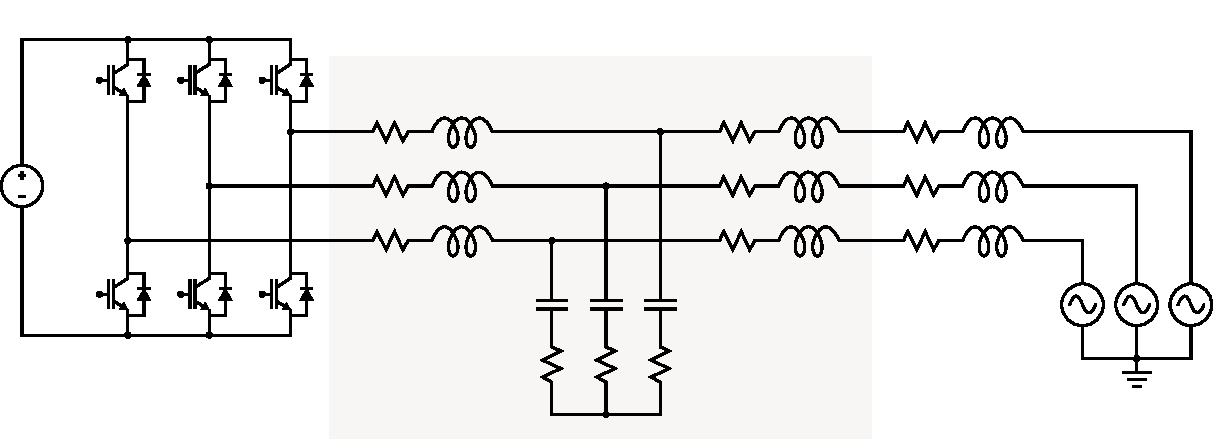
\includegraphics[width=0.9\textwidth]{img/topologia}}
      \def\svgwidth{0.9\textwidth}
      \input{./img/bancada.pdf_tex}}
    \renewcommand\figurename{Fig.}
    \caption{Diagrama que representa os elementos da bancada.}
    \label{fig:topologia_bancada}
  \end{figure}


\section{Resultados de Simulação}

	%figura mostrando o sistema
  %que tipo de conversor é, que marca, que modelo, dados nominais
  %que tipos de sensores foram usados? como foram feitas as medidas?
  %que tipo de controlador digital foi usado? modelo do dsp na dspace
  %quantos bits têm os conversores a/d?
  %como é acionado o conversor?
  %qual a frequência de amostragem? e a de comutação?
  %colocar numa tabela: tensão de linha, frequência, tensão do barramento cc, indutâncias e capacitância do filtro, frequência de amostragem e de comutação
  %comentar que os resultados obtidos foram para o equivalente monofásico
  %apresentar expressão do modelo de referência
  %apresentar expressões dos vetores w
  %apresentar os valores iniciais dos ganhos do controlador adaptativo (kp, gamma, rho, etc)
  %apresentar os valores de inicialização dos thetas
  %comentar sobre o sinal de normalização m^2

  O Simulink dispõe de muitos blocos cujos modelos matemáticos são geralmente aceitos como precisos o suficiente para representar elementos do mundo real. Por isso, os modelos da linha de transmissão, transformador e fonte são utilizados neste trabalho para representar o comportamento de elementos reais.

	A ação de controle é implementada na simulação via código escrito em linguagem própria do \textsc{Matlab}, chamada \textit{linguagem .m}. Existe um bloco no Simulink chamado \textit{Subsystem}, que recebe sinais de entrada e permite que esses sinais sejam manipulados via código para gerarem sinais de saída. Este bloco é utilizado para implementar a ação de controle projetada nos capítulos anteriores.

	Como a simulação é implementada em tempo discreto, os principais passos realizados são os seguintes:
  %
	\begin{enumerate}
		\item \textit{Inicialização}: no início da simulação, são carregados os valores iniciais para as variáveis;
		\item \textit{Amostragem das variáveis}: as variáveis são amostradas para a realização dos cálculos preliminares da ação de controle;
    \item \textit{Conversão de coordenadas $abc$ para $\alpha \beta 0$}: é aplicada a transformação de desacoplamento nas variáveis;
		\item \textit{Cálculo da ação de controle}: a ação de controle é calculada e o estado atual das variáveis é armazenado como sendo o estado anterior para a próxima iteração da simulação;
    \item \textit{Acionamento do conversor}: a ação de controle é modulada por largura de pulso e as chaves do conversor são acionadas.
	\end{enumerate}

  O projeto do controlador é conforme o Capítulo~\ref{controle}. O modelo de referência projetado é da forma
  %
  \begin{equation}
    W_m(z) = \frac{(1-p_1)(1-p_2)}{(z-p_1)(z-p_2)}\text{,}
    \label{eq:wm_simulacao}
  \end{equation}
  %
  com $p_1 = p_2 = 0,2$.

  \subsection{Resultados para corrente do capacitor como variável intermediária}

	A Tabela~\ref{tab:parametros_projeto} resume os parâmetros utilizados no projeto. Os valores de inicialização são baseadas nos valores ideais, ou seja, aqueles que fazem com que os valores dos ganhos adaptativos $\theta$ sejam $\theta^*$ (valores para a condição de casamento). Os valores de inicialização dos ganhos adaptativos, neste caso, são dados por \ref{eq:theta_sim}.
  %
  \begin{equation}
    \begin{split}
      \theta^T & = \left[ \begin{matrix} -0,03, & -0,36, & -0,57, & -0,01 & 0,16 & 0,02 \end{matrix} \right]\text{ e}\\
      \omega & = {\left[ \begin{matrix} 0 & 0 & 0 & 0 & 0 & 0 \end{matrix} \right]}^T\text{.}
    \end{split}
    \label{eq:theta_sim}
  \end{equation}

  \begin{table}[htb]
    \renewcommand{\arraystretch}{1.35}
    \setlength{\tabcolsep}{1.2mm}
    \caption{Valores dos parâmetros do sistema utilizados no projeto, com $i_C$ como variável intermediária.}
    \label{tab:parametros_projeto}
    \centering
    \begin{tabular}{l l l l}
      \hline
      \multicolumn{1}{c}{Parâmetro} & \multicolumn{1}{c}{Valor} &
      \multicolumn{1}{c}{Parâmetro} & \multicolumn{1}{c}{Valor} \\
      \hline
      $L_1$      & $2$mH    & $L_2$         & $2$mH   \\
      $C$        & $40\mu$F & $f_s = 1/T_s$ & $12$kHz \\
      $\gamma_d$ & $0,0098$ & $\gamma$      & $0,99$  \\
      $\delta_0$ & $0,8$    & $K_P$         & $8$     \\
      \hline
    \end{tabular}
  \end{table}

  As Fig.~\ref{fig:i2_sim_ini}-\ref{fig:thetas_sim_ini} apresentam o comportamento do sistema na inicialização. A Fig.~\ref{fig:i2_sim_ini} apresenta a comparação da corrente da rede $i_2$ com a referência ${i_2}^*$. A Fig.~\ref{fig:up_sim_ini} apresenta o comportamento da ação de controle $U$ durante a inicialização, e a Fig.~\ref{fig:thetas_sim_ini} demonstra o comportamento dos ganhos adaptativos $\theta$ na inicialização.

  %incluir figura mostrando a convergência dos thetas
  %incluir figura mostrando a parcela do vetor w referente a rejeição do distúrbio de tensão da rede

  \noindent
  \begin{minipage}{0.9\textwidth}
    \makebox[\textwidth]{
      \centering
      \def\svgwidth{\textwidth}
      % This file was created by matlab2tikz v0.4.7 running on MATLAB 7.14.
% Copyright (c) 2008--2014, Nico Schlömer <nico.schloemer@gmail.com>
% All rights reserved.
% Minimal pgfplots version: 1.3
% 
% The latest updates can be retrieved from
%   http://www.mathworks.com/matlabcentral/fileexchange/22022-matlab2tikz
% where you can also make suggestions and rate matlab2tikz.
% 
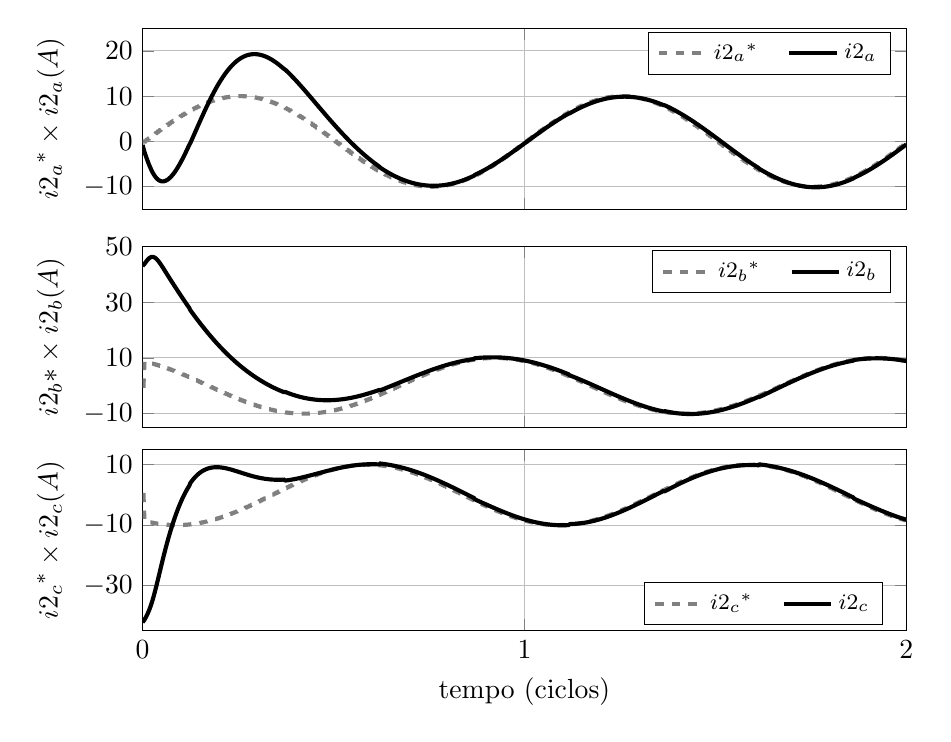
\begin{tikzpicture}

\begin{axis}[%
width=0.8\textwidth,
height=0.189701500343624\textwidth,
scale only axis,
xmin=0,
xmax=0.0333333333333333,
xtick={0,0.0166666666666667,0.0333333333333333},
xticklabels={\empty},
xmajorgrids,
ymin=-15,
ymax=50,
ytick={-10,  10,  30,  50},
ylabel={${\text{i2}_\text{b}}\text{* }\times\text{ i2}_\text{b}\text{ (A)}$},
ymajorgrids,
name=plot2,
legend style={draw=black,fill=white,legend cell align=left},
scaled x ticks = false,
legend columns=-1,
legend style={/tikz/every even column/.append style={column sep=0.3cm}},
legend style={font=\footnotesize}
]
\addplot [color=gray,dashed,line width=1.5pt]
  table[row sep=crcr]{0	0\\
4.16666666666667e-05	0\\
8.33333333333333e-05	8.66025403784439\\
0.000125	8.66025403784439\\
0.000166666666666667	8.49892692986864\\
0.000208333333333333	8.49892692986864\\
0.00025	8.329212407101\\
0.000291666666666667	8.329212407101\\
0.000333333333333333	8.15127795728554\\
0.000375	8.15127795728554\\
0.000416666666666667	7.96529918024197\\
0.000458333333333333	7.96529918024197\\
0.0005	7.77145961456971\\
0.000541666666666667	7.77145961456971\\
0.000583333333333333	7.56995055651757\\
0.000625	7.56995055651757\\
0.000666666666666667	7.36097087119735\\
0.000708333333333333	7.36097087119735\\
0.00075	7.14472679632804\\
0.000791666666666667	7.14472679632804\\
0.000833333333333333	6.92143173870407\\
0.000875	6.92143173870407\\
0.000916666666666667	6.69130606358858\\
0.000958333333333333	6.69130606358858\\
0.001	6.45457687723951\\
0.00104166666666667	6.45457687723951\\
0.00108333333333333	6.21147780278311\\
0.001125	6.21147780278311\\
0.00116666666666667	5.96224874965616\\
0.00120833333333333	5.96224874965616\\
0.00125	5.70713567684432\\
0.00129166666666667	5.70713567684432\\
0.00133333333333333	5.44639035015028\\
0.001375	5.44639035015028\\
0.00141666666666667	5.18027009373131\\
0.00145833333333333	5.18027009373131\\
0.0015	4.90903753615141\\
0.00154166666666667	4.90903753615141\\
0.00158333333333333	4.63296035119862\\
0.001625	4.63296035119862\\
0.00166666666666667	4.35231099372328\\
0.00170833333333333	4.35231099372328\\
0.00175	4.06736643075801\\
0.00179166666666667	4.06736643075801\\
0.00183333333333333	3.77840786818468\\
0.001875	3.77840786818468\\
0.00191666666666667	3.48572047321816\\
0.00195833333333333	3.48572047321816\\
0.002	3.18959309298071\\
0.00204166666666667	3.18959309298071\\
0.00208333333333333	2.89031796944472\\
0.002125	2.89031796944472\\
0.00216666666666667	2.58819045102521\\
0.00220833333333333	2.58819045102521\\
0.00225	2.28350870110656\\
0.00229166666666667	2.28350870110656\\
0.00233333333333333	1.97657340379127\\
0.002375	1.97657340379127\\
0.00241666666666667	1.66768746716103\\
0.00245833333333333	1.66768746716103\\
0.0025	1.35715572434305\\
0.00254166666666667	1.35715572434305\\
0.00258333333333333	1.04528463267654\\
0.002625	1.04528463267654\\
0.00266666666666667	0.732381971276321\\
0.00270833333333333	0.732381971276321\\
0.00275	0.418756537292\\
0.00279166666666667	0.418756537292\\
0.00283333333333333	0.104717841162462\\
0.002875	0.104717841162462\\
0.00291666666666667	-0.209424198833566\\
0.00295833333333333	-0.209424198833566\\
0.003	-0.523359562429436\\
0.00304166666666667	-0.523359562429436\\
0.00308333333333333	-0.836778433323153\\
0.003125	-0.836778433323153\\
0.00316666666666667	-1.14937150492867\\
0.00320833333333333	-1.14937150492867\\
0.00325	-1.46083028562412\\
0.00329166666666667	-1.46083028562412\\
0.00333333333333333	-1.77084740319583\\
0.003375	-1.77084740319583\\
0.00341666666666667	-2.07911690817759\\
0.00345833333333333	-2.07911690817759\\
0.0035	-2.38533457578581\\
0.00354166666666667	-2.38533457578581\\
0.00358333333333333	-2.68919820615266\\
0.003625	-2.68919820615266\\
0.00366666666666667	-2.99040792256087\\
0.00370833333333333	-2.99040792256087\\
0.00375	-3.28866646738584\\
0.00379166666666667	-3.28866646738584\\
0.00383333333333333	-3.58367949545301\\
0.003875	-3.58367949545301\\
0.00391666666666667	-3.87515586452103\\
0.00395833333333333	-3.87515586452103\\
0.004	-4.16280792260402\\
0.00404166666666667	-4.16280792260402\\
0.00408333333333333	-4.44635179184928\\
0.004125	-4.44635179184928\\
0.00416666666666667	-4.72550764869055\\
0.00420833333333333	-4.72550764869055\\
0.00425	-5.00000000000001\\
0.00429166666666667	-5.00000000000001\\
0.00433333333333333	-5.26955795496679\\
0.004375	-5.26955795496679\\
0.00441666666666667	-5.53391549243345\\
0.00445833333333333	-5.53391549243345\\
0.0045	-5.7928117234268\\
0.00454166666666667	-5.7928117234268\\
0.00458333333333333	-6.04599114862376\\
0.004625	-6.04599114862376\\
0.00466666666666667	-6.29320391049839\\
0.00470833333333333	-6.29320391049839\\
0.00475	-6.53420603990107\\
0.00479166666666667	-6.53420603990107\\
0.00483333333333333	-6.76875969682662\\
0.004875	-6.76875969682662\\
0.00491666666666667	-6.99663340513367\\
0.00495833333333333	-6.99663340513367\\
0.005	-7.21760228098364\\
0.00504166666666667	-7.21760228098364\\
0.00508333333333333	-7.43144825477396\\
0.005125	-7.43144825477396\\
0.00516666666666667	-7.63796028634644\\
0.00520833333333333	-7.63796028634644\\
0.00525	-7.83693457325842\\
0.00529166666666667	-7.83693457325842\\
0.00533333333333333	-8.02817475191117\\
0.005375	-8.02817475191117\\
0.00541666666666667	-8.21149209133706\\
0.00545833333333333	-8.21149209133706\\
0.0055	-8.38670567945426\\
0.00554166666666667	-8.38670567945426\\
0.00558333333333333	-8.55364260160509\\
0.005625	-8.55364260160509\\
0.00566666666666667	-8.71213811120192\\
0.00570833333333333	-8.71213811120192\\
0.00575	-8.86203579231217\\
0.00579166666666667	-8.86203579231217\\
0.00583333333333333	-9.00318771402196\\
0.005875	-9.00318771402196\\
0.00591666666666667	-9.13545457642604\\
0.00595833333333333	-9.13545457642604\\
0.006	-9.25870584809998\\
0.00604166666666667	-9.25870584809998\\
0.00608333333333333	-9.37281989491894\\
0.006125	-9.37281989491894\\
0.00616666666666667	-9.47768410009589\\
0.00620833333333333	-9.47768410009589\\
0.00625	-9.5731949753207\\
0.00629166666666667	-9.5731949753207\\
0.00633333333333333	-9.65925826289071\\
0.006375	-9.65925826289071\\
0.00641666666666667	-9.73578902873164\\
0.00645833333333333	-9.73578902873164\\
0.0065	-9.80271174621725\\
0.00654166666666667	-9.80271174621725\\
0.00658333333333333	-9.85996037070508\\
0.006625	-9.85996037070508\\
0.00666666666666667	-9.90747840471447\\
0.00670833333333333	-9.90747840471447\\
0.00675	-9.94521895368277\\
0.00679166666666667	-9.94521895368277\\
0.00683333333333333	-9.97314477224462\\
0.006875	-9.97314477224462\\
0.00691666666666667	-9.99122830098862\\
0.00695833333333333	-9.99122830098862\\
0.007	-9.99945169365516\\
0.00704166666666667	-9.99945169365516\\
0.00708333333333333	-9.99780683474849\\
0.007125	-9.99780683474849\\
0.00716666666666667	-9.98629534754578\\
0.00720833333333333	-9.98629534754578\\
0.00725	-9.96492859249508\\
0.00729166666666667	-9.96492859249508\\
0.00733333333333333	-9.93372765600401\\
0.007375	-9.93372765600401\\
0.00741666666666667	-9.89272332962993\\
0.00745833333333333	-9.89272332962993\\
0.0075	-9.84195607969246\\
0.00754166666666667	-9.84195607969246\\
0.00758333333333333	-9.7814760073381\\
0.007625	-9.7814760073381\\
0.00766666666666667	-9.7113427990964\\
0.00770833333333333	-9.7113427990964\\
0.00775	-9.63162566797663\\
0.00779166666666667	-9.63162566797663\\
0.00783333333333333	-9.54240328516281\\
0.007875	-9.54240328516281\\
0.00791666666666667	-9.44376370237485\\
0.00795833333333333	-9.44376370237485\\
0.008	-9.33580426497206\\
0.00804166666666667	-9.33580426497206\\
0.00808333333333333	-9.21863151588505\\
0.008125	-9.21863151588505\\
0.00816666666666667	-9.09236109047073\\
0.00820833333333333	-9.09236109047073\\
0.00825	-8.95711760239417\\
0.00829166666666667	-8.95711760239417\\
0.00833333333333333	-8.81303452064997\\
0.008375	-8.81303452064997\\
0.00841666666666667	-8.66025403784443\\
0.00845833333333333	-8.66025403784443\\
0.0085	-8.49892692986868\\
0.00854166666666667	-8.49892692986868\\
0.00858333333333333	-8.32921240710104\\
0.008625	-8.32921240710104\\
0.00866666666666667	-8.15127795728559\\
0.00870833333333333	-8.15127795728559\\
0.00875	-7.965299180242\\
0.00879166666666667	-7.965299180242\\
0.00883333333333333	-7.77145961456975\\
0.008875	-7.77145961456975\\
0.00891666666666667	-7.56995055651761\\
0.00895833333333333	-7.56995055651761\\
0.009	-7.36097087119738\\
0.00904166666666667	-7.36097087119738\\
0.00908333333333333	-7.14472679632807\\
0.009125	-7.14472679632807\\
0.00916666666666667	-6.92143173870411\\
0.00920833333333333	-6.92143173870411\\
0.00925	-6.69130606358862\\
0.00929166666666667	-6.69130606358862\\
0.00933333333333333	-6.45457687723954\\
0.009375	-6.45457687723954\\
0.00941666666666667	-6.21147780278314\\
0.00945833333333333	-6.21147780278314\\
0.0095	-5.96224874965619\\
0.00954166666666667	-5.96224874965619\\
0.00958333333333333	-5.70713567684435\\
0.009625	-5.70713567684435\\
0.00966666666666667	-5.4463903501503\\
0.00970833333333333	-5.4463903501503\\
0.00975	-5.18027009373134\\
0.00979166666666667	-5.18027009373134\\
0.00983333333333333	-4.90903753615144\\
0.009875	-4.90903753615144\\
0.00991666666666667	-4.63296035119865\\
0.00995833333333333	-4.63296035119865\\
0.01	-4.35231099372331\\
0.0100416666666667	-4.35231099372331\\
0.0100833333333333	-4.06736643075803\\
0.010125	-4.06736643075803\\
0.0101666666666667	-3.7784078681847\\
0.0102083333333333	-3.7784078681847\\
0.01025	-3.48572047321818\\
0.0102916666666667	-3.48572047321818\\
0.0103333333333333	-3.18959309298072\\
0.010375	-3.18959309298072\\
0.0104166666666667	-2.89031796944474\\
0.0104583333333333	-2.89031796944474\\
0.0105	-2.58819045102523\\
0.0105416666666667	-2.58819045102523\\
0.0105833333333333	-2.28350870110658\\
0.010625	-2.28350870110658\\
0.0106666666666667	-1.97657340379128\\
0.0107083333333333	-1.97657340379128\\
0.01075	-1.66768746716104\\
0.0107916666666667	-1.66768746716104\\
0.0108333333333333	-1.35715572434306\\
0.010875	-1.35715572434306\\
0.0109166666666667	-1.04528463267655\\
0.0109583333333333	-1.04528463267655\\
0.011	-0.732381971276329\\
0.0110416666666667	-0.732381971276329\\
0.0110833333333333	-0.418756537292006\\
0.011125	-0.418756537292006\\
0.0111666666666667	-0.104717841162466\\
0.0112083333333333	-0.104717841162466\\
0.01125	0.209424198833563\\
0.0112916666666667	0.209424198833563\\
0.0113333333333333	0.523359562429434\\
0.011375	0.523359562429434\\
0.0114166666666667	0.836778433323152\\
0.0114583333333333	0.836778433323152\\
0.0115	1.14937150492867\\
0.0115416666666667	1.14937150492867\\
0.0115833333333333	1.46083028562412\\
0.011625	1.46083028562412\\
0.0116666666666667	1.77084740319584\\
0.0117083333333333	1.77084740319584\\
0.01175	2.0791169081776\\
0.0117916666666667	2.0791169081776\\
0.0118333333333333	2.38533457578582\\
0.011875	2.38533457578582\\
0.0119166666666667	2.68919820615266\\
0.0119583333333333	2.68919820615266\\
0.012	2.99040792256088\\
0.0120416666666667	2.99040792256088\\
0.0120833333333333	3.28866646738584\\
0.012125	3.28866646738584\\
0.0121666666666667	3.58367949545302\\
0.0122083333333333	3.58367949545302\\
0.01225	3.87515586452105\\
0.0122916666666667	3.87515586452105\\
0.0123333333333333	4.16280792260403\\
0.012375	4.16280792260403\\
0.0124166666666667	4.4463517918493\\
0.0124583333333333	4.4463517918493\\
0.0125	4.72550764869056\\
0.0125416666666667	4.72550764869056\\
0.0125833333333333	5.00000000000002\\
0.012625	5.00000000000002\\
0.0126666666666667	5.2695579549668\\
0.0127083333333333	5.2695579549668\\
0.01275	5.53391549243347\\
0.0127916666666667	5.53391549243347\\
0.0128333333333333	5.79281172342682\\
0.012875	5.79281172342682\\
0.0129166666666667	6.04599114862378\\
0.0129583333333333	6.04599114862378\\
0.013	6.29320391049841\\
0.0130416666666667	6.29320391049841\\
0.0130833333333333	6.53420603990109\\
0.013125	6.53420603990109\\
0.0131666666666667	6.76875969682665\\
0.0132083333333333	6.76875969682665\\
0.01325	6.99663340513369\\
0.0132916666666667	6.99663340513369\\
0.0133333333333333	7.21760228098367\\
0.013375	7.21760228098367\\
0.0134166666666667	7.43144825477399\\
0.0134583333333333	7.43144825477399\\
0.0135	7.63796028634647\\
0.0135416666666667	7.63796028634647\\
0.0135833333333333	7.83693457325845\\
0.013625	7.83693457325845\\
0.0136666666666667	8.02817475191119\\
0.0137083333333333	8.02817475191119\\
0.01375	8.21149209133709\\
0.0137916666666667	8.21149209133709\\
0.0138333333333333	8.38670567945429\\
0.013875	8.38670567945429\\
0.0139166666666667	8.55364260160512\\
0.0139583333333333	8.55364260160512\\
0.014	8.71213811120195\\
0.0140416666666667	8.71213811120195\\
0.0140833333333333	8.86203579231221\\
0.014125	8.86203579231221\\
0.0141666666666667	9.003187714022\\
0.0142083333333333	9.003187714022\\
0.01425	9.13545457642607\\
0.0142916666666667	9.13545457642607\\
0.0143333333333333	9.25870584810001\\
0.014375	9.25870584810001\\
0.0144166666666667	9.37281989491898\\
0.0144583333333333	9.37281989491898\\
0.0145	9.47768410009592\\
0.0145416666666667	9.47768410009592\\
0.0145833333333333	9.57319497532074\\
0.014625	9.57319497532074\\
0.0146666666666667	9.65925826289075\\
0.0147083333333333	9.65925826289075\\
0.01475	9.73578902873167\\
0.0147916666666667	9.73578902873167\\
0.0148333333333333	9.80271174621729\\
0.014875	9.80271174621729\\
0.0149166666666667	9.85996037070512\\
0.0149583333333333	9.85996037070512\\
0.015	9.90747840471451\\
0.0150416666666667	9.90747840471451\\
0.0150833333333333	9.94521895368281\\
0.015125	9.94521895368281\\
0.0151666666666667	9.97314477224466\\
0.0152083333333333	9.97314477224466\\
0.01525	9.99122830098866\\
0.0152916666666667	9.99122830098866\\
0.0153333333333333	9.9994516936552\\
0.015375	9.9994516936552\\
0.0154166666666667	9.99780683474853\\
0.0154583333333333	9.99780683474853\\
0.0155	9.98629534754582\\
0.0155416666666667	9.98629534754582\\
0.0155833333333333	9.96492859249513\\
0.015625	9.96492859249513\\
0.0156666666666667	9.93372765600405\\
0.0157083333333333	9.93372765600405\\
0.01575	9.89272332962997\\
0.0157916666666667	9.89272332962997\\
0.0158333333333333	9.8419560796925\\
0.015875	9.8419560796925\\
0.0159166666666667	9.78147600733814\\
0.0159583333333333	9.78147600733814\\
0.016	9.71134279909644\\
0.0160416666666667	9.71134279909644\\
0.0160833333333333	9.63162566797667\\
0.016125	9.63162566797667\\
0.0161666666666667	9.54240328516285\\
0.0162083333333333	9.54240328516285\\
0.01625	9.44376370237489\\
0.0162916666666667	9.44376370237489\\
0.0163333333333333	9.3358042649721\\
0.016375	9.3358042649721\\
0.0164166666666667	9.21863151588509\\
0.0164583333333333	9.21863151588509\\
0.0165	9.09236109047077\\
0.0165416666666667	9.09236109047077\\
0.0165833333333333	8.95711760239421\\
0.016625	8.95711760239421\\
0.0166666666666667	8.81303452065\\
0.0167083333333333	8.81303452065\\
0.01675	8.66025403784447\\
0.0167916666666667	8.66025403784447\\
0.0168333333333333	8.49892692986872\\
0.016875	8.49892692986872\\
0.0169166666666667	8.32921240710107\\
0.0169583333333333	8.32921240710107\\
0.017	8.15127795728562\\
0.0170416666666667	8.15127795728562\\
0.0170833333333333	7.96529918024204\\
0.017125	7.96529918024204\\
0.0171666666666667	7.77145961456979\\
0.0172083333333333	7.77145961456979\\
0.01725	7.56995055651764\\
0.0172916666666667	7.56995055651764\\
0.0173333333333333	7.36097087119742\\
0.017375	7.36097087119742\\
0.0174166666666667	7.1447267963281\\
0.0174583333333333	7.1447267963281\\
0.0175	6.92143173870414\\
0.0175416666666667	6.92143173870414\\
0.0175833333333333	6.69130606358865\\
0.017625	6.69130606358865\\
0.0176666666666667	6.45457687723957\\
0.0177083333333333	6.45457687723957\\
0.01775	6.21147780278317\\
0.0177916666666667	6.21147780278317\\
0.0178333333333333	5.96224874965622\\
0.017875	5.96224874965622\\
0.0179166666666667	5.70713567684438\\
0.0179583333333333	5.70713567684438\\
0.018	5.44639035015033\\
0.0180416666666667	5.44639035015033\\
0.0180833333333333	5.18027009373136\\
0.018125	5.18027009373136\\
0.0181666666666667	4.90903753615147\\
0.0182083333333333	4.90903753615147\\
0.01825	4.63296035119867\\
0.0182916666666667	4.63296035119867\\
0.0183333333333333	4.35231099372333\\
0.018375	4.35231099372333\\
0.0184166666666667	4.06736643075805\\
0.0184583333333333	4.06736643075805\\
0.0185	3.77840786818472\\
0.0185416666666667	3.77840786818472\\
0.0185833333333333	3.4857204732182\\
0.018625	3.4857204732182\\
0.0186666666666667	3.18959309298074\\
0.0187083333333333	3.18959309298074\\
0.01875	2.89031796944476\\
0.0187916666666667	2.89031796944476\\
0.0188333333333333	2.58819045102524\\
0.018875	2.58819045102524\\
0.0189166666666667	2.28350870110659\\
0.0189583333333333	2.28350870110659\\
0.019	1.97657340379129\\
0.0190416666666667	1.97657340379129\\
0.0190833333333333	1.66768746716105\\
0.019125	1.66768746716105\\
0.0191666666666667	1.35715572434307\\
0.0192083333333333	1.35715572434307\\
0.01925	1.04528463267656\\
0.0192916666666667	1.04528463267656\\
0.0193333333333333	0.732381971276336\\
0.019375	0.732381971276336\\
0.0194166666666667	0.418756537292012\\
0.0194583333333333	0.418756537292012\\
0.0195	0.104717841162471\\
0.0195416666666667	0.104717841162471\\
0.0195833333333333	-0.20942419883356\\
0.019625	-0.20942419883356\\
0.0196666666666667	-0.523359562429432\\
0.0197083333333333	-0.523359562429432\\
0.01975	-0.836778433323152\\
0.0197916666666667	-0.836778433323152\\
0.0198333333333333	-1.14937150492867\\
0.019875	-1.14937150492867\\
0.0199166666666667	-1.46083028562412\\
0.0199583333333333	-1.46083028562412\\
0.02	-1.77084740319584\\
0.0200416666666667	-1.77084740319584\\
0.0200833333333333	-2.0791169081776\\
0.020125	-2.0791169081776\\
0.0201666666666667	-2.38533457578582\\
0.0202083333333333	-2.38533457578582\\
0.02025	-2.68919820615267\\
0.0202916666666667	-2.68919820615267\\
0.0203333333333333	-2.99040792256089\\
0.020375	-2.99040792256089\\
0.0204166666666667	-3.28866646738586\\
0.0204583333333333	-3.28866646738586\\
0.0205	-3.58367949545303\\
0.0205416666666667	-3.58367949545303\\
0.0205833333333333	-3.87515586452106\\
0.020625	-3.87515586452106\\
0.0206666666666667	-4.16280792260405\\
0.0207083333333333	-4.16280792260405\\
0.02075	-4.44635179184931\\
0.0207916666666667	-4.44635179184931\\
0.0208333333333333	-4.72550764869058\\
0.020875	-4.72550764869058\\
0.0209166666666667	-5.00000000000005\\
0.0209583333333333	-5.00000000000005\\
0.021	-5.26955795496682\\
0.0210416666666667	-5.26955795496682\\
0.0210833333333333	-5.53391549243349\\
0.021125	-5.53391549243349\\
0.0211666666666667	-5.79281172342684\\
0.0212083333333333	-5.79281172342684\\
0.02125	-6.0459911486238\\
0.0212916666666667	-6.0459911486238\\
0.0213333333333333	-6.29320391049844\\
0.021375	-6.29320391049844\\
0.0214166666666667	-6.53420603990112\\
0.0214583333333333	-6.53420603990112\\
0.0215	-6.76875969682667\\
0.0215416666666667	-6.76875969682667\\
0.0215833333333333	-6.99663340513372\\
0.021625	-6.99663340513372\\
0.0216666666666667	-7.2176022809837\\
0.0217083333333333	-7.2176022809837\\
0.02175	-7.43144825477402\\
0.0217916666666667	-7.43144825477402\\
0.0218333333333333	-7.6379602863465\\
0.021875	-7.6379602863465\\
0.0219166666666667	-7.83693457325848\\
0.0219583333333333	-7.83693457325848\\
0.022	-8.02817475191123\\
0.0220416666666667	-8.02817475191123\\
0.0220833333333333	-8.21149209133713\\
0.022125	-8.21149209133713\\
0.0221666666666667	-8.38670567945433\\
0.0222083333333333	-8.38670567945433\\
0.02225	-8.55364260160516\\
0.0222916666666667	-8.55364260160516\\
0.0223333333333333	-8.71213811120199\\
0.022375	-8.71213811120199\\
0.0224166666666667	-8.86203579231225\\
0.0224583333333333	-8.86203579231225\\
0.0225	-9.00318771402204\\
0.0225416666666667	-9.00318771402204\\
0.0225833333333333	-9.13545457642611\\
0.022625	-9.13545457642611\\
0.0226666666666667	-9.25870584810006\\
0.0227083333333333	-9.25870584810006\\
0.02275	-9.37281989491902\\
0.0227916666666667	-9.37281989491902\\
0.0228333333333333	-9.47768410009597\\
0.022875	-9.47768410009597\\
0.0229166666666667	-9.57319497532079\\
0.0229583333333333	-9.57319497532079\\
0.023	-9.6592582628908\\
0.0230416666666667	-9.6592582628908\\
0.0230833333333333	-9.73578902873172\\
0.023125	-9.73578902873172\\
0.0231666666666667	-9.80271174621734\\
0.0232083333333333	-9.80271174621734\\
0.02325	-9.85996037070517\\
0.0232916666666667	-9.85996037070517\\
0.0233333333333333	-9.90747840471456\\
0.023375	-9.90747840471456\\
0.0234166666666667	-9.94521895368285\\
0.0234583333333333	-9.94521895368285\\
0.0235	-9.97314477224471\\
0.0235416666666667	-9.97314477224471\\
0.0235833333333333	-9.99122830098871\\
0.023625	-9.99122830098871\\
0.0236666666666667	-9.99945169365525\\
0.0237083333333333	-9.99945169365525\\
0.02375	-9.99780683474858\\
0.0237916666666667	-9.99780683474858\\
0.0238333333333333	-9.98629534754587\\
0.023875	-9.98629534754587\\
0.0239166666666667	-9.96492859249517\\
0.0239583333333333	-9.96492859249517\\
0.024	-9.93372765600409\\
0.0240416666666667	-9.93372765600409\\
0.0240833333333333	-9.89272332963001\\
0.024125	-9.89272332963001\\
0.0241666666666667	-9.84195607969255\\
0.0242083333333333	-9.84195607969255\\
0.02425	-9.78147600733818\\
0.0242916666666667	-9.78147600733818\\
0.0243333333333333	-9.71134279909649\\
0.024375	-9.71134279909649\\
0.0244166666666667	-9.63162566797671\\
0.0244583333333333	-9.63162566797671\\
0.0245	-9.5424032851629\\
0.0245416666666667	-9.5424032851629\\
0.0245833333333333	-9.44376370237494\\
0.024625	-9.44376370237494\\
0.0246666666666667	-9.33580426497215\\
0.0247083333333333	-9.33580426497215\\
0.02475	-9.21863151588513\\
0.0247916666666667	-9.21863151588513\\
0.0248333333333333	-9.09236109047081\\
0.024875	-9.09236109047081\\
0.0249166666666667	-8.95711760239425\\
0.0249583333333333	-8.95711760239425\\
0.025	-8.81303452065005\\
0.0250416666666667	-8.81303452065005\\
0.0250833333333333	-8.66025403784451\\
0.025125	-8.66025403784451\\
0.0251666666666667	-8.49892692986876\\
0.0252083333333333	-8.49892692986876\\
0.02525	-8.32921240710111\\
0.0252916666666667	-8.32921240710111\\
0.0253333333333333	-8.15127795728566\\
0.025375	-8.15127795728566\\
0.0254166666666667	-7.96529918024207\\
0.0254583333333333	-7.96529918024207\\
0.0255	-7.77145961456982\\
0.0255416666666667	-7.77145961456982\\
0.0255833333333333	-7.56995055651767\\
0.025625	-7.56995055651767\\
0.0256666666666667	-7.36097087119745\\
0.0257083333333333	-7.36097087119745\\
0.02575	-7.14472679632814\\
0.0257916666666667	-7.14472679632814\\
0.0258333333333333	-6.92143173870417\\
0.025875	-6.92143173870417\\
0.0259166666666667	-6.69130606358868\\
0.0259583333333333	-6.69130606358868\\
0.026	-6.4545768772396\\
0.0260416666666667	-6.4545768772396\\
0.0260833333333333	-6.2114778027832\\
0.026125	-6.2114778027832\\
0.0261666666666667	-5.96224874965625\\
0.0262083333333333	-5.96224874965625\\
0.02625	-5.70713567684441\\
0.0262916666666667	-5.70713567684441\\
0.0263333333333333	-5.44639035015036\\
0.026375	-5.44639035015036\\
0.0264166666666667	-5.18027009373139\\
0.0264583333333333	-5.18027009373139\\
0.0265	-4.90903753615149\\
0.0265416666666667	-4.90903753615149\\
0.0265833333333333	-4.6329603511987\\
0.026625	-4.6329603511987\\
0.0266666666666667	-4.35231099372335\\
0.0267083333333333	-4.35231099372335\\
0.02675	-4.06736643075807\\
0.0267916666666667	-4.06736643075807\\
0.0268333333333333	-3.77840786818474\\
0.026875	-3.77840786818474\\
0.0269166666666667	-3.48572047321821\\
0.0269583333333333	-3.48572047321821\\
0.027	-3.18959309298076\\
0.0270416666666667	-3.18959309298076\\
0.0270833333333333	-2.89031796944477\\
0.027125	-2.89031796944477\\
0.0271666666666667	-2.58819045102526\\
0.0272083333333333	-2.58819045102526\\
0.02725	-2.28350870110661\\
0.0272916666666667	-2.28350870110661\\
0.0273333333333333	-1.9765734037913\\
0.027375	-1.9765734037913\\
0.0274166666666667	-1.66768746716106\\
0.0274583333333333	-1.66768746716106\\
0.0275	-1.35715572434308\\
0.0275416666666667	-1.35715572434308\\
0.0275833333333333	-1.04528463267656\\
0.027625	-1.04528463267656\\
0.0276666666666667	-0.732381971276341\\
0.0277083333333333	-0.732381971276341\\
0.02775	-0.418756537292015\\
0.0277916666666667	-0.418756537292015\\
0.0278333333333333	-0.104717841162473\\
0.027875	-0.104717841162473\\
0.0279166666666667	0.209424198833559\\
0.0279583333333333	0.209424198833559\\
0.028	0.523359562429433\\
0.0280416666666667	0.523359562429433\\
0.0280833333333333	0.836778433323154\\
0.028125	0.836778433323154\\
0.0281666666666667	1.14937150492867\\
0.0282083333333333	1.14937150492867\\
0.02825	1.46083028562412\\
0.0282916666666667	1.46083028562412\\
0.0283333333333333	1.77084740319585\\
0.028375	1.77084740319585\\
0.0284166666666667	2.07911690817761\\
0.0284583333333333	2.07911690817761\\
0.0285	2.38533457578583\\
0.0285416666666667	2.38533457578583\\
0.0285833333333333	2.68919820615268\\
0.028625	2.68919820615268\\
0.0286666666666667	2.9904079225609\\
0.0287083333333333	2.9904079225609\\
0.02875	3.28866646738587\\
0.0287916666666667	3.28866646738587\\
0.0288333333333333	3.58367949545304\\
0.028875	3.58367949545304\\
0.0289166666666667	3.87515586452107\\
0.0289583333333333	3.87515586452107\\
0.029	4.16280792260406\\
0.0290416666666667	4.16280792260406\\
0.0290833333333333	4.44635179184933\\
0.029125	4.44635179184933\\
0.0291666666666667	4.7255076486906\\
0.0292083333333333	4.7255076486906\\
0.02925	5.00000000000006\\
0.0292916666666667	5.00000000000006\\
0.0293333333333333	5.26955795496684\\
0.029375	5.26955795496684\\
0.0294166666666667	5.53391549243351\\
0.0294583333333333	5.53391549243351\\
0.0295	5.79281172342686\\
0.0295416666666667	5.79281172342686\\
0.0295833333333333	6.04599114862383\\
0.029625	6.04599114862383\\
0.0296666666666667	6.29320391049846\\
0.0297083333333333	6.29320391049846\\
0.02975	6.53420603990114\\
0.0297916666666667	6.53420603990114\\
0.0298333333333333	6.7687596968267\\
0.029875	6.7687596968267\\
0.0299166666666667	6.99663340513375\\
0.0299583333333333	6.99663340513375\\
0.03	7.21760228098372\\
0.0300416666666667	7.21760228098372\\
0.0300833333333333	7.43144825477405\\
0.030125	7.43144825477405\\
0.0301666666666667	7.63796028634653\\
0.0302083333333333	7.63796028634653\\
0.03025	7.83693457325851\\
0.0302916666666667	7.83693457325851\\
0.0303333333333333	8.02817475191126\\
0.030375	8.02817475191126\\
0.0304166666666667	8.21149209133716\\
0.0304583333333333	8.21149209133716\\
0.0305	8.38670567945436\\
0.0305416666666667	8.38670567945436\\
0.0305833333333333	8.55364260160519\\
0.030625	8.55364260160519\\
0.0306666666666667	8.71213811120203\\
0.0307083333333333	8.71213811120203\\
0.03075	8.86203579231228\\
0.0307916666666667	8.86203579231228\\
0.0308333333333333	9.00318771402207\\
0.030875	9.00318771402207\\
0.0309166666666667	9.13545457642615\\
0.0309583333333333	9.13545457642615\\
0.031	9.25870584810009\\
0.0310416666666667	9.25870584810009\\
0.0310833333333333	9.37281989491906\\
0.031125	9.37281989491906\\
0.0311666666666667	9.477684100096\\
0.0312083333333333	9.477684100096\\
0.03125	9.57319497532082\\
0.0312916666666667	9.57319497532082\\
0.0313333333333333	9.65925826289084\\
0.031375	9.65925826289084\\
0.0314166666666667	9.73578902873176\\
0.0314583333333333	9.73578902873176\\
0.0315	9.80271174621738\\
0.0315416666666667	9.80271174621738\\
0.0315833333333333	9.85996037070521\\
0.031625	9.85996037070521\\
0.0316666666666667	9.9074784047146\\
0.0317083333333333	9.9074784047146\\
0.03175	9.94521895368289\\
0.0317916666666667	9.94521895368289\\
0.0318333333333333	9.97314477224474\\
0.031875	9.97314477224474\\
0.0319166666666667	9.99122830098875\\
0.0319583333333333	9.99122830098875\\
0.032	9.99945169365528\\
0.0320416666666667	9.99945169365528\\
0.0320833333333333	9.99780683474862\\
0.032125	9.99780683474862\\
0.0321666666666667	9.98629534754591\\
0.0322083333333333	9.98629534754591\\
0.03225	9.96492859249521\\
0.0322916666666667	9.96492859249521\\
0.0323333333333333	9.93372765600413\\
0.032375	9.93372765600413\\
0.0324166666666667	9.89272332963005\\
0.0324583333333333	9.89272332963005\\
0.0325	9.84195607969259\\
0.0325416666666667	9.84195607969259\\
0.0325833333333333	9.78147600733822\\
0.032625	9.78147600733822\\
0.0326666666666667	9.71134279909653\\
0.0327083333333333	9.71134279909653\\
0.03275	9.63162566797675\\
0.0327916666666667	9.63162566797675\\
0.0328333333333333	9.54240328516294\\
0.032875	9.54240328516294\\
0.0329166666666667	9.44376370237498\\
0.0329583333333333	9.44376370237498\\
0.033	9.33580426497218\\
0.0330416666666667	9.33580426497218\\
0.0330833333333333	9.21863151588517\\
0.033125	9.21863151588517\\
0.0331666666666667	9.09236109047085\\
0.0332083333333333	9.09236109047085\\
0.03325	8.95711760239429\\
0.0332916666666667	8.95711760239429\\
0.0333333333333333	8.81303452065008\\
};
\addlegendentry{${\text{i2}_\text{b}}^\text{*}$};

\addplot [color=black,solid,line width=1.5pt]
  table[row sep=crcr]{0	42.97660421501\\
4.16666666666667e-05	43.3593393870968\\
8.33333333333333e-05	43.7191880113411\\
0.000125	44.2050613899279\\
0.000166666666666667	44.6603456269382\\
0.000208333333333333	45.1018552556462\\
0.00025	45.48220841885\\
0.000291666666666667	45.8113981893254\\
0.000333333333333333	46.0508290702559\\
0.000375	46.2155916866694\\
0.000416666666666667	46.2794096603762\\
0.000458333333333333	46.2638806240286\\
0.0005	46.151102640534\\
0.000541666666666667	45.9672904475899\\
0.000583333333333333	45.7004204890381\\
0.000625	45.3784996924376\\
0.000666666666666667	44.9925737085849\\
0.000708333333333333	44.569792657511\\
0.00075	44.1021229439723\\
0.000791666666666667	43.6140575421866\\
0.000833333333333333	43.0972531042803\\
0.000875	42.5727018637345\\
0.000916666666666667	42.0313491398431\\
0.000958333333333333	41.490604512486\\
0.001	40.9408606766391\\
0.00104166666666667	40.3963231914932\\
0.00108333333333333	39.847267627143\\
0.001125	39.3052673895989\\
0.00116666666666667	38.7609604462391\\
0.00120833333333333	38.223851996809\\
0.00125	37.6853493581397\\
0.00129166666666667	37.1533454635223\\
0.00133333333333333	36.6202871491275\\
0.001375	36.0927730404365\\
0.00141666666666667	35.5644250721109\\
0.00145833333333333	35.0407402121898\\
0.0015	34.5165453424891\\
0.00154166666666667	33.9963369942111\\
0.00158333333333333	33.4761083185055\\
0.001625	32.9594021528808\\
0.00166666666666667	32.4433041643775\\
0.00170833333333333	31.930426082963\\
0.00175	31.4188614749057\\
0.00179166666666667	30.9103095974188\\
0.00183333333333333	30.4037906684295\\
0.001875	29.9001167441415\\
0.00191666666666667	29.3991629296628\\
0.00195833333333333	28.9008893757573\\
0.002	28.4059645531346\\
0.00204166666666667	27.9135410549802\\
0.00208333333333333	27.1721535020907\\
0.002125	26.6874505908316\\
0.00216666666666667	26.2190588726424\\
0.00220833333333333	25.7486586212972\\
0.00225	25.2853868986719\\
0.00229166666666667	24.8230429289484\\
0.00233333333333333	24.3666319292948\\
0.002375	23.9112946756842\\
0.00241666666666667	23.4618362846351\\
0.00245833333333333	23.013304313649\\
0.0025	22.5707908845547\\
0.00254166666666667	22.1290599227619\\
0.00258333333333333	21.6935327273799\\
0.002625	21.2586693811889\\
0.00266666666666667	20.8302050849802\\
0.00270833333333333	20.4023045251397\\
0.00275	19.9809941762427\\
0.00279166666666667	19.5601600656416\\
0.00283333333333333	19.1460961574073\\
0.002875	18.7324306257852\\
0.00291666666666667	18.3257006249585\\
0.00295833333333333	17.9192996196269\\
0.003	17.5199832279738\\
0.00304166666666667	17.1209346176351\\
0.00308333333333333	16.7291028297554\\
0.003125	16.3374695704814\\
0.00316666666666667	15.9531836896215\\
0.00320833333333333	15.5690705398771\\
0.00325	15.1923861917557\\
0.00329166666666667	14.8158333649373\\
0.00333333333333333	14.4467915071034\\
0.003375	14.0778495809671\\
0.00341666666666667	13.716482665951\\
0.00345833333333333	13.3551909497519\\
0.0035	13.0015211738397\\
0.00354166666666667	12.6479078035316\\
0.00358333333333333	12.3019466802048\\
0.003625	11.9560285381684\\
0.00366666666666667	11.6177769520913\\
0.00370833333333333	11.2795599226045\\
0.00375	10.9490085867896\\
0.00379166666666667	10.6184881556411\\
0.00383333333333333	10.2956183498002\\
0.003875	9.97278041548817\\
0.00391666666666667	9.65756485851209\\
0.00395833333333333	9.34238662156467\\
0.004	9.0347903657762\\
0.00404166666666667	8.72724120879229\\
0.00408333333333333	8.4272224949194\\
0.004125	8.12726481447167\\
0.00416666666666667	7.83521349471893\\
0.00420833333333333	7.54285122194898\\
0.00425	7.2578778410272\\
0.00429166666666667	6.97299745656387\\
0.00433333333333333	6.69542553982568\\
0.004375	6.41795837374215\\
0.00441666666666667	6.14769031764613\\
0.00445833333333333	5.87752475840982\\
0.0045	5.61442748637277\\
0.00454166666666667	5.35142369057221\\
0.00458333333333333	5.09534751453348\\
0.004625	4.83935958306598\\
0.00466666666666667	4.59015883100606\\
0.00470833333333333	4.34105278963748\\
0.00475	4.09860077797683\\
0.00479166666666667	3.856265899529\\
0.00483333333333333	3.62046245805827\\
0.004875	3.38481516617511\\
0.00491666666666667	3.1555873045018\\
0.00495833333333333	2.92656922197552\\
0.005	2.70386715643331\\
0.00504166666666667	2.48143980141189\\
0.00508333333333333	2.26523086239634\\
0.005125	2.04936931827668\\
0.00516666666666667	1.83961982461587\\
0.00520833333333333	1.63030571848737\\
0.00525	1.42702501642018\\
0.00529166666666667	1.22424956824442\\
0.00533333333333333	1.02741095419923\\
0.005375	0.831157094296876\\
0.00541666666666667	0.640746166069908\\
0.00545833333333333	0.451000117603453\\
0.0055	0.267001897267162\\
0.00554166666666667	0.0837482748918468\\
0.00558333333333333	-0.0938533553032118\\
0.005625	-0.270631325141599\\
0.00566666666666667	-0.44185344673035\\
0.00570833333333333	-0.612173582946894\\
0.00575	-0.777033912205997\\
0.00579166666666667	-0.940914733034167\\
0.00583333333333333	-1.09943133610484\\
0.005875	-1.25689180994576\\
0.00591666666666667	-1.40908293556548\\
0.00595833333333333	-1.56014235953009\\
0.006	-1.70602639437458\\
0.00604166666666667	-1.85070438489002\\
0.00608333333333333	-1.99029990367325\\
0.006125	-2.12861646454675\\
0.00616666666666667	-2.26194233844912\\
0.00620833333333333	-2.20923139686129\\
0.00625	-2.27860510709366\\
0.00629166666666667	-2.41329093356354\\
0.00633333333333333	-2.54464366908719\\
0.006375	-2.67441933326171\\
0.00641666666666667	-2.79983539784871\\
0.00645833333333333	-2.92363519317878\\
0.0065	-3.04275539668388\\
0.00654166666666667	-3.16008953549472\\
0.00658333333333333	-3.2726492674008\\
0.006625	-3.38330678317177\\
0.00666666666666667	-3.48919153680253\\
0.00670833333333333	-3.59310194867614\\
0.00675	-3.69229057044476\\
0.00679166666666667	-3.78945505544658\\
0.00683333333333333	-3.88197225878291\\
0.006875	-3.97242358895808\\
0.00691666666666667	-4.05831134839286\\
0.00695833333333333	-4.14209270116268\\
0.007	-4.22139642202969\\
0.00704166666666667	-4.2985524687337\\
0.00708333333333333	-4.37131650025082\\
0.007125	-4.44189154132362\\
0.00716666666666667	-4.50815956503903\\
0.00720833333333333	-4.57219887726138\\
0.00725	-4.63198231243181\\
0.00729166666666667	-4.68953612892923\\
0.00733333333333333	-4.74295428943355\\
0.007375	-4.79407434197722\\
0.00741666666666667	-4.84114463669445\\
0.00745833333333333	-4.88588912615331\\
0.0075	-4.92667054545241\\
0.00754166666666667	-4.96510403288028\\
0.00758333333333333	-4.99966127039949\\
0.007625	-5.03185340490003\\
0.00766666666666667	-5.06025593527341\\
0.00770833333333333	-5.08628070304258\\
0.00775	-5.10860192817284\\
0.00779166666666667	-5.12853684096654\\
0.00783333333333333	-5.14485335472836\\
0.007875	-5.15877878826393\\
0.00791666666666667	-5.16916983551766\\
0.00795833333333333	-5.17716858047698\\
0.008	-5.18171572640177\\
0.00804166666666667	-5.18387274136199\\
0.00808333333333333	-5.18265971879489\\
0.008125	-5.17906203884096\\
0.00816666666666667	-5.17217472090407\\
0.00820833333333333	-5.16291146679947\\
0.00825	-5.15043791237798\\
0.00829166666666667	-5.13598097368233\\
0.00833333333333333	-5.11806890039805\\
0.008375	-5.09778990422608\\
0.00841666666666667	-5.0744516703805\\
0.00845833333333333	-5.04877257171197\\
0.0085	-5.02010082149204\\
0.00854166666666667	-4.9890913336316\\
0.00858333333333333	-4.95513799446109\\
0.008625	-4.91883718489573\\
0.00866666666666667	-4.8796296600802\\
0.00870833333333333	-4.83806208952319\\
0.00875	-4.79362374950558\\
0.00879166666666667	-4.74681932545583\\
0.00883333333333333	-4.69718715689779\\
0.008875	-4.6451959839316\\
0.00891666666666667	-4.59043211170347\\
0.00895833333333333	-4.53333237890239\\
0.009	-4.47352838052091\\
0.00904166666666667	-4.41142743820095\\
0.00908333333333333	-4.34670269499766\\
0.009125	-4.27973329492355\\
0.00916666666666667	-4.21022974223664\\
0.00920833333333333	-4.13854389478869\\
0.00925	-4.06441949600034\\
0.00929166666666667	-3.98818198997623\\
0.00933333333333333	-3.90957463775035\\
0.009375	-3.82896049644095\\
0.00941666666666667	-3.74610627209223\\
0.00945833333333333	-3.66128745375361\\
0.0095	-3.57432792292866\\
0.00954166666666667	-3.48548039234812\\
0.00958333333333333	-3.39459001618088\\
0.009625	-3.30188887441016\\
0.00966666666666667	-3.20724120591168\\
0.00970833333333333	-3.11086032919461\\
0.00975	-3.01262776911913\\
0.00979166666666667	-2.91273985582919\\
0.00983333333333333	-2.81109378510186\\
0.009875	-2.70787056568698\\
0.00991666666666667	-2.60298156521616\\
0.00995833333333333	-2.49659401437513\\
0.01	-2.38863203927442\\
0.0100416666666667	-2.27925050958436\\
0.0100833333333333	-2.16838497187313\\
0.010125	-2.05617923405636\\
0.0101666666666667	-1.94257900031127\\
0.0102083333333333	-1.82771821133078\\
0.01025	-1.71155154455045\\
0.0102916666666667	-1.59420417620871\\
0.0103333333333333	-1.51209798000454\\
0.010375	-1.59233207414427\\
0.0104166666666667	-1.46265567916822\\
0.0104583333333333	-1.33111280104155\\
0.0105	-1.19812839175722\\
0.0105416666666667	-1.06396055806305\\
0.0105833333333333	-0.928775883485558\\
0.010625	-0.792745355814546\\
0.0106666666666667	-0.656021245386566\\
0.0107083333333333	-0.518689035950339\\
0.01075	-0.380856886207518\\
0.0107916666666667	-0.242568204665212\\
0.0108333333333333	-0.10389823857671\\
0.010875	0.0351269736671\\
0.0109166666666667	0.174454066786545\\
0.0109583333333333	0.314058787996933\\
0.011	0.453902095520035\\
0.0110416666666667	0.593952917149141\\
0.0110833333333333	0.734182265270243\\
0.011125	0.87454863500746\\
0.0111666666666667	1.01503110653743\\
0.0112083333333333	1.15557726636504\\
0.01125	1.29617353242015\\
0.0112916666666667	1.43675775608077\\
0.0113333333333333	1.57732344131179\\
0.011375	1.71777154021366\\
0.0114166666666667	1.85814226886996\\
0.0114583333333333	1.99836987211006\\
0.0115	2.13844013507606\\
0.0115416666666667	2.27827128970416\\
0.0115833333333333	2.41787666655353\\
0.011625	2.55717118681367\\
0.0116666666666667	2.69617288547054\\
0.0117083333333333	2.83479439923636\\
0.01175	2.97305755370308\\
0.0117916666666667	3.11087325748392\\
0.0118333333333333	3.24826631330913\\
0.011875	3.38514627629131\\
0.0119166666666667	3.52154022809559\\
0.0119583333333333	3.65735665293477\\
0.012	3.7926243481918\\
0.0120416666666667	3.92725096396884\\
0.0120833333333333	4.06126658584788\\
0.012125	4.19457824123049\\
0.0121666666666667	4.32721699638645\\
0.0122083333333333	4.45908944729624\\
0.01225	4.59022742996928\\
0.0122916666666667	4.72053727848795\\
0.0123333333333333	4.85005145991435\\
0.012375	4.97867619128367\\
0.0124166666666667	5.10667131413091\\
0.0124583333333333	5.23365480756915\\
0.0125	5.35959714370996\\
0.0125416666666667	5.48452337850466\\
0.0125833333333333	5.60846615050853\\
0.012625	5.73132580402315\\
0.0126666666666667	5.85312770000596\\
0.0127083333333333	5.97376419661848\\
0.01275	6.09325336533276\\
0.0127916666666667	6.2114831364212\\
0.0128333333333333	6.32846953595325\\
0.012875	6.44410101230439\\
0.0129166666666667	6.55839604697348\\
0.0129583333333333	6.67124743842517\\
0.013	6.78267924262079\\
0.0130416666666667	6.89259077986698\\
0.0130833333333333	7.00101302732418\\
0.013125	7.10785229166308\\
0.0131666666666667	7.21314628532239\\
0.0132083333333333	7.31680750849147\\
0.01325	7.41887925276524\\
0.0132916666666667	7.51927876706895\\
0.0133333333333333	7.61805337950211\\
0.013375	7.71512351520303\\
0.0134166666666667	7.81053904727011\\
0.0134583333333333	7.90418060246865\\
0.0135	7.99618252760923\\
0.0135416666666667	8.08643018087836\\
0.0135833333333333	8.17497166442655\\
0.013625	8.26172983314349\\
0.0136666666666667	8.3467568011782\\
0.0137083333333333	8.42997540798683\\
0.01375	8.51143746123163\\
0.0137916666666667	8.59106576936853\\
0.0138333333333333	8.6689117940357\\
0.013875	8.74489836298948\\
0.0139166666666667	8.81907665651219\\
0.0139583333333333	8.89136961947809\\
0.014	8.96182824353983\\
0.0140416666666667	9.03037569652969\\
0.0140833333333333	9.09706286498637\\
0.014125	9.16181323181057\\
0.0141666666666667	9.22467763879289\\
0.0142083333333333	9.28557995687562\\
0.01425	9.34457102079086\\
0.0142916666666667	9.40157514722063\\
0.0143333333333333	9.45664318600508\\
0.014375	9.50969994903607\\
0.0144166666666667	9.56079631640968\\
0.0144583333333333	9.60985764291085\\
0.0145	9.8716344284885\\
0.0145416666666667	9.92393137374474\\
0.0145833333333333	9.95760573128844\\
0.014625	9.98883265565152\\
0.0146666666666667	10.0178226556139\\
0.0147083333333333	10.0446108293216\\
0.01475	10.0693798910191\\
0.0147916666666667	10.0921109158863\\
0.0148333333333333	10.1129365189548\\
0.014875	10.131806050883\\
0.0149166666666667	10.1488166797509\\
0.0149583333333333	10.1639027156087\\
0.015	10.1771389481984\\
0.0150416666666667	10.1884547028973\\
0.0150833333333333	10.1979114060628\\
0.015125	10.2054388088504\\
0.0151666666666667	10.2110906458973\\
0.0152083333333333	10.2147993733011\\
0.01525	10.2166143762754\\
0.0152916666666667	10.2164712311578\\
0.0153333333333333	10.2144168707672\\
0.015375	10.2103894845999\\
0.0154166666666667	10.2044346515856\\
0.0154583333333333	10.1964923634503\\
0.0155	10.1866149396504\\
0.0155416666666667	10.1747821514345\\
0.0155833333333333	10.1609356334694\\
0.015625	10.1450732941865\\
0.0156666666666667	10.1272409051412\\
0.0157083333333333	10.1073803261834\\
0.01575	10.0855374618931\\
0.0157916666666667	10.0616539815827\\
0.0158333333333333	10.0357770656175\\
0.015875	10.0078481873104\\
0.0159166666666667	9.97791609454334\\
0.0159583333333333	9.94592219443014\\
0.016	9.91191701970048\\
0.0160416666666667	9.87584206774544\\
0.0160833333333333	9.83774979752101\\
0.016125	9.79758194948021\\
0.0161666666666667	9.75539298270562\\
0.0162083333333333	9.71112501532529\\
0.01625	9.66483452748582\\
0.0162916666666667	9.61646412815593\\
0.0163333333333333	9.56607230348816\\
0.016375	9.51360224726772\\
0.0164166666666667	9.45911441633827\\
0.0164583333333333	9.40255266790105\\
0.0165	9.3439793863383\\
0.0165416666666667	9.28327961889215\\
0.0165833333333333	9.22035110164815\\
0.016625	9.15560584297319\\
0.0166666666666667	9.08887772940201\\
0.0167083333333333	9.02011090684466\\
0.01675	8.9493772587907\\
0.0167916666666667	8.87663177089949\\
0.0168333333333333	8.80195623966827\\
0.016875	8.72531422910034\\
0.0169166666666667	8.6467949670535\\
0.0169583333333333	8.56636588278029\\
0.017	8.48411868923311\\
0.0170416666666667	8.40002025803525\\
0.0170833333333333	8.31416086375351\\
0.017125	8.22650361852578\\
0.0171666666666667	8.13713496625981\\
0.0172083333333333	8.0460127378661\\
0.01725	7.95321883881009\\
0.0172916666666667	7.85870582782688\\
0.0173333333333333	7.76255167343589\\
0.017375	7.66470468603376\\
0.0174166666666667	7.5652402324436\\
0.0174583333333333	7.46410383849203\\
0.0175	7.36136981160828\\
0.0175416666666667	7.25698234639665\\
0.0175833333333333	7.15105017132602\\
0.017625	7.04347103048586\\
0.0176666666666667	6.934306777325\\
0.0177083333333333	6.8235285174656\\
0.01775	6.71121435665067\\
0.0177916666666667	6.59731023748332\\
0.0178333333333333	6.4818967362179\\
0.017875	6.3649210487888\\
0.0179166666666667	6.24646643578632\\
0.0179583333333333	6.1264813471513\\
0.018	6.00505171955117\\
0.0180416666666667	5.88212716953019\\
0.0180833333333333	5.75779624096264\\
0.018125	5.63200959234845\\
0.0181666666666667	5.50485829328745\\
0.0182083333333333	5.37629391938153\\
0.01825	5.24640999718724\\
0.0182916666666667	5.11515891096978\\
0.0183333333333333	4.98263659498472\\
0.018375	4.84879615232882\\
0.0184166666666667	4.71373589134085\\
0.0184583333333333	4.57740955769097\\
0.0185	4.43991780784828\\
0.0185416666666667	4.30121496045416\\
0.0185833333333333	4.16140399394699\\
0.018625	3.87577763992033\\
0.0186666666666667	3.66213645196809\\
0.0187083333333333	3.52771392808\\
0.01875	3.39292289150317\\
0.0187916666666667	3.25738856343776\\
0.0188333333333333	3.12106850005884\\
0.018875	2.98379062731578\\
0.0189166666666667	2.84556851145813\\
0.0189583333333333	2.70629088265182\\
0.019	2.56602349875416\\
0.0190416666666667	2.42469196110518\\
0.0190833333333333	2.28239430406781\\
0.019125	2.13907653582405\\
0.0191666666666667	1.99485454008719\\
0.0192083333333333	1.84968362931421\\
0.01925	1.70368828709551\\
0.0192916666666667	1.55682672279574\\
0.0193333333333333	1.40922688642033\\
0.019375	1.26084688005431\\
0.0194166666666667	1.11181578764856\\
0.0194583333333333	0.96209070815446\\
0.0195	0.811801165806974\\
0.0195416666666667	0.660903429154748\\
0.0195833333333333	0.509527547058965\\
0.019625	0.357629490937005\\
0.0196666666666667	0.205274459542418\\
0.0197083333333333	0.0525450440901451\\
0.01975	-0.100477512732605\\
0.0197916666666667	-0.25384655751951\\
0.0198333333333333	-0.40742886390411\\
0.019875	-0.561267305395244\\
0.0199166666666667	-0.715227455554917\\
0.0199583333333333	-0.869351701737166\\
0.02	-1.02350454281681\\
0.0200416666666667	-1.17772814752969\\
0.0200833333333333	-1.33188613255202\\
0.020125	-1.48602074959343\\
0.0201666666666667	-1.63999493270488\\
0.0202083333333333	-1.79385129247686\\
0.02025	-1.94745225963511\\
0.0202916666666667	-2.10084102798242\\
0.0203333333333333	-2.25387967380519\\
0.020375	-2.40661214043009\\
0.0204166666666667	-2.55890027097769\\
0.0204583333333333	-2.71078887261097\\
0.0205	-2.86213965809573\\
0.0205416666666667	-3.01299837213463\\
0.0205833333333333	-3.16322669173705\\
0.020625	-3.3128713440693\\
0.0206666666666667	-3.46178947465343\\
0.0207083333333333	-3.60976857073597\\
0.02075	-3.75712986435109\\
0.0207916666666667	-3.90376491719573\\
0.0208333333333333	-4.04950391536248\\
0.020875	-4.1943996477757\\
0.0209166666666667	-4.33832088735942\\
0.0209583333333333	-4.48132870400632\\
0.021	-4.62330017205935\\
0.0210416666666667	-4.76430353849939\\
0.0210833333333333	-4.90422021457347\\
0.021125	-5.04312081595526\\
0.0211666666666667	-5.18088676195029\\
0.0212083333333333	-5.31758708093989\\
0.02125	-5.45309999129243\\
0.0212916666666667	-5.58749034960348\\
0.0213333333333333	-5.72063156280054\\
0.021375	-5.85258336230922\\
0.0214166666666667	-5.98321427304944\\
0.0214583333333333	-6.1125792833191\\
0.0215	-6.240543041901\\
0.0215416666666667	-6.36715696942376\\
0.0215833333333333	-6.49228336056751\\
0.021625	-6.61597151084993\\
0.0216666666666667	-6.73808293886994\\
0.0217083333333333	-6.85867891917871\\
0.02175	-6.97765113426577\\
0.0217916666666667	-7.09494743675455\\
0.0218333333333333	-7.21048820904427\\
0.021875	-7.32432496898847\\
0.0219166666666667	-7.43632366299876\\
0.0219583333333333	-7.54653525890769\\
0.022	-7.65482834609144\\
0.0220416666666667	-7.76125525745269\\
0.0220833333333333	-7.86568740843674\\
0.022125	-7.96817847272183\\
0.0221666666666667	-8.06860276482269\\
0.0222083333333333	-8.16701519914251\\
0.02225	-8.26329302101643\\
0.0222916666666667	-8.3574922629058\\
0.0223333333333333	-8.44949312980755\\
0.022375	-8.53935265616013\\
0.0224166666666667	-8.62695405033857\\
0.0224583333333333	-8.71235524978876\\
0.0225	-8.79544252748964\\
0.0225416666666667	-8.87627464088168\\
0.0225833333333333	-8.95474100102599\\
0.022625	-9.03090111206003\\
0.0226666666666667	-9.10464760125908\\
0.0227083333333333	-9.17604064900882\\
0.02275	-9.18825950689838\\
0.0227916666666667	-9.10473262342917\\
0.0228333333333333	-9.17289497714152\\
0.022875	-9.24340083404312\\
0.0229166666666667	-9.3116643997829\\
0.0229583333333333	-9.37763997724583\\
0.023	-9.44110615006325\\
0.0230416666666667	-9.50200963508359\\
0.0230833333333333	-9.56018312272783\\
0.023125	-9.61562923447688\\
0.0231666666666667	-9.66822629966095\\
0.0232083333333333	-9.71801145033604\\
0.02325	-9.76489103847663\\
0.0232916666666667	-9.80892135700724\\
0.0233333333333333	-9.85002438736851\\
0.023375	-9.88826515558346\\
0.0234166666666667	-9.92357362683079\\
0.0234583333333333	-9.95601747246349\\
0.0235	-9.98553068839182\\
0.0235416666666667	-10.0121806644764\\
0.0235833333333333	-10.0359039281754\\
0.023625	-10.0567666284921\\
0.0236666666666667	-10.0747077031492\\
0.0237083333333333	-10.0897921072815\\
0.02375	-10.101961661727\\
0.0237916666666667	-10.1112316650794\\
0.0238333333333333	-10.1176109314504\\
0.023875	-10.1211880275791\\
0.0239166666666667	-10.1218730459796\\
0.0239583333333333	-10.119729131428\\
0.024	-10.1147096287008\\
0.0240416666666667	-10.1068778528761\\
0.0240833333333333	-10.0961914456826\\
0.024125	-10.0827134413599\\
0.0241666666666667	-10.0664057256557\\
0.0242083333333333	-10.0473307978509\\
0.02425	-10.0254546608695\\
0.0242916666666667	-10.0008390104099\\
0.0243333333333333	-9.97345383155626\\
0.024375	-9.94335977414085\\
0.0244166666666667	-9.91053069174908\\
0.0244583333333333	-9.8750259923869\\
0.0245	-9.83682331690698\\
0.0245416666666667	-9.79598068422322\\
0.0245833333333333	-9.75247947152415\\
0.024625	-9.70637620210684\\
0.0246666666666667	-9.65765596039968\\
0.0247083333333333	-9.60637369652288\\
0.02475	-9.55251818518234\\
0.0247916666666667	-9.4961427434549\\
0.0248333333333333	-9.43740249919733\\
0.024875	-9.37616935297904\\
0.0249166666666667	-9.31235026674933\\
0.0249583333333333	-9.24609560071744\\
0.025	-9.17740412521956\\
0.0250416666666667	-9.10631904322748\\
0.0250833333333333	-9.03283514482255\\
0.025125	-8.95698633302298\\
0.0251666666666667	-8.87876439743815\\
0.0252083333333333	-8.79819703646568\\
0.02525	-8.71527758490387\\
0.0252916666666667	-8.63003190977981\\
0.0253333333333333	-8.54245882023781\\
0.025375	-8.45258572088821\\
0.0254166666666667	-8.3604195830213\\
0.0254583333333333	-8.26599123496586\\
0.0255	-8.16931691931384\\
0.0255416666666667	-8.07043125067353\\
0.0255833333333333	-7.96935949127481\\
0.025625	-7.86613928235273\\
0.0256666666666667	-7.76080379724806\\
0.0257083333333333	-7.65339236212971\\
0.02575	-7.54394461704536\\
0.0257916666666667	-7.43250011680286\\
0.0258333333333333	-7.31910195924655\\
0.025875	-7.20372392894553\\
0.0259166666666667	-7.08654162504796\\
0.0259583333333333	-6.96754419452308\\
0.026	-6.84677029507004\\
0.0260416666666667	-6.72425379763484\\
0.0260833333333333	-6.60004917374768\\
0.026125	-6.47418740883062\\
0.0261666666666667	-6.34672542961902\\
0.0262083333333333	-6.21769120942542\\
0.02625	-6.08714404999186\\
0.0262916666666667	-5.95510890871696\\
0.0263333333333333	-5.8216474528658\\
0.026375	-5.68678167326709\\
0.0264166666666667	-5.55057561453897\\
0.0264583333333333	-5.41304836103039\\
0.0265	-5.27426633761001\\
0.0265416666666667	-5.1342457718538\\
0.0265833333333333	-4.99305545109503\\
0.026625	-4.85070878014085\\
0.0266666666666667	-4.70727687069994\\
0.0267083333333333	-4.56277032665902\\
0.02675	-4.41726253171624\\
0.0267916666666667	-4.27076130525311\\
0.0268333333333333	-4.12334224332274\\
0.026875	-3.98596157459192\\
0.0269166666666667	-4.00513612555313\\
0.0269583333333333	-3.87355743901499\\
0.027	-3.71436884645487\\
0.0270416666666667	-3.5540375709456\\
0.0270833333333333	-3.39285073399216\\
0.027125	-3.23092680429497\\
0.0271666666666667	-3.06844075831917\\
0.0272083333333333	-2.90546355106998\\
0.02725	-2.74213028517327\\
0.0272916666666667	-2.57847172875915\\
0.0273333333333333	-2.41459809198417\\
0.027375	-2.25051543967107\\
0.0274166666666667	-2.08632116340944\\
0.0274583333333333	-1.92200715055771\\
0.0275	-1.75766562638478\\
0.0275416666666667	-1.59328074842894\\
0.0275833333333333	-1.4289438229825\\
0.027625	-1.26463472566777\\
0.0276666666666667	-1.10044579263221\\
0.0277083333333333	-0.936354140626252\\
0.02775	-0.772453733882442\\
0.0277916666666667	-0.608719389153413\\
0.0278333333333333	-0.445246638265806\\
0.027875	-0.282007987684559\\
0.0279166666666667	-0.119121164542277\\
0.0279583333333333	0.0434148703500582\\
0.028	0.20562501007348\\
0.0280416666666667	0.367472800070885\\
0.0280833333333333	0.528855525764551\\
0.028125	0.689808053812597\\
0.0281666666666667	0.850230898260899\\
0.0282083333333333	1.01016130508436\\
0.02825	1.16949906185376\\
0.0282916666666667	1.32828363052824\\
0.0283333333333333	1.4864140135552\\
0.028375	1.64393166156667\\
0.0284166666666667	1.80073472793891\\
0.0284583333333333	1.95686644304764\\
0.0285	2.1122240734295\\
0.0285416666666667	2.26685245354357\\
0.0285833333333333	2.42064796092785\\
0.028625	2.57365689512113\\
0.0286666666666667	2.72577477676976\\
0.0287083333333333	2.87704926265224\\
0.02875	3.02737507558226\\
0.0287916666666667	3.17680114371547\\
0.0288333333333333	3.32522146917691\\
0.028875	3.47268617847077\\
0.0289166666666667	3.61908864055059\\
0.0289583333333333	3.76454024841986\\
0.029	3.90901545749256\\
0.0290416666666667	4.05227114795777\\
0.0290833333333333	4.19433985660743\\
0.029125	4.33528279040467\\
0.0291666666666667	4.47498826933947\\
0.0292083333333333	4.61350352535828\\
0.02925	4.75070953160344\\
0.0292916666666667	4.8866475447711\\
0.0293333333333333	5.02119345459876\\
0.029375	5.15438665493745\\
0.0294166666666667	5.2861024146686\\
0.0294583333333333	5.41638216062053\\
0.0295	5.5451041072948\\
0.0295416666666667	5.67231449597076\\
0.0295833333333333	5.79789669552912\\
0.029625	5.92190303350552\\
0.0296666666666667	6.04422274974849\\
0.0297083333333333	6.16491415648119\\
0.02975	6.28387192355489\\
0.0297916666666667	6.40115933531297\\
0.0298333333333333	6.51667540525394\\
0.029875	6.6304869803975\\
0.0299166666666667	6.74249615397347\\
0.0299583333333333	6.85277193200303\\
0.03	6.96116627725139\\
0.0300416666666667	7.0678171674772\\
0.0300833333333333	7.17265579033627\\
0.030125	7.27571112895408\\
0.0301666666666667	7.37688820758096\\
0.0302083333333333	7.47625677396565\\
0.03025	7.57372297830776\\
0.0302916666666667	7.66935592509268\\
0.0303333333333333	7.76306215142266\\
0.030375	7.85491002210196\\
0.0304166666666667	7.94480656518743\\
0.0304583333333333	8.03281938142823\\
0.0305	8.11885614525149\\
0.0305416666666667	8.20298370182453\\
0.0305833333333333	8.28511053831917\\
0.030625	8.36530275216293\\
0.0306666666666667	8.44346979740339\\
0.0307083333333333	8.51967701646849\\
0.03075	8.5938349651915\\
0.0307916666666667	8.66600820720096\\
0.0308333333333333	8.73610851833812\\
0.030875	8.80419964814557\\
0.0309166666666667	8.87019470028763\\
0.0309583333333333	8.93415657016053\\
0.031	8.99679379899179\\
0.0310416666666667	9.17910025148992\\
0.0310833333333333	9.30517330513056\\
0.031125	9.35386401672607\\
0.0311666666666667	9.39880031812928\\
0.0312083333333333	9.4413993245095\\
0.03125	9.48170773758388\\
0.0312916666666667	9.51990629447129\\
0.0313333333333333	9.55599731673563\\
0.031375	9.59010379618984\\
0.0314166666666667	9.62218825077606\\
0.0314583333333333	9.65233705218093\\
0.0315	9.68049005633917\\
0.0315416666666667	9.70671236356971\\
0.0315833333333333	9.73093334202017\\
0.031625	9.75320731408665\\
0.0316666666666667	9.77346080222194\\
0.0317083333333333	9.79174355382181\\
0.03175	9.80798335603674\\
0.0317916666666667	9.82222844082014\\
0.0318333333333333	9.83440961074636\\
0.031875	9.84457465703479\\
0.0319166666666667	9.85265780503088\\
0.0319583333333333	9.85870643014172\\
0.032	9.86265798488431\\
0.0320416666666667	9.86456350078776\\
0.0320833333333333	9.86443726073444\\
0.032125	9.86217650803466\\
0.0321666666666667	9.85777414250832\\
0.0322083333333333	9.85129367903922\\
0.03225	9.84268083879618\\
0.0322916666666667	9.83197790025229\\
0.0323333333333333	9.81913300841281\\
0.032375	9.80418677946336\\
0.0324166666666667	9.78709007008669\\
0.0324583333333333	9.76788194279209\\
0.0325	9.74651618800076\\
0.0325416666666667	9.72303045918821\\
0.0325833333333333	9.69738169731662\\
0.032625	9.6696062751984\\
0.0326666666666667	9.63966446790582\\
0.0327083333333333	9.6075914605178\\
0.03275	9.57335100274425\\
0.0327916666666667	9.53697714567587\\
0.0328333333333333	9.49843721379946\\
0.032875	9.45776414494366\\
0.0329166666666667	9.41492890699131\\
0.0329583333333333	9.36996332231123\\
0.033	9.3228420494459\\
0.0330416666666667	9.27359578009725\\
0.0330833333333333	9.22219087736699\\
0.033125	9.16849526178468\\
0.0331666666666667	9.11277408905649\\
0.0332083333333333	9.0549868449317\\
0.03325	8.99508407007023\\
0.0332916666666667	8.933095381575\\
0.0333333333333333	8.86901611911234\\
};
\addlegendentry{$\text{i2}_\text{b}$};

\end{axis}

\begin{axis}[%
width=0.8\textwidth,
height=0.189701500343624\textwidth,
scale only axis,
xmin=0,
xmax=0.0333333333333333,
xtick={0,0.0166666666666667,0.0333333333333333},
xticklabels={{0},{1},{2}},
xlabel={tempo (ciclos)},
xmajorgrids,
ymin=-45,
ymax=15,
ytick={-30, -10,  10},
ylabel={${\text{i2}_\text{c}}^\text{*}\text{ }\times\text{ i2}_\text{c}\text{ (A)}$},
ymajorgrids,
at=(plot2.below south west),
anchor=above north west,
legend style={at={(0.97,0.03)},anchor=south east,draw=black,fill=white,legend cell align=left},
scaled x ticks = false,
legend columns=-1,
legend style={/tikz/every even column/.append style={column sep=0.3cm}},
legend style={font=\footnotesize}
]
\addplot [color=gray,dashed,line width=1.5pt]
  table[row sep=crcr]{0	0\\
4.16666666666667e-05	0\\
8.33333333333333e-05	-8.66025403784439\\
0.000125	-8.66025403784439\\
0.000166666666666667	-8.81303452064992\\
0.000208333333333333	-8.81303452064992\\
0.00025	-8.95711760239413\\
0.000291666666666667	-8.95711760239413\\
0.000333333333333333	-9.09236109047069\\
0.000375	-9.09236109047069\\
0.000416666666666667	-9.21863151588501\\
0.000458333333333333	-9.21863151588501\\
0.0005	-9.33580426497202\\
0.000541666666666667	-9.33580426497202\\
0.000583333333333333	-9.44376370237481\\
0.000625	-9.44376370237481\\
0.000666666666666667	-9.54240328516277\\
0.000708333333333333	-9.54240328516277\\
0.00075	-9.63162566797659\\
0.000791666666666667	-9.63162566797659\\
0.000833333333333333	-9.71134279909637\\
0.000875	-9.71134279909637\\
0.000916666666666667	-9.78147600733806\\
0.000958333333333333	-9.78147600733806\\
0.001	-9.84195607969242\\
0.00104166666666667	-9.84195607969242\\
0.00108333333333333	-9.89272332962989\\
0.001125	-9.89272332962989\\
0.00116666666666667	-9.93372765600397\\
0.00120833333333333	-9.93372765600397\\
0.00125	-9.96492859249505\\
0.00129166666666667	-9.96492859249505\\
0.00133333333333333	-9.98629534754575\\
0.001375	-9.98629534754575\\
0.00141666666666667	-9.99780683474846\\
0.00145833333333333	-9.99780683474846\\
0.0015	-9.99945169365513\\
0.00154166666666667	-9.99945169365513\\
0.00158333333333333	-9.99122830098859\\
0.001625	-9.99122830098859\\
0.00166666666666667	-9.97314477224459\\
0.00170833333333333	-9.97314477224459\\
0.00175	-9.94521895368274\\
0.00179166666666667	-9.94521895368274\\
0.00183333333333333	-9.90747840471445\\
0.001875	-9.90747840471445\\
0.00191666666666667	-9.85996037070506\\
0.00195833333333333	-9.85996037070506\\
0.002	-9.80271174621723\\
0.00204166666666667	-9.80271174621723\\
0.00208333333333333	-9.73578902873161\\
0.002125	-9.73578902873161\\
0.00216666666666667	-9.65925826289069\\
0.00220833333333333	-9.65925826289069\\
0.00225	-9.57319497532068\\
0.00229166666666667	-9.57319497532068\\
0.00233333333333333	-9.47768410009587\\
0.002375	-9.47768410009587\\
0.00241666666666667	-9.37281989491893\\
0.00245833333333333	-9.37281989491893\\
0.0025	-9.25870584809996\\
0.00254166666666667	-9.25870584809996\\
0.00258333333333333	-9.13545457642602\\
0.002625	-9.13545457642602\\
0.00266666666666667	-9.00318771402195\\
0.00270833333333333	-9.00318771402195\\
0.00275	-8.86203579231216\\
0.00279166666666667	-8.86203579231216\\
0.00283333333333333	-8.71213811120191\\
0.002875	-8.71213811120191\\
0.00291666666666667	-8.55364260160508\\
0.00295833333333333	-8.55364260160508\\
0.003	-8.38670567945426\\
0.00304166666666667	-8.38670567945426\\
0.00308333333333333	-8.21149209133705\\
0.003125	-8.21149209133705\\
0.00316666666666667	-8.02817475191116\\
0.00320833333333333	-8.02817475191116\\
0.00325	-7.83693457325841\\
0.00329166666666667	-7.83693457325841\\
0.00333333333333333	-7.63796028634644\\
0.003375	-7.63796028634644\\
0.00341666666666667	-7.43144825477396\\
0.00345833333333333	-7.43144825477396\\
0.0035	-7.21760228098364\\
0.00354166666666667	-7.21760228098364\\
0.00358333333333333	-6.99663340513367\\
0.003625	-6.99663340513367\\
0.00366666666666667	-6.76875969682662\\
0.00370833333333333	-6.76875969682662\\
0.00375	-6.53420603990107\\
0.00379166666666667	-6.53420603990107\\
0.00383333333333333	-6.29320391049839\\
0.003875	-6.29320391049839\\
0.00391666666666667	-6.04599114862376\\
0.00395833333333333	-6.04599114862376\\
0.004	-5.7928117234268\\
0.00404166666666667	-5.7928117234268\\
0.00408333333333333	-5.53391549243345\\
0.004125	-5.53391549243345\\
0.00416666666666667	-5.26955795496679\\
0.00420833333333333	-5.26955795496679\\
0.00425	-5.00000000000001\\
0.00429166666666667	-5.00000000000001\\
0.00433333333333333	-4.72550764869055\\
0.004375	-4.72550764869055\\
0.00441666666666667	-4.44635179184929\\
0.00445833333333333	-4.44635179184929\\
0.0045	-4.16280792260402\\
0.00454166666666667	-4.16280792260402\\
0.00458333333333333	-3.87515586452104\\
0.004625	-3.87515586452104\\
0.00466666666666667	-3.58367949545301\\
0.00470833333333333	-3.58367949545301\\
0.00475	-3.28866646738584\\
0.00479166666666667	-3.28866646738584\\
0.00483333333333333	-2.99040792256088\\
0.004875	-2.99040792256088\\
0.00491666666666667	-2.68919820615266\\
0.00495833333333333	-2.68919820615266\\
0.005	-2.38533457578582\\
0.00504166666666667	-2.38533457578582\\
0.00508333333333333	-2.0791169081776\\
0.005125	-2.0791169081776\\
0.00516666666666667	-1.77084740319584\\
0.00520833333333333	-1.77084740319584\\
0.00525	-1.46083028562412\\
0.00529166666666667	-1.46083028562412\\
0.00533333333333333	-1.14937150492867\\
0.005375	-1.14937150492867\\
0.00541666666666667	-0.836778433323157\\
0.00545833333333333	-0.836778433323157\\
0.0055	-0.52335956242944\\
0.00554166666666667	-0.52335956242944\\
0.00558333333333333	-0.209424198833571\\
0.005625	-0.209424198833571\\
0.00566666666666667	0.104717841162457\\
0.00570833333333333	0.104717841162457\\
0.00575	0.418756537291997\\
0.00579166666666667	0.418756537291997\\
0.00583333333333333	0.732381971276319\\
0.005875	0.732381971276319\\
0.00591666666666667	1.04528463267654\\
0.00595833333333333	1.04528463267654\\
0.006	1.35715572434305\\
0.00604166666666667	1.35715572434305\\
0.00608333333333333	1.66768746716103\\
0.006125	1.66768746716103\\
0.00616666666666667	1.97657340379127\\
0.00620833333333333	1.97657340379127\\
0.00625	2.28350870110656\\
0.00629166666666667	2.28350870110656\\
0.00633333333333333	2.58819045102521\\
0.006375	2.58819045102521\\
0.00641666666666667	2.89031796944472\\
0.00645833333333333	2.89031796944472\\
0.0065	3.18959309298071\\
0.00654166666666667	3.18959309298071\\
0.00658333333333333	3.48572047321816\\
0.006625	3.48572047321816\\
0.00666666666666667	3.77840786818468\\
0.00670833333333333	3.77840786818468\\
0.00675	4.06736643075802\\
0.00679166666666667	4.06736643075802\\
0.00683333333333333	4.35231099372329\\
0.006875	4.35231099372329\\
0.00691666666666667	4.63296035119863\\
0.00695833333333333	4.63296035119863\\
0.007	4.90903753615143\\
0.00704166666666667	4.90903753615143\\
0.00708333333333333	5.18027009373132\\
0.007125	5.18027009373132\\
0.00716666666666667	5.44639035015029\\
0.00720833333333333	5.44639035015029\\
0.00725	5.70713567684434\\
0.00729166666666667	5.70713567684434\\
0.00733333333333333	5.96224874965618\\
0.007375	5.96224874965618\\
0.00741666666666667	6.21147780278313\\
0.00745833333333333	6.21147780278313\\
0.0075	6.45457687723953\\
0.00754166666666667	6.45457687723953\\
0.00758333333333333	6.69130606358861\\
0.007625	6.69130606358861\\
0.00766666666666667	6.9214317387041\\
0.00770833333333333	6.9214317387041\\
0.00775	7.14472679632806\\
0.00779166666666667	7.14472679632806\\
0.00783333333333333	7.36097087119737\\
0.007875	7.36097087119737\\
0.00791666666666667	7.5699505565176\\
0.00795833333333333	7.5699505565176\\
0.008	7.77145961456974\\
0.00804166666666667	7.77145961456974\\
0.00808333333333333	7.965299180242\\
0.008125	7.965299180242\\
0.00816666666666667	8.15127795728558\\
0.00820833333333333	8.15127795728558\\
0.00825	8.32921240710103\\
0.00829166666666667	8.32921240710103\\
0.00833333333333333	8.49892692986868\\
0.008375	8.49892692986868\\
0.00841666666666667	8.66025403784443\\
0.00845833333333333	8.66025403784443\\
0.0085	8.81303452064996\\
0.00854166666666667	8.81303452064996\\
0.00858333333333333	8.95711760239417\\
0.008625	8.95711760239417\\
0.00866666666666667	9.09236109047073\\
0.00870833333333333	9.09236109047073\\
0.00875	9.21863151588505\\
0.00879166666666667	9.21863151588505\\
0.00883333333333333	9.33580426497206\\
0.008875	9.33580426497206\\
0.00891666666666667	9.44376370237486\\
0.00895833333333333	9.44376370237486\\
0.009	9.54240328516281\\
0.00904166666666667	9.54240328516281\\
0.00908333333333333	9.63162566797663\\
0.009125	9.63162566797663\\
0.00916666666666667	9.71134279909641\\
0.00920833333333333	9.71134279909641\\
0.00925	9.7814760073381\\
0.00929166666666667	9.7814760073381\\
0.00933333333333333	9.84195607969247\\
0.009375	9.84195607969247\\
0.00941666666666667	9.89272332962993\\
0.00945833333333333	9.89272332962993\\
0.0095	9.93372765600402\\
0.00954166666666667	9.93372765600402\\
0.00958333333333333	9.9649285924951\\
0.009625	9.9649285924951\\
0.00966666666666667	9.98629534754579\\
0.00970833333333333	9.98629534754579\\
0.00975	9.99780683474851\\
0.00979166666666667	9.99780683474851\\
0.00983333333333333	9.99945169365517\\
0.009875	9.99945169365517\\
0.00991666666666667	9.99122830098864\\
0.00995833333333333	9.99122830098864\\
0.01	9.97314477224464\\
0.0100416666666667	9.97314477224464\\
0.0100833333333333	9.94521895368279\\
0.010125	9.94521895368279\\
0.0101666666666667	9.90747840471449\\
0.0102083333333333	9.90747840471449\\
0.01025	9.8599603707051\\
0.0102916666666667	9.8599603707051\\
0.0103333333333333	9.80271174621727\\
0.010375	9.80271174621727\\
0.0104166666666667	9.73578902873166\\
0.0104583333333333	9.73578902873166\\
0.0105	9.65925826289074\\
0.0105416666666667	9.65925826289074\\
0.0105833333333333	9.57319497532073\\
0.010625	9.57319497532073\\
0.0106666666666667	9.47768410009591\\
0.0107083333333333	9.47768410009591\\
0.01075	9.37281989491897\\
0.0107916666666667	9.37281989491897\\
0.0108333333333333	9.2587058481\\
0.010875	9.2587058481\\
0.0109166666666667	9.13545457642606\\
0.0109583333333333	9.13545457642606\\
0.011	9.00318771402199\\
0.0110416666666667	9.00318771402199\\
0.0110833333333333	8.8620357923122\\
0.011125	8.8620357923122\\
0.0111666666666667	8.71213811120195\\
0.0112083333333333	8.71213811120195\\
0.01125	8.55364260160512\\
0.0112916666666667	8.55364260160512\\
0.0113333333333333	8.38670567945429\\
0.011375	8.38670567945429\\
0.0114166666666667	8.21149209133709\\
0.0114583333333333	8.21149209133709\\
0.0115	8.0281747519112\\
0.0115416666666667	8.0281747519112\\
0.0115833333333333	7.83693457325845\\
0.011625	7.83693457325845\\
0.0116666666666667	7.63796028634647\\
0.0117083333333333	7.63796028634647\\
0.01175	7.43144825477399\\
0.0117916666666667	7.43144825477399\\
0.0118333333333333	7.21760228098367\\
0.011875	7.21760228098367\\
0.0119166666666667	6.9966334051337\\
0.0119583333333333	6.9966334051337\\
0.012	6.76875969682665\\
0.0120416666666667	6.76875969682665\\
0.0120833333333333	6.5342060399011\\
0.012125	6.5342060399011\\
0.0121666666666667	6.29320391049842\\
0.0122083333333333	6.29320391049842\\
0.01225	6.04599114862379\\
0.0122916666666667	6.04599114862379\\
0.0123333333333333	5.79281172342683\\
0.012375	5.79281172342683\\
0.0124166666666667	5.53391549243348\\
0.0124583333333333	5.53391549243348\\
0.0125	5.26955795496681\\
0.0125416666666667	5.26955795496681\\
0.0125833333333333	5.00000000000004\\
0.012625	5.00000000000004\\
0.0126666666666667	4.72550764869058\\
0.0127083333333333	4.72550764869058\\
0.01275	4.44635179184931\\
0.0127916666666667	4.44635179184931\\
0.0128333333333333	4.16280792260404\\
0.012875	4.16280792260404\\
0.0129166666666667	3.87515586452106\\
0.0129583333333333	3.87515586452106\\
0.013	3.58367949545303\\
0.0130416666666667	3.58367949545303\\
0.0130833333333333	3.28866646738586\\
0.013125	3.28866646738586\\
0.0131666666666667	2.99040792256089\\
0.0132083333333333	2.99040792256089\\
0.01325	2.68919820615268\\
0.0132916666666667	2.68919820615268\\
0.0133333333333333	2.38533457578583\\
0.013375	2.38533457578583\\
0.0134166666666667	2.07911690817761\\
0.0134583333333333	2.07911690817761\\
0.0135	1.77084740319585\\
0.0135416666666667	1.77084740319585\\
0.0135833333333333	1.46083028562413\\
0.013625	1.46083028562413\\
0.0136666666666667	1.14937150492868\\
0.0137083333333333	1.14937150492868\\
0.01375	0.836778433323166\\
0.0137916666666667	0.836778433323166\\
0.0138333333333333	0.523359562429448\\
0.013875	0.523359562429448\\
0.0139166666666667	0.209424198833577\\
0.0139583333333333	0.209424198833577\\
0.014	-0.104717841162453\\
0.0140416666666667	-0.104717841162453\\
0.0140833333333333	-0.418756537291993\\
0.014125	-0.418756537291993\\
0.0141666666666667	-0.732381971276316\\
0.0142083333333333	-0.732381971276316\\
0.01425	-1.04528463267654\\
0.0142916666666667	-1.04528463267654\\
0.0143333333333333	-1.35715572434305\\
0.014375	-1.35715572434305\\
0.0144166666666667	-1.66768746716103\\
0.0144583333333333	-1.66768746716103\\
0.0145	-1.97657340379127\\
0.0145416666666667	-1.97657340379127\\
0.0145833333333333	-2.28350870110657\\
0.014625	-2.28350870110657\\
0.0146666666666667	-2.58819045102522\\
0.0147083333333333	-2.58819045102522\\
0.01475	-2.89031796944473\\
0.0147916666666667	-2.89031796944473\\
0.0148333333333333	-3.18959309298072\\
0.014875	-3.18959309298072\\
0.0149166666666667	-3.48572047321817\\
0.0149583333333333	-3.48572047321817\\
0.015	-3.77840786818469\\
0.0150416666666667	-3.77840786818469\\
0.0150833333333333	-4.06736643075803\\
0.015125	-4.06736643075803\\
0.0151666666666667	-4.3523109937233\\
0.0152083333333333	-4.3523109937233\\
0.01525	-4.63296035119865\\
0.0152916666666667	-4.63296035119865\\
0.0153333333333333	-4.90903753615144\\
0.015375	-4.90903753615144\\
0.0154166666666667	-5.18027009373134\\
0.0154583333333333	-5.18027009373134\\
0.0155	-5.44639035015031\\
0.0155416666666667	-5.44639035015031\\
0.0155833333333333	-5.70713567684436\\
0.015625	-5.70713567684436\\
0.0156666666666667	-5.9622487496562\\
0.0157083333333333	-5.9622487496562\\
0.01575	-6.21147780278315\\
0.0157916666666667	-6.21147780278315\\
0.0158333333333333	-6.45457687723955\\
0.015875	-6.45457687723955\\
0.0159166666666667	-6.69130606358863\\
0.0159583333333333	-6.69130606358863\\
0.016	-6.92143173870412\\
0.0160416666666667	-6.92143173870412\\
0.0160833333333333	-7.14472679632809\\
0.016125	-7.14472679632809\\
0.0161666666666667	-7.3609708711974\\
0.0162083333333333	-7.3609708711974\\
0.01625	-7.56995055651762\\
0.0162916666666667	-7.56995055651762\\
0.0163333333333333	-7.77145961456977\\
0.016375	-7.77145961456977\\
0.0164166666666667	-7.96529918024203\\
0.0164583333333333	-7.96529918024203\\
0.0165	-8.15127795728561\\
0.0165416666666667	-8.15127795728561\\
0.0165833333333333	-8.32921240710106\\
0.016625	-8.32921240710106\\
0.0166666666666667	-8.49892692986871\\
0.0167083333333333	-8.49892692986871\\
0.01675	-8.66025403784446\\
0.0167916666666667	-8.66025403784446\\
0.0168333333333333	-8.81303452064999\\
0.016875	-8.81303452064999\\
0.0169166666666667	-8.9571176023942\\
0.0169583333333333	-8.9571176023942\\
0.017	-9.09236109047076\\
0.0170416666666667	-9.09236109047076\\
0.0170833333333333	-9.21863151588508\\
0.017125	-9.21863151588508\\
0.0171666666666667	-9.3358042649721\\
0.0172083333333333	-9.3358042649721\\
0.01725	-9.44376370237489\\
0.0172916666666667	-9.44376370237489\\
0.0173333333333333	-9.54240328516285\\
0.017375	-9.54240328516285\\
0.0174166666666667	-9.63162566797667\\
0.0174583333333333	-9.63162566797667\\
0.0175	-9.71134279909645\\
0.0175416666666667	-9.71134279909645\\
0.0175833333333333	-9.78147600733814\\
0.017625	-9.78147600733814\\
0.0176666666666667	-9.84195607969251\\
0.0177083333333333	-9.84195607969251\\
0.01775	-9.89272332962997\\
0.0177916666666667	-9.89272332962997\\
0.0178333333333333	-9.93372765600406\\
0.017875	-9.93372765600406\\
0.0179166666666667	-9.96492859249514\\
0.0179583333333333	-9.96492859249514\\
0.018	-9.98629534754583\\
0.0180416666666667	-9.98629534754583\\
0.0180833333333333	-9.99780683474855\\
0.018125	-9.99780683474855\\
0.0181666666666667	-9.99945169365522\\
0.0182083333333333	-9.99945169365522\\
0.01825	-9.99122830098868\\
0.0182916666666667	-9.99122830098868\\
0.0183333333333333	-9.97314477224468\\
0.018375	-9.97314477224468\\
0.0184166666666667	-9.94521895368283\\
0.0184583333333333	-9.94521895368283\\
0.0185	-9.90747840471453\\
0.0185416666666667	-9.90747840471453\\
0.0185833333333333	-9.85996037070515\\
0.018625	-9.85996037070515\\
0.0186666666666667	-9.80271174621732\\
0.0187083333333333	-9.80271174621732\\
0.01875	-9.7357890287317\\
0.0187916666666667	-9.7357890287317\\
0.0188333333333333	-9.65925826289078\\
0.018875	-9.65925826289078\\
0.0189166666666667	-9.57319497532077\\
0.0189583333333333	-9.57319497532077\\
0.019	-9.47768410009595\\
0.0190416666666667	-9.47768410009595\\
0.0190833333333333	-9.37281989491901\\
0.019125	-9.37281989491901\\
0.0191666666666667	-9.25870584810004\\
0.0192083333333333	-9.25870584810004\\
0.01925	-9.1354545764261\\
0.0192916666666667	-9.1354545764261\\
0.0193333333333333	-9.00318771402203\\
0.019375	-9.00318771402203\\
0.0194166666666667	-8.86203579231224\\
0.0194583333333333	-8.86203579231224\\
0.0195	-8.71213811120199\\
0.0195416666666667	-8.71213811120199\\
0.0195833333333333	-8.55364260160516\\
0.019625	-8.55364260160516\\
0.0196666666666667	-8.38670567945433\\
0.0197083333333333	-8.38670567945433\\
0.01975	-8.21149209133713\\
0.0197916666666667	-8.21149209133713\\
0.0198333333333333	-8.02817475191123\\
0.019875	-8.02817475191123\\
0.0199166666666667	-7.83693457325848\\
0.0199583333333333	-7.83693457325848\\
0.02	-7.63796028634651\\
0.0200416666666667	-7.63796028634651\\
0.0200833333333333	-7.43144825477402\\
0.020125	-7.43144825477402\\
0.0201666666666667	-7.2176022809837\\
0.0202083333333333	-7.2176022809837\\
0.02025	-6.99663340513373\\
0.0202916666666667	-6.99663340513373\\
0.0203333333333333	-6.76875969682668\\
0.020375	-6.76875969682668\\
0.0204166666666667	-6.53420603990113\\
0.0204583333333333	-6.53420603990113\\
0.0205	-6.29320391049845\\
0.0205416666666667	-6.29320391049845\\
0.0205833333333333	-6.04599114862382\\
0.020625	-6.04599114862382\\
0.0206666666666667	-5.79281172342686\\
0.0207083333333333	-5.79281172342686\\
0.02075	-5.53391549243351\\
0.0207916666666667	-5.53391549243351\\
0.0208333333333333	-5.26955795496684\\
0.020875	-5.26955795496684\\
0.0209166666666667	-5.00000000000006\\
0.0209583333333333	-5.00000000000006\\
0.021	-4.7255076486906\\
0.0210416666666667	-4.7255076486906\\
0.0210833333333333	-4.44635179184933\\
0.021125	-4.44635179184933\\
0.0211666666666667	-4.16280792260406\\
0.0212083333333333	-4.16280792260406\\
0.02125	-3.87515586452108\\
0.0212916666666667	-3.87515586452108\\
0.0213333333333333	-3.58367949545305\\
0.021375	-3.58367949545305\\
0.0214166666666667	-3.28866646738588\\
0.0214583333333333	-3.28866646738588\\
0.0215	-2.99040792256091\\
0.0215416666666667	-2.99040792256091\\
0.0215833333333333	-2.68919820615269\\
0.021625	-2.68919820615269\\
0.0216666666666667	-2.38533457578584\\
0.0217083333333333	-2.38533457578584\\
0.02175	-2.07911690817762\\
0.0217916666666667	-2.07911690817762\\
0.0218333333333333	-1.77084740319586\\
0.021875	-1.77084740319586\\
0.0219166666666667	-1.46083028562414\\
0.0219583333333333	-1.46083028562414\\
0.022	-1.14937150492869\\
0.0220416666666667	-1.14937150492869\\
0.0220833333333333	-0.836778433323171\\
0.022125	-0.836778433323171\\
0.0221666666666667	-0.523359562429452\\
0.0222083333333333	-0.523359562429452\\
0.02225	-0.209424198833579\\
0.0222916666666667	-0.209424198833579\\
0.0223333333333333	0.104717841162452\\
0.022375	0.104717841162452\\
0.0224166666666667	0.418756537291994\\
0.0224583333333333	0.418756537291994\\
0.0225	0.732381971276319\\
0.0225416666666667	0.732381971276319\\
0.0225833333333333	1.04528463267654\\
0.022625	1.04528463267654\\
0.0226666666666667	1.35715572434305\\
0.0227083333333333	1.35715572434305\\
0.02275	1.66768746716104\\
0.0227916666666667	1.66768746716104\\
0.0228333333333333	1.97657340379128\\
0.022875	1.97657340379128\\
0.0229166666666667	2.28350870110658\\
0.0229583333333333	2.28350870110658\\
0.023	2.58819045102523\\
0.0230416666666667	2.58819045102523\\
0.0230833333333333	2.89031796944474\\
0.023125	2.89031796944474\\
0.0231666666666667	3.18959309298073\\
0.0232083333333333	3.18959309298073\\
0.02325	3.48572047321819\\
0.0232916666666667	3.48572047321819\\
0.0233333333333333	3.77840786818471\\
0.023375	3.77840786818471\\
0.0234166666666667	4.06736643075804\\
0.0234583333333333	4.06736643075804\\
0.0235	4.35231099372332\\
0.0235416666666667	4.35231099372332\\
0.0235833333333333	4.63296035119867\\
0.023625	4.63296035119867\\
0.0236666666666667	4.90903753615146\\
0.0237083333333333	4.90903753615146\\
0.02375	5.18027009373136\\
0.0237916666666667	5.18027009373136\\
0.0238333333333333	5.44639035015033\\
0.023875	5.44639035015033\\
0.0239166666666667	5.70713567684438\\
0.0239583333333333	5.70713567684438\\
0.024	5.96224874965623\\
0.0240416666666667	5.96224874965623\\
0.0240833333333333	6.21147780278318\\
0.024125	6.21147780278318\\
0.0241666666666667	6.45457687723958\\
0.0242083333333333	6.45457687723958\\
0.02425	6.69130606358866\\
0.0242916666666667	6.69130606358866\\
0.0243333333333333	6.92143173870415\\
0.024375	6.92143173870415\\
0.0244166666666667	7.14472679632812\\
0.0244583333333333	7.14472679632812\\
0.0245	7.36097087119743\\
0.0245416666666667	7.36097087119743\\
0.0245833333333333	7.56995055651766\\
0.024625	7.56995055651766\\
0.0246666666666667	7.7714596145698\\
0.0247083333333333	7.7714596145698\\
0.02475	7.96529918024206\\
0.0247916666666667	7.96529918024206\\
0.0248333333333333	8.15127795728564\\
0.024875	8.15127795728564\\
0.0249166666666667	8.3292124071011\\
0.0249583333333333	8.3292124071011\\
0.025	8.49892692986874\\
0.0250416666666667	8.49892692986874\\
0.0250833333333333	8.6602540378445\\
0.025125	8.6602540378445\\
0.0251666666666667	8.81303452065003\\
0.0252083333333333	8.81303452065003\\
0.02525	8.95711760239424\\
0.0252916666666667	8.95711760239424\\
0.0253333333333333	9.0923610904708\\
0.025375	9.0923610904708\\
0.0254166666666667	9.21863151588512\\
0.0254583333333333	9.21863151588512\\
0.0255	9.33580426497214\\
0.0255416666666667	9.33580426497214\\
0.0255833333333333	9.44376370237493\\
0.025625	9.44376370237493\\
0.0256666666666667	9.54240328516289\\
0.0257083333333333	9.54240328516289\\
0.02575	9.63162566797671\\
0.0257916666666667	9.63162566797671\\
0.0258333333333333	9.71134279909649\\
0.025875	9.71134279909649\\
0.0259166666666667	9.78147600733818\\
0.0259583333333333	9.78147600733818\\
0.026	9.84195607969255\\
0.0260416666666667	9.84195607969255\\
0.0260833333333333	9.89272332963002\\
0.026125	9.89272332963002\\
0.0261666666666667	9.9337276560041\\
0.0262083333333333	9.9337276560041\\
0.02625	9.96492859249518\\
0.0262916666666667	9.96492859249518\\
0.0263333333333333	9.98629534754588\\
0.026375	9.98629534754588\\
0.0264166666666667	9.99780683474859\\
0.0264583333333333	9.99780683474859\\
0.0265	9.99945169365526\\
0.0265416666666667	9.99945169365526\\
0.0265833333333333	9.99122830098872\\
0.026625	9.99122830098872\\
0.0266666666666667	9.97314477224472\\
0.0267083333333333	9.97314477224472\\
0.02675	9.94521895368287\\
0.0267916666666667	9.94521895368287\\
0.0268333333333333	9.90747840471458\\
0.026875	9.90747840471458\\
0.0269166666666667	9.85996037070519\\
0.0269583333333333	9.85996037070519\\
0.027	9.80271174621736\\
0.0270416666666667	9.80271174621736\\
0.0270833333333333	9.73578902873174\\
0.027125	9.73578902873174\\
0.0271666666666667	9.65925826289082\\
0.0272083333333333	9.65925826289082\\
0.02725	9.57319497532081\\
0.0272916666666667	9.57319497532081\\
0.0273333333333333	9.477684100096\\
0.027375	9.477684100096\\
0.0274166666666667	9.37281989491905\\
0.0274583333333333	9.37281989491905\\
0.0275	9.25870584810008\\
0.0275416666666667	9.25870584810008\\
0.0275833333333333	9.13545457642614\\
0.027625	9.13545457642614\\
0.0276666666666667	9.00318771402207\\
0.0277083333333333	9.00318771402207\\
0.02775	8.86203579231228\\
0.0277916666666667	8.86203579231228\\
0.0278333333333333	8.71213811120203\\
0.027875	8.71213811120203\\
0.0279166666666667	8.5536426016052\\
0.0279583333333333	8.5536426016052\\
0.028	8.38670567945437\\
0.0280416666666667	8.38670567945437\\
0.0280833333333333	8.21149209133717\\
0.028125	8.21149209133717\\
0.0281666666666667	8.02817475191127\\
0.0282083333333333	8.02817475191127\\
0.02825	7.83693457325852\\
0.0282916666666667	7.83693457325852\\
0.0283333333333333	7.63796028634654\\
0.028375	7.63796028634654\\
0.0284166666666667	7.43144825477406\\
0.0284583333333333	7.43144825477406\\
0.0285	7.21760228098374\\
0.0285416666666667	7.21760228098374\\
0.0285833333333333	6.99663340513377\\
0.028625	6.99663340513377\\
0.0286666666666667	6.76875969682672\\
0.0287083333333333	6.76875969682672\\
0.02875	6.53420603990116\\
0.0287916666666667	6.53420603990116\\
0.0288333333333333	6.29320391049848\\
0.028875	6.29320391049848\\
0.0289166666666667	6.04599114862385\\
0.0289583333333333	6.04599114862385\\
0.029	5.79281172342688\\
0.0290416666666667	5.79281172342688\\
0.0290833333333333	5.53391549243353\\
0.029125	5.53391549243353\\
0.0291666666666667	5.26955795496686\\
0.0292083333333333	5.26955795496686\\
0.02925	5.00000000000009\\
0.0292916666666667	5.00000000000009\\
0.0293333333333333	4.72550764869062\\
0.029375	4.72550764869062\\
0.0294166666666667	4.44635179184935\\
0.0294583333333333	4.44635179184935\\
0.0295	4.16280792260409\\
0.0295416666666667	4.16280792260409\\
0.0295833333333333	3.8751558645211\\
0.029625	3.8751558645211\\
0.0296666666666667	3.58367949545307\\
0.0297083333333333	3.58367949545307\\
0.02975	3.28866646738589\\
0.0297916666666667	3.28866646738589\\
0.0298333333333333	2.99040792256092\\
0.029875	2.99040792256092\\
0.0299166666666667	2.68919820615271\\
0.0299583333333333	2.68919820615271\\
0.03	2.38533457578586\\
0.0300416666666667	2.38533457578586\\
0.0300833333333333	2.07911690817764\\
0.030125	2.07911690817764\\
0.0301666666666667	1.77084740319587\\
0.0302083333333333	1.77084740319587\\
0.03025	1.46083028562415\\
0.0302916666666667	1.46083028562415\\
0.0303333333333333	1.14937150492869\\
0.030375	1.14937150492869\\
0.0304166666666667	0.836778433323179\\
0.0304583333333333	0.836778433323179\\
0.0305	0.523359562429457\\
0.0305416666666667	0.523359562429457\\
0.0305833333333333	0.209424198833583\\
0.030625	0.209424198833583\\
0.0306666666666667	-0.104717841162449\\
0.0307083333333333	-0.104717841162449\\
0.03075	-0.418756537291991\\
0.0307916666666667	-0.418756537291991\\
0.0308333333333333	-0.732381971276317\\
0.030875	-0.732381971276317\\
0.0309166666666667	-1.04528463267654\\
0.0309583333333333	-1.04528463267654\\
0.031	-1.35715572434305\\
0.0310416666666667	-1.35715572434305\\
0.0310833333333333	-1.66768746716104\\
0.031125	-1.66768746716104\\
0.0311666666666667	-1.97657340379128\\
0.0312083333333333	-1.97657340379128\\
0.03125	-2.28350870110658\\
0.0312916666666667	-2.28350870110658\\
0.0313333333333333	-2.58819045102524\\
0.031375	-2.58819045102524\\
0.0314166666666667	-2.89031796944475\\
0.0314583333333333	-2.89031796944475\\
0.0315	-3.18959309298074\\
0.0315416666666667	-3.18959309298074\\
0.0315833333333333	-3.4857204732182\\
0.031625	-3.4857204732182\\
0.0316666666666667	-3.77840786818472\\
0.0317083333333333	-3.77840786818472\\
0.03175	-4.06736643075806\\
0.0317916666666667	-4.06736643075806\\
0.0318333333333333	-4.35231099372334\\
0.031875	-4.35231099372334\\
0.0319166666666667	-4.63296035119868\\
0.0319583333333333	-4.63296035119868\\
0.032	-4.90903753615148\\
0.0320416666666667	-4.90903753615148\\
0.0320833333333333	-5.18027009373138\\
0.032125	-5.18027009373138\\
0.0321666666666667	-5.44639035015035\\
0.0322083333333333	-5.44639035015035\\
0.03225	-5.7071356768444\\
0.0322916666666667	-5.7071356768444\\
0.0323333333333333	-5.96224874965625\\
0.032375	-5.96224874965625\\
0.0324166666666667	-6.2114778027832\\
0.0324583333333333	-6.2114778027832\\
0.0325	-6.45457687723961\\
0.0325416666666667	-6.45457687723961\\
0.0325833333333333	-6.69130606358869\\
0.032625	-6.69130606358869\\
0.0326666666666667	-6.92143173870418\\
0.0327083333333333	-6.92143173870418\\
0.03275	-7.14472679632815\\
0.0327916666666667	-7.14472679632815\\
0.0328333333333333	-7.36097087119746\\
0.032875	-7.36097087119746\\
0.0329166666666667	-7.56995055651768\\
0.0329583333333333	-7.56995055651768\\
0.033	-7.77145961456983\\
0.0330416666666667	-7.77145961456983\\
0.0330833333333333	-7.96529918024209\\
0.033125	-7.96529918024209\\
0.0331666666666667	-8.15127795728568\\
0.0332083333333333	-8.15127795728568\\
0.03325	-8.32921240710113\\
0.0332916666666667	-8.32921240710113\\
0.0333333333333333	-8.49892692986878\\
};
\addlegendentry{${\text{i2}_\text{c}}^\text{*}$};

\addplot [color=black,solid,line width=1.5pt]
  table[row sep=crcr]{0	-42.1915778719326\\
4.16666666666667e-05	-41.7984749420358\\
8.33333333333333e-05	-41.365898607452\\
0.000125	-40.7958254839387\\
0.000166666666666667	-40.2041051481899\\
0.000208333333333333	-39.5580753350254\\
0.00025	-38.8686327034313\\
0.000291666666666667	-38.0994696779344\\
0.000333333333333333	-37.2688127746572\\
0.000375	-36.3515029144246\\
0.000416666666666667	-35.36944128019\\
0.000458333333333333	-34.3053963210511\\
0.0005	-33.1857254661636\\
0.000541666666666667	-31.9993703714295\\
0.000583333333333333	-30.7745106823425\\
0.000625	-29.503643198915\\
0.000666666666666667	-28.2142529810883\\
0.000708333333333333	-26.9000787266646\\
0.00075	-25.5860784559652\\
0.000791666666666667	-24.2657222910248\\
0.000833333333333333	-22.9605196845973\\
0.000875	-21.6630251388915\\
0.000916666666666667	-20.3911394827702\\
0.000958333333333333	-19.1365111125657\\
0.001	-17.9137579510369\\
0.00104166666666667	-16.7140035633733\\
0.00108333333333333	-15.5491263449585\\
0.001125	-14.4102330927465\\
0.00116666666666667	-13.3070194364025\\
0.00120833333333333	-12.2310420106057\\
0.00125	-11.1902821301275\\
0.00129166666666667	-10.1770888775843\\
0.00133333333333333	-9.19806390739137\\
0.001375	-8.24655168764651\\
0.00141666666666667	-7.32798408869294\\
0.00145833333333333	-6.43678369070161\\
0.0015	-5.57732852078136\\
0.00154166666666667	-4.74511747583736\\
0.00158333333333333	-3.94353257834692\\
0.001625	-3.16909866116522\\
0.00166666666666667	-2.42423199054895\\
0.00170833333333333	-1.70641259035858\\
0.00175	-1.01711465971813\\
0.00179166666666667	-0.354700448387884\\
0.00183333333333333	0.280269231699188\\
0.001875	0.888615971053333\\
0.00191666666666667	1.47065447203192\\
0.00195833333333333	2.02644668354159\\
0.002	2.55713616970158\\
0.00204166666666667	3.06207329016695\\
0.00208333333333333	3.89153248649511\\
0.002125	4.34541118441671\\
0.00216666666666667	4.76037772065439\\
0.00220833333333333	5.15654025442267\\
0.00225	5.52840185712226\\
0.00229166666666667	5.87788900825395\\
0.00233333333333333	6.20663757693101\\
0.002375	6.51334835033221\\
0.00241666666666667	6.80125924423277\\
0.00245833333333333	7.06792769737036\\
0.0025	7.31741187181932\\
0.00254166666666667	7.54649214528891\\
0.00258333333333333	7.75988186277657\\
0.002625	7.95371355176813\\
0.00266666666666667	8.13327329311147\\
0.00270833333333333	8.29413221875332\\
0.00275	8.44208019012114\\
0.00279166666666667	8.57219833341408\\
0.00283333333333333	8.69071640435292\\
0.002875	8.79228755255912\\
0.00291666666666667	8.88352194063767\\
0.00295833333333333	8.9586998013726\\
0.003	9.0247567123393\\
0.00304166666666667	9.07564959188083\\
0.00308333333333333	9.11858894052931\\
0.003125	9.14727466364335\\
0.00316666666666667	9.16910515792602\\
0.00320833333333333	9.17753765243565\\
0.00325	9.18020416057972\\
0.00329166666666667	9.17034697399181\\
0.00333333333333333	9.15573957894317\\
0.003375	9.12946407254418\\
0.00341666666666667	9.09940534809005\\
0.00345833333333333	9.0585157138659\\
0.0035	9.01476023113116\\
0.00354166666666667	8.96099082567611\\
0.00358333333333333	8.90522354437347\\
0.003625	8.84023719595101\\
0.00366666666666667	8.77407194369363\\
0.00370833333333333	8.69945860384452\\
0.00375	8.62443677684742\\
0.00379166666666667	8.54171237945462\\
0.00383333333333333	8.45930180749853\\
0.003875	8.36990726226376\\
0.00391666666666667	8.28150120075695\\
0.00395833333333333	8.18680151146654\\
0.004	8.09371777908545\\
0.00404166666666667	7.99500132780356\\
0.00408333333333333	7.89848164526493\\
0.004125	7.79695970638279\\
0.00416666666666667	7.69795619542559\\
0.00420833333333333	7.5947359212854\\
0.00425	7.49474277684271\\
0.00429166666666667	7.39091780029841\\
0.00433333333333333	7.29076518125103\\
0.004375	7.18732626889171\\
0.00441666666666667	7.08797745664123\\
0.00445833333333333	6.98586809307522\\
0.0045	6.88823522036346\\
0.00454166666666667	6.78834127741584\\
0.00458333333333333	6.69327048772167\\
0.004625	6.59640306876687\\
0.00466666666666667	6.50465938441839\\
0.00470833333333333	6.4115424713536\\
0.00475	6.32380046695011\\
0.00479166666666667	6.23506508912199\\
0.00483333333333333	6.15190651782577\\
0.004875	6.06809165635674\\
0.00491666666666667	5.99000912455208\\
0.00495833333333333	5.91156763432158\\
0.005	5.83897211036626\\
0.00504166666666667	5.76627926826084\\
0.00508333333333333	5.69950909352769\\
0.005125	5.63287167491845\\
0.00516666666666667	5.57221823456213\\
0.00520833333333333	5.51188670154383\\
0.00525	5.45753364723572\\
0.00529166666666667	5.4036912815155\\
0.00533333333333333	5.35582295080202\\
0.005375	5.30862069303053\\
0.00541666666666667	5.26735968257333\\
0.00545833333333333	5.22689770595488\\
0.0055	5.1923236065431\\
0.00554166666666667	5.15866105788422\\
0.00558333333333333	5.1308136589716\\
0.005625	5.10397094607561\\
0.00566666666666667	5.08285260274893\\
0.00570833333333333	5.06281359824088\\
0.00575	5.04839140713397\\
0.00579166666666667	5.03510561414201\\
0.00583333333333333	5.02731357788423\\
0.005875	5.02069832671087\\
0.00591666666666667	5.0194395610108\\
0.00595833333333333	5.01938225088457\\
0.006	5.02453122796959\\
0.00604166666666667	5.03089159057665\\
0.00608333333333333	5.0422963867948\\
0.006125	5.0549087350902\\
0.00616666666666667	5.07239324619416\\
0.00620833333333333	4.8366475666008\\
0.00625	4.78052479418254\\
0.00629166666666667	4.81749302240638\\
0.00633333333333333	4.86099791706463\\
0.006375	4.90550162088403\\
0.00641666666666667	4.95480884066409\\
0.00645833333333333	5.00509934506209\\
0.0065	5.05942850073153\\
0.00654166666666667	5.11453337289402\\
0.00658333333333333	5.17322057285608\\
0.006625	5.2325403097177\\
0.00666666666666667	5.29511874146735\\
0.00670833333333333	5.35823750601757\\
0.00675	5.4243589133493\\
0.00679166666666667	5.49094905466725\\
0.00683333333333333	5.56031766317696\\
0.006875	5.63008408468017\\
0.00691666666666667	5.70241702398649\\
0.00695833333333333	5.77506818826375\\
0.007	5.85007692903397\\
0.00704166666666667	5.92531334820079\\
0.00708333333333333	6.00269844434262\\
0.007125	6.08021115739965\\
0.00716666666666667	6.15966388133116\\
0.00720833333333333	6.23913748015802\\
0.00725	6.32029853161561\\
0.00729166666666667	6.40141762661803\\
0.00733333333333333	6.48406691610521\\
0.007375	6.56651333670159\\
0.00741666666666667	6.65028975787966\\
0.00745833333333333	6.73375040067835\\
0.0075	6.81834542140386\\
0.00754166666666667	6.90251320938872\\
0.00758333333333333	6.98762416365662\\
0.007625	7.07219772804302\\
0.00766666666666667	7.15752780552822\\
0.00770833333333333	7.24221168307283\\
0.00775	7.32746991704728\\
0.00779166666666667	7.41197454126163\\
0.00783333333333333	7.4968758254427\\
0.007875	7.58091758228634\\
0.00791666666666667	7.66518281045671\\
0.00795833333333333	7.74848424120125\\
0.008	7.83184059502613\\
0.00804166666666667	7.91413074089572\\
0.00808333333333333	7.99631209518544\\
0.008125	8.07732693683547\\
0.00816666666666667	8.15807432806471\\
0.00820833333333333	8.23755726300972\\
0.00825	8.31661936762639\\
0.00829166666666667	8.39449261394482\\
0.00833333333333333	8.47165725288059\\
0.008375	8.54736043432563\\
0.00841666666666667	8.62235042389613\\
0.00845833333333333	8.69579188605698\\
0.0085	8.76837646378758\\
0.00854166666666667	8.83931280820904\\
0.00858333333333333	8.90924145983789\\
0.008625	8.9774139593176\\
0.00866666666666667	9.04442645532679\\
0.00870833333333333	9.10957556902764\\
0.00875	9.17341986676051\\
0.00879166666666667	9.23530216502882\\
0.00883333333333333	9.29574894291418\\
0.008875	9.35414888694503\\
0.00891666666666667	9.41100017687792\\
0.00895833333333333	9.46573544951223\\
0.009	9.51882680225659\\
0.00904166666666667	9.56974768835685\\
0.00908333333333333	9.61894527606577\\
0.009125	9.66593007484434\\
0.00916666666666667	9.71112498377338\\
0.00920833333333333	9.75407372030668\\
0.00925	9.79517552687197\\
0.00929166666666667	9.83400375877949\\
0.00933333333333333	9.87089139045716\\
0.009375	9.90552783610401\\
0.00941666666666667	9.93822199613017\\
0.00945833333333333	9.96859674720159\\
0.0095	9.99698765095538\\
0.00954166666666667	10.023038766609\\
0.00958333333333333	10.047067012753\\
0.009625	10.0687363201839\\
0.00966666666666667	10.0883463602925\\
0.00970833333333333	10.1055794169061\\
0.00975	10.1207195328904\\
0.00979166666666667	10.133465889536\\
0.00983333333333333	10.1440885048143\\
0.009875	10.1523020771759\\
0.00991666666666667	10.158364123554\\
0.00995833333333333	10.1620035412033\\
0.01	10.1634667665285\\
0.0100416666666667	10.1624956359094\\
0.0100833333333333	10.1593268181179\\
0.010125	10.1537138926708\\
0.0101666666666667	10.1458849710081\\
0.0102083333333333	10.1356042512079\\
0.01025	10.1230924032009\\
0.0102916666666667	10.1081231970285\\
0.0103333333333333	10.141136648342\\
0.010375	10.3968427928223\\
0.0104166666666667	10.3626863488761\\
0.0104583333333333	10.3249029892863\\
0.0105	10.284316468502\\
0.0105416666666667	10.240935444989\\
0.0105833333333333	10.195217706354\\
0.010625	10.1470656550824\\
0.0106666666666667	10.0969083264158\\
0.0107083333333333	10.044541447898\\
0.01075	9.99032507671032\\
0.0107916666666667	9.93400608557333\\
0.0108333333333333	9.87589282193347\\
0.010875	9.81571644402999\\
0.0109166666666667	9.75375055107036\\
0.0109583333333333	9.68973118628014\\
0.011	9.62390910711827\\
0.0110416666666667	9.55603621422156\\
0.0110833333333333	9.48634752099541\\
0.011125	9.41461486436305\\
0.0111666666666667	9.3410612219522\\
0.0112083333333333	9.2654781355229\\
0.01125	9.18807833136004\\
0.0112916666666667	9.10867060274507\\
0.0113333333333333	9.02745840683034\\
0.011375	8.94430396216974\\
0.0114166666666667	8.85934798713263\\
0.0114583333333333	8.77241047490113\\
0.0115	8.68370722283937\\
0.0115416666666667	8.59308147021835\\
0.0115833333333333	8.50071372117046\\
0.011625	8.40645325182042\\
0.0116666666666667	8.31047627969677\\
0.0117083333333333	8.21263636441577\\
0.01175	8.1131069475323\\
0.0117916666666667	8.01174484033322\\
0.0118333333333333	7.90872201618109\\
0.011875	7.80389783044255\\
0.0119166666666667	7.69744387892901\\
0.0119583333333333	7.58922154551557\\
0.012	7.479402898346\\
0.0120416666666667	7.36785095559181\\
0.0120833333333333	7.25473886992618\\
0.012125	7.13993098618395\\
0.0121666666666667	7.02360194164687\\
0.0122083333333333	6.90561717337911\\
0.01225	6.78615302752966\\
0.0122916666666667	6.66507586885628\\
0.0123333333333333	6.54256383841474\\
0.012375	6.4184841331051\\
0.0124166666666667	6.29293117357706\\
0.0124583333333333	6.1658639271921\\
0.0125	6.03751478427119\\
0.0125416666666667	5.90769959205305\\
0.0125833333333333	5.77660210034706\\
0.012625	5.64409684307282\\
0.0126666666666667	5.51037459746772\\
0.0127083333333333	5.37531701960943\\
0.01275	5.2391217378283\\
0.0127916666666667	5.10167450973166\\
0.0128333333333333	4.96317495736268\\
0.012875	4.82350894318945\\
0.0129166666666667	4.68287407775189\\
0.0129583333333333	4.54115351657909\\
0.013	4.39854019021695\\
0.0130416666666667	4.25491328980453\\
0.0130833333333333	4.11045999043368\\
0.013125	3.96505576083216\\
0.0131666666666667	3.81888225169265\\
0.0132083333333333	3.67181248652281\\
0.01325	3.52402358988777\\
0.0132916666666667	3.37538788706669\\
0.0133333333333333	3.22607921654253\\
0.013375	3.07597095818892\\
0.0134166666666667	2.92523477271625\\
0.0134583333333333	2.77380535634391\\
0.0135	2.62173711094679\\
0.0135416666666667	2.46896118569408\\
0.0135833333333333	2.31565205452474\\
0.013625	2.16169413553838\\
0.0136666666666667	2.00725539987375\\
0.0137083333333333	1.85222487522626\\
0.01375	1.69676970300886\\
0.0137916666666667	1.54078362683442\\
0.0138333333333333	1.38443268290619\\
0.013875	1.22761540763303\\
0.0139166666666667	1.07049637212149\\
0.0139583333333333	0.91297893589047\\
0.014	0.755225835515843\\
0.0140416666666667	0.597145267412539\\
0.0140833333333333	0.438897788873415\\
0.014125	0.280396446955998\\
0.0141666666666667	0.12179931160277\\
0.0142083333333333	-0.0369757028426667\\
0.01425	-0.195773286062869\\
0.0142916666666667	-0.354670641263143\\
0.0143333333333333	-0.513515460772175\\
0.014375	-0.672380058061254\\
0.0144166666666667	-0.831115349306849\\
0.0144583333333333	-0.989788764143633\\
0.0145	-1.44402105056209\\
0.0145416666666667	-1.61236771937545\\
0.0145833333333333	-1.75753832015055\\
0.014625	-1.90197453970359\\
0.0146666666666667	-2.04575852801729\\
0.0147083333333333	-2.18909257913639\\
0.01475	-2.33202434129713\\
0.0147916666666667	-2.47467554451604\\
0.0148333333333333	-2.61702771643558\\
0.014875	-2.75915210502212\\
0.0149166666666667	-2.90098469490944\\
0.0149583333333333	-3.04256975214447\\
0.015	-3.18381631142558\\
0.0150416666666667	-3.32475601696934\\
0.0150833333333333	-3.46528381038107\\
0.015125	-3.60542651588179\\
0.0151666666666667	-3.74507303006269\\
0.0152083333333333	-3.88424867213643\\
0.01525	-4.02284095518967\\
0.0152916666666667	-4.16087430955008\\
0.0153333333333333	-4.29823741804465\\
0.015375	-4.43495309952606\\
0.0154166666666667	-4.57091260158479\\
0.0154583333333333	-4.70613597602199\\
0.0155	-4.84052798221295\\
0.0155416666666667	-4.9741574386856\\
0.0155833333333333	-5.1067829544968\\
0.015625	-5.23849264582939\\
0.0156666666666667	-5.36919051574855\\
0.0157083333333333	-5.49888348834878\\
0.01575	-5.62747976465475\\
0.0157916666666667	-5.75498092621836\\
0.0158333333333333	-5.88130082683969\\
0.015875	-6.00643581299881\\
0.0159166666666667	-6.13030569752388\\
0.0159583333333333	-6.25290189722397\\
0.016	-6.37415038273843\\
0.0160416666666667	-6.49403799671468\\
0.0160833333333333	-6.61249695534431\\
0.016125	-6.72950988783184\\
0.0161666666666667	-6.84501524388952\\
0.0162083333333333	-6.95899178379073\\
0.01625	-7.0713840990155\\
0.0162916666666667	-7.18216740346931\\
0.0163333333333333	-7.29129228247606\\
0.016375	-7.3987307062797\\
0.0164166666666667	-7.50443907197059\\
0.0164583333333333	-7.60838639343942\\
0.0165	-7.71053468093216\\
0.0165416666666667	-7.81083694688918\\
0.0165833333333333	-7.909171357087\\
0.016625	-8.00569413176737\\
0.0166666666666667	-8.1002922363266\\
0.0167083333333333	-8.19292699550302\\
0.01675	-8.28357883758072\\
0.0167916666666667	-8.37221345568586\\
0.0168333333333333	-8.45882221398033\\
0.016875	-8.54337477753757\\
0.0169166666666667	-8.62587106425431\\
0.0169583333333333	-8.70628077086475\\
0.017	-8.78460793309184\\
0.0170416666666667	-8.86081880650781\\
0.0170833333333333	-8.93491820494832\\
0.017125	-9.00686668333486\\
0.0171666666666667	-9.07666794312385\\
0.0172083333333333	-9.14427610334719\\
0.01725	-9.20969335864033\\
0.0172916666666667	-9.27286796921932\\
0.0173333333333333	-9.33380132677144\\
0.017375	-9.39243721696129\\
0.0174166666666667	-9.44877748930796\\
0.0174583333333333	-9.50276312231843\\
0.0175	-9.55439777217813\\
0.0175416666666667	-9.60362117127973\\
0.0175833333333333	-9.65048753629815\\
0.017625	-9.69487333343582\\
0.0176666666666667	-9.73676767907214\\
0.0177083333333333	-9.77614799210509\\
0.01775	-9.81302874585587\\
0.0177916666666667	-9.84735208795597\\
0.0178333333333333	-9.87913677739401\\
0.017875	-9.90832654328482\\
0.0179166666666667	-9.93494444658379\\
0.0179583333333333	-9.95893590435055\\
0.018	-9.98032806741514\\
0.0180416666666667	-9.99906807778978\\
0.0180833333333333	-10.0151869190629\\
0.018125	-10.028633461944\\
0.0181666666666667	-10.0394422625741\\
0.0182083333333333	-10.0475639224606\\
0.01825	-10.0530363283177\\
0.0182916666666667	-10.0558118264413\\
0.0183333333333333	-10.0559314151124\\
0.018375	-10.0533492124121\\
0.0184166666666667	-10.0481091278639\\
0.0184583333333333	-10.0401670865819\\
0.0185	-10.0295697202987\\
0.0185416666666667	-10.0162747987017\\
0.0185833333333333	-10.0003314911442\\
0.018625	-9.78241545419248\\
0.0186666666666667	-9.66247161144717\\
0.0187083333333333	-9.65048775535852\\
0.01875	-9.63673151131583\\
0.0187916666666667	-9.62071102351474\\
0.0188333333333333	-9.60227157909663\\
0.018875	-9.58120148528107\\
0.0189166666666667	-9.55742194108332\\
0.0189583333333333	-9.53080698586673\\
0.019	-9.50134934839833\\
0.0190416666666667	-9.46897659267497\\
0.0190833333333333	-9.43372519189549\\
0.019125	-9.39555323822982\\
0.0191666666666667	-9.35452059327674\\
0.0192083333333333	-9.31060032951474\\
0.01925	-9.26386258213745\\
0.0192916666666667	-9.21428643954315\\
0.0193333333333333	-9.1619450119266\\
0.019375	-9.10681926229823\\
0.0194166666666667	-9.04898196843139\\
0.0194583333333333	-8.98841483836365\\
0.0195	-8.92518935892035\\
0.0195416666666667	-8.8592883876804\\
0.0195833333333333	-8.79078228098784\\
0.019625	-8.71965596743234\\
0.0196666666666667	-8.64588952878822\\
0.0197083333333333	-8.56964315956945\\
0.01975	-8.49091713777991\\
0.0197916666666667	-8.40968928295575\\
0.0198333333333333	-8.32602908019213\\
0.019875	-8.23993144868831\\
0.0199166666666667	-8.15146582822573\\
0.0199583333333333	-8.0606308315483\\
0.02	-7.96749569966964\\
0.0200416666666667	-7.87206246133599\\
0.0200833333333333	-7.7743999180146\\
0.020125	-7.67451317833158\\
0.0201666666666667	-7.57247035521343\\
0.0202083333333333	-7.46827932591315\\
0.02025	-7.36200729733095\\
0.0202916666666667	-7.25366466625404\\
0.0203333333333333	-7.14331756236369\\
0.020375	-7.03097872497254\\
0.0204166666666667	-6.91671307844588\\
0.0204583333333333	-6.80053559225087\\
0.0205	-6.68250988830482\\
0.0205416666666667	-6.5626531033669\\
0.0205833333333333	-6.44102747682369\\
0.020625	-6.31765228332993\\
0.0206666666666667	-6.19258768312106\\
0.0207083333333333	-6.06594105954838\\
0.02075	-5.93764042404302\\
0.0207916666666667	-5.80773950120752\\
0.0208333333333333	-5.67630871341379\\
0.020875	-5.54337153078627\\
0.0209166666666667	-5.40897934757098\\
0.0209583333333333	-5.27315239922419\\
0.021	-5.13593444713321\\
0.0210416666666667	-4.99734353737932\\
0.0210833333333333	-4.85741934503455\\
0.021125	-4.71618190042518\\
0.0211666666666667	-4.5736704618806\\
0.0212083333333333	-4.42991026531555\\
0.02125	-4.2849426837485\\
0.0212916666666667	-4.13880006282909\\
0.0213333333333333	-3.99152695364362\\
0.021375	-3.84316325681694\\
0.0214166666666667	-3.69375642991873\\
0.0214583333333333	-3.54335324406815\\
0.0215	-3.39200291930894\\
0.0215416666666667	-3.23975779768899\\
0.0215833333333333	-3.08666736075782\\
0.021625	-2.93278807787491\\
0.0216666666666667	-2.7781682359168\\
0.0217083333333333	-2.62284941982537\\
0.02175	-2.46683528761669\\
0.0217916666666667	-2.31032816503057\\
0.0218333333333333	-2.15329227922365\\
0.021875	-1.99578757172327\\
0.0219166666666667	-1.83785302942482\\
0.0219583333333333	-1.67955216031917\\
0.022	-1.52092002439909\\
0.0220416666666667	-1.36202108902178\\
0.0220833333333333	-1.20288644524859\\
0.022125	-1.04358154035629\\
0.0221666666666667	-0.884133547890222\\
0.0222083333333333	-0.724608974681519\\
0.02225	-0.565031162105644\\
0.0222916666666667	-0.405467768667018\\
0.0223333333333333	-0.24593838968776\\
0.022375	-0.0865119150060257\\
0.0224166666666667	0.0727957337506645\\
0.0224583333333333	0.231914376514375\\
0.0225	0.390831708081669\\
0.0225416666666667	0.549476218317721\\
0.0225833333333333	0.707839171117989\\
0.022625	0.865847699744443\\
0.0226666666666667	1.02349659311082\\
0.0227083333333333	1.18071160869799\\
0.02275	1.25935911485178\\
0.0227916666666667	1.20889951351897\\
0.0228333333333333	1.37033532072823\\
0.022875	1.5377688150524\\
0.0229166666666667	1.70502157718662\\
0.0229583333333333	1.87186676559699\\
0.023	2.03813624919667\\
0.0230416666666667	2.20359050362291\\
0.0230833333333333	2.36813463619779\\
0.023125	2.53160490418587\\
0.0231666666666667	2.693968429523\\
0.0232083333333333	2.8551081522113\\
0.02325	3.01502842040425\\
0.0232916666666667	3.17363733263934\\
0.0233333333333333	3.33095882961256\\
0.023375	3.48691154783326\\
0.0234166666666667	3.64152808243262\\
0.0234583333333333	3.79472913592236\\
0.0235	3.94655027697812\\
0.0235416666666667	4.09691032023175\\
0.0235833333333333	4.24584564195667\\
0.023625	4.39327204133057\\
0.0236666666666667	4.53922651277701\\
0.0237083333333333	4.68362215740967\\
0.02375	4.82649724501466\\
0.0237916666666667	4.96769617808325\\
0.0238333333333333	5.10734618756759\\
0.023875	5.24539101249129\\
0.0239166666666667	5.38182048572975\\
0.0239583333333333	5.51654359381834\\
0.024	5.64960630502321\\
0.0240416666666667	5.7809177121667\\
0.0240833333333333	5.9105268654827\\
0.024125	6.03834253787055\\
0.0241666666666667	6.16441672131968\\
0.0242083333333333	6.28865770316737\\
0.02425	6.41112017375681\\
0.0242916666666667	6.53171174374928\\
0.0243333333333333	6.65048954649295\\
0.024375	6.76736035882397\\
0.0244166666666667	6.88238353264007\\
0.0244583333333333	6.99546491657312\\
0.0245	7.10666590378948\\
0.0245416666666667	7.21589138712166\\
0.0245833333333333	7.32320466869775\\
0.024625	7.42850971416626\\
0.0246666666666667	7.5318716360609\\
0.0247083333333333	7.63319354149763\\
0.02475	7.73254227542496\\
0.0247916666666667	7.82982017936799\\
0.0248333333333333	7.9251276192883\\
0.024875	8.01836205790664\\
0.0249166666666667	8.10953105091936\\
0.0249583333333333	8.19856768448074\\
0.025	8.28554254939581\\
0.0250416666666667	8.37035275534567\\
0.0250833333333333	8.45306507968621\\
0.025125	8.53357069618558\\
0.0251666666666667	8.61193296701732\\
0.0252083333333333	8.68804005065881\\
0.02525	8.76195583438741\\
0.0252916666666667	8.8335693302774\\
0.0253333333333333	8.90294814720012\\
0.025375	8.9699849711721\\
0.0254166666666667	9.03475312018147\\
0.0254583333333333	9.09715039338011\\
0.0255	9.15725638459426\\
0.0255416666666667	9.21497410861848\\
0.0255833333333333	9.27038884383107\\
0.025625	9.32340799670856\\
0.0256666666666667	9.37412126609103\\
0.0257083333333333	9.4224392009974\\
0.02575	9.46845445481703\\
0.0257916666666667	9.51207945641284\\
0.0258333333333333	9.55340623828059\\
0.025875	9.5922576286408\\
0.0259166666666667	9.62890450514832\\
0.0259583333333333	9.66319541074104\\
0.026	9.69520676306967\\
0.0260416666666667	9.72485170667516\\
0.0260833333333333	9.75222442984171\\
0.026125	9.77723781718191\\
0.0261666666666667	9.7999853994374\\
0.0262083333333333	9.82037986851851\\
0.02625	9.83851406548718\\
0.0262916666666667	9.85430065716609\\
0.0263333333333333	9.86783181984342\\
0.026375	9.87902040331659\\
0.0264166666666667	9.88795796102194\\
0.0264583333333333	9.89455773698238\\
0.0265	9.89891069501177\\
0.0265416666666667	9.90093066992428\\
0.0265833333333333	9.90070805118598\\
0.026625	9.89815744226134\\
0.0266666666666667	9.89336865668709\\
0.0267083333333333	9.88625722913925\\
0.02675	9.87691238436368\\
0.0267916666666667	9.86525074130259\\
0.0268333333333333	9.85136091784683\\
0.026875	9.85024691592221\\
0.0269166666666667	10.063728594898\\
0.0269583333333333	10.068379198713\\
0.027	10.0338163139618\\
0.0270416666666667	9.99642222644617\\
0.0270833333333333	9.95656700886559\\
0.027125	9.91434127647643\\
0.0271666666666667	9.86995735919301\\
0.0272083333333333	9.82344570221583\\
0.02725	9.77495962662342\\
0.0272916666666667	9.72447894971056\\
0.0273333333333333	9.6721188030265\\
0.027375	9.61783007918929\\
0.0274166666666667	9.56170678547597\\
0.0274583333333333	9.50368581340209\\
0.0275	9.44385094491275\\
0.0275416666666667	9.38213425414464\\
0.0275833333333333	9.31861537702274\\
0.027625	9.25322648182518\\
0.0276666666666667	9.18604585208686\\
0.0277083333333333	9.1170078931981\\
0.02775	9.04619038742649\\
0.0277916666666667	8.97353057928562\\
0.0278333333333333	8.89910565364533\\
0.027875	8.82285561525246\\
0.0279166666666667	8.74488528540781\\
0.0279583333333333	8.66517659165789\\
0.028	8.5836367972582\\
0.0280416666666667	8.50030480019937\\
0.0280833333333333	8.41525927442855\\
0.028125	8.32844752204683\\
0.0281666666666667	8.2399411316767\\
0.0282083333333333	8.149689874329\\
0.02825	8.05776367731095\\
0.0282916666666667	7.96411497297581\\
0.0283333333333333	7.86881216242413\\
0.028375	7.77181061500765\\
0.0284166666666667	7.67317735348413\\
0.0284583333333333	7.57287093252835\\
0.0285	7.47095711236232\\
0.0285416666666667	7.36739783150994\\
0.0285833333333333	7.26225765754056\\
0.028625	7.15550205621436\\
0.0286666666666667	7.04719442764015\\
0.0287083333333333	6.93730386004209\\
0.02875	6.82589257606861\\
0.0287916666666667	6.71293334570914\\
0.0288333333333333	6.5984871807528\\
0.028875	6.48253056873954\\
0.0289166666666667	6.36512326420906\\
0.0289583333333333	6.24624551077789\\
0.029	6.12589715315334\\
0.0290416666666667	6.00415102864418\\
0.0290833333333333	5.88103949599408\\
0.029125	5.75654797035226\\
0.0291666666666667	5.63073483727092\\
0.0292083333333333	5.50359676666189\\
0.02925	5.37519595153981\\
0.0292916666666667	5.24553788652272\\
0.0293333333333333	5.11468659305216\\
0.029375	4.98265270566623\\
0.0294166666666667	4.84949826619973\\
0.0294583333333333	4.71523573754844\\
0.0295	4.57992233457945\\
0.0295416666666667	4.44357014030364\\
0.0295833333333333	4.30622997658399\\
0.029625	4.16791270689499\\
0.0296666666666667	4.02866251483981\\
0.0297083333333333	3.88848938154525\\
0.02975	3.74743157387623\\
0.0297916666666667	3.605499252568\\
0.0298333333333333	3.46272597522954\\
0.029875	3.31912340064289\\
0.0299166666666667	3.17472165511144\\
0.0299583333333333	3.0295351223763\\
0.03	2.88366401953239\\
0.0300416666666667	2.73703297666917\\
0.0300833333333333	2.5896310615166\\
0.030125	2.44153767842205\\
0.0301666666666667	2.29277898388716\\
0.0302083333333333	2.14338198102606\\
0.03025	1.99337087125526\\
0.0302916666666667	1.84277732685627\\
0.0303333333333333	1.69162460236121\\
0.030375	1.53994895010506\\
0.0304166666666667	1.3877725820422\\
0.0304583333333333	1.23513618902082\\
0.0305	1.08206080590994\\
0.0305416666666667	0.928591391974123\\
0.0305833333333333	0.77474766505786\\
0.030625	0.620578683215666\\
0.0306666666666667	0.466102721342764\\
0.0307083333333333	0.311372779071014\\
0.03075	0.156405581605071\\
0.0307916666666667	0.00125792604137345\\
0.0308333333333333	-0.154055102497807\\
0.030875	-0.309473045072725\\
0.0309166666666667	-0.464982536376292\\
0.0309583333333333	-0.620519588428644\\
0.031	-0.777166438947001\\
0.0310416666666667	-1.10144929721517\\
0.0310833333333333	-1.35115362534866\\
0.031125	-1.49699034001933\\
0.0311666666666667	-1.64049361977953\\
0.0312083333333333	-1.78345927764752\\
0.03125	-1.92605751865741\\
0.0312916666666667	-2.06837986748286\\
0.0313333333333333	-2.21053485279837\\
0.031375	-2.35253263574362\\
0.0314166666666667	-2.49442543955437\\
0.0314583333333333	-2.63617083005631\\
0.0315	-2.77778857230277\\
0.0315416666666667	-2.91920543489301\\
0.0315833333333333	-3.0604258434241\\
0.031625	-3.20136079520274\\
0.0316666666666667	-3.34201012288943\\
0.0317083333333333	-3.48227801945696\\
0.03175	-3.62216544590902\\
0.0317916666666667	-3.76157426976267\\
0.0318333333333333	-3.90050891544659\\
0.031875	-4.03887054961999\\
0.0319166666666667	-4.17666745906012\\
0.0319583333333333	-4.31380022106103\\
0.032	-4.4502805188236\\
0.0320416666666667	-4.58601397987237\\
0.0320833333333333	-4.72111621350578\\
0.032125	-4.85528257362734\\
0.0321666666666667	-4.98859802215751\\
0.0322083333333333	-5.12098542791426\\
0.03225	-5.25246364024317\\
0.0322916666666667	-5.38292688877151\\
0.0323333333333333	-5.51239569193501\\
0.032375	-5.64076245455848\\
0.0324166666666667	-5.76804964785946\\
0.0324583333333333	-5.89414814025617\\
0.0325	-6.01908255452569\\
0.0325416666666667	-6.1427425644689\\
0.0325833333333333	-6.26515514133353\\
0.032625	-6.38620908559662\\
0.0326666666666667	-6.50593387125566\\
0.0327083333333333	-6.62421769798454\\
0.03275	-6.7410926398952\\
0.0327916666666667	-6.8564465134582\\
0.0328333333333333	-6.97031403653777\\
0.032875	-7.08258281287812\\
0.0329166666666667	-7.19329020595184\\
0.0329583333333333	-7.30232374361569\\
0.033	-7.40972340895798\\
0.0330416666666667	-7.51537677062494\\
0.0330833333333333	-7.61933089868764\\
0.033125	-7.72143675013195\\
0.0331666666666667	-7.82176385865411\\
0.0332083333333333	-7.92021975718583\\
0.03325	-8.01684302196856\\
0.0332916666666667	-8.11152386148245\\
0.0333333333333333	-8.20431638741323\\
};
\addlegendentry{$\text{i2}_\text{c}$};

\end{axis}

\begin{axis}[%
width=0.8\textwidth,
height=0.189701500343624\textwidth,
scale only axis,
xmin=0,
xmax=0.0333333333333333,
xtick={0,0.0166666666666667,0.0333333333333333},
xticklabels={\empty},
xmajorgrids,
ymin=-15,
ymax=25,
ytick={-10,   0,  10,  20},
ylabel={${\text{i2}_\text{a}}^\text{*}\text{ }\times\text{ i2}_\text{a}\text{ (A)}$},
ymajorgrids,
at=(plot2.above north west),
anchor=below south west,
legend style={draw=black,fill=white,legend cell align=left},
scaled x ticks = false,
legend columns=-1,
legend style={/tikz/every even column/.append style={column sep=0.3cm}},
legend style={font=\footnotesize}
]
\addplot [color=gray,dashed,line width=1.5pt]
  table[row sep=crcr]{0	0\\
4.16666666666667e-05	0\\
8.33333333333333e-05	0\\
0.000125	0\\
0.000166666666666667	0.314107590781283\\
0.000208333333333333	0.314107590781283\\
0.00025	0.627905195293134\\
0.000291666666666667	0.627905195293134\\
0.000333333333333333	0.941083133185143\\
0.000375	0.941083133185143\\
0.000416666666666667	1.25333233564304\\
0.000458333333333333	1.25333233564304\\
0.0005	1.56434465040231\\
0.000541666666666667	1.56434465040231\\
0.000583333333333333	1.87381314585725\\
0.000625	1.87381314585725\\
0.000666666666666667	2.18143241396543\\
0.000708333333333333	2.18143241396543\\
0.00075	2.48689887164855\\
0.000791666666666667	2.48689887164855\\
0.000833333333333333	2.78991106039229\\
0.000875	2.78991106039229\\
0.000916666666666667	3.09016994374948\\
0.000958333333333333	3.09016994374948\\
0.001	3.38737920245292\\
0.00104166666666667	3.38737920245292\\
0.00108333333333333	3.68124552684678\\
0.001125	3.68124552684678\\
0.00116666666666667	3.97147890634781\\
0.00120833333333333	3.97147890634781\\
0.00125	4.25779291565073\\
0.00129166666666667	4.25779291565073\\
0.00133333333333333	4.53990499739547\\
0.001375	4.53990499739547\\
0.00141666666666667	4.81753674101716\\
0.00145833333333333	4.81753674101716\\
0.0015	5.09041415750372\\
0.00154166666666667	5.09041415750372\\
0.00158333333333333	5.35826794978997\\
0.001625	5.35826794978997\\
0.00166666666666667	5.62083377852131\\
0.00170833333333333	5.62083377852131\\
0.00175	5.87785252292474\\
0.00179166666666667	5.87785252292474\\
0.00183333333333333	6.12907053652977\\
0.001875	6.12907053652977\\
0.00191666666666667	6.3742398974869\\
0.00195833333333333	6.3742398974869\\
0.002	6.61311865323652\\
0.00204166666666667	6.61311865323652\\
0.00208333333333333	6.84547105928689\\
0.002125	6.84547105928689\\
0.00216666666666667	7.07106781186548\\
0.00220833333333333	7.07106781186548\\
0.00225	7.28968627421412\\
0.00229166666666667	7.28968627421412\\
0.00233333333333333	7.5011106963046\\
0.002375	7.5011106963046\\
0.00241666666666667	7.7051324277579\\
0.00245833333333333	7.7051324277579\\
0.0025	7.90155012375691\\
0.00254166666666667	7.90155012375691\\
0.00258333333333333	8.09016994374949\\
0.002625	8.09016994374949\\
0.00266666666666667	8.27080574274563\\
0.00270833333333333	8.27080574274563\\
0.00275	8.44327925502016\\
0.00279166666666667	8.44327925502016\\
0.00283333333333333	8.60742027003945\\
0.002875	8.60742027003945\\
0.00291666666666667	8.76306680043865\\
0.00295833333333333	8.76306680043865\\
0.003	8.91006524188369\\
0.00304166666666667	8.91006524188369\\
0.00308333333333333	9.04827052466021\\
0.003125	9.04827052466021\\
0.00316666666666667	9.17754625683983\\
0.00320833333333333	9.17754625683983\\
0.00325	9.29776485888253\\
0.00329166666666667	9.29776485888253\\
0.00333333333333333	9.40880768954227\\
0.003375	9.40880768954227\\
0.00341666666666667	9.51056516295155\\
0.00345833333333333	9.51056516295155\\
0.0035	9.60293685676945\\
0.00354166666666667	9.60293685676945\\
0.00358333333333333	9.68583161128633\\
0.003625	9.68583161128633\\
0.00366666666666667	9.7591676193875\\
0.00370833333333333	9.7591676193875\\
0.00375	9.82287250728691\\
0.00379166666666667	9.82287250728691\\
0.00383333333333333	9.8768834059514\\
0.003875	9.8768834059514\\
0.00391666666666667	9.9211470131448\\
0.00395833333333333	9.9211470131448\\
0.004	9.95561964603082\\
0.00404166666666667	9.95561964603082\\
0.00408333333333333	9.98026728428274\\
0.004125	9.98026728428274\\
0.00416666666666667	9.99506560365734\\
0.00420833333333333	9.99506560365734\\
0.00425	10\\
0.00429166666666667	10\\
0.00433333333333333	9.99506560365734\\
0.004375	9.99506560365734\\
0.00441666666666667	9.98026728428274\\
0.00445833333333333	9.98026728428274\\
0.0045	9.95561964603083\\
0.00454166666666667	9.95561964603083\\
0.00458333333333333	9.92114701314481\\
0.004625	9.92114701314481\\
0.00466666666666667	9.87688340595141\\
0.00470833333333333	9.87688340595141\\
0.00475	9.82287250728691\\
0.00479166666666667	9.82287250728691\\
0.00483333333333333	9.7591676193875\\
0.004875	9.7591676193875\\
0.00491666666666667	9.68583161128634\\
0.00495833333333333	9.68583161128634\\
0.005	9.60293685676946\\
0.00504166666666667	9.60293685676946\\
0.00508333333333333	9.51056516295156\\
0.005125	9.51056516295156\\
0.00516666666666667	9.40880768954228\\
0.00520833333333333	9.40880768954228\\
0.00525	9.29776485888254\\
0.00529166666666667	9.29776485888254\\
0.00533333333333333	9.17754625683984\\
0.005375	9.17754625683984\\
0.00541666666666667	9.04827052466022\\
0.00545833333333333	9.04827052466022\\
0.0055	8.91006524188371\\
0.00554166666666667	8.91006524188371\\
0.00558333333333333	8.76306680043866\\
0.005625	8.76306680043866\\
0.00566666666666667	8.60742027003947\\
0.00570833333333333	8.60742027003947\\
0.00575	8.44327925502018\\
0.00579166666666667	8.44327925502018\\
0.00583333333333333	8.27080574274565\\
0.005875	8.27080574274565\\
0.00591666666666667	8.0901699437495\\
0.00595833333333333	8.0901699437495\\
0.006	7.90155012375693\\
0.00604166666666667	7.90155012375693\\
0.00608333333333333	7.70513242775792\\
0.006125	7.70513242775792\\
0.00616666666666667	7.50111069630463\\
0.00620833333333333	7.50111069630463\\
0.00625	7.28968627421415\\
0.00629166666666667	7.28968627421415\\
0.00633333333333333	7.07106781186551\\
0.006375	7.07106781186551\\
0.00641666666666667	6.84547105928691\\
0.00645833333333333	6.84547105928691\\
0.0065	6.61311865323655\\
0.00654166666666667	6.61311865323655\\
0.00658333333333333	6.37423989748692\\
0.006625	6.37423989748692\\
0.00666666666666667	6.12907053652979\\
0.00670833333333333	6.12907053652979\\
0.00675	5.87785252292476\\
0.00679166666666667	5.87785252292476\\
0.00683333333333333	5.62083377852133\\
0.006875	5.62083377852133\\
0.00691666666666667	5.35826794978999\\
0.00695833333333333	5.35826794978999\\
0.007	5.09041415750374\\
0.00704166666666667	5.09041415750374\\
0.00708333333333333	4.81753674101718\\
0.007125	4.81753674101718\\
0.00716666666666667	4.53990499739549\\
0.00720833333333333	4.53990499739549\\
0.00725	4.25779291565075\\
0.00729166666666667	4.25779291565075\\
0.00733333333333333	3.97147890634783\\
0.007375	3.97147890634783\\
0.00741666666666667	3.6812455268468\\
0.00745833333333333	3.6812455268468\\
0.0075	3.38737920245293\\
0.00754166666666667	3.38737920245293\\
0.00758333333333333	3.09016994374949\\
0.007625	3.09016994374949\\
0.00766666666666667	2.78991106039231\\
0.00770833333333333	2.78991106039231\\
0.00775	2.48689887164856\\
0.00779166666666667	2.48689887164856\\
0.00783333333333333	2.18143241396544\\
0.007875	2.18143241396544\\
0.00791666666666667	1.87381314585726\\
0.00795833333333333	1.87381314585726\\
0.008	1.56434465040232\\
0.00804166666666667	1.56434465040232\\
0.00808333333333333	1.25333233564305\\
0.008125	1.25333233564305\\
0.00816666666666667	0.941083133185153\\
0.00820833333333333	0.941083133185153\\
0.00825	0.627905195293142\\
0.00829166666666667	0.627905195293142\\
0.00833333333333333	0.31410759078129\\
0.008375	0.31410759078129\\
0.00841666666666667	5.759281940243e-15\\
0.00845833333333333	5.759281940243e-15\\
0.0085	-0.314107590781279\\
0.00854166666666667	-0.314107590781279\\
0.00858333333333333	-0.627905195293131\\
0.008625	-0.627905195293131\\
0.00866666666666667	-0.941083133185142\\
0.00870833333333333	-0.941083133185142\\
0.00875	-1.25333233564304\\
0.00879166666666667	-1.25333233564304\\
0.00883333333333333	-1.56434465040231\\
0.008875	-1.56434465040231\\
0.00891666666666667	-1.87381314585725\\
0.00895833333333333	-1.87381314585725\\
0.009	-2.18143241396543\\
0.00904166666666667	-2.18143241396543\\
0.00908333333333333	-2.48689887164855\\
0.009125	-2.48689887164855\\
0.00916666666666667	-2.7899110603923\\
0.00920833333333333	-2.7899110603923\\
0.00925	-3.09016994374948\\
0.00929166666666667	-3.09016994374948\\
0.00933333333333333	-3.38737920245293\\
0.009375	-3.38737920245293\\
0.00941666666666667	-3.68124552684679\\
0.00945833333333333	-3.68124552684679\\
0.0095	-3.97147890634782\\
0.00954166666666667	-3.97147890634782\\
0.00958333333333333	-4.25779291565074\\
0.009625	-4.25779291565074\\
0.00966666666666667	-4.53990499739549\\
0.00970833333333333	-4.53990499739549\\
0.00975	-4.81753674101717\\
0.00979166666666667	-4.81753674101717\\
0.00983333333333333	-5.09041415750373\\
0.009875	-5.09041415750373\\
0.00991666666666667	-5.35826794978999\\
0.00995833333333333	-5.35826794978999\\
0.01	-5.62083377852133\\
0.0100416666666667	-5.62083377852133\\
0.0100833333333333	-5.87785252292476\\
0.010125	-5.87785252292476\\
0.0101666666666667	-6.1290705365298\\
0.0102083333333333	-6.1290705365298\\
0.01025	-6.37423989748693\\
0.0102916666666667	-6.37423989748693\\
0.0103333333333333	-6.61311865323655\\
0.010375	-6.61311865323655\\
0.0104166666666667	-6.84547105928692\\
0.0104583333333333	-6.84547105928692\\
0.0105	-7.07106781186551\\
0.0105416666666667	-7.07106781186551\\
0.0105833333333333	-7.28968627421415\\
0.010625	-7.28968627421415\\
0.0106666666666667	-7.50111069630464\\
0.0107083333333333	-7.50111069630464\\
0.01075	-7.70513242775793\\
0.0107916666666667	-7.70513242775793\\
0.0108333333333333	-7.90155012375694\\
0.010875	-7.90155012375694\\
0.0109166666666667	-8.09016994374952\\
0.0109583333333333	-8.09016994374952\\
0.011	-8.27080574274566\\
0.0110416666666667	-8.27080574274566\\
0.0110833333333333	-8.4432792550202\\
0.011125	-8.4432792550202\\
0.0111666666666667	-8.60742027003949\\
0.0112083333333333	-8.60742027003949\\
0.01125	-8.76306680043869\\
0.0112916666666667	-8.76306680043869\\
0.0113333333333333	-8.91006524188373\\
0.011375	-8.91006524188373\\
0.0114166666666667	-9.04827052466025\\
0.0114583333333333	-9.04827052466025\\
0.0115	-9.17754625683986\\
0.0115416666666667	-9.17754625683986\\
0.0115833333333333	-9.29776485888257\\
0.011625	-9.29776485888257\\
0.0116666666666667	-9.40880768954231\\
0.0117083333333333	-9.40880768954231\\
0.01175	-9.51056516295159\\
0.0117916666666667	-9.51056516295159\\
0.0118333333333333	-9.60293685676949\\
0.011875	-9.60293685676949\\
0.0119166666666667	-9.68583161128637\\
0.0119583333333333	-9.68583161128637\\
0.012	-9.75916761938753\\
0.0120416666666667	-9.75916761938753\\
0.0120833333333333	-9.82287250728695\\
0.012125	-9.82287250728695\\
0.0121666666666667	-9.87688340595144\\
0.0122083333333333	-9.87688340595144\\
0.01225	-9.92114701314484\\
0.0122916666666667	-9.92114701314484\\
0.0123333333333333	-9.95561964603086\\
0.012375	-9.95561964603086\\
0.0124166666666667	-9.98026728428278\\
0.0124583333333333	-9.98026728428278\\
0.0125	-9.99506560365738\\
0.0125416666666667	-9.99506560365738\\
0.0125833333333333	-10.0000000000001\\
0.012625	-10.0000000000001\\
0.0126666666666667	-9.99506560365738\\
0.0127083333333333	-9.99506560365738\\
0.01275	-9.98026728428278\\
0.0127916666666667	-9.98026728428278\\
0.0128333333333333	-9.95561964603087\\
0.012875	-9.95561964603087\\
0.0129166666666667	-9.92114701314484\\
0.0129583333333333	-9.92114701314484\\
0.013	-9.87688340595145\\
0.0130416666666667	-9.87688340595145\\
0.0130833333333333	-9.82287250728695\\
0.013125	-9.82287250728695\\
0.0131666666666667	-9.75916761938754\\
0.0132083333333333	-9.75916761938754\\
0.01325	-9.68583161128638\\
0.0132916666666667	-9.68583161128638\\
0.0133333333333333	-9.6029368567695\\
0.013375	-9.6029368567695\\
0.0134166666666667	-9.5105651629516\\
0.0134583333333333	-9.5105651629516\\
0.0135	-9.40880768954232\\
0.0135416666666667	-9.40880768954232\\
0.0135833333333333	-9.29776485888258\\
0.013625	-9.29776485888258\\
0.0136666666666667	-9.17754625683988\\
0.0137083333333333	-9.17754625683988\\
0.01375	-9.04827052466026\\
0.0137916666666667	-9.04827052466026\\
0.0138333333333333	-8.91006524188375\\
0.013875	-8.91006524188375\\
0.0139166666666667	-8.7630668004387\\
0.0139583333333333	-8.7630668004387\\
0.014	-8.6074202700395\\
0.0140416666666667	-8.6074202700395\\
0.0140833333333333	-8.44327925502022\\
0.014125	-8.44327925502022\\
0.0141666666666667	-8.27080574274568\\
0.0142083333333333	-8.27080574274568\\
0.01425	-8.09016994374954\\
0.0142916666666667	-8.09016994374954\\
0.0143333333333333	-7.90155012375697\\
0.014375	-7.90155012375697\\
0.0144166666666667	-7.70513242775795\\
0.0144583333333333	-7.70513242775795\\
0.0145	-7.50111069630466\\
0.0145416666666667	-7.50111069630466\\
0.0145833333333333	-7.28968627421418\\
0.014625	-7.28968627421418\\
0.0146666666666667	-7.07106781186553\\
0.0147083333333333	-7.07106781186553\\
0.01475	-6.84547105928695\\
0.0147916666666667	-6.84547105928695\\
0.0148333333333333	-6.61311865323658\\
0.014875	-6.61311865323658\\
0.0149166666666667	-6.37423989748695\\
0.0149583333333333	-6.37423989748695\\
0.015	-6.12907053652982\\
0.0150416666666667	-6.12907053652982\\
0.0150833333333333	-5.87785252292479\\
0.015125	-5.87785252292479\\
0.0151666666666667	-5.62083377852136\\
0.0152083333333333	-5.62083377852136\\
0.01525	-5.35826794979002\\
0.0152916666666667	-5.35826794979002\\
0.0153333333333333	-5.09041415750376\\
0.015375	-5.09041415750376\\
0.0154166666666667	-4.8175367410172\\
0.0154583333333333	-4.8175367410172\\
0.0155	-4.53990499739551\\
0.0155416666666667	-4.53990499739551\\
0.0155833333333333	-4.25779291565077\\
0.015625	-4.25779291565077\\
0.0156666666666667	-3.97147890634785\\
0.0157083333333333	-3.97147890634785\\
0.01575	-3.68124552684682\\
0.0157916666666667	-3.68124552684682\\
0.0158333333333333	-3.38737920245295\\
0.015875	-3.38737920245295\\
0.0159166666666667	-3.09016994374951\\
0.0159583333333333	-3.09016994374951\\
0.016	-2.78991106039233\\
0.0160416666666667	-2.78991106039233\\
0.0160833333333333	-2.48689887164858\\
0.016125	-2.48689887164858\\
0.0161666666666667	-2.18143241396545\\
0.0162083333333333	-2.18143241396545\\
0.01625	-1.87381314585727\\
0.0162916666666667	-1.87381314585727\\
0.0163333333333333	-1.56434465040233\\
0.016375	-1.56434465040233\\
0.0164166666666667	-1.25333233564306\\
0.0164583333333333	-1.25333233564306\\
0.0165	-0.941083133185162\\
0.0165416666666667	-0.941083133185162\\
0.0165833333333333	-0.62790519529315\\
0.016625	-0.62790519529315\\
0.0166666666666667	-0.314107590781296\\
0.0167083333333333	-0.314107590781296\\
0.01675	-1.04777297948999e-14\\
0.0167916666666667	-1.04777297948999e-14\\
0.0168333333333333	0.314107590781275\\
0.016875	0.314107590781275\\
0.0169166666666667	0.627905195293129\\
0.0169583333333333	0.627905195293129\\
0.017	0.941083133185141\\
0.0170416666666667	0.941083133185141\\
0.0170833333333333	1.25333233564304\\
0.017125	1.25333233564304\\
0.0171666666666667	1.56434465040231\\
0.0172083333333333	1.56434465040231\\
0.01725	1.87381314585725\\
0.0172916666666667	1.87381314585725\\
0.0173333333333333	2.18143241396543\\
0.017375	2.18143241396543\\
0.0174166666666667	2.48689887164856\\
0.0174583333333333	2.48689887164856\\
0.0175	2.78991106039231\\
0.0175416666666667	2.78991106039231\\
0.0175833333333333	3.09016994374949\\
0.017625	3.09016994374949\\
0.0176666666666667	3.38737920245293\\
0.0177083333333333	3.38737920245293\\
0.01775	3.6812455268468\\
0.0177916666666667	3.6812455268468\\
0.0178333333333333	3.97147890634783\\
0.017875	3.97147890634783\\
0.0179166666666667	4.25779291565076\\
0.0179583333333333	4.25779291565076\\
0.018	4.5399049973955\\
0.0180416666666667	4.5399049973955\\
0.0180833333333333	4.81753674101719\\
0.018125	4.81753674101719\\
0.0181666666666667	5.09041415750375\\
0.0182083333333333	5.09041415750375\\
0.01825	5.35826794979001\\
0.0182916666666667	5.35826794979001\\
0.0183333333333333	5.62083377852135\\
0.018375	5.62083377852135\\
0.0184166666666667	5.87785252292478\\
0.0184583333333333	5.87785252292478\\
0.0185	6.12907053652982\\
0.0185416666666667	6.12907053652982\\
0.0185833333333333	6.37423989748695\\
0.018625	6.37423989748695\\
0.0186666666666667	6.61311865323658\\
0.0187083333333333	6.61311865323658\\
0.01875	6.84547105928695\\
0.0187916666666667	6.84547105928695\\
0.0188333333333333	7.07106781186554\\
0.018875	7.07106781186554\\
0.0189166666666667	7.28968627421418\\
0.0189583333333333	7.28968627421418\\
0.019	7.50111069630466\\
0.0190416666666667	7.50111069630466\\
0.0190833333333333	7.70513242775796\\
0.019125	7.70513242775796\\
0.0191666666666667	7.90155012375697\\
0.0192083333333333	7.90155012375697\\
0.01925	8.09016994374955\\
0.0192916666666667	8.09016994374955\\
0.0193333333333333	8.2708057427457\\
0.019375	8.2708057427457\\
0.0194166666666667	8.44327925502023\\
0.0194583333333333	8.44327925502023\\
0.0195	8.60742027003952\\
0.0195416666666667	8.60742027003952\\
0.0195833333333333	8.76306680043872\\
0.019625	8.76306680043872\\
0.0196666666666667	8.91006524188376\\
0.0197083333333333	8.91006524188376\\
0.01975	9.04827052466028\\
0.0197916666666667	9.04827052466028\\
0.0198333333333333	9.1775462568399\\
0.019875	9.1775462568399\\
0.0199166666666667	9.29776485888261\\
0.0199583333333333	9.29776485888261\\
0.02	9.40880768954235\\
0.0200416666666667	9.40880768954235\\
0.0200833333333333	9.51056516295163\\
0.020125	9.51056516295163\\
0.0201666666666667	9.60293685676953\\
0.0202083333333333	9.60293685676953\\
0.02025	9.68583161128641\\
0.0202916666666667	9.68583161128641\\
0.0203333333333333	9.75916761938758\\
0.020375	9.75916761938758\\
0.0204166666666667	9.82287250728699\\
0.0204583333333333	9.82287250728699\\
0.0205	9.87688340595148\\
0.0205416666666667	9.87688340595148\\
0.0205833333333333	9.92114701314488\\
0.020625	9.92114701314488\\
0.0206666666666667	9.95561964603091\\
0.0207083333333333	9.95561964603091\\
0.02075	9.98026728428282\\
0.0207916666666667	9.98026728428282\\
0.0208333333333333	9.99506560365742\\
0.020875	9.99506560365742\\
0.0209166666666667	10.0000000000001\\
0.0209583333333333	10.0000000000001\\
0.021	9.99506560365742\\
0.0210416666666667	9.99506560365742\\
0.0210833333333333	9.98026728428283\\
0.021125	9.98026728428283\\
0.0211666666666667	9.95561964603091\\
0.0212083333333333	9.95561964603091\\
0.02125	9.92114701314489\\
0.0212916666666667	9.92114701314489\\
0.0213333333333333	9.87688340595149\\
0.021375	9.87688340595149\\
0.0214166666666667	9.822872507287\\
0.0214583333333333	9.822872507287\\
0.0215	9.75916761938758\\
0.0215416666666667	9.75916761938758\\
0.0215833333333333	9.68583161128642\\
0.021625	9.68583161128642\\
0.0216666666666667	9.60293685676954\\
0.0217083333333333	9.60293685676954\\
0.02175	9.51056516295165\\
0.0217916666666667	9.51056516295165\\
0.0218333333333333	9.40880768954237\\
0.021875	9.40880768954237\\
0.0219166666666667	9.29776485888263\\
0.0219583333333333	9.29776485888263\\
0.022	9.17754625683992\\
0.0220416666666667	9.17754625683992\\
0.0220833333333333	9.04827052466031\\
0.022125	9.04827052466031\\
0.0221666666666667	8.91006524188379\\
0.0222083333333333	8.91006524188379\\
0.02225	8.76306680043875\\
0.0222916666666667	8.76306680043875\\
0.0223333333333333	8.60742027003954\\
0.022375	8.60742027003954\\
0.0224166666666667	8.44327925502026\\
0.0224583333333333	8.44327925502026\\
0.0225	8.27080574274572\\
0.0225416666666667	8.27080574274572\\
0.0225833333333333	8.09016994374958\\
0.022625	8.09016994374958\\
0.0226666666666667	7.90155012375701\\
0.0227083333333333	7.90155012375701\\
0.02275	7.70513242775799\\
0.0227916666666667	7.70513242775799\\
0.0228333333333333	7.50111069630469\\
0.022875	7.50111069630469\\
0.0229166666666667	7.28968627421421\\
0.0229583333333333	7.28968627421421\\
0.023	7.07106781186557\\
0.0230416666666667	7.07106781186557\\
0.0230833333333333	6.84547105928698\\
0.023125	6.84547105928698\\
0.0231666666666667	6.61311865323661\\
0.0232083333333333	6.61311865323661\\
0.02325	6.37423989748698\\
0.0232916666666667	6.37423989748698\\
0.0233333333333333	6.12907053652985\\
0.023375	6.12907053652985\\
0.0234166666666667	5.87785252292481\\
0.0234583333333333	5.87785252292481\\
0.0235	5.62083377852138\\
0.0235416666666667	5.62083377852138\\
0.0235833333333333	5.35826794979004\\
0.023625	5.35826794979004\\
0.0236666666666667	5.09041415750379\\
0.0237083333333333	5.09041415750379\\
0.02375	4.81753674101722\\
0.0237916666666667	4.81753674101722\\
0.0238333333333333	4.53990499739554\\
0.023875	4.53990499739554\\
0.0239166666666667	4.25779291565079\\
0.0239583333333333	4.25779291565079\\
0.024	3.97147890634787\\
0.0240416666666667	3.97147890634787\\
0.0240833333333333	3.68124552684684\\
0.024125	3.68124552684684\\
0.0241666666666667	3.38737920245297\\
0.0242083333333333	3.38737920245297\\
0.02425	3.09016994374953\\
0.0242916666666667	3.09016994374953\\
0.0243333333333333	2.78991106039234\\
0.024375	2.78991106039234\\
0.0244166666666667	2.48689887164859\\
0.0244583333333333	2.48689887164859\\
0.0245	2.18143241396547\\
0.0245416666666667	2.18143241396547\\
0.0245833333333333	1.87381314585728\\
0.024625	1.87381314585728\\
0.0246666666666667	1.56434465040234\\
0.0247083333333333	1.56434465040234\\
0.02475	1.25333233564307\\
0.0247916666666667	1.25333233564307\\
0.0248333333333333	0.941083133185168\\
0.024875	0.941083133185168\\
0.0249166666666667	0.627905195293154\\
0.0249583333333333	0.627905195293154\\
0.025	0.3141075907813\\
0.0250416666666667	0.3141075907813\\
0.0250833333333333	1.24206200879939e-14\\
0.025125	1.24206200879939e-14\\
0.0251666666666667	-0.314107590781275\\
0.0252083333333333	-0.314107590781275\\
0.02525	-0.627905195293129\\
0.0252916666666667	-0.627905195293129\\
0.0253333333333333	-0.941083133185143\\
0.025375	-0.941083133185143\\
0.0254166666666667	-1.25333233564305\\
0.0254583333333333	-1.25333233564305\\
0.0255	-1.56434465040232\\
0.0255416666666667	-1.56434465040232\\
0.0255833333333333	-1.87381314585726\\
0.025625	-1.87381314585726\\
0.0256666666666667	-2.18143241396544\\
0.0257083333333333	-2.18143241396544\\
0.02575	-2.48689887164857\\
0.0257916666666667	-2.48689887164857\\
0.0258333333333333	-2.78991106039232\\
0.025875	-2.78991106039232\\
0.0259166666666667	-3.0901699437495\\
0.0259583333333333	-3.0901699437495\\
0.026	-3.38737920245295\\
0.0260416666666667	-3.38737920245295\\
0.0260833333333333	-3.68124552684682\\
0.026125	-3.68124552684682\\
0.0261666666666667	-3.97147890634785\\
0.0262083333333333	-3.97147890634785\\
0.02625	-4.25779291565077\\
0.0262916666666667	-4.25779291565077\\
0.0263333333333333	-4.53990499739552\\
0.026375	-4.53990499739552\\
0.0264166666666667	-4.81753674101721\\
0.0264583333333333	-4.81753674101721\\
0.0265	-5.09041415750377\\
0.0265416666666667	-5.09041415750377\\
0.0265833333333333	-5.35826794979003\\
0.026625	-5.35826794979003\\
0.0266666666666667	-5.62083377852138\\
0.0267083333333333	-5.62083377852138\\
0.02675	-5.8778525229248\\
0.0267916666666667	-5.8778525229248\\
0.0268333333333333	-6.12907053652984\\
0.026875	-6.12907053652984\\
0.0269166666666667	-6.37423989748698\\
0.0269583333333333	-6.37423989748698\\
0.027	-6.6131186532366\\
0.0270416666666667	-6.6131186532366\\
0.0270833333333333	-6.84547105928697\\
0.027125	-6.84547105928697\\
0.0271666666666667	-7.07106781186557\\
0.0272083333333333	-7.07106781186557\\
0.02725	-7.28968627421421\\
0.0272916666666667	-7.28968627421421\\
0.0273333333333333	-7.50111069630469\\
0.027375	-7.50111069630469\\
0.0274166666666667	-7.70513242775799\\
0.0274583333333333	-7.70513242775799\\
0.0275	-7.90155012375701\\
0.0275416666666667	-7.90155012375701\\
0.0275833333333333	-8.09016994374958\\
0.027625	-8.09016994374958\\
0.0276666666666667	-8.27080574274573\\
0.0277083333333333	-8.27080574274573\\
0.02775	-8.44327925502027\\
0.0277916666666667	-8.44327925502027\\
0.0278333333333333	-8.60742027003955\\
0.027875	-8.60742027003955\\
0.0279166666666667	-8.76306680043876\\
0.0279583333333333	-8.76306680043876\\
0.028	-8.9100652418838\\
0.0280416666666667	-8.9100652418838\\
0.0280833333333333	-9.04827052466032\\
0.028125	-9.04827052466032\\
0.0281666666666667	-9.17754625683994\\
0.0282083333333333	-9.17754625683994\\
0.02825	-9.29776485888265\\
0.0282916666666667	-9.29776485888265\\
0.0283333333333333	-9.40880768954239\\
0.028375	-9.40880768954239\\
0.0284166666666667	-9.51056516295167\\
0.0284583333333333	-9.51056516295167\\
0.0285	-9.60293685676957\\
0.0285416666666667	-9.60293685676957\\
0.0285833333333333	-9.68583161128645\\
0.028625	-9.68583161128645\\
0.0286666666666667	-9.75916761938762\\
0.0287083333333333	-9.75916761938762\\
0.02875	-9.82287250728703\\
0.0287916666666667	-9.82287250728703\\
0.0288333333333333	-9.87688340595152\\
0.028875	-9.87688340595152\\
0.0289166666666667	-9.92114701314492\\
0.0289583333333333	-9.92114701314492\\
0.029	-9.95561964603095\\
0.0290416666666667	-9.95561964603095\\
0.0290833333333333	-9.98026728428287\\
0.029125	-9.98026728428287\\
0.0291666666666667	-9.99506560365747\\
0.0292083333333333	-9.99506560365747\\
0.02925	-10.0000000000002\\
0.0292916666666667	-10.0000000000002\\
0.0293333333333333	-9.99506560365747\\
0.029375	-9.99506560365747\\
0.0294166666666667	-9.98026728428287\\
0.0294583333333333	-9.98026728428287\\
0.0295	-9.95561964603095\\
0.0295416666666667	-9.95561964603095\\
0.0295833333333333	-9.92114701314493\\
0.029625	-9.92114701314493\\
0.0296666666666667	-9.87688340595153\\
0.0297083333333333	-9.87688340595153\\
0.02975	-9.82287250728704\\
0.0297916666666667	-9.82287250728704\\
0.0298333333333333	-9.75916761938763\\
0.029875	-9.75916761938763\\
0.0299166666666667	-9.68583161128646\\
0.0299583333333333	-9.68583161128646\\
0.03	-9.60293685676958\\
0.0300416666666667	-9.60293685676958\\
0.0300833333333333	-9.51056516295169\\
0.030125	-9.51056516295169\\
0.0301666666666667	-9.40880768954241\\
0.0302083333333333	-9.40880768954241\\
0.03025	-9.29776485888266\\
0.0302916666666667	-9.29776485888266\\
0.0303333333333333	-9.17754625683996\\
0.030375	-9.17754625683996\\
0.0304166666666667	-9.04827052466034\\
0.0304583333333333	-9.04827052466034\\
0.0305	-8.91006524188383\\
0.0305416666666667	-8.91006524188383\\
0.0305833333333333	-8.76306680043878\\
0.030625	-8.76306680043878\\
0.0306666666666667	-8.60742027003958\\
0.0307083333333333	-8.60742027003958\\
0.03075	-8.4432792550203\\
0.0307916666666667	-8.4432792550203\\
0.0308333333333333	-8.27080574274576\\
0.030875	-8.27080574274576\\
0.0309166666666667	-8.09016994374961\\
0.0309583333333333	-8.09016994374961\\
0.031	-7.90155012375704\\
0.0310416666666667	-7.90155012375704\\
0.0310833333333333	-7.70513242775803\\
0.031125	-7.70513242775803\\
0.0311666666666667	-7.50111069630473\\
0.0312083333333333	-7.50111069630473\\
0.03125	-7.28968627421424\\
0.0312916666666667	-7.28968627421424\\
0.0313333333333333	-7.0710678118656\\
0.031375	-7.0710678118656\\
0.0314166666666667	-6.84547105928701\\
0.0314583333333333	-6.84547105928701\\
0.0315	-6.61311865323664\\
0.0315416666666667	-6.61311865323664\\
0.0315833333333333	-6.37423989748701\\
0.031625	-6.37423989748701\\
0.0316666666666667	-6.12907053652988\\
0.0317083333333333	-6.12907053652988\\
0.03175	-5.87785252292484\\
0.0317916666666667	-5.87785252292484\\
0.0318333333333333	-5.62083377852141\\
0.031875	-5.62083377852141\\
0.0319166666666667	-5.35826794979007\\
0.0319583333333333	-5.35826794979007\\
0.032	-5.09041415750381\\
0.0320416666666667	-5.09041415750381\\
0.0320833333333333	-4.81753674101725\\
0.032125	-4.81753674101725\\
0.0321666666666667	-4.53990499739556\\
0.0322083333333333	-4.53990499739556\\
0.03225	-4.25779291565081\\
0.0322916666666667	-4.25779291565081\\
0.0323333333333333	-3.97147890634789\\
0.032375	-3.97147890634789\\
0.0324166666666667	-3.68124552684686\\
0.0324583333333333	-3.68124552684686\\
0.0325	-3.38737920245299\\
0.0325416666666667	-3.38737920245299\\
0.0325833333333333	-3.09016994374954\\
0.032625	-3.09016994374954\\
0.0326666666666667	-2.78991106039236\\
0.0327083333333333	-2.78991106039236\\
0.03275	-2.48689887164861\\
0.0327916666666667	-2.48689887164861\\
0.0328333333333333	-2.18143241396548\\
0.032875	-2.18143241396548\\
0.0329166666666667	-1.87381314585729\\
0.0329583333333333	-1.87381314585729\\
0.033	-1.56434465040235\\
0.0330416666666667	-1.56434465040235\\
0.0330833333333333	-1.25333233564308\\
0.033125	-1.25333233564308\\
0.0331666666666667	-0.941083133185175\\
0.0332083333333333	-0.941083133185175\\
0.03325	-0.62790519529316\\
0.0332916666666667	-0.62790519529316\\
0.0333333333333333	-0.314107590781305\\
};
\addlegendentry{${\text{i2}_\text{a}}^\text{*}$};

\addplot [color=black,solid,line width=1.5pt]
  table[row sep=crcr]{0	-0.785026342909907\\
4.16666666666667e-05	-1.56086444490334\\
8.33333333333333e-05	-2.30833651512279\\
0.000125	-2.92881818954062\\
0.000166666666666667	-3.5432555042376\\
0.000208333333333333	-4.12489174437537\\
0.00025	-4.69391625048688\\
0.000291666666666667	-5.22165526856785\\
0.000333333333333333	-5.72945571251026\\
0.000375	-6.19252606913503\\
0.000416666666666667	-6.62964506685097\\
0.000458333333333333	-7.01839056734216\\
0.0005	-7.37749124740807\\
0.000541666666666667	-7.6871109680783\\
0.000583333333333333	-7.96567034800279\\
0.000625	-8.19572704201219\\
0.000666666666666667	-8.39510017951528\\
0.000708333333333333	-8.54842722843603\\
0.00075	-8.67259148189269\\
0.000791666666666667	-8.75397888864126\\
0.000833333333333333	-8.80827875937037\\
0.000875	-8.82335722014719\\
0.000916666666666667	-8.81355108783684\\
0.000958333333333333	-8.76802518033605\\
0.001	-8.6996987933811\\
0.00104166666666667	-8.59893050727058\\
0.00108333333333333	-8.47722844302343\\
0.001125	-8.3260969935757\\
0.00116666666666667	-8.15567934478763\\
0.00120833333333333	-7.95860345843147\\
0.00125	-7.74371709465139\\
0.00129166666666667	-7.5047589298413\\
0.00133333333333333	-7.2493540807672\\
0.001375	-6.97233524939097\\
0.00141666666666667	-6.6801730427715\\
0.00145833333333333	-6.3687678632394\\
0.0015	-6.04349630737303\\
0.00154166666666667	-5.70128963040041\\
0.00158333333333333	-5.3464837175927\\
0.001625	-4.97699519151526\\
0.00166666666666667	-4.59616738638937\\
0.00170833333333333	-4.20285108292245\\
0.00175	-3.79944244488152\\
0.00179166666666667	-3.38567230368616\\
0.00183333333333333	-2.96303416697865\\
0.001875	-2.53208409384851\\
0.00191666666666667	-2.09345777927836\\
0.00195833333333333	-1.64848237297236\\
0.002	-1.19698143776485\\
0.00204166666666667	-0.741000488613852\\
0.00208333333333333	-0.375078369988303\\
0.002125	0.0896024555284295\\
0.00216666666666667	0.563148255942143\\
0.00220833333333333	1.03618230228884\\
0.00225	1.51344807007802\\
0.00229166666666667	1.98981904433658\\
0.00233333333333333	2.46887450400912\\
0.002375	2.94569619130936\\
0.00241666666666667	3.42415570886635\\
0.00245833333333333	3.89902892626789\\
0.0025	4.37463556020265\\
0.00254166666666667	4.84539965402161\\
0.00258333333333333	5.31607693627358\\
0.002625	5.78075672819616\\
0.00266666666666667	6.24459769310615\\
0.00270833333333333	6.70138156751445\\
0.00275	7.15663516737845\\
0.00279166666666667	7.60386227951611\\
0.00283333333333333	8.04892381179119\\
0.002875	8.48507608071352\\
0.00291666666666667	8.9184809358289\\
0.00295833333333333	9.34217775170127\\
0.003	9.76259701800877\\
0.00304166666666667	10.1725912005733\\
0.00308333333333333	10.5788279483293\\
0.003125	10.9739969771592\\
0.00316666666666667	11.3649817836581\\
0.00320833333333333	11.7443443937203\\
0.00325	12.1191341530277\\
0.00329166666666667	12.481813640175\\
0.00333333333333333	12.8395822556982\\
0.003375	13.1848244246398\\
0.00341666666666667	13.5248606890241\\
0.00345833333333333	13.8520220920508\\
0.0035	14.1737238081846\\
0.00354166666666667	14.4822665019141\\
0.00358333333333333	14.7851349433428\\
0.003625	15.0746210001952\\
0.00366666666666667	15.3582553411146\\
0.00370833333333333	15.628341220054\\
0.00375	15.8924328661755\\
0.00379166666666667	16.1428637566168\\
0.00383333333333333	16.3871907414038\\
0.003875	16.6177950694201\\
0.00391666666666667	16.8422166836884\\
0.00395833333333333	17.0529009057174\\
0.004	17.257352636886\\
0.00404166666666667	17.4480963481535\\
0.00408333333333333	17.6325851159498\\
0.004125	17.803436428574\\
0.00416666666666667	17.9678115311689\\
0.00420833333333333	18.118861722753\\
0.00425	18.2636903702749\\
0.00429166666666667	18.3951388308866\\
0.00433333333333333	18.5204166511336\\
0.004375	18.6324948828634\\
0.00441666666666667	18.738479933879\\
0.00445833333333333	18.8314810771858\\
0.0045	18.9184898802794\\
0.00454166666666667	18.9927620001379\\
0.00458333333333333	19.0611632718724\\
0.004625	19.1171023267088\\
0.00466666666666667	19.1673095508969\\
0.00470833333333333	19.2053520581558\\
0.00475	19.2378162021375\\
0.00479166666666667	19.2584323236491\\
0.00483333333333333	19.2736353239079\\
0.004875	19.277322897964\\
0.00491666666666667	19.2757722114319\\
0.00495833333333333	19.2630518672835\\
0.005	19.2452760651297\\
0.00504166666666667	19.2166872896237\\
0.00508333333333333	19.183232487523\\
0.005125	19.1393303985139\\
0.00516666666666667	19.0907522622414\\
0.00520833333333333	19.0321021535568\\
0.00525	18.968982373746\\
0.00529166666666667	18.8961674206082\\
0.00533333333333333	18.8190842772561\\
0.005375	18.7326886275765\\
0.00541666666666667	18.6422311276605\\
0.00545833333333333	18.5428469402733\\
0.0055	18.4396091632648\\
0.00554166666666667	18.3278320951567\\
0.00558333333333333	18.2124108842061\\
0.005625	18.0888380295312\\
0.00566666666666667	17.9618308958289\\
0.00570833333333333	17.8270587936617\\
0.00575	17.6890619628872\\
0.00579166666666667	17.5436847363307\\
0.00583333333333333	17.3952913437992\\
0.005875	17.2398989908008\\
0.00591666666666667	17.0816974343668\\
0.00595833333333333	16.9168742770415\\
0.006	16.749446729429\\
0.00604166666666667	16.5757700203071\\
0.00608333333333333	16.3996910962324\\
0.006125	16.2177297746957\\
0.00616666666666667	16.0335653444659\\
0.00620833333333333	15.9136134676984\\
0.00625	15.7437066528338\\
0.00629166666666667	15.5434345696258\\
0.00633333333333333	15.3407890066955\\
0.006375	15.1333551956475\\
0.00641666666666667	14.9241577282311\\
0.00645833333333333	14.7105021916046\\
0.0065	14.4954220874367\\
0.00654166666666667	14.2762556786553\\
0.00658333333333333	14.0559122514208\\
0.006625	13.8318240248187\\
0.00666666666666667	13.606762686719\\
0.00670833333333333	13.3782719732184\\
0.00675	13.1489871285046\\
0.00679166666666667	12.9165713430003\\
0.00683333333333333	12.6835261049851\\
0.006875	12.4476374737839\\
0.00691666666666667	12.211275768152\\
0.00695833333333333	11.9723502923722\\
0.007	11.7331027202612\\
0.00704166666666667	11.4915639275113\\
0.00708333333333333	11.2498496621742\\
0.007125	11.0061094100731\\
0.00716666666666667	10.7623360678988\\
0.00720833333333333	10.516794000124\\
0.00725	10.2713684441009\\
0.00729166666666667	10.024410625766\\
0.00733333333333333	9.77769043212944\\
0.007375	9.52968979625719\\
0.00741666666666667	9.28205475943106\\
0.00745833333333333	9.03336931515762\\
0.0075	8.78517240164813\\
0.00754166666666667	8.53614523118521\\
0.00758333333333333	8.28772444727898\\
0.007625	8.03868379418992\\
0.00766666666666667	7.79036228956179\\
0.00770833333333333	7.54162162824408\\
0.00775	7.29370784563284\\
0.00779166666666667	7.04556607027225\\
0.00783333333333333	6.79835395907458\\
0.007875	6.551095630653\\
0.00791666666666667	6.30486490517384\\
0.00795833333333333	6.05876053532826\\
0.008	5.8137769671362\\
0.00804166666666667	5.56908333257433\\
0.00808333333333333	5.32559907442492\\
0.008125	5.08255956172941\\
0.00816666666666667	4.84081350370244\\
0.00820833333333333	4.59965848557701\\
0.00825	4.35987664377603\\
0.00829166666666667	4.12103357122124\\
0.00833333333333333	3.88345584672203\\
0.008375	3.64672841326595\\
0.00841666666666667	3.41151848218294\\
0.00845833333333333	3.17728664611731\\
0.0085	2.94463690625007\\
0.00854166666666667	2.71307550236669\\
0.00858333333333333	2.4831529388777\\
0.008625	2.25441754164964\\
0.00866666666666667	2.02737054649926\\
0.00870833333333333	1.80159974387947\\
0.00875	1.57756133630819\\
0.00879166666666667	1.35488027570446\\
0.00883333333333333	1.13397181658418\\
0.008875	0.914495860299275\\
0.00891666666666667	0.696830509603802\\
0.00895833333333333	0.480668344159883\\
0.009	0.266353746530049\\
0.00904166666666667	0.0536095999761959\\
0.00908333333333333	-0.157250361054212\\
0.009125	-0.366475401586373\\
0.00916666666666667	-0.573779671034673\\
0.00920833333333333	-0.779387054769124\\
0.00925	-0.983037063129482\\
0.00929166666666667	-1.18493063378729\\
0.00933333333333333	-1.38481684100035\\
0.009375	-1.58290260971963\\
0.00941666666666667	-1.77895828357959\\
0.00945833333333333	-1.97314557064382\\
0.0095	-2.16526686865999\\
0.00954166666666667	-2.35546748379918\\
0.00958333333333333	-2.54356658169356\\
0.009625	-2.72969517993649\\
0.00966666666666667	-2.91368723997815\\
0.00970833333333333	-3.09566135640112\\
0.00975	-3.27546446983932\\
0.00979166666666667	-3.45320447299789\\
0.00983333333333333	-3.62873958462173\\
0.009875	-3.80216859988394\\
0.00991666666666667	-3.97335942498928\\
0.00995833333333333	-4.14240325715069\\
0.01	-4.3091762080699\\
0.0100416666666667	-4.47376327937987\\
0.0100833333333333	-4.63604741222747\\
0.010125	-4.79610872291367\\
0.0101666666666667	-4.95383570794075\\
0.0102083333333333	-5.109304819874\\
0.01025	-5.26240893382686\\
0.0102916666666667	-5.41322197422121\\
0.0103333333333333	-5.5754065427978\\
0.010375	-5.79698106153008\\
0.0104166666666667	-5.93730009996826\\
0.0104583333333333	-6.07494780460162\\
0.0105	-6.20999393723542\\
0.0105416666666667	-6.34256907804135\\
0.0105833333333333	-6.47264478496288\\
0.010625	-6.60032240538184\\
0.0106666666666667	-6.72556618050799\\
0.0107083333333333	-6.84844833789455\\
0.01075	-6.96891331377202\\
0.0107916666666667	-7.08702055494739\\
0.0108333333333333	-7.20269890092589\\
0.010875	-7.31600521116735\\
0.0109166666666667	-7.42685699179703\\
0.0109583333333333	-7.53531510790784\\
0.011	-7.6412885929895\\
0.0110416666666667	-7.74484609235161\\
0.0110833333333333	-7.84588967964741\\
0.011125	-7.9444974915834\\
0.0111666666666667	-8.0405652104931\\
0.0112083333333333	-8.13418085005378\\
0.01125	-8.22523375508913\\
0.0112916666666667	-8.31382148570971\\
0.0113333333333333	-8.39982692274338\\
0.011375	-8.48336699663876\\
0.0114166666666667	-8.5643035583084\\
0.0114583333333333	-8.64274813773184\\
0.0115	-8.71857763413255\\
0.0115416666666667	-8.79191491250888\\
0.0115833333333333	-8.86262304536738\\
0.011625	-8.93083218517067\\
0.0116666666666667	-8.99639937323393\\
0.0117083333333333	-9.05946167963783\\
0.01175	-9.11987044222405\\
0.0117916666666667	-9.17776943578841\\
0.0118333333333333	-9.23300461317993\\
0.011875	-9.2857262960754\\
0.0119166666666667	-9.3357753547052\\
0.0119583333333333	-9.38330851949779\\
0.012	-9.42816185322508\\
0.0120416666666667	-9.47049835896587\\
0.0120833333333333	-9.5101495368345\\
0.012125	-9.54728452066634\\
0.0121666666666667	-9.58173046559373\\
0.0122083333333333	-9.61366248664653\\
0.01225	-9.64290359102192\\
0.0122916666666667	-9.66963471876763\\
0.0123333333333333	-9.69367491279518\\
0.012375	-9.71521077725651\\
0.0124166666666667	-9.73419890196127\\
0.0124583333333333	-9.75063411878017\\
0.0125	-9.76431583496348\\
0.0125416666666667	-9.77550724199183\\
0.0125833333333333	-9.78401585067636\\
0.012625	-9.79004290457432\\
0.0126666666666667	-9.7933906335363\\
0.0127083333333333	-9.79426313939515\\
0.01275	-9.79245760089076\\
0.0127916666666667	-9.78818113638954\\
0.0128333333333333	-9.78122670040764\\
0.012875	-9.77180497733118\\
0.0129166666666667	-9.75970565125192\\
0.0129583333333333	-9.74514357630346\\
0.013	-9.72790608902694\\
0.0130416666666667	-9.70821269812894\\
0.0130833333333333	-9.68584914676076\\
0.013125	-9.66103986557051\\
0.0131666666666667	-9.63356953954425\\
0.0132083333333333	-9.60366755995649\\
0.01325	-9.57111788996977\\
0.0132916666666667	-9.53615473440278\\
0.0133333333333333	-9.49856152741231\\
0.013375	-9.45857701741767\\
0.0134166666666667	-9.41598422038671\\
0.0134583333333333	-9.37104326677171\\
0.0135	-9.32350409218006\\
0.0135416666666667	-9.27362743053027\\
0.0135833333333333	-9.22119723372733\\
0.013625	-9.16646398127972\\
0.0136666666666667	-9.10920979925826\\
0.0137083333333333	-9.04968830984455\\
0.01375	-8.98768163406661\\
0.0137916666666667	-8.92344620546651\\
0.0138333333333333	-8.85676427971018\\
0.013875	-8.78789481769872\\
0.0139166666666667	-8.71662035626848\\
0.0139583333333333	-8.64320211285942\\
0.014	-8.5674230562903\\
0.0140416666666667	-8.48954639462643\\
0.0140833333333333	-8.40935567960093\\
0.014125	-8.32711584466529\\
0.0141666666666667	-8.24261117261652\\
0.0142083333333333	-8.1561080561448\\
0.01425	-8.06739165323728\\
0.0142916666666667	-7.97672954900651\\
0.0143333333333333	-7.8839079166618\\
0.014375	-7.78919526752135\\
0.0144166666666667	-7.6923789264679\\
0.0144583333333333	-7.59372806705567\\
0.0145	-7.41196447115923\\
0.0145416666666667	-7.30674352432824\\
0.0145833333333333	-7.20580993302169\\
0.014625	-7.10329803781552\\
0.0146666666666667	-6.99893845961524\\
0.0147083333333333	-6.89295930030432\\
0.01475	-6.7851034124051\\
0.0147916666666667	-6.67561962978334\\
0.0148333333333333	-6.56427259695864\\
0.014875	-6.45132388043109\\
0.0149166666666667	-6.33655421815653\\
0.0149583333333333	-6.22023089535705\\
0.015	-6.10214542641468\\
0.0150416666666667	-5.98256633140545\\
0.0150833333333333	-5.86129224758913\\
0.015125	-5.73859037657357\\
0.0151666666666667	-5.61426427158291\\
0.0152083333333333	-5.48857863550584\\
0.01525	-5.36134076930799\\
0.0152916666666667	-5.23281254909671\\
0.0153333333333333	-5.10280450022406\\
0.015375	-4.97157577711019\\
0.0154166666666667	-4.83893994813595\\
0.0154583333333333	-4.70515369667814\\
0.0155	-4.57003087947127\\
0.0155416666666667	-4.43381207431773\\
0.0155833333333333	-4.29635374430197\\
0.015625	-4.15788812581284\\
0.0156666666666667	-4.01823763066361\\
0.0157083333333333	-3.87765241019608\\
0.01575	-3.73595806655244\\
0.0157916666666667	-3.59340264133153\\
0.0158333333333333	-3.44981464934357\\
0.015875	-3.3054398901746\\
0.0159166666666667	-3.16010979676603\\
0.0159583333333333	-3.01406774503144\\
0.016	-2.8671481107933\\
0.0160416666666667	-2.71959165388477\\
0.0160833333333333	-2.5712357397048\\
0.016125	-2.42231832277836\\
0.0161666666666667	-2.27267982457418\\
0.0162083333333333	-2.12255521458608\\
0.01625	-1.97178805176106\\
0.0162916666666667	-1.82061015219378\\
0.0163333333333333	-1.66886830270566\\
0.016375	-1.51679100852778\\
0.0164166666666667	-1.36422837811635\\
0.0164583333333333	-1.21140545801578\\
0.0165	-1.05817577089348\\
0.0165416666666667	-0.904714546220733\\
0.0165833333333333	-0.750801530551963\\
0.016625	-0.59692877640644\\
0.0166666666666667	-0.442810328176831\\
0.0167083333333333	-0.288658427238865\\
0.01675	-0.134338510395606\\
0.0167916666666667	0.019937460516809\\
0.0168333333333333	0.174298309226731\\
0.016875	0.328534118491241\\
0.0169166666666667	0.482768174809914\\
0.0169583333333333	0.636793272377188\\
0.017	0.790727779693626\\
0.0170416666666667	0.944368040986372\\
0.0170833333333333	1.09782820495306\\
0.017125	1.25090899180568\\
0.0171666666666667	1.40372095164418\\
0.0172083333333333	1.55606984632434\\
0.01725	1.70806306456179\\
0.0172916666666667	1.85951185311449\\
0.0173333333333333	2.01052066948237\\
0.017375	2.1609064775627\\
0.0174166666666667	2.31077086037325\\
0.0174583333333333	2.45993657143321\\
0.0175	2.6085022599347\\
0.0175416666666667	2.7562964430753\\
0.0175833333333333	2.90342824618678\\
0.017625	3.04971491366345\\
0.0176666666666667	3.1952418208282\\
0.0177083333333333	3.33985920877105\\
0.01775	3.48365617287771\\
0.0177916666666667	3.62647811294218\\
0.0178333333333333	3.76841069623275\\
0.017875	3.90930477820252\\
0.0179166666666667	4.04924254256278\\
0.0179583333333333	4.18808026626468\\
0.018	4.3258965881216\\
0.0180416666666667	4.46255319088331\\
0.0180833333333333	4.59812512277139\\
0.018125	4.73247946077438\\
0.0181666666666667	4.86568762608253\\
0.0182083333333333	4.9976220773849\\
0.01825	5.12835057734122\\
0.0182916666666667	5.25775095001965\\
0.0183333333333333	5.3858872706522\\
0.018375	5.51264270776998\\
0.0184166666666667	5.63807762219273\\
0.0184583333333333	5.76208050192734\\
0.0185	5.88470796864974\\
0.0185416666666667	6.00585380197054\\
0.0185833333333333	6.12557086273961\\
0.018625	6.18913629116979\\
0.0186666666666667	6.27879728565534\\
0.0187083333333333	6.39720611112676\\
0.01875	6.51431668948958\\
0.0187916666666667	6.62991354004997\\
0.0188333333333333	6.74397993565318\\
0.018875	6.85638135254738\\
0.0189166666666667	6.96711751589116\\
0.0189583333333333	7.07608220371344\\
0.019	7.18329115574467\\
0.0190416666666667	7.28865805500111\\
0.0190833333333333	7.39220690887002\\
0.019125	7.49386465350321\\
0.0191666666666667	7.59365775564791\\
0.0192083333333333	7.69152184227248\\
0.01925	7.78748209191148\\
0.0192916666666667	7.88148015109541\\
0.0193333333333333	7.97353785986947\\
0.019375	8.06360163583499\\
0.0194166666666667	8.15168911747506\\
0.0194583333333333	8.23775115128354\\
0.0195	8.32180101816329\\
0.0195416666666667	8.40379411980986\\
0.0195833333333333	8.48373956143862\\
0.019625	8.56159758568236\\
0.0196666666666667	8.63734945536867\\
0.0197083333333333	8.71100643262986\\
0.01975	8.78255161417971\\
0.0197916666666667	8.85195210198999\\
0.0198333333333333	8.91920599414039\\
0.019875	8.98428920289257\\
0.0199166666666667	9.04719645210122\\
0.0199583333333333	9.10790895489993\\
0.02	9.16641812290163\\
0.0200416666666667	9.22271037293623\\
0.0200833333333333	9.27677384299679\\
0.020125	9.32860003495312\\
0.0201666666666667	9.37817384754811\\
0.0202083333333333	9.42549175124115\\
0.02025	9.4705354480357\\
0.0202916666666667	9.51330627410749\\
0.0203333333333333	9.55378279004916\\
0.020375	9.59197111190091\\
0.0204166666666667	9.62784672663493\\
0.0204583333333333	9.66142045985947\\
0.0205	9.69266480224267\\
0.0205416666666667	9.72159523043472\\
0.0205833333333333	9.7481813220261\\
0.020625	9.77244315369052\\
0.0206666666666667	9.79434226342779\\
0.0207083333333333	9.81372901257343\\
0.02075	9.83089551090741\\
0.0207916666666667	9.84574389028126\\
0.0208333333333333	9.85821631981915\\
0.020875	9.86834720051324\\
0.0209166666666667	9.87609701212414\\
0.0209583333333333	9.88150644249587\\
0.021	9.88453544684726\\
0.0210416666666667	9.88523088796465\\
0.0210833333333333	9.88355183097219\\
0.021125	9.8795506279489\\
0.0211666666666667	9.87318484459348\\
0.0212083333333333	9.86451153913986\\
0.02125	9.85348614783703\\
0.0212916666666667	9.84016970853706\\
0.0213333333333333	9.8245150261266\\
0.021375	9.80658656597559\\
0.0214166666666667	9.78633420241843\\
0.0214583333333333	9.76382548410762\\
0.0215	9.7390072574732\\
0.0215416666666667	9.71194999063203\\
0.0215833333333333	9.68259756186572\\
0.021625	9.65102331999651\\
0.0216666666666667	9.61716833367027\\
0.0217083333333333	9.58110388906615\\
0.02175	9.54275578570623\\
0.0217916666666667	9.50224343747912\\
0.0218333333333333	9.45948114166544\\
0.021875	9.41455036989701\\
0.0219166666666667	9.36738500298699\\
0.0219583333333333	9.31807027533634\\
0.022	9.26653807296137\\
0.0220416666666667	9.21287667226911\\
0.0220833333333333	9.15701613327614\\
0.022125	9.09904774346744\\
0.0221666666666667	9.03889988743229\\
0.0222083333333333	8.97666681763064\\
0.02225	8.91227538498613\\
0.0222916666666667	8.84582275212888\\
0.0223333333333333	8.77723437451832\\
0.022375	8.70661026563937\\
0.0224166666666667	8.6338746234546\\
0.0224583333333333	8.55913025063077\\
0.0225	8.48230022673917\\
0.0225416666666667	8.40349008008364\\
0.0225833333333333	8.32262191204033\\
0.022625	8.23980391058682\\
0.0226666666666667	8.15495733935767\\
0.0227083333333333	8.06819297663623\\
0.02275	8.00084661915335\\
0.0227916666666667	7.96686319006674\\
0.0228333333333333	7.87269756971445\\
0.022875	7.77487912729385\\
0.0229166666666667	7.67502242507947\\
0.0229583333333333	7.57328647927761\\
0.023	7.46963947566569\\
0.0230416666666667	7.3642460030087\\
0.0230833333333333	7.25705466259121\\
0.023125	7.14821062851467\\
0.0231666666666667	7.03764568607027\\
0.0232083333333333	6.92549328686637\\
0.02325	6.81167558416456\\
0.0232916666666667	6.69632046963807\\
0.0233333333333333	6.5793457161457\\
0.023375	6.46087783695895\\
0.0234166666666667	6.34083352738699\\
0.0234583333333333	6.21934029587338\\
0.0235	6.09631549792498\\
0.0235416666666667	5.97188865418027\\
0.0235833333333333	5.845978456402\\
0.023625	5.71871659614506\\
0.0236666666666667	5.59002317836087\\
0.0237083333333333	5.46003178614209\\
0.02375	5.32866376154727\\
0.0237916666666667	5.19607210858847\\
0.0238333333333333	5.06215583861652\\
0.023875	4.92704225802797\\
0.0239166666666667	4.79066869925158\\
0.0239583333333333	4.65317216231936\\
0.024	4.51447674816208\\
0.0240416666666667	4.37471987664867\\
0.0240833333333333	4.23382652200562\\
0.024125	4.09193449206275\\
0.0241666666666667	3.94896972798138\\
0.0242083333333333	3.8050703304406\\
0.02425	3.66016333016213\\
0.0242916666666667	3.51438703682269\\
0.0243333333333333	3.36766969683624\\
0.024375	3.22014973766493\\
0.0244166666666667	3.07175673776811\\
0.0244583333333333	2.92262913497446\\
0.0245	2.77269794117289\\
0.0245416666666667	2.62210147926889\\
0.0245833333333333	2.4707722810953\\
0.024625	2.31884841407349\\
0.0246666666666667	2.16626400440087\\
0.0247083333333333	2.01315671256173\\
0.02475	1.85946232494729\\
0.0247916666666667	1.70531793721692\\
0.0248333333333333	1.55079187488854\\
0.024875	1.39584499361203\\
0.0249166666666667	1.24038997478297\\
0.0249583333333333	1.08463080314755\\
0.025	0.928508649317833\\
0.0250416666666667	0.77215660547909\\
0.0250833333333333	0.615515395695179\\
0.025125	0.458715031731435\\
0.0251666666666667	0.30169637685169\\
0.0252083333333333	0.144586532622225\\
0.02525	-0.0126728889624293\\
0.0252916666666667	-0.169957196580594\\
0.0253333333333333	-0.327323292750263\\
0.025375	-0.484648352121231\\
0.0254166666666667	-0.641987087414026\\
0.0254583333333333	-0.799218096579261\\
0.0255	-0.956393356121895\\
0.0255416666666667	-1.11339263145477\\
0.0255833333333333	-1.27026481930311\\
0.025625	-1.4268907923998\\
0.0256666666666667	-1.58331620822077\\
0.0257083333333333	-1.73942314349475\\
0.02575	-1.8952539910636\\
0.0257916666666667	-2.05069222933298\\
0.0258333333333333	-2.20577641612693\\
0.025875	-2.3603659539706\\
0.0259166666666667	-2.5145459843857\\
0.0259583333333333	-2.66818602075981\\
0.026	-2.82131392208937\\
0.0260416666666667	-2.97381884192959\\
0.0260833333333333	-3.12573082831149\\
0.026125	-3.27694142690035\\
0.0261666666666667	-3.42747780142603\\
0.0262083333333333	-3.57723408742814\\
0.02625	-3.72623460862173\\
0.0262916666666667	-3.87437626577343\\
0.0263333333333333	-4.02168057320712\\
0.026375	-4.16804735955118\\
0.0264166666666667	-4.31349535607246\\
0.0264583333333333	-4.45792747432176\\
0.0265	-4.60135968909056\\
0.0265416666666667	-4.74369814559532\\
0.0265833333333333	-4.8849560914701\\
0.026625	-5.02504305332074\\
0.0266666666666667	-5.16396958439624\\
0.0267083333333333	-5.30164873725832\\
0.02675	-5.43808840656799\\
0.0267916666666667	-5.57320531132012\\
0.0268333333333333	-5.70700472543945\\
0.026875	-5.84354214310269\\
0.0269166666666667	-6.03811304403815\\
0.0269583333333333	-6.17460665558218\\
0.027	-6.29948987076939\\
0.0270416666666667	-6.42268508761052\\
0.0270833333333333	-6.54426808259682\\
0.027125	-6.66421815040994\\
0.0271666666666667	-6.78256565350165\\
0.0272083333333333	-6.89927704678533\\
0.02725	-7.01436373776354\\
0.0272916666666667	-7.12778156063843\\
0.0273333333333333	-7.23952880225783\\
0.027375	-7.34955689947823\\
0.0274166666666667	-7.4578560062236\\
0.0274583333333333	-7.56437756341598\\
0.0275	-7.66910683514567\\
0.0275416666666667	-7.77199800613406\\
0.0275833333333333	-7.87303327902351\\
0.027625	-7.97217104957766\\
0.0276666666666667	-8.06939130023112\\
0.0277083333333333	-8.16465726131421\\
0.02775	-8.25794694441415\\
0.0277916666666667	-8.34922856113198\\
0.0278333333333333	-8.43847811306309\\
0.027875	-8.52566872801394\\
0.0279166666666667	-8.61078200022935\\
0.0279583333333333	-8.69380637515467\\
0.028	-8.77466865728319\\
0.0280416666666667	-8.85337662140873\\
0.0280833333333333	-8.92990101972648\\
0.028125	-9.00422920843443\\
0.0281666666666667	-9.07632822431942\\
0.0282083333333333	-9.14619013127379\\
0.02825	-9.21377971624705\\
0.0282916666666667	-9.27909378327512\\
0.0283333333333333	-9.34209494262914\\
0.028375	-9.40278479014074\\
0.0284166666666667	-9.46112384005738\\
0.0284583333333333	-9.51711852266613\\
0.0285	-9.57072733100929\\
0.0285416666666667	-9.62196155591518\\
0.0285833333333333	-9.67077773376788\\
0.028625	-9.71719202349485\\
0.0286666666666667	-9.76115905898827\\
0.0287083333333333	-9.80269985779014\\
0.02875	-9.84176719727247\\
0.0287916666666667	-9.87838693011027\\
0.0288333333333333	-9.91251001786013\\
0.028875	-9.9441671141176\\
0.0289166666666667	-9.97330740275807\\
0.0289583333333333	-10.0000264479557\\
0.029	-10.0242947200099\\
0.0290416666666667	-10.0459457549057\\
0.0290833333333333	-10.0650407252593\\
0.029125	-10.081629965482\\
0.0291666666666667	-10.0956565622557\\
0.0292083333333333	-10.1071680263768\\
0.02925	-10.1161040064091\\
0.0292916666666667	-10.1225147620183\\
0.0293333333333333	-10.1263367853179\\
0.029375	-10.1276235151829\\
0.0294166666666667	-10.1263089391045\\
0.0294583333333333	-10.1224502620947\\
0.0295	-10.1159796835038\\
0.0295416666666667	-10.1069587503256\\
0.0295833333333333	-10.0953185139114\\
0.029625	-10.0811252979499\\
0.0296666666666667	-10.0643094746004\\
0.0297083333333333	-10.044942382371\\
0.02975	-10.0229539923128\\
0.0297916666666667	-9.9984207095932\\
0.0298333333333333	-9.97127222286313\\
0.029875	-9.94158991533977\\
0.0299166666666667	-9.90930320494435\\
0.0299583333333333	-9.87449827852283\\
0.03	-9.83712459285782\\
0.0300416666666667	-9.7972474748368\\
0.0300833333333333	-9.75478453304645\\
0.030125	-9.70984679818798\\
0.0301666666666667	-9.66236287829059\\
0.0302083333333333	-9.61243209381383\\
0.03025	-9.55998229557897\\
0.0302916666666667	-9.50511675844396\\
0.0303333333333333	-9.44776284308094\\
0.030375	-9.38802759528735\\
0.0304166666666667	-9.32583789190257\\
0.0304583333333333	-9.26130438576954\\
0.0305	-9.19435348881313\\
0.0305416666666667	-9.12509930126607\\
0.0305833333333333	-9.0534677946363\\
0.030625	-8.97957635667826\\
0.0306666666666667	-8.903350544803\\
0.0307083333333333	-8.82491087167958\\
0.03075	-8.74418250695532\\
0.0307916666666667	-8.66128892211609\\
0.0308333333333333	-8.57615492509089\\
0.030875	-8.48890677703971\\
0.0309166666666667	-8.39946895051976\\
0.0309583333333333	-8.30797032521767\\
0.031	-8.21403526316312\\
0.0310416666666667	-8.07213336139204\\
0.0310833333333333	-7.94857464707873\\
0.031125	-7.85150114889597\\
0.0311666666666667	-7.75300478366175\\
0.0312083333333333	-7.65270869055409\\
0.03125	-7.55048757993183\\
0.0312916666666667	-7.44643245128976\\
0.0313333333333333	-7.34043535985196\\
0.031375	-7.23261087484672\\
0.0314166666666667	-7.12286760051925\\
0.0314583333333333	-7.01133603422987\\
0.0315	-6.89793462219205\\
0.0315416666666667	-6.78280334196482\\
0.0315833333333333	-6.6658655358561\\
0.031625	-6.547266130488\\
0.0316666666666667	-6.42693025850956\\
0.0317083333333333	-6.30500503288189\\
0.03175	-6.18141576442295\\
0.0317916666666667	-6.05631033438433\\
0.0318333333333333	-5.92961364615249\\
0.031875	-5.80147380061225\\
0.0319166666666667	-5.67181530093647\\
0.0319583333333333	-5.54078638226603\\
0.032	-5.40831141671806\\
0.0320416666666667	-5.2745372071844\\
0.0320833333333333	-5.13936106711613\\
0.032125	-5.00298624778636\\
0.0321666666666667	-4.86531936293373\\
0.0322083333333333	-4.72650238455354\\
0.03225	-4.58646089522149\\
0.0322916666666667	-4.44534423482551\\
0.0323333333333333	-4.30307877457628\\
0.032375	-4.15981398300505\\
0.0324166666666667	-4.01547702311588\\
0.0324583333333333	-3.87021731328154\\
0.0325	-3.72396283062386\\
0.0325416666666667	-3.57686274716167\\
0.0325833333333333	-3.42884587309868\\
0.032625	-3.2800609420973\\
0.0326666666666667	-3.13043762583622\\
0.0327083333333333	-2.98012404092067\\
0.03275	-2.82905076280004\\
0.0327916666666667	-2.67736512802914\\
0.0328333333333333	-2.52499867149082\\
0.032875	-2.37209780077179\\
0.0329166666666667	-2.21859507614063\\
0.0329583333333333	-2.06463583798525\\
0.033	-1.91015374443215\\
0.0330416666666667	-1.75529293756597\\
0.0330833333333333	-1.59997171914573\\
0.033125	-1.4442080456511\\
0.0331666666666667	-1.2881965731436\\
0.0332083333333333	-1.13199022201306\\
0.03325	-0.975500015344194\\
0.0332916666666667	-0.818866304673839\\
0.0333333333333333	-0.662029400578229\\
};
\addlegendentry{$\text{i2}_\text{a}$};

\end{axis}
\end{tikzpicture}%}
    \captionof{figure}{Comportamento da corrente da rede $i_2$ na inicialização do sistema quando a variável intermediária é a corrente do capacitor $i_C$.}
    \label{fig:i2_sim_ini}
  \end{minipage}

  \newpage

  \vfill
  \noindent
  \begin{minipage}{0.9\textwidth}
    \makebox[\textwidth]{
      \centering
      \def\svgwidth{\textwidth}
      % This file was created by matlab2tikz v0.4.7 running on MATLAB 7.14.
% Copyright (c) 2008--2014, Nico Schlömer <nico.schloemer@gmail.com>
% All rights reserved.
% Minimal pgfplots version: 1.3
% 
% The latest updates can be retrieved from
%   http://www.mathworks.com/matlabcentral/fileexchange/22022-matlab2tikz
% where you can also make suggestions and rate matlab2tikz.
% 
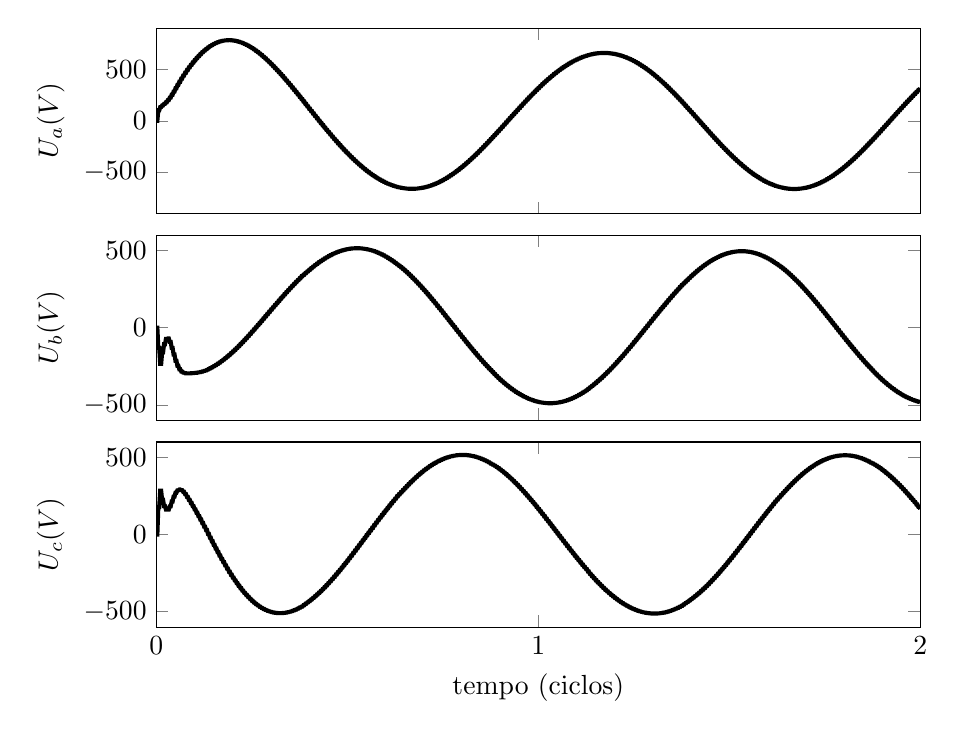
\begin{tikzpicture}

\begin{axis}[%
width=0.8\textwidth,
height=0.193917089240149\textwidth,
scale only axis,
xmin=0,
xmax=0.0333333333333333,
xtick={0,0.0166666666666667,0.0333333333333333},
xticklabels={\empty},
ymin=-600,
ymax=600,
ytick={-500,    0,  500},
ylabel={$\text{U}_\text{b}\text{ (V)}$},
name=plot2,
scaled x ticks = false,
legend columns=-1,
legend style={/tikz/every even column/.append style={column sep=0.3cm}},
legend style={font=\footnotesize}
]
\addplot [color=black,solid,line width=1.5pt,forget plot]
  table[row sep=crcr]{0	0\\
4.16666666666667e-05	0\\
8.33333333333333e-05	-131.208384981468\\
0.000125	-131.208384981468\\
0.000166666666666667	-234.584928965489\\
0.000208333333333333	-234.584928965489\\
0.00025	-160.168155779155\\
0.000291666666666667	-160.168155779155\\
0.000333333333333333	-107.543118489659\\
0.000375	-107.543118489659\\
0.000416666666666667	-73.888785936457\\
0.000458333333333333	-73.888785936457\\
0.0005	-69.7722509660634\\
0.000541666666666667	-69.7722509660634\\
0.000583333333333333	-92.1660340161349\\
0.000625	-92.1660340161349\\
0.000666666666666667	-130.752625769349\\
0.000708333333333333	-130.752625769349\\
0.00075	-174.324494279884\\
0.000791666666666667	-174.324494279884\\
0.000833333333333333	-214.442698151622\\
0.000875	-214.442698151622\\
0.000916666666666667	-246.509146338107\\
0.000958333333333333	-246.509146338107\\
0.001	-269.262100964021\\
0.00104166666666667	-269.262100964021\\
0.00108333333333333	-283.633370400021\\
0.001125	-283.633370400021\\
0.00116666666666667	-291.587806916656\\
0.00120833333333333	-291.587806916656\\
0.00125	-295.25032032309\\
0.00129166666666667	-295.25032032309\\
0.00133333333333333	-296.397867069654\\
0.001375	-296.397867069654\\
0.00141666666666667	-296.263907502466\\
0.00145833333333333	-296.263907502466\\
0.0015	-295.552582188269\\
0.00154166666666667	-295.552582188269\\
0.00158333333333333	-294.559622296515\\
0.001625	-294.559622296515\\
0.00166666666666667	-293.321890703225\\
0.00170833333333333	-293.321890703225\\
0.00175	-291.748630235435\\
0.00179166666666667	-291.748630235435\\
0.00183333333333333	-289.71441027203\\
0.001875	-289.71441027203\\
0.00191666666666667	-287.112155820289\\
0.00195833333333333	-287.112155820289\\
0.002	-283.874408274845\\
0.00204166666666667	-283.874408274845\\
0.00208333333333333	-279.974083042623\\
0.002125	-279.974083042623\\
0.00216666666666667	-276.230710645985\\
0.00220833333333333	-276.230710645985\\
0.00225	-269.902471427438\\
0.00229166666666667	-269.902471427438\\
0.00233333333333333	-263.390506882564\\
0.002375	-263.390506882564\\
0.00241666666666667	-256.603912012827\\
0.00245833333333333	-256.603912012827\\
0.0025	-249.467050045098\\
0.00254166666666667	-249.467050045098\\
0.00258333333333333	-241.924282867545\\
0.002625	-241.924282867545\\
0.00266666666666667	-233.943514769767\\
0.00270833333333333	-233.943514769767\\
0.00275	-225.51142526975\\
0.00279166666666667	-225.51142526975\\
0.00283333333333333	-216.627879066297\\
0.002875	-216.627879066297\\
0.00291666666666667	-207.301043117277\\
0.00295833333333333	-207.301043117277\\
0.003	-197.544304205697\\
0.00304166666666667	-197.544304205697\\
0.00308333333333333	-187.373993764868\\
0.003125	-187.373993764868\\
0.00316666666666667	-176.807799349931\\
0.00320833333333333	-176.807799349931\\
0.00325	-165.86394028825\\
0.00329166666666667	-165.86394028825\\
0.00333333333333333	-154.56053336183\\
0.003375	-154.56053336183\\
0.00341666666666667	-142.916185684556\\
0.00345833333333333	-142.916185684556\\
0.0035	-130.949486492199\\
0.00354166666666667	-130.949486492199\\
0.00358333333333333	-118.678959960814\\
0.003625	-118.678959960814\\
0.00366666666666667	-106.123619808363\\
0.00370833333333333	-106.123619808363\\
0.00375	-93.3030537323442\\
0.00379166666666667	-93.3030537323442\\
0.00383333333333333	-80.2372616130265\\
0.003875	-80.2372616130265\\
0.00391666666666667	-66.946446858932\\
0.00395833333333333	-66.946446858932\\
0.004	-53.4508475905557\\
0.00404166666666667	-53.4508475905557\\
0.00408333333333333	-39.7706293086077\\
0.004125	-39.7706293086077\\
0.00416666666666667	-25.9258298741469\\
0.00420833333333333	-25.9258298741469\\
0.00425	-11.9349140110245\\
0.00429166666666667	-11.9349140110245\\
0.00433333333333333	2.17790522937486\\
0.004375	2.17790522937486\\
0.00441666666666667	16.3962486462483\\
0.00445833333333333	16.3962486462483\\
0.0045	30.7006178618543\\
0.00454166666666667	30.7006178618543\\
0.00458333333333333	45.0716649106275\\
0.004625	45.0716649106275\\
0.00466666666666667	59.4905693391103\\
0.00470833333333333	59.4905693391103\\
0.00475	73.9392259321699\\
0.00479166666666667	73.9392259321699\\
0.00483333333333333	88.4001974163121\\
0.004875	88.4001974163121\\
0.00491666666666667	102.856536225067\\
0.00495833333333333	102.856536225067\\
0.005	117.29157109512\\
0.00504166666666667	117.29157109512\\
0.00508333333333333	131.688732283752\\
0.005125	131.688732283752\\
0.00516666666666667	146.031451752995\\
0.00520833333333333	146.031451752995\\
0.00525	160.303101705176\\
0.00529166666666667	160.303101705176\\
0.00533333333333333	174.487234885993\\
0.005375	174.487234885993\\
0.00541666666666667	188.567259559557\\
0.00545833333333333	188.567259559557\\
0.0055	202.526804768692\\
0.00554166666666667	202.526804768692\\
0.00558333333333333	216.349754514141\\
0.005625	216.349754514141\\
0.00566666666666667	230.020253035965\\
0.00570833333333333	230.020253035965\\
0.00575	243.522738831443\\
0.00579166666666667	243.522738831443\\
0.00583333333333333	256.84196321956\\
0.005875	256.84196321956\\
0.00591666666666667	269.962999410354\\
0.00595833333333333	269.962999410354\\
0.006	282.87124664738\\
0.00604166666666667	282.87124664738\\
0.00608333333333333	295.552432875164\\
0.006125	295.552432875164\\
0.00616666666666667	307.992617959481\\
0.00620833333333333	307.992617959481\\
0.00625	320.178198245509\\
0.00629166666666667	320.178198245509\\
0.00633333333333333	332.855329881327\\
0.006375	332.855329881327\\
0.00641666666666667	343.342330073383\\
0.00645833333333333	343.342330073383\\
0.0065	353.99049013455\\
0.00654166666666667	353.99049013455\\
0.00658333333333333	364.642135043666\\
0.006625	364.642135043666\\
0.00666666666666667	375.181419186422\\
0.00670833333333333	375.181419186422\\
0.00675	385.512898439921\\
0.00679166666666667	385.512898439921\\
0.00683333333333333	395.56751591175\\
0.006875	395.56751591175\\
0.00691666666666667	405.299190659419\\
0.00695833333333333	405.299190659419\\
0.007	414.6789771117\\
0.00704166666666667	414.6789771117\\
0.00708333333333333	423.689448232757\\
0.007125	423.689448232757\\
0.00716666666666667	432.319795582899\\
0.00720833333333333	432.319795582899\\
0.00725	440.562257768488\\
0.00729166666666667	440.562257768488\\
0.00733333333333333	448.410048149301\\
0.007375	448.410048149301\\
0.00741666666666667	455.855714179642\\
0.00745833333333333	455.855714179642\\
0.0075	462.892056329269\\
0.00754166666666667	462.892056329269\\
0.00758333333333333	469.511201648022\\
0.007625	469.511201648022\\
0.00766666666666667	475.705264661268\\
0.00770833333333333	475.705264661268\\
0.00775	481.466649529459\\
0.00779166666666667	481.466649529459\\
0.00783333333333333	486.78826836911\\
0.007875	486.78826836911\\
0.00791666666666667	491.663661719869\\
0.00795833333333333	491.663661719869\\
0.008	496.087037180632\\
0.00804166666666667	496.087037180632\\
0.00808333333333333	500.053254570176\\
0.008125	500.053254570176\\
0.00816666666666667	503.557785185404\\
0.00820833333333333	503.557785185404\\
0.00825	506.596665689598\\
0.00829166666666667	506.596665689598\\
0.00833333333333333	509.166458664863\\
0.008375	509.166458664863\\
0.00841666666666667	511.26284706523\\
0.00845833333333333	511.26284706523\\
0.0085	512.887878751787\\
0.00854166666666667	512.887878751787\\
0.00858333333333333	514.036243881462\\
0.008625	514.036243881462\\
0.00866666666666667	514.70657597084\\
0.00870833333333333	514.70657597084\\
0.00875	514.897900663887\\
0.00879166666666667	514.897900663887\\
0.00883333333333333	514.609349115043\\
0.008875	514.609349115043\\
0.00891666666666667	513.840063526413\\
0.00895833333333333	513.840063526413\\
0.009	512.589295351705\\
0.00904166666666667	512.589295351705\\
0.00908333333333333	510.856621488259\\
0.009125	510.856621488259\\
0.00916666666666667	508.642156970704\\
0.00920833333333333	508.642156970704\\
0.00925	505.94671097045\\
0.00929166666666667	505.94671097045\\
0.00933333333333333	502.771865436787\\
0.009375	502.771865436787\\
0.00941666666666667	499.120078655295\\
0.00945833333333333	499.120078655295\\
0.0095	494.994111068826\\
0.00954166666666667	494.994111068826\\
0.00958333333333333	490.398056463638\\
0.009625	490.398056463638\\
0.00966666666666667	485.336268084155\\
0.00970833333333333	485.336268084155\\
0.00975	479.813656395512\\
0.00979166666666667	479.813656395512\\
0.00983333333333333	473.835637893215\\
0.009875	473.835637893215\\
0.00991666666666667	467.40810543573\\
0.00995833333333333	467.40810543573\\
0.01	460.537409750096\\
0.0100416666666667	460.537409750096\\
0.0100833333333333	453.230348179938\\
0.010125	453.230348179938\\
0.0101666666666667	445.494156765893\\
0.0102083333333333	445.494156765893\\
0.01025	437.336502813829\\
0.0102916666666667	437.336502813829\\
0.0103333333333333	428.765476391161\\
0.010375	428.765476391161\\
0.0104166666666667	419.671168222686\\
0.0104583333333333	419.671168222686\\
0.0105	409.880726788609\\
0.0105416666666667	409.880726788609\\
0.0105833333333333	401.178503300298\\
0.010625	401.178503300298\\
0.0106666666666667	391.676757709522\\
0.0107083333333333	391.676757709522\\
0.01075	381.51592835396\\
0.0107916666666667	381.51592835396\\
0.0108333333333333	370.80234919461\\
0.010875	370.80234919461\\
0.0109166666666667	359.628279768278\\
0.0109583333333333	359.628279768278\\
0.011	348.062824063235\\
0.0110416666666667	348.062824063235\\
0.0110833333333333	336.152893739176\\
0.011125	336.152893739176\\
0.0111666666666667	323.928184426645\\
0.0112083333333333	323.928184426645\\
0.01125	311.407085810258\\
0.0112916666666667	311.407085810258\\
0.0113333333333333	298.601881290224\\
0.011375	298.601881290224\\
0.0114166666666667	285.522540449141\\
0.0114583333333333	285.522540449141\\
0.0115	272.178878667119\\
0.0115416666666667	272.178878667119\\
0.0115833333333333	258.582471388198\\
0.011625	258.582471388198\\
0.0116666666666667	244.745228379326\\
0.0117083333333333	244.745228379326\\
0.01175	230.680736573505\\
0.0117916666666667	230.680736573505\\
0.0118333333333333	216.403367701406\\
0.011875	216.403367701406\\
0.0119166666666667	201.927931320853\\
0.0119583333333333	201.927931320853\\
0.012	187.269408777014\\
0.0120416666666667	187.269408777014\\
0.0120833333333333	172.442797815245\\
0.012125	172.442797815245\\
0.0121666666666667	157.46304906022\\
0.0122083333333333	157.46304906022\\
0.01225	142.345062821324\\
0.0122916666666667	142.345062821324\\
0.0123333333333333	127.103715658411\\
0.012375	127.103715658411\\
0.0124166666666667	111.753893917898\\
0.0124583333333333	111.753893917898\\
0.0125	96.3112704188052\\
0.0125416666666667	96.3112704188052\\
0.0125833333333333	80.7890128332204\\
0.012625	80.7890128332204\\
0.0126666666666667	65.2021424948018\\
0.0127083333333333	65.2021424948018\\
0.01275	49.5668545196005\\
0.0127916666666667	49.5668545196005\\
0.0128333333333333	33.8981375093313\\
0.012875	33.8981375093313\\
0.0129166666666667	18.2111944355166\\
0.0129583333333333	18.2111944355166\\
0.013	2.52164301433743\\
0.0130416666666667	2.52164301433743\\
0.0130833333333333	-13.1544965438618\\
0.013125	-13.1544965438618\\
0.0131666666666667	-28.8009586278613\\
0.0132083333333333	-28.8009586278613\\
0.01325	-44.4014501836413\\
0.0132916666666667	-44.4014501836413\\
0.0133333333333333	-59.9398537968807\\
0.013375	-59.9398537968807\\
0.0134166666666667	-75.4003693774317\\
0.0134583333333333	-75.4003693774317\\
0.0135	-90.7675815462738\\
0.0135416666666667	-90.7675815462738\\
0.0135833333333333	-106.026592391776\\
0.013625	-106.026592391776\\
0.0136666666666667	-121.162260382374\\
0.0137083333333333	-121.162260382374\\
0.01375	-136.160662302134\\
0.0137916666666667	-136.160662302134\\
0.0138333333333333	-151.007656217058\\
0.013875	-151.007656217058\\
0.0139166666666667	-165.689332400057\\
0.0139583333333333	-165.689332400057\\
0.014	-180.191986276356\\
0.0140416666666667	-180.191986276356\\
0.0140833333333333	-194.502113222519\\
0.014125	-194.502113222519\\
0.0141666666666667	-208.606411769966\\
0.0142083333333333	-208.606411769966\\
0.01425	-222.491792056468\\
0.0142916666666667	-222.491792056468\\
0.0143333333333333	-236.145386407417\\
0.014375	-236.145386407417\\
0.0144166666666667	-249.554559936585\\
0.0144583333333333	-249.554559936585\\
0.0145	-262.706920156191\\
0.0145416666666667	-262.706920156191\\
0.0145833333333333	-274.897866458395\\
0.014625	-274.897866458395\\
0.0146666666666667	-288.422767271497\\
0.0147083333333333	-288.422767271497\\
0.01475	-301.387581541166\\
0.0147916666666667	-301.387581541166\\
0.0148333333333333	-313.775025011641\\
0.014875	-313.775025011641\\
0.0149166666666667	-325.666355207773\\
0.0149583333333333	-325.666355207773\\
0.015	-337.120887117542\\
0.0150416666666667	-337.120887117542\\
0.0150833333333333	-348.176422957511\\
0.015125	-348.176422957511\\
0.0151666666666667	-358.852722723377\\
0.0152083333333333	-358.852722723377\\
0.01525	-369.156522014211\\
0.0152916666666667	-369.156522014211\\
0.0153333333333333	-379.086218179142\\
0.015375	-379.086218179142\\
0.0154166666666667	-388.635603200765\\
0.0154583333333333	-388.635603200765\\
0.0155	-397.796477626206\\
0.0155416666666667	-397.796477626206\\
0.0155833333333333	-406.560220436797\\
0.015625	-406.560220436797\\
0.0156666666666667	-414.918572567047\\
0.0157083333333333	-414.918572567047\\
0.01575	-422.864533448988\\
0.0157916666666667	-422.864533448988\\
0.0158333333333333	-430.390775276099\\
0.015875	-430.390775276099\\
0.0159166666666667	-437.491100853172\\
0.0159583333333333	-437.491100853172\\
0.016	-444.159730520883\\
0.0160416666666667	-444.159730520883\\
0.0160833333333333	-450.391206601553\\
0.016125	-450.391206601553\\
0.0161666666666667	-456.180340052471\\
0.0162083333333333	-456.180340052471\\
0.01625	-461.522202906791\\
0.0162916666666667	-461.522202906791\\
0.0163333333333333	-466.412149544966\\
0.016375	-466.412149544966\\
0.0164166666666667	-470.845850821675\\
0.0164583333333333	-470.845850821675\\
0.0165	-474.819329326491\\
0.0165416666666667	-474.819329326491\\
0.0165833333333333	-478.328989103039\\
0.016625	-478.328989103039\\
0.0166666666666667	-481.372762295986\\
0.0167083333333333	-481.372762295986\\
0.01675	-483.944387417357\\
0.0167916666666667	-483.944387417357\\
0.0168333333333333	-486.043904769891\\
0.016875	-486.043904769891\\
0.0169166666666667	-487.669342075457\\
0.0169583333333333	-487.669342075457\\
0.017	-488.81912329053\\
0.0170416666666667	-488.81912329053\\
0.0170833333333333	-489.492376222951\\
0.017125	-489.492376222951\\
0.0171666666666667	-489.689089295181\\
0.0172083333333333	-489.689089295181\\
0.01725	-489.410057478733\\
0.0172916666666667	-489.410057478733\\
0.0173333333333333	-488.656714544629\\
0.017375	-488.656714544629\\
0.0174166666666667	-487.430933830334\\
0.0174583333333333	-487.430933830334\\
0.0175	-485.734862735459\\
0.0175416666666667	-485.734862735459\\
0.0175833333333333	-483.570824107468\\
0.017625	-483.570824107468\\
0.0176666666666667	-480.941176730971\\
0.0177083333333333	-480.941176730971\\
0.01775	-477.848873406491\\
0.0177916666666667	-477.848873406491\\
0.0178333333333333	-474.296687037085\\
0.017875	-474.296687037085\\
0.0179166666666667	-470.287554266504\\
0.0179583333333333	-470.287554266504\\
0.018	-465.824994538518\\
0.0180416666666667	-465.824994538518\\
0.0180833333333333	-460.912896166831\\
0.018125	-460.912896166831\\
0.0181666666666667	-455.555544349316\\
0.0182083333333333	-455.555544349316\\
0.01825	-449.757632700212\\
0.0182916666666667	-449.757632700212\\
0.0183333333333333	-443.524266807923\\
0.018375	-443.524266807923\\
0.0184166666666667	-436.860963041735\\
0.0184583333333333	-436.860963041735\\
0.0185	-429.773645406549\\
0.0185416666666667	-429.773645406549\\
0.0185833333333333	-422.2686421737\\
0.018625	-422.2686421737\\
0.0186666666666667	-414.352682994809\\
0.0187083333333333	-414.352682994809\\
0.01875	-406.710604021129\\
0.0187916666666667	-406.710604021129\\
0.0188333333333333	-396.968651829484\\
0.018875	-396.968651829484\\
0.0189166666666667	-387.24430030011\\
0.0189583333333333	-387.24430030011\\
0.019	-377.413842111121\\
0.0190416666666667	-377.413842111121\\
0.0190833333333333	-367.3960735467\\
0.019125	-367.3960735467\\
0.0191666666666667	-357.12553953726\\
0.0192083333333333	-357.12553953726\\
0.01925	-346.559303382721\\
0.0192916666666667	-346.559303382721\\
0.0193333333333333	-335.674936708767\\
0.019375	-335.674936708767\\
0.0194166666666667	-324.465686057335\\
0.0194583333333333	-324.465686057335\\
0.0195	-312.935239244225\\
0.0195416666666667	-312.935239244225\\
0.0195833333333333	-301.093266862382\\
0.019625	-301.093266862382\\
0.0196666666666667	-288.95219973374\\
0.0197083333333333	-288.95219973374\\
0.01975	-276.525463982029\\
0.0197916666666667	-276.525463982029\\
0.0198333333333333	-263.82538033546\\
0.019875	-263.82538033546\\
0.0199166666666667	-250.865057706918\\
0.0199583333333333	-250.865057706918\\
0.02	-237.656697428642\\
0.0200416666666667	-237.656697428642\\
0.0200833333333333	-224.212271375033\\
0.020125	-224.212271375033\\
0.0201666666666667	-210.543848998092\\
0.0202083333333333	-210.543848998092\\
0.02025	-196.6637735981\\
0.0202916666666667	-196.6637735981\\
0.0203333333333333	-182.584756063204\\
0.020375	-182.584756063204\\
0.0204166666666667	-168.319897946886\\
0.0204583333333333	-168.319897946886\\
0.0205	-153.882668002172\\
0.0205416666666667	-153.882668002172\\
0.0205833333333333	-139.286855686717\\
0.020625	-139.286855686717\\
0.0206666666666667	-124.546519243168\\
0.0207083333333333	-124.546519243168\\
0.02075	-109.675923407492\\
0.0207916666666667	-109.675923407492\\
0.0208333333333333	-94.6884951690301\\
0.020875	-94.6884951690301\\
0.0209166666666667	-79.6023211852309\\
0.0209583333333333	-79.6023211852309\\
0.021	-64.4296541414652\\
0.0210416666666667	-64.4296541414652\\
0.0210833333333333	-49.1854677870168\\
0.021125	-49.1854677870168\\
0.0211666666666667	-33.8847697005379\\
0.0212083333333333	-33.8847697005379\\
0.02125	-18.5423320716325\\
0.0212916666666667	-18.5423320716325\\
0.0213333333333333	-3.1725945533516\\
0.021375	-3.1725945533516\\
0.0214166666666667	12.2102617721841\\
0.0214583333333333	12.2102617721841\\
0.0215	27.5921432856442\\
0.0215416666666667	27.5921432856442\\
0.0215833333333333	42.9588704890498\\
0.021625	42.9588704890498\\
0.0216666666666667	58.2960537853681\\
0.0217083333333333	58.2960537853681\\
0.02175	73.5890384864759\\
0.0217916666666667	73.5890384864759\\
0.0218333333333333	88.82269659409\\
0.021875	88.82269659409\\
0.0219166666666667	103.982669291038\\
0.0219583333333333	103.982669291038\\
0.022	119.053037141893\\
0.0220416666666667	119.053037141893\\
0.0220833333333333	134.01853586672\\
0.022125	134.01853586672\\
0.0221666666666667	148.863909368128\\
0.0222083333333333	148.863909368128\\
0.02225	163.573956427556\\
0.0222916666666667	163.573956427556\\
0.0223333333333333	178.133568427636\\
0.022375	178.133568427636\\
0.0224166666666667	192.527757716713\\
0.0224583333333333	192.527757716713\\
0.0225	206.741679404245\\
0.0225416666666667	206.741679404245\\
0.0225833333333333	220.760649670751\\
0.022625	220.760649670751\\
0.0226666666666667	234.570162946369\\
0.0227083333333333	234.570162946369\\
0.02275	248.155909263895\\
0.0227916666666667	248.155909263895\\
0.0228333333333333	261.687830320942\\
0.022875	261.687830320942\\
0.0229166666666667	274.986604079196\\
0.0229583333333333	274.986604079196\\
0.023	286.928801747272\\
0.0230416666666667	286.928801747272\\
0.0230833333333333	298.950506950644\\
0.023125	298.950506950644\\
0.0231666666666667	310.924864102034\\
0.0232083333333333	310.924864102034\\
0.02325	322.756989832147\\
0.0232916666666667	322.756989832147\\
0.0233333333333333	334.367084014297\\
0.023375	334.367084014297\\
0.0234166666666667	345.69602196514\\
0.0234583333333333	345.69602196514\\
0.0235	356.703461032175\\
0.0235416666666667	356.703461032175\\
0.0235833333333333	367.363371170442\\
0.023625	367.363371170442\\
0.0236666666666667	377.659204280424\\
0.0237083333333333	377.659204280424\\
0.02375	387.579795487262\\
0.0237916666666667	387.579795487262\\
0.0238333333333333	397.116425283701\\
0.023875	397.116425283701\\
0.0239166666666667	406.261310362139\\
0.0239583333333333	406.261310362139\\
0.024	415.0053223807\\
0.0240416666666667	415.0053223807\\
0.0240833333333333	423.340732147141\\
0.024125	423.340732147141\\
0.0241666666666667	431.258683016742\\
0.0242083333333333	431.258683016742\\
0.02425	438.750365395371\\
0.0242916666666667	438.750365395371\\
0.0243333333333333	445.807262831054\\
0.024375	445.807262831054\\
0.0244166666666667	452.421342397773\\
0.0244583333333333	452.421342397773\\
0.0245	458.585161293933\\
0.0245416666666667	458.585161293933\\
0.0245833333333333	464.291905294308\\
0.024625	464.291905294308\\
0.0246666666666667	469.535383109734\\
0.0247083333333333	469.535383109734\\
0.02475	474.309999446141\\
0.0247916666666667	474.309999446141\\
0.0248333333333333	478.610723480444\\
0.024875	478.610723480444\\
0.0249166666666667	482.432523836755\\
0.0249583333333333	482.432523836755\\
0.025	485.772612186125\\
0.0250416666666667	485.772612186125\\
0.0250833333333333	488.627883686145\\
0.025125	488.627883686145\\
0.0251666666666667	490.994391489966\\
0.0252083333333333	490.994391489966\\
0.02525	492.869784189106\\
0.0252916666666667	492.869784189106\\
0.0253333333333333	494.252063559781\\
0.025375	494.252063559781\\
0.0254166666666667	495.139387583695\\
0.0254583333333333	495.139387583695\\
0.0255	495.530061759552\\
0.0255416666666667	495.530061759552\\
0.0255833333333333	495.422663936061\\
0.025625	495.422663936061\\
0.0256666666666667	494.816230581684\\
0.0257083333333333	494.816230581684\\
0.02575	493.710425995119\\
0.0257916666666667	493.710425995119\\
0.0258333333333333	492.105654148384\\
0.025875	492.105654148384\\
0.0259166666666667	490.003108134894\\
0.0259583333333333	490.003108134894\\
0.026	487.404961487327\\
0.0260416666666667	487.404961487327\\
0.0260833333333333	484.313069214194\\
0.026125	484.313069214194\\
0.0261666666666667	480.731558886196\\
0.0262083333333333	480.731558886196\\
0.02625	476.664323712434\\
0.0262916666666667	476.664323712434\\
0.0263333333333333	472.115829454631\\
0.026375	472.115829454631\\
0.0264166666666667	467.091068733291\\
0.0264583333333333	467.091068733291\\
0.0265	461.595540479995\\
0.0265416666666667	461.595540479995\\
0.0265833333333333	455.635234907076\\
0.026625	455.635234907076\\
0.0266666666666667	449.21662231492\\
0.0267083333333333	449.21662231492\\
0.02675	442.346643428456\\
0.0267916666666667	442.346643428456\\
0.0268333333333333	435.032699614098\\
0.026875	435.032699614098\\
0.0269166666666667	427.282642172915\\
0.0269583333333333	427.282642172915\\
0.027	418.527982244731\\
0.0270416666666667	418.527982244731\\
0.0270833333333333	410.672570182659\\
0.027125	410.672570182659\\
0.0271666666666667	402.276872290978\\
0.0272083333333333	402.276872290978\\
0.02725	393.223850223727\\
0.0272916666666667	393.223850223727\\
0.0273333333333333	383.609151155178\\
0.027375	383.609151155178\\
0.0274166666666667	373.508718653929\\
0.0274583333333333	373.508718653929\\
0.0275	362.979579538073\\
0.0275416666666667	362.979579538073\\
0.0275833333333333	352.061894709897\\
0.027625	352.061894709897\\
0.0276666666666667	340.783205444461\\
0.0277083333333333	340.783205444461\\
0.02775	329.162781541968\\
0.0277916666666667	329.162781541968\\
0.0278333333333333	317.215226351439\\
0.027875	317.215226351439\\
0.0279166666666667	304.953068995059\\
0.0279583333333333	304.953068995059\\
0.028	292.388308765939\\
0.0280416666666667	292.388308765939\\
0.0280833333333333	279.533394256386\\
0.028125	279.533394256386\\
0.0281666666666667	266.401997020689\\
0.0282083333333333	266.401997020689\\
0.02825	253.007121767018\\
0.0282916666666667	253.007121767018\\
0.0283333333333333	239.363037342399\\
0.028375	239.363037342399\\
0.0284166666666667	225.484309796947\\
0.0284583333333333	225.484309796947\\
0.0285	211.385672071801\\
0.0285416666666667	211.385672071801\\
0.0285833333333333	197.081935254737\\
0.028625	197.081935254737\\
0.0286666666666667	182.587950486431\\
0.0287083333333333	182.587950486431\\
0.02875	167.918604082923\\
0.0287916666666667	167.918604082923\\
0.0288333333333333	153.088829011011\\
0.028875	153.088829011011\\
0.0289166666666667	138.113619934855\\
0.0289583333333333	138.113619934855\\
0.029	123.008044204917\\
0.0290416666666667	123.008044204917\\
0.0290833333333333	107.788100944899\\
0.029125	107.788100944899\\
0.0291666666666667	92.4664220892656\\
0.0292083333333333	92.4664220892656\\
0.02925	77.0599110293703\\
0.0292916666666667	77.0599110293703\\
0.0293333333333333	61.5839402726698\\
0.029375	61.5839402726698\\
0.0294166666666667	46.0538191073489\\
0.0294583333333333	46.0538191073489\\
0.0295	30.4851141949034\\
0.0295416666666667	30.4851141949034\\
0.0295833333333333	14.8937682112207\\
0.029625	14.8937682112207\\
0.0296666666666667	-0.703957306529608\\
0.0297083333333333	-0.703957306529608\\
0.02975	-16.2916492298269\\
0.0297916666666667	-16.2916492298269\\
0.0298333333333333	-31.8529362123827\\
0.029875	-31.8529362123827\\
0.0299166666666667	-47.371649369948\\
0.0299583333333333	-47.371649369948\\
0.03	-62.8319222299047\\
0.0300416666666667	-62.8319222299047\\
0.0300833333333333	-78.2183969102601\\
0.030125	-78.2183969102601\\
0.0301666666666667	-93.5154108314719\\
0.0302083333333333	-93.5154108314719\\
0.03025	-108.70816278091\\
0.0302916666666667	-108.70816278091\\
0.0303333333333333	-123.782356080195\\
0.030375	-123.782356080195\\
0.0304166666666667	-138.723507249364\\
0.0304583333333333	-138.723507249364\\
0.0305	-153.517339096442\\
0.0305416666666667	-153.517339096442\\
0.0305833333333333	-168.149764544084\\
0.030625	-168.149764544084\\
0.0306666666666667	-182.60688669631\\
0.0307083333333333	-182.60688669631\\
0.03075	-196.875004412733\\
0.0307916666666667	-196.875004412733\\
0.0308333333333333	-210.940621254231\\
0.030875	-210.940621254231\\
0.0309166666666667	-224.790455634942\\
0.0309583333333333	-224.790455634942\\
0.031	-238.411450801645\\
0.0310416666666667	-238.411450801645\\
0.0310833333333333	-251.788204920739\\
0.031125	-251.788204920739\\
0.0311666666666667	-264.319493294975\\
0.0312083333333333	-264.319493294975\\
0.03125	-278.081845363642\\
0.0312916666666667	-278.081845363642\\
0.0313333333333333	-291.211888263673\\
0.031375	-291.211888263673\\
0.0314166666666667	-303.807007713181\\
0.0314583333333333	-303.807007713181\\
0.0315	-315.936364357588\\
0.0315416666666667	-315.936364357588\\
0.0315833333333333	-327.655020751537\\
0.031625	-327.655020751537\\
0.0316666666666667	-338.998550237152\\
0.0317083333333333	-338.998550237152\\
0.03175	-349.984949605885\\
0.0317916666666667	-349.984949605885\\
0.0318333333333333	-360.618974262017\\
0.031875	-360.618974262017\\
0.0319166666666667	-370.896795074955\\
0.0319583333333333	-370.896795074955\\
0.032	-380.809923421548\\
0.0320416666666667	-380.809923421548\\
0.0320833333333333	-390.348041070204\\
0.032125	-390.348041070204\\
0.0321666666666667	-399.500455565927\\
0.0322083333333333	-399.500455565927\\
0.03225	-408.258433783543\\
0.0322916666666667	-408.258433783543\\
0.0323333333333333	-416.612673979994\\
0.032375	-416.612673979994\\
0.0324166666666667	-424.555376388038\\
0.0324583333333333	-424.555376388038\\
0.0325	-432.079651399668\\
0.0325416666666667	-432.079651399668\\
0.0325833333333333	-439.17912856472\\
0.032625	-439.17912856472\\
0.0326666666666667	-445.847803165625\\
0.0327083333333333	-445.847803165625\\
0.03275	-452.079952433882\\
0.0327916666666667	-452.079952433882\\
0.0328333333333333	-457.870112681898\\
0.032875	-457.870112681898\\
0.0329166666666667	-463.213095942823\\
0.0329583333333333	-463.213095942823\\
0.033	-468.104025539882\\
0.0330416666666667	-468.104025539882\\
0.0330833333333333	-472.538375275198\\
0.033125	-472.538375275198\\
0.0331666666666667	-476.512043591712\\
0.0332083333333333	-476.512043591712\\
0.03325	-480.021998518076\\
0.0332916666666667	-480.021998518076\\
0.0333333333333333	-483.062409528906\\
};
\end{axis}

\begin{axis}[%
width=0.8\textwidth,
height=0.193917089240149\textwidth,
scale only axis,
xmin=0,
xmax=0.0333333333333333,
xtick={0,0.0166666666666667,0.0333333333333333},
xticklabels={{0},{1},{2}},
xlabel={tempo (ciclos)},
ymin=-600,
ymax=600,
ytick={-500,    0,  500},
ylabel={$\text{U}_\text{c}\text{ (V)}$},
at=(plot2.below south west),
anchor=above north west,
scaled x ticks = false,
legend columns=-1,
legend style={/tikz/every even column/.append style={column sep=0.3cm}},
legend style={font=\footnotesize}
]
\addplot [color=black,solid,line width=1.5pt,forget plot]
  table[row sep=crcr]{0	0\\
4.16666666666667e-05	0\\
8.33333333333333e-05	178.004625595273\\
0.000125	178.004625595273\\
0.000166666666666667	283.783478314647\\
0.000208333333333333	283.783478314647\\
0.00025	224.921982240448\\
0.000291666666666667	224.921982240448\\
0.000333333333333333	184.950751047334\\
0.000375	184.950751047334\\
0.000416666666666667	161.297963182983\\
0.000458333333333333	161.297963182983\\
0.0005	161.820809180068\\
0.000541666666666667	161.820809180068\\
0.000583333333333333	182.600021490024\\
0.000625	182.600021490024\\
0.000666666666666667	213.852580818456\\
0.000708333333333333	213.852580818456\\
0.00075	245.650747681198\\
0.000791666666666667	245.650747681198\\
0.000833333333333333	270.969555601234\\
0.000875	270.969555601234\\
0.000916666666666667	286.39849397629\\
0.000958333333333333	286.39849397629\\
0.001	291.501650773087\\
0.00104166666666667	291.501650773087\\
0.00108333333333333	287.689293494019\\
0.001125	287.689293494019\\
0.00116666666666667	277.144952722096\\
0.00120833333333333	277.144952722096\\
0.00125	262.056791666573\\
0.00129166666666667	262.056791666573\\
0.00133333333333333	244.197984718012\\
0.001375	244.197984718012\\
0.00141666666666667	224.790878827205\\
0.00145833333333333	224.790878827205\\
0.0015	204.552290090145\\
0.00154166666666667	204.552290090145\\
0.00158333333333333	183.823710668467\\
0.001625	183.823710668467\\
0.00166666666666667	162.716831956078\\
0.00170833333333333	162.716831956078\\
0.00175	141.234887842283\\
0.00179166666666667	141.234887842283\\
0.00183333333333333	119.35496285977\\
0.001875	119.35496285977\\
0.00191666666666667	97.0724508524626\\
0.00195833333333333	97.0724508524626\\
0.002	74.4167689879326\\
0.00204166666666667	74.4167689879326\\
0.00208333333333333	51.4493873847393\\
0.002125	51.4493873847393\\
0.00216666666666667	29.3933134371395\\
0.00220833333333333	29.3933134371395\\
0.00225	4.5154200136966\\
0.00229166666666667	4.5154200136966\\
0.00233333333333333	-19.8430703521883\\
0.002375	-19.8430703521883\\
0.00241666666666667	-43.7452284674193\\
0.00245833333333333	-43.7452284674193\\
0.0025	-67.2437290269028\\
0.00254166666666667	-67.2437290269028\\
0.00258333333333333	-90.374341557218\\
0.002625	-90.374341557218\\
0.00266666666666667	-113.147583195981\\
0.00270833333333333	-113.147583195981\\
0.00275	-135.552273116364\\
0.00279166666666667	-135.552273116364\\
0.00283333333333333	-157.561983919016\\
0.002875	-157.561983919016\\
0.00291666666666667	-179.14154545017\\
0.00295833333333333	-179.14154545017\\
0.003	-200.251748337301\\
0.00304166666666667	-200.251748337301\\
0.00308333333333333	-220.852877551901\\
0.003125	-220.852877551901\\
0.00316666666666667	-240.907089135164\\
0.00320833333333333	-240.907089135164\\
0.00325	-260.379576837184\\
0.00329166666666667	-260.379576837184\\
0.00333333333333333	-279.239350290979\\
0.003375	-279.239350290979\\
0.00341666666666667	-297.458284795409\\
0.00345833333333333	-297.458284795409\\
0.0035	-315.011576336968\\
0.00354166666666667	-315.011576336968\\
0.00358333333333333	-331.876739706872\\
0.003625	-331.876739706872\\
0.00366666666666667	-348.033836396141\\
0.00370833333333333	-348.033836396141\\
0.00375	-363.465376357984\\
0.00379166666666667	-363.465376357984\\
0.00383333333333333	-378.156103365302\\
0.003875	-378.156103365302\\
0.00391666666666667	-392.092812734721\\
0.00395833333333333	-392.092812734721\\
0.004	-405.264238535789\\
0.00404166666666667	-405.264238535789\\
0.00408333333333333	-417.66099575086\\
0.004125	-417.66099575086\\
0.00416666666666667	-429.275548297076\\
0.00420833333333333	-429.275548297076\\
0.00425	-440.102848900291\\
0.00429166666666667	-440.102848900291\\
0.00433333333333333	-450.136815525274\\
0.004375	-450.136815525274\\
0.00441666666666667	-459.376722037127\\
0.00445833333333333	-459.376722037127\\
0.0045	-467.821856969954\\
0.00454166666666667	-467.821856969954\\
0.00458333333333333	-475.473032640935\\
0.004625	-475.473032640935\\
0.00466666666666667	-482.332742676867\\
0.00470833333333333	-482.332742676867\\
0.00475	-488.405171398126\\
0.00479166666666667	-488.405171398126\\
0.00483333333333333	-493.696011215487\\
0.004875	-493.696011215487\\
0.00491666666666667	-498.212188101641\\
0.00495833333333333	-498.212188101641\\
0.005	-501.961580121402\\
0.00504166666666667	-501.961580121402\\
0.00508333333333333	-504.952789601296\\
0.005125	-504.952789601296\\
0.00516666666666667	-507.194994417279\\
0.00520833333333333	-507.194994417279\\
0.00525	-508.697818385253\\
0.00529166666666667	-508.697818385253\\
0.00533333333333333	-509.471593317843\\
0.005375	-509.471593317843\\
0.00541666666666667	-509.526863255645\\
0.00545833333333333	-509.526863255645\\
0.0055	-508.874727992641\\
0.00554166666666667	-508.874727992641\\
0.00558333333333333	-507.526855287823\\
0.005625	-507.526855287823\\
0.00566666666666667	-505.495407493961\\
0.00570833333333333	-505.495407493961\\
0.00575	-502.793024217572\\
0.00579166666666667	-502.793024217572\\
0.00583333333333333	-499.432794031877\\
0.005875	-499.432794031877\\
0.00591666666666667	-495.428221057553\\
0.00595833333333333	-495.428221057553\\
0.006	-490.793190368868\\
0.00604166666666667	-490.793190368868\\
0.00608333333333333	-485.54193498711\\
0.006125	-485.54193498711\\
0.00616666666666667	-479.689005886904\\
0.00620833333333333	-479.689005886904\\
0.00625	-473.249245351608\\
0.00629166666666667	-473.249245351608\\
0.00633333333333333	-467.298164949134\\
0.006375	-467.298164949134\\
0.00641666666666667	-458.147227910362\\
0.00645833333333333	-458.147227910362\\
0.0065	-449.066214705222\\
0.00654166666666667	-449.066214705222\\
0.00658333333333333	-439.891191771422\\
0.006625	-439.891191771422\\
0.00666666666666667	-430.495153433043\\
0.00670833333333333	-430.495153433043\\
0.00675	-420.77695941029\\
0.00679166666666667	-420.77695941029\\
0.00683333333333333	-410.670766826443\\
0.006875	-410.670766826443\\
0.00691666666666667	-400.142827213577\\
0.00695833333333333	-400.142827213577\\
0.007	-389.183812623598\\
0.00704166666666667	-389.183812623598\\
0.00708333333333333	-377.800189443289\\
0.007125	-377.800189443289\\
0.00716666666666667	-366.007139201097\\
0.00720833333333333	-366.007139201097\\
0.00725	-353.823562705966\\
0.00729166666666667	-353.823562705966\\
0.00733333333333333	-341.269218925638\\
0.007375	-341.269218925638\\
0.00741666666666667	-328.362469641968\\
0.00745833333333333	-328.362469641968\\
0.0075	-315.121481823484\\
0.00754166666666667	-315.121481823484\\
0.00758333333333333	-301.562947743627\\
0.007625	-301.562947743627\\
0.00766666666666667	-287.70292901112\\
0.00770833333333333	-287.70292901112\\
0.00775	-273.557232892287\\
0.00779166666666667	-273.557232892287\\
0.00783333333333333	-259.141683855914\\
0.007875	-259.141683855914\\
0.00791666666666667	-244.472273340152\\
0.00795833333333333	-244.472273340152\\
0.008	-229.565207512913\\
0.00804166666666667	-229.565207512913\\
0.00808333333333333	-214.436888539275\\
0.008125	-214.436888539275\\
0.00816666666666667	-199.103863773767\\
0.00820833333333333	-199.103863773767\\
0.00825	-183.582768321516\\
0.00829166666666667	-183.582768321516\\
0.00833333333333333	-167.890275701312\\
0.008375	-167.890275701312\\
0.00841666666666667	-152.04244733988\\
0.00845833333333333	-152.04244733988\\
0.0085	-136.05795452593\\
0.00854166666666667	-136.05795452593\\
0.00858333333333333	-119.951965514414\\
0.008625	-119.951965514414\\
0.00866666666666667	-103.741190475133\\
0.00870833333333333	-103.741190475133\\
0.00875	-87.4422091632389\\
0.00879166666666667	-87.4422091632389\\
0.00883333333333333	-71.0712701286369\\
0.008875	-71.0712701286369\\
0.00891666666666667	-54.6442399391995\\
0.00895833333333333	-54.6442399391995\\
0.009	-38.176713696354\\
0.00904166666666667	-38.176713696354\\
0.00908333333333333	-21.6841757169129\\
0.009125	-21.6841757169129\\
0.00916666666666667	-5.18216699897625\\
0.00920833333333333	-5.18216699897625\\
0.00925	11.3135983475548\\
0.00929166666666667	11.3135983475548\\
0.00933333333333333	27.7871882840866\\
0.009375	27.7871882840866\\
0.00941666666666667	44.2223308532296\\
0.00945833333333333	44.2223308532296\\
0.0095	60.6032444540017\\
0.00954166666666667	60.6032444540017\\
0.00958333333333333	76.9131639720522\\
0.009625	76.9131639720522\\
0.00966666666666667	93.1358067368588\\
0.00970833333333333	93.1358067368588\\
0.00975	109.254960007813\\
0.00979166666666667	109.254960007813\\
0.00983333333333333	125.254535256242\\
0.009875	125.254535256242\\
0.00991666666666667	141.118601346748\\
0.00995833333333333	141.118601346748\\
0.01	156.83140708878\\
0.0100416666666667	156.83140708878\\
0.0100833333333333	172.377396967822\\
0.010125	172.377396967822\\
0.0101666666666667	187.741223638366\\
0.0102083333333333	187.741223638366\\
0.01025	202.907759665792\\
0.0102916666666667	202.907759665792\\
0.0103333333333333	217.862109793741\\
0.010375	217.862109793741\\
0.0104166666666667	232.754774400292\\
0.0104583333333333	232.754774400292\\
0.0105	247.828611366131\\
0.0105416666666667	247.828611366131\\
0.0105833333333333	260.603260690465\\
0.010625	260.603260690465\\
0.0106666666666667	273.680687269622\\
0.0107083333333333	273.680687269622\\
0.01075	286.883764607617\\
0.0107916666666667	286.883764607617\\
0.0108333333333333	300.065387824424\\
0.010875	300.065387824424\\
0.0109166666666667	313.098555619261\\
0.0109583333333333	313.098555619261\\
0.011	325.889085035844\\
0.0110416666666667	325.889085035844\\
0.0110833333333333	338.374638010692\\
0.011125	338.374638010692\\
0.0111666666666667	350.517946768375\\
0.0112083333333333	350.517946768375\\
0.01125	362.298555343427\\
0.0112916666666667	362.298555343427\\
0.0113333333333333	373.705464682803\\
0.011375	373.705464682803\\
0.0114166666666667	384.731726726044\\
0.0114583333333333	384.731726726044\\
0.0115	395.371336948598\\
0.0115416666666667	395.371336948598\\
0.0115833333333333	405.616529484539\\
0.011625	405.616529484539\\
0.0116666666666667	415.459679980571\\
0.0117083333333333	415.459679980571\\
0.01175	424.891495449277\\
0.0117916666666667	424.891495449277\\
0.0118333333333333	433.902229575715\\
0.011875	433.902229575715\\
0.0119166666666667	442.482176818538\\
0.0119583333333333	442.482176818538\\
0.012	450.622046686112\\
0.0120416666666667	450.622046686112\\
0.0120833333333333	458.313179351795\\
0.012125	458.313179351795\\
0.0121666666666667	465.547628342919\\
0.0122083333333333	465.547628342919\\
0.01225	472.31815507542\\
0.0122916666666667	472.31815507542\\
0.0123333333333333	478.618179027316\\
0.012375	478.618179027316\\
0.0124166666666667	484.441716434643\\
0.0124583333333333	484.441716434643\\
0.0125	489.783056377473\\
0.0125416666666667	489.783056377473\\
0.0125833333333333	494.63785268411\\
0.012625	494.63785268411\\
0.0126666666666667	499.001883658817\\
0.0127083333333333	499.001883658817\\
0.01275	502.870683009938\\
0.0127916666666667	502.870683009938\\
0.0128333333333333	506.240849585294\\
0.012875	506.240849585294\\
0.0129166666666667	509.109305926703\\
0.0129583333333333	509.109305926703\\
0.013	511.473151542652\\
0.0130416666666667	511.473151542652\\
0.0130833333333333	513.329690696309\\
0.013125	513.329690696309\\
0.0131666666666667	514.676571296975\\
0.0132083333333333	514.676571296975\\
0.01325	515.511961612553\\
0.0132916666666667	515.511961612553\\
0.0133333333333333	515.834702003018\\
0.013375	515.834702003018\\
0.0134166666666667	515.644396099892\\
0.0134583333333333	515.644396099892\\
0.0135	514.941435182568\\
0.0135416666666667	514.941435182568\\
0.0135833333333333	513.727158325521\\
0.013625	513.727158325521\\
0.0136666666666667	512.002738401634\\
0.0137083333333333	512.002738401634\\
0.01375	509.771274070275\\
0.0137916666666667	509.771274070275\\
0.0138333333333333	507.035778530441\\
0.013875	507.035778530441\\
0.0139166666666667	503.799794343328\\
0.0139583333333333	503.799794343328\\
0.014	500.067354272517\\
0.0140416666666667	500.067354272517\\
0.0140833333333333	495.842961710452\\
0.014125	495.842961710452\\
0.0141666666666667	491.13157751503\\
0.0142083333333333	491.13157751503\\
0.01425	485.938610753475\\
0.0142916666666667	485.938610753475\\
0.0143333333333333	480.269910907528\\
0.014375	480.269910907528\\
0.0144166666666667	474.131759969877\\
0.0144583333333333	474.131759969877\\
0.0145	467.530863763359\\
0.0145416666666667	467.530863763359\\
0.0145833333333333	459.508633873283\\
0.014625	459.508633873283\\
0.0146666666666667	453.274962236926\\
0.0147083333333333	453.274962236926\\
0.01475	446.245306345853\\
0.0147916666666667	446.245306345853\\
0.0148333333333333	438.401491771066\\
0.014875	438.401491771066\\
0.0149166666666667	429.879478829895\\
0.0149583333333333	429.879478829895\\
0.015	420.786884965651\\
0.0150416666666667	420.786884965651\\
0.0150833333333333	411.20173328185\\
0.015125	411.20173328185\\
0.0151666666666667	401.176564947615\\
0.0152083333333333	401.176564947615\\
0.01525	390.745078763984\\
0.0152916666666667	390.745078763984\\
0.0153333333333333	379.92872102013\\
0.015375	379.92872102013\\
0.0154166666666667	368.742067947851\\
0.0154583333333333	368.742067947851\\
0.0155	357.196643520179\\
0.0155416666666667	357.196643520179\\
0.0155833333333333	345.303227125392\\
0.015625	345.303227125392\\
0.0156666666666667	333.073000051622\\
0.0157083333333333	333.073000051622\\
0.01575	320.518786743501\\
0.0157916666666667	320.518786743501\\
0.0158333333333333	307.652851105477\\
0.015875	307.652851105477\\
0.0159166666666667	294.488828291836\\
0.0159583333333333	294.488828291836\\
0.016	281.040711832279\\
0.0160416666666667	281.040711832279\\
0.0160833333333333	267.322672079467\\
0.016125	267.322672079467\\
0.0161666666666667	253.348945843036\\
0.0162083333333333	253.348945843036\\
0.01625	239.133797089959\\
0.0162916666666667	239.133797089959\\
0.0163333333333333	224.691523562147\\
0.016375	224.691523562147\\
0.0164166666666667	210.036484979632\\
0.0164583333333333	210.036484979632\\
0.0165	195.183134699971\\
0.0165416666666667	195.183134699971\\
0.0165833333333333	180.146044285981\\
0.016625	180.146044285981\\
0.0166666666666667	164.940320934484\\
0.0167083333333333	164.940320934484\\
0.01675	149.579587477261\\
0.0167916666666667	149.579587477261\\
0.0168333333333333	134.079551509137\\
0.016875	134.079551509137\\
0.0169166666666667	118.455249604828\\
0.0169583333333333	118.455249604828\\
0.017	102.721820759597\\
0.0170416666666667	102.721820759597\\
0.0170833333333333	86.8947024886041\\
0.017125	86.8947024886041\\
0.0171666666666667	70.9897152347551\\
0.0172083333333333	70.9897152347551\\
0.01725	55.0229884605968\\
0.0172916666666667	55.0229884605968\\
0.0173333333333333	39.0107951391398\\
0.017375	39.0107951391398\\
0.0174166666666667	22.9693692316446\\
0.0174583333333333	22.9693692316446\\
0.0175	6.91476165823279\\
0.0175416666666667	6.91476165823279\\
0.0175833333333333	-9.13724020053355\\
0.017625	-9.13724020053355\\
0.0176666666666667	-25.1712876244939\\
0.0177083333333333	-25.1712876244939\\
0.01775	-41.1717016099994\\
0.0177916666666667	-41.1717016099994\\
0.0178333333333333	-57.1235450619316\\
0.017875	-57.1235450619316\\
0.0179166666666667	-73.0122416753861\\
0.0179583333333333	-73.0122416753861\\
0.018	-88.8229904086394\\
0.0180416666666667	-88.8229904086394\\
0.0180833333333333	-104.541092542183\\
0.018125	-104.541092542183\\
0.0181666666666667	-120.151937938219\\
0.0182083333333333	-120.151937938219\\
0.01825	-135.641005542097\\
0.0182916666666667	-135.641005542097\\
0.0183333333333333	-150.993870043721\\
0.018375	-150.993870043721\\
0.0184166666666667	-166.196212093992\\
0.0184583333333333	-166.196212093992\\
0.0185	-181.2338298443\\
0.0185416666666667	-181.2338298443\\
0.0185833333333333	-196.092650491087\\
0.018625	-196.092650491087\\
0.0186666666666667	-210.758741337919\\
0.0187083333333333	-210.758741337919\\
0.01875	-224.272823986116\\
0.0187916666666667	-224.272823986116\\
0.0188333333333333	-239.924185188171\\
0.018875	-239.924185188171\\
0.0189166666666667	-254.795099361687\\
0.0189583333333333	-254.795099361687\\
0.019	-269.036557729883\\
0.0190416666666667	-269.036557729883\\
0.0190833333333333	-282.760389233867\\
0.019125	-282.760389233867\\
0.0191666666666667	-296.057851197266\\
0.0192083333333333	-296.057851197266\\
0.01925	-308.990098283122\\
0.0192916666666667	-308.990098283122\\
0.0193333333333333	-321.590393418407\\
0.019375	-321.590393418407\\
0.0194166666666667	-333.870571911174\\
0.0194583333333333	-333.870571911174\\
0.0195	-345.828322444006\\
0.0195416666666667	-345.828322444006\\
0.0195833333333333	-357.453508661192\\
0.019625	-357.453508661192\\
0.0196666666666667	-368.732790011102\\
0.0197083333333333	-368.732790011102\\
0.01975	-379.652185798579\\
0.0197916666666667	-379.652185798579\\
0.0198333333333333	-390.200039679523\\
0.019875	-390.200039679523\\
0.0199166666666667	-400.364455853375\\
0.0199583333333333	-400.364455853375\\
0.02	-410.135593074462\\
0.0200416666666667	-410.135593074462\\
0.0200833333333333	-419.504723697965\\
0.020125	-419.504723697965\\
0.0201666666666667	-428.463752199279\\
0.0202083333333333	-428.463752199279\\
0.02025	-437.004944992871\\
0.0202916666666667	-437.004944992871\\
0.0203333333333333	-445.120779808899\\
0.020375	-445.120779808899\\
0.0204166666666667	-452.8038978512\\
0.0204583333333333	-452.8038978512\\
0.0205	-460.047124180064\\
0.0205416666666667	-460.047124180064\\
0.0205833333333333	-466.843522119401\\
0.020625	-466.843522119401\\
0.0206666666666667	-473.186455823302\\
0.0207083333333333	-473.186455823302\\
0.02075	-479.069643185327\\
0.0207916666666667	-479.069643185327\\
0.0208333333333333	-484.487584080736\\
0.020875	-484.487584080736\\
0.0209166666666667	-489.433644253288\\
0.0209583333333333	-489.433644253288\\
0.021	-493.903539136153\\
0.0210416666666667	-493.903539136153\\
0.0210833333333333	-497.892633124744\\
0.021125	-497.892633124744\\
0.0211666666666667	-501.396820907034\\
0.0212083333333333	-501.396820907034\\
0.02125	-504.41270742765\\
0.0212916666666667	-504.41270742765\\
0.0213333333333333	-506.937652408911\\
0.021375	-506.937652408911\\
0.0214166666666667	-508.969679717527\\
0.0214583333333333	-508.969679717527\\
0.0215	-510.507315547184\\
0.0215416666666667	-510.507315547184\\
0.0215833333333333	-511.549437470117\\
0.021625	-511.549437470117\\
0.0216666666666667	-512.095173916005\\
0.0217083333333333	-512.095173916005\\
0.02175	-512.14386626104\\
0.0217916666666667	-512.14386626104\\
0.0218333333333333	-511.694775425209\\
0.021875	-511.694775425209\\
0.0219166666666667	-510.748811874119\\
0.0219583333333333	-510.748811874119\\
0.022	-509.305240015087\\
0.0220416666666667	-509.305240015087\\
0.0220833333333333	-507.364690126307\\
0.022125	-507.364690126307\\
0.0221666666666667	-504.928245184668\\
0.0222083333333333	-504.928245184668\\
0.02225	-501.997459837756\\
0.0222916666666667	-501.997459837756\\
0.0223333333333333	-498.57437873634\\
0.022375	-498.57437873634\\
0.0224166666666667	-494.661546862205\\
0.0224583333333333	-494.661546862205\\
0.0225	-490.262014038761\\
0.0225416666666667	-490.262014038761\\
0.0225833333333333	-485.379336077746\\
0.022625	-485.379336077746\\
0.0226666666666667	-480.017574398345\\
0.0227083333333333	-480.017574398345\\
0.02275	-474.181295093699\\
0.0227916666666667	-474.181295093699\\
0.0228333333333333	-468.132227564933\\
0.022875	-468.132227564933\\
0.0229166666666667	-461.649789032895\\
0.0229583333333333	-461.649789032895\\
0.023	-453.193902270209\\
0.0230416666666667	-453.193902270209\\
0.0230833333333333	-444.773441113673\\
0.023125	-444.773441113673\\
0.0231666666666667	-436.251268459993\\
0.0232083333333333	-436.251268459993\\
0.02325	-427.520263672964\\
0.0232916666666667	-427.520263672964\\
0.0233333333333333	-418.493740302993\\
0.023375	-418.493740302993\\
0.0234166666666667	-409.11363513705\\
0.0234583333333333	-409.11363513705\\
0.0235	-399.348350327473\\
0.0235416666666667	-399.348350327473\\
0.0235833333333333	-389.186670490501\\
0.023625	-389.186670490501\\
0.0236666666666667	-378.630905372963\\
0.0237083333333333	-378.630905372963\\
0.02375	-367.690968950489\\
0.0237916666666667	-367.690968950489\\
0.0238333333333333	-356.380102358096\\
0.023875	-356.380102358096\\
0.0239166666666667	-344.712640572405\\
0.0239583333333333	-344.712640572405\\
0.024	-332.700781505562\\
0.0240416666666667	-332.700781505562\\
0.0240833333333333	-320.358317577706\\
0.024125	-320.358317577706\\
0.0241666666666667	-307.6971824162\\
0.0242083333333333	-307.6971824162\\
0.02425	-294.729044137296\\
0.0242916666666667	-294.729044137296\\
0.0243333333333333	-281.465654636295\\
0.024375	-281.465654636295\\
0.0244166666666667	-267.919108296558\\
0.0244583333333333	-267.919108296558\\
0.0245	-254.101977634579\\
0.0245416666666667	-254.101977634579\\
0.0245833333333333	-240.027348361342\\
0.024625	-240.027348361342\\
0.0246666666666667	-225.708789227798\\
0.0247083333333333	-225.708789227798\\
0.02475	-211.160290317149\\
0.0247916666666667	-211.160290317149\\
0.0248333333333333	-196.39619457631\\
0.024875	-196.39619457631\\
0.0249166666666667	-181.431040895376\\
0.0249583333333333	-181.431040895376\\
0.025	-166.279778355741\\
0.0250416666666667	-166.279778355741\\
0.0250833333333333	-150.957981557132\\
0.025125	-150.957981557132\\
0.0251666666666667	-135.480589084291\\
0.0252083333333333	-135.480589084291\\
0.02525	-119.863094908503\\
0.0252916666666667	-119.863094908503\\
0.0253333333333333	-104.121014925928\\
0.025375	-104.121014925928\\
0.0254166666666667	-88.2697324252375\\
0.0254583333333333	-88.2697324252375\\
0.0255	-72.3244975934466\\
0.0255416666666667	-72.3244975934466\\
0.0255833333333333	-56.3005347394663\\
0.025625	-56.3005347394663\\
0.0256666666666667	-40.2131789209932\\
0.0257083333333333	-40.2131789209932\\
0.02575	-24.0779930748701\\
0.0257916666666667	-24.0779930748701\\
0.0258333333333333	-7.91083206935371\\
0.025875	-7.91083206935371\\
0.0259166666666667	8.27214526930201\\
0.0259583333333333	8.27214526930201\\
0.026	24.4542254440382\\
0.0260416666666667	24.4542254440382\\
0.0260833333333333	40.6199908695603\\
0.026125	40.6199908695603\\
0.0261666666666667	56.7516612117422\\
0.0262083333333333	56.7516612117422\\
0.02625	72.8325712785133\\
0.0262916666666667	72.8325712785133\\
0.0263333333333333	88.846063325594\\
0.026375	88.846063325594\\
0.0264166666666667	104.775539088676\\
0.0264583333333333	104.775539088676\\
0.0265	120.604489043941\\
0.0265416666666667	120.604489043941\\
0.0265833333333333	136.316517603678\\
0.026625	136.316517603678\\
0.0266666666666667	151.895365005857\\
0.0267083333333333	151.895365005857\\
0.02675	167.32492740609\\
0.0267916666666667	167.32492740609\\
0.0268333333333333	182.589276240632\\
0.026875	182.589276240632\\
0.0269166666666667	197.67267733356\\
0.0269583333333333	197.67267733356\\
0.027	213.364075445209\\
0.0270416666666667	213.364075445209\\
0.0270833333333333	227.019890089968\\
0.027125	227.019890089968\\
0.0271666666666667	240.616905132375\\
0.0272083333333333	240.616905132375\\
0.02725	254.329291302055\\
0.0272916666666667	254.329291302055\\
0.0273333333333333	268.025476997475\\
0.027375	268.025476997475\\
0.0274166666666667	281.599414976171\\
0.0274583333333333	281.599414976171\\
0.0275	294.97178527555\\
0.0275416666666667	294.97178527555\\
0.0275833333333333	308.087625765951\\
0.027625	308.087625765951\\
0.0276666666666667	320.910690989392\\
0.0277083333333333	320.910690989392\\
0.02775	333.417415766459\\
0.0277916666666667	333.417415766459\\
0.0278333333333333	345.591780478394\\
0.027875	345.591780478394\\
0.0279166666666667	357.421558389868\\
0.0279583333333333	357.421558389868\\
0.028	368.896047770843\\
0.0280416666666667	368.896047770843\\
0.0280833333333333	380.004638133566\\
0.028125	380.004638133566\\
0.0281666666666667	390.735700889524\\
0.0282083333333333	390.735700889524\\
0.02825	401.079183264076\\
0.0282916666666667	401.079183264076\\
0.0283333333333333	411.023979838759\\
0.028375	411.023979838759\\
0.0284166666666667	420.559255161147\\
0.0284583333333333	420.559255161147\\
0.0285	429.674638195389\\
0.0285416666666667	429.674638195389\\
0.0285833333333333	438.36034696872\\
0.028625	438.36034696872\\
0.0286666666666667	446.607237052018\\
0.0287083333333333	446.607237052018\\
0.02875	454.406798841608\\
0.0287916666666667	454.406798841608\\
0.0288333333333333	461.751128592088\\
0.028875	461.751128592088\\
0.0289166666666667	468.632892411405\\
0.0289583333333333	468.632892411405\\
0.029	475.045294902946\\
0.0290416666666667	475.045294902946\\
0.0290833333333333	480.981879753185\\
0.029125	480.981879753185\\
0.0291666666666667	486.437323221531\\
0.0292083333333333	486.437323221531\\
0.02925	491.406267662622\\
0.0292916666666667	491.406267662622\\
0.0293333333333333	495.883928335018\\
0.029375	495.883928335018\\
0.0294166666666667	499.866055615843\\
0.0294583333333333	499.866055615843\\
0.0295	503.348727665725\\
0.0295416666666667	503.348727665725\\
0.0295833333333333	506.32826432485\\
0.029625	506.32826432485\\
0.0296666666666667	508.801283597195\\
0.0297083333333333	508.801283597195\\
0.02975	510.764841924053\\
0.0297916666666667	510.764841924053\\
0.0298333333333333	512.216584774959\\
0.029875	512.216584774959\\
0.0299166666666667	513.154859732115\\
0.0299583333333333	513.154859732115\\
0.03	513.578772270348\\
0.0300416666666667	513.578772270348\\
0.0300833333333333	513.488424330974\\
0.030125	513.488424330974\\
0.0301666666666667	512.883757056606\\
0.0302083333333333	512.883757056606\\
0.03025	511.766137250959\\
0.0302916666666667	511.766137250959\\
0.0303333333333333	510.137917947873\\
0.030375	510.137917947873\\
0.0304166666666667	508.001445961413\\
0.0304583333333333	508.001445961413\\
0.0305	505.359600176138\\
0.0305416666666667	505.359600176138\\
0.0305833333333333	502.215762753867\\
0.030625	502.215762753867\\
0.0306666666666667	498.573803881371\\
0.0307083333333333	498.573803881371\\
0.03075	494.438070082401\\
0.0307916666666667	494.438070082401\\
0.0308333333333333	489.813374792093\\
0.030875	489.813374792093\\
0.0309166666666667	484.704989725497\\
0.0309583333333333	484.704989725497\\
0.031	479.118636144247\\
0.0310416666666667	479.118636144247\\
0.0310833333333333	473.056878981776\\
0.031125	473.056878981776\\
0.0311666666666667	465.70497451635\\
0.0312083333333333	465.70497451635\\
0.03125	459.969396284381\\
0.0312916666666667	459.969396284381\\
0.0313333333333333	453.306592780928\\
0.031375	453.306592780928\\
0.0314166666666667	445.858568368547\\
0.0314583333333333	445.858568368547\\
0.0315	437.745808877649\\
0.0315416666666667	437.745808877649\\
0.0315833333333333	429.069979853876\\
0.031625	429.069979853876\\
0.0316666666666667	419.905934001149\\
0.0317083333333333	419.905934001149\\
0.03175	410.303765791928\\
0.0317916666666667	410.303765791928\\
0.0318333333333333	400.294607272454\\
0.031875	400.294607272454\\
0.0319166666666667	389.897105361559\\
0.0319583333333333	389.897105361559\\
0.032	379.123044209476\\
0.0320416666666667	379.123044209476\\
0.0320833333333333	367.981436719615\\
0.032125	367.981436719615\\
0.0321666666666667	356.480648193397\\
0.0322083333333333	356.480648193397\\
0.03225	344.631665623135\\
0.0322916666666667	344.631665623135\\
0.0323333333333333	332.444618169672\\
0.032375	332.444618169672\\
0.0324166666666667	319.931569517662\\
0.0324583333333333	319.931569517662\\
0.0325	307.105674240986\\
0.0325416666666667	307.105674240986\\
0.0325833333333333	293.98058862761\\
0.032625	293.98058862761\\
0.0326666666666667	280.570215241566\\
0.0327083333333333	280.570215241566\\
0.03275	266.888552880234\\
0.0327916666666667	266.888552880234\\
0.0328333333333333	252.949637821179\\
0.032875	252.949637821179\\
0.0329166666666667	238.76754490619\\
0.0329583333333333	238.76754490619\\
0.033	224.356417917444\\
0.0330416666666667	224.356417917444\\
0.0330833333333333	209.730506383327\\
0.033125	209.730506383327\\
0.0331666666666667	194.904179567313\\
0.0332083333333333	194.904179567313\\
0.03325	179.892215293915\\
0.0332916666666667	179.892215293915\\
0.0333333333333333	164.708751896154\\
};
\end{axis}

\begin{axis}[%
width=0.8\textwidth,
height=0.193917089240149\textwidth,
scale only axis,
xmin=0,
xmax=0.0333333333333333,
xtick={0,0.0166666666666667,0.0333333333333333},
xticklabels={\empty},
ymin=-900,
ymax=900,
ytick={-500,    0,  500},
ylabel={$\text{U}_\text{a}\text{ (V)}$},
at=(plot2.above north west),
anchor=below south west,
scaled x ticks = false,
legend columns=-1,
legend style={/tikz/every even column/.append style={column sep=0.3cm}},
legend style={font=\footnotesize}
]
\addplot [color=black,solid,line width=1.5pt,forget plot]
  table[row sep=crcr]{0	0\\
4.16666666666667e-05	0\\
8.33333333333333e-05	102.483759385434\\
0.000125	102.483759385434\\
0.000166666666666667	132.836389730472\\
0.000208333333333333	132.836389730472\\
0.00025	149.464829625365\\
0.000291666666666667	149.464829625365\\
0.000333333333333333	164.678525454227\\
0.000375	164.678525454227\\
0.000416666666666667	180.888786568531\\
0.000458333333333333	180.888786568531\\
0.0005	200.656429893968\\
0.000541666666666667	200.656429893968\\
0.000583333333333333	224.869971290285\\
0.000625	224.869971290285\\
0.000666666666666667	252.988382687687\\
0.000708333333333333	252.988382687687\\
0.00075	283.752479811921\\
0.000791666666666667	283.752479811921\\
0.000833333333333333	315.781786123897\\
0.000875	315.781786123897\\
0.000916666666666667	347.929932479299\\
0.000958333333333333	347.929932479299\\
0.001	379.417395784488\\
0.00104166666666667	379.417395784488\\
0.00108333333333333	409.815924384401\\
0.001125	409.815924384401\\
0.00116666666666667	438.960252666849\\
0.00120833333333333	438.960252666849\\
0.00125	466.843220881376\\
0.00129166666666667	466.843220881376\\
0.00133333333333333	493.526929980969\\
0.001375	493.526929980969\\
0.00141666666666667	519.082618574471\\
0.00145833333333333	519.082618574471\\
0.0015	543.559150964329\\
0.00154166666666667	543.559150964329\\
0.00158333333333333	566.973353031716\\
0.001625	566.973353031716\\
0.00166666666666667	589.313685449971\\
0.00170833333333333	589.313685449971\\
0.00175	610.54982608455\\
0.00179166666666667	610.54982608455\\
0.00183333333333333	630.64300751687\\
0.001875	630.64300751687\\
0.00191666666666667	649.554307802822\\
0.00195833333333333	649.554307802822\\
0.002	667.249938544712\\
0.00204166666666667	667.249938544712\\
0.00208333333333333	683.703734923549\\
0.002125	683.703734923549\\
0.00216666666666667	698.573694963108\\
0.00220833333333333	698.573694963108\\
0.00225	712.911488695646\\
0.00229166666666667	712.911488695646\\
0.00233333333333333	725.836107819756\\
0.002375	725.836107819756\\
0.00241666666666667	737.37734305178\\
0.00245833333333333	737.37734305178\\
0.0025	747.568270413353\\
0.00254166666666667	747.568270413353\\
0.00258333333333333	756.443352124985\\
0.002625	756.443352124985\\
0.00266666666666667	764.033530514212\\
0.00270833333333333	764.033530514212\\
0.00275	770.36492982583\\
0.00279166666666667	770.36492982583\\
0.00283333333333333	775.459648509602\\
0.002875	775.459648509602\\
0.00291666666666667	779.337326585757\\
0.00295833333333333	779.337326585757\\
0.003	782.016727819746\\
0.00304166666666667	782.016727819746\\
0.00308333333333333	783.516972814305\\
0.003125	783.516972814305\\
0.00316666666666667	783.858314531438\\
0.00320833333333333	783.858314531438\\
0.00325	783.062479493122\\
0.00329166666666667	783.062479493122\\
0.00333333333333333	781.152821090889\\
0.003375	781.152821090889\\
0.00341666666666667	778.153981199983\\
0.00345833333333333	778.153981199983\\
0.0035	774.091864420386\\
0.00354166666666667	774.091864420386\\
0.00358333333333333	768.992623917689\\
0.003625	768.992623917689\\
0.00366666666666667	762.88348533865\\
0.00370833333333333	762.88348533865\\
0.00375	755.792780025193\\
0.00379166666666667	755.792780025193\\
0.00383333333333333	747.749620316965\\
0.003875	747.749620316965\\
0.00391666666666667	738.783564279147\\
0.00395833333333333	738.783564279147\\
0.004	728.924392918152\\
0.00404166666666667	728.924392918152\\
0.00408333333333333	718.202006306497\\
0.004125	718.202006306497\\
0.00416666666666667	706.646399727286\\
0.00420833333333333	706.646399727286\\
0.00425	694.286922472041\\
0.00429166666666667	694.286922472041\\
0.00433333333333333	681.156140930179\\
0.004375	681.156140930179\\
0.00441666666666667	667.282712592228\\
0.00445833333333333	667.282712592228\\
0.0045	652.697063299224\\
0.00454166666666667	652.697063299224\\
0.00458333333333333	637.429691814305\\
0.004625	637.429691814305\\
0.00466666666666667	621.511014598267\\
0.00470833333333333	621.511014598267\\
0.00475	604.971250872201\\
0.00479166666666667	604.971250872201\\
0.00483333333333333	587.840349566329\\
0.004875	587.840349566329\\
0.00491666666666667	570.147953963254\\
0.00495833333333333	570.147953963254\\
0.005	551.92339311521\\
0.00504166666666667	551.92339311521\\
0.00508333333333333	533.195686718828\\
0.005125	533.195686718828\\
0.00516666666666667	513.993552499649\\
0.00520833333333333	513.993552499649\\
0.00525	494.345392647348\\
0.00529166666666667	494.345392647348\\
0.00533333333333333	474.279368408884\\
0.005375	474.279368408884\\
0.00541666666666667	453.823280419268\\
0.00545833333333333	453.823280419268\\
0.0055	433.004596265664\\
0.00554166666666667	433.004596265664\\
0.00558333333333333	411.850476043558\\
0.005625	411.850476043558\\
0.00566666666666667	390.387739461907\\
0.00570833333333333	390.387739461907\\
0.00575	368.642858493441\\
0.00579166666666667	368.642858493441\\
0.00583333333333333	346.641952803708\\
0.005875	346.641952803708\\
0.00591666666666667	324.41078784155\\
0.00595833333333333	324.41078784155\\
0.006	301.974775009466\\
0.00604166666666667	301.974775009466\\
0.00608333333333333	279.358973255206\\
0.006125	279.358973255206\\
0.00616666666666667	256.588091514958\\
0.00620833333333333	256.588091514958\\
0.00625	233.686491592683\\
0.00629166666666667	233.686491592683\\
0.00633333333333333	210.979175353124\\
0.006375	210.979175353124\\
0.00641666666666667	187.454696877691\\
0.00645833333333333	187.454696877691\\
0.0065	164.026744550992\\
0.00654166666666667	164.026744550992\\
0.00658333333333333	140.684078347043\\
0.006625	140.684078347043\\
0.00666666666666667	117.410402714877\\
0.00670833333333333	117.410402714877\\
0.00675	94.194757334405\\
0.00679166666666667	94.194757334405\\
0.00683333333333333	71.0349873690857\\
0.006875	71.0349873690857\\
0.00691666666666667	47.9379744220201\\
0.00695833333333333	47.9379744220201\\
0.007	24.9178246110271\\
0.00704166666666667	24.9178246110271\\
0.00708333333333333	1.9928793507697\\
0.007125	1.9928793507697\\
0.00716666666666667	-20.8164449940705\\
0.00720833333333333	-20.8164449940705\\
0.00725	-43.4890637067494\\
0.00729166666666667	-43.4890637067494\\
0.00733333333333333	-66.0039959983584\\
0.007375	-66.0039959983584\\
0.00741666666666667	-88.3409642781638\\
0.00745833333333333	-88.3409642781638\\
0.0075	-110.480096389813\\
0.00754166666666667	-110.480096389813\\
0.00758333333333333	-132.402265818081\\
0.007625	-132.402265818081\\
0.00766666666666667	-154.088896355772\\
0.00770833333333333	-154.088896355772\\
0.00775	-175.52187675274\\
0.00779166666666667	-175.52187675274\\
0.00783333333333333	-196.683497281849\\
0.007875	-196.683497281849\\
0.00791666666666667	-217.556411174744\\
0.00795833333333333	-217.556411174744\\
0.008	-238.123617146137\\
0.00804166666666667	-238.123617146137\\
0.00808333333333333	-258.368455815449\\
0.008125	-258.368455815449\\
0.00816666666666667	-278.274613147497\\
0.00820833333333333	-278.274613147497\\
0.00825	-297.826125966785\\
0.00829166666666667	-297.826125966785\\
0.00833333333333333	-317.007386812414\\
0.008375	-317.007386812414\\
0.00841666666666667	-335.802384606457\\
0.00845833333333333	-335.802384606457\\
0.0085	-354.198723654147\\
0.00854166666666667	-354.198723654147\\
0.00858333333333333	-372.180011022541\\
0.008625	-372.180011022541\\
0.00866666666666667	-389.732110390409\\
0.00870833333333333	-389.732110390409\\
0.00875	-406.841261486286\\
0.00879166666666667	-406.841261486286\\
0.00883333333333333	-423.493993174949\\
0.008875	-423.493993174949\\
0.00891666666666667	-439.677079222223\\
0.00895833333333333	-439.677079222223\\
0.009	-455.377525938627\\
0.00904166666666667	-455.377525938627\\
0.00908333333333333	-470.582628116269\\
0.009125	-470.582628116269\\
0.00916666666666667	-485.280015122083\\
0.00920833333333333	-485.280015122083\\
0.00925	-499.457691739102\\
0.00929166666666667	-499.457691739102\\
0.00933333333333333	-513.1040736385\\
0.009375	-513.1040736385\\
0.00941666666666667	-526.207970940668\\
0.00945833333333333	-526.207970940668\\
0.0095	-538.758846619394\\
0.00954166666666667	-538.758846619394\\
0.00958333333333333	-550.746376412495\\
0.009625	-550.746376412495\\
0.00966666666666667	-562.160843746395\\
0.00970833333333333	-562.160843746395\\
0.00975	-572.993028068636\\
0.00979166666666667	-572.993028068636\\
0.00983333333333333	-583.234211228697\\
0.009875	-583.234211228697\\
0.00991666666666667	-592.876184461297\\
0.00995833333333333	-592.876184461297\\
0.01	-601.91125606918\\
0.0100416666666667	-601.91125606918\\
0.0100833333333333	-610.332259661321\\
0.010125	-610.332259661321\\
0.0101666666666667	-618.13256259684\\
0.0102083333333333	-618.13256259684\\
0.01025	-625.306074256469\\
0.0102916666666667	-625.306074256469\\
0.0103333333333333	-631.847253838808\\
0.010375	-631.847253838808\\
0.0104166666666667	-637.79785579758\\
0.0104583333333333	-637.79785579758\\
0.0105	-643.228952928334\\
0.0105416666666667	-643.228952928334\\
0.0105833333333333	-647.445510099495\\
0.010625	-647.445510099495\\
0.0106666666666667	-651.162637183227\\
0.0107083333333333	-651.162637183227\\
0.01075	-654.344446543887\\
0.0107916666666667	-654.344446543887\\
0.0108333333333333	-656.950887392295\\
0.010875	-656.950887392295\\
0.0109166666666667	-658.947861774077\\
0.0109583333333333	-658.947861774077\\
0.011	-660.310862235939\\
0.0110416666666667	-660.310862235939\\
0.0110833333333333	-661.024965561825\\
0.011125	-661.024965561825\\
0.0111666666666667	-661.083038368706\\
0.0112083333333333	-661.083038368706\\
0.01125	-660.483392537607\\
0.0112916666666667	-660.483392537607\\
0.0113333333333333	-659.227633720685\\
0.011375	-659.227633720685\\
0.0114166666666667	-657.319051541778\\
0.0114583333333333	-657.319051541778\\
0.0115	-654.761675312947\\
0.0115416666666667	-654.761675312947\\
0.0115833333333333	-651.559486881074\\
0.011625	-651.559486881074\\
0.0116666666666667	-647.716901093164\\
0.0117083333333333	-647.716901093164\\
0.01175	-643.238301736177\\
0.0117916666666667	-643.238301736177\\
0.0118333333333333	-638.128367606646\\
0.011875	-638.128367606646\\
0.0119166666666667	-632.392222658154\\
0.0119583333333333	-632.392222658154\\
0.012	-626.03554713807\\
0.0120416666666667	-626.03554713807\\
0.0120833333333333	-619.064640598237\\
0.012125	-619.064640598237\\
0.0121666666666667	-611.486443726946\\
0.0122083333333333	-611.486443726946\\
0.01225	-603.308532233697\\
0.0122916666666667	-603.308532233697\\
0.0123333333333333	-594.539096014121\\
0.012375	-594.539096014121\\
0.0124166666666667	-585.186913689073\\
0.0124583333333333	-585.186913689073\\
0.0125	-575.261807565984\\
0.0125416666666667	-575.261807565984\\
0.0125833333333333	-564.772445996238\\
0.012625	-564.772445996238\\
0.0126666666666667	-553.729463869025\\
0.0127083333333333	-553.729463869025\\
0.01275	-542.144415504628\\
0.0127916666666667	-542.144415504628\\
0.0128333333333333	-530.028705826201\\
0.012875	-530.028705826201\\
0.0129166666666667	-517.394271422611\\
0.0129583333333333	-517.394271422611\\
0.013	-504.253635713703\\
0.0130416666666667	-504.253635713703\\
0.0130833333333333	-490.619925901828\\
0.013125	-490.619925901828\\
0.0131666666666667	-476.506856083123\\
0.0132083333333333	-476.506856083123\\
0.01325	-461.928687217137\\
0.0132916666666667	-461.928687217137\\
0.0133333333333333	-446.900176898264\\
0.013375	-446.900176898264\\
0.0134166666666667	-431.436529879646\\
0.0134583333333333	-431.436529879646\\
0.0135	-415.553356003196\\
0.0135416666666667	-415.553356003196\\
0.0135833333333333	-399.266698446299\\
0.013625	-399.266698446299\\
0.0136666666666667	-382.592681586734\\
0.0137083333333333	-382.592681586734\\
0.01375	-365.548141751435\\
0.0137916666666667	-365.548141751435\\
0.0138333333333333	-348.150053624985\\
0.013875	-348.150053624985\\
0.0139166666666667	-330.415694697768\\
0.0139583333333333	-330.415694697768\\
0.014	-312.36263364366\\
0.0140416666666667	-312.36263364366\\
0.0140833333333333	-294.008716366169\\
0.014125	-294.008716366169\\
0.0141666666666667	-275.372049989398\\
0.0142083333333333	-275.372049989398\\
0.01425	-256.470985450879\\
0.0142916666666667	-256.470985450879\\
0.0143333333333333	-237.324099371845\\
0.014375	-237.324099371845\\
0.0144166666666667	-217.950175748375\\
0.0144583333333333	-217.950175748375\\
0.0145	-198.368187808385\\
0.0145416666666667	-198.368187808385\\
0.0145833333333333	-178.324030565772\\
0.014625	-178.324030565772\\
0.0146666666666667	-158.732118315562\\
0.0147083333333333	-158.732118315562\\
0.01475	-138.901848378358\\
0.0147916666666667	-138.901848378358\\
0.0148333333333333	-118.832237332031\\
0.014875	-118.832237332031\\
0.0149166666666667	-98.5779026515032\\
0.0149583333333333	-98.5779026515032\\
0.015	-78.1870693306978\\
0.0150416666666667	-78.1870693306978\\
0.0150833333333333	-57.6998885486341\\
0.015125	-57.6998885486341\\
0.0151666666666667	-37.1490793965998\\
0.0152083333333333	-37.1490793965998\\
0.01525	-16.5615504699704\\
0.0152916666666667	-16.5615504699704\\
0.0153333333333333	4.03969659277466\\
0.015375	4.03969659277466\\
0.0154166666666667	24.6339177275472\\
0.0154583333333333	24.6339177275472\\
0.0155	45.2014227816258\\
0.0155416666666667	45.2014227816258\\
0.0155833333333333	65.7228379277889\\
0.015625	65.7228379277889\\
0.0156666666666667	86.1787429291643\\
0.0157083333333333	86.1787429291643\\
0.01575	106.549326667653\\
0.0157916666666667	106.549326667653\\
0.0158333333333333	126.815005353769\\
0.015875	126.815005353769\\
0.0159166666666667	146.955948842628\\
0.0159583333333333	146.955948842628\\
0.016	166.952380694472\\
0.0160416666666667	166.952380694472\\
0.0160833333333333	186.784664438386\\
0.016125	186.784664438386\\
0.0161666666666667	206.433360859762\\
0.0162083333333333	206.433360859762\\
0.01625	225.879260010377\\
0.0162916666666667	225.879260010377\\
0.0163333333333333	245.103396132056\\
0.016375	245.103396132056\\
0.0164166666666667	264.087053849409\\
0.0164583333333333	264.087053849409\\
0.0165	282.811772038327\\
0.0165416666666667	282.811772038327\\
0.0165833333333333	301.259349241936\\
0.016625	301.259349241936\\
0.0166666666666667	319.412573149872\\
0.0167083333333333	319.412573149872\\
0.01675	337.251519120413\\
0.0167916666666667	337.251519120413\\
0.0168333333333333	354.760476727593\\
0.016875	354.760476727593\\
0.0169166666666667	371.922391419061\\
0.0169583333333333	371.922391419061\\
0.017	388.720500131132\\
0.0170416666666667	388.720500131132\\
0.0170833333333333	405.138443039848\\
0.017125	405.138443039848\\
0.0171666666666667	421.160336143069\\
0.0172083333333333	421.160336143069\\
0.01725	436.770791322362\\
0.0172916666666667	436.770791322362\\
0.0173333333333333	451.954914314333\\
0.017375	451.954914314333\\
0.0174166666666667	466.698288203573\\
0.0174583333333333	466.698288203573\\
0.0175	480.986952143459\\
0.0175416666666667	480.986952143459\\
0.0175833333333333	494.807383427697\\
0.017625	494.807383427697\\
0.0176666666666667	508.146533279504\\
0.0177083333333333	508.146533279504\\
0.01775	520.991616157058\\
0.0177916666666667	520.991616157058\\
0.0178333333333333	533.330408194202\\
0.017875	533.330408194202\\
0.0179166666666667	545.151209873838\\
0.0179583333333333	545.151209873838\\
0.018	556.442679705282\\
0.0180416666666667	556.442679705282\\
0.0180833333333333	567.193947489829\\
0.018125	567.193947489829\\
0.0181666666666667	577.394628722763\\
0.0182083333333333	577.394628722763\\
0.01825	587.034836747009\\
0.0182916666666667	587.034836747009\\
0.0183333333333333	596.105193084238\\
0.018375	596.105193084238\\
0.0184166666666667	604.596836561974\\
0.0184583333333333	604.596836561974\\
0.0185	612.501431803947\\
0.0185416666666667	612.501431803947\\
0.0185833333333333	619.811177493997\\
0.018625	619.811177493997\\
0.0186666666666667	626.518814633107\\
0.0187083333333333	626.518814633107\\
0.01875	632.349845923283\\
0.0187916666666667	632.349845923283\\
0.0188333333333333	638.219750613832\\
0.018875	638.219750613832\\
0.0189166666666667	643.328223953313\\
0.0189583333333333	643.328223953313\\
0.019	647.702497878191\\
0.0190416666666667	647.702497878191\\
0.0190833333333333	651.373146780692\\
0.019125	651.373146780692\\
0.0191666666666667	654.365923255009\\
0.0192083333333333	654.365923255009\\
0.01925	656.698996813124\\
0.0192916666666667	656.698996813124\\
0.0193333333333333	658.383154795732\\
0.019375	658.383154795732\\
0.0194166666666667	659.423433104815\\
0.0194583333333333	659.423433104815\\
0.0195	659.821163574641\\
0.0195416666666667	659.821163574641\\
0.0195833333333333	659.575837077472\\
0.019625	659.575837077472\\
0.0196666666666667	658.686501828556\\
0.0197083333333333	658.686501828556\\
0.01975	657.152562517921\\
0.0197916666666667	657.152562517921\\
0.0198333333333333	654.974644110276\\
0.019875	654.974644110276\\
0.0199166666666667	652.153921616629\\
0.0199583333333333	652.153921616629\\
0.02	648.692718335811\\
0.0200416666666667	648.692718335811\\
0.0200833333333333	644.594243015518\\
0.020125	644.594243015518\\
0.0201666666666667	639.862435396412\\
0.0202083333333333	639.862435396412\\
0.02025	634.501872288214\\
0.0202916666666667	634.501872288214\\
0.0203333333333333	628.517710669919\\
0.020375	628.517710669919\\
0.0204166666666667	621.915662906974\\
0.0204583333333333	621.915662906974\\
0.0205	614.701993647864\\
0.0205416666666667	614.701993647864\\
0.0205833333333333	606.883527714058\\
0.020625	606.883527714058\\
0.0206666666666667	598.467660722948\\
0.0207083333333333	598.467660722948\\
0.02075	589.462349679916\\
0.0207916666666667	589.462349679916\\
0.0208333333333333	579.875496953766\\
0.020875	579.875496953766\\
0.0209166666666667	569.718531550208\\
0.0209583333333333	569.718531550208\\
0.021	558.999399263533\\
0.0210416666666667	558.999399263533\\
0.0210833333333333	547.728416955535\\
0.021125	547.728416955535\\
0.0211666666666667	535.916466620668\\
0.0212083333333333	535.916466620668\\
0.02125	523.574906100552\\
0.0212916666666667	523.574906100552\\
0.0213333333333333	510.71551642589\\
0.021375	510.71551642589\\
0.0214166666666667	497.350485116869\\
0.0214583333333333	497.350485116869\\
0.0215	483.492415441775\\
0.0215416666666667	483.492415441775\\
0.0215833333333333	469.154348777802\\
0.021625	469.154348777802\\
0.0216666666666667	454.349788278174\\
0.0217083333333333	454.349788278174\\
0.02175	439.092715921188\\
0.0217916666666667	439.092715921188\\
0.0218333333333333	423.397507294695\\
0.021875	423.397507294695\\
0.0219166666666667	407.279419075083\\
0.0219583333333333	407.279419075083\\
0.022	390.753623191501\\
0.0220416666666667	390.753623191501\\
0.0220833333333333	373.836002950492\\
0.022125	373.836002950492\\
0.0221666666666667	356.542886806445\\
0.0222083333333333	356.542886806445\\
0.02225	338.89102060756\\
0.0222916666666667	338.89102060756\\
0.0223333333333333	320.897548176793\\
0.022375	320.897548176793\\
0.0224166666666667	302.579993246661\\
0.0224583333333333	302.579993246661\\
0.0225	283.956242146601\\
0.0225416666666667	283.956242146601\\
0.0225833333333333	265.044526612608\\
0.022625	265.044526612608\\
0.0226666666666667	245.863406201413\\
0.0227083333333333	245.863406201413\\
0.02275	226.431749978355\\
0.0227916666666667	226.431749978355\\
0.0228333333333333	206.841339064444\\
0.022875	206.841339064444\\
0.0229166666666667	187.050906524844\\
0.0229583333333333	187.050906524844\\
0.023	166.643798094897\\
0.0230416666666667	166.643798094897\\
0.0230833333333333	146.192798500266\\
0.023125	146.192798500266\\
0.0231666666666667	125.68762106078\\
0.0232083333333333	125.68762106078\\
0.02325	105.116023646241\\
0.0232916666666667	105.116023646241\\
0.0233333333333333	84.4711153515102\\
0.023375	84.4711153515102\\
0.0234166666666667	63.7539533267831\\
0.0234583333333333	63.7539533267831\\
0.0235	42.9732783007658\\
0.0235416666666667	42.9732783007658\\
0.0235833333333333	22.1439010852327\\
0.023625	22.1439010852327\\
0.0236666666666667	1.28467588734867\\
0.0237083333333333	1.28467588734867\\
0.02375	-19.5833218869896\\
0.0237916666666667	-19.5833218869896\\
0.0238333333333333	-40.438134860361\\
0.023875	-40.438134860361\\
0.0239166666666667	-61.2576478477252\\
0.0239583333333333	-61.2576478477252\\
0.024	-82.0205375418758\\
0.0240416666666667	-82.0205375418758\\
0.0240833333333333	-102.705285137433\\
0.024125	-102.705285137433\\
0.0241666666666667	-123.291103041321\\
0.0242083333333333	-123.291103041321\\
0.02425	-143.757516105292\\
0.0242916666666667	-143.757516105292\\
0.0243333333333333	-164.084258437737\\
0.024375	-164.084258437737\\
0.0244166666666667	-184.251205088235\\
0.0244583333333333	-184.251205088235\\
0.0245	-204.238343010053\\
0.0245416666666667	-204.238343010053\\
0.0245833333333333	-224.025774459206\\
0.024625	-224.025774459206\\
0.0246666666666667	-243.593741516551\\
0.0247083333333333	-243.593741516551\\
0.02475	-262.922660861835\\
0.0247916666666667	-262.922660861835\\
0.0248333333333333	-281.993160724859\\
0.024875	-281.993160724859\\
0.0249166666666667	-300.785672788435\\
0.0249583333333333	-300.785672788435\\
0.025	-319.282461545706\\
0.0250416666666667	-319.282461545706\\
0.0250833333333333	-337.464849417925\\
0.025125	-337.464849417925\\
0.0251666666666667	-355.313952801545\\
0.0252083333333333	-355.313952801545\\
0.02525	-372.811928113803\\
0.0252916666666667	-372.811928113803\\
0.0253333333333333	-389.941263004612\\
0.025375	-389.941263004612\\
0.0254166666666667	-406.684733913214\\
0.0254583333333333	-406.684733913214\\
0.0255	-423.025397876984\\
0.0255416666666667	-423.025397876984\\
0.0255833333333333	-438.946610143648\\
0.025625	-438.946610143648\\
0.0256666666666667	-454.432073816587\\
0.0257083333333333	-454.432073816587\\
0.02575	-469.465891937093\\
0.0257916666666667	-469.465891937093\\
0.0258333333333333	-484.032615277022\\
0.025875	-484.032615277022\\
0.0259166666666667	-498.117279761857\\
0.0259583333333333	-498.117279761857\\
0.026	-511.705347077089\\
0.0260416666666667	-511.705347077089\\
0.0260833333333333	-524.783256288439\\
0.026125	-524.783256288439\\
0.0261666666666667	-537.337356268484\\
0.0262083333333333	-537.337356268484\\
0.02625	-549.354876664432\\
0.0262916666666667	-549.354876664432\\
0.0263333333333333	-560.823627118558\\
0.026375	-560.823627118558\\
0.0264166666666667	-571.732003606866\\
0.0264583333333333	-571.732003606866\\
0.0265	-582.068997152072\\
0.0265416666666667	-582.068997152072\\
0.0265833333333333	-591.824203988929\\
0.026625	-591.824203988929\\
0.0266666666666667	-600.987836261\\
0.0267083333333333	-600.987836261\\
0.02675	-609.550732448913\\
0.0267916666666667	-609.550732448913\\
0.0268333333333333	-617.504366949989\\
0.026875	-617.504366949989\\
0.0269166666666667	-624.840858478214\\
0.0269583333333333	-624.840858478214\\
0.027	-631.780664516296\\
0.0270416666666667	-631.780664516296\\
0.0270833333333333	-637.58405650747\\
0.027125	-637.58405650747\\
0.0271666666666667	-642.788286188877\\
0.0272083333333333	-642.788286188877\\
0.02725	-647.450487504465\\
0.0272916666666667	-647.450487504465\\
0.0273333333333333	-651.534737578552\\
0.027375	-651.534737578552\\
0.0274166666666667	-655.010934279426\\
0.0274583333333333	-655.010934279426\\
0.0275	-657.856785994608\\
0.0275416666666667	-657.856785994608\\
0.0275833333333333	-660.057493017871\\
0.027625	-660.057493017871\\
0.0276666666666667	-661.604352675812\\
0.0277083333333333	-661.604352675812\\
0.02775	-662.49307108636\\
0.0277916666666667	-662.49307108636\\
0.0278333333333333	-662.722233463798\\
0.027875	-662.722233463798\\
0.0279166666666667	-662.292143665132\\
0.0279583333333333	-662.292143665132\\
0.028	-661.204100708995\\
0.0280416666666667	-661.204100708995\\
0.0280833333333333	-659.459944140189\\
0.028125	-659.459944140189\\
0.0281666666666667	-657.061718348739\\
0.0282083333333333	-657.061718348739\\
0.02825	-654.012376675749\\
0.0282916666666667	-654.012376675749\\
0.0283333333333333	-650.31508394004\\
0.028375	-650.31508394004\\
0.0284166666666667	-645.973572111626\\
0.0284583333333333	-645.973572111626\\
0.0285	-640.992204449603\\
0.0285416666666667	-640.992204449603\\
0.0285833333333333	-635.376011403712\\
0.028625	-635.376011403712\\
0.0286666666666667	-629.130701000645\\
0.0287083333333333	-629.130701000645\\
0.02875	-622.262651247828\\
0.0287916666666667	-622.262651247828\\
0.0288333333333333	-614.778892641191\\
0.028875	-614.778892641191\\
0.0289166666666667	-606.687087206434\\
0.0289583333333333	-606.687087206434\\
0.029	-597.995508129687\\
0.0290416666666667	-597.995508129687\\
0.0290833333333333	-588.71369943176\\
0.029125	-588.71369943176\\
0.0291666666666667	-578.848970495207\\
0.0292083333333333	-578.848970495207\\
0.02925	-568.412868232493\\
0.0292916666666667	-568.412868232493\\
0.0293333333333333	-557.415981553674\\
0.029375	-557.415981553674\\
0.0294166666666667	-545.869371245478\\
0.0294583333333333	-545.869371245478\\
0.0295	-533.784683228678\\
0.0295416666666667	-533.784683228678\\
0.0295833333333333	-521.174181095113\\
0.029625	-521.174181095113\\
0.0296666666666667	-508.05074543873\\
0.0297083333333333	-508.05074543873\\
0.02975	-494.427846859136\\
0.0297916666666667	-494.427846859136\\
0.0298333333333333	-480.319503178927\\
0.029875	-480.319503178927\\
0.0299166666666667	-465.740231848328\\
0.0299583333333333	-465.740231848328\\
0.03	-450.705005775608\\
0.0300416666666667	-450.705005775608\\
0.0300833333333333	-435.229285722033\\
0.030125	-435.229285722033\\
0.0301666666666667	-419.32867632496\\
0.0302083333333333	-419.32867632496\\
0.03025	-403.019346493311\\
0.0302916666666667	-403.019346493311\\
0.0303333333333333	-386.317946809428\\
0.030375	-386.317946809428\\
0.0304166666666667	-369.241308415194\\
0.0304583333333333	-369.241308415194\\
0.0305	-351.806588212929\\
0.0305416666666667	-351.806588212929\\
0.0305833333333333	-334.031256245766\\
0.030625	-334.031256245766\\
0.0306666666666667	-315.933080378847\\
0.0307083333333333	-315.933080378847\\
0.03075	-297.530109037401\\
0.0307916666666667	-297.530109037401\\
0.0308333333333333	-278.840652835765\\
0.030875	-278.840652835765\\
0.0309166666666667	-259.883265794225\\
0.0309583333333333	-259.883265794225\\
0.031	-240.676726626625\\
0.0310416666666667	-240.676726626625\\
0.0310833333333333	-221.239002778943\\
0.031125	-221.239002778943\\
0.0311666666666667	-201.356575885932\\
0.0312083333333333	-201.356575885932\\
0.03125	-181.859390684616\\
0.0312916666666667	-181.859390684616\\
0.0313333333333333	-162.067269154047\\
0.031375	-162.067269154047\\
0.0314166666666667	-142.024830540997\\
0.0314583333333333	-142.024830540997\\
0.0315	-121.783400614572\\
0.0315416666666667	-121.783400614572\\
0.0315833333333333	-101.389582932073\\
0.031625	-101.389582932073\\
0.0316666666666667	-80.8826574041704\\
0.0317083333333333	-80.8826574041704\\
0.03175	-60.2947222437286\\
0.0317916666666667	-60.2947222437286\\
0.0318333333333333	-39.6521546079435\\
0.031875	-39.6521546079435\\
0.0319166666666667	-18.9774310452694\\
0.0319583333333333	-18.9774310452694\\
0.032	1.70917518768765\\
0.0320416666666667	1.70917518768765\\
0.0320833333333333	22.3883324880945\\
0.032125	22.3883324880945\\
0.0321666666666667	43.0409826466905\\
0.0322083333333333	43.0409826466905\\
0.03225	63.6474051077197\\
0.0322916666666667	63.6474051077197\\
0.0323333333333333	84.188168543187\\
0.032375	84.188168543187\\
0.0324166666666667	104.643409090872\\
0.0324583333333333	104.643409090872\\
0.0325	124.993082171932\\
0.0325416666666667	124.993082171932\\
0.0325833333333333	145.217160664257\\
0.032625	145.217160664257\\
0.0326666666666667	165.295736914843\\
0.0327083333333333	165.295736914843\\
0.03275	185.209088998609\\
0.0327916666666667	185.209088998609\\
0.0328333333333333	204.937716603005\\
0.032875	204.937716603005\\
0.0329166666666667	224.462356583438\\
0.0329583333333333	224.462356583438\\
0.033	243.763988156073\\
0.0330416666666667	243.763988156073\\
0.0330833333333333	262.823835280466\\
0.033125	262.823835280466\\
0.0331666666666667	281.623426832254\\
0.0332083333333333	281.623426832254\\
0.03325	300.144952721742\\
0.0332916666666667	300.144952721742\\
0.0333333333333333	318.368443806354\\
};
\end{axis}
\end{tikzpicture}%}
    \captionof{figure}{Comportamento da ação de controle na inicialização do sistema quando a variável intermediária é a corrente do capacitor $i_C$.}
    \label{fig:up_sim_ini}
  \end{minipage}

  \vfill

  \noindent
  \begin{minipage}{0.9\textwidth}
    \makebox[\textwidth]{
      \centering
      \def\svgwidth{\textwidth}
      % This file was created by matlab2tikz v0.4.7 running on MATLAB 7.14.
% Copyright (c) 2008--2014, Nico Schlömer <nico.schloemer@gmail.com>
% All rights reserved.
% Minimal pgfplots version: 1.3
% 
% The latest updates can be retrieved from
%   http://www.mathworks.com/matlabcentral/fileexchange/22022-matlab2tikz
% where you can also make suggestions and rate matlab2tikz.
% 
%
% defining custom colors
\definecolor{mycolor1}{rgb}{0.83333,0.83333,0.83333}%
%
\begin{tikzpicture}

\begin{axis}[%
width=0.8\textwidth,
height=0.189701500343624\textwidth,
scale only axis,
xmin=0,
xmax=0.0166666666666667,
xtick={0,0.0166666666666667},
xticklabels={\empty},
ymin=-0.6,
ymax=0.3,
ytick={-0.4, -0.2,    0,  0.2},
ylabel={Eixo Beta},
name=plot2,
scaled x ticks = false,
legend columns=-1,
legend style={/tikz/every even column/.append style={column sep=0.3cm}},
legend style={font=\footnotesize}
]
\addplot [color=mycolor1,solid,line width=1.5pt,forget plot]
  table[row sep=crcr]{0	0\\
4.16666666666667e-05	0\\
8.33333333333333e-05	-0.03\\
0.000125	-0.03\\
0.000166666666666667	-0.03\\
0.000208333333333333	-0.03\\
0.00025	-0.03\\
0.000291666666666667	-0.03\\
0.000333333333333333	-0.0293439879340987\\
0.000375	-0.0293439879340987\\
0.000416666666666667	-0.0282457315367487\\
0.000458333333333333	-0.0282457315367487\\
0.0005	-0.0270953606676123\\
0.000541666666666667	-0.0270953606676123\\
0.000583333333333333	-0.0258825728974243\\
0.000625	-0.0258825728974243\\
0.000666666666666667	-0.0246544504327918\\
0.000708333333333333	-0.0246544504327918\\
0.00075	-0.0234510051743558\\
0.000791666666666667	-0.0234510051743558\\
0.000833333333333333	-0.0222988214714559\\
0.000875	-0.0222988214714559\\
0.000916666666666667	-0.0212148075954644\\
0.000958333333333333	-0.0212148075954644\\
0.001	-0.0202091623215988\\
0.00104166666666667	-0.0202091623215988\\
0.00108333333333333	-0.0192871238976002\\
0.001125	-0.0192871238976002\\
0.00116666666666667	-0.0184502337030631\\
0.00120833333333333	-0.0184502337030631\\
0.00125	-0.0176973975585508\\
0.00129166666666667	-0.0176973975585508\\
0.00133333333333333	-0.0170257598799572\\
0.001375	-0.0170257598799572\\
0.00141666666666667	-0.0164313635326083\\
0.00145833333333333	-0.0164313635326083\\
0.0015	-0.0159096035009287\\
0.00154166666666667	-0.0159096035009287\\
0.00158333333333333	-0.0154555146866356\\
0.001625	-0.0154555146866356\\
0.00166666666666667	-0.0150639455643277\\
0.00170833333333333	-0.0150639455643277\\
0.00175	-0.0147296642658269\\
0.00179166666666667	-0.0147296642658269\\
0.00183333333333333	-0.0144474307866913\\
0.001875	-0.0144474307866913\\
0.00191666666666667	-0.0142120552182041\\
0.00195833333333333	-0.0142120552182041\\
0.002	-0.0140184510134468\\
0.00204166666666667	-0.0140184510134468\\
0.00208333333333333	-0.0138616854496664\\
0.002125	-0.0138616854496664\\
0.00216666666666667	-0.0137447059876038\\
0.00220833333333333	-0.0137447059876038\\
0.00225	-0.0136539963404251\\
0.00229166666666667	-0.0136539963404251\\
0.00233333333333333	-0.0135853204142444\\
0.002375	-0.0135853204142444\\
0.00241666666666667	-0.0135354314550021\\
0.00245833333333333	-0.0135354314550021\\
0.0025	-0.0135008093175535\\
0.00254166666666667	-0.0135008093175535\\
0.00258333333333333	-0.0134779907775953\\
0.002625	-0.0134779907775953\\
0.00266666666666667	-0.0134640656499065\\
0.00270833333333333	-0.0134640656499065\\
0.00275	-0.013456541852145\\
0.00279166666666667	-0.013456541852145\\
0.00283333333333333	-0.0134532774398726\\
0.002875	-0.0134532774398726\\
0.00291666666666667	-0.0134524484287442\\
0.00295833333333333	-0.0134524484287442\\
0.003	-0.0134525340830439\\
0.00304166666666667	-0.0134525340830439\\
0.00308333333333333	-0.0134523028739202\\
0.003125	-0.0134523028739202\\
0.00316666666666667	-0.0134507954324966\\
0.00320833333333333	-0.0134507954324966\\
0.00325	-0.0134473048992226\\
0.00329166666666667	-0.0134473048992226\\
0.00333333333333333	-0.0134413562825898\\
0.003375	-0.0134413562825898\\
0.00341666666666667	-0.0134326837620338\\
0.00345833333333333	-0.0134326837620338\\
0.0035	-0.0134212081100027\\
0.00354166666666667	-0.0134212081100027\\
0.00358333333333333	-0.0134070138805283\\
0.003625	-0.0134070138805283\\
0.00366666666666667	-0.0133903268254537\\
0.00370833333333333	-0.0133903268254537\\
0.00375	-0.0133714918506645\\
0.00379166666666667	-0.0133714918506645\\
0.00383333333333333	-0.0133509517917463\\
0.003875	-0.0133509517917463\\
0.00391666666666667	-0.013329227210101\\
0.00395833333333333	-0.013329227210101\\
0.004	-0.0133068973833759\\
0.00404166666666667	-0.0133068973833759\\
0.00408333333333333	-0.0132845826260611\\
0.004125	-0.0132845826260611\\
0.00416666666666667	-0.0132629280386065\\
0.00420833333333333	-0.0132629280386065\\
0.00425	-0.0132426005943668\\
0.00429166666666667	-0.0132426005943668\\
0.00433333333333333	-0.0132242431824338\\
0.004375	-0.0132242431824338\\
0.00441666666666667	-0.0132084922617785\\
0.00445833333333333	-0.0132084922617785\\
0.0045	-0.0131959573329974\\
0.00454166666666667	-0.0131959573329974\\
0.00458333333333333	-0.0131872084308426\\
0.004625	-0.0131872084308426\\
0.00466666666666667	-0.0131827669778241\\
0.00470833333333333	-0.0131827669778241\\
0.00475	-0.0131830996612619\\
0.00479166666666667	-0.0131830996612619\\
0.00483333333333333	-0.0131886149543033\\
0.004875	-0.0131886149543033\\
0.00491666666666667	-0.0131996618152419\\
0.00495833333333333	-0.0131996618152419\\
0.005	-0.0132165298850085\\
0.00504166666666667	-0.0132165298850085\\
0.00508333333333333	-0.0132394505611637\\
0.005125	-0.0132394505611637\\
0.00516666666666667	-0.0132685985102256\\
0.00520833333333333	-0.0132685985102256\\
0.00525	-0.0133040925892139\\
0.00529166666666667	-0.0133040925892139\\
0.00533333333333333	-0.0133459999864242\\
0.005375	-0.0133459999864242\\
0.00541666666666667	-0.0133943362873212\\
0.00545833333333333	-0.0133943362873212\\
0.0055	-0.013449067708019\\
0.00554166666666667	-0.013449067708019\\
0.00558333333333333	-0.0135101138435318\\
0.005625	-0.0135101138435318\\
0.00566666666666667	-0.0135773503155925\\
0.00570833333333333	-0.0135773503155925\\
0.00575	-0.0136506116825976\\
0.00579166666666667	-0.0136506116825976\\
0.00583333333333333	-0.0137296945653801\\
0.005875	-0.0137296945653801\\
0.00591666666666667	-0.0138143609385858\\
0.00595833333333333	-0.0138143609385858\\
0.006	-0.0139043415338651\\
0.00604166666666667	-0.0139043415338651\\
0.00608333333333333	-0.0139993393005388\\
0.006125	-0.0139993393005388\\
0.00616666666666667	-0.0140990328766657\\
0.00620833333333333	-0.0140990328766657\\
0.00625	-0.014203080031913\\
0.00629166666666667	-0.014203080031913\\
0.00633333333333333	-0.0143295967997408\\
0.006375	-0.0143295967997408\\
0.00641666666666667	-0.0144577532691519\\
0.00645833333333333	-0.0144577532691519\\
0.0065	-0.0145870726808959\\
0.00654166666666667	-0.0145870726808959\\
0.00658333333333333	-0.0147172914967691\\
0.006625	-0.0147172914967691\\
0.00666666666666667	-0.0148481654654275\\
0.00670833333333333	-0.0148481654654275\\
0.00675	-0.0149795715637364\\
0.00679166666666667	-0.0149795715637364\\
0.00683333333333333	-0.0151112664772828\\
0.006875	-0.0151112664772828\\
0.00691666666666667	-0.0152429593042203\\
0.00695833333333333	-0.0152429593042203\\
0.007	-0.0153743477912859\\
0.00704166666666667	-0.0153743477912859\\
0.00708333333333333	-0.0155051317936056\\
0.007125	-0.0155051317936056\\
0.00716666666666667	-0.0156350189577915\\
0.00720833333333333	-0.0156350189577915\\
0.00725	-0.0157637277208672\\
0.00729166666666667	-0.0157637277208672\\
0.00733333333333333	-0.0158909915671888\\
0.007375	-0.0158909915671888\\
0.00741666666666667	-0.0160165521416507\\
0.00745833333333333	-0.0160165521416507\\
0.0075	-0.0161401681499667\\
0.00754166666666667	-0.0161401681499667\\
0.00758333333333333	-0.0162616128838902\\
0.007625	-0.0162616128838902\\
0.00766666666666667	-0.0163806743581626\\
0.00770833333333333	-0.0163806743581626\\
0.00775	-0.0164971555261927\\
0.00779166666666667	-0.0164971555261927\\
0.00783333333333333	-0.0166108744467518\\
0.007875	-0.0166108744467518\\
0.00791666666666667	-0.0167216644872855\\
0.00795833333333333	-0.0167216644872855\\
0.008	-0.0168293744914815\\
0.00804166666666667	-0.0168293744914815\\
0.00808333333333333	-0.0169338688880232\\
0.008125	-0.0169338688880232\\
0.00816666666666667	-0.0170350277242997\\
0.00820833333333333	-0.0170350277242997\\
0.00825	-0.01713274661577\\
0.00829166666666667	-0.01713274661577\\
0.00833333333333333	-0.0172269366089591\\
0.008375	-0.0172269366089591\\
0.00841666666666667	-0.0173175069218969\\
0.00845833333333333	-0.0173175069218969\\
0.0085	-0.0174044136211458\\
0.00854166666666667	-0.0174044136211458\\
0.00858333333333333	-0.0174876142996618\\
0.008625	-0.0174876142996618\\
0.00866666666666667	-0.0175670836317881\\
0.00870833333333333	-0.0175670836317881\\
0.00875	-0.0176428150728242\\
0.00879166666666667	-0.0176428150728242\\
0.00883333333333333	-0.017714820285321\\
0.008875	-0.017714820285321\\
0.00891666666666667	-0.0177831270851018\\
0.00895833333333333	-0.0177831270851018\\
0.009	-0.017847776224597\\
0.00904166666666667	-0.017847776224597\\
0.00908333333333333	-0.0179088180913231\\
0.009125	-0.0179088180913231\\
0.00916666666666667	-0.0179663099159428\\
0.00920833333333333	-0.0179663099159428\\
0.00925	-0.0180203137584287\\
0.00929166666666667	-0.0180203137584287\\
0.00933333333333333	-0.018070895280053\\
0.009375	-0.018070895280053\\
0.00941666666666667	-0.0181181245055806\\
0.00945833333333333	-0.0181181245055806\\
0.0095	-0.0181620712922298\\
0.00954166666666667	-0.0181620712922298\\
0.00958333333333333	-0.0182028101202686\\
0.009625	-0.0182028101202686\\
0.00966666666666667	-0.0182404185569703\\
0.00970833333333333	-0.0182404185569703\\
0.00975	-0.018274977411684\\
0.00979166666666667	-0.018274977411684\\
0.00983333333333333	-0.0183065708428475\\
0.009875	-0.0183065708428475\\
0.00991666666666667	-0.0183352863635751\\
0.00995833333333333	-0.0183352863635751\\
0.01	-0.018361214806218\\
0.0100416666666667	-0.018361214806218\\
0.0100833333333333	-0.0183844502254716\\
0.010125	-0.0183844502254716\\
0.0101666666666667	-0.0184050897532007\\
0.0102083333333333	-0.0184050897532007\\
0.01025	-0.0184232334146717\\
0.0102916666666667	-0.0184232334146717\\
0.0103333333333333	-0.0184389839114054\\
0.010375	-0.0184389839114054\\
0.0104166666666667	-0.0184517970137839\\
0.0104583333333333	-0.0184517970137839\\
0.0105	-0.0184595837470013\\
0.0105416666666667	-0.0184595837470013\\
0.0105833333333333	-0.0184661910520949\\
0.010625	-0.0184661910520949\\
0.0106666666666667	-0.0184716100835685\\
0.0107083333333333	-0.0184716100835685\\
0.01075	-0.0184758577487881\\
0.0107916666666667	-0.0184758577487881\\
0.0108333333333333	-0.0184789267047802\\
0.010875	-0.0184789267047802\\
0.0109166666666667	-0.0184807798858363\\
0.0109583333333333	-0.0184807798858363\\
0.011	-0.0184814237551519\\
0.0110416666666667	-0.0184814237551519\\
0.0110833333333333	-0.0184808878291888\\
0.011125	-0.0184808878291888\\
0.0111666666666667	-0.0184792136699944\\
0.0112083333333333	-0.0184792136699944\\
0.01125	-0.0184764504647829\\
0.0112916666666667	-0.0184764504647829\\
0.0113333333333333	-0.0184726531284892\\
0.011375	-0.0184726531284892\\
0.0114166666666667	-0.0184678813258158\\
0.0114583333333333	-0.0184678813258158\\
0.0115	-0.0184621994400119\\
0.0115416666666667	-0.0184621994400119\\
0.0115833333333333	-0.0184556741275995\\
0.011625	-0.0184556741275995\\
0.0116666666666667	-0.0184483755876646\\
0.0117083333333333	-0.0184483755876646\\
0.01175	-0.0184403763461798\\
0.0117916666666667	-0.0184403763461798\\
0.0118333333333333	-0.0184317505051607\\
0.011875	-0.0184317505051607\\
0.0119166666666667	-0.0184225730384516\\
0.0119583333333333	-0.0184225730384516\\
0.012	-0.0184129191165977\\
0.0120416666666667	-0.0184129191165977\\
0.0120833333333333	-0.0184028634487094\\
0.012125	-0.0184028634487094\\
0.0121666666666667	-0.0183924796779911\\
0.0122083333333333	-0.0183924796779911\\
0.01225	-0.0183818398362859\\
0.0122916666666667	-0.0183818398362859\\
0.0123333333333333	-0.0183710138564801\\
0.012375	-0.0183710138564801\\
0.0124166666666667	-0.0183600691394327\\
0.0124583333333333	-0.0183600691394327\\
0.0125	-0.0183490649457117\\
0.0125416666666667	-0.0183490649457117\\
0.0125833333333333	-0.0183380622130403\\
0.012625	-0.0183380622130403\\
0.0126666666666667	-0.018327122192171\\
0.0127083333333333	-0.018327122192171\\
0.01275	-0.018316300364963\\
0.0127916666666667	-0.018316300364963\\
0.0128333333333333	-0.018305651984483\\
0.012875	-0.018305651984483\\
0.0129166666666667	-0.0182952337504187\\
0.0129583333333333	-0.0182952337504187\\
0.013	-0.0182851041124873\\
0.0130416666666667	-0.0182851041124873\\
0.0130833333333333	-0.0182753226146383\\
0.013125	-0.0182753226146383\\
0.0131666666666667	-0.0182659483400564\\
0.0132083333333333	-0.0182659483400564\\
0.01325	-0.0182570379033383\\
0.0132916666666667	-0.0182570379033383\\
0.0133333333333333	-0.0182486434446275\\
0.013375	-0.0182486434446275\\
0.0134166666666667	-0.0182408109469964\\
0.0134583333333333	-0.0182408109469964\\
0.0135	-0.0182335790335935\\
0.0135416666666667	-0.0182335790335935\\
0.0135833333333333	-0.0182269808738946\\
0.013625	-0.0182269808738946\\
0.0136666666666667	-0.018221035651475\\
0.0137083333333333	-0.018221035651475\\
0.01375	-0.0182157573195281\\
0.0137916666666667	-0.0182157573195281\\
0.0138333333333333	-0.0182111519075324\\
0.013875	-0.0182111519075324\\
0.0139166666666667	-0.0182072178365826\\
0.0139583333333333	-0.0182072178365826\\
0.014	-0.0182039464321672\\
0.0140416666666667	-0.0182039464321672\\
0.0140833333333333	-0.0182013224678686\\
0.014125	-0.0182013224678686\\
0.0141666666666667	-0.0181993247182871\\
0.0142083333333333	-0.0181993247182871\\
0.01425	-0.0181979265270433\\
0.0142916666666667	-0.0181979265270433\\
0.0143333333333333	-0.0181970963917433\\
0.014375	-0.0181970963917433\\
0.0144166666666667	-0.0181967985654034\\
0.0144583333333333	-0.0181967985654034\\
0.0145	-0.0181969936711166\\
0.0145416666666667	-0.0181969936711166\\
0.0145833333333333	-0.0181824707912665\\
0.014625	-0.0181824707912665\\
0.0146666666666667	-0.0181688850728674\\
0.0147083333333333	-0.0181688850728674\\
0.01475	-0.0181574434435396\\
0.0147916666666667	-0.0181574434435396\\
0.0148333333333333	-0.0181477722367096\\
0.014875	-0.0181477722367096\\
0.0149166666666667	-0.0181396632737882\\
0.0149583333333333	-0.0181396632737882\\
0.015	-0.0181330066388424\\
0.0150416666666667	-0.0181330066388424\\
0.0150833333333333	-0.0181277000635145\\
0.015125	-0.0181277000635145\\
0.0151666666666667	-0.018123635591495\\
0.0152083333333333	-0.018123635591495\\
0.01525	-0.0181207017609812\\
0.0152916666666667	-0.0181207017609812\\
0.0153333333333333	-0.0181187862382177\\
0.015375	-0.0181187862382177\\
0.0154166666666667	-0.018117777319579\\
0.0154583333333333	-0.018117777319579\\
0.0155	-0.0181175648700471\\
0.0155416666666667	-0.0181175648700471\\
0.0155833333333333	-0.0181180406120615\\
0.015625	-0.0181180406120615\\
0.0156666666666667	-0.0181190970161186\\
0.0157083333333333	-0.0181190970161186\\
0.01575	-0.0181206378430495\\
0.0157916666666667	-0.0181206378430495\\
0.0158333333333333	-0.0181225673740967\\
0.015875	-0.0181225673740967\\
0.0159166666666667	-0.0181247953101495\\
0.0159583333333333	-0.0181247953101495\\
0.016	-0.0181272374369866\\
0.0160416666666667	-0.0181272374369866\\
0.0160833333333333	-0.0181298159823313\\
0.016125	-0.0181298159823313\\
0.0161666666666667	-0.018132459847758\\
0.0162083333333333	-0.018132459847758\\
0.01625	-0.0181351047350986\\
0.0162916666666667	-0.0181351047350986\\
0.0163333333333333	-0.0181376931833492\\
0.016375	-0.0181376931833492\\
0.0164166666666667	-0.0181401745334108\\
0.0164583333333333	-0.0181401745334108\\
0.0165	-0.0181425048353803\\
0.0165416666666667	-0.0181425048353803\\
0.0165833333333333	-0.0181446467086269\\
0.016625	-0.0181446467086269\\
0.0166666666666667	-0.0181465814794363\\
};
\addplot [color=black!20!mycolor1,dashed,line width=1.5pt,forget plot]
  table[row sep=crcr]{0	0\\
4.16666666666667e-05	0\\
8.33333333333333e-05	-0.36\\
0.000125	-0.36\\
0.000166666666666667	-0.36\\
0.000208333333333333	-0.36\\
0.00025	-0.36\\
0.000291666666666667	-0.36\\
0.000333333333333333	-0.361472402305495\\
0.000375	-0.361472402305495\\
0.000416666666666667	-0.363110262257987\\
0.000458333333333333	-0.363110262257987\\
0.0005	-0.364733379746904\\
0.000541666666666667	-0.364733379746904\\
0.000583333333333333	-0.366287583248484\\
0.000625	-0.366287583248484\\
0.000666666666666667	-0.367747233064315\\
0.000708333333333333	-0.367747233064315\\
0.00075	-0.369096619360501\\
0.000791666666666667	-0.369096619360501\\
0.000833333333333333	-0.370326684021431\\
0.000875	-0.370326684021431\\
0.000916666666666667	-0.37143425243631\\
0.000958333333333333	-0.37143425243631\\
0.001	-0.372421144569941\\
0.00104166666666667	-0.372421144569941\\
0.00108333333333333	-0.373292917781936\\
0.001125	-0.373292917781936\\
0.00116666666666667	-0.374057517523084\\
0.00120833333333333	-0.374057517523084\\
0.00125	-0.374724099694548\\
0.00129166666666667	-0.374724099694548\\
0.00133333333333333	-0.37530215306744\\
0.001375	-0.37530215306744\\
0.00141666666666667	-0.375800933791459\\
0.00145833333333333	-0.375800933791459\\
0.0015	-0.376229156493464\\
0.00154166666666667	-0.376229156493464\\
0.00158333333333333	-0.376594864114043\\
0.001625	-0.376594864114043\\
0.00166666666666667	-0.376905404324612\\
0.00170833333333333	-0.376905404324612\\
0.00175	-0.377167458182423\\
0.00179166666666667	-0.377167458182423\\
0.00183333333333333	-0.377387086729856\\
0.001875	-0.377387086729856\\
0.00191666666666667	-0.377569777879625\\
0.00195833333333333	-0.377569777879625\\
0.002	-0.377720487208683\\
0.00204166666666667	-0.377720487208683\\
0.00208333333333333	-0.377843672479967\\
0.002125	-0.377843672479967\\
0.00216666666666667	-0.377937184969942\\
0.00220833333333333	-0.377937184969942\\
0.00225	-0.378011654647693\\
0.00229166666666667	-0.378011654647693\\
0.00233333333333333	-0.378070245912534\\
0.002375	-0.378070245912534\\
0.00241666666666667	-0.378114826028084\\
0.00245833333333333	-0.378114826028084\\
0.0025	-0.378148305280135\\
0.00254166666666667	-0.378148305280135\\
0.00258333333333333	-0.378172901429191\\
0.002625	-0.378172901429191\\
0.00266666666666667	-0.378190368834602\\
0.00270833333333333	-0.378190368834602\\
0.00275	-0.378202159298568\\
0.00279166666666667	-0.378202159298568\\
0.00283333333333333	-0.378209488596166\\
0.002875	-0.378209488596166\\
0.00291666666666667	-0.378213378592897\\
0.00295833333333333	-0.378213378592897\\
0.003	-0.37821468226384\\
0.00304166666666667	-0.37821468226384\\
0.00308333333333333	-0.378214103500753\\
0.003125	-0.378214103500753\\
0.00316666666666667	-0.378212215764045\\
0.00320833333333333	-0.378212215764045\\
0.00325	-0.378209479383608\\
0.00329166666666667	-0.378209479383608\\
0.00333333333333333	-0.378206258022574\\
0.003375	-0.378206258022574\\
0.00341666666666667	-0.378202832710705\\
0.00345833333333333	-0.378202832710705\\
0.0035	-0.378199415065412\\
0.00354166666666667	-0.378199415065412\\
0.00358333333333333	-0.378196158800381\\
0.003625	-0.378196158800381\\
0.00366666666666667	-0.378193169882226\\
0.00370833333333333	-0.378193169882226\\
0.00375	-0.378190515346222\\
0.00379166666666667	-0.378190515346222\\
0.00383333333333333	-0.378188230899648\\
0.003875	-0.378188230899648\\
0.00391666666666667	-0.378186327421515\\
0.00395833333333333	-0.378186327421515\\
0.004	-0.37818479646575\\
0.00404166666666667	-0.37818479646575\\
0.00408333333333333	-0.37818361487295\\
0.004125	-0.37818361487295\\
0.00416666666666667	-0.378182748592528\\
0.00420833333333333	-0.378182748592528\\
0.00425	-0.378182156157778\\
0.00429166666666667	-0.378182156157778\\
0.00433333333333333	-0.378181790126719\\
0.004375	-0.378181790126719\\
0.00441666666666667	-0.378181600203404\\
0.00445833333333333	-0.378181600203404\\
0.0045	-0.378181534380623\\
0.00454166666666667	-0.378181534380623\\
0.00458333333333333	-0.378181540437409\\
0.004625	-0.378181540437409\\
0.00466666666666667	-0.378181566783348\\
0.00470833333333333	-0.378181566783348\\
0.00475	-0.37818156325806\\
0.00479166666666667	-0.37818156325806\\
0.00483333333333333	-0.378181481670852\\
0.004875	-0.378181481670852\\
0.00491666666666667	-0.37818127609499\\
0.00495833333333333	-0.37818127609499\\
0.005	-0.37818090298158\\
0.00504166666666667	-0.37818090298158\\
0.00508333333333333	-0.378180321169\\
0.005125	-0.378180321169\\
0.00516666666666667	-0.378179491851982\\
0.00520833333333333	-0.378179491851982\\
0.00525	-0.378178378577157\\
0.00529166666666667	-0.378178378577157\\
0.00533333333333333	-0.378176947165219\\
0.005375	-0.378176947165219\\
0.00541666666666667	-0.378175165781355\\
0.00545833333333333	-0.378175165781355\\
0.0055	-0.378173004962629\\
0.00554166666666667	-0.378173004962629\\
0.00558333333333333	-0.378170437680734\\
0.005625	-0.378170437680734\\
0.00566666666666667	-0.378167439383115\\
0.00570833333333333	-0.378167439383115\\
0.00575	-0.378163988038781\\
0.00579166666666667	-0.378163988038781\\
0.00583333333333333	-0.378160064190639\\
0.005875	-0.378160064190639\\
0.00591666666666667	-0.378155651003268\\
0.00595833333333333	-0.378155651003268\\
0.006	-0.378150734305944\\
0.00604166666666667	-0.378150734305944\\
0.00608333333333333	-0.378145302630793\\
0.006125	-0.378145302630793\\
0.00616666666666667	-0.378139347245168\\
0.00620833333333333	-0.378139347245168\\
0.00625	-0.378132862176706\\
0.00629166666666667	-0.378132862176706\\
0.00633333333333333	-0.378124644112411\\
0.006375	-0.378124644112411\\
0.00641666666666667	-0.378115977338121\\
0.00645833333333333	-0.378115977338121\\
0.0065	-0.378106880570404\\
0.00654166666666667	-0.378106880570404\\
0.00658333333333333	-0.378097809909833\\
0.006625	-0.378097809909833\\
0.00666666666666667	-0.378088451339476\\
0.00670833333333333	-0.378088451339476\\
0.00675	-0.378078665909413\\
0.00679166666666667	-0.378078665909413\\
0.00683333333333333	-0.378068419286966\\
0.006875	-0.378068419286966\\
0.00691666666666667	-0.378057714971203\\
0.00695833333333333	-0.378057714971203\\
0.007	-0.378046569505134\\
0.00704166666666667	-0.378046569505134\\
0.00708333333333333	-0.378035004666272\\
0.007125	-0.378035004666272\\
0.00716666666666667	-0.378023044958718\\
0.00720833333333333	-0.378023044958718\\
0.00725	-0.378010716688597\\
0.00729166666666667	-0.378010716688597\\
0.00733333333333333	-0.37799804730175\\
0.007375	-0.37799804730175\\
0.00741666666666667	-0.377985065935974\\
0.00745833333333333	-0.377985065935974\\
0.0075	-0.377971802453011\\
0.00754166666666667	-0.377971802453011\\
0.00758333333333333	-0.377958287624628\\
0.007625	-0.377958287624628\\
0.00766666666666667	-0.377944552829857\\
0.00770833333333333	-0.377944552829857\\
0.00775	-0.377930630030761\\
0.00779166666666667	-0.377930630030761\\
0.00783333333333333	-0.37791655159147\\
0.007875	-0.37791655159147\\
0.00791666666666667	-0.37790235008902\\
0.00795833333333333	-0.37790235008902\\
0.008	-0.377888058129367\\
0.00804166666666667	-0.377888058129367\\
0.00808333333333333	-0.37787370816943\\
0.008125	-0.37787370816943\\
0.00816666666666667	-0.377859332346865\\
0.00820833333333333	-0.377859332346865\\
0.00825	-0.377844962319126\\
0.00829166666666667	-0.377844962319126\\
0.00833333333333333	-0.377830629112641\\
0.008375	-0.377830629112641\\
0.00841666666666667	-0.377816365665835\\
0.00845833333333333	-0.377816365665835\\
0.0085	-0.377802199092469\\
0.00854166666666667	-0.377802199092469\\
0.00858333333333333	-0.377788157437619\\
0.008625	-0.377788157437619\\
0.00866666666666667	-0.377774266689877\\
0.00870833333333333	-0.377774266689877\\
0.00875	-0.377760551172255\\
0.00879166666666667	-0.377760551172255\\
0.00883333333333333	-0.377747032639556\\
0.008875	-0.377747032639556\\
0.00891666666666667	-0.377733730445483\\
0.00895833333333333	-0.377733730445483\\
0.009	-0.3777206619512\\
0.00904166666666667	-0.3777206619512\\
0.00908333333333333	-0.377707842969175\\
0.009125	-0.377707842969175\\
0.00916666666666667	-0.37769528813562\\
0.00920833333333333	-0.37769528813562\\
0.00925	-0.377683011162996\\
0.00929166666666667	-0.377683011162996\\
0.00933333333333333	-0.377671024969675\\
0.009375	-0.377671024969675\\
0.00941666666666667	-0.377659341377046\\
0.00945833333333333	-0.377659341377046\\
0.0095	-0.377647972148109\\
0.00954166666666667	-0.377647972148109\\
0.00958333333333333	-0.377636927789081\\
0.009625	-0.377636927789081\\
0.00966666666666667	-0.377626217914816\\
0.00970833333333333	-0.377626217914816\\
0.00975	-0.377615851099236\\
0.00979166666666667	-0.377615851099236\\
0.00983333333333333	-0.377605834908504\\
0.009875	-0.377605834908504\\
0.00991666666666667	-0.377596175860521\\
0.00995833333333333	-0.377596175860521\\
0.01	-0.377586879399574\\
0.0100416666666667	-0.377586879399574\\
0.0100833333333333	-0.37757794988393\\
0.010125	-0.37757794988393\\
0.0101666666666667	-0.377569390580598\\
0.0102083333333333	-0.377569390580598\\
0.01025	-0.37756120366442\\
0.0102916666666667	-0.37756120366442\\
0.0103333333333333	-0.377553390220516\\
0.010375	-0.377553390220516\\
0.0104166666666667	-0.377546309115742\\
0.0104583333333333	-0.377546309115742\\
0.0105	-0.377541431017135\\
0.0105416666666667	-0.377541431017135\\
0.0105833333333333	-0.377536626376091\\
0.010625	-0.377536626376091\\
0.0106666666666667	-0.377531883412488\\
0.0107083333333333	-0.377531883412488\\
0.01075	-0.377527149475597\\
0.0107916666666667	-0.377527149475597\\
0.0108333333333333	-0.377522539162037\\
0.010875	-0.377522539162037\\
0.0109166666666667	-0.377518107426978\\
0.0109583333333333	-0.377518107426978\\
0.011	-0.377513876993078\\
0.0110416666666667	-0.377513876993078\\
0.0110833333333333	-0.377509858691036\\
0.011125	-0.377509858691036\\
0.0111666666666667	-0.377506058550109\\
0.0112083333333333	-0.377506058550109\\
0.01125	-0.377502480067386\\
0.0112916666666667	-0.377502480067386\\
0.0113333333333333	-0.377499125038962\\
0.011375	-0.377499125038962\\
0.0114166666666667	-0.377495993921102\\
0.0114583333333333	-0.377495993921102\\
0.0115	-0.377493086311419\\
0.0115416666666667	-0.377493086311419\\
0.0115833333333333	-0.377490399999397\\
0.011625	-0.377490399999397\\
0.0116666666666667	-0.377487932097594\\
0.0117083333333333	-0.377487932097594\\
0.01175	-0.377485678659851\\
0.0117916666666667	-0.377485678659851\\
0.0118333333333333	-0.37748363477457\\
0.011875	-0.37748363477457\\
0.0119166666666667	-0.377481794580027\\
0.0119583333333333	-0.377481794580027\\
0.012	-0.377480151350432\\
0.0120416666666667	-0.377480151350432\\
0.0120833333333333	-0.377478697592427\\
0.012125	-0.377478697592427\\
0.0121666666666667	-0.377477425145479\\
0.0122083333333333	-0.377477425145479\\
0.01225	-0.377476325283095\\
0.0122916666666667	-0.377476325283095\\
0.0123333333333333	-0.377475388812361\\
0.012375	-0.377475388812361\\
0.0124166666666667	-0.377474606170193\\
0.0124583333333333	-0.377474606170193\\
0.0125	-0.377473967212081\\
0.0125416666666667	-0.377473967212081\\
0.0125833333333333	-0.377473462020042\\
0.012625	-0.377473462020042\\
0.0126666666666667	-0.377473080696484\\
0.0127083333333333	-0.377473080696484\\
0.01275	-0.377472813182291\\
0.0127916666666667	-0.377472813182291\\
0.0128333333333333	-0.377472649447811\\
0.012875	-0.377472649447811\\
0.0129166666666667	-0.3774725794457\\
0.0129583333333333	-0.3774725794457\\
0.013	-0.377472593052763\\
0.0130416666666667	-0.377472593052763\\
0.0130833333333333	-0.377472679971701\\
0.013125	-0.377472679971701\\
0.0131666666666667	-0.377472829688775\\
0.0132083333333333	-0.377472829688775\\
0.01325	-0.377473031513714\\
0.0132916666666667	-0.377473031513714\\
0.0133333333333333	-0.377473274692223\\
0.013375	-0.377473274692223\\
0.0134166666666667	-0.377473548564357\\
0.0134583333333333	-0.377473548564357\\
0.0135	-0.377473842738976\\
0.0135416666666667	-0.377473842738976\\
0.0135833333333333	-0.377474147140115\\
0.013625	-0.377474147140115\\
0.0136666666666667	-0.377474452521336\\
0.0137083333333333	-0.377474452521336\\
0.01375	-0.377474750208808\\
0.0137916666666667	-0.377474750208808\\
0.0138333333333333	-0.377475032306562\\
0.013875	-0.377475032306562\\
0.0139166666666667	-0.377475291777279\\
0.0139583333333333	-0.377475291777279\\
0.014	-0.377475522477419\\
0.0140416666666667	-0.377475522477419\\
0.0140833333333333	-0.377475719187206\\
0.014125	-0.377475719187206\\
0.0141666666666667	-0.377475877627141\\
0.0142083333333333	-0.377475877627141\\
0.01425	-0.377475994462303\\
0.0142916666666667	-0.377475994462303\\
0.0143333333333333	-0.377476067295415\\
0.014375	-0.377476067295415\\
0.0144166666666667	-0.377476094649271\\
0.0144583333333333	-0.377476094649271\\
0.0145	-0.377476075939066\\
0.0145416666666667	-0.377476075939066\\
0.0145833333333333	-0.377477526840938\\
0.014625	-0.377477526840938\\
0.0146666666666667	-0.377478938049123\\
0.0147083333333333	-0.377478938049123\\
0.01475	-0.377480171637699\\
0.0147916666666667	-0.377480171637699\\
0.0148333333333333	-0.377481283321246\\
0.014875	-0.377481283321246\\
0.0149166666666667	-0.377482255508825\\
0.0149583333333333	-0.377482255508825\\
0.015	-0.377483079158866\\
0.0150416666666667	-0.377483079158866\\
0.0150833333333333	-0.37748375439431\\
0.015125	-0.37748375439431\\
0.0151666666666667	-0.377484285576336\\
0.0152083333333333	-0.377484285576336\\
0.01525	-0.377484679147251\\
0.0152916666666667	-0.377484679147251\\
0.0153333333333333	-0.377484942826919\\
0.015375	-0.377484942826919\\
0.0154166666666667	-0.377485085303298\\
0.0154583333333333	-0.377485085303298\\
0.0155	-0.377485116075686\\
0.0155416666666667	-0.377485116075686\\
0.0155833333333333	-0.377485045405536\\
0.015625	-0.377485045405536\\
0.0156666666666667	-0.377484884485238\\
0.0157083333333333	-0.377484884485238\\
0.01575	-0.377484643814112\\
0.0157916666666667	-0.377484643814112\\
0.0158333333333333	-0.377484334784424\\
0.015875	-0.377484334784424\\
0.0159166666666667	-0.377483968907354\\
0.0159583333333333	-0.377483968907354\\
0.016	-0.377483557660854\\
0.0160416666666667	-0.377483557660854\\
0.0160833333333333	-0.377483112369432\\
0.016125	-0.377483112369432\\
0.0161666666666667	-0.377482644101377\\
0.0162083333333333	-0.377482644101377\\
0.01625	-0.377482163578339\\
0.0162916666666667	-0.377482163578339\\
0.0163333333333333	-0.377481681096145\\
0.016375	-0.377481681096145\\
0.0164166666666667	-0.377481206455353\\
0.0164583333333333	-0.377481206455353\\
0.0165	-0.377480748900141\\
0.0165416666666667	-0.377480748900141\\
0.0165833333333333	-0.377480317064641\\
0.016625	-0.377480317064641\\
0.0166666666666667	-0.377479916375273\\
};
\addplot [color=gray,dash pattern=on 1pt off 3pt on 3pt off 3pt,line width=1.5pt,forget plot]
  table[row sep=crcr]{0	0\\
4.16666666666667e-05	0\\
8.33333333333333e-05	-0.57\\
0.000125	-0.57\\
0.000166666666666667	-0.57\\
0.000208333333333333	-0.57\\
0.00025	-0.573121042158158\\
0.000291666666666667	-0.573121042158158\\
0.000333333333333333	-0.575180968816983\\
0.000375	-0.575180968816983\\
0.000416666666666667	-0.576955824935784\\
0.000458333333333333	-0.576955824935784\\
0.0005	-0.57860551127153\\
0.000541666666666667	-0.57860551127153\\
0.000583333333333333	-0.580152793241812\\
0.000625	-0.580152793241812\\
0.000666666666666667	-0.581590219961651\\
0.000708333333333333	-0.581590219961651\\
0.00075	-0.582907257907906\\
0.000791666666666667	-0.582907257907906\\
0.000833333333333333	-0.584097983347885\\
0.000875	-0.584097983347885\\
0.000916666666666667	-0.585162262046418\\
0.000958333333333333	-0.585162262046418\\
0.001	-0.586104726115491\\
0.00104166666666667	-0.586104726115491\\
0.00108333333333333	-0.586933173857939\\
0.001125	-0.586933173857939\\
0.00116666666666667	-0.587657075359404\\
0.00120833333333333	-0.587657075359404\\
0.00125	-0.588286443180562\\
0.00129166666666667	-0.588286443180562\\
0.00133333333333333	-0.588831105373852\\
0.001375	-0.588831105373852\\
0.00141666666666667	-0.589300313111614\\
0.00145833333333333	-0.589300313111614\\
0.0015	-0.589702580372745\\
0.00154166666666667	-0.589702580372745\\
0.00158333333333333	-0.59004566030382\\
0.001625	-0.59004566030382\\
0.00166666666666667	-0.590336586712314\\
0.00170833333333333	-0.590336586712314\\
0.00175	-0.590581735839461\\
0.00179166666666667	-0.590581735839461\\
0.00183333333333333	-0.59078688556837\\
0.001875	-0.59078688556837\\
0.00191666666666667	-0.590957264105322\\
0.00195833333333333	-0.590957264105322\\
0.002	-0.591097588361664\\
0.00204166666666667	-0.591097588361664\\
0.00208333333333333	-0.591212095496466\\
0.002125	-0.591212095496466\\
0.00216666666666667	-0.591298874243698\\
0.00220833333333333	-0.591298874243698\\
0.00225	-0.591367863526867\\
0.00229166666666667	-0.591367863526867\\
0.00233333333333333	-0.591421210663635\\
0.002375	-0.591421210663635\\
0.00241666666666667	-0.591462071868018\\
0.00245833333333333	-0.591462071868018\\
0.0025	-0.591492852359392\\
0.00254166666666667	-0.591492852359392\\
0.00258333333333333	-0.591515465755754\\
0.002625	-0.591515465755754\\
0.00266666666666667	-0.591531504166333\\
0.00270833333333333	-0.591531504166333\\
0.00275	-0.591542310253764\\
0.00279166666666667	-0.591542310253764\\
0.00283333333333333	-0.59154901347253\\
0.002875	-0.59154901347253\\
0.00291666666666667	-0.591552562900208\\
0.00295833333333333	-0.591552562900208\\
0.003	-0.591553749397671\\
0.00304166666666667	-0.591553749397671\\
0.00308333333333333	-0.591553224135734\\
0.003125	-0.591553224135734\\
0.00316666666666667	-0.59155151626037\\
0.00320833333333333	-0.59155151626037\\
0.00325	-0.591549049294585\\
0.00329166666666667	-0.591549049294585\\
0.00333333333333333	-0.591546156687378\\
0.003375	-0.591546156687378\\
0.00341666666666667	-0.591543095075392\\
0.00345833333333333	-0.591543095075392\\
0.0035	-0.591540056664477\\
0.00354166666666667	-0.591540056664477\\
0.00358333333333333	-0.591537180069671\\
0.003625	-0.591537180069671\\
0.00366666666666667	-0.591534559785534\\
0.00370833333333333	-0.591534559785534\\
0.00375	-0.591532254404645\\
0.00379166666666667	-0.591532254404645\\
0.00383333333333333	-0.591530293687967\\
0.003875	-0.591530293687967\\
0.00391666666666667	-0.591528684591797\\
0.00395833333333333	-0.591528684591797\\
0.004	-0.591527416355838\\
0.00404166666666667	-0.591527416355838\\
0.00408333333333333	-0.591526464754659\\
0.004125	-0.591526464754659\\
0.00416666666666667	-0.591525795611112\\
0.00420833333333333	-0.591525795611112\\
0.00425	-0.591525367914782\\
0.00429166666666667	-0.591525367914782\\
0.00433333333333333	-0.591525135324061\\
0.004375	-0.591525135324061\\
0.00441666666666667	-0.591525048743801\\
0.00445833333333333	-0.591525048743801\\
0.0045	-0.591525057796527\\
0.00454166666666667	-0.591525057796527\\
0.00458333333333333	-0.59152511176717\\
0.004625	-0.59152511176717\\
0.00466666666666667	-0.591525160572336\\
0.00470833333333333	-0.591525160572336\\
0.00475	-0.591525155482266\\
0.00479166666666667	-0.591525155482266\\
0.00483333333333333	-0.59152504958368\\
0.004875	-0.59152504958368\\
0.00491666666666667	-0.591524798031283\\
0.00495833333333333	-0.591524798031283\\
0.005	-0.591524358157412\\
0.00504166666666667	-0.591524358157412\\
0.00508333333333333	-0.591523689507012\\
0.005125	-0.591523689507012\\
0.00516666666666667	-0.591522753848321\\
0.00520833333333333	-0.591522753848321\\
0.00525	-0.591521515216239\\
0.00529166666666667	-0.591521515216239\\
0.00533333333333333	-0.591519939866531\\
0.005375	-0.591519939866531\\
0.00541666666666667	-0.591517996375374\\
0.00545833333333333	-0.591517996375374\\
0.0055	-0.591515655724983\\
0.00554166666666667	-0.591515655724983\\
0.00558333333333333	-0.591512891347107\\
0.005625	-0.591512891347107\\
0.00566666666666667	-0.591509679183405\\
0.00570833333333333	-0.591509679183405\\
0.00575	-0.591505997751957\\
0.00579166666666667	-0.591505997751957\\
0.00583333333333333	-0.591501828208676\\
0.005875	-0.591501828208676\\
0.00591666666666667	-0.591497154402913\\
0.00595833333333333	-0.591497154402913\\
0.006	-0.591491962927047\\
0.00604166666666667	-0.591491962927047\\
0.00608333333333333	-0.591486243159237\\
0.006125	-0.591486243159237\\
0.00616666666666667	-0.591479987297979\\
0.00620833333333333	-0.591479987297979\\
0.00625	-0.591473190386765\\
0.00629166666666667	-0.591473190386765\\
0.00633333333333333	-0.59146459512696\\
0.006375	-0.59146459512696\\
0.00641666666666667	-0.591455548217007\\
0.00645833333333333	-0.591455548217007\\
0.0065	-0.591446536899378\\
0.00654166666666667	-0.591446536899378\\
0.00658333333333333	-0.591437233348131\\
0.006625	-0.591437233348131\\
0.00666666666666667	-0.591427491208133\\
0.00670833333333333	-0.591427491208133\\
0.00675	-0.59141727461245\\
0.00679166666666667	-0.59141727461245\\
0.00683333333333333	-0.591406586348703\\
0.006875	-0.591406586348703\\
0.00691666666666667	-0.591395442226226\\
0.00695833333333333	-0.591395442226226\\
0.007	-0.59138386332068\\
0.00704166666666667	-0.59138386332068\\
0.00708333333333333	-0.59137187357419\\
0.007125	-0.59137187357419\\
0.00716666666666667	-0.59135949890316\\
0.00720833333333333	-0.59135949890316\\
0.00725	-0.591346766768865\\
0.00729166666666667	-0.591346766768865\\
0.00733333333333333	-0.591333705663478\\
0.007375	-0.591333705663478\\
0.00741666666666667	-0.591320345728904\\
0.00745833333333333	-0.591320345728904\\
0.0075	-0.591306717827558\\
0.00754166666666667	-0.591306717827558\\
0.00758333333333333	-0.591292853485968\\
0.007625	-0.591292853485968\\
0.00766666666666667	-0.591278784890545\\
0.00770833333333333	-0.591278784890545\\
0.00775	-0.591264544709354\\
0.00779166666666667	-0.591264544709354\\
0.00783333333333333	-0.59125016590487\\
0.007875	-0.59125016590487\\
0.00791666666666667	-0.591235681551257\\
0.00795833333333333	-0.591235681551257\\
0.008	-0.591221124655319\\
0.00804166666666667	-0.591221124655319\\
0.00808333333333333	-0.591206527982706\\
0.008125	-0.591206527982706\\
0.00816666666666667	-0.591191923891401\\
0.00820833333333333	-0.591191923891401\\
0.00825	-0.591177344174049\\
0.00829166666666667	-0.591177344174049\\
0.00833333333333333	-0.591162819910005\\
0.008375	-0.591162819910005\\
0.00841666666666667	-0.591148384043471\\
0.00845833333333333	-0.591148384043471\\
0.0085	-0.591134063553764\\
0.00854166666666667	-0.591134063553764\\
0.00858333333333333	-0.591119885875276\\
0.008625	-0.591119885875276\\
0.00866666666666667	-0.591105877355854\\
0.00870833333333333	-0.591105877355854\\
0.00875	-0.591092061939015\\
0.00879166666666667	-0.591092061939015\\
0.00883333333333333	-0.59107846102332\\
0.008875	-0.59107846102332\\
0.00891666666666667	-0.591065093671262\\
0.00895833333333333	-0.591065093671262\\
0.009	-0.591051976964774\\
0.00904166666666667	-0.591051976964774\\
0.00908333333333333	-0.591039126389909\\
0.009125	-0.591039126389909\\
0.00916666666666667	-0.591026556167035\\
0.00920833333333333	-0.591026556167035\\
0.00925	-0.591014279484696\\
0.00929166666666667	-0.591014279484696\\
0.00933333333333333	-0.591002308632363\\
0.009375	-0.591002308632363\\
0.00941666666666667	-0.59099065471628\\
0.00945833333333333	-0.59099065471628\\
0.0095	-0.590979328720138\\
0.00954166666666667	-0.590979328720138\\
0.00958333333333333	-0.590968340370506\\
0.009625	-0.590968340370506\\
0.00966666666666667	-0.590957698381349\\
0.00970833333333333	-0.590957698381349\\
0.00975	-0.590947410505009\\
0.00979166666666667	-0.590947410505009\\
0.00983333333333333	-0.590937483484794\\
0.009875	-0.590937483484794\\
0.00991666666666667	-0.590927923021111\\
0.00995833333333333	-0.590927923021111\\
0.01	-0.590918733752351\\
0.0100416666666667	-0.590918733752351\\
0.0100833333333333	-0.590909919244677\\
0.010125	-0.590909919244677\\
0.0101666666666667	-0.590901481987395\\
0.0102083333333333	-0.590901481987395\\
0.01025	-0.590893423392375\\
0.0102916666666667	-0.590893423392375\\
0.0103333333333333	-0.59088574379706\\
0.010375	-0.59088574379706\\
0.0104166666666667	-0.590878794649349\\
0.0104583333333333	-0.590878794649349\\
0.0105	-0.590874015061813\\
0.0105416666666667	-0.590874015061813\\
0.0105833333333333	-0.590869292952949\\
0.010625	-0.590869292952949\\
0.0106666666666667	-0.590864534719961\\
0.0107083333333333	-0.590864534719961\\
0.01075	-0.590859879514004\\
0.0107916666666667	-0.590859879514004\\
0.0108333333333333	-0.590855392205742\\
0.010875	-0.590855392205742\\
0.0109166666666667	-0.590851099238194\\
0.0109583333333333	-0.590851099238194\\
0.011	-0.590847013256702\\
0.0110416666666667	-0.590847013256702\\
0.0110833333333333	-0.590843141724434\\
0.011125	-0.590843141724434\\
0.0111666666666667	-0.590839489374918\\
0.0112083333333333	-0.590839489374918\\
0.01125	-0.590836059034506\\
0.0112916666666667	-0.590836059034506\\
0.0113333333333333	-0.59083285201892\\
0.011375	-0.59083285201892\\
0.0114166666666667	-0.590829868357983\\
0.0114583333333333	-0.590829868357983\\
0.0115	-0.590827107218119\\
0.0115416666666667	-0.590827107218119\\
0.0115833333333333	-0.590824565994384\\
0.011625	-0.590824565994384\\
0.0116666666666667	-0.590822241369565\\
0.0117083333333333	-0.590822241369565\\
0.01175	-0.590820129043955\\
0.0117916666666667	-0.590820129043955\\
0.0118333333333333	-0.590818223723793\\
0.011875	-0.590818223723793\\
0.0119166666666667	-0.590816519196041\\
0.0119583333333333	-0.590816519196041\\
0.012	-0.590815008416531\\
0.0120416666666667	-0.590815008416531\\
0.0120833333333333	-0.590813683605204\\
0.012125	-0.590813683605204\\
0.0121666666666667	-0.590812536345567\\
0.0122083333333333	-0.590812536345567\\
0.01225	-0.590811557685077\\
0.0122916666666667	-0.590811557685077\\
0.0123333333333333	-0.590810738233897\\
0.012375	-0.590810738233897\\
0.0124166666666667	-0.590810068260481\\
0.0124583333333333	-0.590810068260481\\
0.0125	-0.590809537531148\\
0.0125416666666667	-0.590809537531148\\
0.0125833333333333	-0.59080913601326\\
0.012625	-0.59080913601326\\
0.0126666666666667	-0.590808853726103\\
0.0127083333333333	-0.590808853726103\\
0.01275	-0.590808680509118\\
0.0127916666666667	-0.590808680509118\\
0.0128333333333333	-0.590808606218696\\
0.012875	-0.590808606218696\\
0.0129166666666667	-0.590808620715635\\
0.0129583333333333	-0.590808620715635\\
0.013	-0.590808713754505\\
0.0130416666666667	-0.590808713754505\\
0.0130833333333333	-0.590808874897382\\
0.013125	-0.590808874897382\\
0.0131666666666667	-0.590809093496953\\
0.0132083333333333	-0.590809093496953\\
0.01325	-0.590809358760578\\
0.0132916666666667	-0.590809358760578\\
0.0133333333333333	-0.590809659879763\\
0.013375	-0.590809659879763\\
0.0134166666666667	-0.590809986196675\\
0.0134583333333333	-0.590809986196675\\
0.0135	-0.590810327379163\\
0.0135416666666667	-0.590810327379163\\
0.0135833333333333	-0.59081067344618\\
0.013625	-0.59081067344618\\
0.0136666666666667	-0.590811015327775\\
0.0137083333333333	-0.590811015327775\\
0.01375	-0.590811344540674\\
0.0137916666666667	-0.590811344540674\\
0.0138333333333333	-0.590811653421918\\
0.013875	-0.590811653421918\\
0.0139166666666667	-0.590811935182967\\
0.0139583333333333	-0.590811935182967\\
0.014	-0.590812183950526\\
0.0140416666666667	-0.590812183950526\\
0.0140833333333333	-0.59081239479176\\
0.014125	-0.59081239479176\\
0.0141666666666667	-0.590812563726573\\
0.0142083333333333	-0.590812563726573\\
0.01425	-0.590812687728306\\
0.0142916666666667	-0.590812687728306\\
0.0143333333333333	-0.59081276471348\\
0.014375	-0.59081276471348\\
0.0144166666666667	-0.590812793521022\\
0.0144583333333333	-0.590812793521022\\
0.0145	-0.590812773881517\\
0.0145416666666667	-0.590812773881517\\
0.0145833333333333	-0.590814292277085\\
0.014625	-0.590814292277085\\
0.0146666666666667	-0.590815765077566\\
0.0147083333333333	-0.590815765077566\\
0.01475	-0.590817088842835\\
0.0147916666666667	-0.590817088842835\\
0.0148333333333333	-0.590818255104546\\
0.014875	-0.590818255104546\\
0.0149166666666667	-0.590819261883207\\
0.0149583333333333	-0.590819261883207\\
0.015	-0.590820110369353\\
0.0150416666666667	-0.590820110369353\\
0.0150833333333333	-0.590820804223863\\
0.015125	-0.590820804223863\\
0.0151666666666667	-0.590821349157236\\
0.0152083333333333	-0.590821349157236\\
0.01525	-0.590821752370335\\
0.0152916666666667	-0.590821752370335\\
0.0153333333333333	-0.590822022175299\\
0.015375	-0.590822022175299\\
0.0154166666666667	-0.590822167789641\\
0.0154583333333333	-0.590822167789641\\
0.0155	-0.590822199204002\\
0.0155416666666667	-0.590822199204002\\
0.0155833333333333	-0.590822127139254\\
0.015625	-0.590822127139254\\
0.0156666666666667	-0.590821963220141\\
0.0157083333333333	-0.590821963220141\\
0.01575	-0.590821718321917\\
0.0157916666666667	-0.590821718321917\\
0.0158333333333333	-0.590821404187341\\
0.015875	-0.590821404187341\\
0.0159166666666667	-0.590821032644365\\
0.0159583333333333	-0.590821032644365\\
0.016	-0.590820615446104\\
0.0160416666666667	-0.590820615446104\\
0.0160833333333333	-0.590820164154148\\
0.016125	-0.590820164154148\\
0.0161666666666667	-0.590819690036586\\
0.0162083333333333	-0.590819690036586\\
0.01625	-0.590819203978381\\
0.0162916666666667	-0.590819203978381\\
0.0163333333333333	-0.59081871640335\\
0.016375	-0.59081871640335\\
0.0164166666666667	-0.590818237206193\\
0.0164583333333333	-0.590818237206193\\
0.0165	-0.590817775693105\\
0.0165416666666667	-0.590817775693105\\
0.0165833333333333	-0.590817340530069\\
0.016625	-0.590817340530069\\
0.0166666666666667	-0.59081693713005\\
};
\addplot [color=black!60!mycolor1,dotted,line width=1.5pt,forget plot]
  table[row sep=crcr]{0	0\\
4.16666666666667e-05	0\\
8.33333333333333e-05	-0.01\\
0.000125	-0.01\\
0.000166666666666667	-0.01\\
0.000208333333333333	-0.01\\
0.00025	-0.010634721025861\\
0.000291666666666667	-0.010634721025861\\
0.000333333333333333	-0.0110537891976478\\
0.000375	-0.0110537891976478\\
0.000416666666666667	-0.0114151638542069\\
0.000458333333333333	-0.0114151638542069\\
0.0005	-0.0117519323135358\\
0.000541666666666667	-0.0117519323135358\\
0.000583333333333333	-0.0120699008171355\\
0.000625	-0.0120699008171355\\
0.000666666666666667	-0.012369041789048\\
0.000708333333333333	-0.012369041789048\\
0.00075	-0.0126485475757051\\
0.000791666666666667	-0.0126485475757051\\
0.000833333333333333	-0.01290805291825\\
0.000875	-0.01290805291825\\
0.000916666666666667	-0.0131477494113419\\
0.000958333333333333	-0.0131477494113419\\
0.001	-0.013368231825768\\
0.00104166666666667	-0.013368231825768\\
0.00108333333333333	-0.0135703236259405\\
0.001125	-0.0135703236259405\\
0.00116666666666667	-0.0137549459390194\\
0.00120833333333333	-0.0137549459390194\\
0.00125	-0.0139230374695241\\
0.00129166666666667	-0.0139230374695241\\
0.00133333333333333	-0.0140755152992183\\
0.001375	-0.0140755152992183\\
0.00141666666666667	-0.0142132629796665\\
0.00145833333333333	-0.0142132629796665\\
0.0015	-0.0143371334603789\\
0.00154166666666667	-0.0143371334603789\\
0.00158333333333333	-0.014447957632664\\
0.001625	-0.014447957632664\\
0.00166666666666667	-0.0145465527511707\\
0.00170833333333333	-0.0145465527511707\\
0.00175	-0.0146337279488603\\
0.00179166666666667	-0.0146337279488603\\
0.00183333333333333	-0.0147102861448905\\
0.001875	-0.0147102861448905\\
0.00191666666666667	-0.0147770228481891\\
0.00195833333333333	-0.0147770228481891\\
0.002	-0.0148347228570394\\
0.00204166666666667	-0.0148347228570394\\
0.00208333333333333	-0.0148841558864954\\
0.002125	-0.0148841558864954\\
0.00216666666666667	-0.0149234896517694\\
0.00220833333333333	-0.0149234896517694\\
0.00225	-0.0149563219397481\\
0.00229166666666667	-0.0149563219397481\\
0.00233333333333333	-0.0149833950364645\\
0.002375	-0.0149833950364645\\
0.00241666666666667	-0.0150053191412396\\
0.00245833333333333	-0.0150053191412396\\
0.0025	-0.0150226913335476\\
0.00254166666666667	-0.0150226913335476\\
0.00258333333333333	-0.0150360870924233\\
0.002625	-0.0150360870924233\\
0.00266666666666667	-0.0150460488036362\\
0.00270833333333333	-0.0150460488036362\\
0.00275	-0.0150530813086978\\
0.00279166666666667	-0.0150530813086978\\
0.00283333333333333	-0.0150576492471052\\
0.002875	-0.0150576492471052\\
0.00291666666666667	-0.0150601803188537\\
0.00295833333333333	-0.0150601803188537\\
0.003	-0.0150610650444402\\
0.00304166666666667	-0.0150610650444402\\
0.00308333333333333	-0.0150606558170706\\
0.003125	-0.0150606558170706\\
0.00316666666666667	-0.0150592668141361\\
0.00320833333333333	-0.0150592668141361\\
0.00325	-0.0150571744606391\\
0.00329166666666667	-0.0150571744606391\\
0.00333333333333333	-0.0150546187991341\\
0.003375	-0.0150546187991341\\
0.00341666666666667	-0.0150518045131065\\
0.00345833333333333	-0.0150518045131065\\
0.0035	-0.0150489027401161\\
0.00354166666666667	-0.0150489027401161\\
0.00358333333333333	-0.0150460529564972\\
0.003625	-0.0150460529564972\\
0.00366666666666667	-0.0150433650193127\\
0.00370833333333333	-0.0150433650193127\\
0.00375	-0.0150409213263479\\
0.00379166666666667	-0.0150409213263479\\
0.00383333333333333	-0.0150387790568734\\
0.003875	-0.0150387790568734\\
0.00391666666666667	-0.0150369724600509\\
0.00395833333333333	-0.0150369724600509\\
0.004	-0.0150355151611539\\
0.00404166666666667	-0.0150355151611539\\
0.00408333333333333	-0.0150344024586084\\
0.004125	-0.0150344024586084\\
0.00416666666666667	-0.0150336135876161\\
0.00420833333333333	-0.0150336135876161\\
0.00425	-0.0150331142199718\\
0.00429166666666667	-0.0150331142199718\\
0.00433333333333333	-0.0150328576404334\\
0.004375	-0.0150328576404334\\
0.00441666666666667	-0.0150327877946434\\
0.00445833333333333	-0.0150327877946434\\
0.0045	-0.0150328409277718\\
0.00454166666666667	-0.0150328409277718\\
0.00458333333333333	-0.01503294751798\\
0.004625	-0.01503294751798\\
0.00466666666666667	-0.0150330341779328\\
0.00470833333333333	-0.0150330341779328\\
0.00475	-0.0150330254232841\\
0.00479166666666667	-0.0150330254232841\\
0.00483333333333333	-0.0150328452439125\\
0.004875	-0.0150328452439125\\
0.00491666666666667	-0.0150324184493263\\
0.00495833333333333	-0.0150324184493263\\
0.005	-0.0150316717929852\\
0.00504166666666667	-0.0150316717929852\\
0.00508333333333333	-0.0150305349020205\\
0.005125	-0.0150305349020205\\
0.00516666666666667	-0.0150289410463417\\
0.00520833333333333	-0.0150289410463417\\
0.00525	-0.0150268278252713\\
0.00529166666666667	-0.0150268278252713\\
0.00533333333333333	-0.0150241375671143\\
0.005375	-0.0150241375671143\\
0.00541666666666667	-0.0150208178725609\\
0.00545833333333333	-0.0150208178725609\\
0.0055	-0.015016821973098\\
0.00554166666666667	-0.015016821973098\\
0.00558333333333333	-0.0150121089835839\\
0.005625	-0.0150121089835839\\
0.00566666666666667	-0.0150066440979504\\
0.00570833333333333	-0.0150066440979504\\
0.00575	-0.015000398709398\\
0.00579166666666667	-0.015000398709398\\
0.00583333333333333	-0.014993350458339\\
0.005875	-0.014993350458339\\
0.00591666666666667	-0.0149854832135926\\
0.00595833333333333	-0.0149854832135926\\
0.006	-0.0149767869932093\\
0.00604166666666667	-0.0149767869932093\\
0.00608333333333333	-0.014967257831565\\
0.006125	-0.014967257831565\\
0.00616666666666667	-0.0149568975992676\\
0.00620833333333333	-0.0149568975992676\\
0.00625	-0.0149457137820512\\
0.00629166666666667	-0.0149457137820512\\
0.00633333333333333	-0.0149316680735163\\
0.006375	-0.0149316680735163\\
0.00641666666666667	-0.014916991634241\\
0.00645833333333333	-0.014916991634241\\
0.0065	-0.0149017321771694\\
0.00654166666666667	-0.0149017321771694\\
0.00658333333333333	-0.0148858819469047\\
0.006625	-0.0148858819469047\\
0.00666666666666667	-0.0148694605333991\\
0.00670833333333333	-0.0148694605333991\\
0.00675	-0.0148525028577201\\
0.00679166666666667	-0.0148525028577201\\
0.00683333333333333	-0.014835047473692\\
0.006875	-0.014835047473692\\
0.00691666666666667	-0.0148171345847213\\
0.00695833333333333	-0.0148171345847213\\
0.007	-0.0147988058742499\\
0.00704166666666667	-0.0147988058742499\\
0.00708333333333333	-0.0147801043374498\\
0.007125	-0.0147801043374498\\
0.00716666666666667	-0.0147610739619441\\
0.00720833333333333	-0.0147610739619441\\
0.00725	-0.0147417593697543\\
0.00729166666666667	-0.0147417593697543\\
0.00733333333333333	-0.0147222051104911\\
0.007375	-0.0147222051104911\\
0.00741666666666667	-0.0147024566018493\\
0.00745833333333333	-0.0147024566018493\\
0.0075	-0.0146825586493836\\
0.00754166666666667	-0.0146825586493836\\
0.00758333333333333	-0.0146625556728676\\
0.007625	-0.0146625556728676\\
0.00766666666666667	-0.014642491561247\\
0.00770833333333333	-0.014642491561247\\
0.00775	-0.0146224095045033\\
0.00779166666666667	-0.0146224095045033\\
0.00783333333333333	-0.014602351826984\\
0.007875	-0.014602351826984\\
0.00791666666666667	-0.0145823598234033\\
0.00795833333333333	-0.0145823598234033\\
0.008	-0.0145624735986614\\
0.00804166666666667	-0.0145624735986614\\
0.00808333333333333	-0.0145427319148925\\
0.008125	-0.0145427319148925\\
0.00816666666666667	-0.014523172049226\\
0.00820833333333333	-0.014523172049226\\
0.00825	-0.0145038296648655\\
0.00829166666666667	-0.0145038296648655\\
0.00833333333333333	-0.0144847386969895\\
0.008375	-0.0144847386969895\\
0.00841666666666667	-0.0144659347917551\\
0.00845833333333333	-0.0144659347917551\\
0.0085	-0.0144474451537663\\
0.00854166666666667	-0.0144474451537663\\
0.00858333333333333	-0.0144292976216346\\
0.008625	-0.0144292976216346\\
0.00866666666666667	-0.0144115173656619\\
0.00870833333333333	-0.0144115173656619\\
0.00875	-0.0143941261836289\\
0.00879166666666667	-0.0143941261836289\\
0.00883333333333333	-0.0143771423340921\\
0.008875	-0.0143771423340921\\
0.00891666666666667	-0.014360580769009\\
0.00895833333333333	-0.014360580769009\\
0.009	-0.0143444536154135\\
0.00904166666666667	-0.0143444536154135\\
0.00908333333333333	-0.0143287707559573\\
0.009125	-0.0143287707559573\\
0.00916666666666667	-0.0143135403781582\\
0.00920833333333333	-0.0143135403781582\\
0.00925	-0.0142987694117452\\
0.00929166666666667	-0.0142987694117452\\
0.00933333333333333	-0.0142844638251888\\
0.009375	-0.0142844638251888\\
0.00941666666666667	-0.0142706283940568\\
0.00945833333333333	-0.0142706283940568\\
0.0095	-0.0142572680322764\\
0.00954166666666667	-0.0142572680322764\\
0.00958333333333333	-0.0142443864344204\\
0.009625	-0.0142443864344204\\
0.00966666666666667	-0.0142319865081996\\
0.00970833333333333	-0.0142319865081996\\
0.00975	-0.0142200703345608\\
0.00979166666666667	-0.0142200703345608\\
0.00983333333333333	-0.0142086391120104\\
0.009875	-0.0142086391120104\\
0.00991666666666667	-0.0141976931118817\\
0.00995833333333333	-0.0141976931118817\\
0.01	-0.0141872316463141\\
0.0100416666666667	-0.0141872316463141\\
0.0100833333333333	-0.0141772530467607\\
0.010125	-0.0141772530467607\\
0.0101666666666667	-0.0141677546509248\\
0.0102083333333333	-0.0141677546509248\\
0.01025	-0.0141587327965635\\
0.0102916666666667	-0.0141587327965635\\
0.0103333333333333	-0.0141501828213023\\
0.010375	-0.0141501828213023\\
0.0104166666666667	-0.0141424889865317\\
0.0104583333333333	-0.0141424889865317\\
0.0105	-0.0141372267167535\\
0.0105416666666667	-0.0141372267167535\\
0.0105833333333333	-0.0141320813875756\\
0.010625	-0.0141320813875756\\
0.0106666666666667	-0.0141270635972874\\
0.0107083333333333	-0.0141270635972874\\
0.01075	-0.0141222258505755\\
0.0107916666666667	-0.0141222258505755\\
0.0108333333333333	-0.0141175924178036\\
0.010875	-0.0141175924178036\\
0.0109166666666667	-0.014113176592579\\
0.0109583333333333	-0.014113176592579\\
0.011	-0.0141089872757653\\
0.0110416666666667	-0.0141089872757653\\
0.0110833333333333	-0.0141050309146442\\
0.011125	-0.0141050309146442\\
0.0111666666666667	-0.0141013118900386\\
0.0112083333333333	-0.0141013118900386\\
0.01125	-0.0140978327331036\\
0.0112916666666667	-0.0140978327331036\\
0.0113333333333333	-0.0140945943555535\\
0.011375	-0.0140945943555535\\
0.0114166666666667	-0.0140915962432338\\
0.0114583333333333	-0.0140915962432338\\
0.0115	-0.0140888368884835\\
0.0115416666666667	-0.0140888368884835\\
0.0115833333333333	-0.0140863129010956\\
0.011625	-0.0140863129010956\\
0.0116666666666667	-0.0140840201117759\\
0.0117083333333333	-0.0140840201117759\\
0.01175	-0.0140819532516277\\
0.0117916666666667	-0.0140819532516277\\
0.0118333333333333	-0.0140801060040511\\
0.011875	-0.0140801060040511\\
0.0119166666666667	-0.0140784710856024\\
0.0119583333333333	-0.0140784710856024\\
0.012	-0.0140770403408397\\
0.0120416666666667	-0.0140770403408397\\
0.0120833333333333	-0.0140758048472727\\
0.012125	-0.0140758048472727\\
0.0121666666666667	-0.0140747550262042\\
0.0122083333333333	-0.0140747550262042\\
0.01225	-0.0140738807553253\\
0.0122916666666667	-0.0140738807553253\\
0.0123333333333333	-0.0140731714798896\\
0.012375	-0.0140731714798896\\
0.0124166666666667	-0.0140726163204228\\
0.0124583333333333	-0.0140726163204228\\
0.0125	-0.0140722039799684\\
0.0125416666666667	-0.0140722039799684\\
0.0125833333333333	-0.0140719233509776\\
0.012625	-0.0140719233509776\\
0.0126666666666667	-0.0140717633434266\\
0.0127083333333333	-0.0140717633434266\\
0.01275	-0.0140717127925719\\
0.0127916666666667	-0.0140717127925719\\
0.0128333333333333	-0.0140717606055706\\
0.012875	-0.0140717606055706\\
0.0129166666666667	-0.0140718956925172\\
0.0129583333333333	-0.0140718956925172\\
0.013	-0.0140721068694762\\
0.0130416666666667	-0.0140721068694762\\
0.0130833333333333	-0.0140723827925289\\
0.013125	-0.0140723827925289\\
0.0131666666666667	-0.0140727119595209\\
0.0132083333333333	-0.0140727119595209\\
0.01325	-0.0140730827885085\\
0.0132916666666667	-0.0140730827885085\\
0.0133333333333333	-0.0140734837573497\\
0.013375	-0.0140734837573497\\
0.0134166666666667	-0.014073903577382\\
0.0134583333333333	-0.014073903577382\\
0.0135	-0.014074331374138\\
0.0135416666666667	-0.014074331374138\\
0.0135833333333333	-0.0140747566865276\\
0.013625	-0.0140747566865276\\
0.0136666666666667	-0.0140751701306908\\
0.0137083333333333	-0.0140751701306908\\
0.01375	-0.0140755629794027\\
0.0137916666666667	-0.0140755629794027\\
0.0138333333333333	-0.0140759274217051\\
0.013875	-0.0140759274217051\\
0.0139166666666667	-0.0140762566298012\\
0.0139583333333333	-0.0140762566298012\\
0.014	-0.0140765447970924\\
0.0140416666666667	-0.0140765447970924\\
0.0140833333333333	-0.0140767871591728\\
0.014125	-0.0140767871591728\\
0.0141666666666667	-0.0140769800005417\\
0.0142083333333333	-0.0140769800005417\\
0.01425	-0.0140771206480462\\
0.0142916666666667	-0.0140771206480462\\
0.0143333333333333	-0.0140772074517408\\
0.014375	-0.0140772074517408\\
0.0144166666666667	-0.0140772397538489\\
0.0144583333333333	-0.0140772397538489\\
0.0145	-0.0140772178466667\\
0.0145416666666667	-0.0140772178466667\\
0.0145833333333333	-0.0140789031852015\\
0.014625	-0.0140789031852015\\
0.0146666666666667	-0.0140805301904884\\
0.0147083333333333	-0.0140805301904884\\
0.01475	-0.0140819423831736\\
0.0147916666666667	-0.0140819423831736\\
0.0148333333333333	-0.0140831686802574\\
0.014875	-0.0140831686802574\\
0.0149166666666667	-0.0140842235421941\\
0.0149583333333333	-0.0140842235421941\\
0.015	-0.0140851123718779\\
0.0150416666666667	-0.0140851123718779\\
0.0150833333333333	-0.0140858395809059\\
0.015125	-0.0140858395809059\\
0.0151666666666667	-0.0140864109579314\\
0.0152083333333333	-0.0140864109579314\\
0.01525	-0.0140868338084238\\
0.0152916666666667	-0.0140868338084238\\
0.0153333333333333	-0.0140871167148219\\
0.015375	-0.0140871167148219\\
0.0154166666666667	-0.0140872693339659\\
0.0154583333333333	-0.0140872693339659\\
0.0155	-0.014087302236214\\
0.0155416666666667	-0.014087302236214\\
0.0155833333333333	-0.0140872268307086\\
0.015625	-0.0140872268307086\\
0.0156666666666667	-0.0140870555168697\\
0.0157083333333333	-0.0140870555168697\\
0.01575	-0.0140867999295381\\
0.0157916666666667	-0.0140867999295381\\
0.0158333333333333	-0.014086472607894\\
0.015875	-0.014086472607894\\
0.0159166666666667	-0.0140860861529593\\
0.0159583333333333	-0.0140860861529593\\
0.016	-0.0140856530467571\\
0.0160416666666667	-0.0140856530467571\\
0.0160833333333333	-0.0140851855176206\\
0.016125	-0.0140851855176206\\
0.0161666666666667	-0.0140846954239682\\
0.0162083333333333	-0.0140846954239682\\
0.01625	-0.0140841941543177\\
0.0162916666666667	-0.0140841941543177\\
0.0163333333333333	-0.0140836925424737\\
0.016375	-0.0140836925424737\\
0.0164166666666667	-0.0140832007959237\\
0.0164583333333333	-0.0140832007959237\\
0.0165	-0.0140827284355732\\
0.0165416666666667	-0.0140827284355732\\
0.0165833333333333	-0.0140822842455187\\
0.016625	-0.0140822842455187\\
0.0166666666666667	-0.0140818736177303\\
};
\addplot [color=black!80!mycolor1,solid,line width=1.5pt,forget plot]
  table[row sep=crcr]{0	0\\
4.16666666666667e-05	0\\
8.33333333333333e-05	0.16\\
0.000125	0.16\\
0.000166666666666667	0.16\\
0.000208333333333333	0.16\\
0.00025	0.16\\
0.000291666666666667	0.16\\
0.000333333333333333	0.159707484718291\\
0.000375	0.159707484718291\\
0.000416666666666667	0.159149520705783\\
0.000458333333333333	0.159149520705783\\
0.0005	0.158316673751871\\
0.000541666666666667	0.158316673751871\\
0.000583333333333333	0.157222479279412\\
0.000625	0.157222479279412\\
0.000666666666666667	0.155897741865154\\
0.000708333333333333	0.155897741865154\\
0.00075	0.154380431503198\\
0.000791666666666667	0.154380431503198\\
0.000833333333333333	0.152709007869228\\
0.000875	0.152709007869228\\
0.000916666666666667	0.150919278925575\\
0.000958333333333333	0.150919278925575\\
0.001	0.149043377399876\\
0.00104166666666667	0.149043377399876\\
0.00108333333333333	0.147109808235784\\
0.001125	0.147109808235784\\
0.00116666666666667	0.145143935299824\\
0.00120833333333333	0.145143935299824\\
0.00125	0.143168543301641\\
0.00129166666666667	0.143168543301641\\
0.00133333333333333	0.141204290613376\\
0.001375	0.141204290613376\\
0.00141666666666667	0.139269986746786\\
0.00145833333333333	0.139269986746786\\
0.0015	0.137382706064282\\
0.00154166666666667	0.137382706064282\\
0.00158333333333333	0.135557787111476\\
0.001625	0.135557787111476\\
0.00166666666666667	0.133808776117135\\
0.00170833333333333	0.133808776117135\\
0.00175	0.13214736402574\\
0.00179166666666667	0.13214736402574\\
0.00183333333333333	0.130583349193704\\
0.001875	0.130583349193704\\
0.00191666666666667	0.129124640280844\\
0.00195833333333333	0.129124640280844\\
0.002	0.127777300295636\\
0.00204166666666667	0.127777300295636\\
0.00208333333333333	0.126545624678787\\
0.002125	0.126545624678787\\
0.00216666666666667	0.125500834525265\\
0.00220833333333333	0.125500834525265\\
0.00225	0.124571710390465\\
0.00229166666666667	0.124571710390465\\
0.00233333333333333	0.123755773583653\\
0.002375	0.123755773583653\\
0.00241666666666667	0.123052162818485\\
0.00245833333333333	0.123052162818485\\
0.0025	0.122458402369981\\
0.00254166666666667	0.122458402369981\\
0.00258333333333333	0.121970612171449\\
0.002625	0.121970612171449\\
0.00266666666666667	0.121583903215587\\
0.00270833333333333	0.121583903215587\\
0.00275	0.121292604697846\\
0.00279166666666667	0.121292604697846\\
0.00283333333333333	0.12109046757813\\
0.002875	0.12109046757813\\
0.00291666666666667	0.120970632151392\\
0.00295833333333333	0.120970632151392\\
0.003	0.120925731319959\\
0.00304166666666667	0.120925731319959\\
0.00308333333333333	0.120948044326852\\
0.003125	0.120948044326852\\
0.00316666666666667	0.121029632090561\\
0.00320833333333333	0.121029632090561\\
0.00325	0.121162462592692\\
0.00329166666666667	0.121162462592692\\
0.00333333333333333	0.121338495929529\\
0.003375	0.121338495929529\\
0.00341666666666667	0.121549801165492\\
0.00345833333333333	0.121549801165492\\
0.0035	0.121788631497088\\
0.00354166666666667	0.121788631497088\\
0.00358333333333333	0.122047497583709\\
0.003625	0.122047497583709\\
0.00366666666666667	0.122319231561954\\
0.00370833333333333	0.122319231561954\\
0.00375	0.122597041860423\\
0.00379166666666667	0.122597041860423\\
0.00383333333333333	0.122874559132534\\
0.003875	0.122874559132534\\
0.00391666666666667	0.123145873631647\\
0.00395833333333333	0.123145873631647\\
0.004	0.123405564384507\\
0.00404166666666667	0.123405564384507\\
0.00408333333333333	0.123648720576222\\
0.004125	0.123648720576222\\
0.00416666666666667	0.123870955621326\\
0.00420833333333333	0.123870955621326\\
0.00425	0.124068299441924\\
0.00429166666666667	0.124068299441924\\
0.00433333333333333	0.124237524372104\\
0.004375	0.124237524372104\\
0.00441666666666667	0.124375842462073\\
0.00445833333333333	0.124375842462073\\
0.0045	0.124480998995399\\
0.00454166666666667	0.124480998995399\\
0.00458333333333333	0.124551285221467\\
0.004625	0.124551285221467\\
0.00466666666666667	0.124585527905096\\
0.00470833333333333	0.124585527905096\\
0.00475	0.124583061827646\\
0.00479166666666667	0.124583061827646\\
0.00483333333333333	0.124543690400292\\
0.004875	0.124543690400292\\
0.00491666666666667	0.124467639928727\\
0.00495833333333333	0.124467639928727\\
0.005	0.124355512637036\\
0.00504166666666667	0.124355512637036\\
0.00508333333333333	0.124208241988432\\
0.005125	0.124208241988432\\
0.00516666666666667	0.12402705201255\\
0.00520833333333333	0.12402705201255\\
0.00525	0.123813425675285\\
0.00529166666666667	0.123813425675285\\
0.00533333333333333	0.123569058144135\\
0.005375	0.123569058144135\\
0.00541666666666667	0.123295838796476\\
0.00545833333333333	0.123295838796476\\
0.0055	0.122995822616172\\
0.00554166666666667	0.122995822616172\\
0.00558333333333333	0.122671201440517\\
0.005625	0.122671201440517\\
0.00566666666666667	0.122324278367947\\
0.00570833333333333	0.122324278367947\\
0.00575	0.121957443038224\\
0.00579166666666667	0.121957443038224\\
0.00583333333333333	0.121573147787609\\
0.005875	0.121573147787609\\
0.00591666666666667	0.121173884835838\\
0.00595833333333333	0.121173884835838\\
0.006	0.120762164669558\\
0.00604166666666667	0.120762164669558\\
0.00608333333333333	0.12034049575616\\
0.006125	0.12034049575616\\
0.00616666666666667	0.119911365681191\\
0.00620833333333333	0.119911365681191\\
0.00625	0.119477223762494\\
0.00629166666666667	0.119477223762494\\
0.00633333333333333	0.118965776473527\\
0.006375	0.118965776473527\\
0.00641666666666667	0.118464163353716\\
0.00645833333333333	0.118464163353716\\
0.0065	0.117974450763015\\
0.00654166666666667	0.117974450763015\\
0.00658333333333333	0.117496761205782\\
0.006625	0.117496761205782\\
0.00666666666666667	0.117032059059363\\
0.00670833333333333	0.117032059059363\\
0.00675	0.116581635233493\\
0.00679166666666667	0.116581635233493\\
0.00683333333333333	0.116146724722952\\
0.006875	0.116146724722952\\
0.00691666666666667	0.115728453302957\\
0.00695833333333333	0.115728453302957\\
0.007	0.115327838626716\\
0.00704166666666667	0.115327838626716\\
0.00708333333333333	0.114945791178038\\
0.007125	0.114945791178038\\
0.00716666666666667	0.11458311223591\\
0.00720833333333333	0.11458311223591\\
0.00725	0.114240492091755\\
0.00729166666666667	0.114240492091755\\
0.00733333333333333	0.113918503651056\\
0.007375	0.113918503651056\\
0.00741666666666667	0.113617624339159\\
0.00745833333333333	0.113617624339159\\
0.0075	0.113338217149524\\
0.00754166666666667	0.113338217149524\\
0.00758333333333333	0.113080541500259\\
0.007625	0.113080541500259\\
0.00766666666666667	0.112844757318632\\
0.00770833333333333	0.112844757318632\\
0.00775	0.112630928766487\\
0.00779166666666667	0.112630928766487\\
0.00783333333333333	0.112439028052343\\
0.007875	0.112439028052343\\
0.00791666666666667	0.112268939377948\\
0.00795833333333333	0.112268939377948\\
0.008	0.112120463055242\\
0.00804166666666667	0.112120463055242\\
0.00808333333333333	0.111993319834729\\
0.008125	0.111993319834729\\
0.00816666666666667	0.111887155462352\\
0.00820833333333333	0.111887155462352\\
0.00825	0.111801545454714\\
0.00829166666666667	0.111801545454714\\
0.00833333333333333	0.111736000062558\\
0.008375	0.111736000062558\\
0.00841666666666667	0.111689978040156\\
0.00845833333333333	0.111689978040156\\
0.0085	0.111662863211643\\
0.00854166666666667	0.111662863211643\\
0.00858333333333333	0.111653999826876\\
0.008625	0.111653999826876\\
0.00866666666666667	0.111662689189343\\
0.00870833333333333	0.111662689189343\\
0.00875	0.111688198396721\\
0.00879166666666667	0.111688198396721\\
0.00883333333333333	0.111729771033097\\
0.008875	0.111729771033097\\
0.00891666666666667	0.11178663722768\\
0.00895833333333333	0.11178663722768\\
0.009	0.111858021478881\\
0.00904166666666667	0.111858021478881\\
0.00908333333333333	0.111943147634198\\
0.009125	0.111943147634198\\
0.00916666666666667	0.112041241280861\\
0.00920833333333333	0.112041241280861\\
0.00925	0.112151530307567\\
0.00929166666666667	0.112151530307567\\
0.00933333333333333	0.112273244514716\\
0.009375	0.112273244514716\\
0.00941666666666667	0.112405618795318\\
0.00945833333333333	0.112405618795318\\
0.0095	0.112547880972924\\
0.00954166666666667	0.112547880972924\\
0.00958333333333333	0.112699264001988\\
0.009625	0.112699264001988\\
0.00966666666666667	0.112859002558109\\
0.00970833333333333	0.112859002558109\\
0.00975	0.113026333874743\\
0.00979166666666667	0.113026333874743\\
0.00983333333333333	0.113200499062207\\
0.009875	0.113200499062207\\
0.00991666666666667	0.113380744605034\\
0.00995833333333333	0.113380744605034\\
0.01	0.113566323957964\\
0.0100416666666667	0.113566323957964\\
0.0100833333333333	0.113756499218732\\
0.010125	0.113756499218732\\
0.0101666666666667	0.11395054287099\\
0.0102083333333333	0.11395054287099\\
0.01025	0.114147739596583\\
0.0102916666666667	0.114147739596583\\
0.0103333333333333	0.114347388154208\\
0.010375	0.114347388154208\\
0.0104166666666667	0.114539088092311\\
0.0104583333333333	0.114539088092311\\
0.0105	0.114678865395887\\
0.0105416666666667	0.114678865395887\\
0.0105833333333333	0.114824473570492\\
0.010625	0.114824473570492\\
0.0106666666666667	0.1149757011832\\
0.0107083333333333	0.1149757011832\\
0.01075	0.115130959092272\\
0.0107916666666667	0.115130959092272\\
0.0108333333333333	0.115289324200828\\
0.010875	0.115289324200828\\
0.0109166666666667	0.115450121083109\\
0.0109583333333333	0.115450121083109\\
0.011	0.115612748396448\\
0.0110416666666667	0.115612748396448\\
0.0110833333333333	0.115776627714007\\
0.011125	0.115776627714007\\
0.0111666666666667	0.11594119931171\\
0.0112083333333333	0.11594119931171\\
0.01125	0.116105922518881\\
0.0112916666666667	0.116105922518881\\
0.0113333333333333	0.116270273868852\\
0.011375	0.116270273868852\\
0.0114166666666667	0.116433745097363\\
0.0114583333333333	0.116433745097363\\
0.0115	0.116595825088533\\
0.0115416666666667	0.116595825088533\\
0.0115833333333333	0.1167560573402\\
0.011625	0.1167560573402\\
0.0116666666666667	0.116913984105473\\
0.0117083333333333	0.116913984105473\\
0.01175	0.117069170311499\\
0.0117916666666667	0.117069170311499\\
0.0118333333333333	0.117221207963214\\
0.011875	0.117221207963214\\
0.0119166666666667	0.117369719217873\\
0.0119583333333333	0.117369719217873\\
0.012	0.117514358746087\\
0.0120416666666667	0.117514358746087\\
0.0120833333333333	0.117654815358906\\
0.012125	0.117654815358906\\
0.0121666666666667	0.117790812945855\\
0.0122083333333333	0.117790812945855\\
0.01225	0.117922110844013\\
0.0122916666666667	0.117922110844013\\
0.0123333333333333	0.118048503770168\\
0.012375	0.118048503770168\\
0.0124166666666667	0.118169821423562\\
0.0124583333333333	0.118169821423562\\
0.0125	0.118285983001778\\
0.0125416666666667	0.118285983001778\\
0.0125833333333333	0.118396884054042\\
0.012625	0.118396884054042\\
0.0126666666666667	0.118502415722003\\
0.0127083333333333	0.118502415722003\\
0.01275	0.118602523368521\\
0.0127916666666667	0.118602523368521\\
0.0128333333333333	0.118697150757051\\
0.012875	0.118697150757051\\
0.0129166666666667	0.118786227904286\\
0.0129583333333333	0.118786227904286\\
0.013	0.118869672050749\\
0.0130416666666667	0.118869672050749\\
0.0130833333333333	0.118947396199297\\
0.013125	0.118947396199297\\
0.0131666666666667	0.119019323269544\\
0.0132083333333333	0.119019323269544\\
0.01325	0.119085401238401\\
0.0132916666666667	0.119085401238401\\
0.0133333333333333	0.119145615754425\\
0.013375	0.119145615754425\\
0.0134166666666667	0.119199998426437\\
0.0134583333333333	0.119199998426437\\
0.0135	0.119248630485744\\
0.0135416666666667	0.119248630485744\\
0.0135833333333333	0.119291625480096\\
0.013625	0.119291625480096\\
0.0136666666666667	0.119329180362768\\
0.0137083333333333	0.119329180362768\\
0.01375	0.119361512815969\\
0.0137916666666667	0.119361512815969\\
0.0138333333333333	0.119388875513287\\
0.013875	0.119388875513287\\
0.0139166666666667	0.119411550700416\\
0.0139583333333333	0.119411550700416\\
0.014	0.11942984419982\\
0.0140416666666667	0.11942984419982\\
0.0140833333333333	0.119444079819098\\
0.014125	0.119444079819098\\
0.0141666666666667	0.119454594203669\\
0.0142083333333333	0.119454594203669\\
0.01425	0.119461732069546\\
0.0142916666666667	0.119461732069546\\
0.0143333333333333	0.119465841766632\\
0.014375	0.119465841766632\\
0.0144166666666667	0.119467271146816\\
0.0144583333333333	0.119467271146816\\
0.0145	0.119466363731763\\
0.0145416666666667	0.119466363731763\\
0.0145833333333333	0.119531786484208\\
0.014625	0.119531786484208\\
0.0146666666666667	0.119591030732447\\
0.0147083333333333	0.119591030732447\\
0.01475	0.11963929682515\\
0.0147916666666667	0.11963929682515\\
0.0148333333333333	0.119678651640923\\
0.014875	0.119678651640923\\
0.0149166666666667	0.119710442758344\\
0.0149583333333333	0.119710442758344\\
0.015	0.119735595347172\\
0.0150416666666667	0.119735595347172\\
0.0150833333333333	0.119754911217979\\
0.015125	0.119754911217979\\
0.0151666666666667	0.119769147391384\\
0.0152083333333333	0.119769147391384\\
0.01525	0.119779021079329\\
0.0152916666666667	0.119779021079329\\
0.0153333333333333	0.119785204627006\\
0.015375	0.119785204627006\\
0.0154166666666667	0.119788322432523\\
0.0154583333333333	0.119788322432523\\
0.0155	0.119788949480187\\
0.0155416666666667	0.119788949480187\\
0.0155833333333333	0.119787611867419\\
0.015625	0.119787611867419\\
0.0156666666666667	0.119784790943594\\
0.0157083333333333	0.119784790943594\\
0.01575	0.119780896931045\\
0.0157916666666667	0.119780896931045\\
0.0158333333333333	0.119776300678197\\
0.015875	0.119776300678197\\
0.0159166666666667	0.11977132241778\\
0.0159583333333333	0.11977132241778\\
0.016	0.119766232753539\\
0.0160416666666667	0.119766232753539\\
0.0160833333333333	0.119761254624077\\
0.016125	0.119761254624077\\
0.0161666666666667	0.119756565680314\\
0.0162083333333333	0.119756565680314\\
0.01625	0.119752300960671\\
0.0162916666666667	0.119752300960671\\
0.0163333333333333	0.119748555781132\\
0.016375	0.119748555781132\\
0.0164166666666667	0.11974538876454\\
0.0164583333333333	0.11974538876454\\
0.0165	0.119742824951424\\
0.0165416666666667	0.119742824951424\\
0.0165833333333333	0.119740858952132\\
0.016625	0.119740858952132\\
0.0166666666666667	0.119739449135741\\
};
\addplot [color=black,dashed,line width=1.5pt,forget plot]
  table[row sep=crcr]{0	0\\
4.16666666666667e-05	0\\
8.33333333333333e-05	0.02\\
0.000125	0.02\\
0.000166666666666667	0.02\\
0.000208333333333333	0.02\\
0.00025	0.000260176095721456\\
0.000291666666666667	0.000260176095721456\\
0.000333333333333333	-0.0127728440468458\\
0.000375	-0.0127728440468458\\
0.000416666666666667	-0.0240115958658349\\
0.000458333333333333	-0.0240115958658349\\
0.0005	-0.034485094950964\\
0.000541666666666667	-0.034485094950964\\
0.000583333333333333	-0.0443739154129138\\
0.000625	-0.0443739154129138\\
0.000666666666666667	-0.0536771996393934\\
0.000708333333333333	-0.0536771996393934\\
0.00075	-0.0623698296044278\\
0.000791666666666667	-0.0623698296044278\\
0.000833333333333333	-0.0704404457575737\\
0.000875	-0.0704404457575737\\
0.000916666666666667	-0.077895006692733\\
0.000958333333333333	-0.077895006692733\\
0.001	-0.0847520097813861\\
0.00104166666666667	-0.0847520097813861\\
0.00108333333333333	-0.0910370647667488\\
0.001125	-0.0910370647667488\\
0.00116666666666667	-0.0967788187035045\\
0.00120833333333333	-0.0967788187035045\\
0.00125	-0.1020064653022\\
0.00129166666666667	-0.1020064653022\\
0.00133333333333333	-0.106748525805691\\
0.001375	-0.106748525805691\\
0.00141666666666667	-0.111032478667629\\
0.00145833333333333	-0.111032478667629\\
0.0015	-0.114884850617784\\
0.00154166666666667	-0.114884850617784\\
0.00158333333333333	-0.11833148237585\\
0.001625	-0.11833148237585\\
0.00166666666666667	-0.121397790561407\\
0.00170833333333333	-0.121397790561407\\
0.00175	-0.124108939209557\\
0.00179166666666667	-0.124108939209557\\
0.00183333333333333	-0.126489899106093\\
0.001875	-0.126489899106093\\
0.00191666666666667	-0.12856541057868\\
0.00195833333333333	-0.12856541057868\\
0.002	-0.130359880853925\\
0.00204166666666667	-0.130359880853925\\
0.00208333333333333	-0.131897248070008\\
0.002125	-0.131897248070008\\
0.00216666666666667	-0.133120528170027\\
0.00220833333333333	-0.133120528170027\\
0.00225	-0.134141612326164\\
0.00229166666666667	-0.134141612326164\\
0.00233333333333333	-0.134983585634044\\
0.002375	-0.134983585634044\\
0.00241666666666667	-0.135665425292551\\
0.00245833333333333	-0.135665425292551\\
0.0025	-0.136205700473331\\
0.00254166666666667	-0.136205700473331\\
0.00258333333333333	-0.136622308574364\\
0.002625	-0.136622308574364\\
0.00266666666666667	-0.136932117793086\\
0.00270833333333333	-0.136932117793086\\
0.00275	-0.137150828700503\\
0.00279166666666667	-0.137150828700503\\
0.00283333333333333	-0.137292891584971\\
0.002875	-0.137292891584971\\
0.00291666666666667	-0.137371607916351\\
0.00295833333333333	-0.137371607916351\\
0.003	-0.137399122882091\\
0.00304166666666667	-0.137399122882091\\
0.00308333333333333	-0.137386395910895\\
0.003125	-0.137386395910895\\
0.00316666666666667	-0.137343197919632\\
0.00320833333333333	-0.137343197919632\\
0.00325	-0.137278125725877\\
0.00329166666666667	-0.137278125725877\\
0.00333333333333333	-0.137198644653071\\
0.003375	-0.137198644653071\\
0.00341666666666667	-0.137111120357611\\
0.00345833333333333	-0.137111120357611\\
0.0035	-0.137020875217611\\
0.00354166666666667	-0.137020875217611\\
0.00358333333333333	-0.136932246947063\\
0.003625	-0.136932246947063\\
0.00366666666666667	-0.136848652100626\\
0.00370833333333333	-0.136848652100626\\
0.00375	-0.136772653249419\\
0.00379166666666667	-0.136772653249419\\
0.00383333333333333	-0.136706028668763\\
0.003875	-0.136706028668763\\
0.00391666666666667	-0.136649843507582\\
0.00395833333333333	-0.136649843507582\\
0.004	-0.136604521511885\\
0.00404166666666667	-0.136604521511885\\
0.00408333333333333	-0.136569916462722\\
0.004125	-0.136569916462722\\
0.00416666666666667	-0.136545382574861\\
0.00420833333333333	-0.136545382574861\\
0.00425	-0.136529852241123\\
0.00429166666666667	-0.136529852241123\\
0.00433333333333333	-0.136521872617478\\
0.004375	-0.136521872617478\\
0.00441666666666667	-0.136519700413409\\
0.00445833333333333	-0.136519700413409\\
0.0045	-0.136521352853702\\
0.00454166666666667	-0.136521352853702\\
0.00458333333333333	-0.136524667809177\\
0.004625	-0.136524667809177\\
0.00466666666666667	-0.13652736293371\\
0.00470833333333333	-0.13652736293371\\
0.00475	-0.136527090664135\\
0.00479166666666667	-0.136527090664135\\
0.00483333333333333	-0.13652148708568\\
0.004875	-0.13652148708568\\
0.00491666666666667	-0.136508213774047\\
0.00495833333333333	-0.136508213774047\\
0.005	-0.136484992761838\\
0.00504166666666667	-0.136484992761838\\
0.00508333333333333	-0.136449635452838\\
0.005125	-0.136449635452838\\
0.00516666666666667	-0.136400066541227\\
0.00520833333333333	-0.136400066541227\\
0.00525	-0.136334345365937\\
0.00529166666666667	-0.136334345365937\\
0.00533333333333333	-0.136250678337256\\
0.005375	-0.136250678337256\\
0.00541666666666667	-0.136147435836645\\
0.00545833333333333	-0.136147435836645\\
0.0055	-0.136023163363349\\
0.00554166666666667	-0.136023163363349\\
0.00558333333333333	-0.13587658938946\\
0.005625	-0.13587658938946\\
0.00566666666666667	-0.135706631446256\\
0.00570833333333333	-0.135706631446256\\
0.00575	-0.135512399862279\\
0.00579166666666667	-0.135512399862279\\
0.00583333333333333	-0.135293199254342\\
0.005875	-0.135293199254342\\
0.00591666666666667	-0.135048527942731\\
0.00595833333333333	-0.135048527942731\\
0.006	-0.134778075488808\\
0.00604166666666667	-0.134778075488808\\
0.00608333333333333	-0.134481718561673\\
0.006125	-0.134481718561673\\
0.00616666666666667	-0.134159515337223\\
0.00620833333333333	-0.134159515337223\\
0.00625	-0.133811698621791\\
0.00629166666666667	-0.133811698621791\\
0.00633333333333333	-0.133374877086356\\
0.006375	-0.133374877086356\\
0.00641666666666667	-0.132918439824895\\
0.00645833333333333	-0.132918439824895\\
0.0065	-0.132443870709968\\
0.00654166666666667	-0.132443870709968\\
0.00658333333333333	-0.131950928548737\\
0.006625	-0.131950928548737\\
0.00666666666666667	-0.13144022258871\\
0.00670833333333333	-0.13144022258871\\
0.00675	-0.130912838875096\\
0.00679166666666667	-0.130912838875096\\
0.00683333333333333	-0.13036997643182\\
0.006875	-0.13036997643182\\
0.00691666666666667	-0.129812885584834\\
0.00695833333333333	-0.129812885584834\\
0.007	-0.129242862689171\\
0.00704166666666667	-0.129242862689171\\
0.00708333333333333	-0.128661244894687\\
0.007125	-0.128661244894687\\
0.00716666666666667	-0.128069400216462\\
0.00720833333333333	-0.128069400216462\\
0.00725	-0.127468716399357\\
0.00729166666666667	-0.127468716399357\\
0.00733333333333333	-0.126860578936274\\
0.007375	-0.126860578936274\\
0.00741666666666667	-0.126246400317512\\
0.00745833333333333	-0.126246400317512\\
0.0075	-0.125627573995831\\
0.00754166666666667	-0.125627573995831\\
0.00758333333333333	-0.125005481426181\\
0.007625	-0.125005481426181\\
0.00766666666666667	-0.124381487554782\\
0.00770833333333333	-0.124381487554782\\
0.00775	-0.123756935590054\\
0.00779166666666667	-0.123756935590054\\
0.00783333333333333	-0.123133141819202\\
0.007875	-0.123133141819202\\
0.00791666666666667	-0.122511390507843\\
0.00795833333333333	-0.122511390507843\\
0.008	-0.121892928918371\\
0.00804166666666667	-0.121892928918371\\
0.00808333333333333	-0.121278962553156\\
0.008125	-0.121278962553156\\
0.00816666666666667	-0.120670650730928\\
0.00820833333333333	-0.120670650730928\\
0.00825	-0.120069102577317\\
0.00829166666666667	-0.120069102577317\\
0.00833333333333333	-0.119475373476373\\
0.008375	-0.119475373476373\\
0.00841666666666667	-0.118890572023582\\
0.00845833333333333	-0.118890572023582\\
0.0085	-0.118315544282131\\
0.00854166666666667	-0.118315544282131\\
0.00858333333333333	-0.117751156032836\\
0.008625	-0.117751156032836\\
0.00866666666666667	-0.117198190072085\\
0.00870833333333333	-0.117198190072085\\
0.00875	-0.116657324310859\\
0.00879166666666667	-0.116657324310859\\
0.00883333333333333	-0.116129126590264\\
0.008875	-0.116129126590264\\
0.00891666666666667	-0.11561406191618\\
0.00895833333333333	-0.11561406191618\\
0.009	-0.115112507439359\\
0.00904166666666667	-0.115112507439359\\
0.00908333333333333	-0.114624770510272\\
0.009125	-0.114624770510272\\
0.00916666666666667	-0.114151105760719\\
0.00920833333333333	-0.114151105760719\\
0.00925	-0.113691728705276\\
0.00929166666666667	-0.113691728705276\\
0.00933333333333333	-0.11324682496337\\
0.009375	-0.11324682496337\\
0.00941666666666667	-0.112816543055166\\
0.00945833333333333	-0.112816543055166\\
0.0095	-0.112401035803797\\
0.00954166666666667	-0.112401035803797\\
0.00958333333333333	-0.112000418110476\\
0.009625	-0.112000418110476\\
0.00966666666666667	-0.111614780405007\\
0.00970833333333333	-0.111614780405007\\
0.00975	-0.111244187404842\\
0.00979166666666667	-0.111244187404842\\
0.00983333333333333	-0.110888676383523\\
0.009875	-0.110888676383523\\
0.00991666666666667	-0.110548255779519\\
0.00995833333333333	-0.110548255779519\\
0.01	-0.110222904200368\\
0.0100416666666667	-0.110222904200368\\
0.0100833333333333	-0.109912569754259\\
0.010125	-0.109912569754259\\
0.0101666666666667	-0.109617169643761\\
0.0102083333333333	-0.109617169643761\\
0.01025	-0.109336589973125\\
0.0102916666666667	-0.109336589973125\\
0.0103333333333333	-0.109070685742501\\
0.010375	-0.109070685742501\\
0.0104166666666667	-0.108831407481137\\
0.0104583333333333	-0.108831407481137\\
0.0105	-0.108667750891034\\
0.0105416666666667	-0.108667750891034\\
0.0105833333333333	-0.108507731153601\\
0.010625	-0.108507731153601\\
0.0106666666666667	-0.108351677875637\\
0.0107083333333333	-0.108351677875637\\
0.01075	-0.108201223952897\\
0.0107916666666667	-0.108201223952897\\
0.0108333333333333	-0.108057124193693\\
0.010875	-0.108057124193693\\
0.0109166666666667	-0.107919792029207\\
0.0109583333333333	-0.107919792029207\\
0.011	-0.1077895042763\\
0.0110416666666667	-0.1077895042763\\
0.0110833333333333	-0.107666461445433\\
0.011125	-0.107666461445433\\
0.0111666666666667	-0.107550799780201\\
0.0112083333333333	-0.107550799780201\\
0.01125	-0.107442597999523\\
0.0112916666666667	-0.107442597999523\\
0.0113333333333333	-0.107341884457714\\
0.011375	-0.107341884457714\\
0.0114166666666667	-0.10724864316457\\
0.0114583333333333	-0.10724864316457\\
0.0115	-0.107162827231835\\
0.0115416666666667	-0.107162827231835\\
0.0115833333333333	-0.107084331224073\\
0.011625	-0.107084331224073\\
0.0116666666666667	-0.107013025476229\\
0.0117083333333333	-0.107013025476229\\
0.01175	-0.106948746125622\\
0.0117916666666667	-0.106948746125622\\
0.0118333333333333	-0.10689129672599\\
0.011875	-0.10689129672599\\
0.0119166666666667	-0.106840450762236\\
0.0119583333333333	-0.106840450762236\\
0.012	-0.106795954600115\\
0.0120416666666667	-0.106795954600115\\
0.0120833333333333	-0.10675753075018\\
0.012125	-0.10675753075018\\
0.0121666666666667	-0.106724881314952\\
0.0122083333333333	-0.106724881314952\\
0.01225	-0.106697691490615\\
0.0122916666666667	-0.106697691490615\\
0.0123333333333333	-0.106675633024566\\
0.012375	-0.106675633024566\\
0.0124166666666667	-0.106658367565149\\
0.0124583333333333	-0.106658367565149\\
0.0125	-0.106645543777018\\
0.0125416666666667	-0.106645543777018\\
0.0125833333333333	-0.106636816215403\\
0.012625	-0.106636816215403\\
0.0126666666666667	-0.106631839980566\\
0.0127083333333333	-0.106631839980566\\
0.01275	-0.106630267848987\\
0.0127916666666667	-0.106630267848987\\
0.0128333333333333	-0.106631754833244\\
0.012875	-0.106631754833244\\
0.0129166666666667	-0.106635956037285\\
0.0129583333333333	-0.106635956037285\\
0.013	-0.106642523640709\\
0.0130416666666667	-0.106642523640709\\
0.0130833333333333	-0.106651104847648\\
0.013125	-0.106651104847648\\
0.0131666666666667	-0.1066613419411\\
0.0132083333333333	-0.1066613419411\\
0.01325	-0.106672874722615\\
0.0132916666666667	-0.106672874722615\\
0.0133333333333333	-0.106685344853577\\
0.013375	-0.106685344853577\\
0.0134166666666667	-0.106698401256579\\
0.0134583333333333	-0.106698401256579\\
0.0135	-0.10671170573569\\
0.0135416666666667	-0.10671170573569\\
0.0135833333333333	-0.106724932951007\\
0.013625	-0.106724932951007\\
0.0136666666666667	-0.106737791064484\\
0.0137083333333333	-0.106737791064484\\
0.01375	-0.106750008659424\\
0.0137916666666667	-0.106750008659424\\
0.0138333333333333	-0.106761342815029\\
0.013875	-0.106761342815029\\
0.0139166666666667	-0.106771581186816\\
0.0139583333333333	-0.106771581186816\\
0.014	-0.106780543189573\\
0.0140416666666667	-0.106780543189573\\
0.0140833333333333	-0.106788080650273\\
0.014125	-0.106788080650273\\
0.0141666666666667	-0.106794078016846\\
0.0142083333333333	-0.106794078016846\\
0.01425	-0.106798452154237\\
0.0142916666666667	-0.106798452154237\\
0.0143333333333333	-0.106801151749138\\
0.014375	-0.106801151749138\\
0.0144166666666667	-0.106802156344701\\
0.0144583333333333	-0.106802156344701\\
0.0145	-0.106801475031334\\
0.0145416666666667	-0.106801475031334\\
0.0145833333333333	-0.106853889059766\\
0.014625	-0.106853889059766\\
0.0146666666666667	-0.106904488924189\\
0.0147083333333333	-0.106904488924189\\
0.01475	-0.1069484081167\\
0.0147916666666667	-0.1069484081167\\
0.0148333333333333	-0.106986545956004\\
0.014875	-0.106986545956004\\
0.0149166666666667	-0.107019352162236\\
0.0149583333333333	-0.107019352162236\\
0.015	-0.107046994765404\\
0.0150416666666667	-0.107046994765404\\
0.0150833333333333	-0.107069610966174\\
0.015125	-0.107069610966174\\
0.0151666666666667	-0.107087380791667\\
0.0152083333333333	-0.107087380791667\\
0.01525	-0.10710053144198\\
0.0152916666666667	-0.10710053144198\\
0.0153333333333333	-0.10710932983096\\
0.015375	-0.10710932983096\\
0.0154166666666667	-0.10711407628634\\
0.0154583333333333	-0.10711407628634\\
0.0155	-0.107115099546254\\
0.0155416666666667	-0.107115099546254\\
0.0155833333333333	-0.107112754435037\\
0.015625	-0.107112754435037\\
0.0156666666666667	-0.107107426574649\\
0.0157083333333333	-0.107107426574649\\
0.01575	-0.107099477808634\\
0.0157916666666667	-0.107099477808634\\
0.0158333333333333	-0.107089298105502\\
0.015875	-0.107089298105502\\
0.0159166666666667	-0.107077279357034\\
0.0159583333333333	-0.107077279357034\\
0.016	-0.107063809754146\\
0.0160416666666667	-0.107063809754146\\
0.0160833333333333	-0.107049269598001\\
0.016125	-0.107049269598001\\
0.0161666666666667	-0.10703402768541\\
0.0162083333333333	-0.10703402768541\\
0.01625	-0.107018438199279\\
0.0162916666666667	-0.107018438199279\\
0.0163333333333333	-0.107002838070931\\
0.016375	-0.107002838070931\\
0.0164166666666667	-0.106987544753226\\
0.0164583333333333	-0.106987544753226\\
0.0165	-0.106972854346326\\
0.0165416666666667	-0.106972854346326\\
0.0165833333333333	-0.106959040035632\\
0.016625	-0.106959040035632\\
0.0166666666666667	-0.106946269511411\\
};
\end{axis}

\begin{axis}[%
width=0.8\textwidth,
height=0.189701500343624\textwidth,
scale only axis,
xmin=0,
xmax=0.0166666666666667,
xtick={0,0.0166666666666667},
xticklabels={{0},{1}},
xlabel={tempo (ciclos)},
ymin=-0.6,
ymax=0.3,
ytick={-0.4, -0.2,    0,  0.2},
ylabel={Eixo O},
at=(plot2.below south west),
anchor=above north west,
scaled x ticks = false,
legend columns=-1,
legend style={/tikz/every even column/.append style={column sep=0.3cm}},
legend style={font=\footnotesize}
]
\addplot [color=mycolor1,solid,line width=1.5pt,forget plot]
  table[row sep=crcr]{0	0\\
4.16666666666667e-05	0\\
8.33333333333333e-05	-0.03\\
0.000125	-0.03\\
0.000166666666666667	-0.03\\
0.000208333333333333	-0.03\\
0.00025	-0.03\\
0.000291666666666667	-0.03\\
0.000333333333333333	-0.0300032049184849\\
0.000375	-0.0300032049184849\\
0.000416666666666667	-0.0300102010494913\\
0.000458333333333333	-0.0300102010494913\\
0.0005	-0.0300220602476716\\
0.000541666666666667	-0.0300220602476716\\
0.000583333333333333	-0.0300398511244822\\
0.000625	-0.0300398511244822\\
0.000666666666666667	-0.0300646421288311\\
0.000708333333333333	-0.0300646421288311\\
0.00075	-0.0300974358569477\\
0.000791666666666667	-0.0300974358569477\\
0.000833333333333333	-0.0301391280959877\\
0.000875	-0.0301391280959877\\
0.000916666666666667	-0.0301904826543191\\
0.000958333333333333	-0.0301904826543191\\
0.001	-0.0302521179730732\\
0.00104166666666667	-0.0302521179730732\\
0.00108333333333333	-0.0303245005603896\\
0.001125	-0.0303245005603896\\
0.00116666666666667	-0.0304079430465913\\
0.00120833333333333	-0.0304079430465913\\
0.00125	-0.0305026058486831\\
0.00129166666666667	-0.0305026058486831\\
0.00133333333333333	-0.0306085018615137\\
0.001375	-0.0306085018615137\\
0.00141666666666667	-0.0307255036903771\\
0.00145833333333333	-0.0307255036903771\\
0.0015	-0.0308533529598022\\
0.00154166666666667	-0.0308533529598022\\
0.00158333333333333	-0.0309916712501363\\
0.001625	-0.0309916712501363\\
0.00166666666666667	-0.0311399722404745\\
0.00170833333333333	-0.0311399722404745\\
0.00175	-0.0312976746709526\\
0.00179166666666667	-0.0312976746709526\\
0.00183333333333333	-0.0314641157756595\\
0.001875	-0.0314641157756595\\
0.00191666666666667	-0.0316385648769979\\
0.00195833333333333	-0.0316385648769979\\
0.002	-0.0318202368718653\\
0.00204166666666667	-0.0318202368718653\\
0.00208333333333333	-0.0320083053787338\\
0.002125	-0.0320083053787338\\
0.00216666666666667	-0.0322019153520242\\
0.00220833333333333	-0.0322019153520242\\
0.00225	-0.0324001950056929\\
0.00229166666666667	-0.0324001950056929\\
0.00233333333333333	-0.0326022669213478\\
0.002375	-0.0326022669213478\\
0.00241666666666667	-0.0328072582472185\\
0.00245833333333333	-0.0328072582472185\\
0.0025	-0.0330143099227269\\
0.00254166666666667	-0.0330143099227269\\
0.00258333333333333	-0.0332225848890913\\
0.002625	-0.0332225848890913\\
0.00266666666666667	-0.0334312752692649\\
0.00270833333333333	-0.0334312752692649\\
0.00275	-0.0336396085205305\\
0.00279166666666667	-0.0336396085205305\\
0.00283333333333333	-0.0338468525802621\\
0.002875	-0.0338468525802621\\
0.00291666666666667	-0.0340523200398052\\
0.00295833333333333	-0.0340523200398052\\
0.003	-0.0342553713932176\\
0.00304166666666667	-0.0342553713932176\\
0.00308333333333333	-0.0344554174169161\\
0.003125	-0.0344554174169161\\
0.00316666666666667	-0.0346519207432623\\
0.00320833333333333	-0.0346519207432623\\
0.00325	-0.0348443966959956\\
0.00329166666666667	-0.0348443966959956\\
0.00333333333333333	-0.035032413458404\\
0.003375	-0.035032413458404\\
0.00341666666666667	-0.035215591646433\\
0.00345833333333333	-0.035215591646433\\
0.0035	-0.035393603358794\\
0.00354166666666667	-0.035393603358794\\
0.00358333333333333	-0.0355661707747816\\
0.003625	-0.0355661707747816\\
0.00366666666666667	-0.0357330643681352\\
0.00370833333333333	-0.0357330643681352\\
0.00375	-0.035894100802109\\
0.00379166666666667	-0.035894100802109\\
0.00383333333333333	-0.0360491405671138\\
0.003875	-0.0360491405671138\\
0.00391666666666667	-0.0361980854180429\\
0.00395833333333333	-0.0361980854180429\\
0.004	-0.0363408756638372\\
0.00404166666666667	-0.0363408756638372\\
0.00408333333333333	-0.0364774873571168\\
0.004125	-0.0364774873571168\\
0.00416666666666667	-0.0366079294269159\\
0.00420833333333333	-0.0366079294269159\\
0.00425	-0.036732240792803\\
0.00429166666666667	-0.036732240792803\\
0.00433333333333333	-0.0368504874940234\\
0.004375	-0.0368504874940234\\
0.00441666666666667	-0.0369627598628304\\
0.00445833333333333	-0.0369627598628304\\
0.0045	-0.0370691697669202\\
0.00454166666666667	-0.0370691697669202\\
0.00458333333333333	-0.0371698479418871\\
0.004625	-0.0371698479418871\\
0.00466666666666667	-0.037264941430901\\
0.00470833333333333	-0.037264941430901\\
0.00475	-0.0373546111453825\\
0.00479166666666667	-0.0373546111453825\\
0.00483333333333333	-0.0374390295573249\\
0.004875	-0.0374390295573249\\
0.00491666666666667	-0.0375183785310882\\
0.00495833333333333	-0.0375183785310882\\
0.005	-0.0375928472999571\\
0.00504166666666667	-0.0375928472999571\\
0.00508333333333333	-0.0376626305905071\\
0.005125	-0.0376626305905071\\
0.00516666666666667	-0.037727926895848\\
0.00520833333333333	-0.037727926895848\\
0.00525	-0.0377889368970952\\
0.00529166666666667	-0.0377889368970952\\
0.00533333333333333	-0.0378458620309434\\
0.005375	-0.0378458620309434\\
0.00541666666666667	-0.0378989031999612\\
0.00545833333333333	-0.0378989031999612\\
0.0055	-0.0379482596211818\\
0.00554166666666667	-0.0379482596211818\\
0.00558333333333333	-0.0379941278077031\\
0.005625	-0.0379941278077031\\
0.00566666666666667	-0.0380367006773268\\
0.00570833333333333	-0.0380367006773268\\
0.00575	-0.0380761667817318\\
0.00579166666666667	-0.0380761667817318\\
0.00583333333333333	-0.0381127096492848\\
0.005875	-0.0381127096492848\\
0.00591666666666667	-0.0381465072343227\\
0.00595833333333333	-0.0381465072343227\\
0.006	-0.0381777314655773\\
0.00604166666666667	-0.0381777314655773\\
0.00608333333333333	-0.0382065478863524\\
0.006125	-0.0382065478863524\\
0.00616666666666667	-0.0382331153790775\\
0.00620833333333333	-0.0382331153790775\\
0.00625	-0.0382575859669571\\
0.00629166666666667	-0.0382575859669571\\
0.00633333333333333	-0.0382801046855838\\
0.006375	-0.0382801046855838\\
0.00641666666666667	-0.0383008095175859\\
0.00645833333333333	-0.0383008095175859\\
0.0065	-0.0383198313836298\\
0.00654166666666667	-0.0383198313836298\\
0.00658333333333333	-0.0383372941833752\\
0.006625	-0.0383372941833752\\
0.00666666666666667	-0.0383533148802908\\
0.00670833333333333	-0.0383533148802908\\
0.00675	-0.038368003624567\\
0.00679166666666667	-0.038368003624567\\
0.00683333333333333	-0.0383814639087071\\
0.006875	-0.0383814639087071\\
0.00691666666666667	-0.0383937927507314\\
0.00695833333333333	-0.0383937927507314\\
0.007	-0.0384050809002888\\
0.00704166666666667	-0.0384050809002888\\
0.00708333333333333	-0.03841541306333\\
0.007125	-0.03841541306333\\
0.00716666666666667	-0.0384248681413542\\
0.00720833333333333	-0.0384248681413542\\
0.00725	-0.0384335194815927\\
0.00729166666666667	-0.0384335194815927\\
0.00733333333333333	-0.0384414351348365\\
0.007375	-0.0384414351348365\\
0.00741666666666667	-0.0384486781179466\\
0.00745833333333333	-0.0384486781179466\\
0.0075	-0.0384553066784078\\
0.00754166666666667	-0.0384553066784078\\
0.00758333333333333	-0.0384613745585886\\
0.007625	-0.0384613745585886\\
0.00766666666666667	-0.0384669312576648\\
0.00770833333333333	-0.0384669312576648\\
0.00775	-0.0384720222894343\\
0.00779166666666667	-0.0384720222894343\\
0.00783333333333333	-0.0384766894345087\\
0.007875	-0.0384766894345087\\
0.00791666666666667	-0.0384809709856085\\
0.00795833333333333	-0.0384809709856085\\
0.008	-0.0384849019849057\\
0.00804166666666667	-0.0384849019849057\\
0.00808333333333333	-0.0384885144525669\\
0.008125	-0.0384885144525669\\
0.00816666666666667	-0.0384918376058317\\
0.00820833333333333	-0.0384918376058317\\
0.00825	-0.0384948980681332\\
0.00829166666666667	-0.0384948980681332\\
0.00833333333333333	-0.0384977200679178\\
0.008375	-0.0384977200679178\\
0.00841666666666667	-0.0385003256269595\\
0.00845833333333333	-0.0385003256269595\\
0.0085	-0.0385027347380823\\
0.00854166666666667	-0.0385027347380823\\
0.00858333333333333	-0.0385049655323118\\
0.008625	-0.0385049655323118\\
0.00866666666666667	-0.0385070344355677\\
0.00870833333333333	-0.0385070344355677\\
0.00875	-0.0385089563150883\\
0.00879166666666667	-0.0385089563150883\\
0.00883333333333333	-0.0385107446158445\\
0.008875	-0.0385107446158445\\
0.00891666666666667	-0.0385124114872545\\
0.00895833333333333	-0.0385124114872545\\
0.009	-0.0385139679005573\\
0.00904166666666667	-0.0385139679005573\\
0.00908333333333333	-0.0385154237572347\\
0.009125	-0.0385154237572347\\
0.00916666666666667	-0.0385167879889029\\
0.00920833333333333	-0.0385167879889029\\
0.00925	-0.0385180686491076\\
0.00929166666666667	-0.0385180686491076\\
0.00933333333333333	-0.0385192729974728\\
0.009375	-0.0385192729974728\\
0.00941666666666667	-0.0385204075766563\\
0.00945833333333333	-0.0385204075766563\\
0.0095	-0.038521478282567\\
0.00954166666666667	-0.038521478282567\\
0.00958333333333333	-0.0385224904282928\\
0.009625	-0.0385224904282928\\
0.00966666666666667	-0.0385234488021815\\
0.00970833333333333	-0.0385234488021815\\
0.00975	-0.0385243577205037\\
0.00979166666666667	-0.0385243577205037\\
0.00983333333333333	-0.0385252210751131\\
0.009875	-0.0385252210751131\\
0.00991666666666667	-0.0385260423765041\\
0.00995833333333333	-0.0385260423765041\\
0.01	-0.0385268247926459\\
0.0100416666666667	-0.0385268247926459\\
0.0100833333333333	-0.0385275711839553\\
0.010125	-0.0385275711839553\\
0.0101666666666667	-0.0385282841347491\\
0.0102083333333333	-0.0385282841347491\\
0.01025	-0.0385289659814954\\
0.0102916666666667	-0.0385289659814954\\
0.0103333333333333	-0.0385296188381633\\
0.010375	-0.0385296188381633\\
0.0104166666666667	-0.0385302446189499\\
0.0104583333333333	-0.0385302446189499\\
0.0105	-0.0385308450586408\\
0.0105416666666667	-0.0385308450586408\\
0.0105833333333333	-0.0385314217308425\\
0.010625	-0.0385314217308425\\
0.0106666666666667	-0.0385319760643039\\
0.0107083333333333	-0.0385319760643039\\
0.01075	-0.0385325093575272\\
0.0107916666666667	-0.0385325093575272\\
0.0108333333333333	-0.0385330227918479\\
0.010875	-0.0385330227918479\\
0.0109166666666667	-0.0385335174431505\\
0.0109583333333333	-0.0385335174431505\\
0.011	-0.0385339942923665\\
0.0110416666666667	-0.0385339942923665\\
0.0110833333333333	-0.0385344542348896\\
0.011125	-0.0385344542348896\\
0.0111666666666667	-0.0385348980890277\\
0.0112083333333333	-0.0385348980890277\\
0.01125	-0.0385353266035991\\
0.0112916666666667	-0.0385353266035991\\
0.0113333333333333	-0.0385357404647678\\
0.011375	-0.0385357404647678\\
0.0114166666666667	-0.0385361403022032\\
0.0114583333333333	-0.0385361403022032\\
0.0115	-0.038536526694638\\
0.0115416666666667	-0.038536526694638\\
0.0115833333333333	-0.0385369001748921\\
0.011625	-0.0385369001748921\\
0.0116666666666667	-0.0385372612344187\\
0.0117083333333333	-0.0385372612344187\\
0.01175	-0.038537610327425\\
0.0117916666666667	-0.038537610327425\\
0.0118333333333333	-0.0385379478746111\\
0.011875	-0.0385379478746111\\
0.0119166666666667	-0.0385382742665667\\
0.0119583333333333	-0.0385382742665667\\
0.012	-0.0385385898668591\\
0.0120416666666667	-0.0385385898668591\\
0.0120833333333333	-0.0385388950148434\\
0.012125	-0.0385388950148434\\
0.0121666666666667	-0.0385391900282187\\
0.0122083333333333	-0.0385391900282187\\
0.01225	-0.0385394752053548\\
0.0122916666666667	-0.0385394752053548\\
0.0123333333333333	-0.0385397508274086\\
0.012375	-0.0385397508274086\\
0.0124166666666667	-0.0385400171602471\\
0.0124583333333333	-0.0385400171602471\\
0.0125	-0.0385402744561933\\
0.0125416666666667	-0.0385402744561933\\
0.0125833333333333	-0.0385405229556073\\
0.012625	-0.0385405229556073\\
0.0126666666666667	-0.0385407628883162\\
0.0127083333333333	-0.0385407628883162\\
0.01275	-0.0385409944749027\\
0.0127916666666667	-0.0385409944749027\\
0.0128333333333333	-0.0385412179278623\\
0.012875	-0.0385412179278623\\
0.0129166666666667	-0.0385414334526389\\
0.0129583333333333	-0.0385414334526389\\
0.013	-0.0385416412485464\\
0.0130416666666667	-0.0385416412485464\\
0.0130833333333333	-0.0385418415095845\\
0.013125	-0.0385418415095845\\
0.0131666666666667	-0.0385420344251557\\
0.0132083333333333	-0.0385420344251557\\
0.01325	-0.0385422201806907\\
0.0132916666666667	-0.0385422201806907\\
0.0133333333333333	-0.0385423989581888\\
0.013375	-0.0385423989581888\\
0.0134166666666667	-0.0385425709366787\\
0.0134583333333333	-0.0385425709366787\\
0.0135	-0.0385427362926079\\
0.0135416666666667	-0.0385427362926079\\
0.0135833333333333	-0.0385428952001632\\
0.013625	-0.0385428952001632\\
0.0136666666666667	-0.0385430478315317\\
0.0137083333333333	-0.0385430478315317\\
0.01375	-0.0385431943571044\\
0.0137916666666667	-0.0385431943571044\\
0.0138333333333333	-0.0385433349456296\\
0.013875	-0.0385433349456296\\
0.0139166666666667	-0.0385434697643209\\
0.0139583333333333	-0.0385434697643209\\
0.014	-0.0385435989789236\\
0.0140416666666667	-0.0385435989789236\\
0.0140833333333333	-0.0385437227537452\\
0.014125	-0.0385437227537452\\
0.0141666666666667	-0.0385438412516543\\
0.0142083333333333	-0.0385438412516543\\
0.01425	-0.0385439546340515\\
0.0142916666666667	-0.0385439546340515\\
0.0143333333333333	-0.0385440630608168\\
0.014375	-0.0385440630608168\\
0.0144166666666667	-0.0385441666902378\\
0.0144583333333333	-0.0385441666902378\\
0.0145	-0.0385442656789202\\
0.0145416666666667	-0.0385442656789202\\
0.0145833333333333	-0.0385443601816872\\
0.014625	-0.0385443601816872\\
0.0146666666666667	-0.0385444503514674\\
0.0147083333333333	-0.0385444503514674\\
0.01475	-0.0385445363391767\\
0.0147916666666667	-0.0385445363391767\\
0.0148333333333333	-0.0385446182935955\\
0.014875	-0.0385446182935955\\
0.0149166666666667	-0.0385446963612434\\
0.0149583333333333	-0.0385446963612434\\
0.015	-0.0385447706862548\\
0.0150416666666667	-0.0385447706862548\\
0.0150833333333333	-0.038544841410256\\
0.015125	-0.038544841410256\\
0.0151666666666667	-0.0385449086722458\\
0.0152083333333333	-0.0385449086722458\\
0.01525	-0.0385449726084815\\
0.0152916666666667	-0.0385449726084815\\
0.0153333333333333	-0.0385450333523716\\
0.015375	-0.0385450333523716\\
0.0154166666666667	-0.0385450910343753\\
0.0154583333333333	-0.0385450910343753\\
0.0155	-0.0385451457819111\\
0.0155416666666667	-0.0385451457819111\\
0.0155833333333333	-0.0385451977192736\\
0.015625	-0.0385451977192736\\
0.0156666666666667	-0.0385452469675608\\
0.0157083333333333	-0.0385452469675608\\
0.01575	-0.0385452936446106\\
0.0157916666666667	-0.0385452936446106\\
0.0158333333333333	-0.0385453378649481\\
0.015875	-0.0385453378649481\\
0.0159166666666667	-0.0385453797397432\\
0.0159583333333333	-0.0385453797397432\\
0.016	-0.0385454193767777\\
0.0160416666666667	-0.0385454193767777\\
0.0160833333333333	-0.038545456880424\\
0.016125	-0.038545456880424\\
0.0161666666666667	-0.0385454923516329\\
0.0162083333333333	-0.0385454923516329\\
0.01625	-0.0385455258879312\\
0.0162916666666667	-0.0385455258879312\\
0.0163333333333333	-0.0385455575834292\\
0.016375	-0.0385455575834292\\
0.0164166666666667	-0.0385455875288367\\
0.0164583333333333	-0.0385455875288367\\
0.0165	-0.0385456158114878\\
0.0165416666666667	-0.0385456158114878\\
0.0165833333333333	-0.0385456425153737\\
0.016625	-0.0385456425153737\\
0.0166666666666667	-0.0385456677211832\\
};
\addplot [color=black!20!mycolor1,dashed,line width=1.5pt,forget plot]
  table[row sep=crcr]{0	0\\
4.16666666666667e-05	0\\
8.33333333333333e-05	-0.36\\
0.000125	-0.36\\
0.000166666666666667	-0.36\\
0.000208333333333333	-0.36\\
0.00025	-0.36\\
0.000291666666666667	-0.36\\
0.000333333333333333	-0.36\\
0.000375	-0.36\\
0.000416666666666667	-0.360000010407455\\
0.000458333333333333	-0.360000010407455\\
0.0005	-0.360000300045711\\
0.000541666666666667	-0.360000300045711\\
0.000583333333333333	-0.360001219822628\\
0.000625	-0.360001219822628\\
0.000666666666666667	-0.360003179594622\\
0.000708333333333333	-0.360003179594622\\
0.00075	-0.360006633025213\\
0.000791666666666667	-0.360006633025213\\
0.000833333333333333	-0.360012070724202\\
0.000875	-0.360012070724202\\
0.000916666666666667	-0.36002000989128\\
0.000958333333333333	-0.36002000989128\\
0.001	-0.360030981592019\\
0.00104166666666667	-0.360030981592019\\
0.00108333333333333	-0.360045517290919\\
0.001125	-0.360045517290919\\
0.00116666666666667	-0.360064135805872\\
0.00120833333333333	-0.360064135805872\\
0.00125	-0.360087331283418\\
0.00129166666666667	-0.360087331283418\\
0.00133333333333333	-0.360115562505079\\
0.001375	-0.360115562505079\\
0.00141666666666667	-0.36014924369093\\
0.00145833333333333	-0.36014924369093\\
0.0015	-0.360188736884514\\
0.00154166666666667	-0.360188736884514\\
0.00158333333333333	-0.360234345945464\\
0.001625	-0.360234345945464\\
0.00166666666666667	-0.36028631213036\\
0.00170833333333333	-0.36028631213036\\
0.00175	-0.360344811205163\\
0.00179166666666667	-0.360344811205163\\
0.00183333333333333	-0.360409952002696\\
0.001875	-0.360409952002696\\
0.00191666666666667	-0.360481776315693\\
0.00195833333333333	-0.360481776315693\\
0.002	-0.360560259999068\\
0.00204166666666667	-0.360560259999068\\
0.00208333333333333	-0.360645315143735\\
0.002125	-0.360645315143735\\
0.00216666666666667	-0.360736793177796\\
0.00220833333333333	-0.360736793177796\\
0.00225	-0.36083448874864\\
0.00229166666666667	-0.36083448874864\\
0.00233333333333333	-0.360938144240738\\
0.002375	-0.360938144240738\\
0.00241666666666667	-0.361047454788228\\
0.00245833333333333	-0.361047454788228\\
0.0025	-0.361162073648045\\
0.00254166666666667	-0.361162073648045\\
0.00258333333333333	-0.361281617808005\\
0.002625	-0.361281617808005\\
0.00266666666666667	-0.361405673714339\\
0.00270833333333333	-0.361405673714339\\
0.00275	-0.361533803014224\\
0.00279166666666667	-0.361533803014224\\
0.00283333333333333	-0.361665548220644\\
0.002875	-0.361665548220644\\
0.00291666666666667	-0.361800438218873\\
0.00295833333333333	-0.361800438218873\\
0.003	-0.361937993545928\\
0.00304166666666667	-0.361937993545928\\
0.00308333333333333	-0.362077731386052\\
0.003125	-0.362077731386052\\
0.00316666666666667	-0.362219170236596\\
0.00320833333333333	-0.362219170236596\\
0.00325	-0.36236183420932\\
0.00329166666666667	-0.36236183420932\\
0.00333333333333333	-0.362505256942022\\
0.003375	-0.362505256942022\\
0.00341666666666667	-0.362648985104467\\
0.00345833333333333	-0.362648985104467\\
0.0035	-0.362792581490742\\
0.00354166666666667	-0.362792581490742\\
0.00358333333333333	-0.362935627697377\\
0.003625	-0.362935627697377\\
0.00366666666666667	-0.363077726392857\\
0.00370833333333333	-0.363077726392857\\
0.00375	-0.363218503189521\\
0.00379166666666667	-0.363218503189521\\
0.00383333333333333	-0.363357608133332\\
0.003875	-0.363357608133332\\
0.00391666666666667	-0.363494716830635\\
0.00395833333333333	-0.363494716830635\\
0.004	-0.363629531233887\\
0.00404166666666667	-0.363629531233887\\
0.00408333333333333	-0.363761780110498\\
0.004125	-0.363761780110498\\
0.00416666666666667	-0.363891219220401\\
0.00420833333333333	-0.363891219220401\\
0.00425	-0.364017631228903\\
0.00429166666666667	-0.364017631228903\\
0.00433333333333333	-0.364140825381738\\
0.004375	-0.364140825381738\\
0.00441666666666667	-0.364260636969249\\
0.00445833333333333	-0.364260636969249\\
0.0045	-0.364376926606158\\
0.00454166666666667	-0.364376926606158\\
0.00458333333333333	-0.36448957935267\\
0.004625	-0.36448957935267\\
0.00466666666666667	-0.364598503701681\\
0.00470833333333333	-0.364598503701681\\
0.00475	-0.364703630455593\\
0.00479166666666667	-0.364703630455593\\
0.00483333333333333	-0.364804911514958\\
0.004875	-0.364804911514958\\
0.00491666666666667	-0.364902318599632\\
0.00495833333333333	-0.364902318599632\\
0.005	-0.364995841921584\\
0.00504166666666667	-0.364995841921584\\
0.00508333333333333	-0.36508548882692\\
0.005125	-0.36508548882692\\
0.00516666666666667	-0.365171282423028\\
0.00520833333333333	-0.365171282423028\\
0.00525	-0.36525326020517\\
0.00529166666666667	-0.36525326020517\\
0.00533333333333333	-0.365331472695242\\
0.005375	-0.365331472695242\\
0.00541666666666667	-0.365405982103905\\
0.00545833333333333	-0.365405982103905\\
0.0055	-0.365476861025781\\
0.00554166666666667	-0.365476861025781\\
0.00558333333333333	-0.365544191176032\\
0.005625	-0.365544191176032\\
0.00566666666666667	-0.365608062175278\\
0.00570833333333333	-0.365608062175278\\
0.00575	-0.365668570388574\\
0.00579166666666667	-0.365668570388574\\
0.00583333333333333	-0.36572581782301\\
0.005875	-0.36572581782301\\
0.00591666666666667	-0.365779911087404\\
0.00595833333333333	-0.365779911087404\\
0.006	-0.365830960416598\\
0.00604166666666667	-0.365830960416598\\
0.00608333333333333	-0.365879078761959\\
0.006125	-0.365879078761959\\
0.00616666666666667	-0.365924380948897\\
0.00620833333333333	-0.365924380948897\\
0.00625	-0.365966982901479\\
0.00629166666666667	-0.365966982901479\\
0.00633333333333333	-0.366007000933597\\
0.006375	-0.366007000933597\\
0.00641666666666667	-0.366044551105583\\
0.00645833333333333	-0.366044551105583\\
0.0065	-0.366079748644696\\
0.00654166666666667	-0.366079748644696\\
0.00658333333333333	-0.366112707427488\\
0.006625	-0.366112707427488\\
0.00666666666666667	-0.366143539521716\\
0.00670833333333333	-0.366143539521716\\
0.00675	-0.366172354785208\\
0.00679166666666667	-0.366172354785208\\
0.00683333333333333	-0.366199260518831\\
0.006875	-0.366199260518831\\
0.00691666666666667	-0.366224361170589\\
0.00695833333333333	-0.366224361170589\\
0.007	-0.366247758087726\\
0.00704166666666667	-0.366247758087726\\
0.00708333333333333	-0.366269549313638\\
0.007125	-0.366269549313638\\
0.00716666666666667	-0.366289829426375\\
0.00720833333333333	-0.366289829426375\\
0.00725	-0.366308689415511\\
0.00729166666666667	-0.366308689415511\\
0.00733333333333333	-0.366326216594165\\
0.007375	-0.366326216594165\\
0.00741666666666667	-0.366342494543044\\
0.00745833333333333	-0.366342494543044\\
0.0075	-0.366357603083443\\
0.00754166666666667	-0.366357603083443\\
0.00758333333333333	-0.366371618276235\\
0.007625	-0.366371618276235\\
0.00766666666666667	-0.366384612444\\
0.00770833333333333	-0.366384612444\\
0.00775	-0.366396654213571\\
0.00779166666666667	-0.366396654213571\\
0.00783333333333333	-0.366407808576425\\
0.007875	-0.366407808576425\\
0.00791666666666667	-0.366418136964458\\
0.00795833333333333	-0.366418136964458\\
0.008	-0.366427697338894\\
0.00804166666666667	-0.366427697338894\\
0.00808333333333333	-0.366436544290162\\
0.008125	-0.366436544290162\\
0.00816666666666667	-0.366444729146793\\
0.00820833333333333	-0.366444729146793\\
0.00825	-0.366452300091508\\
0.00829166666666667	-0.366452300091508\\
0.00833333333333333	-0.366459302282839\\
0.008375	-0.366459302282839\\
0.00841666666666667	-0.36646577798076\\
0.00845833333333333	-0.36646577798076\\
0.0085	-0.366471766674979\\
0.00854166666666667	-0.366471766674979\\
0.00858333333333333	-0.366477305214652\\
0.008625	-0.366477305214652\\
0.00866666666666667	-0.366482427938435\\
0.00870833333333333	-0.366482427938435\\
0.00875	-0.366487166803918\\
0.00879166666666667	-0.366487166803918\\
0.00883333333333333	-0.366491551515599\\
0.008875	-0.366491551515599\\
0.00891666666666667	-0.366495609650671\\
0.00895833333333333	-0.366495609650671\\
0.009	-0.36649936678202\\
0.00904166666666667	-0.36649936678202\\
0.00908333333333333	-0.366502846597902\\
0.009125	-0.366502846597902\\
0.00916666666666667	-0.366506071017878\\
0.00920833333333333	-0.366506071017878\\
0.00925	-0.366509060304676\\
0.00929166666666667	-0.366509060304676\\
0.00933333333333333	-0.366511833171695\\
0.009375	-0.366511833171695\\
0.00941666666666667	-0.366514406885978\\
0.00945833333333333	-0.366514406885978\\
0.0095	-0.366516797366502\\
0.00954166666666667	-0.366516797366502\\
0.00958333333333333	-0.366519019277716\\
0.009625	-0.366519019277716\\
0.00966666666666667	-0.3665210861183\\
0.00970833333333333	-0.3665210861183\\
0.00975	-0.36652301030514\\
0.00979166666666667	-0.36652301030514\\
0.00983333333333333	-0.366524803252596\\
0.009875	-0.366524803252596\\
0.00991666666666667	-0.366526475447123\\
0.00995833333333333	-0.366526475447123\\
0.01	-0.366528036517356\\
0.0100416666666667	-0.366528036517356\\
0.0100833333333333	-0.366529495299803\\
0.010125	-0.366529495299803\\
0.0101666666666667	-0.366530859900273\\
0.0102083333333333	-0.366530859900273\\
0.01025	-0.366532137751217\\
0.0102916666666667	-0.366532137751217\\
0.0103333333333333	-0.366533335665152\\
0.010375	-0.366533335665152\\
0.0104166666666667	-0.366534459884334\\
0.0104583333333333	-0.366534459884334\\
0.0105	-0.366535516126888\\
0.0105416666666667	-0.366535516126888\\
0.0105833333333333	-0.366536509629559\\
0.010625	-0.366536509629559\\
0.0106666666666667	-0.366537445187292\\
0.0107083333333333	-0.366537445187292\\
0.01075	-0.366538327189812\\
0.0107916666666667	-0.366538327189812\\
0.0108333333333333	-0.366539159655394\\
0.010875	-0.366539159655394\\
0.0109166666666667	-0.366539946262004\\
0.0109583333333333	-0.366539946262004\\
0.011	-0.366540690375976\\
0.0110416666666667	-0.366540690375976\\
0.0110833333333333	-0.366541395078406\\
0.011125	-0.366541395078406\\
0.0111666666666667	-0.366542063189415\\
0.0112083333333333	-0.366542063189415\\
0.01125	-0.366542697290429\\
0.0112916666666667	-0.366542697290429\\
0.0113333333333333	-0.366543299744638\\
0.011375	-0.366543299744638\\
0.0114166666666667	-0.366543872715761\\
0.0114583333333333	-0.366543872715761\\
0.0115	-0.366544418185245\\
0.0115416666666667	-0.366544418185245\\
0.0115833333333333	-0.366544937968035\\
0.011625	-0.366544937968035\\
0.0116666666666667	-0.366545433727006\\
0.0117083333333333	-0.366545433727006\\
0.01175	-0.366545906986193\\
0.0117916666666667	-0.366545906986193\\
0.0118333333333333	-0.366546359142888\\
0.011875	-0.366546359142888\\
0.0119166666666667	-0.366546791478722\\
0.0119583333333333	-0.366546791478722\\
0.012	-0.366547205169802\\
0.0120416666666667	-0.366547205169802\\
0.0120833333333333	-0.366547601295987\\
0.012125	-0.366547601295987\\
0.0121666666666667	-0.366547980849371\\
0.0122083333333333	-0.366547980849371\\
0.01225	-0.36654834474205\\
0.0122916666666667	-0.36654834474205\\
0.0123333333333333	-0.366548693813226\\
0.012375	-0.366548693813226\\
0.0124166666666667	-0.366549028835697\\
0.0124583333333333	-0.366549028835697\\
0.0125	-0.366549350521806\\
0.0125416666666667	-0.366549350521806\\
0.0125833333333333	-0.366549659528871\\
0.012625	-0.366549659528871\\
0.0126666666666667	-0.366549956464159\\
0.0127083333333333	-0.366549956464159\\
0.01275	-0.366550241889423\\
0.0127916666666667	-0.366550241889423\\
0.0128333333333333	-0.366550516325065\\
0.012875	-0.366550516325065\\
0.0129166666666667	-0.366550780253921\\
0.0129583333333333	-0.366550780253921\\
0.013	-0.366551034124737\\
0.0130416666666667	-0.366551034124737\\
0.0130833333333333	-0.366551278355327\\
0.013125	-0.366551278355327\\
0.0131666666666667	-0.366551513335462\\
0.0132083333333333	-0.366551513335462\\
0.01325	-0.366551739429506\\
0.0132916666666667	-0.366551739429506\\
0.0133333333333333	-0.366551956978809\\
0.013375	-0.366551956978809\\
0.0134166666666667	-0.366552166303894\\
0.0134583333333333	-0.366552166303894\\
0.0135	-0.366552367706436\\
0.0135416666666667	-0.366552367706436\\
0.0135833333333333	-0.366552561471067\\
0.013625	-0.366552561471067\\
0.0136666666666667	-0.366552747867005\\
0.0137083333333333	-0.366552747867005\\
0.01375	-0.366552927149533\\
0.0137916666666667	-0.366552927149533\\
0.0138333333333333	-0.366553099561332\\
0.013875	-0.366553099561332\\
0.0139166666666667	-0.366553265333684\\
0.0139583333333333	-0.366553265333684\\
0.014	-0.366553424687555\\
0.0140416666666667	-0.366553424687555\\
0.0140833333333333	-0.36655357783456\\
0.014125	-0.36655357783456\\
0.0141666666666667	-0.36655372497784\\
0.0142083333333333	-0.36655372497784\\
0.01425	-0.366553866312827\\
0.0142916666666667	-0.366553866312827\\
0.0143333333333333	-0.36655400202794\\
0.014375	-0.36655400202794\\
0.0144166666666667	-0.366554132305189\\
0.0144583333333333	-0.366554132305189\\
0.0145	-0.366554257320719\\
0.0145416666666667	-0.366554257320719\\
0.0145833333333333	-0.366554377245279\\
0.014625	-0.366554377245279\\
0.0146666666666667	-0.366554492244637\\
0.0147083333333333	-0.366554492244637\\
0.01475	-0.366554602479939\\
0.0147916666666667	-0.366554602479939\\
0.0148333333333333	-0.366554708108024\\
0.014875	-0.366554708108024\\
0.0149166666666667	-0.366554809281688\\
0.0149583333333333	-0.366554809281688\\
0.015	-0.366554906149915\\
0.0150416666666667	-0.366554906149915\\
0.0150833333333333	-0.36655499885807\\
0.015125	-0.36655499885807\\
0.0151666666666667	-0.366555087548063\\
0.0152083333333333	-0.366555087548063\\
0.01525	-0.366555172358488\\
0.0152916666666667	-0.366555172358488\\
0.0153333333333333	-0.366555253424727\\
0.015375	-0.366555253424727\\
0.0154166666666667	-0.366555330879049\\
0.0154583333333333	-0.366555330879049\\
0.0155	-0.366555404850682\\
0.0155416666666667	-0.366555404850682\\
0.0155833333333333	-0.366555475465867\\
0.015625	-0.366555475465867\\
0.0156666666666667	-0.366555542847911\\
0.0157083333333333	-0.366555542847911\\
0.01575	-0.366555607117212\\
0.0157916666666667	-0.366555607117212\\
0.0158333333333333	-0.366555668391295\\
0.015875	-0.366555668391295\\
0.0159166666666667	-0.366555726784825\\
0.0159583333333333	-0.366555726784825\\
0.016	-0.366555782409623\\
0.0160416666666667	-0.366555782409623\\
0.0160833333333333	-0.366555835374677\\
0.016125	-0.366555835374677\\
0.0161666666666667	-0.366555885786148\\
0.0162083333333333	-0.366555885786148\\
0.01625	-0.366555933747379\\
0.0162916666666667	-0.366555933747379\\
0.0163333333333333	-0.366555979358899\\
0.016375	-0.366555979358899\\
0.0164166666666667	-0.366556022718429\\
0.0164583333333333	-0.366556022718429\\
0.0165	-0.36655606392089\\
0.0165416666666667	-0.36655606392089\\
0.0165833333333333	-0.366556103058415\\
0.016625	-0.366556103058415\\
0.0166666666666667	-0.366556140220356\\
};
\addplot [color=gray,dash pattern=on 1pt off 3pt on 3pt off 3pt,line width=1.5pt,forget plot]
  table[row sep=crcr]{0	0\\
4.16666666666667e-05	0\\
8.33333333333333e-05	-0.57\\
0.000125	-0.57\\
0.000166666666666667	-0.57\\
0.000208333333333333	-0.57\\
0.00025	-0.57\\
0.000291666666666667	-0.57\\
0.000333333333333333	-0.570000007720812\\
0.000375	-0.570000007720812\\
0.000416666666666667	-0.570000223257307\\
0.000458333333333333	-0.570000223257307\\
0.0005	-0.570000935789543\\
0.000541666666666667	-0.570000935789543\\
0.000583333333333333	-0.570002514671244\\
0.000625	-0.570002514671244\\
0.000666666666666667	-0.570005386609558\\
0.000708333333333333	-0.570005386609558\\
0.00075	-0.570010023212345\\
0.000791666666666667	-0.570010023212345\\
0.000833333333333333	-0.570016929241068\\
0.000875	-0.570016929241068\\
0.000916666666666667	-0.570026629783427\\
0.000958333333333333	-0.570026629783427\\
0.001	-0.570039656720928\\
0.00104166666666667	-0.570039656720928\\
0.00108333333333333	-0.570056535390574\\
0.001125	-0.570056535390574\\
0.00116666666666667	-0.570077772066519\\
0.00120833333333333	-0.570077772066519\\
0.00125	-0.57010384263721\\
0.00129166666666667	-0.57010384263721\\
0.00133333333333333	-0.570135182697067\\
0.001375	-0.570135182697067\\
0.00141666666666667	-0.570172179175797\\
0.00145833333333333	-0.570172179175797\\
0.0015	-0.570215163561374\\
0.00154166666666667	-0.570215163561374\\
0.00158333333333333	-0.570264406720684\\
0.001625	-0.570264406720684\\
0.00166666666666667	-0.570320115279829\\
0.00170833333333333	-0.570320115279829\\
0.00175	-0.570382429492304\\
0.00179166666666667	-0.570382429492304\\
0.00183333333333333	-0.570451422496804\\
0.001875	-0.570451422496804\\
0.00191666666666667	-0.570527100846482\\
0.00195833333333333	-0.570527100846482\\
0.002	-0.570609406177435\\
0.00204166666666667	-0.570609406177435\\
0.00208333333333333	-0.570698217875293\\
0.002125	-0.570698217875293\\
0.00216666666666667	-0.570793356594407\\
0.00220833333333333	-0.570793356594407\\
0.00225	-0.57089458848366\\
0.00229166666666667	-0.57089458848366\\
0.00233333333333333	-0.571001629975669\\
0.002375	-0.571001629975669\\
0.00241666666666667	-0.571114153001686\\
0.00245833333333333	-0.571114153001686\\
0.0025	-0.571231790502159\\
0.00254166666666667	-0.571231790502159\\
0.00258333333333333	-0.571354142112294\\
0.002625	-0.571354142112294\\
0.00266666666666667	-0.571480779912559\\
0.00270833333333333	-0.571480779912559\\
0.00275	-0.57161125414552\\
0.00279166666666667	-0.57161125414552\\
0.00283333333333333	-0.571745098812283\\
0.002875	-0.571745098812283\\
0.00291666666666667	-0.571881837073864\\
0.00295833333333333	-0.571881837073864\\
0.003	-0.572020986394738\\
0.00304166666666667	-0.572020986394738\\
0.00308333333333333	-0.57216206337733\\
0.003125	-0.57216206337733\\
0.00316666666666667	-0.57230458824726\\
0.00320833333333333	-0.57230458824726\\
0.00325	-0.572448088959419\\
0.00329166666666667	-0.572448088959419\\
0.00333333333333333	-0.572592104904488\\
0.003375	-0.572592104904488\\
0.00341666666666667	-0.572736190204115\\
0.00345833333333333	-0.572736190204115\\
0.0035	-0.572879916590681\\
0.00354166666666667	-0.572879916590681\\
0.00358333333333333	-0.573022875874336\\
0.003625	-0.573022875874336\\
0.00366666666666667	-0.573164682005844\\
0.00370833333333333	-0.573164682005844\\
0.00375	-0.573304972748669\\
0.00379166666666667	-0.573304972748669\\
0.00383333333333333	-0.57344341097782\\
0.003875	-0.57344341097782\\
0.00391666666666667	-0.573579685626212\\
0.00395833333333333	-0.573579685626212\\
0.004	-0.573713512301785\\
0.00404166666666667	-0.573713512301785\\
0.00408333333333333	-0.573844633600436\\
0.004125	-0.573844633600436\\
0.00416666666666667	-0.573972819141006\\
0.00420833333333333	-0.573972819141006\\
0.00425	-0.574097865349201\\
0.00429166666666667	-0.574097865349201\\
0.00433333333333333	-0.574219595017492\\
0.004375	-0.574219595017492\\
0.00441666666666667	-0.574337856667777\\
0.00445833333333333	-0.574337856667777\\
0.0045	-0.574452523743002\\
0.00454166666666667	-0.574452523743002\\
0.00458333333333333	-0.574563493653062\\
0.004625	-0.574563493653062\\
0.00466666666666667	-0.574670686699143\\
0.00470833333333333	-0.574670686699143\\
0.00475	-0.57477404489944\\
0.00479166666666667	-0.57477404489944\\
0.00483333333333333	-0.574873530737667\\
0.004875	-0.574873530737667\\
0.00491666666666667	-0.57496912585432\\
0.00495833333333333	-0.57496912585432\\
0.005	-0.575060829699009\\
0.00504166666666667	-0.575060829699009\\
0.00508333333333333	-0.57514865816059\\
0.005125	-0.57514865816059\\
0.00516666666666667	-0.575232642190182\\
0.00520833333333333	-0.575232642190182\\
0.00525	-0.575312826430569\\
0.00529166666666667	-0.575312826430569\\
0.00533333333333333	-0.5753892678639\\
0.005375	-0.5753892678639\\
0.00541666666666667	-0.575462034488113\\
0.00545833333333333	-0.575462034488113\\
0.0055	-0.575531204031051\\
0.00554166666666667	-0.575531204031051\\
0.00558333333333333	-0.575596862709837\\
0.005625	-0.575596862709837\\
0.00566666666666667	-0.575659104041854\\
0.00570833333333333	-0.575659104041854\\
0.00575	-0.575718027712377\\
0.00579166666666667	-0.575718027712377\\
0.00583333333333333	-0.575773738502885\\
0.005875	-0.575773738502885\\
0.00591666666666667	-0.575826345282963\\
0.00595833333333333	-0.575826345282963\\
0.006	-0.575875960067847\\
0.00604166666666667	-0.575875960067847\\
0.00608333333333333	-0.575922697142774\\
0.006125	-0.575922697142774\\
0.00616666666666667	-0.575966672254537\\
0.00620833333333333	-0.575966672254537\\
0.00625	-0.576008001870019\\
0.00629166666666667	-0.576008001870019\\
0.00633333333333333	-0.57604680250082\\
0.006375	-0.57604680250082\\
0.00641666666666667	-0.576083190092642\\
0.00645833333333333	-0.576083190092642\\
0.0065	-0.576117279477609\\
0.00654166666666667	-0.576117279477609\\
0.00658333333333333	-0.576149183887348\\
0.006625	-0.576149183887348\\
0.00666666666666667	-0.576179014524359\\
0.00670833333333333	-0.576179014524359\\
0.00675	-0.576206880188921\\
0.00679166666666667	-0.576206880188921\\
0.00683333333333333	-0.576232886958634\\
0.006875	-0.576232886958634\\
0.00691666666666667	-0.57625713791751\\
0.00695833333333333	-0.57625713791751\\
0.007	-0.576279732931475\\
0.00704166666666667	-0.576279732931475\\
0.00708333333333333	-0.576300768467043\\
0.007125	-0.576300768467043\\
0.00716666666666667	-0.57632033744995\\
0.00720833333333333	-0.57632033744995\\
0.00725	-0.576338529160509\\
0.00729166666666667	-0.576338529160509\\
0.00733333333333333	-0.576355429162537\\
0.007375	-0.576355429162537\\
0.00741666666666667	-0.576371119262719\\
0.00745833333333333	-0.576371119262719\\
0.0075	-0.576385677497423\\
0.00754166666666667	-0.576385677497423\\
0.00758333333333333	-0.576399178144029\\
0.007625	-0.576399178144029\\
0.00766666666666667	-0.57641169175401\\
0.00770833333333333	-0.57641169175401\\
0.00775	-0.576423285205093\\
0.00779166666666667	-0.576423285205093\\
0.00783333333333333	-0.576434021770007\\
0.007875	-0.576434021770007\\
0.00791666666666667	-0.576443961199445\\
0.00795833333333333	-0.576443961199445\\
0.008	-0.576453159817036\\
0.00804166666666667	-0.576453159817036\\
0.00808333333333333	-0.576461670624287\\
0.008125	-0.576461670624287\\
0.00816666666666667	-0.576469543413581\\
0.00820833333333333	-0.576469543413581\\
0.00825	-0.576476824887513\\
0.00829166666666667	-0.576476824887513\\
0.00833333333333333	-0.576483558782957\\
0.008375	-0.576483558782957\\
0.00841666666666667	-0.576489785998442\\
0.00845833333333333	-0.576489785998442\\
0.0085	-0.576495544723535\\
0.00854166666666667	-0.576495544723535\\
0.00858333333333333	-0.576500870569081\\
0.008625	-0.576500870569081\\
0.00866666666666667	-0.57650579669727\\
0.00870833333333333	-0.57650579669727\\
0.00875	-0.576510353950641\\
0.00879166666666667	-0.576510353950641\\
0.00883333333333333	-0.576514570979241\\
0.008875	-0.576514570979241\\
0.00891666666666667	-0.576518474365269\\
0.00895833333333333	-0.576518474365269\\
0.009	-0.576522088744645\\
0.00904166666666667	-0.576522088744645\\
0.00908333333333333	-0.576525436925029\\
0.009125	-0.576525436925029\\
0.00916666666666667	-0.576528539999909\\
0.00920833333333333	-0.576528539999909\\
0.00925	-0.576531417458464\\
0.00929166666666667	-0.576531417458464\\
0.00933333333333333	-0.576534087290958\\
0.009375	-0.576534087290958\\
0.00941666666666667	-0.576536566089515\\
0.00945833333333333	-0.576536566089515\\
0.0095	-0.576538869144168\\
0.00954166666666667	-0.576538869144168\\
0.00958333333333333	-0.576541010534115\\
0.009625	-0.576541010534115\\
0.00966666666666667	-0.576543003214201\\
0.00970833333333333	-0.576543003214201\\
0.00975	-0.576544859096626\\
0.00979166666666667	-0.576544859096626\\
0.00983333333333333	-0.576546589127978\\
0.009875	-0.576546589127978\\
0.00991666666666667	-0.576548203361659\\
0.00995833333333333	-0.576548203361659\\
0.01	-0.57654971102584\\
0.0100416666666667	-0.57654971102584\\
0.0100833333333333	-0.576551120587082\\
0.010125	-0.576551120587082\\
0.0101666666666667	-0.576552439809774\\
0.0102083333333333	-0.576552439809774\\
0.01025	-0.576553675811553\\
0.0102916666666667	-0.576553675811553\\
0.0103333333333333	-0.576554835114905\\
0.010375	-0.576554835114905\\
0.0104166666666667	-0.576555923695089\\
0.0104583333333333	-0.576555923695089\\
0.0105	-0.576556947024618\\
0.0105416666666667	-0.576556947024618\\
0.0105833333333333	-0.576557910114443\\
0.010625	-0.576557910114443\\
0.0106666666666667	-0.57655881755206\\
0.0107083333333333	-0.57655881755206\\
0.01075	-0.576559673536703\\
0.0107916666666667	-0.576559673536703\\
0.0108333333333333	-0.576560481911813\\
0.010875	-0.576560481911813\\
0.0109166666666667	-0.576561246194966\\
0.0109583333333333	-0.576561246194966\\
0.011	-0.576561969605414\\
0.0110416666666667	-0.576561969605414\\
0.0110833333333333	-0.576562655089426\\
0.011125	-0.576562655089426\\
0.0111666666666667	-0.576563305343567\\
0.0112083333333333	-0.576563305343567\\
0.01125	-0.576563922836069\\
0.0112916666666667	-0.576563922836069\\
0.0113333333333333	-0.576564509826455\\
0.011375	-0.576564509826455\\
0.0114166666666667	-0.576565068383515\\
0.0114583333333333	-0.576565068383515\\
0.0115	-0.576565600401799\\
0.0115416666666667	-0.576565600401799\\
0.0115833333333333	-0.576566107616718\\
0.011625	-0.576566107616718\\
0.0116666666666667	-0.576566591618371\\
0.0117083333333333	-0.576566591618371\\
0.01175	-0.576567053864212\\
0.0117916666666667	-0.576567053864212\\
0.0118333333333333	-0.576567495690639\\
0.011875	-0.576567495690639\\
0.0119166666666667	-0.5765679183236\\
0.0119583333333333	-0.5765679183236\\
0.012	-0.576568322888293\\
0.0120416666666667	-0.576568322888293\\
0.0120833333333333	-0.576568710418052\\
0.012125	-0.576568710418052\\
0.0121666666666667	-0.576569081862465\\
0.0122083333333333	-0.576569081862465\\
0.01225	-0.576569438094801\\
0.0122916666666667	-0.576569438094801\\
0.0123333333333333	-0.576569779918813\\
0.012375	-0.576569779918813\\
0.0124166666666667	-0.576570108074947\\
0.0124583333333333	-0.576570108074947\\
0.0125	-0.576570423246031\\
0.0125416666666667	-0.576570423246031\\
0.0125833333333333	-0.576570726062471\\
0.012625	-0.576570726062471\\
0.0126666666666667	-0.576571017107005\\
0.0127083333333333	-0.576571017107005\\
0.01275	-0.576571296919048\\
0.0127916666666667	-0.576571296919048\\
0.0128333333333333	-0.57657156599866\\
0.012875	-0.57657156599866\\
0.0129166666666667	-0.576571824810175\\
0.0129583333333333	-0.576571824810175\\
0.013	-0.576572073785513\\
0.0130416666666667	-0.576572073785513\\
0.0130833333333333	-0.576572313327198\\
0.013125	-0.576572313327198\\
0.0131666666666667	-0.57657254381112\\
0.0132083333333333	-0.57657254381112\\
0.01325	-0.576572765589042\\
0.0132916666666667	-0.576572765589042\\
0.0133333333333333	-0.576572978990885\\
0.013375	-0.576572978990885\\
0.0134166666666667	-0.576573184326813\\
0.0134583333333333	-0.576573184326813\\
0.0135	-0.576573381889115\\
0.0135416666666667	-0.576573381889115\\
0.0135833333333333	-0.576573571953921\\
0.013625	-0.576573571953921\\
0.0136666666666667	-0.576573754782752\\
0.0137083333333333	-0.576573754782752\\
0.01375	-0.57657393062392\\
0.0137916666666667	-0.57657393062392\\
0.0138333333333333	-0.576574099713798\\
0.013875	-0.576574099713798\\
0.0139166666666667	-0.576574262277954\\
0.0139583333333333	-0.576574262277954\\
0.014	-0.576574418532173\\
0.0140416666666667	-0.576574418532173\\
0.0140833333333333	-0.576574568683378\\
0.014125	-0.576574568683378\\
0.0141666666666667	-0.576574712930444\\
0.0142083333333333	-0.576574712930444\\
0.01425	-0.576574851464927\\
0.0142916666666667	-0.576574851464927\\
0.0143333333333333	-0.576574984471711\\
0.014375	-0.576574984471711\\
0.0144166666666667	-0.576575112129579\\
0.0144583333333333	-0.576575112129579\\
0.0145	-0.576575234611718\\
0.0145416666666667	-0.576575234611718\\
0.0145833333333333	-0.576575352086157\\
0.014625	-0.576575352086157\\
0.0146666666666667	-0.576575464716151\\
0.0147083333333333	-0.576575464716151\\
0.01475	-0.576575572660519\\
0.0147916666666667	-0.576575572660519\\
0.0148333333333333	-0.576575676073927\\
0.014875	-0.576575676073927\\
0.0149166666666667	-0.576575775107137\\
0.0149583333333333	-0.576575775107137\\
0.015	-0.576575869907216\\
0.0150416666666667	-0.576575869907216\\
0.0150833333333333	-0.576575960617712\\
0.015125	-0.576575960617712\\
0.0151666666666667	-0.576576047378801\\
0.0152083333333333	-0.576576047378801\\
0.01525	-0.576576130327414\\
0.0152916666666667	-0.576576130327414\\
0.0153333333333333	-0.576576209597332\\
0.015375	-0.576576209597332\\
0.0154166666666667	-0.576576285319269\\
0.0154583333333333	-0.576576285319269\\
0.0155	-0.576576357620938\\
0.0155416666666667	-0.576576357620938\\
0.0155833333333333	-0.576576426627099\\
0.015625	-0.576576426627099\\
0.0156666666666667	-0.576576492459599\\
0.0157083333333333	-0.576576492459599\\
0.01575	-0.576576555237403\\
0.0157916666666667	-0.576576555237403\\
0.0158333333333333	-0.576576615076613\\
0.015875	-0.576576615076613\\
0.0159166666666667	-0.576576672090488\\
0.0159583333333333	-0.576576672090488\\
0.016	-0.576576726389449\\
0.0160416666666667	-0.576576726389449\\
0.0160833333333333	-0.576576778081094\\
0.016125	-0.576576778081094\\
0.0161666666666667	-0.576576827270199\\
0.0162083333333333	-0.576576827270199\\
0.01625	-0.576576874058728\\
0.0162916666666667	-0.576576874058728\\
0.0163333333333333	-0.576576918545835\\
0.016375	-0.576576918545835\\
0.0164166666666667	-0.576576960827875\\
0.0164583333333333	-0.576576960827875\\
0.0165	-0.576577000998404\\
0.0165416666666667	-0.576577000998404\\
0.0165833333333333	-0.576577039148198\\
0.016625	-0.576577039148198\\
0.0166666666666667	-0.576577075365259\\
};
\addplot [color=black!60!mycolor1,dotted,line width=1.5pt,forget plot]
  table[row sep=crcr]{0	0\\
4.16666666666667e-05	0\\
8.33333333333333e-05	-0.01\\
0.000125	-0.01\\
0.000166666666666667	-0.01\\
0.000208333333333333	-0.01\\
0.00025	-0.01\\
0.000291666666666667	-0.01\\
0.000333333333333333	-0.01\\
0.000375	-0.01\\
0.000416666666666667	-0.01\\
0.000458333333333333	-0.01\\
0.0005	-0.01\\
0.000541666666666667	-0.01\\
0.000583333333333333	-0.01\\
0.000625	-0.01\\
0.000666666666666667	-0.01\\
0.000708333333333333	-0.01\\
0.00075	-0.01\\
0.000791666666666667	-0.01\\
0.000833333333333333	-0.01\\
0.000875	-0.01\\
0.000916666666666667	-0.01\\
0.000958333333333333	-0.01\\
0.001	-0.01\\
0.00104166666666667	-0.01\\
0.00108333333333333	-0.01\\
0.001125	-0.01\\
0.00116666666666667	-0.01\\
0.00120833333333333	-0.01\\
0.00125	-0.01\\
0.00129166666666667	-0.01\\
0.00133333333333333	-0.01\\
0.001375	-0.01\\
0.00141666666666667	-0.01\\
0.00145833333333333	-0.01\\
0.0015	-0.01\\
0.00154166666666667	-0.01\\
0.00158333333333333	-0.01\\
0.001625	-0.01\\
0.00166666666666667	-0.01\\
0.00170833333333333	-0.01\\
0.00175	-0.01\\
0.00179166666666667	-0.01\\
0.00183333333333333	-0.01\\
0.001875	-0.01\\
0.00191666666666667	-0.01\\
0.00195833333333333	-0.01\\
0.002	-0.01\\
0.00204166666666667	-0.01\\
0.00208333333333333	-0.01\\
0.002125	-0.01\\
0.00216666666666667	-0.01\\
0.00220833333333333	-0.01\\
0.00225	-0.01\\
0.00229166666666667	-0.01\\
0.00233333333333333	-0.01\\
0.002375	-0.01\\
0.00241666666666667	-0.01\\
0.00245833333333333	-0.01\\
0.0025	-0.01\\
0.00254166666666667	-0.01\\
0.00258333333333333	-0.01\\
0.002625	-0.01\\
0.00266666666666667	-0.01\\
0.00270833333333333	-0.01\\
0.00275	-0.01\\
0.00279166666666667	-0.01\\
0.00283333333333333	-0.01\\
0.002875	-0.01\\
0.00291666666666667	-0.01\\
0.00295833333333333	-0.01\\
0.003	-0.01\\
0.00304166666666667	-0.01\\
0.00308333333333333	-0.01\\
0.003125	-0.01\\
0.00316666666666667	-0.01\\
0.00320833333333333	-0.01\\
0.00325	-0.01\\
0.00329166666666667	-0.01\\
0.00333333333333333	-0.01\\
0.003375	-0.01\\
0.00341666666666667	-0.01\\
0.00345833333333333	-0.01\\
0.0035	-0.01\\
0.00354166666666667	-0.01\\
0.00358333333333333	-0.01\\
0.003625	-0.01\\
0.00366666666666667	-0.01\\
0.00370833333333333	-0.01\\
0.00375	-0.01\\
0.00379166666666667	-0.01\\
0.00383333333333333	-0.01\\
0.003875	-0.01\\
0.00391666666666667	-0.01\\
0.00395833333333333	-0.01\\
0.004	-0.01\\
0.00404166666666667	-0.01\\
0.00408333333333333	-0.01\\
0.004125	-0.01\\
0.00416666666666667	-0.01\\
0.00420833333333333	-0.01\\
0.00425	-0.01\\
0.00429166666666667	-0.01\\
0.00433333333333333	-0.01\\
0.004375	-0.01\\
0.00441666666666667	-0.01\\
0.00445833333333333	-0.01\\
0.0045	-0.01\\
0.00454166666666667	-0.01\\
0.00458333333333333	-0.01\\
0.004625	-0.01\\
0.00466666666666667	-0.01\\
0.00470833333333333	-0.01\\
0.00475	-0.01\\
0.00479166666666667	-0.01\\
0.00483333333333333	-0.01\\
0.004875	-0.01\\
0.00491666666666667	-0.01\\
0.00495833333333333	-0.01\\
0.005	-0.01\\
0.00504166666666667	-0.01\\
0.00508333333333333	-0.01\\
0.005125	-0.01\\
0.00516666666666667	-0.01\\
0.00520833333333333	-0.01\\
0.00525	-0.01\\
0.00529166666666667	-0.01\\
0.00533333333333333	-0.01\\
0.005375	-0.01\\
0.00541666666666667	-0.01\\
0.00545833333333333	-0.01\\
0.0055	-0.01\\
0.00554166666666667	-0.01\\
0.00558333333333333	-0.01\\
0.005625	-0.01\\
0.00566666666666667	-0.01\\
0.00570833333333333	-0.01\\
0.00575	-0.01\\
0.00579166666666667	-0.01\\
0.00583333333333333	-0.01\\
0.005875	-0.01\\
0.00591666666666667	-0.01\\
0.00595833333333333	-0.01\\
0.006	-0.01\\
0.00604166666666667	-0.01\\
0.00608333333333333	-0.01\\
0.006125	-0.01\\
0.00616666666666667	-0.01\\
0.00620833333333333	-0.01\\
0.00625	-0.01\\
0.00629166666666667	-0.01\\
0.00633333333333333	-0.01\\
0.006375	-0.01\\
0.00641666666666667	-0.01\\
0.00645833333333333	-0.01\\
0.0065	-0.01\\
0.00654166666666667	-0.01\\
0.00658333333333333	-0.01\\
0.006625	-0.01\\
0.00666666666666667	-0.01\\
0.00670833333333333	-0.01\\
0.00675	-0.01\\
0.00679166666666667	-0.01\\
0.00683333333333333	-0.01\\
0.006875	-0.01\\
0.00691666666666667	-0.01\\
0.00695833333333333	-0.01\\
0.007	-0.01\\
0.00704166666666667	-0.01\\
0.00708333333333333	-0.01\\
0.007125	-0.01\\
0.00716666666666667	-0.01\\
0.00720833333333333	-0.01\\
0.00725	-0.01\\
0.00729166666666667	-0.01\\
0.00733333333333333	-0.01\\
0.007375	-0.01\\
0.00741666666666667	-0.01\\
0.00745833333333333	-0.01\\
0.0075	-0.01\\
0.00754166666666667	-0.01\\
0.00758333333333333	-0.01\\
0.007625	-0.01\\
0.00766666666666667	-0.01\\
0.00770833333333333	-0.01\\
0.00775	-0.01\\
0.00779166666666667	-0.01\\
0.00783333333333333	-0.01\\
0.007875	-0.01\\
0.00791666666666667	-0.01\\
0.00795833333333333	-0.01\\
0.008	-0.01\\
0.00804166666666667	-0.01\\
0.00808333333333333	-0.01\\
0.008125	-0.01\\
0.00816666666666667	-0.01\\
0.00820833333333333	-0.01\\
0.00825	-0.01\\
0.00829166666666667	-0.01\\
0.00833333333333333	-0.01\\
0.008375	-0.01\\
0.00841666666666667	-0.01\\
0.00845833333333333	-0.01\\
0.0085	-0.01\\
0.00854166666666667	-0.01\\
0.00858333333333333	-0.01\\
0.008625	-0.01\\
0.00866666666666667	-0.01\\
0.00870833333333333	-0.01\\
0.00875	-0.01\\
0.00879166666666667	-0.01\\
0.00883333333333333	-0.01\\
0.008875	-0.01\\
0.00891666666666667	-0.01\\
0.00895833333333333	-0.01\\
0.009	-0.01\\
0.00904166666666667	-0.01\\
0.00908333333333333	-0.01\\
0.009125	-0.01\\
0.00916666666666667	-0.01\\
0.00920833333333333	-0.01\\
0.00925	-0.01\\
0.00929166666666667	-0.01\\
0.00933333333333333	-0.01\\
0.009375	-0.01\\
0.00941666666666667	-0.01\\
0.00945833333333333	-0.01\\
0.0095	-0.01\\
0.00954166666666667	-0.01\\
0.00958333333333333	-0.01\\
0.009625	-0.01\\
0.00966666666666667	-0.01\\
0.00970833333333333	-0.01\\
0.00975	-0.01\\
0.00979166666666667	-0.01\\
0.00983333333333333	-0.01\\
0.009875	-0.01\\
0.00991666666666667	-0.01\\
0.00995833333333333	-0.01\\
0.01	-0.01\\
0.0100416666666667	-0.01\\
0.0100833333333333	-0.01\\
0.010125	-0.01\\
0.0101666666666667	-0.01\\
0.0102083333333333	-0.01\\
0.01025	-0.01\\
0.0102916666666667	-0.01\\
0.0103333333333333	-0.01\\
0.010375	-0.01\\
0.0104166666666667	-0.01\\
0.0104583333333333	-0.01\\
0.0105	-0.01\\
0.0105416666666667	-0.01\\
0.0105833333333333	-0.01\\
0.010625	-0.01\\
0.0106666666666667	-0.01\\
0.0107083333333333	-0.01\\
0.01075	-0.01\\
0.0107916666666667	-0.01\\
0.0108333333333333	-0.01\\
0.010875	-0.01\\
0.0109166666666667	-0.01\\
0.0109583333333333	-0.01\\
0.011	-0.01\\
0.0110416666666667	-0.01\\
0.0110833333333333	-0.01\\
0.011125	-0.01\\
0.0111666666666667	-0.01\\
0.0112083333333333	-0.01\\
0.01125	-0.01\\
0.0112916666666667	-0.01\\
0.0113333333333333	-0.01\\
0.011375	-0.01\\
0.0114166666666667	-0.01\\
0.0114583333333333	-0.01\\
0.0115	-0.01\\
0.0115416666666667	-0.01\\
0.0115833333333333	-0.01\\
0.011625	-0.01\\
0.0116666666666667	-0.01\\
0.0117083333333333	-0.01\\
0.01175	-0.01\\
0.0117916666666667	-0.01\\
0.0118333333333333	-0.01\\
0.011875	-0.01\\
0.0119166666666667	-0.01\\
0.0119583333333333	-0.01\\
0.012	-0.01\\
0.0120416666666667	-0.01\\
0.0120833333333333	-0.01\\
0.012125	-0.01\\
0.0121666666666667	-0.01\\
0.0122083333333333	-0.01\\
0.01225	-0.01\\
0.0122916666666667	-0.01\\
0.0123333333333333	-0.01\\
0.012375	-0.01\\
0.0124166666666667	-0.01\\
0.0124583333333333	-0.01\\
0.0125	-0.01\\
0.0125416666666667	-0.01\\
0.0125833333333333	-0.01\\
0.012625	-0.01\\
0.0126666666666667	-0.01\\
0.0127083333333333	-0.01\\
0.01275	-0.01\\
0.0127916666666667	-0.01\\
0.0128333333333333	-0.01\\
0.012875	-0.01\\
0.0129166666666667	-0.01\\
0.0129583333333333	-0.01\\
0.013	-0.01\\
0.0130416666666667	-0.01\\
0.0130833333333333	-0.01\\
0.013125	-0.01\\
0.0131666666666667	-0.01\\
0.0132083333333333	-0.01\\
0.01325	-0.01\\
0.0132916666666667	-0.01\\
0.0133333333333333	-0.01\\
0.013375	-0.01\\
0.0134166666666667	-0.01\\
0.0134583333333333	-0.01\\
0.0135	-0.01\\
0.0135416666666667	-0.01\\
0.0135833333333333	-0.01\\
0.013625	-0.01\\
0.0136666666666667	-0.01\\
0.0137083333333333	-0.01\\
0.01375	-0.01\\
0.0137916666666667	-0.01\\
0.0138333333333333	-0.01\\
0.013875	-0.01\\
0.0139166666666667	-0.01\\
0.0139583333333333	-0.01\\
0.014	-0.01\\
0.0140416666666667	-0.01\\
0.0140833333333333	-0.01\\
0.014125	-0.01\\
0.0141666666666667	-0.01\\
0.0142083333333333	-0.01\\
0.01425	-0.01\\
0.0142916666666667	-0.01\\
0.0143333333333333	-0.01\\
0.014375	-0.01\\
0.0144166666666667	-0.01\\
0.0144583333333333	-0.01\\
0.0145	-0.01\\
0.0145416666666667	-0.01\\
0.0145833333333333	-0.01\\
0.014625	-0.01\\
0.0146666666666667	-0.01\\
0.0147083333333333	-0.01\\
0.01475	-0.01\\
0.0147916666666667	-0.01\\
0.0148333333333333	-0.01\\
0.014875	-0.01\\
0.0149166666666667	-0.01\\
0.0149583333333333	-0.01\\
0.015	-0.01\\
0.0150416666666667	-0.01\\
0.0150833333333333	-0.01\\
0.015125	-0.01\\
0.0151666666666667	-0.01\\
0.0152083333333333	-0.01\\
0.01525	-0.01\\
0.0152916666666667	-0.01\\
0.0153333333333333	-0.01\\
0.015375	-0.01\\
0.0154166666666667	-0.01\\
0.0154583333333333	-0.01\\
0.0155	-0.01\\
0.0155416666666667	-0.01\\
0.0155833333333333	-0.01\\
0.015625	-0.01\\
0.0156666666666667	-0.01\\
0.0157083333333333	-0.01\\
0.01575	-0.01\\
0.0157916666666667	-0.01\\
0.0158333333333333	-0.01\\
0.015875	-0.01\\
0.0159166666666667	-0.01\\
0.0159583333333333	-0.01\\
0.016	-0.01\\
0.0160416666666667	-0.01\\
0.0160833333333333	-0.01\\
0.016125	-0.01\\
0.0161666666666667	-0.01\\
0.0162083333333333	-0.01\\
0.01625	-0.01\\
0.0162916666666667	-0.01\\
0.0163333333333333	-0.01\\
0.016375	-0.01\\
0.0164166666666667	-0.01\\
0.0164583333333333	-0.01\\
0.0165	-0.01\\
0.0165416666666667	-0.01\\
0.0165833333333333	-0.01\\
0.016625	-0.01\\
0.0166666666666667	-0.01\\
};
\addplot [color=black!80!mycolor1,solid,line width=1.5pt,forget plot]
  table[row sep=crcr]{0	0\\
4.16666666666667e-05	0\\
8.33333333333333e-05	0.16\\
0.000125	0.16\\
0.000166666666666667	0.16\\
0.000208333333333333	0.16\\
0.00025	0.16\\
0.000291666666666667	0.16\\
0.000333333333333333	0.15999496655388\\
0.000375	0.15999496655388\\
0.000416666666666667	0.159978689356302\\
0.000458333333333333	0.159978689356302\\
0.0005	0.159942987816374\\
0.000541666666666667	0.159942987816374\\
0.000583333333333333	0.159878720857871\\
0.000625	0.159878720857871\\
0.000666666666666667	0.159776344476057\\
0.000708333333333333	0.159776344476057\\
0.00075	0.159626144646244\\
0.000791666666666667	0.159626144646244\\
0.000833333333333333	0.159418382141206\\
0.000875	0.159418382141206\\
0.000916666666666667	0.159143430999443\\
0.000958333333333333	0.159143430999443\\
0.001	0.158791917569797\\
0.00104166666666667	0.158791917569797\\
0.00108333333333333	0.158354852129102\\
0.001125	0.158354852129102\\
0.00116666666666667	0.157823747609857\\
0.00120833333333333	0.157823747609857\\
0.00125	0.157190723275824\\
0.00129166666666667	0.157190723275824\\
0.00133333333333333	0.15644859291442\\
0.001375	0.15644859291442\\
0.00141666666666667	0.155590937833795\\
0.00145833333333333	0.155590937833795\\
0.0015	0.154612165238779\\
0.00154166666666667	0.154612165238779\\
0.00158333333333333	0.153507552687788\\
0.001625	0.153507552687788\\
0.00166666666666667	0.152273279405068\\
0.00170833333333333	0.152273279405068\\
0.00175	0.150906445273031\\
0.00179166666666667	0.150906445273031\\
0.00183333333333333	0.14940507836801\\
0.001875	0.14940507836801\\
0.00191666666666667	0.147768131932111\\
0.00195833333333333	0.147768131932111\\
0.002	0.145995471694597\\
0.00204166666666667	0.145995471694597\\
0.00208333333333333	0.144087854468478\\
0.002125	0.144087854468478\\
0.00216666666666667	0.142046898951632\\
0.00220833333333333	0.142046898951632\\
0.00225	0.139875049657063\\
0.00229166666666667	0.139875049657063\\
0.00233333333333333	0.137575534884035\\
0.002375	0.137575534884035\\
0.00241666666666667	0.135152319621193\\
0.00245833333333333	0.135152319621193\\
0.0025	0.132610054245078\\
0.00254166666666667	0.132610054245078\\
0.00258333333333333	0.129954019843207\\
0.002625	0.129954019843207\\
0.00266666666666667	0.127190070951116\\
0.00270833333333333	0.127190070951116\\
0.00275	0.124324576448133\\
0.00279166666666667	0.124324576448133\\
0.00283333333333333	0.121364359308281\\
0.002875	0.121364359308281\\
0.00291666666666667	0.118316635851403\\
0.00295833333333333	0.118316635851403\\
0.003	0.115188955086311\\
0.00304166666666667	0.115188955086311\\
0.00308333333333333	0.111989138683445\\
0.003125	0.111989138683445\\
0.00316666666666667	0.108725222059869\\
0.00320833333333333	0.108725222059869\\
0.00325	0.105405397005282\\
0.00329166666666667	0.105405397005282\\
0.00333333333333333	0.102037956224666\\
0.003375	0.102037956224666\\
0.00341666666666667	0.0986312401218257\\
0.00345833333333333	0.0986312401218257\\
0.0035	0.0951935860987944\\
0.00354166666666667	0.0951935860987944\\
0.00358333333333333	0.0917332805993295\\
0.003625	0.0917332805993295\\
0.00366666666666667	0.088258514080656\\
0.00370833333333333	0.088258514080656\\
0.00375	0.0847773390565396\\
0.00379166666666667	0.0847773390565396\\
0.00383333333333333	0.0812976313166919\\
0.003875	0.0812976313166919\\
0.00391666666666667	0.0778270543925228\\
0.00395833333333333	0.0778270543925228\\
0.004	0.0743730273073352\\
0.00404166666666667	0.0743730273073352\\
0.00408333333333333	0.070942695620134\\
0.004125	0.070942695620134\\
0.00416666666666667	0.0675429057462121\\
0.00420833333333333	0.0675429057462121\\
0.00425	0.064180182514456\\
0.00429166666666667	0.064180182514456\\
0.00433333333333333	0.0608607099007334\\
0.004375	0.0608607099007334\\
0.00441666666666667	0.0575903148586439\\
0.00445833333333333	0.0575903148586439\\
0.0045	0.0543744541531629\\
0.00454166666666667	0.0543744541531629\\
0.00458333333333333	0.0512182040891284\\
0.004625	0.0512182040891284\\
0.00466666666666667	0.0481262530149594\\
0.00470833333333333	0.0481262530149594\\
0.00475	0.0451028964722838\\
0.00479166666666667	0.0451028964722838\\
0.00483333333333333	0.0421520348541664\\
0.004875	0.0421520348541664\\
0.00491666666666667	0.0392771734282085\\
0.00495833333333333	0.0392771734282085\\
0.005	0.0364814245758182\\
0.00504166666666667	0.0364814245758182\\
0.00508333333333333	0.0337675120953112\\
0.005125	0.0337675120953112\\
0.00516666666666667	0.0311377774140697\\
0.00520833333333333	0.0311377774140697\\
0.00525	0.028594187553678\\
0.00529166666666667	0.028594187553678\\
0.00533333333333333	0.0261383446916635\\
0.005375	0.0261383446916635\\
0.00541666666666667	0.023771497164117\\
0.00545833333333333	0.023771497164117\\
0.0055	0.0214945517549719\\
0.00554166666666667	0.0214945517549719\\
0.00558333333333333	0.0193080871200093\\
0.005625	0.0193080871200093\\
0.00566666666666667	0.0172123681966618\\
0.00570833333333333	0.0172123681966618\\
0.00575	0.0152073614543413\\
0.00579166666666667	0.0152073614543413\\
0.00583333333333333	0.0132927508442678\\
0.005875	0.0132927508442678\\
0.00591666666666667	0.0114679543125518\\
0.00595833333333333	0.0114679543125518\\
0.006	0.00973214074554163\\
0.00604166666666667	0.00973214074554163\\
0.00608333333333333	0.00808424722212858\\
0.006125	0.00808424722212858\\
0.00616666666666667	0.0065229964537522\\
0.00620833333333333	0.0065229964537522\\
0.00625	0.00504691429922133\\
0.00629166666666667	0.00504691429922133\\
0.00633333333333333	0.00365434724810646\\
0.006375	0.00365434724810646\\
0.00641666666666667	0.00234347977332133\\
0.00645833333333333	0.00234347977332133\\
0.0065	0.00111235146054542\\
0.00654166666666667	0.00111235146054542\\
0.00658333333333333	-4.11261707015979e-05\\
0.006625	-4.11261707015979e-05\\
0.00666666666666667	-0.0011191532322842\\
0.00670833333333333	-0.0011191532322842\\
0.00675	-0.00212402548965222\\
0.00679166666666667	-0.00212402548965222\\
0.00683333333333333	-0.00305811890443376\\
0.006875	-0.00305811890443376\\
0.00691666666666667	-0.00392387475362195\\
0.00695833333333333	-0.00392387475362195\\
0.007	-0.0047237853744365\\
0.00704166666666667	-0.0047237853744365\\
0.00708333333333333	-0.00546038057694816\\
0.007125	-0.00546038057694816\\
0.00716666666666667	-0.00613621475972616\\
0.00720833333333333	-0.00613621475972616\\
0.00725	-0.00675385475713825\\
0.00729166666666667	-0.00675385475713825\\
0.00733333333333333	-0.00731586844053157\\
0.007375	-0.00731586844053157\\
0.00741666666666667	-0.00782481408937631\\
0.00745833333333333	-0.00782481408937631\\
0.0075	-0.00828323054259072\\
0.00754166666666667	-0.00828323054259072\\
0.00758333333333333	-0.00869362813470424\\
0.007625	-0.00869362813470424\\
0.00766666666666667	-0.0090584804162773\\
0.00770833333333333	-0.0090584804162773\\
0.00775	-0.00938021665309514\\
0.00779166666666667	-0.00938021665309514\\
0.00783333333333333	-0.00966121509410269\\
0.007875	-0.00966121509410269\\
0.00791666666666667	-0.00990379699385777\\
0.00795833333333333	-0.00990379699385777\\
0.008	-0.0101102213714561\\
0.00804166666666667	-0.0101102213714561\\
0.00808333333333333	-0.0102826804844291\\
0.008125	-0.0102826804844291\\
0.00816666666666667	-0.0104232959930321\\
0.00820833333333333	-0.0104232959930321\\
0.00825	-0.0105341157876304\\
0.00829166666666667	-0.0105341157876304\\
0.00833333333333333	-0.0106171114495379\\
0.008375	-0.0106171114495379\\
0.00841666666666667	-0.0106741763136759\\
0.00845833333333333	-0.0106741763136759\\
0.0085	-0.0107071240997753\\
0.00854166666666667	-0.0107071240997753\\
0.00858333333333333	-0.0107176880775387\\
0.008625	-0.0107176880775387\\
0.00866666666666667	-0.0107075207302003\\
0.00870833333333333	-0.0107075207302003\\
0.00875	-0.0106781938802487\\
0.00879166666666667	-0.0106781938802487\\
0.00883333333333333	-0.0106311992406982\\
0.008875	-0.0106311992406982\\
0.00891666666666667	-0.0105679493551963\\
0.00895833333333333	-0.0105679493551963\\
0.009	-0.0104897788904087\\
0.00904166666666667	-0.0104897788904087\\
0.00908333333333333	-0.0103979462445236\\
0.009125	-0.0103979462445236\\
0.00916666666666667	-0.0102936354363329\\
0.00920833333333333	-0.0102936354363329\\
0.00925	-0.010177958240165\\
0.00929166666666667	-0.010177958240165\\
0.00933333333333333	-0.0100519565329465\\
0.009375	-0.0100519565329465\\
0.00941666666666667	-0.00991660482082711\\
0.00945833333333333	-0.00991660482082711\\
0.0095	-0.00977281291410556\\
0.00954166666666667	-0.00977281291410556\\
0.00958333333333333	-0.00962142872061787\\
0.009625	-0.00962142872061787\\
0.00966666666666667	-0.00946324112927503\\
0.00970833333333333	-0.00946324112927503\\
0.00975	-0.0092989829570501\\
0.00979166666666667	-0.0092989829570501\\
0.00983333333333333	-0.00912933393439226\\
0.009875	-0.00912933393439226\\
0.00991666666666667	-0.00895492370577429\\
0.00995833333333333	-0.00895492370577429\\
0.01	-0.00877633482384258\\
0.0100416666666667	-0.00877633482384258\\
0.0100833333333333	-0.00859410571741989\\
0.010125	-0.00859410571741989\\
0.0101666666666667	-0.00840873361539734\\
0.0102083333333333	-0.00840873361539734\\
0.01025	-0.00822067741032888\\
0.0102916666666667	-0.00822067741032888\\
0.0103333333333333	-0.00803036044729818\\
0.010375	-0.00803036044729818\\
0.0104166666666667	-0.00783817322535185\\
0.0104583333333333	-0.00783817322535185\\
0.0105	-0.00764447600047502\\
0.0105416666666667	-0.00764447600047502\\
0.0105833333333333	-0.00744960128071616\\
0.010625	-0.00744960128071616\\
0.0106666666666667	-0.00725385620563949\\
0.0107083333333333	-0.00725385620563949\\
0.01075	-0.00705752480378871\\
0.0107916666666667	-0.00705752480378871\\
0.0108333333333333	-0.00686087012327902\\
0.010875	-0.00686087012327902\\
0.0109166666666667	-0.00666413623199021\\
0.0109583333333333	-0.00666413623199021\\
0.011	-0.00646755008510848\\
0.0110416666666667	-0.00646755008510848\\
0.0110833333333333	-0.00627132325895492\\
0.011125	-0.00627132325895492\\
0.0111666666666667	-0.00607565355114227\\
0.0112083333333333	-0.00607565355114227\\
0.01125	-0.00588072644811696\\
0.0112916666666667	-0.00588072644811696\\
0.0113333333333333	-0.00568671646207035\\
0.011375	-0.00568671646207035\\
0.0114166666666667	-0.00549378834004032\\
0.0114583333333333	-0.00549378834004032\\
0.0115	-0.00530209814877422\\
0.0115416666666667	-0.00530209814877422\\
0.0115833333333333	-0.00511179423958634\\
0.011625	-0.00511179423958634\\
0.0116666666666667	-0.00492301809802038\\
0.0117083333333333	-0.00492301809802038\\
0.01175	-0.00473590508362166\\
0.0117916666666667	-0.00473590508362166\\
0.0118333333333333	-0.00455058506553766\\
0.011875	-0.00455058506553766\\
0.0119166666666667	-0.00436718296000266\\
0.0119583333333333	-0.00436718296000266\\
0.012	-0.00418581917602532\\
0.0120416666666667	-0.00418581917602532\\
0.0120833333333333	-0.00400660997579148\\
0.012125	-0.00400660997579148\\
0.0121666666666667	-0.00382966775642164\\
0.0122083333333333	-0.00382966775642164\\
0.01225	-0.00365510125978831\\
0.0122916666666667	-0.00365510125978831\\
0.0123333333333333	-0.00348301571710615\\
0.012375	-0.00348301571710615\\
0.0124166666666667	-0.00331351293496296\\
0.0124583333333333	-0.00331351293496296\\
0.0125	-0.00314669132936541\\
0.0125416666666667	-0.00314669132936541\\
0.0125833333333333	-0.00298264591423549\\
0.012625	-0.00298264591423549\\
0.0126666666666667	-0.00282146825061598\\
0.0127083333333333	-0.00282146825061598\\
0.01275	-0.00266324636262968\\
0.0127916666666667	-0.00266324636262968\\
0.0128333333333333	-0.00250806462599368\\
0.012875	-0.00250806462599368\\
0.0129166666666667	-0.00235600363461833\\
0.0129583333333333	-0.00235600363461833\\
0.013	-0.00220714005052794\\
0.0130416666666667	-0.00220714005052794\\
0.0130833333333333	-0.00206154644202752\\
0.013125	-0.00206154644202752\\
0.0131666666666667	-0.00191929111471359\\
0.0132083333333333	-0.00191929111471359\\
0.01325	-0.00178043793958859\\
0.0132916666666667	-0.00178043793958859\\
0.0133333333333333	-0.00164504618219337\\
0.013375	-0.00164504618219337\\
0.0134166666666667	-0.00151317033632149\\
0.0134583333333333	-0.00151317033632149\\
0.0135	-0.00138485996552797\\
0.0135416666666667	-0.00138485996552797\\
0.0135833333333333	-0.00126015955529491\\
0.013625	-0.00126015955529491\\
0.0136666666666667	-0.0011391083783701\\
0.0137083333333333	-0.0011391083783701\\
0.01375	-0.00102174037545525\\
0.0137916666666667	-0.00102174037545525\\
0.0138333333333333	-0.000908084053089122\\
0.013875	-0.000908084053089122\\
0.0139166666666667	-0.00079816240024992\\
0.0139583333333333	-0.00079816240024992\\
0.014	-0.000691992824892925\\
0.0140416666666667	-0.000691992824892925\\
0.0140833333333333	-0.000589587111343957\\
0.014125	-0.000589587111343957\\
0.0141666666666667	-0.000490951399189322\\
0.0142083333333333	-0.000490951399189322\\
0.01425	-0.000396086184038474\\
0.0142916666666667	-0.000396086184038474\\
0.0143333333333333	-0.000304986340288266\\
0.014375	-0.000304986340288266\\
0.0144166666666667	-0.00021764116578753\\
0.0144583333333333	-0.00021764116578753\\
0.0145	-0.000134034448088777\\
0.0145416666666667	-0.000134034448088777\\
0.0145833333333333	-5.41445517799076e-05\\
0.014625	-5.41445517799076e-05\\
0.0146666666666667	2.20554737865256e-05\\
0.0147083333333333	2.20554737865256e-05\\
0.01475	9.45977672059484e-05\\
0.0147916666666667	9.45977672059484e-05\\
0.0148333333333333	0.000163519509154435\\
0.014875	0.000163519509154435\\
0.0149166666666667	0.000228862759040229\\
0.0149583333333333	0.000228862759040229\\
0.015	0.000290674275375974\\
0.0150416666666667	0.000290674275375974\\
0.0150833333333333	0.000349005321159387\\
0.015125	0.000349005321159387\\
0.0151666666666667	0.00040391145561944\\
0.0152083333333333	0.00040391145561944\\
0.01525	0.000455452313738487\\
0.0152916666666667	0.000455452313738487\\
0.0153333333333333	0.000503691374999022\\
0.015375	0.000503691374999022\\
0.0154166666666667	0.000548695722827587\\
0.0154583333333333	0.000548695722827587\\
0.0155	0.000590535796218653\\
0.0155416666666667	0.000590535796218653\\
0.0155833333333333	0.000629285135018964\\
0.015625	0.000629285135018964\\
0.0156666666666667	0.000665020120338721\\
0.0157083333333333	0.000665020120338721\\
0.01575	0.000697819711531162\\
0.0157916666666667	0.000697819711531162\\
0.0158333333333333	0.000727765181147335\\
0.015875	0.000727765181147335\\
0.0159166666666667	0.000754939849229266\\
0.0159583333333333	0.000754939849229266\\
0.016	0.000779428818253211\\
0.0160416666666667	0.000779428818253211\\
0.0160833333333333	0.000801318709976135\\
0.016125	0.000801318709976135\\
0.0161666666666667	0.000820697405374027\\
0.0162083333333333	0.000820697405374027\\
0.01625	0.000837653788790895\\
0.0162916666666667	0.000837653788790895\\
0.0163333333333333	0.000852277497343362\\
0.016375	0.000852277497343362\\
0.0164166666666667	0.000864658676548352\\
0.0164583333333333	0.000864658676548352\\
0.0165	0.000874887743061396\\
0.0165416666666667	0.000874887743061396\\
0.0165833333333333	0.000883055155331275\\
0.016625	0.000883055155331275\\
0.0166666666666667	0.000889251192893854\\
};
\addplot [color=black,dashed,line width=1.5pt,forget plot]
  table[row sep=crcr]{0	0\\
4.16666666666667e-05	0\\
8.33333333333333e-05	0.02\\
0.000125	0.02\\
0.000166666666666667	0.02\\
0.000208333333333333	0.02\\
0.00025	0.019850671601074\\
0.000291666666666667	0.019850671601074\\
0.000333333333333333	0.0196264063788196\\
0.000375	0.0196264063788196\\
0.000416666666666667	0.0192985440439991\\
0.000458333333333333	0.0192985440439991\\
0.0005	0.0188495779476254\\
0.000541666666666667	0.0188495779476254\\
0.000583333333333333	0.0182687630831145\\
0.000625	0.0182687630831145\\
0.000666666666666667	0.0175498005416718\\
0.000708333333333333	0.0175498005416718\\
0.00075	0.0166893097850578\\
0.000791666666666667	0.0166893097850578\\
0.000833333333333333	0.0156861102400157\\
0.000875	0.0156861102400157\\
0.000916666666666667	0.0145408865189977\\
0.000958333333333333	0.0145408865189977\\
0.001	0.013255995686635\\
0.00104166666666667	0.013255995686635\\
0.00108333333333333	0.0118353170897766\\
0.001125	0.0118353170897766\\
0.00116666666666667	0.01028411232551\\
0.00120833333333333	0.01028411232551\\
0.00125	0.00860888659322794\\
0.00129166666666667	0.00860888659322794\\
0.00133333333333333	0.00681724995896039\\
0.001375	0.00681724995896039\\
0.00141666666666667	0.00491777904301007\\
0.00145833333333333	0.00491777904301007\\
0.0015	0.00291988009476226\\
0.00154166666666667	0.00291988009476226\\
0.00158333333333333	0.000833654461153312\\
0.001625	0.000833654461153312\\
0.00166666666666667	-0.00133023260546053\\
0.00170833333333333	-0.00133023260546053\\
0.00175	-0.00356067893994354\\
0.00179166666666667	-0.00356067893994354\\
0.00183333333333333	-0.00584626748911766\\
0.001875	-0.00584626748911766\\
0.00191666666666667	-0.00817538269350651\\
0.00195833333333333	-0.00817538269350651\\
0.002	-0.0105363206447665\\
0.00204166666666667	-0.0105363206447665\\
0.00208333333333333	-0.012917392531025\\
0.002125	-0.012917392531025\\
0.00216666666666667	-0.0153070209749433\\
0.00220833333333333	-0.0153070209749433\\
0.00225	-0.0176938289601636\\
0.00229166666666667	-0.0176938289601636\\
0.00233333333333333	-0.0200667211300016\\
0.002375	-0.0200667211300016\\
0.00241666666666667	-0.022414957326912\\
0.00245833333333333	-0.022414957326912\\
0.0025	-0.0247282183215297\\
0.00254166666666667	-0.0247282183215297\\
0.00258333333333333	-0.0269966637551843\\
0.002625	-0.0269966637551843\\
0.00266666666666667	-0.0292109823890459\\
0.00270833333333333	-0.0292109823890459\\
0.00275	-0.0313624348159415\\
0.00279166666666667	-0.0313624348159415\\
0.00283333333333333	-0.0334428888470141\\
0.002875	-0.0334428888470141\\
0.00291666666666667	-0.0354448478345481\\
0.00295833333333333	-0.0354448478345481\\
0.003	-0.0373614722343805\\
0.00304166666666667	-0.0373614722343805\\
0.00308333333333333	-0.0391865947464275\\
0.003125	-0.0391865947464275\\
0.00316666666666667	-0.0409147294001749\\
0.00320833333333333	-0.0409147294001749\\
0.00325	-0.0425410749738077\\
0.00329166666666667	-0.0425410749738077\\
0.00333333333333333	-0.0440615131513816\\
0.003375	-0.0440615131513816\\
0.00341666666666667	-0.0454726018325354\\
0.00345833333333333	-0.0454726018325354\\
0.0035	-0.0467715640141978\\
0.00354166666666667	-0.0467715640141978\\
0.00358333333333333	-0.0479562726641027\\
0.003625	-0.0479562726641027\\
0.00366666666666667	-0.049025232002233\\
0.00370833333333333	-0.049025232002233\\
0.00375	-0.0499775555990951\\
0.00379166666666667	-0.0499775555990951\\
0.00383333333333333	-0.0508129416895187\\
0.003875	-0.0508129416895187\\
0.00391666666666667	-0.0515316460879611\\
0.00395833333333333	-0.0515316460879611\\
0.004	-0.0521344530765359\\
0.00404166666666667	-0.0521344530765359\\
0.00408333333333333	-0.0526226446206047\\
0.004125	-0.0526226446206047\\
0.00416666666666667	-0.052997968249137\\
0.00420833333333333	-0.052997968249137\\
0.00425	-0.0532626039185053\\
0.00429166666666667	-0.0532626039185053\\
0.00433333333333333	-0.0534191301592172\\
0.004375	-0.0534191301592172\\
0.00441666666666667	-0.0534704897855643\\
0.00445833333333333	-0.0534704897855643\\
0.0045	-0.0534199554284832\\
0.00454166666666667	-0.0534199554284832\\
0.00458333333333333	-0.0532710951322807\\
0.004625	-0.0532710951322807\\
0.00466666666666667	-0.0530277382363978\\
0.00470833333333333	-0.0530277382363978\\
0.00475	-0.0526939417442232\\
0.00479166666666667	-0.0526939417442232\\
0.00483333333333333	-0.052273957362188\\
0.004875	-0.052273957362188\\
0.00491666666666667	-0.0517721993740855\\
0.00495833333333333	-0.0517721993740855\\
0.005	-0.0511932134978005\\
0.00504166666666667	-0.0511932134978005\\
0.00508333333333333	-0.0505416468544637\\
0.005125	-0.0505416468544637\\
0.00516666666666667	-0.0498222191635022\\
0.00520833333333333	-0.0498222191635022\\
0.00525	-0.0490396952611591\\
0.00529166666666667	-0.0490396952611591\\
0.00533333333333333	-0.048198859024831\\
0.005375	-0.048198859024831\\
0.00541666666666667	-0.0473044887710307\\
0.00545833333333333	-0.0473044887710307\\
0.0055	-0.0463613341809423\\
0.00554166666666667	-0.0463613341809423\\
0.00558333333333333	-0.0453740947943941\\
0.005625	-0.0453740947943941\\
0.00566666666666667	-0.0443474001006481\\
0.00570833333333333	-0.0443474001006481\\
0.00575	-0.0432857912426909\\
0.00579166666666667	-0.0432857912426909\\
0.00583333333333333	-0.0421937043407101\\
0.005875	-0.0421937043407101\\
0.00591666666666667	-0.0410754554301627\\
0.00595833333333333	-0.0410754554301627\\
0.006	-0.0399352270002751\\
0.00604166666666667	-0.0399352270002751\\
0.00608333333333333	-0.038777056109969\\
0.006125	-0.038777056109969\\
0.00616666666666667	-0.0376048240500744\\
0.00620833333333333	-0.0376048240500744\\
0.00625	-0.0364222475132635\\
0.00629166666666667	-0.0364222475132635\\
0.00633333333333333	-0.0352328712264249\\
0.006375	-0.0352328712264249\\
0.00641666666666667	-0.0340400619941722\\
0.00645833333333333	-0.0340400619941722\\
0.0065	-0.0328470040968489\\
0.00654166666666667	-0.0328470040968489\\
0.00658333333333333	-0.031656695981736\\
0.006625	-0.031656695981736\\
0.00666666666666667	-0.0304719481821779\\
0.00670833333333333	-0.0304719481821779\\
0.00675	-0.0292953823959977\\
0.00679166666666667	-0.0292953823959977\\
0.00683333333333333	-0.0281294316518664\\
0.006875	-0.0281294316518664\\
0.00691666666666667	-0.026976341490187\\
0.00695833333333333	-0.026976341490187\\
0.007	-0.0258381720835486\\
0.00704166666666667	-0.0258381720835486\\
0.00708333333333333	-0.0247168012208598\\
0.007125	-0.0247168012208598\\
0.00716666666666667	-0.0236139280788652\\
0.00720833333333333	-0.0236139280788652\\
0.00725	-0.0225310777048544\\
0.00729166666666667	-0.0225310777048544\\
0.00733333333333333	-0.0214696061349587\\
0.007375	-0.0214696061349587\\
0.00741666666666667	-0.0204307060734646\\
0.00745833333333333	-0.0204307060734646\\
0.0075	-0.0194154130600239\\
0.00754166666666667	-0.0194154130600239\\
0.00758333333333333	-0.0184246120534727\\
0.007625	-0.0184246120534727\\
0.00766666666666667	-0.0174590443631519\\
0.00770833333333333	-0.0174590443631519\\
0.00775	-0.0165193148611116\\
0.00779166666666667	-0.0165193148611116\\
0.00783333333333333	-0.0156058994113525\\
0.007875	-0.0156058994113525\\
0.00791666666666667	-0.0147191524552626\\
0.00795833333333333	-0.0147191524552626\\
0.008	-0.013859314695625\\
0.00804166666666667	-0.013859314695625\\
0.00808333333333333	-0.0130265208249547\\
0.008125	-0.0130265208249547\\
0.00816666666666667	-0.0122208072474454\\
0.00820833333333333	-0.0122208072474454\\
0.00825	-0.0114421197474298\\
0.00829166666666667	-0.0114421197474298\\
0.00833333333333333	-0.010690321060958\\
0.008375	-0.010690321060958\\
0.00841666666666667	-0.00996519831083056\\
0.00845833333333333	-0.00996519831083056\\
0.0085	-0.00926647026917876\\
0.00854166666666667	-0.00926647026917876\\
0.00858333333333333	-0.00859379441541737\\
0.008625	-0.00859379441541737\\
0.00866666666666667	-0.00794677376109107\\
0.00870833333333333	-0.00794677376109107\\
0.00875	-0.00732496341676857\\
0.00879166666666667	-0.00732496341676857\\
0.00883333333333333	-0.00672787687968496\\
0.008875	-0.00672787687968496\\
0.00891666666666667	-0.00615499202427535\\
0.00895833333333333	-0.00615499202427535\\
0.009	-0.00560575678106348\\
0.00904166666666667	-0.00560575678106348\\
0.00908333333333333	-0.00507959449255266\\
0.009125	-0.00507959449255266\\
0.00916666666666667	-0.00457590893779919\\
0.00920833333333333	-0.00457590893779919\\
0.00925	-0.00409408902021974\\
0.00929166666666667	-0.00409408902021974\\
0.00933333333333333	-0.00363351311588489\\
0.009375	-0.00363351311588489\\
0.00941666666666667	-0.00319355308207277\\
0.00945833333333333	-0.00319355308207277\\
0.0095	-0.00277357792819541\\
0.00954166666666667	-0.00277357792819541\\
0.00958333333333333	-0.0023729571533614\\
0.009625	-0.0023729571533614\\
0.00966666666666667	-0.00199106375679948\\
0.00970833333333333	-0.00199106375679948\\
0.00975	-0.00162727692913948\\
0.00979166666666667	-0.00162727692913948\\
0.00983333333333333	-0.00128098443412886\\
0.009875	-0.00128098443412886\\
0.00991666666666667	-0.000951584691758987\\
0.00995833333333333	-0.000951584691758987\\
0.01	-0.0006384885749871\\
0.0100416666666667	-0.0006384885749871\\
0.0100833333333333	-0.000341120933273906\\
0.010125	-0.000341120933273906\\
0.0101666666666667	-5.89218570172045e-05\\
0.0102083333333333	-5.89218570172045e-05\\
0.01025	0.000208652302343737\\
0.0102916666666667	0.000208652302343737\\
0.0103333333333333	0.000462128141243291\\
0.010375	0.000462128141243291\\
0.0104166666666667	0.000702014626230441\\
0.0104583333333333	0.000702014626230441\\
0.0105	0.000928802713600871\\
0.0105416666666667	0.000928802713600871\\
0.0105833333333333	0.00114296515037822\\
0.010625	0.00114296515037822\\
0.0106666666666667	0.00134495644061988\\
0.0107083333333333	0.00134495644061988\\
0.01075	0.00153521296115512\\
0.0107916666666667	0.00153521296115512\\
0.0108333333333333	0.00171415321110147\\
0.010875	0.00171415321110147\\
0.0109166666666667	0.00188217817983868\\
0.0109583333333333	0.00188217817983868\\
0.011	0.00203967181853978\\
0.0110416666666667	0.00203967181853978\\
0.0110833333333333	0.00218700160085502\\
0.011125	0.00218700160085502\\
0.0111666666666667	0.00232451915890757\\
0.0112083333333333	0.00232451915890757\\
0.01125	0.00245256098138159\\
0.0112916666666667	0.00245256098138159\\
0.0113333333333333	0.00257144916115306\\
0.011375	0.00257144916115306\\
0.0114166666666667	0.00268149218062396\\
0.0114583333333333	0.00268149218062396\\
0.0115	0.00278298572366291\\
0.0115416666666667	0.00278298572366291\\
0.0115833333333333	0.00287621350382112\\
0.011625	0.00287621350382112\\
0.0116666666666667	0.00296144809927539\\
0.0117083333333333	0.00296144809927539\\
0.01175	0.00303895178574179\\
0.0117916666666667	0.00303895178574179\\
0.0118333333333333	0.00310897735939851\\
0.011875	0.00310897735939851\\
0.0119166666666667	0.00317176894264793\\
0.0119583333333333	0.00317176894264793\\
0.012	0.00322756276633058\\
0.0120416666666667	0.00322756276633058\\
0.0120833333333333	0.00327658792277206\\
0.012125	0.00327658792277206\\
0.0121666666666667	0.00331906708479407\\
0.0122083333333333	0.00331906708479407\\
0.01225	0.00335521718654728\\
0.0122916666666667	0.00335521718654728\\
0.0123333333333333	0.00338525006272429\\
0.012375	0.00338525006272429\\
0.0124166666666667	0.00340937304338158\\
0.0124583333333333	0.00340937304338158\\
0.0125	0.00342778950223709\\
0.0125416666666667	0.00342778950223709\\
0.0125833333333333	0.00344069935691372\\
0.012625	0.00344069935691372\\
0.0126666666666667	0.0034482995201652\\
0.0127083333333333	0.0034482995201652\\
0.01275	0.00345078430164949\\
0.0127916666666667	0.00345078430164949\\
0.0128333333333333	0.00344834576030401\\
0.012875	0.00344834576030401\\
0.0129166666666667	0.00344117400782631\\
0.0129583333333333	0.00344117400782631\\
0.013	0.00342945746417305\\
0.0130416666666667	0.00342945746417305\\
0.0130833333333333	0.00341338306635907\\
0.013125	0.00341338306635907\\
0.0131666666666667	0.00339313643216709\\
0.0132083333333333	0.00339313643216709\\
0.01325	0.00336890198066857\\
0.0132916666666667	0.00336890198066857\\
0.0133333333333333	0.00334086301170674\\
0.013375	0.00334086301170674\\
0.0134166666666667	0.00330920174670681\\
0.0134583333333333	0.00330920174670681\\
0.0135	0.00327409933335505\\
0.0135416666666667	0.00327409933335505\\
0.0135833333333333	0.00323573581683108\\
0.013625	0.00323573581683108\\
0.0136666666666667	0.00319429008038642\\
0.0137083333333333	0.00319429008038642\\
0.01375	0.00314993975813993\\
0.0137916666666667	0.00314993975813993\\
0.0138333333333333	0.00310286112300813\\
0.013875	0.00310286112300813\\
0.0139166666666667	0.00305322895270815\\
0.0139583333333333	0.00305322895270815\\
0.014	0.00300121637676491\\
0.0140416666666667	0.00300121637676491\\
0.0140833333333333	0.00294699470742369\\
0.014125	0.00294699470742369\\
0.0141666666666667	0.0028907332573174\\
0.0142083333333333	0.0028907332573174\\
0.01425	0.00283259914666589\\
0.0142916666666667	0.00283259914666589\\
0.0143333333333333	0.00277275710269499\\
0.014375	0.00277275710269499\\
0.0144166666666667	0.00271136925385756\\
0.0144583333333333	0.00271136925385756\\
0.0145	0.00264859492131971\\
0.0145416666666667	0.00264859492131971\\
0.0145833333333333	0.00258459041004428\\
0.014625	0.00258459041004428\\
0.0146666666666667	0.00251950880166309\\
0.0147083333333333	0.00251950880166309\\
0.01475	0.0024534997511802\\
0.0147916666666667	0.0024534997511802\\
0.0148333333333333	0.00238670928939355\\
0.014875	0.00238670928939355\\
0.0149166666666667	0.00231927963276222\\
0.0149583333333333	0.00231927963276222\\
0.015	0.00225134900228378\\
0.0150416666666667	0.00225134900228378\\
0.0150833333333333	0.00218305145278168\\
0.015125	0.00218305145278168\\
0.0151666666666667	0.002114516713838\\
0.0152083333333333	0.002114516713838\\
0.01525	0.0020458700434432\\
0.0152916666666667	0.0020458700434432\\
0.0153333333333333	0.00197723209527371\\
0.015375	0.00197723209527371\\
0.0154166666666667	0.00190871880034974\\
0.0154583333333333	0.00190871880034974\\
0.0155	0.00184044126367289\\
0.0155416666666667	0.00184044126367289\\
0.0155833333333333	0.00177250567629448\\
0.015625	0.00177250567629448\\
0.0156666666666667	0.00170501324312357\\
0.0157083333333333	0.00170501324312357\\
0.01575	0.00163806012664806\\
0.0157916666666667	0.00163806012664806\\
0.0158333333333333	0.00157173740661409\\
0.015875	0.00157173740661409\\
0.0159166666666667	0.00150613105558847\\
0.0159583333333333	0.00150613105558847\\
0.016	0.0014413219302163\\
0.0160416666666667	0.0014413219302163\\
0.0160833333333333	0.00137738577788247\\
0.016125	0.00137738577788247\\
0.0161666666666667	0.00131439325838969\\
0.0162083333333333	0.00131439325838969\\
0.01625	0.0012524099801798\\
0.0162916666666667	0.0012524099801798\\
0.0163333333333333	0.00119149655054694\\
0.016375	0.00119149655054694\\
0.0164166666666667	0.0011317086392221\\
0.0164583333333333	0.0011317086392221\\
0.0165	0.00107309705464879\\
0.0165416666666667	0.00107309705464879\\
0.0165833333333333	0.00101570783221716\\
0.016625	0.00101570783221716\\
0.0166666666666667	0.000959582333681222\\
};
\end{axis}

\begin{axis}[%
width=0.8\textwidth,
height=0.189701500343624\textwidth,
scale only axis,
xmin=0,
xmax=0.0166666666666667,
xtick={0,0.0166666666666667},
xticklabels={\empty},
ymin=-0.6,
ymax=0.3,
ytick={-0.4, -0.2,    0,  0.2},
ylabel={Eixo Alpha},
at=(plot2.above north west),
anchor=below south west,
scaled x ticks = false,
legend columns=-1,
legend style={/tikz/every even column/.append style={column sep=0.3cm}},
legend style={font=\footnotesize}
]
\addplot [color=mycolor1,solid,line width=1.5pt,forget plot]
  table[row sep=crcr]{0	0\\
4.16666666666667e-05	0\\
8.33333333333333e-05	-0.03\\
0.000125	-0.03\\
0.000166666666666667	-0.03\\
0.000208333333333333	-0.03\\
0.00025	-0.03\\
0.000291666666666667	-0.03\\
0.000333333333333333	-0.0299703343226433\\
0.000375	-0.0299703343226433\\
0.000416666666666667	-0.0299120248658153\\
0.000458333333333333	-0.0299120248658153\\
0.0005	-0.029816691878138\\
0.000541666666666667	-0.029816691878138\\
0.000583333333333333	-0.0296728324490492\\
0.000625	-0.0296728324490492\\
0.000666666666666667	-0.0294721617702783\\
0.000708333333333333	-0.0294721617702783\\
0.00075	-0.0292085610869501\\
0.000791666666666667	-0.0292085610869501\\
0.000833333333333333	-0.0288776590700206\\
0.000875	-0.0288776590700206\\
0.000916666666666667	-0.0284767109455465\\
0.000958333333333333	-0.0284767109455465\\
0.001	-0.0280045017719675\\
0.00104166666666667	-0.0280045017719675\\
0.00108333333333333	-0.027461211425394\\
0.001125	-0.027461211425394\\
0.00116666666666667	-0.026848260532401\\
0.00120833333333333	-0.026848260532401\\
0.00125	-0.0261681595252885\\
0.00129166666666667	-0.0261681595252885\\
0.00133333333333333	-0.0254243691751454\\
0.001375	-0.0254243691751454\\
0.00141666666666667	-0.0246211701950097\\
0.00145833333333333	-0.0246211701950097\\
0.0015	-0.0237635368750625\\
0.00154166666666667	-0.0237635368750625\\
0.00158333333333333	-0.0228570112440108\\
0.001625	-0.0228570112440108\\
0.00166666666666667	-0.0219075771302476\\
0.00170833333333333	-0.0219075771302476\\
0.00175	-0.0209215358771787\\
0.00179166666666667	-0.0209215358771787\\
0.00183333333333333	-0.0199053867147225\\
0.001875	-0.0199053867147225\\
0.00191666666666667	-0.0188657148829589\\
0.00195833333333333	-0.0188657148829589\\
0.002	-0.0178090899493173\\
0.00204166666666667	-0.0178090899493173\\
0.00208333333333333	-0.0167419757999055\\
0.002125	-0.0167419757999055\\
0.00216666666666667	-0.0156644570034385\\
0.00220833333333333	-0.0156644570034385\\
0.00225	-0.0145890899148791\\
0.00229166666666667	-0.0145890899148791\\
0.00233333333333333	-0.0135218033876078\\
0.002375	-0.0135218033876078\\
0.00241666666666667	-0.0124675420120687\\
0.00245833333333333	-0.0124675420120687\\
0.0025	-0.0114312635231853\\
0.00254166666666667	-0.0114312635231853\\
0.00258333333333333	-0.0104178599900576\\
0.002625	-0.0104178599900576\\
0.00266666666666667	-0.00943161575774038\\
0.00270833333333333	-0.00943161575774038\\
0.00275	-0.00847629014046467\\
0.00279166666666667	-0.00847629014046467\\
0.00283333333333333	-0.00755516910964536\\
0.002875	-0.00755516910964536\\
0.00291666666666667	-0.00667108572333436\\
0.00295833333333333	-0.00667108572333436\\
0.003	-0.00582643168571565\\
0.00304166666666667	-0.00582643168571565\\
0.00308333333333333	-0.00502316869361113\\
0.003125	-0.00502316869361113\\
0.00316666666666667	-0.00426284198765944\\
0.00320833333333333	-0.00426284198765944\\
0.00325	-0.00354659605441405\\
0.00329166666666667	-0.00354659605441405\\
0.00333333333333333	-0.00287519450777392\\
0.003375	-0.00287519450777392\\
0.00341666666666667	-0.00224903908800853\\
0.00345833333333333	-0.00224903908800853\\
0.0035	-0.00166826645083419\\
0.00354166666666667	-0.00166826645083419\\
0.00358333333333333	-0.00113266761085937\\
0.003625	-0.00113266761085937\\
0.00366666666666667	-0.000641714322888432\\
0.00370833333333333	-0.000641714322888432\\
0.00375	-0.000194592067415361\\
0.00379166666666667	-0.000194592067415361\\
0.00383333333333333	0.000209768805837227\\
0.003875	0.000209768805837227\\
0.00391666666666667	0.000572663858906769\\
0.00395833333333333	0.000572663858906769\\
0.004	0.00089558662611277\\
0.00404166666666667	0.00089558662611277\\
0.00408333333333333	0.00118020169631138\\
0.004125	0.00118020169631138\\
0.00416666666666667	0.00142831876751899\\
0.00420833333333333	0.00142831876751899\\
0.00425	0.00164188370545059\\
0.00429166666666667	0.00164188370545059\\
0.00433333333333333	0.00182290880114684\\
0.004375	0.00182290880114684\\
0.00441666666666667	0.00197349241779377\\
0.00445833333333333	0.00197349241779377\\
0.0045	0.00209578404659251\\
0.00454166666666667	0.00209578404659251\\
0.00458333333333333	0.00219196210912782\\
0.004625	0.00219196210912782\\
0.00466666666666667	0.00226421408209618\\
0.00470833333333333	0.00226421408209618\\
0.00475	0.00231471851037631\\
0.00479166666666667	0.00231471851037631\\
0.00483333333333333	0.00234562867726992\\
0.004875	0.00234562867726992\\
0.00491666666666667	0.00235905801362447\\
0.00495833333333333	0.00235905801362447\\
0.005	0.00235706710529747\\
0.00504166666666667	0.00235706710529747\\
0.00508333333333333	0.00234165214722335\\
0.005125	0.00234165214722335\\
0.00516666666666667	0.00231473472362323\\
0.00520833333333333	0.00231473472362323\\
0.00525	0.00227815309860885\\
0.00529166666666667	0.00227815309860885\\
0.00533333333333333	0.00223365380745935\\
0.005375	0.00223365380745935\\
0.00541666666666667	0.0021828853638882\\
0.00545833333333333	0.0021828853638882\\
0.0055	0.00212739296491495\\
0.00554166666666667	0.00212739296491495\\
0.00558333333333333	0.00206861401382865\\
0.005625	0.00206861401382865\\
0.00566666666666667	0.00200787487620382\\
0.00570833333333333	0.00200787487620382\\
0.00575	0.00194638869572744\\
0.00579166666666667	0.00194638869572744\\
0.00583333333333333	0.00188525422947953\\
0.005875	0.00188525422947953\\
0.00591666666666667	0.00182545565379091\\
0.00595833333333333	0.00182545565379091\\
0.006	0.00176786328385359\\
0.00604166666666667	0.00176786328385359\\
0.00608333333333333	0.00171323514795884\\
0.006125	0.00171323514795884\\
0.00616666666666667	0.00166221935470507\\
0.00620833333333333	0.00166221935470507\\
0.00625	0.0016153571895429\\
0.00629166666666667	0.0016153571895429\\
0.00633333333333333	0.00157103389255799\\
0.006375	0.00157103389255799\\
0.00641666666666667	0.00153206724340058\\
0.00645833333333333	0.00153206724340058\\
0.0065	0.00149866440431604\\
0.00654166666666667	0.00149866440431604\\
0.00658333333333333	0.00147098041582819\\
0.006625	0.00147098041582819\\
0.00666666666666667	0.00144904316916414\\
0.00670833333333333	0.00144904316916414\\
0.00675	0.00143275814539253\\
0.00679166666666667	0.00143275814539253\\
0.00683333333333333	0.00142199317546782\\
0.006875	0.00142199317546782\\
0.00691666666666667	0.00141656626123008\\
0.00695833333333333	0.00141656626123008\\
0.007	0.00141623815627415\\
0.00704166666666667	0.00141623815627415\\
0.00708333333333333	0.00142071890053247\\
0.007125	0.00142071890053247\\
0.00716666666666667	0.00142967576810362\\
0.00720833333333333	0.00142967576810362\\
0.00725	0.00144274129804573\\
0.00729166666666667	0.00144274129804573\\
0.00733333333333333	0.00145952123479595\\
0.007375	0.00145952123479595\\
0.00741666666666667	0.00147960154524628\\
0.00745833333333333	0.00147960154524628\\
0.0075	0.00150255564079528\\
0.00754166666666667	0.00150255564079528\\
0.00758333333333333	0.001527950603062\\
0.007625	0.001527950603062\\
0.00766666666666667	0.00155535292210012\\
0.00770833333333333	0.00155535292210012\\
0.00775	0.00158433369098825\\
0.00779166666666667	0.00158433369098825\\
0.00783333333333333	0.00161447324936002\\
0.007875	0.00161447324936002\\
0.00791666666666667	0.00164536527154555\\
0.00795833333333333	0.00164536527154555\\
0.008	0.00167662032048367\\
0.00804166666666667	0.00167662032048367\\
0.00808333333333333	0.0017078688820943\\
0.008125	0.0017078688820943\\
0.00816666666666667	0.00173876389716655\\
0.00820833333333333	0.00173876389716655\\
0.00825	0.00176898281120333\\
0.00829166666666667	0.00176898281120333\\
0.00833333333333333	0.00179822916597135\\
0.008375	0.00179822916597135\\
0.00841666666666667	0.00182624391624632\\
0.00845833333333333	0.00182624391624632\\
0.0085	0.00185277746698709\\
0.00854166666666667	0.00185277746698709\\
0.00858333333333333	0.00187761638269455\\
0.008625	0.00187761638269455\\
0.00866666666666667	0.00190057479429247\\
0.00870833333333333	0.00190057479429247\\
0.00875	0.00192149290820899\\
0.00879166666666667	0.00192149290820899\\
0.00883333333333333	0.00194023551761926\\
0.008875	0.00194023551761926\\
0.00891666666666667	0.00195668983799143\\
0.00895833333333333	0.00195668983799143\\
0.009	0.00197076600517797\\
0.00904166666666667	0.00197076600517797\\
0.00908333333333333	0.00198239578876262\\
0.009125	0.00198239578876262\\
0.00916666666666667	0.00199153141759179\\
0.00920833333333333	0.00199153141759179\\
0.00925	0.00199814449104782\\
0.00929166666666667	0.00199814449104782\\
0.00933333333333333	0.00200222491288947\\
0.009375	0.00200222491288947\\
0.00941666666666667	0.00200378066256822\\
0.00945833333333333	0.00200378066256822\\
0.0095	0.00200283414177189\\
0.00954166666666667	0.00200283414177189\\
0.00958333333333333	0.00199942351165462\\
0.009625	0.00199942351165462\\
0.00966666666666667	0.00199360071096358\\
0.00970833333333333	0.00199360071096358\\
0.00975	0.00198543024950801\\
0.00979166666666667	0.00198543024950801\\
0.00983333333333333	0.00197498802734821\\
0.009875	0.00197498802734821\\
0.00991666666666667	0.00196236017180408\\
0.00995833333333333	0.00196236017180408\\
0.01	0.0019476419022941\\
0.0100416666666667	0.0019476419022941\\
0.0100833333333333	0.00193093642904055\\
0.010125	0.00193093642904055\\
0.0101666666666667	0.00191235388882855\\
0.0102083333333333	0.00191235388882855\\
0.01025	0.0018920103192647\\
0.0102916666666667	0.0018920103192647\\
0.0103333333333333	0.00187002667219946\\
0.010375	0.00187002667219946\\
0.0104166666666667	0.0018455050400486\\
0.0104583333333333	0.0018455050400486\\
0.0105	0.00181421631124356\\
0.0105416666666667	0.00181421631124356\\
0.0105833333333333	0.00178231651271575\\
0.010625	0.00178231651271575\\
0.0106666666666667	0.00174995243221709\\
0.0107083333333333	0.00174995243221709\\
0.01075	0.00171718976693043\\
0.0107916666666667	0.00171718976693043\\
0.0108333333333333	0.00168411353107613\\
0.010875	0.00168411353107613\\
0.0109166666666667	0.00165081410397756\\
0.0109583333333333	0.00165081410397756\\
0.011	0.00161738768318318\\
0.0110416666666667	0.00161738768318318\\
0.0110833333333333	0.00158393172119961\\
0.011125	0.00158393172119961\\
0.0111666666666667	0.00155054283221887\\
0.0112083333333333	0.00155054283221887\\
0.01125	0.0015173154615629\\
0.0112916666666667	0.0015173154615629\\
0.0113333333333333	0.00148434077360109\\
0.011375	0.00148434077360109\\
0.0114166666666667	0.00145170577893516\\
0.0114583333333333	0.00145170577893516\\
0.0115	0.00141949148288143\\
0.0115416666666667	0.00141949148288143\\
0.0115833333333333	0.0013877765508141\\
0.011625	0.0013877765508141\\
0.0116666666666667	0.00135663302668928\\
0.0117083333333333	0.00135663302668928\\
0.01175	0.00132612775595502\\
0.0117916666666667	0.00132612775595502\\
0.0118333333333333	0.00129632244047789\\
0.011875	0.00129632244047789\\
0.0119166666666667	0.00126727367228401\\
0.0119583333333333	0.00126727367228401\\
0.012	0.00123903295817941\\
0.0120416666666667	0.00123903295817941\\
0.0120833333333333	0.00121164672848076\\
0.012125	0.00121164672848076\\
0.0121666666666667	0.00118515633830386\\
0.0122083333333333	0.00118515633830386\\
0.01225	0.00115959807058366\\
0.0122916666666667	0.00115959807058366\\
0.0123333333333333	0.00113500314946821\\
0.012375	0.00113500314946821\\
0.0124166666666667	0.00111139777036276\\
0.0124583333333333	0.00111139777036276\\
0.0125	0.00108879366305412\\
0.0125416666666667	0.00108879366305412\\
0.0125833333333333	0.00106721017194985\\
0.012625	0.00106721017194985\\
0.0126666666666667	0.00104666408887536\\
0.0127083333333333	0.00104666408887536\\
0.01275	0.00102716343590542\\
0.0127916666666667	0.00102716343590542\\
0.0128333333333333	0.00100871310379878\\
0.012875	0.00100871310379878\\
0.0129166666666667	0.000991315790437024\\
0.0129583333333333	0.000991315790437024\\
0.013	0.000974972447355059\\
0.0130416666666667	0.000974972447355059\\
0.0130833333333333	0.00095968230538657\\
0.013125	0.00095968230538657\\
0.0131666666666667	0.000945442560594799\\
0.0132083333333333	0.000945442560594799\\
0.01325	0.000932247855889956\\
0.0132916666666667	0.000932247855889956\\
0.0133333333333333	0.000920089688621256\\
0.013375	0.000920089688621256\\
0.0134166666666667	0.000908955845994381\\
0.0134583333333333	0.000908955845994381\\
0.0135	0.000898829931703131\\
0.0135416666666667	0.000898829931703131\\
0.0135833333333333	0.00088969011079554\\
0.013625	0.00088969011079554\\
0.0136666666666667	0.000881511648539913\\
0.0137083333333333	0.000881511648539913\\
0.01375	0.000874263975191274\\
0.0137916666666667	0.000874263975191274\\
0.0138333333333333	0.000867911627066055\\
0.013875	0.000867911627066055\\
0.0139166666666667	0.000862414346569445\\
0.0139583333333333	0.000862414346569445\\
0.014	0.000857727243049931\\
0.0140416666666667	0.000857727243049931\\
0.0140833333333333	0.000853801026448386\\
0.014125	0.000853801026448386\\
0.0141666666666667	0.000850582306143781\\
0.0142083333333333	0.000850582306143781\\
0.01425	0.000848013950948432\\
0.0142916666666667	0.000848013950948432\\
0.0143333333333333	0.000846035505347079\\
0.014375	0.000846035505347079\\
0.0144166666666667	0.000844583656562339\\
0.0144583333333333	0.000844583656562339\\
0.0145	0.000843592746125652\\
0.0145416666666667	0.000843592746125652\\
0.0145833333333333	0.000844770675612738\\
0.014625	0.000844770675612738\\
0.0146666666666667	0.000846029405001443\\
0.0147083333333333	0.000846029405001443\\
0.01475	0.000847196869193962\\
0.0147916666666667	0.000847196869193962\\
0.0148333333333333	0.000848262671487331\\
0.014875	0.000848262671487331\\
0.0149166666666667	0.000849204979772129\\
0.0149583333333333	0.000849204979772129\\
0.015	0.000849994744920578\\
0.0150416666666667	0.000849994744920578\\
0.0150833333333333	0.000850602208430728\\
0.015125	0.000850602208430728\\
0.0151666666666667	0.000850997754763025\\
0.0152083333333333	0.000850997754763025\\
0.01525	0.000851152688707075\\
0.0152916666666667	0.000851152688707075\\
0.0153333333333333	0.000851039583401743\\
0.015375	0.000851039583401743\\
0.0154166666666667	0.000850632634050578\\
0.0154583333333333	0.000850632634050578\\
0.0155	0.000849907990106354\\
0.0155416666666667	0.000849907990106354\\
0.0155833333333333	0.000848844019233928\\
0.015625	0.000848844019233928\\
0.0156666666666667	0.000847421414179277\\
0.0157083333333333	0.000847421414179277\\
0.01575	0.000845623982754516\\
0.0157916666666667	0.000845623982754516\\
0.0158333333333333	0.000843438261905121\\
0.015875	0.000843438261905121\\
0.0159166666666667	0.000840853877964601\\
0.0159583333333333	0.000840853877964601\\
0.016	0.000837863692826814\\
0.0160416666666667	0.000837863692826814\\
0.0160833333333333	0.000834463905639526\\
0.016125	0.000834463905639526\\
0.0161666666666667	0.000830654110725796\\
0.0162083333333333	0.000830654110725796\\
0.01625	0.000826437308124957\\
0.0162916666666667	0.000826437308124957\\
0.0163333333333333	0.000821819868599063\\
0.016375	0.000821819868599063\\
0.0164166666666667	0.000816811455583681\\
0.0164583333333333	0.000816811455583681\\
0.0165	0.000811424907706206\\
0.0165416666666667	0.000811424907706206\\
0.0165833333333333	0.000805676086044501\\
0.016625	0.000805676086044501\\
0.0166666666666667	0.000799575043923531\\
};
\addplot [color=black!20!mycolor1,dashed,line width=1.5pt,forget plot]
  table[row sep=crcr]{0	0\\
4.16666666666667e-05	0\\
8.33333333333333e-05	-0.36\\
0.000125	-0.36\\
0.000166666666666667	-0.36\\
0.000208333333333333	-0.36\\
0.00025	-0.36\\
0.000291666666666667	-0.36\\
0.000333333333333333	-0.360003492832456\\
0.000375	-0.360003492832456\\
0.000416666666666667	-0.360016469446647\\
0.000458333333333333	-0.360016469446647\\
0.0005	-0.36004452264939\\
0.000541666666666667	-0.36004452264939\\
0.000583333333333333	-0.360092188521127\\
0.000625	-0.360092188521127\\
0.000666666666666667	-0.360162536504659\\
0.000708333333333333	-0.360162536504659\\
0.00075	-0.360257143720459\\
0.000791666666666667	-0.360257143720459\\
0.000833333333333333	-0.360376239136837\\
0.000875	-0.360376239136837\\
0.000916666666666667	-0.360518929800991\\
0.000958333333333333	-0.360518929800991\\
0.001	-0.360683461167115\\
0.00104166666666667	-0.360683461167115\\
0.00108333333333333	-0.360867469851053\\
0.001125	-0.360867469851053\\
0.00116666666666667	-0.361068200652559\\
0.00120833333333333	-0.361068200652559\\
0.00125	-0.361282677587265\\
0.00129166666666667	-0.361282677587265\\
0.00133333333333333	-0.361507831936826\\
0.001375	-0.361507831936826\\
0.00141666666666667	-0.361740596922977\\
0.00145833333333333	-0.361740596922977\\
0.0015	-0.361977979279408\\
0.00154166666666667	-0.361977979279408\\
0.00158333333333333	-0.362217115451109\\
0.001625	-0.362217115451109\\
0.00166666666666667	-0.362455317141875\\
0.00170833333333333	-0.362455317141875\\
0.00175	-0.362690108293182\\
0.00179166666666667	-0.362690108293182\\
0.00183333333333333	-0.362919254013895\\
0.001875	-0.362919254013895\\
0.00191666666666667	-0.363140781390976\\
0.00195833333333333	-0.363140781390976\\
0.002	-0.363352992170046\\
0.00204166666666667	-0.363352992170046\\
0.00208333333333333	-0.363554467653193\\
0.002125	-0.363554467653193\\
0.00216666666666667	-0.36374516307639\\
0.00220833333333333	-0.36374516307639\\
0.00225	-0.363922983462254\\
0.00229166666666667	-0.363922983462254\\
0.00233333333333333	-0.364087290899015\\
0.002375	-0.364087290899015\\
0.00241666666666667	-0.364238565539121\\
0.00245833333333333	-0.364238565539121\\
0.0025	-0.364376064847622\\
0.00254166666666667	-0.364376064847622\\
0.00258333333333333	-0.36449957155782\\
0.002625	-0.36449957155782\\
0.00266666666666667	-0.364609237997999\\
0.00270833333333333	-0.364609237997999\\
0.00275	-0.364705437723331\\
0.00279166666666667	-0.364705437723331\\
0.00283333333333333	-0.364788696606266\\
0.002875	-0.364788696606266\\
0.00291666666666667	-0.364859656767938\\
0.00295833333333333	-0.364859656767938\\
0.003	-0.364919051475179\\
0.00304166666666667	-0.364919051475179\\
0.00308333333333333	-0.364967684102551\\
0.003125	-0.364967684102551\\
0.00316666666666667	-0.365006409261374\\
0.00320833333333333	-0.365006409261374\\
0.00325	-0.365036115626023\\
0.00329166666666667	-0.365036115626023\\
0.00333333333333333	-0.365057710244817\\
0.003375	-0.365057710244817\\
0.00341666666666667	-0.365072104521045\\
0.00345833333333333	-0.365072104521045\\
0.0035	-0.36508020062168\\
0.00354166666666667	-0.36508020062168\\
0.00358333333333333	-0.365082883542297\\
0.003625	-0.365082883542297\\
0.00366666666666667	-0.365081010535187\\
0.00370833333333333	-0.365081010535187\\
0.00375	-0.365075402123783\\
0.00379166666666667	-0.365075402123783\\
0.00383333333333333	-0.365066834837115\\
0.003875	-0.365066834837115\\
0.00391666666666667	-0.365056035474127\\
0.00395833333333333	-0.365056035474127\\
0.004	-0.365043676742501\\
0.00404166666666667	-0.365043676742501\\
0.00408333333333333	-0.365030374137379\\
0.004125	-0.365030374137379\\
0.00416666666666667	-0.365016683936296\\
0.00420833333333333	-0.365016683936296\\
0.00425	-0.365003101175764\\
0.00429166666666667	-0.365003101175764\\
0.00433333333333333	-0.364990062297279\\
0.004375	-0.364990062297279\\
0.00441666666666667	-0.364977943406137\\
0.00445833333333333	-0.364977943406137\\
0.0045	-0.364967062634394\\
0.00454166666666667	-0.364967062634394\\
0.00458333333333333	-0.364957681609156\\
0.004625	-0.364957681609156\\
0.00466666666666667	-0.364950008567326\\
0.00470833333333333	-0.364950008567326\\
0.00475	-0.364944201327433\\
0.00479166666666667	-0.364944201327433\\
0.00483333333333333	-0.364940370576942\\
0.004875	-0.364940370576942\\
0.00491666666666667	-0.364938583414573\\
0.00495833333333333	-0.364938583414573\\
0.005	-0.364938867064206\\
0.00504166666666667	-0.364938867064206\\
0.00508333333333333	-0.364941212691671\\
0.005125	-0.364941212691671\\
0.00516666666666667	-0.364945579266649\\
0.00520833333333333	-0.364945579266649\\
0.00525	-0.364951897373868\\
0.00529166666666667	-0.364951897373868\\
0.00533333333333333	-0.364960073125853\\
0.005375	-0.364960073125853\\
0.00541666666666667	-0.364969991839059\\
0.00545833333333333	-0.364969991839059\\
0.0055	-0.364981521600202\\
0.00554166666666667	-0.364981521600202\\
0.00558333333333333	-0.364994516751831\\
0.005625	-0.364994516751831\\
0.00566666666666667	-0.365008821176853\\
0.00570833333333333	-0.365008821176853\\
0.00575	-0.365024271385948\\
0.00579166666666667	-0.365024271385948\\
0.00583333333333333	-0.365040699398864\\
0.005875	-0.365040699398864\\
0.00591666666666667	-0.365057935403027\\
0.00595833333333333	-0.365057935403027\\
0.006	-0.365075810180016\\
0.00604166666666667	-0.365075810180016\\
0.00608333333333333	-0.365094157294126\\
0.006125	-0.365094157294126\\
0.00616666666666667	-0.365112815040356\\
0.00620833333333333	-0.365112815040356\\
0.00625	-0.365131628151896\\
0.00629166666666667	-0.365131628151896\\
0.00633333333333333	-0.365151363373019\\
0.006375	-0.365151363373019\\
0.00641666666666667	-0.365170869069468\\
0.00645833333333333	-0.365170869069468\\
0.0065	-0.365190012934986\\
0.00654166666666667	-0.365190012934986\\
0.00658333333333333	-0.365208803771365\\
0.006625	-0.365208803771365\\
0.00666666666666667	-0.365227065642989\\
0.00670833333333333	-0.365227065642989\\
0.00675	-0.365244674380712\\
0.00679166666666667	-0.365244674380712\\
0.00683333333333333	-0.36526153863045\\
0.006875	-0.36526153863045\\
0.00691666666666667	-0.365277584246373\\
0.00695833333333333	-0.365277584246373\\
0.007	-0.365292754934041\\
0.00704166666666667	-0.365292754934041\\
0.00708333333333333	-0.365307009422674\\
0.007125	-0.365307009422674\\
0.00716666666666667	-0.365320319905973\\
0.00720833333333333	-0.365320319905973\\
0.00725	-0.365332670908928\\
0.00729166666666667	-0.365332670908928\\
0.00733333333333333	-0.365344058342374\\
0.007375	-0.365344058342374\\
0.00741666666666667	-0.365354488200801\\
0.00745833333333333	-0.365354488200801\\
0.0075	-0.365363975811461\\
0.00754166666666667	-0.365363975811461\\
0.00758333333333333	-0.365372544700281\\
0.007625	-0.365372544700281\\
0.00766666666666667	-0.365380225521433\\
0.00770833333333333	-0.365380225521433\\
0.00775	-0.36538705505846\\
0.00779166666666667	-0.36538705505846\\
0.00783333333333333	-0.365393075230469\\
0.007875	-0.365393075230469\\
0.00791666666666667	-0.365398332136917\\
0.00795833333333333	-0.365398332136917\\
0.008	-0.365402875149716\\
0.00804166666666667	-0.365402875149716\\
0.00808333333333333	-0.365406756058182\\
0.008125	-0.365406756058182\\
0.00816666666666667	-0.365410028271498\\
0.00820833333333333	-0.365410028271498\\
0.00825	-0.365412746082393\\
0.00829166666666667	-0.365412746082393\\
0.00833333333333333	-0.365414963994692\\
0.008375	-0.365414963994692\\
0.00841666666666667	-0.365416736759068\\
0.00845833333333333	-0.365416736759068\\
0.0085	-0.365418116880593\\
0.00854166666666667	-0.365418116880593\\
0.00858333333333333	-0.365419156066878\\
0.008625	-0.365419156066878\\
0.00866666666666667	-0.365419904262185\\
0.00870833333333333	-0.365419904262185\\
0.00875	-0.365420409118161\\
0.00879166666666667	-0.365420409118161\\
0.00883333333333333	-0.36542071588164\\
0.008875	-0.36542071588164\\
0.00891666666666667	-0.365420867212681\\
0.00895833333333333	-0.365420867212681\\
0.009	-0.36542090310096\\
0.00904166666666667	-0.36542090310096\\
0.00908333333333333	-0.365420860783642\\
0.009125	-0.365420860783642\\
0.00916666666666667	-0.365420774708125\\
0.00920833333333333	-0.365420774708125\\
0.00925	-0.365420676526043\\
0.00929166666666667	-0.365420676526043\\
0.00933333333333333	-0.365420595109772\\
0.009375	-0.365420595109772\\
0.00941666666666667	-0.36542055656541\\
0.00945833333333333	-0.36542055656541\\
0.0095	-0.365420584340583\\
0.00954166666666667	-0.365420584340583\\
0.00958333333333333	-0.365420699233094\\
0.009625	-0.365420699233094\\
0.00966666666666667	-0.365420919480054\\
0.00970833333333333	-0.365420919480054\\
0.00975	-0.365421260844169\\
0.00979166666666667	-0.365421260844169\\
0.00983333333333333	-0.365421736706231\\
0.009875	-0.365421736706231\\
0.00991666666666667	-0.365422358165138\\
0.00995833333333333	-0.365422358165138\\
0.01	-0.365423134143678\\
0.0100416666666667	-0.365423134143678\\
0.0100833333333333	-0.365424071498535\\
0.010125	-0.365424071498535\\
0.0101666666666667	-0.365425175133288\\
0.0102083333333333	-0.365425175133288\\
0.01025	-0.365426448113411\\
0.0102916666666667	-0.365426448113411\\
0.0103333333333333	-0.365427891782464\\
0.010375	-0.365427891782464\\
0.0104166666666667	-0.365429576135139\\
0.0104583333333333	-0.365429576135139\\
0.0105	-0.365431817585842\\
0.0105416666666667	-0.365431817585842\\
0.0105833333333333	-0.365434194943564\\
0.010625	-0.365434194943564\\
0.0106666666666667	-0.365436702218941\\
0.0107083333333333	-0.365436702218941\\
0.01075	-0.365439352198881\\
0.0107916666666667	-0.365439352198881\\
0.0108333333333333	-0.365442125274458\\
0.010875	-0.365442125274458\\
0.0109166666666667	-0.365445007434645\\
0.0109583333333333	-0.365445007434645\\
0.011	-0.3654479882039\\
0.0110416666666667	-0.3654479882039\\
0.0110833333333333	-0.365451058088331\\
0.011125	-0.365451058088331\\
0.0111666666666667	-0.365454207621795\\
0.0112083333333333	-0.365454207621795\\
0.01125	-0.365457427139135\\
0.0112916666666667	-0.365457427139135\\
0.0113333333333333	-0.365460706795617\\
0.011375	-0.365460706795617\\
0.0114166666666667	-0.365464036651575\\
0.0114583333333333	-0.365464036651575\\
0.0115	-0.365467406892838\\
0.0115416666666667	-0.365467406892838\\
0.0115833333333333	-0.365470807489119\\
0.011625	-0.365470807489119\\
0.0116666666666667	-0.365474228677101\\
0.0117083333333333	-0.365474228677101\\
0.01175	-0.365477660859755\\
0.0117916666666667	-0.365477660859755\\
0.0118333333333333	-0.365481094625961\\
0.011875	-0.365481094625961\\
0.0119166666666667	-0.365484520789508\\
0.0119583333333333	-0.365484520789508\\
0.012	-0.365487930417873\\
0.0120416666666667	-0.365487930417873\\
0.0120833333333333	-0.365491314861135\\
0.012125	-0.365491314861135\\
0.0121666666666667	-0.365494665781496\\
0.0122083333333333	-0.365494665781496\\
0.01225	-0.365497975182557\\
0.0122916666666667	-0.365497975182557\\
0.0123333333333333	-0.365501235437425\\
0.012375	-0.365501235437425\\
0.0124166666666667	-0.365504439314865\\
0.0124583333333333	-0.365504439314865\\
0.0125	-0.365507581321678\\
0.0125416666666667	-0.365507581321678\\
0.0125833333333333	-0.36551065471844\\
0.012625	-0.36551065471844\\
0.0126666666666667	-0.365513652865529\\
0.0127083333333333	-0.365513652865529\\
0.01275	-0.365516570177657\\
0.0127916666666667	-0.365516570177657\\
0.0128333333333333	-0.36551940129649\\
0.012875	-0.36551940129649\\
0.0129166666666667	-0.365522140956939\\
0.0129583333333333	-0.365522140956939\\
0.013	-0.365524783930671\\
0.0130416666666667	-0.365524783930671\\
0.0130833333333333	-0.365527324998265\\
0.013125	-0.365527324998265\\
0.0131666666666667	-0.365529758974631\\
0.0132083333333333	-0.365529758974631\\
0.01325	-0.365532080776237\\
0.0132916666666667	-0.365532080776237\\
0.0133333333333333	-0.365534285512946\\
0.013375	-0.365534285512946\\
0.0134166666666667	-0.365536368588996\\
0.0134583333333333	-0.365536368588996\\
0.0135	-0.365538325801794\\
0.0135416666666667	-0.365538325801794\\
0.0135833333333333	-0.365540153612111\\
0.013625	-0.365540153612111\\
0.0136666666666667	-0.365541848674612\\
0.0137083333333333	-0.365541848674612\\
0.01375	-0.365543408454969\\
0.0137916666666667	-0.365543408454969\\
0.0138333333333333	-0.365544831101685\\
0.013875	-0.365544831101685\\
0.0139166666666667	-0.365546115479142\\
0.0139583333333333	-0.365546115479142\\
0.014	-0.365547261203307\\
0.0140416666666667	-0.365547261203307\\
0.0140833333333333	-0.365548268663794\\
0.014125	-0.365548268663794\\
0.0141666666666667	-0.365549139036574\\
0.0142083333333333	-0.365549139036574\\
0.01425	-0.365549874287581\\
0.0142916666666667	-0.365549874287581\\
0.0143333333333333	-0.36555047716704\\
0.014375	-0.36555047716704\\
0.0144166666666667	-0.365550951194443\\
0.0144583333333333	-0.365550951194443\\
0.0145	-0.365551300634257\\
0.0145416666666667	-0.365551300634257\\
0.0145833333333333	-0.365550847488591\\
0.014625	-0.365550847488591\\
0.0146666666666667	-0.36555031252761\\
0.0147083333333333	-0.36555031252761\\
0.01475	-0.365549755255528\\
0.0147916666666667	-0.365549755255528\\
0.0148333333333333	-0.365549176001205\\
0.014875	-0.365549176001205\\
0.0149166666666667	-0.365548572744514\\
0.0149583333333333	-0.365548572744514\\
0.015	-0.36554794627404\\
0.0150416666666667	-0.36554794627404\\
0.0150833333333333	-0.36554729898351\\
0.015125	-0.36554729898351\\
0.0151666666666667	-0.365546634329697\\
0.0152083333333333	-0.365546634329697\\
0.01525	-0.365545956192759\\
0.0152916666666667	-0.365545956192759\\
0.0153333333333333	-0.365545268709003\\
0.015375	-0.365545268709003\\
0.0154166666666667	-0.365544576183392\\
0.0154583333333333	-0.365544576183392\\
0.0155	-0.365543883014456\\
0.0155416666666667	-0.365543883014456\\
0.0155833333333333	-0.365543193615603\\
0.015625	-0.365543193615603\\
0.0156666666666667	-0.365542512310649\\
0.0157083333333333	-0.365542512310649\\
0.01575	-0.365541843563032\\
0.0157916666666667	-0.365541843563032\\
0.0158333333333333	-0.36554119160775\\
0.015875	-0.36554119160775\\
0.0159166666666667	-0.365540560534727\\
0.0159583333333333	-0.365540560534727\\
0.016	-0.365539954248087\\
0.0160416666666667	-0.365539954248087\\
0.0160833333333333	-0.365539376430734\\
0.016125	-0.365539376430734\\
0.0161666666666667	-0.365538830507421\\
0.0162083333333333	-0.365538830507421\\
0.01625	-0.365538319610972\\
0.0162916666666667	-0.365538319610972\\
0.0163333333333333	-0.365537846552687\\
0.016375	-0.365537846552687\\
0.0164166666666667	-0.365537413797521\\
0.0164583333333333	-0.365537413797521\\
0.0165	-0.365537023444393\\
0.0165416666666667	-0.365537023444393\\
0.0165833333333333	-0.365536677211741\\
0.016625	-0.365536677211741\\
0.0166666666666667	-0.365536376001374\\
};
\addplot [color=gray,dash pattern=on 1pt off 3pt on 3pt off 3pt,line width=1.5pt,forget plot]
  table[row sep=crcr]{0	0\\
4.16666666666667e-05	0\\
8.33333333333333e-05	-0.57\\
0.000125	-0.57\\
0.000166666666666667	-0.57\\
0.000208333333333333	-0.57\\
0.00025	-0.570004759649378\\
0.000291666666666667	-0.570004759649378\\
0.000333333333333333	-0.570016493977295\\
0.000375	-0.570016493977295\\
0.000416666666666667	-0.570040461608116\\
0.000458333333333333	-0.570040461608116\\
0.0005	-0.570081793206154\\
0.000541666666666667	-0.570081793206154\\
0.000583333333333333	-0.570144376858046\\
0.000625	-0.570144376858046\\
0.000666666666666667	-0.570230519628936\\
0.000708333333333333	-0.570230519628936\\
0.00075	-0.570341034400868\\
0.000791666666666667	-0.570341034400868\\
0.000833333333333333	-0.570475478208609\\
0.000875	-0.570475478208609\\
0.000916666666666667	-0.570632432383217\\
0.000958333333333333	-0.570632432383217\\
0.001	-0.570809774446265\\
0.00104166666666667	-0.570809774446265\\
0.00108333333333333	-0.571004912596322\\
0.001125	-0.571004912596322\\
0.00116666666666667	-0.571214971134564\\
0.00120833333333333	-0.571214971134564\\
0.00125	-0.571436929616719\\
0.00129166666666667	-0.571436929616719\\
0.00133333333333333	-0.571667725760625\\
0.001375	-0.571667725760625\\
0.00141666666666667	-0.571904333653631\\
0.00145833333333333	-0.571904333653631\\
0.0015	-0.57214382598216\\
0.00154166666666667	-0.57214382598216\\
0.00158333333333333	-0.572383425557611\\
0.001625	-0.572383425557611\\
0.00166666666666667	-0.572620548333317\\
0.00170833333333333	-0.572620548333317\\
0.00175	-0.57285283825755\\
0.00179166666666667	-0.57285283825755\\
0.00183333333333333	-0.57307819361545\\
0.001875	-0.57307819361545\\
0.00191666666666667	-0.573294784602325\\
0.00195833333333333	-0.573294784602325\\
0.002	-0.573501062326247\\
0.00204166666666667	-0.573501062326247\\
0.00208333333333333	-0.573695759940623\\
0.002125	-0.573695759940623\\
0.00216666666666667	-0.573878940285828\\
0.00220833333333333	-0.573878940285828\\
0.00225	-0.574048697548286\\
0.00229166666666667	-0.574048697548286\\
0.00233333333333333	-0.574205417690206\\
0.002375	-0.574205417690206\\
0.00241666666666667	-0.57434824130552\\
0.00245833333333333	-0.57434824130552\\
0.0025	-0.57447686067306\\
0.00254166666666667	-0.57447686067306\\
0.00258333333333333	-0.574591362650791\\
0.002625	-0.574591362650791\\
0.00266666666666667	-0.574692066575713\\
0.00270833333333333	-0.574692066575713\\
0.00275	-0.574779454516975\\
0.00279166666666667	-0.574779454516975\\
0.00283333333333333	-0.574854134870908\\
0.002875	-0.574854134870908\\
0.00291666666666667	-0.574916816665279\\
0.00295833333333333	-0.574916816665279\\
0.003	-0.574968287810717\\
0.00304166666666667	-0.574968287810717\\
0.00308333333333333	-0.575009395470817\\
0.003125	-0.575009395470817\\
0.00316666666666667	-0.575041028086446\\
0.00320833333333333	-0.575041028086446\\
0.00325	-0.575064098967239\\
0.00329166666666667	-0.575064098967239\\
0.00333333333333333	-0.575079531365671\\
0.003375	-0.575079531365671\\
0.00341666666666667	-0.57508824523155\\
0.00345833333333333	-0.57508824523155\\
0.0035	-0.575091144961664\\
0.00354166666666667	-0.575091144961664\\
0.00358333333333333	-0.575089111421005\\
0.003625	-0.575089111421005\\
0.00366666666666667	-0.575082992106198\\
0.00370833333333333	-0.575082992106198\\
0.00375	-0.575073593002551\\
0.00379166666666667	-0.575073593002551\\
0.00383333333333333	-0.575061672108924\\
0.003875	-0.575061672108924\\
0.00391666666666667	-0.575047934438469\\
0.00395833333333333	-0.575047934438469\\
0.004	-0.57503302834119\\
0.00404166666666667	-0.57503302834119\\
0.00408333333333333	-0.57501754301267\\
0.004125	-0.57501754301267\\
0.00416666666666667	-0.575002007064151\\
0.00420833333333333	-0.575002007064151\\
0.00425	-0.574986886904154\\
0.00429166666666667	-0.574986886904154\\
0.00433333333333333	-0.574972590185698\\
0.004375	-0.574972590185698\\
0.00441666666666667	-0.57495946445406\\
0.00445833333333333	-0.57495946445406\\
0.0045	-0.5749477989599\\
0.00454166666666667	-0.5749477989599\\
0.00458333333333333	-0.574937827691227\\
0.004625	-0.574937827691227\\
0.00466666666666667	-0.57492973221468\\
0.00470833333333333	-0.57492973221468\\
0.00475	-0.57492364488322\\
0.00479166666666667	-0.57492364488322\\
0.00483333333333333	-0.574919652339644\\
0.004875	-0.574919652339644\\
0.00491666666666667	-0.574917799220271\\
0.00495833333333333	-0.574917799220271\\
0.005	-0.574918091981078\\
0.00504166666666667	-0.574918091981078\\
0.00508333333333333	-0.574920502784135\\
0.005125	-0.574920502784135\\
0.00516666666666667	-0.574924973393084\\
0.00520833333333333	-0.574924973393084\\
0.00525	-0.574931418987391\\
0.00529166666666667	-0.574931418987391\\
0.00533333333333333	-0.574939732057528\\
0.005375	-0.574939732057528\\
0.00541666666666667	-0.574949786037157\\
0.00545833333333333	-0.574949786037157\\
0.0055	-0.574961438822188\\
0.00554166666666667	-0.574961438822188\\
0.00558333333333333	-0.574974536182655\\
0.005625	-0.574974536182655\\
0.00566666666666667	-0.57498891496376\\
0.00570833333333333	-0.57498891496376\\
0.00575	-0.575004406087255\\
0.00579166666666667	-0.575004406087255\\
0.00583333333333333	-0.575020837335557\\
0.005875	-0.575020837335557\\
0.00591666666666667	-0.575038035907322\\
0.00595833333333333	-0.575038035907322\\
0.006	-0.575055830737056\\
0.00604166666666667	-0.575055830737056\\
0.00608333333333333	-0.575074054574661\\
0.006125	-0.575074054574661\\
0.00616666666666667	-0.575092545823768\\
0.00620833333333333	-0.575092545823768\\
0.00625	-0.575111150140339\\
0.00629166666666667	-0.575111150140339\\
0.00633333333333333	-0.575130623782771\\
0.006375	-0.575130623782771\\
0.00641666666666667	-0.575149829031829\\
0.00645833333333333	-0.575149829031829\\
0.0065	-0.57516875088492\\
0.00654166666666667	-0.57516875088492\\
0.00658333333333333	-0.575187209520552\\
0.006625	-0.575187209520552\\
0.00666666666666667	-0.575205074407295\\
0.00670833333333333	-0.575205074407295\\
0.00675	-0.575222250246331\\
0.00679166666666667	-0.575222250246331\\
0.00683333333333333	-0.575238658474065\\
0.006875	-0.575238658474065\\
0.00691666666666667	-0.575254231890345\\
0.00695833333333333	-0.575254231890345\\
0.007	-0.57526891922559\\
0.00704166666666667	-0.57526891922559\\
0.00708333333333333	-0.575282683561679\\
0.007125	-0.575282683561679\\
0.00716666666666667	-0.575295501114446\\
0.00720833333333333	-0.575295501114446\\
0.00725	-0.575307360179278\\
0.00729166666666667	-0.575307360179278\\
0.00733333333333333	-0.575318260185881\\
0.007375	-0.575318260185881\\
0.00741666666666667	-0.575328210391277\\
0.00745833333333333	-0.575328210391277\\
0.0075	-0.575337229108445\\
0.00754166666666667	-0.575337229108445\\
0.00758333333333333	-0.575345342521566\\
0.007625	-0.575345342521566\\
0.00766666666666667	-0.575352583656263\\
0.00770833333333333	-0.575352583656263\\
0.00775	-0.5753589913527\\
0.00779166666666667	-0.5753589913527\\
0.00783333333333333	-0.57536460927328\\
0.007875	-0.57536460927328\\
0.00791666666666667	-0.575369484954596\\
0.00795833333333333	-0.575369484954596\\
0.008	-0.57537366890982\\
0.00804166666666667	-0.57537366890982\\
0.00808333333333333	-0.57537721378673\\
0.008125	-0.57537721378673\\
0.00816666666666667	-0.57538017358559\\
0.00820833333333333	-0.57538017358559\\
0.00825	-0.575382602940117\\
0.00829166666666667	-0.575382602940117\\
0.00833333333333333	-0.575384556463694\\
0.008375	-0.575384556463694\\
0.00841666666666667	-0.575386088717554\\
0.00845833333333333	-0.575386088717554\\
0.0085	-0.575387251990014\\
0.00854166666666667	-0.575387251990014\\
0.00858333333333333	-0.575388097606541\\
0.008625	-0.575388097606541\\
0.00866666666666667	-0.575388674790284\\
0.00870833333333333	-0.575388674790284\\
0.00875	-0.575389030489896\\
0.00879166666666667	-0.575389030489896\\
0.00883333333333333	-0.575389209143878\\
0.008875	-0.575389209143878\\
0.00891666666666667	-0.575389252525495\\
0.00895833333333333	-0.575389252525495\\
0.009	-0.575389199671553\\
0.00904166666666667	-0.575389199671553\\
0.00908333333333333	-0.575389086820427\\
0.009125	-0.575389086820427\\
0.00916666666666667	-0.575388947389922\\
0.00920833333333333	-0.575388947389922\\
0.00925	-0.575388811982585\\
0.00929166666666667	-0.575388811982585\\
0.00933333333333333	-0.575388708410921\\
0.009375	-0.575388708410921\\
0.00941666666666667	-0.575388661712896\\
0.00945833333333333	-0.575388661712896\\
0.0095	-0.5753886942792\\
0.00954166666666667	-0.5753886942792\\
0.00958333333333333	-0.575388825853522\\
0.009625	-0.575388825853522\\
0.00966666666666667	-0.57538907363239\\
0.00970833333333333	-0.57538907363239\\
0.00975	-0.575389452354762\\
0.00979166666666667	-0.575389452354762\\
0.00983333333333333	-0.57538997439914\\
0.009875	-0.57538997439914\\
0.00991666666666667	-0.575390649887537\\
0.00995833333333333	-0.575390649887537\\
0.01	-0.575391486794627\\
0.0100416666666667	-0.575391486794627\\
0.0100833333333333	-0.575392491060653\\
0.010125	-0.575392491060653\\
0.0101666666666667	-0.575393666706893\\
0.0102083333333333	-0.575393666706893\\
0.01025	-0.575395015952764\\
0.0102916666666667	-0.575395015952764\\
0.0103333333333333	-0.575396539333738\\
0.010375	-0.575396539333738\\
0.0104166666666667	-0.575398309661962\\
0.0104583333333333	-0.575398309661962\\
0.0105	-0.575400657150337\\
0.0105416666666667	-0.575400657150337\\
0.0105833333333333	-0.575403142352235\\
0.010625	-0.575403142352235\\
0.0106666666666667	-0.575405771268997\\
0.0107083333333333	-0.575405771268997\\
0.01075	-0.575408527029732\\
0.0107916666666667	-0.575408527029732\\
0.0108333333333333	-0.575411397068305\\
0.010875	-0.575411397068305\\
0.0109166666666667	-0.575414371339166\\
0.0109583333333333	-0.575414371339166\\
0.011	-0.575417440576277\\
0.0110416666666667	-0.575417440576277\\
0.0110833333333333	-0.575420595489365\\
0.011125	-0.575420595489365\\
0.0111666666666667	-0.575423826518748\\
0.0112083333333333	-0.575423826518748\\
0.01125	-0.575427123835313\\
0.0112916666666667	-0.575427123835313\\
0.0113333333333333	-0.575430477430266\\
0.011375	-0.575430477430266\\
0.0114166666666667	-0.575433877222503\\
0.0114583333333333	-0.575433877222503\\
0.0115	-0.575437313288575\\
0.0115416666666667	-0.575437313288575\\
0.0115833333333333	-0.575440775513658\\
0.011625	-0.575440775513658\\
0.0116666666666667	-0.575444254085768\\
0.0117083333333333	-0.575444254085768\\
0.01175	-0.575447739374381\\
0.0117916666666667	-0.575447739374381\\
0.0118333333333333	-0.575451221967237\\
0.011875	-0.575451221967237\\
0.0119166666666667	-0.575454692697974\\
0.0119583333333333	-0.575454692697974\\
0.012	-0.575458142673368\\
0.0120416666666667	-0.575458142673368\\
0.0120833333333333	-0.575461563301351\\
0.012125	-0.575461563301351\\
0.0121666666666667	-0.575464946319574\\
0.0122083333333333	-0.575464946319574\\
0.01225	-0.575468283823691\\
0.0122916666666667	-0.575468283823691\\
0.0123333333333333	-0.575471568294427\\
0.012375	-0.575471568294427\\
0.0124166666666667	-0.575474792622632\\
0.0124583333333333	-0.575474792622632\\
0.0125	-0.575477951457555\\
0.0125416666666667	-0.575477951457555\\
0.0125833333333333	-0.575481038202981\\
0.012625	-0.575481038202981\\
0.0126666666666667	-0.575484046399775\\
0.0127083333333333	-0.575484046399775\\
0.01275	-0.575486970605663\\
0.0127916666666667	-0.575486970605663\\
0.0128333333333333	-0.575489805621366\\
0.012875	-0.575489805621366\\
0.0129166666666667	-0.575492546370504\\
0.0129583333333333	-0.575492546370504\\
0.013	-0.575495187815513\\
0.0130416666666667	-0.575495187815513\\
0.0130833333333333	-0.575497724931632\\
0.013125	-0.575497724931632\\
0.0131666666666667	-0.575500152735698\\
0.0132083333333333	-0.575500152735698\\
0.01325	-0.575502466356014\\
0.0132916666666667	-0.575502466356014\\
0.0133333333333333	-0.575504661125932\\
0.013375	-0.575504661125932\\
0.0134166666666667	-0.575506732685579\\
0.0134583333333333	-0.575506732685579\\
0.0135	-0.575508677080429\\
0.0135416666666667	-0.575508677080429\\
0.0135833333333333	-0.575510491029083\\
0.013625	-0.575510491029083\\
0.0136666666666667	-0.575512171456092\\
0.0137083333333333	-0.575512171456092\\
0.01375	-0.575513716105091\\
0.0137916666666667	-0.575513716105091\\
0.0138333333333333	-0.5755151234026\\
0.013875	-0.5755151234026\\
0.0139166666666667	-0.575516392497472\\
0.0139583333333333	-0.575516392497472\\
0.014	-0.57551752328997\\
0.0140416666666667	-0.57551752328997\\
0.0140833333333333	-0.575518516451364\\
0.014125	-0.575518516451364\\
0.0141666666666667	-0.575519373434283\\
0.0142083333333333	-0.575519373434283\\
0.01425	-0.57552009647386\\
0.0142916666666667	-0.57552009647386\\
0.0143333333333333	-0.575520688579614\\
0.014375	-0.575520688579614\\
0.0144166666666667	-0.575521153518028\\
0.0144583333333333	-0.575521153518028\\
0.0145	-0.575521495785963\\
0.0145416666666667	-0.575521495785963\\
0.0145833333333333	-0.575521052575783\\
0.014625	-0.575521052575783\\
0.0146666666666667	-0.57552053012482\\
0.0147083333333333	-0.57552053012482\\
0.01475	-0.575519990287308\\
0.0147916666666667	-0.575519990287308\\
0.0148333333333333	-0.575519427975572\\
0.014875	-0.575519427975572\\
0.0149166666666667	-0.575518841981196\\
0.0149583333333333	-0.575518841981196\\
0.015	-0.57551823402655\\
0.0150416666666667	-0.57551823402655\\
0.0150833333333333	-0.575517606914409\\
0.015125	-0.575517606914409\\
0.0151666666666667	-0.575516964255203\\
0.0152083333333333	-0.575516964255203\\
0.01525	-0.575516309987275\\
0.0152916666666667	-0.575516309987275\\
0.0153333333333333	-0.575515648263985\\
0.015375	-0.575515648263985\\
0.0154166666666667	-0.575514983383512\\
0.0154583333333333	-0.575514983383512\\
0.0155	-0.575514319719915\\
0.0155416666666667	-0.575514319719915\\
0.0155833333333333	-0.575513661647735\\
0.015625	-0.575513661647735\\
0.0156666666666667	-0.575513013441456\\
0.0157083333333333	-0.575513013441456\\
0.01575	-0.57551237949225\\
0.0157916666666667	-0.57551237949225\\
0.0158333333333333	-0.575511763956375\\
0.015875	-0.575511763956375\\
0.0159166666666667	-0.575511170828685\\
0.0159583333333333	-0.575511170828685\\
0.016	-0.575510603909384\\
0.0160416666666667	-0.575510603909384\\
0.0160833333333333	-0.575510066765969\\
0.016125	-0.575510066765969\\
0.0161666666666667	-0.57550956269739\\
0.0162083333333333	-0.57550956269739\\
0.01625	-0.575509094701677\\
0.0162916666666667	-0.575509094701677\\
0.0163333333333333	-0.575508665447795\\
0.016375	-0.575508665447795\\
0.0164166666666667	-0.575508277252292\\
0.0164583333333333	-0.575508277252292\\
0.0165	-0.575507932061097\\
0.0165416666666667	-0.575507932061097\\
0.0165833333333333	-0.575507631436548\\
0.016625	-0.575507631436548\\
0.0166666666666667	-0.575507376187833\\
};
\addplot [color=black!60!mycolor1,dotted,line width=1.5pt,forget plot]
  table[row sep=crcr]{0	0\\
4.16666666666667e-05	0\\
8.33333333333333e-05	-0.01\\
0.000125	-0.01\\
0.000166666666666667	-0.01\\
0.000208333333333333	-0.01\\
0.00025	-0.01\\
0.000291666666666667	-0.01\\
0.000333333333333333	-0.00999860243519512\\
0.000375	-0.00999860243519512\\
0.000416666666666667	-0.00999489470818517\\
0.000458333333333333	-0.00999489470818517\\
0.0005	-0.00998781138100572\\
0.000541666666666667	-0.00998781138100572\\
0.000583333333333333	-0.00997641976192792\\
0.000625	-0.00997641976192792\\
0.000666666666666667	-0.00995998617828159\\
0.000708333333333333	-0.00995998617828159\\
0.00075	-0.00993796544665985\\
0.000791666666666667	-0.00993796544665985\\
0.000833333333333333	-0.00990997634750051\\
0.000875	-0.00990997634750051\\
0.000916666666666667	-0.00987577954745277\\
0.000958333333333333	-0.00987577954745277\\
0.001	-0.00983525951738626\\
0.00104166666666667	-0.00983525951738626\\
0.00108333333333333	-0.00978840976727683\\
0.001125	-0.00978840976727683\\
0.00116666666666667	-0.00973532061159374\\
0.00120833333333333	-0.00973532061159374\\
0.00125	-0.00967616857475971\\
0.00129166666666667	-0.00967616857475971\\
0.00133333333333333	-0.00961120663879225\\
0.001375	-0.00961120663879225\\
0.00141666666666667	-0.00954075469572073\\
0.00145833333333333	-0.00954075469572073\\
0.0015	-0.0094651899097283\\
0.00154166666666667	-0.0094651899097283\\
0.00158333333333333	-0.00938493698146578\\
0.001625	-0.00938493698146578\\
0.00166666666666667	-0.00930045849733124\\
0.00170833333333333	-0.00930045849733124\\
0.00175	-0.0092122456210205\\
0.00179166666666667	-0.0092122456210205\\
0.00183333333333333	-0.00912080936721188\\
0.001875	-0.00912080936721188\\
0.00191666666666667	-0.009026672628277\\
0.00195833333333333	-0.009026672628277\\
0.002	-0.00893036304152459\\
0.00204166666666667	-0.00893036304152459\\
0.00208333333333333	-0.00883240671168609\\
0.002125	-0.00883240671168609\\
0.00216666666666667	-0.00873274971420044\\
0.00220833333333333	-0.00873274971420044\\
0.00225	-0.00863249863750022\\
0.00229166666666667	-0.00863249863750022\\
0.00233333333333333	-0.00853216433283097\\
0.002375	-0.00853216433283097\\
0.00241666666666667	-0.0084322249568006\\
0.00245833333333333	-0.0084322249568006\\
0.0025	-0.00833313005051392\\
0.00254166666666667	-0.00833313005051392\\
0.00258333333333333	-0.00823530146997845\\
0.002625	-0.00823530146997845\\
0.00266666666666667	-0.00813913690623093\\
0.00270833333333333	-0.00813913690623093\\
0.00275	-0.00804500714073682\\
0.00279166666666667	-0.00804500714073682\\
0.00283333333333333	-0.007953254205242\\
0.002875	-0.007953254205242\\
0.00291666666666667	-0.00786419034654893\\
0.00295833333333333	-0.00786419034654893\\
0.003	-0.00777809744702287\\
0.00304166666666667	-0.00777809744702287\\
0.00308333333333333	-0.00769522675979024\\
0.003125	-0.00769522675979024\\
0.00316666666666667	-0.0076157989053996\\
0.00320833333333333	-0.0076157989053996\\
0.00325	-0.0075400040521702\\
0.00329166666666667	-0.0075400040521702\\
0.00333333333333333	-0.00746800249066197\\
0.003375	-0.00746800249066197\\
0.00341666666666667	-0.00739992508417987\\
0.00345833333333333	-0.00739992508417987\\
0.0035	-0.00733588226895392\\
0.00354166666666667	-0.00733588226895392\\
0.00358333333333333	-0.00727595381169809\\
0.003625	-0.00727595381169809\\
0.00366666666666667	-0.0072201899140753\\
0.00370833333333333	-0.0072201899140753\\
0.00375	-0.00716861311917717\\
0.00379166666666667	-0.00716861311917717\\
0.00383333333333333	-0.00712122007880751\\
0.003875	-0.00712122007880751\\
0.00391666666666667	-0.0070779832499956\\
0.00395833333333333	-0.0070779832499956\\
0.004	-0.00703885256223544\\
0.00404166666666667	-0.00703885256223544\\
0.00408333333333333	-0.0070037570727648\\
0.004125	-0.0070037570727648\\
0.00416666666666667	-0.00697260661789925\\
0.00420833333333333	-0.00697260661789925\\
0.00425	-0.00694529141574245\\
0.00429166666666667	-0.00694529141574245\\
0.00433333333333333	-0.00692168953195547\\
0.004375	-0.00692168953195547\\
0.00441666666666667	-0.00690166317610093\\
0.00445833333333333	-0.00690166317610093\\
0.0045	-0.0068850620311342\\
0.00454166666666667	-0.0068850620311342\\
0.00458333333333333	-0.00687172508700657\\
0.004625	-0.00687172508700657\\
0.00466666666666667	-0.00686148237530073\\
0.00470833333333333	-0.00686148237530073\\
0.00475	-0.00685415662000195\\
0.00479166666666667	-0.00685415662000195\\
0.00483333333333333	-0.00684956479313921\\
0.004875	-0.00684956479313921\\
0.00491666666666667	-0.00684751957968556\\
0.00495833333333333	-0.00684751957968556\\
0.005	-0.00684783076170351\\
0.00504166666666667	-0.00684783076170351\\
0.00508333333333333	-0.00685030653298264\\
0.005125	-0.00685030653298264\\
0.00516666666666667	-0.00685475475246676\\
0.00520833333333333	-0.00685475475246676\\
0.00525	-0.00686098409499316\\
0.00529166666666667	-0.00686098409499316\\
0.00533333333333333	-0.00686880529423118\\
0.005375	-0.00686880529423118\\
0.00541666666666667	-0.0068780321694953\\
0.00545833333333333	-0.0068780321694953\\
0.0055	-0.00688848260574585\\
0.00554166666666667	-0.00688848260574585\\
0.00558333333333333	-0.00689997951750491\\
0.005625	-0.00689997951750491\\
0.00566666666666667	-0.00691235171459679\\
0.00570833333333333	-0.00691235171459679\\
0.00575	-0.00692543468836168\\
0.00579166666666667	-0.00692543468836168\\
0.00583333333333333	-0.00693907131587919\\
0.005875	-0.00693907131587919\\
0.00591666666666667	-0.00695311248031435\\
0.00595833333333333	-0.00695311248031435\\
0.006	-0.00696741760630308\\
0.00604166666666667	-0.00696741760630308\\
0.00608333333333333	-0.00698185511000144\\
0.006125	-0.00698185511000144\\
0.00616666666666667	-0.00699630276399689\\
0.00620833333333333	-0.00699630276399689\\
0.00625	-0.00701064797779315\\
0.00629166666666667	-0.00701064797779315\\
0.00633333333333333	-0.00702547474685141\\
0.006375	-0.00702547474685141\\
0.00641666666666667	-0.00703992017176916\\
0.00645833333333333	-0.00703992017176916\\
0.0065	-0.00705390076364437\\
0.00654166666666667	-0.00705390076364437\\
0.00658333333333333	-0.00706735508702343\\
0.006625	-0.00706735508702343\\
0.00666666666666667	-0.00708022796717823\\
0.00670833333333333	-0.00708022796717823\\
0.00675	-0.00709247200913595\\
0.00679166666666667	-0.00709247200913595\\
0.00683333333333333	-0.00710404586030643\\
0.006875	-0.00710404586030643\\
0.00691666666666667	-0.00711491459902167\\
0.00695833333333333	-0.00711491459902167\\
0.007	-0.00712505410580662\\
0.00704166666666667	-0.00712505410580662\\
0.00708333333333333	-0.00713445012376141\\
0.007125	-0.00713445012376141\\
0.00716666666666667	-0.00714309735098872\\
0.00720833333333333	-0.00714309735098872\\
0.00725	-0.00715099860560384\\
0.00729166666666667	-0.00715099860560384\\
0.00733333333333333	-0.00715816407204803\\
0.007375	-0.00715816407204803\\
0.00741666666666667	-0.00716461033046869\\
0.00745833333333333	-0.00716461033046869\\
0.0075	-0.00717035975685409\\
0.00754166666666667	-0.00717035975685409\\
0.00758333333333333	-0.00717543969595581\\
0.007625	-0.00717543969595581\\
0.00766666666666667	-0.00717988172026361\\
0.00770833333333333	-0.00717988172026361\\
0.00775	-0.00718372092066634\\
0.00779166666666667	-0.00718372092066634\\
0.00783333333333333	-0.00718699522959298\\
0.007875	-0.00718699522959298\\
0.00791666666666667	-0.00718974477943057\\
0.00795833333333333	-0.00718974477943057\\
0.008	-0.00719201129855916\\
0.00804166666666667	-0.00719201129855916\\
0.00808333333333333	-0.00719383754698222\\
0.008125	-0.00719383754698222\\
0.00816666666666667	-0.00719526679320916\\
0.00820833333333333	-0.00719526679320916\\
0.00825	-0.00719634233369593\\
0.00829166666666667	-0.00719634233369593\\
0.00833333333333333	-0.00719710705574503\\
0.008375	-0.00719710705574503\\
0.00841666666666667	-0.00719760322420421\\
0.00845833333333333	-0.00719760322420421\\
0.0085	-0.00719787153303338\\
0.00854166666666667	-0.00719787153303338\\
0.00858333333333333	-0.00719795143900572\\
0.008625	-0.00719795143900572\\
0.00866666666666667	-0.00719788069517583\\
0.00870833333333333	-0.00719788069517583\\
0.00875	-0.00719769515794799\\
0.00879166666666667	-0.00719769515794799\\
0.00883333333333333	-0.00719742865846826\\
0.008875	-0.00719742865846826\\
0.00891666666666667	-0.00719711293769858\\
0.00895833333333333	-0.00719711293769858\\
0.009	-0.00719677757238833\\
0.00904166666666667	-0.00719677757238833\\
0.00908333333333333	-0.00719644993702584\\
0.009125	-0.00719644993702584\\
0.00916666666666667	-0.00719615518692196\\
0.00920833333333333	-0.00719615518692196\\
0.00925	-0.00719591625646139\\
0.00929166666666667	-0.00719591625646139\\
0.00933333333333333	-0.00719575387021712\\
0.009375	-0.00719575387021712\\
0.00941666666666667	-0.00719568652912582\\
0.00945833333333333	-0.00719568652912582\\
0.0095	-0.00719573065213366\\
0.00954166666666667	-0.00719573065213366\\
0.00958333333333333	-0.00719590052029281\\
0.009625	-0.00719590052029281\\
0.00966666666666667	-0.00719620836481208\\
0.00970833333333333	-0.00719620836481208\\
0.00975	-0.00719666443316785\\
0.00979166666666667	-0.00719666443316785\\
0.00983333333333333	-0.00719727706186203\\
0.009875	-0.00719727706186203\\
0.00991666666666667	-0.00719805275525576\\
0.00995833333333333	-0.00719805275525576\\
0.01	-0.00719899626923498\\
0.0100416666666667	-0.00719899626923498\\
0.0100833333333333	-0.00720011069858542\\
0.010125	-0.00720011069858542\\
0.0101666666666667	-0.00720139756717655\\
0.0102083333333333	-0.00720139756717655\\
0.01025	-0.00720285692023189\\
0.0102916666666667	-0.00720285692023189\\
0.0103333333333333	-0.00720448741808518\\
0.010375	-0.00720448741808518\\
0.0104166666666667	-0.00720636473608827\\
0.0104583333333333	-0.00720636473608827\\
0.0105	-0.00720883366677352\\
0.0105416666666667	-0.00720883366677352\\
0.0105833333333333	-0.00721142473324339\\
0.010625	-0.00721142473324339\\
0.0106666666666667	-0.00721412776068895\\
0.0107083333333333	-0.00721412776068895\\
0.01075	-0.00721693941602736\\
0.0107916666666667	-0.00721693941602736\\
0.0108333333333333	-0.00721985346258629\\
0.010875	-0.00721985346258629\\
0.0109166666666667	-0.0072228620116903\\
0.0109583333333333	-0.0072228620116903\\
0.011	-0.00722595653316885\\
0.0110416666666667	-0.00722595653316885\\
0.0110833333333333	-0.00722912806856976\\
0.011125	-0.00722912806856976\\
0.0111666666666667	-0.00723236730247786\\
0.0112083333333333	-0.00723236730247786\\
0.01125	-0.00723566465576848\\
0.0112916666666667	-0.00723566465576848\\
0.0113333333333333	-0.00723901039968041\\
0.011375	-0.00723901039968041\\
0.0114166666666667	-0.00724239476504795\\
0.0114583333333333	-0.00724239476504795\\
0.0115	-0.00724580816592535\\
0.0115416666666667	-0.00724580816592535\\
0.0115833333333333	-0.00724924084613911\\
0.011625	-0.00724924084613911\\
0.0116666666666667	-0.00725268336095637\\
0.0117083333333333	-0.00725268336095637\\
0.01175	-0.00725612646290011\\
0.0117916666666667	-0.00725612646290011\\
0.0118333333333333	-0.00725956112677254\\
0.011875	-0.00725956112677254\\
0.0119166666666667	-0.00726297857596147\\
0.0119583333333333	-0.00726297857596147\\
0.012	-0.007266370308885\\
0.0120416666666667	-0.007266370308885\\
0.0120833333333333	-0.00726972812608156\\
0.012125	-0.00726972812608156\\
0.0121666666666667	-0.00727304415776004\\
0.0122083333333333	-0.00727304415776004\\
0.01225	-0.00727631089100236\\
0.0122916666666667	-0.00727631089100236\\
0.0123333333333333	-0.00727952119570126\\
0.012375	-0.00727952119570126\\
0.0124166666666667	-0.00728266834848032\\
0.0124583333333333	-0.00728266834848032\\
0.0125	-0.0072857473463726\\
0.0125416666666667	-0.0072857473463726\\
0.0125833333333333	-0.00728875197531148\\
0.012625	-0.00728875197531148\\
0.0126666666666667	-0.00729167613688321\\
0.0127083333333333	-0.00729167613688321\\
0.01275	-0.00729451475363052\\
0.0127916666666667	-0.00729451475363052\\
0.0128333333333333	-0.00729726300748592\\
0.012875	-0.00729726300748592\\
0.0129166666666667	-0.00729991620293282\\
0.0129583333333333	-0.00729991620293282\\
0.013	-0.00730246969359416\\
0.0130416666666667	-0.00730246969359416\\
0.0130833333333333	-0.0073049188641441\\
0.013125	-0.0073049188641441\\
0.0131666666666667	-0.00730725916246947\\
0.0132083333333333	-0.00730725916246947\\
0.01325	-0.00730948616897015\\
0.0132916666666667	-0.00730948616897015\\
0.0133333333333333	-0.0073115956865608\\
0.013375	-0.0073115956865608\\
0.0134166666666667	-0.0073135838368129\\
0.0134583333333333	-0.0073135838368129\\
0.0135	-0.00731544715192525\\
0.0135416666666667	-0.00731544715192525\\
0.0135833333333333	-0.00731718282794654\\
0.013625	-0.00731718282794654\\
0.0136666666666667	-0.00731878827425728\\
0.0137083333333333	-0.00731878827425728\\
0.01375	-0.00732026169571996\\
0.0137916666666667	-0.00732026169571996\\
0.0138333333333333	-0.00732160196391515\\
0.013875	-0.00732160196391515\\
0.0139166666666667	-0.00732280864812075\\
0.0139583333333333	-0.00732280864812075\\
0.014	-0.00732388204077379\\
0.0140416666666667	-0.00732388204077379\\
0.0140833333333333	-0.00732482317392923\\
0.014125	-0.00732482317392923\\
0.0141666666666667	-0.00732563382681442\\
0.0142083333333333	-0.00732563382681442\\
0.01425	-0.00732631652462595\\
0.0142916666666667	-0.00732631652462595\\
0.0143333333333333	-0.00732687452853337\\
0.014375	-0.00732687452853337\\
0.0144166666666667	-0.00732731181687927\\
0.0144583333333333	-0.00732731181687927\\
0.0145	-0.00732763305770886\\
0.0145416666666667	-0.00732763305770886\\
0.0145833333333333	-0.00732721799122462\\
0.014625	-0.00732721799122462\\
0.0146666666666667	-0.00732672985474111\\
0.0147083333333333	-0.00732672985474111\\
0.01475	-0.00732622340943617\\
0.0147916666666667	-0.00732622340943617\\
0.0148333333333333	-0.00732569578570774\\
0.014875	-0.00732569578570774\\
0.0149166666666667	-0.00732514725218\\
0.0149583333333333	-0.00732514725218\\
0.015	-0.00732458012754444\\
0.0150416666666667	-0.00732458012754444\\
0.0150833333333333	-0.00732399745076645\\
0.015125	-0.00732399745076645\\
0.0151666666666667	-0.007323402909474\\
0.0152083333333333	-0.007323402909474\\
0.01525	-0.0073228004536213\\
0.0152916666666667	-0.0073228004536213\\
0.0153333333333333	-0.00732219420837774\\
0.015375	-0.00732219420837774\\
0.0154166666666667	-0.00732158841274691\\
0.0154583333333333	-0.00732158841274691\\
0.0155	-0.00732098735509933\\
0.0155416666666667	-0.00732098735509933\\
0.0155833333333333	-0.00732039530186079\\
0.015625	-0.00732039530186079\\
0.0156666666666667	-0.00731981640422283\\
0.0157083333333333	-0.00731981640422283\\
0.01575	-0.00731925488790106\\
0.0157916666666667	-0.00731925488790106\\
0.0158333333333333	-0.00731871473373839\\
0.015875	-0.00731871473373839\\
0.0159166666666667	-0.0073181997444204\\
0.0159583333333333	-0.0073181997444204\\
0.016	-0.00731771350923567\\
0.0160416666666667	-0.00731771350923567\\
0.0160833333333333	-0.00731725936800391\\
0.016125	-0.00731725936800391\\
0.0161666666666667	-0.0073168403774646\\
0.0162083333333333	-0.0073168403774646\\
0.01625	-0.0073164592811365\\
0.0162916666666667	-0.0073164592811365\\
0.0163333333333333	-0.00731611848341153\\
0.016375	-0.00731611848341153\\
0.0164166666666667	-0.00731582002844507\\
0.0164583333333333	-0.00731582002844507\\
0.0165	-0.0073155655841451\\
0.0165416666666667	-0.0073155655841451\\
0.0165833333333333	-0.0073153564313313\\
0.016625	-0.0073153564313313\\
0.0166666666666667	-0.0073151932266689\\
};
\addplot [color=black!80!mycolor1,solid,line width=1.5pt,forget plot]
  table[row sep=crcr]{0	0\\
4.16666666666667e-05	0\\
8.33333333333333e-05	0.16\\
0.000125	0.16\\
0.000166666666666667	0.16\\
0.000208333333333333	0.16\\
0.00025	0.16\\
0.000291666666666667	0.16\\
0.000333333333333333	0.160043464265432\\
0.000375	0.160043464265432\\
0.000416666666666667	0.160158774575441\\
0.000458333333333333	0.160158774575441\\
0.0005	0.160379066050722\\
0.000541666666666667	0.160379066050722\\
0.000583333333333333	0.160733345404042\\
0.000625	0.160733345404042\\
0.000666666666666667	0.161244429855443\\
0.000708333333333333	0.161244429855443\\
0.00075	0.161929274608879\\
0.000791666666666667	0.161929274608879\\
0.000833333333333333	0.162799735592734\\
0.000875	0.162799735592734\\
0.000916666666666667	0.163863256074219\\
0.000958333333333333	0.163863256074219\\
0.001	0.165123429009287\\
0.00104166666666667	0.165123429009287\\
0.00108333333333333	0.166580456237691\\
0.001125	0.166580456237691\\
0.00116666666666667	0.168231528979435\\
0.00120833333333333	0.168231528979435\\
0.00125	0.170071157324973\\
0.00129166666666667	0.170071157324973\\
0.00133333333333333	0.172091473533561\\
0.001375	0.172091473533561\\
0.00141666666666667	0.174282528963085\\
0.00145833333333333	0.174282528963085\\
0.0015	0.17663259380745\\
0.00154166666666667	0.17663259380745\\
0.00158333333333333	0.179128459876414\\
0.001625	0.179128459876414\\
0.00166666666666667	0.181755740732999\\
0.00170833333333333	0.181755740732999\\
0.00175	0.184499161186262\\
0.00179166666666667	0.184499161186262\\
0.00183333333333333	0.18734282867971\\
0.001875	0.18734282867971\\
0.00191666666666667	0.190270481260585\\
0.00195833333333333	0.190270481260585\\
0.002	0.193265709408585\\
0.00204166666666667	0.193265709408585\\
0.00208333333333333	0.196312151266563\\
0.002125	0.196312151266563\\
0.00216666666666667	0.199411483888366\\
0.00220833333333333	0.199411483888366\\
0.00225	0.202529292373743\\
0.00229166666666667	0.202529292373743\\
0.00233333333333333	0.205649689248957\\
0.002375	0.205649689248957\\
0.00241666666666667	0.208757803843501\\
0.00245833333333333	0.208757803843501\\
0.0025	0.211839655429017\\
0.00254166666666667	0.211839655429017\\
0.00258333333333333	0.21488212428367\\
0.002625	0.21488212428367\\
0.00266666666666667	0.217872842216218\\
0.00270833333333333	0.217872842216218\\
0.00275	0.220800277923085\\
0.00279166666666667	0.220800277923085\\
0.00283333333333333	0.223653794216974\\
0.002875	0.223653794216974\\
0.00291666666666667	0.226423680222328\\
0.00295833333333333	0.226423680222328\\
0.003	0.229101169397589\\
0.00304166666666667	0.229101169397589\\
0.00308333333333333	0.231678447770523\\
0.003125	0.231678447770523\\
0.00316666666666667	0.234148654042072\\
0.00320833333333333	0.234148654042072\\
0.00325	0.236505873977507\\
0.00329166666666667	0.236505873977507\\
0.00333333333333333	0.238745122540413\\
0.003375	0.238745122540413\\
0.00341666666666667	0.240862329882006\\
0.00345833333333333	0.240862329882006\\
0.0035	0.242854061435533\\
0.00354166666666667	0.242854061435533\\
0.00358333333333333	0.244717836456189\\
0.003625	0.244717836456189\\
0.00366666666666667	0.246452093672258\\
0.00370833333333333	0.246452093672258\\
0.00375	0.24805613199359\\
0.00379166666666667	0.24805613199359\\
0.00383333333333333	0.249530055549086\\
0.003875	0.249530055549086\\
0.00391666666666667	0.250874720925137\\
0.00395833333333333	0.250874720925137\\
0.004	0.252091685314478\\
0.00404166666666667	0.252091685314478\\
0.00408333333333333	0.253183155037015\\
0.004125	0.253183155037015\\
0.00416666666666667	0.254151934183333\\
0.00420833333333333	0.254151934183333\\
0.00425	0.25500143697041\\
0.00429166666666667	0.25500143697041\\
0.00433333333333333	0.255735455556185\\
0.004375	0.255735455556185\\
0.00441666666666667	0.256358275223261\\
0.00445833333333333	0.256358275223261\\
0.0045	0.256874570831726\\
0.00454166666666667	0.256874570831726\\
0.00458333333333333	0.257289349794096\\
0.004625	0.257289349794096\\
0.00466666666666667	0.257607898128147\\
0.00470833333333333	0.257607898128147\\
0.00475	0.257835729117939\\
0.00479166666666667	0.257835729117939\\
0.00483333333333333	0.25797853493337\\
0.004875	0.25797853493337\\
0.00491666666666667	0.258042141071779\\
0.00495833333333333	0.258042141071779\\
0.005	0.258032463311021\\
0.00504166666666667	0.258032463311021\\
0.00508333333333333	0.25795546682424\\
0.005125	0.25795546682424\\
0.00516666666666667	0.257817127198284\\
0.00520833333333333	0.257817127198284\\
0.00525	0.257623394645713\\
0.00529166666666667	0.257623394645713\\
0.00533333333333333	0.25738015534941\\
0.005375	0.25738015534941\\
0.00541666666666667	0.257093199528696\\
0.00545833333333333	0.257093199528696\\
0.0055	0.256768190961304\\
0.00554166666666667	0.256768190961304\\
0.00558333333333333	0.256410637005597\\
0.005625	0.256410637005597\\
0.00566666666666667	0.25602586167604\\
0.00570833333333333	0.25602586167604\\
0.00575	0.255618981191952\\
0.00579166666666667	0.255618981191952\\
0.00583333333333333	0.255194882076157\\
0.005875	0.255194882076157\\
0.00591666666666667	0.254758201862224\\
0.00595833333333333	0.254758201862224\\
0.006	0.254313312443974\\
0.00604166666666667	0.254313312443974\\
0.00608333333333333	0.253864306078955\\
0.006125	0.253864306078955\\
0.00616666666666667	0.253414984039697\\
0.00620833333333333	0.253414984039697\\
0.00625	0.252968847890633\\
0.00629166666666667	0.252968847890633\\
0.00633333333333333	0.252507735372921\\
0.006375	0.252507735372921\\
0.00641666666666667	0.252058482657979\\
0.00645833333333333	0.252058482657979\\
0.0065	0.25162368625066\\
0.00654166666666667	0.25162368625066\\
0.00658333333333333	0.251205256793571\\
0.006625	0.251205256793571\\
0.00666666666666667	0.250804910220757\\
0.00670833333333333	0.250804910220757\\
0.00675	0.250424120515872\\
0.00679166666666667	0.250424120515872\\
0.00683333333333333	0.25006417374447\\
0.006875	0.25006417374447\\
0.00691666666666667	0.249726155970426\\
0.00695833333333333	0.249726155970426\\
0.007	0.249410817309414\\
0.00704166666666667	0.249410817309414\\
0.00708333333333333	0.24911860115102\\
0.007125	0.24911860115102\\
0.00716666666666667	0.248849672384251\\
0.00720833333333333	0.248849672384251\\
0.00725	0.248603943365721\\
0.00729166666666667	0.248603943365721\\
0.00733333333333333	0.248381097359306\\
0.007375	0.248381097359306\\
0.00741666666666667	0.248180618722424\\
0.00745833333333333	0.248180618722424\\
0.0075	0.248001811561838\\
0.00754166666666667	0.248001811561838\\
0.00758333333333333	0.247843825455774\\
0.007625	0.247843825455774\\
0.00766666666666667	0.247705678499801\\
0.00770833333333333	0.247705678499801\\
0.00775	0.247586279367277\\
0.00779166666666667	0.247586279367277\\
0.00783333333333333	0.247484448359658\\
0.007875	0.247484448359658\\
0.00791666666666667	0.247398937359709\\
0.00795833333333333	0.247398937359709\\
0.008	0.24732844861481\\
0.00804166666666667	0.24732844861481\\
0.00808333333333333	0.247271652288853\\
0.008125	0.247271652288853\\
0.00816666666666667	0.247227202731195\\
0.00820833333333333	0.247227202731195\\
0.00825	0.247193753422056\\
0.00829166666666667	0.247193753422056\\
0.00833333333333333	0.24716997056633\\
0.008375	0.24716997056633\\
0.00841666666666667	0.247154539727249\\
0.00845833333333333	0.247154539727249\\
0.0085	0.247146195322662\\
0.00854166666666667	0.247146195322662\\
0.00858333333333333	0.247143710246922\\
0.008625	0.247143710246922\\
0.00866666666666667	0.247145910380031\\
0.00870833333333333	0.247145910380031\\
0.00875	0.247151680587818\\
0.00879166666666667	0.247151680587818\\
0.00883333333333333	0.247159968721637\\
0.008875	0.247159968721637\\
0.00891666666666667	0.247169787637574\\
0.00895833333333333	0.247169787637574\\
0.009	0.247180217498723\\
0.00904166666666667	0.247180217498723\\
0.00908333333333333	0.247190406958496\\
0.009125	0.247190406958496\\
0.00916666666666667	0.247199573686727\\
0.00920833333333333	0.247199573686727\\
0.00925	0.247207004424051\\
0.00929166666666667	0.247207004424051\\
0.00933333333333333	0.247212054636247\\
0.009375	0.247212054636247\\
0.00941666666666667	0.247214148944187\\
0.00945833333333333	0.247214148944187\\
0.0095	0.247212776718643\\
0.00954166666666667	0.247212776718643\\
0.00958333333333333	0.247207493818893\\
0.009625	0.247207493818893\\
0.00966666666666667	0.247197919854344\\
0.00970833333333333	0.247197919854344\\
0.00975	0.24718373612848\\
0.00979166666666667	0.24718373612848\\
0.00983333333333333	0.247164683376091\\
0.009875	0.247164683376091\\
0.00991666666666667	0.247140559311546\\
0.00995833333333333	0.247140559311546\\
0.01	0.247111216026792\\
0.0100416666666667	0.247111216026792\\
0.0100833333333333	0.247076557273993\\
0.010125	0.247076557273993\\
0.0101666666666667	0.247036535660809\\
0.0102083333333333	0.247036535660809\\
0.01025	0.246991149780788\\
0.0102916666666667	0.246991149780788\\
0.0103333333333333	0.246940441297551\\
0.010375	0.246940441297551\\
0.0104166666666667	0.246882056707655\\
0.0104583333333333	0.246882056707655\\
0.0105	0.246805272963343\\
0.0105416666666667	0.246805272963343\\
0.0105833333333333	0.24672469079613\\
0.010625	0.24672469079613\\
0.0106666666666667	0.246640626642573\\
0.0107083333333333	0.246640626642573\\
0.01075	0.246553184161549\\
0.0107916666666667	0.246553184161549\\
0.0108333333333333	0.246462557313566\\
0.010875	0.246462557313566\\
0.0109166666666667	0.246368991436432\\
0.0109583333333333	0.246368991436432\\
0.011	0.246272751818449\\
0.0110416666666667	0.246272751818449\\
0.0110833333333333	0.24617411706748\\
0.011125	0.24617411706748\\
0.0111666666666667	0.246073376892939\\
0.0112083333333333	0.246073376892939\\
0.01125	0.2459708292056\\
0.0112916666666667	0.2459708292056\\
0.0113333333333333	0.245866776569939\\
0.011375	0.245866776569939\\
0.0114166666666667	0.245761522807009\\
0.0114583333333333	0.245761522807009\\
0.0115	0.245655366039721\\
0.0115416666666667	0.245655366039721\\
0.0115833333333333	0.245548609685074\\
0.011625	0.245548609685074\\
0.0116666666666667	0.245441547474257\\
0.0117083333333333	0.245441547474257\\
0.01175	0.245334467003806\\
0.0117916666666667	0.245334467003806\\
0.0118333333333333	0.245227648957374\\
0.011875	0.245227648957374\\
0.0119166666666667	0.245121366287598\\
0.0119583333333333	0.245121366287598\\
0.012	0.245015883393676\\
0.0120416666666667	0.245015883393676\\
0.0120833333333333	0.244911455278864\\
0.012125	0.244911455278864\\
0.0121666666666667	0.244808326693663\\
0.0122083333333333	0.244808326693663\\
0.01225	0.244706731289827\\
0.0122916666666667	0.244706731289827\\
0.0123333333333333	0.244606890813691\\
0.012375	0.244606890813691\\
0.0124166666666667	0.244509014362262\\
0.0124583333333333	0.244509014362262\\
0.0125	0.244413257527812\\
0.0125416666666667	0.244413257527812\\
0.0125833333333333	0.244319813567813\\
0.012625	0.244319813567813\\
0.0126666666666667	0.244228872142932\\
0.0127083333333333	0.244228872142932\\
0.01275	0.244140591162091\\
0.0127916666666667	0.244140591162091\\
0.0128333333333333	0.244055120467188\\
0.012875	0.244055120467188\\
0.0129166666666667	0.243972606088789\\
0.0129583333333333	0.243972606088789\\
0.013	0.243893192529222\\
0.0130416666666667	0.243893192529222\\
0.0130833333333333	0.243817023325119\\
0.013125	0.243817023325119\\
0.0131666666666667	0.2437442400472\\
0.0132083333333333	0.2437442400472\\
0.01325	0.243674980145028\\
0.0132916666666667	0.243674980145028\\
0.0133333333333333	0.243609374147959\\
0.013375	0.243609374147959\\
0.0134166666666667	0.243547542675119\\
0.0134583333333333	0.243547542675119\\
0.0135	0.243489593575125\\
0.0135416666666667	0.243489593575125\\
0.0135833333333333	0.243435614050863\\
0.013625	0.243435614050863\\
0.0136666666666667	0.243385684670599\\
0.0137083333333333	0.243385684670599\\
0.01375	0.243339861263109\\
0.0137916666666667	0.243339861263109\\
0.0138333333333333	0.243298178922239\\
0.013875	0.243298178922239\\
0.0139166666666667	0.243260651043445\\
0.0139583333333333	0.243260651043445\\
0.014	0.243227268531935\\
0.0140416666666667	0.243227268531935\\
0.0140833333333333	0.243197999290801\\
0.014125	0.243197999290801\\
0.0141666666666667	0.243172787986072\\
0.0142083333333333	0.243172787986072\\
0.01425	0.243151556084133\\
0.0142916666666667	0.243151556084133\\
0.0143333333333333	0.243134202162612\\
0.014375	0.243134202162612\\
0.0144166666666667	0.243120602495055\\
0.0144583333333333	0.243120602495055\\
0.0145	0.243110611905255\\
0.0145416666666667	0.243110611905255\\
0.0145833333333333	0.243123520472914\\
0.014625	0.243123520472914\\
0.0146666666666667	0.243138701517552\\
0.0147083333333333	0.243138701517552\\
0.01475	0.243154451966535\\
0.0147916666666667	0.243154451966535\\
0.0148333333333333	0.243170861064489\\
0.014875	0.243170861064489\\
0.0149166666666667	0.243187920457202\\
0.0149583333333333	0.243187920457202\\
0.015	0.243205558033368\\
0.0150416666666667	0.243205558033368\\
0.0150833333333333	0.243223679281163\\
0.015125	0.243223679281163\\
0.0151666666666667	0.243242169515359\\
0.0152083333333333	0.243242169515359\\
0.01525	0.243260905892378\\
0.0152916666666667	0.243260905892378\\
0.0153333333333333	0.243279760119452\\
0.015375	0.243279760119452\\
0.0154166666666667	0.243298600363571\\
0.0154583333333333	0.243298600363571\\
0.0155	0.243317293256411\\
0.0155416666666667	0.243317293256411\\
0.0155833333333333	0.24333570611213\\
0.015625	0.24333570611213\\
0.0156666666666667	0.24335370982867\\
0.0157083333333333	0.24335370982867\\
0.01575	0.243371172986277\\
0.0157916666666667	0.243371172986277\\
0.0158333333333333	0.243387971780736\\
0.015875	0.243387971780736\\
0.0159166666666667	0.243403987948526\\
0.0159583333333333	0.243403987948526\\
0.016	0.243419109862771\\
0.0160416666666667	0.243419109862771\\
0.0160833333333333	0.243433233655079\\
0.016125	0.243433233655079\\
0.0161666666666667	0.243446264260851\\
0.0162083333333333	0.243446264260851\\
0.01625	0.243458116356655\\
0.0162916666666667	0.243458116356655\\
0.0163333333333333	0.243468715165901\\
0.016375	0.243468715165901\\
0.0164166666666667	0.243477997115358\\
0.0164583333333333	0.243477997115358\\
0.0165	0.243485910333087\\
0.0165416666666667	0.243485910333087\\
0.0165833333333333	0.243492414985597\\
0.016625	0.243492414985597\\
0.0166666666666667	0.243497490650597\\
};
\addplot [color=black,dashed,line width=1.5pt,forget plot]
  table[row sep=crcr]{0	0\\
4.16666666666667e-05	0\\
8.33333333333333e-05	0.02\\
0.000125	0.02\\
0.000166666666666667	0.02\\
0.000208333333333333	0.02\\
0.00025	0.021885606731163\\
0.000291666666666667	0.021885606731163\\
0.000333333333333333	0.023822157339885\\
0.000375	0.023822157339885\\
0.000416666666666667	0.0261447873434638\\
0.000458333333333333	0.0261447873434638\\
0.0005	0.0289150713121805\\
0.000541666666666667	0.0289150713121805\\
0.000583333333333333	0.0321168832446406\\
0.000625	0.0321168832446406\\
0.000666666666666667	0.0357060956152911\\
0.000708333333333333	0.0357060956152911\\
0.00075	0.0396295526576847\\
0.000791666666666667	0.0396295526576847\\
0.000833333333333333	0.0438326501454847\\
0.000875	0.0438326501454847\\
0.000916666666666667	0.0482624149225097\\
0.000958333333333333	0.0482624149225097\\
0.001	0.0528687386498593\\
0.00104166666666667	0.0528687386498593\\
0.00108333333333333	0.0576047969278615\\
0.001125	0.0576047969278615\\
0.00116666666666667	0.0624271093171159\\
0.00120833333333333	0.0624271093171159\\
0.00125	0.0672954731012479\\
0.00129166666666667	0.0672954731012479\\
0.00133333333333333	0.0721728810613045\\
0.001375	0.0721728810613045\\
0.00141666666666667	0.0770254682582273\\
0.00145833333333333	0.0770254682582273\\
0.0015	0.0818224886333138\\
0.00154166666666667	0.0818224886333138\\
0.00158333333333333	0.0865363041394459\\
0.001625	0.0865363041394459\\
0.00166666666666667	0.091142365978033\\
0.00170833333333333	0.091142365978033\\
0.00175	0.0956191726003609\\
0.00179166666666667	0.0956191726003609\\
0.00183333333333333	0.0999481969307557\\
0.001875	0.0999481969307557\\
0.00191666666666667	0.10411378230957\\
0.00195833333333333	0.10411378230957\\
0.002	0.108103011411483\\
0.00204166666666667	0.108103011411483\\
0.00208333333333333	0.111905554689995\\
0.002125	0.111905554689995\\
0.00216666666666667	0.115534371354098\\
0.00220833333333333	0.115534371354098\\
0.00225	0.118960764800409\\
0.00229166666666667	0.118960764800409\\
0.00233333333333333	0.122180733377619\\
0.002375	0.122180733377619\\
0.00241666666666667	0.125192676768276\\
0.00245833333333333	0.125192676768276\\
0.0025	0.127996918658581\\
0.00254166666666667	0.127996918658581\\
0.00258333333333333	0.130595407057494\\
0.002625	0.130595407057494\\
0.00266666666666667	0.132991400147531\\
0.00270833333333333	0.132991400147531\\
0.00275	0.135189358876665\\
0.00279166666666667	0.135189358876665\\
0.00283333333333333	0.137194823069285\\
0.002875	0.137194823069285\\
0.00291666666666667	0.139014278889776\\
0.00295833333333333	0.139014278889776\\
0.003	0.140655028527932\\
0.00304166666666667	0.140655028527932\\
0.00308333333333333	0.142125065613197\\
0.003125	0.142125065613197\\
0.00316666666666667	0.143432957190125\\
0.00320833333333333	0.143432957190125\\
0.00325	0.144587733163267\\
0.00329166666666667	0.144587733163267\\
0.00333333333333333	0.145598779600585\\
0.003375	0.145598779600585\\
0.00341666666666667	0.146475743581495\\
0.00345833333333333	0.146475743581495\\
0.0035	0.147228345194898\\
0.00354166666666667	0.147228345194898\\
0.00358333333333333	0.147866447925651\\
0.003625	0.147866447925651\\
0.00366666666666667	0.148399965914809\\
0.00370833333333333	0.148399965914809\\
0.00375	0.148838772792686\\
0.00379166666666667	0.148838772792686\\
0.00383333333333333	0.149192622980307\\
0.003875	0.149192622980307\\
0.00391666666666667	0.149471083000446\\
0.00395833333333333	0.149471083000446\\
0.004	0.149683471213002\\
0.00404166666666667	0.149683471213002\\
0.00408333333333333	0.149838804964294\\
0.004125	0.149838804964294\\
0.00416666666666667	0.14994575442821\\
0.00420833333333333	0.14994575442821\\
0.00425	0.150012607607373\\
0.00429166666666667	0.150012607607373\\
0.00433333333333333	0.150047219481973\\
0.004375	0.150047219481973\\
0.00441666666666667	0.150057000497713\\
0.00445833333333333	0.150057000497713\\
0.0045	0.150048887376833\\
0.00454166666666667	0.150048887376833\\
0.00458333333333333	0.150029324884019\\
0.004625	0.150029324884019\\
0.00466666666666667	0.150004253033946\\
0.00470833333333333	0.150004253033946\\
0.00475	0.149979099141533\\
0.00479166666666667	0.149979099141533\\
0.00483333333333333	0.14995877415856\\
0.004875	0.14995877415856\\
0.00491666666666667	0.149947672792855\\
0.00495833333333333	0.149947672792855\\
0.005	0.149949677009646\\
0.00504166666666667	0.149949677009646\\
0.00508333333333333	0.149968162625082\\
0.005125	0.149968162625082\\
0.00516666666666667	0.150006008784385\\
0.00520833333333333	0.150006008784385\\
0.00525	0.150065609726899\\
0.00529166666666667	0.150065609726899\\
0.00533333333333333	0.150148890468347\\
0.005375	0.150148890468347\\
0.00541666666666667	0.150257323625623\\
0.00545833333333333	0.150257323625623\\
0.0055	0.15039194842643\\
0.00554166666666667	0.15039194842643\\
0.00558333333333333	0.150553392312713\\
0.005625	0.150553392312713\\
0.00566666666666667	0.150741894112616\\
0.00570833333333333	0.150741894112616\\
0.00575	0.150957328762745\\
0.00579166666666667	0.150957328762745\\
0.00583333333333333	0.151199233350061\\
0.005875	0.151199233350061\\
0.00591666666666667	0.151466834238708\\
0.00595833333333333	0.151466834238708\\
0.006	0.151759075048715\\
0.00604166666666667	0.151759075048715\\
0.00608333333333333	0.152074645256462\\
0.006125	0.152074645256462\\
0.00616666666666667	0.152412009189473\\
0.00620833333333333	0.152412009189473\\
0.00625	0.152769435190788\\
0.00629166666666667	0.152769435190788\\
0.00633333333333333	0.153163266348642\\
0.006375	0.153163266348642\\
0.00641666666666667	0.153572058843921\\
0.00645833333333333	0.153572058843921\\
0.0065	0.15399340995907\\
0.00654166666666667	0.15399340995907\\
0.00658333333333333	0.154425199848083\\
0.006625	0.154425199848083\\
0.00666666666666667	0.154865179267993\\
0.00670833333333333	0.154865179267993\\
0.00675	0.155311031101609\\
0.00679166666666667	0.155311031101609\\
0.00683333333333333	0.155760322574306\\
0.006875	0.155760322574306\\
0.00691666666666667	0.156210524522221\\
0.00695833333333333	0.156210524522221\\
0.007	0.156659210672092\\
0.00704166666666667	0.156659210672092\\
0.00708333333333333	0.157104071953447\\
0.007125	0.157104071953447\\
0.00716666666666667	0.157542928586535\\
0.00720833333333333	0.157542928586535\\
0.00725	0.157973742265597\\
0.00729166666666667	0.157973742265597\\
0.00733333333333333	0.158394630061149\\
0.007375	0.158394630061149\\
0.00741666666666667	0.158803862891135\\
0.00745833333333333	0.158803862891135\\
0.0075	0.159199881968598\\
0.00754166666666667	0.159199881968598\\
0.00758333333333333	0.159581299393839\\
0.007625	0.159581299393839\\
0.00766666666666667	0.159946900060027\\
0.00770833333333333	0.159946900060027\\
0.00775	0.160295641900428\\
0.00779166666666667	0.160295641900428\\
0.00783333333333333	0.160626654468646\\
0.007875	0.160626654468646\\
0.00791666666666667	0.160939235988511\\
0.00795833333333333	0.160939235988511\\
0.008	0.161232849006503\\
0.00804166666666667	0.161232849006503\\
0.00808333333333333	0.161507114780681\\
0.008125	0.161507114780681\\
0.00816666666666667	0.161761806546014\\
0.00820833333333333	0.161761806546014\\
0.00825	0.161996841803071\\
0.00829166666666667	0.161996841803071\\
0.00833333333333333	0.162212273782105\\
0.008375	0.162212273782105\\
0.00841666666666667	0.162408353324917\\
0.00845833333333333	0.162408353324917\\
0.0085	0.162585314212623\\
0.00854166666666667	0.162585314212623\\
0.00858333333333333	0.162743554837723\\
0.008625	0.162743554837723\\
0.00866666666666667	0.162883564961964\\
0.00870833333333333	0.162883564961964\\
0.00875	0.163005909328857\\
0.00879166666666667	0.163005909328857\\
0.00883333333333333	0.163111213533093\\
0.008875	0.163111213533093\\
0.00891666666666667	0.163200148211663\\
0.00895833333333333	0.163200148211663\\
0.009	0.163273429691316\\
0.00904166666666667	0.163273429691316\\
0.00908333333333333	0.163331810993753\\
0.009125	0.163331810993753\\
0.00916666666666667	0.163376074370428\\
0.00920833333333333	0.163376074370428\\
0.00925	0.163407024958474\\
0.00929166666666667	0.163407024958474\\
0.00933333333333333	0.163425485073824\\
0.009375	0.163425485073824\\
0.00941666666666667	0.163432292610851\\
0.00945833333333333	0.163432292610851\\
0.0095	0.16342828473136\\
0.00954166666666667	0.16342828473136\\
0.00958333333333333	0.163414304147639\\
0.009625	0.163414304147639\\
0.00966666666666667	0.163391190869226\\
0.00970833333333333	0.163391190869226\\
0.00975	0.163359777804251\\
0.00979166666666667	0.163359777804251\\
0.00983333333333333	0.163320886774652\\
0.009875	0.163320886774652\\
0.00991666666666667	0.163275324878948\\
0.00995833333333333	0.163275324878948\\
0.01	0.163223881203338\\
0.0100416666666667	0.163223881203338\\
0.0100833333333333	0.163167323874013\\
0.010125	0.163167323874013\\
0.0101666666666667	0.163106397433909\\
0.0102083333333333	0.163106397433909\\
0.01025	0.16304182052357\\
0.0102916666666667	0.16304182052357\\
0.0103333333333333	0.162974283846212\\
0.010375	0.162974283846212\\
0.0104166666666667	0.162901408688823\\
0.0104583333333333	0.162901408688823\\
0.0105	0.162811507356862\\
0.0105416666666667	0.162811507356862\\
0.0105833333333333	0.16272294957311\\
0.010625	0.16272294957311\\
0.0106666666666667	0.162636202936785\\
0.0107083333333333	0.162636202936785\\
0.01075	0.162551466098817\\
0.0107916666666667	0.162551466098817\\
0.0108333333333333	0.162469002814506\\
0.010875	0.162469002814506\\
0.0109166666666667	0.162389090789804\\
0.0109583333333333	0.162389090789804\\
0.011	0.162311989082162\\
0.0110416666666667	0.162311989082162\\
0.0110833333333333	0.162237932763392\\
0.011125	0.162237932763392\\
0.0111666666666667	0.162167132111847\\
0.0112083333333333	0.162167132111847\\
0.01125	0.162099771582841\\
0.0112916666666667	0.162099771582841\\
0.0113333333333333	0.162036008738947\\
0.011375	0.162036008738947\\
0.0114166666666667	0.161975973728179\\
0.0114583333333333	0.161975973728179\\
0.0115	0.161919767271509\\
0.0115416666666667	0.161919767271509\\
0.0115833333333333	0.1618674685142\\
0.011625	0.1618674685142\\
0.0116666666666667	0.161819128696722\\
0.0117083333333333	0.161819128696722\\
0.01175	0.161774775121237\\
0.0117916666666667	0.161774775121237\\
0.0118333333333333	0.161734412536257\\
0.011875	0.161734412536257\\
0.0119166666666667	0.161698024420168\\
0.0119583333333333	0.161698024420168\\
0.012	0.161665574204056\\
0.0120416666666667	0.161665574204056\\
0.0120833333333333	0.161637006448277\\
0.012125	0.161637006448277\\
0.0121666666666667	0.16161224799382\\
0.0122083333333333	0.16161224799382\\
0.01225	0.161591209110316\\
0.0122916666666667	0.161591209110316\\
0.0123333333333333	0.161573784656114\\
0.012375	0.161573784656114\\
0.0124166666666667	0.161559855257937\\
0.0124583333333333	0.161559855257937\\
0.0125	0.161549284074453\\
0.0125416666666667	0.161549284074453\\
0.0125833333333333	0.161541930330717\\
0.012625	0.161541930330717\\
0.0126666666666667	0.161537642083451\\
0.0127083333333333	0.161537642083451\\
0.01275	0.161536255682685\\
0.0127916666666667	0.161536255682685\\
0.0128333333333333	0.161537598777742\\
0.012875	0.161537598777742\\
0.0129166666666667	0.161541490457602\\
0.0129583333333333	0.161541490457602\\
0.013	0.161547740827315\\
0.0130416666666667	0.161547740827315\\
0.0130833333333333	0.161556150359166\\
0.013125	0.161556150359166\\
0.0131666666666667	0.161566509313246\\
0.0132083333333333	0.161566509313246\\
0.01325	0.161578597446906\\
0.0132916666666667	0.161578597446906\\
0.0133333333333333	0.161592184127151\\
0.013375	0.161592184127151\\
0.0134166666666667	0.161607028867171\\
0.0134583333333333	0.161607028867171\\
0.0135	0.161622882248692\\
0.0135416666666667	0.161622882248692\\
0.0135833333333333	0.161639488804895\\
0.013625	0.161639488804895\\
0.0136666666666667	0.161656583722828\\
0.0137083333333333	0.161656583722828\\
0.01375	0.161673899199262\\
0.0137916666666667	0.161673899199262\\
0.0138333333333333	0.161691164826694\\
0.013875	0.161691164826694\\
0.0139166666666667	0.161708109532521\\
0.0139583333333333	0.161708109532521\\
0.014	0.161724463656659\\
0.0140416666666667	0.161724463656659\\
0.0140833333333333	0.161739961103624\\
0.014125	0.161739961103624\\
0.0141666666666667	0.161754341539798\\
0.0142083333333333	0.161754341539798\\
0.01425	0.161767352607497\\
0.0142916666666667	0.161767352607497\\
0.0143333333333333	0.161778752123588\\
0.014375	0.161778752123588\\
0.0144166666666667	0.161788310228441\\
0.0144583333333333	0.161788310228441\\
0.0145	0.161795811451113\\
0.0145416666666667	0.161795811451113\\
0.0145833333333333	0.161785469635658\\
0.014625	0.161785469635658\\
0.0146666666666667	0.16177250367148\\
0.0147083333333333	0.16177250367148\\
0.01475	0.161758171726168\\
0.0147916666666667	0.161758171726168\\
0.0148333333333333	0.161742270049877\\
0.014875	0.161742270049877\\
0.0149166666666667	0.161724665951597\\
0.0149583333333333	0.161724665951597\\
0.015	0.161705282319871\\
0.0150416666666667	0.161705282319871\\
0.0150833333333333	0.161684064856654\\
0.015125	0.161684064856654\\
0.0151666666666667	0.161660985042603\\
0.0152083333333333	0.161660985042603\\
0.01525	0.161636030279633\\
0.0152916666666667	0.161636030279633\\
0.0153333333333333	0.161609203151847\\
0.015375	0.161609203151847\\
0.0154166666666667	0.161580521318557\\
0.0154583333333333	0.161580521318557\\
0.0155	0.161550016958191\\
0.0155416666666667	0.161550016958191\\
0.0155833333333333	0.161517735422369\\
0.015625	0.161517735422369\\
0.0156666666666667	0.16148373192063\\
0.0157083333333333	0.16148373192063\\
0.01575	0.161448084743858\\
0.0157916666666667	0.161448084743858\\
0.0158333333333333	0.161410879057786\\
0.015875	0.161410879057786\\
0.0159166666666667	0.161372212078564\\
0.0159583333333333	0.161372212078564\\
0.016	0.161332192507499\\
0.0160416666666667	0.161332192507499\\
0.0160833333333333	0.161290939633891\\
0.016125	0.161290939633891\\
0.0161666666666667	0.161248582257852\\
0.0162083333333333	0.161248582257852\\
0.01625	0.161205257467799\\
0.0162916666666667	0.161205257467799\\
0.0163333333333333	0.161161109308055\\
0.016375	0.161161109308055\\
0.0164166666666667	0.161116287376164\\
0.0164583333333333	0.161116287376164\\
0.0165	0.161070945386298\\
0.0165416666666667	0.161070945386298\\
0.0165833333333333	0.161025239728575\\
0.016625	0.161025239728575\\
0.0166666666666667	0.160979262888429\\
};
\end{axis}
\end{tikzpicture}%}
    \captionof{figure}{Comportamento dos ganhos adaptativos $\theta$ na inicialização do sistema quando a variável intermediária é a corrente do capacitor $i_C$.}
    \label{fig:thetas_sim_ini}
  \end{minipage}
  \vfill

  \newpage

  As Fig.~\ref{fig:i2_sim_step}-\ref{fig:thetas_sim_step} apresentam a reação dos parâmetros do sistema a um degrau na referência no instante $t=2$ ciclos. A Fig.~\ref{fig:i2_sim_step} apresenta a corrente da rede $i_2$, a Fig.~\ref{fig:up_sim_step} apresenta a ação de controle $U$, e a Fig.~\ref{fig:thetas_sim_step} apresenta o comportamento dos ganhos adaptativos $\theta$.

  \vfill
  \noindent
  \begin{minipage}{\textwidth}
    \makebox[\textwidth]{
      \centering
      \def\svgwidth{\textwidth}
      % This file was created by matlab2tikz v0.4.7 running on MATLAB 8.1.
% Copyright (c) 2008--2014, Nico Schlömer <nico.schloemer@gmail.com>
% All rights reserved.
% Minimal pgfplots version: 1.3
% 
% The latest updates can be retrieved from
%   http://www.mathworks.com/matlabcentral/fileexchange/22022-matlab2tikz
% where you can also make suggestions and rate matlab2tikz.
% 
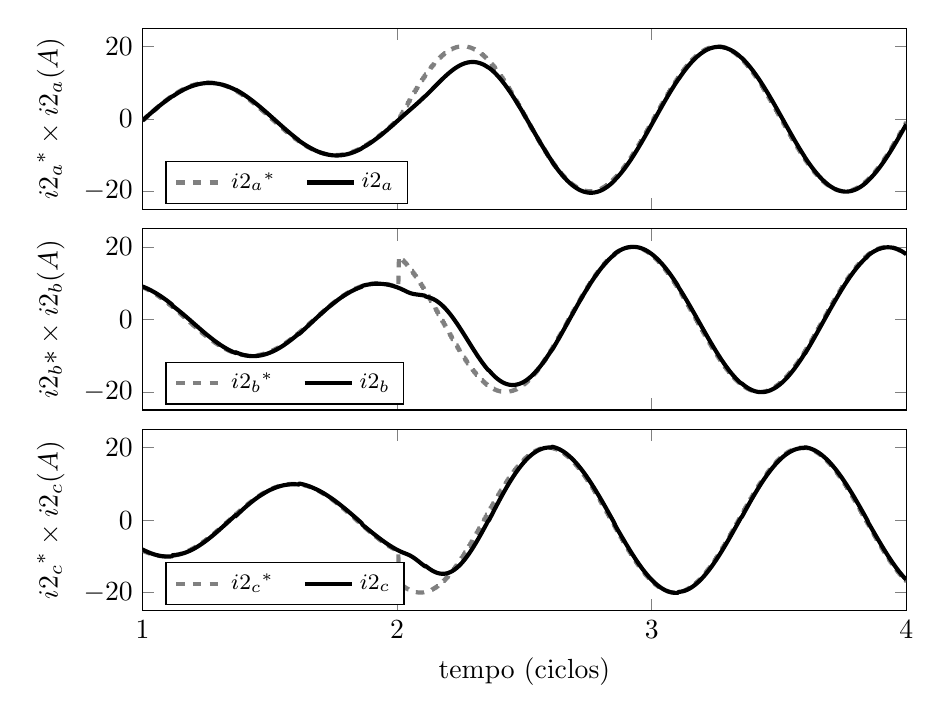
\begin{tikzpicture}

\begin{axis}[%
width=0.8\textwidth,
height=0.189701500343624\textwidth,
scale only axis,
xmin=0.0166666666666667,
xmax=0.0666666666666667,
xtick={0.0166666666666667,0.0333333333333333,0.05,0.0666666666666667},
xticklabels={\empty},
ymin=-25,
ymax=25,
ytick={-20,   0,  20},
ylabel={${\text{i2}_\text{b}}\text{* }\times\text{ i2}_\text{b}\text{ (A)}$},
name=plot2,
legend style={at={(0.03,0.03)},anchor=south west,draw=black,fill=white,legend cell align=left},
scaled x ticks = false,
legend columns=-1,
legend style={/tikz/every even column/.append style={column sep=0.3cm}},
legend style={font=\footnotesize}
]
\addplot [color=gray,dashed,line width=1.5pt]
  table[row sep=crcr]{0.0166583333333333	8.95711760239421\\
0.0167	8.81303452065\\
0.0167416666666667	8.81303452065\\
0.0167833333333333	8.66025403784447\\
0.016825	8.66025403784447\\
0.0168666666666667	8.49892692986872\\
0.0169083333333333	8.49892692986872\\
0.01695	8.32921240710107\\
0.0169916666666667	8.32921240710107\\
0.0170333333333333	8.15127795728562\\
0.017075	8.15127795728562\\
0.0171166666666667	7.96529918024204\\
0.0171583333333333	7.96529918024204\\
0.0172	7.77145961456979\\
0.0172416666666667	7.77145961456979\\
0.0172833333333333	7.56995055651764\\
0.017325	7.56995055651764\\
0.0173666666666667	7.36097087119742\\
0.0174083333333333	7.36097087119742\\
0.01745	7.1447267963281\\
0.0174916666666667	7.1447267963281\\
0.0175333333333333	6.92143173870414\\
0.017575	6.92143173870414\\
0.0176166666666667	6.69130606358865\\
0.0176583333333333	6.69130606358865\\
0.0177	6.45457687723957\\
0.0177416666666667	6.45457687723957\\
0.0177833333333333	6.21147780278317\\
0.017825	6.21147780278317\\
0.0178666666666667	5.96224874965622\\
0.0179083333333333	5.96224874965622\\
0.01795	5.70713567684438\\
0.0179916666666667	5.70713567684438\\
0.0180333333333333	5.44639035015033\\
0.018075	5.44639035015033\\
0.0181166666666667	5.18027009373136\\
0.0181583333333333	5.18027009373136\\
0.0182	4.90903753615147\\
0.0182416666666667	4.90903753615147\\
0.0182833333333333	4.63296035119867\\
0.018325	4.63296035119867\\
0.0183666666666667	4.35231099372333\\
0.0184083333333333	4.35231099372333\\
0.01845	4.06736643075805\\
0.0184916666666667	4.06736643075805\\
0.0185333333333333	3.77840786818472\\
0.018575	3.77840786818472\\
0.0186166666666667	3.4857204732182\\
0.0186583333333333	3.4857204732182\\
0.0187	3.18959309298074\\
0.0187416666666667	3.18959309298074\\
0.0187833333333333	2.89031796944476\\
0.018825	2.89031796944476\\
0.0188666666666667	2.58819045102524\\
0.0189083333333333	2.58819045102524\\
0.01895	2.28350870110659\\
0.0189916666666667	2.28350870110659\\
0.0190333333333333	1.97657340379129\\
0.019075	1.97657340379129\\
0.0191166666666667	1.66768746716105\\
0.0191583333333333	1.66768746716105\\
0.0192	1.35715572434307\\
0.0192416666666667	1.35715572434307\\
0.0192833333333333	1.04528463267656\\
0.019325	1.04528463267656\\
0.0193666666666667	0.732381971276336\\
0.0194083333333333	0.732381971276336\\
0.01945	0.418756537292012\\
0.0194916666666667	0.418756537292012\\
0.0195333333333333	0.104717841162471\\
0.019575	0.104717841162471\\
0.0196166666666667	-0.20942419883356\\
0.0196583333333333	-0.20942419883356\\
0.0197	-0.523359562429432\\
0.0197416666666667	-0.523359562429432\\
0.0197833333333333	-0.836778433323152\\
0.019825	-0.836778433323152\\
0.0198666666666667	-1.14937150492867\\
0.0199083333333333	-1.14937150492867\\
0.01995	-1.46083028562412\\
0.0199916666666667	-1.46083028562412\\
0.0200333333333333	-1.77084740319584\\
0.020075	-1.77084740319584\\
0.0201166666666667	-2.0791169081776\\
0.0201583333333333	-2.0791169081776\\
0.0202	-2.38533457578582\\
0.0202416666666667	-2.38533457578582\\
0.0202833333333333	-2.68919820615267\\
0.020325	-2.68919820615267\\
0.0203666666666667	-2.99040792256089\\
0.0204083333333333	-2.99040792256089\\
0.02045	-3.28866646738586\\
0.0204916666666667	-3.28866646738586\\
0.0205333333333333	-3.58367949545303\\
0.020575	-3.58367949545303\\
0.0206166666666667	-3.87515586452106\\
0.0206583333333333	-3.87515586452106\\
0.0207	-4.16280792260405\\
0.0207416666666667	-4.16280792260405\\
0.0207833333333333	-4.44635179184931\\
0.020825	-4.44635179184931\\
0.0208666666666667	-4.72550764869058\\
0.0209083333333333	-4.72550764869058\\
0.02095	-5.00000000000005\\
0.0209916666666667	-5.00000000000005\\
0.0210333333333333	-5.26955795496682\\
0.021075	-5.26955795496682\\
0.0211166666666667	-5.53391549243349\\
0.0211583333333333	-5.53391549243349\\
0.0212	-5.79281172342684\\
0.0212416666666667	-5.79281172342684\\
0.0212833333333333	-6.0459911486238\\
0.021325	-6.0459911486238\\
0.0213666666666667	-6.29320391049844\\
0.0214083333333333	-6.29320391049844\\
0.02145	-6.53420603990112\\
0.0214916666666667	-6.53420603990112\\
0.0215333333333333	-6.76875969682667\\
0.021575	-6.76875969682667\\
0.0216166666666667	-6.99663340513372\\
0.0216583333333333	-6.99663340513372\\
0.0217	-7.2176022809837\\
0.0217416666666667	-7.2176022809837\\
0.0217833333333333	-7.43144825477402\\
0.021825	-7.43144825477402\\
0.0218666666666667	-7.6379602863465\\
0.0219083333333333	-7.6379602863465\\
0.02195	-7.83693457325848\\
0.0219916666666667	-7.83693457325848\\
0.0220333333333333	-8.02817475191123\\
0.022075	-8.02817475191123\\
0.0221166666666667	-8.21149209133713\\
0.0221583333333333	-8.21149209133713\\
0.0222	-8.38670567945433\\
0.0222416666666667	-8.38670567945433\\
0.0222833333333333	-8.55364260160516\\
0.022325	-8.55364260160516\\
0.0223666666666667	-8.71213811120199\\
0.0224083333333333	-8.71213811120199\\
0.02245	-8.86203579231225\\
0.0224916666666667	-8.86203579231225\\
0.0225333333333333	-9.00318771402204\\
0.022575	-9.00318771402204\\
0.0226166666666667	-9.13545457642611\\
0.0226583333333333	-9.13545457642611\\
0.0227	-9.25870584810006\\
0.0227416666666667	-9.25870584810006\\
0.0227833333333333	-9.37281989491902\\
0.022825	-9.37281989491902\\
0.0228666666666667	-9.47768410009597\\
0.0229083333333333	-9.47768410009597\\
0.02295	-9.57319497532079\\
0.0229916666666667	-9.57319497532079\\
0.0230333333333333	-9.6592582628908\\
0.023075	-9.6592582628908\\
0.0231166666666667	-9.73578902873172\\
0.0231583333333333	-9.73578902873172\\
0.0232	-9.80271174621734\\
0.0232416666666667	-9.80271174621734\\
0.0232833333333333	-9.85996037070517\\
0.023325	-9.85996037070517\\
0.0233666666666667	-9.90747840471456\\
0.0234083333333333	-9.90747840471456\\
0.02345	-9.94521895368285\\
0.0234916666666667	-9.94521895368285\\
0.0235333333333333	-9.97314477224471\\
0.023575	-9.97314477224471\\
0.0236166666666667	-9.99122830098871\\
0.0236583333333333	-9.99122830098871\\
0.0237	-9.99945169365525\\
0.0237416666666667	-9.99945169365525\\
0.0237833333333333	-9.99780683474858\\
0.023825	-9.99780683474858\\
0.0238666666666667	-9.98629534754587\\
0.0239083333333333	-9.98629534754587\\
0.02395	-9.96492859249517\\
0.0239916666666667	-9.96492859249517\\
0.0240333333333333	-9.93372765600409\\
0.024075	-9.93372765600409\\
0.0241166666666667	-9.89272332963001\\
0.0241583333333333	-9.89272332963001\\
0.0242	-9.84195607969255\\
0.0242416666666667	-9.84195607969255\\
0.0242833333333333	-9.78147600733818\\
0.024325	-9.78147600733818\\
0.0243666666666667	-9.71134279909649\\
0.0244083333333333	-9.71134279909649\\
0.02445	-9.63162566797671\\
0.0244916666666667	-9.63162566797671\\
0.0245333333333333	-9.5424032851629\\
0.024575	-9.5424032851629\\
0.0246166666666667	-9.44376370237494\\
0.0246583333333333	-9.44376370237494\\
0.0247	-9.33580426497215\\
0.0247416666666667	-9.33580426497215\\
0.0247833333333333	-9.21863151588513\\
0.024825	-9.21863151588513\\
0.0248666666666667	-9.09236109047081\\
0.0249083333333333	-9.09236109047081\\
0.02495	-8.95711760239425\\
0.0249916666666667	-8.95711760239425\\
0.0250333333333333	-8.81303452065005\\
0.025075	-8.81303452065005\\
0.0251166666666667	-8.66025403784451\\
0.0251583333333333	-8.66025403784451\\
0.0252	-8.49892692986876\\
0.0252416666666667	-8.49892692986876\\
0.0252833333333333	-8.32921240710111\\
0.025325	-8.32921240710111\\
0.0253666666666667	-8.15127795728566\\
0.0254083333333333	-8.15127795728566\\
0.02545	-7.96529918024207\\
0.0254916666666667	-7.96529918024207\\
0.0255333333333333	-7.77145961456982\\
0.025575	-7.77145961456982\\
0.0256166666666667	-7.56995055651767\\
0.0256583333333333	-7.56995055651767\\
0.0257	-7.36097087119745\\
0.0257416666666667	-7.36097087119745\\
0.0257833333333333	-7.14472679632814\\
0.025825	-7.14472679632814\\
0.0258666666666667	-6.92143173870417\\
0.0259083333333333	-6.92143173870417\\
0.02595	-6.69130606358868\\
0.0259916666666667	-6.69130606358868\\
0.0260333333333333	-6.4545768772396\\
0.026075	-6.4545768772396\\
0.0261166666666667	-6.2114778027832\\
0.0261583333333333	-6.2114778027832\\
0.0262	-5.96224874965625\\
0.0262416666666667	-5.96224874965625\\
0.0262833333333333	-5.70713567684441\\
0.026325	-5.70713567684441\\
0.0263666666666667	-5.44639035015036\\
0.0264083333333333	-5.44639035015036\\
0.02645	-5.18027009373139\\
0.0264916666666667	-5.18027009373139\\
0.0265333333333333	-4.90903753615149\\
0.026575	-4.90903753615149\\
0.0266166666666667	-4.6329603511987\\
0.0266583333333333	-4.6329603511987\\
0.0267	-4.35231099372335\\
0.0267416666666667	-4.35231099372335\\
0.0267833333333333	-4.06736643075807\\
0.026825	-4.06736643075807\\
0.0268666666666667	-3.77840786818474\\
0.0269083333333333	-3.77840786818474\\
0.02695	-3.48572047321821\\
0.0269916666666667	-3.48572047321821\\
0.0270333333333333	-3.18959309298076\\
0.027075	-3.18959309298076\\
0.0271166666666667	-2.89031796944477\\
0.0271583333333333	-2.89031796944477\\
0.0272	-2.58819045102526\\
0.0272416666666667	-2.58819045102526\\
0.0272833333333333	-2.28350870110661\\
0.027325	-2.28350870110661\\
0.0273666666666667	-1.9765734037913\\
0.0274083333333333	-1.9765734037913\\
0.02745	-1.66768746716106\\
0.0274916666666667	-1.66768746716106\\
0.0275333333333333	-1.35715572434308\\
0.027575	-1.35715572434308\\
0.0276166666666667	-1.04528463267656\\
0.0276583333333333	-1.04528463267656\\
0.0277	-0.732381971276341\\
0.0277416666666667	-0.732381971276341\\
0.0277833333333333	-0.418756537292015\\
0.027825	-0.418756537292015\\
0.0278666666666667	-0.104717841162473\\
0.0279083333333333	-0.104717841162473\\
0.02795	0.209424198833559\\
0.0279916666666667	0.209424198833559\\
0.0280333333333333	0.523359562429433\\
0.028075	0.523359562429433\\
0.0281166666666667	0.836778433323154\\
0.0281583333333333	0.836778433323154\\
0.0282	1.14937150492867\\
0.0282416666666667	1.14937150492867\\
0.0282833333333333	1.46083028562412\\
0.028325	1.46083028562412\\
0.0283666666666667	1.77084740319585\\
0.0284083333333333	1.77084740319585\\
0.02845	2.07911690817761\\
0.0284916666666667	2.07911690817761\\
0.0285333333333333	2.38533457578583\\
0.028575	2.38533457578583\\
0.0286166666666667	2.68919820615268\\
0.0286583333333333	2.68919820615268\\
0.0287	2.9904079225609\\
0.0287416666666667	2.9904079225609\\
0.0287833333333333	3.28866646738587\\
0.028825	3.28866646738587\\
0.0288666666666667	3.58367949545304\\
0.0289083333333333	3.58367949545304\\
0.02895	3.87515586452107\\
0.0289916666666667	3.87515586452107\\
0.0290333333333333	4.16280792260406\\
0.029075	4.16280792260406\\
0.0291166666666667	4.44635179184933\\
0.0291583333333333	4.44635179184933\\
0.0292	4.7255076486906\\
0.0292416666666667	4.7255076486906\\
0.0292833333333333	5.00000000000006\\
0.029325	5.00000000000006\\
0.0293666666666667	5.26955795496684\\
0.0294083333333333	5.26955795496684\\
0.02945	5.53391549243351\\
0.0294916666666667	5.53391549243351\\
0.0295333333333333	5.79281172342686\\
0.029575	5.79281172342686\\
0.0296166666666667	6.04599114862383\\
0.0296583333333333	6.04599114862383\\
0.0297	6.29320391049846\\
0.0297416666666667	6.29320391049846\\
0.0297833333333333	6.53420603990114\\
0.029825	6.53420603990114\\
0.0298666666666667	6.7687596968267\\
0.0299083333333333	6.7687596968267\\
0.02995	6.99663340513375\\
0.0299916666666667	6.99663340513375\\
0.0300333333333333	7.21760228098372\\
0.030075	7.21760228098372\\
0.0301166666666667	7.43144825477405\\
0.0301583333333333	7.43144825477405\\
0.0302	7.63796028634653\\
0.0302416666666667	7.63796028634653\\
0.0302833333333333	7.83693457325851\\
0.030325	7.83693457325851\\
0.0303666666666667	8.02817475191126\\
0.0304083333333333	8.02817475191126\\
0.03045	8.21149209133716\\
0.0304916666666667	8.21149209133716\\
0.0305333333333333	8.38670567945436\\
0.030575	8.38670567945436\\
0.0306166666666667	8.55364260160519\\
0.0306583333333333	8.55364260160519\\
0.0307	8.71213811120203\\
0.0307416666666667	8.71213811120203\\
0.0307833333333333	8.86203579231228\\
0.030825	8.86203579231228\\
0.0308666666666667	9.00318771402207\\
0.0309083333333333	9.00318771402207\\
0.03095	9.13545457642615\\
0.0309916666666667	9.13545457642615\\
0.0310333333333333	9.25870584810009\\
0.031075	9.25870584810009\\
0.0311166666666667	9.37281989491906\\
0.0311583333333333	9.37281989491906\\
0.0312	9.477684100096\\
0.0312416666666667	9.477684100096\\
0.0312833333333333	9.57319497532082\\
0.031325	9.57319497532082\\
0.0313666666666667	9.65925826289084\\
0.0314083333333333	9.65925826289084\\
0.03145	9.73578902873176\\
0.0314916666666667	9.73578902873176\\
0.0315333333333333	9.80271174621738\\
0.031575	9.80271174621738\\
0.0316166666666667	9.85996037070521\\
0.0316583333333333	9.85996037070521\\
0.0317	9.9074784047146\\
0.0317416666666667	9.9074784047146\\
0.0317833333333333	9.94521895368289\\
0.031825	9.94521895368289\\
0.0318666666666667	9.97314477224474\\
0.0319083333333333	9.97314477224474\\
0.03195	9.99122830098875\\
0.0319916666666667	9.99122830098875\\
0.0320333333333333	9.99945169365528\\
0.032075	9.99945169365528\\
0.0321166666666667	9.99780683474862\\
0.0321583333333333	9.99780683474862\\
0.0322	9.98629534754591\\
0.0322416666666667	9.98629534754591\\
0.0322833333333333	9.96492859249521\\
0.032325	9.96492859249521\\
0.0323666666666667	9.93372765600413\\
0.0324083333333333	9.93372765600413\\
0.03245	9.89272332963005\\
0.0324916666666667	9.89272332963005\\
0.0325333333333333	9.84195607969259\\
0.032575	9.84195607969259\\
0.0326166666666667	9.78147600733822\\
0.0326583333333333	9.78147600733822\\
0.0327	9.71134279909653\\
0.0327416666666667	9.71134279909653\\
0.0327833333333333	9.63162566797675\\
0.032825	9.63162566797675\\
0.0328666666666667	9.54240328516294\\
0.0329083333333333	9.54240328516294\\
0.03295	9.44376370237498\\
0.0329916666666667	9.44376370237498\\
0.0330333333333333	9.33580426497218\\
0.033075	9.33580426497218\\
0.0331166666666667	9.21863151588517\\
0.0331583333333333	9.21863151588517\\
0.0332	9.09236109047085\\
0.0332416666666667	9.09236109047085\\
0.0332833333333333	8.95711760239429\\
0.033325	8.95711760239429\\
0.0333666666666667	8.81303452065008\\
0.0334083333333333	8.81303452065008\\
0.03345	17.3205080756891\\
0.0334916666666667	17.3205080756891\\
0.0335333333333333	16.9978538597376\\
0.033575	16.9978538597376\\
0.0336166666666667	16.6584248142023\\
0.0336583333333333	16.6584248142023\\
0.0337	16.3025559145714\\
0.0337416666666667	16.3025559145714\\
0.0337833333333333	15.9305983604842\\
0.033825	15.9305983604842\\
0.0338666666666667	15.5429192291397\\
0.0339083333333333	15.5429192291397\\
0.03395	15.1399011130354\\
0.0339916666666667	15.1399011130354\\
0.0340333333333333	14.721941742395\\
0.034075	14.721941742395\\
0.0341166666666667	14.2894535926563\\
0.0341583333333333	14.2894535926563\\
0.0342	13.8428634774084\\
0.0342416666666667	13.8428634774084\\
0.0342833333333333	13.3826121271774\\
0.034325	13.3826121271774\\
0.0343666666666667	12.9091537544793\\
0.0344083333333333	12.9091537544793\\
0.03445	12.4229556055665\\
0.0344916666666667	12.4229556055665\\
0.0345333333333333	11.9244974993126\\
0.034575	11.9244974993126\\
0.0346166666666667	11.4142713536889\\
0.0346583333333333	11.4142713536889\\
0.0347	10.8927807003008\\
0.0347416666666667	10.8927807003008\\
0.0347833333333333	10.3605401874628\\
0.034825	10.3605401874628\\
0.0348666666666667	9.81807507230302\\
0.0349083333333333	9.81807507230302\\
0.03495	9.26592070239743\\
0.0349916666666667	9.26592070239743\\
0.0350333333333333	8.70462198744674\\
0.035075	8.70462198744674\\
0.0351166666666667	8.13473286151618\\
0.0351583333333333	8.13473286151618\\
0.0352	7.55681573636951\\
0.0352416666666667	7.55681573636951\\
0.0352833333333333	6.97144094643646\\
0.035325	6.97144094643646\\
0.0353666666666667	6.37918618596155\\
0.0354083333333333	6.37918618596155\\
0.03545	5.78063593888957\\
0.0354916666666667	5.78063593888957\\
0.0355333333333333	5.17638090205054\\
0.035575	5.17638090205054\\
0.0356166666666667	4.56701740221323\\
0.0356583333333333	4.56701740221323\\
0.0357	3.95314680758263\\
0.0357416666666667	3.95314680758263\\
0.0357833333333333	3.33537493432214\\
0.035825	3.33537493432214\\
0.0358666666666667	2.71431144868617\\
0.0359083333333333	2.71431144868617\\
0.03595	2.09056926535314\\
0.0359916666666667	2.09056926535314\\
0.0360333333333333	1.4647639425527\\
0.036075	1.4647639425527\\
0.0361166666666667	0.837513074584043\\
0.0361583333333333	0.837513074584043\\
0.0362	0.209435682324955\\
0.0362416666666667	0.209435682324955\\
0.0362833333333333	-0.418848397667113\\
0.036325	-0.418848397667113\\
0.0363666666666667	-1.04671912485886\\
0.0364083333333333	-1.04671912485886\\
0.03645	-1.67355686664631\\
0.0364916666666667	-1.67355686664631\\
0.0365333333333333	-2.29874300985734\\
0.036575	-2.29874300985734\\
0.0366166666666667	-2.92166057124825\\
0.0366583333333333	-2.92166057124825\\
0.0367	-3.5416948063917\\
0.0367416666666667	-3.5416948063917\\
0.0367833333333333	-4.15823381635523\\
0.036825	-4.15823381635523\\
0.0368666666666667	-4.77066915157168\\
0.0369083333333333	-4.77066915157168\\
0.03695	-5.37839641230538\\
0.0369916666666667	-5.37839641230538\\
0.0370333333333333	-5.98081584512182\\
0.037075	-5.98081584512182\\
0.0371166666666667	-6.57733293477176\\
0.0371583333333333	-6.57733293477176\\
0.0372	-7.16735899090611\\
0.0372416666666667	-7.16735899090611\\
0.0372833333333333	-7.75031172904218\\
0.037325	-7.75031172904218\\
0.0373666666666667	-8.32561584520815\\
0.0374083333333333	-8.32561584520815\\
0.03745	-8.89270358369869\\
0.0374916666666667	-8.89270358369869\\
0.0375333333333333	-9.45101529738123\\
0.037575	-9.45101529738123\\
0.0376166666666667	-10.0000000000002\\
0.0376583333333333	-10.0000000000002\\
0.0377	-10.5391159099337\\
0.0377416666666667	-10.5391159099337\\
0.0377833333333333	-11.0678309848671\\
0.037825	-11.0678309848671\\
0.0378666666666667	-11.5856234468538\\
0.0379083333333333	-11.5856234468538\\
0.03795	-12.0919822972477\\
0.0379916666666667	-12.0919822972477\\
0.0380333333333333	-12.586407820997\\
0.038075	-12.586407820997\\
0.0381166666666667	-13.0684120798023\\
0.0381583333333333	-13.0684120798023\\
0.0382	-13.5375193936535\\
0.0382416666666667	-13.5375193936535\\
0.0382833333333333	-13.9932668102676\\
0.038325	-13.9932668102676\\
0.0383666666666667	-14.4352045619675\\
0.0384083333333333	-14.4352045619675\\
0.03845	-14.8628965095482\\
0.0384916666666667	-14.8628965095482\\
0.0385333333333333	-15.2759205726931\\
0.038575	-15.2759205726931\\
0.0386166666666667	-15.6738691465171\\
0.0386583333333333	-15.6738691465171\\
0.0387	-16.0563495038226\\
0.0387416666666667	-16.0563495038226\\
0.0387833333333333	-16.4229841826744\\
0.038825	-16.4229841826744\\
0.0388666666666667	-16.7734113589088\\
0.0389083333333333	-16.7734113589088\\
0.03895	-17.1072852032105\\
0.0389916666666667	-17.1072852032105\\
0.0390333333333333	-17.4242762224041\\
0.039075	-17.4242762224041\\
0.0391166666666667	-17.7240715846246\\
0.0391583333333333	-17.7240715846246\\
0.0392	-18.0063754280442\\
0.0392416666666667	-18.0063754280442\\
0.0392833333333333	-18.2709091528524\\
0.039325	-18.2709091528524\\
0.0393666666666667	-18.5174116962003\\
0.0394083333333333	-18.5174116962003\\
0.03945	-18.7456397898382\\
0.0394916666666667	-18.7456397898382\\
0.0395333333333333	-18.9553682001921\\
0.039575	-18.9553682001921\\
0.0396166666666667	-19.1463899506417\\
0.0396583333333333	-19.1463899506417\\
0.0397	-19.3185165257817\\
0.0397416666666667	-19.3185165257817\\
0.0397833333333333	-19.4715780574636\\
0.039825	-19.4715780574636\\
0.0398666666666667	-19.6054234924348\\
0.0399083333333333	-19.6054234924348\\
0.03995	-19.7199207414105\\
0.0399916666666667	-19.7199207414105\\
0.0400333333333333	-19.8149568094293\\
0.040075	-19.8149568094293\\
0.0401166666666667	-19.8904379073659\\
0.0401583333333333	-19.8904379073659\\
0.0402	-19.9462895444896\\
0.0402416666666667	-19.9462895444896\\
0.0402833333333333	-19.9824566019776\\
0.040325	-19.9824566019776\\
0.0403666666666667	-19.9989033873107\\
0.0404083333333333	-19.9989033873107\\
0.04045	-19.9956136694973\\
0.0404916666666667	-19.9956136694973\\
0.0405333333333333	-19.9725906950919\\
0.040575	-19.9725906950919\\
0.0406166666666667	-19.9298571849905\\
0.0406583333333333	-19.9298571849905\\
0.0407	-19.8674553120083\\
0.0407416666666667	-19.8674553120083\\
0.0407833333333333	-19.7854466592602\\
0.040825	-19.7854466592602\\
0.0408666666666667	-19.6839121593853\\
0.0409083333333333	-19.6839121593853\\
0.04095	-19.5629520146765\\
0.0409916666666667	-19.5629520146765\\
0.0410333333333333	-19.4226855981931\\
0.041075	-19.4226855981931\\
0.0411166666666667	-19.2632513359536\\
0.0411583333333333	-19.2632513359536\\
0.0412	-19.084806570326\\
0.0412416666666667	-19.084806570326\\
0.0412833333333333	-18.88752740475\\
0.041325	-18.88752740475\\
0.0413666666666667	-18.6716085299444\\
0.0414083333333333	-18.6716085299444\\
0.04145	-18.4372630317704\\
0.0414916666666667	-18.4372630317704\\
0.0415333333333333	-18.1847221809418\\
0.041575	-18.1847221809418\\
0.0416166666666667	-17.9142352047887\\
0.0416583333333333	-17.9142352047887\\
0.0417	-17.6260690413002\\
0.0417416666666667	-17.6260690413002\\
0.0417833333333333	-17.3205080756892\\
0.041825	-17.3205080756892\\
0.0418666666666667	-16.9978538597377\\
0.0419083333333333	-16.9978538597377\\
0.04195	-16.6584248142024\\
0.0419916666666667	-16.6584248142024\\
0.0420333333333333	-16.3025559145715\\
0.042075	-16.3025559145715\\
0.0421166666666667	-15.9305983604843\\
0.0421583333333333	-15.9305983604843\\
0.0422	-15.5429192291398\\
0.0422416666666667	-15.5429192291398\\
0.0422833333333333	-15.1399011130355\\
0.042325	-15.1399011130355\\
0.0423666666666667	-14.721941742395\\
0.0424083333333333	-14.721941742395\\
0.04245	-14.2894535926564\\
0.0424916666666667	-14.2894535926564\\
0.0425333333333333	-13.8428634774085\\
0.042575	-13.8428634774085\\
0.0426166666666667	-13.3826121271775\\
0.0426583333333333	-13.3826121271775\\
0.0427	-12.9091537544793\\
0.0427416666666667	-12.9091537544793\\
0.0427833333333333	-12.4229556055665\\
0.042825	-12.4229556055665\\
0.0428666666666667	-11.9244974993126\\
0.0429083333333333	-11.9244974993126\\
0.04295	-11.4142713536889\\
0.0429916666666667	-11.4142713536889\\
0.0430333333333333	-10.8927807003008\\
0.043075	-10.8927807003008\\
0.0431166666666667	-10.3605401874629\\
0.0431583333333333	-10.3605401874629\\
0.0432	-9.81807507230306\\
0.0432416666666667	-9.81807507230306\\
0.0432833333333333	-9.26592070239747\\
0.043325	-9.26592070239747\\
0.0433666666666667	-8.70462198744678\\
0.0434083333333333	-8.70462198744678\\
0.04345	-8.13473286151622\\
0.0434916666666667	-8.13473286151622\\
0.0435333333333333	-7.55681573636955\\
0.043575	-7.55681573636955\\
0.0436166666666667	-6.97144094643649\\
0.0436583333333333	-6.97144094643649\\
0.0437	-6.37918618596158\\
0.0437416666666667	-6.37918618596158\\
0.0437833333333333	-5.7806359388896\\
0.043825	-5.7806359388896\\
0.0438666666666667	-5.17638090205057\\
0.0439083333333333	-5.17638090205057\\
0.04395	-4.56701740221326\\
0.0439916666666667	-4.56701740221326\\
0.0440333333333333	-3.95314680758265\\
0.044075	-3.95314680758265\\
0.0441166666666667	-3.33537493432216\\
0.0441583333333333	-3.33537493432216\\
0.0442	-2.71431144868619\\
0.0442416666666667	-2.71431144868619\\
0.0442833333333333	-2.09056926535316\\
0.044325	-2.09056926535316\\
0.0443666666666667	-1.46476394255271\\
0.0444083333333333	-1.46476394255271\\
0.04445	-0.83751307458405\\
0.0444916666666667	-0.83751307458405\\
0.0445333333333333	-0.209435682324959\\
0.044575	-0.209435682324959\\
0.0446166666666667	0.418848397667111\\
0.0446583333333333	0.418848397667111\\
0.0447	1.04671912485886\\
0.0447416666666667	1.04671912485886\\
0.0447833333333333	1.67355686664631\\
0.044825	1.67355686664631\\
0.0448666666666667	2.29874300985735\\
0.0449083333333333	2.29874300985735\\
0.04495	2.92166057124826\\
0.0449916666666667	2.92166057124826\\
0.0450333333333333	3.54169480639171\\
0.045075	3.54169480639171\\
0.0451166666666667	4.15823381635525\\
0.0451583333333333	4.15823381635525\\
0.0452	4.77066915157169\\
0.0452416666666667	4.77066915157169\\
0.0452833333333333	5.37839641230541\\
0.045325	5.37839641230541\\
0.0453666666666667	5.98081584512184\\
0.0454083333333333	5.98081584512184\\
0.04545	6.57733293477179\\
0.0454916666666667	6.57733293477179\\
0.0455333333333333	7.16735899090614\\
0.045575	7.16735899090614\\
0.0456166666666667	7.75031172904221\\
0.0456583333333333	7.75031172904221\\
0.0457	8.32561584520819\\
0.0457416666666667	8.32561584520819\\
0.0457833333333333	8.89270358369873\\
0.045825	8.89270358369873\\
0.0458666666666667	9.45101529738127\\
0.0459083333333333	9.45101529738127\\
0.04595	10.0000000000002\\
0.0459916666666667	10.0000000000002\\
0.0460333333333333	10.5391159099338\\
0.046075	10.5391159099338\\
0.0461166666666667	11.0678309848671\\
0.0461583333333333	11.0678309848671\\
0.0462	11.5856234468538\\
0.0462416666666667	11.5856234468538\\
0.0462833333333333	12.0919822972478\\
0.046325	12.0919822972478\\
0.0463666666666667	12.586407820997\\
0.0464083333333333	12.586407820997\\
0.04645	13.0684120798024\\
0.0464916666666667	13.0684120798024\\
0.0465333333333333	13.5375193936535\\
0.046575	13.5375193936535\\
0.0466166666666667	13.9932668102676\\
0.0466583333333333	13.9932668102676\\
0.0467	14.4352045619676\\
0.0467416666666667	14.4352045619676\\
0.0467833333333333	14.8628965095482\\
0.046825	14.8628965095482\\
0.0468666666666667	15.2759205726932\\
0.0469083333333333	15.2759205726932\\
0.04695	15.6738691465172\\
0.0469916666666667	15.6738691465172\\
0.0470333333333333	16.0563495038227\\
0.047075	16.0563495038227\\
0.0471166666666667	16.4229841826745\\
0.0471583333333333	16.4229841826745\\
0.0472	16.7734113589089\\
0.0472416666666667	16.7734113589089\\
0.0472833333333333	17.1072852032105\\
0.047325	17.1072852032105\\
0.0473666666666667	17.4242762224042\\
0.0474083333333333	17.4242762224042\\
0.04745	17.7240715846247\\
0.0474916666666667	17.7240715846247\\
0.0475333333333333	18.0063754280443\\
0.047575	18.0063754280443\\
0.0476166666666667	18.2709091528525\\
0.0476583333333333	18.2709091528525\\
0.0477	18.5174116962003\\
0.0477416666666667	18.5174116962003\\
0.0477833333333333	18.7456397898383\\
0.047825	18.7456397898383\\
0.0478666666666667	18.9553682001922\\
0.0479083333333333	18.9553682001922\\
0.04795	19.1463899506418\\
0.0479916666666667	19.1463899506418\\
0.0480333333333333	19.3185165257818\\
0.048075	19.3185165257818\\
0.0481166666666667	19.4715780574637\\
0.0481583333333333	19.4715780574637\\
0.0482	19.6054234924349\\
0.0482416666666667	19.6054234924349\\
0.0482833333333333	19.7199207414106\\
0.048325	19.7199207414106\\
0.0483666666666667	19.8149568094294\\
0.0484083333333333	19.8149568094294\\
0.04845	19.890437907366\\
0.0484916666666667	19.890437907366\\
0.0485333333333333	19.9462895444897\\
0.048575	19.9462895444897\\
0.0486166666666667	19.9824566019777\\
0.0486583333333333	19.9824566019777\\
0.0487	19.9989033873107\\
0.0487416666666667	19.9989033873107\\
0.0487833333333333	19.9956136694974\\
0.048825	19.9956136694974\\
0.0488666666666667	19.972590695092\\
0.0489083333333333	19.972590695092\\
0.04895	19.9298571849906\\
0.0489916666666667	19.9298571849906\\
0.0490333333333333	19.8674553120084\\
0.049075	19.8674553120084\\
0.0491166666666667	19.7854466592603\\
0.0491583333333333	19.7854466592603\\
0.0492	19.6839121593854\\
0.0492416666666667	19.6839121593854\\
0.0492833333333333	19.5629520146766\\
0.049325	19.5629520146766\\
0.0493666666666667	19.4226855981932\\
0.0494083333333333	19.4226855981932\\
0.04945	19.2632513359537\\
0.0494916666666667	19.2632513359537\\
0.0495333333333333	19.084806570326\\
0.049575	19.084806570326\\
0.0496166666666667	18.8875274047501\\
0.0496583333333333	18.8875274047501\\
0.0497	18.6716085299445\\
0.0497416666666667	18.6716085299445\\
0.0497833333333333	18.4372630317705\\
0.049825	18.4372630317705\\
0.0498666666666667	18.1847221809419\\
0.0499083333333333	18.1847221809419\\
0.04995	17.9142352047887\\
0.0499916666666667	17.9142352047887\\
0.0500333333333333	17.6260690413003\\
0.050075	17.6260690413003\\
0.0501166666666667	17.3205080756892\\
0.0501583333333333	17.3205080756892\\
0.0502	16.9978538597377\\
0.0502416666666667	16.9978538597377\\
0.0502833333333333	16.6584248142025\\
0.050325	16.6584248142025\\
0.0503666666666667	16.3025559145715\\
0.0504083333333333	16.3025559145715\\
0.05045	15.9305983604844\\
0.0504916666666667	15.9305983604844\\
0.0505333333333333	15.5429192291399\\
0.050575	15.5429192291399\\
0.0506166666666667	15.1399011130356\\
0.0506583333333333	15.1399011130356\\
0.0507	14.7219417423951\\
0.0507416666666667	14.7219417423951\\
0.0507833333333333	14.2894535926565\\
0.050825	14.2894535926565\\
0.0508666666666667	13.8428634774085\\
0.0509083333333333	13.8428634774085\\
0.05095	13.3826121271776\\
0.0509916666666667	13.3826121271776\\
0.0510333333333333	12.9091537544794\\
0.051075	12.9091537544794\\
0.0511166666666667	12.4229556055666\\
0.0511583333333333	12.4229556055666\\
0.0512	11.9244974993127\\
0.0512416666666667	11.9244974993127\\
0.0512833333333333	11.414271353689\\
0.051325	11.414271353689\\
0.0513666666666667	10.8927807003009\\
0.0514083333333333	10.8927807003009\\
0.05145	10.3605401874629\\
0.0514916666666667	10.3605401874629\\
0.0515333333333333	9.81807507230311\\
0.051575	9.81807507230311\\
0.0516166666666667	9.26592070239752\\
0.0516583333333333	9.26592070239752\\
0.0517	8.70462198744682\\
0.0517416666666667	8.70462198744682\\
0.0517833333333333	8.13473286151626\\
0.051825	8.13473286151626\\
0.0518666666666667	7.55681573636959\\
0.0519083333333333	7.55681573636959\\
0.05195	6.97144094643653\\
0.0519916666666667	6.97144094643653\\
0.0520333333333333	6.37918618596161\\
0.052075	6.37918618596161\\
0.0521166666666667	5.78063593888963\\
0.0521583333333333	5.78063593888963\\
0.0522	5.1763809020506\\
0.0522416666666667	5.1763809020506\\
0.0522833333333333	4.56701740221328\\
0.052325	4.56701740221328\\
0.0523666666666667	3.95314680758267\\
0.0524083333333333	3.95314680758267\\
0.05245	3.33537493432218\\
0.0524916666666667	3.33537493432218\\
0.0525333333333333	2.71431144868621\\
0.052575	2.71431144868621\\
0.0526166666666667	2.09056926535317\\
0.0526583333333333	2.09056926535317\\
0.0527	1.46476394255272\\
0.0527416666666667	1.46476394255272\\
0.0527833333333333	0.837513074584059\\
0.052825	0.837513074584059\\
0.0528666666666667	0.209435682324965\\
0.0529083333333333	0.209435682324965\\
0.05295	-0.418848397667108\\
0.0529916666666667	-0.418848397667108\\
0.0530333333333333	-1.04671912485886\\
0.053075	-1.04671912485886\\
0.0531166666666667	-1.67355686664631\\
0.0531583333333333	-1.67355686664631\\
0.0532	-2.29874300985735\\
0.0532416666666667	-2.29874300985735\\
0.0532833333333333	-2.92166057124827\\
0.053325	-2.92166057124827\\
0.0533666666666667	-3.54169480639172\\
0.0534083333333333	-3.54169480639172\\
0.05345	-4.15823381635526\\
0.0534916666666667	-4.15823381635526\\
0.0535333333333333	-4.77066915157171\\
0.053575	-4.77066915157171\\
0.0536166666666667	-5.37839641230542\\
0.0536583333333333	-5.37839641230542\\
0.0537	-5.98081584512186\\
0.0537416666666667	-5.98081584512186\\
0.0537833333333333	-6.57733293477181\\
0.053825	-6.57733293477181\\
0.0538666666666667	-7.16735899090617\\
0.0539083333333333	-7.16735899090617\\
0.05395	-7.75031172904224\\
0.0539916666666667	-7.75031172904224\\
0.0540333333333333	-8.32561584520822\\
0.054075	-8.32561584520822\\
0.0541166666666667	-8.89270358369876\\
0.0541583333333333	-8.89270358369876\\
0.0542	-9.45101529738131\\
0.0542416666666667	-9.45101529738131\\
0.0542833333333333	-10.0000000000002\\
0.054325	-10.0000000000002\\
0.0543666666666667	-10.5391159099338\\
0.0544083333333333	-10.5391159099338\\
0.05445	-11.0678309848672\\
0.0544916666666667	-11.0678309848672\\
0.0545333333333333	-11.5856234468539\\
0.054575	-11.5856234468539\\
0.0546166666666667	-12.0919822972478\\
0.0546583333333333	-12.0919822972478\\
0.0547	-12.5864078209971\\
0.0547416666666667	-12.5864078209971\\
0.0547833333333333	-13.0684120798024\\
0.054825	-13.0684120798024\\
0.0548666666666667	-13.5375193936536\\
0.0549083333333333	-13.5375193936536\\
0.05495	-13.9932668102677\\
0.0549916666666667	-13.9932668102677\\
0.0550333333333333	-14.4352045619676\\
0.055075	-14.4352045619676\\
0.0551166666666667	-14.8628965095483\\
0.0551583333333333	-14.8628965095483\\
0.0552	-15.2759205726933\\
0.0552416666666667	-15.2759205726933\\
0.0552833333333333	-15.6738691465172\\
0.055325	-15.6738691465172\\
0.0553666666666667	-16.0563495038227\\
0.0554083333333333	-16.0563495038227\\
0.05545	-16.4229841826745\\
0.0554916666666667	-16.4229841826745\\
0.0555333333333333	-16.7734113589089\\
0.055575	-16.7734113589089\\
0.0556166666666667	-17.1072852032106\\
0.0556583333333333	-17.1072852032106\\
0.0557	-17.4242762224043\\
0.0557416666666667	-17.4242762224043\\
0.0557833333333333	-17.7240715846248\\
0.055825	-17.7240715846248\\
0.0558666666666667	-18.0063754280444\\
0.0559083333333333	-18.0063754280444\\
0.05595	-18.2709091528525\\
0.0559916666666667	-18.2709091528525\\
0.0560333333333333	-18.5174116962004\\
0.056075	-18.5174116962004\\
0.0561166666666667	-18.7456397898384\\
0.0561583333333333	-18.7456397898384\\
0.0562	-18.9553682001923\\
0.0562416666666667	-18.9553682001923\\
0.0562833333333333	-19.1463899506419\\
0.056325	-19.1463899506419\\
0.0563666666666667	-19.3185165257819\\
0.0564083333333333	-19.3185165257819\\
0.05645	-19.4715780574638\\
0.0564916666666667	-19.4715780574638\\
0.0565333333333333	-19.605423492435\\
0.056575	-19.605423492435\\
0.0566166666666667	-19.7199207414107\\
0.0566583333333333	-19.7199207414107\\
0.0567	-19.8149568094295\\
0.0567416666666667	-19.8149568094295\\
0.0567833333333333	-19.890437907366\\
0.056825	-19.890437907366\\
0.0568666666666667	-19.9462895444897\\
0.0569083333333333	-19.9462895444897\\
0.05695	-19.9824566019778\\
0.0569916666666667	-19.9824566019778\\
0.0570333333333333	-19.9989033873108\\
0.057075	-19.9989033873108\\
0.0571166666666667	-19.9956136694975\\
0.0571583333333333	-19.9956136694975\\
0.0572	-19.9725906950921\\
0.0572416666666667	-19.9725906950921\\
0.0572833333333333	-19.9298571849907\\
0.057325	-19.9298571849907\\
0.0573666666666667	-19.8674553120085\\
0.0574083333333333	-19.8674553120085\\
0.05745	-19.7854466592604\\
0.0574916666666667	-19.7854466592604\\
0.0575333333333333	-19.6839121593854\\
0.057575	-19.6839121593854\\
0.0576166666666667	-19.5629520146767\\
0.0576583333333333	-19.5629520146767\\
0.0577	-19.4226855981933\\
0.0577416666666667	-19.4226855981933\\
0.0577833333333333	-19.2632513359538\\
0.057825	-19.2632513359538\\
0.0578666666666667	-19.0848065703261\\
0.0579083333333333	-19.0848065703261\\
0.05795	-18.8875274047502\\
0.0579916666666667	-18.8875274047502\\
0.0580333333333333	-18.6716085299446\\
0.058075	-18.6716085299446\\
0.0581166666666667	-18.4372630317706\\
0.0581583333333333	-18.4372630317706\\
0.0582	-18.1847221809419\\
0.0582416666666667	-18.1847221809419\\
0.0582833333333333	-17.9142352047888\\
0.058325	-17.9142352047888\\
0.0583666666666667	-17.6260690413004\\
0.0584083333333333	-17.6260690413004\\
0.05845	-17.3205080756893\\
0.0584916666666667	-17.3205080756893\\
0.0585333333333333	-16.9978538597378\\
0.058575	-16.9978538597378\\
0.0586166666666667	-16.6584248142025\\
0.0586583333333333	-16.6584248142025\\
0.0587	-16.3025559145716\\
0.0587416666666667	-16.3025559145716\\
0.0587833333333333	-15.9305983604844\\
0.058825	-15.9305983604844\\
0.0588666666666667	-15.5429192291399\\
0.0589083333333333	-15.5429192291399\\
0.05895	-15.1399011130356\\
0.0589916666666667	-15.1399011130356\\
0.0590333333333333	-14.7219417423952\\
0.059075	-14.7219417423952\\
0.0591166666666667	-14.2894535926565\\
0.0591583333333333	-14.2894535926565\\
0.0592	-13.8428634774086\\
0.0592416666666667	-13.8428634774086\\
0.0592833333333333	-13.3826121271776\\
0.059325	-13.3826121271776\\
0.0593666666666667	-12.9091537544794\\
0.0594083333333333	-12.9091537544794\\
0.05945	-12.4229556055666\\
0.0594916666666667	-12.4229556055666\\
0.0595333333333333	-11.9244974993127\\
0.059575	-11.9244974993127\\
0.0596166666666667	-11.414271353689\\
0.0596583333333333	-11.414271353689\\
0.0597	-10.8927807003009\\
0.0597416666666667	-10.8927807003009\\
0.0597833333333333	-10.360540187463\\
0.059825	-10.360540187463\\
0.0598666666666667	-9.81807507230316\\
0.0599083333333333	-9.81807507230316\\
0.05995	-9.26592070239757\\
0.0599916666666667	-9.26592070239757\\
0.0600333333333333	-8.70462198744687\\
0.060075	-8.70462198744687\\
0.0601166666666667	-8.1347328615163\\
0.0601583333333333	-8.1347328615163\\
0.0602	-7.55681573636962\\
0.0602416666666667	-7.55681573636962\\
0.0602833333333333	-6.97144094643657\\
0.060325	-6.97144094643657\\
0.0603666666666667	-6.37918618596165\\
0.0604083333333333	-6.37918618596165\\
0.06045	-5.78063593888966\\
0.0604916666666667	-5.78063593888966\\
0.0605333333333333	-5.17638090205062\\
0.060575	-5.17638090205062\\
0.0606166666666667	-4.56701740221331\\
0.0606583333333333	-4.56701740221331\\
0.0607	-3.95314680758269\\
0.0607416666666667	-3.95314680758269\\
0.0607833333333333	-3.3353749343222\\
0.060825	-3.3353749343222\\
0.0608666666666667	-2.71431144868622\\
0.0609083333333333	-2.71431144868622\\
0.06095	-2.09056926535319\\
0.0609916666666667	-2.09056926535319\\
0.0610333333333333	-1.46476394255273\\
0.061075	-1.46476394255273\\
0.0611166666666667	-0.837513074584069\\
0.0611583333333333	-0.837513074584069\\
0.0612	-0.209435682324971\\
0.0612416666666667	-0.209435682324971\\
0.0612833333333333	0.418848397667104\\
0.061325	0.418848397667104\\
0.0613666666666667	1.04671912485886\\
0.0614083333333333	1.04671912485886\\
0.06145	1.67355686664631\\
0.0614916666666667	1.67355686664631\\
0.0615333333333333	2.29874300985736\\
0.061575	2.29874300985736\\
0.0616166666666667	2.92166057124828\\
0.0616583333333333	2.92166057124828\\
0.0617	3.54169480639173\\
0.0617416666666667	3.54169480639173\\
0.0617833333333333	4.15823381635527\\
0.061825	4.15823381635527\\
0.0618666666666667	4.77066915157172\\
0.0619083333333333	4.77066915157172\\
0.06195	5.37839641230544\\
0.0619916666666667	5.37839641230544\\
0.0620333333333333	5.98081584512188\\
0.062075	5.98081584512188\\
0.0621166666666667	6.57733293477183\\
0.0621583333333333	6.57733293477183\\
0.0622	7.16735899090619\\
0.0622416666666667	7.16735899090619\\
0.0622833333333333	7.75031172904226\\
0.062325	7.75031172904226\\
0.0623666666666667	8.32561584520825\\
0.0624083333333333	8.32561584520825\\
0.06245	8.89270358369879\\
0.0624916666666667	8.89270358369879\\
0.0625333333333333	9.45101529738134\\
0.062575	9.45101529738134\\
0.0626166666666667	10.0000000000003\\
0.0626583333333333	10.0000000000003\\
0.0627	10.5391159099339\\
0.0627416666666667	10.5391159099339\\
0.0627833333333333	11.0678309848672\\
0.062825	11.0678309848672\\
0.0628666666666667	11.5856234468539\\
0.0629083333333333	11.5856234468539\\
0.06295	12.0919822972478\\
0.0629916666666667	12.0919822972478\\
0.0630333333333333	12.5864078209971\\
0.063075	12.5864078209971\\
0.0631166666666667	13.0684120798025\\
0.0631583333333333	13.0684120798025\\
0.0632	13.5375193936536\\
0.0632416666666667	13.5375193936536\\
0.0632833333333333	13.9932668102677\\
0.063325	13.9932668102677\\
0.0633666666666667	14.4352045619677\\
0.0634083333333333	14.4352045619677\\
0.06345	14.8628965095483\\
0.0634916666666667	14.8628965095483\\
0.0635333333333333	15.2759205726933\\
0.063575	15.2759205726933\\
0.0636166666666667	15.6738691465173\\
0.0636583333333333	15.6738691465173\\
0.0637	16.0563495038228\\
0.0637416666666667	16.0563495038228\\
0.0637833333333333	16.4229841826746\\
0.063825	16.4229841826746\\
0.0638666666666667	16.773411358909\\
0.0639083333333333	16.773411358909\\
0.06395	17.1072852032107\\
0.0639916666666667	17.1072852032107\\
0.0640333333333333	17.4242762224043\\
0.064075	17.4242762224043\\
0.0641166666666667	17.7240715846249\\
0.0641583333333333	17.7240715846249\\
0.0642	18.0063754280444\\
0.0642416666666667	18.0063754280444\\
0.0642833333333333	18.2709091528526\\
0.064325	18.2709091528526\\
0.0643666666666667	18.5174116962005\\
0.0644083333333333	18.5174116962005\\
0.06445	18.7456397898384\\
0.0644916666666667	18.7456397898384\\
0.0645333333333333	18.9553682001923\\
0.064575	18.9553682001923\\
0.0646166666666667	19.146389950642\\
0.0646583333333333	19.146389950642\\
0.0647	19.318516525782\\
0.0647416666666667	19.318516525782\\
0.0647833333333333	19.4715780574638\\
0.064825	19.4715780574638\\
0.0648666666666667	19.6054234924351\\
0.0649083333333333	19.6054234924351\\
0.06495	19.7199207414107\\
0.0649916666666667	19.7199207414107\\
0.0650333333333333	19.8149568094295\\
0.065075	19.8149568094295\\
0.0651166666666667	19.8904379073661\\
0.0651583333333333	19.8904379073661\\
0.0652	19.9462895444898\\
0.0652416666666667	19.9462895444898\\
0.0652833333333333	19.9824566019778\\
0.065325	19.9824566019778\\
0.0653666666666667	19.9989033873109\\
0.0654083333333333	19.9989033873109\\
0.06545	19.9956136694976\\
0.0654916666666667	19.9956136694976\\
0.0655333333333333	19.9725906950921\\
0.065575	19.9725906950921\\
0.0656166666666667	19.9298571849908\\
0.0656583333333333	19.9298571849908\\
0.0657	19.8674553120086\\
0.0657416666666667	19.8674553120086\\
0.0657833333333333	19.7854466592604\\
0.065825	19.7854466592604\\
0.0658666666666667	19.6839121593855\\
0.0659083333333333	19.6839121593855\\
0.06595	19.5629520146768\\
0.0659916666666667	19.5629520146768\\
0.0660333333333333	19.4226855981934\\
0.066075	19.4226855981934\\
0.0661166666666667	19.2632513359538\\
0.0661583333333333	19.2632513359538\\
0.0662	19.0848065703262\\
0.0662416666666667	19.0848065703262\\
0.0662833333333333	18.8875274047503\\
0.066325	18.8875274047503\\
0.0663666666666667	18.6716085299447\\
0.0664083333333333	18.6716085299447\\
0.06645	18.4372630317707\\
0.0664916666666667	18.4372630317707\\
0.0665333333333333	18.184722180942\\
0.066575	18.184722180942\\
0.0666166666666667	17.9142352047889\\
0.0666583333333333	17.9142352047889\\
};
\addlegendentry{${\text{i2}_\text{b}}^\text{*}$};

\addplot [color=black,solid,line width=1.5pt]
  table[row sep=crcr]{0.0166583333333333	9.10238729436972\\
0.0167	9.03402165826534\\
0.0167416666666667	8.96368598655141\\
0.0167833333333333	8.89133568061203\\
0.016825	8.81704993622876\\
0.0168666666666667	8.74079343507884\\
0.0169083333333333	8.66265295711749\\
0.01695	8.58259781627092\\
0.0169916666666667	8.50071754137033\\
0.0170333333333333	8.41698140145812\\
0.017075	8.33147777016323\\
0.0171166666666667	8.24417239647427\\
0.0171583333333333	8.15515004140646\\
0.0172	8.06437114911801\\
0.0172416666666667	7.97191608287754\\
0.0172833333333333	7.8777397886972\\
0.017325	7.7819187867049\\
0.0173666666666667	7.68440342410503\\
0.0174083333333333	7.58526770699698\\
0.01745	7.48445879295424\\
0.0174916666666667	7.38204974177135\\
0.0175333333333333	7.27798597031744\\
0.017575	7.1723588885292\\
0.0176166666666667	7.06511633678431\\
0.0176583333333333	6.95626978050029\\
0.0177	6.84580684667755\\
0.0177416666666667	6.73380549079232\\
0.0177833333333333	6.62021165288726\\
0.017825	6.50510560395105\\
0.0178666666666667	6.38843437691671\\
0.0179083333333333	6.2702810790216\\
0.01795	6.15059383602935\\
0.0179916666666667	6.02945861112754\\
0.0180333333333333	5.9068245245065\\
0.018075	5.78278034407908\\
0.0181166666666667	5.65727605146901\\
0.0181583333333333	5.53040314356191\\
0.0182	5.40211233541475\\
0.0182416666666667	5.27249778086378\\
0.0182833333333333	5.14151082265956\\
0.018325	5.00924821301577\\
0.0183666666666667	4.87566184068634\\
0.0184083333333333	4.74085100951404\\
0.01845	4.60476809055667\\
0.0184916666666667	4.46751489796481\\
0.0185333333333333	4.32904423117766\\
0.018575	4.1894603719659\\
0.0186166666666667	3.95920493855525\\
0.0186583333333333	3.68981019134787\\
0.0187	3.55459438762532\\
0.0187416666666667	3.41994135779203\\
0.0187833333333333	3.284551150892\\
0.018825	3.14840956068264\\
0.0188666666666667	3.01131770702737\\
0.0189083333333333	2.87329876433044\\
0.01895	2.73422375637314\\
0.0189916666666667	2.59416394011585\\
0.0190333333333333	2.45303513633463\\
0.019075	2.31093742969384\\
0.0191166666666667	2.16781280767052\\
0.0191583333333333	2.02377684219615\\
0.0192	1.87878453430694\\
0.0192416666666667	1.73295860389567\\
0.0192833333333333	1.58625899975514\\
0.019325	1.43881119869898\\
0.0193666666666667	1.29057586425682\\
0.0194083333333333	1.14167948532007\\
0.01945	0.992081703949671\\
0.0194916666666667	0.841909769593364\\
0.0195333333333333	0.691121953346188\\
0.019575	0.539846655564751\\
0.0196166666666667	0.388041029571302\\
0.0196583333333333	0.235780957939821\\
0.0197	0.0831137819522103\\
0.0197416666666667	-0.0698428576316909\\
0.0197833333333333	-0.223155234126428\\
0.019825	-0.376689340170496\\
0.0198666666666667	-0.530489508286105\\
0.0199083333333333	-0.684419603756233\\
0.01995	-0.838524258952192\\
0.0199916666666667	-0.992665526242936\\
0.0200333333333333	-1.14688842282822\\
0.020075	-1.30105355347543\\
0.0201166666666667	-1.45520644787935\\
0.0201583333333333	-1.60920663242736\\
0.0202	-1.7631002680197\\
0.0202416666666667	-1.91674613701216\\
0.0202833333333333	-2.07019111926222\\
0.020325	-2.22329353670832\\
0.0203666666666667	-2.37610103952102\\
0.0204083333333333	-2.52847172237396\\
0.02045	-2.68045402642318\\
0.0204916666666667	-2.83190601073707\\
0.0205333333333333	-2.98287690775002\\
0.020575	-3.13322490271858\\
0.0206166666666667	-3.28300000950168\\
0.0206583333333333	-3.43206068203698\\
0.0207	-3.58023257831695\\
0.0207416666666667	-3.7277092334411\\
0.0207833333333333	-3.8745094495467\\
0.020825	-4.02042104637285\\
0.0208666666666667	-4.16549853373004\\
0.0209083333333333	-4.30960748092213\\
0.02095	-4.45281035993282\\
0.0209916666666667	-4.59498130928033\\
0.0210333333333333	-4.73619019464951\\
0.021075	-4.87631621588383\\
0.0211166666666667	-5.01543181083388\\
0.0211583333333333	-5.15341682461041\\
0.0212	-5.29034220696768\\
0.0212416666666667	-5.426085096601\\
0.0212833333333333	-5.56071222059019\\
0.021325	-5.6940962192604\\
0.0213666666666667	-5.82629850539151\\
0.0214083333333333	-5.95718699185082\\
0.02145	-6.08681807174369\\
0.0214916666666667	-6.21505582977236\\
0.0215333333333333	-6.34195278597919\\
0.021575	-6.4673706655078\\
0.0216166666666667	-6.59135957583495\\
0.0216583333333333	-6.71378044678016\\
0.0217	-6.83468524636737\\
0.0217416666666667	-6.95399217938414\\
0.0217833333333333	-7.07162840913448\\
0.021825	-7.18751402421548\\
0.0218666666666667	-7.30170428968836\\
0.0219083333333333	-7.4140646101137\\
0.02195	-7.52464610549204\\
0.0219916666666667	-7.6333168162301\\
0.0220333333333333	-7.74012919995476\\
0.022075	-7.84495413606052\\
0.0221166666666667	-7.94784540294816\\
0.0221583333333333	-8.04867680302019\\
0.0222	-8.14750333773792\\
0.0222416666666667	-8.24420176720482\\
0.0222833333333333	-8.33882819422802\\
0.022325	-8.43126236325755\\
0.0223666666666667	-8.52156136312858\\
0.0224083333333333	-8.60960796183905\\
0.02245	-8.69546013657608\\
0.0224916666666667	-8.77900373523377\\
0.0225333333333333	-8.86029754231411\\
0.022575	-8.93923055494087\\
0.0226166666666667	-9.0158622940634\\
0.0226583333333333	-9.09008498121201\\
0.0227	-9.1619588058232\\
0.0227416666666667	-9.21081573522\\
0.0227833333333333	-9.0984668685434\\
0.022825	-9.15855337492306\\
0.0228666666666667	-9.22947523354302\\
0.0229083333333333	-9.29819015157014\\
0.02295	-9.36464137946829\\
0.0229916666666667	-9.42861378862864\\
0.0230333333333333	-9.4900453851335\\
0.023075	-9.54876390071828\\
0.0231166666666667	-9.60476742762568\\
0.0231583333333333	-9.65793002398938\\
0.0232	-9.70828718453498\\
0.0232416666666667	-9.7557417725555\\
0.0232833333333333	-9.80035019237776\\
0.023325	-9.84203175689098\\
0.0233666666666667	-9.88085243770552\\
0.0234083333333333	-9.91674024993253\\
0.02345	-9.94976400939473\\
0.0234916666666667	-9.97985634821345\\
0.0235333333333333	-10.0070856173288\\
0.023575	-10.0313874481953\\
0.0236166666666667	-10.0528285835685\\
0.0236583333333333	-10.0713474398235\\
0.0237	-10.087009152455\\
0.0237416666666667	-10.0997553242113\\
0.0237833333333333	-10.1096212768965\\
0.023825	-10.1165549780692\\
0.0238666666666667	-10.1207046835537\\
0.0239083333333333	-10.1219620846997\\
0.02395	-10.1203887350907\\
0.0239916666666667	-10.1159383416511\\
0.0240333333333333	-10.108673385745\\
0.024075	-10.0985519776893\\
0.0241166666666667	-10.0856362616203\\
0.0241583333333333	-10.0698886487835\\
0.0242	-10.0513707563433\\
0.0242416666666667	-10.0300491222447\\
0.0242833333333333	-10.0059846094998\\
0.024325	-9.97914771255928\\
0.0243666666666667	-9.94959832122408\\
0.0244083333333333	-9.91731074942411\\
0.02445	-9.88234372724823\\
0.0244916666666667	-9.84467529451614\\
0.0245333333333333	-9.80436287400011\\
0.024575	-9.76138817764229\\
0.0246166666666667	-9.71580720736102\\
0.0246583333333333	-9.66760532286042\\
0.0247	-9.61683701630429\\
0.0247416666666667	-9.56349128839865\\
0.0247833333333333	-9.50762104775379\\
0.024825	-9.44931901487656\\
0.0248666666666667	-9.38863375961779\\
0.0249083333333333	-9.32530954504734\\
0.02495	-9.25954240579891\\
0.0249916666666667	-9.19133428032041\\
0.0250333333333333	-9.12072866075138\\
0.025075	-9.0477213069644\\
0.0251166666666667	-8.97234645727584\\
0.0251583333333333	-8.8945965624705\\
0.0252	-8.81449915043002\\
0.0252416666666667	-8.73204780656025\\
0.0252833333333333	-8.64726779224821\\
0.025325	-8.56015786213606\\
0.0253666666666667	-8.47074449149494\\
0.0254083333333333	-8.37903445036129\\
0.02545	-8.28505746633374\\
0.0254916666666667	-8.18882959610245\\
0.0255333333333333	-8.09038431584565\\
0.025575	-7.98974683729511\\
0.0256166666666667	-7.8869537101997\\
0.0256583333333333	-7.78203825639882\\
0.0257	-7.67503879052939\\
0.0257416666666667	-7.56599531459094\\
0.0257833333333333	-7.4549464461354\\
0.025825	-7.34193745850652\\
0.0258666666666667	-7.22694839894464\\
0.0259083333333333	-7.11012337980954\\
0.02595	-6.99148702983552\\
0.0259916666666667	-6.871066065311\\
0.0260333333333333	-6.74889334302512\\
0.026075	-6.6250242807278\\
0.0261166666666667	-6.49948893121508\\
0.0261583333333333	-6.37234524011466\\
0.0262	-6.24362019708288\\
0.0262416666666667	-6.11337417903073\\
0.0262833333333333	-5.98163110846722\\
0.026325	-5.84845377190004\\
0.0263666666666667	-5.71386307769823\\
0.0264083333333333	-5.57792422743959\\
0.02645	-5.44065518096032\\
0.0264916666666667	-5.30212355465025\\
0.0265333333333333	-5.16234441546605\\
0.026575	-5.02138777484591\\
0.0266166666666667	-4.87926584633126\\
0.0266583333333333	-4.73605099633701\\
0.0267	-4.59175261144144\\
0.0267416666666667	-4.44644535816739\\
0.0267833333333333	-4.30013581630143\\
0.026825	-4.15290088980286\\
0.0268666666666667	-4.00645132217426\\
0.0269083333333333	-4.00941990874226\\
0.02695	-3.90500866602108\\
0.0269916666666667	-3.7463128418275\\
0.0270333333333333	-3.58617730564843\\
0.027075	-3.42515227885231\\
0.0271166666666667	-3.26336001143087\\
0.0271583333333333	-3.10098116111065\\
0.0272	-2.93808952673461\\
0.0272416666666667	-2.77482587402537\\
0.0272833333333333	-2.61122185555184\\
0.027325	-2.44739188124668\\
0.0273666666666667	-2.28334165434491\\
0.0274083333333333	-2.11917164363188\\
0.02745	-1.95487269182209\\
0.0274916666666667	-1.79053931585367\\
0.0275333333333333	-1.6261543368841\\
0.027575	-1.4618108533529\\
0.0276166666666667	-1.29748734777055\\
0.0276583333333333	-1.13327765870239\\
0.0277	-0.969157568289885\\
0.0277416666666667	-0.805222391523657\\
0.0277833333333333	-0.641445704083668\\
0.027825	-0.477924319106184\\
0.0278666666666667	-0.314629584722561\\
0.0279083333333333	-0.151666910444537\\
0.02795	0.010929802302895\\
0.0279916666666667	0.173209663659246\\
0.0280333333333333	0.33514019087048\\
0.028075	0.496611559876445\\
0.0281166666666667	0.657659711941593\\
0.0281583333333333	0.81818389481377\\
0.0282	0.978222468495446\\
0.0282416666666667	1.13767393946308\\
0.0282833333333333	1.29657892292822\\
0.028325	1.45483512926401\\
0.0283666666666667	1.61248520279227\\
0.0284083333333333	1.76942599324087\\
0.02845	1.92570195915175\\
0.0284916666666667	2.08120905361234\\
0.0285333333333333	2.23599336371434\\
0.028575	2.38994994741015\\
0.0286166666666667	2.54312636983508\\
0.0286583333333333	2.69541683114933\\
0.0287	2.84687025538406\\
0.0287416666666667	2.99738005024818\\
0.0287833333333333	3.14699640262514\\
0.028825	3.29561201161392\\
0.0288666666666667	3.44327824526797\\
0.0289083333333333	3.58988718809843\\
0.02895	3.73551543356872\\
0.0289916666666667	3.88022294753529\\
0.0290333333333333	4.0237160642344\\
0.029075	4.16601428047325\\
0.0291166666666667	4.30719310890089\\
0.0291583333333333	4.44714029176902\\
0.0292	4.58590489909048\\
0.0292416666666667	4.72336748139296\\
0.0292833333333333	4.85957088335718\\
0.029325	4.99439015782883\\
0.0293666666666667	5.12786580548552\\
0.0294083333333333	5.25987189068068\\
0.02945	5.390450555846\\
0.0294916666666667	5.51947855033307\\
0.0295333333333333	5.64700257484299\\
0.029575	5.77290442675759\\
0.0296166666666667	5.89723678731403\\
0.0296583333333333	6.01988736030132\\
0.0297	6.14091482373526\\
0.0297416666666667	6.26021244138693\\
0.0297833333333333	6.37784394222441\\
0.029825	6.49370710499595\\
0.0298666666666667	6.60786931993153\\
0.0299083333333333	6.72023161624922\\
0.02995	6.83086362928892\\
0.0299916666666667	6.93963550745553\\
0.0300333333333333	7.04662878351116\\
0.030075	7.15182932488549\\
0.0301166666666667	7.25525083871217\\
0.0301583333333333	7.3567961627066\\
0.0302	7.45653575525793\\
0.0302416666666667	7.55437509131568\\
0.0302833333333333	7.65038396578806\\
0.030325	7.74446827210866\\
0.0303666666666667	7.83669703399376\\
0.0304083333333333	7.92697665933048\\
0.03045	8.01537537149727\\
0.0304916666666667	8.10180024444722\\
0.0305333333333333	8.18631870854669\\
0.030575	8.26883867045199\\
0.0306166666666667	8.3494267761454\\
0.0306583333333333	8.42799192122998\\
0.0307	8.5045999613117\\
0.0307416666666667	8.5791609183048\\
0.0307833333333333	8.6517398345412\\
0.030825	8.72224797849278\\
0.0308666666666667	8.79074954415319\\
0.0309083333333333	8.85715715572968\\
0.03095	8.92153411839134\\
0.0309916666666667	8.98379451656429\\
0.0310333333333333	9.1290440832615\\
0.031075	9.29288833989201\\
0.0311166666666667	9.34457768933054\\
0.0311583333333333	9.39000247520132\\
0.0312	9.43306750809908\\
0.0312416666666667	9.47381701559835\\
0.0312833333333333	9.51243794000615\\
0.031325	9.54893851207278\\
0.0313666666666667	9.58344575890155\\
0.0314083333333333	9.61592591812693\\
0.03145	9.6464677249515\\
0.0314916666666667	9.67501312493445\\
0.0315333333333333	9.7016284205521\\
0.031575	9.72624391859105\\
0.0316166666666667	9.74891443710428\\
0.0316583333333333	9.76956673991744\\
0.0317	9.78825069871766\\
0.0317416666666667	9.80489399302774\\
0.0317833333333333	9.8195448199039\\
0.031825	9.83213375604548\\
0.0318666666666667	9.8427085104602\\
0.0319083333333333	9.85120309500736\\
0.03195	9.85766479798511\\
0.0319916666666667	9.86203092932595\\
0.0320333333333333	9.86434866366523\\
0.032075	9.86462852506879\\
0.0321166666666667	9.86280236368388\\
0.0321583333333333	9.85882018895445\\
0.0322	9.85276067490634\\
0.0322416666666667	9.8445699656032\\
0.0322833333333333	9.83429014494624\\
0.032325	9.82186948854932\\
0.0323666666666667	9.80734835612662\\
0.0324083333333333	9.79067776961084\\
0.03245	9.77189646850717\\
0.0324916666666667	9.7509584363675\\
0.0325333333333333	9.72790094084761\\
0.032575	9.70268114230549\\
0.0326166666666667	9.6753349713448\\
0.0326583333333333	9.64582294926668\\
0.0327	9.6141797696778\\
0.0327416666666667	9.58036945679158\\
0.0327833333333333	9.54442552730936\\
0.032825	9.50631560990461\\
0.0328666666666667	9.46607206996491\\
0.0329083333333333	9.42366621021994\\
0.03295	9.37912924581198\\
0.0329916666666667	9.33243620129852\\
0.0330333333333333	9.28361712826062\\
0.033075	9.2326481808799\\
0.0331166666666667	9.1794055545014\\
0.0331583333333333	9.12407992641987\\
0.0332	9.06671393739092\\
0.0332416666666667	9.00723173156454\\
0.0332833333333333	8.94566099883253\\
0.033325	8.88199693232614\\
0.0333666666666667	8.81627317598403\\
0.0334083333333333	8.74849567567941\\
0.03345	8.67869321574431\\
0.0334916666666667	8.6068240984134\\
0.0335333333333333	8.53285944197079\\
0.033575	8.45675657017097\\
0.0336166666666667	8.37850191670029\\
0.0336583333333333	8.29808785213491\\
0.0337	8.21557548320008\\
0.0337416666666667	8.13123077039913\\
0.0337833333333333	8.04544650340833\\
0.033825	7.95885305818314\\
0.0338666666666667	7.87217054701664\\
0.0339083333333333	7.78625070465381\\
0.03395	7.70194078568962\\
0.0339916666666667	7.62008634080901\\
0.0340333333333333	7.54143537551695\\
0.034075	7.46664243181495\\
0.0341166666666667	7.396214642375\\
0.0341583333333333	7.33057932373999\\
0.0342	7.26978521044898\\
0.0342416666666667	7.2139735660189\\
0.0342833333333333	7.16306139223024\\
0.034325	7.1168899265415\\
0.0343666666666667	7.07514601436037\\
0.0344083333333333	7.03750604006387\\
0.03445	7.0035188510623\\
0.0344916666666667	6.97277069015206\\
0.0345333333333333	6.9447446056254\\
0.034575	6.91899703009584\\
0.0346166666666667	6.89499946356461\\
0.0346583333333333	6.87231961543352\\
0.0347	6.85045172882502\\
0.0347416666666667	6.82899785625948\\
0.0347833333333333	6.80749227071949\\
0.034825	6.78558071164194\\
0.0348666666666667	6.76284276060774\\
0.0349083333333333	6.73896848676194\\
0.03495	6.71358106854236\\
0.0349916666666667	6.68641118212387\\
0.0350333333333333	6.657120864382\\
0.035075	6.62547636974805\\
0.0351166666666667	6.59117340736771\\
0.0351583333333333	6.52343453061997\\
0.0352	6.34286053378219\\
0.0352416666666667	6.28809671307773\\
0.0352833333333333	6.24886835573443\\
0.035325	6.20629847924951\\
0.0353666666666667	6.15995957773429\\
0.0354083333333333	6.10961797219048\\
0.03545	6.05496629438911\\
0.0354916666666667	5.99583061809729\\
0.0355333333333333	5.93197745560161\\
0.035575	5.86329387183239\\
0.0356166666666667	5.78960059700183\\
0.0356583333333333	5.71082977754365\\
0.0357	5.62684193009209\\
0.0357416666666667	5.53760268849287\\
0.0357833333333333	5.443002017979\\
0.035825	5.34303132660342\\
0.0358666666666667	5.23760346303652\\
0.0359083333333333	5.12673103695316\\
0.03595	5.0103460392911\\
0.0359916666666667	4.88847985874934\\
0.0360333333333333	4.76108169648212\\
0.036075	4.62820054237631\\
0.0361166666666667	4.48980183628152\\
0.0361583333333333	4.3459515515091\\
0.0362	4.19658827713727\\
0.0362416666666667	4.0418131728115\\
0.0362833333333333	3.88171570205608\\
0.036325	3.71632863173185\\
0.0363666666666667	3.54565833875099\\
0.0364083333333333	3.3698182190933\\
0.03645	3.1888319585838\\
0.0364916666666667	3.0028271901787\\
0.0365333333333333	2.81183994783987\\
0.036575	2.61601103899806\\
0.0366166666666667	2.41538766624352\\
0.0366583333333333	2.2101226854273\\
0.0367	2.00027327160486\\
0.0367416666666667	1.78600320879268\\
0.0367833333333333	1.56737847806008\\
0.036825	1.34457271006506\\
0.0368666666666667	1.11765958163996\\
0.0369083333333333	0.886821542520541\\
0.03695	0.65213892076866\\
0.0369916666666667	0.413802014256333\\
0.0370333333333333	0.171896822547403\\
0.037075	-0.0733794271433142\\
0.0371166666666667	-0.32193598484515\\
0.0371583333333333	-0.573569567723436\\
0.0372	-0.828185462245676\\
0.0372416666666667	-1.08549779358458\\
0.0372833333333333	-1.34541617500103\\
0.037325	-1.60790197211589\\
0.0373666666666667	-1.87276182853876\\
0.0374083333333333	-2.13977404935264\\
0.03745	-2.40884099274975\\
0.0374916666666667	-2.67975017877948\\
0.0375333333333333	-2.95240971077192\\
0.037575	-3.22661100928428\\
0.0376166666666667	-3.5022662738537\\
0.0376583333333333	-3.77916758954112\\
0.0377	-4.05722790356975\\
0.0377416666666667	-4.3362370075881\\
0.0377833333333333	-4.61610603115807\\
0.037825	-4.89662051662581\\
0.0378666666666667	-5.17768842299519\\
0.0379083333333333	-5.45909035970442\\
0.03795	-5.74073096801624\\
0.0379916666666667	-6.02238637709113\\
0.0380333333333333	-6.30395876957741\\
0.038075	-6.58522109198253\\
0.0381166666666667	-6.86607457207279\\
0.0381583333333333	-7.14629071356005\\
0.0382	-7.42577152761773\\
0.0382416666666667	-7.70429075392289\\
0.0382833333333333	-7.98182108816582\\
0.038325	-8.25802504812802\\
0.0383666666666667	-8.53281452564091\\
0.0384083333333333	-8.80600321075336\\
0.03845	-9.07750496536924\\
0.0384916666666667	-9.3471010336953\\
0.0385333333333333	-9.61470986472734\\
0.038575	-9.88011743836414\\
0.0386166666666667	-10.1432479525319\\
0.0386583333333333	-10.4038924832298\\
0.0387	-10.6619811397605\\
0.0387416666666667	-10.9173103056465\\
0.0387833333333333	-11.1698160370412\\
0.038825	-11.4193001559722\\
0.0388666666666667	-11.6657046461176\\
0.0389083333333333	-11.908836875299\\
0.03895	-12.148644724825\\
0.0389916666666667	-12.3849412211402\\
0.0390333333333333	-12.6176801216758\\
0.039075	-12.8466802380852\\
0.0391166666666667	-13.0719011922253\\
0.0391583333333333	-13.2931677165418\\
0.0392	-13.5104452875571\\
0.0392416666666667	-13.7235646929948\\
0.0392833333333333	-13.9258855405217\\
0.039325	-14.0063171100302\\
0.0393666666666667	-14.160658159821\\
0.0394083333333333	-14.3629126160802\\
0.03945	-14.5620277530168\\
0.0394916666666667	-14.7566220006567\\
0.0395333333333333	-14.9465706015269\\
0.039575	-15.1316423439451\\
0.0396166666666667	-15.3117565436566\\
0.0396583333333333	-15.4867257898974\\
0.0397	-15.6565110521638\\
0.0397416666666667	-15.8209580511435\\
0.0397833333333333	-15.9800553202443\\
0.039825	-16.1336705345584\\
0.0398666666666667	-16.2818097034506\\
0.0399083333333333	-16.4243548421579\\
0.03995	-16.5613227707936\\
0.0399916666666667	-16.6926052032542\\
0.0400333333333333	-16.8182258663558\\
0.040075	-16.9380837309971\\
0.0401166666666667	-17.0522074539883\\
0.0401583333333333	-17.1605022439959\\
0.0402	-17.2630008855227\\
0.0402416666666667	-17.3596145927047\\
0.0402833333333333	-17.4503800715133\\
0.040325	-17.5351984293978\\
0.0403666666666667	-17.6140534215687\\
0.0404083333333333	-17.6870213551529\\
0.04045	-17.7540843486007\\
0.0404916666666667	-17.8151552350052\\
0.0405333333333333	-17.8702821141088\\
0.040575	-17.9194011726335\\
0.0406166666666667	-17.9625643292776\\
0.0406583333333333	-17.9997140772121\\
0.0407	-18.0309057725749\\
0.0407416666666667	-18.0560880864208\\
0.0407833333333333	-18.0753195190437\\
0.040825	-18.0885547683698\\
0.0408666666666667	-18.0958551950216\\
0.0409083333333333	-18.0971813871429\\
0.04095	-18.0925973048147\\
0.0409916666666667	-18.0820693118182\\
0.0410333333333333	-18.0656637336356\\
0.041075	-18.0433526158503\\
0.0411166666666667	-18.0152044384647\\
0.0411583333333333	-17.9811968499493\\
0.0412	-17.9414002903211\\
0.0412416666666667	-17.8957979397635\\
0.0412833333333333	-17.8444620131516\\
0.041325	-17.7873811526992\\
0.0413666666666667	-17.7246536467235\\
0.0414083333333333	-17.6563747170833\\
0.04145	-17.5824049342916\\
0.0414916666666667	-17.5028053286981\\
0.0415333333333333	-17.4176746226772\\
0.041575	-17.3270148059285\\
0.0416166666666667	-17.2308977185012\\
0.0416583333333333	-17.1293240994634\\
0.0417	-17.0223604644782\\
0.0417416666666667	-16.9100078635828\\
0.0417833333333333	-16.7923307657871\\
0.041825	-16.6693343267507\\
0.0418666666666667	-16.5410843894634\\
0.0419083333333333	-16.4075933045056\\
0.04195	-16.2689307848733\\
0.0419916666666667	-16.1251183190882\\
0.0420333333333333	-15.9762307285717\\
0.042075	-15.8222993630711\\
0.0421166666666667	-15.6634042399888\\
0.0421583333333333	-15.4995862427401\\
0.0422	-15.3309297747516\\
0.0422416666666667	-15.1574842026561\\
0.0422833333333333	-14.9793369883539\\
0.042325	-14.7965446050763\\
0.0423666666666667	-14.6091959831849\\
0.0424083333333333	-14.4173083222371\\
0.04245	-14.2209962886185\\
0.0424916666666667	-14.0204142288121\\
0.0425333333333333	-13.8155882498873\\
0.042575	-13.6065836494974\\
0.0426166666666667	-13.3934874478111\\
0.0426583333333333	-13.1763734021804\\
0.0427	-12.9553266723158\\
0.0427416666666667	-12.7304239806166\\
0.0427833333333333	-12.5017484115086\\
0.042825	-12.2693795359232\\
0.0428666666666667	-12.0333982823124\\
0.0429083333333333	-11.793887037114\\
0.04295	-11.5509245588523\\
0.0429916666666667	-11.3045960515204\\
0.0430333333333333	-11.0549781106509\\
0.043075	-10.8021587603489\\
0.0431166666666667	-10.5462124364672\\
0.0431583333333333	-10.2872299703473\\
0.0432	-10.02528362853\\
0.0432416666666667	-9.76046701755727\\
0.0432833333333333	-9.49285021237592\\
0.043325	-9.22252954672957\\
0.0433666666666667	-8.94957287387241\\
0.0434083333333333	-8.67485143210558\\
0.04345	-8.47450078386197\\
0.0434916666666667	-8.28286564042685\\
0.0435333333333333	-7.99922784268191\\
0.043575	-7.70676015384368\\
0.0436166666666667	-7.41190469711823\\
0.0436583333333333	-7.11490857883141\\
0.0437	-6.81594330735992\\
0.0437416666666667	-6.51519601764196\\
0.0437833333333333	-6.2127849975543\\
0.043825	-5.90886094771942\\
0.0438666666666667	-5.60350655980914\\
0.0439083333333333	-5.29685061907181\\
0.04395	-4.98895353966605\\
0.0439916666666667	-4.67993306674178\\
0.0440333333333333	-4.36983710686924\\
0.044075	-4.05877965920708\\
0.0441166666666667	-3.74680230209963\\
0.0441583333333333	-3.43401947628678\\
0.0442	-3.12046975148191\\
0.0442416666666667	-2.80626993735597\\
0.0442833333333333	-2.49145696306936\\
0.044325	-2.17615052210436\\
0.0443666666666667	-1.86038613759551\\
0.0444083333333333	-1.54428617338431\\
0.04445	-1.22788820315695\\
0.0444916666666667	-0.911390876079059\\
0.0445333333333333	-0.594704458518119\\
0.044575	-0.277954251187439\\
0.0446166666666667	0.0387873451783202\\
0.0446583333333333	0.35539106742312\\
0.0447	0.671830168710785\\
0.0447416666666667	0.987975748759045\\
0.0447833333333333	1.30380378654793\\
0.044825	1.61918434121684\\
0.0448666666666667	1.93409605374858\\
0.0449083333333333	2.24840794800422\\
0.04495	2.56210120114164\\
0.0449916666666667	2.87504378741029\\
0.0450333333333333	3.18721929066018\\
0.045075	3.49849463626388\\
0.0451166666666667	3.80885570585321\\
0.0451583333333333	4.1181684065605\\
0.0452	4.42642083863174\\
0.0452416666666667	4.73347795385703\\
0.0452833333333333	5.03933002050712\\
0.045325	5.34384112524865\\
0.0453666666666667	5.64700367558171\\
0.0454083333333333	5.94868100254643\\
0.04545	6.24886763747617\\
0.0454916666666667	6.54743077068794\\
0.0455333333333333	6.84446699167473\\
0.045575	7.13971425403419\\
0.0456166666666667	7.43313816015301\\
0.0456583333333333	7.72464734451025\\
0.0457	8.0142425663513\\
0.0457416666666667	8.30178088149095\\
0.0457833333333333	8.58725765867059\\
0.045825	8.87052373286041\\
0.0458666666666667	9.15157140156465\\
0.0459083333333333	9.43024822147146\\
0.04595	9.70654713197704\\
0.0459916666666667	9.9803161098943\\
0.0460333333333333	10.2515519184558\\
0.046075	10.5201058231624\\
0.0461166666666667	10.7859805521699\\
0.0461583333333333	11.0490323334604\\
0.0462	11.3092708012243\\
0.0462416666666667	11.5665576878258\\
0.0462833333333333	11.8209094210281\\
0.046325	12.0721928619969\\
0.0463666666666667	12.3204303634932\\
0.0464083333333333	12.565492973993\\
0.04645	12.8074077283641\\
0.0464916666666667	13.0460487285789\\
0.0465333333333333	13.2814269829385\\
0.046575	13.5133712454857\\
0.0466166666666667	13.7420560872081\\
0.0466583333333333	13.9673030936414\\
0.0467	14.189127581851\\
0.0467416666666667	14.4074072528823\\
0.0467833333333333	14.6221773521731\\
0.046825	14.833316440001\\
0.0468666666666667	15.0408605696611\\
0.0469083333333333	15.2446888553853\\
0.04695	15.4448380788568\\
0.0469916666666667	15.6411880391204\\
0.0470333333333333	15.8337762642035\\
0.047075	16.0224834345172\\
0.0471166666666667	16.2073478841311\\
0.0471583333333333	16.3882513917616\\
0.0472	16.5652331623631\\
0.0472416666666667	16.738176283584\\
0.0472833333333333	16.9071208832021\\
0.047325	17.0719515510381\\
0.0473666666666667	17.2327093713551\\
0.0474083333333333	17.3892806109609\\
0.04745	17.5417073281535\\
0.0474916666666667	17.6898776271631\\
0.0475333333333333	17.8338717206166\\
0.047575	18.0080590348633\\
0.0476166666666667	18.2558742200292\\
0.0476583333333333	18.4016916192631\\
0.0477	18.5213263883688\\
0.0477416666666667	18.6359512561344\\
0.0477833333333333	18.746042798952\\
0.047825	18.8515940934833\\
0.0478666666666667	18.9527459176956\\
0.0479083333333333	19.0494612498706\\
0.04795	19.1418373710631\\
0.0479916666666667	19.2298067540704\\
0.0480333333333333	19.3134395749877\\
0.048075	19.3926510158821\\
0.0481166666666667	19.4674958500931\\
0.0481583333333333	19.5378815789267\\
0.0482	19.6038559435756\\
0.0482416666666667	19.6653251110829\\
0.0482833333333333	19.7223349373339\\
0.048325	19.774793861342\\
0.0483666666666667	19.8227485045749\\
0.0484083333333333	19.8661112416213\\
0.04845	19.9049304505353\\
0.0484916666666667	19.9391229264341\\
0.0485333333333333	19.9687388628217\\
0.048575	19.9936998489165\\
0.0486166666666667	20.0141095292457\\
0.0486583333333333	20.0298605274418\\
0.0487	20.0409118058392\\
0.0487416666666667	20.0472586982265\\
0.0487833333333333	20.0489621474767\\
0.048825	20.0459549576603\\
0.0488666666666667	20.0382912132512\\
0.0489083333333333	20.0259072954047\\
0.04895	20.0088577081022\\
0.0489916666666667	19.9870825719956\\
0.0490333333333333	19.960636851009\\
0.049075	19.9294645752543\\
0.0491166666666667	19.8936212381564\\
0.0491583333333333	19.8530549519011\\
0.0492	19.8078218024359\\
0.0492416666666667	19.7578741342057\\
0.0492833333333333	19.7032686628169\\
0.049325	19.6439620822524\\
0.0493666666666667	19.5800117436261\\
0.0494083333333333	19.5113787747841\\
0.04945	19.4381211400644\\
0.0494916666666667	19.3602044583683\\
0.0495333333333333	19.2776872642131\\
0.049575	19.1905397054299\\
0.0496166666666667	19.0988204589413\\
0.0496583333333333	19.0024489636463\\
0.0497	18.9014866800141\\
0.0497416666666667	18.7960334144941\\
0.0497833333333333	18.6860939769181\\
0.049825	18.5716456412316\\
0.0498666666666667	18.4527520382182\\
0.0499083333333333	18.3294079094536\\
0.04995	18.2016830197508\\
0.0499916666666667	18.0695820911113\\
0.0500333333333333	17.9331788510913\\
0.050075	17.792484558631\\
0.0501166666666667	17.6475733116343\\
0.0501583333333333	17.4984597008207\\
0.0502	17.3452153382578\\
0.0502416666666667	17.1878558676912\\
0.0502833333333333	17.026448677163\\
0.050325	16.861009343754\\
0.0503666666666667	16.6916004069063\\
0.0504083333333333	16.5182372940995\\
0.05045	16.3409780027397\\
0.0504916666666667	16.1598385028656\\
0.0505333333333333	15.9748731628491\\
0.050575	15.7860996022993\\
0.0506166666666667	15.5935697134239\\
0.0506583333333333	15.3973094633009\\
0.0507	15.1974383428887\\
0.0507416666666667	14.9938646419259\\
0.0507833333333333	14.7866347456361\\
0.050825	14.5758206111792\\
0.0508666666666667	14.3614744399516\\
0.0509083333333333	14.1436302645133\\
0.05095	13.9223385876811\\
0.0509916666666667	13.6976386615799\\
0.0510333333333333	13.4695813988328\\
0.051075	13.2382112889642\\
0.0511166666666667	13.0035796020296\\
0.0511583333333333	12.7657359763959\\
0.0512	12.5247319105852\\
0.0512416666666667	12.2806220505147\\
0.0512833333333333	12.0334579676695\\
0.051325	11.7832991598875\\
0.0513666666666667	11.5301971183114\\
0.0514083333333333	11.2742160425962\\
0.05145	11.0154072052778\\
0.0514916666666667	10.7538393701572\\
0.0515333333333333	10.4895634702705\\
0.051575	10.2226527072084\\
0.0516166666666667	9.95315756762542\\
0.0516583333333333	9.68115557120713\\
0.0517	9.39592805636365\\
0.0517416666666667	9.01690019472187\\
0.0517833333333333	8.69439143655945\\
0.051825	8.41790669474036\\
0.0518666666666667	8.14156575922357\\
0.0519083333333333	7.8632768825989\\
0.05195	7.58297855484189\\
0.0519916666666667	7.30068578240902\\
0.0520333333333333	7.01637768541529\\
0.052075	6.73010664488091\\
0.0521166666666667	6.4418841519694\\
0.0521583333333333	6.15179075383383\\
0.0522	5.85985742387297\\
0.0522416666666667	5.56618240187796\\
0.0522833333333333	5.27080684193393\\
0.052325	4.9738394183884\\
0.0523666666666667	4.67532528005043\\
0.0524083333333333	4.37537903523337\\
0.05245	4.07404623251551\\
0.0524916666666667	3.77144499751527\\
0.0525333333333333	3.4676195237323\\
0.052575	3.16269040241126\\
0.0526166666666667	2.85669985170966\\
0.0526583333333333	2.5497706389478\\
0.0527	2.24194294568907\\
0.0527416666666667	1.93331729438915\\
0.0527833333333333	1.62388783938456\\
0.052825	1.31392862120434\\
0.0528666666666667	1.00342193337251\\
0.0529083333333333	0.692474398868853\\
0.05295	0.38112054907499\\
0.0529916666666667	0.0694923291791499\\
0.0530333333333333	-0.242376705098045\\
0.053075	-0.554352367382917\\
0.0531166666666667	-0.866402671672984\\
0.0531583333333333	-1.17839140204996\\
0.0532	-1.49028828828454\\
0.0532416666666667	-1.80195533316854\\
0.0532833333333333	-2.11336413007066\\
0.053325	-2.42437514129649\\
0.0533666666666667	-2.73496195261961\\
0.0534083333333333	-3.04498370462745\\
0.05345	-3.3544160752551\\
0.0534916666666667	-3.66311707628191\\
0.0535333333333333	-3.97106454813026\\
0.053575	-4.27811554377519\\
0.0536166666666667	-4.58425011205718\\
0.0536583333333333	-4.8893245005211\\
0.0537	-5.1933209950315\\
0.0537416666666667	-5.49609518480029\\
0.0537833333333333	-5.7976119665578\\
0.053825	-6.09766195812057\\
0.0538666666666667	-6.39636339825593\\
0.0539083333333333	-6.69354775058579\\
0.05395	-6.98918487961067\\
0.0539916666666667	-7.28313123845761\\
0.0540333333333333	-7.5753832914686\\
0.054075	-7.86580337966177\\
0.0541166666666667	-8.1543957119246\\
0.0541583333333333	-8.44102684961374\\
0.0542	-8.7257057129903\\
0.0542416666666667	-9.00829977799458\\
0.0542833333333333	-9.28881947800872\\
0.054325	-9.56713051563718\\
0.0543666666666667	-9.84324247290266\\
0.0544083333333333	-10.1170176146017\\
0.05445	-10.3884634286364\\
0.0544916666666667	-10.6574381658583\\
0.0545333333333333	-10.9239470051492\\
0.054575	-11.1878445409962\\
0.0546166666666667	-11.4491342278688\\
0.0546583333333333	-11.7076680008384\\
0.0547	-11.9634486344705\\
0.0547416666666667	-12.2163266873849\\
0.0547833333333333	-12.4663063981044\\
0.054825	-12.7132904110111\\
0.0548666666666667	-12.9572467243412\\
0.0549083333333333	-13.1979396389857\\
0.05495	-13.4354381831474\\
0.0549916666666667	-13.6696042608663\\
0.0550333333333333	-13.9004479563001\\
0.055075	-14.127824774652\\
0.0551166666666667	-14.3517477333476\\
0.0551583333333333	-14.5720748883534\\
0.0552	-14.7888223385534\\
0.0552416666666667	-15.001850838746\\
0.0552833333333333	-15.2111795183645\\
0.055325	-15.4166719035466\\
0.0553666666666667	-15.6183500452072\\
0.0554083333333333	-15.8160802787415\\
0.05545	-16.0098874503509\\
0.0554916666666667	-16.199640738733\\
0.0555333333333333	-16.3853676639648\\
0.055575	-16.5669402924284\\
0.0556166666666667	-16.744388709923\\
0.0556583333333333	-16.9175879286073\\
0.0557	-17.0865705050301\\
0.0557416666666667	-17.2512144661243\\
0.0557833333333333	-17.4115547532493\\
0.055825	-17.5651999306411\\
0.0558666666666667	-17.6476015544523\\
0.0559083333333333	-17.7198305820873\\
0.05595	-17.8607591938862\\
0.0559916666666667	-18.0056167566093\\
0.0560333333333333	-18.1462244729078\\
0.056075	-18.2822721976377\\
0.0561166666666667	-18.4137041424209\\
0.0561583333333333	-18.5403454406559\\
0.0562	-18.6621868020634\\
0.0562416666666667	-18.7790911438629\\
0.0562833333333333	-18.8910807129659\\
0.056325	-18.9980435022026\\
0.0563666666666667	-19.1000212934953\\
0.0564083333333333	-19.1969174706744\\
0.05645	-19.288784575923\\
0.0564916666666667	-19.3755348991484\\
0.0565333333333333	-19.4572261614058\\
0.056575	-19.53377582497\\
0.0566166666666667	-19.6052437435763\\
0.0566583333333333	-19.671550814116\\
0.0567	-19.7327577048428\\
0.0567416666666667	-19.7887882543865\\
0.0567833333333333	-19.8397036321271\\
0.056825	-19.8854307663905\\
0.0568666666666667	-19.9260235046259\\
0.0569083333333333	-19.9613418124962\\
0.05695	-19.9915692166289\\
0.0569916666666667	-20.0166477731045\\
0.0570333333333333	-20.036594169217\\
0.057075	-20.0513436241397\\
0.0571166666666667	-20.060961098269\\
0.0571583333333333	-20.0653891009765\\
0.0572	-20.064693836189\\
0.0572416666666667	-20.0588221359294\\
0.0572833333333333	-20.0478413005867\\
0.057325	-20.0317024398504\\
0.0573666666666667	-20.0104737659858\\
0.0574083333333333	-19.9841105998084\\
0.05745	-19.9526818815109\\
0.0574916666666667	-19.9161470866133\\
0.0575333333333333	-19.8745757204884\\
0.057575	-19.8279313795304\\
0.0576166666666667	-19.7762840003028\\
0.0576583333333333	-19.7196012904516\\
0.0577	-19.657953511033\\
0.0577416666666667	-19.5913124908291\\
0.0577833333333333	-19.5197487296811\\
0.057825	-19.4432381995755\\
0.0578666666666667	-19.3618515650232\\
0.0579083333333333	-19.2755731802675\\
0.05795	-19.1845385112\\
0.0579916666666667	-19.0886626480914\\
0.0580333333333333	-18.987978808495\\
0.058075	-18.882507067303\\
0.0581166666666667	-18.7723189433806\\
0.0581583333333333	-18.6574031985001\\
0.0582	-18.5378237530086\\
0.0582416666666667	-18.4135682291471\\
0.0582833333333333	-18.2846958671181\\
0.058325	-18.1511956567292\\
0.0583666666666667	-18.0131253908121\\
0.0584083333333333	-17.8704786097124\\
0.05845	-17.7233144418393\\
0.0584916666666667	-17.5716334111697\\
0.0585333333333333	-17.4154978333354\\
0.058575	-17.2549165802714\\
0.0586166666666667	-17.0899559374133\\
0.0586583333333333	-16.920633474385\\
0.0587	-16.7470192927536\\
0.0587416666666667	-16.5691391891953\\
0.0587833333333333	-16.3870662578967\\
0.058825	-16.2008335458442\\
0.0588666666666667	-16.0105159868389\\
0.0589083333333333	-15.8161526309387\\
0.05895	-15.6177922629039\\
0.0589916666666667	-15.415443734881\\
0.0590333333333333	-15.209317478139\\
0.059075	-14.9994138337308\\
0.0591166666666667	-14.7857828192555\\
0.0591583333333333	-14.5684755425217\\
0.0592	-14.3475645283917\\
0.0592416666666667	-14.1231049781623\\
0.0592833333333333	-13.8951676454568\\
0.059325	-13.6638108896436\\
0.0593666666666667	-13.4291035936282\\
0.0594083333333333	-13.1911072371722\\
0.05945	-12.9498888223801\\
0.0594916666666667	-12.7055129668116\\
0.0595333333333333	-12.4580448209743\\
0.059575	-12.2075521729639\\
0.0596166666666667	-11.9540983573499\\
0.0596583333333333	-11.6977543570363\\
0.0597	-11.4385817165945\\
0.0597416666666667	-11.1766546197575\\
0.0597833333333333	-10.9120328325066\\
0.059825	-10.6447937263931\\
0.0598666666666667	-10.3749952876437\\
0.0599083333333333	-10.1027180473951\\
0.05995	-9.82832538048574\\
0.0599916666666667	-9.58656360967445\\
0.0600333333333333	-9.3989856907997\\
0.060075	-9.13399131000099\\
0.0601166666666667	-8.84433616230253\\
0.0601583333333333	-8.5517551028194\\
0.0602	-8.25706251859174\\
0.0602416666666667	-7.96043892511483\\
0.0602833333333333	-7.66201572827015\\
0.060325	-7.36194420502225\\
0.0603666666666667	-7.0603145276251\\
0.0604083333333333	-6.75725142247342\\
0.06045	-6.45281836999627\\
0.0604916666666667	-6.14712513866711\\
0.0605333333333333	-5.84021895176986\\
0.060575	-5.53220297588974\\
0.0606166666666667	-5.22311559599404\\
0.0606583333333333	-4.9130588022703\\
0.0607	-4.60206668211927\\
0.0607416666666667	-4.2902430365774\\
0.0607833333333333	-3.97761998469722\\
0.060825	-3.66430440828678\\
0.0608666666666667	-3.35032732628022\\
0.0609083333333333	-3.0357989357812\\
0.06095	-2.7207492097392\\
0.0609916666666667	-2.40529315134918\\
0.0610333333333333	-2.08951577762594\\
0.061075	-1.7734907142583\\
0.0611166666666667	-1.45715489593248\\
0.0611583333333333	-1.14068940562998\\
0.0612	-0.824130197463138\\
0.0612416666666667	-0.507597586015701\\
0.0612833333333333	-0.191114555772308\\
0.061325	0.125197064532293\\
0.0613666666666667	0.441316484295156\\
0.0614083333333333	0.757120245937327\\
0.06145	1.07258968490362\\
0.0614916666666667	1.3875997332655\\
0.0615333333333333	1.70213375608482\\
0.061575	2.01606508987917\\
0.0616166666666667	2.32937903726858\\
0.0616583333333333	2.64194737294905\\
0.0617	2.95375726669271\\
0.0617416666666667	3.26467899319531\\
0.0617833333333333	3.57470154542022\\
0.061825	3.88369378775603\\
0.0618666666666667	4.19164651595309\\
0.0619083333333333	4.49842729618213\\
0.06195	4.80402872346498\\
0.0619916666666667	5.10831719297796\\
0.0620333333333333	5.41128744386717\\
0.062075	5.71284157042201\\
0.0621166666666667	6.01298168745162\\
0.0621583333333333	6.31148954598494\\
0.0622	6.60839166789182\\
0.0622416666666667	6.90355818811993\\
0.0622833333333333	7.19698599370881\\
0.062325	7.48853254848811\\
0.0623666666666667	7.77819128704534\\
0.0624083333333333	8.06581446531116\\
0.06245	8.3513940383154\\
0.0624916666666667	8.63478023536967\\
0.0625333333333333	8.91596667130378\\
0.062575	9.19480454225003\\
0.0626166666666667	9.47129160429031\\
0.0626583333333333	9.74528217766991\\
0.0627	10.0167796422156\\
0.0627416666666667	10.2856425625139\\
0.0627833333333333	10.5518804283426\\
0.062825	10.8153562412852\\
0.0628666666666667	11.0760852570484\\
0.0629083333333333	11.3339344137913\\
0.06295	11.5889238495125\\
0.0629916666666667	11.8409235667317\\
0.0630333333333333	12.0899574850463\\
0.063075	12.3358878879549\\
0.0631166666666667	12.5786774742006\\
0.0631583333333333	12.8183135274796\\
0.0632	13.0548341566833\\
0.0632416666666667	13.2880677082787\\
0.0632833333333333	13.5180403056034\\
0.063325	13.7446265008174\\
0.0633666666666667	13.9678570668769\\
0.0634083333333333	14.1876070022359\\
0.06345	14.4039079550522\\
0.0634916666666667	14.61663541498\\
0.0635333333333333	14.8258218773528\\
0.063575	15.0313434870171\\
0.0636166666666667	15.2332336261142\\
0.0636583333333333	15.4313693010211\\
0.0637	15.6257848434148\\
0.0637416666666667	15.8163583355485\\
0.0637833333333333	16.0031251188287\\
0.063825	16.1859645558128\\
0.0638666666666667	16.3649130437778\\
0.0639083333333333	16.5398514137269\\
0.06395	16.7108171487497\\
0.0639916666666667	16.8776927209605\\
0.0640333333333333	17.040516715963\\
0.064075	17.1991972906315\\
0.0641166666666667	17.3672820187275\\
0.0641583333333333	17.6023967497406\\
0.0642	17.7881889542927\\
0.0642416666666667	17.9266172312404\\
0.0642833333333333	18.057553585974\\
0.064325	18.1839603517236\\
0.0643666666666667	18.3060012784691\\
0.0644083333333333	18.4236398664902\\
0.06445	18.5369812161211\\
0.0644916666666667	18.6459610469205\\
0.0645333333333333	18.7506551495204\\
0.064575	18.8509795055169\\
0.0646166666666667	18.946992286087\\
0.0646583333333333	19.0385993040621\\
0.0647	19.1258495093049\\
0.0647416666666667	19.2086451817787\\
0.0647833333333333	19.2870316198058\\
0.064825	19.3609116872579\\
0.0648666666666667	19.4303302352952\\
0.0649083333333333	19.4951929159739\\
0.06495	19.5555456527946\\
0.0649916666666667	19.6112978326457\\
0.0650333333333333	19.662496930089\\
0.065075	19.70905630779\\
0.0651166666666667	19.7510251847629\\
0.0651583333333333	19.7883517746727\\
0.0652	19.821117292034\\
0.0652416666666667	19.8491067345406\\
0.0652833333333333	19.8724166668828\\
0.065325	19.8909991354783\\
0.0653666666666667	19.9049074002097\\
0.0654083333333333	19.9140699458021\\
0.06545	19.9185395493129\\
0.0654916666666667	19.918248386665\\
0.0655333333333333	19.9132498700887\\
0.065575	19.9034800082998\\
0.0656166666666667	19.8889928980181\\
0.0656583333333333	19.8697285452857\\
0.0657	19.8457417825352\\
0.0657416666666667	19.8169767647398\\
0.0657833333333333	19.7834890943628\\
0.065825	19.7452272008793\\
0.0658666666666667	19.7022474652538\\
0.0659083333333333	19.6545026877352\\
0.06595	19.6020500103245\\
0.0659916666666667	19.5448466739659\\
0.0660333333333333	19.4829505431484\\
0.066075	19.4163233490555\\
0.0661166666666667	19.3450236257098\\
0.0661583333333333	19.2690177043119\\
0.0662	19.1883515975731\\
0.0662416666666667	19.1029517388404\\
0.0662833333333333	19.0129559127918\\
0.066325	18.9183379307707\\
0.0663666666666667	18.819143651586\\
0.0664083333333333	18.7153545782801\\
0.06645	18.6070358664019\\
0.0664916666666667	18.4941792467791\\
0.0665333333333333	18.3768550301197\\
0.066575	18.2550632531127\\
0.0666166666666667	18.1288766398224\\
0.0666583333333333	17.9983004813455\\
};
\addlegendentry{$\text{i2}_\text{b}$};

\end{axis}

\begin{axis}[%
width=0.8\textwidth,
height=0.189701500343624\textwidth,
scale only axis,
xmin=0.0166666666666667,
xmax=0.0666666666666667,
xtick={0.0166666666666667,0.0333333333333333,0.05,0.0666666666666667},
xticklabels={{1},{2},{3},{4},{5},{6}},
xlabel={tempo (ciclos)},
ymin=-25,
ymax=25,
ytick={-20,   0,  20},
ylabel={${\text{i2}_\text{c}}^\text{*}\text{ }\times\text{ i2}_\text{c}\text{ (A)}$},
at=(plot2.below south west),
anchor=above north west,
legend style={at={(0.03,0.03)},anchor=south west,draw=black,fill=white,legend cell align=left},
scaled x ticks = false,
legend columns=-1,
legend style={/tikz/every even column/.append style={column sep=0.3cm}},
legend style={font=\footnotesize}
]
\addplot [color=gray,dashed,line width=1.5pt]
  table[row sep=crcr]{0.0166583333333333	-8.32921240710106\\
0.0167	-8.49892692986871\\
0.0167416666666667	-8.49892692986871\\
0.0167833333333333	-8.66025403784446\\
0.016825	-8.66025403784446\\
0.0168666666666667	-8.81303452064999\\
0.0169083333333333	-8.81303452064999\\
0.01695	-8.9571176023942\\
0.0169916666666667	-8.9571176023942\\
0.0170333333333333	-9.09236109047076\\
0.017075	-9.09236109047076\\
0.0171166666666667	-9.21863151588508\\
0.0171583333333333	-9.21863151588508\\
0.0172	-9.3358042649721\\
0.0172416666666667	-9.3358042649721\\
0.0172833333333333	-9.44376370237489\\
0.017325	-9.44376370237489\\
0.0173666666666667	-9.54240328516285\\
0.0174083333333333	-9.54240328516285\\
0.01745	-9.63162566797667\\
0.0174916666666667	-9.63162566797667\\
0.0175333333333333	-9.71134279909645\\
0.017575	-9.71134279909645\\
0.0176166666666667	-9.78147600733814\\
0.0176583333333333	-9.78147600733814\\
0.0177	-9.84195607969251\\
0.0177416666666667	-9.84195607969251\\
0.0177833333333333	-9.89272332962997\\
0.017825	-9.89272332962997\\
0.0178666666666667	-9.93372765600406\\
0.0179083333333333	-9.93372765600406\\
0.01795	-9.96492859249514\\
0.0179916666666667	-9.96492859249514\\
0.0180333333333333	-9.98629534754583\\
0.018075	-9.98629534754583\\
0.0181166666666667	-9.99780683474855\\
0.0181583333333333	-9.99780683474855\\
0.0182	-9.99945169365522\\
0.0182416666666667	-9.99945169365522\\
0.0182833333333333	-9.99122830098868\\
0.018325	-9.99122830098868\\
0.0183666666666667	-9.97314477224468\\
0.0184083333333333	-9.97314477224468\\
0.01845	-9.94521895368283\\
0.0184916666666667	-9.94521895368283\\
0.0185333333333333	-9.90747840471453\\
0.018575	-9.90747840471453\\
0.0186166666666667	-9.85996037070515\\
0.0186583333333333	-9.85996037070515\\
0.0187	-9.80271174621732\\
0.0187416666666667	-9.80271174621732\\
0.0187833333333333	-9.7357890287317\\
0.018825	-9.7357890287317\\
0.0188666666666667	-9.65925826289078\\
0.0189083333333333	-9.65925826289078\\
0.01895	-9.57319497532077\\
0.0189916666666667	-9.57319497532077\\
0.0190333333333333	-9.47768410009595\\
0.019075	-9.47768410009595\\
0.0191166666666667	-9.37281989491901\\
0.0191583333333333	-9.37281989491901\\
0.0192	-9.25870584810004\\
0.0192416666666667	-9.25870584810004\\
0.0192833333333333	-9.1354545764261\\
0.019325	-9.1354545764261\\
0.0193666666666667	-9.00318771402203\\
0.0194083333333333	-9.00318771402203\\
0.01945	-8.86203579231224\\
0.0194916666666667	-8.86203579231224\\
0.0195333333333333	-8.71213811120199\\
0.019575	-8.71213811120199\\
0.0196166666666667	-8.55364260160516\\
0.0196583333333333	-8.55364260160516\\
0.0197	-8.38670567945433\\
0.0197416666666667	-8.38670567945433\\
0.0197833333333333	-8.21149209133713\\
0.019825	-8.21149209133713\\
0.0198666666666667	-8.02817475191123\\
0.0199083333333333	-8.02817475191123\\
0.01995	-7.83693457325848\\
0.0199916666666667	-7.83693457325848\\
0.0200333333333333	-7.63796028634651\\
0.020075	-7.63796028634651\\
0.0201166666666667	-7.43144825477402\\
0.0201583333333333	-7.43144825477402\\
0.0202	-7.2176022809837\\
0.0202416666666667	-7.2176022809837\\
0.0202833333333333	-6.99663340513373\\
0.020325	-6.99663340513373\\
0.0203666666666667	-6.76875969682668\\
0.0204083333333333	-6.76875969682668\\
0.02045	-6.53420603990113\\
0.0204916666666667	-6.53420603990113\\
0.0205333333333333	-6.29320391049845\\
0.020575	-6.29320391049845\\
0.0206166666666667	-6.04599114862382\\
0.0206583333333333	-6.04599114862382\\
0.0207	-5.79281172342686\\
0.0207416666666667	-5.79281172342686\\
0.0207833333333333	-5.53391549243351\\
0.020825	-5.53391549243351\\
0.0208666666666667	-5.26955795496684\\
0.0209083333333333	-5.26955795496684\\
0.02095	-5.00000000000006\\
0.0209916666666667	-5.00000000000006\\
0.0210333333333333	-4.7255076486906\\
0.021075	-4.7255076486906\\
0.0211166666666667	-4.44635179184933\\
0.0211583333333333	-4.44635179184933\\
0.0212	-4.16280792260406\\
0.0212416666666667	-4.16280792260406\\
0.0212833333333333	-3.87515586452108\\
0.021325	-3.87515586452108\\
0.0213666666666667	-3.58367949545305\\
0.0214083333333333	-3.58367949545305\\
0.02145	-3.28866646738588\\
0.0214916666666667	-3.28866646738588\\
0.0215333333333333	-2.99040792256091\\
0.021575	-2.99040792256091\\
0.0216166666666667	-2.68919820615269\\
0.0216583333333333	-2.68919820615269\\
0.0217	-2.38533457578584\\
0.0217416666666667	-2.38533457578584\\
0.0217833333333333	-2.07911690817762\\
0.021825	-2.07911690817762\\
0.0218666666666667	-1.77084740319586\\
0.0219083333333333	-1.77084740319586\\
0.02195	-1.46083028562414\\
0.0219916666666667	-1.46083028562414\\
0.0220333333333333	-1.14937150492869\\
0.022075	-1.14937150492869\\
0.0221166666666667	-0.836778433323171\\
0.0221583333333333	-0.836778433323171\\
0.0222	-0.523359562429452\\
0.0222416666666667	-0.523359562429452\\
0.0222833333333333	-0.209424198833579\\
0.022325	-0.209424198833579\\
0.0223666666666667	0.104717841162452\\
0.0224083333333333	0.104717841162452\\
0.02245	0.418756537291994\\
0.0224916666666667	0.418756537291994\\
0.0225333333333333	0.732381971276319\\
0.022575	0.732381971276319\\
0.0226166666666667	1.04528463267654\\
0.0226583333333333	1.04528463267654\\
0.0227	1.35715572434305\\
0.0227416666666667	1.35715572434305\\
0.0227833333333333	1.66768746716104\\
0.022825	1.66768746716104\\
0.0228666666666667	1.97657340379128\\
0.0229083333333333	1.97657340379128\\
0.02295	2.28350870110658\\
0.0229916666666667	2.28350870110658\\
0.0230333333333333	2.58819045102523\\
0.023075	2.58819045102523\\
0.0231166666666667	2.89031796944474\\
0.0231583333333333	2.89031796944474\\
0.0232	3.18959309298073\\
0.0232416666666667	3.18959309298073\\
0.0232833333333333	3.48572047321819\\
0.023325	3.48572047321819\\
0.0233666666666667	3.77840786818471\\
0.0234083333333333	3.77840786818471\\
0.02345	4.06736643075804\\
0.0234916666666667	4.06736643075804\\
0.0235333333333333	4.35231099372332\\
0.023575	4.35231099372332\\
0.0236166666666667	4.63296035119867\\
0.0236583333333333	4.63296035119867\\
0.0237	4.90903753615146\\
0.0237416666666667	4.90903753615146\\
0.0237833333333333	5.18027009373136\\
0.023825	5.18027009373136\\
0.0238666666666667	5.44639035015033\\
0.0239083333333333	5.44639035015033\\
0.02395	5.70713567684438\\
0.0239916666666667	5.70713567684438\\
0.0240333333333333	5.96224874965623\\
0.024075	5.96224874965623\\
0.0241166666666667	6.21147780278318\\
0.0241583333333333	6.21147780278318\\
0.0242	6.45457687723958\\
0.0242416666666667	6.45457687723958\\
0.0242833333333333	6.69130606358866\\
0.024325	6.69130606358866\\
0.0243666666666667	6.92143173870415\\
0.0244083333333333	6.92143173870415\\
0.02445	7.14472679632812\\
0.0244916666666667	7.14472679632812\\
0.0245333333333333	7.36097087119743\\
0.024575	7.36097087119743\\
0.0246166666666667	7.56995055651766\\
0.0246583333333333	7.56995055651766\\
0.0247	7.7714596145698\\
0.0247416666666667	7.7714596145698\\
0.0247833333333333	7.96529918024206\\
0.024825	7.96529918024206\\
0.0248666666666667	8.15127795728564\\
0.0249083333333333	8.15127795728564\\
0.02495	8.3292124071011\\
0.0249916666666667	8.3292124071011\\
0.0250333333333333	8.49892692986874\\
0.025075	8.49892692986874\\
0.0251166666666667	8.6602540378445\\
0.0251583333333333	8.6602540378445\\
0.0252	8.81303452065003\\
0.0252416666666667	8.81303452065003\\
0.0252833333333333	8.95711760239424\\
0.025325	8.95711760239424\\
0.0253666666666667	9.0923610904708\\
0.0254083333333333	9.0923610904708\\
0.02545	9.21863151588512\\
0.0254916666666667	9.21863151588512\\
0.0255333333333333	9.33580426497214\\
0.025575	9.33580426497214\\
0.0256166666666667	9.44376370237493\\
0.0256583333333333	9.44376370237493\\
0.0257	9.54240328516289\\
0.0257416666666667	9.54240328516289\\
0.0257833333333333	9.63162566797671\\
0.025825	9.63162566797671\\
0.0258666666666667	9.71134279909649\\
0.0259083333333333	9.71134279909649\\
0.02595	9.78147600733818\\
0.0259916666666667	9.78147600733818\\
0.0260333333333333	9.84195607969255\\
0.026075	9.84195607969255\\
0.0261166666666667	9.89272332963002\\
0.0261583333333333	9.89272332963002\\
0.0262	9.9337276560041\\
0.0262416666666667	9.9337276560041\\
0.0262833333333333	9.96492859249518\\
0.026325	9.96492859249518\\
0.0263666666666667	9.98629534754588\\
0.0264083333333333	9.98629534754588\\
0.02645	9.99780683474859\\
0.0264916666666667	9.99780683474859\\
0.0265333333333333	9.99945169365526\\
0.026575	9.99945169365526\\
0.0266166666666667	9.99122830098872\\
0.0266583333333333	9.99122830098872\\
0.0267	9.97314477224472\\
0.0267416666666667	9.97314477224472\\
0.0267833333333333	9.94521895368287\\
0.026825	9.94521895368287\\
0.0268666666666667	9.90747840471458\\
0.0269083333333333	9.90747840471458\\
0.02695	9.85996037070519\\
0.0269916666666667	9.85996037070519\\
0.0270333333333333	9.80271174621736\\
0.027075	9.80271174621736\\
0.0271166666666667	9.73578902873174\\
0.0271583333333333	9.73578902873174\\
0.0272	9.65925826289082\\
0.0272416666666667	9.65925826289082\\
0.0272833333333333	9.57319497532081\\
0.027325	9.57319497532081\\
0.0273666666666667	9.477684100096\\
0.0274083333333333	9.477684100096\\
0.02745	9.37281989491905\\
0.0274916666666667	9.37281989491905\\
0.0275333333333333	9.25870584810008\\
0.027575	9.25870584810008\\
0.0276166666666667	9.13545457642614\\
0.0276583333333333	9.13545457642614\\
0.0277	9.00318771402207\\
0.0277416666666667	9.00318771402207\\
0.0277833333333333	8.86203579231228\\
0.027825	8.86203579231228\\
0.0278666666666667	8.71213811120203\\
0.0279083333333333	8.71213811120203\\
0.02795	8.5536426016052\\
0.0279916666666667	8.5536426016052\\
0.0280333333333333	8.38670567945437\\
0.028075	8.38670567945437\\
0.0281166666666667	8.21149209133717\\
0.0281583333333333	8.21149209133717\\
0.0282	8.02817475191127\\
0.0282416666666667	8.02817475191127\\
0.0282833333333333	7.83693457325852\\
0.028325	7.83693457325852\\
0.0283666666666667	7.63796028634654\\
0.0284083333333333	7.63796028634654\\
0.02845	7.43144825477406\\
0.0284916666666667	7.43144825477406\\
0.0285333333333333	7.21760228098374\\
0.028575	7.21760228098374\\
0.0286166666666667	6.99663340513377\\
0.0286583333333333	6.99663340513377\\
0.0287	6.76875969682672\\
0.0287416666666667	6.76875969682672\\
0.0287833333333333	6.53420603990116\\
0.028825	6.53420603990116\\
0.0288666666666667	6.29320391049848\\
0.0289083333333333	6.29320391049848\\
0.02895	6.04599114862385\\
0.0289916666666667	6.04599114862385\\
0.0290333333333333	5.79281172342688\\
0.029075	5.79281172342688\\
0.0291166666666667	5.53391549243353\\
0.0291583333333333	5.53391549243353\\
0.0292	5.26955795496686\\
0.0292416666666667	5.26955795496686\\
0.0292833333333333	5.00000000000009\\
0.029325	5.00000000000009\\
0.0293666666666667	4.72550764869062\\
0.0294083333333333	4.72550764869062\\
0.02945	4.44635179184935\\
0.0294916666666667	4.44635179184935\\
0.0295333333333333	4.16280792260409\\
0.029575	4.16280792260409\\
0.0296166666666667	3.8751558645211\\
0.0296583333333333	3.8751558645211\\
0.0297	3.58367949545307\\
0.0297416666666667	3.58367949545307\\
0.0297833333333333	3.28866646738589\\
0.029825	3.28866646738589\\
0.0298666666666667	2.99040792256092\\
0.0299083333333333	2.99040792256092\\
0.02995	2.68919820615271\\
0.0299916666666667	2.68919820615271\\
0.0300333333333333	2.38533457578586\\
0.030075	2.38533457578586\\
0.0301166666666667	2.07911690817764\\
0.0301583333333333	2.07911690817764\\
0.0302	1.77084740319587\\
0.0302416666666667	1.77084740319587\\
0.0302833333333333	1.46083028562415\\
0.030325	1.46083028562415\\
0.0303666666666667	1.14937150492869\\
0.0304083333333333	1.14937150492869\\
0.03045	0.836778433323179\\
0.0304916666666667	0.836778433323179\\
0.0305333333333333	0.523359562429457\\
0.030575	0.523359562429457\\
0.0306166666666667	0.209424198833583\\
0.0306583333333333	0.209424198833583\\
0.0307	-0.104717841162449\\
0.0307416666666667	-0.104717841162449\\
0.0307833333333333	-0.418756537291991\\
0.030825	-0.418756537291991\\
0.0308666666666667	-0.732381971276317\\
0.0309083333333333	-0.732381971276317\\
0.03095	-1.04528463267654\\
0.0309916666666667	-1.04528463267654\\
0.0310333333333333	-1.35715572434305\\
0.031075	-1.35715572434305\\
0.0311166666666667	-1.66768746716104\\
0.0311583333333333	-1.66768746716104\\
0.0312	-1.97657340379128\\
0.0312416666666667	-1.97657340379128\\
0.0312833333333333	-2.28350870110658\\
0.031325	-2.28350870110658\\
0.0313666666666667	-2.58819045102524\\
0.0314083333333333	-2.58819045102524\\
0.03145	-2.89031796944475\\
0.0314916666666667	-2.89031796944475\\
0.0315333333333333	-3.18959309298074\\
0.031575	-3.18959309298074\\
0.0316166666666667	-3.4857204732182\\
0.0316583333333333	-3.4857204732182\\
0.0317	-3.77840786818472\\
0.0317416666666667	-3.77840786818472\\
0.0317833333333333	-4.06736643075806\\
0.031825	-4.06736643075806\\
0.0318666666666667	-4.35231099372334\\
0.0319083333333333	-4.35231099372334\\
0.03195	-4.63296035119868\\
0.0319916666666667	-4.63296035119868\\
0.0320333333333333	-4.90903753615148\\
0.032075	-4.90903753615148\\
0.0321166666666667	-5.18027009373138\\
0.0321583333333333	-5.18027009373138\\
0.0322	-5.44639035015035\\
0.0322416666666667	-5.44639035015035\\
0.0322833333333333	-5.7071356768444\\
0.032325	-5.7071356768444\\
0.0323666666666667	-5.96224874965625\\
0.0324083333333333	-5.96224874965625\\
0.03245	-6.2114778027832\\
0.0324916666666667	-6.2114778027832\\
0.0325333333333333	-6.45457687723961\\
0.032575	-6.45457687723961\\
0.0326166666666667	-6.69130606358869\\
0.0326583333333333	-6.69130606358869\\
0.0327	-6.92143173870418\\
0.0327416666666667	-6.92143173870418\\
0.0327833333333333	-7.14472679632815\\
0.032825	-7.14472679632815\\
0.0328666666666667	-7.36097087119746\\
0.0329083333333333	-7.36097087119746\\
0.03295	-7.56995055651768\\
0.0329916666666667	-7.56995055651768\\
0.0330333333333333	-7.77145961456983\\
0.033075	-7.77145961456983\\
0.0331166666666667	-7.96529918024209\\
0.0331583333333333	-7.96529918024209\\
0.0332	-8.15127795728568\\
0.0332416666666667	-8.15127795728568\\
0.0332833333333333	-8.32921240710113\\
0.033325	-8.32921240710113\\
0.0333666666666667	-8.49892692986878\\
0.0334083333333333	-8.49892692986878\\
0.03345	-17.3205080756891\\
0.0334916666666667	-17.3205080756891\\
0.0335333333333333	-17.6260690413001\\
0.033575	-17.6260690413001\\
0.0336166666666667	-17.9142352047886\\
0.0336583333333333	-17.9142352047886\\
0.0337	-18.1847221809417\\
0.0337416666666667	-18.1847221809417\\
0.0337833333333333	-18.4372630317703\\
0.033825	-18.4372630317703\\
0.0338666666666667	-18.6716085299443\\
0.0339083333333333	-18.6716085299443\\
0.03395	-18.8875274047499\\
0.0339916666666667	-18.8875274047499\\
0.0340333333333333	-19.0848065703259\\
0.034075	-19.0848065703259\\
0.0341166666666667	-19.2632513359535\\
0.0341583333333333	-19.2632513359535\\
0.0342	-19.422685598193\\
0.0342416666666667	-19.422685598193\\
0.0342833333333333	-19.5629520146765\\
0.034325	-19.5629520146765\\
0.0343666666666667	-19.6839121593852\\
0.0344083333333333	-19.6839121593852\\
0.03445	-19.7854466592601\\
0.0344916666666667	-19.7854466592601\\
0.0345333333333333	-19.8674553120083\\
0.034575	-19.8674553120083\\
0.0346166666666667	-19.9298571849904\\
0.0346583333333333	-19.9298571849904\\
0.0347	-19.9725906950918\\
0.0347416666666667	-19.9725906950918\\
0.0347833333333333	-19.9956136694973\\
0.034825	-19.9956136694973\\
0.0348666666666667	-19.9989033873106\\
0.0349083333333333	-19.9989033873106\\
0.03495	-19.9824566019775\\
0.0349916666666667	-19.9824566019775\\
0.0350333333333333	-19.9462895444895\\
0.035075	-19.9462895444895\\
0.0351166666666667	-19.8904379073658\\
0.0351583333333333	-19.8904379073658\\
0.0352	-19.8149568094292\\
0.0352416666666667	-19.8149568094292\\
0.0352833333333333	-19.7199207414105\\
0.035325	-19.7199207414105\\
0.0353666666666667	-19.6054234924348\\
0.0354083333333333	-19.6054234924348\\
0.03545	-19.4715780574636\\
0.0354916666666667	-19.4715780574636\\
0.0355333333333333	-19.3185165257817\\
0.035575	-19.3185165257817\\
0.0356166666666667	-19.1463899506417\\
0.0356583333333333	-19.1463899506417\\
0.0357	-18.9553682001921\\
0.0357416666666667	-18.9553682001921\\
0.0357833333333333	-18.7456397898382\\
0.035825	-18.7456397898382\\
0.0358666666666667	-18.5174116962002\\
0.0359083333333333	-18.5174116962002\\
0.03595	-18.2709091528524\\
0.0359916666666667	-18.2709091528524\\
0.0360333333333333	-18.0063754280442\\
0.036075	-18.0063754280442\\
0.0361166666666667	-17.7240715846246\\
0.0361583333333333	-17.7240715846246\\
0.0362	-17.4242762224041\\
0.0362416666666667	-17.4242762224041\\
0.0362833333333333	-17.1072852032105\\
0.036325	-17.1072852032105\\
0.0363666666666667	-16.7734113589088\\
0.0364083333333333	-16.7734113589088\\
0.03645	-16.4229841826744\\
0.0364916666666667	-16.4229841826744\\
0.0365333333333333	-16.0563495038226\\
0.036575	-16.0563495038226\\
0.0366166666666667	-15.6738691465171\\
0.0366583333333333	-15.6738691465171\\
0.0367	-15.2759205726931\\
0.0367416666666667	-15.2759205726931\\
0.0367833333333333	-14.8628965095482\\
0.036825	-14.8628965095482\\
0.0368666666666667	-14.4352045619675\\
0.0369083333333333	-14.4352045619675\\
0.03695	-13.9932668102676\\
0.0369916666666667	-13.9932668102676\\
0.0370333333333333	-13.5375193936535\\
0.037075	-13.5375193936535\\
0.0371166666666667	-13.0684120798024\\
0.0371583333333333	-13.0684120798024\\
0.0372	-12.586407820997\\
0.0372416666666667	-12.586407820997\\
0.0372833333333333	-12.0919822972477\\
0.037325	-12.0919822972477\\
0.0373666666666667	-11.5856234468538\\
0.0374083333333333	-11.5856234468538\\
0.03745	-11.0678309848671\\
0.0374916666666667	-11.0678309848671\\
0.0375333333333333	-10.5391159099338\\
0.037575	-10.5391159099338\\
0.0376166666666667	-10.0000000000002\\
0.0376583333333333	-10.0000000000002\\
0.0377	-9.45101529738129\\
0.0377416666666667	-9.45101529738129\\
0.0377833333333333	-8.89270358369874\\
0.037825	-8.89270358369874\\
0.0378666666666667	-8.32561584520821\\
0.0379083333333333	-8.32561584520821\\
0.03795	-7.75031172904223\\
0.0379916666666667	-7.75031172904223\\
0.0380333333333333	-7.16735899090617\\
0.038075	-7.16735899090617\\
0.0381166666666667	-6.57733293477182\\
0.0381583333333333	-6.57733293477182\\
0.0382	-5.98081584512187\\
0.0382416666666667	-5.98081584512187\\
0.0382833333333333	-5.37839641230544\\
0.038325	-5.37839641230544\\
0.0383666666666667	-4.77066915157174\\
0.0384083333333333	-4.77066915157174\\
0.03845	-4.15823381635529\\
0.0384916666666667	-4.15823381635529\\
0.0385333333333333	-3.54169480639176\\
0.038575	-3.54169480639176\\
0.0386166666666667	-2.92166057124832\\
0.0386583333333333	-2.92166057124832\\
0.0387	-2.2987430098574\\
0.0387416666666667	-2.2987430098574\\
0.0387833333333333	-1.67355686664637\\
0.038825	-1.67355686664637\\
0.0388666666666667	-1.04671912485892\\
0.0389083333333333	-1.04671912485892\\
0.03895	-0.418848397667175\\
0.0389916666666667	-0.418848397667175\\
0.0390333333333333	0.209435682324892\\
0.039075	0.209435682324892\\
0.0391166666666667	0.837513074583983\\
0.0391583333333333	0.837513074583983\\
0.0392	1.46476394255264\\
0.0392416666666667	1.46476394255264\\
0.0392833333333333	2.09056926535309\\
0.039325	2.09056926535309\\
0.0393666666666667	2.71431144868611\\
0.0394083333333333	2.71431144868611\\
0.03945	3.33537493432209\\
0.0394916666666667	3.33537493432209\\
0.0395333333333333	3.95314680758258\\
0.039575	3.95314680758258\\
0.0396166666666667	4.56701740221318\\
0.0396583333333333	4.56701740221318\\
0.0397	5.17638090205049\\
0.0397416666666667	5.17638090205049\\
0.0397833333333333	5.78063593888952\\
0.039825	5.78063593888952\\
0.0398666666666667	6.3791861859615\\
0.0399083333333333	6.3791861859615\\
0.03995	6.97144094643642\\
0.0399916666666667	6.97144094643642\\
0.0400333333333333	7.55681573636947\\
0.040075	7.55681573636947\\
0.0401166666666667	8.13473286151615\\
0.0401583333333333	8.13473286151615\\
0.0402	8.7046219874467\\
0.0402416666666667	8.7046219874467\\
0.0402833333333333	9.2659207023974\\
0.040325	9.2659207023974\\
0.0403666666666667	9.818075072303\\
0.0404083333333333	9.818075072303\\
0.04045	10.3605401874628\\
0.0404916666666667	10.3605401874628\\
0.0405333333333333	10.8927807003007\\
0.040575	10.8927807003007\\
0.0406166666666667	11.4142713536889\\
0.0406583333333333	11.4142713536889\\
0.0407	11.9244974993125\\
0.0407416666666667	11.9244974993125\\
0.0407833333333333	12.4229556055664\\
0.040825	12.4229556055664\\
0.0408666666666667	12.9091537544793\\
0.0409083333333333	12.9091537544793\\
0.04095	13.3826121271774\\
0.0409916666666667	13.3826121271774\\
0.0410333333333333	13.8428634774084\\
0.041075	13.8428634774084\\
0.0411166666666667	14.2894535926564\\
0.0411583333333333	14.2894535926564\\
0.0412	14.721941742395\\
0.0412416666666667	14.721941742395\\
0.0412833333333333	15.1399011130354\\
0.041325	15.1399011130354\\
0.0413666666666667	15.5429192291397\\
0.0414083333333333	15.5429192291397\\
0.04145	15.9305983604843\\
0.0414916666666667	15.9305983604843\\
0.0415333333333333	16.3025559145714\\
0.041575	16.3025559145714\\
0.0416166666666667	16.6584248142023\\
0.0416583333333333	16.6584248142023\\
0.0417	16.9978538597376\\
0.0417416666666667	16.9978538597376\\
0.0417833333333333	17.3205080756891\\
0.041825	17.3205080756891\\
0.0418666666666667	17.6260690413002\\
0.0419083333333333	17.6260690413002\\
0.04195	17.9142352047886\\
0.0419916666666667	17.9142352047886\\
0.0420333333333333	18.1847221809418\\
0.042075	18.1847221809418\\
0.0421166666666667	18.4372630317704\\
0.0421583333333333	18.4372630317704\\
0.0422	18.6716085299444\\
0.0422416666666667	18.6716085299444\\
0.0422833333333333	18.88752740475\\
0.042325	18.88752740475\\
0.0423666666666667	19.0848065703259\\
0.0424083333333333	19.0848065703259\\
0.04245	19.2632513359536\\
0.0424916666666667	19.2632513359536\\
0.0425333333333333	19.4226855981931\\
0.042575	19.4226855981931\\
0.0426166666666667	19.5629520146765\\
0.0426583333333333	19.5629520146765\\
0.0427	19.6839121593853\\
0.0427416666666667	19.6839121593853\\
0.0427833333333333	19.7854466592602\\
0.042825	19.7854466592602\\
0.0428666666666667	19.8674553120084\\
0.0429083333333333	19.8674553120084\\
0.04295	19.9298571849905\\
0.0429916666666667	19.9298571849905\\
0.0430333333333333	19.9725906950919\\
0.043075	19.9725906950919\\
0.0431166666666667	19.9956136694974\\
0.0431583333333333	19.9956136694974\\
0.0432	19.9989033873107\\
0.0432416666666667	19.9989033873107\\
0.0432833333333333	19.9824566019776\\
0.043325	19.9824566019776\\
0.0433666666666667	19.9462895444896\\
0.0434083333333333	19.9462895444896\\
0.04345	19.8904379073659\\
0.0434916666666667	19.8904379073659\\
0.0435333333333333	19.8149568094293\\
0.043575	19.8149568094293\\
0.0436166666666667	19.7199207414105\\
0.0436583333333333	19.7199207414105\\
0.0437	19.6054234924349\\
0.0437416666666667	19.6054234924349\\
0.0437833333333333	19.4715780574636\\
0.043825	19.4715780574636\\
0.0438666666666667	19.3185165257818\\
0.0439083333333333	19.3185165257818\\
0.04395	19.1463899506418\\
0.0439916666666667	19.1463899506418\\
0.0440333333333333	18.9553682001922\\
0.044075	18.9553682001922\\
0.0441166666666667	18.7456397898383\\
0.0441583333333333	18.7456397898383\\
0.0442	18.5174116962003\\
0.0442416666666667	18.5174116962003\\
0.0442833333333333	18.2709091528524\\
0.044325	18.2709091528524\\
0.0443666666666667	18.0063754280443\\
0.0444083333333333	18.0063754280443\\
0.04445	17.7240715846247\\
0.0444916666666667	17.7240715846247\\
0.0445333333333333	17.4242762224042\\
0.044575	17.4242762224042\\
0.0446166666666667	17.1072852032105\\
0.0446583333333333	17.1072852032105\\
0.0447	16.7734113589089\\
0.0447416666666667	16.7734113589089\\
0.0447833333333333	16.4229841826745\\
0.044825	16.4229841826745\\
0.0448666666666667	16.0563495038227\\
0.0449083333333333	16.0563495038227\\
0.04495	15.6738691465172\\
0.0449916666666667	15.6738691465172\\
0.0450333333333333	15.2759205726932\\
0.045075	15.2759205726932\\
0.0451166666666667	14.8628965095483\\
0.0451583333333333	14.8628965095483\\
0.0452	14.4352045619676\\
0.0452416666666667	14.4352045619676\\
0.0452833333333333	13.9932668102677\\
0.045325	13.9932668102677\\
0.0453666666666667	13.5375193936536\\
0.0454083333333333	13.5375193936536\\
0.04545	13.0684120798024\\
0.0454916666666667	13.0684120798024\\
0.0455333333333333	12.5864078209971\\
0.045575	12.5864078209971\\
0.0456166666666667	12.0919822972478\\
0.0456583333333333	12.0919822972478\\
0.0457	11.5856234468539\\
0.0457416666666667	11.5856234468539\\
0.0457833333333333	11.0678309848672\\
0.045825	11.0678309848672\\
0.0458666666666667	10.5391159099338\\
0.0459083333333333	10.5391159099338\\
0.04595	10.0000000000003\\
0.0459916666666667	10.0000000000003\\
0.0460333333333333	9.45101529738133\\
0.046075	9.45101529738133\\
0.0461166666666667	8.89270358369879\\
0.0461583333333333	8.89270358369879\\
0.0462	8.32561584520825\\
0.0462416666666667	8.32561584520825\\
0.0462833333333333	7.75031172904227\\
0.046325	7.75031172904227\\
0.0463666666666667	7.16735899090621\\
0.0464083333333333	7.16735899090621\\
0.04645	6.57733293477185\\
0.0464916666666667	6.57733293477185\\
0.0465333333333333	5.98081584512191\\
0.046575	5.98081584512191\\
0.0466166666666667	5.37839641230547\\
0.0466583333333333	5.37839641230547\\
0.0467	4.77066915157176\\
0.0467416666666667	4.77066915157176\\
0.0467833333333333	4.15823381635532\\
0.046825	4.15823381635532\\
0.0468666666666667	3.54169480639178\\
0.0469083333333333	3.54169480639178\\
0.04695	2.92166057124833\\
0.0469916666666667	2.92166057124833\\
0.0470333333333333	2.29874300985742\\
0.047075	2.29874300985742\\
0.0471166666666667	1.67355686664638\\
0.0471583333333333	1.67355686664638\\
0.0472	1.04671912485893\\
0.0472416666666667	1.04671912485893\\
0.0472833333333333	0.418848397667179\\
0.047325	0.418848397667179\\
0.0473666666666667	-0.209435682324891\\
0.0474083333333333	-0.209435682324891\\
0.04745	-0.837513074583983\\
0.0474916666666667	-0.837513074583983\\
0.0475333333333333	-1.46476394255264\\
0.047575	-1.46476394255264\\
0.0476166666666667	-2.09056926535309\\
0.0476583333333333	-2.09056926535309\\
0.0477	-2.71431144868612\\
0.0477416666666667	-2.71431144868612\\
0.0477833333333333	-3.3353749343221\\
0.047825	-3.3353749343221\\
0.0478666666666667	-3.95314680758259\\
0.0479083333333333	-3.95314680758259\\
0.04795	-4.5670174022132\\
0.0479916666666667	-4.5670174022132\\
0.0480333333333333	-5.17638090205051\\
0.048075	-5.17638090205051\\
0.0481166666666667	-5.78063593888955\\
0.0481583333333333	-5.78063593888955\\
0.0482	-6.37918618596153\\
0.0482416666666667	-6.37918618596153\\
0.0482833333333333	-6.97144094643645\\
0.048325	-6.97144094643645\\
0.0483666666666667	-7.5568157363695\\
0.0484083333333333	-7.5568157363695\\
0.04845	-8.13473286151618\\
0.0484916666666667	-8.13473286151618\\
0.0485333333333333	-8.70462198744674\\
0.048575	-8.70462198744674\\
0.0486166666666667	-9.26592070239744\\
0.0486583333333333	-9.26592070239744\\
0.0487	-9.81807507230304\\
0.0487416666666667	-9.81807507230304\\
0.0487833333333333	-10.3605401874628\\
0.048825	-10.3605401874628\\
0.0488666666666667	-10.8927807003008\\
0.0489083333333333	-10.8927807003008\\
0.04895	-11.4142713536889\\
0.0489916666666667	-11.4142713536889\\
0.0490333333333333	-11.9244974993126\\
0.049075	-11.9244974993126\\
0.0491166666666667	-12.4229556055665\\
0.0491583333333333	-12.4229556055665\\
0.0492	-12.9091537544793\\
0.0492416666666667	-12.9091537544793\\
0.0492833333333333	-13.3826121271775\\
0.049325	-13.3826121271775\\
0.0493666666666667	-13.8428634774085\\
0.0494083333333333	-13.8428634774085\\
0.04945	-14.2894535926564\\
0.0494916666666667	-14.2894535926564\\
0.0495333333333333	-14.721941742395\\
0.049575	-14.721941742395\\
0.0496166666666667	-15.1399011130355\\
0.0496583333333333	-15.1399011130355\\
0.0497	-15.5429192291398\\
0.0497416666666667	-15.5429192291398\\
0.0497833333333333	-15.9305983604843\\
0.049825	-15.9305983604843\\
0.0498666666666667	-16.3025559145715\\
0.0499083333333333	-16.3025559145715\\
0.04995	-16.6584248142024\\
0.0499916666666667	-16.6584248142024\\
0.0500333333333333	-16.9978538597377\\
0.050075	-16.9978538597377\\
0.0501166666666667	-17.3205080756892\\
0.0501583333333333	-17.3205080756892\\
0.0502	-17.6260690413003\\
0.0502416666666667	-17.6260690413003\\
0.0502833333333333	-17.9142352047887\\
0.050325	-17.9142352047887\\
0.0503666666666667	-18.1847221809418\\
0.0504083333333333	-18.1847221809418\\
0.05045	-18.4372630317705\\
0.0504916666666667	-18.4372630317705\\
0.0505333333333333	-18.6716085299445\\
0.050575	-18.6716085299445\\
0.0506166666666667	-18.8875274047501\\
0.0506583333333333	-18.8875274047501\\
0.0507	-19.084806570326\\
0.0507416666666667	-19.084806570326\\
0.0507833333333333	-19.2632513359537\\
0.050825	-19.2632513359537\\
0.0508666666666667	-19.4226855981932\\
0.0509083333333333	-19.4226855981932\\
0.05095	-19.5629520146766\\
0.0509916666666667	-19.5629520146766\\
0.0510333333333333	-19.6839121593854\\
0.051075	-19.6839121593854\\
0.0511166666666667	-19.7854466592603\\
0.0511583333333333	-19.7854466592603\\
0.0512	-19.8674553120085\\
0.0512416666666667	-19.8674553120085\\
0.0512833333333333	-19.9298571849906\\
0.051325	-19.9298571849906\\
0.0513666666666667	-19.972590695092\\
0.0514083333333333	-19.972590695092\\
0.05145	-19.9956136694975\\
0.0514916666666667	-19.9956136694975\\
0.0515333333333333	-19.9989033873108\\
0.051575	-19.9989033873108\\
0.0516166666666667	-19.9824566019777\\
0.0516583333333333	-19.9824566019777\\
0.0517	-19.9462895444897\\
0.0517416666666667	-19.9462895444897\\
0.0517833333333333	-19.890437907366\\
0.051825	-19.890437907366\\
0.0518666666666667	-19.8149568094294\\
0.0519083333333333	-19.8149568094294\\
0.05195	-19.7199207414106\\
0.0519916666666667	-19.7199207414106\\
0.0520333333333333	-19.605423492435\\
0.052075	-19.605423492435\\
0.0521166666666667	-19.4715780574637\\
0.0521583333333333	-19.4715780574637\\
0.0522	-19.3185165257819\\
0.0522416666666667	-19.3185165257819\\
0.0522833333333333	-19.1463899506419\\
0.052325	-19.1463899506419\\
0.0523666666666667	-18.9553682001922\\
0.0524083333333333	-18.9553682001922\\
0.05245	-18.7456397898384\\
0.0524916666666667	-18.7456397898384\\
0.0525333333333333	-18.5174116962004\\
0.052575	-18.5174116962004\\
0.0526166666666667	-18.2709091528525\\
0.0526583333333333	-18.2709091528525\\
0.0527	-18.0063754280444\\
0.0527416666666667	-18.0063754280444\\
0.0527833333333333	-17.7240715846248\\
0.052825	-17.7240715846248\\
0.0528666666666667	-17.4242762224043\\
0.0529083333333333	-17.4242762224043\\
0.05295	-17.1072852032106\\
0.0529916666666667	-17.1072852032106\\
0.0530333333333333	-16.773411358909\\
0.053075	-16.773411358909\\
0.0531166666666667	-16.4229841826746\\
0.0531583333333333	-16.4229841826746\\
0.0532	-16.0563495038228\\
0.0532416666666667	-16.0563495038228\\
0.0532833333333333	-15.6738691465173\\
0.053325	-15.6738691465173\\
0.0533666666666667	-15.2759205726933\\
0.0534083333333333	-15.2759205726933\\
0.05345	-14.8628965095483\\
0.0534916666666667	-14.8628965095483\\
0.0535333333333333	-14.4352045619677\\
0.053575	-14.4352045619677\\
0.0536166666666667	-13.9932668102677\\
0.0536583333333333	-13.9932668102677\\
0.0537	-13.5375193936536\\
0.0537416666666667	-13.5375193936536\\
0.0537833333333333	-13.0684120798025\\
0.053825	-13.0684120798025\\
0.0538666666666667	-12.5864078209971\\
0.0539083333333333	-12.5864078209971\\
0.05395	-12.0919822972479\\
0.0539916666666667	-12.0919822972479\\
0.0540333333333333	-11.5856234468539\\
0.054075	-11.5856234468539\\
0.0541166666666667	-11.0678309848672\\
0.0541583333333333	-11.0678309848672\\
0.0542	-10.5391159099339\\
0.0542416666666667	-10.5391159099339\\
0.0542833333333333	-10.0000000000003\\
0.054325	-10.0000000000003\\
0.0543666666666667	-9.45101529738138\\
0.0544083333333333	-9.45101529738138\\
0.05445	-8.89270358369884\\
0.0544916666666667	-8.89270358369884\\
0.0545333333333333	-8.32561584520829\\
0.054575	-8.32561584520829\\
0.0546166666666667	-7.75031172904231\\
0.0546583333333333	-7.75031172904231\\
0.0547	-7.16735899090624\\
0.0547416666666667	-7.16735899090624\\
0.0547833333333333	-6.57733293477189\\
0.054825	-6.57733293477189\\
0.0548666666666667	-5.98081584512194\\
0.0549083333333333	-5.98081584512194\\
0.05495	-5.37839641230551\\
0.0549916666666667	-5.37839641230551\\
0.0550333333333333	-4.77066915157179\\
0.055075	-4.77066915157179\\
0.0551166666666667	-4.15823381635535\\
0.0551583333333333	-4.15823381635535\\
0.0552	-3.54169480639181\\
0.0552416666666667	-3.54169480639181\\
0.0552833333333333	-2.92166057124836\\
0.055325	-2.92166057124836\\
0.0553666666666667	-2.29874300985744\\
0.0554083333333333	-2.29874300985744\\
0.05545	-1.6735568666464\\
0.0554916666666667	-1.6735568666464\\
0.0555333333333333	-1.04671912485895\\
0.055575	-1.04671912485895\\
0.0556166666666667	-0.418848397667191\\
0.0556583333333333	-0.418848397667191\\
0.0557	0.209435682324881\\
0.0557416666666667	0.209435682324881\\
0.0557833333333333	0.837513074583976\\
0.055825	0.837513074583976\\
0.0558666666666667	1.46476394255263\\
0.0559083333333333	1.46476394255263\\
0.05595	2.09056926535309\\
0.0559916666666667	2.09056926535309\\
0.0560333333333333	2.71431144868613\\
0.056075	2.71431144868613\\
0.0561166666666667	3.3353749343221\\
0.0561583333333333	3.3353749343221\\
0.0562	3.9531468075826\\
0.0562416666666667	3.9531468075826\\
0.0562833333333333	4.56701740221321\\
0.056325	4.56701740221321\\
0.0563666666666667	5.17638090205053\\
0.0564083333333333	5.17638090205053\\
0.05645	5.78063593888956\\
0.0564916666666667	5.78063593888956\\
0.0565333333333333	6.37918618596155\\
0.056575	6.37918618596155\\
0.0566166666666667	6.97144094643647\\
0.0566583333333333	6.97144094643647\\
0.0567	7.55681573636953\\
0.0567416666666667	7.55681573636953\\
0.0567833333333333	8.13473286151621\\
0.056825	8.13473286151621\\
0.0568666666666667	8.70462198744677\\
0.0569083333333333	8.70462198744677\\
0.05695	9.26592070239748\\
0.0569916666666667	9.26592070239748\\
0.0570333333333333	9.81807507230308\\
0.057075	9.81807507230308\\
0.0571166666666667	10.3605401874629\\
0.0571583333333333	10.3605401874629\\
0.0572	10.8927807003008\\
0.0572416666666667	10.8927807003008\\
0.0572833333333333	11.4142713536889\\
0.057325	11.4142713536889\\
0.0573666666666667	11.9244974993126\\
0.0574083333333333	11.9244974993126\\
0.05745	12.4229556055666\\
0.0574916666666667	12.4229556055666\\
0.0575333333333333	12.9091537544794\\
0.057575	12.9091537544794\\
0.0576166666666667	13.3826121271775\\
0.0576583333333333	13.3826121271775\\
0.0577	13.8428634774085\\
0.0577416666666667	13.8428634774085\\
0.0577833333333333	14.2894535926565\\
0.057825	14.2894535926565\\
0.0578666666666667	14.7219417423951\\
0.0579083333333333	14.7219417423951\\
0.05795	15.1399011130356\\
0.0579916666666667	15.1399011130356\\
0.0580333333333333	15.5429192291399\\
0.058075	15.5429192291399\\
0.0581166666666667	15.9305983604844\\
0.0581583333333333	15.9305983604844\\
0.0582	16.3025559145716\\
0.0582416666666667	16.3025559145716\\
0.0582833333333333	16.6584248142025\\
0.058325	16.6584248142025\\
0.0583666666666667	16.9978538597378\\
0.0584083333333333	16.9978538597378\\
0.05845	17.3205080756893\\
0.0584916666666667	17.3205080756893\\
0.0585333333333333	17.6260690413004\\
0.058575	17.6260690413004\\
0.0586166666666667	17.9142352047888\\
0.0586583333333333	17.9142352047888\\
0.0587	18.1847221809419\\
0.0587416666666667	18.1847221809419\\
0.0587833333333333	18.4372630317706\\
0.058825	18.4372630317706\\
0.0588666666666667	18.6716085299446\\
0.0589083333333333	18.6716085299446\\
0.05895	18.8875274047502\\
0.0589916666666667	18.8875274047502\\
0.0590333333333333	19.0848065703261\\
0.059075	19.0848065703261\\
0.0591166666666667	19.2632513359537\\
0.0591583333333333	19.2632513359537\\
0.0592	19.4226855981933\\
0.0592416666666667	19.4226855981933\\
0.0592833333333333	19.5629520146767\\
0.059325	19.5629520146767\\
0.0593666666666667	19.6839121593854\\
0.0594083333333333	19.6839121593854\\
0.05945	19.7854466592604\\
0.0594916666666667	19.7854466592604\\
0.0595333333333333	19.8674553120085\\
0.059575	19.8674553120085\\
0.0596166666666667	19.9298571849907\\
0.0596583333333333	19.9298571849907\\
0.0597	19.9725906950921\\
0.0597416666666667	19.9725906950921\\
0.0597833333333333	19.9956136694975\\
0.059825	19.9956136694975\\
0.0598666666666667	19.9989033873109\\
0.0599083333333333	19.9989033873109\\
0.05995	19.9824566019778\\
0.0599916666666667	19.9824566019778\\
0.0600333333333333	19.9462895444898\\
0.060075	19.9462895444898\\
0.0601166666666667	19.8904379073661\\
0.0601583333333333	19.8904379073661\\
0.0602	19.8149568094295\\
0.0602416666666667	19.8149568094295\\
0.0602833333333333	19.7199207414107\\
0.060325	19.7199207414107\\
0.0603666666666667	19.6054234924351\\
0.0604083333333333	19.6054234924351\\
0.06045	19.4715780574638\\
0.0604916666666667	19.4715780574638\\
0.0605333333333333	19.318516525782\\
0.060575	19.318516525782\\
0.0606166666666667	19.146389950642\\
0.0606583333333333	19.146389950642\\
0.0607	18.9553682001923\\
0.0607416666666667	18.9553682001923\\
0.0607833333333333	18.7456397898384\\
0.060825	18.7456397898384\\
0.0608666666666667	18.5174116962005\\
0.0609083333333333	18.5174116962005\\
0.06095	18.2709091528526\\
0.0609916666666667	18.2709091528526\\
0.0610333333333333	18.0063754280445\\
0.061075	18.0063754280445\\
0.0611166666666667	17.7240715846249\\
0.0611583333333333	17.7240715846249\\
0.0612	17.4242762224044\\
0.0612416666666667	17.4242762224044\\
0.0612833333333333	17.1072852032107\\
0.061325	17.1072852032107\\
0.0613666666666667	16.773411358909\\
0.0614083333333333	16.773411358909\\
0.06145	16.4229841826746\\
0.0614916666666667	16.4229841826746\\
0.0615333333333333	16.0563495038228\\
0.061575	16.0563495038228\\
0.0616166666666667	15.6738691465173\\
0.0616583333333333	15.6738691465173\\
0.0617	15.2759205726934\\
0.0617416666666667	15.2759205726934\\
0.0617833333333333	14.8628965095484\\
0.061825	14.8628965095484\\
0.0618666666666667	14.4352045619677\\
0.0619083333333333	14.4352045619677\\
0.06195	13.9932668102678\\
0.0619916666666667	13.9932668102678\\
0.0620333333333333	13.5375193936537\\
0.062075	13.5375193936537\\
0.0621166666666667	13.0684120798026\\
0.0621583333333333	13.0684120798026\\
0.0622	12.5864078209972\\
0.0622416666666667	12.5864078209972\\
0.0622833333333333	12.0919822972479\\
0.062325	12.0919822972479\\
0.0623666666666667	11.585623446854\\
0.0624083333333333	11.585623446854\\
0.06245	11.0678309848673\\
0.0624916666666667	11.0678309848673\\
0.0625333333333333	10.5391159099339\\
0.062575	10.5391159099339\\
0.0626166666666667	10.0000000000004\\
0.0626583333333333	10.0000000000004\\
0.0627	9.45101529738143\\
0.0627416666666667	9.45101529738143\\
0.0627833333333333	8.89270358369888\\
0.062825	8.89270358369888\\
0.0628666666666667	8.32561584520833\\
0.0629083333333333	8.32561584520833\\
0.06295	7.75031172904235\\
0.0629916666666667	7.75031172904235\\
0.0630333333333333	7.16735899090628\\
0.063075	7.16735899090628\\
0.0631166666666667	6.57733293477192\\
0.0631583333333333	6.57733293477192\\
0.0632	5.98081584512197\\
0.0632416666666667	5.98081584512197\\
0.0632833333333333	5.37839641230553\\
0.063325	5.37839641230553\\
0.0633666666666667	4.77066915157181\\
0.0634083333333333	4.77066915157181\\
0.06345	4.15823381635537\\
0.0634916666666667	4.15823381635537\\
0.0635333333333333	3.54169480639182\\
0.063575	3.54169480639182\\
0.0636166666666667	2.92166057124837\\
0.0636583333333333	2.92166057124837\\
0.0637	2.29874300985745\\
0.0637416666666667	2.29874300985745\\
0.0637833333333333	1.67355686664641\\
0.063825	1.67355686664641\\
0.0638666666666667	1.04671912485895\\
0.0639083333333333	1.04671912485895\\
0.06395	0.418848397667191\\
0.0639916666666667	0.418848397667191\\
0.0640333333333333	-0.209435682324884\\
0.064075	-0.209435682324884\\
0.0641166666666667	-0.837513074583981\\
0.0641583333333333	-0.837513074583981\\
0.0642	-1.46476394255264\\
0.0642416666666667	-1.46476394255264\\
0.0642833333333333	-2.0905692653531\\
0.064325	-2.0905692653531\\
0.0643666666666667	-2.71431144868614\\
0.0644083333333333	-2.71431144868614\\
0.06445	-3.33537493432212\\
0.0644916666666667	-3.33537493432212\\
0.0645333333333333	-3.95314680758261\\
0.064575	-3.95314680758261\\
0.0646166666666667	-4.56701740221322\\
0.0646583333333333	-4.56701740221322\\
0.0647	-5.17638090205054\\
0.0647416666666667	-5.17638090205054\\
0.0647833333333333	-5.78063593888958\\
0.064825	-5.78063593888958\\
0.0648666666666667	-6.37918618596157\\
0.0649083333333333	-6.37918618596157\\
0.06495	-6.97144094643649\\
0.0649916666666667	-6.97144094643649\\
0.0650333333333333	-7.55681573636955\\
0.065075	-7.55681573636955\\
0.0651166666666667	-8.13473286151623\\
0.0651583333333333	-8.13473286151623\\
0.0652	-8.7046219874468\\
0.0652416666666667	-8.7046219874468\\
0.0652833333333333	-9.2659207023975\\
0.065325	-9.2659207023975\\
0.0653666666666667	-9.8180750723031\\
0.0654083333333333	-9.8180750723031\\
0.06545	-10.3605401874629\\
0.0654916666666667	-10.3605401874629\\
0.0655333333333333	-10.8927807003009\\
0.065575	-10.8927807003009\\
0.0656166666666667	-11.414271353689\\
0.0656583333333333	-11.414271353689\\
0.0657	-11.9244974993127\\
0.0657416666666667	-11.9244974993127\\
0.0657833333333333	-12.4229556055666\\
0.065825	-12.4229556055666\\
0.0658666666666667	-12.9091537544794\\
0.0659083333333333	-12.9091537544794\\
0.06595	-13.3826121271776\\
0.0659916666666667	-13.3826121271776\\
0.0660333333333333	-13.8428634774086\\
0.066075	-13.8428634774086\\
0.0661166666666667	-14.2894535926565\\
0.0661583333333333	-14.2894535926565\\
0.0662	-14.7219417423952\\
0.0662416666666667	-14.7219417423952\\
0.0662833333333333	-15.1399011130356\\
0.066325	-15.1399011130356\\
0.0663666666666667	-15.5429192291399\\
0.0664083333333333	-15.5429192291399\\
0.06645	-15.9305983604844\\
0.0664916666666667	-15.9305983604844\\
0.0665333333333333	-16.3025559145716\\
0.066575	-16.3025559145716\\
0.0666166666666667	-16.6584248142025\\
0.0666583333333333	-16.6584248142025\\
};
\addlegendentry{${\text{i2}_\text{c}}^\text{*}$};

\addplot [color=black,solid,line width=1.5pt]
  table[row sep=crcr]{0.0166583333333333	-8.08152840502679\\
0.0167	-8.17455811270611\\
0.0167416666666667	-8.26560872932557\\
0.0167833333333333	-8.3546483381381\\
0.016825	-8.44166402035282\\
0.0168666666666667	-8.52662866319515\\
0.0169083333333333	-8.60953786088214\\
0.01695	-8.69036533592073\\
0.0169916666666667	-8.76911090800553\\
0.0170333333333333	-8.84574534822983\\
0.017075	-8.92026942880563\\
0.0171166666666667	-8.99264840127706\\
0.0171583333333333	-9.06288208858992\\
0.0172	-9.13092920957464\\
0.0172416666666667	-9.19678821749713\\
0.0172833333333333	-9.26041166945753\\
0.017325	-9.32179734830505\\
0.0173666666666667	-9.38089290968275\\
0.0174083333333333	-9.43769675086634\\
0.01745	-9.49215323991313\\
0.0174916666666667	-9.54426278100025\\
0.0175333333333333	-9.59396801170747\\
0.017575	-9.64129740820927\\
0.0176166666666667	-9.68619861987198\\
0.0176583333333333	-9.72858929933654\\
0.0177	-9.76847104787145\\
0.0177416666666667	-9.80585667603194\\
0.0177833333333333	-9.8406897238191\\
0.017825	-9.87298705582836\\
0.0178666666666667	-9.90269360825342\\
0.0179083333333333	-9.92983073869383\\
0.01795	-9.9543448779548\\
0.0179916666666667	-9.97626169636668\\
0.0180333333333333	-9.99552913863751\\
0.018075	-10.012176951837\\
0.0181166666666667	-10.0261545865939\\
0.0181583333333333	-10.0374956132996\\
0.0182	-10.0461509873681\\
0.0182416666666667	-10.0521578559887\\
0.0182833333333333	-10.0554686985829\\
0.018325	-10.0561240075088\\
0.0183666666666667	-10.0540778257581\\
0.0184083333333333	-10.0493737725022\\
0.01845	-10.0419675077727\\
0.0184916666666667	-10.0319055671153\\
0.0185333333333333	-10.0191452871881\\
0.018575	-10.0037359120557\\
0.0186166666666667	-9.8623269327758\\
0.0186583333333333	-9.66581319159531\\
0.0187	-9.65297973872464\\
0.0187416666666667	-9.63966298303751\\
0.0187833333333333	-9.62409840880452\\
0.018825	-9.60616847119717\\
0.0188666666666667	-9.58562633243482\\
0.0189083333333333	-9.56240457477028\\
0.01895	-9.5363545566408\\
0.0189916666666667	-9.50747460435965\\
0.0190333333333333	-9.47568059072599\\
0.019075	-9.44100984807346\\
0.0191166666666667	-9.40341678009788\\
0.0191583333333333	-9.36295886047207\\
0.0192	-9.31961064015271\\
0.0192416666666667	-9.27343786187362\\
0.0192833333333333	-9.22442396015415\\
0.019325	-9.17263665679743\\
0.0193666666666667	-9.11806242282257\\
0.0194083333333333	-9.06076844949736\\
0.01945	-9.00074194840061\\
0.0194916666666667	-8.9380492238141\\
0.0195333333333333	-8.87267790857128\\
0.019575	-8.80469399950488\\
0.0196166666666667	-8.73408608508907\\
0.0196583333333333	-8.66084664998459\\
0.0197	-8.58509001077834\\
0.0197416666666667	-8.50686372094776\\
0.0197833333333333	-8.4261301098414\\
0.019825	-8.34295754446907\\
0.0198666666666667	-8.25734101752276\\
0.0199083333333333	-8.16935009680818\\
0.01995	-8.07898240349515\\
0.0199916666666667	-7.98630829515845\\
0.0200333333333333	-7.89132799411462\\
0.020075	-7.7941121707516\\
0.0201166666666667	-7.69466355120213\\
0.0201583333333333	-7.59305263772215\\
0.0202	-7.48928456447625\\
0.0202416666666667	-7.38342923615058\\
0.0202833333333333	-7.27549413279488\\
0.020325	-7.16554820631254\\
0.0203666666666667	-7.05360126267153\\
0.0204083333333333	-6.93972102031694\\
0.02045	-6.82391962633821\\
0.0204916666666667	-6.70626334773756\\
0.0205333333333333	-6.5867667094887\\
0.020575	-6.46549435607844\\
0.0206166666666667	-6.34246323487087\\
0.0206583333333333	-6.21773622908401\\
0.0207	-6.0913967371457\\
0.0207416666666667	-5.9634317557322\\
0.0207833333333333	-5.83384301051033\\
0.020825	-5.70271689989099\\
0.0208666666666667	-5.57007620964601\\
0.0209083333333333	-5.43597384317239\\
0.02095	-5.30042979969885\\
0.0209916666666667	-5.1634889875811\\
0.0210333333333333	-5.02516913834842\\
0.021075	-4.88551031929081\\
0.0211166666666667	-4.74453220257161\\
0.0211583333333333	-4.60227378255173\\
0.0212	-4.45875999757618\\
0.0212416666666667	-4.31403144306174\\
0.0212833333333333	-4.16812035878412\\
0.021325	-4.02107017617821\\
0.0213666666666667	-3.8729209910036\\
0.0214083333333333	-3.72371894580795\\
0.02145	-3.57351136501839\\
0.0214916666666667	-3.42234605658181\\
0.0215333333333333	-3.27027627649375\\
0.021575	-3.11735004817801\\
0.0216166666666667	-2.96362507707887\\
0.0216583333333333	-2.80914816307003\\
0.0217	-2.65397611799024\\
0.0217416666666667	-2.49807368126158\\
0.0217833333333333	-2.34167353286107\\
0.021825	-2.18473828496131\\
0.0218666666666667	-2.02732482314785\\
0.0219083333333333	-1.86947049587729\\
0.02195	-1.71124073543734\\
0.0219916666666667	-1.55266897380724\\
0.0220333333333333	-1.39382160987879\\
0.022075	-1.23472810026481\\
0.0221166666666667	-1.07545582502478\\
0.0221583333333333	-0.916030307988396\\
0.0222	-0.756519987409629\\
0.0222416666666667	-0.596946539293327\\
0.0222833333333333	-0.437379549533835\\
0.022325	-0.277836937509986\\
0.0223666666666667	-0.118389512992976\\
0.0224083333333333	0.040948481291278\\
0.02245	0.200104957185138\\
0.0224916666666667	0.359069283262965\\
0.0225333333333333	0.517768058254319\\
0.022575	0.676194207358132\\
0.0226166666666667	0.83427299500434\\
0.0226583333333333	0.992000852872317\\
0.0227	1.14930169696434\\
0.0227416666666667	1.27784741891568\\
0.0227833333333333	1.18711027832783\\
0.022825	1.336851144327\\
0.0228666666666667	1.5042892195321\\
0.0229083333333333	1.67159867721298\\
0.02295	1.83853577527591\\
0.0229916666666667	2.00494315456021\\
0.0230333333333333	2.17056755797651\\
0.023075	2.33530923242066\\
0.0231166666666667	2.49899645350787\\
0.0231583333333333	2.6615923399719\\
0.0232	2.82297593027493\\
0.0232416666666667	2.98314865413691\\
0.0232833333333333	3.14201720685912\\
0.023325	3.29960373429369\\
0.0233666666666667	3.45582669371834\\
0.0234083333333333	3.61071785044007\\
0.02345	3.76419806102362\\
0.0234916666666667	3.9163028284656\\
0.0235333333333333	4.06695091653411\\
0.023575	4.21617922254672\\
0.0236166666666667	4.36390303064051\\
0.0236583333333333	4.51016030653709\\
0.0237	4.65486310766481\\
0.0237416666666667	4.79805102377632\\
0.0237833333333333	4.93959455971406\\
0.023825	5.0795394193497\\
0.0238666666666667	5.21790960130965\\
0.0239083333333333	5.3546713024966\\
0.02395	5.48973018846726\\
0.0239916666666667	5.6231341441997\\
0.0240333333333333	5.75479001584635\\
0.024075	5.88474885119593\\
0.0241166666666667	6.01291715335827\\
0.0241583333333333	6.13934892336296\\
0.0242	6.26395024555708\\
0.0242416666666667	6.38677776511166\\
0.0242833333333333	6.50773701468672\\
0.024325	6.62688697899541\\
0.0243666666666667	6.74413251472163\\
0.0244083333333333	6.85953468858643\\
0.02445	6.97299760068224\\
0.0244916666666667	7.08458420450466\\
0.0245333333333333	7.19419781611468\\
0.024575	7.30190313863848\\
0.0246166666666667	7.40760272359198\\
0.0246583333333333	7.51136293081093\\
0.0247	7.6130856007572\\
0.0247416666666667	7.71283868522476\\
0.0247833333333333	7.81052338778007\\
0.024825	7.90622314870771\\
0.0248666666666667	7.99988200875\\
0.0249083333333333	8.09146839473219\\
0.02495	8.18092385892748\\
0.0249916666666667	8.26832114264532\\
0.0250333333333333	8.35355694421458\\
0.025075	8.43669938681562\\
0.0251166666666667	8.51763932539039\\
0.0251583333333333	8.59644112757353\\
0.0252	8.67299223703489\\
0.0252416666666667	8.74735713921996\\
0.0252833333333333	8.8194238159781\\
0.025325	8.88926017980374\\
0.0253666666666667	8.95675767801383\\
0.0254083333333333	9.02198978825247\\
0.02545	9.08485299696126\\
0.0254916666666667	9.14542705909177\\
0.0255333333333333	9.20361371385423\\
0.025575	9.25949850430437\\
0.0256166666666667	9.31298766264922\\
0.0256583333333333	9.36417130504406\\
0.0257	9.41295892559626\\
0.0257416666666667	9.45944375273364\\
0.0257833333333333	9.50353726526859\\
0.025825	9.54533444765354\\
0.0258666666666667	9.58466745185634\\
0.0259083333333333	9.62176273460125\\
0.02595	9.65651871592607\\
0.0259916666666667	9.68899495647059\\
0.0260333333333333	9.71910360559189\\
0.026075	9.74693976990433\\
0.0261166666666667	9.77241549860079\\
0.0261583333333333	9.79562525558159\\
0.0262	9.81648087969315\\
0.0262416666666667	9.83507614485589\\
0.0262833333333333	9.85132285075171\\
0.026325	9.8653140930632\\
0.0263666666666667	9.87696184638435\\
0.0264083333333333	9.88635856289365\\
0.02645	9.89341661020352\\
0.0264916666666667	9.8982278263439\\
0.0265333333333333	9.9007051751725\\
0.026575	9.90093989330956\\
0.0266166666666667	9.89884572457683\\
0.0266583333333333	9.89451330026512\\
0.0267	9.88785731161149\\
0.0267416666666667	9.87896776909677\\
0.0267833333333333	9.86776046846206\\
0.026825	9.8543247783525\\
0.0268666666666667	9.84092921586412\\
0.0269083333333333	10.0323074674336\\
0.02695	10.0746160658066\\
0.0269916666666667	10.0409744006286\\
0.0270333333333333	10.0041031137831\\
0.027075	9.96473340167267\\
0.0271166666666667	9.92296216103517\\
0.0271583333333333	9.87900823378546\\
0.0272	9.83290719606324\\
0.0272416666666667	9.78481888215505\\
0.0272833333333333	9.73472556225911\\
0.027325	9.68274677796735\\
0.0273666666666667	9.62883416522839\\
0.0274083333333333	9.57308449949522\\
0.02745	9.51543449022441\\
0.0274916666666667	9.45596952284616\\
0.0275333333333333	9.39462111514447\\
0.027575	9.33146975135029\\
0.0276166666666667	9.26644700344691\\
0.0276583333333333	9.19963155078154\\
0.0277	9.13095732788207\\
0.0277416666666667	9.06050226004436\\
0.0277833333333333	8.98820329699704\\
0.027825	8.91413763237565\\
0.0278666666666667	8.83824513649189\\
0.0279083333333333	8.76061198165668\\
0.02795	8.68126943241094\\
0.0279916666666667	8.60008972447417\\
0.0280333333333333	8.51710795689454\\
0.028075	8.43241063205541\\
0.0281166666666667	8.34594515142145\\
0.0281583333333333	8.25778294534227\\
0.0282	8.16787386382599\\
0.0282416666666667	8.07628766120197\\
0.0282833333333333	7.98297682703191\\
0.028325	7.88800957141341\\
0.0283666666666667	7.7913412954221\\
0.0284083333333333	7.69303881521198\\
0.02845	7.59306069806068\\
0.0284916666666667	7.49147248142239\\
0.0285333333333333	7.38823610926705\\
0.028575	7.28341590717646\\
0.0286166666666667	7.17697735324019\\
0.0286583333333333	7.06898358123695\\
0.0287	6.95940371240047\\
0.0287416666666667	6.84829967221653\\
0.0287833333333333	6.73564429662471\\
0.028825	6.62149826240164\\
0.0288666666666667	6.50583816613382\\
0.0289083333333333	6.38872338276429\\
0.02895	6.27013745299324\\
0.0289916666666667	6.15007979245741\\
0.0290333333333333	6.02860948275258\\
0.029075	5.90577328301717\\
0.0291166666666667	5.78155255228032\\
0.0291583333333333	5.65600469802974\\
0.0292	5.52912619559142\\
0.0292416666666667	5.40097807890335\\
0.0292833333333333	5.27156589957684\\
0.029325	5.14095286174126\\
0.0293666666666667	5.00915010041772\\
0.0294083333333333	4.87621912211415\\
0.02945	4.74217323514524\\
0.0294916666666667	4.60706929590493\\
0.0295333333333333	4.47092044814419\\
0.029575	4.33377719375957\\
0.0296166666666667	4.19565153693735\\
0.0296583333333333	4.05658726003808\\
0.0297	3.91659546417169\\
0.0297416666666667	3.77571386035761\\
0.0297833333333333	3.63395365580096\\
0.029825	3.49134767296906\\
0.0298666666666667	3.34790853251417\\
0.0299083333333333	3.20366545799663\\
0.02995	3.05863372636445\\
0.0299916666666667	2.9128858865361\\
0.0300333333333333	2.76642679739905\\
0.030075	2.6191675734034\\
0.0301166666666667	2.47121048144698\\
0.0301583333333333	2.32258250524182\\
0.0302	2.17331150295307\\
0.0302416666666667	2.02342043382528\\
0.0302833333333333	1.87294185187507\\
0.030325	1.72189775291232\\
0.0303666666666667	1.57032530426331\\
0.0304083333333333	1.41824545062488\\
0.03045	1.26569983272687\\
0.0304916666666667	1.112708214848\\
0.0305333333333333	0.959316539874573\\
0.030575	0.805543253104641\\
0.0306166666666667	0.651438427427122\\
0.0306583333333333	0.497019062892514\\
0.0307	0.342339202458898\\
0.0307416666666667	0.187414293507609\\
0.0307833333333333	0.0323022026892311\\
0.030825	-0.122983266012488\\
0.0308666666666667	-0.278380559484182\\
0.0309083333333333	-0.433877596678536\\
0.03095	-0.589409271855692\\
0.0309916666666667	-0.744965300697299\\
0.0310333333333333	-1.01763138735118\\
0.031075	-1.31880652012977\\
0.0311166666666667	-1.46821602064018\\
0.0311583333333333	-1.6118400496176\\
0.0312	-1.75489975021165\\
0.0312416666666667	-1.89756363488689\\
0.0312833333333333	-2.03993022586374\\
0.031325	-2.18211795824488\\
0.0313666666666667	-2.32414112131063\\
0.0314083333333333	-2.46605886243527\\
0.03145	-2.6078305613192\\
0.0314916666666667	-2.74948056701032\\
0.0315333333333333	-2.89093585637212\\
0.031575	-3.03220376448285\\
0.0316166666666667	-3.17319453283143\\
0.0316583333333333	-3.31390986719188\\
0.0317	-3.45425271993293\\
0.0317416666666667	-3.59422538363461\\
0.0317833333333333	-3.73372830737746\\
0.031825	-3.87276703514356\\
0.0318666666666667	-4.01124130090745\\
0.0319083333333333	-4.1491604852092\\
0.03195	-4.28642378118273\\
0.0319916666666667	-4.42304402182454\\
0.0320333333333333	-4.5589203369999\\
0.032075	-4.69416453560381\\
0.0321166666666667	-4.82851806733448\\
0.0321583333333333	-4.96200858566435\\
0.0322	-5.09457855515372\\
0.0322416666666667	-5.22624860383409\\
0.0322833333333333	-5.35691164564743\\
0.032325	-5.48658952686044\\
0.0323666666666667	-5.61517330396252\\
0.0324083333333333	-5.74268676761217\\
0.03245	-5.86901939990981\\
0.0324916666666667	-5.99419712370585\\
0.0325333333333333	-6.11810819423918\\
0.032575	-6.24078085989528\\
0.0326166666666667	-6.36210247999693\\
0.0326583333333333	-6.48210378244006\\
0.0327	-6.60067151377189\\
0.0327416666666667	-6.71783897982805\\
0.0327833333333333	-6.83349254151362\\
0.032825	-6.94766812738802\\
0.0328666666666667	-7.06025189066063\\
0.0329083333333333	-7.17128238511493\\
0.03295	-7.28064569833092\\
0.0329916666666667	-7.38838298338585\\
0.0330333333333333	-7.49438038218586\\
0.033075	-7.59868347274988\\
0.0331166666666667	-7.70116062224801\\
0.0331583333333333	-7.80184711636244\\
0.0332	-7.90067326090024\\
0.0332416666666667	-7.99767381869755\\
0.0332833333333333	-8.09273701712929\\
0.033325	-8.18591757695042\\
0.0333666666666667	-8.27710916582422\\
0.0334083333333333	-8.3663740077534\\
0.03345	-8.45360110146102\\
0.0334916666666667	-8.5388020528698\\
0.0335333333333333	-8.62180887201676\\
0.033575	-8.7026287190128\\
0.0336166666666667	-8.78110926610455\\
0.0336583333333333	-8.85728971506596\\
0.0337	-8.93109379859719\\
0.0337416666666667	-9.00283241457498\\
0.0337833333333333	-9.07276516531823\\
0.033825	-9.14157515867361\\
0.0338666666666667	-9.20986573763659\\
0.0339083333333333	-9.27856266454334\\
0.03395	-9.3484255384864\\
0.0339916666666667	-9.42040408041318\\
0.0340333333333333	-9.49519360563745\\
0.034075	-9.57358368346727\\
0.0341166666666667	-9.65606553865019\\
0.0341583333333333	-9.74324862684792\\
0.0342	-9.83513138188522\\
0.0342416666666667	-9.93205191946418\\
0.0342833333333333	-10.0339494850232\\
0.034325	-10.1408431618063\\
0.0343666666666667	-10.2524401925056\\
0.0344083333333333	-10.3685891893395\\
0.03445	-10.4888540202206\\
0.0344916666666667	-10.6129808276629\\
0.0345333333333333	-10.7404567915322\\
0.034575	-10.8709818476286\\
0.0346166666666667	-11.0040178365455\\
0.0346583333333333	-11.1392577295964\\
0.0347	-11.2761714394636\\
0.0347416666666667	-11.4144677594971\\
0.0347833333333333	-11.553642405154\\
0.034825	-11.6934299765823\\
0.0348666666666667	-11.833358422476\\
0.0349083333333333	-11.9731898488665\\
0.03495	-12.112484137658\\
0.0349916666666667	-12.2510283196989\\
0.0350333333333333	-12.3884108739906\\
0.035075	-12.524439781591\\
0.0351166666666667	-12.658728201436\\
0.0351583333333333	-12.7489822288614\\
0.0352	-12.6858363567851\\
0.0352416666666667	-12.7981253309744\\
0.0352833333333333	-12.9339330524687\\
0.035325	-13.0673140664727\\
0.0353666666666667	-13.1976604283287\\
0.0354083333333333	-13.3246882567677\\
0.03545	-13.4479408261718\\
0.0354916666666667	-13.5671969608024\\
0.0355333333333333	-13.6820892721252\\
0.035575	-13.7924621539498\\
0.0356166666666667	-13.8980115940816\\
0.0356583333333333	-13.9986260241945\\
0.0357	-14.0940454143434\\
0.0357416666666667	-14.1841867120723\\
0.0357833333333333	-14.2688204069352\\
0.035825	-14.3478820385181\\
0.0358666666666667	-14.4211645671616\\
0.0359083333333333	-14.4886167115711\\
0.03595	-14.550049891137\\
0.0359916666666667	-14.6054236605102\\
0.0360333333333333	-14.654566446125\\
0.036075	-14.6974480490944\\
0.0361166666666667	-14.7339137781135\\
0.0361583333333333	-14.7639438544484\\
0.0362	-14.787342588243\\
0.0362416666666667	-14.8041266155532\\
0.0362833333333333	-14.8143035970266\\
0.036325	-14.8177856976742\\
0.0363666666666667	-14.8144650686359\\
0.0364083333333333	-14.8043541111679\\
0.03645	-14.7873676445446\\
0.0364916666666667	-14.7635284196038\\
0.0365333333333333	-14.7327681156508\\
0.036575	-14.6951192227444\\
0.0366166666666667	-14.6505295883447\\
0.0366583333333333	-14.5990407225754\\
0.0367	-14.5406158855124\\
0.0367416666666667	-14.4753048713938\\
0.0367833333333333	-14.4030855970007\\
0.036825	-14.3240154318333\\
0.0368666666666667	-14.2380862274596\\
0.0369083333333333	-14.1453622658401\\
0.03695	-14.0458486566008\\
0.0369916666666667	-13.9396159792952\\
0.0370333333333333	-13.8266819672783\\
0.037075	-13.7071229233812\\
0.0371166666666667	-13.5809686033509\\
0.0371583333333333	-13.4483004891363\\
0.0372	-13.3091595691449\\
0.0372416666666667	-13.1636221855659\\
0.0372833333333333	-13.0117961050682\\
0.037325	-12.8537171950565\\
0.0373666666666667	-12.6894525768218\\
0.0374083333333333	-12.5190969262949\\
0.03745	-12.3427195993794\\
0.0374916666666667	-12.1604125463031\\
0.0375333333333333	-11.9722494569079\\
0.037575	-11.7783204917851\\
0.0376166666666667	-11.5787052145718\\
0.0376583333333333	-11.3734949738627\\
0.0377	-11.162778082274\\
0.0377416666666667	-10.9466496143426\\
0.0377833333333333	-10.7252086452002\\
0.037825	-10.4985555095272\\
0.0378666666666667	-10.266800900505\\
0.0379083333333333	-10.0300507907302\\
0.03795	-9.78842728075949\\
0.0379916666666667	-9.54204138891354\\
0.0380333333333333	-9.29102556510263\\
0.038075	-9.03549459367813\\
0.0381166666666667	-8.7755897000609\\
0.0381583333333333	-8.51142782549353\\
0.0382	-8.24315723901402\\
0.0382416666666667	-7.97089282823219\\
0.0382833333333333	-7.69469340261246\\
0.038325	-7.41482927767754\\
0.0383666666666667	-7.13145400973351\\
0.0384083333333333	-6.84463156935121\\
0.03845	-6.55452162629134\\
0.0384916666666667	-6.26123610856674\\
0.0385333333333333	-5.96493823223277\\
0.038575	-5.66573677337593\\
0.0386166666666667	-5.36379692688767\\
0.0386583333333333	-5.05922404868141\\
0.0387	-4.75218501267164\\
0.0387416666666667	-4.44278160627736\\
0.0387833333333333	-4.13118218429118\\
0.038825	-3.81748488381725\\
0.0388666666666667	-3.50185937995542\\
0.0389083333333333	-3.18440009350535\\
0.03895	-2.86527785781928\\
0.0389916666666667	-2.54458330158168\\
0.0390333333333333	-2.22248823678313\\
0.039075	-1.89907940773164\\
0.0391166666666667	-1.57452940764899\\
0.0391583333333333	-1.24892099278327\\
0.0392	-0.922427330481506\\
0.0392416666666667	-0.595127083548611\\
0.0392833333333333	-0.276301954078308\\
0.039325	-0.118838393082098\\
0.0393666666666667	0.146850371746534\\
0.0394083333333333	0.485098258633094\\
0.03945	0.825425746197295\\
0.0394916666666667	1.16607039961497\\
0.0395333333333333	1.50670208692247\\
0.039575	1.84713892255793\\
0.0396166666666667	2.18710483775234\\
0.0396583333333333	2.52647493565014\\
0.0397	2.86502464961301\\
0.0397416666666667	3.20267069103974\\
0.0397833333333333	3.53921989076537\\
0.039825	3.87461435410064\\
0.0398666666666667	4.20867808889092\\
0.0399083333333333	4.54136777912111\\
0.03995	4.87251561013008\\
0.0399916666666667	5.20208648377167\\
0.0400333333333333	5.52991585038162\\
0.040075	5.85597366846522\\
0.0401166666666667	6.18009650636964\\
0.0401583333333333	6.50225821326266\\
0.0402	6.82229594467808\\
0.0402416666666667	7.14018731986704\\
0.0402833333333333	7.45577031909966\\
0.040325	7.76900438793025\\
0.0403666666666667	8.07965093344878\\
0.0404083333333333	8.38790513349195\\
0.04045	8.69352255841675\\
0.0404916666666667	8.99647058516866\\
0.0405333333333333	9.2965919335773\\
0.040575	9.59388187252845\\
0.0406166666666667	9.88818551100048\\
0.0406583333333333	10.1795027311666\\
0.0407	10.4676808275046\\
0.0407416666666667	10.752724087801\\
0.0407833333333333	11.0344818757222\\
0.040825	11.3129626224761\\
0.0408666666666667	11.5880176368319\\
0.0409083333333333	11.8596592431184\\
0.04095	12.1277405983065\\
0.0409916666666667	12.3922777052842\\
0.0410333333333333	12.6531255159755\\
0.041075	12.9103035397607\\
0.0411166666666667	13.1636685152707\\
0.0411583333333333	13.4132433247286\\
0.0412	13.6588865228333\\
0.0412416666666667	13.9006242598936\\
0.0412833333333333	14.1383169627559\\
0.041325	14.3719939633512\\
0.0413666666666667	14.6015050622859\\
0.0414083333333333	14.8269173504912\\
0.04145	15.0480931381045\\
0.0414916666666667	15.2650420345573\\
0.0415333333333333	15.4776336516732\\
0.041575	15.6859043838902\\
0.0416166666666667	15.889718753314\\
0.0416583333333333	16.0891114169208\\
0.0417	16.283944581573\\
0.0417416666666667	16.4742524101041\\
0.0417833333333333	16.6598979205529\\
0.041825	16.840918055484\\
0.0418666666666667	17.0171797317436\\
0.0419083333333333	17.1887251695689\\
0.04195	17.3554273380246\\
0.0419916666666667	17.5173351451325\\
0.0420333333333333	17.6743286173752\\
0.042075	17.8264636908622\\
0.0421166666666667	17.9736274712099\\
0.0421583333333333	18.1158823902049\\
0.0422	18.2531219239764\\
0.0422416666666667	18.3854139003453\\
0.0422833333333333	18.5126570672827\\
0.042325	18.6349233280917\\
0.0423666666666667	18.7521153653443\\
0.0424083333333333	18.8642454674487\\
0.04245	18.9712539390625\\
0.0424916666666667	19.0733391677952\\
0.0425333333333333	19.1703232622129\\
0.042575	19.2622764792128\\
0.0426166666666667	19.3491090434426\\
0.0426583333333333	19.4308990837854\\
0.0427	19.5075586848459\\
0.0427416666666667	19.5791664008244\\
0.0427833333333333	19.645636188048\\
0.042825	19.7070469491365\\
0.0428666666666667	19.7633146337209\\
0.0429083333333333	19.8145184863747\\
0.04295	19.8605766252939\\
0.0429916666666667	19.9015686631285\\
0.0430333333333333	19.9374150755415\\
0.043075	19.9681958718627\\
0.0431166666666667	19.9938340663185\\
0.0431583333333333	20.0144100820986\\
0.0432	20.0298496368899\\
0.0432416666666667	20.0402335700351\\
0.0432833333333333	20.0454904511852\\
0.043325	20.0457015256613\\
0.0433666666666667	20.0407983508403\\
0.0434083333333333	20.0319263777916\\
0.04345	20.1238128876748\\
0.0434916666666667	20.2259542859955\\
0.0435333333333333	20.19945377401\\
0.043575	20.1588276014824\\
0.0436166666666667	20.1128076589908\\
0.0436583333333333	20.0616706837125\\
0.0437	20.0055174372529\\
0.0437416666666667	19.9445385789841\\
0.0437833333333333	19.8787675549626\\
0.043825	19.8083407536614\\
0.0438666666666667	19.733248490931\\
0.0439083333333333	19.6535938179591\\
0.04395	19.5693435212311\\
0.0439916666666667	19.4805830482777\\
0.0440333333333333	19.3872696727457\\
0.044075	19.2894815276269\\
0.0441166666666667	19.1871750140581\\
0.0441583333333333	19.0804266821757\\
0.0442	18.9691965474124\\
0.0442416666666667	18.853562091217\\
0.0442833333333333	18.7334886791726\\
0.044325	18.6090552977344\\
0.0443666666666667	18.4802328608405\\
0.0444083333333333	18.3471014877125\\
0.04445	18.2096423165017\\
0.0444916666666667	18.0680375006184\\
0.0445333333333333	17.9221010993615\\
0.044575	17.7719123244736\\
0.0446166666666667	17.6175147339496\\
0.0446583333333333	17.4589904516863\\
0.0447	17.2963280753336\\
0.0447416666666667	17.1296069470327\\
0.0447833333333333	16.9588194748117\\
0.044825	16.784044240729\\
0.0448666666666667	16.6052775905315\\
0.0449083333333333	16.4225974361141\\
0.04495	16.236004256439\\
0.0449916666666667	16.0455754037481\\
0.0450333333333333	15.8513156748791\\
0.045075	15.6533019470084\\
0.0451166666666667	15.4515434775366\\
0.0451583333333333	15.2461167095695\\
0.0452	15.0370354519679\\
0.0452416666666667	14.8243757103317\\
0.0452833333333333	14.608155887984\\
0.045325	14.3884515135505\\
0.0453666666666667	14.165285590625\\
0.0454083333333333	13.9387331071157\\
0.04545	13.7088216476158\\
0.0454916666666667	13.4756315061895\\
0.0455333333333333	13.2392016154476\\
0.045575	12.9995478212596\\
0.0456166666666667	12.7567535976707\\
0.0456583333333333	12.5108927738179\\
0.0457	12.2620075344202\\
0.0457416666666667	12.0101732126212\\
0.0457833333333333	11.7554409165775\\
0.045825	11.4978895753324\\
0.0458666666666667	11.2375783253183\\
0.0459083333333333	10.9745871121857\\
0.04595	10.7089798001795\\
0.0459916666666667	10.4408342561903\\
0.0460333333333333	10.1702163898352\\
0.046075	9.89719974923581\\
0.0461166666666667	9.62185060387833\\
0.0461583333333333	9.34423704408935\\
0.0462	9.06442507098192\\
0.0462416666666667	8.78247714982617\\
0.0462833333333333	8.49845926038159\\
0.046325	8.21242882553245\\
0.0463666666666667	7.924452645433\\
0.0464083333333333	7.63458411593952\\
0.04645	7.34289195817873\\
0.0464916666666667	7.04942666593974\\
0.0465333333333333	6.75428686501065\\
0.046575	6.4575872978142\\
0.0466166666666667	6.15920708654283\\
0.0466583333333333	5.85927031284461\\
0.0467	5.55788321098011\\
0.0467416666666667	5.25509301944698\\
0.0467833333333333	4.95098450356893\\
0.046825	4.64560392733611\\
0.0468666666666667	4.3390407615563\\
0.0469083333333333	4.0313407318386\\
0.04695	3.72259791752531\\
0.0469916666666667	3.41285740902242\\
0.0470333333333333	3.1022177093502\\
0.047075	2.79072311985324\\
0.0471166666666667	2.47847634091536\\
0.0471583333333333	2.16552071302971\\
0.0472	1.85196289852456\\
0.0472416666666667	1.5378451107113\\
0.0472833333333333	1.22327774534013\\
0.047325	0.908301737409106\\
0.0473666666666667	0.593030999503867\\
0.0474083333333333	0.277505053467462\\
0.04745	-0.0381588773544548\\
0.0474916666666667	-0.353922806072158\\
0.0475333333333333	-0.669717607901358\\
0.047575	-1.03300504854957\\
0.0476166666666667	-1.50343598087423\\
0.0476583333333333	-1.83918552985003\\
0.0477	-2.14450744174162\\
0.0477416666666667	-2.44868168808397\\
0.0477833333333333	-2.75217322823997\\
0.047825	-3.05508412685182\\
0.0478666666666667	-3.3574131074865\\
0.0479083333333333	-3.65921860797323\\
0.04795	-3.96043506429471\\
0.0479916666666667	-4.26107649749587\\
0.0480333333333333	-4.56103611270142\\
0.048075	-4.86030242758445\\
0.0481166666666667	-5.15874464318983\\
0.0481583333333333	-5.45633942644035\\
0.0482	-5.7529440270061\\
0.0482416666666667	-6.04853199594016\\
0.0482833333333333	-6.34295590571943\\
0.048325	-6.63619093285944\\
0.0483666666666667	-6.9280886534354\\
0.0484083333333333	-7.21862786232611\\
0.04845	-7.50766050426952\\
0.0484916666666667	-7.79516937873931\\
0.0485333333333333	-8.08100692013821\\
0.048575	-8.3651602204184\\
0.0486166666666667	-8.64755313497443\\
0.0486583333333333	-8.92813054949689\\
0.0487	-9.20661635275486\\
0.0487416666666667	-9.48309361835184\\
0.0487833333333333	-9.7574243206476\\
0.048825	-10.0296032825305\\
0.0488666666666667	-10.2994818164713\\
0.0489083333333333	-10.5670569576469\\
0.04895	-10.8321795458854\\
0.0489916666666667	-11.0948489904166\\
0.0490333333333333	-11.3549159508269\\
0.049075	-11.6123823804822\\
0.0491166666666667	-11.867099088185\\
0.0491583333333333	-12.119070742853\\
0.0492	-12.3681486176979\\
0.0492416666666667	-12.6143402353718\\
0.0492833333333333	-12.8574976084541\\
0.049325	-13.0976312050603\\
0.0493666666666667	-13.3345940053961\\
0.0494083333333333	-13.5683994695106\\
0.04945	-13.7989017320263\\
0.0494916666666667	-14.0261172550597\\
0.0495333333333333	-14.2499014836197\\
0.049575	-14.4702738669621\\
0.0496166666666667	-14.6870927630652\\
0.0496583333333333	-14.9004071823051\\
0.0497	-15.1100086963466\\
0.0497416666666667	-15.3159450898433\\
0.0497833333333333	-15.518095594569\\
0.049825	-15.7164887333336\\
0.0498666666666667	-15.9109890312056\\
0.0499083333333333	-16.1016321574879\\
0.04995	-16.2882889073405\\
0.0499916666666667	-16.4710016682729\\
0.0500333333333333	-16.649645776019\\
0.050075	-16.8242672622262\\
0.0501166666666667	-16.9947431039416\\
0.0501583333333333	-17.1611202727707\\
0.0502	-17.3232752645427\\
0.0502416666666667	-17.4812541985433\\
0.0502833333333333	-17.6349320075018\\
0.050325	-17.7843532075003\\
0.0503666666666667	-17.9293910480762\\
0.0504083333333333	-18.0700885666413\\
0.05045	-18.206317972861\\
0.0504916666666667	-18.3381215727894\\
0.0505333333333333	-18.4653716464376\\
0.050575	-18.5881108193783\\
0.0506166666666667	-18.7062127003821\\
0.0506583333333333	-18.8197289308085\\
0.0507	-18.9286313810009\\
0.0507416666666667	-19.0328061464111\\
0.0507833333333333	-19.1321270655452\\
0.050825	-19.2267028004102\\
0.0508666666666667	-19.3164198519125\\
0.0509083333333333	-19.4013307009265\\
0.05095	-19.4813234004664\\
0.0509916666666667	-19.5564537081886\\
0.0510333333333333	-19.6266142113302\\
0.051075	-19.6918638952631\\
0.0511166666666667	-19.752099941518\\
0.0511583333333333	-19.8073844260363\\
0.0512	-19.8576191131795\\
0.0512416666666667	-19.9028689868383\\
0.0512833333333333	-19.9430403547566\\
0.051325	-19.9782009144309\\
0.0513666666666667	-20.0082614747346\\
0.0514083333333333	-20.033292258256\\
0.05145	-20.0532085412874\\
0.0514916666666667	-20.0680828951745\\
0.0515333333333333	-20.0778350407623\\
0.051575	-20.0825397334441\\
0.0516166666666667	-20.0821211240084\\
0.0516583333333333	-20.0766559952236\\
0.0517	-20.051238285294\\
0.0517416666666667	-19.8948356787209\\
0.0517833333333333	-19.8143906353937\\
0.051825	-19.7954074300094\\
0.0518666666666667	-19.7745526738873\\
0.0519083333333333	-19.748902697328\\
0.05195	-19.7182482696249\\
0.0519916666666667	-19.6825643197539\\
0.0520333333333333	-19.6417037365861\\
0.052075	-19.5956900430311\\
0.0521166666666667	-19.5444273823545\\
0.0521583333333333	-19.4879746897319\\
0.0522	-19.4262688834128\\
0.0522416666666667	-19.3593892585072\\
0.0522833333333333	-19.2872922540853\\
0.052325	-19.2100673226349\\
0.0523666666666667	-19.127681888663\\
0.0524083333333333	-19.0402294581666\\
0.05245	-18.9476836950024\\
0.0524916666666667	-18.8501390579221\\
0.0525333333333333	-18.7475733114693\\
0.052575	-18.6400806687004\\
0.0526166666666667	-18.527642401357\\
0.0526583333333333	-18.410352292023\\
0.0527	-18.288195237421\\
0.0527416666666667	-18.1612312340693\\
0.0527833333333333	-18.0293886421151\\
0.052825	-17.8929621841672\\
0.0528666666666667	-17.7518705925817\\
0.0529083333333333	-17.6061761113658\\
0.05295	-17.4558757659858\\
0.0529916666666667	-17.3010634421069\\
0.0530333333333333	-17.1417415222605\\
0.053075	-16.9780040051151\\
0.0531166666666667	-16.809857841096\\
0.0531583333333333	-16.6373969239199\\
0.0532	-16.4606325983982\\
0.0532416666666667	-16.279658396119\\
0.0532833333333333	-16.0944898808846\\
0.053325	-15.9052199850914\\
0.0533666666666667	-15.7118683421917\\
0.0534083333333333	-15.5145270861646\\
0.05345	-15.3132198079796\\
0.0534916666666667	-15.1080376846316\\
0.0535333333333333	-14.8990081880069\\
0.053575	-14.6862214143389\\
0.0536166666666667	-14.4697086670391\\
0.0536583333333333	-14.2495588630052\\
0.0537	-14.0258071046744\\
0.0537416666666667	-13.798540860399\\
0.0537833333333333	-13.5677764283467\\
0.053825	-13.3336274105798\\
0.0538666666666667	-13.0961740249416\\
0.0539083333333333	-12.8554591098721\\
0.05395	-12.6115264427356\\
0.0539916666666667	-12.3644576028065\\
0.0540333333333333	-12.1142988671539\\
0.054075	-11.8611261777332\\
0.0541166666666667	-11.604985447618\\
0.0541583333333333	-11.3459481043147\\
0.0542	-11.0840623322521\\
0.0542416666666667	-10.8193979491619\\
0.0542833333333333	-10.5520080455133\\
0.054325	-10.2819630554138\\
0.0543666666666667	-10.0093227689018\\
0.0544083333333333	-9.73415949513094\\
0.05445	-9.45654049375766\\
0.0544916666666667	-9.17654025626621\\
0.0545333333333333	-8.89423340376048\\
0.054575	-8.60969614423506\\
0.0546166666666667	-8.32300970069243\\
0.0546583333333333	-8.03425103131972\\
0.0547	-7.74350685342706\\
0.0547416666666667	-7.45085371756511\\
0.0547833333333333	-7.15638131806659\\
0.054825	-6.86009237261876\\
0.0548666666666667	-6.56213156314749\\
0.0549083333333333	-6.26269256452031\\
0.05495	-5.96178684220203\\
0.0549916666666667	-5.65947196104013\\
0.0550333333333333	-5.35584662022205\\
0.055075	-5.05097703179613\\
0.0551166666666667	-4.74496383709347\\
0.0551583333333333	-4.43786976638828\\
0.0552	-4.12979716499618\\
0.0552416666666667	-3.82080525465758\\
0.0552833333333333	-3.51099805571542\\
0.055325	-3.20043131753336\\
0.0553666666666667	-2.88921075348172\\
0.0554083333333333	-2.57738870857208\\
0.05545	-2.26507261826207\\
0.0554916666666667	-1.95231149603557\\
0.0555333333333333	-1.63921452039992\\
0.055575	-1.32582743831072\\
0.0556166666666667	-1.01226117666745\\
0.0556583333333333	-0.698558269780687\\
0.0557	-0.384831382493623\\
0.0557416666666667	-0.0711198812436888\\
0.0557833333333333	0.242461854107806\\
0.055825	0.552746959198227\\
0.0558666666666667	0.770647316333186\\
0.0559083333333333	0.980419479202807\\
0.05595	1.29054421524135\\
0.0559916666666667	1.61191945458148\\
0.0560333333333333	1.93310149620908\\
0.056075	2.25378592188998\\
0.0561166666666667	2.57371436959885\\
0.0561583333333333	2.89276751850542\\
0.0562	3.21074758957579\\
0.0562416666666667	3.52758649426899\\
0.0562833333333333	3.843126760249\\
0.056325	4.1573331307703\\
0.0563666666666667	4.47007108464866\\
0.0564083333333333	4.78132410991618\\
0.05645	5.09096831077309\\
0.0564916666666667	5.39899669417503\\
0.0565333333333333	5.70528844692304\\
0.056575	6.00984091841483\\
0.0566166666666667	6.31253252359831\\
0.0566583333333333	6.61336263249255\\
0.0567	6.91220747396711\\
0.0567416666666667	7.2090678371096\\
0.0567833333333333	7.50381771400778\\
0.056825	7.79645954995179\\
0.0568666666666667	8.0868546869192\\
0.0569083333333333	8.37491110369856\\
0.05695	8.66066568677962\\
0.0569916666666667	8.94413628071745\\
0.0570333333333333	9.22512893672399\\
0.057075	9.50364942851695\\
0.0571166666666667	9.77956802242531\\
0.0571583333333333	10.0528975724378\\
0.0572	10.3235083290168\\
0.0572416666666667	10.5914160483657\\
0.0572833333333333	10.856490960192\\
0.057325	11.1187515548308\\
0.0573666666666667	11.3780679940113\\
0.0574083333333333	11.6344613151676\\
0.05745	11.8878015748808\\
0.0574916666666667	12.1381121949806\\
0.0575333333333333	12.3852631265562\\
0.057575	12.6292800525197\\
0.0576166666666667	12.8700328628216\\
0.0576583333333333	13.1075494176536\\
0.0577	13.341699630585\\
0.0577416666666667	13.5725134868022\\
0.0577833333333333	13.7998610384371\\
0.057825	14.023774364058\\
0.0578666666666667	14.244123778624\\
0.0579083333333333	14.4609320786028\\
0.05795	14.6740524997643\\
0.0579916666666667	14.8836032700551\\
0.0580333333333333	15.0894138607922\\
0.058075	15.2915091050333\\
0.0581166666666667	15.489759628592\\
0.0581583333333333	15.6842026935311\\
0.0582	15.8747061323329\\
0.0582416666666667	16.0613052053967\\
0.0582833333333333	16.2438655174253\\
0.058325	16.422422503916\\
0.0583666666666667	16.596842545684\\
0.0584083333333333	16.7671639092243\\
0.05845	16.933256221113\\
0.0584916666666667	17.0951624671969\\
0.0585333333333333	17.2527570923955\\
0.058575	17.406088709707\\
0.0586166666666667	17.555037207365\\
0.0586583333333333	17.6996568656424\\
0.0587	17.8398328573681\\
0.0587416666666667	17.9756245029074\\
0.0587833333333333	18.1069215681126\\
0.058825	18.2337874023102\\
0.0588666666666667	18.3561154390171\\
0.0589083333333333	18.4739718144137\\
0.05895	18.587215615087\\
0.0589916666666667	18.6958656833682\\
0.0590333333333333	18.8000073584671\\
0.059075	18.8996440170456\\
0.0591166666666667	18.9946421139017\\
0.0591583333333333	19.0850704714919\\
0.0592	19.1708301943512\\
0.0592416666666667	19.2519916250092\\
0.0592833333333333	19.3284572894469\\
0.059325	19.4002978516183\\
0.0593666666666667	19.4674173711578\\
0.0594083333333333	19.5298868184328\\
0.05945	19.587611972629\\
0.0594916666666667	19.6406641462661\\
0.0595333333333333	19.6889510559597\\
0.059575	19.7325444088476\\
0.0596166666666667	19.7713540795377\\
0.0596583333333333	19.8054522178197\\
0.0597	19.8347510648878\\
0.0597416666666667	19.8593232478828\\
0.0597833333333333	19.8790835664314\\
0.059825	19.8941051453062\\
0.0598666666666667	19.9043055187745\\
0.0599083333333333	19.9097583180017\\
0.05995	19.9108071378504\\
0.0599916666666667	19.9552767705193\\
0.0600333333333333	20.0727066855573\\
0.060075	20.0817618565788\\
0.0601166666666667	20.0549719112299\\
0.0601583333333333	20.0222300764839\\
0.0602	19.9845185954037\\
0.0602416666666667	19.9420343689643\\
0.0602833333333333	19.8948248001365\\
0.060325	19.8430423715808\\
0.0603666666666667	19.7866830631029\\
0.0604083333333333	19.7258586087797\\
0.06045	19.6605339783682\\
0.0604916666666667	19.5907968870781\\
0.0605333333333333	19.5165965622229\\
0.060575	19.4380087063783\\
0.0606166666666667	19.3549773976349\\
0.0606583333333333	19.2675739331201\\
0.0607	19.1757435737614\\
0.0607416666666667	19.0795572789839\\
0.0607833333333333	18.9789646429379\\
0.060825	18.8740379356409\\
0.0608666666666667	18.7647321951472\\
0.0609083333333333	18.6511212453558\\
0.06095	18.5331655876605\\
0.0609916666666667	18.4109426197149\\
0.0610333333333333	18.2844952803471\\
0.061075	18.1538411726423\\
0.0611166666666667	18.0188270862943\\
0.0611583333333333	17.87961507973\\
0.0612	17.736194638623\\
0.0612416666666667	17.5886417085105\\
0.0612833333333333	17.4369350927591\\
0.061325	17.2811501176315\\
0.0613666666666667	17.121269732407\\
0.0614083333333333	16.9573689111937\\
0.06145	16.7894348999035\\
0.0614916666666667	16.6175423997876\\
0.0615333333333333	16.4416831296297\\
0.061575	16.2619315976705\\
0.0616166666666667	16.0782841516152\\
0.0616583333333333	15.8908151573037\\
0.0617	15.6995257057463\\
0.0617416666666667	15.5044900313803\\
0.0617833333333333	15.3057140368227\\
0.061825	15.1032717985794\\
0.0618666666666667	14.8971740586721\\
0.0619083333333333	14.6874946801607\\
0.06195	14.4742492417617\\
0.0619916666666667	14.2575113188779\\
0.0620333333333333	14.0373050654951\\
0.062075	13.813739972774\\
0.0621166666666667	13.5867670055937\\
0.0621583333333333	13.3564602100129\\
0.0622	13.1228826458024\\
0.0622416666666667	12.8861089999151\\
0.0622833333333333	12.6461761968562\\
0.062325	12.4031599670035\\
0.0623666666666667	12.157105693731\\
0.0624083333333333	11.9080918389881\\
0.06245	11.6561705602745\\
0.0624916666666667	11.4014203022702\\
0.0625333333333333	11.1438972606839\\
0.062575	10.8836774198041\\
0.0626166666666667	10.620818965827\\
0.0626583333333333	10.3553938002735\\
0.0627	10.0874609764287\\
0.0627416666666667	9.81708762104022\\
0.0627833333333333	9.54433338699157\\
0.062825	9.26926071650767\\
0.0628666666666667	8.9919302709293\\
0.0629083333333333	8.7124004542573\\
0.06295	8.43073375653016\\
0.0629916666666667	8.14698546120108\\
0.0630333333333333	7.86122084063954\\
0.063075	7.57350660248667\\
0.0631166666666667	7.2840004001557\\
0.0631583333333333	6.99259674691874\\
0.0632	6.69935509067178\\
0.0632416666666667	6.40438955193659\\
0.0632833333333333	6.10778314574138\\
0.063325	5.80958622883451\\
0.0633666666666667	5.50988153707149\\
0.0634083333333333	5.2087188245628\\
0.06345	4.90618554280711\\
0.0634916666666667	4.60233084018768\\
0.0635333333333333	4.2972467574446\\
0.063575	3.99098171905684\\
0.0636166666666667	3.68363216404902\\
0.0636583333333333	3.37524563715961\\
0.0637	3.06592275877471\\
0.0637416666666667	2.75571003037181\\
0.0637833333333333	2.44471203350318\\
0.063825	2.13297407097392\\
0.0638666666666667	1.82060447250625\\
0.0639083333333333	1.50764720076042\\
0.06395	1.19421413025121\\
0.0639916666666667	0.880347755615057\\
0.0640333333333333	0.566163300432486\\
0.064075	0.251668773911985\\
0.0641166666666667	-0.0816256432367523\\
0.0641583333333333	-0.51322174790374\\
0.0642	-0.882656834471058\\
0.0642416666666667	-1.19274549792945\\
0.0642833333333333	-1.49823289370372\\
0.064325	-1.80331545709061\\
0.0643666666666667	-2.10803317247528\\
0.0644083333333333	-2.41244982318779\\
0.06445	-2.71652019338462\\
0.0644916666666667	-3.0202675429946\\
0.0645333333333333	-3.32360169515388\\
0.064575	-3.62651683592536\\
0.0646166666666667	-3.92889487101644\\
0.0646583333333333	-4.23071461697695\\
0.0647	-4.53184234624822\\
0.0647416666666667	-4.83225079295191\\
0.0647833333333333	-5.13179858285335\\
0.064825	-5.43045790579539\\
0.0648666666666667	-5.72808425636071\\
0.0649083333333333	-6.02465206016256\\
0.06495	-6.32001579962133\\
0.0649916666666667	-6.61415316427398\\
0.0650333333333333	-6.90691831972792\\
0.065075	-7.19829231205311\\
0.0651166666666667	-7.48812934135862\\
0.0651583333333333	-7.77645601622411\\
0.0652	-8.06316820288978\\
0.0652416666666667	-8.34806618655434\\
0.0652833333333333	-8.63106487662272\\
0.065325	-8.91219113558488\\
0.0653666666666667	-9.19129865791698\\
0.0654083333333333	-9.46837946013435\\
0.06545	-9.74328502501197\\
0.0654916666666667	-10.0160098038524\\
0.0655333333333333	-10.2864048381458\\
0.065575	-10.5544671414509\\
0.0656166666666667	-10.8200476147897\\
0.0656583333333333	-11.0831459885803\\
0.0657	-11.343613321278\\
0.0657416666666667	-11.6014521927158\\
0.0657833333333333	-11.856514087436\\
0.065825	-12.1088045288786\\
0.0658666666666667	-12.3581756567482\\
0.0659083333333333	-12.6046359916278\\
0.06595	-12.8480385196143\\
0.0659916666666667	-13.0883947771751\\
0.0660333333333333	-13.3255587581174\\
0.066075	-13.5595450080375\\
0.0661166666666667	-13.7902086696073\\
0.0661583333333333	-14.0175680984886\\
0.0662	-14.2415103018926\\
0.0662416666666667	-14.4620288328137\\
0.0662833333333333	-14.678923261605\\
0.066325	-14.8922644292647\\
0.0663666666666667	-15.101920203311\\
0.0664083333333333	-15.3079187136072\\
0.06645	-15.5101243577672\\
0.0664916666666667	-15.70857156383\\
0.0665333333333333	-15.9031300268958\\
0.066575	-16.0938395166814\\
0.0666166666666667	-16.2805727957734\\
0.0666583333333333	-16.4633722982743\\
};
\addlegendentry{$\text{i2}_\text{c}$};

\end{axis}

\begin{axis}[%
width=0.8\textwidth,
height=0.189701500343624\textwidth,
scale only axis,
xmin=0.0166666666666667,
xmax=0.0666666666666667,
xtick={0.0166666666666667,0.0333333333333333,0.05,0.0666666666666667},
xticklabels={\empty},
ymin=-25,
ymax=25,
ytick={-20,   0,  20},
ylabel={${\text{i2}_\text{a}}^\text{*}\text{ }\times\text{ i2}_\text{a}\text{ (A)}$},
at=(plot2.above north west),
anchor=below south west,
legend style={at={(0.03,0.03)},anchor=south west,draw=black,fill=white,legend cell align=left},
scaled x ticks = false,
legend columns=-1,
legend style={/tikz/every even column/.append style={column sep=0.3cm}},
legend style={font=\footnotesize}
]
\addplot [color=gray,dashed,line width=1.5pt]
  table[row sep=crcr]{0.0166583333333333	-0.62790519529315\\
0.0167	-0.314107590781296\\
0.0167416666666667	-0.314107590781296\\
0.0167833333333333	-1.04777297948999e-14\\
0.016825	-1.04777297948999e-14\\
0.0168666666666667	0.314107590781275\\
0.0169083333333333	0.314107590781275\\
0.01695	0.627905195293129\\
0.0169916666666667	0.627905195293129\\
0.0170333333333333	0.941083133185141\\
0.017075	0.941083133185141\\
0.0171166666666667	1.25333233564304\\
0.0171583333333333	1.25333233564304\\
0.0172	1.56434465040231\\
0.0172416666666667	1.56434465040231\\
0.0172833333333333	1.87381314585725\\
0.017325	1.87381314585725\\
0.0173666666666667	2.18143241396543\\
0.0174083333333333	2.18143241396543\\
0.01745	2.48689887164856\\
0.0174916666666667	2.48689887164856\\
0.0175333333333333	2.78991106039231\\
0.017575	2.78991106039231\\
0.0176166666666667	3.09016994374949\\
0.0176583333333333	3.09016994374949\\
0.0177	3.38737920245293\\
0.0177416666666667	3.38737920245293\\
0.0177833333333333	3.6812455268468\\
0.017825	3.6812455268468\\
0.0178666666666667	3.97147890634783\\
0.0179083333333333	3.97147890634783\\
0.01795	4.25779291565076\\
0.0179916666666667	4.25779291565076\\
0.0180333333333333	4.5399049973955\\
0.018075	4.5399049973955\\
0.0181166666666667	4.81753674101719\\
0.0181583333333333	4.81753674101719\\
0.0182	5.09041415750375\\
0.0182416666666667	5.09041415750375\\
0.0182833333333333	5.35826794979001\\
0.018325	5.35826794979001\\
0.0183666666666667	5.62083377852135\\
0.0184083333333333	5.62083377852135\\
0.01845	5.87785252292478\\
0.0184916666666667	5.87785252292478\\
0.0185333333333333	6.12907053652982\\
0.018575	6.12907053652982\\
0.0186166666666667	6.37423989748695\\
0.0186583333333333	6.37423989748695\\
0.0187	6.61311865323658\\
0.0187416666666667	6.61311865323658\\
0.0187833333333333	6.84547105928695\\
0.018825	6.84547105928695\\
0.0188666666666667	7.07106781186554\\
0.0189083333333333	7.07106781186554\\
0.01895	7.28968627421418\\
0.0189916666666667	7.28968627421418\\
0.0190333333333333	7.50111069630466\\
0.019075	7.50111069630466\\
0.0191166666666667	7.70513242775796\\
0.0191583333333333	7.70513242775796\\
0.0192	7.90155012375697\\
0.0192416666666667	7.90155012375697\\
0.0192833333333333	8.09016994374955\\
0.019325	8.09016994374955\\
0.0193666666666667	8.2708057427457\\
0.0194083333333333	8.2708057427457\\
0.01945	8.44327925502023\\
0.0194916666666667	8.44327925502023\\
0.0195333333333333	8.60742027003952\\
0.019575	8.60742027003952\\
0.0196166666666667	8.76306680043872\\
0.0196583333333333	8.76306680043872\\
0.0197	8.91006524188376\\
0.0197416666666667	8.91006524188376\\
0.0197833333333333	9.04827052466028\\
0.019825	9.04827052466028\\
0.0198666666666667	9.1775462568399\\
0.0199083333333333	9.1775462568399\\
0.01995	9.29776485888261\\
0.0199916666666667	9.29776485888261\\
0.0200333333333333	9.40880768954235\\
0.020075	9.40880768954235\\
0.0201166666666667	9.51056516295163\\
0.0201583333333333	9.51056516295163\\
0.0202	9.60293685676953\\
0.0202416666666667	9.60293685676953\\
0.0202833333333333	9.68583161128641\\
0.020325	9.68583161128641\\
0.0203666666666667	9.75916761938758\\
0.0204083333333333	9.75916761938758\\
0.02045	9.82287250728699\\
0.0204916666666667	9.82287250728699\\
0.0205333333333333	9.87688340595148\\
0.020575	9.87688340595148\\
0.0206166666666667	9.92114701314488\\
0.0206583333333333	9.92114701314488\\
0.0207	9.95561964603091\\
0.0207416666666667	9.95561964603091\\
0.0207833333333333	9.98026728428282\\
0.020825	9.98026728428282\\
0.0208666666666667	9.99506560365742\\
0.0209083333333333	9.99506560365742\\
0.02095	10.0000000000001\\
0.0209916666666667	10.0000000000001\\
0.0210333333333333	9.99506560365742\\
0.021075	9.99506560365742\\
0.0211166666666667	9.98026728428283\\
0.0211583333333333	9.98026728428283\\
0.0212	9.95561964603091\\
0.0212416666666667	9.95561964603091\\
0.0212833333333333	9.92114701314489\\
0.021325	9.92114701314489\\
0.0213666666666667	9.87688340595149\\
0.0214083333333333	9.87688340595149\\
0.02145	9.822872507287\\
0.0214916666666667	9.822872507287\\
0.0215333333333333	9.75916761938758\\
0.021575	9.75916761938758\\
0.0216166666666667	9.68583161128642\\
0.0216583333333333	9.68583161128642\\
0.0217	9.60293685676954\\
0.0217416666666667	9.60293685676954\\
0.0217833333333333	9.51056516295165\\
0.021825	9.51056516295165\\
0.0218666666666667	9.40880768954237\\
0.0219083333333333	9.40880768954237\\
0.02195	9.29776485888263\\
0.0219916666666667	9.29776485888263\\
0.0220333333333333	9.17754625683992\\
0.022075	9.17754625683992\\
0.0221166666666667	9.04827052466031\\
0.0221583333333333	9.04827052466031\\
0.0222	8.91006524188379\\
0.0222416666666667	8.91006524188379\\
0.0222833333333333	8.76306680043875\\
0.022325	8.76306680043875\\
0.0223666666666667	8.60742027003954\\
0.0224083333333333	8.60742027003954\\
0.02245	8.44327925502026\\
0.0224916666666667	8.44327925502026\\
0.0225333333333333	8.27080574274572\\
0.022575	8.27080574274572\\
0.0226166666666667	8.09016994374958\\
0.0226583333333333	8.09016994374958\\
0.0227	7.90155012375701\\
0.0227416666666667	7.90155012375701\\
0.0227833333333333	7.70513242775799\\
0.022825	7.70513242775799\\
0.0228666666666667	7.50111069630469\\
0.0229083333333333	7.50111069630469\\
0.02295	7.28968627421421\\
0.0229916666666667	7.28968627421421\\
0.0230333333333333	7.07106781186557\\
0.023075	7.07106781186557\\
0.0231166666666667	6.84547105928698\\
0.0231583333333333	6.84547105928698\\
0.0232	6.61311865323661\\
0.0232416666666667	6.61311865323661\\
0.0232833333333333	6.37423989748698\\
0.023325	6.37423989748698\\
0.0233666666666667	6.12907053652985\\
0.0234083333333333	6.12907053652985\\
0.02345	5.87785252292481\\
0.0234916666666667	5.87785252292481\\
0.0235333333333333	5.62083377852138\\
0.023575	5.62083377852138\\
0.0236166666666667	5.35826794979004\\
0.0236583333333333	5.35826794979004\\
0.0237	5.09041415750379\\
0.0237416666666667	5.09041415750379\\
0.0237833333333333	4.81753674101722\\
0.023825	4.81753674101722\\
0.0238666666666667	4.53990499739554\\
0.0239083333333333	4.53990499739554\\
0.02395	4.25779291565079\\
0.0239916666666667	4.25779291565079\\
0.0240333333333333	3.97147890634787\\
0.024075	3.97147890634787\\
0.0241166666666667	3.68124552684684\\
0.0241583333333333	3.68124552684684\\
0.0242	3.38737920245297\\
0.0242416666666667	3.38737920245297\\
0.0242833333333333	3.09016994374953\\
0.024325	3.09016994374953\\
0.0243666666666667	2.78991106039234\\
0.0244083333333333	2.78991106039234\\
0.02445	2.48689887164859\\
0.0244916666666667	2.48689887164859\\
0.0245333333333333	2.18143241396547\\
0.024575	2.18143241396547\\
0.0246166666666667	1.87381314585728\\
0.0246583333333333	1.87381314585728\\
0.0247	1.56434465040234\\
0.0247416666666667	1.56434465040234\\
0.0247833333333333	1.25333233564307\\
0.024825	1.25333233564307\\
0.0248666666666667	0.941083133185168\\
0.0249083333333333	0.941083133185168\\
0.02495	0.627905195293154\\
0.0249916666666667	0.627905195293154\\
0.0250333333333333	0.3141075907813\\
0.025075	0.3141075907813\\
0.0251166666666667	1.24206200879939e-14\\
0.0251583333333333	1.24206200879939e-14\\
0.0252	-0.314107590781275\\
0.0252416666666667	-0.314107590781275\\
0.0252833333333333	-0.627905195293129\\
0.025325	-0.627905195293129\\
0.0253666666666667	-0.941083133185143\\
0.0254083333333333	-0.941083133185143\\
0.02545	-1.25333233564305\\
0.0254916666666667	-1.25333233564305\\
0.0255333333333333	-1.56434465040232\\
0.025575	-1.56434465040232\\
0.0256166666666667	-1.87381314585726\\
0.0256583333333333	-1.87381314585726\\
0.0257	-2.18143241396544\\
0.0257416666666667	-2.18143241396544\\
0.0257833333333333	-2.48689887164857\\
0.025825	-2.48689887164857\\
0.0258666666666667	-2.78991106039232\\
0.0259083333333333	-2.78991106039232\\
0.02595	-3.0901699437495\\
0.0259916666666667	-3.0901699437495\\
0.0260333333333333	-3.38737920245295\\
0.026075	-3.38737920245295\\
0.0261166666666667	-3.68124552684682\\
0.0261583333333333	-3.68124552684682\\
0.0262	-3.97147890634785\\
0.0262416666666667	-3.97147890634785\\
0.0262833333333333	-4.25779291565077\\
0.026325	-4.25779291565077\\
0.0263666666666667	-4.53990499739552\\
0.0264083333333333	-4.53990499739552\\
0.02645	-4.81753674101721\\
0.0264916666666667	-4.81753674101721\\
0.0265333333333333	-5.09041415750377\\
0.026575	-5.09041415750377\\
0.0266166666666667	-5.35826794979003\\
0.0266583333333333	-5.35826794979003\\
0.0267	-5.62083377852138\\
0.0267416666666667	-5.62083377852138\\
0.0267833333333333	-5.8778525229248\\
0.026825	-5.8778525229248\\
0.0268666666666667	-6.12907053652984\\
0.0269083333333333	-6.12907053652984\\
0.02695	-6.37423989748698\\
0.0269916666666667	-6.37423989748698\\
0.0270333333333333	-6.6131186532366\\
0.027075	-6.6131186532366\\
0.0271166666666667	-6.84547105928697\\
0.0271583333333333	-6.84547105928697\\
0.0272	-7.07106781186557\\
0.0272416666666667	-7.07106781186557\\
0.0272833333333333	-7.28968627421421\\
0.027325	-7.28968627421421\\
0.0273666666666667	-7.50111069630469\\
0.0274083333333333	-7.50111069630469\\
0.02745	-7.70513242775799\\
0.0274916666666667	-7.70513242775799\\
0.0275333333333333	-7.90155012375701\\
0.027575	-7.90155012375701\\
0.0276166666666667	-8.09016994374958\\
0.0276583333333333	-8.09016994374958\\
0.0277	-8.27080574274573\\
0.0277416666666667	-8.27080574274573\\
0.0277833333333333	-8.44327925502027\\
0.027825	-8.44327925502027\\
0.0278666666666667	-8.60742027003955\\
0.0279083333333333	-8.60742027003955\\
0.02795	-8.76306680043876\\
0.0279916666666667	-8.76306680043876\\
0.0280333333333333	-8.9100652418838\\
0.028075	-8.9100652418838\\
0.0281166666666667	-9.04827052466032\\
0.0281583333333333	-9.04827052466032\\
0.0282	-9.17754625683994\\
0.0282416666666667	-9.17754625683994\\
0.0282833333333333	-9.29776485888265\\
0.028325	-9.29776485888265\\
0.0283666666666667	-9.40880768954239\\
0.0284083333333333	-9.40880768954239\\
0.02845	-9.51056516295167\\
0.0284916666666667	-9.51056516295167\\
0.0285333333333333	-9.60293685676957\\
0.028575	-9.60293685676957\\
0.0286166666666667	-9.68583161128645\\
0.0286583333333333	-9.68583161128645\\
0.0287	-9.75916761938762\\
0.0287416666666667	-9.75916761938762\\
0.0287833333333333	-9.82287250728703\\
0.028825	-9.82287250728703\\
0.0288666666666667	-9.87688340595152\\
0.0289083333333333	-9.87688340595152\\
0.02895	-9.92114701314492\\
0.0289916666666667	-9.92114701314492\\
0.0290333333333333	-9.95561964603095\\
0.029075	-9.95561964603095\\
0.0291166666666667	-9.98026728428287\\
0.0291583333333333	-9.98026728428287\\
0.0292	-9.99506560365747\\
0.0292416666666667	-9.99506560365747\\
0.0292833333333333	-10.0000000000002\\
0.029325	-10.0000000000002\\
0.0293666666666667	-9.99506560365747\\
0.0294083333333333	-9.99506560365747\\
0.02945	-9.98026728428287\\
0.0294916666666667	-9.98026728428287\\
0.0295333333333333	-9.95561964603095\\
0.029575	-9.95561964603095\\
0.0296166666666667	-9.92114701314493\\
0.0296583333333333	-9.92114701314493\\
0.0297	-9.87688340595153\\
0.0297416666666667	-9.87688340595153\\
0.0297833333333333	-9.82287250728704\\
0.029825	-9.82287250728704\\
0.0298666666666667	-9.75916761938763\\
0.0299083333333333	-9.75916761938763\\
0.02995	-9.68583161128646\\
0.0299916666666667	-9.68583161128646\\
0.0300333333333333	-9.60293685676958\\
0.030075	-9.60293685676958\\
0.0301166666666667	-9.51056516295169\\
0.0301583333333333	-9.51056516295169\\
0.0302	-9.40880768954241\\
0.0302416666666667	-9.40880768954241\\
0.0302833333333333	-9.29776485888266\\
0.030325	-9.29776485888266\\
0.0303666666666667	-9.17754625683996\\
0.0304083333333333	-9.17754625683996\\
0.03045	-9.04827052466034\\
0.0304916666666667	-9.04827052466034\\
0.0305333333333333	-8.91006524188383\\
0.030575	-8.91006524188383\\
0.0306166666666667	-8.76306680043878\\
0.0306583333333333	-8.76306680043878\\
0.0307	-8.60742027003958\\
0.0307416666666667	-8.60742027003958\\
0.0307833333333333	-8.4432792550203\\
0.030825	-8.4432792550203\\
0.0308666666666667	-8.27080574274576\\
0.0309083333333333	-8.27080574274576\\
0.03095	-8.09016994374961\\
0.0309916666666667	-8.09016994374961\\
0.0310333333333333	-7.90155012375704\\
0.031075	-7.90155012375704\\
0.0311166666666667	-7.70513242775803\\
0.0311583333333333	-7.70513242775803\\
0.0312	-7.50111069630473\\
0.0312416666666667	-7.50111069630473\\
0.0312833333333333	-7.28968627421424\\
0.031325	-7.28968627421424\\
0.0313666666666667	-7.0710678118656\\
0.0314083333333333	-7.0710678118656\\
0.03145	-6.84547105928701\\
0.0314916666666667	-6.84547105928701\\
0.0315333333333333	-6.61311865323664\\
0.031575	-6.61311865323664\\
0.0316166666666667	-6.37423989748701\\
0.0316583333333333	-6.37423989748701\\
0.0317	-6.12907053652988\\
0.0317416666666667	-6.12907053652988\\
0.0317833333333333	-5.87785252292484\\
0.031825	-5.87785252292484\\
0.0318666666666667	-5.62083377852141\\
0.0319083333333333	-5.62083377852141\\
0.03195	-5.35826794979007\\
0.0319916666666667	-5.35826794979007\\
0.0320333333333333	-5.09041415750381\\
0.032075	-5.09041415750381\\
0.0321166666666667	-4.81753674101725\\
0.0321583333333333	-4.81753674101725\\
0.0322	-4.53990499739556\\
0.0322416666666667	-4.53990499739556\\
0.0322833333333333	-4.25779291565081\\
0.032325	-4.25779291565081\\
0.0323666666666667	-3.97147890634789\\
0.0324083333333333	-3.97147890634789\\
0.03245	-3.68124552684686\\
0.0324916666666667	-3.68124552684686\\
0.0325333333333333	-3.38737920245299\\
0.032575	-3.38737920245299\\
0.0326166666666667	-3.09016994374954\\
0.0326583333333333	-3.09016994374954\\
0.0327	-2.78991106039236\\
0.0327416666666667	-2.78991106039236\\
0.0327833333333333	-2.48689887164861\\
0.032825	-2.48689887164861\\
0.0328666666666667	-2.18143241396548\\
0.0329083333333333	-2.18143241396548\\
0.03295	-1.87381314585729\\
0.0329916666666667	-1.87381314585729\\
0.0330333333333333	-1.56434465040235\\
0.033075	-1.56434465040235\\
0.0331166666666667	-1.25333233564308\\
0.0331583333333333	-1.25333233564308\\
0.0332	-0.941083133185175\\
0.0332416666666667	-0.941083133185175\\
0.0332833333333333	-0.62790519529316\\
0.033325	-0.62790519529316\\
0.0333666666666667	-0.314107590781305\\
0.0334083333333333	-0.314107590781305\\
0.03345	-3.2612801348364e-14\\
0.0334916666666667	-3.2612801348364e-14\\
0.0335333333333333	0.628215181562544\\
0.033575	0.628215181562544\\
0.0336166666666667	1.25581039058626\\
0.0336583333333333	1.25581039058626\\
0.0337	1.88216626637029\\
0.0337416666666667	1.88216626637029\\
0.0337833333333333	2.50666467128609\\
0.033825	2.50666467128609\\
0.0338666666666667	3.12868930080464\\
0.0339083333333333	3.12868930080464\\
0.03395	3.74762629171452\\
0.0339916666666667	3.74762629171452\\
0.0340333333333333	4.36286482793089\\
0.034075	4.36286482793089\\
0.0341166666666667	4.97379774329715\\
0.0341583333333333	4.97379774329715\\
0.0342	5.57982212078465\\
0.0342416666666667	5.57982212078465\\
0.0342833333333333	6.18033988749903\\
0.034325	6.18033988749903\\
0.0343666666666667	6.77475840490592\\
0.0344083333333333	6.77475840490592\\
0.03445	7.36249105369366\\
0.0344916666666667	7.36249105369366\\
0.0345333333333333	7.94295781269572\\
0.034575	7.94295781269572\\
0.0346166666666667	8.51558583130157\\
0.0346583333333333	8.51558583130157\\
0.0347	9.07980999479107\\
0.0347416666666667	9.07980999479107\\
0.0347833333333333	9.63507348203445\\
0.034825	9.63507348203445\\
0.0348666666666667	10.1808283150076\\
0.0349083333333333	10.1808283150076\\
0.03495	10.7165358995801\\
0.0349916666666667	10.7165358995801\\
0.0350333333333333	11.2416675570428\\
0.035075	11.2416675570428\\
0.0351166666666667	11.7557050458496\\
0.0351583333333333	11.7557050458496\\
0.0352	12.2581410730597\\
0.0352416666666667	12.2581410730597\\
0.0352833333333333	12.748479794974\\
0.035325	12.748479794974\\
0.0353666666666667	13.2262373064733\\
0.0354083333333333	13.2262373064733\\
0.03545	13.690942118574\\
0.0354916666666667	13.690942118574\\
0.0355333333333333	14.1421356237312\\
0.035575	14.1421356237312\\
0.0356166666666667	14.5793725484285\\
0.0356583333333333	14.5793725484285\\
0.0357	15.0022213926094\\
0.0357416666666667	15.0022213926094\\
0.0357833333333333	15.410264855516\\
0.035825	15.410264855516\\
0.0358666666666667	15.8031002475141\\
0.0359083333333333	15.8031002475141\\
0.03595	16.1803398874992\\
0.0359916666666667	16.1803398874992\\
0.0360333333333333	16.5416114854915\\
0.036075	16.5416114854915\\
0.0361166666666667	16.8865585100406\\
0.0361583333333333	16.8865585100406\\
0.0362	17.2148405400792\\
0.0362416666666667	17.2148405400792\\
0.0362833333333333	17.5261336008776\\
0.036325	17.5261336008776\\
0.0363666666666667	17.8201304837677\\
0.0364083333333333	17.8201304837677\\
0.03645	18.0965410493207\\
0.0364916666666667	18.0965410493207\\
0.0365333333333333	18.35509251368\\
0.036575	18.35509251368\\
0.0366166666666667	18.5955297177654\\
0.0366583333333333	18.5955297177654\\
0.0367	18.8176153790849\\
0.0367416666666667	18.8176153790849\\
0.0367833333333333	19.0211303259034\\
0.036825	19.0211303259034\\
0.0368666666666667	19.2058737135392\\
0.0369083333333333	19.2058737135392\\
0.03695	19.371663222573\\
0.0369916666666667	19.371663222573\\
0.0370333333333333	19.5183352387753\\
0.037075	19.5183352387753\\
0.0371166666666667	19.6457450145741\\
0.0371583333333333	19.6457450145741\\
0.0372	19.7537668119031\\
0.0372416666666667	19.7537668119031\\
0.0372833333333333	19.8422940262899\\
0.037325	19.8422940262899\\
0.0373666666666667	19.911239292062\\
0.0374083333333333	19.911239292062\\
0.03745	19.9605345685658\\
0.0374916666666667	19.9605345685658\\
0.0375333333333333	19.990131207315\\
0.037575	19.990131207315\\
0.0376166666666667	20.0000000000004\\
0.0376583333333333	20.0000000000004\\
0.0377	19.990131207315\\
0.0377416666666667	19.990131207315\\
0.0377833333333333	19.9605345685658\\
0.037825	19.9605345685658\\
0.0378666666666667	19.911239292062\\
0.0379083333333333	19.911239292062\\
0.03795	19.8422940262899\\
0.0379916666666667	19.8422940262899\\
0.0380333333333333	19.7537668119031\\
0.038075	19.7537668119031\\
0.0381166666666667	19.6457450145742\\
0.0381583333333333	19.6457450145742\\
0.0382	19.5183352387753\\
0.0382416666666667	19.5183352387753\\
0.0382833333333333	19.371663222573\\
0.038325	19.371663222573\\
0.0383666666666667	19.2058737135392\\
0.0384083333333333	19.2058737135392\\
0.03845	19.0211303259035\\
0.0384916666666667	19.0211303259035\\
0.0385333333333333	18.8176153790849\\
0.038575	18.8176153790849\\
0.0386166666666667	18.5955297177654\\
0.0386583333333333	18.5955297177654\\
0.0387	18.35509251368\\
0.0387416666666667	18.35509251368\\
0.0387833333333333	18.0965410493208\\
0.038825	18.0965410493208\\
0.0388666666666667	17.8201304837677\\
0.0389083333333333	17.8201304837677\\
0.03895	17.5261336008776\\
0.0389916666666667	17.5261336008776\\
0.0390333333333333	17.2148405400792\\
0.039075	17.2148405400792\\
0.0391166666666667	16.8865585100407\\
0.0391583333333333	16.8865585100407\\
0.0392	16.5416114854916\\
0.0392416666666667	16.5416114854916\\
0.0392833333333333	16.1803398874993\\
0.039325	16.1803398874993\\
0.0393666666666667	15.8031002475141\\
0.0394083333333333	15.8031002475141\\
0.03945	15.4102648555161\\
0.0394916666666667	15.4102648555161\\
0.0395333333333333	15.0022213926095\\
0.039575	15.0022213926095\\
0.0396166666666667	14.5793725484286\\
0.0396583333333333	14.5793725484286\\
0.0397	14.1421356237313\\
0.0397416666666667	14.1421356237313\\
0.0397833333333333	13.6909421185741\\
0.039825	13.6909421185741\\
0.0398666666666667	13.2262373064733\\
0.0399083333333333	13.2262373064733\\
0.03995	12.7484797949741\\
0.0399916666666667	12.7484797949741\\
0.0400333333333333	12.2581410730598\\
0.040075	12.2581410730598\\
0.0401166666666667	11.7557050458497\\
0.0401583333333333	11.7557050458497\\
0.0402	11.2416675570429\\
0.0402416666666667	11.2416675570429\\
0.0402833333333333	10.7165358995802\\
0.040325	10.7165358995802\\
0.0403666666666667	10.1808283150077\\
0.0404083333333333	10.1808283150077\\
0.04045	9.63507348203453\\
0.0404916666666667	9.63507348203453\\
0.0405333333333333	9.07980999479115\\
0.040575	9.07980999479115\\
0.0406166666666667	8.51558583130166\\
0.0406583333333333	8.51558583130166\\
0.0407	7.94295781269581\\
0.0407416666666667	7.94295781269581\\
0.0407833333333333	7.36249105369374\\
0.040825	7.36249105369374\\
0.0408666666666667	6.774758404906\\
0.0409083333333333	6.774758404906\\
0.04095	6.18033988749911\\
0.0409916666666667	6.18033988749911\\
0.0410333333333333	5.57982212078473\\
0.041075	5.57982212078473\\
0.0411166666666667	4.97379774329723\\
0.0411583333333333	4.97379774329723\\
0.0412	4.36286482793098\\
0.0412416666666667	4.36286482793098\\
0.0412833333333333	3.7476262917146\\
0.041325	3.7476262917146\\
0.0413666666666667	3.12868930080472\\
0.0414083333333333	3.12868930080472\\
0.04145	2.50666467128617\\
0.0414916666666667	2.50666467128617\\
0.0415333333333333	1.88216626637036\\
0.041575	1.88216626637036\\
0.0416166666666667	1.25581039058633\\
0.0416583333333333	1.25581039058633\\
0.0417	0.628215181562612\\
0.0417416666666667	0.628215181562612\\
0.0417833333333333	3.23352455922077e-14\\
0.041825	3.23352455922077e-14\\
0.0418666666666667	-0.628215181562547\\
0.0419083333333333	-0.628215181562547\\
0.04195	-1.25581039058626\\
0.0419916666666667	-1.25581039058626\\
0.0420333333333333	-1.88216626637029\\
0.042075	-1.88216626637029\\
0.0421166666666667	-2.50666467128611\\
0.0421583333333333	-2.50666467128611\\
0.0422	-3.12868930080465\\
0.0422416666666667	-3.12868930080465\\
0.0422833333333333	-3.74762629171454\\
0.042325	-3.74762629171454\\
0.0423666666666667	-4.36286482793092\\
0.0424083333333333	-4.36286482793092\\
0.04245	-4.97379774329717\\
0.0424916666666667	-4.97379774329717\\
0.0425333333333333	-5.57982212078468\\
0.042575	-5.57982212078468\\
0.0426166666666667	-6.18033988749905\\
0.0426583333333333	-6.18033988749905\\
0.0427	-6.77475840490595\\
0.0427416666666667	-6.77475840490595\\
0.0427833333333333	-7.36249105369369\\
0.042825	-7.36249105369369\\
0.0428666666666667	-7.94295781269576\\
0.0429083333333333	-7.94295781269576\\
0.04295	-8.51558583130161\\
0.0429916666666667	-8.51558583130161\\
0.0430333333333333	-9.07980999479111\\
0.043075	-9.07980999479111\\
0.0431166666666667	-9.63507348203449\\
0.0431583333333333	-9.63507348203449\\
0.0432	-10.1808283150076\\
0.0432416666666667	-10.1808283150076\\
0.0432833333333333	-10.7165358995801\\
0.043325	-10.7165358995801\\
0.0433666666666667	-11.2416675570428\\
0.0434083333333333	-11.2416675570428\\
0.04345	-11.7557050458497\\
0.0434916666666667	-11.7557050458497\\
0.0435333333333333	-12.2581410730598\\
0.043575	-12.2581410730598\\
0.0436166666666667	-12.7484797949741\\
0.0436583333333333	-12.7484797949741\\
0.0437	-13.2262373064733\\
0.0437416666666667	-13.2262373064733\\
0.0437833333333333	-13.6909421185741\\
0.043825	-13.6909421185741\\
0.0438666666666667	-14.1421356237312\\
0.0439083333333333	-14.1421356237312\\
0.04395	-14.5793725484285\\
0.0439916666666667	-14.5793725484285\\
0.0440333333333333	-15.0022213926095\\
0.044075	-15.0022213926095\\
0.0441166666666667	-15.4102648555161\\
0.0441583333333333	-15.4102648555161\\
0.0442	-15.8031002475141\\
0.0442416666666667	-15.8031002475141\\
0.0442833333333333	-16.1803398874993\\
0.044325	-16.1803398874993\\
0.0443666666666667	-16.5416114854916\\
0.0444083333333333	-16.5416114854916\\
0.04445	-16.8865585100407\\
0.0444916666666667	-16.8865585100407\\
0.0445333333333333	-17.2148405400793\\
0.044575	-17.2148405400793\\
0.0446166666666667	-17.5261336008777\\
0.0446583333333333	-17.5261336008777\\
0.0447	-17.8201304837678\\
0.0447416666666667	-17.8201304837678\\
0.0447833333333333	-18.0965410493208\\
0.044825	-18.0965410493208\\
0.0448666666666667	-18.35509251368\\
0.0449083333333333	-18.35509251368\\
0.04495	-18.5955297177654\\
0.0449916666666667	-18.5955297177654\\
0.0450333333333333	-18.8176153790849\\
0.045075	-18.8176153790849\\
0.0451166666666667	-19.0211303259035\\
0.0451583333333333	-19.0211303259035\\
0.0452	-19.2058737135393\\
0.0452416666666667	-19.2058737135393\\
0.0452833333333333	-19.3716632225731\\
0.045325	-19.3716632225731\\
0.0453666666666667	-19.5183352387754\\
0.0454083333333333	-19.5183352387754\\
0.04545	-19.6457450145742\\
0.0454916666666667	-19.6457450145742\\
0.0455333333333333	-19.7537668119032\\
0.045575	-19.7537668119032\\
0.0456166666666667	-19.84229402629\\
0.0456583333333333	-19.84229402629\\
0.0457	-19.9112392920621\\
0.0457416666666667	-19.9112392920621\\
0.0457833333333333	-19.9605345685659\\
0.045825	-19.9605345685659\\
0.0458666666666667	-19.9901312073151\\
0.0459083333333333	-19.9901312073151\\
0.04595	-20.0000000000005\\
0.0459916666666667	-20.0000000000005\\
0.0460333333333333	-19.9901312073151\\
0.046075	-19.9901312073151\\
0.0461166666666667	-19.9605345685659\\
0.0461583333333333	-19.9605345685659\\
0.0462	-19.9112392920621\\
0.0462416666666667	-19.9112392920621\\
0.0462833333333333	-19.84229402629\\
0.046325	-19.84229402629\\
0.0463666666666667	-19.7537668119032\\
0.0464083333333333	-19.7537668119032\\
0.04645	-19.6457450145743\\
0.0464916666666667	-19.6457450145743\\
0.0465333333333333	-19.5183352387754\\
0.046575	-19.5183352387754\\
0.0466166666666667	-19.3716632225731\\
0.0466583333333333	-19.3716632225731\\
0.0467	-19.2058737135393\\
0.0467416666666667	-19.2058737135393\\
0.0467833333333333	-19.0211303259035\\
0.046825	-19.0211303259035\\
0.0468666666666667	-18.817615379085\\
0.0469083333333333	-18.817615379085\\
0.04695	-18.5955297177655\\
0.0469916666666667	-18.5955297177655\\
0.0470333333333333	-18.3550925136801\\
0.047075	-18.3550925136801\\
0.0471166666666667	-18.0965410493209\\
0.0471583333333333	-18.0965410493209\\
0.0472	-17.8201304837678\\
0.0472416666666667	-17.8201304837678\\
0.0472833333333333	-17.5261336008777\\
0.047325	-17.5261336008777\\
0.0473666666666667	-17.2148405400793\\
0.0474083333333333	-17.2148405400793\\
0.04745	-16.8865585100407\\
0.0474916666666667	-16.8865585100407\\
0.0475333333333333	-16.5416114854917\\
0.047575	-16.5416114854917\\
0.0476166666666667	-16.1803398874994\\
0.0476583333333333	-16.1803398874994\\
0.0477	-15.8031002475142\\
0.0477416666666667	-15.8031002475142\\
0.0477833333333333	-15.4102648555162\\
0.047825	-15.4102648555162\\
0.0478666666666667	-15.0022213926096\\
0.0479083333333333	-15.0022213926096\\
0.04795	-14.5793725484286\\
0.0479916666666667	-14.5793725484286\\
0.0480333333333333	-14.1421356237313\\
0.048075	-14.1421356237313\\
0.0481166666666667	-13.6909421185741\\
0.0481583333333333	-13.6909421185741\\
0.0482	-13.2262373064734\\
0.0482416666666667	-13.2262373064734\\
0.0482833333333333	-12.7484797949741\\
0.048325	-12.7484797949741\\
0.0483666666666667	-12.2581410730599\\
0.0484083333333333	-12.2581410730599\\
0.04845	-11.7557050458498\\
0.0484916666666667	-11.7557050458498\\
0.0485333333333333	-11.2416675570429\\
0.048575	-11.2416675570429\\
0.0486166666666667	-10.7165358995802\\
0.0486583333333333	-10.7165358995802\\
0.0487	-10.1808283150077\\
0.0487416666666667	-10.1808283150077\\
0.0487833333333333	-9.63507348203458\\
0.048825	-9.63507348203458\\
0.0488666666666667	-9.0798099947912\\
0.0489083333333333	-9.0798099947912\\
0.04895	-8.5155858313017\\
0.0489916666666667	-8.5155858313017\\
0.0490333333333333	-7.94295781269585\\
0.049075	-7.94295781269585\\
0.0491166666666667	-7.36249105369378\\
0.0491583333333333	-7.36249105369378\\
0.0492	-6.77475840490604\\
0.0492416666666667	-6.77475840490604\\
0.0492833333333333	-6.18033988749914\\
0.049325	-6.18033988749914\\
0.0493666666666667	-5.57982212078476\\
0.0494083333333333	-5.57982212078476\\
0.04945	-4.97379774329726\\
0.0494916666666667	-4.97379774329726\\
0.0495333333333333	-4.362864827931\\
0.049575	-4.362864827931\\
0.0496166666666667	-3.74762629171463\\
0.0496583333333333	-3.74762629171463\\
0.0497	-3.12868930080473\\
0.0497416666666667	-3.12868930080473\\
0.0497833333333333	-2.50666467128619\\
0.049825	-2.50666467128619\\
0.0498666666666667	-1.88216626637037\\
0.0499083333333333	-1.88216626637037\\
0.04995	-1.25581039058634\\
0.0499916666666667	-1.25581039058634\\
0.0500333333333333	-0.628215181562619\\
0.050075	-0.628215181562619\\
0.0501166666666667	-3.70536934468646e-14\\
0.0501583333333333	-3.70536934468646e-14\\
0.0502	0.628215181562546\\
0.0502416666666667	0.628215181562546\\
0.0502833333333333	1.25581039058626\\
0.050325	1.25581039058626\\
0.0503666666666667	1.8821662663703\\
0.0504083333333333	1.8821662663703\\
0.05045	2.50666467128612\\
0.0504916666666667	2.50666467128612\\
0.0505333333333333	3.12868930080466\\
0.050575	3.12868930080466\\
0.0506166666666667	3.74762629171456\\
0.0506583333333333	3.74762629171456\\
0.0507	4.36286482793093\\
0.0507416666666667	4.36286482793093\\
0.0507833333333333	4.97379774329719\\
0.050825	4.97379774329719\\
0.0508666666666667	5.5798221207847\\
0.0509083333333333	5.5798221207847\\
0.05095	6.18033988749908\\
0.0509916666666667	6.18033988749908\\
0.0510333333333333	6.77475840490597\\
0.051075	6.77475840490597\\
0.0511166666666667	7.36249105369372\\
0.0511583333333333	7.36249105369372\\
0.0512	7.94295781269579\\
0.0512416666666667	7.94295781269579\\
0.0512833333333333	8.51558583130165\\
0.051325	8.51558583130165\\
0.0513666666666667	9.07980999479115\\
0.0514083333333333	9.07980999479115\\
0.05145	9.63507348203454\\
0.0514916666666667	9.63507348203454\\
0.0515333333333333	10.1808283150077\\
0.051575	10.1808283150077\\
0.0516166666666667	10.7165358995802\\
0.0516583333333333	10.7165358995802\\
0.0517	11.2416675570429\\
0.0517416666666667	11.2416675570429\\
0.0517833333333333	11.7557050458498\\
0.051825	11.7557050458498\\
0.0518666666666667	12.2581410730598\\
0.0519083333333333	12.2581410730598\\
0.05195	12.7484797949741\\
0.0519916666666667	12.7484797949741\\
0.0520333333333333	13.2262373064734\\
0.052075	13.2262373064734\\
0.0521166666666667	13.6909421185741\\
0.0521583333333333	13.6909421185741\\
0.0522	14.1421356237313\\
0.0522416666666667	14.1421356237313\\
0.0522833333333333	14.5793725484286\\
0.052325	14.5793725484286\\
0.0523666666666667	15.0022213926096\\
0.0524083333333333	15.0022213926096\\
0.05245	15.4102648555162\\
0.0524916666666667	15.4102648555162\\
0.0525333333333333	15.8031002475142\\
0.052575	15.8031002475142\\
0.0526166666666667	16.1803398874994\\
0.0526583333333333	16.1803398874994\\
0.0527	16.5416114854917\\
0.0527416666666667	16.5416114854917\\
0.0527833333333333	16.8865585100407\\
0.052825	16.8865585100407\\
0.0528666666666667	17.2148405400793\\
0.0529083333333333	17.2148405400793\\
0.05295	17.5261336008777\\
0.0529916666666667	17.5261336008777\\
0.0530333333333333	17.8201304837678\\
0.053075	17.8201304837678\\
0.0531166666666667	18.0965410493209\\
0.0531583333333333	18.0965410493209\\
0.0532	18.3550925136801\\
0.0532416666666667	18.3550925136801\\
0.0532833333333333	18.5955297177655\\
0.053325	18.5955297177655\\
0.0533666666666667	18.817615379085\\
0.0534083333333333	18.817615379085\\
0.05345	19.0211303259036\\
0.0534916666666667	19.0211303259036\\
0.0535333333333333	19.2058737135394\\
0.053575	19.2058737135394\\
0.0536166666666667	19.3716632225732\\
0.0536583333333333	19.3716632225732\\
0.0537	19.5183352387755\\
0.0537416666666667	19.5183352387755\\
0.0537833333333333	19.6457450145743\\
0.053825	19.6457450145743\\
0.0538666666666667	19.7537668119033\\
0.0539083333333333	19.7537668119033\\
0.05395	19.8422940262901\\
0.0539916666666667	19.8422940262901\\
0.0540333333333333	19.9112392920622\\
0.054075	19.9112392920622\\
0.0541166666666667	19.960534568566\\
0.0541583333333333	19.960534568566\\
0.0542	19.9901312073152\\
0.0542416666666667	19.9901312073152\\
0.0542833333333333	20.0000000000006\\
0.054325	20.0000000000006\\
0.0543666666666667	19.9901312073152\\
0.0544083333333333	19.9901312073152\\
0.05445	19.960534568566\\
0.0544916666666667	19.960534568566\\
0.0545333333333333	19.9112392920622\\
0.054575	19.9112392920622\\
0.0546166666666667	19.8422940262901\\
0.0546583333333333	19.8422940262901\\
0.0547	19.7537668119033\\
0.0547416666666667	19.7537668119033\\
0.0547833333333333	19.6457450145743\\
0.054825	19.6457450145743\\
0.0548666666666667	19.5183352387755\\
0.0549083333333333	19.5183352387755\\
0.05495	19.3716632225732\\
0.0549916666666667	19.3716632225732\\
0.0550333333333333	19.2058737135394\\
0.055075	19.2058737135394\\
0.0551166666666667	19.0211303259036\\
0.0551583333333333	19.0211303259036\\
0.0552	18.8176153790851\\
0.0552416666666667	18.8176153790851\\
0.0552833333333333	18.5955297177656\\
0.055325	18.5955297177656\\
0.0553666666666667	18.3550925136802\\
0.0554083333333333	18.3550925136802\\
0.05545	18.0965410493209\\
0.0554916666666667	18.0965410493209\\
0.0555333333333333	17.8201304837679\\
0.055575	17.8201304837679\\
0.0556166666666667	17.5261336008778\\
0.0556583333333333	17.5261336008778\\
0.0557	17.2148405400794\\
0.0557416666666667	17.2148405400794\\
0.0557833333333333	16.8865585100408\\
0.055825	16.8865585100408\\
0.0558666666666667	16.5416114854918\\
0.0559083333333333	16.5416114854918\\
0.05595	16.1803398874995\\
0.0559916666666667	16.1803398874995\\
0.0560333333333333	15.8031002475143\\
0.056075	15.8031002475143\\
0.0561166666666667	15.4102648555163\\
0.0561583333333333	15.4102648555163\\
0.0562	15.0022213926097\\
0.0562416666666667	15.0022213926097\\
0.0562833333333333	14.5793725484287\\
0.056325	14.5793725484287\\
0.0563666666666667	14.1421356237314\\
0.0564083333333333	14.1421356237314\\
0.05645	13.6909421185742\\
0.0564916666666667	13.6909421185742\\
0.0565333333333333	13.2262373064735\\
0.056575	13.2262373064735\\
0.0566166666666667	12.7484797949742\\
0.0566583333333333	12.7484797949742\\
0.0567	12.2581410730599\\
0.0567416666666667	12.2581410730599\\
0.0567833333333333	11.7557050458498\\
0.056825	11.7557050458498\\
0.0568666666666667	11.241667557043\\
0.0569083333333333	11.241667557043\\
0.05695	10.7165358995803\\
0.0569916666666667	10.7165358995803\\
0.0570333333333333	10.1808283150078\\
0.057075	10.1808283150078\\
0.0571166666666667	9.63507348203463\\
0.0571583333333333	9.63507348203463\\
0.0572	9.07980999479124\\
0.0572416666666667	9.07980999479124\\
0.0572833333333333	8.51558583130175\\
0.057325	8.51558583130175\\
0.0573666666666667	7.94295781269589\\
0.0574083333333333	7.94295781269589\\
0.05745	7.36249105369382\\
0.0574916666666667	7.36249105369382\\
0.0575333333333333	6.77475840490607\\
0.057575	6.77475840490607\\
0.0576166666666667	6.18033988749918\\
0.0576583333333333	6.18033988749918\\
0.0577	5.5798221207848\\
0.0577416666666667	5.5798221207848\\
0.0577833333333333	4.97379774329729\\
0.057825	4.97379774329729\\
0.0578666666666667	4.36286482793103\\
0.0579083333333333	4.36286482793103\\
0.05795	3.74762629171465\\
0.0579916666666667	3.74762629171465\\
0.0580333333333333	3.12868930080475\\
0.058075	3.12868930080475\\
0.0581166666666667	2.5066646712862\\
0.0581583333333333	2.5066646712862\\
0.0582	1.88216626637039\\
0.0582416666666667	1.88216626637039\\
0.0582833333333333	1.25581039058635\\
0.058325	1.25581039058635\\
0.0583666666666667	0.628215181562629\\
0.0584083333333333	0.628215181562629\\
0.05845	4.413136522885e-14\\
0.0584916666666667	4.413136522885e-14\\
0.0585333333333333	-0.628215181562541\\
0.058575	-0.628215181562541\\
0.0586166666666667	-1.25581039058626\\
0.0586583333333333	-1.25581039058626\\
0.0587	-1.8821662663703\\
0.0587416666666667	-1.8821662663703\\
0.0587833333333333	-2.50666467128612\\
0.058825	-2.50666467128612\\
0.0588666666666667	-3.12868930080467\\
0.0589083333333333	-3.12868930080467\\
0.05895	-3.74762629171456\\
0.0589916666666667	-3.74762629171456\\
0.0590333333333333	-4.36286482793094\\
0.059075	-4.36286482793094\\
0.0591166666666667	-4.97379774329721\\
0.0591583333333333	-4.97379774329721\\
0.0592	-5.57982212078471\\
0.0592416666666667	-5.57982212078471\\
0.0592833333333333	-6.1803398874991\\
0.059325	-6.1803398874991\\
0.0593666666666667	-6.774758404906\\
0.0594083333333333	-6.774758404906\\
0.05945	-7.36249105369374\\
0.0594916666666667	-7.36249105369374\\
0.0595333333333333	-7.94295781269582\\
0.059575	-7.94295781269582\\
0.0596166666666667	-8.51558583130168\\
0.0596583333333333	-8.51558583130168\\
0.0597	-9.07980999479118\\
0.0597416666666667	-9.07980999479118\\
0.0597833333333333	-9.63507348203457\\
0.059825	-9.63507348203457\\
0.0598666666666667	-10.1808283150077\\
0.0599083333333333	-10.1808283150077\\
0.05995	-10.7165358995802\\
0.0599916666666667	-10.7165358995802\\
0.0600333333333333	-11.2416675570429\\
0.060075	-11.2416675570429\\
0.0601166666666667	-11.7557050458498\\
0.0601583333333333	-11.7557050458498\\
0.0602	-12.2581410730599\\
0.0602416666666667	-12.2581410730599\\
0.0602833333333333	-12.7484797949742\\
0.060325	-12.7484797949742\\
0.0603666666666667	-13.2262373064734\\
0.0604083333333333	-13.2262373064734\\
0.06045	-13.6909421185742\\
0.0604916666666667	-13.6909421185742\\
0.0605333333333333	-14.1421356237314\\
0.060575	-14.1421356237314\\
0.0606166666666667	-14.5793725484287\\
0.0606583333333333	-14.5793725484287\\
0.0607	-15.0022213926096\\
0.0607416666666667	-15.0022213926096\\
0.0607833333333333	-15.4102648555162\\
0.060825	-15.4102648555162\\
0.0608666666666667	-15.8031002475143\\
0.0609083333333333	-15.8031002475143\\
0.06095	-16.1803398874994\\
0.0609916666666667	-16.1803398874994\\
0.0610333333333333	-16.5416114854917\\
0.061075	-16.5416114854917\\
0.0611166666666667	-16.8865585100408\\
0.0611583333333333	-16.8865585100408\\
0.0612	-17.2148405400794\\
0.0612416666666667	-17.2148405400794\\
0.0612833333333333	-17.5261336008778\\
0.061325	-17.5261336008778\\
0.0613666666666667	-17.8201304837679\\
0.0614083333333333	-17.8201304837679\\
0.06145	-18.0965410493209\\
0.0614916666666667	-18.0965410493209\\
0.0615333333333333	-18.3550925136802\\
0.061575	-18.3550925136802\\
0.0616166666666667	-18.5955297177656\\
0.0616583333333333	-18.5955297177656\\
0.0617	-18.8176153790851\\
0.0617416666666667	-18.8176153790851\\
0.0617833333333333	-19.0211303259037\\
0.061825	-19.0211303259037\\
0.0618666666666667	-19.2058737135395\\
0.0619083333333333	-19.2058737135395\\
0.06195	-19.3716632225732\\
0.0619916666666667	-19.3716632225732\\
0.0620333333333333	-19.5183352387756\\
0.062075	-19.5183352387756\\
0.0621166666666667	-19.6457450145744\\
0.0621583333333333	-19.6457450145744\\
0.0622	-19.7537668119034\\
0.0622416666666667	-19.7537668119034\\
0.0622833333333333	-19.8422940262902\\
0.062325	-19.8422940262902\\
0.0623666666666667	-19.9112392920622\\
0.0624083333333333	-19.9112392920622\\
0.06245	-19.9605345685661\\
0.0624916666666667	-19.9605345685661\\
0.0625333333333333	-19.9901312073153\\
0.062575	-19.9901312073153\\
0.0626166666666667	-20.0000000000006\\
0.0626583333333333	-20.0000000000006\\
0.0627	-19.9901312073153\\
0.0627416666666667	-19.9901312073153\\
0.0627833333333333	-19.9605345685661\\
0.062825	-19.9605345685661\\
0.0628666666666667	-19.9112392920623\\
0.0629083333333333	-19.9112392920623\\
0.06295	-19.8422940262902\\
0.0629916666666667	-19.8422940262902\\
0.0630333333333333	-19.7537668119034\\
0.063075	-19.7537668119034\\
0.0631166666666667	-19.6457450145744\\
0.0631583333333333	-19.6457450145744\\
0.0632	-19.5183352387756\\
0.0632416666666667	-19.5183352387756\\
0.0632833333333333	-19.3716632225733\\
0.063325	-19.3716632225733\\
0.0633666666666667	-19.2058737135395\\
0.0634083333333333	-19.2058737135395\\
0.06345	-19.0211303259037\\
0.0634916666666667	-19.0211303259037\\
0.0635333333333333	-18.8176153790851\\
0.063575	-18.8176153790851\\
0.0636166666666667	-18.5955297177657\\
0.0636583333333333	-18.5955297177657\\
0.0637	-18.3550925136802\\
0.0637416666666667	-18.3550925136802\\
0.0637833333333333	-18.096541049321\\
0.063825	-18.096541049321\\
0.0638666666666667	-17.820130483768\\
0.0639083333333333	-17.820130483768\\
0.06395	-17.5261336008779\\
0.0639916666666667	-17.5261336008779\\
0.0640333333333333	-17.2148405400795\\
0.064075	-17.2148405400795\\
0.0641166666666667	-16.8865585100409\\
0.0641583333333333	-16.8865585100409\\
0.0642	-16.5416114854918\\
0.0642416666666667	-16.5416114854918\\
0.0642833333333333	-16.1803398874995\\
0.064325	-16.1803398874995\\
0.0643666666666667	-15.8031002475144\\
0.0644083333333333	-15.8031002475144\\
0.06445	-15.4102648555163\\
0.0644916666666667	-15.4102648555163\\
0.0645333333333333	-15.0022213926097\\
0.064575	-15.0022213926097\\
0.0646166666666667	-14.5793725484287\\
0.0646583333333333	-14.5793725484287\\
0.0647	-14.1421356237315\\
0.0647416666666667	-14.1421356237315\\
0.0647833333333333	-13.6909421185743\\
0.064825	-13.6909421185743\\
0.0648666666666667	-13.2262373064735\\
0.0649083333333333	-13.2262373064735\\
0.06495	-12.7484797949743\\
0.0649916666666667	-12.7484797949743\\
0.0650333333333333	-12.25814107306\\
0.065075	-12.25814107306\\
0.0651166666666667	-11.7557050458499\\
0.0651583333333333	-11.7557050458499\\
0.0652	-11.241667557043\\
0.0652416666666667	-11.241667557043\\
0.0652833333333333	-10.7165358995803\\
0.065325	-10.7165358995803\\
0.0653666666666667	-10.1808283150078\\
0.0654083333333333	-10.1808283150078\\
0.06545	-9.63507348203467\\
0.0654916666666667	-9.63507348203467\\
0.0655333333333333	-9.07980999479128\\
0.065575	-9.07980999479128\\
0.0656166666666667	-8.51558583130178\\
0.0656583333333333	-8.51558583130178\\
0.0657	-7.94295781269593\\
0.0657416666666667	-7.94295781269593\\
0.0657833333333333	-7.36249105369386\\
0.065825	-7.36249105369386\\
0.0658666666666667	-6.7747584049061\\
0.0659083333333333	-6.7747584049061\\
0.06595	-6.18033988749921\\
0.0659916666666667	-6.18033988749921\\
0.0660333333333333	-5.57982212078482\\
0.066075	-5.57982212078482\\
0.0661166666666667	-4.97379774329731\\
0.0661583333333333	-4.97379774329731\\
0.0662	-4.36286482793105\\
0.0662416666666667	-4.36286482793105\\
0.0662833333333333	-3.74762629171467\\
0.066325	-3.74762629171467\\
0.0663666666666667	-3.12868930080477\\
0.0664083333333333	-3.12868930080477\\
0.06645	-2.50666467128622\\
0.0664916666666667	-2.50666467128622\\
0.0665333333333333	-1.8821662663704\\
0.066575	-1.8821662663704\\
0.0666166666666667	-1.25581039058636\\
0.0666583333333333	-1.25581039058636\\
};
\addlegendentry{${\text{i2}_\text{a}}^\text{*}$};

\addplot [color=black,solid,line width=1.5pt]
  table[row sep=crcr]{0.0166583333333333	-0.473636026589776\\
0.0167	-0.319505249630812\\
0.0167416666666667	-0.165198440998665\\
0.0167833333333333	-0.0109275205099051\\
0.016825	0.143436555104257\\
0.0168666666666667	0.297684113499437\\
0.0169083333333333	0.451938395512953\\
0.01695	0.605992547402772\\
0.0169916666666667	0.759964666435787\\
0.0170333333333333	0.913651494196998\\
0.017075	1.06716673214573\\
0.0171166666666667	1.2203115055724\\
0.0171583333333333	1.37319579738434\\
0.0172	1.52562576512095\\
0.0172416666666667	1.67770816391658\\
0.0172833333333333	1.82925462089195\\
0.017325	1.98036893802554\\
0.0173666666666667	2.13086844258546\\
0.0174083333333333	2.28085407247179\\
0.01745	2.43014892650221\\
0.0174916666666667	2.57885103948917\\
0.0175333333333333	2.72678925422489\\
0.017575	2.87406560974246\\
0.0176166666666667	3.02051713307953\\
0.0176583333333333	3.16620940724591\\
0.0177	3.31099908114299\\
0.0177416666666667	3.45497497078735\\
0.0177833333333333	3.59798266677033\\
0.017825	3.74010743207037\\
0.0178666666666667	3.88120033517613\\
0.0179083333333333	4.02134314827065\\
0.01795	4.16039237435588\\
0.0179916666666667	4.29842623922237\\
0.0180333333333333	4.43530665610168\\
0.018075	4.57110826401693\\
0.0181166666666667	4.70569836966775\\
0.0181583333333333	4.83914799172188\\
0.0182	4.97132981594782\\
0.0182416666666667	5.1023112096114\\
0.0182833333333333	5.23197022204089\\
0.018325	5.36037053858943\\
0.0183666666666667	5.48739555398416\\
0.0184083333333333	5.61310524142599\\
0.01845	5.73738832009947\\
0.0184916666666667	5.86030102187742\\
0.0185333333333333	5.98173736733077\\
0.018575	6.10174982012315\\
0.0186166666666667	6.1864396547407\\
0.0186583333333333	6.25527308171007\\
0.0187	6.37361408101054\\
0.0187416666666667	6.49101512146633\\
0.0187833333333333	6.60691247995407\\
0.018825	6.72129910204202\\
0.0188666666666667	6.83403139780688\\
0.0189083333333333	6.94511158278375\\
0.01895	7.05442775930296\\
0.0189916666666667	7.16199645513401\\
0.0190333333333333	7.26772876635038\\
0.019075	7.37164817430399\\
0.0191166666666667	7.47368129471528\\
0.0191583333333333	7.57385316003714\\
0.0192	7.67210055697065\\
0.0192416666666667	7.76844665499012\\
0.0192833333333333	7.86283509854716\\
0.019325	7.95528541112631\\
0.0193666666666667	8.04574636846255\\
0.0194083333333333	8.13423319620659\\
0.01945	8.22069913218944\\
0.0194916666666667	8.3051551091364\\
0.0195333333333333	8.38755875073356\\
0.019575	8.46791699267808\\
0.0196166666666667	8.54619202232821\\
0.0196583333333333	8.62236734587575\\
0.0197	8.69644308079902\\
0.0197416666666667	8.76841370917701\\
0.0197833333333333	8.83824326862288\\
0.019825	8.90592845058015\\
0.0198666666666667	8.97144621390865\\
0.0199083333333333	9.03479017990495\\
0.01995	9.09594234347836\\
0.0199916666666667	9.15489324997879\\
0.0200333333333333	9.2116299001391\\
0.020075	9.2661397393248\\
0.0201166666666667	9.31841471963629\\
0.0201583333333333	9.36843915917807\\
0.0202	9.41620990261037\\
0.0202416666666667	9.46170812700372\\
0.0202833333333333	9.50493551647729\\
0.020325	9.54587011368948\\
0.0203666666666667	9.58451839789274\\
0.0204083333333333	9.62085530497607\\
0.02045	9.65489207243555\\
0.0204916666666667	9.68660057522254\\
0.0205333333333333	9.71599677626983\\
0.020575	9.74304954951118\\
0.0206166666666667	9.76777955095668\\
0.0206583333333333	9.79015272355938\\
0.0207	9.81003324357272\\
0.0207416666666667	9.82764487363193\\
0.0207833333333333	9.84296462494013\\
0.020825	9.85590863224497\\
0.0208666666666667	9.86651197928732\\
0.0209083333333333	9.87473379906752\\
0.02095	9.88061559951796\\
0.0209916666666667	9.8841158868342\\
0.0210333333333333	9.88528248985441\\
0.021075	9.88407298680415\\
0.0211166666666667	9.88054086303889\\
0.0211583333333333	9.87464217114276\\
0.0212	9.86643526948696\\
0.0212416666666667	9.85587405514279\\
0.0212833333333333	9.84302101370732\\
0.021325	9.8278273752259\\
0.0213666666666667	9.81035917124082\\
0.0214083333333333	9.79056465398777\\
0.02145	9.76851302623263\\
0.0214916666666667	9.74414945699815\\
0.0215333333333333	9.71754612985772\\
0.021575	9.68864518820915\\
0.0216166666666667	9.65752173690933\\
0.0216583333333333	9.62411505580708\\
0.0217	9.5885020651509\\
0.0217416666666667	9.55059644954277\\
0.0217833333333333	9.51052700702484\\
0.021825	9.4682064020283\\
0.0218666666666667	9.42371652206265\\
0.0219083333333333	9.37698933830645\\
0.02195	9.32811189146531\\
0.0219916666666667	9.27701415609196\\
0.0220333333333333	9.22378619978314\\
0.022075	9.16835617257451\\
0.0221166666666667	9.11081713935177\\
0.0221583333333333	9.05109557851826\\
0.0222	8.98928750575795\\
0.0222416666666667	8.92531787227275\\
0.0222833333333333	8.8592855879109\\
0.022325	8.79111421786736\\
0.0223666666666667	8.72090550407845\\
0.0224083333333333	8.64858176689737\\
0.02245	8.57424751549002\\
0.0224916666666667	8.49782396776908\\
0.0225333333333333	8.41941833336444\\
0.022575	8.33895087123472\\
0.0226166666666667	8.25653142251117\\
0.0226583333333333	8.17207943083865\\
0.0227	8.08570729684647\\
0.0227416666666667	8.00509823400132\\
0.0227833333333333	7.98256773449994\\
0.022825	7.89201873630194\\
0.0228666666666667	7.79460917796223\\
0.0229083333333333	7.69514474673018\\
0.02295	7.59379009129053\\
0.0229916666666667	7.49050912524732\\
0.0230333333333333	7.38547124772138\\
0.023075	7.2786251697479\\
0.0231166666666667	7.17011931023689\\
0.0231583333333333	7.05988539056473\\
0.0232	6.94805892289784\\
0.0232416666666667	6.83456169044922\\
0.0232833333333333	6.71952289978172\\
0.023325	6.60285964641313\\
0.0233666666666667	6.48469937254131\\
0.0234083333333333	6.36495784581121\\
0.02345	6.24376337300232\\
0.0234916666666667	6.12103220034691\\
0.0235333333333333	5.99689467211466\\
0.023575	5.87126824815438\\
0.0236166666666667	5.74428554422876\\
0.0236583333333333	5.61586535411651\\
0.0237	5.48614230405669\\
0.0237416666666667	5.35503637590412\\
0.0237833333333333	5.22269431727737\\
0.023825	5.08903599432516\\
0.0238666666666667	4.95416796928122\\
0.0239083333333333	4.81803298010974\\
0.02395	4.68076958655149\\
0.0239916666666667	4.54230050219547\\
0.0240333333333333	4.40276439331843\\
0.024075	4.26208486893535\\
0.0241166666666667	4.12040095350507\\
0.0241583333333333	3.97763726497215\\
0.0242	3.83393306528444\\
0.0242416666666667	3.6892141222906\\
0.0242833333333333	3.5436198347914\\
0.024325	3.39707726078187\\
0.0243666666666667	3.24972583502897\\
0.0244083333333333	3.10149403177704\\
0.02445	2.95252120999658\\
0.0244916666666667	2.80273736720056\\
0.0245333333333333	2.65228166074004\\
0.024575	2.50108569995073\\
0.0246166666666667	2.34928830207988\\
0.0246583333333333	2.19682276184609\\
0.0247	2.04382740871928\\
0.0247416666666667	1.89023728563256\\
0.0247833333333333	1.7361900812004\\
0.024825	1.58170877353483\\
0.0248666666666667	1.42688417614227\\
0.0249083333333333	1.27150553159725\\
0.02495	1.11581390264003\\
0.0249916666666667	0.959751605638625\\
0.0250333333333333	0.803452306036181\\
0.025075	0.646856477014863\\
0.0251166666666667	0.490094660208745\\
0.0251583333333333	0.333107496792515\\
0.0252	0.176022511331347\\
0.0252416666666667	0.0187810875433602\\
0.0252833333333333	-0.138491777038604\\
0.025325	-0.295853226642805\\
0.0253666666666667	-0.453180242057894\\
0.0254083333333333	-0.610527783324818\\
0.02545	-0.767774349083811\\
0.0254916666666667	-0.92497215205901\\
0.0255333333333333	-1.08200093039466\\
0.025575	-1.23890978792049\\
0.0256166666666667	-1.39557962173349\\
0.0256583333333333	-1.5520562527471\\
0.0257	-1.70822181876587\\
0.0257416666666667	-1.8641188229858\\
0.0257833333333333	-2.01963083282784\\
0.025825	-2.17479708244177\\
0.0258666666666667	-2.32948013464007\\
0.0259083333333333	-2.48375209922569\\
0.02595	-2.63749698158072\\
0.0259916666666667	-2.79073763003364\\
0.0260333333333333	-2.94336331126808\\
0.026075	-3.09540395281996\\
0.0261166666666667	-3.24675128925961\\
0.0261583333333333	-3.3974323083933\\
0.0262	-3.54734136564259\\
0.0262416666666667	-3.69650255459101\\
0.0262833333333333	-3.84481303068223\\
0.026325	-3.99229402289298\\
0.0263666666666667	-4.13884565172239\\
0.0264083333333333	-4.28448630699604\\
0.02645	-4.42911923071544\\
0.0264916666666667	-4.57275999937166\\
0.0265333333333333	-4.71531512797406\\
0.026575	-4.85679740839213\\
0.0266166666666667	-4.99711677681402\\
0.0266583333333333	-5.13628327285757\\
0.0267	-5.27421039878986\\
0.0267416666666667	-5.41090547759149\\
0.0267833333333333	-5.54628571841076\\
0.026825	-5.68035576547179\\
0.0268666666666667	-5.813681185016\\
0.0269083333333333	-6.00235524445204\\
0.02695	-6.14934005596514\\
0.0269916666666667	-6.27465233069856\\
0.0270333333333333	-6.39817524414186\\
0.027075	-6.5200825299275\\
0.0271166666666667	-6.64035604884835\\
0.0271583333333333	-6.75902692925591\\
0.0272	-6.87606397724147\\
0.0272416666666667	-6.99147938739375\\
0.0272833333333333	-7.10523062465652\\
0.027325	-7.21731612488906\\
0.0273666666666667	-7.32768849038824\\
0.0274083333333333	-7.43633750652923\\
0.02745	-7.54321553563038\\
0.0274916666666667	-7.64830709575161\\
0.0275333333333333	-7.7515672087866\\
0.027575	-7.8529770773301\\
0.0276166666666667	-7.95249594948292\\
0.0276583333333333	-8.05010264646514\\
0.0277	-8.14576131629228\\
0.0277416666666667	-8.23944870976846\\
0.0277833333333333	-8.33113403718147\\
0.027825	-8.42079197604397\\
0.0278666666666667	-8.5083967289615\\
0.0279083333333333	-8.59392350874501\\
0.02795	-8.67737520666306\\
0.0279916666666667	-8.75866776810062\\
0.0280333333333333	-8.83780918873702\\
0.028075	-8.9147708924852\\
0.0281166666666667	-8.98954145615924\\
0.0281583333333333	-9.06208644609535\\
0.0282	-9.13239916451661\\
0.0282416666666667	-9.2004428997391\\
0.0282833333333333	-9.26621571026297\\
0.028325	-9.32967868000218\\
0.0283666666666667	-9.39083467293997\\
0.0284083333333333	-9.44964265103652\\
0.02845	-9.50611032685678\\
0.0284916666666667	-9.56019461640005\\
0.0285333333333333	-9.61190810888842\\
0.028575	-9.66120573948114\\
0.0286166666666667	-9.70810498418782\\
0.0286583333333333	-9.75255885157271\\
0.0287	-9.79458969747136\\
0.0287416666666667	-9.83414864958333\\
0.0287833333333333	-9.87126292220126\\
0.028825	-9.905881802512\\
0.0288666666666667	-9.9380373305874\\
0.0289083333333333	-9.96767699097469\\
0.02895	-9.9948648802444\\
0.0289916666666667	-10.0196565157897\\
0.0290333333333333	-10.041821165786\\
0.029075	-10.0614213299616\\
0.0291166666666667	-10.0785176251835\\
0.0291583333333333	-10.0930515499838\\
0.0292	-10.1050722905918\\
0.0292416666666667	-10.1145178824551\\
0.0292833333333333	-10.121440261261\\
0.029325	-10.1257742343879\\
0.0293666666666667	-10.1275748781835\\
0.0294083333333333	-10.1267744106195\\
0.02945	-10.1234316270393\\
0.0294916666666667	-10.1174768743455\\
0.0295333333333333	-10.1089732481751\\
0.029575	-10.097849880404\\
0.0296166666666667	-10.0841746168135\\
0.0296583333333333	-10.0678758650391\\
0.0297	-10.0490264762675\\
0.0297416666666667	-10.0275544331666\\
0.0297833333333333	-10.0035376581481\\
0.029825	-9.97690384425444\\
0.0298666666666667	-9.94773590520333\\
0.0299083333333333	-9.91596126716237\\
0.02995	-9.88166766421623\\
0.0299916666666667	-9.84479504630733\\
0.0300333333333333	-9.80543254815279\\
0.030075	-9.76347448120362\\
0.0301166666666667	-9.71903948608424\\
0.0301583333333333	-9.67205478852236\\
0.0302	-9.62262129739071\\
0.0302416666666667	-9.57066492374388\\
0.0302833333333333	-9.5162905366966\\
0.030325	-9.45942357279825\\
0.0303666666666667	-9.40017267324492\\
0.0304083333333333	-9.33846280631046\\
0.03045	-9.27440621825931\\
0.0304916666666667	-9.20792742938901\\
0.0305333333333333	-9.13914212909692\\
0.030575	-9.06797441582345\\
0.0306166666666667	-8.99454326050695\\
0.0306583333333333	-8.91877236780368\\
0.0307	-8.84078382614961\\
0.0307416666666667	-8.76050097450758\\
0.0307833333333333	-8.67804885136791\\
0.030825	-8.59335045771683\\
0.0308666666666667	-8.506533611586\\
0.0309083333333333	-8.41752100387268\\
0.03095	-8.32644305955868\\
0.0309916666666667	-8.2332221884414\\
0.0310333333333333	-8.10588037828971\\
0.031075	-7.96862225701004\\
0.0311166666666667	-7.87097481123921\\
0.0311583333333333	-7.77284637082747\\
0.0312	-7.67292245664206\\
0.0312416666666667	-7.57107698134697\\
0.0312833333333333	-7.46740016804505\\
0.031325	-7.36178005901819\\
0.0313666666666667	-7.25433114619546\\
0.0314083333333333	-7.14495881408431\\
0.03145	-7.03379412483401\\
0.0314916666666667	-6.92075301539297\\
0.0315333333333333	-6.80597647196979\\
0.031575	-6.6893858515201\\
0.0316166666666667	-6.57112734651727\\
0.0316583333333333	-6.4511244437331\\
0.0317	-6.32952563503205\\
0.0317416666666667	-6.20625477825403\\
0.0317833333333333	-6.08146115183999\\
0.031825	-5.95506830032591\\
0.0318666666666667	-5.82722568837205\\
0.0319083333333333	-5.69785649882211\\
0.03195	-5.56711027683293\\
0.0319916666666667	-5.43491008939338\\
0.0320333333333333	-5.3014053927976\\
0.032075	-5.16649352965789\\
0.0321166666666667	-5.0303662746078\\
0.0321583333333333	-4.89294464734571\\
0.0322	-4.75436619527511\\
0.0322416666666667	-4.61455513337282\\
0.0322833333333333	-4.4736619343476\\
0.032325	-4.33161176067606\\
0.0323666666666667	-4.1885551841681\\
0.0324083333333333	-4.04441820241289\\
0.03245	-3.89935130822695\\
0.0324916666666667	-3.75328136084544\\
0.0325333333333333	-3.60635857588268\\
0.032575	-3.45851069512867\\
0.0326166666666667	-3.30988746177513\\
0.0326583333333333	-3.16041752942432\\
0.0327	-3.01024998665762\\
0.0327416666666667	-2.85931444155504\\
0.0327833333333333	-2.70775916191411\\
0.032825	-2.55551476621086\\
0.0328666666666667	-2.40272854994403\\
0.0329083333333333	-2.24933220826402\\
0.03295	-2.0954719241854\\
0.0329916666666667	-1.94108054244439\\
0.0330333333333333	-1.78630300108577\\
0.033075	-1.63106887581583\\
0.0331166666666667	-1.47538699685701\\
0.0331583333333333	-1.31941178091423\\
0.0332	-1.16325653939637\\
0.0332416666666667	-1.00680970354395\\
0.0332833333333333	-0.850211687458234\\
0.033325	-0.693402037585726\\
0.0333666666666667	-0.536521657598153\\
0.0334083333333333	-0.379513366911854\\
0.03345	-0.222517855009447\\
0.0334916666666667	-0.0654809385785515\\
0.0335333333333333	0.0914573931389604\\
0.033575	0.248347833918739\\
0.0336166666666667	0.405050763582224\\
0.0336583333333333	0.561613849145518\\
0.0337	0.717898879497948\\
0.0337416666666667	0.873951606814655\\
0.0337833333333333	1.02963802772272\\
0.033825	1.1850116684639\\
0.0338666666666667	1.33995496423049\\
0.0339083333333333	1.49454271706012\\
0.03395	1.64868649589928\\
0.0339916666666667	1.8024912260821\\
0.0340333333333333	1.95590346129634\\
0.034075	2.10905896505781\\
0.0341166666666667	2.26194109223873\\
0.0341583333333333	2.41473269980085\\
0.0342	2.56738276824812\\
0.0342416666666667	2.7200888497226\\
0.0342833333333333	2.87287248704134\\
0.034325	3.02591220852603\\
0.0343666666666667	3.17922772809543\\
0.0344083333333333	3.33299193915686\\
0.03445	3.48721919587099\\
0.0344916666666667	3.64207004698759\\
0.0345333333333333	3.79754797432543\\
0.034575	3.9537971139927\\
0.0346166666666667	4.11080717298919\\
0.0346583333333333	4.26870403044811\\
0.0347	4.42746273808803\\
0.0347416666666667	4.58719063865767\\
0.0347833333333333	4.74784857214235\\
0.034825	4.90952598625579\\
0.0348666666666667	5.07217066058709\\
0.0349083333333333	5.23585520448288\\
0.03495	5.4005157484748\\
0.0349916666666667	5.56620920551785\\
0.0350333333333333	5.73286145902774\\
0.035075	5.90051478008626\\
0.0351166666666667	6.06908607364395\\
0.0351583333333333	6.22705941262906\\
0.0352	6.34446796436871\\
0.0352416666666667	6.51150169622751\\
0.0352833333333333	6.68651870389538\\
0.035325	6.86245102007264\\
0.0353666666666667	7.03911770073604\\
0.0354083333333333	7.2164690360939\\
0.03545	7.39435517605447\\
0.0354916666666667	7.57272935138312\\
0.0355333333333333	7.75145718079984\\
0.035575	7.93049646154434\\
0.0356166666666667	8.10972198269591\\
0.0356583333333333	8.28909048623307\\
0.0357	8.46848096871734\\
0.0357416666666667	8.64784518924466\\
0.0357833333333333	8.82706322664826\\
0.035825	9.00607964679223\\
0.0358666666666667	9.18477412695494\\
0.0359083333333333	9.36308319969767\\
0.03595	9.54088586990919\\
0.0359916666666667	9.71811071653141\\
0.0360333333333333	9.89463655184706\\
0.036075	10.0703845897848\\
0.0361166666666667	10.2452342965043\\
0.0361583333333333	10.4191003126219\\
0.0362	10.5918479665814\\
0.0362416666666667	10.7633931176538\\
0.0362833333333333	10.9336535801627\\
0.036325	11.1025091255519\\
0.0363666666666667	11.2698451548357\\
0.0364083333333333	11.4355610372462\\
0.03645	11.5995475423752\\
0.0364916666666667	11.761700142945\\
0.0365333333333333	11.9219141295732\\
0.036575	12.0800815308308\\
0.0366166666666667	12.2361026457747\\
0.0366583333333333	12.3898664659351\\
0.0367	12.5412787392187\\
0.0367416666666667	12.6902258046262\\
0.0367833333333333	12.8366192692467\\
0.036825	12.9803431924255\\
0.0368666666666667	13.1213154285624\\
0.0369083333333333	13.2594181223069\\
0.03695	13.394575742976\\
0.0369916666666667	13.5266688767902\\
0.0370333333333333	13.6556289531877\\
0.037075	13.7813353446268\\
0.0371166666666667	13.9037267602357\\
0.0371583333333333	14.0226816884576\\
0.0372	14.138146115039\\
0.0372416666666667	14.2499107893376\\
0.0372833333333333	14.3579928094934\\
0.037325	14.4623896833704\\
0.0373666666666667	14.5629749012414\\
0.0374083333333333	14.659621711973\\
0.03745	14.7523015620224\\
0.0374916666666667	14.8408941827023\\
0.0375333333333333	14.925381106366\\
0.037575	15.0056441685442\\
0.0376166666666667	15.0816748782483\\
0.0376583333333333	15.1533569170227\\
0.0377	15.2206912970381\\
0.0377416666666667	15.2835631260329\\
0.0377833333333333	15.3419823673686\\
0.037825	15.3958351334418\\
0.0378666666666667	15.445139841288\\
0.0379083333333333	15.4897833022799\\
0.03795	15.5297920291186\\
0.0379916666666667	15.5650533927374\\
0.0380333333333333	15.5956018024609\\
0.038075	15.6213252068577\\
0.0381166666666667	15.6422658416216\\
0.0381583333333333	15.6583123638144\\
0.0382	15.669514841754\\
0.0382416666666667	15.6757621093697\\
0.0382833333333333	15.6770854653847\\
0.038325	15.6734179444148\\
0.0383666666666667	15.6648247934933\\
0.0384083333333333	15.6511838693522\\
0.03845	15.6325685077477\\
0.0384916666666667	15.6088720719403\\
0.0385333333333333	15.58017603614\\
0.038575	15.5463753424271\\
0.0386166666666667	15.5075591977198\\
0.0386583333333333	15.4636242152024\\
0.0387	15.4146671970113\\
0.0387416666666667	15.3605864906562\\
0.0387833333333333	15.301486330701\\
0.038825	15.2372668482595\\
0.0388666666666667	15.1680395303086\\
0.0389083333333333	15.0937063329802\\
0.03895	15.0143858036002\\
0.0389916666666667	14.9299817604491\\
0.0390333333333333	14.8406196099678\\
0.039075	14.7462050670188\\
0.0391166666666667	14.646870187945\\
0.0391583333333333	14.5425226161979\\
0.0392	14.4333008410487\\
0.0392416666666667	14.3191144637456\\
0.0392833333333333	14.2026046434829\\
0.039325	14.1255672579486\\
0.0393666666666667	14.014214146501\\
0.0394083333333333	13.8782154600486\\
0.03945	13.7369978513753\\
0.0394916666666667	13.5909423245405\\
0.0395333333333333	13.4402541149623\\
0.039575	13.2848840320865\\
0.0396166666666667	13.1250273249923\\
0.0396583333333333	12.9606216117875\\
0.0397	12.7918522967158\\
0.0397416666666667	12.6186485176235\\
0.0397833333333333	12.441191848646\\
0.039825	12.2594079847518\\
0.0398666666666667	12.0734788023875\\
0.0399083333333333	11.8833297547093\\
0.03995	11.6891453546963\\
0.0399916666666667	11.4908525330967\\
0.0400333333333333	11.2886394477887\\
0.040075	11.0824352267558\\
0.0401166666666667	10.872431842969\\
0.0401583333333333	10.6585607684821\\
0.0402	10.4410175198023\\
0.0402416666666667	10.219735801413\\
0.0402833333333333	9.99491422950474\\
0.040325	9.76649457269211\\
0.0403666666666667	9.53469907245909\\
0.0404083333333333	9.29940896201134\\
0.04045	9.06085068560487\\
0.0404916666666667	8.81896980057192\\
0.0405333333333333	8.57397158571425\\
0.040575	8.32579705739331\\
0.0406166666666667	8.07465292687266\\
0.0406583333333333	7.82048190108605\\
0.0407	7.56349194582216\\
0.0407416666666667	7.30362753776377\\
0.0407833333333333	7.04109772018427\\
0.040825	6.77584885076113\\
0.0408666666666667	6.50809089044479\\
0.0409083333333333	6.23777219161887\\
0.04095	5.96510346887724\\
0.0409916666666667	5.6900351693542\\
0.0410333333333333	5.4127785804154\\
0.041075	5.13328632223928\\
0.0411166666666667	4.85177005226686\\
0.0411583333333333	4.56818461851473\\
0.0412	4.28274182457346\\
0.0412416666666667	3.99539877993914\\
0.0412833333333333	3.70636719305701\\
0.041325	3.41560645174094\\
0.0413666666666667	3.12336496620553\\
0.0414083333333333	2.82967094287441\\
0.04145	2.53452256665926\\
0.0414916666666667	2.23797133199315\\
0.0415333333333333	1.94024627594103\\
0.041575	1.64131306535101\\
0.0416166666666667	1.3413789466067\\
0.0416583333333333	1.04041007150902\\
0.0417	0.738610679173496\\
0.0417416666666667	0.435947724685958\\
0.0417833333333333	0.132622591156605\\
0.041825	-0.171396442215733\\
0.0418666666666667	-0.475910515371849\\
0.0419083333333333	-0.780949433596328\\
0.04195	-1.08631651731302\\
0.0419916666666667	-1.39203912333474\\
0.0420333333333333	-1.69792251939484\\
0.042075	-2.00399123080842\\
0.0421166666666667	-2.31005240682353\\
0.0421583333333333	-2.61612753636038\\
0.0422	-2.92202575156138\\
0.0422416666666667	-3.22776545571706\\
0.0422833333333333	-3.53315799278585\\
0.042325	-3.83821873645463\\
0.0423666666666667	-4.14276149531015\\
0.0424083333333333	-4.44678130329063\\
0.04245	-4.75010385357395\\
0.0424916666666667	-5.05277313380614\\
0.0425333333333333	-5.35458519895874\\
0.042575	-5.65554495618988\\
0.0426166666666667	-5.95547566205984\\
0.0426583333333333	-6.2543816373713\\
0.0427	-6.55208985774342\\
0.0427416666666667	-6.84860210556995\\
0.0427833333333333	-7.14374930215721\\
0.042825	-7.43753073107188\\
0.0428666666666667	-7.72978146161305\\
0.0429083333333333	-8.02049830504676\\
0.04295	-8.30952066791369\\
0.0429916666666667	-8.5968429132191\\
0.0430333333333333	-8.88230896674523\\
0.043075	-9.16591076925092\\
0.0431166666666667	-9.44749694357611\\
0.0431583333333333	-9.72705703825771\\
0.0432	-10.0044445477544\\
0.0432416666666667	-10.2796466626791\\
0.0432833333333333	-10.5525219199256\\
0.043325	-10.8230551899775\\
0.0433666666666667	-11.091110218053\\
0.0434083333333333	-11.3569611768922\\
0.04345	-11.6491998252525\\
0.0434916666666667	-11.9429778183624\\
0.0435333333333333	-12.2001165555913\\
0.043575	-12.4519594855039\\
0.0436166666666667	-12.700796413458\\
0.0436583333333333	-12.9466569333048\\
0.0437	-13.1894703352765\\
0.0437416666666667	-13.4292401077633\\
0.0437833333333333	-13.6658814449919\\
0.043825	-13.8993799997002\\
0.0438666666666667	-14.1296434311832\\
0.0439083333333333	-14.3566459711741\\
0.04395	-14.5802940262093\\
0.0439916666666667	-14.8005552653462\\
0.0440333333333333	-15.0173390889882\\
0.044075	-15.2306095985048\\
0.0441166666666667	-15.4402816491558\\
0.0441583333333333	-15.6463173187106\\
0.0442	-15.8486380845192\\
0.0442416666666667	-16.0472045875472\\
0.0442833333333333	-16.241945295033\\
0.044325	-16.4328194699308\\
0.0443666666666667	-16.6197625330661\\
0.0444083333333333	-16.8027322105733\\
0.04445	-16.9816720961665\\
0.0444916666666667	-17.1565656655969\\
0.0445333333333333	-17.3273167402926\\
0.044575	-17.4938792035221\\
0.0446166666666667	-17.6562242403093\\
0.0446583333333333	-17.8143046843481\\
0.0447	-17.9680824135018\\
0.0447416666666667	-18.1175078432773\\
0.0447833333333333	-18.2625493870377\\
0.044825	-18.4031556603052\\
0.0448666666666667	-18.5393016754875\\
0.0449083333333333	-18.6709343433244\\
0.04495	-18.7980353449542\\
0.0449916666666667	-18.9205499824945\\
0.0450333333333333	-19.0384666610087\\
0.045075	-19.1517291592975\\
0.0451166666666667	-19.2603326401435\\
0.0451583333333333	-19.3642194306455\\
0.0452	-19.4633914630513\\
0.0452416666666667	-19.557789672205\\
0.0452833333333333	-19.6474227522476\\
0.045325	-19.7322302965035\\
0.0453666666666667	-19.8122277380358\\
0.0454083333333333	-19.887353374388\\
0.04545	-19.9576293428924\\
0.0454916666666667	-20.0230031070738\\
0.0455333333333333	-20.0836102098929\\
0.045575	-20.1392044304952\\
0.0456166666666667	-20.1898348656349\\
0.0456583333333333	-20.2354839591266\\
0.0457	-20.2761946747364\\
0.0457416666666667	-20.3118993821285\\
0.0457833333333333	-20.3426445774951\\
0.045825	-20.3683600060497\\
0.0458666666666667	-20.3890971205286\\
0.0459083333333333	-20.4047834049521\\
0.04595	-20.4154756812794\\
0.0459916666666667	-20.4210997753644\\
0.0460333333333333	-20.4217183779059\\
0.046075	-20.4172562851338\\
0.0461166666666667	-20.4077825120817\\
0.0461583333333333	-20.3932213601114\\
0.0462	-20.3736484814722\\
0.0462416666666667	-20.3489880572855\\
0.0462833333333333	-20.3193225115858\\
0.046325	-20.2845761123327\\
0.0463666666666667	-20.2448380285307\\
0.0464083333333333	-20.2000326888337\\
0.04645	-20.1502558649129\\
0.0464916666666667	-20.095432137253\\
0.0465333333333333	-20.0356711552186\\
0.046575	-19.9709164003894\\
0.0466166666666667	-19.9012215808293\\
0.0466583333333333	-19.8265323492176\\
0.0467	-19.746970271383\\
0.0467416666666667	-19.6624602727354\\
0.0467833333333333	-19.5731223781674\\
0.046825	-19.4788813981756\\
0.0468666666666667	-19.3798628706317\\
0.0469083333333333	-19.2759916219586\\
0.04695	-19.1673985265977\\
0.0469916666666667	-19.0540084609253\\
0.0470333333333333	-18.9359574690611\\
0.047075	-18.8131705200214\\
0.0471166666666667	-18.6857886609967\\
0.0471583333333333	-18.5537369987834\\
0.0472	-18.4171614130746\\
0.0472416666666667	-18.2759871927354\\
0.0472833333333333	-18.1303648733859\\
0.047325	-17.9802199680601\\
0.0473666666666667	-17.8257074853887\\
0.0474083333333333	-17.6667532025403\\
0.04745	-17.5035164126379\\
0.0474916666666667	-17.3359231956138\\
0.0475333333333333	-17.164122900064\\
0.047575	-16.9750231757295\\
0.0476166666666667	-16.7524078307769\\
0.0476583333333333	-16.5624760727591\\
0.0477	-16.3767893218334\\
0.0477416666666667	-16.1872403249047\\
0.0477833333333333	-15.9938407093473\\
0.047825	-15.7964814770984\\
0.0478666666666667	-15.5953046926378\\
0.0479083333333333	-15.3902148865941\\
0.04795	-15.1813749138604\\
0.0479916666666667	-14.9687032166174\\
0.0480333333333333	-14.7523767754043\\
0.048075	-14.5323222452894\\
0.0481166666666667	-14.3087252078898\\
0.0481583333333333	-14.0815164885029\\
0.0482	-13.8508865877342\\
0.0482416666666667	-13.6167681127214\\
0.0482833333333333	-13.3793543557221\\
0.048325	-13.1385785706096\\
0.0483666666666667	-12.8946358113981\\
0.0484083333333333	-12.6474596493945\\
0.04845	-12.3972465263148\\
0.0484916666666667	-12.1439304296161\\
0.0485333333333333	-11.8877091265829\\
0.048575	-11.628517106506\\
0.0486166666666667	-11.3665341664907\\
0.0486583333333333	-11.1017080367084\\
0.0487	-10.834273798492\\
0.0487416666666667	-10.5641437044563\\
0.0487833333333333	-10.2915167306819\\
0.048825	-10.0163308509756\\
0.0488666666666667	-9.73878884471307\\
0.0489083333333333	-9.45883005068742\\
0.04895	-9.17665814023439\\
0.0489916666666667	-8.89221381777587\\
0.0490333333333333	-8.60570139464711\\
0.049075	-8.31706294077433\\
0.0491166666666667	-8.02650314759675\\
0.0491583333333333	-7.73396545173888\\
0.0492	-7.43965467257737\\
0.0492416666666667	-7.143515625433\\
0.0492833333333333	-6.84575301980205\\
0.049325	-6.54631307524686\\
0.0493666666666667	-6.24540016897822\\
0.0494083333333333	-5.94296196265075\\
0.04945	-5.63920229211971\\
0.0494916666666667	-5.33407030818595\\
0.0495333333333333	-5.02776910633973\\
0.049575	-4.72024937932646\\
0.0496166666666667	-4.41171145191765\\
0.0496583333333333	-4.10202574695726\\
0.0497	-3.79146215892614\\
0.0497416666666667	-3.48007270408811\\
0.0497833333333333	-3.16798296603093\\
0.049825	-2.85514169050086\\
0.0498666666666667	-2.54174798860009\\
0.0499083333333333	-2.2277609273515\\
0.04995	-1.91337948165578\\
0.0499916666666667	-1.59856598089056\\
0.0500333333333333	-1.2835188219906\\
0.050075	-0.968203227266285\\
0.0501166666666667	-0.652816322554565\\
0.0501583333333333	-0.337325722116209\\
0.0502	-0.0219265470408578\\
0.0502416666666667	0.293411682939278\\
0.0502833333333333	0.608496507785858\\
0.050325	0.923356871105299\\
0.0503666666666667	1.23780347838969\\
0.0504083333333333	1.55186394405708\\
0.05045	1.86535247588275\\
0.0504916666666667	2.17829541425208\\
0.0505333333333333	2.49051066643586\\
0.050575	2.80202324265487\\
0.0506166666666667	3.11265485521667\\
0.0506583333333333	3.42243118254937\\
0.0507	3.73120459989316\\
0.0507416666666667	4.03895291700047\\
0.0507833333333333	4.34550358311613\\
0.050825	4.6508933070218\\
0.0508666666666667	4.9549563842945\\
0.0509083333333333	5.25771126708142\\
0.05095	5.55899550174843\\
0.0509916666666667	5.85882559756098\\
0.0510333333333333	6.15704322540067\\
0.051075	6.45366288475192\\
0.0511166666666667	6.74853048345444\\
0.0511583333333333	7.04165846262549\\
0.0512	7.33289708456306\\
0.0512416666666667	7.62225669069144\\
0.0512833333333333	7.90959201382005\\
0.051325	8.19491125696893\\
0.0513666666666667	8.47807373450848\\
0.0514083333333333	8.7590854726463\\
0.05145	9.03781047186567\\
0.0514916666666667	9.3142525429009\\
0.0515333333333333	9.58828047037241\\
0.051575	9.85989581118979\\
0.0516166666666667	10.1289722263812\\
0.0516583333333333	10.3955089820557\\
0.0517	10.6553186749824\\
0.0517416666666667	10.8779438209835\\
0.0517833333333333	11.1200074267238\\
0.051825	11.3775088569079\\
0.0518666666666667	11.6329949300256\\
0.0519083333333333	11.8856337265848\\
0.05195	12.135277523107\\
0.0519916666666667	12.3818862448366\\
0.0520333333333333	12.6253336578056\\
0.052075	12.8655909065578\\
0.0521166666666667	13.1025506405416\\
0.0521583333333333	13.3361912503653\\
0.0522	13.5664186782948\\
0.0522416666666667	13.7932139821676\\
0.0522833333333333	14.0164924444509\\
0.052325	14.2362348457382\\
0.0523666666666667	14.452363459275\\
0.0524083333333333	14.6648571851347\\
0.05245	14.8736441362067\\
0.0524916666666667	15.0787006479521\\
0.0525333333333333	15.2799602890877\\
0.052575	15.4773966836926\\
0.0526166666666667	15.6709488830843\\
0.0526583333333333	15.8605879047351\\
0.0527	16.0462584615959\\
0.0527416666666667	16.227920029881\\
0.0527833333333333	16.4055068132501\\
0.052825	16.5790394958789\\
0.0528666666666667	16.748454514504\\
0.0529083333333333	16.9137074921944\\
0.05295	17.074760920994\\
0.0529916666666667	17.2315767433682\\
0.0530333333333333	17.3841237841398\\
0.053075	17.5323618575407\\
0.0531166666666667	17.6762659260571\\
0.0531583333333333	17.8157936693744\\
0.0532	17.9509261601881\\
0.0532416666666667	18.0816189347164\\
0.0532833333333333	18.2078591482926\\
0.053325	18.329600197409\\
0.0533666666666667	18.4468352995017\\
0.0534083333333333	18.5595157308812\\
0.05345	18.6676407587084\\
0.0534916666666667	18.7711595734565\\
0.0535333333333333	18.8700774857357\\
0.053575	18.9643416464094\\
0.0536166666666667	19.053963406075\\
0.0536583333333333	19.1388879307871\\
0.0537	19.2191326072357\\
0.0537416666666667	19.2946404945557\\
0.0537833333333333	19.3653927860746\\
0.053825	19.4312937032015\\
0.0538666666666667	19.4925417010171\\
0.0539083333333333	19.549011083074\\
0.05395	19.6007154897467\\
0.0539916666666667	19.6475929548886\\
0.0540333333333333	19.6896862184593\\
0.054075	19.7269335648465\\
0.0541166666666667	19.7593851145974\\
0.0541583333333333	19.7869788579527\\
0.0542	19.8097718982249\\
0.0542416666666667	19.8277015304281\\
0.0542833333333333	19.8408312770718\\
0.054325	19.8490972761755\\
0.0543666666666667	19.8525688984928\\
0.0544083333333333	19.8511807192478\\
0.05445	19.8450074847256\\
0.0544916666666667	19.8339819385028\\
0.0545333333333333	19.8181838793244\\
0.054575	19.7975441108808\\
0.0546166666666667	19.7721473094357\\
0.0546583333333333	19.741922369425\\
0.0547	19.7069587815469\\
0.0547416666666667	19.6671836561193\\
0.0547833333333333	19.6226909248505\\
0.054825	19.5733859509276\\
0.0548666666666667	19.5193814133952\\
0.0549083333333333	19.4606352891007\\
0.05495	19.3972280706229\\
0.0549916666666667	19.3290792279101\\
0.0550333333333333	19.2562975432471\\
0.055075	19.1788047349184\\
0.0551166666666667	19.096714460648\\
0.0551583333333333	19.0099475076829\\
0.0552	18.9186223192165\\
0.0552416666666667	18.822658872768\\
0.0552833333333333	18.7221803171335\\
0.055325	18.6171059287693\\
0.0553666666666667	18.507563471006\\
0.0554083333333333	18.3934716251805\\
0.05545	18.2749626720217\\
0.0554916666666667	18.1519548046176\\
0.0555333333333333	18.0245847206461\\
0.055575	17.8927702343281\\
0.0556166666666667	17.7566523574792\\
0.0556583333333333	17.6161486374291\\
0.0557	17.4714042947096\\
0.0557416666666667	17.3223367235293\\
0.0557833333333333	17.1690952442706\\
0.055825	17.012455286349\\
0.0558666666666667	16.876956522795\\
0.0559083333333333	16.7394133581182\\
0.05595	16.5702172044293\\
0.0559916666666667	16.3936994991307\\
0.0560333333333333	16.2131251451132\\
0.056075	16.0284884162216\\
0.0561166666666667	15.8399918853485\\
0.0561583333333333	15.6475800074583\\
0.0562	15.4514412705699\\
0.0562416666666667	15.2515066811605\\
0.0562833333333333	15.0479559577613\\
0.056325	14.8407123506459\\
0.0563666666666667	14.629952162223\\
0.0564083333333333	14.415595288971\\
0.05645	14.1978181681927\\
0.0564916666666667	13.9765400835024\\
0.0565333333333333	13.7519395684919\\
0.056575	13.5239367366837\\
0.0566166666666667	13.2927130262197\\
0.0566583333333333	13.0581899646012\\
0.0567	12.8205519905835\\
0.0567416666666667	12.5797221543214\\
0.0567833333333333	12.3358876324949\\
0.056825	12.0889729087361\\
0.0568666666666667	11.8391704879203\\
0.0569083333333333	11.5864323575032\\
0.05695	11.3309051570413\\
0.0569916666666667	11.0725130986262\\
0.0570333333333333	10.811466817774\\
0.057075	10.5476957604918\\
0.0571166666666667	10.2813946202956\\
0.0571583333333333	10.0124930531056\\
0.0572	9.74118701184907\\
0.0572416666666667	9.4674075728689\\
0.0572833333333333	9.19135180632316\\
0.057325	8.91295233207647\\
0.0573666666666667	8.63240720015467\\
0.0574083333333333	8.34965069443652\\
0.05745	8.06488169803645\\
0.0574916666666667	7.77803626512909\\
0.0575333333333333	7.48931394951379\\
0.057575	7.19865266514449\\
0.0576166666666667	6.9062524581626\\
0.0576583333333333	6.61205317648189\\
0.0577	6.31625516712987\\
0.0577416666666667	6.0188002741499\\
0.0577833333333333	5.71988894480366\\
0.057825	5.4194650729456\\
0.0578666666666667	5.11772900769137\\
0.0579083333333333	4.81464230724164\\
0.05795	4.51048720129315\\
0.0579916666666667	4.20506055258391\\
0.0580333333333333	3.8985661069365\\
0.058075	3.59099910658871\\
0.0581166666666667	3.28256044418881\\
0.0581583333333333	2.97320161983935\\
0.0582	2.66311872101215\\
0.0582416666666667	2.35226410993186\\
0.0582833333333333	2.04083142171536\\
0.058325	1.72877421104596\\
0.0583666666666667	1.41628388956722\\
0.0584083333333333	1.10331573149316\\
0.05845	0.790059238293729\\
0.0584916666666667	0.47647194845265\\
0.0585333333333333	0.162741732328765\\
0.058575	-0.151171150796529\\
0.0586166666666667	-0.465080304066004\\
0.0586583333333333	-0.77902243779259\\
0.0587	-1.09281262357395\\
0.0587416666666667	-1.40648438477205\\
0.0587833333333333	-1.71985439337961\\
0.058825	-2.03295295141805\\
0.0588666666666667	-2.34559855892181\\
0.0589083333333333	-2.6578183017028\\
0.05895	-2.96942248189826\\
0.0589916666666667	-3.28042108939041\\
0.0590333333333333	-3.59068903242227\\
0.059075	-3.90022934630832\\
0.0591166666666667	-4.20885846854203\\
0.0591583333333333	-4.51659411348432\\
0.0592	-4.82326486109466\\
0.0592416666666667	-5.12888585232632\\
0.0592833333333333	-5.43328885981667\\
0.059325	-5.73648618787863\\
0.0593666666666667	-6.03831301351379\\
0.0594083333333333	-6.33877882706219\\
0.05945	-6.63772240587067\\
0.0594916666666667	-6.93515044464044\\
0.0595333333333333	-7.23090550973825\\
0.059575	-7.52499151995401\\
0.0596166666666667	-7.81725501557823\\
0.0596583333333333	-8.10769716325097\\
0.0597	-8.39616865984052\\
0.0597416666666667	-8.68266794851544\\
0.0597833333333333	-8.96705006316043\\
0.059825	-9.24931075676348\\
0.0598666666666667	-9.52930957759855\\
0.0599083333333333	-9.80703962546691\\
0.05995	-10.0824811206199\\
0.0599916666666667	-10.3687125322762\\
0.0600333333333333	-10.6737203743672\\
0.060075	-10.9477699341526\\
0.0601166666666667	-11.2106351444695\\
0.0601583333333333	-11.4704743769664\\
0.0602	-11.7274554878756\\
0.0602416666666667	-11.9815948624726\\
0.0602833333333333	-12.232808498051\\
0.060325	-12.4810976001078\\
0.0603666666666667	-12.7263679763935\\
0.0604083333333333	-12.9686066343965\\
0.06045	-13.2077150636385\\
0.0604916666666667	-13.443671210667\\
0.0605333333333333	-13.6763770797003\\
0.060575	-13.9058052065449\\
0.0606166666666667	-14.1318612845081\\
0.0606583333333333	-14.3545146203503\\
0.0607	-14.5736763877779\\
0.0607416666666667	-14.7893137450045\\
0.0607833333333333	-15.0013441673026\\
0.060825	-15.2097330427116\\
0.0608666666666667	-15.4144043905216\\
0.0609083333333333	-15.6153218373623\\
0.06095	-15.8124159118437\\
0.0609916666666667	-16.005649008263\\
0.0610333333333333	-16.1949790485948\\
0.061075	-16.3803500100782\\
0.0611166666666667	-16.5616717478782\\
0.0611583333333333	-16.7389252372869\\
0.0612	-16.9120640100187\\
0.0612416666666667	-17.0810436968777\\
0.0612833333333333	-17.2458201168952\\
0.061325	-17.4063467674538\\
0.0613666666666667	-17.5625858073751\\
0.0614083333333333	-17.7144887530467\\
0.06145	-17.8620241859668\\
0.0614916666666667	-18.0051417393201\\
0.0615333333333333	-18.1438164970902\\
0.061575	-18.2779963039009\\
0.0616166666666667	-18.4076628102119\\
0.0616583333333333	-18.532762156428\\
0.0617	-18.6532826034627\\
0.0617416666666667	-18.7691686603213\\
0.0617833333333333	-18.8804152227118\\
0.061825	-18.9869652314045\\
0.0618666666666667	-19.0888202242956\\
0.0619083333333333	-19.1859216304947\\
0.06195	-19.2782776238611\\
0.0619916666666667	-19.3658281748561\\
0.0620333333333333	-19.4485921767293\\
0.062075	-19.5265812148161\\
0.0621166666666667	-19.5997483689196\\
0.0621583333333333	-19.6679494360153\\
0.0622	-19.7312739978561\\
0.0622416666666667	-19.7896668762333\\
0.0622833333333333	-19.8431618828006\\
0.062325	-19.8916922116594\\
0.0623666666666667	-19.9352966808772\\
0.0624083333333333	-19.9739060082307\\
0.06245	-20.007564306353\\
0.0624916666666667	-20.0362002491346\\
0.0625333333333333	-20.0598636472152\\
0.062575	-20.078481680917\\
0.0626166666666667	-20.0921102926165\\
0.0626583333333333	-20.1006757039841\\
0.0627	-20.1042403482273\\
0.0627416666666667	-20.1027299165874\\
0.0627833333333333	-20.0962135518183\\
0.062825	-20.0846166976381\\
0.0628666666666667	-20.0680152711848\\
0.0629083333333333	-20.04633461453\\
0.06295	-20.0196573557991\\
0.0629916666666667	-19.9879087808789\\
0.0630333333333333	-19.9511780818225\\
0.063075	-19.9093942496856\\
0.0631166666666667	-19.8626776367085\\
0.0631583333333333	-19.8109100397776\\
0.0632	-19.7541890157622\\
0.0632416666666667	-19.6924570315713\\
0.0632833333333333	-19.6258232256505\\
0.063325	-19.5542125068305\\
0.0633666666666667	-19.4777383840004\\
0.0634083333333333	-19.3963256096494\\
0.06345	-19.3100932835093\\
0.0634916666666667	-19.2189660435441\\
0.0635333333333333	-19.1230684259008\\
0.063575	-19.0223249998333\\
0.0636166666666667	-18.9168655865792\\
0.0636583333333333	-18.8066147371841\\
0.0637	-18.6917074037808\\
0.0637416666666667	-18.5720681700321\\
0.0637833333333333	-18.4478369589649\\
0.063825	-18.3189384358752\\
0.0638666666666667	-18.1855173278286\\
0.0639083333333333	-18.047498428424\\
0.06395	-17.9050310953302\\
0.0639916666666667	-17.7580402952351\\
0.0640333333333333	-17.6066798373859\\
0.064075	-17.450865887804\\
0.0641166666666667	-17.2856562010219\\
0.0641583333333333	-17.0891748295795\\
0.0642	-16.9055319497763\\
0.0642416666666667	-16.7338715654201\\
0.0642833333333333	-16.5593205265342\\
0.064325	-16.3806447309957\\
0.0643666666666667	-16.1979679444558\\
0.0644083333333333	-16.0111898838088\\
0.06445	-15.820460865288\\
0.0644916666666667	-15.6256933484692\\
0.0645333333333333	-15.427053300902\\
0.064575	-15.2244625180673\\
0.0646166666666667	-15.0180972654872\\
0.0646583333333333	-14.8078845393919\\
0.0647	-14.5940070172541\\
0.0647416666666667	-14.3763942448655\\
0.0647833333333333	-14.1552328948329\\
0.064825	-13.9304536411368\\
0.0648666666666667	-13.7022458404031\\
0.0649083333333333	-13.4705407190275\\
0.06495	-13.2355297181373\\
0.0649916666666667	-12.9971445350381\\
0.0650333333333333	-12.7555784787302\\
0.065075	-12.5107638657645\\
0.0651166666666667	-12.2628957150907\\
0.0651583333333333	-12.0118956317505\\
0.0652	-11.7579489640621\\
0.0652416666666667	-11.501040424478\\
0.0652833333333333	-11.2413516683261\\
0.065325	-10.9788078794926\\
0.0653666666666667	-10.7136086234254\\
0.0654083333333333	-10.4456903682941\\
0.06545	-10.1752544084213\\
0.0654916666666667	-9.90223846838802\\
0.0655333333333333	-9.62684491897361\\
0.065575	-9.34901275529704\\
0.0656166666666667	-9.06894517309433\\
0.0656583333333333	-8.78658244795224\\
0.0657	-8.50212835388533\\
0.0657416666666667	-8.21552446599723\\
0.0657833333333333	-7.9269749022455\\
0.065825	-7.63642256862996\\
0.0658666666666667	-7.34407170644561\\
0.0659083333333333	-7.04986659532397\\
0.06595	-6.75401139120373\\
0.0659916666666667	-6.45645179852804\\
0.0660333333333333	-6.15739168801227\\
0.066075	-5.85677824521074\\
0.0661166666666667	-5.55481486150703\\
0.0661583333333333	-5.25144951240817\\
0.0662	-4.9468412034459\\
0.0662416666666667	-4.64092281494184\\
0.0662833333333333	-4.33403256125203\\
0.066325	-4.02607341269117\\
0.0663666666666667	-3.71722336058066\\
0.0664083333333333	-3.40743577806962\\
0.06645	-3.09691142312295\\
0.0664916666666667	-2.7856075985004\\
0.0665333333333333	-2.47372491983845\\
0.066575	-2.16122365408134\\
0.0666166666666667	-1.84830376273479\\
0.0666583333333333	-1.53492810276588\\
};
\addlegendentry{$\text{i2}_\text{a}$};

\end{axis}
\end{tikzpicture}%}
    \captionof{figure}{Resposta da corrente da rede $i_2$ ao degrau na referência quando a variável intermediária é a corrente do capacitor $i_C$.}
    \label{fig:i2_sim_step}
  \end{minipage}

  \vfill

  \newpage

  \vfill
  \noindent
  \begin{minipage}{0.9\textwidth}
    \makebox[\textwidth]{
      \centering
      \def\svgwidth{\textwidth}
      % This file was created by matlab2tikz v0.4.7 running on MATLAB 7.14.
% Copyright (c) 2008--2014, Nico Schlömer <nico.schloemer@gmail.com>
% All rights reserved.
% Minimal pgfplots version: 1.3
% 
% The latest updates can be retrieved from
%   http://www.mathworks.com/matlabcentral/fileexchange/22022-matlab2tikz
% where you can also make suggestions and rate matlab2tikz.
% 
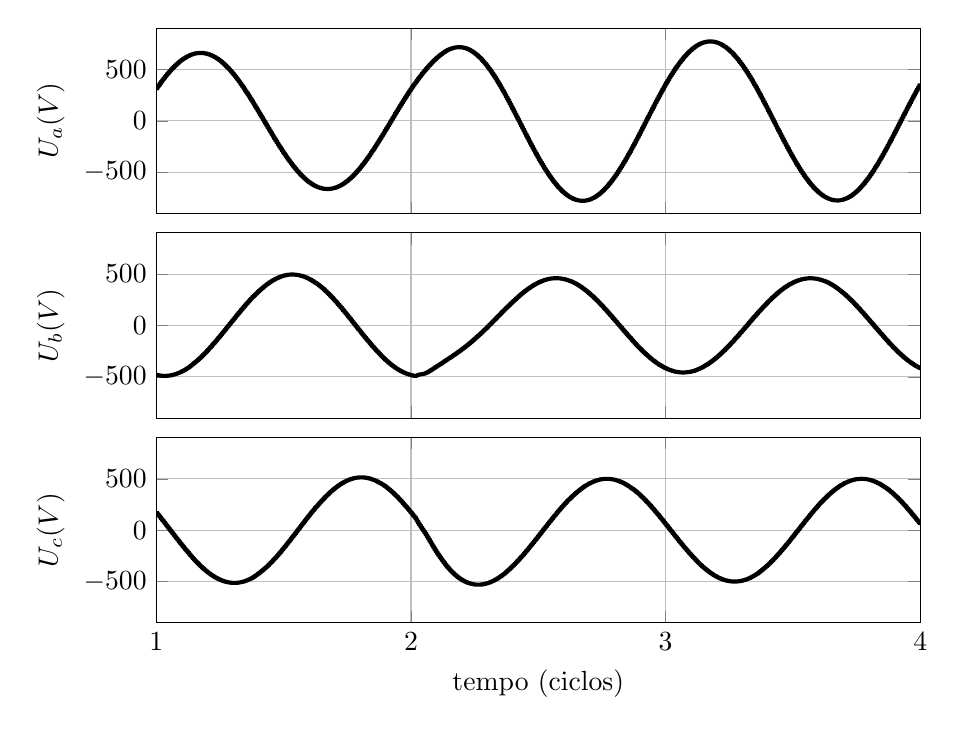
\begin{tikzpicture}

\begin{axis}[%
width=0.8\textwidth,
height=0.193917089240149\textwidth,
scale only axis,
xmin=0.0166666666666667,
xmax=0.0666666666666667,
xtick={0,0.0166666666666667,0.0333333333333333,0.05,0.0666666666666667},
xticklabels={\empty},
xmajorgrids,
ymin=-900,
ymax=900,
ytick={-500,    0,  500},
ylabel={$\text{U}_\text{b}\text{ (V)}$},
ymajorgrids,
name=plot2,
scaled x ticks = false,
legend columns=-1,
legend style={/tikz/every even column/.append style={column sep=0.3cm}},
legend style={font=\footnotesize}
]
\addplot [color=black,solid,line width=1.5pt,forget plot]
  table[row sep=crcr]{0.0166583333333333	-478.328989103039\\
0.0167	-481.372762295986\\
0.0167416666666667	-481.372762295986\\
0.0167833333333333	-483.944387417357\\
0.016825	-483.944387417357\\
0.0168666666666667	-486.043904769891\\
0.0169083333333333	-486.043904769891\\
0.01695	-487.669342075457\\
0.0169916666666667	-487.669342075457\\
0.0170333333333333	-488.81912329053\\
0.017075	-488.81912329053\\
0.0171166666666667	-489.492376222951\\
0.0171583333333333	-489.492376222951\\
0.0172	-489.689089295181\\
0.0172416666666667	-489.689089295181\\
0.0172833333333333	-489.410057478733\\
0.017325	-489.410057478733\\
0.0173666666666667	-488.656714544629\\
0.0174083333333333	-488.656714544629\\
0.01745	-487.430933830334\\
0.0174916666666667	-487.430933830334\\
0.0175333333333333	-485.734862735459\\
0.017575	-485.734862735459\\
0.0176166666666667	-483.570824107468\\
0.0176583333333333	-483.570824107468\\
0.0177	-480.941176730971\\
0.0177416666666667	-480.941176730971\\
0.0177833333333333	-477.848873406491\\
0.017825	-477.848873406491\\
0.0178666666666667	-474.296687037085\\
0.0179083333333333	-474.296687037085\\
0.01795	-470.287554266504\\
0.0179916666666667	-470.287554266504\\
0.0180333333333333	-465.824994538518\\
0.018075	-465.824994538518\\
0.0181166666666667	-460.912896166831\\
0.0181583333333333	-460.912896166831\\
0.0182	-455.555544349316\\
0.0182416666666667	-455.555544349316\\
0.0182833333333333	-449.757632700212\\
0.018325	-449.757632700212\\
0.0183666666666667	-443.524266807923\\
0.0184083333333333	-443.524266807923\\
0.01845	-436.860963041735\\
0.0184916666666667	-436.860963041735\\
0.0185333333333333	-429.773645406549\\
0.018575	-429.773645406549\\
0.0186166666666667	-422.2686421737\\
0.0186583333333333	-422.2686421737\\
0.0187	-414.352682994809\\
0.0187416666666667	-414.352682994809\\
0.0187833333333333	-406.710604021129\\
0.018825	-406.710604021129\\
0.0188666666666667	-396.968651829484\\
0.0189083333333333	-396.968651829484\\
0.01895	-387.24430030011\\
0.0189916666666667	-387.24430030011\\
0.0190333333333333	-377.413842111121\\
0.019075	-377.413842111121\\
0.0191166666666667	-367.3960735467\\
0.0191583333333333	-367.3960735467\\
0.0192	-357.12553953726\\
0.0192416666666667	-357.12553953726\\
0.0192833333333333	-346.559303382721\\
0.019325	-346.559303382721\\
0.0193666666666667	-335.674936708767\\
0.0194083333333333	-335.674936708767\\
0.01945	-324.465686057335\\
0.0194916666666667	-324.465686057335\\
0.0195333333333333	-312.935239244225\\
0.019575	-312.935239244225\\
0.0196166666666667	-301.093266862382\\
0.0196583333333333	-301.093266862382\\
0.0197	-288.95219973374\\
0.0197416666666667	-288.95219973374\\
0.0197833333333333	-276.525463982029\\
0.019825	-276.525463982029\\
0.0198666666666667	-263.82538033546\\
0.0199083333333333	-263.82538033546\\
0.01995	-250.865057706918\\
0.0199916666666667	-250.865057706918\\
0.0200333333333333	-237.656697428642\\
0.020075	-237.656697428642\\
0.0201166666666667	-224.212271375033\\
0.0201583333333333	-224.212271375033\\
0.0202	-210.543848998092\\
0.0202416666666667	-210.543848998092\\
0.0202833333333333	-196.6637735981\\
0.020325	-196.6637735981\\
0.0203666666666667	-182.584756063204\\
0.0204083333333333	-182.584756063204\\
0.02045	-168.319897946886\\
0.0204916666666667	-168.319897946886\\
0.0205333333333333	-153.882668002172\\
0.020575	-153.882668002172\\
0.0206166666666667	-139.286855686717\\
0.0206583333333333	-139.286855686717\\
0.0207	-124.546519243168\\
0.0207416666666667	-124.546519243168\\
0.0207833333333333	-109.675923407492\\
0.020825	-109.675923407492\\
0.0208666666666667	-94.6884951690301\\
0.0209083333333333	-94.6884951690301\\
0.02095	-79.6023211852309\\
0.0209916666666667	-79.6023211852309\\
0.0210333333333333	-64.4296541414652\\
0.021075	-64.4296541414652\\
0.0211166666666667	-49.1854677870168\\
0.0211583333333333	-49.1854677870168\\
0.0212	-33.8847697005379\\
0.0212416666666667	-33.8847697005379\\
0.0212833333333333	-18.5423320716325\\
0.021325	-18.5423320716325\\
0.0213666666666667	-3.1725945533516\\
0.0214083333333333	-3.1725945533516\\
0.02145	12.2102617721841\\
0.0214916666666667	12.2102617721841\\
0.0215333333333333	27.5921432856442\\
0.021575	27.5921432856442\\
0.0216166666666667	42.9588704890498\\
0.0216583333333333	42.9588704890498\\
0.0217	58.2960537853681\\
0.0217416666666667	58.2960537853681\\
0.0217833333333333	73.5890384864759\\
0.021825	73.5890384864759\\
0.0218666666666667	88.82269659409\\
0.0219083333333333	88.82269659409\\
0.02195	103.982669291038\\
0.0219916666666667	103.982669291038\\
0.0220333333333333	119.053037141893\\
0.022075	119.053037141893\\
0.0221166666666667	134.01853586672\\
0.0221583333333333	134.01853586672\\
0.0222	148.863909368128\\
0.0222416666666667	148.863909368128\\
0.0222833333333333	163.573956427556\\
0.022325	163.573956427556\\
0.0223666666666667	178.133568427636\\
0.0224083333333333	178.133568427636\\
0.02245	192.527757716713\\
0.0224916666666667	192.527757716713\\
0.0225333333333333	206.741679404245\\
0.022575	206.741679404245\\
0.0226166666666667	220.760649670751\\
0.0226583333333333	220.760649670751\\
0.0227	234.570162946369\\
0.0227416666666667	234.570162946369\\
0.0227833333333333	248.155909263895\\
0.022825	248.155909263895\\
0.0228666666666667	261.687830320942\\
0.0229083333333333	261.687830320942\\
0.02295	274.986604079196\\
0.0229916666666667	274.986604079196\\
0.0230333333333333	286.928801747272\\
0.023075	286.928801747272\\
0.0231166666666667	298.950506950644\\
0.0231583333333333	298.950506950644\\
0.0232	310.924864102034\\
0.0232416666666667	310.924864102034\\
0.0232833333333333	322.756989832147\\
0.023325	322.756989832147\\
0.0233666666666667	334.367084014297\\
0.0234083333333333	334.367084014297\\
0.02345	345.69602196514\\
0.0234916666666667	345.69602196514\\
0.0235333333333333	356.703461032175\\
0.023575	356.703461032175\\
0.0236166666666667	367.363371170442\\
0.0236583333333333	367.363371170442\\
0.0237	377.659204280424\\
0.0237416666666667	377.659204280424\\
0.0237833333333333	387.579795487262\\
0.023825	387.579795487262\\
0.0238666666666667	397.116425283701\\
0.0239083333333333	397.116425283701\\
0.02395	406.261310362139\\
0.0239916666666667	406.261310362139\\
0.0240333333333333	415.0053223807\\
0.024075	415.0053223807\\
0.0241166666666667	423.340732147141\\
0.0241583333333333	423.340732147141\\
0.0242	431.258683016742\\
0.0242416666666667	431.258683016742\\
0.0242833333333333	438.750365395371\\
0.024325	438.750365395371\\
0.0243666666666667	445.807262831054\\
0.0244083333333333	445.807262831054\\
0.02445	452.421342397773\\
0.0244916666666667	452.421342397773\\
0.0245333333333333	458.585161293933\\
0.024575	458.585161293933\\
0.0246166666666667	464.291905294308\\
0.0246583333333333	464.291905294308\\
0.0247	469.535383109734\\
0.0247416666666667	469.535383109734\\
0.0247833333333333	474.309999446141\\
0.024825	474.309999446141\\
0.0248666666666667	478.610723480444\\
0.0249083333333333	478.610723480444\\
0.02495	482.432523836755\\
0.0249916666666667	482.432523836755\\
0.0250333333333333	485.772612186125\\
0.025075	485.772612186125\\
0.0251166666666667	488.627883686145\\
0.0251583333333333	488.627883686145\\
0.0252	490.994391489966\\
0.0252416666666667	490.994391489966\\
0.0252833333333333	492.869784189106\\
0.025325	492.869784189106\\
0.0253666666666667	494.252063559781\\
0.0254083333333333	494.252063559781\\
0.02545	495.139387583695\\
0.0254916666666667	495.139387583695\\
0.0255333333333333	495.530061759552\\
0.025575	495.530061759552\\
0.0256166666666667	495.422663936061\\
0.0256583333333333	495.422663936061\\
0.0257	494.816230581684\\
0.0257416666666667	494.816230581684\\
0.0257833333333333	493.710425995119\\
0.025825	493.710425995119\\
0.0258666666666667	492.105654148384\\
0.0259083333333333	492.105654148384\\
0.02595	490.003108134894\\
0.0259916666666667	490.003108134894\\
0.0260333333333333	487.404961487327\\
0.026075	487.404961487327\\
0.0261166666666667	484.313069214194\\
0.0261583333333333	484.313069214194\\
0.0262	480.731558886196\\
0.0262416666666667	480.731558886196\\
0.0262833333333333	476.664323712434\\
0.026325	476.664323712434\\
0.0263666666666667	472.115829454631\\
0.0264083333333333	472.115829454631\\
0.02645	467.091068733291\\
0.0264916666666667	467.091068733291\\
0.0265333333333333	461.595540479995\\
0.026575	461.595540479995\\
0.0266166666666667	455.635234907076\\
0.0266583333333333	455.635234907076\\
0.0267	449.21662231492\\
0.0267416666666667	449.21662231492\\
0.0267833333333333	442.346643428456\\
0.026825	442.346643428456\\
0.0268666666666667	435.032699614098\\
0.0269083333333333	435.032699614098\\
0.02695	427.282642172915\\
0.0269916666666667	427.282642172915\\
0.0270333333333333	418.527982244731\\
0.027075	418.527982244731\\
0.0271166666666667	410.672570182659\\
0.0271583333333333	410.672570182659\\
0.0272	402.276872290978\\
0.0272416666666667	402.276872290978\\
0.0272833333333333	393.223850223727\\
0.027325	393.223850223727\\
0.0273666666666667	383.609151155178\\
0.0274083333333333	383.609151155178\\
0.02745	373.508718653929\\
0.0274916666666667	373.508718653929\\
0.0275333333333333	362.979579538073\\
0.027575	362.979579538073\\
0.0276166666666667	352.061894709897\\
0.0276583333333333	352.061894709897\\
0.0277	340.783205444461\\
0.0277416666666667	340.783205444461\\
0.0277833333333333	329.162781541968\\
0.027825	329.162781541968\\
0.0278666666666667	317.215226351439\\
0.0279083333333333	317.215226351439\\
0.02795	304.953068995059\\
0.0279916666666667	304.953068995059\\
0.0280333333333333	292.388308765939\\
0.028075	292.388308765939\\
0.0281166666666667	279.533394256386\\
0.0281583333333333	279.533394256386\\
0.0282	266.401997020689\\
0.0282416666666667	266.401997020689\\
0.0282833333333333	253.007121767018\\
0.028325	253.007121767018\\
0.0283666666666667	239.363037342399\\
0.0284083333333333	239.363037342399\\
0.02845	225.484309796947\\
0.0284916666666667	225.484309796947\\
0.0285333333333333	211.385672071801\\
0.028575	211.385672071801\\
0.0286166666666667	197.081935254737\\
0.0286583333333333	197.081935254737\\
0.0287	182.587950486431\\
0.0287416666666667	182.587950486431\\
0.0287833333333333	167.918604082923\\
0.028825	167.918604082923\\
0.0288666666666667	153.088829011011\\
0.0289083333333333	153.088829011011\\
0.02895	138.113619934855\\
0.0289916666666667	138.113619934855\\
0.0290333333333333	123.008044204917\\
0.029075	123.008044204917\\
0.0291166666666667	107.788100944899\\
0.0291583333333333	107.788100944899\\
0.0292	92.4664220892656\\
0.0292416666666667	92.4664220892656\\
0.0292833333333333	77.0599110293703\\
0.029325	77.0599110293703\\
0.0293666666666667	61.5839402726698\\
0.0294083333333333	61.5839402726698\\
0.02945	46.0538191073489\\
0.0294916666666667	46.0538191073489\\
0.0295333333333333	30.4851141949034\\
0.029575	30.4851141949034\\
0.0296166666666667	14.8937682112207\\
0.0296583333333333	14.8937682112207\\
0.0297	-0.703957306529608\\
0.0297416666666667	-0.703957306529608\\
0.0297833333333333	-16.2916492298269\\
0.029825	-16.2916492298269\\
0.0298666666666667	-31.8529362123827\\
0.0299083333333333	-31.8529362123827\\
0.02995	-47.371649369948\\
0.0299916666666667	-47.371649369948\\
0.0300333333333333	-62.8319222299047\\
0.030075	-62.8319222299047\\
0.0301166666666667	-78.2183969102601\\
0.0301583333333333	-78.2183969102601\\
0.0302	-93.5154108314719\\
0.0302416666666667	-93.5154108314719\\
0.0302833333333333	-108.70816278091\\
0.030325	-108.70816278091\\
0.0303666666666667	-123.782356080195\\
0.0304083333333333	-123.782356080195\\
0.03045	-138.723507249364\\
0.0304916666666667	-138.723507249364\\
0.0305333333333333	-153.517339096442\\
0.030575	-153.517339096442\\
0.0306166666666667	-168.149764544084\\
0.0306583333333333	-168.149764544084\\
0.0307	-182.60688669631\\
0.0307416666666667	-182.60688669631\\
0.0307833333333333	-196.875004412733\\
0.030825	-196.875004412733\\
0.0308666666666667	-210.940621254231\\
0.0309083333333333	-210.940621254231\\
0.03095	-224.790455634942\\
0.0309916666666667	-224.790455634942\\
0.0310333333333333	-238.411450801645\\
0.031075	-238.411450801645\\
0.0311166666666667	-251.788204920739\\
0.0311583333333333	-251.788204920739\\
0.0312	-264.319493294975\\
0.0312416666666667	-264.319493294975\\
0.0312833333333333	-278.081845363642\\
0.031325	-278.081845363642\\
0.0313666666666667	-291.211888263673\\
0.0314083333333333	-291.211888263673\\
0.03145	-303.807007713181\\
0.0314916666666667	-303.807007713181\\
0.0315333333333333	-315.936364357588\\
0.031575	-315.936364357588\\
0.0316166666666667	-327.655020751537\\
0.0316583333333333	-327.655020751537\\
0.0317	-338.998550237152\\
0.0317416666666667	-338.998550237152\\
0.0317833333333333	-349.984949605885\\
0.031825	-349.984949605885\\
0.0318666666666667	-360.618974262017\\
0.0319083333333333	-360.618974262017\\
0.03195	-370.896795074955\\
0.0319916666666667	-370.896795074955\\
0.0320333333333333	-380.809923421548\\
0.032075	-380.809923421548\\
0.0321166666666667	-390.348041070204\\
0.0321583333333333	-390.348041070204\\
0.0322	-399.500455565927\\
0.0322416666666667	-399.500455565927\\
0.0322833333333333	-408.258433783543\\
0.032325	-408.258433783543\\
0.0323666666666667	-416.612673979994\\
0.0324083333333333	-416.612673979994\\
0.03245	-424.555376388038\\
0.0324916666666667	-424.555376388038\\
0.0325333333333333	-432.079651399668\\
0.032575	-432.079651399668\\
0.0326166666666667	-439.17912856472\\
0.0326583333333333	-439.17912856472\\
0.0327	-445.847803165625\\
0.0327416666666667	-445.847803165625\\
0.0327833333333333	-452.079952433882\\
0.032825	-452.079952433882\\
0.0328666666666667	-457.870112681898\\
0.0329083333333333	-457.870112681898\\
0.03295	-463.213095942823\\
0.0329916666666667	-463.213095942823\\
0.0330333333333333	-468.104025539882\\
0.033075	-468.104025539882\\
0.0331166666666667	-472.538375275198\\
0.0331583333333333	-472.538375275198\\
0.0332	-476.512043591712\\
0.0332416666666667	-476.512043591712\\
0.0332833333333333	-480.021998518076\\
0.033325	-480.021998518076\\
0.0333666666666667	-483.062409528906\\
0.0334083333333333	-483.062409528906\\
0.03345	-486.609065941724\\
0.0334916666666667	-486.609065941724\\
0.0335333333333333	-488.661972717433\\
0.033575	-488.661972717433\\
0.0336166666666667	-489.954048753197\\
0.0336583333333333	-489.954048753197\\
0.0337	-486.618016593236\\
0.0337416666666667	-486.618016593236\\
0.0337833333333333	-481.661153705195\\
0.033825	-481.661153705195\\
0.0338666666666667	-477.619455775155\\
0.0339083333333333	-477.619455775155\\
0.03395	-474.982745404976\\
0.0339916666666667	-474.982745404976\\
0.0340333333333333	-473.040799439171\\
0.034075	-473.040799439171\\
0.0341166666666667	-470.830583801035\\
0.0341583333333333	-470.830583801035\\
0.0342	-467.644861937091\\
0.0342416666666667	-467.644861937091\\
0.0342833333333333	-463.173443274962\\
0.034325	-463.173443274962\\
0.0343666666666667	-457.445352214085\\
0.0344083333333333	-457.445352214085\\
0.03445	-450.693424618105\\
0.0344916666666667	-450.693424618105\\
0.0345333333333333	-443.228013116355\\
0.034575	-443.228013116355\\
0.0346166666666667	-435.343610869449\\
0.0346583333333333	-435.343610869449\\
0.0347	-427.269506364133\\
0.0347416666666667	-427.269506364133\\
0.0347833333333333	-419.155764215952\\
0.034825	-419.155764215952\\
0.0348666666666667	-411.081639633703\\
0.0349083333333333	-411.081639633703\\
0.03495	-403.074286989226\\
0.0349916666666667	-403.074286989226\\
0.0350333333333333	-395.128953428787\\
0.035075	-395.128953428787\\
0.0351166666666667	-387.225667699645\\
0.0351583333333333	-387.225667699645\\
0.0352	-379.34058179323\\
0.0352416666666667	-379.34058179323\\
0.0352833333333333	-371.646969710553\\
0.035325	-371.646969710553\\
0.0353666666666667	-363.855919151951\\
0.0354083333333333	-363.855919151951\\
0.03545	-355.1449453296\\
0.0354916666666667	-355.1449453296\\
0.0355333333333333	-346.702176812855\\
0.035575	-346.702176812855\\
0.0356166666666667	-338.422091332567\\
0.0356583333333333	-338.422091332567\\
0.0357	-330.229204020917\\
0.0357416666666667	-330.229204020917\\
0.0357833333333333	-322.058642932308\\
0.035825	-322.058642932308\\
0.0358666666666667	-313.861917137717\\
0.0359083333333333	-313.861917137717\\
0.03595	-305.605791594772\\
0.0359916666666667	-305.605791594772\\
0.0360333333333333	-297.268886980108\\
0.036075	-297.268886980108\\
0.0361166666666667	-288.837817179846\\
0.0361583333333333	-288.837817179846\\
0.0362	-280.30382053095\\
0.0362416666666667	-280.30382053095\\
0.0362833333333333	-271.660303336155\\
0.036325	-271.660303336155\\
0.0363666666666667	-262.901681015347\\
0.0364083333333333	-262.901681015347\\
0.03645	-254.020781284775\\
0.0364916666666667	-254.020781284775\\
0.0365333333333333	-245.012536028426\\
0.036575	-245.012536028426\\
0.0366166666666667	-235.870674639682\\
0.0366583333333333	-235.870674639682\\
0.0367	-226.5891545645\\
0.0367416666666667	-226.5891545645\\
0.0367833333333333	-217.162416136294\\
0.036825	-217.162416136294\\
0.0368666666666667	-207.585589595479\\
0.0369083333333333	-207.585589595479\\
0.03695	-197.854622560557\\
0.0369916666666667	-197.854622560557\\
0.0370333333333333	-187.966340567046\\
0.037075	-187.966340567046\\
0.0371166666666667	-177.91846125985\\
0.0371583333333333	-177.91846125985\\
0.0372	-167.709582532686\\
0.0372416666666667	-167.709582532686\\
0.0372833333333333	-157.339160130321\\
0.037325	-157.339160130321\\
0.0373666666666667	-146.807092518851\\
0.0374083333333333	-146.807092518851\\
0.03745	-136.115265794081\\
0.0374916666666667	-136.115265794081\\
0.0375333333333333	-125.266063480601\\
0.037575	-125.266063480601\\
0.0376166666666667	-114.261359890833\\
0.0376583333333333	-114.261359890833\\
0.0377	-103.104674832616\\
0.0377416666666667	-103.104674832616\\
0.0377833333333333	-91.8001508692053\\
0.037825	-91.8001508692053\\
0.0378666666666667	-80.3523570995387\\
0.0379083333333333	-80.3523570995387\\
0.03795	-68.766259290112\\
0.0379916666666667	-68.766259290112\\
0.0380333333333333	-57.0473080861763\\
0.038075	-57.0473080861763\\
0.0381166666666667	-45.2015745957473\\
0.0381583333333333	-45.2015745957473\\
0.0382	-33.235876589439\\
0.0382416666666667	-33.235876589439\\
0.0382833333333333	-21.1578602768126\\
0.038325	-21.1578602768126\\
0.0383666666666667	-8.97604708656571\\
0.0384083333333333	-8.97604708656571\\
0.03845	3.30002110680873\\
0.0384916666666667	3.30002110680873\\
0.0385333333333333	15.6612859792429\\
0.038575	15.6612859792429\\
0.0386166666666667	28.0962956788241\\
0.0386583333333333	28.0962956788241\\
0.0387	40.594045950347\\
0.0387416666666667	40.594045950347\\
0.0387833333333333	53.1428513346186\\
0.038825	53.1428513346186\\
0.0388666666666667	65.7304792238901\\
0.0389083333333333	65.7304792238901\\
0.03895	78.3442800603926\\
0.0389916666666667	78.3442800603926\\
0.0390333333333333	90.9712917990323\\
0.039075	90.9712917990323\\
0.0391166666666667	103.598306207209\\
0.0391583333333333	103.598306207209\\
0.0392	116.211905184768\\
0.0392416666666667	116.211905184768\\
0.0392833333333333	128.798480383802\\
0.039325	128.798480383802\\
0.0393666666666667	141.344247722336\\
0.0394083333333333	141.344247722336\\
0.03945	154.326046277147\\
0.0394916666666667	154.326046277147\\
0.0395333333333333	166.150743392373\\
0.039575	166.150743392373\\
0.0396166666666667	177.939742532808\\
0.0396583333333333	177.939742532808\\
0.0397	189.856462821647\\
0.0397416666666667	189.856462821647\\
0.0397833333333333	201.815475415066\\
0.039825	201.815475415066\\
0.0398666666666667	213.747612615016\\
0.0399083333333333	213.747612615016\\
0.03995	225.597208342247\\
0.0399916666666667	225.597208342247\\
0.0400333333333333	237.322376604702\\
0.040075	237.322376604702\\
0.0401166666666667	248.892541579377\\
0.0401583333333333	248.892541579377\\
0.0402	260.285304456201\\
0.0402416666666667	260.285304456201\\
0.0402833333333333	271.483660575377\\
0.040325	271.483660575377\\
0.0403666666666667	282.473608157422\\
0.0404083333333333	282.473608157422\\
0.04045	293.242396724099\\
0.0404916666666667	293.242396724099\\
0.0405333333333333	303.77728885176\\
0.040575	303.77728885176\\
0.0406166666666667	314.064926842485\\
0.0406583333333333	314.064926842485\\
0.0407	324.093310371938\\
0.0407416666666667	324.093310371938\\
0.0407833333333333	333.849564200831\\
0.040825	333.849564200831\\
0.0408666666666667	343.321035805335\\
0.0409083333333333	343.321035805335\\
0.04095	352.495400515756\\
0.0409916666666667	352.495400515756\\
0.0410333333333333	361.360745522018\\
0.041075	361.360745522018\\
0.0411166666666667	369.905607453229\\
0.0411583333333333	369.905607453229\\
0.0412	378.118980765268\\
0.0412416666666667	378.118980765268\\
0.0412833333333333	385.990312159878\\
0.041325	385.990312159878\\
0.0413666666666667	393.509492134095\\
0.0414083333333333	393.509492134095\\
0.04145	400.666849864168\\
0.0414916666666667	400.666849864168\\
0.0415333333333333	407.452514771811\\
0.041575	407.452514771811\\
0.0416166666666667	413.859563417947\\
0.0416583333333333	413.859563417947\\
0.0417	419.878645656462\\
0.0417416666666667	419.878645656462\\
0.0417833333333333	425.501791308272\\
0.041825	425.501791308272\\
0.0418666666666667	430.721654791573\\
0.0419083333333333	430.721654791573\\
0.04195	435.531174635011\\
0.0419916666666667	435.531174635011\\
0.0420333333333333	439.923462936361\\
0.042075	439.923462936361\\
0.0421166666666667	443.891857155086\\
0.0421583333333333	443.891857155086\\
0.0422	447.430056306081\\
0.0422416666666667	447.430056306081\\
0.0422833333333333	450.53226176989\\
0.042325	450.53226176989\\
0.0423666666666667	453.193315367993\\
0.0424083333333333	453.193315367993\\
0.04245	455.408795819888\\
0.0424916666666667	455.408795819888\\
0.0425333333333333	457.175272610207\\
0.042575	457.175272610207\\
0.0426166666666667	458.489292983682\\
0.0426583333333333	458.489292983682\\
0.0427	459.348806783782\\
0.0427416666666667	459.348806783782\\
0.0427833333333333	459.752784474504\\
0.042825	459.752784474504\\
0.0428666666666667	459.700295416903\\
0.0429083333333333	459.700295416903\\
0.04295	459.190995700046\\
0.0429916666666667	459.190995700046\\
0.0430333333333333	458.22508219359\\
0.043075	458.22508219359\\
0.0431166666666667	456.80327362963\\
0.0431583333333333	456.80327362963\\
0.0432	454.926797881357\\
0.0432416666666667	454.926797881357\\
0.0432833333333333	452.597383946968\\
0.043325	452.597383946968\\
0.0433666666666667	449.817256193745\\
0.0434083333333333	449.817256193745\\
0.04345	446.589129022764\\
0.0434916666666667	446.589129022764\\
0.0435333333333333	442.904232721112\\
0.043575	442.904232721112\\
0.0436166666666667	438.284741112124\\
0.0436583333333333	438.284741112124\\
0.0437	434.510469350206\\
0.0437416666666667	434.510469350206\\
0.0437833333333333	430.010664722644\\
0.043825	430.010664722644\\
0.0438666666666667	424.877281320458\\
0.0439083333333333	424.877281320458\\
0.04395	419.177097105451\\
0.0439916666666667	419.177097105451\\
0.0440333333333333	412.971031062541\\
0.044075	412.971031062541\\
0.0441166666666667	406.306398783175\\
0.0441583333333333	406.306398783175\\
0.0442	399.216666025567\\
0.0442416666666667	399.216666025567\\
0.0442833333333333	391.724031380799\\
0.044325	391.724031380799\\
0.0443666666666667	383.842865735546\\
0.0444083333333333	383.842865735546\\
0.04445	375.582956531497\\
0.0444916666666667	375.582956531497\\
0.0445333333333333	366.95204185015\\
0.044575	366.95204185015\\
0.0446166666666667	357.957159385573\\
0.0446583333333333	357.957159385573\\
0.0447	348.607269876326\\
0.0447416666666667	348.607269876326\\
0.0447833333333333	338.910453904097\\
0.044825	338.910453904097\\
0.0448666666666667	328.876219043062\\
0.0449083333333333	328.876219043062\\
0.04495	318.515046437659\\
0.0449916666666667	318.515046437659\\
0.0450333333333333	307.837932947412\\
0.045075	307.837932947412\\
0.0451166666666667	296.856223612949\\
0.0451583333333333	296.856223612949\\
0.0452	285.581495980515\\
0.0452416666666667	285.581495980515\\
0.0452833333333333	274.025501668765\\
0.045325	274.025501668765\\
0.0453666666666667	262.200149052809\\
0.0454083333333333	262.200149052809\\
0.04545	250.117509156488\\
0.0454916666666667	250.117509156488\\
0.0455333333333333	237.789829939687\\
0.045575	237.789829939687\\
0.0456166666666667	225.229594304724\\
0.0456583333333333	225.229594304724\\
0.0457	212.449926356918\\
0.0457416666666667	212.449926356918\\
0.0457833333333333	199.461823310997\\
0.045825	199.461823310997\\
0.0458666666666667	186.279522138813\\
0.0459083333333333	186.279522138813\\
0.04595	172.916195062453\\
0.0459916666666667	172.916195062453\\
0.0460333333333333	159.385209632592\\
0.046075	159.385209632592\\
0.0461166666666667	145.700332823194\\
0.0461583333333333	145.700332823194\\
0.0462	131.87577936057\\
0.0462416666666667	131.87577936057\\
0.0462833333333333	117.926126805409\\
0.046325	117.926126805409\\
0.0463666666666667	103.86616834174\\
0.0464083333333333	103.86616834174\\
0.04645	89.7107459389388\\
0.0464916666666667	89.7107459389388\\
0.0465333333333333	75.4746143821233\\
0.046575	75.4746143821233\\
0.0466166666666667	61.1723610112524\\
0.0466583333333333	61.1723610112524\\
0.0467	46.8180179927007\\
0.0467416666666667	46.8180179927007\\
0.0467833333333333	32.4270284302401\\
0.046825	32.4270284302401\\
0.0468666666666667	18.0124313091539\\
0.0469083333333333	18.0124313091539\\
0.04695	3.58818362763497\\
0.0469916666666667	3.58818362763497\\
0.0470333333333333	-10.8317684434191\\
0.047075	-10.8317684434191\\
0.0471166666666667	-25.2335336951517\\
0.0471583333333333	-25.2335336951517\\
0.0472	-39.6032662448223\\
0.0472416666666667	-39.6032662448223\\
0.0472833333333333	-53.9271651712631\\
0.047325	-53.9271651712631\\
0.0473666666666667	-68.1914801380154\\
0.0474083333333333	-68.1914801380154\\
0.04745	-82.3825209630089\\
0.0474916666666667	-82.3825209630089\\
0.0475333333333333	-96.4866690612985\\
0.047575	-96.4866690612985\\
0.0476166666666667	-110.490389346202\\
0.0476583333333333	-110.490389346202\\
0.0477	-124.190606240211\\
0.0477416666666667	-124.190606240211\\
0.0477833333333333	-137.880920314667\\
0.047825	-137.880920314667\\
0.0478666666666667	-152.17078705054\\
0.0479083333333333	-152.17078705054\\
0.04795	-166.040281198007\\
0.0479916666666667	-166.040281198007\\
0.0480333333333333	-179.564382792903\\
0.048075	-179.564382792903\\
0.0481166666666667	-192.785989436946\\
0.0481583333333333	-192.785989436946\\
0.0482	-205.740960367108\\
0.0482416666666667	-205.740960367108\\
0.0482833333333333	-218.452109310949\\
0.048325	-218.452109310949\\
0.0483666666666667	-230.929609312934\\
0.0484083333333333	-230.929609312934\\
0.04845	-243.173601073653\\
0.0484916666666667	-243.173601073653\\
0.0485333333333333	-255.177403784829\\
0.048575	-255.177403784829\\
0.0486166666666667	-266.930433009695\\
0.0486583333333333	-266.930433009695\\
0.0487	-278.420425336944\\
0.0487416666666667	-278.420425336944\\
0.0487833333333333	-289.634534171802\\
0.048825	-289.634534171802\\
0.0488666666666667	-300.562196433918\\
0.0489083333333333	-300.562196433918\\
0.04895	-311.191050146836\\
0.0489916666666667	-311.191050146836\\
0.0490333333333333	-321.510803763443\\
0.049075	-321.510803763443\\
0.0491166666666667	-331.511784824958\\
0.0491583333333333	-331.511784824958\\
0.0492	-341.18477697618\\
0.0492416666666667	-341.18477697618\\
0.0492833333333333	-350.520886432965\\
0.049325	-350.520886432965\\
0.0493666666666667	-359.511467708017\\
0.0494083333333333	-359.511467708017\\
0.04945	-368.14810016589\\
0.0494916666666667	-368.14810016589\\
0.0495333333333333	-376.422599120989\\
0.049575	-376.422599120989\\
0.0496166666666667	-384.327044816373\\
0.0496583333333333	-384.327044816373\\
0.0497	-391.853816313174\\
0.0497416666666667	-391.853816313174\\
0.0497833333333333	-398.995900090608\\
0.049825	-398.995900090608\\
0.0498666666666667	-405.745872126532\\
0.0499083333333333	-405.745872126532\\
0.04995	-412.096641059584\\
0.0499916666666667	-412.096641059584\\
0.0500333333333333	-418.04265478151\\
0.050075	-418.04265478151\\
0.0501166666666667	-423.578079263109\\
0.0501583333333333	-423.578079263109\\
0.0502	-428.697589813734\\
0.0502416666666667	-428.697589813734\\
0.0502833333333333	-433.396536308009\\
0.050325	-433.396536308009\\
0.0503666666666667	-437.670957813271\\
0.0504083333333333	-437.670957813271\\
0.05045	-441.517490365727\\
0.0504916666666667	-441.517490365727\\
0.0505333333333333	-444.933231075999\\
0.050575	-444.933231075999\\
0.0506166666666667	-447.915606405845\\
0.0506583333333333	-447.915606405845\\
0.0507	-450.462276687137\\
0.0507416666666667	-450.462276687137\\
0.0507833333333333	-452.571047443705\\
0.050825	-452.571047443705\\
0.0508666666666667	-454.239766633336\\
0.0509083333333333	-454.239766633336\\
0.05095	-455.46780876176\\
0.0509916666666667	-455.46780876176\\
0.0510333333333333	-456.252617256851\\
0.051075	-456.252617256851\\
0.0511166666666667	-456.593163799133\\
0.0511583333333333	-456.593163799133\\
0.0512	-456.488770541085\\
0.0512416666666667	-456.488770541085\\
0.0512833333333333	-455.939166756665\\
0.051325	-455.939166756665\\
0.0513666666666667	-454.944503993817\\
0.0514083333333333	-454.944503993817\\
0.05145	-453.505366588516\\
0.0514916666666667	-453.505366588516\\
0.0515333333333333	-451.62277709625\\
0.051575	-451.62277709625\\
0.0516166666666667	-449.298198385309\\
0.0516583333333333	-449.298198385309\\
0.0517	-446.533533975074\\
0.0517416666666667	-446.533533975074\\
0.0517833333333333	-443.331184101677\\
0.051825	-443.331184101677\\
0.0518666666666667	-440.115642103011\\
0.0519083333333333	-440.115642103011\\
0.05195	-435.547346410187\\
0.0519916666666667	-435.547346410187\\
0.0520333333333333	-430.549647526597\\
0.052075	-430.549647526597\\
0.0521166666666667	-425.332715202819\\
0.0521583333333333	-425.332715202819\\
0.0522	-419.83726617472\\
0.0522416666666667	-419.83726617472\\
0.0522833333333333	-414.018754128377\\
0.052325	-414.018754128377\\
0.0523666666666667	-407.844265444367\\
0.0524083333333333	-407.844265444367\\
0.05245	-401.293659042134\\
0.0524916666666667	-401.293659042134\\
0.0525333333333333	-394.357638439148\\
0.052575	-394.357638439148\\
0.0526166666666667	-387.034932406147\\
0.0526583333333333	-387.034932406147\\
0.0527	-379.329527434209\\
0.0527416666666667	-379.329527434209\\
0.0527833333333333	-371.24841886468\\
0.052825	-371.24841886468\\
0.0528666666666667	-362.800179468364\\
0.0529083333333333	-362.800179468364\\
0.05295	-353.99357467828\\
0.0529916666666667	-353.99357467828\\
0.0530333333333333	-344.836998178935\\
0.053075	-344.836998178935\\
0.0531166666666667	-335.340364708871\\
0.0531583333333333	-335.340364708871\\
0.0532	-325.51261703383\\
0.0532416666666667	-325.51261703383\\
0.0532833333333333	-315.362883447188\\
0.053325	-315.362883447188\\
0.0533666666666667	-304.900571675445\\
0.0534083333333333	-304.900571675445\\
0.05345	-294.135452529816\\
0.0534916666666667	-294.135452529816\\
0.0535333333333333	-283.077695333738\\
0.053575	-283.077695333738\\
0.0536166666666667	-271.73786721365\\
0.0536583333333333	-271.73786721365\\
0.0537	-260.126910302749\\
0.0537416666666667	-260.126910302749\\
0.0537833333333333	-248.256109326186\\
0.053825	-248.256109326186\\
0.0538666666666667	-236.137057939091\\
0.0539083333333333	-236.137057939091\\
0.05395	-223.781168703524\\
0.0539916666666667	-223.781168703524\\
0.0540333333333333	-211.201854845793\\
0.054075	-211.201854845793\\
0.0541166666666667	-198.410921913656\\
0.0541583333333333	-198.410921913656\\
0.0542	-185.420825258148\\
0.0542416666666667	-185.420825258148\\
0.0542833333333333	-172.244383817149\\
0.054325	-172.244383817149\\
0.0543666666666667	-158.894433673531\\
0.0544083333333333	-158.894433673531\\
0.05445	-145.383710993957\\
0.0544916666666667	-145.383710993957\\
0.0545333333333333	-131.724871524028\\
0.054575	-131.724871524028\\
0.0546166666666667	-117.930591384664\\
0.0546583333333333	-117.930591384664\\
0.0547	-104.013690949431\\
0.0547416666666667	-104.013690949431\\
0.0547833333333333	-89.9872420264009\\
0.054825	-89.9872420264009\\
0.0548666666666667	-75.8646331290888\\
0.0549083333333333	-75.8646331290888\\
0.05495	-61.659828634165\\
0.0549916666666667	-61.659828634165\\
0.0550333333333333	-47.3861879412369\\
0.055075	-47.3861879412369\\
0.0551166666666667	-33.0580822135272\\
0.0551583333333333	-33.0580822135272\\
0.0552	-18.6904944377617\\
0.0552416666666667	-18.6904944377617\\
0.0552833333333333	-4.29792310624019\\
0.055325	-4.29792310624019\\
0.0553666666666667	10.10504352399\\
0.0554083333333333	10.10504352399\\
0.05545	24.5037825432381\\
0.0554916666666667	24.5037825432381\\
0.0555333333333333	38.8836641462371\\
0.055575	38.8836641462371\\
0.0556166666666667	53.2300749114714\\
0.0556583333333333	53.2300749114714\\
0.0557	67.5284370808504\\
0.0557416666666667	67.5284370808504\\
0.0557833333333333	81.7642255686142\\
0.055825	81.7642255686142\\
0.0558666666666667	95.9229840452949\\
0.0559083333333333	95.9229840452949\\
0.05595	110.011930091203\\
0.0559916666666667	110.011930091203\\
0.0560333333333333	124.394363215822\\
0.056075	124.394363215822\\
0.0561166666666667	137.562402814298\\
0.0561583333333333	137.562402814298\\
0.0562	150.841371574267\\
0.0562416666666667	150.841371574267\\
0.0562833333333333	164.15662845941\\
0.056325	164.15662845941\\
0.0563666666666667	177.439115278726\\
0.0564083333333333	177.439115278726\\
0.05645	190.626500560647\\
0.0564916666666667	190.626500560647\\
0.0565333333333333	203.66915535063\\
0.056575	203.66915535063\\
0.0566166666666667	216.530293741841\\
0.0566583333333333	216.530293741841\\
0.0567	229.183660875004\\
0.0567416666666667	229.183660875004\\
0.0567833333333333	241.610492384122\\
0.056825	241.610492384122\\
0.0568666666666667	253.796657760302\\
0.0569083333333333	253.796657760302\\
0.05695	265.730431370951\\
0.0569916666666667	265.730431370951\\
0.0570333333333333	277.401376675834\\
0.057075	277.401376675834\\
0.0571166666666667	288.797695219482\\
0.0571583333333333	288.797695219482\\
0.0572	299.909291567907\\
0.0572416666666667	299.909291567907\\
0.0572833333333333	310.725403810971\\
0.057325	310.725403810971\\
0.0573666666666667	321.234921606665\\
0.0574083333333333	321.234921606665\\
0.05745	331.426889122485\\
0.0574916666666667	331.426889122485\\
0.0575333333333333	341.29064648982\\
0.057575	341.29064648982\\
0.0576166666666667	350.815928733063\\
0.0576583333333333	350.815928733063\\
0.0577	359.992914134936\\
0.0577416666666667	359.992914134936\\
0.0577833333333333	368.812236486186\\
0.057825	368.812236486186\\
0.0578666666666667	377.264976904331\\
0.0579083333333333	377.264976904331\\
0.05795	385.342648124536\\
0.0579916666666667	385.342648124536\\
0.0580333333333333	393.037142746316\\
0.058075	393.037142746316\\
0.0581166666666667	400.340439487639\\
0.0581583333333333	400.340439487639\\
0.0582	407.246604318783\\
0.0582416666666667	407.246604318783\\
0.0582833333333333	413.74798678376\\
0.058325	413.74798678376\\
0.0583666666666667	419.838137877831\\
0.0584083333333333	419.838137877831\\
0.05845	425.511008843066\\
0.0584916666666667	425.511008843066\\
0.0585333333333333	430.760753520275\\
0.058575	430.760753520275\\
0.0586166666666667	435.58168018016\\
0.0586583333333333	435.58168018016\\
0.0587	439.968319809104\\
0.0587416666666667	439.968319809104\\
0.0587833333333333	443.915553571859\\
0.058825	443.915553571859\\
0.0588666666666667	447.418746178068\\
0.0589083333333333	447.418746178068\\
0.05895	450.473852116049\\
0.0589916666666667	450.473852116049\\
0.0590333333333333	453.077483607044\\
0.059075	453.077483607044\\
0.0591166666666667	455.227315650251\\
0.0591583333333333	455.227315650251\\
0.0592	456.919940612573\\
0.0592416666666667	456.919940612573\\
0.0592833333333333	458.154995402039\\
0.059325	458.154995402039\\
0.0593666666666667	458.931621172967\\
0.0594083333333333	458.931621172967\\
0.05945	459.249374378205\\
0.0594916666666667	459.249374378205\\
0.0595333333333333	459.108306049073\\
0.059575	459.108306049073\\
0.0596166666666667	458.508940156217\\
0.0596583333333333	458.508940156217\\
0.0597	457.452260843681\\
0.0597416666666667	457.452260843681\\
0.0597833333333333	455.939704218326\\
0.059825	455.939704218326\\
0.0598666666666667	453.973153222549\\
0.0599083333333333	453.973153222549\\
0.05995	451.554933867328\\
0.0599916666666667	451.554933867328\\
0.0600333333333333	448.687811615614\\
0.060075	448.687811615614\\
0.0601166666666667	445.196385642596\\
0.0601583333333333	445.196385642596\\
0.0602	441.399976381126\\
0.0602416666666667	441.399976381126\\
0.0602833333333333	437.796060074228\\
0.060325	437.796060074228\\
0.0603666666666667	433.523120043071\\
0.0604083333333333	433.523120043071\\
0.06045	428.662635042152\\
0.0604916666666667	428.662635042152\\
0.0605333333333333	423.269865046884\\
0.060575	423.269865046884\\
0.0606166666666667	417.393614466248\\
0.0606583333333333	417.393614466248\\
0.0607	411.071170260027\\
0.0607416666666667	411.071170260027\\
0.0607833333333333	404.328777714737\\
0.060825	404.328777714737\\
0.0608666666666667	397.184010173422\\
0.0609083333333333	397.184010173422\\
0.06095	389.648630304734\\
0.0609916666666667	389.648630304734\\
0.0610333333333333	381.731169886571\\
0.061075	381.731169886571\\
0.0611166666666667	373.438855946513\\
0.0611583333333333	373.438855946513\\
0.0612	364.778512463429\\
0.0612416666666667	364.778512463429\\
0.0612833333333333	355.759374944945\\
0.061325	355.759374944945\\
0.0613666666666667	346.388730802236\\
0.0614083333333333	346.388730802236\\
0.06145	336.675990940701\\
0.0614916666666667	336.675990940701\\
0.0615333333333333	326.631197765165\\
0.061575	326.631197765165\\
0.0616166666666667	316.264841797401\\
0.0616583333333333	316.264841797401\\
0.0617	305.587724654742\\
0.0617416666666667	305.587724654742\\
0.0617833333333333	294.610874614901\\
0.061825	294.610874614901\\
0.0618666666666667	283.34550759845\\
0.0619083333333333	283.34550759845\\
0.06195	271.80301896887\\
0.0619916666666667	271.80301896887\\
0.0620333333333333	259.99499133427\\
0.062075	259.99499133427\\
0.0621166666666667	247.933206811663\\
0.0621583333333333	247.933206811663\\
0.0622	235.629843746301\\
0.0622416666666667	235.629843746301\\
0.0622833333333333	223.096847266921\\
0.062325	223.096847266921\\
0.0623666666666667	210.346097829504\\
0.0624083333333333	210.346097829504\\
0.06245	197.39068442299\\
0.0624916666666667	197.39068442299\\
0.0625333333333333	184.243398881227\\
0.062575	184.243398881227\\
0.0626166666666667	170.917310438817\\
0.0626583333333333	170.917310438817\\
0.0627	157.425896983282\\
0.0627416666666667	157.425896983282\\
0.0627833333333333	143.783039829106\\
0.062825	143.783039829106\\
0.0628666666666667	130.002924356108\\
0.0629083333333333	130.002924356108\\
0.06295	116.099901517946\\
0.0629916666666667	116.099901517946\\
0.0630333333333333	102.088355547288\\
0.063075	102.088355547288\\
0.0631166666666667	87.9826037392091\\
0.0631583333333333	87.9826037392091\\
0.0632	73.7967764206207\\
0.0632416666666667	73.7967764206207\\
0.0632833333333333	59.5447840651993\\
0.063325	59.5447840651993\\
0.0633666666666667	45.2417025601877\\
0.0634083333333333	45.2417025601877\\
0.06345	30.9002147749113\\
0.0634916666666667	30.9002147749113\\
0.0635333333333333	16.5342151826401\\
0.063575	16.5342151826401\\
0.0636166666666667	2.15754905716183\\
0.0636583333333333	2.15754905716183\\
0.0637	-12.2159561042658\\
0.0637416666666667	-12.2159561042658\\
0.0637833333333333	-26.5724918636106\\
0.063825	-26.5724918636106\\
0.0638666666666667	-40.8982728538033\\
0.0639083333333333	-40.8982728538033\\
0.06395	-55.1795444071337\\
0.0639916666666667	-55.1795444071337\\
0.0640333333333333	-69.4025925846765\\
0.064075	-69.4025925846765\\
0.0641166666666667	-83.5537553810129\\
0.0641583333333333	-83.5537553810129\\
0.0642	-97.6189070872171\\
0.0642416666666667	-97.6189070872171\\
0.0642833333333333	-111.221930361101\\
0.064325	-111.221930361101\\
0.0643666666666667	-125.498556482359\\
0.0644083333333333	-125.498556482359\\
0.06445	-139.678664764964\\
0.0644916666666667	-139.678664764964\\
0.0645333333333333	-153.533798770887\\
0.064575	-153.533798770887\\
0.0646166666666667	-167.109154927577\\
0.0646583333333333	-167.109154927577\\
0.0647	-180.436523961985\\
0.0647416666666667	-180.436523961985\\
0.0647833333333333	-193.537900997735\\
0.064825	-193.537900997735\\
0.0648666666666667	-206.424281465252\\
0.0649083333333333	-206.424281465252\\
0.06495	-219.097344598969\\
0.0649916666666667	-219.097344598969\\
0.0650333333333333	-231.551992445973\\
0.065075	-231.551992445973\\
0.0651166666666667	-243.7788717768\\
0.0651583333333333	-243.7788717768\\
0.0652	-255.766436623332\\
0.0652416666666667	-255.766436623332\\
0.0652833333333333	-267.502235249209\\
0.065325	-267.502235249209\\
0.0653666666666667	-278.974340260923\\
0.0654083333333333	-278.974340260923\\
0.06545	-290.171708238205\\
0.0654916666666667	-290.171708238205\\
0.0655333333333333	-301.082327437597\\
0.065575	-301.082327437597\\
0.0656166666666667	-311.695802217027\\
0.0656583333333333	-311.695802217027\\
0.0657	-322.002157887428\\
0.0657416666666667	-322.002157887428\\
0.0657833333333333	-331.991758557279\\
0.065825	-331.991758557279\\
0.0658666666666667	-341.655231838618\\
0.0659083333333333	-341.655231838618\\
0.06595	-350.98343722218\\
0.0659916666666667	-350.98343722218\\
0.0660333333333333	-359.967466889009\\
0.066075	-359.967466889009\\
0.0661166666666667	-368.598666077129\\
0.0661583333333333	-368.598666077129\\
0.0662	-376.868661592647\\
0.0662416666666667	-376.868661592647\\
0.0662833333333333	-384.769390509377\\
0.066325	-384.769390509377\\
0.0663666666666667	-392.293447027068\\
0.0664083333333333	-392.293447027068\\
0.06645	-399.432619274114\\
0.0664916666666667	-399.432619274114\\
0.0665333333333333	-406.180126612528\\
0.066575	-406.180126612528\\
0.0666166666666667	-412.52947846758\\
0.0666583333333333	-412.52947846758\\
};
\end{axis}

\begin{axis}[%
width=0.8\textwidth,
height=0.193917089240149\textwidth,
scale only axis,
xmin=0.0166666666666667,
xmax=0.0666666666666667,
xtick={0,0.0166666666666667,0.0333333333333333,0.05,0.0666666666666667},
xticklabels={{0},{1},{2},{3},{4}},
xlabel={tempo (ciclos)},
xmajorgrids,
ymin=-900,
ymax=900,
ytick={-500,    0,  500},
ylabel={$\text{U}_\text{c}\text{ (V)}$},
ymajorgrids,
at=(plot2.below south west),
anchor=above north west,
scaled x ticks = false,
legend columns=-1,
legend style={/tikz/every even column/.append style={column sep=0.3cm}},
legend style={font=\footnotesize}
]
\addplot [color=black,solid,line width=1.5pt,forget plot]
  table[row sep=crcr]{0.0166583333333333	180.146044285981\\
0.0167	164.940320934484\\
0.0167416666666667	164.940320934484\\
0.0167833333333333	149.579587477261\\
0.016825	149.579587477261\\
0.0168666666666667	134.079551509137\\
0.0169083333333333	134.079551509137\\
0.01695	118.455249604828\\
0.0169916666666667	118.455249604828\\
0.0170333333333333	102.721820759597\\
0.017075	102.721820759597\\
0.0171166666666667	86.8947024886041\\
0.0171583333333333	86.8947024886041\\
0.0172	70.9897152347551\\
0.0172416666666667	70.9897152347551\\
0.0172833333333333	55.0229884605968\\
0.017325	55.0229884605968\\
0.0173666666666667	39.0107951391398\\
0.0174083333333333	39.0107951391398\\
0.01745	22.9693692316446\\
0.0174916666666667	22.9693692316446\\
0.0175333333333333	6.91476165823279\\
0.017575	6.91476165823279\\
0.0176166666666667	-9.13724020053355\\
0.0176583333333333	-9.13724020053355\\
0.0177	-25.1712876244939\\
0.0177416666666667	-25.1712876244939\\
0.0177833333333333	-41.1717016099994\\
0.017825	-41.1717016099994\\
0.0178666666666667	-57.1235450619316\\
0.0179083333333333	-57.1235450619316\\
0.01795	-73.0122416753861\\
0.0179916666666667	-73.0122416753861\\
0.0180333333333333	-88.8229904086394\\
0.018075	-88.8229904086394\\
0.0181166666666667	-104.541092542183\\
0.0181583333333333	-104.541092542183\\
0.0182	-120.151937938219\\
0.0182416666666667	-120.151937938219\\
0.0182833333333333	-135.641005542097\\
0.018325	-135.641005542097\\
0.0183666666666667	-150.993870043721\\
0.0184083333333333	-150.993870043721\\
0.01845	-166.196212093992\\
0.0184916666666667	-166.196212093992\\
0.0185333333333333	-181.2338298443\\
0.018575	-181.2338298443\\
0.0186166666666667	-196.092650491087\\
0.0186583333333333	-196.092650491087\\
0.0187	-210.758741337919\\
0.0187416666666667	-210.758741337919\\
0.0187833333333333	-224.272823986116\\
0.018825	-224.272823986116\\
0.0188666666666667	-239.924185188171\\
0.0189083333333333	-239.924185188171\\
0.01895	-254.795099361687\\
0.0189916666666667	-254.795099361687\\
0.0190333333333333	-269.036557729883\\
0.019075	-269.036557729883\\
0.0191166666666667	-282.760389233867\\
0.0191583333333333	-282.760389233867\\
0.0192	-296.057851197266\\
0.0192416666666667	-296.057851197266\\
0.0192833333333333	-308.990098283122\\
0.019325	-308.990098283122\\
0.0193666666666667	-321.590393418407\\
0.0194083333333333	-321.590393418407\\
0.01945	-333.870571911174\\
0.0194916666666667	-333.870571911174\\
0.0195333333333333	-345.828322444006\\
0.019575	-345.828322444006\\
0.0196166666666667	-357.453508661192\\
0.0196583333333333	-357.453508661192\\
0.0197	-368.732790011102\\
0.0197416666666667	-368.732790011102\\
0.0197833333333333	-379.652185798579\\
0.019825	-379.652185798579\\
0.0198666666666667	-390.200039679523\\
0.0199083333333333	-390.200039679523\\
0.01995	-400.364455853375\\
0.0199916666666667	-400.364455853375\\
0.0200333333333333	-410.135593074462\\
0.020075	-410.135593074462\\
0.0201166666666667	-419.504723697965\\
0.0201583333333333	-419.504723697965\\
0.0202	-428.463752199279\\
0.0202416666666667	-428.463752199279\\
0.0202833333333333	-437.004944992871\\
0.020325	-437.004944992871\\
0.0203666666666667	-445.120779808899\\
0.0204083333333333	-445.120779808899\\
0.02045	-452.8038978512\\
0.0204916666666667	-452.8038978512\\
0.0205333333333333	-460.047124180064\\
0.020575	-460.047124180064\\
0.0206166666666667	-466.843522119401\\
0.0206583333333333	-466.843522119401\\
0.0207	-473.186455823302\\
0.0207416666666667	-473.186455823302\\
0.0207833333333333	-479.069643185327\\
0.020825	-479.069643185327\\
0.0208666666666667	-484.487584080736\\
0.0209083333333333	-484.487584080736\\
0.02095	-489.433644253288\\
0.0209916666666667	-489.433644253288\\
0.0210333333333333	-493.903539136153\\
0.021075	-493.903539136153\\
0.0211166666666667	-497.892633124744\\
0.0211583333333333	-497.892633124744\\
0.0212	-501.396820907034\\
0.0212416666666667	-501.396820907034\\
0.0212833333333333	-504.41270742765\\
0.021325	-504.41270742765\\
0.0213666666666667	-506.937652408911\\
0.0214083333333333	-506.937652408911\\
0.02145	-508.969679717527\\
0.0214916666666667	-508.969679717527\\
0.0215333333333333	-510.507315547184\\
0.021575	-510.507315547184\\
0.0216166666666667	-511.549437470117\\
0.0216583333333333	-511.549437470117\\
0.0217	-512.095173916005\\
0.0217416666666667	-512.095173916005\\
0.0217833333333333	-512.14386626104\\
0.021825	-512.14386626104\\
0.0218666666666667	-511.694775425209\\
0.0219083333333333	-511.694775425209\\
0.02195	-510.748811874119\\
0.0219916666666667	-510.748811874119\\
0.0220333333333333	-509.305240015087\\
0.022075	-509.305240015087\\
0.0221166666666667	-507.364690126307\\
0.0221583333333333	-507.364690126307\\
0.0222	-504.928245184668\\
0.0222416666666667	-504.928245184668\\
0.0222833333333333	-501.997459837756\\
0.022325	-501.997459837756\\
0.0223666666666667	-498.57437873634\\
0.0224083333333333	-498.57437873634\\
0.02245	-494.661546862205\\
0.0224916666666667	-494.661546862205\\
0.0225333333333333	-490.262014038761\\
0.022575	-490.262014038761\\
0.0226166666666667	-485.379336077746\\
0.0226583333333333	-485.379336077746\\
0.0227	-480.017574398345\\
0.0227416666666667	-480.017574398345\\
0.0227833333333333	-474.181295093699\\
0.022825	-474.181295093699\\
0.0228666666666667	-468.132227564933\\
0.0229083333333333	-468.132227564933\\
0.02295	-461.649789032895\\
0.0229916666666667	-461.649789032895\\
0.0230333333333333	-453.193902270209\\
0.023075	-453.193902270209\\
0.0231166666666667	-444.773441113673\\
0.0231583333333333	-444.773441113673\\
0.0232	-436.251268459993\\
0.0232416666666667	-436.251268459993\\
0.0232833333333333	-427.520263672964\\
0.023325	-427.520263672964\\
0.0233666666666667	-418.493740302993\\
0.0234083333333333	-418.493740302993\\
0.02345	-409.11363513705\\
0.0234916666666667	-409.11363513705\\
0.0235333333333333	-399.348350327473\\
0.023575	-399.348350327473\\
0.0236166666666667	-389.186670490501\\
0.0236583333333333	-389.186670490501\\
0.0237	-378.630905372963\\
0.0237416666666667	-378.630905372963\\
0.0237833333333333	-367.690968950489\\
0.023825	-367.690968950489\\
0.0238666666666667	-356.380102358096\\
0.0239083333333333	-356.380102358096\\
0.02395	-344.712640572405\\
0.0239916666666667	-344.712640572405\\
0.0240333333333333	-332.700781505562\\
0.024075	-332.700781505562\\
0.0241166666666667	-320.358317577706\\
0.0241583333333333	-320.358317577706\\
0.0242	-307.6971824162\\
0.0242416666666667	-307.6971824162\\
0.0242833333333333	-294.729044137296\\
0.024325	-294.729044137296\\
0.0243666666666667	-281.465654636295\\
0.0244083333333333	-281.465654636295\\
0.02445	-267.919108296558\\
0.0244916666666667	-267.919108296558\\
0.0245333333333333	-254.101977634579\\
0.024575	-254.101977634579\\
0.0246166666666667	-240.027348361342\\
0.0246583333333333	-240.027348361342\\
0.0247	-225.708789227798\\
0.0247416666666667	-225.708789227798\\
0.0247833333333333	-211.160290317149\\
0.024825	-211.160290317149\\
0.0248666666666667	-196.39619457631\\
0.0249083333333333	-196.39619457631\\
0.02495	-181.431040895376\\
0.0249916666666667	-181.431040895376\\
0.0250333333333333	-166.279778355741\\
0.025075	-166.279778355741\\
0.0251166666666667	-150.957981557132\\
0.0251583333333333	-150.957981557132\\
0.0252	-135.480589084291\\
0.0252416666666667	-135.480589084291\\
0.0252833333333333	-119.863094908503\\
0.025325	-119.863094908503\\
0.0253666666666667	-104.121014925928\\
0.0254083333333333	-104.121014925928\\
0.02545	-88.2697324252375\\
0.0254916666666667	-88.2697324252375\\
0.0255333333333333	-72.3244975934466\\
0.025575	-72.3244975934466\\
0.0256166666666667	-56.3005347394663\\
0.0256583333333333	-56.3005347394663\\
0.0257	-40.2131789209932\\
0.0257416666666667	-40.2131789209932\\
0.0257833333333333	-24.0779930748701\\
0.025825	-24.0779930748701\\
0.0258666666666667	-7.91083206935371\\
0.0259083333333333	-7.91083206935371\\
0.02595	8.27214526930201\\
0.0259916666666667	8.27214526930201\\
0.0260333333333333	24.4542254440382\\
0.026075	24.4542254440382\\
0.0261166666666667	40.6199908695603\\
0.0261583333333333	40.6199908695603\\
0.0262	56.7516612117422\\
0.0262416666666667	56.7516612117422\\
0.0262833333333333	72.8325712785133\\
0.026325	72.8325712785133\\
0.0263666666666667	88.846063325594\\
0.0264083333333333	88.846063325594\\
0.02645	104.775539088676\\
0.0264916666666667	104.775539088676\\
0.0265333333333333	120.604489043941\\
0.026575	120.604489043941\\
0.0266166666666667	136.316517603678\\
0.0266583333333333	136.316517603678\\
0.0267	151.895365005857\\
0.0267416666666667	151.895365005857\\
0.0267833333333333	167.32492740609\\
0.026825	167.32492740609\\
0.0268666666666667	182.589276240632\\
0.0269083333333333	182.589276240632\\
0.02695	197.67267733356\\
0.0269916666666667	197.67267733356\\
0.0270333333333333	213.364075445209\\
0.027075	213.364075445209\\
0.0271166666666667	227.019890089968\\
0.0271583333333333	227.019890089968\\
0.0272	240.616905132375\\
0.0272416666666667	240.616905132375\\
0.0272833333333333	254.329291302055\\
0.027325	254.329291302055\\
0.0273666666666667	268.025476997475\\
0.0274083333333333	268.025476997475\\
0.02745	281.599414976171\\
0.0274916666666667	281.599414976171\\
0.0275333333333333	294.97178527555\\
0.027575	294.97178527555\\
0.0276166666666667	308.087625765951\\
0.0276583333333333	308.087625765951\\
0.0277	320.910690989392\\
0.0277416666666667	320.910690989392\\
0.0277833333333333	333.417415766459\\
0.027825	333.417415766459\\
0.0278666666666667	345.591780478394\\
0.0279083333333333	345.591780478394\\
0.02795	357.421558389868\\
0.0279916666666667	357.421558389868\\
0.0280333333333333	368.896047770843\\
0.028075	368.896047770843\\
0.0281166666666667	380.004638133566\\
0.0281583333333333	380.004638133566\\
0.0282	390.735700889524\\
0.0282416666666667	390.735700889524\\
0.0282833333333333	401.079183264076\\
0.028325	401.079183264076\\
0.0283666666666667	411.023979838759\\
0.0284083333333333	411.023979838759\\
0.02845	420.559255161147\\
0.0284916666666667	420.559255161147\\
0.0285333333333333	429.674638195389\\
0.028575	429.674638195389\\
0.0286166666666667	438.36034696872\\
0.0286583333333333	438.36034696872\\
0.0287	446.607237052018\\
0.0287416666666667	446.607237052018\\
0.0287833333333333	454.406798841608\\
0.028825	454.406798841608\\
0.0288666666666667	461.751128592088\\
0.0289083333333333	461.751128592088\\
0.02895	468.632892411405\\
0.0289916666666667	468.632892411405\\
0.0290333333333333	475.045294902946\\
0.029075	475.045294902946\\
0.0291166666666667	480.981879753185\\
0.0291583333333333	480.981879753185\\
0.0292	486.437323221531\\
0.0292416666666667	486.437323221531\\
0.0292833333333333	491.406267662622\\
0.029325	491.406267662622\\
0.0293666666666667	495.883928335018\\
0.0294083333333333	495.883928335018\\
0.02945	499.866055615843\\
0.0294916666666667	499.866055615843\\
0.0295333333333333	503.348727665725\\
0.029575	503.348727665725\\
0.0296166666666667	506.32826432485\\
0.0296583333333333	506.32826432485\\
0.0297	508.801283597195\\
0.0297416666666667	508.801283597195\\
0.0297833333333333	510.764841924053\\
0.029825	510.764841924053\\
0.0298666666666667	512.216584774959\\
0.0299083333333333	512.216584774959\\
0.02995	513.154859732115\\
0.0299916666666667	513.154859732115\\
0.0300333333333333	513.578772270348\\
0.030075	513.578772270348\\
0.0301166666666667	513.488424330974\\
0.0301583333333333	513.488424330974\\
0.0302	512.883757056606\\
0.0302416666666667	512.883757056606\\
0.0302833333333333	511.766137250959\\
0.030325	511.766137250959\\
0.0303666666666667	510.137917947873\\
0.0304083333333333	510.137917947873\\
0.03045	508.001445961413\\
0.0304916666666667	508.001445961413\\
0.0305333333333333	505.359600176138\\
0.030575	505.359600176138\\
0.0306166666666667	502.215762753867\\
0.0306583333333333	502.215762753867\\
0.0307	498.573803881371\\
0.0307416666666667	498.573803881371\\
0.0307833333333333	494.438070082401\\
0.030825	494.438070082401\\
0.0308666666666667	489.813374792093\\
0.0309083333333333	489.813374792093\\
0.03095	484.704989725497\\
0.0309916666666667	484.704989725497\\
0.0310333333333333	479.118636144247\\
0.031075	479.118636144247\\
0.0311166666666667	473.056878981776\\
0.0311583333333333	473.056878981776\\
0.0312	465.70497451635\\
0.0312416666666667	465.70497451635\\
0.0312833333333333	459.969396284381\\
0.031325	459.969396284381\\
0.0313666666666667	453.306592780928\\
0.0314083333333333	453.306592780928\\
0.03145	445.858568368547\\
0.0314916666666667	445.858568368547\\
0.0315333333333333	437.745808877649\\
0.031575	437.745808877649\\
0.0316166666666667	429.069979853876\\
0.0316583333333333	429.069979853876\\
0.0317	419.905934001149\\
0.0317416666666667	419.905934001149\\
0.0317833333333333	410.303765791928\\
0.031825	410.303765791928\\
0.0318666666666667	400.294607272454\\
0.0319083333333333	400.294607272454\\
0.03195	389.897105361559\\
0.0319916666666667	389.897105361559\\
0.0320333333333333	379.123044209476\\
0.032075	379.123044209476\\
0.0321166666666667	367.981436719615\\
0.0321583333333333	367.981436719615\\
0.0322	356.480648193397\\
0.0322416666666667	356.480648193397\\
0.0322833333333333	344.631665623135\\
0.032325	344.631665623135\\
0.0323666666666667	332.444618169672\\
0.0324083333333333	332.444618169672\\
0.03245	319.931569517662\\
0.0324916666666667	319.931569517662\\
0.0325333333333333	307.105674240986\\
0.032575	307.105674240986\\
0.0326166666666667	293.98058862761\\
0.0326583333333333	293.98058862761\\
0.0327	280.570215241566\\
0.0327416666666667	280.570215241566\\
0.0327833333333333	266.888552880234\\
0.032825	266.888552880234\\
0.0328666666666667	252.949637821179\\
0.0329083333333333	252.949637821179\\
0.03295	238.76754490619\\
0.0329916666666667	238.76754490619\\
0.0330333333333333	224.356417917444\\
0.033075	224.356417917444\\
0.0331166666666667	209.730506383327\\
0.0331583333333333	209.730506383327\\
0.0332	194.904179567313\\
0.0332416666666667	194.904179567313\\
0.0332833333333333	179.892215293915\\
0.033325	179.892215293915\\
0.0333666666666667	164.708751896154\\
0.0334083333333333	164.708751896154\\
0.03345	150.345691734671\\
0.0334916666666667	150.345691734671\\
0.0335333333333333	134.838862366627\\
0.033575	134.838862366627\\
0.0336166666666667	118.919650271488\\
0.0336583333333333	118.919650271488\\
0.0337	98.7317902871057\\
0.0337416666666667	98.7317902871057\\
0.0337833333333333	77.1460251169865\\
0.033825	77.1460251169865\\
0.0338666666666667	56.6618666103694\\
0.0339083333333333	56.6618666103694\\
0.03395	37.8254399273983\\
0.0339916666666667	37.8254399273983\\
0.0340333333333333	20.0055012266858\\
0.034075	20.0055012266858\\
0.0341166666666667	2.29592077934738\\
0.0341583333333333	2.29592077934738\\
0.0342	-15.9876850487189\\
0.0342416666666667	-15.9876850487189\\
0.0342833333333333	-35.1596267437047\\
0.034325	-35.1596267437047\\
0.0343666666666667	-55.2077301000573\\
0.0344083333333333	-55.2077301000573\\
0.03445	-75.9177162638079\\
0.0344916666666667	-75.9177162638079\\
0.0345333333333333	-96.9904554395171\\
0.034575	-96.9904554395171\\
0.0346166666666667	-118.132316238878\\
0.0346583333333333	-118.132316238878\\
0.0347	-139.104666291811\\
0.0347416666666667	-139.104666291811\\
0.0347833333333333	-159.739989263719\\
0.034825	-159.739989263719\\
0.0348666666666667	-179.936236955244\\
0.0349083333333333	-179.936236955244\\
0.03495	-199.640696130418\\
0.0349916666666667	-199.640696130418\\
0.0350333333333333	-218.831755579961\\
0.035075	-218.831755579961\\
0.0351166666666667	-237.503469519494\\
0.0351583333333333	-237.503469519494\\
0.0352	-255.654861612716\\
0.0352416666666667	-255.654861612716\\
0.0352833333333333	-273.012602339519\\
0.035325	-273.012602339519\\
0.0353666666666667	-289.94675079874\\
0.0354083333333333	-289.94675079874\\
0.03545	-307.578196952378\\
0.0354916666666667	-307.578196952378\\
0.0355333333333333	-324.239359889303\\
0.035575	-324.239359889303\\
0.0356166666666667	-340.043868953536\\
0.0356583333333333	-340.043868953536\\
0.0357	-355.07842325821\\
0.0357416666666667	-355.07842325821\\
0.0357833333333333	-369.414739138614\\
0.035825	-369.414739138614\\
0.0358666666666667	-383.102016611028\\
0.0359083333333333	-383.102016611028\\
0.03595	-396.168530426848\\
0.0359916666666667	-396.168530426848\\
0.0360333333333333	-408.626622296993\\
0.036075	-408.626622296993\\
0.0361166666666667	-420.478405225251\\
0.0361583333333333	-420.478405225251\\
0.0362	-431.720726818168\\
0.0362416666666667	-431.720726818168\\
0.0362833333333333	-442.348770439223\\
0.036325	-442.348770439223\\
0.0363666666666667	-452.357768379037\\
0.0364083333333333	-452.357768379037\\
0.03645	-461.746637812486\\
0.0364916666666667	-461.746637812486\\
0.0365333333333333	-470.512904195063\\
0.036575	-470.512904195063\\
0.0366166666666667	-478.657223576815\\
0.0366583333333333	-478.657223576815\\
0.0367	-486.181436100675\\
0.0367416666666667	-486.181436100675\\
0.0367833333333333	-493.088193597864\\
0.036825	-493.088193597864\\
0.0368666666666667	-499.38067306683\\
0.0369083333333333	-499.38067306683\\
0.03695	-505.062401822981\\
0.0369916666666667	-505.062401822981\\
0.0370333333333333	-510.137174801809\\
0.037075	-510.137174801809\\
0.0371166666666667	-514.609033234658\\
0.0371583333333333	-514.609033234658\\
0.0372	-518.482275081463\\
0.0372416666666667	-518.482275081463\\
0.0372833333333333	-521.761475076121\\
0.037325	-521.761475076121\\
0.0373666666666667	-524.45147464901\\
0.0374083333333333	-524.45147464901\\
0.03745	-526.557717578793\\
0.0374916666666667	-526.557717578793\\
0.0375333333333333	-528.085082792632\\
0.037575	-528.085082792632\\
0.0376166666666667	-529.039475980288\\
0.0376583333333333	-529.039475980288\\
0.0377	-529.426910710114\\
0.0377416666666667	-529.426910710114\\
0.0377833333333333	-529.253776869682\\
0.037825	-529.253776869682\\
0.0378666666666667	-528.52694434012\\
0.0379083333333333	-528.52694434012\\
0.03795	-527.253741529308\\
0.0379916666666667	-527.253741529308\\
0.0380333333333333	-525.441842842672\\
0.038075	-525.441842842672\\
0.0381166666666667	-523.0991260776\\
0.0381583333333333	-523.0991260776\\
0.0382	-520.233545584092\\
0.0382416666666667	-520.233545584092\\
0.0382833333333333	-516.853047281192\\
0.038325	-516.853047281192\\
0.0383666666666667	-512.965501437322\\
0.0384083333333333	-512.965501437322\\
0.03845	-508.578459785544\\
0.0384916666666667	-508.578459785544\\
0.0385333333333333	-503.701232275085\\
0.038575	-503.701232275085\\
0.0386166666666667	-498.340657815792\\
0.0386583333333333	-498.340657815792\\
0.0387	-492.505110343181\\
0.0387416666666667	-492.505110343181\\
0.0387833333333333	-486.202941954816\\
0.038825	-486.202941954816\\
0.0388666666666667	-479.442567721012\\
0.0389083333333333	-479.442567721012\\
0.03895	-472.232558603527\\
0.0389916666666667	-472.232558603527\\
0.0390333333333333	-464.581711543522\\
0.039075	-464.581711543522\\
0.0391166666666667	-456.499082971883\\
0.0391583333333333	-456.499082971883\\
0.0392	-447.993992958351\\
0.0392416666666667	-447.993992958351\\
0.0392833333333333	-439.07601265581\\
0.039325	-439.07601265581\\
0.0393666666666667	-429.75494633516\\
0.0394083333333333	-429.75494633516\\
0.03945	-420.725916009907\\
0.0394916666666667	-420.725916009907\\
0.0395333333333333	-409.799092079891\\
0.039575	-409.799092079891\\
0.0396166666666667	-398.55474333858\\
0.0396583333333333	-398.55474333858\\
0.0397	-387.270513862203\\
0.0397416666666667	-387.270513862203\\
0.0397833333333333	-375.855206942349\\
0.039825	-375.855206942349\\
0.0398666666666667	-364.23819386307\\
0.0399083333333333	-364.23819386307\\
0.03995	-352.370577147011\\
0.0399916666666667	-352.370577147011\\
0.0400333333333333	-340.22468717006\\
0.040075	-340.22468717006\\
0.0401166666666667	-327.789796791569\\
0.0401583333333333	-327.789796791569\\
0.0402	-315.067035876093\\
0.0402416666666667	-315.067035876093\\
0.0402833333333333	-302.064636464045\\
0.040325	-302.064636464045\\
0.0403666666666667	-288.794470298823\\
0.0404083333333333	-288.794470298823\\
0.04045	-275.270139473444\\
0.0404916666666667	-275.270139473444\\
0.0405333333333333	-261.505266652122\\
0.040575	-261.505266652122\\
0.0406166666666667	-247.512452928843\\
0.0406583333333333	-247.512452928843\\
0.0407	-233.305882449642\\
0.0407416666666667	-233.305882449642\\
0.0407833333333333	-218.898174747927\\
0.040825	-218.898174747927\\
0.0408666666666667	-204.301865764039\\
0.0409083333333333	-204.301865764039\\
0.04095	-189.529593982724\\
0.0409916666666667	-189.529593982724\\
0.0410333333333333	-174.594242315483\\
0.041075	-174.594242315483\\
0.0411166666666667	-159.509003729815\\
0.0411583333333333	-159.509003729815\\
0.0412	-144.287387768407\\
0.0412416666666667	-144.287387768407\\
0.0412833333333333	-128.943190041428\\
0.041325	-128.943190041428\\
0.0413666666666667	-113.49044493166\\
0.0414083333333333	-113.49044493166\\
0.04145	-97.9433765059445\\
0.0414916666666667	-97.9433765059445\\
0.0415333333333333	-82.3163500236294\\
0.041575	-82.3163500236294\\
0.0416166666666667	-66.6236921766531\\
0.0416583333333333	-66.6236921766531\\
0.0417	-50.8803842251134\\
0.0417416666666667	-50.8803842251134\\
0.0417833333333333	-35.1010339891616\\
0.041825	-35.1010339891616\\
0.0418666666666667	-19.300314758103\\
0.0419083333333333	-19.300314758103\\
0.04195	-3.49278628517438\\
0.0419916666666667	-3.49278628517438\\
0.0420333333333333	12.3071940657666\\
0.042075	12.3071940657666\\
0.0421166666666667	28.0854475803618\\
0.0421583333333333	28.0854475803618\\
0.0422	43.8278758864337\\
0.0422416666666667	43.8278758864337\\
0.0422833333333333	59.5203268378133\\
0.042325	59.5203268378133\\
0.0423666666666667	75.1485021589243\\
0.0424083333333333	75.1485021589243\\
0.04245	90.697915104134\\
0.0424916666666667	90.697915104134\\
0.0425333333333333	106.153595153875\\
0.042575	106.153595153875\\
0.0426166666666667	121.501532248387\\
0.0426583333333333	121.501532248387\\
0.0427	136.726712685069\\
0.0427416666666667	136.726712685069\\
0.0427833333333333	151.813588090364\\
0.042825	151.813588090364\\
0.0428666666666667	166.74738375828\\
0.0429083333333333	166.74738375828\\
0.04295	181.513411121794\\
0.0429916666666667	181.513411121794\\
0.0430333333333333	196.097115632131\\
0.043075	196.097115632131\\
0.0431166666666667	210.484105197994\\
0.0431583333333333	210.484105197994\\
0.0432	224.660174724636\\
0.0432416666666667	224.660174724636\\
0.0432833333333333	238.611326725747\\
0.043325	238.611326725747\\
0.0433666666666667	252.323789331172\\
0.0434083333333333	252.323789331172\\
0.04345	265.784032798931\\
0.0434916666666667	265.784032798931\\
0.0435333333333333	278.995483915661\\
0.043575	278.995483915661\\
0.0436166666666667	292.617400886173\\
0.0436583333333333	292.617400886173\\
0.0437	304.163344735254\\
0.0437416666666667	304.163344735254\\
0.0437833333333333	315.80251183586\\
0.043825	315.80251183586\\
0.0438666666666667	327.42459966851\\
0.0439083333333333	327.42459966851\\
0.04395	338.924495338854\\
0.0439916666666667	338.924495338854\\
0.0440333333333333	350.209916505379\\
0.044075	350.209916505379\\
0.0441166666666667	361.211074625079\\
0.0441583333333333	361.211074625079\\
0.0442	371.880037626291\\
0.0442416666666667	371.880037626291\\
0.0442833333333333	382.186302664493\\
0.044325	382.186302664493\\
0.0443666666666667	392.111402933618\\
0.0444083333333333	392.111402933618\\
0.04445	401.644037819434\\
0.0444916666666667	401.644037819434\\
0.0445333333333333	410.776402037276\\
0.044575	410.776402037276\\
0.0446166666666667	419.502301477081\\
0.0446583333333333	419.502301477081\\
0.0447	427.813575193919\\
0.0447416666666667	427.813575193919\\
0.0447833333333333	435.704044777879\\
0.044825	435.704044777879\\
0.0448666666666667	443.166417828207\\
0.0449083333333333	443.166417828207\\
0.04495	450.192925106859\\
0.0449916666666667	450.192925106859\\
0.0450333333333333	456.775982312377\\
0.045075	456.775982312377\\
0.0451166666666667	462.908424380003\\
0.0451583333333333	462.908424380003\\
0.0452	468.583650577538\\
0.0452416666666667	468.583650577538\\
0.0452833333333333	473.795684854669\\
0.045325	473.795684854669\\
0.0453666666666667	478.539178124249\\
0.0454083333333333	478.539178124249\\
0.04545	482.809379679198\\
0.0454916666666667	482.809379679198\\
0.0455333333333333	486.602099033763\\
0.045575	486.602099033763\\
0.0456166666666667	489.913711390202\\
0.0456583333333333	489.913711390202\\
0.0457	492.740870649576\\
0.0457416666666667	492.740870649576\\
0.0457833333333333	495.081032959073\\
0.045825	495.081032959073\\
0.0458666666666667	496.932247527379\\
0.0459083333333333	496.932247527379\\
0.04595	498.292804457438\\
0.0459916666666667	498.292804457438\\
0.0460333333333333	499.161416531413\\
0.046075	499.161416531413\\
0.0461166666666667	499.5370970465\\
0.0461583333333333	499.5370970465\\
0.0462	499.419130430144\\
0.0462416666666667	499.419130430144\\
0.0462833333333333	498.807144824386\\
0.046325	498.807144824386\\
0.0463666666666667	497.701225621732\\
0.0464083333333333	497.701225621732\\
0.04645	496.102038099413\\
0.0464916666666667	496.102038099413\\
0.0465333333333333	494.010918176264\\
0.046575	494.010918176264\\
0.0466166666666667	491.429912840899\\
0.0466583333333333	491.429912840899\\
0.0467	488.362284026006\\
0.0467416666666667	488.362284026006\\
0.0467833333333333	484.809727528976\\
0.046825	484.809727528976\\
0.0468666666666667	480.777696771873\\
0.0469083333333333	480.777696771873\\
0.04695	476.270807885088\\
0.0469916666666667	476.270807885088\\
0.0470333333333333	471.29407980292\\
0.047075	471.29407980292\\
0.0471166666666667	465.853011123832\\
0.0471583333333333	465.853011123832\\
0.0472	459.953555041325\\
0.0472416666666667	459.953555041325\\
0.0472833333333333	453.602099717183\\
0.047325	453.602099717183\\
0.0473666666666667	446.805452870047\\
0.0474083333333333	446.805452870047\\
0.04745	439.570829539276\\
0.0474916666666667	439.570829539276\\
0.0475333333333333	431.905841620374\\
0.047575	431.905841620374\\
0.0476166666666667	423.818488128566\\
0.0476583333333333	423.818488128566\\
0.0477	415.052613698972\\
0.0477416666666667	415.052613698972\\
0.0477833333333333	406.043592568799\\
0.047825	406.043592568799\\
0.0478666666666667	397.672418641582\\
0.0479083333333333	397.672418641582\\
0.04795	388.546289743818\\
0.0479916666666667	388.546289743818\\
0.0480333333333333	378.785477768457\\
0.048075	378.785477768457\\
0.0481166666666667	368.48432929536\\
0.0481583333333333	368.48432929536\\
0.0482	357.724100336715\\
0.0482416666666667	357.724100336715\\
0.0482833333333333	346.565811003754\\
0.048325	346.565811003754\\
0.0483666666666667	335.051606856696\\
0.0484083333333333	335.051606856696\\
0.04845	323.209071944634\\
0.0484916666666667	323.209071944634\\
0.0485333333333333	311.056174375625\\
0.048575	311.056174375625\\
0.0486166666666667	298.605605869589\\
0.0486583333333333	298.605605869589\\
0.0487	285.867942142516\\
0.0487416666666667	285.867942142516\\
0.0487833333333333	272.853085197896\\
0.048825	272.853085197896\\
0.0488666666666667	259.57415165476\\
0.0489083333333333	259.57415165476\\
0.04895	246.041733731217\\
0.0489916666666667	246.041733731217\\
0.0490333333333333	232.269146820654\\
0.049075	232.269146820654\\
0.0491166666666667	218.270406596491\\
0.0491583333333333	218.270406596491\\
0.0492	204.059930057231\\
0.0492416666666667	204.059930057231\\
0.0492833333333333	189.652316262709\\
0.049325	189.652316262709\\
0.0493666666666667	175.062218025162\\
0.0494083333333333	175.062218025162\\
0.04945	160.304288815713\\
0.0494916666666667	160.304288815713\\
0.0495333333333333	145.393179328561\\
0.049575	145.393179328561\\
0.0496166666666667	130.343558754412\\
0.0496583333333333	130.343558754412\\
0.0497	115.170141936914\\
0.0497416666666667	115.170141936914\\
0.0497833333333333	99.8875925724045\\
0.049825	99.8875925724045\\
0.0498666666666667	84.5112939328042\\
0.0499083333333333	84.5112939328042\\
0.04995	69.0555608914352\\
0.0499916666666667	69.0555608914352\\
0.0500333333333333	53.5353913523271\\
0.050075	53.5353913523271\\
0.0501166666666667	37.9658664904637\\
0.0501583333333333	37.9658664904637\\
0.0502	22.3622135134613\\
0.0502416666666667	22.3622135134613\\
0.0502833333333333	6.7398903939876\\
0.050325	6.7398903939876\\
0.0503666666666667	-8.88543749146858\\
0.0504083333333333	-8.88543749146858\\
0.05045	-24.4980014730917\\
0.0504916666666667	-24.4980014730917\\
0.0505333333333333	-40.0820630805298\\
0.050575	-40.0820630805298\\
0.0506166666666667	-55.622033857284\\
0.0506583333333333	-55.622033857284\\
0.0507	-71.1025584260248\\
0.0507416666666667	-71.1025584260248\\
0.0507833333333333	-86.5086174886026\\
0.050825	-86.5086174886026\\
0.0508666666666667	-101.825683911353\\
0.0509083333333333	-101.825683911353\\
0.05095	-117.037648444334\\
0.0509916666666667	-117.037648444334\\
0.0510333333333333	-132.131716263846\\
0.051075	-132.131716263846\\
0.0511166666666667	-147.093629096731\\
0.0511583333333333	-147.093629096731\\
0.0512	-161.909299471534\\
0.0512416666666667	-161.909299471534\\
0.0512833333333333	-176.564785913967\\
0.051325	-176.564785913967\\
0.0513666666666667	-191.046294023473\\
0.0514083333333333	-191.046294023473\\
0.05145	-205.340178660526\\
0.0514916666666667	-205.340178660526\\
0.0515333333333333	-219.432949371293\\
0.051575	-219.432949371293\\
0.0516166666666667	-233.311278371876\\
0.0516583333333333	-233.311278371876\\
0.0517	-246.962010160004\\
0.0517416666666667	-246.962010160004\\
0.0517833333333333	-260.372093269944\\
0.051825	-260.372093269944\\
0.0518666666666667	-272.940398991223\\
0.0519083333333333	-272.940398991223\\
0.05195	-286.524030989669\\
0.0519916666666667	-286.524030989669\\
0.0520333333333333	-299.839983575662\\
0.052075	-299.839983575662\\
0.0521166666666667	-312.573711186242\\
0.0521583333333333	-312.573711186242\\
0.0522	-324.804328560645\\
0.0522416666666667	-324.804328560645\\
0.0522833333333333	-336.593736797928\\
0.052325	-336.593736797928\\
0.0523666666666667	-347.985898440856\\
0.0524083333333333	-347.985898440856\\
0.05245	-359.00621709978\\
0.0524916666666667	-359.00621709978\\
0.0525333333333333	-369.664978627142\\
0.052575	-369.664978627142\\
0.0526166666666667	-379.961859710303\\
0.0526583333333333	-379.961859710303\\
0.0527	-389.890148983681\\
0.0527416666666667	-389.890148983681\\
0.0527833333333333	-399.440049433117\\
0.052825	-399.440049433117\\
0.0528666666666667	-408.600702463323\\
0.0529083333333333	-408.600702463323\\
0.05295	-417.362065164903\\
0.0529916666666667	-417.362065164903\\
0.0530333333333333	-425.715625528522\\
0.053075	-425.715625528522\\
0.0531166666666667	-433.651703489157\\
0.0531583333333333	-433.651703489157\\
0.0532	-441.162836747435\\
0.0532416666666667	-441.162836747435\\
0.0532833333333333	-448.24217479215\\
0.053325	-448.24217479215\\
0.0533666666666667	-454.883314031796\\
0.0534083333333333	-454.883314031796\\
0.05345	-461.080178579345\\
0.0534916666666667	-461.080178579345\\
0.0535333333333333	-466.826972344662\\
0.053575	-466.826972344662\\
0.0536166666666667	-472.118181669417\\
0.0536583333333333	-472.118181669417\\
0.0537	-476.948606431628\\
0.0537416666666667	-476.948606431628\\
0.0537833333333333	-481.31340129673\\
0.053825	-481.31340129673\\
0.0538666666666667	-485.208111878885\\
0.0539083333333333	-485.208111878885\\
0.05395	-488.628595899254\\
0.0539916666666667	-488.628595899254\\
0.0540333333333333	-491.571843685506\\
0.054075	-491.571843685506\\
0.0541166666666667	-494.033993482018\\
0.0541583333333333	-494.033993482018\\
0.0542	-496.012426157142\\
0.0542416666666667	-496.012426157142\\
0.0542833333333333	-497.504995274976\\
0.054325	-497.504995274976\\
0.0543666666666667	-498.510161728859\\
0.0544083333333333	-498.510161728859\\
0.05445	-499.027061692401\\
0.0544916666666667	-499.027061692401\\
0.0545333333333333	-499.055468217167\\
0.054575	-499.055468217167\\
0.0546166666666667	-498.595692204298\\
0.0546583333333333	-498.595692204298\\
0.0547	-497.648471533531\\
0.0547416666666667	-497.648471533531\\
0.0547833333333333	-496.21487900465\\
0.054825	-496.21487900465\\
0.0548666666666667	-494.296267609604\\
0.0549083333333333	-494.296267609604\\
0.05495	-491.893914743652\\
0.0549916666666667	-491.893914743652\\
0.0550333333333333	-489.010655134712\\
0.055075	-489.010655134712\\
0.0551166666666667	-485.64861239582\\
0.0551583333333333	-485.64861239582\\
0.0552	-481.809664673748\\
0.0552416666666667	-481.809664673748\\
0.0552833333333333	-477.496962568218\\
0.055325	-477.496962568218\\
0.0553666666666667	-472.714093773036\\
0.0554083333333333	-472.714093773036\\
0.05545	-467.465111525235\\
0.0554916666666667	-467.465111525235\\
0.0555333333333333	-461.754542926448\\
0.055575	-461.754542926448\\
0.0556166666666667	-455.587394386268\\
0.0556583333333333	-455.587394386268\\
0.0557	-448.969153415384\\
0.0557416666666667	-448.969153415384\\
0.0557833333333333	-441.905787685021\\
0.055825	-441.905787685021\\
0.0558666666666667	-434.403742230825\\
0.0559083333333333	-434.403742230825\\
0.05595	-426.500052823001\\
0.0559916666666667	-426.500052823001\\
0.0560333333333333	-418.729261339988\\
0.056075	-418.729261339988\\
0.0561166666666667	-409.017764469716\\
0.0561583333333333	-409.017764469716\\
0.0562	-399.22945064951\\
0.0562416666666667	-399.22945064951\\
0.0562833333333333	-389.307715570163\\
0.056325	-389.307715570163\\
0.0563666666666667	-379.178064239575\\
0.0564083333333333	-379.178064239575\\
0.05645	-368.77832109465\\
0.0564916666666667	-368.77832109465\\
0.0565333333333333	-358.066411865562\\
0.056575	-358.066411865562\\
0.0566166666666667	-347.01973311254\\
0.0566583333333333	-347.01973311254\\
0.0567	-335.631189845653\\
0.0567416666666667	-335.631189845653\\
0.0567833333333333	-323.904394928459\\
0.056825	-323.904394928459\\
0.0568666666666667	-311.84933935594\\
0.0569083333333333	-311.84933935594\\
0.05695	-299.479129326775\\
0.0569916666666667	-299.479129326775\\
0.0570333333333333	-286.808398921855\\
0.057075	-286.808398921855\\
0.0571166666666667	-273.84964073857\\
0.0571583333333333	-273.84964073857\\
0.0572	-260.617488402138\\
0.0572416666666667	-260.617488402138\\
0.0572833333333333	-247.125499260033\\
0.057325	-247.125499260033\\
0.0573666666666667	-233.386579777332\\
0.0574083333333333	-233.386579777332\\
0.05745	-219.413692274809\\
0.0574916666666667	-219.413692274809\\
0.0575333333333333	-205.220038872783\\
0.057575	-205.220038872783\\
0.0576166666666667	-190.81916808244\\
0.0576583333333333	-190.81916808244\\
0.0577	-176.225005887786\\
0.0577416666666667	-176.225005887786\\
0.0577833333333333	-161.451835688275\\
0.057825	-161.451835688275\\
0.0578666666666667	-146.51425149005\\
0.0579083333333333	-146.51425149005\\
0.05795	-131.427103310205\\
0.0579916666666667	-131.427103310205\\
0.0580333333333333	-116.205513829138\\
0.058075	-116.205513829138\\
0.0581166666666667	-100.864531732734\\
0.0581583333333333	-100.864531732734\\
0.0582	-85.4193651411422\\
0.0582416666666667	-85.4193651411422\\
0.0582833333333333	-69.8860088860299\\
0.058325	-69.8860088860299\\
0.0583666666666667	-54.2799946412813\\
0.0584083333333333	-54.2799946412813\\
0.05845	-38.6168814747325\\
0.0584916666666667	-38.6168814747325\\
0.0585333333333333	-22.9121278212136\\
0.058575	-22.9121278212136\\
0.0586166666666667	-7.18105053128106\\
0.0586583333333333	-7.18105053128106\\
0.0587	8.56112733120585\\
0.0587416666666667	8.56112733120585\\
0.0587833333333333	24.2991878704302\\
0.058825	24.2991878704302\\
0.0588666666666667	40.0178292574656\\
0.0589083333333333	40.0178292574656\\
0.05895	55.7016045527389\\
0.0589916666666667	55.7016045527389\\
0.0590333333333333	71.3349023738495\\
0.059075	71.3349023738495\\
0.0591166666666667	86.9014174339446\\
0.0591583333333333	86.9014174339446\\
0.0592	102.387176750196\\
0.0592416666666667	102.387176750196\\
0.0592833333333333	117.774775420512\\
0.059325	117.774775420512\\
0.0593666666666667	133.048271417984\\
0.0594083333333333	133.048271417984\\
0.05945	148.191968185116\\
0.0594916666666667	148.191968185116\\
0.0595333333333333	163.190281864618\\
0.059575	163.190281864618\\
0.0596166666666667	178.027775084452\\
0.0596583333333333	178.027775084452\\
0.0597	192.689185381866\\
0.0597416666666667	192.689185381866\\
0.0597833333333333	207.159449830955\\
0.059825	207.159449830955\\
0.0598666666666667	221.423726155922\\
0.0599083333333333	221.423726155922\\
0.05995	235.467411339817\\
0.0599916666666667	235.467411339817\\
0.0600333333333333	249.276158603771\\
0.060075	249.276158603771\\
0.0601166666666667	263.085057383673\\
0.0601583333333333	263.085057383673\\
0.0602	276.441546137052\\
0.0602416666666667	276.441546137052\\
0.0602833333333333	288.640720075779\\
0.060325	288.640720075779\\
0.0603666666666667	300.875620060646\\
0.0604083333333333	300.875620060646\\
0.06045	313.036795731277\\
0.0604916666666667	313.036795731277\\
0.0605333333333333	325.036353770308\\
0.060575	325.036353770308\\
0.0606166666666667	336.799327906498\\
0.0606583333333333	336.799327906498\\
0.0607	348.269582242639\\
0.0607416666666667	348.269582242639\\
0.0607833333333333	359.408392120143\\
0.060825	359.408392120143\\
0.0608666666666667	370.190520470022\\
0.0609083333333333	370.190520470022\\
0.06095	380.599804966906\\
0.0609916666666667	380.599804966906\\
0.0610333333333333	390.625334105356\\
0.061075	390.625334105356\\
0.0611166666666667	400.258687316029\\
0.0611583333333333	400.258687316029\\
0.0612	409.492696686767\\
0.0612416666666667	409.492696686767\\
0.0612833333333333	418.317598180093\\
0.061325	418.317598180093\\
0.0613666666666667	426.727130058311\\
0.0614083333333333	426.727130058311\\
0.06145	434.712981978159\\
0.0614916666666667	434.712981978159\\
0.0615333333333333	442.266839798084\\
0.061575	442.266839798084\\
0.0616166666666667	449.3806766309\\
0.0616583333333333	449.3806766309\\
0.0617	456.046938083502\\
0.0617416666666667	456.046938083502\\
0.0617833333333333	462.258645531974\\
0.061825	462.258645531974\\
0.0618666666666667	468.009432820863\\
0.0619083333333333	468.009432820863\\
0.06195	473.29353980653\\
0.0619916666666667	473.29353980653\\
0.0620333333333333	478.105784860124\\
0.062075	478.105784860124\\
0.0621166666666667	482.441532696529\\
0.0621583333333333	482.441532696529\\
0.0622	486.296853982596\\
0.0622416666666667	486.296853982596\\
0.0622833333333333	489.667437374809\\
0.062325	489.667437374809\\
0.0623666666666667	492.550793722703\\
0.0624083333333333	492.550793722703\\
0.06245	494.944434893522\\
0.0624916666666667	494.944434893522\\
0.0625333333333333	496.846182711851\\
0.062575	496.846182711851\\
0.0626166666666667	498.254264214507\\
0.0626583333333333	498.254264214507\\
0.0627	499.167224066929\\
0.0627416666666667	499.167224066929\\
0.0627833333333333	499.583933678543\\
0.062825	499.583933678543\\
0.0628666666666667	499.503670891774\\
0.0629083333333333	499.503670891774\\
0.06295	498.926223924154\\
0.0629916666666667	498.926223924154\\
0.0630333333333333	497.851983201811\\
0.063075	497.851983201811\\
0.0631166666666667	496.282002427732\\
0.0631583333333333	496.282002427732\\
0.0632	494.218111147342\\
0.0632416666666667	494.218111147342\\
0.0632833333333333	491.662934394876\\
0.063325	491.662934394876\\
0.0633666666666667	488.617920405502\\
0.0634083333333333	488.617920405502\\
0.06345	485.088328294286\\
0.0634916666666667	485.088328294286\\
0.0635333333333333	481.078212838111\\
0.063575	481.078212838111\\
0.0636166666666667	476.592131089248\\
0.0636583333333333	476.592131089248\\
0.0637	471.635114091237\\
0.0637416666666667	471.635114091237\\
0.0637833333333333	466.212651977463\\
0.063825	466.212651977463\\
0.0638666666666667	460.330678338366\\
0.0639083333333333	460.330678338366\\
0.06395	453.995556505796\\
0.0639916666666667	453.995556505796\\
0.0640333333333333	447.214067609197\\
0.064075	447.214067609197\\
0.0641166666666667	439.993399840527\\
0.0641583333333333	439.993399840527\\
0.0642	432.340403020558\\
0.0642416666666667	432.340403020558\\
0.0642833333333333	423.75715056512\\
0.064325	423.75715056512\\
0.0643666666666667	415.852548201553\\
0.0644083333333333	415.852548201553\\
0.06445	407.589782771391\\
0.0644916666666667	407.589782771391\\
0.0645333333333333	398.664766363467\\
0.064575	398.664766363467\\
0.0646166666666667	389.169501050096\\
0.0646583333333333	389.169501050096\\
0.0647	379.180404464053\\
0.0647416666666667	379.180404464053\\
0.0647833333333333	368.758005995306\\
0.064825	368.758005995306\\
0.0648666666666667	357.946091689428\\
0.0649083333333333	357.946091689428\\
0.06495	346.774704961729\\
0.0649916666666667	346.774704961729\\
0.0650333333333333	335.264194787335\\
0.065075	335.264194787335\\
0.0651166666666667	323.429046101104\\
0.0651583333333333	323.429046101104\\
0.0652	311.280889839729\\
0.0652416666666667	311.280889839729\\
0.0652833333333333	298.830292429635\\
0.065325	298.830292429635\\
0.0653666666666667	286.088675579128\\
0.0654083333333333	286.088675579128\\
0.06545	273.068744454349\\
0.0654916666666667	273.068744454349\\
0.0655333333333333	259.781822512577\\
0.065575	259.781822512577\\
0.0656166666666667	246.241350916527\\
0.0656583333333333	246.241350916527\\
0.0657	232.4612030626\\
0.0657416666666667	232.4612030626\\
0.0657833333333333	218.455508638262\\
0.065825	218.455508638262\\
0.0658666666666667	204.238522001713\\
0.0659083333333333	204.238522001713\\
0.06595	189.824558077651\\
0.0659916666666667	189.824558077651\\
0.0660333333333333	175.227975939361\\
0.066075	175.227975939361\\
0.0661166666666667	160.463189242294\\
0.0661583333333333	160.463189242294\\
0.0662	145.54468627212\\
0.0662416666666667	145.54468627212\\
0.0662833333333333	130.487039750512\\
0.066325	130.487039750512\\
0.0663666666666667	115.304742845967\\
0.0664083333333333	115.304742845967\\
0.06645	100.013443401123\\
0.0664916666666667	100.013443401123\\
0.0665333333333333	84.6270730800997\\
0.066575	84.6270730800997\\
0.0666166666666667	69.1606288882086\\
0.0666583333333333	69.1606288882086\\
};
\end{axis}

\begin{axis}[%
width=0.8\textwidth,
height=0.193917089240149\textwidth,
scale only axis,
xmin=0.0166666666666667,
xmax=0.0666666666666667,
xtick={0,0.0166666666666667,0.0333333333333333,0.05,0.0666666666666667},
xticklabels={\empty},
xmajorgrids,
ymin=-900,
ymax=900,
ytick={-500,    0,  500},
ylabel={$\text{U}_\text{a}\text{ (V)}$},
ymajorgrids,
at=(plot2.above north west),
anchor=below south west,
scaled x ticks = false,
legend columns=-1,
legend style={/tikz/every even column/.append style={column sep=0.3cm}},
legend style={font=\footnotesize}
]
\addplot [color=black,solid,line width=1.5pt,forget plot]
  table[row sep=crcr]{0.0166583333333333	301.259349241936\\
0.0167	319.412573149872\\
0.0167416666666667	319.412573149872\\
0.0167833333333333	337.251519120413\\
0.016825	337.251519120413\\
0.0168666666666667	354.760476727593\\
0.0169083333333333	354.760476727593\\
0.01695	371.922391419061\\
0.0169916666666667	371.922391419061\\
0.0170333333333333	388.720500131132\\
0.017075	388.720500131132\\
0.0171166666666667	405.138443039848\\
0.0171583333333333	405.138443039848\\
0.0172	421.160336143069\\
0.0172416666666667	421.160336143069\\
0.0172833333333333	436.770791322362\\
0.017325	436.770791322362\\
0.0173666666666667	451.954914314333\\
0.0174083333333333	451.954914314333\\
0.01745	466.698288203573\\
0.0174916666666667	466.698288203573\\
0.0175333333333333	480.986952143459\\
0.017575	480.986952143459\\
0.0176166666666667	494.807383427697\\
0.0176583333333333	494.807383427697\\
0.0177	508.146533279504\\
0.0177416666666667	508.146533279504\\
0.0177833333333333	520.991616157058\\
0.017825	520.991616157058\\
0.0178666666666667	533.330408194202\\
0.0179083333333333	533.330408194202\\
0.01795	545.151209873838\\
0.0179916666666667	545.151209873838\\
0.0180333333333333	556.442679705282\\
0.018075	556.442679705282\\
0.0181166666666667	567.193947489829\\
0.0181583333333333	567.193947489829\\
0.0182	577.394628722763\\
0.0182416666666667	577.394628722763\\
0.0182833333333333	587.034836747009\\
0.018325	587.034836747009\\
0.0183666666666667	596.105193084238\\
0.0184083333333333	596.105193084238\\
0.01845	604.596836561974\\
0.0184916666666667	604.596836561974\\
0.0185333333333333	612.501431803947\\
0.018575	612.501431803947\\
0.0186166666666667	619.811177493997\\
0.0186583333333333	619.811177493997\\
0.0187	626.518814633107\\
0.0187416666666667	626.518814633107\\
0.0187833333333333	632.349845923283\\
0.018825	632.349845923283\\
0.0188666666666667	638.219750613832\\
0.0189083333333333	638.219750613832\\
0.01895	643.328223953313\\
0.0189916666666667	643.328223953313\\
0.0190333333333333	647.702497878191\\
0.019075	647.702497878191\\
0.0191166666666667	651.373146780692\\
0.0191583333333333	651.373146780692\\
0.0192	654.365923255009\\
0.0192416666666667	654.365923255009\\
0.0192833333333333	656.698996813124\\
0.019325	656.698996813124\\
0.0193666666666667	658.383154795732\\
0.0194083333333333	658.383154795732\\
0.01945	659.423433104815\\
0.0194916666666667	659.423433104815\\
0.0195333333333333	659.821163574641\\
0.019575	659.821163574641\\
0.0196166666666667	659.575837077472\\
0.0196583333333333	659.575837077472\\
0.0197	658.686501828556\\
0.0197416666666667	658.686501828556\\
0.0197833333333333	657.152562517921\\
0.019825	657.152562517921\\
0.0198666666666667	654.974644110276\\
0.0199083333333333	654.974644110276\\
0.01995	652.153921616629\\
0.0199916666666667	652.153921616629\\
0.0200333333333333	648.692718335811\\
0.020075	648.692718335811\\
0.0201166666666667	644.594243015518\\
0.0201583333333333	644.594243015518\\
0.0202	639.862435396412\\
0.0202416666666667	639.862435396412\\
0.0202833333333333	634.501872288214\\
0.020325	634.501872288214\\
0.0203666666666667	628.517710669919\\
0.0204083333333333	628.517710669919\\
0.02045	621.915662906974\\
0.0204916666666667	621.915662906974\\
0.0205333333333333	614.701993647864\\
0.020575	614.701993647864\\
0.0206166666666667	606.883527714058\\
0.0206583333333333	606.883527714058\\
0.0207	598.467660722948\\
0.0207416666666667	598.467660722948\\
0.0207833333333333	589.462349679916\\
0.020825	589.462349679916\\
0.0208666666666667	579.875496953766\\
0.0209083333333333	579.875496953766\\
0.02095	569.718531550208\\
0.0209916666666667	569.718531550208\\
0.0210333333333333	558.999399263533\\
0.021075	558.999399263533\\
0.0211166666666667	547.728416955535\\
0.0211583333333333	547.728416955535\\
0.0212	535.916466620668\\
0.0212416666666667	535.916466620668\\
0.0212833333333333	523.574906100552\\
0.021325	523.574906100552\\
0.0213666666666667	510.71551642589\\
0.0214083333333333	510.71551642589\\
0.02145	497.350485116869\\
0.0214916666666667	497.350485116869\\
0.0215333333333333	483.492415441775\\
0.021575	483.492415441775\\
0.0216166666666667	469.154348777802\\
0.0216583333333333	469.154348777802\\
0.0217	454.349788278174\\
0.0217416666666667	454.349788278174\\
0.0217833333333333	439.092715921188\\
0.021825	439.092715921188\\
0.0218666666666667	423.397507294695\\
0.0219083333333333	423.397507294695\\
0.02195	407.279419075083\\
0.0219916666666667	407.279419075083\\
0.0220333333333333	390.753623191501\\
0.022075	390.753623191501\\
0.0221166666666667	373.836002950492\\
0.0221583333333333	373.836002950492\\
0.0222	356.542886806445\\
0.0222416666666667	356.542886806445\\
0.0222833333333333	338.89102060756\\
0.022325	338.89102060756\\
0.0223666666666667	320.897548176793\\
0.0224083333333333	320.897548176793\\
0.02245	302.579993246661\\
0.0224916666666667	302.579993246661\\
0.0225333333333333	283.956242146601\\
0.022575	283.956242146601\\
0.0226166666666667	265.044526612608\\
0.0226583333333333	265.044526612608\\
0.0227	245.863406201413\\
0.0227416666666667	245.863406201413\\
0.0227833333333333	226.431749978355\\
0.022825	226.431749978355\\
0.0228666666666667	206.841339064444\\
0.0229083333333333	206.841339064444\\
0.02295	187.050906524844\\
0.0229916666666667	187.050906524844\\
0.0230333333333333	166.643798094897\\
0.023075	166.643798094897\\
0.0231166666666667	146.192798500266\\
0.0231583333333333	146.192798500266\\
0.0232	125.68762106078\\
0.0232416666666667	125.68762106078\\
0.0232833333333333	105.116023646241\\
0.023325	105.116023646241\\
0.0233666666666667	84.4711153515102\\
0.0234083333333333	84.4711153515102\\
0.02345	63.7539533267831\\
0.0234916666666667	63.7539533267831\\
0.0235333333333333	42.9732783007658\\
0.023575	42.9732783007658\\
0.0236166666666667	22.1439010852327\\
0.0236583333333333	22.1439010852327\\
0.0237	1.28467588734867\\
0.0237416666666667	1.28467588734867\\
0.0237833333333333	-19.5833218869896\\
0.023825	-19.5833218869896\\
0.0238666666666667	-40.438134860361\\
0.0239083333333333	-40.438134860361\\
0.02395	-61.2576478477252\\
0.0239916666666667	-61.2576478477252\\
0.0240333333333333	-82.0205375418758\\
0.024075	-82.0205375418758\\
0.0241166666666667	-102.705285137433\\
0.0241583333333333	-102.705285137433\\
0.0242	-123.291103041321\\
0.0242416666666667	-123.291103041321\\
0.0242833333333333	-143.757516105292\\
0.024325	-143.757516105292\\
0.0243666666666667	-164.084258437737\\
0.0244083333333333	-164.084258437737\\
0.02445	-184.251205088235\\
0.0244916666666667	-184.251205088235\\
0.0245333333333333	-204.238343010053\\
0.024575	-204.238343010053\\
0.0246166666666667	-224.025774459206\\
0.0246583333333333	-224.025774459206\\
0.0247	-243.593741516551\\
0.0247416666666667	-243.593741516551\\
0.0247833333333333	-262.922660861835\\
0.024825	-262.922660861835\\
0.0248666666666667	-281.993160724859\\
0.0249083333333333	-281.993160724859\\
0.02495	-300.785672788435\\
0.0249916666666667	-300.785672788435\\
0.0250333333333333	-319.282461545706\\
0.025075	-319.282461545706\\
0.0251166666666667	-337.464849417925\\
0.0251583333333333	-337.464849417925\\
0.0252	-355.313952801545\\
0.0252416666666667	-355.313952801545\\
0.0252833333333333	-372.811928113803\\
0.025325	-372.811928113803\\
0.0253666666666667	-389.941263004612\\
0.0254083333333333	-389.941263004612\\
0.02545	-406.684733913214\\
0.0254916666666667	-406.684733913214\\
0.0255333333333333	-423.025397876984\\
0.025575	-423.025397876984\\
0.0256166666666667	-438.946610143648\\
0.0256583333333333	-438.946610143648\\
0.0257	-454.432073816587\\
0.0257416666666667	-454.432073816587\\
0.0257833333333333	-469.465891937093\\
0.025825	-469.465891937093\\
0.0258666666666667	-484.032615277022\\
0.0259083333333333	-484.032615277022\\
0.02595	-498.117279761857\\
0.0259916666666667	-498.117279761857\\
0.0260333333333333	-511.705347077089\\
0.026075	-511.705347077089\\
0.0261166666666667	-524.783256288439\\
0.0261583333333333	-524.783256288439\\
0.0262	-537.337356268484\\
0.0262416666666667	-537.337356268484\\
0.0262833333333333	-549.354876664432\\
0.026325	-549.354876664432\\
0.0263666666666667	-560.823627118558\\
0.0264083333333333	-560.823627118558\\
0.02645	-571.732003606866\\
0.0264916666666667	-571.732003606866\\
0.0265333333333333	-582.068997152072\\
0.026575	-582.068997152072\\
0.0266166666666667	-591.824203988929\\
0.0266583333333333	-591.824203988929\\
0.0267	-600.987836261\\
0.0267416666666667	-600.987836261\\
0.0267833333333333	-609.550732448913\\
0.026825	-609.550732448913\\
0.0268666666666667	-617.504366949989\\
0.0269083333333333	-617.504366949989\\
0.02695	-624.840858478214\\
0.0269916666666667	-624.840858478214\\
0.0270333333333333	-631.780664516296\\
0.027075	-631.780664516296\\
0.0271166666666667	-637.58405650747\\
0.0271583333333333	-637.58405650747\\
0.0272	-642.788286188877\\
0.0272416666666667	-642.788286188877\\
0.0272833333333333	-647.450487504465\\
0.027325	-647.450487504465\\
0.0273666666666667	-651.534737578552\\
0.0274083333333333	-651.534737578552\\
0.02745	-655.010934279426\\
0.0274916666666667	-655.010934279426\\
0.0275333333333333	-657.856785994608\\
0.027575	-657.856785994608\\
0.0276166666666667	-660.057493017871\\
0.0276583333333333	-660.057493017871\\
0.0277	-661.604352675812\\
0.0277416666666667	-661.604352675812\\
0.0277833333333333	-662.49307108636\\
0.027825	-662.49307108636\\
0.0278666666666667	-662.722233463798\\
0.0279083333333333	-662.722233463798\\
0.02795	-662.292143665132\\
0.0279916666666667	-662.292143665132\\
0.0280333333333333	-661.204100708995\\
0.028075	-661.204100708995\\
0.0281166666666667	-659.459944140189\\
0.0281583333333333	-659.459944140189\\
0.0282	-657.061718348739\\
0.0282416666666667	-657.061718348739\\
0.0282833333333333	-654.012376675749\\
0.028325	-654.012376675749\\
0.0283666666666667	-650.31508394004\\
0.0284083333333333	-650.31508394004\\
0.02845	-645.973572111626\\
0.0284916666666667	-645.973572111626\\
0.0285333333333333	-640.992204449603\\
0.028575	-640.992204449603\\
0.0286166666666667	-635.376011403712\\
0.0286583333333333	-635.376011403712\\
0.0287	-629.130701000645\\
0.0287416666666667	-629.130701000645\\
0.0287833333333333	-622.262651247828\\
0.028825	-622.262651247828\\
0.0288666666666667	-614.778892641191\\
0.0289083333333333	-614.778892641191\\
0.02895	-606.687087206434\\
0.0289916666666667	-606.687087206434\\
0.0290333333333333	-597.995508129687\\
0.029075	-597.995508129687\\
0.0291166666666667	-588.71369943176\\
0.0291583333333333	-588.71369943176\\
0.0292	-578.848970495207\\
0.0292416666666667	-578.848970495207\\
0.0292833333333333	-568.412868232493\\
0.029325	-568.412868232493\\
0.0293666666666667	-557.415981553674\\
0.0294083333333333	-557.415981553674\\
0.02945	-545.869371245478\\
0.0294916666666667	-545.869371245478\\
0.0295333333333333	-533.784683228678\\
0.029575	-533.784683228678\\
0.0296166666666667	-521.174181095113\\
0.0296583333333333	-521.174181095113\\
0.0297	-508.05074543873\\
0.0297416666666667	-508.05074543873\\
0.0297833333333333	-494.427846859136\\
0.029825	-494.427846859136\\
0.0298666666666667	-480.319503178927\\
0.0299083333333333	-480.319503178927\\
0.02995	-465.740231848328\\
0.0299916666666667	-465.740231848328\\
0.0300333333333333	-450.705005775608\\
0.030075	-450.705005775608\\
0.0301166666666667	-435.229285722033\\
0.0301583333333333	-435.229285722033\\
0.0302	-419.32867632496\\
0.0302416666666667	-419.32867632496\\
0.0302833333333333	-403.019346493311\\
0.030325	-403.019346493311\\
0.0303666666666667	-386.317946809428\\
0.0304083333333333	-386.317946809428\\
0.03045	-369.241308415194\\
0.0304916666666667	-369.241308415194\\
0.0305333333333333	-351.806588212929\\
0.030575	-351.806588212929\\
0.0306166666666667	-334.031256245766\\
0.0306583333333333	-334.031256245766\\
0.0307	-315.933080378847\\
0.0307416666666667	-315.933080378847\\
0.0307833333333333	-297.530109037401\\
0.030825	-297.530109037401\\
0.0308666666666667	-278.840652835765\\
0.0309083333333333	-278.840652835765\\
0.03095	-259.883265794225\\
0.0309916666666667	-259.883265794225\\
0.0310333333333333	-240.676726626625\\
0.031075	-240.676726626625\\
0.0311166666666667	-221.239002778943\\
0.0311583333333333	-221.239002778943\\
0.0312	-201.356575885932\\
0.0312416666666667	-201.356575885932\\
0.0312833333333333	-181.859390684616\\
0.031325	-181.859390684616\\
0.0313666666666667	-162.067269154047\\
0.0314083333333333	-162.067269154047\\
0.03145	-142.024830540997\\
0.0314916666666667	-142.024830540997\\
0.0315333333333333	-121.783400614572\\
0.031575	-121.783400614572\\
0.0316166666666667	-101.389582932073\\
0.0316583333333333	-101.389582932073\\
0.0317	-80.8826574041704\\
0.0317416666666667	-80.8826574041704\\
0.0317833333333333	-60.2947222437286\\
0.031825	-60.2947222437286\\
0.0318666666666667	-39.6521546079435\\
0.0319083333333333	-39.6521546079435\\
0.03195	-18.9774310452694\\
0.0319916666666667	-18.9774310452694\\
0.0320333333333333	1.70917518768765\\
0.032075	1.70917518768765\\
0.0321166666666667	22.3883324880945\\
0.0321583333333333	22.3883324880945\\
0.0322	43.0409826466905\\
0.0322416666666667	43.0409826466905\\
0.0322833333333333	63.6474051077197\\
0.032325	63.6474051077197\\
0.0323666666666667	84.188168543187\\
0.0324083333333333	84.188168543187\\
0.03245	104.643409090872\\
0.0324916666666667	104.643409090872\\
0.0325333333333333	124.993082171932\\
0.032575	124.993082171932\\
0.0326166666666667	145.217160664257\\
0.0326583333333333	145.217160664257\\
0.0327	165.295736914843\\
0.0327416666666667	165.295736914843\\
0.0327833333333333	185.209088998609\\
0.032825	185.209088998609\\
0.0328666666666667	204.937716603005\\
0.0329083333333333	204.937716603005\\
0.03295	224.462356583438\\
0.0329916666666667	224.462356583438\\
0.0330333333333333	243.763988156073\\
0.033075	243.763988156073\\
0.0331166666666667	262.823835280466\\
0.0331583333333333	262.823835280466\\
0.0332	281.623426832254\\
0.0332416666666667	281.623426832254\\
0.0332833333333333	300.144952721742\\
0.033325	300.144952721742\\
0.0333666666666667	318.368443806354\\
0.0334083333333333	318.368443806354\\
0.03345	336.277786768122\\
0.0334916666666667	336.277786768122\\
0.0335333333333333	353.837158744933\\
0.033575	353.837158744933\\
0.0336166666666667	371.048091897316\\
0.0336583333333333	371.048091897316\\
0.0337	387.899573682833\\
0.0337416666666667	387.899573682833\\
0.0337833333333333	404.528138624888\\
0.033825	404.528138624888\\
0.0338666666666667	420.97027032736\\
0.0339083333333333	420.97027032736\\
0.03395	437.16966600649\\
0.0339916666666667	437.16966600649\\
0.0340333333333333	453.047346129916\\
0.034075	453.047346129916\\
0.0341166666666667	468.546406138496\\
0.0341583333333333	468.546406138496\\
0.0342	483.643992908218\\
0.0342416666666667	483.643992908218\\
0.0342833333333333	498.344226154689\\
0.034325	498.344226154689\\
0.0343666666666667	512.663955879772\\
0.0344083333333333	512.663955879772\\
0.03445	526.621738907072\\
0.0344916666666667	526.621738907072\\
0.0345333333333333	540.228797890139\\
0.034575	540.228797890139\\
0.0346166666666667	553.485994426438\\
0.0346583333333333	553.485994426438\\
0.0347	566.383984463089\\
0.0347416666666667	566.383984463089\\
0.0347833333333333	578.905316116582\\
0.034825	578.905316116582\\
0.0348666666666667	591.027196236791\\
0.0349083333333333	591.027196236791\\
0.03495	602.72406580473\\
0.0349916666666667	602.72406580473\\
0.0350333333333333	613.969560607051\\
0.035075	613.969560607051\\
0.0351166666666667	624.737763460648\\
0.0351583333333333	624.737763460648\\
0.0352	635.00384987885\\
0.0352416666666667	635.00384987885\\
0.0352833333333333	644.667764204784\\
0.035325	644.667764204784\\
0.0353666666666667	653.810653103711\\
0.0354083333333333	653.810653103711\\
0.03545	662.730921619627\\
0.0354916666666667	662.730921619627\\
0.0355333333333333	670.949117284152\\
0.035575	670.949117284152\\
0.0356166666666667	678.473347049003\\
0.0356583333333333	678.473347049003\\
0.0357	685.314825039661\\
0.0357416666666667	685.314825039661\\
0.0357833333333333	691.480395529177\\
0.035825	691.480395529177\\
0.0358666666666667	696.970767491249\\
0.0359083333333333	696.970767491249\\
0.03595	701.780980524312\\
0.0359916666666667	701.780980524312\\
0.0360333333333333	705.901996908183\\
0.036075	705.901996908183\\
0.0361166666666667	709.322543427801\\
0.0361583333333333	709.322543427801\\
0.0362	712.030705924363\\
0.0362416666666667	712.030705924363\\
0.0362833333333333	714.015073964342\\
0.036325	714.015073964342\\
0.0363666666666667	715.265295160979\\
0.0364083333333333	715.265295160979\\
0.03645	715.773114310536\\
0.0364916666666667	715.773114310536\\
0.0365333333333333	715.530988659944\\
0.036575	715.530988659944\\
0.0366166666666667	714.533303562326\\
0.0366583333333333	714.533303562326\\
0.0367	712.775856518431\\
0.0367416666666667	712.775856518431\\
0.0367833333333333	710.255739606853\\
0.036825	710.255739606853\\
0.0368666666666667	706.971259982454\\
0.0369083333333333	706.971259982454\\
0.03695	702.921892497105\\
0.0369916666666667	702.921892497105\\
0.0370333333333333	698.1082575417\\
0.037075	698.1082575417\\
0.0371166666666667	692.532113914218\\
0.0371583333333333	692.532113914218\\
0.0372	686.196357391851\\
0.0372416666666667	686.196357391851\\
0.0372833333333333	679.10501837855\\
0.037325	679.10501837855\\
0.0373666666666667	671.26283669778\\
0.0374083333333333	671.26283669778\\
0.03745	662.677142152656\\
0.0374916666666667	662.677142152656\\
0.0375333333333333	653.355197125189\\
0.037575	653.355197125189\\
0.0376166666666667	643.304781549391\\
0.0376583333333333	643.304781549391\\
0.0377	632.535428734814\\
0.0377416666666667	632.535428734814\\
0.0377833333333333	621.057671067132\\
0.037825	621.057671067132\\
0.0378666666666667	608.882947462718\\
0.0379083333333333	608.882947462718\\
0.03795	596.023552033671\\
0.0379916666666667	596.023552033671\\
0.0380333333333333	582.492609769778\\
0.038075	582.492609769778\\
0.0381166666666667	568.304069516906\\
0.0381583333333333	568.304069516906\\
0.0382	553.472703337457\\
0.0382416666666667	553.472703337457\\
0.0382833333333333	538.014103303117\\
0.038325	538.014103303117\\
0.0383666666666667	521.944661055351\\
0.0384083333333333	521.944661055351\\
0.03845	505.2814701473\\
0.0384916666666667	505.2814701473\\
0.0385333333333333	488.042898799054\\
0.038575	488.042898799054\\
0.0386166666666667	470.247237720354\\
0.0386583333333333	470.247237720354\\
0.0387	451.913865051067\\
0.0387416666666667	451.913865051067\\
0.0387833333333333	433.062818298233\\
0.038825	433.062818298233\\
0.0388666666666667	413.714745091312\\
0.0389083333333333	413.714745091312\\
0.03895	393.890865902326\\
0.0389916666666667	393.890865902326\\
0.0390333333333333	373.61293967109\\
0.039075	373.61293967109\\
0.0391166666666667	352.903231015706\\
0.0391583333333333	352.903231015706\\
0.0392	331.784478061714\\
0.0392416666666667	331.784478061714\\
0.0392833333333333	310.279860266562\\
0.039325	310.279860266562\\
0.0393666666666667	288.41296594077\\
0.0394083333333333	288.41296594077\\
0.03945	266.402077979689\\
0.0394916666666667	266.402077979689\\
0.0395333333333333	243.650499398594\\
0.039575	243.650499398594\\
0.0396166666666667	220.617095486669\\
0.0396583333333333	220.617095486669\\
0.0397	197.416091158376\\
0.0397416666666667	197.416091158376\\
0.0397833333333333	174.041718511456\\
0.039825	174.041718511456\\
0.0398666666666667	150.492516491227\\
0.0399083333333333	150.492516491227\\
0.03995	126.775253663659\\
0.0399916666666667	126.775253663659\\
0.0400333333333333	102.904146361634\\
0.040075	102.904146361634\\
0.0401166666666667	78.899043233271\\
0.0401583333333333	78.899043233271\\
0.0402	54.7834729197807\\
0.0402416666666667	54.7834729197807\\
0.0402833333333333	30.5826720887614\\
0.040325	30.5826720887614\\
0.0403666666666667	6.32251423126756\\
0.0404083333333333	6.32251423126756\\
0.04045	-17.9706481124972\\
0.0404916666666667	-17.9706481124972\\
0.0405333333333333	-42.2704548849694\\
0.040575	-42.2704548849694\\
0.0406166666666667	-66.5509473237965\\
0.0406583333333333	-66.5509473237965\\
0.0407	-90.7859409874331\\
0.0407416666666667	-90.7859409874331\\
0.0407833333333333	-114.949941131296\\
0.040825	-114.949941131296\\
0.0408666666666667	-139.017759318633\\
0.0409083333333333	-139.017759318633\\
0.04095	-162.964432421733\\
0.0409916666666667	-162.964432421733\\
0.0410333333333333	-186.765164745079\\
0.041075	-186.765164745079\\
0.0411166666666667	-210.395299975683\\
0.0411583333333333	-210.395299975683\\
0.0412	-233.830323051502\\
0.0412416666666667	-233.830323051502\\
0.0412833333333333	-257.04588508824\\
0.041325	-257.04588508824\\
0.0413666666666667	-280.017842223666\\
0.0414083333333333	-280.017842223666\\
0.04145	-302.722299590103\\
0.0414916666666667	-302.722299590103\\
0.0415333333333333	-325.13502137224\\
0.041575	-325.13502137224\\
0.0416166666666667	-347.234757460809\\
0.0416583333333333	-347.234757460809\\
0.0417	-368.997176470781\\
0.0417416666666667	-368.997176470781\\
0.0417833333333333	-390.399700423555\\
0.041825	-390.399700423555\\
0.0418666666666667	-411.420310468113\\
0.0419083333333333	-411.420310468113\\
0.04195	-432.037385399431\\
0.0419916666666667	-432.037385399431\\
0.0420333333333333	-452.229679970478\\
0.042075	-452.229679970478\\
0.0421166666666667	-471.976352944907\\
0.0421583333333333	-471.976352944907\\
0.0422	-491.257004983494\\
0.0422416666666667	-491.257004983494\\
0.0422833333333333	-510.051685338193\\
0.042325	-510.051685338193\\
0.0423666666666667	-528.340937572018\\
0.0424083333333333	-528.340937572018\\
0.04245	-546.105853675488\\
0.0424916666666667	-546.105853675488\\
0.0425333333333333	-563.328032629876\\
0.042575	-563.328032629876\\
0.0426166666666667	-579.990011635925\\
0.0426583333333333	-579.990011635925\\
0.0427	-596.074726849855\\
0.0427416666666667	-596.074726849855\\
0.0427833333333333	-611.56560037704\\
0.042825	-611.56560037704\\
0.0428666666666667	-626.446926887074\\
0.0429083333333333	-626.446926887074\\
0.04295	-640.70367391614\\
0.0429916666666667	-640.70367391614\\
0.0430333333333333	-654.321483798879\\
0.043075	-654.321483798879\\
0.0431166666666667	-667.286683189466\\
0.0431583333333333	-667.286683189466\\
0.0432	-679.58629487937\\
0.0432416666666667	-679.58629487937\\
0.0432833333333333	-691.20805039314\\
0.043325	-691.20805039314\\
0.0433666666666667	-702.140402240221\\
0.0434083333333333	-702.140402240221\\
0.04345	-712.372535091694\\
0.0434916666666667	-712.372535091694\\
0.0435333333333333	-721.89910603294\\
0.043575	-721.89910603294\\
0.0436166666666667	-730.901547103442\\
0.0436583333333333	-730.901547103442\\
0.0437	-738.673234493424\\
0.0437416666666667	-738.673234493424\\
0.0437833333333333	-745.812611873851\\
0.043825	-745.812611873851\\
0.0438666666666667	-752.3013308267\\
0.0439083333333333	-752.3013308267\\
0.04395	-758.101056429569\\
0.0439916666666667	-758.101056429569\\
0.0440333333333333	-763.180425335733\\
0.044075	-763.180425335733\\
0.0441166666666667	-767.516964603238\\
0.0441583333333333	-767.516964603238\\
0.0442	-771.09620792797\\
0.0442416666666667	-771.09620792797\\
0.0442833333333333	-773.909851065573\\
0.044325	-773.909851065573\\
0.0443666666666667	-775.953798105491\\
0.0444083333333333	-775.953798105491\\
0.04445	-777.226535883772\\
0.0444916666666667	-777.226535883772\\
0.0445333333333333	-777.727997205611\\
0.044575	-777.727997205611\\
0.0446166666666667	-777.459025663146\\
0.0446583333333333	-777.459025663146\\
0.0447	-776.420421057912\\
0.0447416666666667	-776.420421057912\\
0.0447833333333333	-774.614085569387\\
0.044825	-774.614085569387\\
0.0448666666666667	-772.042234378475\\
0.0449083333333333	-772.042234378475\\
0.04495	-768.707579398852\\
0.0449916666666667	-768.707579398852\\
0.0450333333333333	-764.613533195672\\
0.045075	-764.613533195672\\
0.0451166666666667	-759.764275751698\\
0.0451583333333333	-759.764275751698\\
0.0452	-754.164783887683\\
0.0452416666666667	-754.164783887683\\
0.0452833333333333	-747.820833178495\\
0.045325	-747.820833178495\\
0.0453666666666667	-740.738982918448\\
0.0454083333333333	-740.738982918448\\
0.04545	-732.926553430481\\
0.0454916666666667	-732.926553430481\\
0.0455333333333333	-724.391602194743\\
0.045575	-724.391602194743\\
0.0456166666666667	-715.142987321661\\
0.0456583333333333	-715.142987321661\\
0.0457	-705.190486823311\\
0.0457416666666667	-705.190486823311\\
0.0457833333333333	-694.542554067154\\
0.045825	-694.542554067154\\
0.0458666666666667	-683.211475239123\\
0.0459083333333333	-683.211475239123\\
0.04595	-671.208712669502\\
0.0459916666666667	-671.208712669502\\
0.0460333333333333	-658.546346696245\\
0.046075	-658.546346696245\\
0.0461166666666667	-645.237157595488\\
0.0461583333333333	-645.237157595488\\
0.0462	-631.294644525834\\
0.0462416666666667	-631.294644525834\\
0.0462833333333333	-616.733013194731\\
0.046325	-616.733013194731\\
0.0463666666666667	-601.56714218331\\
0.0464083333333333	-601.56714218331\\
0.04645	-585.812538742651\\
0.0464916666666667	-585.812538742651\\
0.0465333333333333	-569.485293581063\\
0.046575	-569.485293581063\\
0.0466166666666667	-552.602041031363\\
0.0466583333333333	-552.602041031363\\
0.0467	-535.180075196743\\
0.0467416666666667	-535.180075196743\\
0.0467833333333333	-517.236534982394\\
0.046825	-517.236534982394\\
0.0468666666666667	-498.78991279958\\
0.0469083333333333	-498.78991279958\\
0.04695	-479.858781780704\\
0.0469916666666667	-479.858781780704\\
0.0470333333333333	-460.462107034681\\
0.047075	-460.462107034681\\
0.0471166666666667	-440.619278372455\\
0.0471583333333333	-440.619278372455\\
0.0472	-420.350094873797\\
0.0472416666666667	-420.350094873797\\
0.0472833333333333	-399.674745625095\\
0.047325	-399.674745625095\\
0.0473666666666667	-378.613788684803\\
0.0474083333333333	-378.613788684803\\
0.04745	-357.188129277612\\
0.0474916666666667	-357.188129277612\\
0.0475333333333333	-335.418997887154\\
0.047575	-335.418997887154\\
0.0476166666666667	-313.327928618433\\
0.0476583333333333	-313.327928618433\\
0.0477	-290.8618416871\\
0.0477416666666667	-290.8618416871\\
0.0477833333333333	-268.162510761962\\
0.047825	-268.162510761962\\
0.0478666666666667	-245.501474268455\\
0.0479083333333333	-245.501474268455\\
0.04795	-222.505855285692\\
0.0479916666666667	-222.505855285692\\
0.0480333333333333	-199.220945673514\\
0.048075	-199.220945673514\\
0.0481166666666667	-175.69819441272\\
0.0481583333333333	-175.69819441272\\
0.0482	-151.982998281113\\
0.0482416666666667	-151.982998281113\\
0.0482833333333333	-128.113563664889\\
0.048325	-128.113563664889\\
0.0483666666666667	-104.121863082259\\
0.0484083333333333	-104.121863082259\\
0.04845	-80.0353398841251\\
0.0484916666666667	-80.0353398841251\\
0.0485333333333333	-55.878642989157\\
0.048575	-55.878642989157\\
0.0486166666666667	-31.6750485563198\\
0.0486583333333333	-31.6750485563198\\
0.0487	-7.44739571513005\\
0.0487416666666667	-7.44739571513005\\
0.0487833333333333	16.7815669339828\\
0.048825	16.7815669339828\\
0.0488666666666667	40.9881596895299\\
0.0489083333333333	40.9881596895299\\
0.04895	65.1494283548856\\
0.0489916666666667	65.1494283548856\\
0.0490333333333333	89.2417659875464\\
0.049075	89.2417659875464\\
0.0491166666666667	113.241484453357\\
0.0491583333333333	113.241484453357\\
0.0492	137.124950396706\\
0.0492416666666667	137.124950396706\\
0.0492833333333333	160.868670971758\\
0.049325	160.868670971758\\
0.0493666666666667	184.449347877169\\
0.0494083333333333	184.449347877169\\
0.04945	207.843907004604\\
0.0494916666666667	207.843907004604\\
0.0495333333333333	231.029512972546\\
0.049575	231.029512972546\\
0.0496166666666667	253.983576831672\\
0.0496583333333333	253.983576831672\\
0.0497	276.683762797829\\
0.0497416666666667	276.683762797829\\
0.0497833333333333	299.108393652302\\
0.049825	299.108393652302\\
0.0498666666666667	321.234662099471\\
0.0499083333333333	321.234662099471\\
0.04995	343.041161903135\\
0.0499916666666667	343.041161903135\\
0.0500333333333333	364.507343049536\\
0.050075	364.507343049536\\
0.0501166666666667	385.612290333045\\
0.0501583333333333	385.612290333045\\
0.0502	406.335451853998\\
0.0502416666666667	406.335451853998\\
0.0502833333333333	426.65671951298\\
0.050325	426.65671951298\\
0.0503666666666667	446.556466999506\\
0.0504083333333333	446.556466999506\\
0.05045	466.015561678666\\
0.0504916666666667	466.015561678666\\
0.0505333333333333	485.015362189463\\
0.050575	485.015362189463\\
0.0506166666666667	503.537706535919\\
0.0506583333333333	503.537706535919\\
0.0507	521.564899671373\\
0.0507416666666667	521.564899671373\\
0.0507833333333333	539.079727820331\\
0.050825	539.079727820331\\
0.0508666666666667	556.06551180577\\
0.0509083333333333	556.06551180577\\
0.05095	572.505516882364\\
0.0509916666666667	572.505516882364\\
0.0510333333333333	588.3843916532\\
0.051075	588.3843916532\\
0.0511166666666667	603.686849524582\\
0.0511583333333333	603.686849524582\\
0.0512	618.398125176505\\
0.0512416666666667	618.398125176505\\
0.0512833333333333	632.50400640763\\
0.051325	632.50400640763\\
0.0513666666666667	645.990850364363\\
0.0514083333333333	645.990850364363\\
0.05145	658.845596242198\\
0.0514916666666667	658.845596242198\\
0.0515333333333333	671.055776141858\\
0.051575	671.055776141858\\
0.0516166666666667	682.609525146827\\
0.0516583333333333	682.609525146827\\
0.0517	693.495591273331\\
0.0517416666666667	693.495591273331\\
0.0517833333333333	703.703323290907\\
0.051825	703.703323290907\\
0.0518666666666667	713.056085826134\\
0.0519083333333333	713.056085826134\\
0.05195	722.071420975132\\
0.0519916666666667	722.071420975132\\
0.0520333333333333	730.389673550878\\
0.052075	730.389673550878\\
0.0521166666666667	737.906467740213\\
0.0521583333333333	737.906467740213\\
0.0522	744.641635017479\\
0.0522416666666667	744.641635017479\\
0.0522833333333333	750.612530167075\\
0.052325	750.612530167075\\
0.0523666666666667	755.830202111625\\
0.0524083333333333	755.830202111625\\
0.05245	760.299913380224\\
0.0524916666666667	760.299913380224\\
0.0525333333333333	764.022653342098\\
0.052575	764.022653342098\\
0.0526166666666667	766.996827454688\\
0.0526583333333333	766.996827454688\\
0.0527	769.219710842837\\
0.0527416666666667	769.219710842837\\
0.0527833333333333	770.688501833105\\
0.052825	770.688501833105\\
0.0528666666666667	771.400914600391\\
0.0529083333333333	771.400914600391\\
0.05295	771.35567166772\\
0.0529916666666667	771.35567166772\\
0.0530333333333333	770.552654709683\\
0.053075	770.552654709683\\
0.0531166666666667	768.99209839923\\
0.0531583333333333	768.99209839923\\
0.0532	766.675483202177\\
0.0532416666666667	766.675483202177\\
0.0532833333333333	763.605086900155\\
0.053325	763.605086900155\\
0.0533666666666667	759.783913627633\\
0.0534083333333333	759.783913627633\\
0.05345	755.215658308288\\
0.0534916666666667	755.215658308288\\
0.0535333333333333	749.904694174922\\
0.053575	749.904694174922\\
0.0536166666666667	743.856074695161\\
0.0536583333333333	743.856074695161\\
0.0537	737.075541879748\\
0.0537416666666667	737.075541879748\\
0.0537833333333333	729.569535118808\\
0.053825	729.569535118808\\
0.0538666666666667	721.345193681185\\
0.0539083333333333	721.345193681185\\
0.05395	712.409787849663\\
0.0539916666666667	712.409787849663\\
0.0540333333333333	702.773721177796\\
0.054075	702.773721177796\\
0.0541166666666667	692.444937457304\\
0.0541583333333333	692.444937457304\\
0.0542	681.43327290717\\
0.0542416666666667	681.43327290717\\
0.0542833333333333	669.749400028982\\
0.054325	669.749400028982\\
0.0543666666666667	657.404615798566\\
0.0544083333333333	657.404615798566\\
0.05445	644.410792555825\\
0.0544916666666667	644.410792555825\\
0.0545333333333333	630.780359097559\\
0.054575	630.780359097559\\
0.0546166666666667	616.526302445481\\
0.0546583333333333	616.526302445481\\
0.0547	601.662180852546\\
0.0547416666666667	601.662180852546\\
0.0547833333333333	586.202138926276\\
0.054825	586.202138926276\\
0.0548666666666667	570.16091817181\\
0.0549083333333333	570.16091817181\\
0.05495	553.553760360758\\
0.0549916666666667	553.553760360758\\
0.0550333333333333	536.396859620337\\
0.055075	536.396859620337\\
0.0551166666666667	518.706710726505\\
0.0551583333333333	518.706710726505\\
0.0552	500.500174812465\\
0.0552416666666667	500.500174812465\\
0.0552833333333333	481.794900969954\\
0.055325	481.794900969954\\
0.0553666666666667	462.609065149546\\
0.0554083333333333	462.609065149546\\
0.05545	442.961343497697\\
0.0554916666666667	442.961343497697\\
0.0555333333333333	422.870892921039\\
0.055575	422.870892921039\\
0.0556166666666667	402.357333250425\\
0.0556583333333333	402.357333250425\\
0.0557	381.440729754387\\
0.0557416666666667	381.440729754387\\
0.0557833333333333	360.141575189661\\
0.055825	360.141575189661\\
0.0558666666666667	338.480770921127\\
0.0559083333333333	338.480770921127\\
0.05595	316.488135138448\\
0.0559916666666667	316.488135138448\\
0.0560333333333333	294.334910210354\\
0.056075	294.334910210354\\
0.0561166666666667	271.455373429409\\
0.0561583333333333	271.455373429409\\
0.0562	248.388090545089\\
0.0562416666666667	248.388090545089\\
0.0562833333333333	225.151098284297\\
0.056325	225.151098284297\\
0.0563666666666667	201.738959845733\\
0.0564083333333333	201.738959845733\\
0.05645	178.151831137671\\
0.0564916666666667	178.151831137671\\
0.0565333333333333	154.397266844635\\
0.056575	154.397266844635\\
0.0566166666666667	130.489449433501\\
0.0566583333333333	130.489449433501\\
0.0567	106.447538773434\\
0.0567416666666667	106.447538773434\\
0.0567833333333333	82.2939120938083\\
0.056825	82.2939120938083\\
0.0568666666666667	58.0526908983265\\
0.0569083333333333	58.0526908983265\\
0.05695	33.7487070180924\\
0.0569916666666667	33.7487070180924\\
0.0570333333333333	9.40703107406837\\
0.057075	9.40703107406837\\
0.0571166666666667	-14.9480458810471\\
0.0571583333333333	-14.9480458810471\\
0.0572	-39.2917947882017\\
0.0572416666666667	-39.2917947882017\\
0.0572833333333333	-63.5998963899372\\
0.057325	-63.5998963899372\\
0.0573666666666667	-87.8483338793147\\
0.0574083333333333	-87.8483338793147\\
0.05745	-112.0131891032\\
0.0574916666666667	-112.0131891032\\
0.0575333333333333	-136.070600072805\\
0.057575	-136.070600072805\\
0.0576166666666667	-159.996753301471\\
0.0576583333333333	-159.996753301471\\
0.0577	-183.767901088047\\
0.0577416666666667	-183.767901088047\\
0.0577833333333333	-207.360393823958\\
0.057825	-207.360393823958\\
0.0578666666666667	-230.750718620702\\
0.0579083333333333	-230.750718620702\\
0.05795	-253.915538196474\\
0.0579916666666667	-253.915538196474\\
0.0580333333333333	-276.831622470514\\
0.058075	-276.831622470514\\
0.0581166666666667	-299.475901475017\\
0.0581583333333333	-299.475901475017\\
0.0582	-321.827233060228\\
0.0582416666666667	-321.827233060228\\
0.0582833333333333	-343.861971938603\\
0.058325	-343.861971938603\\
0.0583666666666667	-365.558137431624\\
0.0584083333333333	-365.558137431624\\
0.05845	-386.894121713633\\
0.0584916666666667	-386.894121713633\\
0.0585333333333333	-407.84862019071\\
0.058575	-407.84862019071\\
0.0586166666666667	-428.400624283102\\
0.0586583333333333	-428.400624283102\\
0.0587	-448.529441913429\\
0.0587416666666667	-448.529441913429\\
0.0587833333333333	-468.214736350721\\
0.058825	-468.214736350721\\
0.0588666666666667	-487.436570475788\\
0.0589083333333333	-487.436570475788\\
0.05895	-506.175451837462\\
0.0589916666666667	-506.175451837462\\
0.0590333333333333	-524.412381274674\\
0.059075	-524.412381274674\\
0.0591166666666667	-542.128728499855\\
0.0591583333333333	-542.128728499855\\
0.0592	-559.307112897162\\
0.0592416666666667	-559.307112897162\\
0.0592833333333333	-575.929766472613\\
0.059325	-575.929766472613\\
0.0593666666666667	-591.979888353697\\
0.0594083333333333	-591.979888353697\\
0.05945	-607.441338435841\\
0.0594916666666667	-607.441338435841\\
0.0595333333333333	-622.298583893153\\
0.059575	-622.298583893153\\
0.0596166666666667	-636.536711324312\\
0.0596583333333333	-636.536711324312\\
0.0597	-650.141442410682\\
0.0597416666666667	-650.141442410682\\
0.0597833333333333	-663.099150333289\\
0.059825	-663.099150333289\\
0.0598666666666667	-675.396875758797\\
0.0599083333333333	-675.396875758797\\
0.05995	-687.022341681304\\
0.0599916666666667	-687.022341681304\\
0.0600333333333333	-697.963966784953\\
0.060075	-697.963966784953\\
0.0601166666666667	-708.281439680888\\
0.0601583333333333	-708.281439680888\\
0.0602	-717.841519259547\\
0.0602416666666667	-717.841519259547\\
0.0602833333333333	-726.436776975887\\
0.060325	-726.436776975887\\
0.0603666666666667	-734.398737011924\\
0.0604083333333333	-734.398737011924\\
0.06045	-741.699427761838\\
0.0604916666666667	-741.699427761838\\
0.0605333333333333	-748.30621588373\\
0.060575	-748.30621588373\\
0.0606166666666667	-754.192939515398\\
0.0606583333333333	-754.192939515398\\
0.0607	-759.340749719464\\
0.0607416666666667	-759.340749719464\\
0.0607833333333333	-763.737167123911\\
0.060825	-763.737167123911\\
0.0608666666666667	-767.37452800284\\
0.0609083333333333	-767.37452800284\\
0.06095	-770.248432699584\\
0.0609916666666667	-770.248432699584\\
0.0610333333333333	-772.35650148665\\
0.061075	-772.35650148665\\
0.0611166666666667	-773.697540822318\\
0.0611583333333333	-773.697540822318\\
0.0612	-774.271206773345\\
0.0612416666666667	-774.271206773345\\
0.0612833333333333	-774.076970809922\\
0.061325	-774.076970809922\\
0.0613666666666667	-773.115858605573\\
0.0614083333333333	-773.115858605573\\
0.06145	-771.388970722473\\
0.0614916666666667	-771.388970722473\\
0.0615333333333333	-768.898035423937\\
0.061575	-768.898035423937\\
0.0616166666666667	-765.64551634459\\
0.0616583333333333	-765.64551634459\\
0.0617	-761.634660708697\\
0.0617416666666667	-761.634660708697\\
0.0617833333333333	-756.869518170094\\
0.061825	-756.869518170094\\
0.0618666666666667	-751.354938493934\\
0.0619083333333333	-751.354938493934\\
0.06195	-745.096556900097\\
0.0619916666666667	-745.096556900097\\
0.0620333333333333	-738.100774367873\\
0.062075	-738.100774367873\\
0.0621166666666667	-730.374737729193\\
0.0621583333333333	-730.374737729193\\
0.0622	-721.926695996194\\
0.0622416666666667	-721.926695996194\\
0.0622833333333333	-712.764282954126\\
0.062325	-712.764282954126\\
0.0623666666666667	-702.896889908538\\
0.0624083333333333	-702.896889908538\\
0.06245	-692.335117715643\\
0.0624916666666667	-692.335117715643\\
0.0625333333333333	-681.089580033904\\
0.062575	-681.089580033904\\
0.0626166666666667	-669.17157313477\\
0.0626583333333333	-669.17157313477\\
0.0627	-656.593119571228\\
0.0627416666666667	-656.593119571228\\
0.0627833333333333	-643.366972067215\\
0.062825	-643.366972067215\\
0.0628666666666667	-629.506593845003\\
0.0629083333333333	-629.506593845003\\
0.06295	-615.026124075805\\
0.0629916666666667	-615.026124075805\\
0.0630333333333333	-599.940337418446\\
0.063075	-599.940337418446\\
0.0631166666666667	-584.264604871009\\
0.0631583333333333	-584.264604871009\\
0.0632	-568.014886305855\\
0.0632416666666667	-568.014886305855\\
0.0632833333333333	-551.207717230921\\
0.063325	-551.207717230921\\
0.0633666666666667	-533.859621768638\\
0.0634083333333333	-533.859621768638\\
0.06345	-515.988541903421\\
0.0634916666666667	-515.988541903421\\
0.0635333333333333	-497.612426885443\\
0.063575	-497.612426885443\\
0.0636166666666667	-478.749679040784\\
0.0636583333333333	-478.749679040784\\
0.0637	-459.419156910263\\
0.0637416666666667	-459.419156910263\\
0.0637833333333333	-439.640159065316\\
0.063825	-439.640159065316\\
0.0638666666666667	-419.432404463472\\
0.0639083333333333	-419.432404463472\\
0.06395	-398.816011104311\\
0.0639916666666667	-398.816011104311\\
0.0640333333333333	-377.811474056218\\
0.064075	-377.811474056218\\
0.0641166666666667	-356.43964351659\\
0.0641583333333333	-356.43964351659\\
0.0642	-334.72149501514\\
0.0642416666666667	-334.72149501514\\
0.0642833333333333	-312.535219309906\\
0.064325	-312.535219309906\\
0.0643666666666667	-290.353990848549\\
0.0644083333333333	-290.353990848549\\
0.06445	-267.911117158644\\
0.0644916666666667	-267.911117158644\\
0.0645333333333333	-245.13096676707\\
0.064575	-245.13096676707\\
0.0646166666666667	-222.06034531871\\
0.0646583333333333	-222.06034531871\\
0.0647	-198.743879719402\\
0.0647416666666667	-198.743879719402\\
0.0647833333333333	-175.220104235502\\
0.064825	-175.220104235502\\
0.0648666666666667	-151.521809482176\\
0.0649083333333333	-151.521809482176\\
0.06495	-127.677359640312\\
0.0649916666666667	-127.677359640312\\
0.0650333333333333	-103.712201637962\\
0.065075	-103.712201637962\\
0.0651166666666667	-79.650173639463\\
0.0651583333333333	-79.650173639463\\
0.0652	-55.5144525496374\\
0.0652416666666667	-55.5144525496374\\
0.0652833333333333	-31.3280565312831\\
0.065325	-31.3280565312831\\
0.0653666666666667	-7.11433468622595\\
0.0654083333333333	-7.11433468622595\\
0.06545	17.1029643991124\\
0.0654916666666667	17.1029643991124\\
0.0655333333333333	41.3005055239829\\
0.065575	41.3005055239829\\
0.0656166666666667	65.4544518835893\\
0.0656583333333333	65.4544518835893\\
0.0657	89.5409553924508\\
0.0657416666666667	89.5409553924508\\
0.0657833333333333	113.53625047157\\
0.065825	113.53625047157\\
0.0658666666666667	137.416710374776\\
0.0659083333333333	137.416710374776\\
0.06595	161.158879668094\\
0.0659916666666667	161.158879668094\\
0.0660333333333333	184.739491459275\\
0.066075	184.739491459275\\
0.0661166666666667	208.135477330883\\
0.0661583333333333	208.135477330883\\
0.0662	231.323975803344\\
0.0662416666666667	231.323975803344\\
0.0662833333333333	254.282351228791\\
0.066325	254.282351228791\\
0.0663666666666667	276.988704638465\\
0.0664083333333333	276.988704638465\\
0.06645	299.419176318116\\
0.0664916666666667	299.419176318116\\
0.0665333333333333	321.55305396563\\
0.066575	321.55305396563\\
0.0666166666666667	343.368850000954\\
0.0666583333333333	343.368850000954\\
};
\end{axis}
\end{tikzpicture}%}
    \captionof{figure}{Resposta da ação de controle ao degrau na referência quando a variável intermediária é a corrente do capacitor $i_C$.}
    \label{fig:up_sim_step}
  \end{minipage}

  \vfill
  \noindent
  \begin{minipage}{0.9\textwidth}
    \makebox[\textwidth]{
      \centering
      \def\svgwidth{\textwidth}
      % This file was created by matlab2tikz v0.4.7 running on MATLAB 7.14.
% Copyright (c) 2008--2014, Nico Schlömer <nico.schloemer@gmail.com>
% All rights reserved.
% Minimal pgfplots version: 1.3
% 
% The latest updates can be retrieved from
%   http://www.mathworks.com/matlabcentral/fileexchange/22022-matlab2tikz
% where you can also make suggestions and rate matlab2tikz.
% 
%
% defining custom colors
\definecolor{mycolor1}{rgb}{0.83333,0.83333,0.83333}%
%
\begin{tikzpicture}

\begin{axis}[%
width=0.8\textwidth,
height=0.189701500343624\textwidth,
scale only axis,
xmin=0.0166666666666667,
xmax=0.0666666666666667,
xtick={0.0166666666666667,0.0333333333333333,0.05,0.0666666666666667},
xticklabels={\empty},
ymin=-0.7,
ymax=0.4,
ytick={-0.6, -0.3,    0,  0.2},
ylabel={Eixo Beta},
name=plot2,
scaled x ticks = false,
legend columns=-1,
legend style={/tikz/every even column/.append style={column sep=0.3cm}},
legend style={font=\footnotesize}
]
\addplot [color=mycolor1,solid,line width=1.5pt,forget plot]
  table[row sep=crcr]{0.0166666666666667	-0.0181465814794363\\
0.0167083333333333	-0.0181465814794363\\
0.01675	-0.0181482747128795\\
0.0167916666666667	-0.0181482747128795\\
0.0168333333333333	-0.018149706070562\\
0.016875	-0.018149706070562\\
0.0169166666666667	-0.0181508592446464\\
0.0169583333333333	-0.0181508592446464\\
0.017	-0.0181517189820749\\
0.0170416666666667	-0.0181517189820749\\
0.0170833333333333	-0.0181522700688089\\
0.017125	-0.0181522700688089\\
0.0171666666666667	-0.0181524980307704\\
0.0172083333333333	-0.0181524980307704\\
0.01725	-0.018152390836442\\
0.0172916666666667	-0.018152390836442\\
0.0173333333333333	-0.0181519408836552\\
0.017375	-0.0181519408836552\\
0.0174166666666667	-0.0181511466947605\\
0.0174583333333333	-0.0181511466947605\\
0.0175	-0.0181500139935319\\
0.0175416666666667	-0.0181500139935319\\
0.0175833333333333	-0.0181485560803415\\
0.017625	-0.0181485560803415\\
0.0176666666666667	-0.0181467920810461\\
0.0177083333333333	-0.0181467920810461\\
0.01775	-0.0181447501032318\\
0.0177916666666667	-0.0181447501032318\\
0.0178333333333333	-0.0181424642622035\\
0.017875	-0.0181424642622035\\
0.0179166666666667	-0.01813997201328\\
0.0179583333333333	-0.01813997201328\\
0.018	-0.0181373142834593\\
0.0180416666666667	-0.0181373142834593\\
0.0180833333333333	-0.018134534427079\\
0.018125	-0.018134534427079\\
0.0181666666666667	-0.0181316772171556\\
0.0182083333333333	-0.0181316772171556\\
0.01825	-0.018128787931375\\
0.0182916666666667	-0.018128787931375\\
0.0183333333333333	-0.0181259115280825\\
0.018375	-0.0181259115280825\\
0.0184166666666667	-0.0181230919018655\\
0.0184583333333333	-0.0181230919018655\\
0.0185	-0.0181203712139044\\
0.0185416666666667	-0.0181203712139044\\
0.0185833333333333	-0.0181177892953852\\
0.018625	-0.0181177892953852\\
0.0186666666666667	-0.0181153831241476\\
0.0187083333333333	-0.0181153831241476\\
0.01875	-0.0181169096324768\\
0.0187916666666667	-0.0181169096324768\\
0.0188333333333333	-0.0181178129116072\\
0.018875	-0.0181178129116072\\
0.0189166666666667	-0.0181182213940001\\
0.0189583333333333	-0.0181182213940001\\
0.019	-0.0181183214159271\\
0.0190416666666667	-0.0181183214159271\\
0.0190833333333333	-0.0181182482221912\\
0.019125	-0.0181182482221912\\
0.0191666666666667	-0.0181181062649504\\
0.0192083333333333	-0.0181181062649504\\
0.01925	-0.0181179830658851\\
0.0192916666666667	-0.0181179830658851\\
0.0193333333333333	-0.0181179543805432\\
0.019375	-0.0181179543805432\\
0.0194166666666667	-0.0181180850602116\\
0.0194583333333333	-0.0181180850602116\\
0.0195	-0.0181184293519489\\
0.0195416666666667	-0.0181184293519489\\
0.0195833333333333	-0.0181190312073896\\
0.019625	-0.0181190312073896\\
0.0196666666666667	-0.0181199246092088\\
0.0197083333333333	-0.0181199246092088\\
0.01975	-0.0181211331974867\\
0.0197916666666667	-0.0181211331974867\\
0.0198333333333333	-0.0181226727901324\\
0.019875	-0.0181226727901324\\
0.0199166666666667	-0.0181245501277227\\
0.0199583333333333	-0.0181245501277227\\
0.02	-0.0181267638153649\\
0.0200416666666667	-0.0181267638153649\\
0.0200833333333333	-0.0181293051766378\\
0.020125	-0.0181293051766378\\
0.0201666666666667	-0.018132159023173\\
0.0202083333333333	-0.018132159023173\\
0.02025	-0.0181353044459626\\
0.0202916666666667	-0.0181353044459626\\
0.0203333333333333	-0.0181387155991942\\
0.020375	-0.0181387155991942\\
0.0204166666666667	-0.0181423624674248\\
0.0204583333333333	-0.0181423624674248\\
0.0205	-0.0181462116077607\\
0.0205416666666667	-0.0181462116077607\\
0.0205833333333333	-0.0181502268622813\\
0.020625	-0.0181502268622813\\
0.0206666666666667	-0.0181543700384217\\
0.0207083333333333	-0.0181543700384217\\
0.02075	-0.0181586016180829\\
0.0207916666666667	-0.0181586016180829\\
0.0208333333333333	-0.0181628889324204\\
0.020875	-0.0181628889324204\\
0.0209166666666667	-0.0181671857595957\\
0.0209583333333333	-0.0181671857595957\\
0.021	-0.0181714508802539\\
0.0210416666666667	-0.0181714508802539\\
0.0210833333333333	-0.0181756417580003\\
0.021125	-0.0181756417580003\\
0.0211666666666667	-0.0181797127201749\\
0.0212083333333333	-0.0181797127201749\\
0.02125	-0.0181836142791929\\
0.0212916666666667	-0.0181836142791929\\
0.0213333333333333	-0.0181872934501601\\
0.021375	-0.0181872934501601\\
0.0214166666666667	-0.0181906955151548\\
0.0214583333333333	-0.0181906955151548\\
0.0215	-0.0181937659954799\\
0.0215416666666667	-0.0181937659954799\\
0.0215833333333333	-0.018196452722793\\
0.021625	-0.018196452722793\\
0.0216666666666667	-0.0181987076882866\\
0.0217083333333333	-0.0181987076882866\\
0.02175	-0.0182004884816676\\
0.0217916666666667	-0.0182004884816676\\
0.0218333333333333	-0.0182017552152816\\
0.021875	-0.0182017552152816\\
0.0219166666666667	-0.0182024837249603\\
0.0219583333333333	-0.0182024837249603\\
0.022	-0.0182026527545928\\
0.0220416666666667	-0.0182026527545928\\
0.0220833333333333	-0.0182022481364166\\
0.022125	-0.0182022481364166\\
0.0221666666666667	-0.0182012628628561\\
0.0222083333333333	-0.0182012628628561\\
0.02225	-0.0181996967729046\\
0.0222916666666667	-0.0181996967729046\\
0.0223333333333333	-0.0181975561839959\\
0.022375	-0.0181975561839959\\
0.0224166666666667	-0.0181948534988952\\
0.0224583333333333	-0.0181948534988952\\
0.0225	-0.018191606784049\\
0.0225416666666667	-0.018191606784049\\
0.0225833333333333	-0.0181878393163618\\
0.022625	-0.0181878393163618\\
0.0226666666666667	-0.018183579098421\\
0.0227083333333333	-0.018183579098421\\
0.02275	-0.0181788583450066\\
0.0227916666666667	-0.0181788583450066\\
0.0228333333333333	-0.0181776880115473\\
0.022875	-0.0181776880115473\\
0.0229166666666667	-0.0181863415776853\\
0.0229583333333333	-0.0181863415776853\\
0.023	-0.0181930154604951\\
0.0230416666666667	-0.0181930154604951\\
0.0230833333333333	-0.018197802171692\\
0.023125	-0.018197802171692\\
0.0231666666666667	-0.01820101969447\\
0.0232083333333333	-0.01820101969447\\
0.02325	-0.0182028538490524\\
0.0232916666666667	-0.0182028538490524\\
0.0233333333333333	-0.018203431108104\\
0.023375	-0.018203431108104\\
0.0234166666666667	-0.0182028624885223\\
0.0234583333333333	-0.0182028624885223\\
0.0235	-0.0182012563521427\\
0.0235416666666667	-0.0182012563521427\\
0.0235833333333333	-0.0181987194815579\\
0.023625	-0.0181987194815579\\
0.0236666666666667	-0.0181953567627138\\
0.0237083333333333	-0.0181953567627138\\
0.02375	-0.018191271135009\\
0.0237916666666667	-0.018191271135009\\
0.0238333333333333	-0.0181865635477182\\
0.023875	-0.0181865635477182\\
0.0239166666666667	-0.0181813385877828\\
0.0239583333333333	-0.0181813385877828\\
0.024	-0.0181756852579049\\
0.0240416666666667	-0.0181756852579049\\
0.0240833333333333	-0.0181696959618218\\
0.024125	-0.0181696959618218\\
0.0241666666666667	-0.0181634590609816\\
0.0242083333333333	-0.0181634590609816\\
0.02425	-0.0181570579581941\\
0.0242916666666667	-0.0181570579581941\\
0.0243333333333333	-0.0181505706008786\\
0.024375	-0.0181505706008786\\
0.0244166666666667	-0.0181440691212024\\
0.0244583333333333	-0.0181440691212024\\
0.0245	-0.0181376195859883\\
0.0245416666666667	-0.0181376195859883\\
0.0245833333333333	-0.0181312818559949\\
0.024625	-0.0181312818559949\\
0.0246666666666667	-0.0181251095348142\\
0.0247083333333333	-0.0181251095348142\\
0.02475	-0.0181191499863498\\
0.0247916666666667	-0.0181191499863498\\
0.0248333333333333	-0.0181134444048376\\
0.024875	-0.0181134444048376\\
0.0249166666666667	-0.0181080227439913\\
0.0249583333333333	-0.0181080227439913\\
0.025	-0.018102912613842\\
0.0250416666666667	-0.018102912613842\\
0.0250833333333333	-0.0180981423341982\\
0.025125	-0.0180981423341982\\
0.0251666666666667	-0.0180937320569611\\
0.0252083333333333	-0.0180937320569611\\
0.02525	-0.0180896999589335\\
0.0252916666666667	-0.0180896999589335\\
0.0253333333333333	-0.0180860639430318\\
0.025375	-0.0180860639430318\\
0.0254166666666667	-0.0180828414401445\\
0.0254583333333333	-0.0180828414401445\\
0.0255	-0.0180800480140239\\
0.0255416666666667	-0.0180800480140239\\
0.0255833333333333	-0.0180776954693581\\
0.025625	-0.0180776954693581\\
0.0256666666666667	-0.0180757900628872\\
0.0257083333333333	-0.0180757900628872\\
0.02575	-0.0180743312139294\\
0.0257916666666667	-0.0180743312139294\\
0.0258333333333333	-0.0180733108725899\\
0.025875	-0.0180733108725899\\
0.0259166666666667	-0.0180727135923979\\
0.0259583333333333	-0.0180727135923979\\
0.026	-0.0180725202061006\\
0.0260416666666667	-0.0180725202061006\\
0.0260833333333333	-0.0180726979407598\\
0.026125	-0.0180726979407598\\
0.0261666666666667	-0.0180732130386699\\
0.0262083333333333	-0.0180732130386699\\
0.02625	-0.0180740277027691\\
0.0262916666666667	-0.0180740277027691\\
0.0263333333333333	-0.0180751010139663\\
0.026375	-0.0180751010139663\\
0.0264166666666667	-0.0180763899386943\\
0.0264583333333333	-0.0180763899386943\\
0.0265	-0.0180778502457512\\
0.0265416666666667	-0.0180778502457512\\
0.0265833333333333	-0.0180794373360812\\
0.026625	-0.0180794373360812\\
0.0266666666666667	-0.0180811069962106\\
0.0267083333333333	-0.0180811069962106\\
0.02675	-0.0180828160815408\\
0.0267916666666667	-0.0180828160815408\\
0.0268333333333333	-0.0180845231317642\\
0.026875	-0.0180845231317642\\
0.0269166666666667	-0.0180861889183389\\
0.0269583333333333	-0.0180861889183389\\
0.027	-0.018084230751922\\
0.0270416666666667	-0.018084230751922\\
0.0270833333333333	-0.0180824984093563\\
0.027125	-0.0180824984093563\\
0.0271666666666667	-0.0180814100639128\\
0.0272083333333333	-0.0180814100639128\\
0.02725	-0.0180807744876697\\
0.0272916666666667	-0.0180807744876697\\
0.0273333333333333	-0.0180804574810538\\
0.027375	-0.0180804574810538\\
0.0274166666666667	-0.0180803580320588\\
0.0274583333333333	-0.0180803580320588\\
0.0275	-0.0180803844342642\\
0.0275416666666667	-0.0180803844342642\\
0.0275833333333333	-0.0180804533737489\\
0.027625	-0.0180804533737489\\
0.0276666666666667	-0.0180804912053593\\
0.0277083333333333	-0.0180804912053593\\
0.02775	-0.0180804344388284\\
0.0277916666666667	-0.0180804344388284\\
0.0278333333333333	-0.0180802297217185\\
0.027875	-0.0180802297217185\\
0.0279166666666667	-0.0180798336370788\\
0.0279583333333333	-0.0180798336370788\\
0.028	-0.0180792125852476\\
0.0280416666666667	-0.0180792125852476\\
0.0280833333333333	-0.018078342653265\\
0.028125	-0.018078342653265\\
0.0281666666666667	-0.0180772072997136\\
0.0282083333333333	-0.0180772072997136\\
0.02825	-0.0180757988934741\\
0.0282916666666667	-0.0180757988934741\\
0.0283333333333333	-0.0180741173635792\\
0.028375	-0.0180741173635792\\
0.0284166666666667	-0.018072169433087\\
0.0284583333333333	-0.018072169433087\\
0.0285	-0.0180699678765893\\
0.0285416666666667	-0.0180699678765893\\
0.0285833333333333	-0.0180675307747486\\
0.028625	-0.0180675307747486\\
0.0286666666666667	-0.0180648807667877\\
0.0287083333333333	-0.0180648807667877\\
0.02875	-0.0180620443207385\\
0.0287916666666667	-0.0180620443207385\\
0.0288333333333333	-0.0180590510286903\\
0.028875	-0.0180590510286903\\
0.0289166666666667	-0.0180559329308419\\
0.0289583333333333	-0.0180559329308419\\
0.029	-0.0180527238711049\\
0.0290416666666667	-0.0180527238711049\\
0.0290833333333333	-0.0180494537884629\\
0.029125	-0.0180494537884629\\
0.0291666666666667	-0.0180461610959035\\
0.0292083333333333	-0.0180461610959035\\
0.02925	-0.0180428823234301\\
0.0292916666666667	-0.0180428823234301\\
0.0293333333333333	-0.0180396547626961\\
0.029375	-0.0180396547626961\\
0.0294166666666667	-0.0180365182925348\\
0.0294583333333333	-0.0180365182925348\\
0.0295	-0.018033516345495\\
0.0295416666666667	-0.018033516345495\\
0.0295833333333333	-0.0180306959184668\\
0.029625	-0.0180306959184668\\
0.0296666666666667	-0.0180281063151645\\
0.0297083333333333	-0.0180281063151645\\
0.02975	-0.0180257973988623\\
0.0297916666666667	-0.0180257973988623\\
0.0298333333333333	-0.0180238176580139\\
0.029875	-0.0180238176580139\\
0.0299166666666667	-0.0180222123801796\\
0.0299583333333333	-0.0180222123801796\\
0.03	-0.0180210221573776\\
0.0300416666666667	-0.0180210221573776\\
0.0300833333333333	-0.0180202848646774\\
0.030125	-0.0180202848646774\\
0.0301666666666667	-0.0180200277176709\\
0.0302083333333333	-0.0180200277176709\\
0.03025	-0.0180202697711117\\
0.0302916666666667	-0.0180202697711117\\
0.0303333333333333	-0.0180210260172996\\
0.030375	-0.0180210260172996\\
0.0304166666666667	-0.018022304843369\\
0.0304583333333333	-0.018022304843369\\
0.0305	-0.0180241082140349\\
0.0305416666666667	-0.0180241082140349\\
0.0305833333333333	-0.0180264320149531\\
0.030625	-0.0180264320149531\\
0.0306666666666667	-0.0180292664208297\\
0.0307083333333333	-0.0180292664208297\\
0.03075	-0.0180325962851674\\
0.0307916666666667	-0.0180325962851674\\
0.0308333333333333	-0.0180364015565386\\
0.030875	-0.0180364015565386\\
0.0309166666666667	-0.0180406577229308\\
0.0309583333333333	-0.0180406577229308\\
0.031	-0.0180453362823766\\
0.0310416666666667	-0.0180453362823766\\
0.0310833333333333	-0.0180503498536093\\
0.031125	-0.0180503498536093\\
0.0311666666666667	-0.0180422985129907\\
0.0312083333333333	-0.0180422985129907\\
0.03125	-0.0180359796133797\\
0.0312916666666667	-0.0180359796133797\\
0.0313333333333333	-0.0180314895562397\\
0.031375	-0.0180314895562397\\
0.0314166666666667	-0.0180284872395781\\
0.0314583333333333	-0.0180284872395781\\
0.0315	-0.0180267918257089\\
0.0315416666666667	-0.0180267918257089\\
0.0315833333333333	-0.0180262927598634\\
0.031625	-0.0180262927598634\\
0.0316666666666667	-0.0180268894042011\\
0.0317083333333333	-0.0180268894042011\\
0.03175	-0.0180284809817797\\
0.0317916666666667	-0.0180284809817797\\
0.0318333333333333	-0.0180309669918586\\
0.031875	-0.0180309669918586\\
0.0319166666666667	-0.0180342481800474\\
0.0319583333333333	-0.0180342481800474\\
0.032	-0.0180382268905051\\
0.0320416666666667	-0.0180382268905051\\
0.0320833333333333	-0.0180428072456153\\
0.032125	-0.0180428072456153\\
0.0321666666666667	-0.0180478892128148\\
0.0322083333333333	-0.0180478892128148\\
0.03225	-0.0180533876563338\\
0.0322916666666667	-0.0180533876563338\\
0.0323333333333333	-0.0180592161581246\\
0.032375	-0.0180592161581246\\
0.0324166666666667	-0.0180652906438992\\
0.0324583333333333	-0.0180652906438992\\
0.0325	-0.0180715316821857\\
0.0325416666666667	-0.0180715316821857\\
0.0325833333333333	-0.0180778649902805\\
0.032625	-0.0180778649902805\\
0.0326666666666667	-0.0180842217706284\\
0.0327083333333333	-0.0180842217706284\\
0.03275	-0.018090538935025\\
0.0327916666666667	-0.018090538935025\\
0.0328333333333333	-0.0180967592282325\\
0.032875	-0.0180967592282325\\
0.0329166666666667	-0.0181028312685079\\
0.0329583333333333	-0.0181028312685079\\
0.033	-0.0181087095240831\\
0.0330416666666667	-0.0181087095240831\\
0.0330833333333333	-0.0181143542410097\\
0.033125	-0.0181143542410097\\
0.0331666666666667	-0.0181197315349018\\
0.0332083333333333	-0.0181197315349018\\
0.03325	-0.0181248212480828\\
0.0332916666666667	-0.0181248212480828\\
0.0333333333333333	-0.0181295940337726\\
0.033375	-0.0181295940337726\\
0.0334166666666667	-0.0181340302622575\\
0.0334583333333333	-0.0181340302622575\\
0.0335	-0.0181381128742209\\
0.0335416666666667	-0.0181381128742209\\
0.0335833333333333	-0.0184125698379953\\
0.033625	-0.0184125698379953\\
0.0336666666666667	-0.0187782563352669\\
0.0337083333333333	-0.0187782563352669\\
0.03375	-0.0191544114684178\\
0.0337916666666667	-0.0191544114684178\\
0.0338333333333333	-0.0195213815806896\\
0.033875	-0.0195213815806896\\
0.0339166666666667	-0.0198726725069728\\
0.0339583333333333	-0.0198726725069728\\
0.034	-0.0202050705012299\\
0.0340416666666667	-0.0202050705012299\\
0.0340833333333333	-0.0205166460058129\\
0.034125	-0.0205166460058129\\
0.0341666666666667	-0.0208060564382928\\
0.0342083333333333	-0.0208060564382928\\
0.03425	-0.0210722984509958\\
0.0342916666666667	-0.0210722984509958\\
0.0343333333333333	-0.0213147012158952\\
0.034375	-0.0213147012158952\\
0.0344166666666667	-0.0215329576668609\\
0.0344583333333333	-0.0215329576668609\\
0.0345	-0.0217271553647558\\
0.0345416666666667	-0.0217271553647558\\
0.0345833333333333	-0.0218977641951693\\
0.034625	-0.0218977641951693\\
0.0346666666666667	-0.0220455942704938\\
0.0347083333333333	-0.0220455942704938\\
0.03475	-0.0221717389691731\\
0.0347916666666667	-0.0221717389691731\\
0.0348333333333333	-0.0222775145724285\\
0.034875	-0.0222775145724285\\
0.0349166666666667	-0.0223644046281779\\
0.0349583333333333	-0.0223644046281779\\
0.035	-0.0224340121869433\\
0.0350416666666667	-0.0224340121869433\\
0.0350833333333333	-0.0224880201029399\\
0.035125	-0.0224880201029399\\
0.0351666666666667	-0.0225281581896108\\
0.0352083333333333	-0.0225281581896108\\
0.03525	-0.0225566643495297\\
0.0352916666666667	-0.0225566643495297\\
0.0353333333333333	-0.0225753158250558\\
0.035375	-0.0225753158250558\\
0.0354166666666667	-0.0225847989276549\\
0.0354583333333333	-0.0225847989276549\\
0.0355	-0.0225868039260256\\
0.0355416666666667	-0.0225868039260256\\
0.0355833333333333	-0.0225828722010645\\
0.035625	-0.0225828722010645\\
0.0356666666666667	-0.0225747665293445\\
0.0357083333333333	-0.0225747665293445\\
0.03575	-0.0225642196292159\\
0.0357916666666667	-0.0225642196292159\\
0.0358333333333333	-0.0225527253888739\\
0.035875	-0.0225527253888739\\
0.0359166666666667	-0.0225416168979495\\
0.0359583333333333	-0.0225416168979495\\
0.036	-0.0225320973451275\\
0.0360416666666667	-0.0225320973451275\\
0.0360833333333333	-0.0225252483375417\\
0.036125	-0.0225252483375417\\
0.0361666666666667	-0.0225220322108438\\
0.0362083333333333	-0.0225220322108438\\
0.03625	-0.022523293632196\\
0.0362916666666667	-0.022523293632196\\
0.0363333333333333	-0.0225297596765017\\
0.036375	-0.0225297596765017\\
0.0364166666666667	-0.022542049815151\\
0.0364583333333333	-0.022542049815151\\
0.0365	-0.0225606730431343\\
0.0365416666666667	-0.0225606730431343\\
0.0365833333333333	-0.0225860348955673\\
0.036625	-0.0225860348955673\\
0.0366666666666667	-0.0226184427523029\\
0.0367083333333333	-0.0226184427523029\\
0.03675	-0.0226581114536299\\
0.0367916666666667	-0.0226581114536299\\
0.0368333333333333	-0.0227051693269329\\
0.036875	-0.0227051693269329\\
0.0369166666666667	-0.0227596642681423\\
0.0369583333333333	-0.0227596642681423\\
0.037	-0.0228215698974822\\
0.0370416666666667	-0.0228215698974822\\
0.0370833333333333	-0.0228907917332729\\
0.037125	-0.0228907917332729\\
0.0371666666666667	-0.0229671733309758\\
0.0372083333333333	-0.0229671733309758\\
0.03725	-0.0230505023438198\\
0.0372916666666667	-0.0230505023438198\\
0.0373333333333333	-0.0231405182592742\\
0.037375	-0.0231405182592742\\
0.0374166666666667	-0.0232369164729585\\
0.0374583333333333	-0.0232369164729585\\
0.0375	-0.023339349978774\\
0.0375416666666667	-0.023339349978774\\
0.0375833333333333	-0.023447439325119\\
0.037625	-0.023447439325119\\
0.0376666666666667	-0.0235607747426656\\
0.0377083333333333	-0.0235607747426656\\
0.03775	-0.0236789199751104\\
0.0377916666666667	-0.0236789199751104\\
0.0378333333333333	-0.0238014167216728\\
0.037875	-0.0238014167216728\\
0.0379166666666667	-0.0239277896951419\\
0.0379583333333333	-0.0239277896951419\\
0.038	-0.0240575521855742\\
0.0380416666666667	-0.0240575521855742\\
0.0380833333333333	-0.0241902116153732\\
0.038125	-0.0241902116153732\\
0.0381666666666667	-0.0243252747334006\\
0.0382083333333333	-0.0243252747334006\\
0.03825	-0.024462252223575\\
0.0382916666666667	-0.024462252223575\\
0.0383333333333333	-0.0246006622772984\\
0.038375	-0.0246006622772984\\
0.0384166666666667	-0.0247400300039069\\
0.0384583333333333	-0.0247400300039069\\
0.0385	-0.024879889254648\\
0.0385416666666667	-0.024879889254648\\
0.0385833333333333	-0.0250197851439962\\
0.038625	-0.0250197851439962\\
0.0386666666666667	-0.02515928436449\\
0.0387083333333333	-0.02515928436449\\
0.03875	-0.0252979757787365\\
0.0387916666666667	-0.0252979757787365\\
0.0388333333333333	-0.025435471286841\\
0.038875	-0.025435471286841\\
0.0389166666666667	-0.0255714068270698\\
0.0389583333333333	-0.0255714068270698\\
0.039	-0.0257054429859008\\
0.0390416666666667	-0.0257054429859008\\
0.0390833333333333	-0.0258372654771547\\
0.039125	-0.0258372654771547\\
0.0391666666666667	-0.0259665854739622\\
0.0392083333333333	-0.0259665854739622\\
0.03925	-0.0260931397784151\\
0.0392916666666667	-0.0260931397784151\\
0.0393333333333333	-0.0262166908250034\\
0.039375	-0.0262166908250034\\
0.0394166666666667	-0.0263455173348084\\
0.0394583333333333	-0.0263455173348084\\
0.0395	-0.02647156893574\\
0.0395416666666667	-0.02647156893574\\
0.0395833333333333	-0.0265928549811362\\
0.039625	-0.0265928549811362\\
0.0396666666666667	-0.0267092393898343\\
0.0397083333333333	-0.0267092393898343\\
0.03975	-0.0268207065327143\\
0.0397916666666667	-0.0268207065327143\\
0.0398333333333333	-0.0269273866890638\\
0.039875	-0.0269273866890638\\
0.0399166666666667	-0.0270293467699225\\
0.0399583333333333	-0.0270293467699225\\
0.04	-0.0271266144726714\\
0.0400416666666667	-0.0271266144726714\\
0.0400833333333333	-0.0272192166007453\\
0.040125	-0.0272192166007453\\
0.0401666666666667	-0.0273071916928703\\
0.0402083333333333	-0.0273071916928703\\
0.04025	-0.0273905930896597\\
0.0402916666666667	-0.0273905930896597\\
0.0403333333333333	-0.0274694891042026\\
0.040375	-0.0274694891042026\\
0.0404166666666667	-0.0275439640269624\\
0.0404583333333333	-0.0275439640269624\\
0.0405	-0.027614115922647\\
0.0405416666666667	-0.027614115922647\\
0.0405833333333333	-0.0276800466461717\\
0.040625	-0.0276800466461717\\
0.0406666666666667	-0.0277418737792679\\
0.0407083333333333	-0.0277418737792679\\
0.04075	-0.0277997238290654\\
0.0407916666666667	-0.0277997238290654\\
0.0408333333333333	-0.0278537308139598\\
0.040875	-0.0278537308139598\\
0.0409166666666667	-0.0279040349890538\\
0.0409583333333333	-0.0279040349890538\\
0.041	-0.0279507816172332\\
0.0410416666666667	-0.0279507816172332\\
0.0410833333333333	-0.0279941198896177\\
0.041125	-0.0279941198896177\\
0.0411666666666667	-0.028034201899826\\
0.0412083333333333	-0.028034201899826\\
0.04125	-0.0280711816738025\\
0.0412916666666667	-0.0280711816738025\\
0.0413333333333333	-0.0281052142547036\\
0.041375	-0.0281052142547036\\
0.0414166666666667	-0.028136454843614\\
0.0414583333333333	-0.028136454843614\\
0.0415	-0.0281650540965932\\
0.0415416666666667	-0.0281650540965932\\
0.0415833333333333	-0.0281911667030339\\
0.041625	-0.0281911667030339\\
0.0416666666666667	-0.0282149448512594\\
0.0417083333333333	-0.0282149448512594\\
0.04175	-0.0282365388504802\\
0.0417916666666667	-0.0282365388504802\\
0.0418333333333333	-0.0282560981871513\\
0.041875	-0.0282560981871513\\
0.0419166666666667	-0.0282737714181176\\
0.0419583333333333	-0.0282737714181176\\
0.042	-0.0282897051025375\\
0.0420416666666667	-0.0282897051025375\\
0.0420833333333333	-0.0283040421563221\\
0.042125	-0.0283040421563221\\
0.0421666666666667	-0.0283169200704966\\
0.0422083333333333	-0.0283169200704966\\
0.04225	-0.0283284693297296\\
0.0422916666666667	-0.0283284693297296\\
0.0423333333333333	-0.0283388122365073\\
0.042375	-0.0283388122365073\\
0.0424166666666667	-0.0283480622176157\\
0.0424583333333333	-0.0283480622176157\\
0.0425	-0.0283563257924168\\
0.0425416666666667	-0.0283563257924168\\
0.0425833333333333	-0.0283636972428929\\
0.042625	-0.0283636972428929\\
0.0426666666666667	-0.0283702613676623\\
0.0427083333333333	-0.0283702613676623\\
0.04275	-0.0283760968587876\\
0.0427916666666667	-0.0283760968587876\\
0.0428333333333333	-0.0283812748732203\\
0.042875	-0.0283812748732203\\
0.0429166666666667	-0.028385859584377\\
0.0429583333333333	-0.028385859584377\\
0.043	-0.0283899087601317\\
0.0430416666666667	-0.0283899087601317\\
0.0430833333333333	-0.0283934743024012\\
0.043125	-0.0283934743024012\\
0.0431666666666667	-0.0283966027539003\\
0.0432083333333333	-0.0283966027539003\\
0.04325	-0.0283993357713085\\
0.0432916666666667	-0.0283993357713085\\
0.0433333333333333	-0.0284017105705923\\
0.043375	-0.0284017105705923\\
0.0434166666666667	-0.0284037603471617\\
0.0434583333333333	-0.0284037603471617\\
0.0435	-0.0284054581691112\\
0.0435416666666667	-0.0284054581691112\\
0.0435833333333333	-0.028404618645718\\
0.043625	-0.028404618645718\\
0.0436666666666667	-0.0284040405526723\\
0.0437083333333333	-0.0284040405526723\\
0.04375	-0.0284037129412826\\
0.0437916666666667	-0.0284037129412826\\
0.0438333333333333	-0.0284035421408439\\
0.043875	-0.0284035421408439\\
0.0439166666666667	-0.0284034756958849\\
0.0439583333333333	-0.0284034756958849\\
0.044	-0.0284034762002968\\
0.0440416666666667	-0.0284034762002968\\
0.0440833333333333	-0.0284035091040673\\
0.044125	-0.0284035091040673\\
0.0441666666666667	-0.0284035423445808\\
0.0442083333333333	-0.0284035423445808\\
0.04425	-0.0284035467684744\\
0.0442916666666667	-0.0284035467684744\\
0.0443333333333333	-0.0284034962534168\\
0.044375	-0.0284034962534168\\
0.0444166666666667	-0.0284033676974971\\
0.0444583333333333	-0.0284033676974971\\
0.0445	-0.0284031410068706\\
0.0445416666666667	-0.0284031410068706\\
0.0445833333333333	-0.0284027997988331\\
0.044625	-0.0284027997988331\\
0.0446666666666667	-0.0284023295358388\\
0.0447083333333333	-0.0284023295358388\\
0.04475	-0.0284017187842499\\
0.0447916666666667	-0.0284017187842499\\
0.0448333333333333	-0.0284009591944985\\
0.044875	-0.0284009591944985\\
0.0449166666666667	-0.0284000451002381\\
0.0449583333333333	-0.0284000451002381\\
0.045	-0.0283989733186652\\
0.0450416666666667	-0.0283989733186652\\
0.0450833333333333	-0.0283977429544755\\
0.045125	-0.0283977429544755\\
0.0451666666666667	-0.0283963551876225\\
0.0452083333333333	-0.0283963551876225\\
0.04525	-0.0283948130573243\\
0.0452916666666667	-0.0283948130573243\\
0.0453333333333333	-0.0283931212506056\\
0.045375	-0.0283931212506056\\
0.0454166666666667	-0.0283912858976648\\
0.0454583333333333	-0.0283912858976648\\
0.0455	-0.0283893143743706\\
0.0455416666666667	-0.0283893143743706\\
0.0455833333333333	-0.0283872150942372\\
0.045625	-0.0283872150942372\\
0.0456666666666667	-0.0283849947759364\\
0.0457083333333333	-0.0283849947759364\\
0.04575	-0.0283826646046656\\
0.0457916666666667	-0.0283826646046656\\
0.0458333333333333	-0.0283802356963159\\
0.045875	-0.0283802356963159\\
0.0459166666666667	-0.0283777208139033\\
0.0459583333333333	-0.0283777208139033\\
0.046	-0.0283751354911469\\
0.0460416666666667	-0.0283751354911469\\
0.0460833333333333	-0.0283724985345235\\
0.046125	-0.0283724985345235\\
0.0461666666666667	-0.0283698318185423\\
0.0462083333333333	-0.0283698318185423\\
0.04625	-0.0283671597433793\\
0.0462916666666667	-0.0283671597433793\\
0.0463333333333333	-0.0283645079251583\\
0.046375	-0.0283645079251583\\
0.0464166666666667	-0.0283619017930511\\
0.0464583333333333	-0.0283619017930511\\
0.0465	-0.0283593654092012\\
0.0465416666666667	-0.0283593654092012\\
0.0465833333333333	-0.0283569205091752\\
0.046625	-0.0283569205091752\\
0.0466666666666667	-0.028354590824284\\
0.0467083333333333	-0.028354590824284\\
0.04675	-0.0283523863490967\\
0.0467916666666667	-0.0283523863490967\\
0.0468333333333333	-0.0283503183479561\\
0.046875	-0.0283503183479561\\
0.0469166666666667	-0.0283483951826386\\
0.0469583333333333	-0.0283483951826386\\
0.047	-0.0283466217661131\\
0.0470416666666667	-0.0283466217661131\\
0.0470833333333333	-0.0283449998079347\\
0.047125	-0.0283449998079347\\
0.0471666666666667	-0.0283435281071704\\
0.0472083333333333	-0.0283435281071704\\
0.04725	-0.0283422028355786\\
0.0472916666666667	-0.0283422028355786\\
0.0473333333333333	-0.0283410178207402\\
0.047375	-0.0283410178207402\\
0.0474166666666667	-0.0283399648325738\\
0.0474583333333333	-0.0283399648325738\\
0.0475	-0.0283390338732042\\
0.0475416666666667	-0.0283390338732042\\
0.0475833333333333	-0.0283382134689644\\
0.047625	-0.0283382134689644\\
0.0476666666666667	-0.0283344244063424\\
0.0477083333333333	-0.0283344244063424\\
0.04775	-0.0283253765556153\\
0.0477916666666667	-0.0283253765556153\\
0.0478333333333333	-0.0283174348158917\\
0.047875	-0.0283174348158917\\
0.0479166666666667	-0.0283105205243144\\
0.0479583333333333	-0.0283105205243144\\
0.048	-0.0283044281768058\\
0.0480416666666667	-0.0283044281768058\\
0.0480833333333333	-0.0282990612531474\\
0.048125	-0.0282990612531474\\
0.0481666666666667	-0.0282943645790192\\
0.0482083333333333	-0.0282943645790192\\
0.04825	-0.0282902854436412\\
0.0482916666666667	-0.0282902854436412\\
0.0483333333333333	-0.0282867705517313\\
0.048375	-0.0282867705517313\\
0.0484166666666667	-0.0282837674345097\\
0.0484583333333333	-0.0282837674345097\\
0.0485	-0.0282812252618685\\
0.0485416666666667	-0.0282812252618685\\
0.0485833333333333	-0.0282790949760564\\
0.048625	-0.0282790949760564\\
0.0486666666666667	-0.0282773291239092\\
0.0487083333333333	-0.0282773291239092\\
0.04875	-0.0282758754578596\\
0.0487916666666667	-0.0282758754578596\\
0.0488333333333333	-0.0282746981260763\\
0.048875	-0.0282746981260763\\
0.0489166666666667	-0.0282737557823162\\
0.0489583333333333	-0.0282737557823162\\
0.049	-0.0282730091523093\\
0.0490416666666667	-0.0282730091523093\\
0.0490833333333333	-0.0282724217656631\\
0.049125	-0.0282724217656631\\
0.0491666666666667	-0.028271960091739\\
0.0492083333333333	-0.028271960091739\\
0.04925	-0.0282715936134175\\
0.0492916666666667	-0.0282715936134175\\
0.0493333333333333	-0.0282712948593773\\
0.049375	-0.0282712948593773\\
0.0494166666666667	-0.0282710393859629\\
0.0494583333333333	-0.0282710393859629\\
0.0495	-0.0282708057160927\\
0.0495416666666667	-0.0282708057160927\\
0.0495833333333333	-0.0282705752472087\\
0.049625	-0.0282705752472087\\
0.0496666666666667	-0.0282703321383345\\
0.0497083333333333	-0.0282703321383345\\
0.04975	-0.0282700641524525\\
0.0497916666666667	-0.0282700641524525\\
0.0498333333333333	-0.0282697630177975\\
0.049875	-0.0282697630177975\\
0.0499166666666667	-0.0282694185937948\\
0.0499583333333333	-0.0282694185937948\\
0.05	-0.0282690233094309\\
0.0500416666666667	-0.0282690233094309\\
0.0500833333333333	-0.0282685696918854\\
0.050125	-0.0282685696918854\\
0.0501666666666667	-0.0282680493896555\\
0.0502083333333333	-0.0282680493896555\\
0.05025	-0.0282674532877722\\
0.0502916666666667	-0.0282674532877722\\
0.0503333333333333	-0.0282667723474802\\
0.050375	-0.0282667723474802\\
0.0504166666666667	-0.0282659987550884\\
0.0504583333333333	-0.0282659987550884\\
0.0505	-0.0282651270391907\\
0.0505416666666667	-0.0282651270391907\\
0.0505833333333333	-0.0282641549227457\\
0.050625	-0.0282641549227457\\
0.0506666666666667	-0.0282630837929713\\
0.0507083333333333	-0.0282630837929713\\
0.05075	-0.0282619183008341\\
0.0507916666666667	-0.0282619183008341\\
0.0508333333333333	-0.0282606638622481\\
0.050875	-0.0282606638622481\\
0.0509166666666667	-0.0282593366364475\\
0.0509583333333333	-0.0282593366364475\\
0.051	-0.0282579506402101\\
0.0510416666666667	-0.0282579506402101\\
0.0510833333333333	-0.028256521571212\\
0.051125	-0.028256521571212\\
0.0511666666666667	-0.0282550663705808\\
0.0512083333333333	-0.0282550663705808\\
0.05125	-0.0282536026167465\\
0.0512916666666667	-0.0282536026167465\\
0.0513333333333333	-0.0282521479951967\\
0.051375	-0.0282521479951967\\
0.0514166666666667	-0.0282507198557664\\
0.0514583333333333	-0.0282507198557664\\
0.0515	-0.0282493348363703\\
0.0515416666666667	-0.0282493348363703\\
0.0515833333333333	-0.0282480085440944\\
0.051625	-0.0282480085440944\\
0.0516666666666667	-0.0282467552884594\\
0.0517083333333333	-0.0282467552884594\\
0.05175	-0.0282455881619528\\
0.0517916666666667	-0.0282455881619528\\
0.0518333333333333	-0.0282465666579774\\
0.051875	-0.0282465666579774\\
0.0519166666666667	-0.0282476330445058\\
0.0519583333333333	-0.0282476330445058\\
0.052	-0.0282483251027758\\
0.0520416666666667	-0.0282483251027758\\
0.0520833333333333	-0.0282487468026637\\
0.052125	-0.0282487468026637\\
0.0521666666666667	-0.0282489794684607\\
0.0522083333333333	-0.0282489794684607\\
0.05225	-0.0282490834088876\\
0.0522916666666667	-0.0282490834088876\\
0.0523333333333333	-0.0282491066966458\\
0.052375	-0.0282491066966458\\
0.0524166666666667	-0.0282490900372257\\
0.0524583333333333	-0.0282490900372257\\
0.0525	-0.0282490682402867\\
0.0525416666666667	-0.0282490682402867\\
0.0525833333333333	-0.0282490706342854\\
0.052625	-0.0282490706342854\\
0.0526666666666667	-0.0282491213587601\\
0.0527083333333333	-0.0282491213587601\\
0.05275	-0.0282492396491843\\
0.0527916666666667	-0.0282492396491843\\
0.0528333333333333	-0.0282494398881588\\
0.052875	-0.0282494398881588\\
0.0529166666666667	-0.0282497318789856\\
0.0529583333333333	-0.0282497318789856\\
0.053	-0.0282501225334379\\
0.0530416666666667	-0.0282501225334379\\
0.0530833333333333	-0.0282506144655004\\
0.053125	-0.0282506144655004\\
0.0531666666666667	-0.0282512069339522\\
0.0532083333333333	-0.0282512069339522\\
0.05325	-0.0282518962627989\\
0.0532916666666667	-0.0282518962627989\\
0.0533333333333333	-0.0282526762311246\\
0.053375	-0.0282526762311246\\
0.0534166666666667	-0.0282535384581289\\
0.0534583333333333	-0.0282535384581289\\
0.0535	-0.0282544727728799\\
0.0535416666666667	-0.0282544727728799\\
0.0535833333333333	-0.0282554675668822\\
0.053625	-0.0282554675668822\\
0.0536666666666667	-0.0282565101258304\\
0.0537083333333333	-0.0282565101258304\\
0.05375	-0.0282575869393579\\
0.0537916666666667	-0.0282575869393579\\
0.0538333333333333	-0.0282586839797587\\
0.053875	-0.0282586839797587\\
0.0539166666666667	-0.0282597881650092\\
0.0539583333333333	-0.0282597881650092\\
0.054	-0.0282608856000658\\
0.0540416666666667	-0.0282608856000658\\
0.0540833333333333	-0.0282619617702657\\
0.054125	-0.0282619617702657\\
0.0541666666666667	-0.0282630018755637\\
0.0542083333333333	-0.0282630018755637\\
0.05425	-0.0282639897592344\\
0.0542916666666667	-0.0282639897592344\\
0.0543333333333333	-0.0282649072588992\\
0.054375	-0.0282649072588992\\
0.0544166666666667	-0.0282657341836435\\
0.0544583333333333	-0.0282657341836435\\
0.0545	-0.0282664488499824\\
0.0545416666666667	-0.0282664488499824\\
0.0545833333333333	-0.0282670289715974\\
0.054625	-0.0282670289715974\\
0.0546666666666667	-0.0282674528008269\\
0.0547083333333333	-0.0282674528008269\\
0.05475	-0.0282677002875856\\
0.0547916666666667	-0.0282677002875856\\
0.0548333333333333	-0.0282677539936279\\
0.054875	-0.0282677539936279\\
0.0549166666666667	-0.028267596496608\\
0.0549583333333333	-0.028267596496608\\
0.055	-0.0282672184572483\\
0.0550416666666667	-0.0282672184572483\\
0.0550833333333333	-0.0282666161945552\\
0.055125	-0.0282666161945552\\
0.0551666666666667	-0.0282657867858254\\
0.0552083333333333	-0.0282657867858254\\
0.05525	-0.028264730935159\\
0.0552916666666667	-0.028264730935159\\
0.0553333333333333	-0.0282634528276121\\
0.055375	-0.0282634528276121\\
0.0554166666666667	-0.0282619598088676\\
0.0554583333333333	-0.0282619598088676\\
0.0555	-0.0282602620631531\\
0.0555416666666667	-0.0282602620631531\\
0.0555833333333333	-0.0282583722969117\\
0.055625	-0.0282583722969117\\
0.0556666666666667	-0.0282563054206681\\
0.0557083333333333	-0.0282563054206681\\
0.05575	-0.0282540782276188\\
0.0557916666666667	-0.0282540782276188\\
0.0558333333333333	-0.0282517090700194\\
0.055875	-0.0282517090700194\\
0.0559166666666667	-0.0282495642066499\\
0.0559583333333333	-0.0282495642066499\\
0.056	-0.0282548420631\\
0.0560416666666667	-0.0282548420631\\
0.0560833333333333	-0.0282593083197247\\
0.056125	-0.0282593083197247\\
0.0561666666666667	-0.0282627475909422\\
0.0562083333333333	-0.0282627475909422\\
0.05625	-0.0282653753300456\\
0.0562916666666667	-0.0282653753300456\\
0.0563333333333333	-0.0282673132533656\\
0.056375	-0.0282673132533656\\
0.0564166666666667	-0.0282686345825556\\
0.0564583333333333	-0.0282686345825556\\
0.0565	-0.0282693984546432\\
0.0565416666666667	-0.0282693984546432\\
0.0565833333333333	-0.0282696613477945\\
0.056625	-0.0282696613477945\\
0.0566666666666667	-0.0282694782530709\\
0.0567083333333333	-0.0282694782530709\\
0.05675	-0.028268902349432\\
0.0567916666666667	-0.028268902349432\\
0.0568333333333333	-0.0282679849062048\\
0.056875	-0.0282679849062048\\
0.0569166666666667	-0.0282667753165706\\
0.0569583333333333	-0.0282667753165706\\
0.057	-0.0282653270985231\\
0.0570416666666667	-0.0282653270985231\\
0.0570833333333333	-0.0282636804046987\\
0.057125	-0.0282636804046987\\
0.0571666666666667	-0.0282618763225753\\
0.0572083333333333	-0.0282618763225753\\
0.05725	-0.0282599556047341\\
0.0572916666666667	-0.0282599556047341\\
0.0573333333333333	-0.0282579561221239\\
0.057375	-0.0282579561221239\\
0.0574166666666667	-0.0282559126412065\\
0.0574583333333333	-0.0282559126412065\\
0.0575	-0.0282538567504144\\
0.0575416666666667	-0.0282538567504144\\
0.0575833333333333	-0.0282518168251646\\
0.057625	-0.0282518168251646\\
0.0576666666666667	-0.0282498180380971\\
0.0577083333333333	-0.0282498180380971\\
0.05775	-0.0282478824131802\\
0.0577916666666667	-0.0282478824131802\\
0.0578333333333333	-0.0282460289133205\\
0.057875	-0.0282460289133205\\
0.0579166666666667	-0.028244273551342\\
0.0579583333333333	-0.028244273551342\\
0.058	-0.0282426297067836\\
0.0580416666666667	-0.0282426297067836\\
0.0580833333333333	-0.0282411049957528\\
0.058125	-0.0282411049957528\\
0.0581666666666667	-0.0282397081278194\\
0.0582083333333333	-0.0282397081278194\\
0.05825	-0.0282384457359186\\
0.0582916666666667	-0.0282384457359186\\
0.0583333333333333	-0.0282373236511458\\
0.058375	-0.0282373236511458\\
0.0584166666666667	-0.028236348121734\\
0.0584583333333333	-0.028236348121734\\
0.0585	-0.0282355260503486\\
0.0585416666666667	-0.0282355260503486\\
0.0585833333333333	-0.0282348644141656\\
0.058625	-0.0282348644141656\\
0.0586666666666667	-0.0282343692590886\\
0.0587083333333333	-0.0282343692590886\\
0.05875	-0.0282340446196129\\
0.0587916666666667	-0.0282340446196129\\
0.0588333333333333	-0.0282338916211745\\
0.058875	-0.0282338916211745\\
0.0589166666666667	-0.0282339079150991\\
0.0589583333333333	-0.0282339079150991\\
0.059	-0.0282340875097973\\
0.0590416666666667	-0.0282340875097973\\
0.0590833333333333	-0.0282344252681462\\
0.059125	-0.0282344252681462\\
0.0591666666666667	-0.0282349037186835\\
0.0592083333333333	-0.0282349037186835\\
0.05925	-0.0282355071556893\\
0.0592916666666667	-0.0282355071556893\\
0.0593333333333333	-0.0282362185708663\\
0.059375	-0.0282362185708663\\
0.0594166666666667	-0.0282370195387638\\
0.0594583333333333	-0.0282370195387638\\
0.0595	-0.0282378908143315\\
0.0595416666666667	-0.0282378908143315\\
0.0595833333333333	-0.0282388128724817\\
0.059625	-0.0282388128724817\\
0.0596666666666667	-0.0282397663665839\\
0.0597083333333333	-0.0282397663665839\\
0.05975	-0.028240732518945\\
0.0597916666666667	-0.028240732518945\\
0.0598333333333333	-0.0282416934530522\\
0.059875	-0.0282416934530522\\
0.0599166666666667	-0.0282426324735263\\
0.0599583333333333	-0.0282426324735263\\
0.06	-0.0282435342977551\\
0.0600416666666667	-0.0282435342977551\\
0.0600833333333333	-0.0282434375452185\\
0.060125	-0.0282434375452185\\
0.0601666666666667	-0.0282420297551558\\
0.0602083333333333	-0.0282420297551558\\
0.06025	-0.0282410413410609\\
0.0602916666666667	-0.0282410413410609\\
0.0603333333333333	-0.0282403865872185\\
0.060375	-0.0282403865872185\\
0.0604166666666667	-0.0282399661304357\\
0.0604583333333333	-0.0282399661304357\\
0.0605	-0.0282397181688224\\
0.0605416666666667	-0.0282397181688224\\
0.0605833333333333	-0.0282395950724215\\
0.060625	-0.0282395950724215\\
0.0606666666666667	-0.0282395542260246\\
0.0607083333333333	-0.0282395542260246\\
0.06075	-0.0282395581227896\\
0.0607916666666667	-0.0282395581227896\\
0.0608333333333333	-0.0282395745557481\\
0.060875	-0.0282395745557481\\
0.0609166666666667	-0.0282395764748153\\
0.0609583333333333	-0.0282395764748153\\
0.061	-0.0282395417167747\\
0.0610416666666667	-0.0282395417167747\\
0.0610833333333333	-0.0282394527376703\\
0.061125	-0.0282394527376703\\
0.0611666666666667	-0.0282392970003503\\
0.0612083333333333	-0.0282392970003503\\
0.06125	-0.0282390647083509\\
0.0612916666666667	-0.0282390647083509\\
0.0613333333333333	-0.0282387502826737\\
0.061375	-0.0282387502826737\\
0.0614166666666667	-0.0282383516184547\\
0.0614583333333333	-0.0282383516184547\\
0.0615	-0.0282378696399192\\
0.0615416666666667	-0.0282378696399192\\
0.0615833333333333	-0.0282373079248379\\
0.061625	-0.0282373079248379\\
0.0616666666666667	-0.0282366723390081\\
0.0617083333333333	-0.0282366723390081\\
0.06175	-0.0282359706716247\\
0.0617916666666667	-0.0282359706716247\\
0.0618333333333333	-0.0282352122854913\\
0.061875	-0.0282352122854913\\
0.0619166666666667	-0.0282344077875585\\
0.0619583333333333	-0.0282344077875585\\
0.062	-0.0282335687215174\\
0.0620416666666667	-0.0282335687215174\\
0.0620833333333333	-0.0282327072826707\\
0.062125	-0.0282327072826707\\
0.0621666666666667	-0.0282318360586195\\
0.0622083333333333	-0.0282318360586195\\
0.06225	-0.0282309662165075\\
0.0622916666666667	-0.0282309662165075\\
0.0623333333333333	-0.0282301108112986\\
0.062375	-0.0282301108112986\\
0.0624166666666667	-0.0282292829555747\\
0.0624583333333333	-0.0282292829555747\\
0.0625	-0.028228496736146\\
0.0625416666666667	-0.028228496736146\\
0.0625833333333333	-0.0282277679635147\\
0.062625	-0.0282277679635147\\
0.0626666666666667	-0.028227114387808\\
0.0627083333333333	-0.028227114387808\\
0.06275	-0.0282265553689849\\
0.0627916666666667	-0.0282265553689849\\
0.0628333333333333	-0.028226111132983\\
0.062875	-0.028226111132983\\
0.0629166666666667	-0.0282258018140487\\
0.0629583333333333	-0.0282258018140487\\
0.063	-0.0282256463821005\\
0.0630416666666667	-0.0282256463821005\\
0.0630833333333333	-0.0282256616887343\\
0.063125	-0.0282256616887343\\
0.0631666666666667	-0.0282258626092596\\
0.0632083333333333	-0.0282258626092596\\
0.06325	-0.0282262641436209\\
0.0632916666666667	-0.0282262641436209\\
0.0633333333333333	-0.0282268676559852\\
0.063375	-0.0282268676559852\\
0.0634166666666667	-0.0282276768263406\\
0.0634583333333333	-0.0282276768263406\\
0.0635	-0.0282286921384802\\
0.0635416666666667	-0.0282286921384802\\
0.0635833333333333	-0.0282299107810947\\
0.063625	-0.0282299107810947\\
0.0636666666666667	-0.0282313269423457\\
0.0637083333333333	-0.0282313269423457\\
0.06375	-0.0282329321133521\\
0.0637916666666667	-0.0282329321133521\\
0.0638333333333333	-0.0282347153833646\\
0.063875	-0.0282347153833646\\
0.0639166666666667	-0.0282366637335697\\
0.0639583333333333	-0.0282366637335697\\
0.064	-0.0282387623328402\\
0.0640416666666667	-0.0282387623328402\\
0.0640833333333333	-0.0282409948351253\\
0.064125	-0.0282409948351253\\
0.0641666666666667	-0.0282433353053405\\
0.0642083333333333	-0.0282433353053405\\
0.06425	-0.0282398394681456\\
0.0642916666666667	-0.0282398394681456\\
0.0643333333333333	-0.0282355329760293\\
0.064375	-0.0282355329760293\\
0.0644166666666667	-0.0282321863885908\\
0.0644583333333333	-0.0282321863885908\\
0.0645	-0.0282296294335961\\
0.0645416666666667	-0.0282296294335961\\
0.0645833333333333	-0.0282277327902248\\
0.064625	-0.0282277327902248\\
0.0646666666666667	-0.028226427898142\\
0.0647083333333333	-0.028226427898142\\
0.06475	-0.0282256610494807\\
0.0647916666666667	-0.0282256610494807\\
0.0648333333333333	-0.02822537984139\\
0.064875	-0.02822537984139\\
0.0649166666666667	-0.0282255322923576\\
0.0649583333333333	-0.0282255322923576\\
0.065	-0.0282260676462208\\
0.0650416666666667	-0.0282260676462208\\
0.0650833333333333	-0.0282269367930197\\
0.065125	-0.0282269367930197\\
0.0651666666666667	-0.028228092390234\\
0.0652083333333333	-0.028228092390234\\
0.06525	-0.0282294862213202\\
0.0652916666666667	-0.0282294862213202\\
0.0653333333333333	-0.0282310725268059\\
0.065375	-0.0282310725268059\\
0.0654166666666667	-0.0282328163119331\\
0.0654583333333333	-0.0282328163119331\\
0.0655	-0.0282346786067444\\
0.0655416666666667	-0.0282346786067444\\
0.0655833333333333	-0.0282366229795364\\
0.065625	-0.0282366229795364\\
0.0656666666666667	-0.0282386159474658\\
0.0657083333333333	-0.0282386159474658\\
0.06575	-0.0282406270362647\\
0.0657916666666667	-0.0282406270362647\\
0.0658333333333333	-0.0282426288036558\\
0.065875	-0.0282426288036558\\
0.0659166666666667	-0.02824459682779\\
0.0659583333333333	-0.02824459682779\\
0.066	-0.0282465096582469\\
0.0660416666666667	-0.0282465096582469\\
0.0660833333333333	-0.0282483487354499\\
0.066125	-0.0282483487354499\\
0.0661666666666667	-0.0282500982873008\\
0.0662083333333333	-0.0282500982873008\\
0.06625	-0.0282517451569909\\
0.0662916666666667	-0.0282517451569909\\
0.0663333333333333	-0.0282532794553492\\
0.066375	-0.0282532794553492\\
0.0664166666666667	-0.0282546946995515\\
0.0664583333333333	-0.0282546946995515\\
0.0665	-0.0282559840820269\\
0.0665416666666667	-0.0282559840820269\\
0.0665833333333333	-0.0282571420293819\\
0.066625	-0.0282571420293819\\
0.0666666666666667	-0.0282581628652775\\
};
\addplot [color=black!20!mycolor1,dashed,line width=1.5pt,forget plot]
  table[row sep=crcr]{0.0166666666666667	-0.377479916375273\\
0.0167083333333333	-0.377479916375273\\
0.01675	-0.377479556018622\\
0.0167916666666667	-0.377479556018622\\
0.0168333333333333	-0.377479242826887\\
0.016875	-0.377479242826887\\
0.0169166666666667	-0.377478983269497\\
0.0169583333333333	-0.377478983269497\\
0.017	-0.377478784087094\\
0.0170416666666667	-0.377478784087094\\
0.0170833333333333	-0.377478652578485\\
0.017125	-0.377478652578485\\
0.0171666666666667	-0.377478596501323\\
0.0172083333333333	-0.377478596501323\\
0.01725	-0.377478623707619\\
0.0172916666666667	-0.377478623707619\\
0.0173333333333333	-0.377478741650992\\
0.017375	-0.377478741650992\\
0.0174166666666667	-0.377478956894815\\
0.0174583333333333	-0.377478956894815\\
0.0175	-0.377479274711027\\
0.0175416666666667	-0.377479274711027\\
0.0175833333333333	-0.377479698811162\\
0.017625	-0.377479698811162\\
0.0176666666666667	-0.377480231667822\\
0.0177083333333333	-0.377480231667822\\
0.01775	-0.377480873357018\\
0.0177916666666667	-0.377480873357018\\
0.0178333333333333	-0.37748162216188\\
0.017875	-0.37748162216188\\
0.0179166666666667	-0.377482475201622\\
0.0179583333333333	-0.377482475201622\\
0.018	-0.377483428192758\\
0.0180416666666667	-0.377483428192758\\
0.0180833333333333	-0.377484475593852\\
0.018125	-0.377484475593852\\
0.0181666666666667	-0.377485610768719\\
0.0182083333333333	-0.377485610768719\\
0.01825	-0.377486826140875\\
0.0182916666666667	-0.377486826140875\\
0.0183333333333333	-0.377488113343427\\
0.018375	-0.377488113343427\\
0.0184166666666667	-0.377489463366079\\
0.0184583333333333	-0.377489463366079\\
0.0185	-0.377490866699885\\
0.0185416666666667	-0.377490866699885\\
0.0185833333333333	-0.377492313479604\\
0.018625	-0.377492313479604\\
0.0186666666666667	-0.377493793622876\\
0.0187083333333333	-0.377493793622876\\
0.01875	-0.37749274895882\\
0.0187916666666667	-0.37749274895882\\
0.0188333333333333	-0.377492049150814\\
0.018875	-0.377492049150814\\
0.0189166666666667	-0.377491682274806\\
0.0189583333333333	-0.377491682274806\\
0.019	-0.377491575468653\\
0.0190416666666667	-0.377491575468653\\
0.0190833333333333	-0.377491676034294\\
0.019125	-0.377491676034294\\
0.0191666666666667	-0.377491953624767\\
0.0192083333333333	-0.377491953624767\\
0.01925	-0.377492383324392\\
0.0192916666666667	-0.377492383324392\\
0.0193333333333333	-0.37749294152389\\
0.019375	-0.37749294152389\\
0.0194166666666667	-0.377493605597881\\
0.0194583333333333	-0.377493605597881\\
0.0195	-0.37749435406653\\
0.0195416666666667	-0.37749435406653\\
0.0195833333333333	-0.377495166695607\\
0.019625	-0.377495166695607\\
0.0196666666666667	-0.377496024557334\\
0.0197083333333333	-0.377496024557334\\
0.01975	-0.377496909557439\\
0.0197916666666667	-0.377496909557439\\
0.0198333333333333	-0.377497806167086\\
0.019875	-0.377497806167086\\
0.0199166666666667	-0.377498699881805\\
0.0199583333333333	-0.377498699881805\\
0.02	-0.377499577682999\\
0.0200416666666667	-0.377499577682999\\
0.0200833333333333	-0.377500428203272\\
0.020125	-0.377500428203272\\
0.0201666666666667	-0.377501241717998\\
0.0202083333333333	-0.377501241717998\\
0.02025	-0.37750201012187\\
0.0202916666666667	-0.37750201012187\\
0.0203333333333333	-0.37750272688589\\
0.020375	-0.37750272688589\\
0.0204166666666667	-0.377503386994479\\
0.0204583333333333	-0.377503386994479\\
0.0205	-0.377503986867346\\
0.0205416666666667	-0.377503986867346\\
0.0205833333333333	-0.377504524270348\\
0.020625	-0.377504524270348\\
0.0206666666666667	-0.377504998218596\\
0.0207083333333333	-0.377504998218596\\
0.02075	-0.377505408880217\\
0.0207916666666667	-0.377505408880217\\
0.0208333333333333	-0.377505758082571\\
0.020875	-0.377505758082571\\
0.0209166666666667	-0.377506047361523\\
0.0209583333333333	-0.377506047361523\\
0.021	-0.377506279578839\\
0.0210416666666667	-0.377506279578839\\
0.0210833333333333	-0.377506458281869\\
0.021125	-0.377506458281869\\
0.0211666666666667	-0.377506587555586\\
0.0212083333333333	-0.377506587555586\\
0.02125	-0.377506672090316\\
0.0212916666666667	-0.377506672090316\\
0.0213333333333333	-0.377506717250463\\
0.021375	-0.377506717250463\\
0.0214166666666667	-0.377506729126128\\
0.0214583333333333	-0.377506729126128\\
0.0215	-0.377506714512559\\
0.0215416666666667	-0.377506714512559\\
0.0215833333333333	-0.37750668082193\\
0.021625	-0.37750668082193\\
0.0216666666666667	-0.377506635938131\\
0.0217083333333333	-0.377506635938131\\
0.02175	-0.377506588035256\\
0.0217916666666667	-0.377506588035256\\
0.0218333333333333	-0.377506545517784\\
0.021875	-0.377506545517784\\
0.0219166666666667	-0.377506516426559\\
0.0219583333333333	-0.377506516426559\\
0.022	-0.377506508645772\\
0.0220416666666667	-0.377506508645772\\
0.0220833333333333	-0.377506529641289\\
0.022125	-0.377506529641289\\
0.0221666666666667	-0.377506586319517\\
0.0222083333333333	-0.377506586319517\\
0.02225	-0.377506684919774\\
0.0222916666666667	-0.377506684919774\\
0.0223333333333333	-0.377506830930253\\
0.022375	-0.377506830930253\\
0.0224166666666667	-0.377507029022614\\
0.0224583333333333	-0.377507029022614\\
0.0225	-0.377507283004454\\
0.0225416666666667	-0.377507283004454\\
0.0225833333333333	-0.377507595788872\\
0.022625	-0.377507595788872\\
0.0226666666666667	-0.377507969380236\\
0.0227083333333333	-0.377507969380236\\
0.02275	-0.377508404875192\\
0.0227916666666667	-0.377508404875192\\
0.0228333333333333	-0.377508518056113\\
0.022875	-0.377508518056113\\
0.0229166666666667	-0.377507643395996\\
0.0229583333333333	-0.377507643395996\\
0.023	-0.37750694022313\\
0.0230416666666667	-0.37750694022313\\
0.0230833333333333	-0.377506419794678\\
0.023125	-0.377506419794678\\
0.0231666666666667	-0.377506064563535\\
0.0232083333333333	-0.377506064563535\\
0.02325	-0.377505855504645\\
0.0232916666666667	-0.377505855504645\\
0.0233333333333333	-0.377505787244994\\
0.023375	-0.377505787244994\\
0.0234166666666667	-0.377505857005483\\
0.0234583333333333	-0.377505857005483\\
0.0235	-0.377506061189603\\
0.0235416666666667	-0.377506061189603\\
0.0235833333333333	-0.377506394885462\\
0.023625	-0.377506394885462\\
0.0236666666666667	-0.377506851920859\\
0.0237083333333333	-0.377506851920859\\
0.02375	-0.377507424955546\\
0.0237916666666667	-0.377507424955546\\
0.0238333333333333	-0.377508105574984\\
0.023875	-0.377508105574984\\
0.0239166666666667	-0.377508883529743\\
0.0239583333333333	-0.377508883529743\\
0.024	-0.377509749648654\\
0.0240416666666667	-0.377509749648654\\
0.0240833333333333	-0.377510693137381\\
0.024125	-0.377510693137381\\
0.0241666666666667	-0.377511702727868\\
0.0242083333333333	-0.377511702727868\\
0.02425	-0.377512766924942\\
0.0242916666666667	-0.377512766924942\\
0.0243333333333333	-0.377513874156295\\
0.024375	-0.377513874156295\\
0.0244166666666667	-0.377515012922609\\
0.0244583333333333	-0.377515012922609\\
0.0245	-0.377516171930039\\
0.0245416666666667	-0.377516171930039\\
0.0245833333333333	-0.377517340203279\\
0.024625	-0.377517340203279\\
0.0246666666666667	-0.37751850718131\\
0.0247083333333333	-0.37751850718131\\
0.02475	-0.37751966279862\\
0.0247916666666667	-0.37751966279862\\
0.0248333333333333	-0.377520797554198\\
0.024875	-0.377520797554198\\
0.0249166666666667	-0.377521903627326\\
0.0249583333333333	-0.377521903627326\\
0.025	-0.377522973205039\\
0.0250416666666667	-0.377522973205039\\
0.0250833333333333	-0.377523997832583\\
0.025125	-0.377523997832583\\
0.0251666666666667	-0.377524970310279\\
0.0252083333333333	-0.377524970310279\\
0.02525	-0.377525883415411\\
0.0252916666666667	-0.377525883415411\\
0.0253333333333333	-0.377526729491682\\
0.025375	-0.377526729491682\\
0.0254166666666667	-0.377527500447004\\
0.0254583333333333	-0.377527500447004\\
0.0255	-0.37752818802879\\
0.0255416666666667	-0.37752818802879\\
0.0255833333333333	-0.377528784265354\\
0.025625	-0.377528784265354\\
0.0256666666666667	-0.377529281946719\\
0.0257083333333333	-0.377529281946719\\
0.02575	-0.377529675043762\\
0.0257916666666667	-0.377529675043762\\
0.0258333333333333	-0.377529959008499\\
0.025875	-0.377529959008499\\
0.0259166666666667	-0.377530130918401\\
0.0259583333333333	-0.377530130918401\\
0.026	-0.377530188569607\\
0.0260416666666667	-0.377530188569607\\
0.0260833333333333	-0.377530133594588\\
0.026125	-0.377530133594588\\
0.0261666666666667	-0.377529967958886\\
0.0262083333333333	-0.377529967958886\\
0.02625	-0.37752969499855\\
0.0262916666666667	-0.37752969499855\\
0.0263333333333333	-0.377529319295935\\
0.026375	-0.377529319295935\\
0.0264166666666667	-0.377528846513924\\
0.0264583333333333	-0.377528846513924\\
0.0265	-0.37752828323563\\
0.0265416666666667	-0.37752828323563\\
0.0265833333333333	-0.37752763681297\\
0.026625	-0.37752763681297\\
0.0266666666666667	-0.377526915222027\\
0.0267083333333333	-0.377526915222027\\
0.02675	-0.377526126923734\\
0.0267916666666667	-0.377526126923734\\
0.0268333333333333	-0.377525280729428\\
0.026875	-0.377525280729428\\
0.0269166666666667	-0.37752438567147\\
0.0269583333333333	-0.37752438567147\\
0.027	-0.377525538362108\\
0.0270416666666667	-0.377525538362108\\
0.0270833333333333	-0.377526670814023\\
0.027125	-0.377526670814023\\
0.0271666666666667	-0.377527475084203\\
0.0272083333333333	-0.377527475084203\\
0.02725	-0.377528024314453\\
0.0272916666666667	-0.377528024314453\\
0.0273333333333333	-0.377528350281069\\
0.027375	-0.377528350281069\\
0.0274166666666667	-0.377528477781387\\
0.0274583333333333	-0.377528477781387\\
0.0275	-0.377528431802272\\
0.0275416666666667	-0.377528431802272\\
0.0275833333333333	-0.377528237117991\\
0.027625	-0.377528237117991\\
0.0276666666666667	-0.377527917614771\\
0.0277083333333333	-0.377527917614771\\
0.02775	-0.377527495859542\\
0.0277916666666667	-0.377527495859542\\
0.0278333333333333	-0.377526992928288\\
0.027875	-0.377526992928288\\
0.0279166666666667	-0.377526428338374\\
0.0279583333333333	-0.377526428338374\\
0.028	-0.377525820181279\\
0.0280416666666667	-0.377525820181279\\
0.0280833333333333	-0.377525185095337\\
0.028125	-0.377525185095337\\
0.0281666666666667	-0.377524537011816\\
0.0282083333333333	-0.377524537011816\\
0.02825	-0.377523888880655\\
0.0282916666666667	-0.377523888880655\\
0.0283333333333333	-0.3775232519844\\
0.028375	-0.3775232519844\\
0.0284166666666667	-0.377522635967446\\
0.0284583333333333	-0.377522635967446\\
0.0285	-0.377522048878522\\
0.0285416666666667	-0.377522048878522\\
0.0285833333333333	-0.377521497245857\\
0.028625	-0.377521497245857\\
0.0286666666666667	-0.377520986163328\\
0.0287083333333333	-0.377520986163328\\
0.02875	-0.377520519383964\\
0.0287916666666667	-0.377520519383964\\
0.0288333333333333	-0.377520099418321\\
0.028875	-0.377520099418321\\
0.0289166666666667	-0.377519727635577\\
0.0289583333333333	-0.377519727635577\\
0.029	-0.377519404365815\\
0.0290416666666667	-0.377519404365815\\
0.0290833333333333	-0.377519128572424\\
0.029125	-0.377519128572424\\
0.0291666666666667	-0.377518899155321\\
0.0292083333333333	-0.377518899155321\\
0.02925	-0.377518714037237\\
0.0292916666666667	-0.377518714037237\\
0.0293333333333333	-0.377518570533085\\
0.029375	-0.377518570533085\\
0.0294166666666667	-0.377518465449153\\
0.0294583333333333	-0.377518465449153\\
0.0295	-0.377518395095435\\
0.0295416666666667	-0.377518395095435\\
0.0295833333333333	-0.377518355225089\\
0.029625	-0.377518355225089\\
0.0296666666666667	-0.377518340970973\\
0.0297083333333333	-0.377518340970973\\
0.02975	-0.377518346842005\\
0.0297916666666667	-0.377518346842005\\
0.0298333333333333	-0.377518366787875\\
0.029875	-0.377518366787875\\
0.0299166666666667	-0.377518394321891\\
0.0299583333333333	-0.377518394321891\\
0.03	-0.377518422680668\\
0.0300416666666667	-0.377518422680668\\
0.0300833333333333	-0.377518444905363\\
0.030125	-0.377518444905363\\
0.0301666666666667	-0.377518454199807\\
0.0302083333333333	-0.377518454199807\\
0.03025	-0.377518444066224\\
0.0302916666666667	-0.377518444066224\\
0.0303333333333333	-0.377518408268086\\
0.030375	-0.377518408268086\\
0.0304166666666667	-0.377518341016233\\
0.0304583333333333	-0.377518341016233\\
0.0305	-0.377518237056204\\
0.0305416666666667	-0.377518237056204\\
0.0305833333333333	-0.377518091736594\\
0.030625	-0.377518091736594\\
0.0306666666666667	-0.377517901061249\\
0.0307083333333333	-0.377517901061249\\
0.03075	-0.377517661727981\\
0.0307916666666667	-0.377517661727981\\
0.0308333333333333	-0.37751737115491\\
0.030875	-0.37751737115491\\
0.0309166666666667	-0.37751702749502\\
0.0309583333333333	-0.37751702749502\\
0.031	-0.377516629639472\\
0.0310416666666667	-0.377516629639472\\
0.0310833333333333	-0.377516182153399\\
0.031125	-0.377516182153399\\
0.0311666666666667	-0.377516934196104\\
0.0312083333333333	-0.377516934196104\\
0.03125	-0.377517550296538\\
0.0312916666666667	-0.377517550296538\\
0.0313333333333333	-0.377518006318613\\
0.031375	-0.377518006318613\\
0.0314166666666667	-0.377518331932269\\
0.0314583333333333	-0.377518331932269\\
0.0315	-0.377518523802132\\
0.0315416666666667	-0.377518523802132\\
0.0315833333333333	-0.377518582199468\\
0.031625	-0.377518582199468\\
0.0316666666666667	-0.377518510244362\\
0.0317083333333333	-0.377518510244362\\
0.03175	-0.377518312676156\\
0.0317916666666667	-0.377518312676156\\
0.0318333333333333	-0.377517995264385\\
0.031875	-0.377517995264385\\
0.0319166666666667	-0.37751756457885\\
0.0319583333333333	-0.37751756457885\\
0.032	-0.377517027916942\\
0.0320416666666667	-0.377517027916942\\
0.0320833333333333	-0.377516393266881\\
0.032125	-0.377516393266881\\
0.0321666666666667	-0.377515670141812\\
0.0322083333333333	-0.377515670141812\\
0.03225	-0.377514866878705\\
0.0322916666666667	-0.377514866878705\\
0.0323333333333333	-0.377513992858721\\
0.032375	-0.377513992858721\\
0.0324166666666667	-0.377513057984555\\
0.0324583333333333	-0.377513057984555\\
0.0325	-0.377512072328151\\
0.0325416666666667	-0.377512072328151\\
0.0325833333333333	-0.3775110459925\\
0.032625	-0.3775110459925\\
0.0326666666666667	-0.377509989003359\\
0.0327083333333333	-0.377509989003359\\
0.03275	-0.377508911216527\\
0.0327916666666667	-0.377508911216527\\
0.0328333333333333	-0.377507822236409\\
0.032875	-0.377507822236409\\
0.0329166666666667	-0.377506731345018\\
0.0329583333333333	-0.377506731345018\\
0.033	-0.3775056474398\\
0.0330416666666667	-0.3775056474398\\
0.0330833333333333	-0.377504578978712\\
0.033125	-0.377504578978712\\
0.0331666666666667	-0.377503533892255\\
0.0332083333333333	-0.377503533892255\\
0.03325	-0.377502517939522\\
0.0332916666666667	-0.377502517939522\\
0.0333333333333333	-0.377501539155765\\
0.033375	-0.377501539155765\\
0.0334166666666667	-0.37750060411444\\
0.0334583333333333	-0.37750060411444\\
0.0335	-0.377499719311283\\
0.0335416666666667	-0.377499719311283\\
0.0335833333333333	-0.377438526648431\\
0.033625	-0.377438526648431\\
0.0336666666666667	-0.377354775032314\\
0.0337083333333333	-0.377354775032314\\
0.03375	-0.3772661137683\\
0.0337916666666667	-0.3772661137683\\
0.0338333333333333	-0.377176978990233\\
0.033875	-0.377176978990233\\
0.0339166666666667	-0.37708808894563\\
0.0339583333333333	-0.37708808894563\\
0.034	-0.376999635227173\\
0.0340416666666667	-0.376999635227173\\
0.0340833333333333	-0.376911893620481\\
0.034125	-0.376911893620481\\
0.0341666666666667	-0.376825228738341\\
0.0342083333333333	-0.376825228738341\\
0.03425	-0.376740024715527\\
0.0342916666666667	-0.376740024715527\\
0.0343333333333333	-0.376656629286345\\
0.034375	-0.376656629286345\\
0.0344166666666667	-0.376575333192907\\
0.0344583333333333	-0.376575333192907\\
0.0345	-0.376496366711417\\
0.0345416666666667	-0.376496366711417\\
0.0345833333333333	-0.376419914653889\\
0.034625	-0.376419914653889\\
0.0346666666666667	-0.376346134289405\\
0.0347083333333333	-0.376346134289405\\
0.03475	-0.376275173648396\\
0.0347916666666667	-0.376275173648396\\
0.0348333333333333	-0.37620718474874\\
0.034875	-0.37620718474874\\
0.0349166666666667	-0.376142330370031\\
0.0349583333333333	-0.376142330370031\\
0.035	-0.376080785071486\\
0.0350416666666667	-0.376080785071486\\
0.0350833333333333	-0.376022732019347\\
0.035125	-0.376022732019347\\
0.0351666666666667	-0.375968357314341\\
0.0352083333333333	-0.375968357314341\\
0.03525	-0.375916962171464\\
0.0352916666666667	-0.375916962171464\\
0.0353333333333333	-0.375867820452655\\
0.035375	-0.375867820452655\\
0.0354166666666667	-0.375823189677813\\
0.0354583333333333	-0.375823189677813\\
0.0355	-0.375783383575201\\
0.0355416666666667	-0.375783383575201\\
0.0355833333333333	-0.375748640181545\\
0.035625	-0.375748640181545\\
0.0356666666666667	-0.375718643386716\\
0.0357083333333333	-0.375718643386716\\
0.03575	-0.375693293849022\\
0.0357916666666667	-0.375693293849022\\
0.0358333333333333	-0.375672561225481\\
0.035875	-0.375672561225481\\
0.0359166666666667	-0.37565640589309\\
0.0359583333333333	-0.37565640589309\\
0.036	-0.375644755728788\\
0.0360416666666667	-0.375644755728788\\
0.0360833333333333	-0.37563750083455\\
0.036125	-0.37563750083455\\
0.0361666666666667	-0.375634493470096\\
0.0362083333333333	-0.375634493470096\\
0.03625	-0.375635549771125\\
0.0362916666666667	-0.375635549771125\\
0.0363333333333333	-0.375640450684426\\
0.036375	-0.375640450684426\\
0.0364166666666667	-0.375648950414626\\
0.0364583333333333	-0.375648950414626\\
0.0365	-0.375660774418843\\
0.0365416666666667	-0.375660774418843\\
0.0365833333333333	-0.375675624982624\\
0.036625	-0.375675624982624\\
0.0366666666666667	-0.375693185659882\\
0.0367083333333333	-0.375693185659882\\
0.03675	-0.375713125193122\\
0.0367916666666667	-0.375713125193122\\
0.0368333333333333	-0.375735101654878\\
0.036875	-0.375735101654878\\
0.0369166666666667	-0.375758766583714\\
0.0369583333333333	-0.375758766583714\\
0.037	-0.375783769018618\\
0.0370416666666667	-0.375783769018618\\
0.0370833333333333	-0.37580975937548\\
0.037125	-0.37580975937548\\
0.0371666666666667	-0.375836393119683\\
0.0372083333333333	-0.375836393119683\\
0.03725	-0.37586333419521\\
0.0372916666666667	-0.37586333419521\\
0.0373333333333333	-0.375890258712967\\
0.037375	-0.375890258712967\\
0.0374166666666667	-0.37591685715868\\
0.0374583333333333	-0.37591685715868\\
0.0375	-0.37594283592616\\
0.0375416666666667	-0.37594283592616\\
0.0375833333333333	-0.375967921065588\\
0.037625	-0.375967921065588\\
0.0376666666666667	-0.375991859335129\\
0.0377083333333333	-0.375991859335129\\
0.03775	-0.376014419272378\\
0.0377916666666667	-0.376014419272378\\
0.0378333333333333	-0.37603539280384\\
0.037875	-0.37603539280384\\
0.0379166666666667	-0.376054596321504\\
0.0379583333333333	-0.376054596321504\\
0.038	-0.376071871429172\\
0.0380416666666667	-0.376071871429172\\
0.0380833333333333	-0.376087085386421\\
0.038125	-0.376087085386421\\
0.0381666666666667	-0.376100131238147\\
0.0382083333333333	-0.376100131238147\\
0.03825	-0.376110927617844\\
0.0382916666666667	-0.376110927617844\\
0.0383333333333333	-0.376119418206746\\
0.038375	-0.376119418206746\\
0.0384166666666667	-0.376125570767841\\
0.0384583333333333	-0.376125570767841\\
0.0385	-0.376129376318497\\
0.0385416666666667	-0.376129376318497\\
0.0385833333333333	-0.37613084812601\\
0.038625	-0.37613084812601\\
0.0386666666666667	-0.376130020212407\\
0.0387083333333333	-0.376130020212407\\
0.03875	-0.376126946281443\\
0.0387916666666667	-0.376126946281443\\
0.0388333333333333	-0.376121697135045\\
0.038875	-0.376121697135045\\
0.0389166666666667	-0.376114358795541\\
0.0389583333333333	-0.376114358795541\\
0.039	-0.376105030616545\\
0.0390416666666667	-0.376105030616545\\
0.0390833333333333	-0.376093823380056\\
0.039125	-0.376093823380056\\
0.0391666666666667	-0.3760808574206\\
0.0392083333333333	-0.3760808574206\\
0.03925	-0.376066260803118\\
0.0392916666666667	-0.376066260803118\\
0.0393333333333333	-0.376050167572236\\
0.039375	-0.376050167572236\\
0.0394166666666667	-0.376031484719857\\
0.0394583333333333	-0.376031484719857\\
0.0395	-0.37601136034299\\
0.0395416666666667	-0.37601136034299\\
0.0395833333333333	-0.375990238135611\\
0.039625	-0.375990238135611\\
0.0396666666666667	-0.375968624805138\\
0.0397083333333333	-0.375968624805138\\
0.03975	-0.375946455807172\\
0.0397916666666667	-0.375946455807172\\
0.0398333333333333	-0.375923713259702\\
0.039875	-0.375923713259702\\
0.0399166666666667	-0.375900490512979\\
0.0399583333333333	-0.375900490512979\\
0.04	-0.375876917816647\\
0.0400416666666667	-0.375876917816647\\
0.0400833333333333	-0.375853130834533\\
0.040125	-0.375853130834533\\
0.0401666666666667	-0.375829260650297\\
0.0402083333333333	-0.375829260650297\\
0.04025	-0.375805430597357\\
0.0402916666666667	-0.375805430597357\\
0.0403333333333333	-0.375781755094902\\
0.040375	-0.375781755094902\\
0.0404166666666667	-0.375758338598385\\
0.0404583333333333	-0.375758338598385\\
0.0405	-0.375735275653288\\
0.0405416666666667	-0.375735275653288\\
0.0405833333333333	-0.375712653810302\\
0.040625	-0.375712653810302\\
0.0406666666666667	-0.375690549457533\\
0.0407083333333333	-0.375690549457533\\
0.04075	-0.375669029697038\\
0.0407916666666667	-0.375669029697038\\
0.0408333333333333	-0.375648152476088\\
0.040875	-0.375648152476088\\
0.0409166666666667	-0.375627967123362\\
0.0409583333333333	-0.375627967123362\\
0.041	-0.375608514659232\\
0.0410416666666667	-0.375608514659232\\
0.0410833333333333	-0.375589828156337\\
0.041125	-0.375589828156337\\
0.0411666666666667	-0.375571933142795\\
0.0412083333333333	-0.375571933142795\\
0.04125	-0.375554848033566\\
0.0412916666666667	-0.375554848033566\\
0.0413333333333333	-0.375538584582328\\
0.041375	-0.375538584582328\\
0.0414166666666667	-0.375523148347652\\
0.0414583333333333	-0.375523148347652\\
0.0415	-0.375508541160147\\
0.0415416666666667	-0.375508541160147\\
0.0415833333333333	-0.375494756946897\\
0.041625	-0.375494756946897\\
0.0416666666666667	-0.375481785029395\\
0.0417083333333333	-0.375481785029395\\
0.04175	-0.375469609887\\
0.0417916666666667	-0.375469609887\\
0.0418333333333333	-0.375458210687375\\
0.041875	-0.375458210687375\\
0.0419166666666667	-0.375447561245921\\
0.0419583333333333	-0.375447561245921\\
0.042	-0.375437630592038\\
0.0420416666666667	-0.375437630592038\\
0.0420833333333333	-0.375428383963229\\
0.042125	-0.375428383963229\\
0.0421666666666667	-0.37541978400261\\
0.0422083333333333	-0.37541978400261\\
0.04225	-0.37541179197052\\
0.0422916666666667	-0.37541179197052\\
0.0423333333333333	-0.375404368827826\\
0.042375	-0.375404368827826\\
0.0424166666666667	-0.375397476106381\\
0.0424583333333333	-0.375397476106381\\
0.0425	-0.375391074830153\\
0.0425416666666667	-0.375391074830153\\
0.0425833333333333	-0.375385130042372\\
0.042625	-0.375385130042372\\
0.0426666666666667	-0.375379609447775\\
0.0427083333333333	-0.375379609447775\\
0.04275	-0.375374481158411\\
0.0427916666666667	-0.375374481158411\\
0.0428333333333333	-0.375369715251441\\
0.042875	-0.375369715251441\\
0.0429166666666667	-0.375365283797349\\
0.0429583333333333	-0.375365283797349\\
0.043	-0.375361160820907\\
0.0430416666666667	-0.375361160820907\\
0.0430833333333333	-0.375357322234666\\
0.043125	-0.375357322234666\\
0.0431666666666667	-0.375353745774587\\
0.0432083333333333	-0.375353745774587\\
0.04325	-0.375350410932313\\
0.0432916666666667	-0.375350410932313\\
0.0433333333333333	-0.375347298880862\\
0.043375	-0.375347298880862\\
0.0434166666666667	-0.375344392392973\\
0.0434583333333333	-0.375344392392973\\
0.0435	-0.375341763248999\\
0.0435416666666667	-0.375341763248999\\
0.0435833333333333	-0.375343199635529\\
0.043625	-0.375343199635529\\
0.0436666666666667	-0.375344308992815\\
0.0437083333333333	-0.375344308992815\\
0.04375	-0.375345028304787\\
0.0437916666666667	-0.375345028304787\\
0.0438333333333333	-0.375345467311582\\
0.043875	-0.375345467311582\\
0.0439166666666667	-0.37534567271306\\
0.0439583333333333	-0.37534567271306\\
0.044	-0.375345670713165\\
0.0440416666666667	-0.375345670713165\\
0.0440833333333333	-0.375345483711361\\
0.044125	-0.375345483711361\\
0.0441666666666667	-0.375345133668501\\
0.0442083333333333	-0.375345133668501\\
0.04425	-0.375344641998953\\
0.0442916666666667	-0.375344641998953\\
0.0443333333333333	-0.375344029289797\\
0.044375	-0.375344029289797\\
0.0444166666666667	-0.375343315252573\\
0.0444583333333333	-0.375343315252573\\
0.0445	-0.375342518744235\\
0.0445416666666667	-0.375342518744235\\
0.0445833333333333	-0.375341659523643\\
0.044625	-0.375341659523643\\
0.0446666666666667	-0.375340752954045\\
0.0447083333333333	-0.375340752954045\\
0.04475	-0.375339814557247\\
0.0447916666666667	-0.375339814557247\\
0.0448333333333333	-0.375338859275271\\
0.044875	-0.375338859275271\\
0.0449166666666667	-0.375337900814066\\
0.0449583333333333	-0.375337900814066\\
0.045	-0.3753369515792\\
0.0450416666666667	-0.3753369515792\\
0.0450833333333333	-0.37533602266529\\
0.045125	-0.37533602266529\\
0.0451666666666667	-0.375335123869958\\
0.0452083333333333	-0.375335123869958\\
0.04525	-0.375334263725662\\
0.0452916666666667	-0.375334263725662\\
0.0453333333333333	-0.37533344954569\\
0.045375	-0.37533344954569\\
0.0454166666666667	-0.375332687479806\\
0.0454583333333333	-0.375332687479806\\
0.0455	-0.37533198257592\\
0.0455416666666667	-0.37533198257592\\
0.0455833333333333	-0.375331338840086\\
0.045625	-0.375331338840086\\
0.0456666666666667	-0.375330758641352\\
0.0457083333333333	-0.375330758641352\\
0.04575	-0.375330244596668\\
0.0457916666666667	-0.375330244596668\\
0.0458333333333333	-0.375329798223143\\
0.045875	-0.375329798223143\\
0.0459166666666667	-0.375329420409576\\
0.0459583333333333	-0.375329420409576\\
0.046	-0.37532911147616\\
0.0460416666666667	-0.37532911147616\\
0.0460833333333333	-0.3753288710506\\
0.046125	-0.3753288710506\\
0.0461666666666667	-0.375328697851\\
0.0462083333333333	-0.375328697851\\
0.04625	-0.375328589507454\\
0.0462916666666667	-0.375328589507454\\
0.0463333333333333	-0.375328542452626\\
0.046375	-0.375328542452626\\
0.0464166666666667	-0.375328551961786\\
0.0464583333333333	-0.375328551961786\\
0.0465	-0.375328612318672\\
0.0465416666666667	-0.375328612318672\\
0.0465833333333333	-0.375328717059308\\
0.046625	-0.375328717059308\\
0.0466666666666667	-0.375328858948098\\
0.0467083333333333	-0.375328858948098\\
0.04675	-0.375329031113236\\
0.0467916666666667	-0.375329031113236\\
0.0468333333333333	-0.375329226573112\\
0.046875	-0.375329226573112\\
0.0469166666666667	-0.37532943858637\\
0.0469583333333333	-0.37532943858637\\
0.047	-0.37532966089201\\
0.0470416666666667	-0.37532966089201\\
0.0470833333333333	-0.375329887836412\\
0.047125	-0.375329887836412\\
0.0471666666666667	-0.375330114474472\\
0.0472083333333333	-0.375330114474472\\
0.04725	-0.375330336642509\\
0.0472916666666667	-0.375330336642509\\
0.0473333333333333	-0.375330551005296\\
0.047375	-0.375330551005296\\
0.0474166666666667	-0.375330755080257\\
0.0474583333333333	-0.375330755080257\\
0.0475	-0.375330947241267\\
0.0475416666666667	-0.375330947241267\\
0.0475833333333333	-0.375331126704101\\
0.047625	-0.375331126704101\\
0.0476666666666667	-0.375332001412934\\
0.0477083333333333	-0.375332001412934\\
0.04775	-0.375334197756059\\
0.0477916666666667	-0.375334197756059\\
0.0478333333333333	-0.37533621866908\\
0.047875	-0.37533621866908\\
0.0479166666666667	-0.375338065522332\\
0.0479583333333333	-0.375338065522332\\
0.048	-0.37533977532964\\
0.0480416666666667	-0.37533977532964\\
0.0480833333333333	-0.375341343266083\\
0.048125	-0.375341343266083\\
0.0481666666666667	-0.37534276650412\\
0.0482083333333333	-0.37534276650412\\
0.04825	-0.37534404629446\\
0.0482916666666667	-0.37534404629446\\
0.0483333333333333	-0.375345186586821\\
0.048375	-0.375345186586821\\
0.0484166666666667	-0.375346192972152\\
0.0484583333333333	-0.375346192972152\\
0.0485	-0.375347072199183\\
0.0485416666666667	-0.375347072199183\\
0.0485833333333333	-0.375347832002684\\
0.048625	-0.375347832002684\\
0.0486666666666667	-0.37534848106906\\
0.0487083333333333	-0.37534848106906\\
0.04875	-0.375349031383925\\
0.0487916666666667	-0.375349031383925\\
0.0488333333333333	-0.3753494901925\\
0.048875	-0.3753494901925\\
0.0489166666666667	-0.375349868055157\\
0.0489583333333333	-0.375349868055157\\
0.049	-0.37535017599073\\
0.0490416666666667	-0.37535017599073\\
0.0490833333333333	-0.37535042508866\\
0.049125	-0.37535042508866\\
0.0491666666666667	-0.375350626351515\\
0.0492083333333333	-0.375350626351515\\
0.04925	-0.375350790552562\\
0.0492916666666667	-0.375350790552562\\
0.0493333333333333	-0.375350928109762\\
0.049375	-0.375350928109762\\
0.0494166666666667	-0.375351048981463\\
0.0494583333333333	-0.375351048981463\\
0.0495	-0.37535116258274\\
0.0495416666666667	-0.37535116258274\\
0.0495833333333333	-0.375351277718791\\
0.049625	-0.375351277718791\\
0.0496666666666667	-0.375351402531969\\
0.0497083333333333	-0.375351402531969\\
0.04975	-0.375351543948403\\
0.0497916666666667	-0.375351543948403\\
0.0498333333333333	-0.375351707318018\\
0.049875	-0.375351707318018\\
0.0499166666666667	-0.375351899471564\\
0.0499583333333333	-0.375351899471564\\
0.05	-0.375352126332485\\
0.0500416666666667	-0.375352126332485\\
0.0500833333333333	-0.375352394259144\\
0.050125	-0.375352394259144\\
0.0501666666666667	-0.375352710685605\\
0.0502083333333333	-0.375352710685605\\
0.05025	-0.375353084175604\\
0.0502916666666667	-0.375353084175604\\
0.0503333333333333	-0.375353524019031\\
0.050375	-0.375353524019031\\
0.0504166666666667	-0.375354039560549\\
0.0504583333333333	-0.375354039560549\\
0.0505	-0.375354639444416\\
0.0505416666666667	-0.375354639444416\\
0.0505833333333333	-0.375355330926199\\
0.050625	-0.375355330926199\\
0.0506666666666667	-0.375356119351785\\
0.0507083333333333	-0.375356119351785\\
0.05075	-0.375357008211138\\
0.0507916666666667	-0.375357008211138\\
0.0508333333333333	-0.37535800086577\\
0.050875	-0.37535800086577\\
0.0509166666666667	-0.375359092355745\\
0.0509583333333333	-0.375359092355745\\
0.051	-0.375360279102136\\
0.0510416666666667	-0.375360279102136\\
0.0510833333333333	-0.375361555759655\\
0.051125	-0.375361555759655\\
0.0511666666666667	-0.375362915322742\\
0.0512083333333333	-0.375362915322742\\
0.05125	-0.375364349436538\\
0.0512916666666667	-0.375364349436538\\
0.0513333333333333	-0.375365848675063\\
0.051375	-0.375365848675063\\
0.0514166666666667	-0.375367402790787\\
0.0514583333333333	-0.375367402790787\\
0.0515	-0.375369000944307\\
0.0515416666666667	-0.375369000944307\\
0.0515833333333333	-0.375370631917928\\
0.051625	-0.375370631917928\\
0.0516666666666667	-0.375372284314652\\
0.0517083333333333	-0.375372284314652\\
0.05175	-0.375373946317763\\
0.0517916666666667	-0.375373946317763\\
0.0518333333333333	-0.375372427832365\\
0.051875	-0.375372427832365\\
0.0519166666666667	-0.375370603991684\\
0.0519583333333333	-0.375370603991684\\
0.052	-0.375369280566173\\
0.0520416666666667	-0.375369280566173\\
0.0520833333333333	-0.375368359758594\\
0.052125	-0.375368359758594\\
0.0521666666666667	-0.375367758382022\\
0.0522083333333333	-0.375367758382022\\
0.05225	-0.375367427341151\\
0.0522916666666667	-0.375367427341151\\
0.0523333333333333	-0.375367329996717\\
0.052375	-0.375367329996717\\
0.0524166666666667	-0.37536743314319\\
0.0524583333333333	-0.37536743314319\\
0.0525	-0.375367705453839\\
0.0525416666666667	-0.375367705453839\\
0.0525833333333333	-0.375368117566004\\
0.052625	-0.375368117566004\\
0.0526666666666667	-0.375368642204758\\
0.0527083333333333	-0.375368642204758\\
0.05275	-0.375369254199789\\
0.0527916666666667	-0.375369254199789\\
0.0528333333333333	-0.3753699297112\\
0.052875	-0.3753699297112\\
0.0529166666666667	-0.37537064704317\\
0.0529583333333333	-0.37537064704317\\
0.053	-0.375371389327685\\
0.0530416666666667	-0.375371389327685\\
0.0530833333333333	-0.375372139819333\\
0.053125	-0.375372139819333\\
0.0531666666666667	-0.375372883885556\\
0.0532083333333333	-0.375372883885556\\
0.05325	-0.375373609048943\\
0.0532916666666667	-0.375373609048943\\
0.0533333333333333	-0.375374304894038\\
0.053375	-0.375374304894038\\
0.0534166666666667	-0.375374962968003\\
0.0534583333333333	-0.375374962968003\\
0.0535	-0.37537557666739\\
0.0535416666666667	-0.37537557666739\\
0.0535833333333333	-0.375376141111446\\
0.053625	-0.375376141111446\\
0.0536666666666667	-0.375376653006328\\
0.0537083333333333	-0.375376653006328\\
0.05375	-0.375377110504594\\
0.0537916666666667	-0.375377110504594\\
0.0538333333333333	-0.375377513059896\\
0.053875	-0.375377513059896\\
0.0539166666666667	-0.375377861665367\\
0.0539583333333333	-0.375377861665367\\
0.054	-0.375378157955876\\
0.0540416666666667	-0.375378157955876\\
0.0540833333333333	-0.37537840423161\\
0.054125	-0.37537840423161\\
0.0541666666666667	-0.375378603484024\\
0.0542083333333333	-0.375378603484024\\
0.05425	-0.375378759151636\\
0.0542916666666667	-0.375378759151636\\
0.0543333333333333	-0.375378875117676\\
0.054375	-0.375378875117676\\
0.0544166666666667	-0.375378955851637\\
0.0544583333333333	-0.375378955851637\\
0.0545	-0.375379006570529\\
0.0545416666666667	-0.375379006570529\\
0.0545833333333333	-0.375379033334183\\
0.054625	-0.375379033334183\\
0.0546666666666667	-0.375379043040572\\
0.0547083333333333	-0.375379043040572\\
0.05475	-0.375379043307173\\
0.0547916666666667	-0.375379043307173\\
0.0548333333333333	-0.375379042259778\\
0.054875	-0.375379042259778\\
0.0549166666666667	-0.375379048398523\\
0.0549583333333333	-0.375379048398523\\
0.055	-0.375379070123059\\
0.0550416666666667	-0.375379070123059\\
0.0550833333333333	-0.37537911533762\\
0.055125	-0.37537911533762\\
0.0551666666666667	-0.375379191555093\\
0.0552083333333333	-0.375379191555093\\
0.05525	-0.375379305588826\\
0.0552916666666667	-0.375379305588826\\
0.0553333333333333	-0.375379463393681\\
0.055375	-0.375379463393681\\
0.0554166666666667	-0.375379669961032\\
0.0554583333333333	-0.375379669961032\\
0.0555	-0.375379929245429\\
0.0555416666666667	-0.375379929245429\\
0.0555833333333333	-0.375380244120016\\
0.055625	-0.375380244120016\\
0.0556666666666667	-0.37538061635795\\
0.0557083333333333	-0.37538061635795\\
0.05575	-0.3753810466371\\
0.0557916666666667	-0.3753810466371\\
0.0558333333333333	-0.375381534565494\\
0.055875	-0.375381534565494\\
0.0559166666666667	-0.37538200301098\\
0.0559583333333333	-0.37538200301098\\
0.056	-0.375380786005238\\
0.0560416666666667	-0.375380786005238\\
0.0560833333333333	-0.375379702790742\\
0.056125	-0.375379702790742\\
0.0561666666666667	-0.375378828706893\\
0.0562083333333333	-0.375378828706893\\
0.05625	-0.375378137439066\\
0.0562916666666667	-0.375378137439066\\
0.0563333333333333	-0.375377606390324\\
0.056375	-0.375377606390324\\
0.0564166666666667	-0.375377229028619\\
0.0564583333333333	-0.375377229028619\\
0.0565	-0.375377001983857\\
0.0565416666666667	-0.375377001983857\\
0.0565833333333333	-0.375376920801933\\
0.056625	-0.375376920801933\\
0.0566666666666667	-0.375376979445954\\
0.0567083333333333	-0.375376979445954\\
0.05675	-0.375377170482579\\
0.0567916666666667	-0.375377170482579\\
0.0568333333333333	-0.37537748525097\\
0.056875	-0.37537748525097\\
0.0569166666666667	-0.375377913987843\\
0.0569583333333333	-0.375377913987843\\
0.057	-0.375378443756272\\
0.0570416666666667	-0.375378443756272\\
0.0570833333333333	-0.375379064881334\\
0.057125	-0.375379064881334\\
0.0571666666666667	-0.375379766016937\\
0.0572083333333333	-0.375379766016937\\
0.05725	-0.375380534613251\\
0.0572916666666667	-0.375380534613251\\
0.0573333333333333	-0.375381357986083\\
0.057375	-0.375381357986083\\
0.0574166666666667	-0.37538222352673\\
0.0574583333333333	-0.37538222352673\\
0.0575	-0.375383118859482\\
0.0575416666666667	-0.375383118859482\\
0.0575833333333333	-0.375384031984354\\
0.057625	-0.375384031984354\\
0.0576666666666667	-0.375384951397616\\
0.0577083333333333	-0.375384951397616\\
0.05775	-0.375385866189375\\
0.0577916666666667	-0.375385866189375\\
0.0578333333333333	-0.375386766121268\\
0.057875	-0.375386766121268\\
0.0579166666666667	-0.375387641687915\\
0.0579583333333333	-0.375387641687915\\
0.058	-0.375388484067739\\
0.0580416666666667	-0.375388484067739\\
0.0580833333333333	-0.375389286869962\\
0.058125	-0.375389286869962\\
0.0581666666666667	-0.375390042709383\\
0.0582083333333333	-0.375390042709383\\
0.05825	-0.37539074486237\\
0.0582916666666667	-0.37539074486237\\
0.0583333333333333	-0.375391386617722\\
0.058375	-0.375391386617722\\
0.0584166666666667	-0.375391960556731\\
0.0584583333333333	-0.375391960556731\\
0.0585	-0.375392458324324\\
0.0585416666666667	-0.375392458324324\\
0.0585833333333333	-0.375392870872972\\
0.058625	-0.375392870872972\\
0.0586666666666667	-0.375393189016157\\
0.0587083333333333	-0.375393189016157\\
0.05875	-0.37539340411486\\
0.0587916666666667	-0.37539340411486\\
0.0588333333333333	-0.375393508744708\\
0.058875	-0.375393508744708\\
0.0589166666666667	-0.375393497232559\\
0.0589583333333333	-0.375393497232559\\
0.059	-0.375393365989679\\
0.0590416666666667	-0.375393365989679\\
0.0590833333333333	-0.375393110368811\\
0.059125	-0.375393110368811\\
0.0591666666666667	-0.375392734818855\\
0.0592083333333333	-0.375392734818855\\
0.05925	-0.375392242754134\\
0.0592916666666667	-0.375392242754134\\
0.0593333333333333	-0.375391638957722\\
0.059375	-0.375391638957722\\
0.0594166666666667	-0.37539092987758\\
0.0594583333333333	-0.37539092987758\\
0.0595	-0.375390123353739\\
0.0595416666666667	-0.375390123353739\\
0.0595833333333333	-0.375389228341985\\
0.059625	-0.375389228341985\\
0.0596666666666667	-0.375388254666282\\
0.0597083333333333	-0.375388254666282\\
0.05975	-0.375387212793843\\
0.0597916666666667	-0.375387212793843\\
0.0598333333333333	-0.375386113627753\\
0.059875	-0.375386113627753\\
0.0599166666666667	-0.375384968314802\\
0.0599583333333333	-0.375384968314802\\
0.06	-0.375383788067468\\
0.0600416666666667	-0.375383788067468\\
0.0600833333333333	-0.375383924970206\\
0.060125	-0.375383924970206\\
0.0601666666666667	-0.375386098886337\\
0.0602083333333333	-0.375386098886337\\
0.06025	-0.375387784236927\\
0.0602916666666667	-0.375387784236927\\
0.0603333333333333	-0.375389035284801\\
0.060375	-0.375389035284801\\
0.0604166666666667	-0.375389949567987\\
0.0604583333333333	-0.375389949567987\\
0.0605	-0.375390576890479\\
0.0605416666666667	-0.375390576890479\\
0.0605833333333333	-0.375390954423036\\
0.060625	-0.375390954423036\\
0.0606666666666667	-0.375391116092236\\
0.0607083333333333	-0.375391116092236\\
0.06075	-0.375391093839687\\
0.0607916666666667	-0.375391093839687\\
0.0608333333333333	-0.375390917445159\\
0.060875	-0.375390917445159\\
0.0609166666666667	-0.375390614407962\\
0.0609583333333333	-0.375390614407962\\
0.061	-0.375390209973867\\
0.0610416666666667	-0.375390209973867\\
0.0610833333333333	-0.375389727317152\\
0.061125	-0.375389727317152\\
0.0611666666666667	-0.375389189756174\\
0.0612083333333333	-0.375389189756174\\
0.06125	-0.375388613319428\\
0.0612916666666667	-0.375388613319428\\
0.0613333333333333	-0.375388014758119\\
0.061375	-0.375388014758119\\
0.0614166666666667	-0.375387408924472\\
0.0614583333333333	-0.375387408924472\\
0.0615	-0.375386808609539\\
0.0615416666666667	-0.375386808609539\\
0.0615833333333333	-0.375386224609692\\
0.061625	-0.375386224609692\\
0.0616666666666667	-0.375385665825928\\
0.0617083333333333	-0.375385665825928\\
0.06175	-0.37538513937508\\
0.0617916666666667	-0.37538513937508\\
0.0618333333333333	-0.375384650712465\\
0.061875	-0.375384650712465\\
0.0619166666666667	-0.37538420376276\\
0.0619583333333333	-0.37538420376276\\
0.062	-0.375383801054801\\
0.0620416666666667	-0.375383801054801\\
0.0620833333333333	-0.375383443857028\\
0.062125	-0.375383443857028\\
0.0621666666666667	-0.375383132312759\\
0.0622083333333333	-0.375383132312759\\
0.06225	-0.375382865087766\\
0.0622916666666667	-0.375382865087766\\
0.0623333333333333	-0.375382640704839\\
0.062375	-0.375382640704839\\
0.0624166666666667	-0.375382456945607\\
0.0624583333333333	-0.375382456945607\\
0.0625	-0.37538231113937\\
0.0625416666666667	-0.37538231113937\\
0.0625833333333333	-0.375382200237405\\
0.062625	-0.375382200237405\\
0.0626666666666667	-0.375382120716601\\
0.0627083333333333	-0.375382120716601\\
0.06275	-0.375382068420946\\
0.0627916666666667	-0.375382068420946\\
0.0628333333333333	-0.375382038437376\\
0.062875	-0.375382038437376\\
0.0629166666666667	-0.375382025061517\\
0.0629583333333333	-0.375382025061517\\
0.063	-0.375382021864139\\
0.0630416666666667	-0.375382021864139\\
0.0630833333333333	-0.375382021853254\\
0.063125	-0.375382021853254\\
0.0631666666666667	-0.375382017680892\\
0.0632083333333333	-0.375382017680892\\
0.06325	-0.375382001725657\\
0.0632916666666667	-0.375382001725657\\
0.0633333333333333	-0.375381966877423\\
0.063375	-0.375381966877423\\
0.0634166666666667	-0.375381906275911\\
0.0634583333333333	-0.375381906275911\\
0.0635	-0.375381813597109\\
0.0635416666666667	-0.375381813597109\\
0.0635833333333333	-0.375381683210094\\
0.063625	-0.375381683210094\\
0.0636666666666667	-0.375381510292684\\
0.0637083333333333	-0.375381510292684\\
0.06375	-0.375381290908727\\
0.0637916666666667	-0.375381290908727\\
0.0638333333333333	-0.375381022058546\\
0.063875	-0.375381022058546\\
0.0639166666666667	-0.375380701706222\\
0.0639583333333333	-0.375380701706222\\
0.064	-0.375380328785969\\
0.0640416666666667	-0.375380328785969\\
0.0640833333333333	-0.375379903189675\\
0.064125	-0.375379903189675\\
0.0641666666666667	-0.375379427439244\\
0.0642083333333333	-0.375379427439244\\
0.06425	-0.375380181279333\\
0.0642916666666667	-0.375380181279333\\
0.0643333333333333	-0.375381162181977\\
0.064375	-0.375381162181977\\
0.0644166666666667	-0.375381964376796\\
0.0644583333333333	-0.375381964376796\\
0.0645	-0.375382612738899\\
0.0645416666666667	-0.375382612738899\\
0.0645833333333333	-0.375383117317417\\
0.064625	-0.375383117317417\\
0.0646666666666667	-0.37538347926644\\
0.0647083333333333	-0.37538347926644\\
0.06475	-0.375383700388848\\
0.0647916666666667	-0.375383700388848\\
0.0648333333333333	-0.375383784527106\\
0.064875	-0.375383784527106\\
0.0649166666666667	-0.375383737265182\\
0.0649583333333333	-0.375383737265182\\
0.065	-0.37538356551182\\
0.0650416666666667	-0.37538356551182\\
0.0650833333333333	-0.375383277258255\\
0.065125	-0.375383277258255\\
0.0651666666666667	-0.375382881441695\\
0.0652083333333333	-0.375382881441695\\
0.06525	-0.375382388790181\\
0.0652916666666667	-0.375382388790181\\
0.0653333333333333	-0.375381810643791\\
0.065375	-0.375381810643791\\
0.0654166666666667	-0.375381155730905\\
0.0654583333333333	-0.375381155730905\\
0.0655	-0.375380435396929\\
0.0655416666666667	-0.375380435396929\\
0.0655833333333333	-0.375379661204753\\
0.065625	-0.375379661204753\\
0.0656666666666667	-0.37537884467729\\
0.0657083333333333	-0.37537884467729\\
0.06575	-0.375377997153741\\
0.0657916666666667	-0.375377997153741\\
0.0658333333333333	-0.375377129669457\\
0.065875	-0.375377129669457\\
0.0659166666666667	-0.375376252849169\\
0.0659583333333333	-0.375376252849169\\
0.066	-0.375375376817353\\
0.0660416666666667	-0.375375376817353\\
0.0660833333333333	-0.375374511125155\\
0.066125	-0.375374511125155\\
0.0661666666666667	-0.375373664691344\\
0.0662083333333333	-0.375373664691344\\
0.06625	-0.375372845781365\\
0.0662916666666667	-0.375372845781365\\
0.0663333333333333	-0.375372061573038\\
0.066375	-0.375372061573038\\
0.0664166666666667	-0.37537131794108\\
0.0664583333333333	-0.37537131794108\\
0.0665	-0.375370621313049\\
0.0665416666666667	-0.375370621313049\\
0.0665833333333333	-0.375369977861274\\
0.066625	-0.375369977861274\\
0.0666666666666667	-0.375369394233609\\
};
\addplot [color=gray,dash pattern=on 1pt off 3pt on 3pt off 3pt,line width=1.5pt,forget plot]
  table[row sep=crcr]{0.0166666666666667	-0.59081693713005\\
0.0167083333333333	-0.59081693713005\\
0.01675	-0.590816574673568\\
0.0167916666666667	-0.590816574673568\\
0.0168333333333333	-0.590816259955673\\
0.016875	-0.590816259955673\\
0.0169166666666667	-0.590815999374858\\
0.0169583333333333	-0.590815999374858\\
0.017	-0.590815799592684\\
0.0170416666666667	-0.590815799592684\\
0.0170833333333333	-0.590815667810671\\
0.017125	-0.590815667810671\\
0.0171666666666667	-0.59081561166895\\
0.0172083333333333	-0.59081561166895\\
0.01725	-0.590815638881532\\
0.0172916666666667	-0.590815638881532\\
0.0173333333333333	-0.590815756744491\\
0.017375	-0.590815756744491\\
0.0174166666666667	-0.59081597164597\\
0.0174583333333333	-0.59081597164597\\
0.0175	-0.590816288667529\\
0.0175416666666667	-0.590816288667529\\
0.0175833333333333	-0.590816711318307\\
0.017625	-0.590816711318307\\
0.0176666666666667	-0.5908172418582\\
0.0177083333333333	-0.5908172418582\\
0.01775	-0.590817880148716\\
0.0177916666666667	-0.590817880148716\\
0.0178333333333333	-0.590818624262814\\
0.017875	-0.590818624262814\\
0.0179166666666667	-0.590819471108791\\
0.0179583333333333	-0.590819471108791\\
0.018	-0.590820416202058\\
0.0180416666666667	-0.590820416202058\\
0.0180833333333333	-0.590821453818178\\
0.018125	-0.590821453818178\\
0.0181666666666667	-0.590822577156043\\
0.0182083333333333	-0.590822577156043\\
0.01825	-0.590823778495815\\
0.0182916666666667	-0.590823778495815\\
0.0183333333333333	-0.590825049351851\\
0.018375	-0.590825049351851\\
0.0184166666666667	-0.590826380622024\\
0.0184583333333333	-0.590826380622024\\
0.0185	-0.59082776273413\\
0.0185416666666667	-0.59082776273413\\
0.0185833333333333	-0.590829185789305\\
0.018625	-0.590829185789305\\
0.0186666666666667	-0.590830639701742\\
0.0187083333333333	-0.590830639701742\\
0.01875	-0.59082961498837\\
0.0187916666666667	-0.59082961498837\\
0.0188333333333333	-0.59082892954802\\
0.018875	-0.59082892954802\\
0.0189166666666667	-0.590828579189484\\
0.0189583333333333	-0.590828579189484\\
0.019	-0.590828475778764\\
0.0190416666666667	-0.590828475778764\\
0.0190833333333333	-0.590828573729723\\
0.019125	-0.590828573729723\\
0.0191666666666667	-0.590828844315184\\
0.0192083333333333	-0.590828844315184\\
0.01925	-0.590829262689894\\
0.0192916666666667	-0.590829262689894\\
0.0193333333333333	-0.590829805181546\\
0.019375	-0.590829805181546\\
0.0194166666666667	-0.590830449193791\\
0.0194583333333333	-0.590830449193791\\
0.0195	-0.590831173366807\\
0.0195416666666667	-0.590831173366807\\
0.0195833333333333	-0.590831957657669\\
0.019625	-0.590831957657669\\
0.0196666666666667	-0.590832783387036\\
0.0197083333333333	-0.590832783387036\\
0.01975	-0.590833632777598\\
0.0197916666666667	-0.590833632777598\\
0.0198333333333333	-0.590834490612481\\
0.019875	-0.590834490612481\\
0.0199166666666667	-0.59083534273883\\
0.0199583333333333	-0.59083534273883\\
0.02	-0.590836176541489\\
0.0200416666666667	-0.590836176541489\\
0.0200833333333333	-0.590836981057035\\
0.020125	-0.590836981057035\\
0.0201666666666667	-0.59083774697352\\
0.0202083333333333	-0.59083774697352\\
0.02025	-0.590838466603842\\
0.0202916666666667	-0.590838466603842\\
0.0203333333333333	-0.590839133835997\\
0.020375	-0.590839133835997\\
0.0204166666666667	-0.590839744064306\\
0.0204583333333333	-0.590839744064306\\
0.0205	-0.590840294106278\\
0.0205416666666667	-0.590840294106278\\
0.0205833333333333	-0.59084078210921\\
0.020625	-0.59084078210921\\
0.0206666666666667	-0.59084120744967\\
0.0207083333333333	-0.59084120744967\\
0.02075	-0.590841570633527\\
0.0207916666666667	-0.590841570633527\\
0.0208333333333333	-0.590841873718434\\
0.020875	-0.590841873718434\\
0.0209166666666667	-0.590842118590976\\
0.0209583333333333	-0.590842118590976\\
0.021	-0.590842308403395\\
0.0210416666666667	-0.590842308403395\\
0.0210833333333333	-0.590842446927579\\
0.021125	-0.590842446927579\\
0.0211666666666667	-0.590842538514248\\
0.0212083333333333	-0.590842538514248\\
0.02125	-0.590842588126571\\
0.0212916666666667	-0.590842588126571\\
0.0213333333333333	-0.590842601403172\\
0.021375	-0.590842601403172\\
0.0214166666666667	-0.590842584698045\\
0.0214583333333333	-0.590842584698045\\
0.0215	-0.590842545048538\\
0.0215416666666667	-0.590842545048538\\
0.0215833333333333	-0.590842490074853\\
0.021625	-0.590842490074853\\
0.0216666666666667	-0.590842427823828\\
0.0217083333333333	-0.590842427823828\\
0.02175	-0.590842366579246\\
0.0217916666666667	-0.590842366579246\\
0.0218333333333333	-0.590842314826956\\
0.021875	-0.590842314826956\\
0.0219166666666667	-0.59084228056694\\
0.0219583333333333	-0.59084228056694\\
0.022	-0.590842271618753\\
0.0220416666666667	-0.590842271618753\\
0.0220833333333333	-0.590842295333436\\
0.022125	-0.590842295333436\\
0.0221666666666667	-0.590842358454147\\
0.0222083333333333	-0.590842358454147\\
0.02225	-0.590842467016774\\
0.0222916666666667	-0.590842467016774\\
0.0223333333333333	-0.590842626271987\\
0.022375	-0.590842626271987\\
0.0224166666666667	-0.590842840625988\\
0.0224583333333333	-0.590842840625988\\
0.0225	-0.59084311359895\\
0.0225416666666667	-0.59084311359895\\
0.0225833333333333	-0.590843447800223\\
0.022625	-0.590843447800223\\
0.0226666666666667	-0.590843844919424\\
0.0227083333333333	-0.590843844919424\\
0.02275	-0.590844305732443\\
0.0227916666666667	-0.590844305732443\\
0.0228333333333333	-0.590844425005945\\
0.022875	-0.590844425005945\\
0.0229166666666667	-0.590843506639928\\
0.0229583333333333	-0.590843506639928\\
0.023	-0.590842776917299\\
0.0230416666666667	-0.590842776917299\\
0.0230833333333333	-0.59084224676775\\
0.023125	-0.59084224676775\\
0.0231666666666667	-0.590841879146799\\
0.0232083333333333	-0.590841879146799\\
0.02325	-0.590841661699713\\
0.0232916666666667	-0.590841661699713\\
0.0233333333333333	-0.59084159073261\\
0.023375	-0.59084159073261\\
0.0234166666666667	-0.59084166310918\\
0.0234583333333333	-0.59084166310918\\
0.0235	-0.590841874440398\\
0.0235416666666667	-0.590841874440398\\
0.0235833333333333	-0.590842218999321\\
0.023625	-0.590842218999321\\
0.0236666666666667	-0.590842689857399\\
0.0237083333333333	-0.590842689857399\\
0.02375	-0.590843278985937\\
0.0237916666666667	-0.590843278985937\\
0.0238333333333333	-0.590843977346393\\
0.023875	-0.590843977346393\\
0.0239166666666667	-0.590844774104715\\
0.0239583333333333	-0.590844774104715\\
0.024	-0.590845659610485\\
0.0240416666666667	-0.590845659610485\\
0.0240833333333333	-0.59084662261386\\
0.024125	-0.59084662261386\\
0.0241666666666667	-0.590847651469991\\
0.0242083333333333	-0.590847651469991\\
0.02425	-0.590848734347228\\
0.0242916666666667	-0.590848734347228\\
0.0243333333333333	-0.590849859393198\\
0.024375	-0.590849859393198\\
0.0244166666666667	-0.590851014882794\\
0.0244583333333333	-0.590851014882794\\
0.0245	-0.5908521893469\\
0.0245416666666667	-0.5908521893469\\
0.0245833333333333	-0.590853371681616\\
0.024625	-0.590853371681616\\
0.0246666666666667	-0.590854551240153\\
0.0247083333333333	-0.590854551240153\\
0.02475	-0.590855717910188\\
0.0247916666666667	-0.590855717910188\\
0.0248333333333333	-0.590856862179079\\
0.024875	-0.590856862179079\\
0.0249166666666667	-0.590857976253626\\
0.0249583333333333	-0.590857976253626\\
0.025	-0.590859052368698\\
0.0250416666666667	-0.590859052368698\\
0.0250833333333333	-0.59086008214128\\
0.025125	-0.59086008214128\\
0.0251666666666667	-0.590861058460064\\
0.0252083333333333	-0.590861058460064\\
0.02525	-0.590861974200472\\
0.0252916666666667	-0.590861974200472\\
0.0253333333333333	-0.590862821830617\\
0.025375	-0.590862821830617\\
0.0254166666666667	-0.590863593398161\\
0.0254583333333333	-0.590863593398161\\
0.0255	-0.590864280808947\\
0.0255416666666667	-0.590864280808947\\
0.0255833333333333	-0.590864876272498\\
0.025625	-0.590864876272498\\
0.0256666666666667	-0.590865372783876\\
0.0257083333333333	-0.590865372783876\\
0.02575	-0.590865764539959\\
0.0257916666666667	-0.590865764539959\\
0.0258333333333333	-0.590866047233671\\
0.025875	-0.590866047233671\\
0.0259166666666667	-0.590866218190622\\
0.0259583333333333	-0.590866218190622\\
0.026	-0.590866275460626\\
0.0260416666666667	-0.590866275460626\\
0.0260833333333333	-0.590866220907969\\
0.026125	-0.590866220907969\\
0.0261666666666667	-0.590866056723695\\
0.0262083333333333	-0.590866056723695\\
0.02625	-0.590865786448101\\
0.0262916666666667	-0.590865786448101\\
0.0263333333333333	-0.590865414847718\\
0.026375	-0.590865414847718\\
0.0264166666666667	-0.590864947745943\\
0.0264583333333333	-0.590864947745943\\
0.0265	-0.590864391860815\\
0.0265416666666667	-0.590864391860815\\
0.0265833333333333	-0.590863754652645\\
0.026625	-0.590863754652645\\
0.0266666666666667	-0.590863044178865\\
0.0267083333333333	-0.590863044178865\\
0.02675	-0.590862268954571\\
0.0267916666666667	-0.590862268954571\\
0.0268333333333333	-0.590861437818255\\
0.026875	-0.590861437818255\\
0.0269166666666667	-0.590860559802967\\
0.0269583333333333	-0.590860559802967\\
0.027	-0.590861689061728\\
0.0270416666666667	-0.590861689061728\\
0.0270833333333333	-0.590862796982457\\
0.027125	-0.590862796982457\\
0.0271666666666667	-0.590863598241481\\
0.0272083333333333	-0.590863598241481\\
0.02725	-0.590864139128087\\
0.0272916666666667	-0.590864139128087\\
0.0273333333333333	-0.590864457133189\\
0.027375	-0.590864457133189\\
0.0274166666666667	-0.590864580957803\\
0.0274583333333333	-0.590864580957803\\
0.0275	-0.590864536420979\\
0.0275416666666667	-0.590864536420979\\
0.0275833333333333	-0.590864348234127\\
0.027625	-0.590864348234127\\
0.0276666666666667	-0.590864040008374\\
0.0277083333333333	-0.590864040008374\\
0.02775	-0.590863633979231\\
0.0277916666666667	-0.590863633979231\\
0.0278333333333333	-0.590863150866384\\
0.027875	-0.590863150866384\\
0.0279166666666667	-0.590862609812865\\
0.0279583333333333	-0.590862609812865\\
0.028	-0.59086202851325\\
0.0280416666666667	-0.59086202851325\\
0.0280833333333333	-0.590861423187676\\
0.028125	-0.590861423187676\\
0.0281666666666667	-0.590860807388917\\
0.0282083333333333	-0.590860807388917\\
0.02825	-0.590860193653956\\
0.0282916666666667	-0.590860193653956\\
0.0283333333333333	-0.590859592871766\\
0.028375	-0.590859592871766\\
0.0284166666666667	-0.590859014285706\\
0.0284583333333333	-0.590859014285706\\
0.0285	-0.590858465556858\\
0.0285416666666667	-0.590858465556858\\
0.0285833333333333	-0.590857952841999\\
0.028625	-0.590857952841999\\
0.0286666666666667	-0.590857480881217\\
0.0287083333333333	-0.590857480881217\\
0.02875	-0.590857053092862\\
0.0287916666666667	-0.590857053092862\\
0.0288333333333333	-0.590856671673221\\
0.028875	-0.590856671673221\\
0.0289166666666667	-0.590856337698729\\
0.0289583333333333	-0.590856337698729\\
0.029	-0.590856051229174\\
0.0290416666666667	-0.590856051229174\\
0.0290833333333333	-0.590855811036365\\
0.029125	-0.590855811036365\\
0.0291666666666667	-0.590855615763062\\
0.0292083333333333	-0.590855615763062\\
0.02925	-0.590855463135789\\
0.0292916666666667	-0.590855463135789\\
0.0293333333333333	-0.59085535025957\\
0.029375	-0.59085535025957\\
0.0294166666666667	-0.590855273740982\\
0.0294583333333333	-0.590855273740982\\
0.0295	-0.590855229677246\\
0.0295416666666667	-0.590855229677246\\
0.0295833333333333	-0.590855213595014\\
0.029625	-0.590855213595014\\
0.0296666666666667	-0.590855220401362\\
0.0297083333333333	-0.590855220401362\\
0.02975	-0.590855244397317\\
0.0297916666666667	-0.590855244397317\\
0.0298333333333333	-0.590855279357717\\
0.029875	-0.590855279357717\\
0.0299166666666667	-0.590855318664598\\
0.0299583333333333	-0.590855318664598\\
0.03	-0.590855355472048\\
0.0300416666666667	-0.590855355472048\\
0.0300833333333333	-0.590855382767077\\
0.030125	-0.590855382767077\\
0.0301666666666667	-0.590855393776359\\
0.0302083333333333	-0.590855393776359\\
0.03025	-0.590855382076285\\
0.0302916666666667	-0.590855382076285\\
0.0303333333333333	-0.590855341523746\\
0.030375	-0.590855341523746\\
0.0304166666666667	-0.59085526645449\\
0.0304583333333333	-0.59085526645449\\
0.0305	-0.590855151768859\\
0.0305416666666667	-0.590855151768859\\
0.0305833333333333	-0.590854992994824\\
0.030625	-0.590854992994824\\
0.0306666666666667	-0.59085478633603\\
0.0307083333333333	-0.59085478633603\\
0.03075	-0.590854528706926\\
0.0307916666666667	-0.590854528706926\\
0.0308333333333333	-0.590854217755728\\
0.030875	-0.590854217755728\\
0.0309166666666667	-0.590853851875673\\
0.0309583333333333	-0.590853851875673\\
0.031	-0.590853430205138\\
0.0310416666666667	-0.590853430205138\\
0.0310833333333333	-0.590852957835235\\
0.031125	-0.590852957835235\\
0.0311666666666667	-0.59085374884122\\
0.0312083333333333	-0.59085374884122\\
0.03125	-0.590854394835568\\
0.0312916666666667	-0.590854394835568\\
0.0313333333333333	-0.590854885398108\\
0.031375	-0.590854885398108\\
0.0314166666666667	-0.590855227387749\\
0.0314583333333333	-0.590855227387749\\
0.0315	-0.590855426610092\\
0.0315416666666667	-0.590855426610092\\
0.0315833333333333	-0.590855486958197\\
0.031625	-0.590855486958197\\
0.0316666666666667	-0.590855412783507\\
0.0317083333333333	-0.590855412783507\\
0.03175	-0.59085520947983\\
0.0317916666666667	-0.59085520947983\\
0.0318333333333333	-0.590854883347926\\
0.031875	-0.590854883347926\\
0.0319166666666667	-0.590854441451841\\
0.0319583333333333	-0.590854441451841\\
0.032	-0.590853891558617\\
0.0320416666666667	-0.590853891558617\\
0.0320833333333333	-0.590853242100978\\
0.032125	-0.590853242100978\\
0.0321666666666667	-0.590852503028423\\
0.0322083333333333	-0.590852503028423\\
0.03225	-0.590851683044724\\
0.0322916666666667	-0.590851683044724\\
0.0323333333333333	-0.590850791872381\\
0.032375	-0.590850791872381\\
0.0324166666666667	-0.590849839747076\\
0.0324583333333333	-0.590849839747076\\
0.0325	-0.590848837026748\\
0.0325416666666667	-0.590848837026748\\
0.0325833333333333	-0.590847794062837\\
0.032625	-0.590847794062837\\
0.0326666666666667	-0.59084672109643\\
0.0327083333333333	-0.59084672109643\\
0.03275	-0.590845628165391\\
0.0327916666666667	-0.590845628165391\\
0.0328333333333333	-0.590844525023252\\
0.032875	-0.590844525023252\\
0.0329166666666667	-0.590843421069108\\
0.0329583333333333	-0.590843421069108\\
0.033	-0.590842325286688\\
0.0330416666666667	-0.590842325286688\\
0.0330833333333333	-0.590841246190942\\
0.033125	-0.590841246190942\\
0.0331666666666667	-0.59084019174144\\
0.0332083333333333	-0.59084019174144\\
0.03325	-0.590839167687673\\
0.0332916666666667	-0.590839167687673\\
0.0333333333333333	-0.590838182056714\\
0.033375	-0.590838182056714\\
0.0334166666666667	-0.590837241394489\\
0.0334583333333333	-0.590837241394489\\
0.0335	-0.590836352125491\\
0.0335416666666667	-0.590836352125491\\
0.0335833333333333	-0.590774909384666\\
0.033625	-0.590774909384666\\
0.0336666666666667	-0.590690895518688\\
0.0337083333333333	-0.590690895518688\\
0.03375	-0.590602041338641\\
0.0337916666666667	-0.590602041338641\\
0.0338333333333333	-0.590512800259055\\
0.033875	-0.590512800259055\\
0.0339166666666667	-0.590423894834436\\
0.0339583333333333	-0.590423894834436\\
0.034	-0.590335514664558\\
0.0340416666666667	-0.590335514664558\\
0.0340833333333333	-0.59024791548756\\
0.034125	-0.59024791548756\\
0.0341666666666667	-0.590161417857712\\
0.0342083333333333	-0.590161417857712\\
0.03425	-0.590076345885159\\
0.0342916666666667	-0.590076345885159\\
0.0343333333333333	-0.589992987209065\\
0.034375	-0.589992987209065\\
0.0344166666666667	-0.589911586419375\\
0.0344583333333333	-0.589911586419375\\
0.0345	-0.589832352359981\\
0.0345416666666667	-0.589832352359981\\
0.0345833333333333	-0.589755470778586\\
0.034625	-0.589755470778586\\
0.0346666666666667	-0.589681119302361\\
0.0347083333333333	-0.589681119302361\\
0.03475	-0.589609478952213\\
0.0347916666666667	-0.589609478952213\\
0.0348333333333333	-0.589540740372957\\
0.034875	-0.589540740372957\\
0.0349166666666667	-0.589475105001755\\
0.0349583333333333	-0.589475105001755\\
0.035	-0.589412782347082\\
0.0350416666666667	-0.589412782347082\\
0.0350833333333333	-0.589353984799286\\
0.035125	-0.589353984799286\\
0.0351666666666667	-0.589298921229837\\
0.0352083333333333	-0.589298921229837\\
0.03525	-0.589246898491514\\
0.0352916666666667	-0.589246898491514\\
0.0353333333333333	-0.589197191904671\\
0.035375	-0.589197191904671\\
0.0354166666666667	-0.589152303173692\\
0.0354583333333333	-0.589152303173692\\
0.0355	-0.589112576890021\\
0.0355416666666667	-0.589112576890021\\
0.0355833333333333	-0.589077654296712\\
0.035625	-0.589077654296712\\
0.0356666666666667	-0.58904743610928\\
0.0357083333333333	-0.58904743610928\\
0.03575	-0.589021912540712\\
0.0357916666666667	-0.589021912540712\\
0.0358333333333333	-0.589001068905292\\
0.035875	-0.589001068905292\\
0.0359166666666667	-0.588984857359296\\
0.0359583333333333	-0.588984857359296\\
0.036	-0.588973190445059\\
0.0360416666666667	-0.588973190445059\\
0.0360833333333333	-0.588965940701616\\
0.036125	-0.588965940701616\\
0.0361666666666667	-0.588962942192925\\
0.0362083333333333	-0.588962942192925\\
0.03625	-0.588963992935457\\
0.0362916666666667	-0.588963992935457\\
0.0363333333333333	-0.588968856284765\\
0.036375	-0.588968856284765\\
0.0364166666666667	-0.588977269677864\\
0.0364583333333333	-0.588977269677864\\
0.0365	-0.588988942836767\\
0.0365416666666667	-0.588988942836767\\
0.0365833333333333	-0.589003563939362\\
0.036625	-0.589003563939362\\
0.0366666666666667	-0.589020803792182\\
0.0367083333333333	-0.589020803792182\\
0.03675	-0.58904032008026\\
0.0367916666666667	-0.58904032008026\\
0.0368333333333333	-0.589061761632589\\
0.036875	-0.589061761632589\\
0.0369166666666667	-0.58908477261286\\
0.0369583333333333	-0.58908477261286\\
0.037	-0.589108996570142\\
0.0370416666666667	-0.589108996570142\\
0.0370833333333333	-0.589134080298328\\
0.037125	-0.589134080298328\\
0.0371666666666667	-0.589159677461745\\
0.0372083333333333	-0.589159677461745\\
0.03725	-0.589185451951357\\
0.0372916666666667	-0.589185451951357\\
0.0373333333333333	-0.589211081452723\\
0.037375	-0.589211081452723\\
0.0374166666666667	-0.589236259564478\\
0.0374583333333333	-0.589236259564478\\
0.0375	-0.589260697405424\\
0.0375416666666667	-0.589260697405424\\
0.0375833333333333	-0.589284126940343\\
0.037625	-0.589284126940343\\
0.0376666666666667	-0.589306301666962\\
0.0377083333333333	-0.589306301666962\\
0.03775	-0.589326998126182\\
0.0377916666666667	-0.589326998126182\\
0.0378333333333333	-0.589346017015993\\
0.037875	-0.589346017015993\\
0.0379166666666667	-0.589363184085953\\
0.0379583333333333	-0.589363184085953\\
0.038	-0.589378350800029\\
0.0380416666666667	-0.589378350800029\\
0.0380833333333333	-0.589391394716144\\
0.038125	-0.589391394716144\\
0.0381666666666667	-0.589402219534577\\
0.0382083333333333	-0.589402219534577\\
0.03825	-0.589410754792048\\
0.0382916666666667	-0.589410754792048\\
0.0383333333333333	-0.589416955192161\\
0.038375	-0.589416955192161\\
0.0384166666666667	-0.589420799553383\\
0.0384583333333333	-0.589420799553383\\
0.0385	-0.589422289820717\\
0.0385416666666667	-0.589422289820717\\
0.0385833333333333	-0.589421449686165\\
0.038625	-0.589421449686165\\
0.0386666666666667	-0.589418323892108\\
0.0387083333333333	-0.589418323892108\\
0.03875	-0.58941297559135\\
0.0387916666666667	-0.58941297559135\\
0.0388333333333333	-0.589405484423881\\
0.038875	-0.589405484423881\\
0.0389166666666667	-0.589395944584692\\
0.0389583333333333	-0.589395944584692\\
0.039	-0.589384462872192\\
0.0390416666666667	-0.589384462872192\\
0.0390833333333333	-0.58937115675692\\
0.039125	-0.58937115675692\\
0.0391666666666667	-0.589356152497507\\
0.0392083333333333	-0.589356152497507\\
0.03925	-0.589339583322065\\
0.0392916666666667	-0.589339583322065\\
0.0393333333333333	-0.58932158768893\\
0.039375	-0.58932158768893\\
0.0394166666666667	-0.589300947249668\\
0.0394583333333333	-0.589300947249668\\
0.0395	-0.589278934522291\\
0.0395416666666667	-0.589278934522291\\
0.0395833333333333	-0.589256408816781\\
0.039625	-0.589256408816781\\
0.0396666666666667	-0.589233290066289\\
0.0397083333333333	-0.589233290066289\\
0.03975	-0.589209543830096\\
0.0397916666666667	-0.589209543830096\\
0.0398333333333333	-0.589185263110522\\
0.039875	-0.589185263110522\\
0.0399166666666667	-0.589160583240527\\
0.0399583333333333	-0.589160583240527\\
0.04	-0.589135645896371\\
0.0400416666666667	-0.589135645896371\\
0.0400833333333333	-0.589110588253903\\
0.040125	-0.589110588253903\\
0.0401666666666667	-0.589085539773139\\
0.0402083333333333	-0.589085539773139\\
0.04025	-0.589060621035094\\
0.0402916666666667	-0.589060621035094\\
0.0403333333333333	-0.589035943198018\\
0.040375	-0.589035943198018\\
0.0404166666666667	-0.589011607149516\\
0.0404583333333333	-0.589011607149516\\
0.0405	-0.588987703675728\\
0.0405416666666667	-0.588987703675728\\
0.0405833333333333	-0.58896431658168\\
0.040625	-0.58896431658168\\
0.0406666666666667	-0.588941518342563\\
0.0407083333333333	-0.588941518342563\\
0.04075	-0.588919371882046\\
0.0407916666666667	-0.588919371882046\\
0.0408333333333333	-0.588897931190944\\
0.040875	-0.588897931190944\\
0.0409166666666667	-0.588877241621917\\
0.0409583333333333	-0.588877241621917\\
0.041	-0.588857340237788\\
0.0410416666666667	-0.588857340237788\\
0.0410833333333333	-0.588838256211421\\
0.041125	-0.588838256211421\\
0.0411666666666667	-0.588820011256501\\
0.0412083333333333	-0.588820011256501\\
0.04125	-0.588802620079795\\
0.0412916666666667	-0.588802620079795\\
0.0413333333333333	-0.588786090849785\\
0.041375	-0.588786090849785\\
0.0414166666666667	-0.588770425676404\\
0.0414583333333333	-0.588770425676404\\
0.0415	-0.588755623115715\\
0.0415416666666667	-0.588755623115715\\
0.0415833333333333	-0.588741673935982\\
0.041625	-0.588741673935982\\
0.0416666666666667	-0.588728564415552\\
0.0417083333333333	-0.588728564415552\\
0.04175	-0.588716276258365\\
0.0417916666666667	-0.588716276258365\\
0.0418333333333333	-0.588704785981894\\
0.041875	-0.588704785981894\\
0.0419166666666667	-0.588694064917205\\
0.0419583333333333	-0.588694064917205\\
0.042	-0.588684079803837\\
0.0420416666666667	-0.588684079803837\\
0.0420833333333333	-0.588674793785048\\
0.042125	-0.588674793785048\\
0.0421666666666667	-0.588666167597302\\
0.0422083333333333	-0.588666167597302\\
0.04225	-0.588658160772946\\
0.0422916666666667	-0.588658160772946\\
0.0423333333333333	-0.588650732715458\\
0.042375	-0.588650732715458\\
0.0424166666666667	-0.588643843562223\\
0.0424583333333333	-0.588643843562223\\
0.0425	-0.588637453100548\\
0.0425416666666667	-0.588637453100548\\
0.0425833333333333	-0.588631525282199\\
0.042625	-0.588631525282199\\
0.0426666666666667	-0.588626026867541\\
0.0427083333333333	-0.588626026867541\\
0.04275	-0.588620925118821\\
0.0427916666666667	-0.588620925118821\\
0.0428333333333333	-0.588616189381748\\
0.042875	-0.588616189381748\\
0.0429166666666667	-0.588611791119917\\
0.0429583333333333	-0.588611791119917\\
0.043	-0.588607703837037\\
0.0430416666666667	-0.588607703837037\\
0.0430833333333333	-0.588603903001785\\
0.043125	-0.588603903001785\\
0.0431666666666667	-0.588600365974926\\
0.0432083333333333	-0.588600365974926\\
0.04325	-0.588597071932668\\
0.0432916666666667	-0.588597071932668\\
0.0433333333333333	-0.588594001783904\\
0.043375	-0.588594001783904\\
0.0434166666666667	-0.588591138080927\\
0.0434583333333333	-0.588591138080927\\
0.0435	-0.588588551020061\\
0.0435416666666667	-0.588588551020061\\
0.0435833333333333	-0.588589962518156\\
0.043625	-0.588589962518156\\
0.0436666666666667	-0.588591051354026\\
0.0437083333333333	-0.588591051354026\\
0.04375	-0.588591762538002\\
0.0437916666666667	-0.588591762538002\\
0.0438333333333333	-0.58859219343702\\
0.043875	-0.58859219343702\\
0.0439166666666667	-0.588592394148416\\
0.0439583333333333	-0.588592394148416\\
0.044	-0.588592392199243\\
0.0440416666666667	-0.588592392199243\\
0.0440833333333333	-0.588592210299287\\
0.044125	-0.588592210299287\\
0.0441666666666667	-0.588591870433896\\
0.0442083333333333	-0.588591870433896\\
0.04425	-0.588591393957132\\
0.0442916666666667	-0.588591393957132\\
0.0443333333333333	-0.58859080135583\\
0.044375	-0.58859080135583\\
0.0444166666666667	-0.588590112207984\\
0.0444583333333333	-0.588590112207984\\
0.0445	-0.588589345202666\\
0.0445416666666667	-0.588589345202666\\
0.0445833333333333	-0.588588519826074\\
0.044625	-0.588588519826074\\
0.0446666666666667	-0.588587651266965\\
0.0447083333333333	-0.588587651266965\\
0.04475	-0.588586754795504\\
0.0447916666666667	-0.588586754795504\\
0.0448333333333333	-0.588585845072944\\
0.044875	-0.588585845072944\\
0.0449166666666667	-0.588584935497834\\
0.0449583333333333	-0.588584935497834\\
0.045	-0.588584038154138\\
0.0450416666666667	-0.588584038154138\\
0.0450833333333333	-0.588583163809815\\
0.045125	-0.588583163809815\\
0.0451666666666667	-0.588582321934292\\
0.0452083333333333	-0.588582321934292\\
0.04525	-0.588581520733286\\
0.0452916666666667	-0.588581520733286\\
0.0453333333333333	-0.588580767197451\\
0.045375	-0.588580767197451\\
0.0454166666666667	-0.588580067160349\\
0.0454583333333333	-0.588580067160349\\
0.0455	-0.588579425362123\\
0.0455416666666667	-0.588579425362123\\
0.0455833333333333	-0.588578845511829\\
0.045625	-0.588578845511829\\
0.0456666666666667	-0.588578329767785\\
0.0457083333333333	-0.588578329767785\\
0.04575	-0.588577880435072\\
0.0457916666666667	-0.588577880435072\\
0.0458333333333333	-0.588577498762597\\
0.045875	-0.588577498762597\\
0.0459166666666667	-0.588577185338288\\
0.0459583333333333	-0.588577185338288\\
0.046	-0.588576940148071\\
0.0460416666666667	-0.588576940148071\\
0.0460833333333333	-0.58857676243599\\
0.046125	-0.58857676243599\\
0.0461666666666667	-0.588576650496472\\
0.0462083333333333	-0.588576650496472\\
0.04625	-0.588576601514627\\
0.0462916666666667	-0.588576601514627\\
0.0463333333333333	-0.588576611490395\\
0.046375	-0.588576611490395\\
0.0464166666666667	-0.588576675308844\\
0.0464583333333333	-0.588576675308844\\
0.0465	-0.588576786926533\\
0.0465416666666667	-0.588576786926533\\
0.0465833333333333	-0.588576939627621\\
0.046625	-0.588576939627621\\
0.0466666666666667	-0.588577125909107\\
0.0467083333333333	-0.588577125909107\\
0.04675	-0.588577338909139\\
0.0467916666666667	-0.588577338909139\\
0.0468333333333333	-0.588577571626454\\
0.046875	-0.588577571626454\\
0.0469166666666667	-0.588577817368316\\
0.0469583333333333	-0.588577817368316\\
0.047	-0.588578069965972\\
0.0470416666666667	-0.588578069965972\\
0.0470833333333333	-0.588578323904735\\
0.047125	-0.588578323904735\\
0.0471666666666667	-0.588578574416855\\
0.0472083333333333	-0.588578574416855\\
0.04725	-0.588578817545929\\
0.0472916666666667	-0.588578817545929\\
0.0473333333333333	-0.588579050186696\\
0.047375	-0.588579050186696\\
0.0474166666666667	-0.588579270102839\\
0.0474583333333333	-0.588579270102839\\
0.0475	-0.588579475924952\\
0.0475416666666667	-0.588579475924952\\
0.0475833333333333	-0.588579667130651\\
0.047625	-0.588579667130651\\
0.0476666666666667	-0.588580594737388\\
0.0477083333333333	-0.588580594737388\\
0.04775	-0.588582914263609\\
0.0477916666666667	-0.588582914263609\\
0.0478333333333333	-0.588585050741023\\
0.047875	-0.588585050741023\\
0.0479166666666667	-0.588587005905488\\
0.0479583333333333	-0.588587005905488\\
0.048	-0.588588796651452\\
0.0480416666666667	-0.588588796651452\\
0.0480833333333333	-0.588590429350838\\
0.048125	-0.588590429350838\\
0.0481666666666667	-0.588591906491145\\
0.0482083333333333	-0.588591906491145\\
0.04825	-0.588593231557273\\
0.0482916666666667	-0.588593231557273\\
0.0483333333333333	-0.588594409761761\\
0.048375	-0.588594409761761\\
0.0484166666666667	-0.588595447651847\\
0.0484583333333333	-0.588595447651847\\
0.0485	-0.588596352805257\\
0.0485416666666667	-0.588596352805257\\
0.0485833333333333	-0.588597133708705\\
0.048625	-0.588597133708705\\
0.0486666666666667	-0.588597799740638\\
0.0487083333333333	-0.588597799740638\\
0.04875	-0.588598363583585\\
0.0487916666666667	-0.588598363583585\\
0.0488333333333333	-0.588598832988283\\
0.048875	-0.588598832988283\\
0.0489166666666667	-0.588599219041309\\
0.0489583333333333	-0.588599219041309\\
0.049	-0.588599533227957\\
0.0490416666666667	-0.588599533227957\\
0.0490833333333333	-0.588599787053024\\
0.049125	-0.588599787053024\\
0.0491666666666667	-0.58859999187837\\
0.0492083333333333	-0.58859999187837\\
0.04925	-0.588600158783005\\
0.0492916666666667	-0.588600158783005\\
0.0493333333333333	-0.588600298440108\\
0.049375	-0.588600298440108\\
0.0494166666666667	-0.588600421015918\\
0.0494583333333333	-0.588600421015918\\
0.0495	-0.588600536089477\\
0.0495416666666667	-0.588600536089477\\
0.0495833333333333	-0.58860065258959\\
0.049625	-0.58860065258959\\
0.0496666666666667	-0.588600778745459\\
0.0497083333333333	-0.588600778745459\\
0.04975	-0.588600921531955\\
0.0497916666666667	-0.588600921531955\\
0.0498333333333333	-0.588601086312525\\
0.049875	-0.588601086312525\\
0.0499166666666667	-0.588601279926396\\
0.0499583333333333	-0.588601279926396\\
0.05	-0.588601508278853\\
0.0500416666666667	-0.588601508278853\\
0.0500833333333333	-0.588601777696337\\
0.050125	-0.588601777696337\\
0.0501666666666667	-0.588602095567159\\
0.0502083333333333	-0.588602095567159\\
0.05025	-0.588602470392384\\
0.0502916666666667	-0.588602470392384\\
0.0503333333333333	-0.58860291137732\\
0.050375	-0.58860291137732\\
0.0504166666666667	-0.58860342775623\\
0.0504583333333333	-0.58860342775623\\
0.0505	-0.588604028035954\\
0.0505416666666667	-0.588604028035954\\
0.0505833333333333	-0.588604719309595\\
0.050625	-0.588604719309595\\
0.0506666666666667	-0.588605506740278\\
0.0507083333333333	-0.588605506740278\\
0.05075	-0.588606393620759\\
0.0507916666666667	-0.588606393620759\\
0.0508333333333333	-0.58860738310128\\
0.050875	-0.58860738310128\\
0.0509166666666667	-0.588608470030878\\
0.0509583333333333	-0.588608470030878\\
0.051	-0.588609650645249\\
0.0510416666666667	-0.588609650645249\\
0.0510833333333333	-0.588610919414281\\
0.051125	-0.588610919414281\\
0.0511666666666667	-0.588612269181007\\
0.0512083333333333	-0.588612269181007\\
0.05125	-0.588613691464294\\
0.0512916666666667	-0.588613691464294\\
0.0513333333333333	-0.588615176740039\\
0.051375	-0.588615176740039\\
0.0514166666666667	-0.58861671469361\\
0.0514583333333333	-0.58861671469361\\
0.0515	-0.588618294451231\\
0.0515416666666667	-0.588618294451231\\
0.0515833333333333	-0.58861990479431\\
0.051625	-0.58861990479431\\
0.0516666666666667	-0.588621534358372\\
0.0517083333333333	-0.588621534358372\\
0.05175	-0.588623171398304\\
0.0517916666666667	-0.588623171398304\\
0.0518333333333333	-0.58862167760169\\
0.051875	-0.58862167760169\\
0.0519166666666667	-0.588619885749996\\
0.0519583333333333	-0.588619885749996\\
0.052	-0.588618596095141\\
0.0520416666666667	-0.588618596095141\\
0.0520833333333333	-0.588617697471839\\
0.052125	-0.588617697471839\\
0.0521666666666667	-0.588617109542326\\
0.0522083333333333	-0.588617109542326\\
0.05225	-0.588616785999156\\
0.0522916666666667	-0.588616785999156\\
0.0523333333333333	-0.588616690976479\\
0.052375	-0.588616690976479\\
0.0524166666666667	-0.588616791502208\\
0.0524583333333333	-0.588616791502208\\
0.0525	-0.588617056423446\\
0.0525416666666667	-0.588617056423446\\
0.0525833333333333	-0.588617456590374\\
0.052625	-0.588617456590374\\
0.0526666666666667	-0.588617964991721\\
0.0527083333333333	-0.588617964991721\\
0.05275	-0.588618556768223\\
0.0527916666666667	-0.588618556768223\\
0.0528333333333333	-0.588619208459355\\
0.052875	-0.588619208459355\\
0.0529166666666667	-0.5886198987868\\
0.0529583333333333	-0.5886198987868\\
0.053	-0.58862061122148\\
0.0530416666666667	-0.58862061122148\\
0.0530833333333333	-0.588621329447226\\
0.053125	-0.588621329447226\\
0.0531666666666667	-0.588622039281937\\
0.0532083333333333	-0.588622039281937\\
0.05325	-0.588622728689216\\
0.0532916666666667	-0.588622728689216\\
0.0533333333333333	-0.588623387690827\\
0.053375	-0.588623387690827\\
0.0534166666666667	-0.588624008261756\\
0.0534583333333333	-0.588624008261756\\
0.0535	-0.588624584211464\\
0.0535416666666667	-0.588624584211464\\
0.0535833333333333	-0.588625111052776\\
0.053625	-0.588625111052776\\
0.0536666666666667	-0.588625585862575\\
0.0537083333333333	-0.588625585862575\\
0.05375	-0.5886260071385\\
0.0537916666666667	-0.5886260071385\\
0.0538333333333333	-0.588626374651718\\
0.053875	-0.588626374651718\\
0.0539166666666667	-0.588626689647132\\
0.0539583333333333	-0.588626689647132\\
0.054	-0.588626954009071\\
0.0540416666666667	-0.588626954009071\\
0.0540833333333333	-0.588627170281903\\
0.054125	-0.588627170281903\\
0.0541666666666667	-0.588627341683379\\
0.0542083333333333	-0.588627341683379\\
0.05425	-0.588627471892368\\
0.0542916666666667	-0.588627471892368\\
0.0543333333333333	-0.588627565061293\\
0.054375	-0.588627565061293\\
0.0544166666666667	-0.588627625952977\\
0.0544583333333333	-0.588627625952977\\
0.0545	-0.588627660086507\\
0.0545416666666667	-0.588627660086507\\
0.0545833333333333	-0.588627673812046\\
0.054625	-0.588627673812046\\
0.0546666666666667	-0.5886276742828\\
0.0547083333333333	-0.5886276742828\\
0.05475	-0.588627669315342\\
0.0547916666666667	-0.588627669315342\\
0.0548333333333333	-0.588627667164685\\
0.054875	-0.588627667164685\\
0.0549166666666667	-0.588627676448186\\
0.0549583333333333	-0.588627676448186\\
0.055	-0.588627705513517\\
0.0550416666666667	-0.588627705513517\\
0.0550833333333333	-0.58862776210732\\
0.055125	-0.58862776210732\\
0.0551666666666667	-0.588627853576453\\
0.0552083333333333	-0.588627853576453\\
0.05525	-0.588627986509243\\
0.0552916666666667	-0.588627986509243\\
0.0553333333333333	-0.588628166588457\\
0.055375	-0.588628166588457\\
0.0554166666666667	-0.588628398494202\\
0.0554583333333333	-0.588628398494202\\
0.0555	-0.588628685840021\\
0.0555416666666667	-0.588628685840021\\
0.0555833333333333	-0.588629031136994\\
0.055625	-0.588629031136994\\
0.0556666666666667	-0.588629435782965\\
0.0557083333333333	-0.588629435782965\\
0.05575	-0.588629900074291\\
0.0557916666666667	-0.588629900074291\\
0.0558333333333333	-0.588630423237657\\
0.055875	-0.588630423237657\\
0.0559166666666667	-0.588630922745001\\
0.0559583333333333	-0.588630922745001\\
0.056	-0.588629631325049\\
0.0560416666666667	-0.588629631325049\\
0.0560833333333333	-0.588628487467087\\
0.056125	-0.588628487467087\\
0.0561666666666667	-0.588627578345182\\
0.0562083333333333	-0.588627578345182\\
0.05625	-0.588626855622334\\
0.0562916666666667	-0.588626855622334\\
0.0563333333333333	-0.588626299957672\\
0.056375	-0.588626299957672\\
0.0564166666666667	-0.588625905826439\\
0.0564583333333333	-0.588625905826439\\
0.0565	-0.588625669295896\\
0.0565416666666667	-0.588625669295896\\
0.0565833333333333	-0.588625584941755\\
0.056625	-0.588625584941755\\
0.0566666666666667	-0.588625645726948\\
0.0567083333333333	-0.588625645726948\\
0.05675	-0.588625843281718\\
0.0567916666666667	-0.588625843281718\\
0.0568333333333333	-0.588626168089259\\
0.056875	-0.588626168089259\\
0.0569166666666667	-0.588626609609593\\
0.0569583333333333	-0.588626609609593\\
0.057	-0.588627154143189\\
0.0570416666666667	-0.588627154143189\\
0.0570833333333333	-0.588627791443131\\
0.057125	-0.588627791443131\\
0.0571666666666667	-0.588628509621585\\
0.0572083333333333	-0.588628509621585\\
0.05725	-0.588629295644457\\
0.0572916666666667	-0.588629295644457\\
0.0573333333333333	-0.588630136406758\\
0.057375	-0.588630136406758\\
0.0574166666666667	-0.588631018943066\\
0.0574583333333333	-0.588631018943066\\
0.0575	-0.588631930584584\\
0.0575416666666667	-0.588631930584584\\
0.0575833333333333	-0.588632859097488\\
0.057625	-0.588632859097488\\
0.0576666666666667	-0.588633792798791\\
0.0577083333333333	-0.588633792798791\\
0.05775	-0.588634720649212\\
0.0577916666666667	-0.588634720649212\\
0.0578333333333333	-0.58863563232618\\
0.057875	-0.58863563232618\\
0.0579166666666667	-0.588636518280674\\
0.0579583333333333	-0.588636518280674\\
0.058	-0.588637369682531\\
0.0580416666666667	-0.588637369682531\\
0.0580833333333333	-0.588638180179973\\
0.058125	-0.588638180179973\\
0.0581666666666667	-0.588638942433727\\
0.0582083333333333	-0.588638942433727\\
0.05825	-0.588639649791628\\
0.0582916666666667	-0.588639649791628\\
0.0583333333333333	-0.588640295626486\\
0.058375	-0.588640295626486\\
0.0584166666666667	-0.588640872616839\\
0.0584583333333333	-0.588640872616839\\
0.0585	-0.588641372519191\\
0.0585416666666667	-0.588641372519191\\
0.0585833333333333	-0.588641786416631\\
0.058625	-0.588641786416631\\
0.0586666666666667	-0.588642105277376\\
0.0587083333333333	-0.588642105277376\\
0.05875	-0.588642320643807\\
0.0587916666666667	-0.588642320643807\\
0.0588333333333333	-0.588642425298331\\
0.058875	-0.588642425298331\\
0.0589166666666667	-0.588642413795066\\
0.0589583333333333	-0.588642413795066\\
0.059	-0.58864228278558\\
0.0590416666666667	-0.58864228278558\\
0.0590833333333333	-0.588642027876535\\
0.059125	-0.588642027876535\\
0.0591666666666667	-0.588641653750556\\
0.0592083333333333	-0.588641653750556\\
0.05925	-0.588641164050843\\
0.0592916666666667	-0.588641164050843\\
0.0593333333333333	-0.588640563765972\\
0.059375	-0.588640563765972\\
0.0594166666666667	-0.588639859530576\\
0.0594583333333333	-0.588639859530576\\
0.0595	-0.588639059345356\\
0.0595416666666667	-0.588639059345356\\
0.0595833333333333	-0.588638172297219\\
0.059625	-0.588638172297219\\
0.0596666666666667	-0.588637208310252\\
0.0597083333333333	-0.588637208310252\\
0.05975	-0.588636177920051\\
0.0597916666666667	-0.588636177920051\\
0.0598333333333333	-0.588635092066127\\
0.059875	-0.588635092066127\\
0.0599166666666667	-0.58863396190005\\
0.0599583333333333	-0.58863396190005\\
0.06	-0.588632798608257\\
0.0600416666666667	-0.588632798608257\\
0.0600833333333333	-0.588632933383821\\
0.060125	-0.588632933383821\\
0.0601666666666667	-0.588635070899048\\
0.0602083333333333	-0.588635070899048\\
0.06025	-0.58863673059565\\
0.0602916666666667	-0.58863673059565\\
0.0603333333333333	-0.588637964626937\\
0.060375	-0.588637964626937\\
0.0604166666666667	-0.588638861568836\\
0.0604583333333333	-0.588638861568836\\
0.0605	-0.588639474992605\\
0.0605416666666667	-0.588639474992605\\
0.0605833333333333	-0.588639843395621\\
0.060625	-0.588639843395621\\
0.0606666666666667	-0.588640000885162\\
0.0607083333333333	-0.588640000885162\\
0.06075	-0.588639979243901\\
0.0607916666666667	-0.588639979243901\\
0.0608333333333333	-0.588639807988838\\
0.060875	-0.588639807988838\\
0.0609166666666667	-0.588639514312443\\
0.0609583333333333	-0.588639514312443\\
0.061	-0.588639123124953\\
0.0610416666666667	-0.588639123124953\\
0.0610833333333333	-0.588638657237638\\
0.061125	-0.588638657237638\\
0.0611666666666667	-0.588638139501366\\
0.0612083333333333	-0.588638139501366\\
0.06125	-0.58863758564824\\
0.0612916666666667	-0.58863758564824\\
0.0613333333333333	-0.588637012020279\\
0.061375	-0.588637012020279\\
0.0614166666666667	-0.588636433064328\\
0.0614583333333333	-0.588636433064328\\
0.0615	-0.588635861157393\\
0.0615416666666667	-0.588635861157393\\
0.0615833333333333	-0.58863530668998\\
0.061625	-0.58863530668998\\
0.0616666666666667	-0.588634778170413\\
0.0617083333333333	-0.588634778170413\\
0.06175	-0.588634282339287\\
0.0617916666666667	-0.588634282339287\\
0.0618333333333333	-0.588633824294964\\
0.061875	-0.588633824294964\\
0.0619166666666667	-0.588633407626787\\
0.0619583333333333	-0.588633407626787\\
0.062	-0.588633034551772\\
0.0620416666666667	-0.588633034551772\\
0.0620833333333333	-0.588632706051511\\
0.062125	-0.588632706051511\\
0.0621666666666667	-0.58863242200846\\
0.0622083333333333	-0.58863242200846\\
0.06225	-0.588632180901548\\
0.0622916666666667	-0.588632180901548\\
0.0623333333333333	-0.588631981031565\\
0.062375	-0.588631981031565\\
0.0624166666666667	-0.588631819980876\\
0.0624583333333333	-0.588631819980876\\
0.0625	-0.588631694868784\\
0.0625416666666667	-0.588631694868784\\
0.0625833333333333	-0.588631602412764\\
0.062625	-0.588631602412764\\
0.0626666666666667	-0.588631538829359\\
0.0627083333333333	-0.588631538829359\\
0.06275	-0.588631499687497\\
0.0627916666666667	-0.588631499687497\\
0.0628333333333333	-0.588631479804319\\
0.062875	-0.588631479804319\\
0.0629166666666667	-0.588631473232378\\
0.0629583333333333	-0.588631473232378\\
0.063	-0.588631473346309\\
0.0630416666666667	-0.588631473346309\\
0.0630833333333333	-0.588631473019278\\
0.063125	-0.588631473019278\\
0.0631666666666667	-0.58863146481979\\
0.0632083333333333	-0.58863146481979\\
0.06325	-0.588631441047563\\
0.0632916666666667	-0.588631441047563\\
0.0633333333333333	-0.588631394778665\\
0.063375	-0.588631394778665\\
0.0634166666666667	-0.588631319283461\\
0.0634583333333333	-0.588631319283461\\
0.0635	-0.588631208410519\\
0.0635416666666667	-0.588631208410519\\
0.0635833333333333	-0.588631056751982\\
0.063625	-0.588631056751982\\
0.0636666666666667	-0.588630859745462\\
0.0637083333333333	-0.588630859745462\\
0.06375	-0.588630613742775\\
0.0637916666666667	-0.588630613742775\\
0.0638333333333333	-0.58863031605342\\
0.063875	-0.58863031605342\\
0.0639166666666667	-0.588629964965479\\
0.0639583333333333	-0.588629964965479\\
0.064	-0.588629559746069\\
0.0640416666666667	-0.588629559746069\\
0.0640833333333333	-0.588629100623381\\
0.064125	-0.588629100623381\\
0.0641666666666667	-0.588628590576623\\
0.0642083333333333	-0.588628590576623\\
0.06425	-0.588629394400803\\
0.0642916666666667	-0.588629394400803\\
0.0643333333333333	-0.588630435394388\\
0.064375	-0.588630435394388\\
0.0644166666666667	-0.58863129149198\\
0.0644583333333333	-0.58863129149198\\
0.0645	-0.588631977382082\\
0.0645416666666667	-0.588631977382082\\
0.0645833333333333	-0.588632506755245\\
0.064625	-0.588632506755245\\
0.0646666666666667	-0.588632884729908\\
0.0647083333333333	-0.588632884729908\\
0.06475	-0.588633114926686\\
0.0647916666666667	-0.588633114926686\\
0.0648333333333333	-0.58863320229786\\
0.064875	-0.58863320229786\\
0.0649166666666667	-0.588633153329562\\
0.0649583333333333	-0.588633153329562\\
0.065	-0.588632975741679\\
0.0650416666666667	-0.588632975741679\\
0.0650833333333333	-0.588632678270598\\
0.065125	-0.588632678270598\\
0.0651666666666667	-0.588632270539228\\
0.0652083333333333	-0.588632270539228\\
0.06525	-0.588631763931208\\
0.0652916666666667	-0.588631763931208\\
0.0653333333333333	-0.588631170378354\\
0.065375	-0.588631170378354\\
0.0654166666666667	-0.588630499059247\\
0.0654583333333333	-0.588630499059247\\
0.0655	-0.588629761777617\\
0.0655416666666667	-0.588629761777617\\
0.0655833333333333	-0.588628970506091\\
0.065625	-0.588628970506091\\
0.0656666666666667	-0.588628137112479\\
0.0657083333333333	-0.588628137112479\\
0.06575	-0.588627273227349\\
0.0657916666666667	-0.588627273227349\\
0.0658333333333333	-0.588626390126598\\
0.065875	-0.588626390126598\\
0.0659166666666667	-0.588625498627212\\
0.0659583333333333	-0.588625498627212\\
0.066	-0.588624609000676\\
0.0660416666666667	-0.588624609000676\\
0.0660833333333333	-0.588623730903268\\
0.066125	-0.588623730903268\\
0.0661666666666667	-0.588622873320527\\
0.0662083333333333	-0.588622873320527\\
0.06625	-0.588622044550186\\
0.0662916666666667	-0.588622044550186\\
0.0663333333333333	-0.588621251766972\\
0.066375	-0.588621251766972\\
0.0664166666666667	-0.58862050081036\\
0.0664583333333333	-0.58862050081036\\
0.0665	-0.588619798063319\\
0.0665416666666667	-0.588619798063319\\
0.0665833333333333	-0.588619149635579\\
0.066625	-0.588619149635579\\
0.0666666666666667	-0.588618562098071\\
};
\addplot [color=black!60!mycolor1,dotted,line width=1.5pt,forget plot]
  table[row sep=crcr]{0.0166666666666667	-0.0140818736177303\\
0.0167083333333333	-0.0140818736177303\\
0.01675	-0.014081505713552\\
0.0167916666666667	-0.014081505713552\\
0.0168333333333333	-0.0140811871856084\\
0.016875	-0.0140811871856084\\
0.0169166666666667	-0.0140809242264859\\
0.0169583333333333	-0.0140809242264859\\
0.017	-0.0140807232261858\\
0.0170416666666667	-0.0140807232261858\\
0.0170833333333333	-0.0140805910463288\\
0.017125	-0.0140805910463288\\
0.0171666666666667	-0.0140805349109521\\
0.0172083333333333	-0.0140805349109521\\
0.01725	-0.0140805620334984\\
0.0172916666666667	-0.0140805620334984\\
0.0173333333333333	-0.0140806791209712\\
0.017375	-0.0140806791209712\\
0.0174166666666667	-0.0140808918871432\\
0.0174583333333333	-0.0140808918871432\\
0.0175	-0.014081204665178\\
0.0175416666666667	-0.014081204665178\\
0.0175833333333333	-0.0140816201601614\\
0.017625	-0.0140816201601614\\
0.0176666666666667	-0.0140821397863245\\
0.0177083333333333	-0.0140821397863245\\
0.01775	-0.0140827625645017\\
0.0177916666666667	-0.0140827625645017\\
0.0178333333333333	-0.0140834857505621\\
0.017875	-0.0140834857505621\\
0.0179166666666667	-0.0140843054736927\\
0.0179583333333333	-0.0140843054736927\\
0.018	-0.0140852165381081\\
0.0180416666666667	-0.0140852165381081\\
0.0180833333333333	-0.0140862125914557\\
0.018125	-0.0140862125914557\\
0.0181666666666667	-0.0140872863030989\\
0.0182083333333333	-0.0140872863030989\\
0.01825	-0.0140884295338524\\
0.0182916666666667	-0.0140884295338524\\
0.0183333333333333	-0.0140896334973602\\
0.018375	-0.0140896334973602\\
0.0184166666666667	-0.0140908889147462\\
0.0184583333333333	-0.0140908889147462\\
0.0185	-0.0140921861634251\\
0.0185416666666667	-0.0140921861634251\\
0.0185833333333333	-0.014093515420176\\
0.018625	-0.014093515420176\\
0.0186666666666667	-0.0140948667979431\\
0.0187083333333333	-0.0140948667979431\\
0.01875	-0.0140939191860956\\
0.0187916666666667	-0.0140939191860956\\
0.0188333333333333	-0.0140932886380175\\
0.018875	-0.0140932886380175\\
0.0189166666666667	-0.0140929603633425\\
0.0189583333333333	-0.0140929603633425\\
0.019	-0.0140928631990941\\
0.0190416666666667	-0.0140928631990941\\
0.0190833333333333	-0.0140929547672386\\
0.019125	-0.0140929547672386\\
0.0191666666666667	-0.0140932057295198\\
0.0192083333333333	-0.0140932057295198\\
0.01925	-0.0140935903125312\\
0.0192916666666667	-0.0140935903125312\\
0.0193333333333333	-0.0140940843025036\\
0.019375	-0.0140940843025036\\
0.0194166666666667	-0.0140946649974983\\
0.0194583333333333	-0.0140946649974983\\
0.0195	-0.0140953113119677\\
0.0195416666666667	-0.0140953113119677\\
0.0195833333333333	-0.0140960037999995\\
0.019625	-0.0140960037999995\\
0.0196666666666667	-0.0140967246532926\\
0.0197083333333333	-0.0140967246532926\\
0.01975	-0.0140974572661771\\
0.0197916666666667	-0.0140974572661771\\
0.0198333333333333	-0.014098187637192\\
0.019875	-0.014098187637192\\
0.0199166666666667	-0.0140989030394895\\
0.0199583333333333	-0.0140989030394895\\
0.02	-0.0140995923811093\\
0.0200416666666667	-0.0140995923811093\\
0.0200833333333333	-0.0141002462793107\\
0.020125	-0.0141002462793107\\
0.0201666666666667	-0.0141008570236957\\
0.0202083333333333	-0.0141008570236957\\
0.02025	-0.0141014185147286\\
0.0202916666666667	-0.0141014185147286\\
0.0203333333333333	-0.0141019261846874\\
0.020375	-0.0141019261846874\\
0.0204166666666667	-0.0141023769050428\\
0.0204583333333333	-0.0141023769050428\\
0.0205	-0.0141027688843886\\
0.0205416666666667	-0.0141027688843886\\
0.0205833333333333	-0.0141031015604373\\
0.020625	-0.0141031015604373\\
0.0206666666666667	-0.0141033754886589\\
0.0207083333333333	-0.0141033754886589\\
0.02075	-0.0141035922325529\\
0.0207916666666667	-0.0141035922325529\\
0.0208333333333333	-0.0141037545334331\\
0.020875	-0.0141037545334331\\
0.0209166666666667	-0.0141038652892595\\
0.0209583333333333	-0.0141038652892595\\
0.021	-0.0141039283472753\\
0.0210416666666667	-0.0141039283472753\\
0.0210833333333333	-0.01410394813883\\
0.021125	-0.01410394813883\\
0.0211666666666667	-0.0141039296575369\\
0.0212083333333333	-0.0141039296575369\\
0.02125	-0.0141038785100449\\
0.0212916666666667	-0.0141038785100449\\
0.0213333333333333	-0.0141038009683715\\
0.021375	-0.0141038009683715\\
0.0214166666666667	-0.0141037039625782\\
0.0214583333333333	-0.0141037039625782\\
0.0215	-0.0141035950012856\\
0.0215416666666667	-0.0141035950012856\\
0.0215833333333333	-0.014103482028077\\
0.021625	-0.014103482028077\\
0.0216666666666667	-0.0141033732353982\\
0.0217083333333333	-0.0141033732353982\\
0.02175	-0.0141032768618481\\
0.0217916666666667	-0.0141032768618481\\
0.0218333333333333	-0.0141032012366852\\
0.021875	-0.0141032012366852\\
0.0219166666666667	-0.0141031538659881\\
0.0219583333333333	-0.0141031538659881\\
0.022	-0.0141031420145114\\
0.0220416666666667	-0.0141031420145114\\
0.0220833333333333	-0.0141031723595462\\
0.022125	-0.0141031723595462\\
0.0221666666666667	-0.0141032508771859\\
0.0222083333333333	-0.0141032508771859\\
0.02225	-0.0141033827691455\\
0.0222916666666667	-0.0141033827691455\\
0.0223333333333333	-0.0141035724088517\\
0.022375	-0.0141035724088517\\
0.0224166666666667	-0.0141038233033334\\
0.0224583333333333	-0.0141038233033334\\
0.0225	-0.014104138069908\\
0.0225416666666667	-0.014104138069908\\
0.0225833333333333	-0.0141045184269844\\
0.022625	-0.0141045184269844\\
0.0226666666666667	-0.0141049651983107\\
0.0227083333333333	-0.0141049651983107\\
0.02275	-0.0141054783298908\\
0.0227916666666667	-0.0141054783298908\\
0.0228333333333333	-0.0141056099312981\\
0.022875	-0.0141056099312981\\
0.0229166666666667	-0.0141046049707901\\
0.0229583333333333	-0.0141046049707901\\
0.023	-0.0141038057055088\\
0.0230416666666667	-0.0141038057055088\\
0.0230833333333333	-0.014103214997665\\
0.023125	-0.014103214997665\\
0.0231666666666667	-0.0141028057210632\\
0.0232083333333333	-0.0141028057210632\\
0.02325	-0.0141025655441942\\
0.0232916666666667	-0.0141025655441942\\
0.0233333333333333	-0.0141024878916203\\
0.023375	-0.0141024878916203\\
0.0234166666666667	-0.014102566367923\\
0.0234583333333333	-0.014102566367923\\
0.0235	-0.0141027935902768\\
0.0235416666666667	-0.0141027935902768\\
0.0235833333333333	-0.0141031612302216\\
0.023625	-0.0141031612302216\\
0.0236666666666667	-0.0141036601410701\\
0.0237083333333333	-0.0141036601410701\\
0.02375	-0.0141042804201641\\
0.0237916666666667	-0.0141042804201641\\
0.0238333333333333	-0.0141050114598143\\
0.023875	-0.0141050114598143\\
0.0239166666666667	-0.0141058410915202\\
0.0239583333333333	-0.0141058410915202\\
0.024	-0.0141067586583245\\
0.0240416666666667	-0.0141067586583245\\
0.0240833333333333	-0.0141077520842629\\
0.024125	-0.0141077520842629\\
0.0241666666666667	-0.0141088090812958\\
0.0242083333333333	-0.0141088090812958\\
0.02425	-0.0141099173520184\\
0.0242916666666667	-0.0141099173520184\\
0.0243333333333333	-0.0141110647323391\\
0.024375	-0.0141110647323391\\
0.0244166666666667	-0.0141122393166058\\
0.0244583333333333	-0.0141122393166058\\
0.0245	-0.014113429565584\\
0.0245416666666667	-0.014113429565584\\
0.0245833333333333	-0.0141146243970722\\
0.024625	-0.0141146243970722\\
0.0246666666666667	-0.0141158132612954\\
0.0247083333333333	-0.0141158132612954\\
0.02475	-0.014116986203829\\
0.0247916666666667	-0.014116986203829\\
0.0248333333333333	-0.0141181339183013\\
0.024875	-0.0141181339183013\\
0.0249166666666667	-0.0141192488562108\\
0.0249583333333333	-0.0141192488562108\\
0.025	-0.0141203235196164\\
0.0250416666666667	-0.0141203235196164\\
0.0250833333333333	-0.0141213498082723\\
0.025125	-0.0141213498082723\\
0.0251666666666667	-0.0141223209134082\\
0.0252083333333333	-0.0141223209134082\\
0.02525	-0.0141232300395195\\
0.0252916666666667	-0.0141232300395195\\
0.0253333333333333	-0.014124070004542\\
0.025375	-0.014124070004542\\
0.0254166666666667	-0.0141248332340364\\
0.0254583333333333	-0.0141248332340364\\
0.0255	-0.0141255120421555\\
0.0255416666666667	-0.0141255120421555\\
0.0255833333333333	-0.0141260990709465\\
0.025625	-0.0141260990709465\\
0.0256666666666667	-0.0141265877590636\\
0.0257083333333333	-0.0141265877590636\\
0.02575	-0.0141269727416992\\
0.0257916666666667	-0.0141269727416992\\
0.0258333333333333	-0.0141272501291617\\
0.025875	-0.0141272501291617\\
0.0259166666666667	-0.0141274176317403\\
0.0259583333333333	-0.0141274176317403\\
0.026	-0.0141274736641927\\
0.0260416666666667	-0.0141274736641927\\
0.0260833333333333	-0.014127420365875\\
0.026125	-0.014127420365875\\
0.0261666666666667	-0.0141272601823143\\
0.0262083333333333	-0.0141272601823143\\
0.02625	-0.0141269968686831\\
0.0262916666666667	-0.0141269968686831\\
0.0263333333333333	-0.0141266353687751\\
0.026375	-0.0141266353687751\\
0.0264166666666667	-0.0141261816485461\\
0.0264583333333333	-0.0141261816485461\\
0.0265	-0.0141256425369823\\
0.0265416666666667	-0.0141256425369823\\
0.0265833333333333	-0.0141250255762606\\
0.026625	-0.0141250255762606\\
0.0266666666666667	-0.0141243388784824\\
0.0267083333333333	-0.0141243388784824\\
0.02675	-0.0141235909875133\\
0.0267916666666667	-0.0141235909875133\\
0.0268333333333333	-0.0141227907455415\\
0.026875	-0.0141227907455415\\
0.0269166666666667	-0.0141219471646741\\
0.0269583333333333	-0.0141219471646741\\
0.027	-0.0141230296531675\\
0.0270416666666667	-0.0141230296531675\\
0.0270833333333333	-0.0141240890652029\\
0.027125	-0.0141240890652029\\
0.0271666666666667	-0.0141248383887897\\
0.0272083333333333	-0.0141248383887897\\
0.02725	-0.014125337986508\\
0.0272916666666667	-0.014125337986508\\
0.0273333333333333	-0.014125630316173\\
0.027375	-0.014125630316173\\
0.0274166666666667	-0.0141257438967127\\
0.0274583333333333	-0.0141257438967127\\
0.0275	-0.0141257031093396\\
0.0275416666666667	-0.0141257031093396\\
0.0275833333333333	-0.0141255310578208\\
0.027625	-0.0141255310578208\\
0.0276666666666667	-0.0141252498363386\\
0.0277083333333333	-0.0141252498363386\\
0.02775	-0.0141248803089913\\
0.0277916666666667	-0.0141248803089913\\
0.0278333333333333	-0.0141244419657552\\
0.027875	-0.0141244419657552\\
0.0279166666666667	-0.0141239528437382\\
0.0279583333333333	-0.0141239528437382\\
0.028	-0.0141234296202389\\
0.0280416666666667	-0.0141234296202389\\
0.0280833333333333	-0.0141228875672051\\
0.028125	-0.0141228875672051\\
0.0281666666666667	-0.0141223394710738\\
0.0282083333333333	-0.0141223394710738\\
0.02825	-0.0141217971051167\\
0.0282916666666667	-0.0141217971051167\\
0.0283333333333333	-0.0141212706367865\\
0.028375	-0.0141212706367865\\
0.0284166666666667	-0.0141207686386388\\
0.0284583333333333	-0.0141207686386388\\
0.0285	-0.0141202981421383\\
0.0285416666666667	-0.0141202981421383\\
0.0285833333333333	-0.014119864707322\\
0.028625	-0.014119864707322\\
0.0286666666666667	-0.0141194725044008\\
0.0287083333333333	-0.0141194725044008\\
0.02875	-0.0141191244045395\\
0.0287916666666667	-0.0141191244045395\\
0.0288333333333333	-0.014118822076938\\
0.028875	-0.014118822076938\\
0.0289166666666667	-0.0141185660898453\\
0.0289583333333333	-0.0141185660898453\\
0.029	-0.0141183560137646\\
0.0290416666666667	-0.0141183560137646\\
0.0290833333333333	-0.0141181902671531\\
0.029125	-0.0141181902671531\\
0.0291666666666667	-0.014118066975457\\
0.0292083333333333	-0.014118066975457\\
0.02925	-0.0141179834088086\\
0.0292916666666667	-0.0141179834088086\\
0.0293333333333333	-0.0141179362367844\\
0.029375	-0.0141179362367844\\
0.0294166666666667	-0.0141179215964604\\
0.0294583333333333	-0.0141179215964604\\
0.0295	-0.0141179350655613\\
0.0295416666666667	-0.0141179350655613\\
0.0295833333333333	-0.0141179716079024\\
0.029625	-0.0141179716079024\\
0.0296666666666667	-0.0141180255509381\\
0.0297083333333333	-0.0141180255509381\\
0.02975	-0.0141180906278758\\
0.0297916666666667	-0.0141180906278758\\
0.0298333333333333	-0.0141181600839329\\
0.029875	-0.0141181600839329\\
0.0299166666666667	-0.0141182268314591\\
0.0299583333333333	-0.0141182268314591\\
0.03	-0.0141182836308319\\
0.0300416666666667	-0.0141182836308319\\
0.0300833333333333	-0.0141183231117043\\
0.030125	-0.0141183231117043\\
0.0301666666666667	-0.0141183383079144\\
0.0302083333333333	-0.0141183383079144\\
0.03025	-0.0141183227213523\\
0.0302916666666667	-0.0141183227213523\\
0.0303333333333333	-0.0141182701863358\\
0.030375	-0.0141182701863358\\
0.0304166666666667	-0.0141181751130069\\
0.0304583333333333	-0.0141181751130069\\
0.0305	-0.0141180325707445\\
0.0305416666666667	-0.0141180325707445\\
0.0305833333333333	-0.0141178383463506\\
0.030625	-0.0141178383463506\\
0.0306666666666667	-0.0141175889867416\\
0.0307083333333333	-0.0141175889867416\\
0.03075	-0.0141172818278781\\
0.0307916666666667	-0.0141172818278781\\
0.0308333333333333	-0.0141169150104829\\
0.030875	-0.0141169150104829\\
0.0309166666666667	-0.0141164874830879\\
0.0309583333333333	-0.0141164874830879\\
0.031	-0.0141159989930685\\
0.0310416666666667	-0.0141159989930685\\
0.0310833333333333	-0.0141154560639041\\
0.031125	-0.0141154560639041\\
0.0311666666666667	-0.0141163586461067\\
0.0312083333333333	-0.0141163586461067\\
0.03125	-0.0141170907144402\\
0.0312916666666667	-0.0141170907144402\\
0.0313333333333333	-0.0141176275044483\\
0.031375	-0.0141176275044483\\
0.0314166666666667	-0.0141179967295549\\
0.0314583333333333	-0.0141179967295549\\
0.0315	-0.014118210928131\\
0.0315416666666667	-0.014118210928131\\
0.0315833333333333	-0.0141182757195438\\
0.031625	-0.0141182757195438\\
0.0316666666666667	-0.014118196153157\\
0.0317083333333333	-0.014118196153157\\
0.03175	-0.0141179782712388\\
0.0317916666666667	-0.0141179782712388\\
0.0318333333333333	-0.0141176291409402\\
0.031875	-0.0141176291409402\\
0.0319166666666667	-0.0141171567092561\\
0.0319583333333333	-0.0141171567092561\\
0.032	-0.0141165697154049\\
0.0320416666666667	-0.0141165697154049\\
0.0320833333333333	-0.0141158776250131\\
0.032125	-0.0141158776250131\\
0.0321666666666667	-0.0141150915121358\\
0.0322083333333333	-0.0141150915121358\\
0.03225	-0.0141142210991489\\
0.0322916666666667	-0.0141142210991489\\
0.0323333333333333	-0.0141132771622882\\
0.032375	-0.0141132771622882\\
0.0324166666666667	-0.0141122709563261\\
0.0324583333333333	-0.0141122709563261\\
0.0325	-0.0141112138001319\\
0.0325416666666667	-0.0141112138001319\\
0.0325833333333333	-0.0141101169344826\\
0.032625	-0.0141101169344826\\
0.0326666666666667	-0.0141089914045049\\
0.0327083333333333	-0.0141089914045049\\
0.03275	-0.014107847956941\\
0.0327916666666667	-0.014107847956941\\
0.0328333333333333	-0.0141066969527578\\
0.032875	-0.0141066969527578\\
0.0329166666666667	-0.0141055482938012\\
0.0329583333333333	-0.0141055482938012\\
0.033	-0.0141044113611581\\
0.0330416666666667	-0.0141044113611581\\
0.0330833333333333	-0.014103294963147\\
0.033125	-0.014103294963147\\
0.0331666666666667	-0.0141022072506103\\
0.0332083333333333	-0.0141022072506103\\
0.03325	-0.0141011540213283\\
0.0332916666666667	-0.0141011540213283\\
0.0333333333333333	-0.0141001433484659\\
0.033375	-0.0141001433484659\\
0.0334166666666667	-0.0140991816989236\\
0.0334583333333333	-0.0140991816989236\\
0.0335	-0.0140982753651035\\
0.0335416666666667	-0.0140982753651035\\
0.0335833333333333	-0.013995875321426\\
0.033625	-0.013995875321426\\
0.0336666666666667	-0.0138345285488176\\
0.0337083333333333	-0.0138345285488176\\
0.03375	-0.0136575418119019\\
0.0337916666666667	-0.0136575418119019\\
0.0338333333333333	-0.0134785078569127\\
0.033875	-0.0134785078569127\\
0.0339166666666667	-0.0133002496538868\\
0.0339583333333333	-0.0133002496538868\\
0.034	-0.0131234906244028\\
0.0340416666666667	-0.0131234906244028\\
0.0340833333333333	-0.0129488545711821\\
0.034125	-0.0129488545711821\\
0.0341666666666667	-0.0127771078453634\\
0.0342083333333333	-0.0127771078453634\\
0.03425	-0.012609112385509\\
0.0342916666666667	-0.012609112385509\\
0.0343333333333333	-0.0124457505821225\\
0.034375	-0.0124457505821225\\
0.0344166666666667	-0.0122878785337136\\
0.0344583333333333	-0.0122878785337136\\
0.0345	-0.0121362831958134\\
0.0345416666666667	-0.0121362831958134\\
0.0345833333333333	-0.0119916558100143\\
0.034625	-0.0119916558100143\\
0.0346666666666667	-0.0118545782113434\\
0.0347083333333333	-0.0118545782113434\\
0.03475	-0.0117255188286031\\
0.0347916666666667	-0.0117255188286031\\
0.0348333333333333	-0.011604835049052\\
0.034875	-0.011604835049052\\
0.0349166666666667	-0.0114927790772715\\
0.0349583333333333	-0.0114927790772715\\
0.035	-0.0113895052359257\\
0.0350416666666667	-0.0113895052359257\\
0.0350833333333333	-0.0112950775035592\\
0.035125	-0.0112950775035592\\
0.0351666666666667	-0.0112094767529286\\
0.0352083333333333	-0.0112094767529286\\
0.03525	-0.0111312668429122\\
0.0352916666666667	-0.0111312668429122\\
0.0353333333333333	-0.0110590556035251\\
0.035375	-0.0110590556035251\\
0.0354166666666667	-0.0109957793736993\\
0.0354583333333333	-0.0109957793736993\\
0.0355	-0.0109411074762334\\
0.0355416666666667	-0.0109411074762334\\
0.0355833333333333	-0.0108945994431315\\
0.035625	-0.0108945994431315\\
0.0356666666666667	-0.0108558128276726\\
0.0357083333333333	-0.0108558128276726\\
0.03575	-0.010824281854384\\
0.0357916666666667	-0.010824281854384\\
0.0358333333333333	-0.0107995122871244\\
0.035875	-0.0107995122871244\\
0.0359166666666667	-0.0107809862736955\\
0.0359583333333333	-0.0107809862736955\\
0.036	-0.0107681690603676\\
0.0360416666666667	-0.0107681690603676\\
0.0360833333333333	-0.0107605152934817\\
0.036125	-0.0107605152934817\\
0.0361666666666667	-0.010757474723791\\
0.0362083333333333	-0.010757474723791\\
0.03625	-0.0107584974413843\\
0.0362916666666667	-0.0107584974413843\\
0.0363333333333333	-0.0107630371806653\\
0.036375	-0.0107630371806653\\
0.0364166666666667	-0.0107705607280865\\
0.0364583333333333	-0.0107705607280865\\
0.0365	-0.0107805466705354\\
0.0365416666666667	-0.0107805466705354\\
0.0365833333333333	-0.0107924908190682\\
0.036625	-0.0107924908190682\\
0.0366666666666667	-0.0108059094537484\\
0.0367083333333333	-0.0108059094537484\\
0.03675	-0.0108203420350001\\
0.0367916666666667	-0.0108203420350001\\
0.0368333333333333	-0.0108353534947072\\
0.036875	-0.0108353534947072\\
0.0369166666666667	-0.0108505361285146\\
0.0369583333333333	-0.0108505361285146\\
0.037	-0.0108655111067882\\
0.0370416666666667	-0.0108655111067882\\
0.0370833333333333	-0.0108799296254038\\
0.037125	-0.0108799296254038\\
0.0371666666666667	-0.0108934737183278\\
0.0372083333333333	-0.0108934737183278\\
0.03725	-0.0109058567535095\\
0.0372916666666667	-0.0109058567535095\\
0.0373333333333333	-0.0109168238513637\\
0.037375	-0.0109168238513637\\
0.0374166666666667	-0.0109261514638065\\
0.0374583333333333	-0.0109261514638065\\
0.0375	-0.0109336467678885\\
0.0375416666666667	-0.0109336467678885\\
0.0375833333333333	-0.0109391476979604\\
0.037625	-0.0109391476979604\\
0.0376666666666667	-0.0109425220035767\\
0.0377083333333333	-0.0109425220035767\\
0.03775	-0.0109436664523139\\
0.0377916666666667	-0.0109436664523139\\
0.0378333333333333	-0.0109425059669595\\
0.037875	-0.0109425059669595\\
0.0379166666666667	-0.0109389925930192\\
0.0379583333333333	-0.0109389925930192\\
0.038	-0.0109331042378058\\
0.0380416666666667	-0.0109331042378058\\
0.0380833333333333	-0.0109248431704721\\
0.038125	-0.0109248431704721\\
0.0381666666666667	-0.0109142343114434\\
0.0382083333333333	-0.0109142343114434\\
0.03825	-0.0109013233649725\\
0.0382916666666667	-0.0109013233649725\\
0.0383333333333333	-0.0108861748965783\\
0.038375	-0.0108861748965783\\
0.0384166666666667	-0.0108688708347028\\
0.0384583333333333	-0.0108688708347028\\
0.0385	-0.0108495088403276\\
0.0385416666666667	-0.0108495088403276\\
0.0385833333333333	-0.0108282005831827\\
0.038625	-0.0108282005831827\\
0.0386666666666667	-0.0108050687093184\\
0.0387083333333333	-0.0108050687093184\\
0.03875	-0.0107802449131867\\
0.0387916666666667	-0.0107802449131867\\
0.0388333333333333	-0.0107538681366138\\
0.038875	-0.0107538681366138\\
0.0389166666666667	-0.0107260828469992\\
0.0389583333333333	-0.0107260828469992\\
0.039	-0.0106970374031226\\
0.0390416666666667	-0.0106970374031226\\
0.0390833333333333	-0.0106668825198707\\
0.039125	-0.0106668825198707\\
0.0391666666666667	-0.0106357698373037\\
0.0392083333333333	-0.0106357698373037\\
0.03925	-0.0106038505977323\\
0.0392916666666667	-0.0106038505977323\\
0.0393333333333333	-0.0105712744336132\\
0.039375	-0.0105712744336132\\
0.0394166666666667	-0.010535853728423\\
0.0394583333333333	-0.010535853728423\\
0.0395	-0.0104997922091401\\
0.0395416666666667	-0.0104997922091401\\
0.0395833333333333	-0.0104637590302885\\
0.039625	-0.0104637590302885\\
0.0396666666666667	-0.010427846870641\\
0.0397083333333333	-0.010427846870641\\
0.03975	-0.010392160547744\\
0.0397916666666667	-0.010392160547744\\
0.0398333333333333	-0.0103568196425051\\
0.039875	-0.0103568196425051\\
0.0399166666666667	-0.0103219397146344\\
0.0399583333333333	-0.0103219397146344\\
0.04	-0.0102876269131284\\
0.0400416666666667	-0.0102876269131284\\
0.0400833333333333	-0.0102539776497252\\
0.040125	-0.0102539776497252\\
0.0401666666666667	-0.0102210788782973\\
0.0402083333333333	-0.0102210788782973\\
0.04025	-0.0101890082274816\\
0.0402916666666667	-0.0101890082274816\\
0.0403333333333333	-0.0101578340608444\\
0.040375	-0.0101578340608444\\
0.0404166666666667	-0.0101276148590632\\
0.0404583333333333	-0.0101276148590632\\
0.0405	-0.0100983997714222\\
0.0405416666666667	-0.0100983997714222\\
0.0405833333333333	-0.0100702325593606\\
0.040625	-0.0100702325593606\\
0.0406666666666667	-0.0100431464364915\\
0.0407083333333333	-0.0100431464364915\\
0.04075	-0.010017166657327\\
0.0407916666666667	-0.010017166657327\\
0.0408333333333333	-0.00999231103460215\\
0.040875	-0.00999231103460215\\
0.0409166666666667	-0.00996859036780699\\
0.0409583333333333	-0.00996859036780699\\
0.041	-0.00994600888493309\\
0.0410416666666667	-0.00994600888493309\\
0.0410833333333333	-0.00992456469492645\\
0.041125	-0.00992456469492645\\
0.0411666666666667	-0.00990425024216241\\
0.0412083333333333	-0.00990425024216241\\
0.04125	-0.00988505276081211\\
0.0412916666666667	-0.00988505276081211\\
0.0413333333333333	-0.00986695472854393\\
0.041375	-0.00986695472854393\\
0.0414166666666667	-0.00984993431750051\\
0.0414583333333333	-0.00984993431750051\\
0.0415	-0.00983396801759313\\
0.0415416666666667	-0.00983396801759313\\
0.0415833333333333	-0.00981902595711144\\
0.041625	-0.00981902595711144\\
0.0416666666666667	-0.00980507546001951\\
0.0417083333333333	-0.00980507546001951\\
0.04175	-0.00979208074728738\\
0.0417916666666667	-0.00979208074728738\\
0.0418333333333333	-0.00978000225624313\\
0.041875	-0.00978000225624313\\
0.0419166666666667	-0.00976879658762258\\
0.0419583333333333	-0.00976879658762258\\
0.042	-0.00975841705882765\\
0.0420416666666667	-0.00975841705882765\\
0.0420833333333333	-0.00974881467220725\\
0.042125	-0.00974881467220725\\
0.0421666666666667	-0.0097399392798265\\
0.0422083333333333	-0.0097399392798265\\
0.04225	-0.00973174074990469\\
0.0422916666666667	-0.00973174074990469\\
0.0423333333333333	-0.00972416998650135\\
0.042375	-0.00972416998650135\\
0.0424166666666667	-0.00971717971674106\\
0.0424583333333333	-0.00971717971674106\\
0.0425	-0.00971072329811345\\
0.0425416666666667	-0.00971072329811345\\
0.0425833333333333	-0.00970475918697691\\
0.042625	-0.00970475918697691\\
0.0426666666666667	-0.00969924942045027\\
0.0427083333333333	-0.00969924942045027\\
0.04275	-0.00969415723836249\\
0.0427916666666667	-0.00969415723836249\\
0.0428333333333333	-0.00968944858394225\\
0.042875	-0.00968944858394225\\
0.0429166666666667	-0.00968509203194826\\
0.0429583333333333	-0.00968509203194826\\
0.043	-0.00968105864269643\\
0.0430416666666667	-0.00968105864269643\\
0.0430833333333333	-0.00967732182506064\\
0.043125	-0.00967732182506064\\
0.0431666666666667	-0.00967385720794307\\
0.0432083333333333	-0.00967385720794307\\
0.04325	-0.00967064251468813\\
0.0432916666666667	-0.00967064251468813\\
0.0433333333333333	-0.00966765743775024\\
0.043375	-0.00966765743775024\\
0.0434166666666667	-0.00966488351257203\\
0.0434583333333333	-0.00966488351257203\\
0.0435	-0.00966238707072814\\
0.0435416666666667	-0.00966238707072814\\
0.0435833333333333	-0.00966374386070505\\
0.043625	-0.00966374386070505\\
0.0436666666666667	-0.00966478615329163\\
0.0437083333333333	-0.00966478615329163\\
0.04375	-0.00966545813868006\\
0.0437916666666667	-0.00966545813868006\\
0.0438333333333333	-0.00966586230519671\\
0.043875	-0.00966586230519671\\
0.0439166666666667	-0.00966604970016214\\
0.0439583333333333	-0.00966604970016214\\
0.044	-0.00966604788724267\\
0.0440416666666667	-0.00966604788724267\\
0.0440833333333333	-0.00966587933766668\\
0.044125	-0.00966587933766668\\
0.0441666666666667	-0.00966556565937022\\
0.0442083333333333	-0.00966556565937022\\
0.04425	-0.00966512776237594\\
0.0442916666666667	-0.00966512776237594\\
0.0443333333333333	-0.00966458565086496\\
0.044375	-0.00966458565086496\\
0.0444166666666667	-0.00966395838245204\\
0.0444583333333333	-0.00966395838245204\\
0.0445	-0.00966326408167997\\
0.0445416666666667	-0.00966326408167997\\
0.0445833333333333	-0.00966252145196308\\
0.044625	-0.00966252145196308\\
0.0446666666666667	-0.00966174517659964\\
0.0447083333333333	-0.00966174517659964\\
0.04475	-0.00966094988752653\\
0.0447916666666667	-0.00966094988752653\\
0.0448333333333333	-0.00966014951323225\\
0.044875	-0.00966014951323225\\
0.0449166666666667	-0.00965935670107912\\
0.0449583333333333	-0.00965935670107912\\
0.045	-0.00965858277869148\\
0.0450416666666667	-0.00965858277869148\\
0.0450833333333333	-0.00965783775804524\\
0.045125	-0.00965783775804524\\
0.0451666666666667	-0.00965713035816216\\
0.0452083333333333	-0.00965713035816216\\
0.04525	-0.00965646804462999\\
0.0452916666666667	-0.00965646804462999\\
0.0453333333333333	-0.00965585708226916\\
0.045375	-0.00965585708226916\\
0.0454166666666667	-0.0096553025965615\\
0.0454583333333333	-0.0096553025965615\\
0.0455	-0.00965480864046865\\
0.0455416666666667	-0.00965480864046865\\
0.0455833333333333	-0.00965437826093221\\
0.045625	-0.00965437826093221\\
0.0456666666666667	-0.00965401315468822\\
0.0457083333333333	-0.00965401315468822\\
0.04575	-0.00965371492657294\\
0.0457916666666667	-0.00965371492657294\\
0.0458333333333333	-0.00965348419748396\\
0.045875	-0.00965348419748396\\
0.0459166666666667	-0.00965332089896632\\
0.0459583333333333	-0.00965332089896632\\
0.046	-0.00965322426414283\\
0.0460416666666667	-0.00965322426414283\\
0.0460833333333333	-0.00965319267459045\\
0.046125	-0.00965319267459045\\
0.0461666666666667	-0.00965322348100906\\
0.0462083333333333	-0.00965322348100906\\
0.04625	-0.00965331288356027\\
0.0462916666666667	-0.00965331288356027\\
0.0463333333333333	-0.00965345592570322\\
0.046375	-0.00965345592570322\\
0.0464166666666667	-0.00965364662598487\\
0.0464583333333333	-0.00965364662598487\\
0.0465	-0.00965387820542149\\
0.0465416666666667	-0.00965387820542149\\
0.0465833333333333	-0.00965414336910494\\
0.046625	-0.00965414336910494\\
0.0466666666666667	-0.00965443397837017\\
0.0467083333333333	-0.00965443397837017\\
0.04675	-0.00965474317025857\\
0.0467916666666667	-0.00965474317025857\\
0.0468333333333333	-0.00965506388192091\\
0.046875	-0.00965506388192091\\
0.0469166666666667	-0.00965538946369017\\
0.0469583333333333	-0.00965538946369017\\
0.047	-0.00965571392142361\\
0.0470416666666667	-0.00965571392142361\\
0.0470833333333333	-0.0096560320274681\\
0.047125	-0.0096560320274681\\
0.0471666666666667	-0.00965633939389409\\
0.0472083333333333	-0.00965633939389409\\
0.04725	-0.00965663251978107\\
0.0472916666666667	-0.00965663251978107\\
0.0473333333333333	-0.00965690881536687\\
0.047375	-0.00965690881536687\\
0.0474166666666667	-0.00965716660509761\\
0.0474583333333333	-0.00965716660509761\\
0.0475	-0.00965740511159014\\
0.0475416666666667	-0.00965740511159014\\
0.0475833333333333	-0.0096576244224362\\
0.047625	-0.0096576244224362\\
0.0476666666666667	-0.00965867863418453\\
0.0477083333333333	-0.00965867863418453\\
0.04775	-0.00966129287357389\\
0.0477916666666667	-0.00966129287357389\\
0.0478333333333333	-0.00966367123033157\\
0.047875	-0.00966367123033157\\
0.0479166666666667	-0.00966581216883592\\
0.0479583333333333	-0.00966581216883592\\
0.048	-0.00966775691856813\\
0.0480416666666667	-0.00966775691856813\\
0.0480833333333333	-0.00966952147993148\\
0.048125	-0.00966952147993148\\
0.0481666666666667	-0.00967111200171167\\
0.0482083333333333	-0.00967111200171167\\
0.04825	-0.00967253401146664\\
0.0482916666666667	-0.00967253401146664\\
0.0483333333333333	-0.00967379437388314\\
0.048375	-0.00967379437388314\\
0.0484166666666667	-0.00967490117427899\\
0.0484583333333333	-0.00967490117427899\\
0.0485	-0.00967586346772821\\
0.0485416666666667	-0.00967586346772821\\
0.0485833333333333	-0.00967669116420083\\
0.048625	-0.00967669116420083\\
0.0486666666666667	-0.00967739500881944\\
0.0487083333333333	-0.00967739500881944\\
0.04875	-0.00967798911804741\\
0.0487916666666667	-0.00967798911804741\\
0.0488333333333333	-0.00967848229091211\\
0.048875	-0.00967848229091211\\
0.0489166666666667	-0.00967888673214132\\
0.0489583333333333	-0.00967888673214132\\
0.049	-0.00967921495570911\\
0.0490416666666667	-0.00967921495570911\\
0.0490833333333333	-0.0096794793820026\\
0.049125	-0.0096794793820026\\
0.0491666666666667	-0.00967969217365633\\
0.0492083333333333	-0.00967969217365633\\
0.04925	-0.00967986509615282\\
0.0492916666666667	-0.00967986509615282\\
0.0493333333333333	-0.00968000939697696\\
0.049375	-0.00968000939697696\\
0.0494166666666667	-0.00968013570846574\\
0.0494583333333333	-0.00968013570846574\\
0.0495	-0.0096802539730622\\
0.0495416666666667	-0.0096802539730622\\
0.0495833333333333	-0.0096803733869122\\
0.049625	-0.0096803733869122\\
0.0496666666666667	-0.00968050235793839\\
0.0497083333333333	-0.00968050235793839\\
0.04975	-0.00968064794893329\\
0.0497916666666667	-0.00968064794893329\\
0.0498333333333333	-0.00968081552867085\\
0.049875	-0.00968081552867085\\
0.0499166666666667	-0.00968101192120751\\
0.0499583333333333	-0.00968101192120751\\
0.05	-0.00968124295307495\\
0.0500416666666667	-0.00968124295307495\\
0.0500833333333333	-0.00968151482970857\\
0.050125	-0.00968151482970857\\
0.0501666666666667	-0.00968183477616034\\
0.0502083333333333	-0.00968183477616034\\
0.05025	-0.00968221107627708\\
0.0502916666666667	-0.00968221107627708\\
0.0503333333333333	-0.00968265265036777\\
0.050375	-0.00968265265036777\\
0.0504166666666667	-0.00968316837111222\\
0.0504583333333333	-0.00968316837111222\\
0.0505	-0.00968376630718771\\
0.0505416666666667	-0.00968376630718771\\
0.0505833333333333	-0.00968445304654306\\
0.050625	-0.00968445304654306\\
0.0506666666666667	-0.00968523319783042\\
0.0507083333333333	-0.00968523319783042\\
0.05075	-0.00968610946861707\\
0.0507916666666667	-0.00968610946861707\\
0.0508333333333333	-0.0096870843873884\\
0.050875	-0.0096870843873884\\
0.0509166666666667	-0.00968815228805805\\
0.0509583333333333	-0.00968815228805805\\
0.051	-0.00968930888985576\\
0.0510416666666667	-0.00968930888985576\\
0.0510833333333333	-0.00969054821682304\\
0.051125	-0.00969054821682304\\
0.0511666666666667	-0.00969186274255325\\
0.0512083333333333	-0.00969186274255325\\
0.05125	-0.00969324370350451\\
0.0512916666666667	-0.00969324370350451\\
0.0513333333333333	-0.00969468138766039\\
0.051375	-0.00969468138766039\\
0.0514166666666667	-0.00969616539112095\\
0.0514583333333333	-0.00969616539112095\\
0.0515	-0.00969768485083902\\
0.0515416666666667	-0.00969768485083902\\
0.0515833333333333	-0.00969922865789104\\
0.051625	-0.00969922865789104\\
0.0516666666666667	-0.0097007856532655\\
0.0517083333333333	-0.0097007856532655\\
0.05175	-0.00970234440816764\\
0.0517916666666667	-0.00970234440816764\\
0.0518333333333333	-0.00970092708302442\\
0.051875	-0.00970092708302442\\
0.0519166666666667	-0.00969923316879757\\
0.0519583333333333	-0.00969923316879757\\
0.052	-0.00969801031444214\\
0.0520416666666667	-0.00969801031444214\\
0.0520833333333333	-0.00969715822450895\\
0.052125	-0.00969715822450895\\
0.0521666666666667	-0.00969660262035313\\
0.0522083333333333	-0.00969660262035313\\
0.05225	-0.00969629832776863\\
0.0522916666666667	-0.00969629832776863\\
0.0523333333333333	-0.00969620943717666\\
0.052375	-0.00969620943717666\\
0.0524166666666667	-0.0096963029425947\\
0.0524583333333333	-0.0096963029425947\\
0.0525	-0.00969654790099854\\
0.0525416666666667	-0.00969654790099854\\
0.0525833333333333	-0.00969691561666163\\
0.052625	-0.00969691561666163\\
0.0526666666666667	-0.00969737974204797\\
0.0527083333333333	-0.00969737974204797\\
0.05275	-0.00969791625852578\\
0.0527916666666667	-0.00969791625852578\\
0.0528333333333333	-0.00969850276707247\\
0.052875	-0.00969850276707247\\
0.0529166666666667	-0.00969911917908686\\
0.0529583333333333	-0.00969911917908686\\
0.053	-0.00969974996332401\\
0.0530416666666667	-0.00969974996332401\\
0.0530833333333333	-0.00970038005496446\\
0.053125	-0.00970038005496446\\
0.0531666666666667	-0.00970099654681543\\
0.0532083333333333	-0.00970099654681543\\
0.05325	-0.00970158867750309\\
0.0532916666666667	-0.00970158867750309\\
0.0533333333333333	-0.00970214772186588\\
0.053375	-0.00970214772186588\\
0.0534166666666667	-0.00970266686695794\\
0.0534583333333333	-0.00970266686695794\\
0.0535	-0.00970314107768926\\
0.0535416666666667	-0.00970314107768926\\
0.0535833333333333	-0.00970356695346052\\
0.053625	-0.00970356695346052\\
0.0536666666666667	-0.00970394257959032\\
0.0537083333333333	-0.00970394257959032\\
0.05375	-0.00970426737723147\\
0.0537916666666667	-0.00970426737723147\\
0.0538333333333333	-0.00970454195218627\\
0.053875	-0.00970454195218627\\
0.0539166666666667	-0.00970476819575826\\
0.0539583333333333	-0.00970476819575826\\
0.054	-0.00970494862067353\\
0.0540416666666667	-0.00970494862067353\\
0.0540833333333333	-0.00970508636758708\\
0.054125	-0.00970508636758708\\
0.0541666666666667	-0.00970518520170209\\
0.0542083333333333	-0.00970518520170209\\
0.05425	-0.00970524937934574\\
0.0542916666666667	-0.00970524937934574\\
0.0543333333333333	-0.00970528369504328\\
0.054375	-0.00970528369504328\\
0.0544166666666667	-0.0097052936081624\\
0.0544583333333333	-0.0097052936081624\\
0.0545	-0.00970528534607271\\
0.0545416666666667	-0.00970528534607271\\
0.0545833333333333	-0.00970526592187019\\
0.054625	-0.00970526592187019\\
0.0546666666666667	-0.0097052430439499\\
0.0547083333333333	-0.0097052430439499\\
0.05475	-0.00970522492323141\\
0.0547916666666667	-0.00970522492323141\\
0.0548333333333333	-0.0097052200173178\\
0.054875	-0.0097052200173178\\
0.0549166666666667	-0.00970523710409997\\
0.0549583333333333	-0.00970523710409997\\
0.055	-0.00970528426569316\\
0.0550416666666667	-0.00970528426569316\\
0.0550833333333333	-0.00970536872249405\\
0.055125	-0.00970536872249405\\
0.0551666666666667	-0.00970549728934218\\
0.0552083333333333	-0.00970549728934218\\
0.05525	-0.00970567589647099\\
0.0552916666666667	-0.00970567589647099\\
0.0553333333333333	-0.00970590946468542\\
0.055375	-0.00970590946468542\\
0.0554166666666667	-0.00970620183647445\\
0.0554583333333333	-0.00970620183647445\\
0.0555	-0.00970655573683215\\
0.0555416666666667	-0.00970655573683215\\
0.0555833333333333	-0.00970697275852197\\
0.055625	-0.00970697275852197\\
0.0556666666666667	-0.00970745336959772\\
0.0557083333333333	-0.00970745336959772\\
0.05575	-0.00970799694102707\\
0.0557916666666667	-0.00970799694102707\\
0.0558333333333333	-0.00970860179226238\\
0.055875	-0.00970860179226238\\
0.0559166666666667	-0.0097091729390255\\
0.0559583333333333	-0.0097091729390255\\
0.056	-0.00970771074995955\\
0.0560416666666667	-0.00970771074995955\\
0.0560833333333333	-0.00970642625704977\\
0.056125	-0.00970642625704977\\
0.0561666666666667	-0.00970540132277296\\
0.0562083333333333	-0.00970540132277296\\
0.05625	-0.00970458977638347\\
0.0562916666666667	-0.00970458977638347\\
0.0563333333333333	-0.00970397037580926\\
0.056375	-0.00970397037580926\\
0.0564166666666667	-0.00970353446742379\\
0.0564583333333333	-0.00970353446742379\\
0.0565	-0.00970327481199906\\
0.0565416666666667	-0.00970327481199906\\
0.0565833333333333	-0.00970318284852184\\
0.056625	-0.00970318284852184\\
0.0566666666666667	-0.00970324869717874\\
0.0567083333333333	-0.00970324869717874\\
0.05675	-0.00970346146012745\\
0.0567916666666667	-0.00970346146012745\\
0.0568333333333333	-0.00970380938714003\\
0.056875	-0.00970380938714003\\
0.0569166666666667	-0.00970427997135815\\
0.0569583333333333	-0.00970427997135815\\
0.057	-0.0097048576504387\\
0.0570416666666667	-0.0097048576504387\\
0.0570833333333333	-0.00970553080427431\\
0.057125	-0.00970553080427431\\
0.0571666666666667	-0.00970628629992511\\
0.0572083333333333	-0.00970628629992511\\
0.05725	-0.0097071099971451\\
0.0572916666666667	-0.0097071099971451\\
0.0573333333333333	-0.0097079878675123\\
0.057375	-0.0097079878675123\\
0.0574166666666667	-0.00970890619399545\\
0.0574583333333333	-0.00970890619399545\\
0.0575	-0.00970985171206181\\
0.0575416666666667	-0.00970985171206181\\
0.0575833333333333	-0.00971081173274513\\
0.057625	-0.00971081173274513\\
0.0576666666666667	-0.00971177424395476\\
0.0577083333333333	-0.00971177424395476\\
0.05775	-0.00971272798947969\\
0.0577916666666667	-0.00971272798947969\\
0.0578333333333333	-0.00971366252894273\\
0.057875	-0.00971366252894273\\
0.0579166666666667	-0.00971456828246802\\
0.0579583333333333	-0.00971456828246802\\
0.058	-0.00971543646278157\\
0.0580416666666667	-0.00971543646278157\\
0.0580833333333333	-0.00971626085492367\\
0.058125	-0.00971626085492367\\
0.0581666666666667	-0.00971703427345731\\
0.0582083333333333	-0.00971703427345731\\
0.05825	-0.00971775026488776\\
0.0582916666666667	-0.00971775026488776\\
0.0583333333333333	-0.00971840243636304\\
0.058375	-0.00971840243636304\\
0.0584166666666667	-0.00971898373033312\\
0.0584583333333333	-0.00971898373033312\\
0.0585	-0.00971948620281443\\
0.0585416666666667	-0.00971948620281443\\
0.0585833333333333	-0.00971990128205289\\
0.058625	-0.00971990128205289\\
0.0586666666666667	-0.00972022033358122\\
0.0587083333333333	-0.00972022033358122\\
0.05875	-0.00972043534854708\\
0.0587916666666667	-0.00972043534854708\\
0.0588333333333333	-0.00972053960135122\\
0.058875	-0.00972053960135122\\
0.0589166666666667	-0.00972052816740172\\
0.0589583333333333	-0.00972052816740172\\
0.059	-0.00972039823213275\\
0.0590416666666667	-0.00972039823213275\\
0.0590833333333333	-0.00972014596573637\\
0.059125	-0.00972014596573637\\
0.0591666666666667	-0.00971977653000653\\
0.0592083333333333	-0.00971977653000653\\
0.05925	-0.009719294034599\\
0.0592916666666667	-0.009719294034599\\
0.0593333333333333	-0.00971870390097314\\
0.059375	-0.00971870390097314\\
0.0594166666666667	-0.00971801314606219\\
0.0594583333333333	-0.00971801314606219\\
0.0595	-0.00971723009562187\\
0.0595416666666667	-0.00971723009562187\\
0.0595833333333333	-0.00971636410066456\\
0.059625	-0.00971636410066456\\
0.0596666666666667	-0.00971542528577502\\
0.0597083333333333	-0.00971542528577502\\
0.05975	-0.00971442432163797\\
0.0597916666666667	-0.00971442432163797\\
0.0598333333333333	-0.00971337221653769\\
0.059875	-0.00971337221653769\\
0.0599166666666667	-0.00971228012449221\\
0.0599583333333333	-0.00971228012449221\\
0.06	-0.00971115916893865\\
0.0600416666666667	-0.00971115916893865\\
0.0600833333333333	-0.00971128866065271\\
0.060125	-0.00971128866065271\\
0.0601666666666667	-0.00971333611355488\\
0.0602083333333333	-0.00971333611355488\\
0.06025	-0.0097149163477554\\
0.0602916666666667	-0.0097149163477554\\
0.0603333333333333	-0.009716080614681\\
0.060375	-0.009716080614681\\
0.0604166666666667	-0.00971692244087311\\
0.0604583333333333	-0.00971692244087311\\
0.0605	-0.00971749610831618\\
0.0605416666666667	-0.00971749610831618\\
0.0605833333333333	-0.00971783952670074\\
0.060625	-0.00971783952670074\\
0.0606666666666667	-0.00971798584990387\\
0.0607083333333333	-0.00971798584990387\\
0.06075	-0.00971796581463781\\
0.0607916666666667	-0.00971796581463781\\
0.0608333333333333	-0.0097178078842015\\
0.060875	-0.0097178078842015\\
0.0609166666666667	-0.00971753820995053\\
0.0609583333333333	-0.00971753820995053\\
0.061	-0.00971718067193769\\
0.0610416666666667	-0.00971718067193769\\
0.0610833333333333	-0.00971675704637867\\
0.061125	-0.00971675704637867\\
0.0611666666666667	-0.00971628893918826\\
0.0612083333333333	-0.00971628893918826\\
0.06125	-0.00971579130896271\\
0.0612916666666667	-0.00971579130896271\\
0.0613333333333333	-0.00971527949131403\\
0.061375	-0.00971527949131403\\
0.0614166666666667	-0.00971476691278668\\
0.0614583333333333	-0.00971476691278668\\
0.0615	-0.00971426495518684\\
0.0615416666666667	-0.00971426495518684\\
0.0615833333333333	-0.00971378304512155\\
0.061625	-0.00971378304512155\\
0.0616666666666667	-0.00971332876289417\\
0.0617083333333333	-0.00971332876289417\\
0.06175	-0.00971290796190339\\
0.0617916666666667	-0.00971290796190339\\
0.0618333333333333	-0.00971252489869342\\
0.061875	-0.00971252489869342\\
0.0619166666666667	-0.00971218237011821\\
0.0619583333333333	-0.00971218237011821\\
0.062	-0.00971188185343458\\
0.0620416666666667	-0.00971188185343458\\
0.0620833333333333	-0.00971162364617125\\
0.062125	-0.00971162364617125\\
0.0621666666666667	-0.00971140700467472\\
0.0622083333333333	-0.00971140700467472\\
0.06225	-0.00971122995764477\\
0.0622916666666667	-0.00971122995764477\\
0.0623333333333333	-0.0097110902643547\\
0.062375	-0.0097110902643547\\
0.0624166666666667	-0.00971098501006348\\
0.0624583333333333	-0.00971098501006348\\
0.0625	-0.00971091079762515\\
0.0625416666666667	-0.00971091079762515\\
0.0625833333333333	-0.00971086376384981\\
0.062625	-0.00971086376384981\\
0.0626666666666667	-0.00971083947680841\\
0.0627083333333333	-0.00971083947680841\\
0.06275	-0.00971083281750565\\
0.0627916666666667	-0.00971083281750565\\
0.0628333333333333	-0.00971083792183196\\
0.062875	-0.00971083792183196\\
0.0629166666666667	-0.00971084821770974\\
0.0629583333333333	-0.00971084821770974\\
0.063	-0.00971085656045077\\
0.0630416666666667	-0.00971085656045077\\
0.0630833333333333	-0.00971085544571395\\
0.063125	-0.00971085544571395\\
0.0631666666666667	-0.00971083718435539\\
0.0632083333333333	-0.00971083718435539\\
0.06325	-0.00971079382513841\\
0.0632916666666667	-0.00971079382513841\\
0.0633333333333333	-0.00971071885612397\\
0.063375	-0.00971071885612397\\
0.0634166666666667	-0.00971060581948973\\
0.0634583333333333	-0.00971060581948973\\
0.0635	-0.00971044896788231\\
0.0635416666666667	-0.00971044896788231\\
0.0635833333333333	-0.00971024342201437\\
0.063625	-0.00971024342201437\\
0.0636666666666667	-0.00970998525109316\\
0.0637083333333333	-0.00970998525109316\\
0.06375	-0.00970967152169019\\
0.0637916666666667	-0.00970967152169019\\
0.0638333333333333	-0.00970930032305899\\
0.063875	-0.00970930032305899\\
0.0639166666666667	-0.00970887077095263\\
0.0639583333333333	-0.00970887077095263\\
0.064	-0.00970838299185667\\
0.0640416666666667	-0.00970838299185667\\
0.0640833333333333	-0.0097078380896756\\
0.064125	-0.0097078380896756\\
0.0641666666666667	-0.00970724023530192\\
0.0642083333333333	-0.00970724023530192\\
0.06425	-0.00970817207683639\\
0.0642916666666667	-0.00970817207683639\\
0.0643333333333333	-0.00970936692292273\\
0.064375	-0.00970936692292273\\
0.0644166666666667	-0.0097103312513568\\
0.0644583333333333	-0.0097103312513568\\
0.0645	-0.00971109386159106\\
0.0645416666666667	-0.00971109386159106\\
0.0645833333333333	-0.00971167807290252\\
0.064625	-0.00971167807290252\\
0.0646666666666667	-0.00971209298022811\\
0.0647083333333333	-0.00971209298022811\\
0.06475	-0.00971234451599082\\
0.0647916666666667	-0.00971234451599082\\
0.0648333333333333	-0.00971243958206524\\
0.064875	-0.00971243958206524\\
0.0649166666666667	-0.00971238651627082\\
0.0649583333333333	-0.00971238651627082\\
0.065	-0.00971219481759444\\
0.0650416666666667	-0.00971219481759444\\
0.0650833333333333	-0.00971187492019611\\
0.065125	-0.00971187492019611\\
0.0651666666666667	-0.0097114380539694\\
0.0652083333333333	-0.0097114380539694\\
0.06525	-0.0097108971768074\\
0.0652916666666667	-0.0097108971768074\\
0.0653333333333333	-0.00971026566958739\\
0.065375	-0.00971026566958739\\
0.0654166666666667	-0.00970955384043697\\
0.0654583333333333	-0.00970955384043697\\
0.0655	-0.00970877465619197\\
0.0655416666666667	-0.00970877465619197\\
0.0655833333333333	-0.00970794111851883\\
0.065625	-0.00970794111851883\\
0.0656666666666667	-0.00970706598980931\\
0.0657083333333333	-0.00970706598980931\\
0.06575	-0.00970616166171958\\
0.0657916666666667	-0.00970616166171958\\
0.0658333333333333	-0.00970524004049206\\
0.065875	-0.00970524004049206\\
0.0659166666666667	-0.00970431244743915\\
0.0659583333333333	-0.00970431244743915\\
0.066	-0.00970338953881547\\
0.0660416666666667	-0.00970338953881547\\
0.0660833333333333	-0.00970248124382794\\
0.066125	-0.00970248124382794\\
0.0661666666666667	-0.00970159671766599\\
0.0662083333333333	-0.00970159671766599\\
0.06625	-0.00970074433428047\\
0.0662916666666667	-0.00970074433428047\\
0.0663333333333333	-0.00969993124996437\\
0.066375	-0.00969993124996437\\
0.0664166666666667	-0.00969916320062525\\
0.0664583333333333	-0.00969916320062525\\
0.0665	-0.00969844643352788\\
0.0665416666666667	-0.00969844643352788\\
0.0665833333333333	-0.00969778687078877\\
0.066625	-0.00969778687078877\\
0.0666666666666667	-0.00969719086005395\\
};
\addplot [color=black!80!mycolor1,solid,line width=1.5pt,forget plot]
  table[row sep=crcr]{0.0166666666666667	0.119739449135741\\
0.0167083333333333	0.119739449135741\\
0.01675	0.119738548700745\\
0.0167916666666667	0.119738548700745\\
0.0168333333333333	0.119738081583403\\
0.016875	0.119738081583403\\
0.0169166666666667	0.119737953152282\\
0.0169583333333333	0.119737953152282\\
0.017	0.11973805138284\\
0.0170416666666667	0.11973805138284\\
0.0170833333333333	0.119738245262898\\
0.017125	0.119738245262898\\
0.0171666666666667	0.119738382669651\\
0.0172083333333333	0.119738382669651\\
0.01725	0.119738289541013\\
0.0172916666666667	0.119738289541013\\
0.0173333333333333	0.119737771272149\\
0.017375	0.119737771272149\\
0.0174166666666667	0.119736616382873\\
0.0174583333333333	0.119736616382873\\
0.0175	0.119734601886684\\
0.0175416666666667	0.119734601886684\\
0.0175833333333333	0.119731499548216\\
0.017625	0.119731499548216\\
0.0176666666666667	0.119727078486122\\
0.0177083333333333	0.119727078486122\\
0.01775	0.119721119885164\\
0.0177916666666667	0.119721119885164\\
0.0178333333333333	0.119713419343409\\
0.017875	0.119713419343409\\
0.0179166666666667	0.1197037860532\\
0.0179583333333333	0.1197037860532\\
0.018	0.119692049522542\\
0.0180416666666667	0.119692049522542\\
0.0180833333333333	0.119678062573111\\
0.018125	0.119678062573111\\
0.0181666666666667	0.119661703588864\\
0.0182083333333333	0.119661703588864\\
0.01825	0.119642878242134\\
0.0182916666666667	0.119642878242134\\
0.0183333333333333	0.119621520740425\\
0.018375	0.119621520740425\\
0.0184166666666667	0.11959759460455\\
0.0184583333333333	0.11959759460455\\
0.0185	0.11957109298513\\
0.0185416666666667	0.11957109298513\\
0.0185833333333333	0.119542038528226\\
0.018625	0.119542038528226\\
0.0186666666666667	0.119510482808617\\
0.0187083333333333	0.119510482808617\\
0.01875	0.119534093548635\\
0.0187916666666667	0.119534093548635\\
0.0188333333333333	0.119550842273775\\
0.018875	0.119550842273775\\
0.0189166666666667	0.119560132150969\\
0.0189583333333333	0.119560132150969\\
0.019	0.119563060515146\\
0.0190416666666667	0.119563060515146\\
0.0190833333333333	0.119560121816719\\
0.019125	0.119560121816719\\
0.0191666666666667	0.119551544230543\\
0.0192083333333333	0.119551544230543\\
0.01925	0.119537540109894\\
0.0192916666666667	0.119537540109894\\
0.0193333333333333	0.119518363650913\\
0.019375	0.119518363650913\\
0.0194166666666667	0.119494310260304\\
0.0194583333333333	0.119494310260304\\
0.0195	0.119465710018002\\
0.0195416666666667	0.119465710018002\\
0.0195833333333333	0.119432923670143\\
0.019625	0.119432923670143\\
0.0196666666666667	0.11939633954429\\
0.0197083333333333	0.11939633954429\\
0.01975	0.119356394033419\\
0.0197916666666667	0.119356394033419\\
0.0198333333333333	0.119313493232926\\
0.019875	0.119313493232926\\
0.0199166666666667	0.119268076793237\\
0.0199583333333333	0.119268076793237\\
0.02	0.119220595111751\\
0.0200416666666667	0.119220595111751\\
0.0200833333333333	0.11917149842706\\
0.020125	0.11917149842706\\
0.0201666666666667	0.119121231130309\\
0.0202083333333333	0.119121231130309\\
0.02025	0.119070226911818\\
0.0202916666666667	0.119070226911818\\
0.0203333333333333	0.119018904589874\\
0.020375	0.119018904589874\\
0.0204166666666667	0.118967664618956\\
0.0204583333333333	0.118967664618956\\
0.0205	0.118916886208462\\
0.0205416666666667	0.118916886208462\\
0.0205833333333333	0.118866924958451\\
0.020625	0.118866924958451\\
0.0206666666666667	0.118818110932552\\
0.0207083333333333	0.118818110932552\\
0.02075	0.118770746414467\\
0.0207916666666667	0.118770746414467\\
0.0208333333333333	0.118725024181324\\
0.020875	0.118725024181324\\
0.0209166666666667	0.118681254869894\\
0.0209583333333333	0.118681254869894\\
0.021	0.118639665472747\\
0.0210416666666667	0.118639665472747\\
0.0210833333333333	0.118600471556583\\
0.021125	0.118600471556583\\
0.0211666666666667	0.118563894965433\\
0.0212083333333333	0.118563894965433\\
0.02125	0.118530168000811\\
0.0212916666666667	0.118530168000811\\
0.0213333333333333	0.118499528300407\\
0.021375	0.118499528300407\\
0.0214166666666667	0.118472202955119\\
0.0214583333333333	0.118472202955119\\
0.0215	0.118448393561289\\
0.0215416666666667	0.118448393561289\\
0.0215833333333333	0.118428262880021\\
0.021625	0.118428262880021\\
0.0216666666666667	0.118411925205286\\
0.0217083333333333	0.118411925205286\\
0.02175	0.118399441162698\\
0.0217916666666667	0.118399441162698\\
0.0218333333333333	0.118390844072246\\
0.021875	0.118390844072246\\
0.0219166666666667	0.118386055350104\\
0.0219583333333333	0.118386055350104\\
0.022	0.118384978830337\\
0.0220416666666667	0.118384978830337\\
0.0220833333333333	0.118387476304266\\
0.022125	0.118387476304266\\
0.0221666666666667	0.118393371488212\\
0.0222083333333333	0.118393371488212\\
0.02225	0.118402455939351\\
0.0222916666666667	0.118402455939351\\
0.0223333333333333	0.11841449468892\\
0.022375	0.11841449468892\\
0.0224166666666667	0.118429231475773\\
0.0224583333333333	0.118429231475773\\
0.0225	0.11844639364816\\
0.0225416666666667	0.11844639364816\\
0.0225833333333333	0.118465696783365\\
0.022625	0.118465696783365\\
0.0226666666666667	0.118486849049136\\
0.0227083333333333	0.118486849049136\\
0.02275	0.118509555310598\\
0.0227916666666667	0.118509555310598\\
0.0228333333333333	0.11851500635843\\
0.022875	0.11851500635843\\
0.0229166666666667	0.118475995037455\\
0.0229583333333333	0.118475995037455\\
0.023	0.118446891339319\\
0.0230416666666667	0.118446891339319\\
0.0230833333333333	0.118426702055062\\
0.023125	0.118426702055062\\
0.0231666666666667	0.118413567386897\\
0.0232083333333333	0.118413567386897\\
0.02325	0.118406329007373\\
0.0232916666666667	0.118406329007373\\
0.0233333333333333	0.118404131552341\\
0.023375	0.118404131552341\\
0.0234166666666667	0.118406216012332\\
0.0234583333333333	0.118406216012332\\
0.0235	0.118411877382469\\
0.0235416666666667	0.118411877382469\\
0.0235833333333333	0.118420461887293\\
0.023625	0.118420461887293\\
0.0236666666666667	0.11843136669199\\
0.0237083333333333	0.11843136669199\\
0.02375	0.118444038166418\\
0.0237916666666667	0.118444038166418\\
0.0238333333333333	0.118457970245\\
0.023875	0.118457970245\\
0.0239166666666667	0.118472687021408\\
0.0239583333333333	0.118472687021408\\
0.024	0.118487796052162\\
0.0240416666666667	0.118487796052162\\
0.0240833333333333	0.118502931438746\\
0.024125	0.118502931438746\\
0.0241666666666667	0.118517773798578\\
0.0242083333333333	0.118517773798578\\
0.02425	0.118532050392753\\
0.0242916666666667	0.118532050392753\\
0.0243333333333333	0.118545533876848\\
0.024375	0.118545533876848\\
0.0244166666666667	0.118558040546674\\
0.0244583333333333	0.118558040546674\\
0.0245	0.118569428187577\\
0.0245416666666667	0.118569428187577\\
0.0245833333333333	0.118579593617126\\
0.024625	0.118579593617126\\
0.0246666666666667	0.118588470022294\\
0.0247083333333333	0.118588470022294\\
0.02475	0.118596024174865\\
0.0247916666666667	0.118596024174865\\
0.0248333333333333	0.118602253583016\\
0.024875	0.118602253583016\\
0.0249166666666667	0.118607188333622\\
0.0249583333333333	0.118607188333622\\
0.025	0.118610877996442\\
0.0250416666666667	0.118610877996442\\
0.0250833333333333	0.118613389808691\\
0.025125	0.118613389808691\\
0.0251666666666667	0.118614813922524\\
0.0252083333333333	0.118614813922524\\
0.02525	0.118615257946233\\
0.0252916666666667	0.118615257946233\\
0.0253333333333333	0.118614847448176\\
0.025375	0.118614847448176\\
0.0254166666666667	0.118613727950984\\
0.0254583333333333	0.118613727950984\\
0.0255	0.118612066381677\\
0.0255416666666667	0.118612066381677\\
0.0255833333333333	0.118610050745275\\
0.025625	0.118610050745275\\
0.0256666666666667	0.118607887645934\\
0.0257083333333333	0.118607887645934\\
0.02575	0.11860579797015\\
0.0257916666666667	0.11860579797015\\
0.0258333333333333	0.118604011412516\\
0.025875	0.118604011412516\\
0.0259166666666667	0.1186027607363\\
0.0259583333333333	0.1186027607363\\
0.026	0.118602284003278\\
0.0260416666666667	0.118602284003278\\
0.0260833333333333	0.118602793949545\\
0.026125	0.118602793949545\\
0.0261666666666667	0.118604499596633\\
0.0262083333333333	0.118604499596633\\
0.02625	0.118607594027582\\
0.0262916666666667	0.118607594027582\\
0.0263333333333333	0.118612250948302\\
0.026375	0.118612250948302\\
0.0264166666666667	0.118618622255535\\
0.0264583333333333	0.118618622255535\\
0.0265	0.118626836115965\\
0.0265416666666667	0.118626836115965\\
0.0265833333333333	0.118636995481841\\
0.026625	0.118636995481841\\
0.0266666666666667	0.118649177037908\\
0.0267083333333333	0.118649177037908\\
0.02675	0.118663430577125\\
0.0267916666666667	0.118663430577125\\
0.0268333333333333	0.118679778798191\\
0.026875	0.118679778798191\\
0.0269166666666667	0.118698217511361\\
0.0269583333333333	0.118698217511361\\
0.027	0.118672940564965\\
0.0270416666666667	0.118672940564965\\
0.0270833333333333	0.118646544206366\\
0.027125	0.118646544206366\\
0.0271666666666667	0.118626640545992\\
0.0272083333333333	0.118626640545992\\
0.02725	0.118612502381203\\
0.0272916666666667	0.118612502381203\\
0.0273333333333333	0.118603692065345\\
0.027375	0.118603692065345\\
0.0274166666666667	0.118600046922645\\
0.0274583333333333	0.118600046922645\\
0.0275	0.118601440985555\\
0.0275416666666667	0.118601440985555\\
0.0275833333333333	0.118607706031477\\
0.027625	0.118607706031477\\
0.0276666666666667	0.118618622917481\\
0.0277083333333333	0.118618622917481\\
0.02775	0.118633929379064\\
0.0277916666666667	0.118633929379064\\
0.0278333333333333	0.11865332662817\\
0.027875	0.11865332662817\\
0.0279166666666667	0.118676484464634\\
0.0279583333333333	0.118676484464634\\
0.028	0.118703038653303\\
0.0280416666666667	0.118703038653303\\
0.0280833333333333	0.118732593942067\\
0.028125	0.118732593942067\\
0.0281666666666667	0.118764788213612\\
0.0282083333333333	0.118764788213612\\
0.02825	0.118799219652909\\
0.0282916666666667	0.118799219652909\\
0.0283333333333333	0.118835482662202\\
0.028375	0.118835482662202\\
0.0284166666666667	0.118873174224467\\
0.0284583333333333	0.118873174224467\\
0.0285	0.118911898423645\\
0.0285416666666667	0.118911898423645\\
0.0285833333333333	0.118951270386463\\
0.028625	0.118951270386463\\
0.0286666666666667	0.118990919698462\\
0.0287083333333333	0.118990919698462\\
0.02875	0.119030493297835\\
0.0287916666666667	0.119030493297835\\
0.0288333333333333	0.119069657899783\\
0.028875	0.119069657899783\\
0.0289166666666667	0.119108102011377\\
0.0289583333333333	0.119108102011377\\
0.029	0.119145537581832\\
0.0290416666666667	0.119145537581832\\
0.0290833333333333	0.119181757787324\\
0.029125	0.119181757787324\\
0.0291666666666667	0.119216490634539\\
0.0292083333333333	0.119216490634539\\
0.02925	0.119249515124347\\
0.0292916666666667	0.119249515124347\\
0.0293333333333333	0.119280627045984\\
0.029375	0.119280627045984\\
0.0294166666666667	0.119309619797809\\
0.0294583333333333	0.119309619797809\\
0.0295	0.119336276687904\\
0.0295416666666667	0.119336276687904\\
0.0295833333333333	0.119360372927936\\
0.029625	0.119360372927936\\
0.0296666666666667	0.119381687898094\\
0.0297083333333333	0.119381687898094\\
0.02975	0.119400019275344\\
0.0297916666666667	0.119400019275344\\
0.0298333333333333	0.119415196285251\\
0.029875	0.119415196285251\\
0.0299166666666667	0.119427090018215\\
0.0299583333333333	0.119427090018215\\
0.03	0.11943561972525\\
0.0300416666666667	0.11943561972525\\
0.0300833333333333	0.119440734000818\\
0.030125	0.119440734000818\\
0.0301666666666667	0.119442461510384\\
0.0302083333333333	0.119442461510384\\
0.03025	0.119440885858783\\
0.0302916666666667	0.119440885858783\\
0.0303333333333333	0.119436113880953\\
0.030375	0.119436113880953\\
0.0304166666666667	0.119428289102952\\
0.0304583333333333	0.119428289102952\\
0.0305	0.119417586885471\\
0.0305416666666667	0.119417586885471\\
0.0305833333333333	0.119404209102453\\
0.030625	0.119404209102453\\
0.0306666666666667	0.119388379200869\\
0.0307083333333333	0.119388379200869\\
0.03075	0.11937033761354\\
0.0307916666666667	0.11937033761354\\
0.0308333333333333	0.119350337448733\\
0.030875	0.119350337448733\\
0.0309166666666667	0.119328640418169\\
0.0309583333333333	0.119328640418169\\
0.031	0.119305512992329\\
0.0310416666666667	0.119305512992329\\
0.0310833333333333	0.119281488176783\\
0.031125	0.119281488176783\\
0.0311666666666667	0.119318873937752\\
0.0312083333333333	0.119318873937752\\
0.03125	0.119347291922846\\
0.0312916666666667	0.119347291922846\\
0.0313333333333333	0.119366838091961\\
0.031375	0.119366838091961\\
0.0314166666666667	0.119379457512393\\
0.0314583333333333	0.119379457512393\\
0.0315	0.119386331658643\\
0.0315416666666667	0.119386331658643\\
0.0315833333333333	0.119388284323102\\
0.031625	0.119388284323102\\
0.0316666666666667	0.119386032709943\\
0.0317083333333333	0.119386032709943\\
0.03175	0.119380245406951\\
0.0317916666666667	0.119380245406951\\
0.0318333333333333	0.119371546633201\\
0.031875	0.119371546633201\\
0.0319166666666667	0.119360515209309\\
0.0319583333333333	0.119360515209309\\
0.032	0.11934768515495\\
0.0320416666666667	0.11934768515495\\
0.0320833333333333	0.119333546671505\\
0.032125	0.119333546671505\\
0.0321666666666667	0.119318565013018\\
0.0322083333333333	0.119318565013018\\
0.03225	0.119303124820435\\
0.0322916666666667	0.119303124820435\\
0.0323333333333333	0.119287581569536\\
0.032375	0.119287581569536\\
0.0324166666666667	0.119272251472312\\
0.0324583333333333	0.119272251472312\\
0.0325	0.119257406877536\\
0.0325416666666667	0.119257406877536\\
0.0325833333333333	0.119243277201979\\
0.032625	0.119243277201979\\
0.0326666666666667	0.119230050493032\\
0.0327083333333333	0.119230050493032\\
0.03275	0.119217875358773\\
0.0327916666666667	0.119217875358773\\
0.0328333333333333	0.119206863190265\\
0.032875	0.119206863190265\\
0.0329166666666667	0.11919709058901\\
0.0329583333333333	0.11919709058901\\
0.033	0.119188601920085\\
0.0330416666666667	0.119188601920085\\
0.0330833333333333	0.11918141193365\\
0.033125	0.11918141193365\\
0.0331666666666667	0.119175508195825\\
0.0332083333333333	0.119175508195825\\
0.03325	0.119170846569564\\
0.0332916666666667	0.119170846569564\\
0.0333333333333333	0.119167376606725\\
0.033375	0.119167376606725\\
0.0334166666666667	0.119165022996864\\
0.0334583333333333	0.119165022996864\\
0.0335	0.119163693869375\\
0.0335416666666667	0.119163693869375\\
0.0335833333333333	0.119133203326537\\
0.033625	0.119133203326537\\
0.0336666666666667	0.119174790134034\\
0.0337083333333333	0.119174790134034\\
0.03375	0.119306381566892\\
0.0337916666666667	0.119306381566892\\
0.0338333333333333	0.119526239418141\\
0.033875	0.119526239418141\\
0.0339166666666667	0.119832521617383\\
0.0339583333333333	0.119832521617383\\
0.034	0.12022379262304\\
0.0340416666666667	0.12022379262304\\
0.0340833333333333	0.120697772921556\\
0.034125	0.120697772921556\\
0.0341666666666667	0.12125085918487\\
0.0342083333333333	0.12125085918487\\
0.03425	0.121878038721155\\
0.0342916666666667	0.121878038721155\\
0.0343333333333333	0.122572993164014\\
0.034375	0.122572993164014\\
0.0344166666666667	0.123328235296646\\
0.0344583333333333	0.123328235296646\\
0.0345	0.12413533482485\\
0.0345416666666667	0.12413533482485\\
0.0345833333333333	0.12498515687728\\
0.034625	0.12498515687728\\
0.0346666666666667	0.125868088651305\\
0.0347083333333333	0.125868088651305\\
0.03475	0.126774238439721\\
0.0347916666666667	0.126774238439721\\
0.0348333333333333	0.127693602619609\\
0.034875	0.127693602619609\\
0.0349166666666667	0.128616203991035\\
0.0349583333333333	0.128616203991035\\
0.035	0.129532208184128\\
0.0350416666666667	0.129532208184128\\
0.0350833333333333	0.130432024763123\\
0.035125	0.130432024763123\\
0.0351666666666667	0.131306397792804\\
0.0352083333333333	0.131306397792804\\
0.03525	0.132161141038844\\
0.0352916666666667	0.132161141038844\\
0.0353333333333333	0.133004235278743\\
0.035375	0.133004235278743\\
0.0354166666666667	0.133792531993108\\
0.0354583333333333	0.133792531993108\\
0.0355	0.134518634105999\\
0.0355416666666667	0.134518634105999\\
0.0355833333333333	0.135176701799075\\
0.035625	0.135176701799075\\
0.0356666666666667	0.135761182907683\\
0.0357083333333333	0.135761182907683\\
0.03575	0.136267145008979\\
0.0357916666666667	0.136267145008979\\
0.0358333333333333	0.136690441882067\\
0.035875	0.136690441882067\\
0.0359166666666667	0.13702774295819\\
0.0359583333333333	0.13702774295819\\
0.036	0.137276522062359\\
0.0360416666666667	0.137276522062359\\
0.0360833333333333	0.137435038190641\\
0.036125	0.137435038190641\\
0.0361666666666667	0.137502312740423\\
0.0362083333333333	0.137502312740423\\
0.03625	0.137478102087506\\
0.0362916666666667	0.137478102087506\\
0.0363333333333333	0.137362903617314\\
0.036375	0.137362903617314\\
0.0364166666666667	0.137157793966886\\
0.0364583333333333	0.137157793966886\\
0.0365	0.136864514992196\\
0.0365416666666667	0.136864514992196\\
0.0365833333333333	0.136485385163165\\
0.036625	0.136485385163165\\
0.0366666666666667	0.136023249032476\\
0.0367083333333333	0.136023249032476\\
0.03675	0.135481427775332\\
0.0367916666666667	0.135481427775332\\
0.0368333333333333	0.13486366892384\\
0.036875	0.13486366892384\\
0.0369166666666667	0.134174095692348\\
0.0369583333333333	0.134174095692348\\
0.037	0.13341715642235\\
0.0370416666666667	0.13341715642235\\
0.0370833333333333	0.13259757453999\\
0.037125	0.13259757453999\\
0.0371666666666667	0.131720299349762\\
0.0372083333333333	0.131720299349762\\
0.03725	0.13079045796348\\
0.0372916666666667	0.13079045796348\\
0.0373333333333333	0.12981328920823\\
0.037375	0.12981328920823\\
0.0374166666666667	0.128794118932819\\
0.0374583333333333	0.128794118932819\\
0.0375	0.127738357435065\\
0.0375416666666667	0.127738357435065\\
0.0375833333333333	0.126651408200792\\
0.037625	0.126651408200792\\
0.0376666666666667	0.125538660403631\\
0.0377083333333333	0.125538660403631\\
0.03775	0.124405464233998\\
0.0377916666666667	0.124405464233998\\
0.0378333333333333	0.123257097663335\\
0.037875	0.123257097663335\\
0.0379166666666667	0.122098727681829\\
0.0379583333333333	0.122098727681829\\
0.038	0.120935369763374\\
0.0380416666666667	0.120935369763374\\
0.0380833333333333	0.119771848958686\\
0.038125	0.119771848958686\\
0.0381666666666667	0.11861276532171\\
0.0382083333333333	0.11861276532171\\
0.03825	0.117462465389266\\
0.0382916666666667	0.117462465389266\\
0.0383333333333333	0.116325023275183\\
0.038375	0.116325023275183\\
0.0384166666666667	0.115204255982998\\
0.0384583333333333	0.115204255982998\\
0.0385	0.114103717414627\\
0.0385416666666667	0.114103717414627\\
0.0385833333333333	0.113026687426827\\
0.038625	0.113026687426827\\
0.0386666666666667	0.111976104438635\\
0.0387083333333333	0.111976104438635\\
0.03875	0.110954573500109\\
0.0387916666666667	0.110954573500109\\
0.0388333333333333	0.109964375945138\\
0.038875	0.109964375945138\\
0.0389166666666667	0.109007478698327\\
0.0389583333333333	0.109007478698327\\
0.039	0.108085544067899\\
0.0390416666666667	0.108085544067899\\
0.0390833333333333	0.107199940518352\\
0.039125	0.107199940518352\\
0.0391666666666667	0.106351754490059\\
0.0392083333333333	0.106351754490059\\
0.03925	0.10554180321611\\
0.0392916666666667	0.10554180321611\\
0.0393333333333333	0.104770648443312\\
0.039375	0.104770648443312\\
0.0394166666666667	0.103986958816303\\
0.0394583333333333	0.103986958816303\\
0.0395	0.103240108647832\\
0.0395416666666667	0.103240108647832\\
0.0395833333333333	0.10254072698321\\
0.039625	0.10254072698321\\
0.0396666666666667	0.101886891092803\\
0.0397083333333333	0.101886891092803\\
0.03975	0.101277045358862\\
0.0397916666666667	0.101277045358862\\
0.0398333333333333	0.100709958136129\\
0.039875	0.100709958136129\\
0.0399166666666667	0.10018435765517\\
0.0399583333333333	0.10018435765517\\
0.04	0.0996988564373857\\
0.0400416666666667	0.0996988564373857\\
0.0400833333333333	0.0992519664789163\\
0.040125	0.0992519664789163\\
0.0401666666666667	0.0988421209706534\\
0.0402083333333333	0.0988421209706534\\
0.04025	0.0984676912324116\\
0.0402916666666667	0.0984676912324116\\
0.0403333333333333	0.0981270009068733\\
0.040375	0.0981270009068733\\
0.0404166666666667	0.0978183319171269\\
0.0404583333333333	0.0978183319171269\\
0.0405	0.0975399428470669\\
0.0405416666666667	0.0975399428470669\\
0.0405833333333333	0.0972901147854097\\
0.040625	0.0972901147854097\\
0.0406666666666667	0.0970671091898038\\
0.0407083333333333	0.0970671091898038\\
0.04075	0.0968692011295037\\
0.0407916666666667	0.0968692011295037\\
0.0408333333333333	0.0966946897142175\\
0.040875	0.0966946897142175\\
0.0409166666666667	0.0965419064968662\\
0.0409583333333333	0.0965419064968662\\
0.041	0.0964092229133606\\
0.0410416666666667	0.0964092229133606\\
0.0410833333333333	0.0962950568157452\\
0.041125	0.0962950568157452\\
0.0411666666666667	0.0961978781172364\\
0.0412083333333333	0.0961978781172364\\
0.04125	0.0961162136121905\\
0.0412916666666667	0.0961162136121905\\
0.0413333333333333	0.0960486510327093\\
0.041375	0.0960486510327093\\
0.0414166666666667	0.0959938423877165\\
0.0414583333333333	0.0959938423877165\\
0.0415	0.0959505125346963\\
0.0415416666666667	0.0959505125346963\\
0.0415833333333333	0.0959174455175145\\
0.041625	0.0959174455175145\\
0.0416666666666667	0.0958934972607108\\
0.0417083333333333	0.0958934972607108\\
0.04175	0.0958775951660921\\
0.0417916666666667	0.0958775951660921\\
0.0418333333333333	0.0958687386862206\\
0.041875	0.0958687386862206\\
0.0419166666666667	0.0958660022217847\\
0.0419583333333333	0.0958660022217847\\
0.042	0.0958685385038291\\
0.0420416666666667	0.0958685385038291\\
0.0420833333333333	0.0958755808449179\\
0.042125	0.0958755808449179\\
0.0421666666666667	0.0958864433251622\\
0.0422083333333333	0.0958864433251622\\
0.04225	0.0959005186615057\\
0.0422916666666667	0.0959005186615057\\
0.0423333333333333	0.0959172740446971\\
0.042375	0.0959172740446971\\
0.0424166666666667	0.0959362455463862\\
0.0424583333333333	0.0959362455463862\\
0.0425	0.0959570373368433\\
0.0425416666666667	0.0959570373368433\\
0.0425833333333333	0.09597930317897\\
0.042625	0.09597930317897\\
0.0426666666666667	0.0960027421642125\\
0.0427083333333333	0.0960027421642125\\
0.04275	0.0960271025883342\\
0.0427916666666667	0.0960271025883342\\
0.0428333333333333	0.0960521716486797\\
0.042875	0.0960521716486797\\
0.0429166666666667	0.0960777704930349\\
0.0429583333333333	0.0960777704930349\\
0.043	0.0961037499933919\\
0.0430416666666667	0.0961037499933919\\
0.0430833333333333	0.0961299868809187\\
0.043125	0.0961299868809187\\
0.0431666666666667	0.0961563801948056\\
0.0432083333333333	0.0961563801948056\\
0.04325	0.0961828480426014\\
0.0432916666666667	0.0961828480426014\\
0.0433333333333333	0.0962093246697528\\
0.043375	0.0962093246697528\\
0.0434166666666667	0.096235757835113\\
0.0434583333333333	0.096235757835113\\
0.0435	0.0962612578617178\\
0.0435416666666667	0.0962612578617178\\
0.0435833333333333	0.0962464297271654\\
0.043625	0.0962464297271654\\
0.0436666666666667	0.0962342605567774\\
0.0437083333333333	0.0962342605567774\\
0.04375	0.0962258889474818\\
0.0437916666666667	0.0962258889474818\\
0.0438333333333333	0.0962205211776529\\
0.043875	0.0962205211776529\\
0.0439166666666667	0.096217869623408\\
0.0439583333333333	0.096217869623408\\
0.044	0.0962178969425532\\
0.0440416666666667	0.0962178969425532\\
0.0440833333333333	0.0962206015751334\\
0.044125	0.0962206015751334\\
0.0441666666666667	0.0962259621468647\\
0.0442083333333333	0.0962259621468647\\
0.04425	0.096233934888975\\
0.0442916666666667	0.096233934888975\\
0.0443333333333333	0.0962444571462404\\
0.044375	0.0962444571462404\\
0.0444166666666667	0.0962574484172959\\
0.0444583333333333	0.0962574484172959\\
0.0445	0.0962728102660959\\
0.0445416666666667	0.0962728102660959\\
0.0445833333333333	0.0962903904372396\\
0.044625	0.0962903904372396\\
0.0446666666666667	0.0963100888667705\\
0.0447083333333333	0.0963100888667705\\
0.04475	0.0963317703229564\\
0.0447916666666667	0.0963317703229564\\
0.0448333333333333	0.0963552766623524\\
0.044875	0.0963552766623524\\
0.0449166666666667	0.0963804420171906\\
0.0449583333333333	0.0963804420171906\\
0.045	0.0964070958091899\\
0.0450416666666667	0.0964070958091899\\
0.0450833333333333	0.0964350650280082\\
0.045125	0.0964350650280082\\
0.0451666666666667	0.0964641762901933\\
0.0452083333333333	0.0964641762901933\\
0.04525	0.0964942576112895\\
0.0452916666666667	0.0964942576112895\\
0.0453333333333333	0.0965251398867062\\
0.045375	0.0965251398867062\\
0.0454166666666667	0.096556658134325\\
0.0454583333333333	0.096556658134325\\
0.0455	0.0965886525563767\\
0.0455416666666667	0.0965886525563767\\
0.0455833333333333	0.0966209697305524\\
0.045625	0.0966209697305524\\
0.0456666666666667	0.0966535007080924\\
0.0457083333333333	0.0966535007080924\\
0.04575	0.0966860862418773\\
0.0457916666666667	0.0966860862418773\\
0.0458333333333333	0.0967185859091209\\
0.045875	0.0967185859091209\\
0.0459166666666667	0.0967508526706304\\
0.0459583333333333	0.0967508526706304\\
0.046	0.0967827200232611\\
0.0460416666666667	0.0967827200232611\\
0.0460833333333333	0.0968139989775697\\
0.046125	0.0968139989775697\\
0.0461666666666667	0.0968444836891274\\
0.0462083333333333	0.0968444836891274\\
0.04625	0.0968739599798221\\
0.0462916666666667	0.0968739599798221\\
0.0463333333333333	0.0969022207086064\\
0.046375	0.0969022207086064\\
0.0464166666666667	0.0969290796768492\\
0.0464583333333333	0.0969290796768492\\
0.0465	0.0969543811663799\\
0.0465416666666667	0.0969543811663799\\
0.0465833333333333	0.0969780059074349\\
0.046625	0.0969780059074349\\
0.0466666666666667	0.0969998266756092\\
0.0467083333333333	0.0969998266756092\\
0.04675	0.0970198527341157\\
0.0467916666666667	0.0970198527341157\\
0.0468333333333333	0.0970380820315165\\
0.046875	0.0970380820315165\\
0.0469166666666667	0.0970545386251546\\
0.0469583333333333	0.0970545386251546\\
0.047	0.0970692745595258\\
0.0470416666666667	0.0970692745595258\\
0.0470833333333333	0.097082365029833\\
0.047125	0.097082365029833\\
0.0471666666666667	0.0970939037211759\\
0.0472083333333333	0.0970939037211759\\
0.04725	0.0971039986799872\\
0.0472916666666667	0.0971039986799872\\
0.0473333333333333	0.0971127686085813\\
0.047375	0.0971127686085813\\
0.0474166666666667	0.0971203395050982\\
0.0474583333333333	0.0971203395050982\\
0.0475	0.0971268416083541\\
0.0475416666666667	0.0971268416083541\\
0.0475833333333333	0.0971324066249881\\
0.047625	0.0971324066249881\\
0.0476666666666667	0.0971573623078699\\
0.0477083333333333	0.0971573623078699\\
0.04775	0.0972152028359159\\
0.0477916666666667	0.0972152028359159\\
0.0478333333333333	0.0972644596664788\\
0.047875	0.0972644596664788\\
0.0479166666666667	0.0973060139556851\\
0.0479583333333333	0.0973060139556851\\
0.048	0.0973414211042739\\
0.0480416666666667	0.0973414211042739\\
0.0480833333333333	0.0973715758003131\\
0.048125	0.0973715758003131\\
0.0481666666666667	0.0973970976304113\\
0.0482083333333333	0.0973970976304113\\
0.04825	0.0974185256853635\\
0.0482916666666667	0.0974185256853635\\
0.0483333333333333	0.0974363588980773\\
0.048375	0.0974363588980773\\
0.0484166666666667	0.0974510581197811\\
0.0484583333333333	0.0974510581197811\\
0.0485	0.0974630461555245\\
0.0485416666666667	0.0974630461555245\\
0.0485833333333333	0.0974727096380453\\
0.048625	0.0974727096380453\\
0.0486666666666667	0.0974804016817504\\
0.0487083333333333	0.0974804016817504\\
0.04875	0.0974864701112385\\
0.0487916666666667	0.0974864701112385\\
0.0488333333333333	0.0974911695301439\\
0.048875	0.0974911695301439\\
0.0489166666666667	0.0974947567068984\\
0.0489583333333333	0.0974947567068984\\
0.049	0.0974974590387375\\
0.0490416666666667	0.0974974590387375\\
0.0490833333333333	0.0974994733782169\\
0.049125	0.0974994733782169\\
0.0491666666666667	0.0975009673891723\\
0.0492083333333333	0.0975009673891723\\
0.04925	0.0975020811713266\\
0.0492916666666667	0.0975020811713266\\
0.0493333333333333	0.0975029290496771\\
0.049375	0.0975029290496771\\
0.0494166666666667	0.0975036015157275\\
0.0494583333333333	0.0975036015157275\\
0.0495	0.0975041672607021\\
0.0495416666666667	0.0975041672607021\\
0.0495833333333333	0.0975046752373881\\
0.049625	0.0975046752373881\\
0.0496666666666667	0.0975051567049355\\
0.0497083333333333	0.0975051567049355\\
0.04975	0.0975056255329287\\
0.0497916666666667	0.0975056255329287\\
0.0498333333333333	0.0975060803161558\\
0.049875	0.0975060803161558\\
0.0499166666666667	0.0975065149359589\\
0.0499583333333333	0.0975065149359589\\
0.05	0.0975069115390659\\
0.0500416666666667	0.0975069115390659\\
0.0500833333333333	0.0975072442442239\\
0.050125	0.0975072442442239\\
0.0501666666666667	0.0975074788430078\\
0.0502083333333333	0.0975074788430078\\
0.05025	0.0975075707368449\\
0.0502916666666667	0.0975075707368449\\
0.0503333333333333	0.0975074628363362\\
0.050375	0.0975074628363362\\
0.0504166666666667	0.0975070846093877\\
0.0504583333333333	0.0975070846093877\\
0.0505	0.0975063528030034\\
0.0505416666666667	0.0975063528030034\\
0.0505833333333333	0.0975051738004873\\
0.050625	0.0975051738004873\\
0.0506666666666667	0.0975034471933975\\
0.0507083333333333	0.0975034471933975\\
0.05075	0.0975010690058198\\
0.0507916666666667	0.0975010690058198\\
0.0508333333333333	0.0974979294468823\\
0.050875	0.0974979294468823\\
0.0509166666666667	0.0974939426486532\\
0.0509583333333333	0.0974939426486532\\
0.051	0.0974890223725695\\
0.0510416666666667	0.0974890223725695\\
0.0510833333333333	0.0974830935722972\\
0.051125	0.0974830935722972\\
0.0511666666666667	0.0974760949858827\\
0.0512083333333333	0.0974760949858827\\
0.05125	0.0974679805402154\\
0.0512916666666667	0.0974679805402154\\
0.0513333333333333	0.097458720259665\\
0.051375	0.097458720259665\\
0.0514166666666667	0.0974483007969887\\
0.0514583333333333	0.0974483007969887\\
0.0515	0.097436725613955\\
0.0515416666666667	0.097436725613955\\
0.0515833333333333	0.0974240148366464\\
0.051625	0.0974240148366464\\
0.0516666666666667	0.0974102048120261\\
0.0517083333333333	0.0974102048120261\\
0.05175	0.0973953511936199\\
0.0517916666666667	0.0973953511936199\\
0.0518333333333333	0.0974098285302132\\
0.051875	0.0974098285302132\\
0.0519166666666667	0.0974283410402579\\
0.0519583333333333	0.0974283410402579\\
0.052	0.0974426183393605\\
0.0520416666666667	0.0974426183393605\\
0.0520833333333333	0.0974532336951825\\
0.052125	0.0974532336951825\\
0.0521666666666667	0.0974606127211569\\
0.0522083333333333	0.0974606127211569\\
0.05225	0.0974649183239905\\
0.0522916666666667	0.0974649183239905\\
0.0523333333333333	0.0974662578291553\\
0.052375	0.0974662578291553\\
0.0524166666666667	0.0974647573934612\\
0.0524583333333333	0.0974647573934612\\
0.0525	0.0974605712029922\\
0.0525416666666667	0.0974605712029922\\
0.0525833333333333	0.0974538762446116\\
0.052625	0.0974538762446116\\
0.0526666666666667	0.0974448676797322\\
0.0527083333333333	0.0974448676797322\\
0.05275	0.0974337559597008\\
0.0527916666666667	0.0974337559597008\\
0.0528333333333333	0.0974207790828536\\
0.052875	0.0974207790828536\\
0.0529166666666667	0.0974061868460207\\
0.0529583333333333	0.0974061868460207\\
0.053	0.0973901803366943\\
0.0530416666666667	0.0973901803366943\\
0.0530833333333333	0.0973730025522163\\
0.053125	0.0973730025522163\\
0.0531666666666667	0.0973548966900126\\
0.0532083333333333	0.0973548966900126\\
0.05325	0.0973361013438427\\
0.0532916666666667	0.0973361013438427\\
0.0533333333333333	0.0973168479246341\\
0.053375	0.0973168479246341\\
0.0534166666666667	0.0972973584208847\\
0.0534583333333333	0.0972973584208847\\
0.0535	0.0972778434714751\\
0.0535416666666667	0.0972778434714751\\
0.0535833333333333	0.0972585008109379\\
0.053625	0.0972585008109379\\
0.0536666666666667	0.0972395140609545\\
0.0537083333333333	0.0972395140609545\\
0.05375	0.0972210518132568\\
0.0537916666666667	0.0972210518132568\\
0.0538333333333333	0.0972032671009798\\
0.053875	0.0972032671009798\\
0.0539166666666667	0.0971862784844146\\
0.0539583333333333	0.0971862784844146\\
0.054	0.0971702026189291\\
0.0540416666666667	0.0971702026189291\\
0.0540833333333333	0.097155151869267\\
0.054125	0.097155151869267\\
0.0541666666666667	0.0971412304523169\\
0.0542083333333333	0.0971412304523169\\
0.05425	0.0971285493529926\\
0.0542916666666667	0.0971285493529926\\
0.0543333333333333	0.0971172330345569\\
0.054375	0.0971172330345569\\
0.0544166666666667	0.0971074173842352\\
0.0544583333333333	0.0971074173842352\\
0.0545	0.0970992415743732\\
0.0545416666666667	0.0970992415743732\\
0.0545833333333333	0.0970928373562351\\
0.054625	0.0970928373562351\\
0.0546666666666667	0.0970883173826998\\
0.0547083333333333	0.0970883173826998\\
0.05475	0.0970857651903371\\
0.0547916666666667	0.0970857651903371\\
0.0548333333333333	0.0970852291888522\\
0.054875	0.0970852291888522\\
0.0549166666666667	0.0970867515345938\\
0.0549583333333333	0.0970867515345938\\
0.055	0.0970902927231061\\
0.0550416666666667	0.0970902927231061\\
0.0550833333333333	0.0970957629081252\\
0.055125	0.0970957629081252\\
0.0551666666666667	0.097103070666419\\
0.0552083333333333	0.097103070666419\\
0.05525	0.0971120983983662\\
0.0552916666666667	0.0971120983983662\\
0.0553333333333333	0.0971227063929499\\
0.055375	0.0971227063929499\\
0.0554166666666667	0.0971347378657538\\
0.0554583333333333	0.0971347378657538\\
0.0555	0.0971480234644668\\
0.0555416666666667	0.0971480234644668\\
0.0555833333333333	0.0971623852693064\\
0.055625	0.0971623852693064\\
0.0556666666666667	0.0971776403983512\\
0.0557083333333333	0.0971776403983512\\
0.05575	0.097193604273364\\
0.0557916666666667	0.097193604273364\\
0.0558333333333333	0.0972100935736961\\
0.055875	0.0972100935736961\\
0.0559166666666667	0.0972245864330064\\
0.0559583333333333	0.0972245864330064\\
0.056	0.0971899729630835\\
0.0560416666666667	0.0971899729630835\\
0.0560833333333333	0.0971615533208444\\
0.056125	0.0971615533208444\\
0.0561666666666667	0.0971403264742631\\
0.0562083333333333	0.0971403264742631\\
0.05625	0.0971245748619191\\
0.0562916666666667	0.0971245748619191\\
0.0563333333333333	0.09711329772543\\
0.056375	0.09711329772543\\
0.0564166666666667	0.0971058484606224\\
0.0564583333333333	0.0971058484606224\\
0.0565	0.0971016819778265\\
0.0565416666666667	0.0971016819778265\\
0.0565833333333333	0.0971002961937721\\
0.056625	0.0971002961937721\\
0.0566666666666667	0.0971012279044373\\
0.0567083333333333	0.0971012279044373\\
0.05675	0.0971040535717981\\
0.0567916666666667	0.0971040535717981\\
0.0568333333333333	0.0971083879684068\\
0.056875	0.0971083879684068\\
0.0569166666666667	0.0971138821109056\\
0.0569583333333333	0.0971138821109056\\
0.057	0.0971201953405839\\
0.0570416666666667	0.0971201953405839\\
0.0570833333333333	0.0971270711580157\\
0.057125	0.0971270711580157\\
0.0571666666666667	0.0971342702372807\\
0.0572083333333333	0.0971342702372807\\
0.05725	0.097141575989778\\
0.0572916666666667	0.097141575989778\\
0.0573333333333333	0.0971488036762597\\
0.057375	0.0971488036762597\\
0.0574166666666667	0.0971557992789494\\
0.0574583333333333	0.0971557992789494\\
0.0575	0.0971624377646461\\
0.0575416666666667	0.0971624377646461\\
0.0575833333333333	0.0971686211932144\\
0.057625	0.0971686211932144\\
0.0576666666666667	0.0971742766870175\\
0.0577083333333333	0.0971742766870175\\
0.05775	0.0971793543049954\\
0.0577916666666667	0.0971793543049954\\
0.0578333333333333	0.0971838248821642\\
0.057875	0.0971838248821642\\
0.0579166666666667	0.0971876778830858\\
0.0579583333333333	0.0971876778830858\\
0.058	0.0971909189261213\\
0.0580416666666667	0.0971909189261213\\
0.0580833333333333	0.0971935736103199\\
0.058125	0.0971935736103199\\
0.0581666666666667	0.0971956725381605\\
0.0582083333333333	0.0971956725381605\\
0.05825	0.0971972570385687\\
0.0582916666666667	0.0971972570385687\\
0.0583333333333333	0.0971983765950882\\
0.058375	0.0971983765950882\\
0.0584166666666667	0.0971990879453045\\
0.0584583333333333	0.0971990879453045\\
0.0585	0.0971994563801861\\
0.0585416666666667	0.0971994563801861\\
0.0585833333333333	0.0971995577440236\\
0.058625	0.0971995577440236\\
0.0586666666666667	0.0971994797824246\\
0.0587083333333333	0.0971994797824246\\
0.05875	0.0971993220915516\\
0.0587916666666667	0.0971993220915516\\
0.0588333333333333	0.097199194497866\\
0.058875	0.097199194497866\\
0.0589166666666667	0.0971992141278102\\
0.0589583333333333	0.0971992141278102\\
0.059	0.0971995016965936\\
0.0590416666666667	0.0971995016965936\\
0.0590833333333333	0.0972001863443296\\
0.059125	0.0972001863443296\\
0.0591666666666667	0.0972013760488276\\
0.0592083333333333	0.0972013760488276\\
0.05925	0.0972031773510375\\
0.0592916666666667	0.0972031773510375\\
0.0593333333333333	0.0972056878264417\\
0.059375	0.0972056878264417\\
0.0594166666666667	0.0972089923199388\\
0.0594583333333333	0.0972089923199388\\
0.0595	0.0972131613111175\\
0.0595416666666667	0.0972131613111175\\
0.0595833333333333	0.0972182498467657\\
0.059625	0.0972182498467657\\
0.0596666666666667	0.0972242968559272\\
0.0597083333333333	0.0972242968559272\\
0.05975	0.0972313248102032\\
0.0597916666666667	0.0972313248102032\\
0.0598333333333333	0.0972393397045513\\
0.059875	0.0972393397045513\\
0.0599166666666667	0.0972483313325999\\
0.0599583333333333	0.0972483313325999\\
0.06	0.0972582738308545\\
0.0600416666666667	0.0972582738308545\\
0.0600833333333333	0.097257039884129\\
0.060125	0.097257039884129\\
0.0601666666666667	0.0972361260769017\\
0.0602083333333333	0.0972361260769017\\
0.06025	0.0972188559571717\\
0.0602916666666667	0.0972188559571717\\
0.0603333333333333	0.097205262689046\\
0.060375	0.097205262689046\\
0.0604166666666667	0.0971947751991444\\
0.0604583333333333	0.0971947751991444\\
0.0605	0.0971871562731181\\
0.0605416666666667	0.0971871562731181\\
0.0605833333333333	0.0971822970578598\\
0.060625	0.0971822970578598\\
0.0606666666666667	0.0971800920923847\\
0.0607083333333333	0.0971800920923847\\
0.06075	0.0971804135884966\\
0.0607916666666667	0.0971804135884966\\
0.0608333333333333	0.0971831125238132\\
0.060875	0.0971831125238132\\
0.0609166666666667	0.0971880224530544\\
0.0609583333333333	0.0971880224530544\\
0.061	0.0971949621820161\\
0.0610416666666667	0.0971949621820161\\
0.0610833333333333	0.0972037358335341\\
0.061125	0.0972037358335341\\
0.0611666666666667	0.0972140930046199\\
0.0612083333333333	0.0972140930046199\\
0.06125	0.0972258733365031\\
0.0612916666666667	0.0972258733365031\\
0.0613333333333333	0.0972388610008811\\
0.061375	0.0972388610008811\\
0.0614166666666667	0.0972528351006876\\
0.0614583333333333	0.0972528351006876\\
0.0615	0.0972675771854703\\
0.0615416666666667	0.0972675771854703\\
0.0615833333333333	0.0972828739209523\\
0.061625	0.0972828739209523\\
0.0616666666666667	0.097298519345081\\
0.0617083333333333	0.097298519345081\\
0.06175	0.0973143168602901\\
0.0617916666666667	0.0973143168602901\\
0.0618333333333333	0.0973300808628096\\
0.061875	0.0973300808628096\\
0.0619166666666667	0.0973456380144527\\
0.0619583333333333	0.0973456380144527\\
0.062	0.0973608282120591\\
0.0620416666666667	0.0973608282120591\\
0.0620833333333333	0.0973755053089625\\
0.062125	0.0973755053089625\\
0.0621666666666667	0.0973895375672423\\
0.0622083333333333	0.0973895375672423\\
0.06225	0.0974028320183487\\
0.0622916666666667	0.0974028320183487\\
0.0623333333333333	0.0974152786947787\\
0.062375	0.0974152786947787\\
0.0624166666666667	0.0974267791774186\\
0.0624583333333333	0.0974267791774186\\
0.0625	0.097437232473801\\
0.0625416666666667	0.097437232473801\\
0.0625833333333333	0.0974465260524192\\
0.062625	0.0974465260524192\\
0.0626666666666667	0.0974545352118975\\
0.0627083333333333	0.0974545352118975\\
0.06275	0.0974611290383699\\
0.0627916666666667	0.0974611290383699\\
0.0628333333333333	0.097466180060923\\
0.062875	0.097466180060923\\
0.0629166666666667	0.0974695746428715\\
0.0629583333333333	0.0974695746428715\\
0.063	0.0974712229119515\\
0.0630416666666667	0.0974712229119515\\
0.0630833333333333	0.0974710659080896\\
0.063125	0.0974710659080896\\
0.0631666666666667	0.0974690707414236\\
0.0632083333333333	0.0974690707414236\\
0.06325	0.0974652076548195\\
0.0632916666666667	0.0974652076548195\\
0.0633333333333333	0.0974595785105349\\
0.063375	0.0974595785105349\\
0.0634166666666667	0.0974522572374494\\
0.0634583333333333	0.0974522572374494\\
0.0635	0.0974433417693356\\
0.0635416666666667	0.0974433417693356\\
0.0635833333333333	0.0974329524135974\\
0.063625	0.0974329524135974\\
0.0636666666666667	0.0974212270350367\\
0.0637083333333333	0.0974212270350367\\
0.06375	0.0974083166691221\\
0.0637916666666667	0.0974083166691221\\
0.0638333333333333	0.0973943816844582\\
0.063875	0.0973943816844582\\
0.0639166666666667	0.097379588344758\\
0.0639583333333333	0.097379588344758\\
0.064	0.0973641056947948\\
0.0640416666666667	0.0973641056947948\\
0.0640833333333333	0.0973481027376061\\
0.064125	0.0973481027376061\\
0.0641666666666667	0.0973318041839336\\
0.0642083333333333	0.0973318041839336\\
0.06425	0.0973554496795062\\
0.0642916666666667	0.0973554496795062\\
0.0643333333333333	0.0973837345094473\\
0.064375	0.0973837345094473\\
0.0644166666666667	0.0974050704536854\\
0.0644583333333333	0.0974050704536854\\
0.0645	0.0974208644521983\\
0.0645416666666667	0.0974208644521983\\
0.0645833333333333	0.0974322036316025\\
0.064625	0.0974322036316025\\
0.0646666666666667	0.0974397576551792\\
0.0647083333333333	0.0974397576551792\\
0.06475	0.0974440561650667\\
0.0647916666666667	0.0974440561650667\\
0.0648333333333333	0.0974455816142806\\
0.064875	0.0974455816142806\\
0.0649166666666667	0.097444781973663\\
0.0649583333333333	0.097444781973663\\
0.065	0.0974420695766349\\
0.0650416666666667	0.0974420695766349\\
0.0650833333333333	0.0974378210754614\\
0.065125	0.0974378210754614\\
0.0651666666666667	0.0974323786940909\\
0.0652083333333333	0.0974323786940909\\
0.06525	0.0974260638707545\\
0.0652916666666667	0.0974260638707545\\
0.0653333333333333	0.0974191623743049\\
0.065375	0.0974191623743049\\
0.0654166666666667	0.0974118915143291\\
0.0654583333333333	0.0974118915143291\\
0.0655	0.0974044667076662\\
0.0655416666666667	0.0974044667076662\\
0.0655833333333333	0.0973970736756281\\
0.065625	0.0973970736756281\\
0.0656666666666667	0.0973898685617754\\
0.0657083333333333	0.0973898685617754\\
0.06575	0.0973829795956692\\
0.0657916666666667	0.0973829795956692\\
0.0658333333333333	0.0973765088897627\\
0.065875	0.0973765088897627\\
0.0659166666666667	0.097370534325378\\
0.0659583333333333	0.097370534325378\\
0.066	0.0973651115272331\\
0.0660416666666667	0.0973651115272331\\
0.0660833333333333	0.0973602758820454\\
0.066125	0.0973602758820454\\
0.0661666666666667	0.0973560445546149\\
0.0662083333333333	0.0973560445546149\\
0.06625	0.0973524185858736\\
0.0662916666666667	0.0973524185858736\\
0.0663333333333333	0.097349383224188\\
0.066375	0.097349383224188\\
0.0664166666666667	0.0973469099734859\\
0.0664583333333333	0.0973469099734859\\
0.0665	0.0973449647881167\\
0.0665416666666667	0.0973449647881167\\
0.0665833333333333	0.0973435051652988\\
0.066625	0.0973435051652988\\
0.0666666666666667	0.0973424820176617\\
};
\addplot [color=black,dashed,line width=1.5pt,forget plot]
  table[row sep=crcr]{0.0166666666666667	-0.106946269511411\\
0.0167083333333333	-0.106946269511411\\
0.01675	-0.106934827691466\\
0.0167916666666667	-0.106934827691466\\
0.0168333333333333	-0.10692492147242\\
0.016875	-0.10692492147242\\
0.0169166666666667	-0.106916743443711\\
0.0169583333333333	-0.106916743443711\\
0.017	-0.106910492334379\\
0.0170416666666667	-0.106910492334379\\
0.0170833333333333	-0.106906381540826\\
0.017125	-0.106906381540826\\
0.0171666666666667	-0.106904635730609\\
0.0172083333333333	-0.106904635730609\\
0.01725	-0.1069054792418\\
0.0172916666666667	-0.1069054792418\\
0.0173333333333333	-0.106909120662203\\
0.017375	-0.106909120662203\\
0.0174166666666667	-0.106915737690152\\
0.0174583333333333	-0.106915737690152\\
0.0175	-0.106925465087037\\
0.0175416666666667	-0.106925465087037\\
0.0175833333333333	-0.106938386981019\\
0.017625	-0.106938386981019\\
0.0176666666666667	-0.106954547354691\\
0.0177083333333333	-0.106954547354691\\
0.01775	-0.106973915756004\\
0.0177916666666667	-0.106973915756004\\
0.0178333333333333	-0.106996406842481\\
0.017875	-0.106996406842481\\
0.0179166666666667	-0.107021900231842\\
0.0179583333333333	-0.107021900231842\\
0.018	-0.107050234335161\\
0.0180416666666667	-0.107050234335161\\
0.0180833333333333	-0.107081211594272\\
0.018125	-0.107081211594272\\
0.0181666666666667	-0.107114604026376\\
0.0182083333333333	-0.107114604026376\\
0.01825	-0.107150158502809\\
0.0182916666666667	-0.107150158502809\\
0.0183333333333333	-0.107187601767903\\
0.018375	-0.107187601767903\\
0.0184166666666667	-0.107226645248607\\
0.0184583333333333	-0.107226645248607\\
0.0185	-0.107266989682522\\
0.0185416666666667	-0.107266989682522\\
0.0185833333333333	-0.107308329567473\\
0.018625	-0.107308329567473\\
0.0186666666666667	-0.107350357416029\\
0.0187083333333333	-0.107350357416029\\
0.01875	-0.107320886687572\\
0.0187916666666667	-0.107320886687572\\
0.0188333333333333	-0.107301276642344\\
0.018875	-0.107301276642344\\
0.0189166666666667	-0.107291067299953\\
0.0189583333333333	-0.107291067299953\\
0.019	-0.107288045491828\\
0.0190416666666667	-0.107288045491828\\
0.0190833333333333	-0.107290893261122\\
0.019125	-0.107290893261122\\
0.0191666666666667	-0.107298698188065\\
0.0192083333333333	-0.107298698188065\\
0.01925	-0.107310658719719\\
0.0192916666666667	-0.107310658719719\\
0.0193333333333333	-0.107326021807862\\
0.019375	-0.107326021807862\\
0.0194166666666667	-0.107344081422196\\
0.0194583333333333	-0.107344081422196\\
0.0195	-0.107364181802194\\
0.0195416666666667	-0.107364181802194\\
0.0195833333333333	-0.107385718179984\\
0.019625	-0.107385718179984\\
0.0196666666666667	-0.107408136717399\\
0.0197083333333333	-0.107408136717399\\
0.01975	-0.107430920978109\\
0.0197916666666667	-0.107430920978109\\
0.0198333333333333	-0.10745363551667\\
0.019875	-0.10745363551667\\
0.0199166666666667	-0.107475884528122\\
0.0199583333333333	-0.107475884528122\\
0.02	-0.1074973230525\\
0.0200416666666667	-0.1074973230525\\
0.0200833333333333	-0.107517659286561\\
0.020125	-0.107517659286561\\
0.0201666666666667	-0.107536653436937\\
0.0202083333333333	-0.107536653436937\\
0.02025	-0.10755411580806\\
0.0202916666666667	-0.10755411580806\\
0.0203333333333333	-0.107569904343779\\
0.020375	-0.107569904343779\\
0.0204166666666667	-0.107583921746831\\
0.0204583333333333	-0.107583921746831\\
0.0205	-0.107596112304485\\
0.0205416666666667	-0.107596112304485\\
0.0205833333333333	-0.107606458529599\\
0.020625	-0.107606458529599\\
0.0206666666666667	-0.107614977697292\\
0.0207083333333333	-0.107614977697292\\
0.02075	-0.107621718432394\\
0.0207916666666667	-0.107621718432394\\
0.0208333333333333	-0.107626765989768\\
0.020875	-0.107626765989768\\
0.0209166666666667	-0.10763021049597\\
0.0209583333333333	-0.10763021049597\\
0.021	-0.107632171600262\\
0.0210416666666667	-0.107632171600262\\
0.0210833333333333	-0.107632787117612\\
0.021125	-0.107632787117612\\
0.0211666666666667	-0.107632212349397\\
0.0212083333333333	-0.107632212349397\\
0.02125	-0.107630621662397\\
0.0212916666666667	-0.107630621662397\\
0.0213333333333333	-0.107628210116353\\
0.021375	-0.107628210116353\\
0.0214166666666667	-0.107625193236182\\
0.0214583333333333	-0.107625193236182\\
0.0215	-0.107621804539981\\
0.0215416666666667	-0.107621804539981\\
0.0215833333333333	-0.107618291073196\\
0.021625	-0.107618291073196\\
0.0216666666666667	-0.107614907620882\\
0.0217083333333333	-0.107614907620882\\
0.02175	-0.107611910403477\\
0.0217916666666667	-0.107611910403477\\
0.0218333333333333	-0.107609558460911\\
0.021875	-0.107609558460911\\
0.0219166666666667	-0.107608085232229\\
0.0219583333333333	-0.107608085232229\\
0.022	-0.107607716651306\\
0.0220416666666667	-0.107607716651306\\
0.0220833333333333	-0.107608660381887\\
0.022125	-0.107608660381887\\
0.0221666666666667	-0.107611102280483\\
0.0222083333333333	-0.107611102280483\\
0.02225	-0.107615204120424\\
0.0222916666666667	-0.107615204120424\\
0.0223333333333333	-0.107621101915288\\
0.022375	-0.107621101915288\\
0.0224166666666667	-0.107628904733667\\
0.0224583333333333	-0.107628904733667\\
0.0225	-0.10763869397414\\
0.0225416666666667	-0.10763869397414\\
0.0225833333333333	-0.107650523079215\\
0.022625	-0.107650523079215\\
0.0226666666666667	-0.107664417667462\\
0.0227083333333333	-0.107664417667462\\
0.02275	-0.107680376059603\\
0.0227916666666667	-0.107680376059603\\
0.0228333333333333	-0.107684468863372\\
0.022875	-0.107684468863372\\
0.0229166666666667	-0.107653214591573\\
0.0229583333333333	-0.107653214591573\\
0.023	-0.107628357441324\\
0.0230416666666667	-0.107628357441324\\
0.0230833333333333	-0.107609986427382\\
0.023125	-0.107609986427382\\
0.0231666666666667	-0.107597257925064\\
0.0232083333333333	-0.107597257925064\\
0.02325	-0.10758978842444\\
0.0232916666666667	-0.10758978842444\\
0.0233333333333333	-0.107587373429392\\
0.023375	-0.107587373429392\\
0.0234166666666667	-0.107589814042406\\
0.0234583333333333	-0.107589814042406\\
0.0235	-0.107596880657607\\
0.0235416666666667	-0.107596880657607\\
0.0235833333333333	-0.107608314259891\\
0.023625	-0.107608314259891\\
0.0236666666666667	-0.10762383038728\\
0.0237083333333333	-0.10762383038728\\
0.02375	-0.107643121067103\\
0.0237916666666667	-0.107643121067103\\
0.0238333333333333	-0.107665856400225\\
0.023875	-0.107665856400225\\
0.0239166666666667	-0.107691657946277\\
0.0239583333333333	-0.107691657946277\\
0.024	-0.107720194273893\\
0.0240416666666667	-0.107720194273893\\
0.0240833333333333	-0.107751089820576\\
0.024125	-0.107751089820576\\
0.0241666666666667	-0.1077839624283\\
0.0242083333333333	-0.1077839624283\\
0.02425	-0.107818429647773\\
0.0242916666666667	-0.107818429647773\\
0.0243333333333333	-0.107854113175746\\
0.024375	-0.107854113175746\\
0.0244166666666667	-0.107890642746439\\
0.0244583333333333	-0.107890642746439\\
0.0245	-0.107927659489663\\
0.0245416666666667	-0.107927659489663\\
0.0245833333333333	-0.107964818748945\\
0.024625	-0.107964818748945\\
0.0246666666666667	-0.108001792426287\\
0.0247083333333333	-0.108001792426287\\
0.02475	-0.108038270939083\\
0.0247916666666667	-0.108038270939083\\
0.0248333333333333	-0.108073964859171\\
0.024875	-0.108073964859171\\
0.0249166666666667	-0.108108639428155\\
0.0249583333333333	-0.108108639428155\\
0.025	-0.108142061460071\\
0.0250416666666667	-0.108142061460071\\
0.0250833333333333	-0.108173979037269\\
0.025125	-0.108173979037269\\
0.0251666666666667	-0.108204180406994\\
0.0252083333333333	-0.108204180406994\\
0.02525	-0.108232454229057\\
0.0252916666666667	-0.108232454229057\\
0.0253333333333333	-0.108258577141258\\
0.025375	-0.108258577141258\\
0.0254166666666667	-0.108282313578533\\
0.0254583333333333	-0.108282313578533\\
0.0255	-0.108303424511036\\
0.0255416666666667	-0.108303424511036\\
0.0255833333333333	-0.108321681106435\\
0.025625	-0.108321681106435\\
0.0256666666666667	-0.108336879306877\\
0.0257083333333333	-0.108336879306877\\
0.02575	-0.108348852266844\\
0.0257916666666667	-0.108348852266844\\
0.0258333333333333	-0.108357479016928\\
0.025875	-0.108357479016928\\
0.0259166666666667	-0.108362688347125\\
0.0259583333333333	-0.108362688347125\\
0.026	-0.108364430956393\\
0.0260416666666667	-0.108364430956393\\
0.0260833333333333	-0.108362773378712\\
0.026125	-0.108362773378712\\
0.0261666666666667	-0.108357791669974\\
0.0262083333333333	-0.108357791669974\\
0.02625	-0.108349602616046\\
0.0262916666666667	-0.108349602616046\\
0.0263333333333333	-0.108338359968906\\
0.026375	-0.108338359968906\\
0.0264166666666667	-0.108324249269785\\
0.0264583333333333	-0.108324249269785\\
0.0265	-0.108307482900151\\
0.0265416666666667	-0.108307482900151\\
0.0265833333333333	-0.108288295421706\\
0.026625	-0.108288295421706\\
0.0266666666666667	-0.108266939120802\\
0.0267083333333333	-0.108266939120802\\
0.02675	-0.108243679711664\\
0.0267916666666667	-0.108243679711664\\
0.0268333333333333	-0.108218792186342\\
0.026875	-0.108218792186342\\
0.0269166666666667	-0.108192556821363\\
0.0269583333333333	-0.108192556821363\\
0.027	-0.108226222213511\\
0.0270416666666667	-0.108226222213511\\
0.0270833333333333	-0.10825916992781\\
0.027125	-0.10825916992781\\
0.0271666666666667	-0.108282473891358\\
0.0272083333333333	-0.108282473891358\\
0.02725	-0.1082980113804\\
0.0272916666666667	-0.1082980113804\\
0.0273333333333333	-0.108307102832979\\
0.027375	-0.108307102832979\\
0.0274166666666667	-0.108310635187764\\
0.0274583333333333	-0.108310635187764\\
0.0275	-0.108309366700461\\
0.0275416666666667	-0.108309366700461\\
0.0275833333333333	-0.108304015898226\\
0.027625	-0.108304015898226\\
0.0276666666666667	-0.108295269910132\\
0.0277083333333333	-0.108295269910132\\
0.02775	-0.108283777609628\\
0.0277916666666667	-0.108283777609628\\
0.0278333333333333	-0.108270145134986\\
0.027875	-0.108270145134986\\
0.0279166666666667	-0.108254933440258\\
0.0279583333333333	-0.108254933440258\\
0.028	-0.10823866118943\\
0.0280416666666667	-0.10823866118943\\
0.0280833333333333	-0.108221803340078\\
0.028125	-0.108221803340078\\
0.0281666666666667	-0.108204757550395\\
0.0282083333333333	-0.108204757550395\\
0.02825	-0.108187889969129\\
0.0282916666666667	-0.108187889969129\\
0.0283333333333333	-0.10817151680406\\
0.028375	-0.10817151680406\\
0.0284166666666667	-0.108155904661668\\
0.0284583333333333	-0.108155904661668\\
0.0285	-0.1081412722205\\
0.0285416666666667	-0.1081412722205\\
0.0285833333333333	-0.108127792397715\\
0.028625	-0.108127792397715\\
0.0286666666666667	-0.108115594886865\\
0.0287083333333333	-0.108115594886865\\
0.02875	-0.108104768981177\\
0.0287916666666667	-0.108104768981177\\
0.0288333333333333	-0.108095366592773\\
0.028875	-0.108095366592773\\
0.0289166666666667	-0.108087405394188\\
0.0289583333333333	-0.108087405394188\\
0.029	-0.108080872028081\\
0.0290416666666667	-0.108080872028081\\
0.0290833333333333	-0.108075717308462\\
0.029125	-0.108075717308462\\
0.0291666666666667	-0.108071882936713\\
0.0292083333333333	-0.108071882936713\\
0.02925	-0.108069284013946\\
0.0292916666666667	-0.108069284013946\\
0.0293333333333333	-0.108067816963995\\
0.029375	-0.108067816963995\\
0.0294166666666667	-0.108067361649918\\
0.0294583333333333	-0.108067361649918\\
0.0295	-0.108067780538958\\
0.0295416666666667	-0.108067780538958\\
0.0295833333333333	-0.108068917005763\\
0.029625	-0.108068917005763\\
0.0296666666666667	-0.108070594634176\\
0.0297083333333333	-0.108070594634176\\
0.02975	-0.108072618526938\\
0.0297916666666667	-0.108072618526938\\
0.0298333333333333	-0.108074778610314\\
0.029875	-0.108074778610314\\
0.0299166666666667	-0.108076854458378\\
0.0299583333333333	-0.108076854458378\\
0.03	-0.108078620918873\\
0.0300416666666667	-0.108078620918873\\
0.0300833333333333	-0.108079848774004\\
0.030125	-0.108079848774004\\
0.0301666666666667	-0.108080321376136\\
0.0302083333333333	-0.108080321376136\\
0.03025	-0.108079836634056\\
0.0302916666666667	-0.108079836634056\\
0.0303333333333333	-0.108078202795043\\
0.030375	-0.108078202795043\\
0.0304166666666667	-0.108075246014513\\
0.0304583333333333	-0.108075246014513\\
0.0305	-0.108070812950154\\
0.0305416666666667	-0.108070812950154\\
0.0305833333333333	-0.108064772571504\\
0.030625	-0.108064772571504\\
0.0306666666666667	-0.108057017487662\\
0.0307083333333333	-0.108057017487662\\
0.03075	-0.108047464847008\\
0.0307916666666667	-0.108047464847008\\
0.0308333333333333	-0.10803605682602\\
0.030875	-0.10803605682602\\
0.0309166666666667	-0.108022760724034\\
0.0309583333333333	-0.108022760724034\\
0.031	-0.108007568684431\\
0.0310416666666667	-0.108007568684431\\
0.0310833333333333	-0.107990683587417\\
0.031125	-0.107990683587417\\
0.0311666666666667	-0.108018753893917\\
0.0312083333333333	-0.108018753893917\\
0.03125	-0.108041521219091\\
0.0312916666666667	-0.108041521219091\\
0.0313333333333333	-0.108058215388341\\
0.031375	-0.108058215388341\\
0.0314166666666667	-0.108069698289158\\
0.0314583333333333	-0.108069698289158\\
0.0315	-0.108076359864874\\
0.0315416666666667	-0.108076359864874\\
0.0315833333333333	-0.108078374877812\\
0.031625	-0.108078374877812\\
0.0316666666666667	-0.108075900363183\\
0.0317083333333333	-0.108075900363183\\
0.03175	-0.108069124235526\\
0.0317916666666667	-0.108069124235526\\
0.0318333333333333	-0.108058266283241\\
0.031875	-0.108058266283241\\
0.0319166666666667	-0.108043573657865\\
0.0319583333333333	-0.108043573657865\\
0.032	-0.108025318149091\\
0.0320416666666667	-0.108025318149091\\
0.0320833333333333	-0.108003794137906\\
0.032125	-0.108003794137906\\
0.0321666666666667	-0.107979346027425\\
0.0322083333333333	-0.107979346027425\\
0.03225	-0.10795227618353\\
0.0322916666666667	-0.10795227618353\\
0.0323333333333333	-0.107922919747163\\
0.032375	-0.107922919747163\\
0.0324166666666667	-0.107891626741742\\
0.0324583333333333	-0.107891626741742\\
0.0325	-0.107858749184103\\
0.0325416666666667	-0.107858749184103\\
0.0325833333333333	-0.107824636662408\\
0.032625	-0.107824636662408\\
0.0326666666666667	-0.107789632680101\\
0.0327083333333333	-0.107789632680101\\
0.03275	-0.107754071460865\\
0.0327916666666667	-0.107754071460865\\
0.0328333333333333	-0.107718275230768\\
0.032875	-0.107718275230768\\
0.0329166666666667	-0.107682551937216\\
0.0329583333333333	-0.107682551937216\\
0.033	-0.107647193332017\\
0.0330416666666667	-0.107647193332017\\
0.0330833333333333	-0.107612473353871\\
0.033125	-0.107612473353871\\
0.0331666666666667	-0.107578645493981\\
0.0332083333333333	-0.107578645493981\\
0.03325	-0.107545890063309\\
0.0332916666666667	-0.107545890063309\\
0.0333333333333333	-0.10751445813729\\
0.033375	-0.10751445813729\\
0.0334166666666667	-0.107484550836524\\
0.0334583333333333	-0.107484550836524\\
0.0335	-0.107456363854719\\
0.0335416666666667	-0.107456363854719\\
0.0335833333333333	-0.105514836487389\\
0.033625	-0.105514836487389\\
0.0336666666666667	-0.102868372025975\\
0.0337083333333333	-0.102868372025975\\
0.03375	-0.100078269634796\\
0.0337916666666667	-0.100078269634796\\
0.0338333333333333	-0.0972848837442311\\
0.033875	-0.0972848837442311\\
0.0339166666666667	-0.0945107374823802\\
0.0339583333333333	-0.0945107374823802\\
0.034	-0.0917616195573758\\
0.0340416666666667	-0.0917616195573758\\
0.0340833333333333	-0.0890459125648051\\
0.034125	-0.0890459125648051\\
0.0341666666666667	-0.0863752251624558\\
0.0342083333333333	-0.0863752251624558\\
0.03425	-0.0837628901258944\\
0.0342916666666667	-0.0837628901258944\\
0.0343333333333333	-0.0812226128704749\\
0.034375	-0.0812226128704749\\
0.0344166666666667	-0.0787677022601393\\
0.0344583333333333	-0.0787677022601393\\
0.0345	-0.0764103947017365\\
0.0345416666666667	-0.0764103947017365\\
0.0345833333333333	-0.0741614388413415\\
0.034625	-0.0741614388413415\\
0.0346666666666667	-0.0720298821797046\\
0.0347083333333333	-0.0720298821797046\\
0.03475	-0.0700230087776249\\
0.0347916666666667	-0.0700230087776249\\
0.0348333333333333	-0.0681463760055104\\
0.034875	-0.0681463760055104\\
0.0349166666666667	-0.0664039056443055\\
0.0349583333333333	-0.0664039056443055\\
0.035	-0.064797997411374\\
0.0350416666666667	-0.064797997411374\\
0.0350833333333333	-0.0633296461730736\\
0.035125	-0.0633296461730736\\
0.0351666666666667	-0.0619985545007681\\
0.0352083333333333	-0.0619985545007681\\
0.03525	-0.0607823904000126\\
0.0352916666666667	-0.0607823904000126\\
0.0353333333333333	-0.0596595056275434\\
0.035375	-0.0596595056275434\\
0.0354166666666667	-0.0586755602537522\\
0.0354583333333333	-0.0586755602537522\\
0.0355	-0.0578254122481576\\
0.0355416666666667	-0.0578254122481576\\
0.0355833333333333	-0.0571022123334233\\
0.035625	-0.0571022123334233\\
0.0356666666666667	-0.0564990804630379\\
0.0357083333333333	-0.0564990804630379\\
0.03575	-0.0560087738283997\\
0.0357916666666667	-0.0560087738283997\\
0.0358333333333333	-0.0556236070575125\\
0.035875	-0.0556236070575125\\
0.0359166666666667	-0.0553355275486932\\
0.0359583333333333	-0.0553355275486932\\
0.036	-0.0551362198814443\\
0.0360416666666667	-0.0551362198814443\\
0.0360833333333333	-0.0550172038063694\\
0.036125	-0.0550172038063694\\
0.0361666666666667	-0.0549699229476786\\
0.0362083333333333	-0.0549699229476786\\
0.03625	-0.0549858262062542\\
0.0362916666666667	-0.0549858262062542\\
0.0363333333333333	-0.0550564191520746\\
0.036375	-0.0550564191520746\\
0.0364166666666667	-0.0551734103144733\\
0.0364583333333333	-0.0551734103144733\\
0.0365	-0.0553286917195548\\
0.0365416666666667	-0.0553286917195548\\
0.0365833333333333	-0.0555144232292391\\
0.036625	-0.0555144232292391\\
0.0366666666666667	-0.0557230829985157\\
0.0367083333333333	-0.0557230829985157\\
0.03675	-0.0559475096369804\\
0.0367916666666667	-0.0559475096369804\\
0.0368333333333333	-0.056180937835426\\
0.036875	-0.056180937835426\\
0.0369166666666667	-0.0564170277911303\\
0.0369583333333333	-0.0564170277911303\\
0.037	-0.0566498887032847\\
0.0370416666666667	-0.0566498887032847\\
0.0370833333333333	-0.0568740966677578\\
0.037125	-0.0568740966677578\\
0.0371666666666667	-0.0570847073127259\\
0.0372083333333333	-0.0570847073127259\\
0.03725	-0.0572772635098011\\
0.0372916666666667	-0.0572772635098011\\
0.0373333333333333	-0.0574478018814334\\
0.037375	-0.0574478018814334\\
0.0374166666666667	-0.0575928462549202\\
0.0374583333333333	-0.0575928462549202\\
0.0375	-0.0577093982333943\\
0.0375416666666667	-0.0577093982333943\\
0.0375833333333333	-0.0577949376960134\\
0.037625	-0.0577949376960134\\
0.0376666666666667	-0.0578474081483467\\
0.0377083333333333	-0.0578474081483467\\
0.03775	-0.0578652043262094\\
0.0377916666666667	-0.0578652043262094\\
0.0378333333333333	-0.0578471587789495\\
0.037875	-0.0578471587789495\\
0.0379166666666667	-0.0577925258141778\\
0.0379583333333333	-0.0577925258141778\\
0.038	-0.0577009618906083\\
0.0380416666666667	-0.0577009618906083\\
0.0380833333333333	-0.0575725022935694\\
0.038125	-0.0575725022935694\\
0.0381666666666667	-0.0574075345356733\\
0.0382083333333333	-0.0574075345356733\\
0.03825	-0.0572067693180506\\
0.0382916666666667	-0.0572067693180506\\
0.0383333333333333	-0.0569712106345219\\
0.038375	-0.0569712106345219\\
0.0384166666666667	-0.0567021324723572\\
0.0384583333333333	-0.0567021324723572\\
0.0385	-0.0564010534598222\\
0.0385416666666667	-0.0564010534598222\\
0.0385833333333333	-0.0560697100612195\\
0.038625	-0.0560697100612195\\
0.0386666666666667	-0.0557100094226299\\
0.0387083333333333	-0.0557100094226299\\
0.03875	-0.0553239993927818\\
0.0387916666666667	-0.0553239993927818\\
0.0388333333333333	-0.0549138405170732\\
0.038875	-0.0549138405170732\\
0.0389166666666667	-0.054481779263566\\
0.0389583333333333	-0.054481779263566\\
0.039	-0.0540301226112847\\
0.0390416666666667	-0.0540301226112847\\
0.0390833333333333	-0.0535612141767181\\
0.039125	-0.0535612141767181\\
0.0391666666666667	-0.0530774119628014\\
0.0392083333333333	-0.0530774119628014\\
0.03925	-0.0525810677874656\\
0.0392916666666667	-0.0525810677874656\\
0.0393333333333333	-0.0520745084354136\\
0.039375	-0.0520745084354136\\
0.0394166666666667	-0.0515237164697065\\
0.0394583333333333	-0.0515237164697065\\
0.0395	-0.0509629598448567\\
0.0395416666666667	-0.0509629598448567\\
0.0395833333333333	-0.0504026439137145\\
0.039625	-0.0504026439137145\\
0.0396666666666667	-0.0498442098311963\\
0.0397083333333333	-0.0498442098311963\\
0.03975	-0.0492892875101478\\
0.0397916666666667	-0.0492892875101478\\
0.0398333333333333	-0.0487397364336829\\
0.039875	-0.0487397364336829\\
0.0399166666666667	-0.0481973535552938\\
0.0399583333333333	-0.0481973535552938\\
0.04	-0.0476637894918761\\
0.0400416666666667	-0.0476637894918761\\
0.0400833333333333	-0.047140543445956\\
0.040125	-0.047140543445956\\
0.0401666666666667	-0.0466289675502522\\
0.0402083333333333	-0.0466289675502522\\
0.04025	-0.0461302689300676\\
0.0402916666666667	-0.0461302689300676\\
0.0403333333333333	-0.0456455106388594\\
0.040375	-0.0456455106388594\\
0.0404166666666667	-0.0451756020511617\\
0.0404583333333333	-0.0451756020511617\\
0.0405	-0.044721307438344\\
0.0405416666666667	-0.044721307438344\\
0.0405833333333333	-0.0442833072907866\\
0.040625	-0.0442833072907866\\
0.0406666666666667	-0.0438621180801713\\
0.0407083333333333	-0.0438621180801713\\
0.04075	-0.0434581325141632\\
0.0407916666666667	-0.0434581325141632\\
0.0408333333333333	-0.0430716275807923\\
0.040875	-0.0430716275807923\\
0.0409166666666667	-0.0427027712121275\\
0.0409583333333333	-0.0427027712121275\\
0.041	-0.0423516291534385\\
0.0410416666666667	-0.0423516291534385\\
0.0410833333333333	-0.0420181719988352\\
0.041125	-0.0420181719988352\\
0.0411666666666667	-0.0417022822583544\\
0.0412083333333333	-0.0417022822583544\\
0.04125	-0.0414037614233573\\
0.0412916666666667	-0.0414037614233573\\
0.0413333333333333	-0.041122337021587\\
0.041375	-0.041122337021587\\
0.0414166666666667	-0.0408576696298619\\
0.0414583333333333	-0.0408576696298619\\
0.0415	-0.0406093936663021\\
0.0415416666666667	-0.0406093936663021\\
0.0415833333333333	-0.0403770446258117\\
0.041625	-0.0403770446258117\\
0.0416666666666667	-0.0401601143960323\\
0.0417083333333333	-0.0401601143960323\\
0.04175	-0.0399580466130478\\
0.0417916666666667	-0.0399580466130478\\
0.0418333333333333	-0.0397702260773097\\
0.041875	-0.0397702260773097\\
0.0419166666666667	-0.0395959779302601\\
0.0419583333333333	-0.0395959779302601\\
0.042	-0.0394345762574989\\
0.0420416666666667	-0.0394345762574989\\
0.0420833333333333	-0.0392852591455517\\
0.042125	-0.0392852591455517\\
0.0421666666666667	-0.039147246794031\\
0.0422083333333333	-0.039147246794031\\
0.04225	-0.0390197596537469\\
0.0422916666666667	-0.0390197596537469\\
0.0423333333333333	-0.0389020342828249\\
0.042375	-0.0389020342828249\\
0.0424166666666667	-0.0387933355880525\\
0.0424583333333333	-0.0387933355880525\\
0.0425	-0.0386929382783931\\
0.0425416666666667	-0.0386929382783931\\
0.0425833333333333	-0.0386001963502199\\
0.042625	-0.0386001963502199\\
0.0426666666666667	-0.0385145194807306\\
0.0427083333333333	-0.0385145194807306\\
0.04275	-0.0384353360492657\\
0.0427916666666667	-0.0384353360492657\\
0.0428333333333333	-0.038362116473031\\
0.042875	-0.038362116473031\\
0.0429166666666667	-0.0382943720895244\\
0.0429583333333333	-0.0382943720895244\\
0.043	-0.0382316528866585\\
0.0430416666666667	-0.0382316528866585\\
0.0430833333333333	-0.0381735453724219\\
0.043125	-0.0381735453724219\\
0.0431666666666667	-0.0381196705762437\\
0.0432083333333333	-0.0381196705762437\\
0.04325	-0.0380696820961294\\
0.0432916666666667	-0.0380696820961294\\
0.0433333333333333	-0.0380232641497452\\
0.043375	-0.0380232641497452\\
0.0434166666666667	-0.0379801296132241\\
0.0434583333333333	-0.0379801296132241\\
0.0435	-0.0379413099425516\\
0.0435416666666667	-0.0379413099425516\\
0.0435833333333333	-0.0379624080266926\\
0.043625	-0.0379624080266926\\
0.0436666666666667	-0.0379786156764138\\
0.0437083333333333	-0.0379786156764138\\
0.04375	-0.0379890650492039\\
0.0437916666666667	-0.0379890650492039\\
0.0438333333333333	-0.0379953498385379\\
0.043875	-0.0379953498385379\\
0.0439166666666667	-0.0379982638302503\\
0.0439583333333333	-0.0379982638302503\\
0.044	-0.0379982356393526\\
0.0440416666666667	-0.0379982356393526\\
0.0440833333333333	-0.0379956146934459\\
0.044125	-0.0379956146934459\\
0.0441666666666667	-0.0379907369959359\\
0.0442083333333333	-0.0379907369959359\\
0.04425	-0.0379839276976749\\
0.0442916666666667	-0.0379839276976749\\
0.0443333333333333	-0.0379754978636791\\
0.044375	-0.0379754978636791\\
0.0444166666666667	-0.0379657438398582\\
0.0444583333333333	-0.0379657438398582\\
0.0445	-0.0379549474628525\\
0.0445416666666667	-0.0379549474628525\\
0.0445833333333333	-0.0379433995707549\\
0.044625	-0.0379433995707549\\
0.0446666666666667	-0.0379313284888533\\
0.0447083333333333	-0.0379313284888533\\
0.04475	-0.0379189617437665\\
0.0447916666666667	-0.0379189617437665\\
0.0448333333333333	-0.0379065159234905\\
0.044875	-0.0379065159234905\\
0.0449166666666667	-0.0378941876945094\\
0.0449583333333333	-0.0378941876945094\\
0.045	-0.0378821532013815\\
0.0450416666666667	-0.0378821532013815\\
0.0450833333333333	-0.0378705681303325\\
0.045125	-0.0378705681303325\\
0.0451666666666667	-0.0378595680621507\\
0.0452083333333333	-0.0378595680621507\\
0.04525	-0.0378492690867253\\
0.0452916666666667	-0.0378492690867253\\
0.0453333333333333	-0.0378397686220144\\
0.045375	-0.0378397686220144\\
0.0454166666666667	-0.0378311463692603\\
0.0454583333333333	-0.0378311463692603\\
0.0455	-0.0378234653520165\\
0.0455416666666667	-0.0378234653520165\\
0.0455833333333333	-0.0378167729502249\\
0.045625	-0.0378167729502249\\
0.0456666666666667	-0.0378110955481308\\
0.0457083333333333	-0.0378110955481308\\
0.04575	-0.0378064581009382\\
0.0457916666666667	-0.0378064581009382\\
0.0458333333333333	-0.0378028702636046\\
0.045875	-0.0378028702636046\\
0.0459166666666667	-0.0378003309716552\\
0.0459583333333333	-0.0378003309716552\\
0.046	-0.0377988283001501\\
0.0460416666666667	-0.0377988283001501\\
0.0460833333333333	-0.0377983370826106\\
0.046125	-0.0377983370826106\\
0.0461666666666667	-0.0377988161224199\\
0.0462083333333333	-0.0377988161224199\\
0.04625	-0.0378002063320912\\
0.0462916666666667	-0.0378002063320912\\
0.0463333333333333	-0.037802430637414\\
0.046375	-0.037802430637414\\
0.0464166666666667	-0.0378053960267938\\
0.0464583333333333	-0.0378053960267938\\
0.0465	-0.0378089970870332\\
0.0465416666666667	-0.0378089970870332\\
0.0465833333333333	-0.0378131203823108\\
0.046625	-0.0378131203823108\\
0.0466666666666667	-0.0378176393563852\\
0.0467083333333333	-0.0378176393563852\\
0.04675	-0.0378224472902497\\
0.0467916666666667	-0.0378224472902497\\
0.0468333333333333	-0.0378274343565992\\
0.046875	-0.0378274343565992\\
0.0469166666666667	-0.0378324971531111\\
0.0469583333333333	-0.0378324971531111\\
0.047	-0.0378375424708662\\
0.0470416666666667	-0.0378375424708662\\
0.0470833333333333	-0.037842489019858\\
0.047125	-0.037842489019858\\
0.0471666666666667	-0.0378472685677821\\
0.0472083333333333	-0.0378472685677821\\
0.04725	-0.0378518266753246\\
0.0472916666666667	-0.0378518266753246\\
0.0473333333333333	-0.0378561230716839\\
0.047375	-0.0378561230716839\\
0.0474166666666667	-0.0378601317019968\\
0.0474583333333333	-0.0378601317019968\\
0.0475	-0.0378638404779556\\
0.0475416666666667	-0.0378638404779556\\
0.0475833333333333	-0.0378672507616119\\
0.047625	-0.0378672507616119\\
0.0476666666666667	-0.0378836437542984\\
0.0477083333333333	-0.0378836437542984\\
0.04775	-0.037924295176803\\
0.0477916666666667	-0.037924295176803\\
0.0478333333333333	-0.037961278624385\\
0.047875	-0.037961278624385\\
0.0479166666666667	-0.0379945702181275\\
0.0479583333333333	-0.0379945702181275\\
0.048	-0.0380248110764635\\
0.0480416666666667	-0.0380248110764635\\
0.0480833333333333	-0.0380522500056635\\
0.048125	-0.0380522500056635\\
0.0481666666666667	-0.0380769826193455\\
0.0482083333333333	-0.0380769826193455\\
0.04825	-0.0380990948710352\\
0.0482916666666667	-0.0380990948710352\\
0.0483333333333333	-0.0381186935066119\\
0.048375	-0.0381186935066119\\
0.0484166666666667	-0.0381359042527673\\
0.0484583333333333	-0.0381359042527673\\
0.0485	-0.0381508679159027\\
0.0485416666666667	-0.0381508679159027\\
0.0485833333333333	-0.0381637385960519\\
0.048625	-0.0381637385960519\\
0.0486666666666667	-0.0381746833798713\\
0.0487083333333333	-0.0381746833798713\\
0.04875	-0.0381839217783662\\
0.0487916666666667	-0.0381839217783662\\
0.0488333333333333	-0.0381915906164123\\
0.048875	-0.0381915906164123\\
0.0489166666666667	-0.0381978796775266\\
0.0489583333333333	-0.0381978796775266\\
0.049	-0.0382029835540057\\
0.0490416666666667	-0.0382029835540057\\
0.0490833333333333	-0.0382070953828695\\
0.049125	-0.0382070953828695\\
0.0491666666666667	-0.0382104042930849\\
0.0492083333333333	-0.0382104042930849\\
0.04925	-0.0382130932379053\\
0.0492916666666667	-0.0382130932379053\\
0.0493333333333333	-0.0382153371157208\\
0.049375	-0.0382153371157208\\
0.0494166666666667	-0.0382173012593712\\
0.0494583333333333	-0.0382173012593712\\
0.0495	-0.0382191402738462\\
0.0495416666666667	-0.0382191402738462\\
0.0495833333333333	-0.0382209971592137\\
0.049625	-0.0382209971592137\\
0.0496666666666667	-0.038223002658671\\
0.0497083333333333	-0.038223002658671\\
0.04975	-0.0382252665986416\\
0.0497916666666667	-0.0382252665986416\\
0.0498333333333333	-0.0382278724635606\\
0.049875	-0.0382278724635606\\
0.0499166666666667	-0.0382309263675057\\
0.0499583333333333	-0.0382309263675057\\
0.05	-0.0382345189130444\\
0.0500416666666667	-0.0382345189130444\\
0.0500833333333333	-0.0382387465946972\\
0.050125	-0.0382387465946972\\
0.0501666666666667	-0.0382437217620223\\
0.0502083333333333	-0.0382437217620223\\
0.05025	-0.0382495732288376\\
0.0502916666666667	-0.0382495732288376\\
0.0503333333333333	-0.0382564397059479\\
0.050375	-0.0382564397059479\\
0.0504166666666667	-0.038264459163524\\
0.0504583333333333	-0.038264459163524\\
0.0505	-0.0382737570694979\\
0.0505416666666667	-0.0382737570694979\\
0.0505833333333333	-0.0382844358664736\\
0.050625	-0.0382844358664736\\
0.0506666666666667	-0.038296567218992\\
0.0507083333333333	-0.038296567218992\\
0.05075	-0.0383101932297244\\
0.0507916666666667	-0.0383101932297244\\
0.0508333333333333	-0.0383253532166186\\
0.050875	-0.0383253532166186\\
0.0509166666666667	-0.0383419590720316\\
0.0509583333333333	-0.0383419590720316\\
0.051	-0.038359944229986\\
0.0510416666666667	-0.038359944229986\\
0.0510833333333333	-0.0383792157643271\\
0.051125	-0.0383792157643271\\
0.0511666666666667	-0.038399656639432\\
0.0512083333333333	-0.038399656639432\\
0.05125	-0.038421130582224\\
0.0512916666666667	-0.038421130582224\\
0.0513333333333333	-0.038443486570848\\
0.051375	-0.038443486570848\\
0.0514166666666667	-0.0384665628246597\\
0.0514583333333333	-0.0384665628246597\\
0.0515	-0.0384901904232758\\
0.0515416666666667	-0.0384901904232758\\
0.0515833333333333	-0.0385141966229347\\
0.051625	-0.0385141966229347\\
0.0516666666666667	-0.0385384079010074\\
0.0517083333333333	-0.0385384079010074\\
0.05175	-0.0385626465397356\\
0.0517916666666667	-0.0385626465397356\\
0.0518333333333333	-0.0385406071337587\\
0.051875	-0.0385406071337587\\
0.0519166666666667	-0.0385142667675311\\
0.0519583333333333	-0.0385142667675311\\
0.052	-0.0384952513823041\\
0.0520416666666667	-0.0384952513823041\\
0.0520833333333333	-0.0384820013838431\\
0.052125	-0.0384820013838431\\
0.0521666666666667	-0.0384733617392201\\
0.0522083333333333	-0.0384733617392201\\
0.05225	-0.038468629989531\\
0.0522916666666667	-0.038468629989531\\
0.0523333333333333	-0.038467247740826\\
0.052375	-0.038467247740826\\
0.0524166666666667	-0.0384687017500765\\
0.0524583333333333	-0.0384687017500765\\
0.0525	-0.0384725108532563\\
0.0525416666666667	-0.0384725108532563\\
0.0525833333333333	-0.0384782288318172\\
0.052625	-0.0384782288318172\\
0.0526666666666667	-0.0384854459815749\\
0.0527083333333333	-0.0384854459815749\\
0.05275	-0.0384937888128047\\
0.0527916666666667	-0.0384937888128047\\
0.0528333333333333	-0.0385029090207057\\
0.052875	-0.0385029090207057\\
0.0529166666666667	-0.0385124942275295\\
0.0529583333333333	-0.0385124942275295\\
0.053	-0.0385223029224173\\
0.0530416666666667	-0.0385223029224173\\
0.0530833333333333	-0.0385321008474263\\
0.053125	-0.0385321008474263\\
0.0531666666666667	-0.0385416872957088\\
0.0532083333333333	-0.0385416872957088\\
0.05325	-0.0385508949279019\\
0.0532916666666667	-0.0385508949279019\\
0.0533333333333333	-0.0385595880677433\\
0.053375	-0.0385595880677433\\
0.0534166666666667	-0.0385676607739249\\
0.0534583333333333	-0.0385676607739249\\
0.0535	-0.038575034750797\\
0.0535416666666667	-0.038575034750797\\
0.0535833333333333	-0.0385816571190399\\
0.053625	-0.0385816571190399\\
0.0536666666666667	-0.0385874981053584\\
0.0537083333333333	-0.0385874981053584\\
0.05375	-0.0385925487086782\\
0.0537916666666667	-0.0385925487086782\\
0.0538333333333333	-0.0385968183492254\\
0.053875	-0.0385968183492254\\
0.0539166666666667	-0.0386003364367698\\
0.0539583333333333	-0.0386003364367698\\
0.054	-0.0386031420442023\\
0.0540416666666667	-0.0386031420442023\\
0.0540833333333333	-0.038605284008708\\
0.054125	-0.038605284008708\\
0.0541666666666667	-0.0386068208791964\\
0.0542083333333333	-0.0386068208791964\\
0.05425	-0.0386078188415551\\
0.0542916666666667	-0.0386078188415551\\
0.0543333333333333	-0.038608352450652\\
0.054375	-0.038608352450652\\
0.0544166666666667	-0.0386085065996543\\
0.0544583333333333	-0.0386085065996543\\
0.0545	-0.0386083781241596\\
0.0545416666666667	-0.0386083781241596\\
0.0545833333333333	-0.0386080760778104\\
0.054625	-0.0386080760778104\\
0.0546666666666667	-0.0386077203261498\\
0.0547083333333333	-0.0386077203261498\\
0.05475	-0.0386074385489773\\
0.0547916666666667	-0.0386074385489773\\
0.0548333333333333	-0.0386073622620207\\
0.054875	-0.0386073622620207\\
0.0549166666666667	-0.0386076279614835\\
0.0549583333333333	-0.0386076279614835\\
0.055	-0.0386083613242575\\
0.0550416666666667	-0.0386083613242575\\
0.0550833333333333	-0.0386096746275114\\
0.055125	-0.0386096746275114\\
0.0551666666666667	-0.0386116738419998\\
0.0552083333333333	-0.0386116738419998\\
0.05525	-0.0386144511828528\\
0.0552916666666667	-0.0386144511828528\\
0.0553333333333333	-0.0386180831685872\\
0.055375	-0.0386180831685872\\
0.0554166666666667	-0.0386226295499066\\
0.0554583333333333	-0.0386226295499066\\
0.0555	-0.0386281327004688\\
0.0555416666666667	-0.0386281327004688\\
0.0555833333333333	-0.0386346173877455\\
0.055625	-0.0386346173877455\\
0.0556666666666667	-0.0386420908899734\\
0.0557083333333333	-0.0386420908899734\\
0.05575	-0.0386505434256998\\
0.0557916666666667	-0.0386505434256998\\
0.0558333333333333	-0.0386599488624088\\
0.055875	-0.0386599488624088\\
0.0559166666666667	-0.0386688301945753\\
0.0559583333333333	-0.0386688301945753\\
0.056	-0.0386460931545998\\
0.0560416666666667	-0.0386460931545998\\
0.0560833333333333	-0.0386261192898527\\
0.056125	-0.0386261192898527\\
0.0561666666666667	-0.0386101815618483\\
0.0562083333333333	-0.0386101815618483\\
0.05625	-0.0385975620154919\\
0.0562916666666667	-0.0385975620154919\\
0.0563333333333333	-0.0385879303365628\\
0.056375	-0.0385879303365628\\
0.0564166666666667	-0.0385811519611687\\
0.0564583333333333	-0.0385811519611687\\
0.0565	-0.0385771143193143\\
0.0565416666666667	-0.0385771143193143\\
0.0565833333333333	-0.0385756842872435\\
0.056625	-0.0385756842872435\\
0.0566666666666667	-0.0385767082338583\\
0.0567083333333333	-0.0385767082338583\\
0.05675	-0.0385800166977108\\
0.0567916666666667	-0.0385800166977108\\
0.0568333333333333	-0.0385854269627563\\
0.056875	-0.0385854269627563\\
0.0569166666666667	-0.0385927445473481\\
0.0569583333333333	-0.0385927445473481\\
0.057	-0.0386017274570507\\
0.0570416666666667	-0.0386017274570507\\
0.0570833333333333	-0.0386121949991944\\
0.057125	-0.0386121949991944\\
0.0571666666666667	-0.0386239429565644\\
0.0572083333333333	-0.0386239429565644\\
0.05725	-0.0386367514483353\\
0.0572916666666667	-0.0386367514483353\\
0.0573333333333333	-0.0386504023325452\\
0.057375	-0.0386504023325452\\
0.0574166666666667	-0.0386646823093581\\
0.0574583333333333	-0.0386646823093581\\
0.0575	-0.0386793851152901\\
0.0575416666666667	-0.0386793851152901\\
0.0575833333333333	-0.0386943134369157\\
0.057625	-0.0386943134369157\\
0.0576666666666667	-0.0387092804862254\\
0.0577083333333333	-0.0387092804862254\\
0.05775	-0.0387241112291381\\
0.0577916666666667	-0.0387241112291381\\
0.0578333333333333	-0.0387386433177884\\
0.057875	-0.0387386433177884\\
0.0579166666666667	-0.0387527277851065\\
0.0579583333333333	-0.0387527277851065\\
0.058	-0.0387662279889823\\
0.0580416666666667	-0.0387662279889823\\
0.0580833333333333	-0.038779047286792\\
0.058125	-0.038779047286792\\
0.0581666666666667	-0.0387910739449901\\
0.0582083333333333	-0.0387910739449901\\
0.05825	-0.0388022076117335\\
0.0582916666666667	-0.0388022076117335\\
0.0583333333333333	-0.0388123488781741\\
0.058375	-0.0388123488781741\\
0.0584166666666667	-0.0388213879994089\\
0.0584583333333333	-0.0388213879994089\\
0.0585	-0.0388292014464932\\
0.0585416666666667	-0.0388292014464932\\
0.0585833333333333	-0.0388356559286513\\
0.058625	-0.0388356559286513\\
0.0586666666666667	-0.0388406171799169\\
0.0587083333333333	-0.0388406171799169\\
0.05875	-0.0388439606626361\\
0.0587916666666667	-0.0388439606626361\\
0.0588333333333333	-0.0388455817937404\\
0.058875	-0.0388455817937404\\
0.0589166666666667	-0.0388454039958257\\
0.0589583333333333	-0.0388454039958257\\
0.059	-0.0388433835023932\\
0.0590416666666667	-0.0388433835023932\\
0.0590833333333333	-0.0388394607599295\\
0.059125	-0.0388394607599295\\
0.0591666666666667	-0.0388337160343305\\
0.0592083333333333	-0.0388337160343305\\
0.05925	-0.0388262132307434\\
0.0592916666666667	-0.0388262132307434\\
0.0593333333333333	-0.0388170366528612\\
0.059375	-0.0388170366528612\\
0.0594166666666667	-0.038806295413996\\
0.0594583333333333	-0.038806295413996\\
0.0595	-0.038794118979649\\
0.0595416666666667	-0.038794118979649\\
0.0595833333333333	-0.0387806527580628\\
0.059625	-0.0387806527580628\\
0.0596666666666667	-0.0387660541865305\\
0.0597083333333333	-0.0387660541865305\\
0.05975	-0.0387504891941994\\
0.0597916666666667	-0.0387504891941994\\
0.0598333333333333	-0.03873412895989\\
0.059875	-0.03873412895989\\
0.0599166666666667	-0.0387171469285828\\
0.0599583333333333	-0.0387171469285828\\
0.06	-0.038699716069725\\
0.0600416666666667	-0.038699716069725\\
0.0600833333333333	-0.0387017296658785\\
0.060125	-0.0387017296658785\\
0.0601666666666667	-0.0387335675585073\\
0.0602083333333333	-0.0387335675585073\\
0.06025	-0.0387581402003254\\
0.0602916666666667	-0.0387581402003254\\
0.0603333333333333	-0.0387762445510185\\
0.060375	-0.0387762445510185\\
0.0604166666666667	-0.0387893349483058\\
0.0604583333333333	-0.0387893349483058\\
0.0605	-0.0387982554770455\\
0.0605416666666667	-0.0387982554770455\\
0.0605833333333333	-0.0388035956329254\\
0.060625	-0.0388035956329254\\
0.0606666666666667	-0.0388058709587341\\
0.0607083333333333	-0.0388058709587341\\
0.06075	-0.0388055594103468\\
0.0607916666666667	-0.0388055594103468\\
0.0608333333333333	-0.0388031035920622\\
0.060875	-0.0388031035920622\\
0.0609166666666667	-0.0387989101574595\\
0.0609583333333333	-0.0387989101574595\\
0.061	-0.0387933504413599\\
0.0610416666666667	-0.0387933504413599\\
0.0610833333333333	-0.0387867630639172\\
0.061125	-0.0387867630639172\\
0.0611666666666667	-0.0387794839971062\\
0.0612083333333333	-0.0387794839971062\\
0.06125	-0.0387717458470991\\
0.0612916666666667	-0.0387717458470991\\
0.0613333333333333	-0.038763787082662\\
0.061375	-0.038763787082662\\
0.0614166666666667	-0.0387558164865617\\
0.0614583333333333	-0.0387558164865617\\
0.0615	-0.0387480110458842\\
0.0615416666666667	-0.0387480110458842\\
0.0615833333333333	-0.0387405173443689\\
0.061625	-0.0387405173443689\\
0.0616666666666667	-0.0387334532557333\\
0.0617083333333333	-0.0387334532557333\\
0.06175	-0.0387269098003266\\
0.0617916666666667	-0.0387269098003266\\
0.0618333333333333	-0.0387209531674115\\
0.061875	-0.0387209531674115\\
0.0619166666666667	-0.0387156268480671\\
0.0619583333333333	-0.0387156268480671\\
0.062	-0.0387109538136366\\
0.0620416666666667	-0.0387109538136366\\
0.0620833333333333	-0.0387069386906917\\
0.062125	-0.0387069386906917\\
0.0621666666666667	-0.0387035699154208\\
0.0622083333333333	-0.0387035699154208\\
0.06225	-0.038700816834105\\
0.0622916666666667	-0.038700816834105\\
0.0623333333333333	-0.0386986446034445\\
0.062375	-0.0386986446034445\\
0.0624166666666667	-0.038697007899216\\
0.0624583333333333	-0.038697007899216\\
0.0625	-0.0386958538958\\
0.0625416666666667	-0.0386958538958\\
0.0625833333333333	-0.0386951225205933\\
0.062625	-0.0386951225205933\\
0.0626666666666667	-0.0386947448570997\\
0.0627083333333333	-0.0386947448570997\\
0.06275	-0.0386946413049418\\
0.0627916666666667	-0.0386946413049418\\
0.0628333333333333	-0.0386947206772158\\
0.062875	-0.0386947206772158\\
0.0629166666666667	-0.0386948807781154\\
0.0629583333333333	-0.0386948807781154\\
0.063	-0.0386950105077383\\
0.0630416666666667	-0.0386950105077383\\
0.0630833333333333	-0.0386949931735808\\
0.063125	-0.0386949931735808\\
0.0631666666666667	-0.0386947092094552\\
0.0632083333333333	-0.0386947092094552\\
0.06325	-0.0386940349736312\\
0.0632916666666667	-0.0386940349736312\\
0.0633333333333333	-0.0386928692054566\\
0.063375	-0.0386928692054566\\
0.0634166666666667	-0.0386911114857941\\
0.0634583333333333	-0.0386911114857941\\
0.0635	-0.0386886724432988\\
0.0635416666666667	-0.0386886724432988\\
0.0635833333333333	-0.0386854762050523\\
0.063625	-0.0386854762050523\\
0.0636666666666667	-0.0386814616472274\\
0.0637083333333333	-0.0386814616472274\\
0.06375	-0.0386765831550113\\
0.0637916666666667	-0.0386765831550113\\
0.0638333333333333	-0.0386708110162961\\
0.063875	-0.0386708110162961\\
0.0639166666666667	-0.0386641314810422\\
0.0639583333333333	-0.0386641314810422\\
0.064	-0.0386565465161\\
0.0640416666666667	-0.0386565465161\\
0.0640833333333333	-0.0386480732871844\\
0.064125	-0.0386480732871844\\
0.0641666666666667	-0.0386387766516736\\
0.0642083333333333	-0.0386387766516736\\
0.06425	-0.0386532667875347\\
0.0642916666666667	-0.0386532667875347\\
0.0643333333333333	-0.0386718466441773\\
0.064375	-0.0386718466441773\\
0.0644166666666667	-0.0386868419513271\\
0.0644583333333333	-0.0386868419513271\\
0.0645	-0.0386987005404697\\
0.0645416666666667	-0.0386987005404697\\
0.0645833333333333	-0.038707785026363\\
0.064625	-0.038707785026363\\
0.0646666666666667	-0.038714236835276\\
0.0647083333333333	-0.038714236835276\\
0.06475	-0.0387181482163861\\
0.0647916666666667	-0.0387181482163861\\
0.0648333333333333	-0.0387196264938432\\
0.064875	-0.0387196264938432\\
0.0649166666666667	-0.0387188013207401\\
0.0649583333333333	-0.0387188013207401\\
0.065	-0.0387158204063224\\
0.0650416666666667	-0.0387158204063224\\
0.0650833333333333	-0.0387108460017783\\
0.065125	-0.0387108460017783\\
0.0651666666666667	-0.0387040527319529\\
0.0652083333333333	-0.0387040527319529\\
0.06525	-0.0386956420920839\\
0.0652916666666667	-0.0386956420920839\\
0.0653333333333333	-0.0386858221548127\\
0.065375	-0.0386858221548127\\
0.0654166666666667	-0.0386747532115237\\
0.0654583333333333	-0.0386747532115237\\
0.0655	-0.0386626368965139\\
0.0655416666666667	-0.0386626368965139\\
0.0655833333333333	-0.0386496753856966\\
0.065625	-0.0386496753856966\\
0.0656666666666667	-0.0386360671342635\\
0.0657083333333333	-0.0386360671342635\\
0.06575	-0.0386220048324683\\
0.0657916666666667	-0.0386220048324683\\
0.0658333333333333	-0.0386076736223803\\
0.065875	-0.0386076736223803\\
0.0659166666666667	-0.0385932495504076\\
0.0659583333333333	-0.0385932495504076\\
0.066	-0.0385788983213094\\
0.0660416666666667	-0.0385788983213094\\
0.0660833333333333	-0.0385647743342532\\
0.066125	-0.0385647743342532\\
0.0661666666666667	-0.0385510199524349\\
0.0662083333333333	-0.0385510199524349\\
0.06625	-0.0385377653907901\\
0.0662916666666667	-0.0385377653907901\\
0.0663333333333333	-0.0385251219296747\\
0.066375	-0.0385251219296747\\
0.0664166666666667	-0.0385131787624515\\
0.0664583333333333	-0.0385131787624515\\
0.0665	-0.0385020330340874\\
0.0665416666666667	-0.0385020330340874\\
0.0665833333333333	-0.0384917768334942\\
0.066625	-0.0384917768334942\\
0.0666666666666667	-0.0384825088665677\\
};
\end{axis}

\begin{axis}[%
width=0.8\textwidth,
height=0.189701500343624\textwidth,
scale only axis,
xmin=0.0166666666666667,
xmax=0.0666666666666667,
xtick={0.0166666666666667,0.0333333333333333,0.05,0.0666666666666667},
xticklabels={{1},{2},{3},{4}},
xlabel={tempo (ciclos)},
ymin=-0.7,
ymax=0.4,
ytick={-0.6, -0.3,    0,  0.2},
ylabel={Eixo O},
at=(plot2.below south west),
anchor=above north west,
scaled x ticks = false,
legend columns=-1,
legend style={/tikz/every even column/.append style={column sep=0.3cm}},
legend style={font=\footnotesize}
]
\addplot [color=mycolor1,solid,line width=1.5pt,forget plot]
  table[row sep=crcr]{0.0166666666666667	-0.0385456677211832\\
0.0167083333333333	-0.0385456677211832\\
0.01675	-0.0385456915063495\\
0.0167916666666667	-0.0385456915063495\\
0.0168333333333333	-0.038545713945104\\
0.016875	-0.038545713945104\\
0.0169166666666667	-0.0385457351085361\\
0.0169583333333333	-0.0385457351085361\\
0.017	-0.0385457550646571\\
0.0170416666666667	-0.0385457550646571\\
0.0170833333333333	-0.0385457738784704\\
0.017125	-0.0385457738784704\\
0.0171666666666667	-0.0385457916120438\\
0.0172083333333333	-0.0385457916120438\\
0.01725	-0.0385458083245874\\
0.0172916666666667	-0.0385458083245874\\
0.0173333333333333	-0.0385458240725328\\
0.017375	-0.0385458240725328\\
0.0174166666666667	-0.0385458389096155\\
0.0174583333333333	-0.0385458389096155\\
0.0175	-0.0385458528869592\\
0.0175416666666667	-0.0385458528869592\\
0.0175833333333333	-0.0385458660531618\\
0.017625	-0.0385458660531618\\
0.0176666666666667	-0.0385458784543814\\
0.0177083333333333	-0.0385458784543814\\
0.01775	-0.0385458901344246\\
0.0177916666666667	-0.0385458901344246\\
0.0178333333333333	-0.0385459011348334\\
0.017875	-0.0385459011348334\\
0.0179166666666667	-0.0385459114949728\\
0.0179583333333333	-0.0385459114949728\\
0.018	-0.0385459212521179\\
0.0180416666666667	-0.0385459212521179\\
0.0180833333333333	-0.0385459304415399\\
0.018125	-0.0385459304415399\\
0.0181666666666667	-0.0385459390965912\\
0.0182083333333333	-0.0385459390965912\\
0.01825	-0.0385459472487894\\
0.0182916666666667	-0.0385459472487894\\
0.0183333333333333	-0.0385459549278994\\
0.018375	-0.0385459549278994\\
0.0184166666666667	-0.0385459621620139\\
0.0184583333333333	-0.0385459621620139\\
0.0185	-0.0385459689776322\\
0.0185416666666667	-0.0385459689776322\\
0.0185833333333333	-0.0385459753997369\\
0.018625	-0.0385459753997369\\
0.0186666666666667	-0.0385459814518679\\
0.0187083333333333	-0.0385459814518679\\
0.01875	-0.0385459871561955\\
0.0187916666666667	-0.0385459871561955\\
0.0188333333333333	-0.0385459925335894\\
0.018875	-0.0385459925335894\\
0.0189166666666667	-0.0385459976036867\\
0.0189583333333333	-0.0385459976036867\\
0.019	-0.038546002384957\\
0.0190416666666667	-0.038546002384957\\
0.0190833333333333	-0.0385460068947647\\
0.019125	-0.0385460068947647\\
0.0191666666666667	-0.0385460111494296\\
0.0192083333333333	-0.0385460111494296\\
0.01925	-0.038546015164284\\
0.0192916666666667	-0.038546015164284\\
0.0193333333333333	-0.0385460189537285\\
0.019375	-0.0385460189537285\\
0.0194166666666667	-0.0385460225312844\\
0.0194583333333333	-0.0385460225312844\\
0.0195	-0.0385460259096442\\
0.0195416666666667	-0.0385460259096442\\
0.0195833333333333	-0.03854602910072\\
0.019625	-0.03854602910072\\
0.0196666666666667	-0.0385460321156885\\
0.0197083333333333	-0.0385460321156885\\
0.01975	-0.038546034965035\\
0.0197916666666667	-0.038546034965035\\
0.0198333333333333	-0.0385460376585947\\
0.019875	-0.0385460376585947\\
0.0199166666666667	-0.0385460402055917\\
0.0199583333333333	-0.0385460402055917\\
0.02	-0.0385460426146761\\
0.0200416666666667	-0.0385460426146761\\
0.0200833333333333	-0.0385460448939592\\
0.020125	-0.0385460448939592\\
0.0201666666666667	-0.0385460470510467\\
0.0202083333333333	-0.0385460470510467\\
0.02025	-0.0385460490930699\\
0.0202916666666667	-0.0385460490930699\\
0.0203333333333333	-0.0385460510267156\\
0.020375	-0.0385460510267156\\
0.0204166666666667	-0.0385460528582537\\
0.0204583333333333	-0.0385460528582537\\
0.0205	-0.0385460545935636\\
0.0205416666666667	-0.0385460545935636\\
0.0205833333333333	-0.0385460562381592\\
0.020625	-0.0385460562381592\\
0.0206666666666667	-0.0385460577972115\\
0.0207083333333333	-0.0385460577972115\\
0.02075	-0.0385460592755713\\
0.0207916666666667	-0.0385460592755713\\
0.0208333333333333	-0.038546060677789\\
0.020875	-0.038546060677789\\
0.0209166666666667	-0.0385460620081345\\
0.0209583333333333	-0.0385460620081345\\
0.021	-0.0385460632706148\\
0.0210416666666667	-0.0385460632706148\\
0.0210833333333333	-0.0385460644689914\\
0.021125	-0.0385460644689914\\
0.0211666666666667	-0.0385460656067955\\
0.0212083333333333	-0.0385460656067955\\
0.02125	-0.0385460666873439\\
0.0212916666666667	-0.0385460666873439\\
0.0213333333333333	-0.0385460677137518\\
0.021375	-0.0385460677137518\\
0.0214166666666667	-0.038546068688947\\
0.0214583333333333	-0.038546068688947\\
0.0215	-0.0385460696156808\\
0.0215416666666667	-0.0385460696156808\\
0.0215833333333333	-0.0385460704965408\\
0.021625	-0.0385460704965408\\
0.0216666666666667	-0.0385460713339602\\
0.0217083333333333	-0.0385460713339602\\
0.02175	-0.0385460721302288\\
0.0217916666666667	-0.0385460721302288\\
0.0218333333333333	-0.0385460728875017\\
0.021875	-0.0385460728875017\\
0.0219166666666667	-0.0385460736078083\\
0.0219583333333333	-0.0385460736078083\\
0.022	-0.0385460742930601\\
0.0220416666666667	-0.0385460742930601\\
0.0220833333333333	-0.0385460749450586\\
0.022125	-0.0385460749450586\\
0.0221666666666667	-0.0385460755655021\\
0.0222083333333333	-0.0385460755655021\\
0.02225	-0.0385460761559925\\
0.0222916666666667	-0.0385460761559925\\
0.0223333333333333	-0.0385460767180411\\
0.022375	-0.0385460767180411\\
0.0224166666666667	-0.0385460772530748\\
0.0224583333333333	-0.0385460772530748\\
0.0225	-0.0385460777624411\\
0.0225416666666667	-0.0385460777624411\\
0.0225833333333333	-0.0385460782474131\\
0.022625	-0.0385460782474131\\
0.0226666666666667	-0.0385460787091945\\
0.0227083333333333	-0.0385460787091945\\
0.02275	-0.0385460791489234\\
0.0227916666666667	-0.0385460791489234\\
0.0228333333333333	-0.0385460795676768\\
0.022875	-0.0385460795676768\\
0.0229166666666667	-0.038546079966474\\
0.0229583333333333	-0.038546079966474\\
0.023	-0.0385460803462806\\
0.0230416666666667	-0.0385460803462806\\
0.0230833333333333	-0.0385460807080112\\
0.023125	-0.0385460807080112\\
0.0231666666666667	-0.0385460810525329\\
0.0232083333333333	-0.0385460810525329\\
0.02325	-0.038546081380668\\
0.0232916666666667	-0.038546081380668\\
0.0233333333333333	-0.0385460816931965\\
0.023375	-0.0385460816931965\\
0.0234166666666667	-0.0385460819908589\\
0.0234583333333333	-0.0385460819908589\\
0.0235	-0.0385460822743582\\
0.0235416666666667	-0.0385460822743582\\
0.0235833333333333	-0.0385460825443625\\
0.023625	-0.0385460825443625\\
0.0236666666666667	-0.0385460828015064\\
0.0237083333333333	-0.0385460828015064\\
0.02375	-0.0385460830463933\\
0.0237916666666667	-0.0385460830463933\\
0.0238333333333333	-0.0385460832795974\\
0.023875	-0.0385460832795974\\
0.0239166666666667	-0.0385460835016646\\
0.0239583333333333	-0.0385460835016646\\
0.024	-0.0385460837131147\\
0.0240416666666667	-0.0385460837131147\\
0.0240833333333333	-0.0385460839144425\\
0.024125	-0.0385460839144425\\
0.0241666666666667	-0.0385460841061193\\
0.0242083333333333	-0.0385460841061193\\
0.02425	-0.0385460842885941\\
0.0242916666666667	-0.0385460842885941\\
0.0243333333333333	-0.0385460844622947\\
0.024375	-0.0385460844622947\\
0.0244166666666667	-0.0385460846276291\\
0.0244583333333333	-0.0385460846276291\\
0.0245	-0.0385460847849861\\
0.0245416666666667	-0.0385460847849861\\
0.0245833333333333	-0.0385460849347366\\
0.024625	-0.0385460849347366\\
0.0246666666666667	-0.0385460850772344\\
0.0247083333333333	-0.0385460850772344\\
0.02475	-0.0385460852128169\\
0.0247916666666667	-0.0385460852128169\\
0.0248333333333333	-0.0385460853418063\\
0.024875	-0.0385460853418063\\
0.0249166666666667	-0.0385460854645101\\
0.0249583333333333	-0.0385460854645101\\
0.025	-0.0385460855812215\\
0.0250416666666667	-0.0385460855812215\\
0.0250833333333333	-0.0385460856922209\\
0.025125	-0.0385460856922209\\
0.0251666666666667	-0.0385460857977755\\
0.0252083333333333	-0.0385460857977755\\
0.02525	-0.0385460858981408\\
0.0252916666666667	-0.0385460858981408\\
0.0253333333333333	-0.0385460859935607\\
0.025375	-0.0385460859935607\\
0.0254166666666667	-0.0385460860842681\\
0.0254583333333333	-0.0385460860842681\\
0.0255	-0.0385460861704853\\
0.0255416666666667	-0.0385460861704853\\
0.0255833333333333	-0.0385460862524247\\
0.025625	-0.0385460862524247\\
0.0256666666666667	-0.0385460863302891\\
0.0257083333333333	-0.0385460863302891\\
0.02575	-0.0385460864042724\\
0.0257916666666667	-0.0385460864042724\\
0.0258333333333333	-0.0385460864745594\\
0.025875	-0.0385460864745594\\
0.0259166666666667	-0.0385460865413267\\
0.0259583333333333	-0.0385460865413267\\
0.026	-0.0385460866047431\\
0.0260416666666667	-0.0385460866047431\\
0.0260833333333333	-0.0385460866649696\\
0.026125	-0.0385460866649696\\
0.0261666666666667	-0.0385460867221599\\
0.0262083333333333	-0.0385460867221599\\
0.02625	-0.0385460867764608\\
0.0262916666666667	-0.0385460867764608\\
0.0263333333333333	-0.0385460868280124\\
0.026375	-0.0385460868280124\\
0.0264166666666667	-0.0385460868769483\\
0.0264583333333333	-0.0385460868769483\\
0.0265	-0.0385460869233963\\
0.0265416666666667	-0.0385460869233963\\
0.0265833333333333	-0.0385460869674779\\
0.026625	-0.0385460869674779\\
0.0266666666666667	-0.0385460870093093\\
0.0267083333333333	-0.0385460870093093\\
0.02675	-0.0385460870490014\\
0.0267916666666667	-0.0385460870490014\\
0.0268333333333333	-0.0385460870866597\\
0.026875	-0.0385460870866597\\
0.0269166666666667	-0.038546087122385\\
0.0269583333333333	-0.038546087122385\\
0.027	-0.0385460871562733\\
0.0270416666666667	-0.0385460871562733\\
0.0270833333333333	-0.0385460871884161\\
0.027125	-0.0385460871884161\\
0.0271666666666667	-0.0385460872189007\\
0.0272083333333333	-0.0385460872189007\\
0.02725	-0.0385460872478102\\
0.0272916666666667	-0.0385460872478102\\
0.0273333333333333	-0.0385460872752238\\
0.027375	-0.0385460872752238\\
0.0274166666666667	-0.0385460873012169\\
0.0274583333333333	-0.0385460873012169\\
0.0275	-0.0385460873258612\\
0.0275416666666667	-0.0385460873258612\\
0.0275833333333333	-0.0385460873492252\\
0.027625	-0.0385460873492252\\
0.0276666666666667	-0.038546087371374\\
0.0277083333333333	-0.038546087371374\\
0.02775	-0.0385460873923694\\
0.0277916666666667	-0.0385460873923694\\
0.0278333333333333	-0.0385460874122704\\
0.027875	-0.0385460874122704\\
0.0279166666666667	-0.0385460874311331\\
0.0279583333333333	-0.0385460874311331\\
0.028	-0.0385460874490107\\
0.0280416666666667	-0.0385460874490107\\
0.0280833333333333	-0.0385460874659539\\
0.028125	-0.0385460874659539\\
0.0281666666666667	-0.0385460874820109\\
0.0282083333333333	-0.0385460874820109\\
0.02825	-0.0385460874972276\\
0.0282916666666667	-0.0385460874972276\\
0.0283333333333333	-0.0385460875116473\\
0.028375	-0.0385460875116473\\
0.0284166666666667	-0.0385460875253116\\
0.0284583333333333	-0.0385460875253116\\
0.0285	-0.0385460875382596\\
0.0285416666666667	-0.0385460875382596\\
0.0285833333333333	-0.0385460875505287\\
0.028625	-0.0385460875505287\\
0.0286666666666667	-0.0385460875621543\\
0.0287083333333333	-0.0385460875621543\\
0.02875	-0.0385460875731699\\
0.0287916666666667	-0.0385460875731699\\
0.0288333333333333	-0.0385460875836076\\
0.028875	-0.0385460875836076\\
0.0289166666666667	-0.0385460875934976\\
0.0289583333333333	-0.0385460875934976\\
0.029	-0.0385460876028686\\
0.0290416666666667	-0.0385460876028686\\
0.0290833333333333	-0.038546087611748\\
0.029125	-0.038546087611748\\
0.0291666666666667	-0.0385460876201615\\
0.0292083333333333	-0.0385460876201615\\
0.02925	-0.0385460876281337\\
0.0292916666666667	-0.0385460876281337\\
0.0293333333333333	-0.0385460876356878\\
0.029375	-0.0385460876356878\\
0.0294166666666667	-0.038546087642846\\
0.0294583333333333	-0.038546087642846\\
0.0295	-0.038546087649629\\
0.0295416666666667	-0.038546087649629\\
0.0295833333333333	-0.0385460876560568\\
0.029625	-0.0385460876560568\\
0.0296666666666667	-0.038546087662148\\
0.0297083333333333	-0.038546087662148\\
0.02975	-0.0385460876679205\\
0.0297916666666667	-0.0385460876679205\\
0.0298333333333333	-0.0385460876733911\\
0.029875	-0.0385460876733911\\
0.0299166666666667	-0.0385460876785758\\
0.0299583333333333	-0.0385460876785758\\
0.03	-0.0385460876834898\\
0.0300416666666667	-0.0385460876834898\\
0.0300833333333333	-0.0385460876881473\\
0.030125	-0.0385460876881473\\
0.0301666666666667	-0.0385460876925619\\
0.0302083333333333	-0.0385460876925619\\
0.03025	-0.0385460876967465\\
0.0302916666666667	-0.0385460876967465\\
0.0303333333333333	-0.0385460877007132\\
0.030375	-0.0385460877007132\\
0.0304166666666667	-0.0385460877044735\\
0.0304583333333333	-0.0385460877044735\\
0.0305	-0.0385460877080384\\
0.0305416666666667	-0.0385460877080384\\
0.0305833333333333	-0.0385460877114183\\
0.030625	-0.0385460877114183\\
0.0306666666666667	-0.0385460877146227\\
0.0307083333333333	-0.0385460877146227\\
0.03075	-0.0385460877176611\\
0.0307916666666667	-0.0385460877176611\\
0.0308333333333333	-0.0385460877205422\\
0.030875	-0.0385460877205422\\
0.0309166666666667	-0.0385460877232743\\
0.0309583333333333	-0.0385460877232743\\
0.031	-0.0385460877258652\\
0.0310416666666667	-0.0385460877258652\\
0.0310833333333333	-0.0385460877283223\\
0.031125	-0.0385460877283223\\
0.0311666666666667	-0.0385460877306527\\
0.0312083333333333	-0.0385460877306527\\
0.03125	-0.0385460877328631\\
0.0312916666666667	-0.0385460877328631\\
0.0313333333333333	-0.0385460877349598\\
0.031375	-0.0385460877349598\\
0.0314166666666667	-0.0385460877369486\\
0.0314583333333333	-0.0385460877369486\\
0.0315	-0.0385460877388353\\
0.0315416666666667	-0.0385460877388353\\
0.0315833333333333	-0.0385460877406252\\
0.031625	-0.0385460877406252\\
0.0316666666666667	-0.0385460877423234\\
0.0317083333333333	-0.0385460877423234\\
0.03175	-0.0385460877439347\\
0.0317916666666667	-0.0385460877439347\\
0.0318333333333333	-0.0385460877454635\\
0.031875	-0.0385460877454635\\
0.0319166666666667	-0.0385460877469142\\
0.0319583333333333	-0.0385460877469142\\
0.032	-0.0385460877482909\\
0.0320416666666667	-0.0385460877482909\\
0.0320833333333333	-0.0385460877495973\\
0.032125	-0.0385460877495973\\
0.0321666666666667	-0.0385460877508372\\
0.0322083333333333	-0.0385460877508372\\
0.03225	-0.038546087752014\\
0.0322916666666667	-0.038546087752014\\
0.0323333333333333	-0.0385460877531309\\
0.032375	-0.0385460877531309\\
0.0324166666666667	-0.038546087754191\\
0.0324583333333333	-0.038546087754191\\
0.0325	-0.0385460877551973\\
0.0325416666666667	-0.0385460877551973\\
0.0325833333333333	-0.0385460877561526\\
0.032625	-0.0385460877561526\\
0.0326666666666667	-0.0385460877570594\\
0.0327083333333333	-0.0385460877570594\\
0.03275	-0.0385460877579203\\
0.0327916666666667	-0.0385460877579203\\
0.0328333333333333	-0.0385460877587376\\
0.032875	-0.0385460877587376\\
0.0329166666666667	-0.0385460877595136\\
0.0329583333333333	-0.0385460877595136\\
0.033	-0.0385460877602503\\
0.0330416666666667	-0.0385460877602503\\
0.0330833333333333	-0.0385460877609498\\
0.033125	-0.0385460877609498\\
0.0331666666666667	-0.038546087761614\\
0.0332083333333333	-0.038546087761614\\
0.03325	-0.0385460877622447\\
0.0332916666666667	-0.0385460877622447\\
0.0333333333333333	-0.0385460877628435\\
0.033375	-0.0385460877628435\\
0.0334166666666667	-0.0385460877634122\\
0.0334583333333333	-0.0385460877634122\\
0.0335	-0.0385460877639522\\
0.0335416666666667	-0.0385460877639522\\
0.0335833333333333	-0.038546087764465\\
0.033625	-0.038546087764465\\
0.0336666666666667	-0.0385460877649519\\
0.0337083333333333	-0.0385460877649519\\
0.03375	-0.0385460877654144\\
0.0337916666666667	-0.0385460877654144\\
0.0338333333333333	-0.0385460877658536\\
0.033875	-0.0385460877658536\\
0.0339166666666667	-0.0385460877662706\\
0.0339583333333333	-0.0385460877662706\\
0.034	-0.0385460877666667\\
0.0340416666666667	-0.0385460877666667\\
0.0340833333333333	-0.0385460877670429\\
0.034125	-0.0385460877670429\\
0.0341666666666667	-0.0385460877674002\\
0.0342083333333333	-0.0385460877674002\\
0.03425	-0.0385460877677394\\
0.0342916666666667	-0.0385460877677394\\
0.0343333333333333	-0.0385460877680617\\
0.034375	-0.0385460877680617\\
0.0344166666666667	-0.0385460877683677\\
0.0344583333333333	-0.0385460877683677\\
0.0345	-0.0385460877686583\\
0.0345416666666667	-0.0385460877686583\\
0.0345833333333333	-0.0385460877689344\\
0.034625	-0.0385460877689344\\
0.0346666666666667	-0.0385460877691965\\
0.0347083333333333	-0.0385460877691965\\
0.03475	-0.0385460877694455\\
0.0347916666666667	-0.0385460877694455\\
0.0348333333333333	-0.0385460877696819\\
0.034875	-0.0385460877696819\\
0.0349166666666667	-0.0385460877699065\\
0.0349583333333333	-0.0385460877699065\\
0.035	-0.0385460877701197\\
0.0350416666666667	-0.0385460877701197\\
0.0350833333333333	-0.0385460877703222\\
0.035125	-0.0385460877703222\\
0.0351666666666667	-0.0385460877705146\\
0.0352083333333333	-0.0385460877705146\\
0.03525	-0.0385460877706972\\
0.0352916666666667	-0.0385460877706972\\
0.0353333333333333	-0.0385460877708707\\
0.035375	-0.0385460877708707\\
0.0354166666666667	-0.0385460877710354\\
0.0354583333333333	-0.0385460877710354\\
0.0355	-0.0385460877711918\\
0.0355416666666667	-0.0385460877711918\\
0.0355833333333333	-0.0385460877713403\\
0.035625	-0.0385460877713403\\
0.0356666666666667	-0.0385460877714813\\
0.0357083333333333	-0.0385460877714813\\
0.03575	-0.0385460877716153\\
0.0357916666666667	-0.0385460877716153\\
0.0358333333333333	-0.0385460877717424\\
0.035875	-0.0385460877717424\\
0.0359166666666667	-0.0385460877718632\\
0.0359583333333333	-0.0385460877718632\\
0.036	-0.0385460877719778\\
0.0360416666666667	-0.0385460877719778\\
0.0360833333333333	-0.0385460877720867\\
0.036125	-0.0385460877720867\\
0.0361666666666667	-0.03854608777219\\
0.0362083333333333	-0.03854608777219\\
0.03625	-0.0385460877722882\\
0.0362916666666667	-0.0385460877722882\\
0.0363333333333333	-0.0385460877723813\\
0.036375	-0.0385460877723813\\
0.0364166666666667	-0.0385460877724698\\
0.0364583333333333	-0.0385460877724698\\
0.0365	-0.0385460877725537\\
0.0365416666666667	-0.0385460877725537\\
0.0365833333333333	-0.0385460877726335\\
0.036625	-0.0385460877726335\\
0.0366666666666667	-0.0385460877727091\\
0.0367083333333333	-0.0385460877727091\\
0.03675	-0.038546087772781\\
0.0367916666666667	-0.038546087772781\\
0.0368333333333333	-0.0385460877728492\\
0.036875	-0.0385460877728492\\
0.0369166666666667	-0.0385460877729139\\
0.0369583333333333	-0.0385460877729139\\
0.037	-0.0385460877729753\\
0.0370416666666667	-0.0385460877729753\\
0.0370833333333333	-0.0385460877730337\\
0.037125	-0.0385460877730337\\
0.0371666666666667	-0.038546087773089\\
0.0372083333333333	-0.038546087773089\\
0.03725	-0.0385460877731416\\
0.0372916666666667	-0.0385460877731416\\
0.0373333333333333	-0.0385460877731915\\
0.037375	-0.0385460877731915\\
0.0374166666666667	-0.0385460877732388\\
0.0374583333333333	-0.0385460877732388\\
0.0375	-0.0385460877732837\\
0.0375416666666667	-0.0385460877732837\\
0.0375833333333333	-0.0385460877733264\\
0.037625	-0.0385460877733264\\
0.0376666666666667	-0.0385460877733668\\
0.0377083333333333	-0.0385460877733668\\
0.03775	-0.0385460877734052\\
0.0377916666666667	-0.0385460877734052\\
0.0378333333333333	-0.0385460877734417\\
0.037875	-0.0385460877734417\\
0.0379166666666667	-0.0385460877734762\\
0.0379583333333333	-0.0385460877734762\\
0.038	-0.0385460877735091\\
0.0380416666666667	-0.0385460877735091\\
0.0380833333333333	-0.0385460877735402\\
0.038125	-0.0385460877735402\\
0.0381666666666667	-0.0385460877735698\\
0.0382083333333333	-0.0385460877735698\\
0.03825	-0.0385460877735978\\
0.0382916666666667	-0.0385460877735978\\
0.0383333333333333	-0.0385460877736244\\
0.038375	-0.0385460877736244\\
0.0384166666666667	-0.0385460877736497\\
0.0384583333333333	-0.0385460877736497\\
0.0385	-0.0385460877736736\\
0.0385416666666667	-0.0385460877736736\\
0.0385833333333333	-0.0385460877736964\\
0.038625	-0.0385460877736964\\
0.0386666666666667	-0.0385460877737179\\
0.0387083333333333	-0.0385460877737179\\
0.03875	-0.0385460877737384\\
0.0387916666666667	-0.0385460877737384\\
0.0388333333333333	-0.0385460877737578\\
0.038875	-0.0385460877737578\\
0.0389166666666667	-0.0385460877737762\\
0.0389583333333333	-0.0385460877737762\\
0.039	-0.0385460877737937\\
0.0390416666666667	-0.0385460877737937\\
0.0390833333333333	-0.0385460877738103\\
0.039125	-0.0385460877738103\\
0.0391666666666667	-0.038546087773826\\
0.0392083333333333	-0.038546087773826\\
0.03925	-0.0385460877738409\\
0.0392916666666667	-0.0385460877738409\\
0.0393333333333333	-0.0385460877738551\\
0.039375	-0.0385460877738551\\
0.0394166666666667	-0.0385460877738686\\
0.0394583333333333	-0.0385460877738686\\
0.0395	-0.0385460877738813\\
0.0395416666666667	-0.0385460877738813\\
0.0395833333333333	-0.0385460877738934\\
0.039625	-0.0385460877738934\\
0.0396666666666667	-0.0385460877739049\\
0.0397083333333333	-0.0385460877739049\\
0.03975	-0.0385460877739158\\
0.0397916666666667	-0.0385460877739158\\
0.0398333333333333	-0.0385460877739261\\
0.039875	-0.0385460877739261\\
0.0399166666666667	-0.0385460877739359\\
0.0399583333333333	-0.0385460877739359\\
0.04	-0.0385460877739452\\
0.0400416666666667	-0.0385460877739452\\
0.0400833333333333	-0.038546087773954\\
0.040125	-0.038546087773954\\
0.0401666666666667	-0.0385460877739624\\
0.0402083333333333	-0.0385460877739624\\
0.04025	-0.0385460877739703\\
0.0402916666666667	-0.0385460877739703\\
0.0403333333333333	-0.0385460877739778\\
0.040375	-0.0385460877739778\\
0.0404166666666667	-0.038546087773985\\
0.0404583333333333	-0.038546087773985\\
0.0405	-0.0385460877739918\\
0.0405416666666667	-0.0385460877739918\\
0.0405833333333333	-0.0385460877739982\\
0.040625	-0.0385460877739982\\
0.0406666666666667	-0.0385460877740043\\
0.0407083333333333	-0.0385460877740043\\
0.04075	-0.0385460877740101\\
0.0407916666666667	-0.0385460877740101\\
0.0408333333333333	-0.0385460877740156\\
0.040875	-0.0385460877740156\\
0.0409166666666667	-0.0385460877740208\\
0.0409583333333333	-0.0385460877740208\\
0.041	-0.0385460877740257\\
0.0410416666666667	-0.0385460877740257\\
0.0410833333333333	-0.0385460877740304\\
0.041125	-0.0385460877740304\\
0.0411666666666667	-0.0385460877740349\\
0.0412083333333333	-0.0385460877740349\\
0.04125	-0.0385460877740391\\
0.0412916666666667	-0.0385460877740391\\
0.0413333333333333	-0.0385460877740431\\
0.041375	-0.0385460877740431\\
0.0414166666666667	-0.0385460877740469\\
0.0414583333333333	-0.0385460877740469\\
0.0415	-0.0385460877740505\\
0.0415416666666667	-0.0385460877740505\\
0.0415833333333333	-0.0385460877740539\\
0.041625	-0.0385460877740539\\
0.0416666666666667	-0.0385460877740572\\
0.0417083333333333	-0.0385460877740572\\
0.04175	-0.0385460877740603\\
0.0417916666666667	-0.0385460877740603\\
0.0418333333333333	-0.0385460877740632\\
0.041875	-0.0385460877740632\\
0.0419166666666667	-0.038546087774066\\
0.0419583333333333	-0.038546087774066\\
0.042	-0.0385460877740686\\
0.0420416666666667	-0.0385460877740686\\
0.0420833333333333	-0.0385460877740711\\
0.042125	-0.0385460877740711\\
0.0421666666666667	-0.0385460877740735\\
0.0422083333333333	-0.0385460877740735\\
0.04225	-0.0385460877740757\\
0.0422916666666667	-0.0385460877740757\\
0.0423333333333333	-0.0385460877740779\\
0.042375	-0.0385460877740779\\
0.0424166666666667	-0.0385460877740799\\
0.0424583333333333	-0.0385460877740799\\
0.0425	-0.0385460877740818\\
0.0425416666666667	-0.0385460877740818\\
0.0425833333333333	-0.0385460877740836\\
0.042625	-0.0385460877740836\\
0.0426666666666667	-0.0385460877740854\\
0.0427083333333333	-0.0385460877740854\\
0.04275	-0.038546087774087\\
0.0427916666666667	-0.038546087774087\\
0.0428333333333333	-0.0385460877740886\\
0.042875	-0.0385460877740886\\
0.0429166666666667	-0.03854608777409\\
0.0429583333333333	-0.03854608777409\\
0.043	-0.0385460877740914\\
0.0430416666666667	-0.0385460877740914\\
0.0430833333333333	-0.0385460877740928\\
0.043125	-0.0385460877740928\\
0.0431666666666667	-0.038546087774094\\
0.0432083333333333	-0.038546087774094\\
0.04325	-0.0385460877740952\\
0.0432916666666667	-0.0385460877740952\\
0.0433333333333333	-0.0385460877740964\\
0.043375	-0.0385460877740964\\
0.0434166666666667	-0.0385460877740975\\
0.0434583333333333	-0.0385460877740975\\
0.0435	-0.0385460877740985\\
0.0435416666666667	-0.0385460877740985\\
0.0435833333333333	-0.0385460877740995\\
0.043625	-0.0385460877740995\\
0.0436666666666667	-0.0385460877741004\\
0.0437083333333333	-0.0385460877741004\\
0.04375	-0.0385460877741012\\
0.0437916666666667	-0.0385460877741012\\
0.0438333333333333	-0.0385460877741021\\
0.043875	-0.0385460877741021\\
0.0439166666666667	-0.0385460877741029\\
0.0439583333333333	-0.0385460877741029\\
0.044	-0.0385460877741036\\
0.0440416666666667	-0.0385460877741036\\
0.0440833333333333	-0.0385460877741043\\
0.044125	-0.0385460877741043\\
0.0441666666666667	-0.038546087774105\\
0.0442083333333333	-0.038546087774105\\
0.04425	-0.0385460877741056\\
0.0442916666666667	-0.0385460877741056\\
0.0443333333333333	-0.0385460877741063\\
0.044375	-0.0385460877741063\\
0.0444166666666667	-0.0385460877741068\\
0.0444583333333333	-0.0385460877741068\\
0.0445	-0.0385460877741074\\
0.0445416666666667	-0.0385460877741074\\
0.0445833333333333	-0.0385460877741079\\
0.044625	-0.0385460877741079\\
0.0446666666666667	-0.0385460877741084\\
0.0447083333333333	-0.0385460877741084\\
0.04475	-0.0385460877741089\\
0.0447916666666667	-0.0385460877741089\\
0.0448333333333333	-0.0385460877741093\\
0.044875	-0.0385460877741093\\
0.0449166666666667	-0.0385460877741097\\
0.0449583333333333	-0.0385460877741097\\
0.045	-0.0385460877741101\\
0.0450416666666667	-0.0385460877741101\\
0.0450833333333333	-0.0385460877741105\\
0.045125	-0.0385460877741105\\
0.0451666666666667	-0.0385460877741109\\
0.0452083333333333	-0.0385460877741109\\
0.04525	-0.0385460877741112\\
0.0452916666666667	-0.0385460877741112\\
0.0453333333333333	-0.0385460877741115\\
0.045375	-0.0385460877741115\\
0.0454166666666667	-0.0385460877741119\\
0.0454583333333333	-0.0385460877741119\\
0.0455	-0.0385460877741121\\
0.0455416666666667	-0.0385460877741121\\
0.0455833333333333	-0.0385460877741124\\
0.045625	-0.0385460877741124\\
0.0456666666666667	-0.0385460877741127\\
0.0457083333333333	-0.0385460877741127\\
0.04575	-0.0385460877741129\\
0.0457916666666667	-0.0385460877741129\\
0.0458333333333333	-0.0385460877741132\\
0.045875	-0.0385460877741132\\
0.0459166666666667	-0.0385460877741134\\
0.0459583333333333	-0.0385460877741134\\
0.046	-0.0385460877741136\\
0.0460416666666667	-0.0385460877741136\\
0.0460833333333333	-0.0385460877741138\\
0.046125	-0.0385460877741138\\
0.0461666666666667	-0.038546087774114\\
0.0462083333333333	-0.038546087774114\\
0.04625	-0.0385460877741142\\
0.0462916666666667	-0.0385460877741142\\
0.0463333333333333	-0.0385460877741144\\
0.046375	-0.0385460877741144\\
0.0464166666666667	-0.0385460877741145\\
0.0464583333333333	-0.0385460877741145\\
0.0465	-0.0385460877741147\\
0.0465416666666667	-0.0385460877741147\\
0.0465833333333333	-0.0385460877741148\\
0.046625	-0.0385460877741148\\
0.0466666666666667	-0.038546087774115\\
0.0467083333333333	-0.038546087774115\\
0.04675	-0.0385460877741151\\
0.0467916666666667	-0.0385460877741151\\
0.0468333333333333	-0.0385460877741152\\
0.046875	-0.0385460877741152\\
0.0469166666666667	-0.0385460877741153\\
0.0469583333333333	-0.0385460877741153\\
0.047	-0.0385460877741155\\
0.0470416666666667	-0.0385460877741155\\
0.0470833333333333	-0.0385460877741156\\
0.047125	-0.0385460877741156\\
0.0471666666666667	-0.0385460877741157\\
0.0472083333333333	-0.0385460877741157\\
0.04725	-0.0385460877741158\\
0.0472916666666667	-0.0385460877741158\\
0.0473333333333333	-0.0385460877741159\\
0.047375	-0.0385460877741159\\
0.0474166666666667	-0.038546087774116\\
0.0474583333333333	-0.038546087774116\\
0.0475	-0.038546087774116\\
0.0475416666666667	-0.038546087774116\\
0.0475833333333333	-0.0385460877741161\\
0.047625	-0.0385460877741161\\
0.0476666666666667	-0.0385460877741162\\
0.0477083333333333	-0.0385460877741162\\
0.04775	-0.0385460877741163\\
0.0477916666666667	-0.0385460877741163\\
0.0478333333333333	-0.0385460877741163\\
0.047875	-0.0385460877741163\\
0.0479166666666667	-0.0385460877741164\\
0.0479583333333333	-0.0385460877741164\\
0.048	-0.0385460877741165\\
0.0480416666666667	-0.0385460877741165\\
0.0480833333333333	-0.0385460877741165\\
0.048125	-0.0385460877741165\\
0.0481666666666667	-0.0385460877741166\\
0.0482083333333333	-0.0385460877741166\\
0.04825	-0.0385460877741166\\
0.0482916666666667	-0.0385460877741166\\
0.0483333333333333	-0.0385460877741167\\
0.048375	-0.0385460877741167\\
0.0484166666666667	-0.0385460877741167\\
0.0484583333333333	-0.0385460877741167\\
0.0485	-0.0385460877741168\\
0.0485416666666667	-0.0385460877741168\\
0.0485833333333333	-0.0385460877741168\\
0.048625	-0.0385460877741168\\
0.0486666666666667	-0.0385460877741168\\
0.0487083333333333	-0.0385460877741168\\
0.04875	-0.0385460877741169\\
0.0487916666666667	-0.0385460877741169\\
0.0488333333333333	-0.0385460877741169\\
0.048875	-0.0385460877741169\\
0.0489166666666667	-0.038546087774117\\
0.0489583333333333	-0.038546087774117\\
0.049	-0.038546087774117\\
0.0490416666666667	-0.038546087774117\\
0.0490833333333333	-0.038546087774117\\
0.049125	-0.038546087774117\\
0.0491666666666667	-0.038546087774117\\
0.0492083333333333	-0.038546087774117\\
0.04925	-0.0385460877741171\\
0.0492916666666667	-0.0385460877741171\\
0.0493333333333333	-0.0385460877741171\\
0.049375	-0.0385460877741171\\
0.0494166666666667	-0.0385460877741171\\
0.0494583333333333	-0.0385460877741171\\
0.0495	-0.0385460877741172\\
0.0495416666666667	-0.0385460877741172\\
0.0495833333333333	-0.0385460877741172\\
0.049625	-0.0385460877741172\\
0.0496666666666667	-0.0385460877741172\\
0.0497083333333333	-0.0385460877741172\\
0.04975	-0.0385460877741172\\
0.0497916666666667	-0.0385460877741172\\
0.0498333333333333	-0.0385460877741172\\
0.049875	-0.0385460877741172\\
0.0499166666666667	-0.0385460877741173\\
0.0499583333333333	-0.0385460877741173\\
0.05	-0.0385460877741173\\
0.0500416666666667	-0.0385460877741173\\
0.0500833333333333	-0.0385460877741173\\
0.050125	-0.0385460877741173\\
0.0501666666666667	-0.0385460877741173\\
0.0502083333333333	-0.0385460877741173\\
0.05025	-0.0385460877741173\\
0.0502916666666667	-0.0385460877741173\\
0.0503333333333333	-0.0385460877741173\\
0.050375	-0.0385460877741173\\
0.0504166666666667	-0.0385460877741173\\
0.0504583333333333	-0.0385460877741173\\
0.0505	-0.0385460877741174\\
0.0505416666666667	-0.0385460877741174\\
0.0505833333333333	-0.0385460877741174\\
0.050625	-0.0385460877741174\\
0.0506666666666667	-0.0385460877741174\\
0.0507083333333333	-0.0385460877741174\\
0.05075	-0.0385460877741174\\
0.0507916666666667	-0.0385460877741174\\
0.0508333333333333	-0.0385460877741174\\
0.050875	-0.0385460877741174\\
0.0509166666666667	-0.0385460877741174\\
0.0509583333333333	-0.0385460877741174\\
0.051	-0.0385460877741174\\
0.0510416666666667	-0.0385460877741174\\
0.0510833333333333	-0.0385460877741174\\
0.051125	-0.0385460877741174\\
0.0511666666666667	-0.0385460877741174\\
0.0512083333333333	-0.0385460877741174\\
0.05125	-0.0385460877741174\\
0.0512916666666667	-0.0385460877741174\\
0.0513333333333333	-0.0385460877741175\\
0.051375	-0.0385460877741175\\
0.0514166666666667	-0.0385460877741175\\
0.0514583333333333	-0.0385460877741175\\
0.0515	-0.0385460877741175\\
0.0515416666666667	-0.0385460877741175\\
0.0515833333333333	-0.0385460877741175\\
0.051625	-0.0385460877741175\\
0.0516666666666667	-0.0385460877741175\\
0.0517083333333333	-0.0385460877741175\\
0.05175	-0.0385460877741175\\
0.0517916666666667	-0.0385460877741175\\
0.0518333333333333	-0.0385460877741175\\
0.051875	-0.0385460877741175\\
0.0519166666666667	-0.0385460877741175\\
0.0519583333333333	-0.0385460877741175\\
0.052	-0.0385460877741175\\
0.0520416666666667	-0.0385460877741175\\
0.0520833333333333	-0.0385460877741175\\
0.052125	-0.0385460877741175\\
0.0521666666666667	-0.0385460877741175\\
0.0522083333333333	-0.0385460877741175\\
0.05225	-0.0385460877741175\\
0.0522916666666667	-0.0385460877741175\\
0.0523333333333333	-0.0385460877741175\\
0.052375	-0.0385460877741175\\
0.0524166666666667	-0.0385460877741175\\
0.0524583333333333	-0.0385460877741175\\
0.0525	-0.0385460877741175\\
0.0525416666666667	-0.0385460877741175\\
0.0525833333333333	-0.0385460877741175\\
0.052625	-0.0385460877741175\\
0.0526666666666667	-0.0385460877741175\\
0.0527083333333333	-0.0385460877741175\\
0.05275	-0.0385460877741175\\
0.0527916666666667	-0.0385460877741175\\
0.0528333333333333	-0.0385460877741175\\
0.052875	-0.0385460877741175\\
0.0529166666666667	-0.0385460877741175\\
0.0529583333333333	-0.0385460877741175\\
0.053	-0.0385460877741175\\
0.0530416666666667	-0.0385460877741175\\
0.0530833333333333	-0.0385460877741175\\
0.053125	-0.0385460877741175\\
0.0531666666666667	-0.0385460877741175\\
0.0532083333333333	-0.0385460877741175\\
0.05325	-0.0385460877741175\\
0.0532916666666667	-0.0385460877741175\\
0.0533333333333333	-0.0385460877741175\\
0.053375	-0.0385460877741175\\
0.0534166666666667	-0.0385460877741175\\
0.0534583333333333	-0.0385460877741175\\
0.0535	-0.0385460877741175\\
0.0535416666666667	-0.0385460877741175\\
0.0535833333333333	-0.0385460877741175\\
0.053625	-0.0385460877741175\\
0.0536666666666667	-0.0385460877741175\\
0.0537083333333333	-0.0385460877741175\\
0.05375	-0.0385460877741175\\
0.0537916666666667	-0.0385460877741175\\
0.0538333333333333	-0.0385460877741175\\
0.053875	-0.0385460877741175\\
0.0539166666666667	-0.0385460877741175\\
0.0539583333333333	-0.0385460877741175\\
0.054	-0.0385460877741175\\
0.0540416666666667	-0.0385460877741175\\
0.0540833333333333	-0.0385460877741175\\
0.054125	-0.0385460877741175\\
0.0541666666666667	-0.0385460877741175\\
0.0542083333333333	-0.0385460877741175\\
0.05425	-0.0385460877741175\\
0.0542916666666667	-0.0385460877741175\\
0.0543333333333333	-0.0385460877741175\\
0.054375	-0.0385460877741175\\
0.0544166666666667	-0.0385460877741175\\
0.0544583333333333	-0.0385460877741175\\
0.0545	-0.0385460877741175\\
0.0545416666666667	-0.0385460877741175\\
0.0545833333333333	-0.0385460877741175\\
0.054625	-0.0385460877741175\\
0.0546666666666667	-0.0385460877741175\\
0.0547083333333333	-0.0385460877741175\\
0.05475	-0.0385460877741175\\
0.0547916666666667	-0.0385460877741175\\
0.0548333333333333	-0.0385460877741175\\
0.054875	-0.0385460877741175\\
0.0549166666666667	-0.0385460877741175\\
0.0549583333333333	-0.0385460877741175\\
0.055	-0.0385460877741175\\
0.0550416666666667	-0.0385460877741175\\
0.0550833333333333	-0.0385460877741175\\
0.055125	-0.0385460877741175\\
0.0551666666666667	-0.0385460877741175\\
0.0552083333333333	-0.0385460877741175\\
0.05525	-0.0385460877741175\\
0.0552916666666667	-0.0385460877741175\\
0.0553333333333333	-0.0385460877741175\\
0.055375	-0.0385460877741175\\
0.0554166666666667	-0.0385460877741175\\
0.0554583333333333	-0.0385460877741175\\
0.0555	-0.0385460877741175\\
0.0555416666666667	-0.0385460877741175\\
0.0555833333333333	-0.0385460877741175\\
0.055625	-0.0385460877741175\\
0.0556666666666667	-0.0385460877741175\\
0.0557083333333333	-0.0385460877741175\\
0.05575	-0.0385460877741175\\
0.0557916666666667	-0.0385460877741175\\
0.0558333333333333	-0.0385460877741175\\
0.055875	-0.0385460877741175\\
0.0559166666666667	-0.0385460877741175\\
0.0559583333333333	-0.0385460877741175\\
0.056	-0.0385460877741175\\
0.0560416666666667	-0.0385460877741175\\
0.0560833333333333	-0.0385460877741175\\
0.056125	-0.0385460877741175\\
0.0561666666666667	-0.0385460877741175\\
0.0562083333333333	-0.0385460877741175\\
0.05625	-0.0385460877741175\\
0.0562916666666667	-0.0385460877741175\\
0.0563333333333333	-0.0385460877741175\\
0.056375	-0.0385460877741175\\
0.0564166666666667	-0.0385460877741175\\
0.0564583333333333	-0.0385460877741175\\
0.0565	-0.0385460877741175\\
0.0565416666666667	-0.0385460877741175\\
0.0565833333333333	-0.0385460877741175\\
0.056625	-0.0385460877741175\\
0.0566666666666667	-0.0385460877741175\\
0.0567083333333333	-0.0385460877741175\\
0.05675	-0.0385460877741175\\
0.0567916666666667	-0.0385460877741175\\
0.0568333333333333	-0.0385460877741175\\
0.056875	-0.0385460877741175\\
0.0569166666666667	-0.0385460877741175\\
0.0569583333333333	-0.0385460877741175\\
0.057	-0.0385460877741175\\
0.0570416666666667	-0.0385460877741175\\
0.0570833333333333	-0.0385460877741175\\
0.057125	-0.0385460877741175\\
0.0571666666666667	-0.0385460877741175\\
0.0572083333333333	-0.0385460877741175\\
0.05725	-0.0385460877741175\\
0.0572916666666667	-0.0385460877741175\\
0.0573333333333333	-0.0385460877741175\\
0.057375	-0.0385460877741175\\
0.0574166666666667	-0.0385460877741175\\
0.0574583333333333	-0.0385460877741175\\
0.0575	-0.0385460877741175\\
0.0575416666666667	-0.0385460877741175\\
0.0575833333333333	-0.0385460877741175\\
0.057625	-0.0385460877741175\\
0.0576666666666667	-0.0385460877741175\\
0.0577083333333333	-0.0385460877741175\\
0.05775	-0.0385460877741175\\
0.0577916666666667	-0.0385460877741175\\
0.0578333333333333	-0.0385460877741175\\
0.057875	-0.0385460877741175\\
0.0579166666666667	-0.0385460877741175\\
0.0579583333333333	-0.0385460877741175\\
0.058	-0.0385460877741175\\
0.0580416666666667	-0.0385460877741175\\
0.0580833333333333	-0.0385460877741175\\
0.058125	-0.0385460877741175\\
0.0581666666666667	-0.0385460877741175\\
0.0582083333333333	-0.0385460877741175\\
0.05825	-0.0385460877741175\\
0.0582916666666667	-0.0385460877741175\\
0.0583333333333333	-0.0385460877741175\\
0.058375	-0.0385460877741175\\
0.0584166666666667	-0.0385460877741175\\
0.0584583333333333	-0.0385460877741175\\
0.0585	-0.0385460877741175\\
0.0585416666666667	-0.0385460877741175\\
0.0585833333333333	-0.0385460877741175\\
0.058625	-0.0385460877741175\\
0.0586666666666667	-0.0385460877741175\\
0.0587083333333333	-0.0385460877741175\\
0.05875	-0.0385460877741175\\
0.0587916666666667	-0.0385460877741175\\
0.0588333333333333	-0.0385460877741175\\
0.058875	-0.0385460877741175\\
0.0589166666666667	-0.0385460877741175\\
0.0589583333333333	-0.0385460877741175\\
0.059	-0.0385460877741175\\
0.0590416666666667	-0.0385460877741175\\
0.0590833333333333	-0.0385460877741175\\
0.059125	-0.0385460877741175\\
0.0591666666666667	-0.0385460877741175\\
0.0592083333333333	-0.0385460877741175\\
0.05925	-0.0385460877741175\\
0.0592916666666667	-0.0385460877741175\\
0.0593333333333333	-0.0385460877741175\\
0.059375	-0.0385460877741175\\
0.0594166666666667	-0.0385460877741175\\
0.0594583333333333	-0.0385460877741175\\
0.0595	-0.0385460877741175\\
0.0595416666666667	-0.0385460877741175\\
0.0595833333333333	-0.0385460877741175\\
0.059625	-0.0385460877741175\\
0.0596666666666667	-0.0385460877741175\\
0.0597083333333333	-0.0385460877741175\\
0.05975	-0.0385460877741175\\
0.0597916666666667	-0.0385460877741175\\
0.0598333333333333	-0.0385460877741175\\
0.059875	-0.0385460877741175\\
0.0599166666666667	-0.0385460877741175\\
0.0599583333333333	-0.0385460877741175\\
0.06	-0.0385460877741175\\
0.0600416666666667	-0.0385460877741175\\
0.0600833333333333	-0.0385460877741175\\
0.060125	-0.0385460877741175\\
0.0601666666666667	-0.0385460877741175\\
0.0602083333333333	-0.0385460877741175\\
0.06025	-0.0385460877741175\\
0.0602916666666667	-0.0385460877741175\\
0.0603333333333333	-0.0385460877741175\\
0.060375	-0.0385460877741175\\
0.0604166666666667	-0.0385460877741175\\
0.0604583333333333	-0.0385460877741175\\
0.0605	-0.0385460877741175\\
0.0605416666666667	-0.0385460877741175\\
0.0605833333333333	-0.0385460877741175\\
0.060625	-0.0385460877741175\\
0.0606666666666667	-0.0385460877741175\\
0.0607083333333333	-0.0385460877741175\\
0.06075	-0.0385460877741175\\
0.0607916666666667	-0.0385460877741175\\
0.0608333333333333	-0.0385460877741175\\
0.060875	-0.0385460877741175\\
0.0609166666666667	-0.0385460877741175\\
0.0609583333333333	-0.0385460877741175\\
0.061	-0.0385460877741175\\
0.0610416666666667	-0.0385460877741175\\
0.0610833333333333	-0.0385460877741175\\
0.061125	-0.0385460877741175\\
0.0611666666666667	-0.0385460877741175\\
0.0612083333333333	-0.0385460877741175\\
0.06125	-0.0385460877741175\\
0.0612916666666667	-0.0385460877741175\\
0.0613333333333333	-0.0385460877741175\\
0.061375	-0.0385460877741175\\
0.0614166666666667	-0.0385460877741175\\
0.0614583333333333	-0.0385460877741175\\
0.0615	-0.0385460877741175\\
0.0615416666666667	-0.0385460877741175\\
0.0615833333333333	-0.0385460877741175\\
0.061625	-0.0385460877741175\\
0.0616666666666667	-0.0385460877741175\\
0.0617083333333333	-0.0385460877741175\\
0.06175	-0.0385460877741175\\
0.0617916666666667	-0.0385460877741175\\
0.0618333333333333	-0.0385460877741175\\
0.061875	-0.0385460877741175\\
0.0619166666666667	-0.0385460877741175\\
0.0619583333333333	-0.0385460877741175\\
0.062	-0.0385460877741175\\
0.0620416666666667	-0.0385460877741175\\
0.0620833333333333	-0.0385460877741175\\
0.062125	-0.0385460877741175\\
0.0621666666666667	-0.0385460877741175\\
0.0622083333333333	-0.0385460877741175\\
0.06225	-0.0385460877741175\\
0.0622916666666667	-0.0385460877741175\\
0.0623333333333333	-0.0385460877741175\\
0.062375	-0.0385460877741175\\
0.0624166666666667	-0.0385460877741175\\
0.0624583333333333	-0.0385460877741175\\
0.0625	-0.0385460877741175\\
0.0625416666666667	-0.0385460877741175\\
0.0625833333333333	-0.0385460877741175\\
0.062625	-0.0385460877741175\\
0.0626666666666667	-0.0385460877741175\\
0.0627083333333333	-0.0385460877741175\\
0.06275	-0.0385460877741175\\
0.0627916666666667	-0.0385460877741175\\
0.0628333333333333	-0.0385460877741175\\
0.062875	-0.0385460877741175\\
0.0629166666666667	-0.0385460877741175\\
0.0629583333333333	-0.0385460877741175\\
0.063	-0.0385460877741175\\
0.0630416666666667	-0.0385460877741175\\
0.0630833333333333	-0.0385460877741175\\
0.063125	-0.0385460877741175\\
0.0631666666666667	-0.0385460877741175\\
0.0632083333333333	-0.0385460877741175\\
0.06325	-0.0385460877741175\\
0.0632916666666667	-0.0385460877741175\\
0.0633333333333333	-0.0385460877741175\\
0.063375	-0.0385460877741175\\
0.0634166666666667	-0.0385460877741175\\
0.0634583333333333	-0.0385460877741175\\
0.0635	-0.0385460877741175\\
0.0635416666666667	-0.0385460877741175\\
0.0635833333333333	-0.0385460877741175\\
0.063625	-0.0385460877741175\\
0.0636666666666667	-0.0385460877741175\\
0.0637083333333333	-0.0385460877741175\\
0.06375	-0.0385460877741175\\
0.0637916666666667	-0.0385460877741175\\
0.0638333333333333	-0.0385460877741175\\
0.063875	-0.0385460877741175\\
0.0639166666666667	-0.0385460877741175\\
0.0639583333333333	-0.0385460877741175\\
0.064	-0.0385460877741175\\
0.0640416666666667	-0.0385460877741175\\
0.0640833333333333	-0.0385460877741175\\
0.064125	-0.0385460877741175\\
0.0641666666666667	-0.0385460877741175\\
0.0642083333333333	-0.0385460877741175\\
0.06425	-0.0385460877741175\\
0.0642916666666667	-0.0385460877741175\\
0.0643333333333333	-0.0385460877741175\\
0.064375	-0.0385460877741175\\
0.0644166666666667	-0.0385460877741175\\
0.0644583333333333	-0.0385460877741175\\
0.0645	-0.0385460877741175\\
0.0645416666666667	-0.0385460877741175\\
0.0645833333333333	-0.0385460877741175\\
0.064625	-0.0385460877741175\\
0.0646666666666667	-0.0385460877741175\\
0.0647083333333333	-0.0385460877741175\\
0.06475	-0.0385460877741175\\
0.0647916666666667	-0.0385460877741175\\
0.0648333333333333	-0.0385460877741175\\
0.064875	-0.0385460877741175\\
0.0649166666666667	-0.0385460877741175\\
0.0649583333333333	-0.0385460877741175\\
0.065	-0.0385460877741175\\
0.0650416666666667	-0.0385460877741175\\
0.0650833333333333	-0.0385460877741175\\
0.065125	-0.0385460877741175\\
0.0651666666666667	-0.0385460877741175\\
0.0652083333333333	-0.0385460877741175\\
0.06525	-0.0385460877741175\\
0.0652916666666667	-0.0385460877741175\\
0.0653333333333333	-0.0385460877741175\\
0.065375	-0.0385460877741175\\
0.0654166666666667	-0.0385460877741175\\
0.0654583333333333	-0.0385460877741175\\
0.0655	-0.0385460877741175\\
0.0655416666666667	-0.0385460877741175\\
0.0655833333333333	-0.0385460877741175\\
0.065625	-0.0385460877741175\\
0.0656666666666667	-0.0385460877741175\\
0.0657083333333333	-0.0385460877741175\\
0.06575	-0.0385460877741175\\
0.0657916666666667	-0.0385460877741175\\
0.0658333333333333	-0.0385460877741175\\
0.065875	-0.0385460877741175\\
0.0659166666666667	-0.0385460877741175\\
0.0659583333333333	-0.0385460877741175\\
0.066	-0.0385460877741175\\
0.0660416666666667	-0.0385460877741175\\
0.0660833333333333	-0.0385460877741175\\
0.066125	-0.0385460877741175\\
0.0661666666666667	-0.0385460877741175\\
0.0662083333333333	-0.0385460877741175\\
0.06625	-0.0385460877741175\\
0.0662916666666667	-0.0385460877741175\\
0.0663333333333333	-0.0385460877741175\\
0.066375	-0.0385460877741175\\
0.0664166666666667	-0.0385460877741175\\
0.0664583333333333	-0.0385460877741175\\
0.0665	-0.0385460877741175\\
0.0665416666666667	-0.0385460877741175\\
0.0665833333333333	-0.0385460877741175\\
0.066625	-0.0385460877741175\\
0.0666666666666667	-0.0385460877741175\\
};
\addplot [color=black!20!mycolor1,dashed,line width=1.5pt,forget plot]
  table[row sep=crcr]{0.0166666666666667	-0.366556140220356\\
0.0167083333333333	-0.366556140220356\\
0.01675	-0.366556175493298\\
0.0167916666666667	-0.366556175493298\\
0.0168333333333333	-0.366556208961083\\
0.016875	-0.366556208961083\\
0.0169166666666667	-0.366556240704819\\
0.0169583333333333	-0.366556240704819\\
0.017	-0.366556270802913\\
0.0170416666666667	-0.366556270802913\\
0.0170833333333333	-0.366556299331092\\
0.017125	-0.366556299331092\\
0.0171666666666667	-0.366556326362434\\
0.0172083333333333	-0.366556326362434\\
0.01725	-0.366556351967402\\
0.0172916666666667	-0.366556351967402\\
0.0173333333333333	-0.366556376213882\\
0.017375	-0.366556376213882\\
0.0174166666666667	-0.366556399167218\\
0.0174583333333333	-0.366556399167218\\
0.0175	-0.366556420890261\\
0.0175416666666667	-0.366556420890261\\
0.0175833333333333	-0.366556441443407\\
0.017625	-0.366556441443407\\
0.0176666666666667	-0.366556460884651\\
0.0177083333333333	-0.366556460884651\\
0.01775	-0.366556479269637\\
0.0177916666666667	-0.366556479269637\\
0.0178333333333333	-0.366556496651707\\
0.017875	-0.366556496651707\\
0.0179166666666667	-0.366556513081958\\
0.0179583333333333	-0.366556513081958\\
0.018	-0.366556528609301\\
0.0180416666666667	-0.366556528609301\\
0.0180833333333333	-0.366556543280513\\
0.018125	-0.366556543280513\\
0.0181666666666667	-0.366556557140301\\
0.0182083333333333	-0.366556557140301\\
0.01825	-0.36655657023136\\
0.0182916666666667	-0.36655657023136\\
0.0183333333333333	-0.366556582594434\\
0.018375	-0.366556582594434\\
0.0184166666666667	-0.366556594268379\\
0.0184583333333333	-0.366556594268379\\
0.0185	-0.366556605290222\\
0.0185416666666667	-0.366556605290222\\
0.0185833333333333	-0.366556615695226\\
0.018625	-0.366556615695226\\
0.0186666666666667	-0.366556625516948\\
0.0187083333333333	-0.366556625516948\\
0.01875	-0.366556634787305\\
0.0187916666666667	-0.366556634787305\\
0.0188333333333333	-0.366556643536634\\
0.018875	-0.366556643536634\\
0.0189166666666667	-0.366556651793747\\
0.0189583333333333	-0.366556651793747\\
0.019	-0.366556659586\\
0.0190416666666667	-0.366556659586\\
0.0190833333333333	-0.366556666939344\\
0.019125	-0.366556666939344\\
0.0191666666666667	-0.366556673878389\\
0.0192083333333333	-0.366556673878389\\
0.01925	-0.366556680426457\\
0.0192916666666667	-0.366556680426457\\
0.0193333333333333	-0.366556686605637\\
0.019375	-0.366556686605637\\
0.0194166666666667	-0.366556692436842\\
0.0194583333333333	-0.366556692436842\\
0.0195	-0.366556697939862\\
0.0195416666666667	-0.366556697939862\\
0.0195833333333333	-0.366556703133414\\
0.019625	-0.366556703133414\\
0.0196666666666667	-0.366556708035192\\
0.0197083333333333	-0.366556708035192\\
0.01975	-0.366556712661916\\
0.0197916666666667	-0.366556712661916\\
0.0198333333333333	-0.36655671702938\\
0.019875	-0.36655671702938\\
0.0199166666666667	-0.366556721152496\\
0.0199583333333333	-0.366556721152496\\
0.02	-0.366556725045338\\
0.0200416666666667	-0.366556725045338\\
0.0200833333333333	-0.366556728721185\\
0.020125	-0.366556728721185\\
0.0201666666666667	-0.366556732192563\\
0.0202083333333333	-0.366556732192563\\
0.02025	-0.366556735471279\\
0.0202916666666667	-0.366556735471279\\
0.0203333333333333	-0.366556738568465\\
0.020375	-0.366556738568465\\
0.0204166666666667	-0.36655674149461\\
0.0204583333333333	-0.36655674149461\\
0.0205	-0.366556744259594\\
0.0205416666666667	-0.366556744259594\\
0.0205833333333333	-0.366556746872725\\
0.020625	-0.366556746872725\\
0.0206666666666667	-0.366556749342765\\
0.0207083333333333	-0.366556749342765\\
0.02075	-0.366556751677964\\
0.0207916666666667	-0.366556751677964\\
0.0208333333333333	-0.366556753886088\\
0.020875	-0.366556753886088\\
0.0209166666666667	-0.366556755974445\\
0.0209583333333333	-0.366556755974445\\
0.021	-0.366556757949911\\
0.0210416666666667	-0.366556757949911\\
0.0210833333333333	-0.366556759818956\\
0.021125	-0.366556759818956\\
0.0211666666666667	-0.366556761587666\\
0.0212083333333333	-0.366556761587666\\
0.02125	-0.366556763261766\\
0.0212916666666667	-0.366556763261766\\
0.0213333333333333	-0.366556764846642\\
0.021375	-0.366556764846642\\
0.0214166666666667	-0.366556766347359\\
0.0214583333333333	-0.366556766347359\\
0.0215	-0.366556767768679\\
0.0215416666666667	-0.366556767768679\\
0.0215833333333333	-0.366556769115083\\
0.021625	-0.366556769115083\\
0.0216666666666667	-0.366556770390784\\
0.0217083333333333	-0.366556770390784\\
0.02175	-0.366556771599746\\
0.0217916666666667	-0.366556771599746\\
0.0218333333333333	-0.366556772745695\\
0.021875	-0.366556772745695\\
0.0219166666666667	-0.366556773832138\\
0.0219583333333333	-0.366556773832138\\
0.022	-0.366556774862373\\
0.0220416666666667	-0.366556774862373\\
0.0220833333333333	-0.366556775839502\\
0.022125	-0.366556775839502\\
0.0221666666666667	-0.366556776766445\\
0.0222083333333333	-0.366556776766445\\
0.02225	-0.366556777645948\\
0.0222916666666667	-0.366556777645948\\
0.0223333333333333	-0.366556778480598\\
0.022375	-0.366556778480598\\
0.0224166666666667	-0.366556779272827\\
0.0224583333333333	-0.366556779272827\\
0.0225	-0.366556780024926\\
0.0225416666666667	-0.366556780024926\\
0.0225833333333333	-0.366556780739054\\
0.022625	-0.366556780739054\\
0.0226666666666667	-0.366556781417241\\
0.0227083333333333	-0.366556781417241\\
0.02275	-0.366556782061402\\
0.0227916666666667	-0.366556782061402\\
0.0228333333333333	-0.36655678267334\\
0.022875	-0.36655678267334\\
0.0229166666666667	-0.366556783254754\\
0.0229583333333333	-0.366556783254754\\
0.023	-0.366556783807248\\
0.0230416666666667	-0.366556783807248\\
0.0230833333333333	-0.366556784332331\\
0.023125	-0.366556784332331\\
0.0231666666666667	-0.36655678483143\\
0.0232083333333333	-0.36655678483143\\
0.02325	-0.366556785305889\\
0.0232916666666667	-0.366556785305889\\
0.0233333333333333	-0.366556785756976\\
0.023375	-0.366556785756976\\
0.0234166666666667	-0.366556786185891\\
0.0234583333333333	-0.366556786185891\\
0.0235	-0.366556786593764\\
0.0235416666666667	-0.366556786593764\\
0.0235833333333333	-0.366556786981665\\
0.023625	-0.366556786981665\\
0.0236666666666667	-0.366556787350603\\
0.0237083333333333	-0.366556787350603\\
0.02375	-0.366556787701533\\
0.0237916666666667	-0.366556787701533\\
0.0238333333333333	-0.36655678803536\\
0.023875	-0.36655678803536\\
0.0239166666666667	-0.366556788352935\\
0.0239583333333333	-0.366556788352935\\
0.024	-0.366556788655069\\
0.0240416666666667	-0.366556788655069\\
0.0240833333333333	-0.366556788942526\\
0.024125	-0.366556788942526\\
0.0241666666666667	-0.366556789216031\\
0.0242083333333333	-0.366556789216031\\
0.02425	-0.366556789476269\\
0.0242916666666667	-0.366556789476269\\
0.0243333333333333	-0.366556789723893\\
0.024375	-0.366556789723893\\
0.0244166666666667	-0.366556789959517\\
0.0244583333333333	-0.366556789959517\\
0.0245	-0.366556790183727\\
0.0245416666666667	-0.366556790183727\\
0.0245833333333333	-0.366556790397077\\
0.024625	-0.366556790397077\\
0.0246666666666667	-0.366556790600094\\
0.0247083333333333	-0.366556790600094\\
0.02475	-0.366556790793276\\
0.0247916666666667	-0.366556790793276\\
0.0248333333333333	-0.3665567909771\\
0.024875	-0.3665567909771\\
0.0249166666666667	-0.366556791152013\\
0.0249583333333333	-0.366556791152013\\
0.025	-0.366556791318446\\
0.0250416666666667	-0.366556791318446\\
0.0250833333333333	-0.366556791476804\\
0.025125	-0.366556791476804\\
0.0251666666666667	-0.366556791627474\\
0.0252083333333333	-0.366556791627474\\
0.02525	-0.366556791770824\\
0.0252916666666667	-0.366556791770824\\
0.0253333333333333	-0.366556791907203\\
0.025375	-0.366556791907203\\
0.0254166666666667	-0.366556792036944\\
0.0254583333333333	-0.366556792036944\\
0.0255	-0.366556792160364\\
0.0255416666666667	-0.366556792160364\\
0.0255833333333333	-0.366556792277763\\
0.025625	-0.366556792277763\\
0.0256666666666667	-0.36655679238943\\
0.0257083333333333	-0.36655679238943\\
0.02575	-0.366556792495636\\
0.0257916666666667	-0.366556792495636\\
0.0258333333333333	-0.366556792596643\\
0.025875	-0.366556792596643\\
0.0259166666666667	-0.366556792692697\\
0.0259583333333333	-0.366556792692697\\
0.026	-0.366556792784035\\
0.0260416666666667	-0.366556792784035\\
0.0260833333333333	-0.366556792870882\\
0.026125	-0.366556792870882\\
0.0261666666666667	-0.366556792953452\\
0.0262083333333333	-0.366556792953452\\
0.02625	-0.366556793031949\\
0.0262916666666667	-0.366556793031949\\
0.0263333333333333	-0.366556793106567\\
0.026375	-0.366556793106567\\
0.0264166666666667	-0.366556793177494\\
0.0264583333333333	-0.366556793177494\\
0.0265	-0.366556793244905\\
0.0265416666666667	-0.366556793244905\\
0.0265833333333333	-0.366556793308969\\
0.026625	-0.366556793308969\\
0.0266666666666667	-0.366556793369846\\
0.0267083333333333	-0.366556793369846\\
0.02675	-0.366556793427691\\
0.0267916666666667	-0.366556793427691\\
0.0268333333333333	-0.366556793482649\\
0.026875	-0.366556793482649\\
0.0269166666666667	-0.366556793534859\\
0.0269583333333333	-0.366556793534859\\
0.027	-0.366556793584455\\
0.0270416666666667	-0.366556793584455\\
0.0270833333333333	-0.366556793631563\\
0.027125	-0.366556793631563\\
0.0271666666666667	-0.366556793676304\\
0.0272083333333333	-0.366556793676304\\
0.02725	-0.366556793718793\\
0.0272916666666667	-0.366556793718793\\
0.0273333333333333	-0.366556793759139\\
0.027375	-0.366556793759139\\
0.0274166666666667	-0.366556793797448\\
0.0274583333333333	-0.366556793797448\\
0.0275	-0.366556793833819\\
0.0275416666666667	-0.366556793833819\\
0.0275833333333333	-0.366556793868347\\
0.027625	-0.366556793868347\\
0.0276666666666667	-0.366556793901123\\
0.0277083333333333	-0.366556793901123\\
0.02775	-0.366556793932233\\
0.0277916666666667	-0.366556793932233\\
0.0278333333333333	-0.366556793961759\\
0.027875	-0.366556793961759\\
0.0279166666666667	-0.36655679398978\\
0.0279583333333333	-0.36655679398978\\
0.028	-0.366556794016371\\
0.0280416666666667	-0.366556794016371\\
0.0280833333333333	-0.366556794041601\\
0.028125	-0.366556794041601\\
0.0281666666666667	-0.366556794065541\\
0.0282083333333333	-0.366556794065541\\
0.02825	-0.366556794088252\\
0.0282916666666667	-0.366556794088252\\
0.0283333333333333	-0.366556794109799\\
0.028375	-0.366556794109799\\
0.0284166666666667	-0.366556794130237\\
0.0284583333333333	-0.366556794130237\\
0.0285	-0.366556794149624\\
0.0285416666666667	-0.366556794149624\\
0.0285833333333333	-0.366556794168013\\
0.028625	-0.366556794168013\\
0.0286666666666667	-0.366556794185453\\
0.0287083333333333	-0.366556794185453\\
0.02875	-0.366556794201992\\
0.0287916666666667	-0.366556794201992\\
0.0288333333333333	-0.366556794217678\\
0.028875	-0.366556794217678\\
0.0289166666666667	-0.366556794232551\\
0.0289583333333333	-0.366556794232551\\
0.029	-0.366556794246655\\
0.0290416666666667	-0.366556794246655\\
0.0290833333333333	-0.366556794260029\\
0.029125	-0.366556794260029\\
0.0291666666666667	-0.366556794272709\\
0.0292083333333333	-0.366556794272709\\
0.02925	-0.366556794284731\\
0.0292916666666667	-0.366556794284731\\
0.0293333333333333	-0.366556794296129\\
0.029375	-0.366556794296129\\
0.0294166666666667	-0.366556794306935\\
0.0294583333333333	-0.366556794306935\\
0.0295	-0.366556794317179\\
0.0295416666666667	-0.366556794317179\\
0.0295833333333333	-0.36655679432689\\
0.029625	-0.36655679432689\\
0.0296666666666667	-0.366556794336097\\
0.0297083333333333	-0.366556794336097\\
0.02975	-0.366556794344824\\
0.0297916666666667	-0.366556794344824\\
0.0298333333333333	-0.366556794353097\\
0.029875	-0.366556794353097\\
0.0299166666666667	-0.36655679436094\\
0.0299583333333333	-0.36655679436094\\
0.03	-0.366556794368374\\
0.0300416666666667	-0.366556794368374\\
0.0300833333333333	-0.366556794375421\\
0.030125	-0.366556794375421\\
0.0301666666666667	-0.3665567943821\\
0.0302083333333333	-0.3665567943821\\
0.03025	-0.366556794388432\\
0.0302916666666667	-0.366556794388432\\
0.0303333333333333	-0.366556794394434\\
0.030375	-0.366556794394434\\
0.0304166666666667	-0.366556794400124\\
0.0304583333333333	-0.366556794400124\\
0.0305	-0.366556794405517\\
0.0305416666666667	-0.366556794405517\\
0.0305833333333333	-0.366556794410629\\
0.030625	-0.366556794410629\\
0.0306666666666667	-0.366556794415475\\
0.0307083333333333	-0.366556794415475\\
0.03075	-0.366556794420069\\
0.0307916666666667	-0.366556794420069\\
0.0308333333333333	-0.366556794424424\\
0.030875	-0.366556794424424\\
0.0309166666666667	-0.366556794428553\\
0.0309583333333333	-0.366556794428553\\
0.031	-0.366556794432467\\
0.0310416666666667	-0.366556794432467\\
0.0310833333333333	-0.366556794436177\\
0.031125	-0.366556794436177\\
0.0311666666666667	-0.366556794439695\\
0.0312083333333333	-0.366556794439695\\
0.03125	-0.36655679444303\\
0.0312916666666667	-0.36655679444303\\
0.0313333333333333	-0.366556794446192\\
0.031375	-0.366556794446192\\
0.0314166666666667	-0.36655679444919\\
0.0314583333333333	-0.36655679444919\\
0.0315	-0.366556794452032\\
0.0315416666666667	-0.366556794452032\\
0.0315833333333333	-0.366556794454728\\
0.031625	-0.366556794454728\\
0.0316666666666667	-0.366556794457283\\
0.0317083333333333	-0.366556794457283\\
0.03175	-0.366556794459707\\
0.0317916666666667	-0.366556794459707\\
0.0318333333333333	-0.366556794462005\\
0.031875	-0.366556794462005\\
0.0319166666666667	-0.366556794464184\\
0.0319583333333333	-0.366556794464184\\
0.032	-0.366556794466251\\
0.0320416666666667	-0.366556794466251\\
0.0320833333333333	-0.366556794468212\\
0.032125	-0.366556794468212\\
0.0321666666666667	-0.366556794470071\\
0.0322083333333333	-0.366556794470071\\
0.03225	-0.366556794471834\\
0.0322916666666667	-0.366556794471834\\
0.0323333333333333	-0.366556794473507\\
0.032375	-0.366556794473507\\
0.0324166666666667	-0.366556794475094\\
0.0324583333333333	-0.366556794475094\\
0.0325	-0.366556794476599\\
0.0325416666666667	-0.366556794476599\\
0.0325833333333333	-0.366556794478026\\
0.032625	-0.366556794478026\\
0.0326666666666667	-0.366556794479381\\
0.0327083333333333	-0.366556794479381\\
0.03275	-0.366556794480666\\
0.0327916666666667	-0.366556794480666\\
0.0328333333333333	-0.366556794481885\\
0.032875	-0.366556794481885\\
0.0329166666666667	-0.366556794483042\\
0.0329583333333333	-0.366556794483042\\
0.033	-0.366556794484139\\
0.0330416666666667	-0.366556794484139\\
0.0330833333333333	-0.366556794485181\\
0.033125	-0.366556794485181\\
0.0331666666666667	-0.366556794486169\\
0.0332083333333333	-0.366556794486169\\
0.03325	-0.366556794487106\\
0.0332916666666667	-0.366556794487106\\
0.0333333333333333	-0.366556794487996\\
0.033375	-0.366556794487996\\
0.0334166666666667	-0.366556794488841\\
0.0334583333333333	-0.366556794488841\\
0.0335	-0.366556794489642\\
0.0335416666666667	-0.366556794489642\\
0.0335833333333333	-0.366556794490403\\
0.033625	-0.366556794490403\\
0.0336666666666667	-0.366556794491125\\
0.0337083333333333	-0.366556794491125\\
0.03375	-0.36655679449181\\
0.0337916666666667	-0.36655679449181\\
0.0338333333333333	-0.366556794492461\\
0.033875	-0.366556794492461\\
0.0339166666666667	-0.366556794493078\\
0.0339583333333333	-0.366556794493078\\
0.034	-0.366556794493664\\
0.0340416666666667	-0.366556794493664\\
0.0340833333333333	-0.366556794494221\\
0.034125	-0.366556794494221\\
0.0341666666666667	-0.366556794494749\\
0.0342083333333333	-0.366556794494749\\
0.03425	-0.36655679449525\\
0.0342916666666667	-0.36655679449525\\
0.0343333333333333	-0.366556794495726\\
0.034375	-0.366556794495726\\
0.0344166666666667	-0.366556794496178\\
0.0344583333333333	-0.366556794496178\\
0.0345	-0.366556794496607\\
0.0345416666666667	-0.366556794496607\\
0.0345833333333333	-0.366556794497014\\
0.034625	-0.366556794497014\\
0.0346666666666667	-0.366556794497401\\
0.0347083333333333	-0.366556794497401\\
0.03475	-0.366556794497768\\
0.0347916666666667	-0.366556794497768\\
0.0348333333333333	-0.366556794498117\\
0.034875	-0.366556794498117\\
0.0349166666666667	-0.366556794498448\\
0.0349583333333333	-0.366556794498448\\
0.035	-0.366556794498762\\
0.0350416666666667	-0.366556794498762\\
0.0350833333333333	-0.36655679449906\\
0.035125	-0.36655679449906\\
0.0351666666666667	-0.366556794499344\\
0.0352083333333333	-0.366556794499344\\
0.03525	-0.366556794499613\\
0.0352916666666667	-0.366556794499613\\
0.0353333333333333	-0.366556794499868\\
0.035375	-0.366556794499868\\
0.0354166666666667	-0.366556794500111\\
0.0354583333333333	-0.366556794500111\\
0.0355	-0.366556794500341\\
0.0355416666666667	-0.366556794500341\\
0.0355833333333333	-0.36655679450056\\
0.035625	-0.36655679450056\\
0.0356666666666667	-0.366556794500767\\
0.0357083333333333	-0.366556794500767\\
0.03575	-0.366556794500965\\
0.0357916666666667	-0.366556794500965\\
0.0358333333333333	-0.366556794501152\\
0.035875	-0.366556794501152\\
0.0359166666666667	-0.36655679450133\\
0.0359583333333333	-0.36655679450133\\
0.036	-0.366556794501498\\
0.0360416666666667	-0.366556794501498\\
0.0360833333333333	-0.366556794501659\\
0.036125	-0.366556794501659\\
0.0361666666666667	-0.366556794501811\\
0.0362083333333333	-0.366556794501811\\
0.03625	-0.366556794501956\\
0.0362916666666667	-0.366556794501956\\
0.0363333333333333	-0.366556794502093\\
0.036375	-0.366556794502093\\
0.0364166666666667	-0.366556794502223\\
0.0364583333333333	-0.366556794502223\\
0.0365	-0.366556794502347\\
0.0365416666666667	-0.366556794502347\\
0.0365833333333333	-0.366556794502464\\
0.036625	-0.366556794502464\\
0.0366666666666667	-0.366556794502576\\
0.0367083333333333	-0.366556794502576\\
0.03675	-0.366556794502682\\
0.0367916666666667	-0.366556794502682\\
0.0368333333333333	-0.366556794502782\\
0.036875	-0.366556794502782\\
0.0369166666666667	-0.366556794502878\\
0.0369583333333333	-0.366556794502878\\
0.037	-0.366556794502968\\
0.0370416666666667	-0.366556794502968\\
0.0370833333333333	-0.366556794503054\\
0.037125	-0.366556794503054\\
0.0371666666666667	-0.366556794503136\\
0.0372083333333333	-0.366556794503136\\
0.03725	-0.366556794503214\\
0.0372916666666667	-0.366556794503214\\
0.0373333333333333	-0.366556794503287\\
0.037375	-0.366556794503287\\
0.0374166666666667	-0.366556794503357\\
0.0374583333333333	-0.366556794503357\\
0.0375	-0.366556794503424\\
0.0375416666666667	-0.366556794503424\\
0.0375833333333333	-0.366556794503487\\
0.037625	-0.366556794503487\\
0.0376666666666667	-0.366556794503546\\
0.0377083333333333	-0.366556794503546\\
0.03775	-0.366556794503603\\
0.0377916666666667	-0.366556794503603\\
0.0378333333333333	-0.366556794503657\\
0.037875	-0.366556794503657\\
0.0379166666666667	-0.366556794503708\\
0.0379583333333333	-0.366556794503708\\
0.038	-0.366556794503757\\
0.0380416666666667	-0.366556794503757\\
0.0380833333333333	-0.366556794503803\\
0.038125	-0.366556794503803\\
0.0381666666666667	-0.366556794503847\\
0.0382083333333333	-0.366556794503847\\
0.03825	-0.366556794503888\\
0.0382916666666667	-0.366556794503888\\
0.0383333333333333	-0.366556794503928\\
0.038375	-0.366556794503928\\
0.0384166666666667	-0.366556794503965\\
0.0384583333333333	-0.366556794503965\\
0.0385	-0.366556794504\\
0.0385416666666667	-0.366556794504\\
0.0385833333333333	-0.366556794504034\\
0.038625	-0.366556794504034\\
0.0386666666666667	-0.366556794504066\\
0.0387083333333333	-0.366556794504066\\
0.03875	-0.366556794504097\\
0.0387916666666667	-0.366556794504097\\
0.0388333333333333	-0.366556794504125\\
0.038875	-0.366556794504125\\
0.0389166666666667	-0.366556794504153\\
0.0389583333333333	-0.366556794504153\\
0.039	-0.366556794504179\\
0.0390416666666667	-0.366556794504179\\
0.0390833333333333	-0.366556794504203\\
0.039125	-0.366556794504203\\
0.0391666666666667	-0.366556794504227\\
0.0392083333333333	-0.366556794504227\\
0.03925	-0.366556794504249\\
0.0392916666666667	-0.366556794504249\\
0.0393333333333333	-0.36655679450427\\
0.039375	-0.36655679450427\\
0.0394166666666667	-0.36655679450429\\
0.0394583333333333	-0.36655679450429\\
0.0395	-0.366556794504309\\
0.0395416666666667	-0.366556794504309\\
0.0395833333333333	-0.366556794504327\\
0.039625	-0.366556794504327\\
0.0396666666666667	-0.366556794504344\\
0.0397083333333333	-0.366556794504344\\
0.03975	-0.36655679450436\\
0.0397916666666667	-0.36655679450436\\
0.0398333333333333	-0.366556794504376\\
0.039875	-0.366556794504376\\
0.0399166666666667	-0.36655679450439\\
0.0399583333333333	-0.36655679450439\\
0.04	-0.366556794504404\\
0.0400416666666667	-0.366556794504404\\
0.0400833333333333	-0.366556794504417\\
0.040125	-0.366556794504417\\
0.0401666666666667	-0.36655679450443\\
0.0402083333333333	-0.36655679450443\\
0.04025	-0.366556794504441\\
0.0402916666666667	-0.366556794504441\\
0.0403333333333333	-0.366556794504453\\
0.040375	-0.366556794504453\\
0.0404166666666667	-0.366556794504463\\
0.0404583333333333	-0.366556794504463\\
0.0405	-0.366556794504473\\
0.0405416666666667	-0.366556794504473\\
0.0405833333333333	-0.366556794504483\\
0.040625	-0.366556794504483\\
0.0406666666666667	-0.366556794504492\\
0.0407083333333333	-0.366556794504492\\
0.04075	-0.366556794504501\\
0.0407916666666667	-0.366556794504501\\
0.0408333333333333	-0.366556794504509\\
0.040875	-0.366556794504509\\
0.0409166666666667	-0.366556794504517\\
0.0409583333333333	-0.366556794504517\\
0.041	-0.366556794504524\\
0.0410416666666667	-0.366556794504524\\
0.0410833333333333	-0.366556794504531\\
0.041125	-0.366556794504531\\
0.0411666666666667	-0.366556794504538\\
0.0412083333333333	-0.366556794504538\\
0.04125	-0.366556794504544\\
0.0412916666666667	-0.366556794504544\\
0.0413333333333333	-0.36655679450455\\
0.041375	-0.36655679450455\\
0.0414166666666667	-0.366556794504556\\
0.0414583333333333	-0.366556794504556\\
0.0415	-0.366556794504561\\
0.0415416666666667	-0.366556794504561\\
0.0415833333333333	-0.366556794504566\\
0.041625	-0.366556794504566\\
0.0416666666666667	-0.366556794504571\\
0.0417083333333333	-0.366556794504571\\
0.04175	-0.366556794504576\\
0.0417916666666667	-0.366556794504576\\
0.0418333333333333	-0.36655679450458\\
0.041875	-0.36655679450458\\
0.0419166666666667	-0.366556794504584\\
0.0419583333333333	-0.366556794504584\\
0.042	-0.366556794504588\\
0.0420416666666667	-0.366556794504588\\
0.0420833333333333	-0.366556794504592\\
0.042125	-0.366556794504592\\
0.0421666666666667	-0.366556794504595\\
0.0422083333333333	-0.366556794504595\\
0.04225	-0.366556794504598\\
0.0422916666666667	-0.366556794504598\\
0.0423333333333333	-0.366556794504602\\
0.042375	-0.366556794504602\\
0.0424166666666667	-0.366556794504605\\
0.0424583333333333	-0.366556794504605\\
0.0425	-0.366556794504608\\
0.0425416666666667	-0.366556794504608\\
0.0425833333333333	-0.36655679450461\\
0.042625	-0.36655679450461\\
0.0426666666666667	-0.366556794504613\\
0.0427083333333333	-0.366556794504613\\
0.04275	-0.366556794504615\\
0.0427916666666667	-0.366556794504615\\
0.0428333333333333	-0.366556794504618\\
0.042875	-0.366556794504618\\
0.0429166666666667	-0.36655679450462\\
0.0429583333333333	-0.36655679450462\\
0.043	-0.366556794504622\\
0.0430416666666667	-0.366556794504622\\
0.0430833333333333	-0.366556794504624\\
0.043125	-0.366556794504624\\
0.0431666666666667	-0.366556794504626\\
0.0432083333333333	-0.366556794504626\\
0.04325	-0.366556794504628\\
0.0432916666666667	-0.366556794504628\\
0.0433333333333333	-0.366556794504629\\
0.043375	-0.366556794504629\\
0.0434166666666667	-0.366556794504631\\
0.0434583333333333	-0.366556794504631\\
0.0435	-0.366556794504632\\
0.0435416666666667	-0.366556794504632\\
0.0435833333333333	-0.366556794504634\\
0.043625	-0.366556794504634\\
0.0436666666666667	-0.366556794504635\\
0.0437083333333333	-0.366556794504635\\
0.04375	-0.366556794504637\\
0.0437916666666667	-0.366556794504637\\
0.0438333333333333	-0.366556794504638\\
0.043875	-0.366556794504638\\
0.0439166666666667	-0.366556794504639\\
0.0439583333333333	-0.366556794504639\\
0.044	-0.36655679450464\\
0.0440416666666667	-0.36655679450464\\
0.0440833333333333	-0.366556794504641\\
0.044125	-0.366556794504641\\
0.0441666666666667	-0.366556794504642\\
0.0442083333333333	-0.366556794504642\\
0.04425	-0.366556794504643\\
0.0442916666666667	-0.366556794504643\\
0.0443333333333333	-0.366556794504644\\
0.044375	-0.366556794504644\\
0.0444166666666667	-0.366556794504645\\
0.0444583333333333	-0.366556794504645\\
0.0445	-0.366556794504646\\
0.0445416666666667	-0.366556794504646\\
0.0445833333333333	-0.366556794504646\\
0.044625	-0.366556794504646\\
0.0446666666666667	-0.366556794504647\\
0.0447083333333333	-0.366556794504647\\
0.04475	-0.366556794504648\\
0.0447916666666667	-0.366556794504648\\
0.0448333333333333	-0.366556794504648\\
0.044875	-0.366556794504648\\
0.0449166666666667	-0.366556794504649\\
0.0449583333333333	-0.366556794504649\\
0.045	-0.36655679450465\\
0.0450416666666667	-0.36655679450465\\
0.0450833333333333	-0.36655679450465\\
0.045125	-0.36655679450465\\
0.0451666666666667	-0.366556794504651\\
0.0452083333333333	-0.366556794504651\\
0.04525	-0.366556794504651\\
0.0452916666666667	-0.366556794504651\\
0.0453333333333333	-0.366556794504652\\
0.045375	-0.366556794504652\\
0.0454166666666667	-0.366556794504652\\
0.0454583333333333	-0.366556794504652\\
0.0455	-0.366556794504653\\
0.0455416666666667	-0.366556794504653\\
0.0455833333333333	-0.366556794504653\\
0.045625	-0.366556794504653\\
0.0456666666666667	-0.366556794504653\\
0.0457083333333333	-0.366556794504653\\
0.04575	-0.366556794504654\\
0.0457916666666667	-0.366556794504654\\
0.0458333333333333	-0.366556794504654\\
0.045875	-0.366556794504654\\
0.0459166666666667	-0.366556794504655\\
0.0459583333333333	-0.366556794504655\\
0.046	-0.366556794504655\\
0.0460416666666667	-0.366556794504655\\
0.0460833333333333	-0.366556794504655\\
0.046125	-0.366556794504655\\
0.0461666666666667	-0.366556794504655\\
0.0462083333333333	-0.366556794504655\\
0.04625	-0.366556794504656\\
0.0462916666666667	-0.366556794504656\\
0.0463333333333333	-0.366556794504656\\
0.046375	-0.366556794504656\\
0.0464166666666667	-0.366556794504656\\
0.0464583333333333	-0.366556794504656\\
0.0465	-0.366556794504656\\
0.0465416666666667	-0.366556794504656\\
0.0465833333333333	-0.366556794504657\\
0.046625	-0.366556794504657\\
0.0466666666666667	-0.366556794504657\\
0.0467083333333333	-0.366556794504657\\
0.04675	-0.366556794504657\\
0.0467916666666667	-0.366556794504657\\
0.0468333333333333	-0.366556794504657\\
0.046875	-0.366556794504657\\
0.0469166666666667	-0.366556794504657\\
0.0469583333333333	-0.366556794504657\\
0.047	-0.366556794504658\\
0.0470416666666667	-0.366556794504658\\
0.0470833333333333	-0.366556794504658\\
0.047125	-0.366556794504658\\
0.0471666666666667	-0.366556794504658\\
0.0472083333333333	-0.366556794504658\\
0.04725	-0.366556794504658\\
0.0472916666666667	-0.366556794504658\\
0.0473333333333333	-0.366556794504658\\
0.047375	-0.366556794504658\\
0.0474166666666667	-0.366556794504658\\
0.0474583333333333	-0.366556794504658\\
0.0475	-0.366556794504658\\
0.0475416666666667	-0.366556794504658\\
0.0475833333333333	-0.366556794504659\\
0.047625	-0.366556794504659\\
0.0476666666666667	-0.366556794504659\\
0.0477083333333333	-0.366556794504659\\
0.04775	-0.366556794504659\\
0.0477916666666667	-0.366556794504659\\
0.0478333333333333	-0.366556794504659\\
0.047875	-0.366556794504659\\
0.0479166666666667	-0.366556794504659\\
0.0479583333333333	-0.366556794504659\\
0.048	-0.366556794504659\\
0.0480416666666667	-0.366556794504659\\
0.0480833333333333	-0.366556794504659\\
0.048125	-0.366556794504659\\
0.0481666666666667	-0.366556794504659\\
0.0482083333333333	-0.366556794504659\\
0.04825	-0.366556794504659\\
0.0482916666666667	-0.366556794504659\\
0.0483333333333333	-0.366556794504659\\
0.048375	-0.366556794504659\\
0.0484166666666667	-0.366556794504659\\
0.0484583333333333	-0.366556794504659\\
0.0485	-0.366556794504659\\
0.0485416666666667	-0.366556794504659\\
0.0485833333333333	-0.36655679450466\\
0.048625	-0.36655679450466\\
0.0486666666666667	-0.36655679450466\\
0.0487083333333333	-0.36655679450466\\
0.04875	-0.36655679450466\\
0.0487916666666667	-0.36655679450466\\
0.0488333333333333	-0.36655679450466\\
0.048875	-0.36655679450466\\
0.0489166666666667	-0.36655679450466\\
0.0489583333333333	-0.36655679450466\\
0.049	-0.36655679450466\\
0.0490416666666667	-0.36655679450466\\
0.0490833333333333	-0.36655679450466\\
0.049125	-0.36655679450466\\
0.0491666666666667	-0.36655679450466\\
0.0492083333333333	-0.36655679450466\\
0.04925	-0.36655679450466\\
0.0492916666666667	-0.36655679450466\\
0.0493333333333333	-0.36655679450466\\
0.049375	-0.36655679450466\\
0.0494166666666667	-0.36655679450466\\
0.0494583333333333	-0.36655679450466\\
0.0495	-0.36655679450466\\
0.0495416666666667	-0.36655679450466\\
0.0495833333333333	-0.36655679450466\\
0.049625	-0.36655679450466\\
0.0496666666666667	-0.36655679450466\\
0.0497083333333333	-0.36655679450466\\
0.04975	-0.36655679450466\\
0.0497916666666667	-0.36655679450466\\
0.0498333333333333	-0.36655679450466\\
0.049875	-0.36655679450466\\
0.0499166666666667	-0.36655679450466\\
0.0499583333333333	-0.36655679450466\\
0.05	-0.36655679450466\\
0.0500416666666667	-0.36655679450466\\
0.0500833333333333	-0.36655679450466\\
0.050125	-0.36655679450466\\
0.0501666666666667	-0.36655679450466\\
0.0502083333333333	-0.36655679450466\\
0.05025	-0.36655679450466\\
0.0502916666666667	-0.36655679450466\\
0.0503333333333333	-0.36655679450466\\
0.050375	-0.36655679450466\\
0.0504166666666667	-0.36655679450466\\
0.0504583333333333	-0.36655679450466\\
0.0505	-0.36655679450466\\
0.0505416666666667	-0.36655679450466\\
0.0505833333333333	-0.36655679450466\\
0.050625	-0.36655679450466\\
0.0506666666666667	-0.36655679450466\\
0.0507083333333333	-0.36655679450466\\
0.05075	-0.36655679450466\\
0.0507916666666667	-0.36655679450466\\
0.0508333333333333	-0.36655679450466\\
0.050875	-0.36655679450466\\
0.0509166666666667	-0.36655679450466\\
0.0509583333333333	-0.36655679450466\\
0.051	-0.36655679450466\\
0.0510416666666667	-0.36655679450466\\
0.0510833333333333	-0.36655679450466\\
0.051125	-0.36655679450466\\
0.0511666666666667	-0.36655679450466\\
0.0512083333333333	-0.36655679450466\\
0.05125	-0.36655679450466\\
0.0512916666666667	-0.36655679450466\\
0.0513333333333333	-0.36655679450466\\
0.051375	-0.36655679450466\\
0.0514166666666667	-0.36655679450466\\
0.0514583333333333	-0.36655679450466\\
0.0515	-0.36655679450466\\
0.0515416666666667	-0.36655679450466\\
0.0515833333333333	-0.36655679450466\\
0.051625	-0.36655679450466\\
0.0516666666666667	-0.36655679450466\\
0.0517083333333333	-0.36655679450466\\
0.05175	-0.36655679450466\\
0.0517916666666667	-0.36655679450466\\
0.0518333333333333	-0.36655679450466\\
0.051875	-0.36655679450466\\
0.0519166666666667	-0.36655679450466\\
0.0519583333333333	-0.36655679450466\\
0.052	-0.36655679450466\\
0.0520416666666667	-0.36655679450466\\
0.0520833333333333	-0.36655679450466\\
0.052125	-0.36655679450466\\
0.0521666666666667	-0.36655679450466\\
0.0522083333333333	-0.36655679450466\\
0.05225	-0.36655679450466\\
0.0522916666666667	-0.36655679450466\\
0.0523333333333333	-0.36655679450466\\
0.052375	-0.36655679450466\\
0.0524166666666667	-0.36655679450466\\
0.0524583333333333	-0.36655679450466\\
0.0525	-0.36655679450466\\
0.0525416666666667	-0.36655679450466\\
0.0525833333333333	-0.36655679450466\\
0.052625	-0.36655679450466\\
0.0526666666666667	-0.36655679450466\\
0.0527083333333333	-0.36655679450466\\
0.05275	-0.36655679450466\\
0.0527916666666667	-0.36655679450466\\
0.0528333333333333	-0.36655679450466\\
0.052875	-0.36655679450466\\
0.0529166666666667	-0.36655679450466\\
0.0529583333333333	-0.36655679450466\\
0.053	-0.36655679450466\\
0.0530416666666667	-0.36655679450466\\
0.0530833333333333	-0.36655679450466\\
0.053125	-0.36655679450466\\
0.0531666666666667	-0.36655679450466\\
0.0532083333333333	-0.36655679450466\\
0.05325	-0.36655679450466\\
0.0532916666666667	-0.36655679450466\\
0.0533333333333333	-0.36655679450466\\
0.053375	-0.36655679450466\\
0.0534166666666667	-0.36655679450466\\
0.0534583333333333	-0.36655679450466\\
0.0535	-0.36655679450466\\
0.0535416666666667	-0.36655679450466\\
0.0535833333333333	-0.36655679450466\\
0.053625	-0.36655679450466\\
0.0536666666666667	-0.36655679450466\\
0.0537083333333333	-0.36655679450466\\
0.05375	-0.36655679450466\\
0.0537916666666667	-0.36655679450466\\
0.0538333333333333	-0.36655679450466\\
0.053875	-0.36655679450466\\
0.0539166666666667	-0.36655679450466\\
0.0539583333333333	-0.36655679450466\\
0.054	-0.36655679450466\\
0.0540416666666667	-0.36655679450466\\
0.0540833333333333	-0.36655679450466\\
0.054125	-0.36655679450466\\
0.0541666666666667	-0.36655679450466\\
0.0542083333333333	-0.36655679450466\\
0.05425	-0.36655679450466\\
0.0542916666666667	-0.36655679450466\\
0.0543333333333333	-0.36655679450466\\
0.054375	-0.36655679450466\\
0.0544166666666667	-0.36655679450466\\
0.0544583333333333	-0.36655679450466\\
0.0545	-0.36655679450466\\
0.0545416666666667	-0.36655679450466\\
0.0545833333333333	-0.36655679450466\\
0.054625	-0.36655679450466\\
0.0546666666666667	-0.36655679450466\\
0.0547083333333333	-0.36655679450466\\
0.05475	-0.36655679450466\\
0.0547916666666667	-0.36655679450466\\
0.0548333333333333	-0.36655679450466\\
0.054875	-0.36655679450466\\
0.0549166666666667	-0.36655679450466\\
0.0549583333333333	-0.36655679450466\\
0.055	-0.36655679450466\\
0.0550416666666667	-0.36655679450466\\
0.0550833333333333	-0.36655679450466\\
0.055125	-0.36655679450466\\
0.0551666666666667	-0.36655679450466\\
0.0552083333333333	-0.36655679450466\\
0.05525	-0.36655679450466\\
0.0552916666666667	-0.36655679450466\\
0.0553333333333333	-0.36655679450466\\
0.055375	-0.36655679450466\\
0.0554166666666667	-0.36655679450466\\
0.0554583333333333	-0.36655679450466\\
0.0555	-0.36655679450466\\
0.0555416666666667	-0.36655679450466\\
0.0555833333333333	-0.36655679450466\\
0.055625	-0.36655679450466\\
0.0556666666666667	-0.36655679450466\\
0.0557083333333333	-0.36655679450466\\
0.05575	-0.36655679450466\\
0.0557916666666667	-0.36655679450466\\
0.0558333333333333	-0.36655679450466\\
0.055875	-0.36655679450466\\
0.0559166666666667	-0.36655679450466\\
0.0559583333333333	-0.36655679450466\\
0.056	-0.36655679450466\\
0.0560416666666667	-0.36655679450466\\
0.0560833333333333	-0.36655679450466\\
0.056125	-0.36655679450466\\
0.0561666666666667	-0.36655679450466\\
0.0562083333333333	-0.36655679450466\\
0.05625	-0.36655679450466\\
0.0562916666666667	-0.36655679450466\\
0.0563333333333333	-0.36655679450466\\
0.056375	-0.36655679450466\\
0.0564166666666667	-0.36655679450466\\
0.0564583333333333	-0.36655679450466\\
0.0565	-0.36655679450466\\
0.0565416666666667	-0.36655679450466\\
0.0565833333333333	-0.36655679450466\\
0.056625	-0.36655679450466\\
0.0566666666666667	-0.36655679450466\\
0.0567083333333333	-0.36655679450466\\
0.05675	-0.36655679450466\\
0.0567916666666667	-0.36655679450466\\
0.0568333333333333	-0.36655679450466\\
0.056875	-0.36655679450466\\
0.0569166666666667	-0.36655679450466\\
0.0569583333333333	-0.36655679450466\\
0.057	-0.36655679450466\\
0.0570416666666667	-0.36655679450466\\
0.0570833333333333	-0.36655679450466\\
0.057125	-0.36655679450466\\
0.0571666666666667	-0.36655679450466\\
0.0572083333333333	-0.36655679450466\\
0.05725	-0.36655679450466\\
0.0572916666666667	-0.36655679450466\\
0.0573333333333333	-0.36655679450466\\
0.057375	-0.36655679450466\\
0.0574166666666667	-0.36655679450466\\
0.0574583333333333	-0.36655679450466\\
0.0575	-0.36655679450466\\
0.0575416666666667	-0.36655679450466\\
0.0575833333333333	-0.36655679450466\\
0.057625	-0.36655679450466\\
0.0576666666666667	-0.36655679450466\\
0.0577083333333333	-0.36655679450466\\
0.05775	-0.36655679450466\\
0.0577916666666667	-0.36655679450466\\
0.0578333333333333	-0.36655679450466\\
0.057875	-0.36655679450466\\
0.0579166666666667	-0.36655679450466\\
0.0579583333333333	-0.36655679450466\\
0.058	-0.36655679450466\\
0.0580416666666667	-0.36655679450466\\
0.0580833333333333	-0.36655679450466\\
0.058125	-0.36655679450466\\
0.0581666666666667	-0.36655679450466\\
0.0582083333333333	-0.36655679450466\\
0.05825	-0.36655679450466\\
0.0582916666666667	-0.36655679450466\\
0.0583333333333333	-0.36655679450466\\
0.058375	-0.36655679450466\\
0.0584166666666667	-0.36655679450466\\
0.0584583333333333	-0.36655679450466\\
0.0585	-0.36655679450466\\
0.0585416666666667	-0.36655679450466\\
0.0585833333333333	-0.36655679450466\\
0.058625	-0.36655679450466\\
0.0586666666666667	-0.36655679450466\\
0.0587083333333333	-0.36655679450466\\
0.05875	-0.36655679450466\\
0.0587916666666667	-0.36655679450466\\
0.0588333333333333	-0.36655679450466\\
0.058875	-0.36655679450466\\
0.0589166666666667	-0.36655679450466\\
0.0589583333333333	-0.36655679450466\\
0.059	-0.36655679450466\\
0.0590416666666667	-0.36655679450466\\
0.0590833333333333	-0.36655679450466\\
0.059125	-0.36655679450466\\
0.0591666666666667	-0.36655679450466\\
0.0592083333333333	-0.36655679450466\\
0.05925	-0.36655679450466\\
0.0592916666666667	-0.36655679450466\\
0.0593333333333333	-0.36655679450466\\
0.059375	-0.36655679450466\\
0.0594166666666667	-0.36655679450466\\
0.0594583333333333	-0.36655679450466\\
0.0595	-0.36655679450466\\
0.0595416666666667	-0.36655679450466\\
0.0595833333333333	-0.36655679450466\\
0.059625	-0.36655679450466\\
0.0596666666666667	-0.36655679450466\\
0.0597083333333333	-0.36655679450466\\
0.05975	-0.36655679450466\\
0.0597916666666667	-0.36655679450466\\
0.0598333333333333	-0.36655679450466\\
0.059875	-0.36655679450466\\
0.0599166666666667	-0.36655679450466\\
0.0599583333333333	-0.36655679450466\\
0.06	-0.36655679450466\\
0.0600416666666667	-0.36655679450466\\
0.0600833333333333	-0.36655679450466\\
0.060125	-0.36655679450466\\
0.0601666666666667	-0.36655679450466\\
0.0602083333333333	-0.36655679450466\\
0.06025	-0.36655679450466\\
0.0602916666666667	-0.36655679450466\\
0.0603333333333333	-0.36655679450466\\
0.060375	-0.36655679450466\\
0.0604166666666667	-0.36655679450466\\
0.0604583333333333	-0.36655679450466\\
0.0605	-0.36655679450466\\
0.0605416666666667	-0.36655679450466\\
0.0605833333333333	-0.36655679450466\\
0.060625	-0.36655679450466\\
0.0606666666666667	-0.36655679450466\\
0.0607083333333333	-0.36655679450466\\
0.06075	-0.36655679450466\\
0.0607916666666667	-0.36655679450466\\
0.0608333333333333	-0.36655679450466\\
0.060875	-0.36655679450466\\
0.0609166666666667	-0.36655679450466\\
0.0609583333333333	-0.36655679450466\\
0.061	-0.36655679450466\\
0.0610416666666667	-0.36655679450466\\
0.0610833333333333	-0.36655679450466\\
0.061125	-0.36655679450466\\
0.0611666666666667	-0.36655679450466\\
0.0612083333333333	-0.36655679450466\\
0.06125	-0.36655679450466\\
0.0612916666666667	-0.36655679450466\\
0.0613333333333333	-0.36655679450466\\
0.061375	-0.36655679450466\\
0.0614166666666667	-0.36655679450466\\
0.0614583333333333	-0.36655679450466\\
0.0615	-0.36655679450466\\
0.0615416666666667	-0.36655679450466\\
0.0615833333333333	-0.36655679450466\\
0.061625	-0.36655679450466\\
0.0616666666666667	-0.36655679450466\\
0.0617083333333333	-0.36655679450466\\
0.06175	-0.36655679450466\\
0.0617916666666667	-0.36655679450466\\
0.0618333333333333	-0.36655679450466\\
0.061875	-0.36655679450466\\
0.0619166666666667	-0.36655679450466\\
0.0619583333333333	-0.36655679450466\\
0.062	-0.36655679450466\\
0.0620416666666667	-0.36655679450466\\
0.0620833333333333	-0.36655679450466\\
0.062125	-0.36655679450466\\
0.0621666666666667	-0.36655679450466\\
0.0622083333333333	-0.36655679450466\\
0.06225	-0.36655679450466\\
0.0622916666666667	-0.36655679450466\\
0.0623333333333333	-0.36655679450466\\
0.062375	-0.36655679450466\\
0.0624166666666667	-0.36655679450466\\
0.0624583333333333	-0.36655679450466\\
0.0625	-0.36655679450466\\
0.0625416666666667	-0.36655679450466\\
0.0625833333333333	-0.36655679450466\\
0.062625	-0.36655679450466\\
0.0626666666666667	-0.36655679450466\\
0.0627083333333333	-0.36655679450466\\
0.06275	-0.36655679450466\\
0.0627916666666667	-0.36655679450466\\
0.0628333333333333	-0.36655679450466\\
0.062875	-0.36655679450466\\
0.0629166666666667	-0.36655679450466\\
0.0629583333333333	-0.36655679450466\\
0.063	-0.36655679450466\\
0.0630416666666667	-0.36655679450466\\
0.0630833333333333	-0.36655679450466\\
0.063125	-0.36655679450466\\
0.0631666666666667	-0.36655679450466\\
0.0632083333333333	-0.36655679450466\\
0.06325	-0.36655679450466\\
0.0632916666666667	-0.36655679450466\\
0.0633333333333333	-0.36655679450466\\
0.063375	-0.36655679450466\\
0.0634166666666667	-0.36655679450466\\
0.0634583333333333	-0.36655679450466\\
0.0635	-0.36655679450466\\
0.0635416666666667	-0.36655679450466\\
0.0635833333333333	-0.36655679450466\\
0.063625	-0.36655679450466\\
0.0636666666666667	-0.36655679450466\\
0.0637083333333333	-0.36655679450466\\
0.06375	-0.36655679450466\\
0.0637916666666667	-0.36655679450466\\
0.0638333333333333	-0.36655679450466\\
0.063875	-0.36655679450466\\
0.0639166666666667	-0.36655679450466\\
0.0639583333333333	-0.36655679450466\\
0.064	-0.36655679450466\\
0.0640416666666667	-0.36655679450466\\
0.0640833333333333	-0.36655679450466\\
0.064125	-0.36655679450466\\
0.0641666666666667	-0.36655679450466\\
0.0642083333333333	-0.36655679450466\\
0.06425	-0.36655679450466\\
0.0642916666666667	-0.36655679450466\\
0.0643333333333333	-0.36655679450466\\
0.064375	-0.36655679450466\\
0.0644166666666667	-0.36655679450466\\
0.0644583333333333	-0.36655679450466\\
0.0645	-0.36655679450466\\
0.0645416666666667	-0.36655679450466\\
0.0645833333333333	-0.36655679450466\\
0.064625	-0.36655679450466\\
0.0646666666666667	-0.36655679450466\\
0.0647083333333333	-0.36655679450466\\
0.06475	-0.36655679450466\\
0.0647916666666667	-0.36655679450466\\
0.0648333333333333	-0.36655679450466\\
0.064875	-0.36655679450466\\
0.0649166666666667	-0.36655679450466\\
0.0649583333333333	-0.36655679450466\\
0.065	-0.36655679450466\\
0.0650416666666667	-0.36655679450466\\
0.0650833333333333	-0.36655679450466\\
0.065125	-0.36655679450466\\
0.0651666666666667	-0.36655679450466\\
0.0652083333333333	-0.36655679450466\\
0.06525	-0.36655679450466\\
0.0652916666666667	-0.36655679450466\\
0.0653333333333333	-0.36655679450466\\
0.065375	-0.36655679450466\\
0.0654166666666667	-0.36655679450466\\
0.0654583333333333	-0.36655679450466\\
0.0655	-0.36655679450466\\
0.0655416666666667	-0.36655679450466\\
0.0655833333333333	-0.36655679450466\\
0.065625	-0.36655679450466\\
0.0656666666666667	-0.36655679450466\\
0.0657083333333333	-0.36655679450466\\
0.06575	-0.36655679450466\\
0.0657916666666667	-0.36655679450466\\
0.0658333333333333	-0.36655679450466\\
0.065875	-0.36655679450466\\
0.0659166666666667	-0.36655679450466\\
0.0659583333333333	-0.36655679450466\\
0.066	-0.36655679450466\\
0.0660416666666667	-0.36655679450466\\
0.0660833333333333	-0.36655679450466\\
0.066125	-0.36655679450466\\
0.0661666666666667	-0.36655679450466\\
0.0662083333333333	-0.36655679450466\\
0.06625	-0.36655679450466\\
0.0662916666666667	-0.36655679450466\\
0.0663333333333333	-0.36655679450466\\
0.066375	-0.36655679450466\\
0.0664166666666667	-0.36655679450466\\
0.0664583333333333	-0.36655679450466\\
0.0665	-0.36655679450466\\
0.0665416666666667	-0.36655679450466\\
0.0665833333333333	-0.36655679450466\\
0.066625	-0.36655679450466\\
0.0666666666666667	-0.36655679450466\\
};
\addplot [color=gray,dash pattern=on 1pt off 3pt on 3pt off 3pt,line width=1.5pt,forget plot]
  table[row sep=crcr]{0.0166666666666667	-0.576577075365259\\
0.0167083333333333	-0.576577075365259\\
0.01675	-0.576577109734833\\
0.0167916666666667	-0.576577109734833\\
0.0168333333333333	-0.576577142339428\\
0.016875	-0.576577142339428\\
0.0169166666666667	-0.576577173258834\\
0.0169583333333333	-0.576577173258834\\
0.017	-0.576577202570149\\
0.0170416666666667	-0.576577202570149\\
0.0170833333333333	-0.576577230347805\\
0.017125	-0.576577230347805\\
0.0171666666666667	-0.576577256663604\\
0.0172083333333333	-0.576577256663604\\
0.01725	-0.576577281586748\\
0.0172916666666667	-0.576577281586748\\
0.0173333333333333	-0.576577305183879\\
0.017375	-0.576577305183879\\
0.0174166666666667	-0.57657732751912\\
0.0174583333333333	-0.57657732751912\\
0.0175	-0.576577348654119\\
0.0175416666666667	-0.576577348654119\\
0.0175833333333333	-0.576577368648096\\
0.017625	-0.576577368648096\\
0.0176666666666667	-0.576577387557891\\
0.0177083333333333	-0.576577387557891\\
0.01775	-0.576577405438018\\
0.0177916666666667	-0.576577405438018\\
0.0178333333333333	-0.576577422340716\\
0.017875	-0.576577422340716\\
0.0179166666666667	-0.576577438316006\\
0.0179583333333333	-0.576577438316006\\
0.018	-0.576577453411748\\
0.0180416666666667	-0.576577453411748\\
0.0180833333333333	-0.5765774676737\\
0.018125	-0.5765774676737\\
0.0181666666666667	-0.576577481145576\\
0.0182083333333333	-0.576577481145576\\
0.01825	-0.576577493869109\\
0.0182916666666667	-0.576577493869109\\
0.0183333333333333	-0.57657750588411\\
0.018375	-0.57657750588411\\
0.0184166666666667	-0.57657751722853\\
0.0184583333333333	-0.57657751722853\\
0.0185	-0.576577527938523\\
0.0185416666666667	-0.576577527938523\\
0.0185833333333333	-0.576577538048509\\
0.018625	-0.576577538048509\\
0.0186666666666667	-0.576577547591232\\
0.0187083333333333	-0.576577547591232\\
0.01875	-0.576577556597823\\
0.0187916666666667	-0.576577556597823\\
0.0188333333333333	-0.576577565097864\\
0.018875	-0.576577565097864\\
0.0189166666666667	-0.576577573119444\\
0.0189583333333333	-0.576577573119444\\
0.019	-0.576577580689219\\
0.0190416666666667	-0.576577580689219\\
0.0190833333333333	-0.576577587832474\\
0.019125	-0.576577587832474\\
0.0191666666666667	-0.576577594573176\\
0.0192083333333333	-0.576577594573176\\
0.01925	-0.576577600934033\\
0.0192916666666667	-0.576577600934033\\
0.0193333333333333	-0.576577606936549\\
0.019375	-0.576577606936549\\
0.0194166666666667	-0.576577612601075\\
0.0194583333333333	-0.576577612601075\\
0.0195	-0.576577617946866\\
0.0195416666666667	-0.576577617946866\\
0.0195833333333333	-0.576577622992126\\
0.019625	-0.576577622992126\\
0.0196666666666667	-0.576577627754063\\
0.0197083333333333	-0.576577627754063\\
0.01975	-0.576577632248933\\
0.0197916666666667	-0.576577632248933\\
0.0198333333333333	-0.576577636492087\\
0.019875	-0.576577636492087\\
0.0199166666666667	-0.576577640498019\\
0.0199583333333333	-0.576577640498019\\
0.02	-0.576577644280404\\
0.0200416666666667	-0.576577644280404\\
0.0200833333333333	-0.576577647852141\\
0.020125	-0.576577647852141\\
0.0201666666666667	-0.576577651225396\\
0.0202083333333333	-0.576577651225396\\
0.02025	-0.576577654411636\\
0.0202916666666667	-0.576577654411636\\
0.0203333333333333	-0.576577657421669\\
0.020375	-0.576577657421669\\
0.0204166666666667	-0.576577660265679\\
0.0204583333333333	-0.576577660265679\\
0.0205	-0.576577662953257\\
0.0205416666666667	-0.576577662953257\\
0.0205833333333333	-0.576577665493435\\
0.020625	-0.576577665493435\\
0.0206666666666667	-0.576577667894718\\
0.0207083333333333	-0.576577667894718\\
0.02075	-0.576577670165111\\
0.0207916666666667	-0.576577670165111\\
0.0208333333333333	-0.576577672312147\\
0.020875	-0.576577672312147\\
0.0209166666666667	-0.576577674342918\\
0.0209583333333333	-0.576577674342918\\
0.021	-0.576577676264093\\
0.0210416666666667	-0.576577676264093\\
0.0210833333333333	-0.576577678081948\\
0.021125	-0.576577678081948\\
0.0211666666666667	-0.576577679802387\\
0.0212083333333333	-0.576577679802387\\
0.02125	-0.576577681430962\\
0.0212916666666667	-0.576577681430962\\
0.0213333333333333	-0.576577682972896\\
0.021375	-0.576577682972896\\
0.0214166666666667	-0.576577684433102\\
0.0214583333333333	-0.576577684433102\\
0.0215	-0.576577685816197\\
0.0215416666666667	-0.576577685816197\\
0.0215833333333333	-0.576577687126527\\
0.021625	-0.576577687126527\\
0.0216666666666667	-0.576577688368179\\
0.0217083333333333	-0.576577688368179\\
0.02175	-0.576577689544995\\
0.0217916666666667	-0.576577689544995\\
0.0218333333333333	-0.57657769066059\\
0.021875	-0.57657769066059\\
0.0219166666666667	-0.576577691718363\\
0.0219583333333333	-0.576577691718363\\
0.022	-0.576577692721514\\
0.0220416666666667	-0.576577692721514\\
0.0220833333333333	-0.576577693673052\\
0.022125	-0.576577693673052\\
0.0221666666666667	-0.576577694575808\\
0.0222083333333333	-0.576577694575808\\
0.02225	-0.576577695432446\\
0.0222916666666667	-0.576577695432446\\
0.0223333333333333	-0.576577696245475\\
0.022375	-0.576577696245475\\
0.0224166666666667	-0.576577697017255\\
0.0224583333333333	-0.576577697017255\\
0.0225	-0.576577697750009\\
0.0225416666666667	-0.576577697750009\\
0.0225833333333333	-0.576577698445829\\
0.022625	-0.576577698445829\\
0.0226666666666667	-0.576577699106688\\
0.0227083333333333	-0.576577699106688\\
0.02275	-0.576577699734443\\
0.0227916666666667	-0.576577699734443\\
0.0228333333333333	-0.576577700330844\\
0.022875	-0.576577700330844\\
0.0229166666666667	-0.576577700897541\\
0.0229583333333333	-0.576577700897541\\
0.023	-0.57657770143609\\
0.0230416666666667	-0.57657770143609\\
0.0230833333333333	-0.576577701947957\\
0.023125	-0.576577701947957\\
0.0231666666666667	-0.576577702434527\\
0.0232083333333333	-0.576577702434527\\
0.02325	-0.576577702897105\\
0.0232916666666667	-0.576577702897105\\
0.0233333333333333	-0.576577703336924\\
0.023375	-0.576577703336924\\
0.0234166666666667	-0.576577703755148\\
0.0234583333333333	-0.576577703755148\\
0.0235	-0.576577704152877\\
0.0235416666666667	-0.576577704152877\\
0.0235833333333333	-0.576577704531149\\
0.023625	-0.576577704531149\\
0.0236666666666667	-0.576577704890946\\
0.0237083333333333	-0.576577704890946\\
0.02375	-0.576577705233196\\
0.0237916666666667	-0.576577705233196\\
0.0238333333333333	-0.576577705558778\\
0.023875	-0.576577705558778\\
0.0239166666666667	-0.576577705868521\\
0.0239583333333333	-0.576577705868521\\
0.024	-0.576577706163213\\
0.0240416666666667	-0.576577706163213\\
0.0240833333333333	-0.576577706443597\\
0.024125	-0.576577706443597\\
0.0241666666666667	-0.576577706710378\\
0.0242083333333333	-0.576577706710378\\
0.02425	-0.576577706964225\\
0.0242916666666667	-0.576577706964225\\
0.0243333333333333	-0.57657770720577\\
0.024375	-0.57657770720577\\
0.0244166666666667	-0.576577707435614\\
0.0244583333333333	-0.576577707435614\\
0.0245	-0.576577707654326\\
0.0245416666666667	-0.576577707654326\\
0.0245833333333333	-0.576577707862445\\
0.024625	-0.576577707862445\\
0.0246666666666667	-0.576577708060485\\
0.0247083333333333	-0.576577708060485\\
0.02475	-0.576577708248932\\
0.0247916666666667	-0.576577708248932\\
0.0248333333333333	-0.576577708428249\\
0.024875	-0.576577708428249\\
0.0249166666666667	-0.576577708598873\\
0.0249583333333333	-0.576577708598873\\
0.025	-0.576577708761222\\
0.0250416666666667	-0.576577708761222\\
0.0250833333333333	-0.576577708915693\\
0.025125	-0.576577708915693\\
0.0251666666666667	-0.576577709062663\\
0.0252083333333333	-0.576577709062663\\
0.02525	-0.57657770920249\\
0.0252916666666667	-0.57657770920249\\
0.0253333333333333	-0.576577709335515\\
0.025375	-0.576577709335515\\
0.0254166666666667	-0.576577709462062\\
0.0254583333333333	-0.576577709462062\\
0.0255	-0.57657770958244\\
0.0255416666666667	-0.57657770958244\\
0.0255833333333333	-0.576577709696944\\
0.025625	-0.576577709696944\\
0.0256666666666667	-0.576577709805853\\
0.0257083333333333	-0.576577709805853\\
0.02575	-0.576577709909433\\
0.0257916666666667	-0.576577709909433\\
0.0258333333333333	-0.576577710007939\\
0.025875	-0.576577710007939\\
0.0259166666666667	-0.576577710101612\\
0.0259583333333333	-0.576577710101612\\
0.026	-0.576577710190682\\
0.0260416666666667	-0.576577710190682\\
0.0260833333333333	-0.576577710275369\\
0.026125	-0.576577710275369\\
0.0261666666666667	-0.576577710355883\\
0.0262083333333333	-0.576577710355883\\
0.02625	-0.576577710432422\\
0.0262916666666667	-0.576577710432422\\
0.0263333333333333	-0.576577710505177\\
0.026375	-0.576577710505177\\
0.0264166666666667	-0.576577710574328\\
0.0264583333333333	-0.576577710574328\\
0.0265	-0.57657771064005\\
0.0265416666666667	-0.57657771064005\\
0.0265833333333333	-0.576577710702505\\
0.026625	-0.576577710702505\\
0.0266666666666667	-0.576577710761852\\
0.0267083333333333	-0.576577710761852\\
0.02675	-0.576577710818239\\
0.0267916666666667	-0.576577710818239\\
0.0268333333333333	-0.57657771087181\\
0.026875	-0.57657771087181\\
0.0269166666666667	-0.5765777109227\\
0.0269583333333333	-0.5765777109227\\
0.027	-0.57657771097104\\
0.0270416666666667	-0.57657771097104\\
0.0270833333333333	-0.576577711016953\\
0.027125	-0.576577711016953\\
0.0271666666666667	-0.576577711060557\\
0.0272083333333333	-0.576577711060557\\
0.02725	-0.576577711101964\\
0.0272916666666667	-0.576577711101964\\
0.0273333333333333	-0.576577711141282\\
0.027375	-0.576577711141282\\
0.0274166666666667	-0.576577711178612\\
0.0274583333333333	-0.576577711178612\\
0.0275	-0.576577711214052\\
0.0275416666666667	-0.576577711214052\\
0.0275833333333333	-0.576577711247695\\
0.027625	-0.576577711247695\\
0.0276666666666667	-0.57657771127963\\
0.0277083333333333	-0.57657771127963\\
0.02775	-0.57657771130994\\
0.0277916666666667	-0.57657771130994\\
0.0278333333333333	-0.576577711338706\\
0.027875	-0.576577711338706\\
0.0279166666666667	-0.576577711366004\\
0.0279583333333333	-0.576577711366004\\
0.028	-0.576577711391907\\
0.0280416666666667	-0.576577711391907\\
0.0280833333333333	-0.576577711416486\\
0.028125	-0.576577711416486\\
0.0281666666666667	-0.576577711439804\\
0.0282083333333333	-0.576577711439804\\
0.02825	-0.576577711461927\\
0.0282916666666667	-0.576577711461927\\
0.0283333333333333	-0.576577711482913\\
0.028375	-0.576577711482913\\
0.0284166666666667	-0.57657771150282\\
0.0284583333333333	-0.57657771150282\\
0.0285	-0.576577711521703\\
0.0285416666666667	-0.576577711521703\\
0.0285833333333333	-0.576577711539611\\
0.028625	-0.576577711539611\\
0.0286666666666667	-0.576577711556596\\
0.0287083333333333	-0.576577711556596\\
0.02875	-0.576577711572704\\
0.0287916666666667	-0.576577711572704\\
0.0288333333333333	-0.576577711587979\\
0.028875	-0.576577711587979\\
0.0289166666666667	-0.576577711602463\\
0.0289583333333333	-0.576577711602463\\
0.029	-0.576577711616197\\
0.0290416666666667	-0.576577711616197\\
0.0290833333333333	-0.57657771162922\\
0.029125	-0.57657771162922\\
0.0291666666666667	-0.576577711641567\\
0.0292083333333333	-0.576577711641567\\
0.02925	-0.576577711653273\\
0.0292916666666667	-0.576577711653273\\
0.0293333333333333	-0.576577711664371\\
0.029375	-0.576577711664371\\
0.0294166666666667	-0.576577711674893\\
0.0294583333333333	-0.576577711674893\\
0.0295	-0.576577711684867\\
0.0295416666666667	-0.576577711684867\\
0.0295833333333333	-0.576577711694323\\
0.029625	-0.576577711694323\\
0.0296666666666667	-0.576577711703287\\
0.0297083333333333	-0.576577711703287\\
0.02975	-0.576577711711784\\
0.0297916666666667	-0.576577711711784\\
0.0298333333333333	-0.576577711719839\\
0.029875	-0.576577711719839\\
0.0299166666666667	-0.576577711727475\\
0.0299583333333333	-0.576577711727475\\
0.03	-0.576577711734713\\
0.0300416666666667	-0.576577711734713\\
0.0300833333333333	-0.576577711741574\\
0.030125	-0.576577711741574\\
0.0301666666666667	-0.576577711748077\\
0.0302083333333333	-0.576577711748077\\
0.03025	-0.576577711754242\\
0.0302916666666667	-0.576577711754242\\
0.0303333333333333	-0.576577711760085\\
0.030375	-0.576577711760085\\
0.0304166666666667	-0.576577711765625\\
0.0304583333333333	-0.576577711765625\\
0.0305	-0.576577711770875\\
0.0305416666666667	-0.576577711770875\\
0.0305833333333333	-0.576577711775853\\
0.030625	-0.576577711775853\\
0.0306666666666667	-0.576577711780571\\
0.0307083333333333	-0.576577711780571\\
0.03075	-0.576577711785044\\
0.0307916666666667	-0.576577711785044\\
0.0308333333333333	-0.576577711789284\\
0.030875	-0.576577711789284\\
0.0309166666666667	-0.576577711793304\\
0.0309583333333333	-0.576577711793304\\
0.031	-0.576577711797115\\
0.0310416666666667	-0.576577711797115\\
0.0310833333333333	-0.576577711800727\\
0.031125	-0.576577711800727\\
0.0311666666666667	-0.576577711804152\\
0.0312083333333333	-0.576577711804152\\
0.03125	-0.5765777118074\\
0.0312916666666667	-0.5765777118074\\
0.0313333333333333	-0.576577711810478\\
0.031375	-0.576577711810478\\
0.0314166666666667	-0.576577711813398\\
0.0314583333333333	-0.576577711813398\\
0.0315	-0.576577711816165\\
0.0315416666666667	-0.576577711816165\\
0.0315833333333333	-0.57657771181879\\
0.031625	-0.57657771181879\\
0.0316666666666667	-0.576577711821279\\
0.0317083333333333	-0.576577711821279\\
0.03175	-0.576577711823639\\
0.0317916666666667	-0.576577711823639\\
0.0318333333333333	-0.576577711825877\\
0.031875	-0.576577711825877\\
0.0319166666666667	-0.576577711827999\\
0.0319583333333333	-0.576577711827999\\
0.032	-0.576577711830012\\
0.0320416666666667	-0.576577711830012\\
0.0320833333333333	-0.576577711831921\\
0.032125	-0.576577711831921\\
0.0321666666666667	-0.576577711833732\\
0.0322083333333333	-0.576577711833732\\
0.03225	-0.576577711835449\\
0.0322916666666667	-0.576577711835449\\
0.0323333333333333	-0.576577711837078\\
0.032375	-0.576577711837078\\
0.0324166666666667	-0.576577711838623\\
0.0324583333333333	-0.576577711838623\\
0.0325	-0.576577711840089\\
0.0325416666666667	-0.576577711840089\\
0.0325833333333333	-0.57657771184148\\
0.032625	-0.57657771184148\\
0.0326666666666667	-0.576577711842799\\
0.0327083333333333	-0.576577711842799\\
0.03275	-0.57657771184405\\
0.0327916666666667	-0.57657771184405\\
0.0328333333333333	-0.576577711845238\\
0.032875	-0.576577711845238\\
0.0329166666666667	-0.576577711846365\\
0.0329583333333333	-0.576577711846365\\
0.033	-0.576577711847434\\
0.0330416666666667	-0.576577711847434\\
0.0330833333333333	-0.576577711848448\\
0.033125	-0.576577711848448\\
0.0331666666666667	-0.576577711849411\\
0.0332083333333333	-0.576577711849411\\
0.03325	-0.576577711850324\\
0.0332916666666667	-0.576577711850324\\
0.0333333333333333	-0.576577711851191\\
0.033375	-0.576577711851191\\
0.0334166666666667	-0.576577711852014\\
0.0334583333333333	-0.576577711852014\\
0.0335	-0.576577711852794\\
0.0335416666666667	-0.576577711852794\\
0.0335833333333333	-0.576577711853535\\
0.033625	-0.576577711853535\\
0.0336666666666667	-0.576577711854239\\
0.0337083333333333	-0.576577711854239\\
0.03375	-0.576577711854906\\
0.0337916666666667	-0.576577711854906\\
0.0338333333333333	-0.57657771185554\\
0.033875	-0.57657771185554\\
0.0339166666666667	-0.576577711856142\\
0.0339583333333333	-0.576577711856142\\
0.034	-0.576577711856713\\
0.0340416666666667	-0.576577711856713\\
0.0340833333333333	-0.576577711857255\\
0.034125	-0.576577711857255\\
0.0341666666666667	-0.576577711857769\\
0.0342083333333333	-0.576577711857769\\
0.03425	-0.576577711858258\\
0.0342916666666667	-0.576577711858258\\
0.0343333333333333	-0.576577711858721\\
0.034375	-0.576577711858721\\
0.0344166666666667	-0.576577711859162\\
0.0344583333333333	-0.576577711859162\\
0.0345	-0.57657771185958\\
0.0345416666666667	-0.57657771185958\\
0.0345833333333333	-0.576577711859977\\
0.034625	-0.576577711859977\\
0.0346666666666667	-0.576577711860353\\
0.0347083333333333	-0.576577711860353\\
0.03475	-0.576577711860711\\
0.0347916666666667	-0.576577711860711\\
0.0348333333333333	-0.576577711861051\\
0.034875	-0.576577711861051\\
0.0349166666666667	-0.576577711861373\\
0.0349583333333333	-0.576577711861373\\
0.035	-0.57657771186168\\
0.0350416666666667	-0.57657771186168\\
0.0350833333333333	-0.57657771186197\\
0.035125	-0.57657771186197\\
0.0351666666666667	-0.576577711862246\\
0.0352083333333333	-0.576577711862246\\
0.03525	-0.576577711862509\\
0.0352916666666667	-0.576577711862509\\
0.0353333333333333	-0.576577711862757\\
0.035375	-0.576577711862757\\
0.0354166666666667	-0.576577711862994\\
0.0354583333333333	-0.576577711862994\\
0.0355	-0.576577711863218\\
0.0355416666666667	-0.576577711863218\\
0.0355833333333333	-0.576577711863431\\
0.035625	-0.576577711863431\\
0.0356666666666667	-0.576577711863634\\
0.0357083333333333	-0.576577711863634\\
0.03575	-0.576577711863826\\
0.0357916666666667	-0.576577711863826\\
0.0358333333333333	-0.576577711864008\\
0.035875	-0.576577711864008\\
0.0359166666666667	-0.576577711864181\\
0.0359583333333333	-0.576577711864181\\
0.036	-0.576577711864346\\
0.0360416666666667	-0.576577711864346\\
0.0360833333333333	-0.576577711864502\\
0.036125	-0.576577711864502\\
0.0361666666666667	-0.57657771186465\\
0.0362083333333333	-0.57657771186465\\
0.03625	-0.576577711864791\\
0.0362916666666667	-0.576577711864791\\
0.0363333333333333	-0.576577711864925\\
0.036375	-0.576577711864925\\
0.0364166666666667	-0.576577711865052\\
0.0364583333333333	-0.576577711865052\\
0.0365	-0.576577711865172\\
0.0365416666666667	-0.576577711865172\\
0.0365833333333333	-0.576577711865287\\
0.036625	-0.576577711865287\\
0.0366666666666667	-0.576577711865396\\
0.0367083333333333	-0.576577711865396\\
0.03675	-0.576577711865499\\
0.0367916666666667	-0.576577711865499\\
0.0368333333333333	-0.576577711865597\\
0.036875	-0.576577711865597\\
0.0369166666666667	-0.57657771186569\\
0.0369583333333333	-0.57657771186569\\
0.037	-0.576577711865778\\
0.0370416666666667	-0.576577711865778\\
0.0370833333333333	-0.576577711865862\\
0.037125	-0.576577711865862\\
0.0371666666666667	-0.576577711865941\\
0.0372083333333333	-0.576577711865941\\
0.03725	-0.576577711866017\\
0.0372916666666667	-0.576577711866017\\
0.0373333333333333	-0.576577711866089\\
0.037375	-0.576577711866089\\
0.0374166666666667	-0.576577711866157\\
0.0374583333333333	-0.576577711866157\\
0.0375	-0.576577711866222\\
0.0375416666666667	-0.576577711866222\\
0.0375833333333333	-0.576577711866283\\
0.037625	-0.576577711866283\\
0.0376666666666667	-0.576577711866341\\
0.0377083333333333	-0.576577711866341\\
0.03775	-0.576577711866397\\
0.0377916666666667	-0.576577711866397\\
0.0378333333333333	-0.576577711866449\\
0.037875	-0.576577711866449\\
0.0379166666666667	-0.576577711866499\\
0.0379583333333333	-0.576577711866499\\
0.038	-0.576577711866546\\
0.0380416666666667	-0.576577711866546\\
0.0380833333333333	-0.576577711866591\\
0.038125	-0.576577711866591\\
0.0381666666666667	-0.576577711866634\\
0.0382083333333333	-0.576577711866634\\
0.03825	-0.576577711866674\\
0.0382916666666667	-0.576577711866674\\
0.0383333333333333	-0.576577711866713\\
0.038375	-0.576577711866713\\
0.0384166666666667	-0.576577711866749\\
0.0384583333333333	-0.576577711866749\\
0.0385	-0.576577711866784\\
0.0385416666666667	-0.576577711866784\\
0.0385833333333333	-0.576577711866817\\
0.038625	-0.576577711866817\\
0.0386666666666667	-0.576577711866848\\
0.0387083333333333	-0.576577711866848\\
0.03875	-0.576577711866877\\
0.0387916666666667	-0.576577711866877\\
0.0388333333333333	-0.576577711866905\\
0.038875	-0.576577711866905\\
0.0389166666666667	-0.576577711866932\\
0.0389583333333333	-0.576577711866932\\
0.039	-0.576577711866957\\
0.0390416666666667	-0.576577711866957\\
0.0390833333333333	-0.576577711866981\\
0.039125	-0.576577711866981\\
0.0391666666666667	-0.576577711867004\\
0.0392083333333333	-0.576577711867004\\
0.03925	-0.576577711867026\\
0.0392916666666667	-0.576577711867026\\
0.0393333333333333	-0.576577711867046\\
0.039375	-0.576577711867046\\
0.0394166666666667	-0.576577711867066\\
0.0394583333333333	-0.576577711867066\\
0.0395	-0.576577711867084\\
0.0395416666666667	-0.576577711867084\\
0.0395833333333333	-0.576577711867102\\
0.039625	-0.576577711867102\\
0.0396666666666667	-0.576577711867118\\
0.0397083333333333	-0.576577711867118\\
0.03975	-0.576577711867134\\
0.0397916666666667	-0.576577711867134\\
0.0398333333333333	-0.576577711867149\\
0.039875	-0.576577711867149\\
0.0399166666666667	-0.576577711867163\\
0.0399583333333333	-0.576577711867163\\
0.04	-0.576577711867177\\
0.0400416666666667	-0.576577711867177\\
0.0400833333333333	-0.576577711867189\\
0.040125	-0.576577711867189\\
0.0401666666666667	-0.576577711867202\\
0.0402083333333333	-0.576577711867202\\
0.04025	-0.576577711867213\\
0.0402916666666667	-0.576577711867213\\
0.0403333333333333	-0.576577711867224\\
0.040375	-0.576577711867224\\
0.0404166666666667	-0.576577711867234\\
0.0404583333333333	-0.576577711867234\\
0.0405	-0.576577711867244\\
0.0405416666666667	-0.576577711867244\\
0.0405833333333333	-0.576577711867253\\
0.040625	-0.576577711867253\\
0.0406666666666667	-0.576577711867262\\
0.0407083333333333	-0.576577711867262\\
0.04075	-0.576577711867271\\
0.0407916666666667	-0.576577711867271\\
0.0408333333333333	-0.576577711867279\\
0.040875	-0.576577711867279\\
0.0409166666666667	-0.576577711867286\\
0.0409583333333333	-0.576577711867286\\
0.041	-0.576577711867294\\
0.0410416666666667	-0.576577711867294\\
0.0410833333333333	-0.5765777118673\\
0.041125	-0.5765777118673\\
0.0411666666666667	-0.576577711867307\\
0.0412083333333333	-0.576577711867307\\
0.04125	-0.576577711867313\\
0.0412916666666667	-0.576577711867313\\
0.0413333333333333	-0.576577711867319\\
0.041375	-0.576577711867319\\
0.0414166666666667	-0.576577711867324\\
0.0414583333333333	-0.576577711867324\\
0.0415	-0.576577711867329\\
0.0415416666666667	-0.576577711867329\\
0.0415833333333333	-0.576577711867334\\
0.041625	-0.576577711867334\\
0.0416666666666667	-0.576577711867339\\
0.0417083333333333	-0.576577711867339\\
0.04175	-0.576577711867344\\
0.0417916666666667	-0.576577711867344\\
0.0418333333333333	-0.576577711867348\\
0.041875	-0.576577711867348\\
0.0419166666666667	-0.576577711867352\\
0.0419583333333333	-0.576577711867352\\
0.042	-0.576577711867356\\
0.0420416666666667	-0.576577711867356\\
0.0420833333333333	-0.576577711867359\\
0.042125	-0.576577711867359\\
0.0421666666666667	-0.576577711867363\\
0.0422083333333333	-0.576577711867363\\
0.04225	-0.576577711867366\\
0.0422916666666667	-0.576577711867366\\
0.0423333333333333	-0.576577711867369\\
0.042375	-0.576577711867369\\
0.0424166666666667	-0.576577711867372\\
0.0424583333333333	-0.576577711867372\\
0.0425	-0.576577711867375\\
0.0425416666666667	-0.576577711867375\\
0.0425833333333333	-0.576577711867377\\
0.042625	-0.576577711867377\\
0.0426666666666667	-0.57657771186738\\
0.0427083333333333	-0.57657771186738\\
0.04275	-0.576577711867382\\
0.0427916666666667	-0.576577711867382\\
0.0428333333333333	-0.576577711867384\\
0.042875	-0.576577711867384\\
0.0429166666666667	-0.576577711867386\\
0.0429583333333333	-0.576577711867386\\
0.043	-0.576577711867388\\
0.0430416666666667	-0.576577711867388\\
0.0430833333333333	-0.57657771186739\\
0.043125	-0.57657771186739\\
0.0431666666666667	-0.576577711867392\\
0.0432083333333333	-0.576577711867392\\
0.04325	-0.576577711867394\\
0.0432916666666667	-0.576577711867394\\
0.0433333333333333	-0.576577711867396\\
0.043375	-0.576577711867396\\
0.0434166666666667	-0.576577711867397\\
0.0434583333333333	-0.576577711867397\\
0.0435	-0.576577711867399\\
0.0435416666666667	-0.576577711867399\\
0.0435833333333333	-0.5765777118674\\
0.043625	-0.5765777118674\\
0.0436666666666667	-0.576577711867401\\
0.0437083333333333	-0.576577711867401\\
0.04375	-0.576577711867403\\
0.0437916666666667	-0.576577711867403\\
0.0438333333333333	-0.576577711867404\\
0.043875	-0.576577711867404\\
0.0439166666666667	-0.576577711867405\\
0.0439583333333333	-0.576577711867405\\
0.044	-0.576577711867406\\
0.0440416666666667	-0.576577711867406\\
0.0440833333333333	-0.576577711867407\\
0.044125	-0.576577711867407\\
0.0441666666666667	-0.576577711867408\\
0.0442083333333333	-0.576577711867408\\
0.04425	-0.576577711867409\\
0.0442916666666667	-0.576577711867409\\
0.0443333333333333	-0.57657771186741\\
0.044375	-0.57657771186741\\
0.0444166666666667	-0.576577711867411\\
0.0444583333333333	-0.576577711867411\\
0.0445	-0.576577711867412\\
0.0445416666666667	-0.576577711867412\\
0.0445833333333333	-0.576577711867412\\
0.044625	-0.576577711867412\\
0.0446666666666667	-0.576577711867413\\
0.0447083333333333	-0.576577711867413\\
0.04475	-0.576577711867414\\
0.0447916666666667	-0.576577711867414\\
0.0448333333333333	-0.576577711867414\\
0.044875	-0.576577711867414\\
0.0449166666666667	-0.576577711867415\\
0.0449583333333333	-0.576577711867415\\
0.045	-0.576577711867415\\
0.0450416666666667	-0.576577711867415\\
0.0450833333333333	-0.576577711867416\\
0.045125	-0.576577711867416\\
0.0451666666666667	-0.576577711867417\\
0.0452083333333333	-0.576577711867417\\
0.04525	-0.576577711867417\\
0.0452916666666667	-0.576577711867417\\
0.0453333333333333	-0.576577711867417\\
0.045375	-0.576577711867417\\
0.0454166666666667	-0.576577711867418\\
0.0454583333333333	-0.576577711867418\\
0.0455	-0.576577711867418\\
0.0455416666666667	-0.576577711867418\\
0.0455833333333333	-0.576577711867419\\
0.045625	-0.576577711867419\\
0.0456666666666667	-0.576577711867419\\
0.0457083333333333	-0.576577711867419\\
0.04575	-0.576577711867419\\
0.0457916666666667	-0.576577711867419\\
0.0458333333333333	-0.57657771186742\\
0.045875	-0.57657771186742\\
0.0459166666666667	-0.57657771186742\\
0.0459583333333333	-0.57657771186742\\
0.046	-0.57657771186742\\
0.0460416666666667	-0.57657771186742\\
0.0460833333333333	-0.576577711867421\\
0.046125	-0.576577711867421\\
0.0461666666666667	-0.576577711867421\\
0.0462083333333333	-0.576577711867421\\
0.04625	-0.576577711867421\\
0.0462916666666667	-0.576577711867421\\
0.0463333333333333	-0.576577711867422\\
0.046375	-0.576577711867422\\
0.0464166666666667	-0.576577711867422\\
0.0464583333333333	-0.576577711867422\\
0.0465	-0.576577711867422\\
0.0465416666666667	-0.576577711867422\\
0.0465833333333333	-0.576577711867422\\
0.046625	-0.576577711867422\\
0.0466666666666667	-0.576577711867422\\
0.0467083333333333	-0.576577711867422\\
0.04675	-0.576577711867423\\
0.0467916666666667	-0.576577711867423\\
0.0468333333333333	-0.576577711867423\\
0.046875	-0.576577711867423\\
0.0469166666666667	-0.576577711867423\\
0.0469583333333333	-0.576577711867423\\
0.047	-0.576577711867423\\
0.0470416666666667	-0.576577711867423\\
0.0470833333333333	-0.576577711867423\\
0.047125	-0.576577711867423\\
0.0471666666666667	-0.576577711867423\\
0.0472083333333333	-0.576577711867423\\
0.04725	-0.576577711867424\\
0.0472916666666667	-0.576577711867424\\
0.0473333333333333	-0.576577711867424\\
0.047375	-0.576577711867424\\
0.0474166666666667	-0.576577711867424\\
0.0474583333333333	-0.576577711867424\\
0.0475	-0.576577711867424\\
0.0475416666666667	-0.576577711867424\\
0.0475833333333333	-0.576577711867424\\
0.047625	-0.576577711867424\\
0.0476666666666667	-0.576577711867424\\
0.0477083333333333	-0.576577711867424\\
0.04775	-0.576577711867424\\
0.0477916666666667	-0.576577711867424\\
0.0478333333333333	-0.576577711867424\\
0.047875	-0.576577711867424\\
0.0479166666666667	-0.576577711867424\\
0.0479583333333333	-0.576577711867424\\
0.048	-0.576577711867425\\
0.0480416666666667	-0.576577711867425\\
0.0480833333333333	-0.576577711867425\\
0.048125	-0.576577711867425\\
0.0481666666666667	-0.576577711867425\\
0.0482083333333333	-0.576577711867425\\
0.04825	-0.576577711867425\\
0.0482916666666667	-0.576577711867425\\
0.0483333333333333	-0.576577711867425\\
0.048375	-0.576577711867425\\
0.0484166666666667	-0.576577711867425\\
0.0484583333333333	-0.576577711867425\\
0.0485	-0.576577711867425\\
0.0485416666666667	-0.576577711867425\\
0.0485833333333333	-0.576577711867425\\
0.048625	-0.576577711867425\\
0.0486666666666667	-0.576577711867425\\
0.0487083333333333	-0.576577711867425\\
0.04875	-0.576577711867425\\
0.0487916666666667	-0.576577711867425\\
0.0488333333333333	-0.576577711867425\\
0.048875	-0.576577711867425\\
0.0489166666666667	-0.576577711867425\\
0.0489583333333333	-0.576577711867425\\
0.049	-0.576577711867425\\
0.0490416666666667	-0.576577711867425\\
0.0490833333333333	-0.576577711867425\\
0.049125	-0.576577711867425\\
0.0491666666666667	-0.576577711867425\\
0.0492083333333333	-0.576577711867425\\
0.04925	-0.576577711867425\\
0.0492916666666667	-0.576577711867425\\
0.0493333333333333	-0.576577711867425\\
0.049375	-0.576577711867425\\
0.0494166666666667	-0.576577711867425\\
0.0494583333333333	-0.576577711867425\\
0.0495	-0.576577711867425\\
0.0495416666666667	-0.576577711867425\\
0.0495833333333333	-0.576577711867425\\
0.049625	-0.576577711867425\\
0.0496666666666667	-0.576577711867425\\
0.0497083333333333	-0.576577711867425\\
0.04975	-0.576577711867425\\
0.0497916666666667	-0.576577711867425\\
0.0498333333333333	-0.576577711867425\\
0.049875	-0.576577711867425\\
0.0499166666666667	-0.576577711867425\\
0.0499583333333333	-0.576577711867425\\
0.05	-0.576577711867425\\
0.0500416666666667	-0.576577711867425\\
0.0500833333333333	-0.576577711867425\\
0.050125	-0.576577711867425\\
0.0501666666666667	-0.576577711867425\\
0.0502083333333333	-0.576577711867425\\
0.05025	-0.576577711867425\\
0.0502916666666667	-0.576577711867425\\
0.0503333333333333	-0.576577711867425\\
0.050375	-0.576577711867425\\
0.0504166666666667	-0.576577711867425\\
0.0504583333333333	-0.576577711867425\\
0.0505	-0.576577711867425\\
0.0505416666666667	-0.576577711867425\\
0.0505833333333333	-0.576577711867425\\
0.050625	-0.576577711867425\\
0.0506666666666667	-0.576577711867425\\
0.0507083333333333	-0.576577711867425\\
0.05075	-0.576577711867425\\
0.0507916666666667	-0.576577711867425\\
0.0508333333333333	-0.576577711867425\\
0.050875	-0.576577711867425\\
0.0509166666666667	-0.576577711867425\\
0.0509583333333333	-0.576577711867425\\
0.051	-0.576577711867425\\
0.0510416666666667	-0.576577711867425\\
0.0510833333333333	-0.576577711867425\\
0.051125	-0.576577711867425\\
0.0511666666666667	-0.576577711867425\\
0.0512083333333333	-0.576577711867425\\
0.05125	-0.576577711867425\\
0.0512916666666667	-0.576577711867425\\
0.0513333333333333	-0.576577711867425\\
0.051375	-0.576577711867425\\
0.0514166666666667	-0.576577711867425\\
0.0514583333333333	-0.576577711867425\\
0.0515	-0.576577711867425\\
0.0515416666666667	-0.576577711867425\\
0.0515833333333333	-0.576577711867425\\
0.051625	-0.576577711867425\\
0.0516666666666667	-0.576577711867425\\
0.0517083333333333	-0.576577711867425\\
0.05175	-0.576577711867425\\
0.0517916666666667	-0.576577711867425\\
0.0518333333333333	-0.576577711867425\\
0.051875	-0.576577711867425\\
0.0519166666666667	-0.576577711867425\\
0.0519583333333333	-0.576577711867425\\
0.052	-0.576577711867425\\
0.0520416666666667	-0.576577711867425\\
0.0520833333333333	-0.576577711867425\\
0.052125	-0.576577711867425\\
0.0521666666666667	-0.576577711867425\\
0.0522083333333333	-0.576577711867425\\
0.05225	-0.576577711867425\\
0.0522916666666667	-0.576577711867425\\
0.0523333333333333	-0.576577711867425\\
0.052375	-0.576577711867425\\
0.0524166666666667	-0.576577711867425\\
0.0524583333333333	-0.576577711867425\\
0.0525	-0.576577711867425\\
0.0525416666666667	-0.576577711867425\\
0.0525833333333333	-0.576577711867425\\
0.052625	-0.576577711867425\\
0.0526666666666667	-0.576577711867425\\
0.0527083333333333	-0.576577711867425\\
0.05275	-0.576577711867425\\
0.0527916666666667	-0.576577711867425\\
0.0528333333333333	-0.576577711867425\\
0.052875	-0.576577711867425\\
0.0529166666666667	-0.576577711867425\\
0.0529583333333333	-0.576577711867425\\
0.053	-0.576577711867425\\
0.0530416666666667	-0.576577711867425\\
0.0530833333333333	-0.576577711867425\\
0.053125	-0.576577711867425\\
0.0531666666666667	-0.576577711867425\\
0.0532083333333333	-0.576577711867425\\
0.05325	-0.576577711867425\\
0.0532916666666667	-0.576577711867425\\
0.0533333333333333	-0.576577711867425\\
0.053375	-0.576577711867425\\
0.0534166666666667	-0.576577711867425\\
0.0534583333333333	-0.576577711867425\\
0.0535	-0.576577711867425\\
0.0535416666666667	-0.576577711867425\\
0.0535833333333333	-0.576577711867425\\
0.053625	-0.576577711867425\\
0.0536666666666667	-0.576577711867425\\
0.0537083333333333	-0.576577711867425\\
0.05375	-0.576577711867425\\
0.0537916666666667	-0.576577711867425\\
0.0538333333333333	-0.576577711867425\\
0.053875	-0.576577711867425\\
0.0539166666666667	-0.576577711867425\\
0.0539583333333333	-0.576577711867425\\
0.054	-0.576577711867425\\
0.0540416666666667	-0.576577711867425\\
0.0540833333333333	-0.576577711867425\\
0.054125	-0.576577711867425\\
0.0541666666666667	-0.576577711867425\\
0.0542083333333333	-0.576577711867425\\
0.05425	-0.576577711867425\\
0.0542916666666667	-0.576577711867425\\
0.0543333333333333	-0.576577711867425\\
0.054375	-0.576577711867425\\
0.0544166666666667	-0.576577711867425\\
0.0544583333333333	-0.576577711867425\\
0.0545	-0.576577711867425\\
0.0545416666666667	-0.576577711867425\\
0.0545833333333333	-0.576577711867425\\
0.054625	-0.576577711867425\\
0.0546666666666667	-0.576577711867425\\
0.0547083333333333	-0.576577711867425\\
0.05475	-0.576577711867425\\
0.0547916666666667	-0.576577711867425\\
0.0548333333333333	-0.576577711867425\\
0.054875	-0.576577711867425\\
0.0549166666666667	-0.576577711867425\\
0.0549583333333333	-0.576577711867425\\
0.055	-0.576577711867425\\
0.0550416666666667	-0.576577711867425\\
0.0550833333333333	-0.576577711867425\\
0.055125	-0.576577711867425\\
0.0551666666666667	-0.576577711867425\\
0.0552083333333333	-0.576577711867425\\
0.05525	-0.576577711867425\\
0.0552916666666667	-0.576577711867425\\
0.0553333333333333	-0.576577711867425\\
0.055375	-0.576577711867425\\
0.0554166666666667	-0.576577711867425\\
0.0554583333333333	-0.576577711867425\\
0.0555	-0.576577711867425\\
0.0555416666666667	-0.576577711867425\\
0.0555833333333333	-0.576577711867425\\
0.055625	-0.576577711867425\\
0.0556666666666667	-0.576577711867425\\
0.0557083333333333	-0.576577711867425\\
0.05575	-0.576577711867425\\
0.0557916666666667	-0.576577711867425\\
0.0558333333333333	-0.576577711867425\\
0.055875	-0.576577711867425\\
0.0559166666666667	-0.576577711867425\\
0.0559583333333333	-0.576577711867425\\
0.056	-0.576577711867425\\
0.0560416666666667	-0.576577711867425\\
0.0560833333333333	-0.576577711867425\\
0.056125	-0.576577711867425\\
0.0561666666666667	-0.576577711867425\\
0.0562083333333333	-0.576577711867425\\
0.05625	-0.576577711867425\\
0.0562916666666667	-0.576577711867425\\
0.0563333333333333	-0.576577711867425\\
0.056375	-0.576577711867425\\
0.0564166666666667	-0.576577711867425\\
0.0564583333333333	-0.576577711867425\\
0.0565	-0.576577711867425\\
0.0565416666666667	-0.576577711867425\\
0.0565833333333333	-0.576577711867425\\
0.056625	-0.576577711867425\\
0.0566666666666667	-0.576577711867425\\
0.0567083333333333	-0.576577711867425\\
0.05675	-0.576577711867425\\
0.0567916666666667	-0.576577711867425\\
0.0568333333333333	-0.576577711867425\\
0.056875	-0.576577711867425\\
0.0569166666666667	-0.576577711867425\\
0.0569583333333333	-0.576577711867425\\
0.057	-0.576577711867425\\
0.0570416666666667	-0.576577711867425\\
0.0570833333333333	-0.576577711867425\\
0.057125	-0.576577711867425\\
0.0571666666666667	-0.576577711867425\\
0.0572083333333333	-0.576577711867425\\
0.05725	-0.576577711867425\\
0.0572916666666667	-0.576577711867425\\
0.0573333333333333	-0.576577711867425\\
0.057375	-0.576577711867425\\
0.0574166666666667	-0.576577711867425\\
0.0574583333333333	-0.576577711867425\\
0.0575	-0.576577711867425\\
0.0575416666666667	-0.576577711867425\\
0.0575833333333333	-0.576577711867425\\
0.057625	-0.576577711867425\\
0.0576666666666667	-0.576577711867425\\
0.0577083333333333	-0.576577711867425\\
0.05775	-0.576577711867425\\
0.0577916666666667	-0.576577711867425\\
0.0578333333333333	-0.576577711867425\\
0.057875	-0.576577711867425\\
0.0579166666666667	-0.576577711867425\\
0.0579583333333333	-0.576577711867425\\
0.058	-0.576577711867425\\
0.0580416666666667	-0.576577711867425\\
0.0580833333333333	-0.576577711867425\\
0.058125	-0.576577711867425\\
0.0581666666666667	-0.576577711867425\\
0.0582083333333333	-0.576577711867425\\
0.05825	-0.576577711867425\\
0.0582916666666667	-0.576577711867425\\
0.0583333333333333	-0.576577711867425\\
0.058375	-0.576577711867425\\
0.0584166666666667	-0.576577711867425\\
0.0584583333333333	-0.576577711867425\\
0.0585	-0.576577711867425\\
0.0585416666666667	-0.576577711867425\\
0.0585833333333333	-0.576577711867425\\
0.058625	-0.576577711867425\\
0.0586666666666667	-0.576577711867425\\
0.0587083333333333	-0.576577711867425\\
0.05875	-0.576577711867425\\
0.0587916666666667	-0.576577711867425\\
0.0588333333333333	-0.576577711867425\\
0.058875	-0.576577711867425\\
0.0589166666666667	-0.576577711867425\\
0.0589583333333333	-0.576577711867425\\
0.059	-0.576577711867425\\
0.0590416666666667	-0.576577711867425\\
0.0590833333333333	-0.576577711867425\\
0.059125	-0.576577711867425\\
0.0591666666666667	-0.576577711867425\\
0.0592083333333333	-0.576577711867425\\
0.05925	-0.576577711867425\\
0.0592916666666667	-0.576577711867425\\
0.0593333333333333	-0.576577711867425\\
0.059375	-0.576577711867425\\
0.0594166666666667	-0.576577711867425\\
0.0594583333333333	-0.576577711867425\\
0.0595	-0.576577711867425\\
0.0595416666666667	-0.576577711867425\\
0.0595833333333333	-0.576577711867425\\
0.059625	-0.576577711867425\\
0.0596666666666667	-0.576577711867425\\
0.0597083333333333	-0.576577711867425\\
0.05975	-0.576577711867425\\
0.0597916666666667	-0.576577711867425\\
0.0598333333333333	-0.576577711867425\\
0.059875	-0.576577711867425\\
0.0599166666666667	-0.576577711867425\\
0.0599583333333333	-0.576577711867425\\
0.06	-0.576577711867425\\
0.0600416666666667	-0.576577711867425\\
0.0600833333333333	-0.576577711867425\\
0.060125	-0.576577711867425\\
0.0601666666666667	-0.576577711867425\\
0.0602083333333333	-0.576577711867425\\
0.06025	-0.576577711867425\\
0.0602916666666667	-0.576577711867425\\
0.0603333333333333	-0.576577711867425\\
0.060375	-0.576577711867425\\
0.0604166666666667	-0.576577711867425\\
0.0604583333333333	-0.576577711867425\\
0.0605	-0.576577711867425\\
0.0605416666666667	-0.576577711867425\\
0.0605833333333333	-0.576577711867425\\
0.060625	-0.576577711867425\\
0.0606666666666667	-0.576577711867425\\
0.0607083333333333	-0.576577711867425\\
0.06075	-0.576577711867425\\
0.0607916666666667	-0.576577711867425\\
0.0608333333333333	-0.576577711867425\\
0.060875	-0.576577711867425\\
0.0609166666666667	-0.576577711867425\\
0.0609583333333333	-0.576577711867425\\
0.061	-0.576577711867425\\
0.0610416666666667	-0.576577711867425\\
0.0610833333333333	-0.576577711867425\\
0.061125	-0.576577711867425\\
0.0611666666666667	-0.576577711867425\\
0.0612083333333333	-0.576577711867425\\
0.06125	-0.576577711867425\\
0.0612916666666667	-0.576577711867425\\
0.0613333333333333	-0.576577711867425\\
0.061375	-0.576577711867425\\
0.0614166666666667	-0.576577711867425\\
0.0614583333333333	-0.576577711867425\\
0.0615	-0.576577711867425\\
0.0615416666666667	-0.576577711867425\\
0.0615833333333333	-0.576577711867425\\
0.061625	-0.576577711867425\\
0.0616666666666667	-0.576577711867425\\
0.0617083333333333	-0.576577711867425\\
0.06175	-0.576577711867425\\
0.0617916666666667	-0.576577711867425\\
0.0618333333333333	-0.576577711867425\\
0.061875	-0.576577711867425\\
0.0619166666666667	-0.576577711867425\\
0.0619583333333333	-0.576577711867425\\
0.062	-0.576577711867425\\
0.0620416666666667	-0.576577711867425\\
0.0620833333333333	-0.576577711867425\\
0.062125	-0.576577711867425\\
0.0621666666666667	-0.576577711867425\\
0.0622083333333333	-0.576577711867425\\
0.06225	-0.576577711867425\\
0.0622916666666667	-0.576577711867425\\
0.0623333333333333	-0.576577711867425\\
0.062375	-0.576577711867425\\
0.0624166666666667	-0.576577711867425\\
0.0624583333333333	-0.576577711867425\\
0.0625	-0.576577711867425\\
0.0625416666666667	-0.576577711867425\\
0.0625833333333333	-0.576577711867425\\
0.062625	-0.576577711867425\\
0.0626666666666667	-0.576577711867425\\
0.0627083333333333	-0.576577711867425\\
0.06275	-0.576577711867425\\
0.0627916666666667	-0.576577711867425\\
0.0628333333333333	-0.576577711867425\\
0.062875	-0.576577711867425\\
0.0629166666666667	-0.576577711867425\\
0.0629583333333333	-0.576577711867425\\
0.063	-0.576577711867425\\
0.0630416666666667	-0.576577711867425\\
0.0630833333333333	-0.576577711867425\\
0.063125	-0.576577711867425\\
0.0631666666666667	-0.576577711867425\\
0.0632083333333333	-0.576577711867425\\
0.06325	-0.576577711867425\\
0.0632916666666667	-0.576577711867425\\
0.0633333333333333	-0.576577711867425\\
0.063375	-0.576577711867425\\
0.0634166666666667	-0.576577711867425\\
0.0634583333333333	-0.576577711867425\\
0.0635	-0.576577711867425\\
0.0635416666666667	-0.576577711867425\\
0.0635833333333333	-0.576577711867425\\
0.063625	-0.576577711867425\\
0.0636666666666667	-0.576577711867425\\
0.0637083333333333	-0.576577711867425\\
0.06375	-0.576577711867425\\
0.0637916666666667	-0.576577711867425\\
0.0638333333333333	-0.576577711867425\\
0.063875	-0.576577711867425\\
0.0639166666666667	-0.576577711867425\\
0.0639583333333333	-0.576577711867425\\
0.064	-0.576577711867425\\
0.0640416666666667	-0.576577711867425\\
0.0640833333333333	-0.576577711867425\\
0.064125	-0.576577711867425\\
0.0641666666666667	-0.576577711867425\\
0.0642083333333333	-0.576577711867425\\
0.06425	-0.576577711867425\\
0.0642916666666667	-0.576577711867425\\
0.0643333333333333	-0.576577711867425\\
0.064375	-0.576577711867425\\
0.0644166666666667	-0.576577711867425\\
0.0644583333333333	-0.576577711867425\\
0.0645	-0.576577711867425\\
0.0645416666666667	-0.576577711867425\\
0.0645833333333333	-0.576577711867425\\
0.064625	-0.576577711867425\\
0.0646666666666667	-0.576577711867425\\
0.0647083333333333	-0.576577711867425\\
0.06475	-0.576577711867425\\
0.0647916666666667	-0.576577711867425\\
0.0648333333333333	-0.576577711867425\\
0.064875	-0.576577711867425\\
0.0649166666666667	-0.576577711867425\\
0.0649583333333333	-0.576577711867425\\
0.065	-0.576577711867425\\
0.0650416666666667	-0.576577711867425\\
0.0650833333333333	-0.576577711867425\\
0.065125	-0.576577711867425\\
0.0651666666666667	-0.576577711867425\\
0.0652083333333333	-0.576577711867425\\
0.06525	-0.576577711867425\\
0.0652916666666667	-0.576577711867425\\
0.0653333333333333	-0.576577711867425\\
0.065375	-0.576577711867425\\
0.0654166666666667	-0.576577711867425\\
0.0654583333333333	-0.576577711867425\\
0.0655	-0.576577711867425\\
0.0655416666666667	-0.576577711867425\\
0.0655833333333333	-0.576577711867425\\
0.065625	-0.576577711867425\\
0.0656666666666667	-0.576577711867425\\
0.0657083333333333	-0.576577711867425\\
0.06575	-0.576577711867425\\
0.0657916666666667	-0.576577711867425\\
0.0658333333333333	-0.576577711867425\\
0.065875	-0.576577711867425\\
0.0659166666666667	-0.576577711867425\\
0.0659583333333333	-0.576577711867425\\
0.066	-0.576577711867425\\
0.0660416666666667	-0.576577711867425\\
0.0660833333333333	-0.576577711867425\\
0.066125	-0.576577711867425\\
0.0661666666666667	-0.576577711867425\\
0.0662083333333333	-0.576577711867425\\
0.06625	-0.576577711867425\\
0.0662916666666667	-0.576577711867425\\
0.0663333333333333	-0.576577711867425\\
0.066375	-0.576577711867425\\
0.0664166666666667	-0.576577711867425\\
0.0664583333333333	-0.576577711867425\\
0.0665	-0.576577711867425\\
0.0665416666666667	-0.576577711867425\\
0.0665833333333333	-0.576577711867425\\
0.066625	-0.576577711867425\\
0.0666666666666667	-0.576577711867425\\
};
\addplot [color=black!60!mycolor1,dotted,line width=1.5pt,forget plot]
  table[row sep=crcr]{0.0166666666666667	-0.01\\
0.0167083333333333	-0.01\\
0.01675	-0.01\\
0.0167916666666667	-0.01\\
0.0168333333333333	-0.01\\
0.016875	-0.01\\
0.0169166666666667	-0.01\\
0.0169583333333333	-0.01\\
0.017	-0.01\\
0.0170416666666667	-0.01\\
0.0170833333333333	-0.01\\
0.017125	-0.01\\
0.0171666666666667	-0.01\\
0.0172083333333333	-0.01\\
0.01725	-0.01\\
0.0172916666666667	-0.01\\
0.0173333333333333	-0.01\\
0.017375	-0.01\\
0.0174166666666667	-0.01\\
0.0174583333333333	-0.01\\
0.0175	-0.01\\
0.0175416666666667	-0.01\\
0.0175833333333333	-0.01\\
0.017625	-0.01\\
0.0176666666666667	-0.01\\
0.0177083333333333	-0.01\\
0.01775	-0.01\\
0.0177916666666667	-0.01\\
0.0178333333333333	-0.01\\
0.017875	-0.01\\
0.0179166666666667	-0.01\\
0.0179583333333333	-0.01\\
0.018	-0.01\\
0.0180416666666667	-0.01\\
0.0180833333333333	-0.01\\
0.018125	-0.01\\
0.0181666666666667	-0.01\\
0.0182083333333333	-0.01\\
0.01825	-0.01\\
0.0182916666666667	-0.01\\
0.0183333333333333	-0.01\\
0.018375	-0.01\\
0.0184166666666667	-0.01\\
0.0184583333333333	-0.01\\
0.0185	-0.01\\
0.0185416666666667	-0.01\\
0.0185833333333333	-0.01\\
0.018625	-0.01\\
0.0186666666666667	-0.01\\
0.0187083333333333	-0.01\\
0.01875	-0.01\\
0.0187916666666667	-0.01\\
0.0188333333333333	-0.01\\
0.018875	-0.01\\
0.0189166666666667	-0.01\\
0.0189583333333333	-0.01\\
0.019	-0.01\\
0.0190416666666667	-0.01\\
0.0190833333333333	-0.01\\
0.019125	-0.01\\
0.0191666666666667	-0.01\\
0.0192083333333333	-0.01\\
0.01925	-0.01\\
0.0192916666666667	-0.01\\
0.0193333333333333	-0.01\\
0.019375	-0.01\\
0.0194166666666667	-0.01\\
0.0194583333333333	-0.01\\
0.0195	-0.01\\
0.0195416666666667	-0.01\\
0.0195833333333333	-0.01\\
0.019625	-0.01\\
0.0196666666666667	-0.01\\
0.0197083333333333	-0.01\\
0.01975	-0.01\\
0.0197916666666667	-0.01\\
0.0198333333333333	-0.01\\
0.019875	-0.01\\
0.0199166666666667	-0.01\\
0.0199583333333333	-0.01\\
0.02	-0.01\\
0.0200416666666667	-0.01\\
0.0200833333333333	-0.01\\
0.020125	-0.01\\
0.0201666666666667	-0.01\\
0.0202083333333333	-0.01\\
0.02025	-0.01\\
0.0202916666666667	-0.01\\
0.0203333333333333	-0.01\\
0.020375	-0.01\\
0.0204166666666667	-0.01\\
0.0204583333333333	-0.01\\
0.0205	-0.01\\
0.0205416666666667	-0.01\\
0.0205833333333333	-0.01\\
0.020625	-0.01\\
0.0206666666666667	-0.01\\
0.0207083333333333	-0.01\\
0.02075	-0.01\\
0.0207916666666667	-0.01\\
0.0208333333333333	-0.01\\
0.020875	-0.01\\
0.0209166666666667	-0.01\\
0.0209583333333333	-0.01\\
0.021	-0.01\\
0.0210416666666667	-0.01\\
0.0210833333333333	-0.01\\
0.021125	-0.01\\
0.0211666666666667	-0.01\\
0.0212083333333333	-0.01\\
0.02125	-0.01\\
0.0212916666666667	-0.01\\
0.0213333333333333	-0.01\\
0.021375	-0.01\\
0.0214166666666667	-0.01\\
0.0214583333333333	-0.01\\
0.0215	-0.01\\
0.0215416666666667	-0.01\\
0.0215833333333333	-0.01\\
0.021625	-0.01\\
0.0216666666666667	-0.01\\
0.0217083333333333	-0.01\\
0.02175	-0.01\\
0.0217916666666667	-0.01\\
0.0218333333333333	-0.01\\
0.021875	-0.01\\
0.0219166666666667	-0.01\\
0.0219583333333333	-0.01\\
0.022	-0.01\\
0.0220416666666667	-0.01\\
0.0220833333333333	-0.01\\
0.022125	-0.01\\
0.0221666666666667	-0.01\\
0.0222083333333333	-0.01\\
0.02225	-0.01\\
0.0222916666666667	-0.01\\
0.0223333333333333	-0.01\\
0.022375	-0.01\\
0.0224166666666667	-0.01\\
0.0224583333333333	-0.01\\
0.0225	-0.01\\
0.0225416666666667	-0.01\\
0.0225833333333333	-0.01\\
0.022625	-0.01\\
0.0226666666666667	-0.01\\
0.0227083333333333	-0.01\\
0.02275	-0.01\\
0.0227916666666667	-0.01\\
0.0228333333333333	-0.01\\
0.022875	-0.01\\
0.0229166666666667	-0.01\\
0.0229583333333333	-0.01\\
0.023	-0.01\\
0.0230416666666667	-0.01\\
0.0230833333333333	-0.01\\
0.023125	-0.01\\
0.0231666666666667	-0.01\\
0.0232083333333333	-0.01\\
0.02325	-0.01\\
0.0232916666666667	-0.01\\
0.0233333333333333	-0.01\\
0.023375	-0.01\\
0.0234166666666667	-0.01\\
0.0234583333333333	-0.01\\
0.0235	-0.01\\
0.0235416666666667	-0.01\\
0.0235833333333333	-0.01\\
0.023625	-0.01\\
0.0236666666666667	-0.01\\
0.0237083333333333	-0.01\\
0.02375	-0.01\\
0.0237916666666667	-0.01\\
0.0238333333333333	-0.01\\
0.023875	-0.01\\
0.0239166666666667	-0.01\\
0.0239583333333333	-0.01\\
0.024	-0.01\\
0.0240416666666667	-0.01\\
0.0240833333333333	-0.01\\
0.024125	-0.01\\
0.0241666666666667	-0.01\\
0.0242083333333333	-0.01\\
0.02425	-0.01\\
0.0242916666666667	-0.01\\
0.0243333333333333	-0.01\\
0.024375	-0.01\\
0.0244166666666667	-0.01\\
0.0244583333333333	-0.01\\
0.0245	-0.01\\
0.0245416666666667	-0.01\\
0.0245833333333333	-0.01\\
0.024625	-0.01\\
0.0246666666666667	-0.01\\
0.0247083333333333	-0.01\\
0.02475	-0.01\\
0.0247916666666667	-0.01\\
0.0248333333333333	-0.01\\
0.024875	-0.01\\
0.0249166666666667	-0.01\\
0.0249583333333333	-0.01\\
0.025	-0.01\\
0.0250416666666667	-0.01\\
0.0250833333333333	-0.01\\
0.025125	-0.01\\
0.0251666666666667	-0.01\\
0.0252083333333333	-0.01\\
0.02525	-0.01\\
0.0252916666666667	-0.01\\
0.0253333333333333	-0.01\\
0.025375	-0.01\\
0.0254166666666667	-0.01\\
0.0254583333333333	-0.01\\
0.0255	-0.01\\
0.0255416666666667	-0.01\\
0.0255833333333333	-0.01\\
0.025625	-0.01\\
0.0256666666666667	-0.01\\
0.0257083333333333	-0.01\\
0.02575	-0.01\\
0.0257916666666667	-0.01\\
0.0258333333333333	-0.01\\
0.025875	-0.01\\
0.0259166666666667	-0.01\\
0.0259583333333333	-0.01\\
0.026	-0.01\\
0.0260416666666667	-0.01\\
0.0260833333333333	-0.01\\
0.026125	-0.01\\
0.0261666666666667	-0.01\\
0.0262083333333333	-0.01\\
0.02625	-0.01\\
0.0262916666666667	-0.01\\
0.0263333333333333	-0.01\\
0.026375	-0.01\\
0.0264166666666667	-0.01\\
0.0264583333333333	-0.01\\
0.0265	-0.01\\
0.0265416666666667	-0.01\\
0.0265833333333333	-0.01\\
0.026625	-0.01\\
0.0266666666666667	-0.01\\
0.0267083333333333	-0.01\\
0.02675	-0.01\\
0.0267916666666667	-0.01\\
0.0268333333333333	-0.01\\
0.026875	-0.01\\
0.0269166666666667	-0.01\\
0.0269583333333333	-0.01\\
0.027	-0.01\\
0.0270416666666667	-0.01\\
0.0270833333333333	-0.01\\
0.027125	-0.01\\
0.0271666666666667	-0.01\\
0.0272083333333333	-0.01\\
0.02725	-0.01\\
0.0272916666666667	-0.01\\
0.0273333333333333	-0.01\\
0.027375	-0.01\\
0.0274166666666667	-0.01\\
0.0274583333333333	-0.01\\
0.0275	-0.01\\
0.0275416666666667	-0.01\\
0.0275833333333333	-0.01\\
0.027625	-0.01\\
0.0276666666666667	-0.01\\
0.0277083333333333	-0.01\\
0.02775	-0.01\\
0.0277916666666667	-0.01\\
0.0278333333333333	-0.01\\
0.027875	-0.01\\
0.0279166666666667	-0.01\\
0.0279583333333333	-0.01\\
0.028	-0.01\\
0.0280416666666667	-0.01\\
0.0280833333333333	-0.01\\
0.028125	-0.01\\
0.0281666666666667	-0.01\\
0.0282083333333333	-0.01\\
0.02825	-0.01\\
0.0282916666666667	-0.01\\
0.0283333333333333	-0.01\\
0.028375	-0.01\\
0.0284166666666667	-0.01\\
0.0284583333333333	-0.01\\
0.0285	-0.01\\
0.0285416666666667	-0.01\\
0.0285833333333333	-0.01\\
0.028625	-0.01\\
0.0286666666666667	-0.01\\
0.0287083333333333	-0.01\\
0.02875	-0.01\\
0.0287916666666667	-0.01\\
0.0288333333333333	-0.01\\
0.028875	-0.01\\
0.0289166666666667	-0.01\\
0.0289583333333333	-0.01\\
0.029	-0.01\\
0.0290416666666667	-0.01\\
0.0290833333333333	-0.01\\
0.029125	-0.01\\
0.0291666666666667	-0.01\\
0.0292083333333333	-0.01\\
0.02925	-0.01\\
0.0292916666666667	-0.01\\
0.0293333333333333	-0.01\\
0.029375	-0.01\\
0.0294166666666667	-0.01\\
0.0294583333333333	-0.01\\
0.0295	-0.01\\
0.0295416666666667	-0.01\\
0.0295833333333333	-0.01\\
0.029625	-0.01\\
0.0296666666666667	-0.01\\
0.0297083333333333	-0.01\\
0.02975	-0.01\\
0.0297916666666667	-0.01\\
0.0298333333333333	-0.01\\
0.029875	-0.01\\
0.0299166666666667	-0.01\\
0.0299583333333333	-0.01\\
0.03	-0.01\\
0.0300416666666667	-0.01\\
0.0300833333333333	-0.01\\
0.030125	-0.01\\
0.0301666666666667	-0.01\\
0.0302083333333333	-0.01\\
0.03025	-0.01\\
0.0302916666666667	-0.01\\
0.0303333333333333	-0.01\\
0.030375	-0.01\\
0.0304166666666667	-0.01\\
0.0304583333333333	-0.01\\
0.0305	-0.01\\
0.0305416666666667	-0.01\\
0.0305833333333333	-0.01\\
0.030625	-0.01\\
0.0306666666666667	-0.01\\
0.0307083333333333	-0.01\\
0.03075	-0.01\\
0.0307916666666667	-0.01\\
0.0308333333333333	-0.01\\
0.030875	-0.01\\
0.0309166666666667	-0.01\\
0.0309583333333333	-0.01\\
0.031	-0.01\\
0.0310416666666667	-0.01\\
0.0310833333333333	-0.01\\
0.031125	-0.01\\
0.0311666666666667	-0.01\\
0.0312083333333333	-0.01\\
0.03125	-0.01\\
0.0312916666666667	-0.01\\
0.0313333333333333	-0.01\\
0.031375	-0.01\\
0.0314166666666667	-0.01\\
0.0314583333333333	-0.01\\
0.0315	-0.01\\
0.0315416666666667	-0.01\\
0.0315833333333333	-0.01\\
0.031625	-0.01\\
0.0316666666666667	-0.01\\
0.0317083333333333	-0.01\\
0.03175	-0.01\\
0.0317916666666667	-0.01\\
0.0318333333333333	-0.01\\
0.031875	-0.01\\
0.0319166666666667	-0.01\\
0.0319583333333333	-0.01\\
0.032	-0.01\\
0.0320416666666667	-0.01\\
0.0320833333333333	-0.01\\
0.032125	-0.01\\
0.0321666666666667	-0.01\\
0.0322083333333333	-0.01\\
0.03225	-0.01\\
0.0322916666666667	-0.01\\
0.0323333333333333	-0.01\\
0.032375	-0.01\\
0.0324166666666667	-0.01\\
0.0324583333333333	-0.01\\
0.0325	-0.01\\
0.0325416666666667	-0.01\\
0.0325833333333333	-0.01\\
0.032625	-0.01\\
0.0326666666666667	-0.01\\
0.0327083333333333	-0.01\\
0.03275	-0.01\\
0.0327916666666667	-0.01\\
0.0328333333333333	-0.01\\
0.032875	-0.01\\
0.0329166666666667	-0.01\\
0.0329583333333333	-0.01\\
0.033	-0.01\\
0.0330416666666667	-0.01\\
0.0330833333333333	-0.01\\
0.033125	-0.01\\
0.0331666666666667	-0.01\\
0.0332083333333333	-0.01\\
0.03325	-0.01\\
0.0332916666666667	-0.01\\
0.0333333333333333	-0.01\\
0.033375	-0.01\\
0.0334166666666667	-0.01\\
0.0334583333333333	-0.01\\
0.0335	-0.01\\
0.0335416666666667	-0.01\\
0.0335833333333333	-0.01\\
0.033625	-0.01\\
0.0336666666666667	-0.01\\
0.0337083333333333	-0.01\\
0.03375	-0.01\\
0.0337916666666667	-0.01\\
0.0338333333333333	-0.01\\
0.033875	-0.01\\
0.0339166666666667	-0.01\\
0.0339583333333333	-0.01\\
0.034	-0.01\\
0.0340416666666667	-0.01\\
0.0340833333333333	-0.01\\
0.034125	-0.01\\
0.0341666666666667	-0.01\\
0.0342083333333333	-0.01\\
0.03425	-0.01\\
0.0342916666666667	-0.01\\
0.0343333333333333	-0.01\\
0.034375	-0.01\\
0.0344166666666667	-0.01\\
0.0344583333333333	-0.01\\
0.0345	-0.01\\
0.0345416666666667	-0.01\\
0.0345833333333333	-0.01\\
0.034625	-0.01\\
0.0346666666666667	-0.01\\
0.0347083333333333	-0.01\\
0.03475	-0.01\\
0.0347916666666667	-0.01\\
0.0348333333333333	-0.01\\
0.034875	-0.01\\
0.0349166666666667	-0.01\\
0.0349583333333333	-0.01\\
0.035	-0.01\\
0.0350416666666667	-0.01\\
0.0350833333333333	-0.01\\
0.035125	-0.01\\
0.0351666666666667	-0.01\\
0.0352083333333333	-0.01\\
0.03525	-0.01\\
0.0352916666666667	-0.01\\
0.0353333333333333	-0.01\\
0.035375	-0.01\\
0.0354166666666667	-0.01\\
0.0354583333333333	-0.01\\
0.0355	-0.01\\
0.0355416666666667	-0.01\\
0.0355833333333333	-0.01\\
0.035625	-0.01\\
0.0356666666666667	-0.01\\
0.0357083333333333	-0.01\\
0.03575	-0.01\\
0.0357916666666667	-0.01\\
0.0358333333333333	-0.01\\
0.035875	-0.01\\
0.0359166666666667	-0.01\\
0.0359583333333333	-0.01\\
0.036	-0.01\\
0.0360416666666667	-0.01\\
0.0360833333333333	-0.01\\
0.036125	-0.01\\
0.0361666666666667	-0.01\\
0.0362083333333333	-0.01\\
0.03625	-0.01\\
0.0362916666666667	-0.01\\
0.0363333333333333	-0.01\\
0.036375	-0.01\\
0.0364166666666667	-0.01\\
0.0364583333333333	-0.01\\
0.0365	-0.01\\
0.0365416666666667	-0.01\\
0.0365833333333333	-0.01\\
0.036625	-0.01\\
0.0366666666666667	-0.01\\
0.0367083333333333	-0.01\\
0.03675	-0.01\\
0.0367916666666667	-0.01\\
0.0368333333333333	-0.01\\
0.036875	-0.01\\
0.0369166666666667	-0.01\\
0.0369583333333333	-0.01\\
0.037	-0.01\\
0.0370416666666667	-0.01\\
0.0370833333333333	-0.01\\
0.037125	-0.01\\
0.0371666666666667	-0.01\\
0.0372083333333333	-0.01\\
0.03725	-0.01\\
0.0372916666666667	-0.01\\
0.0373333333333333	-0.01\\
0.037375	-0.01\\
0.0374166666666667	-0.01\\
0.0374583333333333	-0.01\\
0.0375	-0.01\\
0.0375416666666667	-0.01\\
0.0375833333333333	-0.01\\
0.037625	-0.01\\
0.0376666666666667	-0.01\\
0.0377083333333333	-0.01\\
0.03775	-0.01\\
0.0377916666666667	-0.01\\
0.0378333333333333	-0.01\\
0.037875	-0.01\\
0.0379166666666667	-0.01\\
0.0379583333333333	-0.01\\
0.038	-0.01\\
0.0380416666666667	-0.01\\
0.0380833333333333	-0.01\\
0.038125	-0.01\\
0.0381666666666667	-0.01\\
0.0382083333333333	-0.01\\
0.03825	-0.01\\
0.0382916666666667	-0.01\\
0.0383333333333333	-0.01\\
0.038375	-0.01\\
0.0384166666666667	-0.01\\
0.0384583333333333	-0.01\\
0.0385	-0.01\\
0.0385416666666667	-0.01\\
0.0385833333333333	-0.01\\
0.038625	-0.01\\
0.0386666666666667	-0.01\\
0.0387083333333333	-0.01\\
0.03875	-0.01\\
0.0387916666666667	-0.01\\
0.0388333333333333	-0.01\\
0.038875	-0.01\\
0.0389166666666667	-0.01\\
0.0389583333333333	-0.01\\
0.039	-0.01\\
0.0390416666666667	-0.01\\
0.0390833333333333	-0.01\\
0.039125	-0.01\\
0.0391666666666667	-0.01\\
0.0392083333333333	-0.01\\
0.03925	-0.01\\
0.0392916666666667	-0.01\\
0.0393333333333333	-0.01\\
0.039375	-0.01\\
0.0394166666666667	-0.01\\
0.0394583333333333	-0.01\\
0.0395	-0.01\\
0.0395416666666667	-0.01\\
0.0395833333333333	-0.01\\
0.039625	-0.01\\
0.0396666666666667	-0.01\\
0.0397083333333333	-0.01\\
0.03975	-0.01\\
0.0397916666666667	-0.01\\
0.0398333333333333	-0.01\\
0.039875	-0.01\\
0.0399166666666667	-0.01\\
0.0399583333333333	-0.01\\
0.04	-0.01\\
0.0400416666666667	-0.01\\
0.0400833333333333	-0.01\\
0.040125	-0.01\\
0.0401666666666667	-0.01\\
0.0402083333333333	-0.01\\
0.04025	-0.01\\
0.0402916666666667	-0.01\\
0.0403333333333333	-0.01\\
0.040375	-0.01\\
0.0404166666666667	-0.01\\
0.0404583333333333	-0.01\\
0.0405	-0.01\\
0.0405416666666667	-0.01\\
0.0405833333333333	-0.01\\
0.040625	-0.01\\
0.0406666666666667	-0.01\\
0.0407083333333333	-0.01\\
0.04075	-0.01\\
0.0407916666666667	-0.01\\
0.0408333333333333	-0.01\\
0.040875	-0.01\\
0.0409166666666667	-0.01\\
0.0409583333333333	-0.01\\
0.041	-0.01\\
0.0410416666666667	-0.01\\
0.0410833333333333	-0.01\\
0.041125	-0.01\\
0.0411666666666667	-0.01\\
0.0412083333333333	-0.01\\
0.04125	-0.01\\
0.0412916666666667	-0.01\\
0.0413333333333333	-0.01\\
0.041375	-0.01\\
0.0414166666666667	-0.01\\
0.0414583333333333	-0.01\\
0.0415	-0.01\\
0.0415416666666667	-0.01\\
0.0415833333333333	-0.01\\
0.041625	-0.01\\
0.0416666666666667	-0.01\\
0.0417083333333333	-0.01\\
0.04175	-0.01\\
0.0417916666666667	-0.01\\
0.0418333333333333	-0.01\\
0.041875	-0.01\\
0.0419166666666667	-0.01\\
0.0419583333333333	-0.01\\
0.042	-0.01\\
0.0420416666666667	-0.01\\
0.0420833333333333	-0.01\\
0.042125	-0.01\\
0.0421666666666667	-0.01\\
0.0422083333333333	-0.01\\
0.04225	-0.01\\
0.0422916666666667	-0.01\\
0.0423333333333333	-0.01\\
0.042375	-0.01\\
0.0424166666666667	-0.01\\
0.0424583333333333	-0.01\\
0.0425	-0.01\\
0.0425416666666667	-0.01\\
0.0425833333333333	-0.01\\
0.042625	-0.01\\
0.0426666666666667	-0.01\\
0.0427083333333333	-0.01\\
0.04275	-0.01\\
0.0427916666666667	-0.01\\
0.0428333333333333	-0.01\\
0.042875	-0.01\\
0.0429166666666667	-0.01\\
0.0429583333333333	-0.01\\
0.043	-0.01\\
0.0430416666666667	-0.01\\
0.0430833333333333	-0.01\\
0.043125	-0.01\\
0.0431666666666667	-0.01\\
0.0432083333333333	-0.01\\
0.04325	-0.01\\
0.0432916666666667	-0.01\\
0.0433333333333333	-0.01\\
0.043375	-0.01\\
0.0434166666666667	-0.01\\
0.0434583333333333	-0.01\\
0.0435	-0.01\\
0.0435416666666667	-0.01\\
0.0435833333333333	-0.01\\
0.043625	-0.01\\
0.0436666666666667	-0.01\\
0.0437083333333333	-0.01\\
0.04375	-0.01\\
0.0437916666666667	-0.01\\
0.0438333333333333	-0.01\\
0.043875	-0.01\\
0.0439166666666667	-0.01\\
0.0439583333333333	-0.01\\
0.044	-0.01\\
0.0440416666666667	-0.01\\
0.0440833333333333	-0.01\\
0.044125	-0.01\\
0.0441666666666667	-0.01\\
0.0442083333333333	-0.01\\
0.04425	-0.01\\
0.0442916666666667	-0.01\\
0.0443333333333333	-0.01\\
0.044375	-0.01\\
0.0444166666666667	-0.01\\
0.0444583333333333	-0.01\\
0.0445	-0.01\\
0.0445416666666667	-0.01\\
0.0445833333333333	-0.01\\
0.044625	-0.01\\
0.0446666666666667	-0.01\\
0.0447083333333333	-0.01\\
0.04475	-0.01\\
0.0447916666666667	-0.01\\
0.0448333333333333	-0.01\\
0.044875	-0.01\\
0.0449166666666667	-0.01\\
0.0449583333333333	-0.01\\
0.045	-0.01\\
0.0450416666666667	-0.01\\
0.0450833333333333	-0.01\\
0.045125	-0.01\\
0.0451666666666667	-0.01\\
0.0452083333333333	-0.01\\
0.04525	-0.01\\
0.0452916666666667	-0.01\\
0.0453333333333333	-0.01\\
0.045375	-0.01\\
0.0454166666666667	-0.01\\
0.0454583333333333	-0.01\\
0.0455	-0.01\\
0.0455416666666667	-0.01\\
0.0455833333333333	-0.01\\
0.045625	-0.01\\
0.0456666666666667	-0.01\\
0.0457083333333333	-0.01\\
0.04575	-0.01\\
0.0457916666666667	-0.01\\
0.0458333333333333	-0.01\\
0.045875	-0.01\\
0.0459166666666667	-0.01\\
0.0459583333333333	-0.01\\
0.046	-0.01\\
0.0460416666666667	-0.01\\
0.0460833333333333	-0.01\\
0.046125	-0.01\\
0.0461666666666667	-0.01\\
0.0462083333333333	-0.01\\
0.04625	-0.01\\
0.0462916666666667	-0.01\\
0.0463333333333333	-0.01\\
0.046375	-0.01\\
0.0464166666666667	-0.01\\
0.0464583333333333	-0.01\\
0.0465	-0.01\\
0.0465416666666667	-0.01\\
0.0465833333333333	-0.01\\
0.046625	-0.01\\
0.0466666666666667	-0.01\\
0.0467083333333333	-0.01\\
0.04675	-0.01\\
0.0467916666666667	-0.01\\
0.0468333333333333	-0.01\\
0.046875	-0.01\\
0.0469166666666667	-0.01\\
0.0469583333333333	-0.01\\
0.047	-0.01\\
0.0470416666666667	-0.01\\
0.0470833333333333	-0.01\\
0.047125	-0.01\\
0.0471666666666667	-0.01\\
0.0472083333333333	-0.01\\
0.04725	-0.01\\
0.0472916666666667	-0.01\\
0.0473333333333333	-0.01\\
0.047375	-0.01\\
0.0474166666666667	-0.01\\
0.0474583333333333	-0.01\\
0.0475	-0.01\\
0.0475416666666667	-0.01\\
0.0475833333333333	-0.01\\
0.047625	-0.01\\
0.0476666666666667	-0.01\\
0.0477083333333333	-0.01\\
0.04775	-0.01\\
0.0477916666666667	-0.01\\
0.0478333333333333	-0.01\\
0.047875	-0.01\\
0.0479166666666667	-0.01\\
0.0479583333333333	-0.01\\
0.048	-0.01\\
0.0480416666666667	-0.01\\
0.0480833333333333	-0.01\\
0.048125	-0.01\\
0.0481666666666667	-0.01\\
0.0482083333333333	-0.01\\
0.04825	-0.01\\
0.0482916666666667	-0.01\\
0.0483333333333333	-0.01\\
0.048375	-0.01\\
0.0484166666666667	-0.01\\
0.0484583333333333	-0.01\\
0.0485	-0.01\\
0.0485416666666667	-0.01\\
0.0485833333333333	-0.01\\
0.048625	-0.01\\
0.0486666666666667	-0.01\\
0.0487083333333333	-0.01\\
0.04875	-0.01\\
0.0487916666666667	-0.01\\
0.0488333333333333	-0.01\\
0.048875	-0.01\\
0.0489166666666667	-0.01\\
0.0489583333333333	-0.01\\
0.049	-0.01\\
0.0490416666666667	-0.01\\
0.0490833333333333	-0.01\\
0.049125	-0.01\\
0.0491666666666667	-0.01\\
0.0492083333333333	-0.01\\
0.04925	-0.01\\
0.0492916666666667	-0.01\\
0.0493333333333333	-0.01\\
0.049375	-0.01\\
0.0494166666666667	-0.01\\
0.0494583333333333	-0.01\\
0.0495	-0.01\\
0.0495416666666667	-0.01\\
0.0495833333333333	-0.01\\
0.049625	-0.01\\
0.0496666666666667	-0.01\\
0.0497083333333333	-0.01\\
0.04975	-0.01\\
0.0497916666666667	-0.01\\
0.0498333333333333	-0.01\\
0.049875	-0.01\\
0.0499166666666667	-0.01\\
0.0499583333333333	-0.01\\
0.05	-0.01\\
0.0500416666666667	-0.01\\
0.0500833333333333	-0.01\\
0.050125	-0.01\\
0.0501666666666667	-0.01\\
0.0502083333333333	-0.01\\
0.05025	-0.01\\
0.0502916666666667	-0.01\\
0.0503333333333333	-0.01\\
0.050375	-0.01\\
0.0504166666666667	-0.01\\
0.0504583333333333	-0.01\\
0.0505	-0.01\\
0.0505416666666667	-0.01\\
0.0505833333333333	-0.01\\
0.050625	-0.01\\
0.0506666666666667	-0.01\\
0.0507083333333333	-0.01\\
0.05075	-0.01\\
0.0507916666666667	-0.01\\
0.0508333333333333	-0.01\\
0.050875	-0.01\\
0.0509166666666667	-0.01\\
0.0509583333333333	-0.01\\
0.051	-0.01\\
0.0510416666666667	-0.01\\
0.0510833333333333	-0.01\\
0.051125	-0.01\\
0.0511666666666667	-0.01\\
0.0512083333333333	-0.01\\
0.05125	-0.01\\
0.0512916666666667	-0.01\\
0.0513333333333333	-0.01\\
0.051375	-0.01\\
0.0514166666666667	-0.01\\
0.0514583333333333	-0.01\\
0.0515	-0.01\\
0.0515416666666667	-0.01\\
0.0515833333333333	-0.01\\
0.051625	-0.01\\
0.0516666666666667	-0.01\\
0.0517083333333333	-0.01\\
0.05175	-0.01\\
0.0517916666666667	-0.01\\
0.0518333333333333	-0.01\\
0.051875	-0.01\\
0.0519166666666667	-0.01\\
0.0519583333333333	-0.01\\
0.052	-0.01\\
0.0520416666666667	-0.01\\
0.0520833333333333	-0.01\\
0.052125	-0.01\\
0.0521666666666667	-0.01\\
0.0522083333333333	-0.01\\
0.05225	-0.01\\
0.0522916666666667	-0.01\\
0.0523333333333333	-0.01\\
0.052375	-0.01\\
0.0524166666666667	-0.01\\
0.0524583333333333	-0.01\\
0.0525	-0.01\\
0.0525416666666667	-0.01\\
0.0525833333333333	-0.01\\
0.052625	-0.01\\
0.0526666666666667	-0.01\\
0.0527083333333333	-0.01\\
0.05275	-0.01\\
0.0527916666666667	-0.01\\
0.0528333333333333	-0.01\\
0.052875	-0.01\\
0.0529166666666667	-0.01\\
0.0529583333333333	-0.01\\
0.053	-0.01\\
0.0530416666666667	-0.01\\
0.0530833333333333	-0.01\\
0.053125	-0.01\\
0.0531666666666667	-0.01\\
0.0532083333333333	-0.01\\
0.05325	-0.01\\
0.0532916666666667	-0.01\\
0.0533333333333333	-0.01\\
0.053375	-0.01\\
0.0534166666666667	-0.01\\
0.0534583333333333	-0.01\\
0.0535	-0.01\\
0.0535416666666667	-0.01\\
0.0535833333333333	-0.01\\
0.053625	-0.01\\
0.0536666666666667	-0.01\\
0.0537083333333333	-0.01\\
0.05375	-0.01\\
0.0537916666666667	-0.01\\
0.0538333333333333	-0.01\\
0.053875	-0.01\\
0.0539166666666667	-0.01\\
0.0539583333333333	-0.01\\
0.054	-0.01\\
0.0540416666666667	-0.01\\
0.0540833333333333	-0.01\\
0.054125	-0.01\\
0.0541666666666667	-0.01\\
0.0542083333333333	-0.01\\
0.05425	-0.01\\
0.0542916666666667	-0.01\\
0.0543333333333333	-0.01\\
0.054375	-0.01\\
0.0544166666666667	-0.01\\
0.0544583333333333	-0.01\\
0.0545	-0.01\\
0.0545416666666667	-0.01\\
0.0545833333333333	-0.01\\
0.054625	-0.01\\
0.0546666666666667	-0.01\\
0.0547083333333333	-0.01\\
0.05475	-0.01\\
0.0547916666666667	-0.01\\
0.0548333333333333	-0.01\\
0.054875	-0.01\\
0.0549166666666667	-0.01\\
0.0549583333333333	-0.01\\
0.055	-0.01\\
0.0550416666666667	-0.01\\
0.0550833333333333	-0.01\\
0.055125	-0.01\\
0.0551666666666667	-0.01\\
0.0552083333333333	-0.01\\
0.05525	-0.01\\
0.0552916666666667	-0.01\\
0.0553333333333333	-0.01\\
0.055375	-0.01\\
0.0554166666666667	-0.01\\
0.0554583333333333	-0.01\\
0.0555	-0.01\\
0.0555416666666667	-0.01\\
0.0555833333333333	-0.01\\
0.055625	-0.01\\
0.0556666666666667	-0.01\\
0.0557083333333333	-0.01\\
0.05575	-0.01\\
0.0557916666666667	-0.01\\
0.0558333333333333	-0.01\\
0.055875	-0.01\\
0.0559166666666667	-0.01\\
0.0559583333333333	-0.01\\
0.056	-0.01\\
0.0560416666666667	-0.01\\
0.0560833333333333	-0.01\\
0.056125	-0.01\\
0.0561666666666667	-0.01\\
0.0562083333333333	-0.01\\
0.05625	-0.01\\
0.0562916666666667	-0.01\\
0.0563333333333333	-0.01\\
0.056375	-0.01\\
0.0564166666666667	-0.01\\
0.0564583333333333	-0.01\\
0.0565	-0.01\\
0.0565416666666667	-0.01\\
0.0565833333333333	-0.01\\
0.056625	-0.01\\
0.0566666666666667	-0.01\\
0.0567083333333333	-0.01\\
0.05675	-0.01\\
0.0567916666666667	-0.01\\
0.0568333333333333	-0.01\\
0.056875	-0.01\\
0.0569166666666667	-0.01\\
0.0569583333333333	-0.01\\
0.057	-0.01\\
0.0570416666666667	-0.01\\
0.0570833333333333	-0.01\\
0.057125	-0.01\\
0.0571666666666667	-0.01\\
0.0572083333333333	-0.01\\
0.05725	-0.01\\
0.0572916666666667	-0.01\\
0.0573333333333333	-0.01\\
0.057375	-0.01\\
0.0574166666666667	-0.01\\
0.0574583333333333	-0.01\\
0.0575	-0.01\\
0.0575416666666667	-0.01\\
0.0575833333333333	-0.01\\
0.057625	-0.01\\
0.0576666666666667	-0.01\\
0.0577083333333333	-0.01\\
0.05775	-0.01\\
0.0577916666666667	-0.01\\
0.0578333333333333	-0.01\\
0.057875	-0.01\\
0.0579166666666667	-0.01\\
0.0579583333333333	-0.01\\
0.058	-0.01\\
0.0580416666666667	-0.01\\
0.0580833333333333	-0.01\\
0.058125	-0.01\\
0.0581666666666667	-0.01\\
0.0582083333333333	-0.01\\
0.05825	-0.01\\
0.0582916666666667	-0.01\\
0.0583333333333333	-0.01\\
0.058375	-0.01\\
0.0584166666666667	-0.01\\
0.0584583333333333	-0.01\\
0.0585	-0.01\\
0.0585416666666667	-0.01\\
0.0585833333333333	-0.01\\
0.058625	-0.01\\
0.0586666666666667	-0.01\\
0.0587083333333333	-0.01\\
0.05875	-0.01\\
0.0587916666666667	-0.01\\
0.0588333333333333	-0.01\\
0.058875	-0.01\\
0.0589166666666667	-0.01\\
0.0589583333333333	-0.01\\
0.059	-0.01\\
0.0590416666666667	-0.01\\
0.0590833333333333	-0.01\\
0.059125	-0.01\\
0.0591666666666667	-0.01\\
0.0592083333333333	-0.01\\
0.05925	-0.01\\
0.0592916666666667	-0.01\\
0.0593333333333333	-0.01\\
0.059375	-0.01\\
0.0594166666666667	-0.01\\
0.0594583333333333	-0.01\\
0.0595	-0.01\\
0.0595416666666667	-0.01\\
0.0595833333333333	-0.01\\
0.059625	-0.01\\
0.0596666666666667	-0.01\\
0.0597083333333333	-0.01\\
0.05975	-0.01\\
0.0597916666666667	-0.01\\
0.0598333333333333	-0.01\\
0.059875	-0.01\\
0.0599166666666667	-0.01\\
0.0599583333333333	-0.01\\
0.06	-0.01\\
0.0600416666666667	-0.01\\
0.0600833333333333	-0.01\\
0.060125	-0.01\\
0.0601666666666667	-0.01\\
0.0602083333333333	-0.01\\
0.06025	-0.01\\
0.0602916666666667	-0.01\\
0.0603333333333333	-0.01\\
0.060375	-0.01\\
0.0604166666666667	-0.01\\
0.0604583333333333	-0.01\\
0.0605	-0.01\\
0.0605416666666667	-0.01\\
0.0605833333333333	-0.01\\
0.060625	-0.01\\
0.0606666666666667	-0.01\\
0.0607083333333333	-0.01\\
0.06075	-0.01\\
0.0607916666666667	-0.01\\
0.0608333333333333	-0.01\\
0.060875	-0.01\\
0.0609166666666667	-0.01\\
0.0609583333333333	-0.01\\
0.061	-0.01\\
0.0610416666666667	-0.01\\
0.0610833333333333	-0.01\\
0.061125	-0.01\\
0.0611666666666667	-0.01\\
0.0612083333333333	-0.01\\
0.06125	-0.01\\
0.0612916666666667	-0.01\\
0.0613333333333333	-0.01\\
0.061375	-0.01\\
0.0614166666666667	-0.01\\
0.0614583333333333	-0.01\\
0.0615	-0.01\\
0.0615416666666667	-0.01\\
0.0615833333333333	-0.01\\
0.061625	-0.01\\
0.0616666666666667	-0.01\\
0.0617083333333333	-0.01\\
0.06175	-0.01\\
0.0617916666666667	-0.01\\
0.0618333333333333	-0.01\\
0.061875	-0.01\\
0.0619166666666667	-0.01\\
0.0619583333333333	-0.01\\
0.062	-0.01\\
0.0620416666666667	-0.01\\
0.0620833333333333	-0.01\\
0.062125	-0.01\\
0.0621666666666667	-0.01\\
0.0622083333333333	-0.01\\
0.06225	-0.01\\
0.0622916666666667	-0.01\\
0.0623333333333333	-0.01\\
0.062375	-0.01\\
0.0624166666666667	-0.01\\
0.0624583333333333	-0.01\\
0.0625	-0.01\\
0.0625416666666667	-0.01\\
0.0625833333333333	-0.01\\
0.062625	-0.01\\
0.0626666666666667	-0.01\\
0.0627083333333333	-0.01\\
0.06275	-0.01\\
0.0627916666666667	-0.01\\
0.0628333333333333	-0.01\\
0.062875	-0.01\\
0.0629166666666667	-0.01\\
0.0629583333333333	-0.01\\
0.063	-0.01\\
0.0630416666666667	-0.01\\
0.0630833333333333	-0.01\\
0.063125	-0.01\\
0.0631666666666667	-0.01\\
0.0632083333333333	-0.01\\
0.06325	-0.01\\
0.0632916666666667	-0.01\\
0.0633333333333333	-0.01\\
0.063375	-0.01\\
0.0634166666666667	-0.01\\
0.0634583333333333	-0.01\\
0.0635	-0.01\\
0.0635416666666667	-0.01\\
0.0635833333333333	-0.01\\
0.063625	-0.01\\
0.0636666666666667	-0.01\\
0.0637083333333333	-0.01\\
0.06375	-0.01\\
0.0637916666666667	-0.01\\
0.0638333333333333	-0.01\\
0.063875	-0.01\\
0.0639166666666667	-0.01\\
0.0639583333333333	-0.01\\
0.064	-0.01\\
0.0640416666666667	-0.01\\
0.0640833333333333	-0.01\\
0.064125	-0.01\\
0.0641666666666667	-0.01\\
0.0642083333333333	-0.01\\
0.06425	-0.01\\
0.0642916666666667	-0.01\\
0.0643333333333333	-0.01\\
0.064375	-0.01\\
0.0644166666666667	-0.01\\
0.0644583333333333	-0.01\\
0.0645	-0.01\\
0.0645416666666667	-0.01\\
0.0645833333333333	-0.01\\
0.064625	-0.01\\
0.0646666666666667	-0.01\\
0.0647083333333333	-0.01\\
0.06475	-0.01\\
0.0647916666666667	-0.01\\
0.0648333333333333	-0.01\\
0.064875	-0.01\\
0.0649166666666667	-0.01\\
0.0649583333333333	-0.01\\
0.065	-0.01\\
0.0650416666666667	-0.01\\
0.0650833333333333	-0.01\\
0.065125	-0.01\\
0.0651666666666667	-0.01\\
0.0652083333333333	-0.01\\
0.06525	-0.01\\
0.0652916666666667	-0.01\\
0.0653333333333333	-0.01\\
0.065375	-0.01\\
0.0654166666666667	-0.01\\
0.0654583333333333	-0.01\\
0.0655	-0.01\\
0.0655416666666667	-0.01\\
0.0655833333333333	-0.01\\
0.065625	-0.01\\
0.0656666666666667	-0.01\\
0.0657083333333333	-0.01\\
0.06575	-0.01\\
0.0657916666666667	-0.01\\
0.0658333333333333	-0.01\\
0.065875	-0.01\\
0.0659166666666667	-0.01\\
0.0659583333333333	-0.01\\
0.066	-0.01\\
0.0660416666666667	-0.01\\
0.0660833333333333	-0.01\\
0.066125	-0.01\\
0.0661666666666667	-0.01\\
0.0662083333333333	-0.01\\
0.06625	-0.01\\
0.0662916666666667	-0.01\\
0.0663333333333333	-0.01\\
0.066375	-0.01\\
0.0664166666666667	-0.01\\
0.0664583333333333	-0.01\\
0.0665	-0.01\\
0.0665416666666667	-0.01\\
0.0665833333333333	-0.01\\
0.066625	-0.01\\
0.0666666666666667	-0.01\\
};
\addplot [color=black!80!mycolor1,solid,line width=1.5pt,forget plot]
  table[row sep=crcr]{0.0166666666666667	0.000889251192893854\\
0.0167083333333333	0.000889251192893854\\
0.01675	0.000893565744944652\\
0.0167916666666667	0.000893565744944652\\
0.0168333333333333	0.00089608810874672\\
0.016875	0.00089608810874672\\
0.0169166666666667	0.00089690679834821\\
0.0169583333333333	0.00089690679834821\\
0.017	0.00089610936400325\\
0.0170416666666667	0.00089610936400325\\
0.0170833333333333	0.000893782222610913\\
0.017125	0.000893782222610913\\
0.0171666666666667	0.000890010499410531\\
0.0172083333333333	0.000890010499410531\\
0.01725	0.00088487788109787\\
0.0172916666666667	0.00088487788109787\\
0.0173333333333333	0.000878466480456052\\
0.017375	0.000878466480456052\\
0.0174166666666667	0.000870856712527857\\
0.0174583333333333	0.000870856712527857\\
0.0175	0.000862127182292518\\
0.0175416666666667	0.000862127182292518\\
0.0175833333333333	0.000852354583750435\\
0.017625	0.000852354583750435\\
0.0176666666666667	0.000841613610263641\\
0.0177083333333333	0.000841613610263641\\
0.01775	0.000829976875948429\\
0.0177916666666667	0.000829976875948429\\
0.0178333333333333	0.000817514847869416\\
0.017875	0.000817514847869416\\
0.0179166666666667	0.000804295788741506\\
0.0179583333333333	0.000804295788741506\\
0.018	0.000790385709807755\\
0.0180416666666667	0.000790385709807755\\
0.0180833333333333	0.000775848333527014\\
0.018125	0.000775848333527014\\
0.0181666666666667	0.000760745065675366\\
0.0182083333333333	0.000760745065675366\\
0.01825	0.00074513497643977\\
0.0182916666666667	0.00074513497643977\\
0.0183333333333333	0.000729074790060785\\
0.018375	0.000729074790060785\\
0.0184166666666667	0.000712618882563737\\
0.0184583333333333	0.000712618882563737\\
0.0185	0.000695819287104004\\
0.0185416666666667	0.000695819287104004\\
0.0185833333333333	0.000678725706442141\\
0.018625	0.000678725706442141\\
0.0186666666666667	0.000661385532058085\\
0.0187083333333333	0.000661385532058085\\
0.01875	0.000643843869410529\\
0.0187916666666667	0.000643843869410529\\
0.0188333333333333	0.000626143568847627\\
0.018875	0.000626143568847627\\
0.0189166666666667	0.000608325261678008\\
0.0189583333333333	0.000608325261678008\\
0.019	0.000590427400916816\\
0.0190416666666667	0.000590427400916816\\
0.0190833333333333	0.000572486306229557\\
0.019125	0.000572486306229557\\
0.0191666666666667	0.00055453621260697\\
0.0192083333333333	0.00055453621260697\\
0.01925	0.000536609322316606\\
0.0192916666666667	0.000536609322316606\\
0.0193333333333333	0.000518735859691069\\
0.019375	0.000518735859691069\\
0.0194166666666667	0.000500944128328795\\
0.0194583333333333	0.000500944128328795\\
0.0195	0.000483260570300587\\
0.0195416666666667	0.000483260570300587\\
0.0195833333333333	0.000465709826973584\\
0.019625	0.000465709826973584\\
0.0196666666666667	0.000448314801083904\\
0.0197083333333333	0.000448314801083904\\
0.01975	0.000431096719709465\\
0.0197916666666667	0.000431096719709465\\
0.0198333333333333	0.000414075197815421\\
0.019875	0.000414075197815421\\
0.0199166666666667	0.000397268302065989\\
0.0199583333333333	0.000397268302065989\\
0.02	0.000380692614618078\\
0.0200416666666667	0.000380692614618078\\
0.0200833333333333	0.000364363296633829\\
0.020125	0.000364363296633829\\
0.0201666666666667	0.000348294151270862\\
0.0202083333333333	0.000348294151270862\\
0.02025	0.000332497685930564\\
0.0202916666666667	0.000332497685930564\\
0.0203333333333333	0.000316985173565885\\
0.020375	0.000316985173565885\\
0.0204166666666667	0.000301766712870954\\
0.0204583333333333	0.000301766712870954\\
0.0205	0.000286851287195065\\
0.0205416666666667	0.000286851287195065\\
0.0205833333333333	0.000272246822043192\\
0.020625	0.000272246822043192\\
0.0206666666666667	0.000257960241044186\\
0.0207083333333333	0.000257960241044186\\
0.02075	0.000243997520285957\\
0.0207916666666667	0.000243997520285957\\
0.0208333333333333	0.000230363740934268\\
0.020875	0.000230363740934268\\
0.0209166666666667	0.000217063140068293\\
0.0209583333333333	0.000217063140068293\\
0.021	0.000204099159681558\\
0.0210416666666667	0.000204099159681558\\
0.0210833333333333	0.000191474493811518\\
0.021125	0.000191474493811518\\
0.0211666666666667	0.000179191133774621\\
0.0212083333333333	0.000179191133774621\\
0.02125	0.000167250411496333\\
0.0212916666666667	0.000167250411496333\\
0.0213333333333333	0.000155653040937212\\
0.021375	0.000155653040937212\\
0.0214166666666667	0.000144399157626758\\
0.0214583333333333	0.000144399157626758\\
0.0215	0.000133488356326375\\
0.0215416666666667	0.000133488356326375\\
0.0215833333333333	0.000122919726851478\\
0.021625	0.000122919726851478\\
0.0216666666666667	0.000112691888090465\\
0.0217083333333333	0.000112691888090465\\
0.02175	0.000102803020265029\\
0.0217916666666667	0.000102803020265029\\
0.0218333333333333	9.32508954821976e-05\\
0.021875	9.32508954821976e-05\\
0.0219166666666667	8.40329066334503e-05\\
0.0219583333333333	8.40329066334503e-05\\
0.022	7.51460947004674e-05\\
0.0220416666666667	7.51460947004674e-05\\
0.0220833333333333	6.65871745304265e-05\\
0.022125	6.65871745304265e-05\\
0.0221666666666667	5.83525591463992e-05\\
0.0222083333333333	5.83525591463992e-05\\
0.02225	5.04383826603271e-05\\
0.0222916666666667	5.04383826603271e-05\\
0.0223333333333333	4.28405218573194e-05\\
0.022375	4.28405218573194e-05\\
0.0224166666666667	3.55546165206731e-05\\
0.0224583333333333	3.55546165206731e-05\\
0.0225	2.85760885670949e-05\\
0.0225416666666667	2.85760885670949e-05\\
0.0225833333333333	2.19001600611981e-05\\
0.022625	2.19001600611981e-05\\
0.0226666666666667	1.55218701774325e-05\\
0.0227083333333333	1.55218701774325e-05\\
0.02275	9.43609117628424e-06\\
0.0227916666666667	9.43609117628424e-06\\
0.0228333333333333	3.63754345990762e-06\\
0.022875	3.63754345990762e-06\\
0.0229166666666667	-1.87919022968707e-06\\
0.0229583333333333	-1.87919022968707e-06\\
0.023	-7.11965140908134e-06\\
0.0230416666666667	-7.11965140908134e-06\\
0.0230833333333333	-1.20894931902355e-05\\
0.023125	-1.20894931902355e-05\\
0.0231666666666667	-1.6794468300128e-05\\
0.0232083333333333	-1.6794468300128e-05\\
0.02325	-2.12404177306187e-05\\
0.0232916666666667	-2.12404177306187e-05\\
0.0233333333333333	-2.54332599689874e-05\\
0.023375	-2.54332599689874e-05\\
0.0234166666666667	-2.93789807626964e-05\\
0.0234583333333333	-2.93789807626964e-05\\
0.0235	-3.30836233751289e-05\\
0.0235416666666667	-3.30836233751289e-05\\
0.0235833333333333	-3.65532792922476e-05\\
0.023625	-3.65532792922476e-05\\
0.0236666666666667	-3.97940793433373e-05\\
0.0237083333333333	-3.97940793433373e-05\\
0.02375	-4.28121852021655e-05\\
0.0237916666666667	-4.28121852021655e-05\\
0.0238333333333333	-4.56137812380138e-05\\
0.023875	-4.56137812380138e-05\\
0.0239166666666667	-4.82050666890974e-05\\
0.0239583333333333	-4.82050666890974e-05\\
0.024	-5.05922481338252e-05\\
0.0240416666666667	-5.05922481338252e-05\\
0.0240833333333333	-5.27815322382295e-05\\
0.024125	-5.27815322382295e-05\\
0.0241666666666667	-5.47791187605848e-05\\
0.0242083333333333	-5.47791187605848e-05\\
0.02425	-5.65911937968496e-05\\
0.0242916666666667	-5.65911937968496e-05\\
0.0243333333333333	-5.82239232529892e-05\\
0.024375	-5.82239232529892e-05\\
0.0244166666666667	-5.96834465325292e-05\\
0.0244583333333333	-5.96834465325292e-05\\
0.0245	-6.09758704298152e-05\\
0.0245416666666667	-6.09758704298152e-05\\
0.0245833333333333	-6.21072632214062e-05\\
0.024625	-6.21072632214062e-05\\
0.0246666666666667	-6.30836489498339e-05\\
0.0247083333333333	-6.30836489498339e-05\\
0.02475	-6.39110018955692e-05\\
0.0247916666666667	-6.39110018955692e-05\\
0.0248333333333333	-6.45952412344969e-05\\
0.024875	-6.45952412344969e-05\\
0.0249166666666667	-6.51422258794838e-05\\
0.0249583333333333	-6.51422258794838e-05\\
0.025	-6.5557749505747e-05\\
0.0250416666666667	-6.5557749505747e-05\\
0.0250833333333333	-6.58475357606921e-05\\
0.025125	-6.58475357606921e-05\\
0.0251666666666667	-6.60172336596954e-05\\
0.0252083333333333	-6.60172336596954e-05\\
0.02525	-6.60724131699603e-05\\
0.0252916666666667	-6.60724131699603e-05\\
0.0253333333333333	-6.60185609850962e-05\\
0.025375	-6.60185609850962e-05\\
0.0254166666666667	-6.58610764934406e-05\\
0.0254583333333333	-6.58610764934406e-05\\
0.0255	-6.5605267943404e-05\\
0.0255416666666667	-6.5605267943404e-05\\
0.0255833333333333	-6.52563488092435e-05\\
0.025625	-6.52563488092435e-05\\
0.0256666666666667	-6.48194343606972e-05\\
0.0257083333333333	-6.48194343606972e-05\\
0.02575	-6.42995384398305e-05\\
0.0257916666666667	-6.42995384398305e-05\\
0.0258333333333333	-6.37015704482726e-05\\
0.025875	-6.37015704482726e-05\\
0.0259166666666667	-6.30303325477699e-05\\
0.0259583333333333	-6.30303325477699e-05\\
0.026	-6.22905170766518e-05\\
0.0260416666666667	-6.22905170766518e-05\\
0.0260833333333333	-6.14867041844112e-05\\
0.026125	-6.14867041844112e-05\\
0.0261666666666667	-6.06233596861518e-05\\
0.0262083333333333	-6.06233596861518e-05\\
0.02625	-5.97048331381595e-05\\
0.0262916666666667	-5.97048331381595e-05\\
0.0263333333333333	-5.87353561353177e-05\\
0.026375	-5.87353561353177e-05\\
0.0264166666666667	-5.77190408305205e-05\\
0.0264583333333333	-5.77190408305205e-05\\
0.0265	-5.66598786756488e-05\\
0.0265416666666667	-5.66598786756488e-05\\
0.0265833333333333	-5.55617393830738e-05\\
0.026625	-5.55617393830738e-05\\
0.0266666666666667	-5.44283701060342e-05\\
0.0267083333333333	-5.44283701060342e-05\\
0.02675	-5.32633948356245e-05\\
0.0267916666666667	-5.32633948356245e-05\\
0.0268333333333333	-5.20703140115248e-05\\
0.026875	-5.20703140115248e-05\\
0.0269166666666667	-5.08525043429926e-05\\
0.0269583333333333	-5.08525043429926e-05\\
0.027	-4.9613218836074e-05\\
0.0270416666666667	-4.9613218836074e-05\\
0.0270833333333333	-4.83555870224064e-05\\
0.027125	-4.83555870224064e-05\\
0.0271666666666667	-4.70826153844677e-05\\
0.0272083333333333	-4.70826153844677e-05\\
0.02725	-4.57971879715967e-05\\
0.0272916666666667	-4.57971879715967e-05\\
0.0273333333333333	-4.45020672006503e-05\\
0.027375	-4.45020672006503e-05\\
0.0274166666666667	-4.31998948347047e-05\\
0.0274583333333333	-4.31998948347047e-05\\
0.0275	-4.18931931328079e-05\\
0.0275416666666667	-4.18931931328079e-05\\
0.0275833333333333	-4.05843661634116e-05\\
0.027625	-4.05843661634116e-05\\
0.0276666666666667	-3.92757012738123e-05\\
0.0277083333333333	-3.92757012738123e-05\\
0.02775	-3.79693707075919e-05\\
0.0277916666666667	-3.79693707075919e-05\\
0.0278333333333333	-3.66674333618457e-05\\
0.027875	-3.66674333618457e-05\\
0.0279166666666667	-3.53718366757624e-05\\
0.0279583333333333	-3.53718366757624e-05\\
0.028	-3.40844186419676e-05\\
0.0280416666666667	-3.40844186419676e-05\\
0.0280833333333333	-3.28069099319054e-05\\
0.028125	-3.28069099319054e-05\\
0.0281666666666667	-3.15409361264616e-05\\
0.0282083333333333	-3.15409361264616e-05\\
0.02825	-3.02880200429979e-05\\
0.0282916666666667	-3.02880200429979e-05\\
0.0283333333333333	-2.90495841499572e-05\\
0.028375	-2.90495841499572e-05\\
0.0284166666666667	-2.78269530602291e-05\\
0.0284583333333333	-2.78269530602291e-05\\
0.0285	-2.66213560945433e-05\\
0.0285416666666667	-2.66213560945433e-05\\
0.0285833333333333	-2.54339299062663e-05\\
0.028625	-2.54339299062663e-05\\
0.0286666666666667	-2.42657211591047e-05\\
0.0287083333333333	-2.42657211591047e-05\\
0.02875	-2.31176892493854e-05\\
0.0287916666666667	-2.31176892493854e-05\\
0.0288333333333333	-2.19907090647905e-05\\
0.028875	-2.19907090647905e-05\\
0.0289166666666667	-2.08855737716081e-05\\
0.0289583333333333	-2.08855737716081e-05\\
0.029	-1.98029976228578e-05\\
0.0290416666666667	-1.98029976228578e-05\\
0.0290833333333333	-1.87436187798528e-05\\
0.029125	-1.87436187798528e-05\\
0.0291666666666667	-1.77080021401008e-05\\
0.0292083333333333	-1.77080021401008e-05\\
0.02925	-1.66966421646726e-05\\
0.0292916666666667	-1.66966421646726e-05\\
0.0293333333333333	-1.57099656985717e-05\\
0.029375	-1.57099656985717e-05\\
0.0294166666666667	-1.47483347778641e-05\\
0.0294583333333333	-1.47483347778641e-05\\
0.0295	-1.38120494177332e-05\\
0.0295416666666667	-1.38120494177332e-05\\
0.0295833333333333	-1.29013503759346e-05\\
0.029625	-1.29013503759346e-05\\
0.0296666666666667	-1.20164218864656e-05\\
0.0297083333333333	-1.20164218864656e-05\\
0.02975	-1.11573943586233e-05\\
0.0297916666666667	-1.11573943586233e-05\\
0.0298333333333333	-1.03243470369831e-05\\
0.029875	-1.03243470369831e-05\\
0.0299166666666667	-9.51731061816186e-06\\
0.0299583333333333	-9.51731061816186e-06\\
0.03	-8.73626982057991e-06\\
0.0300416666666667	-8.73626982057991e-06\\
0.0300833333333333	-7.98116590379433e-06\\
0.030125	-7.98116590379433e-06\\
0.0301666666666667	-7.25189913429307e-06\\
0.0302083333333333	-7.25189913429307e-06\\
0.03025	-6.54833119499068e-06\\
0.0302916666666667	-6.54833119499068e-06\\
0.0303333333333333	-5.87028753596141e-06\\
0.030375	-5.87028753596141e-06\\
0.0304166666666667	-5.21755966431558e-06\\
0.0304583333333333	-5.21755966431558e-06\\
0.0305	-4.5899073713537e-06\\
0.0305416666666667	-4.5899073713537e-06\\
0.0305833333333333	-3.98706089548971e-06\\
0.030625	-3.98706089548971e-06\\
0.0306666666666667	-3.40872301968462e-06\\
0.0307083333333333	-3.40872301968462e-06\\
0.03075	-2.8545711024114e-06\\
0.0307916666666667	-2.8545711024114e-06\\
0.0308333333333333	-2.3242590414344e-06\\
0.030875	-2.3242590414344e-06\\
0.0309166666666667	-1.81741916990338e-06\\
0.0309583333333333	-1.81741916990338e-06\\
0.031	-1.33366408454105e-06\\
0.0310416666666667	-1.33366408454105e-06\\
0.0310833333333333	-8.72588405862662e-07\\
0.031125	-8.72588405862662e-07\\
0.0311666666666667	-4.33770470616329e-07\\
0.0312083333333333	-4.33770470616329e-07\\
0.03125	-1.6773956790509e-08\\
0.0312916666666667	-1.6773956790509e-08\\
0.0313333333333333	3.78850558284263e-07\\
0.031375	3.78850558284263e-07\\
0.0314166666666667	7.53564106036526e-07\\
0.0314583333333333	7.53564106036526e-07\\
0.0315	1.10783790013125e-06\\
0.0315416666666667	1.10783790013125e-06\\
0.0315833333333333	1.44215197434574e-06\\
0.031625	1.44215197434574e-06\\
0.0316666666666667	1.75699388376279e-06\\
0.0317083333333333	1.75699388376279e-06\\
0.03175	2.05285746807862e-06\\
0.0317916666666667	2.05285746807862e-06\\
0.0318333333333333	2.3302416757282e-06\\
0.031875	2.3302416757282e-06\\
0.0319166666666667	2.58964944747048e-06\\
0.0319583333333333	2.58964944747048e-06\\
0.032	2.83158665796465e-06\\
0.0320416666666667	2.83158665796465e-06\\
0.0320833333333333	3.05656111385696e-06\\
0.032125	3.05656111385696e-06\\
0.0321666666666667	3.26508160680306e-06\\
0.0322083333333333	3.26508160680306e-06\\
0.03225	3.45765701984028e-06\\
0.0322916666666667	3.45765701984028e-06\\
0.0323333333333333	3.63479548548409e-06\\
0.032375	3.63479548548409e-06\\
0.0324166666666667	3.79700359389359e-06\\
0.0324583333333333	3.79700359389359e-06\\
0.0325	3.94478564945537e-06\\
0.0325416666666667	3.94478564945537e-06\\
0.0325833333333333	4.07864297410774e-06\\
0.032625	4.07864297410774e-06\\
0.0326666666666667	4.19907325574622e-06\\
0.0327083333333333	4.19907325574622e-06\\
0.03275	4.30656994004601e-06\\
0.0327916666666667	4.30656994004601e-06\\
0.0328333333333333	4.4016216640588e-06\\
0.032875	4.4016216640588e-06\\
0.0329166666666667	4.48471172994806e-06\\
0.0329583333333333	4.48471172994806e-06\\
0.033	4.55631761726453e-06\\
0.0330416666666667	4.55631761726453e-06\\
0.0330833333333333	4.61691053217787e-06\\
0.033125	4.61691053217787e-06\\
0.0331666666666667	4.66695499211854e-06\\
0.0332083333333333	4.66695499211854e-06\\
0.03325	4.70690844431271e-06\\
0.0332916666666667	4.70690844431271e-06\\
0.0333333333333333	4.73722091673582e-06\\
0.033375	4.73722091673582e-06\\
0.0334166666666667	4.75833470003996e-06\\
0.0334583333333333	4.75833470003996e-06\\
0.0335	4.77068405906115e-06\\
0.0335416666666667	4.77068405906115e-06\\
0.0335833333333333	4.77469497254554e-06\\
0.033625	4.77469497254554e-06\\
0.0336666666666667	4.77078489978169e-06\\
0.0337083333333333	4.77078489978169e-06\\
0.03375	4.75936257286796e-06\\
0.0337916666666667	4.75936257286796e-06\\
0.0338333333333333	4.74082781338864e-06\\
0.033875	4.74082781338864e-06\\
0.0339166666666667	4.71557137231624e-06\\
0.0339583333333333	4.71557137231624e-06\\
0.034	4.68397479200114e-06\\
0.0340416666666667	4.68397479200114e-06\\
0.0340833333333333	4.64641028915519e-06\\
0.034125	4.64641028915519e-06\\
0.0341666666666667	4.60324065777651e-06\\
0.0342083333333333	4.60324065777651e-06\\
0.03425	4.55481919100637e-06\\
0.0342916666666667	4.55481919100637e-06\\
0.0343333333333333	4.50148962094911e-06\\
0.034375	4.50148962094911e-06\\
0.0344166666666667	4.44358607552947e-06\\
0.0344583333333333	4.44358607552947e-06\\
0.0345	4.38143305149774e-06\\
0.0345416666666667	4.38143305149774e-06\\
0.0345833333333333	4.31534540273094e-06\\
0.034625	4.31534540273094e-06\\
0.0346666666666667	4.24562834301663e-06\\
0.0347083333333333	4.24562834301663e-06\\
0.03475	4.1725774625378e-06\\
0.0347916666666667	4.1725774625378e-06\\
0.0348333333333333	4.09647875731301e-06\\
0.034875	4.09647875731301e-06\\
0.0349166666666667	4.01760867088177e-06\\
0.0349583333333333	4.01760867088177e-06\\
0.035	3.93623414754888e-06\\
0.0350416666666667	3.93623414754888e-06\\
0.0350833333333333	3.85261269652463e-06\\
0.035125	3.85261269652463e-06\\
0.0351666666666667	3.76699246634959e-06\\
0.0352083333333333	3.76699246634959e-06\\
0.03525	3.67961232898726e-06\\
0.0352916666666667	3.67961232898726e-06\\
0.0353333333333333	3.59070197301811e-06\\
0.035375	3.59070197301811e-06\\
0.0354166666666667	3.50048200537941e-06\\
0.0354583333333333	3.50048200537941e-06\\
0.0355	3.40916406111252e-06\\
0.0355416666666667	3.40916406111252e-06\\
0.0355833333333333	3.31695092061049e-06\\
0.035625	3.31695092061049e-06\\
0.0356666666666667	3.22403663387573e-06\\
0.0357083333333333	3.22403663387573e-06\\
0.03575	3.13060665130976e-06\\
0.0357916666666667	3.13060665130976e-06\\
0.0358333333333333	3.03683796057852e-06\\
0.035875	3.03683796057852e-06\\
0.0359166666666667	2.94289922911941e-06\\
0.0359583333333333	2.94289922911941e-06\\
0.036	2.84895095184572e-06\\
0.0360416666666667	2.84895095184572e-06\\
0.0360833333333333	2.75514560366041e-06\\
0.036125	2.75514560366041e-06\\
0.0361666666666667	2.6616277963599e-06\\
0.0362083333333333	2.6616277963599e-06\\
0.03625	2.5685344395604e-06\\
0.0362916666666667	2.5685344395604e-06\\
0.0363333333333333	2.47599490524633e-06\\
0.036375	2.47599490524633e-06\\
0.0364166666666667	2.38413119560662e-06\\
0.0364583333333333	2.38413119560662e-06\\
0.0365	2.29305811379216e-06\\
0.0365416666666667	2.29305811379216e-06\\
0.0365833333333333	2.20288343725378e-06\\
0.036625	2.20288343725378e-06\\
0.0366666666666667	2.11370809333583e-06\\
0.0367083333333333	2.11370809333583e-06\\
0.03675	2.02562633679179e-06\\
0.0367916666666667	2.02562633679179e-06\\
0.0368333333333333	1.93872592892445e-06\\
0.036875	1.93872592892445e-06\\
0.0369166666666667	1.8530883180315e-06\\
0.0369583333333333	1.8530883180315e-06\\
0.037	1.76878882088451e-06\\
0.0370416666666667	1.76878882088451e-06\\
0.0370833333333333	1.68589680492516e-06\\
0.037125	1.68589680492516e-06\\
0.0371666666666667	1.60447587092751e-06\\
0.0372083333333333	1.60447587092751e-06\\
0.03725	1.52458403585732e-06\\
0.0372916666666667	1.52458403585732e-06\\
0.0373333333333333	1.4462739156426e-06\\
0.037375	1.4462739156426e-06\\
0.0374166666666667	1.36959290763926e-06\\
0.0374583333333333	1.36959290763926e-06\\
0.0375	1.29458337252642e-06\\
0.0375416666666667	1.29458337252642e-06\\
0.0375833333333333	1.22128281541539e-06\\
0.037625	1.22128281541539e-06\\
0.0376666666666667	1.14972406592149e-06\\
0.0377083333333333	1.14972406592149e-06\\
0.03775	1.07993545700764e-06\\
0.0377916666666667	1.07993545700764e-06\\
0.0378333333333333	1.01194100238302e-06\\
0.037875	1.01194100238302e-06\\
0.0379166666666667	9.45760572258527e-07\\
0.0379583333333333	9.45760572258527e-07\\
0.038	8.8141006726573e-07\\
0.0380416666666667	8.8141006726573e-07\\
0.0380833333333333	8.18901590357206e-07\\
0.038125	8.18901590357206e-07\\
0.0381666666666667	7.58243616531893e-07\\
0.0382083333333333	7.58243616531893e-07\\
0.03825	6.99441160196226e-07\\
0.0382916666666667	6.99441160196226e-07\\
0.0383333333333333	6.42495940037917e-07\\
0.038375	6.42495940037917e-07\\
0.0384166666666667	5.87406541242257e-07\\
0.0384583333333333	5.87406541242257e-07\\
0.0385	5.3416857492432e-07\\
0.0385416666666667	5.3416857492432e-07\\
0.0385833333333333	4.82774834657164e-07\\
0.038625	4.82774834657164e-07\\
0.0386666666666667	4.3321544996857e-07\\
0.0387083333333333	4.3321544996857e-07\\
0.03875	3.85478036696021e-07\\
0.0387916666666667	3.85478036696021e-07\\
0.0388333333333333	3.39547844120741e-07\\
0.038875	3.39547844120741e-07\\
0.0389166666666667	2.95407898762631e-07\\
0.0389583333333333	2.95407898762631e-07\\
0.039	2.53039144768774e-07\\
0.0390416666666667	2.53039144768774e-07\\
0.0390833333333333	2.12420580826531e-07\\
0.039125	2.12420580826531e-07\\
0.0391666666666667	1.735293935294e-07\\
0.0392083333333333	1.735293935294e-07\\
0.03925	1.36341087139772e-07\\
0.0392916666666667	1.36341087139772e-07\\
0.0393333333333333	1.00829609701167e-07\\
0.039375	1.00829609701167e-07\\
0.0394166666666667	6.69674754719498e-08\\
0.0394583333333333	6.69674754719498e-08\\
0.0395	3.47258836270751e-08\\
0.0395416666666667	3.47258836270751e-08\\
0.0395833333333333	4.07483321969864e-09\\
0.039625	4.07483321969864e-09\\
0.0396666666666667	-2.50167656071666e-08\\
0.0397083333333333	-2.50167656071666e-08\\
0.03975	-5.25809841914475e-08\\
0.0397916666666667	-5.25809841914475e-08\\
0.0398333333333333	-7.86507716857818e-08\\
0.039875	-7.86507716857818e-08\\
0.0399166666666667	-1.03259855150696e-07\\
0.0399583333333333	-1.03259855150696e-07\\
0.04	-1.26442643412122e-07\\
0.0400416666666667	-1.26442643412122e-07\\
0.0400833333333333	-1.48234134657083e-07\\
0.040125	-1.48234134657083e-07\\
0.0401666666666667	-1.68669827720395e-07\\
0.0402083333333333	-1.68669827720395e-07\\
0.04025	-1.87785637078639e-07\\
0.0402916666666667	-1.87785637078639e-07\\
0.0403333333333333	-2.05617811480642e-07\\
0.040375	-2.05617811480642e-07\\
0.0404166666666667	-2.22202856177499e-07\\
0.0404583333333333	-2.22202856177499e-07\\
0.0405	-2.37577458728908e-07\\
0.0405416666666667	-2.37577458728908e-07\\
0.0405833333333333	-2.51778418313101e-07\\
0.040625	-2.51778418313101e-07\\
0.0406666666666667	-2.64842578495146e-07\\
0.0407083333333333	-2.64842578495146e-07\\
0.04075	-2.76806763405377e-07\\
0.0407916666666667	-2.76806763405377e-07\\
0.0408333333333333	-2.87707717247823e-07\\
0.040875	-2.87707717247823e-07\\
0.0409166666666667	-2.9758204709117e-07\\
0.0409583333333333	-2.9758204709117e-07\\
0.041	-3.0646616886523e-07\\
0.0410416666666667	-3.0646616886523e-07\\
0.0410833333333333	-3.14396256491474e-07\\
0.041125	-3.14396256491474e-07\\
0.0411666666666667	-3.21408194088545e-07\\
0.0412083333333333	-3.21408194088545e-07\\
0.04125	-3.27537531155127e-07\\
0.0412916666666667	-3.27537531155127e-07\\
0.0413333333333333	-3.32819440672675e-07\\
0.041375	-3.32819440672675e-07\\
0.0414166666666667	-3.37288680044529e-07\\
0.0414583333333333	-3.37288680044529e-07\\
0.0415	-3.40979554785262e-07\\
0.0415416666666667	-3.40979554785262e-07\\
0.0415833333333333	-3.43925884887359e-07\\
0.041625	-3.43925884887359e-07\\
0.0416666666666667	-3.46160973776654e-07\\
0.0417083333333333	-3.46160973776654e-07\\
0.04175	-3.47717579781293e-07\\
0.0417916666666667	-3.47717579781293e-07\\
0.0418333333333333	-3.4862789002145e-07\\
0.041875	-3.4862789002145e-07\\
0.0419166666666667	-3.48923496647237e-07\\
0.0419583333333333	-3.48923496647237e-07\\
0.042	-3.48635375334593e-07\\
0.0420416666666667	-3.48635375334593e-07\\
0.0420833333333333	-3.47793865958107e-07\\
0.042125	-3.47793865958107e-07\\
0.0421666666666667	-3.46428655358424e-07\\
0.0422083333333333	-3.46428655358424e-07\\
0.04225	-3.44568762121368e-07\\
0.0422916666666667	-3.44568762121368e-07\\
0.0423333333333333	-3.42242523287843e-07\\
0.042375	-3.42242523287843e-07\\
0.0424166666666667	-3.39477582911432e-07\\
0.0424583333333333	-3.39477582911432e-07\\
0.0425	-3.36300882388883e-07\\
0.0425416666666667	-3.36300882388883e-07\\
0.0425833333333333	-3.32738652479167e-07\\
0.042625	-3.32738652479167e-07\\
0.0426666666666667	-3.28816406936503e-07\\
0.0427083333333333	-3.28816406936503e-07\\
0.04275	-3.24558937683714e-07\\
0.0427916666666667	-3.24558937683714e-07\\
0.0428333333333333	-3.19990311442075e-07\\
0.042875	-3.19990311442075e-07\\
0.0429166666666667	-3.15133867752306e-07\\
0.0429583333333333	-3.15133867752306e-07\\
0.043	-3.10012218311638e-07\\
0.0430416666666667	-3.10012218311638e-07\\
0.0430833333333333	-3.04647247562336e-07\\
0.043125	-3.04647247562336e-07\\
0.0431666666666667	-2.99060114457114e-07\\
0.0432083333333333	-2.99060114457114e-07\\
0.04325	-2.93271255322159e-07\\
0.0432916666666667	-2.93271255322159e-07\\
0.0433333333333333	-2.87300387782591e-07\\
0.043375	-2.87300387782591e-07\\
0.0434166666666667	-2.81166515669497e-07\\
0.0434583333333333	-2.81166515669497e-07\\
0.0435	-2.74887934828356e-07\\
0.0435416666666667	-2.74887934828356e-07\\
0.0435833333333333	-2.68482239813717e-07\\
0.043625	-2.68482239813717e-07\\
0.0436666666666667	-2.61966331370981e-07\\
0.0437083333333333	-2.61966331370981e-07\\
0.04375	-2.55356424672521e-07\\
0.0437916666666667	-2.55356424672521e-07\\
0.0438333333333333	-2.48668058244659e-07\\
0.043875	-2.48668058244659e-07\\
0.0439166666666667	-2.4191610352492e-07\\
0.0439583333333333	-2.4191610352492e-07\\
0.044	-2.35114775035947e-07\\
0.0440416666666667	-2.35114775035947e-07\\
0.0440833333333333	-2.28277641066117e-07\\
0.044125	-2.28277641066117e-07\\
0.0441666666666667	-2.21417634873966e-07\\
0.0442083333333333	-2.21417634873966e-07\\
0.04425	-2.14547066323698e-07\\
0.0442916666666667	-2.14547066323698e-07\\
0.0443333333333333	-2.07677633946597e-07\\
0.044375	-2.07677633946597e-07\\
0.0444166666666667	-2.00820437337789e-07\\
0.0444583333333333	-2.00820437337789e-07\\
0.0445	-1.93985989907763e-07\\
0.0445416666666667	-1.93985989907763e-07\\
0.0445833333333333	-1.87184231898308e-07\\
0.044625	-1.87184231898308e-07\\
0.0446666666666667	-1.80424543672671e-07\\
0.0447083333333333	-1.80424543672671e-07\\
0.04475	-1.73715759196871e-07\\
0.0447916666666667	-1.73715759196871e-07\\
0.0448333333333333	-1.67066179715117e-07\\
0.044875	-1.67066179715117e-07\\
0.0449166666666667	-1.60483587579439e-07\\
0.0449583333333333	-1.60483587579439e-07\\
0.045	-1.53975260197957e-07\\
0.0450416666666667	-1.53975260197957e-07\\
0.0450833333333333	-1.47547984077196e-07\\
0.045125	-1.47547984077196e-07\\
0.0451666666666667	-1.41208068911827e-07\\
0.0452083333333333	-1.41208068911827e-07\\
0.04525	-1.34961361742405e-07\\
0.0452916666666667	-1.34961361742405e-07\\
0.0453333333333333	-1.28813261112327e-07\\
0.045375	-1.28813261112327e-07\\
0.0454166666666667	-1.22768731206616e-07\\
0.0454583333333333	-1.22768731206616e-07\\
0.0455	-1.16832315976982e-07\\
0.0455416666666667	-1.16832315976982e-07\\
0.0455833333333333	-1.11008153213637e-07\\
0.045625	-1.11008153213637e-07\\
0.0456666666666667	-1.05299988540684e-07\\
0.0457083333333333	-1.05299988540684e-07\\
0.04575	-9.97111893272165e-08\\
0.0457916666666667	-9.97111893272165e-08\\
0.0458333333333333	-9.42447584777351e-08\\
0.045875	-9.42447584777351e-08\\
0.0459166666666667	-8.89033481249182e-08\\
0.0459583333333333	-8.89033481249182e-08\\
0.046	-8.36892731710043e-08\\
0.0460416666666667	-8.36892731710043e-08\\
0.0460833333333333	-7.86045246765158e-08\\
0.046125	-7.86045246765158e-08\\
0.0461666666666667	-7.36507830920046e-08\\
0.0462083333333333	-7.36507830920046e-08\\
0.04625	-6.88294313024082e-08\\
0.0462916666666667	-6.88294313024082e-08\\
0.0463333333333333	-6.41415674886168e-08\\
0.046375	-6.41415674886168e-08\\
0.0464166666666667	-5.95880177999251e-08\\
0.0464583333333333	-5.95880177999251e-08\\
0.0465	-5.51693488087874e-08\\
0.0465416666666667	-5.51693488087874e-08\\
0.0465833333333333	-5.0885879744255e-08\\
0.046625	-5.0885879744255e-08\\
0.0466666666666667	-4.67376945137057e-08\\
0.0467083333333333	-4.67376945137057e-08\\
0.04675	-4.27246534775602e-08\\
0.0467916666666667	-4.27246534775602e-08\\
0.0468333333333333	-3.88464050059984e-08\\
0.046875	-3.88464050059984e-08\\
0.0469166666666667	-3.51023967654975e-08\\
0.0469583333333333	-3.51023967654975e-08\\
0.047	-3.14918867787614e-08\\
0.0470416666666667	-3.14918867787614e-08\\
0.0470833333333333	-2.80139542111697e-08\\
0.047125	-2.80139542111697e-08\\
0.0471666666666667	-2.46675099111001e-08\\
0.0472083333333333	-2.46675099111001e-08\\
0.04725	-2.14513066905342e-08\\
0.0472916666666667	-2.14513066905342e-08\\
0.0473333333333333	-1.83639493223733e-08\\
0.047375	-1.83639493223733e-08\\
0.0474166666666667	-1.54039042987206e-08\\
0.0474583333333333	-1.54039042987206e-08\\
0.0475	-1.25695092916555e-08\\
0.0475416666666667	-1.25695092916555e-08\\
0.0475833333333333	-9.85898236892782e-09\\
0.047625	-9.85898236892782e-09\\
0.0476666666666667	-7.27043091822376e-09\\
0.0477083333333333	-7.27043091822376e-09\\
0.04775	-4.8018603058222e-09\\
0.0477916666666667	-4.8018603058222e-09\\
0.0478333333333333	-2.45118227805227e-09\\
0.047875	-2.45118227805227e-09\\
0.0479166666666667	-2.16223069303476e-10\\
0.0479583333333333	-2.16223069303476e-10\\
0.048	1.90526875226062e-09\\
0.0480416666666667	1.90526875226062e-09\\
0.0480833333333333	3.91561470781656e-09\\
0.048125	3.91561470781656e-09\\
0.0481666666666667	5.81719908694205e-09\\
0.0482083333333333	5.81719908694205e-09\\
0.04825	7.61246191579236e-09\\
0.0482916666666667	7.61246191579236e-09\\
0.0483333333333333	9.30389217143972e-09\\
0.048375	9.30389217143972e-09\\
0.0484166666666667	1.08940212672428e-08\\
0.0484583333333333	1.08940212672428e-08\\
0.0485	1.23854167969176e-08\\
0.0485416666666667	1.23854167969176e-08\\
0.0485833333333333	1.37806765301461e-08\\
0.048625	1.37806765301461e-08\\
0.0486666666666667	1.50824226650844e-08\\
0.0487083333333333	1.50824226650844e-08\\
0.04875	1.62932963273237e-08\\
0.0487916666666667	1.62932963273237e-08\\
0.0488333333333333	1.7415952316515e-08\\
0.048875	1.7415952316515e-08\\
0.0489166666666667	1.84530540989986e-08\\
0.0489583333333333	1.84530540989986e-08\\
0.049	1.94072690305163e-08\\
0.0490416666666667	1.94072690305163e-08\\
0.0490833333333333	2.02812638214757e-08\\
0.049125	2.02812638214757e-08\\
0.0491666666666667	2.10777002266811e-08\\
0.0492083333333333	2.10777002266811e-08\\
0.04925	2.17992309582617e-08\\
0.0492916666666667	2.17992309582617e-08\\
0.0493333333333333	2.24484958269678e-08\\
0.049375	2.24484958269678e-08\\
0.0494166666666667	2.30281180916434e-08\\
0.0494583333333333	2.30281180916434e-08\\
0.0495	2.35407010238772e-08\\
0.0495416666666667	2.35407010238772e-08\\
0.0495833333333333	2.39888246764391e-08\\
0.049625	2.39888246764391e-08\\
0.0496666666666667	2.43750428531582e-08\\
0.0497083333333333	2.43750428531582e-08\\
0.04975	2.47018802769841e-08\\
0.0497916666666667	2.47018802769841e-08\\
0.0498333333333333	2.49718299463794e-08\\
0.049875	2.49718299463794e-08\\
0.0499166666666667	2.518735067683e-08\\
0.0499583333333333	2.518735067683e-08\\
0.05	2.53508648244645e-08\\
0.0500416666666667	2.53508648244645e-08\\
0.0500833333333333	2.54647561824026e-08\\
0.050125	2.54647561824026e-08\\
0.0501666666666667	2.55313680485054e-08\\
0.0502083333333333	2.55313680485054e-08\\
0.05025	2.55530014560108e-08\\
0.0502916666666667	2.55530014560108e-08\\
0.0503333333333333	2.55319135639612e-08\\
0.050375	2.55319135639612e-08\\
0.0504166666666667	2.54703162006938e-08\\
0.0504583333333333	2.54703162006938e-08\\
0.0505	2.53703745564187e-08\\
0.0505416666666667	2.53703745564187e-08\\
0.0505833333333333	2.52342060174241e-08\\
0.050625	2.52342060174241e-08\\
0.0506666666666667	2.50638791381067e-08\\
0.0507083333333333	2.50638791381067e-08\\
0.05075	2.48614127469752e-08\\
0.0507916666666667	2.48614127469752e-08\\
0.0508333333333333	2.4628775176993e-08\\
0.050875	2.4628775176993e-08\\
0.0509166666666667	2.43678836214742e-08\\
0.0509583333333333	2.43678836214742e-08\\
0.051	2.40806036037984e-08\\
0.0510416666666667	2.40806036037984e-08\\
0.0510833333333333	2.37687485592349e-08\\
0.051125	2.37687485592349e-08\\
0.0511666666666667	2.343407952687e-08\\
0.0512083333333333	2.343407952687e-08\\
0.05125	2.30783049388286e-08\\
0.0512916666666667	2.30783049388286e-08\\
0.0513333333333333	2.27030805118589e-08\\
0.051375	2.27030805118589e-08\\
0.0514166666666667	2.23100092235469e-08\\
0.0514583333333333	2.23100092235469e-08\\
0.0515	2.1900641387389e-08\\
0.0515416666666667	2.1900641387389e-08\\
0.0515833333333333	2.14764748036843e-08\\
0.051625	2.14764748036843e-08\\
0.0516666666666667	2.10389549850372e-08\\
0.0517083333333333	2.10389549850372e-08\\
0.05175	2.05894754652128e-08\\
0.0517916666666667	2.05894754652128e-08\\
0.0518333333333333	2.01293781752805e-08\\
0.051875	2.01293781752805e-08\\
0.0519166666666667	1.96599538823053e-08\\
0.0519583333333333	1.96599538823053e-08\\
0.052	1.91824426936961e-08\\
0.0520416666666667	1.91824426936961e-08\\
0.0520833333333333	1.86980346121469e-08\\
0.052125	1.86980346121469e-08\\
0.0521666666666667	1.82078701546349e-08\\
0.0522083333333333	1.82078701546349e-08\\
0.05225	1.77130410156751e-08\\
0.0522916666666667	1.77130410156751e-08\\
0.0523333333333333	1.72145907753168e-08\\
0.052375	1.72145907753168e-08\\
0.0524166666666667	1.67135156543157e-08\\
0.0524583333333333	1.67135156543157e-08\\
0.0525	1.62107653084246e-08\\
0.0525416666666667	1.62107653084246e-08\\
0.0525833333333333	1.57072436513346e-08\\
0.052625	1.57072436513346e-08\\
0.0526666666666667	1.52038097163008e-08\\
0.0527083333333333	1.52038097163008e-08\\
0.05275	1.47012785489884e-08\\
0.0527916666666667	1.47012785489884e-08\\
0.0528333333333333	1.4200422126193e-08\\
0.052875	1.4200422126193e-08\\
0.0529166666666667	1.37019702965594e-08\\
0.0529583333333333	1.37019702965594e-08\\
0.053	1.32066117456464e-08\\
0.0530416666666667	1.32066117456464e-08\\
0.0530833333333333	1.27149949670231e-08\\
0.053125	1.27149949670231e-08\\
0.0531666666666667	1.22277292621023e-08\\
0.0532083333333333	1.22277292621023e-08\\
0.05325	1.17453857518888e-08\\
0.0532916666666667	1.17453857518888e-08\\
0.0533333333333333	1.12684983931745e-08\\
0.053375	1.12684983931745e-08\\
0.0534166666666667	1.07975650129883e-08\\
0.0534583333333333	1.07975650129883e-08\\
0.0535	1.03330483420008e-08\\
0.0535416666666667	1.03330483420008e-08\\
0.0535833333333333	9.87537705294882e-09\\
0.053625	9.87537705294882e-09\\
0.0536666666666667	9.42494680173394e-09\\
0.0537083333333333	9.42494680173394e-09\\
0.05375	8.98212127024916e-09\\
0.0537916666666667	8.98212127024916e-09\\
0.0538333333333333	8.54723320689269e-09\\
0.053875	8.54723320689269e-09\\
0.0539166666666667	8.12058546870331e-09\\
0.0539583333333333	8.12058546870331e-09\\
0.054	7.70245206270288e-09\\
0.0540416666666667	7.70245206270288e-09\\
0.0540833333333333	7.29307916031601e-09\\
0.054125	7.29307916031601e-09\\
0.0541666666666667	6.89268612368212e-09\\
0.0542083333333333	6.89268612368212e-09\\
0.05425	6.50146652162053e-09\\
0.0542916666666667	6.50146652162053e-09\\
0.0543333333333333	6.11958912884194e-09\\
0.054375	6.11958912884194e-09\\
0.0544166666666667	5.74719892399135e-09\\
0.0544583333333333	5.74719892399135e-09\\
0.0545	5.3844180595432e-09\\
0.0545416666666667	5.3844180595432e-09\\
0.0545833333333333	5.03134683690013e-09\\
0.054625	5.03134683690013e-09\\
0.0546666666666667	4.68806466077522e-09\\
0.0547083333333333	4.68806466077522e-09\\
0.05475	4.35463097454431e-09\\
0.0547916666666667	4.35463097454431e-09\\
0.0548333333333333	4.03108617654375e-09\\
0.054875	4.03108617654375e-09\\
0.0549166666666667	3.71745253479862e-09\\
0.0549583333333333	3.71745253479862e-09\\
0.055	3.41373507564951e-09\\
0.0550416666666667	3.41373507564951e-09\\
0.0550833333333333	3.11992245844696e-09\\
0.055125	3.11992245844696e-09\\
0.0551666666666667	2.83598781966897e-09\\
0.0552083333333333	2.83598781966897e-09\\
0.05525	2.56188961432994e-09\\
0.0552916666666667	2.56188961432994e-09\\
0.0553333333333333	2.29757244062423e-09\\
0.055375	2.29757244062423e-09\\
0.0554166666666667	2.04296783012523e-09\\
0.0554583333333333	2.04296783012523e-09\\
0.0555	1.79799502045638e-09\\
0.0555416666666667	1.79799502045638e-09\\
0.0555833333333333	1.56256171692168e-09\\
0.055625	1.56256171692168e-09\\
0.0556666666666667	1.3365648417856e-09\\
0.0557083333333333	1.3365648417856e-09\\
0.05575	1.11989124004415e-09\\
0.0557916666666667	1.11989124004415e-09\\
0.0558333333333333	9.12418375158818e-10\\
0.055875	9.12418375158818e-10\\
0.0559166666666667	7.14015019970643e-10\\
0.0559583333333333	7.14015019970643e-10\\
0.056	5.24541897716035e-10\\
0.0560416666666667	5.24541897716035e-10\\
0.0560833333333333	3.43852329379389e-10\\
0.056125	3.43852329379389e-10\\
0.0561666666666667	1.71792845680169e-10\\
0.0562083333333333	1.71792845680169e-10\\
0.05625	8.20377906943708e-12\\
0.0562916666666667	8.20377906943708e-12\\
0.0563333333333333	-1.47080153895234e-10\\
0.056375	-1.47080153895234e-10\\
0.0564166666666667	-2.94229307203332e-10\\
0.0564583333333333	-2.94229307203332e-10\\
0.0565	-4.33418565807805e-10\\
0.0565416666666667	-4.33418565807805e-10\\
0.0565833333333333	-5.6482682806121e-10\\
0.056625	-5.6482682806121e-10\\
0.0566666666666667	-6.88636516438464e-10\\
0.0567083333333333	-6.88636516438464e-10\\
0.05675	-8.05033097551363e-10\\
0.0567916666666667	-8.05033097551363e-10\\
0.0568333333333333	-9.14204629289561e-10\\
0.056875	-9.14204629289561e-10\\
0.0569166666666667	-1.01634132208178e-09\\
0.0569583333333333	-1.01634132208178e-09\\
0.057	-1.11163512102063e-09\\
0.0570416666666667	-1.11163512102063e-09\\
0.0570833333333333	-1.20027930527897e-09\\
0.057125	-1.20027930527897e-09\\
0.0571666666666667	-1.28246810522456e-09\\
0.0572083333333333	-1.28246810522456e-09\\
0.05725	-1.3583963451407e-09\\
0.0572916666666667	-1.3583963451407e-09\\
0.0573333333333333	-1.42825908885753e-09\\
0.057375	-1.42825908885753e-09\\
0.0574166666666667	-1.49225132043756e-09\\
0.0574583333333333	-1.49225132043756e-09\\
0.0575	-1.5505676247834e-09\\
0.0575416666666667	-1.5505676247834e-09\\
0.0575833333333333	-1.60340189066029e-09\\
0.057625	-1.60340189066029e-09\\
0.0576666666666667	-1.65094703795736e-09\\
0.0577083333333333	-1.65094703795736e-09\\
0.05775	-1.69339475172546e-09\\
0.0577916666666667	-1.69339475172546e-09\\
0.0578333333333333	-1.73093522978018e-09\\
0.057875	-1.73093522978018e-09\\
0.0579166666666667	-1.76375695633025e-09\\
0.0579583333333333	-1.76375695633025e-09\\
0.058	-1.79204648171432e-09\\
0.0580416666666667	-1.79204648171432e-09\\
0.0580833333333333	-1.81598821473898e-09\\
0.058125	-1.81598821473898e-09\\
0.0581666666666667	-1.83576423682874e-09\\
0.0582083333333333	-1.83576423682874e-09\\
0.05825	-1.85155412276601e-09\\
0.0582916666666667	-1.85155412276601e-09\\
0.0583333333333333	-1.86353477666916e-09\\
0.058375	-1.86353477666916e-09\\
0.0584166666666667	-1.87188028267447e-09\\
0.0584583333333333	-1.87188028267447e-09\\
0.0585	-1.87676176418066e-09\\
0.0585416666666667	-1.87676176418066e-09\\
0.0585833333333333	-1.87834725800654e-09\\
0.058625	-1.87834725800654e-09\\
0.0586666666666667	-1.87680159863739e-09\\
0.0587083333333333	-1.87680159863739e-09\\
0.05875	-1.87228631365551e-09\\
0.0587916666666667	-1.87228631365551e-09\\
0.0588333333333333	-1.86495953000867e-09\\
0.058875	-1.86495953000867e-09\\
0.0589166666666667	-1.85497589016787e-09\\
0.0589583333333333	-1.85497589016787e-09\\
0.059	-1.84248647956792e-09\\
0.0590416666666667	-1.84248647956792e-09\\
0.0590833333333333	-1.82763876167348e-09\\
0.059125	-1.82763876167348e-09\\
0.0591666666666667	-1.81057652236896e-09\\
0.0592083333333333	-1.81057652236896e-09\\
0.05925	-1.79143982571551e-09\\
0.0592916666666667	-1.79143982571551e-09\\
0.0593333333333333	-1.77036497383826e-09\\
0.059375	-1.77036497383826e-09\\
0.0594166666666667	-1.74748447903987e-09\\
0.0594583333333333	-1.74748447903987e-09\\
0.0595	-1.72292704112408e-09\\
0.0595416666666667	-1.72292704112408e-09\\
0.0595833333333333	-1.69681753163399e-09\\
0.059625	-1.69681753163399e-09\\
0.0596666666666667	-1.66927698758975e-09\\
0.0597083333333333	-1.66927698758975e-09\\
0.05975	-1.6404226113764e-09\\
0.0597916666666667	-1.6404226113764e-09\\
0.0598333333333333	-1.61036777244898e-09\\
0.059875	-1.61036777244898e-09\\
0.0599166666666667	-1.57922202033998e-09\\
0.0599583333333333	-1.57922202033998e-09\\
0.06	-1.54709110080316e-09\\
0.0600416666666667	-1.54709110080316e-09\\
0.0600833333333333	-1.514076976576e-09\\
0.060125	-1.514076976576e-09\\
0.0601666666666667	-1.48027785608227e-09\\
0.0602083333333333	-1.48027785608227e-09\\
0.06025	-1.44578822945171e-09\\
0.0602916666666667	-1.44578822945171e-09\\
0.0603333333333333	-1.41069889991982e-09\\
0.060375	-1.41069889991982e-09\\
0.0604166666666667	-1.37509702243725e-09\\
0.0604583333333333	-1.37509702243725e-09\\
0.0605	-1.33906615279144e-09\\
0.0605416666666667	-1.33906615279144e-09\\
0.0605833333333333	-1.30268629312916e-09\\
0.060625	-1.30268629312916e-09\\
0.0606666666666667	-1.26603393955743e-09\\
0.0607083333333333	-1.26603393955743e-09\\
0.06075	-1.22918214105501e-09\\
0.0607916666666667	-1.22918214105501e-09\\
0.0608333333333333	-1.19220056111174e-09\\
0.060875	-1.19220056111174e-09\\
0.0609166666666667	-1.15515552884497e-09\\
0.0609583333333333	-1.15515552884497e-09\\
0.061	-1.11811010130345e-09\\
0.0610416666666667	-1.11811010130345e-09\\
0.0610833333333333	-1.0811241330708e-09\\
0.061125	-1.0811241330708e-09\\
0.0611666666666667	-1.04425434029251e-09\\
0.0612083333333333	-1.04425434029251e-09\\
0.06125	-1.00755436551278e-09\\
0.0612916666666667	-1.00755436551278e-09\\
0.0613333333333333	-9.71074857637801e-10\\
0.061375	-9.71074857637801e-10\\
0.0614166666666667	-9.34863528237089e-10\\
0.0614583333333333	-9.34863528237089e-10\\
0.0615	-8.98965229243369e-10\\
0.0615416666666667	-8.98965229243369e-10\\
0.0615833333333333	-8.63422033186837e-10\\
0.061625	-8.63422033186837e-10\\
0.0616666666666667	-8.28273297842337e-10\\
0.0617083333333333	-8.28273297842337e-10\\
0.06175	-7.93555746693092e-10\\
0.0617916666666667	-7.93555746693092e-10\\
0.0618333333333333	-7.59303540769614e-10\\
0.061875	-7.59303540769614e-10\\
0.0619166666666667	-7.25548350846607e-10\\
0.0619583333333333	-7.25548350846607e-10\\
0.062	-6.9231944217271e-10\\
0.0620416666666667	-6.9231944217271e-10\\
0.0620833333333333	-6.59643742066997e-10\\
0.062125	-6.59643742066997e-10\\
0.0621666666666667	-6.27545920028715e-10\\
0.0622083333333333	-6.27545920028715e-10\\
0.06225	-5.96048451508603e-10\\
0.0622916666666667	-5.96048451508603e-10\\
0.0623333333333333	-5.65171713324077e-10\\
0.062375	-5.65171713324077e-10\\
0.0624166666666667	-5.34934040983397e-10\\
0.0624583333333333	-5.34934040983397e-10\\
0.0625	-5.05351812472067e-10\\
0.0625416666666667	-5.05351812472067e-10\\
0.0625833333333333	-4.76439515855011e-10\\
0.062625	-4.76439515855011e-10\\
0.0626666666666667	-4.48209825088056e-10\\
0.0627083333333333	-4.48209825088056e-10\\
0.06275	-4.20673676212928e-10\\
0.0627916666666667	-4.20673676212928e-10\\
0.0628333333333333	-3.93840322294887e-10\\
0.062875	-3.93840322294887e-10\\
0.0629166666666667	-3.67717427575826e-10\\
0.0629583333333333	-3.67717427575826e-10\\
0.063	-3.42311126276501e-10\\
0.0630416666666667	-3.42311126276501e-10\\
0.0630833333333333	-3.17626077592346e-10\\
0.063125	-3.17626077592346e-10\\
0.0631666666666667	-2.93665556058642e-10\\
0.0632083333333333	-2.93665556058642e-10\\
0.06325	-2.70431499528747e-10\\
0.0632916666666667	-2.70431499528747e-10\\
0.0633333333333333	-2.47924579428506e-10\\
0.063375	-2.47924579428506e-10\\
0.0634166666666667	-2.26144269632007e-10\\
0.0634583333333333	-2.26144269632007e-10\\
0.0635	-2.05088906309912e-10\\
0.0635416666666667	-2.05088906309912e-10\\
0.0635833333333333	-1.84755746917263e-10\\
0.063625	-1.84755746917263e-10\\
0.0636666666666667	-1.65141026919058e-10\\
0.0637083333333333	-1.65141026919058e-10\\
0.06375	-1.462400197229e-10\\
0.0637916666666667	-1.462400197229e-10\\
0.0638333333333333	-1.28047097511245e-10\\
0.063875	-1.28047097511245e-10\\
0.0639166666666667	-1.10555782551611e-10\\
0.0639583333333333	-1.10555782551611e-10\\
0.064	-9.37588072014377e-11\\
0.0640416666666667	-9.37588072014377e-11\\
0.0640833333333333	-7.76481524493457e-11\\
0.064125	-7.76481524493457e-11\\
0.0641666666666667	-6.22151178118136e-11\\
0.0642083333333333	-6.22151178118136e-11\\
0.06425	-4.74503527571887e-11\\
0.0642916666666667	-4.74503527571887e-11\\
0.0643333333333333	-3.33439187504331e-11\\
0.064375	-3.33439187504331e-11\\
0.0644166666666667	-1.9885319666341e-11\\
0.0644583333333333	-1.9885319666341e-11\\
0.0645	-7.06356463254217e-12\\
0.0645416666666667	-7.06356463254217e-12\\
0.0645833333333333	5.13279986586716e-12\\
0.064625	5.13279986586716e-12\\
0.0646666666666667	1.671564371773e-11\\
0.0647083333333333	1.671564371773e-11\\
0.06475	2.76972134156547e-11\\
0.0647916666666667	2.76972134156547e-11\\
0.0648333333333333	3.80900967873611e-11\\
0.064875	3.80900967873611e-11\\
0.0649166666666667	4.79071796753453e-11\\
0.0649583333333333	4.79071796753453e-11\\
0.065	5.71616092190601e-11\\
0.0650416666666667	5.71616092190601e-11\\
0.0650833333333333	6.58667682698662e-11\\
0.065125	6.58667682698662e-11\\
0.0651666666666667	7.40362321370576e-11\\
0.0652083333333333	7.40362321370576e-11\\
0.06525	8.16837424577398e-11\\
0.0652916666666667	8.16837424577398e-11\\
0.0653333333333333	8.88231742556772e-11\\
0.065375	8.88231742556772e-11\\
0.0654166666666667	9.54685088511886e-11\\
0.0654583333333333	9.54685088511886e-11\\
0.0655	1.01633803938031e-10\\
0.0655416666666667	1.01633803938031e-10\\
0.0655833333333333	1.07333165239686e-10\\
0.065625	1.07333165239686e-10\\
0.0656666666666667	1.12580730161624e-10\\
0.0657083333333333	1.12580730161624e-10\\
0.06575	1.17390630058078e-10\\
0.0657916666666667	1.17390630058078e-10\\
0.0658333333333333	1.21776979160341e-10\\
0.065875	1.21776979160341e-10\\
0.0659166666666667	1.25753848098113e-10\\
0.0659583333333333	1.25753848098113e-10\\
0.066	1.29335242958105e-10\\
0.0660416666666667	1.29335242958105e-10\\
0.0660833333333333	1.32535090988348e-10\\
0.066125	1.32535090988348e-10\\
0.0661666666666667	1.35367214191592e-10\\
0.0662083333333333	1.35367214191592e-10\\
0.06625	1.37845321350822e-10\\
0.0662916666666667	1.37845321350822e-10\\
0.0663333333333333	1.39982987244277e-10\\
0.066375	1.39982987244277e-10\\
0.0664166666666667	1.41793637772992e-10\\
0.0664583333333333	1.41793637772992e-10\\
0.0665	1.43290535256556e-10\\
0.0665416666666667	1.43290535256556e-10\\
0.0665833333333333	1.44486768153635e-10\\
0.066625	1.44486768153635e-10\\
0.0666666666666667	1.45395239453954e-10\\
};
\addplot [color=black,dashed,line width=1.5pt,forget plot]
  table[row sep=crcr]{0.0166666666666667	0.000959582333681222\\
0.0167083333333333	0.000959582333681222\\
0.01675	0.000904757356948213\\
0.0167916666666667	0.000904757356948213\\
0.0168333333333333	0.000851265255401992\\
0.016875	0.000851265255401992\\
0.0169166666666667	0.0007991340659025\\
0.0169583333333333	0.0007991340659025\\
0.017	0.00074838764459065\\
0.0170416666666667	0.00074838764459065\\
0.0170833333333333	0.000699045809622214\\
0.017125	0.000699045809622214\\
0.0171666666666667	0.00065112448995472\\
0.0172083333333333	0.00065112448995472\\
0.01725	0.000604635879317908\\
0.0172916666666667	0.000604635879317908\\
0.0173333333333333	0.000559588594510242\\
0.017375	0.000559588594510242\\
0.0174166666666667	0.000515987837181008\\
0.0174583333333333	0.000515987837181008\\
0.0175	0.00047383555827923\\
0.0175416666666667	0.00047383555827923\\
0.0175833333333333	0.000433130624376354\\
0.017625	0.000433130624376354\\
0.0176666666666667	0.000393868985099213\\
0.0177083333333333	0.000393868985099213\\
0.01775	0.000356043840942441\\
0.0177916666666667	0.000356043840942441\\
0.0178333333333333	0.000319645810765105\\
0.017875	0.000319645810765105\\
0.0179166666666667	0.000284663098314148\\
0.0179583333333333	0.000284663098314148\\
0.018	0.000251081657157103\\
0.0180416666666667	0.000251081657157103\\
0.0180833333333333	0.000218885353447911\\
0.018125	0.000218885353447911\\
0.0181666666666667	0.000188056125992181\\
0.0182083333333333	0.000188056125992181\\
0.01825	0.000158574143121559\\
0.0182916666666667	0.000158574143121559\\
0.0183333333333333	0.000130417955930603\\
0.018375	0.000130417955930603\\
0.0184166666666667	0.000103564647473407\\
0.0184583333333333	0.000103564647473407\\
0.0185	7.79899775608521e-05\\
0.0185416666666667	7.79899775608521e-05\\
0.0185833333333333	5.36685228425612e-05\\
0.018625	5.36685228425612e-05\\
0.0186666666666667	3.05738118999833e-05\\
0.0187083333333333	3.05738118999833e-05\\
0.01875	8.67845511852314e-06\\
0.0187916666666667	8.67845511852314e-06\\
0.0188333333333333	-1.20457308531389e-05\\
0.018875	-1.20457308531389e-05\\
0.0189166666666667	-3.16276042095957e-05\\
0.0189583333333333	-3.16276042095957e-05\\
0.019	-5.0096584776808e-05\\
0.0190416666666667	-5.0096584776808e-05\\
0.0190833333333333	-6.7482546561901e-05\\
0.019125	-6.7482546561901e-05\\
0.0191666666666667	-8.38157161109872e-05\\
0.0192083333333333	-8.38157161109872e-05\\
0.01925	-9.91265766895119e-05\\
0.0192916666666667	-9.91265766895119e-05\\
0.0193333333333333	-0.000113445778269761\\
0.019375	-0.000113445778269761\\
0.0194166666666667	-0.000126804053282393\\
0.0194583333333333	-0.000126804053282393\\
0.0195	-0.00013923213806314\\
0.0195416666666667	-0.00013923213806314\\
0.0195833333333333	-0.000150760699902339\\
0.019625	-0.000150760699902339\\
0.0196666666666667	-0.000161420269583483\\
0.0197083333333333	-0.000161420269583483\\
0.01975	-0.000171241179277737\\
0.0197916666666667	-0.000171241179277737\\
0.0198333333333333	-0.00018025350564421\\
0.019875	-0.00018025350564421\\
0.0199166666666667	-0.000188487017970659\\
0.0199583333333333	-0.000188487017970659\\
0.02	-0.000195971131176276\\
0.0200416666666667	-0.000195971131176276\\
0.0200833333333333	-0.000202734863487084\\
0.020125	-0.000202734863487084\\
0.0201666666666667	-0.000208806798585347\\
0.0202083333333333	-0.000208806798585347\\
0.02025	-0.000214215052026978\\
0.0202916666666667	-0.000214215052026978\\
0.0203333333333333	-0.000218987241715399\\
0.020375	-0.000218987241715399\\
0.0204166666666667	-0.000223150462216322\\
0.0204583333333333	-0.000223150462216322\\
0.0205	-0.00022673126269554\\
0.0205416666666667	-0.00022673126269554\\
0.0205833333333333	-0.000229755628260946\\
0.020625	-0.000229755628260946\\
0.0206666666666667	-0.000232248964490408\\
0.0207083333333333	-0.000232248964490408\\
0.02075	-0.000234236084928875\\
0.0207916666666667	-0.000234236084928875\\
0.0208333333333333	-0.000235741201340962\\
0.020875	-0.000235741201340962\\
0.0209166666666667	-0.000236787916509171\\
0.0209583333333333	-0.000236787916509171\\
0.021	-0.000237399219372827\\
0.0210416666666667	-0.000237399219372827\\
0.0210833333333333	-0.000237597482308496\\
0.021125	-0.000237597482308496\\
0.0211666666666667	-0.000237404460359131\\
0.0212083333333333	-0.000237404460359131\\
0.02125	-0.000236841292226329\\
0.0212916666666667	-0.000236841292226329\\
0.0213333333333333	-0.000235928502847723\\
0.021375	-0.000235928502847723\\
0.0214166666666667	-0.000234686007389663\\
0.0214583333333333	-0.000234686007389663\\
0.0215	-0.000233133116493825\\
0.0215416666666667	-0.000233133116493825\\
0.0215833333333333	-0.000231288542625171\\
0.021625	-0.000231288542625171\\
0.0216666666666667	-0.00022917040737762\\
0.0217083333333333	-0.00022917040737762\\
0.02175	-0.000226796249602931\\
0.0217916666666667	-0.000226796249602931\\
0.0218333333333333	-0.000224183034237401\\
0.021875	-0.000224183034237401\\
0.0219166666666667	-0.000221347161710151\\
0.0219583333333333	-0.000221347161710151\\
0.022	-0.000218304477825826\\
0.0220416666666667	-0.000218304477825826\\
0.0220833333333333	-0.00021507028402346\\
0.022125	-0.00021507028402346\\
0.0221666666666667	-0.000211659347922022\\
0.0222083333333333	-0.000211659347922022\\
0.02225	-0.000208085914071683\\
0.0222916666666667	-0.000208085914071683\\
0.0223333333333333	-0.00020436371483811\\
0.022375	-0.00020436371483811\\
0.0224166666666667	-0.000200505981355045\\
0.0224583333333333	-0.000200505981355045\\
0.0225	-0.000196525454488061\\
0.0225416666666667	-0.000196525454488061\\
0.0225833333333333	-0.000192434395759672\\
0.022625	-0.000192434395759672\\
0.0226666666666667	-0.000188244598192839\\
0.0227083333333333	-0.000188244598192839\\
0.02275	-0.000183967397036439\\
0.0227916666666667	-0.000183967397036439\\
0.0228333333333333	-0.000179613680342334\\
0.022875	-0.000179613680342334\\
0.0229166666666667	-0.000175193899369355\\
0.0229583333333333	-0.000175193899369355\\
0.023	-0.00017071807879477\\
0.0230416666666667	-0.00017071807879477\\
0.0230833333333333	-0.000166195826718626\\
0.023125	-0.000166195826718626\\
0.0231666666666667	-0.000161636344450762\\
0.0232083333333333	-0.000161636344450762\\
0.02325	-0.00015704843607427\\
0.0232916666666667	-0.00015704843607427\\
0.0233333333333333	-0.000152440517782767\\
0.023375	-0.000152440517782767\\
0.0234166666666667	-0.000147820626992014\\
0.0234583333333333	-0.000147820626992014\\
0.0235	-0.000143196431229199\\
0.0235416666666667	-0.000143196431229199\\
0.0235833333333333	-0.000138575236805628\\
0.023625	-0.000138575236805628\\
0.0236666666666667	-0.000133963997280609\\
0.0237083333333333	-0.000133963997280609\\
0.02375	-0.000129369321726031\\
0.0237916666666667	-0.000129369321726031\\
0.0238333333333333	-0.000124797482802532\\
0.023875	-0.000124797482802532\\
0.0239166666666667	-0.000120254424659225\\
0.0239583333333333	-0.000120254424659225\\
0.024	-0.000115745770669768\\
0.0240416666666667	-0.000115745770669768\\
0.0240833333333333	-0.000111276831018046\\
0.024125	-0.000111276831018046\\
0.0241666666666667	-0.000106852610147112\\
0.0242083333333333	-0.000106852610147112\\
0.02425	-0.000102477814085002\\
0.0242916666666667	-0.000102477814085002\\
0.0243333333333333	-9.81568576609769e-05\\
0.024375	-9.81568576609769e-05\\
0.0244166666666667	-9.3893871625385e-05\\
0.0244583333333333	-9.3893871625385e-05\\
0.0245	-8.96927096858882e-05\\
0.0245416666666667	-8.96927096858882e-05\\
0.0245833333333333	-8.55569554721635e-05\\
0.024625	-8.55569554721635e-05\\
0.0246666666666667	-8.1489929440447e-05\\
0.0247083333333333	-8.1489929440447e-05\\
0.02475	-7.74946957284575e-05\\
0.0247916666666667	-7.74946957284575e-05\\
0.0248333333333333	-7.3574068970306e-05\\
0.024875	-7.3574068970306e-05\\
0.0249166666666667	-6.97306210800107e-05\\
0.0249583333333333	-6.97306210800107e-05\\
0.025	-6.59666880111841e-05\\
0.0250416666666667	-6.59666880111841e-05\\
0.0250833333333333	-6.22843764993849e-05\\
0.025125	-6.22843764993849e-05\\
0.0251666666666667	-5.86855707925239e-05\\
0.0252083333333333	-5.86855707925239e-05\\
0.02525	-5.51719393736348e-05\\
0.0252916666666667	-5.51719393736348e-05\\
0.0253333333333333	-5.17449416791535e-05\\
0.025375	-5.17449416791535e-05\\
0.0254166666666667	-4.84058348148494e-05\\
0.0254583333333333	-4.84058348148494e-05\\
0.0255	-4.51556802704382e-05\\
0.0255416666666667	-4.51556802704382e-05\\
0.0255833333333333	-4.19953506328903e-05\\
0.025625	-4.19953506328903e-05\\
0.0256666666666667	-3.89255362974897e-05\\
0.0257083333333333	-3.89255362974897e-05\\
0.02575	-3.59467521747599e-05\\
0.0257916666666667	-3.59467521747599e-05\\
0.0258333333333333	-3.30593443904962e-05\\
0.025875	-3.30593443904962e-05\\
0.0259166666666667	-3.02634969753579e-05\\
0.0259583333333333	-3.02634969753579e-05\\
0.026	-2.7559238539714e-05\\
0.0260416666666667	-2.7559238539714e-05\\
0.0260833333333333	-2.49464489287725e-05\\
0.026125	-2.49464489287725e-05\\
0.0261666666666667	-2.2424865852419e-05\\
0.0262083333333333	-2.2424865852419e-05\\
0.02625	-1.9994091483679e-05\\
0.0262916666666667	-1.9994091483679e-05\\
0.0263333333333333	-1.7653599019251e-05\\
0.026375	-1.7653599019251e-05\\
0.0264166666666667	-1.54027391951918e-05\\
0.0264583333333333	-1.54027391951918e-05\\
0.0265	-1.3240746750525e-05\\
0.0265416666666667	-1.3240746750525e-05\\
0.0265833333333333	-1.116674683133e-05\\
0.026625	-1.116674683133e-05\\
0.0266666666666667	-9.17976132768967e-06\\
0.0267083333333333	-9.17976132768967e-06\\
0.02675	-7.27871513580214e-06\\
0.0267916666666667	-7.27871513580214e-06\\
0.0268333333333333	-5.46244233753837e-06\\
0.026875	-5.46244233753837e-06\\
0.0269166666666667	-3.72969228975088e-06\\
0.0269583333333333	-3.72969228975088e-06\\
0.027	-2.07913561576912e-06\\
0.0270416666666667	-2.07913561576912e-06\\
0.0270833333333333	-5.09370091644048e-07\\
0.027125	-5.09370091644048e-07\\
0.0271666666666667	9.81073580063154e-07\\
0.0272083333333333	9.81073580063154e-07\\
0.02725	2.39372611591546e-06\\
0.0272916666666667	2.39372611591546e-06\\
0.0273333333333333	3.73017412330353e-06\\
0.027375	3.73017412330353e-06\\
0.0274166666666667	4.99205470453754e-06\\
0.0274583333333333	4.99205470453754e-06\\
0.0275	6.18105019926325e-06\\
0.0275416666666667	6.18105019926325e-06\\
0.0275833333333333	7.29888307073514e-06\\
0.027625	7.29888307073514e-06\\
0.0276666666666667	8.34731094102339e-06\\
0.0277083333333333	8.34731094102339e-06\\
0.02775	9.32812177981451e-06\\
0.0277916666666667	9.32812177981451e-06\\
0.0278333333333333	1.02431292509548e-05\\
0.027875	1.02431292509548e-05\\
0.0279166666666667	1.10941682204093e-05\\
0.0279583333333333	1.10941682204093e-05\\
0.028	1.18830904288056e-05\\
0.0280416666666667	1.18830904288056e-05\\
0.0280833333333333	1.26117603312356e-05\\
0.028125	1.26117603312356e-05\\
0.0281666666666667	1.32820511064722e-05\\
0.0282083333333333	1.32820511064722e-05\\
0.02825	1.38958408372471e-05\\
0.0282916666666667	1.38958408372471e-05\\
0.0283333333333333	1.44550088627387e-05\\
0.028375	1.44550088627387e-05\\
0.0284166666666667	1.4961432303924e-05\\
0.0284583333333333	1.4961432303924e-05\\
0.0285	1.54169827619576e-05\\
0.0285416666666667	1.54169827619576e-05\\
0.0285833333333333	1.58235231892675e-05\\
0.028625	1.58235231892675e-05\\
0.0286666666666667	1.61829049326028e-05\\
0.0287083333333333	1.61829049326028e-05\\
0.02875	1.64969649468228e-05\\
0.0287916666666667	1.64969649468228e-05\\
0.0288333333333333	1.67675231777951e-05\\
0.028875	1.67675231777951e-05\\
0.0289166666666667	1.69963801123735e-05\\
0.0289583333333333	1.69963801123735e-05\\
0.029	1.71853144930359e-05\\
0.0290416666666667	1.71853144930359e-05\\
0.0290833333333333	1.73360811944164e-05\\
0.029125	1.73360811944164e-05\\
0.0291666666666667	1.74504092586247e-05\\
0.0292083333333333	1.74504092586247e-05\\
0.02925	1.75300000859465e-05\\
0.0292916666666667	1.75300000859465e-05\\
0.0293333333333333	1.75765257772262e-05\\
0.029375	1.75765257772262e-05\\
0.0294166666666667	1.75916276239866e-05\\
0.0294583333333333	1.75916276239866e-05\\
0.0295	1.75769147421015e-05\\
0.0295416666666667	1.75769147421015e-05\\
0.0295833333333333	1.75339628446399e-05\\
0.029625	1.75339628446399e-05\\
0.0296666666666667	1.74643131493149e-05\\
0.0297083333333333	1.74643131493149e-05\\
0.02975	1.73694714158218e-05\\
0.0297916666666667	1.73694714158218e-05\\
0.0298333333333333	1.72509071082185e-05\\
0.029875	1.72509071082185e-05\\
0.0299166666666667	1.71100526774008e-05\\
0.0299583333333333	1.71100526774008e-05\\
0.03	1.69483029586392e-05\\
0.0300416666666667	1.69483029586392e-05\\
0.0300833333333333	1.67670146790928e-05\\
0.030125	1.67670146790928e-05\\
0.0301666666666667	1.65675060701751e-05\\
0.0302083333333333	1.65675060701751e-05\\
0.03025	1.63510565796343e-05\\
0.0302916666666667	1.63510565796343e-05\\
0.0303333333333333	1.61189066782124e-05\\
0.030375	1.61189066782124e-05\\
0.0304166666666667	1.5872257755782e-05\\
0.0304583333333333	1.5872257755782e-05\\
0.0305	1.56122721018841e-05\\
0.0305416666666667	1.56122721018841e-05\\
0.0305833333333333	1.5340072965663e-05\\
0.030625	1.5340072965663e-05\\
0.0306666666666667	1.50567446902601e-05\\
0.0307083333333333	1.50567446902601e-05\\
0.03075	1.47633329168162e-05\\
0.0307916666666667	1.47633329168162e-05\\
0.0308333333333333	1.44608448533383e-05\\
0.030875	1.44608448533383e-05\\
0.0309166666666667	1.41502496037799e-05\\
0.0309583333333333	1.41502496037799e-05\\
0.031	1.38324785528352e-05\\
0.0310416666666667	1.38324785528352e-05\\
0.0310833333333333	1.35084258020438e-05\\
0.031125	1.35084258020438e-05\\
0.0311666666666667	1.31789486529709e-05\\
0.0312083333333333	1.31789486529709e-05\\
0.03125	1.28448681333543e-05\\
0.0312916666666667	1.28448681333543e-05\\
0.0313333333333333	1.2506969562262e-05\\
0.031375	1.2506969562262e-05\\
0.0314166666666667	1.21660031504725e-05\\
0.0314583333333333	1.21660031504725e-05\\
0.0315	1.18226846324325e-05\\
0.0315416666666667	1.18226846324325e-05\\
0.0315833333333333	1.14776959263197e-05\\
0.031625	1.14776959263197e-05\\
0.0316666666666667	1.11316858188898e-05\\
0.0317083333333333	1.11316858188898e-05\\
0.03175	1.07852706719592e-05\\
0.0317916666666667	1.07852706719592e-05\\
0.0318333333333333	1.04390351475444e-05\\
0.031875	1.04390351475444e-05\\
0.0319166666666667	1.00935329488128e-05\\
0.0319583333333333	1.00935329488128e-05\\
0.032	9.74928757420898e-06\\
0.0320416666666667	9.74928757420898e-06\\
0.0320833333333333	9.40679308221845e-06\\
0.032125	9.40679308221845e-06\\
0.0321666666666667	9.0665148644455e-06\\
0.0322083333333333	9.0665148644455e-06\\
0.03225	8.72889042479395e-06\\
0.0322916666666667	8.72889042479395e-06\\
0.0323333333333333	8.39433016270109e-06\\
0.032375	8.39433016270109e-06\\
0.0324166666666667	8.06321815853329e-06\\
0.0324583333333333	8.06321815853329e-06\\
0.0325	7.73591295935972e-06\\
0.0325416666666667	7.73591295935972e-06\\
0.0325833333333333	7.41274836349355e-06\\
0.032625	7.41274836349355e-06\\
0.0326666666666667	7.09403420228563e-06\\
0.0327083333333333	7.09403420228563e-06\\
0.03275	6.78005711780441e-06\\
0.0327916666666667	6.78005711780441e-06\\
0.0328333333333333	6.47108133513385e-06\\
0.032875	6.47108133513385e-06\\
0.0329166666666667	6.1673494281655e-06\\
0.0329583333333333	6.1673494281655e-06\\
0.033	5.86908307782749e-06\\
0.0330416666666667	5.86908307782749e-06\\
0.0330833333333333	5.57648382182998e-06\\
0.033125	5.57648382182998e-06\\
0.0331666666666667	5.28973379508039e-06\\
0.0332083333333333	5.28973379508039e-06\\
0.03325	5.00899646003265e-06\\
0.0332916666666667	5.00899646003265e-06\\
0.0333333333333333	4.73441732628442e-06\\
0.033375	4.73441732628442e-06\\
0.0334166666666667	4.46612465887277e-06\\
0.0334583333333333	4.46612465887277e-06\\
0.0335	4.20423017471849e-06\\
0.0335416666666667	4.20423017471849e-06\\
0.0335833333333333	3.9488297268069e-06\\
0.033625	3.9488297268069e-06\\
0.0336666666666667	3.70000397571092e-06\\
0.0337083333333333	3.70000397571092e-06\\
0.03375	3.45781904814753e-06\\
0.0337916666666667	3.45781904814753e-06\\
0.0338333333333333	3.22232718228665e-06\\
0.033875	3.22232718228665e-06\\
0.0339166666666667	2.99356735960711e-06\\
0.0339583333333333	2.99356735960711e-06\\
0.034	2.7715659231161e-06\\
0.0340416666666667	2.7715659231161e-06\\
0.0340833333333333	2.5563371818149e-06\\
0.034125	2.5563371818149e-06\\
0.0341666666666667	2.34788400129959e-06\\
0.0342083333333333	2.34788400129959e-06\\
0.03425	2.1461983804413e-06\\
0.0342916666666667	2.1461983804413e-06\\
0.0343333333333333	1.95126201410847e-06\\
0.034375	1.95126201410847e-06\\
0.0344166666666667	1.76304684193399e-06\\
0.0344583333333333	1.76304684193399e-06\\
0.0345	1.58151558313919e-06\\
0.0345416666666667	1.58151558313919e-06\\
0.0345833333333333	1.40662225744951e-06\\
0.034625	1.40662225744951e-06\\
0.0346666666666667	1.23831269216316e-06\\
0.0347083333333333	1.23831269216316e-06\\
0.03475	1.07652501543937e-06\\
0.0347916666666667	1.07652501543937e-06\\
0.0348333333333333	9.21190135895054e-07\\
0.034875	9.21190135895054e-07\\
0.0349166666666667	7.72232208616324e-07\\
0.0349583333333333	7.72232208616324e-07\\
0.035	6.29569087686815e-07\\
0.0350416666666667	6.29569087686815e-07\\
0.0350833333333333	4.93112765335991e-07\\
0.035125	4.93112765335991e-07\\
0.0351666666666667	3.62769797863226e-07\\
0.0352083333333333	3.62769797863226e-07\\
0.03525	2.38441718441131e-07\\
0.0352916666666667	2.38441718441131e-07\\
0.0353333333333333	1.20025436953375e-07\\
0.035375	1.20025436953375e-07\\
0.0354166666666667	7.41362700408897e-09\\
0.0354583333333333	7.41362700408897e-09\\
0.0355	-9.95048997639505e-08\\
0.0355416666666667	-9.95048997639505e-08\\
0.0355833333333333	-2.00844831886715e-07\\
0.035625	-2.00844831886715e-07\\
0.0356666666666667	-2.96724008678704e-07\\
0.0357083333333333	-2.96724008678704e-07\\
0.03575	-3.87263083065704e-07\\
0.0357916666666667	-3.87263083065704e-07\\
0.0358333333333333	-4.72585196493679e-07\\
0.035875	-4.72585196493679e-07\\
0.0359166666666667	-5.52815665749521e-07\\
0.0359583333333333	-5.52815665749521e-07\\
0.036	-6.28081681550904e-07\\
0.0360416666666667	-6.28081681550904e-07\\
0.0360833333333333	-6.98512018722709e-07\\
0.036125	-6.98512018722709e-07\\
0.0361666666666667	-7.64236757815727e-07\\
0.0362083333333333	-7.64236757815727e-07\\
0.03625	-8.25387017989063e-07\\
0.0362916666666667	-8.25387017989063e-07\\
0.0363333333333333	-8.82094701009338e-07\\
0.036375	-8.82094701009338e-07\\
0.0364166666666667	-9.34492246178927e-07\\
0.0364583333333333	-9.34492246178927e-07\\
0.0365	-9.82712396035184e-07\\
0.0365416666666667	-9.82712396035184e-07\\
0.0365833333333333	-1.02688797264858e-06\\
0.036625	-1.02688797264858e-06\\
0.0366666666666667	-1.06715166434336e-06\\
0.0367083333333333	-1.06715166434336e-06\\
0.03675	-1.10363582267161e-06\\
0.0367916666666667	-1.10363582267161e-06\\
0.0368333333333333	-1.13647226945608e-06\\
0.036875	-1.13647226945608e-06\\
0.0369166666666667	-1.1657921137293e-06\\
0.0369583333333333	-1.1657921137293e-06\\
0.037	-1.19172557837813e-06\\
0.0370416666666667	-1.19172557837813e-06\\
0.0370833333333333	-1.21440183632055e-06\\
0.037125	-1.21440183632055e-06\\
0.0371666666666667	-1.23394885601764e-06\\
0.0372083333333333	-1.23394885601764e-06\\
0.03725	-1.250493256133e-06\\
0.0372916666666667	-1.250493256133e-06\\
0.0373333333333333	-1.26416016915288e-06\\
0.037375	-1.26416016915288e-06\\
0.0374166666666667	-1.27507311376333e-06\\
0.0374583333333333	-1.27507311376333e-06\\
0.0375	-1.2833538757919e-06\\
0.0375416666666667	-1.2833538757919e-06\\
0.0375833333333333	-1.28912239751053e-06\\
0.037625	-1.28912239751053e-06\\
0.0376666666666667	-1.2924966750997e-06\\
0.0377083333333333	-1.2924966750997e-06\\
0.03775	-1.29359266406463e-06\\
0.0377916666666667	-1.29359266406463e-06\\
0.0378333333333333	-1.29252419239741e-06\\
0.037875	-1.29252419239741e-06\\
0.0379166666666667	-1.28940288127463e-06\\
0.0379583333333333	-1.28940288127463e-06\\
0.038	-1.28433807307816e-06\\
0.0380416666666667	-1.28433807307816e-06\\
0.0380833333333333	-1.27743676652409e-06\\
0.038125	-1.27743676652409e-06\\
0.0381666666666667	-1.26880355868536e-06\\
0.0382083333333333	-1.26880355868536e-06\\
0.03825	-1.25854059368814e-06\\
0.0382916666666667	-1.25854059368814e-06\\
0.0383333333333333	-1.24674751786682e-06\\
0.038375	-1.24674751786682e-06\\
0.0384166666666667	-1.23352144115486e-06\\
0.0384583333333333	-1.23352144115486e-06\\
0.0385	-1.2189569044916e-06\\
0.0385416666666667	-1.2189569044916e-06\\
0.0385833333333333	-1.20314585302607e-06\\
0.038625	-1.20314585302607e-06\\
0.0386666666666667	-1.18617761489453e-06\\
0.0387083333333333	-1.18617761489453e-06\\
0.03875	-1.16813888534925e-06\\
0.0387916666666667	-1.16813888534925e-06\\
0.0388333333333333	-1.14911371602501e-06\\
0.038875	-1.14911371602501e-06\\
0.0389166666666667	-1.12918350911437e-06\\
0.0389583333333333	-1.12918350911437e-06\\
0.039	-1.10842701623667e-06\\
0.0390416666666667	-1.10842701623667e-06\\
0.0390833333333333	-1.08692034178595e-06\\
0.039125	-1.08692034178595e-06\\
0.0391666666666667	-1.06473695053855e-06\\
0.0392083333333333	-1.06473695053855e-06\\
0.03925	-1.0419476793061e-06\\
0.0392916666666667	-1.0419476793061e-06\\
0.0393333333333333	-1.01862075242158e-06\\
0.039375	-1.01862075242158e-06\\
0.0394166666666667	-9.94821800856622e-07\\
0.0394583333333333	-9.94821800856622e-07\\
0.0395	-9.7061388474978e-07\\
0.0395416666666667	-9.7061388474978e-07\\
0.0395833333333333	-9.46057519151083e-07\\
0.039625	-9.46057519151083e-07\\
0.0396666666666667	-9.21210702789032e-07\\
0.0397083333333333	-9.21210702789032e-07\\
0.03975	-8.96128949644954e-07\\
0.0397916666666667	-8.96128949644954e-07\\
0.0398333333333333	-8.7086532315786e-07\\
0.039875	-8.7086532315786e-07\\
0.0399166666666667	-8.45470472871853e-07\\
0.0399583333333333	-8.45470472871853e-07\\
0.04	-8.19992673325684e-07\\
0.0400416666666667	-8.19992673325684e-07\\
0.0400833333333333	-7.94477865009828e-07\\
0.040125	-7.94477865009828e-07\\
0.0401666666666667	-7.68969697243138e-07\\
0.0402083333333333	-7.68969697243138e-07\\
0.04025	-7.4350957274707e-07\\
0.0402916666666667	-7.4350957274707e-07\\
0.0403333333333333	-7.18136693790253e-07\\
0.040375	-7.18136693790253e-07\\
0.0404166666666667	-6.92888109742963e-07\\
0.0404583333333333	-6.92888109742963e-07\\
0.0405	-6.67798765855246e-07\\
0.0405416666666667	-6.67798765855246e-07\\
0.0405833333333333	-6.42901553139931e-07\\
0.040625	-6.42901553139931e-07\\
0.0406666666666667	-6.18227359205582e-07\\
0.0407083333333333	-6.18227359205582e-07\\
0.04075	-5.93805119881641e-07\\
0.0407916666666667	-5.93805119881641e-07\\
0.0408333333333333	-5.69661871535144e-07\\
0.040875	-5.69661871535144e-07\\
0.0409166666666667	-5.45822803919221e-07\\
0.0409583333333333	-5.45822803919221e-07\\
0.041	-5.22311313447178e-07\\
0.0410416666666667	-5.22311313447178e-07\\
0.0410833333333333	-4.991490567805e-07\\
0.041125	-4.991490567805e-07\\
0.0411666666666667	-4.76356004580831e-07\\
0.0412083333333333	-4.76356004580831e-07\\
0.04125	-4.53950495381141e-07\\
0.0412916666666667	-4.53950495381141e-07\\
0.0413333333333333	-4.31949289423704e-07\\
0.041375	-4.31949289423704e-07\\
0.0414166666666667	-4.103676223765e-07\\
0.0414583333333333	-4.103676223765e-07\\
0.0415	-3.89219258863552e-07\\
0.0415416666666667	-3.89219258863552e-07\\
0.0415833333333333	-3.68516545690885e-07\\
0.041625	-3.68516545690885e-07\\
0.0416666666666667	-3.48270464721096e-07\\
0.0417083333333333	-3.48270464721096e-07\\
0.04175	-3.28490685271911e-07\\
0.0417916666666667	-3.28490685271911e-07\\
0.0418333333333333	-3.09185616048708e-07\\
0.041875	-3.09185616048708e-07\\
0.0419166666666667	-2.90362456455407e-07\\
0.0419583333333333	-2.90362456455407e-07\\
0.042	-2.72027247277692e-07\\
0.0420416666666667	-2.72027247277692e-07\\
0.0420833333333333	-2.541849206723e-07\\
0.042125	-2.541849206723e-07\\
0.0421666666666667	-2.36839349408161e-07\\
0.0422083333333333	-2.36839349408161e-07\\
0.04225	-2.1999339530511e-07\\
0.0422916666666667	-2.1999339530511e-07\\
0.0423333333333333	-2.03648956840144e-07\\
0.042375	-2.03648956840144e-07\\
0.0424166666666667	-1.87807015861233e-07\\
0.0424583333333333	-1.87807015861233e-07\\
0.0425	-1.72467683411034e-07\\
0.0425416666666667	-1.72467683411034e-07\\
0.0425833333333333	-1.57630244586811e-07\\
0.042625	-1.57630244586811e-07\\
0.0426666666666667	-1.43293202433063e-07\\
0.0427083333333333	-1.43293202433063e-07\\
0.04275	-1.29454320847598e-07\\
0.0427916666666667	-1.29454320847598e-07\\
0.0428333333333333	-1.16110666447382e-07\\
0.042875	-1.16110666447382e-07\\
0.0429166666666667	-1.03258649409743e-07\\
0.0429583333333333	-1.03258649409743e-07\\
0.043	-9.08940632605224e-08\\
0.0430416666666667	-9.08940632605224e-08\\
0.0430833333333333	-7.90121236106368e-08\\
0.043125	-7.90121236106368e-08\\
0.0431666666666667	-6.76075058141293e-08\\
0.0432083333333333	-6.76075058141293e-08\\
0.04325	-5.66743815198735e-08\\
0.0432916666666667	-5.66743815198735e-08\\
0.0433333333333333	-4.62064541764847e-08\\
0.043375	-4.62064541764847e-08\\
0.0434166666666667	-3.61969934451669e-08\\
0.0434583333333333	-3.61969934451669e-08\\
0.0435	-2.66388684941027e-08\\
0.0435416666666667	-2.66388684941027e-08\\
0.0435833333333333	-1.75245802522404e-08\\
0.043625	-1.75245802522404e-08\\
0.0436666666666667	-8.84629255568452e-09\\
0.0437083333333333	-8.84629255568452e-09\\
0.04375	-5.9586223087733e-10\\
0.0437916666666667	-5.9586223087733e-10\\
0.0438333333333333	7.23513189292602e-09\\
0.043875	7.23513189292602e-09\\
0.0439166666666667	1.46553610410632e-08\\
0.0439583333333333	1.46553610410632e-08\\
0.044	2.16737195683813e-08\\
0.0440416666666667	2.16737195683813e-08\\
0.0440833333333333	2.82992991102718e-08\\
0.044125	2.82992991102718e-08\\
0.0441666666666667	3.45413637256449e-08\\
0.0442083333333333	3.45413637256449e-08\\
0.04425	4.04093260696155e-08\\
0.0442916666666667	4.04093260696155e-08\\
0.0443333333333333	4.59127245442385e-08\\
0.044375	4.59127245442385e-08\\
0.0444166666666667	5.1061201454719e-08\\
0.0444583333333333	5.1061201454719e-08\\
0.0445	5.5864482104146e-08\\
0.0445416666666667	5.5864482104146e-08\\
0.0445833333333333	6.03323548526823e-08\\
0.044625	6.03323548526823e-08\\
0.0446666666666667	6.44746520887411e-08\\
0.0447083333333333	6.44746520887411e-08\\
0.04475	6.83012321276098e-08\\
0.0447916666666667	6.83012321276098e-08\\
0.0448333333333333	7.18219619931537e-08\\
0.044875	7.18219619931537e-08\\
0.0449166666666667	7.50467010703222e-08\\
0.0449583333333333	7.50467010703222e-08\\
0.045	7.79852856120068e-08\\
0.0450416666666667	7.79852856120068e-08\\
0.0450833333333333	8.06475140780339e-08\\
0.045125	8.06475140780339e-08\\
0.0451666666666667	8.30431332938094e-08\\
0.0452083333333333	8.30431332938094e-08\\
0.04525	8.51818253885338e-08\\
0.0452916666666667	8.51818253885338e-08\\
0.0453333333333333	8.70731955122438e-08\\
0.045375	8.70731955122438e-08\\
0.0454166666666667	8.8726760306105e-08\\
0.0454583333333333	8.8726760306105e-08\\
0.0455	9.01519370969675e-08\\
0.0455416666666667	9.01519370969675e-08\\
0.0455833333333333	9.13580338027082e-08\\
0.045625	9.13580338027082e-08\\
0.0456666666666667	9.23542395277727e-08\\
0.0457083333333333	9.23542395277727e-08\\
0.04575	9.31496158255497e-08\\
0.0457916666666667	9.31496158255497e-08\\
0.0458333333333333	9.37530886099374e-08\\
0.045875	9.37530886099374e-08\\
0.0459166666666667	9.41734406896861e-08\\
0.0459583333333333	9.41734406896861e-08\\
0.046	9.44193049115968e-08\\
0.0460416666666667	9.44193049115968e-08\\
0.0460833333333333	9.44991578894128e-08\\
0.046125	9.44991578894128e-08\\
0.0461666666666667	9.44213142982112e-08\\
0.0462083333333333	9.44213142982112e-08\\
0.04625	9.41939217149446e-08\\
0.0462916666666667	9.41939217149446e-08\\
0.0463333333333333	9.38249559846727e-08\\
0.046375	9.38249559846727e-08\\
0.0464166666666667	9.33222170944448e-08\\
0.0464583333333333	9.33222170944448e-08\\
0.0465	9.26933255346822e-08\\
0.0465416666666667	9.26933255346822e-08\\
0.0465833333333333	9.19457191281569e-08\\
0.046625	9.19457191281569e-08\\
0.0466666666666667	9.10866503106382e-08\\
0.0467083333333333	9.10866503106382e-08\\
0.04675	9.01231838406341e-08\\
0.0467916666666667	9.01231838406341e-08\\
0.0468333333333333	8.90621949268956e-08\\
0.046875	8.90621949268956e-08\\
0.0469166666666667	8.79103677457988e-08\\
0.0469583333333333	8.79103677457988e-08\\
0.047	8.66741943425942e-08\\
0.0470416666666667	8.66741943425942e-08\\
0.0470833333333333	8.53599738881817e-08\\
0.047125	8.53599738881817e-08\\
0.0471666666666667	8.39738122835121e-08\\
0.0472083333333333	8.39738122835121e-08\\
0.04725	8.2521622093141e-08\\
0.0472916666666667	8.2521622093141e-08\\
0.0473333333333333	8.10091227821527e-08\\
0.047375	8.10091227821527e-08\\
0.0474166666666667	7.94418412609818e-08\\
0.0474583333333333	7.94418412609818e-08\\
0.0475	7.78251126969754e-08\\
0.0475416666666667	7.78251126969754e-08\\
0.0475833333333333	7.61640816035531e-08\\
0.047625	7.61640816035531e-08\\
0.0476666666666667	7.4463703168671e-08\\
0.0477083333333333	7.4463703168671e-08\\
0.04775	7.27287448213459e-08\\
0.0477916666666667	7.27287448213459e-08\\
0.0478333333333333	7.09637880299988e-08\\
0.047875	7.09637880299988e-08\\
0.0479166666666667	6.91732302938437e-08\\
0.0479583333333333	6.91732302938437e-08\\
0.048	6.73612873333448e-08\\
0.0480416666666667	6.73612873333448e-08\\
0.0480833333333333	6.55319954621722e-08\\
0.048125	6.55319954621722e-08\\
0.0481666666666667	6.3689214139219e-08\\
0.0482083333333333	6.3689214139219e-08\\
0.04825	6.1836628656802e-08\\
0.0482916666666667	6.1836628656802e-08\\
0.0483333333333333	5.99777529894858e-08\\
0.048375	5.99777529894858e-08\\
0.0484166666666667	5.81159327670509e-08\\
0.0484583333333333	5.81159327670509e-08\\
0.0485	5.62543483686371e-08\\
0.0485416666666667	5.62543483686371e-08\\
0.0485833333333333	5.439601813283e-08\\
0.048625	5.439601813283e-08\\
0.0486666666666667	5.25438016633352e-08\\
0.0487083333333333	5.25438016633352e-08\\
0.04875	5.07004032287507e-08\\
0.0487916666666667	5.07004032287507e-08\\
0.0488333333333333	4.88683752406292e-08\\
0.048875	4.88683752406292e-08\\
0.0489166666666667	4.70501217956531e-08\\
0.0489583333333333	4.70501217956531e-08\\
0.049	4.52479022922765e-08\\
0.0490416666666667	4.52479022922765e-08\\
0.0490833333333333	4.34638350856223e-08\\
0.049125	4.34638350856223e-08\\
0.0491666666666667	4.16999011949757e-08\\
0.0492083333333333	4.16999011949757e-08\\
0.04925	3.99579480528385e-08\\
0.0492916666666667	3.99579480528385e-08\\
0.0493333333333333	3.82396932649555e-08\\
0.049375	3.82396932649555e-08\\
0.0494166666666667	3.65467284079584e-08\\
0.0494583333333333	3.65467284079584e-08\\
0.0495	3.48805228307803e-08\\
0.0495416666666667	3.48805228307803e-08\\
0.0495833333333333	3.32424274689153e-08\\
0.049625	3.32424274689153e-08\\
0.0496666666666667	3.16336786589876e-08\\
0.0497083333333333	3.16336786589876e-08\\
0.04975	3.00554019383448e-08\\
0.0497916666666667	3.00554019383448e-08\\
0.0498333333333333	2.8508615840305e-08\\
0.049875	2.8508615840305e-08\\
0.0499166666666667	2.6994235675602e-08\\
0.0499583333333333	2.6994235675602e-08\\
0.05	2.55130772802607e-08\\
0.0500416666666667	2.55130772802607e-08\\
0.0500833333333333	2.40658607498933e-08\\
0.050125	2.40658607498933e-08\\
0.0501666666666667	2.26532141273749e-08\\
0.0502083333333333	2.26532141273749e-08\\
0.05025	2.12756770679874e-08\\
0.0502916666666667	2.12756770679874e-08\\
0.0503333333333333	1.99337044513171e-08\\
0.050375	1.99337044513171e-08\\
0.0504166666666667	1.86276699564471e-08\\
0.0504583333333333	1.86276699564471e-08\\
0.0505	1.73578695949268e-08\\
0.0505416666666667	1.73578695949268e-08\\
0.0505833333333333	1.61245251682252e-08\\
0.050625	1.61245251682252e-08\\
0.0506666666666667	1.49277876889036e-08\\
0.0507083333333333	1.49277876889036e-08\\
0.05075	1.37677407505016e-08\\
0.0507916666666667	1.37677407505016e-08\\
0.0508333333333333	1.2644403816147e-08\\
0.050875	1.2644403816147e-08\\
0.0509166666666667	1.15577354671425e-08\\
0.0509583333333333	1.15577354671425e-08\\
0.051	1.05076365688083e-08\\
0.0510416666666667	1.05076365688083e-08\\
0.0510833333333333	9.49395337409873e-09\\
0.051125	9.49395337409873e-09\\
0.0511666666666667	8.516480569335e-09\\
0.0512083333333333	8.516480569335e-09\\
0.05125	7.57496423368801e-09\\
0.0512916666666667	7.57496423368801e-09\\
0.0513333333333333	6.66910474324357e-09\\
0.051375	6.66910474324357e-09\\
0.0514166666666667	5.79855958203582e-09\\
0.0514583333333333	5.79855958203582e-09\\
0.0515	4.96294610699603e-09\\
0.0515416666666667	4.96294610699603e-09\\
0.0515833333333333	4.16184421921466e-09\\
0.051625	4.16184421921466e-09\\
0.0516666666666667	3.39479895442874e-09\\
0.0517083333333333	3.39479895442874e-09\\
0.05175	2.66132301618573e-09\\
0.0517916666666667	2.66132301618573e-09\\
0.0518333333333333	1.96089922646505e-09\\
0.051875	1.96089922646505e-09\\
0.0519166666666667	1.29298289511761e-09\\
0.0519583333333333	1.29298289511761e-09\\
0.052	6.57004119557273e-10\\
0.0520416666666667	6.57004119557273e-10\\
0.0520833333333333	5.2369998696371e-11\\
0.052125	5.2369998696371e-11\\
0.0521666666666667	-5.21533214872097e-10\\
0.0522083333333333	-5.21533214872097e-10\\
0.05225	-1.06533804660809e-09\\
0.0522916666666667	-1.06533804660809e-09\\
0.0523333333333333	-1.57969380821177e-09\\
0.052375	-1.57969380821177e-09\\
0.0524166666666667	-2.065264675377e-09\\
0.0524583333333333	-2.065264675377e-09\\
0.0525	-2.52272784035841e-09\\
0.0525416666666667	-2.52272784035841e-09\\
0.0525833333333333	-2.95277174452155e-09\\
0.052625	-2.95277174452155e-09\\
0.0526666666666667	-3.35609437702521e-09\\
0.0527083333333333	-3.35609437702521e-09\\
0.05275	-3.73340164401847e-09\\
0.0527916666666667	-3.73340164401847e-09\\
0.0528333333333333	-4.08540580944452e-09\\
0.052875	-4.08540580944452e-09\\
0.0529166666666667	-4.4128240067668e-09\\
0.0529583333333333	-4.4128240067668e-09\\
0.053	-4.71637681686872e-09\\
0.0530416666666667	-4.71637681686872e-09\\
0.0530833333333333	-4.99678692076145e-09\\
0.053125	-4.99678692076145e-09\\
0.0531666666666667	-5.25477780942997e-09\\
0.0532083333333333	-5.25477780942997e-09\\
0.05325	-5.49107255987845e-09\\
0.0532916666666667	-5.49107255987845e-09\\
0.0533333333333333	-5.70639267798285e-09\\
0.053375	-5.70639267798285e-09\\
0.0534166666666667	-5.90145699866518e-09\\
0.0534583333333333	-5.90145699866518e-09\\
0.0535	-6.07698065064466e-09\\
0.0535416666666667	-6.07698065064466e-09\\
0.0535833333333333	-6.23367407989155e-09\\
0.053625	-6.23367407989155e-09\\
0.0536666666666667	-6.37224213061524e-09\\
0.0537083333333333	-6.37224213061524e-09\\
0.05375	-6.49338318212931e-09\\
0.0537916666666667	-6.49338318212931e-09\\
0.0538333333333333	-6.5977883408899e-09\\
0.053875	-6.5977883408899e-09\\
0.0539166666666667	-6.68614068481485e-09\\
0.0539583333333333	-6.68614068481485e-09\\
0.054	-6.75911455939001e-09\\
0.0540416666666667	-6.75911455939001e-09\\
0.0540833333333333	-6.81737492822309e-09\\
0.054125	-6.81737492822309e-09\\
0.0541666666666667	-6.86157676801949e-09\\
0.0542083333333333	-6.86157676801949e-09\\
0.05425	-6.89236451179925e-09\\
0.0542916666666667	-6.89236451179925e-09\\
0.0543333333333333	-6.91037153871594e-09\\
0.054375	-6.91037153871594e-09\\
0.0544166666666667	-6.9162197073715e-09\\
0.0544583333333333	-6.9162197073715e-09\\
0.0545	-6.91051893254784e-09\\
0.0545416666666667	-6.91051893254784e-09\\
0.0545833333333333	-6.8938668024197e-09\\
0.054625	-6.8938668024197e-09\\
0.0546666666666667	-6.86684823621677e-09\\
0.0547083333333333	-6.86684823621677e-09\\
0.05475	-6.83003517984525e-09\\
0.0547916666666667	-6.83003517984525e-09\\
0.0548333333333333	-6.78398633729204e-09\\
0.054875	-6.78398633729204e-09\\
0.0549166666666667	-6.72924693884231e-09\\
0.0549583333333333	-6.72924693884231e-09\\
0.055	-6.6663485425582e-09\\
0.0550416666666667	-6.6663485425582e-09\\
0.0550833333333333	-6.59580886888202e-09\\
0.055125	-6.59580886888202e-09\\
0.0551666666666667	-6.51813166326232e-09\\
0.0552083333333333	-6.51813166326232e-09\\
0.05525	-6.43380659159606e-09\\
0.0552916666666667	-6.43380659159606e-09\\
0.0553333333333333	-6.34330916565192e-09\\
0.055375	-6.34330916565192e-09\\
0.0554166666666667	-6.24710069110486e-09\\
0.0554583333333333	-6.24710069110486e-09\\
0.0555	-6.14562824079576e-09\\
0.0555416666666667	-6.14562824079576e-09\\
0.0555833333333333	-6.03932465534646e-09\\
0.055625	-6.03932465534646e-09\\
0.0556666666666667	-5.928608571276e-09\\
0.0557083333333333	-5.928608571276e-09\\
0.05575	-5.8138844608583e-09\\
0.0557916666666667	-5.8138844608583e-09\\
0.0558333333333333	-5.69554269618532e-09\\
0.055875	-5.69554269618532e-09\\
0.0559166666666667	-5.57395964189297e-09\\
0.0559583333333333	-5.57395964189297e-09\\
0.056	-5.44949774990165e-09\\
0.0560416666666667	-5.44949774990165e-09\\
0.0560833333333333	-5.32250568684892e-09\\
0.056125	-5.32250568684892e-09\\
0.0561666666666667	-5.19331846908319e-09\\
0.0562083333333333	-5.19331846908319e-09\\
0.05625	-5.06225761230173e-09\\
0.0562916666666667	-5.06225761230173e-09\\
0.0563333333333333	-4.92963130360991e-09\\
0.056375	-4.92963130360991e-09\\
0.0564166666666667	-4.79573457342151e-09\\
0.0564583333333333	-4.79573457342151e-09\\
0.0565	-4.66084949078847e-09\\
0.0565416666666667	-4.66084949078847e-09\\
0.0565833333333333	-4.52524536920355e-09\\
0.056625	-4.52524536920355e-09\\
0.0566666666666667	-4.38917897430842e-09\\
0.0567083333333333	-4.38917897430842e-09\\
0.05675	-4.25289475115306e-09\\
0.0567916666666667	-4.25289475115306e-09\\
0.0568333333333333	-4.11662505194115e-09\\
0.056875	-4.11662505194115e-09\\
0.0569166666666667	-3.98059037690474e-09\\
0.0569583333333333	-3.98059037690474e-09\\
0.057	-3.84499961992229e-09\\
0.0570416666666667	-3.84499961992229e-09\\
0.0570833333333333	-3.71005032207842e-09\\
0.057125	-3.71005032207842e-09\\
0.0571666666666667	-3.57592893203542e-09\\
0.0572083333333333	-3.57592893203542e-09\\
0.05725	-3.44281105862102e-09\\
0.0572916666666667	-3.44281105862102e-09\\
0.0573333333333333	-3.31086175126149e-09\\
0.057375	-3.31086175126149e-09\\
0.0574166666666667	-3.18023575323097e-09\\
0.0574583333333333	-3.18023575323097e-09\\
0.0575	-3.05107778789868e-09\\
0.0575416666666667	-3.05107778789868e-09\\
0.0575833333333333	-2.92352283919241e-09\\
0.057625	-2.92352283919241e-09\\
0.0576666666666667	-2.7976964146908e-09\\
0.0577083333333333	-2.7976964146908e-09\\
0.05775	-2.67371482866689e-09\\
0.0577916666666667	-2.67371482866689e-09\\
0.0578333333333333	-2.55168549454112e-09\\
0.057875	-2.55168549454112e-09\\
0.0579166666666667	-2.43170718560185e-09\\
0.0579583333333333	-2.43170718560185e-09\\
0.058	-2.31387031763863e-09\\
0.0580416666666667	-2.31387031763863e-09\\
0.0580833333333333	-2.19825724174808e-09\\
0.058125	-2.19825724174808e-09\\
0.0581666666666667	-2.08494250381383e-09\\
0.0582083333333333	-2.08494250381383e-09\\
0.05825	-1.97399313009774e-09\\
0.0582916666666667	-1.97399313009774e-09\\
0.0583333333333333	-1.86546890533161e-09\\
0.058375	-1.86546890533161e-09\\
0.0584166666666667	-1.75942263049718e-09\\
0.0584583333333333	-1.75942263049718e-09\\
0.0585	-1.65590040891635e-09\\
0.0585416666666667	-1.65590040891635e-09\\
0.0585833333333333	-1.55494190286381e-09\\
0.058625	-1.55494190286381e-09\\
0.0586666666666667	-1.45658059945699e-09\\
0.0587083333333333	-1.45658059945699e-09\\
0.05875	-1.36084406744177e-09\\
0.0587916666666667	-1.36084406744177e-09\\
0.0588333333333333	-1.26775421895052e-09\\
0.058875	-1.26775421895052e-09\\
0.0589166666666667	-1.17732755617833e-09\\
0.0589583333333333	-1.17732755617833e-09\\
0.059	-1.08957543026906e-09\\
0.0590416666666667	-1.08957543026906e-09\\
0.0590833333333333	-1.00450427554832e-09\\
0.059125	-1.00450427554832e-09\\
0.0591666666666667	-9.22115847939514e-10\\
0.0592083333333333	-9.22115847939514e-10\\
0.05925	-8.42407470577688e-10\\
0.0592916666666667	-8.42407470577688e-10\\
0.0593333333333333	-7.65372252751201e-10\\
0.059375	-7.65372252751201e-10\\
0.0594166666666667	-6.90999323827646e-10\\
0.0594583333333333	-6.90999323827646e-10\\
0.0595	-6.19274050808709e-10\\
0.0595416666666667	-6.19274050808709e-10\\
0.0595833333333333	-5.50178251032836e-10\\
0.059625	-5.50178251032836e-10\\
0.0596666666666667	-4.83690406955219e-10\\
0.0597083333333333	-4.83690406955219e-10\\
0.05975	-4.19785872741921e-10\\
0.0597916666666667	-4.19785872741921e-10\\
0.0598333333333333	-3.58437065679761e-10\\
0.059875	-3.58437065679761e-10\\
0.0599166666666667	-2.99613665229476e-10\\
0.0599583333333333	-2.99613665229476e-10\\
0.06	-2.43282800583972e-10\\
0.0600416666666667	-2.43282800583972e-10\\
0.0600833333333333	-1.8940923199013e-10\\
0.060125	-1.8940923199013e-10\\
0.0601666666666667	-1.37955531689208e-10\\
0.0602083333333333	-1.37955531689208e-10\\
0.06025	-8.88822620835315e-11\\
0.0602916666666667	-8.88822620835315e-11\\
0.0603333333333333	-4.21481344583179e-11\\
0.060375	-4.21481344583179e-11\\
0.0604166666666667	2.28983161322445e-12\\
0.0604583333333333	2.28983161322445e-12\\
0.0605	4.4476145942005e-11\\
0.0605416666666667	4.4476145942005e-11\\
0.0605833333333333	8.44567006518956e-11\\
0.060625	8.44567006518956e-11\\
0.0606666666666667	1.22278628919799e-10\\
0.0607083333333333	1.22278628919799e-10\\
0.06075	1.57990159996558e-10\\
0.0607916666666667	1.57990159996558e-10\\
0.0608333333333333	1.91640481165155e-10\\
0.060875	1.91640481165155e-10\\
0.0609166666666667	2.23279617399974e-10\\
0.0609583333333333	2.23279617399974e-10\\
0.061	2.5295830673439e-10\\
0.0610416666666667	2.5295830673439e-10\\
0.0610833333333333	2.80727877058938e-10\\
0.061125	2.80727877058938e-10\\
0.0611666666666667	3.06640134635512e-10\\
0.0612083333333333	3.06640134635512e-10\\
0.06125	3.30747257670819e-10\\
0.0612916666666667	3.30747257670819e-10\\
0.0613333333333333	3.53101685804086e-10\\
0.061375	3.53101685804086e-10\\
0.0614166666666667	3.7375603097876e-10\\
0.0614583333333333	3.7375603097876e-10\\
0.0615	3.92762979273191e-10\\
0.0615416666666667	3.92762979273191e-10\\
0.0615833333333333	4.10175197877734e-10\\
0.061625	4.10175197877734e-10\\
0.0616666666666667	4.26045255465339e-10\\
0.0617083333333333	4.26045255465339e-10\\
0.06175	4.40425538995049e-10\\
0.0617916666666667	4.40425538995049e-10\\
0.0618333333333333	4.53368179480398e-10\\
0.061875	4.53368179480398e-10\\
0.0619166666666667	4.64924981470036e-10\\
0.0619583333333333	4.64924981470036e-10\\
0.062	4.751473523925e-10\\
0.0620416666666667	4.751473523925e-10\\
0.0620833333333333	4.84086242290045e-10\\
0.062125	4.84086242290045e-10\\
0.0621666666666667	4.91792083144613e-10\\
0.0622083333333333	4.91792083144613e-10\\
0.06225	4.98314736196202e-10\\
0.0622916666666667	4.98314736196202e-10\\
0.0623333333333333	5.03703435561602e-10\\
0.062375	5.03703435561602e-10\\
0.0624166666666667	5.08006744190363e-10\\
0.0624583333333333	5.08006744190363e-10\\
0.0625	5.11272507592422e-10\\
0.0625416666666667	5.11272507592422e-10\\
0.0625833333333333	5.13547813777592e-10\\
0.062625	5.13547813777592e-10\\
0.0626666666666667	5.14878955162505e-10\\
0.0627083333333333	5.14878955162505e-10\\
0.06275	5.15311394148946e-10\\
0.0627916666666667	5.15311394148946e-10\\
0.0628333333333333	5.14889732139063e-10\\
0.062875	5.14889732139063e-10\\
0.0629166666666667	5.13657680886262e-10\\
0.0629583333333333	5.13657680886262e-10\\
0.063	5.11658037789798e-10\\
0.0630416666666667	5.11658037789798e-10\\
0.0630833333333333	5.08932662021633e-10\\
0.063125	5.08932662021633e-10\\
0.0631666666666667	5.0552245641667e-10\\
0.0632083333333333	5.0552245641667e-10\\
0.06325	5.01467348454026e-10\\
0.0632916666666667	5.01467348454026e-10\\
0.0633333333333333	4.96806275680779e-10\\
0.063375	4.96806275680779e-10\\
0.0634166666666667	4.91577174356815e-10\\
0.0634583333333333	4.91577174356815e-10\\
0.0635	4.85816969144774e-10\\
0.0635416666666667	4.85816969144774e-10\\
0.0635833333333333	4.79561564732819e-10\\
0.063625	4.79561564732819e-10\\
0.0636666666666667	4.72845838904013e-10\\
0.0637083333333333	4.72845838904013e-10\\
0.06375	4.65703638822949e-10\\
0.0637916666666667	4.65703638822949e-10\\
0.0638333333333333	4.58167780465464e-10\\
0.063875	4.58167780465464e-10\\
0.0639166666666667	4.50270046939595e-10\\
0.0639583333333333	4.50270046939595e-10\\
0.064	4.42041192740264e-10\\
0.0640416666666667	4.42041192740264e-10\\
0.0640833333333333	4.33510940232227e-10\\
0.064125	4.33510940232227e-10\\
0.0641666666666667	4.24707993619068e-10\\
0.0642083333333333	4.24707993619068e-10\\
0.06425	4.15660035586566e-10\\
0.0642916666666667	4.15660035586566e-10\\
0.0643333333333333	4.06393742590284e-10\\
0.064375	4.06393742590284e-10\\
0.0644166666666667	3.96934783341988e-10\\
0.0644583333333333	3.96934783341988e-10\\
0.0645	3.87307840240231e-10\\
0.0645416666666667	3.87307840240231e-10\\
0.0645833333333333	3.77536612774374e-10\\
0.064625	3.77536612774374e-10\\
0.0646666666666667	3.67643832530486e-10\\
0.0647083333333333	3.67643832530486e-10\\
0.06475	3.57651275714277e-10\\
0.0647916666666667	3.57651275714277e-10\\
0.0648333333333333	3.47579773455818e-10\\
0.064875	3.47579773455818e-10\\
0.0649166666666667	3.37449231595488e-10\\
0.0649583333333333	3.37449231595488e-10\\
0.065	3.27278647359888e-10\\
0.0650416666666667	3.27278647359888e-10\\
0.0650833333333333	3.17086115694956e-10\\
0.065125	3.17086115694956e-10\\
0.0651666666666667	3.06888856700968e-10\\
0.0652083333333333	3.06888856700968e-10\\
0.06525	2.96703226513902e-10\\
0.0652916666666667	2.96703226513902e-10\\
0.0653333333333333	2.86544738000624e-10\\
0.065375	2.86544738000624e-10\\
0.0654166666666667	2.76428076145083e-10\\
0.0654583333333333	2.76428076145083e-10\\
0.0655	2.66367119571681e-10\\
0.0655416666666667	2.66367119571681e-10\\
0.0655833333333333	2.56374963067927e-10\\
0.065625	2.56374963067927e-10\\
0.0656666666666667	2.46463921503622e-10\\
0.0657083333333333	2.46463921503622e-10\\
0.06575	2.36645573887234e-10\\
0.0657916666666667	2.36645573887234e-10\\
0.0658333333333333	2.2693076202389e-10\\
0.065875	2.2693076202389e-10\\
0.0659166666666667	2.17329619565489e-10\\
0.0659583333333333	2.17329619565489e-10\\
0.066	2.07851594244721e-10\\
0.0660416666666667	2.07851594244721e-10\\
0.0660833333333333	1.98505455227849e-10\\
0.066125	1.98505455227849e-10\\
0.0661666666666667	1.89299336218118e-10\\
0.0662083333333333	1.89299336218118e-10\\
0.06625	1.80240729691704e-10\\
0.0662916666666667	1.80240729691704e-10\\
0.0663333333333333	1.71336520440515e-10\\
0.066375	1.71336520440515e-10\\
0.0664166666666667	1.62593006478013e-10\\
0.0664583333333333	1.62593006478013e-10\\
0.0665	1.54015925339315e-10\\
0.0665416666666667	1.54015925339315e-10\\
0.0665833333333333	1.45610463053091e-10\\
0.066625	1.45610463053091e-10\\
0.0666666666666667	1.37381267519495e-10\\
};
\end{axis}

\begin{axis}[%
width=0.8\textwidth,
height=0.189701500343624\textwidth,
scale only axis,
xmin=0.0166666666666667,
xmax=0.0666666666666667,
xtick={0.0166666666666667,0.0333333333333333,0.05,0.0666666666666667},
xticklabels={\empty},
ymin=-0.7,
ymax=0.4,
ytick={-0.6, -0.3,    0,  0.2},
ylabel={Eixo Alpha},
at=(plot2.above north west),
anchor=below south west,
scaled x ticks = false,
legend columns=-1,
legend style={/tikz/every even column/.append style={column sep=0.3cm}},
legend style={font=\footnotesize}
]
\addplot [color=mycolor1,solid,line width=1.5pt,forget plot]
  table[row sep=crcr]{0.0166666666666667	0.000799575043923531\\
0.0167083333333333	0.000799575043923531\\
0.01675	0.000793150064608904\\
0.0167916666666667	0.000793150064608904\\
0.0168333333333333	0.000786425378555462\\
0.016875	0.000786425378555462\\
0.0169166666666667	0.000779427848166256\\
0.0169583333333333	0.000779427848166256\\
0.017	0.000772187762437514\\
0.0170416666666667	0.000772187762437514\\
0.0170833333333333	0.000764739809826011\\
0.017125	0.000764739809826011\\
0.0171666666666667	0.000757122873989675\\
0.0172083333333333	0.000757122873989675\\
0.01725	0.000749380079171336\\
0.0172916666666667	0.000749380079171336\\
0.0173333333333333	0.000741558563950992\\
0.017375	0.000741558563950992\\
0.0174166666666667	0.000733709017972195\\
0.0174583333333333	0.000733709017972195\\
0.0175	0.000725885054523981\\
0.0175416666666667	0.000725885054523981\\
0.0175833333333333	0.000718142491430128\\
0.017625	0.000718142491430128\\
0.0176666666666667	0.000710537772360821\\
0.0177083333333333	0.000710537772360821\\
0.01775	0.000703129085466928\\
0.0177916666666667	0.000703129085466928\\
0.0178333333333333	0.000695975043755134\\
0.017875	0.000695975043755134\\
0.0179166666666667	0.000689132887860189\\
0.0179583333333333	0.000689132887860189\\
0.018	0.000682658498558981\\
0.0180416666666667	0.000682658498558981\\
0.0180833333333333	0.00067660580197755\\
0.018125	0.00067660580197755\\
0.0181666666666667	0.000671026200467724\\
0.0182083333333333	0.000671026200467724\\
0.01825	0.00066596804558358\\
0.0182916666666667	0.00066596804558358\\
0.0183333333333333	0.000661476155912568\\
0.018375	0.000661476155912568\\
0.0184166666666667	0.000657591383442306\\
0.0184583333333333	0.000657591383442306\\
0.0185	0.00065435023243152\\
0.0185416666666667	0.00065435023243152\\
0.0185833333333333	0.000651784534396927\\
0.018625	0.000651784534396927\\
0.0186666666666667	0.00064992118182129\\
0.0187083333333333	0.00064992118182129\\
0.01875	0.000654765704117426\\
0.0187916666666667	0.000654765704117426\\
0.0188333333333333	0.000659781107086632\\
0.018875	0.000659781107086632\\
0.0189166666666667	0.000664940506878672\\
0.0189583333333333	0.000664940506878672\\
0.019	0.000670321831132811\\
0.0190416666666667	0.000670321831132811\\
0.0190833333333333	0.000675966875612656\\
0.019125	0.000675966875612656\\
0.0191666666666667	0.000681897522514461\\
0.0192083333333333	0.000681897522514461\\
0.01925	0.000688128579279109\\
0.0192916666666667	0.000688128579279109\\
0.0193333333333333	0.000694669818646287\\
0.019375	0.000694669818646287\\
0.0194166666666667	0.00070152603863867\\
0.0194583333333333	0.00070152603863867\\
0.0195	0.000708697293484296\\
0.0195416666666667	0.000708697293484296\\
0.0195833333333333	0.000716179381204276\\
0.019625	0.000716179381204276\\
0.0196666666666667	0.000723964358218743\\
0.0197083333333333	0.000723964358218743\\
0.01975	0.000732042746890337\\
0.0197916666666667	0.000732042746890337\\
0.0198333333333333	0.000740398401986459\\
0.019875	0.000740398401986459\\
0.0199166666666667	0.000749013845255799\\
0.0199583333333333	0.000749013845255799\\
0.02	0.000757869159802957\\
0.0200416666666667	0.000757869159802957\\
0.0200833333333333	0.000766941836881457\\
0.020125	0.000766941836881457\\
0.0201666666666667	0.000776206962288677\\
0.0202083333333333	0.000776206962288677\\
0.02025	0.000785637451763476\\
0.0202916666666667	0.000785637451763476\\
0.0203333333333333	0.00079520432392692\\
0.020375	0.00079520432392692\\
0.0204166666666667	0.000804877004320704\\
0.0204583333333333	0.000804877004320704\\
0.0205	0.000814623650078703\\
0.0205416666666667	0.000814623650078703\\
0.0205833333333333	0.000824411484490766\\
0.020625	0.000824411484490766\\
0.0206666666666667	0.000834207132676913\\
0.0207083333333333	0.000834207132676913\\
0.02075	0.000843977307724567\\
0.0207916666666667	0.000843977307724567\\
0.0208333333333333	0.000853702899861421\\
0.020875	0.000853702899861421\\
0.0209166666666667	0.000863337090993557\\
0.0209583333333333	0.000863337090993557\\
0.021	0.000872846324497594\\
0.0210416666666667	0.000872846324497594\\
0.0210833333333333	0.000882197088040921\\
0.021125	0.000882197088040921\\
0.0211666666666667	0.000891355094356983\\
0.0212083333333333	0.000891355094356983\\
0.02125	0.000900285118696653\\
0.0212916666666667	0.000900285118696653\\
0.0213333333333333	0.000908951241599705\\
0.021375	0.000908951241599705\\
0.0214166666666667	0.000917317409680261\\
0.0214583333333333	0.000917317409680261\\
0.0215	0.000925348223819361\\
0.0215416666666667	0.000925348223819361\\
0.0215833333333333	0.000933009831167836\\
0.021625	0.000933009831167836\\
0.0216666666666667	0.000940270813007529\\
0.0217083333333333	0.000940270813007529\\
0.02175	0.000947102994582277\\
0.0217916666666667	0.000947102994582277\\
0.0218333333333333	0.00095348352880476\\
0.021875	0.00095348352880476\\
0.0219166666666667	0.000959391176234996\\
0.0219583333333333	0.000959391176234996\\
0.022	0.000964811090928334\\
0.0220416666666667	0.000964811090928334\\
0.0220833333333333	0.000969733731452601\\
0.022125	0.000969733731452601\\
0.0221666666666667	0.000974154999913657\\
0.0222083333333333	0.000974154999913657\\
0.02225	0.000978076356074692\\
0.0222916666666667	0.000978076356074692\\
0.0223333333333333	0.000981504842941031\\
0.022375	0.000981504842941031\\
0.0224166666666667	0.000984453025421573\\
0.0224583333333333	0.000984453025421573\\
0.0225	0.000986938848824275\\
0.0225416666666667	0.000986938848824275\\
0.0225833333333333	0.000988985421371464\\
0.022625	0.000988985421371464\\
0.0226666666666667	0.000990620725020043\\
0.0227083333333333	0.000990620725020043\\
0.02275	0.000991877259837486\\
0.0227916666666667	0.000991877259837486\\
0.0228333333333333	0.000992254127903029\\
0.022875	0.000992254127903029\\
0.0229166666666667	0.000991140870399185\\
0.0229583333333333	0.000991140870399185\\
0.023	0.000990123425960174\\
0.0230416666666667	0.000990123425960174\\
0.0230833333333333	0.000989207081480432\\
0.023125	0.000989207081480432\\
0.0231666666666667	0.000988387198795996\\
0.0232083333333333	0.000988387198795996\\
0.02325	0.00098767051444053\\
0.0232916666666667	0.00098767051444053\\
0.0233333333333333	0.000987069400555011\\
0.023375	0.000987069400555011\\
0.0234166666666667	0.000986600227886475\\
0.0234583333333333	0.000986600227886475\\
0.0235	0.000986282167830391\\
0.0235416666666667	0.000986282167830391\\
0.0235833333333333	0.000986135951382129\\
0.023625	0.000986135951382129\\
0.0236666666666667	0.000986183018030538\\
0.0237083333333333	0.000986183018030538\\
0.02375	0.000986444898928742\\
0.0237916666666667	0.000986444898928742\\
0.0238333333333333	0.000986942712474944\\
0.023875	0.000986942712474944\\
0.0239166666666667	0.000987697006613472\\
0.0239583333333333	0.000987697006613472\\
0.024	0.000988726644618824\\
0.0240416666666667	0.000988726644618824\\
0.0240833333333333	0.000990049161820086\\
0.024125	0.000990049161820086\\
0.0241666666666667	0.000991680258665814\\
0.0242083333333333	0.000991680258665814\\
0.02425	0.000993633500002911\\
0.0242916666666667	0.000993633500002911\\
0.0243333333333333	0.000995920057419428\\
0.024375	0.000995920057419428\\
0.0244166666666667	0.000998548494165077\\
0.0244583333333333	0.000998548494165077\\
0.0245	0.00100152459527961\\
0.0245416666666667	0.00100152459527961\\
0.0245833333333333	0.00100485124820687\\
0.024625	0.00100485124820687\\
0.0246666666666667	0.00100852837435665\\
0.0247083333333333	0.00100852837435665\\
0.02475	0.00101255290953236\\
0.0247916666666667	0.00101255290953236\\
0.0248333333333333	0.00101691882975557\\
0.024875	0.00101691882975557\\
0.0249166666666667	0.00102162218705254\\
0.0249583333333333	0.00102162218705254\\
0.025	0.001026650547187\\
0.0250416666666667	0.001026650547187\\
0.0250833333333333	0.00103198652067897\\
0.025125	0.00103198652067897\\
0.0251666666666667	0.00103761261860955\\
0.0252083333333333	0.00103761261860955\\
0.02525	0.00104350796838396\\
0.0252916666666667	0.00104350796838396\\
0.0253333333333333	0.00104964768665089\\
0.025375	0.00104964768665089\\
0.0254166666666667	0.00105600245714348\\
0.0254583333333333	0.00105600245714348\\
0.0255	0.00106253803569887\\
0.0255416666666667	0.00106253803569887\\
0.0255833333333333	0.00106921578570709\\
0.025625	0.00106921578570709\\
0.0256666666666667	0.00107599302326104\\
0.0257083333333333	0.00107599302326104\\
0.02575	0.00108282354004939\\
0.0257916666666667	0.00108282354004939\\
0.0258333333333333	0.00108965824547773\\
0.025875	0.00108965824547773\\
0.0259166666666667	0.00109644590530388\\
0.0259583333333333	0.00109644590530388\\
0.026	0.0011031356644597\\
0.0260416666666667	0.0011031356644597\\
0.0260833333333333	0.00110967198792087\\
0.026125	0.00110967198792087\\
0.0261666666666667	0.00111600128774791\\
0.0262083333333333	0.00111600128774791\\
0.02625	0.00112207057732829\\
0.0262916666666667	0.00112207057732829\\
0.0263333333333333	0.00112782803768429\\
0.026375	0.00112782803768429\\
0.0264166666666667	0.00113322360019556\\
0.0264583333333333	0.00113322360019556\\
0.0265	0.00113820949252999\\
0.0265416666666667	0.00113820949252999\\
0.0265833333333333	0.00114274074125032\\
0.026625	0.00114274074125032\\
0.0266666666666667	0.00114677563023391\\
0.0267083333333333	0.00114677563023391\\
0.02675	0.00115027611105117\\
0.0267916666666667	0.00115027611105117\\
0.0268333333333333	0.00115320816123602\\
0.026875	0.00115320816123602\\
0.0269166666666667	0.001155542087252\\
0.0269583333333333	0.001155542087252\\
0.027	0.00115229249079156\\
0.0270416666666667	0.00115229249079156\\
0.0270833333333333	0.0011481743492119\\
0.027125	0.0011481743492119\\
0.0271666666666667	0.00114395792681516\\
0.0272083333333333	0.00114395792681516\\
0.02725	0.00113958290120298\\
0.0272916666666667	0.00113958290120298\\
0.0273333333333333	0.0011350056677589\\
0.027375	0.0011350056677589\\
0.0274166666666667	0.00113020003883361\\
0.0274583333333333	0.00113020003883361\\
0.0275	0.00112514760534808\\
0.0275416666666667	0.00112514760534808\\
0.0275833333333333	0.00111983461127769\\
0.027625	0.00111983461127769\\
0.0276666666666667	0.00111425148819783\\
0.0277083333333333	0.00111425148819783\\
0.02775	0.00110839275836405\\
0.0277916666666667	0.00110839275836405\\
0.0278333333333333	0.00110225680697954\\
0.027875	0.00110225680697954\\
0.0279166666666667	0.00109584559087975\\
0.0279583333333333	0.00109584559087975\\
0.028	0.00108916379785828\\
0.0280416666666667	0.00108916379785828\\
0.0280833333333333	0.00108221850902826\\
0.028125	0.00108221850902826\\
0.0281666666666667	0.00107502337575126\\
0.0282083333333333	0.00107502337575126\\
0.02825	0.00106759263412505\\
0.0282916666666667	0.00106759263412505\\
0.0283333333333333	0.00105994322116756\\
0.028375	0.00105994322116756\\
0.0284166666666667	0.00105209464260735\\
0.0284583333333333	0.00105209464260735\\
0.0285	0.00104406875256286\\
0.0285416666666667	0.00104406875256286\\
0.0285833333333333	0.00103588949941928\\
0.028625	0.00103588949941928\\
0.0286666666666667	0.00102758264412566\\
0.0287083333333333	0.00102758264412566\\
0.02875	0.00101917545942262\\
0.0287916666666667	0.00101917545942262\\
0.0288333333333333	0.00101069641850153\\
0.028875	0.00101069641850153\\
0.0289166666666667	0.00100217488056014\\
0.0289583333333333	0.00100217488056014\\
0.029	0.00099364077894799\\
0.0290416666666667	0.00099364077894799\\
0.0290833333333333	0.000985110444251057\\
0.029125	0.000985110444251057\\
0.0291666666666667	0.000976626238699636\\
0.0292083333333333	0.000976626238699636\\
0.02925	0.000968219206707768\\
0.0292916666666667	0.000968219206707768\\
0.0293333333333333	0.0009599199729286\\
0.029375	0.0009599199729286\\
0.0294166666666667	0.000951759928475687\\
0.0294583333333333	0.000951759928475687\\
0.0295	0.000943771503840651\\
0.0295416666666667	0.000943771503840651\\
0.0295833333333333	0.000935988073599556\\
0.029625	0.000935988073599556\\
0.0296666666666667	0.000928443518998619\\
0.0297083333333333	0.000928443518998619\\
0.02975	0.000921171539667888\\
0.0297916666666667	0.000921171539667888\\
0.0298333333333333	0.000914204831045343\\
0.029875	0.000914204831045343\\
0.0299166666666667	0.000907574236639193\\
0.0299583333333333	0.000907574236639193\\
0.03	0.000901307955301916\\
0.0300416666666667	0.000901307955301916\\
0.0300833333333333	0.000895429796623199\\
0.030125	0.000895429796623199\\
0.0301666666666667	0.000889961111473529\\
0.0302083333333333	0.000889961111473529\\
0.03025	0.000884919381787288\\
0.0302916666666667	0.000884919381787288\\
0.0303333333333333	0.000880316500830378\\
0.030375	0.000880316500830378\\
0.0304166666666667	0.000876159438564318\\
0.0304583333333333	0.000876159438564318\\
0.0305	0.000872450116215677\\
0.0305416666666667	0.000872450116215677\\
0.0305833333333333	0.000869185348883482\\
0.030625	0.000869185348883482\\
0.0306666666666667	0.000866356868274509\\
0.0307083333333333	0.000866356868274509\\
0.03075	0.000863951420428149\\
0.0307916666666667	0.000863951420428149\\
0.0308333333333333	0.000861950934586392\\
0.030875	0.000861950934586392\\
0.0309166666666667	0.000860332759121585\\
0.0309583333333333	0.000860332759121585\\
0.031	0.000859069959885903\\
0.0310416666666667	0.000859069959885903\\
0.0310833333333333	0.000858139727209088\\
0.031125	0.000858139727209088\\
0.0311666666666667	0.000859262751649082\\
0.0312083333333333	0.000859262751649082\\
0.03125	0.000860305365161093\\
0.0312916666666667	0.000860305365161093\\
0.0313333333333333	0.000861246784628911\\
0.031375	0.000861246784628911\\
0.0314166666666667	0.000862100344489983\\
0.0314583333333333	0.000862100344489983\\
0.0315	0.000862864444151547\\
0.0315416666666667	0.000862864444151547\\
0.0315833333333333	0.000863529035176162\\
0.031625	0.000863529035176162\\
0.0316666666666667	0.000864080788075855\\
0.0317083333333333	0.000864080788075855\\
0.03175	0.000864504062262196\\
0.0317916666666667	0.000864504062262196\\
0.0318333333333333	0.000864781289797271\\
0.031875	0.000864781289797271\\
0.0319166666666667	0.000864893903989493\\
0.0319583333333333	0.000864893903989493\\
0.032	0.000864822915068738\\
0.0320416666666667	0.000864822915068738\\
0.0320833333333333	0.000864549374047222\\
0.032125	0.000864549374047222\\
0.0321666666666667	0.000864054571801645\\
0.0322083333333333	0.000864054571801645\\
0.03225	0.00086332089419883\\
0.0322916666666667	0.00086332089419883\\
0.0323333333333333	0.000862331826804765\\
0.032375	0.000862331826804765\\
0.0324166666666667	0.00086107223589801\\
0.0324583333333333	0.00086107223589801\\
0.0325	0.000859528707389397\\
0.0325416666666667	0.000859528707389397\\
0.0325833333333333	0.000857689810141908\\
0.032625	0.000857689810141908\\
0.0326666666666667	0.000855546323190677\\
0.0327083333333333	0.000855546323190677\\
0.03275	0.000853091419917295\\
0.0327916666666667	0.000853091419917295\\
0.0328333333333333	0.000850320806447781\\
0.032875	0.000850320806447781\\
0.0329166666666667	0.000847232813576998\\
0.0329583333333333	0.000847232813576998\\
0.033	0.000843828443437278\\
0.0330416666666667	0.000843828443437278\\
0.0330833333333333	0.000840111373578192\\
0.033125	0.000840111373578192\\
0.0331666666666667	0.000836087331591778\\
0.0332083333333333	0.000836087331591778\\
0.03325	0.000831758241837043\\
0.0332916666666667	0.000831758241837043\\
0.0333333333333333	0.000827141845104889\\
0.033375	0.000827141845104889\\
0.0334166666666667	0.000822252304966049\\
0.0334583333333333	0.000822252304966049\\
0.0335	0.000817106626031599\\
0.0335416666666667	0.000817106626031599\\
0.0335833333333333	0.000811725320179823\\
0.033625	0.000811725320179823\\
0.0336666666666667	0.00081578935828058\\
0.0337083333333333	0.00081578935828058\\
0.03375	0.000833888254975603\\
0.0337916666666667	0.000833888254975603\\
0.0338333333333333	0.000867992262613114\\
0.033875	0.000867992262613114\\
0.0339166666666667	0.000919266077761511\\
0.0339583333333333	0.000919266077761511\\
0.034	0.000988658438578039\\
0.0340416666666667	0.000988658438578039\\
0.0340833333333333	0.00107702730109888\\
0.034125	0.00107702730109888\\
0.0341666666666667	0.0011851417838618\\
0.0342083333333333	0.0011851417838618\\
0.03425	0.00131365959460251\\
0.0342916666666667	0.00131365959460251\\
0.0343333333333333	0.00146311442871465\\
0.034375	0.00146311442871465\\
0.0344166666666667	0.00163389504319325\\
0.0344583333333333	0.00163389504319325\\
0.0345	0.00182623832986039\\
0.0345416666666667	0.00182623832986039\\
0.0345833333333333	0.00204022559496266\\
0.034625	0.00204022559496266\\
0.0346666666666667	0.00227578265452814\\
0.0347083333333333	0.00227578265452814\\
0.03475	0.00253268300271738\\
0.0347916666666667	0.00253268300271738\\
0.0348333333333333	0.00281055331356645\\
0.034875	0.00281055331356645\\
0.0349166666666667	0.00310888055451118\\
0.0349583333333333	0.00310888055451118\\
0.035	0.0034270202219899\\
0.0350416666666667	0.0034270202219899\\
0.0350833333333333	0.00376420538473142\\
0.035125	0.00376420538473142\\
0.0351666666666667	0.00411955634054304\\
0.0352083333333333	0.00411955634054304\\
0.03525	0.0044937712823003\\
0.0352916666666667	0.0044937712823003\\
0.0353333333333333	0.00488751068755737\\
0.035375	0.00488751068755737\\
0.0354166666666667	0.00529568962788986\\
0.0354583333333333	0.00529568962788986\\
0.0355	0.0057171173122704\\
0.0355416666666667	0.0057171173122704\\
0.0355833333333333	0.00615064424518265\\
0.035625	0.00615064424518265\\
0.0356666666666667	0.00659495422901799\\
0.0357083333333333	0.00659495422901799\\
0.03575	0.00704863579341741\\
0.0357916666666667	0.00704863579341741\\
0.0358333333333333	0.00751028644244666\\
0.035875	0.00751028644244666\\
0.0359166666666667	0.00797850579710196\\
0.0359583333333333	0.00797850579710196\\
0.036	0.00845189406566736\\
0.0360416666666667	0.00845189406566736\\
0.0360833333333333	0.00892905754591281\\
0.036125	0.00892905754591281\\
0.0361666666666667	0.00940861652486505\\
0.0362083333333333	0.00940861652486505\\
0.03625	0.00988921346749481\\
0.0362916666666667	0.00988921346749481\\
0.0363333333333333	0.010369523959704\\
0.036375	0.010369523959704\\
0.0364166666666667	0.0108482535750904\\
0.0364583333333333	0.0108482535750904\\
0.0365	0.0113241547512298\\
0.0365416666666667	0.0113241547512298\\
0.0365833333333333	0.0117960289254159\\
0.036625	0.0117960289254159\\
0.0366666666666667	0.0122627312300268\\
0.0367083333333333	0.0122627312300268\\
0.03675	0.0127231748230661\\
0.0367916666666667	0.0127231748230661\\
0.0368333333333333	0.013176334673035\\
0.036875	0.013176334673035\\
0.0369166666666667	0.0136212506478007\\
0.0369583333333333	0.0136212506478007\\
0.037	0.0140570300248963\\
0.0370416666666667	0.0140570300248963\\
0.0370833333333333	0.0144828494438888\\
0.037125	0.0144828494438888\\
0.0371666666666667	0.0148979563167517\\
0.0372083333333333	0.0148979563167517\\
0.03725	0.0153016697175601\\
0.0372916666666667	0.0153016697175601\\
0.0373333333333333	0.0156933901554397\\
0.037375	0.0156933901554397\\
0.0374166666666667	0.0160725782705385\\
0.0374583333333333	0.0160725782705385\\
0.0375	0.0164387624889184\\
0.0375416666666667	0.0164387624889184\\
0.0375833333333333	0.0167915470707687\\
0.037625	0.0167915470707687\\
0.0376666666666667	0.0171306042145992\\
0.0377083333333333	0.0171306042145992\\
0.03775	0.0174556714307311\\
0.0377916666666667	0.0174556714307311\\
0.0378333333333333	0.0177665494915869\\
0.037875	0.0177665494915869\\
0.0379166666666667	0.0180631003869267\\
0.0379583333333333	0.0180631003869267\\
0.038	0.0183452452065563\\
0.0380416666666667	0.0183452452065563\\
0.0380833333333333	0.018612962026136\\
0.038125	0.018612962026136\\
0.0381666666666667	0.0188662837136497\\
0.0382083333333333	0.0188662837136497\\
0.03825	0.0191052955835348\\
0.0382916666666667	0.0191052955835348\\
0.0383333333333333	0.0193301330271655\\
0.038375	0.0193301330271655\\
0.0384166666666667	0.0195409805666246\\
0.0384583333333333	0.0195409805666246\\
0.0385	0.0197380622456283\\
0.0385416666666667	0.0197380622456283\\
0.0385833333333333	0.0199216459186891\\
0.038625	0.0199216459186891\\
0.0386666666666667	0.0200920375086858\\
0.0387083333333333	0.0200920375086858\\
0.03875	0.0202495775806694\\
0.0387916666666667	0.0202495775806694\\
0.0388333333333333	0.0203946380139647\\
0.038875	0.0203946380139647\\
0.0389166666666667	0.0205276186700253\\
0.0389583333333333	0.0205276186700253\\
0.039	0.0206489439839968\\
0.0390416666666667	0.0206489439839968\\
0.0390833333333333	0.0207590595604936\\
0.039125	0.0207590595604936\\
0.0391666666666667	0.0208584287929471\\
0.0392083333333333	0.0208584287929471\\
0.03925	0.0209475295213294\\
0.0392916666666667	0.0209475295213294\\
0.0393333333333333	0.0210268507443799\\
0.039375	0.0210268507443799\\
0.0394166666666667	0.0210950422859757\\
0.0394583333333333	0.0210950422859757\\
0.0395	0.0211544644514057\\
0.0395416666666667	0.0211544644514057\\
0.0395833333333333	0.0212059780409624\\
0.039625	0.0212059780409624\\
0.0396666666666667	0.0212499890532282\\
0.0397083333333333	0.0212499890532282\\
0.03975	0.0212869390642371\\
0.0397916666666667	0.0212869390642371\\
0.0398333333333333	0.0213173082335331\\
0.039875	0.0213173082335331\\
0.0399166666666667	0.0213415612092854\\
0.0399583333333333	0.0213415612092854\\
0.04	0.0213601430318997\\
0.0400416666666667	0.0213601430318997\\
0.0400833333333333	0.0213734836550911\\
0.040125	0.0213734836550911\\
0.0401666666666667	0.0213819963309141\\
0.0402083333333333	0.0213819963309141\\
0.04025	0.0213860824695309\\
0.0402916666666667	0.0213860824695309\\
0.0403333333333333	0.0213861339550022\\
0.040375	0.0213861339550022\\
0.0404166666666667	0.0213825291099387\\
0.0404583333333333	0.0213825291099387\\
0.0405	0.0213756298323711\\
0.0405416666666667	0.0213756298323711\\
0.0405833333333333	0.0213657790076848\\
0.040625	0.0213657790076848\\
0.0406666666666667	0.0213532994863488\\
0.0407083333333333	0.0213532994863488\\
0.04075	0.0213384929900916\\
0.0407916666666667	0.0213384929900916\\
0.0408333333333333	0.0213216395140953\\
0.040875	0.0213216395140953\\
0.0409166666666667	0.0213029970282555\\
0.0409583333333333	0.0213029970282555\\
0.041	0.0212828014552555\\
0.0410416666666667	0.0212828014552555\\
0.0410833333333333	0.0212612669132248\\
0.041125	0.0212612669132248\\
0.0411666666666667	0.02123858617817\\
0.0412083333333333	0.02123858617817\\
0.04125	0.0212149313394085\\
0.0412916666666667	0.0212149313394085\\
0.0413333333333333	0.021190454621858\\
0.041375	0.021190454621858\\
0.0414166666666667	0.0211652893540914\\
0.0414583333333333	0.0211652893540914\\
0.0415	0.0211395588007451\\
0.0415416666666667	0.0211395588007451\\
0.0415833333333333	0.0211133556847687\\
0.041625	0.0211133556847687\\
0.0416666666666667	0.0210867626399215\\
0.0417083333333333	0.0210867626399215\\
0.04175	0.0210598480745559\\
0.0417916666666667	0.0210598480745559\\
0.0418333333333333	0.0210326662457029\\
0.041875	0.0210326662457029\\
0.0419166666666667	0.0210052578673179\\
0.0419583333333333	0.0210052578673179\\
0.042	0.0209776520851649\\
0.0420416666666667	0.0209776520851649\\
0.0420833333333333	0.0209498679557\\
0.042125	0.0209498679557\\
0.0421666666666667	0.0209219132003514\\
0.0422083333333333	0.0209219132003514\\
0.04225	0.0208937856726056\\
0.0422916666666667	0.0208937856726056\\
0.0423333333333333	0.0208654749118099\\
0.042375	0.0208654749118099\\
0.0424166666666667	0.0208369636675649\\
0.0424583333333333	0.0208369636675649\\
0.0425	0.0208082310667234\\
0.0425416666666667	0.0208082310667234\\
0.0425833333333333	0.0207792500947656\\
0.042625	0.0207792500947656\\
0.0426666666666667	0.0207499900347953\\
0.0427083333333333	0.0207499900347953\\
0.04275	0.020720420165802\\
0.0427916666666667	0.020720420165802\\
0.0428333333333333	0.0206905093291553\\
0.042875	0.0206905093291553\\
0.0429166666666667	0.020660226868682\\
0.0429583333333333	0.020660226868682\\
0.043	0.0206295435100184\\
0.0430416666666667	0.0206295435100184\\
0.0430833333333333	0.0205984321491016\\
0.043125	0.0205984321491016\\
0.0431666666666667	0.020566868553307\\
0.0432083333333333	0.020566868553307\\
0.04325	0.0205348319739274\\
0.0432916666666667	0.0205348319739274\\
0.0433333333333333	0.0205023056702924\\
0.043375	0.0205023056702924\\
0.0434166666666667	0.0204692773458058\\
0.0434583333333333	0.0204692773458058\\
0.0435	0.0204356265196706\\
0.0435416666666667	0.0204356265196706\\
0.0435833333333333	0.0203963160986593\\
0.043625	0.0203963160986593\\
0.0436666666666667	0.0203569544723614\\
0.0437083333333333	0.0203569544723614\\
0.04375	0.0203176587772328\\
0.0437916666666667	0.0203176587772328\\
0.0438333333333333	0.0202783759884167\\
0.043875	0.0202783759884167\\
0.0439166666666667	0.0202390824834693\\
0.0439583333333333	0.0202390824834693\\
0.044	0.0201997691789615\\
0.0440416666666667	0.0201997691789615\\
0.0440833333333333	0.0201604387481518\\
0.044125	0.0201604387481518\\
0.0441666666666667	0.02012110114159\\
0.0442083333333333	0.02012110114159\\
0.04425	0.0200817718678186\\
0.0442916666666667	0.0200817718678186\\
0.0443333333333333	0.020042471146891\\
0.044375	0.020042471146891\\
0.0444166666666667	0.0200032232485529\\
0.0444583333333333	0.0200032232485529\\
0.0445	0.0199640559577983\\
0.0445416666666667	0.0199640559577983\\
0.0445833333333333	0.0199249969494389\\
0.044625	0.0199249969494389\\
0.0446666666666667	0.0198860828777785\\
0.0447083333333333	0.0198860828777785\\
0.04475	0.0198473511250664\\
0.0447916666666667	0.0198473511250664\\
0.0448333333333333	0.0198088405806202\\
0.044875	0.0198088405806202\\
0.0449166666666667	0.0197705924444471\\
0.0449583333333333	0.0197705924444471\\
0.045	0.0197326499932906\\
0.0450416666666667	0.0197326499932906\\
0.0450833333333333	0.0196950582882853\\
0.045125	0.0196950582882853\\
0.0451666666666667	0.0196578638450989\\
0.0452083333333333	0.0196578638450989\\
0.04525	0.0196211142780808\\
0.0452916666666667	0.0196211142780808\\
0.0453333333333333	0.0195848579299694\\
0.045375	0.0195848579299694\\
0.0454166666666667	0.0195491434968708\\
0.0454583333333333	0.0195491434968708\\
0.0455	0.0195140196561844\\
0.0455416666666667	0.0195140196561844\\
0.0455833333333333	0.0194795327240281\\
0.045625	0.0194795327240281\\
0.0456666666666667	0.019445718269948\\
0.0457083333333333	0.019445718269948\\
0.04575	0.0194126359084585\\
0.0457916666666667	0.0194126359084585\\
0.0458333333333333	0.019380331667063\\
0.045875	0.019380331667063\\
0.0459166666666667	0.0193488506728682\\
0.0459583333333333	0.0193488506728682\\
0.046	0.0193182379093535\\
0.0460416666666667	0.0193182379093535\\
0.0460833333333333	0.0192885383321541\\
0.046125	0.0192885383321541\\
0.0461666666666667	0.01925979664607\\
0.0462083333333333	0.01925979664607\\
0.04625	0.0192320567581247\\
0.0462916666666667	0.0192320567581247\\
0.0463333333333333	0.019205361021369\\
0.046375	0.019205361021369\\
0.0464166666666667	0.0191797493849978\\
0.0464583333333333	0.0191797493849978\\
0.0465	0.0191552585517816\\
0.0465416666666667	0.0191552585517816\\
0.0465833333333333	0.0191319212102513\\
0.046625	0.0191319212102513\\
0.0466666666666667	0.0191097626484777\\
0.0467083333333333	0.0191097626484777\\
0.04675	0.0190888085756302\\
0.0467916666666667	0.0190888085756302\\
0.0468333333333333	0.019069076426414\\
0.046875	0.019069076426414\\
0.0469166666666667	0.0190505773997395\\
0.0469583333333333	0.0190505773997395\\
0.047	0.0190333165406642\\
0.0470416666666667	0.0190333165406642\\
0.0470833333333333	0.0190172925868294\\
0.047125	0.0190172925868294\\
0.0471666666666667	0.0190024978911552\\
0.0472083333333333	0.0190024978911552\\
0.04725	0.0189889184135461\\
0.0472916666666667	0.0189889184135461\\
0.0473333333333333	0.0189765337831401\\
0.047375	0.0189765337831401\\
0.0474166666666667	0.018965317430047\\
0.0474583333333333	0.018965317430047\\
0.0475	0.0189552367852461\\
0.0475416666666667	0.0189552367852461\\
0.0475833333333333	0.0189462535466325\\
0.047625	0.0189462535466325\\
0.0476666666666667	0.018939088618951\\
0.0477083333333333	0.018939088618951\\
0.04775	0.0189340963407635\\
0.0477916666666667	0.0189340963407635\\
0.0478333333333333	0.0189296903314899\\
0.047875	0.0189296903314899\\
0.0479166666666667	0.0189258532642087\\
0.0479583333333333	0.0189258532642087\\
0.048	0.0189225779236669\\
0.0480416666666667	0.0189225779236669\\
0.0480833333333333	0.0189198432081594\\
0.048125	0.0189198432081594\\
0.0481666666666667	0.0189176201601548\\
0.0482083333333333	0.0189176201601548\\
0.04825	0.0189158736179986\\
0.0482916666666667	0.0189158736179986\\
0.0483333333333333	0.0189145641073193\\
0.048375	0.0189145641073193\\
0.0484166666666667	0.0189136489750318\\
0.0484583333333333	0.0189136489750318\\
0.0485	0.0189130833988795\\
0.0485416666666667	0.0189130833988795\\
0.0485833333333333	0.0189128207412915\\
0.048625	0.0189128207412915\\
0.0486666666666667	0.0189128129747315\\
0.0487083333333333	0.0189128129747315\\
0.04875	0.0189130113631466\\
0.0487916666666667	0.0189130113631466\\
0.0488333333333333	0.0189133674847051\\
0.048875	0.0189133674847051\\
0.0489166666666667	0.0189138337113289\\
0.0489583333333333	0.0189138337113289\\
0.049	0.0189143637602642\\
0.0490416666666667	0.0189143637602642\\
0.0490833333333333	0.0189149132447889\\
0.049125	0.0189149132447889\\
0.0491666666666667	0.0189154401615614\\
0.0492083333333333	0.0189154401615614\\
0.04925	0.0189159053188613\\
0.0492916666666667	0.0189159053188613\\
0.0493333333333333	0.0189162727039338\\
0.049375	0.0189162727039338\\
0.0494166666666667	0.0189165097850169\\
0.0494583333333333	0.0189165097850169\\
0.0495	0.0189165877472406\\
0.0495416666666667	0.0189165877472406\\
0.0495833333333333	0.0189164816638323\\
0.049625	0.0189164816638323\\
0.0496666666666667	0.018916170605472\\
0.0497083333333333	0.018916170605472\\
0.04975	0.0189156332737668\\
0.0497916666666667	0.0189156332737668\\
0.0498333333333333	0.0189148574186365\\
0.049875	0.0189148574186365\\
0.0499166666666667	0.018913837133603\\
0.0499583333333333	0.018913837133603\\
0.05	0.0189125680075424\\
0.0500416666666667	0.0189125680075424\\
0.0500833333333333	0.0189110502791832\\
0.050125	0.0189110502791832\\
0.0501666666666667	0.0189092893795727\\
0.0502083333333333	0.0189092893795727\\
0.05025	0.0189072962624482\\
0.0502916666666667	0.0189072962624482\\
0.0503333333333333	0.0189050875273783\\
0.050375	0.0189050875273783\\
0.0504166666666667	0.0189026854740277\\
0.0504583333333333	0.0189026854740277\\
0.0505	0.0189001177357406\\
0.0505416666666667	0.0189001177357406\\
0.0505833333333333	0.0188974166211121\\
0.050625	0.0188974166211121\\
0.0506666666666667	0.0188946184919941\\
0.0507083333333333	0.0188946184919941\\
0.05075	0.0188917627539221\\
0.0507916666666667	0.0188917627539221\\
0.0508333333333333	0.0188888892959567\\
0.050875	0.0188888892959567\\
0.0509166666666667	0.0188860457662636\\
0.0509583333333333	0.0188860457662636\\
0.051	0.0188832780395591\\
0.0510416666666667	0.0188832780395591\\
0.0510833333333333	0.0188806326617153\\
0.051125	0.0188806326617153\\
0.0511666666666667	0.0188781563485805\\
0.0512083333333333	0.0188781563485805\\
0.05125	0.0188758954028854\\
0.0512916666666667	0.0188758954028854\\
0.0513333333333333	0.0188738951603578\\
0.051375	0.0188738951603578\\
0.0514166666666667	0.0188721994694468\\
0.0514583333333333	0.0188721994694468\\
0.0515	0.018870850205745\\
0.0515416666666667	0.018870850205745\\
0.0515833333333333	0.0188698868244895\\
0.051625	0.0188698868244895\\
0.0516666666666667	0.0188693459554178\\
0.0517083333333333	0.0188693459554178\\
0.05175	0.0188692615660698\\
0.0517916666666667	0.0188692615660698\\
0.0518333333333333	0.0188736624037804\\
0.051875	0.0188736624037804\\
0.0519166666666667	0.0188791092224149\\
0.0519583333333333	0.0188791092224149\\
0.052	0.0188845751849169\\
0.0520416666666667	0.0188845751849169\\
0.0520833333333333	0.0188901301538995\\
0.052125	0.0188901301538995\\
0.0521666666666667	0.0188958316584248\\
0.0522083333333333	0.0188958316584248\\
0.05225	0.0189017148568506\\
0.0522916666666667	0.0189017148568506\\
0.0523333333333333	0.018907806017428\\
0.052375	0.018907806017428\\
0.0524166666666667	0.0189141268456355\\
0.0524583333333333	0.0189141268456355\\
0.0525	0.0189206950094453\\
0.0525416666666667	0.0189206950094453\\
0.0525833333333333	0.0189275241808996\\
0.052625	0.0189275241808996\\
0.0526666666666667	0.0189346241951829\\
0.0527083333333333	0.0189346241951829\\
0.05275	0.0189420012568488\\
0.0527916666666667	0.0189420012568488\\
0.0528333333333333	0.0189496594437673\\
0.052875	0.0189496594437673\\
0.0529166666666667	0.0189575995579277\\
0.0529583333333333	0.0189575995579277\\
0.053	0.0189658141888174\\
0.0530416666666667	0.0189658141888174\\
0.0530833333333333	0.0189742960818733\\
0.053125	0.0189742960818733\\
0.0531666666666667	0.0189830348009139\\
0.0532083333333333	0.0189830348009139\\
0.05325	0.0189920167623326\\
0.0532916666666667	0.0189920167623326\\
0.0533333333333333	0.0190012254129455\\
0.053375	0.0190012254129455\\
0.0534166666666667	0.0190106414467051\\
0.0534583333333333	0.0190106414467051\\
0.0535	0.0190202430494726\\
0.0535416666666667	0.0190202430494726\\
0.0535833333333333	0.0190300061674707\\
0.053625	0.0190300061674707\\
0.0536666666666667	0.0190399047915448\\
0.0537083333333333	0.0190399047915448\\
0.05375	0.0190499112499987\\
0.0537916666666667	0.0190499112499987\\
0.0538333333333333	0.0190599965866947\\
0.053875	0.0190599965866947\\
0.0539166666666667	0.0190701445974506\\
0.0539583333333333	0.0190701445974506\\
0.054	0.0190803122991681\\
0.0540416666666667	0.0190803122991681\\
0.0540833333333333	0.0190904665676685\\
0.054125	0.0190904665676685\\
0.0541666666666667	0.0191005746261173\\
0.0542083333333333	0.0191005746261173\\
0.05425	0.0191106022325833\\
0.0542916666666667	0.0191106022325833\\
0.0543333333333333	0.0191205134382383\\
0.054375	0.0191205134382383\\
0.0544166666666667	0.019130270716657\\
0.0544583333333333	0.019130270716657\\
0.0545	0.0191398353907626\\
0.0545416666666667	0.0191398353907626\\
0.0545833333333333	0.0191491682947748\\
0.054625	0.0191491682947748\\
0.0546666666666667	0.0191582305695699\\
0.0547083333333333	0.0191582305695699\\
0.05475	0.019166984490018\\
0.0547916666666667	0.019166984490018\\
0.0548333333333333	0.0191753942484594\\
0.054875	0.0191753942484594\\
0.0549166666666667	0.0191834285105721\\
0.0549583333333333	0.0191834285105721\\
0.055	0.0191910565960248\\
0.0550416666666667	0.0191910565960248\\
0.0550833333333333	0.0191982505892606\\
0.055125	0.0191982505892606\\
0.0551666666666667	0.0192049883414017\\
0.0552083333333333	0.0192049883414017\\
0.05525	0.0192112521154131\\
0.0552916666666667	0.0192112521154131\\
0.0553333333333333	0.0192170287961584\\
0.055375	0.0192170287961584\\
0.0554166666666667	0.0192223100761786\\
0.0554583333333333	0.0192223100761786\\
0.0555	0.0192270925728717\\
0.0555416666666667	0.0192270925728717\\
0.0555833333333333	0.0192313778795895\\
0.055625	0.0192313778795895\\
0.0556666666666667	0.0192351725543214\\
0.0557083333333333	0.0192351725543214\\
0.05575	0.0192384880465407\\
0.0557916666666667	0.0192384880465407\\
0.0558333333333333	0.0192413405629319\\
0.055875	0.0192413405629319\\
0.0559166666666667	0.0192436565286924\\
0.0559583333333333	0.0192436565286924\\
0.056	0.0192436706414931\\
0.0560416666666667	0.0192436706414931\\
0.0560833333333333	0.0192436028943107\\
0.056125	0.0192436028943107\\
0.0561666666666667	0.0192435124040669\\
0.0562083333333333	0.0192435124040669\\
0.05625	0.0192433773458913\\
0.0562916666666667	0.0192433773458913\\
0.0563333333333333	0.0192431939191436\\
0.056375	0.0192431939191436\\
0.0564166666666667	0.0192429685560182\\
0.0564583333333333	0.0192429685560182\\
0.0565	0.0192427131209339\\
0.0565416666666667	0.0192427131209339\\
0.0565833333333333	0.0192424433996345\\
0.056625	0.0192424433996345\\
0.0566666666666667	0.019242178377485\\
0.0567083333333333	0.019242178377485\\
0.05675	0.0192419396119371\\
0.0567916666666667	0.0192419396119371\\
0.0568333333333333	0.0192417506879989\\
0.056875	0.0192417506879989\\
0.0569166666666667	0.0192416366248842\\
0.0569583333333333	0.0192416366248842\\
0.057	0.0192416232002627\\
0.0570416666666667	0.0192416232002627\\
0.0570833333333333	0.0192417366547013\\
0.057125	0.0192417366547013\\
0.0571666666666667	0.0192420028536\\
0.0572083333333333	0.0192420028536\\
0.05725	0.0192424470447552\\
0.0572916666666667	0.0192424470447552\\
0.0573333333333333	0.0192430934299508\\
0.057375	0.0192430934299508\\
0.0574166666666667	0.019243964754465\\
0.0574583333333333	0.019243964754465\\
0.0575	0.0192450819362157\\
0.0575416666666667	0.0192450819362157\\
0.0575833333333333	0.0192464637377473\\
0.057625	0.0192464637377473\\
0.0576666666666667	0.0192481264865139\\
0.0577083333333333	0.0192481264865139\\
0.05775	0.0192500838468114\\
0.0577916666666667	0.0192500838468114\\
0.0578333333333333	0.0192523466439003\\
0.057875	0.0192523466439003\\
0.0579166666666667	0.0192549227391582\\
0.0579583333333333	0.0192549227391582\\
0.058	0.0192578180293138\\
0.0580416666666667	0.0192578180293138\\
0.0580833333333333	0.0192610393554535\\
0.058125	0.0192610393554535\\
0.0581666666666667	0.019264580181573\\
0.0582083333333333	0.019264580181573\\
0.05825	0.019268435774666\\
0.0582916666666667	0.019268435774666\\
0.0583333333333333	0.0192725979989736\\
0.058375	0.0192725979989736\\
0.0584166666666667	0.0192770546518365\\
0.0584583333333333	0.0192770546518365\\
0.0585	0.0192817890802117\\
0.0585416666666667	0.0192817890802117\\
0.0585833333333333	0.0192867799729968\\
0.058625	0.0192867799729968\\
0.0586666666666667	0.0192920013524509\\
0.0587083333333333	0.0192920013524509\\
0.05875	0.0192974225489125\\
0.0587916666666667	0.0192974225489125\\
0.0588333333333333	0.0193030083855023\\
0.058875	0.0193030083855023\\
0.0589166666666667	0.0193087201977714\\
0.0589583333333333	0.0193087201977714\\
0.059	0.0193145164135528\\
0.0590416666666667	0.0193145164135528\\
0.0590833333333333	0.0193203562518554\\
0.059125	0.0193203562518554\\
0.0591666666666667	0.0193261909553825\\
0.0592083333333333	0.0193261909553825\\
0.05925	0.0193319732917942\\
0.0592916666666667	0.0193319732917942\\
0.0593333333333333	0.0193376558887544\\
0.059375	0.0193376558887544\\
0.0594166666666667	0.0193431913032786\\
0.0594583333333333	0.0193431913032786\\
0.0595	0.0193485325429132\\
0.0595416666666667	0.0193485325429132\\
0.0595833333333333	0.0193536335744525\\
0.059625	0.0193536335744525\\
0.0596666666666667	0.0193584498009347\\
0.0597083333333333	0.0193584498009347\\
0.05975	0.0193629385083923\\
0.0597916666666667	0.0193629385083923\\
0.0598333333333333	0.0193670592799621\\
0.059875	0.0193670592799621\\
0.0599166666666667	0.0193707743731723\\
0.0599583333333333	0.0193707743731723\\
0.06	0.0193740490565261\\
0.0600416666666667	0.0193740490565261\\
0.0600833333333333	0.0193751822011195\\
0.060125	0.0193751822011195\\
0.0601666666666667	0.0193731350408159\\
0.0602083333333333	0.0193731350408159\\
0.06025	0.0193710293744666\\
0.0602916666666667	0.0193710293744666\\
0.0603333333333333	0.0193688425265927\\
0.060375	0.0193688425265927\\
0.0604166666666667	0.0193665037246937\\
0.0604583333333333	0.0193665037246937\\
0.0605	0.0193639686542484\\
0.0605416666666667	0.0193639686542484\\
0.0605833333333333	0.0193612062859757\\
0.060625	0.0193612062859757\\
0.0606666666666667	0.0193581918333676\\
0.0607083333333333	0.0193581918333676\\
0.06075	0.0193549050910858\\
0.0607916666666667	0.0193549050910858\\
0.0608333333333333	0.0193513301325632\\
0.060875	0.0193513301325632\\
0.0609166666666667	0.0193474550540326\\
0.0609583333333333	0.0193474550540326\\
0.061	0.0193432716628553\\
0.0610416666666667	0.0193432716628553\\
0.0610833333333333	0.0193387750458743\\
0.061125	0.0193387750458743\\
0.0611666666666667	0.0193339595772614\\
0.0612083333333333	0.0193339595772614\\
0.06125	0.0193288317811818\\
0.0612916666666667	0.0193288317811818\\
0.0613333333333333	0.0193233966760207\\
0.061375	0.0193233966760207\\
0.0614166666666667	0.0193176620944286\\
0.0614583333333333	0.0193176620944286\\
0.0615	0.0193116388965768\\
0.0615416666666667	0.0193116388965768\\
0.0615833333333333	0.0193053408285796\\
0.061625	0.0193053408285796\\
0.0616666666666667	0.0192987843384389\\
0.0617083333333333	0.0192987843384389\\
0.06175	0.019291988360411\\
0.0617916666666667	0.019291988360411\\
0.0618333333333333	0.0192849740728832\\
0.061875	0.0192849740728832\\
0.0619166666666667	0.0192777646375206\\
0.0619583333333333	0.0192777646375206\\
0.062	0.0192703849275923\\
0.0620416666666667	0.0192703849275923\\
0.0620833333333333	0.0192628612513918\\
0.062125	0.0192628612513918\\
0.0621666666666667	0.0192552122225472\\
0.0622083333333333	0.0192552122225472\\
0.06225	0.0192474686888649\\
0.0622916666666667	0.0192474686888649\\
0.0623333333333333	0.0192396656844419\\
0.062375	0.0192396656844419\\
0.0624166666666667	0.0192318334174096\\
0.0624583333333333	0.0192318334174096\\
0.0625	0.0192240032896084\\
0.0625416666666667	0.0192240032896084\\
0.0625833333333333	0.0192162083329625\\
0.062625	0.0192162083329625\\
0.0626666666666667	0.0192084832054421\\
0.0627083333333333	0.0192084832054421\\
0.06275	0.019200863884925\\
0.0627916666666667	0.019200863884925\\
0.0628333333333333	0.0191933871153916\\
0.062875	0.0191933871153916\\
0.0629166666666667	0.0191860896963359\\
0.0629583333333333	0.0191860896963359\\
0.063	0.0191790077135244\\
0.0630416666666667	0.0191790077135244\\
0.0630833333333333	0.0191721757911117\\
0.063125	0.0191721757911117\\
0.0631666666666667	0.0191656259166643\\
0.0632083333333333	0.0191656259166643\\
0.06325	0.0191593854511065\\
0.0632916666666667	0.0191593854511065\\
0.0633333333333333	0.0191534843339286\\
0.063375	0.0191534843339286\\
0.0634166666666667	0.0191479455408707\\
0.0634583333333333	0.0191479455408707\\
0.0635	0.0191427880511712\\
0.0635416666666667	0.0191427880511712\\
0.0635833333333333	0.0191380267169496\\
0.063625	0.0191380267169496\\
0.0636666666666667	0.0191336720709074\\
0.0637083333333333	0.0191336720709074\\
0.06375	0.0191297301970079\\
0.0637916666666667	0.0191297301970079\\
0.0638333333333333	0.0191262026609729\\
0.063875	0.0191262026609729\\
0.0639166666666667	0.0191230864984126\\
0.0639583333333333	0.0191230864984126\\
0.064	0.0191203742595042\\
0.0640416666666667	0.0191203742595042\\
0.0640833333333333	0.019118054109569\\
0.064125	0.019118054109569\\
0.0641666666666667	0.019116112412552\\
0.0642083333333333	0.019116112412552\\
0.06425	0.0191161232318223\\
0.0642916666666667	0.0191161232318223\\
0.0643333333333333	0.0191165841415159\\
0.064375	0.0191165841415159\\
0.0644166666666667	0.0191170236391476\\
0.0644583333333333	0.0191170236391476\\
0.0645	0.0191174616611847\\
0.0645416666666667	0.0191174616611847\\
0.0645833333333333	0.0191179086618393\\
0.064625	0.0191179086618393\\
0.0646666666666667	0.0191183632859904\\
0.0647083333333333	0.0191183632859904\\
0.06475	0.0191188182079436\\
0.0647916666666667	0.0191188182079436\\
0.0648333333333333	0.0191192622403945\\
0.064875	0.0191192622403945\\
0.0649166666666667	0.0191196810480972\\
0.0649583333333333	0.0191196810480972\\
0.065	0.0191200576679927\\
0.0650416666666667	0.0191200576679927\\
0.0650833333333333	0.0191203730202498\\
0.065125	0.0191203730202498\\
0.0651666666666667	0.0191206063229252\\
0.0652083333333333	0.0191206063229252\\
0.06525	0.0191207357277846\\
0.0652916666666667	0.0191207357277846\\
0.0653333333333333	0.0191207386892733\\
0.065375	0.0191207386892733\\
0.0654166666666667	0.01912059258796\\
0.0654583333333333	0.01912059258796\\
0.0655	0.0191202752473319\\
0.0655416666666667	0.0191202752473319\\
0.0655833333333333	0.0191197651962956\\
0.065625	0.0191197651962956\\
0.0656666666666667	0.0191190420569374\\
0.0657083333333333	0.0191190420569374\\
0.06575	0.0191180869029611\\
0.0657916666666667	0.0191180869029611\\
0.0658333333333333	0.0191168825808792\\
0.065875	0.0191168825808792\\
0.0659166666666667	0.0191154139877908\\
0.0659583333333333	0.0191154139877908\\
0.066	0.0191136683034492\\
0.0660416666666667	0.0191136683034492\\
0.0660833333333333	0.0191116351753518\\
0.066125	0.0191116351753518\\
0.0661666666666667	0.0191093068572172\\
0.0662083333333333	0.0191093068572172\\
0.06625	0.0191066782211634\\
0.0662916666666667	0.0191066782211634\\
0.0663333333333333	0.0191037413233065\\
0.066375	0.0191037413233065\\
0.0664166666666667	0.019100500957959\\
0.0664583333333333	0.019100500957959\\
0.0665	0.0190969611387184\\
0.0665416666666667	0.0190969611387184\\
0.0665833333333333	0.0190931283165399\\
0.066625	0.0190931283165399\\
0.0666666666666667	0.0190890124638284\\
};
\addplot [color=black!20!mycolor1,dashed,line width=1.5pt,forget plot]
  table[row sep=crcr]{0.0166666666666667	-0.365536376001374\\
0.0167083333333333	-0.365536376001374\\
0.01675	-0.365536121191739\\
0.0167916666666667	-0.365536121191739\\
0.0168333333333333	-0.365535913360959\\
0.016875	-0.365535913360959\\
0.0169166666666667	-0.365535752714841\\
0.0169583333333333	-0.365535752714841\\
0.017	-0.365535639051705\\
0.0170416666666667	-0.365535639051705\\
0.0170833333333333	-0.365535571781676\\
0.017125	-0.365535571781676\\
0.0171666666666667	-0.36553554987954\\
0.0172083333333333	-0.36553554987954\\
0.01725	-0.365535571847011\\
0.0172916666666667	-0.365535571847011\\
0.0173333333333333	-0.365535635680554\\
0.017375	-0.365535635680554\\
0.0174166666666667	-0.365535738851716\\
0.0174583333333333	-0.365535738851716\\
0.0175	-0.365535878303439\\
0.0175416666666667	-0.365535878303439\\
0.0175833333333333	-0.365536050462672\\
0.017625	-0.365536050462672\\
0.0176666666666667	-0.365536251289273\\
0.0177083333333333	-0.365536251289273\\
0.01775	-0.365536476271262\\
0.0177916666666667	-0.365536476271262\\
0.0178333333333333	-0.365536720476471\\
0.017875	-0.365536720476471\\
0.0179166666666667	-0.365536978643751\\
0.0179583333333333	-0.365536978643751\\
0.018	-0.365537245223154\\
0.0180416666666667	-0.365537245223154\\
0.0180833333333333	-0.365537514438187\\
0.018125	-0.365537514438187\\
0.0181666666666667	-0.365537780351666\\
0.0182083333333333	-0.365537780351666\\
0.01825	-0.36553803693134\\
0.0182916666666667	-0.36553803693134\\
0.0183333333333333	-0.365538278115855\\
0.018375	-0.365538278115855\\
0.0184166666666667	-0.365538497880147\\
0.0184583333333333	-0.365538497880147\\
0.0185	-0.365538690299336\\
0.0185416666666667	-0.365538690299336\\
0.0185833333333333	-0.365538849610237\\
0.018625	-0.365538849610237\\
0.0186666666666667	-0.365538970269728\\
0.0187083333333333	-0.365538970269728\\
0.01875	-0.365538643946847\\
0.0187916666666667	-0.365538643946847\\
0.0188333333333333	-0.365538293294242\\
0.018875	-0.365538293294242\\
0.0189166666666667	-0.365537919606302\\
0.0189583333333333	-0.365537919606302\\
0.019	-0.365537520088045\\
0.0190416666666667	-0.365537520088045\\
0.0190833333333333	-0.365537088472308\\
0.019125	-0.365537088472308\\
0.0191666666666667	-0.365536620703955\\
0.0192083333333333	-0.365536620703955\\
0.01925	-0.36553611387925\\
0.0192916666666667	-0.36553611387925\\
0.0193333333333333	-0.36553556567563\\
0.019375	-0.36553556567563\\
0.0194166666666667	-0.365534974199933\\
0.0194583333333333	-0.365534974199933\\
0.0195	-0.365534337947582\\
0.0195416666666667	-0.365534337947582\\
0.0195833333333333	-0.365533655778072\\
0.019625	-0.365533655778072\\
0.0196666666666667	-0.365532926895345\\
0.0197083333333333	-0.365532926895345\\
0.01975	-0.365532150663793\\
0.0197916666666667	-0.365532150663793\\
0.0198333333333333	-0.365531327122534\\
0.019875	-0.365531327122534\\
0.0199166666666667	-0.365530456506681\\
0.0199583333333333	-0.365530456506681\\
0.02	-0.365529539371985\\
0.0200416666666667	-0.365529539371985\\
0.0200833333333333	-0.365528576626953\\
0.020125	-0.365528576626953\\
0.0201666666666667	-0.365527569538146\\
0.0202083333333333	-0.365527569538146\\
0.02025	-0.365526519726596\\
0.0202916666666667	-0.365526519726596\\
0.0203333333333333	-0.365525429157828\\
0.020375	-0.365525429157828\\
0.0204166666666667	-0.365524300126542\\
0.0204583333333333	-0.365524300126542\\
0.0205	-0.365523135236771\\
0.0205416666666667	-0.365523135236771\\
0.0205833333333333	-0.365521937378496\\
0.020625	-0.365521937378496\\
0.0206666666666667	-0.365520709701568\\
0.0207083333333333	-0.365520709701568\\
0.02075	-0.36551945554201\\
0.0207916666666667	-0.36551945554201\\
0.0208333333333333	-0.365518176577462\\
0.020875	-0.365518176577462\\
0.0209166666666667	-0.365516878298593\\
0.0209583333333333	-0.365516878298593\\
0.021	-0.365515564727857\\
0.0210416666666667	-0.365515564727857\\
0.0210833333333333	-0.365514240152026\\
0.021125	-0.365514240152026\\
0.0211666666666667	-0.365512909211835\\
0.0212083333333333	-0.365512909211835\\
0.02125	-0.36551157699394\\
0.0212916666666667	-0.36551157699394\\
0.0213333333333333	-0.365510249038063\\
0.021375	-0.365510249038063\\
0.0214166666666667	-0.365508931294106\\
0.0214583333333333	-0.365508931294106\\
0.0215	-0.365507630040591\\
0.0215416666666667	-0.365507630040591\\
0.0215833333333333	-0.365506351778318\\
0.021625	-0.365506351778318\\
0.0216666666666667	-0.365505103113192\\
0.0217083333333333	-0.365505103113192\\
0.02175	-0.365503890638979\\
0.0217916666666667	-0.365503890638979\\
0.0218333333333333	-0.365502720571531\\
0.021875	-0.365502720571531\\
0.0219166666666667	-0.365501599424907\\
0.0219583333333333	-0.365501599424907\\
0.022	-0.365500533140611\\
0.0220416666666667	-0.365500533140611\\
0.0220833333333333	-0.36549952725732\\
0.022125	-0.36549952725732\\
0.0221666666666667	-0.365498586847563\\
0.0222083333333333	-0.365498586847563\\
0.02225	-0.365497716458957\\
0.0222916666666667	-0.365497716458957\\
0.0223333333333333	-0.365496920059416\\
0.022375	-0.365496920059416\\
0.0224166666666667	-0.365496200990605\\
0.0224583333333333	-0.365496200990605\\
0.0225	-0.365495561929881\\
0.0225416666666667	-0.365495561929881\\
0.0225833333333333	-0.365495004860879\\
0.022625	-0.365495004860879\\
0.0226666666666667	-0.365494531053022\\
0.0227083333333333	-0.365494531053022\\
0.02275	-0.365494141050163\\
0.0227916666666667	-0.365494141050163\\
0.0228333333333333	-0.365494014771207\\
0.022875	-0.365494014771207\\
0.0229166666666667	-0.365494421337895\\
0.0229583333333333	-0.365494421337895\\
0.023	-0.365494831226515\\
0.0230416666666667	-0.365494831226515\\
0.0230833333333333	-0.365495245722634\\
0.023125	-0.365495245722634\\
0.0231666666666667	-0.365495673049558\\
0.0232083333333333	-0.365495673049558\\
0.02325	-0.365496114841202\\
0.0232916666666667	-0.365496114841202\\
0.0233333333333333	-0.365496571553506\\
0.023375	-0.365496571553506\\
0.0234166666666667	-0.365497043127543\\
0.0234583333333333	-0.365497043127543\\
0.0235	-0.365497528748539\\
0.0235416666666667	-0.365497528748539\\
0.0235833333333333	-0.36549802697117\\
0.023625	-0.36549802697117\\
0.0236666666666667	-0.365498535861383\\
0.0237083333333333	-0.365498535861383\\
0.02375	-0.365499053086018\\
0.0237916666666667	-0.365499053086018\\
0.0238333333333333	-0.365499576000759\\
0.023875	-0.365499576000759\\
0.0239166666666667	-0.365500101906041\\
0.0239583333333333	-0.365500101906041\\
0.024	-0.365500627528813\\
0.0240416666666667	-0.365500627528813\\
0.0240833333333333	-0.365501149682003\\
0.024125	-0.365501149682003\\
0.0241666666666667	-0.365501665099938\\
0.0242083333333333	-0.365501665099938\\
0.02425	-0.365502170472927\\
0.0242916666666667	-0.365502170472927\\
0.0243333333333333	-0.365502662496921\\
0.024375	-0.365502662496921\\
0.0244166666666667	-0.365503137919276\\
0.0244583333333333	-0.365503137919276\\
0.0245	-0.36550359358362\\
0.0245416666666667	-0.36550359358362\\
0.0245833333333333	-0.365504026472924\\
0.024625	-0.365504026472924\\
0.0246666666666667	-0.365504433749522\\
0.0247083333333333	-0.365504433749522\\
0.02475	-0.365504812791108\\
0.0247916666666667	-0.365504812791108\\
0.0248333333333333	-0.365505161222088\\
0.024875	-0.365505161222088\\
0.0249166666666667	-0.365505477273867\\
0.0249583333333333	-0.365505477273867\\
0.025	-0.365505758986567\\
0.0250416666666667	-0.365505758986567\\
0.0250833333333333	-0.365506004644588\\
0.025125	-0.365506004644588\\
0.0251666666666667	-0.365506213046599\\
0.0252083333333333	-0.365506213046599\\
0.02525	-0.365506383298019\\
0.0252916666666667	-0.365506383298019\\
0.0253333333333333	-0.36550651482573\\
0.025375	-0.36550651482573\\
0.0254166666666667	-0.365506607423071\\
0.0254583333333333	-0.365506607423071\\
0.0255	-0.365506661289874\\
0.0255416666666667	-0.365506661289874\\
0.0255833333333333	-0.365506677084139\\
0.025625	-0.365506677084139\\
0.0256666666666667	-0.365506655954622\\
0.0257083333333333	-0.365506655954622\\
0.02575	-0.365506599561516\\
0.0257916666666667	-0.365506599561516\\
0.0258333333333333	-0.365506510083094\\
0.025875	-0.365506510083094\\
0.0259166666666667	-0.365506390207721\\
0.0259583333333333	-0.365506390207721\\
0.026	-0.365506243073649\\
0.0260416666666667	-0.365506243073649\\
0.0260833333333333	-0.365506072358785\\
0.026125	-0.365506072358785\\
0.0261666666666667	-0.365505882126804\\
0.0262083333333333	-0.365505882126804\\
0.02625	-0.365505676817527\\
0.0262916666666667	-0.365505676817527\\
0.0263333333333333	-0.365505461192015\\
0.026375	-0.365505461192015\\
0.0264166666666667	-0.365505240280666\\
0.0264583333333333	-0.365505240280666\\
0.0265	-0.365505019323872\\
0.0265416666666667	-0.365505019323872\\
0.0265833333333333	-0.365504803710518\\
0.026625	-0.365504803710518\\
0.0266666666666667	-0.365504598915405\\
0.0267083333333333	-0.365504598915405\\
0.02675	-0.365504410436404\\
0.0267916666666667	-0.365504410436404\\
0.0268333333333333	-0.365504243732255\\
0.026875	-0.365504243732255\\
0.0269166666666667	-0.365504104161878\\
0.0269583333333333	-0.365504104161878\\
0.027	-0.365504307866049\\
0.0270416666666667	-0.365504307866049\\
0.0270833333333333	-0.365504577681904\\
0.027125	-0.365504577681904\\
0.0271666666666667	-0.36550486568815\\
0.0272083333333333	-0.36550486568815\\
0.02725	-0.365505178946893\\
0.0272916666666667	-0.365505178946893\\
0.0273333333333333	-0.365505520314145\\
0.027375	-0.365505520314145\\
0.0274166666666667	-0.365505891778387\\
0.0274583333333333	-0.365505891778387\\
0.0275	-0.365506295516342\\
0.0275416666666667	-0.365506295516342\\
0.0275833333333333	-0.365506733737442\\
0.027625	-0.365506733737442\\
0.0276666666666667	-0.365507208506003\\
0.0277083333333333	-0.365507208506003\\
0.02775	-0.365507721650393\\
0.0277916666666667	-0.365507721650393\\
0.0278333333333333	-0.365508274727049\\
0.027875	-0.365508274727049\\
0.0279166666666667	-0.365508869006859\\
0.0279583333333333	-0.365508869006859\\
0.028	-0.365509505521968\\
0.0280416666666667	-0.365509505521968\\
0.0280833333333333	-0.365510185075557\\
0.028125	-0.365510185075557\\
0.0281666666666667	-0.365510907802855\\
0.0282083333333333	-0.365510907802855\\
0.02825	-0.365511673725017\\
0.0282916666666667	-0.365511673725017\\
0.0283333333333333	-0.365512482524094\\
0.028375	-0.365512482524094\\
0.0284166666666667	-0.365513333529014\\
0.0284583333333333	-0.365513333529014\\
0.0285	-0.365514225718483\\
0.0285416666666667	-0.365514225718483\\
0.0285833333333333	-0.365515157726057\\
0.028625	-0.365515157726057\\
0.0286666666666667	-0.365516127850284\\
0.0287083333333333	-0.365516127850284\\
0.02875	-0.36551713406959\\
0.0287916666666667	-0.36551713406959\\
0.0288333333333333	-0.365518174061087\\
0.028875	-0.365518174061087\\
0.0289166666666667	-0.365519245222524\\
0.0289583333333333	-0.365519245222524\\
0.029	-0.365520344696721\\
0.0290416666666667	-0.365520344696721\\
0.0290833333333333	-0.365521471229891\\
0.029125	-0.365521471229891\\
0.0291666666666667	-0.36552261997826\\
0.0292083333333333	-0.36552261997826\\
0.02925	-0.365523787333657\\
0.0292916666666667	-0.365523787333657\\
0.0293333333333333	-0.365524969528396\\
0.029375	-0.365524969528396\\
0.0294166666666667	-0.36552616241235\\
0.0294583333333333	-0.36552616241235\\
0.0295	-0.365527361404628\\
0.0295416666666667	-0.365527361404628\\
0.0295833333333333	-0.365528561467641\\
0.029625	-0.365528561467641\\
0.0296666666666667	-0.365529757126909\\
0.0297083333333333	-0.365529757126909\\
0.02975	-0.365530942534074\\
0.0297916666666667	-0.365530942534074\\
0.0298333333333333	-0.365532111560714\\
0.029875	-0.365532111560714\\
0.0299166666666667	-0.365533257908999\\
0.0299583333333333	-0.365533257908999\\
0.03	-0.365534375227381\\
0.0300416666666667	-0.365534375227381\\
0.0300833333333333	-0.365535457417169\\
0.030125	-0.365535457417169\\
0.0301666666666667	-0.365536498287689\\
0.0302083333333333	-0.365536498287689\\
0.03025	-0.365537491805236\\
0.0302916666666667	-0.365537491805236\\
0.0303333333333333	-0.365538432447527\\
0.030375	-0.365538432447527\\
0.0304166666666667	-0.365539315111608\\
0.0304583333333333	-0.365539315111608\\
0.0305	-0.365540135177573\\
0.0305416666666667	-0.365540135177573\\
0.0305833333333333	-0.365540888568868\\
0.030625	-0.365540888568868\\
0.0306666666666667	-0.365541571801676\\
0.0307083333333333	-0.365541571801676\\
0.03075	-0.36554218202564\\
0.0307916666666667	-0.36554218202564\\
0.0308333333333333	-0.365542717055828\\
0.030875	-0.365542717055828\\
0.0309166666666667	-0.365543175395557\\
0.0309583333333333	-0.365543175395557\\
0.031	-0.365543556249853\\
0.0310416666666667	-0.365543556249853\\
0.0310833333333333	-0.365543856926885\\
0.031125	-0.365543856926885\\
0.0311666666666667	-0.365543464799637\\
0.0312083333333333	-0.365543464799637\\
0.03125	-0.365543067635972\\
0.0312916666666667	-0.365543067635972\\
0.0313333333333333	-0.365542671490706\\
0.031375	-0.365542671490706\\
0.0314166666666667	-0.36554227111865\\
0.0314583333333333	-0.36554227111865\\
0.0315	-0.36554186152071\\
0.0315416666666667	-0.36554186152071\\
0.0315833333333333	-0.365541440518656\\
0.031625	-0.365541440518656\\
0.0316666666666667	-0.365541007366671\\
0.0317083333333333	-0.365541007366671\\
0.03175	-0.365540562169635\\
0.0317916666666667	-0.365540562169635\\
0.0318333333333333	-0.365540105902293\\
0.031875	-0.365540105902293\\
0.0319166666666667	-0.365539640078469\\
0.0319583333333333	-0.365539640078469\\
0.032	-0.365539166614671\\
0.0320416666666667	-0.365539166614671\\
0.0320833333333333	-0.365538687745917\\
0.032125	-0.365538687745917\\
0.0321666666666667	-0.365538205760931\\
0.0322083333333333	-0.365538205760931\\
0.03225	-0.365537723530191\\
0.0322916666666667	-0.365537723530191\\
0.0323333333333333	-0.36553724392223\\
0.032375	-0.36553724392223\\
0.0324166666666667	-0.365536769864672\\
0.0324583333333333	-0.365536769864672\\
0.0325	-0.365536304346051\\
0.0325416666666667	-0.365536304346051\\
0.0325833333333333	-0.365535850375064\\
0.032625	-0.365535850375064\\
0.0326666666666667	-0.365535410936218\\
0.0327083333333333	-0.365535410936218\\
0.03275	-0.365534988945266\\
0.0327916666666667	-0.365534988945266\\
0.0328333333333333	-0.365534587206575\\
0.032875	-0.365534587206575\\
0.0329166666666667	-0.365534208373545\\
0.0329583333333333	-0.365534208373545\\
0.033	-0.365533854912941\\
0.0330416666666667	-0.365533854912941\\
0.0330833333333333	-0.365533529073718\\
0.033125	-0.365533529073718\\
0.0331666666666667	-0.36553323281719\\
0.0332083333333333	-0.36553323281719\\
0.03325	-0.365532967470212\\
0.0332916666666667	-0.365532967470212\\
0.0333333333333333	-0.36553273497549\\
0.033375	-0.36553273497549\\
0.0334166666666667	-0.36553253652925\\
0.0334583333333333	-0.36553253652925\\
0.0335	-0.365532373044783\\
0.0335416666666667	-0.365532373044783\\
0.0335833333333333	-0.365532245117769\\
0.033625	-0.365532245117769\\
0.0336666666666667	-0.365532312043491\\
0.0337083333333333	-0.365532312043491\\
0.03375	-0.36553248866296\\
0.0337916666666667	-0.36553248866296\\
0.0338333333333333	-0.36553261018946\\
0.033875	-0.36553261018946\\
0.0339166666666667	-0.365532498174852\\
0.0339583333333333	-0.365532498174852\\
0.034	-0.365531974983799\\
0.0340416666666667	-0.365531974983799\\
0.0340833333333333	-0.365530866544827\\
0.034125	-0.365530866544827\\
0.0341666666666667	-0.365529003709677\\
0.0342083333333333	-0.365529003709677\\
0.03425	-0.36552622373718\\
0.0342916666666667	-0.36552622373718\\
0.0343333333333333	-0.365522371499416\\
0.034375	-0.365522371499416\\
0.0344166666666667	-0.365517300602529\\
0.0344583333333333	-0.365517300602529\\
0.0345	-0.365510873845613\\
0.0345416666666667	-0.365510873845613\\
0.0345833333333333	-0.365502963563269\\
0.034625	-0.365502963563269\\
0.0346666666666667	-0.365493451459561\\
0.0347083333333333	-0.365493451459561\\
0.03475	-0.365482228478414\\
0.0347916666666667	-0.365482228478414\\
0.0348333333333333	-0.365469194739873\\
0.034875	-0.365469194739873\\
0.0349166666666667	-0.365454259595086\\
0.0349583333333333	-0.365454259595086\\
0.035	-0.365437341817658\\
0.0350416666666667	-0.365437341817658\\
0.0350833333333333	-0.3654183699114\\
0.035125	-0.3654183699114\\
0.0351666666666667	-0.365397282494429\\
0.0352083333333333	-0.365397282494429\\
0.03525	-0.365373923816176\\
0.0352916666666667	-0.365373923816176\\
0.0353333333333333	-0.365348129926392\\
0.035375	-0.365348129926392\\
0.0354166666666667	-0.365320120567612\\
0.0354583333333333	-0.365320120567612\\
0.0355	-0.365289953910965\\
0.0355416666666667	-0.365289953910965\\
0.0355833333333333	-0.365257730572609\\
0.035625	-0.365257730572609\\
0.0356666666666667	-0.36522333228969\\
0.0357083333333333	-0.36522333228969\\
0.03575	-0.365186720844073\\
0.0357916666666667	-0.365186720844073\\
0.0358333333333333	-0.365147909019895\\
0.035875	-0.365147909019895\\
0.0359166666666667	-0.365106935232595\\
0.0359583333333333	-0.365106935232595\\
0.036	-0.365063853871633\\
0.0360416666666667	-0.365063853871633\\
0.0360833333333333	-0.365018731958595\\
0.036125	-0.365018731958595\\
0.0361666666666667	-0.364971647763039\\
0.0362083333333333	-0.364971647763039\\
0.03625	-0.364922689967419\\
0.0362916666666667	-0.364922689967419\\
0.0363333333333333	-0.364871956626076\\
0.036375	-0.364871956626076\\
0.0364166666666667	-0.36481955553361\\
0.0364583333333333	-0.36481955553361\\
0.0365	-0.364765602400387\\
0.0365416666666667	-0.364765602400387\\
0.0365833333333333	-0.364710220559004\\
0.036625	-0.364710220559004\\
0.0366666666666667	-0.364653539766233\\
0.0367083333333333	-0.364653539766233\\
0.03675	-0.364595695595314\\
0.0367916666666667	-0.364595695595314\\
0.0368333333333333	-0.364536828491476\\
0.036875	-0.364536828491476\\
0.0369166666666667	-0.364477082800661\\
0.0369583333333333	-0.364477082800661\\
0.037	-0.364416605799941\\
0.0370416666666667	-0.364416605799941\\
0.0370833333333333	-0.364355546732815\\
0.037125	-0.364355546732815\\
0.0371666666666667	-0.364294055855334\\
0.0372083333333333	-0.364294055855334\\
0.03725	-0.364232283500408\\
0.0372916666666667	-0.364232283500408\\
0.0373333333333333	-0.36417037768542\\
0.037375	-0.36417037768542\\
0.0374166666666667	-0.364108486505062\\
0.0374583333333333	-0.364108486505062\\
0.0375	-0.364046756159491\\
0.0375416666666667	-0.364046756159491\\
0.0375833333333333	-0.363985329058884\\
0.037625	-0.363985329058884\\
0.0376666666666667	-0.363924343474157\\
0.0377083333333333	-0.363924343474157\\
0.03775	-0.363863933053705\\
0.0377916666666667	-0.363863933053705\\
0.0378333333333333	-0.363804226646986\\
0.037875	-0.363804226646986\\
0.0379166666666667	-0.363745347686865\\
0.0379583333333333	-0.363745347686865\\
0.038	-0.363687413588339\\
0.0380416666666667	-0.363687413588339\\
0.0380833333333333	-0.36363053519992\\
0.038125	-0.36363053519992\\
0.0381666666666667	-0.363574816315992\\
0.0382083333333333	-0.363574816315992\\
0.03825	-0.363520353259288\\
0.0382916666666667	-0.363520353259288\\
0.0383333333333333	-0.363467234499023\\
0.038375	-0.363467234499023\\
0.0384166666666667	-0.363415539939072\\
0.0384583333333333	-0.363415539939072\\
0.0385	-0.363365342351141\\
0.0385416666666667	-0.363365342351141\\
0.0385833333333333	-0.363316705485788\\
0.038625	-0.363316705485788\\
0.0386666666666667	-0.36326968467355\\
0.0387083333333333	-0.36326968467355\\
0.03875	-0.363224326635221\\
0.0387916666666667	-0.363224326635221\\
0.0388333333333333	-0.363180669683073\\
0.038875	-0.363180669683073\\
0.0389166666666667	-0.363138743801965\\
0.0389583333333333	-0.363138743801965\\
0.039	-0.363098570782977\\
0.0390416666666667	-0.363098570782977\\
0.0390833333333333	-0.363060164413677\\
0.039125	-0.363060164413677\\
0.0391666666666667	-0.363023530718172\\
0.0392083333333333	-0.363023530718172\\
0.03925	-0.362988668242498\\
0.0392916666666667	-0.362988668242498\\
0.0393333333333333	-0.362955568381897\\
0.039375	-0.362955568381897\\
0.0394166666666667	-0.362925042604097\\
0.0394583333333333	-0.362925042604097\\
0.0395	-0.362896303243428\\
0.0395416666666667	-0.362896303243428\\
0.0395833333333333	-0.362869147132201\\
0.039625	-0.362869147132201\\
0.0396666666666667	-0.362843487668858\\
0.0397083333333333	-0.362843487668858\\
0.03975	-0.362819334297522\\
0.0397916666666667	-0.362819334297522\\
0.0398333333333333	-0.362796681800443\\
0.039875	-0.362796681800443\\
0.0399166666666667	-0.362775499449856\\
0.0399583333333333	-0.362775499449856\\
0.04	-0.362755744972561\\
0.0400416666666667	-0.362755744972561\\
0.0400833333333333	-0.362737370717543\\
0.040125	-0.362737370717543\\
0.0401666666666667	-0.362720331104092\\
0.0402083333333333	-0.362720331104092\\
0.04025	-0.362704581304959\\
0.0402916666666667	-0.362704581304959\\
0.0403333333333333	-0.362690071161113\\
0.040375	-0.362690071161113\\
0.0404166666666667	-0.362676746952762\\
0.0404583333333333	-0.362676746952762\\
0.0405	-0.362664552626196\\
0.0405416666666667	-0.362664552626196\\
0.0405833333333333	-0.362653430157326\\
0.040625	-0.362653430157326\\
0.0406666666666667	-0.362643321324775\\
0.0407083333333333	-0.362643321324775\\
0.04075	-0.36263416796491\\
0.0407916666666667	-0.36263416796491\\
0.0408333333333333	-0.36262591255904\\
0.040875	-0.36262591255904\\
0.0409166666666667	-0.362618498671768\\
0.0409583333333333	-0.362618498671768\\
0.041	-0.362611871367209\\
0.0410416666666667	-0.362611871367209\\
0.0410833333333333	-0.362605977560296\\
0.041125	-0.362605977560296\\
0.0411666666666667	-0.36260076630758\\
0.0412083333333333	-0.36260076630758\\
0.04125	-0.36259618904259\\
0.0412916666666667	-0.36259618904259\\
0.0413333333333333	-0.362592199759421\\
0.041375	-0.362592199759421\\
0.0414166666666667	-0.362588755148605\\
0.0414583333333333	-0.362588755148605\\
0.0415	-0.362585815572773\\
0.0415416666666667	-0.362585815572773\\
0.0415833333333333	-0.362583342456083\\
0.041625	-0.362583342456083\\
0.0416666666666667	-0.362581300853761\\
0.0417083333333333	-0.362581300853761\\
0.04175	-0.362579658619526\\
0.0417916666666667	-0.362579658619526\\
0.0418333333333333	-0.362578386449423\\
0.041875	-0.362578386449423\\
0.0419166666666667	-0.362577457731982\\
0.0419583333333333	-0.362577457731982\\
0.042	-0.362576848547858\\
0.0420416666666667	-0.362576848547858\\
0.0420833333333333	-0.362576537598831\\
0.042125	-0.362576537598831\\
0.0421666666666667	-0.362576506097315\\
0.0422083333333333	-0.362576506097315\\
0.04225	-0.362576737730851\\
0.0422916666666667	-0.362576737730851\\
0.0423333333333333	-0.362577218583171\\
0.042375	-0.362577218583171\\
0.0424166666666667	-0.362577937017604\\
0.0424583333333333	-0.362577937017604\\
0.0425	-0.36257888347507\\
0.0425416666666667	-0.36257888347507\\
0.0425833333333333	-0.362580050413761\\
0.042625	-0.362580050413761\\
0.0426666666666667	-0.362581432137395\\
0.0427083333333333	-0.362581432137395\\
0.04275	-0.36258302448857\\
0.0427916666666667	-0.36258302448857\\
0.0428333333333333	-0.362584824715889\\
0.042875	-0.362584824715889\\
0.0429166666666667	-0.362586831280825\\
0.0429583333333333	-0.362586831280825\\
0.043	-0.362589043654945\\
0.0430416666666667	-0.362589043654945\\
0.0430833333333333	-0.362591462130993\\
0.043125	-0.362591462130993\\
0.0431666666666667	-0.362594087638257\\
0.0432083333333333	-0.362594087638257\\
0.04325	-0.362596921563654\\
0.0432916666666667	-0.362596921563654\\
0.0433333333333333	-0.362599965580377\\
0.043375	-0.362599965580377\\
0.0434166666666667	-0.362603221485624\\
0.0434583333333333	-0.362603221485624\\
0.0435	-0.362606702736414\\
0.0435416666666667	-0.362606702736414\\
0.0435833333333333	-0.362610956852598\\
0.043625	-0.362610956852598\\
0.0436666666666667	-0.362615400407942\\
0.0437083333333333	-0.362615400407942\\
0.04375	-0.362620017240255\\
0.0437916666666667	-0.362620017240255\\
0.0438333333333333	-0.362624827749391\\
0.043875	-0.362624827749391\\
0.0439166666666667	-0.362629821222924\\
0.0439583333333333	-0.362629821222924\\
0.044	-0.362634990627558\\
0.0440416666666667	-0.362634990627558\\
0.0440833333333333	-0.362640331972781\\
0.044125	-0.362640331972781\\
0.0441666666666667	-0.36264584210853\\
0.0442083333333333	-0.36264584210853\\
0.04425	-0.362651517763645\\
0.0442916666666667	-0.362651517763645\\
0.0443333333333333	-0.3626573552248\\
0.044375	-0.3626573552248\\
0.0444166666666667	-0.362663350249395\\
0.0444583333333333	-0.362663350249395\\
0.0445	-0.362669498047598\\
0.0445416666666667	-0.362669498047598\\
0.0445833333333333	-0.362675793797338\\
0.044625	-0.362675793797338\\
0.0446666666666667	-0.362682231139918\\
0.0447083333333333	-0.362682231139918\\
0.04475	-0.362688803426619\\
0.0447916666666667	-0.362688803426619\\
0.0448333333333333	-0.362695503579164\\
0.044875	-0.362695503579164\\
0.0449166666666667	-0.362702323891926\\
0.0449583333333333	-0.362702323891926\\
0.045	-0.36270925604225\\
0.0450416666666667	-0.36270925604225\\
0.0450833333333333	-0.362716291105829\\
0.045125	-0.362716291105829\\
0.0451666666666667	-0.362723419576607\\
0.0452083333333333	-0.362723419576607\\
0.04525	-0.362730631396954\\
0.0452916666666667	-0.362730631396954\\
0.0453333333333333	-0.36273791599656\\
0.045375	-0.36273791599656\\
0.0454166666666667	-0.362745262337976\\
0.0454583333333333	-0.362745262337976\\
0.0455	-0.362752658967165\\
0.0455416666666667	-0.362752658967165\\
0.0455833333333333	-0.362760094494442\\
0.045625	-0.362760094494442\\
0.0456666666666667	-0.362767559465896\\
0.0457083333333333	-0.362767559465896\\
0.04575	-0.362775038695404\\
0.0457916666666667	-0.362775038695404\\
0.0458333333333333	-0.362782519433091\\
0.045875	-0.362782519433091\\
0.0459166666666667	-0.362789988639232\\
0.0459583333333333	-0.362789988639232\\
0.046	-0.362797432667888\\
0.0460416666666667	-0.362797432667888\\
0.0460833333333333	-0.362804837257927\\
0.046125	-0.362804837257927\\
0.0461666666666667	-0.362812187524857\\
0.0462083333333333	-0.362812187524857\\
0.04625	-0.362819468025178\\
0.0462916666666667	-0.362819468025178\\
0.0463333333333333	-0.362826662886739\\
0.046375	-0.362826662886739\\
0.0464166666666667	-0.362833755982446\\
0.0464583333333333	-0.362833755982446\\
0.0465	-0.362840731124022\\
0.0465416666666667	-0.362840731124022\\
0.0465833333333333	-0.362847572258116\\
0.046625	-0.362847572258116\\
0.0466666666666667	-0.362854264477411\\
0.0467083333333333	-0.362854264477411\\
0.04675	-0.362860791692641\\
0.0467916666666667	-0.362860791692641\\
0.0468333333333333	-0.362867139232119\\
0.046875	-0.362867139232119\\
0.0469166666666667	-0.362873293311724\\
0.0469583333333333	-0.362873293311724\\
0.047	-0.362879241040961\\
0.0470416666666667	-0.362879241040961\\
0.0470833333333333	-0.362884970554859\\
0.047125	-0.362884970554859\\
0.0471666666666667	-0.362890471119481\\
0.0472083333333333	-0.362890471119481\\
0.04725	-0.362895733223328\\
0.0472916666666667	-0.362895733223328\\
0.0473333333333333	-0.362900748657442\\
0.047375	-0.362900748657442\\
0.0474166666666667	-0.362905510583241\\
0.0474583333333333	-0.362905510583241\\
0.0475	-0.362910013586845\\
0.0475416666666667	-0.362910013586845\\
0.0475833333333333	-0.362914253718929\\
0.047625	-0.362914253718929\\
0.0476666666666667	-0.362917845246727\\
0.0477083333333333	-0.362917845246727\\
0.04775	-0.362920518903714\\
0.0477916666666667	-0.362920518903714\\
0.0478333333333333	-0.362923058510276\\
0.047875	-0.362923058510276\\
0.0479166666666667	-0.362925457673556\\
0.0479583333333333	-0.362925457673556\\
0.048	-0.362927700600377\\
0.0480416666666667	-0.362927700600377\\
0.0480833333333333	-0.362929784136798\\
0.048125	-0.362929784136798\\
0.0481666666666667	-0.362931707066148\\
0.0482083333333333	-0.362931707066148\\
0.04825	-0.362933469215841\\
0.0482916666666667	-0.362933469215841\\
0.0483333333333333	-0.362935071654378\\
0.048375	-0.362935071654378\\
0.0484166666666667	-0.362936516765245\\
0.0484583333333333	-0.362936516765245\\
0.0485	-0.362937807794779\\
0.0485416666666667	-0.362937807794779\\
0.0485833333333333	-0.362938948917525\\
0.048625	-0.362938948917525\\
0.0486666666666667	-0.362939945634505\\
0.0487083333333333	-0.362939945634505\\
0.04875	-0.362940803976998\\
0.0487916666666667	-0.362940803976998\\
0.0488333333333333	-0.362941532178623\\
0.048875	-0.362941532178623\\
0.0489166666666667	-0.362942138546664\\
0.0489583333333333	-0.362942138546664\\
0.049	-0.362942631979332\\
0.0490416666666667	-0.362942631979332\\
0.0490833333333333	-0.362943021864711\\
0.049125	-0.362943021864711\\
0.0491666666666667	-0.36294331794061\\
0.0492083333333333	-0.36294331794061\\
0.04925	-0.362943530160857\\
0.0492916666666667	-0.362943530160857\\
0.0493333333333333	-0.362943668566249\\
0.049375	-0.362943668566249\\
0.0494166666666667	-0.362943743161391\\
0.0494583333333333	-0.362943743161391\\
0.0495	-0.362943763799328\\
0.0495416666666667	-0.362943763799328\\
0.0495833333333333	-0.362943740075588\\
0.049625	-0.362943740075588\\
0.0496666666666667	-0.36294368123274\\
0.0497083333333333	-0.36294368123274\\
0.04975	-0.362943595370164\\
0.0497916666666667	-0.362943595370164\\
0.0498333333333333	-0.362943491085864\\
0.049875	-0.362943491085864\\
0.0499166666666667	-0.362943376588704\\
0.0499583333333333	-0.362943376588704\\
0.05	-0.362943259045463\\
0.0500416666666667	-0.362943259045463\\
0.0500833333333333	-0.362943144997558\\
0.050125	-0.362943144997558\\
0.0501666666666667	-0.362943040324038\\
0.0502083333333333	-0.362943040324038\\
0.05025	-0.362942950169919\\
0.0502916666666667	-0.362942950169919\\
0.0503333333333333	-0.362942878857991\\
0.050375	-0.362942878857991\\
0.0504166666666667	-0.362942829805269\\
0.0504583333333333	-0.362942829805269\\
0.0505	-0.362942805443308\\
0.0505416666666667	-0.362942805443308\\
0.0505833333333333	-0.362942807165549\\
0.050625	-0.362942807165549\\
0.0506666666666667	-0.362942835308783\\
0.0507083333333333	-0.362942835308783\\
0.05075	-0.36294288916762\\
0.0507916666666667	-0.36294288916762\\
0.0508333333333333	-0.362942967087741\\
0.050875	-0.362942967087741\\
0.0509166666666667	-0.362943066306468\\
0.0509583333333333	-0.362943066306468\\
0.051	-0.362943183217811\\
0.0510416666666667	-0.362943183217811\\
0.0510833333333333	-0.362943313393717\\
0.051125	-0.362943313393717\\
0.0511666666666667	-0.362943451663057\\
0.0512083333333333	-0.362943451663057\\
0.05125	-0.362943592205347\\
0.0512916666666667	-0.362943592205347\\
0.0513333333333333	-0.362943728647385\\
0.051375	-0.362943728647385\\
0.0514166666666667	-0.36294385416338\\
0.0514583333333333	-0.36294385416338\\
0.0515	-0.3629439615773\\
0.0515416666666667	-0.3629439615773\\
0.0515833333333333	-0.362944043465962\\
0.051625	-0.362944043465962\\
0.0516666666666667	-0.362944092261423\\
0.0517083333333333	-0.362944092261423\\
0.05175	-0.362944100301528\\
0.0517916666666667	-0.362944100301528\\
0.0518333333333333	-0.362943659384247\\
0.051875	-0.362943659384247\\
0.0519166666666667	-0.362943087586172\\
0.0519583333333333	-0.362943087586172\\
0.052	-0.362942488217456\\
0.0520416666666667	-0.362942488217456\\
0.0520833333333333	-0.362941855663756\\
0.052125	-0.362941855663756\\
0.0521666666666667	-0.362941182029798\\
0.0522083333333333	-0.362941182029798\\
0.05225	-0.362940461173734\\
0.0522916666666667	-0.362940461173734\\
0.0523333333333333	-0.362939688157298\\
0.052375	-0.362939688157298\\
0.0524166666666667	-0.362938858541135\\
0.0524583333333333	-0.362938858541135\\
0.0525	-0.362937968218459\\
0.0525416666666667	-0.362937968218459\\
0.0525833333333333	-0.362937013414371\\
0.052625	-0.362937013414371\\
0.0526666666666667	-0.362935990707185\\
0.0527083333333333	-0.362935990707185\\
0.05275	-0.362934897050649\\
0.0527916666666667	-0.362934897050649\\
0.0528333333333333	-0.362933729596443\\
0.052875	-0.362933729596443\\
0.0529166666666667	-0.362932485900859\\
0.0529583333333333	-0.362932485900859\\
0.053	-0.36293116476431\\
0.0530416666666667	-0.36293116476431\\
0.0530833333333333	-0.362929764979471\\
0.053125	-0.362929764979471\\
0.0531666666666667	-0.362928285883664\\
0.0532083333333333	-0.362928285883664\\
0.05325	-0.362926727393256\\
0.0532916666666667	-0.362926727393256\\
0.0533333333333333	-0.362925090020784\\
0.053375	-0.362925090020784\\
0.0534166666666667	-0.362923374878336\\
0.0534583333333333	-0.362923374878336\\
0.0535	-0.362921583672536\\
0.0535416666666667	-0.362921583672536\\
0.0535833333333333	-0.362919718691981\\
0.053625	-0.362919718691981\\
0.0536666666666667	-0.362917782788149\\
0.0537083333333333	-0.362917782788149\\
0.05375	-0.362915779350907\\
0.0537916666666667	-0.362915779350907\\
0.0538333333333333	-0.362913712262713\\
0.053875	-0.362913712262713\\
0.0539166666666667	-0.362911582981141\\
0.0539583333333333	-0.362911582981141\\
0.054	-0.362909398781427\\
0.0540416666666667	-0.362909398781427\\
0.0540833333333333	-0.362907165244696\\
0.054125	-0.362907165244696\\
0.0541666666666667	-0.362904888228825\\
0.0542083333333333	-0.362904888228825\\
0.05425	-0.362902574261443\\
0.0542916666666667	-0.362902574261443\\
0.0543333333333333	-0.362900230670113\\
0.054375	-0.362900230670113\\
0.0544166666666667	-0.362897865620217\\
0.0544583333333333	-0.362897865620217\\
0.0545	-0.362895488079964\\
0.0545416666666667	-0.362895488079964\\
0.0545833333333333	-0.362893107723726\\
0.054625	-0.362893107723726\\
0.0546666666666667	-0.3628907347915\\
0.0547083333333333	-0.3628907347915\\
0.05475	-0.36288837992515\\
0.0547916666666667	-0.36288837992515\\
0.0548333333333333	-0.362886053998963\\
0.054875	-0.362886053998963\\
0.0549166666666667	-0.362883767426775\\
0.0549583333333333	-0.362883767426775\\
0.055	-0.362881531239758\\
0.0550416666666667	-0.362881531239758\\
0.0550833333333333	-0.362879356544351\\
0.055125	-0.362879356544351\\
0.0551666666666667	-0.362877253623807\\
0.0552083333333333	-0.362877253623807\\
0.05525	-0.362875232292911\\
0.0552916666666667	-0.362875232292911\\
0.0553333333333333	-0.362873301801232\\
0.055375	-0.362873301801232\\
0.0554166666666667	-0.362871470735657\\
0.0554583333333333	-0.362871470735657\\
0.0555	-0.36286974692866\\
0.0555416666666667	-0.36286974692866\\
0.0555833333333333	-0.362868137376119\\
0.055625	-0.362868137376119\\
0.0556666666666667	-0.362866648164843\\
0.0557083333333333	-0.362866648164843\\
0.05575	-0.362865284410487\\
0.0557916666666667	-0.362865284410487\\
0.0558333333333333	-0.362864050206692\\
0.055875	-0.362864050206692\\
0.0559166666666667	-0.362862991706164\\
0.0559583333333333	-0.362862991706164\\
0.056	-0.362862984858659\\
0.0560416666666667	-0.362862984858659\\
0.0560833333333333	-0.362863019962013\\
0.056125	-0.362863019962013\\
0.0561666666666667	-0.362863070401217\\
0.0562083333333333	-0.362863070401217\\
0.05625	-0.362863152324191\\
0.0562916666666667	-0.362863152324191\\
0.0563333333333333	-0.362863274616706\\
0.056375	-0.362863274616706\\
0.0564166666666667	-0.362863441939599\\
0.0564583333333333	-0.362863441939599\\
0.0565	-0.362863657042037\\
0.0565416666666667	-0.362863657042037\\
0.0565833333333333	-0.362863921367913\\
0.056625	-0.362863921367913\\
0.0566666666666667	-0.362864235198681\\
0.0567083333333333	-0.362864235198681\\
0.05675	-0.362864597759906\\
0.0567916666666667	-0.362864597759906\\
0.0568333333333333	-0.36286500724162\\
0.056875	-0.36286500724162\\
0.0569166666666667	-0.362865460822479\\
0.0569583333333333	-0.362865460822479\\
0.057	-0.362865955486729\\
0.0570416666666667	-0.362865955486729\\
0.0570833333333333	-0.362866486532834\\
0.057125	-0.362866486532834\\
0.0571666666666667	-0.362867049003688\\
0.0572083333333333	-0.362867049003688\\
0.05725	-0.362867637651303\\
0.0572916666666667	-0.362867637651303\\
0.0573333333333333	-0.362868246822763\\
0.057375	-0.362868246822763\\
0.0574166666666667	-0.362868870550991\\
0.0574583333333333	-0.362868870550991\\
0.0575	-0.362869502652496\\
0.0575416666666667	-0.362869502652496\\
0.0575833333333333	-0.362870136824475\\
0.057625	-0.362870136824475\\
0.0576666666666667	-0.362870766740247\\
0.0577083333333333	-0.362870766740247\\
0.05775	-0.362871386140966\\
0.0577916666666667	-0.362871386140966\\
0.0578333333333333	-0.362871988921722\\
0.057875	-0.362871988921722\\
0.0579166666666667	-0.362872569210646\\
0.0579583333333333	-0.362872569210646\\
0.058	-0.362873121645298\\
0.0580416666666667	-0.362873121645298\\
0.0580833333333333	-0.362873641783901\\
0.058125	-0.362873641783901\\
0.0581666666666667	-0.362874123827294\\
0.0582083333333333	-0.362874123827294\\
0.05825	-0.362874563398555\\
0.0582916666666667	-0.362874563398555\\
0.0583333333333333	-0.362874956612613\\
0.058375	-0.362874956612613\\
0.0584166666666667	-0.362875300053703\\
0.0584583333333333	-0.362875300053703\\
0.0585	-0.362875590848011\\
0.0585416666666667	-0.362875590848011\\
0.0585833333333333	-0.362875826740655\\
0.058625	-0.362875826740655\\
0.0586666666666667	-0.36287600617813\\
0.0587083333333333	-0.36287600617813\\
0.05875	-0.362876128378985\\
0.0587916666666667	-0.362876128378985\\
0.0588333333333333	-0.362876193399954\\
0.058875	-0.362876193399954\\
0.0589166666666667	-0.362876202188089\\
0.0589583333333333	-0.362876202188089\\
0.059	-0.362876156585604\\
0.0590416666666667	-0.362876156585604\\
0.0590833333333333	-0.36287605926165\\
0.059125	-0.36287605926165\\
0.0591666666666667	-0.362875913808783\\
0.0592083333333333	-0.362875913808783\\
0.05925	-0.362875724606111\\
0.0592916666666667	-0.362875724606111\\
0.0593333333333333	-0.362875496763505\\
0.059375	-0.362875496763505\\
0.0594166666666667	-0.362875236054785\\
0.0594583333333333	-0.362875236054785\\
0.0595	-0.362874948846296\\
0.0595416666666667	-0.362874948846296\\
0.0595833333333333	-0.362874642014738\\
0.059625	-0.362874642014738\\
0.0596666666666667	-0.362874322860118\\
0.0597083333333333	-0.362874322860118\\
0.05975	-0.362873999015891\\
0.0597916666666667	-0.362873999015891\\
0.0598333333333333	-0.362873678357435\\
0.059875	-0.362873678357435\\
0.0599166666666667	-0.362873368910076\\
0.0599583333333333	-0.362873368910076\\
0.06	-0.362873078757928\\
0.0600416666666667	-0.362873078757928\\
0.0600833333333333	-0.362872972510916\\
0.060125	-0.362872972510916\\
0.0601666666666667	-0.362873174741375\\
0.0602083333333333	-0.362873174741375\\
0.06025	-0.36287339307377\\
0.0602916666666667	-0.36287339307377\\
0.0603333333333333	-0.36287363064019\\
0.060375	-0.36287363064019\\
0.0604166666666667	-0.362873896424535\\
0.0604583333333333	-0.362873896424535\\
0.0605	-0.362874196451939\\
0.0605416666666667	-0.362874196451939\\
0.0605833333333333	-0.362874535905066\\
0.060625	-0.362874535905066\\
0.0606666666666667	-0.36287491972091\\
0.0607083333333333	-0.36287491972091\\
0.06075	-0.362875352607774\\
0.0607916666666667	-0.362875352607774\\
0.0608333333333333	-0.362875838970094\\
0.060875	-0.362875838970094\\
0.0609166666666667	-0.362876382861595\\
0.0609583333333333	-0.362876382861595\\
0.061	-0.362876987963311\\
0.0610416666666667	-0.362876987963311\\
0.0610833333333333	-0.362877657590923\\
0.061125	-0.362877657590923\\
0.0611666666666667	-0.362878395259002\\
0.0612083333333333	-0.362878395259002\\
0.06125	-0.362879202677736\\
0.0612916666666667	-0.362879202677736\\
0.0613333333333333	-0.362880081764328\\
0.061375	-0.362880081764328\\
0.0614166666666667	-0.362881033963741\\
0.0614583333333333	-0.362881033963741\\
0.0615	-0.362882060168917\\
0.0615416666666667	-0.362882060168917\\
0.0615833333333333	-0.362883160706192\\
0.061625	-0.362883160706192\\
0.0616666666666667	-0.362884335326822\\
0.0617083333333333	-0.362884335326822\\
0.06175	-0.362885583206324\\
0.0617916666666667	-0.362885583206324\\
0.0618333333333333	-0.362886902951894\\
0.061875	-0.362886902951894\\
0.0619166666666667	-0.362888292616869\\
0.0619583333333333	-0.362888292616869\\
0.062	-0.362889749720998\\
0.0620416666666667	-0.362889749720998\\
0.0620833333333333	-0.362891271275498\\
0.062125	-0.362891271275498\\
0.0621666666666667	-0.362892855645739\\
0.0622083333333333	-0.362892855645739\\
0.06225	-0.362894498475152\\
0.0622916666666667	-0.362894498475152\\
0.0623333333333333	-0.36289619418374\\
0.062375	-0.36289619418374\\
0.0624166666666667	-0.362897937882815\\
0.0624583333333333	-0.362897937882815\\
0.0625	-0.362899724078635\\
0.0625416666666667	-0.362899724078635\\
0.0625833333333333	-0.362901546526654\\
0.062625	-0.362901546526654\\
0.0626666666666667	-0.362903398181132\\
0.0627083333333333	-0.362903398181132\\
0.06275	-0.362905271202076\\
0.0627916666666667	-0.362905271202076\\
0.0628333333333333	-0.362907157023835\\
0.062875	-0.362907157023835\\
0.0629166666666667	-0.362909046472329\\
0.0629583333333333	-0.362909046472329\\
0.063	-0.362910929911816\\
0.0630416666666667	-0.362910929911816\\
0.0630833333333333	-0.362912797403289\\
0.063125	-0.362912797403289\\
0.0631666666666667	-0.36291463900179\\
0.0632083333333333	-0.36291463900179\\
0.06325	-0.362916445328857\\
0.0632916666666667	-0.362916445328857\\
0.0633333333333333	-0.362918205484421\\
0.063375	-0.362918205484421\\
0.0634166666666667	-0.362919909777878\\
0.0634583333333333	-0.362919909777878\\
0.0635	-0.36292154892414\\
0.0635416666666667	-0.36292154892414\\
0.0635833333333333	-0.36292311410784\\
0.063625	-0.36292311410784\\
0.0636666666666667	-0.362924597087838\\
0.0637083333333333	-0.362924597087838\\
0.06375	-0.362925990287513\\
0.0637916666666667	-0.362925990287513\\
0.0638333333333333	-0.362927286875601\\
0.063875	-0.362927286875601\\
0.0639166666666667	-0.362928480838272\\
0.0639583333333333	-0.362928480838272\\
0.064	-0.36292956704172\\
0.0640416666666667	-0.36292956704172\\
0.0640833333333333	-0.362930541284316\\
0.064125	-0.362930541284316\\
0.0641666666666667	-0.362931399264506\\
0.0642083333333333	-0.362931399264506\\
0.06425	-0.362931394212221\\
0.0642916666666667	-0.362931394212221\\
0.0643333333333333	-0.362931165605546\\
0.064375	-0.362931165605546\\
0.0644166666666667	-0.362930932672229\\
0.0644583333333333	-0.362930932672229\\
0.0645	-0.362930683307481\\
0.0645416666666667	-0.362930683307481\\
0.0645833333333333	-0.362930407407416\\
0.064625	-0.362930407407416\\
0.0646666666666667	-0.36293009939943\\
0.0647083333333333	-0.36293009939943\\
0.06475	-0.362929755949463\\
0.0647916666666667	-0.362929755949463\\
0.0648333333333333	-0.362929375038996\\
0.064875	-0.362929375038996\\
0.0649166666666667	-0.362928955740783\\
0.0649583333333333	-0.362928955740783\\
0.065	-0.36292849812368\\
0.0650416666666667	-0.36292849812368\\
0.0650833333333333	-0.362928003157732\\
0.065125	-0.362928003157732\\
0.0651666666666667	-0.362927472779045\\
0.0652083333333333	-0.362927472779045\\
0.06525	-0.362926909573366\\
0.0652916666666667	-0.362926909573366\\
0.0653333333333333	-0.362926316819298\\
0.065375	-0.362926316819298\\
0.0654166666666667	-0.362925699121271\\
0.0654583333333333	-0.362925699121271\\
0.0655	-0.362925060988274\\
0.0655416666666667	-0.362925060988274\\
0.0655833333333333	-0.362924407333775\\
0.065625	-0.362924407333775\\
0.0656666666666667	-0.362923743404232\\
0.0657083333333333	-0.362923743404232\\
0.06575	-0.362923074691044\\
0.0657916666666667	-0.362923074691044\\
0.0658333333333333	-0.362922406838688\\
0.065875	-0.362922406838688\\
0.0659166666666667	-0.362921745554162\\
0.0659583333333333	-0.362921745554162\\
0.066	-0.362921096519551\\
0.0660416666666667	-0.362921096519551\\
0.0660833333333333	-0.362920465309418\\
0.066125	-0.362920465309418\\
0.0661666666666667	-0.362919857314377\\
0.0662083333333333	-0.362919857314377\\
0.06625	-0.362919277653881\\
0.0662916666666667	-0.362919277653881\\
0.0663333333333333	-0.362918730103073\\
0.066375	-0.362918730103073\\
0.0664166666666667	-0.362918220129955\\
0.0664583333333333	-0.362918220129955\\
0.0665	-0.362917751929807\\
0.0665416666666667	-0.362917751929807\\
0.0665833333333333	-0.362917329166162\\
0.066625	-0.362917329166162\\
0.0666666666666667	-0.362916955060636\\
};
\addplot [color=gray,dash pattern=on 1pt off 3pt on 3pt off 3pt,line width=1.5pt,forget plot]
  table[row sep=crcr]{0.0166666666666667	-0.575507376187833\\
0.0167083333333333	-0.575507376187833\\
0.01675	-0.57550716747927\\
0.0167916666666667	-0.57550716747927\\
0.0168333333333333	-0.575507005748207\\
0.016875	-0.575507005748207\\
0.0169166666666667	-0.575506891009401\\
0.0169583333333333	-0.575506891009401\\
0.017	-0.575506822897748\\
0.0170416666666667	-0.575506822897748\\
0.0170833333333333	-0.57550680064758\\
0.017125	-0.57550680064758\\
0.0171666666666667	-0.575506823046726\\
0.0172083333333333	-0.575506823046726\\
0.01725	-0.575506888401055\\
0.0172916666666667	-0.575506888401055\\
0.0173333333333333	-0.575506994505918\\
0.017375	-0.575506994505918\\
0.0174166666666667	-0.575507138630877\\
0.0174583333333333	-0.575507138630877\\
0.0175	-0.575507317520639\\
0.0175416666666667	-0.575507317520639\\
0.0175833333333333	-0.575507527411952\\
0.017625	-0.575507527411952\\
0.0176666666666667	-0.575507764090084\\
0.0177083333333333	-0.575507764090084\\
0.01775	-0.575508022878006\\
0.0177916666666667	-0.575508022878006\\
0.0178333333333333	-0.57550829869451\\
0.017875	-0.57550829869451\\
0.0179166666666667	-0.575508586149414\\
0.0179583333333333	-0.575508586149414\\
0.018	-0.575508879583794\\
0.0180416666666667	-0.575508879583794\\
0.0180833333333333	-0.575509173134047\\
0.018125	-0.575509173134047\\
0.0181666666666667	-0.575509460796923\\
0.0182083333333333	-0.575509460796923\\
0.01825	-0.575509736495535\\
0.0182916666666667	-0.575509736495535\\
0.0183333333333333	-0.575509994145446\\
0.018375	-0.575509994145446\\
0.0184166666666667	-0.575510227719886\\
0.0184583333333333	-0.575510227719886\\
0.0185	-0.575510431313208\\
0.0185416666666667	-0.575510431313208\\
0.0185833333333333	-0.575510599201746\\
0.018625	-0.575510599201746\\
0.0186666666666667	-0.575510725901323\\
0.0187083333333333	-0.575510725901323\\
0.01875	-0.575510384355635\\
0.0187916666666667	-0.575510384355635\\
0.0188333333333333	-0.575510018430008\\
0.018875	-0.575510018430008\\
0.0189166666666667	-0.575509632827605\\
0.0189583333333333	-0.575509632827605\\
0.019	-0.575509219027184\\
0.0190416666666667	-0.575509219027184\\
0.0190833333333333	-0.575508771806225\\
0.019125	-0.575508771806225\\
0.0191666666666667	-0.575508287805927\\
0.0192083333333333	-0.575508287805927\\
0.01925	-0.575507764389789\\
0.0192916666666667	-0.575507764389789\\
0.0193333333333333	-0.575507199342926\\
0.019375	-0.575507199342926\\
0.0194166666666667	-0.575506590837724\\
0.0194583333333333	-0.575506590837724\\
0.0195	-0.575505937430189\\
0.0195416666666667	-0.575505937430189\\
0.0195833333333333	-0.57550523804518\\
0.019625	-0.57550523804518\\
0.0196666666666667	-0.575504491958473\\
0.0197083333333333	-0.575504491958473\\
0.01975	-0.575503698608477\\
0.0197916666666667	-0.575503698608477\\
0.0198333333333333	-0.575502858121141\\
0.019875	-0.575502858121141\\
0.0199166666666667	-0.575501970820396\\
0.0199583333333333	-0.575501970820396\\
0.02	-0.575501037348762\\
0.0200416666666667	-0.575501037348762\\
0.0200833333333333	-0.575500058705736\\
0.020125	-0.575500058705736\\
0.0201666666666667	-0.575499036249371\\
0.0202083333333333	-0.575499036249371\\
0.02025	-0.575497971691004\\
0.0202916666666667	-0.575497971691004\\
0.0203333333333333	-0.575496867084266\\
0.020375	-0.575496867084266\\
0.0204166666666667	-0.575495724808764\\
0.0204583333333333	-0.575495724808764\\
0.0205	-0.575494547549254\\
0.0205416666666667	-0.575494547549254\\
0.0205833333333333	-0.575493338271335\\
0.020625	-0.575493338271335\\
0.0206666666666667	-0.575492100194527\\
0.0207083333333333	-0.575492100194527\\
0.02075	-0.575490836717482\\
0.0207916666666667	-0.575490836717482\\
0.0208333333333333	-0.57548954956133\\
0.020875	-0.57548954956133\\
0.0209166666666667	-0.575488244278164\\
0.0209583333333333	-0.575488244278164\\
0.021	-0.575486924949046\\
0.0210416666666667	-0.575486924949046\\
0.0210833333333333	-0.575485595864233\\
0.021125	-0.575485595864233\\
0.0211666666666667	-0.575484261690509\\
0.0212083333333333	-0.575484261690509\\
0.02125	-0.575482927527757\\
0.0212916666666667	-0.575482927527757\\
0.0213333333333333	-0.5754815989135\\
0.021375	-0.5754815989135\\
0.0214166666666667	-0.575480281779742\\
0.0214583333333333	-0.575480281779742\\
0.0215	-0.575478982371086\\
0.0215416666666667	-0.575478982371086\\
0.0215833333333333	-0.575477707138231\\
0.021625	-0.575477707138231\\
0.0216666666666667	-0.575476462620885\\
0.0217083333333333	-0.575476462620885\\
0.02175	-0.575475255330812\\
0.0217916666666667	-0.575475255330812\\
0.0218333333333333	-0.575474091387854\\
0.021875	-0.575474091387854\\
0.0219166666666667	-0.57547297719282\\
0.0219583333333333	-0.57547297719282\\
0.022	-0.575471918563028\\
0.0220416666666667	-0.575471918563028\\
0.0220833333333333	-0.575470920894828\\
0.022125	-0.575470920894828\\
0.0221666666666667	-0.575469989110387\\
0.0222083333333333	-0.575469989110387\\
0.02225	-0.575469127596165\\
0.0222916666666667	-0.575469127596165\\
0.0223333333333333	-0.57546834014959\\
0.022375	-0.57546834014959\\
0.0224166666666667	-0.575467629934396\\
0.0224583333333333	-0.575467629934396\\
0.0225	-0.575466999444483\\
0.0225416666666667	-0.575466999444483\\
0.0225833333333333	-0.575466450476479\\
0.022625	-0.575466450476479\\
0.0226666666666667	-0.575465984111299\\
0.0227083333333333	-0.575465984111299\\
0.02275	-0.575465600704875\\
0.0227916666666667	-0.575465600704875\\
0.0228333333333333	-0.575465476719582\\
0.022875	-0.575465476719582\\
0.0229166666666667	-0.575465875373612\\
0.0229583333333333	-0.575465875373612\\
0.023	-0.575466277414325\\
0.0230416666666667	-0.575466277414325\\
0.0230833333333333	-0.575466684809083\\
0.023125	-0.575466684809083\\
0.0231666666666667	-0.575467102687712\\
0.0232083333333333	-0.575467102687712\\
0.02325	-0.575467533318834\\
0.0232916666666667	-0.575467533318834\\
0.0233333333333333	-0.575467977507806\\
0.023375	-0.575467977507806\\
0.0234166666666667	-0.57546843526627\\
0.0234583333333333	-0.57546843526627\\
0.0235	-0.57546890575414\\
0.0235416666666667	-0.57546890575414\\
0.0235833333333333	-0.575469387478608\\
0.023625	-0.575469387478608\\
0.0236666666666667	-0.575469878459401\\
0.0237083333333333	-0.575469878459401\\
0.02375	-0.575470376326315\\
0.0237916666666667	-0.575470376326315\\
0.0238333333333333	-0.575470878409562\\
0.023875	-0.575470878409562\\
0.0239166666666667	-0.575471381988697\\
0.0239583333333333	-0.575471381988697\\
0.024	-0.575471883798783\\
0.0240416666666667	-0.575471883798783\\
0.0240833333333333	-0.575472380667023\\
0.024125	-0.575472380667023\\
0.0241666666666667	-0.575472869349714\\
0.0242083333333333	-0.575472869349714\\
0.02425	-0.575473346575923\\
0.0242916666666667	-0.575473346575923\\
0.0243333333333333	-0.57547380909281\\
0.024375	-0.57547380909281\\
0.0244166666666667	-0.57547425371093\\
0.0244583333333333	-0.57547425371093\\
0.0245	-0.575474677348674\\
0.0245416666666667	-0.575474677348674\\
0.0245833333333333	-0.575475077074654\\
0.024625	-0.575475077074654\\
0.0246666666666667	-0.575475450146822\\
0.0247083333333333	-0.575475450146822\\
0.02475	-0.575475794047436\\
0.0247916666666667	-0.575475794047436\\
0.0248333333333333	-0.575476106513278\\
0.024875	-0.575476106513278\\
0.0249166666666667	-0.575476385855955\\
0.0249583333333333	-0.575476385855955\\
0.025	-0.575476630249151\\
0.0250416666666667	-0.575476630249151\\
0.0250833333333333	-0.575476838140159\\
0.025125	-0.575476838140159\\
0.0251666666666667	-0.575477008455262\\
0.0252083333333333	-0.575477008455262\\
0.02525	-0.575477140436233\\
0.0252916666666667	-0.575477140436233\\
0.0253333333333333	-0.575477233667227\\
0.025375	-0.575477233667227\\
0.0254166666666667	-0.575477288108349\\
0.0254583333333333	-0.575477288108349\\
0.0255	-0.575477304137241\\
0.0255416666666667	-0.575477304137241\\
0.0255833333333333	-0.575477282597039\\
0.025625	-0.575477282597039\\
0.0256666666666667	-0.575477224826857\\
0.0257083333333333	-0.575477224826857\\
0.02575	-0.575477132679679\\
0.0257916666666667	-0.575477132679679\\
0.0258333333333333	-0.575477008525869\\
0.025875	-0.575477008525869\\
0.0259166666666667	-0.575476855241811\\
0.0259583333333333	-0.575476855241811\\
0.026	-0.575476676138005\\
0.0260416666666667	-0.575476676138005\\
0.0260833333333333	-0.57547647507382\\
0.026125	-0.57547647507382\\
0.0261666666666667	-0.575476256273828\\
0.0262083333333333	-0.575476256273828\\
0.02625	-0.575476024319212\\
0.0262916666666667	-0.575476024319212\\
0.0263333333333333	-0.575475784099913\\
0.026375	-0.575475784099913\\
0.0264166666666667	-0.57547554075702\\
0.0264583333333333	-0.57547554075702\\
0.0265	-0.57547529962225\\
0.0265416666666667	-0.57547529962225\\
0.0265833333333333	-0.575475066155719\\
0.026625	-0.575475066155719\\
0.0266666666666667	-0.575474845882796\\
0.0267083333333333	-0.575474845882796\\
0.02675	-0.575474644330942\\
0.0267916666666667	-0.575474644330942\\
0.0268333333333333	-0.57547446696744\\
0.026875	-0.57547446696744\\
0.0269166666666667	-0.57547431913892\\
0.0269583333333333	-0.57547431913892\\
0.027	-0.575474534030954\\
0.0270416666666667	-0.575474534030954\\
0.0270833333333333	-0.575474817637761\\
0.027125	-0.575474817637761\\
0.0271666666666667	-0.57547512160953\\
0.0272083333333333	-0.57547512160953\\
0.02725	-0.575475449766297\\
0.0272916666666667	-0.575475449766297\\
0.0273333333333333	-0.575475805312295\\
0.027375	-0.575475805312295\\
0.0274166666666667	-0.575476190866787\\
0.0274583333333333	-0.575476190866787\\
0.0275	-0.57547660886256\\
0.0275416666666667	-0.57547660886256\\
0.0275833333333333	-0.5754770615854\\
0.027625	-0.5754770615854\\
0.0276666666666667	-0.575477551105491\\
0.0277083333333333	-0.575477551105491\\
0.02775	-0.575478079225691\\
0.0277916666666667	-0.575478079225691\\
0.0278333333333333	-0.575478647459205\\
0.027875	-0.575478647459205\\
0.0279166666666667	-0.575479257021633\\
0.0279583333333333	-0.575479257021633\\
0.028	-0.575479908882088\\
0.0280416666666667	-0.575479908882088\\
0.0280833333333333	-0.575480603774984\\
0.028125	-0.575480603774984\\
0.0281666666666667	-0.575481341753416\\
0.0282083333333333	-0.575481341753416\\
0.02825	-0.575482122757301\\
0.0282916666666667	-0.575482122757301\\
0.0283333333333333	-0.575482946380708\\
0.028375	-0.575482946380708\\
0.0284166666666667	-0.575483811865192\\
0.0284583333333333	-0.575483811865192\\
0.0285	-0.575484718100576\\
0.0285416666666667	-0.575484718100576\\
0.0285833333333333	-0.575485663631322\\
0.028625	-0.575485663631322\\
0.0286666666666667	-0.575486646668089\\
0.0287083333333333	-0.575486646668089\\
0.02875	-0.575487665103922\\
0.0287916666666667	-0.575487665103922\\
0.0288333333333333	-0.575488716534244\\
0.028875	-0.575488716534244\\
0.0289166666666667	-0.575489798279891\\
0.0289583333333333	-0.575489798279891\\
0.029	-0.575490907412506\\
0.0290416666666667	-0.575490907412506\\
0.0290833333333333	-0.575492042627842\\
0.029125	-0.575492042627842\\
0.0291666666666667	-0.575493199010634\\
0.0292083333333333	-0.575493199010634\\
0.02925	-0.575494372917309\\
0.0292916666666667	-0.575494372917309\\
0.0293333333333333	-0.57549556051626\\
0.029375	-0.57549556051626\\
0.0294166666666667	-0.575496757626141\\
0.0294583333333333	-0.575496757626141\\
0.0295	-0.575497959643558\\
0.0295416666666667	-0.575497959643558\\
0.0295833333333333	-0.575499161516667\\
0.029625	-0.575499161516667\\
0.0296666666666667	-0.575500357767604\\
0.0297083333333333	-0.575500357767604\\
0.02975	-0.575501542558025\\
0.0297916666666667	-0.575501542558025\\
0.0298333333333333	-0.575502709785084\\
0.029875	-0.575502709785084\\
0.0299166666666667	-0.575503853193693\\
0.0299583333333333	-0.575503853193693\\
0.03	-0.575504966493199\\
0.0300416666666667	-0.575504966493199\\
0.0300833333333333	-0.575506043663363\\
0.030125	-0.575506043663363\\
0.0301666666666667	-0.575507078610959\\
0.0302083333333333	-0.575507078610959\\
0.03025	-0.575508065419265\\
0.0302916666666667	-0.575508065419265\\
0.0303333333333333	-0.575508998695802\\
0.030375	-0.575508998695802\\
0.0304166666666667	-0.575509873482142\\
0.0304583333333333	-0.575509873482142\\
0.0305	-0.575510685317537\\
0.0305416666666667	-0.575510685317537\\
0.0305833333333333	-0.575511430295125\\
0.030625	-0.575511430295125\\
0.0306666666666667	-0.575512105109358\\
0.0307083333333333	-0.575512105109358\\
0.03075	-0.575512707094631\\
0.0307916666666667	-0.575512707094631\\
0.0308333333333333	-0.575513234254958\\
0.030875	-0.575513234254958\\
0.0309166666666667	-0.575513685284432\\
0.0309583333333333	-0.575513685284432\\
0.031	-0.575514059578278\\
0.0310416666666667	-0.575514059578278\\
0.0310833333333333	-0.575514354680157\\
0.031125	-0.575514354680157\\
0.0311666666666667	-0.575513970357529\\
0.0312083333333333	-0.575513970357529\\
0.03125	-0.575513581668288\\
0.0312916666666667	-0.575513581668288\\
0.0313333333333333	-0.57551319675247\\
0.031375	-0.57551319675247\\
0.0314166666666667	-0.57551280690327\\
0.0314583333333333	-0.57551280690327\\
0.0315	-0.575512407993142\\
0.0315416666666667	-0.575512407993142\\
0.0315833333333333	-0.575511998431939\\
0.031625	-0.575511998431939\\
0.0316666666666667	-0.575511577744155\\
0.0317083333333333	-0.575511577744155\\
0.03175	-0.575511146174628\\
0.0317916666666667	-0.575511146174628\\
0.0318333333333333	-0.575510704780417\\
0.031875	-0.575510704780417\\
0.0319166666666667	-0.575510255131773\\
0.0319583333333333	-0.575510255131773\\
0.032	-0.575509799185324\\
0.0320416666666667	-0.575509799185324\\
0.0320833333333333	-0.575509339202962\\
0.032125	-0.575509339202962\\
0.0321666666666667	-0.575508877496482\\
0.0322083333333333	-0.575508877496482\\
0.03225	-0.575508416931979\\
0.0322916666666667	-0.575508416931979\\
0.0323333333333333	-0.575507960369104\\
0.032375	-0.575507960369104\\
0.0324166666666667	-0.575507510712074\\
0.0324583333333333	-0.575507510712074\\
0.0325	-0.575507070916367\\
0.0325416666666667	-0.575507070916367\\
0.0325833333333333	-0.575506643945839\\
0.032625	-0.575506643945839\\
0.0326666666666667	-0.575506232727836\\
0.0327083333333333	-0.575506232727836\\
0.03275	-0.575505840109362\\
0.0327916666666667	-0.575505840109362\\
0.0328333333333333	-0.57550546881536\\
0.032875	-0.57550546881536\\
0.0329166666666667	-0.575505121410145\\
0.0329583333333333	-0.575505121410145\\
0.033	-0.575504800262857\\
0.0330416666666667	-0.575504800262857\\
0.0330833333333333	-0.575504507517471\\
0.033125	-0.575504507517471\\
0.0331666666666667	-0.575504245029146\\
0.0332083333333333	-0.575504245029146\\
0.03325	-0.575504014063509\\
0.0332916666666667	-0.575504014063509\\
0.0333333333333333	-0.575503816390635\\
0.033375	-0.575503816390635\\
0.0334166666666667	-0.575503653093244\\
0.0334583333333333	-0.575503653093244\\
0.0335	-0.575503524932412\\
0.0335416666666667	-0.575503524932412\\
0.0335833333333333	-0.575503432366581\\
0.033625	-0.575503432366581\\
0.0336666666666667	-0.575503473676943\\
0.0337083333333333	-0.575503473676943\\
0.03375	-0.575503540684292\\
0.0337916666666667	-0.575503540684292\\
0.0338333333333333	-0.575503463458067\\
0.033875	-0.575503463458067\\
0.0339166666666667	-0.575503063545424\\
0.0339583333333333	-0.575503063545424\\
0.034	-0.575502164649871\\
0.0340416666666667	-0.575502164649871\\
0.0340833333333333	-0.575500594606561\\
0.034125	-0.575500594606561\\
0.0341666666666667	-0.575498186565587\\
0.0342083333333333	-0.575498186565587\\
0.03425	-0.575494780277391\\
0.0342916666666667	-0.575494780277391\\
0.0343333333333333	-0.575490222977846\\
0.034375	-0.575490222977846\\
0.0344166666666667	-0.575484370216237\\
0.0344583333333333	-0.575484370216237\\
0.0345	-0.575477086373377\\
0.0345416666666667	-0.575477086373377\\
0.0345833333333333	-0.575468244731105\\
0.034625	-0.575468244731105\\
0.0346666666666667	-0.575457727537419\\
0.0347083333333333	-0.575457727537419\\
0.03475	-0.575445426089982\\
0.0347916666666667	-0.575445426089982\\
0.0348333333333333	-0.575431240894815\\
0.034875	-0.575431240894815\\
0.0349166666666667	-0.575415081928305\\
0.0349583333333333	-0.575415081928305\\
0.035	-0.575396868995322\\
0.0350416666666667	-0.575396868995322\\
0.0350833333333333	-0.575376532154508\\
0.035125	-0.575376532154508\\
0.0351666666666667	-0.575354012173603\\
0.0352083333333333	-0.575354012173603\\
0.03525	-0.575329149325243\\
0.0352916666666667	-0.575329149325243\\
0.0353333333333333	-0.575301776141814\\
0.035375	-0.575301776141814\\
0.0354166666666667	-0.575272202402624\\
0.0354583333333333	-0.575272202402624\\
0.0355	-0.575240523571508\\
0.0355416666666667	-0.575240523571508\\
0.0355833333333333	-0.575206616798556\\
0.035625	-0.575206616798556\\
0.0356666666666667	-0.575170438587718\\
0.0357083333333333	-0.575170438587718\\
0.03575	-0.575131995516575\\
0.0357916666666667	-0.575131995516575\\
0.0358333333333333	-0.575091320370988\\
0.035875	-0.575091320370988\\
0.0359166666666667	-0.575048462566308\\
0.0359583333333333	-0.575048462566308\\
0.036	-0.5750034847961\\
0.0360416666666667	-0.5750034847961\\
0.0360833333333333	-0.574956461654109\\
0.036125	-0.574956461654109\\
0.0361666666666667	-0.574907478802264\\
0.0362083333333333	-0.574907478802264\\
0.03625	-0.574856632262659\\
0.0362916666666667	-0.574856632262659\\
0.0363333333333333	-0.574804027356923\\
0.036375	-0.574804027356923\\
0.0364166666666667	-0.574749779061457\\
0.0364583333333333	-0.574749779061457\\
0.0365	-0.574694010207924\\
0.0365416666666667	-0.574694010207924\\
0.0365833333333333	-0.574636850632345\\
0.036625	-0.574636850632345\\
0.0366666666666667	-0.574578436566101\\
0.0367083333333333	-0.574578436566101\\
0.03675	-0.57451890967088\\
0.0367916666666667	-0.57451890967088\\
0.0368333333333333	-0.574458416047365\\
0.036875	-0.574458416047365\\
0.0369166666666667	-0.574397105240379\\
0.0369583333333333	-0.574397105240379\\
0.037	-0.574335129245442\\
0.0370416666666667	-0.574335129245442\\
0.0370833333333333	-0.574272641523145\\
0.037125	-0.574272641523145\\
0.0371666666666667	-0.574209796029156\\
0.0372083333333333	-0.574209796029156\\
0.03725	-0.57414674626769\\
0.0372916666666667	-0.57414674626769\\
0.0373333333333333	-0.574083642864852\\
0.037375	-0.574083642864852\\
0.0374166666666667	-0.574020636027764\\
0.0374583333333333	-0.574020636027764\\
0.0375	-0.573957873899189\\
0.0375416666666667	-0.573957873899189\\
0.0375833333333333	-0.573895499647046\\
0.037625	-0.573895499647046\\
0.0376666666666667	-0.57383365182721\\
0.0377083333333333	-0.57383365182721\\
0.03775	-0.573772464238218\\
0.0377916666666667	-0.573772464238218\\
0.0378333333333333	-0.57371206532333\\
0.037875	-0.57371206532333\\
0.0379166666666667	-0.57365257759065\\
0.0379583333333333	-0.57365257759065\\
0.038	-0.573594117072151\\
0.0380416666666667	-0.573594117072151\\
0.0380833333333333	-0.573536792828205\\
0.038125	-0.573536792828205\\
0.0381666666666667	-0.573480706507925\\
0.0382083333333333	-0.573480706507925\\
0.03825	-0.573425951974719\\
0.0382916666666667	-0.573425951974719\\
0.0383333333333333	-0.573372614962265\\
0.038375	-0.573372614962265\\
0.0384166666666667	-0.573320772395208\\
0.0384583333333333	-0.573320772395208\\
0.0385	-0.57327049386357\\
0.0385416666666667	-0.57327049386357\\
0.0385833333333333	-0.573221839813287\\
0.038625	-0.573221839813287\\
0.0386666666666667	-0.57317486191776\\
0.0387083333333333	-0.57317486191776\\
0.03875	-0.573129603275374\\
0.0387916666666667	-0.573129603275374\\
0.0388333333333333	-0.573086098464813\\
0.038875	-0.573086098464813\\
0.0389166666666667	-0.573044373657005\\
0.0389583333333333	-0.573044373657005\\
0.039	-0.573004446784935\\
0.0390416666666667	-0.573004446784935\\
0.0390833333333333	-0.572966327764794\\
0.039125	-0.572966327764794\\
0.0391666666666667	-0.572930018763866\\
0.0392083333333333	-0.572930018763866\\
0.03925	-0.572895514511787\\
0.0392916666666667	-0.572895514511787\\
0.0393333333333333	-0.572862802651929\\
0.039375	-0.572862802651929\\
0.0394166666666667	-0.572832680065685\\
0.0394583333333333	-0.572832680065685\\
0.0395	-0.572804364286933\\
0.0395416666666667	-0.572804364286933\\
0.0395833333333333	-0.572777581907974\\
0.039625	-0.572777581907974\\
0.0396666666666667	-0.572752348378309\\
0.0397083333333333	-0.572752348378309\\
0.03975	-0.572728664348951\\
0.0397916666666667	-0.572728664348951\\
0.0398333333333333	-0.572706501663428\\
0.039875	-0.572706501663428\\
0.0399166666666667	-0.572685819204685\\
0.0399583333333333	-0.572685819204685\\
0.04	-0.572666569891044\\
0.0400416666666667	-0.572666569891044\\
0.0400833333333333	-0.572648703138327\\
0.040125	-0.572648703138327\\
0.0401666666666667	-0.572632170947004\\
0.0402083333333333	-0.572632170947004\\
0.04025	-0.572616926261717\\
0.0402916666666667	-0.572616926261717\\
0.0403333333333333	-0.572602916982832\\
0.040375	-0.572602916982832\\
0.0404166666666667	-0.572590087689935\\
0.0404583333333333	-0.572590087689935\\
0.0405	-0.572578380848846\\
0.0405416666666667	-0.572578380848846\\
0.0405833333333333	-0.572567737180652\\
0.040625	-0.572567737180652\\
0.0406666666666667	-0.572558097397176\\
0.0407083333333333	-0.572558097397176\\
0.04075	-0.57254940249742\\
0.0407916666666667	-0.57254940249742\\
0.0408333333333333	-0.572541594263467\\
0.040875	-0.572541594263467\\
0.0409166666666667	-0.572534615735103\\
0.0409583333333333	-0.572534615735103\\
0.041	-0.572528411611362\\
0.0410416666666667	-0.572528411611362\\
0.0410833333333333	-0.572522928585724\\
0.041125	-0.572522928585724\\
0.0411666666666667	-0.572518115621959\\
0.0412083333333333	-0.572518115621959\\
0.04125	-0.572513924175063\\
0.0412916666666667	-0.572513924175063\\
0.0413333333333333	-0.572510308360792\\
0.041375	-0.572510308360792\\
0.0414166666666667	-0.57250722507783\\
0.0414583333333333	-0.57250722507783\\
0.0415	-0.57250463486505\\
0.0415416666666667	-0.57250463486505\\
0.0415833333333333	-0.572502499578685\\
0.041625	-0.572502499578685\\
0.0416666666666667	-0.572500784608533\\
0.0417083333333333	-0.572500784608533\\
0.04175	-0.572499458347523\\
0.0417916666666667	-0.572499458347523\\
0.0418333333333333	-0.572498491962247\\
0.041875	-0.572498491962247\\
0.0419166666666667	-0.572497859351216\\
0.0419583333333333	-0.572497859351216\\
0.042	-0.572497537134729\\
0.0420416666666667	-0.572497537134729\\
0.0420833333333333	-0.572497504567678\\
0.042125	-0.572497504567678\\
0.0421666666666667	-0.572497743441486\\
0.0422083333333333	-0.572497743441486\\
0.04225	-0.572498238033315\\
0.0422916666666667	-0.572498238033315\\
0.0423333333333333	-0.572498975013194\\
0.042375	-0.572498975013194\\
0.0424166666666667	-0.572499943315699\\
0.0424583333333333	-0.572499943315699\\
0.0425	-0.572501133913939\\
0.0425416666666667	-0.572501133913939\\
0.0425833333333333	-0.572502539785554\\
0.042625	-0.572502539785554\\
0.0426666666666667	-0.572504155717364\\
0.0427083333333333	-0.572504155717364\\
0.04275	-0.572505977992079\\
0.0427916666666667	-0.572505977992079\\
0.0428333333333333	-0.572508004253002\\
0.042875	-0.572508004253002\\
0.0429166666666667	-0.572510233299759\\
0.0429583333333333	-0.572510233299759\\
0.043	-0.572512664894598\\
0.0430416666666667	-0.572512664894598\\
0.0430833333333333	-0.572515299571899\\
0.043125	-0.572515299571899\\
0.0431666666666667	-0.572518138452595\\
0.0432083333333333	-0.572518138452595\\
0.04325	-0.57252118306533\\
0.0432916666666667	-0.57252118306533\\
0.0433333333333333	-0.572524435175908\\
0.043375	-0.572524435175908\\
0.0434166666666667	-0.572527896626432\\
0.0434583333333333	-0.572527896626432\\
0.0435	-0.572531581556842\\
0.0435416666666667	-0.572531581556842\\
0.0435833333333333	-0.572536067036554\\
0.043625	-0.572536067036554\\
0.0436666666666667	-0.572540736163795\\
0.0437083333333333	-0.572540736163795\\
0.04375	-0.572545588201967\\
0.0437916666666667	-0.572545588201967\\
0.0438333333333333	-0.572550616287441\\
0.043875	-0.572550616287441\\
0.0439166666666667	-0.572555815783661\\
0.0439583333333333	-0.572555815783661\\
0.044	-0.572561183484549\\
0.0440416666666667	-0.572561183484549\\
0.0440833333333333	-0.57256671672501\\
0.044125	-0.57256671672501\\
0.0441666666666667	-0.572572412728123\\
0.0442083333333333	-0.572572412728123\\
0.04425	-0.572578268282542\\
0.0442916666666667	-0.572578268282542\\
0.0443333333333333	-0.572584279626656\\
0.044375	-0.572584279626656\\
0.0444166666666667	-0.57259044242648\\
0.0444583333333333	-0.57259044242648\\
0.0445	-0.572596751780677\\
0.0445416666666667	-0.572596751780677\\
0.0445833333333333	-0.572603202757864\\
0.044625	-0.572603202757864\\
0.0446666666666667	-0.57260978885893\\
0.0447083333333333	-0.57260978885893\\
0.04475	-0.572616503308969\\
0.0447916666666667	-0.572616503308969\\
0.0448333333333333	-0.572623338881964\\
0.044875	-0.572623338881964\\
0.0449166666666667	-0.57263028773805\\
0.0449583333333333	-0.57263028773805\\
0.045	-0.572637341425904\\
0.0450416666666667	-0.572637341425904\\
0.0450833333333333	-0.572644490895143\\
0.045125	-0.572644490895143\\
0.0451666666666667	-0.572651726519676\\
0.0452083333333333	-0.572651726519676\\
0.04525	-0.572659038130976\\
0.0452916666666667	-0.572659038130976\\
0.0453333333333333	-0.572666415059534\\
0.045375	-0.572666415059534\\
0.0454166666666667	-0.57267384618264\\
0.0454583333333333	-0.57267384618264\\
0.0455	-0.572681319976862\\
0.0455416666666667	-0.572681319976862\\
0.0455833333333333	-0.57268882500466\\
0.045625	-0.57268882500466\\
0.0456666666666667	-0.572696351800434\\
0.0457083333333333	-0.572696351800434\\
0.04575	-0.572703885144495\\
0.0457916666666667	-0.572703885144495\\
0.0458333333333333	-0.572711412326829\\
0.045875	-0.572711412326829\\
0.0459166666666667	-0.572718920273176\\
0.0459583333333333	-0.572718920273176\\
0.046	-0.572726395396941\\
0.0460416666666667	-0.572726395396941\\
0.0460833333333333	-0.57273382351325\\
0.046125	-0.57273382351325\\
0.0461666666666667	-0.572741189831567\\
0.0462083333333333	-0.572741189831567\\
0.04625	-0.572748479026174\\
0.0462916666666667	-0.572748479026174\\
0.0463333333333333	-0.572755675371591\\
0.046375	-0.572755675371591\\
0.0464166666666667	-0.572762762920174\\
0.0464583333333333	-0.572762762920174\\
0.0465	-0.57276972569857\\
0.0465416666666667	-0.57276972569857\\
0.0465833333333333	-0.572776547905257\\
0.046625	-0.572776547905257\\
0.0466666666666667	-0.572783214918737\\
0.0467083333333333	-0.572783214918737\\
0.04675	-0.572789710977335\\
0.0467916666666667	-0.572789710977335\\
0.0468333333333333	-0.572796021778638\\
0.046875	-0.572796021778638\\
0.0469166666666667	-0.57280213391639\\
0.0469583333333333	-0.57280213391639\\
0.047	-0.572808034924365\\
0.0470416666666667	-0.572808034924365\\
0.0470833333333333	-0.572813713388593\\
0.047125	-0.572813713388593\\
0.0471666666666667	-0.572819159048075\\
0.0472083333333333	-0.572819159048075\\
0.04725	-0.572824362883477\\
0.0472916666666667	-0.572824362883477\\
0.0473333333333333	-0.57282931719384\\
0.047375	-0.57282931719384\\
0.0474166666666667	-0.572834015660548\\
0.0474583333333333	-0.572834015660548\\
0.0475	-0.572838453397528\\
0.0475416666666667	-0.572838453397528\\
0.0475833333333333	-0.572842626986819\\
0.047625	-0.572842626986819\\
0.0476666666666667	-0.572846157714555\\
0.0477083333333333	-0.572846157714555\\
0.04775	-0.572848782701077\\
0.0477916666666667	-0.572848782701077\\
0.0478333333333333	-0.572851270678977\\
0.047875	-0.572851270678977\\
0.0479166666666667	-0.572853615418005\\
0.0479583333333333	-0.572853615418005\\
0.048	-0.572855807085878\\
0.0480416666666667	-0.572855807085878\\
0.0480833333333333	-0.572857841093223\\
0.048125	-0.572857841093223\\
0.0481666666666667	-0.572859715672332\\
0.0482083333333333	-0.572859715672332\\
0.04825	-0.572861430723019\\
0.0482916666666667	-0.572861430723019\\
0.0483333333333333	-0.572862987587842\\
0.048375	-0.572862987587842\\
0.0484166666666667	-0.572864388967264\\
0.0484583333333333	-0.572864388967264\\
0.0485	-0.57286563843087\\
0.0485416666666667	-0.57286563843087\\
0.0485833333333333	-0.572866740464421\\
0.048625	-0.572866740464421\\
0.0486666666666667	-0.572867700845757\\
0.0487083333333333	-0.572867700845757\\
0.04875	-0.57286852586992\\
0.0487916666666667	-0.57286852586992\\
0.0488333333333333	-0.572869223949877\\
0.048875	-0.572869223949877\\
0.0489166666666667	-0.572869803559547\\
0.0489583333333333	-0.572869803559547\\
0.049	-0.572870273732418\\
0.0490416666666667	-0.572870273732418\\
0.0490833333333333	-0.572870643951449\\
0.049125	-0.572870643951449\\
0.0491666666666667	-0.572870924012883\\
0.0492083333333333	-0.572870924012883\\
0.04925	-0.572871123893151\\
0.0492916666666667	-0.572871123893151\\
0.0493333333333333	-0.572871253620769\\
0.049375	-0.572871253620769\\
0.0494166666666667	-0.572871323154664\\
0.0494583333333333	-0.572871323154664\\
0.0495	-0.572871342270741\\
0.0495416666666667	-0.572871342270741\\
0.0495833333333333	-0.572871320458164\\
0.049625	-0.572871320458164\\
0.0496666666666667	-0.572871266826398\\
0.0497083333333333	-0.572871266826398\\
0.04975	-0.572871189386886\\
0.0497916666666667	-0.572871189386886\\
0.0498333333333333	-0.572871096542287\\
0.049875	-0.572871096542287\\
0.0499166666666667	-0.57287099625961\\
0.0499583333333333	-0.57287099625961\\
0.05	-0.57287089548442\\
0.0500416666666667	-0.57287089548442\\
0.0500833333333333	-0.572870800513399\\
0.050125	-0.572870800513399\\
0.0501666666666667	-0.572870716956127\\
0.0502083333333333	-0.572870716956127\\
0.05025	-0.572870649660373\\
0.0502916666666667	-0.572870649660373\\
0.0503333333333333	-0.572870602625844\\
0.050375	-0.572870602625844\\
0.0504166666666667	-0.572870578923363\\
0.0504583333333333	-0.572870578923363\\
0.0505	-0.572870580621979\\
0.0505416666666667	-0.572870580621979\\
0.0505833333333333	-0.572870608745012\\
0.050625	-0.572870608745012\\
0.0506666666666667	-0.572870663258581\\
0.0507083333333333	-0.572870663258581\\
0.05075	-0.57287074309568\\
0.0507916666666667	-0.57287074309568\\
0.0508333333333333	-0.572870846271217\\
0.050875	-0.572870846271217\\
0.0509166666666667	-0.572870969657473\\
0.0509583333333333	-0.572870969657473\\
0.051	-0.572871109333299\\
0.0510416666666667	-0.572871109333299\\
0.0510833333333333	-0.572871260577426\\
0.051125	-0.572871260577426\\
0.0511666666666667	-0.572871417954029\\
0.0512083333333333	-0.572871417954029\\
0.05125	-0.572871575406328\\
0.0512916666666667	-0.572871575406328\\
0.0513333333333333	-0.572871726355048\\
0.051375	-0.572871726355048\\
0.0514166666666667	-0.572871863799962\\
0.0514583333333333	-0.572871863799962\\
0.0515	-0.572871980423169\\
0.0515416666666667	-0.572871980423169\\
0.0515833333333333	-0.572872068692665\\
0.051625	-0.572872068692665\\
0.0516666666666667	-0.572872120964826\\
0.0517083333333333	-0.572872120964826\\
0.05175	-0.572872129531403\\
0.0517916666666667	-0.572872129531403\\
0.0518333333333333	-0.572871661968705\\
0.051875	-0.572871661968705\\
0.0519166666666667	-0.572871058168122\\
0.0519583333333333	-0.572871058168122\\
0.052	-0.572870429504392\\
0.0520416666666667	-0.572870429504392\\
0.0520833333333333	-0.572869767259758\\
0.052125	-0.572869767259758\\
0.0521666666666667	-0.572869063191021\\
0.0522083333333333	-0.572869063191021\\
0.05225	-0.572868311559732\\
0.0522916666666667	-0.572868311559732\\
0.0523333333333333	-0.572867507572816\\
0.052375	-0.572867507572816\\
0.0524166666666667	-0.572866646814643\\
0.0524583333333333	-0.572866646814643\\
0.0525	-0.572865725179229\\
0.0525416666666667	-0.572865725179229\\
0.0525833333333333	-0.572864738903624\\
0.052625	-0.572864738903624\\
0.0526666666666667	-0.572863684597608\\
0.0527083333333333	-0.572863684597608\\
0.05275	-0.572862559266406\\
0.0527916666666667	-0.572862559266406\\
0.0528333333333333	-0.572861360126148\\
0.052875	-0.572861360126148\\
0.0529166666666667	-0.572860084814491\\
0.0529583333333333	-0.572860084814491\\
0.053	-0.572858732248254\\
0.0530416666666667	-0.572858732248254\\
0.0530833333333333	-0.572857301334853\\
0.053125	-0.572857301334853\\
0.0531666666666667	-0.572855791533614\\
0.0532083333333333	-0.572855791533614\\
0.05325	-0.572854202895876\\
0.0532916666666667	-0.572854202895876\\
0.0533333333333333	-0.572852536075517\\
0.053375	-0.572852536075517\\
0.0534166666666667	-0.572850792330171\\
0.0534583333333333	-0.572850792330171\\
0.0535	-0.572848973514233\\
0.0535416666666667	-0.572848973514233\\
0.0535833333333333	-0.572847082064279\\
0.053625	-0.572847082064279\\
0.0536666666666667	-0.572845120977985\\
0.0537083333333333	-0.572845120977985\\
0.05375	-0.572843093787742\\
0.0537916666666667	-0.572843093787742\\
0.0538333333333333	-0.572841004512917\\
0.053875	-0.572841004512917\\
0.0539166666666667	-0.572838854713021\\
0.0539583333333333	-0.572838854713021\\
0.054	-0.572836651812194\\
0.0540416666666667	-0.572836651812194\\
0.0540833333333333	-0.572834401519819\\
0.054125	-0.572834401519819\\
0.0541666666666667	-0.5728321097775\\
0.0542083333333333	-0.5728321097775\\
0.05425	-0.572829783205543\\
0.0542916666666667	-0.572829783205543\\
0.0543333333333333	-0.572827429211907\\
0.054375	-0.572827429211907\\
0.0544166666666667	-0.572825056024745\\
0.0544583333333333	-0.572825056024745\\
0.0545	-0.572822672655288\\
0.0545416666666667	-0.572822672655288\\
0.0545833333333333	-0.572820288799028\\
0.054625	-0.572820288799028\\
0.0546666666666667	-0.572817914693249\\
0.0547083333333333	-0.572817914693249\\
0.05475	-0.572815560951813\\
0.0547916666666667	-0.572815560951813\\
0.0548333333333333	-0.572813238394759\\
0.054875	-0.572813238394759\\
0.0549166666666667	-0.57281095735626\\
0.0549583333333333	-0.57281095735626\\
0.055	-0.572808728760258\\
0.0550416666666667	-0.572808728760258\\
0.0550833333333333	-0.572806563579869\\
0.055125	-0.572806563579869\\
0.0551666666666667	-0.572804471936561\\
0.0552083333333333	-0.572804471936561\\
0.05525	-0.572802463458874\\
0.0552916666666667	-0.572802463458874\\
0.0553333333333333	-0.572800547189994\\
0.055375	-0.572800547189994\\
0.0554166666666667	-0.57279873148848\\
0.0554583333333333	-0.57279873148848\\
0.0555	-0.572797023938847\\
0.0555416666666667	-0.572797023938847\\
0.0555833333333333	-0.572795431271986\\
0.055625	-0.572795431271986\\
0.0556666666666667	-0.572793959295391\\
0.0557083333333333	-0.572793959295391\\
0.05575	-0.572792612833938\\
0.0557916666666667	-0.572792612833938\\
0.0558333333333333	-0.572791395682049\\
0.055875	-0.572791395682049\\
0.0559166666666667	-0.572790353041811\\
0.0559583333333333	-0.572790353041811\\
0.056	-0.572790346305147\\
0.0560416666666667	-0.572790346305147\\
0.0560833333333333	-0.572790380799871\\
0.056125	-0.572790380799871\\
0.0561666666666667	-0.572790430398403\\
0.0562083333333333	-0.572790430398403\\
0.05625	-0.572790510738698\\
0.0562916666666667	-0.572790510738698\\
0.0563333333333333	-0.572790630414603\\
0.056375	-0.572790630414603\\
0.0564166666666667	-0.572790793876044\\
0.0564583333333333	-0.572790793876044\\
0.0565	-0.572791003673739\\
0.0565416666666667	-0.572791003673739\\
0.0565833333333333	-0.572791261055837\\
0.056625	-0.572791261055837\\
0.0566666666666667	-0.572791566115467\\
0.0567083333333333	-0.572791566115467\\
0.05675	-0.572791917901436\\
0.0567916666666667	-0.572791917901436\\
0.0568333333333333	-0.572792314443975\\
0.056875	-0.572792314443975\\
0.0569166666666667	-0.57279275278411\\
0.0569583333333333	-0.57279275278411\\
0.057	-0.572793229767887\\
0.0570416666666667	-0.572793229767887\\
0.0570833333333333	-0.572793740611615\\
0.057125	-0.572793740611615\\
0.0571666666666667	-0.572794280289841\\
0.0572083333333333	-0.572794280289841\\
0.05725	-0.572794843499566\\
0.0572916666666667	-0.572794843499566\\
0.0573333333333333	-0.572795424558561\\
0.057375	-0.572795424558561\\
0.0574166666666667	-0.572796017496074\\
0.0574583333333333	-0.572796017496074\\
0.0575	-0.572796616149745\\
0.0575416666666667	-0.572796616149745\\
0.0575833333333333	-0.572797214262464\\
0.057625	-0.572797214262464\\
0.0576666666666667	-0.572797805577158\\
0.0577083333333333	-0.572797805577158\\
0.05775	-0.572798383927478\\
0.0577916666666667	-0.572798383927478\\
0.0578333333333333	-0.572798943322554\\
0.057875	-0.572798943322554\\
0.0579166666666667	-0.572799478024516\\
0.0579583333333333	-0.572799478024516\\
0.058	-0.572799982805411\\
0.0580416666666667	-0.572799982805411\\
0.0580833333333333	-0.572800453315764\\
0.058125	-0.572800453315764\\
0.0581666666666667	-0.572800884027646\\
0.0582083333333333	-0.572800884027646\\
0.05825	-0.572801270771742\\
0.0582916666666667	-0.572801270771742\\
0.0583333333333333	-0.572801609866676\\
0.058375	-0.572801609866676\\
0.0584166666666667	-0.572801898137156\\
0.0584583333333333	-0.572801898137156\\
0.0585	-0.572802132972024\\
0.0585416666666667	-0.572802132972024\\
0.0585833333333333	-0.572802312399988\\
0.058625	-0.572802312399988\\
0.0586666666666667	-0.572802435169874\\
0.0587083333333333	-0.572802435169874\\
0.05875	-0.572802500819583\\
0.0587916666666667	-0.572802500819583\\
0.0588333333333333	-0.572802509738579\\
0.058875	-0.572802509738579\\
0.0589166666666667	-0.572802463208765\\
0.0589583333333333	-0.572802463208765\\
0.059	-0.572802363403889\\
0.0590416666666667	-0.572802363403889\\
0.0590833333333333	-0.572802213288317\\
0.059125	-0.572802213288317\\
0.0591666666666667	-0.572802016794616\\
0.0592083333333333	-0.572802016794616\\
0.05925	-0.572801778602478\\
0.0592916666666667	-0.572801778602478\\
0.0593333333333333	-0.572801504092219\\
0.059375	-0.572801504092219\\
0.0594166666666667	-0.572801199290187\\
0.0594583333333333	-0.572801199290187\\
0.0595	-0.572800870790562\\
0.0595416666666667	-0.572800870790562\\
0.0595833333333333	-0.572800525670615\\
0.059625	-0.572800525670615\\
0.0596666666666667	-0.572800171402307\\
0.0597083333333333	-0.572800171402307\\
0.05975	-0.572799815761349\\
0.0597916666666667	-0.572799815761349\\
0.0598333333333333	-0.572799466734884\\
0.059875	-0.572799466734884\\
0.0599166666666667	-0.572799132429075\\
0.0599583333333333	-0.572799132429075\\
0.06	-0.572798820977852\\
0.0600416666666667	-0.572798820977852\\
0.0600833333333333	-0.572798707566673\\
0.060125	-0.572798707566673\\
0.0601666666666667	-0.572798922377454\\
0.0602083333333333	-0.572798922377454\\
0.06025	-0.572799153588133\\
0.0602916666666667	-0.572799153588133\\
0.0603333333333333	-0.572799404467834\\
0.060375	-0.572799404467834\\
0.0604166666666667	-0.572799683609979\\
0.0604583333333333	-0.572799683609979\\
0.0605	-0.572799997474589\\
0.0605416666666667	-0.572799997474589\\
0.0605833333333333	-0.572800351487792\\
0.060625	-0.572800351487792\\
0.0606666666666667	-0.572800750697315\\
0.0607083333333333	-0.572800750697315\\
0.06075	-0.572801199854446\\
0.0607916666666667	-0.572801199854446\\
0.0608333333333333	-0.572801703365482\\
0.060875	-0.572801703365482\\
0.0609166666666667	-0.572802265256088\\
0.0609583333333333	-0.572802265256088\\
0.061	-0.57280288915542\\
0.0610416666666667	-0.57280288915542\\
0.0610833333333333	-0.572803578308154\\
0.061125	-0.572803578308154\\
0.0611666666666667	-0.572804336157449\\
0.0612083333333333	-0.572804336157449\\
0.06125	-0.572805164289092\\
0.0612916666666667	-0.572805164289092\\
0.0613333333333333	-0.572806064504562\\
0.061375	-0.572806064504562\\
0.0614166666666667	-0.572807038118018\\
0.0614583333333333	-0.572807038118018\\
0.0615	-0.572808085885278\\
0.0615416666666667	-0.572808085885278\\
0.0615833333333333	-0.572809207987615\\
0.061625	-0.572809207987615\\
0.0616666666666667	-0.572810404025175\\
0.0617083333333333	-0.572810404025175\\
0.06175	-0.572811673018588\\
0.0617916666666667	-0.572811673018588\\
0.0618333333333333	-0.572813013418569\\
0.061875	-0.572813013418569\\
0.0619166666666667	-0.572814423122453\\
0.0619583333333333	-0.572814423122453\\
0.062	-0.572815899496418\\
0.0620416666666667	-0.572815899496418\\
0.0620833333333333	-0.572817439402366\\
0.062125	-0.572817439402366\\
0.0621666666666667	-0.572819041082331\\
0.0622083333333333	-0.572819041082331\\
0.06225	-0.572820700035448\\
0.0622916666666667	-0.572820700035448\\
0.0623333333333333	-0.572822410546995\\
0.062375	-0.572822410546995\\
0.0624166666666667	-0.572824167604551\\
0.0624583333333333	-0.572824167604551\\
0.0625	-0.572825965600639\\
0.0625416666666667	-0.572825965600639\\
0.0625833333333333	-0.572827798194768\\
0.062625	-0.572827798194768\\
0.0626666666666667	-0.572829658256773\\
0.0627083333333333	-0.572829658256773\\
0.06275	-0.572831537876612\\
0.0627916666666667	-0.572831537876612\\
0.0628333333333333	-0.572833428436461\\
0.062875	-0.572833428436461\\
0.0629166666666667	-0.572835320731147\\
0.0629583333333333	-0.572835320731147\\
0.063	-0.572837205117553\\
0.0630416666666667	-0.572837205117553\\
0.0630833333333333	-0.572839071674977\\
0.063125	-0.572839071674977\\
0.0631666666666667	-0.57284091050341\\
0.0632083333333333	-0.57284091050341\\
0.06325	-0.572842712294851\\
0.0632916666666667	-0.572842712294851\\
0.0633333333333333	-0.572844466251029\\
0.063375	-0.572844466251029\\
0.0634166666666667	-0.572846162809673\\
0.0634583333333333	-0.572846162809673\\
0.0635	-0.572847792833296\\
0.0635416666666667	-0.572847792833296\\
0.0635833333333333	-0.572849347683353\\
0.063625	-0.572849347683353\\
0.0636666666666667	-0.572850819317228\\
0.0637083333333333	-0.572850819317228\\
0.06375	-0.572852200376464\\
0.0637916666666667	-0.572852200376464\\
0.0638333333333333	-0.572853484265521\\
0.063875	-0.572853484265521\\
0.0639166666666667	-0.572854665221362\\
0.0639583333333333	-0.572854665221362\\
0.064	-0.572855738373276\\
0.0640416666666667	-0.572855738373276\\
0.0640833333333333	-0.572856699792065\\
0.064125	-0.572856699792065\\
0.0641666666666667	-0.572857545470222\\
0.0642083333333333	-0.572857545470222\\
0.06425	-0.572857540496478\\
0.0642916666666667	-0.572857540496478\\
0.0643333333333333	-0.572857315728354\\
0.064375	-0.572857315728354\\
0.0644166666666667	-0.572857087368157\\
0.0644583333333333	-0.572857087368157\\
0.0645	-0.57285684307708\\
0.0645416666666667	-0.57285684307708\\
0.0645833333333333	-0.572856572956565\\
0.064625	-0.572856572956565\\
0.0646666666666667	-0.572856271750732\\
0.0647083333333333	-0.572856271750732\\
0.06475	-0.572855936368916\\
0.0647916666666667	-0.572855936368916\\
0.0648333333333333	-0.572855564995198\\
0.064875	-0.572855564995198\\
0.0649166666666667	-0.572855156884033\\
0.0649583333333333	-0.572855156884033\\
0.065	-0.572854712271156\\
0.0650416666666667	-0.572854712271156\\
0.0650833333333333	-0.57285423227979\\
0.065125	-0.57285423227979\\
0.0651666666666667	-0.572853718980006\\
0.0652083333333333	-0.572853718980006\\
0.06525	-0.572853175077948\\
0.0652916666666667	-0.572853175077948\\
0.0653333333333333	-0.572852603953971\\
0.065375	-0.572852603953971\\
0.0654166666666667	-0.572852010266965\\
0.0654583333333333	-0.572852010266965\\
0.0655	-0.572851398579039\\
0.0655416666666667	-0.572851398579039\\
0.0655833333333333	-0.57285077383269\\
0.065625	-0.57285077383269\\
0.0656666666666667	-0.572850141282665\\
0.0657083333333333	-0.572850141282665\\
0.06575	-0.572849506404987\\
0.0657916666666667	-0.572849506404987\\
0.0658333333333333	-0.572848874805298\\
0.065875	-0.572848874805298\\
0.0659166666666667	-0.572848252129041\\
0.0659583333333333	-0.572848252129041\\
0.066	-0.572847643975038\\
0.0660416666666667	-0.572847643975038\\
0.0660833333333333	-0.572847055814148\\
0.066125	-0.572847055814148\\
0.0661666666666667	-0.572846492914332\\
0.0662083333333333	-0.572846492914332\\
0.06625	-0.572845960256561\\
0.0662916666666667	-0.572845960256561\\
0.0663333333333333	-0.572845461554293\\
0.066375	-0.572845461554293\\
0.0664166666666667	-0.572845002027076\\
0.0664583333333333	-0.572845002027076\\
0.0665	-0.572844585684567\\
0.0665416666666667	-0.572844585684567\\
0.0665833333333333	-0.572844215979501\\
0.066625	-0.572844215979501\\
0.0666666666666667	-0.572843895917045\\
};
\addplot [color=black!60!mycolor1,dotted,line width=1.5pt,forget plot]
  table[row sep=crcr]{0.0166666666666667	-0.0073151932266689\\
0.0167083333333333	-0.0073151932266689\\
0.01675	-0.00731507673951763\\
0.0167916666666667	-0.00731507673951763\\
0.0168333333333333	-0.00731500709822383\\
0.016875	-0.00731500709822383\\
0.0169166666666667	-0.00731498403734021\\
0.0169583333333333	-0.00731498403734021\\
0.017	-0.00731500689612072\\
0.0170416666666667	-0.00731500689612072\\
0.0170833333333333	-0.00731507458889924\\
0.017125	-0.00731507458889924\\
0.0171666666666667	-0.0073151855678352\\
0.0172083333333333	-0.0073151855678352\\
0.01725	-0.00731533779095999\\
0.0172916666666667	-0.00731533779095999\\
0.0173333333333333	-0.00731552869859557\\
0.017375	-0.00731552869859557\\
0.0174166666666667	-0.00731575520380921\\
0.0174583333333333	-0.00731575520380921\\
0.0175	-0.00731601369892836\\
0.0175416666666667	-0.00731601369892836\\
0.0175833333333333	-0.00731630007735432\\
0.017625	-0.00731630007735432\\
0.0176666666666667	-0.00731660980201008\\
0.0177083333333333	-0.00731660980201008\\
0.01775	-0.00731693787947928\\
0.0177916666666667	-0.00731693787947928\\
0.0178333333333333	-0.00731727892632704\\
0.017875	-0.00731727892632704\\
0.0179166666666667	-0.00731762727857817\\
0.0179583333333333	-0.00731762727857817\\
0.018	-0.0073179770273118\\
0.0180416666666667	-0.0073179770273118\\
0.0180833333333333	-0.00731832208314711\\
0.018125	-0.00731832208314711\\
0.0181666666666667	-0.00731865624320732\\
0.0182083333333333	-0.00731865624320732\\
0.01825	-0.00731897325888258\\
0.0182916666666667	-0.00731897325888258\\
0.0183333333333333	-0.00731926690347404\\
0.018375	-0.00731926690347404\\
0.0184166666666667	-0.00731953103883928\\
0.0184583333333333	-0.00731953103883928\\
0.0185	-0.00731975968013859\\
0.0185416666666667	-0.00731975968013859\\
0.0185833333333333	-0.00731994705781697\\
0.018625	-0.00731994705781697\\
0.0186666666666667	-0.00732008767603997\\
0.0187083333333333	-0.00732008767603997\\
0.01875	-0.0073197105321473\\
0.0187916666666667	-0.0073197105321473\\
0.0188333333333333	-0.00731930834240014\\
0.018875	-0.00731930834240014\\
0.0189166666666667	-0.00731888271867866\\
0.0189583333333333	-0.00731888271867866\\
0.019	-0.00731842672978481\\
0.0190416666666667	-0.00731842672978481\\
0.0190833333333333	-0.00731793592760451\\
0.019125	-0.00731793592760451\\
0.0191666666666667	-0.00731740720317595\\
0.0192083333333333	-0.00731740720317595\\
0.01925	-0.0073168379941728\\
0.0192916666666667	-0.0073168379941728\\
0.0193333333333333	-0.00731622612988317\\
0.019375	-0.00731622612988317\\
0.0194166666666667	-0.00731556984557626\\
0.0194583333333333	-0.00731556984557626\\
0.0195	-0.00731486779072689\\
0.0195416666666667	-0.00731486779072689\\
0.0195833333333333	-0.00731411901368521\\
0.019625	-0.00731411901368521\\
0.0196666666666667	-0.00731332293982901\\
0.0197083333333333	-0.00731332293982901\\
0.01975	-0.00731247916793168\\
0.0197916666666667	-0.00731247916793168\\
0.0198333333333333	-0.00731158802568046\\
0.019875	-0.00731158802568046\\
0.0199166666666667	-0.00731065004279652\\
0.0199583333333333	-0.00731065004279652\\
0.02	-0.00730966608148346\\
0.0200416666666667	-0.00730966608148346\\
0.0200833333333333	-0.00730863737171065\\
0.020125	-0.00730863737171065\\
0.0201666666666667	-0.00730756551010334\\
0.0202083333333333	-0.00730756551010334\\
0.02025	-0.00730645245230172\\
0.0202916666666667	-0.00730645245230172\\
0.0203333333333333	-0.00730530049931892\\
0.020375	-0.00730530049931892\\
0.0204166666666667	-0.00730411227837174\\
0.0204583333333333	-0.00730411227837174\\
0.0205	-0.00730289071913346\\
0.0205416666666667	-0.00730289071913346\\
0.0205833333333333	-0.00730163902649149\\
0.020625	-0.00730163902649149\\
0.0206666666666667	-0.00730036065077955\\
0.0207083333333333	-0.00730036065077955\\
0.02075	-0.00729905920886639\\
0.0207916666666667	-0.00729905920886639\\
0.0208333333333333	-0.00729773657504272\\
0.020875	-0.00729773657504272\\
0.0209166666666667	-0.00729639854417603\\
0.0209583333333333	-0.00729639854417603\\
0.021	-0.00729504935373063\\
0.0210416666666667	-0.00729504935373063\\
0.0210833333333333	-0.00729369345992171\\
0.021125	-0.00729369345992171\\
0.0211666666666667	-0.00729233567351676\\
0.0212083333333333	-0.00729233567351676\\
0.02125	-0.00729098121576966\\
0.0212916666666667	-0.00729098121576966\\
0.0213333333333333	-0.00728963572176947\\
0.021375	-0.00728963572176947\\
0.0214166666666667	-0.00728830519382267\\
0.0214583333333333	-0.00728830519382267\\
0.0215	-0.00728699591477875\\
0.0215416666666667	-0.00728699591477875\\
0.0215833333333333	-0.00728571433625112\\
0.021625	-0.00728571433625112\\
0.0216666666666667	-0.00728446695637368\\
0.0217083333333333	-0.00728446695637368\\
0.02175	-0.00728326019829401\\
0.0217916666666667	-0.00728326019829401\\
0.0218333333333333	-0.00728210004338423\\
0.021875	-0.00728210004338423\\
0.0219166666666667	-0.00728099269980008\\
0.0219583333333333	-0.00728099269980008\\
0.022	-0.00727994373579788\\
0.0220416666666667	-0.00727994373579788\\
0.0220833333333333	-0.00727895824748349\\
0.022125	-0.00727895824748349\\
0.0221666666666667	-0.0072780408026971\\
0.0222083333333333	-0.0072780408026971\\
0.02225	-0.00727719538206717\\
0.0222916666666667	-0.00727719538206717\\
0.0223333333333333	-0.00727642532945668\\
0.022375	-0.00727642532945668\\
0.0224166666666667	-0.00727573331191626\\
0.0224583333333333	-0.00727573331191626\\
0.0225	-0.00727512128903593\\
0.0225416666666667	-0.00727512128903593\\
0.0225833333333333	-0.00727459049183559\\
0.022625	-0.00727459049183559\\
0.0226666666666667	-0.00727414141137233\\
0.0227083333333333	-0.00727414141137233\\
0.02275	-0.00727377379712676\\
0.0227916666666667	-0.00727377379712676\\
0.0228333333333333	-0.00727365545215576\\
0.022875	-0.00727365545215576\\
0.0229166666666667	-0.00727403417956759\\
0.0229583333333333	-0.00727403417956759\\
0.023	-0.00727441358859826\\
0.0230416666666667	-0.00727441358859826\\
0.0230833333333333	-0.00727479406491225\\
0.023125	-0.00727479406491225\\
0.0231666666666667	-0.00727518155267454\\
0.0232083333333333	-0.00727518155267454\\
0.02325	-0.00727557854232629\\
0.0232916666666667	-0.00727557854232629\\
0.0233333333333333	-0.00727598572065958\\
0.023375	-0.00727598572065958\\
0.0234166666666667	-0.007276402866484\\
0.0234583333333333	-0.007276402866484\\
0.0235	-0.00727682890905174\\
0.0235416666666667	-0.00727682890905174\\
0.0235833333333333	-0.00727726215504056\\
0.023625	-0.00727726215504056\\
0.0236666666666667	-0.00727770045986469\\
0.0237083333333333	-0.00727770045986469\\
0.02375	-0.00727814132862233\\
0.0237916666666667	-0.00727814132862233\\
0.0238333333333333	-0.00727858200667189\\
0.023875	-0.00727858200667189\\
0.0239166666666667	-0.00727901970541074\\
0.0239583333333333	-0.00727901970541074\\
0.024	-0.00727945117952055\\
0.0240416666666667	-0.00727945117952055\\
0.0240833333333333	-0.00727987328878426\\
0.024125	-0.00727987328878426\\
0.0241666666666667	-0.00728028286541628\\
0.0242083333333333	-0.00728028286541628\\
0.02425	-0.00728067675499203\\
0.0242916666666667	-0.00728067675499203\\
0.0243333333333333	-0.00728105186171188\\
0.024375	-0.00728105186171188\\
0.0244166666666667	-0.00728140519297278\\
0.0244583333333333	-0.00728140519297278\\
0.0245	-0.00728173390216603\\
0.0245416666666667	-0.00728173390216603\\
0.0245833333333333	-0.00728203532860969\\
0.024625	-0.00728203532860969\\
0.0246666666666667	-0.00728230703357479\\
0.0247083333333333	-0.00728230703357479\\
0.02475	-0.00728254683164148\\
0.0247916666666667	-0.00728254683164148\\
0.0248333333333333	-0.00728275281694784\\
0.024875	-0.00728275281694784\\
0.0249166666666667	-0.00728292356454653\\
0.0249583333333333	-0.00728292356454653\\
0.025	-0.00728305767020931\\
0.0250416666666667	-0.00728305767020931\\
0.0250833333333333	-0.00728315404914749\\
0.025125	-0.00728315404914749\\
0.0251666666666667	-0.00728321205442966\\
0.0252083333333333	-0.00728321205442966\\
0.02525	-0.00728323138467835\\
0.0252916666666667	-0.00728323138467835\\
0.0253333333333333	-0.00728321210893239\\
0.025375	-0.00728321210893239\\
0.0254166666666667	-0.00728315470541846\\
0.0254583333333333	-0.00728315470541846\\
0.0255	-0.00728306010835594\\
0.0255416666666667	-0.00728306010835594\\
0.0255833333333333	-0.0072829297421434\\
0.025625	-0.0072829297421434\\
0.0256666666666667	-0.00728276554222979\\
0.0257083333333333	-0.00728276554222979\\
0.02575	-0.00728256996104518\\
0.0257916666666667	-0.00728256996104518\\
0.0258333333333333	-0.00728234595857457\\
0.025875	-0.00728234595857457\\
0.0259166666666667	-0.00728209697778356\\
0.0259583333333333	-0.00728209697778356\\
0.026	-0.00728182683658663\\
0.0260416666666667	-0.00728182683658663\\
0.0260833333333333	-0.00728153991161601\\
0.026125	-0.00728153991161601\\
0.0261666666666667	-0.00728124086157071\\
0.0262083333333333	-0.00728124086157071\\
0.02625	-0.00728093464493856\\
0.0262916666666667	-0.00728093464493856\\
0.0263333333333333	-0.00728062646344057\\
0.026375	-0.00728062646344057\\
0.0264166666666667	-0.007280321700885\\
0.0264583333333333	-0.007280321700885\\
0.0265	-0.00728002586042207\\
0.0265416666666667	-0.00728002586042207\\
0.0265833333333333	-0.00727974450119847\\
0.026625	-0.00727974450119847\\
0.0266666666666667	-0.00727948317524471\\
0.0267083333333333	-0.00727948317524471\\
0.02675	-0.00727924736546327\\
0.0267916666666667	-0.00727924736546327\\
0.0268333333333333	-0.00727904242557759\\
0.026875	-0.00727904242557759\\
0.0269166666666667	-0.00727887352283798\\
0.0269583333333333	-0.00727887352283798\\
0.027	-0.00727911655384946\\
0.0270416666666667	-0.00727911655384946\\
0.0270833333333333	-0.0072794343158443\\
0.027125	-0.0072794343158443\\
0.0271666666666667	-0.00727976949952275\\
0.0272083333333333	-0.00727976949952275\\
0.02725	-0.00728012745695665\\
0.0272916666666667	-0.00728012745695665\\
0.0273333333333333	-0.00728051249480293\\
0.027375	-0.00728051249480293\\
0.0274166666666667	-0.00728092761179907\\
0.0274583333333333	-0.00728092761179907\\
0.0275	-0.00728137532359016\\
0.0275416666666667	-0.00728137532359016\\
0.0275833333333333	-0.00728185788230581\\
0.027625	-0.00728185788230581\\
0.0276666666666667	-0.00728237726594731\\
0.0277083333333333	-0.00728237726594731\\
0.02775	-0.00728293514725082\\
0.0277916666666667	-0.00728293514725082\\
0.0278333333333333	-0.00728353288168566\\
0.027875	-0.00728353288168566\\
0.0279166666666667	-0.00728417150639447\\
0.0279583333333333	-0.00728417150639447\\
0.028	-0.0072848517989933\\
0.0280416666666667	-0.0072848517989933\\
0.0280833333333333	-0.00728557429346335\\
0.028125	-0.00728557429346335\\
0.0281666666666667	-0.0072863388199826\\
0.0282083333333333	-0.0072863388199826\\
0.02825	-0.00728714510019711\\
0.0282916666666667	-0.00728714510019711\\
0.0283333333333333	-0.00728799251156864\\
0.028375	-0.00728799251156864\\
0.0284166666666667	-0.00728888008104727\\
0.0284583333333333	-0.00728888008104727\\
0.0285	-0.00728980648959067\\
0.0285416666666667	-0.00728980648959067\\
0.0285833333333333	-0.00729077008210333\\
0.028625	-0.00729077008210333\\
0.0286666666666667	-0.00729176888218641\\
0.0287083333333333	-0.00729176888218641\\
0.02875	-0.00729280061113322\\
0.0287916666666667	-0.00729280061113322\\
0.0288333333333333	-0.00729386271035966\\
0.028875	-0.00729386271035966\\
0.0289166666666667	-0.00729495236647521\\
0.0289583333333333	-0.00729495236647521\\
0.029	-0.00729606653833739\\
0.0290416666666667	-0.00729606653833739\\
0.0290833333333333	-0.00729720383500941\\
0.029125	-0.00729720383500941\\
0.0291666666666667	-0.00729835926626492\\
0.0292083333333333	-0.00729835926626492\\
0.02925	-0.00729952913017292\\
0.0292916666666667	-0.00729952913017292\\
0.0293333333333333	-0.00730070958450402\\
0.029375	-0.00730070958450402\\
0.0294166666666667	-0.00730189646316876\\
0.0294583333333333	-0.00730189646316876\\
0.0295	-0.00730308520796141\\
0.0295416666666667	-0.00730308520796141\\
0.0295833333333333	-0.00730427084851021\\
0.029625	-0.00730427084851021\\
0.0296666666666667	-0.00730544802974393\\
0.0297083333333333	-0.00730544802974393\\
0.02975	-0.00730661108058006\\
0.0297916666666667	-0.00730661108058006\\
0.0298333333333333	-0.00730775411090493\\
0.029875	-0.00730775411090493\\
0.0299166666666667	-0.00730887112275747\\
0.0299583333333333	-0.00730887112275747\\
0.03	-0.00730995612413567\\
0.0300416666666667	-0.00730995612413567\\
0.0300833333333333	-0.00731100342540464\\
0.030125	-0.00731100342540464\\
0.0301666666666667	-0.0073120073024461\\
0.0302083333333333	-0.0073120073024461\\
0.03025	-0.0073129622365378\\
0.0302916666666667	-0.0073129622365378\\
0.0303333333333333	-0.00731386325045519\\
0.030375	-0.00731386325045519\\
0.0304166666666667	-0.00731470581662374\\
0.0304583333333333	-0.00731470581662374\\
0.0305	-0.00731548591302329\\
0.0305416666666667	-0.00731548591302329\\
0.0305833333333333	-0.00731620007389308\\
0.030625	-0.00731620007389308\\
0.0306666666666667	-0.00731684543169039\\
0.0307083333333333	-0.00731684543169039\\
0.03075	-0.00731741975036524\\
0.0307916666666667	-0.00731741975036524\\
0.0308333333333333	-0.00731792144995535\\
0.030875	-0.00731792144995535\\
0.0309166666666667	-0.00731834962233399\\
0.0309583333333333	-0.00731834962233399\\
0.031	-0.0073187040379873\\
0.0310416666666667	-0.0073187040379873\\
0.0310833333333333	-0.00731898273156393\\
0.031125	-0.00731898273156393\\
0.0311666666666667	-0.00731862076547568\\
0.0312083333333333	-0.00731862076547568\\
0.03125	-0.00731825571177884\\
0.0312916666666667	-0.00731825571177884\\
0.0313333333333333	-0.00731789320183537\\
0.031375	-0.00731789320183537\\
0.0314166666666667	-0.00731752643720128\\
0.0314583333333333	-0.00731752643720128\\
0.0315	-0.00731715229722635\\
0.0315416666666667	-0.00731715229722635\\
0.0315833333333333	-0.00731676965127404\\
0.031625	-0.00731676965127404\\
0.0316666666666667	-0.00731637828193444\\
0.0317083333333333	-0.00731637828193444\\
0.03175	-0.00731597861309674\\
0.0317916666666667	-0.00731597861309674\\
0.0318333333333333	-0.00731557182061196\\
0.031875	-0.00731557182061196\\
0.0319166666666667	-0.00731515955745669\\
0.0319583333333333	-0.00731515955745669\\
0.032	-0.00731474383420222\\
0.0320416666666667	-0.00731474383420222\\
0.0320833333333333	-0.00731432694047976\\
0.032125	-0.00731432694047976\\
0.0321666666666667	-0.0073139112097165\\
0.0322083333333333	-0.0073139112097165\\
0.03225	-0.00731349946962306\\
0.0322916666666667	-0.00731349946962306\\
0.0323333333333333	-0.0073130945283158\\
0.032375	-0.0073130945283158\\
0.0324166666666667	-0.00731269922163514\\
0.0324583333333333	-0.00731269922163514\\
0.0325	-0.00731231641291596\\
0.0325416666666667	-0.00731231641291596\\
0.0325833333333333	-0.0073119489502831\\
0.032625	-0.0073119489502831\\
0.0326666666666667	-0.00731159962333406\\
0.0327083333333333	-0.00731159962333406\\
0.03275	-0.00731127112110234\\
0.0327916666666667	-0.00731127112110234\\
0.0328333333333333	-0.00731096599233641\\
0.032875	-0.00731096599233641\\
0.0329166666666667	-0.00731068660909859\\
0.0329583333333333	-0.00731068660909859\\
0.033	-0.00731043513447201\\
0.0330416666666667	-0.00731043513447201\\
0.0330833333333333	-0.00731021349486608\\
0.033125	-0.00731021349486608\\
0.0331666666666667	-0.00731002332925135\\
0.0332083333333333	-0.00731002332925135\\
0.03325	-0.00730986578635803\\
0.0332916666666667	-0.00730986578635803\\
0.0333333333333333	-0.00730974228039624\\
0.033375	-0.00730974228039624\\
0.0334166666666667	-0.00730965363077097\\
0.0334583333333333	-0.00730965363077097\\
0.0335	-0.00730960034719556\\
0.0335416666666667	-0.00730960034719556\\
0.0335833333333333	-0.0073095826162204\\
0.033625	-0.0073095826162204\\
0.0336666666666667	-0.00730955337149274\\
0.0337083333333333	-0.00730955337149274\\
0.03375	-0.00730922054187002\\
0.0337916666666667	-0.00730922054187002\\
0.0338333333333333	-0.00730822536726298\\
0.033875	-0.00730822536726298\\
0.0339166666666667	-0.00730620948281101\\
0.0339583333333333	-0.00730620948281101\\
0.034	-0.00730282398244762\\
0.0340416666666667	-0.00730282398244762\\
0.0340833333333333	-0.0072977302236586\\
0.034125	-0.0072977302236586\\
0.0341666666666667	-0.00729060190466574\\
0.0342083333333333	-0.00729060190466574\\
0.03425	-0.00728112849742625\\
0.0342916666666667	-0.00728112849742625\\
0.0343333333333333	-0.00726901843209197\\
0.034375	-0.00726901843209197\\
0.0344166666666667	-0.00725400310932622\\
0.0344583333333333	-0.00725400310932622\\
0.0345	-0.00723583990703419\\
0.0345416666666667	-0.00723583990703419\\
0.0345833333333333	-0.00721431469351095\\
0.034625	-0.00721431469351095\\
0.0346666666666667	-0.00718924368721256\\
0.0347083333333333	-0.00718924368721256\\
0.03475	-0.00716047466904892\\
0.0347916666666667	-0.00716047466904892\\
0.0348333333333333	-0.0071278876148741\\
0.034875	-0.0071278876148741\\
0.0349166666666667	-0.00709139483144837\\
0.0349583333333333	-0.00709139483144837\\
0.035	-0.00705094067545867\\
0.0350416666666667	-0.00705094067545867\\
0.0350833333333333	-0.00700650092201738\\
0.035125	-0.00700650092201738\\
0.0351666666666667	-0.00695808183461822\\
0.0352083333333333	-0.00695808183461822\\
0.03525	-0.00690548276601619\\
0.0352916666666667	-0.00690548276601619\\
0.0353333333333333	-0.00684850212602508\\
0.035375	-0.00684850212602508\\
0.0354166666666667	-0.00678778680549217\\
0.0354583333333333	-0.00678778680549217\\
0.0355	-0.0067234566075613\\
0.0355416666666667	-0.0067234566075613\\
0.0355833333333333	-0.00665564643608375\\
0.035625	-0.00665564643608375\\
0.0356666666666667	-0.00658451252449956\\
0.0357083333333333	-0.00658451252449956\\
0.03575	-0.00651022902433701\\
0.0357916666666667	-0.00651022902433701\\
0.0358333333333333	-0.00643298719603422\\
0.035875	-0.00643298719603422\\
0.0359166666666667	-0.0063529927612348\\
0.0359583333333333	-0.0063529927612348\\
0.036	-0.00627046352559289\\
0.0360416666666667	-0.00627046352559289\\
0.0360833333333333	-0.00618562719377004\\
0.036125	-0.00618562719377004\\
0.0361666666666667	-0.00609871928259514\\
0.0362083333333333	-0.00609871928259514\\
0.03625	-0.00600998112437416\\
0.0362916666666667	-0.00600998112437416\\
0.0363333333333333	-0.0059196573708791\\
0.036375	-0.0059196573708791\\
0.0364166666666667	-0.00582799612048312\\
0.0364583333333333	-0.00582799612048312\\
0.0365	-0.00573524529339801\\
0.0365416666666667	-0.00573524529339801\\
0.0365833333333333	-0.0056416517375072\\
0.036625	-0.0056416517375072\\
0.0366666666666667	-0.0055474598065101\\
0.0367083333333333	-0.0055474598065101\\
0.03675	-0.00545291002185815\\
0.0367916666666667	-0.00545291002185815\\
0.0368333333333333	-0.0053582378439415\\
0.036875	-0.0053582378439415\\
0.0369166666666667	-0.00526367254606454\\
0.0369583333333333	-0.00526367254606454\\
0.037	-0.00516943619426609\\
0.0370416666666667	-0.00516943619426609\\
0.0370833333333333	-0.00507574273287737\\
0.037125	-0.00507574273287737\\
0.0371666666666667	-0.00498279717483627\\
0.0372083333333333	-0.00498279717483627\\
0.03725	-0.00489079489496923\\
0.0372916666666667	-0.00489079489496923\\
0.0373333333333333	-0.00479991884794645\\
0.037375	-0.00479991884794645\\
0.0374166666666667	-0.00471034391572686\\
0.0374583333333333	-0.00471034391572686\\
0.0375	-0.00462223472695945\\
0.0375416666666667	-0.00462223472695945\\
0.0375833333333333	-0.0045357432504644\\
0.037625	-0.0045357432504644\\
0.0376666666666667	-0.00445101006199363\\
0.0377083333333333	-0.00445101006199363\\
0.03775	-0.00436816440355932\\
0.0377916666666667	-0.00436816440355932\\
0.0378333333333333	-0.00428732422164974\\
0.037875	-0.00428732422164974\\
0.0379166666666667	-0.00420859618825199\\
0.0379583333333333	-0.00420859618825199\\
0.038	-0.00413207570395116\\
0.0380416666666667	-0.00413207570395116\\
0.0380833333333333	-0.00405784690377623\\
0.038125	-0.00405784690377623\\
0.0381666666666667	-0.00398598268734469\\
0.0382083333333333	-0.00398598268734469\\
0.03825	-0.00391654479193991\\
0.0382916666666667	-0.00391654479193991\\
0.0383333333333333	-0.00384958387046763\\
0.038375	-0.00384958387046763\\
0.0384166666666667	-0.00378513912645376\\
0.0384583333333333	-0.00378513912645376\\
0.0385	-0.0037232405938818\\
0.0385416666666667	-0.0037232405938818\\
0.0385833333333333	-0.00366390722068057\\
0.038625	-0.00366390722068057\\
0.0386666666666667	-0.00360714798182733\\
0.0387083333333333	-0.00360714798182733\\
0.03875	-0.00355296228277166\\
0.0387916666666667	-0.00355296228277166\\
0.0388333333333333	-0.0035013403771593\\
0.038875	-0.0035013403771593\\
0.0389166666666667	-0.0034522638175291\\
0.0389583333333333	-0.0034522638175291\\
0.039	-0.00340570593269445\\
0.0390416666666667	-0.00340570593269445\\
0.0390833333333333	-0.00336163232935209\\
0.039125	-0.00336163232935209\\
0.0391666666666667	-0.00332000141499821\\
0.0392083333333333	-0.00332000141499821\\
0.03925	-0.00328076493938198\\
0.0392916666666667	-0.00328076493938198\\
0.0393333333333333	-0.00324386855163765\\
0.039375	-0.00324386855163765\\
0.0394166666666667	-0.00321016529654197\\
0.0394583333333333	-0.00321016529654197\\
0.0395	-0.00317873542743401\\
0.0395416666666667	-0.00317873542743401\\
0.0395833333333333	-0.00314931852414009\\
0.039625	-0.00314931852414009\\
0.0396666666666667	-0.00312185814097047\\
0.0397083333333333	-0.00312185814097047\\
0.03975	-0.00309629137031774\\
0.0397916666666667	-0.00309629137031774\\
0.0398333333333333	-0.00307254911815428\\
0.039875	-0.00307254911815428\\
0.0399166666666667	-0.00305055900114239\\
0.0399583333333333	-0.00305055900114239\\
0.04	-0.0030302467016164\\
0.0400416666666667	-0.0030302467016164\\
0.0400833333333333	-0.00301153666193668\\
0.040125	-0.00301153666193668\\
0.0401666666666667	-0.0029943578612427\\
0.0402083333333333	-0.0029943578612427\\
0.04025	-0.00297864179048515\\
0.0402916666666667	-0.00297864179048515\\
0.0403333333333333	-0.00296431616685118\\
0.040375	-0.00296431616685118\\
0.0404166666666667	-0.00295130675852679\\
0.0404583333333333	-0.00295130675852679\\
0.0405	-0.00293953863758791\\
0.0405416666666667	-0.00293953863758791\\
0.0405833333333333	-0.00292893656745604\\
0.040625	-0.00292893656745604\\
0.0406666666666667	-0.00291942672441167\\
0.0407083333333333	-0.00291942672441167\\
0.04075	-0.00291093690993838\\
0.0407916666666667	-0.00291093690993838\\
0.0408333333333333	-0.00290339703664691\\
0.040875	-0.00290339703664691\\
0.0409166666666667	-0.00289673953233589\\
0.0409583333333333	-0.00289673953233589\\
0.041	-0.00289089966609984\\
0.0410416666666667	-0.00289089966609984\\
0.0410833333333333	-0.00288581580629088\\
0.041125	-0.00288581580629088\\
0.0411666666666667	-0.00288142961748173\\
0.0412083333333333	-0.00288142961748173\\
0.04125	-0.00287768620161439\\
0.0412916666666667	-0.00287768620161439\\
0.0413333333333333	-0.0028745341877631\\
0.041375	-0.0028745341877631\\
0.0414166666666667	-0.00287192577535578\\
0.0414583333333333	-0.00287192577535578\\
0.0415	-0.00286981736910642\\
0.0415416666666667	-0.00286981736910642\\
0.0415833333333333	-0.00286816758873028\\
0.041625	-0.00286816758873028\\
0.0416666666666667	-0.00286693911878639\\
0.0417083333333333	-0.00286693911878639\\
0.04175	-0.00286609804082554\\
0.0417916666666667	-0.00286609804082554\\
0.0418333333333333	-0.00286561367706578\\
0.041875	-0.00286561367706578\\
0.0419166666666667	-0.00286545849652708\\
0.0419583333333333	-0.00286545849652708\\
0.042	-0.00286560802258414\\
0.0420416666666667	-0.00286560802258414\\
0.0420833333333333	-0.00286604068324594\\
0.042125	-0.00286604068324594\\
0.0421666666666667	-0.00286673770361992\\
0.0422083333333333	-0.00286673770361992\\
0.04225	-0.00286768300403095\\
0.0422916666666667	-0.00286768300403095\\
0.0423333333333333	-0.00286886306025635\\
0.042375	-0.00286886306025635\\
0.0424166666666667	-0.00287026673369463\\
0.0424583333333333	-0.00287026673369463\\
0.0425	-0.00287188498358023\\
0.0425416666666667	-0.00287188498358023\\
0.0425833333333333	-0.0028737108605165\\
0.042625	-0.0028737108605165\\
0.0426666666666667	-0.00287573927049221\\
0.0427083333333333	-0.00287573927049221\\
0.04275	-0.00287796659023087\\
0.0427916666666667	-0.00287796659023087\\
0.0428333333333333	-0.0028803905353289\\
0.042875	-0.0028803905353289\\
0.0429166666666667	-0.00288300995002987\\
0.0429583333333333	-0.00288300995002987\\
0.043	-0.00288582459947569\\
0.0430416666666667	-0.00288582459947569\\
0.0430833333333333	-0.00288883496896331\\
0.043125	-0.00288883496896331\\
0.0431666666666667	-0.00289204207168623\\
0.0432083333333333	-0.00289204207168623\\
0.04325	-0.00289544726606188\\
0.0432916666666667	-0.00289544726606188\\
0.0433333333333333	-0.00289905208379441\\
0.043375	-0.00289905208379441\\
0.0434166666666667	-0.00290285806973626\\
0.0434583333333333	-0.00290285806973626\\
0.0435	-0.00290688013788544\\
0.0435416666666667	-0.00290688013788544\\
0.0435833333333333	-0.00291174320976308\\
0.043625	-0.00291174320976308\\
0.0436666666666667	-0.00291677376237847\\
0.0437083333333333	-0.00291677376237847\\
0.04375	-0.00292195361254962\\
0.0437916666666667	-0.00292195361254962\\
0.0438333333333333	-0.00292728794018297\\
0.043875	-0.00292728794018297\\
0.0439166666666667	-0.00293277776339415\\
0.0439583333333333	-0.00293277776339415\\
0.044	-0.00293842153151677\\
0.0440416666666667	-0.00293842153151677\\
0.0440833333333333	-0.00294421685096011\\
0.044125	-0.00294421685096011\\
0.0441666666666667	-0.0029501607899066\\
0.0442083333333333	-0.0029501607899066\\
0.04425	-0.00295624985134474\\
0.0442916666666667	-0.00295624985134474\\
0.0443333333333333	-0.00296247994956586\\
0.044375	-0.00296247994956586\\
0.0444166666666667	-0.00296884642033911\\
0.0444583333333333	-0.00296884642033911\\
0.0445	-0.00297534403887671\\
0.0445416666666667	-0.00297534403887671\\
0.0445833333333333	-0.00298196757744065\\
0.044625	-0.00298196757744065\\
0.0446666666666667	-0.00298871022853122\\
0.0447083333333333	-0.00298871022853122\\
0.04475	-0.00299556492932039\\
0.0447916666666667	-0.00299556492932039\\
0.0448333333333333	-0.00300252420733189\\
0.044875	-0.00300252420733189\\
0.0449166666666667	-0.00300958000361786\\
0.0449583333333333	-0.00300958000361786\\
0.045	-0.00301672367585055\\
0.0450416666666667	-0.00301672367585055\\
0.0450833333333333	-0.00302394601688245\\
0.045125	-0.00302394601688245\\
0.0451666666666667	-0.00303123728299077\\
0.0452083333333333	-0.00303123728299077\\
0.04525	-0.00303858723096073\\
0.0452916666666667	-0.00303858723096073\\
0.0453333333333333	-0.00304598516258461\\
0.045375	-0.00304598516258461\\
0.0454166666666667	-0.00305341997482103\\
0.0454583333333333	-0.00305341997482103\\
0.0455	-0.00306088021407691\\
0.0455416666666667	-0.00306088021407691\\
0.0455833333333333	-0.0030683545623\\
0.045625	-0.0030683545623\\
0.0456666666666667	-0.00307583370834813\\
0.0457083333333333	-0.00307583370834813\\
0.04575	-0.00308330266288725\\
0.0457916666666667	-0.00308330266288725\\
0.0458333333333333	-0.00309074895595031\\
0.045875	-0.00309074895595031\\
0.0459166666666667	-0.00309815987193367\\
0.0459583333333333	-0.00309815987193367\\
0.046	-0.00310552223385805\\
0.0460416666666667	-0.00310552223385805\\
0.0460833333333333	-0.00311282232925581\\
0.046125	-0.00311282232925581\\
0.0461666666666667	-0.00312004591588108\\
0.0462083333333333	-0.00312004591588108\\
0.04625	-0.00312717830049905\\
0.0462916666666667	-0.00312717830049905\\
0.0463333333333333	-0.00313420447806998\\
0.046375	-0.00313420447806998\\
0.0464166666666667	-0.00314110930903575\\
0.0464583333333333	-0.00314110930903575\\
0.0465	-0.00314787771204747\\
0.0465416666666667	-0.00314787771204747\\
0.0465833333333333	-0.00315449485520311\\
0.046625	-0.00315449485520311\\
0.0466666666666667	-0.00316094712982893\\
0.0467083333333333	-0.00316094712982893\\
0.04675	-0.00316721989990158\\
0.0467916666666667	-0.00316721989990158\\
0.0468333333333333	-0.00317330000862007\\
0.046875	-0.00317330000862007\\
0.0469166666666667	-0.00317917524904116\\
0.0469583333333333	-0.00317917524904116\\
0.047	-0.00318483438457793\\
0.0470416666666667	-0.00318483438457793\\
0.0470833333333333	-0.00319026725169673\\
0.047125	-0.00319026725169673\\
0.0471666666666667	-0.0031954648525045\\
0.0472083333333333	-0.0031954648525045\\
0.04725	-0.00320041943444894\\
0.0472916666666667	-0.00320041943444894\\
0.0473333333333333	-0.00320512455765834\\
0.047375	-0.00320512455765834\\
0.0474166666666667	-0.00320957514949\\
0.0474583333333333	-0.00320957514949\\
0.0475	-0.00321376754546299\\
0.0475416666666667	-0.00321376754546299\\
0.0475833333333333	-0.00321769951584423\\
0.047625	-0.00321769951584423\\
0.0476666666666667	-0.00322101632186496\\
0.0477083333333333	-0.00322101632186496\\
0.04775	-0.00322347492272618\\
0.0477916666666667	-0.00322347492272618\\
0.0478333333333333	-0.00322579987087084\\
0.047875	-0.00322579987087084\\
0.0479166666666667	-0.00322798784342581\\
0.0479583333333333	-0.00322798784342581\\
0.048	-0.00323002710851335\\
0.0480416666666667	-0.00323002710851335\\
0.0480833333333333	-0.00323191279534134\\
0.048125	-0.00323191279534134\\
0.0481666666666667	-0.0032336436712129\\
0.0482083333333333	-0.0032336436712129\\
0.04825	-0.00323522040658006\\
0.0482916666666667	-0.00323522040658006\\
0.0483333333333333	-0.00323664513276339\\
0.048375	-0.00323664513276339\\
0.0484166666666667	-0.00323792128589981\\
0.0484583333333333	-0.00323792128589981\\
0.0485	-0.00323905313167627\\
0.0485416666666667	-0.00323905313167627\\
0.0485833333333333	-0.00324004579629754\\
0.048625	-0.00324004579629754\\
0.0486666666666667	-0.00324090559322943\\
0.0487083333333333	-0.00324090559322943\\
0.04875	-0.00324163931459667\\
0.0487916666666667	-0.00324163931459667\\
0.0488333333333333	-0.00324225564078076\\
0.048875	-0.00324225564078076\\
0.0489166666666667	-0.00324276329012239\\
0.0489583333333333	-0.00324276329012239\\
0.049	-0.00324317144886686\\
0.0490416666666667	-0.00324317144886686\\
0.0490833333333333	-0.00324348966345152\\
0.049125	-0.00324348966345152\\
0.0491666666666667	-0.00324372770698881\\
0.0492083333333333	-0.00324372770698881\\
0.04925	-0.0032438954498903\\
0.0492916666666667	-0.0032438954498903\\
0.0493333333333333	-0.00324400273651882\\
0.049375	-0.00324400273651882\\
0.0494166666666667	-0.00324405926911299\\
0.0494583333333333	-0.00324405926911299\\
0.0495	-0.00324407450053757\\
0.0495416666666667	-0.00324407450053757\\
0.0495833333333333	-0.0032440575371651\\
0.049625	-0.0032440575371651\\
0.0496666666666667	-0.00324401705273405\\
0.0497083333333333	-0.00324401705273405\\
0.04975	-0.00324396075071771\\
0.0497916666666667	-0.00324396075071771\\
0.0498333333333333	-0.0032438964690667\\
0.049875	-0.0032438964690667\\
0.0499166666666667	-0.0032438315028215\\
0.0499583333333333	-0.0032438315028215\\
0.05	-0.00324377219897165\\
0.0500416666666667	-0.00324377219897165\\
0.0500833333333333	-0.00324372421350111\\
0.050125	-0.00324372421350111\\
0.0501666666666667	-0.0032436924612384\\
0.0502083333333333	-0.0032436924612384\\
0.05025	-0.0032436810401283\\
0.0502916666666667	-0.0032436810401283\\
0.0503333333333333	-0.00324369315030967\\
0.050375	-0.00324369315030967\\
0.0504166666666667	-0.00324373101950139\\
0.0504583333333333	-0.00324373101950139\\
0.0505	-0.00324379584554446\\
0.0505416666666667	-0.00324379584554446\\
0.0505833333333333	-0.00324388777183423\\
0.050625	-0.00324388777183423\\
0.0506666666666667	-0.00324400589080564\\
0.0507083333333333	-0.00324400589080564\\
0.05075	-0.00324414828880097\\
0.0507916666666667	-0.00324414828880097\\
0.0508333333333333	-0.00324431221116301\\
0.050875	-0.00324431221116301\\
0.0509166666666667	-0.00324449367840111\\
0.0509583333333333	-0.00324449367840111\\
0.051	-0.00324468803388697\\
0.0510416666666667	-0.00324468803388697\\
0.0510833333333333	-0.00324488987850443\\
0.051125	-0.00324488987850443\\
0.0511666666666667	-0.00324509315691401\\
0.0512083333333333	-0.00324509315691401\\
0.05125	-0.00324529125566976\\
0.0512916666666667	-0.00324529125566976\\
0.0513333333333333	-0.00324547710525641\\
0.051375	-0.00324547710525641\\
0.0514166666666667	-0.00324564328426098\\
0.0514583333333333	-0.00324564328426098\\
0.0515	-0.00324578212448803\\
0.0515416666666667	-0.00324578212448803\\
0.0515833333333333	-0.00324588581568283\\
0.051625	-0.00324588581568283\\
0.0516666666666667	-0.00324594650847019\\
0.0517083333333333	-0.00324594650847019\\
0.05175	-0.00324595635324457\\
0.0517916666666667	-0.00324595635324457\\
0.0518333333333333	-0.00324542392556202\\
0.051875	-0.00324542392556202\\
0.0519166666666667	-0.00324474198791357\\
0.0519583333333333	-0.00324474198791357\\
0.052	-0.00324403513586419\\
0.0520416666666667	-0.00324403513586419\\
0.0520833333333333	-0.0032432945070106\\
0.052125	-0.0032432945070106\\
0.0521666666666667	-0.00324251197555338\\
0.0522083333333333	-0.00324251197555338\\
0.05225	-0.00324168171601708\\
0.0522916666666667	-0.00324168171601708\\
0.0523333333333333	-0.00324079877988015\\
0.052375	-0.00324079877988015\\
0.0524166666666667	-0.00323985861636813\\
0.0524583333333333	-0.00323985861636813\\
0.0525	-0.0032388570404418\\
0.0525416666666667	-0.0032388570404418\\
0.0525833333333333	-0.00323779027428387\\
0.052625	-0.00323779027428387\\
0.0526666666666667	-0.00323665497385573\\
0.0527083333333333	-0.00323665497385573\\
0.05275	-0.00323544824542219\\
0.0527916666666667	-0.00323544824542219\\
0.0528333333333333	-0.00323416744058644\\
0.052875	-0.00323416744058644\\
0.0529166666666667	-0.00323281037643639\\
0.0529583333333333	-0.00323281037643639\\
0.053	-0.00323137623739714\\
0.0530416666666667	-0.00323137623739714\\
0.0530833333333333	-0.00322986419591115\\
0.053125	-0.00322986419591115\\
0.0531666666666667	-0.00322827400926709\\
0.0532083333333333	-0.00322827400926709\\
0.05325	-0.00322660605192347\\
0.0532916666666667	-0.00322660605192347\\
0.0533333333333333	-0.00322486132130949\\
0.053375	-0.00322486132130949\\
0.0534166666666667	-0.00322304143414271\\
0.0534583333333333	-0.00322304143414271\\
0.0535	-0.00322114861432997\\
0.0535416666666667	-0.00322114861432997\\
0.0535833333333333	-0.00321918567322629\\
0.053625	-0.00321918567322629\\
0.0536666666666667	-0.00321715598350932\\
0.0537083333333333	-0.00321715598350932\\
0.05375	-0.00321506344792862\\
0.0537916666666667	-0.00321506344792862\\
0.0538333333333333	-0.00321291244644272\\
0.053875	-0.00321291244644272\\
0.0539166666666667	-0.00321070480686575\\
0.0539583333333333	-0.00321070480686575\\
0.054	-0.00320844835891578\\
0.0540416666666667	-0.00320844835891578\\
0.0540833333333333	-0.00320614911764075\\
0.054125	-0.00320614911764075\\
0.0541666666666667	-0.00320381331932271\\
0.0542083333333333	-0.00320381331932271\\
0.05425	-0.00320144785421901\\
0.0542916666666667	-0.00320144785421901\\
0.0543333333333333	-0.00319906037095185\\
0.054375	-0.00319906037095185\\
0.0544166666666667	-0.00319665930493319\\
0.0544583333333333	-0.00319665930493319\\
0.0545	-0.0031942538350517\\
0.0545416666666667	-0.0031942538350517\\
0.0545833333333333	-0.00319185377760342\\
0.054625	-0.00319185377760342\\
0.0546666666666667	-0.00318946943655001\\
0.0547083333333333	-0.00318946943655001\\
0.05475	-0.00318711143174334\\
0.0547916666666667	-0.00318711143174334\\
0.0548333333333333	-0.00318479052311956\\
0.054875	-0.00318479052311956\\
0.0549166666666667	-0.00318251691632773\\
0.0549583333333333	-0.00318251691632773\\
0.055	-0.00318030133402908\\
0.0550416666666667	-0.00318030133402908\\
0.0550833333333333	-0.00317815446820964\\
0.055125	-0.00317815446820964\\
0.0551666666666667	-0.0031760860889233\\
0.0552083333333333	-0.0031760860889233\\
0.05525	-0.0031741054027788\\
0.0552916666666667	-0.0031741054027788\\
0.0553333333333333	-0.00317222095987782\\
0.055375	-0.00317222095987782\\
0.0554166666666667	-0.00317044055881235\\
0.0554583333333333	-0.00317044055881235\\
0.0555	-0.00316877116234465\\
0.0555416666666667	-0.00316877116234465\\
0.0555833333333333	-0.00316721882368391\\
0.055625	-0.00316721882368391\\
0.0556666666666667	-0.0031657886234262\\
0.0557083333333333	-0.0031657886234262\\
0.05575	-0.00316448461784492\\
0.0557916666666667	-0.00316448461784492\\
0.0558333333333333	-0.00316330979930675\\
0.055875	-0.00316330979930675\\
0.0559166666666667	-0.00316230692337683\\
0.0559583333333333	-0.00316230692337683\\
0.056	-0.00316230046705177\\
0.0560416666666667	-0.00316230046705177\\
0.0560833333333333	-0.00316233339886027\\
0.056125	-0.00316233339886027\\
0.0561666666666667	-0.00316238046591341\\
0.0562083333333333	-0.00316238046591341\\
0.05625	-0.00316245633576118\\
0.0562916666666667	-0.00316245633576118\\
0.0563333333333333	-0.00316256886020863\\
0.056375	-0.00316256886020863\\
0.0564166666666667	-0.0031627218861505\\
0.0564583333333333	-0.0031627218861505\\
0.0565	-0.00316291740139077\\
0.0565416666666667	-0.00316291740139077\\
0.0565833333333333	-0.00316315611294556\\
0.056625	-0.00316315611294556\\
0.0566666666666667	-0.00316343760024234\\
0.0567083333333333	-0.00316343760024234\\
0.05675	-0.00316376043221732\\
0.0567916666666667	-0.00316376043221732\\
0.0568333333333333	-0.00316412220555945\\
0.056875	-0.00316412220555945\\
0.0569166666666667	-0.00316451958741816\\
0.0569583333333333	-0.00316451958741816\\
0.057	-0.00316494904831876\\
0.0570416666666667	-0.00316494904831876\\
0.0570833333333333	-0.00316540557968838\\
0.057125	-0.00316540557968838\\
0.0571666666666667	-0.00316588396414348\\
0.0572083333333333	-0.00316588396414348\\
0.05725	-0.0031663787526755\\
0.0572916666666667	-0.0031663787526755\\
0.0573333333333333	-0.00316688418385471\\
0.057375	-0.00316688418385471\\
0.0574166666666667	-0.00316739427618371\\
0.0574583333333333	-0.00316739427618371\\
0.0575	-0.00316790292576016\\
0.0575416666666667	-0.00316790292576016\\
0.0575833333333333	-0.00316840400260435\\
0.057625	-0.00316840400260435\\
0.0576666666666667	-0.00316889144369863\\
0.0577083333333333	-0.00316889144369863\\
0.05775	-0.00316935934083575\\
0.0577916666666667	-0.00316935934083575\\
0.0578333333333333	-0.00316980202163502\\
0.057875	-0.00316980202163502\\
0.0579166666666667	-0.00317021412258686\\
0.0579583333333333	-0.00317021412258686\\
0.058	-0.00317059079333669\\
0.0580416666666667	-0.00317059079333669\\
0.0580833333333333	-0.00317092795032615\\
0.058125	-0.00317092795032615\\
0.0581666666666667	-0.00317122080750292\\
0.0582083333333333	-0.00317122080750292\\
0.05825	-0.00317146574821797\\
0.0582916666666667	-0.00317146574821797\\
0.0583333333333333	-0.00317165969818128\\
0.058375	-0.00317165969818128\\
0.0584166666666667	-0.00317180014562466\\
0.0584583333333333	-0.00317180014562466\\
0.0585	-0.00317188520433106\\
0.0585416666666667	-0.00317188520433106\\
0.0585833333333333	-0.00317191368845762\\
0.058625	-0.00317191368845762\\
0.0586666666666667	-0.0031718851852499\\
0.0587083333333333	-0.0031718851852499\\
0.05875	-0.00317180011744799\\
0.0587916666666667	-0.00317180011744799\\
0.0588333333333333	-0.00317165979379463\\
0.058875	-0.00317165979379463\\
0.0589166666666667	-0.00317146641754922\\
0.0589583333333333	-0.00317146641754922\\
0.059	-0.00317122306920284\\
0.0590416666666667	-0.00317122306920284\\
0.0590833333333333	-0.00317093351607896\\
0.059125	-0.00317093351607896\\
0.0591666666666667	-0.00317060260275574\\
0.0592083333333333	-0.00317060260275574\\
0.05925	-0.00317023579711883\\
0.0592916666666667	-0.00317023579711883\\
0.0593333333333333	-0.00316983919755877\\
0.059375	-0.00316983919755877\\
0.0594166666666667	-0.0031694194770295\\
0.0594583333333333	-0.0031694194770295\\
0.0595	-0.00316898379831766\\
0.0595416666666667	-0.00316898379831766\\
0.0595833333333333	-0.00316853972455131\\
0.059625	-0.00316853972455131\\
0.0596666666666667	-0.00316809512721761\\
0.0597083333333333	-0.00316809512721761\\
0.05975	-0.00316765809281611\\
0.0597916666666667	-0.00316765809281611\\
0.0598333333333333	-0.00316723682932498\\
0.059875	-0.00316723682932498\\
0.0599166666666667	-0.00316683957374132\\
0.0599583333333333	-0.00316683957374132\\
0.06	-0.00316647450192628\\
0.0600416666666667	-0.00316647450192628\\
0.0600833333333333	-0.00316634316634365\\
0.060125	-0.00316634316634365\\
0.0601666666666667	-0.00316658924739216\\
0.0602083333333333	-0.00316658924739216\\
0.06025	-0.00316685119924791\\
0.0602916666666667	-0.00316685119924791\\
0.0603333333333333	-0.00316713224819056\\
0.060375	-0.00316713224819056\\
0.0604166666666667	-0.00316744230333293\\
0.0604583333333333	-0.00316744230333293\\
0.0605	-0.00316778845793083\\
0.0605416666666667	-0.00316778845793083\\
0.0605833333333333	-0.003168176417208\\
0.060625	-0.003168176417208\\
0.0606666666666667	-0.0031686113489694\\
0.0607083333333333	-0.0031686113489694\\
0.06075	-0.0031690980256234\\
0.0607916666666667	-0.0031690980256234\\
0.0608333333333333	-0.0031696407962569\\
0.060875	-0.0031696407962569\\
0.0609166666666667	-0.00317024356379764\\
0.0609583333333333	-0.00317024356379764\\
0.061	-0.0031709097797475\\
0.0610416666666667	-0.0031709097797475\\
0.0610833333333333	-0.00317164246649295\\
0.061125	-0.00317164246649295\\
0.0611666666666667	-0.00317244484218238\\
0.0612083333333333	-0.00317244484218238\\
0.06125	-0.00317331814938756\\
0.0612916666666667	-0.00317331814938756\\
0.0613333333333333	-0.00317426386121786\\
0.061375	-0.00317426386121786\\
0.0614166666666667	-0.0031752829451764\\
0.0614583333333333	-0.0031752829451764\\
0.0615	-0.00317637579135558\\
0.0615416666666667	-0.00317637579135558\\
0.0615833333333333	-0.00317754220194324\\
0.061625	-0.00317754220194324\\
0.0616666666666667	-0.00317878139063709\\
0.0617083333333333	-0.00317878139063709\\
0.06175	-0.00318009199001381\\
0.0617916666666667	-0.00318009199001381\\
0.0618333333333333	-0.00318147206659952\\
0.061875	-0.00318147206659952\\
0.0619166666666667	-0.00318291914254803\\
0.0619583333333333	-0.00318291914254803\\
0.062	-0.00318443022261037\\
0.0620416666666667	-0.00318443022261037\\
0.0620833333333333	-0.00318600182533023\\
0.062125	-0.00318600182533023\\
0.0621666666666667	-0.00318763190417735\\
0.0622083333333333	-0.00318763190417735\\
0.06225	-0.00318931564512941\\
0.0622916666666667	-0.00318931564512941\\
0.0623333333333333	-0.003191047036394\\
0.062375	-0.003191047036394\\
0.0624166666666667	-0.00319282082484674\\
0.0624583333333333	-0.00319282082484674\\
0.0625	-0.00319463120003621\\
0.0625416666666667	-0.00319463120003621\\
0.0625833333333333	-0.00319647165312575\\
0.062625	-0.00319647165312575\\
0.0626666666666667	-0.00319833492748883\\
0.0627083333333333	-0.00319833492748883\\
0.06275	-0.00320021303635222\\
0.0627916666666667	-0.00320021303635222\\
0.0628333333333333	-0.00320209734186355\\
0.062875	-0.00320209734186355\\
0.0629166666666667	-0.00320397868092115\\
0.0629583333333333	-0.00320397868092115\\
0.063	-0.0032058475180049\\
0.0630416666666667	-0.0032058475180049\\
0.0630833333333333	-0.00320769410689839\\
0.063125	-0.00320769410689839\\
0.0631666666666667	-0.00320950878666659\\
0.0632083333333333	-0.00320950878666659\\
0.06325	-0.00321128254303027\\
0.0632916666666667	-0.00321128254303027\\
0.0633333333333333	-0.00321300495693338\\
0.063375	-0.00321300495693338\\
0.0634166666666667	-0.00321466688830333\\
0.0634583333333333	-0.00321466688830333\\
0.0635	-0.00321625967792015\\
0.0635416666666667	-0.00321625967792015\\
0.0635833333333333	-0.00321777521138012\\
0.063625	-0.00321777521138012\\
0.0636666666666667	-0.00321920601063354\\
0.0637083333333333	-0.00321920601063354\\
0.06375	-0.00322054531629602\\
0.0637916666666667	-0.00322054531629602\\
0.0638333333333333	-0.00322178715984965\\
0.063875	-0.00322178715984965\\
0.0639166666666667	-0.00322292642627882\\
0.0639583333333333	-0.00322292642627882\\
0.064	-0.0032239589066999\\
0.0640416666666667	-0.0032239589066999\\
0.0640833333333333	-0.00322488134024074\\
0.064125	-0.00322488134024074\\
0.0641666666666667	-0.00322569043265509\\
0.0642083333333333	-0.00322569043265509\\
0.06425	-0.00322568568793087\\
0.0642916666666667	-0.00322568568793087\\
0.0643333333333333	-0.00322547191297542\\
0.064375	-0.00322547191297542\\
0.0644166666666667	-0.00322525505259712\\
0.0644583333333333	-0.00322525505259712\\
0.0645	-0.00322502359004373\\
0.0645416666666667	-0.00322502359004373\\
0.0645833333333333	-0.00322476847254483\\
0.064625	-0.00322476847254483\\
0.0646666666666667	-0.00322448503597748\\
0.0647083333333333	-0.00322448503597748\\
0.06475	-0.00322417067725984\\
0.0647916666666667	-0.00322417067725984\\
0.0648333333333333	-0.00322382402467038\\
0.064875	-0.00322382402467038\\
0.0649166666666667	-0.00322344474448597\\
0.0649583333333333	-0.00322344474448597\\
0.065	-0.00322303345074489\\
0.0650416666666667	-0.00322303345074489\\
0.0650833333333333	-0.0032225916092384\\
0.065125	-0.0032225916092384\\
0.0651666666666667	-0.00322212158184333\\
0.0652083333333333	-0.00322212158184333\\
0.06525	-0.00322162633051165\\
0.0652916666666667	-0.00322162633051165\\
0.0653333333333333	-0.00322110944328539\\
0.065375	-0.00322110944328539\\
0.0654166666666667	-0.00322057566611548\\
0.0654583333333333	-0.00322057566611548\\
0.0655	-0.00322002964664413\\
0.0655416666666667	-0.00322002964664413\\
0.0655833333333333	-0.00321947636208468\\
0.065625	-0.00321947636208468\\
0.0656666666666667	-0.00321892104655476\\
0.0657083333333333	-0.00321892104655476\\
0.06575	-0.00321836910076703\\
0.0657916666666667	-0.00321836910076703\\
0.0658333333333333	-0.00321782600199029\\
0.065875	-0.00321782600199029\\
0.0659166666666667	-0.00321729721650519\\
0.0659583333333333	-0.00321729721650519\\
0.066	-0.00321678811610496\\
0.0660416666666667	-0.00321678811610496\\
0.0660833333333333	-0.00321630390020671\\
0.066125	-0.00321630390020671\\
0.0661666666666667	-0.00321584952477866\\
0.0662083333333333	-0.00321584952477866\\
0.06625	-0.00321542962588967\\
0.0662916666666667	-0.00321542962588967\\
0.0663333333333333	-0.00321504776073882\\
0.066375	-0.00321504776073882\\
0.0664166666666667	-0.00321470854963397\\
0.0664583333333333	-0.00321470854963397\\
0.0665	-0.00321441552973067\\
0.0665416666666667	-0.00321441552973067\\
0.0665833333333333	-0.00321417168876405\\
0.066625	-0.00321417168876405\\
0.0666666666666667	-0.00321397952620659\\
};
\addplot [color=black!80!mycolor1,solid,line width=1.5pt,forget plot]
  table[row sep=crcr]{0.0166666666666667	0.243497490650597\\
0.0167083333333333	0.243497490650597\\
0.01675	0.243501113401002\\
0.0167916666666667	0.243501113401002\\
0.0168333333333333	0.243503279245239\\
0.016875	0.243503279245239\\
0.0169166666666667	0.24350399643872\\
0.0169583333333333	0.24350399643872\\
0.017	0.243503285530646\\
0.0170416666666667	0.243503285530646\\
0.0170833333333333	0.243501180285234\\
0.017125	0.243501180285234\\
0.0171666666666667	0.243497728840325\\
0.0172083333333333	0.243497728840325\\
0.01725	0.243492994701144\\
0.0172916666666667	0.243492994701144\\
0.0173333333333333	0.243487057473678\\
0.017375	0.243487057473678\\
0.0174166666666667	0.243480013161534\\
0.0174583333333333	0.243480013161534\\
0.0175	0.243471973963328\\
0.0175416666666667	0.243471973963328\\
0.0175833333333333	0.243463067594281\\
0.017625	0.243463067594281\\
0.0176666666666667	0.243453435157487\\
0.0177083333333333	0.243453435157487\\
0.01775	0.243443231948194\\
0.0177916666666667	0.243443231948194\\
0.0178333333333333	0.243432625391229\\
0.017875	0.243432625391229\\
0.0179166666666667	0.243421791636219\\
0.0179583333333333	0.243421791636219\\
0.018	0.243410914450603\\
0.0180416666666667	0.243410914450603\\
0.0180833333333333	0.243400183214125\\
0.018125	0.243400183214125\\
0.0181666666666667	0.243389790836252\\
0.0182083333333333	0.243389790836252\\
0.01825	0.243379931648752\\
0.0182916666666667	0.243379931648752\\
0.0183333333333333	0.243370799301957\\
0.018375	0.243370799301957\\
0.0184166666666667	0.243362584692098\\
0.0184583333333333	0.243362584692098\\
0.0185	0.24335547394769\\
0.0185416666666667	0.24335547394769\\
0.0185833333333333	0.243349646501892\\
0.018625	0.243349646501892\\
0.0186666666666667	0.243345273275157\\
0.0187083333333333	0.243345273275157\\
0.01875	0.243357002450219\\
0.0187916666666667	0.243357002450219\\
0.0188333333333333	0.243369510551356\\
0.018875	0.243369510551356\\
0.0189166666666667	0.243382747449094\\
0.0189583333333333	0.243382747449094\\
0.019	0.243396928703693\\
0.0190416666666667	0.243396928703693\\
0.0190833333333333	0.2434121926515\\
0.019125	0.2434121926515\\
0.0191666666666667	0.243428635981228\\
0.0192083333333333	0.243428635981228\\
0.01925	0.243446338381226\\
0.0192916666666667	0.243446338381226\\
0.0193333333333333	0.243465367360633\\
0.019375	0.243465367360633\\
0.0194166666666667	0.243485777802578\\
0.0194583333333333	0.243485777802578\\
0.0195	0.243507611708394\\
0.0195416666666667	0.243507611708394\\
0.0195833333333333	0.24353089867439\\
0.019625	0.24353089867439\\
0.0196666666666667	0.243555656571318\\
0.0197083333333333	0.243555656571318\\
0.01975	0.243581897877325\\
0.0197916666666667	0.243581897877325\\
0.0198333333333333	0.243609612401338\\
0.019875	0.243609612401338\\
0.0199166666666667	0.243638783669028\\
0.0199583333333333	0.243638783669028\\
0.02	0.243669384865865\\
0.0200416666666667	0.243669384865865\\
0.0200833333333333	0.243701377739799\\
0.020125	0.243701377739799\\
0.0201666666666667	0.243734712635786\\
0.0202083333333333	0.243734712635786\\
0.02025	0.243769328733416\\
0.0202916666666667	0.243769328733416\\
0.0203333333333333	0.243805154471182\\
0.020375	0.243805154471182\\
0.0204166666666667	0.243842108142639\\
0.0204583333333333	0.243842108142639\\
0.0205	0.24388009863495\\
0.0205416666666667	0.24388009863495\\
0.0205833333333333	0.243919026276115\\
0.020625	0.243919026276115\\
0.0206666666666667	0.243958783760756\\
0.0207083333333333	0.243958783760756\\
0.02075	0.243999258604255\\
0.0207916666666667	0.243999258604255\\
0.0208333333333333	0.244040392516171\\
0.020875	0.244040392516171\\
0.0209166666666667	0.244082005276126\\
0.0209583333333333	0.244082005276126\\
0.021	0.244123965098977\\
0.0210416666666667	0.244123965098977\\
0.0210833333333333	0.244166133396435\\
0.021125	0.244166133396435\\
0.0211666666666667	0.244208360553629\\
0.0212083333333333	0.244208360553629\\
0.02125	0.244250484189564\\
0.0212916666666667	0.244250484189564\\
0.0213333333333333	0.24429232905297\\
0.021375	0.24429232905297\\
0.0214166666666667	0.244333708472115\\
0.0214583333333333	0.244333708472115\\
0.0215	0.244374427050381\\
0.0215416666666667	0.244374427050381\\
0.0215833333333333	0.24441428414259\\
0.021625	0.24441428414259\\
0.0216666666666667	0.244453077656779\\
0.0217083333333333	0.244453077656779\\
0.02175	0.244490607833056\\
0.0217916666666667	0.244490607833056\\
0.0218333333333333	0.244526688650751\\
0.021875	0.244526688650751\\
0.0219166666666667	0.244561127036218\\
0.0219583333333333	0.244561127036218\\
0.022	0.244593749816686\\
0.0220416666666667	0.244593749816686\\
0.0220833333333333	0.244624398503264\\
0.022125	0.244624398503264\\
0.0221666666666667	0.24465293103612\\
0.0222083333333333	0.24465293103612\\
0.02225	0.244679223617711\\
0.0222916666666667	0.244679223617711\\
0.0223333333333333	0.244703172253897\\
0.022375	0.244703172253897\\
0.0224166666666667	0.244724693999404\\
0.0224583333333333	0.244724693999404\\
0.0225	0.244743727910983\\
0.0225416666666667	0.244743727910983\\
0.0225833333333333	0.244760235703913\\
0.022625	0.244760235703913\\
0.0226666666666667	0.244774202106321\\
0.0227083333333333	0.244774202106321\\
0.02275	0.244785634909358\\
0.0227916666666667	0.244785634909358\\
0.0228333333333333	0.244789315437956\\
0.022875	0.244789315437956\\
0.0229166666666667	0.244777537015448\\
0.0229583333333333	0.244777537015448\\
0.023	0.244765737394594\\
0.0230416666666667	0.244765737394594\\
0.0230833333333333	0.244753904581229\\
0.023125	0.244753904581229\\
0.0231666666666667	0.244741853711822\\
0.0232083333333333	0.244741853711822\\
0.02325	0.244729507333652\\
0.0232916666666667	0.244729507333652\\
0.0233333333333333	0.244716844087487\\
0.023375	0.244716844087487\\
0.0234166666666667	0.244703870852348\\
0.0234583333333333	0.244703870852348\\
0.0235	0.244690620928491\\
0.0235416666666667	0.244690620928491\\
0.0235833333333333	0.244677146978239\\
0.023625	0.244677146978239\\
0.0236666666666667	0.244663515698208\\
0.0237083333333333	0.244663515698208\\
0.02375	0.244649804679846\\
0.0237916666666667	0.244649804679846\\
0.0238333333333333	0.244636099592504\\
0.023875	0.244636099592504\\
0.0239166666666667	0.244622487161726\\
0.0239583333333333	0.244622487161726\\
0.024	0.244609068316911\\
0.0240416666666667	0.244609068316911\\
0.0240833333333333	0.24459594071881\\
0.024125	0.24459594071881\\
0.0241666666666667	0.244583202885554\\
0.0242083333333333	0.244583202885554\\
0.02425	0.244570952919748\\
0.0242916666666667	0.244570952919748\\
0.0243333333333333	0.244559287100761\\
0.024375	0.244559287100761\\
0.0244166666666667	0.244548298498547\\
0.0244583333333333	0.244548298498547\\
0.0245	0.244538075642637\\
0.0245416666666667	0.244538075642637\\
0.0245833333333333	0.244528701280239\\
0.024625	0.244528701280239\\
0.0246666666666667	0.244520251255824\\
0.0247083333333333	0.244520251255824\\
0.02475	0.24451279353595\\
0.0247916666666667	0.24451279353595\\
0.0248333333333333	0.244506387392922\\
0.024875	0.244506387392922\\
0.0249166666666667	0.244501077142603\\
0.0249583333333333	0.244501077142603\\
0.025	0.24449690645649\\
0.0250416666666667	0.24449690645649\\
0.0250833333333333	0.244493909071513\\
0.025125	0.244493909071513\\
0.0251666666666667	0.244492105107238\\
0.0252083333333333	0.244492105107238\\
0.02525	0.244491503936503\\
0.0252916666666667	0.244491503936503\\
0.0253333333333333	0.244492103412203\\
0.025375	0.244492103412203\\
0.0254166666666667	0.244493888661486\\
0.0254583333333333	0.244493888661486\\
0.0255	0.24449683063013\\
0.0255416666666667	0.24449683063013\\
0.0255833333333333	0.244500885019341\\
0.025625	0.244500885019341\\
0.0256666666666667	0.244505991636654\\
0.0257083333333333	0.244505991636654\\
0.02575	0.244512074211495\\
0.0257916666666667	0.244512074211495\\
0.0258333333333333	0.244519040688331\\
0.025875	0.244519040688331\\
0.0259166666666667	0.244526783990931\\
0.0259583333333333	0.244526783990931\\
0.026	0.244535185382156\\
0.0260416666666667	0.244535185382156\\
0.0260833333333333	0.244544108748742\\
0.026125	0.244544108748742\\
0.0261666666666667	0.244553409205151\\
0.0262083333333333	0.244553409205151\\
0.02625	0.244562932542411\\
0.0262916666666667	0.244562932542411\\
0.0263333333333333	0.244572516986998\\
0.026375	0.244572516986998\\
0.0264166666666667	0.244581995102477\\
0.0264583333333333	0.244581995102477\\
0.0265	0.244591195740874\\
0.0265416666666667	0.244591195740874\\
0.0265833333333333	0.244599946012728\\
0.026625	0.244599946012728\\
0.0266666666666667	0.244608073249889\\
0.0267083333333333	0.244608073249889\\
0.02675	0.244615406934092\\
0.0267916666666667	0.244615406934092\\
0.0268333333333333	0.244621780564537\\
0.026875	0.244621780564537\\
0.0269166666666667	0.244627033439739\\
0.0269583333333333	0.244627033439739\\
0.027	0.244619475175282\\
0.0270416666666667	0.244619475175282\\
0.0270833333333333	0.244609592777242\\
0.027125	0.244609592777242\\
0.0271666666666667	0.244599168564842\\
0.0272083333333333	0.244599168564842\\
0.02725	0.244588036088648\\
0.0272916666666667	0.244588036088648\\
0.0273333333333333	0.244576061411629\\
0.027375	0.244576061411629\\
0.0274166666666667	0.244563151273049\\
0.0274583333333333	0.244563151273049\\
0.0275	0.244549227436346\\
0.0275416666666667	0.244549227436346\\
0.0275833333333333	0.244534219860289\\
0.027625	0.244534219860289\\
0.0276666666666667	0.244518067029039\\
0.0277083333333333	0.244518067029039\\
0.02775	0.244500716920499\\
0.0277916666666667	0.244500716920499\\
0.0278333333333333	0.244482127379576\\
0.027875	0.244482127379576\\
0.0279166666666667	0.244462266151132\\
0.0279583333333333	0.244462266151132\\
0.028	0.244441109051308\\
0.0280416666666667	0.244441109051308\\
0.0280833333333333	0.24441863947329\\
0.028125	0.24441863947329\\
0.0281666666666667	0.244394862698541\\
0.0282083333333333	0.244394862698541\\
0.02825	0.24436978738387\\
0.0282916666666667	0.24436978738387\\
0.0283333333333333	0.244343432890215\\
0.028375	0.244343432890215\\
0.0284166666666667	0.24431582947943\\
0.0284583333333333	0.24431582947943\\
0.0285	0.24428701817373\\
0.0285416666666667	0.24428701817373\\
0.0285833333333333	0.244257050446587\\
0.028625	0.244257050446587\\
0.0286666666666667	0.244225987764003\\
0.0287083333333333	0.244225987764003\\
0.02875	0.244193900993757\\
0.0287916666666667	0.244193900993757\\
0.0288333333333333	0.244160869707815\\
0.028875	0.244160869707815\\
0.0289166666666667	0.244126981402621\\
0.0289583333333333	0.244126981402621\\
0.029	0.244092330657707\\
0.0290416666666667	0.244092330657707\\
0.0290833333333333	0.244056960731208\\
0.029125	0.244056960731208\\
0.0291666666666667	0.244021026819161\\
0.0292083333333333	0.244021026819161\\
0.02925	0.243984644051622\\
0.0292916666666667	0.243984644051622\\
0.0293333333333333	0.243947931921925\\
0.029375	0.243947931921925\\
0.0294166666666667	0.243911019995452\\
0.0294583333333333	0.243911019995452\\
0.0295	0.2438740500324\\
0.0295416666666667	0.2438740500324\\
0.0295833333333333	0.243837176611332\\
0.029625	0.243837176611332\\
0.0296666666666667	0.243800566274964\\
0.0297083333333333	0.243800566274964\\
0.02975	0.24376439539396\\
0.0297916666666667	0.24376439539396\\
0.0298333333333333	0.243728847150857\\
0.029875	0.243728847150857\\
0.0299166666666667	0.243694108082243\\
0.0299583333333333	0.243694108082243\\
0.03	0.243660364539381\\
0.0300416666666667	0.243660364539381\\
0.0300833333333333	0.243627793469916\\
0.030125	0.243627793469916\\
0.0301666666666667	0.243596572893926\\
0.0302083333333333	0.243596572893926\\
0.03025	0.243566874443674\\
0.0302916666666667	0.243566874443674\\
0.0303333333333333	0.243538852910844\\
0.030375	0.243538852910844\\
0.0304166666666667	0.243512649103002\\
0.0304583333333333	0.243512649103002\\
0.0305	0.243488388104976\\
0.0305416666666667	0.243488388104976\\
0.0305833333333333	0.243466177701925\\
0.030625	0.243466177701925\\
0.0306666666666667	0.243446107074429\\
0.0307083333333333	0.243446107074429\\
0.03075	0.243428245763641\\
0.0307916666666667	0.243428245763641\\
0.0308333333333333	0.243412642906388\\
0.030875	0.243412642906388\\
0.0309166666666667	0.243399326745413\\
0.0309583333333333	0.243399326745413\\
0.031	0.243388304418595\\
0.0310416666666667	0.243388304418595\\
0.0310833333333333	0.243379637048362\\
0.031125	0.243379637048362\\
0.0311666666666667	0.243390894193706\\
0.0312083333333333	0.243390894193706\\
0.03125	0.243402247363678\\
0.0312916666666667	0.243402247363678\\
0.0313333333333333	0.24341352142292\\
0.031375	0.24341352142292\\
0.0314166666666667	0.24342492780304\\
0.0314583333333333	0.24342492780304\\
0.0315	0.243436563556261\\
0.0315416666666667	0.243436563556261\\
0.0315833333333333	0.243448463845377\\
0.031625	0.243448463845377\\
0.0316666666666667	0.243460635431839\\
0.0317083333333333	0.243460635431839\\
0.03175	0.243473065132691\\
0.0317916666666667	0.243473065132691\\
0.0318333333333333	0.243485716378968\\
0.031875	0.243485716378968\\
0.0319166666666667	0.243498537763097\\
0.0319583333333333	0.243498537763097\\
0.032	0.243511466756311\\
0.0320416666666667	0.243511466756311\\
0.0320833333333333	0.243524432151079\\
0.032125	0.243524432151079\\
0.0321666666666667	0.243537361377817\\
0.0322083333333333	0.243537361377817\\
0.03225	0.243550166494723\\
0.0322916666666667	0.243550166494723\\
0.0323333333333333	0.243562760169379\\
0.032375	0.243562760169379\\
0.0324166666666667	0.243575054207147\\
0.0324583333333333	0.243575054207147\\
0.0325	0.243586959558314\\
0.0325416666666667	0.243586959558314\\
0.0325833333333333	0.243598387646196\\
0.032625	0.243598387646196\\
0.0326666666666667	0.243609251714311\\
0.0327083333333333	0.243609251714311\\
0.03275	0.243619468133717\\
0.0327916666666667	0.243619468133717\\
0.0328333333333333	0.243628957638338\\
0.032875	0.243628957638338\\
0.0329166666666667	0.243637646457034\\
0.0329583333333333	0.243637646457034\\
0.033	0.243645467317921\\
0.0330416666666667	0.243645467317921\\
0.0330833333333333	0.243652360309665\\
0.033125	0.243652360309665\\
0.0331666666666667	0.243658274460283\\
0.0332083333333333	0.243658274460283\\
0.03325	0.243663174044265\\
0.0332916666666667	0.243663174044265\\
0.0333333333333333	0.243667015079677\\
0.033375	0.243667015079677\\
0.0334166666666667	0.243669772083023\\
0.0334583333333333	0.243669772083023\\
0.0335	0.243671429202218\\
0.0335416666666667	0.243671429202218\\
0.0335833333333333	0.243671980635546\\
0.033625	0.243671980635546\\
0.0336666666666667	0.243672379571506\\
0.0337083333333333	0.243672379571506\\
0.03375	0.243677493702557\\
0.0337916666666667	0.243677493702557\\
0.0338333333333333	0.24369294146011\\
0.033875	0.24369294146011\\
0.0339166666666667	0.24372427913539\\
0.0339583333333333	0.24372427913539\\
0.034	0.243776920849841\\
0.0340416666666667	0.243776920849841\\
0.0340833333333333	0.243856128011862\\
0.034125	0.243856128011862\\
0.0341666666666667	0.243966973163436\\
0.0342083333333333	0.243966973163436\\
0.03425	0.244114284592735\\
0.0342916666666667	0.244114284592735\\
0.0343333333333333	0.244302596095485\\
0.034375	0.244302596095485\\
0.0344166666666667	0.2445360843613\\
0.0344583333333333	0.2445360843613\\
0.0345	0.244818522156184\\
0.0345416666666667	0.244818522156184\\
0.0345833333333333	0.245153239226293\\
0.034625	0.245153239226293\\
0.0346666666666667	0.245543093374193\\
0.0347083333333333	0.245543093374193\\
0.03475	0.245990451606628\\
0.0347916666666667	0.245990451606628\\
0.0348333333333333	0.246497180299044\\
0.034875	0.246497180299044\\
0.0349166666666667	0.247064643081314\\
0.0349583333333333	0.247064643081314\\
0.035	0.247693705206954\\
0.0350416666666667	0.247693705206954\\
0.0350833333333333	0.248384743372966\\
0.035125	0.248384743372966\\
0.0351666666666667	0.249137660182023\\
0.0352083333333333	0.249137660182023\\
0.03525	0.249955575698784\\
0.0352916666666667	0.249955575698784\\
0.0353333333333333	0.250841624650646\\
0.035375	0.250841624650646\\
0.0354166666666667	0.251785747884933\\
0.0354583333333333	0.251785747884933\\
0.0355	0.252786082462758\\
0.0355416666666667	0.252786082462758\\
0.0355833333333333	0.253840530629234\\
0.035625	0.253840530629234\\
0.0356666666666667	0.254946662954368\\
0.0357083333333333	0.254946662954368\\
0.03575	0.256101771381895\\
0.0357916666666667	0.256101771381895\\
0.0358333333333333	0.257302881812004\\
0.035875	0.257302881812004\\
0.0359166666666667	0.258546795273135\\
0.0359583333333333	0.258546795273135\\
0.036	0.259830124887366\\
0.0360416666666667	0.259830124887366\\
0.0360833333333333	0.261149329847212\\
0.036125	0.261149329847212\\
0.0361666666666667	0.262500747865981\\
0.0362083333333333	0.262500747865981\\
0.03625	0.263880626226318\\
0.0362916666666667	0.263880626226318\\
0.0363333333333333	0.265285160593166\\
0.036375	0.265285160593166\\
0.0364166666666667	0.266710493036823\\
0.0364583333333333	0.266710493036823\\
0.0365	0.268152768397997\\
0.0365416666666667	0.268152768397997\\
0.0365833333333333	0.269608148192099\\
0.036625	0.269608148192099\\
0.0366666666666667	0.271072832719104\\
0.0367083333333333	0.271072832719104\\
0.03675	0.272543081870441\\
0.0367916666666667	0.272543081870441\\
0.0368333333333333	0.274015234237045\\
0.036875	0.274015234237045\\
0.0369166666666667	0.275485724619032\\
0.0369583333333333	0.275485724619032\\
0.037	0.276951099889498\\
0.0370416666666667	0.276951099889498\\
0.0370833333333333	0.278408033214092\\
0.037125	0.278408033214092\\
0.0371666666666667	0.279853336641631\\
0.0372083333333333	0.279853336641631\\
0.03725	0.281283972093564\\
0.0372916666666667	0.281283972093564\\
0.0373333333333333	0.282697094624768\\
0.037375	0.282697094624768\\
0.0374166666666667	0.284089984820783\\
0.0374583333333333	0.284089984820783\\
0.0375	0.285460082706116\\
0.0375416666666667	0.285460082706116\\
0.0375833333333333	0.286805025165614\\
0.037625	0.286805025165614\\
0.0376666666666667	0.288122626246334\\
0.0377083333333333	0.288122626246334\\
0.03775	0.289410876234988\\
0.0377916666666667	0.289410876234988\\
0.0378333333333333	0.290667941063682\\
0.037875	0.290667941063682\\
0.0379166666666667	0.291892161983017\\
0.0379583333333333	0.291892161983017\\
0.038	0.293082055513895\\
0.0380416666666667	0.293082055513895\\
0.0380833333333333	0.294236313356615\\
0.038125	0.294236313356615\\
0.0381666666666667	0.295353801922125\\
0.0382083333333333	0.295353801922125\\
0.03825	0.29643356119567\\
0.0382916666666667	0.29643356119567\\
0.0383333333333333	0.297474803524564\\
0.038375	0.297474803524564\\
0.0384166666666667	0.298476919293979\\
0.0384583333333333	0.298476919293979\\
0.0385	0.299439441475473\\
0.0385416666666667	0.299439441475473\\
0.0385833333333333	0.300362075428752\\
0.038625	0.300362075428752\\
0.0386666666666667	0.30124468159292\\
0.0387083333333333	0.30124468159292\\
0.03875	0.302087269213236\\
0.0387916666666667	0.302087269213236\\
0.0388333333333333	0.302889989845508\\
0.038875	0.302889989845508\\
0.0389166666666667	0.303653130347757\\
0.0389583333333333	0.303653130347757\\
0.039	0.304377105456936\\
0.0390416666666667	0.304377105456936\\
0.0390833333333333	0.30506244998891\\
0.039125	0.30506244998891\\
0.0391666666666667	0.305709810707113\\
0.0392083333333333	0.305709810707113\\
0.03925	0.306319937902945\\
0.0392916666666667	0.306319937902945\\
0.0393333333333333	0.30689367673237\\
0.039375	0.30689367673237\\
0.0394166666666667	0.307417762349107\\
0.0394583333333333	0.307417762349107\\
0.0395	0.307906496813736\\
0.0395416666666667	0.307906496813736\\
0.0395833333333333	0.308363929659957\\
0.039625	0.308363929659957\\
0.0396666666666667	0.308790938618244\\
0.0397083333333333	0.308790938618244\\
0.03975	0.309188501901894\\
0.0397916666666667	0.309188501901894\\
0.0398333333333333	0.309557693923036\\
0.039875	0.309557693923036\\
0.0399166666666667	0.309899640242571\\
0.0399583333333333	0.309899640242571\\
0.04	0.3102154965002\\
0.0400416666666667	0.3102154965002\\
0.0400833333333333	0.310506437617219\\
0.040125	0.310506437617219\\
0.0401666666666667	0.310773567968011\\
0.0402083333333333	0.310773567968011\\
0.04025	0.311017952868291\\
0.0402916666666667	0.311017952868291\\
0.0403333333333333	0.311240716315799\\
0.040375	0.311240716315799\\
0.0404166666666667	0.311443012615243\\
0.0404583333333333	0.311443012615243\\
0.0405	0.311626006895843\\
0.0405416666666667	0.311626006895843\\
0.0405833333333333	0.311790869086393\\
0.040625	0.311790869086393\\
0.0406666666666667	0.311938747145733\\
0.0407083333333333	0.311938747145733\\
0.04075	0.312070763760793\\
0.0407916666666667	0.312070763760793\\
0.0408333333333333	0.312188008790475\\
0.040875	0.312188008790475\\
0.0409166666666667	0.312291532982512\\
0.0409583333333333	0.312291532982512\\
0.041	0.312382342902482\\
0.0410416666666667	0.312382342902482\\
0.0410833333333333	0.312461396922512\\
0.041125	0.312461396922512\\
0.0411666666666667	0.312529602158494\\
0.0412083333333333	0.312529602158494\\
0.04125	0.312587812275231\\
0.0412916666666667	0.312587812275231\\
0.0413333333333333	0.312636826090618\\
0.041375	0.312636826090618\\
0.0414166666666667	0.312677386903552\\
0.0414583333333333	0.312677386903552\\
0.0415	0.31271017262073\\
0.0415416666666667	0.31271017262073\\
0.0415833333333333	0.312735826705579\\
0.041625	0.312735826705579\\
0.0416666666666667	0.312754929413206\\
0.0417083333333333	0.312754929413206\\
0.04175	0.312768008175498\\
0.0417916666666667	0.312768008175498\\
0.0418333333333333	0.312775540031962\\
0.041875	0.312775540031962\\
0.0419166666666667	0.312777953089339\\
0.0419583333333333	0.312777953089339\\
0.042	0.312775627959151\\
0.0420416666666667	0.312775627959151\\
0.0420833333333333	0.31276890008586\\
0.042125	0.31276890008586\\
0.0421666666666667	0.312758061419045\\
0.0422083333333333	0.312758061419045\\
0.04225	0.312743361997654\\
0.0422916666666667	0.312743361997654\\
0.0423333333333333	0.312725012123348\\
0.042375	0.312725012123348\\
0.0424166666666667	0.312703185001383\\
0.0424583333333333	0.312703185001383\\
0.0425	0.312678021215662\\
0.0425416666666667	0.312678021215662\\
0.0425833333333333	0.312649628829303\\
0.042625	0.312649628829303\\
0.0426666666666667	0.312618087054181\\
0.0427083333333333	0.312618087054181\\
0.04275	0.312583452232245\\
0.0427916666666667	0.312583452232245\\
0.0428333333333333	0.31254575988597\\
0.042875	0.31254575988597\\
0.0429166666666667	0.31250502798737\\
0.0429583333333333	0.31250502798737\\
0.043	0.312461260188488\\
0.0430416666666667	0.312461260188488\\
0.0430833333333333	0.312414448942955\\
0.043125	0.312414448942955\\
0.0431666666666667	0.312364578495614\\
0.0432083333333333	0.312364578495614\\
0.04325	0.312311627723072\\
0.0432916666666667	0.312311627723072\\
0.0433333333333333	0.312255572807332\\
0.043375	0.312255572807332\\
0.0434166666666667	0.312196389725936\\
0.0434583333333333	0.312196389725936\\
0.0435	0.312133846566216\\
0.0435416666666667	0.312133846566216\\
0.0435833333333333	0.312058225798519\\
0.043625	0.312058225798519\\
0.0436666666666667	0.31198000070535\\
0.0437083333333333	0.31198000070535\\
0.04375	0.311899454035188\\
0.0437916666666667	0.311899454035188\\
0.0438333333333333	0.31181650524049\\
0.043875	0.31181650524049\\
0.0439166666666667	0.311731138489556\\
0.0439583333333333	0.311731138489556\\
0.044	0.311643377895249\\
0.0440416666666667	0.311643377895249\\
0.0440833333333333	0.311553260677905\\
0.044125	0.311553260677905\\
0.0441666666666667	0.311460832427287\\
0.0442083333333333	0.311460832427287\\
0.04425	0.311366147521924\\
0.0442916666666667	0.311366147521924\\
0.0443333333333333	0.311269269494586\\
0.044375	0.311269269494586\\
0.0444166666666667	0.311170270874062\\
0.0444583333333333	0.311170270874062\\
0.0445	0.311069232905802\\
0.0445416666666667	0.311069232905802\\
0.0445833333333333	0.310966236881133\\
0.044625	0.310966236881133\\
0.0446666666666667	0.310861388656674\\
0.0447083333333333	0.310861388656674\\
0.04475	0.310754798059403\\
0.0447916666666667	0.310754798059403\\
0.0448333333333333	0.310646581286324\\
0.044875	0.310646581286324\\
0.0449166666666667	0.310536863654077\\
0.0449583333333333	0.310536863654077\\
0.045	0.310425779550859\\
0.0450416666666667	0.310425779550859\\
0.0450833333333333	0.310313472147813\\
0.045125	0.310313472147813\\
0.0451666666666667	0.310200092959828\\
0.0452083333333333	0.310200092959828\\
0.04525	0.310085801268895\\
0.0452916666666667	0.310085801268895\\
0.0453333333333333	0.309970763432144\\
0.045375	0.309970763432144\\
0.0454166666666667	0.309855152101868\\
0.0454583333333333	0.309855152101868\\
0.0455	0.309739145381439\\
0.0455416666666667	0.309739145381439\\
0.0455833333333333	0.30962291926657\\
0.045625	0.30962291926657\\
0.0456666666666667	0.309506618545521\\
0.0457083333333333	0.309506618545521\\
0.04575	0.309390476302438\\
0.0457916666666667	0.309390476302438\\
0.0458333333333333	0.309274686445307\\
0.045875	0.309274686445307\\
0.0459166666666667	0.309159446701766\\
0.0459583333333333	0.309159446701766\\
0.046	0.309044961973842\\
0.0460416666666667	0.309044961973842\\
0.0460833333333333	0.308931445490407\\
0.046125	0.308931445490407\\
0.0461666666666667	0.308819118718384\\
0.0462083333333333	0.308819118718384\\
0.04625	0.308708210137575\\
0.0462916666666667	0.308708210137575\\
0.0463333333333333	0.308598953076347\\
0.046375	0.308598953076347\\
0.0464166666666667	0.308491582954829\\
0.0464583333333333	0.308491582954829\\
0.0465	0.308386334287997\\
0.0465416666666667	0.308386334287997\\
0.0465833333333333	0.308283437711926\\
0.046625	0.308283437711926\\
0.0466666666666667	0.308183104841495\\
0.0467083333333333	0.308183104841495\\
0.04675	0.308085563266865\\
0.0467916666666667	0.308085563266865\\
0.0468333333333333	0.307991017576293\\
0.046875	0.307991017576293\\
0.0469166666666667	0.307899657587745\\
0.0469583333333333	0.307899657587745\\
0.047	0.307811658030148\\
0.0470416666666667	0.307811658030148\\
0.0470833333333333	0.307727176946451\\
0.047125	0.307727176946451\\
0.0471666666666667	0.30764635425389\\
0.0472083333333333	0.30764635425389\\
0.04725	0.307569310504654\\
0.0472916666666667	0.307569310504654\\
0.0473333333333333	0.307496145838748\\
0.047375	0.307496145838748\\
0.0474166666666667	0.307426939135765\\
0.0474583333333333	0.307426939135765\\
0.0475	0.307361747378385\\
0.0475416666666667	0.307361747378385\\
0.0475833333333333	0.307300605238957\\
0.047625	0.307300605238957\\
0.0476666666666667	0.307249028905335\\
0.0477083333333333	0.307249028905335\\
0.04775	0.307210797661943\\
0.0477916666666667	0.307210797661943\\
0.0478333333333333	0.307174644718293\\
0.047875	0.307174644718293\\
0.0479166666666667	0.307140621745064\\
0.0479583333333333	0.307140621745064\\
0.048	0.307108911172952\\
0.0480416666666667	0.307108911172952\\
0.0480833333333333	0.307079588742777\\
0.048125	0.307079588742777\\
0.0481666666666667	0.307052673622974\\
0.0482083333333333	0.307052673622974\\
0.04825	0.307028155388015\\
0.0482916666666667	0.307028155388015\\
0.0483333333333333	0.307006000895864\\
0.048375	0.307006000895864\\
0.0484166666666667	0.306986156714593\\
0.0484583333333333	0.306986156714593\\
0.0485	0.306968556512769\\
0.0485416666666667	0.306968556512769\\
0.0485833333333333	0.306953120577908\\
0.048625	0.306953120577908\\
0.0486666666666667	0.306939750735617\\
0.0487083333333333	0.306939750735617\\
0.04875	0.306928341368357\\
0.0487916666666667	0.306928341368357\\
0.0488333333333333	0.306918757496194\\
0.048875	0.306918757496194\\
0.0489166666666667	0.306910863548932\\
0.0489583333333333	0.306910863548932\\
0.049	0.306904516680455\\
0.0490416666666667	0.306904516680455\\
0.0490833333333333	0.306899568443664\\
0.049125	0.306899568443664\\
0.0491666666666667	0.306895866866659\\
0.0492083333333333	0.306895866866659\\
0.04925	0.306893258464541\\
0.0492916666666667	0.306893258464541\\
0.0493333333333333	0.306891590157467\\
0.049375	0.306891590157467\\
0.0494166666666667	0.306890711075628\\
0.0494583333333333	0.306890711075628\\
0.0495	0.306890474226976\\
0.0495416666666667	0.306890474226976\\
0.0495833333333333	0.306890738007418\\
0.049625	0.306890738007418\\
0.0496666666666667	0.30689136754032\\
0.0497083333333333	0.30689136754032\\
0.04975	0.306892243036675\\
0.0497916666666667	0.306892243036675\\
0.0498333333333333	0.306893242616348\\
0.049875	0.306893242616348\\
0.0499166666666667	0.306894252841461\\
0.0499583333333333	0.306894252841461\\
0.05	0.306895175016326\\
0.0500416666666667	0.306895175016326\\
0.0500833333333333	0.306895921190393\\
0.050125	0.306895921190393\\
0.0501666666666667	0.306896414938078\\
0.0502083333333333	0.306896414938078\\
0.05025	0.30689659253634\\
0.0502916666666667	0.30689659253634\\
0.0503333333333333	0.30689640422302\\
0.050375	0.30689640422302\\
0.0504166666666667	0.306895815357088\\
0.0504583333333333	0.306895815357088\\
0.0505	0.306894807312119\\
0.0505416666666667	0.306894807312119\\
0.0505833333333333	0.306893377858313\\
0.050625	0.306893377858313\\
0.0506666666666667	0.306891541108307\\
0.0507083333333333	0.306891541108307\\
0.05075	0.30688932681948\\
0.0507916666666667	0.30688932681948\\
0.0508333333333333	0.30688677782675\\
0.050875	0.30688677782675\\
0.0509166666666667	0.306883956011198\\
0.0509583333333333	0.306883956011198\\
0.051	0.306880933783392\\
0.0510416666666667	0.306880933783392\\
0.0510833333333333	0.306877795099591\\
0.051125	0.306877795099591\\
0.0511666666666667	0.306874634120322\\
0.0512083333333333	0.306874634120322\\
0.05125	0.30687155368467\\
0.0512916666666667	0.30687155368467\\
0.0513333333333333	0.306868663723598\\
0.051375	0.306868663723598\\
0.0514166666666667	0.306866079640077\\
0.0514583333333333	0.306866079640077\\
0.0515	0.306863920674546\\
0.0515416666666667	0.306863920674546\\
0.0515833333333333	0.306862308276467\\
0.051625	0.306862308276467\\
0.0516666666666667	0.306861364503623\\
0.0517083333333333	0.306861364503623\\
0.05175	0.306861211417382\\
0.0517916666666667	0.306861211417382\\
0.0518333333333333	0.306869490667845\\
0.051875	0.306869490667845\\
0.0519166666666667	0.306880094798279\\
0.0519583333333333	0.306880094798279\\
0.052	0.306891086347647\\
0.0520416666666667	0.306891086347647\\
0.0520833333333333	0.30690260312632\\
0.052125	0.30690260312632\\
0.0521666666666667	0.30691477149048\\
0.0522083333333333	0.30691477149048\\
0.05225	0.306927682026269\\
0.0522916666666667	0.306927682026269\\
0.0523333333333333	0.306941411683199\\
0.052375	0.306941411683199\\
0.0524166666666667	0.30695603122581\\
0.0524583333333333	0.30695603122581\\
0.0525	0.306971605731465\\
0.0525416666666667	0.306971605731465\\
0.0525833333333333	0.306988193945221\\
0.052625	0.306988193945221\\
0.0526666666666667	0.307005847866878\\
0.0527083333333333	0.307005847866878\\
0.05275	0.30702461249402\\
0.0527916666666667	0.30702461249402\\
0.0528333333333333	0.307044529009216\\
0.052875	0.307044529009216\\
0.0529166666666667	0.307065631356749\\
0.0529583333333333	0.307065631356749\\
0.053	0.307087932218809\\
0.0530416666666667	0.307087932218809\\
0.0530833333333333	0.307111444463916\\
0.053125	0.307111444463916\\
0.0531666666666667	0.307136171866232\\
0.0532083333333333	0.307136171866232\\
0.05325	0.307162108602925\\
0.0532916666666667	0.307162108602925\\
0.0533333333333333	0.307189239163972\\
0.053375	0.307189239163972\\
0.0534166666666667	0.307217538409416\\
0.0534583333333333	0.307217538409416\\
0.0535	0.307246971757504\\
0.0535416666666667	0.307246971757504\\
0.0535833333333333	0.307277495491666\\
0.053625	0.307277495491666\\
0.0536666666666667	0.307309057166765\\
0.0537083333333333	0.307309057166765\\
0.05375	0.307341596095045\\
0.0537916666666667	0.307341596095045\\
0.0538333333333333	0.30737504416815\\
0.053875	0.30737504416815\\
0.0539166666666667	0.307409372963572\\
0.0539583333333333	0.307409372963572\\
0.054	0.307444460729195\\
0.0540416666666667	0.307444460729195\\
0.0540833333333333	0.307480213931021\\
0.054125	0.307480213931021\\
0.0541666666666667	0.307516535594867\\
0.0542083333333333	0.307516535594867\\
0.05425	0.307553318577229\\
0.0542916666666667	0.307553318577229\\
0.0543333333333333	0.307590443942034\\
0.054375	0.307590443942034\\
0.0544166666666667	0.307627780518624\\
0.0544583333333333	0.307627780518624\\
0.0545	0.307665185575281\\
0.0545416666666667	0.307665185575281\\
0.0545833333333333	0.307702506468602\\
0.054625	0.307702506468602\\
0.0546666666666667	0.307739582971982\\
0.0547083333333333	0.307739582971982\\
0.05475	0.307776249946726\\
0.0547916666666667	0.307776249946726\\
0.0548333333333333	0.307812340075826\\
0.054875	0.307812340075826\\
0.0549166666666667	0.307847694661439\\
0.0549583333333333	0.307847694661439\\
0.055	0.307882146966183\\
0.0550416666666667	0.307882146966183\\
0.0550833333333333	0.307915530729675\\
0.055125	0.307915530729675\\
0.0551666666666667	0.307947694027577\\
0.0552083333333333	0.307947694027577\\
0.05525	0.307978493697125\\
0.0552916666666667	0.307978493697125\\
0.0553333333333333	0.308007796784235\\
0.055375	0.308007796784235\\
0.0554166666666667	0.308035482020803\\
0.0554583333333333	0.308035482020803\\
0.0555	0.308061441135876\\
0.0555416666666667	0.308061441135876\\
0.0555833333333333	0.30808558000205\\
0.055625	0.30808558000205\\
0.0556666666666667	0.308107819616057\\
0.0557083333333333	0.308107819616057\\
0.05575	0.308128096902846\\
0.0557916666666667	0.308128096902846\\
0.0558333333333333	0.308146365331115\\
0.055875	0.308146365331115\\
0.0559166666666667	0.308161960051825\\
0.0559583333333333	0.308161960051825\\
0.056	0.30816206044768\\
0.0560416666666667	0.30816206044768\\
0.0560833333333333	0.308161548358058\\
0.056125	0.308161548358058\\
0.0561666666666667	0.308160816465381\\
0.0562083333333333	0.308160816465381\\
0.05625	0.308159636689248\\
0.0562916666666667	0.308159636689248\\
0.0563333333333333	0.308157886934091\\
0.056375	0.308157886934091\\
0.0564166666666667	0.308155507380695\\
0.0564583333333333	0.308155507380695\\
0.0565	0.308152467118708\\
0.0565416666666667	0.308152467118708\\
0.0565833333333333	0.308148755154031\\
0.056625	0.308148755154031\\
0.0566666666666667	0.308144378026567\\
0.0567083333333333	0.308144378026567\\
0.05675	0.308139357989355\\
0.0567916666666667	0.308139357989355\\
0.0568333333333333	0.308133732413885\\
0.056875	0.308133732413885\\
0.0569166666666667	0.308127553125982\\
0.0569583333333333	0.308127553125982\\
0.057	0.308120875008978\\
0.0570416666666667	0.308120875008978\\
0.0570833333333333	0.30811377594618\\
0.057125	0.30811377594618\\
0.0571666666666667	0.308106337067904\\
0.0572083333333333	0.308106337067904\\
0.05725	0.308098643106231\\
0.0572916666666667	0.308098643106231\\
0.0573333333333333	0.308090783651394\\
0.057375	0.308090783651394\\
0.0574166666666667	0.308082851715678\\
0.0574583333333333	0.308082851715678\\
0.0575	0.308074942214764\\
0.0575416666666667	0.308074942214764\\
0.0575833333333333	0.308067150469837\\
0.057625	0.308067150469837\\
0.0576666666666667	0.308059570760821\\
0.0577083333333333	0.308059570760821\\
0.05775	0.308052294960339\\
0.0577916666666667	0.308052294960339\\
0.0578333333333333	0.30804541127391\\
0.057875	0.30804541127391\\
0.0579166666666667	0.308039003104109\\
0.0579583333333333	0.308039003104109\\
0.058	0.308033145873949\\
0.0580416666666667	0.308033145873949\\
0.0580833333333333	0.308027903082763\\
0.058125	0.308027903082763\\
0.0581666666666667	0.308023349153665\\
0.0582083333333333	0.308023349153665\\
0.05825	0.308019540325545\\
0.0582916666666667	0.308019540325545\\
0.0583333333333333	0.308016524403616\\
0.058375	0.308016524403616\\
0.0584166666666667	0.308014340445871\\
0.0584583333333333	0.308014340445871\\
0.0585	0.308013017782987\\
0.0585416666666667	0.308013017782987\\
0.0585833333333333	0.308012574854819\\
0.058625	0.308012574854819\\
0.0586666666666667	0.308013018079699\\
0.0587083333333333	0.308013018079699\\
0.05875	0.308014340884019\\
0.0587916666666667	0.308014340884019\\
0.0588333333333333	0.308016522916828\\
0.058875	0.308016522916828\\
0.0589166666666667	0.308019529917445\\
0.0589583333333333	0.308019529917445\\
0.059	0.308023313984231\\
0.0590416666666667	0.308023313984231\\
0.0590833333333333	0.308027816535307\\
0.059125	0.308027816535307\\
0.0591666666666667	0.308032962237483\\
0.0592083333333333	0.308032962237483\\
0.05925	0.308038666065137\\
0.0592916666666667	0.308038666065137\\
0.0593333333333333	0.308044833188296\\
0.059375	0.308044833188296\\
0.0594166666666667	0.308051359842526\\
0.0594583333333333	0.308051359842526\\
0.0595	0.308058134646495\\
0.0595416666666667	0.308058134646495\\
0.0595833333333333	0.308065039993562\\
0.059625	0.308065039993562\\
0.0596666666666667	0.308071953482101\\
0.0597083333333333	0.308071953482101\\
0.05975	0.308078749367044\\
0.0597916666666667	0.308078749367044\\
0.0598333333333333	0.308085300014332\\
0.059875	0.308085300014332\\
0.0599166666666667	0.308091477338657\\
0.0599583333333333	0.308091477338657\\
0.06	0.308097154205381\\
0.0600416666666667	0.308097154205381\\
0.0600833333333333	0.308099196473691\\
0.060125	0.308099196473691\\
0.0601666666666667	0.308095369913387\\
0.0602083333333333	0.308095369913387\\
0.06025	0.30809129656203\\
0.0602916666666667	0.30809129656203\\
0.0603333333333333	0.308086926250972\\
0.060375	0.308086926250972\\
0.0604166666666667	0.308082104893508\\
0.0604583333333333	0.308082104893508\\
0.0605	0.308076722189511\\
0.0605416666666667	0.308076722189511\\
0.0605833333333333	0.308070689422751\\
0.060625	0.308070689422751\\
0.0606666666666667	0.308063926233861\\
0.0607083333333333	0.308063926233861\\
0.06075	0.308056358411891\\
0.0607916666666667	0.308056358411891\\
0.0608333333333333	0.30804791832854\\
0.060875	0.30804791832854\\
0.0609166666666667	0.308038545293282\\
0.0609583333333333	0.308038545293282\\
0.061	0.308028185635261\\
0.0610416666666667	0.308028185635261\\
0.0610833333333333	0.30801679235637\\
0.061125	0.30801679235637\\
0.0611666666666667	0.308004315414399\\
0.0612083333333333	0.308004315414399\\
0.06125	0.307990735487358\\
0.0612916666666667	0.307990735487358\\
0.0613333333333333	0.307976029668397\\
0.061375	0.307976029668397\\
0.0614166666666667	0.307960182912842\\
0.0614583333333333	0.307960182912842\\
0.0615	0.307943189154756\\
0.0615416666666667	0.307943189154756\\
0.0615833333333333	0.307925051470118\\
0.061625	0.307925051470118\\
0.0616666666666667	0.307905782085928\\
0.0617083333333333	0.307905782085928\\
0.06175	0.30788540226562\\
0.0617916666666667	0.30788540226562\\
0.0618333333333333	0.307863942074712\\
0.061875	0.307863942074712\\
0.0619166666666667	0.307841440043713\\
0.0619583333333333	0.307841440043713\\
0.062	0.307817942748744\\
0.0620416666666667	0.307817942748744\\
0.0620833333333333	0.30779350432645\\
0.062125	0.30779350432645\\
0.0621666666666667	0.307768156600377\\
0.0622083333333333	0.307768156600377\\
0.06225	0.307741974428573\\
0.0622916666666667	0.307741974428573\\
0.0623333333333333	0.307715051294408\\
0.062375	0.307715051294408\\
0.0624166666666667	0.307687468883968\\
0.0624583333333333	0.307687468883968\\
0.0625	0.307659317549772\\
0.0625416666666667	0.307659317549772\\
0.0625833333333333	0.30763069850423\\
0.062625	0.30763069850423\\
0.0626666666666667	0.307601724587884\\
0.0627083333333333	0.307601724587884\\
0.06275	0.307572519995058\\
0.0627916666666667	0.307572519995058\\
0.0628333333333333	0.307543219044357\\
0.062875	0.307543219044357\\
0.0629166666666667	0.307513964222011\\
0.0629583333333333	0.307513964222011\\
0.063	0.307484903805359\\
0.0630416666666667	0.307484903805359\\
0.0630833333333333	0.307456189348065\\
0.063125	0.307456189348065\\
0.0631666666666667	0.30742797107767\\
0.0632083333333333	0.30742797107767\\
0.06325	0.307400389166214\\
0.0632916666666667	0.307400389166214\\
0.0633333333333333	0.307373605630021\\
0.063375	0.307373605630021\\
0.0634166666666667	0.307347762597218\\
0.0634583333333333	0.307347762597218\\
0.0635	0.307322994718677\\
0.0635416666666667	0.307322994718677\\
0.0635833333333333	0.307299428173374\\
0.063625	0.307299428173374\\
0.0636666666666667	0.307277179244984\\
0.0637083333333333	0.307277179244984\\
0.06375	0.307256353041932\\
0.0637916666666667	0.307256353041932\\
0.0638333333333333	0.307237042374673\\
0.063875	0.307237042374673\\
0.0639166666666667	0.3072193267817\\
0.0639583333333333	0.3072193267817\\
0.064	0.307203271711152\\
0.0640416666666667	0.307203271711152\\
0.0640833333333333	0.307188927869592\\
0.064125	0.307188927869592\\
0.0641666666666667	0.307176346482548\\
0.0642083333333333	0.307176346482548\\
0.06425	0.30717642026301\\
0.0642916666666667	0.30717642026301\\
0.0643333333333333	0.307179744463567\\
0.064375	0.307179744463567\\
0.0644166666666667	0.30718311664245\\
0.0644583333333333	0.30718311664245\\
0.0645	0.307186715885155\\
0.0645416666666667	0.307186715885155\\
0.0645833333333333	0.307190682962263\\
0.064625	0.307190682962263\\
0.0646666666666667	0.307195090400885\\
0.0647083333333333	0.307195090400885\\
0.06475	0.307199978678945\\
0.0647916666666667	0.307199978678945\\
0.0648333333333333	0.307205369126711\\
0.064875	0.307205369126711\\
0.0649166666666667	0.307211266933578\\
0.0649583333333333	0.307211266933578\\
0.065	0.307217662551252\\
0.0650416666666667	0.307217662551252\\
0.0650833333333333	0.307224533186678\\
0.065125	0.307224533186678\\
0.0651666666666667	0.307231842112671\\
0.0652083333333333	0.307231842112671\\
0.06525	0.307239543270879\\
0.0652916666666667	0.307239543270879\\
0.0653333333333333	0.307247580867247\\
0.065375	0.307247580867247\\
0.0654166666666667	0.30725588110224\\
0.0654583333333333	0.30725588110224\\
0.0655	0.307264371705019\\
0.0655416666666667	0.307264371705019\\
0.0655833333333333	0.307272975279918\\
0.065625	0.307272975279918\\
0.0656666666666667	0.307281610436409\\
0.0657083333333333	0.307281610436409\\
0.06575	0.307290193193408\\
0.0657916666666667	0.307290193193408\\
0.0658333333333333	0.307298638379386\\
0.065875	0.307298638379386\\
0.0659166666666667	0.307306860993679\\
0.0659583333333333	0.307306860993679\\
0.066	0.307314777504903\\
0.0660416666666667	0.307314777504903\\
0.0660833333333333	0.307322307062121\\
0.066125	0.307322307062121\\
0.0661666666666667	0.307329372600027\\
0.0662083333333333	0.307329372600027\\
0.06625	0.307335902027751\\
0.0662916666666667	0.307335902027751\\
0.0663333333333333	0.307341840030847\\
0.066375	0.307341840030847\\
0.0664166666666667	0.307347114763527\\
0.0664583333333333	0.307347114763527\\
0.0665	0.307351671223023\\
0.0665416666666667	0.307351671223023\\
0.0665833333333333	0.307355462950054\\
0.066625	0.307355462950054\\
0.0666666666666667	0.307358451077823\\
};
\addplot [color=black,dashed,line width=1.5pt,forget plot]
  table[row sep=crcr]{0.0166666666666667	0.160979262888429\\
0.0167083333333333	0.160979262888429\\
0.01675	0.160933228629413\\
0.0167916666666667	0.160933228629413\\
0.0168333333333333	0.160887297285264\\
0.016875	0.160887297285264\\
0.0169166666666667	0.160841629001236\\
0.0169583333333333	0.160841629001236\\
0.017	0.160796388862213\\
0.0170416666666667	0.160796388862213\\
0.0170833333333333	0.160751751835842\\
0.017125	0.160751751835842\\
0.0171666666666667	0.160707899785738\\
0.0172083333333333	0.160707899785738\\
0.01725	0.160665020393647\\
0.0172916666666667	0.160665020393647\\
0.0173333333333333	0.160623304707543\\
0.017375	0.160623304707543\\
0.0174166666666667	0.160582943773118\\
0.0174583333333333	0.160582943773118\\
0.0175	0.160544124900191\\
0.0175416666666667	0.160544124900191\\
0.0175833333333333	0.160507027994816\\
0.017625	0.160507027994816\\
0.0176666666666667	0.16047181840611\\
0.0177083333333333	0.16047181840611\\
0.01775	0.160438652927559\\
0.0177916666666667	0.160438652927559\\
0.0178333333333333	0.160407674199373\\
0.017875	0.160407674199373\\
0.0179166666666667	0.160379003918636\\
0.0179583333333333	0.160379003918636\\
0.018	0.160352744429351\\
0.0180416666666667	0.160352744429351\\
0.0180833333333333	0.160328977682026\\
0.018125	0.160328977682026\\
0.0181666666666667	0.160307764459538\\
0.0182083333333333	0.160307764459538\\
0.01825	0.160289143912748\\
0.0182916666666667	0.160289143912748\\
0.0183333333333333	0.160273133384615\\
0.018375	0.160273133384615\\
0.0184166666666667	0.160259728505398\\
0.0184583333333333	0.160259728505398\\
0.0185	0.160248903545862\\
0.0185416666666667	0.160248903545862\\
0.0185833333333333	0.160240612014562\\
0.018625	0.160240612014562\\
0.0186666666666667	0.160234787482172\\
0.0187083333333333	0.160234787482172\\
0.01875	0.160249427740504\\
0.0187916666666667	0.160249427740504\\
0.0188333333333333	0.160264072701656\\
0.018875	0.160264072701656\\
0.0189166666666667	0.160278619720779\\
0.0189583333333333	0.160278619720779\\
0.019	0.160293253498474\\
0.0190416666666667	0.160293253498474\\
0.0190833333333333	0.160308045149591\\
0.019125	0.160308045149591\\
0.0191666666666667	0.160323007282828\\
0.0192083333333333	0.160323007282828\\
0.01925	0.160338126412464\\
0.0192916666666667	0.160338126412464\\
0.0193333333333333	0.160353371348362\\
0.019375	0.160353371348362\\
0.0194166666666667	0.160368695787063\\
0.0194583333333333	0.160368695787063\\
0.0195	0.160384040755091\\
0.0195416666666667	0.160384040755091\\
0.0195833333333333	0.160399337271172\\
0.019625	0.160399337271172\\
0.0196666666666667	0.160414508764973\\
0.0197083333333333	0.160414508764973\\
0.01975	0.160429476373207\\
0.0197916666666667	0.160429476373207\\
0.0198333333333333	0.160444150286448\\
0.019875	0.160444150286448\\
0.0199166666666667	0.160458440967826\\
0.0199583333333333	0.160458440967826\\
0.02	0.160472257759562\\
0.0200416666666667	0.160472257759562\\
0.0200833333333333	0.160485509460297\\
0.020125	0.160485509460297\\
0.0201666666666667	0.16049810548332\\
0.0202083333333333	0.16049810548332\\
0.02025	0.160509957035241\\
0.0202916666666667	0.160509957035241\\
0.0203333333333333	0.160520978281337\\
0.020375	0.160520978281337\\
0.0204166666666667	0.160531087469492\\
0.0204583333333333	0.160531087469492\\
0.0205	0.160540207985126\\
0.0205416666666667	0.160540207985126\\
0.0205833333333333	0.160548269315429\\
0.020625	0.160548269315429\\
0.0206666666666667	0.160555207908845\\
0.0207083333333333	0.160555207908845\\
0.02075	0.160560968132096\\
0.0207916666666667	0.160560968132096\\
0.0208333333333333	0.160565509156585\\
0.020875	0.160565509156585\\
0.0209166666666667	0.160568783949015\\
0.0209583333333333	0.160568783949015\\
0.021	0.160570762520342\\
0.0210416666666667	0.160570762520342\\
0.0210833333333333	0.160571424748596\\
0.021125	0.160571424748596\\
0.0211666666666667	0.160570761186821\\
0.0212083333333333	0.160570761186821\\
0.02125	0.160568774482094\\
0.0212916666666667	0.160568774482094\\
0.0213333333333333	0.160565481015987\\
0.021375	0.160565481015987\\
0.0214166666666667	0.160560912482714\\
0.0214583333333333	0.160560912482714\\
0.0215	0.160555117169635\\
0.0215416666666667	0.160555117169635\\
0.0215833333333333	0.160548160794549\\
0.021625	0.160548160794549\\
0.0216666666666667	0.160540126848014\\
0.0217083333333333	0.160540126848014\\
0.02175	0.160531116457607\\
0.0217916666666667	0.160531116457607\\
0.0218333333333333	0.160521245674996\\
0.021875	0.160521245674996\\
0.0219166666666667	0.160510650861655\\
0.0219583333333333	0.160510650861655\\
0.022	0.160499481410885\\
0.0220416666666667	0.160499481410885\\
0.0220833333333333	0.160487900067653\\
0.022125	0.160487900067653\\
0.0221666666666667	0.160476081343663\\
0.0222083333333333	0.160476081343663\\
0.02225	0.160464209634556\\
0.0222916666666667	0.160464209634556\\
0.0223333333333333	0.160452477174911\\
0.022375	0.160452477174911\\
0.0224166666666667	0.16044108186377\\
0.0224583333333333	0.16044108186377\\
0.0225	0.160430224990096\\
0.0225416666666667	0.160430224990096\\
0.0225833333333333	0.160420108891595\\
0.022625	0.160420108891595\\
0.0226666666666667	0.160410934583137\\
0.0227083333333333	0.160410934583137\\
0.02275	0.160402899391856\\
0.0227916666666667	0.160402899391856\\
0.0228333333333333	0.16040013594494\\
0.022875	0.16040013594494\\
0.0229166666666667	0.160409572334409\\
0.0229583333333333	0.160409572334409\\
0.023	0.16041965026152\\
0.0230416666666667	0.16041965026152\\
0.0230833333333333	0.160430417398012\\
0.023125	0.160430417398012\\
0.0231666666666667	0.160442095616088\\
0.0232083333333333	0.160442095616088\\
0.02325	0.160454836213504\\
0.0232916666666667	0.160454836213504\\
0.0233333333333333	0.160468753074744\\
0.023375	0.160468753074744\\
0.0234166666666667	0.160483942930459\\
0.0234583333333333	0.160483942930459\\
0.0235	0.160500481703066\\
0.0235416666666667	0.160500481703066\\
0.0235833333333333	0.160518427500936\\
0.023625	0.160518427500936\\
0.0236666666666667	0.160537823050264\\
0.0237083333333333	0.160537823050264\\
0.02375	0.160558696301186\\
0.0237916666666667	0.160558696301186\\
0.0238333333333333	0.160581061214241\\
0.023875	0.160581061214241\\
0.0239166666666667	0.160604926614508\\
0.0239583333333333	0.160604926614508\\
0.024	0.16063027069899\\
0.0240416666666667	0.16063027069899\\
0.0240833333333333	0.160657067789221\\
0.024125	0.160657067789221\\
0.0241666666666667	0.16068527932705\\
0.0242083333333333	0.16068527932705\\
0.02425	0.160714853765798\\
0.0242916666666667	0.160714853765798\\
0.0243333333333333	0.160745726912177\\
0.024375	0.160745726912177\\
0.0244166666666667	0.16077782250013\\
0.0244583333333333	0.16077782250013\\
0.0245	0.160811052985308\\
0.0245416666666667	0.160811052985308\\
0.0245833333333333	0.160845320535072\\
0.024625	0.160845320535072\\
0.0246666666666667	0.160880518170864\\
0.0247083333333333	0.160880518170864\\
0.02475	0.160916531016422\\
0.0247916666666667	0.160916531016422\\
0.0248333333333333	0.160953237610653\\
0.024875	0.160953237610653\\
0.0249166666666667	0.160990550669754\\
0.0249583333333333	0.160990550669754\\
0.025	0.161028329949648\\
0.0250416666666667	0.161028329949648\\
0.0250833333333333	0.161066417695422\\
0.025125	0.161066417695422\\
0.0251666666666667	0.161104674603537\\
0.0252083333333333	0.161104674603537\\
0.02525	0.161142954979176\\
0.0252916666666667	0.161142954979176\\
0.0253333333333333	0.161181103883347\\
0.025375	0.161181103883347\\
0.0254166666666667	0.161218956106596\\
0.0254583333333333	0.161218956106596\\
0.0255	0.161256335047831\\
0.0255416666666667	0.161256335047831\\
0.0255833333333333	0.16129305761512\\
0.025625	0.16129305761512\\
0.0256666666666667	0.161328937332728\\
0.0257083333333333	0.161328937332728\\
0.02575	0.161363787918463\\
0.0257916666666667	0.161363787918463\\
0.0258333333333333	0.161397426942172\\
0.025875	0.161397426942172\\
0.0259166666666667	0.161429679430513\\
0.0259583333333333	0.161429679430513\\
0.026	0.161460389160137\\
0.0260416666666667	0.161460389160137\\
0.0260833333333333	0.161489394516653\\
0.026125	0.161489394516653\\
0.0261666666666667	0.161516558497578\\
0.0262083333333333	0.161516558497578\\
0.02625	0.161541760909165\\
0.0262916666666667	0.161541760909165\\
0.0263333333333333	0.161564899488283\\
0.026375	0.161564899488283\\
0.0264166666666667	0.161585890916078\\
0.0264583333333333	0.161585890916078\\
0.0265	0.161604671525457\\
0.0265416666666667	0.161604671525457\\
0.0265833333333333	0.161621197719576\\
0.026625	0.161621197719576\\
0.0266666666666667	0.161635446122768\\
0.0267083333333333	0.161635446122768\\
0.02675	0.161647413477596\\
0.0267916666666667	0.161647413477596\\
0.0268333333333333	0.161657116300212\\
0.026875	0.161657116300212\\
0.0269166666666667	0.161664590308665\\
0.0269583333333333	0.161664590308665\\
0.027	0.161654523747107\\
0.0270416666666667	0.161654523747107\\
0.0270833333333333	0.161642188620427\\
0.027125	0.161642188620427\\
0.0271666666666667	0.161629983555569\\
0.0272083333333333	0.161629983555569\\
0.02725	0.161617749243022\\
0.0272916666666667	0.161617749243022\\
0.0273333333333333	0.161605392454681\\
0.027375	0.161605392454681\\
0.0274166666666667	0.161592881781286\\
0.0274583333333333	0.161592881781286\\
0.0275	0.161580212188\\
0.0275416666666667	0.161580212188\\
0.0275833333333333	0.161567394632869\\
0.027625	0.161567394632869\\
0.0276666666666667	0.161554453903273\\
0.0277083333333333	0.161554453903273\\
0.02775	0.161541427204711\\
0.0277916666666667	0.161541427204711\\
0.0278333333333333	0.161528362391042\\
0.027875	0.161528362391042\\
0.0279166666666667	0.161515316140177\\
0.0279583333333333	0.161515316140177\\
0.028	0.161502351193689\\
0.0280416666666667	0.161502351193689\\
0.0280833333333333	0.161489534916904\\
0.028125	0.161489534916904\\
0.0281666666666667	0.161476945910157\\
0.0282083333333333	0.161476945910157\\
0.02825	0.161464661790858\\
0.0282916666666667	0.161464661790858\\
0.0283333333333333	0.161452762434369\\
0.028375	0.161452762434369\\
0.0284166666666667	0.161441328883893\\
0.0284583333333333	0.161441328883893\\
0.0285	0.161430442158161\\
0.0285416666666667	0.161430442158161\\
0.0285833333333333	0.161420182074024\\
0.028625	0.161420182074024\\
0.0286666666666667	0.161410626109778\\
0.0287083333333333	0.161410626109778\\
0.02875	0.161401848329793\\
0.0287916666666667	0.161401848329793\\
0.0288333333333333	0.161393918388864\\
0.028875	0.161393918388864\\
0.0289166666666667	0.161386900629417\\
0.0289583333333333	0.161386900629417\\
0.029	0.161380853279272\\
0.0290416666666667	0.161380853279272\\
0.0290833333333333	0.161375819568073\\
0.029125	0.161375819568073\\
0.0291666666666667	0.16137185260342\\
0.0292083333333333	0.16137185260342\\
0.02925	0.16136898939483\\
0.0292916666666667	0.16136898939483\\
0.0293333333333333	0.161367258272957\\
0.029375	0.161367258272957\\
0.0294166666666667	0.16136667859291\\
0.0294583333333333	0.16136667859291\\
0.0295	0.161367259542611\\
0.0295416666666667	0.161367259542611\\
0.0295833333333333	0.161368998628003\\
0.029625	0.161368998628003\\
0.0296666666666667	0.161371880102387\\
0.0297083333333333	0.161371880102387\\
0.02975	0.16137587358216\\
0.0297916666666667	0.16137587358216\\
0.0298333333333333	0.161380933022026\\
0.029875	0.161380933022026\\
0.0299166666666667	0.161386996133458\\
0.0299583333333333	0.161386996133458\\
0.03	0.161393984255698\\
0.0300416666666667	0.161393984255698\\
0.0300833333333333	0.161401804044491\\
0.030125	0.161401804044491\\
0.0301666666666667	0.161410345190127\\
0.0302083333333333	0.161410345190127\\
0.03025	0.161419481783862\\
0.0302916666666667	0.161419481783862\\
0.0303333333333333	0.161429075850554\\
0.030375	0.161429075850554\\
0.0304166666666667	0.161438977589469\\
0.0304583333333333	0.161438977589469\\
0.0305	0.16144902696156\\
0.0305416666666667	0.16144902696156\\
0.0305833333333333	0.161459055472579\\
0.030625	0.161459055472579\\
0.0306666666666667	0.161468888092078\\
0.0307083333333333	0.161468888092078\\
0.03075	0.1614783452801\\
0.0307916666666667	0.1614783452801\\
0.0308333333333333	0.161487245092912\\
0.030875	0.161487245092912\\
0.0309166666666667	0.161495405335572\\
0.0309583333333333	0.161495405335572\\
0.031	0.161502645727421\\
0.0310416666666667	0.161502645727421\\
0.0310833333333333	0.161508737319964\\
0.031125	0.161508737319964\\
0.0311666666666667	0.161500285130897\\
0.0312083333333333	0.161500285130897\\
0.03125	0.161491189436334\\
0.0312916666666667	0.161491189436334\\
0.0313333333333333	0.161481560385648\\
0.031375	0.161481560385648\\
0.0314166666666667	0.161471181277328\\
0.0314583333333333	0.161471181277328\\
0.0315	0.161459905338722\\
0.0315416666666667	0.161459905338722\\
0.0315833333333333	0.161447625073961\\
0.031625	0.161447625073961\\
0.0316666666666667	0.161434248544938\\
0.0317083333333333	0.161434248544938\\
0.03175	0.161419695092349\\
0.0317916666666667	0.161419695092349\\
0.0318333333333333	0.161403903598932\\
0.031875	0.161403903598932\\
0.0319166666666667	0.161386826946303\\
0.0319583333333333	0.161386826946303\\
0.032	0.161368430660328\\
0.0320416666666667	0.161368430660328\\
0.0320833333333333	0.161348692524827\\
0.032125	0.161348692524827\\
0.0321666666666667	0.161327593714973\\
0.0322083333333333	0.161327593714973\\
0.03225	0.161305143702524\\
0.0322916666666667	0.161305143702524\\
0.0323333333333333	0.161281358111527\\
0.032375	0.161281358111527\\
0.0324166666666667	0.161256262550493\\
0.0324583333333333	0.161256262550493\\
0.0325	0.161229894779927\\
0.0325416666666667	0.161229894779927\\
0.0325833333333333	0.161202304557191\\
0.032625	0.161202304557191\\
0.0326666666666667	0.161173553214012\\
0.0327083333333333	0.161173553214012\\
0.03275	0.161143713023126\\
0.0327916666666667	0.161143713023126\\
0.0328333333333333	0.161112866374655\\
0.032875	0.161112866374655\\
0.0329166666666667	0.161081104798302\\
0.0329583333333333	0.161081104798302\\
0.033	0.161048527873127\\
0.0330416666666667	0.161048527873127\\
0.0330833333333333	0.16101524206308\\
0.033125	0.16101524206308\\
0.0331666666666667	0.160981354538868\\
0.0332083333333333	0.160981354538868\\
0.03325	0.160946927072041\\
0.0332916666666667	0.160946927072041\\
0.0333333333333333	0.160912133863445\\
0.033375	0.160912133863445\\
0.0334166666666667	0.160877100645045\\
0.0334583333333333	0.160877100645045\\
0.0335	0.160841957899898\\
0.0335416666666667	0.160841957899898\\
0.0335833333333333	0.160806844622241\\
0.033625	0.160806844622241\\
0.0336666666666667	0.160832231755916\\
0.0337083333333333	0.160832231755916\\
0.03375	0.160940665481149\\
0.0337916666666667	0.160940665481149\\
0.0338333333333333	0.161136935697318\\
0.033875	0.161136935697318\\
0.0339166666666667	0.161420776204362\\
0.0339583333333333	0.161420776204362\\
0.034	0.161790643326406\\
0.0340416666666667	0.161790643326406\\
0.0340833333333333	0.162244466922946\\
0.034125	0.162244466922946\\
0.0341666666666667	0.162779704858793\\
0.0342083333333333	0.162779704858793\\
0.03425	0.163393288028806\\
0.0342916666666667	0.163393288028806\\
0.0343333333333333	0.164081625850495\\
0.034375	0.164081625850495\\
0.0344166666666667	0.164840578239897\\
0.0344583333333333	0.164840578239897\\
0.0345	0.165665498494949\\
0.0345416666666667	0.165665498494949\\
0.0345833333333333	0.166551288542695\\
0.034625	0.166551288542695\\
0.0346666666666667	0.167492466819962\\
0.0347083333333333	0.167492466819962\\
0.03475	0.168483242682136\\
0.0347916666666667	0.168483242682136\\
0.0348333333333333	0.169517591954776\\
0.034875	0.169517591954776\\
0.0349166666666667	0.170589330096313\\
0.0349583333333333	0.170589330096313\\
0.035	0.171692180993949\\
0.0350416666666667	0.171692180993949\\
0.0350833333333333	0.172819840530862\\
0.035125	0.172819840530862\\
0.0351666666666667	0.173966034729967\\
0.0352083333333333	0.173966034729967\\
0.03525	0.175129798811806\\
0.0352916666666667	0.175129798811806\\
0.0353333333333333	0.176309893312069\\
0.035375	0.176309893312069\\
0.0354166666666667	0.177488340046322\\
0.0354583333333333	0.177488340046322\\
0.0355	0.178659569865333\\
0.0355416666666667	0.178659569865333\\
0.0355833333333333	0.179818381993798\\
0.035625	0.179818381993798\\
0.0356666666666667	0.180959810943897\\
0.0357083333333333	0.180959810943897\\
0.03575	0.18207917803541\\
0.0357916666666667	0.18207917803541\\
0.0358333333333333	0.183172093800343\\
0.035875	0.183172093800343\\
0.0359166666666667	0.184234485841943\\
0.0359583333333333	0.184234485841943\\
0.036	0.185262616530724\\
0.0360416666666667	0.185262616530724\\
0.0360833333333333	0.186253093640164\\
0.036125	0.186253093640164\\
0.0361666666666667	0.18720287635271\\
0.0362083333333333	0.18720287635271\\
0.03625	0.188109277449878\\
0.0362916666666667	0.188109277449878\\
0.0363333333333333	0.18896996785919\\
0.036375	0.18896996785919\\
0.0364166666666667	0.189782953981687\\
0.0364583333333333	0.189782953981687\\
0.0365	0.190546590532292\\
0.0365416666666667	0.190546590532292\\
0.0365833333333333	0.191259564995456\\
0.036625	0.191259564995456\\
0.0366666666666667	0.191920886876981\\
0.0367083333333333	0.191920886876981\\
0.03675	0.192529875672437\\
0.0367916666666667	0.192529875672437\\
0.0368333333333333	0.19308614754769\\
0.036875	0.19308614754769\\
0.0369166666666667	0.193589600978438\\
0.0369583333333333	0.193589600978438\\
0.037	0.194040401505844\\
0.0370416666666667	0.194040401505844\\
0.0370833333333333	0.194438965776371\\
0.037125	0.194438965776371\\
0.0371666666666667	0.194785945025801\\
0.0372083333333333	0.194785945025801\\
0.03725	0.195082208158513\\
0.0372916666666667	0.195082208158513\\
0.0373333333333333	0.195328830468215\\
0.037375	0.195328830468215\\
0.0374166666666667	0.195527061216002\\
0.0374583333333333	0.195527061216002\\
0.0375	0.19567831471367\\
0.0375416666666667	0.19567831471367\\
0.0375833333333333	0.195784157426109\\
0.037625	0.195784157426109\\
0.0376666666666667	0.195846287519628\\
0.0377083333333333	0.195846287519628\\
0.03775	0.195866518726319\\
0.0377916666666667	0.195866518726319\\
0.0378333333333333	0.19584676508375\\
0.037875	0.19584676508375\\
0.0379166666666667	0.195789026347918\\
0.0379583333333333	0.195789026347918\\
0.038	0.195695373897035\\
0.0380416666666667	0.195695373897035\\
0.0380833333333333	0.195567936985931\\
0.038125	0.195567936985931\\
0.0381666666666667	0.1954088892889\\
0.0382083333333333	0.1954088892889\\
0.03825	0.195220435739161\\
0.0382916666666667	0.195220435739161\\
0.0383333333333333	0.195004799559358\\
0.038375	0.195004799559358\\
0.0384166666666667	0.194764207715368\\
0.0384583333333333	0.194764207715368\\
0.0385	0.194500886432247\\
0.0385416666666667	0.194500886432247\\
0.0385833333333333	0.194217042274509\\
0.038625	0.194217042274509\\
0.0386666666666667	0.193914853866318\\
0.0387083333333333	0.193914853866318\\
0.03875	0.193596461872301\\
0.0387916666666667	0.193596461872301\\
0.0388333333333333	0.193263959544469\\
0.038875	0.193263959544469\\
0.0389166666666667	0.192919383945466\\
0.0389583333333333	0.192919383945466\\
0.039	0.192564707850921\\
0.0390416666666667	0.192564707850921\\
0.0390833333333333	0.192201832350036\\
0.039125	0.192201832350036\\
0.0391666666666667	0.191832580159807\\
0.0392083333333333	0.191832580159807\\
0.03925	0.19145868966836\\
0.0392916666666667	0.19145868966836\\
0.0393333333333333	0.191081809721646\\
0.039375	0.191081809721646\\
0.0394166666666667	0.190713472388736\\
0.0394583333333333	0.190713472388736\\
0.0395	0.1903465164712\\
0.0395416666666667	0.1903465164712\\
0.0395833333333333	0.189980040019028\\
0.039625	0.189980040019028\\
0.0396666666666667	0.189615336338262\\
0.0397083333333333	0.189615336338262\\
0.03975	0.189253578064245\\
0.0397916666666667	0.189253578064245\\
0.0398333333333333	0.188895802638336\\
0.039875	0.188895802638336\\
0.0399166666666667	0.188542937989687\\
0.0399583333333333	0.188542937989687\\
0.04	0.18819581311728\\
0.0400416666666667	0.18819581311728\\
0.0400833333333333	0.187855161495575\\
0.040125	0.187855161495575\\
0.0401666666666667	0.187521725003725\\
0.0402083333333333	0.187521725003725\\
0.04025	0.187196231593037\\
0.0402916666666667	0.187196231593037\\
0.0403333333333333	0.186879268004513\\
0.040375	0.186879268004513\\
0.0404166666666667	0.186571298070616\\
0.0404583333333333	0.186571298070616\\
0.0405	0.186272675298411\\
0.0405416666666667	0.186272675298411\\
0.0405833333333333	0.185983637856785\\
0.040625	0.185983637856785\\
0.0406666666666667	0.185704341532801\\
0.0407083333333333	0.185704341532801\\
0.04075	0.185434858789771\\
0.0407916666666667	0.185434858789771\\
0.0408333333333333	0.185175186479446\\
0.040875	0.185175186479446\\
0.0409166666666667	0.184925253546985\\
0.0409583333333333	0.184925253546985\\
0.041	0.184684928546669\\
0.0410416666666667	0.184684928546669\\
0.0410833333333333	0.184454026999454\\
0.041125	0.184454026999454\\
0.0411666666666667	0.184232318593965\\
0.0412083333333333	0.184232318593965\\
0.04125	0.184019534194624\\
0.0412916666666667	0.184019534194624\\
0.0413333333333333	0.183815372604291\\
0.041375	0.183815372604291\\
0.0414166666666667	0.18361950706945\\
0.0414583333333333	0.18361950706945\\
0.0415	0.18343164800795\\
0.0415416666666667	0.18343164800795\\
0.0415833333333333	0.183251386753464\\
0.041625	0.183251386753464\\
0.0416666666666667	0.183078348908203\\
0.0417083333333333	0.183078348908203\\
0.04175	0.182912157185432\\
0.0417916666666667	0.182912157185432\\
0.0418333333333333	0.182752428112852\\
0.041875	0.182752428112852\\
0.0419166666666667	0.182598773356326\\
0.0419583333333333	0.182598773356326\\
0.042	0.182450808778628\\
0.0420416666666667	0.182450808778628\\
0.0420833333333333	0.182308159253893\\
0.042125	0.182308159253893\\
0.0421666666666667	0.182170449461938\\
0.0422083333333333	0.182170449461938\\
0.04225	0.182037309681027\\
0.0422916666666667	0.182037309681027\\
0.0423333333333333	0.181908381220588\\
0.042375	0.181908381220588\\
0.0424166666666667	0.181783321027297\\
0.0424583333333333	0.181783321027297\\
0.0425	0.181661812665983\\
0.0425416666666667	0.181661812665983\\
0.0425833333333333	0.181543552389035\\
0.042625	0.181543552389035\\
0.0426666666666667	0.181428257271834\\
0.0427083333333333	0.181428257271834\\
0.04275	0.181315676963897\\
0.0427916666666667	0.181315676963897\\
0.0428333333333333	0.181205588369292\\
0.042875	0.181205588369292\\
0.0429166666666667	0.18109779610643\\
0.0429583333333333	0.18109779610643\\
0.043	0.180992132740338\\
0.0430416666666667	0.180992132740338\\
0.0430833333333333	0.180888458662632\\
0.043125	0.180888458662632\\
0.0431666666666667	0.180786661662174\\
0.0432083333333333	0.180786661662174\\
0.04325	0.180686656226876\\
0.0432916666666667	0.180686656226876\\
0.0433333333333333	0.180588382603935\\
0.043375	0.180588382603935\\
0.0434166666666667	0.180491805642716\\
0.0434583333333333	0.180491805642716\\
0.0435	0.180396593786635\\
0.0435416666666667	0.180396593786635\\
0.0435833333333333	0.18028899742554\\
0.043625	0.18028899742554\\
0.0436666666666667	0.180184812434363\\
0.0437083333333333	0.180184812434363\\
0.04375	0.180084274753519\\
0.0437916666666667	0.180084274753519\\
0.0438333333333333	0.179987155145784\\
0.043875	0.179987155145784\\
0.0439166666666667	0.179893339224343\\
0.0439583333333333	0.179893339224343\\
0.044	0.179802778194036\\
0.0440416666666667	0.179802778194036\\
0.0440833333333333	0.179715449381373\\
0.044125	0.179715449381373\\
0.0441666666666667	0.179631346962733\\
0.0442083333333333	0.179631346962733\\
0.04425	0.179550479207008\\
0.0442916666666667	0.179550479207008\\
0.0443333333333333	0.179472866042105\\
0.044375	0.179472866042105\\
0.0444166666666667	0.1793985365251\\
0.0444583333333333	0.1793985365251\\
0.0445	0.17932752658278\\
0.0445416666666667	0.17932752658278\\
0.0445833333333333	0.179259871554302\\
0.044625	0.179259871554302\\
0.0446666666666667	0.179195621178267\\
0.0447083333333333	0.179195621178267\\
0.04475	0.179134823659234\\
0.0447916666666667	0.179134823659234\\
0.0448333333333333	0.179077526498417\\
0.044875	0.179077526498417\\
0.0449166666666667	0.179023777043967\\
0.0449583333333333	0.179023777043967\\
0.045	0.178973621295891\\
0.0450416666666667	0.178973621295891\\
0.0450833333333333	0.178927102683695\\
0.045125	0.178927102683695\\
0.0451666666666667	0.178884260886239\\
0.0452083333333333	0.178884260886239\\
0.04525	0.178845130712651\\
0.0452916666666667	0.178845130712651\\
0.0453333333333333	0.178809741062966\\
0.045375	0.178809741062966\\
0.0454166666666667	0.178778113983855\\
0.0454583333333333	0.178778113983855\\
0.0455	0.178750263828645\\
0.0455416666666667	0.178750263828645\\
0.0455833333333333	0.178726195144447\\
0.045625	0.178726195144447\\
0.0456666666666667	0.178705897999783\\
0.0457083333333333	0.178705897999783\\
0.04575	0.178689369084753\\
0.0457916666666667	0.178689369084753\\
0.0458333333333333	0.178676586333189\\
0.045875	0.178676586333189\\
0.0459166666666667	0.178667517330311\\
0.0459583333333333	0.178667517330311\\
0.046	0.178662118923345\\
0.0460416666666667	0.178662118923345\\
0.0460833333333333	0.178660336213886\\
0.046125	0.178660336213886\\
0.0461666666666667	0.178662101328028\\
0.0462083333333333	0.178662101328028\\
0.04625	0.178667332182319\\
0.0462916666666667	0.178667332182319\\
0.0463333333333333	0.178675931431995\\
0.046375	0.178675931431995\\
0.0464166666666667	0.178687785730163\\
0.0464583333333333	0.178687785730163\\
0.0465	0.178702765353751\\
0.0465416666666667	0.178702765353751\\
0.0465833333333333	0.178720724194663\\
0.046625	0.178720724194663\\
0.0466666666666667	0.178741502640072\\
0.0467083333333333	0.178741502640072\\
0.04675	0.178764920799952\\
0.0467916666666667	0.178764920799952\\
0.0468333333333333	0.178790786066263\\
0.046875	0.178790786066263\\
0.0469166666666667	0.178818892553032\\
0.0469583333333333	0.178818892553032\\
0.047	0.178849022012026\\
0.0470416666666667	0.178849022012026\\
0.0470833333333333	0.178880945221016\\
0.047125	0.178880945221016\\
0.0471666666666667	0.178914423535061\\
0.0472083333333333	0.178914423535061\\
0.04725	0.178949210570953\\
0.0472916666666667	0.178949210570953\\
0.0473333333333333	0.178985054010366\\
0.047375	0.178985054010366\\
0.0474166666666667	0.179021697502563\\
0.0474583333333333	0.179021697502563\\
0.0475	0.179058882642965\\
0.0475416666666667	0.179058882642965\\
0.0475833333333333	0.179096351001555\\
0.047625	0.179096351001555\\
0.0476666666666667	0.179130230677935\\
0.0477083333333333	0.179130230677935\\
0.04775	0.179157100322465\\
0.0477916666666667	0.179157100322465\\
0.0478333333333333	0.179184244994201\\
0.047875	0.179184244994201\\
0.0479166666666667	0.179211502806194\\
0.0479583333333333	0.179211502806194\\
0.048	0.179238586458992\\
0.0480416666666667	0.179238586458992\\
0.0480833333333333	0.179265268077156\\
0.048125	0.179265268077156\\
0.0481666666666667	0.179291350895579\\
0.0482083333333333	0.179291350895579\\
0.04825	0.179316651996571\\
0.0482916666666667	0.179316651996571\\
0.0483333333333333	0.179340999702451\\
0.048375	0.179340999702451\\
0.0484166666666667	0.179364234481367\\
0.0484583333333333	0.179364234481367\\
0.0485	0.179386203342392\\
0.0485416666666667	0.179386203342392\\
0.0485833333333333	0.179406762284778\\
0.048625	0.179406762284778\\
0.0486666666666667	0.179425785842\\
0.0487083333333333	0.179425785842\\
0.04875	0.179443155127008\\
0.0487916666666667	0.179443155127008\\
0.0488333333333333	0.179458794755002\\
0.048875	0.179458794755002\\
0.0489166666666667	0.179472634473578\\
0.0489583333333333	0.179472634473578\\
0.049	0.179484621762579\\
0.0490416666666667	0.179484621762579\\
0.0490833333333333	0.179494722494393\\
0.049125	0.179494722494393\\
0.0491666666666667	0.179502920684588\\
0.0492083333333333	0.179502920684588\\
0.04925	0.179509218010629\\
0.0492916666666667	0.179509218010629\\
0.0493333333333333	0.179513633121865\\
0.049375	0.179513633121865\\
0.0494166666666667	0.17951620075039\\
0.0494583333333333	0.17951620075039\\
0.0495	0.179516970652235\\
0.0495416666666667	0.179516970652235\\
0.0495833333333333	0.179516006414985\\
0.049625	0.179516006414985\\
0.0496666666666667	0.179513384165776\\
0.0497083333333333	0.179513384165776\\
0.04975	0.179509156450668\\
0.0497916666666667	0.179509156450668\\
0.0498333333333333	0.179503428953591\\
0.049875	0.179503428953591\\
0.0499166666666667	0.1794963304955\\
0.0499583333333333	0.1794963304955\\
0.05	0.179487977169116\\
0.0500416666666667	0.179487977169116\\
0.0500833333333333	0.179478495541506\\
0.050125	0.179478495541506\\
0.0501666666666667	0.179468024569279\\
0.0502083333333333	0.179468024569279\\
0.05025	0.179456715755008\\
0.0502916666666667	0.179456715755008\\
0.0503333333333333	0.179444732038547\\
0.050375	0.179444732038547\\
0.0504166666666667	0.179432246451853\\
0.0504583333333333	0.179432246451853\\
0.0505	0.179419438819197\\
0.0505416666666667	0.179419438819197\\
0.0505833333333333	0.179406491563555\\
0.050625	0.179406491563555\\
0.0506666666666667	0.179393586333444\\
0.0507083333333333	0.179393586333444\\
0.05075	0.179380899393352\\
0.0507916666666667	0.179380899393352\\
0.0508333333333333	0.179368591073252\\
0.050875	0.179368591073252\\
0.0509166666666667	0.179356837616374\\
0.0509583333333333	0.179356837616374\\
0.051	0.17934579042237\\
0.0510416666666667	0.17934579042237\\
0.0510833333333333	0.179335588147055\\
0.051125	0.179335588147055\\
0.0511666666666667	0.179326355828038\\
0.0512083333333333	0.179326355828038\\
0.05125	0.179318203811046\\
0.0512916666666667	0.179318203811046\\
0.0513333333333333	0.179311226923412\\
0.051375	0.179311226923412\\
0.0514166666666667	0.17930550388672\\
0.0514583333333333	0.17930550388672\\
0.0515	0.179301096943795\\
0.0515416666666667	0.179301096943795\\
0.0515833333333333	0.179298051689419\\
0.051625	0.179298051689419\\
0.0516666666666667	0.179296397098107\\
0.0517083333333333	0.179296397098107\\
0.05175	0.179296147286782\\
0.0517916666666667	0.179296147286782\\
0.0518333333333333	0.179308751108001\\
0.051875	0.179308751108001\\
0.0519166666666667	0.179323839104089\\
0.0519583333333333	0.179323839104089\\
0.052	0.179338478325693\\
0.0520416666666667	0.179338478325693\\
0.0520833333333333	0.179352853472628\\
0.052125	0.179352853472628\\
0.0521666666666667	0.179367100656788\\
0.0522083333333333	0.179367100656788\\
0.05225	0.179381289012303\\
0.0522916666666667	0.179381289012303\\
0.0523333333333333	0.179395456781871\\
0.052375	0.179395456781871\\
0.0524166666666667	0.179409623966961\\
0.0524583333333333	0.179409623966961\\
0.0525	0.179423795538812\\
0.0525416666666667	0.179423795538812\\
0.0525833333333333	0.179437963072832\\
0.052625	0.179437963072832\\
0.0526666666666667	0.179452106390677\\
0.0527083333333333	0.179452106390677\\
0.05275	0.179466195129134\\
0.0527916666666667	0.179466195129134\\
0.0528333333333333	0.179480192546339\\
0.052875	0.179480192546339\\
0.0529166666666667	0.179494054051459\\
0.0529583333333333	0.179494054051459\\
0.053	0.179507719888727\\
0.0530416666666667	0.179507719888727\\
0.0530833333333333	0.179521130885626\\
0.053125	0.179521130885626\\
0.0531666666666667	0.179534223217865\\
0.0532083333333333	0.179534223217865\\
0.05325	0.179546929338285\\
0.0532916666666667	0.179546929338285\\
0.0533333333333333	0.179559179098112\\
0.053375	0.179559179098112\\
0.0534166666666667	0.179570900868792\\
0.0534583333333333	0.179570900868792\\
0.0535	0.179582022641312\\
0.0535416666666667	0.179582022641312\\
0.0535833333333333	0.179592473086192\\
0.053625	0.179592473086192\\
0.0536666666666667	0.179602182557934\\
0.0537083333333333	0.179602182557934\\
0.05375	0.179611084032006\\
0.0537916666666667	0.179611084032006\\
0.0538333333333333	0.179619114032545\\
0.053875	0.179619114032545\\
0.0539166666666667	0.179626223010908\\
0.0539583333333333	0.179626223010908\\
0.054	0.179632346631195\\
0.0540416666666667	0.179632346631195\\
0.0540833333333333	0.179637434888657\\
0.054125	0.179637434888657\\
0.0541666666666667	0.179641444659606\\
0.0542083333333333	0.179641444659606\\
0.05425	0.179644339363835\\
0.0542916666666667	0.179644339363835\\
0.0543333333333333	0.179646089971375\\
0.054375	0.179646089971375\\
0.0544166666666667	0.179646676320302\\
0.0544583333333333	0.179646676320302\\
0.0545	0.179646088533497\\
0.0545416666666667	0.179646088533497\\
0.0545833333333333	0.179644328343676\\
0.054625	0.179644328343676\\
0.0546666666666667	0.179641410178881\\
0.0547083333333333	0.179641410178881\\
0.05475	0.179637361927418\\
0.0547916666666667	0.179637361927418\\
0.0548333333333333	0.179632225363075\\
0.054875	0.179632225363075\\
0.0549166666666667	0.179626054823658\\
0.0549583333333333	0.179626054823658\\
0.055	0.179618919920308\\
0.0550416666666667	0.179618919920308\\
0.0550833333333333	0.179610905016778\\
0.055125	0.179610905016778\\
0.0551666666666667	0.179602105966703\\
0.0552083333333333	0.179602105966703\\
0.05525	0.179592630587838\\
0.0552916666666667	0.179592630587838\\
0.0553333333333333	0.17958259774011\\
0.055375	0.17958259774011\\
0.0554166666666667	0.179572136207727\\
0.0554583333333333	0.179572136207727\\
0.0555	0.179561383442888\\
0.0555416666666667	0.179561383442888\\
0.0555833333333333	0.179550484186137\\
0.055625	0.179550484186137\\
0.0556666666666667	0.179539588978083\\
0.0557083333333333	0.179539588978083\\
0.05575	0.179528852581633\\
0.0557916666666667	0.179528852581633\\
0.0558333333333333	0.179518432336844\\
0.055875	0.179518432336844\\
0.0559166666666667	0.179508875775802\\
0.0559583333333333	0.179508875775802\\
0.056	0.179508809827356\\
0.0560416666666667	0.179508809827356\\
0.0560833333333333	0.179509169733676\\
0.056125	0.179509169733676\\
0.0561666666666667	0.179509719259785\\
0.0562083333333333	0.179509719259785\\
0.05625	0.179510664448079\\
0.0562916666666667	0.179510664448079\\
0.0563333333333333	0.17951215889482\\
0.056375	0.17951215889482\\
0.0564166666666667	0.179514324142883\\
0.0564583333333333	0.179514324142883\\
0.0565	0.179517270390268\\
0.0565416666666667	0.179517270390268\\
0.0565833333333333	0.179521100877794\\
0.056625	0.179521100877794\\
0.0566666666666667	0.179525911324876\\
0.0567083333333333	0.179525911324876\\
0.05675	0.179531789090915\\
0.0567916666666667	0.179531789090915\\
0.0568333333333333	0.179538811026624\\
0.056875	0.179538811026624\\
0.0569166666666667	0.179547041148423\\
0.0569583333333333	0.179547041148423\\
0.057	0.179556543245621\\
0.0570416666666667	0.179556543245621\\
0.0570833333333333	0.179567350649941\\
0.057125	0.179567350649941\\
0.0571666666666667	0.179579489927987\\
0.0572083333333333	0.179579489927987\\
0.05725	0.179592979030555\\
0.0572916666666667	0.179592979030555\\
0.0573333333333333	0.179607823131527\\
0.057375	0.179607823131527\\
0.0574166666666667	0.179624014425277\\
0.0574583333333333	0.179624014425277\\
0.0575	0.179641532254232\\
0.0575416666666667	0.179641532254232\\
0.0575833333333333	0.179660343448218\\
0.057625	0.179660343448218\\
0.0576666666666667	0.179680402859924\\
0.0577083333333333	0.179680402859924\\
0.05775	0.17970165407002\\
0.0577916666666667	0.17970165407002\\
0.0578333333333333	0.179724030228097\\
0.057875	0.179724030228097\\
0.0579166666666667	0.179747454997508\\
0.0579583333333333	0.179747454997508\\
0.058	0.179771852637539\\
0.0580416666666667	0.179771852637539\\
0.0580833333333333	0.179797169736125\\
0.058125	0.179797169736125\\
0.0581666666666667	0.179823263319558\\
0.0582083333333333	0.179823263319558\\
0.05825	0.179850026470102\\
0.0582916666666667	0.179850026470102\\
0.0583333333333333	0.179877345562365\\
0.058375	0.179877345562365\\
0.0584166666666667	0.179905097095113\\
0.0584583333333333	0.179905097095113\\
0.0585	0.179933146981204\\
0.0585416666666667	0.179933146981204\\
0.0585833333333333	0.179961351043184\\
0.058625	0.179961351043184\\
0.0586666666666667	0.179989556595953\\
0.0587083333333333	0.179989556595953\\
0.05875	0.180017603706736\\
0.0587916666666667	0.180017603706736\\
0.0588333333333333	0.180045327345574\\
0.058875	0.180045327345574\\
0.0589166666666667	0.180072563206943\\
0.0589583333333333	0.180072563206943\\
0.059	0.180099150522847\\
0.0590416666666667	0.180099150522847\\
0.0590833333333333	0.180124948239504\\
0.059125	0.180124948239504\\
0.0591666666666667	0.180149795289394\\
0.0592083333333333	0.180149795289394\\
0.05925	0.180173552934471\\
0.0592916666666667	0.180173552934471\\
0.0593333333333333	0.180196095710984\\
0.059375	0.180196095710984\\
0.0594166666666667	0.180217310566495\\
0.0594583333333333	0.180217310566495\\
0.0595	0.180237097836894\\
0.0595416666666667	0.180237097836894\\
0.0595833333333333	0.180255372039957\\
0.059625	0.180255372039957\\
0.0596666666666667	0.180272062449097\\
0.0597083333333333	0.180272062449097\\
0.05975	0.180287113471467\\
0.0597916666666667	0.180287113471467\\
0.0598333333333333	0.180300484842298\\
0.059875	0.180300484842298\\
0.0599166666666667	0.180312151641072\\
0.0599583333333333	0.180312151641072\\
0.06	0.180322104135916\\
0.0600416666666667	0.180322104135916\\
0.0600833333333333	0.18032543677867\\
0.060125	0.18032543677867\\
0.0601666666666667	0.180319611458833\\
0.0602083333333333	0.180319611458833\\
0.06025	0.180313815725772\\
0.0602916666666667	0.180313815725772\\
0.0603333333333333	0.18030799507666\\
0.060375	0.18030799507666\\
0.0604166666666667	0.180301977098549\\
0.0604583333333333	0.180301977098549\\
0.0605	0.180295674823722\\
0.0605416666666667	0.180295674823722\\
0.0605833333333333	0.180289044964131\\
0.060625	0.180289044964131\\
0.0606666666666667	0.180282065962236\\
0.0607083333333333	0.180282065962236\\
0.06075	0.180274732303624\\
0.0607916666666667	0.180274732303624\\
0.0608333333333333	0.180267052493408\\
0.060875	0.180267052493408\\
0.0609166666666667	0.180259047243545\\
0.0609583333333333	0.180259047243545\\
0.061	0.180250747674815\\
0.0610416666666667	0.180250747674815\\
0.0610833333333333	0.180242193445346\\
0.061125	0.180242193445346\\
0.0611666666666667	0.180233424593944\\
0.0612083333333333	0.180233424593944\\
0.06125	0.180224504343346\\
0.0612916666666667	0.180224504343346\\
0.0613333333333333	0.180215492703873\\
0.061375	0.180215492703873\\
0.0614166666666667	0.180206453975813\\
0.0614583333333333	0.180206453975813\\
0.0615	0.180197456349454\\
0.0615416666666667	0.180197456349454\\
0.0615833333333333	0.180188570898371\\
0.061625	0.180188570898371\\
0.0616666666666667	0.180179870550157\\
0.0617083333333333	0.180179870550157\\
0.06175	0.180171429067835\\
0.0617916666666667	0.180171429067835\\
0.0618333333333333	0.18016332005622\\
0.061875	0.18016332005622\\
0.0619166666666667	0.180155616010791\\
0.0619583333333333	0.180155616010791\\
0.062	0.180148387423563\\
0.0620416666666667	0.180148387423563\\
0.0620833333333333	0.18014170195499\\
0.062125	0.18014170195499\\
0.0621666666666667	0.180135616634219\\
0.0622083333333333	0.180135616634219\\
0.06225	0.180130194699351\\
0.0622916666666667	0.180130194699351\\
0.0623333333333333	0.180125495994614\\
0.062375	0.180125495994614\\
0.0624166666666667	0.180121570572593\\
0.0624583333333333	0.180121570572593\\
0.0625	0.180118462774379\\
0.0625416666666667	0.180118462774379\\
0.0625833333333333	0.180116210546125\\
0.062625	0.180116210546125\\
0.0626666666666667	0.180114844311566\\
0.0627083333333333	0.180114844311566\\
0.06275	0.18011438567065\\
0.0627916666666667	0.18011438567065\\
0.0628333333333333	0.180114846108723\\
0.062875	0.180114846108723\\
0.0629166666666667	0.180116225873137\\
0.0629583333333333	0.180116225873137\\
0.063	0.180118513119157\\
0.0630416666666667	0.180118513119157\\
0.0630833333333333	0.180121683365532\\
0.063125	0.180121683365532\\
0.0631666666666667	0.180125699559576\\
0.0632083333333333	0.180125699559576\\
0.06325	0.180130513511398\\
0.0632916666666667	0.180130513511398\\
0.0633333333333333	0.180136060250391\\
0.063375	0.180136060250391\\
0.0634166666666667	0.180142264746025\\
0.0634583333333333	0.180142264746025\\
0.0635	0.180149040599801\\
0.0635416666666667	0.180149040599801\\
0.0635833333333333	0.180156290740746\\
0.063625	0.180156290740746\\
0.0636666666666667	0.180163908371947\\
0.0637083333333333	0.180163908371947\\
0.06375	0.180171778053577\\
0.0637916666666667	0.180171778053577\\
0.0638333333333333	0.180179776903435\\
0.063875	0.180179776903435\\
0.0639166666666667	0.180187775903675\\
0.0639583333333333	0.180187775903675\\
0.064	0.180195641298006\\
0.0640416666666667	0.180195641298006\\
0.0640833333333333	0.180203236060126\\
0.064125	0.180203236060126\\
0.0641666666666667	0.180210412437363\\
0.0642083333333333	0.180210412437363\\
0.06425	0.180210367224146\\
0.0642916666666667	0.180210367224146\\
0.0643333333333333	0.180208183609469\\
0.064375	0.180208183609469\\
0.0644166666666667	0.180205813578054\\
0.0644583333333333	0.180205813578054\\
0.0645	0.180203111162929\\
0.0645416666666667	0.180203111162929\\
0.0645833333333333	0.180199932903309\\
0.064625	0.180199932903309\\
0.0646666666666667	0.180196168558189\\
0.0647083333333333	0.180196168558189\\
0.06475	0.180191720524111\\
0.0647916666666667	0.180191720524111\\
0.0648333333333333	0.180186496766189\\
0.064875	0.180186496766189\\
0.0649166666666667	0.180180410642639\\
0.0649583333333333	0.180180410642639\\
0.065	0.180173381882197\\
0.0650416666666667	0.180173381882197\\
0.0650833333333333	0.180165337322789\\
0.065125	0.180165337322789\\
0.0651666666666667	0.180156214201305\\
0.0652083333333333	0.180156214201305\\
0.06525	0.18014595711812\\
0.0652916666666667	0.18014595711812\\
0.0653333333333333	0.180134520657532\\
0.065375	0.180134520657532\\
0.0654166666666667	0.180121884624006\\
0.0654583333333333	0.180121884624006\\
0.0655	0.180108029068896\\
0.0655416666666667	0.180108029068896\\
0.0655833333333333	0.180092945226631\\
0.065625	0.180092945226631\\
0.0656666666666667	0.180076636063016\\
0.0657083333333333	0.180076636063016\\
0.06575	0.180059116261453\\
0.0657916666666667	0.180059116261453\\
0.0658333333333333	0.18004041200627\\
0.065875	0.18004041200627\\
0.0659166666666667	0.180020560587366\\
0.0659583333333333	0.180020560587366\\
0.066	0.179999609841424\\
0.0660416666666667	0.179999609841424\\
0.0660833333333333	0.17997761745684\\
0.066125	0.17997761745684\\
0.0661666666666667	0.179954650171109\\
0.0662083333333333	0.179954650171109\\
0.06625	0.179930782148949\\
0.0662916666666667	0.179930782148949\\
0.0663333333333333	0.179906048058247\\
0.066375	0.179906048058247\\
0.0664166666666667	0.179880576716259\\
0.0664583333333333	0.179880576716259\\
0.0665	0.179854468633885\\
0.0665416666666667	0.179854468633885\\
0.0665833333333333	0.179827825646022\\
0.066625	0.179827825646022\\
0.0666666666666667	0.1798007583213\\
};
\end{axis}
\end{tikzpicture}%}
    \captionof{figure}{Resposta dos ganhos adaptativos $\theta$ ao degrau na referência quando a variável intermediária é a corrente do capacitor $i_C$.}
    \label{fig:thetas_sim_step}
  \end{minipage}
  \vfill

  \newpage

  As Fig.~\ref{fig:i2_sim_phase}-\ref{fig:thetas_sim_phase} apresentam a reação dos parâmetros do sistema à inversão de fase na referência no instante $t=2$ ciclos. A Fig.~\ref{fig:i2_sim_phase} apresenta a corrente da rede $i_2$, a Fig.~\ref{fig:up_sim_phase} apresenta a ação de controle $U$, e a Fig.~\ref{fig:thetas_sim_phase} apresenta o comportamento dos ganhos adaptativos $\theta$.

  \vfill
  \noindent
  \begin{minipage}{\textwidth}
    \makebox[\textwidth]{
      \centering
      \def\svgwidth{\textwidth}
      % This file was created by matlab2tikz v0.4.7 running on MATLAB 8.1.
% Copyright (c) 2008--2014, Nico Schlömer <nico.schloemer@gmail.com>
% All rights reserved.
% Minimal pgfplots version: 1.3
% 
% The latest updates can be retrieved from
%   http://www.mathworks.com/matlabcentral/fileexchange/22022-matlab2tikz
% where you can also make suggestions and rate matlab2tikz.
% 
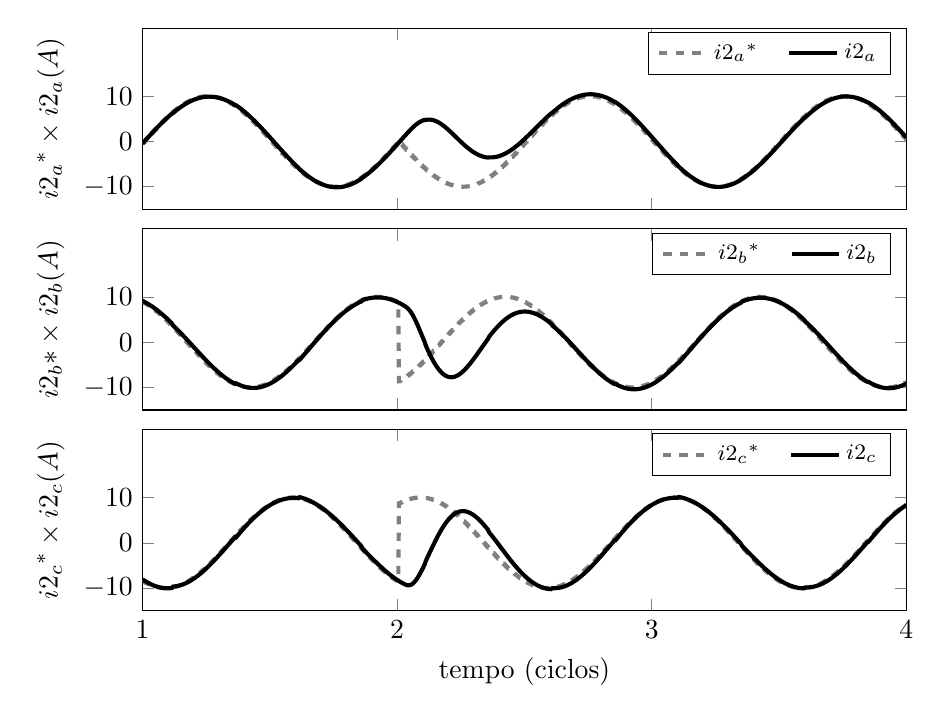
\begin{tikzpicture}

\begin{axis}[%
width=0.8\textwidth,
height=0.189701500343624\textwidth,
scale only axis,
xmin=0.0166666666666667,
xmax=0.0666666666666667,
xtick={0.0166666666666667,0.0333333333333333,0.05,0.0666666666666667},
xticklabels={\empty},
ymin=-15,
ymax=25,
ytick={-10,   0,  10},
ylabel={${\text{i2}_\text{b}}\text{* }\times\text{ i2}_\text{b}\text{ (A)}$},
name=plot2,
legend style={draw=black,fill=white,legend cell align=left},
scaled x ticks = false,
legend columns=-1,
legend style={/tikz/every even column/.append style={column sep=0.3cm}},
legend style={font=\footnotesize}
]
\addplot [color=gray,dashed,line width=1.5pt]
  table[row sep=crcr]{0.0166583333333333	8.95711760239421\\
0.0167	8.81303452065\\
0.0167416666666667	8.81303452065\\
0.0167833333333333	8.66025403784447\\
0.016825	8.66025403784447\\
0.0168666666666667	8.49892692986872\\
0.0169083333333333	8.49892692986872\\
0.01695	8.32921240710107\\
0.0169916666666667	8.32921240710107\\
0.0170333333333333	8.15127795728562\\
0.017075	8.15127795728562\\
0.0171166666666667	7.96529918024204\\
0.0171583333333333	7.96529918024204\\
0.0172	7.77145961456979\\
0.0172416666666667	7.77145961456979\\
0.0172833333333333	7.56995055651764\\
0.017325	7.56995055651764\\
0.0173666666666667	7.36097087119742\\
0.0174083333333333	7.36097087119742\\
0.01745	7.1447267963281\\
0.0174916666666667	7.1447267963281\\
0.0175333333333333	6.92143173870414\\
0.017575	6.92143173870414\\
0.0176166666666667	6.69130606358865\\
0.0176583333333333	6.69130606358865\\
0.0177	6.45457687723957\\
0.0177416666666667	6.45457687723957\\
0.0177833333333333	6.21147780278317\\
0.017825	6.21147780278317\\
0.0178666666666667	5.96224874965622\\
0.0179083333333333	5.96224874965622\\
0.01795	5.70713567684438\\
0.0179916666666667	5.70713567684438\\
0.0180333333333333	5.44639035015033\\
0.018075	5.44639035015033\\
0.0181166666666667	5.18027009373136\\
0.0181583333333333	5.18027009373136\\
0.0182	4.90903753615147\\
0.0182416666666667	4.90903753615147\\
0.0182833333333333	4.63296035119867\\
0.018325	4.63296035119867\\
0.0183666666666667	4.35231099372333\\
0.0184083333333333	4.35231099372333\\
0.01845	4.06736643075805\\
0.0184916666666667	4.06736643075805\\
0.0185333333333333	3.77840786818472\\
0.018575	3.77840786818472\\
0.0186166666666667	3.4857204732182\\
0.0186583333333333	3.4857204732182\\
0.0187	3.18959309298074\\
0.0187416666666667	3.18959309298074\\
0.0187833333333333	2.89031796944476\\
0.018825	2.89031796944476\\
0.0188666666666667	2.58819045102524\\
0.0189083333333333	2.58819045102524\\
0.01895	2.28350870110659\\
0.0189916666666667	2.28350870110659\\
0.0190333333333333	1.97657340379129\\
0.019075	1.97657340379129\\
0.0191166666666667	1.66768746716105\\
0.0191583333333333	1.66768746716105\\
0.0192	1.35715572434307\\
0.0192416666666667	1.35715572434307\\
0.0192833333333333	1.04528463267656\\
0.019325	1.04528463267656\\
0.0193666666666667	0.732381971276336\\
0.0194083333333333	0.732381971276336\\
0.01945	0.418756537292012\\
0.0194916666666667	0.418756537292012\\
0.0195333333333333	0.104717841162471\\
0.019575	0.104717841162471\\
0.0196166666666667	-0.20942419883356\\
0.0196583333333333	-0.20942419883356\\
0.0197	-0.523359562429432\\
0.0197416666666667	-0.523359562429432\\
0.0197833333333333	-0.836778433323152\\
0.019825	-0.836778433323152\\
0.0198666666666667	-1.14937150492867\\
0.0199083333333333	-1.14937150492867\\
0.01995	-1.46083028562412\\
0.0199916666666667	-1.46083028562412\\
0.0200333333333333	-1.77084740319584\\
0.020075	-1.77084740319584\\
0.0201166666666667	-2.0791169081776\\
0.0201583333333333	-2.0791169081776\\
0.0202	-2.38533457578582\\
0.0202416666666667	-2.38533457578582\\
0.0202833333333333	-2.68919820615267\\
0.020325	-2.68919820615267\\
0.0203666666666667	-2.99040792256089\\
0.0204083333333333	-2.99040792256089\\
0.02045	-3.28866646738586\\
0.0204916666666667	-3.28866646738586\\
0.0205333333333333	-3.58367949545303\\
0.020575	-3.58367949545303\\
0.0206166666666667	-3.87515586452106\\
0.0206583333333333	-3.87515586452106\\
0.0207	-4.16280792260405\\
0.0207416666666667	-4.16280792260405\\
0.0207833333333333	-4.44635179184931\\
0.020825	-4.44635179184931\\
0.0208666666666667	-4.72550764869058\\
0.0209083333333333	-4.72550764869058\\
0.02095	-5.00000000000005\\
0.0209916666666667	-5.00000000000005\\
0.0210333333333333	-5.26955795496682\\
0.021075	-5.26955795496682\\
0.0211166666666667	-5.53391549243349\\
0.0211583333333333	-5.53391549243349\\
0.0212	-5.79281172342684\\
0.0212416666666667	-5.79281172342684\\
0.0212833333333333	-6.0459911486238\\
0.021325	-6.0459911486238\\
0.0213666666666667	-6.29320391049844\\
0.0214083333333333	-6.29320391049844\\
0.02145	-6.53420603990112\\
0.0214916666666667	-6.53420603990112\\
0.0215333333333333	-6.76875969682667\\
0.021575	-6.76875969682667\\
0.0216166666666667	-6.99663340513372\\
0.0216583333333333	-6.99663340513372\\
0.0217	-7.2176022809837\\
0.0217416666666667	-7.2176022809837\\
0.0217833333333333	-7.43144825477402\\
0.021825	-7.43144825477402\\
0.0218666666666667	-7.6379602863465\\
0.0219083333333333	-7.6379602863465\\
0.02195	-7.83693457325848\\
0.0219916666666667	-7.83693457325848\\
0.0220333333333333	-8.02817475191123\\
0.022075	-8.02817475191123\\
0.0221166666666667	-8.21149209133713\\
0.0221583333333333	-8.21149209133713\\
0.0222	-8.38670567945433\\
0.0222416666666667	-8.38670567945433\\
0.0222833333333333	-8.55364260160516\\
0.022325	-8.55364260160516\\
0.0223666666666667	-8.71213811120199\\
0.0224083333333333	-8.71213811120199\\
0.02245	-8.86203579231225\\
0.0224916666666667	-8.86203579231225\\
0.0225333333333333	-9.00318771402204\\
0.022575	-9.00318771402204\\
0.0226166666666667	-9.13545457642611\\
0.0226583333333333	-9.13545457642611\\
0.0227	-9.25870584810006\\
0.0227416666666667	-9.25870584810006\\
0.0227833333333333	-9.37281989491902\\
0.022825	-9.37281989491902\\
0.0228666666666667	-9.47768410009597\\
0.0229083333333333	-9.47768410009597\\
0.02295	-9.57319497532079\\
0.0229916666666667	-9.57319497532079\\
0.0230333333333333	-9.6592582628908\\
0.023075	-9.6592582628908\\
0.0231166666666667	-9.73578902873172\\
0.0231583333333333	-9.73578902873172\\
0.0232	-9.80271174621734\\
0.0232416666666667	-9.80271174621734\\
0.0232833333333333	-9.85996037070517\\
0.023325	-9.85996037070517\\
0.0233666666666667	-9.90747840471456\\
0.0234083333333333	-9.90747840471456\\
0.02345	-9.94521895368285\\
0.0234916666666667	-9.94521895368285\\
0.0235333333333333	-9.97314477224471\\
0.023575	-9.97314477224471\\
0.0236166666666667	-9.99122830098871\\
0.0236583333333333	-9.99122830098871\\
0.0237	-9.99945169365525\\
0.0237416666666667	-9.99945169365525\\
0.0237833333333333	-9.99780683474858\\
0.023825	-9.99780683474858\\
0.0238666666666667	-9.98629534754587\\
0.0239083333333333	-9.98629534754587\\
0.02395	-9.96492859249517\\
0.0239916666666667	-9.96492859249517\\
0.0240333333333333	-9.93372765600409\\
0.024075	-9.93372765600409\\
0.0241166666666667	-9.89272332963001\\
0.0241583333333333	-9.89272332963001\\
0.0242	-9.84195607969255\\
0.0242416666666667	-9.84195607969255\\
0.0242833333333333	-9.78147600733818\\
0.024325	-9.78147600733818\\
0.0243666666666667	-9.71134279909649\\
0.0244083333333333	-9.71134279909649\\
0.02445	-9.63162566797671\\
0.0244916666666667	-9.63162566797671\\
0.0245333333333333	-9.5424032851629\\
0.024575	-9.5424032851629\\
0.0246166666666667	-9.44376370237494\\
0.0246583333333333	-9.44376370237494\\
0.0247	-9.33580426497215\\
0.0247416666666667	-9.33580426497215\\
0.0247833333333333	-9.21863151588513\\
0.024825	-9.21863151588513\\
0.0248666666666667	-9.09236109047081\\
0.0249083333333333	-9.09236109047081\\
0.02495	-8.95711760239425\\
0.0249916666666667	-8.95711760239425\\
0.0250333333333333	-8.81303452065005\\
0.025075	-8.81303452065005\\
0.0251166666666667	-8.66025403784451\\
0.0251583333333333	-8.66025403784451\\
0.0252	-8.49892692986876\\
0.0252416666666667	-8.49892692986876\\
0.0252833333333333	-8.32921240710111\\
0.025325	-8.32921240710111\\
0.0253666666666667	-8.15127795728566\\
0.0254083333333333	-8.15127795728566\\
0.02545	-7.96529918024207\\
0.0254916666666667	-7.96529918024207\\
0.0255333333333333	-7.77145961456982\\
0.025575	-7.77145961456982\\
0.0256166666666667	-7.56995055651767\\
0.0256583333333333	-7.56995055651767\\
0.0257	-7.36097087119745\\
0.0257416666666667	-7.36097087119745\\
0.0257833333333333	-7.14472679632814\\
0.025825	-7.14472679632814\\
0.0258666666666667	-6.92143173870417\\
0.0259083333333333	-6.92143173870417\\
0.02595	-6.69130606358868\\
0.0259916666666667	-6.69130606358868\\
0.0260333333333333	-6.4545768772396\\
0.026075	-6.4545768772396\\
0.0261166666666667	-6.2114778027832\\
0.0261583333333333	-6.2114778027832\\
0.0262	-5.96224874965625\\
0.0262416666666667	-5.96224874965625\\
0.0262833333333333	-5.70713567684441\\
0.026325	-5.70713567684441\\
0.0263666666666667	-5.44639035015036\\
0.0264083333333333	-5.44639035015036\\
0.02645	-5.18027009373139\\
0.0264916666666667	-5.18027009373139\\
0.0265333333333333	-4.90903753615149\\
0.026575	-4.90903753615149\\
0.0266166666666667	-4.6329603511987\\
0.0266583333333333	-4.6329603511987\\
0.0267	-4.35231099372335\\
0.0267416666666667	-4.35231099372335\\
0.0267833333333333	-4.06736643075807\\
0.026825	-4.06736643075807\\
0.0268666666666667	-3.77840786818474\\
0.0269083333333333	-3.77840786818474\\
0.02695	-3.48572047321821\\
0.0269916666666667	-3.48572047321821\\
0.0270333333333333	-3.18959309298076\\
0.027075	-3.18959309298076\\
0.0271166666666667	-2.89031796944477\\
0.0271583333333333	-2.89031796944477\\
0.0272	-2.58819045102526\\
0.0272416666666667	-2.58819045102526\\
0.0272833333333333	-2.28350870110661\\
0.027325	-2.28350870110661\\
0.0273666666666667	-1.9765734037913\\
0.0274083333333333	-1.9765734037913\\
0.02745	-1.66768746716106\\
0.0274916666666667	-1.66768746716106\\
0.0275333333333333	-1.35715572434308\\
0.027575	-1.35715572434308\\
0.0276166666666667	-1.04528463267656\\
0.0276583333333333	-1.04528463267656\\
0.0277	-0.732381971276341\\
0.0277416666666667	-0.732381971276341\\
0.0277833333333333	-0.418756537292015\\
0.027825	-0.418756537292015\\
0.0278666666666667	-0.104717841162473\\
0.0279083333333333	-0.104717841162473\\
0.02795	0.209424198833559\\
0.0279916666666667	0.209424198833559\\
0.0280333333333333	0.523359562429433\\
0.028075	0.523359562429433\\
0.0281166666666667	0.836778433323154\\
0.0281583333333333	0.836778433323154\\
0.0282	1.14937150492867\\
0.0282416666666667	1.14937150492867\\
0.0282833333333333	1.46083028562412\\
0.028325	1.46083028562412\\
0.0283666666666667	1.77084740319585\\
0.0284083333333333	1.77084740319585\\
0.02845	2.07911690817761\\
0.0284916666666667	2.07911690817761\\
0.0285333333333333	2.38533457578583\\
0.028575	2.38533457578583\\
0.0286166666666667	2.68919820615268\\
0.0286583333333333	2.68919820615268\\
0.0287	2.9904079225609\\
0.0287416666666667	2.9904079225609\\
0.0287833333333333	3.28866646738587\\
0.028825	3.28866646738587\\
0.0288666666666667	3.58367949545304\\
0.0289083333333333	3.58367949545304\\
0.02895	3.87515586452107\\
0.0289916666666667	3.87515586452107\\
0.0290333333333333	4.16280792260406\\
0.029075	4.16280792260406\\
0.0291166666666667	4.44635179184933\\
0.0291583333333333	4.44635179184933\\
0.0292	4.7255076486906\\
0.0292416666666667	4.7255076486906\\
0.0292833333333333	5.00000000000006\\
0.029325	5.00000000000006\\
0.0293666666666667	5.26955795496684\\
0.0294083333333333	5.26955795496684\\
0.02945	5.53391549243351\\
0.0294916666666667	5.53391549243351\\
0.0295333333333333	5.79281172342686\\
0.029575	5.79281172342686\\
0.0296166666666667	6.04599114862383\\
0.0296583333333333	6.04599114862383\\
0.0297	6.29320391049846\\
0.0297416666666667	6.29320391049846\\
0.0297833333333333	6.53420603990114\\
0.029825	6.53420603990114\\
0.0298666666666667	6.7687596968267\\
0.0299083333333333	6.7687596968267\\
0.02995	6.99663340513375\\
0.0299916666666667	6.99663340513375\\
0.0300333333333333	7.21760228098372\\
0.030075	7.21760228098372\\
0.0301166666666667	7.43144825477405\\
0.0301583333333333	7.43144825477405\\
0.0302	7.63796028634653\\
0.0302416666666667	7.63796028634653\\
0.0302833333333333	7.83693457325851\\
0.030325	7.83693457325851\\
0.0303666666666667	8.02817475191126\\
0.0304083333333333	8.02817475191126\\
0.03045	8.21149209133716\\
0.0304916666666667	8.21149209133716\\
0.0305333333333333	8.38670567945436\\
0.030575	8.38670567945436\\
0.0306166666666667	8.55364260160519\\
0.0306583333333333	8.55364260160519\\
0.0307	8.71213811120203\\
0.0307416666666667	8.71213811120203\\
0.0307833333333333	8.86203579231228\\
0.030825	8.86203579231228\\
0.0308666666666667	9.00318771402207\\
0.0309083333333333	9.00318771402207\\
0.03095	9.13545457642615\\
0.0309916666666667	9.13545457642615\\
0.0310333333333333	9.25870584810009\\
0.031075	9.25870584810009\\
0.0311166666666667	9.37281989491906\\
0.0311583333333333	9.37281989491906\\
0.0312	9.477684100096\\
0.0312416666666667	9.477684100096\\
0.0312833333333333	9.57319497532082\\
0.031325	9.57319497532082\\
0.0313666666666667	9.65925826289084\\
0.0314083333333333	9.65925826289084\\
0.03145	9.73578902873176\\
0.0314916666666667	9.73578902873176\\
0.0315333333333333	9.80271174621738\\
0.031575	9.80271174621738\\
0.0316166666666667	9.85996037070521\\
0.0316583333333333	9.85996037070521\\
0.0317	9.9074784047146\\
0.0317416666666667	9.9074784047146\\
0.0317833333333333	9.94521895368289\\
0.031825	9.94521895368289\\
0.0318666666666667	9.97314477224474\\
0.0319083333333333	9.97314477224474\\
0.03195	9.99122830098875\\
0.0319916666666667	9.99122830098875\\
0.0320333333333333	9.99945169365528\\
0.032075	9.99945169365528\\
0.0321166666666667	9.99780683474862\\
0.0321583333333333	9.99780683474862\\
0.0322	9.98629534754591\\
0.0322416666666667	9.98629534754591\\
0.0322833333333333	9.96492859249521\\
0.032325	9.96492859249521\\
0.0323666666666667	9.93372765600413\\
0.0324083333333333	9.93372765600413\\
0.03245	9.89272332963005\\
0.0324916666666667	9.89272332963005\\
0.0325333333333333	9.84195607969259\\
0.032575	9.84195607969259\\
0.0326166666666667	9.78147600733822\\
0.0326583333333333	9.78147600733822\\
0.0327	9.71134279909653\\
0.0327416666666667	9.71134279909653\\
0.0327833333333333	9.63162566797675\\
0.032825	9.63162566797675\\
0.0328666666666667	9.54240328516294\\
0.0329083333333333	9.54240328516294\\
0.03295	9.44376370237498\\
0.0329916666666667	9.44376370237498\\
0.0330333333333333	9.33580426497218\\
0.033075	9.33580426497218\\
0.0331166666666667	9.21863151588517\\
0.0331583333333333	9.21863151588517\\
0.0332	9.09236109047085\\
0.0332416666666667	9.09236109047085\\
0.0332833333333333	8.95711760239429\\
0.033325	8.95711760239429\\
0.0333666666666667	8.81303452065008\\
0.0334083333333333	8.81303452065008\\
0.03345	-8.66025403784455\\
0.0334916666666667	-8.66025403784455\\
0.0335333333333333	-8.49892692986879\\
0.033575	-8.49892692986879\\
0.0336166666666667	-8.32921240710115\\
0.0336583333333333	-8.32921240710115\\
0.0337	-8.15127795728569\\
0.0337416666666667	-8.15127795728569\\
0.0337833333333333	-7.96529918024211\\
0.033825	-7.96529918024211\\
0.0338666666666667	-7.77145961456986\\
0.0339083333333333	-7.77145961456986\\
0.03395	-7.56995055651771\\
0.0339916666666667	-7.56995055651771\\
0.0340333333333333	-7.36097087119748\\
0.034075	-7.36097087119748\\
0.0341166666666667	-7.14472679632817\\
0.0341583333333333	-7.14472679632817\\
0.0342	-6.9214317387042\\
0.0342416666666667	-6.9214317387042\\
0.0342833333333333	-6.69130606358871\\
0.034325	-6.69130606358871\\
0.0343666666666667	-6.45457687723963\\
0.0344083333333333	-6.45457687723963\\
0.03445	-6.21147780278323\\
0.0344916666666667	-6.21147780278323\\
0.0345333333333333	-5.96224874965628\\
0.034575	-5.96224874965628\\
0.0346166666666667	-5.70713567684443\\
0.0346583333333333	-5.70713567684443\\
0.0347	-5.44639035015038\\
0.0347416666666667	-5.44639035015038\\
0.0347833333333333	-5.18027009373141\\
0.034825	-5.18027009373141\\
0.0348666666666667	-4.90903753615151\\
0.0349083333333333	-4.90903753615151\\
0.03495	-4.63296035119872\\
0.0349916666666667	-4.63296035119872\\
0.0350333333333333	-4.35231099372337\\
0.035075	-4.35231099372337\\
0.0351166666666667	-4.06736643075809\\
0.0351583333333333	-4.06736643075809\\
0.0352	-3.77840786818476\\
0.0352416666666667	-3.77840786818476\\
0.0352833333333333	-3.48572047321823\\
0.035325	-3.48572047321823\\
0.0353666666666667	-3.18959309298077\\
0.0354083333333333	-3.18959309298077\\
0.03545	-2.89031796944478\\
0.0354916666666667	-2.89031796944478\\
0.0355333333333333	-2.58819045102527\\
0.035575	-2.58819045102527\\
0.0356166666666667	-2.28350870110662\\
0.0356583333333333	-2.28350870110662\\
0.0357	-1.97657340379131\\
0.0357416666666667	-1.97657340379131\\
0.0357833333333333	-1.66768746716107\\
0.035825	-1.66768746716107\\
0.0358666666666667	-1.35715572434309\\
0.0359083333333333	-1.35715572434309\\
0.03595	-1.04528463267657\\
0.0359916666666667	-1.04528463267657\\
0.0360333333333333	-0.732381971276348\\
0.036075	-0.732381971276348\\
0.0361166666666667	-0.418756537292022\\
0.0361583333333333	-0.418756537292022\\
0.0362	-0.104717841162477\\
0.0362416666666667	-0.104717841162477\\
0.0362833333333333	0.209424198833557\\
0.036325	0.209424198833557\\
0.0363666666666667	0.523359562429431\\
0.0364083333333333	0.523359562429431\\
0.03645	0.836778433323154\\
0.0364916666666667	0.836778433323154\\
0.0365333333333333	1.14937150492867\\
0.036575	1.14937150492867\\
0.0366166666666667	1.46083028562413\\
0.0366583333333333	1.46083028562413\\
0.0367	1.77084740319585\\
0.0367416666666667	1.77084740319585\\
0.0367833333333333	2.07911690817762\\
0.036825	2.07911690817762\\
0.0368666666666667	2.38533457578584\\
0.0369083333333333	2.38533457578584\\
0.03695	2.68919820615269\\
0.0369916666666667	2.68919820615269\\
0.0370333333333333	2.99040792256091\\
0.037075	2.99040792256091\\
0.0371166666666667	3.28866646738588\\
0.0371583333333333	3.28866646738588\\
0.0372	3.58367949545306\\
0.0372416666666667	3.58367949545306\\
0.0372833333333333	3.87515586452109\\
0.037325	3.87515586452109\\
0.0373666666666667	4.16280792260408\\
0.0374083333333333	4.16280792260408\\
0.03745	4.44635179184934\\
0.0374916666666667	4.44635179184934\\
0.0375333333333333	4.72550764869062\\
0.037575	4.72550764869062\\
0.0376166666666667	5.00000000000008\\
0.0376583333333333	5.00000000000008\\
0.0377	5.26955795496686\\
0.0377416666666667	5.26955795496686\\
0.0377833333333333	5.53391549243353\\
0.037825	5.53391549243353\\
0.0378666666666667	5.79281172342689\\
0.0379083333333333	5.79281172342689\\
0.03795	6.04599114862385\\
0.0379916666666667	6.04599114862385\\
0.0380333333333333	6.29320391049848\\
0.038075	6.29320391049848\\
0.0381166666666667	6.53420603990117\\
0.0381583333333333	6.53420603990117\\
0.0382	6.76875969682673\\
0.0382416666666667	6.76875969682673\\
0.0382833333333333	6.99663340513378\\
0.038325	6.99663340513378\\
0.0383666666666667	7.21760228098375\\
0.0384083333333333	7.21760228098375\\
0.03845	7.43144825477408\\
0.0384916666666667	7.43144825477408\\
0.0385333333333333	7.63796028634656\\
0.038575	7.63796028634656\\
0.0386166666666667	7.83693457325854\\
0.0386583333333333	7.83693457325854\\
0.0387	8.02817475191129\\
0.0387416666666667	8.02817475191129\\
0.0387833333333333	8.21149209133719\\
0.038825	8.21149209133719\\
0.0388666666666667	8.3867056794544\\
0.0389083333333333	8.3867056794544\\
0.03895	8.55364260160523\\
0.0389916666666667	8.55364260160523\\
0.0390333333333333	8.71213811120206\\
0.039075	8.71213811120206\\
0.0391166666666667	8.86203579231232\\
0.0391583333333333	8.86203579231232\\
0.0392	9.00318771402211\\
0.0392416666666667	9.00318771402211\\
0.0392833333333333	9.13545457642618\\
0.039325	9.13545457642618\\
0.0393666666666667	9.25870584810013\\
0.0394083333333333	9.25870584810013\\
0.03945	9.3728198949191\\
0.0394916666666667	9.3728198949191\\
0.0395333333333333	9.47768410009604\\
0.039575	9.47768410009604\\
0.0396166666666667	9.57319497532086\\
0.0396583333333333	9.57319497532086\\
0.0397	9.65925826289087\\
0.0397416666666667	9.65925826289087\\
0.0397833333333333	9.7357890287318\\
0.039825	9.7357890287318\\
0.0398666666666667	9.80271174621742\\
0.0399083333333333	9.80271174621742\\
0.03995	9.85996037070525\\
0.0399916666666667	9.85996037070525\\
0.0400333333333333	9.90747840471464\\
0.040075	9.90747840471464\\
0.0401166666666667	9.94521895368294\\
0.0401583333333333	9.94521895368294\\
0.0402	9.97314477224478\\
0.0402416666666667	9.97314477224478\\
0.0402833333333333	9.99122830098879\\
0.040325	9.99122830098879\\
0.0403666666666667	9.99945169365533\\
0.0404083333333333	9.99945169365533\\
0.04045	9.99780683474866\\
0.0404916666666667	9.99780683474866\\
0.0405333333333333	9.98629534754595\\
0.040575	9.98629534754595\\
0.0406166666666667	9.96492859249525\\
0.0406583333333333	9.96492859249525\\
0.0407	9.93372765600417\\
0.0407416666666667	9.93372765600417\\
0.0407833333333333	9.89272332963009\\
0.040825	9.89272332963009\\
0.0408666666666667	9.84195607969263\\
0.0409083333333333	9.84195607969263\\
0.04095	9.78147600733827\\
0.0409916666666667	9.78147600733827\\
0.0410333333333333	9.71134279909657\\
0.041075	9.71134279909657\\
0.0411166666666667	9.63162566797679\\
0.0411583333333333	9.63162566797679\\
0.0412	9.54240328516298\\
0.0412416666666667	9.54240328516298\\
0.0412833333333333	9.44376370237502\\
0.041325	9.44376370237502\\
0.0413666666666667	9.33580426497222\\
0.0414083333333333	9.33580426497222\\
0.04145	9.21863151588521\\
0.0414916666666667	9.21863151588521\\
0.0415333333333333	9.09236109047089\\
0.041575	9.09236109047089\\
0.0416166666666667	8.95711760239433\\
0.0416583333333333	8.95711760239433\\
0.0417	8.81303452065012\\
0.0417416666666667	8.81303452065012\\
0.0417833333333333	8.66025403784458\\
0.041825	8.66025403784458\\
0.0418666666666667	8.49892692986883\\
0.0419083333333333	8.49892692986883\\
0.04195	8.32921240710118\\
0.0419916666666667	8.32921240710118\\
0.0420333333333333	8.15127795728573\\
0.042075	8.15127795728573\\
0.0421166666666667	7.96529918024214\\
0.0421583333333333	7.96529918024214\\
0.0422	7.77145961456989\\
0.0422416666666667	7.77145961456989\\
0.0422833333333333	7.56995055651774\\
0.042325	7.56995055651774\\
0.0423666666666667	7.36097087119751\\
0.0424083333333333	7.36097087119751\\
0.04245	7.1447267963282\\
0.0424916666666667	7.1447267963282\\
0.0425333333333333	6.92143173870423\\
0.042575	6.92143173870423\\
0.0426166666666667	6.69130606358874\\
0.0426583333333333	6.69130606358874\\
0.0427	6.45457687723966\\
0.0427416666666667	6.45457687723966\\
0.0427833333333333	6.21147780278325\\
0.042825	6.21147780278325\\
0.0428666666666667	5.9622487496563\\
0.0429083333333333	5.9622487496563\\
0.04295	5.70713567684446\\
0.0429916666666667	5.70713567684446\\
0.0430333333333333	5.44639035015041\\
0.043075	5.44639035015041\\
0.0431166666666667	5.18027009373143\\
0.0431583333333333	5.18027009373143\\
0.0432	4.90903753615153\\
0.0432416666666667	4.90903753615153\\
0.0432833333333333	4.63296035119874\\
0.043325	4.63296035119874\\
0.0433666666666667	4.35231099372339\\
0.0434083333333333	4.35231099372339\\
0.04345	4.06736643075811\\
0.0434916666666667	4.06736643075811\\
0.0435333333333333	3.77840786818477\\
0.043575	3.77840786818477\\
0.0436166666666667	3.48572047321825\\
0.0436583333333333	3.48572047321825\\
0.0437	3.18959309298079\\
0.0437416666666667	3.18959309298079\\
0.0437833333333333	2.8903179694448\\
0.043825	2.8903179694448\\
0.0438666666666667	2.58819045102528\\
0.0439083333333333	2.58819045102528\\
0.04395	2.28350870110663\\
0.0439916666666667	2.28350870110663\\
0.0440333333333333	1.97657340379133\\
0.044075	1.97657340379133\\
0.0441166666666667	1.66768746716108\\
0.0441583333333333	1.66768746716108\\
0.0442	1.35715572434309\\
0.0442416666666667	1.35715572434309\\
0.0442833333333333	1.04528463267658\\
0.044325	1.04528463267658\\
0.0443666666666667	0.732381971276353\\
0.0444083333333333	0.732381971276353\\
0.04445	0.418756537292025\\
0.0444916666666667	0.418756537292025\\
0.0445333333333333	0.104717841162479\\
0.044575	0.104717841162479\\
0.0446166666666667	-0.209424198833555\\
0.0446583333333333	-0.209424198833555\\
0.0447	-0.523359562429432\\
0.0447416666666667	-0.523359562429432\\
0.0447833333333333	-0.836778433323156\\
0.044825	-0.836778433323156\\
0.0448666666666667	-1.14937150492867\\
0.0449083333333333	-1.14937150492867\\
0.04495	-1.46083028562413\\
0.0449916666666667	-1.46083028562413\\
0.0450333333333333	-1.77084740319586\\
0.045075	-1.77084740319586\\
0.0451166666666667	-2.07911690817762\\
0.0451583333333333	-2.07911690817762\\
0.0452	-2.38533457578585\\
0.0452416666666667	-2.38533457578585\\
0.0452833333333333	-2.6891982061527\\
0.045325	-2.6891982061527\\
0.0453666666666667	-2.99040792256092\\
0.0454083333333333	-2.99040792256092\\
0.04545	-3.28866646738589\\
0.0454916666666667	-3.28866646738589\\
0.0455333333333333	-3.58367949545307\\
0.045575	-3.58367949545307\\
0.0456166666666667	-3.8751558645211\\
0.0456583333333333	-3.8751558645211\\
0.0457	-4.16280792260409\\
0.0457416666666667	-4.16280792260409\\
0.0457833333333333	-4.44635179184936\\
0.045825	-4.44635179184936\\
0.0458666666666667	-4.72550764869064\\
0.0459083333333333	-4.72550764869064\\
0.04595	-5.0000000000001\\
0.0459916666666667	-5.0000000000001\\
0.0460333333333333	-5.26955795496689\\
0.046075	-5.26955795496689\\
0.0461166666666667	-5.53391549243356\\
0.0461583333333333	-5.53391549243356\\
0.0462	-5.79281172342691\\
0.0462416666666667	-5.79281172342691\\
0.0462833333333333	-6.04599114862388\\
0.046325	-6.04599114862388\\
0.0463666666666667	-6.29320391049851\\
0.0464083333333333	-6.29320391049851\\
0.04645	-6.5342060399012\\
0.0464916666666667	-6.5342060399012\\
0.0465333333333333	-6.76875969682676\\
0.046575	-6.76875969682676\\
0.0466166666666667	-6.99663340513381\\
0.0466583333333333	-6.99663340513381\\
0.0467	-7.21760228098379\\
0.0467416666666667	-7.21760228098379\\
0.0467833333333333	-7.43144825477411\\
0.046825	-7.43144825477411\\
0.0468666666666667	-7.6379602863466\\
0.0469083333333333	-7.6379602863466\\
0.04695	-7.83693457325858\\
0.0469916666666667	-7.83693457325858\\
0.0470333333333333	-8.02817475191133\\
0.047075	-8.02817475191133\\
0.0471166666666667	-8.21149209133723\\
0.0471583333333333	-8.21149209133723\\
0.0472	-8.38670567945444\\
0.0472416666666667	-8.38670567945444\\
0.0472833333333333	-8.55364260160527\\
0.047325	-8.55364260160527\\
0.0473666666666667	-8.7121381112021\\
0.0474083333333333	-8.7121381112021\\
0.04745	-8.86203579231236\\
0.0474916666666667	-8.86203579231236\\
0.0475333333333333	-9.00318771402215\\
0.047575	-9.00318771402215\\
0.0476166666666667	-9.13545457642623\\
0.0476583333333333	-9.13545457642623\\
0.0477	-9.25870584810017\\
0.0477416666666667	-9.25870584810017\\
0.0477833333333333	-9.37281989491914\\
0.047825	-9.37281989491914\\
0.0478666666666667	-9.47768410009609\\
0.0479083333333333	-9.47768410009609\\
0.04795	-9.57319497532091\\
0.0479916666666667	-9.57319497532091\\
0.0480333333333333	-9.65925826289092\\
0.048075	-9.65925826289092\\
0.0481166666666667	-9.73578902873184\\
0.0481583333333333	-9.73578902873184\\
0.0482	-9.80271174621746\\
0.0482416666666667	-9.80271174621746\\
0.0482833333333333	-9.85996037070529\\
0.048325	-9.85996037070529\\
0.0483666666666667	-9.90747840471468\\
0.0484083333333333	-9.90747840471468\\
0.04845	-9.94521895368298\\
0.0484916666666667	-9.94521895368298\\
0.0485333333333333	-9.97314477224483\\
0.048575	-9.97314477224483\\
0.0486166666666667	-9.99122830098883\\
0.0486583333333333	-9.99122830098883\\
0.0487	-9.99945169365537\\
0.0487416666666667	-9.99945169365537\\
0.0487833333333333	-9.99780683474871\\
0.048825	-9.99780683474871\\
0.0488666666666667	-9.98629534754599\\
0.0489083333333333	-9.98629534754599\\
0.04895	-9.9649285924953\\
0.0489916666666667	-9.9649285924953\\
0.0490333333333333	-9.93372765600422\\
0.049075	-9.93372765600422\\
0.0491166666666667	-9.89272332963014\\
0.0491583333333333	-9.89272332963014\\
0.0492	-9.84195607969268\\
0.0492416666666667	-9.84195607969268\\
0.0492833333333333	-9.78147600733831\\
0.049325	-9.78147600733831\\
0.0493666666666667	-9.71134279909661\\
0.0494083333333333	-9.71134279909661\\
0.04945	-9.63162566797684\\
0.0494916666666667	-9.63162566797684\\
0.0495333333333333	-9.54240328516302\\
0.049575	-9.54240328516302\\
0.0496166666666667	-9.44376370237506\\
0.0496583333333333	-9.44376370237506\\
0.0497	-9.33580426497227\\
0.0497416666666667	-9.33580426497227\\
0.0497833333333333	-9.21863151588525\\
0.049825	-9.21863151588525\\
0.0498666666666667	-9.09236109047093\\
0.0499083333333333	-9.09236109047093\\
0.04995	-8.95711760239437\\
0.0499916666666667	-8.95711760239437\\
0.0500333333333333	-8.81303452065016\\
0.050075	-8.81303452065016\\
0.0501166666666667	-8.66025403784462\\
0.0501583333333333	-8.66025403784462\\
0.0502	-8.49892692986887\\
0.0502416666666667	-8.49892692986887\\
0.0502833333333333	-8.32921240710123\\
0.050325	-8.32921240710123\\
0.0503666666666667	-8.15127795728577\\
0.0504083333333333	-8.15127795728577\\
0.05045	-7.96529918024218\\
0.0504916666666667	-7.96529918024218\\
0.0505333333333333	-7.77145961456993\\
0.050575	-7.77145961456993\\
0.0506166666666667	-7.56995055651778\\
0.0506583333333333	-7.56995055651778\\
0.0507	-7.36097087119755\\
0.0507416666666667	-7.36097087119755\\
0.0507833333333333	-7.14472679632824\\
0.050825	-7.14472679632824\\
0.0508666666666667	-6.92143173870427\\
0.0509083333333333	-6.92143173870427\\
0.05095	-6.69130606358878\\
0.0509916666666667	-6.69130606358878\\
0.0510333333333333	-6.45457687723969\\
0.051075	-6.45457687723969\\
0.0511166666666667	-6.21147780278329\\
0.0511583333333333	-6.21147780278329\\
0.0512	-5.96224874965633\\
0.0512416666666667	-5.96224874965633\\
0.0512833333333333	-5.70713567684449\\
0.051325	-5.70713567684449\\
0.0513666666666667	-5.44639035015043\\
0.0514083333333333	-5.44639035015043\\
0.05145	-5.18027009373146\\
0.0514916666666667	-5.18027009373146\\
0.0515333333333333	-4.90903753615156\\
0.051575	-4.90903753615156\\
0.0516166666666667	-4.63296035119876\\
0.0516583333333333	-4.63296035119876\\
0.0517	-4.35231099372341\\
0.0517416666666667	-4.35231099372341\\
0.0517833333333333	-4.06736643075813\\
0.051825	-4.06736643075813\\
0.0518666666666667	-3.77840786818479\\
0.0519083333333333	-3.77840786818479\\
0.05195	-3.48572047321827\\
0.0519916666666667	-3.48572047321827\\
0.0520333333333333	-3.18959309298081\\
0.052075	-3.18959309298081\\
0.0521166666666667	-2.89031796944481\\
0.0521583333333333	-2.89031796944481\\
0.0522	-2.5881904510253\\
0.0522416666666667	-2.5881904510253\\
0.0522833333333333	-2.28350870110664\\
0.052325	-2.28350870110664\\
0.0523666666666667	-1.97657340379134\\
0.0524083333333333	-1.97657340379134\\
0.05245	-1.66768746716109\\
0.0524916666666667	-1.66768746716109\\
0.0525333333333333	-1.3571557243431\\
0.052575	-1.3571557243431\\
0.0526166666666667	-1.04528463267659\\
0.0526583333333333	-1.04528463267659\\
0.0527	-0.73238197127636\\
0.0527416666666667	-0.73238197127636\\
0.0527833333333333	-0.418756537292029\\
0.052825	-0.418756537292029\\
0.0528666666666667	-0.104717841162482\\
0.0529083333333333	-0.104717841162482\\
0.05295	0.209424198833554\\
0.0529916666666667	0.209424198833554\\
0.0530333333333333	0.523359562429432\\
0.053075	0.523359562429432\\
0.0531166666666667	0.836778433323157\\
0.0531583333333333	0.836778433323157\\
0.0532	1.14937150492868\\
0.0532416666666667	1.14937150492868\\
0.0532833333333333	1.46083028562414\\
0.053325	1.46083028562414\\
0.0533666666666667	1.77084740319586\\
0.0534083333333333	1.77084740319586\\
0.05345	2.07911690817763\\
0.0534916666666667	2.07911690817763\\
0.0535333333333333	2.38533457578585\\
0.053575	2.38533457578585\\
0.0536166666666667	2.68919820615271\\
0.0536583333333333	2.68919820615271\\
0.0537	2.99040792256093\\
0.0537416666666667	2.99040792256093\\
0.0537833333333333	3.2886664673859\\
0.053825	3.2886664673859\\
0.0538666666666667	3.58367949545308\\
0.0539083333333333	3.58367949545308\\
0.05395	3.87515586452112\\
0.0539916666666667	3.87515586452112\\
0.0540333333333333	4.16280792260411\\
0.054075	4.16280792260411\\
0.0541166666666667	4.44635179184938\\
0.0541583333333333	4.44635179184938\\
0.0542	4.72550764869065\\
0.0542416666666667	4.72550764869065\\
0.0542833333333333	5.00000000000012\\
0.054325	5.00000000000012\\
0.0543666666666667	5.26955795496691\\
0.0544083333333333	5.26955795496691\\
0.05445	5.53391549243358\\
0.0544916666666667	5.53391549243358\\
0.0545333333333333	5.79281172342693\\
0.054575	5.79281172342693\\
0.0546166666666667	6.0459911486239\\
0.0546583333333333	6.0459911486239\\
0.0547	6.29320391049854\\
0.0547416666666667	6.29320391049854\\
0.0547833333333333	6.53420603990122\\
0.054825	6.53420603990122\\
0.0548666666666667	6.76875969682678\\
0.0549083333333333	6.76875969682678\\
0.05495	6.99663340513384\\
0.0549916666666667	6.99663340513384\\
0.0550333333333333	7.21760228098381\\
0.055075	7.21760228098381\\
0.0551166666666667	7.43144825477414\\
0.0551583333333333	7.43144825477414\\
0.0552	7.63796028634663\\
0.0552416666666667	7.63796028634663\\
0.0552833333333333	7.83693457325861\\
0.055325	7.83693457325861\\
0.0553666666666667	8.02817475191136\\
0.0554083333333333	8.02817475191136\\
0.05545	8.21149209133726\\
0.0554916666666667	8.21149209133726\\
0.0555333333333333	8.38670567945447\\
0.055575	8.38670567945447\\
0.0556166666666667	8.5536426016053\\
0.0556583333333333	8.5536426016053\\
0.0557	8.71213811120214\\
0.0557416666666667	8.71213811120214\\
0.0557833333333333	8.86203579231239\\
0.055825	8.86203579231239\\
0.0558666666666667	9.00318771402219\\
0.0559083333333333	9.00318771402219\\
0.05595	9.13545457642627\\
0.0559916666666667	9.13545457642627\\
0.0560333333333333	9.25870584810021\\
0.056075	9.25870584810021\\
0.0561166666666667	9.37281989491918\\
0.0561583333333333	9.37281989491918\\
0.0562	9.47768410009613\\
0.0562416666666667	9.47768410009613\\
0.0562833333333333	9.57319497532095\\
0.056325	9.57319497532095\\
0.0563666666666667	9.65925826289096\\
0.0564083333333333	9.65925826289096\\
0.05645	9.73578902873188\\
0.0564916666666667	9.73578902873188\\
0.0565333333333333	9.8027117462175\\
0.056575	9.8027117462175\\
0.0566166666666667	9.85996037070534\\
0.0566583333333333	9.85996037070534\\
0.0567	9.90747840471473\\
0.0567416666666667	9.90747840471473\\
0.0567833333333333	9.94521895368302\\
0.056825	9.94521895368302\\
0.0568666666666667	9.97314477224487\\
0.0569083333333333	9.97314477224487\\
0.05695	9.99122830098888\\
0.0569916666666667	9.99122830098888\\
0.0570333333333333	9.99945169365542\\
0.057075	9.99945169365542\\
0.0571166666666667	9.99780683474875\\
0.0571583333333333	9.99780683474875\\
0.0572	9.98629534754604\\
0.0572416666666667	9.98629534754604\\
0.0572833333333333	9.96492859249534\\
0.057325	9.96492859249534\\
0.0573666666666667	9.93372765600427\\
0.0574083333333333	9.93372765600427\\
0.05745	9.89272332963018\\
0.0574916666666667	9.89272332963018\\
0.0575333333333333	9.84195607969272\\
0.057575	9.84195607969272\\
0.0576166666666667	9.78147600733836\\
0.0576583333333333	9.78147600733836\\
0.0577	9.71134279909666\\
0.0577416666666667	9.71134279909666\\
0.0577833333333333	9.63162566797688\\
0.057825	9.63162566797688\\
0.0578666666666667	9.54240328516306\\
0.0579083333333333	9.54240328516306\\
0.05795	9.44376370237511\\
0.0579916666666667	9.44376370237511\\
0.0580333333333333	9.33580426497231\\
0.058075	9.33580426497231\\
0.0581166666666667	9.21863151588529\\
0.0581583333333333	9.21863151588529\\
0.0582	9.09236109047097\\
0.0582416666666667	9.09236109047097\\
0.0582833333333333	8.95711760239441\\
0.058325	8.95711760239441\\
0.0583666666666667	8.8130345206502\\
0.0584083333333333	8.8130345206502\\
0.05845	8.66025403784466\\
0.0584916666666667	8.66025403784466\\
0.0585333333333333	8.49892692986891\\
0.058575	8.49892692986891\\
0.0586166666666667	8.32921240710126\\
0.0586583333333333	8.32921240710126\\
0.0587	8.1512779572858\\
0.0587416666666667	8.1512779572858\\
0.0587833333333333	7.96529918024222\\
0.058825	7.96529918024222\\
0.0588666666666667	7.77145961456996\\
0.0589083333333333	7.77145961456996\\
0.05895	7.56995055651781\\
0.0589916666666667	7.56995055651781\\
0.0590333333333333	7.36097087119758\\
0.059075	7.36097087119758\\
0.0591166666666667	7.14472679632827\\
0.0591583333333333	7.14472679632827\\
0.0592	6.9214317387043\\
0.0592416666666667	6.9214317387043\\
0.0592833333333333	6.69130606358881\\
0.059325	6.69130606358881\\
0.0593666666666667	6.45457687723972\\
0.0594083333333333	6.45457687723972\\
0.05945	6.21147780278331\\
0.0594916666666667	6.21147780278331\\
0.0595333333333333	5.96224874965636\\
0.059575	5.96224874965636\\
0.0596166666666667	5.70713567684451\\
0.0596583333333333	5.70713567684451\\
0.0597	5.44639035015046\\
0.0597416666666667	5.44639035015046\\
0.0597833333333333	5.18027009373148\\
0.059825	5.18027009373148\\
0.0598666666666667	4.90903753615158\\
0.0599083333333333	4.90903753615158\\
0.05995	4.63296035119878\\
0.0599916666666667	4.63296035119878\\
0.0600333333333333	4.35231099372343\\
0.060075	4.35231099372343\\
0.0601166666666667	4.06736643075815\\
0.0601583333333333	4.06736643075815\\
0.0602	3.77840786818481\\
0.0602416666666667	3.77840786818481\\
0.0602833333333333	3.48572047321828\\
0.060325	3.48572047321828\\
0.0603666666666667	3.18959309298082\\
0.0604083333333333	3.18959309298082\\
0.06045	2.89031796944483\\
0.0604916666666667	2.89031796944483\\
0.0605333333333333	2.58819045102531\\
0.060575	2.58819045102531\\
0.0606166666666667	2.28350870110665\\
0.0606583333333333	2.28350870110665\\
0.0607	1.97657340379135\\
0.0607416666666667	1.97657340379135\\
0.0607833333333333	1.6676874671611\\
0.060825	1.6676874671611\\
0.0608666666666667	1.35715572434311\\
0.0609083333333333	1.35715572434311\\
0.06095	1.04528463267659\\
0.0609916666666667	1.04528463267659\\
0.0610333333333333	0.732381971276366\\
0.061075	0.732381971276366\\
0.0611166666666667	0.418756537292034\\
0.0611583333333333	0.418756537292034\\
0.0612	0.104717841162486\\
0.0612416666666667	0.104717841162486\\
0.0612833333333333	-0.209424198833552\\
0.061325	-0.209424198833552\\
0.0613666666666667	-0.52335956242943\\
0.0614083333333333	-0.52335956242943\\
0.06145	-0.836778433323157\\
0.0614916666666667	-0.836778433323157\\
0.0615333333333333	-1.14937150492868\\
0.061575	-1.14937150492868\\
0.0616166666666667	-1.46083028562414\\
0.0616583333333333	-1.46083028562414\\
0.0617	-1.77084740319587\\
0.0617416666666667	-1.77084740319587\\
0.0617833333333333	-2.07911690817764\\
0.061825	-2.07911690817764\\
0.0618666666666667	-2.38533457578586\\
0.0619083333333333	-2.38533457578586\\
0.06195	-2.68919820615272\\
0.0619916666666667	-2.68919820615272\\
0.0620333333333333	-2.99040792256094\\
0.062075	-2.99040792256094\\
0.0621166666666667	-3.28866646738591\\
0.0621583333333333	-3.28866646738591\\
0.0622	-3.5836794954531\\
0.0622416666666667	-3.5836794954531\\
0.0622833333333333	-3.87515586452113\\
0.062325	-3.87515586452113\\
0.0623666666666667	-4.16280792260412\\
0.0624083333333333	-4.16280792260412\\
0.06245	-4.4463517918494\\
0.0624916666666667	-4.4463517918494\\
0.0625333333333333	-4.72550764869067\\
0.062575	-4.72550764869067\\
0.0626166666666667	-5.00000000000014\\
0.0626583333333333	-5.00000000000014\\
0.0627	-5.26955795496693\\
0.0627416666666667	-5.26955795496693\\
0.0627833333333333	-5.5339154924336\\
0.062825	-5.5339154924336\\
0.0628666666666667	-5.79281172342696\\
0.0629083333333333	-5.79281172342696\\
0.06295	-6.04599114862392\\
0.0629916666666667	-6.04599114862392\\
0.0630333333333333	-6.29320391049856\\
0.063075	-6.29320391049856\\
0.0631166666666667	-6.53420603990125\\
0.0631583333333333	-6.53420603990125\\
0.0632	-6.76875969682681\\
0.0632416666666667	-6.76875969682681\\
0.0632833333333333	-6.99663340513387\\
0.063325	-6.99663340513387\\
0.0633666666666667	-7.21760228098384\\
0.0634083333333333	-7.21760228098384\\
0.06345	-7.43144825477417\\
0.0634916666666667	-7.43144825477417\\
0.0635333333333333	-7.63796028634666\\
0.063575	-7.63796028634666\\
0.0636166666666667	-7.83693457325864\\
0.0636583333333333	-7.83693457325864\\
0.0637	-8.0281747519114\\
0.0637416666666667	-8.0281747519114\\
0.0637833333333333	-8.2114920913373\\
0.063825	-8.2114920913373\\
0.0638666666666667	-8.3867056794545\\
0.0639083333333333	-8.3867056794545\\
0.06395	-8.55364260160534\\
0.0639916666666667	-8.55364260160534\\
0.0640333333333333	-8.71213811120217\\
0.064075	-8.71213811120217\\
0.0641166666666667	-8.86203579231243\\
0.0641583333333333	-8.86203579231243\\
0.0642	-9.00318771402222\\
0.0642416666666667	-9.00318771402222\\
0.0642833333333333	-9.1354545764263\\
0.064325	-9.1354545764263\\
0.0643666666666667	-9.25870584810025\\
0.0644083333333333	-9.25870584810025\\
0.06445	-9.37281989491922\\
0.0644916666666667	-9.37281989491922\\
0.0645333333333333	-9.47768410009616\\
0.064575	-9.47768410009616\\
0.0646166666666667	-9.57319497532098\\
0.0646583333333333	-9.57319497532098\\
0.0647	-9.659258262891\\
0.0647416666666667	-9.659258262891\\
0.0647833333333333	-9.73578902873192\\
0.064825	-9.73578902873192\\
0.0648666666666667	-9.80271174621754\\
0.0649083333333333	-9.80271174621754\\
0.06495	-9.85996037070537\\
0.0649916666666667	-9.85996037070537\\
0.0650333333333333	-9.90747840471476\\
0.065075	-9.90747840471476\\
0.0651166666666667	-9.94521895368306\\
0.0651583333333333	-9.94521895368306\\
0.0652	-9.97314477224491\\
0.0652416666666667	-9.97314477224491\\
0.0652833333333333	-9.99122830098892\\
0.065325	-9.99122830098892\\
0.0653666666666667	-9.99945169365546\\
0.0654083333333333	-9.99945169365546\\
0.06545	-9.99780683474879\\
0.0654916666666667	-9.99780683474879\\
0.0655333333333333	-9.98629534754607\\
0.065575	-9.98629534754607\\
0.0656166666666667	-9.96492859249538\\
0.0656583333333333	-9.96492859249538\\
0.0657	-9.9337276560043\\
0.0657416666666667	-9.9337276560043\\
0.0657833333333333	-9.89272332963022\\
0.065825	-9.89272332963022\\
0.0658666666666667	-9.84195607969276\\
0.0659083333333333	-9.84195607969276\\
0.06595	-9.78147600733839\\
0.0659916666666667	-9.78147600733839\\
0.0660333333333333	-9.71134279909669\\
0.066075	-9.71134279909669\\
0.0661166666666667	-9.63162566797691\\
0.0661583333333333	-9.63162566797691\\
0.0662	-9.5424032851631\\
0.0662416666666667	-9.5424032851631\\
0.0662833333333333	-9.44376370237514\\
0.066325	-9.44376370237514\\
0.0663666666666667	-9.33580426497234\\
0.0664083333333333	-9.33580426497234\\
0.06645	-9.21863151588533\\
0.0664916666666667	-9.21863151588533\\
0.0665333333333333	-9.092361090471\\
0.066575	-9.092361090471\\
0.0666166666666667	-8.95711760239444\\
0.0666583333333333	-8.95711760239444\\
};
\addlegendentry{${\text{i2}_\text{b}}^\text{*}$};

\addplot [color=black,solid,line width=1.5pt]
  table[row sep=crcr]{0.0166583333333333	9.10238729436972\\
0.0167	9.03402165826534\\
0.0167416666666667	8.96368598655141\\
0.0167833333333333	8.89133568061203\\
0.016825	8.81704993622876\\
0.0168666666666667	8.74079343507884\\
0.0169083333333333	8.66265295711749\\
0.01695	8.58259781627092\\
0.0169916666666667	8.50071754137033\\
0.0170333333333333	8.41698140145812\\
0.017075	8.33147777016323\\
0.0171166666666667	8.24417239647427\\
0.0171583333333333	8.15515004140646\\
0.0172	8.06437114911801\\
0.0172416666666667	7.97191608287754\\
0.0172833333333333	7.8777397886972\\
0.017325	7.7819187867049\\
0.0173666666666667	7.68440342410503\\
0.0174083333333333	7.58526770699698\\
0.01745	7.48445879295424\\
0.0174916666666667	7.38204974177135\\
0.0175333333333333	7.27798597031744\\
0.017575	7.1723588885292\\
0.0176166666666667	7.06511633678431\\
0.0176583333333333	6.95626978050029\\
0.0177	6.84580684667755\\
0.0177416666666667	6.73380549079232\\
0.0177833333333333	6.62021165288726\\
0.017825	6.50510560395105\\
0.0178666666666667	6.38843437691671\\
0.0179083333333333	6.2702810790216\\
0.01795	6.15059383602935\\
0.0179916666666667	6.02945861112754\\
0.0180333333333333	5.9068245245065\\
0.018075	5.78278034407908\\
0.0181166666666667	5.65727605146901\\
0.0181583333333333	5.53040314356191\\
0.0182	5.40211233541475\\
0.0182416666666667	5.27249778086378\\
0.0182833333333333	5.14151082265956\\
0.018325	5.00924821301577\\
0.0183666666666667	4.87566184068634\\
0.0184083333333333	4.74085100951404\\
0.01845	4.60476809055667\\
0.0184916666666667	4.46751489796481\\
0.0185333333333333	4.32904423117766\\
0.018575	4.1894603719659\\
0.0186166666666667	3.95920493855525\\
0.0186583333333333	3.68981019134787\\
0.0187	3.55459438762532\\
0.0187416666666667	3.41994135779203\\
0.0187833333333333	3.284551150892\\
0.018825	3.14840956068264\\
0.0188666666666667	3.01131770702737\\
0.0189083333333333	2.87329876433044\\
0.01895	2.73422375637314\\
0.0189916666666667	2.59416394011585\\
0.0190333333333333	2.45303513633463\\
0.019075	2.31093742969384\\
0.0191166666666667	2.16781280767052\\
0.0191583333333333	2.02377684219615\\
0.0192	1.87878453430694\\
0.0192416666666667	1.73295860389567\\
0.0192833333333333	1.58625899975514\\
0.019325	1.43881119869898\\
0.0193666666666667	1.29057586425682\\
0.0194083333333333	1.14167948532007\\
0.01945	0.992081703949671\\
0.0194916666666667	0.841909769593364\\
0.0195333333333333	0.691121953346188\\
0.019575	0.539846655564751\\
0.0196166666666667	0.388041029571302\\
0.0196583333333333	0.235780957939821\\
0.0197	0.0831137819522103\\
0.0197416666666667	-0.0698428576316909\\
0.0197833333333333	-0.223155234126428\\
0.019825	-0.376689340170496\\
0.0198666666666667	-0.530489508286105\\
0.0199083333333333	-0.684419603756233\\
0.01995	-0.838524258952192\\
0.0199916666666667	-0.992665526242936\\
0.0200333333333333	-1.14688842282822\\
0.020075	-1.30105355347543\\
0.0201166666666667	-1.45520644787935\\
0.0201583333333333	-1.60920663242736\\
0.0202	-1.7631002680197\\
0.0202416666666667	-1.91674613701216\\
0.0202833333333333	-2.07019111926222\\
0.020325	-2.22329353670832\\
0.0203666666666667	-2.37610103952102\\
0.0204083333333333	-2.52847172237396\\
0.02045	-2.68045402642318\\
0.0204916666666667	-2.83190601073707\\
0.0205333333333333	-2.98287690775002\\
0.020575	-3.13322490271858\\
0.0206166666666667	-3.28300000950168\\
0.0206583333333333	-3.43206068203698\\
0.0207	-3.58023257831695\\
0.0207416666666667	-3.7277092334411\\
0.0207833333333333	-3.8745094495467\\
0.020825	-4.02042104637285\\
0.0208666666666667	-4.16549853373004\\
0.0209083333333333	-4.30960748092213\\
0.02095	-4.45281035993282\\
0.0209916666666667	-4.59498130928033\\
0.0210333333333333	-4.73619019464951\\
0.021075	-4.87631621588383\\
0.0211166666666667	-5.01543181083388\\
0.0211583333333333	-5.15341682461041\\
0.0212	-5.29034220696768\\
0.0212416666666667	-5.426085096601\\
0.0212833333333333	-5.56071222059019\\
0.021325	-5.6940962192604\\
0.0213666666666667	-5.82629850539151\\
0.0214083333333333	-5.95718699185082\\
0.02145	-6.08681807174369\\
0.0214916666666667	-6.21505582977236\\
0.0215333333333333	-6.34195278597919\\
0.021575	-6.4673706655078\\
0.0216166666666667	-6.59135957583495\\
0.0216583333333333	-6.71378044678016\\
0.0217	-6.83468524636737\\
0.0217416666666667	-6.95399217938414\\
0.0217833333333333	-7.07162840913448\\
0.021825	-7.18751402421548\\
0.0218666666666667	-7.30170428968836\\
0.0219083333333333	-7.4140646101137\\
0.02195	-7.52464610549204\\
0.0219916666666667	-7.6333168162301\\
0.0220333333333333	-7.74012919995476\\
0.022075	-7.84495413606052\\
0.0221166666666667	-7.94784540294816\\
0.0221583333333333	-8.04867680302019\\
0.0222	-8.14750333773792\\
0.0222416666666667	-8.24420176720482\\
0.0222833333333333	-8.33882819422802\\
0.022325	-8.43126236325755\\
0.0223666666666667	-8.52156136312858\\
0.0224083333333333	-8.60960796183905\\
0.02245	-8.69546013657608\\
0.0224916666666667	-8.77900373523377\\
0.0225333333333333	-8.86029754231411\\
0.022575	-8.93923055494087\\
0.0226166666666667	-9.0158622940634\\
0.0226583333333333	-9.09008498121201\\
0.0227	-9.1619588058232\\
0.0227416666666667	-9.21081573522\\
0.0227833333333333	-9.0984668685434\\
0.022825	-9.15855337492306\\
0.0228666666666667	-9.22947523354302\\
0.0229083333333333	-9.29819015157014\\
0.02295	-9.36464137946829\\
0.0229916666666667	-9.42861378862864\\
0.0230333333333333	-9.4900453851335\\
0.023075	-9.54876390071828\\
0.0231166666666667	-9.60476742762568\\
0.0231583333333333	-9.65793002398938\\
0.0232	-9.70828718453498\\
0.0232416666666667	-9.7557417725555\\
0.0232833333333333	-9.80035019237776\\
0.023325	-9.84203175689098\\
0.0233666666666667	-9.88085243770552\\
0.0234083333333333	-9.91674024993253\\
0.02345	-9.94976400939473\\
0.0234916666666667	-9.97985634821345\\
0.0235333333333333	-10.0070856173288\\
0.023575	-10.0313874481953\\
0.0236166666666667	-10.0528285835685\\
0.0236583333333333	-10.0713474398235\\
0.0237	-10.087009152455\\
0.0237416666666667	-10.0997553242113\\
0.0237833333333333	-10.1096212768965\\
0.023825	-10.1165549780692\\
0.0238666666666667	-10.1207046835537\\
0.0239083333333333	-10.1219620846997\\
0.02395	-10.1203887350907\\
0.0239916666666667	-10.1159383416511\\
0.0240333333333333	-10.108673385745\\
0.024075	-10.0985519776893\\
0.0241166666666667	-10.0856362616203\\
0.0241583333333333	-10.0698886487835\\
0.0242	-10.0513707563433\\
0.0242416666666667	-10.0300491222447\\
0.0242833333333333	-10.0059846094998\\
0.024325	-9.97914771255928\\
0.0243666666666667	-9.94959832122408\\
0.0244083333333333	-9.91731074942411\\
0.02445	-9.88234372724823\\
0.0244916666666667	-9.84467529451614\\
0.0245333333333333	-9.80436287400011\\
0.024575	-9.76138817764229\\
0.0246166666666667	-9.71580720736102\\
0.0246583333333333	-9.66760532286042\\
0.0247	-9.61683701630429\\
0.0247416666666667	-9.56349128839865\\
0.0247833333333333	-9.50762104775379\\
0.024825	-9.44931901487656\\
0.0248666666666667	-9.38863375961779\\
0.0249083333333333	-9.32530954504734\\
0.02495	-9.25954240579891\\
0.0249916666666667	-9.19133428032041\\
0.0250333333333333	-9.12072866075138\\
0.025075	-9.0477213069644\\
0.0251166666666667	-8.97234645727584\\
0.0251583333333333	-8.8945965624705\\
0.0252	-8.81449915043002\\
0.0252416666666667	-8.73204780656025\\
0.0252833333333333	-8.64726779224821\\
0.025325	-8.56015786213606\\
0.0253666666666667	-8.47074449149494\\
0.0254083333333333	-8.37903445036129\\
0.02545	-8.28505746633374\\
0.0254916666666667	-8.18882959610245\\
0.0255333333333333	-8.09038431584565\\
0.025575	-7.98974683729511\\
0.0256166666666667	-7.8869537101997\\
0.0256583333333333	-7.78203825639882\\
0.0257	-7.67503879052939\\
0.0257416666666667	-7.56599531459094\\
0.0257833333333333	-7.4549464461354\\
0.025825	-7.34193745850652\\
0.0258666666666667	-7.22694839894464\\
0.0259083333333333	-7.11012337980954\\
0.02595	-6.99148702983552\\
0.0259916666666667	-6.871066065311\\
0.0260333333333333	-6.74889334302512\\
0.026075	-6.6250242807278\\
0.0261166666666667	-6.49948893121508\\
0.0261583333333333	-6.37234524011466\\
0.0262	-6.24362019708288\\
0.0262416666666667	-6.11337417903073\\
0.0262833333333333	-5.98163110846722\\
0.026325	-5.84845377190004\\
0.0263666666666667	-5.71386307769823\\
0.0264083333333333	-5.57792422743959\\
0.02645	-5.44065518096032\\
0.0264916666666667	-5.30212355465025\\
0.0265333333333333	-5.16234441546605\\
0.026575	-5.02138777484591\\
0.0266166666666667	-4.87926584633126\\
0.0266583333333333	-4.73605099633701\\
0.0267	-4.59175261144144\\
0.0267416666666667	-4.44644535816739\\
0.0267833333333333	-4.30013581630143\\
0.026825	-4.15290088980286\\
0.0268666666666667	-4.00645132217426\\
0.0269083333333333	-4.00941990874226\\
0.02695	-3.90500866602108\\
0.0269916666666667	-3.7463128418275\\
0.0270333333333333	-3.58617730564843\\
0.027075	-3.42515227885231\\
0.0271166666666667	-3.26336001143087\\
0.0271583333333333	-3.10098116111065\\
0.0272	-2.93808952673461\\
0.0272416666666667	-2.77482587402537\\
0.0272833333333333	-2.61122185555184\\
0.027325	-2.44739188124668\\
0.0273666666666667	-2.28334165434491\\
0.0274083333333333	-2.11917164363188\\
0.02745	-1.95487269182209\\
0.0274916666666667	-1.79053931585367\\
0.0275333333333333	-1.6261543368841\\
0.027575	-1.4618108533529\\
0.0276166666666667	-1.29748734777055\\
0.0276583333333333	-1.13327765870239\\
0.0277	-0.969157568289885\\
0.0277416666666667	-0.805222391523657\\
0.0277833333333333	-0.641445704083668\\
0.027825	-0.477924319106184\\
0.0278666666666667	-0.314629584722561\\
0.0279083333333333	-0.151666910444537\\
0.02795	0.010929802302895\\
0.0279916666666667	0.173209663659246\\
0.0280333333333333	0.33514019087048\\
0.028075	0.496611559876445\\
0.0281166666666667	0.657659711941593\\
0.0281583333333333	0.81818389481377\\
0.0282	0.978222468495446\\
0.0282416666666667	1.13767393946308\\
0.0282833333333333	1.29657892292822\\
0.028325	1.45483512926401\\
0.0283666666666667	1.61248520279227\\
0.0284083333333333	1.76942599324087\\
0.02845	1.92570195915175\\
0.0284916666666667	2.08120905361234\\
0.0285333333333333	2.23599336371434\\
0.028575	2.38994994741015\\
0.0286166666666667	2.54312636983508\\
0.0286583333333333	2.69541683114933\\
0.0287	2.84687025538406\\
0.0287416666666667	2.99738005024818\\
0.0287833333333333	3.14699640262514\\
0.028825	3.29561201161392\\
0.0288666666666667	3.44327824526797\\
0.0289083333333333	3.58988718809843\\
0.02895	3.73551543356872\\
0.0289916666666667	3.88022294753529\\
0.0290333333333333	4.0237160642344\\
0.029075	4.16601428047325\\
0.0291166666666667	4.30719310890089\\
0.0291583333333333	4.44714029176902\\
0.0292	4.58590489909048\\
0.0292416666666667	4.72336748139296\\
0.0292833333333333	4.85957088335718\\
0.029325	4.99439015782883\\
0.0293666666666667	5.12786580548552\\
0.0294083333333333	5.25987189068068\\
0.02945	5.390450555846\\
0.0294916666666667	5.51947855033307\\
0.0295333333333333	5.64700257484299\\
0.029575	5.77290442675759\\
0.0296166666666667	5.89723678731403\\
0.0296583333333333	6.01988736030132\\
0.0297	6.14091482373526\\
0.0297416666666667	6.26021244138693\\
0.0297833333333333	6.37784394222441\\
0.029825	6.49370710499595\\
0.0298666666666667	6.60786931993153\\
0.0299083333333333	6.72023161624922\\
0.02995	6.83086362928892\\
0.0299916666666667	6.93963550745553\\
0.0300333333333333	7.04662878351116\\
0.030075	7.15182932488549\\
0.0301166666666667	7.25525083871217\\
0.0301583333333333	7.3567961627066\\
0.0302	7.45653575525793\\
0.0302416666666667	7.55437509131568\\
0.0302833333333333	7.65038396578806\\
0.030325	7.74446827210866\\
0.0303666666666667	7.83669703399376\\
0.0304083333333333	7.92697665933048\\
0.03045	8.01537537149727\\
0.0304916666666667	8.10180024444722\\
0.0305333333333333	8.18631870854669\\
0.030575	8.26883867045199\\
0.0306166666666667	8.3494267761454\\
0.0306583333333333	8.42799192122998\\
0.0307	8.5045999613117\\
0.0307416666666667	8.5791609183048\\
0.0307833333333333	8.6517398345412\\
0.030825	8.72224797849278\\
0.0308666666666667	8.79074954415319\\
0.0309083333333333	8.85715715572968\\
0.03095	8.92153411839134\\
0.0309916666666667	8.98379451656429\\
0.0310333333333333	9.1290440832615\\
0.031075	9.29288833989201\\
0.0311166666666667	9.34457768933054\\
0.0311583333333333	9.39000247520132\\
0.0312	9.43306750809908\\
0.0312416666666667	9.47381701559835\\
0.0312833333333333	9.51243794000615\\
0.031325	9.54893851207278\\
0.0313666666666667	9.58344575890155\\
0.0314083333333333	9.61592591812693\\
0.03145	9.6464677249515\\
0.0314916666666667	9.67501312493445\\
0.0315333333333333	9.7016284205521\\
0.031575	9.72624391859105\\
0.0316166666666667	9.74891443710428\\
0.0316583333333333	9.76956673991744\\
0.0317	9.78825069871766\\
0.0317416666666667	9.80489399302774\\
0.0317833333333333	9.8195448199039\\
0.031825	9.83213375604548\\
0.0318666666666667	9.8427085104602\\
0.0319083333333333	9.85120309500736\\
0.03195	9.85766479798511\\
0.0319916666666667	9.86203092932595\\
0.0320333333333333	9.86434866366523\\
0.032075	9.86462852506879\\
0.0321166666666667	9.86280236368388\\
0.0321583333333333	9.85882018895445\\
0.0322	9.85276067490634\\
0.0322416666666667	9.8445699656032\\
0.0322833333333333	9.83429014494624\\
0.032325	9.82186948854932\\
0.0323666666666667	9.80734835612662\\
0.0324083333333333	9.79067776961084\\
0.03245	9.77189646850717\\
0.0324916666666667	9.7509584363675\\
0.0325333333333333	9.72790094084761\\
0.032575	9.70268114230549\\
0.0326166666666667	9.6753349713448\\
0.0326583333333333	9.64582294926668\\
0.0327	9.6141797696778\\
0.0327416666666667	9.58036945679158\\
0.0327833333333333	9.54442552730936\\
0.032825	9.50631560990461\\
0.0328666666666667	9.46607206996491\\
0.0329083333333333	9.42366621021994\\
0.03295	9.37912924581198\\
0.0329916666666667	9.33243620129852\\
0.0330333333333333	9.28361712826062\\
0.033075	9.2326481808799\\
0.0331166666666667	9.1794055545014\\
0.0331583333333333	9.12407992641987\\
0.0332	9.06671393739092\\
0.0332416666666667	9.00723173156454\\
0.0332833333333333	8.94566099883253\\
0.033325	8.88199693232614\\
0.0333666666666667	8.81627317598403\\
0.0334083333333333	8.74849567567941\\
0.03345	8.67872152501531\\
0.0334916666666667	8.60707465397907\\
0.0335333333333333	8.53372842530477\\
0.033575	8.45881933542394\\
0.0336166666666667	8.38248019887742\\
0.0336583333333333	8.3047788168602\\
0.0337	8.2256815004234\\
0.0337416666666667	8.14470551171214\\
0.0337833333333333	8.06113385566077\\
0.033825	7.97374968287496\\
0.0338666666666667	7.88116082230262\\
0.0339083333333333	7.78170326731069\\
0.03395	7.67371213000678\\
0.0339916666666667	7.55553498168494\\
0.0340333333333333	7.42569151577838\\
0.034075	7.2829159131117\\
0.0341166666666667	7.12623415035956\\
0.0341583333333333	6.95501434748217\\
0.0342	6.76874183639362\\
0.0342416666666667	6.5673829503799\\
0.0342833333333333	6.35114472685147\\
0.034325	6.12042879476934\\
0.0343666666666667	5.87586720241894\\
0.0344083333333333	5.61820820727159\\
0.03445	5.34836159863132\\
0.0344916666666667	5.06727259052371\\
0.0345333333333333	4.77598355598023\\
0.034575	4.475514845265\\
0.0346166666666667	4.16693163858579\\
0.0346583333333333	3.85124575861157\\
0.0347	3.52947515771799\\
0.0347416666666667	3.20257544497751\\
0.0347833333333333	2.87148136813599\\
0.034825	2.53707219123505\\
0.0348666666666667	2.20018768007586\\
0.0349083333333333	1.86162822946308\\
0.03495	1.52214107859589\\
0.0349916666666667	1.18245420720612\\
0.0350333333333333	0.843231111749044\\
0.035075	0.505136676937052\\
0.0351166666666667	0.168760604425447\\
0.0351583333333333	-0.195861359310766\\
0.0352	-0.667329151316659\\
0.0352416666666667	-1.00625979778813\\
0.0352833333333333	-1.32221437048694\\
0.035325	-1.63340115379289\\
0.0353666666666667	-1.93961366366497\\
0.0354083333333333	-2.24048156332844\\
0.03545	-2.53575380705515\\
0.0354916666666667	-2.82506253333036\\
0.0355333333333333	-3.10815616802803\\
0.035575	-3.38466788660124\\
0.0356166666666667	-3.65436493863363\\
0.0356583333333333	-3.91689735529709\\
0.0357	-4.17206456537014\\
0.0357416666666667	-4.41954336219534\\
0.0357833333333333	-4.65917282670458\\
0.035825	-4.89066132365628\\
0.0358666666666667	-5.11389035452809\\
0.0359083333333333	-5.32860101856727\\
0.03595	-5.53471688629146\\
0.0359916666666667	-5.73201077644706\\
0.0360333333333333	-5.92044626318421\\
0.036075	-6.09982583352787\\
0.0361166666666667	-6.27015029396783\\
0.0361583333333333	-6.4312494525773\\
0.0362	-6.58320095682528\\
0.0362416666666667	-6.72584098833971\\
0.0362833333333333	-6.85914302756705\\
0.036325	-6.98305060781067\\
0.0363666666666667	-7.09766384094406\\
0.0364083333333333	-7.20288206274076\\
0.03645	-7.29882851768938\\
0.0364916666666667	-7.38542223754487\\
0.0365333333333333	-7.46281148371275\\
0.036575	-7.53093356074728\\
0.0366166666666667	-7.58995987525143\\
0.0366583333333333	-7.63984467911685\\
0.0367	-7.68078072871196\\
0.0367416666666667	-7.71273797585226\\
0.0367833333333333	-7.73592881278147\\
0.036825	-7.75033771765037\\
0.0368666666666667	-7.75619507587602\\
0.0369083333333333	-7.7534987708719\\
0.03695	-7.74249558644345\\
0.0369916666666667	-7.7231957175119\\
0.0370333333333333	-7.69586077594527\\
0.037075	-7.66051218113004\\
0.0371166666666667	-7.6174248105061\\
0.0371583333333333	-7.5666302161639\\
0.0372	-7.50841489703265\\
0.0372416666666667	-7.44274206850674\\
0.0372833333333333	-7.36991576036607\\
0.037325	-7.29015878550273\\
0.0373666666666667	-7.2036830836629\\
0.0374083333333333	-7.11053891055983\\
0.03745	-7.01104254472386\\
0.0374916666666667	-6.90526216385397\\
0.0375333333333333	-6.79352624337972\\
0.037575	-6.67591384265536\\
0.0376166666666667	-6.55276189382744\\
0.0376583333333333	-6.42415539548048\\
0.0377	-6.29043433156589\\
0.0377416666666667	-6.1516850938806\\
0.0377833333333333	-6.00824632550356\\
0.037825	-5.8602024614903\\
0.0378666666666667	-5.70788785864548\\
0.0379083333333333	-5.5513833127383\\
0.03795	-5.39101767724741\\
0.0379916666666667	-5.22686789796667\\
0.0380333333333333	-5.05925723454887\\
0.038075	-4.88825930814732\\
0.0381166666666667	-4.71419209753407\\
0.0381583333333333	-4.53712654648691\\
0.0382	-4.35737559926305\\
0.0382416666666667	-4.1750098430729\\
0.0382833333333333	-3.99040543177814\\
0.038325	-3.80351768918362\\
0.0383666666666667	-3.61465285446846\\
0.0384083333333333	-3.42391201555076\\
0.03845	-3.23159280416592\\
0.0384916666666667	-3.03775728498541\\
0.0385333333333333	-2.84269588155416\\
0.038575	-2.64646789204655\\
0.0386166666666667	-2.44935674474647\\
0.0386583333333333	-2.25141866321154\\
0.0387	-2.05292955552513\\
0.0387416666666667	-1.85394233153766\\
0.0387833333333333	-1.65472493391778\\
0.038825	-1.45532679424682\\
0.0388666666666667	-1.25600753088204\\
0.0389083333333333	-1.05681300627276\\
0.03895	-0.857994235566404\\
0.0389916666666667	-0.659593484314352\\
0.0390333333333333	-0.461852950987444\\
0.039075	-0.264811323198968\\
0.0391166666666667	-0.0687018181068691\\
0.0391583333333333	0.126440404249617\\
0.0392	0.320391237436417\\
0.0392416666666667	0.513118978483047\\
0.0392833333333333	0.711020440371631\\
0.039325	1.02499497996093\\
0.0393666666666667	1.25901535742431\\
0.0394083333333333	1.43889584703338\\
0.03945	1.61547572732592\\
0.0394916666666667	1.78996390344295\\
0.0395333333333333	1.96228593616517\\
0.039575	2.13250756579443\\
0.0396166666666667	2.30052275310397\\
0.0396583333333333	2.46636131024305\\
0.0397	2.6298897865187\\
0.0397416666666667	2.79111573158049\\
0.0397833333333333	2.94989534260597\\
0.039825	3.10622645820118\\
0.0398666666666667	3.2599654646985\\
0.0399083333333333	3.41110746602003\\
0.03995	3.55951450373952\\
0.0399916666666667	3.70518210956427\\
0.0400333333333333	3.84798024251458\\
0.040075	3.98790584516502\\
0.0401166666666667	4.12483736214764\\
0.0401583333333333	4.25877312416005\\
0.0402	4.38959993568966\\
0.0402416666666667	4.51731717246185\\
0.0402833333333333	4.64181971570001\\
0.040325	4.76312387883651\\
0.0403666666666667	4.88118929985662\\
0.0404083333333333	4.9958639120806\\
0.04045	5.10712075427885\\
0.0404916666666667	5.21497813067926\\
0.0405333333333333	5.31935486592615\\
0.040575	5.42025289299431\\
0.0406166666666667	5.51759896603527\\
0.0406583333333333	5.61139574160403\\
0.0407	5.70157821030437\\
0.0407416666666667	5.78814987285304\\
0.0407833333333333	5.87105410973004\\
0.040825	5.95029534875855\\
0.0408666666666667	6.02582543843451\\
0.0409083333333333	6.09764974671583\\
0.04095	6.16572858833345\\
0.0409916666666667	6.23006821860974\\
0.0410333333333333	6.29063734605509\\
0.041075	6.34744300839401\\
0.0411166666666667	6.40046218216364\\
0.0411583333333333	6.44970254839363\\
0.0412	6.49514919101976\\
0.0412416666666667	6.53681027725833\\
0.0412833333333333	6.57467881778384\\
0.041325	6.60876330251859\\
0.0413666666666667	6.6390399984225\\
0.0414083333333333	6.66541636542854\\
0.04145	6.68811534274072\\
0.0414916666666667	6.70708389606426\\
0.0415333333333333	6.7223153901739\\
0.041575	6.7338209114479\\
0.0416166666666667	6.741628907223\\
0.0416583333333333	6.7457565614521\\
0.0417	6.74624546879233\\
0.0417416666666667	6.74311711151908\\
0.0417833333333333	6.73642253409517\\
0.041825	6.72618341078265\\
0.0418666666666667	6.71245638572631\\
0.0419083333333333	6.695260018084\\
0.04195	6.67465373117971\\
0.0419916666666667	6.65065089826201\\
0.0420333333333333	6.62331237381533\\
0.042075	6.59264586798811\\
0.0421166666666667	6.55871376568235\\
0.0421583333333333	6.52151876394114\\
0.0422	6.48112564549703\\
0.0422416666666667	6.43753317250528\\
0.0422833333333333	6.39080953507797\\
0.042325	6.34095057586752\\
0.0423666666666667	6.28802881508998\\
0.0424083333333333	6.23208291983609\\
0.04245	6.17316461865112\\
0.0424916666666667	6.11117825028738\\
0.0425333333333333	6.04626817951403\\
0.042575	5.97842993556521\\
0.0426166666666667	5.9077502879279\\
0.0426583333333333	5.83421791324361\\
0.0427	5.75792416405902\\
0.0427416666666667	5.6788559951655\\
0.0427833333333333	5.5971091302545\\
0.042825	5.51266870985644\\
0.0428666666666667	5.42563462112255\\
0.0429083333333333	5.33599012894818\\
0.04295	5.24383910320373\\
0.0429916666666667	5.14916290773714\\
0.0430333333333333	5.05206924622357\\
0.043075	4.95253759163801\\
0.0431166666666667	4.850679359687\\
0.0431583333333333	4.74647216934797\\
0.0432	4.6400310421985\\
0.0432416666666667	4.53133179434848\\
0.0432833333333333	4.42049295094019\\
0.043325	4.30748858012431\\
0.0433666666666667	4.1924406036963\\
0.0434083333333333	4.0745491582355\\
0.04345	3.87786948299755\\
0.0434916666666667	3.66812919739803\\
0.0435333333333333	3.54623813412723\\
0.043575	3.42909680216816\\
0.0436166666666667	3.31045556444896\\
0.0436583333333333	3.19014203289226\\
0.0437	3.06817881197667\\
0.0437416666666667	2.94445740273552\\
0.0437833333333333	2.81905727055275\\
0.043825	2.69190877952361\\
0.0438666666666667	2.56312753100762\\
0.0439083333333333	2.43266423878058\\
0.04395	2.30065343572647\\
0.0439916666666667	2.16705393549507\\
0.0440333333333333	2.03200907115567\\
0.044075	1.89547931768646\\
0.0441166666666667	1.75761183243962\\
0.0441583333333333	1.61836610996152\\
0.0442	1.47789127503019\\
0.0442416666666667	1.3361452692486\\
0.0442833333333333	1.19327888019386\\
0.044325	1.04924879833023\\
0.0443666666666667	0.904207714817511\\
0.0444083333333333	0.758111549795562\\
0.04445	0.611111405106162\\
0.0444916666666667	0.463088682847718\\
0.0445333333333333	0.314321887498813\\
0.044575	0.164767190179196\\
0.0446166666666667	0.0145405450659707\\
0.0446583333333333	-0.136404824780517\\
0.0447	-0.287908247339337\\
0.0447416666666667	-0.440015489082676\\
0.0447833333333333	-0.592564540310993\\
0.044825	-0.745601847300787\\
0.0448666666666667	-0.898964487904878\\
0.0449083333333333	-1.0526997845989\\
0.04495	-1.20664430349266\\
0.0449916666666667	-1.36084638653009\\
0.0450333333333333	-1.51514242339769\\
0.045075	-1.66958185412708\\
0.0451166666666667	-1.82400116299472\\
0.0451583333333333	-1.97845090987361\\
0.0452	-2.13276789231191\\
0.0452416666666667	-2.28700377033789\\
0.0452833333333333	-2.44099583845207\\
0.045325	-2.59479681232727\\
0.0453666666666667	-2.74824464774224\\
0.0454083333333333	-2.90139305963253\\
0.04545	-3.05408082098137\\
0.0454916666666667	-3.20635809172413\\
0.0455333333333333	-3.35796467200412\\
0.045575	-3.50908032865393\\
0.0456166666666667	-3.65957907949562\\
0.0456583333333333	-3.80947044900617\\
0.0457	-3.95859667219112\\
0.0457416666666667	-4.10701935939489\\
0.0457833333333333	-4.25458964995587\\
0.045825	-4.40137594944995\\
0.0458666666666667	-4.54723611419151\\
0.0459083333333333	-4.69224243940342\\
0.04595	-4.83625584111048\\
0.0459916666666667	-4.97934879711623\\
0.0460333333333333	-5.12138221106952\\
0.046075	-5.2624259690495\\
0.0461166666666667	-5.40233900583694\\
0.0461583333333333	-5.5411871823685\\
0.0462	-5.67882702068059\\
0.0462416666666667	-5.8153203828827\\
0.0462833333333333	-5.95052212174311\\
0.046325	-6.08449097469075\\
0.0463666666666667	-6.217081376616\\
0.0464083333333333	-6.34835002885285\\
0.04645	-6.47815218838578\\
0.0464916666666667	-6.60654343985322\\
0.0465333333333333	-6.7334002667658\\
0.046575	-6.85882510658277\\
0.0466166666666667	-6.98253564358361\\
0.0466583333333333	-7.10464250986595\\
0.0467	-7.22502699200458\\
0.0467416666666667	-7.34374423405154\\
0.0467833333333333	-7.46065964414505\\
0.046825	-7.57582787898292\\
0.0468666666666667	-7.68911744135618\\
0.0469083333333333	-7.8005827071188\\
0.04695	-7.91009535068101\\
0.0469916666666667	-8.01770936851787\\
0.0470333333333333	-8.12329969397052\\
0.047075	-8.22691986854035\\
0.0471166666666667	-8.32844819406925\\
0.0471583333333333	-8.42793771032174\\
0.0472	-8.52527022115284\\
0.0472416666666667	-8.62049824377308\\
0.0472833333333333	-8.71350723445157\\
0.047325	-8.80434918272563\\
0.0473666666666667	-8.89291335284321\\
0.0474083333333333	-8.97925120576457\\
0.04745	-9.06325596399446\\
0.0474916666666667	-9.1449785545698\\
0.0475333333333333	-9.22427912271671\\
0.047575	-9.26672871357716\\
0.0476166666666667	-9.22883823556957\\
0.0476583333333333	-9.28617537837774\\
0.0477	-9.36287588009225\\
0.0477416666666667	-9.4377108841133\\
0.0477833333333333	-9.51016050974138\\
0.047825	-9.5801786623912\\
0.0478666666666667	-9.64758848621674\\
0.0479083333333333	-9.71237827525793\\
0.04795	-9.77442234971156\\
0.0479916666666667	-9.83374162652232\\
0.0480333333333333	-9.89024216118216\\
0.048075	-9.94396143951874\\
0.0481166666666667	-9.99482322699905\\
0.0481583333333333	-10.0428715521274\\
0.0482	-10.0880399437753\\
0.0482416666666667	-10.1303738130351\\
0.0482833333333333	-10.1698127511226\\
0.048325	-10.2064014673012\\
0.0483666666666667	-10.2400844046871\\
0.0484083333333333	-10.270905108379\\
0.04845	-10.2988128544082\\
0.0484916666666667	-10.3238502097716\\
0.0485333333333333	-10.3459716461471\\
0.048575	-10.3652185711248\\
0.0486166666666667	-10.3814990031698\\
0.0486583333333333	-10.3948868214148\\
0.0487	-10.4054414517609\\
0.0487416666666667	-10.4131372861105\\
0.0487833333333333	-10.4179381221107\\
0.048825	-10.4198837945311\\
0.0488666666666667	-10.4189509477045\\
0.0489083333333333	-10.4151784919153\\
0.04895	-10.4085483417002\\
0.0489916666666667	-10.3990981343512\\
0.0490333333333333	-10.3868147915681\\
0.049075	-10.3717343959163\\
0.0491166666666667	-10.3538486538837\\
0.0491583333333333	-10.3331918706586\\
0.0492	-10.3097603742595\\
0.0492416666666667	-10.2835865319908\\
0.0492833333333333	-10.254671185674\\
0.049325	-10.2230446573229\\
0.0493666666666667	-10.1887122370905\\
0.0494083333333333	-10.1517021317601\\
0.04945	-10.1120240398311\\
0.0494916666666667	-10.0697040050537\\
0.0495333333333333	-10.0247561054902\\
0.049575	-9.97720418477887\\
0.0496166666666667	-9.92706704527941\\
0.0496583333333333	-9.87442156083553\\
0.0497	-9.81928852402646\\
0.0497416666666667	-9.76156674855194\\
0.0497833333333333	-9.70133835092726\\
0.049825	-9.63862696672876\\
0.0498666666666667	-9.57346045902925\\
0.0499083333333333	-9.50584726527182\\
0.04995	-9.43581357298407\\
0.0499916666666667	-9.36336008816209\\
0.0500333333333333	-9.28851339713629\\
0.050075	-9.21126995267252\\
0.0501166666666667	-9.13166029420304\\
0.0501583333333333	-9.04967983709411\\
0.0502	-8.9653657929289\\
0.0502416666666667	-8.87871474425201\\
0.0502833333333333	-8.78977206883435\\
0.050325	-8.69853630703343\\
0.0503666666666667	-8.60506104124528\\
0.0504083333333333	-8.50934632054641\\
0.05045	-8.41145303953138\\
0.0504916666666667	-8.3113817132471\\
0.0505333333333333	-8.20919935988177\\
0.050575	-8.10490586382036\\
0.0506166666666667	-7.998573295387\\
0.0506583333333333	-7.8901945282583\\
0.0507	-7.77977692441585\\
0.0507416666666667	-7.66743284002275\\
0.0507833333333333	-7.55324601403445\\
0.050825	-7.43716740475656\\
0.0508666666666667	-7.31927852148992\\
0.0509083333333333	-7.1995708750993\\
0.05095	-7.07813143865923\\
0.0509916666666667	-6.95494934176474\\
0.0510333333333333	-6.83011493821957\\
0.051075	-6.70361502091886\\
0.0511166666666667	-6.57554326542232\\
0.0511583333333333	-6.44588416295783\\
0.0512	-6.31473463201552\\
0.0512416666666667	-6.18207687602881\\
0.0512833333333333	-6.04801094945968\\
0.051325	-5.91251675780333\\
0.0513666666666667	-5.77569735778475\\
0.0514083333333333	-5.6375303282196\\
0.05145	-5.49812157656023\\
0.0514916666666667	-5.35744631849432\\
0.0515333333333333	-5.21561315399931\\
0.051575	-5.07259490182897\\
0.0516166666666667	-4.92850269848995\\
0.0516583333333333	-4.78330694171085\\
0.0517	-4.64788975985484\\
0.0517416666666667	-4.60287566685138\\
0.0517833333333333	-4.49811029012028\\
0.051825	-4.34414005335908\\
0.0518666666666667	-4.1870115678739\\
0.0519083333333333	-4.0288690778698\\
0.05195	-3.86994085986002\\
0.0519916666666667	-3.71026342448459\\
0.0520333333333333	-3.55002269799723\\
0.052075	-3.38921740008343\\
0.0521166666666667	-3.228001023777\\
0.0521583333333333	-3.06634689802743\\
0.0522	-2.90439213280139\\
0.0522416666666667	-2.74209674631988\\
0.0522833333333333	-2.57959135192382\\
0.052325	-2.41682936951721\\
0.0523666666666667	-2.25393989925236\\
0.0524083333333333	-2.09087282085711\\
0.05245	-1.92775766233673\\
0.0524916666666667	-1.76454177127845\\
0.0525333333333333	-1.60135547117849\\
0.052575	-1.43814366471845\\
0.0526166666666667	-1.27503722360592\\
0.0526583333333333	-1.11197844087736\\
0.0527	-0.949098423087597\\
0.0527416666666667	-0.786361219506028\\
0.0527833333333333	-0.623942130085587\\
0.052825	-0.461631374354773\\
0.0528666666666667	-0.299614418141796\\
0.0529083333333333	-0.137848846105824\\
0.05295	0.0235336343276032\\
0.0529916666666667	0.184600573342294\\
0.0530333333333333	0.345220680570893\\
0.053075	0.505463389510241\\
0.0531166666666667	0.665197183493624\\
0.0531583333333333	0.824493075060393\\
0.0532	0.983219201788055\\
0.0532416666666667	1.14144788315147\\
0.0532833333333333	1.29904685238262\\
0.053325	1.45608952229871\\
0.0533666666666667	1.61244322400767\\
0.0534083333333333	1.76818230151845\\
0.05345	1.92317373586824\\
0.0534916666666667	2.07749267809056\\
0.0535333333333333	2.23100584503225\\
0.053575	2.38378909307116\\
0.0536166666666667	2.5357089793645\\
0.0536583333333333	2.68684197398203\\
0.0537	2.83705458653395\\
0.0537416666666667	2.98642380768918\\
0.0537833333333333	3.1348358570227\\
0.053825	3.28243260684741\\
0.0538666666666667	3.4289493797386\\
0.0539083333333333	3.57448715704141\\
0.05395	3.7189322002535\\
0.0539916666666667	3.86236049937536\\
0.0540333333333333	4.00463439768636\\
0.054075	4.14582403999388\\
0.0541166666666667	4.2857868231798\\
0.0541583333333333	4.42458876736704\\
0.0542	4.56208551131704\\
0.0542416666666667	4.6983423765933\\
0.0542833333333333	4.83321660560931\\
0.054325	4.96677555346765\\
0.0543666666666667	5.09888050379208\\
0.0544083333333333	5.22960247415952\\
0.05445	5.35880791388684\\
0.0544916666666667	5.48657172439668\\
0.0545333333333333	5.61276536243717\\
0.054575	5.73746684065735\\
0.0546166666666667	5.86055178541232\\
0.0546583333333333	5.98210017646609\\
0.0547	6.10199084936894\\
0.0547416666666667	6.22030467322006\\
0.0547833333333333	6.3369219474496\\
0.054825	6.45187142496141\\
0.0548666666666667	6.565073142024\\
0.0549083333333333	6.67669471325016\\
0.05495	6.78655922572637\\
0.0549916666666667	6.89473771502634\\
0.0550333333333333	7.00111678443909\\
0.055075	7.10577527783743\\
0.0551166666666667	7.20860178631574\\
0.0551583333333333	7.30967425129448\\
0.0552	7.40888330505664\\
0.0552416666666667	7.50630594426236\\
0.0552833333333333	7.60183497415773\\
0.055325	7.69554638329182\\
0.0553666666666667	7.78733525956104\\
0.0554083333333333	7.87727649696819\\
0.05545	7.96526754910863\\
0.0554916666666667	8.05138210596628\\
0.0555333333333333	8.13552004696959\\
0.055575	8.21775373317956\\
0.0556166666666667	8.29798551696654\\
0.0556583333333333	8.37628630100207\\
0.0557	8.4525609548583\\
0.0557416666666667	8.52687879793063\\
0.0557833333333333	8.59914726565987\\
0.055825	8.67170653192107\\
0.0558666666666667	8.80905234306336\\
0.0559083333333333	8.9500638458056\\
0.05595	9.0158210691236\\
0.0559916666666667	9.07104608229407\\
0.0560333333333333	9.12387468228982\\
0.056075	9.174569264308\\
0.0561166666666667	9.22314653008227\\
0.0561583333333333	9.26973237330369\\
0.0562	9.31429918224813\\
0.0562416666666667	9.35693515592164\\
0.0562833333333333	9.39758586057365\\
0.056325	9.4363178620527\\
0.0563666666666667	9.47306502650772\\
0.0564083333333333	9.50788307959431\\
0.05645	9.54070308686324\\
0.0564916666666667	9.57157562547164\\
0.0565333333333333	9.6004333305062\\
0.056575	9.62732399646543\\
0.0566166666666667	9.65218345985334\\
0.0566583333333333	9.675057287232\\
0.0567	9.69588478121882\\
0.0567416666666667	9.71470906804615\\
0.0567833333333333	9.73147269260361\\
0.056825	9.74621596745871\\
0.0568666666666667	9.75889240879598\\
0.0569083333333333	9.76960968834342\\
0.05695	9.77819548051419\\
0.0569916666666667	9.78467606692359\\
0.0570333333333333	9.78905010897618\\
0.057075	9.79135177865658\\
0.0571166666666667	9.79153592612182\\
0.0571583333333333	9.78963080288002\\
0.0572	9.78559472841181\\
0.0572416666666667	9.77945324532791\\
0.0572833333333333	9.7711684577132\\
0.057325	9.76076341111243\\
0.0573666666666667	9.74820426723034\\
0.0574083333333333	9.73351174052106\\
0.05745	9.71665625737811\\
0.0574916666666667	9.69765630967322\\
0.0575333333333333	9.67648673141986\\
0.057575	9.65316385073861\\
0.0576166666666667	9.62766699976282\\
0.0576583333333333	9.60001036663815\\
0.0577	9.5701778361149\\
0.0577416666666667	9.53818146067268\\
0.0577833333333333	9.5040097109544\\
0.057825	9.46767250073706\\
0.0578666666666667	9.42916291078343\\
0.0579083333333333	9.38848450139485\\
0.05795	9.34557027865497\\
0.0579916666666667	9.30049512330776\\
0.0580333333333333	9.25329896796026\\
0.058075	9.20395379386139\\
0.0581166666666667	9.15246585920545\\
0.0581583333333333	9.09884057103716\\
0.0582	9.04309635710972\\
0.0582416666666667	8.98524190137178\\
0.0582833333333333	8.92530481811651\\
0.058325	8.863294557247\\
0.0583666666666667	8.79924455614223\\
0.0584083333333333	8.73316180505716\\
0.05845	8.66508269666098\\
0.0584916666666667	8.59500937298692\\
0.0585333333333333	8.52297931337089\\
0.058575	8.44898862457507\\
0.0586166666666667	8.37307534629898\\
0.0586583333333333	8.29522966042943\\
0.0587	8.21549069357644\\
0.0587416666666667	8.13384356879155\\
0.0587833333333333	8.05032947418467\\
0.058825	7.96492953202115\\
0.0588666666666667	7.87768795183829\\
0.0589083333333333	7.78858286051994\\
0.05895	7.69768901587817\\
0.0589916666666667	7.6050173137124\\
0.0590333333333333	7.51048468509147\\
0.059075	7.41411262831733\\
0.0591166666666667	7.31598174779703\\
0.0591583333333333	7.21606445678245\\
0.0592	7.1144216559974\\
0.0592416666666667	7.01102306275501\\
0.0592833333333333	6.90593383092609\\
0.059325	6.79912177140202\\
0.0593666666666667	6.69065619863134\\
0.0594083333333333	6.58050302390605\\
0.05945	6.4687356362877\\
0.0594916666666667	6.35531807555064\\
0.0595333333333333	6.24032773643478\\
0.059575	6.12372684108719\\
0.0596166666666667	6.00559674006722\\
0.0596583333333333	5.88589791532062\\
0.0597	5.76471563665855\\
0.0597416666666667	5.64200873779816\\
0.0597833333333333	5.51786637440984\\
0.059825	5.39224582825862\\
0.0598666666666667	5.26524010157678\\
0.0599083333333333	5.13680501697744\\
0.05995	5.00673019473664\\
0.0599916666666667	4.84030741271161\\
0.0600333333333333	4.61613863901356\\
0.060075	4.46586406590804\\
0.0601166666666667	4.33688478588695\\
0.0601583333333333	4.20750777691095\\
0.0602	4.0770775488811\\
0.0602416666666667	3.94545846905165\\
0.0602833333333333	3.81268125670247\\
0.060325	3.67864348584861\\
0.0603666666666667	3.54342048467154\\
0.0604083333333333	3.40693827888886\\
0.06045	3.26929934313078\\
0.0604916666666667	3.13044397845239\\
0.0605333333333333	2.99048916977373\\
0.060575	2.84938070489663\\
0.0606166666666667	2.70724287755795\\
0.0606583333333333	2.56402251497782\\
0.0607	2.41984779920018\\
0.0607416666666667	2.27466488024737\\
0.0607833333333333	2.12860461439893\\
0.060825	1.98161218780887\\
0.0608666666666667	1.83382096377896\\
0.0609083333333333	1.68517544078817\\
0.06095	1.53581164965078\\
0.0609916666666667	1.3856719935473\\
0.0610333333333333	1.23483891080566\\
0.061075	1.08329868921143\\
0.0611166666666667	0.931282903953635\\
0.0611583333333333	0.778672553496636\\
0.0612	0.625600768956496\\
0.0612416666666667	0.472011127055791\\
0.0612833333333333	0.318049842185245\\
0.061325	0.16366047777355\\
0.0613666666666667	0.00899116116462516\\
0.0614083333333333	-0.146014912228985\\
0.06145	-0.301208090966014\\
0.0614916666666667	-0.456645702170713\\
0.0615333333333333	-0.612176921004464\\
0.061575	-0.76785970051405\\
0.0616166666666667	-0.923542338171758\\
0.0616583333333333	-1.07928346324926\\
0.0617	-1.23493074035466\\
0.0617416666666667	-1.39054348104438\\
0.0617833333333333	-1.54596892313133\\
0.061825	-1.70126703640794\\
0.0618666666666667	-1.85628481391927\\
0.0619083333333333	-2.01108284299254\\
0.06195	-2.16550804203817\\
0.0619916666666667	-2.31962156829695\\
0.0620333333333333	-2.47327009295159\\
0.062075	-2.62647855986718\\
0.0621166666666667	-2.77908833740367\\
0.0621583333333333	-2.93124428998981\\
0.0622	-3.08276562863466\\
0.0622416666666667	-3.23370850497683\\
0.0622833333333333	-3.38392418984961\\
0.062325	-3.53348127065143\\
0.0623666666666667	-3.68223706715402\\
0.0624083333333333	-3.83026523142678\\
0.06245	-3.97742731268351\\
0.0624916666666667	-4.12379888828036\\
0.0625333333333333	-4.26924269530725\\
0.062575	-4.41383330422232\\
0.0626166666666667	-4.55743233454463\\
0.0626583333333333	-4.70011132738601\\
0.0627	-4.84172957126298\\
0.0627416666666667	-4.98235481646572\\
0.0627833333333333	-5.12184409327799\\
0.062825	-5.26026170279066\\
0.0628666666666667	-5.39746331211442\\
0.0629083333333333	-5.53351064356231\\
0.06295	-5.66825915379316\\
0.0629916666666667	-5.80176890524462\\
0.0630333333333333	-5.93389619028413\\
0.063075	-6.06470996631356\\
0.0631166666666667	-6.19413209605902\\
0.0631583333333333	-6.32210734864486\\
0.0632	-6.44848619312651\\
0.0632416666666667	-6.57337278573195\\
0.0632833333333333	-6.69663331661169\\
0.063325	-6.81832591671172\\
0.0633666666666667	-6.93831569631568\\
0.0634083333333333	-7.05666038090259\\
0.06345	-7.17322773966537\\
0.0634916666666667	-7.28807503828819\\
0.0635333333333333	-7.40107281301102\\
0.063575	-7.51227779729867\\
0.0636166666666667	-7.62156341396327\\
0.0636583333333333	-7.72898581218419\\
0.0637	-7.83442143907121\\
0.0637416666666667	-7.93792583049722\\
0.0637833333333333	-8.0393786128802\\
0.063825	-8.13883469834358\\
0.0638666666666667	-8.23617705720626\\
0.0639083333333333	-8.33145997651574\\
0.06395	-8.42456993484378\\
0.0639916666666667	-8.51556059287258\\
0.0640333333333333	-8.60432209369961\\
0.064075	-8.69088358173206\\
0.0641166666666667	-8.76163113053534\\
0.0641583333333333	-8.75887749780669\\
0.0642	-8.79891391142528\\
0.0642416666666667	-8.8797218098554\\
0.0642833333333333	-8.96137311064506\\
0.064325	-9.04084739193236\\
0.0643666666666667	-9.11793079439209\\
0.0644083333333333	-9.19260545210726\\
0.06445	-9.2647238254725\\
0.0644916666666667	-9.33429911966588\\
0.0645333333333333	-9.40121929137405\\
0.064575	-9.46551780331283\\
0.0646166666666667	-9.52710353826126\\
0.0646583333333333	-9.58601920738777\\
0.0647	-9.64218555838309\\
0.0647416666666667	-9.69564839079033\\
0.0647833333333333	-9.74633569443053\\
0.064825	-9.79429352340993\\
0.0648666666666667	-9.83945525418249\\
0.0649083333333333	-9.88186624129552\\
0.06495	-9.92146483214579\\
0.0649916666666667	-9.95829558304544\\
0.0650333333333333	-9.99230196517871\\
0.065075	-10.0235278828809\\
0.0651166666666667	-10.0519219221179\\
0.0651583333333333	-10.0774964871364\\
0.0652	-10.1001749007857\\
0.0652416666666667	-10.1201359509103\\
0.0652833333333333	-10.137294057718\\
0.065325	-10.1516638676824\\
0.0653666666666667	-10.1632092313213\\
0.0654083333333333	-10.1719710180047\\
0.06545	-10.1779194012485\\
0.0654916666666667	-10.1810940335219\\
0.0655333333333333	-10.1814700740981\\
0.065575	-10.1790856977661\\
0.0656166666666667	-10.1739208457896\\
0.0656583333333333	-10.1660119924566\\
0.0657	-10.1553437096856\\
0.0657416666666667	-10.1419506071339\\
0.0657833333333333	-10.1258217891361\\
0.065825	-10.1069898887554\\
0.0658666666666667	-10.0854484873394\\
0.0659083333333333	-10.0612281687464\\
0.06595	-10.0343269636818\\
0.0659916666666667	-10.0047733587196\\
0.0660333333333333	-9.97256981956657\\
0.066075	-9.93774269990824\\
0.0661166666666667	-9.90029888886262\\
0.0661583333333333	-9.8602625020958\\
0.0662	-9.81765796686987\\
0.0662416666666667	-9.77255165533432\\
0.0662833333333333	-9.72488115390484\\
0.066325	-9.67466780621624\\
0.0663666666666667	-9.62194596273548\\
0.0664083333333333	-9.56673161191977\\
0.06645	-9.50904454752948\\
0.0664916666666667	-9.44889285245429\\
0.0665333333333333	-9.38629580430647\\
0.066575	-9.32125549316988\\
0.0666166666666667	-9.25379335256854\\
0.0666583333333333	-9.1839085763832\\
};
\addlegendentry{$\text{i2}_\text{b}$};

\end{axis}

\begin{axis}[%
width=0.8\textwidth,
height=0.189701500343624\textwidth,
scale only axis,
xmin=0.0166666666666667,
xmax=0.0666666666666667,
xtick={0.0166666666666667,0.0333333333333333,0.05,0.0666666666666667},
xticklabels={{1},{2},{3},{4},{5},{6}},
xlabel={tempo (ciclos)},
ymin=-15,
ymax=25,
ytick={-10,   0,  10},
ylabel={${\text{i2}_\text{c}}^\text{*}\text{ }\times\text{ i2}_\text{c}\text{ (A)}$},
at=(plot2.below south west),
anchor=above north west,
legend style={draw=black,fill=white,legend cell align=left},
scaled x ticks = false,
legend columns=-1,
legend style={/tikz/every even column/.append style={column sep=0.3cm}},
legend style={font=\footnotesize}
]
\addplot [color=gray,dashed,line width=1.5pt]
  table[row sep=crcr]{0.0166583333333333	-8.32921240710106\\
0.0167	-8.49892692986871\\
0.0167416666666667	-8.49892692986871\\
0.0167833333333333	-8.66025403784446\\
0.016825	-8.66025403784446\\
0.0168666666666667	-8.81303452064999\\
0.0169083333333333	-8.81303452064999\\
0.01695	-8.9571176023942\\
0.0169916666666667	-8.9571176023942\\
0.0170333333333333	-9.09236109047076\\
0.017075	-9.09236109047076\\
0.0171166666666667	-9.21863151588508\\
0.0171583333333333	-9.21863151588508\\
0.0172	-9.3358042649721\\
0.0172416666666667	-9.3358042649721\\
0.0172833333333333	-9.44376370237489\\
0.017325	-9.44376370237489\\
0.0173666666666667	-9.54240328516285\\
0.0174083333333333	-9.54240328516285\\
0.01745	-9.63162566797667\\
0.0174916666666667	-9.63162566797667\\
0.0175333333333333	-9.71134279909645\\
0.017575	-9.71134279909645\\
0.0176166666666667	-9.78147600733814\\
0.0176583333333333	-9.78147600733814\\
0.0177	-9.84195607969251\\
0.0177416666666667	-9.84195607969251\\
0.0177833333333333	-9.89272332962997\\
0.017825	-9.89272332962997\\
0.0178666666666667	-9.93372765600406\\
0.0179083333333333	-9.93372765600406\\
0.01795	-9.96492859249514\\
0.0179916666666667	-9.96492859249514\\
0.0180333333333333	-9.98629534754583\\
0.018075	-9.98629534754583\\
0.0181166666666667	-9.99780683474855\\
0.0181583333333333	-9.99780683474855\\
0.0182	-9.99945169365522\\
0.0182416666666667	-9.99945169365522\\
0.0182833333333333	-9.99122830098868\\
0.018325	-9.99122830098868\\
0.0183666666666667	-9.97314477224468\\
0.0184083333333333	-9.97314477224468\\
0.01845	-9.94521895368283\\
0.0184916666666667	-9.94521895368283\\
0.0185333333333333	-9.90747840471453\\
0.018575	-9.90747840471453\\
0.0186166666666667	-9.85996037070515\\
0.0186583333333333	-9.85996037070515\\
0.0187	-9.80271174621732\\
0.0187416666666667	-9.80271174621732\\
0.0187833333333333	-9.7357890287317\\
0.018825	-9.7357890287317\\
0.0188666666666667	-9.65925826289078\\
0.0189083333333333	-9.65925826289078\\
0.01895	-9.57319497532077\\
0.0189916666666667	-9.57319497532077\\
0.0190333333333333	-9.47768410009595\\
0.019075	-9.47768410009595\\
0.0191166666666667	-9.37281989491901\\
0.0191583333333333	-9.37281989491901\\
0.0192	-9.25870584810004\\
0.0192416666666667	-9.25870584810004\\
0.0192833333333333	-9.1354545764261\\
0.019325	-9.1354545764261\\
0.0193666666666667	-9.00318771402203\\
0.0194083333333333	-9.00318771402203\\
0.01945	-8.86203579231224\\
0.0194916666666667	-8.86203579231224\\
0.0195333333333333	-8.71213811120199\\
0.019575	-8.71213811120199\\
0.0196166666666667	-8.55364260160516\\
0.0196583333333333	-8.55364260160516\\
0.0197	-8.38670567945433\\
0.0197416666666667	-8.38670567945433\\
0.0197833333333333	-8.21149209133713\\
0.019825	-8.21149209133713\\
0.0198666666666667	-8.02817475191123\\
0.0199083333333333	-8.02817475191123\\
0.01995	-7.83693457325848\\
0.0199916666666667	-7.83693457325848\\
0.0200333333333333	-7.63796028634651\\
0.020075	-7.63796028634651\\
0.0201166666666667	-7.43144825477402\\
0.0201583333333333	-7.43144825477402\\
0.0202	-7.2176022809837\\
0.0202416666666667	-7.2176022809837\\
0.0202833333333333	-6.99663340513373\\
0.020325	-6.99663340513373\\
0.0203666666666667	-6.76875969682668\\
0.0204083333333333	-6.76875969682668\\
0.02045	-6.53420603990113\\
0.0204916666666667	-6.53420603990113\\
0.0205333333333333	-6.29320391049845\\
0.020575	-6.29320391049845\\
0.0206166666666667	-6.04599114862382\\
0.0206583333333333	-6.04599114862382\\
0.0207	-5.79281172342686\\
0.0207416666666667	-5.79281172342686\\
0.0207833333333333	-5.53391549243351\\
0.020825	-5.53391549243351\\
0.0208666666666667	-5.26955795496684\\
0.0209083333333333	-5.26955795496684\\
0.02095	-5.00000000000006\\
0.0209916666666667	-5.00000000000006\\
0.0210333333333333	-4.7255076486906\\
0.021075	-4.7255076486906\\
0.0211166666666667	-4.44635179184933\\
0.0211583333333333	-4.44635179184933\\
0.0212	-4.16280792260406\\
0.0212416666666667	-4.16280792260406\\
0.0212833333333333	-3.87515586452108\\
0.021325	-3.87515586452108\\
0.0213666666666667	-3.58367949545305\\
0.0214083333333333	-3.58367949545305\\
0.02145	-3.28866646738588\\
0.0214916666666667	-3.28866646738588\\
0.0215333333333333	-2.99040792256091\\
0.021575	-2.99040792256091\\
0.0216166666666667	-2.68919820615269\\
0.0216583333333333	-2.68919820615269\\
0.0217	-2.38533457578584\\
0.0217416666666667	-2.38533457578584\\
0.0217833333333333	-2.07911690817762\\
0.021825	-2.07911690817762\\
0.0218666666666667	-1.77084740319586\\
0.0219083333333333	-1.77084740319586\\
0.02195	-1.46083028562414\\
0.0219916666666667	-1.46083028562414\\
0.0220333333333333	-1.14937150492869\\
0.022075	-1.14937150492869\\
0.0221166666666667	-0.836778433323171\\
0.0221583333333333	-0.836778433323171\\
0.0222	-0.523359562429452\\
0.0222416666666667	-0.523359562429452\\
0.0222833333333333	-0.209424198833579\\
0.022325	-0.209424198833579\\
0.0223666666666667	0.104717841162452\\
0.0224083333333333	0.104717841162452\\
0.02245	0.418756537291994\\
0.0224916666666667	0.418756537291994\\
0.0225333333333333	0.732381971276319\\
0.022575	0.732381971276319\\
0.0226166666666667	1.04528463267654\\
0.0226583333333333	1.04528463267654\\
0.0227	1.35715572434305\\
0.0227416666666667	1.35715572434305\\
0.0227833333333333	1.66768746716104\\
0.022825	1.66768746716104\\
0.0228666666666667	1.97657340379128\\
0.0229083333333333	1.97657340379128\\
0.02295	2.28350870110658\\
0.0229916666666667	2.28350870110658\\
0.0230333333333333	2.58819045102523\\
0.023075	2.58819045102523\\
0.0231166666666667	2.89031796944474\\
0.0231583333333333	2.89031796944474\\
0.0232	3.18959309298073\\
0.0232416666666667	3.18959309298073\\
0.0232833333333333	3.48572047321819\\
0.023325	3.48572047321819\\
0.0233666666666667	3.77840786818471\\
0.0234083333333333	3.77840786818471\\
0.02345	4.06736643075804\\
0.0234916666666667	4.06736643075804\\
0.0235333333333333	4.35231099372332\\
0.023575	4.35231099372332\\
0.0236166666666667	4.63296035119867\\
0.0236583333333333	4.63296035119867\\
0.0237	4.90903753615146\\
0.0237416666666667	4.90903753615146\\
0.0237833333333333	5.18027009373136\\
0.023825	5.18027009373136\\
0.0238666666666667	5.44639035015033\\
0.0239083333333333	5.44639035015033\\
0.02395	5.70713567684438\\
0.0239916666666667	5.70713567684438\\
0.0240333333333333	5.96224874965623\\
0.024075	5.96224874965623\\
0.0241166666666667	6.21147780278318\\
0.0241583333333333	6.21147780278318\\
0.0242	6.45457687723958\\
0.0242416666666667	6.45457687723958\\
0.0242833333333333	6.69130606358866\\
0.024325	6.69130606358866\\
0.0243666666666667	6.92143173870415\\
0.0244083333333333	6.92143173870415\\
0.02445	7.14472679632812\\
0.0244916666666667	7.14472679632812\\
0.0245333333333333	7.36097087119743\\
0.024575	7.36097087119743\\
0.0246166666666667	7.56995055651766\\
0.0246583333333333	7.56995055651766\\
0.0247	7.7714596145698\\
0.0247416666666667	7.7714596145698\\
0.0247833333333333	7.96529918024206\\
0.024825	7.96529918024206\\
0.0248666666666667	8.15127795728564\\
0.0249083333333333	8.15127795728564\\
0.02495	8.3292124071011\\
0.0249916666666667	8.3292124071011\\
0.0250333333333333	8.49892692986874\\
0.025075	8.49892692986874\\
0.0251166666666667	8.6602540378445\\
0.0251583333333333	8.6602540378445\\
0.0252	8.81303452065003\\
0.0252416666666667	8.81303452065003\\
0.0252833333333333	8.95711760239424\\
0.025325	8.95711760239424\\
0.0253666666666667	9.0923610904708\\
0.0254083333333333	9.0923610904708\\
0.02545	9.21863151588512\\
0.0254916666666667	9.21863151588512\\
0.0255333333333333	9.33580426497214\\
0.025575	9.33580426497214\\
0.0256166666666667	9.44376370237493\\
0.0256583333333333	9.44376370237493\\
0.0257	9.54240328516289\\
0.0257416666666667	9.54240328516289\\
0.0257833333333333	9.63162566797671\\
0.025825	9.63162566797671\\
0.0258666666666667	9.71134279909649\\
0.0259083333333333	9.71134279909649\\
0.02595	9.78147600733818\\
0.0259916666666667	9.78147600733818\\
0.0260333333333333	9.84195607969255\\
0.026075	9.84195607969255\\
0.0261166666666667	9.89272332963002\\
0.0261583333333333	9.89272332963002\\
0.0262	9.9337276560041\\
0.0262416666666667	9.9337276560041\\
0.0262833333333333	9.96492859249518\\
0.026325	9.96492859249518\\
0.0263666666666667	9.98629534754588\\
0.0264083333333333	9.98629534754588\\
0.02645	9.99780683474859\\
0.0264916666666667	9.99780683474859\\
0.0265333333333333	9.99945169365526\\
0.026575	9.99945169365526\\
0.0266166666666667	9.99122830098872\\
0.0266583333333333	9.99122830098872\\
0.0267	9.97314477224472\\
0.0267416666666667	9.97314477224472\\
0.0267833333333333	9.94521895368287\\
0.026825	9.94521895368287\\
0.0268666666666667	9.90747840471458\\
0.0269083333333333	9.90747840471458\\
0.02695	9.85996037070519\\
0.0269916666666667	9.85996037070519\\
0.0270333333333333	9.80271174621736\\
0.027075	9.80271174621736\\
0.0271166666666667	9.73578902873174\\
0.0271583333333333	9.73578902873174\\
0.0272	9.65925826289082\\
0.0272416666666667	9.65925826289082\\
0.0272833333333333	9.57319497532081\\
0.027325	9.57319497532081\\
0.0273666666666667	9.477684100096\\
0.0274083333333333	9.477684100096\\
0.02745	9.37281989491905\\
0.0274916666666667	9.37281989491905\\
0.0275333333333333	9.25870584810008\\
0.027575	9.25870584810008\\
0.0276166666666667	9.13545457642614\\
0.0276583333333333	9.13545457642614\\
0.0277	9.00318771402207\\
0.0277416666666667	9.00318771402207\\
0.0277833333333333	8.86203579231228\\
0.027825	8.86203579231228\\
0.0278666666666667	8.71213811120203\\
0.0279083333333333	8.71213811120203\\
0.02795	8.5536426016052\\
0.0279916666666667	8.5536426016052\\
0.0280333333333333	8.38670567945437\\
0.028075	8.38670567945437\\
0.0281166666666667	8.21149209133717\\
0.0281583333333333	8.21149209133717\\
0.0282	8.02817475191127\\
0.0282416666666667	8.02817475191127\\
0.0282833333333333	7.83693457325852\\
0.028325	7.83693457325852\\
0.0283666666666667	7.63796028634654\\
0.0284083333333333	7.63796028634654\\
0.02845	7.43144825477406\\
0.0284916666666667	7.43144825477406\\
0.0285333333333333	7.21760228098374\\
0.028575	7.21760228098374\\
0.0286166666666667	6.99663340513377\\
0.0286583333333333	6.99663340513377\\
0.0287	6.76875969682672\\
0.0287416666666667	6.76875969682672\\
0.0287833333333333	6.53420603990116\\
0.028825	6.53420603990116\\
0.0288666666666667	6.29320391049848\\
0.0289083333333333	6.29320391049848\\
0.02895	6.04599114862385\\
0.0289916666666667	6.04599114862385\\
0.0290333333333333	5.79281172342688\\
0.029075	5.79281172342688\\
0.0291166666666667	5.53391549243353\\
0.0291583333333333	5.53391549243353\\
0.0292	5.26955795496686\\
0.0292416666666667	5.26955795496686\\
0.0292833333333333	5.00000000000009\\
0.029325	5.00000000000009\\
0.0293666666666667	4.72550764869062\\
0.0294083333333333	4.72550764869062\\
0.02945	4.44635179184935\\
0.0294916666666667	4.44635179184935\\
0.0295333333333333	4.16280792260409\\
0.029575	4.16280792260409\\
0.0296166666666667	3.8751558645211\\
0.0296583333333333	3.8751558645211\\
0.0297	3.58367949545307\\
0.0297416666666667	3.58367949545307\\
0.0297833333333333	3.28866646738589\\
0.029825	3.28866646738589\\
0.0298666666666667	2.99040792256092\\
0.0299083333333333	2.99040792256092\\
0.02995	2.68919820615271\\
0.0299916666666667	2.68919820615271\\
0.0300333333333333	2.38533457578586\\
0.030075	2.38533457578586\\
0.0301166666666667	2.07911690817764\\
0.0301583333333333	2.07911690817764\\
0.0302	1.77084740319587\\
0.0302416666666667	1.77084740319587\\
0.0302833333333333	1.46083028562415\\
0.030325	1.46083028562415\\
0.0303666666666667	1.14937150492869\\
0.0304083333333333	1.14937150492869\\
0.03045	0.836778433323179\\
0.0304916666666667	0.836778433323179\\
0.0305333333333333	0.523359562429457\\
0.030575	0.523359562429457\\
0.0306166666666667	0.209424198833583\\
0.0306583333333333	0.209424198833583\\
0.0307	-0.104717841162449\\
0.0307416666666667	-0.104717841162449\\
0.0307833333333333	-0.418756537291991\\
0.030825	-0.418756537291991\\
0.0308666666666667	-0.732381971276317\\
0.0309083333333333	-0.732381971276317\\
0.03095	-1.04528463267654\\
0.0309916666666667	-1.04528463267654\\
0.0310333333333333	-1.35715572434305\\
0.031075	-1.35715572434305\\
0.0311166666666667	-1.66768746716104\\
0.0311583333333333	-1.66768746716104\\
0.0312	-1.97657340379128\\
0.0312416666666667	-1.97657340379128\\
0.0312833333333333	-2.28350870110658\\
0.031325	-2.28350870110658\\
0.0313666666666667	-2.58819045102524\\
0.0314083333333333	-2.58819045102524\\
0.03145	-2.89031796944475\\
0.0314916666666667	-2.89031796944475\\
0.0315333333333333	-3.18959309298074\\
0.031575	-3.18959309298074\\
0.0316166666666667	-3.4857204732182\\
0.0316583333333333	-3.4857204732182\\
0.0317	-3.77840786818472\\
0.0317416666666667	-3.77840786818472\\
0.0317833333333333	-4.06736643075806\\
0.031825	-4.06736643075806\\
0.0318666666666667	-4.35231099372334\\
0.0319083333333333	-4.35231099372334\\
0.03195	-4.63296035119868\\
0.0319916666666667	-4.63296035119868\\
0.0320333333333333	-4.90903753615148\\
0.032075	-4.90903753615148\\
0.0321166666666667	-5.18027009373138\\
0.0321583333333333	-5.18027009373138\\
0.0322	-5.44639035015035\\
0.0322416666666667	-5.44639035015035\\
0.0322833333333333	-5.7071356768444\\
0.032325	-5.7071356768444\\
0.0323666666666667	-5.96224874965625\\
0.0324083333333333	-5.96224874965625\\
0.03245	-6.2114778027832\\
0.0324916666666667	-6.2114778027832\\
0.0325333333333333	-6.45457687723961\\
0.032575	-6.45457687723961\\
0.0326166666666667	-6.69130606358869\\
0.0326583333333333	-6.69130606358869\\
0.0327	-6.92143173870418\\
0.0327416666666667	-6.92143173870418\\
0.0327833333333333	-7.14472679632815\\
0.032825	-7.14472679632815\\
0.0328666666666667	-7.36097087119746\\
0.0329083333333333	-7.36097087119746\\
0.03295	-7.56995055651768\\
0.0329916666666667	-7.56995055651768\\
0.0330333333333333	-7.77145961456983\\
0.033075	-7.77145961456983\\
0.0331166666666667	-7.96529918024209\\
0.0331583333333333	-7.96529918024209\\
0.0332	-8.15127795728568\\
0.0332416666666667	-8.15127795728568\\
0.0332833333333333	-8.32921240710113\\
0.033325	-8.32921240710113\\
0.0333666666666667	-8.49892692986878\\
0.0334083333333333	-8.49892692986878\\
0.03345	8.66025403784453\\
0.0334916666666667	8.66025403784453\\
0.0335333333333333	8.81303452065007\\
0.033575	8.81303452065007\\
0.0336166666666667	8.95711760239428\\
0.0336583333333333	8.95711760239428\\
0.0337	9.09236109047083\\
0.0337416666666667	9.09236109047083\\
0.0337833333333333	9.21863151588516\\
0.033825	9.21863151588516\\
0.0338666666666667	9.33580426497217\\
0.0339083333333333	9.33580426497217\\
0.03395	9.44376370237497\\
0.0339916666666667	9.44376370237497\\
0.0340333333333333	9.54240328516293\\
0.034075	9.54240328516293\\
0.0341166666666667	9.63162566797675\\
0.0341583333333333	9.63162566797675\\
0.0342	9.71134279909652\\
0.0342416666666667	9.71134279909652\\
0.0342833333333333	9.78147600733823\\
0.034325	9.78147600733823\\
0.0343666666666667	9.84195607969259\\
0.0344083333333333	9.84195607969259\\
0.03445	9.89272332963006\\
0.0344916666666667	9.89272332963006\\
0.0345333333333333	9.93372765600414\\
0.034575	9.93372765600414\\
0.0346166666666667	9.96492859249522\\
0.0346583333333333	9.96492859249522\\
0.0347	9.98629534754592\\
0.0347416666666667	9.98629534754592\\
0.0347833333333333	9.99780683474863\\
0.034825	9.99780683474863\\
0.0348666666666667	9.9994516936553\\
0.0349083333333333	9.9994516936553\\
0.03495	9.99122830098876\\
0.0349916666666667	9.99122830098876\\
0.0350333333333333	9.97314477224476\\
0.035075	9.97314477224476\\
0.0351166666666667	9.94521895368291\\
0.0351583333333333	9.94521895368291\\
0.0352	9.90747840471462\\
0.0352416666666667	9.90747840471462\\
0.0352833333333333	9.85996037070523\\
0.035325	9.85996037070523\\
0.0353666666666667	9.8027117462174\\
0.0354083333333333	9.8027117462174\\
0.03545	9.73578902873178\\
0.0354916666666667	9.73578902873178\\
0.0355333333333333	9.65925826289086\\
0.035575	9.65925826289086\\
0.0356166666666667	9.57319497532085\\
0.0356583333333333	9.57319497532085\\
0.0357	9.47768410009603\\
0.0357416666666667	9.47768410009603\\
0.0357833333333333	9.37281989491909\\
0.035825	9.37281989491909\\
0.0358666666666667	9.25870584810012\\
0.0359083333333333	9.25870584810012\\
0.03595	9.13545457642618\\
0.0359916666666667	9.13545457642618\\
0.0360333333333333	9.00318771402211\\
0.036075	9.00318771402211\\
0.0361166666666667	8.86203579231232\\
0.0361583333333333	8.86203579231232\\
0.0362	8.71213811120206\\
0.0362416666666667	8.71213811120206\\
0.0362833333333333	8.55364260160523\\
0.036325	8.55364260160523\\
0.0363666666666667	8.3867056794544\\
0.0364083333333333	8.3867056794544\\
0.03645	8.2114920913372\\
0.0364916666666667	8.2114920913372\\
0.0365333333333333	8.0281747519113\\
0.036575	8.0281747519113\\
0.0366166666666667	7.83693457325855\\
0.0366583333333333	7.83693457325855\\
0.0367	7.63796028634657\\
0.0367416666666667	7.63796028634657\\
0.0367833333333333	7.43144825477409\\
0.036825	7.43144825477409\\
0.0368666666666667	7.21760228098377\\
0.0369083333333333	7.21760228098377\\
0.03695	6.9966334051338\\
0.0369916666666667	6.9966334051338\\
0.0370333333333333	6.76875969682675\\
0.037075	6.76875969682675\\
0.0371166666666667	6.53420603990119\\
0.0371583333333333	6.53420603990119\\
0.0372	6.29320391049851\\
0.0372416666666667	6.29320391049851\\
0.0372833333333333	6.04599114862387\\
0.037325	6.04599114862387\\
0.0373666666666667	5.79281172342691\\
0.0374083333333333	5.79281172342691\\
0.03745	5.53391549243356\\
0.0374916666666667	5.53391549243356\\
0.0375333333333333	5.26955795496689\\
0.037575	5.26955795496689\\
0.0376166666666667	5.00000000000011\\
0.0376583333333333	5.00000000000011\\
0.0377	4.72550764869064\\
0.0377416666666667	4.72550764869064\\
0.0377833333333333	4.44635179184937\\
0.037825	4.44635179184937\\
0.0378666666666667	4.16280792260411\\
0.0379083333333333	4.16280792260411\\
0.03795	3.87515586452112\\
0.0379916666666667	3.87515586452112\\
0.0380333333333333	3.58367949545308\\
0.038075	3.58367949545308\\
0.0381166666666667	3.28866646738591\\
0.0381583333333333	3.28866646738591\\
0.0382	2.99040792256094\\
0.0382416666666667	2.99040792256094\\
0.0382833333333333	2.68919820615272\\
0.038325	2.68919820615272\\
0.0383666666666667	2.38533457578587\\
0.0384083333333333	2.38533457578587\\
0.03845	2.07911690817765\\
0.0384916666666667	2.07911690817765\\
0.0385333333333333	1.77084740319588\\
0.038575	1.77084740319588\\
0.0386166666666667	1.46083028562416\\
0.0386583333333333	1.46083028562416\\
0.0387	1.1493715049287\\
0.0387416666666667	1.1493715049287\\
0.0387833333333333	0.836778433323184\\
0.038825	0.836778433323184\\
0.0388666666666667	0.523359562429462\\
0.0389083333333333	0.523359562429462\\
0.03895	0.209424198833587\\
0.0389916666666667	0.209424198833587\\
0.0390333333333333	-0.104717841162446\\
0.039075	-0.104717841162446\\
0.0391166666666667	-0.418756537291991\\
0.0391583333333333	-0.418756537291991\\
0.0392	-0.732381971276318\\
0.0392416666666667	-0.732381971276318\\
0.0392833333333333	-1.04528463267654\\
0.039325	-1.04528463267654\\
0.0393666666666667	-1.35715572434306\\
0.0394083333333333	-1.35715572434306\\
0.03945	-1.66768746716104\\
0.0394916666666667	-1.66768746716104\\
0.0395333333333333	-1.97657340379129\\
0.039575	-1.97657340379129\\
0.0396166666666667	-2.28350870110659\\
0.0396583333333333	-2.28350870110659\\
0.0397	-2.58819045102525\\
0.0397416666666667	-2.58819045102525\\
0.0397833333333333	-2.89031796944476\\
0.039825	-2.89031796944476\\
0.0398666666666667	-3.18959309298075\\
0.0399083333333333	-3.18959309298075\\
0.03995	-3.48572047321821\\
0.0399916666666667	-3.48572047321821\\
0.0400333333333333	-3.77840786818474\\
0.040075	-3.77840786818474\\
0.0401166666666667	-4.06736643075807\\
0.0401583333333333	-4.06736643075807\\
0.0402	-4.35231099372335\\
0.0402416666666667	-4.35231099372335\\
0.0402833333333333	-4.6329603511987\\
0.040325	-4.6329603511987\\
0.0403666666666667	-4.9090375361515\\
0.0404083333333333	-4.9090375361515\\
0.04045	-5.1802700937314\\
0.0404916666666667	-5.1802700937314\\
0.0405333333333333	-5.44639035015037\\
0.040575	-5.44639035015037\\
0.0406166666666667	-5.70713567684443\\
0.0406583333333333	-5.70713567684443\\
0.0407	-5.96224874965627\\
0.0407416666666667	-5.96224874965627\\
0.0407833333333333	-6.21147780278322\\
0.040825	-6.21147780278322\\
0.0408666666666667	-6.45457687723963\\
0.0409083333333333	-6.45457687723963\\
0.04095	-6.69130606358871\\
0.0409916666666667	-6.69130606358871\\
0.0410333333333333	-6.9214317387042\\
0.041075	-6.9214317387042\\
0.0411166666666667	-7.14472679632818\\
0.0411583333333333	-7.14472679632818\\
0.0412	-7.36097087119749\\
0.0412416666666667	-7.36097087119749\\
0.0412833333333333	-7.56995055651772\\
0.041325	-7.56995055651772\\
0.0413666666666667	-7.77145961456987\\
0.0414083333333333	-7.77145961456987\\
0.04145	-7.96529918024213\\
0.0414916666666667	-7.96529918024213\\
0.0415333333333333	-8.15127795728571\\
0.041575	-8.15127795728571\\
0.0416166666666667	-8.32921240710117\\
0.0416583333333333	-8.32921240710117\\
0.0417	-8.49892692986882\\
0.0417416666666667	-8.49892692986882\\
0.0417833333333333	-8.66025403784457\\
0.041825	-8.66025403784457\\
0.0418666666666667	-8.8130345206501\\
0.0419083333333333	-8.8130345206501\\
0.04195	-8.95711760239432\\
0.0419916666666667	-8.95711760239432\\
0.0420333333333333	-9.09236109047088\\
0.042075	-9.09236109047088\\
0.0421166666666667	-9.2186315158852\\
0.0421583333333333	-9.2186315158852\\
0.0422	-9.33580426497221\\
0.0422416666666667	-9.33580426497221\\
0.0422833333333333	-9.44376370237501\\
0.042325	-9.44376370237501\\
0.0423666666666667	-9.54240328516297\\
0.0424083333333333	-9.54240328516297\\
0.04245	-9.63162566797679\\
0.0424916666666667	-9.63162566797679\\
0.0425333333333333	-9.71134279909657\\
0.042575	-9.71134279909657\\
0.0426166666666667	-9.78147600733827\\
0.0426583333333333	-9.78147600733827\\
0.0427	-9.84195607969263\\
0.0427416666666667	-9.84195607969263\\
0.0427833333333333	-9.8927233296301\\
0.042825	-9.8927233296301\\
0.0428666666666667	-9.93372765600418\\
0.0429083333333333	-9.93372765600418\\
0.04295	-9.96492859249526\\
0.0429916666666667	-9.96492859249526\\
0.0430333333333333	-9.98629534754596\\
0.043075	-9.98629534754596\\
0.0431166666666667	-9.99780683474868\\
0.0431583333333333	-9.99780683474868\\
0.0432	-9.99945169365534\\
0.0432416666666667	-9.99945169365534\\
0.0432833333333333	-9.99122830098881\\
0.043325	-9.99122830098881\\
0.0433666666666667	-9.9731447722448\\
0.0434083333333333	-9.9731447722448\\
0.04345	-9.94521895368296\\
0.0434916666666667	-9.94521895368296\\
0.0435333333333333	-9.90747840471466\\
0.043575	-9.90747840471466\\
0.0436166666666667	-9.85996037070527\\
0.0436583333333333	-9.85996037070527\\
0.0437	-9.80271174621744\\
0.0437416666666667	-9.80271174621744\\
0.0437833333333333	-9.73578902873182\\
0.043825	-9.73578902873182\\
0.0438666666666667	-9.6592582628909\\
0.0439083333333333	-9.6592582628909\\
0.04395	-9.57319497532089\\
0.0439916666666667	-9.57319497532089\\
0.0440333333333333	-9.47768410009608\\
0.044075	-9.47768410009608\\
0.0441166666666667	-9.37281989491913\\
0.0441583333333333	-9.37281989491913\\
0.0442	-9.25870584810016\\
0.0442416666666667	-9.25870584810016\\
0.0442833333333333	-9.13545457642622\\
0.044325	-9.13545457642622\\
0.0443666666666667	-9.00318771402215\\
0.0444083333333333	-9.00318771402215\\
0.04445	-8.86203579231236\\
0.0444916666666667	-8.86203579231236\\
0.0445333333333333	-8.7121381112021\\
0.044575	-8.7121381112021\\
0.0446166666666667	-8.55364260160527\\
0.0446583333333333	-8.55364260160527\\
0.0447	-8.38670567945444\\
0.0447416666666667	-8.38670567945444\\
0.0447833333333333	-8.21149209133724\\
0.044825	-8.21149209133724\\
0.0448666666666667	-8.02817475191134\\
0.0449083333333333	-8.02817475191134\\
0.04495	-7.83693457325859\\
0.0449916666666667	-7.83693457325859\\
0.0450333333333333	-7.63796028634661\\
0.045075	-7.63796028634661\\
0.0451166666666667	-7.43144825477413\\
0.0451583333333333	-7.43144825477413\\
0.0452	-7.2176022809838\\
0.0452416666666667	-7.2176022809838\\
0.0452833333333333	-6.99663340513383\\
0.045325	-6.99663340513383\\
0.0453666666666667	-6.76875969682678\\
0.0454083333333333	-6.76875969682678\\
0.04545	-6.53420603990122\\
0.0454916666666667	-6.53420603990122\\
0.0455333333333333	-6.29320391049853\\
0.045575	-6.29320391049853\\
0.0456166666666667	-6.0459911486239\\
0.0456583333333333	-6.0459911486239\\
0.0457	-5.79281172342694\\
0.0457416666666667	-5.79281172342694\\
0.0457833333333333	-5.53391549243359\\
0.045825	-5.53391549243359\\
0.0458666666666667	-5.26955795496691\\
0.0459083333333333	-5.26955795496691\\
0.04595	-5.00000000000013\\
0.0459916666666667	-5.00000000000013\\
0.0460333333333333	-4.72550764869067\\
0.046075	-4.72550764869067\\
0.0461166666666667	-4.4463517918494\\
0.0461583333333333	-4.4463517918494\\
0.0462	-4.16280792260412\\
0.0462416666666667	-4.16280792260412\\
0.0462833333333333	-3.87515586452114\\
0.046325	-3.87515586452114\\
0.0463666666666667	-3.5836794954531\\
0.0464083333333333	-3.5836794954531\\
0.04645	-3.28866646738593\\
0.0464916666666667	-3.28866646738593\\
0.0465333333333333	-2.99040792256095\\
0.046575	-2.99040792256095\\
0.0466166666666667	-2.68919820615274\\
0.0466583333333333	-2.68919820615274\\
0.0467	-2.38533457578588\\
0.0467416666666667	-2.38533457578588\\
0.0467833333333333	-2.07911690817766\\
0.046825	-2.07911690817766\\
0.0468666666666667	-1.77084740319589\\
0.0469083333333333	-1.77084740319589\\
0.04695	-1.46083028562417\\
0.0469916666666667	-1.46083028562417\\
0.0470333333333333	-1.14937150492871\\
0.047075	-1.14937150492871\\
0.0471166666666667	-0.836778433323189\\
0.0471583333333333	-0.836778433323189\\
0.0472	-0.523359562429465\\
0.0472416666666667	-0.523359562429465\\
0.0472833333333333	-0.209424198833589\\
0.047325	-0.209424198833589\\
0.0473666666666667	0.104717841162445\\
0.0474083333333333	0.104717841162445\\
0.04745	0.418756537291992\\
0.0474916666666667	0.418756537291992\\
0.0475333333333333	0.732381971276319\\
0.047575	0.732381971276319\\
0.0476166666666667	1.04528463267655\\
0.0476583333333333	1.04528463267655\\
0.0477	1.35715572434306\\
0.0477416666666667	1.35715572434306\\
0.0477833333333333	1.66768746716105\\
0.047825	1.66768746716105\\
0.0478666666666667	1.97657340379129\\
0.0479083333333333	1.97657340379129\\
0.04795	2.2835087011066\\
0.0479916666666667	2.2835087011066\\
0.0480333333333333	2.58819045102526\\
0.048075	2.58819045102526\\
0.0481166666666667	2.89031796944477\\
0.0481583333333333	2.89031796944477\\
0.0482	3.18959309298076\\
0.0482416666666667	3.18959309298076\\
0.0482833333333333	3.48572047321823\\
0.048325	3.48572047321823\\
0.0483666666666667	3.77840786818475\\
0.0484083333333333	3.77840786818475\\
0.04845	4.06736643075809\\
0.0484916666666667	4.06736643075809\\
0.0485333333333333	4.35231099372337\\
0.048575	4.35231099372337\\
0.0486166666666667	4.63296035119872\\
0.0486583333333333	4.63296035119872\\
0.0487	4.90903753615152\\
0.0487416666666667	4.90903753615152\\
0.0487833333333333	5.18027009373142\\
0.048825	5.18027009373142\\
0.0488666666666667	5.4463903501504\\
0.0489083333333333	5.4463903501504\\
0.04895	5.70713567684445\\
0.0489916666666667	5.70713567684445\\
0.0490333333333333	5.9622487496563\\
0.049075	5.9622487496563\\
0.0491166666666667	6.21147780278325\\
0.0491583333333333	6.21147780278325\\
0.0492	6.45457687723966\\
0.0492416666666667	6.45457687723966\\
0.0492833333333333	6.69130606358874\\
0.049325	6.69130606358874\\
0.0493666666666667	6.92143173870424\\
0.0494083333333333	6.92143173870424\\
0.04945	7.14472679632821\\
0.0494916666666667	7.14472679632821\\
0.0495333333333333	7.36097087119752\\
0.049575	7.36097087119752\\
0.0496166666666667	7.56995055651775\\
0.0496583333333333	7.56995055651775\\
0.0497	7.7714596145699\\
0.0497416666666667	7.7714596145699\\
0.0497833333333333	7.96529918024216\\
0.049825	7.96529918024216\\
0.0498666666666667	8.15127795728574\\
0.0499083333333333	8.15127795728574\\
0.04995	8.3292124071012\\
0.0499916666666667	8.3292124071012\\
0.0500333333333333	8.49892692986885\\
0.050075	8.49892692986885\\
0.0501166666666667	8.66025403784461\\
0.0501583333333333	8.66025403784461\\
0.0502	8.81303452065015\\
0.0502416666666667	8.81303452065015\\
0.0502833333333333	8.95711760239436\\
0.050325	8.95711760239436\\
0.0503666666666667	9.09236109047092\\
0.0504083333333333	9.09236109047092\\
0.05045	9.21863151588524\\
0.0504916666666667	9.21863151588524\\
0.0505333333333333	9.33580426497226\\
0.050575	9.33580426497226\\
0.0506166666666667	9.44376370237505\\
0.0506583333333333	9.44376370237505\\
0.0507	9.54240328516302\\
0.0507416666666667	9.54240328516302\\
0.0507833333333333	9.63162566797683\\
0.050825	9.63162566797683\\
0.0508666666666667	9.71134279909661\\
0.0509083333333333	9.71134279909661\\
0.05095	9.78147600733831\\
0.0509916666666667	9.78147600733831\\
0.0510333333333333	9.84195607969268\\
0.051075	9.84195607969268\\
0.0511166666666667	9.89272332963014\\
0.0511583333333333	9.89272332963014\\
0.0512	9.93372765600423\\
0.0512416666666667	9.93372765600423\\
0.0512833333333333	9.96492859249531\\
0.051325	9.96492859249531\\
0.0513666666666667	9.98629534754601\\
0.0514083333333333	9.98629534754601\\
0.05145	9.99780683474873\\
0.0514916666666667	9.99780683474873\\
0.0515333333333333	9.99945169365539\\
0.051575	9.99945169365539\\
0.0516166666666667	9.99122830098885\\
0.0516583333333333	9.99122830098885\\
0.0517	9.97314477224485\\
0.0517416666666667	9.97314477224485\\
0.0517833333333333	9.94521895368301\\
0.051825	9.94521895368301\\
0.0518666666666667	9.90747840471471\\
0.0519083333333333	9.90747840471471\\
0.05195	9.85996037070532\\
0.0519916666666667	9.85996037070532\\
0.0520333333333333	9.80271174621749\\
0.052075	9.80271174621749\\
0.0521166666666667	9.73578902873187\\
0.0521583333333333	9.73578902873187\\
0.0522	9.65925826289095\\
0.0522416666666667	9.65925826289095\\
0.0522833333333333	9.57319497532094\\
0.052325	9.57319497532094\\
0.0523666666666667	9.47768410009612\\
0.0524083333333333	9.47768410009612\\
0.05245	9.37281989491918\\
0.0524916666666667	9.37281989491918\\
0.0525333333333333	9.25870584810021\\
0.052575	9.25870584810021\\
0.0526166666666667	9.13545457642627\\
0.0526583333333333	9.13545457642627\\
0.0527	9.00318771402219\\
0.0527416666666667	9.00318771402219\\
0.0527833333333333	8.8620357923124\\
0.052825	8.8620357923124\\
0.0528666666666667	8.71213811120214\\
0.0529083333333333	8.71213811120214\\
0.05295	8.55364260160531\\
0.0529916666666667	8.55364260160531\\
0.0530333333333333	8.38670567945448\\
0.053075	8.38670567945448\\
0.0531166666666667	8.21149209133728\\
0.0531583333333333	8.21149209133728\\
0.0532	8.02817475191138\\
0.0532416666666667	8.02817475191138\\
0.0532833333333333	7.83693457325863\\
0.053325	7.83693457325863\\
0.0533666666666667	7.63796028634665\\
0.0534083333333333	7.63796028634665\\
0.05345	7.43144825477416\\
0.0534916666666667	7.43144825477416\\
0.0535333333333333	7.21760228098384\\
0.053575	7.21760228098384\\
0.0536166666666667	6.99663340513386\\
0.0536583333333333	6.99663340513386\\
0.0537	6.76875969682681\\
0.0537416666666667	6.76875969682681\\
0.0537833333333333	6.53420603990125\\
0.053825	6.53420603990125\\
0.0538666666666667	6.29320391049857\\
0.0539083333333333	6.29320391049857\\
0.05395	6.04599114862393\\
0.0539916666666667	6.04599114862393\\
0.0540333333333333	5.79281172342697\\
0.054075	5.79281172342697\\
0.0541166666666667	5.53391549243361\\
0.0541583333333333	5.53391549243361\\
0.0542	5.26955795496694\\
0.0542416666666667	5.26955795496694\\
0.0542833333333333	5.00000000000016\\
0.054325	5.00000000000016\\
0.0543666666666667	4.72550764869069\\
0.0544083333333333	4.72550764869069\\
0.05445	4.44635179184942\\
0.0544916666666667	4.44635179184942\\
0.0545333333333333	4.16280792260415\\
0.054575	4.16280792260415\\
0.0546166666666667	3.87515586452116\\
0.0546583333333333	3.87515586452116\\
0.0547	3.58367949545312\\
0.0547416666666667	3.58367949545312\\
0.0547833333333333	3.28866646738595\\
0.054825	3.28866646738595\\
0.0548666666666667	2.99040792256097\\
0.0549083333333333	2.99040792256097\\
0.05495	2.68919820615275\\
0.0549916666666667	2.68919820615275\\
0.0550333333333333	2.3853345757859\\
0.055075	2.3853345757859\\
0.0551166666666667	2.07911690817767\\
0.0551583333333333	2.07911690817767\\
0.0552	1.7708474031959\\
0.0552416666666667	1.7708474031959\\
0.0552833333333333	1.46083028562418\\
0.055325	1.46083028562418\\
0.0553666666666667	1.14937150492872\\
0.0554083333333333	1.14937150492872\\
0.05545	0.836778433323199\\
0.0554916666666667	0.836778433323199\\
0.0555333333333333	0.523359562429474\\
0.055575	0.523359562429474\\
0.0556166666666667	0.209424198833596\\
0.0556583333333333	0.209424198833596\\
0.0557	-0.104717841162441\\
0.0557416666666667	-0.104717841162441\\
0.0557833333333333	-0.418756537291988\\
0.055825	-0.418756537291988\\
0.0558666666666667	-0.732381971276316\\
0.0559083333333333	-0.732381971276316\\
0.05595	-1.04528463267654\\
0.0559916666666667	-1.04528463267654\\
0.0560333333333333	-1.35715572434306\\
0.056075	-1.35715572434306\\
0.0561166666666667	-1.66768746716105\\
0.0561583333333333	-1.66768746716105\\
0.0562	-1.9765734037913\\
0.0562416666666667	-1.9765734037913\\
0.0562833333333333	-2.2835087011066\\
0.056325	-2.2835087011066\\
0.0563666666666667	-2.58819045102526\\
0.0564083333333333	-2.58819045102526\\
0.05645	-2.89031796944478\\
0.0564916666666667	-2.89031796944478\\
0.0565333333333333	-3.18959309298078\\
0.056575	-3.18959309298078\\
0.0566166666666667	-3.48572047321824\\
0.0566583333333333	-3.48572047321824\\
0.0567	-3.77840786818477\\
0.0567416666666667	-3.77840786818477\\
0.0567833333333333	-4.0673664307581\\
0.056825	-4.0673664307581\\
0.0568666666666667	-4.35231099372339\\
0.0569083333333333	-4.35231099372339\\
0.05695	-4.63296035119874\\
0.0569916666666667	-4.63296035119874\\
0.0570333333333333	-4.90903753615154\\
0.057075	-4.90903753615154\\
0.0571166666666667	-5.18027009373144\\
0.0571583333333333	-5.18027009373144\\
0.0572	-5.44639035015042\\
0.0572416666666667	-5.44639035015042\\
0.0572833333333333	-5.70713567684447\\
0.057325	-5.70713567684447\\
0.0573666666666667	-5.96224874965632\\
0.0574083333333333	-5.96224874965632\\
0.05745	-6.21147780278327\\
0.0574916666666667	-6.21147780278327\\
0.0575333333333333	-6.45457687723969\\
0.057575	-6.45457687723969\\
0.0576166666666667	-6.69130606358877\\
0.0576583333333333	-6.69130606358877\\
0.0577	-6.92143173870426\\
0.0577416666666667	-6.92143173870426\\
0.0577833333333333	-7.14472679632824\\
0.057825	-7.14472679632824\\
0.0578666666666667	-7.36097087119755\\
0.0579083333333333	-7.36097087119755\\
0.05795	-7.56995055651778\\
0.0579916666666667	-7.56995055651778\\
0.0580333333333333	-7.77145961456993\\
0.058075	-7.77145961456993\\
0.0581166666666667	-7.96529918024219\\
0.0581583333333333	-7.96529918024219\\
0.0582	-8.15127795728578\\
0.0582416666666667	-8.15127795728578\\
0.0582833333333333	-8.32921240710124\\
0.058325	-8.32921240710124\\
0.0583666666666667	-8.49892692986889\\
0.0584083333333333	-8.49892692986889\\
0.05845	-8.66025403784464\\
0.0584916666666667	-8.66025403784464\\
0.0585333333333333	-8.81303452065018\\
0.058575	-8.81303452065018\\
0.0586166666666667	-8.95711760239439\\
0.0586583333333333	-8.95711760239439\\
0.0587	-9.09236109047096\\
0.0587416666666667	-9.09236109047096\\
0.0587833333333333	-9.21863151588528\\
0.058825	-9.21863151588528\\
0.0588666666666667	-9.3358042649723\\
0.0589083333333333	-9.3358042649723\\
0.05895	-9.44376370237509\\
0.0589916666666667	-9.44376370237509\\
0.0590333333333333	-9.54240328516305\\
0.059075	-9.54240328516305\\
0.0591166666666667	-9.63162566797687\\
0.0591583333333333	-9.63162566797687\\
0.0592	-9.71134279909666\\
0.0592416666666667	-9.71134279909666\\
0.0592833333333333	-9.78147600733836\\
0.059325	-9.78147600733836\\
0.0593666666666667	-9.84195607969272\\
0.0594083333333333	-9.84195607969272\\
0.05945	-9.89272332963019\\
0.0594916666666667	-9.89272332963019\\
0.0595333333333333	-9.93372765600427\\
0.059575	-9.93372765600427\\
0.0596166666666667	-9.96492859249535\\
0.0596583333333333	-9.96492859249535\\
0.0597	-9.98629534754605\\
0.0597416666666667	-9.98629534754605\\
0.0597833333333333	-9.99780683474877\\
0.059825	-9.99780683474877\\
0.0598666666666667	-9.99945169365543\\
0.0599083333333333	-9.99945169365543\\
0.05995	-9.99122830098889\\
0.0599916666666667	-9.99122830098889\\
0.0600333333333333	-9.9731447722449\\
0.060075	-9.9731447722449\\
0.0601166666666667	-9.94521895368304\\
0.0601583333333333	-9.94521895368304\\
0.0602	-9.90747840471475\\
0.0602416666666667	-9.90747840471475\\
0.0602833333333333	-9.85996037070536\\
0.060325	-9.85996037070536\\
0.0603666666666667	-9.80271174621753\\
0.0604083333333333	-9.80271174621753\\
0.06045	-9.73578902873191\\
0.0604916666666667	-9.73578902873191\\
0.0605333333333333	-9.65925826289099\\
0.060575	-9.65925826289099\\
0.0606166666666667	-9.57319497532098\\
0.0606583333333333	-9.57319497532098\\
0.0607	-9.47768410009616\\
0.0607416666666667	-9.47768410009616\\
0.0607833333333333	-9.37281989491922\\
0.060825	-9.37281989491922\\
0.0608666666666667	-9.25870584810025\\
0.0609083333333333	-9.25870584810025\\
0.06095	-9.1354545764263\\
0.0609916666666667	-9.1354545764263\\
0.0610333333333333	-9.00318771402223\\
0.061075	-9.00318771402223\\
0.0611166666666667	-8.86203579231243\\
0.0611583333333333	-8.86203579231243\\
0.0612	-8.71213811120218\\
0.0612416666666667	-8.71213811120218\\
0.0612833333333333	-8.55364260160535\\
0.061325	-8.55364260160535\\
0.0613666666666667	-8.38670567945452\\
0.0614083333333333	-8.38670567945452\\
0.06145	-8.21149209133731\\
0.0614916666666667	-8.21149209133731\\
0.0615333333333333	-8.02817475191141\\
0.061575	-8.02817475191141\\
0.0616166666666667	-7.83693457325866\\
0.0616583333333333	-7.83693457325866\\
0.0617	-7.63796028634668\\
0.0617416666666667	-7.63796028634668\\
0.0617833333333333	-7.43144825477419\\
0.061825	-7.43144825477419\\
0.0618666666666667	-7.21760228098387\\
0.0619083333333333	-7.21760228098387\\
0.06195	-6.99663340513389\\
0.0619916666666667	-6.99663340513389\\
0.0620333333333333	-6.76875969682684\\
0.062075	-6.76875969682684\\
0.0621166666666667	-6.53420603990128\\
0.0621583333333333	-6.53420603990128\\
0.0622	-6.29320391049859\\
0.0622416666666667	-6.29320391049859\\
0.0622833333333333	-6.04599114862396\\
0.062325	-6.04599114862396\\
0.0623666666666667	-5.79281172342699\\
0.0624083333333333	-5.79281172342699\\
0.06245	-5.53391549243364\\
0.0624916666666667	-5.53391549243364\\
0.0625333333333333	-5.26955795496696\\
0.062575	-5.26955795496696\\
0.0626166666666667	-5.00000000000018\\
0.0626583333333333	-5.00000000000018\\
0.0627	-4.72550764869071\\
0.0627416666666667	-4.72550764869071\\
0.0627833333333333	-4.44635179184944\\
0.062825	-4.44635179184944\\
0.0628666666666667	-4.16280792260417\\
0.0629083333333333	-4.16280792260417\\
0.06295	-3.87515586452118\\
0.0629916666666667	-3.87515586452118\\
0.0630333333333333	-3.58367949545314\\
0.063075	-3.58367949545314\\
0.0631166666666667	-3.28866646738596\\
0.0631583333333333	-3.28866646738596\\
0.0632	-2.99040792256099\\
0.0632416666666667	-2.99040792256099\\
0.0632833333333333	-2.68919820615277\\
0.063325	-2.68919820615277\\
0.0633666666666667	-2.38533457578591\\
0.0634083333333333	-2.38533457578591\\
0.06345	-2.07911690817768\\
0.0634916666666667	-2.07911690817768\\
0.0635333333333333	-1.77084740319591\\
0.063575	-1.77084740319591\\
0.0636166666666667	-1.46083028562418\\
0.0636583333333333	-1.46083028562418\\
0.0637	-1.14937150492872\\
0.0637416666666667	-1.14937150492872\\
0.0637833333333333	-0.836778433323203\\
0.063825	-0.836778433323203\\
0.0638666666666667	-0.523359562429475\\
0.0639083333333333	-0.523359562429475\\
0.06395	-0.209424198833596\\
0.0639916666666667	-0.209424198833596\\
0.0640333333333333	0.104717841162442\\
0.064075	0.104717841162442\\
0.0641166666666667	0.41875653729199\\
0.0641583333333333	0.41875653729199\\
0.0642	0.73238197127632\\
0.0642416666666667	0.73238197127632\\
0.0642833333333333	1.04528463267655\\
0.064325	1.04528463267655\\
0.0643666666666667	1.35715572434307\\
0.0644083333333333	1.35715572434307\\
0.06445	1.66768746716106\\
0.0644916666666667	1.66768746716106\\
0.0645333333333333	1.97657340379131\\
0.064575	1.97657340379131\\
0.0646166666666667	2.28350870110661\\
0.0646583333333333	2.28350870110661\\
0.0647	2.58819045102527\\
0.0647416666666667	2.58819045102527\\
0.0647833333333333	2.89031796944479\\
0.064825	2.89031796944479\\
0.0648666666666667	3.18959309298078\\
0.0649083333333333	3.18959309298078\\
0.06495	3.48572047321825\\
0.0649916666666667	3.48572047321825\\
0.0650333333333333	3.77840786818478\\
0.065075	3.77840786818478\\
0.0651166666666667	4.06736643075812\\
0.0651583333333333	4.06736643075812\\
0.0652	4.3523109937234\\
0.0652416666666667	4.3523109937234\\
0.0652833333333333	4.63296035119875\\
0.065325	4.63296035119875\\
0.0653666666666667	4.90903753615155\\
0.0654083333333333	4.90903753615155\\
0.06545	5.18027009373146\\
0.0654916666666667	5.18027009373146\\
0.0655333333333333	5.44639035015043\\
0.065575	5.44639035015043\\
0.0656166666666667	5.70713567684449\\
0.0656583333333333	5.70713567684449\\
0.0657	5.96224874965634\\
0.0657416666666667	5.96224874965634\\
0.0657833333333333	6.21147780278329\\
0.065825	6.21147780278329\\
0.0658666666666667	6.45457687723971\\
0.0659083333333333	6.45457687723971\\
0.06595	6.69130606358879\\
0.0659916666666667	6.69130606358879\\
0.0660333333333333	6.92143173870428\\
0.066075	6.92143173870428\\
0.0661166666666667	7.14472679632826\\
0.0661583333333333	7.14472679632826\\
0.0662	7.36097087119758\\
0.0662416666666667	7.36097087119758\\
0.0662833333333333	7.5699505565178\\
0.066325	7.5699505565178\\
0.0663666666666667	7.77145961456996\\
0.0664083333333333	7.77145961456996\\
0.06645	7.96529918024222\\
0.0664916666666667	7.96529918024222\\
0.0665333333333333	8.1512779572858\\
0.066575	8.1512779572858\\
0.0666166666666667	8.32921240710126\\
0.0666583333333333	8.32921240710126\\
};
\addlegendentry{${\text{i2}_\text{c}}^\text{*}$};

\addplot [color=black,solid,line width=1.5pt]
  table[row sep=crcr]{0.0166583333333333	-8.08152840502679\\
0.0167	-8.17455811270611\\
0.0167416666666667	-8.26560872932557\\
0.0167833333333333	-8.3546483381381\\
0.016825	-8.44166402035282\\
0.0168666666666667	-8.52662866319515\\
0.0169083333333333	-8.60953786088214\\
0.01695	-8.69036533592073\\
0.0169916666666667	-8.76911090800553\\
0.0170333333333333	-8.84574534822983\\
0.017075	-8.92026942880563\\
0.0171166666666667	-8.99264840127706\\
0.0171583333333333	-9.06288208858992\\
0.0172	-9.13092920957464\\
0.0172416666666667	-9.19678821749713\\
0.0172833333333333	-9.26041166945753\\
0.017325	-9.32179734830505\\
0.0173666666666667	-9.38089290968275\\
0.0174083333333333	-9.43769675086634\\
0.01745	-9.49215323991313\\
0.0174916666666667	-9.54426278100025\\
0.0175333333333333	-9.59396801170747\\
0.017575	-9.64129740820927\\
0.0176166666666667	-9.68619861987198\\
0.0176583333333333	-9.72858929933654\\
0.0177	-9.76847104787145\\
0.0177416666666667	-9.80585667603194\\
0.0177833333333333	-9.8406897238191\\
0.017825	-9.87298705582836\\
0.0178666666666667	-9.90269360825342\\
0.0179083333333333	-9.92983073869383\\
0.01795	-9.9543448779548\\
0.0179916666666667	-9.97626169636668\\
0.0180333333333333	-9.99552913863751\\
0.018075	-10.012176951837\\
0.0181166666666667	-10.0261545865939\\
0.0181583333333333	-10.0374956132996\\
0.0182	-10.0461509873681\\
0.0182416666666667	-10.0521578559887\\
0.0182833333333333	-10.0554686985829\\
0.018325	-10.0561240075088\\
0.0183666666666667	-10.0540778257581\\
0.0184083333333333	-10.0493737725022\\
0.01845	-10.0419675077727\\
0.0184916666666667	-10.0319055671153\\
0.0185333333333333	-10.0191452871881\\
0.018575	-10.0037359120557\\
0.0186166666666667	-9.8623269327758\\
0.0186583333333333	-9.66581319159531\\
0.0187	-9.65297973872464\\
0.0187416666666667	-9.63966298303751\\
0.0187833333333333	-9.62409840880452\\
0.018825	-9.60616847119717\\
0.0188666666666667	-9.58562633243482\\
0.0189083333333333	-9.56240457477028\\
0.01895	-9.5363545566408\\
0.0189916666666667	-9.50747460435965\\
0.0190333333333333	-9.47568059072599\\
0.019075	-9.44100984807346\\
0.0191166666666667	-9.40341678009788\\
0.0191583333333333	-9.36295886047207\\
0.0192	-9.31961064015271\\
0.0192416666666667	-9.27343786187362\\
0.0192833333333333	-9.22442396015415\\
0.019325	-9.17263665679743\\
0.0193666666666667	-9.11806242282257\\
0.0194083333333333	-9.06076844949736\\
0.01945	-9.00074194840061\\
0.0194916666666667	-8.9380492238141\\
0.0195333333333333	-8.87267790857128\\
0.019575	-8.80469399950488\\
0.0196166666666667	-8.73408608508907\\
0.0196583333333333	-8.66084664998459\\
0.0197	-8.58509001077834\\
0.0197416666666667	-8.50686372094776\\
0.0197833333333333	-8.4261301098414\\
0.019825	-8.34295754446907\\
0.0198666666666667	-8.25734101752276\\
0.0199083333333333	-8.16935009680818\\
0.01995	-8.07898240349515\\
0.0199916666666667	-7.98630829515845\\
0.0200333333333333	-7.89132799411462\\
0.020075	-7.7941121707516\\
0.0201166666666667	-7.69466355120213\\
0.0201583333333333	-7.59305263772215\\
0.0202	-7.48928456447625\\
0.0202416666666667	-7.38342923615058\\
0.0202833333333333	-7.27549413279488\\
0.020325	-7.16554820631254\\
0.0203666666666667	-7.05360126267153\\
0.0204083333333333	-6.93972102031694\\
0.02045	-6.82391962633821\\
0.0204916666666667	-6.70626334773756\\
0.0205333333333333	-6.5867667094887\\
0.020575	-6.46549435607844\\
0.0206166666666667	-6.34246323487087\\
0.0206583333333333	-6.21773622908401\\
0.0207	-6.0913967371457\\
0.0207416666666667	-5.9634317557322\\
0.0207833333333333	-5.83384301051033\\
0.020825	-5.70271689989099\\
0.0208666666666667	-5.57007620964601\\
0.0209083333333333	-5.43597384317239\\
0.02095	-5.30042979969885\\
0.0209916666666667	-5.1634889875811\\
0.0210333333333333	-5.02516913834842\\
0.021075	-4.88551031929081\\
0.0211166666666667	-4.74453220257161\\
0.0211583333333333	-4.60227378255173\\
0.0212	-4.45875999757618\\
0.0212416666666667	-4.31403144306174\\
0.0212833333333333	-4.16812035878412\\
0.021325	-4.02107017617821\\
0.0213666666666667	-3.8729209910036\\
0.0214083333333333	-3.72371894580795\\
0.02145	-3.57351136501839\\
0.0214916666666667	-3.42234605658181\\
0.0215333333333333	-3.27027627649375\\
0.021575	-3.11735004817801\\
0.0216166666666667	-2.96362507707887\\
0.0216583333333333	-2.80914816307003\\
0.0217	-2.65397611799024\\
0.0217416666666667	-2.49807368126158\\
0.0217833333333333	-2.34167353286107\\
0.021825	-2.18473828496131\\
0.0218666666666667	-2.02732482314785\\
0.0219083333333333	-1.86947049587729\\
0.02195	-1.71124073543734\\
0.0219916666666667	-1.55266897380724\\
0.0220333333333333	-1.39382160987879\\
0.022075	-1.23472810026481\\
0.0221166666666667	-1.07545582502478\\
0.0221583333333333	-0.916030307988396\\
0.0222	-0.756519987409629\\
0.0222416666666667	-0.596946539293327\\
0.0222833333333333	-0.437379549533835\\
0.022325	-0.277836937509986\\
0.0223666666666667	-0.118389512992976\\
0.0224083333333333	0.040948481291278\\
0.02245	0.200104957185138\\
0.0224916666666667	0.359069283262965\\
0.0225333333333333	0.517768058254319\\
0.022575	0.676194207358132\\
0.0226166666666667	0.83427299500434\\
0.0226583333333333	0.992000852872317\\
0.0227	1.14930169696434\\
0.0227416666666667	1.27784741891568\\
0.0227833333333333	1.18711027832783\\
0.022825	1.336851144327\\
0.0228666666666667	1.5042892195321\\
0.0229083333333333	1.67159867721298\\
0.02295	1.83853577527591\\
0.0229916666666667	2.00494315456021\\
0.0230333333333333	2.17056755797651\\
0.023075	2.33530923242066\\
0.0231166666666667	2.49899645350787\\
0.0231583333333333	2.6615923399719\\
0.0232	2.82297593027493\\
0.0232416666666667	2.98314865413691\\
0.0232833333333333	3.14201720685912\\
0.023325	3.29960373429369\\
0.0233666666666667	3.45582669371834\\
0.0234083333333333	3.61071785044007\\
0.02345	3.76419806102362\\
0.0234916666666667	3.9163028284656\\
0.0235333333333333	4.06695091653411\\
0.023575	4.21617922254672\\
0.0236166666666667	4.36390303064051\\
0.0236583333333333	4.51016030653709\\
0.0237	4.65486310766481\\
0.0237416666666667	4.79805102377632\\
0.0237833333333333	4.93959455971406\\
0.023825	5.0795394193497\\
0.0238666666666667	5.21790960130965\\
0.0239083333333333	5.3546713024966\\
0.02395	5.48973018846726\\
0.0239916666666667	5.6231341441997\\
0.0240333333333333	5.75479001584635\\
0.024075	5.88474885119593\\
0.0241166666666667	6.01291715335827\\
0.0241583333333333	6.13934892336296\\
0.0242	6.26395024555708\\
0.0242416666666667	6.38677776511166\\
0.0242833333333333	6.50773701468672\\
0.024325	6.62688697899541\\
0.0243666666666667	6.74413251472163\\
0.0244083333333333	6.85953468858643\\
0.02445	6.97299760068224\\
0.0244916666666667	7.08458420450466\\
0.0245333333333333	7.19419781611468\\
0.024575	7.30190313863848\\
0.0246166666666667	7.40760272359198\\
0.0246583333333333	7.51136293081093\\
0.0247	7.6130856007572\\
0.0247416666666667	7.71283868522476\\
0.0247833333333333	7.81052338778007\\
0.024825	7.90622314870771\\
0.0248666666666667	7.99988200875\\
0.0249083333333333	8.09146839473219\\
0.02495	8.18092385892748\\
0.0249916666666667	8.26832114264532\\
0.0250333333333333	8.35355694421458\\
0.025075	8.43669938681562\\
0.0251166666666667	8.51763932539039\\
0.0251583333333333	8.59644112757353\\
0.0252	8.67299223703489\\
0.0252416666666667	8.74735713921996\\
0.0252833333333333	8.8194238159781\\
0.025325	8.88926017980374\\
0.0253666666666667	8.95675767801383\\
0.0254083333333333	9.02198978825247\\
0.02545	9.08485299696126\\
0.0254916666666667	9.14542705909177\\
0.0255333333333333	9.20361371385423\\
0.025575	9.25949850430437\\
0.0256166666666667	9.31298766264922\\
0.0256583333333333	9.36417130504406\\
0.0257	9.41295892559626\\
0.0257416666666667	9.45944375273364\\
0.0257833333333333	9.50353726526859\\
0.025825	9.54533444765354\\
0.0258666666666667	9.58466745185634\\
0.0259083333333333	9.62176273460125\\
0.02595	9.65651871592607\\
0.0259916666666667	9.68899495647059\\
0.0260333333333333	9.71910360559189\\
0.026075	9.74693976990433\\
0.0261166666666667	9.77241549860079\\
0.0261583333333333	9.79562525558159\\
0.0262	9.81648087969315\\
0.0262416666666667	9.83507614485589\\
0.0262833333333333	9.85132285075171\\
0.026325	9.8653140930632\\
0.0263666666666667	9.87696184638435\\
0.0264083333333333	9.88635856289365\\
0.02645	9.89341661020352\\
0.0264916666666667	9.8982278263439\\
0.0265333333333333	9.9007051751725\\
0.026575	9.90093989330956\\
0.0266166666666667	9.89884572457683\\
0.0266583333333333	9.89451330026512\\
0.0267	9.88785731161149\\
0.0267416666666667	9.87896776909677\\
0.0267833333333333	9.86776046846206\\
0.026825	9.8543247783525\\
0.0268666666666667	9.84092921586412\\
0.0269083333333333	10.0323074674336\\
0.02695	10.0746160658066\\
0.0269916666666667	10.0409744006286\\
0.0270333333333333	10.0041031137831\\
0.027075	9.96473340167267\\
0.0271166666666667	9.92296216103517\\
0.0271583333333333	9.87900823378546\\
0.0272	9.83290719606324\\
0.0272416666666667	9.78481888215505\\
0.0272833333333333	9.73472556225911\\
0.027325	9.68274677796735\\
0.0273666666666667	9.62883416522839\\
0.0274083333333333	9.57308449949522\\
0.02745	9.51543449022441\\
0.0274916666666667	9.45596952284616\\
0.0275333333333333	9.39462111514447\\
0.027575	9.33146975135029\\
0.0276166666666667	9.26644700344691\\
0.0276583333333333	9.19963155078154\\
0.0277	9.13095732788207\\
0.0277416666666667	9.06050226004436\\
0.0277833333333333	8.98820329699704\\
0.027825	8.91413763237565\\
0.0278666666666667	8.83824513649189\\
0.0279083333333333	8.76061198165668\\
0.02795	8.68126943241094\\
0.0279916666666667	8.60008972447417\\
0.0280333333333333	8.51710795689454\\
0.028075	8.43241063205541\\
0.0281166666666667	8.34594515142145\\
0.0281583333333333	8.25778294534227\\
0.0282	8.16787386382599\\
0.0282416666666667	8.07628766120197\\
0.0282833333333333	7.98297682703191\\
0.028325	7.88800957141341\\
0.0283666666666667	7.7913412954221\\
0.0284083333333333	7.69303881521198\\
0.02845	7.59306069806068\\
0.0284916666666667	7.49147248142239\\
0.0285333333333333	7.38823610926705\\
0.028575	7.28341590717646\\
0.0286166666666667	7.17697735324019\\
0.0286583333333333	7.06898358123695\\
0.0287	6.95940371240047\\
0.0287416666666667	6.84829967221653\\
0.0287833333333333	6.73564429662471\\
0.028825	6.62149826240164\\
0.0288666666666667	6.50583816613382\\
0.0289083333333333	6.38872338276429\\
0.02895	6.27013745299324\\
0.0289916666666667	6.15007979245741\\
0.0290333333333333	6.02860948275258\\
0.029075	5.90577328301717\\
0.0291166666666667	5.78155255228032\\
0.0291583333333333	5.65600469802974\\
0.0292	5.52912619559142\\
0.0292416666666667	5.40097807890335\\
0.0292833333333333	5.27156589957684\\
0.029325	5.14095286174126\\
0.0293666666666667	5.00915010041772\\
0.0294083333333333	4.87621912211415\\
0.02945	4.74217323514524\\
0.0294916666666667	4.60706929590493\\
0.0295333333333333	4.47092044814419\\
0.029575	4.33377719375957\\
0.0296166666666667	4.19565153693735\\
0.0296583333333333	4.05658726003808\\
0.0297	3.91659546417169\\
0.0297416666666667	3.77571386035761\\
0.0297833333333333	3.63395365580096\\
0.029825	3.49134767296906\\
0.0298666666666667	3.34790853251417\\
0.0299083333333333	3.20366545799663\\
0.02995	3.05863372636445\\
0.0299916666666667	2.9128858865361\\
0.0300333333333333	2.76642679739905\\
0.030075	2.6191675734034\\
0.0301166666666667	2.47121048144698\\
0.0301583333333333	2.32258250524182\\
0.0302	2.17331150295307\\
0.0302416666666667	2.02342043382528\\
0.0302833333333333	1.87294185187507\\
0.030325	1.72189775291232\\
0.0303666666666667	1.57032530426331\\
0.0304083333333333	1.41824545062488\\
0.03045	1.26569983272687\\
0.0304916666666667	1.112708214848\\
0.0305333333333333	0.959316539874573\\
0.030575	0.805543253104641\\
0.0306166666666667	0.651438427427122\\
0.0306583333333333	0.497019062892514\\
0.0307	0.342339202458898\\
0.0307416666666667	0.187414293507609\\
0.0307833333333333	0.0323022026892311\\
0.030825	-0.122983266012488\\
0.0308666666666667	-0.278380559484182\\
0.0309083333333333	-0.433877596678536\\
0.03095	-0.589409271855692\\
0.0309916666666667	-0.744965300697299\\
0.0310333333333333	-1.01763138735118\\
0.031075	-1.31880652012977\\
0.0311166666666667	-1.46821602064018\\
0.0311583333333333	-1.6118400496176\\
0.0312	-1.75489975021165\\
0.0312416666666667	-1.89756363488689\\
0.0312833333333333	-2.03993022586374\\
0.031325	-2.18211795824488\\
0.0313666666666667	-2.32414112131063\\
0.0314083333333333	-2.46605886243527\\
0.03145	-2.6078305613192\\
0.0314916666666667	-2.74948056701032\\
0.0315333333333333	-2.89093585637212\\
0.031575	-3.03220376448285\\
0.0316166666666667	-3.17319453283143\\
0.0316583333333333	-3.31390986719188\\
0.0317	-3.45425271993293\\
0.0317416666666667	-3.59422538363461\\
0.0317833333333333	-3.73372830737746\\
0.031825	-3.87276703514356\\
0.0318666666666667	-4.01124130090745\\
0.0319083333333333	-4.1491604852092\\
0.03195	-4.28642378118273\\
0.0319916666666667	-4.42304402182454\\
0.0320333333333333	-4.5589203369999\\
0.032075	-4.69416453560381\\
0.0321166666666667	-4.82851806733448\\
0.0321583333333333	-4.96200858566435\\
0.0322	-5.09457855515372\\
0.0322416666666667	-5.22624860383409\\
0.0322833333333333	-5.35691164564743\\
0.032325	-5.48658952686044\\
0.0323666666666667	-5.61517330396252\\
0.0324083333333333	-5.74268676761217\\
0.03245	-5.86901939990981\\
0.0324916666666667	-5.99419712370585\\
0.0325333333333333	-6.11810819423918\\
0.032575	-6.24078085989528\\
0.0326166666666667	-6.36210247999693\\
0.0326583333333333	-6.48210378244006\\
0.0327	-6.60067151377189\\
0.0327416666666667	-6.71783897982805\\
0.0327833333333333	-6.83349254151362\\
0.032825	-6.94766812738802\\
0.0328666666666667	-7.06025189066063\\
0.0329083333333333	-7.17128238511493\\
0.03295	-7.28064569833092\\
0.0329916666666667	-7.38838298338585\\
0.0330333333333333	-7.49438038218586\\
0.033075	-7.59868347274988\\
0.0331166666666667	-7.70116062224801\\
0.0331583333333333	-7.80184711636244\\
0.0332	-7.90067326090024\\
0.0332416666666667	-7.99767381869755\\
0.0332833333333333	-8.09273701712929\\
0.033325	-8.18591757695042\\
0.0333666666666667	-8.27710916582422\\
0.0334083333333333	-8.3663740077534\\
0.03345	-8.45362941073203\\
0.0334916666666667	-8.53905260843545\\
0.0335333333333333	-8.62267838764251\\
0.033575	-8.70469619539614\\
0.0336166666666667	-8.78510443469616\\
0.0336583333333333	-8.8640243080543\\
0.0337	-8.94129196591684\\
0.0337416666666667	-9.01647771960622\\
0.0337833333333333	-9.08873477236741\\
0.033825	-9.1568804865776\\
0.0338666666666667	-9.21936992132296\\
0.0339083333333333	-9.27452779564051\\
0.03395	-9.3204887227539\\
0.0339916666666667	-9.35552575520872\\
0.0340333333333333	-9.37789893190559\\
0.034075	-9.38620292187428\\
0.0341166666666667	-9.37915403154201\\
0.0341583333333333	-9.35595051245825\\
0.0342	-9.31567187139218\\
0.0342416666666667	-9.25808167949747\\
0.0342833333333333	-9.18302446203494\\
0.034325	-9.09066441616338\\
0.0343666666666667	-8.98127137159114\\
0.0344083333333333	-8.85536235698548\\
0.03445	-8.71350667877404\\
0.0344916666666667	-8.55643772083688\\
0.0345333333333333	-8.38489027067874\\
0.034575	-8.19970013566384\\
0.0346166666666667	-8.00166376449369\\
0.0346583333333333	-7.7916391825725\\
0.0347	-7.57041636990806\\
0.0347416666666667	-7.33882821388985\\
0.0347833333333333	-7.0976214864296\\
0.034825	-6.84758228684066\\
0.0348666666666667	-6.58940019814921\\
0.0349083333333333	-6.323809648667\\
0.03495	-6.05144273891895\\
0.0349916666666667	-5.77298614351438\\
0.0350333333333333	-5.48902051188063\\
0.035075	-5.20019171975098\\
0.0351166666666667	-4.90703640990587\\
0.0351583333333333	-4.56804707966411\\
0.0352	-4.07472245631883\\
0.0352416666666667	-3.7566395536943\\
0.0352833333333333	-3.46269344207087\\
0.035325	-3.16764108245668\\
0.0353666666666667	-2.87163595938864\\
0.0354083333333333	-2.57505891823925\\
0.03545	-2.27816641230196\\
0.0354916666666667	-1.98136459761614\\
0.0355333333333333	-1.68495065932912\\
0.035575	-1.38935719754557\\
0.0356166666666667	-1.09489419304019\\
0.0356583333333333	-0.801997484605083\\
0.0357	-0.510969336465596\\
0.0357416666666667	-0.222233110018281\\
0.0357833333333333	0.0639295970639771\\
0.035825	0.347116914297636\\
0.0358666666666667	0.627074578108055\\
0.0359083333333333	0.903426239753387\\
0.03595	1.17594729413482\\
0.0359916666666667	1.44428781347667\\
0.0360333333333333	1.70825263746435\\
0.036075	1.96751753253747\\
0.0361166666666667	2.22191538481059\\
0.0361583333333333	2.47114632540667\\
0.0362	2.71512777916054\\
0.0362416666666667	2.9535572032127\\
0.0362833333333333	3.18619089397736\\
0.036325	3.4128635161265\\
0.0363666666666667	3.63348777885663\\
0.0364083333333333	3.84782982042357\\
0.03645	4.05581921288214\\
0.0364916666666667	4.2572423682149\\
0.0365333333333333	4.45205007794298\\
0.036575	4.64004848039526\\
0.0366166666666667	4.82120874954512\\
0.0366583333333333	4.9953562639017\\
0.0367	5.16248176561032\\
0.0367416666666667	5.32242940745425\\
0.0367833333333333	5.47520869766405\\
0.036825	5.62068210249672\\
0.0368666666666667	5.75887708813614\\
0.0369083333333333	5.88967395338145\\
0.03695	6.01311728344423\\
0.0369916666666667	6.12910468436346\\
0.0370333333333333	6.23769696988895\\
0.037075	6.33880846681596\\
0.0371166666666667	6.43251526360888\\
0.0371583333333333	6.51874775367365\\
0.0372	6.59759649297993\\
0.0372416666666667	6.66901701895697\\
0.0372833333333333	6.73305717098567\\
0.037325	6.78973168592333\\
0.0373666666666667	6.83915144010528\\
0.0374083333333333	6.88128978131978\\
0.03745	6.91627605732259\\
0.0374916666666667	6.94410244757415\\
0.0375333333333333	6.96491298988384\\
0.037575	6.97871645269881\\
0.0376166666666667	6.98566834551621\\
0.0376583333333333	6.98578969837995\\
0.0377	6.97924289796643\\
0.0377416666666667	6.96605740746654\\
0.0377833333333333	6.94639891522459\\
0.037825	6.92030262813268\\
0.0378666666666667	6.88793528127872\\
0.0379083333333333	6.84933661974548\\
0.03795	6.80467368231288\\
0.0379916666666667	6.75399080553541\\
0.0380333333333333	6.69745551238901\\
0.038075	6.63511734465801\\
0.0381166666666667	6.5671447412582\\
0.0381583333333333	6.49359306202106\\
0.0382	6.41463192680955\\
0.0382416666666667	6.33032544387378\\
0.0382833333333333	6.24093925049108\\
0.038325	6.14638731872521\\
0.0383666666666667	6.0468454044935\\
0.0384083333333333	5.94243775328398\\
0.03845	5.83333729581876\\
0.0384916666666667	5.71962303539238\\
0.0385333333333333	5.6014662609365\\
0.038575	5.47895082814472\\
0.0386166666666667	5.35224678506776\\
0.0386583333333333	5.22144230733477\\
0.0387	5.08670555047888\\
0.0387416666666667	4.94812854010187\\
0.0387833333333333	4.80587695405989\\
0.038825	4.66004625879839\\
0.0388666666666667	4.51079914252133\\
0.0389083333333333	4.35823416370009\\
0.03895	4.20251057666766\\
0.0389916666666667	4.04372973423627\\
0.0390333333333333	3.8820470679407\\
0.039075	3.71756646433843\\
0.0391166666666667	3.55043918463806\\
0.0391583333333333	3.38077141295681\\
0.0392	3.20870992322341\\
0.0392416666666667	3.03436297661807\\
0.0392833333333333	2.84876439954912\\
0.039325	2.4992123415072\\
0.0393666666666667	2.25560422076605\\
0.0394083333333333	2.0824559492936\\
0.03945	1.90959342059183\\
0.0394916666666667	1.73543383896114\\
0.0395333333333333	1.55994758591949\\
0.039575	1.38313101372714\\
0.0396166666666667	1.20500420612182\\
0.0396583333333333	1.02561795960888\\
0.0397	0.845037485283467\\
0.0397416666666667	0.66335028736819\\
0.0397833333333333	0.480644257293688\\
0.039825	0.297026391432008\\
0.0398666666666667	0.112592555666014\\
0.0399083333333333	-0.0725411678161794\\
0.03995	-0.258279302879606\\
0.0399916666666667	-0.444502099836324\\
0.0400333333333333	-0.631118501377929\\
0.040075	-0.818007388812201\\
0.0401166666666667	-1.00508361295811\\
0.0401583333333333	-1.19222533460871\\
0.0402	-1.37935357203745\\
0.0402416666666667	-1.56634576050438\\
0.0402833333333333	-1.75312894653072\\
0.040325	-1.93960196077051\\
0.0403666666666667	-2.12577562046867\\
0.0404083333333333	-2.31131658378423\\
0.04045	-2.49624914482861\\
0.0404916666666667	-2.68047168309285\\
0.0405333333333333	-2.86392939654085\\
0.040575	-3.04649698197492\\
0.0406166666666667	-3.22812561166259\\
0.0406583333333333	-3.40868975570275\\
0.0407	-3.58814695099514\\
0.0407416666666667	-3.76637171764611\\
0.0407833333333333	-3.94332815207638\\
0.040825	-4.11889107063643\\
0.0408666666666667	-4.29303125153993\\
0.0409083333333333	-4.46562398687417\\
0.04095	-4.63664678321772\\
0.0409916666666667	-4.80597552641346\\
0.0410333333333333	-4.97359443241094\\
0.041075	-5.13938005142713\\
0.0411166666666667	-5.30332324174911\\
0.0411583333333333	-5.46530125884001\\
0.0412	-5.62531150598587\\
0.0412416666666667	-5.78323196999602\\
0.0412833333333333	-5.9390664850381\\
0.041325	-6.09269379064648\\
0.0413666666666667	-6.2441365999718\\
0.0414083333333333	-6.39323977276582\\
0.04145	-6.54002171867134\\
0.0414916666666667	-6.68438860861136\\
0.0415333333333333	-6.8263597091933\\
0.041575	-6.96581818838189\\
0.0416166666666667	-7.10279651033546\\
0.0416583333333333	-7.23718331644204\\
0.0417	-7.36902143912788\\
0.0417416666666667	-7.49820369288542\\
0.0417833333333333	-7.62478004291582\\
0.041825	-7.74864406238142\\
0.0418666666666667	-7.86984963003887\\
0.0419083333333333	-7.9882885279885\\
0.04195	-8.10401636177856\\
0.0419916666666667	-8.21692174665218\\
0.0420333333333333	-8.32706118341288\\
0.042075	-8.43432018329459\\
0.0421166666666667	-8.53875658713979\\
0.0421583333333333	-8.64025382136698\\
0.0422	-8.73887211989706\\
0.0422416666666667	-8.83449412782135\\
0.0422833333333333	-8.92718354415417\\
0.042325	-9.01682336939007\\
0.0423666666666667	-9.10348171918064\\
0.0424083333333333	-9.18710516731307\\
0.04245	-9.26773196254541\\
0.0424916666666667	-9.34512594526583\\
0.0425333333333333	-9.41945067541398\\
0.042575	-9.4906009245176\\
0.0426166666666667	-9.55865868843762\\
0.0426583333333333	-9.62351321873865\\
0.0427	-9.68525077740176\\
0.0427416666666667	-9.74376224481297\\
0.0427833333333333	-9.79913785901126\\
0.042825	-9.85127004908168\\
0.0428666666666667	-9.90025275282654\\
0.0429083333333333	-9.94597990436105\\
0.04295	-9.98854889625191\\
0.0429916666666667	-10.0278551597299\\
0.0430333333333333	-10.063999331408\\
0.043075	-10.096878365278\\
0.0431166666666667	-10.1265959595552\\
0.0431583333333333	-10.1530506404545\\
0.0432	-10.1763490018283\\
0.0432416666666667	-10.1963912029671\\
0.0432833333333333	-10.2132865725289\\
0.043325	-10.226936965158\\
0.0433666666666667	-10.2374542808976\\
0.0434083333333333	-10.2436783095751\\
0.04345	-10.1409307441528\\
0.0434916666666667	-10.0197025898296\\
0.0435333333333333	-10.0189450838656\\
0.043575	-10.0241315910122\\
0.0436166666666667	-10.0265901807281\\
0.0436583333333333	-10.0260365781952\\
0.0437	-10.0224363756649\\
0.0437416666666667	-10.0155959684206\\
0.0437833333333333	-10.0055559228735\\
0.043825	-9.99218000333173\\
0.0438666666666667	-9.97555691434885\\
0.0439083333333333	-9.95558388366986\\
0.04395	-9.93237540612453\\
0.0439916666666667	-9.90584561364992\\
0.0440333333333333	-9.87612072399121\\
0.044075	-9.84312233349676\\
0.0441166666666667	-9.80698083605529\\
0.0441583333333333	-9.76762087247178\\
0.0442	-9.72517374226764\\
0.0442416666666667	-9.67956571357684\\
0.0442833333333333	-9.63092809851421\\
0.044325	-9.57918885368843\\
0.0443666666666667	-9.52447945333218\\
0.0444083333333333	-9.46673010276249\\
0.04445	-9.40606769754806\\
0.0444916666666667	-9.3423236658365\\
0.0445333333333333	-9.27579730720873\\
0.044575	-9.20642596676187\\
0.0446166666666667	-9.13428434548786\\
0.0446583333333333	-9.05930953611658\\
0.0447	-8.98163567761247\\
0.0447416666666667	-8.90120503010087\\
0.0447833333333333	-8.81815203664557\\
0.044825	-8.7324218982739\\
0.0448666666666667	-8.64414894480969\\
0.0449083333333333	-8.55328109329278\\
0.04495	-8.45995214142871\\
0.0449916666666667	-8.36411253393783\\
0.0450333333333333	-8.26589517860499\\
0.045075	-8.16525292248101\\
0.0451166666666667	-8.06231749658923\\
0.0451583333333333	-7.95704408724506\\
0.0452	-7.84956302585014\\
0.0452416666666667	-7.73983182396603\\
0.0452833333333333	-7.62797923784301\\
0.045325	-7.51396512179067\\
0.0453666666666667	-7.39791651126754\\
0.0454083333333333	-7.27979563702385\\
0.04545	-7.15972768428707\\
0.0454916666666667	-7.03767137554441\\
0.0455333333333333	-6.91374312263717\\
0.045575	-6.78796785067178\\
0.0456166666666667	-6.66041984370047\\
0.0456583333333333	-6.53106775137746\\
0.0457	-6.40002939732926\\
0.0457416666666667	-6.26727358693615\\
0.0457833333333333	-6.13291130597776\\
0.045825	-5.99690937356299\\
0.0458666666666667	-5.85937266941056\\
0.0459083333333333	-5.72026858601838\\
0.04595	-5.57969910842897\\
0.0459916666666667	-5.43763532536846\\
0.0460333333333333	-5.29417886494749\\
0.046075	-5.14930667545493\\
0.0461166666666667	-5.0031214879547\\
0.0461583333333333	-4.85560702320627\\
0.0462	-4.70686719836644\\
0.0462416666666667	-4.55689211251663\\
0.0462833333333333	-4.40578592528858\\
0.046325	-4.25354402011171\\
0.0463666666666667	-4.10026948553143\\
0.0464083333333333	-3.94596179595142\\
0.04645	-3.7907217665916\\
0.0464916666666667	-3.63455201501907\\
0.0465333333333333	-3.47752329692217\\
0.046575	-3.31957462358942\\
0.0466166666666667	-3.16099643805478\\
0.0466583333333333	-3.00171951778355\\
0.0467	-2.8418077089049\\
0.0467416666666667	-2.68127013777541\\
0.0467833333333333	-2.52019286340387\\
0.046825	-2.35858776407992\\
0.0468666666666667	-2.19653702473676\\
0.0469083333333333	-2.03405496494239\\
0.04695	-1.8712199407828\\
0.0469916666666667	-1.70804880981212\\
0.0470333333333333	-1.54461612505858\\
0.047075	-1.38094134699089\\
0.0471166666666667	-1.21709522420251\\
0.0471583333333333	-1.05309985002304\\
0.0472	-0.889022140230681\\
0.0472416666666667	-0.724886820364993\\
0.0472833333333333	-0.560756925976762\\
0.047325	-0.396659794366117\\
0.0473666666666667	-0.232654526191212\\
0.0474083333333333	-0.068771041635185\\
0.04745	0.0949355454397216\\
0.0474916666666667	0.25843276104567\\
0.0475333333333333	0.421618311243752\\
0.047575	0.536959088558991\\
0.0476166666666667	0.544633968116573\\
0.0476583333333333	0.686395729570211\\
0.0477	0.857821753340871\\
0.0477416666666667	1.02955954536157\\
0.0477833333333333	1.20097726207649\\
0.047825	1.3719009882702\\
0.0478666666666667	1.5421683627778\\
0.0479083333333333	1.71165047384589\\
0.04795	1.88025267168061\\
0.0479916666666667	2.04788996962707\\
0.0480333333333333	2.21451001873922\\
0.048075	2.38005078960573\\
0.0481166666666667	2.54448354035131\\
0.0481583333333333	2.70775544675353\\
0.0482	2.86984996595684\\
0.0482416666666667	3.03071584421334\\
0.0482833333333333	3.19034284492108\\
0.048325	3.34867783958999\\
0.0483666666666667	3.50571452790863\\
0.0484083333333333	3.66139690302218\\
0.04845	3.81572213090177\\
0.0484916666666667	3.96863147965947\\
0.0485333333333333	4.12012589803488\\
0.048575	4.27014379030277\\
0.0486166666666667	4.4186190445221\\
0.0486583333333333	4.56553359803721\\
0.0487	4.71102555613944\\
0.0487416666666667	4.85493978359472\\
0.0487833333333333	4.99728037629577\\
0.048825	5.13798134972967\\
0.0488666666666667	5.27706138814832\\
0.0489083333333333	5.41445303532332\\
0.04895	5.55017929212026\\
0.0489916666666667	5.68417098218893\\
0.0490333333333333	5.81645511976683\\
0.049075	5.94696061990967\\
0.0491166666666667	6.0757182318378\\
0.0491583333333333	6.20265482554879\\
0.0492	6.32780466442151\\
0.0492416666666667	6.45109250222152\\
0.0492833333333333	6.57255595779932\\
0.049325	6.69211765841306\\
0.0493666666666667	6.80981847162169\\
0.0494083333333333	6.92557893389279\\
0.04945	7.03944308961543\\
0.0494916666666667	7.15132944930414\\
0.0495333333333333	7.26128518092586\\
0.049575	7.36922684916747\\
0.0496166666666667	7.47520323264136\\
0.0496583333333333	7.57910243250197\\
0.0497	7.68104461557759\\
0.0497416666666667	7.7809202560025\\
0.0497833333333333	7.87876653186217\\
0.049825	7.97449437194455\\
0.0498666666666667	8.06816039519049\\
0.0499083333333333	8.15966961887564\\
0.04995	8.24907718262108\\
0.0499916666666667	8.33628266191989\\
0.0500333333333333	8.42134151477073\\
0.050075	8.50415104821272\\
0.0501166666666667	8.58477006643708\\
0.0501583333333333	8.66309638931611\\
0.0502	8.73919431915717\\
0.0502416666666667	8.81296397298154\\
0.0502833333333333	8.88447615244627\\
0.050325	8.95363375829805\\
0.0503666666666667	9.02051378358005\\
0.0504083333333333	9.08502131097616\\
0.05045	9.14723843609679\\
0.0504916666666667	9.20707136255151\\
0.0505333333333333	9.26460602438508\\
0.050575	9.31974873027498\\
0.0506166666666667	9.37258818910423\\
0.0506583333333333	9.42302246077061\\
0.0507	9.47104652805177\\
0.0507416666666667	9.51672526783986\\
0.0507833333333333	9.5601567413808\\
0.050825	9.60118504754348\\
0.0508666666666667	9.63990109355227\\
0.0509083333333333	9.67620737738619\\
0.05095	9.71019910206221\\
0.0509916666666667	9.74177800236892\\
0.0510333333333333	9.77104079064703\\
0.051075	9.79788864550432\\
0.0511166666666667	9.8224197928645\\
0.0511583333333333	9.84453503947543\\
0.0512	9.86433410419953\\
0.0512416666666667	9.88171757771312\\
0.0512833333333333	9.89678661982559\\
0.051325	9.9094417312556\\
0.0513666666666667	9.91978543237305\\
0.0514083333333333	9.92771823672573\\
0.05145	9.93334392593762\\
0.0514916666666667	9.93656311679004\\
0.0515333333333333	9.93748074494222\\
0.051575	9.93599761833861\\
0.0516166666666667	9.93221971992742\\
0.0516583333333333	9.92604814071978\\
0.0517	9.9324244414554\\
0.0517416666666667	10.0623610681056\\
0.0517833333333333	10.1089563202183\\
0.051825	10.0866882649298\\
0.0518666666666667	10.0589361307332\\
0.0519083333333333	10.0286076332811\\
0.05195	9.99596208887102\\
0.0519916666666667	9.96100880709852\\
0.0520333333333333	9.92394789607582\\
0.052075	9.88474107477706\\
0.0521166666666667	9.84354175598428\\
0.0521583333333333	9.80027978588207\\
0.0522	9.75508277160678\\
0.0522416666666667	9.7078648632761\\
0.0522833333333333	9.6587414420353\\
0.052325	9.60762062409032\\
0.0523666666666667	9.55461307718645\\
0.0524083333333333	9.49962580810672\\
0.05245	9.44276820458519\\
0.0524916666666667	9.38394817346437\\
0.0525333333333333	9.323274911477\\
0.052575	9.26065772420912\\
0.0526166666666667	9.1962056005588\\
0.0526583333333333	9.12982915071128\\
0.0527	9.06163682398588\\
0.0527416666666667	8.99157392758816\\
0.0527833333333333	8.91980858149287\\
0.052825	8.84605248793537\\
0.0528666666666667	8.77048669688305\\
0.0529083333333333	8.69305677178685\\
0.05295	8.61386895071752\\
0.0529916666666667	8.5328387715444\\
0.0530333333333333	8.45007072392991\\
0.053075	8.36548201840551\\
0.0531166666666667	8.2791762399492\\
0.0531583333333333	8.19107259200059\\
0.0532	8.1012739152899\\
0.0532416666666667	8.00970170824731\\
0.0532833333333333	7.91645817498072\\
0.053325	7.82146734960424\\
0.0533666666666667	7.72483084483997\\
0.0534083333333333	7.62647541017402\\
0.05345	7.52650205571674\\
0.0534916666666667	7.42484037597282\\
0.0535333333333333	7.3215907255503\\
0.053575	7.21668563941937\\
0.0536166666666667	7.11022473845814\\
0.0536583333333333	7.00214357363478\\
0.0537	6.89254094165553\\
0.0537416666666667	6.78135566146199\\
0.0537833333333333	6.66870819001025\\
0.053825	6.55451301880739\\
0.0538666666666667	6.43882942418674\\
0.0539083333333333	6.32164445608914\\
0.05395	6.20305645309612\\
0.0539916666666667	6.08301550722965\\
0.0540333333333333	5.96161996000179\\
0.054075	5.83882731163909\\
0.0541166666666667	5.71473864943188\\
0.0541583333333333	5.58931773614715\\
0.0542	5.46266560326444\\
0.0542416666666667	5.33474927724884\\
0.0542833333333333	5.20566691722275\\
0.054325	5.07538656735139\\
0.0543666666666667	4.94400162573668\\
0.0544083333333333	4.81147995548607\\
0.05445	4.67790951719891\\
0.0544916666666667	4.54325806614303\\
0.0545333333333333	4.40760858530777\\
0.054575	4.27092964137935\\
0.0546166666666667	4.13330024381801\\
0.0546583333333333	3.99469093831616\\
0.0547	3.85517778497459\\
0.0547416666666667	3.71473432218065\\
0.0547833333333333	3.57343577782964\\
0.054825	3.43133170707533\\
0.0548666666666667	3.28844391100603\\
0.0549083333333333	3.14463266342046\\
0.05495	3.0000539226237\\
0.0549916666666667	2.85470526394372\\
0.0550333333333333	2.70865580377348\\
0.055075	2.5618952802444\\
0.0551166666666667	2.41449083422764\\
0.0551583333333333	2.26643624641519\\
0.0552	2.11779662786538\\
0.0552416666666667	1.96856970249009\\
0.0552833333333333	1.81881839865967\\
0.055325	1.66854431304069\\
0.0553666666666667	1.51780806668343\\
0.0554083333333333	1.36661508360176\\
0.05545	1.21502358383857\\
0.0554916666666667	1.06304279680441\\
0.0555333333333333	0.910728473733875\\
0.055575	0.758093642656355\\
0.0556166666666667	0.605191533816949\\
0.0556583333333333	0.452038971486402\\
0.0557	0.298686618392928\\
0.0557416666666667	0.145155088431214\\
0.0557833333333333	-0.0085075708539807\\
0.055825	-0.165407598138483\\
0.0558666666666667	-0.414471667409551\\
0.0559083333333333	-0.671381943184129\\
0.05595	-0.827497287962295\\
0.0559916666666667	-0.971857809581962\\
0.0560333333333333	-1.11574789122398\\
0.056075	-1.2594087388059\\
0.0561166666666667	-1.40293972587107\\
0.0561583333333333	-1.54639432174505\\
0.0562	-1.68981071479655\\
0.0562416666666667	-1.8331898647419\\
0.0562833333333333	-1.97653139151934\\
0.056325	-2.11980469893189\\
0.0563666666666667	-2.26299055075836\\
0.0564083333333333	-2.40604157956494\\
0.05645	-2.54893206274905\\
0.0564916666666667	-2.69160635023506\\
0.0565333333333333	-2.83403883919481\\
0.056575	-2.97616965598172\\
0.0566166666666667	-3.11797614738332\\
0.0566583333333333	-3.25939562671528\\
0.0567	-3.40040911782102\\
0.0567416666666667	-3.54095122523431\\
0.0567833333333333	-3.68100644934496\\
0.056825	-3.82050634486848\\
0.0568666666666667	-3.95944940836597\\
0.0569083333333333	-4.09786043664693\\
0.05695	-4.23556405267905\\
0.0569916666666667	-4.37247426869769\\
0.0570333333333333	-4.50864862451765\\
0.057075	-4.64401261702651\\
0.0571166666666667	-4.77856205381022\\
0.0571583333333333	-4.91221505825711\\
0.0572	-5.04497027837983\\
0.0572416666666667	-5.17674287083173\\
0.0572833333333333	-5.30753459901501\\
0.057325	-5.43725798496491\\
0.0573666666666667	-5.56591815893457\\
0.0574083333333333	-5.69342530584048\\
0.05745	-5.81978811286259\\
0.0574916666666667	-5.94491466563505\\
0.0575333333333333	-6.0688173296556\\
0.057575	-6.19140227142617\\
0.0576166666666667	-6.31268559533582\\
0.0576583333333333	-6.43257168430193\\
0.0577	-6.55108039767003\\
0.0577416666666667	-6.66811444238223\\
0.0577833333333333	-6.78369742099819\\
0.057825	-6.89773045850724\\
0.0578666666666667	-7.01024088366741\\
0.0579083333333333	-7.12113968434212\\
0.05795	-7.23047536758835\\
0.0579916666666667	-7.33806414490482\\
0.0580333333333333	-7.44398249748728\\
0.058075	-7.54814076379657\\
0.0581166666666667	-7.65057858895869\\
0.0581583333333333	-7.7511946923641\\
0.0582	-7.85003593655837\\
0.0582416666666667	-7.94700393142097\\
0.0582833333333333	-8.04215229080413\\
0.058325	-8.13538338876656\\
0.0583666666666667	-8.22675461781293\\
0.0584083333333333	-8.31616647103047\\
0.05845	-8.40367772484903\\
0.0584916666666667	-8.48918520248598\\
0.0585333333333333	-8.57274763629376\\
0.058575	-8.65425750731842\\
0.0586166666666667	-8.73377329900559\\
0.0586583333333333	-8.81118363544189\\
0.0587	-8.88654745828181\\
0.0587416666666667	-8.9597506398152\\
0.0587833333333333	-9.03085361457367\\
0.058825	-9.09974069407295\\
0.0588666666666667	-9.16647473939207\\
0.0589083333333333	-9.23093960550903\\
0.05895	-9.29323833146822\\
0.0589916666666667	-9.35330405719145\\
0.0590333333333333	-9.41101900631448\\
0.059075	-9.46633337948805\\
0.0591166666666667	-9.51935332988873\\
0.0591583333333333	-9.56996486543096\\
0.0592	-9.61824422939118\\
0.0592416666666667	-9.66407693334779\\
0.0592833333333333	-9.7075423549689\\
0.059325	-9.74852660742769\\
0.0593666666666667	-9.78711202626254\\
0.0594083333333333	-9.8231853502944\\
0.05945	-9.85683171340033\\
0.0594916666666667	-9.88793852952996\\
0.0595333333333333	-9.91659359491311\\
0.059575	-9.94268507533053\\
0.0596166666666667	-9.96630331731302\\
0.0596583333333333	-9.98733733881715\\
0.0597	-10.005879941969\\
0.0597416666666667	-10.0218211114658\\
0.0597833333333333	-10.0352560175314\\
0.059825	-10.0460757303011\\
0.0598666666666667	-10.054377699124\\
0.0599083333333333	-10.0600541950436\\
0.05995	-10.0627816888238\\
0.0599916666666667	-10.0147031072211\\
0.0600333333333333	-9.88630417890976\\
0.060075	-9.85888956268806\\
0.0601166666666667	-9.85996003050233\\
0.0601583333333333	-9.85959418268127\\
0.0602	-9.85684575576359\\
0.0602416666666667	-9.85149285073264\\
0.0602833333333333	-9.84353059035713\\
0.060325	-9.83278522197171\\
0.0603666666666667	-9.81930976320167\\
0.0604083333333333	-9.80297321676442\\
0.06045	-9.78386380416774\\
0.0604916666666667	-9.76187472293056\\
0.0605333333333333	-9.73711268532679\\
0.060575	-9.70948297155437\\
0.0606166666666667	-9.67910059117098\\
0.0606583333333333	-9.64587624242887\\
0.0607	-9.60992794169952\\
0.0607416666666667	-9.57116884655066\\
0.0607833333333333	-9.52971780263504\\
0.060825	-9.4854896114461\\
0.0608666666666667	-9.43860343802178\\
0.0609083333333333	-9.3889759166812\\
0.06095	-9.3367267060623\\
0.0609916666666667	-9.28177233931981\\
0.0610333333333333	-9.22415587837135\\
0.061075	-9.16385698638575\\
0.0611166666666667	-9.10112042298974\\
0.0611583333333333	-9.03578449670551\\
0.0612	-8.96795646987141\\
0.0612416666666667	-8.8975636250721\\
0.0612833333333333	-8.82472877589314\\
0.061325	-8.74938249190124\\
0.0613666666666667	-8.67164803556522\\
0.0614083333333333	-8.59145886121355\\
0.06145	-8.50893831275649\\
0.0614916666666667	-8.42402256887035\\
0.0615333333333333	-8.33683471138229\\
0.061575	-8.24731352414714\\
0.0616166666666667	-8.15558153789249\\
0.0616583333333333	-8.06158007567613\\
0.0617	-7.9654308862978\\
0.0617416666666667	-7.86707781503552\\
0.0617833333333333	-7.76664164694772\\
0.061825	-7.66406876828488\\
0.0618666666666667	-7.55947885258459\\
0.0619083333333333	-7.45282086675647\\
0.06195	-7.34421324496299\\
0.0619916666666667	-7.23360758341431\\
0.0620333333333333	-7.1211171970428\\
0.062075	-7.00666007375531\\
0.0621166666666667	-6.89042602356381\\
0.0621583333333333	-6.77237074635662\\
0.0622	-6.65257510688549\\
0.0622416666666667	-6.53099638638293\\
0.0622833333333333	-6.40774457400183\\
0.062325	-6.2827780818193\\
0.0623666666666667	-6.15620126515216\\
0.0624083333333333	-6.02797192958969\\
0.06245	-5.89819033000576\\
0.0624916666666667	-5.76681641503912\\
0.0625333333333333	-5.63394897581512\\
0.062575	-5.4995525272939\\
0.0626166666666667	-5.36372626201054\\
0.0626583333333333	-5.22644078695487\\
0.0627	-5.0877965362439\\
0.0627416666666667	-4.94777057597947\\
0.0627833333333333	-4.80646426648287\\
0.062825	-4.66386053040883\\
0.0628666666666667	-4.52006065026264\\
0.0629083333333333	-4.37505239214875\\
0.06295	-4.22893580640677\\
0.0629916666666667	-4.08170252760266\\
0.0630333333333333	-3.93345039820386\\
0.063075	-3.78416059174428\\
0.0631166666666667	-3.63383933515514\\
0.0631583333333333	-3.48264131757492\\
0.0632	-3.3306720010615\\
0.0632416666666667	-3.17786815758323\\
0.0632833333333333	-3.02431293438128\\
0.063325	-2.87000884674585\\
0.0633666666666667	-2.71504069012881\\
0.0634083333333333	-2.55941373139365\\
0.06345	-2.40320941094529\\
0.0634916666666667	-2.24643579604709\\
0.0635333333333333	-2.08917097603941\\
0.063575	-1.93142588358575\\
0.0636166666666667	-1.77327524363062\\
0.0636583333333333	-1.61473289154023\\
0.0637	-1.45587015235381\\
0.0637416666666667	-1.29670377295149\\
0.0637833333333333	-1.13730162319361\\
0.063825	-0.977683347315717\\
0.0638666666666667	-0.817913293153104\\
0.0639083333333333	-0.658013974826788\\
0.06395	-0.498046149349082\\
0.0639916666666667	-0.338035168737083\\
0.0640333333333333	-0.178038135740132\\
0.064075	-0.0181161095245585\\
0.0641166666666667	0.123069314961613\\
0.0641583333333333	0.165946187970441\\
0.0642	0.270806223673423\\
0.0642416666666667	0.434763718830038\\
0.0642833333333333	0.602903604139746\\
0.064325	0.770957906838947\\
0.0643666666666667	0.938718656377942\\
0.0644083333333333	1.10605148412013\\
0.06445	1.27283681875952\\
0.0644916666666667	1.43898118044063\\
0.0645333333333333	1.60441188402712\\
0.064575	1.7690627616319\\
0.0646166666666667	1.93288896576639\\
0.0646583333333333	2.09583700883078\\
0.0647	2.2578773934281\\
0.0647416666666667	2.41896057966969\\
0.0647833333333333	2.57906544034809\\
0.064825	2.73814197359212\\
0.0648666666666667	2.89617416795023\\
0.0649083333333333	3.05310982686425\\
0.06495	3.20893695382278\\
0.0649916666666667	3.36360082334531\\
0.0650333333333333	3.51709337610485\\
0.065075	3.66935758021229\\
0.0651166666666667	3.82038921880067\\
0.0651583333333333	3.9700867790974\\
0.0652	4.11840827097219\\
0.0652416666666667	4.26547946078393\\
0.0652833333333333	4.41124310989796\\
0.065325	4.55559918884518\\
0.0653666666666667	4.69855535381695\\
0.0654083333333333	4.84004705234136\\
0.06545	4.98008775817584\\
0.0654916666666667	5.11861102143048\\
0.0655333333333333	5.25563434942388\\
0.065575	5.39108923404765\\
0.0656166666666667	5.5249969579247\\
0.0656583333333333	5.6572868186692\\
0.0657	5.78798366374663\\
0.0657416666666667	5.91701451976895\\
0.0657833333333333	6.04440764588207\\
0.065825	6.17008777965958\\
0.0658666666666667	6.29408649023457\\
0.0659083333333333	6.41632625589512\\
0.06595	6.53684189127976\\
0.0659916666666667	6.65555367742357\\
0.0660333333333333	6.77249963147866\\
0.066075	6.8875979175032\\
0.0661166666666667	7.00088972099534\\
0.0661583333333333	7.1122903535653\\
0.0662	7.22181354936017\\
0.0662416666666667	7.32940043904574\\
0.0662833333333333	7.43515669360218\\
0.066325	7.53894722621326\\
0.0663666666666667	7.64081399034615\\
0.0664083333333333	7.74066573228121\\
0.06645	7.83855252909006\\
0.0664916666666667	7.93437799939398\\
0.0665333333333333	8.02819164493291\\
0.066575	8.11989296861939\\
0.0666166666666667	8.20953322825184\\
0.0666583333333333	8.29701060132218\\
};
\addlegendentry{$\text{i2}_\text{c}$};

\end{axis}

\begin{axis}[%
width=0.8\textwidth,
height=0.189701500343624\textwidth,
scale only axis,
xmin=0.0166666666666667,
xmax=0.0666666666666667,
xtick={0.0166666666666667,0.0333333333333333,0.05,0.0666666666666667},
xticklabels={\empty},
ymin=-15,
ymax=25,
ytick={-10,   0,  10},
ylabel={${\text{i2}_\text{a}}^\text{*}\text{ }\times\text{ i2}_\text{a}\text{ (A)}$},
at=(plot2.above north west),
anchor=below south west,
legend style={draw=black,fill=white,legend cell align=left},
scaled x ticks = false,
legend columns=-1,
legend style={/tikz/every even column/.append style={column sep=0.3cm}},
legend style={font=\footnotesize}
]
\addplot [color=gray,dashed,line width=1.5pt]
  table[row sep=crcr]{0.0166583333333333	-0.62790519529315\\
0.0167	-0.314107590781296\\
0.0167416666666667	-0.314107590781296\\
0.0167833333333333	-1.04777297948999e-14\\
0.016825	-1.04777297948999e-14\\
0.0168666666666667	0.314107590781275\\
0.0169083333333333	0.314107590781275\\
0.01695	0.627905195293129\\
0.0169916666666667	0.627905195293129\\
0.0170333333333333	0.941083133185141\\
0.017075	0.941083133185141\\
0.0171166666666667	1.25333233564304\\
0.0171583333333333	1.25333233564304\\
0.0172	1.56434465040231\\
0.0172416666666667	1.56434465040231\\
0.0172833333333333	1.87381314585725\\
0.017325	1.87381314585725\\
0.0173666666666667	2.18143241396543\\
0.0174083333333333	2.18143241396543\\
0.01745	2.48689887164856\\
0.0174916666666667	2.48689887164856\\
0.0175333333333333	2.78991106039231\\
0.017575	2.78991106039231\\
0.0176166666666667	3.09016994374949\\
0.0176583333333333	3.09016994374949\\
0.0177	3.38737920245293\\
0.0177416666666667	3.38737920245293\\
0.0177833333333333	3.6812455268468\\
0.017825	3.6812455268468\\
0.0178666666666667	3.97147890634783\\
0.0179083333333333	3.97147890634783\\
0.01795	4.25779291565076\\
0.0179916666666667	4.25779291565076\\
0.0180333333333333	4.5399049973955\\
0.018075	4.5399049973955\\
0.0181166666666667	4.81753674101719\\
0.0181583333333333	4.81753674101719\\
0.0182	5.09041415750375\\
0.0182416666666667	5.09041415750375\\
0.0182833333333333	5.35826794979001\\
0.018325	5.35826794979001\\
0.0183666666666667	5.62083377852135\\
0.0184083333333333	5.62083377852135\\
0.01845	5.87785252292478\\
0.0184916666666667	5.87785252292478\\
0.0185333333333333	6.12907053652982\\
0.018575	6.12907053652982\\
0.0186166666666667	6.37423989748695\\
0.0186583333333333	6.37423989748695\\
0.0187	6.61311865323658\\
0.0187416666666667	6.61311865323658\\
0.0187833333333333	6.84547105928695\\
0.018825	6.84547105928695\\
0.0188666666666667	7.07106781186554\\
0.0189083333333333	7.07106781186554\\
0.01895	7.28968627421418\\
0.0189916666666667	7.28968627421418\\
0.0190333333333333	7.50111069630466\\
0.019075	7.50111069630466\\
0.0191166666666667	7.70513242775796\\
0.0191583333333333	7.70513242775796\\
0.0192	7.90155012375697\\
0.0192416666666667	7.90155012375697\\
0.0192833333333333	8.09016994374955\\
0.019325	8.09016994374955\\
0.0193666666666667	8.2708057427457\\
0.0194083333333333	8.2708057427457\\
0.01945	8.44327925502023\\
0.0194916666666667	8.44327925502023\\
0.0195333333333333	8.60742027003952\\
0.019575	8.60742027003952\\
0.0196166666666667	8.76306680043872\\
0.0196583333333333	8.76306680043872\\
0.0197	8.91006524188376\\
0.0197416666666667	8.91006524188376\\
0.0197833333333333	9.04827052466028\\
0.019825	9.04827052466028\\
0.0198666666666667	9.1775462568399\\
0.0199083333333333	9.1775462568399\\
0.01995	9.29776485888261\\
0.0199916666666667	9.29776485888261\\
0.0200333333333333	9.40880768954235\\
0.020075	9.40880768954235\\
0.0201166666666667	9.51056516295163\\
0.0201583333333333	9.51056516295163\\
0.0202	9.60293685676953\\
0.0202416666666667	9.60293685676953\\
0.0202833333333333	9.68583161128641\\
0.020325	9.68583161128641\\
0.0203666666666667	9.75916761938758\\
0.0204083333333333	9.75916761938758\\
0.02045	9.82287250728699\\
0.0204916666666667	9.82287250728699\\
0.0205333333333333	9.87688340595148\\
0.020575	9.87688340595148\\
0.0206166666666667	9.92114701314488\\
0.0206583333333333	9.92114701314488\\
0.0207	9.95561964603091\\
0.0207416666666667	9.95561964603091\\
0.0207833333333333	9.98026728428282\\
0.020825	9.98026728428282\\
0.0208666666666667	9.99506560365742\\
0.0209083333333333	9.99506560365742\\
0.02095	10.0000000000001\\
0.0209916666666667	10.0000000000001\\
0.0210333333333333	9.99506560365742\\
0.021075	9.99506560365742\\
0.0211166666666667	9.98026728428283\\
0.0211583333333333	9.98026728428283\\
0.0212	9.95561964603091\\
0.0212416666666667	9.95561964603091\\
0.0212833333333333	9.92114701314489\\
0.021325	9.92114701314489\\
0.0213666666666667	9.87688340595149\\
0.0214083333333333	9.87688340595149\\
0.02145	9.822872507287\\
0.0214916666666667	9.822872507287\\
0.0215333333333333	9.75916761938758\\
0.021575	9.75916761938758\\
0.0216166666666667	9.68583161128642\\
0.0216583333333333	9.68583161128642\\
0.0217	9.60293685676954\\
0.0217416666666667	9.60293685676954\\
0.0217833333333333	9.51056516295165\\
0.021825	9.51056516295165\\
0.0218666666666667	9.40880768954237\\
0.0219083333333333	9.40880768954237\\
0.02195	9.29776485888263\\
0.0219916666666667	9.29776485888263\\
0.0220333333333333	9.17754625683992\\
0.022075	9.17754625683992\\
0.0221166666666667	9.04827052466031\\
0.0221583333333333	9.04827052466031\\
0.0222	8.91006524188379\\
0.0222416666666667	8.91006524188379\\
0.0222833333333333	8.76306680043875\\
0.022325	8.76306680043875\\
0.0223666666666667	8.60742027003954\\
0.0224083333333333	8.60742027003954\\
0.02245	8.44327925502026\\
0.0224916666666667	8.44327925502026\\
0.0225333333333333	8.27080574274572\\
0.022575	8.27080574274572\\
0.0226166666666667	8.09016994374958\\
0.0226583333333333	8.09016994374958\\
0.0227	7.90155012375701\\
0.0227416666666667	7.90155012375701\\
0.0227833333333333	7.70513242775799\\
0.022825	7.70513242775799\\
0.0228666666666667	7.50111069630469\\
0.0229083333333333	7.50111069630469\\
0.02295	7.28968627421421\\
0.0229916666666667	7.28968627421421\\
0.0230333333333333	7.07106781186557\\
0.023075	7.07106781186557\\
0.0231166666666667	6.84547105928698\\
0.0231583333333333	6.84547105928698\\
0.0232	6.61311865323661\\
0.0232416666666667	6.61311865323661\\
0.0232833333333333	6.37423989748698\\
0.023325	6.37423989748698\\
0.0233666666666667	6.12907053652985\\
0.0234083333333333	6.12907053652985\\
0.02345	5.87785252292481\\
0.0234916666666667	5.87785252292481\\
0.0235333333333333	5.62083377852138\\
0.023575	5.62083377852138\\
0.0236166666666667	5.35826794979004\\
0.0236583333333333	5.35826794979004\\
0.0237	5.09041415750379\\
0.0237416666666667	5.09041415750379\\
0.0237833333333333	4.81753674101722\\
0.023825	4.81753674101722\\
0.0238666666666667	4.53990499739554\\
0.0239083333333333	4.53990499739554\\
0.02395	4.25779291565079\\
0.0239916666666667	4.25779291565079\\
0.0240333333333333	3.97147890634787\\
0.024075	3.97147890634787\\
0.0241166666666667	3.68124552684684\\
0.0241583333333333	3.68124552684684\\
0.0242	3.38737920245297\\
0.0242416666666667	3.38737920245297\\
0.0242833333333333	3.09016994374953\\
0.024325	3.09016994374953\\
0.0243666666666667	2.78991106039234\\
0.0244083333333333	2.78991106039234\\
0.02445	2.48689887164859\\
0.0244916666666667	2.48689887164859\\
0.0245333333333333	2.18143241396547\\
0.024575	2.18143241396547\\
0.0246166666666667	1.87381314585728\\
0.0246583333333333	1.87381314585728\\
0.0247	1.56434465040234\\
0.0247416666666667	1.56434465040234\\
0.0247833333333333	1.25333233564307\\
0.024825	1.25333233564307\\
0.0248666666666667	0.941083133185168\\
0.0249083333333333	0.941083133185168\\
0.02495	0.627905195293154\\
0.0249916666666667	0.627905195293154\\
0.0250333333333333	0.3141075907813\\
0.025075	0.3141075907813\\
0.0251166666666667	1.24206200879939e-14\\
0.0251583333333333	1.24206200879939e-14\\
0.0252	-0.314107590781275\\
0.0252416666666667	-0.314107590781275\\
0.0252833333333333	-0.627905195293129\\
0.025325	-0.627905195293129\\
0.0253666666666667	-0.941083133185143\\
0.0254083333333333	-0.941083133185143\\
0.02545	-1.25333233564305\\
0.0254916666666667	-1.25333233564305\\
0.0255333333333333	-1.56434465040232\\
0.025575	-1.56434465040232\\
0.0256166666666667	-1.87381314585726\\
0.0256583333333333	-1.87381314585726\\
0.0257	-2.18143241396544\\
0.0257416666666667	-2.18143241396544\\
0.0257833333333333	-2.48689887164857\\
0.025825	-2.48689887164857\\
0.0258666666666667	-2.78991106039232\\
0.0259083333333333	-2.78991106039232\\
0.02595	-3.0901699437495\\
0.0259916666666667	-3.0901699437495\\
0.0260333333333333	-3.38737920245295\\
0.026075	-3.38737920245295\\
0.0261166666666667	-3.68124552684682\\
0.0261583333333333	-3.68124552684682\\
0.0262	-3.97147890634785\\
0.0262416666666667	-3.97147890634785\\
0.0262833333333333	-4.25779291565077\\
0.026325	-4.25779291565077\\
0.0263666666666667	-4.53990499739552\\
0.0264083333333333	-4.53990499739552\\
0.02645	-4.81753674101721\\
0.0264916666666667	-4.81753674101721\\
0.0265333333333333	-5.09041415750377\\
0.026575	-5.09041415750377\\
0.0266166666666667	-5.35826794979003\\
0.0266583333333333	-5.35826794979003\\
0.0267	-5.62083377852138\\
0.0267416666666667	-5.62083377852138\\
0.0267833333333333	-5.8778525229248\\
0.026825	-5.8778525229248\\
0.0268666666666667	-6.12907053652984\\
0.0269083333333333	-6.12907053652984\\
0.02695	-6.37423989748698\\
0.0269916666666667	-6.37423989748698\\
0.0270333333333333	-6.6131186532366\\
0.027075	-6.6131186532366\\
0.0271166666666667	-6.84547105928697\\
0.0271583333333333	-6.84547105928697\\
0.0272	-7.07106781186557\\
0.0272416666666667	-7.07106781186557\\
0.0272833333333333	-7.28968627421421\\
0.027325	-7.28968627421421\\
0.0273666666666667	-7.50111069630469\\
0.0274083333333333	-7.50111069630469\\
0.02745	-7.70513242775799\\
0.0274916666666667	-7.70513242775799\\
0.0275333333333333	-7.90155012375701\\
0.027575	-7.90155012375701\\
0.0276166666666667	-8.09016994374958\\
0.0276583333333333	-8.09016994374958\\
0.0277	-8.27080574274573\\
0.0277416666666667	-8.27080574274573\\
0.0277833333333333	-8.44327925502027\\
0.027825	-8.44327925502027\\
0.0278666666666667	-8.60742027003955\\
0.0279083333333333	-8.60742027003955\\
0.02795	-8.76306680043876\\
0.0279916666666667	-8.76306680043876\\
0.0280333333333333	-8.9100652418838\\
0.028075	-8.9100652418838\\
0.0281166666666667	-9.04827052466032\\
0.0281583333333333	-9.04827052466032\\
0.0282	-9.17754625683994\\
0.0282416666666667	-9.17754625683994\\
0.0282833333333333	-9.29776485888265\\
0.028325	-9.29776485888265\\
0.0283666666666667	-9.40880768954239\\
0.0284083333333333	-9.40880768954239\\
0.02845	-9.51056516295167\\
0.0284916666666667	-9.51056516295167\\
0.0285333333333333	-9.60293685676957\\
0.028575	-9.60293685676957\\
0.0286166666666667	-9.68583161128645\\
0.0286583333333333	-9.68583161128645\\
0.0287	-9.75916761938762\\
0.0287416666666667	-9.75916761938762\\
0.0287833333333333	-9.82287250728703\\
0.028825	-9.82287250728703\\
0.0288666666666667	-9.87688340595152\\
0.0289083333333333	-9.87688340595152\\
0.02895	-9.92114701314492\\
0.0289916666666667	-9.92114701314492\\
0.0290333333333333	-9.95561964603095\\
0.029075	-9.95561964603095\\
0.0291166666666667	-9.98026728428287\\
0.0291583333333333	-9.98026728428287\\
0.0292	-9.99506560365747\\
0.0292416666666667	-9.99506560365747\\
0.0292833333333333	-10.0000000000002\\
0.029325	-10.0000000000002\\
0.0293666666666667	-9.99506560365747\\
0.0294083333333333	-9.99506560365747\\
0.02945	-9.98026728428287\\
0.0294916666666667	-9.98026728428287\\
0.0295333333333333	-9.95561964603095\\
0.029575	-9.95561964603095\\
0.0296166666666667	-9.92114701314493\\
0.0296583333333333	-9.92114701314493\\
0.0297	-9.87688340595153\\
0.0297416666666667	-9.87688340595153\\
0.0297833333333333	-9.82287250728704\\
0.029825	-9.82287250728704\\
0.0298666666666667	-9.75916761938763\\
0.0299083333333333	-9.75916761938763\\
0.02995	-9.68583161128646\\
0.0299916666666667	-9.68583161128646\\
0.0300333333333333	-9.60293685676958\\
0.030075	-9.60293685676958\\
0.0301166666666667	-9.51056516295169\\
0.0301583333333333	-9.51056516295169\\
0.0302	-9.40880768954241\\
0.0302416666666667	-9.40880768954241\\
0.0302833333333333	-9.29776485888266\\
0.030325	-9.29776485888266\\
0.0303666666666667	-9.17754625683996\\
0.0304083333333333	-9.17754625683996\\
0.03045	-9.04827052466034\\
0.0304916666666667	-9.04827052466034\\
0.0305333333333333	-8.91006524188383\\
0.030575	-8.91006524188383\\
0.0306166666666667	-8.76306680043878\\
0.0306583333333333	-8.76306680043878\\
0.0307	-8.60742027003958\\
0.0307416666666667	-8.60742027003958\\
0.0307833333333333	-8.4432792550203\\
0.030825	-8.4432792550203\\
0.0308666666666667	-8.27080574274576\\
0.0309083333333333	-8.27080574274576\\
0.03095	-8.09016994374961\\
0.0309916666666667	-8.09016994374961\\
0.0310333333333333	-7.90155012375704\\
0.031075	-7.90155012375704\\
0.0311166666666667	-7.70513242775803\\
0.0311583333333333	-7.70513242775803\\
0.0312	-7.50111069630473\\
0.0312416666666667	-7.50111069630473\\
0.0312833333333333	-7.28968627421424\\
0.031325	-7.28968627421424\\
0.0313666666666667	-7.0710678118656\\
0.0314083333333333	-7.0710678118656\\
0.03145	-6.84547105928701\\
0.0314916666666667	-6.84547105928701\\
0.0315333333333333	-6.61311865323664\\
0.031575	-6.61311865323664\\
0.0316166666666667	-6.37423989748701\\
0.0316583333333333	-6.37423989748701\\
0.0317	-6.12907053652988\\
0.0317416666666667	-6.12907053652988\\
0.0317833333333333	-5.87785252292484\\
0.031825	-5.87785252292484\\
0.0318666666666667	-5.62083377852141\\
0.0319083333333333	-5.62083377852141\\
0.03195	-5.35826794979007\\
0.0319916666666667	-5.35826794979007\\
0.0320333333333333	-5.09041415750381\\
0.032075	-5.09041415750381\\
0.0321166666666667	-4.81753674101725\\
0.0321583333333333	-4.81753674101725\\
0.0322	-4.53990499739556\\
0.0322416666666667	-4.53990499739556\\
0.0322833333333333	-4.25779291565081\\
0.032325	-4.25779291565081\\
0.0323666666666667	-3.97147890634789\\
0.0324083333333333	-3.97147890634789\\
0.03245	-3.68124552684686\\
0.0324916666666667	-3.68124552684686\\
0.0325333333333333	-3.38737920245299\\
0.032575	-3.38737920245299\\
0.0326166666666667	-3.09016994374954\\
0.0326583333333333	-3.09016994374954\\
0.0327	-2.78991106039236\\
0.0327416666666667	-2.78991106039236\\
0.0327833333333333	-2.48689887164861\\
0.032825	-2.48689887164861\\
0.0328666666666667	-2.18143241396548\\
0.0329083333333333	-2.18143241396548\\
0.03295	-1.87381314585729\\
0.0329916666666667	-1.87381314585729\\
0.0330333333333333	-1.56434465040235\\
0.033075	-1.56434465040235\\
0.0331166666666667	-1.25333233564308\\
0.0331583333333333	-1.25333233564308\\
0.0332	-0.941083133185175\\
0.0332416666666667	-0.941083133185175\\
0.0332833333333333	-0.62790519529316\\
0.033325	-0.62790519529316\\
0.0333666666666667	-0.314107590781305\\
0.0334083333333333	-0.314107590781305\\
0.03345	1.6306400674182e-14\\
0.0334916666666667	1.6306400674182e-14\\
0.0335333333333333	-0.314107590781272\\
0.033575	-0.314107590781272\\
0.0336166666666667	-0.627905195293128\\
0.0336583333333333	-0.627905195293128\\
0.0337	-0.941083133185143\\
0.0337416666666667	-0.941083133185143\\
0.0337833333333333	-1.25333233564305\\
0.033825	-1.25333233564305\\
0.0338666666666667	-1.56434465040232\\
0.0339083333333333	-1.56434465040232\\
0.03395	-1.87381314585726\\
0.0339916666666667	-1.87381314585726\\
0.0340333333333333	-2.18143241396545\\
0.034075	-2.18143241396545\\
0.0341166666666667	-2.48689887164858\\
0.0341583333333333	-2.48689887164858\\
0.0342	-2.78991106039233\\
0.0342416666666667	-2.78991106039233\\
0.0342833333333333	-3.09016994374951\\
0.034325	-3.09016994374951\\
0.0343666666666667	-3.38737920245296\\
0.0344083333333333	-3.38737920245296\\
0.03445	-3.68124552684683\\
0.0344916666666667	-3.68124552684683\\
0.0345333333333333	-3.97147890634786\\
0.034575	-3.97147890634786\\
0.0346166666666667	-4.25779291565079\\
0.0346583333333333	-4.25779291565079\\
0.0347	-4.53990499739553\\
0.0347416666666667	-4.53990499739553\\
0.0347833333333333	-4.81753674101722\\
0.034825	-4.81753674101722\\
0.0348666666666667	-5.09041415750379\\
0.0349083333333333	-5.09041415750379\\
0.03495	-5.35826794979005\\
0.0349916666666667	-5.35826794979005\\
0.0350333333333333	-5.62083377852139\\
0.035075	-5.62083377852139\\
0.0351166666666667	-5.87785252292482\\
0.0351583333333333	-5.87785252292482\\
0.0352	-6.12907053652986\\
0.0352416666666667	-6.12907053652986\\
0.0352833333333333	-6.374239897487\\
0.035325	-6.374239897487\\
0.0353666666666667	-6.61311865323663\\
0.0354083333333333	-6.61311865323663\\
0.03545	-6.845471059287\\
0.0354916666666667	-6.845471059287\\
0.0355333333333333	-7.07106781186559\\
0.035575	-7.07106781186559\\
0.0356166666666667	-7.28968627421424\\
0.0356583333333333	-7.28968627421424\\
0.0357	-7.50111069630472\\
0.0357416666666667	-7.50111069630472\\
0.0357833333333333	-7.70513242775802\\
0.035825	-7.70513242775802\\
0.0358666666666667	-7.90155012375704\\
0.0359083333333333	-7.90155012375704\\
0.03595	-8.09016994374961\\
0.0359916666666667	-8.09016994374961\\
0.0360333333333333	-8.27080574274576\\
0.036075	-8.27080574274576\\
0.0361166666666667	-8.4432792550203\\
0.0361583333333333	-8.4432792550203\\
0.0362	-8.60742027003959\\
0.0362416666666667	-8.60742027003959\\
0.0362833333333333	-8.76306680043879\\
0.036325	-8.76306680043879\\
0.0363666666666667	-8.91006524188384\\
0.0364083333333333	-8.91006524188384\\
0.03645	-9.04827052466036\\
0.0364916666666667	-9.04827052466036\\
0.0365333333333333	-9.17754625683998\\
0.036575	-9.17754625683998\\
0.0366166666666667	-9.29776485888268\\
0.0366583333333333	-9.29776485888268\\
0.0367	-9.40880768954243\\
0.0367416666666667	-9.40880768954243\\
0.0367833333333333	-9.51056516295171\\
0.036825	-9.51056516295171\\
0.0368666666666667	-9.60293685676961\\
0.0369083333333333	-9.60293685676961\\
0.03695	-9.68583161128649\\
0.0369916666666667	-9.68583161128649\\
0.0370333333333333	-9.75916761938766\\
0.037075	-9.75916761938766\\
0.0371166666666667	-9.82287250728707\\
0.0371583333333333	-9.82287250728707\\
0.0372	-9.87688340595156\\
0.0372416666666667	-9.87688340595156\\
0.0372833333333333	-9.92114701314497\\
0.037325	-9.92114701314497\\
0.0373666666666667	-9.95561964603099\\
0.0374083333333333	-9.95561964603099\\
0.03745	-9.98026728428291\\
0.0374916666666667	-9.98026728428291\\
0.0375333333333333	-9.99506560365751\\
0.037575	-9.99506560365751\\
0.0376166666666667	-10.0000000000002\\
0.0376583333333333	-10.0000000000002\\
0.0377	-9.99506560365751\\
0.0377416666666667	-9.99506560365751\\
0.0377833333333333	-9.98026728428291\\
0.037825	-9.98026728428291\\
0.0378666666666667	-9.95561964603099\\
0.0379083333333333	-9.95561964603099\\
0.03795	-9.92114701314497\\
0.0379916666666667	-9.92114701314497\\
0.0380333333333333	-9.87688340595157\\
0.038075	-9.87688340595157\\
0.0381166666666667	-9.82287250728708\\
0.0381583333333333	-9.82287250728708\\
0.0382	-9.75916761938767\\
0.0382416666666667	-9.75916761938767\\
0.0382833333333333	-9.6858316112865\\
0.038325	-9.6858316112865\\
0.0383666666666667	-9.60293685676962\\
0.0384083333333333	-9.60293685676962\\
0.03845	-9.51056516295173\\
0.0384916666666667	-9.51056516295173\\
0.0385333333333333	-9.40880768954245\\
0.038575	-9.40880768954245\\
0.0386166666666667	-9.2977648588827\\
0.0386583333333333	-9.2977648588827\\
0.0387	-9.17754625684\\
0.0387416666666667	-9.17754625684\\
0.0387833333333333	-9.04827052466038\\
0.038825	-9.04827052466038\\
0.0388666666666667	-8.91006524188386\\
0.0389083333333333	-8.91006524188386\\
0.03895	-8.76306680043882\\
0.0389916666666667	-8.76306680043882\\
0.0390333333333333	-8.60742027003962\\
0.039075	-8.60742027003962\\
0.0391166666666667	-8.44327925502033\\
0.0391583333333333	-8.44327925502033\\
0.0392	-8.27080574274579\\
0.0392416666666667	-8.27080574274579\\
0.0392833333333333	-8.09016994374965\\
0.039325	-8.09016994374965\\
0.0393666666666667	-7.90155012375707\\
0.0394083333333333	-7.90155012375707\\
0.03945	-7.70513242775806\\
0.0394916666666667	-7.70513242775806\\
0.0395333333333333	-7.50111069630476\\
0.039575	-7.50111069630476\\
0.0396166666666667	-7.28968627421428\\
0.0396583333333333	-7.28968627421428\\
0.0397	-7.07106781186563\\
0.0397416666666667	-7.07106781186563\\
0.0397833333333333	-6.84547105928704\\
0.039825	-6.84547105928704\\
0.0398666666666667	-6.61311865323667\\
0.0399083333333333	-6.61311865323667\\
0.03995	-6.37423989748704\\
0.0399916666666667	-6.37423989748704\\
0.0400333333333333	-6.1290705365299\\
0.040075	-6.1290705365299\\
0.0401166666666667	-5.87785252292487\\
0.0401583333333333	-5.87785252292487\\
0.0402	-5.62083377852144\\
0.0402416666666667	-5.62083377852144\\
0.0402833333333333	-5.35826794979009\\
0.040325	-5.35826794979009\\
0.0403666666666667	-5.09041415750383\\
0.0404083333333333	-5.09041415750383\\
0.04045	-4.81753674101727\\
0.0404916666666667	-4.81753674101727\\
0.0405333333333333	-4.53990499739558\\
0.040575	-4.53990499739558\\
0.0406166666666667	-4.25779291565083\\
0.0406583333333333	-4.25779291565083\\
0.0407	-3.9714789063479\\
0.0407416666666667	-3.9714789063479\\
0.0407833333333333	-3.68124552684687\\
0.040825	-3.68124552684687\\
0.0408666666666667	-3.387379202453\\
0.0409083333333333	-3.387379202453\\
0.04095	-3.09016994374955\\
0.0409916666666667	-3.09016994374955\\
0.0410333333333333	-2.78991106039237\\
0.041075	-2.78991106039237\\
0.0411166666666667	-2.48689887164862\\
0.0411583333333333	-2.48689887164862\\
0.0412	-2.18143241396549\\
0.0412416666666667	-2.18143241396549\\
0.0412833333333333	-1.8738131458573\\
0.041325	-1.8738131458573\\
0.0413666666666667	-1.56434465040236\\
0.0414083333333333	-1.56434465040236\\
0.04145	-1.25333233564309\\
0.0414916666666667	-1.25333233564309\\
0.0415333333333333	-0.94108313318518\\
0.041575	-0.94108313318518\\
0.0416166666666667	-0.627905195293163\\
0.0416583333333333	-0.627905195293163\\
0.0417	-0.314107590781306\\
0.0417416666666667	-0.314107590781306\\
0.0417833333333333	-1.61676227961038e-14\\
0.041825	-1.61676227961038e-14\\
0.0418666666666667	0.314107590781273\\
0.0419083333333333	0.314107590781273\\
0.04195	0.627905195293131\\
0.0419916666666667	0.627905195293131\\
0.0420333333333333	0.941083133185147\\
0.042075	0.941083133185147\\
0.0421166666666667	1.25333233564305\\
0.0421583333333333	1.25333233564305\\
0.0422	1.56434465040233\\
0.0422416666666667	1.56434465040233\\
0.0422833333333333	1.87381314585727\\
0.042325	1.87381314585727\\
0.0423666666666667	2.18143241396546\\
0.0424083333333333	2.18143241396546\\
0.04245	2.48689887164859\\
0.0424916666666667	2.48689887164859\\
0.0425333333333333	2.78991106039234\\
0.042575	2.78991106039234\\
0.0426166666666667	3.09016994374953\\
0.0426583333333333	3.09016994374953\\
0.0427	3.38737920245297\\
0.0427416666666667	3.38737920245297\\
0.0427833333333333	3.68124552684685\\
0.042825	3.68124552684685\\
0.0428666666666667	3.97147890634788\\
0.0429083333333333	3.97147890634788\\
0.04295	4.25779291565081\\
0.0429916666666667	4.25779291565081\\
0.0430333333333333	4.53990499739555\\
0.043075	4.53990499739555\\
0.0431166666666667	4.81753674101724\\
0.0431583333333333	4.81753674101724\\
0.0432	5.09041415750381\\
0.0432416666666667	5.09041415750381\\
0.0432833333333333	5.35826794979007\\
0.043325	5.35826794979007\\
0.0433666666666667	5.62083377852142\\
0.0434083333333333	5.62083377852142\\
0.04345	5.87785252292485\\
0.0434916666666667	5.87785252292485\\
0.0435333333333333	6.12907053652989\\
0.043575	6.12907053652989\\
0.0436166666666667	6.37423989748703\\
0.0436583333333333	6.37423989748703\\
0.0437	6.61311865323666\\
0.0437416666666667	6.61311865323666\\
0.0437833333333333	6.84547105928703\\
0.043825	6.84547105928703\\
0.0438666666666667	7.07106781186562\\
0.0439083333333333	7.07106781186562\\
0.04395	7.28968627421427\\
0.0439916666666667	7.28968627421427\\
0.0440333333333333	7.50111069630475\\
0.044075	7.50111069630475\\
0.0441166666666667	7.70513242775806\\
0.0441583333333333	7.70513242775806\\
0.0442	7.90155012375707\\
0.0442416666666667	7.90155012375707\\
0.0442833333333333	8.09016994374965\\
0.044325	8.09016994374965\\
0.0443666666666667	8.2708057427458\\
0.0444083333333333	8.2708057427458\\
0.04445	8.44327925502034\\
0.0444916666666667	8.44327925502034\\
0.0445333333333333	8.60742027003963\\
0.044575	8.60742027003963\\
0.0446166666666667	8.76306680043883\\
0.0446583333333333	8.76306680043883\\
0.0447	8.91006524188388\\
0.0447416666666667	8.91006524188388\\
0.0447833333333333	9.0482705246604\\
0.044825	9.0482705246604\\
0.0448666666666667	9.17754625684002\\
0.0449083333333333	9.17754625684002\\
0.04495	9.29776485888272\\
0.0449916666666667	9.29776485888272\\
0.0450333333333333	9.40880768954247\\
0.045075	9.40880768954247\\
0.0451166666666667	9.51056516295175\\
0.0451583333333333	9.51056516295175\\
0.0452	9.60293685676965\\
0.0452416666666667	9.60293685676965\\
0.0452833333333333	9.68583161128653\\
0.045325	9.68583161128653\\
0.0453666666666667	9.7591676193877\\
0.0454083333333333	9.7591676193877\\
0.04545	9.82287250728712\\
0.0454916666666667	9.82287250728712\\
0.0455333333333333	9.87688340595161\\
0.045575	9.87688340595161\\
0.0456166666666667	9.92114701314501\\
0.0456583333333333	9.92114701314501\\
0.0457	9.95561964603104\\
0.0457416666666667	9.95561964603104\\
0.0457833333333333	9.98026728428295\\
0.045825	9.98026728428295\\
0.0458666666666667	9.99506560365755\\
0.0459083333333333	9.99506560365755\\
0.04595	10.0000000000002\\
0.0459916666666667	10.0000000000002\\
0.0460333333333333	9.99506560365756\\
0.046075	9.99506560365756\\
0.0461166666666667	9.98026728428296\\
0.0461583333333333	9.98026728428296\\
0.0462	9.95561964603104\\
0.0462416666666667	9.95561964603104\\
0.0462833333333333	9.92114701314502\\
0.046325	9.92114701314502\\
0.0463666666666667	9.87688340595162\\
0.0464083333333333	9.87688340595162\\
0.04645	9.82287250728713\\
0.0464916666666667	9.82287250728713\\
0.0465333333333333	9.75916761938771\\
0.046575	9.75916761938771\\
0.0466166666666667	9.68583161128655\\
0.0466583333333333	9.68583161128655\\
0.0467	9.60293685676967\\
0.0467416666666667	9.60293685676967\\
0.0467833333333333	9.51056516295177\\
0.046825	9.51056516295177\\
0.0468666666666667	9.40880768954249\\
0.0469083333333333	9.40880768954249\\
0.04695	9.29776485888275\\
0.0469916666666667	9.29776485888275\\
0.0470333333333333	9.17754625684004\\
0.047075	9.17754625684004\\
0.0471166666666667	9.04827052466043\\
0.0471583333333333	9.04827052466043\\
0.0472	8.91006524188391\\
0.0472416666666667	8.91006524188391\\
0.0472833333333333	8.76306680043886\\
0.047325	8.76306680043886\\
0.0473666666666667	8.60742027003966\\
0.0474083333333333	8.60742027003966\\
0.04745	8.44327925502037\\
0.0474916666666667	8.44327925502037\\
0.0475333333333333	8.27080574274584\\
0.047575	8.27080574274584\\
0.0476166666666667	8.09016994374969\\
0.0476583333333333	8.09016994374969\\
0.0477	7.90155012375711\\
0.0477416666666667	7.90155012375711\\
0.0477833333333333	7.7051324277581\\
0.047825	7.7051324277581\\
0.0478666666666667	7.50111069630479\\
0.0479083333333333	7.50111069630479\\
0.04795	7.28968627421431\\
0.0479916666666667	7.28968627421431\\
0.0480333333333333	7.07106781186567\\
0.048075	7.07106781186567\\
0.0481166666666667	6.84547105928707\\
0.0481583333333333	6.84547105928707\\
0.0482	6.6131186532367\\
0.0482416666666667	6.6131186532367\\
0.0482833333333333	6.37423989748707\\
0.048325	6.37423989748707\\
0.0483666666666667	6.12907053652993\\
0.0484083333333333	6.12907053652993\\
0.04845	5.87785252292489\\
0.0484916666666667	5.87785252292489\\
0.0485333333333333	5.62083377852146\\
0.048575	5.62083377852146\\
0.0486166666666667	5.35826794979012\\
0.0486583333333333	5.35826794979012\\
0.0487	5.09041415750386\\
0.0487416666666667	5.09041415750386\\
0.0487833333333333	4.81753674101729\\
0.048825	4.81753674101729\\
0.0488666666666667	4.5399049973956\\
0.0489083333333333	4.5399049973956\\
0.04895	4.25779291565085\\
0.0489916666666667	4.25779291565085\\
0.0490333333333333	3.97147890634792\\
0.049075	3.97147890634792\\
0.0491166666666667	3.68124552684689\\
0.0491583333333333	3.68124552684689\\
0.0492	3.38737920245302\\
0.0492416666666667	3.38737920245302\\
0.0492833333333333	3.09016994374957\\
0.049325	3.09016994374957\\
0.0493666666666667	2.78991106039238\\
0.0494083333333333	2.78991106039238\\
0.04945	2.48689887164863\\
0.0494916666666667	2.48689887164863\\
0.0495333333333333	2.1814324139655\\
0.049575	2.1814324139655\\
0.0496166666666667	1.87381314585731\\
0.0496583333333333	1.87381314585731\\
0.0497	1.56434465040237\\
0.0497416666666667	1.56434465040237\\
0.0497833333333333	1.25333233564309\\
0.049825	1.25333233564309\\
0.0498666666666667	0.941083133185186\\
0.0499083333333333	0.941083133185186\\
0.04995	0.627905195293169\\
0.0499916666666667	0.627905195293169\\
0.0500333333333333	0.31410759078131\\
0.050075	0.31410759078131\\
0.0501166666666667	1.85268467234323e-14\\
0.0501583333333333	1.85268467234323e-14\\
0.0502	-0.314107590781273\\
0.0502416666666667	-0.314107590781273\\
0.0502833333333333	-0.627905195293132\\
0.050325	-0.627905195293132\\
0.0503666666666667	-0.94108313318515\\
0.0504083333333333	-0.94108313318515\\
0.05045	-1.25333233564306\\
0.0504916666666667	-1.25333233564306\\
0.0505333333333333	-1.56434465040233\\
0.050575	-1.56434465040233\\
0.0506166666666667	-1.87381314585728\\
0.0506583333333333	-1.87381314585728\\
0.0507	-2.18143241396547\\
0.0507416666666667	-2.18143241396547\\
0.0507833333333333	-2.4868988716486\\
0.050825	-2.4868988716486\\
0.0508666666666667	-2.78991106039235\\
0.0509083333333333	-2.78991106039235\\
0.05095	-3.09016994374954\\
0.0509916666666667	-3.09016994374954\\
0.0510333333333333	-3.38737920245299\\
0.051075	-3.38737920245299\\
0.0511166666666667	-3.68124552684686\\
0.0511583333333333	-3.68124552684686\\
0.0512	-3.9714789063479\\
0.0512416666666667	-3.9714789063479\\
0.0512833333333333	-4.25779291565082\\
0.051325	-4.25779291565082\\
0.0513666666666667	-4.53990499739558\\
0.0514083333333333	-4.53990499739558\\
0.05145	-4.81753674101727\\
0.0514916666666667	-4.81753674101727\\
0.0515333333333333	-5.09041415750383\\
0.051575	-5.09041415750383\\
0.0516166666666667	-5.3582679497901\\
0.0516583333333333	-5.3582679497901\\
0.0517	-5.62083377852144\\
0.0517416666666667	-5.62083377852144\\
0.0517833333333333	-5.87785252292488\\
0.051825	-5.87785252292488\\
0.0518666666666667	-6.12907053652992\\
0.0519083333333333	-6.12907053652992\\
0.05195	-6.37423989748706\\
0.0519916666666667	-6.37423989748706\\
0.0520333333333333	-6.61311865323668\\
0.052075	-6.61311865323668\\
0.0521166666666667	-6.84547105928706\\
0.0521583333333333	-6.84547105928706\\
0.0522	-7.07106781186565\\
0.0522416666666667	-7.07106781186565\\
0.0522833333333333	-7.2896862742143\\
0.052325	-7.2896862742143\\
0.0523666666666667	-7.50111069630479\\
0.0524083333333333	-7.50111069630479\\
0.05245	-7.70513242775809\\
0.0524916666666667	-7.70513242775809\\
0.0525333333333333	-7.90155012375711\\
0.052575	-7.90155012375711\\
0.0526166666666667	-8.09016994374968\\
0.0526583333333333	-8.09016994374968\\
0.0527	-8.27080574274584\\
0.0527416666666667	-8.27080574274584\\
0.0527833333333333	-8.44327925502037\\
0.052825	-8.44327925502037\\
0.0528666666666667	-8.60742027003966\\
0.0529083333333333	-8.60742027003966\\
0.05295	-8.76306680043887\\
0.0529916666666667	-8.76306680043887\\
0.0530333333333333	-8.91006524188392\\
0.053075	-8.91006524188392\\
0.0531166666666667	-9.04827052466044\\
0.0531583333333333	-9.04827052466044\\
0.0532	-9.17754625684006\\
0.0532416666666667	-9.17754625684006\\
0.0532833333333333	-9.29776485888277\\
0.053325	-9.29776485888277\\
0.0533666666666667	-9.40880768954251\\
0.0534083333333333	-9.40880768954251\\
0.05345	-9.5105651629518\\
0.0534916666666667	-9.5105651629518\\
0.0535333333333333	-9.60293685676969\\
0.053575	-9.60293685676969\\
0.0536166666666667	-9.68583161128658\\
0.0536583333333333	-9.68583161128658\\
0.0537	-9.75916761938775\\
0.0537416666666667	-9.75916761938775\\
0.0537833333333333	-9.82287250728716\\
0.053825	-9.82287250728716\\
0.0538666666666667	-9.87688340595165\\
0.0539083333333333	-9.87688340595165\\
0.05395	-9.92114701314506\\
0.0539916666666667	-9.92114701314506\\
0.0540333333333333	-9.95561964603108\\
0.054075	-9.95561964603108\\
0.0541166666666667	-9.980267284283\\
0.0541583333333333	-9.980267284283\\
0.0542	-9.9950656036576\\
0.0542416666666667	-9.9950656036576\\
0.0542833333333333	-10.0000000000003\\
0.054325	-10.0000000000003\\
0.0543666666666667	-9.9950656036576\\
0.0544083333333333	-9.9950656036576\\
0.05445	-9.980267284283\\
0.0544916666666667	-9.980267284283\\
0.0545333333333333	-9.95561964603109\\
0.054575	-9.95561964603109\\
0.0546166666666667	-9.92114701314507\\
0.0546583333333333	-9.92114701314507\\
0.0547	-9.87688340595166\\
0.0547416666666667	-9.87688340595166\\
0.0547833333333333	-9.82287250728717\\
0.054825	-9.82287250728717\\
0.0548666666666667	-9.75916761938776\\
0.0549083333333333	-9.75916761938776\\
0.05495	-9.6858316112866\\
0.0549916666666667	-9.6858316112866\\
0.0550333333333333	-9.60293685676971\\
0.055075	-9.60293685676971\\
0.0551166666666667	-9.51056516295182\\
0.0551583333333333	-9.51056516295182\\
0.0552	-9.40880768954253\\
0.0552416666666667	-9.40880768954253\\
0.0552833333333333	-9.29776485888279\\
0.055325	-9.29776485888279\\
0.0553666666666667	-9.17754625684009\\
0.0554083333333333	-9.17754625684009\\
0.05545	-9.04827052466047\\
0.0554916666666667	-9.04827052466047\\
0.0555333333333333	-8.91006524188395\\
0.055575	-8.91006524188395\\
0.0556166666666667	-8.7630668004389\\
0.0556583333333333	-8.7630668004389\\
0.0557	-8.6074202700397\\
0.0557416666666667	-8.6074202700397\\
0.0557833333333333	-8.44327925502041\\
0.055825	-8.44327925502041\\
0.0558666666666667	-8.27080574274587\\
0.0559083333333333	-8.27080574274587\\
0.05595	-8.09016994374973\\
0.0559916666666667	-8.09016994374973\\
0.0560333333333333	-7.90155012375715\\
0.056075	-7.90155012375715\\
0.0561166666666667	-7.70513242775813\\
0.0561583333333333	-7.70513242775813\\
0.0562	-7.50111069630483\\
0.0562416666666667	-7.50111069630483\\
0.0562833333333333	-7.28968627421435\\
0.056325	-7.28968627421435\\
0.0563666666666667	-7.0710678118657\\
0.0564083333333333	-7.0710678118657\\
0.05645	-6.8454710592871\\
0.0564916666666667	-6.8454710592871\\
0.0565333333333333	-6.61311865323673\\
0.056575	-6.61311865323673\\
0.0566166666666667	-6.3742398974871\\
0.0566583333333333	-6.3742398974871\\
0.0567	-6.12907053652996\\
0.0567416666666667	-6.12907053652996\\
0.0567833333333333	-5.87785252292492\\
0.056825	-5.87785252292492\\
0.0568666666666667	-5.62083377852149\\
0.0569083333333333	-5.62083377852149\\
0.05695	-5.35826794979014\\
0.0569916666666667	-5.35826794979014\\
0.0570333333333333	-5.09041415750388\\
0.057075	-5.09041415750388\\
0.0571166666666667	-4.81753674101731\\
0.0571583333333333	-4.81753674101731\\
0.0572	-4.53990499739562\\
0.0572416666666667	-4.53990499739562\\
0.0572833333333333	-4.25779291565087\\
0.057325	-4.25779291565087\\
0.0573666666666667	-3.97147890634795\\
0.0574083333333333	-3.97147890634795\\
0.05745	-3.68124552684691\\
0.0574916666666667	-3.68124552684691\\
0.0575333333333333	-3.38737920245304\\
0.057575	-3.38737920245304\\
0.0576166666666667	-3.09016994374959\\
0.0576583333333333	-3.09016994374959\\
0.0577	-2.7899110603924\\
0.0577416666666667	-2.7899110603924\\
0.0577833333333333	-2.48689887164864\\
0.057825	-2.48689887164864\\
0.0578666666666667	-2.18143241396551\\
0.0579083333333333	-2.18143241396551\\
0.05795	-1.87381314585732\\
0.0579916666666667	-1.87381314585732\\
0.0580333333333333	-1.56434465040238\\
0.058075	-1.56434465040238\\
0.0581166666666667	-1.2533323356431\\
0.0581583333333333	-1.2533323356431\\
0.0582	-0.941083133185194\\
0.0582416666666667	-0.941083133185194\\
0.0582833333333333	-0.627905195293175\\
0.058325	-0.627905195293175\\
0.0583666666666667	-0.314107590781314\\
0.0584083333333333	-0.314107590781314\\
0.05845	-2.2065682614425e-14\\
0.0584916666666667	-2.2065682614425e-14\\
0.0585333333333333	0.314107590781271\\
0.058575	0.314107590781271\\
0.0586166666666667	0.627905195293131\\
0.0586583333333333	0.627905195293131\\
0.0587	0.94108313318515\\
0.0587416666666667	0.94108313318515\\
0.0587833333333333	1.25333233564306\\
0.058825	1.25333233564306\\
0.0588666666666667	1.56434465040233\\
0.0589083333333333	1.56434465040233\\
0.05895	1.87381314585728\\
0.0589916666666667	1.87381314585728\\
0.0590333333333333	2.18143241396547\\
0.059075	2.18143241396547\\
0.0591166666666667	2.4868988716486\\
0.0591583333333333	2.4868988716486\\
0.0592	2.78991106039236\\
0.0592416666666667	2.78991106039236\\
0.0592833333333333	3.09016994374955\\
0.059325	3.09016994374955\\
0.0593666666666667	3.387379202453\\
0.0594083333333333	3.387379202453\\
0.05945	3.68124552684687\\
0.0594916666666667	3.68124552684687\\
0.0595333333333333	3.97147890634791\\
0.059575	3.97147890634791\\
0.0596166666666667	4.25779291565084\\
0.0596583333333333	4.25779291565084\\
0.0597	4.53990499739559\\
0.0597416666666667	4.53990499739559\\
0.0597833333333333	4.81753674101728\\
0.059825	4.81753674101728\\
0.0598666666666667	5.09041415750385\\
0.0599083333333333	5.09041415750385\\
0.05995	5.35826794979011\\
0.0599916666666667	5.35826794979011\\
0.0600333333333333	5.62083377852146\\
0.060075	5.62083377852146\\
0.0601166666666667	5.8778525229249\\
0.0601583333333333	5.8778525229249\\
0.0602	6.12907053652994\\
0.0602416666666667	6.12907053652994\\
0.0602833333333333	6.37423989748708\\
0.060325	6.37423989748708\\
0.0603666666666667	6.61311865323671\\
0.0604083333333333	6.61311865323671\\
0.06045	6.84547105928708\\
0.0604916666666667	6.84547105928708\\
0.0605333333333333	7.07106781186568\\
0.060575	7.07106781186568\\
0.0606166666666667	7.28968627421433\\
0.0606583333333333	7.28968627421433\\
0.0607	7.50111069630482\\
0.0607416666666667	7.50111069630482\\
0.0607833333333333	7.70513242775812\\
0.060825	7.70513242775812\\
0.0608666666666667	7.90155012375714\\
0.0609083333333333	7.90155012375714\\
0.06095	8.09016994374972\\
0.0609916666666667	8.09016994374972\\
0.0610333333333333	8.27080574274587\\
0.061075	8.27080574274587\\
0.0611166666666667	8.44327925502041\\
0.0611583333333333	8.44327925502041\\
0.0612	8.6074202700397\\
0.0612416666666667	8.6074202700397\\
0.0612833333333333	8.7630668004389\\
0.061325	8.7630668004389\\
0.0613666666666667	8.91006524188395\\
0.0614083333333333	8.91006524188395\\
0.06145	9.04827052466047\\
0.0614916666666667	9.04827052466047\\
0.0615333333333333	9.1775462568401\\
0.061575	9.1775462568401\\
0.0616166666666667	9.2977648588828\\
0.0616583333333333	9.2977648588828\\
0.0617	9.40880768954255\\
0.0617416666666667	9.40880768954255\\
0.0617833333333333	9.51056516295183\\
0.061825	9.51056516295183\\
0.0618666666666667	9.60293685676973\\
0.0619083333333333	9.60293685676973\\
0.06195	9.68583161128662\\
0.0619916666666667	9.68583161128662\\
0.0620333333333333	9.75916761938778\\
0.062075	9.75916761938778\\
0.0621166666666667	9.8228725072872\\
0.0621583333333333	9.8228725072872\\
0.0622	9.87688340595169\\
0.0622416666666667	9.87688340595169\\
0.0622833333333333	9.9211470131451\\
0.062325	9.9211470131451\\
0.0623666666666667	9.95561964603112\\
0.0624083333333333	9.95561964603112\\
0.06245	9.98026728428304\\
0.0624916666666667	9.98026728428304\\
0.0625333333333333	9.99506560365764\\
0.062575	9.99506560365764\\
0.0626166666666667	10.0000000000003\\
0.0626583333333333	10.0000000000003\\
0.0627	9.99506560365764\\
0.0627416666666667	9.99506560365764\\
0.0627833333333333	9.98026728428304\\
0.062825	9.98026728428304\\
0.0628666666666667	9.95561964603113\\
0.0629083333333333	9.95561964603113\\
0.06295	9.92114701314511\\
0.0629916666666667	9.92114701314511\\
0.0630333333333333	9.8768834059517\\
0.063075	9.8768834059517\\
0.0631166666666667	9.82287250728721\\
0.0631583333333333	9.82287250728721\\
0.0632	9.7591676193878\\
0.0632416666666667	9.7591676193878\\
0.0632833333333333	9.68583161128663\\
0.063325	9.68583161128663\\
0.0633666666666667	9.60293685676975\\
0.0634083333333333	9.60293685676975\\
0.06345	9.51056516295186\\
0.0634916666666667	9.51056516295186\\
0.0635333333333333	9.40880768954257\\
0.063575	9.40880768954257\\
0.0636166666666667	9.29776485888283\\
0.0636583333333333	9.29776485888283\\
0.0637	9.17754625684012\\
0.0637416666666667	9.17754625684012\\
0.0637833333333333	9.0482705246605\\
0.063825	9.0482705246605\\
0.0638666666666667	8.91006524188398\\
0.0639083333333333	8.91006524188398\\
0.06395	8.76306680043893\\
0.0639916666666667	8.76306680043893\\
0.0640333333333333	8.60742027003973\\
0.064075	8.60742027003973\\
0.0641166666666667	8.44327925502044\\
0.0641583333333333	8.44327925502044\\
0.0642	8.27080574274591\\
0.0642416666666667	8.27080574274591\\
0.0642833333333333	8.09016994374976\\
0.064325	8.09016994374976\\
0.0643666666666667	7.90155012375718\\
0.0644083333333333	7.90155012375718\\
0.06445	7.70513242775816\\
0.0644916666666667	7.70513242775816\\
0.0645333333333333	7.50111069630486\\
0.064575	7.50111069630486\\
0.0646166666666667	7.28968627421437\\
0.0646583333333333	7.28968627421437\\
0.0647	7.07106781186573\\
0.0647416666666667	7.07106781186573\\
0.0647833333333333	6.84547105928713\\
0.064825	6.84547105928713\\
0.0648666666666667	6.61311865323676\\
0.0649083333333333	6.61311865323676\\
0.06495	6.37423989748713\\
0.0649916666666667	6.37423989748713\\
0.0650333333333333	6.12907053652999\\
0.065075	6.12907053652999\\
0.0651166666666667	5.87785252292495\\
0.0651583333333333	5.87785252292495\\
0.0652	5.62083377852152\\
0.0652416666666667	5.62083377852152\\
0.0652833333333333	5.35826794979017\\
0.065325	5.35826794979017\\
0.0653666666666667	5.0904141575039\\
0.0654083333333333	5.0904141575039\\
0.06545	4.81753674101734\\
0.0654916666666667	4.81753674101734\\
0.0655333333333333	4.53990499739564\\
0.065575	4.53990499739564\\
0.0656166666666667	4.25779291565089\\
0.0656583333333333	4.25779291565089\\
0.0657	3.97147890634796\\
0.0657416666666667	3.97147890634796\\
0.0657833333333333	3.68124552684693\\
0.065825	3.68124552684693\\
0.0658666666666667	3.38737920245305\\
0.0659083333333333	3.38737920245305\\
0.06595	3.0901699437496\\
0.0659916666666667	3.0901699437496\\
0.0660333333333333	2.78991106039241\\
0.066075	2.78991106039241\\
0.0661166666666667	2.48689887164866\\
0.0661583333333333	2.48689887164866\\
0.0662	2.18143241396552\\
0.0662416666666667	2.18143241396552\\
0.0662833333333333	1.87381314585734\\
0.066325	1.87381314585734\\
0.0663666666666667	1.56434465040239\\
0.0664083333333333	1.56434465040239\\
0.06645	1.25333233564311\\
0.0664916666666667	1.25333233564311\\
0.0665333333333333	0.941083133185201\\
0.066575	0.941083133185201\\
0.0666166666666667	0.627905195293181\\
0.0666583333333333	0.627905195293181\\
};
\addlegendentry{${\text{i2}_\text{a}}^\text{*}$};

\addplot [color=black,solid,line width=1.5pt]
  table[row sep=crcr]{0.0166583333333333	-0.473636026589776\\
0.0167	-0.319505249630812\\
0.0167416666666667	-0.165198440998665\\
0.0167833333333333	-0.0109275205099051\\
0.016825	0.143436555104257\\
0.0168666666666667	0.297684113499437\\
0.0169083333333333	0.451938395512953\\
0.01695	0.605992547402772\\
0.0169916666666667	0.759964666435787\\
0.0170333333333333	0.913651494196998\\
0.017075	1.06716673214573\\
0.0171166666666667	1.2203115055724\\
0.0171583333333333	1.37319579738434\\
0.0172	1.52562576512095\\
0.0172416666666667	1.67770816391658\\
0.0172833333333333	1.82925462089195\\
0.017325	1.98036893802554\\
0.0173666666666667	2.13086844258546\\
0.0174083333333333	2.28085407247179\\
0.01745	2.43014892650221\\
0.0174916666666667	2.57885103948917\\
0.0175333333333333	2.72678925422489\\
0.017575	2.87406560974246\\
0.0176166666666667	3.02051713307953\\
0.0176583333333333	3.16620940724591\\
0.0177	3.31099908114299\\
0.0177416666666667	3.45497497078735\\
0.0177833333333333	3.59798266677033\\
0.017825	3.74010743207037\\
0.0178666666666667	3.88120033517613\\
0.0179083333333333	4.02134314827065\\
0.01795	4.16039237435588\\
0.0179916666666667	4.29842623922237\\
0.0180333333333333	4.43530665610168\\
0.018075	4.57110826401693\\
0.0181166666666667	4.70569836966775\\
0.0181583333333333	4.83914799172188\\
0.0182	4.97132981594782\\
0.0182416666666667	5.1023112096114\\
0.0182833333333333	5.23197022204089\\
0.018325	5.36037053858943\\
0.0183666666666667	5.48739555398416\\
0.0184083333333333	5.61310524142599\\
0.01845	5.73738832009947\\
0.0184916666666667	5.86030102187742\\
0.0185333333333333	5.98173736733077\\
0.018575	6.10174982012315\\
0.0186166666666667	6.1864396547407\\
0.0186583333333333	6.25527308171007\\
0.0187	6.37361408101054\\
0.0187416666666667	6.49101512146633\\
0.0187833333333333	6.60691247995407\\
0.018825	6.72129910204202\\
0.0188666666666667	6.83403139780688\\
0.0189083333333333	6.94511158278375\\
0.01895	7.05442775930296\\
0.0189916666666667	7.16199645513401\\
0.0190333333333333	7.26772876635038\\
0.019075	7.37164817430399\\
0.0191166666666667	7.47368129471528\\
0.0191583333333333	7.57385316003714\\
0.0192	7.67210055697065\\
0.0192416666666667	7.76844665499012\\
0.0192833333333333	7.86283509854716\\
0.019325	7.95528541112631\\
0.0193666666666667	8.04574636846255\\
0.0194083333333333	8.13423319620659\\
0.01945	8.22069913218944\\
0.0194916666666667	8.3051551091364\\
0.0195333333333333	8.38755875073356\\
0.019575	8.46791699267808\\
0.0196166666666667	8.54619202232821\\
0.0196583333333333	8.62236734587575\\
0.0197	8.69644308079902\\
0.0197416666666667	8.76841370917701\\
0.0197833333333333	8.83824326862288\\
0.019825	8.90592845058015\\
0.0198666666666667	8.97144621390865\\
0.0199083333333333	9.03479017990495\\
0.01995	9.09594234347836\\
0.0199916666666667	9.15489324997879\\
0.0200333333333333	9.2116299001391\\
0.020075	9.2661397393248\\
0.0201166666666667	9.31841471963629\\
0.0201583333333333	9.36843915917807\\
0.0202	9.41620990261037\\
0.0202416666666667	9.46170812700372\\
0.0202833333333333	9.50493551647729\\
0.020325	9.54587011368948\\
0.0203666666666667	9.58451839789274\\
0.0204083333333333	9.62085530497607\\
0.02045	9.65489207243555\\
0.0204916666666667	9.68660057522254\\
0.0205333333333333	9.71599677626983\\
0.020575	9.74304954951118\\
0.0206166666666667	9.76777955095668\\
0.0206583333333333	9.79015272355938\\
0.0207	9.81003324357272\\
0.0207416666666667	9.82764487363193\\
0.0207833333333333	9.84296462494013\\
0.020825	9.85590863224497\\
0.0208666666666667	9.86651197928732\\
0.0209083333333333	9.87473379906752\\
0.02095	9.88061559951796\\
0.0209916666666667	9.8841158868342\\
0.0210333333333333	9.88528248985441\\
0.021075	9.88407298680415\\
0.0211166666666667	9.88054086303889\\
0.0211583333333333	9.87464217114276\\
0.0212	9.86643526948696\\
0.0212416666666667	9.85587405514279\\
0.0212833333333333	9.84302101370732\\
0.021325	9.8278273752259\\
0.0213666666666667	9.81035917124082\\
0.0214083333333333	9.79056465398777\\
0.02145	9.76851302623263\\
0.0214916666666667	9.74414945699815\\
0.0215333333333333	9.71754612985772\\
0.021575	9.68864518820915\\
0.0216166666666667	9.65752173690933\\
0.0216583333333333	9.62411505580708\\
0.0217	9.5885020651509\\
0.0217416666666667	9.55059644954277\\
0.0217833333333333	9.51052700702484\\
0.021825	9.4682064020283\\
0.0218666666666667	9.42371652206265\\
0.0219083333333333	9.37698933830645\\
0.02195	9.32811189146531\\
0.0219916666666667	9.27701415609196\\
0.0220333333333333	9.22378619978314\\
0.022075	9.16835617257451\\
0.0221166666666667	9.11081713935177\\
0.0221583333333333	9.05109557851826\\
0.0222	8.98928750575795\\
0.0222416666666667	8.92531787227275\\
0.0222833333333333	8.8592855879109\\
0.022325	8.79111421786736\\
0.0223666666666667	8.72090550407845\\
0.0224083333333333	8.64858176689737\\
0.02245	8.57424751549002\\
0.0224916666666667	8.49782396776908\\
0.0225333333333333	8.41941833336444\\
0.022575	8.33895087123472\\
0.0226166666666667	8.25653142251117\\
0.0226583333333333	8.17207943083865\\
0.0227	8.08570729684647\\
0.0227416666666667	8.00509823400132\\
0.0227833333333333	7.98256773449994\\
0.022825	7.89201873630194\\
0.0228666666666667	7.79460917796223\\
0.0229083333333333	7.69514474673018\\
0.02295	7.59379009129053\\
0.0229916666666667	7.49050912524732\\
0.0230333333333333	7.38547124772138\\
0.023075	7.2786251697479\\
0.0231166666666667	7.17011931023689\\
0.0231583333333333	7.05988539056473\\
0.0232	6.94805892289784\\
0.0232416666666667	6.83456169044922\\
0.0232833333333333	6.71952289978172\\
0.023325	6.60285964641313\\
0.0233666666666667	6.48469937254131\\
0.0234083333333333	6.36495784581121\\
0.02345	6.24376337300232\\
0.0234916666666667	6.12103220034691\\
0.0235333333333333	5.99689467211466\\
0.023575	5.87126824815438\\
0.0236166666666667	5.74428554422876\\
0.0236583333333333	5.61586535411651\\
0.0237	5.48614230405669\\
0.0237416666666667	5.35503637590412\\
0.0237833333333333	5.22269431727737\\
0.023825	5.08903599432516\\
0.0238666666666667	4.95416796928122\\
0.0239083333333333	4.81803298010974\\
0.02395	4.68076958655149\\
0.0239916666666667	4.54230050219547\\
0.0240333333333333	4.40276439331843\\
0.024075	4.26208486893535\\
0.0241166666666667	4.12040095350507\\
0.0241583333333333	3.97763726497215\\
0.0242	3.83393306528444\\
0.0242416666666667	3.6892141222906\\
0.0242833333333333	3.5436198347914\\
0.024325	3.39707726078187\\
0.0243666666666667	3.24972583502897\\
0.0244083333333333	3.10149403177704\\
0.02445	2.95252120999658\\
0.0244916666666667	2.80273736720056\\
0.0245333333333333	2.65228166074004\\
0.024575	2.50108569995073\\
0.0246166666666667	2.34928830207988\\
0.0246583333333333	2.19682276184609\\
0.0247	2.04382740871928\\
0.0247416666666667	1.89023728563256\\
0.0247833333333333	1.7361900812004\\
0.024825	1.58170877353483\\
0.0248666666666667	1.42688417614227\\
0.0249083333333333	1.27150553159725\\
0.02495	1.11581390264003\\
0.0249916666666667	0.959751605638625\\
0.0250333333333333	0.803452306036181\\
0.025075	0.646856477014863\\
0.0251166666666667	0.490094660208745\\
0.0251583333333333	0.333107496792515\\
0.0252	0.176022511331347\\
0.0252416666666667	0.0187810875433602\\
0.0252833333333333	-0.138491777038604\\
0.025325	-0.295853226642805\\
0.0253666666666667	-0.453180242057894\\
0.0254083333333333	-0.610527783324818\\
0.02545	-0.767774349083811\\
0.0254916666666667	-0.92497215205901\\
0.0255333333333333	-1.08200093039466\\
0.025575	-1.23890978792049\\
0.0256166666666667	-1.39557962173349\\
0.0256583333333333	-1.5520562527471\\
0.0257	-1.70822181876587\\
0.0257416666666667	-1.8641188229858\\
0.0257833333333333	-2.01963083282784\\
0.025825	-2.17479708244177\\
0.0258666666666667	-2.32948013464007\\
0.0259083333333333	-2.48375209922569\\
0.02595	-2.63749698158072\\
0.0259916666666667	-2.79073763003364\\
0.0260333333333333	-2.94336331126808\\
0.026075	-3.09540395281996\\
0.0261166666666667	-3.24675128925961\\
0.0261583333333333	-3.3974323083933\\
0.0262	-3.54734136564259\\
0.0262416666666667	-3.69650255459101\\
0.0262833333333333	-3.84481303068223\\
0.026325	-3.99229402289298\\
0.0263666666666667	-4.13884565172239\\
0.0264083333333333	-4.28448630699604\\
0.02645	-4.42911923071544\\
0.0264916666666667	-4.57275999937166\\
0.0265333333333333	-4.71531512797406\\
0.026575	-4.85679740839213\\
0.0266166666666667	-4.99711677681402\\
0.0266583333333333	-5.13628327285757\\
0.0267	-5.27421039878986\\
0.0267416666666667	-5.41090547759149\\
0.0267833333333333	-5.54628571841076\\
0.026825	-5.68035576547179\\
0.0268666666666667	-5.813681185016\\
0.0269083333333333	-6.00235524445204\\
0.02695	-6.14934005596514\\
0.0269916666666667	-6.27465233069856\\
0.0270333333333333	-6.39817524414186\\
0.027075	-6.5200825299275\\
0.0271166666666667	-6.64035604884835\\
0.0271583333333333	-6.75902692925591\\
0.0272	-6.87606397724147\\
0.0272416666666667	-6.99147938739375\\
0.0272833333333333	-7.10523062465652\\
0.027325	-7.21731612488906\\
0.0273666666666667	-7.32768849038824\\
0.0274083333333333	-7.43633750652923\\
0.02745	-7.54321553563038\\
0.0274916666666667	-7.64830709575161\\
0.0275333333333333	-7.7515672087866\\
0.027575	-7.8529770773301\\
0.0276166666666667	-7.95249594948292\\
0.0276583333333333	-8.05010264646514\\
0.0277	-8.14576131629228\\
0.0277416666666667	-8.23944870976846\\
0.0277833333333333	-8.33113403718147\\
0.027825	-8.42079197604397\\
0.0278666666666667	-8.5083967289615\\
0.0279083333333333	-8.59392350874501\\
0.02795	-8.67737520666306\\
0.0279916666666667	-8.75866776810062\\
0.0280333333333333	-8.83780918873702\\
0.028075	-8.9147708924852\\
0.0281166666666667	-8.98954145615924\\
0.0281583333333333	-9.06208644609535\\
0.0282	-9.13239916451661\\
0.0282416666666667	-9.2004428997391\\
0.0282833333333333	-9.26621571026297\\
0.028325	-9.32967868000218\\
0.0283666666666667	-9.39083467293997\\
0.0284083333333333	-9.44964265103652\\
0.02845	-9.50611032685678\\
0.0284916666666667	-9.56019461640005\\
0.0285333333333333	-9.61190810888842\\
0.028575	-9.66120573948114\\
0.0286166666666667	-9.70810498418782\\
0.0286583333333333	-9.75255885157271\\
0.0287	-9.79458969747136\\
0.0287416666666667	-9.83414864958333\\
0.0287833333333333	-9.87126292220126\\
0.028825	-9.905881802512\\
0.0288666666666667	-9.9380373305874\\
0.0289083333333333	-9.96767699097469\\
0.02895	-9.9948648802444\\
0.0289916666666667	-10.0196565157897\\
0.0290333333333333	-10.041821165786\\
0.029075	-10.0614213299616\\
0.0291166666666667	-10.0785176251835\\
0.0291583333333333	-10.0930515499838\\
0.0292	-10.1050722905918\\
0.0292416666666667	-10.1145178824551\\
0.0292833333333333	-10.121440261261\\
0.029325	-10.1257742343879\\
0.0293666666666667	-10.1275748781835\\
0.0294083333333333	-10.1267744106195\\
0.02945	-10.1234316270393\\
0.0294916666666667	-10.1174768743455\\
0.0295333333333333	-10.1089732481751\\
0.029575	-10.097849880404\\
0.0296166666666667	-10.0841746168135\\
0.0296583333333333	-10.0678758650391\\
0.0297	-10.0490264762675\\
0.0297416666666667	-10.0275544331666\\
0.0297833333333333	-10.0035376581481\\
0.029825	-9.97690384425444\\
0.0298666666666667	-9.94773590520333\\
0.0299083333333333	-9.91596126716237\\
0.02995	-9.88166766421623\\
0.0299916666666667	-9.84479504630733\\
0.0300333333333333	-9.80543254815279\\
0.030075	-9.76347448120362\\
0.0301166666666667	-9.71903948608424\\
0.0301583333333333	-9.67205478852236\\
0.0302	-9.62262129739071\\
0.0302416666666667	-9.57066492374388\\
0.0302833333333333	-9.5162905366966\\
0.030325	-9.45942357279825\\
0.0303666666666667	-9.40017267324492\\
0.0304083333333333	-9.33846280631046\\
0.03045	-9.27440621825931\\
0.0304916666666667	-9.20792742938901\\
0.0305333333333333	-9.13914212909692\\
0.030575	-9.06797441582345\\
0.0306166666666667	-8.99454326050695\\
0.0306583333333333	-8.91877236780368\\
0.0307	-8.84078382614961\\
0.0307416666666667	-8.76050097450758\\
0.0307833333333333	-8.67804885136791\\
0.030825	-8.59335045771683\\
0.0308666666666667	-8.506533611586\\
0.0309083333333333	-8.41752100387268\\
0.03095	-8.32644305955868\\
0.0309916666666667	-8.2332221884414\\
0.0310333333333333	-8.10588037828971\\
0.031075	-7.96862225701004\\
0.0311166666666667	-7.87097481123921\\
0.0311583333333333	-7.77284637082747\\
0.0312	-7.67292245664206\\
0.0312416666666667	-7.57107698134697\\
0.0312833333333333	-7.46740016804505\\
0.031325	-7.36178005901819\\
0.0313666666666667	-7.25433114619546\\
0.0314083333333333	-7.14495881408431\\
0.03145	-7.03379412483401\\
0.0314916666666667	-6.92075301539297\\
0.0315333333333333	-6.80597647196979\\
0.031575	-6.6893858515201\\
0.0316166666666667	-6.57112734651727\\
0.0316583333333333	-6.4511244437331\\
0.0317	-6.32952563503205\\
0.0317416666666667	-6.20625477825403\\
0.0317833333333333	-6.08146115183999\\
0.031825	-5.95506830032591\\
0.0318666666666667	-5.82722568837205\\
0.0319083333333333	-5.69785649882211\\
0.03195	-5.56711027683293\\
0.0319916666666667	-5.43491008939338\\
0.0320333333333333	-5.3014053927976\\
0.032075	-5.16649352965789\\
0.0321166666666667	-5.0303662746078\\
0.0321583333333333	-4.89294464734571\\
0.0322	-4.75436619527511\\
0.0322416666666667	-4.61455513337282\\
0.0322833333333333	-4.4736619343476\\
0.032325	-4.33161176067606\\
0.0323666666666667	-4.1885551841681\\
0.0324083333333333	-4.04441820241289\\
0.03245	-3.89935130822695\\
0.0324916666666667	-3.75328136084544\\
0.0325333333333333	-3.60635857588268\\
0.032575	-3.45851069512867\\
0.0326166666666667	-3.30988746177513\\
0.0326583333333333	-3.16041752942432\\
0.0327	-3.01024998665762\\
0.0327416666666667	-2.85931444155504\\
0.0327833333333333	-2.70775916191411\\
0.032825	-2.55551476621086\\
0.0328666666666667	-2.40272854994403\\
0.0329083333333333	-2.24933220826402\\
0.03295	-2.0954719241854\\
0.0329916666666667	-1.94108054244439\\
0.0330333333333333	-1.78630300108577\\
0.033075	-1.63106887581583\\
0.0331166666666667	-1.47538699685701\\
0.0331583333333333	-1.31941178091423\\
0.0332	-1.16325653939637\\
0.0332416666666667	-1.00680970354395\\
0.0332833333333333	-0.850211687458234\\
0.033325	-0.693402037585726\\
0.0333666666666667	-0.536521657598153\\
0.0334083333333333	-0.379513366911854\\
0.03345	-0.222517855009447\\
0.0334916666666667	-0.0654809385785521\\
0.0335333333333333	0.0914579254307358\\
0.033575	0.248352545049133\\
0.0336166666666667	0.405067649996733\\
0.0336583333333333	0.561657477408601\\
0.0337	0.717991029594305\\
0.0337416666666667	0.874122170532919\\
0.0337833333333333	1.02992028251948\\
0.033825	1.18542037167608\\
0.0338666666666667	1.34046887263089\\
0.0339083333333333	1.49505528550041\\
0.03395	1.64897833584963\\
0.0339916666666667	1.80216426000172\\
0.0340333333333333	1.95435264730306\\
0.034075	2.10540472216809\\
0.0341166666666667	2.25501007714604\\
0.0341583333333333	2.40299956166908\\
0.0342	2.54896663181058\\
0.0342416666666667	2.69270922539509\\
0.0342833333333333	2.83386412943215\\
0.034325	2.97219459465561\\
0.0343666666666667	3.10733771912286\\
0.0344083333333333	3.23906293959563\\
0.03445	3.36702910685605\\
0.0344916666666667	3.49102503979075\\
0.0345333333333333	3.61074250311812\\
0.034575	3.72599758685996\\
0.0346166666666667	3.83652092591758\\
0.0346583333333333	3.94215934024772\\
0.0347	4.04268423964128\\
0.0347416666666667	4.13797350433434\\
0.0347833333333333	4.22783855600368\\
0.034825	4.31218681692354\\
0.0348666666666667	4.39086751679493\\
0.0349083333333333	4.46381526158522\\
0.03495	4.53091433968549\\
0.0349916666666667	4.59212400425458\\
0.0350333333333333	4.6473608495545\\
0.035075	4.69660641106131\\
0.0351166666666667	4.7398070850604\\
0.0351583333333333	4.7654201533671\\
0.0352	4.7435437490062\\
0.0352416666666667	4.76437242981832\\
0.0352833333333333	4.78636181972422\\
0.035325	4.80247766910454\\
0.0353666666666667	4.81266647320094\\
0.0354083333333333	4.81693923309034\\
0.03545	4.81530086363501\\
0.0354916666666667	4.80779013963075\\
0.0355333333333333	4.79445219163982\\
0.035575	4.77535326358022\\
0.0356166666666667	4.75057011729655\\
0.0356583333333333	4.72018907949111\\
0.0357	4.68431138630852\\
0.0357416666666667	4.6430376378856\\
0.0357833333333333	4.59648806733945\\
0.035825	4.54477334424287\\
0.0358666666666667	4.48802879925653\\
0.0359083333333333	4.42637230390015\\
0.03595	4.35995161022633\\
0.0359916666666667	4.2888898777472\\
0.0360333333333333	4.21334542793011\\
0.036075	4.1334453840628\\
0.0361166666666667	4.04935726383507\\
0.0361583333333333	3.9612111368584\\
0.0362	3.86916683314533\\
0.0362416666666667	3.77336346004367\\
0.0362833333333333	3.67401781878596\\
0.036325	3.57123915129743\\
0.0363666666666667	3.46521448704146\\
0.0364083333333333	3.35607738749149\\
0.03645	3.24402116122385\\
0.0364916666666667	3.1291787828515\\
0.0365333333333333	3.01174736753309\\
0.036575	2.89185842743691\\
0.0366166666666667	2.76971184937961\\
0.0366583333333333	2.6454368440012\\
0.0367	2.51923508841109\\
0.0367416666666667	2.39123271042073\\
0.0367833333333333	2.26163226542035\\
0.036825	2.13055608580687\\
0.0368666666666667	1.99820677047781\\
0.0369083333333333	1.86470221647216\\
0.03695	1.73024431013653\\
0.0369916666666667	1.59494594489226\\
0.0370333333333333	1.45900761450468\\
0.037075	1.32253670840699\\
0.0371166666666667	1.18573171892653\\
0.0371583333333333	1.04869409407683\\
0.0372	0.911619487688883\\
0.0372416666666667	0.774515859723645\\
0.0372833333333333	0.637639118790323\\
0.037325	0.501197615762148\\
0.0373666666666667	0.365292139422133\\
0.0374083333333333	0.229999865548174\\
0.03745	0.0955074572761405\\
0.0374916666666667	-0.0381088261200295\\
0.0375333333333333	-0.170664807838503\\
0.037575	-0.302089942590213\\
0.0376166666666667	-0.432203061888727\\
0.0376583333333333	-0.560939949304398\\
0.0377	-0.688123255231046\\
0.0377416666666667	-0.813695809509599\\
0.0377833333333333	-0.937484898737777\\
0.037825	-1.05944105938167\\
0.0378666666666667	-1.17939690487457\\
0.0379083333333333	-1.2973111551921\\
0.03795	-1.41302222475381\\
0.0379916666666667	-1.52649728086828\\
0.0380333333333333	-1.63758081009249\\
0.038075	-1.74624851534785\\
0.0381166666666667	-1.85235107427144\\
0.0381583333333333	-1.95587269080945\\
0.0382	-2.05667025246134\\
0.0382416666666667	-2.15473707362426\\
0.0382833333333333	-2.24996284414552\\
0.038325	-2.34230601097226\\
0.0383666666666667	-2.43163629194687\\
0.0384083333333333	-2.51797664852719\\
0.03845	-2.60120257560812\\
0.0384916666666667	-2.68133082077203\\
0.0385333333333333	-2.7582424402465\\
0.038575	-2.83196180545596\\
0.0386166666666667	-2.90237572206655\\
0.0386583333333333	-2.96951596087827\\
0.0387	-3.03327495042148\\
0.0387416666666667	-3.09369162987943\\
0.0387833333333333	-3.15066391082165\\
0.038825	-3.20423765613029\\
0.0388666666666667	-3.25431610745297\\
0.0389083333333333	-3.30095179330134\\
0.03895	-3.34405312019554\\
0.0389916666666667	-3.38367901224548\\
0.0390333333333333	-3.41974286549557\\
0.039075	-3.45230971998901\\
0.0391166666666667	-3.48129777851243\\
0.0391583333333333	-3.50677791038572\\
0.0392	-3.52867293770219\\
0.0392416666666667	-3.54705926795173\\
0.0392833333333333	-3.55936769109078\\
0.039325	-3.523795566685\\
0.0393666666666667	-3.51421321981705\\
0.0394083333333333	-3.52095069377885\\
0.03945	-3.52467330341534\\
0.0394916666666667	-3.52500701895876\\
0.0395333333333333	-3.52184792178018\\
0.039575	-3.51525796887565\\
0.0396166666666667	-3.50515134019112\\
0.0396583333333333	-3.49160851236505\\
0.0397	-3.47456137769032\\
0.0397416666666667	-3.45410486148193\\
0.0397833333333333	-3.43018318078541\\
0.039825	-3.40290104539169\\
0.0398666666666667	-3.3722108325889\\
0.0399083333333333	-3.33822360658333\\
0.03995	-3.3008970068788\\
0.0399916666666667	-3.26034619616511\\
0.0400333333333333	-3.21653230937295\\
0.040075	-3.16957329217943\\
0.0401166666666667	-3.11943285388915\\
0.0401583333333333	-3.06623105185195\\
0.0402	-3.00993378474353\\
0.0402416666666667	-2.95066288343059\\
0.0402833333333333	-2.88838629212603\\
0.040325	-2.82322138688866\\
0.0403666666666667	-2.75511709509538\\
0.0404083333333333	-2.68425458799196\\
0.04045	-2.61058271407466\\
0.0404916666666667	-2.53422129689562\\
0.0405333333333333	-2.45514406424648\\
0.040575	-2.37347815377429\\
0.0406166666666667	-2.28919924581951\\
0.0406583333333333	-2.20243543090233\\
0.0407	-2.11316425859814\\
0.0407416666666667	-2.02151461610293\\
0.0407833333333333	-1.92746588083004\\
0.040825	-1.83114757329294\\
0.0408666666666667	-1.73254085467688\\
0.0409083333333333	-1.6317757122837\\
0.04095	-1.52883504278222\\
0.0409916666666667	-1.4238491294106\\
0.0410333333333333	-1.31680255092242\\
0.041075	-1.20782571084988\\
0.0411166666666667	-1.09690481137344\\
0.0411583333333333	-0.984170196290236\\
0.0412	-0.869609627977969\\
0.0412416666666667	-0.753353207221755\\
0.0412833333333333	-0.635390190112147\\
0.041325	-0.515850249505886\\
0.0413666666666667	-0.394687016708405\\
0.0414083333333333	-0.271963016404925\\
0.04145	-0.147882853620681\\
0.0414916666666667	-0.0224872496229653\\
0.0415333333333333	0.10424962393513\\
0.041575	0.232199920226503\\
0.0416166666666667	0.361367584512772\\
0.0416583333333333	0.491624143938333\\
0.0417	0.62297076658692\\
0.0417416666666667	0.755278852557664\\
0.0417833333333333	0.888547254728273\\
0.041825	1.02264793810263\\
0.0418666666666667	1.15757807120821\\
0.0419083333333333	1.29321094135993\\
0.04195	1.42954266642664\\
0.0419916666666667	1.56644855109038\\
0.0420333333333333	1.70392417899785\\
0.042075	1.8418474122819\\
0.0421166666666667	1.98021364584884\\
0.0421583333333333	2.1189036685251\\
0.0422	2.25791287205944\\
0.0422416666666667	2.39712519728522\\
0.0422833333333333	2.5365360952172\\
0.042325	2.67603278008251\\
0.0423666666666667	2.81561079093999\\
0.0424083333333333	2.95517808939913\\
0.04245	3.0947211407666\\
0.0424916666666667	3.2340995001586\\
0.0425333333333333	3.37333230927091\\
0.042575	3.51231886248298\\
0.0426166666666667	3.6510543340874\\
0.0426583333333333	3.78943934973577\\
0.0427	3.92746876813735\\
0.0427416666666667	4.06504656429421\\
0.0427833333333333	4.20216720314884\\
0.042825	4.33873802137739\\
0.0428666666666667	4.47475302151098\\
0.0429083333333333	4.61012291963927\\
0.04295	4.74484119158944\\
0.0429916666666667	4.87882195039587\\
0.0430333333333333	5.01205808334482\\
0.043075	5.14446711591865\\
0.0431166666666667	5.27604128616006\\
0.0431583333333333	5.40670154461753\\
0.0432	5.5364394202536\\
0.0432416666666667	5.66517929843626\\
0.0432833333333333	5.79291194049211\\
0.043325	5.91956517400844\\
0.0433666666666667	6.04512893613726\\
0.0434083333333333	6.16924292015531\\
0.04345	6.26317353973805\\
0.0434916666666667	6.351684219661\\
0.0435333333333333	6.47281632549895\\
0.043575	6.59514275100332\\
0.0436166666666667	6.7162411647188\\
0.0436583333333333	6.83599971690496\\
0.0437	6.95436135833088\\
0.0437416666666667	7.07124101929086\\
0.0437833333333333	7.18659976476459\\
0.043825	7.30037103007782\\
0.0438666666666667	7.41252788330828\\
0.0439083333333333	7.52301687263141\\
0.04395	7.63181792578322\\
0.0439916666666667	7.73888639437449\\
0.0440333333333333	7.84420512975403\\
0.044075	7.94773528575606\\
0.0441166666666667	8.04946006644949\\
0.0441583333333333	8.14934464972012\\
0.0442	8.24737117868066\\
0.0442416666666667	8.34350801067436\\
0.0442833333333333	8.43773563942319\\
0.044325	8.53002536109038\\
0.0443666666666667	8.62035592872667\\
0.0444083333333333	8.70870165675533\\
0.04445	8.79503830965391\\
0.0444916666666667	8.87931594196528\\
0.0445333333333333	8.96155532029498\\
0.044575	9.0417376463813\\
0.0446166666666667	9.11982163927518\\
0.0446583333333333	9.19579119569346\\
0.0447	9.26961975552956\\
0.0447416666666667	9.3412953717333\\
0.0447833333333333	9.41079045131399\\
0.044825	9.47809666725093\\
0.0448666666666667	9.54318540154287\\
0.0449083333333333	9.60605191872149\\
0.04495	9.66666655758371\\
0.0449916666666667	9.72502812916791\\
0.0450333333333333	9.78110590656933\\
0.045075	9.83490220061907\\
0.0451166666666667	9.88638520286645\\
0.0451583333333333	9.93556068263937\\
0.0452	9.98239574574656\\
0.0452416666666667	10.026899586324\\
0.0452833333333333	10.0690382325749\\
0.045325	10.1088242764498\\
0.0453666666666667	10.1462226872168\\
0.0454083333333333	10.1812494319666\\
0.04545	10.2138684475041\\
0.0454916666666667	10.2440886371083\\
0.0455333333333333	10.2717661919066\\
0.045575	10.2971058241601\\
0.0456166666666667	10.3200558154207\\
0.0456583333333333	10.3405943596208\\
0.0457	10.358681495591\\
0.0457416666666667	10.3743476583501\\
0.0457833333333333	10.3875549537219\\
0.045825	10.3983386251913\\
0.0458666666666667	10.4066613899914\\
0.0459083333333333	10.4125629541617\\
0.04595	10.4160062004513\\
0.0459916666666667	10.4170347132393\\
0.0460333333333333	10.4156110064364\\
0.046075	10.4117819318029\\
0.0461166666666667	10.405509137792\\
0.0461583333333333	10.3968422230469\\
0.0462	10.3857416098146\\
0.0462416666666667	10.3722592757992\\
0.0462833333333333	10.3563542168887\\
0.046325	10.338080570032\\
0.0463666666666667	10.3173958425755\\
0.0464083333333333	10.2943562259355\\
0.04645	10.2689177766395\\
0.0464916666666667	10.2411387121698\\
0.0465333333333333	10.2109662564502\\
0.046575	10.1784418731141\\
0.0466166666666667	10.1435736745911\\
0.0466583333333333	10.1064030849487\\
0.0467	10.0668752223881\\
0.0467416666666667	10.0250543714511\\
0.0467833333333333	9.98089198515354\\
0.046825	9.93445461225409\\
0.0468666666666667	9.88569292670804\\
0.0469083333333333	9.83467563735562\\
0.04695	9.7813527612771\\
0.0469916666666667	9.72579516557613\\
0.0470333333333333	9.66795232355001\\
0.047075	9.60789724990824\\
0.0471166666666667	9.54557898234928\\
0.0471583333333333	9.48107266638014\\
0.0472	9.41432700922371\\
0.0472416666666667	9.34541926572479\\
0.0472833333333333	9.27429791561123\\
0.047325	9.20104229750506\\
0.0473666666666667	9.12560076453055\\
0.0474083333333333	9.04805470931344\\
0.04745	8.9683524567412\\
0.0474916666666667	8.88657741902639\\
0.0475333333333333	8.80269202414903\\
0.047575	8.7298004356269\\
0.0476166666666667	8.68423467585532\\
0.0476583333333333	8.59980966548541\\
0.0477	8.5050837515687\\
0.0477416666666667	8.40818058192079\\
0.0477833333333333	8.30921210905253\\
0.047825	8.20830616367679\\
0.0478666666666667	8.10544824103272\\
0.0479083333333333	8.00075555673743\\
0.04795	7.89419707096081\\
0.0479916666666667	7.78587869687385\\
0.0480333333333333	7.67575882934617\\
0.048075	7.56393699294224\\
0.0481166666666667	7.45036568568189\\
0.0481583333333333	7.33514176937765\\
0.0482	7.21821530667381\\
0.0482416666666667	7.09968297126287\\
0.0482833333333333	6.97949458211336\\
0.048325	6.85774798560329\\
0.0483666666666667	6.73439391653884\\
0.0484083333333333	6.60953193527622\\
0.04845	6.48311414347581\\
0.0484916666666667	6.35524184820905\\
0.0485333333333333	6.22586856423065\\
0.048575	6.09509730283171\\
0.0486166666666667	5.9629021864457\\
0.0486583333333333	5.82937516463119\\
0.0487	5.69443755023061\\
0.0487416666666667	5.55821887795067\\
0.0487833333333333	5.42067884197852\\
0.048825	5.28192326897161\\
0.0488666666666667	5.14191011163881\\
0.0489083333333333	5.00074574367788\\
0.04895	4.85838907157773\\
0.0489916666666667	4.71494691598044\\
0.0490333333333333	4.57037917735111\\
0.049075	4.4247930300191\\
0.0491166666666667	4.27814942443496\\
0.0491583333333333	4.13055580243326\\
0.0492	3.9819742220125\\
0.0492416666666667	3.832512303184\\
0.0492833333333333	3.68213326244904\\
0.049325	3.53094480086848\\
0.0493666666666667	3.37891133473369\\
0.0494083333333333	3.22614054050301\\
0.04945	3.0725980661468\\
0.0494916666666667	2.91839145088458\\
0.0495333333333333	2.76348759883044\\
0.049575	2.60799379476489\\
0.0496166666666667	2.45188005660852\\
0.0496583333333333	2.29533516272932\\
0.0497	2.13825973320182\\
0.0497416666666667	1.98066211312357\\
0.0497833333333333	1.82258723539461\\
0.049825	1.66414781219247\\
0.0498666666666667	1.50531508226225\\
0.0499083333333333	1.3461924710212\\
0.04995	1.18675102112825\\
0.0499916666666667	1.02709186820049\\
0.0500333333333333	0.867186135457728\\
0.050075	0.707132973608536\\
0.0501166666666667	0.546904112914183\\
0.0501583333333333	0.38659715372163\\
0.0502	0.226185000455747\\
0.0502416666666667	0.0657641233672749\\
0.0502833333333333	-0.0946909061553894\\
0.050325	-0.255084443896306\\
0.0503666666666667	-0.415439905105847\\
0.0504083333333333	-0.575662318905422\\
0.05045	-0.73577289079502\\
0.0504916666666667	-0.895677304967386\\
0.0505333333333333	-1.05539448164721\\
0.050575	-1.21483084087022\\
0.0506166666666667	-1.37400302545035\\
0.0506583333333333	-1.5328162174622\\
0.0507	-1.69125804184671\\
0.0507416666666667	-1.84928101529375\\
0.0507833333333333	-2.00689946413135\\
0.050825	-2.16400652498823\\
0.0508666666666667	-2.32061159972095\\
0.0509083333333333	-2.47662567161103\\
0.05095	-2.63205697443214\\
0.0509916666666667	-2.7868181096444\\
0.0510333333333333	-2.94091543951676\\
0.051075	-3.09426334612514\\
0.0511166666666667	-3.24686638346886\\
0.0511583333333333	-3.39864086352541\\
0.0512	-3.54958959020821\\
0.0512416666666667	-3.69963094730945\\
0.0512833333333333	-3.848766043626\\
0.051325	-3.99691547101996\\
0.0513666666666667	-4.14407869649634\\
0.0514083333333333	-4.29017865151302\\
0.05145	-4.43521321351469\\
0.0514916666666667	-4.57910778040559\\
0.0515333333333333	-4.72185869105577\\
0.051575	-4.86339393154913\\
0.0516166666666667	-5.00370835143292\\
0.0516583333333333	-5.14273264096341\\
0.0517	-5.28452623554231\\
0.0517416666666667	-5.45947706426364\\
0.0517833333333333	-5.61083780220244\\
0.051825	-5.74254008992587\\
0.0518666666666667	-5.87191654749151\\
0.0519083333333333	-5.99973064354968\\
0.05195	-6.12601342068106\\
0.0519916666666667	-6.25073767511641\\
0.0520333333333333	-6.37391759143796\\
0.052075	-6.49551616628037\\
0.0521166666666667	-6.61553332204505\\
0.0521583333333333	-6.73392557338183\\
0.0522	-6.85068342004483\\
0.0522416666666667	-6.96576099141249\\
0.0522833333333333	-7.07914305780661\\
0.052325	-7.19078431307615\\
0.0523666666666667	-7.30066632726633\\
0.0524083333333333	-7.4087462250429\\
0.05245	-7.5150038685234\\
0.0524916666666667	-7.61939981463555\\
0.0525333333333333	-7.72191293894274\\
0.052575	-7.82250764208216\\
0.0526166666666667	-7.9211620435109\\
0.0526583333333333	-8.01784445816919\\
0.0527	-8.11253223102947\\
0.0527416666666667	-8.20520661787653\\
0.0527833333333333	-8.29586044088296\\
0.052825	-8.38441518066\\
0.0528666666666667	-8.47086642344186\\
0.0529083333333333	-8.55520214597897\\
0.05295	-8.63739688095735\\
0.0529916666666667	-8.71743371444169\\
0.0530333333333333	-8.79528584771498\\
0.053075	-8.87093992286855\\
0.0531166666666667	-8.94436801015019\\
0.0531583333333333	-9.015560323652\\
0.0532	-9.08448784356808\\
0.0532416666666667	-9.15114438596549\\
0.0532833333333333	-9.21549989002165\\
0.053325	-9.27755180087745\\
0.0533666666666667	-9.33726906415294\\
0.0534083333333333	-9.39465277159904\\
0.05345	-9.44967091610703\\
0.0534916666666667	-9.50232824151611\\
0.0535333333333333	-9.55259182097975\\
0.053575	-9.60047004419099\\
0.0536166666666667	-9.64592909083978\\
0.0536583333333333	-9.68898098035184\\
0.0537	-9.72959102065547\\
0.0537416666666667	-9.76777501979069\\
0.0537833333333333	-9.80353965585873\\
0.053825	-9.83694129114967\\
0.0538666666666667	-9.86777452610172\\
0.0539083333333333	-9.8961273905105\\
0.05395	-9.92198448594523\\
0.0539916666666667	-9.94537189297658\\
0.0540333333333333	-9.96625029784746\\
0.054075	-9.98464734417755\\
0.0541166666666667	-10.000521517553\\
0.0541583333333333	-10.0139025994861\\
0.0542	-10.0247472615952\\
0.0542416666666667	-10.0330878505667\\
0.0542833333333333	-10.0388797692785\\
0.054325	-10.0421584156909\\
0.0543666666666667	-10.0428784728367\\
0.0544083333333333	-10.0410788201267\\
0.05445	-10.0367138687505\\
0.0544916666666667	-10.0298262741578\\
0.0545333333333333	-10.0203704773266\\
0.054575	-10.0083930563835\\
0.0546166666666667	-9.99384864835227\\
0.0546583333333333	-9.97678777751183\\
0.0547	-9.95716534069052\\
0.0547416666666667	-9.93503574422784\\
0.0547833333333333	-9.9103545165961\\
0.054825	-9.88319996473544\\
0.0548666666666667	-9.85351392711992\\
0.0549083333333333	-9.82132429107249\\
0.05495	-9.78661010307306\\
0.0549916666666667	-9.74943997296285\\
0.0550333333333333	-9.70976962148415\\
0.055075	-9.66766762960804\\
0.0551166666666667	-9.62308973033298\\
0.0551583333333333	-9.57610764476503\\
0.0552	-9.52667711725171\\
0.0552416666666667	-9.4748728673846\\
0.0552833333333333	-9.42065062976043\\
0.055325	-9.36408798863966\\
0.0553666666666667	-9.30514065392401\\
0.0554083333333333	-9.24388894269961\\
0.05545	-9.18028852953506\\
0.0554916666666667	-9.11442233291831\\
0.0555333333333333	-9.04624598441873\\
0.055575	-8.97584487224366\\
0.0556166666666667	-8.90317457989145\\
0.0556583333333333	-8.82832283344406\\
0.0557	-8.75124516606204\\
0.0557416666666667	-8.67203151019734\\
0.0557833333333333	-8.59063734967351\\
0.055825	-8.50629661887325\\
0.0558666666666667	-8.39457839097479\\
0.0559083333333333	-8.27867964738462\\
0.05595	-8.18832155537378\\
0.0559916666666667	-8.09918607560609\\
0.0560333333333333	-8.00812462264835\\
0.056075	-7.91515838502516\\
0.0561166666666667	-7.82020469168168\\
0.0561583333333333	-7.72333596624788\\
0.0562	-7.62448640936634\\
0.0562416666666667	-7.52374325961018\\
0.0562833333333333	-7.42105246400702\\
0.056325	-7.31651118390431\\
0.0563666666666667	-7.21007252237011\\
0.0564083333333333	-7.10183957181376\\
0.05645	-6.99176912106855\\
0.0564916666666667	-6.87996739670469\\
0.0565333333333333	-6.76639263729945\\
0.056575	-6.65115251035244\\
0.0566166666666667	-6.53420550622551\\
0.0566583333333333	-6.41565987753622\\
0.0567	-6.29547390368724\\
0.0567416666666667	-6.17375610576457\\
0.0567833333333333	-6.05046452888049\\
0.056825	-5.92570793029017\\
0.0568666666666667	-5.79944133021378\\
0.0569083333333333	-5.67174760298832\\
0.05695	-5.54262980064063\\
0.0569916666666667	-5.41220019198418\\
0.0570333333333333	-5.28039989917507\\
0.057075	-5.14733759675847\\
0.0571166666666667	-5.01297232785722\\
0.0571583333333333	-4.87741422005348\\
0.0572	-4.74062294535274\\
0.0572416666666667	-4.60270888918857\\
0.0572833333333333	-4.46363239276735\\
0.057325	-4.3235039790883\\
0.0573666666666667	-4.18228468011318\\
0.0574083333333333	-4.04008502488253\\
0.05745	-3.89686675310691\\
0.0574916666666667	-3.75274027053958\\
0.0575333333333333	-3.6076680461805\\
0.057575	-3.46176024117647\\
0.0576166666666667	-3.31498008374352\\
0.0576583333333333	-3.16743737865025\\
0.0577	-3.01909615176101\\
0.0577416666666667	-2.87006574816545\\
0.0577833333333333	-2.72031103639458\\
0.057825	-2.56994080479974\\
0.0578666666666667	-2.41892080582191\\
0.0579083333333333	-2.2673436114739\\
0.05795	-2.1150937212074\\
0.0579916666666667	-1.96242980385351\\
0.0580333333333333	-1.80931531123753\\
0.058075	-1.65581188574411\\
0.0581166666666667	-1.50188614084492\\
0.0581583333333333	-1.34764476380114\\
0.0582	-1.19305932021336\\
0.0582416666666667	-1.03823688376783\\
0.0582833333333333	-0.883151455288348\\
0.058325	-0.727910110246221\\
0.0583666666666667	-0.572488893888739\\
0.0584083333333333	-0.416994303020187\\
0.05845	-0.261403954243217\\
0.0584916666666667	-0.105823166019651\\
0.0585333333333333	0.0497693143130418\\
0.058575	0.205269861383703\\
0.0586166666666667	0.360698918593573\\
0.0586583333333333	0.515954928478528\\
0.0587	0.671057705747057\\
0.0587416666666667	0.825907999964861\\
0.0587833333333333	0.980525057226358\\
0.058825	1.13481206710086\\
0.0588666666666667	1.28878768081121\\
0.0589083333333333	1.44235762676233\\
0.05895	1.59555018587585\\
0.0589916666666667	1.74828760257692\\
0.0590333333333333	1.90053516912979\\
0.059075	2.05222158817815\\
0.0591166666666667	2.20337240819673\\
0.0591583333333333	2.35390122413536\\
0.0592	2.50382337825948\\
0.0592416666666667	2.65305466511422\\
0.0592833333333333	2.80160930821708\\
0.059325	2.94940561012251\\
0.0593666666666667	3.09645659164778\\
0.0594083333333333	3.24268308058748\\
0.05945	3.38809682149153\\
0.0594916666666667	3.53262118879402\\
0.0595333333333333	3.67626658372613\\
0.059575	3.81895895017365\\
0.0596166666666667	3.96070728385599\\
0.0596583333333333	4.10144012102959\\
0.0597	4.24116499376386\\
0.0597416666666667	4.37981305327803\\
0.0597833333333333	4.51739031388651\\
0.059825	4.65383056419258\\
0.0598666666666667	4.78913825108003\\
0.0599083333333333	4.92324982320638\\
0.05995	5.05605213083245\\
0.0599916666666667	5.17439632307865\\
0.0600333333333333	5.27016616028701\\
0.060075	5.39302610920567\\
0.0601166666666667	5.52307584907363\\
0.0601583333333333	5.65208700246889\\
0.0602	5.77976879581919\\
0.0602416666666667	5.9060349630582\\
0.0602833333333333	6.03084990747025\\
0.060325	6.15414230257423\\
0.0603666666666667	6.27588983761474\\
0.0604083333333333	6.3960354897857\\
0.06045	6.51456500577063\\
0.0604916666666667	6.63143128222248\\
0.0605333333333333	6.74662404630607\\
0.060575	6.86010279060173\\
0.0606166666666667	6.97185823074609\\
0.0606583333333333	7.08185423795076\\
0.0607	7.19008064636386\\
0.0607416666666667	7.2965044637056\\
0.0607833333333333	7.40111367917442\\
0.060825	7.50387790828008\\
0.0608666666666667	7.60478295258846\\
0.0609083333333333	7.70380094810565\\
0.06095	7.80091552248943\\
0.0609916666666667	7.89610080587566\\
0.0610333333333333	7.98931742169244\\
0.061075	8.08055874548046\\
0.0611166666666667	8.16983796152006\\
0.0611583333333333	8.25711238002244\\
0.0612	8.34235613205652\\
0.0612416666666667	8.42555292363387\\
0.0612833333333333	8.50667935379987\\
0.061325	8.58572242883815\\
0.0613666666666667	8.66265728372807\\
0.0614083333333333	8.73747417752738\\
0.06145	8.81014680256328\\
0.0614916666666667	8.88066866477451\\
0.0615333333333333	8.94901202101148\\
0.061575	9.01517360831039\\
0.0616166666666667	9.07912425473657\\
0.0616583333333333	9.14086391275061\\
0.0617	9.20036199562926\\
0.0617416666666667	9.25762166033469\\
0.0617833333333333	9.31261092961056\\
0.061825	9.36533615962422\\
0.0618666666666667	9.41576401683389\\
0.0619083333333333	9.46390405559766\\
0.06195	9.50972162836721\\
0.0619916666666667	9.5532294887116\\
0.0620333333333333	9.59438762262785\\
0.062075	9.63313896200293\\
0.0621166666666667	9.66951468509376\\
0.0621583333333333	9.70361535632946\\
0.0622	9.73534105135883\\
0.0622416666666667	9.76470520316214\\
0.0622833333333333	9.79166907161648\\
0.062325	9.81625965630366\\
0.0623666666666667	9.83843863220598\\
0.0624083333333333	9.85823745708569\\
0.06245	9.87561793492687\\
0.0624916666666667	9.89061559182539\\
0.0625333333333333	9.9031919558956\\
0.062575	9.91338611265409\\
0.0626166666666667	9.9211588740567\\
0.0626583333333333	9.9265523883009\\
0.0627	9.92952637792446\\
0.0627416666666667	9.93012565941268\\
0.0627833333333333	9.92830862327737\\
0.062825	9.92412249335499\\
0.0628666666666667	9.91752421917068\\
0.0629083333333333	9.90856328923046\\
0.06295	9.89719521044426\\
0.0629916666666667	9.88347167990189\\
0.0630333333333333	9.8673468323521\\
0.063075	9.84887079881462\\
0.0631166666666667	9.8279716688628\\
0.0631583333333333	9.80474890084131\\
0.0632	9.77915842578167\\
0.0632416666666667	9.75124117195991\\
0.0632833333333333	9.72094647668801\\
0.063325	9.68833498627983\\
0.0633666666666667	9.65335660639322\\
0.0634083333333333	9.61607432944635\\
0.06345	9.57643736496144\\
0.0634916666666667	9.53451104595972\\
0.0635333333333333	9.49024399794782\\
0.063575	9.44370388712586\\
0.0636166666666667	9.39483886117869\\
0.0636583333333333	9.34371890472188\\
0.0637	9.29029178983446\\
0.0637416666666667	9.2346297993376\\
0.0637833333333333	9.1766804294415\\
0.063825	9.11651823657153\\
0.0638666666666667	9.0540905388155\\
0.0639083333333333	8.98947413740662\\
0.06395	8.92261626786431\\
0.0639916666666667	8.85359594295084\\
0.0640333333333333	8.78236040845005\\
0.064075	8.70899986799682\\
0.0641166666666667	8.63856199004325\\
0.0641583333333333	8.59293148209429\\
0.0642	8.52810785779787\\
0.0642416666666667	8.44495825891699\\
0.0642833333333333	8.35846967224204\\
0.064325	8.2698896487314\\
0.0643666666666667	8.17921229955287\\
0.0644083333333333	8.08655412748131\\
0.06445	7.99188716416211\\
0.0644916666666667	7.89531809468265\\
0.0645333333333333	7.79680756081209\\
0.064575	7.6964551932058\\
0.0646166666666667	7.59421472207896\\
0.0646583333333333	7.49018234625089\\
0.0647	7.38430831075822\\
0.0647416666666667	7.2766879550825\\
0.0647833333333333	7.16727039620246\\
0.064825	7.056151690144\\
0.0648666666666667	6.94328122476419\\
0.0649083333333333	6.8287565512157\\
0.06495	6.7125280133595\\
0.0649916666666667	6.59469489303425\\
0.0650333333333333	6.4752087207052\\
0.065075	6.35417043264154\\
0.0651166666666667	6.23153283163135\\
0.0651583333333333	6.10740983473759\\
0.0652	5.98176675489606\\
0.0652416666666667	5.85465661363511\\
0.0652833333333333	5.7260510697545\\
0.065325	5.5960647992385\\
0.0653666666666667	5.46465399637199\\
0.0654083333333333	5.33192408303735\\
0.06545	5.19783175895269\\
0.0654916666666667	5.06248312651647\\
0.0655333333333333	4.92583583764386\\
0.065575	4.78799657527065\\
0.0656166666666667	4.64892399799926\\
0.0656583333333333	4.50872528254087\\
0.0657	4.36736015331122\\
0.0657416666666667	4.22493619339203\\
0.0657833333333333	4.08141424793555\\
0.065825	3.9369022124669\\
0.0658666666666667	3.79136209916513\\
0.0659083333333333	3.64490201363486\\
0.06595	3.49748517190873\\
0.0659916666666667	3.34921977955901\\
0.0660333333333333	3.20007028510697\\
0.066075	3.05014487821254\\
0.0661166666666667	2.89940926246294\\
0.0661583333333333	2.7479722419459\\
0.0662	2.59584450974454\\
0.0662416666666667	2.44315130737364\\
0.0662833333333333	2.28972455023765\\
0.066325	2.13572066881785\\
0.0663666666666667	1.98113206008384\\
0.0664083333333333	1.82606596624189\\
0.06645	1.67049210395131\\
0.0664916666666667	1.5145149375092\\
0.0665333333333333	1.3581042427592\\
0.066575	1.20136260690057\\
0.0666166666666667	1.04426020563099\\
0.0666583333333333	0.886898055366487\\
};
\addlegendentry{$\text{i2}_\text{a}$};

\end{axis}
\end{tikzpicture}%}
    \captionof{figure}{Resposta da corrente da rede $i_2$ à inversão de fase na referência quando a variável intermediária é a corrente do capacitor $i_C$.}
    \label{fig:i2_sim_phase}
  \end{minipage}
  \vfill

  \newpage

  \vfill
  \noindent
  \begin{minipage}{0.9\textwidth}
    \makebox[\textwidth]{
      \centering
      \def\svgwidth{\textwidth}
      % This file was created by matlab2tikz v0.4.7 running on MATLAB 7.14.
% Copyright (c) 2008--2014, Nico Schlömer <nico.schloemer@gmail.com>
% All rights reserved.
% Minimal pgfplots version: 1.3
% 
% The latest updates can be retrieved from
%   http://www.mathworks.com/matlabcentral/fileexchange/22022-matlab2tikz
% where you can also make suggestions and rate matlab2tikz.
% 
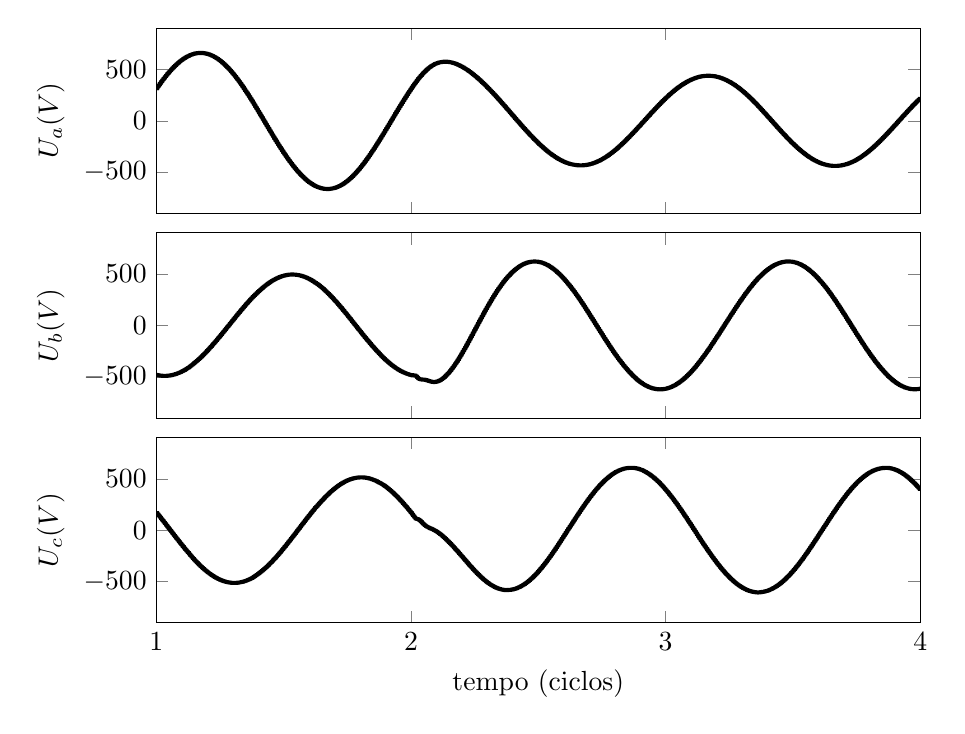
\begin{tikzpicture}

\begin{axis}[%
width=0.8\textwidth,
height=0.193917089240149\textwidth,
scale only axis,
xmin=0.0166666666666667,
xmax=0.0666666666666667,
xtick={0,0.0166666666666667,0.0333333333333333,0.05,0.0666666666666667},
xticklabels={\empty},
ymin=-900,
ymax=900,
ytick={-500,    0,  500},
ylabel={$\text{U}_\text{b}\text{ (V)}$},
name=plot2,
scaled x ticks = false,
legend columns=-1,
legend style={/tikz/every even column/.append style={column sep=0.3cm}},
legend style={font=\footnotesize}
]
\addplot [color=black,solid,line width=1.5pt,forget plot]
  table[row sep=crcr]{0.0166583333333333	-478.328989103039\\
0.0167	-481.372762295986\\
0.0167416666666667	-481.372762295986\\
0.0167833333333333	-483.944387417357\\
0.016825	-483.944387417357\\
0.0168666666666667	-486.043904769891\\
0.0169083333333333	-486.043904769891\\
0.01695	-487.669342075457\\
0.0169916666666667	-487.669342075457\\
0.0170333333333333	-488.81912329053\\
0.017075	-488.81912329053\\
0.0171166666666667	-489.492376222951\\
0.0171583333333333	-489.492376222951\\
0.0172	-489.689089295181\\
0.0172416666666667	-489.689089295181\\
0.0172833333333333	-489.410057478733\\
0.017325	-489.410057478733\\
0.0173666666666667	-488.656714544629\\
0.0174083333333333	-488.656714544629\\
0.01745	-487.430933830334\\
0.0174916666666667	-487.430933830334\\
0.0175333333333333	-485.734862735459\\
0.017575	-485.734862735459\\
0.0176166666666667	-483.570824107468\\
0.0176583333333333	-483.570824107468\\
0.0177	-480.941176730971\\
0.0177416666666667	-480.941176730971\\
0.0177833333333333	-477.848873406491\\
0.017825	-477.848873406491\\
0.0178666666666667	-474.296687037085\\
0.0179083333333333	-474.296687037085\\
0.01795	-470.287554266504\\
0.0179916666666667	-470.287554266504\\
0.0180333333333333	-465.824994538518\\
0.018075	-465.824994538518\\
0.0181166666666667	-460.912896166831\\
0.0181583333333333	-460.912896166831\\
0.0182	-455.555544349316\\
0.0182416666666667	-455.555544349316\\
0.0182833333333333	-449.757632700212\\
0.018325	-449.757632700212\\
0.0183666666666667	-443.524266807923\\
0.0184083333333333	-443.524266807923\\
0.01845	-436.860963041735\\
0.0184916666666667	-436.860963041735\\
0.0185333333333333	-429.773645406549\\
0.018575	-429.773645406549\\
0.0186166666666667	-422.2686421737\\
0.0186583333333333	-422.2686421737\\
0.0187	-414.352682994809\\
0.0187416666666667	-414.352682994809\\
0.0187833333333333	-406.710604021129\\
0.018825	-406.710604021129\\
0.0188666666666667	-396.968651829484\\
0.0189083333333333	-396.968651829484\\
0.01895	-387.24430030011\\
0.0189916666666667	-387.24430030011\\
0.0190333333333333	-377.413842111121\\
0.019075	-377.413842111121\\
0.0191166666666667	-367.3960735467\\
0.0191583333333333	-367.3960735467\\
0.0192	-357.12553953726\\
0.0192416666666667	-357.12553953726\\
0.0192833333333333	-346.559303382721\\
0.019325	-346.559303382721\\
0.0193666666666667	-335.674936708767\\
0.0194083333333333	-335.674936708767\\
0.01945	-324.465686057335\\
0.0194916666666667	-324.465686057335\\
0.0195333333333333	-312.935239244225\\
0.019575	-312.935239244225\\
0.0196166666666667	-301.093266862382\\
0.0196583333333333	-301.093266862382\\
0.0197	-288.95219973374\\
0.0197416666666667	-288.95219973374\\
0.0197833333333333	-276.525463982029\\
0.019825	-276.525463982029\\
0.0198666666666667	-263.82538033546\\
0.0199083333333333	-263.82538033546\\
0.01995	-250.865057706918\\
0.0199916666666667	-250.865057706918\\
0.0200333333333333	-237.656697428642\\
0.020075	-237.656697428642\\
0.0201166666666667	-224.212271375033\\
0.0201583333333333	-224.212271375033\\
0.0202	-210.543848998092\\
0.0202416666666667	-210.543848998092\\
0.0202833333333333	-196.6637735981\\
0.020325	-196.6637735981\\
0.0203666666666667	-182.584756063204\\
0.0204083333333333	-182.584756063204\\
0.02045	-168.319897946886\\
0.0204916666666667	-168.319897946886\\
0.0205333333333333	-153.882668002172\\
0.020575	-153.882668002172\\
0.0206166666666667	-139.286855686717\\
0.0206583333333333	-139.286855686717\\
0.0207	-124.546519243168\\
0.0207416666666667	-124.546519243168\\
0.0207833333333333	-109.675923407492\\
0.020825	-109.675923407492\\
0.0208666666666667	-94.6884951690301\\
0.0209083333333333	-94.6884951690301\\
0.02095	-79.6023211852309\\
0.0209916666666667	-79.6023211852309\\
0.0210333333333333	-64.4296541414652\\
0.021075	-64.4296541414652\\
0.0211166666666667	-49.1854677870168\\
0.0211583333333333	-49.1854677870168\\
0.0212	-33.8847697005379\\
0.0212416666666667	-33.8847697005379\\
0.0212833333333333	-18.5423320716325\\
0.021325	-18.5423320716325\\
0.0213666666666667	-3.1725945533516\\
0.0214083333333333	-3.1725945533516\\
0.02145	12.2102617721841\\
0.0214916666666667	12.2102617721841\\
0.0215333333333333	27.5921432856442\\
0.021575	27.5921432856442\\
0.0216166666666667	42.9588704890498\\
0.0216583333333333	42.9588704890498\\
0.0217	58.2960537853681\\
0.0217416666666667	58.2960537853681\\
0.0217833333333333	73.5890384864759\\
0.021825	73.5890384864759\\
0.0218666666666667	88.82269659409\\
0.0219083333333333	88.82269659409\\
0.02195	103.982669291038\\
0.0219916666666667	103.982669291038\\
0.0220333333333333	119.053037141893\\
0.022075	119.053037141893\\
0.0221166666666667	134.01853586672\\
0.0221583333333333	134.01853586672\\
0.0222	148.863909368128\\
0.0222416666666667	148.863909368128\\
0.0222833333333333	163.573956427556\\
0.022325	163.573956427556\\
0.0223666666666667	178.133568427636\\
0.0224083333333333	178.133568427636\\
0.02245	192.527757716713\\
0.0224916666666667	192.527757716713\\
0.0225333333333333	206.741679404245\\
0.022575	206.741679404245\\
0.0226166666666667	220.760649670751\\
0.0226583333333333	220.760649670751\\
0.0227	234.570162946369\\
0.0227416666666667	234.570162946369\\
0.0227833333333333	248.155909263895\\
0.022825	248.155909263895\\
0.0228666666666667	261.687830320942\\
0.0229083333333333	261.687830320942\\
0.02295	274.986604079196\\
0.0229916666666667	274.986604079196\\
0.0230333333333333	286.928801747272\\
0.023075	286.928801747272\\
0.0231166666666667	298.950506950644\\
0.0231583333333333	298.950506950644\\
0.0232	310.924864102034\\
0.0232416666666667	310.924864102034\\
0.0232833333333333	322.756989832147\\
0.023325	322.756989832147\\
0.0233666666666667	334.367084014297\\
0.0234083333333333	334.367084014297\\
0.02345	345.69602196514\\
0.0234916666666667	345.69602196514\\
0.0235333333333333	356.703461032175\\
0.023575	356.703461032175\\
0.0236166666666667	367.363371170442\\
0.0236583333333333	367.363371170442\\
0.0237	377.659204280424\\
0.0237416666666667	377.659204280424\\
0.0237833333333333	387.579795487262\\
0.023825	387.579795487262\\
0.0238666666666667	397.116425283701\\
0.0239083333333333	397.116425283701\\
0.02395	406.261310362139\\
0.0239916666666667	406.261310362139\\
0.0240333333333333	415.0053223807\\
0.024075	415.0053223807\\
0.0241166666666667	423.340732147141\\
0.0241583333333333	423.340732147141\\
0.0242	431.258683016742\\
0.0242416666666667	431.258683016742\\
0.0242833333333333	438.750365395371\\
0.024325	438.750365395371\\
0.0243666666666667	445.807262831054\\
0.0244083333333333	445.807262831054\\
0.02445	452.421342397773\\
0.0244916666666667	452.421342397773\\
0.0245333333333333	458.585161293933\\
0.024575	458.585161293933\\
0.0246166666666667	464.291905294308\\
0.0246583333333333	464.291905294308\\
0.0247	469.535383109734\\
0.0247416666666667	469.535383109734\\
0.0247833333333333	474.309999446141\\
0.024825	474.309999446141\\
0.0248666666666667	478.610723480444\\
0.0249083333333333	478.610723480444\\
0.02495	482.432523836755\\
0.0249916666666667	482.432523836755\\
0.0250333333333333	485.772612186125\\
0.025075	485.772612186125\\
0.0251166666666667	488.627883686145\\
0.0251583333333333	488.627883686145\\
0.0252	490.994391489966\\
0.0252416666666667	490.994391489966\\
0.0252833333333333	492.869784189106\\
0.025325	492.869784189106\\
0.0253666666666667	494.252063559781\\
0.0254083333333333	494.252063559781\\
0.02545	495.139387583695\\
0.0254916666666667	495.139387583695\\
0.0255333333333333	495.530061759552\\
0.025575	495.530061759552\\
0.0256166666666667	495.422663936061\\
0.0256583333333333	495.422663936061\\
0.0257	494.816230581684\\
0.0257416666666667	494.816230581684\\
0.0257833333333333	493.710425995119\\
0.025825	493.710425995119\\
0.0258666666666667	492.105654148384\\
0.0259083333333333	492.105654148384\\
0.02595	490.003108134894\\
0.0259916666666667	490.003108134894\\
0.0260333333333333	487.404961487327\\
0.026075	487.404961487327\\
0.0261166666666667	484.313069214194\\
0.0261583333333333	484.313069214194\\
0.0262	480.731558886196\\
0.0262416666666667	480.731558886196\\
0.0262833333333333	476.664323712434\\
0.026325	476.664323712434\\
0.0263666666666667	472.115829454631\\
0.0264083333333333	472.115829454631\\
0.02645	467.091068733291\\
0.0264916666666667	467.091068733291\\
0.0265333333333333	461.595540479995\\
0.026575	461.595540479995\\
0.0266166666666667	455.635234907076\\
0.0266583333333333	455.635234907076\\
0.0267	449.21662231492\\
0.0267416666666667	449.21662231492\\
0.0267833333333333	442.346643428456\\
0.026825	442.346643428456\\
0.0268666666666667	435.032699614098\\
0.0269083333333333	435.032699614098\\
0.02695	427.282642172915\\
0.0269916666666667	427.282642172915\\
0.0270333333333333	418.527982244731\\
0.027075	418.527982244731\\
0.0271166666666667	410.672570182659\\
0.0271583333333333	410.672570182659\\
0.0272	402.276872290978\\
0.0272416666666667	402.276872290978\\
0.0272833333333333	393.223850223727\\
0.027325	393.223850223727\\
0.0273666666666667	383.609151155178\\
0.0274083333333333	383.609151155178\\
0.02745	373.508718653929\\
0.0274916666666667	373.508718653929\\
0.0275333333333333	362.979579538073\\
0.027575	362.979579538073\\
0.0276166666666667	352.061894709897\\
0.0276583333333333	352.061894709897\\
0.0277	340.783205444461\\
0.0277416666666667	340.783205444461\\
0.0277833333333333	329.162781541968\\
0.027825	329.162781541968\\
0.0278666666666667	317.215226351439\\
0.0279083333333333	317.215226351439\\
0.02795	304.953068995059\\
0.0279916666666667	304.953068995059\\
0.0280333333333333	292.388308765939\\
0.028075	292.388308765939\\
0.0281166666666667	279.533394256386\\
0.0281583333333333	279.533394256386\\
0.0282	266.401997020689\\
0.0282416666666667	266.401997020689\\
0.0282833333333333	253.007121767018\\
0.028325	253.007121767018\\
0.0283666666666667	239.363037342399\\
0.0284083333333333	239.363037342399\\
0.02845	225.484309796947\\
0.0284916666666667	225.484309796947\\
0.0285333333333333	211.385672071801\\
0.028575	211.385672071801\\
0.0286166666666667	197.081935254737\\
0.0286583333333333	197.081935254737\\
0.0287	182.587950486431\\
0.0287416666666667	182.587950486431\\
0.0287833333333333	167.918604082923\\
0.028825	167.918604082923\\
0.0288666666666667	153.088829011011\\
0.0289083333333333	153.088829011011\\
0.02895	138.113619934855\\
0.0289916666666667	138.113619934855\\
0.0290333333333333	123.008044204917\\
0.029075	123.008044204917\\
0.0291166666666667	107.788100944899\\
0.0291583333333333	107.788100944899\\
0.0292	92.4664220892656\\
0.0292416666666667	92.4664220892656\\
0.0292833333333333	77.0599110293703\\
0.029325	77.0599110293703\\
0.0293666666666667	61.5839402726698\\
0.0294083333333333	61.5839402726698\\
0.02945	46.0538191073489\\
0.0294916666666667	46.0538191073489\\
0.0295333333333333	30.4851141949034\\
0.029575	30.4851141949034\\
0.0296166666666667	14.8937682112207\\
0.0296583333333333	14.8937682112207\\
0.0297	-0.703957306529608\\
0.0297416666666667	-0.703957306529608\\
0.0297833333333333	-16.2916492298269\\
0.029825	-16.2916492298269\\
0.0298666666666667	-31.8529362123827\\
0.0299083333333333	-31.8529362123827\\
0.02995	-47.371649369948\\
0.0299916666666667	-47.371649369948\\
0.0300333333333333	-62.8319222299047\\
0.030075	-62.8319222299047\\
0.0301166666666667	-78.2183969102601\\
0.0301583333333333	-78.2183969102601\\
0.0302	-93.5154108314719\\
0.0302416666666667	-93.5154108314719\\
0.0302833333333333	-108.70816278091\\
0.030325	-108.70816278091\\
0.0303666666666667	-123.782356080195\\
0.0304083333333333	-123.782356080195\\
0.03045	-138.723507249364\\
0.0304916666666667	-138.723507249364\\
0.0305333333333333	-153.517339096442\\
0.030575	-153.517339096442\\
0.0306166666666667	-168.149764544084\\
0.0306583333333333	-168.149764544084\\
0.0307	-182.60688669631\\
0.0307416666666667	-182.60688669631\\
0.0307833333333333	-196.875004412733\\
0.030825	-196.875004412733\\
0.0308666666666667	-210.940621254231\\
0.0309083333333333	-210.940621254231\\
0.03095	-224.790455634942\\
0.0309916666666667	-224.790455634942\\
0.0310333333333333	-238.411450801645\\
0.031075	-238.411450801645\\
0.0311166666666667	-251.788204920739\\
0.0311583333333333	-251.788204920739\\
0.0312	-264.319493294975\\
0.0312416666666667	-264.319493294975\\
0.0312833333333333	-278.081845363642\\
0.031325	-278.081845363642\\
0.0313666666666667	-291.211888263673\\
0.0314083333333333	-291.211888263673\\
0.03145	-303.807007713181\\
0.0314916666666667	-303.807007713181\\
0.0315333333333333	-315.936364357588\\
0.031575	-315.936364357588\\
0.0316166666666667	-327.655020751537\\
0.0316583333333333	-327.655020751537\\
0.0317	-338.998550237152\\
0.0317416666666667	-338.998550237152\\
0.0317833333333333	-349.984949605885\\
0.031825	-349.984949605885\\
0.0318666666666667	-360.618974262017\\
0.0319083333333333	-360.618974262017\\
0.03195	-370.896795074955\\
0.0319916666666667	-370.896795074955\\
0.0320333333333333	-380.809923421548\\
0.032075	-380.809923421548\\
0.0321166666666667	-390.348041070204\\
0.0321583333333333	-390.348041070204\\
0.0322	-399.500455565927\\
0.0322416666666667	-399.500455565927\\
0.0322833333333333	-408.258433783543\\
0.032325	-408.258433783543\\
0.0323666666666667	-416.612673979994\\
0.0324083333333333	-416.612673979994\\
0.03245	-424.555376388038\\
0.0324916666666667	-424.555376388038\\
0.0325333333333333	-432.079651399668\\
0.032575	-432.079651399668\\
0.0326166666666667	-439.17912856472\\
0.0326583333333333	-439.17912856472\\
0.0327	-445.847803165625\\
0.0327416666666667	-445.847803165625\\
0.0327833333333333	-452.079952433882\\
0.032825	-452.079952433882\\
0.0328666666666667	-457.870112681898\\
0.0329083333333333	-457.870112681898\\
0.03295	-463.213095942823\\
0.0329916666666667	-463.213095942823\\
0.0330333333333333	-468.104025539882\\
0.033075	-468.104025539882\\
0.0331166666666667	-472.538375275198\\
0.0331583333333333	-472.538375275198\\
0.0332	-476.512043591712\\
0.0332416666666667	-476.512043591712\\
0.0332833333333333	-480.021998518076\\
0.033325	-480.021998518076\\
0.0333666666666667	-483.062409528906\\
0.0334083333333333	-483.062409528906\\
0.03345	-483.678406180898\\
0.0334916666666667	-483.678406180898\\
0.0335333333333333	-485.862488721367\\
0.033575	-485.862488721367\\
0.0336166666666667	-488.142814475316\\
0.0336583333333333	-488.142814475316\\
0.0337	-498.245132388745\\
0.0337416666666667	-498.245132388745\\
0.0337833333333333	-510.177702028353\\
0.033825	-510.177702028353\\
0.0338666666666667	-518.869053971916\\
0.0339083333333333	-518.869053971916\\
0.03395	-523.323995836891\\
0.0339916666666667	-523.323995836891\\
0.0340333333333333	-524.949038961527\\
0.034075	-524.949038961527\\
0.0341166666666667	-525.669339355048\\
0.0341583333333333	-525.669339355048\\
0.0342	-526.908087285797\\
0.0342416666666667	-526.908087285797\\
0.0342833333333333	-529.296547986902\\
0.034325	-529.296547986902\\
0.0343666666666667	-532.790822709101\\
0.0344083333333333	-532.790822709101\\
0.03445	-536.931847441238\\
0.0344916666666667	-536.931847441238\\
0.0345333333333333	-541.107207956411\\
0.034575	-541.107207956411\\
0.0346166666666667	-544.736225800635\\
0.0346583333333333	-544.736225800635\\
0.0347	-547.369395078864\\
0.0347416666666667	-547.369395078864\\
0.0347833333333333	-548.716986912959\\
0.034825	-548.716986912959\\
0.0348666666666667	-548.632547118878\\
0.0349083333333333	-548.632547118878\\
0.03495	-547.075656823658\\
0.0349916666666667	-547.075656823658\\
0.0350333333333333	-544.071637409979\\
0.035075	-544.071637409979\\
0.0351166666666667	-539.678204260503\\
0.0351583333333333	-539.678204260503\\
0.0352	-533.962755583409\\
0.0352416666666667	-533.962755583409\\
0.0352833333333333	-527.182279910962\\
0.035325	-527.182279910962\\
0.0353666666666667	-519.113556680225\\
0.0354083333333333	-519.113556680225\\
0.03545	-509.000078841309\\
0.0354916666666667	-509.000078841309\\
0.0355333333333333	-498.107638282283\\
0.035575	-498.107638282283\\
0.0356166666666667	-486.375655173447\\
0.0356583333333333	-486.375655173447\\
0.0357	-473.759153944544\\
0.0357416666666667	-473.759153944544\\
0.0357833333333333	-460.236320033994\\
0.035825	-460.236320033994\\
0.0358666666666667	-445.810447327876\\
0.0359083333333333	-445.810447327876\\
0.03595	-430.505282665083\\
0.0359916666666667	-430.505282665083\\
0.0360333333333333	-414.358464568713\\
0.036075	-414.358464568713\\
0.0361166666666667	-397.415615024497\\
0.0361583333333333	-397.415615024497\\
0.0362	-379.725972742214\\
0.0362416666666667	-379.725972742214\\
0.0362833333333333	-361.339644418341\\
0.036325	-361.339644418341\\
0.0363666666666667	-342.306510620674\\
0.0364083333333333	-342.306510620674\\
0.03645	-322.673808653078\\
0.0364916666666667	-322.673808653078\\
0.0365333333333333	-302.490006690184\\
0.036575	-302.490006690184\\
0.0366166666666667	-281.801820654654\\
0.0366583333333333	-281.801820654654\\
0.0367	-260.65587850699\\
0.0367416666666667	-260.65587850699\\
0.0367833333333333	-239.098456719156\\
0.036825	-239.098456719156\\
0.0368666666666667	-217.175209420218\\
0.0369083333333333	-217.175209420218\\
0.03695	-194.931036851632\\
0.0369916666666667	-194.931036851632\\
0.0370333333333333	-172.410062075249\\
0.037075	-172.410062075249\\
0.0371166666666667	-149.655652803591\\
0.0371583333333333	-149.655652803591\\
0.0372	-126.710439524506\\
0.0372416666666667	-126.710439524506\\
0.0372833333333333	-103.616305295776\\
0.037325	-103.616305295776\\
0.0373666666666667	-80.4139546989703\\
0.0374083333333333	-80.4139546989703\\
0.03745	-57.1444016932104\\
0.0374916666666667	-57.1444016932104\\
0.0375333333333333	-33.8474272616072\\
0.037575	-33.8474272616072\\
0.0376166666666667	-10.5605046227431\\
0.0376583333333333	-10.5605046227431\\
0.0377	12.6791060967196\\
0.0377416666666667	12.6791060967196\\
0.0377833333333333	35.8353743740755\\
0.037825	35.8353743740755\\
0.0378666666666667	58.87364298905\\
0.0379083333333333	58.87364298905\\
0.03795	81.7608388535841\\
0.0379916666666667	81.7608388535841\\
0.0380333333333333	104.465378225758\\
0.038075	104.465378225758\\
0.0381166666666667	126.956956606797\\
0.0381583333333333	126.956956606797\\
0.0382	149.206353974694\\
0.0382416666666667	149.206353974694\\
0.0382833333333333	171.185317112742\\
0.038325	171.185317112742\\
0.0383666666666667	192.866498739553\\
0.0384083333333333	192.866498739553\\
0.03845	214.223301645853\\
0.0384916666666667	214.223301645853\\
0.0385333333333333	235.231350978712\\
0.038575	235.231350978712\\
0.0386166666666667	255.865244997372\\
0.0386583333333333	255.865244997372\\
0.0387	276.101702652239\\
0.0387416666666667	276.101702652239\\
0.0387833333333333	295.918476849333\\
0.038825	295.918476849333\\
0.0388666666666667	315.294326438433\\
0.0389083333333333	315.294326438433\\
0.03895	334.208995557844\\
0.0389916666666667	334.208995557844\\
0.0390333333333333	352.643192363139\\
0.039075	352.643192363139\\
0.0391166666666667	370.578568409044\\
0.0391583333333333	370.578568409044\\
0.0392	387.997699646167\\
0.0392416666666667	387.997699646167\\
0.0392833333333333	404.884069536479\\
0.039325	404.884069536479\\
0.0393666666666667	421.222054171729\\
0.0394083333333333	421.222054171729\\
0.03945	437.480424676999\\
0.0394916666666667	437.480424676999\\
0.0395333333333333	452.040941016559\\
0.039575	452.040941016559\\
0.0396166666666667	466.074182858891\\
0.0396583333333333	466.074182858891\\
0.0397	479.771235918754\\
0.0397416666666667	479.771235918754\\
0.0397833333333333	493.019679989615\\
0.039825	493.019679989615\\
0.0398666666666667	505.73413839378\\
0.0399083333333333	505.73413839378\\
0.03995	517.858623983074\\
0.0399916666666667	517.858623983074\\
0.0400333333333333	529.359563793907\\
0.040075	529.359563793907\\
0.0401166666666667	540.217966392563\\
0.0401583333333333	540.217966392563\\
0.0402	550.422720161551\\
0.0402416666666667	550.422720161551\\
0.0402833333333333	559.966764407743\\
0.040325	559.966764407743\\
0.0403666666666667	568.844782875507\\
0.0404083333333333	568.844782875507\\
0.04045	577.05210647663\\
0.0404916666666667	577.05210647663\\
0.0405333333333333	584.58398245434\\
0.040575	584.58398245434\\
0.0406166666666667	591.435324944241\\
0.0406583333333333	591.435324944241\\
0.0407	597.602956497375\\
0.0407416666666667	597.602956497375\\
0.0407833333333333	603.083411539344\\
0.040825	603.083411539344\\
0.0408666666666667	607.874065878715\\
0.0409083333333333	607.874065878715\\
0.04095	611.973246455818\\
0.0409916666666667	611.973246455818\\
0.0410333333333333	615.380238806002\\
0.041075	615.380238806002\\
0.0411166666666667	618.095240312968\\
0.0411583333333333	618.095240312968\\
0.0412	620.119289539734\\
0.0412416666666667	620.119289539734\\
0.0412833333333333	621.454193408118\\
0.041325	621.454193408118\\
0.0413666666666667	622.102464544814\\
0.0414083333333333	622.102464544814\\
0.04145	622.067273281086\\
0.0414916666666667	622.067273281086\\
0.0415333333333333	621.351782529469\\
0.041575	621.351782529469\\
0.0416166666666667	619.962242070563\\
0.0416583333333333	619.962242070563\\
0.0417	617.902615212395\\
0.0417416666666667	617.902615212395\\
0.0417833333333333	615.17835164608\\
0.041825	615.17835164608\\
0.0418666666666667	611.795572072393\\
0.0419083333333333	611.795572072393\\
0.04195	607.760754022874\\
0.0419916666666667	607.760754022874\\
0.0420333333333333	603.080607489372\\
0.042075	603.080607489372\\
0.0421166666666667	597.762108228377\\
0.0421583333333333	597.762108228377\\
0.0422	591.812622646619\\
0.0422416666666667	591.812622646619\\
0.0422833333333333	585.240054074818\\
0.042325	585.240054074818\\
0.0423666666666667	578.052948832242\\
0.0424083333333333	578.052948832242\\
0.04245	570.260538255211\\
0.0424916666666667	570.260538255211\\
0.0425333333333333	561.872936284205\\
0.042575	561.872936284205\\
0.0426166666666667	552.900083112745\\
0.0426583333333333	552.900083112745\\
0.0427	543.353207689846\\
0.0427416666666667	543.353207689846\\
0.0427833333333333	533.244433887195\\
0.042825	533.244433887195\\
0.0428666666666667	522.585826182198\\
0.0429083333333333	522.585826182198\\
0.04295	511.389933785599\\
0.0429916666666667	511.389933785599\\
0.0430333333333333	499.669787225859\\
0.043075	499.669787225859\\
0.0431166666666667	487.438882456456\\
0.0431583333333333	487.438882456456\\
0.0432	474.711164930049\\
0.0432416666666667	474.711164930049\\
0.0432833333333333	461.501013707399\\
0.043325	461.501013707399\\
0.0433666666666667	447.82322510983\\
0.0434083333333333	447.82322510983\\
0.04345	433.692995682403\\
0.0434916666666667	433.692995682403\\
0.0435333333333333	419.114123530008\\
0.043575	419.114123530008\\
0.0436166666666667	403.630299904557\\
0.0436583333333333	403.630299904557\\
0.0437	389.067248906318\\
0.0437416666666667	389.067248906318\\
0.0437833333333333	373.794607970039\\
0.043825	373.794607970039\\
0.0438666666666667	357.893910580944\\
0.0439083333333333	357.893910580944\\
0.04395	341.48847965027\\
0.0439916666666667	341.48847965027\\
0.0440333333333333	324.669814436674\\
0.044075	324.669814436674\\
0.0441166666666667	307.499399030616\\
0.0441583333333333	307.499399030616\\
0.0442	290.017043641092\\
0.0442416666666667	290.017043641092\\
0.0442833333333333	272.249315182523\\
0.044325	272.249315182523\\
0.0443666666666667	254.216038867438\\
0.0444083333333333	254.216038867438\\
0.04445	235.934592114668\\
0.0444916666666667	235.934592114668\\
0.0445333333333333	217.422270956511\\
0.044575	217.422270956511\\
0.0446166666666667	198.696939122818\\
0.0446583333333333	198.696939122818\\
0.0447	179.778898467287\\
0.0447416666666667	179.778898467287\\
0.0447833333333333	160.687408623789\\
0.044825	160.687408623789\\
0.0448666666666667	141.442715029629\\
0.0449083333333333	141.442715029629\\
0.04495	122.065482129781\\
0.0449916666666667	122.065482129781\\
0.0450333333333333	102.576274992799\\
0.045075	102.576274992799\\
0.0451166666666667	82.9954553821085\\
0.0451583333333333	82.9954553821085\\
0.0452	63.3431668052044\\
0.0452416666666667	63.3431668052044\\
0.0452833333333333	43.6393638336056\\
0.045325	43.6393638336056\\
0.0453666666666667	23.9038552313563\\
0.0454083333333333	23.9038552313563\\
0.04545	4.15634192700959\\
0.0454916666666667	4.15634192700959\\
0.0455333333333333	-15.5835589467395\\
0.045575	-15.5835589467395\\
0.0456166666666667	-35.2962607915949\\
0.0456583333333333	-35.2962607915949\\
0.0457	-54.9618164960153\\
0.0457416666666667	-54.9618164960153\\
0.0457833333333333	-74.5626887768094\\
0.045825	-74.5626887768094\\
0.0458666666666667	-94.0783942026847\\
0.0459083333333333	-94.0783942026847\\
0.04595	-113.489817630002\\
0.0459916666666667	-113.489817630002\\
0.0460333333333333	-132.777948092905\\
0.046075	-132.777948092905\\
0.0461166666666667	-151.923684718905\\
0.0461583333333333	-151.923684718905\\
0.0462	-170.907795748521\\
0.0462416666666667	-170.907795748521\\
0.0462833333333333	-189.711018370974\\
0.046325	-189.711018370974\\
0.0463666666666667	-208.314223883074\\
0.0464083333333333	-208.314223883074\\
0.04645	-226.69857913687\\
0.0464916666666667	-226.69857913687\\
0.0465333333333333	-244.845655884747\\
0.046575	-244.845655884747\\
0.0466166666666667	-262.73747467731\\
0.0466583333333333	-262.73747467731\\
0.0467	-280.35685709118\\
0.0467416666666667	-280.35685709118\\
0.0467833333333333	-297.685436154517\\
0.046825	-297.685436154517\\
0.0468666666666667	-314.707570290364\\
0.0469083333333333	-314.707570290364\\
0.04695	-331.406944088127\\
0.0469916666666667	-331.406944088127\\
0.0470333333333333	-347.767508096617\\
0.047075	-347.767508096617\\
0.0471166666666667	-363.773616624145\\
0.0471583333333333	-363.773616624145\\
0.0472	-379.410038002404\\
0.0472416666666667	-379.410038002404\\
0.0472833333333333	-394.661961827583\\
0.047325	-394.661961827583\\
0.0473666666666667	-409.515006542937\\
0.0474083333333333	-409.515006542937\\
0.04745	-423.955227040306\\
0.0474916666666667	-423.955227040306\\
0.0475333333333333	-437.96912175223\\
0.047575	-437.96912175223\\
0.0476166666666667	-451.543639085691\\
0.0476583333333333	-451.543639085691\\
0.0477	-464.479544997007\\
0.0477416666666667	-464.479544997007\\
0.0477833333333333	-477.089008664143\\
0.047825	-477.089008664143\\
0.0478666666666667	-489.980276495137\\
0.0479083333333333	-489.980276495137\\
0.04795	-502.082454983243\\
0.0479916666666667	-502.082454983243\\
0.0480333333333333	-513.474378594949\\
0.048075	-513.474378594949\\
0.0481166666666667	-524.236448612188\\
0.0481583333333333	-524.236448612188\\
0.0482	-534.419855442406\\
0.0482416666666667	-534.419855442406\\
0.0482833333333333	-544.05048530493\\
0.048325	-544.05048530493\\
0.0483666666666667	-553.136657143756\\
0.0484083333333333	-553.136657143756\\
0.04845	-561.676386905996\\
0.0484916666666667	-561.676386905996\\
0.0485333333333333	-569.662827271978\\
0.048575	-569.662827271978\\
0.0486166666666667	-577.087697701991\\
0.0486583333333333	-577.087697701991\\
0.0487	-583.943144390163\\
0.0487416666666667	-583.943144390163\\
0.0487833333333333	-590.222145166835\\
0.048825	-590.222145166835\\
0.0488666666666667	-595.920726335499\\
0.0489083333333333	-595.920726335499\\
0.04895	-601.033307618998\\
0.0489916666666667	-601.033307618998\\
0.0490333333333333	-605.556420963213\\
0.049075	-605.556420963213\\
0.0491166666666667	-609.487177748175\\
0.0491583333333333	-609.487177748175\\
0.0492	-612.823052256476\\
0.0492416666666667	-612.823052256476\\
0.0492833333333333	-615.561826877812\\
0.049325	-615.561826877812\\
0.0493666666666667	-617.701607112424\\
0.0494083333333333	-617.701607112424\\
0.04945	-619.240871262007\\
0.0494916666666667	-619.240871262007\\
0.0495333333333333	-620.178528934764\\
0.049575	-620.178528934764\\
0.0496166666666667	-620.513972615137\\
0.0496583333333333	-620.513972615137\\
0.0497	-620.247115363624\\
0.0497416666666667	-620.247115363624\\
0.0497833333333333	-619.378688758982\\
0.049825	-619.378688758982\\
0.0498666666666667	-617.909223463945\\
0.0499083333333333	-617.909223463945\\
0.04995	-615.839755643643\\
0.0499916666666667	-615.839755643643\\
0.0500333333333333	-613.173045332849\\
0.050075	-613.173045332849\\
0.0501166666666667	-609.911750435669\\
0.0501583333333333	-609.911750435669\\
0.0502	-606.059195153575\\
0.0502416666666667	-606.059195153575\\
0.0502833333333333	-601.619528288722\\
0.050325	-601.619528288722\\
0.0503666666666667	-596.5977218648\\
0.0504083333333333	-596.5977218648\\
0.05045	-590.999459574474\\
0.0504916666666667	-590.999459574474\\
0.0505333333333333	-584.830984389048\\
0.050575	-584.830984389048\\
0.0506166666666667	-578.098972885875\\
0.0506583333333333	-578.098972885875\\
0.0507	-570.810458695109\\
0.0507416666666667	-570.810458695109\\
0.0507833333333333	-562.972771453032\\
0.050825	-562.972771453032\\
0.0508666666666667	-554.593458705033\\
0.0509083333333333	-554.593458705033\\
0.05095	-545.681768487654\\
0.0509916666666667	-545.681768487654\\
0.0510333333333333	-536.245095988263\\
0.051075	-536.245095988263\\
0.0511166666666667	-526.292515885746\\
0.0511583333333333	-526.292515885746\\
0.0512	-515.83356953895\\
0.0512416666666667	-515.83356953895\\
0.0512833333333333	-504.878224034623\\
0.051325	-504.878224034623\\
0.0513666666666667	-493.436867537464\\
0.0514083333333333	-493.436867537464\\
0.05145	-481.52030596022\\
0.0514916666666667	-481.52030596022\\
0.0515333333333333	-469.139759186227\\
0.051575	-469.139759186227\\
0.0516166666666667	-456.306856819179\\
0.0516583333333333	-456.306856819179\\
0.0517	-443.033633642018\\
0.0517416666666667	-443.033633642018\\
0.0517833333333333	-429.33258029632\\
0.051825	-429.33258029632\\
0.0518666666666667	-415.631465352924\\
0.0519083333333333	-415.631465352924\\
0.05195	-400.572255393978\\
0.0519916666666667	-400.572255393978\\
0.0520333333333333	-385.137617929011\\
0.052075	-385.137617929011\\
0.0521166666666667	-369.577327567763\\
0.0521583333333333	-369.577327567763\\
0.0522	-353.811156353638\\
0.0522416666666667	-353.811156353638\\
0.0522833333333333	-337.782144292742\\
0.052325	-337.782144292742\\
0.0523666666666667	-321.461774745628\\
0.0524083333333333	-321.461774745628\\
0.05245	-304.842729371899\\
0.0524916666666667	-304.842729371899\\
0.0525333333333333	-287.93107573415\\
0.052575	-287.93107573415\\
0.0526166666666667	-270.740138534588\\
0.0526583333333333	-270.740138534588\\
0.0527	-253.286428675406\\
0.0527416666666667	-253.286428675406\\
0.0527833333333333	-235.587304265221\\
0.052825	-235.587304265221\\
0.0528666666666667	-217.660084870833\\
0.0529083333333333	-217.660084870833\\
0.05295	-199.521347520453\\
0.0529916666666667	-199.521347520453\\
0.0530333333333333	-181.186956202741\\
0.053075	-181.186956202741\\
0.0531166666666667	-162.674350682609\\
0.0531583333333333	-162.674350682609\\
0.0532	-144.000119294864\\
0.0532416666666667	-144.000119294864\\
0.0532833333333333	-125.181189054423\\
0.053325	-125.181189054423\\
0.0533666666666667	-106.234904649345\\
0.0534083333333333	-106.234904649345\\
0.05345	-87.1790079525377\\
0.0534916666666667	-87.1790079525377\\
0.0535333333333333	-68.0315757914698\\
0.053575	-68.0315757914698\\
0.0536166666666667	-48.8109448712189\\
0.0536583333333333	-48.8109448712189\\
0.0537	-29.535641501431\\
0.0537416666666667	-29.535641501431\\
0.0537833333333333	-10.2243242585009\\
0.053825	-10.2243242585009\\
0.0538666666666667	9.10425939312514\\
0.0539083333333333	9.10425939312514\\
0.05395	28.431759765239\\
0.0539916666666667	28.431759765239\\
0.0540333333333333	47.7380619914277\\
0.054075	47.7380619914277\\
0.0541166666666667	67.0048596216789\\
0.0541583333333333	67.0048596216789\\
0.0542	86.2134287761061\\
0.0542416666666667	86.2134287761061\\
0.0542833333333333	105.344932703909\\
0.054325	105.344932703909\\
0.0543666666666667	124.380749221213\\
0.0544083333333333	124.380749221213\\
0.05445	143.302595289061\\
0.0544916666666667	143.302595289061\\
0.0545333333333333	162.092504174167\\
0.054575	162.092504174167\\
0.0546166666666667	180.732720410386\\
0.0546583333333333	180.732720410386\\
0.0547	199.205581326043\\
0.0547416666666667	199.205581326043\\
0.0547833333333333	217.493428750765\\
0.054825	217.493428750765\\
0.0548666666666667	235.578582767079\\
0.0549083333333333	235.578582767079\\
0.05495	253.443125065313\\
0.0549916666666667	253.443125065313\\
0.0550333333333333	271.070114062267\\
0.055075	271.070114062267\\
0.0551166666666667	288.441918437565\\
0.0551583333333333	288.441918437565\\
0.0552	305.540629346178\\
0.0552416666666667	305.540629346178\\
0.0552833333333333	322.349196138942\\
0.055325	322.349196138942\\
0.0553666666666667	338.850790392749\\
0.0554083333333333	338.850790392749\\
0.05545	355.028813235841\\
0.0554916666666667	355.028813235841\\
0.0555333333333333	370.866918292704\\
0.055575	370.866918292704\\
0.0556166666666667	386.349034907237\\
0.0556583333333333	386.349034907237\\
0.0557	401.459390824441\\
0.0557416666666667	401.459390824441\\
0.0557833333333333	416.182534509225\\
0.055825	416.182534509225\\
0.0558666666666667	430.503357233046\\
0.0559083333333333	430.503357233046\\
0.05595	444.428364259702\\
0.0559916666666667	444.428364259702\\
0.0560333333333333	458.312095926699\\
0.056075	458.312095926699\\
0.0561166666666667	470.620831923049\\
0.0561583333333333	470.620831923049\\
0.0562	482.740252403833\\
0.0562416666666667	482.740252403833\\
0.0562833333333333	494.614442650844\\
0.056325	494.614442650844\\
0.0563666666666667	506.137452019097\\
0.0564083333333333	506.137452019097\\
0.05645	517.232035261074\\
0.0564916666666667	517.232035261074\\
0.0565333333333333	527.848037766364\\
0.056575	527.848037766364\\
0.0566166666666667	537.955006311181\\
0.0566583333333333	537.955006311181\\
0.0567	547.534799837882\\
0.0567416666666667	547.534799837882\\
0.0567833333333333	556.575910547173\\
0.056825	556.575910547173\\
0.0568666666666667	565.069730447462\\
0.0569083333333333	565.069730447462\\
0.05695	573.008501865003\\
0.0569916666666667	573.008501865003\\
0.0570333333333333	580.384800104896\\
0.057075	580.384800104896\\
0.0571166666666667	587.189514084658\\
0.0571583333333333	587.189514084658\\
0.0572	593.415496031393\\
0.0572416666666667	593.415496031393\\
0.0572833333333333	599.055415177099\\
0.057325	599.055415177099\\
0.0573666666666667	604.102157217934\\
0.0574083333333333	604.102157217934\\
0.05745	608.549383427174\\
0.0574916666666667	608.549383427174\\
0.0575333333333333	612.391612312246\\
0.057575	612.391612312246\\
0.0576166666666667	615.624219432025\\
0.0576583333333333	615.624219432025\\
0.0577	618.243397323232\\
0.0577416666666667	618.243397323232\\
0.0577833333333333	620.246102846652\\
0.057825	620.246102846652\\
0.0578666666666667	621.630008937807\\
0.0579083333333333	621.630008937807\\
0.05795	622.393468628273\\
0.0579916666666667	622.393468628273\\
0.0580333333333333	622.535455960628\\
0.058075	622.535455960628\\
0.0581166666666667	622.055271597177\\
0.0581583333333333	622.055271597177\\
0.0582	620.954537902664\\
0.0582416666666667	620.954537902664\\
0.0582833333333333	619.2334104644\\
0.058325	619.2334104644\\
0.0583666666666667	616.893467377475\\
0.0584083333333333	616.893467377475\\
0.05845	613.936896430051\\
0.0584916666666667	613.936896430051\\
0.0585333333333333	610.36630880557\\
0.058575	610.36630880557\\
0.0586166666666667	606.18468480805\\
0.0586583333333333	606.18468480805\\
0.0587	601.395442675433\\
0.0587416666666667	601.395442675433\\
0.0587833333333333	596.002565110854\\
0.058825	596.002565110854\\
0.0588666666666667	590.010720188448\\
0.0589083333333333	590.010720188448\\
0.05895	583.4253374101\\
0.0589916666666667	583.4253374101\\
0.0590333333333333	576.252628904655\\
0.059075	576.252628904655\\
0.0591166666666667	568.499948956247\\
0.0591583333333333	568.499948956247\\
0.0592	560.173614212181\\
0.0592416666666667	560.173614212181\\
0.0592833333333333	551.28312413464\\
0.059325	551.28312413464\\
0.0593666666666667	541.837523603996\\
0.0594083333333333	541.837523603996\\
0.05945	531.84630593606\\
0.0594916666666667	531.84630593606\\
0.0595333333333333	521.319576753576\\
0.059575	521.319576753576\\
0.0596166666666667	510.268040036644\\
0.0596583333333333	510.268040036644\\
0.0597	498.702979267305\\
0.0597416666666667	498.702979267305\\
0.0597833333333333	486.636238742145\\
0.059825	486.636238742145\\
0.0598666666666667	474.080205128796\\
0.0599083333333333	474.080205128796\\
0.05995	461.047788826581\\
0.0599916666666667	461.047788826581\\
0.0600333333333333	447.552404921158\\
0.060075	447.552404921158\\
0.0601166666666667	433.432158149113\\
0.0601583333333333	433.432158149113\\
0.0602	419.033196012895\\
0.0602416666666667	419.033196012895\\
0.0602833333333333	404.859615019062\\
0.060325	404.859615019062\\
0.0603666666666667	390.014032323058\\
0.0604083333333333	390.014032323058\\
0.06045	374.591154785734\\
0.0604916666666667	374.591154785734\\
0.0605333333333333	358.687629768179\\
0.060575	358.687629768179\\
0.0606166666666667	342.37391082923\\
0.0606583333333333	342.37391082923\\
0.0607	325.697776804887\\
0.0607416666666667	325.697776804887\\
0.0607833333333333	308.691270197785\\
0.060825	308.691270197785\\
0.0608666666666667	291.377167396606\\
0.0609083333333333	291.377167396606\\
0.06095	273.773785867276\\
0.0609916666666667	273.773785867276\\
0.0610333333333333	255.898042095002\\
0.061075	255.898042095002\\
0.0611166666666667	237.767089849261\\
0.0611583333333333	237.767089849261\\
0.0612	219.398595908806\\
0.0612416666666667	219.398595908806\\
0.0612833333333333	200.812941399026\\
0.061325	200.812941399026\\
0.0613666666666667	182.028311218103\\
0.0614083333333333	182.028311218103\\
0.06145	163.064650695835\\
0.0614916666666667	163.064650695835\\
0.0615333333333333	143.94210388579\\
0.061575	143.94210388579\\
0.0616166666666667	124.680771383585\\
0.0616583333333333	124.680771383585\\
0.0617	105.300645415707\\
0.0617416666666667	105.300645415707\\
0.0617833333333333	85.8216061912758\\
0.061825	85.8216061912758\\
0.0618666666666667	66.2634467052476\\
0.0619083333333333	66.2634467052476\\
0.06195	46.6459034390845\\
0.0619916666666667	46.6459034390845\\
0.0620333333333333	26.9886799274167\\
0.062075	26.9886799274167\\
0.0621166666666667	7.31145794450646\\
0.0621583333333333	7.31145794450646\\
0.0622	-12.3659182597896\\
0.0622416666666667	-12.3659182597896\\
0.0622833333333333	-32.0240741012994\\
0.062325	-32.0240741012994\\
0.0623666666666667	-51.6439831541824\\
0.0624083333333333	-51.6439831541824\\
0.06245	-71.2056745782734\\
0.0624916666666667	-71.2056745782734\\
0.0625333333333333	-90.6897327387127\\
0.062575	-90.6897327387127\\
0.0626166666666667	-110.076751617406\\
0.0626583333333333	-110.076751617406\\
0.0627	-129.347213340142\\
0.0627416666666667	-129.347213340142\\
0.0627833333333333	-148.481504179948\\
0.062825	-148.481504179948\\
0.0628666666666667	-167.460028032437\\
0.0629083333333333	-167.460028032437\\
0.06295	-186.263355478126\\
0.0629916666666667	-186.263355478126\\
0.0630333333333333	-204.872350936187\\
0.063075	-204.872350936187\\
0.0631166666666667	-223.268246970837\\
0.0631583333333333	-223.268246970837\\
0.0632	-241.432738266829\\
0.0632416666666667	-241.432738266829\\
0.0632833333333333	-259.34798799135\\
0.063325	-259.34798799135\\
0.0633666666666667	-276.995243523329\\
0.0634083333333333	-276.995243523329\\
0.06345	-294.358484838227\\
0.0634916666666667	-294.358484838227\\
0.0635333333333333	-311.42072943262\\
0.063575	-311.42072943262\\
0.0636166666666667	-328.165320103536\\
0.0636583333333333	-328.165320103536\\
0.0637	-344.57598586431\\
0.0637416666666667	-344.57598586431\\
0.0637833333333333	-360.636853066169\\
0.063825	-360.636853066169\\
0.0638666666666667	-376.332453468804\\
0.0639083333333333	-376.332453468804\\
0.06395	-391.647731942395\\
0.0639916666666667	-391.647731942395\\
0.0640333333333333	-406.568054117199\\
0.064075	-406.568054117199\\
0.0641166666666667	-421.079213855563\\
0.0641583333333333	-421.079213855563\\
0.0642	-435.166921635444\\
0.0642416666666667	-435.166921635444\\
0.0642833333333333	-448.461112459469\\
0.064325	-448.461112459469\\
0.0643666666666667	-462.122406471931\\
0.0644083333333333	-462.122406471931\\
0.06445	-475.340031263127\\
0.0644916666666667	-475.340031263127\\
0.0645333333333333	-487.859730932864\\
0.064575	-487.859730932864\\
0.0646166666666667	-499.754576781684\\
0.0646583333333333	-499.754576781684\\
0.0647	-511.078436924127\\
0.0647416666666667	-511.078436924127\\
0.0647833333333333	-521.860443670578\\
0.064825	-521.860443670578\\
0.0648666666666667	-532.111378784872\\
0.0649083333333333	-532.111378784872\\
0.06495	-541.830649152533\\
0.0649916666666667	-541.830649152533\\
0.0650333333333333	-551.011800488711\\
0.065075	-551.011800488711\\
0.0651166666666667	-559.646203309419\\
0.0651583333333333	-559.646203309419\\
0.0652	-567.725163321087\\
0.0652416666666667	-567.725163321087\\
0.0652833333333333	-575.24070632805\\
0.065325	-575.24070632805\\
0.0653666666666667	-582.186400097242\\
0.0654083333333333	-582.186400097242\\
0.06545	-588.557175167164\\
0.0654916666666667	-588.557175167164\\
0.0655333333333333	-594.34710859428\\
0.065575	-594.34710859428\\
0.0656166666666667	-599.551945853093\\
0.0656583333333333	-599.551945853093\\
0.0657	-604.167854859234\\
0.0657416666666667	-604.167854859234\\
0.0657833333333333	-608.191333491608\\
0.065825	-608.191333491608\\
0.0658666666666667	-611.619214958316\\
0.0659083333333333	-611.619214958316\\
0.06595	-614.448712059601\\
0.0659916666666667	-614.448712059601\\
0.0660333333333333	-616.677473478238\\
0.066075	-616.677473478238\\
0.0661166666666667	-618.303635491654\\
0.0661583333333333	-618.303635491654\\
0.0662	-619.325861244175\\
0.0662416666666667	-619.325861244175\\
0.0662833333333333	-619.743366064574\\
0.066325	-619.743366064574\\
0.0663666666666667	-619.55625036455\\
0.0664083333333333	-619.55625036455\\
0.06645	-618.764042238611\\
0.0664916666666667	-618.764042238611\\
0.0665333333333333	-617.367869927798\\
0.066575	-617.367869927798\\
0.0666166666666667	-615.369358265863\\
0.0666583333333333	-615.369358265863\\
};
\end{axis}

\begin{axis}[%
width=0.8\textwidth,
height=0.193917089240149\textwidth,
scale only axis,
xmin=0.0166666666666667,
xmax=0.0666666666666667,
xtick={0,0.0166666666666667,0.0333333333333333,0.05,0.0666666666666667},
xticklabels={{0},{1},{2},{3},{4}},
xlabel={tempo (ciclos)},
ymin=-900,
ymax=900,
ytick={-500,    0,  500},
ylabel={$\text{U}_\text{c}\text{ (V)}$},
at=(plot2.below south west),
anchor=above north west,
scaled x ticks = false,
legend columns=-1,
legend style={/tikz/every even column/.append style={column sep=0.3cm}},
legend style={font=\footnotesize}
]
\addplot [color=black,solid,line width=1.5pt,forget plot]
  table[row sep=crcr]{0.0166583333333333	180.146044285981\\
0.0167	164.940320934484\\
0.0167416666666667	164.940320934484\\
0.0167833333333333	149.579587477261\\
0.016825	149.579587477261\\
0.0168666666666667	134.079551509137\\
0.0169083333333333	134.079551509137\\
0.01695	118.455249604828\\
0.0169916666666667	118.455249604828\\
0.0170333333333333	102.721820759597\\
0.017075	102.721820759597\\
0.0171166666666667	86.8947024886041\\
0.0171583333333333	86.8947024886041\\
0.0172	70.9897152347551\\
0.0172416666666667	70.9897152347551\\
0.0172833333333333	55.0229884605968\\
0.017325	55.0229884605968\\
0.0173666666666667	39.0107951391398\\
0.0174083333333333	39.0107951391398\\
0.01745	22.9693692316446\\
0.0174916666666667	22.9693692316446\\
0.0175333333333333	6.91476165823279\\
0.017575	6.91476165823279\\
0.0176166666666667	-9.13724020053355\\
0.0176583333333333	-9.13724020053355\\
0.0177	-25.1712876244939\\
0.0177416666666667	-25.1712876244939\\
0.0177833333333333	-41.1717016099994\\
0.017825	-41.1717016099994\\
0.0178666666666667	-57.1235450619316\\
0.0179083333333333	-57.1235450619316\\
0.01795	-73.0122416753861\\
0.0179916666666667	-73.0122416753861\\
0.0180333333333333	-88.8229904086394\\
0.018075	-88.8229904086394\\
0.0181166666666667	-104.541092542183\\
0.0181583333333333	-104.541092542183\\
0.0182	-120.151937938219\\
0.0182416666666667	-120.151937938219\\
0.0182833333333333	-135.641005542097\\
0.018325	-135.641005542097\\
0.0183666666666667	-150.993870043721\\
0.0184083333333333	-150.993870043721\\
0.01845	-166.196212093992\\
0.0184916666666667	-166.196212093992\\
0.0185333333333333	-181.2338298443\\
0.018575	-181.2338298443\\
0.0186166666666667	-196.092650491087\\
0.0186583333333333	-196.092650491087\\
0.0187	-210.758741337919\\
0.0187416666666667	-210.758741337919\\
0.0187833333333333	-224.272823986116\\
0.018825	-224.272823986116\\
0.0188666666666667	-239.924185188171\\
0.0189083333333333	-239.924185188171\\
0.01895	-254.795099361687\\
0.0189916666666667	-254.795099361687\\
0.0190333333333333	-269.036557729883\\
0.019075	-269.036557729883\\
0.0191166666666667	-282.760389233867\\
0.0191583333333333	-282.760389233867\\
0.0192	-296.057851197266\\
0.0192416666666667	-296.057851197266\\
0.0192833333333333	-308.990098283122\\
0.019325	-308.990098283122\\
0.0193666666666667	-321.590393418407\\
0.0194083333333333	-321.590393418407\\
0.01945	-333.870571911174\\
0.0194916666666667	-333.870571911174\\
0.0195333333333333	-345.828322444006\\
0.019575	-345.828322444006\\
0.0196166666666667	-357.453508661192\\
0.0196583333333333	-357.453508661192\\
0.0197	-368.732790011102\\
0.0197416666666667	-368.732790011102\\
0.0197833333333333	-379.652185798579\\
0.019825	-379.652185798579\\
0.0198666666666667	-390.200039679523\\
0.0199083333333333	-390.200039679523\\
0.01995	-400.364455853375\\
0.0199916666666667	-400.364455853375\\
0.0200333333333333	-410.135593074462\\
0.020075	-410.135593074462\\
0.0201166666666667	-419.504723697965\\
0.0201583333333333	-419.504723697965\\
0.0202	-428.463752199279\\
0.0202416666666667	-428.463752199279\\
0.0202833333333333	-437.004944992871\\
0.020325	-437.004944992871\\
0.0203666666666667	-445.120779808899\\
0.0204083333333333	-445.120779808899\\
0.02045	-452.8038978512\\
0.0204916666666667	-452.8038978512\\
0.0205333333333333	-460.047124180064\\
0.020575	-460.047124180064\\
0.0206166666666667	-466.843522119401\\
0.0206583333333333	-466.843522119401\\
0.0207	-473.186455823302\\
0.0207416666666667	-473.186455823302\\
0.0207833333333333	-479.069643185327\\
0.020825	-479.069643185327\\
0.0208666666666667	-484.487584080736\\
0.0209083333333333	-484.487584080736\\
0.02095	-489.433644253288\\
0.0209916666666667	-489.433644253288\\
0.0210333333333333	-493.903539136153\\
0.021075	-493.903539136153\\
0.0211166666666667	-497.892633124744\\
0.0211583333333333	-497.892633124744\\
0.0212	-501.396820907034\\
0.0212416666666667	-501.396820907034\\
0.0212833333333333	-504.41270742765\\
0.021325	-504.41270742765\\
0.0213666666666667	-506.937652408911\\
0.0214083333333333	-506.937652408911\\
0.02145	-508.969679717527\\
0.0214916666666667	-508.969679717527\\
0.0215333333333333	-510.507315547184\\
0.021575	-510.507315547184\\
0.0216166666666667	-511.549437470117\\
0.0216583333333333	-511.549437470117\\
0.0217	-512.095173916005\\
0.0217416666666667	-512.095173916005\\
0.0217833333333333	-512.14386626104\\
0.021825	-512.14386626104\\
0.0218666666666667	-511.694775425209\\
0.0219083333333333	-511.694775425209\\
0.02195	-510.748811874119\\
0.0219916666666667	-510.748811874119\\
0.0220333333333333	-509.305240015087\\
0.022075	-509.305240015087\\
0.0221166666666667	-507.364690126307\\
0.0221583333333333	-507.364690126307\\
0.0222	-504.928245184668\\
0.0222416666666667	-504.928245184668\\
0.0222833333333333	-501.997459837756\\
0.022325	-501.997459837756\\
0.0223666666666667	-498.57437873634\\
0.0224083333333333	-498.57437873634\\
0.02245	-494.661546862205\\
0.0224916666666667	-494.661546862205\\
0.0225333333333333	-490.262014038761\\
0.022575	-490.262014038761\\
0.0226166666666667	-485.379336077746\\
0.0226583333333333	-485.379336077746\\
0.0227	-480.017574398345\\
0.0227416666666667	-480.017574398345\\
0.0227833333333333	-474.181295093699\\
0.022825	-474.181295093699\\
0.0228666666666667	-468.132227564933\\
0.0229083333333333	-468.132227564933\\
0.02295	-461.649789032895\\
0.0229916666666667	-461.649789032895\\
0.0230333333333333	-453.193902270209\\
0.023075	-453.193902270209\\
0.0231166666666667	-444.773441113673\\
0.0231583333333333	-444.773441113673\\
0.0232	-436.251268459993\\
0.0232416666666667	-436.251268459993\\
0.0232833333333333	-427.520263672964\\
0.023325	-427.520263672964\\
0.0233666666666667	-418.493740302993\\
0.0234083333333333	-418.493740302993\\
0.02345	-409.11363513705\\
0.0234916666666667	-409.11363513705\\
0.0235333333333333	-399.348350327473\\
0.023575	-399.348350327473\\
0.0236166666666667	-389.186670490501\\
0.0236583333333333	-389.186670490501\\
0.0237	-378.630905372963\\
0.0237416666666667	-378.630905372963\\
0.0237833333333333	-367.690968950489\\
0.023825	-367.690968950489\\
0.0238666666666667	-356.380102358096\\
0.0239083333333333	-356.380102358096\\
0.02395	-344.712640572405\\
0.0239916666666667	-344.712640572405\\
0.0240333333333333	-332.700781505562\\
0.024075	-332.700781505562\\
0.0241166666666667	-320.358317577706\\
0.0241583333333333	-320.358317577706\\
0.0242	-307.6971824162\\
0.0242416666666667	-307.6971824162\\
0.0242833333333333	-294.729044137296\\
0.024325	-294.729044137296\\
0.0243666666666667	-281.465654636295\\
0.0244083333333333	-281.465654636295\\
0.02445	-267.919108296558\\
0.0244916666666667	-267.919108296558\\
0.0245333333333333	-254.101977634579\\
0.024575	-254.101977634579\\
0.0246166666666667	-240.027348361342\\
0.0246583333333333	-240.027348361342\\
0.0247	-225.708789227798\\
0.0247416666666667	-225.708789227798\\
0.0247833333333333	-211.160290317149\\
0.024825	-211.160290317149\\
0.0248666666666667	-196.39619457631\\
0.0249083333333333	-196.39619457631\\
0.02495	-181.431040895376\\
0.0249916666666667	-181.431040895376\\
0.0250333333333333	-166.279778355741\\
0.025075	-166.279778355741\\
0.0251166666666667	-150.957981557132\\
0.0251583333333333	-150.957981557132\\
0.0252	-135.480589084291\\
0.0252416666666667	-135.480589084291\\
0.0252833333333333	-119.863094908503\\
0.025325	-119.863094908503\\
0.0253666666666667	-104.121014925928\\
0.0254083333333333	-104.121014925928\\
0.02545	-88.2697324252375\\
0.0254916666666667	-88.2697324252375\\
0.0255333333333333	-72.3244975934466\\
0.025575	-72.3244975934466\\
0.0256166666666667	-56.3005347394663\\
0.0256583333333333	-56.3005347394663\\
0.0257	-40.2131789209932\\
0.0257416666666667	-40.2131789209932\\
0.0257833333333333	-24.0779930748701\\
0.025825	-24.0779930748701\\
0.0258666666666667	-7.91083206935371\\
0.0259083333333333	-7.91083206935371\\
0.02595	8.27214526930201\\
0.0259916666666667	8.27214526930201\\
0.0260333333333333	24.4542254440382\\
0.026075	24.4542254440382\\
0.0261166666666667	40.6199908695603\\
0.0261583333333333	40.6199908695603\\
0.0262	56.7516612117422\\
0.0262416666666667	56.7516612117422\\
0.0262833333333333	72.8325712785133\\
0.026325	72.8325712785133\\
0.0263666666666667	88.846063325594\\
0.0264083333333333	88.846063325594\\
0.02645	104.775539088676\\
0.0264916666666667	104.775539088676\\
0.0265333333333333	120.604489043941\\
0.026575	120.604489043941\\
0.0266166666666667	136.316517603678\\
0.0266583333333333	136.316517603678\\
0.0267	151.895365005857\\
0.0267416666666667	151.895365005857\\
0.0267833333333333	167.32492740609\\
0.026825	167.32492740609\\
0.0268666666666667	182.589276240632\\
0.0269083333333333	182.589276240632\\
0.02695	197.67267733356\\
0.0269916666666667	197.67267733356\\
0.0270333333333333	213.364075445209\\
0.027075	213.364075445209\\
0.0271166666666667	227.019890089968\\
0.0271583333333333	227.019890089968\\
0.0272	240.616905132375\\
0.0272416666666667	240.616905132375\\
0.0272833333333333	254.329291302055\\
0.027325	254.329291302055\\
0.0273666666666667	268.025476997475\\
0.0274083333333333	268.025476997475\\
0.02745	281.599414976171\\
0.0274916666666667	281.599414976171\\
0.0275333333333333	294.97178527555\\
0.027575	294.97178527555\\
0.0276166666666667	308.087625765951\\
0.0276583333333333	308.087625765951\\
0.0277	320.910690989392\\
0.0277416666666667	320.910690989392\\
0.0277833333333333	333.417415766459\\
0.027825	333.417415766459\\
0.0278666666666667	345.591780478394\\
0.0279083333333333	345.591780478394\\
0.02795	357.421558389868\\
0.0279916666666667	357.421558389868\\
0.0280333333333333	368.896047770843\\
0.028075	368.896047770843\\
0.0281166666666667	380.004638133566\\
0.0281583333333333	380.004638133566\\
0.0282	390.735700889524\\
0.0282416666666667	390.735700889524\\
0.0282833333333333	401.079183264076\\
0.028325	401.079183264076\\
0.0283666666666667	411.023979838759\\
0.0284083333333333	411.023979838759\\
0.02845	420.559255161147\\
0.0284916666666667	420.559255161147\\
0.0285333333333333	429.674638195389\\
0.028575	429.674638195389\\
0.0286166666666667	438.36034696872\\
0.0286583333333333	438.36034696872\\
0.0287	446.607237052018\\
0.0287416666666667	446.607237052018\\
0.0287833333333333	454.406798841608\\
0.028825	454.406798841608\\
0.0288666666666667	461.751128592088\\
0.0289083333333333	461.751128592088\\
0.02895	468.632892411405\\
0.0289916666666667	468.632892411405\\
0.0290333333333333	475.045294902946\\
0.029075	475.045294902946\\
0.0291166666666667	480.981879753185\\
0.0291583333333333	480.981879753185\\
0.0292	486.437323221531\\
0.0292416666666667	486.437323221531\\
0.0292833333333333	491.406267662622\\
0.029325	491.406267662622\\
0.0293666666666667	495.883928335018\\
0.0294083333333333	495.883928335018\\
0.02945	499.866055615843\\
0.0294916666666667	499.866055615843\\
0.0295333333333333	503.348727665725\\
0.029575	503.348727665725\\
0.0296166666666667	506.32826432485\\
0.0296583333333333	506.32826432485\\
0.0297	508.801283597195\\
0.0297416666666667	508.801283597195\\
0.0297833333333333	510.764841924053\\
0.029825	510.764841924053\\
0.0298666666666667	512.216584774959\\
0.0299083333333333	512.216584774959\\
0.02995	513.154859732115\\
0.0299916666666667	513.154859732115\\
0.0300333333333333	513.578772270348\\
0.030075	513.578772270348\\
0.0301166666666667	513.488424330974\\
0.0301583333333333	513.488424330974\\
0.0302	512.883757056606\\
0.0302416666666667	512.883757056606\\
0.0302833333333333	511.766137250959\\
0.030325	511.766137250959\\
0.0303666666666667	510.137917947873\\
0.0304083333333333	510.137917947873\\
0.03045	508.001445961413\\
0.0304916666666667	508.001445961413\\
0.0305333333333333	505.359600176138\\
0.030575	505.359600176138\\
0.0306166666666667	502.215762753867\\
0.0306583333333333	502.215762753867\\
0.0307	498.573803881371\\
0.0307416666666667	498.573803881371\\
0.0307833333333333	494.438070082401\\
0.030825	494.438070082401\\
0.0308666666666667	489.813374792093\\
0.0309083333333333	489.813374792093\\
0.03095	484.704989725497\\
0.0309916666666667	484.704989725497\\
0.0310333333333333	479.118636144247\\
0.031075	479.118636144247\\
0.0311166666666667	473.056878981776\\
0.0311583333333333	473.056878981776\\
0.0312	465.70497451635\\
0.0312416666666667	465.70497451635\\
0.0312833333333333	459.969396284381\\
0.031325	459.969396284381\\
0.0313666666666667	453.306592780928\\
0.0314083333333333	453.306592780928\\
0.03145	445.858568368547\\
0.0314916666666667	445.858568368547\\
0.0315333333333333	437.745808877649\\
0.031575	437.745808877649\\
0.0316166666666667	429.069979853876\\
0.0316583333333333	429.069979853876\\
0.0317	419.905934001149\\
0.0317416666666667	419.905934001149\\
0.0317833333333333	410.303765791928\\
0.031825	410.303765791928\\
0.0318666666666667	400.294607272454\\
0.0319083333333333	400.294607272454\\
0.03195	389.897105361559\\
0.0319916666666667	389.897105361559\\
0.0320333333333333	379.123044209476\\
0.032075	379.123044209476\\
0.0321166666666667	367.981436719615\\
0.0321583333333333	367.981436719615\\
0.0322	356.480648193397\\
0.0322416666666667	356.480648193397\\
0.0322833333333333	344.631665623135\\
0.032325	344.631665623135\\
0.0323666666666667	332.444618169672\\
0.0324083333333333	332.444618169672\\
0.03245	319.931569517662\\
0.0324916666666667	319.931569517662\\
0.0325333333333333	307.105674240986\\
0.032575	307.105674240986\\
0.0326166666666667	293.98058862761\\
0.0326583333333333	293.98058862761\\
0.0327	280.570215241566\\
0.0327416666666667	280.570215241566\\
0.0327833333333333	266.888552880234\\
0.032825	266.888552880234\\
0.0328666666666667	252.949637821179\\
0.0329083333333333	252.949637821179\\
0.03295	238.76754490619\\
0.0329916666666667	238.76754490619\\
0.0330333333333333	224.356417917444\\
0.033075	224.356417917444\\
0.0331166666666667	209.730506383327\\
0.0331583333333333	209.730506383327\\
0.0332	194.904179567313\\
0.0332416666666667	194.904179567313\\
0.0332833333333333	179.892215293915\\
0.033325	179.892215293915\\
0.0333666666666667	164.708751896154\\
0.0334083333333333	164.708751896154\\
0.03345	147.415031973845\\
0.0334916666666667	147.415031973845\\
0.0335333333333333	131.984273945967\\
0.033575	131.984273945967\\
0.0336166666666667	116.99913549614\\
0.0336583333333333	116.99913549614\\
0.0337	110.213580886398\\
0.0337416666666667	110.213580886398\\
0.0337833333333333	105.957825236527\\
0.033825	105.957825236527\\
0.0338666666666667	99.2807832943779\\
0.0339083333333333	99.2807832943779\\
0.03395	89.1205654602323\\
0.0339916666666667	89.1205654602323\\
0.0340333333333333	76.7701673500695\\
0.034075	76.7701673500695\\
0.0341166666666667	64.0840345689197\\
0.0341583333333333	64.0840345689197\\
0.0342	52.4814985829737\\
0.0342416666666667	52.4814985829737\\
0.0342833333333333	42.6423089329412\\
0.034325	42.6423089329412\\
0.0343666666666667	34.5968863223627\\
0.0344083333333333	34.5968863223627\\
0.03445	27.9603386575749\\
0.0344916666666667	27.9603386575749\\
0.0345333333333333	22.1794080235048\\
0.034575	22.1794080235048\\
0.0346166666666667	16.7105193781756\\
0.0346583333333333	16.7105193781756\\
0.0347	11.1194186060745\\
0.0347416666666667	11.1194186060745\\
0.0347833333333333	5.11393816264934\\
0.034825	5.11393816264934\\
0.0348666666666667	-1.46699578125279\\
0.0349083333333333	-1.46699578125279\\
0.03495	-8.68546813269641\\
0.0349916666666667	-8.68546813269641\\
0.0350333333333333	-16.5409603993868\\
0.035075	-16.5409603993868\\
0.0351166666666667	-25.0012026062754\\
0.0351583333333333	-25.0012026062754\\
0.0352	-34.0236036480847\\
0.0352416666666667	-34.0236036480847\\
0.0352833333333333	-43.2984485380328\\
0.035325	-43.2984485380328\\
0.0353666666666667	-53.1740290749051\\
0.0354083333333333	-53.1740290749051\\
0.03545	-64.7465944615309\\
0.0354916666666667	-64.7465944615309\\
0.0355333333333333	-76.3160919871402\\
0.035575	-76.3160919871402\\
0.0356166666666667	-87.9932073787761\\
0.0356583333333333	-87.9932073787761\\
0.0357	-99.8710799442368\\
0.0357416666666667	-99.8710799442368\\
0.0357833333333333	-112.01519800429\\
0.035825	-112.01519800429\\
0.0358666666666667	-124.45917405155\\
0.0359083333333333	-124.45917405155\\
0.03595	-137.20963844754\\
0.0359916666666667	-137.20963844754\\
0.0360333333333333	-150.254016068566\\
0.036075	-150.254016068566\\
0.0361166666666667	-163.567943157197\\
0.0361583333333333	-163.567943157197\\
0.0362	-177.121017069764\\
0.0362416666666667	-177.121017069764\\
0.0362833333333333	-190.880590784468\\
0.036325	-190.880590784468\\
0.0363666666666667	-204.813399164039\\
0.0364083333333333	-204.813399164039\\
0.03645	-218.889027064361\\
0.0364916666666667	-218.889027064361\\
0.0365333333333333	-233.074700034031\\
0.036575	-233.074700034031\\
0.0366166666666667	-247.339506736781\\
0.0366583333333333	-247.339506736781\\
0.0367	-261.652241402372\\
0.0367416666666667	-261.652241402372\\
0.0367833333333333	-275.981585510544\\
0.036825	-275.981585510544\\
0.0368666666666667	-290.296322242387\\
0.0369083333333333	-290.296322242387\\
0.03695	-304.565445209169\\
0.0369916666666667	-304.565445209169\\
0.0370333333333333	-318.758187616143\\
0.037075	-318.758187616143\\
0.0371166666666667	-332.844026291257\\
0.0371583333333333	-332.844026291257\\
0.0372	-346.792700497735\\
0.0372416666666667	-346.792700497735\\
0.0372833333333333	-360.57426314307\\
0.037325	-360.57426314307\\
0.0373666666666667	-374.159136779762\\
0.0374083333333333	-374.159136779762\\
0.03745	-387.51853033645\\
0.0374916666666667	-387.51853033645\\
0.0375333333333333	-400.623425657241\\
0.037575	-400.623425657241\\
0.0376166666666667	-413.446298143313\\
0.0376583333333333	-413.446298143313\\
0.0377	-425.960253469086\\
0.0377416666666667	-425.960253469086\\
0.0377833333333333	-438.13944938775\\
0.037825	-438.13944938775\\
0.0378666666666667	-449.959370918096\\
0.0379083333333333	-449.959370918096\\
0.03795	-461.396670629839\\
0.0379916666666667	-461.396670629839\\
0.0380333333333333	-472.429068833093\\
0.038075	-472.429068833093\\
0.0381166666666667	-483.03527110874\\
0.0381583333333333	-483.03527110874\\
0.0382	-493.194912230062\\
0.0382416666666667	-493.194912230062\\
0.0382833333333333	-502.888540611328\\
0.038325	-502.888540611328\\
0.0383666666666667	-512.097606393818\\
0.0384083333333333	-512.097606393818\\
0.03845	-520.804253066352\\
0.0384916666666667	-520.804253066352\\
0.0385333333333333	-528.993386691972\\
0.038575	-528.993386691972\\
0.0386166666666667	-536.648133984775\\
0.0386583333333333	-536.648133984775\\
0.0387	-543.754170339545\\
0.0387416666666667	-543.754170339545\\
0.0387833333333333	-550.298235382161\\
0.038825	-550.298235382161\\
0.0388666666666667	-556.268119078238\\
0.0389083333333333	-556.268119078238\\
0.03895	-561.652651012551\\
0.0389916666666667	-561.652651012551\\
0.0390333333333333	-566.441693020902\\
0.039075	-566.441693020902\\
0.0391166666666667	-570.626133200407\\
0.0391583333333333	-570.626133200407\\
0.0392	-574.197880320132\\
0.0392416666666667	-574.197880320132\\
0.0392833333333333	-577.149857983961\\
0.039325	-577.149857983961\\
0.0393666666666667	-579.475997957351\\
0.0394083333333333	-579.475997957351\\
0.03945	-581.847340645039\\
0.0394916666666667	-581.847340645039\\
0.0395333333333333	-582.048983808925\\
0.039575	-582.048983808925\\
0.0396166666666667	-581.684070156696\\
0.0396583333333333	-581.684070156696\\
0.0397	-581.028510996703\\
0.0397416666666667	-581.028510996703\\
0.0397833333333333	-579.95699705711\\
0.039825	-579.95699705711\\
0.0398666666666667	-578.374159732837\\
0.0399083333333333	-578.374159732837\\
0.03995	-576.217861519162\\
0.0399916666666667	-576.217861519162\\
0.0400333333333333	-573.453371909725\\
0.040075	-573.453371909725\\
0.0401166666666667	-570.065146859221\\
0.0401583333333333	-570.065146859221\\
0.0402	-566.049822378836\\
0.0402416666666667	-566.049822378836\\
0.0402833333333333	-561.410307269749\\
0.040325	-561.410307269749\\
0.0403666666666667	-556.152145991121\\
0.0404083333333333	-556.152145991121\\
0.04045	-550.281863626045\\
0.0404916666666667	-550.281863626045\\
0.0405333333333333	-543.80587826516\\
0.040575	-543.80587826516\\
0.0406166666666667	-536.730049911081\\
0.0406583333333333	-536.730049911081\\
0.0407	-529.062654369137\\
0.0407416666666667	-529.062654369137\\
0.0407833333333333	-520.811313288408\\
0.040825	-520.811313288408\\
0.0408666666666667	-511.98446041386\\
0.0409083333333333	-511.98446041386\\
0.04095	-502.59144177741\\
0.0409916666666667	-502.59144177741\\
0.0410333333333333	-492.642517241578\\
0.041075	-492.642517241578\\
0.0411166666666667	-482.148804673223\\
0.0411583333333333	-482.148804673223\\
0.0412	-471.122200253648\\
0.0412416666666667	-471.122200253648\\
0.0412833333333333	-459.575297949427\\
0.041325	-459.575297949427\\
0.0413666666666667	-447.521320514298\\
0.0414083333333333	-447.521320514298\\
0.04145	-434.974066375209\\
0.0414916666666667	-434.974066375209\\
0.0415333333333333	-421.947866974237\\
0.041575	-421.947866974237\\
0.0416166666666667	-408.457449417189\\
0.0416583333333333	-408.457449417189\\
0.0417	-394.518515471822\\
0.0417416666666667	-394.518515471822\\
0.0417833333333333	-380.146782708911\\
0.041825	-380.146782708911\\
0.0418666666666667	-365.35849489868\\
0.0419083333333333	-365.35849489868\\
0.04195	-350.170141140967\\
0.0419916666666667	-350.170141140967\\
0.0420333333333333	-334.598352153669\\
0.042075	-334.598352153669\\
0.0421166666666667	-318.659945301857\\
0.0421583333333333	-318.659945301857\\
0.0422	-302.372038755938\\
0.0422416666666667	-302.372038755938\\
0.0422833333333333	-285.752167546625\\
0.042325	-285.752167546625\\
0.0423666666666667	-268.81834925922\\
0.0424083333333333	-268.81834925922\\
0.04245	-251.589084513112\\
0.0424916666666667	-251.589084513112\\
0.0425333333333333	-234.083603588424\\
0.042575	-234.083603588424\\
0.0426166666666667	-216.320388345948\\
0.0426583333333333	-216.320388345948\\
0.0427	-198.31915699975\\
0.0427416666666667	-198.31915699975\\
0.0427833333333333	-180.100376669559\\
0.042825	-180.100376669559\\
0.0428666666666667	-161.683937561179\\
0.0429083333333333	-161.683937561179\\
0.04295	-143.08988865026\\
0.0429916666666667	-143.08988865026\\
0.0430333333333333	-124.338423302832\\
0.043075	-124.338423302832\\
0.0431166666666667	-105.449856480547\\
0.0431583333333333	-105.449856480547\\
0.0432	-86.4446003805429\\
0.0432416666666667	-86.4446003805429\\
0.0432833333333333	-67.3431395133227\\
0.043325	-67.3431395133227\\
0.0433666666666667	-48.166005344128\\
0.0434083333333333	-48.166005344128\\
0.04345	-28.9337507372068\\
0.0434916666666667	-28.9337507372068\\
0.0435333333333333	-9.65045650999921\\
0.043575	-9.65045650999921\\
0.0436166666666667	10.3247499504835\\
0.0436583333333333	10.3247499504835\\
0.0437	28.4794338379218\\
0.0437416666666667	28.4794338379218\\
0.0437833333333333	47.0312142396403\\
0.043825	47.0312142396403\\
0.0438666666666667	65.871407285569\\
0.0439083333333333	65.871407285569\\
0.04395	84.8522216388744\\
0.0439916666666667	84.8522216388744\\
0.0440333333333333	103.858765375812\\
0.044075	103.858765375812\\
0.0441166666666667	122.811099306098\\
0.0441583333333333	122.811099306098\\
0.0442	141.656687366332\\
0.0442416666666667	141.656687366332\\
0.0442833333333333	160.36133749962\\
0.044325	160.36133749962\\
0.0443666666666667	178.901479440849\\
0.0444083333333333	178.901479440849\\
0.04445	197.258579502017\\
0.0444916666666667	197.258579502017\\
0.0445333333333333	215.415701542432\\
0.044575	215.415701542432\\
0.0446166666666667	233.356241213651\\
0.0446583333333333	233.356241213651\\
0.0447	251.060983159694\\
0.0447416666666667	251.060983159694\\
0.0447833333333333	268.512581765656\\
0.044825	268.512581765656\\
0.0448666666666667	285.692672653166\\
0.0449083333333333	285.692672653166\\
0.04495	302.582596403957\\
0.0449916666666667	302.582596403957\\
0.0450333333333333	319.164094551663\\
0.045075	319.164094551663\\
0.0451166666666667	335.419486064118\\
0.0451583333333333	335.419486064118\\
0.0452	351.331731448706\\
0.0452416666666667	351.331731448706\\
0.0452833333333333	366.884426385074\\
0.045325	366.884426385074\\
0.0453666666666667	382.061761526358\\
0.0454083333333333	382.061761526358\\
0.04545	396.848475170726\\
0.0454916666666667	396.848475170726\\
0.0455333333333333	411.229814354571\\
0.045575	411.229814354571\\
0.0456166666666667	425.19155015278\\
0.0456583333333333	425.19155015278\\
0.0457	438.719711912757\\
0.0457416666666667	438.719711912757\\
0.0457833333333333	451.80115156756\\
0.045825	451.80115156756\\
0.0458666666666667	464.423237542987\\
0.0459083333333333	464.423237542987\\
0.04595	476.573597558701\\
0.0459916666666667	476.573597558701\\
0.0460333333333333	488.240348048116\\
0.046075	488.240348048116\\
0.0461166666666667	499.411919646664\\
0.0461583333333333	499.411919646664\\
0.0462	510.077045025379\\
0.0462416666666667	510.077045025379\\
0.0462833333333333	520.224857199976\\
0.046325	520.224857199976\\
0.0463666666666667	529.845031581439\\
0.0464083333333333	529.845031581439\\
0.04645	538.927912601346\\
0.0464916666666667	538.927912601346\\
0.0465333333333333	547.464585715838\\
0.046575	547.464585715838\\
0.0466166666666667	555.446887633303\\
0.0466583333333333	555.446887633303\\
0.0467	562.867877976607\\
0.0467416666666667	562.867877976607\\
0.0467833333333333	569.719051605032\\
0.046825	569.719051605032\\
0.0468666666666667	575.99573362581\\
0.0469083333333333	575.99573362581\\
0.04695	581.692431183744\\
0.0469916666666667	581.692431183744\\
0.0470333333333333	586.804105877404\\
0.047075	586.804105877404\\
0.0471166666666667	591.326332672673\\
0.0471583333333333	591.326332672673\\
0.0472	595.255302741152\\
0.0472416666666667	595.255302741152\\
0.0472833333333333	598.587821604992\\
0.047325	598.587821604992\\
0.0473666666666667	601.321306108762\\
0.0474083333333333	601.321306108762\\
0.04745	603.453780635217\\
0.0474916666666667	603.453780635217\\
0.0475333333333333	604.983872572802\\
0.047575	604.983872572802\\
0.0476166666666667	605.910807237456\\
0.0476583333333333	605.910807237456\\
0.0477	605.973536120265\\
0.0477416666666667	605.973536120265\\
0.0477833333333333	605.612415836485\\
0.047825	605.612415836485\\
0.0478666666666667	605.692802839025\\
0.0479083333333333	605.692802839025\\
0.04795	604.774576533616\\
0.0479916666666667	604.774576533616\\
0.0480333333333333	602.976191544247\\
0.048075	602.976191544247\\
0.0481166666666667	600.411392148961\\
0.0481583333333333	600.411392148961\\
0.0482	597.163278442897\\
0.0482416666666667	597.163278442897\\
0.0482833333333333	593.285116808976\\
0.048325	593.285116808976\\
0.0483666666666667	588.807677221808\\
0.0484083333333333	588.807677221808\\
0.04845	583.747237009804\\
0.0484916666666667	583.747237009804\\
0.0485333333333333	578.112184440858\\
0.048575	578.112184440858\\
0.0486166666666667	571.907731046864\\
0.0486583333333333	571.907731046864\\
0.0487	565.138722486005\\
0.0487416666666667	565.138722486005\\
0.0487833333333333	557.810508945103\\
0.048825	557.810508945103\\
0.0488666666666667	549.932275662389\\
0.0489083333333333	549.932275662389\\
0.04895	541.510852403956\\
0.0489916666666667	541.510852403956\\
0.0490333333333333	532.555847681106\\
0.049075	532.555847681106\\
0.0491166666666667	523.077569369964\\
0.0491583333333333	523.077569369964\\
0.0492	513.086715112383\\
0.0492416666666667	513.086715112383\\
0.0492833333333333	502.594240310815\\
0.049325	502.594240310815\\
0.0493666666666667	491.611320980536\\
0.0494083333333333	491.611320980536\\
0.04945	480.149373547981\\
0.0494916666666667	480.149373547981\\
0.0495333333333333	468.220099125229\\
0.049575	468.220099125229\\
0.0496166666666667	455.835529465115\\
0.0496583333333333	455.835529465115\\
0.0497	443.008062039391\\
0.0497416666666667	443.008062039391\\
0.0497833333333333	429.750361959413\\
0.049825	429.750361959413\\
0.0498666666666667	416.076104957864\\
0.0499083333333333	416.076104957864\\
0.04995	401.998219687084\\
0.0499916666666667	401.998219687084\\
0.0500333333333333	387.530664254166\\
0.050075	387.530664254166\\
0.0501166666666667	372.68775816693\\
0.0501583333333333	372.68775816693\\
0.0502	357.484250319658\\
0.0502416666666667	357.484250319658\\
0.0502833333333333	341.935433054075\\
0.050325	341.935433054075\\
0.0503666666666667	326.057106428441\\
0.0504083333333333	326.057106428441\\
0.05045	309.865457939414\\
0.0504916666666667	309.865457939414\\
0.0505333333333333	293.376918533588\\
0.050575	293.376918533588\\
0.0506166666666667	276.608045853464\\
0.0506583333333333	276.608045853464\\
0.0507	259.575473027241\\
0.0507416666666667	259.575473027241\\
0.0507833333333333	242.295843692266\\
0.050825	242.295843692266\\
0.0508666666666667	224.785688909045\\
0.0509083333333333	224.785688909045\\
0.05095	207.063499121671\\
0.0509916666666667	207.063499121671\\
0.0510333333333333	189.144771660484\\
0.051075	189.144771660484\\
0.0511166666666667	171.04684585529\\
0.0511583333333333	171.04684585529\\
0.0512	152.7872300946\\
0.0512416666666667	152.7872300946\\
0.0512833333333333	134.383555237492\\
0.051325	134.383555237492\\
0.0513666666666667	115.853557877999\\
0.0514083333333333	115.853557877999\\
0.05145	97.2150679214136\\
0.0514916666666667	97.2150679214136\\
0.0515333333333333	78.4859972009114\\
0.051575	78.4859972009114\\
0.0516166666666667	59.6843283162427\\
0.0516583333333333	59.6843283162427\\
0.0517	40.8281033560573\\
0.0517416666666667	40.8281033560573\\
0.0517833333333333	21.9354898400583\\
0.051825	21.9354898400583\\
0.0518666666666667	3.60468182045943\\
0.0519083333333333	3.60468182045943\\
0.05195	-16.0326665713838\\
0.0519916666666667	-16.0326665713838\\
0.0520333333333333	-35.6469573240406\\
0.052075	-35.6469573240406\\
0.0521166666666667	-54.8999950204845\\
0.0521583333333333	-54.8999950204845\\
0.0522	-73.8896388222603\\
0.0522416666666667	-73.8896388222603\\
0.0522833333333333	-92.6880250584033\\
0.052325	-92.6880250584033\\
0.0523666666666667	-111.335833149794\\
0.0524083333333333	-111.335833149794\\
0.05245	-129.848453390978\\
0.0524916666666667	-129.848453390978\\
0.0525333333333333	-148.224162766238\\
0.052575	-148.224162766238\\
0.0526166666666667	-166.451206915493\\
0.0526583333333333	-166.451206915493\\
0.0527	-184.512954958781\\
0.0527416666666667	-184.512954958781\\
0.0527833333333333	-202.391185414673\\
0.052825	-202.391185414673\\
0.0528666666666667	-220.067610154842\\
0.0529083333333333	-220.067610154842\\
0.05295	-237.525173725017\\
0.0529916666666667	-237.525173725017\\
0.0530333333333333	-254.748285120214\\
0.053075	-254.748285120214\\
0.0531166666666667	-271.719823635241\\
0.0531583333333333	-271.719823635241\\
0.0532	-288.424484226252\\
0.0532416666666667	-288.424484226252\\
0.0532833333333333	-304.847153834417\\
0.053325	-304.847153834417\\
0.0533666666666667	-320.972775481947\\
0.0534083333333333	-320.972775481947\\
0.05345	-336.78631998244\\
0.0534916666666667	-336.78631998244\\
0.0535333333333333	-352.272820416116\\
0.053575	-352.272820416116\\
0.0536166666666667	-367.417436205025\\
0.0536583333333333	-367.417436205025\\
0.0537	-382.205523081379\\
0.0537416666666667	-382.205523081379\\
0.0537833333333333	-396.622695059141\\
0.053825	-396.622695059141\\
0.0538666666666667	-410.65486966029\\
0.0539083333333333	-410.65486966029\\
0.05395	-424.288192502877\\
0.0539916666666667	-424.288192502877\\
0.0540333333333333	-437.509828771362\\
0.054075	-437.509828771362\\
0.0541166666666667	-450.30606303612\\
0.0541583333333333	-450.30606303612\\
0.0542	-462.664366038568\\
0.0542416666666667	-462.664366038568\\
0.0542833333333333	-474.572584685983\\
0.054325	-474.572584685983\\
0.0543666666666667	-486.019124222534\\
0.0544083333333333	-486.019124222534\\
0.05445	-496.993029165959\\
0.0544916666666667	-496.993029165959\\
0.0545333333333333	-507.483940791298\\
0.054575	-507.483940791298\\
0.0546166666666667	-517.481993399097\\
0.0546583333333333	-517.481993399097\\
0.0547	-526.977709784609\\
0.0547416666666667	-526.977709784609\\
0.0547833333333333	-535.961930763603\\
0.054825	-535.961930763603\\
0.0548666666666667	-544.425804144721\\
0.0549083333333333	-544.425804144721\\
0.05495	-552.360478985979\\
0.0549916666666667	-552.360478985979\\
0.0550333333333333	-559.75877283257\\
0.055075	-559.75877283257\\
0.0551166666666667	-566.612876910688\\
0.0551583333333333	-566.612876910688\\
0.0552	-572.914845254038\\
0.0552416666666667	-572.914845254038\\
0.0552833333333333	-578.658139450402\\
0.055325	-578.658139450402\\
0.0553666666666667	-583.836744746745\\
0.0554083333333333	-583.836744746745\\
0.05545	-588.445166689159\\
0.0554916666666667	-588.445166689159\\
0.0555333333333333	-592.478439286338\\
0.055575	-592.478439286338\\
0.0556166666666667	-595.932135271901\\
0.0556583333333333	-595.932135271901\\
0.0557	-598.802376536791\\
0.0557416666666667	-598.802376536791\\
0.0557833333333333	-601.085844261081\\
0.055825	-601.085844261081\\
0.0558666666666667	-602.77978843605\\
0.0559083333333333	-602.77978843605\\
0.05595	-603.911735890344\\
0.0559916666666667	-603.911735890344\\
0.0560333333333333	-604.997496475208\\
0.056075	-604.997496475208\\
0.0561166666666667	-603.941096628425\\
0.0561583333333333	-603.941096628425\\
0.0562	-602.645089125844\\
0.0562416666666667	-602.645089125844\\
0.0562833333333333	-601.05189141822\\
0.056325	-601.05189141822\\
0.0563666666666667	-599.049296146904\\
0.0564083333333333	-599.049296146904\\
0.05645	-596.554861909475\\
0.0564916666666667	-596.554861909475\\
0.0565333333333333	-593.517480215979\\
0.056575	-593.517480215979\\
0.0566166666666667	-589.910628452013\\
0.0566583333333333	-589.910628452013\\
0.0567	-585.724364383509\\
0.0567416666666667	-585.724364383509\\
0.0567833333333333	-580.958522713427\\
0.056825	-580.958522713427\\
0.0568666666666667	-575.617824242176\\
0.0569083333333333	-575.617824242176\\
0.05695	-569.708822422904\\
0.0569916666666667	-569.708822422904\\
0.0570333333333333	-563.238844037457\\
0.057075	-563.238844037457\\
0.0571166666666667	-556.2128780861\\
0.0571583333333333	-556.2128780861\\
0.0572	-548.638330686664\\
0.0572416666666667	-548.638330686664\\
0.0572833333333333	-540.521984277914\\
0.057325	-540.521984277914\\
0.0573666666666667	-531.870494192111\\
0.0574083333333333	-531.870494192111\\
0.05745	-522.691131780424\\
0.0574916666666667	-522.691131780424\\
0.0575333333333333	-512.991916989565\\
0.057575	-512.991916989565\\
0.0576166666666667	-502.781648515347\\
0.0576583333333333	-502.781648515347\\
0.0577	-492.069871009878\\
0.0577416666666667	-492.069871009878\\
0.0577833333333333	-480.866812780807\\
0.057825	-480.866812780807\\
0.0578666666666667	-469.183318073641\\
0.0579083333333333	-469.183318073641\\
0.05795	-457.030787826436\\
0.0579916666666667	-457.030787826436\\
0.0580333333333333	-444.421200886876\\
0.058075	-444.421200886876\\
0.0581166666666667	-431.366782278487\\
0.0581583333333333	-431.366782278487\\
0.0582	-417.880267608852\\
0.0582416666666667	-417.880267608852\\
0.0582833333333333	-403.975454330745\\
0.058325	-403.975454330745\\
0.0583666666666667	-389.666012872533\\
0.0584083333333333	-389.666012872533\\
0.05845	-374.966014779444\\
0.0584916666666667	-374.966014779444\\
0.0585333333333333	-359.889764968938\\
0.058575	-359.889764968938\\
0.0586166666666667	-344.451768376455\\
0.0586583333333333	-344.451768376455\\
0.0587	-328.666792885648\\
0.0587416666666667	-328.666792885648\\
0.0587833333333333	-312.549971191206\\
0.058825	-312.549971191206\\
0.0588666666666667	-296.11688979612\\
0.0589083333333333	-296.11688979612\\
0.05895	-279.383626223465\\
0.0589916666666667	-279.383626223465\\
0.0590333333333333	-262.36673729246\\
0.059075	-262.36673729246\\
0.0591166666666667	-245.083750709696\\
0.0591583333333333	-245.083750709696\\
0.0592	-227.550124700535\\
0.0592416666666667	-227.550124700535\\
0.0592833333333333	-209.785074328478\\
0.059325	-209.785074328478\\
0.0593666666666667	-191.806606286453\\
0.0594083333333333	-191.806606286453\\
0.05945	-173.632752594338\\
0.0594916666666667	-173.632752594338\\
0.0595333333333333	-155.281775278142\\
0.059575	-155.281775278142\\
0.0596166666666667	-136.772148061532\\
0.0596583333333333	-136.772148061532\\
0.0597	-118.12253222428\\
0.0597416666666667	-118.12253222428\\
0.0597833333333333	-99.3517515951189\\
0.059825	-99.3517515951189\\
0.0598666666666667	-80.4787676160027\\
0.0599083333333333	-80.4787676160027\\
0.05995	-61.5226546044148\\
0.0599916666666667	-61.5226546044148\\
0.0600333333333333	-42.502575346675\\
0.060075	-42.502575346675\\
0.0601166666666667	-23.1920447974996\\
0.0601583333333333	-23.1920447974996\\
0.0602	-4.06119515753987\\
0.0602416666666667	-4.06119515753987\\
0.0602833333333333	14.1871859102133\\
0.060325	14.1871859102133\\
0.0603666666666667	32.7745271071497\\
0.0604083333333333	32.7745271071497\\
0.06045	51.57905773217\\
0.0604916666666667	51.57905773217\\
0.0605333333333333	70.4827480782714\\
0.060575	70.4827480782714\\
0.0606166666666667	89.3957350570183\\
0.0606583333333333	89.3957350570183\\
0.0607	108.255363840044\\
0.0607416666666667	108.255363840044\\
0.0607833333333333	127.019530470255\\
0.060825	127.019530470255\\
0.0608666666666667	145.659511448024\\
0.0609083333333333	145.659511448024\\
0.06095	164.154089784137\\
0.0609916666666667	164.154089784137\\
0.0610333333333333	182.485446929028\\
0.061075	182.485446929028\\
0.0611166666666667	200.636698142759\\
0.0611583333333333	200.636698142759\\
0.0612	218.591195065932\\
0.0612416666666667	218.591195065932\\
0.0612833333333333	236.329196708168\\
0.061325	236.329196708168\\
0.0613666666666667	253.834390508301\\
0.0614083333333333	253.834390508301\\
0.06145	271.088421510499\\
0.0614916666666667	271.088421510499\\
0.0615333333333333	288.072993616298\\
0.061575	288.072993616298\\
0.0616166666666667	304.770191028884\\
0.0616583333333333	304.770191028884\\
0.0617	321.162600756474\\
0.0617416666666667	321.162600756474\\
0.0617833333333333	337.23335064407\\
0.061825	337.23335064407\\
0.0618666666666667	352.96609773682\\
0.0619083333333333	352.96609773682\\
0.06195	368.344995489823\\
0.0619916666666667	368.344995489823\\
0.0620333333333333	383.35465941442\\
0.062075	383.35465941442\\
0.0621166666666667	397.980141768779\\
0.0621583333333333	397.980141768779\\
0.0622	412.20710396412\\
0.0622416666666667	412.20710396412\\
0.0622833333333333	426.020764359554\\
0.062325	426.020764359554\\
0.0623666666666667	439.408098192921\\
0.0624083333333333	439.408098192921\\
0.06245	452.35599465302\\
0.0624916666666667	452.35599465302\\
0.0625333333333333	464.851630199915\\
0.062575	464.851630199915\\
0.0626166666666667	476.88257794026\\
0.0626583333333333	476.88257794026\\
0.0627	488.436707694533\\
0.0627416666666667	488.436707694533\\
0.0627833333333333	499.502215474432\\
0.062825	499.502215474432\\
0.0628666666666667	510.06772729573\\
0.0629083333333333	510.06772729573\\
0.06295	520.122423163727\\
0.0629916666666667	520.122423163727\\
0.0630333333333333	529.656132174872\\
0.063075	529.656132174872\\
0.0631166666666667	538.65937478932\\
0.0631583333333333	538.65937478932\\
0.0632	547.123454857498\\
0.0632416666666667	547.123454857498\\
0.0632833333333333	555.040458291694\\
0.063325	555.040458291694\\
0.0633666666666667	562.401294457821\\
0.0634083333333333	562.401294457821\\
0.06345	569.200747808534\\
0.0634916666666667	569.200747808534\\
0.0635333333333333	575.432403334112\\
0.063575	575.432403334112\\
0.0636166666666667	581.090398400761\\
0.0636583333333333	581.090398400761\\
0.0637	586.169473949782\\
0.0637416666666667	586.169473949782\\
0.0637833333333333	590.664979841647\\
0.063825	590.664979841647\\
0.0638666666666667	594.5728740744\\
0.0639083333333333	594.5728740744\\
0.06395	597.889720013664\\
0.0639916666666667	597.889720013664\\
0.0640333333333333	600.612682803698\\
0.064075	600.612682803698\\
0.0641166666666667	602.739525431428\\
0.0641583333333333	602.739525431428\\
0.0642	604.267879531864\\
0.0642416666666667	604.267879531864\\
0.0642833333333333	604.697939427111\\
0.064325	604.697939427111\\
0.0643666666666667	605.644152179496\\
0.0644083333333333	605.644152179496\\
0.06445	606.026604737063\\
0.0644916666666667	606.026604737063\\
0.0645333333333333	605.516553884464\\
0.064575	605.516553884464\\
0.0646166666666667	604.219325980425\\
0.0646583333333333	604.219325980425\\
0.0647	602.218541780651\\
0.0647416666666667	602.218541780651\\
0.0647833333333333	599.570150551676\\
0.064825	599.570150551676\\
0.0648666666666667	596.307722759658\\
0.0649083333333333	596.307722759658\\
0.06495	592.449713505793\\
0.0649916666666667	592.449713505793\\
0.0650333333333333	588.005830262394\\
0.065075	588.005830262394\\
0.0651166666666667	582.981700358548\\
0.0651583333333333	582.981700358548\\
0.0652	577.381830442577\\
0.0652416666666667	577.381830442577\\
0.0652833333333333	571.210976762473\\
0.065325	571.210976762473\\
0.0653666666666667	564.475565312527\\
0.0654083333333333	564.475565312527\\
0.06545	557.183677577406\\
0.0654916666666667	557.183677577406\\
0.0655333333333333	549.342118322926\\
0.065575	549.342118322926\\
0.0656166666666667	540.959879426327\\
0.0656583333333333	540.959879426327\\
0.0657	532.046429569735\\
0.0657416666666667	532.046429569735\\
0.0657833333333333	522.611556103635\\
0.065825	522.611556103635\\
0.0658666666666667	512.665314147166\\
0.0659083333333333	512.665314147166\\
0.06595	502.218035404265\\
0.0659916666666667	502.218035404265\\
0.0660333333333333	491.280365209504\\
0.066075	491.280365209504\\
0.0661166666666667	479.863305228803\\
0.0661583333333333	479.863305228803\\
0.0662	467.978248476233\\
0.0662416666666667	467.978248476233\\
0.0662833333333333	455.636992727929\\
0.066325	455.636992727929\\
0.0663666666666667	442.851575481883\\
0.0664083333333333	442.851575481883\\
0.06645	429.635475962241\\
0.0664916666666667	429.635475962241\\
0.0665333333333333	416.00080071001\\
0.066575	416.00080071001\\
0.0666166666666667	401.961050813185\\
0.0666583333333333	401.961050813185\\
};
\end{axis}

\begin{axis}[%
width=0.8\textwidth,
height=0.193917089240149\textwidth,
scale only axis,
xmin=0.0166666666666667,
xmax=0.0666666666666667,
xtick={0,0.0166666666666667,0.0333333333333333,0.05,0.0666666666666667},
xticklabels={\empty},
ymin=-900,
ymax=900,
ytick={-500,    0,  500},
ylabel={$\text{U}_\text{a}\text{ (V)}$},
at=(plot2.above north west),
anchor=below south west,
scaled x ticks = false,
legend columns=-1,
legend style={/tikz/every even column/.append style={column sep=0.3cm}},
legend style={font=\footnotesize}
]
\addplot [color=black,solid,line width=1.5pt,forget plot]
  table[row sep=crcr]{0.0166583333333333	301.259349241936\\
0.0167	319.412573149872\\
0.0167416666666667	319.412573149872\\
0.0167833333333333	337.251519120413\\
0.016825	337.251519120413\\
0.0168666666666667	354.760476727593\\
0.0169083333333333	354.760476727593\\
0.01695	371.922391419061\\
0.0169916666666667	371.922391419061\\
0.0170333333333333	388.720500131132\\
0.017075	388.720500131132\\
0.0171166666666667	405.138443039848\\
0.0171583333333333	405.138443039848\\
0.0172	421.160336143069\\
0.0172416666666667	421.160336143069\\
0.0172833333333333	436.770791322362\\
0.017325	436.770791322362\\
0.0173666666666667	451.954914314333\\
0.0174083333333333	451.954914314333\\
0.01745	466.698288203573\\
0.0174916666666667	466.698288203573\\
0.0175333333333333	480.986952143459\\
0.017575	480.986952143459\\
0.0176166666666667	494.807383427697\\
0.0176583333333333	494.807383427697\\
0.0177	508.146533279504\\
0.0177416666666667	508.146533279504\\
0.0177833333333333	520.991616157058\\
0.017825	520.991616157058\\
0.0178666666666667	533.330408194202\\
0.0179083333333333	533.330408194202\\
0.01795	545.151209873838\\
0.0179916666666667	545.151209873838\\
0.0180333333333333	556.442679705282\\
0.018075	556.442679705282\\
0.0181166666666667	567.193947489829\\
0.0181583333333333	567.193947489829\\
0.0182	577.394628722763\\
0.0182416666666667	577.394628722763\\
0.0182833333333333	587.034836747009\\
0.018325	587.034836747009\\
0.0183666666666667	596.105193084238\\
0.0184083333333333	596.105193084238\\
0.01845	604.596836561974\\
0.0184916666666667	604.596836561974\\
0.0185333333333333	612.501431803947\\
0.018575	612.501431803947\\
0.0186166666666667	619.811177493997\\
0.0186583333333333	619.811177493997\\
0.0187	626.518814633107\\
0.0187416666666667	626.518814633107\\
0.0187833333333333	632.349845923283\\
0.018825	632.349845923283\\
0.0188666666666667	638.219750613832\\
0.0189083333333333	638.219750613832\\
0.01895	643.328223953313\\
0.0189916666666667	643.328223953313\\
0.0190333333333333	647.702497878191\\
0.019075	647.702497878191\\
0.0191166666666667	651.373146780692\\
0.0191583333333333	651.373146780692\\
0.0192	654.365923255009\\
0.0192416666666667	654.365923255009\\
0.0192833333333333	656.698996813124\\
0.019325	656.698996813124\\
0.0193666666666667	658.383154795732\\
0.0194083333333333	658.383154795732\\
0.01945	659.423433104815\\
0.0194916666666667	659.423433104815\\
0.0195333333333333	659.821163574641\\
0.019575	659.821163574641\\
0.0196166666666667	659.575837077472\\
0.0196583333333333	659.575837077472\\
0.0197	658.686501828556\\
0.0197416666666667	658.686501828556\\
0.0197833333333333	657.152562517921\\
0.019825	657.152562517921\\
0.0198666666666667	654.974644110276\\
0.0199083333333333	654.974644110276\\
0.01995	652.153921616629\\
0.0199916666666667	652.153921616629\\
0.0200333333333333	648.692718335811\\
0.020075	648.692718335811\\
0.0201166666666667	644.594243015518\\
0.0201583333333333	644.594243015518\\
0.0202	639.862435396412\\
0.0202416666666667	639.862435396412\\
0.0202833333333333	634.501872288214\\
0.020325	634.501872288214\\
0.0203666666666667	628.517710669919\\
0.0204083333333333	628.517710669919\\
0.02045	621.915662906974\\
0.0204916666666667	621.915662906974\\
0.0205333333333333	614.701993647864\\
0.020575	614.701993647864\\
0.0206166666666667	606.883527714058\\
0.0206583333333333	606.883527714058\\
0.0207	598.467660722948\\
0.0207416666666667	598.467660722948\\
0.0207833333333333	589.462349679916\\
0.020825	589.462349679916\\
0.0208666666666667	579.875496953766\\
0.0209083333333333	579.875496953766\\
0.02095	569.718531550208\\
0.0209916666666667	569.718531550208\\
0.0210333333333333	558.999399263533\\
0.021075	558.999399263533\\
0.0211166666666667	547.728416955535\\
0.0211583333333333	547.728416955535\\
0.0212	535.916466620668\\
0.0212416666666667	535.916466620668\\
0.0212833333333333	523.574906100552\\
0.021325	523.574906100552\\
0.0213666666666667	510.71551642589\\
0.0214083333333333	510.71551642589\\
0.02145	497.350485116869\\
0.0214916666666667	497.350485116869\\
0.0215333333333333	483.492415441775\\
0.021575	483.492415441775\\
0.0216166666666667	469.154348777802\\
0.0216583333333333	469.154348777802\\
0.0217	454.349788278174\\
0.0217416666666667	454.349788278174\\
0.0217833333333333	439.092715921188\\
0.021825	439.092715921188\\
0.0218666666666667	423.397507294695\\
0.0219083333333333	423.397507294695\\
0.02195	407.279419075083\\
0.0219916666666667	407.279419075083\\
0.0220333333333333	390.753623191501\\
0.022075	390.753623191501\\
0.0221166666666667	373.836002950492\\
0.0221583333333333	373.836002950492\\
0.0222	356.542886806445\\
0.0222416666666667	356.542886806445\\
0.0222833333333333	338.89102060756\\
0.022325	338.89102060756\\
0.0223666666666667	320.897548176793\\
0.0224083333333333	320.897548176793\\
0.02245	302.579993246661\\
0.0224916666666667	302.579993246661\\
0.0225333333333333	283.956242146601\\
0.022575	283.956242146601\\
0.0226166666666667	265.044526612608\\
0.0226583333333333	265.044526612608\\
0.0227	245.863406201413\\
0.0227416666666667	245.863406201413\\
0.0227833333333333	226.431749978355\\
0.022825	226.431749978355\\
0.0228666666666667	206.841339064444\\
0.0229083333333333	206.841339064444\\
0.02295	187.050906524844\\
0.0229916666666667	187.050906524844\\
0.0230333333333333	166.643798094897\\
0.023075	166.643798094897\\
0.0231166666666667	146.192798500266\\
0.0231583333333333	146.192798500266\\
0.0232	125.68762106078\\
0.0232416666666667	125.68762106078\\
0.0232833333333333	105.116023646241\\
0.023325	105.116023646241\\
0.0233666666666667	84.4711153515102\\
0.0234083333333333	84.4711153515102\\
0.02345	63.7539533267831\\
0.0234916666666667	63.7539533267831\\
0.0235333333333333	42.9732783007658\\
0.023575	42.9732783007658\\
0.0236166666666667	22.1439010852327\\
0.0236583333333333	22.1439010852327\\
0.0237	1.28467588734867\\
0.0237416666666667	1.28467588734867\\
0.0237833333333333	-19.5833218869896\\
0.023825	-19.5833218869896\\
0.0238666666666667	-40.438134860361\\
0.0239083333333333	-40.438134860361\\
0.02395	-61.2576478477252\\
0.0239916666666667	-61.2576478477252\\
0.0240333333333333	-82.0205375418758\\
0.024075	-82.0205375418758\\
0.0241166666666667	-102.705285137433\\
0.0241583333333333	-102.705285137433\\
0.0242	-123.291103041321\\
0.0242416666666667	-123.291103041321\\
0.0242833333333333	-143.757516105292\\
0.024325	-143.757516105292\\
0.0243666666666667	-164.084258437737\\
0.0244083333333333	-164.084258437737\\
0.02445	-184.251205088235\\
0.0244916666666667	-184.251205088235\\
0.0245333333333333	-204.238343010053\\
0.024575	-204.238343010053\\
0.0246166666666667	-224.025774459206\\
0.0246583333333333	-224.025774459206\\
0.0247	-243.593741516551\\
0.0247416666666667	-243.593741516551\\
0.0247833333333333	-262.922660861835\\
0.024825	-262.922660861835\\
0.0248666666666667	-281.993160724859\\
0.0249083333333333	-281.993160724859\\
0.02495	-300.785672788435\\
0.0249916666666667	-300.785672788435\\
0.0250333333333333	-319.282461545706\\
0.025075	-319.282461545706\\
0.0251166666666667	-337.464849417925\\
0.0251583333333333	-337.464849417925\\
0.0252	-355.313952801545\\
0.0252416666666667	-355.313952801545\\
0.0252833333333333	-372.811928113803\\
0.025325	-372.811928113803\\
0.0253666666666667	-389.941263004612\\
0.0254083333333333	-389.941263004612\\
0.02545	-406.684733913214\\
0.0254916666666667	-406.684733913214\\
0.0255333333333333	-423.025397876984\\
0.025575	-423.025397876984\\
0.0256166666666667	-438.946610143648\\
0.0256583333333333	-438.946610143648\\
0.0257	-454.432073816587\\
0.0257416666666667	-454.432073816587\\
0.0257833333333333	-469.465891937093\\
0.025825	-469.465891937093\\
0.0258666666666667	-484.032615277022\\
0.0259083333333333	-484.032615277022\\
0.02595	-498.117279761857\\
0.0259916666666667	-498.117279761857\\
0.0260333333333333	-511.705347077089\\
0.026075	-511.705347077089\\
0.0261166666666667	-524.783256288439\\
0.0261583333333333	-524.783256288439\\
0.0262	-537.337356268484\\
0.0262416666666667	-537.337356268484\\
0.0262833333333333	-549.354876664432\\
0.026325	-549.354876664432\\
0.0263666666666667	-560.823627118558\\
0.0264083333333333	-560.823627118558\\
0.02645	-571.732003606866\\
0.0264916666666667	-571.732003606866\\
0.0265333333333333	-582.068997152072\\
0.026575	-582.068997152072\\
0.0266166666666667	-591.824203988929\\
0.0266583333333333	-591.824203988929\\
0.0267	-600.987836261\\
0.0267416666666667	-600.987836261\\
0.0267833333333333	-609.550732448913\\
0.026825	-609.550732448913\\
0.0268666666666667	-617.504366949989\\
0.0269083333333333	-617.504366949989\\
0.02695	-624.840858478214\\
0.0269916666666667	-624.840858478214\\
0.0270333333333333	-631.780664516296\\
0.027075	-631.780664516296\\
0.0271166666666667	-637.58405650747\\
0.0271583333333333	-637.58405650747\\
0.0272	-642.788286188877\\
0.0272416666666667	-642.788286188877\\
0.0272833333333333	-647.450487504465\\
0.027325	-647.450487504465\\
0.0273666666666667	-651.534737578552\\
0.0274083333333333	-651.534737578552\\
0.02745	-655.010934279426\\
0.0274916666666667	-655.010934279426\\
0.0275333333333333	-657.856785994608\\
0.027575	-657.856785994608\\
0.0276166666666667	-660.057493017871\\
0.0276583333333333	-660.057493017871\\
0.0277	-661.604352675812\\
0.0277416666666667	-661.604352675812\\
0.0277833333333333	-662.49307108636\\
0.027825	-662.49307108636\\
0.0278666666666667	-662.722233463798\\
0.0279083333333333	-662.722233463798\\
0.02795	-662.292143665132\\
0.0279916666666667	-662.292143665132\\
0.0280333333333333	-661.204100708995\\
0.028075	-661.204100708995\\
0.0281166666666667	-659.459944140189\\
0.0281583333333333	-659.459944140189\\
0.0282	-657.061718348739\\
0.0282416666666667	-657.061718348739\\
0.0282833333333333	-654.012376675749\\
0.028325	-654.012376675749\\
0.0283666666666667	-650.31508394004\\
0.0284083333333333	-650.31508394004\\
0.02845	-645.973572111626\\
0.0284916666666667	-645.973572111626\\
0.0285333333333333	-640.992204449603\\
0.028575	-640.992204449603\\
0.0286166666666667	-635.376011403712\\
0.0286583333333333	-635.376011403712\\
0.0287	-629.130701000645\\
0.0287416666666667	-629.130701000645\\
0.0287833333333333	-622.262651247828\\
0.028825	-622.262651247828\\
0.0288666666666667	-614.778892641191\\
0.0289083333333333	-614.778892641191\\
0.02895	-606.687087206434\\
0.0289916666666667	-606.687087206434\\
0.0290333333333333	-597.995508129687\\
0.029075	-597.995508129687\\
0.0291166666666667	-588.71369943176\\
0.0291583333333333	-588.71369943176\\
0.0292	-578.848970495207\\
0.0292416666666667	-578.848970495207\\
0.0292833333333333	-568.412868232493\\
0.029325	-568.412868232493\\
0.0293666666666667	-557.415981553674\\
0.0294083333333333	-557.415981553674\\
0.02945	-545.869371245478\\
0.0294916666666667	-545.869371245478\\
0.0295333333333333	-533.784683228678\\
0.029575	-533.784683228678\\
0.0296166666666667	-521.174181095113\\
0.0296583333333333	-521.174181095113\\
0.0297	-508.05074543873\\
0.0297416666666667	-508.05074543873\\
0.0297833333333333	-494.427846859136\\
0.029825	-494.427846859136\\
0.0298666666666667	-480.319503178927\\
0.0299083333333333	-480.319503178927\\
0.02995	-465.740231848328\\
0.0299916666666667	-465.740231848328\\
0.0300333333333333	-450.705005775608\\
0.030075	-450.705005775608\\
0.0301166666666667	-435.229285722033\\
0.0301583333333333	-435.229285722033\\
0.0302	-419.32867632496\\
0.0302416666666667	-419.32867632496\\
0.0302833333333333	-403.019346493311\\
0.030325	-403.019346493311\\
0.0303666666666667	-386.317946809428\\
0.0304083333333333	-386.317946809428\\
0.03045	-369.241308415194\\
0.0304916666666667	-369.241308415194\\
0.0305333333333333	-351.806588212929\\
0.030575	-351.806588212929\\
0.0306166666666667	-334.031256245766\\
0.0306583333333333	-334.031256245766\\
0.0307	-315.933080378847\\
0.0307416666666667	-315.933080378847\\
0.0307833333333333	-297.530109037401\\
0.030825	-297.530109037401\\
0.0308666666666667	-278.840652835765\\
0.0309083333333333	-278.840652835765\\
0.03095	-259.883265794225\\
0.0309916666666667	-259.883265794225\\
0.0310333333333333	-240.676726626625\\
0.031075	-240.676726626625\\
0.0311166666666667	-221.239002778943\\
0.0311583333333333	-221.239002778943\\
0.0312	-201.356575885932\\
0.0312416666666667	-201.356575885932\\
0.0312833333333333	-181.859390684616\\
0.031325	-181.859390684616\\
0.0313666666666667	-162.067269154047\\
0.0314083333333333	-162.067269154047\\
0.03145	-142.024830540997\\
0.0314916666666667	-142.024830540997\\
0.0315333333333333	-121.783400614572\\
0.031575	-121.783400614572\\
0.0316166666666667	-101.389582932073\\
0.0316583333333333	-101.389582932073\\
0.0317	-80.8826574041704\\
0.0317416666666667	-80.8826574041704\\
0.0317833333333333	-60.2947222437286\\
0.031825	-60.2947222437286\\
0.0318666666666667	-39.6521546079435\\
0.0319083333333333	-39.6521546079435\\
0.03195	-18.9774310452694\\
0.0319916666666667	-18.9774310452694\\
0.0320333333333333	1.70917518768765\\
0.032075	1.70917518768765\\
0.0321166666666667	22.3883324880945\\
0.0321583333333333	22.3883324880945\\
0.0322	43.0409826466905\\
0.0322416666666667	43.0409826466905\\
0.0322833333333333	63.6474051077197\\
0.032325	63.6474051077197\\
0.0323666666666667	84.188168543187\\
0.0324083333333333	84.188168543187\\
0.03245	104.643409090872\\
0.0324916666666667	104.643409090872\\
0.0325333333333333	124.993082171932\\
0.032575	124.993082171932\\
0.0326166666666667	145.217160664257\\
0.0326583333333333	145.217160664257\\
0.0327	165.295736914843\\
0.0327416666666667	165.295736914843\\
0.0327833333333333	185.209088998609\\
0.032825	185.209088998609\\
0.0328666666666667	204.937716603005\\
0.0329083333333333	204.937716603005\\
0.03295	224.462356583438\\
0.0329916666666667	224.462356583438\\
0.0330333333333333	243.763988156073\\
0.033075	243.763988156073\\
0.0331166666666667	262.823835280466\\
0.0331583333333333	262.823835280466\\
0.0332	281.623426832254\\
0.0332416666666667	281.623426832254\\
0.0332833333333333	300.144952721742\\
0.033325	300.144952721742\\
0.0333666666666667	318.368443806354\\
0.0334083333333333	318.368443806354\\
0.03345	336.277786768122\\
0.0334916666666667	336.277786768122\\
0.0335333333333333	353.892263169527\\
0.033575	353.892263169527\\
0.0336166666666667	371.157372394782\\
0.0336583333333333	371.157372394782\\
0.0337	388.04489887905\\
0.0337416666666667	388.04489887905\\
0.0337833333333333	404.232886828506\\
0.033825	404.232886828506\\
0.0338666666666667	419.600951840112\\
0.0339083333333333	419.600951840112\\
0.03395	434.21579090557\\
0.0339916666666667	434.21579090557\\
0.0340333333333333	448.190919528888\\
0.034075	448.190919528888\\
0.0341166666666667	461.597047902937\\
0.0341583333333333	461.597047902937\\
0.0342	474.438034625232\\
0.0342416666666667	474.438034625232\\
0.0342833333333333	486.665395189982\\
0.034325	486.665395189982\\
0.0343666666666667	498.204809952365\\
0.0344083333333333	498.204809952365\\
0.03445	508.982106808819\\
0.0344916666666667	508.982106808819\\
0.0345333333333333	518.938129267169\\
0.034575	518.938129267169\\
0.0346166666666667	528.035773740564\\
0.0346583333333333	528.035773740564\\
0.0347	536.259788279925\\
0.0347416666666667	536.259788279925\\
0.0347833333333333	543.612611387207\\
0.034825	543.612611387207\\
0.0348666666666667	550.108862547957\\
0.0349083333333333	550.108862547957\\
0.03495	555.770207641418\\
0.0349916666666667	555.770207641418\\
0.0350333333333333	560.62144940764\\
0.035075	560.62144940764\\
0.0351166666666667	564.688033108253\\
0.0351583333333333	564.688033108253\\
0.0352	567.994765704358\\
0.0352416666666667	567.994765704358\\
0.0352833333333333	570.488920603658\\
0.035325	570.488920603658\\
0.0353666666666667	572.295568908096\\
0.0354083333333333	572.295568908096\\
0.03545	573.754452640428\\
0.0354916666666667	573.754452640428\\
0.0355333333333333	574.431310851348\\
0.035575	574.431310851348\\
0.0356166666666667	574.376249315048\\
0.0356583333333333	574.376249315048\\
0.0357	573.637431649233\\
0.0357416666666667	573.637431649233\\
0.0357833333333333	572.258531496451\\
0.035825	572.258531496451\\
0.0358666666666667	570.276455121837\\
0.0359083333333333	570.276455121837\\
0.03595	567.721579615215\\
0.0359916666666667	567.721579615215\\
0.0360333333333333	564.618968268259\\
0.036075	564.618968268259\\
0.0361166666666667	560.989879204294\\
0.0361583333333333	560.989879204294\\
0.0362	556.853148387118\\
0.0362416666666667	556.853148387118\\
0.0362833333333333	552.226235391668\\
0.036325	552.226235391668\\
0.0363666666666667	547.125755551204\\
0.0364083333333333	547.125755551204\\
0.03645	541.568530930616\\
0.0364916666666667	541.568530930616\\
0.0365333333333333	535.570255160577\\
0.036575	535.570255160577\\
0.0366166666666667	529.146732737177\\
0.0366583333333333	529.146732737177\\
0.0367	522.313385762539\\
0.0367416666666667	522.313385762539\\
0.0367833333333333	515.085172102328\\
0.036825	515.085172102328\\
0.0368666666666667	507.476528982694\\
0.0369083333333333	507.476528982694\\
0.03695	499.501350174328\\
0.0369916666666667	499.501350174328\\
0.0370333333333333	491.172991864212\\
0.037075	491.172991864212\\
0.0371166666666667	482.504298514552\\
0.0371583333333333	482.504298514552\\
0.0372	473.507639799957\\
0.0372416666666667	473.507639799957\\
0.0372833333333333	464.19495161099\\
0.037325	464.19495161099\\
0.0373666666666667	454.577361008711\\
0.0374083333333333	454.577361008711\\
0.03745	444.667090809528\\
0.0374916666666667	444.667090809528\\
0.0375333333333333	434.474903770918\\
0.037575	434.474903770918\\
0.0376166666666667	424.01074844447\\
0.0376583333333333	424.01074844447\\
0.0377	413.284990564625\\
0.0377416666666667	413.284990564625\\
0.0377833333333333	402.307818342128\\
0.037825	402.307818342128\\
0.0378666666666667	391.089373952348\\
0.0379083333333333	391.089373952348\\
0.03795	379.639382990784\\
0.0379916666666667	379.639382990784\\
0.0380333333333333	367.967149448579\\
0.038075	367.967149448579\\
0.0381166666666667	356.081683345854\\
0.0381583333333333	356.081683345854\\
0.0382	343.991839419686\\
0.0382416666666667	343.991839419686\\
0.0382833333333333	331.706419244129\\
0.038325	331.706419244129\\
0.0383666666666667	319.234220186201\\
0.0384083333333333	319.234220186201\\
0.03845	306.583982889576\\
0.0384916666666667	306.583982889576\\
0.0385333333333333	293.764988217025\\
0.038575	293.764988217025\\
0.0386166666666667	280.785764571384\\
0.0386583333333333	280.785764571384\\
0.0387	267.655268346176\\
0.0387416666666667	267.655268346176\\
0.0387833333333333	254.382486211542\\
0.038825	254.382486211542\\
0.0388666666666667	240.976449234716\\
0.0389083333333333	240.976449234716\\
0.03895	227.446242814659\\
0.0389916666666667	227.446242814659\\
0.0390333333333333	213.801020585164\\
0.039075	213.801020585164\\
0.0391166666666667	200.050019043237\\
0.0391583333333333	200.050019043237\\
0.0392	186.202570962976\\
0.0392416666666667	186.202570962976\\
0.0392833333333333	172.268116442953\\
0.039325	172.268116442953\\
0.0393666666666667	158.256211114523\\
0.0394083333333333	158.256211114523\\
0.03945	144.369124215959\\
0.0394916666666667	144.369124215959\\
0.0395333333333333	130.010193504466\\
0.039575	130.010193504466\\
0.0396166666666667	115.611981979757\\
0.0396583333333333	115.611981979757\\
0.0397	101.259315196854\\
0.0397416666666667	101.259315196854\\
0.0397833333333333	86.9393040527831\\
0.039825	86.9393040527831\\
0.0398666666666667	72.641956583371\\
0.0399083333333333	72.641956583371\\
0.03995	58.3611223961502\\
0.0399916666666667	58.3611223961502\\
0.0400333333333333	44.095643913283\\
0.040075	44.095643913283\\
0.0401166666666667	29.8489684889452\\
0.0401583333333333	29.8489684889452\\
0.0402	15.6288437184004\\
0.0402416666666667	15.6288437184004\\
0.0402833333333333	1.44523906334094\\
0.040325	1.44523906334094\\
0.0403666666666667	-12.6909847932651\\
0.0404083333333333	-12.6909847932651\\
0.04045	-26.7686337111634\\
0.0404916666666667	-26.7686337111634\\
0.0405333333333333	-40.7765368732399\\
0.040575	-40.7765368732399\\
0.0406166666666667	-54.7037484420372\\
0.0406583333333333	-54.7037484420372\\
0.0407	-68.5388151920959\\
0.0407416666666667	-68.5388151920959\\
0.0407833333333333	-82.2706499280507\\
0.040825	-82.2706499280507\\
0.0408666666666667	-95.8881947409174\\
0.0409083333333333	-95.8881947409174\\
0.04095	-109.380430565841\\
0.0409916666666667	-109.380430565841\\
0.0410333333333333	-122.736383101708\\
0.041075	-122.736383101708\\
0.0411166666666667	-135.945131890767\\
0.0411583333333333	-135.945131890767\\
0.0412	-148.995819339494\\
0.0412416666666667	-148.995819339494\\
0.0412833333333333	-161.877658427266\\
0.041325	-161.877658427266\\
0.0413666666666667	-174.579939050552\\
0.0414083333333333	-174.579939050552\\
0.04145	-187.092033136585\\
0.0414916666666667	-187.092033136585\\
0.0415333333333333	-199.402772178145\\
0.041575	-199.402772178145\\
0.0416166666666667	-211.503678871772\\
0.0416583333333333	-211.503678871772\\
0.0417	-223.383014778922\\
0.0417416666666667	-223.383014778922\\
0.0417833333333333	-235.030512040564\\
0.041825	-235.030512040564\\
0.0418666666666667	-246.436047607343\\
0.0419083333333333	-246.436047607343\\
0.04195	-257.589609930527\\
0.0419916666666667	-257.589609930527\\
0.0420333333333333	-268.48127830312\\
0.042075	-268.48127830312\\
0.0421166666666667	-279.10121113509\\
0.0421583333333333	-279.10121113509\\
0.0422	-289.439656680819\\
0.0422416666666667	-289.439656680819\\
0.0422833333333333	-299.48698325789\\
0.042325	-299.48698325789\\
0.0423666666666667	-309.233719617381\\
0.0424083333333333	-309.233719617381\\
0.04245	-318.670596492877\\
0.0424916666666667	-318.670596492877\\
0.0425333333333333	-327.78849756094\\
0.042575	-327.78849756094\\
0.0426166666666667	-336.578881170076\\
0.0426583333333333	-336.578881170076\\
0.0427	-345.033258070581\\
0.0427416666666667	-345.033258070581\\
0.0427833333333333	-353.143285029348\\
0.042825	-353.143285029348\\
0.0428666666666667	-360.901136332511\\
0.0429083333333333	-360.901136332511\\
0.04295	-368.299312229304\\
0.0429916666666667	-368.299312229304\\
0.0430333333333333	-375.330649895913\\
0.043075	-375.330649895913\\
0.0431166666666667	-381.988330337547\\
0.0431583333333333	-381.988330337547\\
0.0432	-388.265886822744\\
0.0432416666666667	-388.265886822744\\
0.0432833333333333	-394.157213914429\\
0.043325	-394.157213914429\\
0.0433666666666667	-399.656576481002\\
0.0434083333333333	-399.656576481002\\
0.04345	-404.758618215261\\
0.0434916666666667	-404.758618215261\\
0.0435333333333333	-409.463056416311\\
0.043575	-409.463056416311\\
0.0436166666666667	-413.954454960392\\
0.0436583333333333	-413.954454960392\\
0.0437	-417.54610315248\\
0.0437416666666667	-417.54610315248\\
0.0437833333333333	-420.825257525374\\
0.043825	-420.825257525374\\
0.0438666666666667	-423.764767704663\\
0.0439083333333333	-423.764767704663\\
0.04395	-426.340165274897\\
0.0439916666666667	-426.340165274897\\
0.0440333333333333	-428.528057580861\\
0.044075	-428.528057580861\\
0.0441166666666667	-430.30998953233\\
0.0441583333333333	-430.30998953233\\
0.0442	-431.673235284238\\
0.0442416666666667	-431.673235284238\\
0.0442833333333333	-432.610169703196\\
0.044325	-432.610169703196\\
0.0443666666666667	-433.117047745456\\
0.0444083333333333	-433.117047745456\\
0.04445	-433.192713150437\\
0.0444916666666667	-433.192713150437\\
0.0445333333333333	-432.837525818107\\
0.044575	-432.837525818107\\
0.0446166666666667	-432.052745138006\\
0.0446583333333333	-432.052745138006\\
0.0447	-430.839457615761\\
0.0447416666666667	-430.839457615761\\
0.0447833333333333	-429.199577278034\\
0.044825	-429.199577278034\\
0.0448666666666667	-427.134985191241\\
0.0449083333333333	-427.134985191241\\
0.04495	-424.647686389377\\
0.0449916666666667	-424.647686389377\\
0.0450333333333333	-421.739987481712\\
0.045075	-421.739987481712\\
0.0451166666666667	-418.4145692064\\
0.0451583333333333	-418.4145692064\\
0.0452	-414.674535585026\\
0.0452416666666667	-414.674535585026\\
0.0452833333333333	-410.523436875284\\
0.045325	-410.523436875284\\
0.0453666666666667	-405.965272500703\\
0.0454083333333333	-405.965272500703\\
0.04545	-401.004481694184\\
0.0454916666666667	-401.004481694184\\
0.0455333333333333	-395.645928630829\\
0.045575	-395.645928630829\\
0.0456166666666667	-389.894970989674\\
0.0456583333333333	-389.894970989674\\
0.0457	-383.757585235361\\
0.0457416666666667	-383.757585235361\\
0.0457833333333333	-377.238160589683\\
0.045825	-377.238160589683\\
0.0458666666666667	-370.344548915125\\
0.0459083333333333	-370.344548915125\\
0.04595	-363.083493080246\\
0.0459916666666667	-363.083493080246\\
0.0460333333333333	-355.462120489425\\
0.046075	-355.462120489425\\
0.0461166666666667	-347.487962655564\\
0.0461583333333333	-347.487962655564\\
0.0462	-339.168984014024\\
0.0462416666666667	-339.168984014024\\
0.0462833333333333	-330.513580396018\\
0.046325	-330.513580396018\\
0.0463666666666667	-321.530555920312\\
0.0464083333333333	-321.530555920312\\
0.04645	-312.229088170913\\
0.0464916666666667	-312.229088170913\\
0.0465333333333333	-302.618690855929\\
0.046575	-302.618690855929\\
0.0466166666666667	-292.709180137391\\
0.0466583333333333	-292.709180137391\\
0.0467	-282.510794065671\\
0.0467416666666667	-282.510794065671\\
0.0467833333333333	-272.033394475917\\
0.046825	-272.033394475917\\
0.0468666666666667	-261.28794805624\\
0.0469083333333333	-261.28794805624\\
0.04695	-250.285277365852\\
0.0469916666666667	-250.285277365852\\
0.0470333333333333	-239.036393458231\\
0.047075	-239.036393458231\\
0.0471166666666667	-227.552516994575\\
0.0471583333333333	-227.552516994575\\
0.0472	-215.845070818319\\
0.0472416666666667	-215.845070818319\\
0.0472833333333333	-203.925670858865\\
0.047325	-203.925670858865\\
0.0473666666666667	-191.806115520876\\
0.0474083333333333	-191.806115520876\\
0.04745	-179.498374298535\\
0.0474916666666667	-179.498374298535\\
0.0475333333333333	-167.014576150924\\
0.047575	-167.014576150924\\
0.0476166666666667	-154.3669979901\\
0.0476583333333333	-154.3669979901\\
0.0477	-141.493825353853\\
0.0477416666666667	-141.493825353853\\
0.0477833333333333	-128.523245682416\\
0.047825	-128.523245682416\\
0.0478666666666667	-115.712369023529\\
0.0479083333333333	-115.712369023529\\
0.04795	-102.691968292465\\
0.0479916666666667	-102.691968292465\\
0.0480333333333333	-89.5016636494502\\
0.048075	-89.5016636494502\\
0.0481166666666667	-76.1747980932479\\
0.0481583333333333	-76.1747980932479\\
0.0482	-62.7432813141414\\
0.0482416666666667	-62.7432813141414\\
0.0482833333333333	-49.2344934782453\\
0.048325	-49.2344934782453\\
0.0483666666666667	-35.6708856186359\\
0.0484083333333333	-35.6708856186359\\
0.04845	-22.0707191190078\\
0.0484916666666667	-22.0707191190078\\
0.0485333333333333	-8.4492295692614\\
0.048575	-8.4492295692614\\
0.0486166666666667	5.18009095671712\\
0.0486583333333333	5.18009095671712\\
0.0487	18.8045429926546\\
0.0487416666666667	18.8045429926546\\
0.0487833333333333	32.4117541799052\\
0.048825	32.4117541799052\\
0.0488666666666667	45.9885655816207\\
0.0489083333333333	45.9885655816207\\
0.04895	59.5225671524915\\
0.0489916666666667	59.5225671524915\\
0.0490333333333333	73.0006823250954\\
0.049075	73.0006823250954\\
0.0491166666666667	86.4097146013796\\
0.0491583333333333	86.4097146013796\\
0.0492	99.7364406201802\\
0.0492416666666667	99.7364406201802\\
0.0492833333333333	112.967687366881\\
0.049325	112.967687366881\\
0.0493666666666667	126.090384324638\\
0.0494083333333333	126.090384324638\\
0.04945	139.091593366944\\
0.0494916666666667	139.091593366944\\
0.0495333333333333	151.958522988203\\
0.049575	151.958522988203\\
0.0496166666666667	164.678533918342\\
0.0496583333333333	164.678533918342\\
0.0497	177.239141744473\\
0.0497416666666667	177.239141744473\\
0.0497833333333333	189.628412932399\\
0.049825	189.628412932399\\
0.0498666666666667	201.833202410618\\
0.0499083333333333	201.833202410618\\
0.04995	213.841617690405\\
0.0499916666666667	213.841617690405\\
0.0500333333333333	225.642460697961\\
0.050075	225.642460697961\\
0.0501166666666667	237.224069828131\\
0.0501583333333333	237.224069828131\\
0.0502	248.575020386702\\
0.0502416666666667	248.575020386702\\
0.0502833333333333	259.684168832736\\
0.050325	259.684168832736\\
0.0503666666666667	270.540687130325\\
0.0504083333333333	270.540687130325\\
0.05045	281.134071474178\\
0.0504916666666667	281.134071474178\\
0.0505333333333333	291.454133887736\\
0.050575	291.454133887736\\
0.0506166666666667	301.490993304615\\
0.0506583333333333	301.490993304615\\
0.0507	311.235050225567\\
0.0507416666666667	311.235050225567\\
0.0507833333333333	320.676990648351\\
0.050825	320.676990648351\\
0.0508666666666667	329.807831056705\\
0.0509083333333333	329.807831056705\\
0.05095	338.618329041964\\
0.0509916666666667	338.618329041964\\
0.0510333333333333	347.100382460067\\
0.051075	347.100382460067\\
0.0511166666666667	355.245726659035\\
0.0511583333333333	355.245726659035\\
0.0512	363.046394608172\\
0.0512416666666667	363.046394608172\\
0.0512833333333333	370.49472253414\\
0.051325	370.49472253414\\
0.0513666666666667	377.583362006625\\
0.0514083333333333	377.583362006625\\
0.05145	384.305289032124\\
0.0514916666666667	384.305289032124\\
0.0515333333333333	390.653811659868\\
0.051575	390.653811659868\\
0.0516166666666667	396.622576892891\\
0.0516583333333333	396.622576892891\\
0.0517	402.205577424601\\
0.0517416666666667	402.205577424601\\
0.0517833333333333	407.397136376008\\
0.051825	407.397136376008\\
0.0518666666666667	412.026828264899\\
0.0519083333333333	412.026828264899\\
0.05195	416.604965541247\\
0.0519916666666667	416.604965541247\\
0.0520333333333333	420.784617702353\\
0.052075	420.784617702353\\
0.0521166666666667	424.477363940152\\
0.0521583333333333	424.477363940152\\
0.0522	427.700835458837\\
0.0522416666666667	427.700835458837\\
0.0522833333333333	430.470208592811\\
0.052325	430.470208592811\\
0.0523666666666667	432.797646122789\\
0.0524083333333333	432.797646122789\\
0.05245	434.691220002221\\
0.0524916666666667	434.691220002221\\
0.0525333333333333	436.155274777301\\
0.052575	436.155274777301\\
0.0526166666666667	437.191380789488\\
0.0526583333333333	437.191380789488\\
0.0527	437.799418060369\\
0.0527416666666667	437.799418060369\\
0.0527833333333333	437.978523216501\\
0.052825	437.978523216501\\
0.0528666666666667	437.727727695742\\
0.0529083333333333	437.727727695742\\
0.05295	437.046553071432\\
0.0529916666666667	437.046553071432\\
0.0530333333333333	435.935272326668\\
0.053075	435.935272326668\\
0.0531166666666667	434.394204520598\\
0.0531583333333333	434.394204520598\\
0.0532	432.42463294363\\
0.0532416666666667	432.42463294363\\
0.0532833333333333	430.028371551316\\
0.053325	430.028371551316\\
0.0533666666666667	427.207708053396\\
0.0534083333333333	427.207708053396\\
0.05345	423.96535513587\\
0.0534916666666667	423.96535513587\\
0.0535333333333333	420.304422705924\\
0.053575	420.304422705924\\
0.0536166666666667	416.228406890203\\
0.0536583333333333	416.228406890203\\
0.0537	411.741189730094\\
0.0537416666666667	411.741189730094\\
0.0537833333333333	406.847043815491\\
0.053825	406.847043815491\\
0.0538666666666667	401.550634132374\\
0.0539083333333333	401.550634132374\\
0.05395	395.856455986566\\
0.0539916666666667	395.856455986566\\
0.0540333333333333	389.771789428513\\
0.054075	389.771789428513\\
0.0541166666666667	383.30122547819\\
0.0541583333333333	383.30122547819\\
0.0542	376.450958756498\\
0.0542416666666667	376.450958756498\\
0.0542833333333333	369.227672921119\\
0.054325	369.227672921119\\
0.0543666666666667	361.638395399717\\
0.0544083333333333	361.638395399717\\
0.05445	353.690453748612\\
0.0544916666666667	353.690453748612\\
0.0545333333333333	345.39145597577\\
0.054575	345.39145597577\\
0.0546166666666667	336.74929184753\\
0.0546583333333333	336.74929184753\\
0.0547	327.772146830471\\
0.0547416666666667	327.772146830471\\
0.0547833333333333	318.468519910404\\
0.054825	318.468519910404\\
0.0548666666666667	308.847238813118\\
0.0549083333333333	308.847238813118\\
0.05495	298.917370905981\\
0.0549916666666667	298.917370905981\\
0.0550333333333333	288.688675317078\\
0.055075	288.688675317078\\
0.0551166666666667	278.170974592677\\
0.0551583333333333	278.170974592677\\
0.0552	267.37423161122\\
0.0552416666666667	267.37423161122\\
0.0552833333333333	256.308958609368\\
0.055325	256.308958609368\\
0.0553666666666667	244.985969256911\\
0.0554083333333333	244.985969256911\\
0.05545	233.416367971434\\
0.0554916666666667	233.416367971434\\
0.0555333333333333	221.611535136876\\
0.055575	221.611535136876\\
0.0556166666666667	209.583114142703\\
0.0556583333333333	209.583114142703\\
0.0557	197.342999134606\\
0.0557416666666667	197.342999134606\\
0.0557833333333333	184.903322827506\\
0.055825	184.903322827506\\
0.0558666666666667	172.276443940986\\
0.0559083333333333	172.276443940986\\
0.05595	159.483384039664\\
0.0559916666666667	159.483384039664\\
0.0560333333333333	146.685412637053\\
0.056075	146.685412637053\\
0.0561166666666667	133.320276481705\\
0.0561583333333333	133.320276481705\\
0.0562	119.904848194174\\
0.0562416666666667	119.904848194174\\
0.0562833333333333	106.437459943216\\
0.056325	106.437459943216\\
0.0563666666666667	92.9118550149629\\
0.0564083333333333	92.9118550149629\\
0.05645	79.3228372543133\\
0.0564916666666667	79.3228372543133\\
0.0565333333333333	65.6694527815337\\
0.056575	65.6694527815337\\
0.0566166666666667	51.9556322058194\\
0.0566583333333333	51.9556322058194\\
0.0567	38.1895743505626\\
0.0567416666666667	38.1895743505626\\
0.0567833333333333	24.3826217178395\\
0.056825	24.3826217178395\\
0.0568666666666667	10.5481030994798\\
0.0569083333333333	10.5481030994798\\
0.05695	-3.299670377792\\
0.0569916666666667	-3.299670377792\\
0.0570333333333333	-17.1459472373941\\
0.057075	-17.1459472373941\\
0.0571166666666667	-30.9766273967381\\
0.0571583333333333	-30.9766273967381\\
0.0572	-44.7771569652531\\
0.0572416666666667	-44.7771569652531\\
0.0572833333333333	-58.5334227363228\\
0.057325	-58.5334227363228\\
0.0573666666666667	-72.2316550739918\\
0.0574083333333333	-72.2316550739918\\
0.05745	-85.8582439005125\\
0.0574916666666667	-85.8582439005125\\
0.0575333333333333	-99.3996877767392\\
0.057575	-99.3996877767392\\
0.0576166666666667	-112.84256356587\\
0.0576583333333333	-112.84256356587\\
0.0577	-126.173519152652\\
0.0577416666666667	-126.173519152652\\
0.0577833333333333	-139.379283090349\\
0.057825	-139.379283090349\\
0.0578666666666667	-152.446684069102\\
0.0579083333333333	-152.446684069102\\
0.05795	-165.362674182557\\
0.0579916666666667	-165.362674182557\\
0.0580333333333333	-178.114248625725\\
0.058075	-178.114248625725\\
0.0581166666666667	-190.688483037502\\
0.0581583333333333	-190.688483037502\\
0.0582	-203.074264175163\\
0.0582416666666667	-203.074264175163\\
0.0582833333333333	-215.257950173356\\
0.058325	-215.257950173356\\
0.0583666666666667	-227.227448698911\\
0.0584083333333333	-227.227448698911\\
0.05845	-238.970875994867\\
0.0584916666666667	-238.970875994867\\
0.0585333333333333	-250.47653832731\\
0.058575	-250.47653832731\\
0.0586166666666667	-261.732911064916\\
0.0586583333333333	-261.732911064916\\
0.0587	-272.728644562073\\
0.0587416666666667	-272.728644562073\\
0.0587833333333333	-283.45258882732\\
0.058825	-283.45258882732\\
0.0588666666666667	-293.893825431893\\
0.0589083333333333	-293.893825431893\\
0.05895	-304.041706354693\\
0.0589916666666667	-304.041706354693\\
0.0590333333333333	-313.885886905433\\
0.059075	-313.885886905433\\
0.0591166666666667	-323.41619366174\\
0.0591583333333333	-323.41619366174\\
0.0592	-332.623485045642\\
0.0592416666666667	-332.623485045642\\
0.0592833333333333	-341.498045455901\\
0.059325	-341.498045455901\\
0.0593666666666667	-350.03091308004\\
0.0594083333333333	-350.03091308004\\
0.05945	-358.213549214069\\
0.0594916666666667	-358.213549214069\\
0.0595333333333333	-366.037797454798\\
0.059575	-366.037797454798\\
0.0596166666666667	-373.495888058732\\
0.0596583333333333	-373.495888058732\\
0.0597	-380.580443228211\\
0.0597416666666667	-380.580443228211\\
0.0597833333333333	-387.284483431159\\
0.059825	-387.284483431159\\
0.0598666666666667	-393.601433893321\\
0.0599083333333333	-393.601433893321\\
0.05995	-399.525130696601\\
0.0599916666666667	-399.525130696601\\
0.0600333333333333	-405.049826140402\\
0.060075	-405.049826140402\\
0.0601166666666667	-410.240110006655\\
0.0601583333333333	-410.240110006655\\
0.0602	-414.97199759722\\
0.0602416666666667	-414.97199759722\\
0.0602833333333333	-419.046797755724\\
0.060325	-419.046797755724\\
0.0603666666666667	-422.788556339056\\
0.0604083333333333	-422.788556339056\\
0.06045	-426.170209507025\\
0.0604916666666667	-426.170209507025\\
0.0605333333333333	-429.170374913774\\
0.060575	-429.170374913774\\
0.0606166666666667	-431.769643029754\\
0.0606583333333333	-431.769643029754\\
0.0607	-433.953137862653\\
0.0607416666666667	-433.953137862653\\
0.0607833333333333	-435.710797958062\\
0.060825	-435.710797958062\\
0.0608666666666667	-437.036676205086\\
0.0609083333333333	-437.036676205086\\
0.06095	-437.927873080484\\
0.0609916666666667	-437.927873080484\\
0.0610333333333333	-438.383486519945\\
0.061075	-438.383486519945\\
0.0611166666666667	-438.403785553053\\
0.0611583333333333	-438.403785553053\\
0.0612	-437.989788599207\\
0.0612416666666667	-437.989788599207\\
0.0612833333333333	-437.142135793461\\
0.061325	-437.142135793461\\
0.0613666666666667	-435.862699472872\\
0.0614083333333333	-435.862699472872\\
0.06145	-434.153070011449\\
0.0614916666666667	-434.153070011449\\
0.0615333333333333	-432.015095364336\\
0.061575	-432.015095364336\\
0.0616166666666667	-429.450960330373\\
0.0616583333333333	-429.450960330373\\
0.0617	-426.463244144304\\
0.0617416666666667	-426.463244144304\\
0.0617833333333333	-423.054954860287\\
0.061825	-423.054954860287\\
0.0618666666666667	-419.229542518463\\
0.0619083333333333	-419.229542518463\\
0.06195	-414.990897055427\\
0.0619916666666667	-414.990897055427\\
0.0620333333333333	-410.343337517187\\
0.062075	-410.343337517187\\
0.0621166666666667	-405.291597936203\\
0.0621583333333333	-405.291597936203\\
0.0622	-399.841183973587\\
0.0622416666666667	-399.841183973587\\
0.0622833333333333	-393.996688572654\\
0.062325	-393.996688572654\\
0.0623666666666667	-387.764113397112\\
0.0624083333333333	-387.764113397112\\
0.06245	-381.150318475959\\
0.0624916666666667	-381.150318475959\\
0.0625333333333333	-374.161895904147\\
0.062575	-374.161895904147\\
0.0626166666666667	-366.805824806452\\
0.0626583333333333	-366.805824806452\\
0.0627	-359.089492877592\\
0.0627416666666667	-359.089492877592\\
0.0627833333333333	-351.020709856263\\
0.062825	-351.020709856263\\
0.0628666666666667	-342.607697862655\\
0.0629083333333333	-342.607697862655\\
0.06295	-333.859066321573\\
0.0629916666666667	-333.859066321573\\
0.0630333333333333	-324.78377991032\\
0.063075	-324.78377991032\\
0.0631166666666667	-315.391126524861\\
0.0631583333333333	-315.391126524861\\
0.0632	-305.690715330892\\
0.0632416666666667	-305.690715330892\\
0.0632833333333333	-295.692469073536\\
0.063325	-295.692469073536\\
0.0633666666666667	-285.406049739801\\
0.0634083333333333	-285.406049739801\\
0.06345	-274.842261806903\\
0.0634916666666667	-274.842261806903\\
0.0635333333333333	-264.011672768564\\
0.063575	-264.011672768564\\
0.0636166666666667	-252.925077193987\\
0.0636583333333333	-252.925077193987\\
0.0637	-241.593487011156\\
0.0637416666666667	-241.593487011156\\
0.0637833333333333	-230.028125729336\\
0.063825	-230.028125729336\\
0.0638666666666667	-218.2404195869\\
0.0639083333333333	-218.2404195869\\
0.06395	-206.241987079309\\
0.0639916666666667	-206.241987079309\\
0.0640333333333333	-194.044627720583\\
0.064075	-194.044627720583\\
0.0641166666666667	-181.66031063532\\
0.0641583333333333	-181.66031063532\\
0.0642	-169.100956980589\\
0.0642416666666667	-169.100956980589\\
0.0642833333333333	-156.236826075887\\
0.064325	-156.236826075887\\
0.0643666666666667	-143.521744839262\\
0.0644083333333333	-143.521744839262\\
0.06445	-130.68657262848\\
0.0644916666666667	-130.68657262848\\
0.0645333333333333	-117.656822128399\\
0.064575	-117.656822128399\\
0.0646166666666667	-104.464748397219\\
0.0646583333333333	-104.464748397219\\
0.0647	-91.1401040761204\\
0.0647416666666667	-91.1401040761204\\
0.0647833333333333	-77.7097061212664\\
0.064825	-77.7097061212664\\
0.0648666666666667	-64.196343234995\\
0.0649083333333333	-64.196343234995\\
0.06495	-50.6190636329902\\
0.0649916666666667	-50.6190636329902\\
0.0650333333333333	-36.9940290724302\\
0.065075	-36.9940290724302\\
0.0651166666666667	-23.3354963663995\\
0.0651583333333333	-23.3354963663995\\
0.0652	-9.65666645680598\\
0.0652416666666667	-9.65666645680598\\
0.0652833333333333	4.02973021268221\\
0.065325	4.02973021268221\\
0.0653666666666667	17.7108354146973\\
0.0654083333333333	17.7108354146973\\
0.06545	31.3734982030602\\
0.0654916666666667	31.3734982030602\\
0.0655333333333333	45.0049908684078\\
0.065575	45.0049908684078\\
0.0656166666666667	58.5920670079925\\
0.0656583333333333	58.5920670079925\\
0.0657	72.1214258553076\\
0.0657416666666667	72.1214258553076\\
0.0657833333333333	85.5797779387619\\
0.065825	85.5797779387619\\
0.0658666666666667	98.9539013473087\\
0.0659083333333333	98.9539013473087\\
0.06595	112.230677177244\\
0.0659916666666667	112.230677177244\\
0.0660333333333333	125.397108776759\\
0.066075	125.397108776759\\
0.0661166666666667	138.440330757354\\
0.0661583333333333	138.440330757354\\
0.0662	151.347613249271\\
0.0662416666666667	151.347613249271\\
0.0662833333333333	164.106373805143\\
0.066325	164.106373805143\\
0.0663666666666667	176.704675338665\\
0.0664083333333333	176.704675338665\\
0.06645	189.128566720192\\
0.0664916666666667	189.128566720192\\
0.0665333333333333	201.36706964975\\
0.066575	201.36706964975\\
0.0666166666666667	213.408307873086\\
0.0666583333333333	213.408307873086\\
};
\end{axis}
\end{tikzpicture}%}
    \captionof{figure}{Ação de controle na presença de inversão de fase na referência quando a variável intermediária é a corrente do capacitor $i_C$.}
    \label{fig:up_sim_phase}
  \end{minipage}

  \vfill
  \noindent
  \begin{minipage}{0.9\textwidth}
    \makebox[\textwidth]{
      \centering
      \def\svgwidth{\textwidth}
      % This file was created by matlab2tikz v0.4.7 running on MATLAB 8.1.
% Copyright (c) 2008--2014, Nico Schlömer <nico.schloemer@gmail.com>
% All rights reserved.
% Minimal pgfplots version: 1.3
% 
% The latest updates can be retrieved from
%   http://www.mathworks.com/matlabcentral/fileexchange/22022-matlab2tikz
% where you can also make suggestions and rate matlab2tikz.
% 
%
% defining custom colors
\definecolor{mycolor1}{rgb}{0.83333,0.83333,0.83333}%
%
\begin{tikzpicture}

\begin{axis}[%
width=0.8\textwidth,
height=0.265534622550242\textwidth,
scale only axis,
xmin=0.0166666666666667,
xmax=0.0666666666666667,
xtick={0.0166666666666667,0.0333333333333333,0.05,0.0666666666666667},
xticklabels={\empty},
ymin=-0.7,
ymax=0.3,
ytick={-0.6,-0.3,0,0.2},
ylabel={Eixo Beta},
name=plot1,
scaled x ticks = false,
legend columns=-1,
legend style={/tikz/every even column/.append style={column sep=0.3cm}},
legend style={font=\footnotesize}
]
\addplot [color=mycolor1,solid,line width=1.5pt,forget plot]
  table[row sep=crcr]{0.0166583333333333	-0.0181446467086269\\
0.0167	-0.0181465814794363\\
0.0167416666666667	-0.0181465814794363\\
0.0167833333333333	-0.0181482747128795\\
0.016825	-0.0181482747128795\\
0.0168666666666667	-0.018149706070562\\
0.0169083333333333	-0.018149706070562\\
0.01695	-0.0181508592446464\\
0.0169916666666667	-0.0181508592446464\\
0.0170333333333333	-0.0181517189820749\\
0.017075	-0.0181517189820749\\
0.0171166666666667	-0.0181522700688089\\
0.0171583333333333	-0.0181522700688089\\
0.0172	-0.0181524980307704\\
0.0172416666666667	-0.0181524980307704\\
0.0172833333333333	-0.018152390836442\\
0.017325	-0.018152390836442\\
0.0173666666666667	-0.0181519408836552\\
0.0174083333333333	-0.0181519408836552\\
0.01745	-0.0181511466947605\\
0.0174916666666667	-0.0181511466947605\\
0.0175333333333333	-0.0181500139935319\\
0.017575	-0.0181500139935319\\
0.0176166666666667	-0.0181485560803415\\
0.0176583333333333	-0.0181485560803415\\
0.0177	-0.0181467920810461\\
0.0177416666666667	-0.0181467920810461\\
0.0177833333333333	-0.0181447501032318\\
0.017825	-0.0181447501032318\\
0.0178666666666667	-0.0181424642622035\\
0.0179083333333333	-0.0181424642622035\\
0.01795	-0.01813997201328\\
0.0179916666666667	-0.01813997201328\\
0.0180333333333333	-0.0181373142834593\\
0.018075	-0.0181373142834593\\
0.0181166666666667	-0.018134534427079\\
0.0181583333333333	-0.018134534427079\\
0.0182	-0.0181316772171556\\
0.0182416666666667	-0.0181316772171556\\
0.0182833333333333	-0.018128787931375\\
0.018325	-0.018128787931375\\
0.0183666666666667	-0.0181259115280825\\
0.0184083333333333	-0.0181259115280825\\
0.01845	-0.0181230919018655\\
0.0184916666666667	-0.0181230919018655\\
0.0185333333333333	-0.0181203712139044\\
0.018575	-0.0181203712139044\\
0.0186166666666667	-0.0181177892953852\\
0.0186583333333333	-0.0181177892953852\\
0.0187	-0.0181153831241476\\
0.0187416666666667	-0.0181153831241476\\
0.0187833333333333	-0.0181169096324768\\
0.018825	-0.0181169096324768\\
0.0188666666666667	-0.0181178129116072\\
0.0189083333333333	-0.0181178129116072\\
0.01895	-0.0181182213940001\\
0.0189916666666667	-0.0181182213940001\\
0.0190333333333333	-0.0181183214159271\\
0.019075	-0.0181183214159271\\
0.0191166666666667	-0.0181182482221912\\
0.0191583333333333	-0.0181182482221912\\
0.0192	-0.0181181062649504\\
0.0192416666666667	-0.0181181062649504\\
0.0192833333333333	-0.0181179830658851\\
0.019325	-0.0181179830658851\\
0.0193666666666667	-0.0181179543805432\\
0.0194083333333333	-0.0181179543805432\\
0.01945	-0.0181180850602116\\
0.0194916666666667	-0.0181180850602116\\
0.0195333333333333	-0.0181184293519489\\
0.019575	-0.0181184293519489\\
0.0196166666666667	-0.0181190312073896\\
0.0196583333333333	-0.0181190312073896\\
0.0197	-0.0181199246092088\\
0.0197416666666667	-0.0181199246092088\\
0.0197833333333333	-0.0181211331974867\\
0.019825	-0.0181211331974867\\
0.0198666666666667	-0.0181226727901324\\
0.0199083333333333	-0.0181226727901324\\
0.01995	-0.0181245501277227\\
0.0199916666666667	-0.0181245501277227\\
0.0200333333333333	-0.0181267638153649\\
0.020075	-0.0181267638153649\\
0.0201166666666667	-0.0181293051766378\\
0.0201583333333333	-0.0181293051766378\\
0.0202	-0.018132159023173\\
0.0202416666666667	-0.018132159023173\\
0.0202833333333333	-0.0181353044459626\\
0.020325	-0.0181353044459626\\
0.0203666666666667	-0.0181387155991942\\
0.0204083333333333	-0.0181387155991942\\
0.02045	-0.0181423624674248\\
0.0204916666666667	-0.0181423624674248\\
0.0205333333333333	-0.0181462116077607\\
0.020575	-0.0181462116077607\\
0.0206166666666667	-0.0181502268622813\\
0.0206583333333333	-0.0181502268622813\\
0.0207	-0.0181543700384217\\
0.0207416666666667	-0.0181543700384217\\
0.0207833333333333	-0.0181586016180829\\
0.020825	-0.0181586016180829\\
0.0208666666666667	-0.0181628889324204\\
0.0209083333333333	-0.0181628889324204\\
0.02095	-0.0181671857595957\\
0.0209916666666667	-0.0181671857595957\\
0.0210333333333333	-0.0181714508802539\\
0.021075	-0.0181714508802539\\
0.0211166666666667	-0.0181756417580003\\
0.0211583333333333	-0.0181756417580003\\
0.0212	-0.0181797127201749\\
0.0212416666666667	-0.0181797127201749\\
0.0212833333333333	-0.0181836142791929\\
0.021325	-0.0181836142791929\\
0.0213666666666667	-0.0181872934501601\\
0.0214083333333333	-0.0181872934501601\\
0.02145	-0.0181906955151548\\
0.0214916666666667	-0.0181906955151548\\
0.0215333333333333	-0.0181937659954799\\
0.021575	-0.0181937659954799\\
0.0216166666666667	-0.018196452722793\\
0.0216583333333333	-0.018196452722793\\
0.0217	-0.0181987076882866\\
0.0217416666666667	-0.0181987076882866\\
0.0217833333333333	-0.0182004884816676\\
0.021825	-0.0182004884816676\\
0.0218666666666667	-0.0182017552152816\\
0.0219083333333333	-0.0182017552152816\\
0.02195	-0.0182024837249603\\
0.0219916666666667	-0.0182024837249603\\
0.0220333333333333	-0.0182026527545928\\
0.022075	-0.0182026527545928\\
0.0221166666666667	-0.0182022481364166\\
0.0221583333333333	-0.0182022481364166\\
0.0222	-0.0182012628628561\\
0.0222416666666667	-0.0182012628628561\\
0.0222833333333333	-0.0181996967729046\\
0.022325	-0.0181996967729046\\
0.0223666666666667	-0.0181975561839959\\
0.0224083333333333	-0.0181975561839959\\
0.02245	-0.0181948534988952\\
0.0224916666666667	-0.0181948534988952\\
0.0225333333333333	-0.018191606784049\\
0.022575	-0.018191606784049\\
0.0226166666666667	-0.0181878393163618\\
0.0226583333333333	-0.0181878393163618\\
0.0227	-0.018183579098421\\
0.0227416666666667	-0.018183579098421\\
0.0227833333333333	-0.0181788583450066\\
0.022825	-0.0181788583450066\\
0.0228666666666667	-0.0181776880115473\\
0.0229083333333333	-0.0181776880115473\\
0.02295	-0.0181863415776853\\
0.0229916666666667	-0.0181863415776853\\
0.0230333333333333	-0.0181930154604951\\
0.023075	-0.0181930154604951\\
0.0231166666666667	-0.018197802171692\\
0.0231583333333333	-0.018197802171692\\
0.0232	-0.01820101969447\\
0.0232416666666667	-0.01820101969447\\
0.0232833333333333	-0.0182028538490524\\
0.023325	-0.0182028538490524\\
0.0233666666666667	-0.018203431108104\\
0.0234083333333333	-0.018203431108104\\
0.02345	-0.0182028624885223\\
0.0234916666666667	-0.0182028624885223\\
0.0235333333333333	-0.0182012563521427\\
0.023575	-0.0182012563521427\\
0.0236166666666667	-0.0181987194815579\\
0.0236583333333333	-0.0181987194815579\\
0.0237	-0.0181953567627138\\
0.0237416666666667	-0.0181953567627138\\
0.0237833333333333	-0.018191271135009\\
0.023825	-0.018191271135009\\
0.0238666666666667	-0.0181865635477182\\
0.0239083333333333	-0.0181865635477182\\
0.02395	-0.0181813385877828\\
0.0239916666666667	-0.0181813385877828\\
0.0240333333333333	-0.0181756852579049\\
0.024075	-0.0181756852579049\\
0.0241166666666667	-0.0181696959618218\\
0.0241583333333333	-0.0181696959618218\\
0.0242	-0.0181634590609816\\
0.0242416666666667	-0.0181634590609816\\
0.0242833333333333	-0.0181570579581941\\
0.024325	-0.0181570579581941\\
0.0243666666666667	-0.0181505706008786\\
0.0244083333333333	-0.0181505706008786\\
0.02445	-0.0181440691212024\\
0.0244916666666667	-0.0181440691212024\\
0.0245333333333333	-0.0181376195859883\\
0.024575	-0.0181376195859883\\
0.0246166666666667	-0.0181312818559949\\
0.0246583333333333	-0.0181312818559949\\
0.0247	-0.0181251095348142\\
0.0247416666666667	-0.0181251095348142\\
0.0247833333333333	-0.0181191499863498\\
0.024825	-0.0181191499863498\\
0.0248666666666667	-0.0181134444048376\\
0.0249083333333333	-0.0181134444048376\\
0.02495	-0.0181080227439913\\
0.0249916666666667	-0.0181080227439913\\
0.0250333333333333	-0.018102912613842\\
0.025075	-0.018102912613842\\
0.0251166666666667	-0.0180981423341982\\
0.0251583333333333	-0.0180981423341982\\
0.0252	-0.0180937320569611\\
0.0252416666666667	-0.0180937320569611\\
0.0252833333333333	-0.0180896999589335\\
0.025325	-0.0180896999589335\\
0.0253666666666667	-0.0180860639430318\\
0.0254083333333333	-0.0180860639430318\\
0.02545	-0.0180828414401445\\
0.0254916666666667	-0.0180828414401445\\
0.0255333333333333	-0.0180800480140239\\
0.025575	-0.0180800480140239\\
0.0256166666666667	-0.0180776954693581\\
0.0256583333333333	-0.0180776954693581\\
0.0257	-0.0180757900628872\\
0.0257416666666667	-0.0180757900628872\\
0.0257833333333333	-0.0180743312139294\\
0.025825	-0.0180743312139294\\
0.0258666666666667	-0.0180733108725899\\
0.0259083333333333	-0.0180733108725899\\
0.02595	-0.0180727135923979\\
0.0259916666666667	-0.0180727135923979\\
0.0260333333333333	-0.0180725202061006\\
0.026075	-0.0180725202061006\\
0.0261166666666667	-0.0180726979407598\\
0.0261583333333333	-0.0180726979407598\\
0.0262	-0.0180732130386699\\
0.0262416666666667	-0.0180732130386699\\
0.0262833333333333	-0.0180740277027691\\
0.026325	-0.0180740277027691\\
0.0263666666666667	-0.0180751010139663\\
0.0264083333333333	-0.0180751010139663\\
0.02645	-0.0180763899386943\\
0.0264916666666667	-0.0180763899386943\\
0.0265333333333333	-0.0180778502457512\\
0.026575	-0.0180778502457512\\
0.0266166666666667	-0.0180794373360812\\
0.0266583333333333	-0.0180794373360812\\
0.0267	-0.0180811069962106\\
0.0267416666666667	-0.0180811069962106\\
0.0267833333333333	-0.0180828160815408\\
0.026825	-0.0180828160815408\\
0.0268666666666667	-0.0180845231317642\\
0.0269083333333333	-0.0180845231317642\\
0.02695	-0.0180861889183389\\
0.0269916666666667	-0.0180861889183389\\
0.0270333333333333	-0.018084230751922\\
0.027075	-0.018084230751922\\
0.0271166666666667	-0.0180824984093563\\
0.0271583333333333	-0.0180824984093563\\
0.0272	-0.0180814100639128\\
0.0272416666666667	-0.0180814100639128\\
0.0272833333333333	-0.0180807744876697\\
0.027325	-0.0180807744876697\\
0.0273666666666667	-0.0180804574810538\\
0.0274083333333333	-0.0180804574810538\\
0.02745	-0.0180803580320588\\
0.0274916666666667	-0.0180803580320588\\
0.0275333333333333	-0.0180803844342642\\
0.027575	-0.0180803844342642\\
0.0276166666666667	-0.0180804533737489\\
0.0276583333333333	-0.0180804533737489\\
0.0277	-0.0180804912053593\\
0.0277416666666667	-0.0180804912053593\\
0.0277833333333333	-0.0180804344388284\\
0.027825	-0.0180804344388284\\
0.0278666666666667	-0.0180802297217185\\
0.0279083333333333	-0.0180802297217185\\
0.02795	-0.0180798336370788\\
0.0279916666666667	-0.0180798336370788\\
0.0280333333333333	-0.0180792125852476\\
0.028075	-0.0180792125852476\\
0.0281166666666667	-0.018078342653265\\
0.0281583333333333	-0.018078342653265\\
0.0282	-0.0180772072997136\\
0.0282416666666667	-0.0180772072997136\\
0.0282833333333333	-0.0180757988934741\\
0.028325	-0.0180757988934741\\
0.0283666666666667	-0.0180741173635792\\
0.0284083333333333	-0.0180741173635792\\
0.02845	-0.018072169433087\\
0.0284916666666667	-0.018072169433087\\
0.0285333333333333	-0.0180699678765893\\
0.028575	-0.0180699678765893\\
0.0286166666666667	-0.0180675307747486\\
0.0286583333333333	-0.0180675307747486\\
0.0287	-0.0180648807667877\\
0.0287416666666667	-0.0180648807667877\\
0.0287833333333333	-0.0180620443207385\\
0.028825	-0.0180620443207385\\
0.0288666666666667	-0.0180590510286903\\
0.0289083333333333	-0.0180590510286903\\
0.02895	-0.0180559329308419\\
0.0289916666666667	-0.0180559329308419\\
0.0290333333333333	-0.0180527238711049\\
0.029075	-0.0180527238711049\\
0.0291166666666667	-0.0180494537884629\\
0.0291583333333333	-0.0180494537884629\\
0.0292	-0.0180461610959035\\
0.0292416666666667	-0.0180461610959035\\
0.0292833333333333	-0.0180428823234301\\
0.029325	-0.0180428823234301\\
0.0293666666666667	-0.0180396547626961\\
0.0294083333333333	-0.0180396547626961\\
0.02945	-0.0180365182925348\\
0.0294916666666667	-0.0180365182925348\\
0.0295333333333333	-0.018033516345495\\
0.029575	-0.018033516345495\\
0.0296166666666667	-0.0180306959184668\\
0.0296583333333333	-0.0180306959184668\\
0.0297	-0.0180281063151645\\
0.0297416666666667	-0.0180281063151645\\
0.0297833333333333	-0.0180257973988623\\
0.029825	-0.0180257973988623\\
0.0298666666666667	-0.0180238176580139\\
0.0299083333333333	-0.0180238176580139\\
0.02995	-0.0180222123801796\\
0.0299916666666667	-0.0180222123801796\\
0.0300333333333333	-0.0180210221573776\\
0.030075	-0.0180210221573776\\
0.0301166666666667	-0.0180202848646774\\
0.0301583333333333	-0.0180202848646774\\
0.0302	-0.0180200277176709\\
0.0302416666666667	-0.0180200277176709\\
0.0302833333333333	-0.0180202697711117\\
0.030325	-0.0180202697711117\\
0.0303666666666667	-0.0180210260172996\\
0.0304083333333333	-0.0180210260172996\\
0.03045	-0.018022304843369\\
0.0304916666666667	-0.018022304843369\\
0.0305333333333333	-0.0180241082140349\\
0.030575	-0.0180241082140349\\
0.0306166666666667	-0.0180264320149531\\
0.0306583333333333	-0.0180264320149531\\
0.0307	-0.0180292664208297\\
0.0307416666666667	-0.0180292664208297\\
0.0307833333333333	-0.0180325962851674\\
0.030825	-0.0180325962851674\\
0.0308666666666667	-0.0180364015565386\\
0.0309083333333333	-0.0180364015565386\\
0.03095	-0.0180406577229308\\
0.0309916666666667	-0.0180406577229308\\
0.0310333333333333	-0.0180453362823766\\
0.031075	-0.0180453362823766\\
0.0311166666666667	-0.0180503498536093\\
0.0311583333333333	-0.0180503498536093\\
0.0312	-0.0180422985129907\\
0.0312416666666667	-0.0180422985129907\\
0.0312833333333333	-0.0180359796133797\\
0.031325	-0.0180359796133797\\
0.0313666666666667	-0.0180314895562397\\
0.0314083333333333	-0.0180314895562397\\
0.03145	-0.0180284872395781\\
0.0314916666666667	-0.0180284872395781\\
0.0315333333333333	-0.0180267918257089\\
0.031575	-0.0180267918257089\\
0.0316166666666667	-0.0180262927598634\\
0.0316583333333333	-0.0180262927598634\\
0.0317	-0.0180268894042011\\
0.0317416666666667	-0.0180268894042011\\
0.0317833333333333	-0.0180284809817797\\
0.031825	-0.0180284809817797\\
0.0318666666666667	-0.0180309669918586\\
0.0319083333333333	-0.0180309669918586\\
0.03195	-0.0180342481800474\\
0.0319916666666667	-0.0180342481800474\\
0.0320333333333333	-0.0180382268905051\\
0.032075	-0.0180382268905051\\
0.0321166666666667	-0.0180428072456153\\
0.0321583333333333	-0.0180428072456153\\
0.0322	-0.0180478892128148\\
0.0322416666666667	-0.0180478892128148\\
0.0322833333333333	-0.0180533876563338\\
0.032325	-0.0180533876563338\\
0.0323666666666667	-0.0180592161581246\\
0.0324083333333333	-0.0180592161581246\\
0.03245	-0.0180652906438992\\
0.0324916666666667	-0.0180652906438992\\
0.0325333333333333	-0.0180715316821857\\
0.032575	-0.0180715316821857\\
0.0326166666666667	-0.0180778649902805\\
0.0326583333333333	-0.0180778649902805\\
0.0327	-0.0180842217706284\\
0.0327416666666667	-0.0180842217706284\\
0.0327833333333333	-0.018090538935025\\
0.032825	-0.018090538935025\\
0.0328666666666667	-0.0180967592282325\\
0.0329083333333333	-0.0180967592282325\\
0.03295	-0.0181028312685079\\
0.0329916666666667	-0.0181028312685079\\
0.0330333333333333	-0.0181087095240831\\
0.033075	-0.0181087095240831\\
0.0331166666666667	-0.0181143542410097\\
0.0331583333333333	-0.0181143542410097\\
0.0332	-0.0181197315349018\\
0.0332416666666667	-0.0181197315349018\\
0.0332833333333333	-0.0181248212480828\\
0.033325	-0.0181248212480828\\
0.0333666666666667	-0.0181295940337726\\
0.0334083333333333	-0.0181295940337726\\
0.03345	-0.0181340302622575\\
0.0334916666666667	-0.0181340302622575\\
0.0335333333333333	-0.0181381130327325\\
0.033575	-0.0181381130327325\\
0.0336166666666667	-0.0175988960037714\\
0.0336583333333333	-0.0175988960037714\\
0.0337	-0.0168797754835674\\
0.0337416666666667	-0.0168797754835674\\
0.0337833333333333	-0.0161411176380106\\
0.033825	-0.0161411176380106\\
0.0338666666666667	-0.0154214166358734\\
0.0339083333333333	-0.0154214166358734\\
0.03395	-0.0147132451487186\\
0.0339916666666667	-0.0147132451487186\\
0.0340333333333333	-0.0140080611015213\\
0.034075	-0.0140080611015213\\
0.0341166666666667	-0.0133036854946517\\
0.0341583333333333	-0.0133036854946517\\
0.0342	-0.0126019266533749\\
0.0342416666666667	-0.0126019266533749\\
0.0342833333333333	-0.0119063577998443\\
0.034325	-0.0119063577998443\\
0.0343666666666667	-0.0112213016507442\\
0.0344083333333333	-0.0112213016507442\\
0.03445	-0.0105513619640764\\
0.0344916666666667	-0.0105513619640764\\
0.0345333333333333	-0.009901159127418\\
0.034575	-0.009901159127418\\
0.0346166666666667	-0.00927512081712012\\
0.0346583333333333	-0.00927512081712012\\
0.0347	-0.00867731029301885\\
0.0347416666666667	-0.00867731029301885\\
0.0347833333333333	-0.00811129837818927\\
0.034825	-0.00811129837818927\\
0.0348666666666667	-0.00758008192418815\\
0.0349083333333333	-0.00758008192418815\\
0.03495	-0.00708604170509477\\
0.0349916666666667	-0.00708604170509477\\
0.0350333333333333	-0.00663093031144482\\
0.035075	-0.00663093031144482\\
0.0351166666666667	-0.00621588061760049\\
0.0351583333333333	-0.00621588061760049\\
0.0352	-0.00584142722737058\\
0.0352416666666667	-0.00584142722737058\\
0.0352833333333333	-0.00551041374785075\\
0.035325	-0.00551041374785075\\
0.0353666666666667	-0.00522476825522316\\
0.0354083333333333	-0.00522476825522316\\
0.03545	-0.00497663521190332\\
0.0354916666666667	-0.00497663521190332\\
0.0355333333333333	-0.00476485399835104\\
0.035575	-0.00476485399835104\\
0.0356166666666667	-0.00458812361529537\\
0.0356583333333333	-0.00458812361529537\\
0.0357	-0.004444076082644\\
0.0357416666666667	-0.004444076082644\\
0.0357833333333333	-0.0043298127956103\\
0.035825	-0.0043298127956103\\
0.0358666666666667	-0.00424238693222387\\
0.0359083333333333	-0.00424238693222387\\
0.03595	-0.0041787181438377\\
0.0359916666666667	-0.0041787181438377\\
0.0360333333333333	-0.00413557787923817\\
0.036075	-0.00413557787923817\\
0.0361166666666667	-0.0041096189790358\\
0.0361583333333333	-0.0041096189790358\\
0.0362	-0.00409741876342331\\
0.0362416666666667	-0.00409741876342331\\
0.0362833333333333	-0.00409552435249794\\
0.036325	-0.00409552435249794\\
0.0363666666666667	-0.00410049817388568\\
0.0364083333333333	-0.00410049817388568\\
0.03645	-0.00410895437154203\\
0.0364916666666667	-0.00410895437154203\\
0.0365333333333333	-0.0041176006723819\\
0.036575	-0.0041176006723819\\
0.0366166666666667	-0.00412327547146078\\
0.0366583333333333	-0.00412327547146078\\
0.0367	-0.00412298952979658\\
0.0367416666666667	-0.00412298952979658\\
0.0367833333333333	-0.00411395855482199\\
0.036825	-0.00411395855482199\\
0.0368666666666667	-0.00409362918012251\\
0.0369083333333333	-0.00409362918012251\\
0.03695	-0.00405969967439608\\
0.0369916666666667	-0.00405969967439608\\
0.0370333333333333	-0.00401013545723787\\
0.037075	-0.00401013545723787\\
0.0371166666666667	-0.00394317964029169\\
0.0371583333333333	-0.00394317964029169\\
0.0372	-0.00385735888442243\\
0.0372416666666667	-0.00385735888442243\\
0.0372833333333333	-0.00375148489963347\\
0.037325	-0.00375148489963347\\
0.0373666666666667	-0.00362465333844588\\
0.0374083333333333	-0.00362465333844588\\
0.03745	-0.00347623669141012\\
0.0374916666666667	-0.00347623669141012\\
0.0375333333333333	-0.00330587134643057\\
0.037575	-0.00330587134643057\\
0.0376166666666667	-0.00311344919012268\\
0.0376583333333333	-0.00311344919012268\\
0.0377	-0.00289910027153359\\
0.0377416666666667	-0.00289910027153359\\
0.0377833333333333	-0.00266317406110275\\
0.037825	-0.00266317406110275\\
0.0378666666666667	-0.00240622055018276\\
0.0379083333333333	-0.00240622055018276\\
0.03795	-0.00212897139779763\\
0.0379916666666667	-0.00212897139779763\\
0.0380333333333333	-0.00183232095464162\\
0.038075	-0.00183232095464162\\
0.0381166666666667	-0.00151730742606538\\
0.0381583333333333	-0.00151730742606538\\
0.0382	-0.00118509415880517\\
0.0382416666666667	-0.00118509415880517\\
0.0382833333333333	-0.000836951063363309\\
0.038325	-0.000836951063363309\\
0.0383666666666667	-0.000474235777994835\\
0.0384083333333333	-0.000474235777994835\\
0.03845	-9.83702451824125e-05\\
0.0384916666666667	-9.83702451824125e-05\\
0.0385333333333333	0.000289156170472395\\
0.038575	0.000289156170472395\\
0.0386166666666667	0.000686825806701092\\
0.0386583333333333	0.000686825806701092\\
0.0387	0.0010931008670029\\
0.0387416666666667	0.0010931008670029\\
0.0387833333333333	0.00150643692235315\\
0.038825	0.00150643692235315\\
0.0388666666666667	0.00192529643673044\\
0.0389083333333333	0.00192529643673044\\
0.03895	0.00234816139566129\\
0.0389916666666667	0.00234816139566129\\
0.0390333333333333	0.00277354420690857\\
0.039075	0.00277354420690857\\
0.0391166666666667	0.00319999742353841\\
0.0391583333333333	0.00319999742353841\\
0.0392	0.00362612233436582\\
0.0392416666666667	0.00362612233436582\\
0.0392833333333333	0.00405057644406473\\
0.039325	0.00405057644406473\\
0.0393666666666667	0.00447207987912965\\
0.0394083333333333	0.00447207987912965\\
0.03945	0.00487494110832193\\
0.0394916666666667	0.00487494110832193\\
0.0395333333333333	0.00527143298150491\\
0.039575	0.00527143298150491\\
0.0396166666666667	0.00566367715783237\\
0.0396583333333333	0.00566367715783237\\
0.0397	0.00604988381680131\\
0.0397416666666667	0.00604988381680131\\
0.0397833333333333	0.00642875927055088\\
0.039825	0.00642875927055088\\
0.0398666666666667	0.00679961385217891\\
0.0399083333333333	0.00679961385217891\\
0.03995	0.00716179483524828\\
0.0399916666666667	0.00716179483524828\\
0.0400333333333333	0.00751463550689245\\
0.040075	0.00751463550689245\\
0.0401166666666667	0.00785750838439137\\
0.0401583333333333	0.00785750838439137\\
0.0402	0.0081898504483368\\
0.0402416666666667	0.0081898504483368\\
0.0402833333333333	0.00851117088527499\\
0.040325	0.00851117088527499\\
0.0403666666666667	0.00882105223955261\\
0.0404083333333333	0.00882105223955261\\
0.04045	0.00911914604508068\\
0.0404916666666667	0.00911914604508068\\
0.0405333333333333	0.00940517300296318\\
0.040575	0.00940517300296318\\
0.0406166666666667	0.00967893738040202\\
0.0406583333333333	0.00967893738040202\\
0.0407	0.00994029886969757\\
0.0407416666666667	0.00994029886969757\\
0.0407833333333333	0.01018918002811\\
0.040825	0.01018918002811\\
0.0408666666666667	0.010425563827528\\
0.0409083333333333	0.010425563827528\\
0.04095	0.0106494900447865\\
0.0409916666666667	0.0106494900447865\\
0.0410333333333333	0.0108610514606954\\
0.041075	0.0108610514606954\\
0.0411166666666667	0.0110603901485402\\
0.0411583333333333	0.0110603901485402\\
0.0412	0.0112476936875625\\
0.0412416666666667	0.0112476936875625\\
0.0412833333333333	0.0114231913401748\\
0.041325	0.0114231913401748\\
0.0413666666666667	0.0115871502369312\\
0.0414083333333333	0.0115871502369312\\
0.04145	0.0117398715961158\\
0.0414916666666667	0.0117398715961158\\
0.0415333333333333	0.0118816950068597\\
0.041575	0.0118816950068597\\
0.0416166666666667	0.012012975624686\\
0.0416583333333333	0.012012975624686\\
0.0417	0.0121340925988838\\
0.0417416666666667	0.0121340925988838\\
0.0417833333333333	0.0122454431597718\\
0.041825	0.0122454431597718\\
0.0418666666666667	0.012347435581803\\
0.0419083333333333	0.012347435581803\\
0.04195	0.0124404849142249\\
0.0419916666666667	0.0124404849142249\\
0.0420333333333333	0.0125250111455315\\
0.042075	0.0125250111455315\\
0.0421166666666667	0.0126014387392593\\
0.0421583333333333	0.0126014387392593\\
0.0422	0.0126701966280674\\
0.0422416666666667	0.0126701966280674\\
0.0422833333333333	0.0127317179061442\\
0.042325	0.0127317179061442\\
0.0423666666666667	0.0127864388664502\\
0.0424083333333333	0.0127864388664502\\
0.04245	0.012834797398511\\
0.0424916666666667	0.012834797398511\\
0.0425333333333333	0.0128772260014914\\
0.042575	0.0128772260014914\\
0.0426166666666667	0.0129141617204768\\
0.0426583333333333	0.0129141617204768\\
0.0427	0.0129460386200403\\
0.0427416666666667	0.0129460386200403\\
0.0427833333333333	0.0129732790133501\\
0.042825	0.0129732790133501\\
0.0428666666666667	0.0129962960783118\\
0.0429083333333333	0.0129962960783118\\
0.04295	0.0130154921682891\\
0.0429916666666667	0.0130154921682891\\
0.0430333333333333	0.0130312570428648\\
0.043075	0.0130312570428648\\
0.0431166666666667	0.0130439663233149\\
0.0431583333333333	0.0130439663233149\\
0.0432	0.0130539801337879\\
0.0432416666666667	0.0130539801337879\\
0.0432833333333333	0.0130616418780315\\
0.043325	0.0130616418780315\\
0.0433666666666667	0.0130672771456935\\
0.0434083333333333	0.0130672771456935\\
0.04345	0.013071192753016\\
0.0434916666666667	0.013071192753016\\
0.0435333333333333	0.0130738273896488\\
0.043575	0.0130738273896488\\
0.0436166666666667	0.0130815761315314\\
0.0436583333333333	0.0130815761315314\\
0.0437	0.0130871370734814\\
0.0437416666666667	0.0130871370734814\\
0.0437833333333333	0.0130907887129879\\
0.043825	0.0130907887129879\\
0.0438666666666667	0.0130930614033396\\
0.0439083333333333	0.0130930614033396\\
0.04395	0.0130943073182053\\
0.0439916666666667	0.0130943073182053\\
0.0440333333333333	0.0130947957784496\\
0.044075	0.0130947957784496\\
0.0441166666666667	0.0130947667229833\\
0.0441583333333333	0.0130947667229833\\
0.0442	0.0130944347933997\\
0.0442416666666667	0.0130944347933997\\
0.0442833333333333	0.0130939881259433\\
0.044325	0.0130939881259433\\
0.0443666666666667	0.0130935882837381\\
0.0444083333333333	0.0130935882837381\\
0.04445	0.0130933703880138\\
0.0444916666666667	0.0130933703880138\\
0.0445333333333333	0.0130934435677478\\
0.044575	0.0130934435677478\\
0.0446166666666667	0.0130938914062265\\
0.0446583333333333	0.0130938914062265\\
0.0447	0.013094774105133\\
0.0447416666666667	0.013094774105133\\
0.0447833333333333	0.0130961297780214\\
0.044825	0.0130961297780214\\
0.0448666666666667	0.0130979756778226\\
0.0449083333333333	0.0130979756778226\\
0.04495	0.0131003102679954\\
0.0449916666666667	0.0131003102679954\\
0.0450333333333333	0.0131031152190296\\
0.045075	0.0131031152190296\\
0.0451166666666667	0.0131063573899241\\
0.0451583333333333	0.0131063573899241\\
0.0452	0.0131099908104118\\
0.0452416666666667	0.0131099908104118\\
0.0452833333333333	0.0131139586296313\\
0.045325	0.0131139586296313\\
0.0453666666666667	0.0131181950044646\\
0.0454083333333333	0.0131181950044646\\
0.04545	0.0131226269131287\\
0.0454916666666667	0.0131226269131287\\
0.0455333333333333	0.0131271758840287\\
0.045575	0.0131271758840287\\
0.0456166666666667	0.0131317596614009\\
0.0456583333333333	0.0131317596614009\\
0.0457	0.0131362981656198\\
0.0457416666666667	0.0131362981656198\\
0.0457833333333333	0.013140703925656\\
0.045825	0.013140703925656\\
0.0458666666666667	0.0131448909431705\\
0.0459083333333333	0.0131448909431705\\
0.04595	0.0131487726200429\\
0.0459916666666667	0.0131487726200429\\
0.0460333333333333	0.013152260503723\\
0.046075	0.013152260503723\\
0.0461166666666667	0.0131552640824281\\
0.0461583333333333	0.0131552640824281\\
0.0462	0.0131576917694711\\
0.0462416666666667	0.0131576917694711\\
0.0462833333333333	0.0131594527567025\\
0.046325	0.0131594527567025\\
0.0463666666666667	0.0131604593532457\\
0.0464083333333333	0.0131604593532457\\
0.04645	0.0131606293378503\\
0.0464916666666667	0.0131606293378503\\
0.0465333333333333	0.0131598877067671\\
0.046575	0.0131598877067671\\
0.0466166666666667	0.0131581679050151\\
0.0466583333333333	0.0131581679050151\\
0.0467	0.0131554034158312\\
0.0467416666666667	0.0131554034158312\\
0.0467833333333333	0.0131515564696054\\
0.046825	0.0131515564696054\\
0.0468666666666667	0.0131465902319161\\
0.0469083333333333	0.0131465902319161\\
0.04695	0.0131404766114982\\
0.0469916666666667	0.0131404766114982\\
0.0470333333333333	0.0131331976417789\\
0.047075	0.0131331976417789\\
0.0471166666666667	0.0131247453414292\\
0.0471583333333333	0.0131247453414292\\
0.0472	0.0131151215065696\\
0.0472416666666667	0.0131151215065696\\
0.0472833333333333	0.0131043374892588\\
0.047325	0.0131043374892588\\
0.0473666666666667	0.0130924139194121\\
0.0474083333333333	0.0130924139194121\\
0.04745	0.0130793803458255\\
0.0474916666666667	0.0130793803458255\\
0.0475333333333333	0.0130652747919246\\
0.047575	0.0130652747919246\\
0.0476166666666667	0.0130501432320053\\
0.0476583333333333	0.0130501432320053\\
0.0477	0.0130398011324431\\
0.0477416666666667	0.0130398011324431\\
0.0477833333333333	0.0130385528595586\\
0.047825	0.0130385528595586\\
0.0478666666666667	0.0130343675580339\\
0.0479083333333333	0.0130343675580339\\
0.04795	0.0130274864873135\\
0.0479916666666667	0.0130274864873135\\
0.0480333333333333	0.013018425154227\\
0.048075	0.013018425154227\\
0.0481166666666667	0.0130074467772204\\
0.0481583333333333	0.0130074467772204\\
0.0482	0.0129947190093994\\
0.0482416666666667	0.0129947190093994\\
0.0482833333333333	0.0129803937112457\\
0.048325	0.0129803937112457\\
0.0483666666666667	0.0129646254606464\\
0.0484083333333333	0.0129646254606464\\
0.04845	0.0129475719550577\\
0.0484916666666667	0.0129475719550577\\
0.0485333333333333	0.0129293924951956\\
0.048575	0.0129293924951956\\
0.0486166666666667	0.0129102468588468\\
0.0486583333333333	0.0129102468588468\\
0.0487	0.0128902944324392\\
0.0487416666666667	0.0128902944324392\\
0.0487833333333333	0.0128697053335785\\
0.048825	0.0128697053335785\\
0.0488666666666667	0.0128486183639117\\
0.0489083333333333	0.0128486183639117\\
0.04895	0.0128271825949403\\
0.0489916666666667	0.0128271825949403\\
0.0490333333333333	0.0128055420712557\\
0.049075	0.0128055420712557\\
0.0491166666666667	0.0127838337636423\\
0.0491583333333333	0.0127838337636423\\
0.0492	0.0127621869509265\\
0.0492416666666667	0.0127621869509265\\
0.0492833333333333	0.0127407227505317\\
0.049325	0.0127407227505317\\
0.0493666666666667	0.0127195537562143\\
0.0494083333333333	0.0127195537562143\\
0.04945	0.0126987837758022\\
0.0494916666666667	0.0126987837758022\\
0.0495333333333333	0.0126785076562502\\
0.049575	0.0126785076562502\\
0.0496166666666667	0.0126588111782781\\
0.0496583333333333	0.0126588111782781\\
0.0497	0.0126397710084224\\
0.0497416666666667	0.0126397710084224\\
0.0497833333333333	0.0126214527485742\\
0.049825	0.0126214527485742\\
0.0498666666666667	0.0126039099632884\\
0.0499083333333333	0.0126039099632884\\
0.04995	0.0125871958277689\\
0.0499916666666667	0.0125871958277689\\
0.0500333333333333	0.0125713539553525\\
0.050075	0.0125713539553525\\
0.0501166666666667	0.012556423331584\\
0.0501583333333333	0.012556423331584\\
0.0502	0.0125424403201054\\
0.0502416666666667	0.0125424403201054\\
0.0502833333333333	0.0125294384134855\\
0.050325	0.0125294384134855\\
0.0503666666666667	0.0125174465344981\\
0.0504083333333333	0.0125174465344981\\
0.05045	0.0125064867849808\\
0.0504916666666667	0.0125064867849808\\
0.0505333333333333	0.0124965724623704\\
0.050575	0.0124965724623704\\
0.0506166666666667	0.0124877068116808\\
0.0506583333333333	0.0124877068116808\\
0.0507	0.0124798825819026\\
0.0507416666666667	0.0124798825819026\\
0.0507833333333333	0.0124730832600792\\
0.050825	0.0124730832600792\\
0.0508666666666667	0.0124672886118701\\
0.0509083333333333	0.0124672886118701\\
0.05095	0.0124624526802664\\
0.0509916666666667	0.0124624526802664\\
0.0510333333333333	0.0124585315476857\\
0.051075	0.0124585315476857\\
0.0511166666666667	0.012455474527084\\
0.0511583333333333	0.012455474527084\\
0.0512	0.0124532245771755\\
0.0512416666666667	0.0124532245771755\\
0.0512833333333333	0.0124517192823978\\
0.051325	0.0124517192823978\\
0.0513666666666667	0.0124508917768833\\
0.0514083333333333	0.0124508917768833\\
0.05145	0.0124506716279086\\
0.0514916666666667	0.0124506716279086\\
0.0515333333333333	0.0124509857158597\\
0.051575	0.0124509857158597\\
0.0516166666666667	0.012451759121975\\
0.0516583333333333	0.012451759121975\\
0.0517	0.0124529160181894\\
0.0517416666666667	0.0124529160181894\\
0.0517833333333333	0.0124543797976893\\
0.051825	0.0124543797976893\\
0.0518666666666667	0.012450805002965\\
0.0519083333333333	0.012450805002965\\
0.05195	0.0124473347126251\\
0.0519916666666667	0.0124473347126251\\
0.0520333333333333	0.0124451434774073\\
0.052075	0.0124451434774073\\
0.0521166666666667	0.0124438891800104\\
0.0521583333333333	0.0124438891800104\\
0.0522	0.0124433148850767\\
0.0522416666666667	0.0124433148850767\\
0.0522833333333333	0.0124432384209095\\
0.052325	0.0124432384209095\\
0.0523666666666667	0.0124435074268868\\
0.0524083333333333	0.0124435074268868\\
0.05245	0.0124439838228767\\
0.0524916666666667	0.0124439838228767\\
0.0525333333333333	0.0124445417094178\\
0.052575	0.0124445417094178\\
0.0526166666666667	0.0124450678892614\\
0.0526583333333333	0.0124450678892614\\
0.0527	0.0124454621908264\\
0.0527416666666667	0.0124454621908264\\
0.0527833333333333	0.0124456382550933\\
0.052825	0.0124456382550933\\
0.0528666666666667	0.0124455238564124\\
0.0529083333333333	0.0124455238564124\\
0.05295	0.0124450612320652\\
0.0529916666666667	0.0124450612320652\\
0.0530333333333333	0.0124442054453535\\
0.053075	0.0124442054453535\\
0.0531166666666667	0.0124429248506377\\
0.0531583333333333	0.0124429248506377\\
0.0532	0.0124412002632261\\
0.0532416666666667	0.0124412002632261\\
0.0532833333333333	0.0124390240706914\\
0.053325	0.0124390240706914\\
0.0533666666666667	0.0124363993058943\\
0.0534083333333333	0.0124363993058943\\
0.05345	0.0124333386776259\\
0.0534916666666667	0.0124333386776259\\
0.0535333333333333	0.012429863584361\\
0.053575	0.012429863584361\\
0.0536166666666667	0.0124260031166022\\
0.0536583333333333	0.0124260031166022\\
0.0537	0.0124217930596005\\
0.0537416666666667	0.0124217930596005\\
0.0537833333333333	0.0124172749052048\\
0.053825	0.0124172749052048\\
0.0538666666666667	0.0124124948952091\\
0.0539083333333333	0.0124124948952091\\
0.05395	0.0124075010515737\\
0.0539916666666667	0.0124075010515737\\
0.0540333333333333	0.0124023456174169\\
0.054075	0.0124023456174169\\
0.0541166666666667	0.012397084279135\\
0.0541583333333333	0.012397084279135\\
0.0542	0.0123917751141261\\
0.0542416666666667	0.0123917751141261\\
0.0542833333333333	0.0123864800074619\\
0.054325	0.0123864800074619\\
0.0543666666666667	0.012381265369414\\
0.0544083333333333	0.012381265369414\\
0.05445	0.0123762017436505\\
0.0544916666666667	0.0123762017436505\\
0.0545333333333333	0.0123713624492392\\
0.054575	0.0123713624492392\\
0.0546166666666667	0.0123668218798493\\
0.0546583333333333	0.0123668218798493\\
0.0547	0.0123626531318839\\
0.0547416666666667	0.0123626531318839\\
0.0547833333333333	0.0123589262002365\\
0.054825	0.0123589262002365\\
0.0548666666666667	0.0123557066362244\\
0.0549083333333333	0.0123557066362244\\
0.05495	0.012353060494789\\
0.0549916666666667	0.012353060494789\\
0.0550333333333333	0.012351039793306\\
0.055075	0.012351039793306\\
0.0551166666666667	0.012349686791058\\
0.0551583333333333	0.012349686791058\\
0.0552	0.0123490426266179\\
0.0552416666666667	0.0123490426266179\\
0.0552833333333333	0.0123491415284685\\
0.055325	0.0123491415284685\\
0.0553666666666667	0.0123500104433841\\
0.0554083333333333	0.0123500104433841\\
0.05545	0.0123516690183009\\
0.0554916666666667	0.0123516690183009\\
0.0555333333333333	0.0123541295860142\\
0.055575	0.0123541295860142\\
0.0556166666666667	0.0123573971781752\\
0.0556583333333333	0.0123573971781752\\
0.0557	0.012361469605622\\
0.0557416666666667	0.012361469605622\\
0.0557833333333333	0.0123663376205117\\
0.055825	0.0123663376205117\\
0.0558666666666667	0.0123719851599102\\
0.0559083333333333	0.0123719851599102\\
0.05595	0.0123777465827297\\
0.0559916666666667	0.0123777465827297\\
0.0560333333333333	0.0123702563515002\\
0.056075	0.0123702563515002\\
0.0561166666666667	0.012364948352091\\
0.0561583333333333	0.012364948352091\\
0.0562	0.0123622047083842\\
0.0562416666666667	0.0123622047083842\\
0.0562833333333333	0.0123614944254986\\
0.056325	0.0123614944254986\\
0.0563666666666667	0.0123625489145842\\
0.0564083333333333	0.0123625489145842\\
0.05645	0.0123652318327607\\
0.0564916666666667	0.0123652318327607\\
0.0565333333333333	0.0123694313457645\\
0.056575	0.0123694313457645\\
0.0566166666666667	0.0123750319769094\\
0.0566583333333333	0.0123750319769094\\
0.0567	0.0123819129874306\\
0.0567416666666667	0.0123819129874306\\
0.0567833333333333	0.0123899501567595\\
0.056825	0.0123899501567595\\
0.0568666666666667	0.0123990170324113\\
0.0569083333333333	0.0123990170324113\\
0.05695	0.0124089859682491\\
0.0569916666666667	0.0124089859682491\\
0.0570333333333333	0.0124197177212477\\
0.057075	0.0124197177212477\\
0.0571166666666667	0.0124310960494246\\
0.0571583333333333	0.0124310960494246\\
0.0572	0.0124430009643045\\
0.0572416666666667	0.0124430009643045\\
0.0572833333333333	0.0124553117282978\\
0.057325	0.0124553117282978\\
0.0573666666666667	0.0124679123959653\\
0.0574083333333333	0.0124679123959653\\
0.05745	0.0124806926376425\\
0.0574916666666667	0.0124806926376425\\
0.0575333333333333	0.0124935481792548\\
0.057575	0.0124935481792548\\
0.0576166666666667	0.0125063811762334\\
0.0576583333333333	0.0125063811762334\\
0.0577	0.0125191005117069\\
0.0577416666666667	0.0125191005117069\\
0.0577833333333333	0.0125316220159186\\
0.057825	0.0125316220159186\\
0.0578666666666667	0.0125438686219261\\
0.0579083333333333	0.0125438686219261\\
0.05795	0.0125557704703389\\
0.0579916666666667	0.0125557704703389\\
0.0580333333333333	0.0125672645891468\\
0.058075	0.0125672645891468\\
0.0581166666666667	0.0125783014947238\\
0.0581583333333333	0.0125783014947238\\
0.0582	0.0125888316404065\\
0.0582416666666667	0.0125888316404065\\
0.0582833333333333	0.0125988120518052\\
0.058325	0.0125988120518052\\
0.0583666666666667	0.0126082039729103\\
0.0584083333333333	0.0126082039729103\\
0.05845	0.0126169704827217\\
0.0584916666666667	0.0126169704827217\\
0.0585333333333333	0.0126250761085847\\
0.058575	0.0126250761085847\\
0.0586166666666667	0.0126324880999389\\
0.0586583333333333	0.0126324880999389\\
0.0587	0.0126391785165483\\
0.0587416666666667	0.0126391785165483\\
0.0587833333333333	0.0126451263158866\\
0.058825	0.0126451263158866\\
0.0588666666666667	0.0126503188662517\\
0.0589083333333333	0.0126503188662517\\
0.05895	0.0126547527019593\\
0.0589916666666667	0.0126547527019593\\
0.0590333333333333	0.0126584335689753\\
0.059075	0.0126584335689753\\
0.0591166666666667	0.0126613666060982\\
0.0591583333333333	0.0126613666060982\\
0.0592	0.0126635852182768\\
0.0592416666666667	0.0126635852182768\\
0.0592833333333333	0.0126651208617054\\
0.059325	0.0126651208617054\\
0.0593666666666667	0.0126660101804511\\
0.0594083333333333	0.0126660101804511\\
0.05945	0.0126662959470755\\
0.0594916666666667	0.0126662959470755\\
0.0595333333333333	0.0126660262307845\\
0.059575	0.0126660262307845\\
0.0596166666666667	0.0126652535608079\\
0.0596583333333333	0.0126652535608079\\
0.0597	0.0126640341491712\\
0.0597416666666667	0.0126640341491712\\
0.0597833333333333	0.0126624271210939\\
0.059825	0.0126624271210939\\
0.0598666666666667	0.0126604937333845\\
0.0599083333333333	0.0126604937333845\\
0.05995	0.0126582965826928\\
0.0599916666666667	0.0126582965826928\\
0.0600333333333333	0.0126558988133891\\
0.060075	0.0126558988133891\\
0.0601166666666667	0.0126557784616841\\
0.0601583333333333	0.0126557784616841\\
0.0602	0.0126588890435946\\
0.0602416666666667	0.0126588890435946\\
0.0602833333333333	0.0126607841816531\\
0.060325	0.0126607841816531\\
0.0603666666666667	0.0126617115338189\\
0.0604083333333333	0.0126617115338189\\
0.06045	0.0126619705062935\\
0.0604916666666667	0.0126619705062935\\
0.0605333333333333	0.0126617481260008\\
0.060575	0.0126617481260008\\
0.0606166666666667	0.0126611892887843\\
0.0606583333333333	0.0126611892887843\\
0.0607	0.0126604245209432\\
0.0607416666666667	0.0126604245209432\\
0.0607833333333333	0.0126595733926081\\
0.060825	0.0126595733926081\\
0.0608666666666667	0.0126587438809913\\
0.0609083333333333	0.0126587438809913\\
0.06095	0.0126580318454315\\
0.0609916666666667	0.0126580318454315\\
0.0610333333333333	0.0126575209991333\\
0.061075	0.0126575209991333\\
0.0611166666666667	0.0126572822665899\\
0.0611583333333333	0.0126572822665899\\
0.0612	0.0126573734235864\\
0.0612416666666667	0.0126573734235864\\
0.0612833333333333	0.0126578393710959\\
0.061325	0.0126578393710959\\
0.0613666666666667	0.0126587131182971\\
0.0614083333333333	0.0126587131182971\\
0.06145	0.0126600158274067\\
0.0614916666666667	0.0126600158274067\\
0.0615333333333333	0.0126617576240304\\
0.061575	0.0126617576240304\\
0.0616166666666667	0.0126639384467306\\
0.0616583333333333	0.0126639384467306\\
0.0617	0.0126665489222941\\
0.0617416666666667	0.0126665489222941\\
0.0617833333333333	0.0126695712896024\\
0.061825	0.0126695712896024\\
0.0618666666666667	0.0126729803388589\\
0.0619083333333333	0.0126729803388589\\
0.06195	0.0126767443502975\\
0.0619916666666667	0.0126767443502975\\
0.0620333333333333	0.0126808260235959\\
0.062075	0.0126808260235959\\
0.0621166666666667	0.0126851833912671\\
0.0621583333333333	0.0126851833912671\\
0.0622	0.0126897707032546\\
0.0622416666666667	0.0126897707032546\\
0.0622833333333333	0.0126945419556041\\
0.062325	0.0126945419556041\\
0.0623666666666667	0.0126994457480971\\
0.0624083333333333	0.0126994457480971\\
0.06245	0.0127044287881683\\
0.0624916666666667	0.0127044287881683\\
0.0625333333333333	0.0127094347439777\\
0.062575	0.0127094347439777\\
0.0626166666666667	0.0127144032971183\\
0.0626583333333333	0.0127144032971183\\
0.0627	0.0127192701382152\\
0.0627416666666667	0.0127192701382152\\
0.0627833333333333	0.0127239679235181\\
0.062825	0.0127239679235181\\
0.0628666666666667	0.0127284279092336\\
0.0629083333333333	0.0127284279092336\\
0.06295	0.0127325817880672\\
0.0629916666666667	0.0127325817880672\\
0.0630333333333333	0.0127363632918703\\
0.063075	0.0127363632918703\\
0.0631166666666667	0.0127397099044953\\
0.0631583333333333	0.0127397099044953\\
0.0632	0.012742562334673\\
0.0632416666666667	0.012742562334673\\
0.0632833333333333	0.0127448605415464\\
0.063325	0.0127448605415464\\
0.0633666666666667	0.0127465688633872\\
0.0634083333333333	0.0127465688633872\\
0.06345	0.0127476470928837\\
0.0634916666666667	0.0127476470928837\\
0.0635333333333333	0.0127480609434775\\
0.063575	0.0127480609434775\\
0.0636166666666667	0.0127477828872109\\
0.0636583333333333	0.0127477828872109\\
0.0637	0.0127467921539921\\
0.0637416666666667	0.0127467921539921\\
0.0637833333333333	0.0127450747197788\\
0.063825	0.0127450747197788\\
0.0638666666666667	0.0127426232983518\\
0.0639083333333333	0.0127426232983518\\
0.06395	0.0127394372825539\\
0.0639916666666667	0.0127394372825539\\
0.0640333333333333	0.012735522612527\\
0.064075	0.012735522612527\\
0.0641166666666667	0.0127308915681001\\
0.0641583333333333	0.0127308915681001\\
0.0642	0.0127255780774043\\
0.0642416666666667	0.0127255780774043\\
0.0642833333333333	0.0127306604382899\\
0.064325	0.0127306604382899\\
0.0643666666666667	0.0127366635131266\\
0.0644083333333333	0.0127366635131266\\
0.06445	0.0127402628502757\\
0.0644916666666667	0.0127402628502757\\
0.0645333333333333	0.0127418675309243\\
0.064575	0.0127418675309243\\
0.0646166666666667	0.0127417741071077\\
0.0646583333333333	0.0127417741071077\\
0.0647	0.0127401263611053\\
0.0647416666666667	0.0127401263611053\\
0.0647833333333333	0.0127370296706344\\
0.064825	0.0127370296706344\\
0.0648666666666667	0.0127325901256546\\
0.0649083333333333	0.0127325901256546\\
0.06495	0.0127269193986216\\
0.0649916666666667	0.0127269193986216\\
0.0650333333333333	0.0127201331331388\\
0.065075	0.0127201331331388\\
0.0651166666666667	0.0127123494131204\\
0.0651583333333333	0.0127123494131204\\
0.0652	0.0127036875891683\\
0.0652416666666667	0.0127036875891683\\
0.0652833333333333	0.0126942723165239\\
0.065325	0.0126942723165239\\
0.0653666666666667	0.0126842262257257\\
0.0654083333333333	0.0126842262257257\\
0.06545	0.0126736531588832\\
0.0654916666666667	0.0126736531588832\\
0.0655333333333333	0.0126626660005175\\
0.065575	0.0126626660005175\\
0.0656166666666667	0.0126513736194774\\
0.0656583333333333	0.0126513736194774\\
0.0657	0.0126398795950278\\
0.0657416666666667	0.0126398795950278\\
0.0657833333333333	0.0126282818347592\\
0.065825	0.0126282818347592\\
0.0658666666666667	0.012616672266345\\
0.0659083333333333	0.012616672266345\\
0.06595	0.0126051365822691\\
0.0659916666666667	0.0126051365822691\\
0.0660333333333333	0.012593754048084\\
0.066075	0.012593754048084\\
0.0661166666666667	0.0125825973684139\\
0.0661583333333333	0.0125825973684139\\
0.0662	0.0125717325998756\\
0.0662416666666667	0.0125717325998756\\
0.0662833333333333	0.0125612192101798\\
0.066325	0.0125612192101798\\
0.0663666666666667	0.0125511085021155\\
0.0664083333333333	0.0125511085021155\\
0.06645	0.0125414430721491\\
0.0664916666666667	0.0125414430721491\\
0.0665333333333333	0.0125322641074981\\
0.066575	0.0125322641074981\\
0.0666166666666667	0.0125236080474625\\
0.0666583333333333	0.0125236080474625\\
};
\addplot [color=black!20!mycolor1,dashed,line width=1.5pt,forget plot]
  table[row sep=crcr]{0.0166583333333333	-0.377480317064641\\
0.0167	-0.377479916375273\\
0.0167416666666667	-0.377479916375273\\
0.0167833333333333	-0.377479556018622\\
0.016825	-0.377479556018622\\
0.0168666666666667	-0.377479242826887\\
0.0169083333333333	-0.377479242826887\\
0.01695	-0.377478983269497\\
0.0169916666666667	-0.377478983269497\\
0.0170333333333333	-0.377478784087094\\
0.017075	-0.377478784087094\\
0.0171166666666667	-0.377478652578485\\
0.0171583333333333	-0.377478652578485\\
0.0172	-0.377478596501323\\
0.0172416666666667	-0.377478596501323\\
0.0172833333333333	-0.377478623707619\\
0.017325	-0.377478623707619\\
0.0173666666666667	-0.377478741650992\\
0.0174083333333333	-0.377478741650992\\
0.01745	-0.377478956894815\\
0.0174916666666667	-0.377478956894815\\
0.0175333333333333	-0.377479274711027\\
0.017575	-0.377479274711027\\
0.0176166666666667	-0.377479698811162\\
0.0176583333333333	-0.377479698811162\\
0.0177	-0.377480231667822\\
0.0177416666666667	-0.377480231667822\\
0.0177833333333333	-0.377480873357018\\
0.017825	-0.377480873357018\\
0.0178666666666667	-0.37748162216188\\
0.0179083333333333	-0.37748162216188\\
0.01795	-0.377482475201622\\
0.0179916666666667	-0.377482475201622\\
0.0180333333333333	-0.377483428192758\\
0.018075	-0.377483428192758\\
0.0181166666666667	-0.377484475593852\\
0.0181583333333333	-0.377484475593852\\
0.0182	-0.377485610768719\\
0.0182416666666667	-0.377485610768719\\
0.0182833333333333	-0.377486826140875\\
0.018325	-0.377486826140875\\
0.0183666666666667	-0.377488113343427\\
0.0184083333333333	-0.377488113343427\\
0.01845	-0.377489463366079\\
0.0184916666666667	-0.377489463366079\\
0.0185333333333333	-0.377490866699885\\
0.018575	-0.377490866699885\\
0.0186166666666667	-0.377492313479604\\
0.0186583333333333	-0.377492313479604\\
0.0187	-0.377493793622876\\
0.0187416666666667	-0.377493793622876\\
0.0187833333333333	-0.37749274895882\\
0.018825	-0.37749274895882\\
0.0188666666666667	-0.377492049150814\\
0.0189083333333333	-0.377492049150814\\
0.01895	-0.377491682274806\\
0.0189916666666667	-0.377491682274806\\
0.0190333333333333	-0.377491575468653\\
0.019075	-0.377491575468653\\
0.0191166666666667	-0.377491676034294\\
0.0191583333333333	-0.377491676034294\\
0.0192	-0.377491953624767\\
0.0192416666666667	-0.377491953624767\\
0.0192833333333333	-0.377492383324392\\
0.019325	-0.377492383324392\\
0.0193666666666667	-0.37749294152389\\
0.0194083333333333	-0.37749294152389\\
0.01945	-0.377493605597881\\
0.0194916666666667	-0.377493605597881\\
0.0195333333333333	-0.37749435406653\\
0.019575	-0.37749435406653\\
0.0196166666666667	-0.377495166695607\\
0.0196583333333333	-0.377495166695607\\
0.0197	-0.377496024557334\\
0.0197416666666667	-0.377496024557334\\
0.0197833333333333	-0.377496909557439\\
0.019825	-0.377496909557439\\
0.0198666666666667	-0.377497806167086\\
0.0199083333333333	-0.377497806167086\\
0.01995	-0.377498699881805\\
0.0199916666666667	-0.377498699881805\\
0.0200333333333333	-0.377499577682999\\
0.020075	-0.377499577682999\\
0.0201166666666667	-0.377500428203272\\
0.0201583333333333	-0.377500428203272\\
0.0202	-0.377501241717998\\
0.0202416666666667	-0.377501241717998\\
0.0202833333333333	-0.37750201012187\\
0.020325	-0.37750201012187\\
0.0203666666666667	-0.37750272688589\\
0.0204083333333333	-0.37750272688589\\
0.02045	-0.377503386994479\\
0.0204916666666667	-0.377503386994479\\
0.0205333333333333	-0.377503986867346\\
0.020575	-0.377503986867346\\
0.0206166666666667	-0.377504524270348\\
0.0206583333333333	-0.377504524270348\\
0.0207	-0.377504998218596\\
0.0207416666666667	-0.377504998218596\\
0.0207833333333333	-0.377505408880217\\
0.020825	-0.377505408880217\\
0.0208666666666667	-0.377505758082571\\
0.0209083333333333	-0.377505758082571\\
0.02095	-0.377506047361523\\
0.0209916666666667	-0.377506047361523\\
0.0210333333333333	-0.377506279578839\\
0.021075	-0.377506279578839\\
0.0211166666666667	-0.377506458281869\\
0.0211583333333333	-0.377506458281869\\
0.0212	-0.377506587555586\\
0.0212416666666667	-0.377506587555586\\
0.0212833333333333	-0.377506672090316\\
0.021325	-0.377506672090316\\
0.0213666666666667	-0.377506717250463\\
0.0214083333333333	-0.377506717250463\\
0.02145	-0.377506729126128\\
0.0214916666666667	-0.377506729126128\\
0.0215333333333333	-0.377506714512559\\
0.021575	-0.377506714512559\\
0.0216166666666667	-0.37750668082193\\
0.0216583333333333	-0.37750668082193\\
0.0217	-0.377506635938131\\
0.0217416666666667	-0.377506635938131\\
0.0217833333333333	-0.377506588035256\\
0.021825	-0.377506588035256\\
0.0218666666666667	-0.377506545517784\\
0.0219083333333333	-0.377506545517784\\
0.02195	-0.377506516426559\\
0.0219916666666667	-0.377506516426559\\
0.0220333333333333	-0.377506508645772\\
0.022075	-0.377506508645772\\
0.0221166666666667	-0.377506529641289\\
0.0221583333333333	-0.377506529641289\\
0.0222	-0.377506586319517\\
0.0222416666666667	-0.377506586319517\\
0.0222833333333333	-0.377506684919774\\
0.022325	-0.377506684919774\\
0.0223666666666667	-0.377506830930253\\
0.0224083333333333	-0.377506830930253\\
0.02245	-0.377507029022614\\
0.0224916666666667	-0.377507029022614\\
0.0225333333333333	-0.377507283004454\\
0.022575	-0.377507283004454\\
0.0226166666666667	-0.377507595788872\\
0.0226583333333333	-0.377507595788872\\
0.0227	-0.377507969380236\\
0.0227416666666667	-0.377507969380236\\
0.0227833333333333	-0.377508404875192\\
0.022825	-0.377508404875192\\
0.0228666666666667	-0.377508518056113\\
0.0229083333333333	-0.377508518056113\\
0.02295	-0.377507643395996\\
0.0229916666666667	-0.377507643395996\\
0.0230333333333333	-0.37750694022313\\
0.023075	-0.37750694022313\\
0.0231166666666667	-0.377506419794678\\
0.0231583333333333	-0.377506419794678\\
0.0232	-0.377506064563535\\
0.0232416666666667	-0.377506064563535\\
0.0232833333333333	-0.377505855504645\\
0.023325	-0.377505855504645\\
0.0233666666666667	-0.377505787244994\\
0.0234083333333333	-0.377505787244994\\
0.02345	-0.377505857005483\\
0.0234916666666667	-0.377505857005483\\
0.0235333333333333	-0.377506061189603\\
0.023575	-0.377506061189603\\
0.0236166666666667	-0.377506394885462\\
0.0236583333333333	-0.377506394885462\\
0.0237	-0.377506851920859\\
0.0237416666666667	-0.377506851920859\\
0.0237833333333333	-0.377507424955546\\
0.023825	-0.377507424955546\\
0.0238666666666667	-0.377508105574984\\
0.0239083333333333	-0.377508105574984\\
0.02395	-0.377508883529743\\
0.0239916666666667	-0.377508883529743\\
0.0240333333333333	-0.377509749648654\\
0.024075	-0.377509749648654\\
0.0241166666666667	-0.377510693137381\\
0.0241583333333333	-0.377510693137381\\
0.0242	-0.377511702727868\\
0.0242416666666667	-0.377511702727868\\
0.0242833333333333	-0.377512766924942\\
0.024325	-0.377512766924942\\
0.0243666666666667	-0.377513874156295\\
0.0244083333333333	-0.377513874156295\\
0.02445	-0.377515012922609\\
0.0244916666666667	-0.377515012922609\\
0.0245333333333333	-0.377516171930039\\
0.024575	-0.377516171930039\\
0.0246166666666667	-0.377517340203279\\
0.0246583333333333	-0.377517340203279\\
0.0247	-0.37751850718131\\
0.0247416666666667	-0.37751850718131\\
0.0247833333333333	-0.37751966279862\\
0.024825	-0.37751966279862\\
0.0248666666666667	-0.377520797554198\\
0.0249083333333333	-0.377520797554198\\
0.02495	-0.377521903627326\\
0.0249916666666667	-0.377521903627326\\
0.0250333333333333	-0.377522973205039\\
0.025075	-0.377522973205039\\
0.0251166666666667	-0.377523997832583\\
0.0251583333333333	-0.377523997832583\\
0.0252	-0.377524970310279\\
0.0252416666666667	-0.377524970310279\\
0.0252833333333333	-0.377525883415411\\
0.025325	-0.377525883415411\\
0.0253666666666667	-0.377526729491682\\
0.0254083333333333	-0.377526729491682\\
0.02545	-0.377527500447004\\
0.0254916666666667	-0.377527500447004\\
0.0255333333333333	-0.37752818802879\\
0.025575	-0.37752818802879\\
0.0256166666666667	-0.377528784265354\\
0.0256583333333333	-0.377528784265354\\
0.0257	-0.377529281946719\\
0.0257416666666667	-0.377529281946719\\
0.0257833333333333	-0.377529675043762\\
0.025825	-0.377529675043762\\
0.0258666666666667	-0.377529959008499\\
0.0259083333333333	-0.377529959008499\\
0.02595	-0.377530130918401\\
0.0259916666666667	-0.377530130918401\\
0.0260333333333333	-0.377530188569607\\
0.026075	-0.377530188569607\\
0.0261166666666667	-0.377530133594588\\
0.0261583333333333	-0.377530133594588\\
0.0262	-0.377529967958886\\
0.0262416666666667	-0.377529967958886\\
0.0262833333333333	-0.37752969499855\\
0.026325	-0.37752969499855\\
0.0263666666666667	-0.377529319295935\\
0.0264083333333333	-0.377529319295935\\
0.02645	-0.377528846513924\\
0.0264916666666667	-0.377528846513924\\
0.0265333333333333	-0.37752828323563\\
0.026575	-0.37752828323563\\
0.0266166666666667	-0.37752763681297\\
0.0266583333333333	-0.37752763681297\\
0.0267	-0.377526915222027\\
0.0267416666666667	-0.377526915222027\\
0.0267833333333333	-0.377526126923734\\
0.026825	-0.377526126923734\\
0.0268666666666667	-0.377525280729428\\
0.0269083333333333	-0.377525280729428\\
0.02695	-0.37752438567147\\
0.0269916666666667	-0.37752438567147\\
0.0270333333333333	-0.377525538362108\\
0.027075	-0.377525538362108\\
0.0271166666666667	-0.377526670814023\\
0.0271583333333333	-0.377526670814023\\
0.0272	-0.377527475084203\\
0.0272416666666667	-0.377527475084203\\
0.0272833333333333	-0.377528024314453\\
0.027325	-0.377528024314453\\
0.0273666666666667	-0.377528350281069\\
0.0274083333333333	-0.377528350281069\\
0.02745	-0.377528477781387\\
0.0274916666666667	-0.377528477781387\\
0.0275333333333333	-0.377528431802272\\
0.027575	-0.377528431802272\\
0.0276166666666667	-0.377528237117991\\
0.0276583333333333	-0.377528237117991\\
0.0277	-0.377527917614771\\
0.0277416666666667	-0.377527917614771\\
0.0277833333333333	-0.377527495859542\\
0.027825	-0.377527495859542\\
0.0278666666666667	-0.377526992928288\\
0.0279083333333333	-0.377526992928288\\
0.02795	-0.377526428338374\\
0.0279916666666667	-0.377526428338374\\
0.0280333333333333	-0.377525820181279\\
0.028075	-0.377525820181279\\
0.0281166666666667	-0.377525185095337\\
0.0281583333333333	-0.377525185095337\\
0.0282	-0.377524537011816\\
0.0282416666666667	-0.377524537011816\\
0.0282833333333333	-0.377523888880655\\
0.028325	-0.377523888880655\\
0.0283666666666667	-0.3775232519844\\
0.0284083333333333	-0.3775232519844\\
0.02845	-0.377522635967446\\
0.0284916666666667	-0.377522635967446\\
0.0285333333333333	-0.377522048878522\\
0.028575	-0.377522048878522\\
0.0286166666666667	-0.377521497245857\\
0.0286583333333333	-0.377521497245857\\
0.0287	-0.377520986163328\\
0.0287416666666667	-0.377520986163328\\
0.0287833333333333	-0.377520519383964\\
0.028825	-0.377520519383964\\
0.0288666666666667	-0.377520099418321\\
0.0289083333333333	-0.377520099418321\\
0.02895	-0.377519727635577\\
0.0289916666666667	-0.377519727635577\\
0.0290333333333333	-0.377519404365815\\
0.029075	-0.377519404365815\\
0.0291166666666667	-0.377519128572424\\
0.0291583333333333	-0.377519128572424\\
0.0292	-0.377518899155321\\
0.0292416666666667	-0.377518899155321\\
0.0292833333333333	-0.377518714037237\\
0.029325	-0.377518714037237\\
0.0293666666666667	-0.377518570533085\\
0.0294083333333333	-0.377518570533085\\
0.02945	-0.377518465449153\\
0.0294916666666667	-0.377518465449153\\
0.0295333333333333	-0.377518395095435\\
0.029575	-0.377518395095435\\
0.0296166666666667	-0.377518355225089\\
0.0296583333333333	-0.377518355225089\\
0.0297	-0.377518340970973\\
0.0297416666666667	-0.377518340970973\\
0.0297833333333333	-0.377518346842005\\
0.029825	-0.377518346842005\\
0.0298666666666667	-0.377518366787875\\
0.0299083333333333	-0.377518366787875\\
0.02995	-0.377518394321891\\
0.0299916666666667	-0.377518394321891\\
0.0300333333333333	-0.377518422680668\\
0.030075	-0.377518422680668\\
0.0301166666666667	-0.377518444905363\\
0.0301583333333333	-0.377518444905363\\
0.0302	-0.377518454199807\\
0.0302416666666667	-0.377518454199807\\
0.0302833333333333	-0.377518444066224\\
0.030325	-0.377518444066224\\
0.0303666666666667	-0.377518408268086\\
0.0304083333333333	-0.377518408268086\\
0.03045	-0.377518341016233\\
0.0304916666666667	-0.377518341016233\\
0.0305333333333333	-0.377518237056204\\
0.030575	-0.377518237056204\\
0.0306166666666667	-0.377518091736594\\
0.0306583333333333	-0.377518091736594\\
0.0307	-0.377517901061249\\
0.0307416666666667	-0.377517901061249\\
0.0307833333333333	-0.377517661727981\\
0.030825	-0.377517661727981\\
0.0308666666666667	-0.37751737115491\\
0.0309083333333333	-0.37751737115491\\
0.03095	-0.37751702749502\\
0.0309916666666667	-0.37751702749502\\
0.0310333333333333	-0.377516629639472\\
0.031075	-0.377516629639472\\
0.0311166666666667	-0.377516182153399\\
0.0311583333333333	-0.377516182153399\\
0.0312	-0.377516934196104\\
0.0312416666666667	-0.377516934196104\\
0.0312833333333333	-0.377517550296538\\
0.031325	-0.377517550296538\\
0.0313666666666667	-0.377518006318613\\
0.0314083333333333	-0.377518006318613\\
0.03145	-0.377518331932269\\
0.0314916666666667	-0.377518331932269\\
0.0315333333333333	-0.377518523802132\\
0.031575	-0.377518523802132\\
0.0316166666666667	-0.377518582199468\\
0.0316583333333333	-0.377518582199468\\
0.0317	-0.377518510244362\\
0.0317416666666667	-0.377518510244362\\
0.0317833333333333	-0.377518312676156\\
0.031825	-0.377518312676156\\
0.0318666666666667	-0.377517995264385\\
0.0319083333333333	-0.377517995264385\\
0.03195	-0.37751756457885\\
0.0319916666666667	-0.37751756457885\\
0.0320333333333333	-0.377517027916942\\
0.032075	-0.377517027916942\\
0.0321166666666667	-0.377516393266881\\
0.0321583333333333	-0.377516393266881\\
0.0322	-0.377515670141812\\
0.0322416666666667	-0.377515670141812\\
0.0322833333333333	-0.377514866878705\\
0.032325	-0.377514866878705\\
0.0323666666666667	-0.377513992858721\\
0.0324083333333333	-0.377513992858721\\
0.03245	-0.377513057984555\\
0.0324916666666667	-0.377513057984555\\
0.0325333333333333	-0.377512072328151\\
0.032575	-0.377512072328151\\
0.0326166666666667	-0.3775110459925\\
0.0326583333333333	-0.3775110459925\\
0.0327	-0.377509989003359\\
0.0327416666666667	-0.377509989003359\\
0.0327833333333333	-0.377508911216527\\
0.032825	-0.377508911216527\\
0.0328666666666667	-0.377507822236409\\
0.0329083333333333	-0.377507822236409\\
0.03295	-0.377506731345018\\
0.0329916666666667	-0.377506731345018\\
0.0330333333333333	-0.3775056474398\\
0.033075	-0.3775056474398\\
0.0331166666666667	-0.377504578978712\\
0.0331583333333333	-0.377504578978712\\
0.0332	-0.377503533892255\\
0.0332416666666667	-0.377503533892255\\
0.0332833333333333	-0.377502517939522\\
0.033325	-0.377502517939522\\
0.0333666666666667	-0.377501539155765\\
0.0334083333333333	-0.377501539155765\\
0.03345	-0.37750060411444\\
0.0334916666666667	-0.37750060411444\\
0.0335333333333333	-0.37749971927693\\
0.033575	-0.37749971927693\\
0.0336166666666667	-0.377619942591375\\
0.0336583333333333	-0.377619942591375\\
0.0337	-0.377785684269508\\
0.0337416666666667	-0.377785684269508\\
0.0337833333333333	-0.37796135789508\\
0.033825	-0.37796135789508\\
0.0338666666666667	-0.378137924846677\\
0.0339083333333333	-0.378137924846677\\
0.03395	-0.378313767938292\\
0.0339916666666667	-0.378313767938292\\
0.0340333333333333	-0.378488452233473\\
0.034075	-0.378488452233473\\
0.0341166666666667	-0.378661452500483\\
0.0341583333333333	-0.378661452500483\\
0.0342	-0.378831996610627\\
0.0342416666666667	-0.378831996610627\\
0.0342833333333333	-0.378999054440362\\
0.034325	-0.378999054440362\\
0.0343666666666667	-0.379161354255007\\
0.0344083333333333	-0.379161354255007\\
0.03445	-0.379317456625197\\
0.0344916666666667	-0.379317456625197\\
0.0345333333333333	-0.379465867593733\\
0.034575	-0.379465867593733\\
0.0346166666666667	-0.379605163102898\\
0.0346583333333333	-0.379605163102898\\
0.0347	-0.37973410598589\\
0.0347416666666667	-0.37973410598589\\
0.0347833333333333	-0.37985172812712\\
0.034825	-0.37985172812712\\
0.0348666666666667	-0.379957375075912\\
0.0349083333333333	-0.379957375075912\\
0.03495	-0.380050717251629\\
0.0349916666666667	-0.380050717251629\\
0.0350333333333333	-0.380131736150423\\
0.035075	-0.380131736150423\\
0.0351166666666667	-0.38020069475261\\
0.0351583333333333	-0.38020069475261\\
0.0352	-0.380258099852723\\
0.0352416666666667	-0.380258099852723\\
0.0352833333333333	-0.380304260384591\\
0.035325	-0.380304260384591\\
0.0353666666666667	-0.380339825427207\\
0.0354083333333333	-0.380339825427207\\
0.03545	-0.380366707953608\\
0.0354916666666667	-0.380366707953608\\
0.0355333333333333	-0.380385593352033\\
0.035575	-0.380385593352033\\
0.0356166666666667	-0.380397213354535\\
0.0356583333333333	-0.380397213354535\\
0.0357	-0.380403387083325\\
0.0357416666666667	-0.380403387083325\\
0.0357833333333333	-0.380405500027115\\
0.035825	-0.380405500027115\\
0.0358666666666667	-0.380404724727148\\
0.0359083333333333	-0.380404724727148\\
0.03595	-0.380402139368888\\
0.0359916666666667	-0.380402139368888\\
0.0360333333333333	-0.380398753242953\\
0.036075	-0.380398753242953\\
0.0361166666666667	-0.380395503121016\\
0.0361583333333333	-0.380395503121016\\
0.0362	-0.3803932437543\\
0.0362416666666667	-0.3803932437543\\
0.0362833333333333	-0.380392738912679\\
0.036325	-0.380392738912679\\
0.0363666666666667	-0.380394655108177\\
0.0364083333333333	-0.380394655108177\\
0.03645	-0.380399555322501\\
0.0364916666666667	-0.380399555322501\\
0.0365333333333333	-0.38040789617477\\
0.036575	-0.38040789617477\\
0.0366166666666667	-0.380420024313397\\
0.0366583333333333	-0.380420024313397\\
0.0367	-0.380436179023238\\
0.0367416666666667	-0.380436179023238\\
0.0367833333333333	-0.380456497071892\\
0.036825	-0.380456497071892\\
0.0368666666666667	-0.380481018769294\\
0.0369083333333333	-0.380481018769294\\
0.03695	-0.380509695244801\\
0.0369916666666667	-0.380509695244801\\
0.0370333333333333	-0.380542396723098\\
0.037075	-0.380542396723098\\
0.0371166666666667	-0.380578921528156\\
0.0371583333333333	-0.380578921528156\\
0.0372	-0.380619005559288\\
0.0372416666666667	-0.380619005559288\\
0.0372833333333333	-0.380662332007226\\
0.037325	-0.380662332007226\\
0.0373666666666667	-0.380708540592961\\
0.0374083333333333	-0.380708540592961\\
0.03745	-0.380757237683981\\
0.0374916666666667	-0.380757237683981\\
0.0375333333333333	-0.380808006638632\\
0.037575	-0.380808006638632\\
0.0376166666666667	-0.380860415011351\\
0.0376583333333333	-0.380860415011351\\
0.0377	-0.380914023725651\\
0.0377416666666667	-0.380914023725651\\
0.0377833333333333	-0.380968395539672\\
0.037825	-0.380968395539672\\
0.0378666666666667	-0.381023101388757\\
0.0379083333333333	-0.381023101388757\\
0.03795	-0.381077726361413\\
0.0379916666666667	-0.381077726361413\\
0.0380333333333333	-0.381131874804963\\
0.038075	-0.381131874804963\\
0.0381166666666667	-0.38118517447975\\
0.0381583333333333	-0.38118517447975\\
0.0382	-0.381237279816071\\
0.0382416666666667	-0.381237279816071\\
0.0382833333333333	-0.381287874368281\\
0.038325	-0.381287874368281\\
0.0383666666666667	-0.381336672641399\\
0.0384083333333333	-0.381336672641399\\
0.03845	-0.381383421919089\\
0.0384916666666667	-0.381383421919089\\
0.0385333333333333	-0.381427900334271\\
0.038575	-0.381427900334271\\
0.0386166666666667	-0.381469920020892\\
0.0386583333333333	-0.381469920020892\\
0.0387	-0.381509326278061\\
0.0387416666666667	-0.381509326278061\\
0.0387833333333333	-0.38154599538446\\
0.038825	-0.38154599538446\\
0.0388666666666667	-0.38157983486877\\
0.0389083333333333	-0.38157983486877\\
0.03895	-0.38161078210972\\
0.0389916666666667	-0.38161078210972\\
0.0390333333333333	-0.38163880269225\\
0.039075	-0.38163880269225\\
0.0391166666666667	-0.381663888616725\\
0.0391583333333333	-0.381663888616725\\
0.0392	-0.381686056374612\\
0.0392416666666667	-0.381686056374612\\
0.0392833333333333	-0.381705344920028\\
0.039325	-0.381705344920028\\
0.0393666666666667	-0.381721813573179\\
0.0394083333333333	-0.381721813573179\\
0.03945	-0.381735063655413\\
0.0394916666666667	-0.381735063655413\\
0.0395333333333333	-0.381745723317328\\
0.039575	-0.381745723317328\\
0.0396166666666667	-0.381753977350986\\
0.0396583333333333	-0.381753977350986\\
0.0397	-0.38175925044858\\
0.0397416666666667	-0.38175925044858\\
0.0397833333333333	-0.381762004674798\\
0.039825	-0.381762004674798\\
0.0398666666666667	-0.381762660612295\\
0.0399083333333333	-0.381762660612295\\
0.03995	-0.381761447560588\\
0.0399916666666667	-0.381761447560588\\
0.0400333333333333	-0.381758522754722\\
0.040075	-0.381758522754722\\
0.0401166666666667	-0.381754023874754\\
0.0401583333333333	-0.381754023874754\\
0.0402	-0.381748084814235\\
0.0402416666666667	-0.381748084814235\\
0.0402833333333333	-0.381740839326341\\
0.040325	-0.381740839326341\\
0.0403666666666667	-0.381732421198602\\
0.0404083333333333	-0.381732421198602\\
0.04045	-0.381722963610971\\
0.0404916666666667	-0.381722963610971\\
0.0405333333333333	-0.381712598179373\\
0.040575	-0.381712598179373\\
0.0406166666666667	-0.381701453374615\\
0.0406583333333333	-0.381701453374615\\
0.0407	-0.381689654465749\\
0.0407416666666667	-0.381689654465749\\
0.0407833333333333	-0.381677322469541\\
0.040825	-0.381677322469541\\
0.0408666666666667	-0.381664573900335\\
0.0409083333333333	-0.381664573900335\\
0.04095	-0.381651519722022\\
0.0409916666666667	-0.381651519722022\\
0.0410333333333333	-0.381638264943104\\
0.041075	-0.381638264943104\\
0.0411166666666667	-0.381624908275881\\
0.0411583333333333	-0.381624908275881\\
0.0412	-0.381611541847601\\
0.0412416666666667	-0.381611541847601\\
0.0412833333333333	-0.381598250978181\\
0.041325	-0.381598250978181\\
0.0413666666666667	-0.381585114027968\\
0.0414083333333333	-0.381585114027968\\
0.04145	-0.381572202313832\\
0.0414916666666667	-0.381572202313832\\
0.0415333333333333	-0.381559579376949\\
0.041575	-0.381559579376949\\
0.0416166666666667	-0.381547302669479\\
0.0416583333333333	-0.381547302669479\\
0.0417	-0.381535422673524\\
0.0417416666666667	-0.381535422673524\\
0.0417833333333333	-0.381523983400456\\
0.041825	-0.381523983400456\\
0.0418666666666667	-0.381513022764059\\
0.0419083333333333	-0.381513022764059\\
0.04195	-0.381502573107241\\
0.0419916666666667	-0.381502573107241\\
0.0420333333333333	-0.381492661452032\\
0.042075	-0.381492661452032\\
0.0421166666666667	-0.38148330955963\\
0.0421583333333333	-0.38148330955963\\
0.0422	-0.381474533942195\\
0.0422416666666667	-0.381474533942195\\
0.0422833333333333	-0.381466345925155\\
0.042325	-0.381466345925155\\
0.0423666666666667	-0.381458751801481\\
0.0424083333333333	-0.381458751801481\\
0.04245	-0.38145175307385\\
0.0424916666666667	-0.38145175307385\\
0.0425333333333333	-0.381445347504692\\
0.042575	-0.381445347504692\\
0.0426166666666667	-0.381439527662891\\
0.0426583333333333	-0.381439527662891\\
0.0427	-0.381434281946537\\
0.0427416666666667	-0.381434281946537\\
0.0427833333333333	-0.381429595968946\\
0.042825	-0.381429595968946\\
0.0428666666666667	-0.381425452275885\\
0.0429083333333333	-0.381425452275885\\
0.04295	-0.381421830644043\\
0.0429916666666667	-0.381421830644043\\
0.0430333333333333	-0.381418708383363\\
0.043075	-0.381418708383363\\
0.0431166666666667	-0.381416060681961\\
0.0431583333333333	-0.381416060681961\\
0.0432	-0.381413860936619\\
0.0432416666666667	-0.381413860936619\\
0.0432833333333333	-0.381412081074975\\
0.043325	-0.381412081074975\\
0.0433666666666667	-0.381410691872527\\
0.0434083333333333	-0.381410691872527\\
0.04345	-0.381409663263897\\
0.0434916666666667	-0.381409663263897\\
0.0435333333333333	-0.381408922033335\\
0.043575	-0.381408922033335\\
0.0436166666666667	-0.381406572937687\\
0.0436583333333333	-0.381406572937687\\
0.0437	-0.381404742630233\\
0.0437416666666667	-0.381404742630233\\
0.0437833333333333	-0.381403426039864\\
0.043825	-0.381403426039864\\
0.0438666666666667	-0.381402537364295\\
0.0439083333333333	-0.381402537364295\\
0.04395	-0.381401995346976\\
0.0439916666666667	-0.381401995346976\\
0.0440333333333333	-0.381401751959101\\
0.044075	-0.381401751959101\\
0.0441166666666667	-0.381401769085485\\
0.0441583333333333	-0.381401769085485\\
0.0442	-0.381402011027042\\
0.0442416666666667	-0.381402011027042\\
0.0442833333333333	-0.381402443404803\\
0.044325	-0.381402443404803\\
0.0443666666666667	-0.381403033044111\\
0.0444083333333333	-0.381403033044111\\
0.04445	-0.381403748230009\\
0.0444916666666667	-0.381403748230009\\
0.0445333333333333	-0.381404559094642\\
0.044575	-0.381404559094642\\
0.0446166666666667	-0.381405436984425\\
0.0446583333333333	-0.381405436984425\\
0.0447	-0.381406357345792\\
0.0447416666666667	-0.381406357345792\\
0.0447833333333333	-0.381407297502079\\
0.044825	-0.381407297502079\\
0.0448666666666667	-0.381408237054919\\
0.0449083333333333	-0.381408237054919\\
0.04495	-0.381409158280844\\
0.0449916666666667	-0.381409158280844\\
0.0450333333333333	-0.381410046106679\\
0.045075	-0.381410046106679\\
0.0451166666666667	-0.381410888044373\\
0.0451583333333333	-0.381410888044373\\
0.0452	-0.38141167410602\\
0.0452416666666667	-0.38141167410602\\
0.0452833333333333	-0.381412396692897\\
0.045325	-0.381412396692897\\
0.0453666666666667	-0.381413050463136\\
0.0454083333333333	-0.381413050463136\\
0.04545	-0.381413632183314\\
0.0454916666666667	-0.381413632183314\\
0.0455333333333333	-0.38141414056825\\
0.045575	-0.38141414056825\\
0.0456166666666667	-0.381414576115197\\
0.0456583333333333	-0.381414576115197\\
0.0457	-0.381414941283858\\
0.0457416666666667	-0.381414941283858\\
0.0457833333333333	-0.381415239347102\\
0.045825	-0.381415239347102\\
0.0458666666666667	-0.381415474973454\\
0.0459083333333333	-0.381415474973454\\
0.04595	-0.381415653845559\\
0.0459916666666667	-0.381415653845559\\
0.0460333333333333	-0.381415782458906\\
0.046075	-0.381415782458906\\
0.0461166666666667	-0.381415868064451\\
0.0461583333333333	-0.381415868064451\\
0.0462	-0.381415918651866\\
0.0462416666666667	-0.381415918651866\\
0.0462833333333333	-0.381415942922335\\
0.046325	-0.381415942922335\\
0.0463666666666667	-0.381415950221234\\
0.0464083333333333	-0.381415950221234\\
0.04645	-0.38141595042084\\
0.0464916666666667	-0.38141595042084\\
0.0465333333333333	-0.381415953762772\\
0.046575	-0.381415953762772\\
0.0466166666666667	-0.38141597068365\\
0.0466583333333333	-0.38141597068365\\
0.0467	-0.381416011776511\\
0.0467416666666667	-0.381416011776511\\
0.0467833333333333	-0.381416087245249\\
0.046825	-0.381416087245249\\
0.0468666666666667	-0.381416207072038\\
0.0469083333333333	-0.381416207072038\\
0.04695	-0.381416380839041\\
0.0469916666666667	-0.381416380839041\\
0.0470333333333333	-0.381416617561975\\
0.047075	-0.381416617561975\\
0.0471166666666667	-0.381416925596694\\
0.0471583333333333	-0.381416925596694\\
0.0472	-0.381417312550073\\
0.0472416666666667	-0.381417312550073\\
0.0472833333333333	-0.381417785200305\\
0.047325	-0.381417785200305\\
0.0473666666666667	-0.381418349430056\\
0.0474083333333333	-0.381418349430056\\
0.04745	-0.381419010173202\\
0.0474916666666667	-0.381419010173202\\
0.0475333333333333	-0.381419771375361\\
0.047575	-0.381419771375361\\
0.0476166666666667	-0.381420635968153\\
0.0476583333333333	-0.381420635968153\\
0.0477	-0.381421258828305\\
0.0477416666666667	-0.381421258828305\\
0.0477833333333333	-0.381421337763016\\
0.047825	-0.381421337763016\\
0.0478666666666667	-0.381421614723388\\
0.0479083333333333	-0.381421614723388\\
0.04795	-0.381422085344532\\
0.0479916666666667	-0.381422085344532\\
0.0480333333333333	-0.381422717728283\\
0.048075	-0.381422717728283\\
0.0481166666666667	-0.381423509831418\\
0.0481583333333333	-0.381423509831418\\
0.0482	-0.381424463654677\\
0.0482416666666667	-0.381424463654677\\
0.0482833333333333	-0.38142557867638\\
0.048325	-0.38142557867638\\
0.0483666666666667	-0.38142685164528\\
0.0484083333333333	-0.38142685164528\\
0.04845	-0.381428277214584\\
0.0484916666666667	-0.381428277214584\\
0.0485333333333333	-0.381429848356758\\
0.048575	-0.381429848356758\\
0.0486166666666667	-0.381431556596531\\
0.0486583333333333	-0.381431556596531\\
0.0487	-0.381433392168226\\
0.0487416666666667	-0.381433392168226\\
0.0487833333333333	-0.381435343019058\\
0.048825	-0.381435343019058\\
0.0488666666666667	-0.381437398827781\\
0.0489083333333333	-0.381437398827781\\
0.04895	-0.381439547205831\\
0.0489916666666667	-0.381439547205831\\
0.0490333333333333	-0.381441775149031\\
0.049075	-0.381441775149031\\
0.0491166666666667	-0.381444069400378\\
0.0491583333333333	-0.381444069400378\\
0.0492	-0.381446416540685\\
0.0492416666666667	-0.381446416540685\\
0.0492833333333333	-0.381448803123636\\
0.049325	-0.381448803123636\\
0.0493666666666667	-0.381451215803084\\
0.0494083333333333	-0.381451215803084\\
0.04945	-0.381453641445332\\
0.0494916666666667	-0.381453641445332\\
0.0495333333333333	-0.381456067228324\\
0.049575	-0.381456067228324\\
0.0496166666666667	-0.381458480730224\\
0.0496583333333333	-0.381458480730224\\
0.0497	-0.381460870008999\\
0.0497416666666667	-0.381460870008999\\
0.0497833333333333	-0.381463223924895\\
0.049825	-0.381463223924895\\
0.0498666666666667	-0.381465532363033\\
0.0499083333333333	-0.381465532363033\\
0.04995	-0.38146778477189\\
0.0499916666666667	-0.38146778477189\\
0.0500333333333333	-0.381469971393071\\
0.050075	-0.381469971393071\\
0.0501166666666667	-0.381472082643462\\
0.0501583333333333	-0.381472082643462\\
0.0502	-0.381474108811635\\
0.0502416666666667	-0.381474108811635\\
0.0502833333333333	-0.381476040081926\\
0.050325	-0.381476040081926\\
0.0503666666666667	-0.381477866764884\\
0.0504083333333333	-0.381477866764884\\
0.05045	-0.381479579640884\\
0.0504916666666667	-0.381479579640884\\
0.0505333333333333	-0.381481170308561\\
0.050575	-0.381481170308561\\
0.0506166666666667	-0.381482631460491\\
0.0506583333333333	-0.381482631460491\\
0.0507	-0.381483957059007\\
0.0507416666666667	-0.381483957059007\\
0.0507833333333333	-0.381485142240078\\
0.050825	-0.381485142240078\\
0.0508666666666667	-0.381486182423992\\
0.0509083333333333	-0.381486182423992\\
0.05095	-0.381487077380233\\
0.0509916666666667	-0.381487077380233\\
0.0510333333333333	-0.381487826434469\\
0.051075	-0.381487826434469\\
0.0511166666666667	-0.381488430097373\\
0.0511583333333333	-0.381488430097373\\
0.0512	-0.381488890113378\\
0.0512416666666667	-0.381488890113378\\
0.0512833333333333	-0.381489209366188\\
0.051325	-0.381489209366188\\
0.0513666666666667	-0.381489391807066\\
0.0514083333333333	-0.381489391807066\\
0.05145	-0.381489442385799\\
0.0514916666666667	-0.381489442385799\\
0.0515333333333333	-0.38148936697607\\
0.051575	-0.38148936697607\\
0.0516166666666667	-0.381489172292697\\
0.0516583333333333	-0.381489172292697\\
0.0517	-0.381488865800936\\
0.0517416666666667	-0.381488865800936\\
0.0517833333333333	-0.38148845582909\\
0.051825	-0.38148845582909\\
0.0518666666666667	-0.381489519973976\\
0.0519083333333333	-0.381489519973976\\
0.05195	-0.381490624996143\\
0.0519916666666667	-0.381490624996143\\
0.0520333333333333	-0.38149137721161\\
0.052075	-0.38149137721161\\
0.0521166666666667	-0.381491853812612\\
0.0521583333333333	-0.381491853812612\\
0.0522	-0.381492097399828\\
0.0522416666666667	-0.381492097399828\\
0.0522833333333333	-0.381492133903772\\
0.052325	-0.381492133903772\\
0.0523666666666667	-0.381491986736776\\
0.0524083333333333	-0.381491986736776\\
0.05245	-0.381491679155564\\
0.0524916666666667	-0.381491679155564\\
0.0525333333333333	-0.38149123406769\\
0.052575	-0.38149123406769\\
0.0526166666666667	-0.38149067364926\\
0.0526583333333333	-0.38149067364926\\
0.0527	-0.381490019427395\\
0.0527416666666667	-0.381490019427395\\
0.0527833333333333	-0.381489291908028\\
0.052825	-0.381489291908028\\
0.0528666666666667	-0.381488510718645\\
0.0529083333333333	-0.381488510718645\\
0.05295	-0.381487694049564\\
0.0529916666666667	-0.381487694049564\\
0.0530333333333333	-0.381486857231898\\
0.053075	-0.381486857231898\\
0.0531166666666667	-0.381486015011275\\
0.0531583333333333	-0.381486015011275\\
0.0532	-0.381485180511822\\
0.0532416666666667	-0.381485180511822\\
0.0532833333333333	-0.381484365216711\\
0.053325	-0.381484365216711\\
0.0533666666666667	-0.381483578983106\\
0.0534083333333333	-0.381483578983106\\
0.05345	-0.381482830098657\\
0.0534916666666667	-0.381482830098657\\
0.0535333333333333	-0.381482125347473\\
0.053575	-0.381482125347473\\
0.0536166666666667	-0.381481470083846\\
0.0536583333333333	-0.381481470083846\\
0.0537	-0.381480868312502\\
0.0537416666666667	-0.381480868312502\\
0.0537833333333333	-0.381480322773859\\
0.053825	-0.381480322773859\\
0.0538666666666667	-0.381479835034608\\
0.0539083333333333	-0.381479835034608\\
0.05395	-0.381479405404726\\
0.0539916666666667	-0.381479405404726\\
0.0540333333333333	-0.381479033385329\\
0.054075	-0.381479033385329\\
0.0541166666666667	-0.381478717683756\\
0.0541583333333333	-0.381478717683756\\
0.0542	-0.381478456238144\\
0.0542416666666667	-0.381478456238144\\
0.0542833333333333	-0.381478246353289\\
0.054325	-0.381478246353289\\
0.0543666666666667	-0.381478084732281\\
0.0544083333333333	-0.381478084732281\\
0.05445	-0.381477967449704\\
0.0544916666666667	-0.381477967449704\\
0.0545333333333333	-0.381477889919983\\
0.054575	-0.381477889919983\\
0.0546166666666667	-0.381477846905964\\
0.0546583333333333	-0.381477846905964\\
0.0547	-0.381477832570454\\
0.0547416666666667	-0.381477832570454\\
0.0547833333333333	-0.381477840580392\\
0.054825	-0.381477840580392\\
0.0548666666666667	-0.381477864234567\\
0.0549083333333333	-0.381477864234567\\
0.05495	-0.381477896524283\\
0.0549916666666667	-0.381477896524283\\
0.0550333333333333	-0.381477930385282\\
0.055075	-0.381477930385282\\
0.0551166666666667	-0.381477958860596\\
0.0551583333333333	-0.381477958860596\\
0.0552	-0.381477975028634\\
0.0552416666666667	-0.381477975028634\\
0.0552833333333333	-0.381477972165966\\
0.055325	-0.381477972165966\\
0.0553666666666667	-0.381477943833921\\
0.0554083333333333	-0.381477943833921\\
0.05545	-0.38147788395228\\
0.0554916666666667	-0.38147788395228\\
0.0555333333333333	-0.381477786867052\\
0.055575	-0.381477786867052\\
0.0556166666666667	-0.381477647410686\\
0.0556583333333333	-0.381477647410686\\
0.0557	-0.381477460954194\\
0.0557416666666667	-0.381477460954194\\
0.0557833333333333	-0.38147722345059\\
0.055825	-0.38147722345059\\
0.0558666666666667	-0.381476931469282\\
0.0559083333333333	-0.381476931469282\\
0.05595	-0.38147661728966\\
0.0559916666666667	-0.38147661728966\\
0.0560333333333333	-0.381477046412616\\
0.056075	-0.381477046412616\\
0.0561166666666667	-0.38147736482643\\
0.0561583333333333	-0.38147736482643\\
0.0562	-0.381477536866045\\
0.0562416666666667	-0.381477536866045\\
0.0562833333333333	-0.381477584418511\\
0.056325	-0.381477584418511\\
0.0563666666666667	-0.38147751051231\\
0.0564083333333333	-0.38147751051231\\
0.05645	-0.381477315696963\\
0.0564916666666667	-0.381477315696963\\
0.0565333333333333	-0.381477001054372\\
0.056575	-0.381477001054372\\
0.0566166666666667	-0.381476568868321\\
0.0566583333333333	-0.381476568868321\\
0.0567	-0.381476022559594\\
0.0567416666666667	-0.381476022559594\\
0.0567833333333333	-0.381475366567928\\
0.056825	-0.381475366567928\\
0.0568666666666667	-0.381474606279876\\
0.0569083333333333	-0.381474606279876\\
0.05695	-0.381473747958536\\
0.0569916666666667	-0.381473747958536\\
0.0570333333333333	-0.381472799671729\\
0.057075	-0.381472799671729\\
0.0571166666666667	-0.381471768261838\\
0.0571583333333333	-0.381471768261838\\
0.0572	-0.381470661625278\\
0.0572416666666667	-0.381470661625278\\
0.0572833333333333	-0.381469488453365\\
0.057325	-0.381469488453365\\
0.0573666666666667	-0.381468257746167\\
0.0574083333333333	-0.381468257746167\\
0.05745	-0.381466978683791\\
0.0574916666666667	-0.381466978683791\\
0.0575333333333333	-0.381465660538457\\
0.057575	-0.381465660538457\\
0.0576166666666667	-0.381464312600641\\
0.0576583333333333	-0.381464312600641\\
0.0577	-0.381462944108971\\
0.0577416666666667	-0.381462944108971\\
0.0577833333333333	-0.381461564184576\\
0.057825	-0.381461564184576\\
0.0578666666666667	-0.381460181769539\\
0.0579083333333333	-0.381460181769539\\
0.05795	-0.38145880556888\\
0.0579916666666667	-0.38145880556888\\
0.0580333333333333	-0.381457444040919\\
0.058075	-0.381457444040919\\
0.0581166666666667	-0.38145610455153\\
0.0581583333333333	-0.38145610455153\\
0.0582	-0.381454794934789\\
0.0582416666666667	-0.381454794934789\\
0.0582833333333333	-0.381453522682398\\
0.058325	-0.381453522682398\\
0.0583666666666667	-0.381452295215407\\
0.0584083333333333	-0.381452295215407\\
0.05845	-0.381451120175911\\
0.0584916666666667	-0.381451120175911\\
0.0585333333333333	-0.381450005502663\\
0.058575	-0.381450005502663\\
0.0586166666666667	-0.381448959281231\\
0.0586583333333333	-0.381448959281231\\
0.0587	-0.381447989457227\\
0.0587416666666667	-0.381447989457227\\
0.0587833333333333	-0.381447103516031\\
0.058825	-0.381447103516031\\
0.0588666666666667	-0.381446308212096\\
0.0589083333333333	-0.381446308212096\\
0.05895	-0.381445609383695\\
0.0589916666666667	-0.381445609383695\\
0.0590333333333333	-0.38144501185799\\
0.059075	-0.38144501185799\\
0.0591166666666667	-0.381444520993066\\
0.0591583333333333	-0.381444520993066\\
0.0592	-0.38144413778375\\
0.0592416666666667	-0.38144413778375\\
0.0592833333333333	-0.381443863700141\\
0.059325	-0.381443863700141\\
0.0593666666666667	-0.381443699458176\\
0.0594083333333333	-0.381443699458176\\
0.05945	-0.381443644765162\\
0.0594916666666667	-0.381443644765162\\
0.0595333333333333	-0.381443698352785\\
0.059575	-0.381443698352785\\
0.0596166666666667	-0.381443858025216\\
0.0596583333333333	-0.381443858025216\\
0.0597	-0.381444120701439\\
0.0597416666666667	-0.381444120701439\\
0.0597833333333333	-0.38144448246019\\
0.059825	-0.38144448246019\\
0.0598666666666667	-0.381444938592567\\
0.0599083333333333	-0.381444938592567\\
0.05995	-0.381445483663441\\
0.0599916666666667	-0.381445483663441\\
0.0600333333333333	-0.381446111581099\\
0.060075	-0.381446111581099\\
0.0601166666666667	-0.381446145002344\\
0.0601583333333333	-0.381446145002344\\
0.0602	-0.381445224073003\\
0.0602416666666667	-0.381445224073003\\
0.0602833333333333	-0.381444622003222\\
0.060325	-0.381444622003222\\
0.0603666666666667	-0.381444305503655\\
0.0604083333333333	-0.381444305503655\\
0.06045	-0.381444210435165\\
0.0604916666666667	-0.381444210435165\\
0.0605333333333333	-0.381444300043562\\
0.060575	-0.381444300043562\\
0.0606166666666667	-0.381444552485913\\
0.0606583333333333	-0.381444552485913\\
0.0607	-0.381444948815046\\
0.0607416666666667	-0.381444948815046\\
0.0607833333333333	-0.381445470354968\\
0.060825	-0.381445470354968\\
0.0608666666666667	-0.381446098637782\\
0.0609083333333333	-0.381446098637782\\
0.06095	-0.381446815612465\\
0.0609916666666667	-0.381446815612465\\
0.0610333333333333	-0.381447603474935\\
0.061075	-0.381447603474935\\
0.0611166666666667	-0.381448444989804\\
0.0611583333333333	-0.381448444989804\\
0.0612	-0.381449322688116\\
0.0612416666666667	-0.381449322688116\\
0.0612833333333333	-0.381450222841675\\
0.061325	-0.381450222841675\\
0.0613666666666667	-0.381451131474735\\
0.0614083333333333	-0.381451131474735\\
0.06145	-0.381452035786631\\
0.0614916666666667	-0.381452035786631\\
0.0615333333333333	-0.381452924382491\\
0.061575	-0.381452924382491\\
0.0616166666666667	-0.38145378725223\\
0.0616583333333333	-0.38145378725223\\
0.0617	-0.381454615762847\\
0.0617416666666667	-0.381454615762847\\
0.0617833333333333	-0.38145540263938\\
0.061825	-0.38145540263938\\
0.0618666666666667	-0.381456141930253\\
0.0619083333333333	-0.381456141930253\\
0.06195	-0.381456828959596\\
0.0619916666666667	-0.381456828959596\\
0.0620333333333333	-0.381457460269492\\
0.062075	-0.381457460269492\\
0.0621166666666667	-0.381458033554244\\
0.0621583333333333	-0.381458033554244\\
0.0622	-0.381458547587464\\
0.0622416666666667	-0.381458547587464\\
0.0622833333333333	-0.381459002399228\\
0.062325	-0.381459002399228\\
0.0623666666666667	-0.381459398557452\\
0.0624083333333333	-0.381459398557452\\
0.06245	-0.381459737465196\\
0.0624916666666667	-0.381459737465196\\
0.0625333333333333	-0.381460021190629\\
0.062575	-0.381460021190629\\
0.0626166666666667	-0.381460252380954\\
0.0626583333333333	-0.381460252380954\\
0.0627	-0.381460434282152\\
0.0627416666666667	-0.381460434282152\\
0.0627833333333333	-0.381460570782822\\
0.062825	-0.381460570782822\\
0.0628666666666667	-0.381460666437036\\
0.0629083333333333	-0.381460666437036\\
0.06295	-0.381460726441898\\
0.0629916666666667	-0.381460726441898\\
0.0630333333333333	-0.381460756569515\\
0.063075	-0.381460756569515\\
0.0631166666666667	-0.381460763070302\\
0.0631583333333333	-0.381460763070302\\
0.0632	-0.381460752556184\\
0.0632416666666667	-0.381460752556184\\
0.0632833333333333	-0.381460731948766\\
0.063325	-0.381460731948766\\
0.0633666666666667	-0.381460708134101\\
0.0634083333333333	-0.381460708134101\\
0.06345	-0.381460688033831\\
0.0634916666666667	-0.381460688033831\\
0.0635333333333333	-0.381460678472931\\
0.063575	-0.381460678472931\\
0.0636166666666667	-0.381460686076267\\
0.0636583333333333	-0.381460686076267\\
0.0637	-0.381460717177418\\
0.0637416666666667	-0.381460717177418\\
0.0637833333333333	-0.381460777742557\\
0.063825	-0.381460777742557\\
0.0638666666666667	-0.381460873300798\\
0.0639083333333333	-0.381460873300798\\
0.06395	-0.38146100888227\\
0.0639916666666667	-0.38146100888227\\
0.0640333333333333	-0.381461188965154\\
0.064075	-0.381461188965154\\
0.0641166666666667	-0.38146141743228\\
0.0641583333333333	-0.38146141743228\\
0.0642	-0.381461696718267\\
0.0642416666666667	-0.381461696718267\\
0.0642833333333333	-0.381461413652178\\
0.064325	-0.381461413652178\\
0.0643666666666667	-0.381461060999049\\
0.0644083333333333	-0.381461060999049\\
0.06445	-0.381460838858003\\
0.0644916666666667	-0.381460838858003\\
0.0645333333333333	-0.381460737232466\\
0.064575	-0.381460737232466\\
0.0646166666666667	-0.381460743343232\\
0.0646583333333333	-0.381460743343232\\
0.0647	-0.381460855535122\\
0.0647416666666667	-0.381460855535122\\
0.0647833333333333	-0.381461075298036\\
0.064825	-0.381461075298036\\
0.0648666666666667	-0.381461403252811\\
0.0649083333333333	-0.381461403252811\\
0.06495	-0.381461838470328\\
0.0649916666666667	-0.381461838470328\\
0.0650333333333333	-0.381462378563594\\
0.065075	-0.381462378563594\\
0.0651166666666667	-0.381463019838642\\
0.0651583333333333	-0.381463019838642\\
0.0652	-0.381463757428443\\
0.0652416666666667	-0.381463757428443\\
0.0652833333333333	-0.381464584973257\\
0.065325	-0.381464584973257\\
0.0653666666666667	-0.381465495266536\\
0.0654083333333333	-0.381465495266536\\
0.06545	-0.381466481873175\\
0.0654916666666667	-0.381466481873175\\
0.0655333333333333	-0.381467536678755\\
0.065575	-0.381467536678755\\
0.0656166666666667	-0.381468651102687\\
0.0656583333333333	-0.381468651102687\\
0.0657	-0.381469816305073\\
0.0657416666666667	-0.381469816305073\\
0.0657833333333333	-0.381471023266474\\
0.065825	-0.381471023266474\\
0.0658666666666667	-0.381472262885208\\
0.0659083333333333	-0.381472262885208\\
0.06595	-0.381473526069069\\
0.0659916666666667	-0.381473526069069\\
0.0660333333333333	-0.381474803817794\\
0.066075	-0.381474803817794\\
0.0661166666666667	-0.381476087297232\\
0.0661583333333333	-0.381476087297232\\
0.0662	-0.381477367906593\\
0.0662416666666667	-0.381477367906593\\
0.0662833333333333	-0.381478637326821\\
0.066325	-0.381478637326821\\
0.0663666666666667	-0.381479887768544\\
0.0664083333333333	-0.381479887768544\\
0.06645	-0.381481112111404\\
0.0664916666666667	-0.381481112111404\\
0.0665333333333333	-0.38148230303517\\
0.066575	-0.38148230303517\\
0.0666166666666667	-0.381483453453023\\
0.0666583333333333	-0.381483453453023\\
};
\addplot [color=gray,dash pattern=on 1pt off 3pt on 3pt off 3pt,line width=1.5pt,forget plot]
  table[row sep=crcr]{0.0166583333333333	-0.590817340530069\\
0.0167	-0.59081693713005\\
0.0167416666666667	-0.59081693713005\\
0.0167833333333333	-0.590816574673568\\
0.016825	-0.590816574673568\\
0.0168666666666667	-0.590816259955673\\
0.0169083333333333	-0.590816259955673\\
0.01695	-0.590815999374858\\
0.0169916666666667	-0.590815999374858\\
0.0170333333333333	-0.590815799592684\\
0.017075	-0.590815799592684\\
0.0171166666666667	-0.590815667810671\\
0.0171583333333333	-0.590815667810671\\
0.0172	-0.59081561166895\\
0.0172416666666667	-0.59081561166895\\
0.0172833333333333	-0.590815638881532\\
0.017325	-0.590815638881532\\
0.0173666666666667	-0.590815756744491\\
0.0174083333333333	-0.590815756744491\\
0.01745	-0.59081597164597\\
0.0174916666666667	-0.59081597164597\\
0.0175333333333333	-0.590816288667529\\
0.017575	-0.590816288667529\\
0.0176166666666667	-0.590816711318307\\
0.0176583333333333	-0.590816711318307\\
0.0177	-0.5908172418582\\
0.0177416666666667	-0.5908172418582\\
0.0177833333333333	-0.590817880148716\\
0.017825	-0.590817880148716\\
0.0178666666666667	-0.590818624262814\\
0.0179083333333333	-0.590818624262814\\
0.01795	-0.590819471108791\\
0.0179916666666667	-0.590819471108791\\
0.0180333333333333	-0.590820416202058\\
0.018075	-0.590820416202058\\
0.0181166666666667	-0.590821453818178\\
0.0181583333333333	-0.590821453818178\\
0.0182	-0.590822577156043\\
0.0182416666666667	-0.590822577156043\\
0.0182833333333333	-0.590823778495815\\
0.018325	-0.590823778495815\\
0.0183666666666667	-0.590825049351851\\
0.0184083333333333	-0.590825049351851\\
0.01845	-0.590826380622024\\
0.0184916666666667	-0.590826380622024\\
0.0185333333333333	-0.59082776273413\\
0.018575	-0.59082776273413\\
0.0186166666666667	-0.590829185789305\\
0.0186583333333333	-0.590829185789305\\
0.0187	-0.590830639701742\\
0.0187416666666667	-0.590830639701742\\
0.0187833333333333	-0.59082961498837\\
0.018825	-0.59082961498837\\
0.0188666666666667	-0.59082892954802\\
0.0189083333333333	-0.59082892954802\\
0.01895	-0.590828579189484\\
0.0189916666666667	-0.590828579189484\\
0.0190333333333333	-0.590828475778764\\
0.019075	-0.590828475778764\\
0.0191166666666667	-0.590828573729723\\
0.0191583333333333	-0.590828573729723\\
0.0192	-0.590828844315184\\
0.0192416666666667	-0.590828844315184\\
0.0192833333333333	-0.590829262689894\\
0.019325	-0.590829262689894\\
0.0193666666666667	-0.590829805181546\\
0.0194083333333333	-0.590829805181546\\
0.01945	-0.590830449193791\\
0.0194916666666667	-0.590830449193791\\
0.0195333333333333	-0.590831173366807\\
0.019575	-0.590831173366807\\
0.0196166666666667	-0.590831957657669\\
0.0196583333333333	-0.590831957657669\\
0.0197	-0.590832783387036\\
0.0197416666666667	-0.590832783387036\\
0.0197833333333333	-0.590833632777598\\
0.019825	-0.590833632777598\\
0.0198666666666667	-0.590834490612481\\
0.0199083333333333	-0.590834490612481\\
0.01995	-0.59083534273883\\
0.0199916666666667	-0.59083534273883\\
0.0200333333333333	-0.590836176541489\\
0.020075	-0.590836176541489\\
0.0201166666666667	-0.590836981057035\\
0.0201583333333333	-0.590836981057035\\
0.0202	-0.59083774697352\\
0.0202416666666667	-0.59083774697352\\
0.0202833333333333	-0.590838466603842\\
0.020325	-0.590838466603842\\
0.0203666666666667	-0.590839133835997\\
0.0204083333333333	-0.590839133835997\\
0.02045	-0.590839744064306\\
0.0204916666666667	-0.590839744064306\\
0.0205333333333333	-0.590840294106278\\
0.020575	-0.590840294106278\\
0.0206166666666667	-0.59084078210921\\
0.0206583333333333	-0.59084078210921\\
0.0207	-0.59084120744967\\
0.0207416666666667	-0.59084120744967\\
0.0207833333333333	-0.590841570633527\\
0.020825	-0.590841570633527\\
0.0208666666666667	-0.590841873718434\\
0.0209083333333333	-0.590841873718434\\
0.02095	-0.590842118590976\\
0.0209916666666667	-0.590842118590976\\
0.0210333333333333	-0.590842308403395\\
0.021075	-0.590842308403395\\
0.0211166666666667	-0.590842446927579\\
0.0211583333333333	-0.590842446927579\\
0.0212	-0.590842538514248\\
0.0212416666666667	-0.590842538514248\\
0.0212833333333333	-0.590842588126571\\
0.021325	-0.590842588126571\\
0.0213666666666667	-0.590842601403172\\
0.0214083333333333	-0.590842601403172\\
0.02145	-0.590842584698045\\
0.0214916666666667	-0.590842584698045\\
0.0215333333333333	-0.590842545048538\\
0.021575	-0.590842545048538\\
0.0216166666666667	-0.590842490074853\\
0.0216583333333333	-0.590842490074853\\
0.0217	-0.590842427823828\\
0.0217416666666667	-0.590842427823828\\
0.0217833333333333	-0.590842366579246\\
0.021825	-0.590842366579246\\
0.0218666666666667	-0.590842314826956\\
0.0219083333333333	-0.590842314826956\\
0.02195	-0.59084228056694\\
0.0219916666666667	-0.59084228056694\\
0.0220333333333333	-0.590842271618753\\
0.022075	-0.590842271618753\\
0.0221166666666667	-0.590842295333436\\
0.0221583333333333	-0.590842295333436\\
0.0222	-0.590842358454147\\
0.0222416666666667	-0.590842358454147\\
0.0222833333333333	-0.590842467016774\\
0.022325	-0.590842467016774\\
0.0223666666666667	-0.590842626271987\\
0.0224083333333333	-0.590842626271987\\
0.02245	-0.590842840625988\\
0.0224916666666667	-0.590842840625988\\
0.0225333333333333	-0.59084311359895\\
0.022575	-0.59084311359895\\
0.0226166666666667	-0.590843447800223\\
0.0226583333333333	-0.590843447800223\\
0.0227	-0.590843844919424\\
0.0227416666666667	-0.590843844919424\\
0.0227833333333333	-0.590844305732443\\
0.022825	-0.590844305732443\\
0.0228666666666667	-0.590844425005945\\
0.0229083333333333	-0.590844425005945\\
0.02295	-0.590843506639928\\
0.0229916666666667	-0.590843506639928\\
0.0230333333333333	-0.590842776917299\\
0.023075	-0.590842776917299\\
0.0231166666666667	-0.59084224676775\\
0.0231583333333333	-0.59084224676775\\
0.0232	-0.590841879146799\\
0.0232416666666667	-0.590841879146799\\
0.0232833333333333	-0.590841661699713\\
0.023325	-0.590841661699713\\
0.0233666666666667	-0.59084159073261\\
0.0234083333333333	-0.59084159073261\\
0.02345	-0.59084166310918\\
0.0234916666666667	-0.59084166310918\\
0.0235333333333333	-0.590841874440398\\
0.023575	-0.590841874440398\\
0.0236166666666667	-0.590842218999321\\
0.0236583333333333	-0.590842218999321\\
0.0237	-0.590842689857399\\
0.0237416666666667	-0.590842689857399\\
0.0237833333333333	-0.590843278985937\\
0.023825	-0.590843278985937\\
0.0238666666666667	-0.590843977346393\\
0.0239083333333333	-0.590843977346393\\
0.02395	-0.590844774104715\\
0.0239916666666667	-0.590844774104715\\
0.0240333333333333	-0.590845659610485\\
0.024075	-0.590845659610485\\
0.0241166666666667	-0.59084662261386\\
0.0241583333333333	-0.59084662261386\\
0.0242	-0.590847651469991\\
0.0242416666666667	-0.590847651469991\\
0.0242833333333333	-0.590848734347228\\
0.024325	-0.590848734347228\\
0.0243666666666667	-0.590849859393198\\
0.0244083333333333	-0.590849859393198\\
0.02445	-0.590851014882794\\
0.0244916666666667	-0.590851014882794\\
0.0245333333333333	-0.5908521893469\\
0.024575	-0.5908521893469\\
0.0246166666666667	-0.590853371681616\\
0.0246583333333333	-0.590853371681616\\
0.0247	-0.590854551240153\\
0.0247416666666667	-0.590854551240153\\
0.0247833333333333	-0.590855717910188\\
0.024825	-0.590855717910188\\
0.0248666666666667	-0.590856862179079\\
0.0249083333333333	-0.590856862179079\\
0.02495	-0.590857976253626\\
0.0249916666666667	-0.590857976253626\\
0.0250333333333333	-0.590859052368698\\
0.025075	-0.590859052368698\\
0.0251166666666667	-0.59086008214128\\
0.0251583333333333	-0.59086008214128\\
0.0252	-0.590861058460064\\
0.0252416666666667	-0.590861058460064\\
0.0252833333333333	-0.590861974200472\\
0.025325	-0.590861974200472\\
0.0253666666666667	-0.590862821830617\\
0.0254083333333333	-0.590862821830617\\
0.02545	-0.590863593398161\\
0.0254916666666667	-0.590863593398161\\
0.0255333333333333	-0.590864280808947\\
0.025575	-0.590864280808947\\
0.0256166666666667	-0.590864876272498\\
0.0256583333333333	-0.590864876272498\\
0.0257	-0.590865372783876\\
0.0257416666666667	-0.590865372783876\\
0.0257833333333333	-0.590865764539959\\
0.025825	-0.590865764539959\\
0.0258666666666667	-0.590866047233671\\
0.0259083333333333	-0.590866047233671\\
0.02595	-0.590866218190622\\
0.0259916666666667	-0.590866218190622\\
0.0260333333333333	-0.590866275460626\\
0.026075	-0.590866275460626\\
0.0261166666666667	-0.590866220907969\\
0.0261583333333333	-0.590866220907969\\
0.0262	-0.590866056723695\\
0.0262416666666667	-0.590866056723695\\
0.0262833333333333	-0.590865786448101\\
0.026325	-0.590865786448101\\
0.0263666666666667	-0.590865414847718\\
0.0264083333333333	-0.590865414847718\\
0.02645	-0.590864947745943\\
0.0264916666666667	-0.590864947745943\\
0.0265333333333333	-0.590864391860815\\
0.026575	-0.590864391860815\\
0.0266166666666667	-0.590863754652645\\
0.0266583333333333	-0.590863754652645\\
0.0267	-0.590863044178865\\
0.0267416666666667	-0.590863044178865\\
0.0267833333333333	-0.590862268954571\\
0.026825	-0.590862268954571\\
0.0268666666666667	-0.590861437818255\\
0.0269083333333333	-0.590861437818255\\
0.02695	-0.590860559802967\\
0.0269916666666667	-0.590860559802967\\
0.0270333333333333	-0.590861689061728\\
0.027075	-0.590861689061728\\
0.0271166666666667	-0.590862796982457\\
0.0271583333333333	-0.590862796982457\\
0.0272	-0.590863598241481\\
0.0272416666666667	-0.590863598241481\\
0.0272833333333333	-0.590864139128087\\
0.027325	-0.590864139128087\\
0.0273666666666667	-0.590864457133189\\
0.0274083333333333	-0.590864457133189\\
0.02745	-0.590864580957803\\
0.0274916666666667	-0.590864580957803\\
0.0275333333333333	-0.590864536420979\\
0.027575	-0.590864536420979\\
0.0276166666666667	-0.590864348234127\\
0.0276583333333333	-0.590864348234127\\
0.0277	-0.590864040008374\\
0.0277416666666667	-0.590864040008374\\
0.0277833333333333	-0.590863633979231\\
0.027825	-0.590863633979231\\
0.0278666666666667	-0.590863150866384\\
0.0279083333333333	-0.590863150866384\\
0.02795	-0.590862609812865\\
0.0279916666666667	-0.590862609812865\\
0.0280333333333333	-0.59086202851325\\
0.028075	-0.59086202851325\\
0.0281166666666667	-0.590861423187676\\
0.0281583333333333	-0.590861423187676\\
0.0282	-0.590860807388917\\
0.0282416666666667	-0.590860807388917\\
0.0282833333333333	-0.590860193653956\\
0.028325	-0.590860193653956\\
0.0283666666666667	-0.590859592871766\\
0.0284083333333333	-0.590859592871766\\
0.02845	-0.590859014285706\\
0.0284916666666667	-0.590859014285706\\
0.0285333333333333	-0.590858465556858\\
0.028575	-0.590858465556858\\
0.0286166666666667	-0.590857952841999\\
0.0286583333333333	-0.590857952841999\\
0.0287	-0.590857480881217\\
0.0287416666666667	-0.590857480881217\\
0.0287833333333333	-0.590857053092862\\
0.028825	-0.590857053092862\\
0.0288666666666667	-0.590856671673221\\
0.0289083333333333	-0.590856671673221\\
0.02895	-0.590856337698729\\
0.0289916666666667	-0.590856337698729\\
0.0290333333333333	-0.590856051229174\\
0.029075	-0.590856051229174\\
0.0291166666666667	-0.590855811036365\\
0.0291583333333333	-0.590855811036365\\
0.0292	-0.590855615763062\\
0.0292416666666667	-0.590855615763062\\
0.0292833333333333	-0.590855463135789\\
0.029325	-0.590855463135789\\
0.0293666666666667	-0.59085535025957\\
0.0294083333333333	-0.59085535025957\\
0.02945	-0.590855273740982\\
0.0294916666666667	-0.590855273740982\\
0.0295333333333333	-0.590855229677246\\
0.029575	-0.590855229677246\\
0.0296166666666667	-0.590855213595014\\
0.0296583333333333	-0.590855213595014\\
0.0297	-0.590855220401362\\
0.0297416666666667	-0.590855220401362\\
0.0297833333333333	-0.590855244397317\\
0.029825	-0.590855244397317\\
0.0298666666666667	-0.590855279357717\\
0.0299083333333333	-0.590855279357717\\
0.02995	-0.590855318664598\\
0.0299916666666667	-0.590855318664598\\
0.0300333333333333	-0.590855355472048\\
0.030075	-0.590855355472048\\
0.0301166666666667	-0.590855382767077\\
0.0301583333333333	-0.590855382767077\\
0.0302	-0.590855393776359\\
0.0302416666666667	-0.590855393776359\\
0.0302833333333333	-0.590855382076285\\
0.030325	-0.590855382076285\\
0.0303666666666667	-0.590855341523746\\
0.0304083333333333	-0.590855341523746\\
0.03045	-0.59085526645449\\
0.0304916666666667	-0.59085526645449\\
0.0305333333333333	-0.590855151768859\\
0.030575	-0.590855151768859\\
0.0306166666666667	-0.590854992994824\\
0.0306583333333333	-0.590854992994824\\
0.0307	-0.59085478633603\\
0.0307416666666667	-0.59085478633603\\
0.0307833333333333	-0.590854528706926\\
0.030825	-0.590854528706926\\
0.0308666666666667	-0.590854217755728\\
0.0309083333333333	-0.590854217755728\\
0.03095	-0.590853851875673\\
0.0309916666666667	-0.590853851875673\\
0.0310333333333333	-0.590853430205138\\
0.031075	-0.590853430205138\\
0.0311166666666667	-0.590852957835235\\
0.0311583333333333	-0.590852957835235\\
0.0312	-0.59085374884122\\
0.0312416666666667	-0.59085374884122\\
0.0312833333333333	-0.590854394835568\\
0.031325	-0.590854394835568\\
0.0313666666666667	-0.590854885398108\\
0.0314083333333333	-0.590854885398108\\
0.03145	-0.590855227387749\\
0.0314916666666667	-0.590855227387749\\
0.0315333333333333	-0.590855426610092\\
0.031575	-0.590855426610092\\
0.0316166666666667	-0.590855486958197\\
0.0316583333333333	-0.590855486958197\\
0.0317	-0.590855412783507\\
0.0317416666666667	-0.590855412783507\\
0.0317833333333333	-0.59085520947983\\
0.031825	-0.59085520947983\\
0.0318666666666667	-0.590854883347926\\
0.0319083333333333	-0.590854883347926\\
0.03195	-0.590854441451841\\
0.0319916666666667	-0.590854441451841\\
0.0320333333333333	-0.590853891558617\\
0.032075	-0.590853891558617\\
0.0321166666666667	-0.590853242100978\\
0.0321583333333333	-0.590853242100978\\
0.0322	-0.590852503028423\\
0.0322416666666667	-0.590852503028423\\
0.0322833333333333	-0.590851683044724\\
0.032325	-0.590851683044724\\
0.0323666666666667	-0.590850791872381\\
0.0324083333333333	-0.590850791872381\\
0.03245	-0.590849839747076\\
0.0324916666666667	-0.590849839747076\\
0.0325333333333333	-0.590848837026748\\
0.032575	-0.590848837026748\\
0.0326166666666667	-0.590847794062837\\
0.0326583333333333	-0.590847794062837\\
0.0327	-0.59084672109643\\
0.0327416666666667	-0.59084672109643\\
0.0327833333333333	-0.590845628165391\\
0.032825	-0.590845628165391\\
0.0328666666666667	-0.590844525023252\\
0.0329083333333333	-0.590844525023252\\
0.03295	-0.590843421069108\\
0.0329916666666667	-0.590843421069108\\
0.0330333333333333	-0.590842325286688\\
0.033075	-0.590842325286688\\
0.0331166666666667	-0.590841246190942\\
0.0331583333333333	-0.590841246190942\\
0.0332	-0.59084019174144\\
0.0332416666666667	-0.59084019174144\\
0.0332833333333333	-0.590839167687673\\
0.033325	-0.590839167687673\\
0.0333666666666667	-0.590838182056714\\
0.0334083333333333	-0.590838182056714\\
0.03345	-0.590837241394489\\
0.0334916666666667	-0.590837241394489\\
0.0335333333333333	-0.590836352090964\\
0.033575	-0.590836352090964\\
0.0336166666666667	-0.590957066725794\\
0.0336583333333333	-0.590957066725794\\
0.0337	-0.591123327390516\\
0.0337416666666667	-0.591123327390516\\
0.0337833333333333	-0.591299387684562\\
0.033825	-0.591299387684562\\
0.0338666666666667	-0.5914761940416\\
0.0339083333333333	-0.5914761940416\\
0.03395	-0.591652144054445\\
0.0339916666666667	-0.591652144054445\\
0.0340333333333333	-0.591826800956492\\
0.034075	-0.591826800956492\\
0.0341166666666667	-0.591999567800827\\
0.0341583333333333	-0.591999567800827\\
0.0342	-0.592169509885562\\
0.0342416666666667	-0.592169509885562\\
0.0342833333333333	-0.59233537751352\\
0.034325	-0.59233537751352\\
0.0343666666666667	-0.592495685812\\
0.0344083333333333	-0.592495685812\\
0.03445	-0.592648847591797\\
0.0344916666666667	-0.592648847591797\\
0.0345333333333333	-0.592793312804083\\
0.034575	-0.592793312804083\\
0.0346166666666667	-0.592927701685923\\
0.0346583333333333	-0.592927701685923\\
0.0347	-0.593050900602194\\
0.0347416666666667	-0.593050900602194\\
0.0347833333333333	-0.593162116438267\\
0.034825	-0.593162116438267\\
0.0348666666666667	-0.593260893692551\\
0.0349083333333333	-0.593260893692551\\
0.03495	-0.593347103496622\\
0.0349916666666667	-0.593347103496622\\
0.0350333333333333	-0.593420914836068\\
0.035075	-0.593420914836068\\
0.0351166666666667	-0.593482756624143\\
0.0351583333333333	-0.593482756624143\\
0.0352	-0.593533276671019\\
0.0352416666666667	-0.593533276671019\\
0.0352833333333333	-0.593572956115854\\
0.035325	-0.593572956115854\\
0.0353666666666667	-0.593602594635783\\
0.0354083333333333	-0.593602594635783\\
0.03545	-0.593623644493198\\
0.0354916666666667	-0.593623644493198\\
0.0355333333333333	-0.593636775572783\\
0.035575	-0.593636775572783\\
0.0356166666666667	-0.593643868556283\\
0.0356583333333333	-0.593643868556283\\
0.0357	-0.593646347043812\\
0.0357416666666667	-0.593646347043812\\
0.0357833333333333	-0.593645412339532\\
0.035825	-0.593645412339532\\
0.0358666666666667	-0.593642173121097\\
0.0359083333333333	-0.593642173121097\\
0.03595	-0.593637674139179\\
0.0359916666666667	-0.593637674139179\\
0.0360333333333333	-0.593632892820469\\
0.036075	-0.593632892820469\\
0.0361166666666667	-0.593628728953774\\
0.0361583333333333	-0.593628728953774\\
0.0362	-0.593625994635458\\
0.0362416666666667	-0.593625994635458\\
0.0362833333333333	-0.593625406295468\\
0.036325	-0.593625406295468\\
0.0363666666666667	-0.59362757981223\\
0.0364083333333333	-0.59362757981223\\
0.03645	-0.593633025294041\\
0.0364916666666667	-0.593633025294041\\
0.0365333333333333	-0.593642145652523\\
0.036575	-0.593642145652523\\
0.0366166666666667	-0.593655233273343\\
0.0366583333333333	-0.593655233273343\\
0.0367	-0.593672474591452\\
0.0367416666666667	-0.593672474591452\\
0.0367833333333333	-0.593693955630073\\
0.036825	-0.593693955630073\\
0.0368666666666667	-0.593719668799312\\
0.0369083333333333	-0.593719668799312\\
0.03695	-0.593749520801509\\
0.0369916666666667	-0.593749520801509\\
0.0370333333333333	-0.593783341393063\\
0.037075	-0.593783341393063\\
0.0371166666666667	-0.59382089274128\\
0.0371583333333333	-0.59382089274128\\
0.0372	-0.593861879133474\\
0.0372416666666667	-0.593861879133474\\
0.0372833333333333	-0.593905956817859\\
0.037325	-0.593905956817859\\
0.0373666666666667	-0.59395274326296\\
0.0374083333333333	-0.59395274326296\\
0.03745	-0.594001827226392\\
0.0374916666666667	-0.594001827226392\\
0.0375333333333333	-0.594052778705595\\
0.037575	-0.594052778705595\\
0.0376166666666667	-0.594105156320585\\
0.0376583333333333	-0.594105156320585\\
0.0377	-0.594158516718564\\
0.0377416666666667	-0.594158516718564\\
0.0377833333333333	-0.594212421686439\\
0.037825	-0.594212421686439\\
0.0378666666666667	-0.59426644478899\\
0.0379083333333333	-0.59426644478899\\
0.03795	-0.594320177020583\\
0.0379916666666667	-0.594320177020583\\
0.0380333333333333	-0.594373231380993\\
0.038075	-0.594373231380993\\
0.0381166666666667	-0.594425246465032\\
0.0381583333333333	-0.594425246465032\\
0.0382	-0.594475889208548\\
0.0382416666666667	-0.594475889208548\\
0.0382833333333333	-0.594524856929032\\
0.038325	-0.594524856929032\\
0.0383666666666667	-0.594571878832852\\
0.0384083333333333	-0.594571878832852\\
0.03845	-0.594616717564642\\
0.0384916666666667	-0.594616717564642\\
0.0385333333333333	-0.594659167208491\\
0.038575	-0.594659167208491\\
0.0386166666666667	-0.594699056551141\\
0.0386583333333333	-0.594699056551141\\
0.0387	-0.594736246098237\\
0.0387416666666667	-0.594736246098237\\
0.0387833333333333	-0.594770628468087\\
0.038825	-0.594770628468087\\
0.0388666666666667	-0.594802127123363\\
0.0389083333333333	-0.594802127123363\\
0.03895	-0.594830694821032\\
0.0389916666666667	-0.594830694821032\\
0.0390333333333333	-0.59485631188723\\
0.039075	-0.59485631188723\\
0.0391166666666667	-0.594878984332382\\
0.0391583333333333	-0.594878984332382\\
0.0392	-0.594898741840061\\
0.0392416666666667	-0.594898741840061\\
0.0392833333333333	-0.59491563566894\\
0.039325	-0.59491563566894\\
0.0393666666666667	-0.594929736505401\\
0.0394083333333333	-0.594929736505401\\
0.03945	-0.594940736922683\\
0.0394916666666667	-0.594940736922683\\
0.0395333333333333	-0.59494919893346\\
0.039575	-0.59494919893346\\
0.0396166666666667	-0.594954617610045\\
0.0396583333333333	-0.594954617610045\\
0.0397	-0.594957453620225\\
0.0397416666666667	-0.594957453620225\\
0.0397833333333333	-0.594958130149946\\
0.039825	-0.594958130149946\\
0.0398666666666667	-0.594956877189922\\
0.0399083333333333	-0.594956877189922\\
0.03995	-0.59495385196197\\
0.0399916666666667	-0.59495385196197\\
0.0400333333333333	-0.594949192250661\\
0.040075	-0.594949192250661\\
0.0401166666666667	-0.594943032513157\\
0.0401583333333333	-0.594943032513157\\
0.0402	-0.594935507609993\\
0.0402416666666667	-0.594935507609993\\
0.0402833333333333	-0.594926752961782\\
0.040325	-0.594926752961782\\
0.0403666666666667	-0.59491690375532\\
0.0404083333333333	-0.59491690375532\\
0.04045	-0.594906094068436\\
0.0404916666666667	-0.594906094068436\\
0.0405333333333333	-0.59489445586758\\
0.040575	-0.59489445586758\\
0.0406166666666667	-0.594882117286036\\
0.0406583333333333	-0.594882117286036\\
0.0407	-0.594869202844083\\
0.0407416666666667	-0.594869202844083\\
0.0407833333333333	-0.594855832814201\\
0.040825	-0.594855832814201\\
0.0408666666666667	-0.594842122073038\\
0.0409083333333333	-0.594842122073038\\
0.04095	-0.59482817964991\\
0.0409916666666667	-0.59482817964991\\
0.0410333333333333	-0.594814108341596\\
0.041075	-0.594814108341596\\
0.0411166666666667	-0.594800004382027\\
0.0411583333333333	-0.594800004382027\\
0.0412	-0.594785957181957\\
0.0412416666666667	-0.594785957181957\\
0.0412833333333333	-0.594772049142621\\
0.041325	-0.594772049142621\\
0.0413666666666667	-0.594758355541236\\
0.0414083333333333	-0.594758355541236\\
0.04145	-0.59474494448435\\
0.0414916666666667	-0.59474494448435\\
0.0415333333333333	-0.594731876186187\\
0.041575	-0.594731876186187\\
0.0416166666666667	-0.594719204750648\\
0.0416583333333333	-0.594719204750648\\
0.0417	-0.594706977401203\\
0.0417416666666667	-0.594706977401203\\
0.0417833333333333	-0.594695234655453\\
0.041825	-0.594695234655453\\
0.0418666666666667	-0.594684011056243\\
0.0419083333333333	-0.594684011056243\\
0.04195	-0.594673335640551\\
0.0419916666666667	-0.594673335640551\\
0.0420333333333333	-0.59466323215977\\
0.042075	-0.59466323215977\\
0.0421166666666667	-0.594653719170119\\
0.0421583333333333	-0.594653719170119\\
0.0422	-0.594644810087342\\
0.0422416666666667	-0.594644810087342\\
0.0422833333333333	-0.594636513281079\\
0.042325	-0.594636513281079\\
0.0423666666666667	-0.594628832244613\\
0.0424083333333333	-0.594628832244613\\
0.04245	-0.594621765838252\\
0.0424916666666667	-0.594621765838252\\
0.0425333333333333	-0.594615309339234\\
0.042575	-0.594615309339234\\
0.0426166666666667	-0.59460945296532\\
0.0426583333333333	-0.59460945296532\\
0.0427	-0.594604182869088\\
0.0427416666666667	-0.594604182869088\\
0.0427833333333333	-0.594599482634583\\
0.042825	-0.594599482634583\\
0.0428666666666667	-0.594595332906306\\
0.0429083333333333	-0.594595332906306\\
0.04295	-0.594591711659122\\
0.0429916666666667	-0.594591711659122\\
0.0430333333333333	-0.594588594558051\\
0.043075	-0.594588594558051\\
0.0431166666666667	-0.594585955298925\\
0.0431583333333333	-0.594585955298925\\
0.0432	-0.594583765935434\\
0.0432416666666667	-0.594583765935434\\
0.0432833333333333	-0.594581997199268\\
0.043325	-0.594581997199268\\
0.0433666666666667	-0.594580618814816\\
0.0434083333333333	-0.594580618814816\\
0.04345	-0.59457959980733\\
0.0434916666666667	-0.59457959980733\\
0.0435333333333333	-0.594578866653829\\
0.043575	-0.594578866653829\\
0.0436166666666667	-0.594576546877064\\
0.0436583333333333	-0.594576546877064\\
0.0437	-0.594574743061938\\
0.0437416666666667	-0.594574743061938\\
0.0437833333333333	-0.594573470456316\\
0.043825	-0.594573470456316\\
0.0438666666666667	-0.594572602827393\\
0.0439083333333333	-0.594572602827393\\
0.04395	-0.59457207140163\\
0.0439916666666667	-0.59457207140163\\
0.0440333333333333	-0.59457183273136\\
0.044075	-0.59457183273136\\
0.0441166666666667	-0.594571849503011\\
0.0441583333333333	-0.594571849503011\\
0.0442	-0.594572085987928\\
0.0442416666666667	-0.594572085987928\\
0.0442833333333333	-0.594572507727276\\
0.044325	-0.594572507727276\\
0.0443666666666667	-0.594573081573028\\
0.0444083333333333	-0.594573081573028\\
0.04445	-0.594573775959035\\
0.0444916666666667	-0.594573775959035\\
0.0445333333333333	-0.594574561274457\\
0.044575	-0.594574561274457\\
0.0446166666666667	-0.594575409245666\\
0.0446583333333333	-0.594575409245666\\
0.0447	-0.594576295717973\\
0.0447416666666667	-0.594576295717973\\
0.0447833333333333	-0.594577198478799\\
0.044825	-0.594577198478799\\
0.0448666666666667	-0.594578097686694\\
0.0449083333333333	-0.594578097686694\\
0.04495	-0.594578976190286\\
0.0449916666666667	-0.594578976190286\\
0.0450333333333333	-0.594579819504134\\
0.045075	-0.594579819504134\\
0.0451166666666667	-0.594580615740873\\
0.0451583333333333	-0.594580615740873\\
0.0452	-0.594581355514429\\
0.0452416666666667	-0.594581355514429\\
0.0452833333333333	-0.5945820318186\\
0.045325	-0.5945820318186\\
0.0453666666666667	-0.594582639885971\\
0.0454083333333333	-0.594582639885971\\
0.04545	-0.594583177032146\\
0.0454916666666667	-0.594583177032146\\
0.0455333333333333	-0.594583642489369\\
0.045575	-0.594583642489369\\
0.0456166666666667	-0.594584037235358\\
0.0456583333333333	-0.594584037235358\\
0.0457	-0.594584364131955\\
0.0457416666666667	-0.594584364131955\\
0.0457833333333333	-0.594584626868269\\
0.045825	-0.594584626868269\\
0.0458666666666667	-0.594584830480067\\
0.0459083333333333	-0.594584830480067\\
0.04595	-0.594584980967023\\
0.0459916666666667	-0.594584980967023\\
0.0460333333333333	-0.594585085130701\\
0.046075	-0.594585085130701\\
0.0461166666666667	-0.594585150511156\\
0.0461583333333333	-0.594585150511156\\
0.0462	-0.594585185365238\\
0.0462416666666667	-0.594585185365238\\
0.0462833333333333	-0.594585198632248\\
0.046325	-0.594585198632248\\
0.0463666666666667	-0.594585199857412\\
0.0464083333333333	-0.594585199857412\\
0.04645	-0.59458519906523\\
0.0464916666666667	-0.59458519906523\\
0.0465333333333333	-0.594585206595879\\
0.046575	-0.594585206595879\\
0.0466166666666667	-0.594585232927675\\
0.0466583333333333	-0.594585232927675\\
0.0467	-0.594585288686898\\
0.0467416666666667	-0.594585288686898\\
0.0467833333333333	-0.594585383952838\\
0.046825	-0.594585383952838\\
0.0468666666666667	-0.594585528588229\\
0.0469083333333333	-0.594585528588229\\
0.04695	-0.594585731995085\\
0.0469916666666667	-0.594585731995085\\
0.0470333333333333	-0.594586002977705\\
0.047075	-0.594586002977705\\
0.0471166666666667	-0.594586349642797\\
0.0471583333333333	-0.594586349642797\\
0.0472	-0.594586779312853\\
0.0472416666666667	-0.594586779312853\\
0.0472833333333333	-0.594587298451385\\
0.047325	-0.594587298451385\\
0.0473666666666667	-0.594587912600762\\
0.0474083333333333	-0.594587912600762\\
0.04745	-0.594588626333455\\
0.0474916666666667	-0.594588626333455\\
0.0475333333333333	-0.594589443217032\\
0.047575	-0.594589443217032\\
0.0476166666666667	-0.594590365792878\\
0.0476583333333333	-0.594590365792878\\
0.0477	-0.594591027112124\\
0.0477416666666667	-0.594591027112124\\
0.0477833333333333	-0.594591110550022\\
0.047825	-0.594591110550022\\
0.0478666666666667	-0.594591399483221\\
0.0479083333333333	-0.594591399483221\\
0.04795	-0.594591884050442\\
0.0479916666666667	-0.594591884050442\\
0.0480333333333333	-0.594592542929886\\
0.048075	-0.594592542929886\\
0.0481166666666667	-0.594593370699183\\
0.0481583333333333	-0.594593370699183\\
0.0482	-0.594594366177956\\
0.0482416666666667	-0.594594366177956\\
0.0482833333333333	-0.594595526992385\\
0.048325	-0.594595526992385\\
0.0483666666666667	-0.594596848706652\\
0.0484083333333333	-0.594596848706652\\
0.04845	-0.594598325069802\\
0.0484916666666667	-0.594598325069802\\
0.0485333333333333	-0.594599948281706\\
0.048575	-0.594599948281706\\
0.0486166666666667	-0.594601709174439\\
0.0486583333333333	-0.594601709174439\\
0.0487	-0.594603597352036\\
0.0487416666666667	-0.594603597352036\\
0.0487833333333333	-0.594605600158171\\
0.048825	-0.594605600158171\\
0.0488666666666667	-0.594607706798105\\
0.0489083333333333	-0.594607706798105\\
0.04895	-0.594609904403043\\
0.0489916666666667	-0.594609904403043\\
0.0490333333333333	-0.594612179622968\\
0.049075	-0.594612179622968\\
0.0491166666666667	-0.594614518857446\\
0.0491583333333333	-0.594614518857446\\
0.0492	-0.594616908405412\\
0.0492416666666667	-0.594616908405412\\
0.0492833333333333	-0.594619334598898\\
0.049325	-0.594619334598898\\
0.0493666666666667	-0.59462178392429\\
0.0494083333333333	-0.59462178392429\\
0.04945	-0.594624243129874\\
0.0494916666666667	-0.594624243129874\\
0.0495333333333333	-0.594626699321047\\
0.049575	-0.594626699321047\\
0.0496166666666667	-0.594629140045266\\
0.0496583333333333	-0.594629140045266\\
0.0497	-0.594631553368179\\
0.0497416666666667	-0.594631553368179\\
0.0497833333333333	-0.594633928195026\\
0.049825	-0.594633928195026\\
0.0498666666666667	-0.594636254490103\\
0.0499083333333333	-0.594636254490103\\
0.04995	-0.594638521804304\\
0.0499916666666667	-0.594638521804304\\
0.0500333333333333	-0.594640720512783\\
0.050075	-0.594640720512783\\
0.0501166666666667	-0.594642841165533\\
0.0501583333333333	-0.594642841165533\\
0.0502	-0.594644874213478\\
0.0502416666666667	-0.594644874213478\\
0.0502833333333333	-0.594646810019299\\
0.050325	-0.594646810019299\\
0.0503666666666667	-0.594648639089092\\
0.0504083333333333	-0.594648639089092\\
0.05045	-0.594650352420873\\
0.0504916666666667	-0.594650352420873\\
0.0505333333333333	-0.594651941856058\\
0.050575	-0.594651941856058\\
0.0506166666666667	-0.59465340035446\\
0.0506583333333333	-0.59465340035446\\
0.0507	-0.594654722165926\\
0.0507416666666667	-0.594654722165926\\
0.0507833333333333	-0.594655902728641\\
0.050825	-0.594655902728641\\
0.0508666666666667	-0.594656937778247\\
0.0509083333333333	-0.594656937778247\\
0.05095	-0.594657827385541\\
0.0509916666666667	-0.594657827385541\\
0.0510333333333333	-0.594658571175723\\
0.051075	-0.594658571175723\\
0.0511166666666667	-0.594659169969168\\
0.0511583333333333	-0.594659169969168\\
0.0512	-0.594659625791372\\
0.0512416666666667	-0.594659625791372\\
0.0512833333333333	-0.594659941794463\\
0.051325	-0.594659941794463\\
0.0513666666666667	-0.594660122181903\\
0.0514083333333333	-0.594660122181903\\
0.05145	-0.594660172136107\\
0.0514916666666667	-0.594660172136107\\
0.0515333333333333	-0.594660097741315\\
0.051575	-0.594660097741315\\
0.0516166666666667	-0.594659905898841\\
0.0516583333333333	-0.594659905898841\\
0.0517	-0.59465960423476\\
0.0517416666666667	-0.59465960423476\\
0.0517833333333333	-0.594659201207713\\
0.051825	-0.594659201207713\\
0.0518666666666667	-0.594660246026353\\
0.0519083333333333	-0.594660246026353\\
0.05195	-0.594661329590189\\
0.0519916666666667	-0.594661329590189\\
0.0520333333333333	-0.594662076335975\\
0.052075	-0.594662076335975\\
0.0521166666666667	-0.594662546073568\\
0.0521583333333333	-0.594662546073568\\
0.0522	-0.594662784282326\\
0.0522416666666667	-0.594662784282326\\
0.0522833333333333	-0.594662819840447\\
0.052325	-0.594662819840447\\
0.0523666666666667	-0.594662676817962\\
0.0524083333333333	-0.594662676817962\\
0.05245	-0.594662378450013\\
0.0524916666666667	-0.594662378450013\\
0.0525333333333333	-0.594661947458421\\
0.052575	-0.594661947458421\\
0.0526166666666667	-0.594661405779737\\
0.0526583333333333	-0.594661405779737\\
0.0527	-0.594660774655713\\
0.0527416666666667	-0.594660774655713\\
0.0527833333333333	-0.594660074270874\\
0.052825	-0.594660074270874\\
0.0528666666666667	-0.594659323887104\\
0.0529083333333333	-0.594659323887104\\
0.05295	-0.594658541304706\\
0.0529916666666667	-0.594658541304706\\
0.0530333333333333	-0.594657741499713\\
0.053075	-0.594657741499713\\
0.0531166666666667	-0.594656938814861\\
0.0531583333333333	-0.594656938814861\\
0.0532	-0.594656145989158\\
0.0532416666666667	-0.594656145989158\\
0.0532833333333333	-0.594655374098432\\
0.053325	-0.594655374098432\\
0.0533666666666667	-0.594654632600887\\
0.0534083333333333	-0.594654632600887\\
0.05345	-0.594653929396331\\
0.0534916666666667	-0.594653929396331\\
0.0535333333333333	-0.594653270893384\\
0.053575	-0.594653270893384\\
0.0536166666666667	-0.594652662084873\\
0.0536583333333333	-0.594652662084873\\
0.0537	-0.594652106629866\\
0.0537416666666667	-0.594652106629866\\
0.0537833333333333	-0.59465160694065\\
0.053825	-0.59465160694065\\
0.0538666666666667	-0.594651164274741\\
0.0539083333333333	-0.594651164274741\\
0.05395	-0.59465077867117\\
0.0539916666666667	-0.59465077867117\\
0.0540333333333333	-0.594650449367404\\
0.054075	-0.594650449367404\\
0.0541166666666667	-0.594650174823282\\
0.0541583333333333	-0.594650174823282\\
0.0542	-0.59464995273753\\
0.0542416666666667	-0.59464995273753\\
0.0542833333333333	-0.594649780175725\\
0.054325	-0.594649780175725\\
0.0543666666666667	-0.594649653599368\\
0.0544083333333333	-0.594649653599368\\
0.05445	-0.594649568838888\\
0.0544916666666667	-0.594649568838888\\
0.0545333333333333	-0.594649521072012\\
0.054575	-0.594649521072012\\
0.0546166666666667	-0.594649504844292\\
0.0546583333333333	-0.594649504844292\\
0.0547	-0.594649514133954\\
0.0547416666666667	-0.594649514133954\\
0.0547833333333333	-0.594649542462691\\
0.054825	-0.594649542462691\\
0.0548666666666667	-0.594649583025147\\
0.0549083333333333	-0.594649583025147\\
0.05495	-0.594649628718431\\
0.0549916666666667	-0.594649628718431\\
0.0550333333333333	-0.594649672463368\\
0.055075	-0.594649672463368\\
0.0551166666666667	-0.594649707334935\\
0.0551583333333333	-0.594649707334935\\
0.0552	-0.594649726449753\\
0.0552416666666667	-0.594649726449753\\
0.0552833333333333	-0.594649723148798\\
0.055325	-0.594649723148798\\
0.0553666666666667	-0.594649691084026\\
0.0554083333333333	-0.594649691084026\\
0.05545	-0.594649624291182\\
0.0554916666666667	-0.594649624291182\\
0.0555333333333333	-0.594649517254738\\
0.055575	-0.594649517254738\\
0.0556166666666667	-0.594649364965835\\
0.0556583333333333	-0.594649364965835\\
0.0557	-0.594649162972213\\
0.0557416666666667	-0.594649162972213\\
0.0557833333333333	-0.594648907419372\\
0.055825	-0.594648907419372\\
0.0558666666666667	-0.594648595082621\\
0.0559083333333333	-0.594648595082621\\
0.05595	-0.594648260711953\\
0.0559916666666667	-0.594648260711953\\
0.0560333333333333	-0.594648715361566\\
0.056075	-0.594648715361566\\
0.0561166666666667	-0.594649051759205\\
0.0561583333333333	-0.594649051759205\\
0.0562	-0.594649237033132\\
0.0562416666666667	-0.594649237033132\\
0.0562833333333333	-0.594649287188006\\
0.056325	-0.594649287188006\\
0.0563666666666667	-0.594649210072237\\
0.0564083333333333	-0.594649210072237\\
0.05645	-0.594649007769207\\
0.0564916666666667	-0.594649007769207\\
0.0565333333333333	-0.594648681922057\\
0.056575	-0.594648681922057\\
0.0566166666666667	-0.594648235258364\\
0.0566583333333333	-0.594648235258364\\
0.0567	-0.594647671653312\\
0.0567416666666667	-0.594647671653312\\
0.0567833333333333	-0.594646996005849\\
0.056825	-0.594646996005849\\
0.0568666666666667	-0.594646214152987\\
0.0569083333333333	-0.594646214152987\\
0.05695	-0.594645332791091\\
0.0569916666666667	-0.594645332791091\\
0.0570333333333333	-0.594644360424868\\
0.057075	-0.594644360424868\\
0.0571166666666667	-0.59464330425825\\
0.0571583333333333	-0.59464330425825\\
0.0572	-0.594642172522699\\
0.0572416666666667	-0.594642172522699\\
0.0572833333333333	-0.594640974258835\\
0.057325	-0.594640974258835\\
0.0573666666666667	-0.594639718767923\\
0.0574083333333333	-0.594639718767923\\
0.05745	-0.594638415493115\\
0.0574916666666667	-0.594638415493115\\
0.0575333333333333	-0.594637073941334\\
0.057575	-0.594637073941334\\
0.0576166666666667	-0.594635703608248\\
0.0576583333333333	-0.594635703608248\\
0.0577	-0.594634313907435\\
0.0577416666666667	-0.594634313907435\\
0.0577833333333333	-0.59463291410484\\
0.057825	-0.59463291410484\\
0.0578666666666667	-0.594631513257791\\
0.0579083333333333	-0.594631513257791\\
0.05795	-0.594630120157859\\
0.0579916666666667	-0.594630120157859\\
0.0580333333333333	-0.594628743322807\\
0.058075	-0.594628743322807\\
0.0581166666666667	-0.594627390143807\\
0.0581583333333333	-0.594627390143807\\
0.0582	-0.594626068464845\\
0.0582416666666667	-0.594626068464845\\
0.0582833333333333	-0.594624785772248\\
0.058325	-0.594624785772248\\
0.0583666666666667	-0.594623549448727\\
0.0584083333333333	-0.594623549448727\\
0.05845	-0.594622367083233\\
0.0584916666666667	-0.594622367083233\\
0.0585333333333333	-0.594621246542369\\
0.058575	-0.594621246542369\\
0.0586166666666667	-0.594620195817421\\
0.0586583333333333	-0.594620195817421\\
0.0587	-0.59461922273803\\
0.0587416666666667	-0.59461922273803\\
0.0587833333333333	-0.594618334654146\\
0.058825	-0.594618334654146\\
0.0588666666666667	-0.594617538167931\\
0.0589083333333333	-0.594617538167931\\
0.05895	-0.594616838950771\\
0.0589916666666667	-0.594616838950771\\
0.0590333333333333	-0.594616241650172\\
0.059075	-0.594616241650172\\
0.0591166666666667	-0.594615751431397\\
0.0591583333333333	-0.594615751431397\\
0.0592	-0.594615369090258\\
0.0592416666666667	-0.594615369090258\\
0.0592833333333333	-0.594615095887984\\
0.059325	-0.594615095887984\\
0.0593666666666667	-0.594614932335435\\
0.0594083333333333	-0.594614932335435\\
0.05945	-0.594614877926427\\
0.0594916666666667	-0.594614877926427\\
0.0595333333333333	-0.594614931181699\\
0.059575	-0.594614931181699\\
0.0596166666666667	-0.594615089699851\\
0.0596583333333333	-0.594615089699851\\
0.0597	-0.594615350202004\\
0.0597416666666667	-0.594615350202004\\
0.0597833333333333	-0.594615708579333\\
0.059825	-0.594615708579333\\
0.0598666666666667	-0.594616159948222\\
0.0599083333333333	-0.594616159948222\\
0.05995	-0.594616698714019\\
0.0599916666666667	-0.594616698714019\\
0.0600333333333333	-0.594617318642819\\
0.060075	-0.594617318642819\\
0.0601166666666667	-0.594617351599093\\
0.0601583333333333	-0.594617351599093\\
0.0602	-0.5946164446125\\
0.0602416666666667	-0.5946164446125\\
0.0602833333333333	-0.594615855715889\\
0.060325	-0.594615855715889\\
0.0603666666666667	-0.594615548398702\\
0.0604083333333333	-0.594615548398702\\
0.06045	-0.594615455459842\\
0.0604916666666667	-0.594615455459842\\
0.0605333333333333	-0.594615543259141\\
0.060575	-0.594615543259141\\
0.0606166666666667	-0.594615790522321\\
0.0606583333333333	-0.594615790522321\\
0.0607	-0.594616178220993\\
0.0607416666666667	-0.594616178220993\\
0.0607833333333333	-0.594616687569797\\
0.060825	-0.594616687569797\\
0.0608666666666667	-0.594617300060823\\
0.0609083333333333	-0.594617300060823\\
0.06095	-0.594617997670897\\
0.0609916666666667	-0.594617997670897\\
0.0610333333333333	-0.594618762691351\\
0.061075	-0.594618762691351\\
0.0611166666666667	-0.594619578039263\\
0.0611583333333333	-0.594619578039263\\
0.0612	-0.594620426482042\\
0.0612416666666667	-0.594620426482042\\
0.0612833333333333	-0.594621294479249\\
0.061325	-0.594621294479249\\
0.0613666666666667	-0.594622168304488\\
0.0614083333333333	-0.594622168304488\\
0.06145	-0.594623035482097\\
0.0614916666666667	-0.594623035482097\\
0.0615333333333333	-0.594623884927773\\
0.061575	-0.594623884927773\\
0.0616166666666667	-0.594624706957826\\
0.0616583333333333	-0.594624706957826\\
0.0617	-0.594625493278202\\
0.0617416666666667	-0.594625493278202\\
0.0617833333333333	-0.594626236958831\\
0.061825	-0.594626236958831\\
0.0618666666666667	-0.594626932393538\\
0.0619083333333333	-0.594626932393538\\
0.06195	-0.594627575247854\\
0.0619916666666667	-0.594627575247854\\
0.0620333333333333	-0.59462816239735\\
0.062075	-0.59462816239735\\
0.0621166666666667	-0.594628691858479\\
0.0621583333333333	-0.594628691858479\\
0.0622	-0.594629162712721\\
0.0622416666666667	-0.594629162712721\\
0.0622833333333333	-0.594629575257501\\
0.062325	-0.594629575257501\\
0.0623666666666667	-0.594629930340468\\
0.0624083333333333	-0.594629930340468\\
0.06245	-0.594630229633299\\
0.0624916666666667	-0.594630229633299\\
0.0625333333333333	-0.594630475454734\\
0.062575	-0.594630475454734\\
0.0626166666666667	-0.594630670707819\\
0.0626583333333333	-0.594630670707819\\
0.0627	-0.594630818894562\\
0.0627416666666667	-0.594630818894562\\
0.0627833333333333	-0.594630924152746\\
0.062825	-0.594630924152746\\
0.0628666666666667	-0.594630991271035\\
0.0629083333333333	-0.594630991271035\\
0.06295	-0.594631025659051\\
0.0629916666666667	-0.594631025659051\\
0.0630333333333333	-0.594631033273512\\
0.063075	-0.594631033273512\\
0.0631166666666667	-0.594631020514687\\
0.0631583333333333	-0.594631020514687\\
0.0632	-0.594630994115313\\
0.0632416666666667	-0.594630994115313\\
0.0632833333333333	-0.594630961111768\\
0.063325	-0.594630961111768\\
0.0633666666666667	-0.59463092836571\\
0.0634083333333333	-0.59463092836571\\
0.06345	-0.594630902796901\\
0.0634916666666667	-0.594630902796901\\
0.0635333333333333	-0.594630891199942\\
0.063575	-0.594630891199942\\
0.0636166666666667	-0.594630900130971\\
0.0636583333333333	-0.594630900130971\\
0.0637	-0.594630935825304\\
0.0637416666666667	-0.594630935825304\\
0.0637833333333333	-0.594631004123433\\
0.063825	-0.594631004123433\\
0.0638666666666667	-0.594631110403644\\
0.0639083333333333	-0.594631110403644\\
0.06395	-0.594631259522657\\
0.0639916666666667	-0.594631259522657\\
0.0640333333333333	-0.594631455765403\\
0.064075	-0.594631455765403\\
0.0641166666666667	-0.594631702804508\\
0.0641583333333333	-0.594631702804508\\
0.0642	-0.594632002789681\\
0.0642416666666667	-0.594632002789681\\
0.0642833333333333	-0.594631700494355\\
0.064325	-0.594631700494355\\
0.0643666666666667	-0.594631325797739\\
0.0644083333333333	-0.594631325797739\\
0.06445	-0.594631095347789\\
0.0644916666666667	-0.594631095347789\\
0.0645333333333333	-0.594630989321756\\
0.064575	-0.594630989321756\\
0.0646166666666667	-0.59463099573723\\
0.0646583333333333	-0.59463099573723\\
0.0647	-0.594631113505487\\
0.0647416666666667	-0.594631113505487\\
0.0647833333333333	-0.594631343620437\\
0.064825	-0.594631343620437\\
0.0648666666666667	-0.594631686005753\\
0.0649083333333333	-0.594631686005753\\
0.06495	-0.59463213905109\\
0.0649916666666667	-0.59463213905109\\
0.0650333333333333	-0.594632699733634\\
0.065075	-0.594632699733634\\
0.0651166666666667	-0.5946333637674\\
0.0651583333333333	-0.5946333637674\\
0.0652	-0.594634125734641\\
0.0652416666666667	-0.594634125734641\\
0.0652833333333333	-0.594634978751925\\
0.065325	-0.594634978751925\\
0.0653666666666667	-0.594635915135363\\
0.0654083333333333	-0.594635915135363\\
0.06545	-0.594636928053175\\
0.0654916666666667	-0.594636928053175\\
0.0655333333333333	-0.594638009009095\\
0.065575	-0.594638009009095\\
0.0656166666666667	-0.59463914910507\\
0.0656583333333333	-0.59463914910507\\
0.0657	-0.594640339205631\\
0.0657416666666667	-0.594640339205631\\
0.0657833333333333	-0.594641570041627\\
0.065825	-0.594641570041627\\
0.0658666666666667	-0.59464283230511\\
0.0659083333333333	-0.59464283230511\\
0.06595	-0.594644116737467\\
0.0659916666666667	-0.594644116737467\\
0.0660333333333333	-0.594645414208955\\
0.066075	-0.594645414208955\\
0.0661166666666667	-0.59464671579028\\
0.0661583333333333	-0.59464671579028\\
0.0662	-0.594648012817401\\
0.0662416666666667	-0.594648012817401\\
0.0662833333333333	-0.594649296937395\\
0.066325	-0.594649296937395\\
0.0663666666666667	-0.594650560356156\\
0.0664083333333333	-0.594650560356156\\
0.06645	-0.594651795975304\\
0.0664916666666667	-0.594651795975304\\
0.0665333333333333	-0.594652996514297\\
0.066575	-0.594652996514297\\
0.0666166666666667	-0.594654154946657\\
0.0666583333333333	-0.594654154946657\\
};
\addplot [color=black!60!mycolor1,dotted,line width=1.5pt,forget plot]
  table[row sep=crcr]{0.0166583333333333	-0.0140822842455187\\
0.0167	-0.0140818736177303\\
0.0167416666666667	-0.0140818736177303\\
0.0167833333333333	-0.014081505713552\\
0.016825	-0.014081505713552\\
0.0168666666666667	-0.0140811871856084\\
0.0169083333333333	-0.0140811871856084\\
0.01695	-0.0140809242264859\\
0.0169916666666667	-0.0140809242264859\\
0.0170333333333333	-0.0140807232261858\\
0.017075	-0.0140807232261858\\
0.0171166666666667	-0.0140805910463288\\
0.0171583333333333	-0.0140805910463288\\
0.0172	-0.0140805349109521\\
0.0172416666666667	-0.0140805349109521\\
0.0172833333333333	-0.0140805620334984\\
0.017325	-0.0140805620334984\\
0.0173666666666667	-0.0140806791209712\\
0.0174083333333333	-0.0140806791209712\\
0.01745	-0.0140808918871432\\
0.0174916666666667	-0.0140808918871432\\
0.0175333333333333	-0.014081204665178\\
0.017575	-0.014081204665178\\
0.0176166666666667	-0.0140816201601614\\
0.0176583333333333	-0.0140816201601614\\
0.0177	-0.0140821397863245\\
0.0177416666666667	-0.0140821397863245\\
0.0177833333333333	-0.0140827625645017\\
0.017825	-0.0140827625645017\\
0.0178666666666667	-0.0140834857505621\\
0.0179083333333333	-0.0140834857505621\\
0.01795	-0.0140843054736927\\
0.0179916666666667	-0.0140843054736927\\
0.0180333333333333	-0.0140852165381081\\
0.018075	-0.0140852165381081\\
0.0181166666666667	-0.0140862125914557\\
0.0181583333333333	-0.0140862125914557\\
0.0182	-0.0140872863030989\\
0.0182416666666667	-0.0140872863030989\\
0.0182833333333333	-0.0140884295338524\\
0.018325	-0.0140884295338524\\
0.0183666666666667	-0.0140896334973602\\
0.0184083333333333	-0.0140896334973602\\
0.01845	-0.0140908889147462\\
0.0184916666666667	-0.0140908889147462\\
0.0185333333333333	-0.0140921861634251\\
0.018575	-0.0140921861634251\\
0.0186166666666667	-0.014093515420176\\
0.0186583333333333	-0.014093515420176\\
0.0187	-0.0140948667979431\\
0.0187416666666667	-0.0140948667979431\\
0.0187833333333333	-0.0140939191860956\\
0.018825	-0.0140939191860956\\
0.0188666666666667	-0.0140932886380175\\
0.0189083333333333	-0.0140932886380175\\
0.01895	-0.0140929603633425\\
0.0189916666666667	-0.0140929603633425\\
0.0190333333333333	-0.0140928631990941\\
0.019075	-0.0140928631990941\\
0.0191166666666667	-0.0140929547672386\\
0.0191583333333333	-0.0140929547672386\\
0.0192	-0.0140932057295198\\
0.0192416666666667	-0.0140932057295198\\
0.0192833333333333	-0.0140935903125312\\
0.019325	-0.0140935903125312\\
0.0193666666666667	-0.0140940843025036\\
0.0194083333333333	-0.0140940843025036\\
0.01945	-0.0140946649974983\\
0.0194916666666667	-0.0140946649974983\\
0.0195333333333333	-0.0140953113119677\\
0.019575	-0.0140953113119677\\
0.0196166666666667	-0.0140960037999995\\
0.0196583333333333	-0.0140960037999995\\
0.0197	-0.0140967246532926\\
0.0197416666666667	-0.0140967246532926\\
0.0197833333333333	-0.0140974572661771\\
0.019825	-0.0140974572661771\\
0.0198666666666667	-0.014098187637192\\
0.0199083333333333	-0.014098187637192\\
0.01995	-0.0140989030394895\\
0.0199916666666667	-0.0140989030394895\\
0.0200333333333333	-0.0140995923811093\\
0.020075	-0.0140995923811093\\
0.0201166666666667	-0.0141002462793107\\
0.0201583333333333	-0.0141002462793107\\
0.0202	-0.0141008570236957\\
0.0202416666666667	-0.0141008570236957\\
0.0202833333333333	-0.0141014185147286\\
0.020325	-0.0141014185147286\\
0.0203666666666667	-0.0141019261846874\\
0.0204083333333333	-0.0141019261846874\\
0.02045	-0.0141023769050428\\
0.0204916666666667	-0.0141023769050428\\
0.0205333333333333	-0.0141027688843886\\
0.020575	-0.0141027688843886\\
0.0206166666666667	-0.0141031015604373\\
0.0206583333333333	-0.0141031015604373\\
0.0207	-0.0141033754886589\\
0.0207416666666667	-0.0141033754886589\\
0.0207833333333333	-0.0141035922325529\\
0.020825	-0.0141035922325529\\
0.0208666666666667	-0.0141037545334331\\
0.0209083333333333	-0.0141037545334331\\
0.02095	-0.0141038652892595\\
0.0209916666666667	-0.0141038652892595\\
0.0210333333333333	-0.0141039283472753\\
0.021075	-0.0141039283472753\\
0.0211166666666667	-0.01410394813883\\
0.0211583333333333	-0.01410394813883\\
0.0212	-0.0141039296575369\\
0.0212416666666667	-0.0141039296575369\\
0.0212833333333333	-0.0141038785100449\\
0.021325	-0.0141038785100449\\
0.0213666666666667	-0.0141038009683715\\
0.0214083333333333	-0.0141038009683715\\
0.02145	-0.0141037039625782\\
0.0214916666666667	-0.0141037039625782\\
0.0215333333333333	-0.0141035950012856\\
0.021575	-0.0141035950012856\\
0.0216166666666667	-0.014103482028077\\
0.0216583333333333	-0.014103482028077\\
0.0217	-0.0141033732353982\\
0.0217416666666667	-0.0141033732353982\\
0.0217833333333333	-0.0141032768618481\\
0.021825	-0.0141032768618481\\
0.0218666666666667	-0.0141032012366852\\
0.0219083333333333	-0.0141032012366852\\
0.02195	-0.0141031538659881\\
0.0219916666666667	-0.0141031538659881\\
0.0220333333333333	-0.0141031420145114\\
0.022075	-0.0141031420145114\\
0.0221166666666667	-0.0141031723595462\\
0.0221583333333333	-0.0141031723595462\\
0.0222	-0.0141032508771859\\
0.0222416666666667	-0.0141032508771859\\
0.0222833333333333	-0.0141033827691455\\
0.022325	-0.0141033827691455\\
0.0223666666666667	-0.0141035724088517\\
0.0224083333333333	-0.0141035724088517\\
0.02245	-0.0141038233033334\\
0.0224916666666667	-0.0141038233033334\\
0.0225333333333333	-0.014104138069908\\
0.022575	-0.014104138069908\\
0.0226166666666667	-0.0141045184269844\\
0.0226583333333333	-0.0141045184269844\\
0.0227	-0.0141049651983107\\
0.0227416666666667	-0.0141049651983107\\
0.0227833333333333	-0.0141054783298908\\
0.022825	-0.0141054783298908\\
0.0228666666666667	-0.0141056099312981\\
0.0229083333333333	-0.0141056099312981\\
0.02295	-0.0141046049707901\\
0.0229916666666667	-0.0141046049707901\\
0.0230333333333333	-0.0141038057055088\\
0.023075	-0.0141038057055088\\
0.0231166666666667	-0.014103214997665\\
0.0231583333333333	-0.014103214997665\\
0.0232	-0.0141028057210632\\
0.0232416666666667	-0.0141028057210632\\
0.0232833333333333	-0.0141025655441942\\
0.023325	-0.0141025655441942\\
0.0233666666666667	-0.0141024878916203\\
0.0234083333333333	-0.0141024878916203\\
0.02345	-0.014102566367923\\
0.0234916666666667	-0.014102566367923\\
0.0235333333333333	-0.0141027935902768\\
0.023575	-0.0141027935902768\\
0.0236166666666667	-0.0141031612302216\\
0.0236583333333333	-0.0141031612302216\\
0.0237	-0.0141036601410701\\
0.0237416666666667	-0.0141036601410701\\
0.0237833333333333	-0.0141042804201641\\
0.023825	-0.0141042804201641\\
0.0238666666666667	-0.0141050114598143\\
0.0239083333333333	-0.0141050114598143\\
0.02395	-0.0141058410915202\\
0.0239916666666667	-0.0141058410915202\\
0.0240333333333333	-0.0141067586583245\\
0.024075	-0.0141067586583245\\
0.0241166666666667	-0.0141077520842629\\
0.0241583333333333	-0.0141077520842629\\
0.0242	-0.0141088090812958\\
0.0242416666666667	-0.0141088090812958\\
0.0242833333333333	-0.0141099173520184\\
0.024325	-0.0141099173520184\\
0.0243666666666667	-0.0141110647323391\\
0.0244083333333333	-0.0141110647323391\\
0.02445	-0.0141122393166058\\
0.0244916666666667	-0.0141122393166058\\
0.0245333333333333	-0.014113429565584\\
0.024575	-0.014113429565584\\
0.0246166666666667	-0.0141146243970722\\
0.0246583333333333	-0.0141146243970722\\
0.0247	-0.0141158132612954\\
0.0247416666666667	-0.0141158132612954\\
0.0247833333333333	-0.014116986203829\\
0.024825	-0.014116986203829\\
0.0248666666666667	-0.0141181339183013\\
0.0249083333333333	-0.0141181339183013\\
0.02495	-0.0141192488562108\\
0.0249916666666667	-0.0141192488562108\\
0.0250333333333333	-0.0141203235196164\\
0.025075	-0.0141203235196164\\
0.0251166666666667	-0.0141213498082723\\
0.0251583333333333	-0.0141213498082723\\
0.0252	-0.0141223209134082\\
0.0252416666666667	-0.0141223209134082\\
0.0252833333333333	-0.0141232300395195\\
0.025325	-0.0141232300395195\\
0.0253666666666667	-0.014124070004542\\
0.0254083333333333	-0.014124070004542\\
0.02545	-0.0141248332340364\\
0.0254916666666667	-0.0141248332340364\\
0.0255333333333333	-0.0141255120421555\\
0.025575	-0.0141255120421555\\
0.0256166666666667	-0.0141260990709465\\
0.0256583333333333	-0.0141260990709465\\
0.0257	-0.0141265877590636\\
0.0257416666666667	-0.0141265877590636\\
0.0257833333333333	-0.0141269727416992\\
0.025825	-0.0141269727416992\\
0.0258666666666667	-0.0141272501291617\\
0.0259083333333333	-0.0141272501291617\\
0.02595	-0.0141274176317403\\
0.0259916666666667	-0.0141274176317403\\
0.0260333333333333	-0.0141274736641927\\
0.026075	-0.0141274736641927\\
0.0261166666666667	-0.014127420365875\\
0.0261583333333333	-0.014127420365875\\
0.0262	-0.0141272601823143\\
0.0262416666666667	-0.0141272601823143\\
0.0262833333333333	-0.0141269968686831\\
0.026325	-0.0141269968686831\\
0.0263666666666667	-0.0141266353687751\\
0.0264083333333333	-0.0141266353687751\\
0.02645	-0.0141261816485461\\
0.0264916666666667	-0.0141261816485461\\
0.0265333333333333	-0.0141256425369823\\
0.026575	-0.0141256425369823\\
0.0266166666666667	-0.0141250255762606\\
0.0266583333333333	-0.0141250255762606\\
0.0267	-0.0141243388784824\\
0.0267416666666667	-0.0141243388784824\\
0.0267833333333333	-0.0141235909875133\\
0.026825	-0.0141235909875133\\
0.0268666666666667	-0.0141227907455415\\
0.0269083333333333	-0.0141227907455415\\
0.02695	-0.0141219471646741\\
0.0269916666666667	-0.0141219471646741\\
0.0270333333333333	-0.0141230296531675\\
0.027075	-0.0141230296531675\\
0.0271166666666667	-0.0141240890652029\\
0.0271583333333333	-0.0141240890652029\\
0.0272	-0.0141248383887897\\
0.0272416666666667	-0.0141248383887897\\
0.0272833333333333	-0.014125337986508\\
0.027325	-0.014125337986508\\
0.0273666666666667	-0.014125630316173\\
0.0274083333333333	-0.014125630316173\\
0.02745	-0.0141257438967127\\
0.0274916666666667	-0.0141257438967127\\
0.0275333333333333	-0.0141257031093396\\
0.027575	-0.0141257031093396\\
0.0276166666666667	-0.0141255310578208\\
0.0276583333333333	-0.0141255310578208\\
0.0277	-0.0141252498363386\\
0.0277416666666667	-0.0141252498363386\\
0.0277833333333333	-0.0141248803089913\\
0.027825	-0.0141248803089913\\
0.0278666666666667	-0.0141244419657552\\
0.0279083333333333	-0.0141244419657552\\
0.02795	-0.0141239528437382\\
0.0279916666666667	-0.0141239528437382\\
0.0280333333333333	-0.0141234296202389\\
0.028075	-0.0141234296202389\\
0.0281166666666667	-0.0141228875672051\\
0.0281583333333333	-0.0141228875672051\\
0.0282	-0.0141223394710738\\
0.0282416666666667	-0.0141223394710738\\
0.0282833333333333	-0.0141217971051167\\
0.028325	-0.0141217971051167\\
0.0283666666666667	-0.0141212706367865\\
0.0284083333333333	-0.0141212706367865\\
0.02845	-0.0141207686386388\\
0.0284916666666667	-0.0141207686386388\\
0.0285333333333333	-0.0141202981421383\\
0.028575	-0.0141202981421383\\
0.0286166666666667	-0.014119864707322\\
0.0286583333333333	-0.014119864707322\\
0.0287	-0.0141194725044008\\
0.0287416666666667	-0.0141194725044008\\
0.0287833333333333	-0.0141191244045395\\
0.028825	-0.0141191244045395\\
0.0288666666666667	-0.014118822076938\\
0.0289083333333333	-0.014118822076938\\
0.02895	-0.0141185660898453\\
0.0289916666666667	-0.0141185660898453\\
0.0290333333333333	-0.0141183560137646\\
0.029075	-0.0141183560137646\\
0.0291166666666667	-0.0141181902671531\\
0.0291583333333333	-0.0141181902671531\\
0.0292	-0.014118066975457\\
0.0292416666666667	-0.014118066975457\\
0.0292833333333333	-0.0141179834088086\\
0.029325	-0.0141179834088086\\
0.0293666666666667	-0.0141179362367844\\
0.0294083333333333	-0.0141179362367844\\
0.02945	-0.0141179215964604\\
0.0294916666666667	-0.0141179215964604\\
0.0295333333333333	-0.0141179350655613\\
0.029575	-0.0141179350655613\\
0.0296166666666667	-0.0141179716079024\\
0.0296583333333333	-0.0141179716079024\\
0.0297	-0.0141180255509381\\
0.0297416666666667	-0.0141180255509381\\
0.0297833333333333	-0.0141180906278758\\
0.029825	-0.0141180906278758\\
0.0298666666666667	-0.0141181600839329\\
0.0299083333333333	-0.0141181600839329\\
0.02995	-0.0141182268314591\\
0.0299916666666667	-0.0141182268314591\\
0.0300333333333333	-0.0141182836308319\\
0.030075	-0.0141182836308319\\
0.0301166666666667	-0.0141183231117043\\
0.0301583333333333	-0.0141183231117043\\
0.0302	-0.0141183383079144\\
0.0302416666666667	-0.0141183383079144\\
0.0302833333333333	-0.0141183227213523\\
0.030325	-0.0141183227213523\\
0.0303666666666667	-0.0141182701863358\\
0.0304083333333333	-0.0141182701863358\\
0.03045	-0.0141181751130069\\
0.0304916666666667	-0.0141181751130069\\
0.0305333333333333	-0.0141180325707445\\
0.030575	-0.0141180325707445\\
0.0306166666666667	-0.0141178383463506\\
0.0306583333333333	-0.0141178383463506\\
0.0307	-0.0141175889867416\\
0.0307416666666667	-0.0141175889867416\\
0.0307833333333333	-0.0141172818278781\\
0.030825	-0.0141172818278781\\
0.0308666666666667	-0.0141169150104829\\
0.0309083333333333	-0.0141169150104829\\
0.03095	-0.0141164874830879\\
0.0309916666666667	-0.0141164874830879\\
0.0310333333333333	-0.0141159989930685\\
0.031075	-0.0141159989930685\\
0.0311166666666667	-0.0141154560639041\\
0.0311583333333333	-0.0141154560639041\\
0.0312	-0.0141163586461067\\
0.0312416666666667	-0.0141163586461067\\
0.0312833333333333	-0.0141170907144402\\
0.031325	-0.0141170907144402\\
0.0313666666666667	-0.0141176275044483\\
0.0314083333333333	-0.0141176275044483\\
0.03145	-0.0141179967295549\\
0.0314916666666667	-0.0141179967295549\\
0.0315333333333333	-0.014118210928131\\
0.031575	-0.014118210928131\\
0.0316166666666667	-0.0141182757195438\\
0.0316583333333333	-0.0141182757195438\\
0.0317	-0.014118196153157\\
0.0317416666666667	-0.014118196153157\\
0.0317833333333333	-0.0141179782712388\\
0.031825	-0.0141179782712388\\
0.0318666666666667	-0.0141176291409402\\
0.0319083333333333	-0.0141176291409402\\
0.03195	-0.0141171567092561\\
0.0319916666666667	-0.0141171567092561\\
0.0320333333333333	-0.0141165697154049\\
0.032075	-0.0141165697154049\\
0.0321166666666667	-0.0141158776250131\\
0.0321583333333333	-0.0141158776250131\\
0.0322	-0.0141150915121358\\
0.0322416666666667	-0.0141150915121358\\
0.0322833333333333	-0.0141142210991489\\
0.032325	-0.0141142210991489\\
0.0323666666666667	-0.0141132771622882\\
0.0324083333333333	-0.0141132771622882\\
0.03245	-0.0141122709563261\\
0.0324916666666667	-0.0141122709563261\\
0.0325333333333333	-0.0141112138001319\\
0.032575	-0.0141112138001319\\
0.0326166666666667	-0.0141101169344826\\
0.0326583333333333	-0.0141101169344826\\
0.0327	-0.0141089914045049\\
0.0327416666666667	-0.0141089914045049\\
0.0327833333333333	-0.014107847956941\\
0.032825	-0.014107847956941\\
0.0328666666666667	-0.0141066969527578\\
0.0329083333333333	-0.0141066969527578\\
0.03295	-0.0141055482938012\\
0.0329916666666667	-0.0141055482938012\\
0.0330333333333333	-0.0141044113611581\\
0.033075	-0.0141044113611581\\
0.0331166666666667	-0.014103294963147\\
0.0331583333333333	-0.014103294963147\\
0.0332	-0.0141022072506103\\
0.0332416666666667	-0.0141022072506103\\
0.0332833333333333	-0.0141011540213283\\
0.033325	-0.0141011540213283\\
0.0333666666666667	-0.0141001433484659\\
0.0334083333333333	-0.0141001433484659\\
0.03345	-0.0140991816989236\\
0.0334916666666667	-0.0140991816989236\\
0.0335333333333333	-0.0140982753299142\\
0.033575	-0.0140982753299142\\
0.0336166666666667	-0.0140638651596958\\
0.0336583333333333	-0.0140638651596958\\
0.0337	-0.0139304677799167\\
0.0337416666666667	-0.0139304677799167\\
0.0337833333333333	-0.0137623819368599\\
0.033825	-0.0137623819368599\\
0.0338666666666667	-0.0135868599929864\\
0.0339083333333333	-0.0135868599929864\\
0.03395	-0.0134110028699975\\
0.0339916666666667	-0.0134110028699975\\
0.0340333333333333	-0.0132366718868098\\
0.034075	-0.0132366718868098\\
0.0341166666666667	-0.0130647522397831\\
0.0341583333333333	-0.0130647522397831\\
0.0342	-0.0128960361475024\\
0.0342416666666667	-0.0128960361475024\\
0.0342833333333333	-0.012731339267895\\
0.034325	-0.012731339267895\\
0.0343666666666667	-0.0125714787636\\
0.0344083333333333	-0.0125714787636\\
0.03445	-0.0124172266890923\\
0.0344916666666667	-0.0124172266890923\\
0.0345333333333333	-0.0122692773099048\\
0.034575	-0.0122692773099048\\
0.0346166666666667	-0.0121282268764241\\
0.0346583333333333	-0.0121282268764241\\
0.0347	-0.0119945654999925\\
0.0347416666666667	-0.0119945654999925\\
0.0347833333333333	-0.0118686778039041\\
0.034825	-0.0118686778039041\\
0.0348666666666667	-0.0117508486878084\\
0.0349083333333333	-0.0117508486878084\\
0.03495	-0.0116412713004654\\
0.0349916666666667	-0.0116412713004654\\
0.0350333333333333	-0.0115400553384577\\
0.035075	-0.0115400553384577\\
0.0351166666666667	-0.0114472347139694\\
0.0351583333333333	-0.0114472347139694\\
0.0352	-0.011362774293517\\
0.0352416666666667	-0.011362774293517\\
0.0352833333333333	-0.0112872325864564\\
0.035325	-0.0112872325864564\\
0.0353666666666667	-0.011221052029229\\
0.0354083333333333	-0.011221052029229\\
0.03545	-0.011162470689433\\
0.0354916666666667	-0.011162470689433\\
0.0355333333333333	-0.0111112615455753\\
0.035575	-0.0111112615455753\\
0.0356166666666667	-0.0110671834490691\\
0.0356583333333333	-0.0110671834490691\\
0.0357	-0.0110299333892642\\
0.0357416666666667	-0.0110299333892642\\
0.0357833333333333	-0.0109991595246037\\
0.035825	-0.0109991595246037\\
0.0358666666666667	-0.0109744738074299\\
0.0359083333333333	-0.0109744738074299\\
0.03595	-0.0109554609508593\\
0.0359916666666667	-0.0109554609508593\\
0.0360333333333333	-0.0109416844078863\\
0.036075	-0.0109416844078863\\
0.0361166666666667	-0.0109326915288801\\
0.0361583333333333	-0.0109326915288801\\
0.0362	-0.0109280184300419\\
0.0362416666666667	-0.0109280184300419\\
0.0362833333333333	-0.0109271946155609\\
0.036325	-0.0109271946155609\\
0.0363666666666667	-0.0109297481125206\\
0.0364083333333333	-0.0109297481125206\\
0.03645	-0.0109352070673513\\
0.0364916666666667	-0.0109352070673513\\
0.0365333333333333	-0.0109431039670036\\
0.036575	-0.0109431039670036\\
0.0366166666666667	-0.0109529769969795\\
0.0366583333333333	-0.0109529769969795\\
0.0367	-0.0109643763685734\\
0.0367416666666667	-0.0109643763685734\\
0.0367833333333333	-0.010976868791819\\
0.036825	-0.010976868791819\\
0.0368666666666667	-0.0109900410521378\\
0.0369083333333333	-0.0109900410521378\\
0.03695	-0.0110035029311714\\
0.0369916666666667	-0.0110035029311714\\
0.0370333333333333	-0.0110168895686674\\
0.037075	-0.0110168895686674\\
0.0371166666666667	-0.0110298633179522\\
0.0371583333333333	-0.0110298633179522\\
0.0372	-0.0110421151349556\\
0.0372416666666667	-0.0110421151349556\\
0.0372833333333333	-0.0110533655356138\\
0.037325	-0.0110533655356138\\
0.0373666666666667	-0.0110633650439629\\
0.0374083333333333	-0.0110633650439629\\
0.03745	-0.0110718945580398\\
0.0374916666666667	-0.0110718945580398\\
0.0375333333333333	-0.0110787653415597\\
0.037575	-0.0110787653415597\\
0.0376166666666667	-0.0110838182720694\\
0.0376583333333333	-0.0110838182720694\\
0.0377	-0.0110869232048609\\
0.0377416666666667	-0.0110869232048609\\
0.0377833333333333	-0.0110879779299654\\
0.037825	-0.0110879779299654\\
0.0378666666666667	-0.0110869068742462\\
0.0379083333333333	-0.0110869068742462\\
0.03795	-0.0110836596456726\\
0.0379916666666667	-0.0110836596456726\\
0.0380333333333333	-0.0110782094888486\\
0.038075	-0.0110782094888486\\
0.0381166666666667	-0.0110705516901844\\
0.0381583333333333	-0.0110705516901844\\
0.0382	-0.0110607019467454\\
0.0382416666666667	-0.0110607019467454\\
0.0382833333333333	-0.0110486947031182\\
0.038325	-0.0110486947031182\\
0.0383666666666667	-0.0110345814430046\\
0.0384083333333333	-0.0110345814430046\\
0.03845	-0.0110184287418972\\
0.0384916666666667	-0.0110184287418972\\
0.0385333333333333	-0.0110003174324237\\
0.038575	-0.0110003174324237\\
0.0386166666666667	-0.0109803400025042\\
0.0386583333333333	-0.0109803400025042\\
0.0387	-0.010958599246717\\
0.0387416666666667	-0.010958599246717\\
0.0387833333333333	-0.0109352066891566\\
0.038825	-0.0109352066891566\\
0.0388666666666667	-0.0109102810504285\\
0.0389083333333333	-0.0109102810504285\\
0.03895	-0.0108839467896478\\
0.0389916666666667	-0.0108839467896478\\
0.0390333333333333	-0.0108563327258833\\
0.039075	-0.0108563327258833\\
0.0391166666666667	-0.0108275707439895\\
0.0391583333333333	-0.0108275707439895\\
0.0392	-0.0107977945869008\\
0.0392416666666667	-0.0107977945869008\\
0.0392833333333333	-0.0107671387355907\\
0.039325	-0.0107671387355907\\
0.0393666666666667	-0.0107357373772091\\
0.0394083333333333	-0.0107357373772091\\
0.03945	-0.0107048341851463\\
0.0394916666666667	-0.0107048341851463\\
0.0395333333333333	-0.0106735646862021\\
0.039575	-0.0106735646862021\\
0.0396166666666667	-0.0106418027701134\\
0.0396583333333333	-0.0106418027701134\\
0.0397	-0.0106096976036276\\
0.0397416666666667	-0.0106096976036276\\
0.0397833333333333	-0.0105773869814485\\
0.039825	-0.0105773869814485\\
0.0398666666666667	-0.0105449938866898\\
0.0399083333333333	-0.0105449938866898\\
0.03995	-0.0105126315094406\\
0.0399916666666667	-0.0105126315094406\\
0.0400333333333333	-0.0104804064621971\\
0.040075	-0.0104804064621971\\
0.0401166666666667	-0.010448419780057\\
0.0401583333333333	-0.010448419780057\\
0.0402	-0.0104167668953645\\
0.0402416666666667	-0.0104167668953645\\
0.0402833333333333	-0.010385537434145\\
0.040325	-0.010385537434145\\
0.0403666666666667	-0.0103548150282126\\
0.0404083333333333	-0.0103548150282126\\
0.04045	-0.0103246774974726\\
0.0404916666666667	-0.0103246774974726\\
0.0405333333333333	-0.0102951965495145\\
0.040575	-0.0102951965495145\\
0.0406166666666667	-0.0102664359611285\\
0.0406583333333333	-0.0102664359611285\\
0.0407	-0.0102384541502152\\
0.0407416666666667	-0.0102384541502152\\
0.0407833333333333	-0.0102113031372423\\
0.040825	-0.0102113031372423\\
0.0408666666666667	-0.0101850285478775\\
0.0409083333333333	-0.0101850285478775\\
0.04095	-0.0101596697169796\\
0.0409916666666667	-0.0101596697169796\\
0.0410333333333333	-0.010135259825815\\
0.041075	-0.010135259825815\\
0.0411166666666667	-0.0101118260695318\\
0.0411583333333333	-0.0101118260695318\\
0.0412	-0.0100893898498075\\
0.0412416666666667	-0.0100893898498075\\
0.0412833333333333	-0.0100679669888358\\
0.041325	-0.0100679669888358\\
0.0413666666666667	-0.0100475679608949\\
0.0414083333333333	-0.0100475679608949\\
0.04145	-0.0100281981388878\\
0.0414916666666667	-0.0100281981388878\\
0.0415333333333333	-0.0100098570178694\\
0.041575	-0.0100098570178694\\
0.0416166666666667	-0.00999254092829737\\
0.0416583333333333	-0.00999254092829737\\
0.0417	-0.00997624181484037\\
0.0417416666666667	-0.00997624181484037\\
0.0417833333333333	-0.00996094785865396\\
0.041825	-0.00996094785865396\\
0.0418666666666667	-0.00994664429173351\\
0.0419083333333333	-0.00994664429173351\\
0.04195	-0.00993331389816197\\
0.0419916666666667	-0.00993331389816197\\
0.0420333333333333	-0.00992093721433186\\
0.042075	-0.00992093721433186\\
0.0421166666666667	-0.00990949252773132\\
0.0421583333333333	-0.00990949252773132\\
0.0422	-0.00989895579334212\\
0.0422416666666667	-0.00989895579334212\\
0.0422833333333333	-0.00988930057971863\\
0.042325	-0.00988930057971863\\
0.0423666666666667	-0.00988049810504516\\
0.0424083333333333	-0.00988049810504516\\
0.04245	-0.00987251737097258\\
0.0424916666666667	-0.00987251737097258\\
0.0425333333333333	-0.00986532621053009\\
0.042575	-0.00986532621053009\\
0.0426166666666667	-0.00985888951460176\\
0.0426583333333333	-0.00985888951460176\\
0.0427	-0.00985317031177099\\
0.0427416666666667	-0.00985317031177099\\
0.0427833333333333	-0.00984813121317489\\
0.042825	-0.00984813121317489\\
0.0428666666666667	-0.009843733900943\\
0.0429083333333333	-0.009843733900943\\
0.04295	-0.00983993935901962\\
0.0429916666666667	-0.00983993935901962\\
0.0430333333333333	-0.00983670812951204\\
0.043075	-0.00983670812951204\\
0.0431166666666667	-0.00983400055081491\\
0.0431583333333333	-0.00983400055081491\\
0.0432	-0.00983177698253709\\
0.0432416666666667	-0.00983177698253709\\
0.0432833333333333	-0.00982999802249334\\
0.043325	-0.00982999802249334\\
0.0433666666666667	-0.00982862471728919\\
0.0434083333333333	-0.00982862471728919\\
0.04345	-0.00982761876593528\\
0.0434916666666667	-0.00982761876593528\\
0.0435333333333333	-0.00982690147848092\\
0.043575	-0.00982690147848092\\
0.0436166666666667	-0.00982465177376253\\
0.0436583333333333	-0.00982465177376253\\
0.0437	-0.00982291681462012\\
0.0437416666666667	-0.00982291681462012\\
0.0437833333333333	-0.00982168097187306\\
0.043825	-0.00982168097187306\\
0.0438666666666667	-0.00982084011159278\\
0.0439083333333333	-0.00982084011159278\\
0.04395	-0.00982032916852669\\
0.0439916666666667	-0.00982032916852669\\
0.0440333333333333	-0.00982010196535487\\
0.044075	-0.00982010196535487\\
0.0441166666666667	-0.00982011776457413\\
0.0441583333333333	-0.00982011776457413\\
0.0442	-0.00982033817820995\\
0.0442416666666667	-0.00982033817820995\\
0.0442833333333333	-0.00982072706168205\\
0.044325	-0.00982072706168205\\
0.0443666666666667	-0.0098212505003623\\
0.0444083333333333	-0.0098212505003623\\
0.04445	-0.00982187696436522\\
0.0444916666666667	-0.00982187696436522\\
0.0445333333333333	-0.0098225775477388\\
0.044575	-0.0098225775477388\\
0.0446166666666667	-0.00982332532812348\\
0.0446583333333333	-0.00982332532812348\\
0.0447	-0.00982409773444507\\
0.0447416666666667	-0.00982409773444507\\
0.0447833333333333	-0.00982487452292292\\
0.044825	-0.00982487452292292\\
0.0448666666666667	-0.00982563804971375\\
0.0449083333333333	-0.00982563804971375\\
0.04495	-0.00982637348068188\\
0.0449916666666667	-0.00982637348068188\\
0.0450333333333333	-0.00982706869410242\\
0.045075	-0.00982706869410242\\
0.0451166666666667	-0.00982771414486281\\
0.0451583333333333	-0.00982771414486281\\
0.0452	-0.00982830271181575\\
0.0452416666666667	-0.00982830271181575\\
0.0452833333333333	-0.00982882953193774\\
0.045325	-0.00982882953193774\\
0.0453666666666667	-0.00982929182495539\\
0.0454083333333333	-0.00982929182495539\\
0.04545	-0.00982968871211971\\
0.0454916666666667	-0.00982968871211971\\
0.0455333333333333	-0.00983002103204614\\
0.045575	-0.00983002103204614\\
0.0456166666666667	-0.00983029115760376\\
0.0456583333333333	-0.00983029115760376\\
0.0457	-0.00983050301723022\\
0.0457416666666667	-0.00983050301723022\\
0.0457833333333333	-0.00983066132743036\\
0.045825	-0.00983066132743036\\
0.0458666666666667	-0.00983077189710539\\
0.0459083333333333	-0.00983077189710539\\
0.04595	-0.00983084134656911\\
0.0459916666666667	-0.00983084134656911\\
0.0460333333333333	-0.00983087698144757\\
0.046075	-0.00983087698144757\\
0.0461166666666667	-0.00983088674467016\\
0.0461583333333333	-0.00983088674467016\\
0.0462	-0.00983087918582337\\
0.0462416666666667	-0.00983087918582337\\
0.0462833333333333	-0.00983086340356476\\
0.046325	-0.00983086340356476\\
0.0463666666666667	-0.00983084894255919\\
0.0464083333333333	-0.00983084894255919\\
0.04645	-0.00983084564744707\\
0.0464916666666667	-0.00983084564744707\\
0.0465333333333333	-0.00983086349634398\\
0.046575	-0.00983086349634398\\
0.0466166666666667	-0.00983091243294111\\
0.0466583333333333	-0.00983091243294111\\
0.0467	-0.00983100250894557\\
0.0467416666666667	-0.00983100250894557\\
0.0467833333333333	-0.00983114285577362\\
0.046825	-0.00983114285577362\\
0.0468666666666667	-0.00983134239467634\\
0.0469083333333333	-0.00983134239467634\\
0.04695	-0.00983160953000068\\
0.0469916666666667	-0.00983160953000068\\
0.0470333333333333	-0.00983195200808284\\
0.047075	-0.00983195200808284\\
0.0471166666666667	-0.00983237683756396\\
0.0471583333333333	-0.00983237683756396\\
0.0472	-0.00983289022334888\\
0.0472416666666667	-0.00983289022334888\\
0.0472833333333333	-0.00983349750972615\\
0.047325	-0.00983349750972615\\
0.0473666666666667	-0.00983420313402858\\
0.0474083333333333	-0.00983420313402858\\
0.04745	-0.00983501059203692\\
0.0474916666666667	-0.00983501059203692\\
0.0475333333333333	-0.00983592241556821\\
0.047575	-0.00983592241556821\\
0.0476166666666667	-0.00983694016216029\\
0.0476583333333333	-0.00983694016216029\\
0.0477	-0.00983766215549277\\
0.0477416666666667	-0.00983766215549277\\
0.0477833333333333	-0.0098377524104894\\
0.047825	-0.0098377524104894\\
0.0478666666666667	-0.00983806524081202\\
0.0479083333333333	-0.00983806524081202\\
0.04795	-0.00983859585143656\\
0.0479916666666667	-0.00983859585143656\\
0.0480333333333333	-0.00983931513190196\\
0.048075	-0.00983931513190196\\
0.0481166666666667	-0.00984021122392531\\
0.0481583333333333	-0.00984021122392531\\
0.0482	-0.00984127890795804\\
0.0482416666666667	-0.00984127890795804\\
0.0482833333333333	-0.00984251297837271\\
0.048325	-0.00984251297837271\\
0.0483666666666667	-0.00984390680623785\\
0.0484083333333333	-0.00984390680623785\\
0.04845	-0.00984545238142371\\
0.0484916666666667	-0.00984545238142371\\
0.0485333333333333	-0.00984714049235431\\
0.048575	-0.00984714049235431\\
0.0486166666666667	-0.00984896085983515\\
0.0486583333333333	-0.00984896085983515\\
0.0487	-0.00985090224380351\\
0.0487416666666667	-0.00985090224380351\\
0.0487833333333333	-0.00985295135710423\\
0.048825	-0.00985295135710423\\
0.0488666666666667	-0.00985509705841142\\
0.0489083333333333	-0.00985509705841142\\
0.04895	-0.00985732631144187\\
0.0489916666666667	-0.00985732631144187\\
0.0490333333333333	-0.00985962571552333\\
0.049075	-0.00985962571552333\\
0.0491166666666667	-0.00986198177035124\\
0.0491583333333333	-0.00986198177035124\\
0.0492	-0.00986438099834503\\
0.0492416666666667	-0.00986438099834503\\
0.0492833333333333	-0.00986681005130036\\
0.049325	-0.00986681005130036\\
0.0493666666666667	-0.00986925580974101\\
0.0494083333333333	-0.00986925580974101\\
0.04945	-0.00987170547229415\\
0.0494916666666667	-0.00987170547229415\\
0.0495333333333333	-0.00987414663558939\\
0.049575	-0.00987414663558939\\
0.0496166666666667	-0.00987656736625455\\
0.0496583333333333	-0.00987656736625455\\
0.0497	-0.00987895626612048\\
0.0497416666666667	-0.00987895626612048\\
0.0497833333333333	-0.00988130278140789\\
0.049825	-0.00988130278140789\\
0.0498666666666667	-0.00988359741062582\\
0.0499083333333333	-0.00988359741062582\\
0.04995	-0.00988583024247506\\
0.0499916666666667	-0.00988583024247506\\
0.0500333333333333	-0.00988799217206658\\
0.050075	-0.00988799217206658\\
0.0501166666666667	-0.00989007428074009\\
0.0501583333333333	-0.00989007428074009\\
0.0502	-0.00989206755803522\\
0.0502416666666667	-0.00989206755803522\\
0.0502833333333333	-0.00989396291886268\\
0.050325	-0.00989396291886268\\
0.0503666666666667	-0.00989575143647121\\
0.0504083333333333	-0.00989575143647121\\
0.05045	-0.00989742468323195\\
0.0504916666666667	-0.00989742468323195\\
0.0505333333333333	-0.00989897506784036\\
0.050575	-0.00989897506784036\\
0.0506166666666667	-0.00990039609412976\\
0.0506583333333333	-0.00990039609412976\\
0.0507	-0.00990168251875491\\
0.0507416666666667	-0.00990168251875491\\
0.0507833333333333	-0.00990283024503693\\
0.050825	-0.00990283024503693\\
0.0508666666666667	-0.00990383545415656\\
0.0509083333333333	-0.00990383545415656\\
0.05095	-0.00990469852606394\\
0.0509916666666667	-0.00990469852606394\\
0.0510333333333333	-0.00990541939848261\\
0.051075	-0.00990541939848261\\
0.0511166666666667	-0.00990599914500508\\
0.0511583333333333	-0.00990599914500508\\
0.0512	-0.00990644000475717\\
0.0512416666666667	-0.00990644000475717\\
0.0512833333333333	-0.00990674530497673\\
0.051325	-0.00990674530497673\\
0.0513666666666667	-0.00990691938759076\\
0.0514083333333333	-0.00990691938759076\\
0.05145	-0.00990696753935624\\
0.0514916666666667	-0.00990696753935624\\
0.0515333333333333	-0.00990689591733749\\
0.051575	-0.00990689591733749\\
0.0516166666666667	-0.00990671146666823\\
0.0516583333333333	-0.00990671146666823\\
0.0517	-0.00990642183058732\\
0.0517416666666667	-0.00990642183058732\\
0.0517833333333333	-0.00990603545185898\\
0.051825	-0.00990603545185898\\
0.0518666666666667	-0.00990703549812158\\
0.0519083333333333	-0.00990703549812158\\
0.05195	-0.00990807082303708\\
0.0519916666666667	-0.00990807082303708\\
0.0520333333333333	-0.00990877332946324\\
0.052075	-0.00990877332946324\\
0.0521166666666667	-0.00990921089970944\\
0.0521583333333333	-0.00990921089970944\\
0.0522	-0.00990943198415047\\
0.0522416666666667	-0.00990943198415047\\
0.0522833333333333	-0.00990946493827455\\
0.052325	-0.00990946493827455\\
0.0523666666666667	-0.00990933251420156\\
0.0524083333333333	-0.00990933251420156\\
0.05245	-0.00990905653504426\\
0.0524916666666667	-0.00990905653504426\\
0.0525333333333333	-0.00990865839298885\\
0.052575	-0.00990865839298885\\
0.0526166666666667	-0.00990815881558048\\
0.0526583333333333	-0.00990815881558048\\
0.0527	-0.00990757793063561\\
0.0527416666666667	-0.00990757793063561\\
0.0527833333333333	-0.009906934907639\\
0.052825	-0.009906934907639\\
0.0528666666666667	-0.0099062480568403\\
0.0529083333333333	-0.0099062480568403\\
0.05295	-0.00990553431120954\\
0.0529916666666667	-0.00990553431120954\\
0.0530333333333333	-0.00990480797331236\\
0.053075	-0.00990480797331236\\
0.0531166666666667	-0.00990408269859453\\
0.0531583333333333	-0.00990408269859453\\
0.0532	-0.00990337057310742\\
0.0532416666666667	-0.00990337057310742\\
0.0532833333333333	-0.00990268207105631\\
0.053325	-0.00990268207105631\\
0.0533666666666667	-0.00990202608740625\\
0.0534083333333333	-0.00990202608740625\\
0.05345	-0.00990140998577576\\
0.0534916666666667	-0.00990140998577576\\
0.0535333333333333	-0.00990083965755886\\
0.053575	-0.00990083965755886\\
0.0536166666666667	-0.00990031959161969\\
0.0536583333333333	-0.00990031959161969\\
0.0537	-0.0098998529525505\\
0.0537416666666667	-0.0098998529525505\\
0.0537833333333333	-0.00989944166551398\\
0.053825	-0.00989944166551398\\
0.0538666666666667	-0.0098990865072736\\
0.0539083333333333	-0.0098990865072736\\
0.05395	-0.00989878707790663\\
0.0539916666666667	-0.00989878707790663\\
0.0540333333333333	-0.00989854215709981\\
0.054075	-0.00989854215709981\\
0.0541166666666667	-0.0098983497290393\\
0.0541583333333333	-0.0098983497290393\\
0.0542	-0.00989820701687666\\
0.0542416666666667	-0.00989820701687666\\
0.0542833333333333	-0.00989811058634197\\
0.054325	-0.00989811058634197\\
0.0543666666666667	-0.00989805636292092\\
0.0544083333333333	-0.00989805636292092\\
0.05445	-0.00989803961348686\\
0.0544916666666667	-0.00989803961348686\\
0.0545333333333333	-0.00989805494350826\\
0.054575	-0.00989805494350826\\
0.0546166666666667	-0.00989809633537665\\
0.0546583333333333	-0.00989809633537665\\
0.0547	-0.00989815723516\\
0.0547416666666667	-0.00989815723516\\
0.0547833333333333	-0.00989823067580094\\
0.054825	-0.00989823067580094\\
0.0548666666666667	-0.0098983094139378\\
0.0549083333333333	-0.0098983094139378\\
0.05495	-0.00989838589554264\\
0.0549916666666667	-0.00989838589554264\\
0.0550333333333333	-0.00989845274437656\\
0.055075	-0.00989845274437656\\
0.0551166666666667	-0.00989850283745097\\
0.0551583333333333	-0.00989850283745097\\
0.0552	-0.00989852909004655\\
0.0552416666666667	-0.00989852909004655\\
0.0552833333333333	-0.00989852470893754\\
0.055325	-0.00989852470893754\\
0.0553666666666667	-0.00989848328522483\\
0.0554083333333333	-0.00989848328522483\\
0.05545	-0.00989839886661475\\
0.0554916666666667	-0.00989839886661475\\
0.0555333333333333	-0.0098982660225754\\
0.055575	-0.0098982660225754\\
0.0556166666666667	-0.00989807990231099\\
0.0556583333333333	-0.00989807990231099\\
0.0557	-0.00989783628385681\\
0.0557416666666667	-0.00989783628385681\\
0.0557833333333333	-0.0098975316132936\\
0.055825	-0.0098975316132936\\
0.0558666666666667	-0.00989716303372163\\
0.0559083333333333	-0.00989716303372163\\
0.05595	-0.00989677204556671\\
0.0559916666666667	-0.00989677204556671\\
0.0560333333333333	-0.0098972993024239\\
0.056075	-0.0098972993024239\\
0.0561166666666667	-0.00989768604191326\\
0.0561583333333333	-0.00989768604191326\\
0.0562	-0.00989789256915946\\
0.0562416666666667	-0.00989789256915946\\
0.0562833333333333	-0.00989794776790404\\
0.056325	-0.00989794776790404\\
0.0563666666666667	-0.00989786328037896\\
0.0564083333333333	-0.00989786328037896\\
0.05645	-0.00989764209768912\\
0.0564916666666667	-0.00989764209768912\\
0.0565333333333333	-0.00989728638627534\\
0.056575	-0.00989728638627534\\
0.0566166666666667	-0.00989679953031028\\
0.0566583333333333	-0.00989679953031028\\
0.0567	-0.00989618623140823\\
0.0567416666666667	-0.00989618623140823\\
0.0567833333333333	-0.00989545235002858\\
0.056825	-0.00989545235002858\\
0.0568666666666667	-0.00989460478615058\\
0.0569083333333333	-0.00989460478615058\\
0.05695	-0.00989365137155705\\
0.0569916666666667	-0.00989365137155705\\
0.0570333333333333	-0.00989260187467439\\
0.057075	-0.00989260187467439\\
0.0571166666666667	-0.00989146462481723\\
0.0571583333333333	-0.00989146462481723\\
0.0572	-0.0098902490324352\\
0.0572416666666667	-0.0098902490324352\\
0.0572833333333333	-0.00988896530041469\\
0.057325	-0.00988896530041469\\
0.0573666666666667	-0.00988762383928736\\
0.0574083333333333	-0.00988762383928736\\
0.05745	-0.0098862351383626\\
0.0574916666666667	-0.0098862351383626\\
0.0575333333333333	-0.00988480967239585\\
0.057575	-0.00988480967239585\\
0.0576166666666667	-0.00988335781502952\\
0.0576583333333333	-0.00988335781502952\\
0.0577	-0.00988188975994175\\
0.0577416666666667	-0.00988188975994175\\
0.0577833333333333	-0.00988041545007321\\
0.057825	-0.00988041545007321\\
0.0578666666666667	-0.0098789445137091\\
0.0579083333333333	-0.0098789445137091\\
0.05795	-0.00987748620628011\\
0.0579916666666667	-0.00987748620628011\\
0.0580333333333333	-0.00987604940488308\\
0.058075	-0.00987604940488308\\
0.0581166666666667	-0.00987464172455435\\
0.0581583333333333	-0.00987464172455435\\
0.0582	-0.00987327117150299\\
0.0582416666666667	-0.00987327117150299\\
0.0582833333333333	-0.00987194529148977\\
0.058325	-0.00987194529148977\\
0.0583666666666667	-0.00987067145072582\\
0.0584083333333333	-0.00987067145072582\\
0.05845	-0.00986945715286122\\
0.0584916666666667	-0.00986945715286122\\
0.0585333333333333	-0.00986831011049191\\
0.058575	-0.00986831011049191\\
0.0586166666666667	-0.00986723808746202\\
0.0586583333333333	-0.00986723808746202\\
0.0587	-0.00986624860537997\\
0.0587416666666667	-0.00986624860537997\\
0.0587833333333333	-0.00986534861952864\\
0.058825	-0.00986534861952864\\
0.0588666666666667	-0.00986454424873322\\
0.0589083333333333	-0.00986454424873322\\
0.05895	-0.00986384059549885\\
0.0589916666666667	-0.00986384059549885\\
0.0590333333333333	-0.00986324166092498\\
0.059075	-0.00986324166092498\\
0.0591166666666667	-0.00986275189651534\\
0.0591583333333333	-0.00986275189651534\\
0.0592	-0.00986237133018363\\
0.0592416666666667	-0.00986237133018363\\
0.0592833333333333	-0.0098621004281143\\
0.059325	-0.0098621004281143\\
0.0593666666666667	-0.00986193887748836\\
0.0594083333333333	-0.00986193887748836\\
0.05945	-0.00986188534482114\\
0.0594916666666667	-0.00986188534482114\\
0.0595333333333333	-0.00986193753382008\\
0.059575	-0.00986193753382008\\
0.0596166666666667	-0.00986209224927936\\
0.0596583333333333	-0.00986209224927936\\
0.0597	-0.00986234545466274\\
0.0597416666666667	-0.00986234545466274\\
0.0597833333333333	-0.00986269233191814\\
0.059825	-0.00986269233191814\\
0.0598666666666667	-0.00986312734789005\\
0.0599083333333333	-0.00986312734789005\\
0.05995	-0.00986364432808887\\
0.0599916666666667	-0.00986364432808887\\
0.0600333333333333	-0.00986423653705159\\
0.060075	-0.00986423653705159\\
0.0601166666666667	-0.00986426787610667\\
0.0601583333333333	-0.00986426787610667\\
0.0602	-0.00986340942727688\\
0.0602416666666667	-0.00986340942727688\\
0.0602833333333333	-0.0098628516165375\\
0.060325	-0.0098628516165375\\
0.0603666666666667	-0.00986255859009226\\
0.0604083333333333	-0.00986255859009226\\
0.06045	-0.00986247012501239\\
0.0604916666666667	-0.00986247012501239\\
0.0605333333333333	-0.00986255323141082\\
0.060575	-0.00986255323141082\\
0.0606166666666667	-0.00986278565230028\\
0.0606583333333333	-0.00986278565230028\\
0.0607	-0.00986314735958149\\
0.0607416666666667	-0.00986314735958149\\
0.0607833333333333	-0.00986361888418102\\
0.060825	-0.00986361888418102\\
0.0608666666666667	-0.00986418137109083\\
0.0609083333333333	-0.00986418137109083\\
0.06095	-0.00986481675708317\\
0.0609916666666667	-0.00986481675708317\\
0.0610333333333333	-0.00986550760002809\\
0.061075	-0.00986550760002809\\
0.0611166666666667	-0.00986623735088158\\
0.0611583333333333	-0.00986623735088158\\
0.0612	-0.00986698965461733\\
0.0612416666666667	-0.00986698965461733\\
0.0612833333333333	-0.00986775174351923\\
0.061325	-0.00986775174351923\\
0.0613666666666667	-0.00986851096820561\\
0.0614083333333333	-0.00986851096820561\\
0.06145	-0.00986925601929514\\
0.0614916666666667	-0.00986925601929514\\
0.0615333333333333	-0.00986997705253304\\
0.061575	-0.00986997705253304\\
0.0616166666666667	-0.00987066566757743\\
0.0616583333333333	-0.00987066566757743\\
0.0617	-0.00987131486813838\\
0.0617416666666667	-0.00987131486813838\\
0.0617833333333333	-0.00987191901176467\\
0.061825	-0.00987191901176467\\
0.0618666666666667	-0.00987247374914994\\
0.0619083333333333	-0.00987247374914994\\
0.06195	-0.00987297595477682\\
0.0619916666666667	-0.00987297595477682\\
0.0620333333333333	-0.00987342365107792\\
0.062075	-0.00987342365107792\\
0.0621166666666667	-0.00987381592776159\\
0.0621583333333333	-0.00987381592776159\\
0.0622	-0.00987415285703367\\
0.0622416666666667	-0.00987415285703367\\
0.0622833333333333	-0.00987443556499539\\
0.062325	-0.00987443556499539\\
0.0623666666666667	-0.00987466573163227\\
0.0624083333333333	-0.00987466573163227\\
0.06245	-0.00987484576653037\\
0.0624916666666667	-0.00987484576653037\\
0.0625333333333333	-0.00987497868398892\\
0.062575	-0.00987497868398892\\
0.0626166666666667	-0.00987506806085381\\
0.0626583333333333	-0.00987506806085381\\
0.0627	-0.00987511805072013\\
0.0627416666666667	-0.00987511805072013\\
0.0627833333333333	-0.00987513340182797\\
0.062825	-0.00987513340182797\\
0.0628666666666667	-0.00987511944278116\\
0.0629083333333333	-0.00987511944278116\\
0.06295	-0.00987508202393237\\
0.0629916666666667	-0.00987508202393237\\
0.0630333333333333	-0.00987502742387268\\
0.063075	-0.00987502742387268\\
0.0631166666666667	-0.00987496222931264\\
0.0631583333333333	-0.00987496222931264\\
0.0632	-0.00987489324639227\\
0.0632416666666667	-0.00987489324639227\\
0.0632833333333333	-0.00987482754063619\\
0.063325	-0.00987482754063619\\
0.0633666666666667	-0.00987477161940193\\
0.0634083333333333	-0.00987477161940193\\
0.06345	-0.00987473210433324\\
0.0634916666666667	-0.00987473210433324\\
0.0635333333333333	-0.00987471540266943\\
0.063575	-0.00987471540266943\\
0.0636166666666667	-0.0098747276046641\\
0.0636583333333333	-0.0098747276046641\\
0.0637	-0.00987477441400671\\
0.0637416666666667	-0.00987477441400671\\
0.0637833333333333	-0.00987486108616726\\
0.063825	-0.00987486108616726\\
0.0638666666666667	-0.00987499237253049\\
0.0639083333333333	-0.00987499237253049\\
0.06395	-0.00987517247201509\\
0.0639916666666667	-0.00987517247201509\\
0.0640333333333333	-0.00987540499139653\\
0.064075	-0.00987540499139653\\
0.0641166666666667	-0.00987569291484153\\
0.0641583333333333	-0.00987569291484153\\
0.0642	-0.00987603757168099\\
0.0642416666666667	-0.00987603757168099\\
0.0642833333333333	-0.00987569460465197\\
0.064325	-0.00987569460465197\\
0.0643666666666667	-0.00987527419396814\\
0.0644083333333333	-0.00987527419396814\\
0.06445	-0.00987501315581199\\
0.0644916666666667	-0.00987501315581199\\
0.0645333333333333	-0.00987489295330129\\
0.064575	-0.00987489295330129\\
0.0646166666666667	-0.00987490016752873\\
0.0646583333333333	-0.00987490016752873\\
0.0647	-0.00987503121186512\\
0.0647416666666667	-0.00987503121186512\\
0.0647833333333333	-0.00987528462141813\\
0.064825	-0.00987528462141813\\
0.0648666666666667	-0.00987565806383942\\
0.0649083333333333	-0.00987565806383942\\
0.06495	-0.00987614791118765\\
0.0649916666666667	-0.00987614791118765\\
0.0650333333333333	-0.00987674936470111\\
0.065075	-0.00987674936470111\\
0.0651166666666667	-0.00987745659296542\\
0.0651583333333333	-0.00987745659296542\\
0.0652	-0.00987826284886082\\
0.0652416666666667	-0.00987826284886082\\
0.0652833333333333	-0.00987916009707147\\
0.065325	-0.00987916009707147\\
0.0653666666666667	-0.00988013969988923\\
0.0654083333333333	-0.00988013969988923\\
0.06545	-0.00988119411991628\\
0.0654916666666667	-0.00988119411991628\\
0.0655333333333333	-0.00988231425747162\\
0.065575	-0.00988231425747162\\
0.0656166666666667	-0.00988349073465855\\
0.0656583333333333	-0.00988349073465855\\
0.0657	-0.00988471406825423\\
0.0657416666666667	-0.00988471406825423\\
0.0657833333333333	-0.00988597475476476\\
0.065825	-0.00988597475476476\\
0.0658666666666667	-0.00988726334809937\\
0.0659083333333333	-0.00988726334809937\\
0.06595	-0.00988857053326939\\
0.0659916666666667	-0.00988857053326939\\
0.0660333333333333	-0.00988988719349483\\
0.066075	-0.00988988719349483\\
0.0661166666666667	-0.00989120447091537\\
0.0661583333333333	-0.00989120447091537\\
0.0662	-0.00989251382186904\\
0.0662416666666667	-0.00989251382186904\\
0.0662833333333333	-0.0098938070543011\\
0.066325	-0.0098938070543011\\
0.0663666666666667	-0.00989507656918024\\
0.0664083333333333	-0.00989507656918024\\
0.06645	-0.00989631548974897\\
0.0664916666666667	-0.00989631548974897\\
0.0665333333333333	-0.009897516773591\\
0.066575	-0.009897516773591\\
0.0666166666666667	-0.00989867364756893\\
0.0666583333333333	-0.00989867364756893\\
};
\addplot [color=black!80!mycolor1,solid,line width=1.5pt,forget plot]
  table[row sep=crcr]{0.0166583333333333	0.119740858952132\\
0.0167	0.119739449135741\\
0.0167416666666667	0.119739449135741\\
0.0167833333333333	0.119738548700745\\
0.016825	0.119738548700745\\
0.0168666666666667	0.119738081583403\\
0.0169083333333333	0.119738081583403\\
0.01695	0.119737953152282\\
0.0169916666666667	0.119737953152282\\
0.0170333333333333	0.11973805138284\\
0.017075	0.11973805138284\\
0.0171166666666667	0.119738245262898\\
0.0171583333333333	0.119738245262898\\
0.0172	0.119738382669651\\
0.0172416666666667	0.119738382669651\\
0.0172833333333333	0.119738289541013\\
0.017325	0.119738289541013\\
0.0173666666666667	0.119737771272149\\
0.0174083333333333	0.119737771272149\\
0.01745	0.119736616382873\\
0.0174916666666667	0.119736616382873\\
0.0175333333333333	0.119734601886684\\
0.017575	0.119734601886684\\
0.0176166666666667	0.119731499548216\\
0.0176583333333333	0.119731499548216\\
0.0177	0.119727078486122\\
0.0177416666666667	0.119727078486122\\
0.0177833333333333	0.119721119885164\\
0.017825	0.119721119885164\\
0.0178666666666667	0.119713419343409\\
0.0179083333333333	0.119713419343409\\
0.01795	0.1197037860532\\
0.0179916666666667	0.1197037860532\\
0.0180333333333333	0.119692049522542\\
0.018075	0.119692049522542\\
0.0181166666666667	0.119678062573111\\
0.0181583333333333	0.119678062573111\\
0.0182	0.119661703588864\\
0.0182416666666667	0.119661703588864\\
0.0182833333333333	0.119642878242134\\
0.018325	0.119642878242134\\
0.0183666666666667	0.119621520740425\\
0.0184083333333333	0.119621520740425\\
0.01845	0.11959759460455\\
0.0184916666666667	0.11959759460455\\
0.0185333333333333	0.11957109298513\\
0.018575	0.11957109298513\\
0.0186166666666667	0.119542038528226\\
0.0186583333333333	0.119542038528226\\
0.0187	0.119510482808617\\
0.0187416666666667	0.119510482808617\\
0.0187833333333333	0.119534093548635\\
0.018825	0.119534093548635\\
0.0188666666666667	0.119550842273775\\
0.0189083333333333	0.119550842273775\\
0.01895	0.119560132150969\\
0.0189916666666667	0.119560132150969\\
0.0190333333333333	0.119563060515146\\
0.019075	0.119563060515146\\
0.0191166666666667	0.119560121816719\\
0.0191583333333333	0.119560121816719\\
0.0192	0.119551544230543\\
0.0192416666666667	0.119551544230543\\
0.0192833333333333	0.119537540109894\\
0.019325	0.119537540109894\\
0.0193666666666667	0.119518363650913\\
0.0194083333333333	0.119518363650913\\
0.01945	0.119494310260304\\
0.0194916666666667	0.119494310260304\\
0.0195333333333333	0.119465710018002\\
0.019575	0.119465710018002\\
0.0196166666666667	0.119432923670143\\
0.0196583333333333	0.119432923670143\\
0.0197	0.11939633954429\\
0.0197416666666667	0.11939633954429\\
0.0197833333333333	0.119356394033419\\
0.019825	0.119356394033419\\
0.0198666666666667	0.119313493232926\\
0.0199083333333333	0.119313493232926\\
0.01995	0.119268076793237\\
0.0199916666666667	0.119268076793237\\
0.0200333333333333	0.119220595111751\\
0.020075	0.119220595111751\\
0.0201166666666667	0.11917149842706\\
0.0201583333333333	0.11917149842706\\
0.0202	0.119121231130309\\
0.0202416666666667	0.119121231130309\\
0.0202833333333333	0.119070226911818\\
0.020325	0.119070226911818\\
0.0203666666666667	0.119018904589874\\
0.0204083333333333	0.119018904589874\\
0.02045	0.118967664618956\\
0.0204916666666667	0.118967664618956\\
0.0205333333333333	0.118916886208462\\
0.020575	0.118916886208462\\
0.0206166666666667	0.118866924958451\\
0.0206583333333333	0.118866924958451\\
0.0207	0.118818110932552\\
0.0207416666666667	0.118818110932552\\
0.0207833333333333	0.118770746414467\\
0.020825	0.118770746414467\\
0.0208666666666667	0.118725024181324\\
0.0209083333333333	0.118725024181324\\
0.02095	0.118681254869894\\
0.0209916666666667	0.118681254869894\\
0.0210333333333333	0.118639665472747\\
0.021075	0.118639665472747\\
0.0211166666666667	0.118600471556583\\
0.0211583333333333	0.118600471556583\\
0.0212	0.118563894965433\\
0.0212416666666667	0.118563894965433\\
0.0212833333333333	0.118530168000811\\
0.021325	0.118530168000811\\
0.0213666666666667	0.118499528300407\\
0.0214083333333333	0.118499528300407\\
0.02145	0.118472202955119\\
0.0214916666666667	0.118472202955119\\
0.0215333333333333	0.118448393561289\\
0.021575	0.118448393561289\\
0.0216166666666667	0.118428262880021\\
0.0216583333333333	0.118428262880021\\
0.0217	0.118411925205286\\
0.0217416666666667	0.118411925205286\\
0.0217833333333333	0.118399441162698\\
0.021825	0.118399441162698\\
0.0218666666666667	0.118390844072246\\
0.0219083333333333	0.118390844072246\\
0.02195	0.118386055350104\\
0.0219916666666667	0.118386055350104\\
0.0220333333333333	0.118384978830337\\
0.022075	0.118384978830337\\
0.0221166666666667	0.118387476304266\\
0.0221583333333333	0.118387476304266\\
0.0222	0.118393371488212\\
0.0222416666666667	0.118393371488212\\
0.0222833333333333	0.118402455939351\\
0.022325	0.118402455939351\\
0.0223666666666667	0.11841449468892\\
0.0224083333333333	0.11841449468892\\
0.02245	0.118429231475773\\
0.0224916666666667	0.118429231475773\\
0.0225333333333333	0.11844639364816\\
0.022575	0.11844639364816\\
0.0226166666666667	0.118465696783365\\
0.0226583333333333	0.118465696783365\\
0.0227	0.118486849049136\\
0.0227416666666667	0.118486849049136\\
0.0227833333333333	0.118509555310598\\
0.022825	0.118509555310598\\
0.0228666666666667	0.11851500635843\\
0.0229083333333333	0.11851500635843\\
0.02295	0.118475995037455\\
0.0229916666666667	0.118475995037455\\
0.0230333333333333	0.118446891339319\\
0.023075	0.118446891339319\\
0.0231166666666667	0.118426702055062\\
0.0231583333333333	0.118426702055062\\
0.0232	0.118413567386897\\
0.0232416666666667	0.118413567386897\\
0.0232833333333333	0.118406329007373\\
0.023325	0.118406329007373\\
0.0233666666666667	0.118404131552341\\
0.0234083333333333	0.118404131552341\\
0.02345	0.118406216012332\\
0.0234916666666667	0.118406216012332\\
0.0235333333333333	0.118411877382469\\
0.023575	0.118411877382469\\
0.0236166666666667	0.118420461887293\\
0.0236583333333333	0.118420461887293\\
0.0237	0.11843136669199\\
0.0237416666666667	0.11843136669199\\
0.0237833333333333	0.118444038166418\\
0.023825	0.118444038166418\\
0.0238666666666667	0.118457970245\\
0.0239083333333333	0.118457970245\\
0.02395	0.118472687021408\\
0.0239916666666667	0.118472687021408\\
0.0240333333333333	0.118487796052162\\
0.024075	0.118487796052162\\
0.0241166666666667	0.118502931438746\\
0.0241583333333333	0.118502931438746\\
0.0242	0.118517773798578\\
0.0242416666666667	0.118517773798578\\
0.0242833333333333	0.118532050392753\\
0.024325	0.118532050392753\\
0.0243666666666667	0.118545533876848\\
0.0244083333333333	0.118545533876848\\
0.02445	0.118558040546674\\
0.0244916666666667	0.118558040546674\\
0.0245333333333333	0.118569428187577\\
0.024575	0.118569428187577\\
0.0246166666666667	0.118579593617126\\
0.0246583333333333	0.118579593617126\\
0.0247	0.118588470022294\\
0.0247416666666667	0.118588470022294\\
0.0247833333333333	0.118596024174865\\
0.024825	0.118596024174865\\
0.0248666666666667	0.118602253583016\\
0.0249083333333333	0.118602253583016\\
0.02495	0.118607188333622\\
0.0249916666666667	0.118607188333622\\
0.0250333333333333	0.118610877996442\\
0.025075	0.118610877996442\\
0.0251166666666667	0.118613389808691\\
0.0251583333333333	0.118613389808691\\
0.0252	0.118614813922524\\
0.0252416666666667	0.118614813922524\\
0.0252833333333333	0.118615257946233\\
0.025325	0.118615257946233\\
0.0253666666666667	0.118614847448176\\
0.0254083333333333	0.118614847448176\\
0.02545	0.118613727950984\\
0.0254916666666667	0.118613727950984\\
0.0255333333333333	0.118612066381677\\
0.025575	0.118612066381677\\
0.0256166666666667	0.118610050745275\\
0.0256583333333333	0.118610050745275\\
0.0257	0.118607887645934\\
0.0257416666666667	0.118607887645934\\
0.0257833333333333	0.11860579797015\\
0.025825	0.11860579797015\\
0.0258666666666667	0.118604011412516\\
0.0259083333333333	0.118604011412516\\
0.02595	0.1186027607363\\
0.0259916666666667	0.1186027607363\\
0.0260333333333333	0.118602284003278\\
0.026075	0.118602284003278\\
0.0261166666666667	0.118602793949545\\
0.0261583333333333	0.118602793949545\\
0.0262	0.118604499596633\\
0.0262416666666667	0.118604499596633\\
0.0262833333333333	0.118607594027582\\
0.026325	0.118607594027582\\
0.0263666666666667	0.118612250948302\\
0.0264083333333333	0.118612250948302\\
0.02645	0.118618622255535\\
0.0264916666666667	0.118618622255535\\
0.0265333333333333	0.118626836115965\\
0.026575	0.118626836115965\\
0.0266166666666667	0.118636995481841\\
0.0266583333333333	0.118636995481841\\
0.0267	0.118649177037908\\
0.0267416666666667	0.118649177037908\\
0.0267833333333333	0.118663430577125\\
0.026825	0.118663430577125\\
0.0268666666666667	0.118679778798191\\
0.0269083333333333	0.118679778798191\\
0.02695	0.118698217511361\\
0.0269916666666667	0.118698217511361\\
0.0270333333333333	0.118672940564965\\
0.027075	0.118672940564965\\
0.0271166666666667	0.118646544206366\\
0.0271583333333333	0.118646544206366\\
0.0272	0.118626640545992\\
0.0272416666666667	0.118626640545992\\
0.0272833333333333	0.118612502381203\\
0.027325	0.118612502381203\\
0.0273666666666667	0.118603692065345\\
0.0274083333333333	0.118603692065345\\
0.02745	0.118600046922645\\
0.0274916666666667	0.118600046922645\\
0.0275333333333333	0.118601440985555\\
0.027575	0.118601440985555\\
0.0276166666666667	0.118607706031477\\
0.0276583333333333	0.118607706031477\\
0.0277	0.118618622917481\\
0.0277416666666667	0.118618622917481\\
0.0277833333333333	0.118633929379064\\
0.027825	0.118633929379064\\
0.0278666666666667	0.11865332662817\\
0.0279083333333333	0.11865332662817\\
0.02795	0.118676484464634\\
0.0279916666666667	0.118676484464634\\
0.0280333333333333	0.118703038653303\\
0.028075	0.118703038653303\\
0.0281166666666667	0.118732593942067\\
0.0281583333333333	0.118732593942067\\
0.0282	0.118764788213612\\
0.0282416666666667	0.118764788213612\\
0.0282833333333333	0.118799219652909\\
0.028325	0.118799219652909\\
0.0283666666666667	0.118835482662202\\
0.0284083333333333	0.118835482662202\\
0.02845	0.118873174224467\\
0.0284916666666667	0.118873174224467\\
0.0285333333333333	0.118911898423645\\
0.028575	0.118911898423645\\
0.0286166666666667	0.118951270386463\\
0.0286583333333333	0.118951270386463\\
0.0287	0.118990919698462\\
0.0287416666666667	0.118990919698462\\
0.0287833333333333	0.119030493297835\\
0.028825	0.119030493297835\\
0.0288666666666667	0.119069657899783\\
0.0289083333333333	0.119069657899783\\
0.02895	0.119108102011377\\
0.0289916666666667	0.119108102011377\\
0.0290333333333333	0.119145537581832\\
0.029075	0.119145537581832\\
0.0291166666666667	0.119181757787324\\
0.0291583333333333	0.119181757787324\\
0.0292	0.119216490634539\\
0.0292416666666667	0.119216490634539\\
0.0292833333333333	0.119249515124347\\
0.029325	0.119249515124347\\
0.0293666666666667	0.119280627045984\\
0.0294083333333333	0.119280627045984\\
0.02945	0.119309619797809\\
0.0294916666666667	0.119309619797809\\
0.0295333333333333	0.119336276687904\\
0.029575	0.119336276687904\\
0.0296166666666667	0.119360372927936\\
0.0296583333333333	0.119360372927936\\
0.0297	0.119381687898094\\
0.0297416666666667	0.119381687898094\\
0.0297833333333333	0.119400019275344\\
0.029825	0.119400019275344\\
0.0298666666666667	0.119415196285251\\
0.0299083333333333	0.119415196285251\\
0.02995	0.119427090018215\\
0.0299916666666667	0.119427090018215\\
0.0300333333333333	0.11943561972525\\
0.030075	0.11943561972525\\
0.0301166666666667	0.119440734000818\\
0.0301583333333333	0.119440734000818\\
0.0302	0.119442461510384\\
0.0302416666666667	0.119442461510384\\
0.0302833333333333	0.119440885858783\\
0.030325	0.119440885858783\\
0.0303666666666667	0.119436113880953\\
0.0304083333333333	0.119436113880953\\
0.03045	0.119428289102952\\
0.0304916666666667	0.119428289102952\\
0.0305333333333333	0.119417586885471\\
0.030575	0.119417586885471\\
0.0306166666666667	0.119404209102453\\
0.0306583333333333	0.119404209102453\\
0.0307	0.119388379200869\\
0.0307416666666667	0.119388379200869\\
0.0307833333333333	0.11937033761354\\
0.030825	0.11937033761354\\
0.0308666666666667	0.119350337448733\\
0.0309083333333333	0.119350337448733\\
0.03095	0.119328640418169\\
0.0309916666666667	0.119328640418169\\
0.0310333333333333	0.119305512992329\\
0.031075	0.119305512992329\\
0.0311166666666667	0.119281488176783\\
0.0311583333333333	0.119281488176783\\
0.0312	0.119318873937752\\
0.0312416666666667	0.119318873937752\\
0.0312833333333333	0.119347291922846\\
0.031325	0.119347291922846\\
0.0313666666666667	0.119366838091961\\
0.0314083333333333	0.119366838091961\\
0.03145	0.119379457512393\\
0.0314916666666667	0.119379457512393\\
0.0315333333333333	0.119386331658643\\
0.031575	0.119386331658643\\
0.0316166666666667	0.119388284323102\\
0.0316583333333333	0.119388284323102\\
0.0317	0.119386032709943\\
0.0317416666666667	0.119386032709943\\
0.0317833333333333	0.119380245406951\\
0.031825	0.119380245406951\\
0.0318666666666667	0.119371546633201\\
0.0319083333333333	0.119371546633201\\
0.03195	0.119360515209309\\
0.0319916666666667	0.119360515209309\\
0.0320333333333333	0.11934768515495\\
0.032075	0.11934768515495\\
0.0321166666666667	0.119333546671505\\
0.0321583333333333	0.119333546671505\\
0.0322	0.119318565013018\\
0.0322416666666667	0.119318565013018\\
0.0322833333333333	0.119303124820435\\
0.032325	0.119303124820435\\
0.0323666666666667	0.119287581569536\\
0.0324083333333333	0.119287581569536\\
0.03245	0.119272251472312\\
0.0324916666666667	0.119272251472312\\
0.0325333333333333	0.119257406877536\\
0.032575	0.119257406877536\\
0.0326166666666667	0.119243277201979\\
0.0326583333333333	0.119243277201979\\
0.0327	0.119230050493032\\
0.0327416666666667	0.119230050493032\\
0.0327833333333333	0.119217875358773\\
0.032825	0.119217875358773\\
0.0328666666666667	0.119206863190265\\
0.0329083333333333	0.119206863190265\\
0.03295	0.11919709058901\\
0.0329916666666667	0.11919709058901\\
0.0330333333333333	0.119188601920085\\
0.033075	0.119188601920085\\
0.0331166666666667	0.11918141193365\\
0.0331583333333333	0.11918141193365\\
0.0332	0.119175508195825\\
0.0332416666666667	0.119175508195825\\
0.0332833333333333	0.119170846569564\\
0.033325	0.119170846569564\\
0.0333666666666667	0.119167376606725\\
0.0334083333333333	0.119167376606725\\
0.03345	0.119165022996864\\
0.0334916666666667	0.119165022996864\\
0.0335333333333333	0.119163693817771\\
0.033575	0.119163693817771\\
0.0336166666666667	0.119223597635457\\
0.0336583333333333	0.119223597635457\\
0.0337	0.119141298718943\\
0.0337416666666667	0.119141298718943\\
0.0337833333333333	0.118880563165778\\
0.033825	0.118880563165778\\
0.0338666666666667	0.118445058020959\\
0.0339083333333333	0.118445058020959\\
0.03395	0.11783928183876\\
0.0339916666666667	0.11783928183876\\
0.0340333333333333	0.117067055112111\\
0.034075	0.117067055112111\\
0.0341166666666667	0.116133719747174\\
0.0341583333333333	0.116133719747174\\
0.0342	0.115047035168578\\
0.0342416666666667	0.115047035168578\\
0.0342833333333333	0.113817297398106\\
0.034325	0.113817297398106\\
0.0343666666666667	0.112457176188497\\
0.0344083333333333	0.112457176188497\\
0.03445	0.110981326555096\\
0.0344916666666667	0.110981326555096\\
0.0345333333333333	0.109405949844852\\
0.034575	0.109405949844852\\
0.0346166666666667	0.107748341640041\\
0.0346583333333333	0.107748341640041\\
0.0347	0.106026486607002\\
0.0347416666666667	0.106026486607002\\
0.0347833333333333	0.104258725025745\\
0.034825	0.104258725025745\\
0.0348666666666667	0.102463490088531\\
0.0349083333333333	0.102463490088531\\
0.03495	0.100659101688039\\
0.0349916666666667	0.100659101688039\\
0.0350333333333333	0.0988635986952303\\
0.035075	0.0988635986952303\\
0.0351166666666667	0.0970945943001415\\
0.0351583333333333	0.0970945943001415\\
0.0352	0.0953691441568859\\
0.0352416666666667	0.0953691441568859\\
0.0352833333333333	0.0937179783675175\\
0.035325	0.0937179783675175\\
0.0353666666666667	0.0921726109963072\\
0.0354083333333333	0.0921726109963072\\
0.03545	0.0907129956617197\\
0.0354916666666667	0.0907129956617197\\
0.0355333333333333	0.0893527696853808\\
0.035575	0.0893527696853808\\
0.0356166666666667	0.0881053993130648\\
0.0356583333333333	0.0881053993130648\\
0.0357	0.0869827462538623\\
0.0357416666666667	0.0869827462538623\\
0.0357833333333333	0.085995119954725\\
0.035825	0.085995119954725\\
0.0358666666666667	0.0851513921027151\\
0.0359083333333333	0.0851513921027151\\
0.03595	0.0844590621520721\\
0.0359916666666667	0.0844590621520721\\
0.0360333333333333	0.0839242632169688\\
0.036075	0.0839242632169688\\
0.0361166666666667	0.0835517626212676\\
0.0361583333333333	0.0835517626212676\\
0.0362	0.0833449720179227\\
0.0362416666666667	0.0833449720179227\\
0.0362833333333333	0.0833059679241239\\
0.036325	0.0833059679241239\\
0.0363666666666667	0.0834355608038869\\
0.0364083333333333	0.0834355608038869\\
0.03645	0.0837332087761422\\
0.0364916666666667	0.0837332087761422\\
0.0365333333333333	0.0841970597636851\\
0.036575	0.0841970597636851\\
0.0366166666666667	0.0848238369938098\\
0.0366583333333333	0.0848238369938098\\
0.0367	0.0856090229097011\\
0.0367416666666667	0.0856090229097011\\
0.0367833333333333	0.0865469924038105\\
0.036825	0.0865469924038105\\
0.0368666666666667	0.0876311348609553\\
0.0369083333333333	0.0876311348609553\\
0.03695	0.0888539729462225\\
0.0369916666666667	0.0888539729462225\\
0.0370333333333333	0.0902072799666221\\
0.037075	0.0902072799666221\\
0.0371166666666667	0.091682195683487\\
0.0371583333333333	0.091682195683487\\
0.0372	0.0932693400057562\\
0.0372416666666667	0.0932693400057562\\
0.0372833333333333	0.0949589238583014\\
0.037325	0.0949589238583014\\
0.0373666666666667	0.0967408368596456\\
0.0374083333333333	0.0967408368596456\\
0.03745	0.0986047709079563\\
0.0374916666666667	0.0986047709079563\\
0.0375333333333333	0.10054035847596\\
0.037575	0.10054035847596\\
0.0376166666666667	0.102537213144713\\
0.0376583333333333	0.102537213144713\\
0.0377	0.104585046101714\\
0.0377416666666667	0.104585046101714\\
0.0377833333333333	0.106673755555709\\
0.037825	0.106673755555709\\
0.0378666666666667	0.108793497228644\\
0.0379083333333333	0.108793497228644\\
0.03795	0.11093473933189\\
0.0379916666666667	0.11093473933189\\
0.0380333333333333	0.113088306115222\\
0.038075	0.113088306115222\\
0.0381166666666667	0.115245414320249\\
0.0381583333333333	0.115245414320249\\
0.0382	0.117397705422938\\
0.0382416666666667	0.117397705422938\\
0.0382833333333333	0.119537274596159\\
0.038325	0.119537274596159\\
0.0383666666666667	0.121656698950168\\
0.0384083333333333	0.121656698950168\\
0.03845	0.123749088495683\\
0.0384916666666667	0.123749088495683\\
0.0385333333333333	0.125807987410018\\
0.038575	0.125807987410018\\
0.0386166666666667	0.127827513545466\\
0.0386583333333333	0.127827513545466\\
0.0387	0.129802318380951\\
0.0387416666666667	0.129802318380951\\
0.0387833333333333	0.131727585665003\\
0.038825	0.131727585665003\\
0.0388666666666667	0.133599027875272\\
0.0389083333333333	0.133599027875272\\
0.03895	0.135412878440617\\
0.0389916666666667	0.135412878440617\\
0.0390333333333333	0.13716588051416\\
0.039075	0.13716588051416\\
0.0391166666666667	0.138855272779043\\
0.0391583333333333	0.138855272779043\\
0.0392	0.140478772801231\\
0.0392416666666667	0.140478772801231\\
0.0392833333333333	0.14203455834976\\
0.039325	0.14203455834976\\
0.0393666666666667	0.143521247040286\\
0.0394083333333333	0.143521247040286\\
0.03945	0.144888724674119\\
0.0394916666666667	0.144888724674119\\
0.0395333333333333	0.146183935248653\\
0.039575	0.146183935248653\\
0.0396166666666667	0.147416893452933\\
0.0396583333333333	0.147416893452933\\
0.0397	0.148585940946707\\
0.0397416666666667	0.148585940946707\\
0.0397833333333333	0.149690257306438\\
0.039825	0.149690257306438\\
0.0398666666666667	0.150729829440669\\
0.0399083333333333	0.150729829440669\\
0.03995	0.151705157205693\\
0.0399916666666667	0.151705157205693\\
0.0400333333333333	0.152617079228566\\
0.040075	0.152617079228566\\
0.0401166666666667	0.153466698245889\\
0.0401583333333333	0.153466698245889\\
0.0402	0.154255347307951\\
0.0402416666666667	0.154255347307951\\
0.0402833333333333	0.15498456475084\\
0.040325	0.15498456475084\\
0.0403666666666667	0.155656071168334\\
0.0404083333333333	0.155656071168334\\
0.04045	0.156271740717405\\
0.0404916666666667	0.156271740717405\\
0.0405333333333333	0.156833585596147\\
0.040575	0.156833585596147\\
0.0406166666666667	0.157343767578864\\
0.0406583333333333	0.157343767578864\\
0.0407	0.157804527536204\\
0.0407416666666667	0.157804527536204\\
0.0407833333333333	0.158218188043372\\
0.040825	0.158218188043372\\
0.0408666666666667	0.158587136013566\\
0.0409083333333333	0.158587136013566\\
0.04095	0.158913805057595\\
0.0409916666666667	0.158913805057595\\
0.0410333333333333	0.15920065883516\\
0.041075	0.15920065883516\\
0.0411166666666667	0.159450175418113\\
0.0411583333333333	0.159450175418113\\
0.0412	0.159664832702519\\
0.0412416666666667	0.159664832702519\\
0.0412833333333333	0.159847094875978\\
0.041325	0.159847094875978\\
0.0413666666666667	0.159999399936128\\
0.0414083333333333	0.159999399936128\\
0.04145	0.160124148239239\\
0.0414916666666667	0.160124148239239\\
0.0415333333333333	0.16022369767556\\
0.041575	0.16022369767556\\
0.0416166666666667	0.160300339238094\\
0.0416583333333333	0.160300339238094\\
0.0417	0.16035629930205\\
0.0417416666666667	0.16035629930205\\
0.0417833333333333	0.160393730824144\\
0.041825	0.160393730824144\\
0.0418666666666667	0.160414706830511\\
0.0419083333333333	0.160414706830511\\
0.04195	0.160421217490278\\
0.0419916666666667	0.160421217490278\\
0.0420333333333333	0.16041516889952\\
0.042075	0.16041516889952\\
0.0421166666666667	0.160398381950633\\
0.0421583333333333	0.160398381950633\\
0.0422	0.160372590399289\\
0.0422416666666667	0.160372590399289\\
0.0422833333333333	0.160339438021847\\
0.042325	0.160339438021847\\
0.0423666666666667	0.160300475283658\\
0.0424083333333333	0.160300475283658\\
0.04245	0.160257156065623\\
0.0424916666666667	0.160257156065623\\
0.0425333333333333	0.160210840264344\\
0.042575	0.160210840264344\\
0.0426166666666667	0.160162779974361\\
0.0426583333333333	0.160162779974361\\
0.0427	0.160114120086468\\
0.0427416666666667	0.160114120086468\\
0.0427833333333333	0.160065907129085\\
0.042825	0.160065907129085\\
0.0428666666666667	0.160019084204377\\
0.0429083333333333	0.160019084204377\\
0.04295	0.159974491192183\\
0.0429916666666667	0.159974491192183\\
0.0430333333333333	0.159932865788382\\
0.043075	0.159932865788382\\
0.0431166666666667	0.1598948449671\\
0.0431583333333333	0.1598948449671\\
0.0432	0.159860966859642\\
0.0432416666666667	0.159860966859642\\
0.0432833333333333	0.15983167308886\\
0.043325	0.15983167308886\\
0.0433666666666667	0.159807311579517\\
0.0434083333333333	0.159807311579517\\
0.04345	0.159788139845044\\
0.0434916666666667	0.159788139845044\\
0.0435333333333333	0.159773486309882\\
0.043575	0.159773486309882\\
0.0436166666666667	0.159724313004013\\
0.0436583333333333	0.159724313004013\\
0.0437	0.159683800361609\\
0.0437416666666667	0.159683800361609\\
0.0437833333333333	0.159653008047349\\
0.043825	0.159653008047349\\
0.0438666666666667	0.159630672973776\\
0.0439083333333333	0.159630672973776\\
0.04395	0.15961621374588\\
0.0439916666666667	0.15961621374588\\
0.0440333333333333	0.159609366231078\\
0.044075	0.159609366231078\\
0.0441166666666667	0.159609873275761\\
0.0441583333333333	0.159609873275761\\
0.0442	0.159617406746318\\
0.0442416666666667	0.159617406746318\\
0.0442833333333333	0.159631567462991\\
0.044325	0.159631567462991\\
0.0443666666666667	0.159651887106993\\
0.0444083333333333	0.159651887106993\\
0.04445	0.159677836329051\\
0.0444916666666667	0.159677836329051\\
0.0445333333333333	0.159708838039807\\
0.044575	0.159708838039807\\
0.0446166666666667	0.159744242244194\\
0.0446583333333333	0.159744242244194\\
0.0447	0.159783442744974\\
0.0447416666666667	0.159783442744974\\
0.0447833333333333	0.159825796917608\\
0.044825	0.159825796917608\\
0.0448666666666667	0.159870645234231\\
0.0449083333333333	0.159870645234231\\
0.04495	0.159917333169574\\
0.0449916666666667	0.159917333169574\\
0.0450333333333333	0.159965219299248\\
0.045075	0.159965219299248\\
0.0451166666666667	0.160013681724135\\
0.0451583333333333	0.160013681724135\\
0.0452	0.160062123708055\\
0.0452416666666667	0.160062123708055\\
0.0452833333333333	0.160109978521462\\
0.045325	0.160109978521462\\
0.0453666666666667	0.160156713512714\\
0.0454083333333333	0.160156713512714\\
0.04545	0.160201833477932\\
0.0454916666666667	0.160201833477932\\
0.0455333333333333	0.160244883393243\\
0.045575	0.160244883393243\\
0.0456166666666667	0.160285450817834\\
0.0456583333333333	0.160285450817834\\
0.0457	0.160323204216267\\
0.0457416666666667	0.160323204216267\\
0.0457833333333333	0.160357799360794\\
0.045825	0.160357799360794\\
0.0458666666666667	0.160388948252005\\
0.0459083333333333	0.160388948252005\\
0.04595	0.160416393807726\\
0.0459916666666667	0.160416393807726\\
0.0460333333333333	0.160439896499553\\
0.046075	0.160439896499553\\
0.0461166666666667	0.160459230954779\\
0.0461583333333333	0.160459230954779\\
0.0462	0.160474190776418\\
0.0462416666666667	0.160474190776418\\
0.0462833333333333	0.160484597692918\\
0.046325	0.160484597692918\\
0.0463666666666667	0.160490311792943\\
0.0464083333333333	0.160490311792943\\
0.04645	0.160491239985718\\
0.0464916666666667	0.160491239985718\\
0.0465333333333333	0.160487339780373\\
0.046575	0.160487339780373\\
0.0466166666666667	0.160478619774523\\
0.0466583333333333	0.160478619774523\\
0.0467	0.160465092830641\\
0.0467416666666667	0.160465092830641\\
0.0467833333333333	0.160446912574979\\
0.046825	0.160446912574979\\
0.0468666666666667	0.16042422893464\\
0.0469083333333333	0.16042422893464\\
0.04695	0.160397224121138\\
0.0469916666666667	0.160397224121138\\
0.0470333333333333	0.160366115387877\\
0.047075	0.160366115387877\\
0.0471166666666667	0.160331150835617\\
0.0471583333333333	0.160331150835617\\
0.0472	0.160292605310724\\
0.0472416666666667	0.160292605310724\\
0.0472833333333333	0.160250776654591\\
0.047325	0.160250776654591\\
0.0473666666666667	0.160205982057322\\
0.0474083333333333	0.160205982057322\\
0.04745	0.160158554403742\\
0.0474916666666667	0.160158554403742\\
0.0475333333333333	0.160108838601973\\
0.047575	0.160108838601973\\
0.0476166666666667	0.160057187926087\\
0.0476583333333333	0.160057187926087\\
0.0477	0.160023005350003\\
0.0477416666666667	0.160023005350003\\
0.0477833333333333	0.160019011533151\\
0.047825	0.160019011533151\\
0.0478666666666667	0.160006053821784\\
0.0479083333333333	0.160006053821784\\
0.04795	0.159985456175188\\
0.0479916666666667	0.159985456175188\\
0.0480333333333333	0.159959264969304\\
0.048075	0.159959264969304\\
0.0481166666666667	0.159928638227555\\
0.0481583333333333	0.159928638227555\\
0.0482	0.159894373685162\\
0.0482416666666667	0.159894373685162\\
0.0482833333333333	0.159857181635575\\
0.048325	0.159857181635575\\
0.0483666666666667	0.159817738331839\\
0.0484083333333333	0.159817738331839\\
0.04845	0.159776685306557\\
0.0484916666666667	0.159776685306557\\
0.0485333333333333	0.159734625092614\\
0.048575	0.159734625092614\\
0.0486166666666667	0.159692118956816\\
0.0486583333333333	0.159692118956816\\
0.0487	0.159649685698286\\
0.0487416666666667	0.159649685698286\\
0.0487833333333333	0.159607825047102\\
0.048825	0.159607825047102\\
0.0488666666666667	0.159566932491935\\
0.0489083333333333	0.159566932491935\\
0.04895	0.159527387934787\\
0.0489916666666667	0.159527387934787\\
0.0490333333333333	0.159489525005552\\
0.049075	0.159489525005552\\
0.0491166666666667	0.159453629223836\\
0.0491583333333333	0.159453629223836\\
0.0492	0.159419939247333\\
0.0492416666666667	0.159419939247333\\
0.0492833333333333	0.159388648514333\\
0.049325	0.159388648514333\\
0.0493666666666667	0.159359907089679\\
0.0494083333333333	0.159359907089679\\
0.04945	0.159333823715667\\
0.0494916666666667	0.159333823715667\\
0.0495333333333333	0.159310468021607\\
0.049575	0.159310468021607\\
0.0496166666666667	0.159289872843728\\
0.0496583333333333	0.159289872843728\\
0.0497	0.159272036624334\\
0.0497416666666667	0.159272036624334\\
0.0497833333333333	0.159256924260358\\
0.049825	0.159256924260358\\
0.0498666666666667	0.159244469784703\\
0.0499083333333333	0.159244469784703\\
0.04995	0.159234587200007\\
0.0499916666666667	0.159234587200007\\
0.0500333333333333	0.159227164604997\\
0.050075	0.159227164604997\\
0.0501166666666667	0.15922206870333\\
0.0501583333333333	0.15922206870333\\
0.0502	0.159219145586498\\
0.0502416666666667	0.159219145586498\\
0.0502833333333333	0.159218219878684\\
0.050325	0.159218219878684\\
0.0503666666666667	0.159219093942466\\
0.0504083333333333	0.159219093942466\\
0.05045	0.159221548243648\\
0.0504916666666667	0.159221548243648\\
0.0505333333333333	0.159225343235792\\
0.050575	0.159225343235792\\
0.0506166666666667	0.159230222506385\\
0.0506583333333333	0.159230222506385\\
0.0507	0.159235916658056\\
0.0507416666666667	0.159235916658056\\
0.0507833333333333	0.159242146486616\\
0.050825	0.159242146486616\\
0.0508666666666667	0.159248620694249\\
0.0509083333333333	0.159248620694249\\
0.05095	0.159255064914484\\
0.0509916666666667	0.159255064914484\\
0.0510333333333333	0.159261198211748\\
0.051075	0.159261198211748\\
0.0511166666666667	0.15926674509555\\
0.0511583333333333	0.15926674509555\\
0.0512	0.159271439404685\\
0.0512416666666667	0.159271439404685\\
0.0512833333333333	0.159275027257103\\
0.051325	0.159275027257103\\
0.0513666666666667	0.159277269827334\\
0.0514083333333333	0.159277269827334\\
0.05145	0.159277945992231\\
0.0514916666666667	0.159277945992231\\
0.0515333333333333	0.159276854764913\\
0.051575	0.159276854764913\\
0.0516166666666667	0.15927381745351\\
0.0516583333333333	0.15927381745351\\
0.0517	0.159268679504517\\
0.0517416666666667	0.159268679504517\\
0.0517833333333333	0.159261315778272\\
0.051825	0.159261315778272\\
0.0518666666666667	0.159281745820626\\
0.0519083333333333	0.159281745820626\\
0.05195	0.15930437561214\\
0.0519916666666667	0.15930437561214\\
0.0520333333333333	0.159320779682376\\
0.052075	0.159320779682376\\
0.0521166666666667	0.159331682202591\\
0.0521583333333333	0.159331682202591\\
0.0522	0.159337554685062\\
0.0522416666666667	0.159337554685062\\
0.0522833333333333	0.159338487257048\\
0.052325	0.159338487257048\\
0.0523666666666667	0.159334496222096\\
0.0524083333333333	0.159334496222096\\
0.05245	0.159325639217076\\
0.0524916666666667	0.159325639217076\\
0.0525333333333333	0.159312031204846\\
0.052575	0.159312031204846\\
0.0526166666666667	0.15929383970368\\
0.0526583333333333	0.15929383970368\\
0.0527	0.159271290022636\\
0.0527416666666667	0.159271290022636\\
0.0527833333333333	0.159244654898431\\
0.052825	0.159244654898431\\
0.0528666666666667	0.159214260871686\\
0.0529083333333333	0.159214260871686\\
0.05295	0.159180468067395\\
0.0529916666666667	0.159180468067395\\
0.0530333333333333	0.159143605591637\\
0.053075	0.159143605591637\\
0.0531166666666667	0.159104060192237\\
0.0531583333333333	0.159104060192237\\
0.0532	0.159062231104241\\
0.0532416666666667	0.159062231104241\\
0.0532833333333333	0.159018522393786\\
0.053325	0.159018522393786\\
0.0533666666666667	0.158973338401068\\
0.0534083333333333	0.158973338401068\\
0.05345	0.158927079598967\\
0.0534916666666667	0.158927079598967\\
0.0535333333333333	0.158880138753625\\
0.053575	0.158880138753625\\
0.0536166666666667	0.158832897470615\\
0.0536583333333333	0.158832897470615\\
0.0537	0.158785723120184\\
0.0537416666666667	0.158785723120184\\
0.0537833333333333	0.158738966111011\\
0.053825	0.158738966111011\\
0.0538666666666667	0.158692957638589\\
0.0539083333333333	0.158692957638589\\
0.05395	0.158647989371344\\
0.0539916666666667	0.158647989371344\\
0.0540333333333333	0.158604344468541\\
0.054075	0.158604344468541\\
0.0541166666666667	0.158562293630639\\
0.0541583333333333	0.158562293630639\\
0.0542	0.158522089789692\\
0.0542416666666667	0.158522089789692\\
0.0542833333333333	0.158483981653625\\
0.054325	0.158483981653625\\
0.0543666666666667	0.158448219040998\\
0.0544083333333333	0.158448219040998\\
0.05445	0.158415049543919\\
0.0544916666666667	0.158415049543919\\
0.0545333333333333	0.158384709679598\\
0.054575	0.158384709679598\\
0.0546166666666667	0.158357415631975\\
0.0546583333333333	0.158357415631975\\
0.0547	0.158333351783032\\
0.0547416666666667	0.158333351783032\\
0.0547833333333333	0.158312664452885\\
0.054825	0.158312664452885\\
0.0548666666666667	0.158295459193434\\
0.0549083333333333	0.158295459193434\\
0.05495	0.158281830946258\\
0.0549916666666667	0.158281830946258\\
0.0550333333333333	0.158271792085959\\
0.055075	0.158271792085959\\
0.0551166666666667	0.158265303126342\\
0.0551583333333333	0.158265303126342\\
0.0552	0.158262318723661\\
0.0552416666666667	0.158262318723661\\
0.0552833333333333	0.15826276161167\\
0.055325	0.15826276161167\\
0.0553666666666667	0.158266524302763\\
0.0554083333333333	0.158266524302763\\
0.05545	0.158273472170166\\
0.0554916666666667	0.158273472170166\\
0.0555333333333333	0.158283446235238\\
0.055575	0.158283446235238\\
0.0556166666666667	0.158296265822225\\
0.0556583333333333	0.158296265822225\\
0.0557	0.158311731262552\\
0.0557416666666667	0.158311731262552\\
0.0557833333333333	0.158329626694609\\
0.055825	0.158329626694609\\
0.0558666666666667	0.15834972293945\\
0.0559083333333333	0.15834972293945\\
0.05595	0.158369565602272\\
0.0559916666666667	0.158369565602272\\
0.0560333333333333	0.15834460277114\\
0.056075	0.15834460277114\\
0.0561166666666667	0.158327489406258\\
0.0561583333333333	0.158327489406258\\
0.0562	0.15831893486326\\
0.0562416666666667	0.15831893486326\\
0.0562833333333333	0.158316792116431\\
0.056325	0.158316792116431\\
0.0563666666666667	0.15831986856612\\
0.0564083333333333	0.15831986856612\\
0.05645	0.158327428174893\\
0.0564916666666667	0.158327428174893\\
0.0565333333333333	0.158338843807649\\
0.056575	0.158338843807649\\
0.0566166666666667	0.158353516528897\\
0.0566583333333333	0.158353516528897\\
0.0567	0.15837087199687\\
0.0567416666666667	0.15837087199687\\
0.0567833333333333	0.158390365096338\\
0.056825	0.158390365096338\\
0.0568666666666667	0.158411482617345\\
0.0569083333333333	0.158411482617345\\
0.05695	0.158433745138848\\
0.0569916666666667	0.158433745138848\\
0.0570333333333333	0.158456684224198\\
0.057075	0.158456684224198\\
0.0571166666666667	0.15847991672167\\
0.0571583333333333	0.15847991672167\\
0.0572	0.158503083356456\\
0.0572416666666667	0.158503083356456\\
0.0572833333333333	0.158525855385272\\
0.057325	0.158525855385272\\
0.0573666666666667	0.158547944433537\\
0.0574083333333333	0.158547944433537\\
0.05745	0.15856910205036\\
0.0574916666666667	0.15856910205036\\
0.0575333333333333	0.158589118453574\\
0.057575	0.158589118453574\\
0.0576166666666667	0.158607821084616\\
0.0576583333333333	0.158607821084616\\
0.0577	0.158625072990606\\
0.0577416666666667	0.158625072990606\\
0.0577833333333333	0.158640771061208\\
0.057825	0.158640771061208\\
0.0578666666666667	0.158654844163065\\
0.0579083333333333	0.158654844163065\\
0.05795	0.158667251202532\\
0.0579916666666667	0.158667251202532\\
0.0580333333333333	0.158677978778563\\
0.058075	0.158677978778563\\
0.0581166666666667	0.158687044723117\\
0.0581583333333333	0.158687044723117\\
0.0582	0.158694483624129\\
0.0582416666666667	0.158694483624129\\
0.0582833333333333	0.158700352011187\\
0.058325	0.158700352011187\\
0.0583666666666667	0.158704725513514\\
0.0584083333333333	0.158704725513514\\
0.05845	0.158707697472946\\
0.0584916666666667	0.158707697472946\\
0.0585333333333333	0.158709379596585\\
0.058575	0.158709379596585\\
0.0586166666666667	0.158709903180317\\
0.0586583333333333	0.158709903180317\\
0.0587	0.158709419611999\\
0.0587416666666667	0.158709419611999\\
0.0587833333333333	0.158708099521986\\
0.058825	0.158708099521986\\
0.0588666666666667	0.158706130603543\\
0.0589083333333333	0.158706130603543\\
0.05895	0.158703714522602\\
0.0589916666666667	0.158703714522602\\
0.0590333333333333	0.158701063435055\\
0.059075	0.158701063435055\\
0.0591166666666667	0.158698405006513\\
0.0591583333333333	0.158698405006513\\
0.0592	0.158695953909122\\
0.0592416666666667	0.158695953909122\\
0.0592833333333333	0.158693931189368\\
0.059325	0.158693931189368\\
0.0593666666666667	0.158692556690932\\
0.0594083333333333	0.158692556690932\\
0.05945	0.158692044502461\\
0.0594916666666667	0.158692044502461\\
0.0595333333333333	0.158692600215005\\
0.059575	0.158692600215005\\
0.0596166666666667	0.158694418412959\\
0.0596583333333333	0.158694418412959\\
0.0597	0.158697680259975\\
0.0597416666666667	0.158697680259975\\
0.0597833333333333	0.158702551238665\\
0.059825	0.158702551238665\\
0.0598666666666667	0.158709179107028\\
0.0599083333333333	0.158709179107028\\
0.05995	0.158717692114106\\
0.0599916666666667	0.158717692114106\\
0.0600333333333333	0.158728197502227\\
0.060075	0.158728197502227\\
0.0601166666666667	0.158728794771707\\
0.0601583333333333	0.158728794771707\\
0.0602	0.158711257437079\\
0.0602416666666667	0.158711257437079\\
0.0602833333333333	0.158699064993386\\
0.060325	0.158699064993386\\
0.0603666666666667	0.158692222598484\\
0.0604083333333333	0.158692222598484\\
0.06045	0.158690018398519\\
0.0604916666666667	0.158690018398519\\
0.0605333333333333	0.158692225884788\\
0.060575	0.158692225884788\\
0.0606166666666667	0.158698803186314\\
0.0606583333333333	0.158698803186314\\
0.0607	0.158709704424807\\
0.0607416666666667	0.158709704424807\\
0.0607833333333333	0.158724837073901\\
0.060825	0.158724837073901\\
0.0608666666666667	0.15874406219379\\
0.0609083333333333	0.15874406219379\\
0.06095	0.158767198998671\\
0.0609916666666667	0.158767198998671\\
0.0610333333333333	0.158794017197692\\
0.061075	0.158794017197692\\
0.0611166666666667	0.158824244739667\\
0.0611583333333333	0.158824244739667\\
0.0612	0.158857535142631\\
0.0612416666666667	0.158857535142631\\
0.0612833333333333	0.158893616794139\\
0.061325	0.158893616794139\\
0.0613666666666667	0.158932148311915\\
0.0614083333333333	0.158932148311915\\
0.06145	0.158972772012404\\
0.0614916666666667	0.158972772012404\\
0.0615333333333333	0.159015124327132\\
0.061575	0.159015124327132\\
0.0616166666666667	0.159058840210827\\
0.0616583333333333	0.159058840210827\\
0.0617	0.159103556986033\\
0.0617416666666667	0.159103556986033\\
0.0617833333333333	0.159148917944462\\
0.061825	0.159148917944462\\
0.0618666666666667	0.159194575586915\\
0.0619083333333333	0.159194575586915\\
0.06195	0.159240194490907\\
0.0619916666666667	0.159240194490907\\
0.0620333333333333	0.15928545384356\\
0.062075	0.15928545384356\\
0.0621166666666667	0.159330049668053\\
0.0621583333333333	0.159330049668053\\
0.0622	0.159373696694533\\
0.0622416666666667	0.159373696694533\\
0.0622833333333333	0.159416153743098\\
0.062325	0.159416153743098\\
0.0623666666666667	0.159457169451911\\
0.0624083333333333	0.159457169451911\\
0.06245	0.159496512042055\\
0.0624916666666667	0.159496512042055\\
0.0625333333333333	0.159533956589622\\
0.062575	0.159533956589622\\
0.0626166666666667	0.159569277203988\\
0.0626583333333333	0.159569277203988\\
0.0627	0.159602247610319\\
0.0627416666666667	0.159602247610319\\
0.0627833333333333	0.159632647952481\\
0.062825	0.159632647952481\\
0.0628666666666667	0.159660274501411\\
0.0629083333333333	0.159660274501411\\
0.06295	0.15968494871595\\
0.0629916666666667	0.15968494871595\\
0.0630333333333333	0.159706523301549\\
0.063075	0.159706523301549\\
0.0631166666666667	0.159724887811579\\
0.0631583333333333	0.159724887811579\\
0.0632	0.15973996143524\\
0.0632416666666667	0.15973996143524\\
0.0632833333333333	0.15975166953533\\
0.063325	0.15975166953533\\
0.0633666666666667	0.159760067370051\\
0.0634083333333333	0.159760067370051\\
0.06345	0.159765186075342\\
0.0634916666666667	0.159765186075342\\
0.0635333333333333	0.159767084725328\\
0.063575	0.159767084725328\\
0.0636166666666667	0.159765851220956\\
0.0636583333333333	0.159765851220956\\
0.0637	0.159761599330312\\
0.0637416666666667	0.159761599330312\\
0.0637833333333333	0.159754465989945\\
0.063825	0.159754465989945\\
0.0638666666666667	0.159744608876775\\
0.0639083333333333	0.159744608876775\\
0.06395	0.159732203988911\\
0.0639916666666667	0.159732203988911\\
0.0640333333333333	0.159717443142362\\
0.064075	0.159717443142362\\
0.0641166666666667	0.159700531385632\\
0.0641583333333333	0.159700531385632\\
0.0642	0.159681739491673\\
0.0642416666666667	0.159681739491673\\
0.0642833333333333	0.159699145080642\\
0.064325	0.159699145080642\\
0.0643666666666667	0.159719049309033\\
0.0644083333333333	0.159719049309033\\
0.06445	0.159730600343612\\
0.0644916666666667	0.159730600343612\\
0.0645333333333333	0.159735579238963\\
0.064575	0.159735579238963\\
0.0646166666666667	0.159735299191598\\
0.0646583333333333	0.159735299191598\\
0.0647	0.159730527465743\\
0.0647416666666667	0.159730527465743\\
0.0647833333333333	0.159721866403335\\
0.064825	0.159721866403335\\
0.0648666666666667	0.159709881740005\\
0.0649083333333333	0.159709881740005\\
0.06495	0.159695118865335\\
0.0649916666666667	0.159695118865335\\
0.0650333333333333	0.159678098604651\\
0.065075	0.159678098604651\\
0.0651166666666667	0.159659313455872\\
0.0651583333333333	0.159659313455872\\
0.0652	0.159639225146011\\
0.0652416666666667	0.159639225146011\\
0.0652833333333333	0.159618274126677\\
0.065325	0.159618274126677\\
0.0653666666666667	0.159596862731353\\
0.0654083333333333	0.159596862731353\\
0.06545	0.159575322336813\\
0.0654916666666667	0.159575322336813\\
0.0655333333333333	0.159553974870312\\
0.065575	0.159553974870312\\
0.0656166666666667	0.159533105427177\\
0.0656583333333333	0.159533105427177\\
0.0657	0.159512961515223\\
0.0657416666666667	0.159512961515223\\
0.0657833333333333	0.159493754267897\\
0.065825	0.159493754267897\\
0.0658666666666667	0.159475659831154\\
0.0659083333333333	0.159475659831154\\
0.06595	0.159458820847859\\
0.0659916666666667	0.159458820847859\\
0.0660333333333333	0.159443348064434\\
0.066075	0.159443348064434\\
0.0661166666666667	0.159429322034769\\
0.0661583333333333	0.159429322034769\\
0.0662	0.159416794892341\\
0.0662416666666667	0.159416794892341\\
0.0662833333333333	0.159405792283764\\
0.066325	0.159405792283764\\
0.0663666666666667	0.159396313717404\\
0.0664083333333333	0.159396313717404\\
0.06645	0.159388334643637\\
0.0664916666666667	0.159388334643637\\
0.0665333333333333	0.159381814478964\\
0.066575	0.159381814478964\\
0.0666166666666667	0.159376694117987\\
0.0666583333333333	0.159376694117987\\
};
\addplot [color=black,dashed,line width=1.5pt,forget plot]
  table[row sep=crcr]{0.0166583333333333	-0.106959040035632\\
0.0167	-0.106946269511411\\
0.0167416666666667	-0.106946269511411\\
0.0167833333333333	-0.106934827691466\\
0.016825	-0.106934827691466\\
0.0168666666666667	-0.10692492147242\\
0.0169083333333333	-0.10692492147242\\
0.01695	-0.106916743443711\\
0.0169916666666667	-0.106916743443711\\
0.0170333333333333	-0.106910492334379\\
0.017075	-0.106910492334379\\
0.0171166666666667	-0.106906381540826\\
0.0171583333333333	-0.106906381540826\\
0.0172	-0.106904635730609\\
0.0172416666666667	-0.106904635730609\\
0.0172833333333333	-0.1069054792418\\
0.017325	-0.1069054792418\\
0.0173666666666667	-0.106909120662203\\
0.0174083333333333	-0.106909120662203\\
0.01745	-0.106915737690152\\
0.0174916666666667	-0.106915737690152\\
0.0175333333333333	-0.106925465087037\\
0.017575	-0.106925465087037\\
0.0176166666666667	-0.106938386981019\\
0.0176583333333333	-0.106938386981019\\
0.0177	-0.106954547354691\\
0.0177416666666667	-0.106954547354691\\
0.0177833333333333	-0.106973915756004\\
0.017825	-0.106973915756004\\
0.0178666666666667	-0.106996406842481\\
0.0179083333333333	-0.106996406842481\\
0.01795	-0.107021900231842\\
0.0179916666666667	-0.107021900231842\\
0.0180333333333333	-0.107050234335161\\
0.018075	-0.107050234335161\\
0.0181166666666667	-0.107081211594272\\
0.0181583333333333	-0.107081211594272\\
0.0182	-0.107114604026376\\
0.0182416666666667	-0.107114604026376\\
0.0182833333333333	-0.107150158502809\\
0.018325	-0.107150158502809\\
0.0183666666666667	-0.107187601767903\\
0.0184083333333333	-0.107187601767903\\
0.01845	-0.107226645248607\\
0.0184916666666667	-0.107226645248607\\
0.0185333333333333	-0.107266989682522\\
0.018575	-0.107266989682522\\
0.0186166666666667	-0.107308329567473\\
0.0186583333333333	-0.107308329567473\\
0.0187	-0.107350357416029\\
0.0187416666666667	-0.107350357416029\\
0.0187833333333333	-0.107320886687572\\
0.018825	-0.107320886687572\\
0.0188666666666667	-0.107301276642344\\
0.0189083333333333	-0.107301276642344\\
0.01895	-0.107291067299953\\
0.0189916666666667	-0.107291067299953\\
0.0190333333333333	-0.107288045491828\\
0.019075	-0.107288045491828\\
0.0191166666666667	-0.107290893261122\\
0.0191583333333333	-0.107290893261122\\
0.0192	-0.107298698188065\\
0.0192416666666667	-0.107298698188065\\
0.0192833333333333	-0.107310658719719\\
0.019325	-0.107310658719719\\
0.0193666666666667	-0.107326021807862\\
0.0194083333333333	-0.107326021807862\\
0.01945	-0.107344081422196\\
0.0194916666666667	-0.107344081422196\\
0.0195333333333333	-0.107364181802194\\
0.019575	-0.107364181802194\\
0.0196166666666667	-0.107385718179984\\
0.0196583333333333	-0.107385718179984\\
0.0197	-0.107408136717399\\
0.0197416666666667	-0.107408136717399\\
0.0197833333333333	-0.107430920978109\\
0.019825	-0.107430920978109\\
0.0198666666666667	-0.10745363551667\\
0.0199083333333333	-0.10745363551667\\
0.01995	-0.107475884528122\\
0.0199916666666667	-0.107475884528122\\
0.0200333333333333	-0.1074973230525\\
0.020075	-0.1074973230525\\
0.0201166666666667	-0.107517659286561\\
0.0201583333333333	-0.107517659286561\\
0.0202	-0.107536653436937\\
0.0202416666666667	-0.107536653436937\\
0.0202833333333333	-0.10755411580806\\
0.020325	-0.10755411580806\\
0.0203666666666667	-0.107569904343779\\
0.0204083333333333	-0.107569904343779\\
0.02045	-0.107583921746831\\
0.0204916666666667	-0.107583921746831\\
0.0205333333333333	-0.107596112304485\\
0.020575	-0.107596112304485\\
0.0206166666666667	-0.107606458529599\\
0.0206583333333333	-0.107606458529599\\
0.0207	-0.107614977697292\\
0.0207416666666667	-0.107614977697292\\
0.0207833333333333	-0.107621718432394\\
0.020825	-0.107621718432394\\
0.0208666666666667	-0.107626765989768\\
0.0209083333333333	-0.107626765989768\\
0.02095	-0.10763021049597\\
0.0209916666666667	-0.10763021049597\\
0.0210333333333333	-0.107632171600262\\
0.021075	-0.107632171600262\\
0.0211166666666667	-0.107632787117612\\
0.0211583333333333	-0.107632787117612\\
0.0212	-0.107632212349397\\
0.0212416666666667	-0.107632212349397\\
0.0212833333333333	-0.107630621662397\\
0.021325	-0.107630621662397\\
0.0213666666666667	-0.107628210116353\\
0.0214083333333333	-0.107628210116353\\
0.02145	-0.107625193236182\\
0.0214916666666667	-0.107625193236182\\
0.0215333333333333	-0.107621804539981\\
0.021575	-0.107621804539981\\
0.0216166666666667	-0.107618291073196\\
0.0216583333333333	-0.107618291073196\\
0.0217	-0.107614907620882\\
0.0217416666666667	-0.107614907620882\\
0.0217833333333333	-0.107611910403477\\
0.021825	-0.107611910403477\\
0.0218666666666667	-0.107609558460911\\
0.0219083333333333	-0.107609558460911\\
0.02195	-0.107608085232229\\
0.0219916666666667	-0.107608085232229\\
0.0220333333333333	-0.107607716651306\\
0.022075	-0.107607716651306\\
0.0221166666666667	-0.107608660381887\\
0.0221583333333333	-0.107608660381887\\
0.0222	-0.107611102280483\\
0.0222416666666667	-0.107611102280483\\
0.0222833333333333	-0.107615204120424\\
0.022325	-0.107615204120424\\
0.0223666666666667	-0.107621101915288\\
0.0224083333333333	-0.107621101915288\\
0.02245	-0.107628904733667\\
0.0224916666666667	-0.107628904733667\\
0.0225333333333333	-0.10763869397414\\
0.022575	-0.10763869397414\\
0.0226166666666667	-0.107650523079215\\
0.0226583333333333	-0.107650523079215\\
0.0227	-0.107664417667462\\
0.0227416666666667	-0.107664417667462\\
0.0227833333333333	-0.107680376059603\\
0.022825	-0.107680376059603\\
0.0228666666666667	-0.107684468863372\\
0.0229083333333333	-0.107684468863372\\
0.02295	-0.107653214591573\\
0.0229916666666667	-0.107653214591573\\
0.0230333333333333	-0.107628357441324\\
0.023075	-0.107628357441324\\
0.0231166666666667	-0.107609986427382\\
0.0231583333333333	-0.107609986427382\\
0.0232	-0.107597257925064\\
0.0232416666666667	-0.107597257925064\\
0.0232833333333333	-0.10758978842444\\
0.023325	-0.10758978842444\\
0.0233666666666667	-0.107587373429392\\
0.0234083333333333	-0.107587373429392\\
0.02345	-0.107589814042406\\
0.0234916666666667	-0.107589814042406\\
0.0235333333333333	-0.107596880657607\\
0.023575	-0.107596880657607\\
0.0236166666666667	-0.107608314259891\\
0.0236583333333333	-0.107608314259891\\
0.0237	-0.10762383038728\\
0.0237416666666667	-0.10762383038728\\
0.0237833333333333	-0.107643121067103\\
0.023825	-0.107643121067103\\
0.0238666666666667	-0.107665856400225\\
0.0239083333333333	-0.107665856400225\\
0.02395	-0.107691657946277\\
0.0239916666666667	-0.107691657946277\\
0.0240333333333333	-0.107720194273893\\
0.024075	-0.107720194273893\\
0.0241166666666667	-0.107751089820576\\
0.0241583333333333	-0.107751089820576\\
0.0242	-0.1077839624283\\
0.0242416666666667	-0.1077839624283\\
0.0242833333333333	-0.107818429647773\\
0.024325	-0.107818429647773\\
0.0243666666666667	-0.107854113175746\\
0.0244083333333333	-0.107854113175746\\
0.02445	-0.107890642746439\\
0.0244916666666667	-0.107890642746439\\
0.0245333333333333	-0.107927659489663\\
0.024575	-0.107927659489663\\
0.0246166666666667	-0.107964818748945\\
0.0246583333333333	-0.107964818748945\\
0.0247	-0.108001792426287\\
0.0247416666666667	-0.108001792426287\\
0.0247833333333333	-0.108038270939083\\
0.024825	-0.108038270939083\\
0.0248666666666667	-0.108073964859171\\
0.0249083333333333	-0.108073964859171\\
0.02495	-0.108108639428155\\
0.0249916666666667	-0.108108639428155\\
0.0250333333333333	-0.108142061460071\\
0.025075	-0.108142061460071\\
0.0251166666666667	-0.108173979037269\\
0.0251583333333333	-0.108173979037269\\
0.0252	-0.108204180406994\\
0.0252416666666667	-0.108204180406994\\
0.0252833333333333	-0.108232454229057\\
0.025325	-0.108232454229057\\
0.0253666666666667	-0.108258577141258\\
0.0254083333333333	-0.108258577141258\\
0.02545	-0.108282313578533\\
0.0254916666666667	-0.108282313578533\\
0.0255333333333333	-0.108303424511036\\
0.025575	-0.108303424511036\\
0.0256166666666667	-0.108321681106435\\
0.0256583333333333	-0.108321681106435\\
0.0257	-0.108336879306877\\
0.0257416666666667	-0.108336879306877\\
0.0257833333333333	-0.108348852266844\\
0.025825	-0.108348852266844\\
0.0258666666666667	-0.108357479016928\\
0.0259083333333333	-0.108357479016928\\
0.02595	-0.108362688347125\\
0.0259916666666667	-0.108362688347125\\
0.0260333333333333	-0.108364430956393\\
0.026075	-0.108364430956393\\
0.0261166666666667	-0.108362773378712\\
0.0261583333333333	-0.108362773378712\\
0.0262	-0.108357791669974\\
0.0262416666666667	-0.108357791669974\\
0.0262833333333333	-0.108349602616046\\
0.026325	-0.108349602616046\\
0.0263666666666667	-0.108338359968906\\
0.0264083333333333	-0.108338359968906\\
0.02645	-0.108324249269785\\
0.0264916666666667	-0.108324249269785\\
0.0265333333333333	-0.108307482900151\\
0.026575	-0.108307482900151\\
0.0266166666666667	-0.108288295421706\\
0.0266583333333333	-0.108288295421706\\
0.0267	-0.108266939120802\\
0.0267416666666667	-0.108266939120802\\
0.0267833333333333	-0.108243679711664\\
0.026825	-0.108243679711664\\
0.0268666666666667	-0.108218792186342\\
0.0269083333333333	-0.108218792186342\\
0.02695	-0.108192556821363\\
0.0269916666666667	-0.108192556821363\\
0.0270333333333333	-0.108226222213511\\
0.027075	-0.108226222213511\\
0.0271166666666667	-0.10825916992781\\
0.0271583333333333	-0.10825916992781\\
0.0272	-0.108282473891358\\
0.0272416666666667	-0.108282473891358\\
0.0272833333333333	-0.1082980113804\\
0.027325	-0.1082980113804\\
0.0273666666666667	-0.108307102832979\\
0.0274083333333333	-0.108307102832979\\
0.02745	-0.108310635187764\\
0.0274916666666667	-0.108310635187764\\
0.0275333333333333	-0.108309366700461\\
0.027575	-0.108309366700461\\
0.0276166666666667	-0.108304015898226\\
0.0276583333333333	-0.108304015898226\\
0.0277	-0.108295269910132\\
0.0277416666666667	-0.108295269910132\\
0.0277833333333333	-0.108283777609628\\
0.027825	-0.108283777609628\\
0.0278666666666667	-0.108270145134986\\
0.0279083333333333	-0.108270145134986\\
0.02795	-0.108254933440258\\
0.0279916666666667	-0.108254933440258\\
0.0280333333333333	-0.10823866118943\\
0.028075	-0.10823866118943\\
0.0281166666666667	-0.108221803340078\\
0.0281583333333333	-0.108221803340078\\
0.0282	-0.108204757550395\\
0.0282416666666667	-0.108204757550395\\
0.0282833333333333	-0.108187889969129\\
0.028325	-0.108187889969129\\
0.0283666666666667	-0.10817151680406\\
0.0284083333333333	-0.10817151680406\\
0.02845	-0.108155904661668\\
0.0284916666666667	-0.108155904661668\\
0.0285333333333333	-0.1081412722205\\
0.028575	-0.1081412722205\\
0.0286166666666667	-0.108127792397715\\
0.0286583333333333	-0.108127792397715\\
0.0287	-0.108115594886865\\
0.0287416666666667	-0.108115594886865\\
0.0287833333333333	-0.108104768981177\\
0.028825	-0.108104768981177\\
0.0288666666666667	-0.108095366592773\\
0.0289083333333333	-0.108095366592773\\
0.02895	-0.108087405394188\\
0.0289916666666667	-0.108087405394188\\
0.0290333333333333	-0.108080872028081\\
0.029075	-0.108080872028081\\
0.0291166666666667	-0.108075717308462\\
0.0291583333333333	-0.108075717308462\\
0.0292	-0.108071882936713\\
0.0292416666666667	-0.108071882936713\\
0.0292833333333333	-0.108069284013946\\
0.029325	-0.108069284013946\\
0.0293666666666667	-0.108067816963995\\
0.0294083333333333	-0.108067816963995\\
0.02945	-0.108067361649918\\
0.0294916666666667	-0.108067361649918\\
0.0295333333333333	-0.108067780538958\\
0.029575	-0.108067780538958\\
0.0296166666666667	-0.108068917005763\\
0.0296583333333333	-0.108068917005763\\
0.0297	-0.108070594634176\\
0.0297416666666667	-0.108070594634176\\
0.0297833333333333	-0.108072618526938\\
0.029825	-0.108072618526938\\
0.0298666666666667	-0.108074778610314\\
0.0299083333333333	-0.108074778610314\\
0.02995	-0.108076854458378\\
0.0299916666666667	-0.108076854458378\\
0.0300333333333333	-0.108078620918873\\
0.030075	-0.108078620918873\\
0.0301166666666667	-0.108079848774004\\
0.0301583333333333	-0.108079848774004\\
0.0302	-0.108080321376136\\
0.0302416666666667	-0.108080321376136\\
0.0302833333333333	-0.108079836634056\\
0.030325	-0.108079836634056\\
0.0303666666666667	-0.108078202795043\\
0.0304083333333333	-0.108078202795043\\
0.03045	-0.108075246014513\\
0.0304916666666667	-0.108075246014513\\
0.0305333333333333	-0.108070812950154\\
0.030575	-0.108070812950154\\
0.0306166666666667	-0.108064772571504\\
0.0306583333333333	-0.108064772571504\\
0.0307	-0.108057017487662\\
0.0307416666666667	-0.108057017487662\\
0.0307833333333333	-0.108047464847008\\
0.030825	-0.108047464847008\\
0.0308666666666667	-0.10803605682602\\
0.0309083333333333	-0.10803605682602\\
0.03095	-0.108022760724034\\
0.0309916666666667	-0.108022760724034\\
0.0310333333333333	-0.108007568684431\\
0.031075	-0.108007568684431\\
0.0311166666666667	-0.107990683587417\\
0.0311583333333333	-0.107990683587417\\
0.0312	-0.108018753893917\\
0.0312416666666667	-0.108018753893917\\
0.0312833333333333	-0.108041521219091\\
0.031325	-0.108041521219091\\
0.0313666666666667	-0.108058215388341\\
0.0314083333333333	-0.108058215388341\\
0.03145	-0.108069698289158\\
0.0314916666666667	-0.108069698289158\\
0.0315333333333333	-0.108076359864874\\
0.031575	-0.108076359864874\\
0.0316166666666667	-0.108078374877812\\
0.0316583333333333	-0.108078374877812\\
0.0317	-0.108075900363183\\
0.0317416666666667	-0.108075900363183\\
0.0317833333333333	-0.108069124235526\\
0.031825	-0.108069124235526\\
0.0318666666666667	-0.108058266283241\\
0.0319083333333333	-0.108058266283241\\
0.03195	-0.108043573657865\\
0.0319916666666667	-0.108043573657865\\
0.0320333333333333	-0.108025318149091\\
0.032075	-0.108025318149091\\
0.0321166666666667	-0.108003794137906\\
0.0321583333333333	-0.108003794137906\\
0.0322	-0.107979346027425\\
0.0322416666666667	-0.107979346027425\\
0.0322833333333333	-0.10795227618353\\
0.032325	-0.10795227618353\\
0.0323666666666667	-0.107922919747163\\
0.0324083333333333	-0.107922919747163\\
0.03245	-0.107891626741742\\
0.0324916666666667	-0.107891626741742\\
0.0325333333333333	-0.107858749184103\\
0.032575	-0.107858749184103\\
0.0326166666666667	-0.107824636662408\\
0.0326583333333333	-0.107824636662408\\
0.0327	-0.107789632680101\\
0.0327416666666667	-0.107789632680101\\
0.0327833333333333	-0.107754071460865\\
0.032825	-0.107754071460865\\
0.0328666666666667	-0.107718275230768\\
0.0329083333333333	-0.107718275230768\\
0.03295	-0.107682551937216\\
0.0329916666666667	-0.107682551937216\\
0.0330333333333333	-0.107647193332017\\
0.033075	-0.107647193332017\\
0.0331166666666667	-0.107612473353871\\
0.0331583333333333	-0.107612473353871\\
0.0332	-0.107578645493981\\
0.0332416666666667	-0.107578645493981\\
0.0332833333333333	-0.107545890063309\\
0.033325	-0.107545890063309\\
0.0333666666666667	-0.10751445813729\\
0.0334083333333333	-0.10751445813729\\
0.03345	-0.107484550836524\\
0.0334916666666667	-0.107484550836524\\
0.0335333333333333	-0.107456362760331\\
0.033575	-0.107456362760331\\
0.0336166666666667	-0.111270820969957\\
0.0336583333333333	-0.111270820969957\\
0.0337	-0.116508086604838\\
0.0337416666666667	-0.116508086604838\\
0.0337833333333333	-0.122036401591213\\
0.033825	-0.122036401591213\\
0.0338666666666667	-0.127569676477233\\
0.0339083333333333	-0.127569676477233\\
0.03395	-0.133056484837366\\
0.0339916666666667	-0.133056484837366\\
0.0340333333333333	-0.138482244236111\\
0.034075	-0.138482244236111\\
0.0341166666666667	-0.143829861816226\\
0.0341583333333333	-0.143829861816226\\
0.0342	-0.149077135174628\\
0.0342416666666667	-0.149077135174628\\
0.0342833333333333	-0.154199252332042\\
0.034325	-0.154199252332042\\
0.0343666666666667	-0.159170923509755\\
0.0344083333333333	-0.159170923509755\\
0.03445	-0.163968165040319\\
0.0344916666666667	-0.163968165040319\\
0.0345333333333333	-0.168569391155088\\
0.034575	-0.168569391155088\\
0.0346166666666667	-0.172956059723868\\
0.0346583333333333	-0.172956059723868\\
0.0347	-0.177112928548866\\
0.0347416666666667	-0.177112928548866\\
0.0347833333333333	-0.181028035900872\\
0.034825	-0.181028035900872\\
0.0348666666666667	-0.184692521412184\\
0.0349083333333333	-0.184692521412184\\
0.03495	-0.188100378158701\\
0.0349916666666667	-0.188100378158701\\
0.0350333333333333	-0.19124819457717\\
0.035075	-0.19124819457717\\
0.0351166666666667	-0.194134915998762\\
0.0351583333333333	-0.194134915998762\\
0.0352	-0.196761635074831\\
0.0352416666666667	-0.196761635074831\\
0.0352833333333333	-0.199110982164415\\
0.035325	-0.199110982164415\\
0.0353666666666667	-0.201169197494188\\
0.0354083333333333	-0.201169197494188\\
0.03545	-0.202991077161845\\
0.0354916666666667	-0.202991077161845\\
0.0355333333333333	-0.204583681535819\\
0.035575	-0.204583681535819\\
0.0356166666666667	-0.205954510337162\\
0.0356583333333333	-0.205954510337162\\
0.0357	-0.207112987197094\\
0.0357416666666667	-0.207112987197094\\
0.0357833333333333	-0.208070054388036\\
0.035825	-0.208070054388036\\
0.0358666666666667	-0.208837780192141\\
0.0359083333333333	-0.208837780192141\\
0.03595	-0.209429080031485\\
0.0359916666666667	-0.209429080031485\\
0.0360333333333333	-0.209857530517946\\
0.036075	-0.209857530517946\\
0.0361166666666667	-0.210137209055038\\
0.0361583333333333	-0.210137209055038\\
0.0362	-0.210282542428906\\
0.0362416666666667	-0.210282542428906\\
0.0362833333333333	-0.210308163059267\\
0.036325	-0.210308163059267\\
0.0363666666666667	-0.210228749303819\\
0.0364083333333333	-0.210228749303819\\
0.03645	-0.210058975808583\\
0.0364916666666667	-0.210058975808583\\
0.0365333333333333	-0.209813382229398\\
0.036575	-0.209813382229398\\
0.0366166666666667	-0.209506330997147\\
0.0366583333333333	-0.209506330997147\\
0.0367	-0.209151810540578\\
0.0367416666666667	-0.209151810540578\\
0.0367833333333333	-0.20876329617764\\
0.036825	-0.20876329617764\\
0.0368666666666667	-0.208353638881725\\
0.0369083333333333	-0.208353638881725\\
0.03695	-0.207934974443781\\
0.0369916666666667	-0.207934974443781\\
0.0370333333333333	-0.207518650017653\\
0.037075	-0.207518650017653\\
0.0371166666666667	-0.207115166414898\\
0.0371583333333333	-0.207115166414898\\
0.0372	-0.206734134906092\\
0.0372416666666667	-0.206734134906092\\
0.0372833333333333	-0.206384247445622\\
0.037325	-0.206384247445622\\
0.0373666666666667	-0.206073262735963\\
0.0374083333333333	-0.206073262735963\\
0.03745	-0.205807994848172\\
0.0374916666666667	-0.205807994848172\\
0.0375333333333333	-0.205594313480703\\
0.037575	-0.205594313480703\\
0.0376166666666667	-0.205437167341851\\
0.0376583333333333	-0.205437167341851\\
0.0377	-0.205340603932037\\
0.0377416666666667	-0.205340603932037\\
0.0377833333333333	-0.205307801981287\\
0.037825	-0.205307801981287\\
0.0378666666666667	-0.205341111814153\\
0.0379083333333333	-0.205341111814153\\
0.03795	-0.205442100622791\\
0.0379916666666667	-0.205442100622791\\
0.0380333333333333	-0.20561160050002\\
0.038075	-0.20561160050002\\
0.0381166666666667	-0.205849758038476\\
0.0381583333333333	-0.205849758038476\\
0.0382	-0.206156085059429\\
0.0382416666666667	-0.206156085059429\\
0.0382833333333333	-0.206529510336233\\
0.038325	-0.206529510336233\\
0.0383666666666667	-0.206968432725766\\
0.0384083333333333	-0.206968432725766\\
0.03845	-0.207470781730208\\
0.0384916666666667	-0.207470781730208\\
0.0385333333333333	-0.208034043454833\\
0.038575	-0.208034043454833\\
0.0386166666666667	-0.208655341525329\\
0.0386583333333333	-0.208655341525329\\
0.0387	-0.209331479030311\\
0.0387416666666667	-0.209331479030311\\
0.0387833333333333	-0.210058987570439\\
0.038825	-0.210058987570439\\
0.0388666666666667	-0.210834174934885\\
0.0389083333333333	-0.210834174934885\\
0.03895	-0.211653170445165\\
0.0389916666666667	-0.211653170445165\\
0.0390333333333333	-0.21251196782824\\
0.039075	-0.21251196782824\\
0.0391166666666667	-0.213406465465135\\
0.0391583333333333	-0.213406465465135\\
0.0392	-0.214332503950595\\
0.0392416666666667	-0.214332503950595\\
0.0392833333333333	-0.21528590092634\\
0.039325	-0.21528590092634\\
0.0393666666666667	-0.216262483172006\\
0.0394083333333333	-0.216262483172006\\
0.03945	-0.21722357244516\\
0.0394916666666667	-0.21722357244516\\
0.0395333333333333	-0.218196053862326\\
0.039575	-0.218196053862326\\
0.0396166666666667	-0.219183849452683\\
0.0396583333333333	-0.219183849452683\\
0.0397	-0.220182320130393\\
0.0397416666666667	-0.220182320130393\\
0.0397833333333333	-0.221187180480163\\
0.039825	-0.221187180480163\\
0.0398666666666667	-0.222194605727158\\
0.0399083333333333	-0.222194605727158\\
0.03995	-0.223201075659608\\
0.0399916666666667	-0.223201075659608\\
0.0400333333333333	-0.224203274628882\\
0.040075	-0.224203274628882\\
0.0401166666666667	-0.225198060443438\\
0.0401583333333333	-0.225198060443438\\
0.0402	-0.226182465157375\\
0.0402416666666667	-0.226182465157375\\
0.0402833333333333	-0.227153701401299\\
0.040325	-0.227153701401299\\
0.0403666666666667	-0.228109168225799\\
0.0404083333333333	-0.228109168225799\\
0.04045	-0.229046445431811\\
0.0404916666666667	-0.229046445431811\\
0.0405333333333333	-0.229963302913309\\
0.040575	-0.229963302913309\\
0.0406166666666667	-0.230857757212113\\
0.0406583333333333	-0.230857757212113\\
0.0407	-0.231727991531517\\
0.0407416666666667	-0.231727991531517\\
0.0407833333333333	-0.232572388034973\\
0.040825	-0.232572388034973\\
0.0408666666666667	-0.23338952776422\\
0.0409083333333333	-0.23338952776422\\
0.04095	-0.234178187405144\\
0.0409916666666667	-0.234178187405144\\
0.0410333333333333	-0.234937335020364\\
0.041075	-0.234937335020364\\
0.0411166666666667	-0.235666124840772\\
0.0411583333333333	-0.235666124840772\\
0.0412	-0.236363891274198\\
0.0412416666666667	-0.236363891274198\\
0.0412833333333333	-0.237030142250417\\
0.041325	-0.237030142250417\\
0.0413666666666667	-0.237664552019378\\
0.0414083333333333	-0.237664552019378\\
0.04145	-0.238266953483799\\
0.0414916666666667	-0.238266953483799\\
0.0415333333333333	-0.238837362347472\\
0.041575	-0.238837362347472\\
0.0416166666666667	-0.239375892733161\\
0.0416583333333333	-0.239375892733161\\
0.0417	-0.239882795161674\\
0.0417416666666667	-0.239882795161674\\
0.0417833333333333	-0.240358437199072\\
0.041825	-0.240358437199072\\
0.0418666666666667	-0.240803278130297\\
0.0419083333333333	-0.240803278130297\\
0.04195	-0.241217853370372\\
0.0419916666666667	-0.241217853370372\\
0.0420333333333333	-0.241602768237489\\
0.042075	-0.241602768237489\\
0.0421166666666667	-0.241958697990766\\
0.0421583333333333	-0.241958697990766\\
0.0422	-0.24228639043027\\
0.0422416666666667	-0.24228639043027\\
0.0422833333333333	-0.24258666757396\\
0.042325	-0.24258666757396\\
0.0423666666666667	-0.242860424536305\\
0.0424083333333333	-0.242860424536305\\
0.04245	-0.243108625365962\\
0.0424916666666667	-0.243108625365962\\
0.0425333333333333	-0.243332270455724\\
0.042575	-0.243332270455724\\
0.0426166666666667	-0.243532451699095\\
0.0426583333333333	-0.243532451699095\\
0.0427	-0.243710318907132\\
0.0427416666666667	-0.243710318907132\\
0.0427833333333333	-0.24386703487347\\
0.042825	-0.24386703487347\\
0.0428666666666667	-0.244003791283882\\
0.0429083333333333	-0.244003791283882\\
0.04295	-0.244121801537699\\
0.0429916666666667	-0.244121801537699\\
0.0430333333333333	-0.244222292775385\\
0.043075	-0.244222292775385\\
0.0431166666666667	-0.244306498472866\\
0.0431583333333333	-0.244306498472866\\
0.0432	-0.244375651446306\\
0.0432416666666667	-0.244375651446306\\
0.0432833333333333	-0.244430977103667\\
0.043325	-0.244430977103667\\
0.0433666666666667	-0.244473686895516\\
0.0434083333333333	-0.244473686895516\\
0.04345	-0.244504971982622\\
0.0434916666666667	-0.244504971982622\\
0.0435333333333333	-0.244527279622453\\
0.043575	-0.244527279622453\\
0.0436166666666667	-0.244597245439195\\
0.0436583333333333	-0.244597245439195\\
0.0437	-0.244651202668524\\
0.0437416666666667	-0.244651202668524\\
0.0437833333333333	-0.244689637377957\\
0.043825	-0.244689637377957\\
0.0438666666666667	-0.244715788132674\\
0.0439083333333333	-0.244715788132674\\
0.04395	-0.244731678462029\\
0.0439916666666667	-0.244731678462029\\
0.0440333333333333	-0.244738744480673\\
0.044075	-0.244738744480673\\
0.0441166666666667	-0.244738253124954\\
0.0441583333333333	-0.244738253124954\\
0.0442	-0.24473139826088\\
0.0442416666666667	-0.24473139826088\\
0.0442833333333333	-0.244719303984898\\
0.044325	-0.244719303984898\\
0.0443666666666667	-0.244703025041942\\
0.0444083333333333	-0.244703025041942\\
0.04445	-0.244683542011451\\
0.0444916666666667	-0.244683542011451\\
0.0445333333333333	-0.244661753868533\\
0.044575	-0.244661753868533\\
0.0446166666666667	-0.244638497898569\\
0.0446583333333333	-0.244638497898569\\
0.0447	-0.244614476061968\\
0.0447416666666667	-0.244614476061968\\
0.0447833333333333	-0.244590317940307\\
0.044825	-0.244590317940307\\
0.0448666666666667	-0.244566572257112\\
0.0449083333333333	-0.244566572257112\\
0.04495	-0.244543700354003\\
0.0449916666666667	-0.244543700354003\\
0.0450333333333333	-0.244522079216624\\
0.045075	-0.244522079216624\\
0.0451166666666667	-0.244502005697976\\
0.0451583333333333	-0.244502005697976\\
0.0452	-0.24448370126574\\
0.0452416666666667	-0.24448370126574\\
0.0452833333333333	-0.244467317159946\\
0.045325	-0.244467317159946\\
0.0453666666666667	-0.244452939847097\\
0.0454083333333333	-0.244452939847097\\
0.04545	-0.244440596656286\\
0.0454916666666667	-0.244440596656286\\
0.0455333333333333	-0.244430261506574\\
0.045575	-0.244430261506574\\
0.0456166666666667	-0.244421860601732\\
0.0456583333333333	-0.244421860601732\\
0.0457	-0.24441527176735\\
0.0457416666666667	-0.24441527176735\\
0.0457833333333333	-0.244410348320125\\
0.045825	-0.244410348320125\\
0.0458666666666667	-0.244406909603232\\
0.0459083333333333	-0.244406909603232\\
0.04595	-0.24440474972491\\
0.0459916666666667	-0.24440474972491\\
0.0460333333333333	-0.24440364148019\\
0.046075	-0.24440364148019\\
0.0461166666666667	-0.244403337843968\\
0.0461583333333333	-0.244403337843968\\
0.0462	-0.244403572924103\\
0.0462416666666667	-0.244403572924103\\
0.0462833333333333	-0.244404063752345\\
0.046325	-0.244404063752345\\
0.0463666666666667	-0.244404513489619\\
0.0464083333333333	-0.244404513489619\\
0.04645	-0.244404615967606\\
0.0464916666666667	-0.244404615967606\\
0.0465333333333333	-0.244404060866912\\
0.046575	-0.244404060866912\\
0.0466166666666667	-0.244402538938741\\
0.0466583333333333	-0.244402538938741\\
0.0467	-0.244399737575002\\
0.0467416666666667	-0.244399737575002\\
0.0467833333333333	-0.24439537278865\\
0.046825	-0.24439537278865\\
0.0468666666666667	-0.244389167128775\\
0.0469083333333333	-0.244389167128775\\
0.04695	-0.244380859220188\\
0.0469916666666667	-0.244380859220188\\
0.0470333333333333	-0.244370208151833\\
0.047075	-0.244370208151833\\
0.0471166666666667	-0.24435699595497\\
0.0471583333333333	-0.24435699595497\\
0.0472	-0.244341029657059\\
0.0472416666666667	-0.244341029657059\\
0.0472833333333333	-0.244322143050726\\
0.047325	-0.244322143050726\\
0.0473666666666667	-0.244300198134921\\
0.0474083333333333	-0.244300198134921\\
0.04745	-0.244275086190861\\
0.0474916666666667	-0.244275086190861\\
0.0475333333333333	-0.244246728479038\\
0.047575	-0.244246728479038\\
0.0476166666666667	-0.244215076560024\\
0.0476583333333333	-0.244215076560024\\
0.0477	-0.244192622567384\\
0.0477416666666667	-0.244192622567384\\
0.0477833333333333	-0.244189815636989\\
0.047825	-0.244189815636989\\
0.0478666666666667	-0.244180086613956\\
0.0479083333333333	-0.244180086613956\\
0.04795	-0.244163584623532\\
0.0479916666666667	-0.244163584623532\\
0.0480333333333333	-0.244141215001059\\
0.048075	-0.244141215001059\\
0.0481166666666667	-0.244113346539132\\
0.0481583333333333	-0.244113346539132\\
0.0482	-0.244080141565714\\
0.0482416666666667	-0.244080141565714\\
0.0482833333333333	-0.244041761975818\\
0.048325	-0.244041761975818\\
0.0483666666666667	-0.243998413929212\\
0.0484083333333333	-0.243998413929212\\
0.04845	-0.243950346540932\\
0.0484916666666667	-0.243950346540932\\
0.0485333333333333	-0.24389784629099\\
0.048575	-0.24389784629099\\
0.0486166666666667	-0.243841232862336\\
0.0486583333333333	-0.243841232862336\\
0.0487	-0.24378085582092\\
0.0487416666666667	-0.24378085582092\\
0.0487833333333333	-0.243717128397268\\
0.048825	-0.243717128397268\\
0.0488666666666667	-0.243650397086614\\
0.0489083333333333	-0.243650397086614\\
0.04895	-0.243581067317367\\
0.0489916666666667	-0.243581067317367\\
0.0490333333333333	-0.243509555850434\\
0.049075	-0.243509555850434\\
0.0491166666666667	-0.243436282545286\\
0.0491583333333333	-0.243436282545286\\
0.0492	-0.243361666554679\\
0.0492416666666667	-0.243361666554679\\
0.0492833333333333	-0.243286123007768\\
0.049325	-0.243286123007768\\
0.0493666666666667	-0.243210059920264\\
0.0494083333333333	-0.243210059920264\\
0.04945	-0.243133875414862\\
0.0494916666666667	-0.243133875414862\\
0.0495333333333333	-0.243057955236379\\
0.049575	-0.243057955236379\\
0.0496166666666667	-0.242982670512693\\
0.0496583333333333	-0.242982670512693\\
0.0497	-0.242908375726863\\
0.0497416666666667	-0.242908375726863\\
0.0497833333333333	-0.242835399101424\\
0.049825	-0.242835399101424\\
0.0498666666666667	-0.242764036132746\\
0.0499083333333333	-0.242764036132746\\
0.04995	-0.242694595062235\\
0.0499916666666667	-0.242694595062235\\
0.0500333333333333	-0.242627359051939\\
0.050075	-0.242627359051939\\
0.0501166666666667	-0.242562605472193\\
0.0501583333333333	-0.242562605472193\\
0.0502	-0.242500614548314\\
0.0502416666666667	-0.242500614548314\\
0.0502833333333333	-0.24244166882658\\
0.050325	-0.24244166882658\\
0.0503666666666667	-0.242386045928955\\
0.0504083333333333	-0.242386045928955\\
0.05045	-0.242334007954696\\
0.0504916666666667	-0.242334007954696\\
0.0505333333333333	-0.242285790993374\\
0.050575	-0.242285790993374\\
0.0506166666666667	-0.242241597075774\\
0.0506583333333333	-0.242241597075774\\
0.0507	-0.242201589269932\\
0.0507416666666667	-0.242201589269932\\
0.0507833333333333	-0.242165894982561\\
0.050825	-0.242165894982561\\
0.0508666666666667	-0.24213463297894\\
0.0509083333333333	-0.24213463297894\\
0.05095	-0.242107791442621\\
0.0509916666666667	-0.242107791442621\\
0.0510333333333333	-0.2420853723104\\
0.051075	-0.2420853723104\\
0.0511166666666667	-0.242067342193552\\
0.0511583333333333	-0.242067342193552\\
0.0512	-0.242053631455262\\
0.0512416666666667	-0.242053631455262\\
0.0512833333333333	-0.242044136618433\\
0.051325	-0.242044136618433\\
0.0513666666666667	-0.242038722649137\\
0.0514083333333333	-0.242038722649137\\
0.05145	-0.242037225129231\\
0.0514916666666667	-0.242037225129231\\
0.0515333333333333	-0.242039452574014\\
0.051575	-0.242039452574014\\
0.0516166666666667	-0.242045188989828\\
0.0516583333333333	-0.242045188989828\\
0.0517	-0.242054196671944\\
0.0517416666666667	-0.242054196671944\\
0.0517833333333333	-0.242066213050395\\
0.051825	-0.242066213050395\\
0.0518666666666667	-0.242035111611628\\
0.0519083333333333	-0.242035111611628\\
0.05195	-0.242002913006756\\
0.0519916666666667	-0.242002913006756\\
0.0520333333333333	-0.241981065056903\\
0.052075	-0.241981065056903\\
0.0521166666666667	-0.241967456622246\\
0.0521583333333333	-0.241967456622246\\
0.0522	-0.24196058089613\\
0.0522416666666667	-0.24196058089613\\
0.0522833333333333	-0.241959556022871\\
0.052325	-0.241959556022871\\
0.0523666666666667	-0.241963674411541\\
0.0524083333333333	-0.241963674411541\\
0.05245	-0.241972257363333\\
0.0524916666666667	-0.241972257363333\\
0.0525333333333333	-0.241984639581256\\
0.052575	-0.241984639581256\\
0.0526166666666667	-0.242000176438657\\
0.0526583333333333	-0.242000176438657\\
0.0527	-0.242018241960442\\
0.0527416666666667	-0.242018241960442\\
0.0527833333333333	-0.242038239975637\\
0.052825	-0.242038239975637\\
0.0528666666666667	-0.242059601035476\\
0.0529083333333333	-0.242059601035476\\
0.05295	-0.242081798524593\\
0.0529916666666667	-0.242081798524593\\
0.0530333333333333	-0.242104387633195\\
0.053075	-0.242104387633195\\
0.0531166666666667	-0.24212694367692\\
0.0531583333333333	-0.24212694367692\\
0.0532	-0.242149090779569\\
0.0532416666666667	-0.242149090779569\\
0.0532833333333333	-0.242170503193358\\
0.053325	-0.242170503193358\\
0.0533666666666667	-0.242190904284875\\
0.0534083333333333	-0.242190904284875\\
0.05345	-0.242210065045584\\
0.0534916666666667	-0.242210065045584\\
0.0535333333333333	-0.242227802253129\\
0.053575	-0.242227802253129\\
0.0536166666666667	-0.242243976303837\\
0.0536583333333333	-0.242243976303837\\
0.0537	-0.242258488778889\\
0.0537416666666667	-0.242258488778889\\
0.0537833333333333	-0.242271279805725\\
0.053825	-0.242271279805725\\
0.0538666666666667	-0.242282325227001\\
0.0539083333333333	-0.242282325227001\\
0.05395	-0.242291637480314\\
0.0539916666666667	-0.242291637480314\\
0.0540333333333333	-0.242299254517406\\
0.054075	-0.242299254517406\\
0.0541166666666667	-0.242305239030088\\
0.0541583333333333	-0.242305239030088\\
0.0542	-0.242309677378346\\
0.0542416666666667	-0.242309677378346\\
0.0542833333333333	-0.242312676367975\\
0.054325	-0.242312676367975\\
0.0543666666666667	-0.242314362716369\\
0.0544083333333333	-0.242314362716369\\
0.05445	-0.242314883623768\\
0.0544916666666667	-0.242314883623768\\
0.0545333333333333	-0.242314406860103\\
0.054575	-0.242314406860103\\
0.0546166666666667	-0.242313119572996\\
0.0546583333333333	-0.242313119572996\\
0.0547	-0.242311225589734\\
0.0547416666666667	-0.242311225589734\\
0.0547833333333333	-0.2423089415858\\
0.054825	-0.2423089415858\\
0.0548666666666667	-0.242306492829744\\
0.0549083333333333	-0.242306492829744\\
0.05495	-0.242304114251833\\
0.0549916666666667	-0.242304114251833\\
0.0550333333333333	-0.242302035253099\\
0.055075	-0.242302035253099\\
0.0551166666666667	-0.242300477358485\\
0.0551583333333333	-0.242300477358485\\
0.0552	-0.242299660902762\\
0.0552416666666667	-0.242299660902762\\
0.0552833333333333	-0.242299797155252\\
0.055325	-0.242299797155252\\
0.0553666666666667	-0.242301085432717\\
0.0554083333333333	-0.242301085432717\\
0.05545	-0.242303710851491\\
0.0554916666666667	-0.242303710851491\\
0.0555333333333333	-0.242307842301115\\
0.055575	-0.242307842301115\\
0.0556166666666667	-0.242313630641338\\
0.0556583333333333	-0.242313630641338\\
0.0557	-0.242321207175263\\
0.0557416666666667	-0.242321207175263\\
0.0557833333333333	-0.242330682429779\\
0.055825	-0.242330682429779\\
0.0558666666666667	-0.242342145254467\\
0.0559083333333333	-0.242342145254467\\
0.05595	-0.242354304986085\\
0.0559916666666667	-0.242354304986085\\
0.0560333333333333	-0.242337907297826\\
0.056075	-0.242337907297826\\
0.0561166666666667	-0.242325879699707\\
0.0561583333333333	-0.242325879699707\\
0.0562	-0.24231945670235\\
0.0562416666666667	-0.24231945670235\\
0.0562833333333333	-0.242317740021394\\
0.056325	-0.242317740021394\\
0.0563666666666667	-0.242320367583424\\
0.0564083333333333	-0.242320367583424\\
0.05645	-0.242327246365078\\
0.0564916666666667	-0.242327246365078\\
0.0565333333333333	-0.242338308990047\\
0.056575	-0.242338308990047\\
0.0566166666666667	-0.24235345021056\\
0.0566583333333333	-0.24235345021056\\
0.0567	-0.242372523806414\\
0.0567416666666667	-0.242372523806414\\
0.0567833333333333	-0.242395347517321\\
0.056825	-0.242395347517321\\
0.0568666666666667	-0.242421706753927\\
0.0569083333333333	-0.242421706753927\\
0.05695	-0.242451357947785\\
0.0569916666666667	-0.242451357947785\\
0.0570333333333333	-0.242483997300836\\
0.057075	-0.242483997300836\\
0.0571166666666667	-0.242519365771394\\
0.0571583333333333	-0.242519365771394\\
0.0572	-0.242557170694475\\
0.0572416666666667	-0.242557170694475\\
0.0572833333333333	-0.242597094760313\\
0.057325	-0.242597094760313\\
0.0573666666666667	-0.242638814201373\\
0.0574083333333333	-0.242638814201373\\
0.05745	-0.242682002800133\\
0.0574916666666667	-0.242682002800133\\
0.0575333333333333	-0.242726334791699\\
0.057575	-0.242726334791699\\
0.0576166666666667	-0.242771487555792\\
0.0576583333333333	-0.242771487555792\\
0.0577	-0.242817144069021\\
0.0577416666666667	-0.242817144069021\\
0.0577833333333333	-0.242862995105933\\
0.057825	-0.242862995105933\\
0.0578666666666667	-0.242908741226857\\
0.0579083333333333	-0.242908741226857\\
0.05795	-0.242954094587898\\
0.0579916666666667	-0.242954094587898\\
0.0580333333333333	-0.242998779111346\\
0.058075	-0.242998779111346\\
0.0581166666666667	-0.243042557969569\\
0.0581583333333333	-0.243042557969569\\
0.0582	-0.243085182169467\\
0.0582416666666667	-0.243085182169467\\
0.0582833333333333	-0.243126417037878\\
0.058325	-0.243126417037878\\
0.0583666666666667	-0.243166033485637\\
0.0584083333333333	-0.243166033485637\\
0.05845	-0.243203798149226\\
0.0584916666666667	-0.243203798149226\\
0.0585333333333333	-0.243239471166911\\
0.058575	-0.243239471166911\\
0.0586166666666667	-0.243272811083141\\
0.0586583333333333	-0.243272811083141\\
0.0587	-0.243303583975893\\
0.0587416666666667	-0.243303583975893\\
0.0587833333333333	-0.243331573535869\\
0.058825	-0.243331573535869\\
0.0588666666666667	-0.243356589467606\\
0.0589083333333333	-0.243356589467606\\
0.05895	-0.243378473083196\\
0.0589916666666667	-0.243378473083196\\
0.0590333333333333	-0.243397099948443\\
0.059075	-0.243397099948443\\
0.0591166666666667	-0.243412331621583\\
0.0591583333333333	-0.243412331621583\\
0.0592	-0.243424167234499\\
0.0592416666666667	-0.243424167234499\\
0.0592833333333333	-0.243432592288855\\
0.059325	-0.243432592288855\\
0.0593666666666667	-0.243437616513322\\
0.0594083333333333	-0.243437616513322\\
0.05945	-0.243439281379272\\
0.0594916666666667	-0.243439281379272\\
0.0595333333333333	-0.243437658301405\\
0.059575	-0.243437658301405\\
0.0596166666666667	-0.243432846650622\\
0.0596583333333333	-0.243432846650622\\
0.0597	-0.243424971963198\\
0.0597416666666667	-0.243424971963198\\
0.0597833333333333	-0.243414184080556\\
0.059825	-0.243414184080556\\
0.0598666666666667	-0.243400655083829\\
0.0599083333333333	-0.243400655083829\\
0.05995	-0.243384576999646\\
0.0599916666666667	-0.243384576999646\\
0.0600333333333333	-0.243366159300905\\
0.060075	-0.243366159300905\\
0.0601166666666667	-0.243365184656292\\
0.0601583333333333	-0.243365184656292\\
0.0602	-0.243391882414899\\
0.0602416666666667	-0.243391882414899\\
0.0602833333333333	-0.243409230328893\\
0.060325	-0.243409230328893\\
0.0603666666666667	-0.243418343451341\\
0.0604083333333333	-0.243418343451341\\
0.06045	-0.243421094715324\\
0.0604916666666667	-0.243421094715324\\
0.0605333333333333	-0.243418510106333\\
0.060575	-0.243418510106333\\
0.0606166666666667	-0.243411281816671\\
0.0606583333333333	-0.243411281816671\\
0.0607	-0.243400032720226\\
0.0607416666666667	-0.243400032720226\\
0.0607833333333333	-0.24338536830518\\
0.060825	-0.24338536830518\\
0.0608666666666667	-0.243367874962285\\
0.0609083333333333	-0.243367874962285\\
0.06095	-0.243348114457923\\
0.0609916666666667	-0.243348114457923\\
0.0610333333333333	-0.243326629242336\\
0.061075	-0.243326629242336\\
0.0611166666666667	-0.243303933990793\\
0.0611583333333333	-0.243303933990793\\
0.0612	-0.243280537344611\\
0.0612416666666667	-0.243280537344611\\
0.0612833333333333	-0.243256836379762\\
0.061325	-0.243256836379762\\
0.0613666666666667	-0.243233224492015\\
0.0614083333333333	-0.243233224492015\\
0.06145	-0.243210053403131\\
0.0614916666666667	-0.243210053403131\\
0.0615333333333333	-0.243187629269432\\
0.061575	-0.243187629269432\\
0.0616166666666667	-0.243166213341552\\
0.0616583333333333	-0.243166213341552\\
0.0617	-0.243146023204106\\
0.0617416666666667	-0.243146023204106\\
0.0617833333333333	-0.243127234337328\\
0.061825	-0.243127234337328\\
0.0618666666666667	-0.243109982004647\\
0.0619083333333333	-0.243109982004647\\
0.06195	-0.243094363409651\\
0.0619916666666667	-0.243094363409651\\
0.0620333333333333	-0.243080440054687\\
0.062075	-0.243080440054687\\
0.0621166666666667	-0.243068240249824\\
0.0621583333333333	-0.243068240249824\\
0.0622	-0.243057761749463\\
0.0622416666666667	-0.243057761749463\\
0.0622833333333333	-0.243048969531853\\
0.062325	-0.243048969531853\\
0.0623666666666667	-0.243041811349446\\
0.0624083333333333	-0.243041811349446\\
0.06245	-0.243036212264115\\
0.0624916666666667	-0.243036212264115\\
0.0625333333333333	-0.243032078531155\\
0.062575	-0.243032078531155\\
0.0626166666666667	-0.243029298910656\\
0.0626583333333333	-0.243029298910656\\
0.0627	-0.243027744225814\\
0.0627416666666667	-0.243027744225814\\
0.0627833333333333	-0.24302726680636\\
0.062825	-0.24302726680636\\
0.0628666666666667	-0.243027700932716\\
0.0629083333333333	-0.243027700932716\\
0.06295	-0.243028864658913\\
0.0629916666666667	-0.243028864658913\\
0.0630333333333333	-0.24303056272077\\
0.063075	-0.24303056272077\\
0.0631166666666667	-0.243032590271587\\
0.0631583333333333	-0.243032590271587\\
0.0632	-0.24303473564041\\
0.0632416666666667	-0.24303473564041\\
0.0632833333333333	-0.243036779089424\\
0.063325	-0.243036779089424\\
0.0633666666666667	-0.24303851823981\\
0.0634083333333333	-0.24303851823981\\
0.06345	-0.243039747158446\\
0.0634916666666667	-0.243039747158446\\
0.0635333333333333	-0.24304026658019\\
0.063575	-0.24304026658019\\
0.0636166666666667	-0.243039887098156\\
0.0636583333333333	-0.243039887098156\\
0.0637	-0.243038431327601\\
0.0637416666666667	-0.243038431327601\\
0.0637833333333333	-0.243035735823408\\
0.063825	-0.243035735823408\\
0.0638666666666667	-0.243031652817512\\
0.0639083333333333	-0.243031652817512\\
0.06395	-0.24302605172354\\
0.0639916666666667	-0.24302605172354\\
0.0640333333333333	-0.243018820370778\\
0.064075	-0.243018820370778\\
0.0641166666666667	-0.243009865951638\\
0.0641583333333333	-0.243009865951638\\
0.0642	-0.242999147123931\\
0.0642416666666667	-0.242999147123931\\
0.0642833333333333	-0.243009813398534\\
0.064325	-0.243009813398534\\
0.0643666666666667	-0.243022888170801\\
0.0644083333333333	-0.243022888170801\\
0.06445	-0.243031006457457\\
0.0644916666666667	-0.243031006457457\\
0.0645333333333333	-0.24303474475554\\
0.064575	-0.24303474475554\\
0.0646166666666667	-0.243034520393066\\
0.0646583333333333	-0.243034520393066\\
0.0647	-0.243030444914205\\
0.0647416666666667	-0.243030444914205\\
0.0647833333333333	-0.243022563877106\\
0.064825	-0.243022563877106\\
0.0648666666666667	-0.243010949817804\\
0.0649083333333333	-0.243010949817804\\
0.06495	-0.242995715565274\\
0.0649916666666667	-0.242995715565274\\
0.0650333333333333	-0.242977010361005\\
0.065075	-0.242977010361005\\
0.0651166666666667	-0.242955015561985\\
0.0651583333333333	-0.242955015561985\\
0.0652	-0.242929941003638\\
0.0652416666666667	-0.242929941003638\\
0.0652833333333333	-0.242902036584287\\
0.065325	-0.242902036584287\\
0.0653666666666667	-0.242871570936655\\
0.0654083333333333	-0.242871570936655\\
0.06545	-0.242838778473813\\
0.0654916666666667	-0.242838778473813\\
0.0655333333333333	-0.242803942195842\\
0.065575	-0.242803942195842\\
0.0656166666666667	-0.242767353755329\\
0.0656583333333333	-0.242767353755329\\
0.0657	-0.242729308080503\\
0.0657416666666667	-0.242729308080503\\
0.0657833333333333	-0.242690100730026\\
0.065825	-0.242690100730026\\
0.0658666666666667	-0.242650025477319\\
0.0659083333333333	-0.242650025477319\\
0.06595	-0.242609372018532\\
0.0659916666666667	-0.242609372018532\\
0.0660333333333333	-0.24256842388552\\
0.066075	-0.24256842388552\\
0.0661166666666667	-0.242527456557742\\
0.0661583333333333	-0.242527456557742\\
0.0662	-0.242486735743083\\
0.0662416666666667	-0.242486735743083\\
0.0662833333333333	-0.242446516214446\\
0.066325	-0.242446516214446\\
0.0663666666666667	-0.242407034301704\\
0.0664083333333333	-0.242407034301704\\
0.06645	-0.242368503872017\\
0.0664916666666667	-0.242368503872017\\
0.0665333333333333	-0.24233114394453\\
0.066575	-0.24233114394453\\
0.0666166666666667	-0.242295165163816\\
0.0666583333333333	-0.242295165163816\\
};
\end{axis}

\begin{axis}[%
width=0.8\textwidth,
height=0.265534622550242\textwidth,
scale only axis,
xmin=0.0166666666666667,
xmax=0.0666666666666667,
xtick={0.0166666666666667,0.0333333333333333,0.05,0.0666666666666667},
xticklabels={\empty},
ymin=-0.7,
ymax=0.3,
ytick={-0.6,-0.3,0,0.2},
ylabel={Eixo Alfa},
at=(plot1.above north west),
anchor=below south west,
scaled x ticks = false,
legend columns=-1,
legend style={/tikz/every even column/.append style={column sep=0.3cm}},
legend style={font=\footnotesize}
]
\addplot [color=mycolor1,solid,line width=1.5pt,forget plot]
  table[row sep=crcr]{0.0166583333333333	0.000805676086044501\\
0.0167	0.000799575043923531\\
0.0167416666666667	0.000799575043923531\\
0.0167833333333333	0.000793150064608904\\
0.016825	0.000793150064608904\\
0.0168666666666667	0.000786425378555462\\
0.0169083333333333	0.000786425378555462\\
0.01695	0.000779427848166256\\
0.0169916666666667	0.000779427848166256\\
0.0170333333333333	0.000772187762437514\\
0.017075	0.000772187762437514\\
0.0171166666666667	0.000764739809826011\\
0.0171583333333333	0.000764739809826011\\
0.0172	0.000757122873989675\\
0.0172416666666667	0.000757122873989675\\
0.0172833333333333	0.000749380079171336\\
0.017325	0.000749380079171336\\
0.0173666666666667	0.000741558563950992\\
0.0174083333333333	0.000741558563950992\\
0.01745	0.000733709017972195\\
0.0174916666666667	0.000733709017972195\\
0.0175333333333333	0.000725885054523981\\
0.017575	0.000725885054523981\\
0.0176166666666667	0.000718142491430128\\
0.0176583333333333	0.000718142491430128\\
0.0177	0.000710537772360821\\
0.0177416666666667	0.000710537772360821\\
0.0177833333333333	0.000703129085466928\\
0.017825	0.000703129085466928\\
0.0178666666666667	0.000695975043755134\\
0.0179083333333333	0.000695975043755134\\
0.01795	0.000689132887860189\\
0.0179916666666667	0.000689132887860189\\
0.0180333333333333	0.000682658498558981\\
0.018075	0.000682658498558981\\
0.0181166666666667	0.00067660580197755\\
0.0181583333333333	0.00067660580197755\\
0.0182	0.000671026200467724\\
0.0182416666666667	0.000671026200467724\\
0.0182833333333333	0.00066596804558358\\
0.018325	0.00066596804558358\\
0.0183666666666667	0.000661476155912568\\
0.0184083333333333	0.000661476155912568\\
0.01845	0.000657591383442306\\
0.0184916666666667	0.000657591383442306\\
0.0185333333333333	0.00065435023243152\\
0.018575	0.00065435023243152\\
0.0186166666666667	0.000651784534396927\\
0.0186583333333333	0.000651784534396927\\
0.0187	0.00064992118182129\\
0.0187416666666667	0.00064992118182129\\
0.0187833333333333	0.000654765704117426\\
0.018825	0.000654765704117426\\
0.0188666666666667	0.000659781107086632\\
0.0189083333333333	0.000659781107086632\\
0.01895	0.000664940506878672\\
0.0189916666666667	0.000664940506878672\\
0.0190333333333333	0.000670321831132811\\
0.019075	0.000670321831132811\\
0.0191166666666667	0.000675966875612656\\
0.0191583333333333	0.000675966875612656\\
0.0192	0.000681897522514461\\
0.0192416666666667	0.000681897522514461\\
0.0192833333333333	0.000688128579279109\\
0.019325	0.000688128579279109\\
0.0193666666666667	0.000694669818646287\\
0.0194083333333333	0.000694669818646287\\
0.01945	0.00070152603863867\\
0.0194916666666667	0.00070152603863867\\
0.0195333333333333	0.000708697293484296\\
0.019575	0.000708697293484296\\
0.0196166666666667	0.000716179381204276\\
0.0196583333333333	0.000716179381204276\\
0.0197	0.000723964358218743\\
0.0197416666666667	0.000723964358218743\\
0.0197833333333333	0.000732042746890337\\
0.019825	0.000732042746890337\\
0.0198666666666667	0.000740398401986459\\
0.0199083333333333	0.000740398401986459\\
0.01995	0.000749013845255799\\
0.0199916666666667	0.000749013845255799\\
0.0200333333333333	0.000757869159802957\\
0.020075	0.000757869159802957\\
0.0201166666666667	0.000766941836881457\\
0.0201583333333333	0.000766941836881457\\
0.0202	0.000776206962288677\\
0.0202416666666667	0.000776206962288677\\
0.0202833333333333	0.000785637451763476\\
0.020325	0.000785637451763476\\
0.0203666666666667	0.00079520432392692\\
0.0204083333333333	0.00079520432392692\\
0.02045	0.000804877004320704\\
0.0204916666666667	0.000804877004320704\\
0.0205333333333333	0.000814623650078703\\
0.020575	0.000814623650078703\\
0.0206166666666667	0.000824411484490766\\
0.0206583333333333	0.000824411484490766\\
0.0207	0.000834207132676913\\
0.0207416666666667	0.000834207132676913\\
0.0207833333333333	0.000843977307724567\\
0.020825	0.000843977307724567\\
0.0208666666666667	0.000853702899861421\\
0.0209083333333333	0.000853702899861421\\
0.02095	0.000863337090993557\\
0.0209916666666667	0.000863337090993557\\
0.0210333333333333	0.000872846324497594\\
0.021075	0.000872846324497594\\
0.0211166666666667	0.000882197088040921\\
0.0211583333333333	0.000882197088040921\\
0.0212	0.000891355094356983\\
0.0212416666666667	0.000891355094356983\\
0.0212833333333333	0.000900285118696653\\
0.021325	0.000900285118696653\\
0.0213666666666667	0.000908951241599705\\
0.0214083333333333	0.000908951241599705\\
0.02145	0.000917317409680261\\
0.0214916666666667	0.000917317409680261\\
0.0215333333333333	0.000925348223819361\\
0.021575	0.000925348223819361\\
0.0216166666666667	0.000933009831167836\\
0.0216583333333333	0.000933009831167836\\
0.0217	0.000940270813007529\\
0.0217416666666667	0.000940270813007529\\
0.0217833333333333	0.000947102994582277\\
0.021825	0.000947102994582277\\
0.0218666666666667	0.00095348352880476\\
0.0219083333333333	0.00095348352880476\\
0.02195	0.000959391176234996\\
0.0219916666666667	0.000959391176234996\\
0.0220333333333333	0.000964811090928334\\
0.022075	0.000964811090928334\\
0.0221166666666667	0.000969733731452601\\
0.0221583333333333	0.000969733731452601\\
0.0222	0.000974154999913657\\
0.0222416666666667	0.000974154999913657\\
0.0222833333333333	0.000978076356074692\\
0.022325	0.000978076356074692\\
0.0223666666666667	0.000981504842941031\\
0.0224083333333333	0.000981504842941031\\
0.02245	0.000984453025421573\\
0.0224916666666667	0.000984453025421573\\
0.0225333333333333	0.000986938848824275\\
0.022575	0.000986938848824275\\
0.0226166666666667	0.000988985421371464\\
0.0226583333333333	0.000988985421371464\\
0.0227	0.000990620725020043\\
0.0227416666666667	0.000990620725020043\\
0.0227833333333333	0.000991877259837486\\
0.022825	0.000991877259837486\\
0.0228666666666667	0.000992254127903029\\
0.0229083333333333	0.000992254127903029\\
0.02295	0.000991140870399185\\
0.0229916666666667	0.000991140870399185\\
0.0230333333333333	0.000990123425960174\\
0.023075	0.000990123425960174\\
0.0231166666666667	0.000989207081480432\\
0.0231583333333333	0.000989207081480432\\
0.0232	0.000988387198795996\\
0.0232416666666667	0.000988387198795996\\
0.0232833333333333	0.00098767051444053\\
0.023325	0.00098767051444053\\
0.0233666666666667	0.000987069400555011\\
0.0234083333333333	0.000987069400555011\\
0.02345	0.000986600227886475\\
0.0234916666666667	0.000986600227886475\\
0.0235333333333333	0.000986282167830391\\
0.023575	0.000986282167830391\\
0.0236166666666667	0.000986135951382129\\
0.0236583333333333	0.000986135951382129\\
0.0237	0.000986183018030538\\
0.0237416666666667	0.000986183018030538\\
0.0237833333333333	0.000986444898928742\\
0.023825	0.000986444898928742\\
0.0238666666666667	0.000986942712474944\\
0.0239083333333333	0.000986942712474944\\
0.02395	0.000987697006613472\\
0.0239916666666667	0.000987697006613472\\
0.0240333333333333	0.000988726644618824\\
0.024075	0.000988726644618824\\
0.0241166666666667	0.000990049161820086\\
0.0241583333333333	0.000990049161820086\\
0.0242	0.000991680258665814\\
0.0242416666666667	0.000991680258665814\\
0.0242833333333333	0.000993633500002911\\
0.024325	0.000993633500002911\\
0.0243666666666667	0.000995920057419428\\
0.0244083333333333	0.000995920057419428\\
0.02445	0.000998548494165077\\
0.0244916666666667	0.000998548494165077\\
0.0245333333333333	0.00100152459527961\\
0.024575	0.00100152459527961\\
0.0246166666666667	0.00100485124820687\\
0.0246583333333333	0.00100485124820687\\
0.0247	0.00100852837435665\\
0.0247416666666667	0.00100852837435665\\
0.0247833333333333	0.00101255290953236\\
0.024825	0.00101255290953236\\
0.0248666666666667	0.00101691882975557\\
0.0249083333333333	0.00101691882975557\\
0.02495	0.00102162218705254\\
0.0249916666666667	0.00102162218705254\\
0.0250333333333333	0.001026650547187\\
0.025075	0.001026650547187\\
0.0251166666666667	0.00103198652067897\\
0.0251583333333333	0.00103198652067897\\
0.0252	0.00103761261860955\\
0.0252416666666667	0.00103761261860955\\
0.0252833333333333	0.00104350796838396\\
0.025325	0.00104350796838396\\
0.0253666666666667	0.00104964768665089\\
0.0254083333333333	0.00104964768665089\\
0.02545	0.00105600245714348\\
0.0254916666666667	0.00105600245714348\\
0.0255333333333333	0.00106253803569887\\
0.025575	0.00106253803569887\\
0.0256166666666667	0.00106921578570709\\
0.0256583333333333	0.00106921578570709\\
0.0257	0.00107599302326104\\
0.0257416666666667	0.00107599302326104\\
0.0257833333333333	0.00108282354004939\\
0.025825	0.00108282354004939\\
0.0258666666666667	0.00108965824547773\\
0.0259083333333333	0.00108965824547773\\
0.02595	0.00109644590530388\\
0.0259916666666667	0.00109644590530388\\
0.0260333333333333	0.0011031356644597\\
0.026075	0.0011031356644597\\
0.0261166666666667	0.00110967198792087\\
0.0261583333333333	0.00110967198792087\\
0.0262	0.00111600128774791\\
0.0262416666666667	0.00111600128774791\\
0.0262833333333333	0.00112207057732829\\
0.026325	0.00112207057732829\\
0.0263666666666667	0.00112782803768429\\
0.0264083333333333	0.00112782803768429\\
0.02645	0.00113322360019556\\
0.0264916666666667	0.00113322360019556\\
0.0265333333333333	0.00113820949252999\\
0.026575	0.00113820949252999\\
0.0266166666666667	0.00114274074125032\\
0.0266583333333333	0.00114274074125032\\
0.0267	0.00114677563023391\\
0.0267416666666667	0.00114677563023391\\
0.0267833333333333	0.00115027611105117\\
0.026825	0.00115027611105117\\
0.0268666666666667	0.00115320816123602\\
0.0269083333333333	0.00115320816123602\\
0.02695	0.001155542087252\\
0.0269916666666667	0.001155542087252\\
0.0270333333333333	0.00115229249079156\\
0.027075	0.00115229249079156\\
0.0271166666666667	0.0011481743492119\\
0.0271583333333333	0.0011481743492119\\
0.0272	0.00114395792681516\\
0.0272416666666667	0.00114395792681516\\
0.0272833333333333	0.00113958290120298\\
0.027325	0.00113958290120298\\
0.0273666666666667	0.0011350056677589\\
0.0274083333333333	0.0011350056677589\\
0.02745	0.00113020003883361\\
0.0274916666666667	0.00113020003883361\\
0.0275333333333333	0.00112514760534808\\
0.027575	0.00112514760534808\\
0.0276166666666667	0.00111983461127769\\
0.0276583333333333	0.00111983461127769\\
0.0277	0.00111425148819783\\
0.0277416666666667	0.00111425148819783\\
0.0277833333333333	0.00110839275836405\\
0.027825	0.00110839275836405\\
0.0278666666666667	0.00110225680697954\\
0.0279083333333333	0.00110225680697954\\
0.02795	0.00109584559087975\\
0.0279916666666667	0.00109584559087975\\
0.0280333333333333	0.00108916379785828\\
0.028075	0.00108916379785828\\
0.0281166666666667	0.00108221850902826\\
0.0281583333333333	0.00108221850902826\\
0.0282	0.00107502337575126\\
0.0282416666666667	0.00107502337575126\\
0.0282833333333333	0.00106759263412505\\
0.028325	0.00106759263412505\\
0.0283666666666667	0.00105994322116756\\
0.0284083333333333	0.00105994322116756\\
0.02845	0.00105209464260735\\
0.0284916666666667	0.00105209464260735\\
0.0285333333333333	0.00104406875256286\\
0.028575	0.00104406875256286\\
0.0286166666666667	0.00103588949941928\\
0.0286583333333333	0.00103588949941928\\
0.0287	0.00102758264412566\\
0.0287416666666667	0.00102758264412566\\
0.0287833333333333	0.00101917545942262\\
0.028825	0.00101917545942262\\
0.0288666666666667	0.00101069641850153\\
0.0289083333333333	0.00101069641850153\\
0.02895	0.00100217488056014\\
0.0289916666666667	0.00100217488056014\\
0.0290333333333333	0.00099364077894799\\
0.029075	0.00099364077894799\\
0.0291166666666667	0.000985110444251057\\
0.0291583333333333	0.000985110444251057\\
0.0292	0.000976626238699636\\
0.0292416666666667	0.000976626238699636\\
0.0292833333333333	0.000968219206707768\\
0.029325	0.000968219206707768\\
0.0293666666666667	0.0009599199729286\\
0.0294083333333333	0.0009599199729286\\
0.02945	0.000951759928475687\\
0.0294916666666667	0.000951759928475687\\
0.0295333333333333	0.000943771503840651\\
0.029575	0.000943771503840651\\
0.0296166666666667	0.000935988073599556\\
0.0296583333333333	0.000935988073599556\\
0.0297	0.000928443518998619\\
0.0297416666666667	0.000928443518998619\\
0.0297833333333333	0.000921171539667888\\
0.029825	0.000921171539667888\\
0.0298666666666667	0.000914204831045343\\
0.0299083333333333	0.000914204831045343\\
0.02995	0.000907574236639193\\
0.0299916666666667	0.000907574236639193\\
0.0300333333333333	0.000901307955301916\\
0.030075	0.000901307955301916\\
0.0301166666666667	0.000895429796623199\\
0.0301583333333333	0.000895429796623199\\
0.0302	0.000889961111473529\\
0.0302416666666667	0.000889961111473529\\
0.0302833333333333	0.000884919381787288\\
0.030325	0.000884919381787288\\
0.0303666666666667	0.000880316500830378\\
0.0304083333333333	0.000880316500830378\\
0.03045	0.000876159438564318\\
0.0304916666666667	0.000876159438564318\\
0.0305333333333333	0.000872450116215677\\
0.030575	0.000872450116215677\\
0.0306166666666667	0.000869185348883482\\
0.0306583333333333	0.000869185348883482\\
0.0307	0.000866356868274509\\
0.0307416666666667	0.000866356868274509\\
0.0307833333333333	0.000863951420428149\\
0.030825	0.000863951420428149\\
0.0308666666666667	0.000861950934586392\\
0.0309083333333333	0.000861950934586392\\
0.03095	0.000860332759121585\\
0.0309916666666667	0.000860332759121585\\
0.0310333333333333	0.000859069959885903\\
0.031075	0.000859069959885903\\
0.0311166666666667	0.000858139727209088\\
0.0311583333333333	0.000858139727209088\\
0.0312	0.000859262751649082\\
0.0312416666666667	0.000859262751649082\\
0.0312833333333333	0.000860305365161093\\
0.031325	0.000860305365161093\\
0.0313666666666667	0.000861246784628911\\
0.0314083333333333	0.000861246784628911\\
0.03145	0.000862100344489983\\
0.0314916666666667	0.000862100344489983\\
0.0315333333333333	0.000862864444151547\\
0.031575	0.000862864444151547\\
0.0316166666666667	0.000863529035176162\\
0.0316583333333333	0.000863529035176162\\
0.0317	0.000864080788075855\\
0.0317416666666667	0.000864080788075855\\
0.0317833333333333	0.000864504062262196\\
0.031825	0.000864504062262196\\
0.0318666666666667	0.000864781289797271\\
0.0319083333333333	0.000864781289797271\\
0.03195	0.000864893903989493\\
0.0319916666666667	0.000864893903989493\\
0.0320333333333333	0.000864822915068738\\
0.032075	0.000864822915068738\\
0.0321166666666667	0.000864549374047222\\
0.0321583333333333	0.000864549374047222\\
0.0322	0.000864054571801645\\
0.0322416666666667	0.000864054571801645\\
0.0322833333333333	0.00086332089419883\\
0.032325	0.00086332089419883\\
0.0323666666666667	0.000862331826804765\\
0.0324083333333333	0.000862331826804765\\
0.03245	0.00086107223589801\\
0.0324916666666667	0.00086107223589801\\
0.0325333333333333	0.000859528707389397\\
0.032575	0.000859528707389397\\
0.0326166666666667	0.000857689810141908\\
0.0326583333333333	0.000857689810141908\\
0.0327	0.000855546323190677\\
0.0327416666666667	0.000855546323190677\\
0.0327833333333333	0.000853091419917295\\
0.032825	0.000853091419917295\\
0.0328666666666667	0.000850320806447781\\
0.0329083333333333	0.000850320806447781\\
0.03295	0.000847232813576998\\
0.0329916666666667	0.000847232813576998\\
0.0330333333333333	0.000843828443437278\\
0.033075	0.000843828443437278\\
0.0331166666666667	0.000840111373578192\\
0.0331583333333333	0.000840111373578192\\
0.0332	0.000836087331591778\\
0.0332416666666667	0.000836087331591778\\
0.0332833333333333	0.000831758241837043\\
0.033325	0.000831758241837043\\
0.0333666666666667	0.000827141845104889\\
0.0334083333333333	0.000827141845104889\\
0.03345	0.000822252304966049\\
0.0334916666666667	0.000822252304966049\\
0.0335333333333333	0.000817106626031599\\
0.033575	0.000817106626031599\\
0.0336166666666667	0.000811725323647336\\
0.0336583333333333	0.000811725323647336\\
0.0337	0.000786819833172864\\
0.0337416666666667	0.000786819833172864\\
0.0337833333333333	0.000733293966908223\\
0.033825	0.000733293966908223\\
0.0338666666666667	0.00064729848669725\\
0.0339083333333333	0.00064729848669725\\
0.03395	0.000526605201682465\\
0.0339916666666667	0.000526605201682465\\
0.0340333333333333	0.000369516910099739\\
0.034075	0.000369516910099739\\
0.0341166666666667	0.000174665518809923\\
0.0341583333333333	0.000174665518809923\\
0.0342	-5.89932367691908e-05\\
0.0342416666666667	-5.89932367691908e-05\\
0.0342833333333333	-0.000332158670870548\\
0.034325	-0.000332158670870548\\
0.0343666666666667	-0.000645158691529406\\
0.0344083333333333	-0.000645158691529406\\
0.03445	-0.000997947598654448\\
0.0344916666666667	-0.000997947598654448\\
0.0345333333333333	-0.00139010788412719\\
0.034575	-0.00139010788412719\\
0.0346166666666667	-0.00182086563096506\\
0.0346583333333333	-0.00182086563096506\\
0.0347	-0.00228911499345302\\
0.0347416666666667	-0.00228911499345302\\
0.0347833333333333	-0.0027934484429177\\
0.034825	-0.0027934484429177\\
0.0348666666666667	-0.00333219018414555\\
0.0349083333333333	-0.00333219018414555\\
0.03495	-0.00390343054822505\\
0.0349916666666667	-0.00390343054822505\\
0.0350333333333333	-0.00450505999447931\\
0.035075	-0.00450505999447931\\
0.0351166666666667	-0.00513480197834227\\
0.0351583333333333	-0.00513480197834227\\
0.0352	-0.00579024435049325\\
0.0352416666666667	-0.00579024435049325\\
0.0352833333333333	-0.0064673465478446\\
0.035325	-0.0064673465478446\\
0.0353666666666667	-0.00716198905659064\\
0.0354083333333333	-0.00716198905659064\\
0.03545	-0.00787508603459644\\
0.0354916666666667	-0.00787508603459644\\
0.0355333333333333	-0.00860403129107808\\
0.035575	-0.00860403129107808\\
0.0356166666666667	-0.00934625861591231\\
0.0356583333333333	-0.00934625861591231\\
0.0357	-0.0100990397401927\\
0.0357416666666667	-0.0100990397401927\\
0.0357833333333333	-0.0108595893855661\\
0.035825	-0.0108595893855661\\
0.0358666666666667	-0.011625257576767\\
0.0359083333333333	-0.011625257576767\\
0.03595	-0.0123935033035461\\
0.0359916666666667	-0.0123935033035461\\
0.0360333333333333	-0.0131618841378578\\
0.036075	-0.0131618841378578\\
0.0361166666666667	-0.0139280592920235\\
0.0361583333333333	-0.0139280592920235\\
0.0362	-0.0146897967133138\\
0.0362416666666667	-0.0146897967133138\\
0.0362833333333333	-0.0154449804236341\\
0.036325	-0.0154449804236341\\
0.0363666666666667	-0.0161916144053724\\
0.0364083333333333	-0.0161916144053724\\
0.03645	-0.0169278360269355\\
0.0364916666666667	-0.0169278360269355\\
0.0365333333333333	-0.0176519115534329\\
0.036575	-0.0176519115534329\\
0.0366166666666667	-0.0183622419385006\\
0.0366583333333333	-0.0183622419385006\\
0.0367	-0.0190573642464684\\
0.0367416666666667	-0.0190573642464684\\
0.0367833333333333	-0.0197359521498062\\
0.036825	-0.0197359521498062\\
0.0368666666666667	-0.0203968155764609\\
0.0369083333333333	-0.0203968155764609\\
0.03695	-0.0210388992400036\\
0.0369916666666667	-0.0210388992400036\\
0.0370333333333333	-0.0216612803782468\\
0.037075	-0.0216612803782468\\
0.0371166666666667	-0.0222631657991457\\
0.0371583333333333	-0.0222631657991457\\
0.0372	-0.022843888318401\\
0.0372416666666667	-0.022843888318401\\
0.0372833333333333	-0.0234029026702104\\
0.037325	-0.0234029026702104\\
0.0373666666666667	-0.0239397742859669\\
0.0374083333333333	-0.0239397742859669\\
0.03745	-0.0244541896589238\\
0.0374916666666667	-0.0244541896589238\\
0.0375333333333333	-0.0249459450218218\\
0.037575	-0.0249459450218218\\
0.0376166666666667	-0.0254149350020023\\
0.0376583333333333	-0.0254149350020023\\
0.0377	-0.0258611454178009\\
0.0377416666666667	-0.0258611454178009\\
0.0377833333333333	-0.0262846387427394\\
0.037825	-0.0262846387427394\\
0.0378666666666667	-0.0266855711720643\\
0.0379083333333333	-0.0266855711720643\\
0.03795	-0.0270641845559547\\
0.0379916666666667	-0.0270641845559547\\
0.0380333333333333	-0.0274207980813899\\
0.038075	-0.0274207980813899\\
0.0381166666666667	-0.02775580063054\\
0.0381583333333333	-0.02775580063054\\
0.0382	-0.0280696433726469\\
0.0382416666666667	-0.0280696433726469\\
0.0382833333333333	-0.0283628326396304\\
0.038325	-0.0283628326396304\\
0.0383666666666667	-0.0286359230176775\\
0.0384083333333333	-0.0286359230176775\\
0.03845	-0.0288895097542838\\
0.0384916666666667	-0.0288895097542838\\
0.0385333333333333	-0.0291242268256792\\
0.038575	-0.0291242268256792\\
0.0386166666666667	-0.0293407364281847\\
0.0386583333333333	-0.0293407364281847\\
0.0387	-0.0295397251613354\\
0.0387416666666667	-0.0295397251613354\\
0.0387833333333333	-0.0297218986765017\\
0.038825	-0.0297218986765017\\
0.0388666666666667	-0.0298879767595754\\
0.0389083333333333	-0.0298879767595754\\
0.03895	-0.030038688792319\\
0.0389916666666667	-0.030038688792319\\
0.0390333333333333	-0.0301747693948793\\
0.039075	-0.0301747693948793\\
0.0391166666666667	-0.0302969543810543\\
0.0391583333333333	-0.0302969543810543\\
0.0392	-0.0304059770207811\\
0.0392416666666667	-0.0304059770207811\\
0.0392833333333333	-0.0305025646025701\\
0.039325	-0.0305025646025701\\
0.0393666666666667	-0.0305874352903768\\
0.0394083333333333	-0.0305874352903768\\
0.03945	-0.0306622929128937\\
0.0394916666666667	-0.0306622929128937\\
0.0395333333333333	-0.030726798451675\\
0.039575	-0.030726798451675\\
0.0396166666666667	-0.0307814406495385\\
0.0396583333333333	-0.0307814406495385\\
0.0397	-0.0308268379611837\\
0.0397416666666667	-0.0308268379611837\\
0.0397833333333333	-0.0308636435927952\\
0.039825	-0.0308636435927952\\
0.0398666666666667	-0.0308925545258342\\
0.0399083333333333	-0.0308925545258342\\
0.03995	-0.0309142151815875\\
0.0399916666666667	-0.0309142151815875\\
0.0400333333333333	-0.0309292213713792\\
0.040075	-0.0309292213713792\\
0.0401166666666667	-0.0309381311576757\\
0.0401583333333333	-0.0309381311576757\\
0.0402	-0.0309414777370373\\
0.0402416666666667	-0.0309414777370373\\
0.0402833333333333	-0.0309397694090884\\
0.040325	-0.0309397694090884\\
0.0403666666666667	-0.0309334879533117\\
0.0404083333333333	-0.0309334879533117\\
0.04045	-0.0309230876607828\\
0.0404916666666667	-0.0309230876607828\\
0.0405333333333333	-0.0309089947136678\\
0.040575	-0.0309089947136678\\
0.0406166666666667	-0.0308916073595083\\
0.0406583333333333	-0.0308916073595083\\
0.0407	-0.0308712954993808\\
0.0407416666666667	-0.0308712954993808\\
0.0407833333333333	-0.0308484011988538\\
0.040825	-0.0308484011988538\\
0.0408666666666667	-0.0308232393458983\\
0.0409083333333333	-0.0308232393458983\\
0.04095	-0.030796098423556\\
0.0409916666666667	-0.030796098423556\\
0.0410333333333333	-0.0307672414291849\\
0.041075	-0.0307672414291849\\
0.0411166666666667	-0.0307369069521888\\
0.0411583333333333	-0.0307369069521888\\
0.0412	-0.0307053103448434\\
0.0412416666666667	-0.0307053103448434\\
0.0412833333333333	-0.0306726449653219\\
0.041325	-0.0306726449653219\\
0.0413666666666667	-0.0306390834744721\\
0.0414083333333333	-0.0306390834744721\\
0.04145	-0.0306047791655336\\
0.0414916666666667	-0.0306047791655336\\
0.0415333333333333	-0.0305698624409373\\
0.041575	-0.0305698624409373\\
0.0416166666666667	-0.0305344558612917\\
0.0416583333333333	-0.0305344558612917\\
0.0417	-0.0304986632829182\\
0.0417416666666667	-0.0304986632829182\\
0.0417833333333333	-0.0304625763304068\\
0.041825	-0.0304625763304068\\
0.0418666666666667	-0.0304262744795207\\
0.0419083333333333	-0.0304262744795207\\
0.04195	-0.0303898267927563\\
0.0419916666666667	-0.0303898267927563\\
0.0420333333333333	-0.0303532934492368\\
0.042075	-0.0303532934492368\\
0.0421166666666667	-0.030316727161752\\
0.0421583333333333	-0.030316727161752\\
0.0422	-0.0302801743736578\\
0.0422416666666667	-0.0302801743736578\\
0.0422833333333333	-0.0302436762554495\\
0.042325	-0.0302436762554495\\
0.0423666666666667	-0.0302072695346664\\
0.0424083333333333	-0.0302072695346664\\
0.04245	-0.0301709871905101\\
0.0424916666666667	-0.0301709871905101\\
0.0425333333333333	-0.0301348579992169\\
0.042575	-0.0301348579992169\\
0.0426166666666667	-0.0300989094155333\\
0.0426583333333333	-0.0300989094155333\\
0.0427	-0.0300631672705035\\
0.0427416666666667	-0.0300631672705035\\
0.0427833333333333	-0.0300276545676796\\
0.042825	-0.0300276545676796\\
0.0428666666666667	-0.0299923927264193\\
0.0429083333333333	-0.0299923927264193\\
0.04295	-0.0299574018704222\\
0.0429916666666667	-0.0299574018704222\\
0.0430333333333333	-0.0299227010173082\\
0.043075	-0.0299227010173082\\
0.0431166666666667	-0.0298883082362427\\
0.0431583333333333	-0.0298883082362427\\
0.0432	-0.0298542407794151\\
0.0432416666666667	-0.0298542407794151\\
0.0432833333333333	-0.0298205151817555\\
0.043325	-0.0298205151817555\\
0.0433666666666667	-0.0297871473339708\\
0.0434083333333333	-0.0297871473339708\\
0.04345	-0.0297541525342276\\
0.0434916666666667	-0.0297541525342276\\
0.0435333333333333	-0.0297216144944884\\
0.043575	-0.0297216144944884\\
0.0436166666666667	-0.0296926206605167\\
0.0436583333333333	-0.0296926206605167\\
0.0437	-0.0296637335431812\\
0.0437416666666667	-0.0296637335431812\\
0.0437833333333333	-0.0296349036294029\\
0.043825	-0.0296349036294029\\
0.0438666666666667	-0.0296062230345853\\
0.0439083333333333	-0.0296062230345853\\
0.04395	-0.0295777393171717\\
0.0439916666666667	-0.0295777393171717\\
0.0440333333333333	-0.0295494744873556\\
0.044075	-0.0295494744873556\\
0.0441166666666667	-0.0295214516167436\\
0.0441583333333333	-0.0295214516167436\\
0.0442	-0.0294936951119626\\
0.0442416666666667	-0.0294936951119626\\
0.0442833333333333	-0.0294662293291323\\
0.044325	-0.0294662293291323\\
0.0443666666666667	-0.0294390779606938\\
0.0444083333333333	-0.0294390779606938\\
0.04445	-0.0294122639529838\\
0.0444916666666667	-0.0294122639529838\\
0.0445333333333333	-0.0293858095941244\\
0.044575	-0.0293858095941244\\
0.0446166666666667	-0.0293597385566982\\
0.0446583333333333	-0.0293597385566982\\
0.0447	-0.0293340702180444\\
0.0447416666666667	-0.0293340702180444\\
0.0447833333333333	-0.0293088245436051\\
0.044825	-0.0293088245436051\\
0.0448666666666667	-0.0292840214312675\\
0.0449083333333333	-0.0292840214312675\\
0.04495	-0.0292596799732826\\
0.0449916666666667	-0.0292596799732826\\
0.0450333333333333	-0.0292358183649864\\
0.045075	-0.0292358183649864\\
0.0451166666666667	-0.0292124538567495\\
0.0451583333333333	-0.0292124538567495\\
0.0452	-0.029189602711187\\
0.0452416666666667	-0.029189602711187\\
0.0452833333333333	-0.0291672801738457\\
0.045325	-0.0291672801738457\\
0.0453666666666667	-0.0291455004583422\\
0.0454083333333333	-0.0291455004583422\\
0.04545	-0.02912427674186\\
0.0454916666666667	-0.02912427674186\\
0.0455333333333333	-0.0291036211671053\\
0.045575	-0.0291036211671053\\
0.0456166666666667	-0.0290835460171608\\
0.0456583333333333	-0.0290835460171608\\
0.0457	-0.0290640684281708\\
0.0457416666666667	-0.0290640684281708\\
0.0457833333333333	-0.0290451896444276\\
0.045825	-0.0290451896444276\\
0.0458666666666667	-0.0290269172007229\\
0.0459083333333333	-0.0290269172007229\\
0.04595	-0.0290092572549055\\
0.0459916666666667	-0.0290092572549055\\
0.0460333333333333	-0.0289922138676385\\
0.046075	-0.0289922138676385\\
0.0461166666666667	-0.028975788835466\\
0.0461583333333333	-0.028975788835466\\
0.0462	-0.0289599817619408\\
0.0462416666666667	-0.0289599817619408\\
0.0462833333333333	-0.0289447902712363\\
0.046325	-0.0289447902712363\\
0.0463666666666667	-0.0289302103467497\\
0.0464083333333333	-0.0289302103467497\\
0.04645	-0.0289162367331545\\
0.0464916666666667	-0.0289162367331545\\
0.0465333333333333	-0.0289028633480625\\
0.046575	-0.0289028633480625\\
0.0466166666666667	-0.0288900836671396\\
0.0466583333333333	-0.0288900836671396\\
0.0467	-0.0288778925803969\\
0.0467416666666667	-0.0288778925803969\\
0.0467833333333333	-0.0288662819943641\\
0.046825	-0.0288662819943641\\
0.0468666666666667	-0.0288552457065273\\
0.0469083333333333	-0.0288552457065273\\
0.04695	-0.0288447782426102\\
0.0469916666666667	-0.0288447782426102\\
0.0470333333333333	-0.0288348747605354\\
0.047075	-0.0288348747605354\\
0.0471166666666667	-0.0288255311156357\\
0.0471583333333333	-0.0288255311156357\\
0.0472	-0.0288167438911051\\
0.0472416666666667	-0.0288167438911051\\
0.0472833333333333	-0.0288085103783833\\
0.047325	-0.0288085103783833\\
0.0473666666666667	-0.028800828522234\\
0.0474083333333333	-0.028800828522234\\
0.04745	-0.0287936968363895\\
0.0474916666666667	-0.0287936968363895\\
0.0475333333333333	-0.0287871142937526\\
0.047575	-0.0287871142937526\\
0.0476166666666667	-0.0287810801952176\\
0.0476583333333333	-0.0287810801952176\\
0.0477	-0.0287752160402013\\
0.0477416666666667	-0.0287752160402013\\
0.0477833333333333	-0.0287693429796677\\
0.047825	-0.0287693429796677\\
0.0478666666666667	-0.0287642179753968\\
0.0479083333333333	-0.0287642179753968\\
0.04795	-0.0287598083859329\\
0.0479916666666667	-0.0287598083859329\\
0.0480333333333333	-0.0287560720132773\\
0.048075	-0.0287560720132773\\
0.0481166666666667	-0.0287529840997673\\
0.0481583333333333	-0.0287529840997673\\
0.0482	-0.028750526564811\\
0.0482416666666667	-0.028750526564811\\
0.0482833333333333	-0.0287486796774478\\
0.048325	-0.0287486796774478\\
0.0483666666666667	-0.0287474231764483\\
0.0484083333333333	-0.0287474231764483\\
0.04845	-0.0287467367461737\\
0.0484916666666667	-0.0287467367461737\\
0.0485333333333333	-0.028746599505729\\
0.048575	-0.028746599505729\\
0.0486166666666667	-0.028746990116197\\
0.0486583333333333	-0.028746990116197\\
0.0487	-0.0287478868218671\\
0.0487416666666667	-0.0287478868218671\\
0.0487833333333333	-0.0287492676878308\\
0.048825	-0.0287492676878308\\
0.0488666666666667	-0.0287511099963153\\
0.0489083333333333	-0.0287511099963153\\
0.04895	-0.0287533908197299\\
0.0489916666666667	-0.0287533908197299\\
0.0490333333333333	-0.0287560868990781\\
0.049075	-0.0287560868990781\\
0.0491166666666667	-0.0287591746507038\\
0.0491583333333333	-0.0287591746507038\\
0.0492	-0.0287626301838371\\
0.0492416666666667	-0.0287626301838371\\
0.0492833333333333	-0.0287664293210083\\
0.049325	-0.0287664293210083\\
0.0493666666666667	-0.028770547633686\\
0.0494083333333333	-0.028770547633686\\
0.04945	-0.0287749604874359\\
0.0494916666666667	-0.0287749604874359\\
0.0495333333333333	-0.028779643097065\\
0.049575	-0.028779643097065\\
0.0496166666666667	-0.0287845705912786\\
0.0496583333333333	-0.0287845705912786\\
0.0497	-0.0287897180855539\\
0.0497416666666667	-0.0287897180855539\\
0.0497833333333333	-0.0287950636116666\\
0.049825	-0.0287950636116666\\
0.0498666666666667	-0.0288005820585069\\
0.0499083333333333	-0.0288005820585069\\
0.04995	-0.0288062470780646\\
0.0499916666666667	-0.0288062470780646\\
0.0500333333333333	-0.0288120342346086\\
0.050075	-0.0288120342346086\\
0.0501166666666667	-0.0288179189617876\\
0.0501583333333333	-0.0288179189617876\\
0.0502	-0.0288238762057479\\
0.0502416666666667	-0.0288238762057479\\
0.0502833333333333	-0.0288298801918402\\
0.050325	-0.0288298801918402\\
0.0503666666666667	-0.0288359043033007\\
0.0504083333333333	-0.0288359043033007\\
0.05045	-0.0288419210873125\\
0.0504916666666667	-0.0288419210873125\\
0.0505333333333333	-0.0288479020295371\\
0.050575	-0.0288479020295371\\
0.0506166666666667	-0.0288538181564712\\
0.0506583333333333	-0.0288538181564712\\
0.0507	-0.0288596403421815\\
0.0507416666666667	-0.0288596403421815\\
0.0507833333333333	-0.0288653398007538\\
0.050825	-0.0288653398007538\\
0.0508666666666667	-0.0288708895502534\\
0.0509083333333333	-0.0288708895502534\\
0.05095	-0.0288762597791653\\
0.0509916666666667	-0.0288762597791653\\
0.0510333333333333	-0.0288814236871863\\
0.051075	-0.0288814236871863\\
0.0511166666666667	-0.0288863558541057\\
0.0511583333333333	-0.0288863558541057\\
0.0512	-0.0288910324268607\\
0.0512416666666667	-0.0288910324268607\\
0.0512833333333333	-0.0288954313709032\\
0.051325	-0.0288954313709032\\
0.0513666666666667	-0.0288995326926656\\
0.0514083333333333	-0.0288995326926656\\
0.05145	-0.0289033186321347\\
0.0514916666666667	-0.0289033186321347\\
0.0515333333333333	-0.0289067738248146\\
0.051575	-0.0289067738248146\\
0.0516166666666667	-0.028909885432917\\
0.0516583333333333	-0.028909885432917\\
0.0517	-0.0289126432447993\\
0.0517416666666667	-0.0289126432447993\\
0.0517833333333333	-0.0289150394179494\\
0.051825	-0.0289150394179494\\
0.0518666666666667	-0.0289145889146494\\
0.0519083333333333	-0.0289145889146494\\
0.05195	-0.0289134615500961\\
0.0519916666666667	-0.0289134615500961\\
0.0520333333333333	-0.028912311290423\\
0.052075	-0.028912311290423\\
0.0521166666666667	-0.0289110914699442\\
0.0521583333333333	-0.0289110914699442\\
0.0522	-0.0289097705348267\\
0.0522416666666667	-0.0289097705348267\\
0.0522833333333333	-0.0289083378542702\\
0.052325	-0.0289083378542702\\
0.0523666666666667	-0.0289067899764557\\
0.0524083333333333	-0.0289067899764557\\
0.05245	-0.0289051260516671\\
0.0524916666666667	-0.0289051260516671\\
0.0525333333333333	-0.0289033472220388\\
0.052575	-0.0289033472220388\\
0.0526166666666667	-0.0289014566018817\\
0.0526583333333333	-0.0289014566018817\\
0.0527	-0.0288994591231403\\
0.0527416666666667	-0.0288994591231403\\
0.0527833333333333	-0.0288973612752822\\
0.052825	-0.0288973612752822\\
0.0528666666666667	-0.0288951700110462\\
0.0529083333333333	-0.0288951700110462\\
0.05295	-0.028892893302932\\
0.0529916666666667	-0.028892893302932\\
0.0530333333333333	-0.028890543043819\\
0.053075	-0.028890543043819\\
0.0531166666666667	-0.0288881297413941\\
0.0531583333333333	-0.0288881297413941\\
0.0532	-0.0288856645187342\\
0.0532416666666667	-0.0288856645187342\\
0.0532833333333333	-0.0288831590602911\\
0.053325	-0.0288831590602911\\
0.0533666666666667	-0.0288806254693371\\
0.0534083333333333	-0.0288806254693371\\
0.05345	-0.0288780761232534\\
0.0534916666666667	-0.0288780761232534\\
0.0535333333333333	-0.0288755235291682\\
0.053575	-0.0288755235291682\\
0.0536166666666667	-0.0288729801782027\\
0.0536583333333333	-0.0288729801782027\\
0.0537	-0.0288704584012384\\
0.0537416666666667	-0.0288704584012384\\
0.0537833333333333	-0.0288679702300019\\
0.053825	-0.0288679702300019\\
0.0538666666666667	-0.0288655272171108\\
0.0539083333333333	-0.0288655272171108\\
0.05395	-0.028863132059452\\
0.0539916666666667	-0.028863132059452\\
0.0540333333333333	-0.0288608025270752\\
0.054075	-0.0288608025270752\\
0.0541166666666667	-0.0288585493192602\\
0.0541583333333333	-0.0288585493192602\\
0.0542	-0.0288563819018929\\
0.0542416666666667	-0.0288563819018929\\
0.0542833333333333	-0.0288543097510458\\
0.054325	-0.0288543097510458\\
0.0543666666666667	-0.0288523425629504\\
0.0544083333333333	-0.0288523425629504\\
0.05445	-0.0288504902432418\\
0.0544916666666667	-0.0288504902432418\\
0.0545333333333333	-0.0288487627344978\\
0.054575	-0.0288487627344978\\
0.0546166666666667	-0.0288471697182309\\
0.0546583333333333	-0.0288471697182309\\
0.0547	-0.0288457202488251\\
0.0547416666666667	-0.0288457202488251\\
0.0547833333333333	-0.0288444223739888\\
0.054825	-0.0288444223739888\\
0.0548666666666667	-0.0288432827815683\\
0.0549083333333333	-0.0288432827815683\\
0.05495	-0.0288423054359046\\
0.0549916666666667	-0.0288423054359046\\
0.0550333333333333	-0.0288414938733729\\
0.055075	-0.0288414938733729\\
0.0551166666666667	-0.02884085006561\\
0.0551583333333333	-0.02884085006561\\
0.0552	-0.0288403728244087\\
0.0552416666666667	-0.0288403728244087\\
0.0552833333333333	-0.0288400587148864\\
0.055325	-0.0288400587148864\\
0.0553666666666667	-0.028839902076861\\
0.0554083333333333	-0.028839902076861\\
0.05545	-0.0288398950626803\\
0.0554916666666667	-0.0288398950626803\\
0.0555333333333333	-0.0288400277232751\\
0.055575	-0.0288400277232751\\
0.0556166666666667	-0.0288402881354439\\
0.0556583333333333	-0.0288402881354439\\
0.0557	-0.0288406625633334\\
0.0557416666666667	-0.0288406625633334\\
0.0557833333333333	-0.0288411356491146\\
0.055825	-0.0288411356491146\\
0.0558666666666667	-0.0288416906283058\\
0.0559083333333333	-0.0288416906283058\\
0.05595	-0.0288423580498433\\
0.0559916666666667	-0.0288423580498433\\
0.0560333333333333	-0.0288440233277563\\
0.056075	-0.0288440233277563\\
0.0561166666666667	-0.0288455362001244\\
0.0561583333333333	-0.0288455362001244\\
0.0562	-0.028846870128175\\
0.0562416666666667	-0.028846870128175\\
0.0562833333333333	-0.0288480422182649\\
0.056325	-0.0288480422182649\\
0.0563666666666667	-0.0288490585373349\\
0.0564083333333333	-0.0288490585373349\\
0.05645	-0.0288499208504614\\
0.0564916666666667	-0.0288499208504614\\
0.0565333333333333	-0.0288506283877475\\
0.056575	-0.0288506283877475\\
0.0566166666666667	-0.0288511792439517\\
0.0566583333333333	-0.0288511792439517\\
0.0567	-0.0288515709506154\\
0.0567416666666667	-0.0288515709506154\\
0.0567833333333333	-0.0288518008065356\\
0.056825	-0.0288518008065356\\
0.0568666666666667	-0.0288518664027807\\
0.0569083333333333	-0.0288518664027807\\
0.05695	-0.028851765804138\\
0.0569916666666667	-0.028851765804138\\
0.0570333333333333	-0.0288514975694575\\
0.057075	-0.0288514975694575\\
0.0571166666666667	-0.0288510611110103\\
0.0571583333333333	-0.0288510611110103\\
0.0572	-0.0288504566955377\\
0.0572416666666667	-0.0288504566955377\\
0.0572833333333333	-0.0288496854144051\\
0.057325	-0.0288496854144051\\
0.0573666666666667	-0.0288487492902974\\
0.0574083333333333	-0.0288487492902974\\
0.05745	-0.028847651327666\\
0.0574916666666667	-0.028847651327666\\
0.0575333333333333	-0.0288463955412606\\
0.057575	-0.0288463955412606\\
0.0576166666666667	-0.0288449869693492\\
0.0576583333333333	-0.0288449869693492\\
0.0577	-0.0288434316694475\\
0.0577416666666667	-0.0288434316694475\\
0.0577833333333333	-0.0288417366955597\\
0.057825	-0.0288417366955597\\
0.0578666666666667	-0.0288399100579066\\
0.0579083333333333	-0.0288399100579066\\
0.05795	-0.0288379606668963\\
0.0579916666666667	-0.0288379606668963\\
0.0580333333333333	-0.0288358975600511\\
0.058075	-0.0288358975600511\\
0.0581166666666667	-0.0288337279469489\\
0.0581583333333333	-0.0288337279469489\\
0.0582	-0.0288314664402102\\
0.0582416666666667	-0.0288314664402102\\
0.0582833333333333	-0.0288291250254115\\
0.058325	-0.0288291250254115\\
0.0583666666666667	-0.0288267164246017\\
0.0584083333333333	-0.0288267164246017\\
0.05845	-0.0288242545216495\\
0.0584916666666667	-0.0288242545216495\\
0.0585333333333333	-0.0288217545675706\\
0.058575	-0.0288217545675706\\
0.0586166666666667	-0.0288192332891783\\
0.0586583333333333	-0.0288192332891783\\
0.0587	-0.0288167088963606\\
0.0587416666666667	-0.0288167088963606\\
0.0587833333333333	-0.0288142010972569\\
0.058825	-0.0288142010972569\\
0.0588666666666667	-0.0288117307863526\\
0.0589083333333333	-0.0288117307863526\\
0.05895	-0.0288093197341275\\
0.0589916666666667	-0.0288093197341275\\
0.0590333333333333	-0.0288069902781602\\
0.059075	-0.0288069902781602\\
0.0591166666666667	-0.0288047630642418\\
0.0591583333333333	-0.0288047630642418\\
0.0592	-0.0288026625622565\\
0.0592416666666667	-0.0288026625622565\\
0.0592833333333333	-0.0288007111522924\\
0.059325	-0.0288007111522924\\
0.0593666666666667	-0.0287989302074555\\
0.0594083333333333	-0.0287989302074555\\
0.05945	-0.0287973401186725\\
0.0594916666666667	-0.0287973401186725\\
0.0595333333333333	-0.0287959600220036\\
0.059575	-0.0287959600220036\\
0.0596166666666667	-0.0287948075430506\\
0.0596583333333333	-0.0287948075430506\\
0.0597	-0.0287938985748153\\
0.0597416666666667	-0.0287938985748153\\
0.0597833333333333	-0.028793247086012\\
0.059825	-0.028793247086012\\
0.0598666666666667	-0.0287928649595287\\
0.0599083333333333	-0.0287928649595287\\
0.05995	-0.0287927618620993\\
0.0599916666666667	-0.0287927618620993\\
0.0600333333333333	-0.0287929451461175\\
0.060075	-0.0287929451461175\\
0.0601166666666667	-0.0287944563850769\\
0.0601583333333333	-0.0287944563850769\\
0.0602	-0.0287979160679379\\
0.0602416666666667	-0.0287979160679379\\
0.0602833333333333	-0.0288013562978626\\
0.060325	-0.0288013562978626\\
0.0603666666666667	-0.028804785317841\\
0.0604083333333333	-0.028804785317841\\
0.06045	-0.0288082469346022\\
0.0604916666666667	-0.0288082469346022\\
0.0605333333333333	-0.0288117596834924\\
0.060575	-0.0288117596834924\\
0.0606166666666667	-0.0288153307490434\\
0.0606583333333333	-0.0288153307490434\\
0.0607	-0.0288189629982525\\
0.0607416666666667	-0.0288189629982525\\
0.0607833333333333	-0.028822656893536\\
0.060825	-0.028822656893536\\
0.0608666666666667	-0.0288264107713519\\
0.0609083333333333	-0.0288264107713519\\
0.06095	-0.0288302210260705\\
0.0609916666666667	-0.0288302210260705\\
0.0610333333333333	-0.0288340823952603\\
0.061075	-0.0288340823952603\\
0.0611166666666667	-0.0288379883645978\\
0.0611583333333333	-0.0288379883645978\\
0.0612	-0.0288419337750144\\
0.0612416666666667	-0.0288419337750144\\
0.0612833333333333	-0.0288459070101385\\
0.061325	-0.0288459070101385\\
0.0613666666666667	-0.0288498985775491\\
0.0614083333333333	-0.0288498985775491\\
0.06145	-0.0288538985118987\\
0.0614916666666667	-0.0288538985118987\\
0.0615333333333333	-0.0288578962714804\\
0.061575	-0.0288578962714804\\
0.0616166666666667	-0.0288618808636797\\
0.0616583333333333	-0.0288618808636797\\
0.0617	-0.0288658409755612\\
0.0617416666666667	-0.0288658409755612\\
0.0617833333333333	-0.0288697651067753\\
0.061825	-0.0288697651067753\\
0.0618666666666667	-0.0288736417056737\\
0.0619083333333333	-0.0288736417056737\\
0.06195	-0.0288774593064466\\
0.0619916666666667	-0.0288774593064466\\
0.0620333333333333	-0.0288812066633439\\
0.062075	-0.0288812066633439\\
0.0621166666666667	-0.0288848728785817\\
0.0621583333333333	-0.0288848728785817\\
0.0622	-0.0288884528344587\\
0.0622416666666667	-0.0288884528344587\\
0.0622833333333333	-0.0288919350989676\\
0.062325	-0.0288919350989676\\
0.0623666666666667	-0.0288953068104932\\
0.0624083333333333	-0.0288953068104932\\
0.06245	-0.0288985590385685\\
0.0624916666666667	-0.0288985590385685\\
0.0625333333333333	-0.0289016830423785\\
0.062575	-0.0289016830423785\\
0.0626166666666667	-0.0289046699221379\\
0.0626583333333333	-0.0289046699221379\\
0.0627	-0.028907510567754\\
0.0627416666666667	-0.028907510567754\\
0.0627833333333333	-0.0289101957744361\\
0.062825	-0.0289101957744361\\
0.0628666666666667	-0.0289127164905784\\
0.0629083333333333	-0.0289127164905784\\
0.06295	-0.028915064146098\\
0.0629916666666667	-0.028915064146098\\
0.0630333333333333	-0.0289172310080802\\
0.063075	-0.0289172310080802\\
0.0631166666666667	-0.0289192105218626\\
0.0631583333333333	-0.0289192105218626\\
0.0632	-0.0289209978949715\\
0.0632416666666667	-0.0289209978949715\\
0.0632833333333333	-0.0289225911302891\\
0.063325	-0.0289225911302891\\
0.0633666666666667	-0.0289239868415967\\
0.0634083333333333	-0.0289239868415967\\
0.06345	-0.0289251856101226\\
0.0634916666666667	-0.0289251856101226\\
0.0635333333333333	-0.028926190168384\\
0.063575	-0.028926190168384\\
0.0636166666666667	-0.0289270053361932\\
0.0636583333333333	-0.0289270053361932\\
0.0637	-0.0289276380024248\\
0.0637416666666667	-0.0289276380024248\\
0.0637833333333333	-0.0289280970613275\\
0.063825	-0.0289280970613275\\
0.0638666666666667	-0.0289283933081913\\
0.0639083333333333	-0.0289283933081913\\
0.06395	-0.0289285393015331\\
0.0639916666666667	-0.0289285393015331\\
0.0640333333333333	-0.0289285491971274\\
0.064075	-0.0289285491971274\\
0.0641166666666667	-0.0289284385581809\\
0.0641583333333333	-0.0289284385581809\\
0.0642	-0.0289282228910362\\
0.0642416666666667	-0.0289282228910362\\
0.0642833333333333	-0.0289271073477436\\
0.064325	-0.0289271073477436\\
0.0643666666666667	-0.0289258843241347\\
0.0644083333333333	-0.0289258843241347\\
0.06445	-0.0289247951095563\\
0.0644916666666667	-0.0289247951095563\\
0.0645333333333333	-0.0289238233714635\\
0.064575	-0.0289238233714635\\
0.0646166666666667	-0.0289229606061923\\
0.0646583333333333	-0.0289229606061923\\
0.0647	-0.0289222065869341\\
0.0647416666666667	-0.0289222065869341\\
0.0647833333333333	-0.0289215633528189\\
0.064825	-0.0289215633528189\\
0.0648666666666667	-0.0289210335799442\\
0.0649083333333333	-0.0289210335799442\\
0.06495	-0.0289206203673921\\
0.0649916666666667	-0.0289206203673921\\
0.0650333333333333	-0.028920327086237\\
0.065075	-0.028920327086237\\
0.0651166666666667	-0.0289201571744718\\
0.0651583333333333	-0.0289201571744718\\
0.0652	-0.0289201137672532\\
0.0652416666666667	-0.0289201137672532\\
0.0652833333333333	-0.0289201995764733\\
0.065325	-0.0289201995764733\\
0.0653666666666667	-0.0289204168425154\\
0.0654083333333333	-0.0289204168425154\\
0.06545	-0.0289207669585977\\
0.0654916666666667	-0.0289207669585977\\
0.0655333333333333	-0.0289212506308167\\
0.065575	-0.0289212506308167\\
0.0656166666666667	-0.028921867764919\\
0.0656583333333333	-0.028921867764919\\
0.0657	-0.0289226174026312\\
0.0657416666666667	-0.0289226174026312\\
0.0657833333333333	-0.0289234976772613\\
0.065825	-0.0289234976772613\\
0.0658666666666667	-0.0289245057856748\\
0.0659083333333333	-0.0289245057856748\\
0.06595	-0.0289256379783657\\
0.0659916666666667	-0.0289256379783657\\
0.0660333333333333	-0.0289268895664653\\
0.066075	-0.0289268895664653\\
0.0661166666666667	-0.028928254945321\\
0.0661583333333333	-0.028928254945321\\
0.0662	-0.0289297276334372\\
0.0662416666666667	-0.0289297276334372\\
0.0662833333333333	-0.0289313003782471\\
0.066325	-0.0289313003782471\\
0.0663666666666667	-0.0289329687750979\\
0.0664083333333333	-0.0289329687750979\\
0.06645	-0.0289347211891724\\
0.0664916666666667	-0.0289347211891724\\
0.0665333333333333	-0.0289365477266514\\
0.066575	-0.0289365477266514\\
0.0666166666666667	-0.028938438166402\\
0.0666583333333333	-0.028938438166402\\
};
\addplot [color=black!20!mycolor1,dashed,line width=1.5pt,forget plot]
  table[row sep=crcr]{0.0166583333333333	-0.365536677211741\\
0.0167	-0.365536376001374\\
0.0167416666666667	-0.365536376001374\\
0.0167833333333333	-0.365536121191739\\
0.016825	-0.365536121191739\\
0.0168666666666667	-0.365535913360959\\
0.0169083333333333	-0.365535913360959\\
0.01695	-0.365535752714841\\
0.0169916666666667	-0.365535752714841\\
0.0170333333333333	-0.365535639051705\\
0.017075	-0.365535639051705\\
0.0171166666666667	-0.365535571781676\\
0.0171583333333333	-0.365535571781676\\
0.0172	-0.36553554987954\\
0.0172416666666667	-0.36553554987954\\
0.0172833333333333	-0.365535571847011\\
0.017325	-0.365535571847011\\
0.0173666666666667	-0.365535635680554\\
0.0174083333333333	-0.365535635680554\\
0.01745	-0.365535738851716\\
0.0174916666666667	-0.365535738851716\\
0.0175333333333333	-0.365535878303439\\
0.017575	-0.365535878303439\\
0.0176166666666667	-0.365536050462672\\
0.0176583333333333	-0.365536050462672\\
0.0177	-0.365536251289273\\
0.0177416666666667	-0.365536251289273\\
0.0177833333333333	-0.365536476271262\\
0.017825	-0.365536476271262\\
0.0178666666666667	-0.365536720476471\\
0.0179083333333333	-0.365536720476471\\
0.01795	-0.365536978643751\\
0.0179916666666667	-0.365536978643751\\
0.0180333333333333	-0.365537245223154\\
0.018075	-0.365537245223154\\
0.0181166666666667	-0.365537514438187\\
0.0181583333333333	-0.365537514438187\\
0.0182	-0.365537780351666\\
0.0182416666666667	-0.365537780351666\\
0.0182833333333333	-0.36553803693134\\
0.018325	-0.36553803693134\\
0.0183666666666667	-0.365538278115855\\
0.0184083333333333	-0.365538278115855\\
0.01845	-0.365538497880147\\
0.0184916666666667	-0.365538497880147\\
0.0185333333333333	-0.365538690299336\\
0.018575	-0.365538690299336\\
0.0186166666666667	-0.365538849610237\\
0.0186583333333333	-0.365538849610237\\
0.0187	-0.365538970269728\\
0.0187416666666667	-0.365538970269728\\
0.0187833333333333	-0.365538643946847\\
0.018825	-0.365538643946847\\
0.0188666666666667	-0.365538293294242\\
0.0189083333333333	-0.365538293294242\\
0.01895	-0.365537919606302\\
0.0189916666666667	-0.365537919606302\\
0.0190333333333333	-0.365537520088045\\
0.019075	-0.365537520088045\\
0.0191166666666667	-0.365537088472308\\
0.0191583333333333	-0.365537088472308\\
0.0192	-0.365536620703955\\
0.0192416666666667	-0.365536620703955\\
0.0192833333333333	-0.36553611387925\\
0.019325	-0.36553611387925\\
0.0193666666666667	-0.36553556567563\\
0.0194083333333333	-0.36553556567563\\
0.01945	-0.365534974199933\\
0.0194916666666667	-0.365534974199933\\
0.0195333333333333	-0.365534337947582\\
0.019575	-0.365534337947582\\
0.0196166666666667	-0.365533655778072\\
0.0196583333333333	-0.365533655778072\\
0.0197	-0.365532926895345\\
0.0197416666666667	-0.365532926895345\\
0.0197833333333333	-0.365532150663793\\
0.019825	-0.365532150663793\\
0.0198666666666667	-0.365531327122534\\
0.0199083333333333	-0.365531327122534\\
0.01995	-0.365530456506681\\
0.0199916666666667	-0.365530456506681\\
0.0200333333333333	-0.365529539371985\\
0.020075	-0.365529539371985\\
0.0201166666666667	-0.365528576626953\\
0.0201583333333333	-0.365528576626953\\
0.0202	-0.365527569538146\\
0.0202416666666667	-0.365527569538146\\
0.0202833333333333	-0.365526519726596\\
0.020325	-0.365526519726596\\
0.0203666666666667	-0.365525429157828\\
0.0204083333333333	-0.365525429157828\\
0.02045	-0.365524300126542\\
0.0204916666666667	-0.365524300126542\\
0.0205333333333333	-0.365523135236771\\
0.020575	-0.365523135236771\\
0.0206166666666667	-0.365521937378496\\
0.0206583333333333	-0.365521937378496\\
0.0207	-0.365520709701568\\
0.0207416666666667	-0.365520709701568\\
0.0207833333333333	-0.36551945554201\\
0.020825	-0.36551945554201\\
0.0208666666666667	-0.365518176577462\\
0.0209083333333333	-0.365518176577462\\
0.02095	-0.365516878298593\\
0.0209916666666667	-0.365516878298593\\
0.0210333333333333	-0.365515564727857\\
0.021075	-0.365515564727857\\
0.0211166666666667	-0.365514240152026\\
0.0211583333333333	-0.365514240152026\\
0.0212	-0.365512909211835\\
0.0212416666666667	-0.365512909211835\\
0.0212833333333333	-0.36551157699394\\
0.021325	-0.36551157699394\\
0.0213666666666667	-0.365510249038063\\
0.0214083333333333	-0.365510249038063\\
0.02145	-0.365508931294106\\
0.0214916666666667	-0.365508931294106\\
0.0215333333333333	-0.365507630040591\\
0.021575	-0.365507630040591\\
0.0216166666666667	-0.365506351778318\\
0.0216583333333333	-0.365506351778318\\
0.0217	-0.365505103113192\\
0.0217416666666667	-0.365505103113192\\
0.0217833333333333	-0.365503890638979\\
0.021825	-0.365503890638979\\
0.0218666666666667	-0.365502720571531\\
0.0219083333333333	-0.365502720571531\\
0.02195	-0.365501599424907\\
0.0219916666666667	-0.365501599424907\\
0.0220333333333333	-0.365500533140611\\
0.022075	-0.365500533140611\\
0.0221166666666667	-0.36549952725732\\
0.0221583333333333	-0.36549952725732\\
0.0222	-0.365498586847563\\
0.0222416666666667	-0.365498586847563\\
0.0222833333333333	-0.365497716458957\\
0.022325	-0.365497716458957\\
0.0223666666666667	-0.365496920059416\\
0.0224083333333333	-0.365496920059416\\
0.02245	-0.365496200990605\\
0.0224916666666667	-0.365496200990605\\
0.0225333333333333	-0.365495561929881\\
0.022575	-0.365495561929881\\
0.0226166666666667	-0.365495004860879\\
0.0226583333333333	-0.365495004860879\\
0.0227	-0.365494531053022\\
0.0227416666666667	-0.365494531053022\\
0.0227833333333333	-0.365494141050163\\
0.022825	-0.365494141050163\\
0.0228666666666667	-0.365494014771207\\
0.0229083333333333	-0.365494014771207\\
0.02295	-0.365494421337895\\
0.0229916666666667	-0.365494421337895\\
0.0230333333333333	-0.365494831226515\\
0.023075	-0.365494831226515\\
0.0231166666666667	-0.365495245722634\\
0.0231583333333333	-0.365495245722634\\
0.0232	-0.365495673049558\\
0.0232416666666667	-0.365495673049558\\
0.0232833333333333	-0.365496114841202\\
0.023325	-0.365496114841202\\
0.0233666666666667	-0.365496571553506\\
0.0234083333333333	-0.365496571553506\\
0.02345	-0.365497043127543\\
0.0234916666666667	-0.365497043127543\\
0.0235333333333333	-0.365497528748539\\
0.023575	-0.365497528748539\\
0.0236166666666667	-0.36549802697117\\
0.0236583333333333	-0.36549802697117\\
0.0237	-0.365498535861383\\
0.0237416666666667	-0.365498535861383\\
0.0237833333333333	-0.365499053086018\\
0.023825	-0.365499053086018\\
0.0238666666666667	-0.365499576000759\\
0.0239083333333333	-0.365499576000759\\
0.02395	-0.365500101906041\\
0.0239916666666667	-0.365500101906041\\
0.0240333333333333	-0.365500627528813\\
0.024075	-0.365500627528813\\
0.0241166666666667	-0.365501149682003\\
0.0241583333333333	-0.365501149682003\\
0.0242	-0.365501665099938\\
0.0242416666666667	-0.365501665099938\\
0.0242833333333333	-0.365502170472927\\
0.024325	-0.365502170472927\\
0.0243666666666667	-0.365502662496921\\
0.0244083333333333	-0.365502662496921\\
0.02445	-0.365503137919276\\
0.0244916666666667	-0.365503137919276\\
0.0245333333333333	-0.36550359358362\\
0.024575	-0.36550359358362\\
0.0246166666666667	-0.365504026472924\\
0.0246583333333333	-0.365504026472924\\
0.0247	-0.365504433749522\\
0.0247416666666667	-0.365504433749522\\
0.0247833333333333	-0.365504812791108\\
0.024825	-0.365504812791108\\
0.0248666666666667	-0.365505161222088\\
0.0249083333333333	-0.365505161222088\\
0.02495	-0.365505477273867\\
0.0249916666666667	-0.365505477273867\\
0.0250333333333333	-0.365505758986567\\
0.025075	-0.365505758986567\\
0.0251166666666667	-0.365506004644588\\
0.0251583333333333	-0.365506004644588\\
0.0252	-0.365506213046599\\
0.0252416666666667	-0.365506213046599\\
0.0252833333333333	-0.365506383298019\\
0.025325	-0.365506383298019\\
0.0253666666666667	-0.36550651482573\\
0.0254083333333333	-0.36550651482573\\
0.02545	-0.365506607423071\\
0.0254916666666667	-0.365506607423071\\
0.0255333333333333	-0.365506661289874\\
0.025575	-0.365506661289874\\
0.0256166666666667	-0.365506677084139\\
0.0256583333333333	-0.365506677084139\\
0.0257	-0.365506655954622\\
0.0257416666666667	-0.365506655954622\\
0.0257833333333333	-0.365506599561516\\
0.025825	-0.365506599561516\\
0.0258666666666667	-0.365506510083094\\
0.0259083333333333	-0.365506510083094\\
0.02595	-0.365506390207721\\
0.0259916666666667	-0.365506390207721\\
0.0260333333333333	-0.365506243073649\\
0.026075	-0.365506243073649\\
0.0261166666666667	-0.365506072358785\\
0.0261583333333333	-0.365506072358785\\
0.0262	-0.365505882126804\\
0.0262416666666667	-0.365505882126804\\
0.0262833333333333	-0.365505676817527\\
0.026325	-0.365505676817527\\
0.0263666666666667	-0.365505461192015\\
0.0264083333333333	-0.365505461192015\\
0.02645	-0.365505240280666\\
0.0264916666666667	-0.365505240280666\\
0.0265333333333333	-0.365505019323872\\
0.026575	-0.365505019323872\\
0.0266166666666667	-0.365504803710518\\
0.0266583333333333	-0.365504803710518\\
0.0267	-0.365504598915405\\
0.0267416666666667	-0.365504598915405\\
0.0267833333333333	-0.365504410436404\\
0.026825	-0.365504410436404\\
0.0268666666666667	-0.365504243732255\\
0.0269083333333333	-0.365504243732255\\
0.02695	-0.365504104161878\\
0.0269916666666667	-0.365504104161878\\
0.0270333333333333	-0.365504307866049\\
0.027075	-0.365504307866049\\
0.0271166666666667	-0.365504577681904\\
0.0271583333333333	-0.365504577681904\\
0.0272	-0.36550486568815\\
0.0272416666666667	-0.36550486568815\\
0.0272833333333333	-0.365505178946893\\
0.027325	-0.365505178946893\\
0.0273666666666667	-0.365505520314145\\
0.0274083333333333	-0.365505520314145\\
0.02745	-0.365505891778387\\
0.0274916666666667	-0.365505891778387\\
0.0275333333333333	-0.365506295516342\\
0.027575	-0.365506295516342\\
0.0276166666666667	-0.365506733737442\\
0.0276583333333333	-0.365506733737442\\
0.0277	-0.365507208506003\\
0.0277416666666667	-0.365507208506003\\
0.0277833333333333	-0.365507721650393\\
0.027825	-0.365507721650393\\
0.0278666666666667	-0.365508274727049\\
0.0279083333333333	-0.365508274727049\\
0.02795	-0.365508869006859\\
0.0279916666666667	-0.365508869006859\\
0.0280333333333333	-0.365509505521968\\
0.028075	-0.365509505521968\\
0.0281166666666667	-0.365510185075557\\
0.0281583333333333	-0.365510185075557\\
0.0282	-0.365510907802855\\
0.0282416666666667	-0.365510907802855\\
0.0282833333333333	-0.365511673725017\\
0.028325	-0.365511673725017\\
0.0283666666666667	-0.365512482524094\\
0.0284083333333333	-0.365512482524094\\
0.02845	-0.365513333529014\\
0.0284916666666667	-0.365513333529014\\
0.0285333333333333	-0.365514225718483\\
0.028575	-0.365514225718483\\
0.0286166666666667	-0.365515157726057\\
0.0286583333333333	-0.365515157726057\\
0.0287	-0.365516127850284\\
0.0287416666666667	-0.365516127850284\\
0.0287833333333333	-0.36551713406959\\
0.028825	-0.36551713406959\\
0.0288666666666667	-0.365518174061087\\
0.0289083333333333	-0.365518174061087\\
0.02895	-0.365519245222524\\
0.0289916666666667	-0.365519245222524\\
0.0290333333333333	-0.365520344696721\\
0.029075	-0.365520344696721\\
0.0291166666666667	-0.365521471229891\\
0.0291583333333333	-0.365521471229891\\
0.0292	-0.36552261997826\\
0.0292416666666667	-0.36552261997826\\
0.0292833333333333	-0.365523787333657\\
0.029325	-0.365523787333657\\
0.0293666666666667	-0.365524969528396\\
0.0294083333333333	-0.365524969528396\\
0.02945	-0.36552616241235\\
0.0294916666666667	-0.36552616241235\\
0.0295333333333333	-0.365527361404628\\
0.029575	-0.365527361404628\\
0.0296166666666667	-0.365528561467641\\
0.0296583333333333	-0.365528561467641\\
0.0297	-0.365529757126909\\
0.0297416666666667	-0.365529757126909\\
0.0297833333333333	-0.365530942534074\\
0.029825	-0.365530942534074\\
0.0298666666666667	-0.365532111560714\\
0.0299083333333333	-0.365532111560714\\
0.02995	-0.365533257908999\\
0.0299916666666667	-0.365533257908999\\
0.0300333333333333	-0.365534375227381\\
0.030075	-0.365534375227381\\
0.0301166666666667	-0.365535457417169\\
0.0301583333333333	-0.365535457417169\\
0.0302	-0.365536498287689\\
0.0302416666666667	-0.365536498287689\\
0.0302833333333333	-0.365537491805236\\
0.030325	-0.365537491805236\\
0.0303666666666667	-0.365538432447527\\
0.0304083333333333	-0.365538432447527\\
0.03045	-0.365539315111608\\
0.0304916666666667	-0.365539315111608\\
0.0305333333333333	-0.365540135177573\\
0.030575	-0.365540135177573\\
0.0306166666666667	-0.365540888568868\\
0.0306583333333333	-0.365540888568868\\
0.0307	-0.365541571801676\\
0.0307416666666667	-0.365541571801676\\
0.0307833333333333	-0.36554218202564\\
0.030825	-0.36554218202564\\
0.0308666666666667	-0.365542717055828\\
0.0309083333333333	-0.365542717055828\\
0.03095	-0.365543175395557\\
0.0309916666666667	-0.365543175395557\\
0.0310333333333333	-0.365543556249853\\
0.031075	-0.365543556249853\\
0.0311166666666667	-0.365543856926885\\
0.0311583333333333	-0.365543856926885\\
0.0312	-0.365543464799637\\
0.0312416666666667	-0.365543464799637\\
0.0312833333333333	-0.365543067635972\\
0.031325	-0.365543067635972\\
0.0313666666666667	-0.365542671490706\\
0.0314083333333333	-0.365542671490706\\
0.03145	-0.36554227111865\\
0.0314916666666667	-0.36554227111865\\
0.0315333333333333	-0.36554186152071\\
0.031575	-0.36554186152071\\
0.0316166666666667	-0.365541440518656\\
0.0316583333333333	-0.365541440518656\\
0.0317	-0.365541007366671\\
0.0317416666666667	-0.365541007366671\\
0.0317833333333333	-0.365540562169635\\
0.031825	-0.365540562169635\\
0.0318666666666667	-0.365540105902293\\
0.0319083333333333	-0.365540105902293\\
0.03195	-0.365539640078469\\
0.0319916666666667	-0.365539640078469\\
0.0320333333333333	-0.365539166614671\\
0.032075	-0.365539166614671\\
0.0321166666666667	-0.365538687745917\\
0.0321583333333333	-0.365538687745917\\
0.0322	-0.365538205760931\\
0.0322416666666667	-0.365538205760931\\
0.0322833333333333	-0.365537723530191\\
0.032325	-0.365537723530191\\
0.0323666666666667	-0.36553724392223\\
0.0324083333333333	-0.36553724392223\\
0.03245	-0.365536769864672\\
0.0324916666666667	-0.365536769864672\\
0.0325333333333333	-0.365536304346051\\
0.032575	-0.365536304346051\\
0.0326166666666667	-0.365535850375064\\
0.0326583333333333	-0.365535850375064\\
0.0327	-0.365535410936218\\
0.0327416666666667	-0.365535410936218\\
0.0327833333333333	-0.365534988945266\\
0.032825	-0.365534988945266\\
0.0328666666666667	-0.365534587206575\\
0.0329083333333333	-0.365534587206575\\
0.03295	-0.365534208373545\\
0.0329916666666667	-0.365534208373545\\
0.0330333333333333	-0.365533854912941\\
0.033075	-0.365533854912941\\
0.0331166666666667	-0.365533529073718\\
0.0331583333333333	-0.365533529073718\\
0.0332	-0.36553323281719\\
0.0332416666666667	-0.36553323281719\\
0.0332833333333333	-0.365532967470212\\
0.033325	-0.365532967470212\\
0.0333666666666667	-0.36553273497549\\
0.0334083333333333	-0.36553273497549\\
0.03345	-0.36553253652925\\
0.0334916666666667	-0.36553253652925\\
0.0335333333333333	-0.365532373044783\\
0.033575	-0.365532373044783\\
0.0336166666666667	-0.365532245117851\\
0.0336583333333333	-0.365532245117851\\
0.0337	-0.365531834979486\\
0.0337416666666667	-0.365531834979486\\
0.0337833333333333	-0.36553131268764\\
0.033825	-0.36553131268764\\
0.0338666666666667	-0.365531006310828\\
0.0339083333333333	-0.365531006310828\\
0.03395	-0.365531269908915\\
0.0339916666666667	-0.365531269908915\\
0.0340333333333333	-0.365532454649037\\
0.034075	-0.365532454649037\\
0.0341166666666667	-0.365534903625894\\
0.0341583333333333	-0.365534903625894\\
0.0342	-0.365538949465863\\
0.0342416666666667	-0.365538949465863\\
0.0342833333333333	-0.365544911034708\\
0.034325	-0.365544911034708\\
0.0343666666666667	-0.365553088396835\\
0.0344083333333333	-0.365553088396835\\
0.03445	-0.365563756550946\\
0.0344916666666667	-0.365563756550946\\
0.0345333333333333	-0.365577158233709\\
0.034575	-0.365577158233709\\
0.0346166666666667	-0.365593496205237\\
0.0346583333333333	-0.365593496205237\\
0.0347	-0.365612926971545\\
0.0347416666666667	-0.365612926971545\\
0.0347833333333333	-0.365635555803812\\
0.034825	-0.365635555803812\\
0.0348666666666667	-0.365661433628066\\
0.0349083333333333	-0.365661433628066\\
0.03495	-0.36569055588849\\
0.0349916666666667	-0.36569055588849\\
0.0350333333333333	-0.365722863228819\\
0.035075	-0.365722863228819\\
0.0351166666666667	-0.365758243713677\\
0.0351583333333333	-0.365758243713677\\
0.0352	-0.365796536274635\\
0.0352416666666667	-0.365796536274635\\
0.0352833333333333	-0.365837443093867\\
0.035325	-0.365837443093867\\
0.0353666666666667	-0.365880618600237\\
0.0354083333333333	-0.365880618600237\\
0.03545	-0.365926000969526\\
0.0354916666666667	-0.365926000969526\\
0.0355333333333333	-0.365973139129126\\
0.035575	-0.365973139129126\\
0.0356166666666667	-0.366021485440856\\
0.0356583333333333	-0.366021485440856\\
0.0357	-0.366070944218377\\
0.0357416666666667	-0.366070944218377\\
0.0357833333333333	-0.36612127334945\\
0.035825	-0.36612127334945\\
0.0358666666666667	-0.366172147255929\\
0.0359083333333333	-0.366172147255929\\
0.03595	-0.36622321278307\\
0.0359916666666667	-0.36622321278307\\
0.0360333333333333	-0.366274113233681\\
0.036075	-0.366274113233681\\
0.0361166666666667	-0.366324499120738\\
0.0361583333333333	-0.366324499120738\\
0.0362	-0.366374034317101\\
0.0362416666666667	-0.366374034317101\\
0.0362833333333333	-0.366422400426331\\
0.036325	-0.366422400426331\\
0.0363666666666667	-0.366469300055229\\
0.0364083333333333	-0.366469300055229\\
0.03645	-0.366514460090798\\
0.0364916666666667	-0.366514460090798\\
0.0365333333333333	-0.366557633346149\\
0.036575	-0.366557633346149\\
0.0366166666666667	-0.366598600133833\\
0.0366583333333333	-0.366598600133833\\
0.0367	-0.366637170191744\\
0.0367416666666667	-0.366637170191744\\
0.0367833333333333	-0.366673182801316\\
0.036825	-0.366673182801316\\
0.0368666666666667	-0.366706507079187\\
0.0369083333333333	-0.366706507079187\\
0.03695	-0.366737041858369\\
0.0369916666666667	-0.366737041858369\\
0.0370333333333333	-0.366764715161111\\
0.037075	-0.366764715161111\\
0.0371166666666667	-0.366789483317625\\
0.0371583333333333	-0.366789483317625\\
0.0372	-0.366811329779606\\
0.0372416666666667	-0.366811329779606\\
0.0372833333333333	-0.36683026367375\\
0.037325	-0.36683026367375\\
0.0373666666666667	-0.366846317939127\\
0.0374083333333333	-0.366846317939127\\
0.03745	-0.36685954799521\\
0.0374916666666667	-0.36685954799521\\
0.0375333333333333	-0.366870029498859\\
0.037575	-0.366870029498859\\
0.0376166666666667	-0.366877855425022\\
0.0376583333333333	-0.366877855425022\\
0.0377	-0.366883135307239\\
0.0377416666666667	-0.366883135307239\\
0.0377833333333333	-0.366885993047165\\
0.037825	-0.366885993047165\\
0.0378666666666667	-0.366886564366066\\
0.0379083333333333	-0.366886564366066\\
0.03795	-0.366884994689085\\
0.0379916666666667	-0.366884994689085\\
0.0380333333333333	-0.366881437087585\\
0.038075	-0.366881437087585\\
0.0381166666666667	-0.366876050258142\\
0.0381583333333333	-0.366876050258142\\
0.0382	-0.366868996568361\\
0.0382416666666667	-0.366868996568361\\
0.0382833333333333	-0.366860440196694\\
0.038325	-0.366860440196694\\
0.0383666666666667	-0.366850545394404\\
0.0384083333333333	-0.366850545394404\\
0.03845	-0.366839474934198\\
0.0384916666666667	-0.366839474934198\\
0.0385333333333333	-0.366827388481143\\
0.038575	-0.366827388481143\\
0.0386166666666667	-0.366814441476204\\
0.0386583333333333	-0.366814441476204\\
0.0387	-0.366800783831675\\
0.0387416666666667	-0.366800783831675\\
0.0387833333333333	-0.366786559355555\\
0.038825	-0.366786559355555\\
0.0388666666666667	-0.366771904628019\\
0.0389083333333333	-0.366771904628019\\
0.03895	-0.366756948381829\\
0.0389916666666667	-0.366756948381829\\
0.0390333333333333	-0.366741811023017\\
0.039075	-0.366741811023017\\
0.0391166666666667	-0.366726604272943\\
0.0391583333333333	-0.366726604272943\\
0.0392	-0.366711430931981\\
0.0392416666666667	-0.366711430931981\\
0.0392833333333333	-0.366696384759023\\
0.039325	-0.366696384759023\\
0.0393666666666667	-0.366681550457788\\
0.0394083333333333	-0.366681550457788\\
0.03945	-0.366666807274238\\
0.0394916666666667	-0.366666807274238\\
0.0395333333333333	-0.366652399652393\\
0.039575	-0.366652399652393\\
0.0396166666666667	-0.366638429772995\\
0.0396583333333333	-0.366638429772995\\
0.0397	-0.366625084174824\\
0.0397416666666667	-0.366625084174824\\
0.0397833333333333	-0.366612324869067\\
0.039825	-0.366612324869067\\
0.0398666666666667	-0.36660012268011\\
0.0399083333333333	-0.36660012268011\\
0.03995	-0.366588484620825\\
0.0399916666666667	-0.366588484620825\\
0.0400333333333333	-0.366577427373646\\
0.040075	-0.366577427373646\\
0.0401166666666667	-0.366566969500232\\
0.0401583333333333	-0.366566969500232\\
0.0402	-0.366557124355429\\
0.0402416666666667	-0.366557124355429\\
0.0402833333333333	-0.366547899103908\\
0.040325	-0.366547899103908\\
0.0403666666666667	-0.366539295303574\\
0.0404083333333333	-0.366539295303574\\
0.04045	-0.366531309556095\\
0.0404916666666667	-0.366531309556095\\
0.0405333333333333	-0.366523934203861\\
0.040575	-0.366523934203861\\
0.0406166666666667	-0.366517158149031\\
0.0406583333333333	-0.366517158149031\\
0.0407	-0.366510967177547\\
0.0407416666666667	-0.366510967177547\\
0.0407833333333333	-0.366505344622493\\
0.040825	-0.366505344622493\\
0.0408666666666667	-0.366500271795119\\
0.0409083333333333	-0.366500271795119\\
0.04095	-0.366495728534476\\
0.0409916666666667	-0.366495728534476\\
0.0410333333333333	-0.366491693612395\\
0.041075	-0.366491693612395\\
0.0411166666666667	-0.366488145100109\\
0.0411583333333333	-0.366488145100109\\
0.0412	-0.366485060698799\\
0.0412416666666667	-0.366485060698799\\
0.0412833333333333	-0.366482418032001\\
0.041325	-0.366482418032001\\
0.0413666666666667	-0.366480194900078\\
0.0414083333333333	-0.366480194900078\\
0.04145	-0.366478369497881\\
0.0414916666666667	-0.366478369497881\\
0.0415333333333333	-0.366476920395522\\
0.041575	-0.366476920395522\\
0.0416166666666667	-0.366475827318675\\
0.0416583333333333	-0.366475827318675\\
0.0417	-0.366475070640822\\
0.0417416666666667	-0.366475070640822\\
0.0417833333333333	-0.366474631825644\\
0.041825	-0.366474631825644\\
0.0418666666666667	-0.366474493066432\\
0.0419083333333333	-0.366474493066432\\
0.04195	-0.366474637561686\\
0.0419916666666667	-0.366474637561686\\
0.0420333333333333	-0.3664750495058\\
0.042075	-0.3664750495058\\
0.0421166666666667	-0.366475714032902\\
0.0421583333333333	-0.366475714032902\\
0.0422	-0.366476617155493\\
0.0422416666666667	-0.366476617155493\\
0.0422833333333333	-0.366477745702608\\
0.042325	-0.366477745702608\\
0.0423666666666667	-0.366479087259874\\
0.0424083333333333	-0.366479087259874\\
0.04245	-0.366480630112679\\
0.0424916666666667	-0.366480630112679\\
0.0425333333333333	-0.366482363242564\\
0.042575	-0.366482363242564\\
0.0426166666666667	-0.366484276171577\\
0.0426583333333333	-0.366484276171577\\
0.0427	-0.366486358928179\\
0.0427416666666667	-0.366486358928179\\
0.0427833333333333	-0.366488602101036\\
0.042825	-0.366488602101036\\
0.0428666666666667	-0.366490996726075\\
0.0429083333333333	-0.366490996726075\\
0.04295	-0.366493534244944\\
0.0429916666666667	-0.366493534244944\\
0.0430333333333333	-0.366496206486312\\
0.043075	-0.366496206486312\\
0.0431166666666667	-0.366499005628017\\
0.0431583333333333	-0.366499005628017\\
0.0432	-0.366501924164068\\
0.0432416666666667	-0.366501924164068\\
0.0432833333333333	-0.366504954876553\\
0.043325	-0.366504954876553\\
0.0433666666666667	-0.36650809081148\\
0.0434083333333333	-0.36650809081148\\
0.04345	-0.366511325257957\\
0.0434916666666667	-0.366511325257957\\
0.0435333333333333	-0.366514644694083\\
0.043575	-0.366514644694083\\
0.0436166666666667	-0.366517716681788\\
0.0436583333333333	-0.366517716681788\\
0.0437	-0.366520889781888\\
0.0437416666666667	-0.366520889781888\\
0.0437833333333333	-0.366524167281681\\
0.043825	-0.366524167281681\\
0.0438666666666667	-0.366527517431094\\
0.0439083333333333	-0.366527517431094\\
0.04395	-0.366530947751373\\
0.0439916666666667	-0.366530947751373\\
0.0440333333333333	-0.366534459622967\\
0.044075	-0.366534459622967\\
0.0441166666666667	-0.366538049868866\\
0.0441583333333333	-0.366538049868866\\
0.0442	-0.366541713634793\\
0.0442416666666667	-0.366541713634793\\
0.0442833333333333	-0.366545445569653\\
0.044325	-0.366545445569653\\
0.0443666666666667	-0.366549240209625\\
0.0444083333333333	-0.366549240209625\\
0.04445	-0.3665530920825\\
0.0444916666666667	-0.3665530920825\\
0.0445333333333333	-0.366556995725121\\
0.044575	-0.366556995725121\\
0.0446166666666667	-0.36656094538282\\
0.0446583333333333	-0.36656094538282\\
0.0447	-0.366564935861834\\
0.0447416666666667	-0.366564935861834\\
0.0447833333333333	-0.366568961807853\\
0.044825	-0.366568961807853\\
0.0448666666666667	-0.366573017782281\\
0.0449083333333333	-0.366573017782281\\
0.04495	-0.366577098401404\\
0.0449916666666667	-0.366577098401404\\
0.0450333333333333	-0.366581198337074\\
0.045075	-0.366581198337074\\
0.0451166666666667	-0.366585312325808\\
0.0451583333333333	-0.366585312325808\\
0.0452	-0.366589435182939\\
0.0452416666666667	-0.366589435182939\\
0.0452833333333333	-0.366593561813636\\
0.045325	-0.366593561813636\\
0.0453666666666667	-0.366597687221054\\
0.0454083333333333	-0.366597687221054\\
0.04545	-0.366601806512458\\
0.0454916666666667	-0.366601806512458\\
0.0455333333333333	-0.366605914903986\\
0.045575	-0.366605914903986\\
0.0456166666666667	-0.366610007486167\\
0.0456583333333333	-0.366610007486167\\
0.0457	-0.366614078219908\\
0.0457416666666667	-0.366614078219908\\
0.0457833333333333	-0.366618124260938\\
0.045825	-0.366618124260938\\
0.0458666666666667	-0.366622141402566\\
0.0459083333333333	-0.366622141402566\\
0.04595	-0.366626125628621\\
0.0459916666666667	-0.366626125628621\\
0.0460333333333333	-0.366630073384811\\
0.046075	-0.366630073384811\\
0.0461166666666667	-0.366633981576925\\
0.0461583333333333	-0.366633981576925\\
0.0462	-0.366637847608772\\
0.0462416666666667	-0.366637847608772\\
0.0462833333333333	-0.366641669381741\\
0.046325	-0.366641669381741\\
0.0463666666666667	-0.36664544525742\\
0.0464083333333333	-0.36664544525742\\
0.04645	-0.366649173995342\\
0.0464916666666667	-0.366649173995342\\
0.0465333333333333	-0.366652854677452\\
0.046575	-0.366652854677452\\
0.0466166666666667	-0.366656486628034\\
0.0466583333333333	-0.366656486628034\\
0.0467	-0.366660068888881\\
0.0467416666666667	-0.366660068888881\\
0.0467833333333333	-0.366663601506033\\
0.046825	-0.366663601506033\\
0.0468666666666667	-0.366667084129902\\
0.0469083333333333	-0.366667084129902\\
0.04695	-0.366670516319838\\
0.0469916666666667	-0.366670516319838\\
0.0470333333333333	-0.36667389757842\\
0.047075	-0.36667389757842\\
0.0471166666666667	-0.366677227292514\\
0.0471583333333333	-0.366677227292514\\
0.0472	-0.366680504699119\\
0.0472416666666667	-0.366680504699119\\
0.0472833333333333	-0.366683728861673\\
0.047325	-0.366683728861673\\
0.0473666666666667	-0.366686898653169\\
0.0474083333333333	-0.366686898653169\\
0.04745	-0.366690012745943\\
0.0474916666666667	-0.366690012745943\\
0.0475333333333333	-0.366693069608097\\
0.047575	-0.366693069608097\\
0.0476166666666667	-0.366696067506397\\
0.0476583333333333	-0.366696067506397\\
0.0477	-0.366699206866497\\
0.0477416666666667	-0.366699206866497\\
0.0477833333333333	-0.36670262458784\\
0.047825	-0.36670262458784\\
0.0478666666666667	-0.36670590213632\\
0.0479083333333333	-0.36670590213632\\
0.04795	-0.366709047749168\\
0.0479916666666667	-0.366709047749168\\
0.0480333333333333	-0.366712076732395\\
0.048075	-0.366712076732395\\
0.0481166666666667	-0.366714985472554\\
0.0481583333333333	-0.366714985472554\\
0.0482	-0.366717772861379\\
0.0482416666666667	-0.366717772861379\\
0.0482833333333333	-0.366720439626165\\
0.048325	-0.366720439626165\\
0.0483666666666667	-0.36672298684173\\
0.0484083333333333	-0.36672298684173\\
0.04845	-0.366725415063446\\
0.0484916666666667	-0.366725415063446\\
0.0485333333333333	-0.36672772506777\\
0.048575	-0.36672772506777\\
0.0486166666666667	-0.36672991778921\\
0.0486583333333333	-0.36672991778921\\
0.0487	-0.366731994304685\\
0.0487416666666667	-0.366731994304685\\
0.0487833333333333	-0.366733956134112\\
0.048825	-0.366733956134112\\
0.0488666666666667	-0.366735804262023\\
0.0489083333333333	-0.366735804262023\\
0.04895	-0.366737540183239\\
0.0489916666666667	-0.366737540183239\\
0.0490333333333333	-0.366739165561396\\
0.049075	-0.366739165561396\\
0.0491166666666667	-0.366740682187098\\
0.0491583333333333	-0.366740682187098\\
0.0492	-0.366742091998481\\
0.0492416666666667	-0.366742091998481\\
0.0492833333333333	-0.366743397083573\\
0.049325	-0.366743397083573\\
0.0493666666666667	-0.366744599681894\\
0.0494083333333333	-0.366744599681894\\
0.04945	-0.366745702186386\\
0.0494916666666667	-0.366745702186386\\
0.0495333333333333	-0.366746707144681\\
0.049575	-0.366746707144681\\
0.0496166666666667	-0.366747617258908\\
0.0496583333333333	-0.366747617258908\\
0.0497	-0.36674843538361\\
0.0497416666666667	-0.36674843538361\\
0.0497833333333333	-0.366749164910518\\
0.049825	-0.366749164910518\\
0.0498666666666667	-0.366749808819794\\
0.0499083333333333	-0.366749808819794\\
0.04995	-0.366750370121215\\
0.0499916666666667	-0.366750370121215\\
0.0500333333333333	-0.366750852198561\\
0.050075	-0.366750852198561\\
0.0501166666666667	-0.366751258510556\\
0.0501583333333333	-0.366751258510556\\
0.0502	-0.36675159257995\\
0.0502416666666667	-0.36675159257995\\
0.0502833333333333	-0.366751858023054\\
0.050325	-0.366751858023054\\
0.0503666666666667	-0.366752058571154\\
0.0504083333333333	-0.366752058571154\\
0.05045	-0.366752198096725\\
0.0504916666666667	-0.366752198096725\\
0.0505333333333333	-0.366752280633631\\
0.050575	-0.366752280633631\\
0.0506166666666667	-0.366752310409437\\
0.0506583333333333	-0.366752310409437\\
0.0507	-0.366752291851168\\
0.0507416666666667	-0.366752291851168\\
0.0507833333333333	-0.366752229577897\\
0.050825	-0.366752229577897\\
0.0508666666666667	-0.366752128359386\\
0.0509083333333333	-0.366752128359386\\
0.05095	-0.366751993180601\\
0.0509916666666667	-0.366751993180601\\
0.0510333333333333	-0.366751829134033\\
0.051075	-0.366751829134033\\
0.0511166666666667	-0.366751641405914\\
0.0511583333333333	-0.366751641405914\\
0.0512	-0.366751435231194\\
0.0512416666666667	-0.366751435231194\\
0.0512833333333333	-0.366751215857777\\
0.051325	-0.366751215857777\\
0.0513666666666667	-0.366750988500994\\
0.0514083333333333	-0.366750988500994\\
0.05145	-0.366750758297358\\
0.0514916666666667	-0.366750758297358\\
0.0515333333333333	-0.366750530258691\\
0.051575	-0.366750530258691\\
0.0516166666666667	-0.366750309227273\\
0.0516583333333333	-0.366750309227273\\
0.0517	-0.366750099832728\\
0.0517416666666667	-0.366750099832728\\
0.0517833333333333	-0.366749906477536\\
0.051825	-0.366749906477536\\
0.0518666666666667	-0.36674994492548\\
0.0519083333333333	-0.36674994492548\\
0.05195	-0.366750046268034\\
0.0519916666666667	-0.366750046268034\\
0.0520333333333333	-0.366750154796749\\
0.052075	-0.366750154796749\\
0.0521166666666667	-0.366750275906522\\
0.0521583333333333	-0.366750275906522\\
0.0522	-0.366750413098009\\
0.0522416666666667	-0.366750413098009\\
0.0522833333333333	-0.366750567989908\\
0.052325	-0.366750567989908\\
0.0523666666666667	-0.366750741709573\\
0.0524083333333333	-0.366750741709573\\
0.05245	-0.366750935199889\\
0.0524916666666667	-0.366750935199889\\
0.0525333333333333	-0.366751149202646\\
0.052575	-0.366751149202646\\
0.0526166666666667	-0.36675138421444\\
0.0526583333333333	-0.36675138421444\\
0.0527	-0.366751640472593\\
0.0527416666666667	-0.366751640472593\\
0.0527833333333333	-0.366751917962016\\
0.052825	-0.366751917962016\\
0.0528666666666667	-0.366752216542014\\
0.0529083333333333	-0.366752216542014\\
0.05295	-0.366752535863534\\
0.0529916666666667	-0.366752535863534\\
0.0530333333333333	-0.36675287493686\\
0.053075	-0.36675287493686\\
0.0531166666666667	-0.366753232857663\\
0.0531583333333333	-0.366753232857663\\
0.0532	-0.36675360852547\\
0.0532416666666667	-0.36675360852547\\
0.0532833333333333	-0.366754000640875\\
0.053325	-0.366754000640875\\
0.0533666666666667	-0.3667544077208\\
0.0534083333333333	-0.3667544077208\\
0.05345	-0.366754828113781\\
0.0534916666666667	-0.366754828113781\\
0.0535333333333333	-0.366755260017367\\
0.053575	-0.366755260017367\\
0.0536166666666667	-0.366755701497905\\
0.0536583333333333	-0.366755701497905\\
0.0537	-0.36675615051223\\
0.0537416666666667	-0.36675615051223\\
0.0537833333333333	-0.366756604930596\\
0.053825	-0.366756604930596\\
0.0538666666666667	-0.366757062569484\\
0.0539083333333333	-0.366757062569484\\
0.05395	-0.366757522802764\\
0.0539916666666667	-0.366757522802764\\
0.0540333333333333	-0.366757982012078\\
0.054075	-0.366757982012078\\
0.0541166666666667	-0.366758437754212\\
0.0541583333333333	-0.366758437754212\\
0.0542	-0.366758887685669\\
0.0542416666666667	-0.366758887685669\\
0.0542833333333333	-0.366759329299641\\
0.054325	-0.366759329299641\\
0.0543666666666667	-0.366759759873785\\
0.0544083333333333	-0.366759759873785\\
0.05445	-0.366760176449699\\
0.0544916666666667	-0.366760176449699\\
0.0545333333333333	-0.366760575846019\\
0.054575	-0.366760575846019\\
0.0546166666666667	-0.366760954702932\\
0.0546583333333333	-0.366760954702932\\
0.0547	-0.366761309549014\\
0.0547416666666667	-0.366761309549014\\
0.0547833333333333	-0.36676163688025\\
0.054825	-0.36676163688025\\
0.0548666666666667	-0.366761933242733\\
0.0549083333333333	-0.366761933242733\\
0.05495	-0.366762195597864\\
0.0549916666666667	-0.366762195597864\\
0.0550333333333333	-0.366762420731209\\
0.055075	-0.366762420731209\\
0.0551166666666667	-0.36676260554208\\
0.0551583333333333	-0.36676260554208\\
0.0552	-0.366762747519212\\
0.0552416666666667	-0.366762747519212\\
0.0552833333333333	-0.366762844528994\\
0.055325	-0.366762844528994\\
0.0553666666666667	-0.366762894848226\\
0.0554083333333333	-0.366762894848226\\
0.05545	-0.366762897197247\\
0.0554916666666667	-0.366762897197247\\
0.0555333333333333	-0.366762850762849\\
0.055575	-0.366762850762849\\
0.0556166666666667	-0.366762755212251\\
0.0556583333333333	-0.366762755212251\\
0.0557	-0.366762610699004\\
0.0557416666666667	-0.366762610699004\\
0.0557833333333333	-0.366762417861245\\
0.055825	-0.366762417861245\\
0.0558666666666667	-0.366762177812642\\
0.0559083333333333	-0.366762177812642\\
0.05595	-0.366761869747044\\
0.0559916666666667	-0.366761869747044\\
0.0560333333333333	-0.366761043893034\\
0.056075	-0.366761043893034\\
0.0561166666666667	-0.366760231055623\\
0.0561583333333333	-0.366760231055623\\
0.0562	-0.36675944661453\\
0.0562416666666667	-0.36675944661453\\
0.0562833333333333	-0.366758684043604\\
0.056325	-0.366758684043604\\
0.0563666666666667	-0.366757937307769\\
0.0564083333333333	-0.366757937307769\\
0.05645	-0.366757204333291\\
0.0564916666666667	-0.366757204333291\\
0.0565333333333333	-0.366756484684938\\
0.056575	-0.366756484684938\\
0.0566166666666667	-0.366755778599336\\
0.0566583333333333	-0.366755778599336\\
0.0567	-0.366755086748927\\
0.0567416666666667	-0.366755086748927\\
0.0567833333333333	-0.366754410320861\\
0.056825	-0.366754410320861\\
0.0568666666666667	-0.366753750651522\\
0.0569083333333333	-0.366753750651522\\
0.05695	-0.36675310916537\\
0.0569916666666667	-0.36675310916537\\
0.0570333333333333	-0.36675248705714\\
0.057075	-0.36675248705714\\
0.0571166666666667	-0.366751886043601\\
0.0571583333333333	-0.366751886043601\\
0.0572	-0.366751307659504\\
0.0572416666666667	-0.366751307659504\\
0.0572833333333333	-0.366750753295681\\
0.057325	-0.366750753295681\\
0.0573666666666667	-0.366750224271947\\
0.0574083333333333	-0.366750224271947\\
0.05745	-0.366749721820501\\
0.0574916666666667	-0.366749721820501\\
0.0575333333333333	-0.366749247065225\\
0.057575	-0.366749247065225\\
0.0576166666666667	-0.366748801001206\\
0.0576583333333333	-0.366748801001206\\
0.0577	-0.366748384476465\\
0.0577416666666667	-0.366748384476465\\
0.0577833333333333	-0.366747998176134\\
0.057825	-0.366747998176134\\
0.0578666666666667	-0.366747642609446\\
0.0579083333333333	-0.366747642609446\\
0.05795	-0.366747318099833\\
0.0579916666666667	-0.366747318099833\\
0.0580333333333333	-0.366747024678217\\
0.058075	-0.366747024678217\\
0.0581166666666667	-0.366746761911973\\
0.0581583333333333	-0.366746761911973\\
0.0582	-0.366746530041131\\
0.0582416666666667	-0.366746530041131\\
0.0582833333333333	-0.366746328643267\\
0.058325	-0.366746328643267\\
0.0583666666666667	-0.366746157119666\\
0.0584083333333333	-0.366746157119666\\
0.05845	-0.366746014702049\\
0.0584916666666667	-0.366746014702049\\
0.0585333333333333	-0.366745900456055\\
0.058575	-0.366745900456055\\
0.0586166666666667	-0.366745813256996\\
0.0586583333333333	-0.366745813256996\\
0.0587	-0.366745751761028\\
0.0587416666666667	-0.366745751761028\\
0.0587833333333333	-0.366745714380758\\
0.058825	-0.366745714380758\\
0.0588666666666667	-0.366745699261552\\
0.0589083333333333	-0.366745699261552\\
0.05895	-0.366745704273126\\
0.0589916666666667	-0.366745704273126\\
0.0590333333333333	-0.366745727013163\\
0.059075	-0.366745727013163\\
0.0591166666666667	-0.36674576485372\\
0.0591583333333333	-0.36674576485372\\
0.0592	-0.36674581487694\\
0.0592416666666667	-0.36674581487694\\
0.0592833333333333	-0.366745873968196\\
0.059325	-0.366745873968196\\
0.0593666666666667	-0.366745938846636\\
0.0594083333333333	-0.366745938846636\\
0.05945	-0.366746006094464\\
0.0594916666666667	-0.366746006094464\\
0.0595333333333333	-0.366746072200723\\
0.059575	-0.366746072200723\\
0.0596166666666667	-0.366746133604653\\
0.0596583333333333	-0.366746133604653\\
0.0597	-0.366746186739585\\
0.0597416666666667	-0.366746186739585\\
0.0597833333333333	-0.366746228076899\\
0.059825	-0.366746228076899\\
0.0598666666666667	-0.36674625416921\\
0.0599083333333333	-0.36674625416921\\
0.05995	-0.366746261692004\\
0.0599916666666667	-0.366746261692004\\
0.0600333333333333	-0.366746247483047\\
0.060075	-0.366746247483047\\
0.0601166666666667	-0.366746123613191\\
0.0601583333333333	-0.366746123613191\\
0.0602	-0.366745825022834\\
0.0602416666666667	-0.366745825022834\\
0.0602833333333333	-0.366745513487894\\
0.060325	-0.366745513487894\\
0.0603666666666667	-0.366745189461757\\
0.0604083333333333	-0.366745189461757\\
0.06045	-0.366744849702215\\
0.0604916666666667	-0.366744849702215\\
0.0605333333333333	-0.366744491009789\\
0.060575	-0.366744491009789\\
0.0606166666666667	-0.366744111897361\\
0.0606583333333333	-0.366744111897361\\
0.0607	-0.366743711580821\\
0.0607416666666667	-0.366743711580821\\
0.0607833333333333	-0.366743289602702\\
0.060825	-0.366743289602702\\
0.0608666666666667	-0.36674284575854\\
0.0609083333333333	-0.36674284575854\\
0.06095	-0.366742380083075\\
0.0609916666666667	-0.366742380083075\\
0.0610333333333333	-0.366741892836222\\
0.061075	-0.366741892836222\\
0.0611166666666667	-0.366741384472753\\
0.0611583333333333	-0.366741384472753\\
0.0612	-0.366740855310411\\
0.0612416666666667	-0.366740855310411\\
0.0612833333333333	-0.366740306586063\\
0.061325	-0.366740306586063\\
0.0613666666666667	-0.366739739338858\\
0.0614083333333333	-0.366739739338858\\
0.06145	-0.366739154757831\\
0.0614916666666667	-0.366739154757831\\
0.0615333333333333	-0.366738554199912\\
0.061575	-0.366738554199912\\
0.0616166666666667	-0.366737939185957\\
0.0616583333333333	-0.366737939185957\\
0.0617	-0.366737311389024\\
0.0617416666666667	-0.366737311389024\\
0.0617833333333333	-0.366736672620542\\
0.061825	-0.366736672620542\\
0.0618666666666667	-0.366736024814292\\
0.0619083333333333	-0.366736024814292\\
0.06195	-0.366735370008321\\
0.0619916666666667	-0.366735370008321\\
0.0620333333333333	-0.36673471032535\\
0.062075	-0.36673471032535\\
0.0621166666666667	-0.366734047952219\\
0.0621583333333333	-0.366734047952219\\
0.0622	-0.366733384133716\\
0.0622416666666667	-0.366733384133716\\
0.0622833333333333	-0.366732721369951\\
0.062325	-0.366732721369951\\
0.0623666666666667	-0.366732062594501\\
0.0624083333333333	-0.366732062594501\\
0.06245	-0.366731410145328\\
0.0624916666666667	-0.366731410145328\\
0.0625333333333333	-0.366730766457805\\
0.062575	-0.366730766457805\\
0.0626166666666667	-0.366730134149048\\
0.0626583333333333	-0.366730134149048\\
0.0627	-0.366729516053132\\
0.0627416666666667	-0.366729516053132\\
0.0627833333333333	-0.366728915217615\\
0.062825	-0.366728915217615\\
0.0628666666666667	-0.36672833487067\\
0.0629083333333333	-0.36672833487067\\
0.06295	-0.366727778365753\\
0.0629916666666667	-0.366727778365753\\
0.0630333333333333	-0.366727249112752\\
0.063075	-0.366727249112752\\
0.0631166666666667	-0.366726750503744\\
0.0631583333333333	-0.366726750503744\\
0.0632	-0.366726285765437\\
0.0632416666666667	-0.366726285765437\\
0.0632833333333333	-0.366725857668106\\
0.063325	-0.366725857668106\\
0.0633666666666667	-0.366725469636324\\
0.0634083333333333	-0.366725469636324\\
0.06345	-0.366725124313161\\
0.0634916666666667	-0.366725124313161\\
0.0635333333333333	-0.366724824001222\\
0.063575	-0.366724824001222\\
0.0636166666666667	-0.366724570643997\\
0.0636583333333333	-0.366724570643997\\
0.0637	-0.366724365793718\\
0.0637416666666667	-0.366724365793718\\
0.0637833333333333	-0.366724210584937\\
0.063825	-0.366724210584937\\
0.0638666666666667	-0.366724105716695\\
0.0639083333333333	-0.366724105716695\\
0.06395	-0.366724051442127\\
0.0639916666666667	-0.366724051442127\\
0.0640333333333333	-0.366724047564915\\
0.064075	-0.366724047564915\\
0.0641166666666667	-0.366724093442319\\
0.0641583333333333	-0.366724093442319\\
0.0642	-0.366724188547875\\
0.0642416666666667	-0.366724188547875\\
0.0642833333333333	-0.366724714758836\\
0.064325	-0.366724714758836\\
0.0643666666666667	-0.366725336196014\\
0.0644083333333333	-0.366725336196014\\
0.06445	-0.366725937483378\\
0.0644916666666667	-0.366725937483378\\
0.0645333333333333	-0.366726527752516\\
0.064575	-0.366726527752516\\
0.0646166666666667	-0.366727111147937\\
0.0646583333333333	-0.366727111147937\\
0.0647	-0.366727688277784\\
0.0647416666666667	-0.366727688277784\\
0.0647833333333333	-0.366728259113829\\
0.064825	-0.366728259113829\\
0.0648666666666667	-0.366728823409608\\
0.0649083333333333	-0.366728823409608\\
0.06495	-0.366729380670893\\
0.0649916666666667	-0.366729380670893\\
0.0650333333333333	-0.366729930105294\\
0.065075	-0.366729930105294\\
0.0651166666666667	-0.366730470534571\\
0.0651583333333333	-0.366730470534571\\
0.0652	-0.366731000653494\\
0.0652416666666667	-0.366731000653494\\
0.0652833333333333	-0.366731519203766\\
0.065325	-0.366731519203766\\
0.0653666666666667	-0.36673202484649\\
0.0654083333333333	-0.36673202484649\\
0.06545	-0.366732515831878\\
0.0654916666666667	-0.366732515831878\\
0.0655333333333333	-0.366732990721648\\
0.065575	-0.366732990721648\\
0.0656166666666667	-0.366733448113948\\
0.0656583333333333	-0.366733448113948\\
0.0657	-0.366733886653523\\
0.0657416666666667	-0.366733886653523\\
0.0657833333333333	-0.366734305059549\\
0.065825	-0.366734305059549\\
0.0658666666666667	-0.366734702147422\\
0.0659083333333333	-0.366734702147422\\
0.06595	-0.366735076848459\\
0.0659916666666667	-0.366735076848459\\
0.0660333333333333	-0.366735428227724\\
0.066075	-0.366735428227724\\
0.0661166666666667	-0.366735755499493\\
0.0661583333333333	-0.366735755499493\\
0.0662	-0.366736058039963\\
0.0662416666666667	-0.366736058039963\\
0.0662833333333333	-0.366736335406345\\
0.066325	-0.366736335406345\\
0.0663666666666667	-0.366736587876112\\
0.0664083333333333	-0.366736587876112\\
0.06645	-0.366736814822052\\
0.0664916666666667	-0.366736814822052\\
0.0665333333333333	-0.36673701625366\\
0.066575	-0.36673701625366\\
0.0666166666666667	-0.366737192417502\\
0.0666583333333333	-0.366737192417502\\
};
\addplot [color=gray,dash pattern=on 1pt off 3pt on 3pt off 3pt,line width=1.5pt,forget plot]
  table[row sep=crcr]{0.0166583333333333	-0.575507631436548\\
0.0167	-0.575507376187833\\
0.0167416666666667	-0.575507376187833\\
0.0167833333333333	-0.57550716747927\\
0.016825	-0.57550716747927\\
0.0168666666666667	-0.575507005748207\\
0.0169083333333333	-0.575507005748207\\
0.01695	-0.575506891009401\\
0.0169916666666667	-0.575506891009401\\
0.0170333333333333	-0.575506822897748\\
0.017075	-0.575506822897748\\
0.0171166666666667	-0.57550680064758\\
0.0171583333333333	-0.57550680064758\\
0.0172	-0.575506823046726\\
0.0172416666666667	-0.575506823046726\\
0.0172833333333333	-0.575506888401055\\
0.017325	-0.575506888401055\\
0.0173666666666667	-0.575506994505918\\
0.0174083333333333	-0.575506994505918\\
0.01745	-0.575507138630877\\
0.0174916666666667	-0.575507138630877\\
0.0175333333333333	-0.575507317520639\\
0.017575	-0.575507317520639\\
0.0176166666666667	-0.575507527411952\\
0.0176583333333333	-0.575507527411952\\
0.0177	-0.575507764090084\\
0.0177416666666667	-0.575507764090084\\
0.0177833333333333	-0.575508022878006\\
0.017825	-0.575508022878006\\
0.0178666666666667	-0.57550829869451\\
0.0179083333333333	-0.57550829869451\\
0.01795	-0.575508586149414\\
0.0179916666666667	-0.575508586149414\\
0.0180333333333333	-0.575508879583794\\
0.018075	-0.575508879583794\\
0.0181166666666667	-0.575509173134047\\
0.0181583333333333	-0.575509173134047\\
0.0182	-0.575509460796923\\
0.0182416666666667	-0.575509460796923\\
0.0182833333333333	-0.575509736495535\\
0.018325	-0.575509736495535\\
0.0183666666666667	-0.575509994145446\\
0.0184083333333333	-0.575509994145446\\
0.01845	-0.575510227719886\\
0.0184916666666667	-0.575510227719886\\
0.0185333333333333	-0.575510431313208\\
0.018575	-0.575510431313208\\
0.0186166666666667	-0.575510599201746\\
0.0186583333333333	-0.575510599201746\\
0.0187	-0.575510725901323\\
0.0187416666666667	-0.575510725901323\\
0.0187833333333333	-0.575510384355635\\
0.018825	-0.575510384355635\\
0.0188666666666667	-0.575510018430008\\
0.0189083333333333	-0.575510018430008\\
0.01895	-0.575509632827605\\
0.0189916666666667	-0.575509632827605\\
0.0190333333333333	-0.575509219027184\\
0.019075	-0.575509219027184\\
0.0191166666666667	-0.575508771806225\\
0.0191583333333333	-0.575508771806225\\
0.0192	-0.575508287805927\\
0.0192416666666667	-0.575508287805927\\
0.0192833333333333	-0.575507764389789\\
0.019325	-0.575507764389789\\
0.0193666666666667	-0.575507199342926\\
0.0194083333333333	-0.575507199342926\\
0.01945	-0.575506590837724\\
0.0194916666666667	-0.575506590837724\\
0.0195333333333333	-0.575505937430189\\
0.019575	-0.575505937430189\\
0.0196166666666667	-0.57550523804518\\
0.0196583333333333	-0.57550523804518\\
0.0197	-0.575504491958473\\
0.0197416666666667	-0.575504491958473\\
0.0197833333333333	-0.575503698608477\\
0.019825	-0.575503698608477\\
0.0198666666666667	-0.575502858121141\\
0.0199083333333333	-0.575502858121141\\
0.01995	-0.575501970820396\\
0.0199916666666667	-0.575501970820396\\
0.0200333333333333	-0.575501037348762\\
0.020075	-0.575501037348762\\
0.0201166666666667	-0.575500058705736\\
0.0201583333333333	-0.575500058705736\\
0.0202	-0.575499036249371\\
0.0202416666666667	-0.575499036249371\\
0.0202833333333333	-0.575497971691004\\
0.020325	-0.575497971691004\\
0.0203666666666667	-0.575496867084266\\
0.0204083333333333	-0.575496867084266\\
0.02045	-0.575495724808764\\
0.0204916666666667	-0.575495724808764\\
0.0205333333333333	-0.575494547549254\\
0.020575	-0.575494547549254\\
0.0206166666666667	-0.575493338271335\\
0.0206583333333333	-0.575493338271335\\
0.0207	-0.575492100194527\\
0.0207416666666667	-0.575492100194527\\
0.0207833333333333	-0.575490836717482\\
0.020825	-0.575490836717482\\
0.0208666666666667	-0.57548954956133\\
0.0209083333333333	-0.57548954956133\\
0.02095	-0.575488244278164\\
0.0209916666666667	-0.575488244278164\\
0.0210333333333333	-0.575486924949046\\
0.021075	-0.575486924949046\\
0.0211166666666667	-0.575485595864233\\
0.0211583333333333	-0.575485595864233\\
0.0212	-0.575484261690509\\
0.0212416666666667	-0.575484261690509\\
0.0212833333333333	-0.575482927527757\\
0.021325	-0.575482927527757\\
0.0213666666666667	-0.5754815989135\\
0.0214083333333333	-0.5754815989135\\
0.02145	-0.575480281779742\\
0.0214916666666667	-0.575480281779742\\
0.0215333333333333	-0.575478982371086\\
0.021575	-0.575478982371086\\
0.0216166666666667	-0.575477707138231\\
0.0216583333333333	-0.575477707138231\\
0.0217	-0.575476462620885\\
0.0217416666666667	-0.575476462620885\\
0.0217833333333333	-0.575475255330812\\
0.021825	-0.575475255330812\\
0.0218666666666667	-0.575474091387854\\
0.0219083333333333	-0.575474091387854\\
0.02195	-0.57547297719282\\
0.0219916666666667	-0.57547297719282\\
0.0220333333333333	-0.575471918563028\\
0.022075	-0.575471918563028\\
0.0221166666666667	-0.575470920894828\\
0.0221583333333333	-0.575470920894828\\
0.0222	-0.575469989110387\\
0.0222416666666667	-0.575469989110387\\
0.0222833333333333	-0.575469127596165\\
0.022325	-0.575469127596165\\
0.0223666666666667	-0.57546834014959\\
0.0224083333333333	-0.57546834014959\\
0.02245	-0.575467629934396\\
0.0224916666666667	-0.575467629934396\\
0.0225333333333333	-0.575466999444483\\
0.022575	-0.575466999444483\\
0.0226166666666667	-0.575466450476479\\
0.0226583333333333	-0.575466450476479\\
0.0227	-0.575465984111299\\
0.0227416666666667	-0.575465984111299\\
0.0227833333333333	-0.575465600704875\\
0.022825	-0.575465600704875\\
0.0228666666666667	-0.575465476719582\\
0.0229083333333333	-0.575465476719582\\
0.02295	-0.575465875373612\\
0.0229916666666667	-0.575465875373612\\
0.0230333333333333	-0.575466277414325\\
0.023075	-0.575466277414325\\
0.0231166666666667	-0.575466684809083\\
0.0231583333333333	-0.575466684809083\\
0.0232	-0.575467102687712\\
0.0232416666666667	-0.575467102687712\\
0.0232833333333333	-0.575467533318834\\
0.023325	-0.575467533318834\\
0.0233666666666667	-0.575467977507806\\
0.0234083333333333	-0.575467977507806\\
0.02345	-0.57546843526627\\
0.0234916666666667	-0.57546843526627\\
0.0235333333333333	-0.57546890575414\\
0.023575	-0.57546890575414\\
0.0236166666666667	-0.575469387478608\\
0.0236583333333333	-0.575469387478608\\
0.0237	-0.575469878459401\\
0.0237416666666667	-0.575469878459401\\
0.0237833333333333	-0.575470376326315\\
0.023825	-0.575470376326315\\
0.0238666666666667	-0.575470878409562\\
0.0239083333333333	-0.575470878409562\\
0.02395	-0.575471381988697\\
0.0239916666666667	-0.575471381988697\\
0.0240333333333333	-0.575471883798783\\
0.024075	-0.575471883798783\\
0.0241166666666667	-0.575472380667023\\
0.0241583333333333	-0.575472380667023\\
0.0242	-0.575472869349714\\
0.0242416666666667	-0.575472869349714\\
0.0242833333333333	-0.575473346575923\\
0.024325	-0.575473346575923\\
0.0243666666666667	-0.57547380909281\\
0.0244083333333333	-0.57547380909281\\
0.02445	-0.57547425371093\\
0.0244916666666667	-0.57547425371093\\
0.0245333333333333	-0.575474677348674\\
0.024575	-0.575474677348674\\
0.0246166666666667	-0.575475077074654\\
0.0246583333333333	-0.575475077074654\\
0.0247	-0.575475450146822\\
0.0247416666666667	-0.575475450146822\\
0.0247833333333333	-0.575475794047436\\
0.024825	-0.575475794047436\\
0.0248666666666667	-0.575476106513278\\
0.0249083333333333	-0.575476106513278\\
0.02495	-0.575476385855955\\
0.0249916666666667	-0.575476385855955\\
0.0250333333333333	-0.575476630249151\\
0.025075	-0.575476630249151\\
0.0251166666666667	-0.575476838140159\\
0.0251583333333333	-0.575476838140159\\
0.0252	-0.575477008455262\\
0.0252416666666667	-0.575477008455262\\
0.0252833333333333	-0.575477140436233\\
0.025325	-0.575477140436233\\
0.0253666666666667	-0.575477233667227\\
0.0254083333333333	-0.575477233667227\\
0.02545	-0.575477288108349\\
0.0254916666666667	-0.575477288108349\\
0.0255333333333333	-0.575477304137241\\
0.025575	-0.575477304137241\\
0.0256166666666667	-0.575477282597039\\
0.0256583333333333	-0.575477282597039\\
0.0257	-0.575477224826857\\
0.0257416666666667	-0.575477224826857\\
0.0257833333333333	-0.575477132679679\\
0.025825	-0.575477132679679\\
0.0258666666666667	-0.575477008525869\\
0.0259083333333333	-0.575477008525869\\
0.02595	-0.575476855241811\\
0.0259916666666667	-0.575476855241811\\
0.0260333333333333	-0.575476676138005\\
0.026075	-0.575476676138005\\
0.0261166666666667	-0.57547647507382\\
0.0261583333333333	-0.57547647507382\\
0.0262	-0.575476256273828\\
0.0262416666666667	-0.575476256273828\\
0.0262833333333333	-0.575476024319212\\
0.026325	-0.575476024319212\\
0.0263666666666667	-0.575475784099913\\
0.0264083333333333	-0.575475784099913\\
0.02645	-0.57547554075702\\
0.0264916666666667	-0.57547554075702\\
0.0265333333333333	-0.57547529962225\\
0.026575	-0.57547529962225\\
0.0266166666666667	-0.575475066155719\\
0.0266583333333333	-0.575475066155719\\
0.0267	-0.575474845882796\\
0.0267416666666667	-0.575474845882796\\
0.0267833333333333	-0.575474644330942\\
0.026825	-0.575474644330942\\
0.0268666666666667	-0.57547446696744\\
0.0269083333333333	-0.57547446696744\\
0.02695	-0.57547431913892\\
0.0269916666666667	-0.57547431913892\\
0.0270333333333333	-0.575474534030954\\
0.027075	-0.575474534030954\\
0.0271166666666667	-0.575474817637761\\
0.0271583333333333	-0.575474817637761\\
0.0272	-0.57547512160953\\
0.0272416666666667	-0.57547512160953\\
0.0272833333333333	-0.575475449766297\\
0.027325	-0.575475449766297\\
0.0273666666666667	-0.575475805312295\\
0.0274083333333333	-0.575475805312295\\
0.02745	-0.575476190866787\\
0.0274916666666667	-0.575476190866787\\
0.0275333333333333	-0.57547660886256\\
0.027575	-0.57547660886256\\
0.0276166666666667	-0.5754770615854\\
0.0276583333333333	-0.5754770615854\\
0.0277	-0.575477551105491\\
0.0277416666666667	-0.575477551105491\\
0.0277833333333333	-0.575478079225691\\
0.027825	-0.575478079225691\\
0.0278666666666667	-0.575478647459205\\
0.0279083333333333	-0.575478647459205\\
0.02795	-0.575479257021633\\
0.0279916666666667	-0.575479257021633\\
0.0280333333333333	-0.575479908882088\\
0.028075	-0.575479908882088\\
0.0281166666666667	-0.575480603774984\\
0.0281583333333333	-0.575480603774984\\
0.0282	-0.575481341753416\\
0.0282416666666667	-0.575481341753416\\
0.0282833333333333	-0.575482122757301\\
0.028325	-0.575482122757301\\
0.0283666666666667	-0.575482946380708\\
0.0284083333333333	-0.575482946380708\\
0.02845	-0.575483811865192\\
0.0284916666666667	-0.575483811865192\\
0.0285333333333333	-0.575484718100576\\
0.028575	-0.575484718100576\\
0.0286166666666667	-0.575485663631322\\
0.0286583333333333	-0.575485663631322\\
0.0287	-0.575486646668089\\
0.0287416666666667	-0.575486646668089\\
0.0287833333333333	-0.575487665103922\\
0.028825	-0.575487665103922\\
0.0288666666666667	-0.575488716534244\\
0.0289083333333333	-0.575488716534244\\
0.02895	-0.575489798279891\\
0.0289916666666667	-0.575489798279891\\
0.0290333333333333	-0.575490907412506\\
0.029075	-0.575490907412506\\
0.0291166666666667	-0.575492042627842\\
0.0291583333333333	-0.575492042627842\\
0.0292	-0.575493199010634\\
0.0292416666666667	-0.575493199010634\\
0.0292833333333333	-0.575494372917309\\
0.029325	-0.575494372917309\\
0.0293666666666667	-0.57549556051626\\
0.0294083333333333	-0.57549556051626\\
0.02945	-0.575496757626141\\
0.0294916666666667	-0.575496757626141\\
0.0295333333333333	-0.575497959643558\\
0.029575	-0.575497959643558\\
0.0296166666666667	-0.575499161516667\\
0.0296583333333333	-0.575499161516667\\
0.0297	-0.575500357767604\\
0.0297416666666667	-0.575500357767604\\
0.0297833333333333	-0.575501542558025\\
0.029825	-0.575501542558025\\
0.0298666666666667	-0.575502709785084\\
0.0299083333333333	-0.575502709785084\\
0.02995	-0.575503853193693\\
0.0299916666666667	-0.575503853193693\\
0.0300333333333333	-0.575504966493199\\
0.030075	-0.575504966493199\\
0.0301166666666667	-0.575506043663363\\
0.0301583333333333	-0.575506043663363\\
0.0302	-0.575507078610959\\
0.0302416666666667	-0.575507078610959\\
0.0302833333333333	-0.575508065419265\\
0.030325	-0.575508065419265\\
0.0303666666666667	-0.575508998695802\\
0.0304083333333333	-0.575508998695802\\
0.03045	-0.575509873482142\\
0.0304916666666667	-0.575509873482142\\
0.0305333333333333	-0.575510685317537\\
0.030575	-0.575510685317537\\
0.0306166666666667	-0.575511430295125\\
0.0306583333333333	-0.575511430295125\\
0.0307	-0.575512105109358\\
0.0307416666666667	-0.575512105109358\\
0.0307833333333333	-0.575512707094631\\
0.030825	-0.575512707094631\\
0.0308666666666667	-0.575513234254958\\
0.0309083333333333	-0.575513234254958\\
0.03095	-0.575513685284432\\
0.0309916666666667	-0.575513685284432\\
0.0310333333333333	-0.575514059578278\\
0.031075	-0.575514059578278\\
0.0311166666666667	-0.575514354680157\\
0.0311583333333333	-0.575514354680157\\
0.0312	-0.575513970357529\\
0.0312416666666667	-0.575513970357529\\
0.0312833333333333	-0.575513581668288\\
0.031325	-0.575513581668288\\
0.0313666666666667	-0.57551319675247\\
0.0314083333333333	-0.57551319675247\\
0.03145	-0.57551280690327\\
0.0314916666666667	-0.57551280690327\\
0.0315333333333333	-0.575512407993142\\
0.031575	-0.575512407993142\\
0.0316166666666667	-0.575511998431939\\
0.0316583333333333	-0.575511998431939\\
0.0317	-0.575511577744155\\
0.0317416666666667	-0.575511577744155\\
0.0317833333333333	-0.575511146174628\\
0.031825	-0.575511146174628\\
0.0318666666666667	-0.575510704780417\\
0.0319083333333333	-0.575510704780417\\
0.03195	-0.575510255131773\\
0.0319916666666667	-0.575510255131773\\
0.0320333333333333	-0.575509799185324\\
0.032075	-0.575509799185324\\
0.0321166666666667	-0.575509339202962\\
0.0321583333333333	-0.575509339202962\\
0.0322	-0.575508877496482\\
0.0322416666666667	-0.575508877496482\\
0.0322833333333333	-0.575508416931979\\
0.032325	-0.575508416931979\\
0.0323666666666667	-0.575507960369104\\
0.0324083333333333	-0.575507960369104\\
0.03245	-0.575507510712074\\
0.0324916666666667	-0.575507510712074\\
0.0325333333333333	-0.575507070916367\\
0.032575	-0.575507070916367\\
0.0326166666666667	-0.575506643945839\\
0.0326583333333333	-0.575506643945839\\
0.0327	-0.575506232727836\\
0.0327416666666667	-0.575506232727836\\
0.0327833333333333	-0.575505840109362\\
0.032825	-0.575505840109362\\
0.0328666666666667	-0.57550546881536\\
0.0329083333333333	-0.57550546881536\\
0.03295	-0.575505121410145\\
0.0329916666666667	-0.575505121410145\\
0.0330333333333333	-0.575504800262857\\
0.033075	-0.575504800262857\\
0.0331166666666667	-0.575504507517471\\
0.0331583333333333	-0.575504507517471\\
0.0332	-0.575504245029146\\
0.0332416666666667	-0.575504245029146\\
0.0332833333333333	-0.575504014063509\\
0.033325	-0.575504014063509\\
0.0333666666666667	-0.575503816390635\\
0.0334083333333333	-0.575503816390635\\
0.03345	-0.575503653093244\\
0.0334916666666667	-0.575503653093244\\
0.0335333333333333	-0.575503524932412\\
0.033575	-0.575503524932412\\
0.0336166666666667	-0.575503432366641\\
0.0336583333333333	-0.575503432366641\\
0.0337	-0.575503179205922\\
0.0337416666666667	-0.575503179205922\\
0.0337833333333333	-0.575502981054541\\
0.033825	-0.575502981054541\\
0.0338666666666667	-0.57550317575373\\
0.0339083333333333	-0.57550317575373\\
0.03395	-0.575504116890375\\
0.0339916666666667	-0.575504116890375\\
0.0340333333333333	-0.575506152602264\\
0.034075	-0.575506152602264\\
0.0341166666666667	-0.575509621896779\\
0.0341583333333333	-0.575509621896779\\
0.0342	-0.575514851906939\\
0.0342416666666667	-0.575514851906939\\
0.0342833333333333	-0.575522153515535\\
0.034325	-0.575522153515535\\
0.0343666666666667	-0.575531814987761\\
0.0344083333333333	-0.575531814987761\\
0.03445	-0.575544094881784\\
0.0344916666666667	-0.575544094881784\\
0.0345333333333333	-0.575559214030314\\
0.034575	-0.575559214030314\\
0.0346166666666667	-0.575577348759704\\
0.0346583333333333	-0.575577348759704\\
0.0347	-0.575598625330182\\
0.0347416666666667	-0.575598625330182\\
0.0347833333333333	-0.575623116212582\\
0.034825	-0.575623116212582\\
0.0348666666666667	-0.575650838354618\\
0.0349083333333333	-0.575650838354618\\
0.03495	-0.575681753316926\\
0.0349916666666667	-0.575681753316926\\
0.0350333333333333	-0.575715769019394\\
0.035075	-0.575715769019394\\
0.0351166666666667	-0.575752742789301\\
0.0351583333333333	-0.575752742789301\\
0.0352	-0.575792485412788\\
0.0352416666666667	-0.575792485412788\\
0.0352833333333333	-0.575834671065973\\
0.035325	-0.575834671065973\\
0.0353666666666667	-0.575878930964753\\
0.0354083333333333	-0.575878930964753\\
0.03545	-0.575925050199387\\
0.0354916666666667	-0.575925050199387\\
0.0355333333333333	-0.575972496255985\\
0.035575	-0.575972496255985\\
0.0356166666666667	-0.576021170141233\\
0.0356583333333333	-0.576021170141233\\
0.0357	-0.576070829338888\\
0.0357416666666667	-0.576070829338888\\
0.0357833333333333	-0.576121149279037\\
0.035825	-0.576121149279037\\
0.0358666666666667	-0.576171776032201\\
0.0359083333333333	-0.576171776032201\\
0.03595	-0.576222350131188\\
0.0359916666666667	-0.576222350131188\\
0.0360333333333333	-0.576272517533703\\
0.036075	-0.576272517533703\\
0.0361166666666667	-0.576321936007998\\
0.0361583333333333	-0.576321936007998\\
0.0362	-0.576370279729205\\
0.0362416666666667	-0.576370279729205\\
0.0362833333333333	-0.57641724293362\\
0.036325	-0.57641724293362\\
0.0363666666666667	-0.576462542743554\\
0.0364083333333333	-0.576462542743554\\
0.03645	-0.576505922070957\\
0.0364916666666667	-0.576505922070957\\
0.0365333333333333	-0.576547150693021\\
0.036575	-0.576547150693021\\
0.0366166666666667	-0.57658602755582\\
0.0366583333333333	-0.57658602755582\\
0.0367	-0.576622381090782\\
0.0367416666666667	-0.576622381090782\\
0.0367833333333333	-0.576656069684033\\
0.036825	-0.576656069684033\\
0.0368666666666667	-0.576686981716665\\
0.0369083333333333	-0.576686981716665\\
0.03695	-0.576715035180013\\
0.0369916666666667	-0.576715035180013\\
0.0370333333333333	-0.576740176918006\\
0.037075	-0.576740176918006\\
0.0371166666666667	-0.576762381545238\\
0.0371583333333333	-0.576762381545238\\
0.0372	-0.576781650086224\\
0.0372416666666667	-0.576781650086224\\
0.0372833333333333	-0.576798008380025\\
0.037325	-0.576798008380025\\
0.0373666666666667	-0.576811505125308\\
0.0374083333333333	-0.576811505125308\\
0.03745	-0.576822210376959\\
0.0374916666666667	-0.576822210376959\\
0.0375333333333333	-0.576830212535506\\
0.037575	-0.576830212535506\\
0.0376166666666667	-0.576835617442624\\
0.0376583333333333	-0.576835617442624\\
0.0377	-0.576838546202528\\
0.0377416666666667	-0.576838546202528\\
0.0377833333333333	-0.576839132368165\\
0.037825	-0.576839132368165\\
0.0378666666666667	-0.576837520173258\\
0.0379083333333333	-0.576837520173258\\
0.03795	-0.576833862405214\\
0.0379916666666667	-0.576833862405214\\
0.0380333333333333	-0.57682831830916\\
0.038075	-0.57682831830916\\
0.0381166666666667	-0.576821051557801\\
0.0381583333333333	-0.576821051557801\\
0.0382	-0.576812228312451\\
0.0382416666666667	-0.576812228312451\\
0.0382833333333333	-0.576802015400372\\
0.038325	-0.576802015400372\\
0.0383666666666667	-0.576790578634511\\
0.0384083333333333	-0.576790578634511\\
0.03845	-0.576778081340687\\
0.0384916666666667	-0.576778081340687\\
0.0385333333333333	-0.576764682775527\\
0.038575	-0.576764682775527\\
0.0386166666666667	-0.576750537009496\\
0.0386583333333333	-0.576750537009496\\
0.0387	-0.57673579222676\\
0.0387416666666667	-0.57673579222676\\
0.0387833333333333	-0.57672058951718\\
0.038825	-0.57672058951718\\
0.0388666666666667	-0.576705062192088\\
0.0389083333333333	-0.576705062192088\\
0.03895	-0.576689335245524\\
0.0389916666666667	-0.576689335245524\\
0.0390333333333333	-0.576673524941093\\
0.039075	-0.576673524941093\\
0.0391166666666667	-0.576657738525547\\
0.0391583333333333	-0.576657738525547\\
0.0392	-0.576642074063659\\
0.0392416666666667	-0.576642074063659\\
0.0392833333333333	-0.576626620385455\\
0.039325	-0.576626620385455\\
0.0393666666666667	-0.576611457135624\\
0.0394083333333333	-0.576611457135624\\
0.03945	-0.57659645497753\\
0.0394916666666667	-0.57659645497753\\
0.0395333333333333	-0.576581857264702\\
0.039575	-0.576581857264702\\
0.0396166666666667	-0.576567907400975\\
0.0396583333333333	-0.576567907400975\\
0.0397	-0.576554565478031\\
0.0397416666666667	-0.576554565478031\\
0.0397833333333333	-0.576541800630108\\
0.039825	-0.576541800630108\\
0.0398666666666667	-0.576529620876782\\
0.0399083333333333	-0.576529620876782\\
0.03995	-0.576518044624351\\
0.0399916666666667	-0.576518044624351\\
0.0400333333333333	-0.576507088823452\\
0.040075	-0.576507088823452\\
0.0401166666666667	-0.576496768919222\\
0.0401583333333333	-0.576496768919222\\
0.0402	-0.576487094317846\\
0.0402416666666667	-0.576487094317846\\
0.0402833333333333	-0.57647806816956\\
0.040325	-0.57647806816956\\
0.0403666666666667	-0.576469688186503\\
0.0404083333333333	-0.576469688186503\\
0.04045	-0.576461947372525\\
0.0404916666666667	-0.576461947372525\\
0.0405333333333333	-0.576454834745419\\
0.040575	-0.576454834745419\\
0.0406166666666667	-0.57644833617109\\
0.0406583333333333	-0.57644833617109\\
0.0407	-0.576442434670681\\
0.0407416666666667	-0.576442434670681\\
0.0407833333333333	-0.576437110994763\\
0.040825	-0.576437110994763\\
0.0408666666666667	-0.576432344215023\\
0.0409083333333333	-0.576432344215023\\
0.04095	-0.576428112159436\\
0.0409916666666667	-0.576428112159436\\
0.0410333333333333	-0.576424391807346\\
0.041075	-0.576424391807346\\
0.0411166666666667	-0.57642115964709\\
0.0411583333333333	-0.57642115964709\\
0.0412	-0.576418391993901\\
0.0412416666666667	-0.576418391993901\\
0.0412833333333333	-0.576416065268207\\
0.041325	-0.576416065268207\\
0.0413666666666667	-0.576414156235596\\
0.0414083333333333	-0.576414156235596\\
0.04145	-0.576412642210058\\
0.0414916666666667	-0.576412642210058\\
0.0415333333333333	-0.576411501063593\\
0.041575	-0.576411501063593\\
0.0416166666666667	-0.576410711870721\\
0.0416583333333333	-0.576410711870721\\
0.0417	-0.576410254648555\\
0.0417416666666667	-0.576410254648555\\
0.0417833333333333	-0.576410110218144\\
0.041825	-0.576410110218144\\
0.0418666666666667	-0.576410260458904\\
0.0419083333333333	-0.576410260458904\\
0.04195	-0.576410688321101\\
0.0419916666666667	-0.576410688321101\\
0.0420333333333333	-0.576411377782581\\
0.042075	-0.576411377782581\\
0.0421166666666667	-0.576412313792868\\
0.0421583333333333	-0.576412313792868\\
0.0422	-0.576413482211568\\
0.0422416666666667	-0.576413482211568\\
0.0422833333333333	-0.576414869745418\\
0.042325	-0.576414869745418\\
0.0423666666666667	-0.576416463886755\\
0.0424083333333333	-0.576416463886755\\
0.04245	-0.576418252854527\\
0.0424916666666667	-0.576418252854527\\
0.0425333333333333	-0.576420225594824\\
0.042575	-0.576420225594824\\
0.0426166666666667	-0.576422371606004\\
0.0426583333333333	-0.576422371606004\\
0.0427	-0.576424680919995\\
0.0427416666666667	-0.576424680919995\\
0.0427833333333333	-0.576427144124102\\
0.042825	-0.576427144124102\\
0.0428666666666667	-0.576429752265103\\
0.0429083333333333	-0.576429752265103\\
0.04295	-0.576432496823538\\
0.0429916666666667	-0.576432496823538\\
0.0430333333333333	-0.57643536967068\\
0.043075	-0.57643536967068\\
0.0431166666666667	-0.576438363030642\\
0.0431583333333333	-0.576438363030642\\
0.0432	-0.576441469447626\\
0.0432416666666667	-0.576441469447626\\
0.0432833333333333	-0.576444681757466\\
0.043325	-0.576444681757466\\
0.0433666666666667	-0.576447993062945\\
0.0434083333333333	-0.576447993062945\\
0.04345	-0.576451396712541\\
0.0434916666666667	-0.576451396712541\\
0.0435333333333333	-0.576454878900955\\
0.043575	-0.576454878900955\\
0.0436166666666667	-0.576458092283571\\
0.0436583333333333	-0.576458092283571\\
0.0437	-0.576461402185424\\
0.0437416666666667	-0.576461402185424\\
0.0437833333333333	-0.576464791325411\\
0.043825	-0.576464791325411\\
0.0438666666666667	-0.576468263768051\\
0.0439083333333333	-0.576468263768051\\
0.04395	-0.576471819177971\\
0.0439916666666667	-0.576471819177971\\
0.0440333333333333	-0.576475453941169\\
0.044075	-0.576475453941169\\
0.0441166666666667	-0.57647916311664\\
0.0441583333333333	-0.57647916311664\\
0.0442	-0.576482941291479\\
0.0442416666666667	-0.576482941291479\\
0.0442833333333333	-0.576486782934141\\
0.044325	-0.576486782934141\\
0.0443666666666667	-0.576490682519396\\
0.0444083333333333	-0.576490682519396\\
0.04445	-0.5764946345546\\
0.0444916666666667	-0.5764946345546\\
0.0445333333333333	-0.576498633571914\\
0.044575	-0.576498633571914\\
0.0446166666666667	-0.576502673812077\\
0.0446583333333333	-0.576502673812077\\
0.0447	-0.576506750094092\\
0.0447416666666667	-0.576506750094092\\
0.0447833333333333	-0.576510857064379\\
0.044825	-0.576510857064379\\
0.0448666666666667	-0.576514989315279\\
0.0449083333333333	-0.576514989315279\\
0.04495	-0.57651914148308\\
0.0449916666666667	-0.57651914148308\\
0.0450333333333333	-0.576523308261471\\
0.045075	-0.576523308261471\\
0.0451166666666667	-0.576527484417177\\
0.0451583333333333	-0.576527484417177\\
0.0452	-0.57653166480297\\
0.0452416666666667	-0.57653166480297\\
0.0452833333333333	-0.576535844367793\\
0.045325	-0.576535844367793\\
0.0453666666666667	-0.576540018164382\\
0.0454083333333333	-0.576540018164382\\
0.04545	-0.576544181355002\\
0.0454916666666667	-0.576544181355002\\
0.0455333333333333	-0.576548329215875\\
0.045575	-0.576548329215875\\
0.0456166666666667	-0.576552456900376\\
0.0456583333333333	-0.576552456900376\\
0.0457	-0.576556558428114\\
0.0457416666666667	-0.576556558428114\\
0.0457833333333333	-0.576560631036141\\
0.045825	-0.576560631036141\\
0.0458666666666667	-0.576564670561777\\
0.0459083333333333	-0.576564670561777\\
0.04595	-0.576568673137554\\
0.0459916666666667	-0.576568673137554\\
0.0460333333333333	-0.576572635285924\\
0.046075	-0.576572635285924\\
0.0461166666666667	-0.576576553999478\\
0.0461583333333333	-0.576576553999478\\
0.0462	-0.576580426779077\\
0.0462416666666667	-0.576580426779077\\
0.0462833333333333	-0.576584251628223\\
0.046325	-0.576584251628223\\
0.0463666666666667	-0.576588027011575\\
0.0464083333333333	-0.576588027011575\\
0.04645	-0.576591751789509\\
0.0464916666666667	-0.576591751789509\\
0.0465333333333333	-0.576595425140241\\
0.046575	-0.576595425140241\\
0.0466166666666667	-0.576599046478247\\
0.0466583333333333	-0.576599046478247\\
0.0467	-0.576602614930398\\
0.0467416666666667	-0.576602614930398\\
0.0467833333333333	-0.576606130617748\\
0.046825	-0.576606130617748\\
0.0468666666666667	-0.576609593250631\\
0.0469083333333333	-0.576609593250631\\
0.04695	-0.576613002467798\\
0.0469916666666667	-0.576613002467798\\
0.0470333333333333	-0.576616357828441\\
0.047075	-0.576616357828441\\
0.0471166666666667	-0.576619658771938\\
0.0471583333333333	-0.576619658771938\\
0.0472	-0.576622904586504\\
0.0472416666666667	-0.576622904586504\\
0.0472833333333333	-0.576626094385777\\
0.047325	-0.576626094385777\\
0.0473666666666667	-0.576629227092674\\
0.0474083333333333	-0.576629227092674\\
0.04745	-0.576632301430217\\
0.0474916666666667	-0.576632301430217\\
0.0475333333333333	-0.576635315919069\\
0.047575	-0.576635315919069\\
0.0476166666666667	-0.576638268881522\\
0.0476583333333333	-0.576638268881522\\
0.0477	-0.576641357534379\\
0.0477416666666667	-0.576641357534379\\
0.0477833333333333	-0.576644715942635\\
0.047825	-0.576644715942635\\
0.0478666666666667	-0.57664793768342\\
0.0479083333333333	-0.57664793768342\\
0.04795	-0.576651031675436\\
0.0479916666666667	-0.576651031675436\\
0.0480333333333333	-0.57665399944013\\
0.048075	-0.57665399944013\\
0.0481166666666667	-0.576656842099554\\
0.0481583333333333	-0.576656842099554\\
0.0482	-0.576659561074391\\
0.0482416666666667	-0.576659561074391\\
0.0482833333333333	-0.576662158012385\\
0.048325	-0.576662158012385\\
0.0483666666666667	-0.576664634348964\\
0.0484083333333333	-0.576664634348964\\
0.04845	-0.576666990848619\\
0.0484916666666667	-0.576666990848619\\
0.0485333333333333	-0.576669228444263\\
0.048575	-0.576669228444263\\
0.0486166666666667	-0.576671348210775\\
0.0486583333333333	-0.576671348210775\\
0.0487	-0.576673351360886\\
0.0487416666666667	-0.576673351360886\\
0.0487833333333333	-0.576675239538109\\
0.048825	-0.576675239538109\\
0.0488666666666667	-0.576677013875653\\
0.0489083333333333	-0.576677013875653\\
0.04895	-0.576678676012048\\
0.0489916666666667	-0.576678676012048\\
0.0490333333333333	-0.576680227730908\\
0.049075	-0.576680227730908\\
0.0491166666666667	-0.576681670959261\\
0.0491583333333333	-0.576681670959261\\
0.0492	-0.576683007769034\\
0.0492416666666667	-0.576683007769034\\
0.0492833333333333	-0.57668424037867\\
0.049325	-0.57668424037867\\
0.0493666666666667	-0.57668537115513\\
0.0494083333333333	-0.57668537115513\\
0.04945	-0.576686402615711\\
0.0494916666666667	-0.576686402615711\\
0.0495333333333333	-0.576687337428938\\
0.049575	-0.576687337428938\\
0.0496166666666667	-0.576688178413884\\
0.0496583333333333	-0.576688178413884\\
0.0497	-0.576688928537568\\
0.0497416666666667	-0.576688928537568\\
0.0497833333333333	-0.576689591263583\\
0.049825	-0.576689591263583\\
0.0498666666666667	-0.576690169682892\\
0.0499083333333333	-0.576690169682892\\
0.04995	-0.576690666940783\\
0.0499916666666667	-0.576690666940783\\
0.0500333333333333	-0.576691086500893\\
0.050075	-0.576691086500893\\
0.0501166666666667	-0.576691431901827\\
0.0501583333333333	-0.576691431901827\\
0.0502	-0.576691706763709\\
0.0502416666666667	-0.576691706763709\\
0.0502833333333333	-0.576691914799339\\
0.050325	-0.576691914799339\\
0.0503666666666667	-0.576692059836612\\
0.0504083333333333	-0.576692059836612\\
0.05045	-0.576692145845417\\
0.0504916666666667	-0.576692145845417\\
0.0505333333333333	-0.57669217696017\\
0.050575	-0.57669217696017\\
0.0506166666666667	-0.576692157507009\\
0.0506583333333333	-0.576692157507009\\
0.0507	-0.576692092007402\\
0.0507416666666667	-0.576692092007402\\
0.0507833333333333	-0.576691985167228\\
0.050825	-0.576691985167228\\
0.0508666666666667	-0.576691841824816\\
0.0509083333333333	-0.576691841824816\\
0.05095	-0.576691667051584\\
0.0509916666666667	-0.576691667051584\\
0.0510333333333333	-0.576691466001622\\
0.051075	-0.576691466001622\\
0.0511166666666667	-0.576691243901258\\
0.0511583333333333	-0.576691243901258\\
0.0512	-0.57669100601841\\
0.0512416666666667	-0.57669100601841\\
0.0512833333333333	-0.576690757618306\\
0.051325	-0.576690757618306\\
0.0513666666666667	-0.576690503917455\\
0.0514083333333333	-0.576690503917455\\
0.05145	-0.576690250037449\\
0.0514916666666667	-0.576690250037449\\
0.0515333333333333	-0.576690000959186\\
0.051575	-0.576690000959186\\
0.0516166666666667	-0.576689761478279\\
0.0516583333333333	-0.576689761478279\\
0.0517	-0.576689536162413\\
0.0517416666666667	-0.576689536162413\\
0.0517833333333333	-0.576689329339349\\
0.051825	-0.576689329339349\\
0.0518666666666667	-0.57668937025201\\
0.0519083333333333	-0.57668937025201\\
0.05195	-0.576689477596906\\
0.0519916666666667	-0.576689477596906\\
0.0520333333333333	-0.57668959276682\\
0.052075	-0.57668959276682\\
0.0521166666666667	-0.576689720409717\\
0.0521583333333333	-0.576689720409717\\
0.0522	-0.576689864113999\\
0.0522416666666667	-0.576689864113999\\
0.0522833333333333	-0.576690025723145\\
0.052325	-0.576690025723145\\
0.0523666666666667	-0.576690206444105\\
0.0524083333333333	-0.576690206444105\\
0.05245	-0.576690407226757\\
0.0524916666666667	-0.576690407226757\\
0.0525333333333333	-0.576690628789056\\
0.052575	-0.576690628789056\\
0.0526166666666667	-0.5766908715885\\
0.0526583333333333	-0.5766908715885\\
0.0527	-0.576691135814387\\
0.0527416666666667	-0.576691135814387\\
0.0527833333333333	-0.576691421398155\\
0.052825	-0.576691421398155\\
0.0528666666666667	-0.576691728145605\\
0.0529083333333333	-0.576691728145605\\
0.05295	-0.576692055652568\\
0.0529916666666667	-0.576692055652568\\
0.0530333333333333	-0.576692402863562\\
0.053075	-0.576692402863562\\
0.0531166666666667	-0.576692768816961\\
0.0531583333333333	-0.576692768816961\\
0.0532	-0.576693152354684\\
0.0532416666666667	-0.576693152354684\\
0.0532833333333333	-0.576693552123696\\
0.053325	-0.576693552123696\\
0.0533666666666667	-0.576693966589783\\
0.0534083333333333	-0.576693966589783\\
0.05345	-0.576694394053554\\
0.0534916666666667	-0.576694394053554\\
0.0535333333333333	-0.576694832668581\\
0.053575	-0.576694832668581\\
0.0536166666666667	-0.576695280461788\\
0.0536583333333333	-0.576695280461788\\
0.0537	-0.576695735355655\\
0.0537416666666667	-0.576695735355655\\
0.0537833333333333	-0.576696195191549\\
0.053825	-0.576696195191549\\
0.0538666666666667	-0.57669665776295\\
0.0539083333333333	-0.57669665776295\\
0.05395	-0.576697122442109\\
0.0539916666666667	-0.576697122442109\\
0.0540333333333333	-0.576697585584422\\
0.054075	-0.576697585584422\\
0.0541166666666667	-0.57669804474504\\
0.0541583333333333	-0.57669804474504\\
0.0542	-0.576698497573114\\
0.0542416666666667	-0.576698497573114\\
0.0542833333333333	-0.576698941567951\\
0.054325	-0.576698941567951\\
0.0543666666666667	-0.576699374018931\\
0.0544083333333333	-0.576699374018931\\
0.05445	-0.576699791984727\\
0.0544916666666667	-0.576699791984727\\
0.0545333333333333	-0.576700192307777\\
0.054575	-0.576700192307777\\
0.0546166666666667	-0.576700571660125\\
0.0546583333333333	-0.576700571660125\\
0.0547	-0.576700926611335\\
0.0547416666666667	-0.576700926611335\\
0.0547833333333333	-0.576701253708209\\
0.054825	-0.576701253708209\\
0.0548666666666667	-0.576701549557781\\
0.0549083333333333	-0.576701549557781\\
0.05495	-0.576701811191592\\
0.0549916666666667	-0.576701811191592\\
0.0550333333333333	-0.576702035475367\\
0.055075	-0.576702035475367\\
0.0551166666666667	-0.57670221939859\\
0.0551583333333333	-0.57670221939859\\
0.0552	-0.576702360546191\\
0.0552416666666667	-0.576702360546191\\
0.0552833333333333	-0.576702456887127\\
0.055325	-0.576702456887127\\
0.0553666666666667	-0.576702506805924\\
0.0554083333333333	-0.576702506805924\\
0.05545	-0.576702509133722\\
0.0554916666666667	-0.576702509133722\\
0.0555333333333333	-0.576702463169635\\
0.055575	-0.576702463169635\\
0.0556166666666667	-0.576702368693121\\
0.0556583333333333	-0.576702368693121\\
0.0557	-0.576702225968247\\
0.0557416666666667	-0.576702225968247\\
0.0557833333333333	-0.57670203574033\\
0.055825	-0.57670203574033\\
0.0558666666666667	-0.576701799225322\\
0.0559083333333333	-0.576701799225322\\
0.05595	-0.576701496069676\\
0.0559916666666667	-0.576701496069676\\
0.0560333333333333	-0.576700684412714\\
0.056075	-0.576700684412714\\
0.0561166666666667	-0.576699886747703\\
0.0561583333333333	-0.576699886747703\\
0.0562	-0.576699121069023\\
0.0562416666666667	-0.576699121069023\\
0.0562833333333333	-0.576698375800262\\
0.056325	-0.576698375800262\\
0.0563666666666667	-0.576697646053563\\
0.0564083333333333	-0.576697646053563\\
0.05645	-0.576696930517535\\
0.0564916666666667	-0.576696930517535\\
0.0565333333333333	-0.576696229030755\\
0.056575	-0.576696229030755\\
0.0566166666666667	-0.5766955419145\\
0.0566583333333333	-0.5766955419145\\
0.0567	-0.576694869860187\\
0.0567416666666667	-0.576694869860187\\
0.0567833333333333	-0.576694214041624\\
0.056825	-0.576694214041624\\
0.0568666666666667	-0.576693575769151\\
0.0569083333333333	-0.576693575769151\\
0.05695	-0.576692956432854\\
0.0569916666666667	-0.576692956432854\\
0.0570333333333333	-0.576692357196523\\
0.057075	-0.576692357196523\\
0.0571166666666667	-0.576691779721964\\
0.0571583333333333	-0.576691779721964\\
0.0572	-0.576691225491026\\
0.0572416666666667	-0.576691225491026\\
0.0572833333333333	-0.576690695833957\\
0.057325	-0.576690695833957\\
0.0573666666666667	-0.576690192008299\\
0.0574083333333333	-0.576690192008299\\
0.05745	-0.5766897151803\\
0.0574916666666667	-0.5766897151803\\
0.0575333333333333	-0.576689266402974\\
0.057575	-0.576689266402974\\
0.0576166666666667	-0.576688846596419\\
0.0576583333333333	-0.576688846596419\\
0.0577	-0.57668845653037\\
0.0577416666666667	-0.57668845653037\\
0.0577833333333333	-0.576688096809171\\
0.057825	-0.576688096809171\\
0.0578666666666667	-0.576687767859557\\
0.0579083333333333	-0.576687767859557\\
0.05795	-0.576687469921558\\
0.0579916666666667	-0.576687469921558\\
0.0580333333333333	-0.576687202951602\\
0.058075	-0.576687202951602\\
0.0581166666666667	-0.576686966472971\\
0.0581583333333333	-0.576686966472971\\
0.0582	-0.576686760601226\\
0.0582416666666667	-0.576686760601226\\
0.0582833333333333	-0.576686584837304\\
0.058325	-0.576686584837304\\
0.0583666666666667	-0.576686438487383\\
0.0584083333333333	-0.576686438487383\\
0.05845	-0.576686320698944\\
0.0584916666666667	-0.576686320698944\\
0.0585333333333333	-0.576686230446726\\
0.058575	-0.576686230446726\\
0.0586166666666667	-0.576686166508079\\
0.0586583333333333	-0.576686166508079\\
0.0587	-0.576686127435791\\
0.0587416666666667	-0.576686127435791\\
0.0587833333333333	-0.576686111534934\\
0.058825	-0.576686111534934\\
0.0588666666666667	-0.576686116842882\\
0.0589083333333333	-0.576686116842882\\
0.05895	-0.576686141123963\\
0.0589916666666667	-0.576686141123963\\
0.0590333333333333	-0.576686181875612\\
0.059075	-0.576686181875612\\
0.0591166666666667	-0.576686236391466\\
0.0591583333333333	-0.576686236391466\\
0.0592	-0.576686301654764\\
0.0592416666666667	-0.576686301654764\\
0.0592833333333333	-0.576686374477297\\
0.059325	-0.576686374477297\\
0.0593666666666667	-0.576686451515072\\
0.0594083333333333	-0.576686451515072\\
0.05945	-0.576686529302479\\
0.0594916666666667	-0.576686529302479\\
0.0595333333333333	-0.576686604294072\\
0.059575	-0.576686604294072\\
0.0596166666666667	-0.576686672908149\\
0.0596583333333333	-0.576686672908149\\
0.0597	-0.576686731570987\\
0.0597416666666667	-0.576686731570987\\
0.0597833333333333	-0.576686776760835\\
0.059825	-0.576686776760835\\
0.0598666666666667	-0.576686805050878\\
0.0599083333333333	-0.576686805050878\\
0.05995	-0.576686813150462\\
0.0599916666666667	-0.576686813150462\\
0.0600333333333333	-0.576686797943928\\
0.060075	-0.576686797943928\\
0.0601166666666667	-0.576686666071507\\
0.0601583333333333	-0.576686666071507\\
0.0602	-0.576686349657205\\
0.0602416666666667	-0.576686349657205\\
0.0602833333333333	-0.576686021739518\\
0.060325	-0.576686021739518\\
0.0603666666666667	-0.576685682693055\\
0.0604083333333333	-0.576685682693055\\
0.06045	-0.576685326953102\\
0.0604916666666667	-0.576685326953102\\
0.0605333333333333	-0.576684951945878\\
0.060575	-0.576684951945878\\
0.0606166666666667	-0.576684556542239\\
0.0606583333333333	-0.576684556542239\\
0.0607	-0.576684140086528\\
0.0607416666666667	-0.576684140086528\\
0.0607833333333333	-0.576683702170263\\
0.060825	-0.576683702170263\\
0.0608666666666667	-0.576683242619045\\
0.0609083333333333	-0.576683242619045\\
0.06095	-0.576682761496845\\
0.0609916666666667	-0.576682761496845\\
0.0610333333333333	-0.576682259096034\\
0.061075	-0.576682259096034\\
0.0611166666666667	-0.576681735906779\\
0.0611583333333333	-0.576681735906779\\
0.0612	-0.576681192275746\\
0.0612416666666667	-0.576681192275746\\
0.0612833333333333	-0.576680629490984\\
0.061325	-0.576680629490984\\
0.0613666666666667	-0.5766800486346\\
0.0614083333333333	-0.5766800486346\\
0.06145	-0.576679450931666\\
0.0614916666666667	-0.576679450931666\\
0.0615333333333333	-0.576678837779128\\
0.061575	-0.576678837779128\\
0.0616166666666667	-0.576678210736143\\
0.0616583333333333	-0.576678210736143\\
0.0617	-0.576677571511478\\
0.0617416666666667	-0.576677571511478\\
0.0617833333333333	-0.576676921949278\\
0.061825	-0.576676921949278\\
0.0618666666666667	-0.576676264012593\\
0.0619083333333333	-0.576676264012593\\
0.06195	-0.576675599764838\\
0.0619916666666667	-0.576675599764838\\
0.0620333333333333	-0.576674931349779\\
0.062075	-0.576674931349779\\
0.0621166666666667	-0.576674260970644\\
0.0621583333333333	-0.576674260970644\\
0.0622	-0.576673589872874\\
0.0622416666666667	-0.576673589872874\\
0.0622833333333333	-0.576672920567525\\
0.062325	-0.576672920567525\\
0.0623666666666667	-0.576672256001724\\
0.0624083333333333	-0.576672256001724\\
0.06245	-0.576671598505887\\
0.0624916666666667	-0.576671598505887\\
0.0625333333333333	-0.576670950503641\\
0.062575	-0.576670950503641\\
0.0626166666666667	-0.576670314601041\\
0.0626583333333333	-0.576670314601041\\
0.0627	-0.576669693614754\\
0.0627416666666667	-0.576669693614754\\
0.0627833333333333	-0.576669090567994\\
0.062825	-0.576669090567994\\
0.0628666666666667	-0.576668508657248\\
0.0629083333333333	-0.576668508657248\\
0.06295	-0.576667951196495\\
0.0629916666666667	-0.576667951196495\\
0.0630333333333333	-0.576667421548012\\
0.063075	-0.576667421548012\\
0.0631166666666667	-0.576666923047981\\
0.0631583333333333	-0.576666923047981\\
0.0632	-0.576666458859092\\
0.0632416666666667	-0.576666458859092\\
0.0632833333333333	-0.576666031680502\\
0.063325	-0.576666031680502\\
0.0633666666666667	-0.57666564485674\\
0.0634083333333333	-0.57666564485674\\
0.06345	-0.576665300945136\\
0.0634916666666667	-0.576665300945136\\
0.0635333333333333	-0.576665002154197\\
0.063575	-0.576665002154197\\
0.0636166666666667	-0.576664750330552\\
0.0636583333333333	-0.576664750330552\\
0.0637	-0.576664546925396\\
0.0637416666666667	-0.576664546925396\\
0.0637833333333333	-0.576664392969348\\
0.063825	-0.576664392969348\\
0.0638666666666667	-0.576664289055999\\
0.0639083333333333	-0.576664289055999\\
0.06395	-0.576664235332874\\
0.0639916666666667	-0.576664235332874\\
0.0640333333333333	-0.576664231499233\\
0.064075	-0.576664231499233\\
0.0641166666666667	-0.576664276810436\\
0.0641583333333333	-0.576664276810436\\
0.0642	-0.576664370634489\\
0.0642416666666667	-0.576664370634489\\
0.0642833333333333	-0.57666488914165\\
0.064325	-0.57666488914165\\
0.0643666666666667	-0.576665500736656\\
0.0644083333333333	-0.576665500736656\\
0.06445	-0.576666093632506\\
0.0644916666666667	-0.576666093632506\\
0.0645333333333333	-0.576666674169083\\
0.064575	-0.576666674169083\\
0.0646166666666667	-0.576667246260927\\
0.0646583333333333	-0.576667246260927\\
0.0647	-0.576667811064716\\
0.0647416666666667	-0.576667811064716\\
0.0647833333333333	-0.576668368779616\\
0.064825	-0.576668368779616\\
0.0648666666666667	-0.576668919224149\\
0.0649083333333333	-0.576668919224149\\
0.06495	-0.576669461917857\\
0.0649916666666667	-0.576669461917857\\
0.0650333333333333	-0.576669996072144\\
0.065075	-0.576669996072144\\
0.0651166666666667	-0.576670520518941\\
0.0651583333333333	-0.576670520518941\\
0.0652	-0.576671033967977\\
0.0652416666666667	-0.576671033967977\\
0.0652833333333333	-0.576671535177391\\
0.065325	-0.576671535177391\\
0.0653666666666667	-0.57667202283117\\
0.0654083333333333	-0.57667202283117\\
0.06545	-0.576672495223569\\
0.0654916666666667	-0.576672495223569\\
0.0655333333333333	-0.576672950955509\\
0.065575	-0.576672950955509\\
0.0656166666666667	-0.57667338866679\\
0.0656583333333333	-0.57667338866679\\
0.0657	-0.576673807053085\\
0.0657416666666667	-0.576673807053085\\
0.0657833333333333	-0.576674204889207\\
0.065825	-0.576674204889207\\
0.0658666666666667	-0.576674581050488\\
0.0659083333333333	-0.576674581050488\\
0.06595	-0.576674934532138\\
0.0659916666666667	-0.576674934532138\\
0.0660333333333333	-0.576675264466542\\
0.066075	-0.576675264466542\\
0.0661166666666667	-0.576675570138085\\
0.0661583333333333	-0.576675570138085\\
0.0662	-0.576675850995157\\
0.0662416666666667	-0.576675850995157\\
0.0662833333333333	-0.576676106667785\\
0.066325	-0.576676106667785\\
0.0663666666666667	-0.576676337460131\\
0.0664083333333333	-0.576676337460131\\
0.06645	-0.576676542859795\\
0.0664916666666667	-0.576676542859795\\
0.0665333333333333	-0.576676722963663\\
0.066575	-0.576676722963663\\
0.0666166666666667	-0.576676878083476\\
0.0666583333333333	-0.576676878083476\\
};
\addplot [color=black!60!mycolor1,dotted,line width=1.5pt,forget plot]
  table[row sep=crcr]{0.0166583333333333	-0.0073153564313313\\
0.0167	-0.0073151932266689\\
0.0167416666666667	-0.0073151932266689\\
0.0167833333333333	-0.00731507673951763\\
0.016825	-0.00731507673951763\\
0.0168666666666667	-0.00731500709822383\\
0.0169083333333333	-0.00731500709822383\\
0.01695	-0.00731498403734021\\
0.0169916666666667	-0.00731498403734021\\
0.0170333333333333	-0.00731500689612072\\
0.017075	-0.00731500689612072\\
0.0171166666666667	-0.00731507458889924\\
0.0171583333333333	-0.00731507458889924\\
0.0172	-0.0073151855678352\\
0.0172416666666667	-0.0073151855678352\\
0.0172833333333333	-0.00731533779095999\\
0.017325	-0.00731533779095999\\
0.0173666666666667	-0.00731552869859557\\
0.0174083333333333	-0.00731552869859557\\
0.01745	-0.00731575520380921\\
0.0174916666666667	-0.00731575520380921\\
0.0175333333333333	-0.00731601369892836\\
0.017575	-0.00731601369892836\\
0.0176166666666667	-0.00731630007735432\\
0.0176583333333333	-0.00731630007735432\\
0.0177	-0.00731660980201008\\
0.0177416666666667	-0.00731660980201008\\
0.0177833333333333	-0.00731693787947928\\
0.017825	-0.00731693787947928\\
0.0178666666666667	-0.00731727892632704\\
0.0179083333333333	-0.00731727892632704\\
0.01795	-0.00731762727857817\\
0.0179916666666667	-0.00731762727857817\\
0.0180333333333333	-0.0073179770273118\\
0.018075	-0.0073179770273118\\
0.0181166666666667	-0.00731832208314711\\
0.0181583333333333	-0.00731832208314711\\
0.0182	-0.00731865624320732\\
0.0182416666666667	-0.00731865624320732\\
0.0182833333333333	-0.00731897325888258\\
0.018325	-0.00731897325888258\\
0.0183666666666667	-0.00731926690347404\\
0.0184083333333333	-0.00731926690347404\\
0.01845	-0.00731953103883928\\
0.0184916666666667	-0.00731953103883928\\
0.0185333333333333	-0.00731975968013859\\
0.018575	-0.00731975968013859\\
0.0186166666666667	-0.00731994705781697\\
0.0186583333333333	-0.00731994705781697\\
0.0187	-0.00732008767603997\\
0.0187416666666667	-0.00732008767603997\\
0.0187833333333333	-0.0073197105321473\\
0.018825	-0.0073197105321473\\
0.0188666666666667	-0.00731930834240014\\
0.0189083333333333	-0.00731930834240014\\
0.01895	-0.00731888271867866\\
0.0189916666666667	-0.00731888271867866\\
0.0190333333333333	-0.00731842672978481\\
0.019075	-0.00731842672978481\\
0.0191166666666667	-0.00731793592760451\\
0.0191583333333333	-0.00731793592760451\\
0.0192	-0.00731740720317595\\
0.0192416666666667	-0.00731740720317595\\
0.0192833333333333	-0.0073168379941728\\
0.019325	-0.0073168379941728\\
0.0193666666666667	-0.00731622612988317\\
0.0194083333333333	-0.00731622612988317\\
0.01945	-0.00731556984557626\\
0.0194916666666667	-0.00731556984557626\\
0.0195333333333333	-0.00731486779072689\\
0.019575	-0.00731486779072689\\
0.0196166666666667	-0.00731411901368521\\
0.0196583333333333	-0.00731411901368521\\
0.0197	-0.00731332293982901\\
0.0197416666666667	-0.00731332293982901\\
0.0197833333333333	-0.00731247916793168\\
0.019825	-0.00731247916793168\\
0.0198666666666667	-0.00731158802568046\\
0.0199083333333333	-0.00731158802568046\\
0.01995	-0.00731065004279652\\
0.0199916666666667	-0.00731065004279652\\
0.0200333333333333	-0.00730966608148346\\
0.020075	-0.00730966608148346\\
0.0201166666666667	-0.00730863737171065\\
0.0201583333333333	-0.00730863737171065\\
0.0202	-0.00730756551010334\\
0.0202416666666667	-0.00730756551010334\\
0.0202833333333333	-0.00730645245230172\\
0.020325	-0.00730645245230172\\
0.0203666666666667	-0.00730530049931892\\
0.0204083333333333	-0.00730530049931892\\
0.02045	-0.00730411227837174\\
0.0204916666666667	-0.00730411227837174\\
0.0205333333333333	-0.00730289071913346\\
0.020575	-0.00730289071913346\\
0.0206166666666667	-0.00730163902649149\\
0.0206583333333333	-0.00730163902649149\\
0.0207	-0.00730036065077955\\
0.0207416666666667	-0.00730036065077955\\
0.0207833333333333	-0.00729905920886639\\
0.020825	-0.00729905920886639\\
0.0208666666666667	-0.00729773657504272\\
0.0209083333333333	-0.00729773657504272\\
0.02095	-0.00729639854417603\\
0.0209916666666667	-0.00729639854417603\\
0.0210333333333333	-0.00729504935373063\\
0.021075	-0.00729504935373063\\
0.0211166666666667	-0.00729369345992171\\
0.0211583333333333	-0.00729369345992171\\
0.0212	-0.00729233567351676\\
0.0212416666666667	-0.00729233567351676\\
0.0212833333333333	-0.00729098121576966\\
0.021325	-0.00729098121576966\\
0.0213666666666667	-0.00728963572176947\\
0.0214083333333333	-0.00728963572176947\\
0.02145	-0.00728830519382267\\
0.0214916666666667	-0.00728830519382267\\
0.0215333333333333	-0.00728699591477875\\
0.021575	-0.00728699591477875\\
0.0216166666666667	-0.00728571433625112\\
0.0216583333333333	-0.00728571433625112\\
0.0217	-0.00728446695637368\\
0.0217416666666667	-0.00728446695637368\\
0.0217833333333333	-0.00728326019829401\\
0.021825	-0.00728326019829401\\
0.0218666666666667	-0.00728210004338423\\
0.0219083333333333	-0.00728210004338423\\
0.02195	-0.00728099269980008\\
0.0219916666666667	-0.00728099269980008\\
0.0220333333333333	-0.00727994373579788\\
0.022075	-0.00727994373579788\\
0.0221166666666667	-0.00727895824748349\\
0.0221583333333333	-0.00727895824748349\\
0.0222	-0.0072780408026971\\
0.0222416666666667	-0.0072780408026971\\
0.0222833333333333	-0.00727719538206717\\
0.022325	-0.00727719538206717\\
0.0223666666666667	-0.00727642532945668\\
0.0224083333333333	-0.00727642532945668\\
0.02245	-0.00727573331191626\\
0.0224916666666667	-0.00727573331191626\\
0.0225333333333333	-0.00727512128903593\\
0.022575	-0.00727512128903593\\
0.0226166666666667	-0.00727459049183559\\
0.0226583333333333	-0.00727459049183559\\
0.0227	-0.00727414141137233\\
0.0227416666666667	-0.00727414141137233\\
0.0227833333333333	-0.00727377379712676\\
0.022825	-0.00727377379712676\\
0.0228666666666667	-0.00727365545215576\\
0.0229083333333333	-0.00727365545215576\\
0.02295	-0.00727403417956759\\
0.0229916666666667	-0.00727403417956759\\
0.0230333333333333	-0.00727441358859826\\
0.023075	-0.00727441358859826\\
0.0231166666666667	-0.00727479406491225\\
0.0231583333333333	-0.00727479406491225\\
0.0232	-0.00727518155267454\\
0.0232416666666667	-0.00727518155267454\\
0.0232833333333333	-0.00727557854232629\\
0.023325	-0.00727557854232629\\
0.0233666666666667	-0.00727598572065958\\
0.0234083333333333	-0.00727598572065958\\
0.02345	-0.007276402866484\\
0.0234916666666667	-0.007276402866484\\
0.0235333333333333	-0.00727682890905174\\
0.023575	-0.00727682890905174\\
0.0236166666666667	-0.00727726215504056\\
0.0236583333333333	-0.00727726215504056\\
0.0237	-0.00727770045986469\\
0.0237416666666667	-0.00727770045986469\\
0.0237833333333333	-0.00727814132862233\\
0.023825	-0.00727814132862233\\
0.0238666666666667	-0.00727858200667189\\
0.0239083333333333	-0.00727858200667189\\
0.02395	-0.00727901970541074\\
0.0239916666666667	-0.00727901970541074\\
0.0240333333333333	-0.00727945117952055\\
0.024075	-0.00727945117952055\\
0.0241166666666667	-0.00727987328878426\\
0.0241583333333333	-0.00727987328878426\\
0.0242	-0.00728028286541628\\
0.0242416666666667	-0.00728028286541628\\
0.0242833333333333	-0.00728067675499203\\
0.024325	-0.00728067675499203\\
0.0243666666666667	-0.00728105186171188\\
0.0244083333333333	-0.00728105186171188\\
0.02445	-0.00728140519297278\\
0.0244916666666667	-0.00728140519297278\\
0.0245333333333333	-0.00728173390216603\\
0.024575	-0.00728173390216603\\
0.0246166666666667	-0.00728203532860969\\
0.0246583333333333	-0.00728203532860969\\
0.0247	-0.00728230703357479\\
0.0247416666666667	-0.00728230703357479\\
0.0247833333333333	-0.00728254683164148\\
0.024825	-0.00728254683164148\\
0.0248666666666667	-0.00728275281694784\\
0.0249083333333333	-0.00728275281694784\\
0.02495	-0.00728292356454653\\
0.0249916666666667	-0.00728292356454653\\
0.0250333333333333	-0.00728305767020931\\
0.025075	-0.00728305767020931\\
0.0251166666666667	-0.00728315404914749\\
0.0251583333333333	-0.00728315404914749\\
0.0252	-0.00728321205442966\\
0.0252416666666667	-0.00728321205442966\\
0.0252833333333333	-0.00728323138467835\\
0.025325	-0.00728323138467835\\
0.0253666666666667	-0.00728321210893239\\
0.0254083333333333	-0.00728321210893239\\
0.02545	-0.00728315470541846\\
0.0254916666666667	-0.00728315470541846\\
0.0255333333333333	-0.00728306010835594\\
0.025575	-0.00728306010835594\\
0.0256166666666667	-0.0072829297421434\\
0.0256583333333333	-0.0072829297421434\\
0.0257	-0.00728276554222979\\
0.0257416666666667	-0.00728276554222979\\
0.0257833333333333	-0.00728256996104518\\
0.025825	-0.00728256996104518\\
0.0258666666666667	-0.00728234595857457\\
0.0259083333333333	-0.00728234595857457\\
0.02595	-0.00728209697778356\\
0.0259916666666667	-0.00728209697778356\\
0.0260333333333333	-0.00728182683658663\\
0.026075	-0.00728182683658663\\
0.0261166666666667	-0.00728153991161601\\
0.0261583333333333	-0.00728153991161601\\
0.0262	-0.00728124086157071\\
0.0262416666666667	-0.00728124086157071\\
0.0262833333333333	-0.00728093464493856\\
0.026325	-0.00728093464493856\\
0.0263666666666667	-0.00728062646344057\\
0.0264083333333333	-0.00728062646344057\\
0.02645	-0.007280321700885\\
0.0264916666666667	-0.007280321700885\\
0.0265333333333333	-0.00728002586042207\\
0.026575	-0.00728002586042207\\
0.0266166666666667	-0.00727974450119847\\
0.0266583333333333	-0.00727974450119847\\
0.0267	-0.00727948317524471\\
0.0267416666666667	-0.00727948317524471\\
0.0267833333333333	-0.00727924736546327\\
0.026825	-0.00727924736546327\\
0.0268666666666667	-0.00727904242557759\\
0.0269083333333333	-0.00727904242557759\\
0.02695	-0.00727887352283798\\
0.0269916666666667	-0.00727887352283798\\
0.0270333333333333	-0.00727911655384946\\
0.027075	-0.00727911655384946\\
0.0271166666666667	-0.0072794343158443\\
0.0271583333333333	-0.0072794343158443\\
0.0272	-0.00727976949952275\\
0.0272416666666667	-0.00727976949952275\\
0.0272833333333333	-0.00728012745695665\\
0.027325	-0.00728012745695665\\
0.0273666666666667	-0.00728051249480293\\
0.0274083333333333	-0.00728051249480293\\
0.02745	-0.00728092761179907\\
0.0274916666666667	-0.00728092761179907\\
0.0275333333333333	-0.00728137532359016\\
0.027575	-0.00728137532359016\\
0.0276166666666667	-0.00728185788230581\\
0.0276583333333333	-0.00728185788230581\\
0.0277	-0.00728237726594731\\
0.0277416666666667	-0.00728237726594731\\
0.0277833333333333	-0.00728293514725082\\
0.027825	-0.00728293514725082\\
0.0278666666666667	-0.00728353288168566\\
0.0279083333333333	-0.00728353288168566\\
0.02795	-0.00728417150639447\\
0.0279916666666667	-0.00728417150639447\\
0.0280333333333333	-0.0072848517989933\\
0.028075	-0.0072848517989933\\
0.0281166666666667	-0.00728557429346335\\
0.0281583333333333	-0.00728557429346335\\
0.0282	-0.0072863388199826\\
0.0282416666666667	-0.0072863388199826\\
0.0282833333333333	-0.00728714510019711\\
0.028325	-0.00728714510019711\\
0.0283666666666667	-0.00728799251156864\\
0.0284083333333333	-0.00728799251156864\\
0.02845	-0.00728888008104727\\
0.0284916666666667	-0.00728888008104727\\
0.0285333333333333	-0.00728980648959067\\
0.028575	-0.00728980648959067\\
0.0286166666666667	-0.00729077008210333\\
0.0286583333333333	-0.00729077008210333\\
0.0287	-0.00729176888218641\\
0.0287416666666667	-0.00729176888218641\\
0.0287833333333333	-0.00729280061113322\\
0.028825	-0.00729280061113322\\
0.0288666666666667	-0.00729386271035966\\
0.0289083333333333	-0.00729386271035966\\
0.02895	-0.00729495236647521\\
0.0289916666666667	-0.00729495236647521\\
0.0290333333333333	-0.00729606653833739\\
0.029075	-0.00729606653833739\\
0.0291166666666667	-0.00729720383500941\\
0.0291583333333333	-0.00729720383500941\\
0.0292	-0.00729835926626492\\
0.0292416666666667	-0.00729835926626492\\
0.0292833333333333	-0.00729952913017292\\
0.029325	-0.00729952913017292\\
0.0293666666666667	-0.00730070958450402\\
0.0294083333333333	-0.00730070958450402\\
0.02945	-0.00730189646316876\\
0.0294916666666667	-0.00730189646316876\\
0.0295333333333333	-0.00730308520796141\\
0.029575	-0.00730308520796141\\
0.0296166666666667	-0.00730427084851021\\
0.0296583333333333	-0.00730427084851021\\
0.0297	-0.00730544802974393\\
0.0297416666666667	-0.00730544802974393\\
0.0297833333333333	-0.00730661108058006\\
0.029825	-0.00730661108058006\\
0.0298666666666667	-0.00730775411090493\\
0.0299083333333333	-0.00730775411090493\\
0.02995	-0.00730887112275747\\
0.0299916666666667	-0.00730887112275747\\
0.0300333333333333	-0.00730995612413567\\
0.030075	-0.00730995612413567\\
0.0301166666666667	-0.00731100342540464\\
0.0301583333333333	-0.00731100342540464\\
0.0302	-0.0073120073024461\\
0.0302416666666667	-0.0073120073024461\\
0.0302833333333333	-0.0073129622365378\\
0.030325	-0.0073129622365378\\
0.0303666666666667	-0.00731386325045519\\
0.0304083333333333	-0.00731386325045519\\
0.03045	-0.00731470581662374\\
0.0304916666666667	-0.00731470581662374\\
0.0305333333333333	-0.00731548591302329\\
0.030575	-0.00731548591302329\\
0.0306166666666667	-0.00731620007389308\\
0.0306583333333333	-0.00731620007389308\\
0.0307	-0.00731684543169039\\
0.0307416666666667	-0.00731684543169039\\
0.0307833333333333	-0.00731741975036524\\
0.030825	-0.00731741975036524\\
0.0308666666666667	-0.00731792144995535\\
0.0309083333333333	-0.00731792144995535\\
0.03095	-0.00731834962233399\\
0.0309916666666667	-0.00731834962233399\\
0.0310333333333333	-0.0073187040379873\\
0.031075	-0.0073187040379873\\
0.0311166666666667	-0.00731898273156393\\
0.0311583333333333	-0.00731898273156393\\
0.0312	-0.00731862076547568\\
0.0312416666666667	-0.00731862076547568\\
0.0312833333333333	-0.00731825571177884\\
0.031325	-0.00731825571177884\\
0.0313666666666667	-0.00731789320183537\\
0.0314083333333333	-0.00731789320183537\\
0.03145	-0.00731752643720128\\
0.0314916666666667	-0.00731752643720128\\
0.0315333333333333	-0.00731715229722635\\
0.031575	-0.00731715229722635\\
0.0316166666666667	-0.00731676965127404\\
0.0316583333333333	-0.00731676965127404\\
0.0317	-0.00731637828193444\\
0.0317416666666667	-0.00731637828193444\\
0.0317833333333333	-0.00731597861309674\\
0.031825	-0.00731597861309674\\
0.0318666666666667	-0.00731557182061196\\
0.0319083333333333	-0.00731557182061196\\
0.03195	-0.00731515955745669\\
0.0319916666666667	-0.00731515955745669\\
0.0320333333333333	-0.00731474383420222\\
0.032075	-0.00731474383420222\\
0.0321166666666667	-0.00731432694047976\\
0.0321583333333333	-0.00731432694047976\\
0.0322	-0.0073139112097165\\
0.0322416666666667	-0.0073139112097165\\
0.0322833333333333	-0.00731349946962306\\
0.032325	-0.00731349946962306\\
0.0323666666666667	-0.0073130945283158\\
0.0324083333333333	-0.0073130945283158\\
0.03245	-0.00731269922163514\\
0.0324916666666667	-0.00731269922163514\\
0.0325333333333333	-0.00731231641291596\\
0.032575	-0.00731231641291596\\
0.0326166666666667	-0.0073119489502831\\
0.0326583333333333	-0.0073119489502831\\
0.0327	-0.00731159962333406\\
0.0327416666666667	-0.00731159962333406\\
0.0327833333333333	-0.00731127112110234\\
0.032825	-0.00731127112110234\\
0.0328666666666667	-0.00731096599233641\\
0.0329083333333333	-0.00731096599233641\\
0.03295	-0.00731068660909859\\
0.0329916666666667	-0.00731068660909859\\
0.0330333333333333	-0.00731043513447201\\
0.033075	-0.00731043513447201\\
0.0331166666666667	-0.00731021349486608\\
0.0331583333333333	-0.00731021349486608\\
0.0332	-0.00731002332925135\\
0.0332416666666667	-0.00731002332925135\\
0.0332833333333333	-0.00730986578635803\\
0.033325	-0.00730986578635803\\
0.0333666666666667	-0.00730974228039624\\
0.0334083333333333	-0.00730974228039624\\
0.03345	-0.00730965363077097\\
0.0334916666666667	-0.00730965363077097\\
0.0335333333333333	-0.00730960034719556\\
0.033575	-0.00730960034719556\\
0.0336166666666667	-0.00730958261623182\\
0.0336583333333333	-0.00730958261623182\\
0.0337	-0.00730946000878666\\
0.0337416666666667	-0.00730946000878666\\
0.0337833333333333	-0.00730895038766381\\
0.033825	-0.00730895038766381\\
0.0338666666666667	-0.00730768931861931\\
0.0339083333333333	-0.00730768931861931\\
0.03395	-0.00730531534262603\\
0.0339916666666667	-0.00730531534262603\\
0.0340333333333333	-0.00730148188244892\\
0.034075	-0.00730148188244892\\
0.0341166666666667	-0.00729585567766694\\
0.0341583333333333	-0.00729585567766694\\
0.0342	-0.00728811714656844\\
0.0342416666666667	-0.00728811714656844\\
0.0342833333333333	-0.00727796268185916\\
0.034325	-0.00727796268185916\\
0.0343666666666667	-0.00726510804179814\\
0.0344083333333333	-0.00726510804179814\\
0.03445	-0.0072492913082055\\
0.0344916666666667	-0.0072492913082055\\
0.0345333333333333	-0.00723027578807346\\
0.034575	-0.00723027578807346\\
0.0346166666666667	-0.0072078523274292\\
0.0346583333333333	-0.0072078523274292\\
0.0347	-0.00718184102203286\\
0.0347416666666667	-0.00718184102203286\\
0.0347833333333333	-0.00715209235039214\\
0.034825	-0.00715209235039214\\
0.0348666666666667	-0.00711848779320772\\
0.0349083333333333	-0.00711848779320772\\
0.03495	-0.00708094001540653\\
0.0349916666666667	-0.00708094001540653\\
0.0350333333333333	-0.00703939268217151\\
0.035075	-0.00703939268217151\\
0.0351166666666667	-0.00699381996692659\\
0.0351583333333333	-0.00699381996692659\\
0.0352	-0.0069442257947466\\
0.0352416666666667	-0.0069442257947466\\
0.0352833333333333	-0.00689076307696344\\
0.035325	-0.00689076307696344\\
0.0353666666666667	-0.00683362744906637\\
0.0354083333333333	-0.00683362744906637\\
0.03545	-0.00677262084313903\\
0.0354916666666667	-0.00677262084313903\\
0.0355333333333333	-0.00670785246100959\\
0.035575	-0.00670785246100959\\
0.0356166666666667	-0.00663946053310481\\
0.0356583333333333	-0.00663946053310481\\
0.0357	-0.00656760110572546\\
0.0357416666666667	-0.00656760110572546\\
0.0357833333333333	-0.00649244757954119\\
0.035825	-0.00649244757954119\\
0.0358666666666667	-0.00641419141841707\\
0.0359083333333333	-0.00641419141841707\\
0.03595	-0.00633303992432795\\
0.0359916666666667	-0.00633303992432795\\
0.0360333333333333	-0.00624921396190722\\
0.036075	-0.00624921396190722\\
0.0361166666666667	-0.00616294584501551\\
0.0361583333333333	-0.00616294584501551\\
0.0362	-0.00607447731866051\\
0.0362416666666667	-0.00607447731866051\\
0.0362833333333333	-0.00598405759418866\\
0.036325	-0.00598405759418866\\
0.0363666666666667	-0.00589194174387518\\
0.0364083333333333	-0.00589194174387518\\
0.03645	-0.00579838782877929\\
0.0364916666666667	-0.00579838782877929\\
0.0365333333333333	-0.00570365611605864\\
0.036575	-0.00570365611605864\\
0.0366166666666667	-0.00560800699973554\\
0.0366583333333333	-0.00560800699973554\\
0.0367	-0.00551169933035636\\
0.0367416666666667	-0.00551169933035636\\
0.0367833333333333	-0.00541498885892899\\
0.036825	-0.00541498885892899\\
0.0368666666666667	-0.00531812678650954\\
0.0369083333333333	-0.00531812678650954\\
0.03695	-0.00522135841863985\\
0.0369916666666667	-0.00522135841863985\\
0.0370333333333333	-0.00512492193127207\\
0.037075	-0.00512492193127207\\
0.0371166666666667	-0.00502904725027343\\
0.0371583333333333	-0.00502904725027343\\
0.0372	-0.00493395504518997\\
0.0372416666666667	-0.00493395504518997\\
0.0372833333333333	-0.00483985583713122\\
0.037325	-0.00483985583713122\\
0.0373666666666667	-0.00474695037617916\\
0.0374083333333333	-0.00474695037617916\\
0.03745	-0.00465542638508045\\
0.0374916666666667	-0.00465542638508045\\
0.0375333333333333	-0.00456545894893626\\
0.037575	-0.00456545894893626\\
0.0376166666666667	-0.00447721118815957\\
0.0376583333333333	-0.00447721118815957\\
0.0377	-0.00439083419318803\\
0.0377416666666667	-0.00439083419318803\\
0.0377833333333333	-0.00430646852223312\\
0.037825	-0.00430646852223312\\
0.0378666666666667	-0.00422423972525626\\
0.0379083333333333	-0.00422423972525626\\
0.03795	-0.0041442585452442\\
0.0379916666666667	-0.0041442585452442\\
0.0380333333333333	-0.00406662124670585\\
0.038075	-0.00406662124670585\\
0.0381166666666667	-0.00399140996228561\\
0.0381583333333333	-0.00399140996228561\\
0.0382	-0.00391869308154735\\
0.0382416666666667	-0.00391869308154735\\
0.0382833333333333	-0.00384852569253322\\
0.038325	-0.00384852569253322\\
0.0383666666666667	-0.00378095009934932\\
0.0384083333333333	-0.00378095009934932\\
0.03845	-0.00371599664742383\\
0.0384916666666667	-0.00371599664742383\\
0.0385333333333333	-0.00365368322211603\\
0.038575	-0.00365368322211603\\
0.0386166666666667	-0.00359401702745072\\
0.0386583333333333	-0.00359401702745072\\
0.0387	-0.00353699481401229\\
0.0387416666666667	-0.00353699481401229\\
0.0387833333333333	-0.00348260352063678\\
0.038825	-0.00348260352063678\\
0.0388666666666667	-0.0034308209511449\\
0.0389083333333333	-0.0034308209511449\\
0.03895	-0.00338161646311354\\
0.0389916666666667	-0.00338161646311354\\
0.0390333333333333	-0.00333495166211749\\
0.039075	-0.00333495166211749\\
0.0391166666666667	-0.00329078109801974\\
0.0391583333333333	-0.00329078109801974\\
0.0392	-0.00324905295866738\\
0.0392416666666667	-0.00324905295866738\\
0.0392833333333333	-0.00320970975645108\\
0.039325	-0.00320970975645108\\
0.0393666666666667	-0.00317268900355171\\
0.0394083333333333	-0.00317268900355171\\
0.03945	-0.00313745429163261\\
0.0394916666666667	-0.00313745429163261\\
0.0395333333333333	-0.00310437964849385\\
0.039575	-0.00310437964849385\\
0.0396166666666667	-0.00307348961921051\\
0.0396583333333333	-0.00307348961921051\\
0.0397	-0.00304469590955337\\
0.0397416666666667	-0.00304469590955337\\
0.0397833333333333	-0.00301791188921698\\
0.039825	-0.00301791188921698\\
0.0398666666666667	-0.00299305290307226\\
0.0399083333333333	-0.00299305290307226\\
0.03995	-0.00297003427985708\\
0.0399916666666667	-0.00297003427985708\\
0.0400333333333333	-0.00294877118142758\\
0.040075	-0.00294877118142758\\
0.0401166666666667	-0.00292918512845974\\
0.0401583333333333	-0.00292918512845974\\
0.0402	-0.00291119652755666\\
0.0402416666666667	-0.00291119652755666\\
0.0402833333333333	-0.00289472442414075\\
0.040325	-0.00289472442414075\\
0.0403666666666667	-0.00287968770020495\\
0.0404083333333333	-0.00287968770020495\\
0.04045	-0.00286600587515792\\
0.0404916666666667	-0.00286600587515792\\
0.0405333333333333	-0.00285359979322629\\
0.040575	-0.00285359979322629\\
0.0406166666666667	-0.002842392426321\\
0.0406583333333333	-0.002842392426321\\
0.0407	-0.00283230878697535\\
0.0407416666666667	-0.00283230878697535\\
0.0407833333333333	-0.00282327644916357\\
0.040825	-0.00282327644916357\\
0.0408666666666667	-0.00281522580477739\\
0.0409083333333333	-0.00281522580477739\\
0.04095	-0.00280809025469078\\
0.0409916666666667	-0.00280809025469078\\
0.0410333333333333	-0.00280180634970091\\
0.041075	-0.00280180634970091\\
0.0411166666666667	-0.00279631388728027\\
0.0411583333333333	-0.00279631388728027\\
0.0412	-0.0027915559689196\\
0.0412416666666667	-0.0027915559689196\\
0.0412833333333333	-0.00278747902237873\\
0.041325	-0.00278747902237873\\
0.0413666666666667	-0.00278403279276658\\
0.0414083333333333	-0.00278403279276658\\
0.04145	-0.00278117030575295\\
0.0414916666666667	-0.00278117030575295\\
0.0415333333333333	-0.00277884748263175\\
0.041575	-0.00277884748263175\\
0.0416166666666667	-0.0027770240567354\\
0.0416583333333333	-0.0027770240567354\\
0.0417	-0.00277566248864421\\
0.0417416666666667	-0.00277566248864421\\
0.0417833333333333	-0.00277472818743315\\
0.041825	-0.00277472818743315\\
0.0418666666666667	-0.00277418928605496\\
0.0419083333333333	-0.00277418928605496\\
0.04195	-0.00277401650050457\\
0.0419916666666667	-0.00277401650050457\\
0.0420333333333333	-0.00277418296039918\\
0.042075	-0.00277418296039918\\
0.0421166666666667	-0.00277466402277425\\
0.0421583333333333	-0.00277466402277425\\
0.0422	-0.00277543708154922\\
0.0422416666666667	-0.00277543708154922\\
0.0422833333333333	-0.00277648138131248\\
0.042325	-0.00277648138131248\\
0.0423666666666667	-0.00277777784060153\\
0.0424083333333333	-0.00277777784060153\\
0.04245	-0.00277930888726579\\
0.0424916666666667	-0.00277930888726579\\
0.0425333333333333	-0.00278105835718344\\
0.042575	-0.00278105835718344\\
0.0426166666666667	-0.00278301125055876\\
0.0426583333333333	-0.00278301125055876\\
0.0427	-0.00278515361712688\\
0.0427416666666667	-0.00278515361712688\\
0.0427833333333333	-0.00278747253059481\\
0.042825	-0.00278747253059481\\
0.0428666666666667	-0.00278995594031272\\
0.0429083333333333	-0.00278995594031272\\
0.04295	-0.00279259257658373\\
0.0429916666666667	-0.00279259257658373\\
0.0430333333333333	-0.00279537186798718\\
0.043075	-0.00279537186798718\\
0.0431166666666667	-0.00279828386793822\\
0.0431583333333333	-0.00279828386793822\\
0.0432	-0.00280131918982112\\
0.0432416666666667	-0.00280131918982112\\
0.0432833333333333	-0.00280446895011792\\
0.043325	-0.00280446895011792\\
0.0433666666666667	-0.0028077247188461\\
0.0434083333333333	-0.0028077247188461\\
0.04345	-0.0028110784765544\\
0.0434916666666667	-0.0028110784765544\\
0.0435333333333333	-0.0028145152920609\\
0.043575	-0.0028145152920609\\
0.0436166666666667	-0.0028176907373452\\
0.0436583333333333	-0.0028176907373452\\
0.0437	-0.00282096496805081\\
0.0437416666666667	-0.00282096496805081\\
0.0437833333333333	-0.00282434118187906\\
0.043825	-0.00282434118187906\\
0.0438666666666667	-0.00282780775421726\\
0.0439083333333333	-0.00282780775421726\\
0.04395	-0.00283135652892563\\
0.0439916666666667	-0.00283135652892563\\
0.0440333333333333	-0.00283498111919317\\
0.044075	-0.00283498111919317\\
0.0441166666666667	-0.00283867559535596\\
0.0441583333333333	-0.00283867559535596\\
0.0442	-0.00284243412011036\\
0.0442416666666667	-0.00284243412011036\\
0.0442833333333333	-0.00284625092231836\\
0.044325	-0.00284625092231836\\
0.0443666666666667	-0.00285012030623207\\
0.0444083333333333	-0.00285012030623207\\
0.04445	-0.00285403664114332\\
0.0444916666666667	-0.00285403664114332\\
0.0445333333333333	-0.0028579943422278\\
0.044575	-0.0028579943422278\\
0.0446166666666667	-0.00286198755521335\\
0.0446583333333333	-0.00286198755521335\\
0.0447	-0.00286601101649568\\
0.0447416666666667	-0.00286601101649568\\
0.0447833333333333	-0.00287005932179482\\
0.044825	-0.00287005932179482\\
0.0448666666666667	-0.0028741270164457\\
0.0449083333333333	-0.0028741270164457\\
0.04495	-0.00287820870819517\\
0.0449916666666667	-0.00287820870819517\\
0.0450333333333333	-0.00288229908372801\\
0.045075	-0.00288229908372801\\
0.0451166666666667	-0.00288639292083901\\
0.0451583333333333	-0.00288639292083901\\
0.0452	-0.00289048509912904\\
0.0452416666666667	-0.00289048509912904\\
0.0452833333333333	-0.00289457060865206\\
0.045325	-0.00289457060865206\\
0.0453666666666667	-0.00289864455649519\\
0.0454083333333333	-0.00289864455649519\\
0.04545	-0.0029027021717267\\
0.0454916666666667	-0.0029027021717267\\
0.0455333333333333	-0.00290673880922712\\
0.045575	-0.00290673880922712\\
0.0456166666666667	-0.00291074971920936\\
0.0456583333333333	-0.00291074971920936\\
0.0457	-0.00291472906755072\\
0.0457416666666667	-0.00291472906755072\\
0.0457833333333333	-0.00291867416433116\\
0.045825	-0.00291867416433116\\
0.0458666666666667	-0.00292258100659516\\
0.0459083333333333	-0.00292258100659516\\
0.04595	-0.00292644582627197\\
0.0459916666666667	-0.00292644582627197\\
0.0460333333333333	-0.0029302652548512\\
0.046075	-0.0029302652548512\\
0.0461166666666667	-0.00293403639180523\\
0.0461583333333333	-0.00293403639180523\\
0.0462	-0.00293775683045013\\
0.0462416666666667	-0.00293775683045013\\
0.0462833333333333	-0.0029414246450537\\
0.046325	-0.0029414246450537\\
0.0463666666666667	-0.00294503834609529\\
0.0464083333333333	-0.00294503834609529\\
0.04645	-0.00294859681467204\\
0.0464916666666667	-0.00294859681467204\\
0.0465333333333333	-0.00295209922673593\\
0.046575	-0.00295209922673593\\
0.0466166666666667	-0.00295554497514358\\
0.0466583333333333	-0.00295554497514358\\
0.0467	-0.00295893317274355\\
0.0467416666666667	-0.00295893317274355\\
0.0467833333333333	-0.00296226387146852\\
0.046825	-0.00296226387146852\\
0.0468666666666667	-0.00296553673710309\\
0.0469083333333333	-0.00296553673710309\\
0.04695	-0.00296875135039073\\
0.0469916666666667	-0.00296875135039073\\
0.0470333333333333	-0.00297190721853709\\
0.047075	-0.00297190721853709\\
0.0471166666666667	-0.00297500373932581\\
0.0471583333333333	-0.00297500373932581\\
0.0472	-0.00297804017227607\\
0.0472416666666667	-0.00297804017227607\\
0.0472833333333333	-0.00298101561833492\\
0.047325	-0.00298101561833492\\
0.0473666666666667	-0.00298392900702065\\
0.0474083333333333	-0.00298392900702065\\
0.04745	-0.00298677909039241\\
0.0474916666666667	-0.00298677909039241\\
0.0475333333333333	-0.00298956444349444\\
0.047575	-0.00298956444349444\\
0.0476166666666667	-0.00299228347092084\\
0.0476583333333333	-0.00299228347092084\\
0.0477	-0.00299511706156728\\
0.0477416666666667	-0.00299511706156728\\
0.0477833333333333	-0.0029981863037448\\
0.047825	-0.0029981863037448\\
0.0478666666666667	-0.00300111404485959\\
0.0479083333333333	-0.00300111404485959\\
0.04795	-0.0030039037779801\\
0.0479916666666667	-0.0030039037779801\\
0.0480333333333333	-0.00300656481894461\\
0.048075	-0.00300656481894461\\
0.0481166666666667	-0.00300910167924054\\
0.0481583333333333	-0.00300910167924054\\
0.0482	-0.00301151688881087\\
0.0482416666666667	-0.00301151688881087\\
0.0482833333333333	-0.00301381244645857\\
0.048325	-0.00301381244645857\\
0.0483666666666667	-0.00301598995816726\\
0.0484083333333333	-0.00301598995816726\\
0.04845	-0.0030180503996765\\
0.0484916666666667	-0.0030180503996765\\
0.0485333333333333	-0.00301999490762856\\
0.048575	-0.00301999490762856\\
0.0486166666666667	-0.00302182476869289\\
0.0486583333333333	-0.00302182476869289\\
0.0487	-0.00302354141794402\\
0.0487416666666667	-0.00302354141794402\\
0.0487833333333333	-0.00302514668647216\\
0.048825	-0.00302514668647216\\
0.0488666666666667	-0.00302664199716727\\
0.0489083333333333	-0.00302664199716727\\
0.04895	-0.00302802922336776\\
0.0489916666666667	-0.00302802922336776\\
0.0490333333333333	-0.00302931039715327\\
0.049075	-0.00302931039715327\\
0.0491166666666667	-0.00303048769136653\\
0.0491583333333333	-0.00303048769136653\\
0.0492	-0.00303156342059102\\
0.0492416666666667	-0.00303156342059102\\
0.0492833333333333	-0.00303254004243096\\
0.049325	-0.00303254004243096\\
0.0493666666666667	-0.00303342015825347\\
0.0494083333333333	-0.00303342015825347\\
0.04945	-0.00303420651325146\\
0.0494916666666667	-0.00303420651325146\\
0.0495333333333333	-0.00303490199534611\\
0.049575	-0.00303490199534611\\
0.0496166666666667	-0.00303550963246997\\
0.0496583333333333	-0.00303550963246997\\
0.0497	-0.0030360325879601\\
0.0497416666666667	-0.0030360325879601\\
0.0497833333333333	-0.00303647438953316\\
0.049825	-0.00303647438953316\\
0.0498666666666667	-0.00303683832524498\\
0.0499083333333333	-0.00303683832524498\\
0.04995	-0.00303712775335267\\
0.0499916666666667	-0.00303712775335267\\
0.0500333333333333	-0.00303734627734308\\
0.050075	-0.00303734627734308\\
0.0501166666666667	-0.00303749758390291\\
0.0501583333333333	-0.00303749758390291\\
0.0502	-0.00303758544368942\\
0.0502416666666667	-0.00303758544368942\\
0.0502833333333333	-0.00303761373020104\\
0.050325	-0.00303761373020104\\
0.0503666666666667	-0.00303758644494512\\
0.0504083333333333	-0.00303758644494512\\
0.05045	-0.0030375077419425\\
0.0504916666666667	-0.0030375077419425\\
0.0505333333333333	-0.00303738195324822\\
0.050575	-0.00303738195324822\\
0.0506166666666667	-0.00303721359661038\\
0.0506583333333333	-0.00303721359661038\\
0.0507	-0.00303700736957606\\
0.0507416666666667	-0.00303700736957606\\
0.0507833333333333	-0.00303676812590738\\
0.050825	-0.00303676812590738\\
0.0508666666666667	-0.003036500791246\\
0.0509083333333333	-0.003036500791246\\
0.05095	-0.00303621056798665\\
0.0509916666666667	-0.00303621056798665\\
0.0510333333333333	-0.00303590265134713\\
0.051075	-0.00303590265134713\\
0.0511166666666667	-0.00303558226832275\\
0.0511583333333333	-0.00303558226832275\\
0.0512	-0.0030352546393092\\
0.0512416666666667	-0.0030352546393092\\
0.0512833333333333	-0.00303492493330398\\
0.051325	-0.00303492493330398\\
0.0513666666666667	-0.0030345982223781\\
0.0514083333333333	-0.0030345982223781\\
0.05145	-0.00303427943668052\\
0.0514916666666667	-0.00303427943668052\\
0.0515333333333333	-0.00303397332063517\\
0.051575	-0.00303397332063517\\
0.0516166666666667	-0.00303368439103175\\
0.0516583333333333	-0.00303368439103175\\
0.0517	-0.0030334168977122\\
0.0517416666666667	-0.0030334168977122\\
0.0517833333333333	-0.00303317482021568\\
0.051825	-0.00303317482021568\\
0.0518666666666667	-0.00303322210633135\\
0.0519083333333333	-0.00303322210633135\\
0.05195	-0.00303334477932348\\
0.0519916666666667	-0.00303334477932348\\
0.0520333333333333	-0.00303347428700534\\
0.052075	-0.00303347428700534\\
0.0521166666666667	-0.00303361610416697\\
0.0521583333333333	-0.00303361610416697\\
0.0522	-0.00303377443115676\\
0.0522416666666667	-0.00303377443115676\\
0.0522833333333333	-0.00303395127604871\\
0.052325	-0.00303395127604871\\
0.0523666666666667	-0.0030341478414649\\
0.0524083333333333	-0.0030341478414649\\
0.05245	-0.00303436501339753\\
0.0524916666666667	-0.00303436501339753\\
0.0525333333333333	-0.00303460341605034\\
0.052575	-0.00303460341605034\\
0.0526166666666667	-0.00303486339316228\\
0.0526583333333333	-0.00303486339316228\\
0.0527	-0.00303514500679513\\
0.0527416666666667	-0.00303514500679513\\
0.0527833333333333	-0.00303544805325882\\
0.052825	-0.00303544805325882\\
0.0528666666666667	-0.00303577220647223\\
0.0529083333333333	-0.00303577220647223\\
0.05295	-0.00303611692995526\\
0.0529916666666667	-0.00303611692995526\\
0.0530333333333333	-0.00303648101551944\\
0.053075	-0.00303648101551944\\
0.0531166666666667	-0.00303686337040048\\
0.0531583333333333	-0.00303686337040048\\
0.0532	-0.00303726271358138\\
0.0532416666666667	-0.00303726271358138\\
0.0532833333333333	-0.00303767757645747\\
0.053325	-0.00303767757645747\\
0.0533666666666667	-0.00303810631839405\\
0.0534083333333333	-0.00303810631839405\\
0.05345	-0.00303854714429393\\
0.0534916666666667	-0.00303854714429393\\
0.0535333333333333	-0.00303899812398471\\
0.053575	-0.00303899812398471\\
0.0536166666666667	-0.00303945721361154\\
0.0536583333333333	-0.00303945721361154\\
0.0537	-0.00303992227858663\\
0.0537416666666667	-0.00303992227858663\\
0.0537833333333333	-0.00304039111743299\\
0.053825	-0.00304039111743299\\
0.0538666666666667	-0.00304086149543372\\
0.0539083333333333	-0.00304086149543372\\
0.05395	-0.00304133279406657\\
0.0539916666666667	-0.00304133279406657\\
0.0540333333333333	-0.00304180134468306\\
0.054075	-0.00304180134468306\\
0.0541166666666667	-0.00304226470870496\\
0.0541583333333333	-0.00304226470870496\\
0.0542	-0.00304272056475309\\
0.0542416666666667	-0.00304272056475309\\
0.0542833333333333	-0.00304316645393706\\
0.054325	-0.00304316645393706\\
0.0543666666666667	-0.00304359972068786\\
0.0544083333333333	-0.00304359972068786\\
0.05445	-0.00304401749465402\\
0.0544916666666667	-0.00304401749465402\\
0.0545333333333333	-0.00304441670760701\\
0.054575	-0.00304441670760701\\
0.0546166666666667	-0.00304479414104116\\
0.0546583333333333	-0.00304479414104116\\
0.0547	-0.00304514649493692\\
0.0547416666666667	-0.00304514649493692\\
0.0547833333333333	-0.00304547046731058\\
0.054825	-0.00304547046731058\\
0.0548666666666667	-0.00304576283608649\\
0.0549083333333333	-0.00304576283608649\\
0.05495	-0.00304602081748701\\
0.0549916666666667	-0.00304602081748701\\
0.0550333333333333	-0.00304624148143135\\
0.055075	-0.00304624148143135\\
0.0551166666666667	-0.00304642203702895\\
0.0551583333333333	-0.00304642203702895\\
0.0552	-0.00304656029471605\\
0.0552416666666667	-0.00304656029471605\\
0.0552833333333333	-0.00304665445483735\\
0.055325	-0.00304665445483735\\
0.0553666666666667	-0.00304670313550716\\
0.0554083333333333	-0.00304670313550716\\
0.05545	-0.0030467054004995\\
0.0554916666666667	-0.0030467054004995\\
0.0555333333333333	-0.00304666077749696\\
0.055575	-0.00304666077749696\\
0.0556166666666667	-0.00304656926746146\\
0.0556583333333333	-0.00304656926746146\\
0.0557	-0.00304643134610161\\
0.0557416666666667	-0.00304643134610161\\
0.0557833333333333	-0.00304624795794394\\
0.055825	-0.00304624795794394\\
0.0558666666666667	-0.00304602050340569\\
0.0559083333333333	-0.00304602050340569\\
0.05595	-0.00304572969348193\\
0.0559916666666667	-0.00304572969348193\\
0.0560333333333333	-0.00304495311177523\\
0.056075	-0.00304495311177523\\
0.0561166666666667	-0.00304419183107854\\
0.0561583333333333	-0.00304419183107854\\
0.0562	-0.00304346006800563\\
0.0562416666666667	-0.00304346006800563\\
0.0562833333333333	-0.00304274882257276\\
0.056325	-0.00304274882257276\\
0.0563666666666667	-0.00304205446242279\\
0.0564083333333333	-0.00304205446242279\\
0.05645	-0.00304137608555548\\
0.0564916666666667	-0.00304137608555548\\
0.0565333333333333	-0.00304071364729822\\
0.056575	-0.00304071364729822\\
0.0566166666666667	-0.00304006749167276\\
0.0566583333333333	-0.00304006749167276\\
0.0567	-0.00303943829374326\\
0.0567416666666667	-0.00303943829374326\\
0.0567833333333333	-0.00303882717492534\\
0.056825	-0.00303882717492534\\
0.0568666666666667	-0.00303823537859063\\
0.0569083333333333	-0.00303823537859063\\
0.05695	-0.00303766421570424\\
0.0569916666666667	-0.00303766421570424\\
0.0570333333333333	-0.00303711478149037\\
0.057075	-0.00303711478149037\\
0.0571166666666667	-0.00303658861862631\\
0.0571583333333333	-0.00303658861862631\\
0.0572	-0.00303608708719319\\
0.0572416666666667	-0.00303608708719319\\
0.0572833333333333	-0.00303561139683661\\
0.057325	-0.00303561139683661\\
0.0573666666666667	-0.00303516267445469\\
0.0574083333333333	-0.00303516267445469\\
0.05745	-0.00303474194478047\\
0.0574916666666667	-0.00303474194478047\\
0.0575333333333333	-0.00303435010981048\\
0.057575	-0.00303435010981048\\
0.0576166666666667	-0.00303398793042594\\
0.0576583333333333	-0.00303398793042594\\
0.0577	-0.00303365601023196\\
0.0577416666666667	-0.00303365601023196\\
0.0577833333333333	-0.00303335478189799\\
0.057825	-0.00303335478189799\\
0.0578666666666667	-0.00303308449639486\\
0.0579083333333333	-0.00303308449639486\\
0.05795	-0.0030328452153877\\
0.0579916666666667	-0.0030328452153877\\
0.0580333333333333	-0.00303263673578048\\
0.058075	-0.00303263673578048\\
0.0581166666666667	-0.003032458487702\\
0.0581583333333333	-0.003032458487702\\
0.0582	-0.00303231030897934\\
0.0582416666666667	-0.00303231030897934\\
0.0582833333333333	-0.00303219151166212\\
0.058325	-0.00303219151166212\\
0.0583666666666667	-0.00303210122488313\\
0.0584083333333333	-0.00303210122488313\\
0.05845	-0.00303203840623795\\
0.0584916666666667	-0.00303203840623795\\
0.0585333333333333	-0.00303200182603714\\
0.058575	-0.00303200182603714\\
0.0586166666666667	-0.00303199004367635\\
0.0586583333333333	-0.00303199004367635\\
0.0587	-0.00303200138290003\\
0.0587416666666667	-0.00303200138290003\\
0.0587833333333333	-0.0030320339100498\\
0.058825	-0.0030320339100498\\
0.0588666666666667	-0.00303208542099137\\
0.0589083333333333	-0.00303208542099137\\
0.05895	-0.00303215344128513\\
0.0589916666666667	-0.00303215344128513\\
0.0590333333333333	-0.00303223523684297\\
0.059075	-0.00303223523684297\\
0.0591166666666667	-0.00303232791426071\\
0.0591583333333333	-0.00303232791426071\\
0.0592	-0.00303242821686347\\
0.0592416666666667	-0.00303242821686347\\
0.0592833333333333	-0.0030325327633684\\
0.059325	-0.0030325327633684\\
0.0593666666666667	-0.00303263804505859\\
0.0594083333333333	-0.00303263804505859\\
0.05945	-0.00303274045412137\\
0.0594916666666667	-0.00303274045412137\\
0.0595333333333333	-0.00303283632757907\\
0.059575	-0.00303283632757907\\
0.0596166666666667	-0.00303292199301086\\
0.0596583333333333	-0.00303292199301086\\
0.0597	-0.00303299381429592\\
0.0597416666666667	-0.00303299381429592\\
0.0597833333333333	-0.00303304823664323\\
0.059825	-0.00303304823664323\\
0.0598666666666667	-0.00303308183021767\\
0.0599083333333333	-0.00303308183021767\\
0.05995	-0.00303309133165964\\
0.0599916666666667	-0.00303309133165964\\
0.0600333333333333	-0.00303307368284815\\
0.060075	-0.00303307368284815\\
0.0601166666666667	-0.00303292207269531\\
0.0601583333333333	-0.00303292207269531\\
0.0602	-0.00303256136521866\\
0.0602416666666667	-0.00303256136521866\\
0.0602833333333333	-0.0030321894131241\\
0.060325	-0.0030321894131241\\
0.0603666666666667	-0.00303180563031203\\
0.0604083333333333	-0.00303180563031203\\
0.06045	-0.00303140514086562\\
0.0604916666666667	-0.00303140514086562\\
0.0605333333333333	-0.00303098569463847\\
0.060575	-0.00303098569463847\\
0.0606166666666667	-0.00303054627116548\\
0.0606583333333333	-0.00303054627116548\\
0.0607	-0.00303008625015605\\
0.0607416666666667	-0.00303008625015605\\
0.0607833333333333	-0.0030296052506255\\
0.060825	-0.0030296052506255\\
0.0608666666666667	-0.00302910314129223\\
0.0609083333333333	-0.00302910314129223\\
0.06095	-0.00302858004942567\\
0.0609916666666667	-0.00302858004942567\\
0.0610333333333333	-0.00302803634837971\\
0.061075	-0.00302803634837971\\
0.0611166666666667	-0.00302747262162468\\
0.0611583333333333	-0.00302747262162468\\
0.0612	-0.00302688929381637\\
0.0612416666666667	-0.00302688929381637\\
0.0612833333333333	-0.00302628779333211\\
0.061325	-0.00302628779333211\\
0.0613666666666667	-0.00302566931353369\\
0.0614083333333333	-0.00302566931353369\\
0.06145	-0.00302503519393953\\
0.0614916666666667	-0.00302503519393953\\
0.0615333333333333	-0.0030243869445391\\
0.061575	-0.0030243869445391\\
0.0616166666666667	-0.00302372623428732\\
0.0616583333333333	-0.00302372623428732\\
0.0617	-0.00302305487692781\\
0.0617416666666667	-0.00302305487692781\\
0.0617833333333333	-0.00302237481511254\\
0.061825	-0.00302237481511254\\
0.0618666666666667	-0.00302168810227497\\
0.0619083333333333	-0.00302168810227497\\
0.06195	-0.00302099688253268\\
0.0619916666666667	-0.00302099688253268\\
0.0620333333333333	-0.00302030336927271\\
0.062075	-0.00302030336927271\\
0.0621166666666667	-0.0030196098230486\\
0.0621583333333333	-0.0030196098230486\\
0.0622	-0.00301891750183979\\
0.0622416666666667	-0.00301891750183979\\
0.0622833333333333	-0.00301822895968572\\
0.062325	-0.00301822895968572\\
0.0623666666666667	-0.00301754717618775\\
0.0624083333333333	-0.00301754717618775\\
0.06245	-0.00301687448419922\\
0.0624916666666667	-0.00301687448419922\\
0.0625333333333333	-0.00301621330067348\\
0.062575	-0.00301621330067348\\
0.0626166666666667	-0.00301556621100497\\
0.0626583333333333	-0.00301556621100497\\
0.0627	-0.00301493599687527\\
0.0627416666666667	-0.00301493599687527\\
0.0627833333333333	-0.0030143256306904\\
0.062825	-0.0030143256306904\\
0.0628666666666667	-0.00301373823992711\\
0.0629083333333333	-0.00301373823992711\\
0.06295	-0.0030131770487071\\
0.0629916666666667	-0.0030131770487071\\
0.0630333333333333	-0.00301264530621102\\
0.063075	-0.00301264530621102\\
0.0631166666666667	-0.00301214621046516\\
0.0631583333333333	-0.00301214621046516\\
0.0632	-0.00301168275999116\\
0.0632416666666667	-0.00301168275999116\\
0.0632833333333333	-0.00301125746536015\\
0.063325	-0.00301125746536015\\
0.0633666666666667	-0.00301087345340645\\
0.0634083333333333	-0.00301087345340645\\
0.06345	-0.00301053303954666\\
0.0634916666666667	-0.00301053303954666\\
0.0635333333333333	-0.00301023817028506\\
0.063575	-0.00301023817028506\\
0.0636166666666667	-0.00300999041035658\\
0.0636583333333333	-0.00300999041035658\\
0.0637	-0.00300979091282935\\
0.0637416666666667	-0.00300979091282935\\
0.0637833333333333	-0.00300964039801026\\
0.063825	-0.00300964039801026\\
0.0638666666666667	-0.00300953914126743\\
0.0639083333333333	-0.00300953914126743\\
0.06395	-0.00300948696846726\\
0.0639916666666667	-0.00300948696846726\\
0.0640333333333333	-0.00300948325840258\\
0.064075	-0.00300948325840258\\
0.0641166666666667	-0.00300952695184614\\
0.0641583333333333	-0.00300952695184614\\
0.0642	-0.00300961709130731\\
0.0642416666666667	-0.00300961709130731\\
0.0642833333333333	-0.00301011333017407\\
0.064325	-0.00301011333017407\\
0.0643666666666667	-0.00301069633689507\\
0.0644083333333333	-0.00301069633689507\\
0.06445	-0.0030112574083901\\
0.0644916666666667	-0.0030112574083901\\
0.0645333333333333	-0.00301180338715256\\
0.064575	-0.00301180338715256\\
0.0646166666666667	-0.00301233884401637\\
0.0646583333333333	-0.00301233884401637\\
0.0647	-0.00301286515628127\\
0.0647416666666667	-0.00301286515628127\\
0.0647833333333333	-0.00301338255673644\\
0.064825	-0.00301338255673644\\
0.0648666666666667	-0.00301389084128243\\
0.0649083333333333	-0.00301389084128243\\
0.06495	-0.00301438950305225\\
0.0649916666666667	-0.00301438950305225\\
0.0650333333333333	-0.00301487774524972\\
0.065075	-0.00301487774524972\\
0.0651166666666667	-0.00301535442706779\\
0.0651583333333333	-0.00301535442706779\\
0.0652	-0.00301581830581695\\
0.0652416666666667	-0.00301581830581695\\
0.0652833333333333	-0.00301626819395097\\
0.065325	-0.00301626819395097\\
0.0653666666666667	-0.00301670284966064\\
0.0654083333333333	-0.00301670284966064\\
0.06545	-0.00301712069997791\\
0.0654916666666667	-0.00301712069997791\\
0.0655333333333333	-0.00301752046530635\\
0.065575	-0.00301752046530635\\
0.0656166666666667	-0.00301790092318427\\
0.0656583333333333	-0.00301790092318427\\
0.0657	-0.00301826092163712\\
0.0657416666666667	-0.00301826092163712\\
0.0657833333333333	-0.00301859940140005\\
0.065825	-0.00301859940140005\\
0.0658666666666667	-0.00301891541597666\\
0.0659083333333333	-0.00301891541597666\\
0.06595	-0.00301920814930371\\
0.0659916666666667	-0.00301920814930371\\
0.0660333333333333	-0.00301947693105974\\
0.066075	-0.00301947693105974\\
0.0661166666666667	-0.00301972124932749\\
0.0661583333333333	-0.00301972124932749\\
0.0662	-0.00301994076033716\\
0.0662416666666667	-0.00301994076033716\\
0.0662833333333333	-0.00302013530174574\\
0.066325	-0.00302013530174574\\
0.0663666666666667	-0.00302030525377033\\
0.0664083333333333	-0.00302030525377033\\
0.06645	-0.00302045042530006\\
0.0664916666666667	-0.00302045042530006\\
0.0665333333333333	-0.00302057112775336\\
0.066575	-0.00302057112775336\\
0.0666166666666667	-0.00302066788254927\\
0.0666583333333333	-0.00302066788254927\\
};
\addplot [color=black!80!mycolor1,solid,line width=1.5pt,forget plot]
  table[row sep=crcr]{0.0166583333333333	0.243492414985597\\
0.0167	0.243497490650597\\
0.0167416666666667	0.243497490650597\\
0.0167833333333333	0.243501113401002\\
0.016825	0.243501113401002\\
0.0168666666666667	0.243503279245239\\
0.0169083333333333	0.243503279245239\\
0.01695	0.24350399643872\\
0.0169916666666667	0.24350399643872\\
0.0170333333333333	0.243503285530646\\
0.017075	0.243503285530646\\
0.0171166666666667	0.243501180285234\\
0.0171583333333333	0.243501180285234\\
0.0172	0.243497728840325\\
0.0172416666666667	0.243497728840325\\
0.0172833333333333	0.243492994701144\\
0.017325	0.243492994701144\\
0.0173666666666667	0.243487057473678\\
0.0174083333333333	0.243487057473678\\
0.01745	0.243480013161534\\
0.0174916666666667	0.243480013161534\\
0.0175333333333333	0.243471973963328\\
0.017575	0.243471973963328\\
0.0176166666666667	0.243463067594281\\
0.0176583333333333	0.243463067594281\\
0.0177	0.243453435157487\\
0.0177416666666667	0.243453435157487\\
0.0177833333333333	0.243443231948194\\
0.017825	0.243443231948194\\
0.0178666666666667	0.243432625391229\\
0.0179083333333333	0.243432625391229\\
0.01795	0.243421791636219\\
0.0179916666666667	0.243421791636219\\
0.0180333333333333	0.243410914450603\\
0.018075	0.243410914450603\\
0.0181166666666667	0.243400183214125\\
0.0181583333333333	0.243400183214125\\
0.0182	0.243389790836252\\
0.0182416666666667	0.243389790836252\\
0.0182833333333333	0.243379931648752\\
0.018325	0.243379931648752\\
0.0183666666666667	0.243370799301957\\
0.0184083333333333	0.243370799301957\\
0.01845	0.243362584692098\\
0.0184916666666667	0.243362584692098\\
0.0185333333333333	0.24335547394769\\
0.018575	0.24335547394769\\
0.0186166666666667	0.243349646501892\\
0.0186583333333333	0.243349646501892\\
0.0187	0.243345273275157\\
0.0187416666666667	0.243345273275157\\
0.0187833333333333	0.243357002450219\\
0.018825	0.243357002450219\\
0.0188666666666667	0.243369510551356\\
0.0189083333333333	0.243369510551356\\
0.01895	0.243382747449094\\
0.0189916666666667	0.243382747449094\\
0.0190333333333333	0.243396928703693\\
0.019075	0.243396928703693\\
0.0191166666666667	0.2434121926515\\
0.0191583333333333	0.2434121926515\\
0.0192	0.243428635981228\\
0.0192416666666667	0.243428635981228\\
0.0192833333333333	0.243446338381226\\
0.019325	0.243446338381226\\
0.0193666666666667	0.243465367360633\\
0.0194083333333333	0.243465367360633\\
0.01945	0.243485777802578\\
0.0194916666666667	0.243485777802578\\
0.0195333333333333	0.243507611708394\\
0.019575	0.243507611708394\\
0.0196166666666667	0.24353089867439\\
0.0196583333333333	0.24353089867439\\
0.0197	0.243555656571318\\
0.0197416666666667	0.243555656571318\\
0.0197833333333333	0.243581897877325\\
0.019825	0.243581897877325\\
0.0198666666666667	0.243609612401338\\
0.0199083333333333	0.243609612401338\\
0.01995	0.243638783669028\\
0.0199916666666667	0.243638783669028\\
0.0200333333333333	0.243669384865865\\
0.020075	0.243669384865865\\
0.0201166666666667	0.243701377739799\\
0.0201583333333333	0.243701377739799\\
0.0202	0.243734712635786\\
0.0202416666666667	0.243734712635786\\
0.0202833333333333	0.243769328733416\\
0.020325	0.243769328733416\\
0.0203666666666667	0.243805154471182\\
0.0204083333333333	0.243805154471182\\
0.02045	0.243842108142639\\
0.0204916666666667	0.243842108142639\\
0.0205333333333333	0.24388009863495\\
0.020575	0.24388009863495\\
0.0206166666666667	0.243919026276115\\
0.0206583333333333	0.243919026276115\\
0.0207	0.243958783760756\\
0.0207416666666667	0.243958783760756\\
0.0207833333333333	0.243999258604255\\
0.020825	0.243999258604255\\
0.0208666666666667	0.244040392516171\\
0.0209083333333333	0.244040392516171\\
0.02095	0.244082005276126\\
0.0209916666666667	0.244082005276126\\
0.0210333333333333	0.244123965098977\\
0.021075	0.244123965098977\\
0.0211166666666667	0.244166133396435\\
0.0211583333333333	0.244166133396435\\
0.0212	0.244208360553629\\
0.0212416666666667	0.244208360553629\\
0.0212833333333333	0.244250484189564\\
0.021325	0.244250484189564\\
0.0213666666666667	0.24429232905297\\
0.0214083333333333	0.24429232905297\\
0.02145	0.244333708472115\\
0.0214916666666667	0.244333708472115\\
0.0215333333333333	0.244374427050381\\
0.021575	0.244374427050381\\
0.0216166666666667	0.24441428414259\\
0.0216583333333333	0.24441428414259\\
0.0217	0.244453077656779\\
0.0217416666666667	0.244453077656779\\
0.0217833333333333	0.244490607833056\\
0.021825	0.244490607833056\\
0.0218666666666667	0.244526688650751\\
0.0219083333333333	0.244526688650751\\
0.02195	0.244561127036218\\
0.0219916666666667	0.244561127036218\\
0.0220333333333333	0.244593749816686\\
0.022075	0.244593749816686\\
0.0221166666666667	0.244624398503264\\
0.0221583333333333	0.244624398503264\\
0.0222	0.24465293103612\\
0.0222416666666667	0.24465293103612\\
0.0222833333333333	0.244679223617711\\
0.022325	0.244679223617711\\
0.0223666666666667	0.244703172253897\\
0.0224083333333333	0.244703172253897\\
0.02245	0.244724693999404\\
0.0224916666666667	0.244724693999404\\
0.0225333333333333	0.244743727910983\\
0.022575	0.244743727910983\\
0.0226166666666667	0.244760235703913\\
0.0226583333333333	0.244760235703913\\
0.0227	0.244774202106321\\
0.0227416666666667	0.244774202106321\\
0.0227833333333333	0.244785634909358\\
0.022825	0.244785634909358\\
0.0228666666666667	0.244789315437956\\
0.0229083333333333	0.244789315437956\\
0.02295	0.244777537015448\\
0.0229916666666667	0.244777537015448\\
0.0230333333333333	0.244765737394594\\
0.023075	0.244765737394594\\
0.0231166666666667	0.244753904581229\\
0.0231583333333333	0.244753904581229\\
0.0232	0.244741853711822\\
0.0232416666666667	0.244741853711822\\
0.0232833333333333	0.244729507333652\\
0.023325	0.244729507333652\\
0.0233666666666667	0.244716844087487\\
0.0234083333333333	0.244716844087487\\
0.02345	0.244703870852348\\
0.0234916666666667	0.244703870852348\\
0.0235333333333333	0.244690620928491\\
0.023575	0.244690620928491\\
0.0236166666666667	0.244677146978239\\
0.0236583333333333	0.244677146978239\\
0.0237	0.244663515698208\\
0.0237416666666667	0.244663515698208\\
0.0237833333333333	0.244649804679846\\
0.023825	0.244649804679846\\
0.0238666666666667	0.244636099592504\\
0.0239083333333333	0.244636099592504\\
0.02395	0.244622487161726\\
0.0239916666666667	0.244622487161726\\
0.0240333333333333	0.244609068316911\\
0.024075	0.244609068316911\\
0.0241166666666667	0.24459594071881\\
0.0241583333333333	0.24459594071881\\
0.0242	0.244583202885554\\
0.0242416666666667	0.244583202885554\\
0.0242833333333333	0.244570952919748\\
0.024325	0.244570952919748\\
0.0243666666666667	0.244559287100761\\
0.0244083333333333	0.244559287100761\\
0.02445	0.244548298498547\\
0.0244916666666667	0.244548298498547\\
0.0245333333333333	0.244538075642637\\
0.024575	0.244538075642637\\
0.0246166666666667	0.244528701280239\\
0.0246583333333333	0.244528701280239\\
0.0247	0.244520251255824\\
0.0247416666666667	0.244520251255824\\
0.0247833333333333	0.24451279353595\\
0.024825	0.24451279353595\\
0.0248666666666667	0.244506387392922\\
0.0249083333333333	0.244506387392922\\
0.02495	0.244501077142603\\
0.0249916666666667	0.244501077142603\\
0.0250333333333333	0.24449690645649\\
0.025075	0.24449690645649\\
0.0251166666666667	0.244493909071513\\
0.0251583333333333	0.244493909071513\\
0.0252	0.244492105107238\\
0.0252416666666667	0.244492105107238\\
0.0252833333333333	0.244491503936503\\
0.025325	0.244491503936503\\
0.0253666666666667	0.244492103412203\\
0.0254083333333333	0.244492103412203\\
0.02545	0.244493888661486\\
0.0254916666666667	0.244493888661486\\
0.0255333333333333	0.24449683063013\\
0.025575	0.24449683063013\\
0.0256166666666667	0.244500885019341\\
0.0256583333333333	0.244500885019341\\
0.0257	0.244505991636654\\
0.0257416666666667	0.244505991636654\\
0.0257833333333333	0.244512074211495\\
0.025825	0.244512074211495\\
0.0258666666666667	0.244519040688331\\
0.0259083333333333	0.244519040688331\\
0.02595	0.244526783990931\\
0.0259916666666667	0.244526783990931\\
0.0260333333333333	0.244535185382156\\
0.026075	0.244535185382156\\
0.0261166666666667	0.244544108748742\\
0.0261583333333333	0.244544108748742\\
0.0262	0.244553409205151\\
0.0262416666666667	0.244553409205151\\
0.0262833333333333	0.244562932542411\\
0.026325	0.244562932542411\\
0.0263666666666667	0.244572516986998\\
0.0264083333333333	0.244572516986998\\
0.02645	0.244581995102477\\
0.0264916666666667	0.244581995102477\\
0.0265333333333333	0.244591195740874\\
0.026575	0.244591195740874\\
0.0266166666666667	0.244599946012728\\
0.0266583333333333	0.244599946012728\\
0.0267	0.244608073249889\\
0.0267416666666667	0.244608073249889\\
0.0267833333333333	0.244615406934092\\
0.026825	0.244615406934092\\
0.0268666666666667	0.244621780564537\\
0.0269083333333333	0.244621780564537\\
0.02695	0.244627033439739\\
0.0269916666666667	0.244627033439739\\
0.0270333333333333	0.244619475175282\\
0.027075	0.244619475175282\\
0.0271166666666667	0.244609592777242\\
0.0271583333333333	0.244609592777242\\
0.0272	0.244599168564842\\
0.0272416666666667	0.244599168564842\\
0.0272833333333333	0.244588036088648\\
0.027325	0.244588036088648\\
0.0273666666666667	0.244576061411629\\
0.0274083333333333	0.244576061411629\\
0.02745	0.244563151273049\\
0.0274916666666667	0.244563151273049\\
0.0275333333333333	0.244549227436346\\
0.027575	0.244549227436346\\
0.0276166666666667	0.244534219860289\\
0.0276583333333333	0.244534219860289\\
0.0277	0.244518067029039\\
0.0277416666666667	0.244518067029039\\
0.0277833333333333	0.244500716920499\\
0.027825	0.244500716920499\\
0.0278666666666667	0.244482127379576\\
0.0279083333333333	0.244482127379576\\
0.02795	0.244462266151132\\
0.0279916666666667	0.244462266151132\\
0.0280333333333333	0.244441109051308\\
0.028075	0.244441109051308\\
0.0281166666666667	0.24441863947329\\
0.0281583333333333	0.24441863947329\\
0.0282	0.244394862698541\\
0.0282416666666667	0.244394862698541\\
0.0282833333333333	0.24436978738387\\
0.028325	0.24436978738387\\
0.0283666666666667	0.244343432890215\\
0.0284083333333333	0.244343432890215\\
0.02845	0.24431582947943\\
0.0284916666666667	0.24431582947943\\
0.0285333333333333	0.24428701817373\\
0.028575	0.24428701817373\\
0.0286166666666667	0.244257050446587\\
0.0286583333333333	0.244257050446587\\
0.0287	0.244225987764003\\
0.0287416666666667	0.244225987764003\\
0.0287833333333333	0.244193900993757\\
0.028825	0.244193900993757\\
0.0288666666666667	0.244160869707815\\
0.0289083333333333	0.244160869707815\\
0.02895	0.244126981402621\\
0.0289916666666667	0.244126981402621\\
0.0290333333333333	0.244092330657707\\
0.029075	0.244092330657707\\
0.0291166666666667	0.244056960731208\\
0.0291583333333333	0.244056960731208\\
0.0292	0.244021026819161\\
0.0292416666666667	0.244021026819161\\
0.0292833333333333	0.243984644051622\\
0.029325	0.243984644051622\\
0.0293666666666667	0.243947931921925\\
0.0294083333333333	0.243947931921925\\
0.02945	0.243911019995452\\
0.0294916666666667	0.243911019995452\\
0.0295333333333333	0.2438740500324\\
0.029575	0.2438740500324\\
0.0296166666666667	0.243837176611332\\
0.0296583333333333	0.243837176611332\\
0.0297	0.243800566274964\\
0.0297416666666667	0.243800566274964\\
0.0297833333333333	0.24376439539396\\
0.029825	0.24376439539396\\
0.0298666666666667	0.243728847150857\\
0.0299083333333333	0.243728847150857\\
0.02995	0.243694108082243\\
0.0299916666666667	0.243694108082243\\
0.0300333333333333	0.243660364539381\\
0.030075	0.243660364539381\\
0.0301166666666667	0.243627793469916\\
0.0301583333333333	0.243627793469916\\
0.0302	0.243596572893926\\
0.0302416666666667	0.243596572893926\\
0.0302833333333333	0.243566874443674\\
0.030325	0.243566874443674\\
0.0303666666666667	0.243538852910844\\
0.0304083333333333	0.243538852910844\\
0.03045	0.243512649103002\\
0.0304916666666667	0.243512649103002\\
0.0305333333333333	0.243488388104976\\
0.030575	0.243488388104976\\
0.0306166666666667	0.243466177701925\\
0.0306583333333333	0.243466177701925\\
0.0307	0.243446107074429\\
0.0307416666666667	0.243446107074429\\
0.0307833333333333	0.243428245763641\\
0.030825	0.243428245763641\\
0.0308666666666667	0.243412642906388\\
0.0309083333333333	0.243412642906388\\
0.03095	0.243399326745413\\
0.0309916666666667	0.243399326745413\\
0.0310333333333333	0.243388304418595\\
0.031075	0.243388304418595\\
0.0311166666666667	0.243379637048362\\
0.0311583333333333	0.243379637048362\\
0.0312	0.243390894193706\\
0.0312416666666667	0.243390894193706\\
0.0312833333333333	0.243402247363678\\
0.031325	0.243402247363678\\
0.0313666666666667	0.24341352142292\\
0.0314083333333333	0.24341352142292\\
0.03145	0.24342492780304\\
0.0314916666666667	0.24342492780304\\
0.0315333333333333	0.243436563556261\\
0.031575	0.243436563556261\\
0.0316166666666667	0.243448463845377\\
0.0316583333333333	0.243448463845377\\
0.0317	0.243460635431839\\
0.0317416666666667	0.243460635431839\\
0.0317833333333333	0.243473065132691\\
0.031825	0.243473065132691\\
0.0318666666666667	0.243485716378968\\
0.0319083333333333	0.243485716378968\\
0.03195	0.243498537763097\\
0.0319916666666667	0.243498537763097\\
0.0320333333333333	0.243511466756311\\
0.032075	0.243511466756311\\
0.0321166666666667	0.243524432151079\\
0.0321583333333333	0.243524432151079\\
0.0322	0.243537361377817\\
0.0322416666666667	0.243537361377817\\
0.0322833333333333	0.243550166494723\\
0.032325	0.243550166494723\\
0.0323666666666667	0.243562760169379\\
0.0324083333333333	0.243562760169379\\
0.03245	0.243575054207147\\
0.0324916666666667	0.243575054207147\\
0.0325333333333333	0.243586959558314\\
0.032575	0.243586959558314\\
0.0326166666666667	0.243598387646196\\
0.0326583333333333	0.243598387646196\\
0.0327	0.243609251714311\\
0.0327416666666667	0.243609251714311\\
0.0327833333333333	0.243619468133717\\
0.032825	0.243619468133717\\
0.0328666666666667	0.243628957638338\\
0.0329083333333333	0.243628957638338\\
0.03295	0.243637646457034\\
0.0329916666666667	0.243637646457034\\
0.0330333333333333	0.243645467317921\\
0.033075	0.243645467317921\\
0.0331166666666667	0.243652360309665\\
0.0331583333333333	0.243652360309665\\
0.0332	0.243658274460283\\
0.0332416666666667	0.243658274460283\\
0.0332833333333333	0.243663174044265\\
0.033325	0.243663174044265\\
0.0333666666666667	0.243667015079677\\
0.0334083333333333	0.243667015079677\\
0.03345	0.243669772083023\\
0.0334916666666667	0.243669772083023\\
0.0335333333333333	0.243671429202218\\
0.033575	0.243671429202218\\
0.0336166666666667	0.24367198063519\\
0.0336583333333333	0.24367198063519\\
0.0337	0.243669535851084\\
0.0337416666666667	0.243669535851084\\
0.0337833333333333	0.243654412552608\\
0.033825	0.243654412552608\\
0.0338666666666667	0.24361546767424\\
0.0339083333333333	0.24361546767424\\
0.03395	0.243541724821816\\
0.0339916666666667	0.243541724821816\\
0.0340333333333333	0.243422529716859\\
0.034075	0.243422529716859\\
0.0341166666666667	0.24324756170336\\
0.0341583333333333	0.24324756170336\\
0.0342	0.243006895199271\\
0.0342416666666667	0.243006895199271\\
0.0342833333333333	0.24269109180366\\
0.034325	0.24269109180366\\
0.0343666666666667	0.242291312609837\\
0.0344083333333333	0.242291312609837\\
0.03445	0.241799412222008\\
0.0344916666666667	0.241799412222008\\
0.0345333333333333	0.241208029552243\\
0.034575	0.241208029552243\\
0.0346166666666667	0.240510659927679\\
0.0346583333333333	0.240510659927679\\
0.0347	0.23970170833019\\
0.0347416666666667	0.23970170833019\\
0.0347833333333333	0.23877652464224\\
0.034825	0.23877652464224\\
0.0348666666666667	0.237731422913822\\
0.0349083333333333	0.237731422913822\\
0.03495	0.236563687024209\\
0.0349916666666667	0.236563687024209\\
0.0350333333333333	0.235271564960601\\
0.035075	0.235271564960601\\
0.0351166666666667	0.233854253516484\\
0.0351583333333333	0.233854253516484\\
0.0352	0.232311874761686\\
0.0352416666666667	0.232311874761686\\
0.0352833333333333	0.23064918423863\\
0.035325	0.23064918423863\\
0.0353666666666667	0.228872266211031\\
0.0354083333333333	0.228872266211031\\
0.03545	0.226974960766691\\
0.0354916666666667	0.226974960766691\\
0.0355333333333333	0.224960664082465\\
0.035575	0.224960664082465\\
0.0356166666666667	0.222833675124627\\
0.0356583333333333	0.222833675124627\\
0.0357	0.220598846933129\\
0.0357416666666667	0.220598846933129\\
0.0357833333333333	0.218261572268798\\
0.035825	0.218261572268798\\
0.0358666666666667	0.215827805657838\\
0.0359083333333333	0.215827805657838\\
0.03595	0.213303994191666\\
0.0359916666666667	0.213303994191666\\
0.0360333333333333	0.210697006760382\\
0.036075	0.210697006760382\\
0.0361166666666667	0.20801406832505\\
0.0361583333333333	0.20801406832505\\
0.0362	0.205262697155409\\
0.0362416666666667	0.205262697155409\\
0.0362833333333333	0.202450643724335\\
0.036325	0.202450643724335\\
0.0363666666666667	0.199585840779586\\
0.0364083333333333	0.199585840779586\\
0.03645	0.196676314020103\\
0.0364916666666667	0.196676314020103\\
0.0365333333333333	0.193730157754491\\
0.036575	0.193730157754491\\
0.0366166666666667	0.190755470236843\\
0.0366583333333333	0.190755470236843\\
0.0367	0.18776030171915\\
0.0367416666666667	0.18776030171915\\
0.0367833333333333	0.184752606057759\\
0.036825	0.184752606057759\\
0.0368666666666667	0.181740195605514\\
0.0369083333333333	0.181740195605514\\
0.03695	0.178730699364767\\
0.0369916666666667	0.178730699364767\\
0.0370333333333333	0.175731524607629\\
0.037075	0.175731524607629\\
0.0371166666666667	0.172749822028572\\
0.0371583333333333	0.172749822028572\\
0.0372	0.169792454450476\\
0.0372416666666667	0.169792454450476\\
0.0372833333333333	0.166865969079849\\
0.037325	0.166865969079849\\
0.0373666666666667	0.16397660924424\\
0.0374083333333333	0.16397660924424\\
0.03745	0.16113021312107\\
0.0374916666666667	0.16113021312107\\
0.0375333333333333	0.158332225856986\\
0.037575	0.158332225856986\\
0.0376166666666667	0.155587720496831\\
0.0376583333333333	0.155587720496831\\
0.0377	0.152901395953216\\
0.0377416666666667	0.152901395953216\\
0.0377833333333333	0.150277623586518\\
0.037825	0.150277623586518\\
0.0378666666666667	0.147720308000538\\
0.0379083333333333	0.147720308000538\\
0.03795	0.145232893302163\\
0.0379916666666667	0.145232893302163\\
0.0380333333333333	0.142818373317621\\
0.038075	0.142818373317621\\
0.0381166666666667	0.140479302372151\\
0.0381583333333333	0.140479302372151\\
0.0382	0.138217807381191\\
0.0382416666666667	0.138217807381191\\
0.0382833333333333	0.136035601582852\\
0.038325	0.136035601582852\\
0.0383666666666667	0.133934000634832\\
0.0384083333333333	0.133934000634832\\
0.03845	0.13191394827995\\
0.0384916666666667	0.13191394827995\\
0.0385333333333333	0.129976000752877\\
0.038575	0.129976000752877\\
0.0386166666666667	0.128120382098786\\
0.0386583333333333	0.128120382098786\\
0.0387	0.126346991260851\\
0.0387416666666667	0.126346991260851\\
0.0387833333333333	0.124655422036873\\
0.038825	0.124655422036873\\
0.0388666666666667	0.123044984125675\\
0.0389083333333333	0.123044984125675\\
0.03895	0.1215147245479\\
0.0389916666666667	0.1215147245479\\
0.0390333333333333	0.120063449236923\\
0.039075	0.120063449236923\\
0.0391166666666667	0.118689744693483\\
0.0391583333333333	0.118689744693483\\
0.0392	0.117391999559624\\
0.0392416666666667	0.117391999559624\\
0.0392833333333333	0.116168425970697\\
0.039325	0.116168425970697\\
0.0393666666666667	0.115017080555527\\
0.0394083333333333	0.115017080555527\\
0.03945	0.113921281014843\\
0.0394916666666667	0.113921281014843\\
0.0395333333333333	0.112892659613228\\
0.039575	0.112892659613228\\
0.0396166666666667	0.111931979702516\\
0.0396583333333333	0.111931979702516\\
0.0397	0.111036495332179\\
0.0397416666666667	0.111036495332179\\
0.0397833333333333	0.110203512299717\\
0.039825	0.110203512299717\\
0.0398666666666667	0.109430397830616\\
0.0399083333333333	0.109430397830616\\
0.03995	0.108714518648624\\
0.0399916666666667	0.108714518648624\\
0.0400333333333333	0.108053236287467\\
0.040075	0.108053236287467\\
0.0401166666666667	0.107444110040167\\
0.0401583333333333	0.107444110040167\\
0.0402	0.106884664552081\\
0.0402416666666667	0.106884664552081\\
0.0402833333333333	0.106372382135846\\
0.040325	0.106372382135846\\
0.0403666666666667	0.105904740021443\\
0.0404083333333333	0.105904740021443\\
0.04045	0.10547923526248\\
0.0404916666666667	0.10547923526248\\
0.0405333333333333	0.105093406114407\\
0.040575	0.105093406114407\\
0.0406166666666667	0.104744857003652\\
0.0406583333333333	0.104744857003652\\
0.0407	0.104431255820002\\
0.0407416666666667	0.104431255820002\\
0.0407833333333333	0.104150350114056\\
0.040825	0.104150350114056\\
0.0408666666666667	0.103899975073646\\
0.0409083333333333	0.103899975073646\\
0.04095	0.103678059465953\\
0.0409916666666667	0.103678059465953\\
0.0410333333333333	0.103482630020768\\
0.041075	0.103482630020768\\
0.0411166666666667	0.103311814439486\\
0.0411583333333333	0.103311814439486\\
0.0412	0.103163843178469\\
0.0412416666666667	0.103163843178469\\
0.0412833333333333	0.103037050141048\\
0.041325	0.103037050141048\\
0.0413666666666667	0.10292987240011\\
0.0414083333333333	0.10292987240011\\
0.04145	0.102840849053986\\
0.0414916666666667	0.102840849053986\\
0.0415333333333333	0.102768609254917\\
0.041575	0.102768609254917\\
0.0416166666666667	0.10271190070954\\
0.0416583333333333	0.10271190070954\\
0.0417	0.102669555941904\\
0.0417416666666667	0.102669555941904\\
0.0417833333333333	0.10264049917424\\
0.041825	0.10264049917424\\
0.0418666666666667	0.102623739341378\\
0.0419083333333333	0.102623739341378\\
0.04195	0.102618365710761\\
0.0419916666666667	0.102618365710761\\
0.0420333333333333	0.102623542613484\\
0.042075	0.102623542613484\\
0.0421166666666667	0.102638503653348\\
0.0421583333333333	0.102638503653348\\
0.0422	0.10266254578125\\
0.0422416666666667	0.10266254578125\\
0.0422833333333333	0.102695023503887\\
0.042325	0.102695023503887\\
0.0423666666666667	0.102735343387777\\
0.0424083333333333	0.102735343387777\\
0.04245	0.102782958939035\\
0.0424916666666667	0.102782958939035\\
0.0425333333333333	0.102837367453474\\
0.042575	0.102837367453474\\
0.0426166666666667	0.102898102437447\\
0.0426583333333333	0.102898102437447\\
0.0427	0.102964730037715\\
0.0427416666666667	0.102964730037715\\
0.0427833333333333	0.103036848246568\\
0.042825	0.103036848246568\\
0.0428666666666667	0.103114082288795\\
0.0429083333333333	0.103114082288795\\
0.04295	0.103196081676823\\
0.0429916666666667	0.103196081676823\\
0.0430333333333333	0.103282517639471\\
0.043075	0.103282517639471\\
0.0431166666666667	0.103373080837948\\
0.0431583333333333	0.103373080837948\\
0.0432	0.103467479348506\\
0.0432416666666667	0.103467479348506\\
0.0432833333333333	0.103565436893737\\
0.043325	0.103565436893737\\
0.0433666666666667	0.103666691301183\\
0.0434083333333333	0.103666691301183\\
0.04345	0.103770993165911\\
0.0434916666666667	0.103770993165911\\
0.0435333333333333	0.103877878128163\\
0.043575	0.103877878128163\\
0.0436166666666667	0.103976634476505\\
0.0436583333333333	0.103976634476505\\
0.0437	0.104078463051449\\
0.0437416666666667	0.104078463051449\\
0.0437833333333333	0.104183463301508\\
0.043825	0.104183463301508\\
0.0438666666666667	0.104291273701226\\
0.0439083333333333	0.104291273701226\\
0.04395	0.104401640594656\\
0.0439916666666667	0.104401640594656\\
0.0440333333333333	0.104514365351977\\
0.044075	0.104514365351977\\
0.0441166666666667	0.10462926356064\\
0.0441583333333333	0.10462926356064\\
0.0442	0.104746153680501\\
0.0442416666666667	0.104746153680501\\
0.0442833333333333	0.10486485622917\\
0.044325	0.10486485622917\\
0.0443666666666667	0.104985194068887\\
0.0444083333333333	0.104985194068887\\
0.04445	0.105106992084626\\
0.0444916666666667	0.105106992084626\\
0.0445333333333333	0.105230076588354\\
0.044575	0.105230076588354\\
0.0446166666666667	0.105354265512204\\
0.0446583333333333	0.105354265512204\\
0.0447	0.105479395158085\\
0.0447416666666667	0.105479395158085\\
0.0447833333333333	0.105605297452888\\
0.044825	0.105605297452888\\
0.0448666666666667	0.10573180275653\\
0.0449083333333333	0.10573180275653\\
0.04495	0.105858743369939\\
0.0449916666666667	0.105858743369939\\
0.0450333333333333	0.10598595404901\\
0.045075	0.10598595404901\\
0.0451166666666667	0.106113272383162\\
0.0451583333333333	0.106113272383162\\
0.0452	0.106240539127982\\
0.0452416666666667	0.106240539127982\\
0.0452833333333333	0.106367598474148\\
0.045325	0.106367598474148\\
0.0453666666666667	0.106494298252069\\
0.0454083333333333	0.106494298252069\\
0.04545	0.10662049008577\\
0.0454916666666667	0.10662049008577\\
0.0455333333333333	0.106746029512032\\
0.045575	0.106746029512032\\
0.0456166666666667	0.10687076881248\\
0.0456583333333333	0.10687076881248\\
0.0457	0.106994526545896\\
0.0457416666666667	0.106994526545896\\
0.0457833333333333	0.107117219055768\\
0.045825	0.107117219055768\\
0.0458666666666667	0.107238721850179\\
0.0459083333333333	0.107238721850179\\
0.04595	0.107358917742127\\
0.0459916666666667	0.107358917742127\\
0.0460333333333333	0.107477701970941\\
0.046075	0.107477701970941\\
0.0461166666666667	0.107594984330212\\
0.0461583333333333	0.107594984330212\\
0.0462	0.107710689972068\\
0.0462416666666667	0.107710689972068\\
0.0462833333333333	0.107824759006239\\
0.046325	0.107824759006239\\
0.0463666666666667	0.107937145108633\\
0.0464083333333333	0.107937145108633\\
0.04645	0.10804781348137\\
0.0464916666666667	0.10804781348137\\
0.0465333333333333	0.108156738496556\\
0.046575	0.108156738496556\\
0.0466166666666667	0.108263901272035\\
0.0466583333333333	0.108263901272035\\
0.0467	0.108369274217393\\
0.0467416666666667	0.108369274217393\\
0.0467833333333333	0.10847285894774\\
0.046825	0.10847285894774\\
0.0468666666666667	0.108574645068975\\
0.0469083333333333	0.108574645068975\\
0.04695	0.108674619542221\\
0.0469916666666667	0.108674619542221\\
0.0470333333333333	0.108772767041573\\
0.047075	0.108772767041573\\
0.0471166666666667	0.108869068838102\\
0.0471583333333333	0.108869068838102\\
0.0472	0.108963501902855\\
0.0472416666666667	0.108963501902855\\
0.0472833333333333	0.109056038275285\\
0.047325	0.109056038275285\\
0.0473666666666667	0.109146644663411\\
0.0474083333333333	0.109146644663411\\
0.04745	0.109235282256273\\
0.0474916666666667	0.109235282256273\\
0.0475333333333333	0.109321906737746\\
0.047575	0.109321906737746\\
0.0476166666666667	0.109406468490707\\
0.0476583333333333	0.109406468490707\\
0.0477	0.109494593159811\\
0.0477416666666667	0.109494593159811\\
0.0477833333333333	0.109590046591532\\
0.047825	0.109590046591532\\
0.0478666666666667	0.109681099340202\\
0.0479083333333333	0.109681099340202\\
0.04795	0.10976786004025\\
0.0479916666666667	0.10976786004025\\
0.0480333333333333	0.109850618414246\\
0.048075	0.109850618414246\\
0.0481166666666667	0.10992951476945\\
0.0481583333333333	0.10992951476945\\
0.0482	0.110004627787087\\
0.0482416666666667	0.110004627787087\\
0.0482833333333333	0.110076019629931\\
0.048325	0.110076019629931\\
0.0483666666666667	0.110143740244071\\
0.0484083333333333	0.110143740244071\\
0.04845	0.110207819975008\\
0.0484916666666667	0.110207819975008\\
0.0485333333333333	0.110268294172317\\
0.048575	0.110268294172317\\
0.0486166666666667	0.110325202851418\\
0.0486583333333333	0.110325202851418\\
0.0487	0.110378590643128\\
0.0487416666666667	0.110378590643128\\
0.0487833333333333	0.110428514494353\\
0.048825	0.110428514494353\\
0.0488666666666667	0.110475018656971\\
0.0489083333333333	0.110475018656971\\
0.04895	0.110518161391806\\
0.0489916666666667	0.110518161391806\\
0.0490333333333333	0.110558005896536\\
0.049075	0.110558005896536\\
0.0491166666666667	0.110594619746568\\
0.0491583333333333	0.110594619746568\\
0.0492	0.11062807492545\\
0.0492416666666667	0.11062807492545\\
0.0492833333333333	0.110658447864672\\
0.049325	0.110658447864672\\
0.0493666666666667	0.110685819466752\\
0.0494083333333333	0.110685819466752\\
0.04945	0.110710275107189\\
0.0494916666666667	0.110710275107189\\
0.0495333333333333	0.110731904600333\\
0.049575	0.110731904600333\\
0.0496166666666667	0.110750802114885\\
0.0496583333333333	0.110750802114885\\
0.0497	0.110767066030628\\
0.0497416666666667	0.110767066030628\\
0.0497833333333333	0.11078080605955\\
0.049825	0.11078080605955\\
0.0498666666666667	0.110792124460188\\
0.0499083333333333	0.110792124460188\\
0.04995	0.110801125674337\\
0.0499916666666667	0.110801125674337\\
0.0500333333333333	0.110807921770439\\
0.050075	0.110807921770439\\
0.0501166666666667	0.110812627404449\\
0.0501583333333333	0.110812627404449\\
0.0502	0.11081535984381\\
0.0502416666666667	0.11081535984381\\
0.0502833333333333	0.110816239554321\\
0.050325	0.110816239554321\\
0.0503666666666667	0.110815390982862\\
0.0504083333333333	0.110815390982862\\
0.05045	0.110812943319481\\
0.0504916666666667	0.110812943319481\\
0.0505333333333333	0.110809031291089\\
0.050575	0.110809031291089\\
0.0506166666666667	0.110803795399652\\
0.0506583333333333	0.110803795399652\\
0.0507	0.110797381738884\\
0.0507416666666667	0.110797381738884\\
0.0507833333333333	0.110789941260789\\
0.050825	0.110789941260789\\
0.0508666666666667	0.11078162715282\\
0.0509083333333333	0.11078162715282\\
0.05095	0.110772601209454\\
0.0509916666666667	0.110772601209454\\
0.0510333333333333	0.110763025001965\\
0.051075	0.110763025001965\\
0.0511166666666667	0.110753061089907\\
0.0511583333333333	0.110753061089907\\
0.0512	0.110742871827585\\
0.0512416666666667	0.110742871827585\\
0.0512833333333333	0.110732617970823\\
0.051325	0.110732617970823\\
0.0513666666666667	0.110722457261028\\
0.0514083333333333	0.110722457261028\\
0.05145	0.110712543025833\\
0.0514916666666667	0.110712543025833\\
0.0515333333333333	0.110703022816823\\
0.051575	0.110703022816823\\
0.0516166666666667	0.110694037106156\\
0.0516583333333333	0.110694037106156\\
0.0517	0.110685718063918\\
0.0517416666666667	0.110685718063918\\
0.0517833333333333	0.110678189453777\\
0.051825	0.110678189453777\\
0.0518666666666667	0.110679660051974\\
0.0519083333333333	0.110679660051974\\
0.05195	0.110683475182029\\
0.0519916666666667	0.110683475182029\\
0.0520333333333333	0.110687502870935\\
0.052075	0.110687502870935\\
0.0521166666666667	0.110691913384662\\
0.0521583333333333	0.110691913384662\\
0.0522	0.110696837354044\\
0.0522416666666667	0.110696837354044\\
0.0522833333333333	0.110702337230184\\
0.052325	0.110702337230184\\
0.0523666666666667	0.110708450414627\\
0.0524083333333333	0.110708450414627\\
0.05245	0.110715204461732\\
0.0524916666666667	0.110715204461732\\
0.0525333333333333	0.110722618784235\\
0.052575	0.110722618784235\\
0.0526166666666667	0.110730704072416\\
0.0526583333333333	0.110730704072416\\
0.0527	0.110739462256398\\
0.0527416666666667	0.110739462256398\\
0.0527833333333333	0.110748887001418\\
0.052825	0.110748887001418\\
0.0528666666666667	0.110758968166355\\
0.0529083333333333	0.110758968166355\\
0.05295	0.110769689066678\\
0.0529916666666667	0.110769689066678\\
0.0530333333333333	0.110781012127724\\
0.053075	0.110781012127724\\
0.0531166666666667	0.110792903364524\\
0.0531583333333333	0.110792903364524\\
0.0532	0.11080532293745\\
0.0532416666666667	0.11080532293745\\
0.0532833333333333	0.110818225172896\\
0.053325	0.110818225172896\\
0.0533666666666667	0.110831559047124\\
0.0534083333333333	0.110831559047124\\
0.05345	0.11084526873261\\
0.0534916666666667	0.11084526873261\\
0.0535333333333333	0.110859294200994\\
0.053575	0.110859294200994\\
0.0536166666666667	0.110873571888388\\
0.0536583333333333	0.110873571888388\\
0.0537	0.110888035409113\\
0.0537416666666667	0.110888035409113\\
0.0537833333333333	0.110902616297235\\
0.053825	0.110902616297235\\
0.0538666666666667	0.110917245053058\\
0.0539083333333333	0.110917245053058\\
0.05395	0.110931902440539\\
0.0539916666666667	0.110931902440539\\
0.0540333333333333	0.110946474364712\\
0.054075	0.110946474364712\\
0.0541166666666667	0.110960884985793\\
0.0541583333333333	0.110960884985793\\
0.0542	0.11097506210889\\
0.0542416666666667	0.11097506210889\\
0.0542833333333333	0.110988929262512\\
0.054325	0.110988929262512\\
0.0543666666666667	0.111002403858462\\
0.0544083333333333	0.111002403858462\\
0.05445	0.111015396628809\\
0.0544916666666667	0.111015396628809\\
0.0545333333333333	0.111027812151647\\
0.054575	0.111027812151647\\
0.0546166666666667	0.111039550331449\\
0.0546583333333333	0.111039550331449\\
0.0547	0.111050508537607\\
0.0547416666666667	0.111050508537607\\
0.0547833333333333	0.111060584078428\\
0.054825	0.111060584078428\\
0.0548666666666667	0.111069676747359\\
0.0549083333333333	0.111069676747359\\
0.05495	0.111077699968915\\
0.0549916666666667	0.111077699968915\\
0.0550333333333333	0.111084562617584\\
0.055075	0.111084562617584\\
0.0551166666666667	0.111090177896669\\
0.0551583333333333	0.111090177896669\\
0.0552	0.111094477710738\\
0.0552416666666667	0.111094477710738\\
0.0552833333333333	0.111097406090511\\
0.055325	0.111097406090511\\
0.0553666666666667	0.111098920059342\\
0.0554083333333333	0.111098920059342\\
0.05545	0.111098990500603\\
0.0554916666666667	0.111098990500603\\
0.0555333333333333	0.111097602725225\\
0.055575	0.111097602725225\\
0.0556166666666667	0.11109475676312\\
0.0556583333333333	0.11109475676312\\
0.0557	0.111090467408829\\
0.0557416666666667	0.111090467408829\\
0.0557833333333333	0.111084764037125\\
0.055825	0.111084764037125\\
0.0558666666666667	0.111077690200986\\
0.0559083333333333	0.111077690200986\\
0.05595	0.111068646012357\\
0.0559916666666667	0.111068646012357\\
0.0560333333333333	0.111044494321279\\
0.056075	0.111044494321279\\
0.0561166666666667	0.111020818491612\\
0.0561583333333333	0.111020818491612\\
0.0562	0.110998060660044\\
0.0562416666666667	0.110998060660044\\
0.0562833333333333	0.110975940927082\\
0.056325	0.110975940927082\\
0.0563666666666667	0.110954346326418\\
0.0564083333333333	0.110954346326418\\
0.05645	0.110933248805845\\
0.0564916666666667	0.110933248805845\\
0.0565333333333333	0.110912646976044\\
0.056575	0.110912646976044\\
0.0566166666666667	0.110892551536092\\
0.0566583333333333	0.110892551536092\\
0.0567	0.110872983480484\\
0.0567416666666667	0.110872983480484\\
0.0567833333333333	0.110853977685247\\
0.056825	0.110853977685247\\
0.0568666666666667	0.110835572819237\\
0.0569083333333333	0.110835572819237\\
0.05695	0.110817809653471\\
0.0569916666666667	0.110817809653471\\
0.0570333333333333	0.110800722249419\\
0.057075	0.110800722249419\\
0.0571166666666667	0.110784358584347\\
0.0571583333333333	0.110784358584347\\
0.0572	0.110768760956777\\
0.0572416666666667	0.110768760956777\\
0.0572833333333333	0.110753966986687\\
0.057325	0.110753966986687\\
0.0573666666666667	0.11074001172061\\
0.0574083333333333	0.11074001172061\\
0.05745	0.110726927027742\\
0.0574916666666667	0.110726927027742\\
0.0575333333333333	0.110714740960175\\
0.057575	0.110714740960175\\
0.0576166666666667	0.110703477181316\\
0.0576583333333333	0.110703477181316\\
0.0577	0.110693154463283\\
0.0577416666666667	0.110693154463283\\
0.0577833333333333	0.110683786262096\\
0.057825	0.110683786262096\\
0.0578666666666667	0.110675380382949\\
0.0579083333333333	0.110675380382949\\
0.05795	0.110667938743627\\
0.0579916666666667	0.110667938743627\\
0.0580333333333333	0.110661455027842\\
0.058075	0.110661455027842\\
0.0581166666666667	0.110655911512601\\
0.0581583333333333	0.110655911512601\\
0.0582	0.110651303154326\\
0.0582416666666667	0.110651303154326\\
0.0582833333333333	0.110647608557761\\
0.058325	0.110647608557761\\
0.0583666666666667	0.110644800638934\\
0.0584083333333333	0.110644800638934\\
0.05845	0.110642846979069\\
0.0584916666666667	0.110642846979069\\
0.0585333333333333	0.110641709334824\\
0.058575	0.110641709334824\\
0.0586166666666667	0.110641342903403\\
0.0586583333333333	0.110641342903403\\
0.0587	0.11064169555326\\
0.0587416666666667	0.11064169555326\\
0.0587833333333333	0.110642707147618\\
0.058825	0.110642707147618\\
0.0588666666666667	0.1106443091379\\
0.0589083333333333	0.1106443091379\\
0.05895	0.110646424569036\\
0.0589916666666667	0.110646424569036\\
0.0590333333333333	0.110648968410885\\
0.059075	0.110648968410885\\
0.0591166666666667	0.110651850678577\\
0.0591583333333333	0.110651850678577\\
0.0592	0.110654970089523\\
0.0592416666666667	0.110654970089523\\
0.0592833333333333	0.110658221485826\\
0.059325	0.110658221485826\\
0.0593666666666667	0.110661495746391\\
0.0594083333333333	0.110661495746391\\
0.05945	0.110664680668243\\
0.0594916666666667	0.110664680668243\\
0.0595333333333333	0.110667662332778\\
0.059575	0.110667662332778\\
0.0596166666666667	0.110670326527707\\
0.0596583333333333	0.110670326527707\\
0.0597	0.110672560169672\\
0.0597416666666667	0.110672560169672\\
0.0597833333333333	0.110674252704673\\
0.059825	0.110674252704673\\
0.0598666666666667	0.110675297464839\\
0.0599083333333333	0.110675297464839\\
0.05995	0.110675592959684\\
0.0599916666666667	0.110675592959684\\
0.0600333333333333	0.110675044081647\\
0.060075	0.110675044081647\\
0.0601166666666667	0.110670329005893\\
0.0601583333333333	0.110670329005893\\
0.0602	0.110659111003369\\
0.0602416666666667	0.110659111003369\\
0.0602833333333333	0.110647543293229\\
0.060325	0.110647543293229\\
0.0603666666666667	0.110635607647773\\
0.0604083333333333	0.110635607647773\\
0.06045	0.11062315242599\\
0.0604916666666667	0.11062315242599\\
0.0605333333333333	0.110610107648325\\
0.060575	0.110610107648325\\
0.0606166666666667	0.110596441578316\\
0.0606583333333333	0.110596441578316\\
0.0607	0.110582134924922\\
0.0607416666666667	0.110582134924922\\
0.0607833333333333	0.110567175839522\\
0.060825	0.110567175839522\\
0.0608666666666667	0.110551560239257\\
0.0609083333333333	0.110551560239257\\
0.06095	0.110535292082207\\
0.0609916666666667	0.110535292082207\\
0.0610333333333333	0.110518382979678\\
0.061075	0.110518382979678\\
0.0611166666666667	0.110500851077597\\
0.0611583333333333	0.110500851077597\\
0.0612	0.110482709582758\\
0.0612416666666667	0.110482709582758\\
0.0612833333333333	0.110464002917698\\
0.061325	0.110464002917698\\
0.0613666666666667	0.110444768195967\\
0.0614083333333333	0.110444768195967\\
0.06145	0.110425047076589\\
0.0614916666666667	0.110425047076589\\
0.0615333333333333	0.110404886520235\\
0.061575	0.110404886520235\\
0.0616166666666667	0.110384338431405\\
0.0616583333333333	0.110384338431405\\
0.0617	0.110363459217524\\
0.0617416666666667	0.110363459217524\\
0.0617833333333333	0.110342309295069\\
0.061825	0.110342309295069\\
0.0618666666666667	0.110320952525821\\
0.0619083333333333	0.110320952525821\\
0.06195	0.110299455591835\\
0.0619916666666667	0.110299455591835\\
0.0620333333333333	0.11027788732945\\
0.062075	0.11027788732945\\
0.0621166666666667	0.11025631804188\\
0.0621583333333333	0.11025631804188\\
0.0622	0.110234786852287\\
0.0622416666666667	0.110234786852287\\
0.0622833333333333	0.110213373191295\\
0.062325	0.110213373191295\\
0.0623666666666667	0.110192169724508\\
0.0624083333333333	0.110192169724508\\
0.06245	0.110171249003665\\
0.0624916666666667	0.110171249003665\\
0.0625333333333333	0.110150686196014\\
0.062575	0.110150686196014\\
0.0626166666666667	0.110130561707324\\
0.0626583333333333	0.110130561707324\\
0.0627	0.11011096204789\\
0.0627416666666667	0.11011096204789\\
0.0627833333333333	0.11009197965954\\
0.062825	0.11009197965954\\
0.0628666666666667	0.110073711806802\\
0.0629083333333333	0.110073711806802\\
0.06295	0.11005625875986\\
0.0629916666666667	0.11005625875986\\
0.0630333333333333	0.110039721568232\\
0.063075	0.110039721568232\\
0.0631166666666667	0.110024199690536\\
0.0631583333333333	0.110024199690536\\
0.0632	0.110009786380794\\
0.0632416666666667	0.110009786380794\\
0.0632833333333333	0.10999655971777\\
0.063325	0.10999655971777\\
0.0633666666666667	0.10998461694601\\
0.0634083333333333	0.10998461694601\\
0.06345	0.10997403007497\\
0.0634916666666667	0.10997403007497\\
0.0635333333333333	0.109964859640934\\
0.063575	0.109964859640934\\
0.0636166666666667	0.109957154307159\\
0.0636583333333333	0.109957154307159\\
0.0637	0.109950949934062\\
0.0637416666666667	0.109950949934062\\
0.0637833333333333	0.109946268923188\\
0.063825	0.109946268923188\\
0.0638666666666667	0.109943119838486\\
0.0639083333333333	0.109943119838486\\
0.06395	0.109941497264401\\
0.0639916666666667	0.109941497264401\\
0.0640333333333333	0.109941381881389\\
0.064075	0.109941381881389\\
0.0641166666666667	0.109942740747484\\
0.0641583333333333	0.109942740747484\\
0.0642	0.109945544084726\\
0.0642416666666667	0.109945544084726\\
0.0642833333333333	0.109960977113483\\
0.064325	0.109960977113483\\
0.0643666666666667	0.109979108622506\\
0.0644083333333333	0.109979108622506\\
0.06445	0.109996557946001\\
0.0644916666666667	0.109996557946001\\
0.0645333333333333	0.110013537885514\\
0.064575	0.110013537885514\\
0.0646166666666667	0.110030190593978\\
0.0646583333333333	0.110030190593978\\
0.0647	0.110046558905417\\
0.0647416666666667	0.110046558905417\\
0.0647833333333333	0.110062650059572\\
0.064825	0.110062650059572\\
0.0648666666666667	0.110078457708953\\
0.0649083333333333	0.110078457708953\\
0.06495	0.110093966089994\\
0.0649916666666667	0.110093966089994\\
0.0650333333333333	0.110109150422336\\
0.065075	0.110109150422336\\
0.0651166666666667	0.110123975226877\\
0.0651583333333333	0.110123975226877\\
0.0652	0.110138401855976\\
0.0652416666666667	0.110138401855976\\
0.0652833333333333	0.110152393376944\\
0.065325	0.110152393376944\\
0.0653666666666667	0.110165911169515\\
0.0654083333333333	0.110165911169515\\
0.06545	0.110178906314382\\
0.0654916666666667	0.110178906314382\\
0.0655333333333333	0.110191339016097\\
0.065575	0.110191339016097\\
0.0656166666666667	0.1102031712561\\
0.0656583333333333	0.1102031712561\\
0.0657	0.110214367207983\\
0.0657416666666667	0.110214367207983\\
0.0657833333333333	0.110224893928611\\
0.065825	0.110224893928611\\
0.0658666666666667	0.110234721981943\\
0.0659083333333333	0.110234721981943\\
0.06595	0.110243825988414\\
0.0659916666666667	0.110243825988414\\
0.0660333333333333	0.110252185101027\\
0.066075	0.110252185101027\\
0.0661166666666667	0.110259783399154\\
0.0661583333333333	0.110259783399154\\
0.0662	0.110266610191555\\
0.0662416666666667	0.110266610191555\\
0.0662833333333333	0.110272660429362\\
0.066325	0.110272660429362\\
0.0663666666666667	0.110277945937326\\
0.0664083333333333	0.110277945937326\\
0.06645	0.110282460771901\\
0.0664916666666667	0.110282460771901\\
0.0665333333333333	0.110286214618199\\
0.066575	0.110286214618199\\
0.0666166666666667	0.110289223692351\\
0.0666583333333333	0.110289223692351\\
};
\addplot [color=black,dashed,line width=1.5pt,forget plot]
  table[row sep=crcr]{0.0166583333333333	0.161025239728575\\
0.0167	0.160979262888429\\
0.0167416666666667	0.160979262888429\\
0.0167833333333333	0.160933228629413\\
0.016825	0.160933228629413\\
0.0168666666666667	0.160887297285264\\
0.0169083333333333	0.160887297285264\\
0.01695	0.160841629001236\\
0.0169916666666667	0.160841629001236\\
0.0170333333333333	0.160796388862213\\
0.017075	0.160796388862213\\
0.0171166666666667	0.160751751835842\\
0.0171583333333333	0.160751751835842\\
0.0172	0.160707899785738\\
0.0172416666666667	0.160707899785738\\
0.0172833333333333	0.160665020393647\\
0.017325	0.160665020393647\\
0.0173666666666667	0.160623304707543\\
0.0174083333333333	0.160623304707543\\
0.01745	0.160582943773118\\
0.0174916666666667	0.160582943773118\\
0.0175333333333333	0.160544124900191\\
0.017575	0.160544124900191\\
0.0176166666666667	0.160507027994816\\
0.0176583333333333	0.160507027994816\\
0.0177	0.16047181840611\\
0.0177416666666667	0.16047181840611\\
0.0177833333333333	0.160438652927559\\
0.017825	0.160438652927559\\
0.0178666666666667	0.160407674199373\\
0.0179083333333333	0.160407674199373\\
0.01795	0.160379003918636\\
0.0179916666666667	0.160379003918636\\
0.0180333333333333	0.160352744429351\\
0.018075	0.160352744429351\\
0.0181166666666667	0.160328977682026\\
0.0181583333333333	0.160328977682026\\
0.0182	0.160307764459538\\
0.0182416666666667	0.160307764459538\\
0.0182833333333333	0.160289143912748\\
0.018325	0.160289143912748\\
0.0183666666666667	0.160273133384615\\
0.0184083333333333	0.160273133384615\\
0.01845	0.160259728505398\\
0.0184916666666667	0.160259728505398\\
0.0185333333333333	0.160248903545862\\
0.018575	0.160248903545862\\
0.0186166666666667	0.160240612014562\\
0.0186583333333333	0.160240612014562\\
0.0187	0.160234787482172\\
0.0187416666666667	0.160234787482172\\
0.0187833333333333	0.160249427740504\\
0.018825	0.160249427740504\\
0.0188666666666667	0.160264072701656\\
0.0189083333333333	0.160264072701656\\
0.01895	0.160278619720779\\
0.0189916666666667	0.160278619720779\\
0.0190333333333333	0.160293253498474\\
0.019075	0.160293253498474\\
0.0191166666666667	0.160308045149591\\
0.0191583333333333	0.160308045149591\\
0.0192	0.160323007282828\\
0.0192416666666667	0.160323007282828\\
0.0192833333333333	0.160338126412464\\
0.019325	0.160338126412464\\
0.0193666666666667	0.160353371348362\\
0.0194083333333333	0.160353371348362\\
0.01945	0.160368695787063\\
0.0194916666666667	0.160368695787063\\
0.0195333333333333	0.160384040755091\\
0.019575	0.160384040755091\\
0.0196166666666667	0.160399337271172\\
0.0196583333333333	0.160399337271172\\
0.0197	0.160414508764973\\
0.0197416666666667	0.160414508764973\\
0.0197833333333333	0.160429476373207\\
0.019825	0.160429476373207\\
0.0198666666666667	0.160444150286448\\
0.0199083333333333	0.160444150286448\\
0.01995	0.160458440967826\\
0.0199916666666667	0.160458440967826\\
0.0200333333333333	0.160472257759562\\
0.020075	0.160472257759562\\
0.0201166666666667	0.160485509460297\\
0.0201583333333333	0.160485509460297\\
0.0202	0.16049810548332\\
0.0202416666666667	0.16049810548332\\
0.0202833333333333	0.160509957035241\\
0.020325	0.160509957035241\\
0.0203666666666667	0.160520978281337\\
0.0204083333333333	0.160520978281337\\
0.02045	0.160531087469492\\
0.0204916666666667	0.160531087469492\\
0.0205333333333333	0.160540207985126\\
0.020575	0.160540207985126\\
0.0206166666666667	0.160548269315429\\
0.0206583333333333	0.160548269315429\\
0.0207	0.160555207908845\\
0.0207416666666667	0.160555207908845\\
0.0207833333333333	0.160560968132096\\
0.020825	0.160560968132096\\
0.0208666666666667	0.160565509156585\\
0.0209083333333333	0.160565509156585\\
0.02095	0.160568783949015\\
0.0209916666666667	0.160568783949015\\
0.0210333333333333	0.160570762520342\\
0.021075	0.160570762520342\\
0.0211166666666667	0.160571424748596\\
0.0211583333333333	0.160571424748596\\
0.0212	0.160570761186821\\
0.0212416666666667	0.160570761186821\\
0.0212833333333333	0.160568774482094\\
0.021325	0.160568774482094\\
0.0213666666666667	0.160565481015987\\
0.0214083333333333	0.160565481015987\\
0.02145	0.160560912482714\\
0.0214916666666667	0.160560912482714\\
0.0215333333333333	0.160555117169635\\
0.021575	0.160555117169635\\
0.0216166666666667	0.160548160794549\\
0.0216583333333333	0.160548160794549\\
0.0217	0.160540126848014\\
0.0217416666666667	0.160540126848014\\
0.0217833333333333	0.160531116457607\\
0.021825	0.160531116457607\\
0.0218666666666667	0.160521245674996\\
0.0219083333333333	0.160521245674996\\
0.02195	0.160510650861655\\
0.0219916666666667	0.160510650861655\\
0.0220333333333333	0.160499481410885\\
0.022075	0.160499481410885\\
0.0221166666666667	0.160487900067653\\
0.0221583333333333	0.160487900067653\\
0.0222	0.160476081343663\\
0.0222416666666667	0.160476081343663\\
0.0222833333333333	0.160464209634556\\
0.022325	0.160464209634556\\
0.0223666666666667	0.160452477174911\\
0.0224083333333333	0.160452477174911\\
0.02245	0.16044108186377\\
0.0224916666666667	0.16044108186377\\
0.0225333333333333	0.160430224990096\\
0.022575	0.160430224990096\\
0.0226166666666667	0.160420108891595\\
0.0226583333333333	0.160420108891595\\
0.0227	0.160410934583137\\
0.0227416666666667	0.160410934583137\\
0.0227833333333333	0.160402899391856\\
0.022825	0.160402899391856\\
0.0228666666666667	0.16040013594494\\
0.0229083333333333	0.16040013594494\\
0.02295	0.160409572334409\\
0.0229916666666667	0.160409572334409\\
0.0230333333333333	0.16041965026152\\
0.023075	0.16041965026152\\
0.0231166666666667	0.160430417398012\\
0.0231583333333333	0.160430417398012\\
0.0232	0.160442095616088\\
0.0232416666666667	0.160442095616088\\
0.0232833333333333	0.160454836213504\\
0.023325	0.160454836213504\\
0.0233666666666667	0.160468753074744\\
0.0234083333333333	0.160468753074744\\
0.02345	0.160483942930459\\
0.0234916666666667	0.160483942930459\\
0.0235333333333333	0.160500481703066\\
0.023575	0.160500481703066\\
0.0236166666666667	0.160518427500936\\
0.0236583333333333	0.160518427500936\\
0.0237	0.160537823050264\\
0.0237416666666667	0.160537823050264\\
0.0237833333333333	0.160558696301186\\
0.023825	0.160558696301186\\
0.0238666666666667	0.160581061214241\\
0.0239083333333333	0.160581061214241\\
0.02395	0.160604926614508\\
0.0239916666666667	0.160604926614508\\
0.0240333333333333	0.16063027069899\\
0.024075	0.16063027069899\\
0.0241166666666667	0.160657067789221\\
0.0241583333333333	0.160657067789221\\
0.0242	0.16068527932705\\
0.0242416666666667	0.16068527932705\\
0.0242833333333333	0.160714853765798\\
0.024325	0.160714853765798\\
0.0243666666666667	0.160745726912177\\
0.0244083333333333	0.160745726912177\\
0.02445	0.16077782250013\\
0.0244916666666667	0.16077782250013\\
0.0245333333333333	0.160811052985308\\
0.024575	0.160811052985308\\
0.0246166666666667	0.160845320535072\\
0.0246583333333333	0.160845320535072\\
0.0247	0.160880518170864\\
0.0247416666666667	0.160880518170864\\
0.0247833333333333	0.160916531016422\\
0.024825	0.160916531016422\\
0.0248666666666667	0.160953237610653\\
0.0249083333333333	0.160953237610653\\
0.02495	0.160990550669754\\
0.0249916666666667	0.160990550669754\\
0.0250333333333333	0.161028329949648\\
0.025075	0.161028329949648\\
0.0251166666666667	0.161066417695422\\
0.0251583333333333	0.161066417695422\\
0.0252	0.161104674603537\\
0.0252416666666667	0.161104674603537\\
0.0252833333333333	0.161142954979176\\
0.025325	0.161142954979176\\
0.0253666666666667	0.161181103883347\\
0.0254083333333333	0.161181103883347\\
0.02545	0.161218956106596\\
0.0254916666666667	0.161218956106596\\
0.0255333333333333	0.161256335047831\\
0.025575	0.161256335047831\\
0.0256166666666667	0.16129305761512\\
0.0256583333333333	0.16129305761512\\
0.0257	0.161328937332728\\
0.0257416666666667	0.161328937332728\\
0.0257833333333333	0.161363787918463\\
0.025825	0.161363787918463\\
0.0258666666666667	0.161397426942172\\
0.0259083333333333	0.161397426942172\\
0.02595	0.161429679430513\\
0.0259916666666667	0.161429679430513\\
0.0260333333333333	0.161460389160137\\
0.026075	0.161460389160137\\
0.0261166666666667	0.161489394516653\\
0.0261583333333333	0.161489394516653\\
0.0262	0.161516558497578\\
0.0262416666666667	0.161516558497578\\
0.0262833333333333	0.161541760909165\\
0.026325	0.161541760909165\\
0.0263666666666667	0.161564899488283\\
0.0264083333333333	0.161564899488283\\
0.02645	0.161585890916078\\
0.0264916666666667	0.161585890916078\\
0.0265333333333333	0.161604671525457\\
0.026575	0.161604671525457\\
0.0266166666666667	0.161621197719576\\
0.0266583333333333	0.161621197719576\\
0.0267	0.161635446122768\\
0.0267416666666667	0.161635446122768\\
0.0267833333333333	0.161647413477596\\
0.026825	0.161647413477596\\
0.0268666666666667	0.161657116300212\\
0.0269083333333333	0.161657116300212\\
0.02695	0.161664590308665\\
0.0269916666666667	0.161664590308665\\
0.0270333333333333	0.161654523747107\\
0.027075	0.161654523747107\\
0.0271166666666667	0.161642188620427\\
0.0271583333333333	0.161642188620427\\
0.0272	0.161629983555569\\
0.0272416666666667	0.161629983555569\\
0.0272833333333333	0.161617749243022\\
0.027325	0.161617749243022\\
0.0273666666666667	0.161605392454681\\
0.0274083333333333	0.161605392454681\\
0.02745	0.161592881781286\\
0.0274916666666667	0.161592881781286\\
0.0275333333333333	0.161580212188\\
0.027575	0.161580212188\\
0.0276166666666667	0.161567394632869\\
0.0276583333333333	0.161567394632869\\
0.0277	0.161554453903273\\
0.0277416666666667	0.161554453903273\\
0.0277833333333333	0.161541427204711\\
0.027825	0.161541427204711\\
0.0278666666666667	0.161528362391042\\
0.0279083333333333	0.161528362391042\\
0.02795	0.161515316140177\\
0.0279916666666667	0.161515316140177\\
0.0280333333333333	0.161502351193689\\
0.028075	0.161502351193689\\
0.0281166666666667	0.161489534916904\\
0.0281583333333333	0.161489534916904\\
0.0282	0.161476945910157\\
0.0282416666666667	0.161476945910157\\
0.0282833333333333	0.161464661790858\\
0.028325	0.161464661790858\\
0.0283666666666667	0.161452762434369\\
0.0284083333333333	0.161452762434369\\
0.02845	0.161441328883893\\
0.0284916666666667	0.161441328883893\\
0.0285333333333333	0.161430442158161\\
0.028575	0.161430442158161\\
0.0286166666666667	0.161420182074024\\
0.0286583333333333	0.161420182074024\\
0.0287	0.161410626109778\\
0.0287416666666667	0.161410626109778\\
0.0287833333333333	0.161401848329793\\
0.028825	0.161401848329793\\
0.0288666666666667	0.161393918388864\\
0.0289083333333333	0.161393918388864\\
0.02895	0.161386900629417\\
0.0289916666666667	0.161386900629417\\
0.0290333333333333	0.161380853279272\\
0.029075	0.161380853279272\\
0.0291166666666667	0.161375819568073\\
0.0291583333333333	0.161375819568073\\
0.0292	0.16137185260342\\
0.0292416666666667	0.16137185260342\\
0.0292833333333333	0.16136898939483\\
0.029325	0.16136898939483\\
0.0293666666666667	0.161367258272957\\
0.0294083333333333	0.161367258272957\\
0.02945	0.16136667859291\\
0.0294916666666667	0.16136667859291\\
0.0295333333333333	0.161367259542611\\
0.029575	0.161367259542611\\
0.0296166666666667	0.161368998628003\\
0.0296583333333333	0.161368998628003\\
0.0297	0.161371880102387\\
0.0297416666666667	0.161371880102387\\
0.0297833333333333	0.16137587358216\\
0.029825	0.16137587358216\\
0.0298666666666667	0.161380933022026\\
0.0299083333333333	0.161380933022026\\
0.02995	0.161386996133458\\
0.0299916666666667	0.161386996133458\\
0.0300333333333333	0.161393984255698\\
0.030075	0.161393984255698\\
0.0301166666666667	0.161401804044491\\
0.0301583333333333	0.161401804044491\\
0.0302	0.161410345190127\\
0.0302416666666667	0.161410345190127\\
0.0302833333333333	0.161419481783862\\
0.030325	0.161419481783862\\
0.0303666666666667	0.161429075850554\\
0.0304083333333333	0.161429075850554\\
0.03045	0.161438977589469\\
0.0304916666666667	0.161438977589469\\
0.0305333333333333	0.16144902696156\\
0.030575	0.16144902696156\\
0.0306166666666667	0.161459055472579\\
0.0306583333333333	0.161459055472579\\
0.0307	0.161468888092078\\
0.0307416666666667	0.161468888092078\\
0.0307833333333333	0.1614783452801\\
0.030825	0.1614783452801\\
0.0308666666666667	0.161487245092912\\
0.0309083333333333	0.161487245092912\\
0.03095	0.161495405335572\\
0.0309916666666667	0.161495405335572\\
0.0310333333333333	0.161502645727421\\
0.031075	0.161502645727421\\
0.0311166666666667	0.161508737319964\\
0.0311583333333333	0.161508737319964\\
0.0312	0.161500285130897\\
0.0312416666666667	0.161500285130897\\
0.0312833333333333	0.161491189436334\\
0.031325	0.161491189436334\\
0.0313666666666667	0.161481560385648\\
0.0314083333333333	0.161481560385648\\
0.03145	0.161471181277328\\
0.0314916666666667	0.161471181277328\\
0.0315333333333333	0.161459905338722\\
0.031575	0.161459905338722\\
0.0316166666666667	0.161447625073961\\
0.0316583333333333	0.161447625073961\\
0.0317	0.161434248544938\\
0.0317416666666667	0.161434248544938\\
0.0317833333333333	0.161419695092349\\
0.031825	0.161419695092349\\
0.0318666666666667	0.161403903598932\\
0.0319083333333333	0.161403903598932\\
0.03195	0.161386826946303\\
0.0319916666666667	0.161386826946303\\
0.0320333333333333	0.161368430660328\\
0.032075	0.161368430660328\\
0.0321166666666667	0.161348692524827\\
0.0321583333333333	0.161348692524827\\
0.0322	0.161327593714973\\
0.0322416666666667	0.161327593714973\\
0.0322833333333333	0.161305143702524\\
0.032325	0.161305143702524\\
0.0323666666666667	0.161281358111527\\
0.0324083333333333	0.161281358111527\\
0.03245	0.161256262550493\\
0.0324916666666667	0.161256262550493\\
0.0325333333333333	0.161229894779927\\
0.032575	0.161229894779927\\
0.0326166666666667	0.161202304557191\\
0.0326583333333333	0.161202304557191\\
0.0327	0.161173553214012\\
0.0327416666666667	0.161173553214012\\
0.0327833333333333	0.161143713023126\\
0.032825	0.161143713023126\\
0.0328666666666667	0.161112866374655\\
0.0329083333333333	0.161112866374655\\
0.03295	0.161081104798302\\
0.0329916666666667	0.161081104798302\\
0.0330333333333333	0.161048527873127\\
0.033075	0.161048527873127\\
0.0331166666666667	0.16101524206308\\
0.0331583333333333	0.16101524206308\\
0.0332	0.160981354538868\\
0.0332416666666667	0.160981354538868\\
0.0332833333333333	0.160946927072041\\
0.033325	0.160946927072041\\
0.0333666666666667	0.160912133863445\\
0.0334083333333333	0.160912133863445\\
0.03345	0.160877100645045\\
0.0334916666666667	0.160877100645045\\
0.0335333333333333	0.160841957899898\\
0.033575	0.160841957899898\\
0.0336166666666667	0.160806844644867\\
0.0336583333333333	0.160806844644867\\
0.0337	0.160651265636932\\
0.0337416666666667	0.160651265636932\\
0.0337833333333333	0.16033060987444\\
0.033825	0.16033060987444\\
0.0338666666666667	0.159835798917611\\
0.0339083333333333	0.159835798917611\\
0.03395	0.159167874177304\\
0.0339916666666667	0.159167874177304\\
0.0340333333333333	0.158330394796328\\
0.034075	0.158330394796328\\
0.0341166666666667	0.157327901951746\\
0.0341583333333333	0.157327901951746\\
0.0342	0.156165795706715\\
0.0342416666666667	0.156165795706715\\
0.0342833333333333	0.15485040796319\\
0.034325	0.15485040796319\\
0.0343666666666667	0.153389089162087\\
0.0344083333333333	0.153389089162087\\
0.03445	0.151790169518793\\
0.0344916666666667	0.151790169518793\\
0.0345333333333333	0.150062909387138\\
0.034575	0.150062909387138\\
0.0346166666666667	0.148217401260417\\
0.0346583333333333	0.148217401260417\\
0.0347	0.14626444609752\\
0.0347416666666667	0.14626444609752\\
0.0347833333333333	0.144215417825239\\
0.034825	0.144215417825239\\
0.0348666666666667	0.142082125929984\\
0.0349083333333333	0.142082125929984\\
0.03495	0.139876682452026\\
0.0349916666666667	0.139876682452026\\
0.0350333333333333	0.137611376817459\\
0.035075	0.137611376817459\\
0.0351166666666667	0.135298559891646\\
0.0351583333333333	0.135298559891646\\
0.0352	0.132950537427138\\
0.0352416666666667	0.132950537427138\\
0.0352833333333333	0.130584792469017\\
0.035325	0.130584792469017\\
0.0353666666666667	0.128218183731\\
0.0354083333333333	0.128218183731\\
0.03545	0.125849982924617\\
0.0354916666666667	0.125849982924617\\
0.0355333333333333	0.123491567657168\\
0.035575	0.123491567657168\\
0.0356166666666667	0.121154060058579\\
0.0356583333333333	0.121154060058579\\
0.0357	0.118847918615724\\
0.0357416666666667	0.118847918615724\\
0.0357833333333333	0.116582963845479\\
0.035825	0.116582963845479\\
0.0358666666666667	0.114368428170317\\
0.0359083333333333	0.114368428170317\\
0.03595	0.112212910684621\\
0.0359916666666667	0.112212910684621\\
0.0360333333333333	0.110124340644902\\
0.036075	0.110124340644902\\
0.0361166666666667	0.108109953808041\\
0.0361583333333333	0.108109953808041\\
0.0362	0.106176277671991\\
0.0362416666666667	0.106176277671991\\
0.0362833333333333	0.104329123322386\\
0.036325	0.104329123322386\\
0.0363666666666667	0.10257358890663\\
0.0364083333333333	0.10257358890663\\
0.03645	0.100914042820368\\
0.0364916666666667	0.100914042820368\\
0.0365333333333333	0.0993541516450899\\
0.036575	0.0993541516450899\\
0.0366166666666667	0.0978968851332346\\
0.0366583333333333	0.0978968851332346\\
0.0367	0.0965445321568194\\
0.0367416666666667	0.0965445321568194\\
0.0367833333333333	0.0952987208898913\\
0.036825	0.0952987208898913\\
0.0368666666666667	0.0941604425096662\\
0.0369083333333333	0.0941604425096662\\
0.03695	0.0931300779280357\\
0.0369916666666667	0.0931300779280357\\
0.0370333333333333	0.0922074271985269\\
0.037075	0.0922074271985269\\
0.0371166666666667	0.0913917412002102\\
0.0371583333333333	0.0913917412002102\\
0.0372	0.0906817552118126\\
0.0372416666666667	0.0906817552118126\\
0.0372833333333333	0.0900757240089887\\
0.037325	0.0900757240089887\\
0.0373666666666667	0.089571464413318\\
0.0374083333333333	0.089571464413318\\
0.03745	0.0891663763212287\\
0.0374916666666667	0.0891663763212287\\
0.0375333333333333	0.0888574893689501\\
0.037575	0.0888574893689501\\
0.0376166666666667	0.088641505488323\\
0.0376583333333333	0.088641505488323\\
0.0377	0.0885148346791089\\
0.0377416666666667	0.0885148346791089\\
0.0377833333333333	0.0884736298807164\\
0.037825	0.0884736298807164\\
0.0378666666666667	0.0885138157938595\\
0.0379083333333333	0.0885138157938595\\
0.03795	0.0886311313681222\\
0.0379916666666667	0.0886311313681222\\
0.0380333333333333	0.0888211699794683\\
0.038075	0.0888211699794683\\
0.0381166666666667	0.0890794172835902\\
0.0381583333333333	0.0890794172835902\\
0.0382	0.0894012868590466\\
0.0382416666666667	0.0894012868590466\\
0.0382833333333333	0.0897821536309591\\
0.038325	0.0897821536309591\\
0.0383666666666667	0.0902173848805221\\
0.0384083333333333	0.0902173848805221\\
0.03845	0.0907023668914342\\
0.0384916666666667	0.0907023668914342\\
0.0385333333333333	0.091232539431102\\
0.038575	0.091232539431102\\
0.0386166666666667	0.0918034121071852\\
0.0386583333333333	0.0918034121071852\\
0.0387	0.0924105890975261\\
0.0387416666666667	0.0924105890975261\\
0.0387833333333333	0.0930497892059245\\
0.038825	0.0930497892059245\\
0.0388666666666667	0.0937168635687519\\
0.0389083333333333	0.0937168635687519\\
0.03895	0.0944078111846726\\
0.0389916666666667	0.0944078111846726\\
0.0390333333333333	0.0951187923398004\\
0.039075	0.0951187923398004\\
0.0391166666666667	0.0958461399744743\\
0.0391583333333333	0.0958461399744743\\
0.0392	0.0965863690609211\\
0.0392416666666667	0.0965863690609211\\
0.0392833333333333	0.0973361840726284\\
0.039325	0.0973361840726284\\
0.0393666666666667	0.098092484633903\\
0.0394083333333333	0.098092484633903\\
0.03945	0.0988626333793162\\
0.0394916666666667	0.0988626333793162\\
0.0395333333333333	0.0996349519644474\\
0.039575	0.0996349519644474\\
0.0396166666666667	0.100404609343141\\
0.0396583333333333	0.100404609343141\\
0.0397	0.101169432749283\\
0.0397416666666667	0.101169432749283\\
0.0397833333333333	0.101927396365393\\
0.039825	0.101927396365393\\
0.0398666666666667	0.102676603668421\\
0.0399083333333333	0.102676603668421\\
0.03995	0.10341534083738\\
0.0399916666666667	0.10341534083738\\
0.0400333333333333	0.104142087734733\\
0.040075	0.104142087734733\\
0.0401166666666667	0.10485528993211\\
0.0401583333333333	0.10485528993211\\
0.0402	0.105553598980019\\
0.0402416666666667	0.105553598980019\\
0.0402833333333333	0.106235901981166\\
0.040325	0.106235901981166\\
0.0403666666666667	0.106901296256501\\
0.0404083333333333	0.106901296256501\\
0.04045	0.107549072181472\\
0.0404916666666667	0.107549072181472\\
0.0405333333333333	0.108178694973057\\
0.040575	0.108178694973057\\
0.0406166666666667	0.108789773492134\\
0.0406583333333333	0.108789773492134\\
0.0407	0.109382069997657\\
0.0407416666666667	0.109382069997657\\
0.0407833333333333	0.10995547691418\\
0.040825	0.10995547691418\\
0.0408666666666667	0.110510003322396\\
0.0409083333333333	0.110510003322396\\
0.04095	0.111045762331945\\
0.0409916666666667	0.111045762331945\\
0.0410333333333333	0.111562958927769\\
0.041075	0.111562958927769\\
0.0411166666666667	0.112061878299508\\
0.0411583333333333	0.112061878299508\\
0.0412	0.112542874690266\\
0.0412416666666667	0.112542874690266\\
0.0412833333333333	0.113006360795783\\
0.041325	0.113006360795783\\
0.0413666666666667	0.113452797741473\\
0.0414083333333333	0.113452797741473\\
0.04145	0.11388268570576\\
0.0414916666666667	0.11388268570576\\
0.0415333333333333	0.114296612928474\\
0.041575	0.114296612928474\\
0.0416166666666667	0.114695081772319\\
0.0416583333333333	0.114695081772319\\
0.0417	0.115078652912738\\
0.0417416666666667	0.115078652912738\\
0.0417833333333333	0.115447877015812\\
0.041825	0.115447877015812\\
0.0418666666666667	0.115803304999908\\
0.0419083333333333	0.115803304999908\\
0.04195	0.116145478340681\\
0.0419916666666667	0.116145478340681\\
0.0420333333333333	0.11647492149584\\
0.042075	0.11647492149584\\
0.0421166666666667	0.116792136926918\\
0.0421583333333333	0.116792136926918\\
0.0422	0.117097602210411\\
0.0422416666666667	0.117097602210411\\
0.0422833333333333	0.117391768678691\\
0.042325	0.117391768678691\\
0.0423666666666667	0.117675061112661\\
0.0424083333333333	0.117675061112661\\
0.04245	0.117947878117741\\
0.0424916666666667	0.117947878117741\\
0.0425333333333333	0.118210600488067\\
0.042575	0.118210600488067\\
0.0426166666666667	0.11846357450491\\
0.0426583333333333	0.11846357450491\\
0.0427	0.118707119357792\\
0.0427416666666667	0.118707119357792\\
0.0427833333333333	0.118941539219265\\
0.042825	0.118941539219265\\
0.0428666666666667	0.1191671178315\\
0.0429083333333333	0.1191671178315\\
0.04295	0.119384119736462\\
0.0429916666666667	0.119384119736462\\
0.0430333333333333	0.119592791751\\
0.043075	0.119592791751\\
0.0431166666666667	0.119793364411894\\
0.0431583333333333	0.119793364411894\\
0.0432	0.119986053383716\\
0.0432416666666667	0.119986053383716\\
0.0432833333333333	0.120171060825182\\
0.043325	0.120171060825182\\
0.0433666666666667	0.120348576700944\\
0.0434083333333333	0.120348576700944\\
0.04345	0.120518780024383\\
0.0434916666666667	0.120518780024383\\
0.0435333333333333	0.120681495110872\\
0.043575	0.120681495110872\\
0.0436166666666667	0.12082200973457\\
0.0436583333333333	0.12082200973457\\
0.0437	0.120957631294765\\
0.0437416666666667	0.120957631294765\\
0.0437833333333333	0.121088691729764\\
0.043825	0.121088691729764\\
0.0438666666666667	0.121214920251449\\
0.0439083333333333	0.121214920251449\\
0.04395	0.121336210703416\\
0.0439916666666667	0.121336210703416\\
0.0440333333333333	0.12145253250188\\
0.044075	0.12145253250188\\
0.0441166666666667	0.12156387553305\\
0.0441583333333333	0.12156387553305\\
0.0442	0.121670236323498\\
0.0442416666666667	0.121670236323498\\
0.0442833333333333	0.121771616883291\\
0.044325	0.121771616883291\\
0.0443666666666667	0.121868024715435\\
0.0444083333333333	0.121868024715435\\
0.04445	0.121959472329898\\
0.0444916666666667	0.121959472329898\\
0.0445333333333333	0.12204597667733\\
0.044575	0.12204597667733\\
0.0446166666666667	0.122127552691615\\
0.0446583333333333	0.122127552691615\\
0.0447	0.122204231403558\\
0.0447416666666667	0.122204231403558\\
0.0447833333333333	0.122276043996418\\
0.044825	0.122276043996418\\
0.0448666666666667	0.122343024322302\\
0.0449083333333333	0.122343024322302\\
0.04495	0.12240521112472\\
0.0449916666666667	0.12240521112472\\
0.0450333333333333	0.12246264820696\\
0.045075	0.12246264820696\\
0.0451166666666667	0.122515384465223\\
0.0451583333333333	0.122515384465223\\
0.0452	0.122563473856242\\
0.0452416666666667	0.122563473856242\\
0.0452833333333333	0.12260697530618\\
0.045325	0.12260697530618\\
0.0453666666666667	0.122645952575594\\
0.0454083333333333	0.122645952575594\\
0.04545	0.122680474097819\\
0.0454916666666667	0.122680474097819\\
0.0455333333333333	0.122710612804383\\
0.045575	0.122710612804383\\
0.0456166666666667	0.122736444441557\\
0.0456583333333333	0.122736444441557\\
0.0457	0.122758043006002\\
0.0457416666666667	0.122758043006002\\
0.0457833333333333	0.122775504129678\\
0.045825	0.122775504129678\\
0.0458666666666667	0.12278891756738\\
0.0459083333333333	0.12278891756738\\
0.04595	0.122798376603444\\
0.0459916666666667	0.122798376603444\\
0.0460333333333333	0.122803977748853\\
0.046075	0.122803977748853\\
0.0461166666666667	0.122805819599171\\
0.0461583333333333	0.122805819599171\\
0.0462	0.122804001389131\\
0.0462416666666667	0.122804001389131\\
0.0462833333333333	0.122798621476301\\
0.046325	0.122798621476301\\
0.0463666666666667	0.122789775950495\\
0.0464083333333333	0.122789775950495\\
0.04645	0.122777557505832\\
0.0464916666666667	0.122777557505832\\
0.0465333333333333	0.122762054642224\\
0.046575	0.122762054642224\\
0.0466166666666667	0.122743351209029\\
0.0466583333333333	0.122743351209029\\
0.0467	0.122721528988821\\
0.0467416666666667	0.122721528988821\\
0.0467833333333333	0.122696659964658\\
0.046825	0.122696659964658\\
0.0468666666666667	0.122668813902964\\
0.0469083333333333	0.122668813902964\\
0.04695	0.122638057208987\\
0.0469916666666667	0.122638057208987\\
0.0470333333333333	0.122604453278037\\
0.047075	0.122604453278037\\
0.0471166666666667	0.122568063328452\\
0.0471583333333333	0.122568063328452\\
0.0472	0.122528947336421\\
0.0472416666666667	0.122528947336421\\
0.0472833333333333	0.122487165022594\\
0.047325	0.122487165022594\\
0.0473666666666667	0.122442776866877\\
0.0474083333333333	0.122442776866877\\
0.04745	0.122395845127574\\
0.0474916666666667	0.122395845127574\\
0.0475333333333333	0.122346434839597\\
0.047575	0.122346434839597\\
0.0476166666666667	0.122294614767343\\
0.0476583333333333	0.122294614767343\\
0.0477	0.122236727068458\\
0.0477416666666667	0.122236727068458\\
0.0477833333333333	0.12216964058233\\
0.047825	0.12216964058233\\
0.0478666666666667	0.122101275555203\\
0.0479083333333333	0.122101275555203\\
0.04795	0.122031766437517\\
0.0479916666666667	0.122031766437517\\
0.0480333333333333	0.121961083415475\\
0.048075	0.121961083415475\\
0.0481166666666667	0.121889292557369\\
0.0481583333333333	0.121889292557369\\
0.0482	0.121816502273892\\
0.0482416666666667	0.121816502273892\\
0.0482833333333333	0.121742830893028\\
0.048325	0.121742830893028\\
0.0483666666666667	0.121668406185665\\
0.0484083333333333	0.121668406185665\\
0.04845	0.121593377724629\\
0.0484916666666667	0.121593377724629\\
0.0485333333333333	0.121517892838174\\
0.048575	0.121517892838174\\
0.0486166666666667	0.121442096829349\\
0.0486583333333333	0.121442096829349\\
0.0487	0.121366132903341\\
0.0487416666666667	0.121366132903341\\
0.0487833333333333	0.121290130301198\\
0.048825	0.121290130301198\\
0.0488666666666667	0.121214241579897\\
0.0489083333333333	0.121214241579897\\
0.04895	0.121138603462632\\
0.0489916666666667	0.121138603462632\\
0.0490333333333333	0.121063349407016\\
0.049075	0.121063349407016\\
0.0491166666666667	0.120988610324098\\
0.0491583333333333	0.120988610324098\\
0.0492	0.120914514359295\\
0.0492416666666667	0.120914514359295\\
0.0492833333333333	0.120841186592926\\
0.049325	0.120841186592926\\
0.0493666666666667	0.120768748688778\\
0.0494083333333333	0.120768748688778\\
0.04945	0.120697318479245\\
0.0494916666666667	0.120697318479245\\
0.0495333333333333	0.120627009501241\\
0.049575	0.120627009501241\\
0.0496166666666667	0.120557930507616\\
0.0496583333333333	0.120557930507616\\
0.0497	0.120490184977566\\
0.0497416666666667	0.120490184977566\\
0.0497833333333333	0.120423835269095\\
0.049825	0.120423835269095\\
0.0498666666666667	0.120358981902919\\
0.0499083333333333	0.120358981902919\\
0.04995	0.120295733879691\\
0.0499916666666667	0.120295733879691\\
0.0500333333333333	0.120234172877523\\
0.050075	0.120234172877523\\
0.0501166666666667	0.120174378425607\\
0.0501583333333333	0.120174378425607\\
0.0502	0.12011643122401\\
0.0502416666666667	0.12011643122401\\
0.0502833333333333	0.120060414443907\\
0.050325	0.120060414443907\\
0.0503666666666667	0.120006413804175\\
0.0504083333333333	0.120006413804175\\
0.05045	0.119954516569641\\
0.0504916666666667	0.119954516569641\\
0.0505333333333333	0.11990481261387\\
0.050575	0.11990481261387\\
0.0506166666666667	0.119857388608516\\
0.0506583333333333	0.119857388608516\\
0.0507	0.119812325443791\\
0.0507416666666667	0.119812325443791\\
0.0507833333333333	0.119769694645725\\
0.050825	0.119769694645725\\
0.0508666666666667	0.119729548316143\\
0.0509083333333333	0.119729548316143\\
0.05095	0.119691953358514\\
0.0509916666666667	0.119691953358514\\
0.0510333333333333	0.119656949305619\\
0.051075	0.119656949305619\\
0.0511166666666667	0.119624561661477\\
0.0511583333333333	0.119624561661477\\
0.0512	0.119594801731945\\
0.0512416666666667	0.119594801731945\\
0.0512833333333333	0.11956766608491\\
0.051325	0.11956766608491\\
0.0513666666666667	0.119543136297573\\
0.0514083333333333	0.119543136297573\\
0.05145	0.119521178984147\\
0.0514916666666667	0.119521178984147\\
0.0515333333333333	0.119501746057983\\
0.051575	0.119501746057983\\
0.0516166666666667	0.119484775202535\\
0.0516583333333333	0.119484775202535\\
0.0517	0.119470190533031\\
0.0517416666666667	0.119470190533031\\
0.0517833333333333	0.119457905091439\\
0.051825	0.119457905091439\\
0.0518666666666667	0.119460143839602\\
0.0519083333333333	0.119460143839602\\
0.05195	0.119465572164698\\
0.0519916666666667	0.119465572164698\\
0.0520333333333333	0.11947093648855\\
0.052075	0.11947093648855\\
0.0521166666666667	0.11947644165494\\
0.0521583333333333	0.11947644165494\\
0.0522	0.119482206825811\\
0.0522416666666667	0.119482206825811\\
0.0522833333333333	0.119488251051955\\
0.052325	0.119488251051955\\
0.0523666666666667	0.119494559307796\\
0.0524083333333333	0.119494559307796\\
0.05245	0.119501104371345\\
0.0524916666666667	0.119501104371345\\
0.0525333333333333	0.119507850820086\\
0.052575	0.119507850820086\\
0.0526166666666667	0.11951475624083\\
0.0526583333333333	0.11951475624083\\
0.0527	0.119521772799654\\
0.0527416666666667	0.119521772799654\\
0.0527833333333333	0.119528849026995\\
0.052825	0.119528849026995\\
0.0528666666666667	0.119535934115433\\
0.0529083333333333	0.119535934115433\\
0.05295	0.119542976356325\\
0.0529916666666667	0.119542976356325\\
0.0530333333333333	0.119549915061618\\
0.053075	0.119549915061618\\
0.0531166666666667	0.119556697627006\\
0.0531583333333333	0.119556697627006\\
0.0532	0.119563273375358\\
0.0532416666666667	0.119563273375358\\
0.0532833333333333	0.119569594037791\\
0.053325	0.119569594037791\\
0.0533666666666667	0.119575614435105\\
0.0534083333333333	0.119575614435105\\
0.05345	0.119581293094972\\
0.0534916666666667	0.119581293094972\\
0.0535333333333333	0.119586592800204\\
0.053575	0.119586592800204\\
0.0536166666666667	0.119591481067948\\
0.0536583333333333	0.119591481067948\\
0.0537	0.119595930551232\\
0.0537416666666667	0.119595930551232\\
0.0537833333333333	0.119599919354933\\
0.053825	0.119599919354933\\
0.0538666666666667	0.119603431333539\\
0.0539083333333333	0.119603431333539\\
0.05395	0.119606466658524\\
0.0539916666666667	0.119606466658524\\
0.0540333333333333	0.119609009793686\\
0.054075	0.119609009793686\\
0.0541166666666667	0.119611060657566\\
0.0541583333333333	0.119611060657566\\
0.0542	0.119612625757023\\
0.0542416666666667	0.119612625757023\\
0.0542833333333333	0.119613717058099\\
0.054325	0.119613717058099\\
0.0543666666666667	0.119614352438502\\
0.0544083333333333	0.119614352438502\\
0.05445	0.119614556482302\\
0.0544916666666667	0.119614556482302\\
0.0545333333333333	0.119614361383533\\
0.054575	0.119614361383533\\
0.0546166666666667	0.119613807768044\\
0.0546583333333333	0.119613807768044\\
0.0547	0.11961294528511\\
0.0547416666666667	0.11961294528511\\
0.0547833333333333	0.119611832885651\\
0.054825	0.119611832885651\\
0.0548666666666667	0.119610538762294\\
0.0549083333333333	0.119610538762294\\
0.05495	0.119609138445928\\
0.0549916666666667	0.119609138445928\\
0.0550333333333333	0.119607717225044\\
0.055075	0.119607717225044\\
0.0551166666666667	0.119606369087044\\
0.0551583333333333	0.119606369087044\\
0.0552	0.119605192768638\\
0.0552416666666667	0.119605192768638\\
0.0552833333333333	0.119604291865862\\
0.055325	0.119604291865862\\
0.0553666666666667	0.119603773510281\\
0.0554083333333333	0.119603773510281\\
0.05545	0.119603746892356\\
0.0554916666666667	0.119603746892356\\
0.0555333333333333	0.119604321735615\\
0.055575	0.119604321735615\\
0.0556166666666667	0.119605606753372\\
0.0556583333333333	0.119605606753372\\
0.0557	0.119607708112119\\
0.0557416666666667	0.119607708112119\\
0.0557833333333333	0.119610727927361\\
0.055825	0.119610727927361\\
0.0558666666666667	0.119614762817669\\
0.0559083333333333	0.119614762817669\\
0.05595	0.119620305163846\\
0.0559916666666667	0.119620305163846\\
0.0560333333333333	0.119636170027055\\
0.056075	0.119636170027055\\
0.0561166666666667	0.11965280985016\\
0.0561583333333333	0.11965280985016\\
0.0562	0.119669897085803\\
0.0562416666666667	0.119669897085803\\
0.0562833333333333	0.119687618509452\\
0.056325	0.119687618509452\\
0.0563666666666667	0.119706062221683\\
0.0564083333333333	0.119706062221683\\
0.05645	0.119725259675127\\
0.0564916666666667	0.119725259675127\\
0.0565333333333333	0.119745224430618\\
0.056575	0.119745224430618\\
0.0566166666666667	0.119765961516976\\
0.0566583333333333	0.119765961516976\\
0.0567	0.119787466738551\\
0.0567416666666667	0.119787466738551\\
0.0567833333333333	0.119809719883914\\
0.056825	0.119809719883914\\
0.0568666666666667	0.119832693139994\\
0.0569083333333333	0.119832693139994\\
0.05695	0.119856351694198\\
0.0569916666666667	0.119856351694198\\
0.0570333333333333	0.119880664861225\\
0.057075	0.119880664861225\\
0.0571166666666667	0.119905576423445\\
0.0571583333333333	0.119905576423445\\
0.0572	0.119931029715043\\
0.0572416666666667	0.119931029715043\\
0.0572833333333333	0.11995696659755\\
0.057325	0.11995696659755\\
0.0573666666666667	0.119983323817365\\
0.0574083333333333	0.119983323817365\\
0.05745	0.120010033326044\\
0.0574916666666667	0.120010033326044\\
0.0575333333333333	0.120037022822549\\
0.057575	0.120037022822549\\
0.0576166666666667	0.120064216362779\\
0.0576583333333333	0.120064216362779\\
0.0577	0.120091535043549\\
0.0577416666666667	0.120091535043549\\
0.0577833333333333	0.12011889775259\\
0.057825	0.12011889775259\\
0.0578666666666667	0.120146221960705\\
0.0579083333333333	0.120146221960705\\
0.05795	0.120173424530329\\
0.0579916666666667	0.120173424530329\\
0.0580333333333333	0.120200431726471\\
0.058075	0.120200431726471\\
0.0581166666666667	0.120227201002011\\
0.0581583333333333	0.120227201002011\\
0.0582	0.12025360645948\\
0.0582416666666667	0.12025360645948\\
0.0582833333333333	0.120279566949423\\
0.058325	0.120279566949423\\
0.0583666666666667	0.12030500188948\\
0.0584083333333333	0.12030500188948\\
0.05845	0.120329827029006\\
0.0584916666666667	0.120329827029006\\
0.0585333333333333	0.12035395320043\\
0.058575	0.12035395320043\\
0.0586166666666667	0.120377286226514\\
0.0586583333333333	0.120377286226514\\
0.0587	0.120399727846079\\
0.0587416666666667	0.120399727846079\\
0.0587833333333333	0.120421176444782\\
0.058825	0.120421176444782\\
0.0588666666666667	0.120441530400883\\
0.0589083333333333	0.120441530400883\\
0.05895	0.120460690885536\\
0.0589916666666667	0.120460690885536\\
0.0590333333333333	0.120478564229393\\
0.059075	0.120478564229393\\
0.0591166666666667	0.120495078406352\\
0.0591583333333333	0.120495078406352\\
0.0592	0.120510141104648\\
0.0592416666666667	0.120510141104648\\
0.0592833333333333	0.120523683855949\\
0.059325	0.120523683855949\\
0.0593666666666667	0.120535652309028\\
0.0594083333333333	0.120535652309028\\
0.05945	0.120546004880885\\
0.0594916666666667	0.120546004880885\\
0.0595333333333333	0.120554713472699\\
0.059575	0.120554713472699\\
0.0596166666666667	0.120561763956716\\
0.0596583333333333	0.120561763956716\\
0.0597	0.120567156371568\\
0.0597416666666667	0.120567156371568\\
0.0597833333333333	0.120570904872665\\
0.059825	0.120570904872665\\
0.0598666666666667	0.120573037467351\\
0.0599083333333333	0.120573037467351\\
0.05995	0.12057359555346\\
0.0599916666666667	0.12057359555346\\
0.0600333333333333	0.120572633278653\\
0.060075	0.120572633278653\\
0.0601166666666667	0.120564939057983\\
0.0601583333333333	0.120564939057983\\
0.0602	0.120547861461542\\
0.0602416666666667	0.120547861461542\\
0.0602833333333333	0.120531402444327\\
0.060325	0.120531402444327\\
0.0603666666666667	0.120515505817477\\
0.0604083333333333	0.120515505817477\\
0.06045	0.120499959313692\\
0.0604916666666667	0.120499959313692\\
0.0605333333333333	0.120484685991224\\
0.060575	0.120484685991224\\
0.0606166666666667	0.120469667322522\\
0.0606583333333333	0.120469667322522\\
0.0607	0.120454904144563\\
0.0607416666666667	0.120454904144563\\
0.0607833333333333	0.120440407922808\\
0.060825	0.120440407922808\\
0.0608666666666667	0.120426198958103\\
0.0609083333333333	0.120426198958103\\
0.06095	0.120412304775653\\
0.0609916666666667	0.120412304775653\\
0.0610333333333333	0.120398758164527\\
0.061075	0.120398758164527\\
0.0611166666666667	0.120385594972889\\
0.0611583333333333	0.120385594972889\\
0.0612	0.120372845048041\\
0.0612416666666667	0.120372845048041\\
0.0612833333333333	0.120360557195559\\
0.061325	0.120360557195559\\
0.0613666666666667	0.120348770271073\\
0.0614083333333333	0.120348770271073\\
0.06145	0.120337521669776\\
0.0614916666666667	0.120337521669776\\
0.0615333333333333	0.120326847329684\\
0.061575	0.120326847329684\\
0.0616166666666667	0.120316781048248\\
0.0616583333333333	0.120316781048248\\
0.0617	0.120307353843445\\
0.0617416666666667	0.120307353843445\\
0.0617833333333333	0.120298593378739\\
0.061825	0.120298593378739\\
0.0618666666666667	0.12029052344634\\
0.0619083333333333	0.12029052344634\\
0.06195	0.120283163517096\\
0.0619916666666667	0.120283163517096\\
0.0620333333333333	0.120276528367551\\
0.062075	0.120276528367551\\
0.0621166666666667	0.120270627790482\\
0.0621583333333333	0.120270627790482\\
0.0622	0.120265458719502\\
0.0622416666666667	0.120265458719502\\
0.0622833333333333	0.120261024271663\\
0.062325	0.120261024271663\\
0.0623666666666667	0.120257323780137\\
0.0624083333333333	0.120257323780137\\
0.06245	0.120254346424026\\
0.0624916666666667	0.120254346424026\\
0.0625333333333333	0.120252076369738\\
0.062575	0.120252076369738\\
0.0626166666666667	0.120250492636208\\
0.0626583333333333	0.120250492636208\\
0.0627	0.120249568434876\\
0.0627416666666667	0.120249568434876\\
0.0627833333333333	0.120249270327657\\
0.062825	0.120249270327657\\
0.0628666666666667	0.120249557390523\\
0.0629083333333333	0.120249557390523\\
0.06295	0.120250380540047\\
0.0629916666666667	0.120250380540047\\
0.0630333333333333	0.12025168212585\\
0.063075	0.12025168212585\\
0.0631166666666667	0.120253395833199\\
0.0631583333333333	0.120253395833199\\
0.0632	0.120255447222173\\
0.0632416666666667	0.120255447222173\\
0.0632833333333333	0.120257755710425\\
0.063325	0.120257755710425\\
0.0633666666666667	0.120260228999886\\
0.0634083333333333	0.120260228999886\\
0.06345	0.120262770736982\\
0.0634916666666667	0.120262770736982\\
0.0635333333333333	0.120265279531588\\
0.063575	0.120265279531588\\
0.0636166666666667	0.120267650042632\\
0.0636583333333333	0.120267650042632\\
0.0637	0.120269774307911\\
0.0637416666666667	0.120269774307911\\
0.0637833333333333	0.120271543140434\\
0.063825	0.120271543140434\\
0.0638666666666667	0.120272847551896\\
0.0639083333333333	0.120272847551896\\
0.06395	0.120273580181649\\
0.0639916666666667	0.120273580181649\\
0.0640333333333333	0.120273636707896\\
0.064075	0.120273636707896\\
0.0641166666666667	0.120272917216908\\
0.0641583333333333	0.120272917216908\\
0.0642	0.120271318203579\\
0.0642416666666667	0.120271318203579\\
0.0642833333333333	0.120261860728571\\
0.064325	0.120261860728571\\
0.0643666666666667	0.12024995042757\\
0.0644083333333333	0.12024995042757\\
0.06445	0.120237686711353\\
0.0644916666666667	0.120237686711353\\
0.0645333333333333	0.120224937683538\\
0.064575	0.120224937683538\\
0.0646166666666667	0.120211596215894\\
0.0646583333333333	0.120211596215894\\
0.0647	0.120197616220127\\
0.0647416666666667	0.120197616220127\\
0.0647833333333333	0.120182974253945\\
0.064825	0.120182974253945\\
0.0648666666666667	0.120167655427519\\
0.0649083333333333	0.120167655427519\\
0.06495	0.120151651864636\\
0.0649916666666667	0.120151651864636\\
0.0650333333333333	0.120134964338905\\
0.065075	0.120134964338905\\
0.0651166666666667	0.120117606552696\\
0.0651583333333333	0.120117606552696\\
0.0652	0.120099598997277\\
0.0652416666666667	0.120099598997277\\
0.0652833333333333	0.12008096385298\\
0.065325	0.12008096385298\\
0.0653666666666667	0.120061729781637\\
0.0654083333333333	0.120061729781637\\
0.06545	0.120041946355461\\
0.0654916666666667	0.120041946355461\\
0.0655333333333333	0.120021657809612\\
0.065575	0.120021657809612\\
0.0656166666666667	0.12000091345114\\
0.0656583333333333	0.12000091345114\\
0.0657	0.119979767730006\\
0.0657416666666667	0.119979767730006\\
0.0657833333333333	0.119958279756327\\
0.065825	0.119958279756327\\
0.0658666666666667	0.119936512749897\\
0.0659083333333333	0.119936512749897\\
0.06595	0.119914533432892\\
0.0659916666666667	0.119914533432892\\
0.0660333333333333	0.119892411359203\\
0.066075	0.119892411359203\\
0.0661166666666667	0.119870218195679\\
0.0661583333333333	0.119870218195679\\
0.0662	0.119848026977718\\
0.0662416666666667	0.119848026977718\\
0.0662833333333333	0.119825910612217\\
0.066325	0.119825910612217\\
0.0663666666666667	0.119803894417329\\
0.0664083333333333	0.119803894417329\\
0.06645	0.119782092574006\\
0.0664916666666667	0.119782092574006\\
0.0665333333333333	0.119760583389421\\
0.066575	0.119760583389421\\
0.0666166666666667	0.119739439798263\\
0.0666583333333333	0.119739439798263\\
};
\end{axis}
\end{tikzpicture}%}
    \captionof{figure}{Comportamento dos ganhos adaptativos $\theta$ mediante a inversão de fase na referência quando a variável intermediária é a corrente do capacitor $i_C$.}
    \label{fig:thetas_sim_phase}
  \end{minipage}
  \vfill

  \newpage

  As Fig.~\ref{fig:i2_sim_short}-\ref{fig:thetas_sim_short} apresentam a reação dos parâmetros do sistema a um curto-circuito na fase $a$ no instante $t=2$ ciclos. A Fig.~\ref{fig:i2_sim_short} apresenta a corrente da rede $i_2$, a Fig.~\ref{fig:up_sim_short} apresenta a ação de controle $U$, e a Fig.~\ref{fig:thetas_sim_short} apresenta o comportamento dos ganhos adaptativos $\theta$.

  \vfill
  \noindent
  \begin{minipage}{\textwidth}
    \makebox[\textwidth]{
      \centering
      \def\svgwidth{\textwidth}
      % This file was created by matlab2tikz v0.4.7 running on MATLAB 8.1.
% Copyright (c) 2008--2014, Nico Schlömer <nico.schloemer@gmail.com>
% All rights reserved.
% Minimal pgfplots version: 1.3
% 
% The latest updates can be retrieved from
%   http://www.mathworks.com/matlabcentral/fileexchange/22022-matlab2tikz
% where you can also make suggestions and rate matlab2tikz.
% 
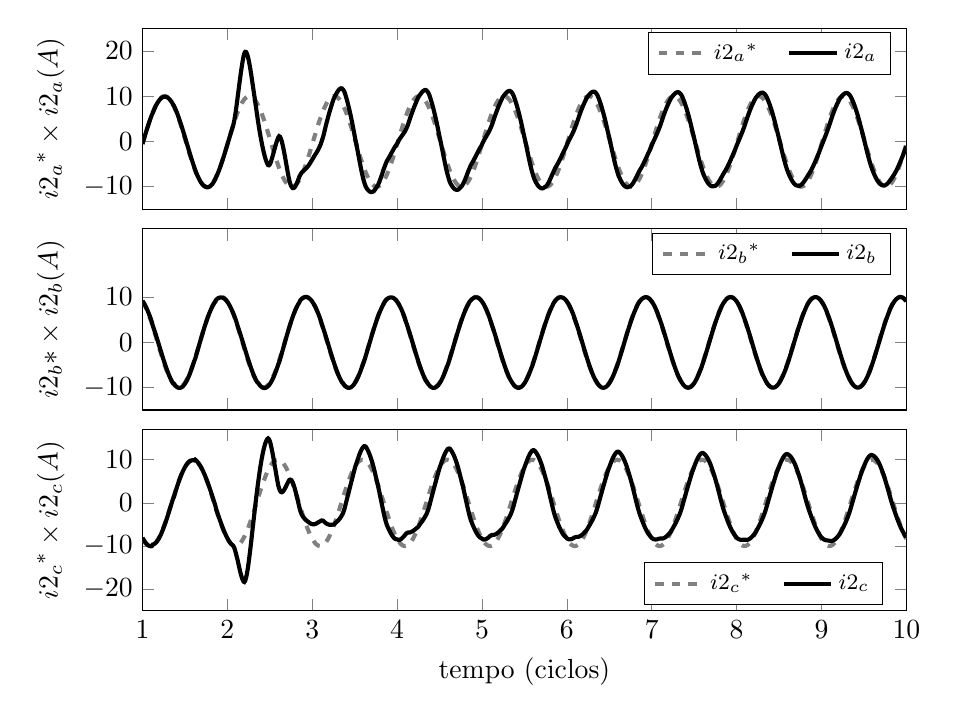
\begin{tikzpicture}

\begin{axis}[%
width=0.8\textwidth,
height=0.189701500343624\textwidth,
scale only axis,
xmin=0.0166666666666667,
xmax=0.166666666666667,
xtick={0.0166666666666667,0.0333333333333333,0.05,0.0666666666666667,0.0833333333333333,0.1,0.116666666666667,0.133333333333333,0.15,0.166666666666667},
xticklabels={\empty},
ymin=-15,
ymax=25,
ytick={-10,   0,  10},
ylabel={${\text{i2}_\text{b}}\text{* }\times\text{ i2}_\text{b}\text{ (A)}$},
name=plot2,
legend style={draw=black,fill=white,legend cell align=left},
scaled x ticks = false,
legend columns=-1,
legend style={/tikz/every even column/.append style={column sep=0.3cm}},
legend style={font=\footnotesize}
]
\addplot [color=gray,dashed,line width=1.5pt]
  table[row sep=crcr]{0.0166583333333333	8.95711760239421\\
0.016825	8.66025403784447\\
0.0169916666666667	8.32921240710107\\
0.0171583333333333	7.96529918024204\\
0.017325	7.56995055651764\\
0.0174916666666667	7.1447267963281\\
0.0176583333333333	6.69130606358865\\
0.017825	6.21147780278317\\
0.0179916666666667	5.70713567684438\\
0.0181583333333333	5.18027009373136\\
0.018325	4.63296035119867\\
0.0184916666666667	4.06736643075805\\
0.0186583333333333	3.4857204732182\\
0.018825	2.89031796944476\\
0.0189916666666667	2.28350870110659\\
0.0191583333333333	1.66768746716105\\
0.019325	1.04528463267656\\
0.0194916666666667	0.418756537292012\\
0.0196583333333333	-0.20942419883356\\
0.019825	-0.836778433323152\\
0.0199916666666667	-1.46083028562412\\
0.0201583333333333	-2.0791169081776\\
0.020325	-2.68919820615267\\
0.0204916666666667	-3.28866646738586\\
0.0206583333333333	-3.87515586452106\\
0.020825	-4.44635179184931\\
0.0209916666666667	-5.00000000000005\\
0.0211583333333333	-5.53391549243349\\
0.021325	-6.0459911486238\\
0.0214916666666667	-6.53420603990112\\
0.0216583333333333	-6.99663340513372\\
0.021825	-7.43144825477402\\
0.0219916666666667	-7.83693457325848\\
0.0221583333333333	-8.21149209133713\\
0.022325	-8.55364260160516\\
0.0224916666666667	-8.86203579231225\\
0.0226583333333333	-9.13545457642611\\
0.022825	-9.37281989491902\\
0.0229916666666667	-9.57319497532079\\
0.0231583333333333	-9.73578902873172\\
0.023325	-9.85996037070517\\
0.0234916666666667	-9.94521895368285\\
0.0236583333333333	-9.99122830098871\\
0.023825	-9.99780683474858\\
0.0239916666666667	-9.96492859249517\\
0.0241583333333333	-9.89272332963001\\
0.024325	-9.78147600733818\\
0.0244916666666667	-9.63162566797671\\
0.0246583333333333	-9.44376370237494\\
0.024825	-9.21863151588513\\
0.0249916666666667	-8.95711760239425\\
0.0251583333333333	-8.66025403784451\\
0.025325	-8.32921240710111\\
0.0254916666666667	-7.96529918024207\\
0.0256583333333333	-7.56995055651767\\
0.025825	-7.14472679632814\\
0.0259916666666667	-6.69130606358868\\
0.0261583333333333	-6.2114778027832\\
0.026325	-5.70713567684441\\
0.0264916666666667	-5.18027009373139\\
0.0266583333333333	-4.6329603511987\\
0.026825	-4.06736643075807\\
0.0269916666666667	-3.48572047321821\\
0.0271583333333333	-2.89031796944477\\
0.027325	-2.28350870110661\\
0.0274916666666667	-1.66768746716106\\
0.0276583333333333	-1.04528463267656\\
0.027825	-0.418756537292015\\
0.0279916666666667	0.209424198833559\\
0.0281583333333333	0.836778433323154\\
0.028325	1.46083028562412\\
0.0284916666666667	2.07911690817761\\
0.0286583333333333	2.68919820615268\\
0.028825	3.28866646738587\\
0.0289916666666667	3.87515586452107\\
0.0291583333333333	4.44635179184933\\
0.029325	5.00000000000006\\
0.0294916666666667	5.53391549243351\\
0.0296583333333333	6.04599114862383\\
0.029825	6.53420603990114\\
0.0299916666666667	6.99663340513375\\
0.0301583333333333	7.43144825477405\\
0.030325	7.83693457325851\\
0.0304916666666667	8.21149209133716\\
0.0306583333333333	8.55364260160519\\
0.030825	8.86203579231228\\
0.0309916666666667	9.13545457642615\\
0.0311583333333333	9.37281989491906\\
0.031325	9.57319497532082\\
0.0314916666666667	9.73578902873176\\
0.0316583333333333	9.85996037070521\\
0.031825	9.94521895368289\\
0.0319916666666667	9.99122830098875\\
0.0321583333333333	9.99780683474862\\
0.032325	9.96492859249521\\
0.0324916666666667	9.89272332963005\\
0.0326583333333333	9.78147600733822\\
0.032825	9.63162566797675\\
0.0329916666666667	9.44376370237498\\
0.0331583333333333	9.21863151588517\\
0.033325	8.95711760239429\\
0.0334916666666667	8.66025403784455\\
0.0336583333333333	8.32921240710115\\
0.033825	7.96529918024211\\
0.0339916666666667	7.56995055651771\\
0.0341583333333333	7.14472679632817\\
0.034325	6.69130606358871\\
0.0344916666666667	6.21147780278323\\
0.0346583333333333	5.70713567684443\\
0.034825	5.18027009373141\\
0.0349916666666667	4.63296035119872\\
0.0351583333333333	4.06736643075809\\
0.035325	3.48572047321823\\
0.0354916666666667	2.89031796944478\\
0.0356583333333333	2.28350870110662\\
0.035825	1.66768746716107\\
0.0359916666666667	1.04528463267657\\
0.0361583333333333	0.418756537292022\\
0.036325	-0.209424198833557\\
0.0364916666666667	-0.836778433323154\\
0.0366583333333333	-1.46083028562413\\
0.036825	-2.07911690817762\\
0.0369916666666667	-2.68919820615269\\
0.0371583333333333	-3.28866646738588\\
0.037325	-3.87515586452109\\
0.0374916666666667	-4.44635179184934\\
0.0376583333333333	-5.00000000000008\\
0.037825	-5.53391549243353\\
0.0379916666666667	-6.04599114862385\\
0.0381583333333333	-6.53420603990117\\
0.038325	-6.99663340513378\\
0.0384916666666667	-7.43144825477408\\
0.0386583333333333	-7.83693457325854\\
0.038825	-8.21149209133719\\
0.0389916666666667	-8.55364260160523\\
0.0391583333333333	-8.86203579231232\\
0.039325	-9.13545457642618\\
0.0394916666666667	-9.3728198949191\\
0.0396583333333333	-9.57319497532086\\
0.039825	-9.7357890287318\\
0.0399916666666667	-9.85996037070525\\
0.0401583333333333	-9.94521895368294\\
0.040325	-9.99122830098879\\
0.0404916666666667	-9.99780683474866\\
0.0406583333333333	-9.96492859249525\\
0.040825	-9.89272332963009\\
0.0409916666666667	-9.78147600733827\\
0.0411583333333333	-9.63162566797679\\
0.041325	-9.44376370237502\\
0.0414916666666667	-9.21863151588521\\
0.0416583333333333	-8.95711760239433\\
0.041825	-8.66025403784458\\
0.0419916666666667	-8.32921240710118\\
0.0421583333333333	-7.96529918024214\\
0.042325	-7.56995055651774\\
0.0424916666666667	-7.1447267963282\\
0.0426583333333333	-6.69130606358874\\
0.042825	-6.21147780278325\\
0.0429916666666667	-5.70713567684446\\
0.0431583333333333	-5.18027009373143\\
0.043325	-4.63296035119874\\
0.0434916666666667	-4.06736643075811\\
0.0436583333333333	-3.48572047321825\\
0.043825	-2.8903179694448\\
0.0439916666666667	-2.28350870110663\\
0.0441583333333333	-1.66768746716108\\
0.044325	-1.04528463267658\\
0.0444916666666667	-0.418756537292025\\
0.0446583333333333	0.209424198833555\\
0.044825	0.836778433323156\\
0.0449916666666667	1.46083028562413\\
0.0451583333333333	2.07911690817762\\
0.045325	2.6891982061527\\
0.0454916666666667	3.28866646738589\\
0.0456583333333333	3.8751558645211\\
0.045825	4.44635179184936\\
0.0459916666666667	5.0000000000001\\
0.0461583333333333	5.53391549243356\\
0.046325	6.04599114862388\\
0.0464916666666667	6.5342060399012\\
0.0466583333333333	6.99663340513381\\
0.046825	7.43144825477411\\
0.0469916666666667	7.83693457325858\\
0.0471583333333333	8.21149209133723\\
0.047325	8.55364260160527\\
0.0474916666666667	8.86203579231236\\
0.0476583333333333	9.13545457642623\\
0.047825	9.37281989491914\\
0.0479916666666667	9.57319497532091\\
0.0481583333333333	9.73578902873184\\
0.048325	9.85996037070529\\
0.0484916666666667	9.94521895368298\\
0.0486583333333333	9.99122830098883\\
0.048825	9.99780683474871\\
0.0489916666666667	9.9649285924953\\
0.0491583333333333	9.89272332963014\\
0.049325	9.78147600733831\\
0.0494916666666667	9.63162566797684\\
0.0496583333333333	9.44376370237506\\
0.049825	9.21863151588525\\
0.0499916666666667	8.95711760239437\\
0.0501583333333333	8.66025403784462\\
0.050325	8.32921240710123\\
0.0504916666666667	7.96529918024218\\
0.0506583333333333	7.56995055651778\\
0.050825	7.14472679632824\\
0.0509916666666667	6.69130606358878\\
0.0511583333333333	6.21147780278329\\
0.051325	5.70713567684449\\
0.0514916666666667	5.18027009373146\\
0.0516583333333333	4.63296035119876\\
0.051825	4.06736643075813\\
0.0519916666666667	3.48572047321827\\
0.0521583333333333	2.89031796944481\\
0.052325	2.28350870110664\\
0.0524916666666667	1.66768746716109\\
0.0526583333333333	1.04528463267659\\
0.052825	0.418756537292029\\
0.0529916666666667	-0.209424198833554\\
0.0531583333333333	-0.836778433323157\\
0.053325	-1.46083028562414\\
0.0534916666666667	-2.07911690817763\\
0.0536583333333333	-2.68919820615271\\
0.053825	-3.2886664673859\\
0.0539916666666667	-3.87515586452112\\
0.0541583333333333	-4.44635179184938\\
0.054325	-5.00000000000012\\
0.0544916666666667	-5.53391549243358\\
0.0546583333333333	-6.0459911486239\\
0.054825	-6.53420603990122\\
0.0549916666666667	-6.99663340513384\\
0.0551583333333333	-7.43144825477414\\
0.055325	-7.83693457325861\\
0.0554916666666667	-8.21149209133726\\
0.0556583333333333	-8.5536426016053\\
0.055825	-8.86203579231239\\
0.0559916666666667	-9.13545457642627\\
0.0561583333333333	-9.37281989491918\\
0.056325	-9.57319497532095\\
0.0564916666666667	-9.73578902873188\\
0.0566583333333333	-9.85996037070534\\
0.056825	-9.94521895368302\\
0.0569916666666667	-9.99122830098888\\
0.0571583333333333	-9.99780683474875\\
0.057325	-9.96492859249534\\
0.0574916666666667	-9.89272332963018\\
0.0576583333333333	-9.78147600733836\\
0.057825	-9.63162566797688\\
0.0579916666666667	-9.44376370237511\\
0.0581583333333333	-9.21863151588529\\
0.058325	-8.95711760239441\\
0.0584916666666667	-8.66025403784466\\
0.0586583333333333	-8.32921240710126\\
0.058825	-7.96529918024222\\
0.0589916666666667	-7.56995055651781\\
0.0591583333333333	-7.14472679632827\\
0.059325	-6.69130606358881\\
0.0594916666666667	-6.21147780278331\\
0.0596583333333333	-5.70713567684451\\
0.059825	-5.18027009373148\\
0.0599916666666667	-4.63296035119878\\
0.0601583333333333	-4.06736643075815\\
0.060325	-3.48572047321828\\
0.0604916666666667	-2.89031796944483\\
0.0606583333333333	-2.28350870110665\\
0.060825	-1.6676874671611\\
0.0609916666666667	-1.04528463267659\\
0.0611583333333333	-0.418756537292034\\
0.061325	0.209424198833552\\
0.0614916666666667	0.836778433323157\\
0.0616583333333333	1.46083028562414\\
0.061825	2.07911690817764\\
0.0619916666666667	2.68919820615272\\
0.0621583333333333	3.28866646738591\\
0.062325	3.87515586452113\\
0.0624916666666667	4.4463517918494\\
0.0626583333333333	5.00000000000014\\
0.062825	5.5339154924336\\
0.0629916666666667	6.04599114862392\\
0.0631583333333333	6.53420603990125\\
0.063325	6.99663340513387\\
0.0634916666666667	7.43144825477417\\
0.0636583333333333	7.83693457325864\\
0.063825	8.2114920913373\\
0.0639916666666667	8.55364260160534\\
0.0641583333333333	8.86203579231243\\
0.064325	9.1354545764263\\
0.0644916666666667	9.37281989491922\\
0.0646583333333333	9.57319497532098\\
0.064825	9.73578902873192\\
0.0649916666666667	9.85996037070537\\
0.0651583333333333	9.94521895368306\\
0.065325	9.99122830098892\\
0.0654916666666667	9.99780683474879\\
0.0656583333333333	9.96492859249538\\
0.065825	9.89272332963022\\
0.0659916666666667	9.78147600733839\\
0.0661583333333333	9.63162566797691\\
0.066325	9.44376370237514\\
0.0664916666666667	9.21863151588533\\
0.0666583333333333	8.95711760239444\\
0.066825	8.6602540378447\\
0.0669916666666667	8.3292124071013\\
0.0671583333333333	7.96529918024225\\
0.067325	7.56995055651784\\
0.0674916666666667	7.1447267963283\\
0.0676583333333333	6.69130606358883\\
0.067825	6.21147780278334\\
0.0679916666666667	5.70713567684454\\
0.0681583333333333	5.1802700937315\\
0.068325	4.6329603511988\\
0.0684916666666667	4.06736643075817\\
0.0686583333333333	3.4857204732183\\
0.068825	2.89031796944484\\
0.0689916666666667	2.28350870110666\\
0.0691583333333333	1.6676874671611\\
0.069325	1.0452846326766\\
0.0694916666666667	0.418756537292036\\
0.0696583333333333	-0.209424198833552\\
0.069825	-0.836778433323159\\
0.0699916666666667	-1.46083028562414\\
0.0701583333333333	-2.07911690817764\\
0.070325	-2.68919820615273\\
0.0704916666666667	-3.28866646738592\\
0.0706583333333333	-3.87515586452114\\
0.070825	-4.44635179184941\\
0.0709916666666667	-5.00000000000016\\
0.0711583333333333	-5.53391549243362\\
0.071325	-6.04599114862394\\
0.0714916666666667	-6.53420603990127\\
0.0716583333333333	-6.99663340513388\\
0.071825	-7.43144825477419\\
0.0719916666666667	-7.83693457325866\\
0.0721583333333333	-8.21149209133732\\
0.072325	-8.55364260160536\\
0.0724916666666667	-8.86203579231245\\
0.0726583333333333	-9.13545457642633\\
0.072825	-9.37281989491924\\
0.0729916666666667	-9.57319497532101\\
0.0731583333333333	-9.73578902873195\\
0.073325	-9.8599603707054\\
0.0734916666666667	-9.94521895368309\\
0.0736583333333333	-9.99122830098895\\
0.073825	-9.99780683474882\\
0.0739916666666667	-9.96492859249541\\
0.0741583333333333	-9.89272332963025\\
0.074325	-9.78147600733842\\
0.0744916666666667	-9.63162566797694\\
0.0746583333333333	-9.44376370237517\\
0.074825	-9.21863151588536\\
0.0749916666666667	-8.95711760239447\\
0.0751583333333333	-8.66025403784472\\
0.075325	-8.32921240710132\\
0.0754916666666667	-7.96529918024228\\
0.0756583333333333	-7.56995055651787\\
0.075825	-7.14472679632832\\
0.0759916666666667	-6.69130606358885\\
0.0761583333333333	-6.21147780278336\\
0.076325	-5.70713567684455\\
0.0764916666666667	-5.18027009373152\\
0.0766583333333333	-4.63296035119882\\
0.076825	-4.06736643075818\\
0.0769916666666667	-3.48572047321831\\
0.0771583333333333	-2.89031796944486\\
0.077325	-2.28350870110667\\
0.0774916666666667	-1.66768746716112\\
0.0776583333333333	-1.04528463267661\\
0.077825	-0.418756537292044\\
0.0779916666666667	0.209424198833547\\
0.0781583333333333	0.836778433323155\\
0.078325	1.46083028562414\\
0.0784916666666667	2.07911690817764\\
0.0786583333333333	2.68919820615273\\
0.078825	3.28866646738593\\
0.0789916666666667	3.87515586452115\\
0.0791583333333333	4.44635179184942\\
0.079325	5.00000000000017\\
0.0794916666666667	5.53391549243363\\
0.0796583333333333	6.04599114862396\\
0.079825	6.53420603990128\\
0.0799916666666667	6.9966334051339\\
0.0801583333333333	7.43144825477421\\
0.080325	7.83693457325868\\
0.0804916666666667	8.21149209133734\\
0.0806583333333333	8.55364260160538\\
0.080825	8.86203579231248\\
0.0809916666666667	9.13545457642635\\
0.0811583333333333	9.37281989491927\\
0.081325	9.57319497532104\\
0.0814916666666667	9.73578902873198\\
0.0816583333333333	9.85996037070543\\
0.081825	9.94521895368312\\
0.0819916666666667	9.99122830098898\\
0.0821583333333333	9.99780683474885\\
0.082325	9.96492859249544\\
0.0824916666666667	9.89272332963028\\
0.0826583333333333	9.78147600733845\\
0.082825	9.63162566797698\\
0.0829916666666667	9.4437637023752\\
0.0831583333333333	9.21863151588539\\
0.083325	8.9571176023945\\
0.0834916666666667	8.66025403784476\\
0.0836583333333333	8.32921240710135\\
0.083825	7.96529918024231\\
0.0839916666666667	7.5699505565179\\
0.0841583333333333	7.14472679632835\\
0.084325	6.69130606358888\\
0.0844916666666667	6.21147780278338\\
0.0846583333333333	5.70713567684458\\
0.084825	5.18027009373154\\
0.0849916666666667	4.63296035119884\\
0.0851583333333333	4.0673664307582\\
0.085325	3.48572047321833\\
0.0854916666666667	2.89031796944487\\
0.0856583333333333	2.28350870110668\\
0.085825	1.66768746716112\\
0.0859916666666667	1.04528463267661\\
0.0861583333333333	0.418756537292048\\
0.086325	-0.209424198833544\\
0.0864916666666667	-0.836778433323155\\
0.0866583333333333	-1.46083028562414\\
0.086825	-2.07911690817765\\
0.0869916666666667	-2.68919820615273\\
0.0871583333333333	-3.28866646738594\\
0.087325	-3.87515586452116\\
0.0874916666666667	-4.44635179184943\\
0.0876583333333333	-5.00000000000018\\
0.087825	-5.53391549243365\\
0.0879916666666667	-6.04599114862398\\
0.0881583333333333	-6.5342060399013\\
0.088325	-6.99663340513393\\
0.0884916666666667	-7.43144825477423\\
0.0886583333333333	-7.83693457325871\\
0.088825	-8.21149209133737\\
0.0889916666666667	-8.55364260160541\\
0.0891583333333333	-8.86203579231251\\
0.089325	-9.13545457642639\\
0.0894916666666667	-9.37281989491931\\
0.0896583333333333	-9.57319497532107\\
0.089825	-9.73578902873201\\
0.0899916666666667	-9.85996037070547\\
0.0901583333333333	-9.94521895368316\\
0.090325	-9.99122830098902\\
0.0904916666666667	-9.99780683474889\\
0.0906583333333333	-9.96492859249548\\
0.090825	-9.89272332963032\\
0.0909916666666667	-9.78147600733849\\
0.0911583333333333	-9.63162566797701\\
0.091325	-9.44376370237524\\
0.0914916666666667	-9.21863151588543\\
0.0916583333333333	-8.95711760239454\\
0.091825	-8.66025403784479\\
0.0919916666666667	-8.32921240710138\\
0.0921583333333333	-7.96529918024234\\
0.092325	-7.56995055651792\\
0.0924916666666667	-7.14472679632838\\
0.0926583333333333	-6.69130606358891\\
0.092825	-6.21147780278341\\
0.0929916666666667	-5.7071356768446\\
0.0931583333333333	-5.18027009373156\\
0.093325	-4.63296035119886\\
0.0934916666666667	-4.06736643075822\\
0.0936583333333333	-3.48572047321834\\
0.093825	-2.89031796944488\\
0.0939916666666667	-2.2835087011067\\
0.0941583333333333	-1.66768746716113\\
0.094325	-1.04528463267662\\
0.0944916666666667	-0.418756537292053\\
0.0946583333333333	0.209424198833542\\
0.094825	0.836778433323155\\
0.0949916666666667	1.46083028562415\\
0.0951583333333333	2.07911690817765\\
0.095325	2.68919820615274\\
0.0954916666666667	3.28866646738595\\
0.0956583333333333	3.87515586452117\\
0.095825	4.44635179184944\\
0.0959916666666667	5.0000000000002\\
0.0961583333333333	5.53391549243367\\
0.096325	6.045991148624\\
0.0964916666666667	6.53420603990133\\
0.0966583333333333	6.99663340513395\\
0.096825	7.43144825477426\\
0.0969916666666667	7.83693457325874\\
0.0971583333333333	8.2114920913374\\
0.097325	8.55364260160545\\
0.0974916666666667	8.86203579231255\\
0.0976583333333333	9.13545457642642\\
0.097825	9.37281989491934\\
0.0979916666666667	9.57319497532111\\
0.0981583333333333	9.73578902873205\\
0.098325	9.85996037070551\\
0.0984916666666667	9.9452189536832\\
0.0986583333333333	9.99122830098905\\
0.098825	9.99780683474893\\
0.0989916666666667	9.96492859249552\\
0.0991583333333333	9.89272332963036\\
0.099325	9.78147600733853\\
0.0994916666666667	9.63162566797705\\
0.0996583333333333	9.44376370237527\\
0.099825	9.21863151588546\\
0.0999916666666667	8.95711760239457\\
0.100158333333333	8.66025403784482\\
0.100325	8.32921240710142\\
0.100491666666667	7.96529918024237\\
0.100658333333333	7.56995055651795\\
0.100825	7.1447267963284\\
0.100991666666667	6.69130606358893\\
0.101158333333333	6.21147780278343\\
0.101325	5.70713567684462\\
0.101491666666667	5.18027009373158\\
0.101658333333333	4.63296035119887\\
0.101825	4.06736643075823\\
0.101991666666667	3.48572047321836\\
0.102158333333333	2.89031796944489\\
0.102325	2.2835087011067\\
0.102491666666667	1.66768746716114\\
0.102658333333333	1.04528463267662\\
0.102825	0.418756537292053\\
0.102991666666667	-0.209424198833544\\
0.103158333333333	-0.83677843332316\\
0.103325	-1.46083028562415\\
0.103491666666667	-2.07911690817766\\
0.103658333333333	-2.68919820615275\\
0.103825	-3.28866646738596\\
0.103991666666667	-3.87515586452119\\
0.104158333333333	-4.44635179184946\\
0.104325	-5.00000000000022\\
0.104491666666667	-5.53391549243368\\
0.104658333333333	-6.04599114862402\\
0.104825	-6.53420603990135\\
0.104991666666667	-6.99663340513398\\
0.105158333333333	-7.43144825477429\\
0.105325	-7.83693457325877\\
0.105491666666667	-8.21149209133743\\
0.105658333333333	-8.55364260160548\\
0.105825	-8.86203579231258\\
0.105991666666667	-9.13545457642645\\
0.106158333333333	-9.37281989491938\\
0.106325	-9.57319497532115\\
0.106491666666667	-9.73578902873209\\
0.106658333333333	-9.85996037070554\\
0.106825	-9.94521895368323\\
0.106991666666667	-9.99122830098909\\
0.107158333333333	-9.99780683474897\\
0.107325	-9.96492859249556\\
0.107491666666667	-9.8927233296304\\
0.107658333333333	-9.78147600733856\\
0.107825	-9.63162566797709\\
0.107991666666667	-9.44376370237531\\
0.108158333333333	-9.21863151588549\\
0.108325	-8.95711760239461\\
0.108491666666667	-8.66025403784485\\
0.108658333333333	-8.32921240710145\\
0.108825	-7.9652991802424\\
0.108991666666667	-7.56995055651798\\
0.109158333333333	-7.14472679632843\\
0.109325	-6.69130606358896\\
0.109491666666667	-6.21147780278346\\
0.109658333333333	-5.70713567684465\\
0.109825	-5.18027009373161\\
0.109991666666667	-4.6329603511989\\
0.110158333333333	-4.06736643075825\\
0.110325	-3.48572047321838\\
0.110491666666667	-2.89031796944491\\
0.110658333333333	-2.28350870110672\\
0.110825	-1.66768746716115\\
0.110991666666667	-1.04528463267663\\
0.111158333333333	-0.418756537292063\\
0.111325	0.209424198833538\\
0.111491666666667	0.836778433323156\\
0.111658333333333	1.46083028562415\\
0.111825	2.07911690817766\\
0.111991666666667	2.68919820615276\\
0.112158333333333	3.28866646738597\\
0.112325	3.8751558645212\\
0.112491666666667	4.44635179184947\\
0.112658333333333	5.00000000000023\\
0.112825	5.5339154924337\\
0.112991666666667	6.04599114862404\\
0.113158333333333	6.53420603990138\\
0.113325	6.996633405134\\
0.113491666666667	7.43144825477432\\
0.113658333333333	7.8369345732588\\
0.113825	8.21149209133746\\
0.113991666666667	8.55364260160551\\
0.114158333333333	8.86203579231261\\
0.114325	9.13545457642649\\
0.114491666666667	9.37281989491941\\
0.114658333333333	9.57319497532118\\
0.114825	9.73578902873213\\
0.114991666666667	9.85996037070558\\
0.115158333333333	9.94521895368328\\
0.115325	9.99122830098913\\
0.115491666666667	9.99780683474901\\
0.115658333333333	9.9649285924956\\
0.115825	9.89272332963044\\
0.115991666666667	9.78147600733861\\
0.116158333333333	9.63162566797713\\
0.116325	9.44376370237535\\
0.116491666666667	9.21863151588554\\
0.116658333333333	8.95711760239465\\
0.116825	8.66025403784489\\
0.116991666666667	8.32921240710149\\
0.117158333333333	7.96529918024244\\
0.117325	7.56995055651802\\
0.117491666666667	7.14472679632847\\
0.117658333333333	6.69130606358899\\
0.117825	6.21147780278349\\
0.117991666666667	5.70713567684468\\
0.118158333333333	5.18027009373164\\
0.118325	4.63296035119892\\
0.118491666666667	4.06736643075828\\
0.118658333333333	3.48572047321839\\
0.118825	2.89031796944493\\
0.118991666666667	2.28350870110673\\
0.119158333333333	1.66768746716117\\
0.119325	1.04528463267664\\
0.119491666666667	0.418756537292069\\
0.119658333333333	-0.209424198833534\\
0.119825	-0.836778433323155\\
0.119991666666667	-1.46083028562415\\
0.120158333333333	-2.07911690817766\\
0.120325	-2.68919820615276\\
0.120491666666667	-3.28866646738597\\
0.120658333333333	-3.87515586452121\\
0.120825	-4.44635179184949\\
0.120991666666667	-5.00000000000025\\
0.121158333333333	-5.53391549243372\\
0.121325	-6.04599114862406\\
0.121491666666667	-6.53420603990139\\
0.121658333333333	-6.99663340513402\\
0.121825	-7.43144825477434\\
0.121991666666667	-7.83693457325882\\
0.122158333333333	-8.21149209133749\\
0.122325	-8.55364260160554\\
0.122491666666667	-8.86203579231264\\
0.122658333333333	-9.13545457642652\\
0.122825	-9.37281989491945\\
0.122991666666667	-9.57319497532122\\
0.123158333333333	-9.73578902873216\\
0.123325	-9.85996037070562\\
0.123491666666667	-9.94521895368331\\
0.123658333333333	-9.99122830098917\\
0.123825	-9.99780683474905\\
0.123991666666667	-9.96492859249564\\
0.124158333333333	-9.89272332963048\\
0.124325	-9.78147600733865\\
0.124491666666667	-9.63162566797717\\
0.124658333333333	-9.44376370237539\\
0.124825	-9.21863151588557\\
0.124991666666667	-8.95711760239469\\
0.125158333333333	-8.66025403784493\\
0.125325	-8.32921240710152\\
0.125491666666667	-7.96529918024247\\
0.125658333333333	-7.56995055651805\\
0.125825	-7.1447267963285\\
0.125991666666667	-6.69130606358902\\
0.126158333333333	-6.21147780278352\\
0.126325	-5.7071356768447\\
0.126491666666667	-5.18027009373166\\
0.126658333333333	-4.63296035119894\\
0.126825	-4.0673664307583\\
0.126991666666667	-3.48572047321841\\
0.127158333333333	-2.89031796944494\\
0.127325	-2.28350870110675\\
0.127491666666667	-1.66768746716117\\
0.127658333333333	-1.04528463267665\\
0.127825	-0.418756537292072\\
0.127991666666667	0.209424198833532\\
0.128158333333333	0.836778433323155\\
0.128325	1.46083028562416\\
0.128491666666667	2.07911690817767\\
0.128658333333333	2.68919820615277\\
0.128825	3.28866646738599\\
0.128991666666667	3.87515586452122\\
0.129158333333333	4.4463517918495\\
0.129325	5.00000000000027\\
0.129491666666667	5.53391549243374\\
0.129658333333333	6.04599114862408\\
0.129825	6.53420603990142\\
0.129991666666667	6.99663340513405\\
0.130158333333333	7.43144825477437\\
0.130325	7.83693457325885\\
0.130491666666667	8.21149209133752\\
0.130658333333333	8.55364260160558\\
0.130825	8.86203579231268\\
0.130991666666667	9.13545457642656\\
0.131158333333333	9.37281989491949\\
0.131325	9.57319497532126\\
0.131491666666667	9.7357890287322\\
0.131658333333333	9.85996037070566\\
0.131825	9.94521895368336\\
0.131991666666667	9.99122830098921\\
0.132158333333333	9.99780683474909\\
0.132325	9.96492859249568\\
0.132491666666667	9.89272332963052\\
0.132658333333333	9.78147600733869\\
0.132825	9.63162566797721\\
0.132991666666667	9.44376370237543\\
0.133158333333333	9.21863151588561\\
0.133325	8.95711760239472\\
0.133491666666667	8.66025403784496\\
0.133658333333333	8.32921240710155\\
0.133825	7.9652991802425\\
0.133991666666667	7.56995055651808\\
0.134158333333333	7.14472679632853\\
0.134325	6.69130606358905\\
0.134491666666667	6.21147780278354\\
0.134658333333333	5.70713567684473\\
0.134825	5.18027009373168\\
0.134991666666667	4.63296035119896\\
0.135158333333333	4.06736643075831\\
0.135325	3.48572047321843\\
0.135491666666667	2.89031796944495\\
0.135658333333333	2.28350870110675\\
0.135825	1.66768746716118\\
0.135991666666667	1.04528463267665\\
0.136158333333333	0.418756537292075\\
0.136325	-0.209424198833533\\
0.136491666666667	-0.83677843332316\\
0.136658333333333	-1.46083028562416\\
0.136825	-2.07911690817768\\
0.136991666666667	-2.68919820615279\\
0.137158333333333	-3.288666467386\\
0.137325	-3.87515586452124\\
0.137491666666667	-4.44635179184952\\
0.137658333333333	-5.00000000000029\\
0.137825	-5.53391549243377\\
0.137991666666667	-6.04599114862411\\
0.138158333333333	-6.53420603990145\\
0.138325	-6.99663340513408\\
0.138491666666667	-7.4314482547744\\
0.138658333333333	-7.83693457325889\\
0.138825	-8.21149209133756\\
0.138991666666667	-8.55364260160561\\
0.139158333333333	-8.86203579231272\\
0.139325	-9.1354545764266\\
0.139491666666667	-9.37281989491953\\
0.139658333333333	-9.5731949753213\\
0.139825	-9.73578902873225\\
0.139991666666667	-9.8599603707057\\
0.140158333333333	-9.9452189536834\\
0.140325	-9.99122830098926\\
0.140491666666667	-9.99780683474913\\
0.140658333333333	-9.96492859249572\\
0.140825	-9.89272332963056\\
0.140991666666667	-9.78147600733873\\
0.141158333333333	-9.63162566797725\\
0.141325	-9.44376370237547\\
0.141491666666667	-9.21863151588565\\
0.141658333333333	-8.95711760239476\\
0.141825	-8.660254037845\\
0.141991666666667	-8.32921240710159\\
0.142158333333333	-7.96529918024254\\
0.142325	-7.56995055651812\\
0.142491666666667	-7.14472679632856\\
0.142658333333333	-6.69130606358908\\
0.142825	-6.21147780278357\\
0.142991666666667	-5.70713567684475\\
0.143158333333333	-5.18027009373171\\
0.143325	-4.63296035119899\\
0.143491666666667	-4.06736643075833\\
0.143658333333333	-3.48572047321844\\
0.143825	-2.89031796944497\\
0.143991666666667	-2.28350870110677\\
0.144158333333333	-1.66768746716119\\
0.144325	-1.04528463267666\\
0.144491666666667	-0.41875653729208\\
0.144658333333333	0.20942419883353\\
0.144825	0.836778433323158\\
0.144991666666667	1.46083028562416\\
0.145158333333333	2.07911690817769\\
0.145325	2.68919820615279\\
0.145491666666667	3.28866646738601\\
0.145658333333333	3.87515586452125\\
0.145825	4.44635179184954\\
0.145991666666667	5.0000000000003\\
0.146158333333333	5.53391549243378\\
0.146325	6.04599114862413\\
0.146491666666667	6.53420603990147\\
0.146658333333333	6.99663340513411\\
0.146825	7.43144825477443\\
0.146991666666667	7.83693457325891\\
0.147158333333333	8.21149209133759\\
0.147325	8.55364260160564\\
0.147491666666667	8.86203579231275\\
0.147658333333333	9.13545457642663\\
0.147825	9.37281989491956\\
0.147991666666667	9.57319497532134\\
0.148158333333333	9.73578902873228\\
0.148325	9.85996037070574\\
0.148491666666667	9.94521895368344\\
0.148658333333333	9.9912283009893\\
0.148825	9.99780683474917\\
0.148991666666667	9.96492859249576\\
0.149158333333333	9.8927233296306\\
0.149325	9.78147600733877\\
0.149491666666667	9.63162566797729\\
0.149658333333333	9.44376370237551\\
0.149825	9.21863151588569\\
0.149991666666667	8.9571176023948\\
0.150158333333333	8.66025403784504\\
0.150325	8.32921240710163\\
0.150491666666667	7.96529918024257\\
0.150658333333333	7.56995055651815\\
0.150825	7.14472679632859\\
0.150991666666667	6.69130606358911\\
0.151158333333333	6.2114778027836\\
0.151325	5.70713567684478\\
0.151491666666667	5.18027009373173\\
0.151658333333333	4.63296035119901\\
0.151825	4.06736643075835\\
0.151991666666667	3.48572047321846\\
0.152158333333333	2.89031796944498\\
0.152325	2.28350870110678\\
0.152491666666667	1.6676874671612\\
0.152658333333333	1.04528463267667\\
0.152825	0.418756537292087\\
0.152991666666667	-0.209424198833525\\
0.153158333333333	-0.836778433323156\\
0.153325	-1.46083028562416\\
0.153491666666667	-2.07911690817769\\
0.153658333333333	-2.6891982061528\\
0.153825	-3.28866646738602\\
0.153991666666667	-3.87515586452126\\
0.154158333333333	-4.44635179184955\\
0.154325	-5.00000000000032\\
0.154491666666667	-5.5339154924338\\
0.154658333333333	-6.04599114862415\\
0.154825	-6.5342060399015\\
0.154991666666667	-6.99663340513413\\
0.155158333333333	-7.43144825477446\\
0.155325	-7.83693457325895\\
0.155491666666667	-8.21149209133762\\
0.155658333333333	-8.55364260160568\\
0.155825	-8.86203579231279\\
0.155991666666667	-9.13545457642667\\
0.156158333333333	-9.3728198949196\\
0.156325	-9.57319497532138\\
0.156491666666667	-9.73578902873233\\
0.156658333333333	-9.85996037070579\\
0.156825	-9.94521895368348\\
0.156991666666667	-9.99122830098934\\
0.157158333333333	-9.99780683474921\\
0.157325	-9.96492859249581\\
0.157491666666667	-9.89272332963065\\
0.157658333333333	-9.78147600733882\\
0.157825	-9.63162566797734\\
0.157991666666667	-9.44376370237556\\
0.158158333333333	-9.21863151588574\\
0.158325	-8.95711760239484\\
0.158491666666667	-8.66025403784508\\
0.158658333333333	-8.32921240710167\\
0.158825	-7.96529918024262\\
0.158991666666667	-7.56995055651819\\
0.159158333333333	-7.14472679632863\\
0.159325	-6.69130606358915\\
0.159491666666667	-6.21147780278364\\
0.159658333333333	-5.70713567684481\\
0.159825	-5.18027009373176\\
0.159991666666667	-4.63296035119904\\
0.160158333333333	-4.06736643075838\\
0.160325	-3.48572047321849\\
0.160491666666667	-2.890317969445\\
0.160658333333333	-2.2835087011068\\
0.160825	-1.66768746716122\\
0.160991666666667	-1.04528463267668\\
0.161158333333333	-0.418756537292097\\
0.161325	0.209424198833518\\
0.161491666666667	0.836778433323153\\
0.161658333333333	1.46083028562416\\
0.161825	2.07911690817769\\
0.161991666666667	2.6891982061528\\
0.162158333333333	3.28866646738603\\
0.162325	3.87515586452127\\
0.162491666666667	4.44635179184956\\
0.162658333333333	5.00000000000034\\
0.162825	5.53391549243382\\
0.162991666666667	6.04599114862417\\
0.163158333333333	6.53420603990152\\
0.163325	6.99663340513416\\
0.163491666666667	7.43144825477449\\
0.163658333333333	7.83693457325898\\
0.163825	8.21149209133765\\
0.163991666666667	8.55364260160571\\
0.164158333333333	8.86203579231282\\
0.164325	9.13545457642671\\
0.164491666666667	9.37281989491964\\
0.164658333333333	9.57319497532142\\
0.164825	9.73578902873236\\
0.164991666666667	9.85996037070582\\
0.165158333333333	9.94521895368352\\
0.165325	9.99122830098938\\
0.165491666666667	9.99780683474926\\
0.165658333333333	9.96492859249585\\
0.165825	9.89272332963069\\
0.165991666666667	9.78147600733886\\
0.166158333333333	9.63162566797738\\
0.166325	9.44376370237559\\
0.166491666666667	9.21863151588578\\
0.166658333333333	8.95711760239488\\
};
\addlegendentry{${\text{i2}_\text{b}}^\text{*}$};

\addplot [color=black,solid,line width=1.5pt]
  table[row sep=crcr]{0.0166583333333333	9.10238729436972\\
0.016825	8.81704993622876\\
0.0169916666666667	8.50071754137033\\
0.0171583333333333	8.15515004140646\\
0.017325	7.7819187867049\\
0.0174916666666667	7.38204974177135\\
0.0176583333333333	6.95626978050029\\
0.017825	6.50510560395105\\
0.0179916666666667	6.02945861112754\\
0.0181583333333333	5.53040314356191\\
0.018325	5.00924821301577\\
0.0184916666666667	4.46751489796481\\
0.0186583333333333	3.68981019134787\\
0.018825	3.14840956068264\\
0.0189916666666667	2.59416394011585\\
0.0191583333333333	2.02377684219615\\
0.019325	1.43881119869898\\
0.0194916666666667	0.841909769593364\\
0.0196583333333333	0.235780957939821\\
0.019825	-0.376689340170496\\
0.0199916666666667	-0.992665526242936\\
0.0201583333333333	-1.60920663242736\\
0.020325	-2.22329353670832\\
0.0204916666666667	-2.83190601073707\\
0.0206583333333333	-3.43206068203698\\
0.020825	-4.02042104637285\\
0.0209916666666667	-4.59498130928033\\
0.0211583333333333	-5.15341682461041\\
0.021325	-5.6940962192604\\
0.0214916666666667	-6.21505582977236\\
0.0216583333333333	-6.71378044678016\\
0.021825	-7.18751402421548\\
0.0219916666666667	-7.6333168162301\\
0.0221583333333333	-8.04867680302019\\
0.022325	-8.43126236325755\\
0.0224916666666667	-8.77900373523377\\
0.0226583333333333	-9.09008498121201\\
0.022825	-9.15855337492306\\
0.0229916666666667	-9.42861378862864\\
0.0231583333333333	-9.65793002398938\\
0.023325	-9.84203175689098\\
0.0234916666666667	-9.97985634821345\\
0.0236583333333333	-10.0713474398235\\
0.023825	-10.1165549780692\\
0.0239916666666667	-10.1159383416511\\
0.0241583333333333	-10.0698886487835\\
0.024325	-9.97914771255928\\
0.0244916666666667	-9.84467529451614\\
0.0246583333333333	-9.66760532286042\\
0.024825	-9.44931901487656\\
0.0249916666666667	-9.19133428032041\\
0.0251583333333333	-8.8945965624705\\
0.025325	-8.56015786213606\\
0.0254916666666667	-8.18882959610245\\
0.0256583333333333	-7.78203825639882\\
0.025825	-7.34193745850652\\
0.0259916666666667	-6.871066065311\\
0.0261583333333333	-6.37234524011466\\
0.026325	-5.84845377190004\\
0.0264916666666667	-5.30212355465025\\
0.0266583333333333	-4.73605099633701\\
0.026825	-4.15290088980286\\
0.0269916666666667	-3.7463128418275\\
0.0271583333333333	-3.10098116111065\\
0.027325	-2.44739188124668\\
0.0274916666666667	-1.79053931585367\\
0.0276583333333333	-1.13327765870239\\
0.027825	-0.477924319106184\\
0.0279916666666667	0.173209663659246\\
0.0281583333333333	0.81818389481377\\
0.028325	1.45483512926401\\
0.0284916666666667	2.08120905361234\\
0.0286583333333333	2.69541683114933\\
0.028825	3.29561201161392\\
0.0289916666666667	3.88022294753529\\
0.0291583333333333	4.44714029176902\\
0.029325	4.99439015782883\\
0.0294916666666667	5.51947855033307\\
0.0296583333333333	6.01988736030132\\
0.029825	6.49370710499595\\
0.0299916666666667	6.93963550745553\\
0.0301583333333333	7.3567961627066\\
0.030325	7.74446827210866\\
0.0304916666666667	8.10180024444722\\
0.0306583333333333	8.42799192122998\\
0.030825	8.72224797849278\\
0.0309916666666667	8.98379451656429\\
0.0311583333333333	9.39000247520132\\
0.031325	9.54893851207278\\
0.0314916666666667	9.67501312493445\\
0.0316583333333333	9.76956673991744\\
0.031825	9.83213375604548\\
0.0319916666666667	9.86203092932595\\
0.0321583333333333	9.85882018895445\\
0.032325	9.82186948854932\\
0.0324916666666667	9.7509584363675\\
0.0326583333333333	9.64582294926668\\
0.032825	9.50631560990461\\
0.0329916666666667	9.33243620129852\\
0.0331583333333333	9.12407992641987\\
0.033325	8.88199693232614\\
0.0334916666666667	8.60690761693528\\
0.0336583333333333	8.30031817371014\\
0.033825	7.96381783130639\\
0.0339916666666667	7.59858035831388\\
0.0341583333333333	7.20550175883682\\
0.034325	6.78510676631586\\
0.0344916666666667	6.33834029028864\\
0.0346583333333333	5.8662884047453\\
0.034825	5.37023786238818\\
0.0349916666666667	4.85163190263994\\
0.0351583333333333	4.28149658577571\\
0.035325	3.58762676973298\\
0.0354916666666667	3.0456994482591\\
0.0356583333333333	2.4865038492782\\
0.035825	1.91102787172691\\
0.0359916666666667	1.32189078050082\\
0.0361583333333333	0.721938962011906\\
0.036325	0.113855158360438\\
0.0364916666666667	-0.499365898498088\\
0.0366583333333333	-1.11503128292631\\
0.036825	-1.73025520539475\\
0.0369916666666667	-2.34208378847066\\
0.0371583333333333	-2.94748587657552\\
0.037325	-3.5431400706758\\
0.0374916666666667	-4.1265231476695\\
0.0376583333333333	-4.69508199372783\\
0.037825	-5.24699481009654\\
0.0379916666666667	-5.78041375264997\\
0.0381583333333333	-6.29307974931665\\
0.038325	-6.78253811247046\\
0.0384916666666667	-7.24596610272513\\
0.0386583333333333	-7.6810872056987\\
0.038825	-8.08574080491781\\
0.0389916666666667	-8.45801037504019\\
0.0391583333333333	-8.79620068499962\\
0.039325	-8.96806487507886\\
0.0394916666666667	-9.21070528346815\\
0.0396583333333333	-9.47108643131567\\
0.039825	-9.69006577542452\\
0.0399916666666667	-9.86604802286814\\
0.0401583333333333	-9.99862843742934\\
0.040325	-10.0876819809747\\
0.0404916666666667	-10.1331917117651\\
0.0406583333333333	-10.1355416577069\\
0.040825	-10.0949836782007\\
0.0409916666666667	-10.0120127334088\\
0.0411583333333333	-9.88722687874503\\
0.041325	-9.72133156733559\\
0.0414916666666667	-9.51541879850157\\
0.0416583333333333	-9.26995328123422\\
0.041825	-8.98572454913961\\
0.0419916666666667	-8.66322314753683\\
0.0421583333333333	-8.30335136347556\\
0.042325	-7.90765316365763\\
0.0424916666666667	-7.47802658774969\\
0.0426583333333333	-7.0169137009076\\
0.042825	-6.52642947709798\\
0.0429916666666667	-6.00887733160312\\
0.0431583333333333	-5.46662604543119\\
0.043325	-4.90211625430936\\
0.0434916666666667	-4.48494333559065\\
0.0436583333333333	-3.8590351634337\\
0.043825	-3.2118487319502\\
0.0439916666666667	-2.5557754004136\\
0.0441583333333333	-1.89397286683257\\
0.044325	-1.22893143241073\\
0.0444916666666667	-0.563306382147479\\
0.0446583333333333	0.100389856630612\\
0.044825	0.759488778059827\\
0.0449916666666667	1.41140264559457\\
0.0451583333333333	2.05372800650602\\
0.045325	2.68418786236869\\
0.0454916666666667	3.3006105803122\\
0.0456583333333333	3.90115164165044\\
0.045825	4.48323533437549\\
0.0459916666666667	5.04441328155281\\
0.0461583333333333	5.5818940948016\\
0.046325	6.0933288931626\\
0.0464916666666667	6.57703266031942\\
0.0466583333333333	7.03168592527747\\
0.046825	7.45653884038628\\
0.0469916666666667	7.85052919185026\\
0.0471583333333333	8.21278991052803\\
0.047325	8.54250647974175\\
0.0474916666666667	8.83892137915094\\
0.0476583333333333	9.26324073490593\\
0.047825	9.46108564493796\\
0.0479916666666667	9.62395420189803\\
0.0481583333333333	9.75447445593996\\
0.048325	9.85256615795213\\
0.0484916666666667	9.91760332315369\\
0.0486583333333333	9.94912495301349\\
0.048825	9.94634598884029\\
0.0489916666666667	9.90895228811722\\
0.0491583333333333	9.83654546284874\\
0.049325	9.72882165016644\\
0.0494916666666667	9.58562670339993\\
0.0496583333333333	9.40692140087188\\
0.049825	9.19280839746856\\
0.0499916666666667	8.94410631419182\\
0.0501583333333333	8.66194019234958\\
0.050325	8.34784961980865\\
0.0504916666666667	8.00313239038802\\
0.0506583333333333	7.62874612085978\\
0.050825	7.22560396909269\\
0.0509916666666667	6.79438175035216\\
0.0511583333333333	6.33632356168003\\
0.051325	5.85274169954162\\
0.0514916666666667	5.3451422381028\\
0.0516583333333333	4.81521722175832\\
0.051825	4.11344346932942\\
0.0519916666666667	3.57417143640025\\
0.0521583333333333	3.01743414394888\\
0.052325	2.44358683452047\\
0.0524916666666667	1.85487666898386\\
0.0526583333333333	1.25401048627972\\
0.052825	0.643640342909031\\
0.0529916666666667	0.0269168004249247\\
0.0531583333333333	-0.593429536141159\\
0.053325	-1.21448520613364\\
0.0534916666666667	-1.83335636481385\\
0.0536583333333333	-2.44718673620985\\
0.053825	-3.05304052763314\\
0.0539916666666667	-3.64826995386264\\
0.0541583333333333	-4.2304681987397\\
0.054325	-4.79765715649271\\
0.0544916666666667	-5.34800033964125\\
0.0546583333333333	-5.8793041359113\\
0.054825	-6.38906901135749\\
0.0549916666666667	-6.87459460084883\\
0.0551583333333333	-7.33327323945699\\
0.055325	-7.76286425793868\\
0.0554916666666667	-8.1612358879239\\
0.0556583333333333	-8.52645338535431\\
0.055825	-8.8545125093652\\
0.0559916666666667	-9.00972209965602\\
0.0561583333333333	-9.29461637447726\\
0.056325	-9.53877439733514\\
0.0564916666666667	-9.73984452211998\\
0.0566583333333333	-9.8971687802164\\
0.056825	-10.0105115787276\\
0.0569916666666667	-10.0796880407265\\
0.0571583333333333	-10.1051819452256\\
0.057325	-10.0872552407135\\
0.0574916666666667	-10.0265578384864\\
0.0576583333333333	-9.92390731442403\\
0.057825	-9.78025726134542\\
0.0579916666666667	-9.59683030150148\\
0.0581583333333333	-9.37460230898805\\
0.058325	-9.11458173711329\\
0.0584916666666667	-8.81747002110175\\
0.0586583333333333	-8.4841423201435\\
0.058825	-8.1160423996956\\
0.0589916666666667	-7.714993617687\\
0.0591583333333333	-7.28340832250556\\
0.059325	-6.82342277849412\\
0.0594916666666667	-6.3372724154346\\
0.0596583333333333	-5.82723851814974\\
0.059825	-5.29561218650246\\
0.0599916666666667	-4.78026638572992\\
0.0601583333333333	-4.30773729078191\\
0.060325	-3.69735721815052\\
0.0604916666666667	-3.07675823047187\\
0.0606583333333333	-2.44925821477336\\
0.060825	-1.81699611454147\\
0.0609916666666667	-1.18198262082823\\
0.0611583333333333	-0.546396572160686\\
0.061325	0.0880030896281339\\
0.0614916666666667	0.71901626301327\\
0.0616583333333333	1.34461390094005\\
0.061825	1.96275259915824\\
0.0619916666666667	2.57137732561553\\
0.0621583333333333	3.16859401895893\\
0.062325	3.75211948996479\\
0.0624916666666667	4.31963251502501\\
0.0626583333333333	4.86847077461059\\
0.062825	5.39618038045055\\
0.0629916666666667	5.90083690822683\\
0.0631583333333333	6.38081077303026\\
0.063325	6.83510929309027\\
0.0634916666666667	7.26231159708544\\
0.0636583333333333	7.66118409943112\\
0.063825	8.03053557415489\\
0.0639916666666667	8.36922610068255\\
0.0641583333333333	8.7745789407867\\
0.064325	9.07183182594482\\
0.0644916666666667	9.28577395111365\\
0.0646583333333333	9.46761789556413\\
0.064825	9.61726628041251\\
0.0649916666666667	9.73389381469471\\
0.0651583333333333	9.81671225290874\\
0.065325	9.86502586131618\\
0.0654916666666667	9.87798323483151\\
0.0656583333333333	9.8551573315981\\
0.065825	9.79610940267719\\
0.0659916666666667	9.70055070226577\\
0.0661583333333333	9.56835627863205\\
0.066325	9.39941260475174\\
0.0664916666666667	9.19424218297206\\
0.0666583333333333	8.95362903411519\\
0.066825	8.67885945448046\\
0.0669916666666667	8.37116171242535\\
0.0671583333333333	8.03147737001888\\
0.067325	7.66075289694225\\
0.0674916666666667	7.25957969715094\\
0.0676583333333333	6.82924431444509\\
0.067825	6.37106225885956\\
0.0679916666666667	5.88653481198717\\
0.0681583333333333	5.37733930971252\\
0.068325	4.71731714302915\\
0.0684916666666667	4.18009790913288\\
0.0686583333333333	3.63400488682004\\
0.068825	3.06879027062733\\
0.0689916666666667	2.48648290082356\\
0.0691583333333333	1.88980135659367\\
0.069325	1.28144513214276\\
0.0694916666666667	0.664427826630013\\
0.0696583333333333	0.0416213180594941\\
0.069825	-0.584122041320721\\
0.0699916666666667	-1.20989546053209\\
0.0701583333333333	-1.83282813973939\\
0.070325	-2.45009239218683\\
0.0704916666666667	-3.05875549187276\\
0.0706583333333333	-3.656429261838\\
0.070825	-4.24087562471018\\
0.0709916666666667	-4.81017564328322\\
0.0711583333333333	-5.36220444344335\\
0.071325	-5.8944979383563\\
0.0714916666666667	-6.40457727238226\\
0.0716583333333333	-6.88959032832075\\
0.071825	-7.34733444408421\\
0.0719916666666667	-7.77561517986046\\
0.0721583333333333	-8.17242210248778\\
0.072325	-8.53593342254628\\
0.0724916666666667	-8.73683138183488\\
0.0726583333333333	-9.05291103221133\\
0.072825	-9.33173006733255\\
0.0729916666666667	-9.56904860541067\\
0.0731583333333333	-9.763814497476\\
0.073325	-9.91561121038703\\
0.0734916666666667	-10.0240709671243\\
0.0736583333333333	-10.0894756834195\\
0.073825	-10.1118515634512\\
0.0739916666666667	-10.091572623494\\
0.0741583333333333	-10.0292088045688\\
0.074325	-9.92548343090306\\
0.0744916666666667	-9.78127761658615\\
0.0746583333333333	-9.59767364504045\\
0.074825	-9.37544933983521\\
0.0749916666666667	-9.11535157295351\\
0.0751583333333333	-8.81809908007054\\
0.075325	-8.48485542844672\\
0.0754916666666667	-8.11727163329509\\
0.0756583333333333	-7.7172143245556\\
0.075825	-7.287008358883\\
0.0759916666666667	-6.82860793546988\\
0.0761583333333333	-6.34416279371398\\
0.076325	-5.83585315051653\\
0.0764916666666667	-5.30599673061931\\
0.0766583333333333	-4.87638508386086\\
0.076825	-4.28552848590906\\
0.0769916666666667	-3.68090622969641\\
0.0771583333333333	-3.06635388650932\\
0.077325	-2.44419497350437\\
0.0774916666666667	-1.81647833744371\\
0.0776583333333333	-1.18542562362781\\
0.077825	-0.552766873622229\\
0.0779916666666667	0.0792395675528048\\
0.0781583333333333	0.708523794583972\\
0.078325	1.33299793597888\\
0.0784916666666667	1.950550903702\\
0.0786583333333333	2.55911282312654\\
0.078825	3.1565759476014\\
0.0789916666666667	3.74056065420683\\
0.0791583333333333	4.30848700601697\\
0.079325	4.85778195131837\\
0.0794916666666667	5.38628399683673\\
0.0796583333333333	5.89219428881371\\
0.079825	6.37409258921633\\
0.0799916666666667	6.83064846653227\\
0.0801583333333333	7.26037130225157\\
0.080325	7.66190884583333\\
0.0804916666666667	8.03396100192567\\
0.0806583333333333	8.38054877324822\\
0.080825	8.79630586743607\\
0.0809916666666667	9.04923635319246\\
0.0811583333333333	9.26993462364415\\
0.081325	9.45858575726258\\
0.0814916666666667	9.61428900076581\\
0.0816583333333333	9.73607533460027\\
0.081825	9.82325855915754\\
0.0819916666666667	9.87476746383447\\
0.0821583333333333	9.89016797488593\\
0.082325	9.86895927117463\\
0.0824916666666667	9.81079003788473\\
0.0826583333333333	9.71546821340679\\
0.082825	9.58289556535001\\
0.0829916666666667	9.41327671622407\\
0.0831583333333333	9.20722111035654\\
0.083325	8.96577860807136\\
0.0834916666666667	8.69011619835547\\
0.0836583333333333	8.38119862395878\\
0.083825	8.03996162854429\\
0.0839916666666667	7.66700717947993\\
0.0841583333333333	7.26346906644294\\
0.084325	6.83062134019253\\
0.0844916666666667	6.36988527033076\\
0.0846583333333333	5.88285526687467\\
0.084825	5.33780042680669\\
0.0849916666666667	4.73357788030052\\
0.0851583333333333	4.20148351612217\\
0.085325	3.64899305305859\\
0.0854916666666667	3.07764555100343\\
0.0856583333333333	2.48999695652783\\
0.085825	1.88878092736472\\
0.0859916666666667	1.2766450779197\\
0.0861583333333333	0.656725469492138\\
0.086325	0.0316990640793973\\
0.0864916666666667	-0.595570899781909\\
0.0866583333333333	-1.22224793238584\\
0.086825	-1.84553515066051\\
0.0869916666666667	-2.46259768170212\\
0.0871583333333333	-3.07083377564987\\
0.087325	-3.66790562808105\\
0.0874916666666667	-4.25178074831931\\
0.0876583333333333	-4.82036999915754\\
0.087825	-5.37129484599425\\
0.0879916666666667	-5.90213687383473\\
0.0881583333333333	-6.41000744278514\\
0.088325	-6.8926642940184\\
0.0884916666666667	-7.34786086472289\\
0.0886583333333333	-7.77351198479444\\
0.088825	-8.16770589549935\\
0.0889916666666667	-8.45298094512572\\
0.0891583333333333	-8.75909903159493\\
0.089325	-9.07088742601405\\
0.0894916666666667	-9.34312121639646\\
0.0896583333333333	-9.57429886468801\\
0.089825	-9.76375746062942\\
0.0899916666666667	-9.91103742004473\\
0.0901583333333333	-10.0158904399179\\
0.090325	-10.0784697459482\\
0.0904916666666667	-10.0987863670994\\
0.0906583333333333	-10.0771678376564\\
0.090825	-10.0141016230661\\
0.0909916666666667	-9.91022270479038\\
0.0911583333333333	-9.76639485609196\\
0.091325	-9.58337207652472\\
0.0914916666666667	-9.36183365129833\\
0.0916583333333333	-9.10238357783108\\
0.091825	-8.80593487691426\\
0.0919916666666667	-8.47387393990963\\
0.0921583333333333	-8.10777326336181\\
0.092325	-7.70985360164772\\
0.0924916666666667	-7.28186996062298\\
0.0926583333333333	-6.82582331378331\\
0.092825	-6.34376478730235\\
0.0929916666666667	-5.83778438985604\\
0.0931583333333333	-5.40843831600755\\
0.093325	-4.85114752505188\\
0.0934916666666667	-4.26556761838668\\
0.0936583333333333	-3.66712347090682\\
0.093825	-3.05829280463494\\
0.0939916666666667	-2.44110265491171\\
0.0941583333333333	-1.81770332417662\\
0.094325	-1.18999843789789\\
0.0944916666666667	-0.560096007711485\\
0.0946583333333333	0.0698281772266869\\
0.094825	0.697649815516541\\
0.0949916666666667	1.32121486274922\\
0.0951583333333333	1.93834304327692\\
0.095325	2.5469556569221\\
0.0954916666666667	3.14468226962714\\
0.0956583333333333	3.72900295571962\\
0.095825	4.29728683403903\\
0.0959916666666667	4.84718159665469\\
0.0961583333333333	5.37673204032138\\
0.096325	5.88411132201854\\
0.0964916666666667	6.36806543896225\\
0.0966583333333333	6.82686446134738\\
0.096825	7.25900403473644\\
0.0969916666666667	7.66303165426181\\
0.0971583333333333	8.03756152385282\\
0.097325	8.48162875114253\\
0.0974916666666667	8.77459527703431\\
0.0976583333333333	9.03335582428707\\
0.097825	9.26031123023621\\
0.0979916666666667	9.45461553360749\\
0.0981583333333333	9.61518727239736\\
0.098325	9.74121201703847\\
0.0984916666666667	9.83153810010204\\
0.0986583333333333	9.88559677812699\\
0.098825	9.90282129946964\\
0.0989916666666667	9.88277499589611\\
0.0991583333333333	9.8251828895655\\
0.099325	9.72993416679483\\
0.0994916666666667	9.59697780583854\\
0.0996583333333333	9.42677660978872\\
0.099825	9.22012192520504\\
0.0999916666666667	8.97806145450523\\
0.100158333333333	8.70154519976322\\
0.100325	8.39139471312444\\
0.100491666666667	8.04849368196872\\
0.100658333333333	7.67354738155247\\
0.100825	7.26787009799208\\
0.100991666666667	6.8327971386888\\
0.101158333333333	6.3698348526572\\
0.101325	5.88013074649782\\
0.101491666666667	5.27216549022731\\
0.101658333333333	4.75589982608793\\
0.101825	4.21824264437238\\
0.101991666666667	3.66005161797646\\
0.102158333333333	3.08365900471611\\
0.102325	2.49170737399295\\
0.102491666666667	1.88673912876403\\
0.102658333333333	1.27186236926121\\
0.102825	0.649680660953918\\
0.102991666666667	0.0230083343437312\\
0.103158333333333	-0.605349340042455\\
0.103325	-1.23261935501713\\
0.103491666666667	-1.85605895567302\\
0.103658333333333	-2.47290104370635\\
0.103825	-3.08075706734747\\
0.103991666666667	-3.67745098115078\\
0.104158333333333	-4.26088492553465\\
0.104325	-4.82874585894326\\
0.104491666666667	-5.37858581783374\\
0.104658333333333	-5.90776000325628\\
0.104825	-6.41372343360709\\
0.104991666666667	-6.89426797017948\\
0.105158333333333	-7.34723749469717\\
0.105325	-7.77063503453034\\
0.105491666666667	-8.15557826975976\\
0.105658333333333	-8.43324188557648\\
0.105825	-8.7768162053099\\
0.105991666666667	-9.08287570075159\\
0.106158333333333	-9.34941328628453\\
0.106325	-9.57554544074816\\
0.106491666666667	-9.76069676811134\\
0.106658333333333	-9.90429525818354\\
0.106825	-10.0064458646505\\
0.106991666666667	-10.0668849645336\\
0.107158333333333	-10.0857155292974\\
0.107325	-10.0631988972264\\
0.107491666666667	-9.99974948833464\\
0.107658333333333	-9.89594903380747\\
0.107825	-9.75253026038757\\
0.107991666666667	-9.57005079042109\\
0.108158333333333	-9.34903727842617\\
0.108325	-9.09019356629489\\
0.108491666666667	-8.79464078802736\\
0.108658333333333	-8.46373932524381\\
0.108825	-8.09942673955138\\
0.108991666666667	-7.70339592466217\\
0.109158333333333	-7.27745236335385\\
0.109325	-6.82350962350063\\
0.109491666666667	-6.34353803578021\\
0.109658333333333	-5.86896769446744\\
0.109825	-5.39545678357006\\
0.109991666666667	-4.83121028355536\\
0.110158333333333	-4.25110427498191\\
0.110325	-3.65788883063018\\
0.110491666666667	-3.05362485020614\\
0.110658333333333	-2.44033955668827\\
0.110825	-1.82022305302889\\
0.110991666666667	-1.19507626766547\\
0.111158333333333	-0.567207809798712\\
0.111325	0.0612334124220756\\
0.111491666666667	0.688066119230863\\
0.111658333333333	1.31107760911009\\
0.111825	1.92806743859469\\
0.111991666666667	2.53679538633487\\
0.112158333333333	3.13474713496426\\
0.112325	3.71929082865766\\
0.112491666666667	4.28793734677636\\
0.112658333333333	4.83854002139449\\
0.112825	5.36908286037404\\
0.112991666666667	5.87816679077165\\
0.113158333333333	6.36393738149552\\
0.113325	6.82473963259448\\
0.113491666666667	7.258980146544\\
0.113658333333333	7.66512660725037\\
0.113825	8.10059743600235\\
0.113991666666667	8.46302499398998\\
0.114158333333333	8.75879940255829\\
0.114325	9.02313948340955\\
0.114491666666667	9.25529977530499\\
0.114658333333333	9.45412125408819\\
0.114825	9.61856946419419\\
0.114991666666667	9.74769305811123\\
0.115158333333333	9.84049050965321\\
0.115325	9.89640739667476\\
0.115491666666667	9.91490346232045\\
0.115658333333333	9.89560395854314\\
0.115825	9.83830122769013\\
0.115991666666667	9.74290191636687\\
0.116158333333333	9.60957431095335\\
0.116325	9.43891697499069\\
0.116491666666667	9.23181015534559\\
0.116658333333333	8.98914885218243\\
0.116825	8.71170813329365\\
0.116991666666667	8.40039491007918\\
0.117158333333333	8.05574269652822\\
0.117325	7.67900528458164\\
0.117491666666667	7.2714270966584\\
0.117658333333333	6.83442037454516\\
0.117825	6.36956086406448\\
0.117991666666667	5.80255393309561\\
0.118158333333333	5.29356418091391\\
0.118325	4.77293448058466\\
0.118491666666667	4.23012076530033\\
0.118658333333333	3.6672057396511\\
0.118825	3.08674166946562\\
0.118991666666667	2.49125846358209\\
0.119158333333333	1.88361378080903\\
0.119325	1.26653023372377\\
0.119491666666667	0.642696291178046\\
0.119658333333333	0.0148791765685275\\
0.119825	-0.614173521190331\\
0.119991666666667	-1.24175449930844\\
0.120158333333333	-1.86510722389498\\
0.120325	-2.48170066719176\\
0.120491666666667	-3.08925994885778\\
0.120658333333333	-3.68564138809499\\
0.120825	-4.26857364942528\\
0.120991666666667	-4.83558720915892\\
0.121158333333333	-5.38426282423227\\
0.121325	-5.91178941925161\\
0.121491666666667	-6.41598932742839\\
0.121658333333333	-6.89463981546946\\
0.121825	-7.34566338404941\\
0.121991666666667	-7.76709354056189\\
0.122158333333333	-8.07852521563626\\
0.122325	-8.45020366045877\\
0.122491666666667	-8.78896650880301\\
0.122658333333333	-9.0899004216335\\
0.122825	-9.35182503919267\\
0.122991666666667	-9.57399226210229\\
0.123158333333333	-9.75567170658772\\
0.123325	-9.89673535570807\\
0.123491666666667	-9.99678413189072\\
0.123658333333333	-10.0556928469901\\
0.123825	-10.0735147299266\\
0.123991666666667	-10.0504524002719\\
0.124158333333333	-9.98684137415176\\
0.124325	-9.88328503733329\\
0.124491666666667	-9.74024405327681\\
0.124658333333333	-9.55816334730809\\
0.124825	-9.33757742772922\\
0.124991666666667	-9.07936333421619\\
0.125158333333333	-8.78474300687362\\
0.125325	-8.45514496396994\\
0.125491666666667	-8.09241481874574\\
0.125658333333333	-7.69808790933741\\
0.125825	-7.27393388970186\\
0.125991666666667	-6.82179491796295\\
0.126158333333333	-6.34460981565266\\
0.126325	-5.91628236753688\\
0.126491666666667	-5.37588562687855\\
0.126658333333333	-4.81633433840243\\
0.126825	-4.24100112683948\\
0.126991666666667	-3.65200951882071\\
0.127158333333333	-3.05135333931104\\
0.127325	-2.44123804954676\\
0.127491666666667	-1.8234194193609\\
0.127658333333333	-1.20021694887418\\
0.127825	-0.573799331073065\\
0.127991666666667	0.0536357362325467\\
0.128158333333333	0.679853915603468\\
0.128325	1.30257396694853\\
0.128491666666667	1.91962578349847\\
0.128658333333333	2.52850696949027\\
0.128825	3.12661770431825\\
0.128991666666667	3.71138367496591\\
0.129158333333333	4.28049720280035\\
0.129325	4.83185438431146\\
0.129491666666667	5.36367502476653\\
0.129658333333333	5.87423064119135\\
0.129825	6.3616506930194\\
0.129991666666667	6.82421247653859\\
0.130158333333333	7.26025225790069\\
0.130325	7.67587763493697\\
0.130491666666667	8.11633142586373\\
0.130658333333333	8.44787519367522\\
0.130825	8.74846871766649\\
0.130991666666667	9.01755438690257\\
0.131158333333333	9.25390368838775\\
0.131325	9.45630363460091\\
0.131491666666667	9.6238295264185\\
0.131658333333333	9.75521002827097\\
0.131825	9.84983724735136\\
0.131991666666667	9.90706000010771\\
0.132158333333333	9.92639011357445\\
0.132325	9.90750817900948\\
0.132491666666667	9.85027081280085\\
0.132658333333333	9.75459863261603\\
0.132825	9.62091407479459\\
0.132991666666667	9.44989762538645\\
0.133158333333333	9.24235038959561\\
0.133325	8.99900338181467\\
0.133491666666667	8.72067358961447\\
0.133658333333333	8.40791312524401\\
0.133825	8.06175899536975\\
0.133991666666667	7.68339898536848\\
0.134158333333333	7.27414495857004\\
0.134325	6.83547142178685\\
0.134491666666667	6.34400505443891\\
0.134658333333333	5.81187096088\\
0.134825	5.31037468885715\\
0.134991666666667	4.78519532635264\\
0.135158333333333	4.23807211362259\\
0.135325	3.67141828086427\\
0.135491666666667	3.08777647415595\\
0.135658333333333	2.48965278897634\\
0.135825	1.87998728283681\\
0.135991666666667	1.261304376389\\
0.136158333333333	0.636323214918782\\
0.136325	0.00775993367999547\\
0.136491666666667	-0.621689169183648\\
0.136658333333333	-1.2493551968141\\
0.136825	-1.87254542455371\\
0.136991666666667	-2.48892450144073\\
0.137158333333333	-3.09627452456837\\
0.137325	-3.69233991000229\\
0.137491666666667	-4.27468896137403\\
0.137658333333333	-4.84092522912081\\
0.137825	-5.38821875493201\\
0.137991666666667	-5.91431771741396\\
0.138158333333333	-6.41695091387256\\
0.138325	-6.89396498148967\\
0.138491666666667	-7.34334475571852\\
0.138658333333333	-7.71717416368096\\
0.138825	-8.09215588088594\\
0.138991666666667	-8.46235290238744\\
0.139158333333333	-8.79656109141077\\
0.139325	-9.09326837287218\\
0.139491666666667	-9.35153614110086\\
0.139658333333333	-9.570561723971\\
0.139825	-9.74975413792992\\
0.139991666666667	-9.88882534538\\
0.140158333333333	-9.98735762663397\\
0.140325	-10.0452122914574\\
0.140491666666667	-10.0623943331248\\
0.140658333333333	-10.0390515918344\\
0.140825	-9.97550445154763\\
0.140991666666667	-9.87221025929237\\
0.141158333333333	-9.72948217532397\\
0.141325	-9.54771805470951\\
0.141491666666667	-9.32757539544729\\
0.141658333333333	-9.07006797271415\\
0.141825	-8.77633447386453\\
0.141991666666667	-8.44813651530195\\
0.142158333333333	-8.08682185472926\\
0.142325	-7.69400810997047\\
0.142491666666667	-7.27140198403445\\
0.142658333333333	-6.8207905910888\\
0.142825	-6.40296574275969\\
0.142991666666667	-5.89802737610341\\
0.143158333333333	-5.36113212390788\\
0.143325	-4.80586359812332\\
0.143491666666667	-4.23442695889371\\
0.143658333333333	-3.64878317201723\\
0.143825	-3.05104274665117\\
0.143991666666667	-2.4431155261135\\
0.144158333333333	-1.82712895892763\\
0.144325	-1.20531919855264\\
0.144491666666667	-0.57989096546341\\
0.144658333333333	0.0469098520005737\\
0.144825	0.672787580121519\\
0.144991666666667	1.29549296090629\\
0.145158333333333	1.91265072397491\\
0.145325	2.5216670767412\\
0.145491666666667	3.1199291524597\\
0.145658333333333	3.70500387723928\\
0.145825	4.27470727781142\\
0.145991666666667	4.82691737480533\\
0.146158333333333	5.3600090664719\\
0.146325	5.87192140768261\\
0.146491666666667	6.36081330222011\\
0.146658333333333	6.82489992660257\\
0.146825	7.26257781719782\\
0.146991666666667	7.73359905437131\\
0.147158333333333	8.1020973355893\\
0.147325	8.43764283880231\\
0.147491666666667	8.74248377379838\\
0.147658333333333	9.01537899494646\\
0.147825	9.25499676687548\\
0.147991666666667	9.46027204393053\\
0.148158333333333	9.6298717126476\\
0.148325	9.76300130220826\\
0.148491666666667	9.85891924931571\\
0.148658333333333	9.9170156074922\\
0.148825	9.93684944204867\\
0.148991666666667	9.91817493941237\\
0.149158333333333	9.86078277759146\\
0.149325	9.76486058988232\\
0.149491666666667	9.63090022080899\\
0.149658333333333	9.45957297510898\\
0.149825	9.25154320317274\\
0.149991666666667	9.00747177293268\\
0.150158333333333	8.72810031427196\\
0.150325	8.41407081046771\\
0.150491666666667	8.06656282739915\\
0.150658333333333	7.68678120618427\\
0.150825	7.27609317841158\\
0.150991666666667	6.83456301912935\\
0.151158333333333	6.30898590882306\\
0.151325	5.82817838821011\\
0.151491666666667	5.32278304465673\\
0.151658333333333	4.79368142376521\\
0.151825	4.24310990380888\\
0.151991666666667	3.67353225712681\\
0.152158333333333	3.08733168948863\\
0.152325	2.48740831982341\\
0.152491666666667	1.87621868930471\\
0.152658333333333	1.25641694158042\\
0.152825	0.630677760317876\\
0.152991666666667	0.00167071979006451\\
0.153158333333333	-0.627983759896983\\
0.153325	-1.25553311256181\\
0.153491666666667	-1.87856712045638\\
0.153658333333333	-2.49479025265574\\
0.153825	-3.10193834103677\\
0.153991666666667	-3.69761327806843\\
0.154158333333333	-4.27936511115918\\
0.154325	-4.84457024178263\\
0.154491666666667	-5.39070232675397\\
0.154658333333333	-5.91551286795222\\
0.154825	-6.41677799493704\\
0.154991666666667	-6.89239935903807\\
0.155158333333333	-7.33280152718631\\
0.155325	-7.70372183862711\\
0.155491666666667	-8.10392406738629\\
0.155658333333333	-8.4701836089543\\
0.155825	-8.80055291670031\\
0.155991666666667	-9.09389391316651\\
0.156158333333333	-9.34929719128474\\
0.156325	-9.56585922459425\\
0.156491666666667	-9.74326697377235\\
0.156658333333333	-9.88087019937613\\
0.156825	-9.97834531406389\\
0.156991666666667	-10.0355125709961\\
0.157158333333333	-10.0523339390597\\
0.157325	-10.0288883480778\\
0.157491666666667	-9.96554934223258\\
0.157658333333333	-9.8625002138127\\
0.157825	-9.7200210780965\\
0.157991666666667	-9.53857496088841\\
0.158158333333333	-9.31894925182319\\
0.158325	-9.06210759263906\\
0.158491666666667	-8.76952334048346\\
0.158658333333333	-8.44250078002515\\
0.158825	-8.0824621887683\\
0.158991666666667	-7.69097267524499\\
0.159158333333333	-7.26968809323829\\
0.159325	-6.84122471284598\\
0.159491666666667	-6.39587346450705\\
0.159658333333333	-5.88368460449002\\
0.159825	-5.35055812084179\\
0.159991666666667	-4.79883577000597\\
0.160158333333333	-4.23046344830666\\
0.160325	-3.64742180127963\\
0.160491666666667	-3.05183488630151\\
0.160658333333333	-2.44555026709093\\
0.160825	-1.83088052089812\\
0.160991666666667	-1.21002613754249\\
0.161158333333333	-0.585234320374238\\
0.161325	0.0412052188521888\\
0.161491666666667	0.666951839388363\\
0.161658333333333	1.28975218904244\\
0.161825	1.90701853474659\\
0.161991666666667	2.51613850670036\\
0.162158333333333	3.11459093872934\\
0.162325	3.70007204891838\\
0.162491666666667	4.27032727670291\\
0.162658333333333	4.82361407256894\\
0.162825	5.35780097232106\\
0.162991666666667	5.87092464059664\\
0.163158333333333	6.36108967092023\\
0.163325	6.82646280696423\\
0.163491666666667	7.30141583132943\\
0.163658333333333	7.72298108810424\\
0.163825	8.09206372498184\\
0.163991666666667	8.43136753411444\\
0.164158333333333	8.73967837695985\\
0.164325	9.01556690996189\\
0.164491666666667	9.25775960002152\\
0.164658333333333	9.46505590388578\\
0.164825	9.63627951201053\\
0.164991666666667	9.7706571419943\\
0.165158333333333	9.86745333328484\\
0.165325	9.92609891532946\\
0.165491666666667	9.94619950037377\\
0.165658333333333	9.92751803429298\\
0.165825	9.86994050530721\\
0.165991666666667	9.77380131745679\\
0.166158333333333	9.63961255999262\\
0.166325	9.46794774487934\\
0.166491666666667	9.25936445132355\\
0.166658333333333	9.01459988322353\\
};
\addlegendentry{$\text{i2}_\text{b}$};

\end{axis}

\begin{axis}[%
width=0.8\textwidth,
height=0.189701500343624\textwidth,
scale only axis,
xmin=0.0166666666666667,
xmax=0.166666666666667,
xtick={0.0166666666666667,0.0333333333333333,0.05,0.0666666666666667,0.0833333333333333,0.1,0.116666666666667,0.133333333333333,0.15,0.166666666666667},
xticklabels={{1},{2},{3},{4},{5},{6},{7},{8},{9},{10}},
xlabel={tempo (ciclos)},
ymin=-25,
ymax=17,
ytick={-20, -10,   0,  10},
ylabel={${\text{i2}_\text{c}}^\text{*}\text{ }\times\text{ i2}_\text{c}\text{ (A)}$},
at=(plot2.below south west),
anchor=above north west,
legend style={at={(0.97,0.03)},anchor=south east,draw=black,fill=white,legend cell align=left},
scaled x ticks = false,
legend columns=-1,
legend style={/tikz/every even column/.append style={column sep=0.3cm}},
legend style={font=\footnotesize}
]
\addplot [color=gray,dashed,line width=1.5pt]
  table[row sep=crcr]{0.0166583333333333	-8.32921240710106\\
0.016825	-8.66025403784446\\
0.0169916666666667	-8.9571176023942\\
0.0171583333333333	-9.21863151588508\\
0.017325	-9.44376370237489\\
0.0174916666666667	-9.63162566797667\\
0.0176583333333333	-9.78147600733814\\
0.017825	-9.89272332962997\\
0.0179916666666667	-9.96492859249514\\
0.0181583333333333	-9.99780683474855\\
0.018325	-9.99122830098868\\
0.0184916666666667	-9.94521895368283\\
0.0186583333333333	-9.85996037070515\\
0.018825	-9.7357890287317\\
0.0189916666666667	-9.57319497532077\\
0.0191583333333333	-9.37281989491901\\
0.019325	-9.1354545764261\\
0.0194916666666667	-8.86203579231224\\
0.0196583333333333	-8.55364260160516\\
0.019825	-8.21149209133713\\
0.0199916666666667	-7.83693457325848\\
0.0201583333333333	-7.43144825477402\\
0.020325	-6.99663340513373\\
0.0204916666666667	-6.53420603990113\\
0.0206583333333333	-6.04599114862382\\
0.020825	-5.53391549243351\\
0.0209916666666667	-5.00000000000006\\
0.0211583333333333	-4.44635179184933\\
0.021325	-3.87515586452108\\
0.0214916666666667	-3.28866646738588\\
0.0216583333333333	-2.68919820615269\\
0.021825	-2.07911690817762\\
0.0219916666666667	-1.46083028562414\\
0.0221583333333333	-0.836778433323171\\
0.022325	-0.209424198833579\\
0.0224916666666667	0.418756537291994\\
0.0226583333333333	1.04528463267654\\
0.022825	1.66768746716104\\
0.0229916666666667	2.28350870110658\\
0.0231583333333333	2.89031796944474\\
0.023325	3.48572047321819\\
0.0234916666666667	4.06736643075804\\
0.0236583333333333	4.63296035119867\\
0.023825	5.18027009373136\\
0.0239916666666667	5.70713567684438\\
0.0241583333333333	6.21147780278318\\
0.024325	6.69130606358866\\
0.0244916666666667	7.14472679632812\\
0.0246583333333333	7.56995055651766\\
0.024825	7.96529918024206\\
0.0249916666666667	8.3292124071011\\
0.0251583333333333	8.6602540378445\\
0.025325	8.95711760239424\\
0.0254916666666667	9.21863151588512\\
0.0256583333333333	9.44376370237493\\
0.025825	9.63162566797671\\
0.0259916666666667	9.78147600733818\\
0.0261583333333333	9.89272332963002\\
0.026325	9.96492859249518\\
0.0264916666666667	9.99780683474859\\
0.0266583333333333	9.99122830098872\\
0.026825	9.94521895368287\\
0.0269916666666667	9.85996037070519\\
0.0271583333333333	9.73578902873174\\
0.027325	9.57319497532081\\
0.0274916666666667	9.37281989491905\\
0.0276583333333333	9.13545457642614\\
0.027825	8.86203579231228\\
0.0279916666666667	8.5536426016052\\
0.0281583333333333	8.21149209133717\\
0.028325	7.83693457325852\\
0.0284916666666667	7.43144825477406\\
0.0286583333333333	6.99663340513377\\
0.028825	6.53420603990116\\
0.0289916666666667	6.04599114862385\\
0.0291583333333333	5.53391549243353\\
0.029325	5.00000000000009\\
0.0294916666666667	4.44635179184935\\
0.0296583333333333	3.8751558645211\\
0.029825	3.28866646738589\\
0.0299916666666667	2.68919820615271\\
0.0301583333333333	2.07911690817764\\
0.030325	1.46083028562415\\
0.0304916666666667	0.836778433323179\\
0.0306583333333333	0.209424198833583\\
0.030825	-0.418756537291991\\
0.0309916666666667	-1.04528463267654\\
0.0311583333333333	-1.66768746716104\\
0.031325	-2.28350870110658\\
0.0314916666666667	-2.89031796944475\\
0.0316583333333333	-3.4857204732182\\
0.031825	-4.06736643075806\\
0.0319916666666667	-4.63296035119868\\
0.0321583333333333	-5.18027009373138\\
0.032325	-5.7071356768444\\
0.0324916666666667	-6.2114778027832\\
0.0326583333333333	-6.69130606358869\\
0.032825	-7.14472679632815\\
0.0329916666666667	-7.56995055651768\\
0.0331583333333333	-7.96529918024209\\
0.033325	-8.32921240710113\\
0.0334916666666667	-8.66025403784453\\
0.0336583333333333	-8.95711760239428\\
0.033825	-9.21863151588516\\
0.0339916666666667	-9.44376370237497\\
0.0341583333333333	-9.63162566797675\\
0.034325	-9.78147600733823\\
0.0344916666666667	-9.89272332963006\\
0.0346583333333333	-9.96492859249522\\
0.034825	-9.99780683474863\\
0.0349916666666667	-9.99122830098876\\
0.0351583333333333	-9.94521895368291\\
0.035325	-9.85996037070523\\
0.0354916666666667	-9.73578902873178\\
0.0356583333333333	-9.57319497532085\\
0.035825	-9.37281989491909\\
0.0359916666666667	-9.13545457642618\\
0.0361583333333333	-8.86203579231232\\
0.036325	-8.55364260160523\\
0.0364916666666667	-8.2114920913372\\
0.0366583333333333	-7.83693457325855\\
0.036825	-7.43144825477409\\
0.0369916666666667	-6.9966334051338\\
0.0371583333333333	-6.53420603990119\\
0.037325	-6.04599114862387\\
0.0374916666666667	-5.53391549243356\\
0.0376583333333333	-5.00000000000011\\
0.037825	-4.44635179184937\\
0.0379916666666667	-3.87515586452112\\
0.0381583333333333	-3.28866646738591\\
0.038325	-2.68919820615272\\
0.0384916666666667	-2.07911690817765\\
0.0386583333333333	-1.46083028562416\\
0.038825	-0.836778433323184\\
0.0389916666666667	-0.209424198833587\\
0.0391583333333333	0.418756537291991\\
0.039325	1.04528463267654\\
0.0394916666666667	1.66768746716104\\
0.0396583333333333	2.28350870110659\\
0.039825	2.89031796944476\\
0.0399916666666667	3.48572047321821\\
0.0401583333333333	4.06736643075807\\
0.040325	4.6329603511987\\
0.0404916666666667	5.1802700937314\\
0.0406583333333333	5.70713567684443\\
0.040825	6.21147780278322\\
0.0409916666666667	6.69130606358871\\
0.0411583333333333	7.14472679632818\\
0.041325	7.56995055651772\\
0.0414916666666667	7.96529918024213\\
0.0416583333333333	8.32921240710117\\
0.041825	8.66025403784457\\
0.0419916666666667	8.95711760239432\\
0.0421583333333333	9.2186315158852\\
0.042325	9.44376370237501\\
0.0424916666666667	9.63162566797679\\
0.0426583333333333	9.78147600733827\\
0.042825	9.8927233296301\\
0.0429916666666667	9.96492859249526\\
0.0431583333333333	9.99780683474868\\
0.043325	9.99122830098881\\
0.0434916666666667	9.94521895368296\\
0.0436583333333333	9.85996037070527\\
0.043825	9.73578902873182\\
0.0439916666666667	9.57319497532089\\
0.0441583333333333	9.37281989491913\\
0.044325	9.13545457642622\\
0.0444916666666667	8.86203579231236\\
0.0446583333333333	8.55364260160527\\
0.044825	8.21149209133724\\
0.0449916666666667	7.83693457325859\\
0.0451583333333333	7.43144825477413\\
0.045325	6.99663340513383\\
0.0454916666666667	6.53420603990122\\
0.0456583333333333	6.0459911486239\\
0.045825	5.53391549243359\\
0.0459916666666667	5.00000000000013\\
0.0461583333333333	4.4463517918494\\
0.046325	3.87515586452114\\
0.0464916666666667	3.28866646738593\\
0.0466583333333333	2.68919820615274\\
0.046825	2.07911690817766\\
0.0469916666666667	1.46083028562417\\
0.0471583333333333	0.836778433323189\\
0.047325	0.209424198833589\\
0.0474916666666667	-0.418756537291992\\
0.0476583333333333	-1.04528463267655\\
0.047825	-1.66768746716105\\
0.0479916666666667	-2.2835087011066\\
0.0481583333333333	-2.89031796944477\\
0.048325	-3.48572047321823\\
0.0484916666666667	-4.06736643075809\\
0.0486583333333333	-4.63296035119872\\
0.048825	-5.18027009373142\\
0.0489916666666667	-5.70713567684445\\
0.0491583333333333	-6.21147780278325\\
0.049325	-6.69130606358874\\
0.0494916666666667	-7.14472679632821\\
0.0496583333333333	-7.56995055651775\\
0.049825	-7.96529918024216\\
0.0499916666666667	-8.3292124071012\\
0.0501583333333333	-8.66025403784461\\
0.050325	-8.95711760239436\\
0.0504916666666667	-9.21863151588524\\
0.0506583333333333	-9.44376370237505\\
0.050825	-9.63162566797683\\
0.0509916666666667	-9.78147600733831\\
0.0511583333333333	-9.89272332963014\\
0.051325	-9.96492859249531\\
0.0514916666666667	-9.99780683474873\\
0.0516583333333333	-9.99122830098885\\
0.051825	-9.94521895368301\\
0.0519916666666667	-9.85996037070532\\
0.0521583333333333	-9.73578902873187\\
0.052325	-9.57319497532094\\
0.0524916666666667	-9.37281989491918\\
0.0526583333333333	-9.13545457642627\\
0.052825	-8.8620357923124\\
0.0529916666666667	-8.55364260160531\\
0.0531583333333333	-8.21149209133728\\
0.053325	-7.83693457325863\\
0.0534916666666667	-7.43144825477416\\
0.0536583333333333	-6.99663340513386\\
0.053825	-6.53420603990125\\
0.0539916666666667	-6.04599114862393\\
0.0541583333333333	-5.53391549243361\\
0.054325	-5.00000000000016\\
0.0544916666666667	-4.44635179184942\\
0.0546583333333333	-3.87515586452116\\
0.054825	-3.28866646738595\\
0.0549916666666667	-2.68919820615275\\
0.0551583333333333	-2.07911690817767\\
0.055325	-1.46083028562418\\
0.0554916666666667	-0.836778433323199\\
0.0556583333333333	-0.209424198833596\\
0.055825	0.418756537291988\\
0.0559916666666667	1.04528463267654\\
0.0561583333333333	1.66768746716105\\
0.056325	2.2835087011066\\
0.0564916666666667	2.89031796944478\\
0.0566583333333333	3.48572047321824\\
0.056825	4.0673664307581\\
0.0569916666666667	4.63296035119874\\
0.0571583333333333	5.18027009373144\\
0.057325	5.70713567684447\\
0.0574916666666667	6.21147780278327\\
0.0576583333333333	6.69130606358877\\
0.057825	7.14472679632824\\
0.0579916666666667	7.56995055651778\\
0.0581583333333333	7.96529918024219\\
0.058325	8.32921240710124\\
0.0584916666666667	8.66025403784464\\
0.0586583333333333	8.95711760239439\\
0.058825	9.21863151588528\\
0.0589916666666667	9.44376370237509\\
0.0591583333333333	9.63162566797687\\
0.059325	9.78147600733836\\
0.0594916666666667	9.89272332963019\\
0.0596583333333333	9.96492859249535\\
0.059825	9.99780683474877\\
0.0599916666666667	9.99122830098889\\
0.0601583333333333	9.94521895368304\\
0.060325	9.85996037070536\\
0.0604916666666667	9.73578902873191\\
0.0606583333333333	9.57319497532098\\
0.060825	9.37281989491922\\
0.0609916666666667	9.1354545764263\\
0.0611583333333333	8.86203579231243\\
0.061325	8.55364260160535\\
0.0614916666666667	8.21149209133731\\
0.0616583333333333	7.83693457325866\\
0.061825	7.43144825477419\\
0.0619916666666667	6.99663340513389\\
0.0621583333333333	6.53420603990128\\
0.062325	6.04599114862396\\
0.0624916666666667	5.53391549243364\\
0.0626583333333333	5.00000000000018\\
0.062825	4.44635179184944\\
0.0629916666666667	3.87515586452118\\
0.0631583333333333	3.28866646738596\\
0.063325	2.68919820615277\\
0.0634916666666667	2.07911690817768\\
0.0636583333333333	1.46083028562418\\
0.063825	0.836778433323203\\
0.0639916666666667	0.209424198833596\\
0.0641583333333333	-0.41875653729199\\
0.064325	-1.04528463267655\\
0.0644916666666667	-1.66768746716106\\
0.0646583333333333	-2.28350870110661\\
0.064825	-2.89031796944479\\
0.0649916666666667	-3.48572047321825\\
0.0651583333333333	-4.06736643075812\\
0.065325	-4.63296035119875\\
0.0654916666666667	-5.18027009373146\\
0.0656583333333333	-5.70713567684449\\
0.065825	-6.21147780278329\\
0.0659916666666667	-6.69130606358879\\
0.0661583333333333	-7.14472679632826\\
0.066325	-7.5699505565178\\
0.0664916666666667	-7.96529918024222\\
0.0666583333333333	-8.32921240710126\\
0.066825	-8.66025403784467\\
0.0669916666666667	-8.95711760239443\\
0.0671583333333333	-9.21863151588531\\
0.067325	-9.44376370237512\\
0.0674916666666667	-9.6316256679769\\
0.0676583333333333	-9.78147600733839\\
0.067825	-9.89272332963022\\
0.0679916666666667	-9.96492859249538\\
0.0681583333333333	-9.9978068347488\\
0.068325	-9.99122830098893\\
0.0684916666666667	-9.94521895368308\\
0.0686583333333333	-9.8599603707054\\
0.068825	-9.73578902873195\\
0.0689916666666667	-9.57319497532101\\
0.0691583333333333	-9.37281989491925\\
0.069325	-9.13545457642634\\
0.0694916666666667	-8.86203579231247\\
0.0696583333333333	-8.55364260160538\\
0.069825	-8.21149209133734\\
0.0699916666666667	-7.83693457325869\\
0.0701583333333333	-7.43144825477422\\
0.070325	-6.99663340513392\\
0.0704916666666667	-6.5342060399013\\
0.0706583333333333	-6.04599114862398\\
0.070825	-5.53391549243366\\
0.0709916666666667	-5.0000000000002\\
0.0711583333333333	-4.44635179184945\\
0.071325	-3.87515586452119\\
0.0714916666666667	-3.28866646738597\\
0.0716583333333333	-2.68919820615278\\
0.071825	-2.07911690817769\\
0.0719916666666667	-1.46083028562419\\
0.0721583333333333	-0.836778433323207\\
0.072325	-0.2094241988336\\
0.0724916666666667	0.41875653729199\\
0.0726583333333333	1.04528463267655\\
0.072825	1.66768746716106\\
0.0729916666666667	2.28350870110662\\
0.0731583333333333	2.8903179694448\\
0.073325	3.48572047321826\\
0.0734916666666667	4.06736643075813\\
0.0736583333333333	4.63296035119876\\
0.073825	5.18027009373147\\
0.0739916666666667	5.70713567684451\\
0.0741583333333333	6.21147780278331\\
0.074325	6.69130606358881\\
0.0744916666666667	7.14472679632828\\
0.0746583333333333	7.56995055651782\\
0.074825	7.96529918024224\\
0.0749916666666667	8.32921240710129\\
0.0751583333333333	8.66025403784469\\
0.075325	8.95711760239445\\
0.0754916666666667	9.21863151588534\\
0.0756583333333333	9.44376370237515\\
0.075825	9.63162566797693\\
0.0759916666666667	9.78147600733841\\
0.0761583333333333	9.89272332963025\\
0.076325	9.96492859249541\\
0.0764916666666667	9.99780683474883\\
0.0766583333333333	9.99122830098896\\
0.076825	9.94521895368311\\
0.0769916666666667	9.85996037070542\\
0.0771583333333333	9.73578902873198\\
0.077325	9.57319497532104\\
0.0774916666666667	9.37281989491928\\
0.0776583333333333	9.13545457642637\\
0.077825	8.8620357923125\\
0.0779916666666667	8.55364260160541\\
0.0781583333333333	8.21149209133737\\
0.078325	7.83693457325871\\
0.0784916666666667	7.43144825477424\\
0.0786583333333333	6.99663340513394\\
0.078825	6.53420603990133\\
0.0789916666666667	6.045991148624\\
0.0791583333333333	5.53391549243368\\
0.079325	5.00000000000022\\
0.0794916666666667	4.44635179184947\\
0.0796583333333333	3.87515586452121\\
0.079825	3.28866646738599\\
0.0799916666666667	2.68919820615279\\
0.0801583333333333	2.0791169081777\\
0.080325	1.4608302856242\\
0.0804916666666667	0.836778433323215\\
0.0806583333333333	0.209424198833605\\
0.080825	-0.418756537291986\\
0.0809916666666667	-1.04528463267655\\
0.0811583333333333	-1.66768746716106\\
0.081325	-2.28350870110662\\
0.0814916666666667	-2.8903179694448\\
0.0816583333333333	-3.48572047321827\\
0.081825	-4.06736643075814\\
0.0819916666666667	-4.63296035119878\\
0.0821583333333333	-5.18027009373148\\
0.082325	-5.70713567684452\\
0.0824916666666667	-6.21147780278333\\
0.0826583333333333	-6.69130606358883\\
0.082825	-7.1447267963283\\
0.0829916666666667	-7.56995055651785\\
0.0831583333333333	-7.96529918024227\\
0.083325	-8.32921240710131\\
0.0834916666666667	-8.66025403784472\\
0.0836583333333333	-8.95711760239448\\
0.083825	-9.21863151588537\\
0.0839916666666667	-9.44376370237518\\
0.0841583333333333	-9.63162566797697\\
0.084325	-9.78147600733845\\
0.0844916666666667	-9.89272332963028\\
0.0846583333333333	-9.96492859249545\\
0.084825	-9.99780683474886\\
0.0849916666666667	-9.991228300989\\
0.0851583333333333	-9.94521895368315\\
0.085325	-9.85996037070546\\
0.0854916666666667	-9.73578902873201\\
0.0856583333333333	-9.57319497532108\\
0.085825	-9.37281989491931\\
0.0859916666666667	-9.1354545764264\\
0.0861583333333333	-8.86203579231253\\
0.086325	-8.55364260160544\\
0.0864916666666667	-8.2114920913374\\
0.0866583333333333	-7.83693457325874\\
0.086825	-7.43144825477427\\
0.0869916666666667	-6.99663340513397\\
0.0871583333333333	-6.53420603990135\\
0.087325	-6.04599114862403\\
0.0874916666666667	-5.5339154924337\\
0.0876583333333333	-5.00000000000024\\
0.087825	-4.44635179184949\\
0.0879916666666667	-3.87515586452122\\
0.0881583333333333	-3.288666467386\\
0.088325	-2.6891982061528\\
0.0884916666666667	-2.07911690817771\\
0.0886583333333333	-1.46083028562421\\
0.088825	-0.836778433323221\\
0.0889916666666667	-0.209424198833609\\
0.0891583333333333	0.418756537291984\\
0.089325	1.04528463267655\\
0.0894916666666667	1.66768746716106\\
0.0896583333333333	2.28350870110663\\
0.089825	2.89031796944481\\
0.0899916666666667	3.48572047321827\\
0.0901583333333333	4.06736643075815\\
0.090325	4.63296035119879\\
0.0904916666666667	5.1802700937315\\
0.0906583333333333	5.70713567684454\\
0.090825	6.21147780278335\\
0.0909916666666667	6.69130606358885\\
0.0911583333333333	7.14472679632833\\
0.091325	7.56995055651788\\
0.0914916666666667	7.9652991802423\\
0.0916583333333333	8.32921240710134\\
0.091825	8.66025403784475\\
0.0919916666666667	8.95711760239451\\
0.0921583333333333	9.2186315158854\\
0.092325	9.44376370237522\\
0.0924916666666667	9.631625667977\\
0.0926583333333333	9.78147600733849\\
0.092825	9.89272332963032\\
0.0929916666666667	9.96492859249549\\
0.0931583333333333	9.9978068347489\\
0.093325	9.99122830098903\\
0.0934916666666667	9.94521895368318\\
0.0936583333333333	9.8599603707055\\
0.093825	9.73578902873205\\
0.0939916666666667	9.57319497532111\\
0.0941583333333333	9.37281989491935\\
0.094325	9.13545457642643\\
0.0944916666666667	8.86203579231256\\
0.0946583333333333	8.55364260160547\\
0.094825	8.21149209133743\\
0.0949916666666667	7.83693457325878\\
0.0951583333333333	7.4314482547743\\
0.095325	6.996633405134\\
0.0954916666666667	6.53420603990138\\
0.0956583333333333	6.04599114862405\\
0.095825	5.53391549243372\\
0.0959916666666667	5.00000000000026\\
0.0961583333333333	4.44635179184951\\
0.096325	3.87515586452124\\
0.0964916666666667	3.28866646738602\\
0.0966583333333333	2.68919820615281\\
0.096825	2.07911690817772\\
0.0969916666666667	1.46083028562422\\
0.0971583333333333	0.836778433323227\\
0.097325	0.209424198833612\\
0.0974916666666667	-0.418756537291983\\
0.0976583333333333	-1.04528463267655\\
0.097825	-1.66768746716107\\
0.0979916666666667	-2.28350870110663\\
0.0981583333333333	-2.89031796944482\\
0.098325	-3.48572047321829\\
0.0984916666666667	-4.06736643075816\\
0.0986583333333333	-4.63296035119881\\
0.098825	-5.18027009373152\\
0.0989916666666667	-5.70713567684456\\
0.0991583333333333	-6.21147780278337\\
0.099325	-6.69130606358887\\
0.0994916666666667	-7.14472679632835\\
0.0996583333333333	-7.5699505565179\\
0.099825	-7.96529918024232\\
0.0999916666666667	-8.32921240710137\\
0.100158333333333	-8.66025403784478\\
0.100325	-8.95711760239454\\
0.100491666666667	-9.21863151588543\\
0.100658333333333	-9.44376370237525\\
0.100825	-9.63162566797704\\
0.100991666666667	-9.78147600733852\\
0.101158333333333	-9.89272332963036\\
0.101325	-9.96492859249552\\
0.101491666666667	-9.99780683474894\\
0.101658333333333	-9.99122830098907\\
0.101825	-9.94521895368322\\
0.101991666666667	-9.85996037070553\\
0.102158333333333	-9.73578902873208\\
0.102325	-9.57319497532115\\
0.102491666666667	-9.37281989491938\\
0.102658333333333	-9.13545457642647\\
0.102825	-8.8620357923126\\
0.102991666666667	-8.5536426016055\\
0.103158333333333	-8.21149209133746\\
0.103325	-7.8369345732588\\
0.103491666666667	-7.43144825477433\\
0.103658333333333	-6.99663340513402\\
0.103825	-6.5342060399014\\
0.103991666666667	-6.04599114862407\\
0.104158333333333	-5.53391549243374\\
0.104325	-5.00000000000028\\
0.104491666666667	-4.44635179184953\\
0.104658333333333	-3.87515586452125\\
0.104825	-3.28866646738603\\
0.104991666666667	-2.68919820615282\\
0.105158333333333	-2.07911690817773\\
0.105325	-1.46083028562422\\
0.105491666666667	-0.836778433323231\\
0.105658333333333	-0.209424198833614\\
0.105825	0.418756537291984\\
0.105991666666667	1.04528463267655\\
0.106158333333333	1.66768746716107\\
0.106325	2.28350870110664\\
0.106491666666667	2.89031796944483\\
0.106658333333333	3.4857204732183\\
0.106825	4.06736643075818\\
0.106991666666667	4.63296035119882\\
0.107158333333333	5.18027009373154\\
0.107325	5.70713567684458\\
0.107491666666667	6.21147780278339\\
0.107658333333333	6.6913060635889\\
0.107825	7.14472679632837\\
0.107991666666667	7.56995055651793\\
0.108158333333333	7.96529918024235\\
0.108325	8.3292124071014\\
0.108491666666667	8.66025403784481\\
0.108658333333333	8.95711760239457\\
0.108825	9.21863151588547\\
0.108991666666667	9.44376370237528\\
0.109158333333333	9.63162566797707\\
0.109325	9.78147600733856\\
0.109491666666667	9.89272332963039\\
0.109658333333333	9.96492859249556\\
0.109825	9.99780683474898\\
0.109991666666667	9.99122830098911\\
0.110158333333333	9.94521895368326\\
0.110325	9.85996037070558\\
0.110491666666667	9.73578902873212\\
0.110658333333333	9.57319497532119\\
0.110825	9.37281989491942\\
0.110991666666667	9.13545457642651\\
0.111158333333333	8.86203579231263\\
0.111325	8.55364260160554\\
0.111491666666667	8.2114920913375\\
0.111658333333333	7.83693457325884\\
0.111825	7.43144825477436\\
0.111991666666667	6.99663340513405\\
0.112158333333333	6.53420603990143\\
0.112325	6.0459911486241\\
0.112491666666667	5.53391549243377\\
0.112658333333333	5.0000000000003\\
0.112825	4.44635179184955\\
0.112991666666667	3.87515586452128\\
0.113158333333333	3.28866646738605\\
0.113325	2.68919820615284\\
0.113491666666667	2.07911690817775\\
0.113658333333333	1.46083028562423\\
0.113825	0.83677843332324\\
0.113991666666667	0.209424198833621\\
0.114158333333333	-0.418756537291979\\
0.114325	-1.04528463267655\\
0.114491666666667	-1.66768746716107\\
0.114658333333333	-2.28350870110664\\
0.114825	-2.89031796944483\\
0.114991666666667	-3.4857204732183\\
0.115158333333333	-4.06736643075819\\
0.115325	-4.63296035119884\\
0.115491666666667	-5.18027009373155\\
0.115658333333333	-5.7071356768446\\
0.115825	-6.21147780278342\\
0.115991666666667	-6.69130606358892\\
0.116158333333333	-7.1447267963284\\
0.116325	-7.56995055651796\\
0.116491666666667	-7.96529918024238\\
0.116658333333333	-8.32921240710144\\
0.116825	-8.66025403784485\\
0.116991666666667	-8.95711760239461\\
0.117158333333333	-9.21863151588551\\
0.117325	-9.44376370237533\\
0.117491666666667	-9.63162566797711\\
0.117658333333333	-9.7814760073386\\
0.117825	-9.89272332963044\\
0.117991666666667	-9.9649285924956\\
0.118158333333333	-9.99780683474902\\
0.118325	-9.99122830098915\\
0.118491666666667	-9.9452189536833\\
0.118658333333333	-9.85996037070561\\
0.118825	-9.73578902873216\\
0.118991666666667	-9.57319497532123\\
0.119158333333333	-9.37281989491946\\
0.119325	-9.13545457642655\\
0.119491666666667	-8.86203579231267\\
0.119658333333333	-8.55364260160558\\
0.119825	-8.21149209133753\\
0.119991666666667	-7.83693457325887\\
0.120158333333333	-7.4314482547744\\
0.120325	-6.99663340513409\\
0.120491666666667	-6.53420603990146\\
0.120658333333333	-6.04599114862413\\
0.120825	-5.5339154924338\\
0.120991666666667	-5.00000000000033\\
0.121158333333333	-4.44635179184957\\
0.121325	-3.8751558645213\\
0.121491666666667	-3.28866646738607\\
0.121658333333333	-2.68919820615286\\
0.121825	-2.07911690817776\\
0.121991666666667	-1.46083028562425\\
0.122158333333333	-0.836778433323249\\
0.122325	-0.209424198833628\\
0.122491666666667	0.418756537291975\\
0.122658333333333	1.04528463267655\\
0.122825	1.66768746716107\\
0.122991666666667	2.28350870110665\\
0.123158333333333	2.89031796944484\\
0.123325	3.48572047321831\\
0.123491666666667	4.0673664307582\\
0.123658333333333	4.63296035119885\\
0.123825	5.18027009373157\\
0.123991666666667	5.70713567684462\\
0.124158333333333	6.21147780278343\\
0.124325	6.69130606358894\\
0.124491666666667	7.14472679632843\\
0.124658333333333	7.56995055651798\\
0.124825	7.96529918024241\\
0.124991666666667	8.32921240710147\\
0.125158333333333	8.66025403784488\\
0.125325	8.95711760239464\\
0.125491666666667	9.21863151588554\\
0.125658333333333	9.44376370237536\\
0.125825	9.63162566797715\\
0.125991666666667	9.78147600733864\\
0.126158333333333	9.89272332963047\\
0.126325	9.96492859249564\\
0.126491666666667	9.99780683474906\\
0.126658333333333	9.99122830098919\\
0.126825	9.94521895368334\\
0.126991666666667	9.85996037070566\\
0.127158333333333	9.73578902873221\\
0.127325	9.57319497532127\\
0.127491666666667	9.3728198949195\\
0.127658333333333	9.13545457642659\\
0.127825	8.86203579231271\\
0.127991666666667	8.55364260160562\\
0.128158333333333	8.21149209133757\\
0.128325	7.83693457325891\\
0.128491666666667	7.43144825477443\\
0.128658333333333	6.99663340513412\\
0.128825	6.53420603990149\\
0.128991666666667	6.04599114862416\\
0.129158333333333	5.53391549243382\\
0.129325	5.00000000000035\\
0.129491666666667	4.44635179184959\\
0.129658333333333	3.87515586452131\\
0.129825	3.28866646738608\\
0.129991666666667	2.68919820615287\\
0.130158333333333	2.07911690817777\\
0.130325	1.46083028562425\\
0.130491666666667	0.836778433323253\\
0.130658333333333	0.209424198833629\\
0.130825	-0.418756537291976\\
0.130991666666667	-1.04528463267655\\
0.131158333333333	-1.66768746716108\\
0.131325	-2.28350870110666\\
0.131491666666667	-2.89031796944485\\
0.131658333333333	-3.48572047321833\\
0.131825	-4.06736643075822\\
0.131991666666667	-4.63296035119887\\
0.132158333333333	-5.18027009373159\\
0.132325	-5.70713567684464\\
0.132491666666667	-6.21147780278346\\
0.132658333333333	-6.69130606358897\\
0.132825	-7.14472679632846\\
0.132991666666667	-7.56995055651802\\
0.133158333333333	-7.96529918024244\\
0.133325	-8.3292124071015\\
0.133491666666667	-8.66025403784492\\
0.133658333333333	-8.95711760239468\\
0.133825	-9.21863151588558\\
0.133991666666667	-9.4437637023754\\
0.134158333333333	-9.63162566797719\\
0.134325	-9.78147600733868\\
0.134491666666667	-9.89272332963051\\
0.134658333333333	-9.96492859249569\\
0.134825	-9.9978068347491\\
0.134991666666667	-9.99122830098923\\
0.135158333333333	-9.94521895368338\\
0.135325	-9.8599603707057\\
0.135491666666667	-9.73578902873225\\
0.135658333333333	-9.57319497532131\\
0.135825	-9.37281989491954\\
0.135991666666667	-9.13545457642662\\
0.136158333333333	-8.86203579231275\\
0.136325	-8.55364260160565\\
0.136491666666667	-8.21149209133761\\
0.136658333333333	-7.83693457325894\\
0.136825	-7.43144825477446\\
0.136991666666667	-6.99663340513415\\
0.137158333333333	-6.53420603990152\\
0.137325	-6.04599114862419\\
0.137491666666667	-5.53391549243385\\
0.137658333333333	-5.00000000000037\\
0.137825	-4.44635179184961\\
0.137991666666667	-3.87515586452133\\
0.138158333333333	-3.28866646738609\\
0.138325	-2.68919820615288\\
0.138491666666667	-2.07911690817778\\
0.138658333333333	-1.46083028562426\\
0.138825	-0.836778433323259\\
0.138991666666667	-0.209424198833631\\
0.139158333333333	0.418756537291977\\
0.139325	1.04528463267656\\
0.139491666666667	1.66768746716109\\
0.139658333333333	2.28350870110666\\
0.139825	2.89031796944486\\
0.139991666666667	3.48572047321834\\
0.140158333333333	4.06736643075823\\
0.140325	4.63296035119889\\
0.140491666666667	5.18027009373161\\
0.140658333333333	5.70713567684466\\
0.140825	6.21147780278349\\
0.140991666666667	6.691306063589\\
0.141158333333333	7.14472679632849\\
0.141325	7.56995055651805\\
0.141491666666667	7.96529918024248\\
0.141658333333333	8.32921240710153\\
0.141825	8.66025403784495\\
0.141991666666667	8.95711760239472\\
0.142158333333333	9.21863151588562\\
0.142325	9.44376370237544\\
0.142491666666667	9.63162566797723\\
0.142658333333333	9.78147600733872\\
0.142825	9.89272332963056\\
0.142991666666667	9.96492859249572\\
0.143158333333333	9.99780683474914\\
0.143325	9.99122830098927\\
0.143491666666667	9.94521895368342\\
0.143658333333333	9.85996037070574\\
0.143825	9.73578902873229\\
0.143991666666667	9.57319497532135\\
0.144158333333333	9.37281989491958\\
0.144325	9.13545457642666\\
0.144491666666667	8.86203579231278\\
0.144658333333333	8.55364260160569\\
0.144825	8.21149209133764\\
0.144991666666667	7.83693457325897\\
0.145158333333333	7.4314482547745\\
0.145325	6.99663340513418\\
0.145491666666667	6.53420603990155\\
0.145658333333333	6.04599114862421\\
0.145825	5.53391549243387\\
0.145991666666667	5.00000000000039\\
0.146158333333333	4.44635179184963\\
0.146325	3.87515586452135\\
0.146491666666667	3.28866646738611\\
0.146658333333333	2.6891982061529\\
0.146825	2.07911690817779\\
0.146991666666667	1.46083028562427\\
0.147158333333333	0.836778433323266\\
0.147325	0.209424198833637\\
0.147491666666667	-0.418756537291973\\
0.147658333333333	-1.04528463267656\\
0.147825	-1.66768746716109\\
0.147991666666667	-2.28350870110667\\
0.148158333333333	-2.89031796944487\\
0.148325	-3.48572047321835\\
0.148491666666667	-4.06736643075824\\
0.148658333333333	-4.6329603511989\\
0.148825	-5.18027009373163\\
0.148991666666667	-5.70713567684468\\
0.149158333333333	-6.2114778027835\\
0.149325	-6.69130606358902\\
0.149491666666667	-7.14472679632851\\
0.149658333333333	-7.56995055651807\\
0.149825	-7.9652991802425\\
0.149991666666667	-8.32921240710156\\
0.150158333333333	-8.66025403784498\\
0.150325	-8.95711760239475\\
0.150491666666667	-9.21863151588565\\
0.150658333333333	-9.44376370237547\\
0.150825	-9.63162566797726\\
0.150991666666667	-9.78147600733875\\
0.151158333333333	-9.89272332963059\\
0.151325	-9.96492859249576\\
0.151491666666667	-9.99780683474918\\
0.151658333333333	-9.99122830098931\\
0.151825	-9.94521895368347\\
0.151991666666667	-9.85996037070578\\
0.152158333333333	-9.73578902873233\\
0.152325	-9.57319497532139\\
0.152491666666667	-9.37281989491962\\
0.152658333333333	-9.1354545764267\\
0.152825	-8.86203579231283\\
0.152991666666667	-8.55364260160572\\
0.153158333333333	-8.21149209133768\\
0.153325	-7.83693457325901\\
0.153491666666667	-7.43144825477453\\
0.153658333333333	-6.99663340513421\\
0.153825	-6.53420603990158\\
0.153991666666667	-6.04599114862424\\
0.154158333333333	-5.5339154924339\\
0.154325	-5.00000000000042\\
0.154491666666667	-4.44635179184966\\
0.154658333333333	-3.87515586452137\\
0.154825	-3.28866646738613\\
0.154991666666667	-2.68919820615291\\
0.155158333333333	-2.07911690817781\\
0.155325	-1.46083028562428\\
0.155491666666667	-0.836778433323276\\
0.155658333333333	-0.209424198833643\\
0.155825	0.41875653729197\\
0.155991666666667	1.04528463267656\\
0.156158333333333	1.66768746716109\\
0.156325	2.28350870110667\\
0.156491666666667	2.89031796944488\\
0.156658333333333	3.48572047321836\\
0.156825	4.06736643075825\\
0.156991666666667	4.63296035119892\\
0.157158333333333	5.18027009373164\\
0.157325	5.7071356768447\\
0.157491666666667	6.21147780278353\\
0.157658333333333	6.69130606358905\\
0.157825	7.14472679632854\\
0.157991666666667	7.5699505565181\\
0.158158333333333	7.96529918024254\\
0.158325	8.3292124071016\\
0.158491666666667	8.66025403784502\\
0.158658333333333	8.95711760239479\\
0.158825	9.21863151588569\\
0.158991666666667	9.44376370237552\\
0.159158333333333	9.63162566797731\\
0.159325	9.7814760073388\\
0.159491666666667	9.89272332963064\\
0.159658333333333	9.96492859249581\\
0.159825	9.99780683474923\\
0.159991666666667	9.99122830098936\\
0.160158333333333	9.94521895368351\\
0.160325	9.85996037070582\\
0.160491666666667	9.73578902873238\\
0.160658333333333	9.57319497532144\\
0.160825	9.37281989491967\\
0.160991666666667	9.13545457642675\\
0.161158333333333	8.86203579231287\\
0.161325	8.55364260160577\\
0.161491666666667	8.21149209133772\\
0.161658333333333	7.83693457325905\\
0.161825	7.43144825477457\\
0.161991666666667	6.99663340513425\\
0.162158333333333	6.53420603990162\\
0.162325	6.04599114862428\\
0.162491666666667	5.53391549243393\\
0.162658333333333	5.00000000000045\\
0.162825	4.44635179184968\\
0.162991666666667	3.8751558645214\\
0.163158333333333	3.28866646738615\\
0.163325	2.68919820615293\\
0.163491666666667	2.07911690817782\\
0.163658333333333	1.4608302856243\\
0.163825	0.836778433323286\\
0.163991666666667	0.20942419883365\\
0.164158333333333	-0.418756537291964\\
0.164325	-1.04528463267655\\
0.164491666666667	-1.66768746716109\\
0.164658333333333	-2.28350870110667\\
0.164825	-2.89031796944488\\
0.164991666666667	-3.48572047321837\\
0.165158333333333	-4.06736643075826\\
0.165325	-4.63296035119893\\
0.165491666666667	-5.18027009373166\\
0.165658333333333	-5.70713567684472\\
0.165825	-6.21147780278355\\
0.165991666666667	-6.69130606358907\\
0.166158333333333	-7.14472679632856\\
0.166325	-7.56995055651813\\
0.166491666666667	-7.96529918024256\\
0.166658333333333	-8.32921240710163\\
};
\addlegendentry{${\text{i2}_\text{c}}^\text{*}$};

\addplot [color=black,solid,line width=1.5pt]
  table[row sep=crcr]{0.0166583333333333	-8.08152840502679\\
0.016825	-8.44166402035282\\
0.0169916666666667	-8.76911090800553\\
0.0171583333333333	-9.06288208858992\\
0.017325	-9.32179734830505\\
0.0174916666666667	-9.54426278100025\\
0.0176583333333333	-9.72858929933654\\
0.017825	-9.87298705582836\\
0.0179916666666667	-9.97626169636668\\
0.0181583333333333	-10.0374956132996\\
0.018325	-10.0561240075088\\
0.0184916666666667	-10.0319055671153\\
0.0186583333333333	-9.66581319159531\\
0.018825	-9.60616847119717\\
0.0189916666666667	-9.50747460435965\\
0.0191583333333333	-9.36295886047207\\
0.019325	-9.17263665679743\\
0.0194916666666667	-8.9380492238141\\
0.0196583333333333	-8.66084664998459\\
0.019825	-8.34295754446907\\
0.0199916666666667	-7.98630829515845\\
0.0201583333333333	-7.59305263772215\\
0.020325	-7.16554820631254\\
0.0204916666666667	-6.70626334773756\\
0.0206583333333333	-6.21773622908401\\
0.020825	-5.70271689989099\\
0.0209916666666667	-5.1634889875811\\
0.0211583333333333	-4.60227378255173\\
0.021325	-4.02107017617821\\
0.0214916666666667	-3.42234605658181\\
0.0216583333333333	-2.80914816307003\\
0.021825	-2.18473828496131\\
0.0219916666666667	-1.55266897380724\\
0.0221583333333333	-0.916030307988396\\
0.022325	-0.277836937509986\\
0.0224916666666667	0.359069283262965\\
0.0226583333333333	0.992000852872317\\
0.022825	1.336851144327\\
0.0229916666666667	2.00494315456021\\
0.0231583333333333	2.6615923399719\\
0.023325	3.29960373429369\\
0.0234916666666667	3.9163028284656\\
0.0236583333333333	4.51016030653709\\
0.023825	5.0795394193497\\
0.0239916666666667	5.6231341441997\\
0.0241583333333333	6.13934892336296\\
0.024325	6.62688697899541\\
0.0244916666666667	7.08458420450466\\
0.0246583333333333	7.51136293081093\\
0.024825	7.90622314870771\\
0.0249916666666667	8.26832114264532\\
0.0251583333333333	8.59644112757353\\
0.025325	8.88926017980374\\
0.0254916666666667	9.14542705909177\\
0.0256583333333333	9.36417130504406\\
0.025825	9.54533444765354\\
0.0259916666666667	9.68899495647059\\
0.0261583333333333	9.79562525558159\\
0.026325	9.8653140930632\\
0.0264916666666667	9.8982278263439\\
0.0266583333333333	9.89451330026512\\
0.026825	9.8543247783525\\
0.0269916666666667	10.0409744006286\\
0.0271583333333333	9.87900823378546\\
0.027325	9.68274677796735\\
0.0274916666666667	9.45596952284616\\
0.0276583333333333	9.19963155078154\\
0.027825	8.91413763237565\\
0.0279916666666667	8.60008972447417\\
0.0281583333333333	8.25778294534227\\
0.028325	7.88800957141341\\
0.0284916666666667	7.49147248142239\\
0.0286583333333333	7.06898358123695\\
0.028825	6.62149826240164\\
0.0289916666666667	6.15007979245741\\
0.0291583333333333	5.65600469802974\\
0.029325	5.14095286174126\\
0.0294916666666667	4.60706929590493\\
0.0296583333333333	4.05658726003808\\
0.029825	3.49134767296906\\
0.0299916666666667	2.9128858865361\\
0.0301583333333333	2.32258250524182\\
0.030325	1.72189775291232\\
0.0304916666666667	1.112708214848\\
0.0306583333333333	0.497019062892514\\
0.030825	-0.122983266012488\\
0.0309916666666667	-0.744965300697299\\
0.0311583333333333	-1.6118400496176\\
0.031325	-2.18211795824488\\
0.0314916666666667	-2.74948056701032\\
0.0316583333333333	-3.31390986719188\\
0.031825	-3.87276703514356\\
0.0319916666666667	-4.42304402182454\\
0.0321583333333333	-4.96200858566435\\
0.032325	-5.48658952686044\\
0.0324916666666667	-5.99419712370585\\
0.0326583333333333	-6.48210378244006\\
0.032825	-6.94766812738802\\
0.0329916666666667	-7.38838298338585\\
0.0331583333333333	-7.80184711636244\\
0.033325	-8.18591757695042\\
0.0334916666666667	-8.53888557139168\\
0.0336583333333333	-8.85953457939557\\
0.033825	-9.1466761662615\\
0.0339916666666667	-9.3987890971997\\
0.0341583333333333	-9.61425960629178\\
0.034325	-9.79115033050513\\
0.0344916666666667	-9.95881535337351\\
0.0346583333333333	-10.3417240679126\\
0.034825	-10.9249698245102\\
0.0349916666666667	-11.6543825227298\\
0.0351583333333333	-12.4490536275568\\
0.035325	-13.1892919326198\\
0.0354916666666667	-14.1128162409646\\
0.0356583333333333	-15.0123268397493\\
0.035825	-15.8571544710012\\
0.0359916666666667	-16.6229147488254\\
0.0361583333333333	-17.289864358289\\
0.036325	-17.833804497267\\
0.0364916666666667	-18.2469885156951\\
0.0366583333333333	-18.3497851921304\\
0.036825	-18.0527661912094\\
0.0369916666666667	-17.4075204036556\\
0.0371583333333333	-16.4739278090354\\
0.037325	-15.3005652524962\\
0.0374916666666667	-13.9341722964861\\
0.0376583333333333	-12.4194998822488\\
0.037825	-10.7967192426098\\
0.0379916666666667	-9.09416832271296\\
0.0381583333333333	-7.34121131422822\\
0.038325	-5.57402908358109\\
0.0384916666666667	-3.82561306894204\\
0.0386583333333333	-2.10485888761932\\
0.038825	-0.400621962683173\\
0.0389916666666667	1.27007587263458\\
0.0391583333333333	2.88760001409975\\
0.039325	4.35872457725348\\
0.0394916666666667	5.81040671688147\\
0.0396583333333333	7.20696097974749\\
0.039825	8.51074111641962\\
0.0399916666666667	9.71119156629567\\
0.0401583333333333	10.7954538885011\\
0.040325	11.7658783594414\\
0.0404916666666667	12.6246585252228\\
0.0406583333333333	13.3763338324739\\
0.040825	13.9889560222395\\
0.0409916666666667	14.4586842645917\\
0.0411583333333333	14.797140684671\\
0.041325	14.954126887071\\
0.0414916666666667	14.783172632889\\
0.0416583333333333	14.3346830210999\\
0.041825	13.6552093336733\\
0.0419916666666667	12.7436156725364\\
0.0421583333333333	11.7604949151835\\
0.042325	10.6959352457251\\
0.0424916666666667	9.57519897145596\\
0.0426583333333333	8.42616273399289\\
0.042825	7.27018306559279\\
0.0429916666666667	6.13396669623483\\
0.0431583333333333	5.0397367477992\\
0.043325	4.01309989601438\\
0.0434916666666667	3.32762684820468\\
0.0436583333333333	2.81701955666763\\
0.043825	2.53985741405376\\
0.0439916666666667	2.46336039102155\\
0.0441583333333333	2.54804289680417\\
0.044325	2.75467199692412\\
0.0444916666666667	3.04735922884299\\
0.0446583333333333	3.40240152722718\\
0.044825	3.79776124135673\\
0.0449916666666667	4.21701934070079\\
0.0451583333333333	4.63358014049825\\
0.045325	5.02699030742308\\
0.0454916666666667	5.31104273586382\\
0.0456583333333333	5.39803167905474\\
0.045825	5.30807237913439\\
0.0459916666666667	5.05767829479303\\
0.0461583333333333	4.73737960828537\\
0.046325	4.21411284069167\\
0.0464916666666667	3.59457782141258\\
0.0466583333333333	2.90134454266987\\
0.046825	2.14626435653097\\
0.0469916666666667	1.34103142477038\\
0.0471583333333333	0.506237337288854\\
0.047325	-0.333434267972977\\
0.0474916666666667	-1.14961687295881\\
0.0476583333333333	-1.90439803746269\\
0.047825	-2.4234351207769\\
0.0479916666666667	-2.82926808263584\\
0.0481583333333333	-3.15666006236537\\
0.048325	-3.42925523686651\\
0.0484916666666667	-3.66111503400093\\
0.0486583333333333	-3.86760816061276\\
0.048825	-4.06031659603961\\
0.0489916666666667	-4.21921035066623\\
0.0491583333333333	-4.35862145155287\\
0.049325	-4.50192543766165\\
0.0494916666666667	-4.65520041653243\\
0.0496583333333333	-4.78526052991494\\
0.049825	-4.87627707845534\\
0.0499916666666667	-4.93551176504675\\
0.0501583333333333	-4.96529747076278\\
0.050325	-4.9778495301981\\
0.0504916666666667	-4.93413751128756\\
0.0506583333333333	-4.85429787581315\\
0.050825	-4.74556356787367\\
0.0509916666666667	-4.63011482494933\\
0.0511583333333333	-4.51863019511947\\
0.051325	-4.40952235550445\\
0.0514916666666667	-4.30139728757681\\
0.0516583333333333	-4.20575633044068\\
0.051825	-4.08547349894496\\
0.0519916666666667	-4.10308535046867\\
0.0521583333333333	-4.14765288718937\\
0.052325	-4.33163363335817\\
0.0524916666666667	-4.5333133922897\\
0.0526583333333333	-4.6966334829687\\
0.052825	-4.82887988333379\\
0.0529916666666667	-4.92118642475974\\
0.0531583333333333	-5.00108133892271\\
0.053325	-5.05693280608152\\
0.0534916666666667	-5.07818130491504\\
0.0536583333333333	-5.07050506889413\\
0.053825	-5.05872140638312\\
0.0539916666666667	-5.05033304112622\\
0.0541583333333333	-5.03406678771979\\
0.054325	-4.94548511275777\\
0.0544916666666667	-4.72549348993611\\
0.0546583333333333	-4.53439182323777\\
0.054825	-4.35815675726341\\
0.0549916666666667	-4.18465754272736\\
0.0551583333333333	-3.98811071475432\\
0.055325	-3.7593345953311\\
0.0554916666666667	-3.4979645322458\\
0.0556583333333333	-3.20382762908861\\
0.055825	-2.8574968121459\\
0.0559916666666667	-2.49559993440807\\
0.0561583333333333	-1.97163926297175\\
0.056325	-1.38111834174998\\
0.0564916666666667	-0.615753501573259\\
0.0566583333333333	0.170103070720509\\
0.056825	0.954117305175289\\
0.0569916666666667	1.73510420922086\\
0.0571583333333333	2.50790760229296\\
0.057325	3.29123770578202\\
0.0574916666666667	4.07207205419525\\
0.0576583333333333	4.83712892806012\\
0.057825	5.59173470539214\\
0.0579916666666667	6.35657296461129\\
0.0581583333333333	7.13107621862979\\
0.058325	7.90014073101101\\
0.0584916666666667	8.57021262082998\\
0.0586583333333333	9.14092040926674\\
0.058825	9.7322410845845\\
0.0589916666666667	10.3241919672089\\
0.0591583333333333	10.8991983082606\\
0.059325	11.4286330945175\\
0.0594916666666667	11.9027818635683\\
0.0596583333333333	12.3179364256614\\
0.059825	12.6709612845455\\
0.0599916666666667	12.9473914262499\\
0.0601583333333333	13.1370818265371\\
0.060325	13.1517576338158\\
0.0604916666666667	13.0489033735662\\
0.0606583333333333	12.7384176238679\\
0.060825	12.3786012734962\\
0.0609916666666667	11.9701509445\\
0.0611583333333333	11.5181472023894\\
0.061325	11.0138732740716\\
0.0614916666666667	10.4506714583349\\
0.0616583333333333	9.83634971576746\\
0.061825	9.18310177915432\\
0.0619916666666667	8.48122034968828\\
0.0621583333333333	7.7117165313192\\
0.062325	6.87932836353646\\
0.0624916666666667	6.00073738298628\\
0.0626583333333333	5.19150929853426\\
0.062825	4.38336124095378\\
0.0629916666666667	3.50825474671036\\
0.0631583333333333	2.58289367195485\\
0.063325	1.6274414439098\\
0.0634916666666667	0.669940050616614\\
0.0636583333333333	-0.280535432054036\\
0.063825	-1.21864395806828\\
0.0639916666666667	-2.13820600789734\\
0.0641583333333333	-3.04865519246813\\
0.064325	-3.8474278340559\\
0.0644916666666667	-4.54997091754452\\
0.0646583333333333	-5.15563469939289\\
0.064825	-5.60588297845424\\
0.0649916666666667	-6.04478984821958\\
0.0651583333333333	-6.45901160387615\\
0.065325	-6.8547251632993\\
0.0654916666666667	-7.20790447113353\\
0.0656583333333333	-7.52139428953007\\
0.065825	-7.79699025292038\\
0.0659916666666667	-8.04140360596565\\
0.0661583333333333	-8.23687057057995\\
0.066325	-8.36567819488597\\
0.0664916666666667	-8.43197056057496\\
0.0666583333333333	-8.45353426419083\\
0.066825	-8.54915915386996\\
0.0669916666666667	-8.59719589706696\\
0.0671583333333333	-8.5690291615827\\
0.067325	-8.47383976038595\\
0.0674916666666667	-8.3301024296507\\
0.0676583333333333	-8.15927994126222\\
0.067825	-7.96569801671167\\
0.0679916666666667	-7.75166764183196\\
0.0681583333333333	-7.52270266304907\\
0.068325	-7.25357518956791\\
0.0684916666666667	-7.08740680430353\\
0.0686583333333333	-6.94640135072765\\
0.068825	-6.87608552806885\\
0.0689916666666667	-6.88395609743914\\
0.0691583333333333	-6.85025332613596\\
0.069325	-6.7907512060564\\
0.0694916666666667	-6.69681729165713\\
0.0696583333333333	-6.59493198394915\\
0.069825	-6.47698625985876\\
0.0699916666666667	-6.3379731187192\\
0.0701583333333333	-6.17516859776848\\
0.070325	-6.00995175189899\\
0.0704916666666667	-5.85353015038118\\
0.0706583333333333	-5.70019976457775\\
0.070825	-5.52446391108926\\
0.0709916666666667	-5.21976552890688\\
0.0711583333333333	-4.92750270927098\\
0.071325	-4.65474076748734\\
0.0714916666666667	-4.39375287666433\\
0.0716583333333333	-4.1254515744609\\
0.071825	-3.83443794191156\\
0.0719916666666667	-3.51919711007372\\
0.0721583333333333	-3.17928001519101\\
0.072325	-2.80814783059533\\
0.0724916666666667	-2.43459530774526\\
0.0726583333333333	-1.91833731503105\\
0.072825	-1.35249956903723\\
0.0729916666666667	-0.664002564165145\\
0.0731583333333333	0.0971740978754435\\
0.073325	0.845353806495975\\
0.0734916666666667	1.59119180437916\\
0.0736583333333333	2.32402583569424\\
0.073825	3.06618338218316\\
0.0739916666666667	3.8059292661576\\
0.0741583333333333	4.53274956455353\\
0.074325	5.24500318328711\\
0.0744916666666667	5.96083601238338\\
0.0746583333333333	6.68459289340217\\
0.074825	7.40531105424815\\
0.0749916666666667	8.08250329769241\\
0.0751583333333333	8.63161653189601\\
0.075325	9.18960371974637\\
0.0754916666666667	9.74826919634799\\
0.0756583333333333	10.2954071324978\\
0.075825	10.8073112887654\\
0.0759916666666667	11.2697517590763\\
0.0761583333333333	11.6788140638285\\
0.076325	12.0310127966757\\
0.0764916666666667	12.3127634825849\\
0.0766583333333333	12.5503793295401\\
0.076825	12.6120797766343\\
0.0769916666666667	12.5833544642494\\
0.0771583333333333	12.3755006090965\\
0.077325	12.0823994010147\\
0.0774916666666667	11.7489019600145\\
0.0776583333333333	11.368702001196\\
0.077825	10.9485256555847\\
0.0779916666666667	10.4675775760532\\
0.0781583333333333	9.93620313296554\\
0.078325	9.36447320121966\\
0.0784916666666667	8.75015995445464\\
0.0786583333333333	8.07600800238285\\
0.078825	7.33957044924386\\
0.0789916666666667	6.5531425108104\\
0.0791583333333333	5.77301644705517\\
0.079325	5.04662405700599\\
0.0794916666666667	4.25308423432545\\
0.0796583333333333	3.40782823342622\\
0.079825	2.52544252850949\\
0.0799916666666667	1.63120770467808\\
0.0801583333333333	0.737410284753888\\
0.080325	-0.150694927441827\\
0.0804916666666667	-1.02801866711841\\
0.0806583333333333	-1.87550171531987\\
0.080825	-2.71248657876115\\
0.0809916666666667	-3.42290491773078\\
0.0811583333333333	-4.07563909590104\\
0.081325	-4.5820703019623\\
0.0814916666666667	-5.05810174697011\\
0.0816583333333333	-5.51767699855248\\
0.081825	-5.95674602706614\\
0.0819916666666667	-6.37355891155589\\
0.0821583333333333	-6.74968713750993\\
0.082325	-7.09066924800428\\
0.0824916666666667	-7.40295813244485\\
0.0826583333333333	-7.6782084750946\\
0.082825	-7.89650326865747\\
0.0829916666666667	-8.05507541276637\\
0.0831583333333333	-8.16306871104054\\
0.083325	-8.2921919362868\\
0.0834916666666667	-8.43716461881264\\
0.0836583333333333	-8.50290215841322\\
0.083825	-8.5027492577683\\
0.0839916666666667	-8.4490594283108\\
0.0841583333333333	-8.36301841149709\\
0.084325	-8.25111946371284\\
0.0844916666666667	-8.11528165909687\\
0.0846583333333333	-7.95742576904321\\
0.084825	-7.78579865131044\\
0.0849916666666667	-7.61625365879863\\
0.0851583333333333	-7.51065180415708\\
0.085325	-7.4269883768552\\
0.0854916666666667	-7.43525804084023\\
0.0856583333333333	-7.41221422640375\\
0.085825	-7.35829392857181\\
0.0859916666666667	-7.27137788621412\\
0.0861583333333333	-7.16097565161505\\
0.086325	-7.03425297764376\\
0.0864916666666667	-6.88751889124879\\
0.0866583333333333	-6.71389209222889\\
0.086825	-6.52419330218676\\
0.0869916666666667	-6.33615578050893\\
0.0871583333333333	-6.14923520091861\\
0.087325	-5.95304033776264\\
0.0874916666666667	-5.66060515946676\\
0.0876583333333333	-5.32990556736303\\
0.087825	-5.01849971018005\\
0.0879916666666667	-4.71693850214228\\
0.0881583333333333	-4.41307816816453\\
0.088325	-4.08891965753959\\
0.0884916666666667	-3.74151851135128\\
0.0886583333333333	-3.37099347869734\\
0.088825	-2.97669744529006\\
0.0889916666666667	-2.56970293580093\\
0.0891583333333333	-2.07634298003011\\
0.089325	-1.51081536097559\\
0.0894916666666667	-0.876906816141821\\
0.0896583333333333	-0.135386639488992\\
0.089825	0.596704289162009\\
0.0899916666666667	1.32555120640783\\
0.0901583333333333	2.04278338866479\\
0.090325	2.76307737928388\\
0.0904916666666667	3.48125961969484\\
0.0906583333333333	4.19174724149519\\
0.090825	4.88604216803734\\
0.0909916666666667	5.5750324080053\\
0.0911583333333333	6.26914824560633\\
0.091325	6.96207275742613\\
0.0914916666666667	7.63616633500594\\
0.0916583333333333	8.19661647614364\\
0.091825	8.73539851836001\\
0.0919916666666667	9.27450653591712\\
0.0921583333333333	9.80392156609834\\
0.092325	10.3069309162688\\
0.0924916666666667	10.76507072906\\
0.0926583333333333	11.1736084791304\\
0.092825	11.529709245951\\
0.0929916666666667	11.8281133090478\\
0.0931583333333333	12.0871786833623\\
0.093325	12.1976771581775\\
0.0934916666666667	12.2172761904391\\
0.0936583333333333	12.1113038358644\\
0.093825	11.8767474401577\\
0.0939916666666667	11.6078744740648\\
0.0941583333333333	11.2935566236819\\
0.094325	10.9414435400144\\
0.0944916666666667	10.5323371376479\\
0.0946583333333333	10.0739531256558\\
0.094825	9.5722548243644\\
0.0949916666666667	9.0315782018122\\
0.0951583333333333	8.43776294980168\\
0.095325	7.78450664908797\\
0.0954916666666667	7.07946102374109\\
0.0956583333333333	6.34679098856673\\
0.095825	5.67239465754593\\
0.0959916666666667	4.94911912142049\\
0.0961583333333333	4.17441238901943\\
0.096325	3.3587840923187\\
0.0964916666666667	2.52155294822522\\
0.0966583333333333	1.67908786932619\\
0.096825	0.836832322831875\\
0.0969916666666667	-0.000561414090497141\\
0.0971583333333333	-0.823344327413538\\
0.097325	-1.64987875887165\\
0.0974916666666667	-2.36569258712911\\
0.0976583333333333	-3.03877425302259\\
0.097825	-3.60807500439867\\
0.0979916666666667	-4.1096858750071\\
0.0981583333333333	-4.60608604461137\\
0.098325	-5.08469629392413\\
0.0984916666666667	-5.54920453155735\\
0.0986583333333333	-5.97768985324728\\
0.098825	-6.37517269991659\\
0.0989916666666667	-6.7457381758042\\
0.0991583333333333	-7.08687057154228\\
0.099325	-7.38063168018985\\
0.0994916666666667	-7.62002424347552\\
0.0996583333333333	-7.81058382831976\\
0.099825	-7.98224172925086\\
0.0999916666666667	-8.1970477342023\\
0.100158333333333	-8.34497849309948\\
0.100325	-8.43001588158029\\
0.100491666666667	-8.46004342096263\\
0.100658333333333	-8.45206307882922\\
0.100825	-8.41585447545771\\
0.100991666666667	-8.35320229749722\\
0.101158333333333	-8.26575527617388\\
0.101325	-8.16360867787591\\
0.101491666666667	-8.02563746962734\\
0.101658333333333	-7.95547493635645\\
0.101825	-7.8858991599218\\
0.101991666666667	-7.88599026139863\\
0.102158333333333	-7.88285063594323\\
0.102325	-7.84145930125295\\
0.102491666666667	-7.76832188877993\\
0.102658333333333	-7.66028913890952\\
0.102825	-7.53547937511478\\
0.102991666666667	-7.38797943590154\\
0.103158333333333	-7.21223076586982\\
0.103325	-7.01258374140791\\
0.103491666666667	-6.80560165929348\\
0.103658333333333	-6.59597750405919\\
0.103825	-6.37712394164659\\
0.103991666666667	-6.10681772848044\\
0.104158333333333	-5.75357637539503\\
0.104325	-5.41537310995053\\
0.104491666666667	-5.08398898142198\\
0.104658333333333	-4.75160334237152\\
0.104825	-4.40224522691212\\
0.104991666666667	-4.03029807588431\\
0.105158333333333	-3.63589372248877\\
0.105325	-3.21938180716662\\
0.105491666666667	-2.77130608741729\\
0.105658333333333	-2.30748271869244\\
0.105825	-1.7446553083231\\
0.105991666666667	-1.1403042139223\\
0.106158333333333	-0.430301885588709\\
0.106325	0.290312394696914\\
0.106491666666667	1.00551004642113\\
0.106658333333333	1.7145680001244\\
0.106825	2.41569444427179\\
0.106991666666667	3.11898108771751\\
0.107158333333333	3.81651355314984\\
0.107325	4.49946920809935\\
0.107491666666667	5.17105320995913\\
0.107658333333333	5.84353717282845\\
0.107825	6.51570804194751\\
0.107991666666667	7.1769893829217\\
0.108158333333333	7.76737608358158\\
0.108325	8.29042018578131\\
0.108491666666667	8.81740392860581\\
0.108658333333333	9.33571266829006\\
0.108825	9.83332356015937\\
0.108991666666667	10.2916402944562\\
0.109158333333333	10.7039404937073\\
0.109325	11.0674577106713\\
0.109491666666667	11.3795826683519\\
0.109658333333333	11.6345771008139\\
0.109825	11.8151470073539\\
0.109991666666667	11.876689177421\\
0.110158333333333	11.8507179989786\\
0.110325	11.6839239032001\\
0.110491666666667	11.4735759623653\\
0.110658333333333	11.220506145532\\
0.110825	10.9272049342833\\
0.110991666666667	10.5870307495037\\
0.111158333333333	10.1959723631526\\
0.111325	9.75876428773365\\
0.111491666666667	9.28279116594895\\
0.111658333333333	8.76158232171779\\
0.111825	8.18392140703357\\
0.111991666666667	7.5530642905117\\
0.112158333333333	6.88070916825689\\
0.112325	6.23818137913032\\
0.112491666666667	5.58288265680883\\
0.112658333333333	4.87290718809737\\
0.112825	4.1196965329579\\
0.112991666666667	3.33701301746598\\
0.113158333333333	2.54313844708341\\
0.113325	1.74458068960225\\
0.113491666666667	0.945474730063501\\
0.113658333333333	0.150765109330721\\
0.113825	-0.643601361719588\\
0.113991666666667	-1.37638370438481\\
0.114158333333333	-2.05328929997337\\
0.114325	-2.67261079621835\\
0.114491666666667	-3.20091452587672\\
0.114658333333333	-3.7253940031282\\
0.114825	-4.23693335397127\\
0.114991666666667	-4.73737671892288\\
0.115158333333333	-5.21099319785191\\
0.115325	-5.65715121337843\\
0.115491666666667	-6.07642355612924\\
0.115658333333333	-6.47134317905706\\
0.115825	-6.82936145025379\\
0.115991666666667	-7.1387851730185\\
0.116158333333333	-7.40118793849554\\
0.116325	-7.62784746379672\\
0.116491666666667	-7.88940021437314\\
0.116658333333333	-8.11139675467692\\
0.116825	-8.2729133642104\\
0.116991666666667	-8.38004723515997\\
0.117158333333333	-8.44417123169891\\
0.117325	-8.47804447314037\\
0.117491666666667	-8.48386634268943\\
0.117658333333333	-8.46257351883622\\
0.117825	-8.41743003754366\\
0.117991666666667	-8.33386147464585\\
0.118158333333333	-8.29509758170318\\
0.118325	-8.25791520556853\\
0.118491666666667	-8.24916279319544\\
0.118658333333333	-8.2699117630239\\
0.118825	-8.24729316959246\\
0.118991666666667	-8.19089374286621\\
0.119158333333333	-8.09632950577907\\
0.119325	-7.98019185246439\\
0.119491666666667	-7.83856098027012\\
0.119658333333333	-7.66877950446454\\
0.119825	-7.46980567940226\\
0.119991666666667	-7.25525563728559\\
0.120158333333333	-7.03295914111631\\
0.120325	-6.79972031442942\\
0.120491666666667	-6.53894482269153\\
0.120658333333333	-6.18747444697652\\
0.120825	-5.83266109657002\\
0.120991666666667	-5.48077301084646\\
0.121158333333333	-5.12692845466113\\
0.121325	-4.75966135082006\\
0.121491666666667	-4.37007036366969\\
0.121658333333333	-3.95802286889012\\
0.121825	-3.52412653406826\\
0.121991666666667	-3.06485412699805\\
0.122158333333333	-2.5990229021382\\
0.122325	-2.04148999981828\\
0.122491666666667	-1.44935809077655\\
0.122658333333333	-0.779745984086395\\
0.122825	-0.0662833357644832\\
0.122991666666667	0.637811877614427\\
0.123158333333333	1.3381181260549\\
0.123325	2.02791102676143\\
0.123491666666667	2.72042268055736\\
0.123658333333333	3.40784776767316\\
0.123825	4.0832187713202\\
0.123991666666667	4.74477268744294\\
0.124158333333333	5.40304692843341\\
0.124325	6.06015570618014\\
0.124491666666667	6.70834870209565\\
0.124658333333333	7.32007961189894\\
0.124825	7.8450058277336\\
0.124991666666667	8.36664445204821\\
0.125158333333333	8.87952907955154\\
0.125325	9.37488402100086\\
0.125491666666667	9.83714667440145\\
0.125658333333333	10.2567225300707\\
0.125825	10.6306695216613\\
0.125991666666667	10.9564606454516\\
0.126158333333333	11.2251811435035\\
0.126325	11.4522048636736\\
0.126491666666667	11.5559801283933\\
0.126658333333333	11.5889964278151\\
0.126825	11.4978526681003\\
0.126991666666667	11.340141129182\\
0.127158333333333	11.1444534391801\\
0.127325	10.9063382516921\\
0.127491666666667	10.6288647260787\\
0.127658333333333	10.2992143897424\\
0.127825	9.92350432767998\\
0.127991666666667	9.50792175470393\\
0.128158333333333	9.05108974409106\\
0.128325	8.54219830589088\\
0.128491666666667	7.98026180527809\\
0.128658333333333	7.37338267709059\\
0.128825	6.75874162228764\\
0.128991666666667	6.16258193796221\\
0.129158333333333	5.51189124232527\\
0.129325	4.81664710065658\\
0.129491666666667	4.08701592931046\\
0.129658333333333	3.33959810000393\\
0.129825	2.58293615495487\\
0.129991666666667	1.82105457152651\\
0.130158333333333	1.05789895112608\\
0.130325	0.304345219903443\\
0.130491666666667	-0.444844574179854\\
0.130658333333333	-1.12246183130566\\
0.130825	-1.76841176579552\\
0.130991666666667	-2.32876058270733\\
0.131158333333333	-2.87350030423435\\
0.131325	-3.41136469016548\\
0.131491666666667	-3.93831669747671\\
0.131658333333333	-4.45078634712304\\
0.131825	-4.93683908455965\\
0.131991666666667	-5.39835731081983\\
0.132158333333333	-5.83822262995132\\
0.132325	-6.24981933281042\\
0.132491666666667	-6.61969993087578\\
0.132658333333333	-6.94531207688342\\
0.132825	-7.23180729961455\\
0.132991666666667	-7.52365958043544\\
0.133158333333333	-7.81361027581615\\
0.133325	-8.0434384702456\\
0.133491666666667	-8.22045936530159\\
0.133658333333333	-8.35204390212631\\
0.133825	-8.45085812367673\\
0.133991666666667	-8.52043369404374\\
0.134158333333333	-8.56137354400295\\
0.134325	-8.57449933556943\\
0.134491666666667	-8.56241763786878\\
0.134658333333333	-8.54059115407108\\
0.134825	-8.541101928202\\
0.134991666666667	-8.54001365855522\\
0.135158333333333	-8.57820649756299\\
0.135325	-8.57983451364358\\
0.135491666666667	-8.54465134074546\\
0.135658333333333	-8.47191110368218\\
0.135825	-8.36844219826455\\
0.135991666666667	-8.2389334676099\\
0.136158333333333	-8.0814263249913\\
0.136325	-7.89222989445653\\
0.136491666666667	-7.67891412499309\\
0.136658333333333	-7.45269221537822\\
0.136825	-7.21369334458908\\
0.136991666666667	-6.95525305056964\\
0.137158333333333	-6.62462529423088\\
0.137325	-6.25897177467844\\
0.137491666666667	-5.89492302596874\\
0.137658333333333	-5.52693077116508\\
0.137825	-5.14773560750715\\
0.137991666666667	-4.74682581796353\\
0.138158333333333	-4.32309775410723\\
0.138325	-3.87746416701199\\
0.138491666666667	-3.41018597323528\\
0.138658333333333	-2.9286743052755\\
0.138825	-2.38962706222469\\
0.138991666666667	-1.80147529449387\\
0.139158333333333	-1.16707135550898\\
0.139325	-0.465948695453008\\
0.139491666666667	0.229292227533904\\
0.139658333333333	0.92136005231222\\
0.139825	1.60484098198213\\
0.139991666666667	2.28791767389993\\
0.140158333333333	2.9673150129505\\
0.140325	3.63843413762856\\
0.140491666666667	4.29552352623355\\
0.140658333333333	4.94481134800943\\
0.140825	5.59180232897321\\
0.140991666666667	6.23174768566152\\
0.141158333333333	6.85197597431111\\
0.141325	7.39449465195566\\
0.141491666666667	7.91454483762682\\
0.141658333333333	8.42654794484258\\
0.141825	8.92281569784808\\
0.141991666666667	9.39189293450601\\
0.142158333333333	9.82164896687851\\
0.142325	10.2085316331949\\
0.142491666666667	10.5502671022117\\
0.142658333333333	10.8428901500577\\
0.142825	11.0964963808679\\
0.142991666666667	11.2462679695051\\
0.143158333333333	11.3242578869282\\
0.143325	11.3095133435978\\
0.143491666666667	11.2025187665839\\
0.143658333333333	11.0604949618136\\
0.143825	10.8765925186436\\
0.143991666666667	10.6548087930197\\
0.144158333333333	10.3832189199359\\
0.144325	10.0660125126381\\
0.144491666666667	9.70692708682154\\
0.144658333333333	9.30859883720452\\
0.144825	8.86244788583529\\
0.144991666666667	8.36461826566492\\
0.145158333333333	7.82032559991009\\
0.145325	7.2460512893177\\
0.145491666666667	6.69364645334045\\
0.145658333333333	6.09800285468144\\
0.145825	5.45717109041318\\
0.145991666666667	4.77894257140691\\
0.146158333333333	4.07628225147205\\
0.146325	3.360171791422\\
0.146491666666667	2.63475859826808\\
0.146658333333333	1.9036877089571\\
0.146825	1.17408745966918\\
0.146991666666667	0.435565937143307\\
0.147158333333333	-0.241068115760225\\
0.147325	-0.895623689849221\\
0.147491666666667	-1.49050670627423\\
0.147658333333333	-2.04835423213845\\
0.147825	-2.60643749346616\\
0.147991666666667	-3.15595486826928\\
0.148158333333333	-3.69750055259641\\
0.148325	-4.21630755151015\\
0.148491666666667	-4.7141413412212\\
0.148658333333333	-5.19226763023725\\
0.148825	-5.64801858626043\\
0.148991666666667	-6.06916291423237\\
0.149158333333333	-6.45025180614018\\
0.149325	-6.79388329109624\\
0.149491666666667	-7.1190327120742\\
0.149658333333333	-7.46097635101939\\
0.149825	-7.75133813676535\\
0.149991666666667	-7.99147940974165\\
0.150158333333333	-8.18600416264581\\
0.150325	-8.34496846264004\\
0.150491666666667	-8.47393318344476\\
0.150658333333333	-8.5733949712831\\
0.150825	-8.64375318396921\\
0.150991666666667	-8.6906072798322\\
0.151158333333333	-8.70152032711356\\
0.151325	-8.73922296068993\\
0.151491666666667	-8.76228417892395\\
0.151658333333333	-8.81184840405247\\
0.151825	-8.84272798920071\\
0.151991666666667	-8.83253490481735\\
0.152158333333333	-8.7855845823139\\
0.152325	-8.7008444595939\\
0.152491666666667	-8.58956354940803\\
0.152658333333333	-8.44855962667443\\
0.152825	-8.27476729487075\\
0.152991666666667	-8.07134489829079\\
0.153158333333333	-7.84913438229085\\
0.153325	-7.61133101631435\\
0.153491666666667	-7.35417426427354\\
0.153658333333333	-7.05066029195208\\
0.153825	-6.68460181250423\\
0.153991666666667	-6.3162588667923\\
0.154158333333333	-5.94134858578644\\
0.154325	-5.55532445586252\\
0.154491666666667	-5.14882661785253\\
0.154658333333333	-4.71899962180423\\
0.154825	-4.26674072062106\\
0.154991666666667	-3.7931075435333\\
0.155158333333333	-3.29441700667758\\
0.155325	-2.77707387349999\\
0.155491666666667	-2.19451933808783\\
0.155658333333333	-1.58188179152648\\
0.155825	-0.901927356414137\\
0.155991666666667	-0.213893648468508\\
0.156158333333333	0.470588567677196\\
0.156325	1.15053601597052\\
0.156491666666667	1.8249464038172\\
0.156658333333333	2.49885089137611\\
0.156825	3.16676368349769\\
0.156991666666667	3.82241605762349\\
0.157158333333333	4.4672321837464\\
0.157325	5.108017585822\\
0.157491666666667	5.74307282342989\\
0.157658333333333	6.36466320220162\\
0.157825	6.93415583369291\\
0.157991666666667	7.45517074741046\\
0.158158333333333	7.97017038722669\\
0.158325	8.47067865774879\\
0.158491666666667	8.94819548465294\\
0.158658333333333	9.39039003524397\\
0.158825	9.79238988649576\\
0.158991666666667	10.1519344890536\\
0.159158333333333	10.4667905891809\\
0.159325	10.7341898973649\\
0.159491666666667	10.9393094373392\\
0.159658333333333	11.0577769897128\\
0.159825	11.1072580616212\\
0.159991666666667	11.0563352676636\\
0.160158333333333	10.9644951715236\\
0.160325	10.8324845219917\\
0.160491666666667	10.6612773420253\\
0.160658333333333	10.4460966401861\\
0.160825	10.184345007795\\
0.160991666666667	9.87896319453378\\
0.161158333333333	9.53443249855988\\
0.161325	9.14654718348977\\
0.161491666666667	8.70870639701073\\
0.161658333333333	8.22323324770598\\
0.161825	7.69830824206105\\
0.161991666666667	7.17810053641747\\
0.162158333333333	6.63616098532093\\
0.162325	6.04680696304456\\
0.162491666666667	5.41801588720097\\
0.162658333333333	4.75930861384199\\
0.162825	4.08278359772997\\
0.162991666666667	3.3932524113702\\
0.163158333333333	2.69402485701174\\
0.163325	1.98911306935141\\
0.163491666666667	1.276936155755\\
0.163658333333333	0.595652165993501\\
0.163825	-0.0567952626204986\\
0.163991666666667	-0.678058768199663\\
0.164158333333333	-1.24868795127921\\
0.164325	-1.82104268469788\\
0.164491666666667	-2.38866057542982\\
0.164658333333333	-2.95113712090345\\
0.164825	-3.49761890476784\\
0.164991666666667	-4.02614248691636\\
0.165158333333333	-4.53617501834037\\
0.165325	-5.02801438745249\\
0.165491666666667	-5.49265269608578\\
0.165658333333333	-5.92190584473355\\
0.165825	-6.31580826453478\\
0.165991666666667	-6.68115211720709\\
0.166158333333333	-7.05964246517554\\
0.166325	-7.40486286162637\\
0.166491666666667	-7.70202648294017\\
0.166658333333333	-7.95469463107461\\
};
\addlegendentry{$\text{i2}_\text{c}$};

\end{axis}

\begin{axis}[%
width=0.8\textwidth,
height=0.189701500343624\textwidth,
scale only axis,
xmin=0.0166666666666667,
xmax=0.166666666666667,
xtick={0.0166666666666667,0.0333333333333333,0.05,0.0666666666666667,0.0833333333333333,0.1,0.116666666666667,0.133333333333333,0.15,0.166666666666667},
xticklabels={\empty},
ymin=-15,
ymax=25,
ytick={-10,   0,  10,  20},
ylabel={${\text{i2}_\text{a}}^\text{*}\text{ }\times\text{ i2}_\text{a}\text{ (A)}$},
at=(plot2.above north west),
anchor=below south west,
legend style={draw=black,fill=white,legend cell align=left},
scaled x ticks = false,
legend columns=-1,
legend style={/tikz/every even column/.append style={column sep=0.3cm}},
legend style={font=\footnotesize}
]
\addplot [color=gray,dashed,line width=1.5pt]
  table[row sep=crcr]{0.0166583333333333	-0.62790519529315\\
0.016825	-1.04777297948999e-14\\
0.0169916666666667	0.627905195293129\\
0.0171583333333333	1.25333233564304\\
0.017325	1.87381314585725\\
0.0174916666666667	2.48689887164856\\
0.0176583333333333	3.09016994374949\\
0.017825	3.6812455268468\\
0.0179916666666667	4.25779291565076\\
0.0181583333333333	4.81753674101719\\
0.018325	5.35826794979001\\
0.0184916666666667	5.87785252292478\\
0.0186583333333333	6.37423989748695\\
0.018825	6.84547105928695\\
0.0189916666666667	7.28968627421418\\
0.0191583333333333	7.70513242775796\\
0.019325	8.09016994374955\\
0.0194916666666667	8.44327925502023\\
0.0196583333333333	8.76306680043872\\
0.019825	9.04827052466028\\
0.0199916666666667	9.29776485888261\\
0.0201583333333333	9.51056516295163\\
0.020325	9.68583161128641\\
0.0204916666666667	9.82287250728699\\
0.0206583333333333	9.92114701314488\\
0.020825	9.98026728428282\\
0.0209916666666667	10.0000000000001\\
0.0211583333333333	9.98026728428283\\
0.021325	9.92114701314489\\
0.0214916666666667	9.822872507287\\
0.0216583333333333	9.68583161128642\\
0.021825	9.51056516295165\\
0.0219916666666667	9.29776485888263\\
0.0221583333333333	9.04827052466031\\
0.022325	8.76306680043875\\
0.0224916666666667	8.44327925502026\\
0.0226583333333333	8.09016994374958\\
0.022825	7.70513242775799\\
0.0229916666666667	7.28968627421421\\
0.0231583333333333	6.84547105928698\\
0.023325	6.37423989748698\\
0.0234916666666667	5.87785252292481\\
0.0236583333333333	5.35826794979004\\
0.023825	4.81753674101722\\
0.0239916666666667	4.25779291565079\\
0.0241583333333333	3.68124552684684\\
0.024325	3.09016994374953\\
0.0244916666666667	2.48689887164859\\
0.0246583333333333	1.87381314585728\\
0.024825	1.25333233564307\\
0.0249916666666667	0.627905195293154\\
0.0251583333333333	1.24206200879939e-14\\
0.025325	-0.627905195293129\\
0.0254916666666667	-1.25333233564305\\
0.0256583333333333	-1.87381314585726\\
0.025825	-2.48689887164857\\
0.0259916666666667	-3.0901699437495\\
0.0261583333333333	-3.68124552684682\\
0.026325	-4.25779291565077\\
0.0264916666666667	-4.81753674101721\\
0.0266583333333333	-5.35826794979003\\
0.026825	-5.8778525229248\\
0.0269916666666667	-6.37423989748698\\
0.0271583333333333	-6.84547105928697\\
0.027325	-7.28968627421421\\
0.0274916666666667	-7.70513242775799\\
0.0276583333333333	-8.09016994374958\\
0.027825	-8.44327925502027\\
0.0279916666666667	-8.76306680043876\\
0.0281583333333333	-9.04827052466032\\
0.028325	-9.29776485888265\\
0.0284916666666667	-9.51056516295167\\
0.0286583333333333	-9.68583161128645\\
0.028825	-9.82287250728703\\
0.0289916666666667	-9.92114701314492\\
0.0291583333333333	-9.98026728428287\\
0.029325	-10.0000000000002\\
0.0294916666666667	-9.98026728428287\\
0.0296583333333333	-9.92114701314493\\
0.029825	-9.82287250728704\\
0.0299916666666667	-9.68583161128646\\
0.0301583333333333	-9.51056516295169\\
0.030325	-9.29776485888266\\
0.0304916666666667	-9.04827052466034\\
0.0306583333333333	-8.76306680043878\\
0.030825	-8.4432792550203\\
0.0309916666666667	-8.09016994374961\\
0.0311583333333333	-7.70513242775803\\
0.031325	-7.28968627421424\\
0.0314916666666667	-6.84547105928701\\
0.0316583333333333	-6.37423989748701\\
0.031825	-5.87785252292484\\
0.0319916666666667	-5.35826794979007\\
0.0321583333333333	-4.81753674101725\\
0.032325	-4.25779291565081\\
0.0324916666666667	-3.68124552684686\\
0.0326583333333333	-3.09016994374954\\
0.032825	-2.48689887164861\\
0.0329916666666667	-1.87381314585729\\
0.0331583333333333	-1.25333233564308\\
0.033325	-0.62790519529316\\
0.0334916666666667	-1.6306400674182e-14\\
0.0336583333333333	0.627905195293128\\
0.033825	1.25333233564305\\
0.0339916666666667	1.87381314585726\\
0.0341583333333333	2.48689887164858\\
0.034325	3.09016994374951\\
0.0344916666666667	3.68124552684683\\
0.0346583333333333	4.25779291565079\\
0.034825	4.81753674101722\\
0.0349916666666667	5.35826794979005\\
0.0351583333333333	5.87785252292482\\
0.035325	6.374239897487\\
0.0354916666666667	6.845471059287\\
0.0356583333333333	7.28968627421424\\
0.035825	7.70513242775802\\
0.0359916666666667	8.09016994374961\\
0.0361583333333333	8.4432792550203\\
0.036325	8.76306680043879\\
0.0364916666666667	9.04827052466036\\
0.0366583333333333	9.29776485888268\\
0.036825	9.51056516295171\\
0.0369916666666667	9.68583161128649\\
0.0371583333333333	9.82287250728707\\
0.037325	9.92114701314497\\
0.0374916666666667	9.98026728428291\\
0.0376583333333333	10.0000000000002\\
0.037825	9.98026728428291\\
0.0379916666666667	9.92114701314497\\
0.0381583333333333	9.82287250728708\\
0.038325	9.6858316112865\\
0.0384916666666667	9.51056516295173\\
0.0386583333333333	9.2977648588827\\
0.038825	9.04827052466038\\
0.0389916666666667	8.76306680043882\\
0.0391583333333333	8.44327925502033\\
0.039325	8.09016994374965\\
0.0394916666666667	7.70513242775806\\
0.0396583333333333	7.28968627421428\\
0.039825	6.84547105928704\\
0.0399916666666667	6.37423989748704\\
0.0401583333333333	5.87785252292487\\
0.040325	5.35826794979009\\
0.0404916666666667	4.81753674101727\\
0.0406583333333333	4.25779291565083\\
0.040825	3.68124552684687\\
0.0409916666666667	3.09016994374955\\
0.0411583333333333	2.48689887164862\\
0.041325	1.8738131458573\\
0.0414916666666667	1.25333233564309\\
0.0416583333333333	0.627905195293163\\
0.041825	1.61676227961038e-14\\
0.0419916666666667	-0.627905195293131\\
0.0421583333333333	-1.25333233564305\\
0.042325	-1.87381314585727\\
0.0424916666666667	-2.48689887164859\\
0.0426583333333333	-3.09016994374953\\
0.042825	-3.68124552684685\\
0.0429916666666667	-4.25779291565081\\
0.0431583333333333	-4.81753674101724\\
0.043325	-5.35826794979007\\
0.0434916666666667	-5.87785252292485\\
0.0436583333333333	-6.37423989748703\\
0.043825	-6.84547105928703\\
0.0439916666666667	-7.28968627421427\\
0.0441583333333333	-7.70513242775806\\
0.044325	-8.09016994374965\\
0.0444916666666667	-8.44327925502034\\
0.0446583333333333	-8.76306680043883\\
0.044825	-9.0482705246604\\
0.0449916666666667	-9.29776485888272\\
0.0451583333333333	-9.51056516295175\\
0.045325	-9.68583161128653\\
0.0454916666666667	-9.82287250728712\\
0.0456583333333333	-9.92114701314501\\
0.045825	-9.98026728428295\\
0.0459916666666667	-10.0000000000002\\
0.0461583333333333	-9.98026728428296\\
0.046325	-9.92114701314502\\
0.0464916666666667	-9.82287250728713\\
0.0466583333333333	-9.68583161128655\\
0.046825	-9.51056516295177\\
0.0469916666666667	-9.29776485888275\\
0.0471583333333333	-9.04827052466043\\
0.047325	-8.76306680043886\\
0.0474916666666667	-8.44327925502037\\
0.0476583333333333	-8.09016994374969\\
0.047825	-7.7051324277581\\
0.0479916666666667	-7.28968627421431\\
0.0481583333333333	-6.84547105928707\\
0.048325	-6.37423989748707\\
0.0484916666666667	-5.87785252292489\\
0.0486583333333333	-5.35826794979012\\
0.048825	-4.81753674101729\\
0.0489916666666667	-4.25779291565085\\
0.0491583333333333	-3.68124552684689\\
0.049325	-3.09016994374957\\
0.0494916666666667	-2.48689887164863\\
0.0496583333333333	-1.87381314585731\\
0.049825	-1.25333233564309\\
0.0499916666666667	-0.627905195293169\\
0.0501583333333333	-1.85268467234323e-14\\
0.050325	0.627905195293132\\
0.0504916666666667	1.25333233564306\\
0.0506583333333333	1.87381314585728\\
0.050825	2.4868988716486\\
0.0509916666666667	3.09016994374954\\
0.0511583333333333	3.68124552684686\\
0.051325	4.25779291565082\\
0.0514916666666667	4.81753674101727\\
0.0516583333333333	5.3582679497901\\
0.051825	5.87785252292488\\
0.0519916666666667	6.37423989748706\\
0.0521583333333333	6.84547105928706\\
0.052325	7.2896862742143\\
0.0524916666666667	7.70513242775809\\
0.0526583333333333	8.09016994374968\\
0.052825	8.44327925502037\\
0.0529916666666667	8.76306680043887\\
0.0531583333333333	9.04827052466044\\
0.053325	9.29776485888277\\
0.0534916666666667	9.5105651629518\\
0.0536583333333333	9.68583161128658\\
0.053825	9.82287250728716\\
0.0539916666666667	9.92114701314506\\
0.0541583333333333	9.980267284283\\
0.054325	10.0000000000003\\
0.0544916666666667	9.980267284283\\
0.0546583333333333	9.92114701314507\\
0.054825	9.82287250728717\\
0.0549916666666667	9.6858316112866\\
0.0551583333333333	9.51056516295182\\
0.055325	9.29776485888279\\
0.0554916666666667	9.04827052466047\\
0.0556583333333333	8.7630668004389\\
0.055825	8.44327925502041\\
0.0559916666666667	8.09016994374973\\
0.0561583333333333	7.70513242775813\\
0.056325	7.28968627421435\\
0.0564916666666667	6.8454710592871\\
0.0566583333333333	6.3742398974871\\
0.056825	5.87785252292492\\
0.0569916666666667	5.35826794979014\\
0.0571583333333333	4.81753674101731\\
0.057325	4.25779291565087\\
0.0574916666666667	3.68124552684691\\
0.0576583333333333	3.09016994374959\\
0.057825	2.48689887164864\\
0.0579916666666667	1.87381314585732\\
0.0581583333333333	1.2533323356431\\
0.058325	0.627905195293175\\
0.0584916666666667	2.2065682614425e-14\\
0.0586583333333333	-0.627905195293131\\
0.058825	-1.25333233564306\\
0.0589916666666667	-1.87381314585728\\
0.0591583333333333	-2.4868988716486\\
0.059325	-3.09016994374955\\
0.0594916666666667	-3.68124552684687\\
0.0596583333333333	-4.25779291565084\\
0.059825	-4.81753674101728\\
0.0599916666666667	-5.35826794979011\\
0.0601583333333333	-5.8778525229249\\
0.060325	-6.37423989748708\\
0.0604916666666667	-6.84547105928708\\
0.0606583333333333	-7.28968627421433\\
0.060825	-7.70513242775812\\
0.0609916666666667	-8.09016994374972\\
0.0611583333333333	-8.44327925502041\\
0.061325	-8.7630668004389\\
0.0614916666666667	-9.04827052466047\\
0.0616583333333333	-9.2977648588828\\
0.061825	-9.51056516295183\\
0.0619916666666667	-9.68583161128662\\
0.0621583333333333	-9.8228725072872\\
0.062325	-9.9211470131451\\
0.0624916666666667	-9.98026728428304\\
0.0626583333333333	-10.0000000000003\\
0.062825	-9.98026728428304\\
0.0629916666666667	-9.92114701314511\\
0.0631583333333333	-9.82287250728721\\
0.063325	-9.68583161128663\\
0.0634916666666667	-9.51056516295186\\
0.0636583333333333	-9.29776485888283\\
0.063825	-9.0482705246605\\
0.0639916666666667	-8.76306680043893\\
0.0641583333333333	-8.44327925502044\\
0.064325	-8.09016994374976\\
0.0644916666666667	-7.70513242775816\\
0.0646583333333333	-7.28968627421437\\
0.064825	-6.84547105928713\\
0.0649916666666667	-6.37423989748713\\
0.0651583333333333	-5.87785252292495\\
0.065325	-5.35826794979017\\
0.0654916666666667	-4.81753674101734\\
0.0656583333333333	-4.25779291565089\\
0.065825	-3.68124552684693\\
0.0659916666666667	-3.0901699437496\\
0.0661583333333333	-2.48689887164866\\
0.066325	-1.87381314585734\\
0.0664916666666667	-1.25333233564311\\
0.0666583333333333	-0.627905195293181\\
0.066825	-2.63677968348475e-14\\
0.0669916666666667	0.627905195293129\\
0.0671583333333333	1.25333233564306\\
0.067325	1.87381314585728\\
0.0674916666666667	2.48689887164861\\
0.0676583333333333	3.09016994374956\\
0.067825	3.68124552684688\\
0.0679916666666667	4.25779291565085\\
0.0681583333333333	4.8175367410173\\
0.068325	5.35826794979013\\
0.0684916666666667	5.87785252292491\\
0.0686583333333333	6.3742398974871\\
0.068825	6.84547105928711\\
0.0689916666666667	7.28968627421435\\
0.0691583333333333	7.70513242775814\\
0.069325	8.09016994374974\\
0.0694916666666667	8.44327925502043\\
0.0696583333333333	8.76306680043893\\
0.069825	9.0482705246605\\
0.0699916666666667	9.29776485888283\\
0.0701583333333333	9.51056516295186\\
0.070325	9.68583161128665\\
0.0704916666666667	9.82287250728723\\
0.0706583333333333	9.92114701314513\\
0.070825	9.98026728428307\\
0.0709916666666667	10.0000000000004\\
0.0711583333333333	9.98026728428307\\
0.071325	9.92114701314514\\
0.0714916666666667	9.82287250728724\\
0.0716583333333333	9.68583161128666\\
0.071825	9.51056516295188\\
0.0719916666666667	9.29776485888286\\
0.0721583333333333	9.04827052466053\\
0.072325	8.76306680043897\\
0.0724916666666667	8.44327925502047\\
0.0726583333333333	8.09016994374978\\
0.072825	7.70513242775819\\
0.0729916666666667	7.2896862742144\\
0.0731583333333333	6.84547105928715\\
0.073325	6.37423989748715\\
0.0734916666666667	5.87785252292497\\
0.0736583333333333	5.35826794979018\\
0.073825	4.81753674101735\\
0.0739916666666667	4.25779291565091\\
0.0741583333333333	3.68124552684694\\
0.074325	3.09016994374961\\
0.0744916666666667	2.48689887164867\\
0.0746583333333333	1.87381314585734\\
0.074825	1.25333233564312\\
0.0749916666666667	0.627905195293187\\
0.0751583333333333	3.03229663600746e-14\\
0.075325	-0.627905195293127\\
0.0754916666666667	-1.25333233564306\\
0.0756583333333333	-1.87381314585729\\
0.075825	-2.48689887164861\\
0.0759916666666667	-3.09016994374956\\
0.0761583333333333	-3.68124552684689\\
0.076325	-4.25779291565086\\
0.0764916666666667	-4.81753674101731\\
0.0766583333333333	-5.35826794979014\\
0.076825	-5.87785252292493\\
0.0769916666666667	-6.37423989748712\\
0.0771583333333333	-6.84547105928712\\
0.077325	-7.28968627421437\\
0.0774916666666667	-7.70513242775816\\
0.0776583333333333	-8.09016994374976\\
0.077825	-8.44327925502045\\
0.0779916666666667	-8.76306680043895\\
0.0781583333333333	-9.04827052466053\\
0.078325	-9.29776485888286\\
0.0784916666666667	-9.51056516295189\\
0.0786583333333333	-9.68583161128667\\
0.078825	-9.82287250728726\\
0.0789916666666667	-9.92114701314516\\
0.0791583333333333	-9.9802672842831\\
0.079325	-10.0000000000004\\
0.0794916666666667	-9.98026728428311\\
0.0796583333333333	-9.92114701314517\\
0.079825	-9.82287250728727\\
0.0799916666666667	-9.6858316112867\\
0.0801583333333333	-9.51056516295191\\
0.080325	-9.29776485888289\\
0.0804916666666667	-9.04827052466056\\
0.0806583333333333	-8.76306680043899\\
0.080825	-8.4432792550205\\
0.0809916666666667	-8.09016994374981\\
0.0811583333333333	-7.70513242775821\\
0.081325	-7.28968627421442\\
0.0814916666666667	-6.84547105928718\\
0.0816583333333333	-6.37423989748717\\
0.081825	-5.87785252292499\\
0.0819916666666667	-5.3582679497902\\
0.0821583333333333	-4.81753674101737\\
0.082325	-4.25779291565092\\
0.0824916666666667	-3.68124552684696\\
0.0826583333333333	-3.09016994374963\\
0.082825	-2.48689887164868\\
0.0829916666666667	-1.87381314585735\\
0.0831583333333333	-1.25333233564312\\
0.083325	-0.627905195293191\\
0.0834916666666667	-3.19189119579733e-14\\
0.0836583333333333	0.627905195293127\\
0.083825	1.25333233564306\\
0.0839916666666667	1.87381314585729\\
0.0841583333333333	2.48689887164862\\
0.084325	3.09016994374957\\
0.0844916666666667	3.6812455268469\\
0.0846583333333333	4.25779291565087\\
0.084825	4.81753674101732\\
0.0849916666666667	5.35826794979016\\
0.0851583333333333	5.87785252292495\\
0.085325	6.37423989748714\\
0.0854916666666667	6.84547105928714\\
0.0856583333333333	7.28968627421439\\
0.085825	7.70513242775819\\
0.0859916666666667	8.09016994374979\\
0.0861583333333333	8.44327925502048\\
0.086325	8.76306680043898\\
0.0864916666666667	9.04827052466056\\
0.0866583333333333	9.29776485888289\\
0.086825	9.51056516295192\\
0.0869916666666667	9.68583161128671\\
0.0871583333333333	9.82287250728729\\
0.087325	9.92114701314519\\
0.0874916666666667	9.98026728428313\\
0.0876583333333333	10.0000000000004\\
0.087825	9.98026728428314\\
0.0879916666666667	9.9211470131452\\
0.0881583333333333	9.82287250728731\\
0.088325	9.68583161128673\\
0.0884916666666667	9.51056516295195\\
0.0886583333333333	9.29776485888292\\
0.088825	9.04827052466059\\
0.0889916666666667	8.76306680043903\\
0.0891583333333333	8.44327925502053\\
0.089325	8.09016994374984\\
0.0894916666666667	7.70513242775824\\
0.0896583333333333	7.28968627421445\\
0.089825	6.84547105928721\\
0.0899916666666667	6.3742398974872\\
0.0901583333333333	5.87785252292501\\
0.090325	5.35826794979023\\
0.0904916666666667	4.81753674101739\\
0.0906583333333333	4.25779291565094\\
0.090825	3.68124552684697\\
0.0909916666666667	3.09016994374964\\
0.0911583333333333	2.48689887164869\\
0.091325	1.87381314585736\\
0.0914916666666667	1.25333233564313\\
0.0916583333333333	0.627905195293196\\
0.091825	3.48332473976143e-14\\
0.0919916666666667	-0.627905195293127\\
0.0921583333333333	-1.25333233564306\\
0.092325	-1.8738131458573\\
0.0924916666666667	-2.48689887164862\\
0.0926583333333333	-3.09016994374958\\
0.092825	-3.68124552684691\\
0.0929916666666667	-4.25779291565089\\
0.0931583333333333	-4.81753674101734\\
0.093325	-5.35826794979018\\
0.0934916666666667	-5.87785252292497\\
0.0936583333333333	-6.37423989748716\\
0.093825	-6.84547105928717\\
0.0939916666666667	-7.28968627421442\\
0.0941583333333333	-7.70513242775822\\
0.094325	-8.09016994374982\\
0.0944916666666667	-8.44327925502051\\
0.0946583333333333	-8.76306680043902\\
0.094825	-9.04827052466059\\
0.0949916666666667	-9.29776485888292\\
0.0951583333333333	-9.51056516295196\\
0.095325	-9.68583161128674\\
0.0954916666666667	-9.82287250728733\\
0.0956583333333333	-9.92114701314523\\
0.095825	-9.98026728428317\\
0.0959916666666667	-10.0000000000005\\
0.0961583333333333	-9.98026728428318\\
0.096325	-9.92114701314524\\
0.0964916666666667	-9.82287250728735\\
0.0966583333333333	-9.68583161128677\\
0.096825	-9.51056516295199\\
0.0969916666666667	-9.29776485888296\\
0.0971583333333333	-9.04827052466063\\
0.097325	-8.76306680043906\\
0.0974916666666667	-8.44327925502057\\
0.0976583333333333	-8.09016994374988\\
0.097825	-7.70513242775828\\
0.0979916666666667	-7.28968627421448\\
0.0981583333333333	-6.84547105928723\\
0.098325	-6.37423989748722\\
0.0984916666666667	-5.87785252292504\\
0.0986583333333333	-5.35826794979025\\
0.098825	-4.81753674101741\\
0.0989916666666667	-4.25779291565096\\
0.0991583333333333	-3.68124552684699\\
0.099325	-3.09016994374965\\
0.0994916666666667	-2.4868988716487\\
0.0996583333333333	-1.87381314585737\\
0.099825	-1.25333233564314\\
0.0999916666666667	-0.6279051952932\\
0.100158333333333	-3.60822483003176e-14\\
0.100325	0.627905195293128\\
0.100491666666667	1.25333233564307\\
0.100658333333333	1.8738131458573\\
0.100825	2.48689887164863\\
0.100991666666667	3.09016994374959\\
0.101158333333333	3.68124552684692\\
0.101325	4.2577929156509\\
0.101491666666667	4.81753674101735\\
0.101658333333333	5.3582679497902\\
0.101825	5.87785252292499\\
0.101991666666667	6.37423989748718\\
0.102158333333333	6.84547105928719\\
0.102325	7.28968627421445\\
0.102491666666667	7.70513242775824\\
0.102658333333333	8.09016994374985\\
0.102825	8.44327925502055\\
0.102991666666667	8.76306680043905\\
0.103158333333333	9.04827052466062\\
0.103325	9.29776485888296\\
0.103491666666667	9.51056516295199\\
0.103658333333333	9.68583161128678\\
0.103825	9.82287250728736\\
0.103991666666667	9.92114701314526\\
0.104158333333333	9.98026728428321\\
0.104325	10.0000000000005\\
0.104491666666667	9.98026728428322\\
0.104658333333333	9.92114701314528\\
0.104825	9.82287250728738\\
0.104991666666667	9.6858316112868\\
0.105158333333333	9.51056516295202\\
0.105325	9.29776485888299\\
0.105491666666667	9.04827052466067\\
0.105658333333333	8.76306680043909\\
0.105825	8.4432792550206\\
0.105991666666667	8.09016994374991\\
0.106158333333333	7.70513242775831\\
0.106325	7.28968627421451\\
0.106491666666667	6.84547105928726\\
0.106658333333333	6.37423989748725\\
0.106825	5.87785252292506\\
0.106991666666667	5.35826794979027\\
0.107158333333333	4.81753674101743\\
0.107325	4.25779291565098\\
0.107491666666667	3.681245526847\\
0.107658333333333	3.09016994374967\\
0.107825	2.48689887164871\\
0.107991666666667	1.87381314585738\\
0.108158333333333	1.25333233564315\\
0.108325	0.627905195293205\\
0.108491666666667	3.92741394961149e-14\\
0.108658333333333	-0.627905195293127\\
0.108825	-1.25333233564307\\
0.108991666666667	-1.8738131458573\\
0.109158333333333	-2.48689887164864\\
0.109325	-3.0901699437496\\
0.109491666666667	-3.68124552684693\\
0.109658333333333	-4.25779291565091\\
0.109825	-4.81753674101737\\
0.109991666666667	-5.35826794979021\\
0.110158333333333	-5.87785252292501\\
0.110325	-6.3742398974872\\
0.110491666666667	-6.84547105928722\\
0.110658333333333	-7.28968627421447\\
0.110825	-7.70513242775827\\
0.110991666666667	-8.09016994374988\\
0.111158333333333	-8.44327925502057\\
0.111325	-8.76306680043908\\
0.111491666666667	-9.04827052466066\\
0.111658333333333	-9.29776485888299\\
0.111825	-9.51056516295203\\
0.111991666666667	-9.68583161128682\\
0.112158333333333	-9.82287250728741\\
0.112325	-9.92114701314531\\
0.112491666666667	-9.98026728428325\\
0.112658333333333	-10.0000000000005\\
0.112825	-9.98026728428326\\
0.112991666666667	-9.92114701314532\\
0.113158333333333	-9.82287250728743\\
0.113325	-9.68583161128685\\
0.113491666666667	-9.51056516295207\\
0.113658333333333	-9.29776485888304\\
0.113825	-9.04827052466071\\
0.113991666666667	-8.76306680043914\\
0.114158333333333	-8.44327925502064\\
0.114325	-8.09016994374994\\
0.114491666666667	-7.70513242775834\\
0.114658333333333	-7.28968627421455\\
0.114825	-6.84547105928729\\
0.114991666666667	-6.37423989748728\\
0.115158333333333	-5.87785252292509\\
0.115325	-5.3582679497903\\
0.115491666666667	-4.81753674101746\\
0.115658333333333	-4.257792915651\\
0.115825	-3.68124552684702\\
0.115991666666667	-3.09016994374969\\
0.116158333333333	-2.48689887164873\\
0.116325	-1.87381314585739\\
0.116491666666667	-1.25333233564316\\
0.116658333333333	-0.627905195293214\\
0.116825	-4.53803661315533e-14\\
0.116991666666667	0.627905195293123\\
0.117158333333333	1.25333233564307\\
0.117325	1.87381314585731\\
0.117491666666667	2.48689887164864\\
0.117658333333333	3.09016994374961\\
0.117825	3.68124552684694\\
0.117991666666667	4.25779291565093\\
0.118158333333333	4.81753674101738\\
0.118325	5.35826794979023\\
0.118491666666667	5.87785252292503\\
0.118658333333333	6.37423989748722\\
0.118825	6.84547105928724\\
0.118991666666667	7.2896862742145\\
0.119158333333333	7.7051324277583\\
0.119325	8.09016994374991\\
0.119491666666667	8.44327925502061\\
0.119658333333333	8.76306680043911\\
0.119825	9.04827052466069\\
0.119991666666667	9.29776485888303\\
0.120158333333333	9.51056516295206\\
0.120325	9.68583161128685\\
0.120491666666667	9.82287250728744\\
0.120658333333333	9.92114701314534\\
0.120825	9.98026728428329\\
0.120991666666667	10.0000000000006\\
0.121158333333333	9.9802672842833\\
0.121325	9.92114701314536\\
0.121491666666667	9.82287250728746\\
0.121658333333333	9.68583161128689\\
0.121825	9.5105651629521\\
0.121991666666667	9.29776485888307\\
0.122158333333333	9.04827052466074\\
0.122325	8.76306680043917\\
0.122491666666667	8.44327925502067\\
0.122658333333333	8.09016994374998\\
0.122825	7.70513242775837\\
0.122991666666667	7.28968627421458\\
0.123158333333333	6.84547105928732\\
0.123325	6.37423989748731\\
0.123491666666667	5.87785252292512\\
0.123658333333333	5.35826794979032\\
0.123825	4.81753674101748\\
0.123991666666667	4.25779291565102\\
0.124158333333333	3.68124552684704\\
0.124325	3.09016994374971\\
0.124491666666667	2.48689887164874\\
0.124658333333333	1.87381314585741\\
0.124825	1.25333233564317\\
0.124991666666667	0.627905195293222\\
0.125158333333333	5.06539254985228e-14\\
0.125325	-0.627905195293121\\
0.125491666666667	-1.25333233564307\\
0.125658333333333	-1.87381314585731\\
0.125825	-2.48689887164865\\
0.125991666666667	-3.09016994374961\\
0.126158333333333	-3.68124552684696\\
0.126325	-4.25779291565094\\
0.126491666666667	-4.8175367410174\\
0.126658333333333	-5.35826794979025\\
0.126825	-5.87785252292505\\
0.126991666666667	-6.37423989748725\\
0.127158333333333	-6.84547105928727\\
0.127325	-7.28968627421453\\
0.127491666666667	-7.70513242775833\\
0.127658333333333	-8.09016994374994\\
0.127825	-8.44327925502064\\
0.127991666666667	-8.76306680043915\\
0.128158333333333	-9.04827052466073\\
0.128325	-9.29776485888307\\
0.128491666666667	-9.51056516295211\\
0.128658333333333	-9.6858316112869\\
0.128825	-9.82287250728748\\
0.128991666666667	-9.92114701314538\\
0.129158333333333	-9.98026728428333\\
0.129325	-10.0000000000006\\
0.129491666666667	-9.98026728428334\\
0.129658333333333	-9.9211470131454\\
0.129825	-9.82287250728751\\
0.129991666666667	-9.68583161128693\\
0.130158333333333	-9.51056516295214\\
0.130325	-9.29776485888311\\
0.130491666666667	-9.04827052466078\\
0.130658333333333	-8.76306680043921\\
0.130825	-8.44327925502071\\
0.130991666666667	-8.09016994375001\\
0.131158333333333	-7.70513242775841\\
0.131325	-7.28968627421461\\
0.131491666666667	-6.84547105928735\\
0.131658333333333	-6.37423989748734\\
0.131825	-5.87785252292514\\
0.131991666666667	-5.35826794979034\\
0.132158333333333	-4.8175367410175\\
0.132325	-4.25779291565104\\
0.132491666666667	-3.68124552684706\\
0.132658333333333	-3.09016994374972\\
0.132825	-2.48689887164875\\
0.132991666666667	-1.87381314585741\\
0.133158333333333	-1.25333233564317\\
0.133325	-0.627905195293222\\
0.133491666666667	-4.88498130835069e-14\\
0.133658333333333	0.627905195293125\\
0.133825	1.25333233564307\\
0.133991666666667	1.87381314585732\\
0.134158333333333	2.48689887164866\\
0.134325	3.09016994374963\\
0.134491666666667	3.68124552684697\\
0.134658333333333	4.25779291565096\\
0.134825	4.81753674101742\\
0.134991666666667	5.35826794979027\\
0.135158333333333	5.87785252292507\\
0.135325	6.37423989748727\\
0.135491666666667	6.8454710592873\\
0.135658333333333	7.28968627421455\\
0.135825	7.70513242775836\\
0.135991666666667	8.09016994374997\\
0.136158333333333	8.44327925502068\\
0.136325	8.76306680043919\\
0.136491666666667	9.04827052466077\\
0.136658333333333	9.29776485888311\\
0.136825	9.51056516295214\\
0.136991666666667	9.68583161128694\\
0.137158333333333	9.82287250728753\\
0.137325	9.92114701314543\\
0.137491666666667	9.98026728428337\\
0.137658333333333	10.0000000000007\\
0.137825	9.98026728428338\\
0.137991666666667	9.92114701314544\\
0.138158333333333	9.82287250728755\\
0.138325	9.68583161128697\\
0.138491666666667	9.51056516295219\\
0.138658333333333	9.29776485888316\\
0.138825	9.04827052466082\\
0.138991666666667	8.76306680043925\\
0.139158333333333	8.44327925502074\\
0.139325	8.09016994375005\\
0.139491666666667	7.70513242775844\\
0.139658333333333	7.28968627421464\\
0.139825	6.84547105928739\\
0.139991666666667	6.37423989748737\\
0.140158333333333	5.87785252292517\\
0.140325	5.35826794979037\\
0.140491666666667	4.81753674101752\\
0.140658333333333	4.25779291565106\\
0.140825	3.68124552684708\\
0.140991666666667	3.09016994374973\\
0.141158333333333	2.48689887164877\\
0.141325	1.87381314585743\\
0.141491666666667	1.25333233564318\\
0.141658333333333	0.627905195293229\\
0.141825	5.2804982608734e-14\\
0.141991666666667	-0.627905195293124\\
0.142158333333333	-1.25333233564308\\
0.142325	-1.87381314585732\\
0.142491666666667	-2.48689887164867\\
0.142658333333333	-3.09016994374964\\
0.142825	-3.68124552684698\\
0.142991666666667	-4.25779291565097\\
0.143158333333333	-4.81753674101744\\
0.143325	-5.35826794979029\\
0.143491666666667	-5.87785252292509\\
0.143658333333333	-6.3742398974873\\
0.143825	-6.84547105928732\\
0.143991666666667	-7.28968627421458\\
0.144158333333333	-7.70513242775839\\
0.144325	-8.09016994375\\
0.144491666666667	-8.44327925502071\\
0.144658333333333	-8.76306680043922\\
0.144825	-9.0482705246608\\
0.144991666666667	-9.29776485888314\\
0.145158333333333	-9.51056516295218\\
0.145325	-9.68583161128698\\
0.145491666666667	-9.82287250728757\\
0.145658333333333	-9.92114701314547\\
0.145825	-9.98026728428341\\
0.145991666666667	-10.0000000000007\\
0.146158333333333	-9.98026728428342\\
0.146325	-9.92114701314548\\
0.146491666666667	-9.82287250728759\\
0.146658333333333	-9.68583161128701\\
0.146825	-9.51056516295222\\
0.146991666666667	-9.29776485888319\\
0.147158333333333	-9.04827052466086\\
0.147325	-8.76306680043928\\
0.147491666666667	-8.44327925502078\\
0.147658333333333	-8.09016994375008\\
0.147825	-7.70513242775848\\
0.147991666666667	-7.28968627421467\\
0.148158333333333	-6.84547105928741\\
0.148325	-6.37423989748739\\
0.148491666666667	-5.8778525229252\\
0.148658333333333	-5.3582679497904\\
0.148825	-4.81753674101755\\
0.148991666666667	-4.25779291565108\\
0.149158333333333	-3.6812455268471\\
0.149325	-3.09016994374975\\
0.149491666666667	-2.48689887164878\\
0.149658333333333	-1.87381314585744\\
0.149825	-1.25333233564319\\
0.149991666666667	-0.627905195293236\\
0.150158333333333	-5.69683189510783e-14\\
0.150325	0.627905195293122\\
0.150491666666667	1.25333233564308\\
0.150658333333333	1.87381314585733\\
0.150825	2.48689887164867\\
0.150991666666667	3.09016994374964\\
0.151158333333333	3.68124552684699\\
0.151325	4.25779291565098\\
0.151491666666667	4.81753674101745\\
0.151658333333333	5.35826794979031\\
0.151825	5.87785252292511\\
0.151991666666667	6.37423989748732\\
0.152158333333333	6.84547105928735\\
0.152325	7.28968627421461\\
0.152491666666667	7.70513242775842\\
0.152658333333333	8.09016994375004\\
0.152825	8.44327925502074\\
0.152991666666667	8.76306680043925\\
0.153158333333333	9.04827052466084\\
0.153325	9.29776485888318\\
0.153491666666667	9.51056516295222\\
0.153658333333333	9.68583161128701\\
0.153825	9.8228725072876\\
0.153991666666667	9.92114701314551\\
0.154158333333333	9.98026728428345\\
0.154325	10.0000000000007\\
0.154491666666667	9.98026728428346\\
0.154658333333333	9.92114701314553\\
0.154825	9.82287250728763\\
0.154991666666667	9.68583161128705\\
0.155158333333333	9.51056516295227\\
0.155325	9.29776485888324\\
0.155491666666667	9.0482705246609\\
0.155658333333333	8.76306680043933\\
0.155825	8.44327925502082\\
0.155991666666667	8.09016994375012\\
0.156158333333333	7.70513242775851\\
0.156325	7.28968627421471\\
0.156491666666667	6.84547105928745\\
0.156658333333333	6.37423989748743\\
0.156825	5.87785252292523\\
0.156991666666667	5.35826794979043\\
0.157158333333333	4.81753674101757\\
0.157325	4.25779291565111\\
0.157491666666667	3.68124552684712\\
0.157658333333333	3.09016994374977\\
0.157825	2.4868988716488\\
0.157991666666667	1.87381314585745\\
0.158158333333333	1.2533323356432\\
0.158325	0.627905195293246\\
0.158491666666667	6.43929354282591e-14\\
0.158658333333333	-0.627905195293118\\
0.158825	-1.25333233564307\\
0.158991666666667	-1.87381314585733\\
0.159158333333333	-2.48689887164868\\
0.159325	-3.09016994374965\\
0.159491666666667	-3.681245526847\\
0.159658333333333	-4.257792915651\\
0.159825	-4.81753674101747\\
0.159991666666667	-5.35826794979033\\
0.160158333333333	-5.87785252292514\\
0.160325	-6.37423989748734\\
0.160491666666667	-6.84547105928737\\
0.160658333333333	-7.28968627421464\\
0.160825	-7.70513242775845\\
0.160991666666667	-8.09016994375007\\
0.161158333333333	-8.44327925502077\\
0.161325	-8.76306680043929\\
0.161491666666667	-9.04827052466088\\
0.161658333333333	-9.29776485888322\\
0.161825	-9.51056516295226\\
0.161991666666667	-9.68583161128706\\
0.162158333333333	-9.82287250728765\\
0.162325	-9.92114701314555\\
0.162491666666667	-9.9802672842835\\
0.162658333333333	-10.0000000000008\\
0.162825	-9.98026728428351\\
0.162991666666667	-9.92114701314557\\
0.163158333333333	-9.82287250728768\\
0.163325	-9.6858316112871\\
0.163491666666667	-9.51056516295231\\
0.163658333333333	-9.29776485888328\\
0.163825	-9.04827052466094\\
0.163991666666667	-8.76306680043936\\
0.164158333333333	-8.44327925502086\\
0.164325	-8.09016994375016\\
0.164491666666667	-7.70513242775855\\
0.164658333333333	-7.28968627421474\\
0.164825	-6.84547105928748\\
0.164991666666667	-6.37423989748746\\
0.165158333333333	-5.87785252292526\\
0.165325	-5.35826794979045\\
0.165491666666667	-4.8175367410176\\
0.165658333333333	-4.25779291565113\\
0.165825	-3.68124552684714\\
0.165991666666667	-3.09016994374979\\
0.166158333333333	-2.48689887164882\\
0.166325	-1.87381314585747\\
0.166491666666667	-1.25333233564321\\
0.166658333333333	-0.627905195293256\\
};
\addlegendentry{${\text{i2}_\text{a}}^\text{*}$};

\addplot [color=black,solid,line width=1.5pt]
  table[row sep=crcr]{0.0166583333333333	-0.473636026589776\\
0.016825	0.143436555104257\\
0.0169916666666667	0.759964666435787\\
0.0171583333333333	1.37319579738434\\
0.017325	1.98036893802554\\
0.0174916666666667	2.57885103948917\\
0.0176583333333333	3.16620940724591\\
0.017825	3.74010743207037\\
0.0179916666666667	4.29842623922237\\
0.0181583333333333	4.83914799172188\\
0.018325	5.36037053858943\\
0.0184916666666667	5.86030102187742\\
0.0186583333333333	6.25527308171007\\
0.018825	6.72129910204202\\
0.0189916666666667	7.16199645513401\\
0.0191583333333333	7.57385316003714\\
0.019325	7.95528541112631\\
0.0194916666666667	8.3051551091364\\
0.0196583333333333	8.62236734587575\\
0.019825	8.90592845058015\\
0.0199916666666667	9.15489324997879\\
0.0201583333333333	9.36843915917807\\
0.020325	9.54587011368948\\
0.0204916666666667	9.68660057522254\\
0.0206583333333333	9.79015272355938\\
0.020825	9.85590863224497\\
0.0209916666666667	9.8841158868342\\
0.0211583333333333	9.87464217114276\\
0.021325	9.8278273752259\\
0.0214916666666667	9.74414945699815\\
0.0216583333333333	9.62411505580708\\
0.021825	9.4682064020283\\
0.0219916666666667	9.27701415609196\\
0.0221583333333333	9.05109557851826\\
0.022325	8.79111421786736\\
0.0224916666666667	8.49782396776908\\
0.0226583333333333	8.17207943083865\\
0.022825	7.89201873630194\\
0.0229916666666667	7.49050912524732\\
0.0231583333333333	7.05988539056473\\
0.023325	6.60285964641313\\
0.0234916666666667	6.12103220034691\\
0.0236583333333333	5.61586535411651\\
0.023825	5.08903599432516\\
0.0239916666666667	4.54230050219547\\
0.0241583333333333	3.97763726497215\\
0.024325	3.39707726078187\\
0.0244916666666667	2.80273736720056\\
0.0246583333333333	2.19682276184609\\
0.024825	1.58170877353483\\
0.0249916666666667	0.959751605638625\\
0.0251583333333333	0.333107496792515\\
0.025325	-0.295853226642805\\
0.0254916666666667	-0.92497215205901\\
0.0256583333333333	-1.5520562527471\\
0.025825	-2.17479708244177\\
0.0259916666666667	-2.79073763003364\\
0.0261583333333333	-3.3974323083933\\
0.026325	-3.99229402289298\\
0.0264916666666667	-4.57275999937166\\
0.0266583333333333	-5.13628327285757\\
0.026825	-5.68035576547179\\
0.0269916666666667	-6.27465233069856\\
0.0271583333333333	-6.75902692925591\\
0.027325	-7.21731612488906\\
0.0274916666666667	-7.64830709575161\\
0.0276583333333333	-8.05010264646514\\
0.027825	-8.42079197604397\\
0.0279916666666667	-8.75866776810062\\
0.0281583333333333	-9.06208644609535\\
0.028325	-9.32967868000218\\
0.0284916666666667	-9.56019461640005\\
0.0286583333333333	-9.75255885157271\\
0.028825	-9.905881802512\\
0.0289916666666667	-10.0196565157897\\
0.0291583333333333	-10.0930515499838\\
0.029325	-10.1257742343879\\
0.0294916666666667	-10.1174768743455\\
0.0296583333333333	-10.0678758650391\\
0.029825	-9.97690384425444\\
0.0299916666666667	-9.84479504630733\\
0.0301583333333333	-9.67205478852236\\
0.030325	-9.45942357279825\\
0.0304916666666667	-9.20792742938901\\
0.0306583333333333	-8.91877236780368\\
0.030825	-8.59335045771683\\
0.0309916666666667	-8.2332221884414\\
0.0311583333333333	-7.77284637082747\\
0.031325	-7.36178005901819\\
0.0314916666666667	-6.92075301539297\\
0.0316583333333333	-6.4511244437331\\
0.031825	-5.95506830032591\\
0.0319916666666667	-5.43491008939338\\
0.0321583333333333	-4.89294464734571\\
0.032325	-4.33161176067606\\
0.0324916666666667	-3.75328136084544\\
0.0326583333333333	-3.16041752942432\\
0.032825	-2.55551476621086\\
0.0329916666666667	-1.94108054244439\\
0.0331583333333333	-1.31941178091423\\
0.033325	-0.693402037585726\\
0.0334916666666667	-0.0654809385785508\\
0.0336583333333333	0.561628391899878\\
0.033825	1.18514790292853\\
0.0339916666666667	1.80238222536372\\
0.0341583333333333	2.4108212441479\\
0.034325	3.0080025374506\\
0.0344916666666667	3.62233497256186\\
0.0346583333333333	4.4772015794531\\
0.034825	5.55640868343864\\
0.0349916666666667	6.80434268803487\\
0.0351583333333333	8.16906875617232\\
0.035325	9.60310059574167\\
0.0354916666666667	11.0684798013908\\
0.0356583333333333	12.5271172300627\\
0.035825	13.9473555341634\\
0.0359916666666667	15.3021908831088\\
0.0361583333333333	16.5690334059752\\
0.036325	17.7210013985332\\
0.0364916666666667	18.7473533277315\\
0.0366583333333333	19.4657649038629\\
0.036825	19.7839218672809\\
0.0369916666666667	19.7504591038966\\
0.0371583333333333	19.4222253172265\\
0.037325	18.8444758393858\\
0.0374916666666667	18.0614269017883\\
0.0376583333333333	17.1152762296051\\
0.037825	16.0443731600009\\
0.0379916666666667	14.8752077020972\\
0.0381583333333333	13.6348848883029\\
0.038325	12.3571308146533\\
0.0384916666666667	11.0721141013334\\
0.0386583333333333	9.78645377659295\\
0.038825	8.48684457605069\\
0.0389916666666667	7.18839174010876\\
0.0391583333333333	5.90903457774549\\
0.039325	4.60975205263153\\
0.0394916666666667	3.40068929005302\\
0.0396583333333333	2.26449620907409\\
0.039825	1.17967646326353\\
0.0399916666666667	0.155190270150557\\
0.0401583333333333	-0.796508713358945\\
0.040325	-1.67789584727766\\
0.0404916666666667	-2.49118166275674\\
0.0406583333333333	-3.24052161975935\\
0.040825	-3.89371563920209\\
0.0409916666666667	-4.446427968391\\
0.0411583333333333	-4.90968271265737\\
0.041325	-5.23257605736482\\
0.0414916666666667	-5.26754579655376\\
0.0416583333333333	-5.06453235091387\\
0.041825	-4.66929749802632\\
0.0419916666666667	-4.08021482229536\\
0.0421583333333333	-3.4569749406039\\
0.042325	-2.78812209550174\\
0.0424916666666667	-2.09702057851907\\
0.0426583333333333	-1.40910498883613\\
0.042825	-0.743616906332868\\
0.0429916666666667	-0.124959666217534\\
0.0431583333333333	0.427012371155219\\
0.043325	0.889133147282976\\
0.0434916666666667	1.15742731462925\\
0.0436583333333333	1.04212077838213\\
0.043825	0.672091124179854\\
0.0439916666666667	0.0925097256243789\\
0.0441583333333333	-0.653980142750698\\
0.044325	-1.52565525877242\\
0.0444916666666667	-2.48397188771304\\
0.0446583333333333	-3.5027145490587\\
0.044825	-4.55717709774115\\
0.0449916666666667	-5.6283527776\\
0.0451583333333333	-6.68724246149215\\
0.045325	-7.71111582747247\\
0.0454916666666667	-8.61159414635268\\
0.0456583333333333	-9.29912716148799\\
0.045825	-9.79125441135475\\
0.0459916666666667	-10.1020409856171\\
0.0461583333333333	-10.3192256856429\\
0.046325	-10.3073961586543\\
0.0464916666666667	-10.171567224465\\
0.0466583333333333	-9.93298941067905\\
0.046825	-9.60276422775674\\
0.0469916666666667	-9.19152362940456\\
0.0471583333333333	-8.71899214181053\\
0.047325	-8.20903889138303\\
0.0474916666666667	-7.68927288071572\\
0.0476583333333333	-7.35881268078935\\
0.047825	-7.03762203462745\\
0.0479916666666667	-6.79465907930398\\
0.0481583333333333	-6.59778872958954\\
0.048325	-6.42328656321077\\
0.0484916666666667	-6.25646517107183\\
0.0486583333333333	-6.08149485116196\\
0.048825	-5.88600856864435\\
0.0489916666666667	-5.68972217364591\\
0.0491583333333333	-5.4779052539849\\
0.049325	-5.22687841055811\\
0.0494916666666667	-4.93040939174389\\
0.0496583333333333	-4.62164483657226\\
0.049825	-4.31651610161573\\
0.0499916666666667	-4.0085801071973\\
0.0501583333333333	-3.69662901565349\\
0.050325	-3.36998708225244\\
0.0504916666666667	-3.06898253477353\\
0.0506583333333333	-2.77443653000651\\
0.050825	-2.48002928343032\\
0.0509916666666667	-2.16425637445306\\
0.0511583333333333	-1.81768335357838\\
0.051325	-1.44320984161489\\
0.0514916666666667	-1.04373593264591\\
0.0516583333333333	-0.60945233328211\\
0.051825	-0.0279618487494526\\
0.0519916666666667	0.528921621556367\\
0.0521583333333333	1.13022605770412\\
0.052325	1.88805374032604\\
0.0524916666666667	2.67844331084832\\
0.0526583333333333	3.4426292483467\\
0.052825	4.18524547333936\\
0.0529916666666667	4.89427525477481\\
0.0531583333333333	5.59451621846885\\
0.053325	6.27142308323767\\
0.0534916666666667	6.91154248227422\\
0.0536583333333333	7.51769637236797\\
0.053825	8.11176626852132\\
0.0539916666666667	8.69860710861812\\
0.0541583333333333	9.26453889048922\\
0.054325	9.74314597438101\\
0.0544916666666667	10.0734973459622\\
0.0546583333333333	10.4136992964229\\
0.054825	10.747228935926\\
0.0549916666666667	11.0592551495875\\
0.0551583333333333	11.3213868071604\\
0.055325	11.5222015609672\\
0.0554916666666667	11.6592029900268\\
0.0556583333333333	11.730283453492\\
0.055825	11.712011636425\\
0.0559916666666667	11.5053242311744\\
0.0561583333333333	11.2662577227637\\
0.056325	10.9198947183051\\
0.0564916666666667	10.355599902228\\
0.0566583333333333	9.72706749247842\\
0.056825	9.05639596585342\\
0.0569916666666667	8.34458543774728\\
0.0571583333333333	7.59727586750084\\
0.057325	6.79601898198828\\
0.0574916666666667	5.95448715778609\\
0.0576583333333333	5.08677969004506\\
0.057825	4.18852379337738\\
0.0579916666666667	3.24025851143254\\
0.0581583333333333	2.24352720522203\\
0.058325	1.21444206432733\\
0.0584916666666667	0.247258404742907\\
0.0586583333333333	-0.656777135668116\\
0.058825	-1.61619777985145\\
0.0589916666666667	-2.60919749043618\\
0.0591583333333333	-3.61578917028093\\
0.059325	-4.60520954193968\\
0.0594916666666667	-5.56550871333257\\
0.0596583333333333	-6.49069720999239\\
0.059825	-7.37534843590684\\
0.0599916666666667	-8.16712441196471\\
0.0601583333333333	-8.82934393907036\\
0.060325	-9.45439984922752\\
0.0604916666666667	-9.97214460536302\\
0.0606583333333333	-10.2891588986072\\
0.060825	-10.5616046743233\\
0.0609916666666667	-10.7881678635791\\
0.0611583333333333	-10.9717501934245\\
0.061325	-11.1018759489974\\
0.0614916666666667	-11.1696873276214\\
0.0616583333333333	-11.1809632428877\\
0.061825	-11.1458540233852\\
0.0619916666666667	-11.0525973383062\\
0.0621583333333333	-10.8803102302965\\
0.062325	-10.6314475496685\\
0.0624916666666667	-10.3203696095043\\
0.0626583333333333	-10.0599797991825\\
0.062825	-9.77954136124542\\
0.0629916666666667	-9.40909140787822\\
0.0631583333333333	-8.96370421035834\\
0.063325	-8.46255051417178\\
0.0634916666666667	-7.93225143607085\\
0.0636583333333333	-7.38064846637221\\
0.063825	-6.81189142516642\\
0.0639916666666667	-6.23101991143565\\
0.0641583333333333	-5.72592357605181\\
0.064325	-5.22440382824212\\
0.0644916666666667	-4.73580287810294\\
0.0646583333333333	-4.31198304846877\\
0.064825	-4.01138316162389\\
0.0649916666666667	-3.68910383313338\\
0.0651583333333333	-3.3577005223272\\
0.065325	-3.01030057760965\\
0.0654916666666667	-2.67007864926796\\
0.0656583333333333	-2.33376293331062\\
0.065825	-1.9991190463829\\
0.0659916666666667	-1.65914699803534\\
0.0661583333333333	-1.33148561463605\\
0.066325	-1.03373432105133\\
0.0664916666666667	-0.762271537949777\\
0.0666583333333333	-0.500094689621591\\
0.066825	-0.12970022424099\\
0.0669916666666667	0.226034257278424\\
0.0671583333333333	0.537551860658247\\
0.067325	0.813086929176311\\
0.0674916666666667	1.07052279504197\\
0.0676583333333333	1.33003568633154\\
0.067825	1.5946358144931\\
0.0679916666666667	1.86513288375887\\
0.0681583333333333	2.14536340466279\\
0.068325	2.53625809540919\\
0.0684916666666667	2.90730894171059\\
0.0686583333333333	3.31239650823597\\
0.068825	3.80729529967117\\
0.0689916666666667	4.39747323685371\\
0.0691583333333333	4.9604520078906\\
0.069325	5.50930611046861\\
0.0694916666666667	6.03238949988031\\
0.0696583333333333	6.55331069912793\\
0.069825	7.06110833288526\\
0.0699916666666667	7.54786860950276\\
0.0701583333333333	8.00799676637921\\
0.070325	8.46004417164743\\
0.0704916666666667	8.9122856685726\\
0.0706583333333333	9.3566290515549\\
0.070825	9.76533955981923\\
0.0709916666666667	10.0299411951476\\
0.0711583333333333	10.2897071746636\\
0.071325	10.5492387268359\\
0.0714916666666667	10.7983301691307\\
0.0716583333333333	11.0150419220038\\
0.071825	11.1817724043999\\
0.0719916666666667	11.294812307562\\
0.0721583333333333	11.3517021345697\\
0.072325	11.3440812693332\\
0.0724916666666667	11.1714267051078\\
0.0726583333333333	10.9712483621399\\
0.072825	10.6842296506691\\
0.0729916666666667	10.2330511833072\\
0.0731583333333333	9.66664041279281\\
0.073325	9.07025741657142\\
0.0734916666666667	8.4328791749396\\
0.0736583333333333	7.76544985945832\\
0.073825	7.04566819256312\\
0.0739916666666667	6.28564336821569\\
0.0741583333333333	5.49645925049992\\
0.074325	4.68048025772597\\
0.0744916666666667	3.82044161395719\\
0.0746583333333333	2.91308076105516\\
0.074825	1.97013829468354\\
0.0749916666666667	1.0328482840535\\
0.0751583333333333	0.186482556678363\\
0.075325	-0.704748283069627\\
0.0754916666666667	-1.6309975550827\\
0.0756583333333333	-2.57819280021856\\
0.075825	-3.52030292239274\\
0.0759916666666667	-4.44114381633885\\
0.0761583333333333	-5.33465126305766\\
0.076325	-6.19515963930212\\
0.0764916666666667	-7.00676674529821\\
0.0766583333333333	-7.67399423919168\\
0.076825	-8.32655128440814\\
0.0769916666666667	-8.90244822839761\\
0.0771583333333333	-9.30914671658499\\
0.077325	-9.63820442165335\\
0.0774916666666667	-9.93242361685151\\
0.0776583333333333	-10.1832763719794\\
0.077825	-10.3957587764974\\
0.0779916666666667	-10.546817138258\\
0.0781583333333333	-10.6447269223127\\
0.078325	-10.6974711320672\\
0.0784916666666667	-10.7007108531253\\
0.0786583333333333	-10.6351208205729\\
0.078825	-10.4961463919987\\
0.0789916666666667	-10.293703160256\\
0.0791583333333333	-10.0815034483918\\
0.079325	-9.90440600372089\\
0.0794916666666667	-9.63936822663165\\
0.0796583333333333	-9.30002251777871\\
0.079825	-8.89953511333039\\
0.0799916666666667	-8.46185616687734\\
0.0801583333333333	-7.99778158273173\\
0.080325	-7.51121391417406\\
0.0804916666666667	-7.0059423306433\\
0.0806583333333333	-6.50504705381522\\
0.080825	-6.0838192846102\\
0.0809916666666667	-5.62633143144302\\
0.0811583333333333	-5.1942955237683\\
0.081325	-4.87651545136725\\
0.0814916666666667	-4.5561872499025\\
0.0816583333333333	-4.21839833219253\\
0.081825	-3.86651252827231\\
0.0819916666666667	-3.50120854849396\\
0.0821583333333333	-3.14048083362422\\
0.082325	-2.77829001944982\\
0.0824916666666667	-2.4078319017491\\
0.0826583333333333	-2.03725973464968\\
0.082825	-1.68639229305695\\
0.0829916666666667	-1.35820129984768\\
0.0831583333333333	-1.04415239573032\\
0.083325	-0.67358666822199\\
0.0834916666666667	-0.252951576002167\\
0.0836583333333333	0.12170353797434\\
0.083825	0.462787632724248\\
0.0839916666666667	0.78205225231245\\
0.0841583333333333	1.09954934851805\\
0.084325	1.42049812696747\\
0.0844916666666667	1.7453963921974\\
0.0846583333333333	2.07457050558483\\
0.084825	2.44799822790586\\
0.0849916666666667	2.88267578188696\\
0.0851583333333333	3.30916829141128\\
0.085325	3.77799532716125\\
0.0854916666666667	4.35761249319049\\
0.0856583333333333	4.92221727321941\\
0.085825	5.46951300454104\\
0.0859916666666667	5.99473281161948\\
0.0861583333333333	6.50425018543966\\
0.086325	7.00255391687331\\
0.0864916666666667	7.48308979433234\\
0.0866583333333333	7.9361400279095\\
0.086825	8.36972845613559\\
0.0869916666666667	8.79875346549328\\
0.0871583333333333	9.22006897984501\\
0.087325	9.62094596911487\\
0.0874916666666667	9.91238591105219\\
0.0876583333333333	10.1502755697818\\
0.087825	10.3897945594309\\
0.0879916666666667	10.6190753792292\\
0.0881583333333333	10.8230856141976\\
0.088325	10.9815839548019\\
0.0884916666666667	11.0893793793142\\
0.0886583333333333	11.1445054667281\\
0.088825	11.1444033440221\\
0.0889916666666667	11.0226838841559\\
0.0891583333333333	10.8354420148509\\
0.089325	10.5817027902121\\
0.0894916666666667	10.2200280357574\\
0.0896583333333333	9.70968550739288\\
0.089825	9.16705317467998\\
0.0899916666666667	8.58548621684614\\
0.0901583333333333	7.97310705445908\\
0.090325	7.31539236986707\\
0.0904916666666667	6.6175267506042\\
0.0906583333333333	5.88542059935773\\
0.090825	5.1280594582223\\
0.0909916666666667	4.33519029997571\\
0.0911583333333333	3.49724661367347\\
0.091325	2.62129932228371\\
0.0914916666666667	1.72566731947491\\
0.0916583333333333	0.905767104867482\\
0.091825	0.0705363617319595\\
0.0919916666666667	-0.80063259283195\\
0.0921583333333333	-1.69614829956303\\
0.092325	-2.59707731144949\\
0.0924916666666667	-3.48320076526729\\
0.0926583333333333	-4.347785162179\\
0.092825	-5.18594445548217\\
0.0929916666666667	-5.99032891602671\\
0.0931583333333333	-6.67874036419095\\
0.093325	-7.3465296299629\\
0.0934916666666667	-7.9517085688906\\
0.0936583333333333	-8.44418036179647\\
0.093825	-8.81845463236211\\
0.0939916666666667	-9.16677181599278\\
0.0941583333333333	-9.47585329634519\\
0.094325	-9.75144509895648\\
0.0944916666666667	-9.97224112677635\\
0.0946583333333333	-10.1437812997222\\
0.094825	-10.2699046367204\\
0.0949916666666667	-10.3527930614005\\
0.0951583333333333	-10.3761059899174\\
0.095325	-10.3314623028485\\
0.0954916666666667	-10.2241432902062\\
0.0956583333333333	-10.075793941124\\
0.095825	-9.96968148842223\\
0.0959916666666667	-9.79630071491217\\
0.0961583333333333	-9.55114442617753\\
0.096325	-9.24289541117373\\
0.0964916666666667	-8.88961838402376\\
0.0966583333333333	-8.50595232750966\\
0.096825	-8.09583635440424\\
0.0969916666666667	-7.66247023700717\\
0.0971583333333333	-7.21421719327511\\
0.097325	-6.83174998910678\\
0.0974916666666667	-6.40890268674131\\
0.0976583333333333	-5.99458156810087\\
0.097825	-5.65223622267432\\
0.0979916666666667	-5.34492965543772\\
0.0981583333333333	-5.00910122462398\\
0.098325	-4.6565157199531\\
0.0984916666666667	-4.28233356538426\\
0.0986583333333333	-3.90790692172018\\
0.098825	-3.52764859639444\\
0.0989916666666667	-3.13703681693427\\
0.0991583333333333	-2.73831231486653\\
0.099325	-2.34930248344923\\
0.0994916666666667	-1.97695355920824\\
0.0996583333333333	-1.61619277831517\\
0.099825	-1.23788019280135\\
0.0999916666666667	-0.781013717150977\\
0.100158333333333	-0.356566703512582\\
0.100325	0.0386211716062812\\
0.100491666666667	0.411549742143645\\
0.100658333333333	0.778515700425874\\
0.100825	1.14798438061416\\
0.100991666666667	1.52040516195641\\
0.101158333333333	1.89592042666422\\
0.101325	2.28347793452525\\
0.101491666666667	2.75347198254694\\
0.101658333333333	3.19957511341531\\
0.101825	3.66765651869617\\
0.101991666666667	4.22593864656903\\
0.102158333333333	4.79919163437425\\
0.102325	5.3497519304075\\
0.102491666666667	5.88158276316392\\
0.102658333333333	6.3884267727969\\
0.102825	6.88579871731009\\
0.102991666666667	7.36497110470773\\
0.103158333333333	7.81758010906292\\
0.103325	8.24520309957642\\
0.103491666666667	8.6616606181186\\
0.103658333333333	9.0688785509184\\
0.103825	9.45788101214768\\
0.103991666666667	9.78426871278557\\
0.104158333333333	10.0144613040847\\
0.104325	10.2441189720495\\
0.104491666666667	10.4625748024119\\
0.104658333333333	10.6593633487845\\
0.104825	10.8159686636764\\
0.104991666666667	10.9245660492214\\
0.105158333333333	10.9831312203439\\
0.105325	10.9900168448553\\
0.105491666666667	10.9268843603357\\
0.105658333333333	10.7407246074277\\
0.105825	10.5214715167918\\
0.105991666666667	10.2231799178326\\
0.106158333333333	9.77971517503173\\
0.106325	9.28523304920938\\
0.106491666666667	8.75518672484789\\
0.106658333333333	8.18972726121628\\
0.106825	7.59075142353528\\
0.106991666666667	6.94790387997195\\
0.107158333333333	6.2692019793027\\
0.107325	5.5637296922815\\
0.107491666666667	4.82869628152919\\
0.107658333333333	4.05241186413193\\
0.107825	3.2368222215922\\
0.107991666666667	2.39306141065077\\
0.108158333333333	1.5816611979952\\
0.108325	0.799773383663517\\
0.108491666666667	-0.0227631374291336\\
0.108658333333333	-0.871973339897531\\
0.108825	-1.73389681745981\\
0.108991666666667	-2.58824436664636\\
0.109158333333333	-3.42648812720621\\
0.109325	-4.24394808402388\\
0.109491666666667	-5.0360446294252\\
0.109658333333333	-5.76560940320022\\
0.109825	-6.41969022063774\\
0.109991666666667	-7.04547889071959\\
0.110158333333333	-7.59961372085061\\
0.110325	-8.02603506942366\\
0.110491666666667	-8.41995110901258\\
0.110658333333333	-8.78016658569664\\
0.110825	-9.10698187810685\\
0.110991666666667	-9.39195447869\\
0.111158333333333	-9.62876455020496\\
0.111325	-9.81999769700615\\
0.111491666666667	-9.97085728202956\\
0.111658333333333	-10.0726599276769\\
0.111825	-10.1119888424766\\
0.111991666666667	-10.0898596736942\\
0.112158333333333	-10.015456300068\\
0.112325	-9.95747220463416\\
0.112491666666667	-9.87082000043074\\
0.112658333333333	-9.71144720633685\\
0.112825	-9.48877939017642\\
0.112991666666667	-9.2151798050816\\
0.113158333333333	-8.90707582542244\\
0.113325	-8.56932031903982\\
0.113491666666667	-8.20445487345022\\
0.113658333333333	-7.8158917134235\\
0.113825	-7.45699607112494\\
0.113991666666667	-7.08664128644727\\
0.114158333333333	-6.70551009942702\\
0.114325	-6.3505286840334\\
0.114491666666667	-6.05438524627071\\
0.114658333333333	-5.72872724780277\\
0.114825	-5.38163610706612\\
0.114991666666667	-5.01031633603205\\
0.115158333333333	-4.62949730864555\\
0.115325	-4.23925618014119\\
0.115491666666667	-3.83847990303672\\
0.115658333333333	-3.42426077633226\\
0.115825	-3.00893977428321\\
0.115991666666667	-2.60411674019593\\
0.116158333333333	-2.20838636930606\\
0.116325	-1.81106950804292\\
0.116491666666667	-1.34240993782207\\
0.116658333333333	-0.877752094355723\\
0.116825	-0.438794765934018\\
0.116991666666667	-0.0203476717705091\\
0.117158333333333	0.388428538318902\\
0.117325	0.799039191706499\\
0.117491666666667	1.2124392491784\\
0.117658333333333	1.62815314743808\\
0.117825	2.04786917662589\\
0.117991666666667	2.53130754469675\\
0.118158333333333	3.0015334039357\\
0.118325	3.48498072813032\\
0.118491666666667	4.01904203104163\\
0.118658333333333	4.60270602651955\\
0.118825	5.16055150327393\\
0.118991666666667	5.69963528243164\\
0.119158333333333	6.21271572811807\\
0.119325	6.71366162188923\\
0.119491666666667	7.1958646922413\\
0.119658333333333	7.65390033104587\\
0.119825	8.08397920374308\\
0.119991666666667	8.49701013974517\\
0.120158333333333	8.89806636816307\\
0.120325	9.28142098477363\\
0.120491666666667	9.62820477470244\\
0.120658333333333	9.87311583822527\\
0.120825	10.1012347491496\\
0.120991666666667	10.3163602231603\\
0.121158333333333	10.5111912820488\\
0.121325	10.6714507732275\\
0.121491666666667	10.7860596942543\\
0.121658333333333	10.8526626875161\\
0.121825	10.8697899212745\\
0.121991666666667	10.8319476707171\\
0.122158333333333	10.6775481209318\\
0.122325	10.4916936634344\\
0.122491666666667	10.2383246027369\\
0.122658333333333	9.86964640887719\\
0.122825	9.41810837811422\\
0.122991666666667	8.93618038764457\\
0.123158333333333	8.4175535836891\\
0.123325	7.86882433210241\\
0.123491666666667	7.27636145448859\\
0.123658333333333	6.64784508247161\\
0.123825	5.99029596176046\\
0.123991666666667	5.30567971598241\\
0.124158333333333	4.5837944488711\\
0.124325	3.82312933430524\\
0.124491666666667	3.03189535433263\\
0.124658333333333	2.23808373855998\\
0.124825	1.49257160314587\\
0.124991666666667	0.712718885317696\\
0.125158333333333	-0.0947860695286766\\
0.125325	-0.91973905388212\\
0.125491666666667	-1.74473185250733\\
0.125658333333333	-2.55863461758531\\
0.125825	-3.3567356288118\\
0.125991666666667	-4.13466572434137\\
0.126158333333333	-4.88057132470376\\
0.126325	-5.53592249298979\\
0.126491666666667	-6.18009449836782\\
0.126658333333333	-6.77266208626583\\
0.126825	-7.25685153811385\\
0.126991666666667	-7.68813160721405\\
0.127158333333333	-8.09310009672151\\
0.127325	-8.46510019899731\\
0.127491666666667	-8.80544530356929\\
0.127658333333333	-9.09899743771926\\
0.127825	-9.34970499345735\\
0.127991666666667	-9.5615574877863\\
0.128158333333333	-9.73094365654375\\
0.128325	-9.84477226968808\\
0.128491666666667	-9.89988758562463\\
0.128658333333333	-9.9018896434283\\
0.128825	-9.88535932345273\\
0.128991666666667	-9.87396560977441\\
0.129158333333333	-9.79238844197141\\
0.129325	-9.64850148181336\\
0.129491666666667	-9.4506909509219\\
0.129658333333333	-9.21382873803976\\
0.129825	-8.94458684481835\\
0.129991666666667	-8.64526704490884\\
0.130158333333333	-8.31815120587026\\
0.130325	-7.98022285168369\\
0.130491666666667	-7.67148684852704\\
0.130658333333333	-7.32541335921271\\
0.130825	-6.98005694871415\\
0.130991666666667	-6.68879380103853\\
0.131158333333333	-6.38040338099696\\
0.131325	-6.04493894127935\\
0.131491666666667	-5.68551282578613\\
0.131658333333333	-5.30442367799271\\
0.131825	-4.91299815963698\\
0.131991666666667	-4.50870268613367\\
0.132158333333333	-4.08816748046949\\
0.132325	-3.65768884304599\\
0.132491666666667	-3.23057087877258\\
0.132658333333333	-2.80928655258072\\
0.132825	-2.38910677202876\\
0.132991666666667	-1.92623804180029\\
0.133158333333333	-1.42874011062926\\
0.133325	-0.95556490841931\\
0.133491666666667	-0.500214221163555\\
0.133658333333333	-0.0558692199687893\\
0.133825	0.389099131455496\\
0.133991666666667	0.837034711823415\\
0.134158333333333	1.28722858858075\\
0.134325	1.73902791693016\\
0.134491666666667	2.21841258657726\\
0.134658333333333	2.72872019633836\\
0.134825	3.23072724249209\\
0.134991666666667	3.75481833534987\\
0.135158333333333	4.34013438708782\\
0.135325	4.90841623592698\\
0.135491666666667	5.45687486973751\\
0.135658333333333	5.98225831785426\\
0.135825	6.48845491857661\\
0.135991666666667	6.97762909437029\\
0.136158333333333	7.44510311322243\\
0.136325	7.884469963927\\
0.136491666666667	8.30060329732773\\
0.136658333333333	8.70204741534383\\
0.136825	9.08623877229486\\
0.136991666666667	9.44417755516296\\
0.137158333333333	9.72089982195239\\
0.137325	9.95131168783437\\
0.137491666666667	10.1696119904969\\
0.137658333333333	10.3678560034404\\
0.137825	10.5359543655941\\
0.137991666666667	10.6611435385328\\
0.138158333333333	10.7400486711354\\
0.138325	10.7714291516576\\
0.138491666666667	10.75353073211\\
0.138658333333333	10.6458484721128\\
0.138825	10.481782946267\\
0.138991666666667	10.2638282000378\\
0.139158333333333	9.96363245007614\\
0.139325	9.55921707148142\\
0.139491666666667	9.12224391672294\\
0.139658333333333	8.64920167481444\\
0.139825	8.14491315910305\\
0.139991666666667	7.60090767463489\\
0.140158333333333	7.0200426168378\\
0.140325	6.40677815698268\\
0.140491666666667	5.76687081004455\\
0.140658333333333	5.09424024697775\\
0.140825	4.38370212572664\\
0.140991666666667	3.64046257678253\\
0.141158333333333	2.87750620416399\\
0.141325	2.15322340590451\\
0.141491666666667	1.41303056097067\\
0.141658333333333	0.643520031021353\\
0.141825	-0.146481220834203\\
0.141991666666667	-0.943756416055093\\
0.142158333333333	-1.73482710900063\\
0.142325	-2.51452352007612\\
0.142491666666667	-3.27886511502919\\
0.142658333333333	-4.02209955582114\\
0.142825	-4.6935306349606\\
0.142991666666667	-5.34824059025406\\
0.143158333333333	-5.96312575987277\\
0.143325	-6.50364974232685\\
0.143491666666667	-6.96809180454245\\
0.143658333333333	-7.41171178664826\\
0.143825	-7.825549768844\\
0.143991666666667	-8.21169326375743\\
0.144158333333333	-8.55608995785904\\
0.144325	-8.86069331093574\\
0.144491666666667	-9.12703611820794\\
0.144658333333333	-9.3555086860544\\
0.144825	-9.53523546280561\\
0.144991666666667	-9.66011122341955\\
0.145158333333333	-9.73297632073283\\
0.145325	-9.76771836290621\\
0.145491666666667	-9.81357560264698\\
0.145658333333333	-9.80300672876712\\
0.145825	-9.7318783650706\\
0.145991666666667	-9.6058599430579\\
0.146158333333333	-9.43629131478926\\
0.146325	-9.23209319594956\\
0.146491666666667	-8.99557189733286\\
0.146658333333333	-8.72858763240407\\
0.146825	-8.43666527371118\\
0.146991666666667	-8.16916498835867\\
0.147158333333333	-7.86102921667309\\
0.147325	-7.54201914579711\\
0.147491666666667	-7.25197706436825\\
0.147658333333333	-6.96702475965229\\
0.147825	-6.64855927025388\\
0.147991666666667	-6.30431717250614\\
0.148158333333333	-5.93237115689645\\
0.148325	-5.5466937475438\\
0.148491666666667	-5.14477790494062\\
0.148658333333333	-4.72474797410153\\
0.148825	-4.28883085263529\\
0.148991666666667	-3.84901202202754\\
0.149158333333333	-3.4105309682993\\
0.149325	-2.9709772956346\\
0.149491666666667	-2.51186750558379\\
0.149658333333333	-1.99859662093902\\
0.149825	-1.50020506325724\\
0.149991666666667	-1.01599236004127\\
0.150158333333333	-0.542096148476737\\
0.150325	-0.0691023446785856\\
0.150491666666667	0.407370359194379\\
0.150658333333333	0.886613768247331\\
0.150825	1.36766000870588\\
0.150991666666667	1.85604426385092\\
0.151158333333333	2.39253442143847\\
0.151325	2.91104457562775\\
0.151491666666667	3.43950113741516\\
0.151658333333333	4.01816698343528\\
0.151825	4.59961808854\\
0.151991666666667	5.15900265083896\\
0.152158333333333	5.69825289597404\\
0.152325	6.2134361429196\\
0.152491666666667	6.71334486325285\\
0.152658333333333	7.19214268824397\\
0.152825	7.64408953770329\\
0.152991666666667	8.06967418165159\\
0.153158333333333	8.47711814533916\\
0.153325	8.86686413202793\\
0.153491666666667	9.23274138788215\\
0.153658333333333	9.54545054776048\\
0.153825	9.78654015669409\\
0.153991666666667	10.0138721480142\\
0.154158333333333	10.2207137000995\\
0.154325	10.3998947007993\\
0.154491666666667	10.539528947761\\
0.154658333333333	10.6345124929113\\
0.154825	10.6835187187132\\
0.154991666666667	10.6855069057267\\
0.155158333333333	10.6272185370194\\
0.155325	10.4807957152827\\
0.155491666666667	10.2984434086298\\
0.155658333333333	10.0520654036364\\
0.155825	9.70248027626997\\
0.155991666666667	9.30778756479036\\
0.156158333333333	8.87870862676262\\
0.156325	8.41532321177849\\
0.156491666666667	7.91832057310955\\
0.156658333333333	7.38201931115404\\
0.156825	6.81158163371978\\
0.156991666666667	6.21309651652572\\
0.157158333333333	5.58510175846602\\
0.157325	4.92087076540804\\
0.157491666666667	4.22247652195452\\
0.157658333333333	3.49783701476246\\
0.157825	2.78586524755452\\
0.157991666666667	2.08340421662848\\
0.158158333333333	1.34877886774666\\
0.158325	0.591428938040104\\
0.158491666666667	-0.178672141019959\\
0.158658333333333	-0.947889252069617\\
0.158825	-1.70992769457855\\
0.158991666666667	-2.46096181065994\\
0.159158333333333	-3.19710249279412\\
0.159325	-3.89296518137069\\
0.159491666666667	-4.54343596968402\\
0.159658333333333	-5.17409238207464\\
0.159825	-5.75669993763123\\
0.159991666666667	-6.25749949450935\\
0.160158333333333	-6.7340317200685\\
0.160325	-7.18506271756336\\
0.160491666666667	-7.60944245257474\\
0.160658333333333	-8.00054636994576\\
0.160825	-8.35346448374706\\
0.160991666666667	-8.66893705384107\\
0.161158333333333	-8.94919817503499\\
0.161325	-9.18775239919089\\
0.161491666666667	-9.3756582332476\\
0.161658333333333	-9.5129854335965\\
0.161825	-9.6053267736553\\
0.161991666666667	-9.6942390399651\\
0.162158333333333	-9.75075192089715\\
0.162325	-9.74687900880947\\
0.162491666666667	-9.68834316075012\\
0.162658333333333	-9.58292268325685\\
0.162825	-9.44058456689666\\
0.162991666666667	-9.2641770488122\\
0.163158333333333	-9.0551145247771\\
0.163325	-8.81557587316056\\
0.163491666666667	-8.57835198392919\\
0.163658333333333	-8.31863325094245\\
0.163825	-8.03526845920606\\
0.163991666666667	-7.75330876275956\\
0.164158333333333	-7.49099042252555\\
0.164325	-7.19452422210913\\
0.164491666666667	-6.8690990214371\\
0.164658333333333	-6.51391877982803\\
0.164825	-6.13866060408871\\
0.164991666666667	-5.74451465192431\\
0.165158333333333	-5.33127831179123\\
0.165325	-4.89808452472411\\
0.165491666666667	-4.45354680113552\\
0.165658333333333	-4.00561218640738\\
0.165825	-3.55413223762077\\
0.165991666666667	-3.09264919709843\\
0.166158333333333	-2.57997009166624\\
0.166325	-2.06308488010251\\
0.166491666666667	-1.55733796523325\\
0.166658333333333	-1.05990524899909\\
};
\addlegendentry{$\text{i2}_\text{a}$};

\end{axis}
\end{tikzpicture}%}
    \captionof{figure}{Resposta da corrente da rede $i_2$ a um curto-circuito na fase $a$ quando a variável intermediária é a corrente do capacitor $i_C$.}
    \label{fig:i2_sim_short}
  \end{minipage}

  \vfill

  \newpage

  \vfill
  \noindent
  \begin{minipage}{0.9\textwidth}
    \makebox[\textwidth]{
      \centering
      \def\svgwidth{\textwidth}
      % This file was created by matlab2tikz v0.4.7 running on MATLAB 7.14.
% Copyright (c) 2008--2014, Nico Schlömer <nico.schloemer@gmail.com>
% All rights reserved.
% Minimal pgfplots version: 1.3
% 
% The latest updates can be retrieved from
%   http://www.mathworks.com/matlabcentral/fileexchange/22022-matlab2tikz
% where you can also make suggestions and rate matlab2tikz.
% 
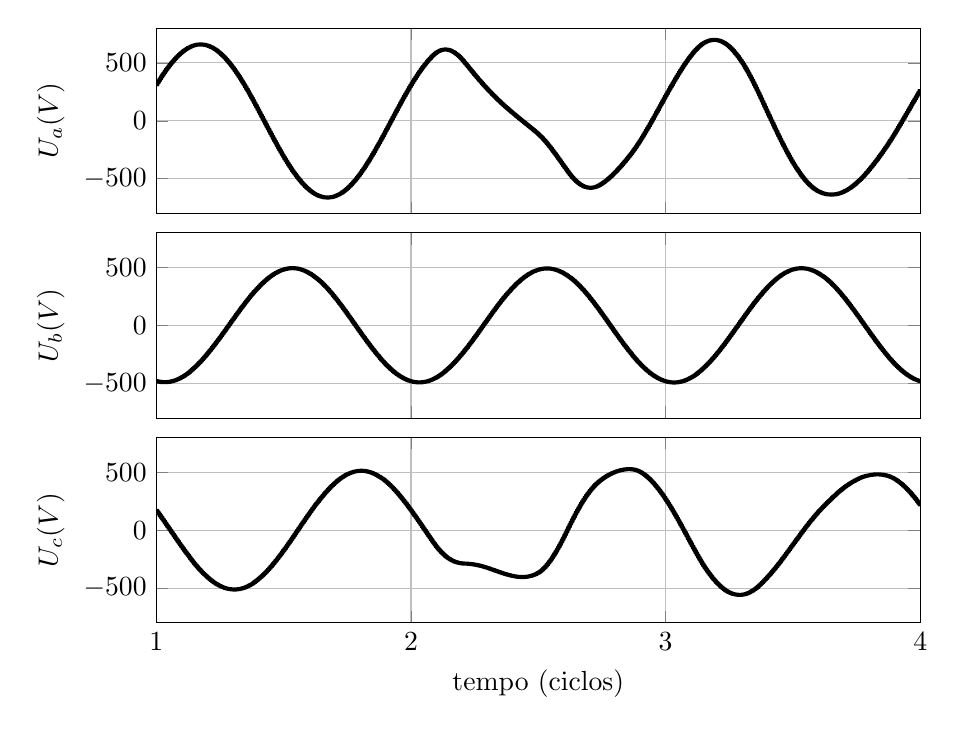
\begin{tikzpicture}

\begin{axis}[%
width=0.8\textwidth,
height=0.193917089240149\textwidth,
scale only axis,
xmin=0.0166666666666667,
xmax=0.0666666666666667,
xtick={0.0166666666666667,0.0333333333333333,0.05,0.0666666666666667},
xticklabels={\empty},
xmajorgrids,
ymin=-800,
ymax=800,
ytick={-500,    0,  500},
ylabel={$\text{U}_\text{b}\text{ (V)}$},
ymajorgrids,
name=plot2,
scaled x ticks = false,
legend columns=-1,
legend style={/tikz/every even column/.append style={column sep=0.3cm}},
legend style={font=\footnotesize}
]
\addplot [color=black,solid,line width=1.5pt,forget plot]
  table[row sep=crcr]{0.0166583333333333	-478.328989103039\\
0.0167	-481.372762295986\\
0.0167416666666667	-481.372762295986\\
0.0167833333333333	-483.944387417357\\
0.016825	-483.944387417357\\
0.0168666666666667	-486.043904769891\\
0.0169083333333333	-486.043904769891\\
0.01695	-487.669342075457\\
0.0169916666666667	-487.669342075457\\
0.0170333333333333	-488.81912329053\\
0.017075	-488.81912329053\\
0.0171166666666667	-489.492376222951\\
0.0171583333333333	-489.492376222951\\
0.0172	-489.689089295181\\
0.0172416666666667	-489.689089295181\\
0.0172833333333333	-489.410057478733\\
0.017325	-489.410057478733\\
0.0173666666666667	-488.656714544629\\
0.0174083333333333	-488.656714544629\\
0.01745	-487.430933830334\\
0.0174916666666667	-487.430933830334\\
0.0175333333333333	-485.734862735459\\
0.017575	-485.734862735459\\
0.0176166666666667	-483.570824107468\\
0.0176583333333333	-483.570824107468\\
0.0177	-480.941176730971\\
0.0177416666666667	-480.941176730971\\
0.0177833333333333	-477.848873406491\\
0.017825	-477.848873406491\\
0.0178666666666667	-474.296687037085\\
0.0179083333333333	-474.296687037085\\
0.01795	-470.287554266504\\
0.0179916666666667	-470.287554266504\\
0.0180333333333333	-465.824994538518\\
0.018075	-465.824994538518\\
0.0181166666666667	-460.912896166831\\
0.0181583333333333	-460.912896166831\\
0.0182	-455.555544349316\\
0.0182416666666667	-455.555544349316\\
0.0182833333333333	-449.757632700212\\
0.018325	-449.757632700212\\
0.0183666666666667	-443.524266807923\\
0.0184083333333333	-443.524266807923\\
0.01845	-436.860963041735\\
0.0184916666666667	-436.860963041735\\
0.0185333333333333	-429.773645406549\\
0.018575	-429.773645406549\\
0.0186166666666667	-422.2686421737\\
0.0186583333333333	-422.2686421737\\
0.0187	-414.352682994809\\
0.0187416666666667	-414.352682994809\\
0.0187833333333333	-406.710604021129\\
0.018825	-406.710604021129\\
0.0188666666666667	-396.968651829484\\
0.0189083333333333	-396.968651829484\\
0.01895	-387.24430030011\\
0.0189916666666667	-387.24430030011\\
0.0190333333333333	-377.413842111121\\
0.019075	-377.413842111121\\
0.0191166666666667	-367.3960735467\\
0.0191583333333333	-367.3960735467\\
0.0192	-357.12553953726\\
0.0192416666666667	-357.12553953726\\
0.0192833333333333	-346.559303382721\\
0.019325	-346.559303382721\\
0.0193666666666667	-335.674936708767\\
0.0194083333333333	-335.674936708767\\
0.01945	-324.465686057335\\
0.0194916666666667	-324.465686057335\\
0.0195333333333333	-312.935239244225\\
0.019575	-312.935239244225\\
0.0196166666666667	-301.093266862382\\
0.0196583333333333	-301.093266862382\\
0.0197	-288.95219973374\\
0.0197416666666667	-288.95219973374\\
0.0197833333333333	-276.525463982029\\
0.019825	-276.525463982029\\
0.0198666666666667	-263.82538033546\\
0.0199083333333333	-263.82538033546\\
0.01995	-250.865057706918\\
0.0199916666666667	-250.865057706918\\
0.0200333333333333	-237.656697428642\\
0.020075	-237.656697428642\\
0.0201166666666667	-224.212271375033\\
0.0201583333333333	-224.212271375033\\
0.0202	-210.543848998092\\
0.0202416666666667	-210.543848998092\\
0.0202833333333333	-196.6637735981\\
0.020325	-196.6637735981\\
0.0203666666666667	-182.584756063204\\
0.0204083333333333	-182.584756063204\\
0.02045	-168.319897946886\\
0.0204916666666667	-168.319897946886\\
0.0205333333333333	-153.882668002172\\
0.020575	-153.882668002172\\
0.0206166666666667	-139.286855686717\\
0.0206583333333333	-139.286855686717\\
0.0207	-124.546519243168\\
0.0207416666666667	-124.546519243168\\
0.0207833333333333	-109.675923407492\\
0.020825	-109.675923407492\\
0.0208666666666667	-94.6884951690301\\
0.0209083333333333	-94.6884951690301\\
0.02095	-79.6023211852309\\
0.0209916666666667	-79.6023211852309\\
0.0210333333333333	-64.4296541414652\\
0.021075	-64.4296541414652\\
0.0211166666666667	-49.1854677870168\\
0.0211583333333333	-49.1854677870168\\
0.0212	-33.8847697005379\\
0.0212416666666667	-33.8847697005379\\
0.0212833333333333	-18.5423320716325\\
0.021325	-18.5423320716325\\
0.0213666666666667	-3.1725945533516\\
0.0214083333333333	-3.1725945533516\\
0.02145	12.2102617721841\\
0.0214916666666667	12.2102617721841\\
0.0215333333333333	27.5921432856442\\
0.021575	27.5921432856442\\
0.0216166666666667	42.9588704890498\\
0.0216583333333333	42.9588704890498\\
0.0217	58.2960537853681\\
0.0217416666666667	58.2960537853681\\
0.0217833333333333	73.5890384864759\\
0.021825	73.5890384864759\\
0.0218666666666667	88.82269659409\\
0.0219083333333333	88.82269659409\\
0.02195	103.982669291038\\
0.0219916666666667	103.982669291038\\
0.0220333333333333	119.053037141893\\
0.022075	119.053037141893\\
0.0221166666666667	134.01853586672\\
0.0221583333333333	134.01853586672\\
0.0222	148.863909368128\\
0.0222416666666667	148.863909368128\\
0.0222833333333333	163.573956427556\\
0.022325	163.573956427556\\
0.0223666666666667	178.133568427636\\
0.0224083333333333	178.133568427636\\
0.02245	192.527757716713\\
0.0224916666666667	192.527757716713\\
0.0225333333333333	206.741679404245\\
0.022575	206.741679404245\\
0.0226166666666667	220.760649670751\\
0.0226583333333333	220.760649670751\\
0.0227	234.570162946369\\
0.0227416666666667	234.570162946369\\
0.0227833333333333	248.155909263895\\
0.022825	248.155909263895\\
0.0228666666666667	261.687830320942\\
0.0229083333333333	261.687830320942\\
0.02295	274.986604079196\\
0.0229916666666667	274.986604079196\\
0.0230333333333333	286.928801747272\\
0.023075	286.928801747272\\
0.0231166666666667	298.950506950644\\
0.0231583333333333	298.950506950644\\
0.0232	310.924864102034\\
0.0232416666666667	310.924864102034\\
0.0232833333333333	322.756989832147\\
0.023325	322.756989832147\\
0.0233666666666667	334.367084014297\\
0.0234083333333333	334.367084014297\\
0.02345	345.69602196514\\
0.0234916666666667	345.69602196514\\
0.0235333333333333	356.703461032175\\
0.023575	356.703461032175\\
0.0236166666666667	367.363371170442\\
0.0236583333333333	367.363371170442\\
0.0237	377.659204280424\\
0.0237416666666667	377.659204280424\\
0.0237833333333333	387.579795487262\\
0.023825	387.579795487262\\
0.0238666666666667	397.116425283701\\
0.0239083333333333	397.116425283701\\
0.02395	406.261310362139\\
0.0239916666666667	406.261310362139\\
0.0240333333333333	415.0053223807\\
0.024075	415.0053223807\\
0.0241166666666667	423.340732147141\\
0.0241583333333333	423.340732147141\\
0.0242	431.258683016742\\
0.0242416666666667	431.258683016742\\
0.0242833333333333	438.750365395371\\
0.024325	438.750365395371\\
0.0243666666666667	445.807262831054\\
0.0244083333333333	445.807262831054\\
0.02445	452.421342397773\\
0.0244916666666667	452.421342397773\\
0.0245333333333333	458.585161293933\\
0.024575	458.585161293933\\
0.0246166666666667	464.291905294308\\
0.0246583333333333	464.291905294308\\
0.0247	469.535383109734\\
0.0247416666666667	469.535383109734\\
0.0247833333333333	474.309999446141\\
0.024825	474.309999446141\\
0.0248666666666667	478.610723480444\\
0.0249083333333333	478.610723480444\\
0.02495	482.432523836755\\
0.0249916666666667	482.432523836755\\
0.0250333333333333	485.772612186125\\
0.025075	485.772612186125\\
0.0251166666666667	488.627883686145\\
0.0251583333333333	488.627883686145\\
0.0252	490.994391489966\\
0.0252416666666667	490.994391489966\\
0.0252833333333333	492.869784189106\\
0.025325	492.869784189106\\
0.0253666666666667	494.252063559781\\
0.0254083333333333	494.252063559781\\
0.02545	495.139387583695\\
0.0254916666666667	495.139387583695\\
0.0255333333333333	495.530061759552\\
0.025575	495.530061759552\\
0.0256166666666667	495.422663936061\\
0.0256583333333333	495.422663936061\\
0.0257	494.816230581684\\
0.0257416666666667	494.816230581684\\
0.0257833333333333	493.710425995119\\
0.025825	493.710425995119\\
0.0258666666666667	492.105654148384\\
0.0259083333333333	492.105654148384\\
0.02595	490.003108134894\\
0.0259916666666667	490.003108134894\\
0.0260333333333333	487.404961487327\\
0.026075	487.404961487327\\
0.0261166666666667	484.313069214194\\
0.0261583333333333	484.313069214194\\
0.0262	480.731558886196\\
0.0262416666666667	480.731558886196\\
0.0262833333333333	476.664323712434\\
0.026325	476.664323712434\\
0.0263666666666667	472.115829454631\\
0.0264083333333333	472.115829454631\\
0.02645	467.091068733291\\
0.0264916666666667	467.091068733291\\
0.0265333333333333	461.595540479995\\
0.026575	461.595540479995\\
0.0266166666666667	455.635234907076\\
0.0266583333333333	455.635234907076\\
0.0267	449.21662231492\\
0.0267416666666667	449.21662231492\\
0.0267833333333333	442.346643428456\\
0.026825	442.346643428456\\
0.0268666666666667	435.032699614098\\
0.0269083333333333	435.032699614098\\
0.02695	427.282642172915\\
0.0269916666666667	427.282642172915\\
0.0270333333333333	418.527982244731\\
0.027075	418.527982244731\\
0.0271166666666667	410.672570182659\\
0.0271583333333333	410.672570182659\\
0.0272	402.276872290978\\
0.0272416666666667	402.276872290978\\
0.0272833333333333	393.223850223727\\
0.027325	393.223850223727\\
0.0273666666666667	383.609151155178\\
0.0274083333333333	383.609151155178\\
0.02745	373.508718653929\\
0.0274916666666667	373.508718653929\\
0.0275333333333333	362.979579538073\\
0.027575	362.979579538073\\
0.0276166666666667	352.061894709897\\
0.0276583333333333	352.061894709897\\
0.0277	340.783205444461\\
0.0277416666666667	340.783205444461\\
0.0277833333333333	329.162781541968\\
0.027825	329.162781541968\\
0.0278666666666667	317.215226351439\\
0.0279083333333333	317.215226351439\\
0.02795	304.953068995059\\
0.0279916666666667	304.953068995059\\
0.0280333333333333	292.388308765939\\
0.028075	292.388308765939\\
0.0281166666666667	279.533394256386\\
0.0281583333333333	279.533394256386\\
0.0282	266.401997020689\\
0.0282416666666667	266.401997020689\\
0.0282833333333333	253.007121767018\\
0.028325	253.007121767018\\
0.0283666666666667	239.363037342399\\
0.0284083333333333	239.363037342399\\
0.02845	225.484309796947\\
0.0284916666666667	225.484309796947\\
0.0285333333333333	211.385672071801\\
0.028575	211.385672071801\\
0.0286166666666667	197.081935254737\\
0.0286583333333333	197.081935254737\\
0.0287	182.587950486431\\
0.0287416666666667	182.587950486431\\
0.0287833333333333	167.918604082923\\
0.028825	167.918604082923\\
0.0288666666666667	153.088829011011\\
0.0289083333333333	153.088829011011\\
0.02895	138.113619934855\\
0.0289916666666667	138.113619934855\\
0.0290333333333333	123.008044204917\\
0.029075	123.008044204917\\
0.0291166666666667	107.788100944899\\
0.0291583333333333	107.788100944899\\
0.0292	92.4664220892656\\
0.0292416666666667	92.4664220892656\\
0.0292833333333333	77.0599110293703\\
0.029325	77.0599110293703\\
0.0293666666666667	61.5839402726698\\
0.0294083333333333	61.5839402726698\\
0.02945	46.0538191073489\\
0.0294916666666667	46.0538191073489\\
0.0295333333333333	30.4851141949034\\
0.029575	30.4851141949034\\
0.0296166666666667	14.8937682112207\\
0.0296583333333333	14.8937682112207\\
0.0297	-0.703957306529608\\
0.0297416666666667	-0.703957306529608\\
0.0297833333333333	-16.2916492298269\\
0.029825	-16.2916492298269\\
0.0298666666666667	-31.8529362123827\\
0.0299083333333333	-31.8529362123827\\
0.02995	-47.371649369948\\
0.0299916666666667	-47.371649369948\\
0.0300333333333333	-62.8319222299047\\
0.030075	-62.8319222299047\\
0.0301166666666667	-78.2183969102601\\
0.0301583333333333	-78.2183969102601\\
0.0302	-93.5154108314719\\
0.0302416666666667	-93.5154108314719\\
0.0302833333333333	-108.70816278091\\
0.030325	-108.70816278091\\
0.0303666666666667	-123.782356080195\\
0.0304083333333333	-123.782356080195\\
0.03045	-138.723507249364\\
0.0304916666666667	-138.723507249364\\
0.0305333333333333	-153.517339096442\\
0.030575	-153.517339096442\\
0.0306166666666667	-168.149764544084\\
0.0306583333333333	-168.149764544084\\
0.0307	-182.60688669631\\
0.0307416666666667	-182.60688669631\\
0.0307833333333333	-196.875004412733\\
0.030825	-196.875004412733\\
0.0308666666666667	-210.940621254231\\
0.0309083333333333	-210.940621254231\\
0.03095	-224.790455634942\\
0.0309916666666667	-224.790455634942\\
0.0310333333333333	-238.411450801645\\
0.031075	-238.411450801645\\
0.0311166666666667	-251.788204920739\\
0.0311583333333333	-251.788204920739\\
0.0312	-264.319493294975\\
0.0312416666666667	-264.319493294975\\
0.0312833333333333	-278.081845363642\\
0.031325	-278.081845363642\\
0.0313666666666667	-291.211888263673\\
0.0314083333333333	-291.211888263673\\
0.03145	-303.807007713181\\
0.0314916666666667	-303.807007713181\\
0.0315333333333333	-315.936364357588\\
0.031575	-315.936364357588\\
0.0316166666666667	-327.655020751537\\
0.0316583333333333	-327.655020751537\\
0.0317	-338.998550237152\\
0.0317416666666667	-338.998550237152\\
0.0317833333333333	-349.984949605885\\
0.031825	-349.984949605885\\
0.0318666666666667	-360.618974262017\\
0.0319083333333333	-360.618974262017\\
0.03195	-370.896795074955\\
0.0319916666666667	-370.896795074955\\
0.0320333333333333	-380.809923421548\\
0.032075	-380.809923421548\\
0.0321166666666667	-390.348041070204\\
0.0321583333333333	-390.348041070204\\
0.0322	-399.500455565927\\
0.0322416666666667	-399.500455565927\\
0.0322833333333333	-408.258433783543\\
0.032325	-408.258433783543\\
0.0323666666666667	-416.612673979994\\
0.0324083333333333	-416.612673979994\\
0.03245	-424.555376388038\\
0.0324916666666667	-424.555376388038\\
0.0325333333333333	-432.079651399668\\
0.032575	-432.079651399668\\
0.0326166666666667	-439.17912856472\\
0.0326583333333333	-439.17912856472\\
0.0327	-445.847803165625\\
0.0327416666666667	-445.847803165625\\
0.0327833333333333	-452.079952433882\\
0.032825	-452.079952433882\\
0.0328666666666667	-457.870112681898\\
0.0329083333333333	-457.870112681898\\
0.03295	-463.213095942823\\
0.0329916666666667	-463.213095942823\\
0.0330333333333333	-468.104025539882\\
0.033075	-468.104025539882\\
0.0331166666666667	-472.538375275198\\
0.0331583333333333	-472.538375275198\\
0.0332	-476.512043591712\\
0.0332416666666667	-476.512043591712\\
0.0332833333333333	-480.021998518076\\
0.033325	-480.021998518076\\
0.0333666666666667	-483.062409528906\\
0.0334083333333333	-483.062409528906\\
0.03345	-485.632179354782\\
0.0334916666666667	-485.632179354782\\
0.0335333333333333	-487.728811385411\\
0.033575	-487.728811385411\\
0.0336166666666667	-489.350303992202\\
0.0336583333333333	-489.350303992202\\
0.0337	-490.495382636273\\
0.0337416666666667	-490.495382636273\\
0.0337833333333333	-491.163571670944\\
0.033825	-491.163571670944\\
0.0338666666666667	-491.355115539431\\
0.0339083333333333	-491.355115539431\\
0.03395	-491.070817444326\\
0.0339916666666667	-491.070817444326\\
0.0340333333333333	-490.311872482351\\
0.034075	-490.311872482351\\
0.0341166666666667	-489.079743497884\\
0.0341583333333333	-489.079743497884\\
0.0342	-487.376098124238\\
0.0342416666666667	-487.376098124238\\
0.0342833333333333	-485.20249992764\\
0.034325	-485.20249992764\\
0.0343666666666667	-482.562089146938\\
0.0344083333333333	-482.562089146938\\
0.03445	-479.456339884062\\
0.0344916666666667	-479.456339884062\\
0.0345333333333333	-475.887666587193\\
0.034575	-475.887666587193\\
0.0346166666666667	-471.862477669189\\
0.0346583333333333	-471.862477669189\\
0.0347	-467.386376616343\\
0.0347416666666667	-467.386376616343\\
0.0347833333333333	-462.460204193963\\
0.034825	-462.460204193963\\
0.0348666666666667	-457.084993467022\\
0.0349083333333333	-457.084993467022\\
0.03495	-451.264285123146\\
0.0349916666666667	-451.264285123146\\
0.0350333333333333	-445.003485871476\\
0.035075	-445.003485871476\\
0.0351166666666667	-438.309126556655\\
0.0351583333333333	-438.309126556655\\
0.0352	-431.188237094164\\
0.0352416666666667	-431.188237094164\\
0.0352833333333333	-423.843217345319\\
0.035325	-423.843217345319\\
0.0353666666666667	-416.006961069986\\
0.0354083333333333	-416.006961069986\\
0.03545	-406.872705407128\\
0.0354916666666667	-406.872705407128\\
0.0355333333333333	-397.652348142447\\
0.035575	-397.652348142447\\
0.0356166666666667	-388.257619044804\\
0.0356583333333333	-388.257619044804\\
0.0357	-378.623360239847\\
0.0357416666666667	-378.623360239847\\
0.0357833333333333	-368.698593317024\\
0.035825	-368.698593317024\\
0.0358666666666667	-358.451057487075\\
0.0359083333333333	-358.451057487075\\
0.03595	-347.865419222676\\
0.0359916666666667	-347.865419222676\\
0.0360333333333333	-336.939196124305\\
0.036075	-336.939196124305\\
0.0361166666666667	-325.678369718751\\
0.0361583333333333	-325.678369718751\\
0.0362	-314.093684159792\\
0.0362416666666667	-314.093684159792\\
0.0362833333333333	-302.19760657953\\
0.036325	-302.19760657953\\
0.0363666666666667	-290.003073678589\\
0.0364083333333333	-290.003073678589\\
0.03645	-277.521539253932\\
0.0364916666666667	-277.521539253932\\
0.0365333333333333	-264.76677178694\\
0.036575	-264.76677178694\\
0.0366166666666667	-251.75138810459\\
0.0366583333333333	-251.75138810459\\
0.0367	-238.484219164876\\
0.0367416666666667	-238.484219164876\\
0.0367833333333333	-224.974868835818\\
0.036825	-224.974868835818\\
0.0368666666666667	-211.237477773964\\
0.0369083333333333	-211.237477773964\\
0.03695	-197.287072811055\\
0.0369916666666667	-197.287072811055\\
0.0370333333333333	-183.137914989065\\
0.037075	-183.137914989065\\
0.0371166666666667	-168.803978576591\\
0.0371583333333333	-168.803978576591\\
0.0372	-154.298661037236\\
0.0372416666666667	-154.298661037236\\
0.0372833333333333	-139.634992651273\\
0.037325	-139.634992651273\\
0.0373666666666667	-124.826036658058\\
0.0374083333333333	-124.826036658058\\
0.03745	-109.886448376808\\
0.0374916666666667	-109.886448376808\\
0.0375333333333333	-94.8311105238512\\
0.037575	-94.8311105238512\\
0.0376166666666667	-79.6741457005464\\
0.0376583333333333	-79.6741457005464\\
0.0377	-64.430915589704\\
0.0377416666666667	-64.430915589704\\
0.0377833333333333	-49.1168958380644\\
0.037825	-49.1168958380644\\
0.0378666666666667	-33.7474109692533\\
0.0379083333333333	-33.7474109692533\\
0.03795	-18.3375525391689\\
0.0379916666666667	-18.3375525391689\\
0.0380333333333333	-2.9021014951139\\
0.038075	-2.9021014951139\\
0.0381166666666667	12.5441649238791\\
0.0381583333333333	12.5441649238791\\
0.0382	27.9862135071296\\
0.0382416666666667	27.9862135071296\\
0.0382833333333333	43.4088160189249\\
0.038325	43.4088160189249\\
0.0383666666666667	58.7964709733482\\
0.0384083333333333	58.7964709733482\\
0.03845	74.1332705553863\\
0.0384916666666667	74.1332705553863\\
0.0385333333333333	89.4046588216954\\
0.038575	89.4046588216954\\
0.0386166666666667	104.5941845202\\
0.0386583333333333	104.5941845202\\
0.0387	119.686452596076\\
0.0387416666666667	119.686452596076\\
0.0387833333333333	134.66627355262\\
0.038825	134.66627355262\\
0.0388666666666667	149.518283336125\\
0.0389083333333333	149.518283336125\\
0.03895	164.226788249997\\
0.0389916666666667	164.226788249997\\
0.0390333333333333	178.776134246639\\
0.039075	178.776134246639\\
0.0391166666666667	193.150979209617\\
0.0391583333333333	193.150979209617\\
0.0392	207.336383906119\\
0.0392416666666667	207.336383906119\\
0.0392833333333333	221.317782891681\\
0.039325	221.317782891681\\
0.0393666666666667	235.080917713056\\
0.0394083333333333	235.080917713056\\
0.03945	249.106017709465\\
0.0394916666666667	249.106017709465\\
0.0395333333333333	261.782981387672\\
0.039575	261.782981387672\\
0.0396166666666667	274.244693954053\\
0.0396583333333333	274.244693954053\\
0.0397	286.670435385755\\
0.0397416666666667	286.670435385755\\
0.0397833333333333	298.9701138084\\
0.039825	298.9701138084\\
0.0398666666666667	311.070470544628\\
0.0399083333333333	311.070470544628\\
0.03995	322.915197067812\\
0.0399916666666667	322.915197067812\\
0.0400333333333333	334.464145520092\\
0.040075	334.464145520092\\
0.0401166666666667	345.689797905232\\
0.0401583333333333	345.689797905232\\
0.0402	356.573569549156\\
0.0402416666666667	356.573569549156\\
0.0402833333333333	367.102419833383\\
0.040325	367.102419833383\\
0.0403666666666667	377.266336550431\\
0.0404083333333333	377.266336550431\\
0.04045	387.056723613013\\
0.0404916666666667	387.056723613013\\
0.0405333333333333	396.465185002339\\
0.040575	396.465185002339\\
0.0406166666666667	405.482553450114\\
0.0406583333333333	405.482553450114\\
0.0407	414.100873536397\\
0.0407416666666667	414.100873536397\\
0.0407833333333333	422.311068387454\\
0.040825	422.311068387454\\
0.0408666666666667	430.103823202378\\
0.0409083333333333	430.103823202378\\
0.04095	437.470785539434\\
0.0409916666666667	437.470785539434\\
0.0410333333333333	444.404904032625\\
0.041075	444.404904032625\\
0.0411166666666667	450.899745696091\\
0.0411583333333333	450.899745696091\\
0.0412	456.949290210676\\
0.0412416666666667	456.949290210676\\
0.0412833333333333	462.548172385588\\
0.041325	462.548172385588\\
0.0413666666666667	467.690509791918\\
0.0414083333333333	467.690509791918\\
0.04145	472.368093229522\\
0.0414916666666667	472.368093229522\\
0.0415333333333333	476.574672015731\\
0.041575	476.574672015731\\
0.0416166666666667	480.310156693439\\
0.0416583333333333	480.310156693439\\
0.0417	483.572332768667\\
0.0417416666666667	483.572332768667\\
0.0417833333333333	486.359289598516\\
0.041825	486.359289598516\\
0.0418666666666667	488.668565715516\\
0.0419083333333333	488.668565715516\\
0.04195	490.497331626202\\
0.0419916666666667	490.497331626202\\
0.0420333333333333	491.842670843953\\
0.042075	491.842670843953\\
0.0421166666666667	492.699071140014\\
0.0421583333333333	492.699071140014\\
0.0422	493.068619758159\\
0.0422416666666667	493.068619758159\\
0.0422833333333333	492.952466583921\\
0.042325	492.952466583921\\
0.0423666666666667	492.347367558496\\
0.0424083333333333	492.347367558496\\
0.04245	491.252031478426\\
0.0424916666666667	491.252031478426\\
0.0425333333333333	489.667385633026\\
0.042575	489.667385633026\\
0.0426166666666667	487.594910620982\\
0.0426583333333333	487.594910620982\\
0.0427	485.037655582358\\
0.0427416666666667	485.037655582358\\
0.0427833333333333	481.999497712266\\
0.042825	481.999497712266\\
0.0428666666666667	478.483785993532\\
0.0429083333333333	478.483785993532\\
0.04295	474.494421900634\\
0.0429916666666667	474.494421900634\\
0.0430333333333333	470.035506802172\\
0.043075	470.035506802172\\
0.0431166666666667	465.111295250602\\
0.0431583333333333	465.111295250602\\
0.0432	459.726505545849\\
0.0432416666666667	459.726505545849\\
0.0432833333333333	453.886192967286\\
0.043325	453.886192967286\\
0.0433666666666667	447.595582698072\\
0.0434083333333333	447.595582698072\\
0.04345	440.861630320738\\
0.0434916666666667	440.861630320738\\
0.0435333333333333	433.681731049463\\
0.043575	433.681731049463\\
0.0436166666666667	425.580511912541\\
0.0436583333333333	425.580511912541\\
0.0437	418.359521795389\\
0.0437416666666667	418.359521795389\\
0.0437833333333333	410.424839442397\\
0.043825	410.424839442397\\
0.0438666666666667	401.856433443567\\
0.0439083333333333	401.856433443567\\
0.04395	392.738907245265\\
0.0439916666666667	392.738907245265\\
0.0440333333333333	383.143262572768\\
0.044075	383.143262572768\\
0.0441166666666667	373.122289947879\\
0.0441583333333333	373.122289947879\\
0.0442	362.712148769228\\
0.0442416666666667	362.712148769228\\
0.0442833333333333	351.936466122906\\
0.044325	351.936466122906\\
0.0443666666666667	340.81070596891\\
0.0444083333333333	340.81070596891\\
0.04445	329.346076655623\\
0.0444916666666667	329.346076655623\\
0.0445333333333333	317.552138040485\\
0.044575	317.552138040485\\
0.0446166666666667	305.438801181686\\
0.0446583333333333	305.438801181686\\
0.0447	293.018741534484\\
0.0447416666666667	293.018741534484\\
0.0447833333333333	280.303286512468\\
0.044825	280.303286512468\\
0.0448666666666667	267.304839178201\\
0.0449083333333333	267.304839178201\\
0.04495	254.036587804692\\
0.0449916666666667	254.036587804692\\
0.0450333333333333	240.512194679208\\
0.045075	240.512194679208\\
0.0451166666666667	226.745693466081\\
0.0451583333333333	226.745693466081\\
0.0452	212.751335137093\\
0.0452416666666667	212.751335137093\\
0.0452833333333333	198.543785808771\\
0.045325	198.543785808771\\
0.0453666666666667	184.137961271205\\
0.0454083333333333	184.137961271205\\
0.04545	169.549083751309\\
0.0454916666666667	169.549083751309\\
0.0455333333333333	154.791278668457\\
0.045575	154.791278668457\\
0.0456166666666667	139.877896565075\\
0.0456583333333333	139.877896565075\\
0.0457	124.824761922009\\
0.0457416666666667	124.824761922009\\
0.0457833333333333	109.646732276147\\
0.045825	109.646732276147\\
0.0458666666666667	94.3613000585707\\
0.0459083333333333	94.3613000585707\\
0.04595	78.9840886019565\\
0.0459916666666667	78.9840886019565\\
0.0460333333333333	63.5303702887837\\
0.046075	63.5303702887837\\
0.0461166666666667	48.0155535189244\\
0.0461583333333333	48.0155535189244\\
0.0462	32.4561326759275\\
0.0462416666666667	32.4561326759275\\
0.0462833333333333	16.8700891761257\\
0.046325	16.8700891761257\\
0.0463666666666667	1.26865974731029\\
0.0464083333333333	1.26865974731029\\
0.04645	-14.3325199650595\\
0.0464916666666667	-14.3325199650595\\
0.0465333333333333	-29.9131132460085\\
0.046575	-29.9131132460085\\
0.0466166666666667	-45.4562368559247\\
0.0466583333333333	-45.4562368559247\\
0.0467	-60.9463194667191\\
0.0467416666666667	-60.9463194667191\\
0.0467833333333333	-76.3667309691358\\
0.046825	-76.3667309691358\\
0.0468666666666667	-91.7034974678986\\
0.0469083333333333	-91.7034974678986\\
0.04695	-106.941680966748\\
0.0469916666666667	-106.941680966748\\
0.0470333333333333	-122.066146305108\\
0.047075	-122.066146305108\\
0.0471166666666667	-137.06188382755\\
0.0471583333333333	-137.06188382755\\
0.0472	-151.913815267241\\
0.0472416666666667	-151.913815267241\\
0.0472833333333333	-166.607053394949\\
0.047325	-166.607053394949\\
0.0473666666666667	-181.127077064277\\
0.0474083333333333	-181.127077064277\\
0.04745	-195.459743543001\\
0.0474916666666667	-195.459743543001\\
0.0475333333333333	-209.591362819321\\
0.047575	-209.591362819321\\
0.0476166666666667	-223.506823346012\\
0.0476583333333333	-223.506823346012\\
0.0477	-237.00101652442\\
0.0477416666666667	-237.00101652442\\
0.0477833333333333	-250.375370605446\\
0.047825	-250.375370605446\\
0.0478666666666667	-264.247228944917\\
0.0479083333333333	-264.247228944917\\
0.04795	-277.57583918717\\
0.0479916666666667	-277.57583918717\\
0.0480333333333333	-290.432998246762\\
0.048075	-290.432998246762\\
0.0481166666666667	-302.874898420103\\
0.0481583333333333	-302.874898420103\\
0.0482	-314.943125188458\\
0.0482416666666667	-314.943125188458\\
0.0482833333333333	-326.662290446261\\
0.048325	-326.662290446261\\
0.0483666666666667	-338.042278959217\\
0.0484083333333333	-338.042278959217\\
0.04845	-349.082657598953\\
0.0484916666666667	-349.082657598953\\
0.0485333333333333	-359.776933252618\\
0.048575	-359.776933252618\\
0.0486166666666667	-370.115682517757\\
0.0486583333333333	-370.115682517757\\
0.0487	-380.088397551359\\
0.0487416666666667	-380.088397551359\\
0.0487833333333333	-389.684585375337\\
0.048825	-389.684585375337\\
0.0488666666666667	-398.896409543848\\
0.0489083333333333	-398.896409543848\\
0.04895	-407.713702687894\\
0.0489916666666667	-407.713702687894\\
0.0490333333333333	-416.128294513139\\
0.049075	-416.128294513139\\
0.0491166666666667	-424.133317051478\\
0.0491583333333333	-424.133317051478\\
0.0492	-431.722331990266\\
0.0492416666666667	-431.722331990266\\
0.0492833333333333	-438.889026645031\\
0.049325	-438.889026645031\\
0.0493666666666667	-445.627341957187\\
0.0494083333333333	-445.627341957187\\
0.04945	-451.931076637639\\
0.0494916666666667	-451.931076637639\\
0.0495333333333333	-457.794069196784\\
0.049575	-457.794069196784\\
0.0496166666666667	-463.210591616737\\
0.0496583333333333	-463.210591616737\\
0.0497	-468.174796015772\\
0.0497416666666667	-468.174796015772\\
0.0497833333333333	-472.68195994869\\
0.049825	-472.68195994869\\
0.0498666666666667	-476.727789100183\\
0.0499083333333333	-476.727789100183\\
0.04995	-480.308346767437\\
0.0499916666666667	-480.308346767437\\
0.0500333333333333	-483.420977339502\\
0.050075	-483.420977339502\\
0.0501166666666667	-486.062497335619\\
0.0501583333333333	-486.062497335619\\
0.0502	-488.230133182561\\
0.0502416666666667	-488.230133182561\\
0.0502833333333333	-489.921561624727\\
0.050325	-489.921561624727\\
0.0503666666666667	-491.136204240014\\
0.0504083333333333	-491.136204240014\\
0.05045	-491.872508123106\\
0.0504916666666667	-491.872508123106\\
0.0505333333333333	-492.129861840952\\
0.050575	-492.129861840952\\
0.0506166666666667	-491.909659809047\\
0.0506583333333333	-491.909659809047\\
0.0507	-491.213010719094\\
0.0507416666666667	-491.213010719094\\
0.0507833333333333	-490.040835198961\\
0.050825	-490.040835198961\\
0.0508666666666667	-488.394120133251\\
0.0509083333333333	-488.394120133251\\
0.05095	-486.275366201401\\
0.0509916666666667	-486.275366201401\\
0.0510333333333333	-483.685389331488\\
0.051075	-483.685389331488\\
0.0511166666666667	-480.626415285703\\
0.0511583333333333	-480.626415285703\\
0.0512	-477.100789926303\\
0.0512416666666667	-477.100789926303\\
0.0512833333333333	-473.111388437613\\
0.051325	-473.111388437613\\
0.0513666666666667	-468.661612023946\\
0.0514083333333333	-468.661612023946\\
0.05145	-463.755404955367\\
0.0514916666666667	-463.755404955367\\
0.0515333333333333	-458.397218599947\\
0.051575	-458.397218599947\\
0.0516166666666667	-452.591883879653\\
0.0516583333333333	-452.591883879653\\
0.0517	-446.344659833732\\
0.0517416666666667	-446.344659833732\\
0.0517833333333333	-439.661834530548\\
0.051825	-439.661834530548\\
0.0518666666666667	-432.973201373906\\
0.0519083333333333	-432.973201373906\\
0.05195	-424.9238177607\\
0.0519916666666667	-424.9238177607\\
0.0520333333333333	-416.454872243868\\
0.052075	-416.454872243868\\
0.0521166666666667	-407.796123452613\\
0.0521583333333333	-407.796123452613\\
0.0522	-398.881834393278\\
0.0522416666666667	-398.881834393278\\
0.0522833333333333	-389.663103951547\\
0.052325	-389.663103951547\\
0.0523666666666667	-380.109879074884\\
0.0524083333333333	-380.109879074884\\
0.05245	-370.205171386402\\
0.0524916666666667	-370.205171386402\\
0.0525333333333333	-359.94008009255\\
0.052575	-359.94008009255\\
0.0526166666666667	-349.317994044045\\
0.0526583333333333	-349.317994044045\\
0.0527	-338.350133889017\\
0.0527416666666667	-338.350133889017\\
0.0527833333333333	-327.048470451454\\
0.052825	-327.048470451454\\
0.0528666666666667	-315.424680843599\\
0.0529083333333333	-315.424680843599\\
0.05295	-303.48972268604\\
0.0529916666666667	-303.48972268604\\
0.0530333333333333	-291.253697717625\\
0.053075	-291.253697717625\\
0.0531166666666667	-278.729847006983\\
0.0531583333333333	-278.729847006983\\
0.0532	-265.929627652681\\
0.0532416666666667	-265.929627652681\\
0.0532833333333333	-252.864003527286\\
0.053325	-252.864003527286\\
0.0533666666666667	-239.545390879813\\
0.0534083333333333	-239.545390879813\\
0.05345	-225.986736413012\\
0.0534916666666667	-225.986736413012\\
0.0535333333333333	-212.200997373425\\
0.053575	-212.200997373425\\
0.0536166666666667	-198.20178050543\\
0.0536583333333333	-198.20178050543\\
0.0537	-184.002976664328\\
0.0537416666666667	-184.002976664328\\
0.0537833333333333	-169.618777516532\\
0.053825	-169.618777516532\\
0.0538666666666667	-155.063258633972\\
0.0539083333333333	-155.063258633972\\
0.05395	-140.350010974899\\
0.0539916666666667	-140.350010974899\\
0.0540333333333333	-125.494490383426\\
0.054075	-125.494490383426\\
0.0541166666666667	-110.510483878359\\
0.0541583333333333	-110.510483878359\\
0.0542	-95.41256883096\\
0.0542416666666667	-95.41256883096\\
0.0542833333333333	-80.2157610667614\\
0.054325	-80.2157610667614\\
0.0543666666666667	-64.9345150980876\\
0.0544083333333333	-64.9345150980876\\
0.05445	-49.582007143794\\
0.0544916666666667	-49.582007143794\\
0.0545333333333333	-34.1736602074678\\
0.054575	-34.1736602074678\\
0.0546166666666667	-18.7290780256136\\
0.0546583333333333	-18.7290780256136\\
0.0547	-3.26173930788178\\
0.0547416666666667	-3.26173930788178\\
0.0547833333333333	12.2173123034477\\
0.054825	12.2173123034477\\
0.0548666666666667	27.6939042936501\\
0.0549083333333333	27.6939042936501\\
0.05495	43.1527392039165\\
0.0549916666666667	43.1527392039165\\
0.0550333333333333	58.5788251481509\\
0.055075	58.5788251481509\\
0.0551166666666667	73.9562327104943\\
0.0551583333333333	73.9562327104943\\
0.0552	89.2687363785002\\
0.0552416666666667	89.2687363785002\\
0.0552833333333333	104.500594808725\\
0.055325	104.500594808725\\
0.0553666666666667	119.636116228614\\
0.0554083333333333	119.636116228614\\
0.05545	134.66002337835\\
0.0554916666666667	134.66002337835\\
0.0555333333333333	149.557265295072\\
0.055575	149.557265295072\\
0.0556166666666667	164.312975721939\\
0.0556583333333333	164.312975721939\\
0.0557	178.912414426348\\
0.0557416666666667	178.912414426348\\
0.0557833333333333	193.340869617833\\
0.055825	193.340869617833\\
0.0558666666666667	207.584047711812\\
0.0559083333333333	207.584047711812\\
0.05595	221.649592508348\\
0.0559916666666667	221.649592508348\\
0.0560333333333333	235.90179407268\\
0.056075	235.90179407268\\
0.0561166666666667	248.812050467668\\
0.0561583333333333	248.812050467668\\
0.0562	261.728072869779\\
0.0562416666666667	261.728072869779\\
0.0562833333333333	274.589043397849\\
0.056325	274.589043397849\\
0.0563666666666667	287.31251086188\\
0.0564083333333333	287.31251086188\\
0.05645	299.831678661534\\
0.0564916666666667	299.831678661534\\
0.0565333333333333	312.096762723358\\
0.056575	312.096762723358\\
0.0566166666666667	324.069560647856\\
0.0566583333333333	324.069560647856\\
0.0567	335.722240967018\\
0.0567416666666667	335.722240967018\\
0.0567833333333333	347.040245671561\\
0.056825	347.040245671561\\
0.0568666666666667	358.013968498111\\
0.0569083333333333	358.013968498111\\
0.05695	368.633291023524\\
0.0569916666666667	368.633291023524\\
0.0570333333333333	378.888273019104\\
0.057075	378.888273019104\\
0.0571166666666667	388.767403823566\\
0.0571583333333333	388.767403823566\\
0.0572	398.261089815887\\
0.0572416666666667	398.261089815887\\
0.0572833333333333	407.360397631016\\
0.057325	407.360397631016\\
0.0573666666666667	416.054641235888\\
0.0574083333333333	416.054641235888\\
0.05745	424.333358541391\\
0.0574916666666667	424.333358541391\\
0.0575333333333333	432.187892531853\\
0.057575	432.187892531853\\
0.0576166666666667	439.609718478329\\
0.0576583333333333	439.609718478329\\
0.0577	446.59114928807\\
0.0577416666666667	446.59114928807\\
0.0577833333333333	453.125291550232\\
0.057825	453.125291550232\\
0.0578666666666667	459.205492698452\\
0.0579083333333333	459.205492698452\\
0.05795	464.826013093453\\
0.0579916666666667	464.826013093453\\
0.0580333333333333	469.980808563756\\
0.058075	469.980808563756\\
0.0581166666666667	474.663968749913\\
0.0581583333333333	474.663968749913\\
0.0582	478.872042176142\\
0.0582416666666667	478.872042176142\\
0.0582833333333333	482.600041203607\\
0.058325	482.600041203607\\
0.0583666666666667	485.844448523412\\
0.0584083333333333	485.844448523412\\
0.05845	488.602523024656\\
0.0584916666666667	488.602523024656\\
0.0585333333333333	490.870411501712\\
0.058575	490.870411501712\\
0.0586166666666667	492.645347334968\\
0.0586583333333333	492.645347334968\\
0.0587	493.928194217647\\
0.0587416666666667	493.928194217647\\
0.0587833333333333	494.720049627879\\
0.058825	494.720049627879\\
0.0588666666666667	495.016326362805\\
0.0589083333333333	495.016326362805\\
0.05895	494.813224640957\\
0.0589916666666667	494.813224640957\\
0.0590333333333333	494.110617815197\\
0.059075	494.110617815197\\
0.0591166666666667	492.910072434131\\
0.0591583333333333	492.910072434131\\
0.0592	491.21242497983\\
0.0592416666666667	491.21242497983\\
0.0592833333333333	489.021371093871\\
0.059325	489.021371093871\\
0.0593666666666667	486.340015358062\\
0.0594083333333333	486.340015358062\\
0.05945	483.171882154132\\
0.0594916666666667	483.171882154132\\
0.0595333333333333	479.520735867846\\
0.059575	479.520735867846\\
0.0596166666666667	475.390556743325\\
0.0596583333333333	475.390556743325\\
0.0597	470.785718120263\\
0.0597416666666667	470.785718120263\\
0.0597833333333333	465.711074717607\\
0.059825	465.711074717607\\
0.0598666666666667	460.172052359776\\
0.0599083333333333	460.172052359776\\
0.05995	454.174672427345\\
0.0599916666666667	454.174672427345\\
0.0600333333333333	447.724993390684\\
0.060075	447.724993390684\\
0.0601166666666667	440.650469519825\\
0.0601583333333333	440.650469519825\\
0.0602	433.280961422573\\
0.0602416666666667	433.280961422573\\
0.0602833333333333	426.122858304223\\
0.060325	426.122858304223\\
0.0603666666666667	418.299746642566\\
0.0604083333333333	418.299746642566\\
0.06045	409.893737435683\\
0.0604916666666667	409.893737435683\\
0.0605333333333333	400.974282818598\\
0.060575	400.974282818598\\
0.0606166666666667	391.596200510731\\
0.0606583333333333	391.596200510731\\
0.0607	381.800877094306\\
0.0607416666666667	381.800877094306\\
0.0607833333333333	371.620144716078\\
0.060825	371.620144716078\\
0.0608666666666667	361.075186272206\\
0.0609083333333333	361.075186272206\\
0.06095	350.178001514701\\
0.0609916666666667	350.178001514701\\
0.0610333333333333	338.938072016753\\
0.061075	338.938072016753\\
0.0611166666666667	327.365339113255\\
0.0611583333333333	327.365339113255\\
0.0612	315.470230432497\\
0.0612416666666667	315.470230432497\\
0.0612833333333333	303.266067107654\\
0.061325	303.266067107654\\
0.0613666666666667	290.763495526337\\
0.0614083333333333	290.763495526337\\
0.06145	277.975171073411\\
0.0614916666666667	277.975171073411\\
0.0615333333333333	264.915017922704\\
0.061575	264.915017922704\\
0.0616166666666667	251.596860703797\\
0.0616583333333333	251.596860703797\\
0.0617	238.034022899374\\
0.0617416666666667	238.034022899374\\
0.0617833333333333	224.240395150781\\
0.061825	224.240395150781\\
0.0618666666666667	210.229688977868\\
0.0619083333333333	210.229688977868\\
0.06195	196.015561337217\\
0.0619916666666667	196.015561337217\\
0.0620333333333333	181.611999616798\\
0.062075	181.611999616798\\
0.0621166666666667	167.032999217386\\
0.0621583333333333	167.032999217386\\
0.0622	152.293230912976\\
0.0622416666666667	152.293230912976\\
0.0622833333333333	137.407254668075\\
0.062325	137.407254668075\\
0.0623666666666667	122.389400720369\\
0.0624083333333333	122.389400720369\\
0.06245	107.255040487112\\
0.0624916666666667	107.255040487112\\
0.0625333333333333	92.0191335478871\\
0.062575	92.0191335478871\\
0.0626166666666667	76.696719585136\\
0.0626583333333333	76.696719585136\\
0.0627	61.304606513959\\
0.0627416666666667	61.304606513959\\
0.0627833333333333	45.8588189494522\\
0.062825	45.8588189494522\\
0.0628666666666667	30.3716730698709\\
0.0629083333333333	30.3716730698709\\
0.06295	14.8580967409293\\
0.0629916666666667	14.8580967409293\\
0.0630333333333333	-0.663679243244628\\
0.063075	-0.663679243244628\\
0.0631166666666667	-16.1765710436873\\
0.0631583333333333	-16.1765710436873\\
0.0632	-31.6647843143734\\
0.0632416666666667	-31.6647843143734\\
0.0632833333333333	-47.1131643730041\\
0.063325	-47.1131643730041\\
0.0633666666666667	-62.5056863820741\\
0.0634083333333333	-62.5056863820741\\
0.06345	-77.8286784703166\\
0.0634916666666667	-77.8286784703166\\
0.0635333333333333	-93.0674551473721\\
0.063575	-93.0674551473721\\
0.0636166666666667	-108.207568649763\\
0.0636583333333333	-108.207568649763\\
0.0637	-123.234475662756\\
0.0637416666666667	-123.234475662756\\
0.0637833333333333	-138.133636162369\\
0.063825	-138.133636162369\\
0.0638666666666667	-152.890557324074\\
0.0639083333333333	-152.890557324074\\
0.06395	-167.490858171367\\
0.0639916666666667	-167.490858171367\\
0.0640333333333333	-181.920384739389\\
0.064075	-181.920384739389\\
0.0641166666666667	-196.165149317836\\
0.0641583333333333	-196.165149317836\\
0.0642	-210.210421791046\\
0.0642416666666667	-210.210421791046\\
0.0642833333333333	-223.678795501001\\
0.064325	-223.678795501001\\
0.0643666666666667	-237.721804762147\\
0.0644083333333333	-237.721804762147\\
0.06445	-251.557063853092\\
0.0644916666666667	-251.557063853092\\
0.0645333333333333	-264.942188634612\\
0.064575	-264.942188634612\\
0.0646166666666667	-277.93092999481\\
0.0646583333333333	-277.93092999481\\
0.0647	-290.562475772281\\
0.0647416666666667	-290.562475772281\\
0.0647833333333333	-302.860263149103\\
0.064825	-302.860263149103\\
0.0648666666666667	-314.836992751114\\
0.0649083333333333	-314.836992751114\\
0.06495	-326.498179346844\\
0.0649916666666667	-326.498179346844\\
0.0650333333333333	-337.838534219492\\
0.065075	-337.838534219492\\
0.0651166666666667	-348.846344545549\\
0.0651583333333333	-348.846344545549\\
0.0652	-359.509779802395\\
0.0652416666666667	-359.509779802395\\
0.0652833333333333	-369.817840308078\\
0.065325	-369.817840308078\\
0.0653666666666667	-379.761062700281\\
0.0654083333333333	-379.761062700281\\
0.06545	-389.331637223173\\
0.0654916666666667	-389.331637223173\\
0.0655333333333333	-398.519314293006\\
0.065575	-398.519314293006\\
0.0656166666666667	-407.316304640383\\
0.0656583333333333	-407.316304640383\\
0.0657	-415.715610237073\\
0.0657416666666667	-415.715610237073\\
0.0657833333333333	-423.709553404942\\
0.065825	-423.709553404942\\
0.0658666666666667	-431.290608177305\\
0.0659083333333333	-431.290608177305\\
0.06595	-438.451830109339\\
0.0659916666666667	-438.451830109339\\
0.0660333333333333	-445.186280637255\\
0.066075	-445.186280637255\\
0.0661166666666667	-451.487414561094\\
0.0661583333333333	-451.487414561094\\
0.0662	-457.348973484932\\
0.0662416666666667	-457.348973484932\\
0.0662833333333333	-462.76542109217\\
0.066325	-462.76542109217\\
0.0663666666666667	-467.732101570008\\
0.0664083333333333	-467.732101570008\\
0.06645	-472.243643661565\\
0.0664916666666667	-472.243643661565\\
0.0665333333333333	-476.296065581979\\
0.066575	-476.296065581979\\
0.0666166666666667	-479.885505231692\\
0.0666583333333333	-479.885505231692\\
};
\end{axis}

\begin{axis}[%
width=0.8\textwidth,
height=0.193917089240149\textwidth,
scale only axis,
xmin=0.0166666666666667,
xmax=0.0666666666666667,
xtick={0.0166666666666667,0.0333333333333333,0.05,0.0666666666666667},
xticklabels={{1},{2},{3},{4}},
xlabel={tempo (ciclos)},
xmajorgrids,
ymin=-800,
ymax=800,
ytick={-500,    0,  500},
ylabel={$\text{U}_\text{c}\text{ (V)}$},
ymajorgrids,
at=(plot2.below south west),
anchor=above north west,
scaled x ticks = false,
legend columns=-1,
legend style={/tikz/every even column/.append style={column sep=0.3cm}},
legend style={font=\footnotesize}
]
\addplot [color=black,solid,line width=1.5pt,forget plot]
  table[row sep=crcr]{0.0166583333333333	180.146044285981\\
0.0167	164.940320934484\\
0.0167416666666667	164.940320934484\\
0.0167833333333333	149.579587477261\\
0.016825	149.579587477261\\
0.0168666666666667	134.079551509137\\
0.0169083333333333	134.079551509137\\
0.01695	118.455249604828\\
0.0169916666666667	118.455249604828\\
0.0170333333333333	102.721820759597\\
0.017075	102.721820759597\\
0.0171166666666667	86.8947024886041\\
0.0171583333333333	86.8947024886041\\
0.0172	70.9897152347551\\
0.0172416666666667	70.9897152347551\\
0.0172833333333333	55.0229884605968\\
0.017325	55.0229884605968\\
0.0173666666666667	39.0107951391398\\
0.0174083333333333	39.0107951391398\\
0.01745	22.9693692316446\\
0.0174916666666667	22.9693692316446\\
0.0175333333333333	6.91476165823279\\
0.017575	6.91476165823279\\
0.0176166666666667	-9.13724020053355\\
0.0176583333333333	-9.13724020053355\\
0.0177	-25.1712876244939\\
0.0177416666666667	-25.1712876244939\\
0.0177833333333333	-41.1717016099994\\
0.017825	-41.1717016099994\\
0.0178666666666667	-57.1235450619316\\
0.0179083333333333	-57.1235450619316\\
0.01795	-73.0122416753861\\
0.0179916666666667	-73.0122416753861\\
0.0180333333333333	-88.8229904086394\\
0.018075	-88.8229904086394\\
0.0181166666666667	-104.541092542183\\
0.0181583333333333	-104.541092542183\\
0.0182	-120.151937938219\\
0.0182416666666667	-120.151937938219\\
0.0182833333333333	-135.641005542097\\
0.018325	-135.641005542097\\
0.0183666666666667	-150.993870043721\\
0.0184083333333333	-150.993870043721\\
0.01845	-166.196212093992\\
0.0184916666666667	-166.196212093992\\
0.0185333333333333	-181.2338298443\\
0.018575	-181.2338298443\\
0.0186166666666667	-196.092650491087\\
0.0186583333333333	-196.092650491087\\
0.0187	-210.758741337919\\
0.0187416666666667	-210.758741337919\\
0.0187833333333333	-224.272823986116\\
0.018825	-224.272823986116\\
0.0188666666666667	-239.924185188171\\
0.0189083333333333	-239.924185188171\\
0.01895	-254.795099361687\\
0.0189916666666667	-254.795099361687\\
0.0190333333333333	-269.036557729883\\
0.019075	-269.036557729883\\
0.0191166666666667	-282.760389233867\\
0.0191583333333333	-282.760389233867\\
0.0192	-296.057851197266\\
0.0192416666666667	-296.057851197266\\
0.0192833333333333	-308.990098283122\\
0.019325	-308.990098283122\\
0.0193666666666667	-321.590393418407\\
0.0194083333333333	-321.590393418407\\
0.01945	-333.870571911174\\
0.0194916666666667	-333.870571911174\\
0.0195333333333333	-345.828322444006\\
0.019575	-345.828322444006\\
0.0196166666666667	-357.453508661192\\
0.0196583333333333	-357.453508661192\\
0.0197	-368.732790011102\\
0.0197416666666667	-368.732790011102\\
0.0197833333333333	-379.652185798579\\
0.019825	-379.652185798579\\
0.0198666666666667	-390.200039679523\\
0.0199083333333333	-390.200039679523\\
0.01995	-400.364455853375\\
0.0199916666666667	-400.364455853375\\
0.0200333333333333	-410.135593074462\\
0.020075	-410.135593074462\\
0.0201166666666667	-419.504723697965\\
0.0201583333333333	-419.504723697965\\
0.0202	-428.463752199279\\
0.0202416666666667	-428.463752199279\\
0.0202833333333333	-437.004944992871\\
0.020325	-437.004944992871\\
0.0203666666666667	-445.120779808899\\
0.0204083333333333	-445.120779808899\\
0.02045	-452.8038978512\\
0.0204916666666667	-452.8038978512\\
0.0205333333333333	-460.047124180064\\
0.020575	-460.047124180064\\
0.0206166666666667	-466.843522119401\\
0.0206583333333333	-466.843522119401\\
0.0207	-473.186455823302\\
0.0207416666666667	-473.186455823302\\
0.0207833333333333	-479.069643185327\\
0.020825	-479.069643185327\\
0.0208666666666667	-484.487584080736\\
0.0209083333333333	-484.487584080736\\
0.02095	-489.433644253288\\
0.0209916666666667	-489.433644253288\\
0.0210333333333333	-493.903539136153\\
0.021075	-493.903539136153\\
0.0211166666666667	-497.892633124744\\
0.0211583333333333	-497.892633124744\\
0.0212	-501.396820907034\\
0.0212416666666667	-501.396820907034\\
0.0212833333333333	-504.41270742765\\
0.021325	-504.41270742765\\
0.0213666666666667	-506.937652408911\\
0.0214083333333333	-506.937652408911\\
0.02145	-508.969679717527\\
0.0214916666666667	-508.969679717527\\
0.0215333333333333	-510.507315547184\\
0.021575	-510.507315547184\\
0.0216166666666667	-511.549437470117\\
0.0216583333333333	-511.549437470117\\
0.0217	-512.095173916005\\
0.0217416666666667	-512.095173916005\\
0.0217833333333333	-512.14386626104\\
0.021825	-512.14386626104\\
0.0218666666666667	-511.694775425209\\
0.0219083333333333	-511.694775425209\\
0.02195	-510.748811874119\\
0.0219916666666667	-510.748811874119\\
0.0220333333333333	-509.305240015087\\
0.022075	-509.305240015087\\
0.0221166666666667	-507.364690126307\\
0.0221583333333333	-507.364690126307\\
0.0222	-504.928245184668\\
0.0222416666666667	-504.928245184668\\
0.0222833333333333	-501.997459837756\\
0.022325	-501.997459837756\\
0.0223666666666667	-498.57437873634\\
0.0224083333333333	-498.57437873634\\
0.02245	-494.661546862205\\
0.0224916666666667	-494.661546862205\\
0.0225333333333333	-490.262014038761\\
0.022575	-490.262014038761\\
0.0226166666666667	-485.379336077746\\
0.0226583333333333	-485.379336077746\\
0.0227	-480.017574398345\\
0.0227416666666667	-480.017574398345\\
0.0227833333333333	-474.181295093699\\
0.022825	-474.181295093699\\
0.0228666666666667	-468.132227564933\\
0.0229083333333333	-468.132227564933\\
0.02295	-461.649789032895\\
0.0229916666666667	-461.649789032895\\
0.0230333333333333	-453.193902270209\\
0.023075	-453.193902270209\\
0.0231166666666667	-444.773441113673\\
0.0231583333333333	-444.773441113673\\
0.0232	-436.251268459993\\
0.0232416666666667	-436.251268459993\\
0.0232833333333333	-427.520263672964\\
0.023325	-427.520263672964\\
0.0233666666666667	-418.493740302993\\
0.0234083333333333	-418.493740302993\\
0.02345	-409.11363513705\\
0.0234916666666667	-409.11363513705\\
0.0235333333333333	-399.348350327473\\
0.023575	-399.348350327473\\
0.0236166666666667	-389.186670490501\\
0.0236583333333333	-389.186670490501\\
0.0237	-378.630905372963\\
0.0237416666666667	-378.630905372963\\
0.0237833333333333	-367.690968950489\\
0.023825	-367.690968950489\\
0.0238666666666667	-356.380102358096\\
0.0239083333333333	-356.380102358096\\
0.02395	-344.712640572405\\
0.0239916666666667	-344.712640572405\\
0.0240333333333333	-332.700781505562\\
0.024075	-332.700781505562\\
0.0241166666666667	-320.358317577706\\
0.0241583333333333	-320.358317577706\\
0.0242	-307.6971824162\\
0.0242416666666667	-307.6971824162\\
0.0242833333333333	-294.729044137296\\
0.024325	-294.729044137296\\
0.0243666666666667	-281.465654636295\\
0.0244083333333333	-281.465654636295\\
0.02445	-267.919108296558\\
0.0244916666666667	-267.919108296558\\
0.0245333333333333	-254.101977634579\\
0.024575	-254.101977634579\\
0.0246166666666667	-240.027348361342\\
0.0246583333333333	-240.027348361342\\
0.0247	-225.708789227798\\
0.0247416666666667	-225.708789227798\\
0.0247833333333333	-211.160290317149\\
0.024825	-211.160290317149\\
0.0248666666666667	-196.39619457631\\
0.0249083333333333	-196.39619457631\\
0.02495	-181.431040895376\\
0.0249916666666667	-181.431040895376\\
0.0250333333333333	-166.279778355741\\
0.025075	-166.279778355741\\
0.0251166666666667	-150.957981557132\\
0.0251583333333333	-150.957981557132\\
0.0252	-135.480589084291\\
0.0252416666666667	-135.480589084291\\
0.0252833333333333	-119.863094908503\\
0.025325	-119.863094908503\\
0.0253666666666667	-104.121014925928\\
0.0254083333333333	-104.121014925928\\
0.02545	-88.2697324252375\\
0.0254916666666667	-88.2697324252375\\
0.0255333333333333	-72.3244975934466\\
0.025575	-72.3244975934466\\
0.0256166666666667	-56.3005347394663\\
0.0256583333333333	-56.3005347394663\\
0.0257	-40.2131789209932\\
0.0257416666666667	-40.2131789209932\\
0.0257833333333333	-24.0779930748701\\
0.025825	-24.0779930748701\\
0.0258666666666667	-7.91083206935371\\
0.0259083333333333	-7.91083206935371\\
0.02595	8.27214526930201\\
0.0259916666666667	8.27214526930201\\
0.0260333333333333	24.4542254440382\\
0.026075	24.4542254440382\\
0.0261166666666667	40.6199908695603\\
0.0261583333333333	40.6199908695603\\
0.0262	56.7516612117422\\
0.0262416666666667	56.7516612117422\\
0.0262833333333333	72.8325712785133\\
0.026325	72.8325712785133\\
0.0263666666666667	88.846063325594\\
0.0264083333333333	88.846063325594\\
0.02645	104.775539088676\\
0.0264916666666667	104.775539088676\\
0.0265333333333333	120.604489043941\\
0.026575	120.604489043941\\
0.0266166666666667	136.316517603678\\
0.0266583333333333	136.316517603678\\
0.0267	151.895365005857\\
0.0267416666666667	151.895365005857\\
0.0267833333333333	167.32492740609\\
0.026825	167.32492740609\\
0.0268666666666667	182.589276240632\\
0.0269083333333333	182.589276240632\\
0.02695	197.67267733356\\
0.0269916666666667	197.67267733356\\
0.0270333333333333	213.364075445209\\
0.027075	213.364075445209\\
0.0271166666666667	227.019890089968\\
0.0271583333333333	227.019890089968\\
0.0272	240.616905132375\\
0.0272416666666667	240.616905132375\\
0.0272833333333333	254.329291302055\\
0.027325	254.329291302055\\
0.0273666666666667	268.025476997475\\
0.0274083333333333	268.025476997475\\
0.02745	281.599414976171\\
0.0274916666666667	281.599414976171\\
0.0275333333333333	294.97178527555\\
0.027575	294.97178527555\\
0.0276166666666667	308.087625765951\\
0.0276583333333333	308.087625765951\\
0.0277	320.910690989392\\
0.0277416666666667	320.910690989392\\
0.0277833333333333	333.417415766459\\
0.027825	333.417415766459\\
0.0278666666666667	345.591780478394\\
0.0279083333333333	345.591780478394\\
0.02795	357.421558389868\\
0.0279916666666667	357.421558389868\\
0.0280333333333333	368.896047770843\\
0.028075	368.896047770843\\
0.0281166666666667	380.004638133566\\
0.0281583333333333	380.004638133566\\
0.0282	390.735700889524\\
0.0282416666666667	390.735700889524\\
0.0282833333333333	401.079183264076\\
0.028325	401.079183264076\\
0.0283666666666667	411.023979838759\\
0.0284083333333333	411.023979838759\\
0.02845	420.559255161147\\
0.0284916666666667	420.559255161147\\
0.0285333333333333	429.674638195389\\
0.028575	429.674638195389\\
0.0286166666666667	438.36034696872\\
0.0286583333333333	438.36034696872\\
0.0287	446.607237052018\\
0.0287416666666667	446.607237052018\\
0.0287833333333333	454.406798841608\\
0.028825	454.406798841608\\
0.0288666666666667	461.751128592088\\
0.0289083333333333	461.751128592088\\
0.02895	468.632892411405\\
0.0289916666666667	468.632892411405\\
0.0290333333333333	475.045294902946\\
0.029075	475.045294902946\\
0.0291166666666667	480.981879753185\\
0.0291583333333333	480.981879753185\\
0.0292	486.437323221531\\
0.0292416666666667	486.437323221531\\
0.0292833333333333	491.406267662622\\
0.029325	491.406267662622\\
0.0293666666666667	495.883928335018\\
0.0294083333333333	495.883928335018\\
0.02945	499.866055615843\\
0.0294916666666667	499.866055615843\\
0.0295333333333333	503.348727665725\\
0.029575	503.348727665725\\
0.0296166666666667	506.32826432485\\
0.0296583333333333	506.32826432485\\
0.0297	508.801283597195\\
0.0297416666666667	508.801283597195\\
0.0297833333333333	510.764841924053\\
0.029825	510.764841924053\\
0.0298666666666667	512.216584774959\\
0.0299083333333333	512.216584774959\\
0.02995	513.154859732115\\
0.0299916666666667	513.154859732115\\
0.0300333333333333	513.578772270348\\
0.030075	513.578772270348\\
0.0301166666666667	513.488424330974\\
0.0301583333333333	513.488424330974\\
0.0302	512.883757056606\\
0.0302416666666667	512.883757056606\\
0.0302833333333333	511.766137250959\\
0.030325	511.766137250959\\
0.0303666666666667	510.137917947873\\
0.0304083333333333	510.137917947873\\
0.03045	508.001445961413\\
0.0304916666666667	508.001445961413\\
0.0305333333333333	505.359600176138\\
0.030575	505.359600176138\\
0.0306166666666667	502.215762753867\\
0.0306583333333333	502.215762753867\\
0.0307	498.573803881371\\
0.0307416666666667	498.573803881371\\
0.0307833333333333	494.438070082401\\
0.030825	494.438070082401\\
0.0308666666666667	489.813374792093\\
0.0309083333333333	489.813374792093\\
0.03095	484.704989725497\\
0.0309916666666667	484.704989725497\\
0.0310333333333333	479.118636144247\\
0.031075	479.118636144247\\
0.0311166666666667	473.056878981776\\
0.0311583333333333	473.056878981776\\
0.0312	465.70497451635\\
0.0312416666666667	465.70497451635\\
0.0312833333333333	459.969396284381\\
0.031325	459.969396284381\\
0.0313666666666667	453.306592780928\\
0.0314083333333333	453.306592780928\\
0.03145	445.858568368547\\
0.0314916666666667	445.858568368547\\
0.0315333333333333	437.745808877649\\
0.031575	437.745808877649\\
0.0316166666666667	429.069979853876\\
0.0316583333333333	429.069979853876\\
0.0317	419.905934001149\\
0.0317416666666667	419.905934001149\\
0.0317833333333333	410.303765791928\\
0.031825	410.303765791928\\
0.0318666666666667	400.294607272454\\
0.0319083333333333	400.294607272454\\
0.03195	389.897105361559\\
0.0319916666666667	389.897105361559\\
0.0320333333333333	379.123044209476\\
0.032075	379.123044209476\\
0.0321166666666667	367.981436719615\\
0.0321583333333333	367.981436719615\\
0.0322	356.480648193397\\
0.0322416666666667	356.480648193397\\
0.0322833333333333	344.631665623135\\
0.032325	344.631665623135\\
0.0323666666666667	332.444618169672\\
0.0324083333333333	332.444618169672\\
0.03245	319.931569517662\\
0.0324916666666667	319.931569517662\\
0.0325333333333333	307.105674240986\\
0.032575	307.105674240986\\
0.0326166666666667	293.98058862761\\
0.0326583333333333	293.98058862761\\
0.0327	280.570215241566\\
0.0327416666666667	280.570215241566\\
0.0327833333333333	266.888552880234\\
0.032825	266.888552880234\\
0.0328666666666667	252.949637821179\\
0.0329083333333333	252.949637821179\\
0.03295	238.76754490619\\
0.0329916666666667	238.76754490619\\
0.0330333333333333	224.356417917444\\
0.033075	224.356417917444\\
0.0331166666666667	209.730506383327\\
0.0331583333333333	209.730506383327\\
0.0332	194.904179567313\\
0.0332416666666667	194.904179567313\\
0.0332833333333333	179.892215293915\\
0.033325	179.892215293915\\
0.0333666666666667	164.708751896154\\
0.0334083333333333	164.708751896154\\
0.03345	149.368805147729\\
0.0334916666666667	149.368805147729\\
0.0335333333333333	133.887332893074\\
0.033575	133.887332893074\\
0.0336166666666667	118.279478678005\\
0.0336583333333333	118.279478678005\\
0.0337	102.560714598071\\
0.0337416666666667	102.560714598071\\
0.0337833333333333	86.746859639691\\
0.033825	86.746859639691\\
0.0338666666666667	70.8539760061286\\
0.0339083333333333	70.8539760061286\\
0.03395	54.8982174455876\\
0.0339916666666667	54.8982174455876\\
0.0340333333333333	38.8956809782505\\
0.034075	38.8956809782505\\
0.0341166666666667	22.8623004021903\\
0.0341583333333333	22.8623004021903\\
0.0342	6.81379503779063\\
0.0342416666666667	6.81379503779063\\
0.0342833333333333	-9.2347607482244\\
0.034325	-9.2347607482244\\
0.0343666666666667	-25.2665932796915\\
0.0344083333333333	-25.2665932796915\\
0.03445	-41.2677783713951\\
0.0344916666666667	-41.2677783713951\\
0.0345333333333333	-57.2062902122408\\
0.034575	-57.2062902122408\\
0.0346166666666667	-73.2654261086979\\
0.0346583333333333	-73.2654261086979\\
0.0347	-89.2887995994894\\
0.0347416666666667	-89.2887995994894\\
0.0347833333333333	-104.979628115203\\
0.034825	-104.979628115203\\
0.0348666666666667	-120.15454522232\\
0.0349083333333333	-120.15454522232\\
0.03495	-134.710369546893\\
0.0349916666666667	-134.710369546893\\
0.0350333333333333	-148.59569345972\\
0.035075	-148.59569345972\\
0.0351166666666667	-161.788848295932\\
0.0351583333333333	-161.788848295932\\
0.0352	-174.283061934904\\
0.0352416666666667	-174.283061934904\\
0.0352833333333333	-185.879855951409\\
0.035325	-185.879855951409\\
0.0353666666666667	-196.858646843008\\
0.0354083333333333	-196.858646843008\\
0.03545	-208.046662057465\\
0.0354916666666667	-208.046662057465\\
0.0355333333333333	-218.226361275013\\
0.035575	-218.226361275013\\
0.0356166666666667	-227.499261413921\\
0.0356583333333333	-227.499261413921\\
0.0357	-235.94661681779\\
0.0357416666666667	-235.94661681779\\
0.0357833333333333	-243.636194470277\\
0.035825	-243.636194470277\\
0.0358666666666667	-250.620224297959\\
0.0359083333333333	-250.620224297959\\
0.03595	-256.936902514955\\
0.0359916666666667	-256.936902514955\\
0.0360333333333333	-262.614037366752\\
0.036075	-262.614037366752\\
0.0361166666666667	-267.672987666388\\
0.0361583333333333	-267.672987666388\\
0.0362	-272.132222602749\\
0.0362416666666667	-272.132222602749\\
0.0362833333333333	-276.006363479133\\
0.036325	-276.006363479133\\
0.0363666666666667	-279.309789450366\\
0.0364083333333333	-279.309789450366\\
0.03645	-282.074556184553\\
0.0364916666666667	-282.074556184553\\
0.0365333333333333	-284.330699230648\\
0.036575	-284.330699230648\\
0.0366166666666667	-286.113648506104\\
0.0366583333333333	-286.113648506104\\
0.0367	-287.23524047353\\
0.0367416666666667	-287.23524047353\\
0.0367833333333333	-287.936442147558\\
0.036825	-287.936442147558\\
0.0368666666666667	-288.491773439509\\
0.0369083333333333	-288.491773439509\\
0.03695	-289.07061388019\\
0.0369916666666667	-289.07061388019\\
0.0370333333333333	-289.760389557069\\
0.037075	-289.760389557069\\
0.0371166666666667	-290.642047537359\\
0.0371583333333333	-290.642047537359\\
0.0372	-291.711717890764\\
0.0372416666666667	-291.711717890764\\
0.0372833333333333	-292.98065243907\\
0.037325	-292.98065243907\\
0.0373666666666667	-294.455716008131\\
0.0374083333333333	-294.455716008131\\
0.03745	-296.136168355808\\
0.0374916666666667	-296.136168355808\\
0.0375333333333333	-298.025601898208\\
0.037575	-298.025601898208\\
0.0376166666666667	-300.12531212671\\
0.0376583333333333	-300.12531212671\\
0.0377	-302.432836049514\\
0.0377416666666667	-302.432836049514\\
0.0377833333333333	-304.943256683102\\
0.037825	-304.943256683102\\
0.0378666666666667	-307.649119039161\\
0.0379083333333333	-307.649119039161\\
0.03795	-310.540502640907\\
0.0379916666666667	-310.540502640907\\
0.0380333333333333	-313.596443349643\\
0.038075	-313.596443349643\\
0.0381166666666667	-316.813556915811\\
0.0381583333333333	-316.813556915811\\
0.0382	-320.185568493729\\
0.0382416666666667	-320.185568493729\\
0.0382833333333333	-323.699939332177\\
0.038325	-323.699939332177\\
0.0383666666666667	-327.346570590248\\
0.0384083333333333	-327.346570590248\\
0.03845	-331.106367553384\\
0.0384916666666667	-331.106367553384\\
0.0385333333333333	-334.943791347622\\
0.038575	-334.943791347622\\
0.0386166666666667	-338.831145822513\\
0.0386583333333333	-338.831145822513\\
0.0387	-342.733743091014\\
0.0387416666666667	-342.733743091014\\
0.0387833333333333	-346.615233492485\\
0.038825	-346.615233492485\\
0.0388666666666667	-350.483105467081\\
0.0389083333333333	-350.483105467081\\
0.03895	-354.34792573627\\
0.0389916666666667	-354.34792573627\\
0.0390333333333333	-358.210186307793\\
0.039075	-358.210186307793\\
0.0391166666666667	-362.059226186571\\
0.0391583333333333	-362.059226186571\\
0.0392	-365.87745683319\\
0.0392416666666667	-365.87745683319\\
0.0392833333333333	-369.643267155016\\
0.039325	-369.643267155016\\
0.0393666666666667	-373.333400935423\\
0.0394083333333333	-373.333400935423\\
0.03945	-377.209874711827\\
0.0394916666666667	-377.209874711827\\
0.0395333333333333	-380.317437144313\\
0.039575	-380.317437144313\\
0.0396166666666667	-383.312243681942\\
0.0396583333333333	-383.312243681942\\
0.0397	-386.273389995939\\
0.0397416666666667	-386.273389995939\\
0.0397833333333333	-389.134814734989\\
0.039825	-389.134814734989\\
0.0398666666666667	-391.849506707175\\
0.0399083333333333	-391.849506707175\\
0.03995	-394.376985933573\\
0.0399916666666667	-394.376985933573\\
0.0400333333333333	-396.685086308337\\
0.040075	-396.685086308337\\
0.0401166666666667	-398.754333146051\\
0.0401583333333333	-398.754333146051\\
0.0402	-400.54959210222\\
0.0402416666666667	-400.54959210222\\
0.0402833333333333	-402.042176053152\\
0.040325	-402.042176053152\\
0.0403666666666667	-403.207699667384\\
0.0404083333333333	-403.207699667384\\
0.04045	-404.021427935087\\
0.0404916666666667	-404.021427935087\\
0.0405333333333333	-404.485781172358\\
0.040575	-404.485781172358\\
0.0406166666666667	-404.574875553818\\
0.0406583333333333	-404.574875553818\\
0.0407	-404.280406267579\\
0.0407416666666667	-404.280406267579\\
0.0407833333333333	-403.598132525969\\
0.040825	-403.598132525969\\
0.0408666666666667	-402.546773432326\\
0.0409083333333333	-402.546773432326\\
0.04095	-401.063934272877\\
0.0409916666666667	-401.063934272877\\
0.0410333333333333	-399.104854385592\\
0.041075	-399.104854385592\\
0.0411166666666667	-396.644664214583\\
0.0411583333333333	-396.644664214583\\
0.0412	-393.662486642932\\
0.0412416666666667	-393.662486642932\\
0.0412833333333333	-390.127848923575\\
0.041325	-390.127848923575\\
0.0413666666666667	-386.100235975587\\
0.0414083333333333	-386.100235975587\\
0.04145	-381.693908866727\\
0.0414916666666667	-381.693908866727\\
0.0415333333333333	-376.640043257903\\
0.041575	-376.640043257903\\
0.0416166666666667	-370.76885301689\\
0.0416583333333333	-370.76885301689\\
0.0417	-363.983197855964\\
0.0417416666666667	-363.983197855964\\
0.0417833333333333	-356.248530756143\\
0.041825	-356.248530756143\\
0.0418666666666667	-347.548961143497\\
0.0419083333333333	-347.548961143497\\
0.04195	-337.883408270333\\
0.0419916666666667	-337.883408270333\\
0.0420333333333333	-327.264323359281\\
0.042075	-327.264323359281\\
0.0421166666666667	-315.876481252589\\
0.0421583333333333	-315.876481252589\\
0.0422	-303.154334191816\\
0.0422416666666667	-303.154334191816\\
0.0422833333333333	-289.628314092914\\
0.042325	-289.628314092914\\
0.0423666666666667	-275.318093037112\\
0.0424083333333333	-275.318093037112\\
0.04245	-260.23216348027\\
0.0424916666666667	-260.23216348027\\
0.0425333333333333	-244.389971959193\\
0.042575	-244.389971959193\\
0.0426166666666667	-227.80715585479\\
0.0426583333333333	-227.80715585479\\
0.0427	-210.505352788114\\
0.0427416666666667	-210.505352788114\\
0.0427833333333333	-192.514594002739\\
0.042825	-192.514594002739\\
0.0428666666666667	-173.884524142423\\
0.0429083333333333	-173.884524142423\\
0.04295	-154.6194475428\\
0.0429916666666667	-154.6194475428\\
0.0430333333333333	-134.787925270371\\
0.043075	-134.787925270371\\
0.0431166666666667	-114.421644178898\\
0.0431583333333333	-114.421644178898\\
0.0432	-93.5680622540064\\
0.0432416666666667	-93.5680622540064\\
0.0432833333333333	-72.2780904911197\\
0.043325	-72.2780904911197\\
0.0433666666666667	-50.6091985256835\\
0.0434083333333333	-50.6091985256835\\
0.04345	-28.5212180727641\\
0.0434916666666667	-28.5212180727641\\
0.0435333333333333	-6.02417101893124\\
0.043575	-6.02417101893124\\
0.0436166666666667	16.8248003511153\\
0.0436583333333333	16.8248003511153\\
0.0437	38.9089397261759\\
0.0437416666666667	38.9089397261759\\
0.0437833333333333	60.9327662128425\\
0.043825	60.9327662128425\\
0.0438666666666667	82.759965227166\\
0.0439083333333333	82.759965227166\\
0.04395	104.29348610591\\
0.0439916666666667	104.29348610591\\
0.0440333333333333	125.461970371863\\
0.044075	125.461970371863\\
0.0441166666666667	146.2072970836\\
0.0441583333333333	146.2072970836\\
0.0442	166.481245212175\\
0.0442416666666667	166.481245212175\\
0.0442833333333333	186.24954832627\\
0.044325	186.24954832627\\
0.0443666666666667	205.487735145763\\
0.0444083333333333	205.487735145763\\
0.04445	224.17454101107\\
0.0444916666666667	224.17454101107\\
0.0445333333333333	242.281704026431\\
0.044575	242.281704026431\\
0.0446166666666667	259.813258590428\\
0.0446583333333333	259.813258590428\\
0.0447	276.73954946544\\
0.0447416666666667	276.73954946544\\
0.0447833333333333	293.045541771001\\
0.044825	293.045541771001\\
0.0448666666666667	308.720039691642\\
0.0449083333333333	308.720039691642\\
0.04495	323.749518184707\\
0.0449916666666667	323.749518184707\\
0.0450333333333333	338.119840382278\\
0.045075	338.119840382278\\
0.0451166666666667	351.813592702458\\
0.0451583333333333	351.813592702458\\
0.0452	364.813126354409\\
0.0452416666666667	364.813126354409\\
0.0452833333333333	377.124805815142\\
0.045325	377.124805815142\\
0.0453666666666667	388.741888639102\\
0.0454083333333333	388.741888639102\\
0.04545	399.682462815367\\
0.0454916666666667	399.682462815367\\
0.0455333333333333	409.866057576543\\
0.045575	409.866057576543\\
0.0456166666666667	419.317904218062\\
0.0456583333333333	419.317904218062\\
0.0457	428.213324046987\\
0.0457416666666667	428.213324046987\\
0.0457833333333333	436.648973257937\\
0.045825	436.648973257937\\
0.0458666666666667	444.676111753571\\
0.0459083333333333	444.676111753571\\
0.04595	452.316856531308\\
0.0459916666666667	452.316856531308\\
0.0460333333333333	459.587489882134\\
0.046075	459.587489882134\\
0.0461166666666667	466.495852534326\\
0.0461583333333333	466.495852534326\\
0.0462	473.091045649806\\
0.0462416666666667	473.091045649806\\
0.0462833333333333	479.394218838165\\
0.046325	479.394218838165\\
0.0463666666666667	484.912790595062\\
0.0464083333333333	484.912790595062\\
0.04645	490.199244356241\\
0.0464916666666667	490.199244356241\\
0.0465333333333333	495.224933863386\\
0.046575	495.224933863386\\
0.0466166666666667	499.94991724896\\
0.0466583333333333	499.94991724896\\
0.0467	504.345402079271\\
0.0467416666666667	504.345402079271\\
0.0467833333333333	508.386773763963\\
0.046825	508.386773763963\\
0.0468666666666667	512.051770412754\\
0.0469083333333333	512.051770412754\\
0.04695	515.33525688597\\
0.0469916666666667	515.33525688597\\
0.0470333333333333	518.238797544364\\
0.047075	518.238797544364\\
0.0471166666666667	520.755103265579\\
0.0471583333333333	520.755103265579\\
0.0472	522.899227172151\\
0.0472416666666667	522.899227172151\\
0.0472833333333333	524.657450405523\\
0.047325	524.657450405523\\
0.0473666666666667	526.019989420102\\
0.0474083333333333	526.019989420102\\
0.04745	526.964273994948\\
0.0474916666666667	526.964273994948\\
0.0475333333333333	527.46865298664\\
0.047575	527.46865298664\\
0.0476166666666667	527.624545219279\\
0.0476583333333333	527.624545219279\\
0.0477	527.245485245353\\
0.0477416666666667	527.245485245353\\
0.0477833333333333	526.34621228233\\
0.047825	526.34621228233\\
0.0478666666666667	525.14965562566\\
0.0479083333333333	525.14965562566\\
0.04795	523.097273751672\\
0.0479916666666667	523.097273751672\\
0.0480333333333333	520.207032896796\\
0.048075	520.207032896796\\
0.0481166666666667	516.52084311345\\
0.0481583333333333	516.52084311345\\
0.0482	512.054888503131\\
0.0482416666666667	512.054888503131\\
0.0482833333333333	506.846328955324\\
0.048325	506.846328955324\\
0.0483666666666667	500.936495626904\\
0.0484083333333333	500.936495626904\\
0.04845	494.347158841957\\
0.0484916666666667	494.347158841957\\
0.0485333333333333	487.087678682125\\
0.048575	487.087678682125\\
0.0486166666666667	479.167164102546\\
0.0486583333333333	479.167164102546\\
0.0487	470.610026349418\\
0.0487416666666667	470.610026349418\\
0.0487833333333333	461.4214114542\\
0.048825	461.4214114542\\
0.0488666666666667	451.620536007742\\
0.0489083333333333	451.620536007742\\
0.04895	441.259907894271\\
0.0489916666666667	441.259907894271\\
0.0490333333333333	430.340700662598\\
0.049075	430.340700662598\\
0.0491166666666667	418.84113569973\\
0.0491583333333333	418.84113569973\\
0.0492	406.77374814732\\
0.0492416666666667	406.77374814732\\
0.0492833333333333	394.148629029447\\
0.049325	394.148629029447\\
0.0493666666666667	380.980855672209\\
0.0494083333333333	380.980855672209\\
0.04945	367.316650326281\\
0.0494916666666667	367.316650326281\\
0.0495333333333333	353.192226485169\\
0.049575	353.192226485169\\
0.0496166666666667	338.635919370506\\
0.0496583333333333	338.635919370506\\
0.0497	323.709333112403\\
0.0497416666666667	323.709333112403\\
0.0497833333333333	308.392000594646\\
0.049825	308.392000594646\\
0.0498666666666667	292.662042304848\\
0.0499083333333333	292.662042304848\\
0.04995	276.514664597887\\
0.0499916666666667	276.514664597887\\
0.0500333333333333	259.958174861815\\
0.050075	259.958174861815\\
0.0501166666666667	243.010345136735\\
0.0501583333333333	243.010345136735\\
0.0502	225.69104344809\\
0.0502416666666667	225.69104344809\\
0.0502833333333333	208.038187005147\\
0.050325	208.038187005147\\
0.0503666666666667	190.007571662389\\
0.0504083333333333	190.007571662389\\
0.05045	171.755098984019\\
0.0504916666666667	171.755098984019\\
0.0505333333333333	153.224352159038\\
0.050575	153.224352159038\\
0.0506166666666667	134.386950107933\\
0.0506583333333333	134.386950107933\\
0.0507	115.273535209896\\
0.0507416666666667	115.273535209896\\
0.0507833333333333	95.900930704794\\
0.050825	95.900930704794\\
0.0508666666666667	76.2919886789575\\
0.0509083333333333	76.2919886789575\\
0.05095	56.4736765281918\\
0.0509916666666667	56.4736765281918\\
0.0510333333333333	36.4583400916892\\
0.051075	36.4583400916892\\
0.0511166666666667	16.2945317780456\\
0.0511583333333333	16.2945317780456\\
0.0512	-3.96996036322283\\
0.0512416666666667	-3.96996036322283\\
0.0512833333333333	-24.2986692213472\\
0.051325	-24.2986692213472\\
0.0513666666666667	-44.6554581701519\\
0.0514083333333333	-44.6554581701519\\
0.05145	-65.0142194387169\\
0.0514916666666667	-65.0142194387169\\
0.0515333333333333	-85.3495423043627\\
0.051575	-85.3495423043627\\
0.0516166666666667	-105.634811135801\\
0.0516583333333333	-105.634811135801\\
0.0517	-125.848568276017\\
0.0517416666666667	-125.848568276017\\
0.0517833333333333	-146.001613900722\\
0.051825	-146.001613900722\\
0.0518666666666667	-165.804309990376\\
0.0519083333333333	-165.804309990376\\
0.05195	-185.859321538606\\
0.0519916666666667	-185.859321538606\\
0.0520333333333333	-205.648293521591\\
0.052075	-205.648293521591\\
0.0521166666666667	-225.031589537824\\
0.0521583333333333	-225.031589537824\\
0.0522	-243.98338332834\\
0.0522416666666667	-243.98338332834\\
0.0522833333333333	-262.557892483465\\
0.052325	-262.557892483465\\
0.0523666666666667	-280.853609197522\\
0.0524083333333333	-280.853609197522\\
0.05245	-298.66949948136\\
0.0524916666666667	-298.66949948136\\
0.0525333333333333	-315.719362618405\\
0.052575	-315.719362618405\\
0.0526166666666667	-332.142388781275\\
0.0526583333333333	-332.142388781275\\
0.0527	-348.046629079919\\
0.0527416666666667	-348.046629079919\\
0.0527833333333333	-363.467453600745\\
0.052825	-363.467453600745\\
0.0528666666666667	-378.407151135651\\
0.0529083333333333	-378.407151135651\\
0.05295	-392.851392850543\\
0.0529916666666667	-392.851392850543\\
0.0530333333333333	-406.767141007843\\
0.053075	-406.767141007843\\
0.0531166666666667	-420.237452604646\\
0.0531583333333333	-420.237452604646\\
0.0532	-433.160552225379\\
0.0532416666666667	-433.160552225379\\
0.0532833333333333	-445.504475545275\\
0.053325	-445.504475545275\\
0.0533666666666667	-457.264189319621\\
0.0534083333333333	-457.264189319621\\
0.05345	-468.427831831183\\
0.0534916666666667	-468.427831831183\\
0.0535333333333333	-478.96844820154\\
0.053575	-478.96844820154\\
0.0536166666666667	-488.90409812247\\
0.0536583333333333	-488.90409812247\\
0.0537	-498.225964484328\\
0.0537416666666667	-498.225964484328\\
0.0537833333333333	-506.951255315973\\
0.053825	-506.951255315973\\
0.0538666666666667	-515.047643958434\\
0.0539083333333333	-515.047643958434\\
0.05395	-522.495365408029\\
0.0539916666666667	-522.495365408029\\
0.0540333333333333	-529.255431507301\\
0.054075	-529.255431507301\\
0.0541166666666667	-535.30272553812\\
0.0541583333333333	-535.30272553812\\
0.0542	-540.621235269896\\
0.0542416666666667	-540.621235269896\\
0.0542833333333333	-545.209215117171\\
0.054325	-545.209215117171\\
0.0543666666666667	-549.032247719167\\
0.0544083333333333	-549.032247719167\\
0.05445	-552.034940310697\\
0.0544916666666667	-552.034940310697\\
0.0545333333333333	-554.402425759056\\
0.054575	-554.402425759056\\
0.0546166666666667	-556.460506913082\\
0.0546583333333333	-556.460506913082\\
0.0547	-557.945069781447\\
0.0547416666666667	-557.945069781447\\
0.0547833333333333	-558.778895375803\\
0.054825	-558.778895375803\\
0.0548666666666667	-558.907336802271\\
0.0549083333333333	-558.907336802271\\
0.05495	-558.29966367344\\
0.0549916666666667	-558.29966367344\\
0.0550333333333333	-556.948277824127\\
0.055075	-556.948277824127\\
0.0551166666666667	-554.85137311598\\
0.0551583333333333	-554.85137311598\\
0.0552	-552.012691726326\\
0.0552416666666667	-552.012691726326\\
0.0552833333333333	-548.466013467634\\
0.055325	-548.466013467634\\
0.0553666666666667	-544.240499788199\\
0.0554083333333333	-544.240499788199\\
0.05545	-539.353956722573\\
0.0554916666666667	-539.353956722573\\
0.0555333333333333	-533.824457517684\\
0.055575	-533.824457517684\\
0.0556166666666667	-527.66161414277\\
0.0556583333333333	-527.66161414277\\
0.0557	-520.876697704272\\
0.0557416666666667	-520.876697704272\\
0.0557833333333333	-513.483613287285\\
0.055825	-513.483613287285\\
0.0558666666666667	-505.474577040661\\
0.0559083333333333	-505.474577040661\\
0.05595	-496.868151177\\
0.0559916666666667	-496.868151177\\
0.0560333333333333	-487.922470374895\\
0.056075	-487.922470374895\\
0.0561166666666667	-477.944110407458\\
0.0561583333333333	-477.944110407458\\
0.0562	-467.637986797629\\
0.0562416666666667	-467.637986797629\\
0.0562833333333333	-457.024794183787\\
0.056325	-457.024794183787\\
0.0563666666666667	-446.089081082556\\
0.0564083333333333	-446.089081082556\\
0.05645	-434.7362015708\\
0.0564916666666667	-434.7362015708\\
0.0565333333333333	-422.967467834513\\
0.056575	-422.967467834513\\
0.0566166666666667	-411.008857908974\\
0.0566583333333333	-411.008857908974\\
0.0567	-399.04391270494\\
0.0567416666666667	-399.04391270494\\
0.0567833333333333	-386.88488539028\\
0.056825	-386.88488539028\\
0.0568666666666667	-374.455413664848\\
0.0569083333333333	-374.455413664848\\
0.05695	-361.736287240723\\
0.0569916666666667	-361.736287240723\\
0.0570333333333333	-348.735919677258\\
0.057075	-348.735919677258\\
0.0571166666666667	-335.469046173666\\
0.0571583333333333	-335.469046173666\\
0.0572	-321.953083262096\\
0.0572416666666667	-321.953083262096\\
0.0572833333333333	-308.132482986496\\
0.057325	-308.132482986496\\
0.0573666666666667	-294.113062694151\\
0.0574083333333333	-294.113062694151\\
0.05745	-279.917692088055\\
0.0574916666666667	-279.917692088055\\
0.0575333333333333	-265.547366866962\\
0.057575	-265.547366866962\\
0.0576166666666667	-251.043973074441\\
0.0576583333333333	-251.043973074441\\
0.0577	-236.402986533581\\
0.0577416666666667	-236.402986533581\\
0.0577833333333333	-221.631076064467\\
0.057825	-221.631076064467\\
0.0578666666666667	-206.742920540371\\
0.0579083333333333	-206.742920540371\\
0.05795	-191.721432342521\\
0.0579916666666667	-191.721432342521\\
0.0580333333333333	-176.628248369549\\
0.058075	-176.628248369549\\
0.0581166666666667	-161.488632185681\\
0.0581583333333333	-161.488632185681\\
0.0582	-146.346064353955\\
0.0582416666666667	-146.346064353955\\
0.0582833333333333	-131.231557718443\\
0.058325	-131.231557718443\\
0.0583666666666667	-116.171737196418\\
0.0584083333333333	-116.171737196418\\
0.05845	-101.166743619167\\
0.0584916666666667	-101.166743619167\\
0.0585333333333333	-86.3203455453078\\
0.058575	-86.3203455453078\\
0.0586166666666667	-71.591841470145\\
0.0586583333333333	-71.591841470145\\
0.0587	-56.76179767785\\
0.0587416666666667	-56.76179767785\\
0.0587833333333333	-41.6903933731875\\
0.058825	-41.6903933731875\\
0.0588666666666667	-26.6347156253472\\
0.0589083333333333	-26.6347156253472\\
0.05895	-11.6651278379718\\
0.0589916666666667	-11.6651278379718\\
0.0590333333333333	3.15591153497115\\
0.059075	3.15591153497115\\
0.0591166666666667	17.7914963617006\\
0.0591583333333333	17.7914963617006\\
0.0592	32.2242443868873\\
0.0592416666666667	32.2242443868873\\
0.0592833333333333	46.4314793705372\\
0.059325	46.4314793705372\\
0.0593666666666667	60.4151709709958\\
0.0594083333333333	60.4151709709958\\
0.05945	74.1890665652232\\
0.0594916666666667	74.1890665652232\\
0.0595333333333333	87.7597277228874\\
0.059575	87.7597277228874\\
0.0596166666666667	101.126690448227\\
0.0596583333333333	101.126690448227\\
0.0597	114.285297518925\\
0.0597416666666667	114.285297518925\\
0.0597833333333333	127.226285497141\\
0.059825	127.226285497141\\
0.0598666666666667	139.942047875517\\
0.0599083333333333	139.942047875517\\
0.05995	152.426165138976\\
0.0599916666666667	152.426165138976\\
0.0600333333333333	164.637431900486\\
0.060075	164.637431900486\\
0.0601166666666667	176.687033534427\\
0.0601583333333333	176.687033534427\\
0.0602	188.458165484224\\
0.0602416666666667	188.458165484224\\
0.0602833333333333	199.731255689737\\
0.060325	199.731255689737\\
0.0603666666666667	210.942738035851\\
0.0604083333333333	210.942738035851\\
0.06045	222.095066718427\\
0.0604916666666667	222.095066718427\\
0.0605333333333333	233.127927454372\\
0.060575	233.127927454372\\
0.0606166666666667	243.904361991004\\
0.0606583333333333	243.904361991004\\
0.0607	254.510600806503\\
0.0607416666666667	254.510600806503\\
0.0607833333333333	265.17154363188\\
0.060825	265.17154363188\\
0.0608666666666667	275.888855148634\\
0.0609083333333333	275.888855148634\\
0.06095	286.485734093549\\
0.0609916666666667	286.485734093549\\
0.0610333333333333	296.886772792852\\
0.061075	296.886772792852\\
0.0611166666666667	307.060817764817\\
0.0611583333333333	307.060817764817\\
0.0612	316.999821129676\\
0.0612416666666667	316.999821129676\\
0.0612833333333333	326.705450239051\\
0.061325	326.705450239051\\
0.0613666666666667	336.121439517242\\
0.0614083333333333	336.121439517242\\
0.06145	345.252966785952\\
0.0614916666666667	345.252966785952\\
0.0615333333333333	354.144254393727\\
0.061575	354.144254393727\\
0.0616166666666667	362.789371045759\\
0.0616583333333333	362.789371045759\\
0.0617	371.167416281926\\
0.0617416666666667	371.167416281926\\
0.0617833333333333	379.304990904025\\
0.061825	379.304990904025\\
0.0618666666666667	387.162511373791\\
0.0619083333333333	387.162511373791\\
0.06195	394.731912689796\\
0.0619916666666667	394.731912689796\\
0.0620333333333333	401.997243003474\\
0.062075	401.997243003474\\
0.0621166666666667	408.943182321579\\
0.0621583333333333	408.943182321579\\
0.0622	415.593599783513\\
0.0622416666666667	415.593599783513\\
0.0622833333333333	421.964861969571\\
0.062325	421.964861969571\\
0.0623666666666667	428.073484377609\\
0.0624083333333333	428.073484377609\\
0.06245	433.925726639042\\
0.0624916666666667	433.925726639042\\
0.0625333333333333	439.524688569539\\
0.062575	439.524688569539\\
0.0626166666666667	444.857328352369\\
0.0626583333333333	444.857328352369\\
0.0627	450.017769834183\\
0.0627416666666667	450.017769834183\\
0.0627833333333333	454.875593356945\\
0.062825	454.875593356945\\
0.0628666666666667	459.122991698572\\
0.0629083333333333	459.122991698572\\
0.06295	462.848016927493\\
0.0629916666666667	462.848016927493\\
0.0630333333333333	466.187219049774\\
0.063075	466.187219049774\\
0.0631166666666667	469.189226693651\\
0.0631583333333333	469.189226693651\\
0.0632	471.889472083304\\
0.0632416666666667	471.889472083304\\
0.0632833333333333	474.300696385144\\
0.063325	474.300696385144\\
0.0633666666666667	476.421956255936\\
0.0634083333333333	476.421956255936\\
0.06345	478.259392226346\\
0.0634916666666667	478.259392226346\\
0.0635333333333333	479.786253375704\\
0.063575	479.786253375704\\
0.0636166666666667	480.976100611815\\
0.0636583333333333	480.976100611815\\
0.0637	481.813159800832\\
0.0637416666666667	481.813159800832\\
0.0637833333333333	482.283228302136\\
0.063825	482.283228302136\\
0.0638666666666667	482.381189932137\\
0.0639083333333333	482.381189932137\\
0.06395	482.103036838653\\
0.0639916666666667	482.103036838653\\
0.0640333333333333	481.443749798605\\
0.064075	481.443749798605\\
0.0641166666666667	480.403816638179\\
0.0641583333333333	480.403816638179\\
0.0642	479.00918760073\\
0.0642416666666667	479.00918760073\\
0.0642833333333333	477.027796235412\\
0.064325	477.027796235412\\
0.0643666666666667	474.990710751322\\
0.0644083333333333	474.990710751322\\
0.06445	472.488426638611\\
0.0644916666666667	472.488426638611\\
0.0645333333333333	469.398141911929\\
0.064575	469.398141911929\\
0.0646166666666667	465.717801890492\\
0.0646583333333333	465.717801890492\\
0.0647	461.516324590083\\
0.0647416666666667	461.516324590083\\
0.0647833333333333	456.894117638679\\
0.064825	456.894117638679\\
0.0648666666666667	451.693401102974\\
0.0649083333333333	451.693401102974\\
0.06495	445.686801473671\\
0.0649916666666667	445.686801473671\\
0.0650333333333333	439.011400275117\\
0.065075	439.011400275117\\
0.0651166666666667	431.785274571968\\
0.0651583333333333	431.785274571968\\
0.0652	424.059389325568\\
0.0652416666666667	424.059389325568\\
0.0652833333333333	415.854410769688\\
0.065325	415.854410769688\\
0.0653666666666667	407.176601884754\\
0.0654083333333333	407.176601884754\\
0.06545	398.01675748636\\
0.0654916666666667	398.01675748636\\
0.0655333333333333	388.463664403084\\
0.065575	388.463664403084\\
0.0656166666666667	378.450234959906\\
0.0656583333333333	378.450234959906\\
0.0657	367.965868026541\\
0.0657416666666667	367.965868026541\\
0.0657833333333333	357.025672491038\\
0.065825	357.025672491038\\
0.0658666666666667	345.637187884082\\
0.0659083333333333	345.637187884082\\
0.06595	333.797043371333\\
0.0659916666666667	333.797043371333\\
0.0660333333333333	321.539248971637\\
0.066075	321.539248971637\\
0.0661166666666667	308.874632546973\\
0.0661583333333333	308.874632546973\\
0.0662	295.837086021613\\
0.0662416666666667	295.837086021613\\
0.0662833333333333	282.416225720577\\
0.066325	282.416225720577\\
0.0663666666666667	268.611789809702\\
0.0664083333333333	268.611789809702\\
0.06645	254.408218932353\\
0.0664916666666667	254.408218932353\\
0.0665333333333333	239.801093914137\\
0.066575	239.801093914137\\
0.0666166666666667	224.793961611623\\
0.0666583333333333	224.793961611623\\
};
\end{axis}

\begin{axis}[%
width=0.8\textwidth,
height=0.193917089240149\textwidth,
scale only axis,
xmin=0.0166666666666667,
xmax=0.0666666666666667,
xtick={0.0166666666666667,0.0333333333333333,0.05,0.0666666666666667},
xticklabels={\empty},
xmajorgrids,
ymin=-800,
ymax=800,
ytick={-500,    0,  500},
ylabel={$\text{U}_\text{a}\text{ (V)}$},
ymajorgrids,
at=(plot2.above north west),
anchor=below south west,
scaled x ticks = false,
legend columns=-1,
legend style={/tikz/every even column/.append style={column sep=0.3cm}},
legend style={font=\footnotesize}
]
\addplot [color=black,solid,line width=1.5pt,forget plot]
  table[row sep=crcr]{0.0166583333333333	301.259349241936\\
0.0167	319.412573149872\\
0.0167416666666667	319.412573149872\\
0.0167833333333333	337.251519120413\\
0.016825	337.251519120413\\
0.0168666666666667	354.760476727593\\
0.0169083333333333	354.760476727593\\
0.01695	371.922391419061\\
0.0169916666666667	371.922391419061\\
0.0170333333333333	388.720500131132\\
0.017075	388.720500131132\\
0.0171166666666667	405.138443039848\\
0.0171583333333333	405.138443039848\\
0.0172	421.160336143069\\
0.0172416666666667	421.160336143069\\
0.0172833333333333	436.770791322362\\
0.017325	436.770791322362\\
0.0173666666666667	451.954914314333\\
0.0174083333333333	451.954914314333\\
0.01745	466.698288203573\\
0.0174916666666667	466.698288203573\\
0.0175333333333333	480.986952143459\\
0.017575	480.986952143459\\
0.0176166666666667	494.807383427697\\
0.0176583333333333	494.807383427697\\
0.0177	508.146533279504\\
0.0177416666666667	508.146533279504\\
0.0177833333333333	520.991616157058\\
0.017825	520.991616157058\\
0.0178666666666667	533.330408194202\\
0.0179083333333333	533.330408194202\\
0.01795	545.151209873838\\
0.0179916666666667	545.151209873838\\
0.0180333333333333	556.442679705282\\
0.018075	556.442679705282\\
0.0181166666666667	567.193947489829\\
0.0181583333333333	567.193947489829\\
0.0182	577.394628722763\\
0.0182416666666667	577.394628722763\\
0.0182833333333333	587.034836747009\\
0.018325	587.034836747009\\
0.0183666666666667	596.105193084238\\
0.0184083333333333	596.105193084238\\
0.01845	604.596836561974\\
0.0184916666666667	604.596836561974\\
0.0185333333333333	612.501431803947\\
0.018575	612.501431803947\\
0.0186166666666667	619.811177493997\\
0.0186583333333333	619.811177493997\\
0.0187	626.518814633107\\
0.0187416666666667	626.518814633107\\
0.0187833333333333	632.349845923283\\
0.018825	632.349845923283\\
0.0188666666666667	638.219750613832\\
0.0189083333333333	638.219750613832\\
0.01895	643.328223953313\\
0.0189916666666667	643.328223953313\\
0.0190333333333333	647.702497878191\\
0.019075	647.702497878191\\
0.0191166666666667	651.373146780692\\
0.0191583333333333	651.373146780692\\
0.0192	654.365923255009\\
0.0192416666666667	654.365923255009\\
0.0192833333333333	656.698996813124\\
0.019325	656.698996813124\\
0.0193666666666667	658.383154795732\\
0.0194083333333333	658.383154795732\\
0.01945	659.423433104815\\
0.0194916666666667	659.423433104815\\
0.0195333333333333	659.821163574641\\
0.019575	659.821163574641\\
0.0196166666666667	659.575837077472\\
0.0196583333333333	659.575837077472\\
0.0197	658.686501828556\\
0.0197416666666667	658.686501828556\\
0.0197833333333333	657.152562517921\\
0.019825	657.152562517921\\
0.0198666666666667	654.974644110276\\
0.0199083333333333	654.974644110276\\
0.01995	652.153921616629\\
0.0199916666666667	652.153921616629\\
0.0200333333333333	648.692718335811\\
0.020075	648.692718335811\\
0.0201166666666667	644.594243015518\\
0.0201583333333333	644.594243015518\\
0.0202	639.862435396412\\
0.0202416666666667	639.862435396412\\
0.0202833333333333	634.501872288214\\
0.020325	634.501872288214\\
0.0203666666666667	628.517710669919\\
0.0204083333333333	628.517710669919\\
0.02045	621.915662906974\\
0.0204916666666667	621.915662906974\\
0.0205333333333333	614.701993647864\\
0.020575	614.701993647864\\
0.0206166666666667	606.883527714058\\
0.0206583333333333	606.883527714058\\
0.0207	598.467660722948\\
0.0207416666666667	598.467660722948\\
0.0207833333333333	589.462349679916\\
0.020825	589.462349679916\\
0.0208666666666667	579.875496953766\\
0.0209083333333333	579.875496953766\\
0.02095	569.718531550208\\
0.0209916666666667	569.718531550208\\
0.0210333333333333	558.999399263533\\
0.021075	558.999399263533\\
0.0211166666666667	547.728416955535\\
0.0211583333333333	547.728416955535\\
0.0212	535.916466620668\\
0.0212416666666667	535.916466620668\\
0.0212833333333333	523.574906100552\\
0.021325	523.574906100552\\
0.0213666666666667	510.71551642589\\
0.0214083333333333	510.71551642589\\
0.02145	497.350485116869\\
0.0214916666666667	497.350485116869\\
0.0215333333333333	483.492415441775\\
0.021575	483.492415441775\\
0.0216166666666667	469.154348777802\\
0.0216583333333333	469.154348777802\\
0.0217	454.349788278174\\
0.0217416666666667	454.349788278174\\
0.0217833333333333	439.092715921188\\
0.021825	439.092715921188\\
0.0218666666666667	423.397507294695\\
0.0219083333333333	423.397507294695\\
0.02195	407.279419075083\\
0.0219916666666667	407.279419075083\\
0.0220333333333333	390.753623191501\\
0.022075	390.753623191501\\
0.0221166666666667	373.836002950492\\
0.0221583333333333	373.836002950492\\
0.0222	356.542886806445\\
0.0222416666666667	356.542886806445\\
0.0222833333333333	338.89102060756\\
0.022325	338.89102060756\\
0.0223666666666667	320.897548176793\\
0.0224083333333333	320.897548176793\\
0.02245	302.579993246661\\
0.0224916666666667	302.579993246661\\
0.0225333333333333	283.956242146601\\
0.022575	283.956242146601\\
0.0226166666666667	265.044526612608\\
0.0226583333333333	265.044526612608\\
0.0227	245.863406201413\\
0.0227416666666667	245.863406201413\\
0.0227833333333333	226.431749978355\\
0.022825	226.431749978355\\
0.0228666666666667	206.841339064444\\
0.0229083333333333	206.841339064444\\
0.02295	187.050906524844\\
0.0229916666666667	187.050906524844\\
0.0230333333333333	166.643798094897\\
0.023075	166.643798094897\\
0.0231166666666667	146.192798500266\\
0.0231583333333333	146.192798500266\\
0.0232	125.68762106078\\
0.0232416666666667	125.68762106078\\
0.0232833333333333	105.116023646241\\
0.023325	105.116023646241\\
0.0233666666666667	84.4711153515102\\
0.0234083333333333	84.4711153515102\\
0.02345	63.7539533267831\\
0.0234916666666667	63.7539533267831\\
0.0235333333333333	42.9732783007658\\
0.023575	42.9732783007658\\
0.0236166666666667	22.1439010852327\\
0.0236583333333333	22.1439010852327\\
0.0237	1.28467588734867\\
0.0237416666666667	1.28467588734867\\
0.0237833333333333	-19.5833218869896\\
0.023825	-19.5833218869896\\
0.0238666666666667	-40.438134860361\\
0.0239083333333333	-40.438134860361\\
0.02395	-61.2576478477252\\
0.0239916666666667	-61.2576478477252\\
0.0240333333333333	-82.0205375418758\\
0.024075	-82.0205375418758\\
0.0241166666666667	-102.705285137433\\
0.0241583333333333	-102.705285137433\\
0.0242	-123.291103041321\\
0.0242416666666667	-123.291103041321\\
0.0242833333333333	-143.757516105292\\
0.024325	-143.757516105292\\
0.0243666666666667	-164.084258437737\\
0.0244083333333333	-164.084258437737\\
0.02445	-184.251205088235\\
0.0244916666666667	-184.251205088235\\
0.0245333333333333	-204.238343010053\\
0.024575	-204.238343010053\\
0.0246166666666667	-224.025774459206\\
0.0246583333333333	-224.025774459206\\
0.0247	-243.593741516551\\
0.0247416666666667	-243.593741516551\\
0.0247833333333333	-262.922660861835\\
0.024825	-262.922660861835\\
0.0248666666666667	-281.993160724859\\
0.0249083333333333	-281.993160724859\\
0.02495	-300.785672788435\\
0.0249916666666667	-300.785672788435\\
0.0250333333333333	-319.282461545706\\
0.025075	-319.282461545706\\
0.0251166666666667	-337.464849417925\\
0.0251583333333333	-337.464849417925\\
0.0252	-355.313952801545\\
0.0252416666666667	-355.313952801545\\
0.0252833333333333	-372.811928113803\\
0.025325	-372.811928113803\\
0.0253666666666667	-389.941263004612\\
0.0254083333333333	-389.941263004612\\
0.02545	-406.684733913214\\
0.0254916666666667	-406.684733913214\\
0.0255333333333333	-423.025397876984\\
0.025575	-423.025397876984\\
0.0256166666666667	-438.946610143648\\
0.0256583333333333	-438.946610143648\\
0.0257	-454.432073816587\\
0.0257416666666667	-454.432073816587\\
0.0257833333333333	-469.465891937093\\
0.025825	-469.465891937093\\
0.0258666666666667	-484.032615277022\\
0.0259083333333333	-484.032615277022\\
0.02595	-498.117279761857\\
0.0259916666666667	-498.117279761857\\
0.0260333333333333	-511.705347077089\\
0.026075	-511.705347077089\\
0.0261166666666667	-524.783256288439\\
0.0261583333333333	-524.783256288439\\
0.0262	-537.337356268484\\
0.0262416666666667	-537.337356268484\\
0.0262833333333333	-549.354876664432\\
0.026325	-549.354876664432\\
0.0263666666666667	-560.823627118558\\
0.0264083333333333	-560.823627118558\\
0.02645	-571.732003606866\\
0.0264916666666667	-571.732003606866\\
0.0265333333333333	-582.068997152072\\
0.026575	-582.068997152072\\
0.0266166666666667	-591.824203988929\\
0.0266583333333333	-591.824203988929\\
0.0267	-600.987836261\\
0.0267416666666667	-600.987836261\\
0.0267833333333333	-609.550732448913\\
0.026825	-609.550732448913\\
0.0268666666666667	-617.504366949989\\
0.0269083333333333	-617.504366949989\\
0.02695	-624.840858478214\\
0.0269916666666667	-624.840858478214\\
0.0270333333333333	-631.780664516296\\
0.027075	-631.780664516296\\
0.0271166666666667	-637.58405650747\\
0.0271583333333333	-637.58405650747\\
0.0272	-642.788286188877\\
0.0272416666666667	-642.788286188877\\
0.0272833333333333	-647.450487504465\\
0.027325	-647.450487504465\\
0.0273666666666667	-651.534737578552\\
0.0274083333333333	-651.534737578552\\
0.02745	-655.010934279426\\
0.0274916666666667	-655.010934279426\\
0.0275333333333333	-657.856785994608\\
0.027575	-657.856785994608\\
0.0276166666666667	-660.057493017871\\
0.0276583333333333	-660.057493017871\\
0.0277	-661.604352675812\\
0.0277416666666667	-661.604352675812\\
0.0277833333333333	-662.49307108636\\
0.027825	-662.49307108636\\
0.0278666666666667	-662.722233463798\\
0.0279083333333333	-662.722233463798\\
0.02795	-662.292143665132\\
0.0279916666666667	-662.292143665132\\
0.0280333333333333	-661.204100708995\\
0.028075	-661.204100708995\\
0.0281166666666667	-659.459944140189\\
0.0281583333333333	-659.459944140189\\
0.0282	-657.061718348739\\
0.0282416666666667	-657.061718348739\\
0.0282833333333333	-654.012376675749\\
0.028325	-654.012376675749\\
0.0283666666666667	-650.31508394004\\
0.0284083333333333	-650.31508394004\\
0.02845	-645.973572111626\\
0.0284916666666667	-645.973572111626\\
0.0285333333333333	-640.992204449603\\
0.028575	-640.992204449603\\
0.0286166666666667	-635.376011403712\\
0.0286583333333333	-635.376011403712\\
0.0287	-629.130701000645\\
0.0287416666666667	-629.130701000645\\
0.0287833333333333	-622.262651247828\\
0.028825	-622.262651247828\\
0.0288666666666667	-614.778892641191\\
0.0289083333333333	-614.778892641191\\
0.02895	-606.687087206434\\
0.0289916666666667	-606.687087206434\\
0.0290333333333333	-597.995508129687\\
0.029075	-597.995508129687\\
0.0291166666666667	-588.71369943176\\
0.0291583333333333	-588.71369943176\\
0.0292	-578.848970495207\\
0.0292416666666667	-578.848970495207\\
0.0292833333333333	-568.412868232493\\
0.029325	-568.412868232493\\
0.0293666666666667	-557.415981553674\\
0.0294083333333333	-557.415981553674\\
0.02945	-545.869371245478\\
0.0294916666666667	-545.869371245478\\
0.0295333333333333	-533.784683228678\\
0.029575	-533.784683228678\\
0.0296166666666667	-521.174181095113\\
0.0296583333333333	-521.174181095113\\
0.0297	-508.05074543873\\
0.0297416666666667	-508.05074543873\\
0.0297833333333333	-494.427846859136\\
0.029825	-494.427846859136\\
0.0298666666666667	-480.319503178927\\
0.0299083333333333	-480.319503178927\\
0.02995	-465.740231848328\\
0.0299916666666667	-465.740231848328\\
0.0300333333333333	-450.705005775608\\
0.030075	-450.705005775608\\
0.0301166666666667	-435.229285722033\\
0.0301583333333333	-435.229285722033\\
0.0302	-419.32867632496\\
0.0302416666666667	-419.32867632496\\
0.0302833333333333	-403.019346493311\\
0.030325	-403.019346493311\\
0.0303666666666667	-386.317946809428\\
0.0304083333333333	-386.317946809428\\
0.03045	-369.241308415194\\
0.0304916666666667	-369.241308415194\\
0.0305333333333333	-351.806588212929\\
0.030575	-351.806588212929\\
0.0306166666666667	-334.031256245766\\
0.0306583333333333	-334.031256245766\\
0.0307	-315.933080378847\\
0.0307416666666667	-315.933080378847\\
0.0307833333333333	-297.530109037401\\
0.030825	-297.530109037401\\
0.0308666666666667	-278.840652835765\\
0.0309083333333333	-278.840652835765\\
0.03095	-259.883265794225\\
0.0309916666666667	-259.883265794225\\
0.0310333333333333	-240.676726626625\\
0.031075	-240.676726626625\\
0.0311166666666667	-221.239002778943\\
0.0311583333333333	-221.239002778943\\
0.0312	-201.356575885932\\
0.0312416666666667	-201.356575885932\\
0.0312833333333333	-181.859390684616\\
0.031325	-181.859390684616\\
0.0313666666666667	-162.067269154047\\
0.0314083333333333	-162.067269154047\\
0.03145	-142.024830540997\\
0.0314916666666667	-142.024830540997\\
0.0315333333333333	-121.783400614572\\
0.031575	-121.783400614572\\
0.0316166666666667	-101.389582932073\\
0.0316583333333333	-101.389582932073\\
0.0317	-80.8826574041704\\
0.0317416666666667	-80.8826574041704\\
0.0317833333333333	-60.2947222437286\\
0.031825	-60.2947222437286\\
0.0318666666666667	-39.6521546079435\\
0.0319083333333333	-39.6521546079435\\
0.03195	-18.9774310452694\\
0.0319916666666667	-18.9774310452694\\
0.0320333333333333	1.70917518768765\\
0.032075	1.70917518768765\\
0.0321166666666667	22.3883324880945\\
0.0321583333333333	22.3883324880945\\
0.0322	43.0409826466905\\
0.0322416666666667	43.0409826466905\\
0.0322833333333333	63.6474051077197\\
0.032325	63.6474051077197\\
0.0323666666666667	84.188168543187\\
0.0324083333333333	84.188168543187\\
0.03245	104.643409090872\\
0.0324916666666667	104.643409090872\\
0.0325333333333333	124.993082171932\\
0.032575	124.993082171932\\
0.0326166666666667	145.217160664257\\
0.0326583333333333	145.217160664257\\
0.0327	165.295736914843\\
0.0327416666666667	165.295736914843\\
0.0327833333333333	185.209088998609\\
0.032825	185.209088998609\\
0.0328666666666667	204.937716603005\\
0.0329083333333333	204.937716603005\\
0.03295	224.462356583438\\
0.0329916666666667	224.462356583438\\
0.0330333333333333	243.763988156073\\
0.033075	243.763988156073\\
0.0331166666666667	262.823835280466\\
0.0331583333333333	262.823835280466\\
0.0332	281.623426832254\\
0.0332416666666667	281.623426832254\\
0.0332833333333333	300.144952721742\\
0.033325	300.144952721742\\
0.0333666666666667	318.368443806354\\
0.0334083333333333	318.368443806354\\
0.03345	336.277786768122\\
0.0334916666666667	336.277786768122\\
0.0335333333333333	353.855526886465\\
0.033575	353.855526886465\\
0.0336166666666667	371.084518729805\\
0.0336583333333333	371.084518729805\\
0.0337	387.948015414905\\
0.0337416666666667	387.948015414905\\
0.0337833333333333	404.429722067932\\
0.033825	404.429722067932\\
0.0338666666666667	420.513820695877\\
0.0339083333333333	420.513820695877\\
0.03395	436.184960527651\\
0.0339916666666667	436.184960527651\\
0.0340333333333333	451.428239421532\\
0.034075	451.428239421532\\
0.0341166666666667	466.229186212503\\
0.0341583333333333	466.229186212503\\
0.0342	480.573749008856\\
0.0342416666666667	480.573749008856\\
0.0342833333333333	494.448416811887\\
0.034325	494.448416811887\\
0.0343666666666667	507.839555992258\\
0.0344083333333333	507.839555992258\\
0.03445	520.734716280616\\
0.0344916666666667	520.734716280616\\
0.0345333333333333	533.1042861337\\
0.034575	533.1042861337\\
0.0346166666666667	545.137971095996\\
0.0346583333333333	545.137971095996\\
0.0347	556.684988022975\\
0.0347416666666667	556.684988022975\\
0.0347833333333333	567.449394946072\\
0.034825	567.449394946072\\
0.0348666666666667	577.24885833718\\
0.0349083333333333	577.24885833718\\
0.03495	585.983737355116\\
0.0349916666666667	585.983737355116\\
0.0350333333333333	593.608030929486\\
0.035075	593.608030929486\\
0.0351166666666667	600.106601094078\\
0.0351583333333333	600.106601094078\\
0.0352	605.479705501948\\
0.0352416666666667	605.479705501948\\
0.0352833333333333	609.731265451406\\
0.035325	609.731265451406\\
0.0353666666666667	612.873591065974\\
0.0354083333333333	612.873591065974\\
0.03545	614.927146802192\\
0.0354916666666667	614.927146802192\\
0.0355333333333333	615.886289999393\\
0.035575	615.886289999393\\
0.0356166666666667	615.764267221552\\
0.0356583333333333	615.764267221552\\
0.0357	614.577174818085\\
0.0357416666666667	614.577174818085\\
0.0357833333333333	612.341801245457\\
0.035825	612.341801245457\\
0.0358666666666667	609.078115527425\\
0.0359083333333333	609.078115527425\\
0.03595	604.808980240192\\
0.0359916666666667	604.808980240192\\
0.0360333333333333	599.559721121994\\
0.036075	599.559721121994\\
0.0361166666666667	593.357678407682\\
0.0361583333333333	593.357678407682\\
0.0362	586.232065337609\\
0.0362416666666667	586.232065337609\\
0.0362833333333333	578.209970247432\\
0.036325	578.209970247432\\
0.0363666666666667	569.31870889534\\
0.0364083333333333	569.31870889534\\
0.03645	559.601790651534\\
0.0364916666666667	559.601790651534\\
0.0365333333333333	549.1030194538\\
0.036575	549.1030194538\\
0.0366166666666667	537.870441956263\\
0.0366583333333333	537.870441956263\\
0.0367	525.724725491386\\
0.0367416666666667	525.724725491386\\
0.0367833333333333	512.916440855781\\
0.036825	512.916440855781\\
0.0368666666666667	499.734248533313\\
0.0369083333333333	499.734248533313\\
0.03695	486.362554804496\\
0.0369916666666667	486.362554804496\\
0.0370333333333333	472.903046718651\\
0.037075	472.903046718651\\
0.0371166666666667	459.450645533323\\
0.0371583333333333	459.450645533323\\
0.0372	446.014878705356\\
0.0372416666666667	446.014878705356\\
0.0372833333333333	432.620028262099\\
0.037325	432.620028262099\\
0.0373666666666667	419.286022195753\\
0.0374083333333333	419.286022195753\\
0.03745	406.026775512041\\
0.0374916666666667	406.026775512041\\
0.0375333333333333	392.86076327366\\
0.037575	392.86076327366\\
0.0376166666666667	379.803403505177\\
0.0376583333333333	379.803403505177\\
0.0377	366.867594830958\\
0.0377416666666667	366.867594830958\\
0.0377833333333333	354.063895849077\\
0.037825	354.063895849077\\
0.0378666666666667	341.40017603115\\
0.0379083333333333	341.40017603115\\
0.03795	328.881606394017\\
0.0379916666666667	328.881606394017\\
0.0380333333333333	316.502003685393\\
0.038075	316.502003685393\\
0.0381166666666667	304.272760835215\\
0.0381583333333333	304.272760835215\\
0.0382	292.202636150271\\
0.0382416666666667	292.202636150271\\
0.0382833333333333	280.294319058133\\
0.038325	280.294319058133\\
0.0383666666666667	268.553212148158\\
0.0384083333333333	268.553212148158\\
0.03845	256.976128466384\\
0.0384916666666667	256.976128466384\\
0.0385333333333333	245.542085028988\\
0.038575	245.542085028988\\
0.0386166666666667	234.239836885579\\
0.0386583333333333	234.239836885579\\
0.0387	223.050091153084\\
0.0387416666666667	223.050091153084\\
0.0387833333333333	211.951687617846\\
0.038825	211.951687617846\\
0.0388666666666667	200.967478725127\\
0.0389083333333333	200.967478725127\\
0.03895	190.12372484548\\
0.0389916666666667	190.12372484548\\
0.0390333333333333	179.436571987806\\
0.039075	179.436571987806\\
0.0391166666666667	168.910701228076\\
0.0391583333333333	168.910701228076\\
0.0392	158.54346321533\\
0.0392416666666667	158.54346321533\\
0.0392833333333333	148.327812258054\\
0.039325	148.327812258054\\
0.0393666666666667	138.254750550518\\
0.0394083333333333	138.254750550518\\
0.03945	128.106065249535\\
0.0394916666666667	128.106065249535\\
0.0395333333333333	118.536606467999\\
0.039575	118.536606467999\\
0.0396166666666667	109.069644409107\\
0.0396583333333333	109.069644409107\\
0.0397	99.6049947283618\\
0.0397416666666667	99.6049947283618\\
0.0397833333333333	90.1666879111585\\
0.039825	90.1666879111585\\
0.0398666666666667	80.7809714061517\\
0.0399083333333333	80.7809714061517\\
0.03995	71.4636737251248\\
0.0399916666666667	71.4636737251248\\
0.0400333333333333	62.2227765850249\\
0.040075	62.2227765850249\\
0.0401166666666667	53.0663232624357\\
0.0401583333333333	53.0663232624357\\
0.0402	43.9777640535228\\
0.0402416666666667	43.9777640535228\\
0.0402833333333333	34.9414524204629\\
0.040325	34.9414524204629\\
0.0403666666666667	25.9430152074505\\
0.0404083333333333	25.9430152074505\\
0.04045	16.9663134608902\\
0.0404916666666667	16.9663134608902\\
0.0405333333333333	8.02216348537268\\
0.040575	8.02216348537268\\
0.0406166666666667	-0.906151305741429\\
0.0406583333333333	-0.906151305741429\\
0.0407	-9.81898033322266\\
0.0407416666666667	-9.81898033322266\\
0.0407833333333333	-18.7114875391254\\
0.040825	-18.7114875391254\\
0.0408666666666667	-27.5556390466184\\
0.0409083333333333	-27.5556390466184\\
0.04095	-36.4054771544702\\
0.0409916666666667	-36.4054771544702\\
0.0410333333333333	-45.298711184775\\
0.041075	-45.298711184775\\
0.0411166666666667	-54.2537777329638\\
0.0411583333333333	-54.2537777329638\\
0.0412	-63.285533621561\\
0.0412416666666667	-63.285533621561\\
0.0412833333333333	-72.4190864309713\\
0.041325	-72.4190864309713\\
0.0413666666666667	-81.5890688367257\\
0.0414083333333333	-81.5890688367257\\
0.04145	-90.6730105938353\\
0.0414916666666667	-90.6730105938353\\
0.0415333333333333	-99.9334853810468\\
0.041575	-99.9334853810468\\
0.0416166666666667	-109.540189895227\\
0.0416583333333333	-109.540189895227\\
0.0417	-119.588049951305\\
0.0417416666666667	-119.588049951305\\
0.0417833333333333	-130.109701945997\\
0.041825	-130.109701945997\\
0.0418666666666667	-141.118575005851\\
0.0419083333333333	-141.118575005851\\
0.04195	-152.612920404667\\
0.0419916666666667	-152.612920404667\\
0.0420333333333333	-164.577370452244\\
0.042075	-164.577370452244\\
0.0421166666666667	-176.821638096128\\
0.0421583333333333	-176.821638096128\\
0.0422	-189.91335835659\\
0.0422416666666667	-189.91335835659\\
0.0422833333333333	-203.323249220791\\
0.042325	-203.323249220791\\
0.0423666666666667	-217.028394565808\\
0.0424083333333333	-217.028394565808\\
0.04245	-231.019010748979\\
0.0424916666666667	-231.019010748979\\
0.0425333333333333	-245.276578539018\\
0.042575	-245.276578539018\\
0.0426166666666667	-259.786941169477\\
0.0426583333333333	-259.786941169477\\
0.0427	-274.531510174716\\
0.0427416666666667	-274.531510174716\\
0.0427833333333333	-289.48413152121\\
0.042825	-289.48413152121\\
0.0428666666666667	-304.598509562555\\
0.0429083333333333	-304.598509562555\\
0.04295	-319.874241451737\\
0.0429916666666667	-319.874241451737\\
0.0430333333333333	-335.246867504609\\
0.043075	-335.246867504609\\
0.0431166666666667	-350.688955433248\\
0.0431583333333333	-350.688955433248\\
0.0432	-366.157765564972\\
0.0432416666666667	-366.157765564972\\
0.0432833333333333	-381.607442196396\\
0.043325	-381.607442196396\\
0.0433666666666667	-396.985740887551\\
0.0434083333333333	-396.985740887551\\
0.04345	-412.339785517886\\
0.0434916666666667	-412.339785517886\\
0.0435333333333333	-427.656949426667\\
0.043575	-427.656949426667\\
0.0436166666666667	-442.404717368826\\
0.0436583333333333	-442.404717368826\\
0.0437	-457.267881929608\\
0.0437416666666667	-457.267881929608\\
0.0437833333333333	-471.357040970724\\
0.043825	-471.357040970724\\
0.0438666666666667	-484.615848508655\\
0.0439083333333333	-484.615848508655\\
0.04395	-497.031857336683\\
0.0439916666666667	-497.031857336683\\
0.0440333333333333	-508.604710712743\\
0.044075	-508.604710712743\\
0.0441166666666667	-519.329078226813\\
0.0441583333333333	-519.329078226813\\
0.0442	-529.192898257915\\
0.0442416666666667	-529.192898257915\\
0.0442833333333333	-538.185531469905\\
0.044325	-538.185531469905\\
0.0443666666666667	-546.297970551493\\
0.0444083333333333	-546.297970551493\\
0.04445	-553.520159200073\\
0.0444916666666667	-553.520159200073\\
0.0445333333333333	-559.833395385682\\
0.044575	-559.833395385682\\
0.0446166666666667	-565.251624573225\\
0.0446583333333333	-565.251624573225\\
0.0447	-569.757866988249\\
0.0447416666666667	-569.757866988249\\
0.0447833333333333	-573.348415171572\\
0.044825	-573.348415171572\\
0.0448666666666667	-576.024476377772\\
0.0449083333333333	-576.024476377772\\
0.04495	-577.785713844487\\
0.0449916666666667	-577.785713844487\\
0.0450333333333333	-578.631652998151\\
0.045075	-578.631652998151\\
0.0451166666666667	-578.558913928092\\
0.0451583333333333	-578.558913928092\\
0.0452	-577.56409882196\\
0.0452416666666667	-577.56409882196\\
0.0452833333333333	-575.668238279822\\
0.045325	-575.668238279822\\
0.0453666666666667	-572.879505652562\\
0.0454083333333333	-572.879505652562\\
0.04545	-569.231211162352\\
0.0454916666666667	-569.231211162352\\
0.0455333333333333	-564.657009467186\\
0.045575	-564.657009467186\\
0.0456166666666667	-559.195482410775\\
0.0456583333333333	-559.195482410775\\
0.0457	-553.037775786723\\
0.0457416666666667	-553.037775786723\\
0.0457833333333333	-546.295403332083\\
0.045825	-546.295403332083\\
0.0458666666666667	-539.037117385993\\
0.0459083333333333	-539.037117385993\\
0.04595	-531.300658283799\\
0.0459916666666667	-531.300658283799\\
0.0460333333333333	-523.117580704081\\
0.046075	-523.117580704081\\
0.0461166666666667	-514.511133779967\\
0.0461583333333333	-514.511133779967\\
0.0462	-505.546913061774\\
0.0462416666666667	-505.546913061774\\
0.0462833333333333	-496.264049580145\\
0.046325	-496.264049580145\\
0.0463666666666667	-486.181198563125\\
0.0464083333333333	-486.181198563125\\
0.04645	-475.86647909639\\
0.0464916666666667	-475.86647909639\\
0.0465333333333333	-465.311581640956\\
0.046575	-465.311581640956\\
0.0466166666666667	-454.493447573144\\
0.0466583333333333	-454.493447573144\\
0.0467	-443.398855791479\\
0.0467416666666667	-443.398855791479\\
0.0467833333333333	-432.019821818888\\
0.046825	-432.019821818888\\
0.0468666666666667	-420.348057664284\\
0.0469083333333333	-420.348057664284\\
0.04695	-408.39336618807\\
0.0469916666666667	-408.39336618807\\
0.0470333333333333	-396.172446915295\\
0.047075	-396.172446915295\\
0.0471166666666667	-383.693020382654\\
0.0471583333333333	-383.693020382654\\
0.0472	-370.985217983045\\
0.0472416666666667	-370.985217983045\\
0.0472833333333333	-358.050208090582\\
0.047325	-358.050208090582\\
0.0473666666666667	-344.892728309419\\
0.0474083333333333	-344.892728309419\\
0.04745	-331.504351154105\\
0.0474916666666667	-331.504351154105\\
0.0475333333333333	-317.8771154962\\
0.047575	-317.8771154962\\
0.0476166666666667	-304.11755171013\\
0.0476583333333333	-304.11755171013\\
0.0477	-290.244302950056\\
0.0477416666666667	-290.244302950056\\
0.0477833333333333	-275.970680185487\\
0.047825	-275.970680185487\\
0.0478666666666667	-260.902269358917\\
0.0479083333333333	-260.902269358917\\
0.04795	-245.521281305133\\
0.0479916666666667	-245.521281305133\\
0.0480333333333333	-229.773885348732\\
0.048075	-229.773885348732\\
0.0481166666666667	-213.645799248378\\
0.0481583333333333	-213.645799248378\\
0.0482	-197.11162162689\\
0.0482416666666667	-197.11162162689\\
0.0482833333333333	-180.183900481844\\
0.048325	-180.183900481844\\
0.0483666666666667	-162.894082206867\\
0.0484083333333333	-162.894082206867\\
0.04845	-145.264370256815\\
0.0484916666666667	-145.264370256815\\
0.0485333333333333	-127.310617828518\\
0.048575	-127.310617828518\\
0.0486166666666667	-109.051357281847\\
0.0486583333333333	-109.051357281847\\
0.0487	-90.5215077082302\\
0.0487416666666667	-90.5215077082302\\
0.0487833333333333	-71.7367081193804\\
0.048825	-71.7367081193804\\
0.0488666666666667	-52.7240115540981\\
0.0489083333333333	-52.7240115540981\\
0.04895	-33.5460932676644\\
0.0489916666666667	-33.5460932676644\\
0.0490333333333333	-14.2122971052343\\
0.049075	-14.2122971052343\\
0.0491166666666667	5.29228757612698\\
0.0491583333333333	5.29228757612698\\
0.0492	24.9486873202156\\
0.0492416666666667	24.9486873202156\\
0.0492833333333333	44.7404984166218\\
0.049325	44.7404984166218\\
0.0493666666666667	64.6465844788526\\
0.0494083333333333	64.6465844788526\\
0.04945	84.6145219653695\\
0.0494916666666667	84.6145219653695\\
0.0495333333333333	104.601935891344\\
0.049575	104.601935891344\\
0.0496166666666667	124.574763015579\\
0.0496583333333333	124.574763015579\\
0.0497	144.465551324601\\
0.0497416666666667	144.465551324601\\
0.0497833333333333	164.290045487833\\
0.049825	164.290045487833\\
0.0498666666666667	184.065830700795\\
0.0499083333333333	184.065830700795\\
0.04995	203.793763904282\\
0.0499916666666667	203.793763904282\\
0.0500333333333333	223.462882097814\\
0.050075	223.462882097814\\
0.0501166666666667	243.052229759086\\
0.0501583333333333	243.052229759086\\
0.0502	262.539165288028\\
0.0502416666666667	262.539165288028\\
0.0502833333333333	281.8834482184\\
0.050325	281.8834482184\\
0.0503666666666667	301.128704272282\\
0.0504083333333333	301.128704272282\\
0.05045	320.117478978855\\
0.0504916666666667	320.117478978855\\
0.0505333333333333	338.905577714799\\
0.050575	338.905577714799\\
0.0506166666666667	357.522775973887\\
0.0506583333333333	357.522775973887\\
0.0507	375.939540067422\\
0.0507416666666667	375.939540067422\\
0.0507833333333333	394.139967382234\\
0.050825	394.139967382234\\
0.0508666666666667	412.102192715449\\
0.0509083333333333	412.102192715449\\
0.05095	429.801749349584\\
0.0509916666666667	429.801749349584\\
0.0510333333333333	447.227107372438\\
0.051075	447.227107372438\\
0.0511166666666667	464.331940136544\\
0.0511583333333333	464.331940136544\\
0.0512	481.07080545361\\
0.0512416666666667	481.07080545361\\
0.0512833333333333	497.410111396187\\
0.051325	497.410111396187\\
0.0513666666666667	513.317122541431\\
0.0514083333333333	513.317122541431\\
0.05145	528.769675387531\\
0.0514916666666667	528.769675387531\\
0.0515333333333333	543.746810578946\\
0.051575	543.746810578946\\
0.0516166666666667	558.226743405448\\
0.0516583333333333	558.226743405448\\
0.0517	572.193275248382\\
0.0517416666666667	572.193275248382\\
0.0517833333333333	585.663494350966\\
0.051825	585.663494350966\\
0.0518666666666667	598.77755609662\\
0.0519083333333333	598.77755609662\\
0.05195	610.783182875049\\
0.0519916666666667	610.783182875049\\
0.0520333333333333	622.103208214573\\
0.052075	622.103208214573\\
0.0521166666666667	632.827754342109\\
0.0521583333333333	632.827754342109\\
0.0522	642.865258004277\\
0.0522416666666667	642.865258004277\\
0.0522833333333333	652.221035676354\\
0.052325	652.221035676354\\
0.0523666666666667	660.963526499404\\
0.0524083333333333	660.963526499404\\
0.05245	668.874708106689\\
0.0524916666666667	668.874708106689\\
0.0525333333333333	675.659478987405\\
0.052575	675.659478987405\\
0.0526166666666667	681.46041816422\\
0.0526583333333333	681.46041816422\\
0.0527	686.396797394565\\
0.0527416666666667	686.396797394565\\
0.0527833333333333	690.515957588207\\
0.052825	690.515957588207\\
0.0528666666666667	693.831864648671\\
0.0529083333333333	693.831864648671\\
0.05295	696.341147361855\\
0.0529916666666667	696.341147361855\\
0.0530333333333333	698.020869728443\\
0.053075	698.020869728443\\
0.0531166666666667	698.967329813596\\
0.0531583333333333	698.967329813596\\
0.0532	699.090209299749\\
0.0532416666666667	699.090209299749\\
0.0532833333333333	698.368507734166\\
0.053325	698.368507734166\\
0.0533666666666667	696.809608120625\\
0.0534083333333333	696.809608120625\\
0.05345	694.41459544413\\
0.0534916666666667	694.41459544413\\
0.0535333333333333	691.169472072304\\
0.053575	691.169472072304\\
0.0536166666666667	687.105904440819\\
0.0536583333333333	687.105904440819\\
0.0537	682.228966294857\\
0.0537416666666667	682.228966294857\\
0.0537833333333333	676.570057329232\\
0.053825	676.570057329232\\
0.0538666666666667	670.110926456454\\
0.0539083333333333	670.110926456454\\
0.05395	662.845399630655\\
0.0539916666666667	662.845399630655\\
0.0540333333333333	654.749944538068\\
0.054075	654.749944538068\\
0.0541166666666667	645.813231478953\\
0.0541583333333333	645.813231478953\\
0.0542	636.033825593581\\
0.0542416666666667	636.033825593581\\
0.0542833333333333	625.424997121634\\
0.054325	625.424997121634\\
0.0543666666666667	613.966783214273\\
0.0544083333333333	613.966783214273\\
0.05445	601.616967324796\\
0.0544916666666667	601.616967324796\\
0.0545333333333333	588.576105323723\\
0.054575	588.576105323723\\
0.0546166666666667	575.189603796044\\
0.0546583333333333	575.189603796044\\
0.0547	561.206827459737\\
0.0547416666666667	561.206827459737\\
0.0547833333333333	546.561600968398\\
0.054825	546.561600968398\\
0.0548666666666667	531.213449942548\\
0.0549083333333333	531.213449942548\\
0.05495	515.146941453267\\
0.0549916666666667	515.146941453267\\
0.0550333333333333	498.369469221158\\
0.055075	498.369469221158\\
0.0551166666666667	480.895156523427\\
0.0551583333333333	480.895156523427\\
0.0552	462.743971049555\\
0.0552416666666667	462.743971049555\\
0.0552833333333333	443.965433955167\\
0.055325	443.965433955167\\
0.0553666666666667	424.604398460836\\
0.0554083333333333	424.604398460836\\
0.05545	404.693947860661\\
0.0554916666666667	404.693947860661\\
0.0555333333333333	384.267206364164\\
0.055575	384.267206364164\\
0.0556166666666667	363.348652197171\\
0.0556583333333333	363.348652197171\\
0.0557	341.964296698473\\
0.0557416666666667	341.964296698473\\
0.0557833333333333	320.142756743388\\
0.055825	320.142756743388\\
0.0558666666666667	297.890542065112\\
0.0559083333333333	297.890542065112\\
0.05595	275.218571075952\\
0.0559916666666667	275.218571075952\\
0.0560333333333333	252.020688389037\\
0.056075	252.020688389037\\
0.0561166666666667	229.132071714399\\
0.0561583333333333	229.132071714399\\
0.0562	205.909925398296\\
0.0562416666666667	205.909925398296\\
0.0562833333333333	182.435761960066\\
0.056325	182.435761960066\\
0.0563666666666667	158.776581106127\\
0.0564083333333333	158.776581106127\\
0.05645	134.904533513483\\
0.0564916666666667	134.904533513483\\
0.0565333333333333	110.870715441389\\
0.056575	110.870715441389\\
0.0566166666666667	86.9393073244351\\
0.0566583333333333	86.9393073244351\\
0.0567	63.3216815412033\\
0.0567416666666667	63.3216815412033\\
0.0567833333333333	39.8446492686695\\
0.056825	39.8446492686695\\
0.0568666666666667	16.4414544698874\\
0.0569083333333333	16.4414544698874\\
0.05695	-6.89699472008775\\
0.0569916666666667	-6.89699472008775\\
0.0570333333333333	-30.1523445133694\\
0.057075	-30.1523445133694\\
0.0571166666666667	-53.2983490496217\\
0.0571583333333333	-53.2983490496217\\
0.0572	-76.3079981758278\\
0.0572416666666667	-76.3079981758278\\
0.0572833333333333	-99.22790648314\\
0.057325	-99.22790648314\\
0.0573666666666667	-121.941570591357\\
0.0574083333333333	-121.941570591357\\
0.05745	-144.415658708513\\
0.0574916666666667	-144.415658708513\\
0.0575333333333333	-166.640518120327\\
0.057575	-166.640518120327\\
0.0576166666666667	-188.56573805442\\
0.0576583333333333	-188.56573805442\\
0.0577	-210.188155595086\\
0.0577416666666667	-210.188155595086\\
0.0577833333333333	-231.494208511526\\
0.057825	-231.494208511526\\
0.0578666666666667	-252.462565364231\\
0.0579083333333333	-252.462565364231\\
0.05795	-273.104574132821\\
0.0579916666666667	-273.104574132821\\
0.0580333333333333	-293.352553747302\\
0.058075	-293.352553747302\\
0.0581166666666667	-313.175330284117\\
0.0581583333333333	-313.175330284117\\
0.0582	-332.525971704562\\
0.0582416666666667	-332.525971704562\\
0.0582833333333333	-351.368477525839\\
0.058325	-351.368477525839\\
0.0583666666666667	-369.672705521885\\
0.0584083333333333	-369.672705521885\\
0.05845	-387.435773750619\\
0.0584916666666667	-387.435773750619\\
0.0585333333333333	-404.550060447897\\
0.058575	-404.550060447897\\
0.0586166666666667	-421.053500498904\\
0.0586583333333333	-421.053500498904\\
0.0587	-437.166391312787\\
0.0587416666666667	-437.166391312787\\
0.0587833333333333	-453.029651163008\\
0.058825	-453.029651163008\\
0.0588666666666667	-468.38160577761\\
0.0589083333333333	-468.38160577761\\
0.05895	-483.148091971572\\
0.0589916666666667	-483.148091971572\\
0.0590333333333333	-497.266524643875\\
0.059075	-497.266524643875\\
0.0591166666666667	-510.70156421143\\
0.0591583333333333	-510.70156421143\\
0.0592	-523.436664901062\\
0.0592416666666667	-523.436664901062\\
0.0592833333333333	-535.452846114435\\
0.059325	-535.452846114435\\
0.0593666666666667	-546.755182091782\\
0.0594083333333333	-546.755182091782\\
0.05945	-557.360944591868\\
0.0594916666666667	-557.360944591868\\
0.0595333333333333	-567.280459570201\\
0.059575	-567.280459570201\\
0.0596166666666667	-576.517243275214\\
0.0596583333333333	-576.517243275214\\
0.0597	-585.071011824355\\
0.0597416666666667	-585.071011824355\\
0.0597833333333333	-592.9373564988\\
0.059825	-592.9373564988\\
0.0598666666666667	-600.114096615677\\
0.0599083333333333	-600.114096615677\\
0.05995	-606.600834040551\\
0.0599916666666667	-606.600834040551\\
0.0600333333333333	-612.362421856822\\
0.060075	-612.362421856822\\
0.0601166666666667	-617.337499708966\\
0.0601583333333333	-617.337499708966\\
0.0602	-621.739123648275\\
0.0602416666666667	-621.739123648275\\
0.0602833333333333	-625.854110819961\\
0.060325	-625.854110819961\\
0.0603666666666667	-629.24248158676\\
0.0604083333333333	-629.24248158676\\
0.06045	-631.988801142668\\
0.0604916666666667	-631.988801142668\\
0.0605333333333333	-634.102207339672\\
0.060575	-634.102207339672\\
0.0606166666666667	-635.500559644564\\
0.0606583333333333	-635.500559644564\\
0.0607	-636.3114751178\\
0.0607416666666667	-636.3114751178\\
0.0607833333333333	-636.791685637195\\
0.060825	-636.791685637195\\
0.0608666666666667	-636.964038780458\\
0.0609083333333333	-636.964038780458\\
0.06095	-636.663733036434\\
0.0609916666666667	-636.663733036434\\
0.0610333333333333	-635.824842304582\\
0.061075	-635.824842304582\\
0.0611166666666667	-634.426154438119\\
0.0611583333333333	-634.426154438119\\
0.0612	-632.470049185609\\
0.0612416666666667	-632.470049185609\\
0.0612833333333333	-629.971515031894\\
0.061325	-629.971515031894\\
0.0613666666666667	-626.884932788928\\
0.0614083333333333	-626.884932788928\\
0.06145	-623.228135663316\\
0.0614916666666667	-623.228135663316\\
0.0615333333333333	-619.059270177476\\
0.061575	-619.059270177476\\
0.0616166666666667	-614.38622966622\\
0.0616583333333333	-614.38622966622\\
0.0617	-609.201437152147\\
0.0617416666666667	-609.201437152147\\
0.0617833333333333	-603.545384078437\\
0.061825	-603.545384078437\\
0.0618666666666667	-597.392198426711\\
0.0619083333333333	-597.392198426711\\
0.06195	-590.747472152158\\
0.0619916666666667	-590.747472152158\\
0.0620333333333333	-583.609240794218\\
0.062075	-583.609240794218\\
0.0621166666666667	-575.976179760451\\
0.0621583333333333	-575.976179760451\\
0.0622	-567.886828964288\\
0.0622416666666667	-567.886828964288\\
0.0622833333333333	-559.372114950563\\
0.062325	-559.372114950563\\
0.0623666666666667	-550.462883454848\\
0.0624083333333333	-550.462883454848\\
0.06245	-541.180765525843\\
0.0624916666666667	-541.180765525843\\
0.0625333333333333	-531.543820558829\\
0.062575	-531.543820558829\\
0.0626166666666667	-521.554046419544\\
0.0626583333333333	-521.554046419544\\
0.0627	-511.322374869771\\
0.0627416666666667	-511.322374869771\\
0.0627833333333333	-500.734410866592\\
0.062825	-500.734410866592\\
0.0628666666666667	-489.494663366209\\
0.0629083333333333	-489.494663366209\\
0.06295	-477.70611230279\\
0.0629916666666667	-477.70611230279\\
0.0630333333333333	-465.523538476554\\
0.063075	-465.523538476554\\
0.0631166666666667	-453.012654354725\\
0.0631583333333333	-453.012654354725\\
0.0632	-440.224686507533\\
0.0632416666666667	-440.224686507533\\
0.0632833333333333	-427.187530783709\\
0.063325	-427.187530783709\\
0.0633666666666667	-413.916268677548\\
0.0634083333333333	-413.916268677548\\
0.06345	-400.430712591004\\
0.0634916666666667	-400.430712591004\\
0.0635333333333333	-386.718797093787\\
0.063575	-386.718797093787\\
0.0636166666666667	-372.768530857203\\
0.0636583333333333	-372.768530857203\\
0.0637	-358.578683062155\\
0.0637416666666667	-358.578683062155\\
0.0637833333333333	-344.14959109203\\
0.063825	-344.14959109203\\
0.0638666666666667	-329.490631587782\\
0.0639083333333333	-329.490631587782\\
0.06395	-314.612177673752\\
0.0639916666666667	-314.612177673752\\
0.0640333333333333	-299.52336409174\\
0.064075	-299.52336409174\\
0.0641166666666667	-284.238666378253\\
0.0641583333333333	-284.238666378253\\
0.0642	-268.798764892325\\
0.0642416666666667	-268.798764892325\\
0.0642833333333333	-253.348999841145\\
0.064325	-253.348999841145\\
0.0643666666666667	-237.268905119382\\
0.0644083333333333	-237.268905119382\\
0.06445	-220.931361938592\\
0.0644916666666667	-220.931361938592\\
0.0645333333333333	-204.455952452667\\
0.064575	-204.455952452667\\
0.0646166666666667	-187.786871092735\\
0.0646583333333333	-187.786871092735\\
0.0647	-170.953848035997\\
0.0647416666666667	-170.953848035997\\
0.0647833333333333	-154.033853728368\\
0.064825	-154.033853728368\\
0.0648666666666667	-136.856407610718\\
0.0649083333333333	-136.856407610718\\
0.06495	-119.188621405233\\
0.0649916666666667	-119.188621405233\\
0.0650333333333333	-101.172865353077\\
0.065075	-101.172865353077\\
0.0651166666666667	-82.9389293424232\\
0.0651583333333333	-82.9389293424232\\
0.0652	-64.5496088572508\\
0.0652416666666667	-64.5496088572508\\
0.0652833333333333	-46.0365698132966\\
0.065325	-46.0365698132966\\
0.0653666666666667	-27.4155385533142\\
0.0654083333333333	-27.4155385533142\\
0.06545	-8.68511964873863\\
0.0654916666666667	-8.68511964873863\\
0.0655333333333333	10.0556504880895\\
0.065575	10.0556504880895\\
0.0656166666666667	28.8660702627845\\
0.0656583333333333	28.8660702627845\\
0.0657	47.749742777388\\
0.0657416666666667	47.749742777388\\
0.0657833333333333	66.6838814657064\\
0.065825	66.6838814657064\\
0.0658666666666667	85.6534208303612\\
0.0659083333333333	85.6534208303612\\
0.06595	104.654787260858\\
0.0659916666666667	104.654787260858\\
0.0660333333333333	123.647032174552\\
0.066075	123.647032174552\\
0.0661166666666667	142.612782509496\\
0.0661583333333333	142.612782509496\\
0.0662	161.511887945485\\
0.0662416666666667	161.511887945485\\
0.0662833333333333	180.34919584089\\
0.066325	180.34919584089\\
0.0663666666666667	199.120312217066\\
0.0664083333333333	199.120312217066\\
0.06645	217.835425173759\\
0.0664916666666667	217.835425173759\\
0.0665333333333333	236.49497210049\\
0.066575	236.49497210049\\
0.0666166666666667	255.091544041125\\
0.0666583333333333	255.091544041125\\
};
\end{axis}
\end{tikzpicture}%}
    \captionof{figure}{Ação de controle na presença de curto-circuito na fase $a$ quando a variável intermediária é a corrente do capacitor $i_C$.}
    \label{fig:up_sim_short}
  \end{minipage}

  \vfill
  \noindent
  \begin{minipage}{0.9\textwidth}
    \makebox[\textwidth]{
      \centering
      \def\svgwidth{\textwidth}
      % This file was created by matlab2tikz v0.4.7 running on MATLAB 8.1.
% Copyright (c) 2008--2014, Nico Schlömer <nico.schloemer@gmail.com>
% All rights reserved.
% Minimal pgfplots version: 1.3
% 
% The latest updates can be retrieved from
%   http://www.mathworks.com/matlabcentral/fileexchange/22022-matlab2tikz
% where you can also make suggestions and rate matlab2tikz.
% 
%
% defining custom colors
\definecolor{mycolor1}{rgb}{0.83333,0.83333,0.83333}%
%
\begin{tikzpicture}

\begin{axis}[%
width=0.8\textwidth,
height=0.265534622550242\textwidth,
scale only axis,
xmin=0.0166666666666667,
xmax=0.166666666666667,
xtick={0.0166666666666667,0.0333333333333333,0.05,0.0666666666666667,0.0833333333333333,0.1,0.116666666666667,0.133333333333333,0.15,0.166666666666667},
xticklabels={\empty},
ymin=-0.7,
ymax=0.4,
ytick={-0.6,-0.3,0,0.2},
ylabel={Eixo Beta},
name=plot1,
scaled x ticks = false,
legend columns=-1,
legend style={/tikz/every even column/.append style={column sep=0.3cm}},
legend style={font=\footnotesize}
]
\addplot [color=mycolor1,solid,line width=1.5pt,forget plot]
  table[row sep=crcr]{0.0166666666666667	-0.0181465814794363\\
0.0167083333333333	-0.0181465814794363\\
0.01675	-0.0181482747128795\\
0.0167916666666667	-0.0181482747128795\\
0.0168333333333333	-0.018149706070562\\
0.016875	-0.018149706070562\\
0.0169166666666667	-0.0181508592446464\\
0.0169583333333333	-0.0181508592446464\\
0.017	-0.0181517189820749\\
0.0170416666666667	-0.0181517189820749\\
0.0170833333333333	-0.0181522700688089\\
0.017125	-0.0181522700688089\\
0.0171666666666667	-0.0181524980307704\\
0.0172083333333333	-0.0181524980307704\\
0.01725	-0.018152390836442\\
0.0172916666666667	-0.018152390836442\\
0.0173333333333333	-0.0181519408836552\\
0.017375	-0.0181519408836552\\
0.0174166666666667	-0.0181511466947605\\
0.0174583333333333	-0.0181511466947605\\
0.0175	-0.0181500139935319\\
0.0175416666666667	-0.0181500139935319\\
0.0175833333333333	-0.0181485560803415\\
0.017625	-0.0181485560803415\\
0.0176666666666667	-0.0181467920810461\\
0.0177083333333333	-0.0181467920810461\\
0.01775	-0.0181447501032318\\
0.0177916666666667	-0.0181447501032318\\
0.0178333333333333	-0.0181424642622035\\
0.017875	-0.0181424642622035\\
0.0179166666666667	-0.01813997201328\\
0.0179583333333333	-0.01813997201328\\
0.018	-0.0181373142834593\\
0.0180416666666667	-0.0181373142834593\\
0.0180833333333333	-0.018134534427079\\
0.018125	-0.018134534427079\\
0.0181666666666667	-0.0181316772171556\\
0.0182083333333333	-0.0181316772171556\\
0.01825	-0.018128787931375\\
0.0182916666666667	-0.018128787931375\\
0.0183333333333333	-0.0181259115280825\\
0.018375	-0.0181259115280825\\
0.0184166666666667	-0.0181230919018655\\
0.0184583333333333	-0.0181230919018655\\
0.0185	-0.0181203712139044\\
0.0185416666666667	-0.0181203712139044\\
0.0185833333333333	-0.0181177892953852\\
0.018625	-0.0181177892953852\\
0.0186666666666667	-0.0181153831241476\\
0.0187083333333333	-0.0181153831241476\\
0.01875	-0.0181169096324768\\
0.0187916666666667	-0.0181169096324768\\
0.0188333333333333	-0.0181178129116072\\
0.018875	-0.0181178129116072\\
0.0189166666666667	-0.0181182213940001\\
0.0189583333333333	-0.0181182213940001\\
0.019	-0.0181183214159271\\
0.0190416666666667	-0.0181183214159271\\
0.0190833333333333	-0.0181182482221912\\
0.019125	-0.0181182482221912\\
0.0191666666666667	-0.0181181062649504\\
0.0192083333333333	-0.0181181062649504\\
0.01925	-0.0181179830658851\\
0.0192916666666667	-0.0181179830658851\\
0.0193333333333333	-0.0181179543805432\\
0.019375	-0.0181179543805432\\
0.0194166666666667	-0.0181180850602116\\
0.0194583333333333	-0.0181180850602116\\
0.0195	-0.0181184293519489\\
0.0195416666666667	-0.0181184293519489\\
0.0195833333333333	-0.0181190312073896\\
0.019625	-0.0181190312073896\\
0.0196666666666667	-0.0181199246092088\\
0.0197083333333333	-0.0181199246092088\\
0.01975	-0.0181211331974867\\
0.0197916666666667	-0.0181211331974867\\
0.0198333333333333	-0.0181226727901324\\
0.019875	-0.0181226727901324\\
0.0199166666666667	-0.0181245501277227\\
0.0199583333333333	-0.0181245501277227\\
0.02	-0.0181267638153649\\
0.0200416666666667	-0.0181267638153649\\
0.0200833333333333	-0.0181293051766378\\
0.020125	-0.0181293051766378\\
0.0201666666666667	-0.018132159023173\\
0.0202083333333333	-0.018132159023173\\
0.02025	-0.0181353044459626\\
0.0202916666666667	-0.0181353044459626\\
0.0203333333333333	-0.0181387155991942\\
0.020375	-0.0181387155991942\\
0.0204166666666667	-0.0181423624674248\\
0.0204583333333333	-0.0181423624674248\\
0.0205	-0.0181462116077607\\
0.0205416666666667	-0.0181462116077607\\
0.0205833333333333	-0.0181502268622813\\
0.020625	-0.0181502268622813\\
0.0206666666666667	-0.0181543700384217\\
0.0207083333333333	-0.0181543700384217\\
0.02075	-0.0181586016180829\\
0.0207916666666667	-0.0181586016180829\\
0.0208333333333333	-0.0181628889324204\\
0.020875	-0.0181628889324204\\
0.0209166666666667	-0.0181671857595957\\
0.0209583333333333	-0.0181671857595957\\
0.021	-0.0181714508802539\\
0.0210416666666667	-0.0181714508802539\\
0.0210833333333333	-0.0181756417580003\\
0.021125	-0.0181756417580003\\
0.0211666666666667	-0.0181797127201749\\
0.0212083333333333	-0.0181797127201749\\
0.02125	-0.0181836142791929\\
0.0212916666666667	-0.0181836142791929\\
0.0213333333333333	-0.0181872934501601\\
0.021375	-0.0181872934501601\\
0.0214166666666667	-0.0181906955151548\\
0.0214583333333333	-0.0181906955151548\\
0.0215	-0.0181937659954799\\
0.0215416666666667	-0.0181937659954799\\
0.0215833333333333	-0.018196452722793\\
0.021625	-0.018196452722793\\
0.0216666666666667	-0.0181987076882866\\
0.0217083333333333	-0.0181987076882866\\
0.02175	-0.0182004884816676\\
0.0217916666666667	-0.0182004884816676\\
0.0218333333333333	-0.0182017552152816\\
0.021875	-0.0182017552152816\\
0.0219166666666667	-0.0182024837249603\\
0.0219583333333333	-0.0182024837249603\\
0.022	-0.0182026527545928\\
0.0220416666666667	-0.0182026527545928\\
0.0220833333333333	-0.0182022481364166\\
0.022125	-0.0182022481364166\\
0.0221666666666667	-0.0182012628628561\\
0.0222083333333333	-0.0182012628628561\\
0.02225	-0.0181996967729046\\
0.0222916666666667	-0.0181996967729046\\
0.0223333333333333	-0.0181975561839959\\
0.022375	-0.0181975561839959\\
0.0224166666666667	-0.0181948534988952\\
0.0224583333333333	-0.0181948534988952\\
0.0225	-0.018191606784049\\
0.0225416666666667	-0.018191606784049\\
0.0225833333333333	-0.0181878393163618\\
0.022625	-0.0181878393163618\\
0.0226666666666667	-0.018183579098421\\
0.0227083333333333	-0.018183579098421\\
0.02275	-0.0181788583450066\\
0.0227916666666667	-0.0181788583450066\\
0.0228333333333333	-0.0181776880115473\\
0.022875	-0.0181776880115473\\
0.0229166666666667	-0.0181863415776853\\
0.0229583333333333	-0.0181863415776853\\
0.023	-0.0181930154604951\\
0.0230416666666667	-0.0181930154604951\\
0.0230833333333333	-0.018197802171692\\
0.023125	-0.018197802171692\\
0.0231666666666667	-0.01820101969447\\
0.0232083333333333	-0.01820101969447\\
0.02325	-0.0182028538490524\\
0.0232916666666667	-0.0182028538490524\\
0.0233333333333333	-0.018203431108104\\
0.023375	-0.018203431108104\\
0.0234166666666667	-0.0182028624885223\\
0.0234583333333333	-0.0182028624885223\\
0.0235	-0.0182012563521427\\
0.0235416666666667	-0.0182012563521427\\
0.0235833333333333	-0.0181987194815579\\
0.023625	-0.0181987194815579\\
0.0236666666666667	-0.0181953567627138\\
0.0237083333333333	-0.0181953567627138\\
0.02375	-0.018191271135009\\
0.0237916666666667	-0.018191271135009\\
0.0238333333333333	-0.0181865635477182\\
0.023875	-0.0181865635477182\\
0.0239166666666667	-0.0181813385877828\\
0.0239583333333333	-0.0181813385877828\\
0.024	-0.0181756852579049\\
0.0240416666666667	-0.0181756852579049\\
0.0240833333333333	-0.0181696959618218\\
0.024125	-0.0181696959618218\\
0.0241666666666667	-0.0181634590609816\\
0.0242083333333333	-0.0181634590609816\\
0.02425	-0.0181570579581941\\
0.0242916666666667	-0.0181570579581941\\
0.0243333333333333	-0.0181505706008786\\
0.024375	-0.0181505706008786\\
0.0244166666666667	-0.0181440691212024\\
0.0244583333333333	-0.0181440691212024\\
0.0245	-0.0181376195859883\\
0.0245416666666667	-0.0181376195859883\\
0.0245833333333333	-0.0181312818559949\\
0.024625	-0.0181312818559949\\
0.0246666666666667	-0.0181251095348142\\
0.0247083333333333	-0.0181251095348142\\
0.02475	-0.0181191499863498\\
0.0247916666666667	-0.0181191499863498\\
0.0248333333333333	-0.0181134444048376\\
0.024875	-0.0181134444048376\\
0.0249166666666667	-0.0181080227439913\\
0.0249583333333333	-0.0181080227439913\\
0.025	-0.018102912613842\\
0.0250416666666667	-0.018102912613842\\
0.0250833333333333	-0.0180981423341982\\
0.025125	-0.0180981423341982\\
0.0251666666666667	-0.0180937320569611\\
0.0252083333333333	-0.0180937320569611\\
0.02525	-0.0180896999589335\\
0.0252916666666667	-0.0180896999589335\\
0.0253333333333333	-0.0180860639430318\\
0.025375	-0.0180860639430318\\
0.0254166666666667	-0.0180828414401445\\
0.0254583333333333	-0.0180828414401445\\
0.0255	-0.0180800480140239\\
0.0255416666666667	-0.0180800480140239\\
0.0255833333333333	-0.0180776954693581\\
0.025625	-0.0180776954693581\\
0.0256666666666667	-0.0180757900628872\\
0.0257083333333333	-0.0180757900628872\\
0.02575	-0.0180743312139294\\
0.0257916666666667	-0.0180743312139294\\
0.0258333333333333	-0.0180733108725899\\
0.025875	-0.0180733108725899\\
0.0259166666666667	-0.0180727135923979\\
0.0259583333333333	-0.0180727135923979\\
0.026	-0.0180725202061006\\
0.0260416666666667	-0.0180725202061006\\
0.0260833333333333	-0.0180726979407598\\
0.026125	-0.0180726979407598\\
0.0261666666666667	-0.0180732130386699\\
0.0262083333333333	-0.0180732130386699\\
0.02625	-0.0180740277027691\\
0.0262916666666667	-0.0180740277027691\\
0.0263333333333333	-0.0180751010139663\\
0.026375	-0.0180751010139663\\
0.0264166666666667	-0.0180763899386943\\
0.0264583333333333	-0.0180763899386943\\
0.0265	-0.0180778502457512\\
0.0265416666666667	-0.0180778502457512\\
0.0265833333333333	-0.0180794373360812\\
0.026625	-0.0180794373360812\\
0.0266666666666667	-0.0180811069962106\\
0.0267083333333333	-0.0180811069962106\\
0.02675	-0.0180828160815408\\
0.0267916666666667	-0.0180828160815408\\
0.0268333333333333	-0.0180845231317642\\
0.026875	-0.0180845231317642\\
0.0269166666666667	-0.0180861889183389\\
0.0269583333333333	-0.0180861889183389\\
0.027	-0.018084230751922\\
0.0270416666666667	-0.018084230751922\\
0.0270833333333333	-0.0180824984093563\\
0.027125	-0.0180824984093563\\
0.0271666666666667	-0.0180814100639128\\
0.0272083333333333	-0.0180814100639128\\
0.02725	-0.0180807744876697\\
0.0272916666666667	-0.0180807744876697\\
0.0273333333333333	-0.0180804574810538\\
0.027375	-0.0180804574810538\\
0.0274166666666667	-0.0180803580320588\\
0.0274583333333333	-0.0180803580320588\\
0.0275	-0.0180803844342642\\
0.0275416666666667	-0.0180803844342642\\
0.0275833333333333	-0.0180804533737489\\
0.027625	-0.0180804533737489\\
0.0276666666666667	-0.0180804912053593\\
0.0277083333333333	-0.0180804912053593\\
0.02775	-0.0180804344388284\\
0.0277916666666667	-0.0180804344388284\\
0.0278333333333333	-0.0180802297217185\\
0.027875	-0.0180802297217185\\
0.0279166666666667	-0.0180798336370788\\
0.0279583333333333	-0.0180798336370788\\
0.028	-0.0180792125852476\\
0.0280416666666667	-0.0180792125852476\\
0.0280833333333333	-0.018078342653265\\
0.028125	-0.018078342653265\\
0.0281666666666667	-0.0180772072997136\\
0.0282083333333333	-0.0180772072997136\\
0.02825	-0.0180757988934741\\
0.0282916666666667	-0.0180757988934741\\
0.0283333333333333	-0.0180741173635792\\
0.028375	-0.0180741173635792\\
0.0284166666666667	-0.018072169433087\\
0.0284583333333333	-0.018072169433087\\
0.0285	-0.0180699678765893\\
0.0285416666666667	-0.0180699678765893\\
0.0285833333333333	-0.0180675307747486\\
0.028625	-0.0180675307747486\\
0.0286666666666667	-0.0180648807667877\\
0.0287083333333333	-0.0180648807667877\\
0.02875	-0.0180620443207385\\
0.0287916666666667	-0.0180620443207385\\
0.0288333333333333	-0.0180590510286903\\
0.028875	-0.0180590510286903\\
0.0289166666666667	-0.0180559329308419\\
0.0289583333333333	-0.0180559329308419\\
0.029	-0.0180527238711049\\
0.0290416666666667	-0.0180527238711049\\
0.0290833333333333	-0.0180494537884629\\
0.029125	-0.0180494537884629\\
0.0291666666666667	-0.0180461610959035\\
0.0292083333333333	-0.0180461610959035\\
0.02925	-0.0180428823234301\\
0.0292916666666667	-0.0180428823234301\\
0.0293333333333333	-0.0180396547626961\\
0.029375	-0.0180396547626961\\
0.0294166666666667	-0.0180365182925348\\
0.0294583333333333	-0.0180365182925348\\
0.0295	-0.018033516345495\\
0.0295416666666667	-0.018033516345495\\
0.0295833333333333	-0.0180306959184668\\
0.029625	-0.0180306959184668\\
0.0296666666666667	-0.0180281063151645\\
0.0297083333333333	-0.0180281063151645\\
0.02975	-0.0180257973988623\\
0.0297916666666667	-0.0180257973988623\\
0.0298333333333333	-0.0180238176580139\\
0.029875	-0.0180238176580139\\
0.0299166666666667	-0.0180222123801796\\
0.0299583333333333	-0.0180222123801796\\
0.03	-0.0180210221573776\\
0.0300416666666667	-0.0180210221573776\\
0.0300833333333333	-0.0180202848646774\\
0.030125	-0.0180202848646774\\
0.0301666666666667	-0.0180200277176709\\
0.0302083333333333	-0.0180200277176709\\
0.03025	-0.0180202697711117\\
0.0302916666666667	-0.0180202697711117\\
0.0303333333333333	-0.0180210260172996\\
0.030375	-0.0180210260172996\\
0.0304166666666667	-0.018022304843369\\
0.0304583333333333	-0.018022304843369\\
0.0305	-0.0180241082140349\\
0.0305416666666667	-0.0180241082140349\\
0.0305833333333333	-0.0180264320149531\\
0.030625	-0.0180264320149531\\
0.0306666666666667	-0.0180292664208297\\
0.0307083333333333	-0.0180292664208297\\
0.03075	-0.0180325962851674\\
0.0307916666666667	-0.0180325962851674\\
0.0308333333333333	-0.0180364015565386\\
0.030875	-0.0180364015565386\\
0.0309166666666667	-0.0180406577229308\\
0.0309583333333333	-0.0180406577229308\\
0.031	-0.0180453362823766\\
0.0310416666666667	-0.0180453362823766\\
0.0310833333333333	-0.0180503498536093\\
0.031125	-0.0180503498536093\\
0.0311666666666667	-0.0180422985129907\\
0.0312083333333333	-0.0180422985129907\\
0.03125	-0.0180359796133797\\
0.0312916666666667	-0.0180359796133797\\
0.0313333333333333	-0.0180314895562397\\
0.031375	-0.0180314895562397\\
0.0314166666666667	-0.0180284872395781\\
0.0314583333333333	-0.0180284872395781\\
0.0315	-0.0180267918257089\\
0.0315416666666667	-0.0180267918257089\\
0.0315833333333333	-0.0180262927598634\\
0.031625	-0.0180262927598634\\
0.0316666666666667	-0.0180268894042011\\
0.0317083333333333	-0.0180268894042011\\
0.03175	-0.0180284809817797\\
0.0317916666666667	-0.0180284809817797\\
0.0318333333333333	-0.0180309669918586\\
0.031875	-0.0180309669918586\\
0.0319166666666667	-0.0180342481800474\\
0.0319583333333333	-0.0180342481800474\\
0.032	-0.0180382268905051\\
0.0320416666666667	-0.0180382268905051\\
0.0320833333333333	-0.0180428072456153\\
0.032125	-0.0180428072456153\\
0.0321666666666667	-0.0180478892128148\\
0.0322083333333333	-0.0180478892128148\\
0.03225	-0.0180533876563338\\
0.0322916666666667	-0.0180533876563338\\
0.0323333333333333	-0.0180592161581246\\
0.032375	-0.0180592161581246\\
0.0324166666666667	-0.0180652906438992\\
0.0324583333333333	-0.0180652906438992\\
0.0325	-0.0180715316821857\\
0.0325416666666667	-0.0180715316821857\\
0.0325833333333333	-0.0180778649902805\\
0.032625	-0.0180778649902805\\
0.0326666666666667	-0.0180842217706284\\
0.0327083333333333	-0.0180842217706284\\
0.03275	-0.018090538935025\\
0.0327916666666667	-0.018090538935025\\
0.0328333333333333	-0.0180967592282325\\
0.032875	-0.0180967592282325\\
0.0329166666666667	-0.0181028312685079\\
0.0329583333333333	-0.0181028312685079\\
0.033	-0.0181087095240831\\
0.0330416666666667	-0.0181087095240831\\
0.0330833333333333	-0.0181143542410097\\
0.033125	-0.0181143542410097\\
0.0331666666666667	-0.0181197315349018\\
0.0332083333333333	-0.0181197315349018\\
0.03325	-0.0181248212480828\\
0.0332916666666667	-0.0181248212480828\\
0.0333333333333333	-0.0181295940337726\\
0.033375	-0.0181295940337726\\
0.0334166666666667	-0.0181340302622575\\
0.0334583333333333	-0.0181340302622575\\
0.0335	-0.0181381129270566\\
0.0335416666666667	-0.0181381129270566\\
0.0335833333333333	-0.0181418255240871\\
0.033625	-0.0181418255240871\\
0.0336666666666667	-0.0181451517067933\\
0.0337083333333333	-0.0181451517067933\\
0.03375	-0.0181480762694057\\
0.0337916666666667	-0.0181480762694057\\
0.0338333333333333	-0.0181505868175148\\
0.033875	-0.0181505868175148\\
0.0339166666666667	-0.0181526755126784\\
0.0339583333333333	-0.0181526755126784\\
0.034	-0.0181543404473467\\
0.0340416666666667	-0.0181543404473467\\
0.0340833333333333	-0.0181555864331955\\
0.034125	-0.0181555864331955\\
0.0341666666666667	-0.0181564251826503\\
0.0342083333333333	-0.0181564251826503\\
0.03425	-0.0181568706046479\\
0.0342916666666667	-0.0181568706046479\\
0.0343333333333333	-0.0181569519004307\\
0.034375	-0.0181569519004307\\
0.0344166666666667	-0.0181566984931252\\
0.0344583333333333	-0.0181566984931252\\
0.0345	-0.0181562309065041\\
0.0345416666666667	-0.0181562309065041\\
0.0345833333333333	-0.0181547868292921\\
0.034625	-0.0181547868292921\\
0.0346666666666667	-0.0181513721470464\\
0.0347083333333333	-0.0181513721470464\\
0.03475	-0.0181453069505901\\
0.0347916666666667	-0.0181453069505901\\
0.0348333333333333	-0.0181361839325581\\
0.034875	-0.0181361839325581\\
0.0349166666666667	-0.0181238201965653\\
0.0349583333333333	-0.0181238201965653\\
0.035	-0.0181082204660933\\
0.0350416666666667	-0.0181082204660933\\
0.0350833333333333	-0.0180895481745267\\
0.035125	-0.0180895481745267\\
0.0351666666666667	-0.0180680994477976\\
0.0352083333333333	-0.0180680994477976\\
0.03525	-0.0180454243323124\\
0.0352916666666667	-0.0180454243323124\\
0.0353333333333333	-0.0180228541163113\\
0.035375	-0.0180228541163113\\
0.0354166666666667	-0.0179983246293241\\
0.0354583333333333	-0.0179983246293241\\
0.0355	-0.0179725865906814\\
0.0355416666666667	-0.0179725865906814\\
0.0355833333333333	-0.0179465443436127\\
0.035625	-0.0179465443436127\\
0.0356666666666667	-0.0179209400775391\\
0.0357083333333333	-0.0179209400775391\\
0.03575	-0.0178963897268316\\
0.0357916666666667	-0.0178963897268316\\
0.0358333333333333	-0.0178735434127591\\
0.035875	-0.0178735434127591\\
0.0359166666666667	-0.01785305606297\\
0.0359583333333333	-0.01785305606297\\
0.036	-0.0178355626874029\\
0.0360416666666667	-0.0178355626874029\\
0.0360833333333333	-0.0178216651870171\\
0.036125	-0.0178216651870171\\
0.0361666666666667	-0.0178119259682952\\
0.0362083333333333	-0.0178119259682952\\
0.03625	-0.0178068616181716\\
0.0362916666666667	-0.0178068616181716\\
0.0363333333333333	-0.0178069356074751\\
0.036375	-0.0178069356074751\\
0.0364166666666667	-0.0178125523669909\\
0.0364583333333333	-0.0178125523669909\\
0.0365	-0.0178240587561937\\
0.0365416666666667	-0.0178240587561937\\
0.0365833333333333	-0.0178417542094854\\
0.036625	-0.0178417542094854\\
0.0366666666666667	-0.0178657405028675\\
0.0367083333333333	-0.0178657405028675\\
0.03675	-0.0178959312036457\\
0.0367916666666667	-0.0178959312036457\\
0.0368333333333333	-0.0179320983717445\\
0.036875	-0.0179320983717445\\
0.0369166666666667	-0.0179739679516041\\
0.0369583333333333	-0.0179739679516041\\
0.037	-0.0180212525158593\\
0.0370416666666667	-0.0180212525158593\\
0.0370833333333333	-0.0180736496641792\\
0.037125	-0.0180736496641792\\
0.0371666666666667	-0.0181307704841182\\
0.0372083333333333	-0.0181307704841182\\
0.03725	-0.0181921474783679\\
0.0372916666666667	-0.0181921474783679\\
0.0373333333333333	-0.0182572350200519\\
0.037375	-0.0182572350200519\\
0.0374166666666667	-0.01832540723019\\
0.0374583333333333	-0.01832540723019\\
0.0375	-0.0183959737718929\\
0.0375416666666667	-0.0183959737718929\\
0.0375833333333333	-0.0184681898508445\\
0.037625	-0.0184681898508445\\
0.0376666666666667	-0.0185412630422948\\
0.0377083333333333	-0.0185412630422948\\
0.03775	-0.0186143624561968\\
0.0377916666666667	-0.0186143624561968\\
0.0378333333333333	-0.0186866278444366\\
0.037875	-0.0186866278444366\\
0.0379166666666667	-0.0187571799766424\\
0.0379583333333333	-0.0187571799766424\\
0.038	-0.018825096382454\\
0.0380416666666667	-0.018825096382454\\
0.0380833333333333	-0.0188894490865353\\
0.038125	-0.0188894490865353\\
0.0381666666666667	-0.0189493223220811\\
0.0382083333333333	-0.0189493223220811\\
0.03825	-0.0190038212688942\\
0.0382916666666667	-0.0190038212688942\\
0.0383333333333333	-0.0190521095042271\\
0.038375	-0.0190521095042271\\
0.0384166666666667	-0.0190934243126919\\
0.0384583333333333	-0.0190934243126919\\
0.0385	-0.0191270469036042\\
0.0385416666666667	-0.0191270469036042\\
0.0385833333333333	-0.0191523207369703\\
0.038625	-0.0191523207369703\\
0.0386666666666667	-0.0191686111014252\\
0.0387083333333333	-0.0191686111014252\\
0.03875	-0.0191752180216587\\
0.0387916666666667	-0.0191752180216587\\
0.0388333333333333	-0.0191714692137621\\
0.038875	-0.0191714692137621\\
0.0389166666666667	-0.01915676543948\\
0.0389583333333333	-0.01915676543948\\
0.039	-0.0191305944421356\\
0.0390416666666667	-0.0191305944421356\\
0.0390833333333333	-0.0190925304463666\\
0.039125	-0.0190925304463666\\
0.0391666666666667	-0.0190422354354169\\
0.0392083333333333	-0.0190422354354169\\
0.03925	-0.0189794601427227\\
0.0392916666666667	-0.0189794601427227\\
0.0393333333333333	-0.0189040452469319\\
0.039375	-0.0189040452469319\\
0.0394166666666667	-0.0188221009848778\\
0.0394583333333333	-0.0188221009848778\\
0.0395	-0.0187280774234646\\
0.0395416666666667	-0.0187280774234646\\
0.0395833333333333	-0.0186207139130442\\
0.039625	-0.0186207139130442\\
0.0396666666666667	-0.0185003962313161\\
0.0397083333333333	-0.0185003962313161\\
0.03975	-0.0183674581635951\\
0.0397916666666667	-0.0183674581635951\\
0.0398333333333333	-0.0182221369284767\\
0.039875	-0.0182221369284767\\
0.0399166666666667	-0.0180647527342758\\
0.0399583333333333	-0.0180647527342758\\
0.04	-0.0178957344341265\\
0.0400416666666667	-0.0178957344341265\\
0.0400833333333333	-0.01771566967399\\
0.040125	-0.01771566967399\\
0.0401666666666667	-0.017525211581871\\
0.0402083333333333	-0.017525211581871\\
0.04025	-0.0173250626082198\\
0.0402916666666667	-0.0173250626082198\\
0.0403333333333333	-0.0171159584934259\\
0.040375	-0.0171159584934259\\
0.0404166666666667	-0.016898604540858\\
0.0404583333333333	-0.016898604540858\\
0.0405	-0.0166738231265084\\
0.0405416666666667	-0.0166738231265084\\
0.0405833333333333	-0.016442395420791\\
0.040625	-0.016442395420791\\
0.0406666666666667	-0.0162051218115699\\
0.0407083333333333	-0.0162051218115699\\
0.04075	-0.0159628626476527\\
0.0407916666666667	-0.0159628626476527\\
0.0408333333333333	-0.0157168348758409\\
0.040875	-0.0157168348758409\\
0.0409166666666667	-0.0154682318168003\\
0.0409583333333333	-0.0154682318168003\\
0.041	-0.0152181993191915\\
0.0410416666666667	-0.0152181993191915\\
0.0410833333333333	-0.0149678821108465\\
0.041125	-0.0149678821108465\\
0.0411666666666667	-0.014718395726934\\
0.0412083333333333	-0.014718395726934\\
0.04125	-0.0144706339369984\\
0.0412916666666667	-0.0144706339369984\\
0.0413333333333333	-0.0142258917355231\\
0.041375	-0.0142258917355231\\
0.0414166666666667	-0.0139870891658288\\
0.0414583333333333	-0.0139870891658288\\
0.0415	-0.0137568587206883\\
0.0415416666666667	-0.0137568587206883\\
0.0415833333333333	-0.0135375356497461\\
0.041625	-0.0135375356497461\\
0.0416666666666667	-0.0133311884179235\\
0.0417083333333333	-0.0133311884179235\\
0.04175	-0.0131397054640625\\
0.0417916666666667	-0.0131397054640625\\
0.0418333333333333	-0.0129647173643026\\
0.041875	-0.0129647173643026\\
0.0419166666666667	-0.0128075549153847\\
0.0419583333333333	-0.0128075549153847\\
0.042	-0.0126692599454585\\
0.0420416666666667	-0.0126692599454585\\
0.0420833333333333	-0.0125522545026569\\
0.042125	-0.0125522545026569\\
0.0421666666666667	-0.012455058907439\\
0.0422083333333333	-0.012455058907439\\
0.04225	-0.0123777329683731\\
0.0422916666666667	-0.0123777329683731\\
0.0423333333333333	-0.0123201992928505\\
0.042375	-0.0123201992928505\\
0.0424166666666667	-0.012282097388024\\
0.0424583333333333	-0.012282097388024\\
0.0425	-0.012262872994924\\
0.0425416666666667	-0.012262872994924\\
0.0425833333333333	-0.012261772326624\\
0.042625	-0.012261772326624\\
0.0426666666666667	-0.0122778449050131\\
0.0427083333333333	-0.0122778449050131\\
0.04275	-0.0123099641776109\\
0.0427916666666667	-0.0123099641776109\\
0.0428333333333333	-0.0123569543580217\\
0.042875	-0.0123569543580217\\
0.0429166666666667	-0.0124173443835776\\
0.0429583333333333	-0.0124173443835776\\
0.043	-0.0124896460285114\\
0.0430416666666667	-0.0124896460285114\\
0.0430833333333333	-0.0125722299353028\\
0.043125	-0.0125722299353028\\
0.0431666666666667	-0.012663386331883\\
0.0432083333333333	-0.012663386331883\\
0.04325	-0.0127613644334529\\
0.0432916666666667	-0.0127613644334529\\
0.0433333333333333	-0.0128644444494097\\
0.043375	-0.0128644444494097\\
0.0434166666666667	-0.0129704478162701\\
0.0434583333333333	-0.0129704478162701\\
0.0435	-0.0130765001613325\\
0.0435416666666667	-0.0130765001613325\\
0.0435833333333333	-0.0131760997532011\\
0.043625	-0.0131760997532011\\
0.0436666666666667	-0.0132721551545155\\
0.0437083333333333	-0.0132721551545155\\
0.04375	-0.0133630012392975\\
0.0437916666666667	-0.0133630012392975\\
0.0438333333333333	-0.0134473955827669\\
0.043875	-0.0134473955827669\\
0.0439166666666667	-0.0135242999266557\\
0.0439583333333333	-0.0135242999266557\\
0.044	-0.013592812948963\\
0.0440416666666667	-0.013592812948963\\
0.0440833333333333	-0.0136523892351153\\
0.044125	-0.0136523892351153\\
0.0441666666666667	-0.0137027806030132\\
0.0442083333333333	-0.0137027806030132\\
0.04425	-0.0137439771350967\\
0.0442916666666667	-0.0137439771350967\\
0.0443333333333333	-0.0137761648115301\\
0.044375	-0.0137761648115301\\
0.0444166666666667	-0.0137996955776715\\
0.0444583333333333	-0.0137996955776715\\
0.0445	-0.0138150669987186\\
0.0445416666666667	-0.0138150669987186\\
0.0445833333333333	-0.0138228820814436\\
0.044625	-0.0138228820814436\\
0.0446666666666667	-0.0138238553658554\\
0.0447083333333333	-0.0138238553658554\\
0.04475	-0.0138187822020219\\
0.0447916666666667	-0.0138187822020219\\
0.0448333333333333	-0.0138085226972903\\
0.044875	-0.0138085226972903\\
0.0449166666666667	-0.0137939871738857\\
0.0449583333333333	-0.0137939871738857\\
0.045	-0.0137761207458595\\
0.0450416666666667	-0.0137761207458595\\
0.0450833333333333	-0.0137558838454769\\
0.045125	-0.0137558838454769\\
0.0451666666666667	-0.0137342215709203\\
0.0452083333333333	-0.0137342215709203\\
0.04525	-0.0137120659604902\\
0.0452916666666667	-0.0137120659604902\\
0.0453333333333333	-0.0136903036041101\\
0.045375	-0.0136903036041101\\
0.0454166666666667	-0.0136698087000988\\
0.0454583333333333	-0.0136698087000988\\
0.0455	-0.0136511624650486\\
0.0455416666666667	-0.0136511624650486\\
0.0455833333333333	-0.0136345796352703\\
0.045625	-0.0136345796352703\\
0.0456666666666667	-0.0136201839397074\\
0.0457083333333333	-0.0136201839397074\\
0.04575	-0.0136080107907513\\
0.0457916666666667	-0.0136080107907513\\
0.0458333333333333	-0.0135980028660588\\
0.045875	-0.0135980028660588\\
0.0459166666666667	-0.0135900106574406\\
0.0459583333333333	-0.0135900106574406\\
0.046	-0.0135838244448727\\
0.0460416666666667	-0.0135838244448727\\
0.0460833333333333	-0.0135791888448289\\
0.046125	-0.0135791888448289\\
0.0461666666666667	-0.0135760734055364\\
0.0462083333333333	-0.0135760734055364\\
0.04625	-0.0135749727326045\\
0.0462916666666667	-0.0135749727326045\\
0.0463333333333333	-0.0135743307859026\\
0.046375	-0.0135743307859026\\
0.0464166666666667	-0.0135737726510541\\
0.0464583333333333	-0.0135737726510541\\
0.0465	-0.013572988239921\\
0.0465416666666667	-0.013572988239921\\
0.0465833333333333	-0.0135716464529534\\
0.046625	-0.0135716464529534\\
0.0466666666666667	-0.0135694285377028\\
0.0467083333333333	-0.0135694285377028\\
0.04675	-0.0135660192631797\\
0.0467916666666667	-0.0135660192631797\\
0.0468333333333333	-0.0135610777165514\\
0.046875	-0.0135610777165514\\
0.0469166666666667	-0.013554266119428\\
0.0469583333333333	-0.013554266119428\\
0.047	-0.0135452792437812\\
0.0470416666666667	-0.0135452792437812\\
0.0470833333333333	-0.0135337969586232\\
0.047125	-0.0135337969586232\\
0.0471666666666667	-0.0135196242403277\\
0.0472083333333333	-0.0135196242403277\\
0.04725	-0.0135026148004413\\
0.0472916666666667	-0.0135026148004413\\
0.0473333333333333	-0.0134827070945538\\
0.047375	-0.0134827070945538\\
0.0474166666666667	-0.0134598585021762\\
0.0474583333333333	-0.0134598585021762\\
0.0475	-0.0134339852380965\\
0.0475416666666667	-0.0134339852380965\\
0.0475833333333333	-0.0134058894627731\\
0.047625	-0.0134058894627731\\
0.0476666666666667	-0.0133740253711227\\
0.0477083333333333	-0.0133740253711227\\
0.04775	-0.0133374086283621\\
0.0477916666666667	-0.0133374086283621\\
0.0478333333333333	-0.0133026675787346\\
0.047875	-0.0133026675787346\\
0.0479166666666667	-0.0132707181878477\\
0.0479583333333333	-0.0132707181878477\\
0.048	-0.0132422153292121\\
0.0480416666666667	-0.0132422153292121\\
0.0480833333333333	-0.0132178804600711\\
0.048125	-0.0132178804600711\\
0.0481666666666667	-0.0131982548764216\\
0.0482083333333333	-0.0131982548764216\\
0.04825	-0.0131837417755894\\
0.0482916666666667	-0.0131837417755894\\
0.0483333333333333	-0.0131747074273307\\
0.048375	-0.0131747074273307\\
0.0484166666666667	-0.013171458664185\\
0.0484583333333333	-0.013171458664185\\
0.0485	-0.0131741984111608\\
0.0485416666666667	-0.0131741984111608\\
0.0485833333333333	-0.0131830062651373\\
0.048625	-0.0131830062651373\\
0.0486666666666667	-0.013197942169629\\
0.0487083333333333	-0.013197942169629\\
0.04875	-0.0132189236895308\\
0.0487916666666667	-0.0132189236895308\\
0.0488333333333333	-0.0132457753287378\\
0.048875	-0.0132457753287378\\
0.0489166666666667	-0.0132785214934962\\
0.0489583333333333	-0.0132785214934962\\
0.049	-0.013317224675151\\
0.0490416666666667	-0.013317224675151\\
0.0490833333333333	-0.0133617843360023\\
0.049125	-0.0133617843360023\\
0.0491666666666667	-0.0134120465725715\\
0.0492083333333333	-0.0134120465725715\\
0.04925	-0.0134677444997598\\
0.0492916666666667	-0.0134677444997598\\
0.0493333333333333	-0.0135284405501635\\
0.049375	-0.0135284405501635\\
0.0494166666666667	-0.0135936901419985\\
0.0494583333333333	-0.0135936901419985\\
0.0495	-0.013663044270722\\
0.0495416666666667	-0.013663044270722\\
0.0495833333333333	-0.0137360408986548\\
0.049625	-0.0137360408986548\\
0.0496666666666667	-0.0138125639460812\\
0.0497083333333333	-0.0138125639460812\\
0.04975	-0.0138925274809794\\
0.0497916666666667	-0.0138925274809794\\
0.0498333333333333	-0.0139757865172093\\
0.049875	-0.0139757865172093\\
0.0499166666666667	-0.014062136046878\\
0.0499583333333333	-0.014062136046878\\
0.05	-0.0141513221352562\\
0.0500416666666667	-0.0141513221352562\\
0.0500833333333333	-0.0142430552813236\\
0.050125	-0.0142430552813236\\
0.0501666666666667	-0.0143370032562577\\
0.0502083333333333	-0.0143370032562577\\
0.05025	-0.014432925773748\\
0.0502916666666667	-0.014432925773748\\
0.0503333333333333	-0.0145301362095535\\
0.050375	-0.0145301362095535\\
0.0504166666666667	-0.0146286038107903\\
0.0504583333333333	-0.0146286038107903\\
0.0505	-0.0147281593833881\\
0.0505416666666667	-0.0147281593833881\\
0.0505833333333333	-0.0148284502053716\\
0.050625	-0.0148284502053716\\
0.0506666666666667	-0.0149291380594666\\
0.0507083333333333	-0.0149291380594666\\
0.05075	-0.0150298366641174\\
0.0507916666666667	-0.0150298366641174\\
0.0508333333333333	-0.0151301224194993\\
0.050875	-0.0151301224194993\\
0.0509166666666667	-0.0152295546722935\\
0.0509583333333333	-0.0152295546722935\\
0.051	-0.0153275702903042\\
0.0510416666666667	-0.0153275702903042\\
0.0510833333333333	-0.0154236032841256\\
0.051125	-0.0154236032841256\\
0.0511666666666667	-0.0155171181341674\\
0.0512083333333333	-0.0155171181341674\\
0.05125	-0.0156076021500205\\
0.0512916666666667	-0.0156076021500205\\
0.0513333333333333	-0.0156945891595198\\
0.051375	-0.0156945891595198\\
0.0514166666666667	-0.0157776420022708\\
0.0514583333333333	-0.0157776420022708\\
0.0515	-0.0158563531336074\\
0.0515416666666667	-0.0158563531336074\\
0.0515833333333333	-0.0159303507294842\\
0.051625	-0.0159303507294842\\
0.0516666666666667	-0.0159992830924725\\
0.0517083333333333	-0.0159992830924725\\
0.05175	-0.0160626879675957\\
0.0517916666666667	-0.0160626879675957\\
0.0518333333333333	-0.0161223075056908\\
0.051875	-0.0161223075056908\\
0.0519166666666667	-0.0161757175044695\\
0.0519583333333333	-0.0161757175044695\\
0.052	-0.0162222354367576\\
0.0520416666666667	-0.0162222354367576\\
0.0520833333333333	-0.0162617193441179\\
0.052125	-0.0162617193441179\\
0.0521666666666667	-0.0162942286382158\\
0.0522083333333333	-0.0162942286382158\\
0.05225	-0.0163199520639469\\
0.0522916666666667	-0.0163199520639469\\
0.0523333333333333	-0.0163389761787867\\
0.052375	-0.0163389761787867\\
0.0524166666666667	-0.0163515545316914\\
0.0524583333333333	-0.0163515545316914\\
0.0525	-0.0163581761812575\\
0.0525416666666667	-0.0163581761812575\\
0.0525833333333333	-0.0163593400234209\\
0.052625	-0.0163593400234209\\
0.0526666666666667	-0.0163555556458587\\
0.0527083333333333	-0.0163555556458587\\
0.05275	-0.0163473154141279\\
0.0527916666666667	-0.0163473154141279\\
0.0528333333333333	-0.016335087453358\\
0.052875	-0.016335087453358\\
0.0529166666666667	-0.0163193272807221\\
0.0529583333333333	-0.0163193272807221\\
0.053	-0.0163004464217147\\
0.0530416666666667	-0.0163004464217147\\
0.0530833333333333	-0.0162789534822217\\
0.053125	-0.0162789534822217\\
0.0531666666666667	-0.0162553301823645\\
0.0532083333333333	-0.0162553301823645\\
0.05325	-0.0162300364443957\\
0.0532916666666667	-0.0162300364443957\\
0.0533333333333333	-0.0162035412147605\\
0.053375	-0.0162035412147605\\
0.0534166666666667	-0.0161763153836082\\
0.0534583333333333	-0.0161763153836082\\
0.0535	-0.0161487677663046\\
0.0535416666666667	-0.0161487677663046\\
0.0535833333333333	-0.0161213166399248\\
0.053625	-0.0161213166399248\\
0.0536666666666667	-0.0160943563163606\\
0.0537083333333333	-0.0160943563163606\\
0.05375	-0.0160683579506428\\
0.0537916666666667	-0.0160683579506428\\
0.0538333333333333	-0.0160438008280412\\
0.053875	-0.0160438008280412\\
0.0539166666666667	-0.0160212136960912\\
0.0539583333333333	-0.0160212136960912\\
0.054	-0.0160011078788065\\
0.0540416666666667	-0.0160011078788065\\
0.0540833333333333	-0.0159839704925302\\
0.054125	-0.0159839704925302\\
0.0541666666666667	-0.0159702446928379\\
0.0542083333333333	-0.0159702446928379\\
0.05425	-0.015960341380541\\
0.0542916666666667	-0.015960341380541\\
0.0543333333333333	-0.0159544177929623\\
0.054375	-0.0159544177929623\\
0.0544166666666667	-0.0159518932050014\\
0.0544583333333333	-0.0159518932050014\\
0.0545	-0.0159521287105948\\
0.0545416666666667	-0.0159521287105948\\
0.0545833333333333	-0.0159558779776721\\
0.054625	-0.0159558779776721\\
0.0546666666666667	-0.0159635400556314\\
0.0547083333333333	-0.0159635400556314\\
0.05475	-0.0159755015543655\\
0.0547916666666667	-0.0159755015543655\\
0.0548333333333333	-0.0159921237823199\\
0.054875	-0.0159921237823199\\
0.0549166666666667	-0.016013712379653\\
0.0549583333333333	-0.016013712379653\\
0.055	-0.0160405292648564\\
0.0550416666666667	-0.0160405292648564\\
0.0550833333333333	-0.0160727474835465\\
0.055125	-0.0160727474835465\\
0.0551666666666667	-0.016110386889693\\
0.0552083333333333	-0.016110386889693\\
0.05525	-0.0161534204292335\\
0.0552916666666667	-0.0161534204292335\\
0.0553333333333333	-0.0162017984441028\\
0.055375	-0.0162017984441028\\
0.0554166666666667	-0.016255430923054\\
0.0554583333333333	-0.016255430923054\\
0.0555	-0.016314216410094\\
0.0555416666666667	-0.016314216410094\\
0.0555833333333333	-0.0163780187590512\\
0.055625	-0.0163780187590512\\
0.0556666666666667	-0.0164466740732374\\
0.0557083333333333	-0.0164466740732374\\
0.05575	-0.016520010192459\\
0.0557916666666667	-0.016520010192459\\
0.0558333333333333	-0.0165976712686816\\
0.055875	-0.0165976712686816\\
0.0559166666666667	-0.0166793130010309\\
0.0559583333333333	-0.0166793130010309\\
0.056	-0.0167702950149907\\
0.0560416666666667	-0.0167702950149907\\
0.0560833333333333	-0.0168631306658399\\
0.056125	-0.0168631306658399\\
0.0561666666666667	-0.0169569697944523\\
0.0562083333333333	-0.0169569697944523\\
0.05625	-0.0170514064047483\\
0.0562916666666667	-0.0170514064047483\\
0.0563333333333333	-0.0171461131997462\\
0.056375	-0.0171461131997462\\
0.0564166666666667	-0.0172401850078436\\
0.0564583333333333	-0.0172401850078436\\
0.0565	-0.0173320004368433\\
0.0565416666666667	-0.0173320004368433\\
0.0565833333333333	-0.0174205068798334\\
0.056625	-0.0174205068798334\\
0.0566666666666667	-0.0175059871800714\\
0.0567083333333333	-0.0175059871800714\\
0.05675	-0.0175884697388096\\
0.0567916666666667	-0.0175884697388096\\
0.0568333333333333	-0.0176678651901597\\
0.056875	-0.0176678651901597\\
0.0569166666666667	-0.017744054325351\\
0.0569583333333333	-0.017744054325351\\
0.057	-0.0178169533041314\\
0.0570416666666667	-0.0178169533041314\\
0.0570833333333333	-0.0178865278373502\\
0.057125	-0.0178865278373502\\
0.0571666666666667	-0.0179528458997079\\
0.0572083333333333	-0.0179528458997079\\
0.05725	-0.018015506108007\\
0.0572916666666667	-0.018015506108007\\
0.0573333333333333	-0.0180743834670326\\
0.057375	-0.0180743834670326\\
0.0574166666666667	-0.0181294072887607\\
0.0574583333333333	-0.0181294072887607\\
0.0575	-0.0181804342829314\\
0.0575416666666667	-0.0181804342829314\\
0.0575833333333333	-0.0182274857793861\\
0.057625	-0.0182274857793861\\
0.0576666666666667	-0.0182705667608578\\
0.0577083333333333	-0.0182705667608578\\
0.05775	-0.0183096804370893\\
0.0577916666666667	-0.0183096804370893\\
0.0578333333333333	-0.0183448558387381\\
0.057875	-0.0183448558387381\\
0.0579166666666667	-0.0183758901078928\\
0.0579583333333333	-0.0183758901078928\\
0.058	-0.0184026630963472\\
0.0580416666666667	-0.0184026630963472\\
0.0580833333333333	-0.0184250105949706\\
0.058125	-0.0184250105949706\\
0.0581666666666667	-0.0184428322879869\\
0.0582083333333333	-0.0184428322879869\\
0.05825	-0.0184560848749205\\
0.0582916666666667	-0.0184560848749205\\
0.0583333333333333	-0.0184648164482152\\
0.058375	-0.0184648164482152\\
0.0584166666666667	-0.0184690576253704\\
0.0584583333333333	-0.0184690576253704\\
0.0585	-0.0184694903511358\\
0.0585416666666667	-0.0184694903511358\\
0.0585833333333333	-0.0184671933120732\\
0.058625	-0.0184671933120732\\
0.0586666666666667	-0.0184626830828594\\
0.0587083333333333	-0.0184626830828594\\
0.05875	-0.0184554965997797\\
0.0587916666666667	-0.0184554965997797\\
0.0588333333333333	-0.0184455916745209\\
0.058875	-0.0184455916745209\\
0.0589166666666667	-0.0184329446263436\\
0.0589583333333333	-0.0184329446263436\\
0.059	-0.0184175894636759\\
0.0590416666666667	-0.0184175894636759\\
0.0590833333333333	-0.0183996183304327\\
0.059125	-0.0183996183304327\\
0.0591666666666667	-0.0183791574962848\\
0.0592083333333333	-0.0183791574962848\\
0.05925	-0.0183564379605943\\
0.0592916666666667	-0.0183564379605943\\
0.0593333333333333	-0.0183317490042418\\
0.059375	-0.0183317490042418\\
0.0594166666666667	-0.0183053890979981\\
0.0594583333333333	-0.0183053890979981\\
0.0595	-0.0182776597913344\\
0.0595416666666667	-0.0182776597913344\\
0.0595833333333333	-0.018248864987149\\
0.059625	-0.018248864987149\\
0.0596666666666667	-0.0182193072183076\\
0.0597083333333333	-0.0182193072183076\\
0.05975	-0.0181892923156711\\
0.0597916666666667	-0.0181892923156711\\
0.0598333333333333	-0.0181591227090055\\
0.059875	-0.0181591227090055\\
0.0599166666666667	-0.018129090557401\\
0.0599583333333333	-0.018129090557401\\
0.06	-0.0180995955740931\\
0.0600416666666667	-0.0180995955740931\\
0.0600833333333333	-0.0180701648400589\\
0.060125	-0.0180701648400589\\
0.0601666666666667	-0.0180408194534405\\
0.0602083333333333	-0.0180408194534405\\
0.06025	-0.0180134958783686\\
0.0602916666666667	-0.0180134958783686\\
0.0603333333333333	-0.0179884006878352\\
0.060375	-0.0179884006878352\\
0.0604166666666667	-0.0179655866855427\\
0.0604583333333333	-0.0179655866855427\\
0.0605	-0.0179451912850737\\
0.0605416666666667	-0.0179451912850737\\
0.0605833333333333	-0.017927548364395\\
0.060625	-0.017927548364395\\
0.0606666666666667	-0.0179128916533334\\
0.0607083333333333	-0.0179128916533334\\
0.06075	-0.0179011641439659\\
0.0607916666666667	-0.0179011641439659\\
0.0608333333333333	-0.0178922014616792\\
0.060875	-0.0178922014616792\\
0.0609166666666667	-0.017885894721876\\
0.0609583333333333	-0.017885894721876\\
0.061	-0.0178821343153031\\
0.0610416666666667	-0.0178821343153031\\
0.0610833333333333	-0.0178807813306265\\
0.061125	-0.0178807813306265\\
0.0611666666666667	-0.017881675487956\\
0.0612083333333333	-0.017881675487956\\
0.06125	-0.0178846542914871\\
0.0612916666666667	-0.0178846542914871\\
0.0613333333333333	-0.0178895422331449\\
0.061375	-0.0178895422331449\\
0.0614166666666667	-0.017896134447229\\
0.0614583333333333	-0.017896134447229\\
0.0615	-0.0179042204014672\\
0.0615416666666667	-0.0179042204014672\\
0.0615833333333333	-0.0179135825658763\\
0.061625	-0.0179135825658763\\
0.0616666666666667	-0.0179239780677711\\
0.0617083333333333	-0.0179239780677711\\
0.06175	-0.0179351958811358\\
0.0617916666666667	-0.0179351958811358\\
0.0618333333333333	-0.0179470041484519\\
0.061875	-0.0179470041484519\\
0.0619166666666667	-0.0179591693421156\\
0.0619583333333333	-0.0179591693421156\\
0.062	-0.0179714343802911\\
0.0620416666666667	-0.0179714343802911\\
0.0620833333333333	-0.0179834769346934\\
0.062125	-0.0179834769346934\\
0.0621666666666667	-0.017994950491416\\
0.0622083333333333	-0.017994950491416\\
0.06225	-0.0180054852687417\\
0.0622916666666667	-0.0180054852687417\\
0.0623333333333333	-0.0180147108149696\\
0.062375	-0.0180147108149696\\
0.0624166666666667	-0.0180222608870592\\
0.0624583333333333	-0.0180222608870592\\
0.0625	-0.0180277997960423\\
0.0625416666666667	-0.0180277997960423\\
0.0625833333333333	-0.0180310046452352\\
0.062625	-0.0180310046452352\\
0.0626666666666667	-0.0180321130079384\\
0.0627083333333333	-0.0180321130079384\\
0.06275	-0.0180315930133332\\
0.0627916666666667	-0.0180315930133332\\
0.0628333333333333	-0.018029113257425\\
0.062875	-0.018029113257425\\
0.0629166666666667	-0.0180241865333924\\
0.0629583333333333	-0.0180241865333924\\
0.063	-0.0180164475420016\\
0.0630416666666667	-0.0180164475420016\\
0.0630833333333333	-0.0180055245815675\\
0.063125	-0.0180055245815675\\
0.0631666666666667	-0.0179910719035169\\
0.0632083333333333	-0.0179910719035169\\
0.06325	-0.0179727743219723\\
0.0632916666666667	-0.0179727743219723\\
0.0633333333333333	-0.0179503412907453\\
0.063375	-0.0179503412907453\\
0.0634166666666667	-0.0179236133004966\\
0.0634583333333333	-0.0179236133004966\\
0.0635	-0.017892479182046\\
0.0635416666666667	-0.017892479182046\\
0.0635833333333333	-0.0178568481074929\\
0.063625	-0.0178568481074929\\
0.0636666666666667	-0.0178166633802303\\
0.0637083333333333	-0.0178166633802303\\
0.06375	-0.0177718810865152\\
0.0637916666666667	-0.0177718810865152\\
0.0638333333333333	-0.017722487114201\\
0.063875	-0.017722487114201\\
0.0639166666666667	-0.0176684978602126\\
0.0639583333333333	-0.0176684978602126\\
0.064	-0.0176099507712768\\
0.0640416666666667	-0.0176099507712768\\
0.0640833333333333	-0.0175469396447037\\
0.064125	-0.0175469396447037\\
0.0641666666666667	-0.0174798787076981\\
0.0642083333333333	-0.0174798787076981\\
0.06425	-0.0174043937325601\\
0.0642916666666667	-0.0174043937325601\\
0.0643333333333333	-0.0173250266786889\\
0.064375	-0.0173250266786889\\
0.0644166666666667	-0.0172437321732598\\
0.0644583333333333	-0.0172437321732598\\
0.0645	-0.0171608663755551\\
0.0645416666666667	-0.0171608663755551\\
0.0645833333333333	-0.0170766617569396\\
0.064625	-0.0170766617569396\\
0.0646666666666667	-0.0169916872389647\\
0.0647083333333333	-0.0169916872389647\\
0.06475	-0.0169074913539143\\
0.0647916666666667	-0.0169074913539143\\
0.0648333333333333	-0.0168254740438396\\
0.064875	-0.0168254740438396\\
0.0649166666666667	-0.0167456243971073\\
0.0649583333333333	-0.0167456243971073\\
0.065	-0.0166679065559222\\
0.0650416666666667	-0.0166679065559222\\
0.0650833333333333	-0.0165924599011446\\
0.065125	-0.0165924599011446\\
0.0651666666666667	-0.0165194544616936\\
0.0652083333333333	-0.0165194544616936\\
0.06525	-0.0164490345632129\\
0.0652916666666667	-0.0164490345632129\\
0.0653333333333333	-0.0163812927257395\\
0.065375	-0.0163812927257395\\
0.0654166666666667	-0.0163161261529863\\
0.0654583333333333	-0.0163161261529863\\
0.0655	-0.0162539522721959\\
0.0655416666666667	-0.0162539522721959\\
0.0655833333333333	-0.0161949833379124\\
0.065625	-0.0161949833379124\\
0.0656666666666667	-0.0161393411184344\\
0.0657083333333333	-0.0161393411184344\\
0.06575	-0.0160871724073504\\
0.0657916666666667	-0.0160871724073504\\
0.0658333333333333	-0.0160386135627238\\
0.065875	-0.0160386135627238\\
0.0659166666666667	-0.0159936653809195\\
0.0659583333333333	-0.0159936653809195\\
0.066	-0.0159523816224885\\
0.0660416666666667	-0.0159523816224885\\
0.0660833333333333	-0.0159147850524324\\
0.066125	-0.0159147850524324\\
0.0661666666666667	-0.0158810620893662\\
0.0662083333333333	-0.0158810620893662\\
0.06625	-0.0158513973403526\\
0.0662916666666667	-0.0158513973403526\\
0.0663333333333333	-0.015826027680002\\
0.066375	-0.015826027680002\\
0.0664166666666667	-0.0158051339691434\\
0.0664583333333333	-0.0158051339691434\\
0.0665	-0.0157888350791603\\
0.0665416666666667	-0.0157888350791603\\
0.0665833333333333	-0.0157771716531017\\
0.066625	-0.0157771716531017\\
0.0666666666666667	-0.0157701378575559\\
0.0667083333333333	-0.0157701378575559\\
0.06675	-0.0157674047020511\\
0.0667916666666667	-0.0157674047020511\\
0.0668333333333333	-0.0157678750965751\\
0.066875	-0.0157678750965751\\
0.0669166666666667	-0.0157705674293261\\
0.0669583333333333	-0.0157705674293261\\
0.067	-0.0157760007467396\\
0.0670416666666667	-0.0157760007467396\\
0.0670833333333333	-0.0157842988607479\\
0.067125	-0.0157842988607479\\
0.0671666666666667	-0.0157955295782035\\
0.0672083333333333	-0.0157955295782035\\
0.06725	-0.0158097078409149\\
0.0672916666666667	-0.0158097078409149\\
0.0673333333333333	-0.0158267751182246\\
0.067375	-0.0158267751182246\\
0.0674166666666667	-0.0158466185686987\\
0.0674583333333333	-0.0158466185686987\\
0.0675	-0.0158690415670393\\
0.0675416666666667	-0.0158690415670393\\
0.0675833333333333	-0.0158937337246246\\
0.067625	-0.0158937337246246\\
0.0676666666666667	-0.0159203598042151\\
0.0677083333333333	-0.0159203598042151\\
0.06775	-0.0159485789084445\\
0.0677916666666667	-0.0159485789084445\\
0.0678333333333333	-0.0159780358669257\\
0.067875	-0.0159780358669257\\
0.0679166666666667	-0.0160083795550239\\
0.0679583333333333	-0.0160083795550239\\
0.068	-0.0160392509935744\\
0.0680416666666667	-0.0160392509935744\\
0.0680833333333333	-0.0160702894256151\\
0.068125	-0.0160702894256151\\
0.0681666666666667	-0.0161011427327992\\
0.0682083333333333	-0.0161011427327992\\
0.06825	-0.0161313943193809\\
0.0682916666666667	-0.0161313943193809\\
0.0683333333333333	-0.0161607200820598\\
0.068375	-0.0161607200820598\\
0.0684166666666667	-0.0161905904052541\\
0.0684583333333333	-0.0161905904052541\\
0.0685	-0.0162181824687781\\
0.0685416666666667	-0.0162181824687781\\
0.0685833333333333	-0.0162431244006001\\
0.068625	-0.0162431244006001\\
0.0686666666666667	-0.0162652165962138\\
0.0687083333333333	-0.0162652165962138\\
0.06875	-0.0162843448224769\\
0.0687916666666667	-0.0162843448224769\\
0.0688333333333333	-0.0163003585366839\\
0.068875	-0.0163003585366839\\
0.0689166666666667	-0.0163130747509453\\
0.0689583333333333	-0.0163130747509453\\
0.069	-0.0163225187450254\\
0.0690416666666667	-0.0163225187450254\\
0.0690833333333333	-0.016328915201704\\
0.069125	-0.016328915201704\\
0.0691666666666667	-0.0163324573337485\\
0.0692083333333333	-0.0163324573337485\\
0.06925	-0.016333338863908\\
0.0692916666666667	-0.016333338863908\\
0.0693333333333333	-0.0163317506800195\\
0.069375	-0.0163317506800195\\
0.0694166666666667	-0.0163278817240772\\
0.0694583333333333	-0.0163278817240772\\
0.0695	-0.0163219214551228\\
0.0695416666666667	-0.0163219214551228\\
0.0695833333333333	-0.0163140521383243\\
0.069625	-0.0163140521383243\\
0.0696666666666667	-0.0163045196635193\\
0.0697083333333333	-0.0163045196635193\\
0.06975	-0.0162935592880395\\
0.0697916666666667	-0.0162935592880395\\
0.0698333333333333	-0.0162814069889188\\
0.069875	-0.0162814069889188\\
0.0699166666666667	-0.0162683292377966\\
0.0699583333333333	-0.0162683292377966\\
0.07	-0.0162545651836421\\
0.0700416666666667	-0.0162545651836421\\
0.0700833333333333	-0.0162403578993844\\
0.070125	-0.0162403578993844\\
0.0701666666666667	-0.0162259554790238\\
0.0702083333333333	-0.0162259554790238\\
0.07025	-0.0162116021600791\\
0.0702916666666667	-0.0162116021600791\\
0.0703333333333333	-0.0161976411581862\\
0.070375	-0.0161976411581862\\
0.0704166666666667	-0.0161844111341657\\
0.0704583333333333	-0.0161844111341657\\
0.0705	-0.0161722942758799\\
0.0705416666666667	-0.0161722942758799\\
0.0705833333333333	-0.0161616692293285\\
0.070625	-0.0161616692293285\\
0.0706666666666667	-0.0161529051674638\\
0.0707083333333333	-0.0161529051674638\\
0.07075	-0.0161463325428785\\
0.0707916666666667	-0.0161463325428785\\
0.0708333333333333	-0.0161422975022569\\
0.070875	-0.0161422975022569\\
0.0709166666666667	-0.0161406888287852\\
0.0709583333333333	-0.0161406888287852\\
0.071	-0.0161410080243084\\
0.0710416666666667	-0.0161410080243084\\
0.0710833333333333	-0.0161431070337478\\
0.071125	-0.0161431070337478\\
0.0711666666666667	-0.0161476055567042\\
0.0712083333333333	-0.0161476055567042\\
0.07125	-0.0161548411137269\\
0.0712916666666667	-0.0161548411137269\\
0.0713333333333333	-0.0161651660158396\\
0.071375	-0.0161651660158396\\
0.0714166666666667	-0.0161789039615971\\
0.0714583333333333	-0.0161789039615971\\
0.0715	-0.0161963353216784\\
0.0715416666666667	-0.0161963353216784\\
0.0715833333333333	-0.0162177173454207\\
0.071625	-0.0162177173454207\\
0.0716666666666667	-0.0162431910520146\\
0.0717083333333333	-0.0162431910520146\\
0.07175	-0.0162728142717526\\
0.0717916666666667	-0.0162728142717526\\
0.0718333333333333	-0.0163066141120164\\
0.071875	-0.0163066141120164\\
0.0719166666666667	-0.0163445931982869\\
0.0719583333333333	-0.0163445931982869\\
0.072	-0.0163867318214339\\
0.0720416666666667	-0.0163867318214339\\
0.0720833333333333	-0.0164329913949262\\
0.072125	-0.0164329913949262\\
0.0721666666666667	-0.0164833042785094\\
0.0722083333333333	-0.0164833042785094\\
0.07225	-0.0165375814041\\
0.0722916666666667	-0.0165375814041\\
0.0723333333333333	-0.0165957210994079\\
0.072375	-0.0165957210994079\\
0.0724166666666667	-0.0166573562137647\\
0.0724583333333333	-0.0166573562137647\\
0.0725	-0.0167242012645949\\
0.0725416666666667	-0.0167242012645949\\
0.0725833333333333	-0.0167968291564989\\
0.072625	-0.0167968291564989\\
0.0726666666666667	-0.0168708646826539\\
0.0727083333333333	-0.0168708646826539\\
0.07275	-0.0169457837282917\\
0.0727916666666667	-0.0169457837282917\\
0.0728333333333333	-0.0170213482475051\\
0.072875	-0.0170213482475051\\
0.0729166666666667	-0.0170972683147469\\
0.0729583333333333	-0.0170972683147469\\
0.073	-0.0171724459220534\\
0.0730416666666667	-0.0171724459220534\\
0.0730833333333333	-0.017245564195104\\
0.073125	-0.017245564195104\\
0.0731666666666667	-0.0173162323594734\\
0.0732083333333333	-0.0173162323594734\\
0.07325	-0.0173846574290538\\
0.0732916666666667	-0.0173846574290538\\
0.0733333333333333	-0.0174508337054389\\
0.073375	-0.0174508337054389\\
0.0734166666666667	-0.0175146778757425\\
0.0734583333333333	-0.0175146778757425\\
0.0735	-0.0175760894795314\\
0.0735416666666667	-0.0175760894795314\\
0.0735833333333333	-0.0176350125809536\\
0.073625	-0.0176350125809536\\
0.0736666666666667	-0.0176915035165196\\
0.0737083333333333	-0.0176915035165196\\
0.07375	-0.0177454003063244\\
0.0737916666666667	-0.0177454003063244\\
0.0738333333333333	-0.0177964532739204\\
0.073875	-0.0177964532739204\\
0.0739166666666667	-0.0178445653048821\\
0.0739583333333333	-0.0178445653048821\\
0.074	-0.0178896610839828\\
0.0740416666666667	-0.0178896610839828\\
0.0740833333333333	-0.0179315988758933\\
0.074125	-0.0179315988758933\\
0.0741666666666667	-0.0179704170630162\\
0.0742083333333333	-0.0179704170630162\\
0.07425	-0.0180060914095481\\
0.0742916666666667	-0.0180060914095481\\
0.0743333333333333	-0.0180386124975697\\
0.074375	-0.0180386124975697\\
0.0744166666666667	-0.0180679247925518\\
0.0744583333333333	-0.0180679247925518\\
0.0745	-0.0180938556130764\\
0.0745416666666667	-0.0180938556130764\\
0.0745833333333333	-0.0181162426405072\\
0.074625	-0.0181162426405072\\
0.0746666666666667	-0.0181349343655679\\
0.0747083333333333	-0.0181349343655679\\
0.07475	-0.0181498320641877\\
0.0747916666666667	-0.0181498320641877\\
0.0748333333333333	-0.018160888337942\\
0.074875	-0.018160888337942\\
0.0749166666666667	-0.0181681324315125\\
0.0749583333333333	-0.0181681324315125\\
0.075	-0.018171643630563\\
0.0750416666666667	-0.018171643630563\\
0.0750833333333333	-0.0181722263580479\\
0.075125	-0.0181722263580479\\
0.0751666666666667	-0.0181708265979011\\
0.0752083333333333	-0.0181708265979011\\
0.07525	-0.0181673362089494\\
0.0752916666666667	-0.0181673362089494\\
0.0753333333333333	-0.0181615038560729\\
0.075375	-0.0181615038560729\\
0.0754166666666667	-0.0181532661317282\\
0.0754583333333333	-0.0181532661317282\\
0.0755	-0.0181425873091083\\
0.0755416666666667	-0.0181425873091083\\
0.0755833333333333	-0.0181294863129195\\
0.075625	-0.0181294863129195\\
0.0756666666666667	-0.018114031639495\\
0.0757083333333333	-0.018114031639495\\
0.07575	-0.0180963292862347\\
0.0757916666666667	-0.0180963292862347\\
0.0758333333333333	-0.0180765925368473\\
0.075875	-0.0180765925368473\\
0.0759166666666667	-0.0180550638543952\\
0.0759583333333333	-0.0180550638543952\\
0.076	-0.018031989401028\\
0.0760416666666667	-0.018031989401028\\
0.0760833333333333	-0.0180076256186446\\
0.076125	-0.0180076256186446\\
0.0761666666666667	-0.0179822252887863\\
0.0762083333333333	-0.0179822252887863\\
0.07625	-0.0179560460603444\\
0.0762916666666667	-0.0179560460603444\\
0.0763333333333333	-0.0179293487733\\
0.076375	-0.0179293487733\\
0.0764166666666667	-0.0179023907502056\\
0.0764583333333333	-0.0179023907502056\\
0.0765	-0.0178754429957959\\
0.0765416666666667	-0.0178754429957959\\
0.0765833333333333	-0.0178488771259949\\
0.076625	-0.0178488771259949\\
0.0766666666666667	-0.0178213257418605\\
0.0767083333333333	-0.0178213257418605\\
0.07675	-0.0177946733275051\\
0.0767916666666667	-0.0177946733275051\\
0.0768333333333333	-0.017769729311776\\
0.076875	-0.017769729311776\\
0.0769166666666667	-0.017746616394167\\
0.0769583333333333	-0.017746616394167\\
0.077	-0.0177254172808258\\
0.0770416666666667	-0.0177254172808258\\
0.0770833333333333	-0.0177063172381641\\
0.077125	-0.0177063172381641\\
0.0771666666666667	-0.0176896464758636\\
0.0772083333333333	-0.0176896464758636\\
0.07725	-0.0176755806558671\\
0.0772916666666667	-0.0176755806558671\\
0.0773333333333333	-0.0176639887800122\\
0.077375	-0.0176639887800122\\
0.0774166666666667	-0.0176547472160903\\
0.0774583333333333	-0.0176547472160903\\
0.0775	-0.0176477661758973\\
0.0775416666666667	-0.0176477661758973\\
0.0775833333333333	-0.0176429463776422\\
0.077625	-0.0176429463776422\\
0.0776666666666667	-0.0176401696464906\\
0.0777083333333333	-0.0176401696464906\\
0.07775	-0.0176393043133467\\
0.0777916666666667	-0.0176393043133467\\
0.0778333333333333	-0.0176402158434959\\
0.077875	-0.0176402158434959\\
0.0779166666666667	-0.0176427589145356\\
0.0779583333333333	-0.0176427589145356\\
0.078	-0.0176467697647563\\
0.0780416666666667	-0.0176467697647563\\
0.0780833333333333	-0.0176520759116676\\
0.078125	-0.0176520759116676\\
0.0781666666666667	-0.0176584941560868\\
0.0782083333333333	-0.0176584941560868\\
0.07825	-0.0176658334497569\\
0.0782916666666667	-0.0176658334497569\\
0.0783333333333333	-0.0176739136252668\\
0.078375	-0.0176739136252668\\
0.0784166666666667	-0.0176825421910875\\
0.0784583333333333	-0.0176825421910875\\
0.0785	-0.0176915269974146\\
0.0785416666666667	-0.0176915269974146\\
0.0785833333333333	-0.0177006272384546\\
0.078625	-0.0177006272384546\\
0.0786666666666667	-0.017709580965834\\
0.0787083333333333	-0.017709580965834\\
0.07875	-0.017718089089621\\
0.0787916666666667	-0.017718089089621\\
0.0788333333333333	-0.0177258429717755\\
0.078875	-0.0177258429717755\\
0.0789166666666667	-0.0177325328603867\\
0.0789583333333333	-0.0177325328603867\\
0.079	-0.0177378596375079\\
0.0790416666666667	-0.0177378596375079\\
0.0790833333333333	-0.0177415264291569\\
0.079125	-0.0177415264291569\\
0.0791666666666667	-0.0177433859243754\\
0.0792083333333333	-0.0177433859243754\\
0.07925	-0.0177437075719703\\
0.0792916666666667	-0.0177437075719703\\
0.0793333333333333	-0.0177427910494875\\
0.079375	-0.0177427910494875\\
0.0794166666666667	-0.0177401468430327\\
0.0794583333333333	-0.0177401468430327\\
0.0795	-0.0177354444522298\\
0.0795416666666667	-0.0177354444522298\\
0.0795833333333333	-0.0177283663296068\\
0.079625	-0.0177283663296068\\
0.0796666666666667	-0.0177186013761798\\
0.0797083333333333	-0.0177186013761798\\
0.07975	-0.0177058626667347\\
0.0797916666666667	-0.0177058626667347\\
0.0798333333333333	-0.0176898803653757\\
0.079875	-0.0176898803653757\\
0.0799166666666667	-0.0176704365792327\\
0.0799583333333333	-0.0176704365792327\\
0.08	-0.0176474081219845\\
0.0800416666666667	-0.0176474081219845\\
0.0800833333333333	-0.0176207019019699\\
0.080125	-0.0176207019019699\\
0.0801666666666667	-0.0175902401934372\\
0.0802083333333333	-0.0175902401934372\\
0.08025	-0.0175559731860065\\
0.0802916666666667	-0.0175559731860065\\
0.0803333333333333	-0.0175178627673592\\
0.080375	-0.0175178627673592\\
0.0804166666666667	-0.017475897749449\\
0.0804583333333333	-0.017475897749449\\
0.0805	-0.0174300900378802\\
0.0805416666666667	-0.0174300900378802\\
0.0805833333333333	-0.0173804620342172\\
0.080625	-0.0173804620342172\\
0.0806666666666667	-0.0173271801513919\\
0.0807083333333333	-0.0173271801513919\\
0.08075	-0.0172701827297093\\
0.0807916666666667	-0.0172701827297093\\
0.0808333333333333	-0.0172058471316742\\
0.080875	-0.0172058471316742\\
0.0809166666666667	-0.017139322092534\\
0.0809583333333333	-0.017139322092534\\
0.081	-0.0170713257119898\\
0.0810416666666667	-0.0170713257119898\\
0.0810833333333333	-0.017002040080385\\
0.081125	-0.017002040080385\\
0.0811666666666667	-0.0169316873182797\\
0.0812083333333333	-0.0169316873182797\\
0.08125	-0.0168610581677768\\
0.0812916666666667	-0.0168610581677768\\
0.0813333333333333	-0.0167914843773013\\
0.081375	-0.0167914843773013\\
0.0814166666666667	-0.0167238189604712\\
0.0814583333333333	-0.0167238189604712\\
0.0815	-0.0166578872571143\\
0.0815416666666667	-0.0166578872571143\\
0.0815833333333333	-0.0165937097382236\\
0.081625	-0.0165937097382236\\
0.0816666666666667	-0.0165314152779111\\
0.0817083333333333	-0.0165314152779111\\
0.08175	-0.0164711410357982\\
0.0817916666666667	-0.0164711410357982\\
0.0818333333333333	-0.0164129797739854\\
0.081875	-0.0164129797739854\\
0.0819166666666667	-0.0163569737332946\\
0.0819583333333333	-0.0163569737332946\\
0.082	-0.0163031165400526\\
0.0820416666666667	-0.0163031165400526\\
0.0820833333333333	-0.0162517654721953\\
0.082125	-0.0162517654721953\\
0.0821666666666667	-0.0162030639218808\\
0.0822083333333333	-0.0162030639218808\\
0.08225	-0.0161571093256249\\
0.0822916666666667	-0.0161571093256249\\
0.0823333333333333	-0.0161140659696254\\
0.082375	-0.0161140659696254\\
0.0824166666666667	-0.0160739684857949\\
0.0824583333333333	-0.0160739684857949\\
0.0825	-0.0160368552675292\\
0.0825416666666667	-0.0160368552675292\\
0.0825833333333333	-0.016002771344437\\
0.082625	-0.016002771344437\\
0.0826666666666667	-0.01597174907947\\
0.0827083333333333	-0.01597174907947\\
0.08275	-0.0159440075790109\\
0.0827916666666667	-0.0159440075790109\\
0.0828333333333333	-0.0159197142463359\\
0.082875	-0.0159197142463359\\
0.0829166666666667	-0.0158990706138466\\
0.0829583333333333	-0.0158990706138466\\
0.083	-0.0158822268418785\\
0.0830416666666667	-0.0158822268418785\\
0.0830833333333333	-0.0158692806613724\\
0.083125	-0.0158692806613724\\
0.0831666666666667	-0.0158602467988054\\
0.0832083333333333	-0.0158602467988054\\
0.08325	-0.0158551394254201\\
0.0832916666666667	-0.0158551394254201\\
0.0833333333333333	-0.0158533777667934\\
0.083375	-0.0158533777667934\\
0.0834166666666667	-0.0158539915032609\\
0.0834583333333333	-0.0158539915032609\\
0.0835	-0.0158565727011484\\
0.0835416666666667	-0.0158565727011484\\
0.0835833333333333	-0.0158615660915798\\
0.083625	-0.0158615660915798\\
0.0836666666666667	-0.015869059165705\\
0.0837083333333333	-0.015869059165705\\
0.08375	-0.0158791192859497\\
0.0837916666666667	-0.0158791192859497\\
0.0838333333333333	-0.0158917572164406\\
0.083875	-0.0158917572164406\\
0.0839166666666667	-0.0159069205667839\\
0.0839583333333333	-0.0159069205667839\\
0.084	-0.0159245194392478\\
0.0840416666666667	-0.0159245194392478\\
0.0840833333333333	-0.0159443576246157\\
0.084125	-0.0159443576246157\\
0.0841666666666667	-0.015966174894984\\
0.0842083333333333	-0.015966174894984\\
0.08425	-0.0159896959283119\\
0.0842916666666667	-0.0159896959283119\\
0.0843333333333333	-0.0160146366579788\\
0.084375	-0.0160146366579788\\
0.0844166666666667	-0.0160407077983397\\
0.0844583333333333	-0.0160407077983397\\
0.0845	-0.0160676179709549\\
0.0845416666666667	-0.0160676179709549\\
0.0845833333333333	-0.0160950692550682\\
0.084625	-0.0160950692550682\\
0.0846666666666667	-0.0161227634282595\\
0.0847083333333333	-0.0161227634282595\\
0.08475	-0.0161504062678623\\
0.0847916666666667	-0.0161504062678623\\
0.0848333333333333	-0.0161775995746939\\
0.084875	-0.0161775995746939\\
0.0849166666666667	-0.0162048609490932\\
0.0849583333333333	-0.0162048609490932\\
0.085	-0.0162320131796334\\
0.0850416666666667	-0.0162320131796334\\
0.0850833333333333	-0.0162572299163441\\
0.085125	-0.0162572299163441\\
0.0851666666666667	-0.0162802597684211\\
0.0852083333333333	-0.0162802597684211\\
0.08525	-0.016300970654034\\
0.0852916666666667	-0.016300970654034\\
0.0853333333333333	-0.0163192645023457\\
0.085375	-0.0163192645023457\\
0.0854166666666667	-0.016334917782381\\
0.0854583333333333	-0.016334917782381\\
0.0855	-0.0163477616037647\\
0.0855416666666667	-0.0163477616037647\\
0.0855833333333333	-0.0163578787303064\\
0.085625	-0.0163578787303064\\
0.0856666666666667	-0.0163654546639334\\
0.0857083333333333	-0.0163654546639334\\
0.08575	-0.0163706431600793\\
0.0857916666666667	-0.0163706431600793\\
0.0858333333333333	-0.0163735904091322\\
0.085875	-0.0163735904091322\\
0.0859166666666667	-0.0163744419899461\\
0.0859583333333333	-0.0163744419899461\\
0.086	-0.016373346728671\\
0.0860416666666667	-0.016373346728671\\
0.0860833333333333	-0.0163704519236123\\
0.086125	-0.0163704519236123\\
0.0861666666666667	-0.0163659173041729\\
0.0862083333333333	-0.0163659173041729\\
0.08625	-0.0163599281113067\\
0.0862916666666667	-0.0163599281113067\\
0.0863333333333333	-0.0163526702829073\\
0.086375	-0.0163526702829073\\
0.0864166666666667	-0.0163443365179229\\
0.0864583333333333	-0.0163443365179229\\
0.0865	-0.0163351428164596\\
0.0865416666666667	-0.0163351428164596\\
0.0865833333333333	-0.0163252774189962\\
0.086625	-0.0163252774189962\\
0.0866666666666667	-0.0163149423298411\\
0.0867083333333333	-0.0163149423298411\\
0.08675	-0.0163043396564311\\
0.0867916666666667	-0.0163043396564311\\
0.0868333333333333	-0.0162936921349355\\
0.086875	-0.0162936921349355\\
0.0869166666666667	-0.0162832758286362\\
0.0869583333333333	-0.0162832758286362\\
0.087	-0.0162733852847296\\
0.0870416666666667	-0.0162733852847296\\
0.0870833333333333	-0.0162643342195974\\
0.087125	-0.0162643342195974\\
0.0871666666666667	-0.0162564342985923\\
0.0872083333333333	-0.0162564342985923\\
0.08725	-0.016249988441896\\
0.0872916666666667	-0.016249988441896\\
0.0873333333333333	-0.0162452714651734\\
0.087375	-0.0162452714651734\\
0.0874166666666667	-0.0162425255300548\\
0.0874583333333333	-0.0162425255300548\\
0.0875	-0.0162415225918392\\
0.0875416666666667	-0.0162415225918392\\
0.0875833333333333	-0.0162418474068981\\
0.087625	-0.0162418474068981\\
0.0876666666666667	-0.016243751851594\\
0.0877083333333333	-0.016243751851594\\
0.08775	-0.016247636711507\\
0.0877916666666667	-0.016247636711507\\
0.0878333333333333	-0.0162537949036245\\
0.087875	-0.0162537949036245\\
0.0879166666666667	-0.0162625233643995\\
0.0879583333333333	-0.0162625233643995\\
0.088	-0.0162740909513787\\
0.0880416666666667	-0.0162740909513787\\
0.0880833333333333	-0.0162887347770304\\
0.088125	-0.0162887347770304\\
0.0881666666666667	-0.0163066644863662\\
0.0882083333333333	-0.0163066644863662\\
0.08825	-0.0163279790488102\\
0.0882916666666667	-0.0163279790488102\\
0.0883333333333333	-0.0163527327050516\\
0.088375	-0.0163527327050516\\
0.0884166666666667	-0.0163809607644359\\
0.0884583333333333	-0.0163809607644359\\
0.0885	-0.0164126716466322\\
0.0885416666666667	-0.0164126716466322\\
0.0885833333333333	-0.0164478632568421\\
0.088625	-0.0164478632568421\\
0.0886666666666667	-0.0164865110259859\\
0.0887083333333333	-0.0164865110259859\\
0.08875	-0.0165285672158476\\
0.0887916666666667	-0.0165285672158476\\
0.0888333333333333	-0.0165739692437774\\
0.088875	-0.0165739692437774\\
0.0889166666666667	-0.016622601638007\\
0.0889583333333333	-0.016622601638007\\
0.089	-0.016674141192246\\
0.0890416666666667	-0.016674141192246\\
0.0890833333333333	-0.0167317982701602\\
0.089125	-0.0167317982701602\\
0.0891666666666667	-0.0167922808065421\\
0.0892083333333333	-0.0167922808065421\\
0.08925	-0.0168538783338944\\
0.0892916666666667	-0.0168538783338944\\
0.0893333333333333	-0.0169162561953002\\
0.089375	-0.0169162561953002\\
0.0894166666666667	-0.0169792247207798\\
0.0894583333333333	-0.0169792247207798\\
0.0895	-0.0170423933743822\\
0.0895416666666667	-0.0170423933743822\\
0.0895833333333333	-0.0171046603427095\\
0.089625	-0.0171046603427095\\
0.0896666666666667	-0.0171650361507843\\
0.0897083333333333	-0.0171650361507843\\
0.08975	-0.017223549168209\\
0.0897916666666667	-0.017223549168209\\
0.0898333333333333	-0.0172802903993595\\
0.089875	-0.0172802903993595\\
0.0899166666666667	-0.0173352217135659\\
0.0899583333333333	-0.0173352217135659\\
0.09	-0.0173882647004716\\
0.0900416666666667	-0.0173882647004716\\
0.0900833333333333	-0.0174393440068729\\
0.090125	-0.0174393440068729\\
0.0901666666666667	-0.017488416860962\\
0.0902083333333333	-0.017488416860962\\
0.09025	-0.0175355644193353\\
0.0902916666666667	-0.0175355644193353\\
0.0903333333333333	-0.0175805128152582\\
0.090375	-0.0175805128152582\\
0.0904166666666667	-0.0176231159585247\\
0.0904583333333333	-0.0176231159585247\\
0.0905	-0.0176632977541412\\
0.0905416666666667	-0.0176632977541412\\
0.0905833333333333	-0.0177009624303499\\
0.090625	-0.0177009624303499\\
0.0906666666666667	-0.0177360309315631\\
0.0907083333333333	-0.0177360309315631\\
0.09075	-0.0177685134722283\\
0.0907916666666667	-0.0177685134722283\\
0.0908333333333333	-0.0177983825663611\\
0.090875	-0.0177983825663611\\
0.0909166666666667	-0.017825629770482\\
0.0909583333333333	-0.017825629770482\\
0.091	-0.0178501254905712\\
0.0910416666666667	-0.0178501254905712\\
0.0910833333333333	-0.0178717348003537\\
0.091125	-0.0178717348003537\\
0.0911666666666667	-0.0178902917629429\\
0.0912083333333333	-0.0178902917629429\\
0.09125	-0.0179056643859297\\
0.0912916666666667	-0.0179056643859297\\
0.0913333333333333	-0.0179177663308019\\
0.091375	-0.0179177663308019\\
0.0914166666666667	-0.0179265674545794\\
0.0914583333333333	-0.0179265674545794\\
0.0915	-0.0179320662088581\\
0.0915416666666667	-0.0179320662088581\\
0.0915833333333333	-0.0179345129794453\\
0.091625	-0.0179345129794453\\
0.0916666666666667	-0.0179346948615988\\
0.0917083333333333	-0.0179346948615988\\
0.09175	-0.0179332844859288\\
0.0917916666666667	-0.0179332844859288\\
0.0918333333333333	-0.0179299155715722\\
0.091875	-0.0179299155715722\\
0.0919166666666667	-0.0179244619777118\\
0.0919583333333333	-0.0179244619777118\\
0.092	-0.0179168544779019\\
0.0920416666666667	-0.0179168544779019\\
0.0920833333333333	-0.0179070609354641\\
0.092125	-0.0179070609354641\\
0.0921666666666667	-0.0178950991380374\\
0.0922083333333333	-0.0178950991380374\\
0.09225	-0.0178810213281475\\
0.0922916666666667	-0.0178810213281475\\
0.0923333333333333	-0.0178649388170927\\
0.092375	-0.0178649388170927\\
0.0924166666666667	-0.0178470425634013\\
0.0924583333333333	-0.0178470425634013\\
0.0925	-0.0178275396664475\\
0.0925416666666667	-0.0178275396664475\\
0.0925833333333333	-0.0178066395815186\\
0.092625	-0.0178066395815186\\
0.0926666666666667	-0.0177845608209624\\
0.0927083333333333	-0.0177845608209624\\
0.09275	-0.0177615195054466\\
0.0927916666666667	-0.0177615195054466\\
0.0928333333333333	-0.0177377377024402\\
0.092875	-0.0177377377024402\\
0.0929166666666667	-0.0177134393672042\\
0.0929583333333333	-0.0177134393672042\\
0.093	-0.0176888429240421\\
0.0930416666666667	-0.0176888429240421\\
0.0930833333333333	-0.0176642237021903\\
0.093125	-0.0176642237021903\\
0.0931666666666667	-0.0176396914669008\\
0.0932083333333333	-0.0176396914669008\\
0.09325	-0.0176140851382781\\
0.0932916666666667	-0.0176140851382781\\
0.0933333333333333	-0.0175896152380028\\
0.093375	-0.0175896152380028\\
0.0934166666666667	-0.017566623907558\\
0.0934583333333333	-0.017566623907558\\
0.0935	-0.0175451847326866\\
0.0935416666666667	-0.0175451847326866\\
0.0935833333333333	-0.0175253893437095\\
0.093625	-0.0175253893437095\\
0.0936666666666667	-0.0175074814666706\\
0.0937083333333333	-0.0175074814666706\\
0.09375	-0.0174917564768241\\
0.0937916666666667	-0.0174917564768241\\
0.0938333333333333	-0.0174783023156918\\
0.093875	-0.0174783023156918\\
0.0939166666666667	-0.0174669724749477\\
0.0939583333333333	-0.0174669724749477\\
0.094	-0.017457671612771\\
0.0940416666666667	-0.017457671612771\\
0.0940833333333333	-0.0174503238213434\\
0.094125	-0.0174503238213434\\
0.0941666666666667	-0.0174448422935015\\
0.0942083333333333	-0.0174448422935015\\
0.09425	-0.0174411247899588\\
0.0942916666666667	-0.0174411247899588\\
0.0943333333333333	-0.0174390621181367\\
0.094375	-0.0174390621181367\\
0.0944166666666667	-0.0174385429909335\\
0.0944583333333333	-0.0174385429909335\\
0.0945	-0.017439451022677\\
0.0945416666666667	-0.017439451022677\\
0.0945833333333333	-0.0174416513491452\\
0.094625	-0.0174416513491452\\
0.0946666666666667	-0.017445001135428\\
0.0947083333333333	-0.017445001135428\\
0.09475	-0.0174493450916666\\
0.0947916666666667	-0.0174493450916666\\
0.0948333333333333	-0.0174545314991495\\
0.094875	-0.0174545314991495\\
0.0949166666666667	-0.0174604047139547\\
0.0949583333333333	-0.0174604047139547\\
0.095	-0.0174668035848391\\
0.0950416666666667	-0.0174668035848391\\
0.0950833333333333	-0.0174735631274702\\
0.095125	-0.0174735631274702\\
0.0951666666666667	-0.017480469391091\\
0.0952083333333333	-0.017480469391091\\
0.09525	-0.0174872984533838\\
0.0952916666666667	-0.0174872984533838\\
0.0953333333333333	-0.0174937977001522\\
0.095375	-0.0174937977001522\\
0.0954166666666667	-0.0174997078793129\\
0.0954583333333333	-0.0174997078793129\\
0.0955	-0.0175047684536958\\
0.0955416666666667	-0.0175047684536958\\
0.0955833333333333	-0.0175087333948521\\
0.095625	-0.0175087333948521\\
0.0956666666666667	-0.0175113473474524\\
0.0957083333333333	-0.0175113473474524\\
0.09575	-0.0175126175824646\\
0.0957916666666667	-0.0175126175824646\\
0.0958333333333333	-0.0175127980103598\\
0.095875	-0.0175127980103598\\
0.0959166666666667	-0.0175119228963624\\
0.0959583333333333	-0.0175119228963624\\
0.096	-0.0175095777995986\\
0.0960416666666667	-0.0175095777995986\\
0.0960833333333333	-0.0175054986602611\\
0.096125	-0.0175054986602611\\
0.0961666666666667	-0.0174994124533851\\
0.0962083333333333	-0.0174994124533851\\
0.09625	-0.0174910582263347\\
0.0962916666666667	-0.0174910582263347\\
0.0963333333333333	-0.0174801968180979\\
0.096375	-0.0174801968180979\\
0.0964166666666667	-0.0174665982643019\\
0.0964583333333333	-0.0174665982643019\\
0.0965	-0.0174501055405189\\
0.0965416666666667	-0.0174501055405189\\
0.0965833333333333	-0.0174306167974467\\
0.096625	-0.0174306167974467\\
0.0966666666666667	-0.017408050107611\\
0.0967083333333333	-0.017408050107611\\
0.09675	-0.0173823410892262\\
0.0967916666666667	-0.0173823410892262\\
0.0968333333333333	-0.0173534420981731\\
0.096875	-0.0173534420981731\\
0.0969166666666667	-0.0173213208681196\\
0.0969583333333333	-0.0173213208681196\\
0.097	-0.0172859675346137\\
0.0970416666666667	-0.0172859675346137\\
0.0970833333333333	-0.0172473896608464\\
0.097125	-0.0172473896608464\\
0.0971666666666667	-0.01720561021465\\
0.0972083333333333	-0.01720561021465\\
0.09725	-0.017160846223025\\
0.0972916666666667	-0.017160846223025\\
0.0973333333333333	-0.0171116508003154\\
0.097375	-0.0171116508003154\\
0.0974166666666667	-0.0170577283732441\\
0.0974583333333333	-0.0170577283732441\\
0.0975	-0.0170022488417748\\
0.0975416666666667	-0.0170022488417748\\
0.0975833333333333	-0.0169455825402104\\
0.097625	-0.0169455825402104\\
0.0976666666666667	-0.0168878582771939\\
0.0977083333333333	-0.0168878582771939\\
0.09775	-0.0168293286340337\\
0.0977916666666667	-0.0168293286340337\\
0.0978333333333333	-0.0167709055894636\\
0.097875	-0.0167709055894636\\
0.0979166666666667	-0.0167136683708012\\
0.0979583333333333	-0.0167136683708012\\
0.098	-0.0166579528048986\\
0.0980416666666667	-0.0166579528048986\\
0.0980833333333333	-0.0166036306972155\\
0.098125	-0.0166036306972155\\
0.0981666666666667	-0.0165507490927637\\
0.0982083333333333	-0.0165507490927637\\
0.09825	-0.016499415380196\\
0.0982916666666667	-0.016499415380196\\
0.0983333333333333	-0.0164497355914193\\
0.098375	-0.0164497355914193\\
0.0984166666666667	-0.0164017728094605\\
0.0984583333333333	-0.0164017728094605\\
0.0985	-0.0163554995162119\\
0.0985416666666667	-0.0163554995162119\\
0.0985833333333333	-0.0163110706643401\\
0.098625	-0.0163110706643401\\
0.0986666666666667	-0.0162687174066014\\
0.0987083333333333	-0.0162687174066014\\
0.09875	-0.0162285440012691\\
0.0987916666666667	-0.0162285440012691\\
0.0988333333333333	-0.0161906416437876\\
0.098875	-0.0161906416437876\\
0.0989166666666667	-0.0161551524908581\\
0.0989583333333333	-0.0161551524908581\\
0.099	-0.0161220791597767\\
0.0990416666666667	-0.0161220791597767\\
0.0990833333333333	-0.01609146870885\\
0.099125	-0.01609146870885\\
0.0991666666666667	-0.0160633576375266\\
0.0992083333333333	-0.0160633576375266\\
0.09925	-0.0160378288382216\\
0.0992916666666667	-0.0160378288382216\\
0.0993333333333333	-0.0160150619836176\\
0.099375	-0.0160150619836176\\
0.0994166666666667	-0.0159952301451975\\
0.0994583333333333	-0.0159952301451975\\
0.0995	-0.0159785014058211\\
0.0995416666666667	-0.0159785014058211\\
0.0995833333333333	-0.0159649988340162\\
0.099625	-0.0159649988340162\\
0.0996666666666667	-0.0159547979723329\\
0.0997083333333333	-0.0159547979723329\\
0.09975	-0.015947910203405\\
0.0997916666666667	-0.015947910203405\\
0.0998333333333333	-0.0159442757406857\\
0.099875	-0.0159442757406857\\
0.0999166666666667	-0.0159432047930179\\
0.0999583333333333	-0.0159432047930179\\
0.1	-0.0159438781589451\\
0.100041666666667	-0.0159438781589451\\
0.100083333333333	-0.0159463986805133\\
0.100125	-0.0159463986805133\\
0.100166666666667	-0.0159510219433141\\
0.100208333333333	-0.0159510219433141\\
0.10025	-0.0159578323085118\\
0.100291666666667	-0.0159578323085118\\
0.100333333333333	-0.0159668891181542\\
0.100375	-0.0159668891181542\\
0.100416666666667	-0.0159781985300008\\
0.100458333333333	-0.0159781985300008\\
0.1005	-0.0159917174581864\\
0.100541666666667	-0.0159917174581864\\
0.100583333333333	-0.0160073630003948\\
0.100625	-0.0160073630003948\\
0.100666666666667	-0.0160249506923877\\
0.100708333333333	-0.0160249506923877\\
0.10075	-0.0160442628515036\\
0.100791666666667	-0.0160442628515036\\
0.100833333333333	-0.0160650740283563\\
0.100875	-0.0160650740283563\\
0.100916666666667	-0.0160871470855668\\
0.100958333333333	-0.0160871470855668\\
0.101	-0.0161102456714992\\
0.101041666666667	-0.0161102456714992\\
0.101083333333333	-0.0161341272590741\\
0.101125	-0.0161341272590741\\
0.101166666666667	-0.0161585443816607\\
0.101208333333333	-0.0161585443816607\\
0.10125	-0.016183251062463\\
0.101291666666667	-0.016183251062463\\
0.101333333333333	-0.0162079818927284\\
0.101375	-0.0162079818927284\\
0.101416666666667	-0.016232401815616\\
0.101458333333333	-0.016232401815616\\
0.1015	-0.0162577033871923\\
0.101541666666667	-0.0162577033871923\\
0.101583333333333	-0.0162822193766058\\
0.101625	-0.0162822193766058\\
0.101666666666667	-0.0163051203731339\\
0.101708333333333	-0.0163051203731339\\
0.10175	-0.0163262267875916\\
0.101791666666667	-0.0163262267875916\\
0.101833333333333	-0.0163454396680698\\
0.101875	-0.0163454396680698\\
0.101916666666667	-0.0163626372024989\\
0.101958333333333	-0.0163626372024989\\
0.102	-0.0163775670832411\\
0.102041666666667	-0.0163775670832411\\
0.102083333333333	-0.0163900983523883\\
0.102125	-0.0163900983523883\\
0.102166666666667	-0.0164003636075426\\
0.102208333333333	-0.0164003636075426\\
0.10225	-0.0164085048300995\\
0.102291666666667	-0.0164085048300995\\
0.102333333333333	-0.0164146414345503\\
0.102375	-0.0164146414345503\\
0.102416666666667	-0.0164188869172381\\
0.102458333333333	-0.0164188869172381\\
0.1025	-0.0164213534645045\\
0.102541666666667	-0.0164213534645045\\
0.102583333333333	-0.0164221587170655\\
0.102625	-0.0164221587170655\\
0.102666666666667	-0.016421421869364\\
0.102708333333333	-0.016421421869364\\
0.10275	-0.0164192707053438\\
0.102791666666667	-0.0164192707053438\\
0.102833333333333	-0.0164158485352795\\
0.102875	-0.0164158485352795\\
0.102916666666667	-0.016411303779183\\
0.102958333333333	-0.016411303779183\\
0.103	-0.0164057961774491\\
0.103041666666667	-0.0164057961774491\\
0.103083333333333	-0.0163994927691174\\
0.103125	-0.0163994927691174\\
0.103166666666667	-0.0163925504037312\\
0.103208333333333	-0.0163925504037312\\
0.10325	-0.016385134510116\\
0.103291666666667	-0.016385134510116\\
0.103333333333333	-0.0163774095882935\\
0.103375	-0.0163774095882935\\
0.103416666666667	-0.016369579641327\\
0.103458333333333	-0.016369579641327\\
0.1035	-0.0163618667833347\\
0.103541666666667	-0.0163618667833347\\
0.103583333333333	-0.0163545208752962\\
0.103625	-0.0163545208752962\\
0.103666666666667	-0.0163478005243628\\
0.103708333333333	-0.0163478005243628\\
0.10375	-0.0163419630792645\\
0.103791666666667	-0.0163419630792645\\
0.103833333333333	-0.0163372536900976\\
0.103875	-0.0163372536900976\\
0.103916666666667	-0.0163339127103973\\
0.103958333333333	-0.0163339127103973\\
0.104	-0.0163320411030654\\
0.104041666666667	-0.0163320411030654\\
0.104083333333333	-0.0163313984149914\\
0.104125	-0.0163313984149914\\
0.104166666666667	-0.0163317412221452\\
0.104208333333333	-0.0163317412221452\\
0.10425	-0.0163334471446217\\
0.104291666666667	-0.0163334471446217\\
0.104333333333333	-0.0163367878911955\\
0.104375	-0.0163367878911955\\
0.104416666666667	-0.0163420176047597\\
0.104458333333333	-0.0163420176047597\\
0.1045	-0.0163493840072465\\
0.104541666666667	-0.0163493840072465\\
0.104583333333333	-0.0163591098203638\\
0.104625	-0.0163591098203638\\
0.104666666666667	-0.016371400103671\\
0.104708333333333	-0.016371400103671\\
0.10475	-0.0163864123445335\\
0.104791666666667	-0.0163864123445335\\
0.104833333333333	-0.016404225178115\\
0.104875	-0.016404225178115\\
0.104916666666667	-0.0164248901864282\\
0.104958333333333	-0.0164248901864282\\
0.105	-0.0164484446376568\\
0.105041666666667	-0.0164484446376568\\
0.105083333333333	-0.0164749044261585\\
0.105125	-0.0164749044261585\\
0.105166666666667	-0.016504276002915\\
0.105208333333333	-0.016504276002915\\
0.10525	-0.0165365451718778\\
0.105291666666667	-0.0165365451718778\\
0.105333333333333	-0.0165716800348996\\
0.105375	-0.0165716800348996\\
0.105416666666667	-0.0166096399917091\\
0.105458333333333	-0.0166096399917091\\
0.1055	-0.0166502693950931\\
0.105541666666667	-0.0166502693950931\\
0.105583333333333	-0.0166937485175183\\
0.105625	-0.0166937485175183\\
0.105666666666667	-0.0167425105030777\\
0.105708333333333	-0.0167425105030777\\
0.10575	-0.0167928148908856\\
0.105791666666667	-0.0167928148908856\\
0.105833333333333	-0.0168440091310945\\
0.105875	-0.0168440091310945\\
0.105916666666667	-0.0168959000665382\\
0.105958333333333	-0.0168959000665382\\
0.106	-0.0169483223370169\\
0.106041666666667	-0.0169483223370169\\
0.106083333333333	-0.0170007228000514\\
0.106125	-0.0170007228000514\\
0.106166666666667	-0.0170521339620475\\
0.106208333333333	-0.0170521339620475\\
0.10625	-0.0171019610194179\\
0.106291666666667	-0.0171019610194179\\
0.106333333333333	-0.0171503535033041\\
0.106375	-0.0171503535033041\\
0.106416666666667	-0.017197342570648\\
0.106458333333333	-0.017197342570648\\
0.1065	-0.0172428769420805\\
0.106541666666667	-0.0172428769420805\\
0.106583333333333	-0.0172868842355799\\
0.106625	-0.0172868842355799\\
0.106666666666667	-0.0173293140206701\\
0.106708333333333	-0.0173293140206701\\
0.10675	-0.0173701548787214\\
0.106791666666667	-0.0173701548787214\\
0.106833333333333	-0.017409409549643\\
0.106875	-0.017409409549643\\
0.106916666666667	-0.0174468336544353\\
0.106958333333333	-0.0174468336544353\\
0.107	-0.01748232884598\\
0.107041666666667	-0.01748232884598\\
0.107083333333333	-0.0175158302272053\\
0.107125	-0.0175158302272053\\
0.107166666666667	-0.0175472271099302\\
0.107208333333333	-0.0175472271099302\\
0.10725	-0.0175764997992272\\
0.107291666666667	-0.0175764997992272\\
0.107333333333333	-0.0176036293307384\\
0.107375	-0.0176036293307384\\
0.107416666666667	-0.0176285886943763\\
0.107458333333333	-0.0176285886943763\\
0.1075	-0.0176513524552687\\
0.107541666666667	-0.0176513524552687\\
0.107583333333333	-0.0176717665658173\\
0.107625	-0.0176717665658173\\
0.107666666666667	-0.0176897038877445\\
0.107708333333333	-0.0176897038877445\\
0.10775	-0.0177050155421996\\
0.107791666666667	-0.0177050155421996\\
0.107833333333333	-0.0177175878910579\\
0.107875	-0.0177175878910579\\
0.107916666666667	-0.0177273465013463\\
0.107958333333333	-0.0177273465013463\\
0.108	-0.0177342751028601\\
0.108041666666667	-0.0177342751028601\\
0.108083333333333	-0.0177383654018916\\
0.108125	-0.0177383654018916\\
0.108166666666667	-0.017740040603255\\
0.108208333333333	-0.017740040603255\\
0.10825	-0.0177400137355517\\
0.108291666666667	-0.0177400137355517\\
0.108333333333333	-0.0177385540824486\\
0.108375	-0.0177385540824486\\
0.108416666666667	-0.0177353290941718\\
0.108458333333333	-0.0177353290941718\\
0.1085	-0.0177302500027172\\
0.108541666666667	-0.0177302500027172\\
0.108583333333333	-0.0177232495437001\\
0.108625	-0.0177232495437001\\
0.108666666666667	-0.017714300403773\\
0.108708333333333	-0.017714300403773\\
0.10875	-0.0177034194744468\\
0.108791666666667	-0.0177034194744468\\
0.108833333333333	-0.0176906481990511\\
0.108875	-0.0176906481990511\\
0.108916666666667	-0.017676104848409\\
0.108958333333333	-0.017676104848409\\
0.109	-0.0176599546101587\\
0.109041666666667	-0.0176599546101587\\
0.109083333333333	-0.0176423718874213\\
0.109125	-0.0176423718874213\\
0.109166666666667	-0.0176235366246085\\
0.109208333333333	-0.0176235366246085\\
0.10925	-0.0176036322923325\\
0.109291666666667	-0.0176036322923325\\
0.109333333333333	-0.0175828442180841\\
0.109375	-0.0175828442180841\\
0.109416666666667	-0.017561363008984\\
0.109458333333333	-0.017561363008984\\
0.1095	-0.0175393799890185\\
0.109541666666667	-0.0175393799890185\\
0.109583333333333	-0.0175170863928937\\
0.109625	-0.0175170863928937\\
0.109666666666667	-0.0174947581667762\\
0.109708333333333	-0.0174947581667762\\
0.10975	-0.0174718537914743\\
0.109791666666667	-0.0174718537914743\\
0.109833333333333	-0.0174485238384524\\
0.109875	-0.0174485238384524\\
0.109916666666667	-0.0174262659993971\\
0.109958333333333	-0.0174262659993971\\
0.11	-0.0174052641413641\\
0.110041666666667	-0.0174052641413641\\
0.110083333333333	-0.0173855804510233\\
0.110125	-0.0173855804510233\\
0.110166666666667	-0.0173673239064992\\
0.110208333333333	-0.0173673239064992\\
0.11025	-0.0173507763836864\\
0.110291666666667	-0.0173507763836864\\
0.110333333333333	-0.0173361831369094\\
0.110375	-0.0173361831369094\\
0.110416666666667	-0.0173235324768636\\
0.110458333333333	-0.0173235324768636\\
0.1105	-0.0173127008819544\\
0.110541666666667	-0.0173127008819544\\
0.110583333333333	-0.0173036139106582\\
0.110625	-0.0173036139106582\\
0.110666666666667	-0.0172962061122658\\
0.110708333333333	-0.0172962061122658\\
0.11075	-0.0172904024617226\\
0.110791666666667	-0.0172904024617226\\
0.110833333333333	-0.0172861162069464\\
0.110875	-0.0172861162069464\\
0.110916666666667	-0.0172832528282579\\
0.110958333333333	-0.0172832528282579\\
0.111	-0.0172817287251504\\
0.111041666666667	-0.0172817287251504\\
0.111083333333333	-0.0172814487715936\\
0.111125	-0.0172814487715936\\
0.111166666666667	-0.0172823018328628\\
0.111208333333333	-0.0172823018328628\\
0.11125	-0.0172841698041793\\
0.111291666666667	-0.0172841698041793\\
0.111333333333333	-0.0172869249023004\\
0.111375	-0.0172869249023004\\
0.111416666666667	-0.0172904420613\\
0.111458333333333	-0.0172904420613\\
0.1115	-0.0172945899412951\\
0.111541666666667	-0.0172945899412951\\
0.111583333333333	-0.0172992343471905\\
0.111625	-0.0172992343471905\\
0.111666666666667	-0.0173042272763648\\
0.111708333333333	-0.0173042272763648\\
0.11175	-0.0173093908813992\\
0.111791666666667	-0.0173093908813992\\
0.111833333333333	-0.0173145307920965\\
0.111875	-0.0173145307920965\\
0.111916666666667	-0.0173194352712719\\
0.111958333333333	-0.0173194352712719\\
0.112	-0.0173238873330428\\
0.112041666666667	-0.0173238873330428\\
0.112083333333333	-0.0173276698765712\\
0.112125	-0.0173276698765712\\
0.112166666666667	-0.0173305749586038\\
0.112208333333333	-0.0173305749586038\\
0.11225	-0.0173324185999907\\
0.112291666666667	-0.0173324185999907\\
0.112333333333333	-0.0173332883969199\\
0.112375	-0.0173332883969199\\
0.112416666666667	-0.0173333947286032\\
0.112458333333333	-0.0173333947286032\\
0.1125	-0.0173325571945444\\
0.112541666666667	-0.0173325571945444\\
0.112583333333333	-0.0173304862868474\\
0.112625	-0.0173304862868474\\
0.112666666666667	-0.0173269564282274\\
0.112708333333333	-0.0173269564282274\\
0.11275	-0.0173217367639323\\
0.112791666666667	-0.0173217367639323\\
0.112833333333333	-0.0173146090918346\\
0.112875	-0.0173146090918346\\
0.112916666666667	-0.0173053711350117\\
0.112958333333333	-0.0173053711350117\\
0.113	-0.0172938358375004\\
0.113041666666667	-0.0172938358375004\\
0.113083333333333	-0.0172798866319224\\
0.113125	-0.0172798866319224\\
0.113166666666667	-0.0172634377290334\\
0.113208333333333	-0.0172634377290334\\
0.11325	-0.0172444162472713\\
0.113291666666667	-0.0172444162472713\\
0.113333333333333	-0.0172227679903801\\
0.113375	-0.0172227679903801\\
0.113416666666667	-0.0171984482002543\\
0.113458333333333	-0.0171984482002543\\
0.1135	-0.0171714291344922\\
0.113541666666667	-0.0171714291344922\\
0.113583333333333	-0.0171417009950549\\
0.113625	-0.0171417009950549\\
0.113666666666667	-0.0171092659147081\\
0.113708333333333	-0.0171092659147081\\
0.11375	-0.017074172540409\\
0.113791666666667	-0.017074172540409\\
0.113833333333333	-0.017036578710355\\
0.113875	-0.017036578710355\\
0.113916666666667	-0.0169941693826016\\
0.113958333333333	-0.0169941693826016\\
0.114	-0.0169491937393631\\
0.114041666666667	-0.0169491937393631\\
0.114083333333333	-0.0169030234901787\\
0.114125	-0.0169030234901787\\
0.114166666666667	-0.0168558623771498\\
0.114208333333333	-0.0168558623771498\\
0.11425	-0.0168078319617828\\
0.114291666666667	-0.0168078319617828\\
0.114333333333333	-0.0167592812609865\\
0.114375	-0.0167592812609865\\
0.114416666666667	-0.016711099430776\\
0.114458333333333	-0.016711099430776\\
0.1145	-0.0166640780361187\\
0.114541666666667	-0.0166640780361187\\
0.114583333333333	-0.0166182298133721\\
0.114625	-0.0166182298133721\\
0.114666666666667	-0.0165735017865822\\
0.114708333333333	-0.0165735017865822\\
0.11475	-0.0165299542254516\\
0.114791666666667	-0.0165299542254516\\
0.114833333333333	-0.0164876747273321\\
0.114875	-0.0164876747273321\\
0.114916666666667	-0.0164467372174527\\
0.114958333333333	-0.0164467372174527\\
0.115	-0.0164071850673613\\
0.115041666666667	-0.0164071850673613\\
0.115083333333333	-0.0163689751758391\\
0.115125	-0.0163689751758391\\
0.115166666666667	-0.0163323363629337\\
0.115208333333333	-0.0163323363629337\\
0.11525	-0.0162974094112104\\
0.115291666666667	-0.0162974094112104\\
0.115333333333333	-0.0162642735784107\\
0.115375	-0.0162642735784107\\
0.115416666666667	-0.016233028871564\\
0.115458333333333	-0.016233028871564\\
0.1155	-0.0162037592532336\\
0.115541666666667	-0.0162037592532336\\
0.115583333333333	-0.0161764786095105\\
0.115625	-0.0161764786095105\\
0.115666666666667	-0.0161512301523349\\
0.115708333333333	-0.0161512301523349\\
0.11575	-0.0161280437603601\\
0.115791666666667	-0.0161280437603601\\
0.115833333333333	-0.016107050849258\\
0.115875	-0.016107050849258\\
0.115916666666667	-0.0160883932001108\\
0.115958333333333	-0.0160883932001108\\
0.116	-0.016072234915493\\
0.116041666666667	-0.016072234915493\\
0.116083333333333	-0.0160587167643373\\
0.116125	-0.0160587167643373\\
0.116166666666667	-0.0160479399376403\\
0.116208333333333	-0.0160479399376403\\
0.11625	-0.0160399557356356\\
0.116291666666667	-0.0160399557356356\\
0.116333333333333	-0.0160347897254563\\
0.116375	-0.0160347897254563\\
0.116416666666667	-0.0160322304288349\\
0.116458333333333	-0.0160322304288349\\
0.1165	-0.0160316041312888\\
0.116541666666667	-0.0160316041312888\\
0.116583333333333	-0.016032357295658\\
0.116625	-0.016032357295658\\
0.116666666666667	-0.0160348040990148\\
0.116708333333333	-0.0160348040990148\\
0.11675	-0.0160390846402595\\
0.116791666666667	-0.0160390846402595\\
0.116833333333333	-0.01604528104297\\
0.116875	-0.01604528104297\\
0.116916666666667	-0.0160534426592336\\
0.116958333333333	-0.0160534426592336\\
0.117	-0.0160635708029977\\
0.117041666666667	-0.0160635708029977\\
0.117083333333333	-0.0160756339466678\\
0.117125	-0.0160756339466678\\
0.117166666666667	-0.0160895434452609\\
0.117208333333333	-0.0160895434452609\\
0.11725	-0.0161051365342221\\
0.117291666666667	-0.0161051365342221\\
0.117333333333333	-0.0161222320584141\\
0.117375	-0.0161222320584141\\
0.117416666666667	-0.0161406435228198\\
0.117458333333333	-0.0161406435228198\\
0.1175	-0.0161601752126809\\
0.117541666666667	-0.0161601752126809\\
0.117583333333333	-0.0161806317253799\\
0.117625	-0.0161806317253799\\
0.117666666666667	-0.0162018109648486\\
0.117708333333333	-0.0162018109648486\\
0.11775	-0.016223507583813\\
0.117791666666667	-0.016223507583813\\
0.117833333333333	-0.0162455190665204\\
0.117875	-0.0162455190665204\\
0.117916666666667	-0.0162675879322685\\
0.117958333333333	-0.0162675879322685\\
0.118	-0.016289680693298\\
0.118041666666667	-0.016289680693298\\
0.118083333333333	-0.0163126918019015\\
0.118125	-0.0163126918019015\\
0.118166666666667	-0.0163347154128128\\
0.118208333333333	-0.0163347154128128\\
0.11825	-0.016355389644542\\
0.118291666666667	-0.016355389644542\\
0.118333333333333	-0.0163745963243965\\
0.118375	-0.0163745963243965\\
0.118416666666667	-0.016392252409044\\
0.118458333333333	-0.016392252409044\\
0.1185	-0.0164081813130821\\
0.118541666666667	-0.0164081813130821\\
0.118583333333333	-0.0164221439680458\\
0.118625	-0.0164221439680458\\
0.118666666666667	-0.0164340785455907\\
0.118708333333333	-0.0164340785455907\\
0.11875	-0.0164441264875448\\
0.118791666666667	-0.0164441264875448\\
0.118833333333333	-0.0164523963359431\\
0.118875	-0.0164523963359431\\
0.118916666666667	-0.0164589797732249\\
0.118958333333333	-0.0164589797732249\\
0.119	-0.0164639646615364\\
0.119041666666667	-0.0164639646615364\\
0.119083333333333	-0.016467441736968\\
0.119125	-0.016467441736968\\
0.119166666666667	-0.0164695049652224\\
0.119208333333333	-0.0164695049652224\\
0.11925	-0.0164702489944796\\
0.119291666666667	-0.0164702489944796\\
0.119333333333333	-0.016469771418585\\
0.119375	-0.016469771418585\\
0.119416666666667	-0.0164681855249279\\
0.119458333333333	-0.0164681855249279\\
0.1195	-0.0164656107903108\\
0.119541666666667	-0.0164656107903108\\
0.119583333333333	-0.0164621782993366\\
0.119625	-0.0164621782993366\\
0.119666666666667	-0.0164580177522306\\
0.119708333333333	-0.0164580177522306\\
0.11975	-0.0164532602953823\\
0.119791666666667	-0.0164532602953823\\
0.119833333333333	-0.0164480410588457\\
0.119875	-0.0164480410588457\\
0.119916666666667	-0.0164424986792197\\
0.119958333333333	-0.0164424986792197\\
0.12	-0.0164368087964038\\
0.120041666666667	-0.0164368087964038\\
0.120083333333333	-0.0164311568051653\\
0.120125	-0.0164311568051653\\
0.120166666666667	-0.0164257500186965\\
0.120208333333333	-0.0164257500186965\\
0.12025	-0.0164208015350999\\
0.120291666666667	-0.0164208015350999\\
0.120333333333333	-0.0164165239936135\\
0.120375	-0.0164165239936135\\
0.120416666666667	-0.0164131169363278\\
0.120458333333333	-0.0164131169363278\\
0.1205	-0.0164107804834199\\
0.120541666666667	-0.0164107804834199\\
0.120583333333333	-0.0164095002309161\\
0.120625	-0.0164095002309161\\
0.120666666666667	-0.0164090604111975\\
0.120708333333333	-0.0164090604111975\\
0.12075	-0.016409437625218\\
0.120791666666667	-0.016409437625218\\
0.120833333333333	-0.0164109541787046\\
0.120875	-0.0164109541787046\\
0.120916666666667	-0.0164138223485192\\
0.120958333333333	-0.0164138223485192\\
0.121	-0.0164182589900987\\
0.121041666666667	-0.0164182589900987\\
0.121083333333333	-0.0164244701136518\\
0.121125	-0.0164244701136518\\
0.121166666666667	-0.0164326408714283\\
0.121208333333333	-0.0164326408714283\\
0.12125	-0.0164429464686739\\
0.121291666666667	-0.0164429464686739\\
0.121333333333333	-0.0164555012714909\\
0.121375	-0.0164555012714909\\
0.121416666666667	-0.0164703727878027\\
0.121458333333333	-0.0164703727878027\\
0.1215	-0.0164876112334458\\
0.121541666666667	-0.0164876112334458\\
0.121583333333333	-0.0165072520522579\\
0.121625	-0.0165072520522579\\
0.121666666666667	-0.0165293177804933\\
0.121708333333333	-0.0165293177804933\\
0.12175	-0.0165538190242392\\
0.121791666666667	-0.0165538190242392\\
0.121833333333333	-0.0165807491867761\\
0.121875	-0.0165807491867761\\
0.121916666666667	-0.0166100884193514\\
0.121958333333333	-0.0166100884193514\\
0.122	-0.0166418017024065\\
0.122041666666667	-0.0166418017024065\\
0.122083333333333	-0.0166757110399475\\
0.122125	-0.0166757110399475\\
0.122166666666667	-0.0167129824928267\\
0.122208333333333	-0.0167129824928267\\
0.12225	-0.0167536999078505\\
0.122291666666667	-0.0167536999078505\\
0.122333333333333	-0.0167954750976177\\
0.122375	-0.0167954750976177\\
0.122416666666667	-0.0168379880654836\\
0.122458333333333	-0.0168379880654836\\
0.1225	-0.0168811149937397\\
0.122541666666667	-0.0168811149937397\\
0.122583333333333	-0.0169246742302613\\
0.122625	-0.0169246742302613\\
0.122666666666667	-0.0169680137964561\\
0.122708333333333	-0.0169680137964561\\
0.12275	-0.0170103466083428\\
0.122791666666667	-0.0170103466083428\\
0.122833333333333	-0.0170514436223386\\
0.122875	-0.0170514436223386\\
0.122916666666667	-0.0170914244577645\\
0.122958333333333	-0.0170914244577645\\
0.123	-0.0171302875520903\\
0.123041666666667	-0.0171302875520903\\
0.123083333333333	-0.0171679812330955\\
0.123125	-0.0171679812330955\\
0.123166666666667	-0.0172044449944615\\
0.123208333333333	-0.0172044449944615\\
0.12325	-0.0172396437633285\\
0.123291666666667	-0.0172396437633285\\
0.123333333333333	-0.0172736059151048\\
0.123375	-0.0172736059151048\\
0.123416666666667	-0.0173062234520445\\
0.123458333333333	-0.0173062234520445\\
0.1235	-0.0173373310528801\\
0.123541666666667	-0.0173373310528801\\
0.123583333333333	-0.0173668560914048\\
0.123625	-0.0173668560914048\\
0.123666666666667	-0.0173947335890389\\
0.123708333333333	-0.0173947335890389\\
0.12375	-0.0174208675336751\\
0.123791666666667	-0.0174208675336751\\
0.123833333333333	-0.0174452570359295\\
0.123875	-0.0174452570359295\\
0.123916666666667	-0.0174678722724894\\
0.123958333333333	-0.0174678722724894\\
0.124	-0.0174886890686704\\
0.124041666666667	-0.0174886890686704\\
0.124083333333333	-0.0175076429585524\\
0.124125	-0.0175076429585524\\
0.124166666666667	-0.0175246000632985\\
0.124208333333333	-0.0175246000632985\\
0.12425	-0.0175394298223744\\
0.124291666666667	-0.0175394298223744\\
0.124333333333333	-0.0175520032069899\\
0.124375	-0.0175520032069899\\
0.124416666666667	-0.0175622242199835\\
0.124458333333333	-0.0175622242199835\\
0.1245	-0.0175700331021992\\
0.124541666666667	-0.0175700331021992\\
0.124583333333333	-0.0175754133606915\\
0.124625	-0.0175754133606915\\
0.124666666666667	-0.0175784165177605\\
0.124708333333333	-0.0175784165177605\\
0.12475	-0.0175795482856286\\
0.124791666666667	-0.0175795482856286\\
0.124833333333333	-0.0175794051668028\\
0.124875	-0.0175794051668028\\
0.124916666666667	-0.0175779062613883\\
0.124958333333333	-0.0175779062613883\\
0.125	-0.0175748406448247\\
0.125041666666667	-0.0175748406448247\\
0.125083333333333	-0.0175701279285041\\
0.125125	-0.0175701279285041\\
0.125166666666667	-0.0175637080465475\\
0.125208333333333	-0.0175637080465475\\
0.12525	-0.0175555594373332\\
0.125291666666667	-0.0175555594373332\\
0.125333333333333	-0.0175456950629591\\
0.125375	-0.0175456950629591\\
0.125416666666667	-0.0175341567929776\\
0.125458333333333	-0.0175341567929776\\
0.1255	-0.0175210608758848\\
0.125541666666667	-0.0175210608758848\\
0.125583333333333	-0.017506548634784\\
0.125625	-0.017506548634784\\
0.125666666666667	-0.0174907661255483\\
0.125708333333333	-0.0174907661255483\\
0.12575	-0.0174738673198508\\
0.125791666666667	-0.0174738673198508\\
0.125833333333333	-0.0174560060401304\\
0.125875	-0.0174560060401304\\
0.125916666666667	-0.0174373408623945\\
0.125958333333333	-0.0174373408623945\\
0.126	-0.0174180344978797\\
0.126041666666667	-0.0174180344978797\\
0.126083333333333	-0.0173982487990146\\
0.126125	-0.0173982487990146\\
0.126166666666667	-0.0173781656619961\\
0.126208333333333	-0.0173781656619961\\
0.12625	-0.0173579983318521\\
0.126291666666667	-0.0173579983318521\\
0.126333333333333	-0.0173367545318083\\
0.126375	-0.0173367545318083\\
0.126416666666667	-0.0173157222038206\\
0.126458333333333	-0.0173157222038206\\
0.1265	-0.0172956361436881\\
0.126541666666667	-0.0172956361436881\\
0.126583333333333	-0.0172766045058365\\
0.126625	-0.0172766045058365\\
0.126666666666667	-0.0172586910121502\\
0.126708333333333	-0.0172586910121502\\
0.12675	-0.0172420418750368\\
0.126791666666667	-0.0172420418750368\\
0.126833333333333	-0.0172269407127938\\
0.126875	-0.0172269407127938\\
0.126916666666667	-0.0172135654350058\\
0.126958333333333	-0.0172135654350058\\
0.127	-0.0172018349683341\\
0.127041666666667	-0.0172018349683341\\
0.127083333333333	-0.0171916568902491\\
0.127125	-0.0171916568902491\\
0.127166666666667	-0.0171829729279292\\
0.127208333333333	-0.0171829729279292\\
0.12725	-0.0171757268818688\\
0.127291666666667	-0.0171757268818688\\
0.127333333333333	-0.0171698536841478\\
0.127375	-0.0171698536841478\\
0.127416666666667	-0.0171652804734156\\
0.127458333333333	-0.0171652804734156\\
0.1275	-0.01716192657532\\
0.127541666666667	-0.01716192657532\\
0.127583333333333	-0.0171597324611023\\
0.127625	-0.0171597324611023\\
0.127666666666667	-0.0171586189388797\\
0.127708333333333	-0.0171586189388797\\
0.12775	-0.0171584948699876\\
0.127791666666667	-0.0171584948699876\\
0.127833333333333	-0.0171592630909397\\
0.127875	-0.0171592630909397\\
0.127916666666667	-0.0171608200152392\\
0.127958333333333	-0.0171608200152392\\
0.128	-0.0171630606936063\\
0.128041666666667	-0.0171630606936063\\
0.128083333333333	-0.0171658757543096\\
0.128125	-0.0171658757543096\\
0.128166666666667	-0.0171691534462695\\
0.128208333333333	-0.0171691534462695\\
0.12825	-0.0171727617909493\\
0.128291666666667	-0.0171727617909493\\
0.128333333333333	-0.0171765537151829\\
0.128375	-0.0171765537151829\\
0.128416666666667	-0.0171803633390976\\
0.128458333333333	-0.0171803633390976\\
0.1285	-0.017184013538079\\
0.128541666666667	-0.017184013538079\\
0.128583333333333	-0.0171873227841462\\
0.128625	-0.0171873227841462\\
0.128666666666667	-0.0171901120137943\\
0.128708333333333	-0.0171901120137943\\
0.12875	-0.0171922011269444\\
0.128791666666667	-0.0171922011269444\\
0.128833333333333	-0.0171934943282329\\
0.128875	-0.0171934943282329\\
0.128916666666667	-0.0171941009183153\\
0.128958333333333	-0.0171941009183153\\
0.129	-0.0171941332144398\\
0.129041666666667	-0.0171941332144398\\
0.129083333333333	-0.0171933412753583\\
0.129125	-0.0171933412753583\\
0.129166666666667	-0.0171915188557658\\
0.129208333333333	-0.0171915188557658\\
0.12925	-0.0171884717107093\\
0.129291666666667	-0.0171884717107093\\
0.129333333333333	-0.0171840062107748\\
0.129375	-0.0171840062107748\\
0.129416666666667	-0.0171779411323307\\
0.129458333333333	-0.0171779411323307\\
0.1295	-0.0171701025861442\\
0.129541666666667	-0.0171701025861442\\
0.129583333333333	-0.0171603467539269\\
0.129625	-0.0171603467539269\\
0.129666666666667	-0.0171485813181808\\
0.129708333333333	-0.0171485813181808\\
0.12975	-0.0171347325597419\\
0.129791666666667	-0.0171347325597419\\
0.129833333333333	-0.0171187371186104\\
0.129875	-0.0171187371186104\\
0.129916666666667	-0.0171005467184527\\
0.129958333333333	-0.0171005467184527\\
0.13	-0.017080121368104\\
0.130041666666667	-0.017080121368104\\
0.130083333333333	-0.0170574366888259\\
0.130125	-0.0170574366888259\\
0.130166666666667	-0.0170324821963428\\
0.130208333333333	-0.0170324821963428\\
0.13025	-0.0170052558464561\\
0.130291666666667	-0.0170052558464561\\
0.130333333333333	-0.0169758436631188\\
0.130375	-0.0169758436631188\\
0.130416666666667	-0.0169439838339477\\
0.130458333333333	-0.0169439838339477\\
0.1305	-0.016908041751637\\
0.130541666666667	-0.016908041751637\\
0.130583333333333	-0.0168706160665818\\
0.130625	-0.0168706160665818\\
0.130666666666667	-0.0168322491634907\\
0.130708333333333	-0.0168322491634907\\
0.13075	-0.0167930517759464\\
0.130791666666667	-0.0167930517759464\\
0.130833333333333	-0.0167531478135576\\
0.130875	-0.0167531478135576\\
0.130916666666667	-0.0167129997204555\\
0.130958333333333	-0.0167129997204555\\
0.131	-0.0166733822383055\\
0.131041666666667	-0.0166733822383055\\
0.131083333333333	-0.0166347665771668\\
0.131125	-0.0166347665771668\\
0.131166666666667	-0.0165970608112363\\
0.131208333333333	-0.0165970608112363\\
0.13125	-0.0165602559090277\\
0.131291666666667	-0.0165602559090277\\
0.131333333333333	-0.016524412221497\\
0.131375	-0.016524412221497\\
0.131416666666667	-0.0164896011620122\\
0.131458333333333	-0.0164896011620122\\
0.1315	-0.0164558708521357\\
0.131541666666667	-0.0164558708521357\\
0.131583333333333	-0.0164232346714308\\
0.131625	-0.0164232346714308\\
0.131666666666667	-0.0163917088519246\\
0.131708333333333	-0.0163917088519246\\
0.13175	-0.0163614959180621\\
0.131791666666667	-0.0163614959180621\\
0.131833333333333	-0.0163326892048763\\
0.131875	-0.0163326892048763\\
0.131916666666667	-0.0163053545693169\\
0.131958333333333	-0.0163053545693169\\
0.132	-0.016279595574869\\
0.132041666666667	-0.016279595574869\\
0.132083333333333	-0.0162554457571111\\
0.132125	-0.0162554457571111\\
0.132166666666667	-0.0162329344196337\\
0.132208333333333	-0.0162329344196337\\
0.13225	-0.0162120988355767\\
0.132291666666667	-0.0162120988355767\\
0.132333333333333	-0.016192979793573\\
0.132375	-0.016192979793573\\
0.132416666666667	-0.0161757193906367\\
0.132458333333333	-0.0161757193906367\\
0.1325	-0.0161604448056773\\
0.132541666666667	-0.0161604448056773\\
0.132583333333333	-0.01614729977368\\
0.132625	-0.01614729977368\\
0.132666666666667	-0.016136401111858\\
0.132708333333333	-0.016136401111858\\
0.13275	-0.016127831510217\\
0.132791666666667	-0.016127831510217\\
0.132833333333333	-0.0161216249212422\\
0.132875	-0.0161216249212422\\
0.132916666666667	-0.0161177986887257\\
0.132958333333333	-0.0161177986887257\\
0.133	-0.0161160014200984\\
0.133041666666667	-0.0161160014200984\\
0.133083333333333	-0.0161156286818459\\
0.133125	-0.0161156286818459\\
0.133166666666667	-0.0161164725841857\\
0.133208333333333	-0.0161164725841857\\
0.13325	-0.0161188227989314\\
0.133291666666667	-0.0161188227989314\\
0.133333333333333	-0.0161227764592613\\
0.133375	-0.0161227764592613\\
0.133416666666667	-0.0161284086094915\\
0.133458333333333	-0.0161284086094915\\
0.1335	-0.0161357589516871\\
0.133541666666667	-0.0161357589516871\\
0.133583333333333	-0.0161448260603432\\
0.133625	-0.0161448260603432\\
0.133666666666667	-0.0161555849569447\\
0.133708333333333	-0.0161555849569447\\
0.13375	-0.016167941167883\\
0.133791666666667	-0.016167941167883\\
0.133833333333333	-0.016181755808358\\
0.133875	-0.016181755808358\\
0.133916666666667	-0.0161968795781436\\
0.133958333333333	-0.0161968795781436\\
0.134	-0.0162131564576376\\
0.134041666666667	-0.0162131564576376\\
0.134083333333333	-0.016230426342769\\
0.134125	-0.016230426342769\\
0.134166666666667	-0.0162485263905711\\
0.134208333333333	-0.0162485263905711\\
0.13425	-0.0162672880457279\\
0.134291666666667	-0.0162672880457279\\
0.134333333333333	-0.0162865410245635\\
0.134375	-0.0162865410245635\\
0.134416666666667	-0.0163061117781714\\
0.134458333333333	-0.0163061117781714\\
0.1345	-0.0163257553537268\\
0.134541666666667	-0.0163257553537268\\
0.134583333333333	-0.0163459827795643\\
0.134625	-0.0163459827795643\\
0.134666666666667	-0.0163665972344707\\
0.134708333333333	-0.0163665972344707\\
0.13475	-0.0163862836932381\\
0.134791666666667	-0.0163862836932381\\
0.134833333333333	-0.0164048490988612\\
0.134875	-0.0164048490988612\\
0.134916666666667	-0.0164222126632043\\
0.134958333333333	-0.0164222126632043\\
0.135	-0.016438288621853\\
0.135041666666667	-0.016438288621853\\
0.135083333333333	-0.0164528559205166\\
0.135125	-0.0164528559205166\\
0.135166666666667	-0.0164657114765657\\
0.135208333333333	-0.0164657114765657\\
0.13525	-0.0164768733403926\\
0.135291666666667	-0.0164768733403926\\
0.135333333333333	-0.0164864612680659\\
0.135375	-0.0164864612680659\\
0.135416666666667	-0.016494558171129\\
0.135458333333333	-0.016494558171129\\
0.1355	-0.0165012348198209\\
0.135541666666667	-0.0165012348198209\\
0.135583333333333	-0.0165065603129907\\
0.135625	-0.0165065603129907\\
0.135666666666667	-0.0165106082338023\\
0.135708333333333	-0.0165106082338023\\
0.13575	-0.0165134582362078\\
0.135791666666667	-0.0165134582362078\\
0.135833333333333	-0.0165151782422866\\
0.135875	-0.0165151782422866\\
0.135916666666667	-0.0165158445579281\\
0.135958333333333	-0.0165158445579281\\
0.136	-0.0165155473386991\\
0.136041666666667	-0.0165155473386991\\
0.136083333333333	-0.0165143830733773\\
0.136125	-0.0165143830733773\\
0.136166666666667	-0.0165124567484433\\
0.136208333333333	-0.0165124567484433\\
0.13625	-0.0165098726563227\\
0.136291666666667	-0.0165098726563227\\
0.136333333333333	-0.0165067387478505\\
0.136375	-0.0165067387478505\\
0.136416666666667	-0.016503165128638\\
0.136458333333333	-0.016503165128638\\
0.1365	-0.0164992728263866\\
0.136541666666667	-0.0164992728263866\\
0.136583333333333	-0.0164952053960278\\
0.136625	-0.0164952053960278\\
0.136666666666667	-0.0164911196889414\\
0.136708333333333	-0.0164911196889414\\
0.13675	-0.0164871867819815\\
0.136791666666667	-0.0164871867819815\\
0.136833333333333	-0.0164835821272971\\
0.136875	-0.0164835821272971\\
0.136916666666667	-0.0164804802620032\\
0.136958333333333	-0.0164804802620032\\
0.137	-0.016478048362275\\
0.137041666666667	-0.016478048362275\\
0.137083333333333	-0.0164764263862474\\
0.137125	-0.0164764263862474\\
0.137166666666667	-0.0164755431053048\\
0.137208333333333	-0.0164755431053048\\
0.13725	-0.0164752335065429\\
0.137291666666667	-0.0164752335065429\\
0.137333333333333	-0.0164756345120751\\
0.137375	-0.0164756345120751\\
0.137416666666667	-0.0164769747940689\\
0.137458333333333	-0.0164769747940689\\
0.1375	-0.0164794330460463\\
0.137541666666667	-0.0164794330460463\\
0.137583333333333	-0.0164831915966131\\
0.137625	-0.0164831915966131\\
0.137666666666667	-0.0164884210632345\\
0.137708333333333	-0.0164884210632345\\
0.13775	-0.0164952781879193\\
0.137791666666667	-0.0164952781879193\\
0.137833333333333	-0.0165039052609131\\
0.137875	-0.0165039052609131\\
0.137916666666667	-0.0165143885310087\\
0.137958333333333	-0.0165143885310087\\
0.138	-0.0165267876450969\\
0.138041666666667	-0.0165267876450969\\
0.138083333333333	-0.0165411506992419\\
0.138125	-0.0165411506992419\\
0.138166666666667	-0.016557511239917\\
0.138208333333333	-0.016557511239917\\
0.13825	-0.0165758951505522\\
0.138291666666667	-0.0165758951505522\\
0.138333333333333	-0.0165963153571427\\
0.138375	-0.0165963153571427\\
0.138416666666667	-0.0166187710500456\\
0.138458333333333	-0.0166187710500456\\
0.1385	-0.0166432523850636\\
0.138541666666667	-0.0166432523850636\\
0.138583333333333	-0.0166697097332377\\
0.138625	-0.0166697097332377\\
0.138666666666667	-0.0166980542741799\\
0.138708333333333	-0.0166980542741799\\
0.13875	-0.0167299537275602\\
0.138791666666667	-0.0167299537275602\\
0.138833333333333	-0.0167637751741363\\
0.138875	-0.0167637751741363\\
0.138916666666667	-0.0167984094179431\\
0.138958333333333	-0.0167984094179431\\
0.139	-0.0168336776099708\\
0.139041666666667	-0.0168336776099708\\
0.139083333333333	-0.0168694824788902\\
0.139125	-0.0168694824788902\\
0.139166666666667	-0.0169055732058642\\
0.139208333333333	-0.0169055732058642\\
0.13925	-0.0169413034553939\\
0.139291666666667	-0.0169413034553939\\
0.139333333333333	-0.0169761012582526\\
0.139375	-0.0169761012582526\\
0.139416666666667	-0.0170099642368854\\
0.139458333333333	-0.0170099642368854\\
0.1395	-0.0170429559923358\\
0.139541666666667	-0.0170429559923358\\
0.139583333333333	-0.0170750560065875\\
0.139625	-0.0170750560065875\\
0.139666666666667	-0.01710621630192\\
0.139708333333333	-0.01710621630192\\
0.13975	-0.0171363929285676\\
0.139791666666667	-0.0171363929285676\\
0.139833333333333	-0.0171655630847832\\
0.139875	-0.0171655630847832\\
0.139916666666667	-0.0171937574255752\\
0.139958333333333	-0.0171937574255752\\
0.14	-0.0172208159081755\\
0.140041666666667	-0.0172208159081755\\
0.140083333333333	-0.0172466345900422\\
0.140125	-0.0172466345900422\\
0.140166666666667	-0.0172711565931903\\
0.140208333333333	-0.0172711565931903\\
0.14025	-0.0172943089049842\\
0.140291666666667	-0.0172943089049842\\
0.140333333333333	-0.0173160335017215\\
0.140375	-0.0173160335017215\\
0.140416666666667	-0.0173363211177089\\
0.140458333333333	-0.0173363211177089\\
0.1405	-0.0173551413476901\\
0.140541666666667	-0.0173551413476901\\
0.140583333333333	-0.0173724707359774\\
0.140625	-0.0173724707359774\\
0.140666666666667	-0.0173882102238943\\
0.140708333333333	-0.0173882102238943\\
0.14075	-0.0174022488295978\\
0.140791666666667	-0.0174022488295978\\
0.140833333333333	-0.0174144613749259\\
0.140875	-0.0174144613749259\\
0.140916666666667	-0.017424737187624\\
0.140958333333333	-0.017424737187624\\
0.141	-0.0174329955212578\\
0.141041666666667	-0.0174329955212578\\
0.141083333333333	-0.0174391930076409\\
0.141125	-0.0174391930076409\\
0.141166666666667	-0.0174433052156019\\
0.141208333333333	-0.0174433052156019\\
0.14125	-0.017445494683467\\
0.141291666666667	-0.017445494683467\\
0.141333333333333	-0.0174462645390154\\
0.141375	-0.0174462645390154\\
0.141416666666667	-0.0174460097321057\\
0.141458333333333	-0.0174460097321057\\
0.1415	-0.0174444966815468\\
0.141541666666667	-0.0174444966815468\\
0.141583333333333	-0.0174415989134315\\
0.141625	-0.0174415989134315\\
0.141666666666667	-0.0174372407102653\\
0.141708333333333	-0.0174372407102653\\
0.14175	-0.0174313709533463\\
0.141791666666667	-0.0174313709533463\\
0.141833333333333	-0.0174239740782504\\
0.141875	-0.0174239740782504\\
0.141916666666667	-0.0174150574888085\\
0.141958333333333	-0.0174150574888085\\
0.142	-0.0174046715900021\\
0.142041666666667	-0.0174046715900021\\
0.142083333333333	-0.0173929223061479\\
0.142125	-0.0173929223061479\\
0.142166666666667	-0.0173799292597913\\
0.142208333333333	-0.0173799292597913\\
0.14225	-0.0173658157158463\\
0.142291666666667	-0.0173658157158463\\
0.142333333333333	-0.0173507113920223\\
0.142375	-0.0173507113920223\\
0.142416666666667	-0.017334746229958\\
0.142458333333333	-0.017334746229958\\
0.1425	-0.0173180554688434\\
0.142541666666667	-0.0173180554688434\\
0.142583333333333	-0.0173007772192275\\
0.142625	-0.0173007772192275\\
0.142666666666667	-0.0172830483785331\\
0.142708333333333	-0.0172830483785331\\
0.14275	-0.0172650529111087\\
0.142791666666667	-0.0172650529111087\\
0.142833333333333	-0.0172467355056464\\
0.142875	-0.0172467355056464\\
0.142916666666667	-0.0172274126572461\\
0.142958333333333	-0.0172274126572461\\
0.143	-0.0172085816176652\\
0.143041666666667	-0.0172085816176652\\
0.143083333333333	-0.0171905684236904\\
0.143125	-0.0171905684236904\\
0.143166666666667	-0.0171734394830547\\
0.143208333333333	-0.0171734394830547\\
0.14325	-0.0171572626795242\\
0.143291666666667	-0.0171572626795242\\
0.143333333333333	-0.0171422291803864\\
0.143375	-0.0171422291803864\\
0.143416666666667	-0.0171285945313949\\
0.143458333333333	-0.0171285945313949\\
0.1435	-0.0171164505443256\\
0.143541666666667	-0.0171164505443256\\
0.143583333333333	-0.0171056959297268\\
0.143625	-0.0171056959297268\\
0.143666666666667	-0.0170962625108324\\
0.143708333333333	-0.0170962625108324\\
0.14375	-0.0170881036828185\\
0.143791666666667	-0.0170881036828185\\
0.143833333333333	-0.0170811717595285\\
0.143875	-0.0170811717595285\\
0.143916666666667	-0.0170754104255358\\
0.143958333333333	-0.0170754104255358\\
0.144	-0.0170707565804492\\
0.144041666666667	-0.0170707565804492\\
0.144083333333333	-0.0170671494624144\\
0.144125	-0.0170671494624144\\
0.144166666666667	-0.0170645437477105\\
0.144208333333333	-0.0170645437477105\\
0.14425	-0.017062873182977\\
0.144291666666667	-0.017062873182977\\
0.144333333333333	-0.0170620637570397\\
0.144375	-0.0170620637570397\\
0.144416666666667	-0.017062036722516\\
0.144458333333333	-0.017062036722516\\
0.1445	-0.0170627071388466\\
0.144541666666667	-0.0170627071388466\\
0.144583333333333	-0.0170639875616798\\
0.144625	-0.0170639875616798\\
0.144666666666667	-0.0170657874602226\\
0.144708333333333	-0.0170657874602226\\
0.14475	-0.017068012234598\\
0.144791666666667	-0.017068012234598\\
0.144833333333333	-0.0170705491358761\\
0.144875	-0.0170705491358761\\
0.144916666666667	-0.01707327442015\\
0.144958333333333	-0.01707327442015\\
0.145	-0.0170760487649228\\
0.145041666666667	-0.0170760487649228\\
0.145083333333333	-0.0170787244714217\\
0.145125	-0.0170787244714217\\
0.145166666666667	-0.0170811499762704\\
0.145208333333333	-0.0170811499762704\\
0.14525	-0.0170831769663293\\
0.145291666666667	-0.0170831769663293\\
0.145333333333333	-0.0170846566535964\\
0.145375	-0.0170846566535964\\
0.145416666666667	-0.0170855648764805\\
0.145458333333333	-0.0170855648764805\\
0.1455	-0.0170860053907065\\
0.145541666666667	-0.0170860053907065\\
0.145583333333333	-0.0170859672668031\\
0.145625	-0.0170859672668031\\
0.145666666666667	-0.0170852318595037\\
0.145708333333333	-0.0170852318595037\\
0.14575	-0.01708363710909\\
0.145791666666667	-0.01708363710909\\
0.145833333333333	-0.0170810174776379\\
0.145875	-0.0170810174776379\\
0.145916666666667	-0.0170772112412413\\
0.145958333333333	-0.0170772112412413\\
0.146	-0.0170720672244879\\
0.146041666666667	-0.0170720672244879\\
0.146083333333333	-0.0170654382707194\\
0.146125	-0.0170654382707194\\
0.146166666666667	-0.0170572158540466\\
0.146208333333333	-0.0170572158540466\\
0.14625	-0.0170473234147596\\
0.146291666666667	-0.0170473234147596\\
0.146333333333333	-0.0170356962561448\\
0.146375	-0.0170356962561448\\
0.146416666666667	-0.0170222802897723\\
0.146458333333333	-0.0170222802897723\\
0.1465	-0.0170070311416305\\
0.146541666666667	-0.0170070311416305\\
0.146583333333333	-0.0169899138586171\\
0.146625	-0.0169899138586171\\
0.146666666666667	-0.0169709065836246\\
0.146708333333333	-0.0169709065836246\\
0.14675	-0.0169499978690535\\
0.146791666666667	-0.0169499978690535\\
0.146833333333333	-0.0169271908980064\\
0.146875	-0.0169271908980064\\
0.146916666666667	-0.0169025871648708\\
0.146958333333333	-0.0169025871648708\\
0.147	-0.0168752649738375\\
0.147041666666667	-0.0168752649738375\\
0.147083333333333	-0.016845202647135\\
0.147125	-0.016845202647135\\
0.147166666666667	-0.0168141307960015\\
0.147208333333333	-0.0168141307960015\\
0.14725	-0.0167822912291054\\
0.147291666666667	-0.0167822912291054\\
0.147333333333333	-0.0167497581560702\\
0.147375	-0.0167497581560702\\
0.147416666666667	-0.0167166836961024\\
0.147458333333333	-0.0167166836961024\\
0.1475	-0.0166835898317699\\
0.147541666666667	-0.0166835898317699\\
0.147583333333333	-0.016651099246551\\
0.147625	-0.016651099246551\\
0.147666666666667	-0.0166194006788605\\
0.147708333333333	-0.0166194006788605\\
0.14775	-0.0165884137785448\\
0.147791666666667	-0.0165884137785448\\
0.147833333333333	-0.0165581524667814\\
0.147875	-0.0165581524667814\\
0.147916666666667	-0.0165286700578963\\
0.147958333333333	-0.0165286700578963\\
0.148	-0.0165000213712855\\
0.148041666666667	-0.0165000213712855\\
0.148083333333333	-0.0164722386554739\\
0.148125	-0.0164722386554739\\
0.148166666666667	-0.0164453059611738\\
0.148208333333333	-0.0164453059611738\\
0.14825	-0.0164193167671401\\
0.148291666666667	-0.0164193167671401\\
0.148333333333333	-0.016394411632534\\
0.148375	-0.016394411632534\\
0.148416666666667	-0.0163706578009594\\
0.148458333333333	-0.0163706578009594\\
0.1485	-0.0163481185359594\\
0.148541666666667	-0.0163481185359594\\
0.148583333333333	-0.0163268796738541\\
0.148625	-0.0163268796738541\\
0.148666666666667	-0.0163069555873357\\
0.148708333333333	-0.0163069555873357\\
0.14875	-0.0162883804499096\\
0.148791666666667	-0.0162883804499096\\
0.148833333333333	-0.016271185305674\\
0.148875	-0.016271185305674\\
0.148916666666667	-0.0162554377055805\\
0.148958333333333	-0.0162554377055805\\
0.149	-0.0162412607208039\\
0.149041666666667	-0.0162412607208039\\
0.149083333333333	-0.0162287763141078\\
0.149125	-0.0162287763141078\\
0.149166666666667	-0.0162181070812204\\
0.149208333333333	-0.0162181070812204\\
0.14925	-0.0162093489197217\\
0.149291666666667	-0.0162093489197217\\
0.149333333333333	-0.0162025662272607\\
0.149375	-0.0162025662272607\\
0.149416666666667	-0.0161977886790651\\
0.149458333333333	-0.0161977886790651\\
0.1495	-0.0161949747698684\\
0.149541666666667	-0.0161949747698684\\
0.149583333333333	-0.0161937077143623\\
0.149625	-0.0161937077143623\\
0.149666666666667	-0.0161934972640766\\
0.149708333333333	-0.0161934972640766\\
0.14975	-0.0161944154577662\\
0.149791666666667	-0.0161944154577662\\
0.149833333333333	-0.0161966552696108\\
0.149875	-0.0161966552696108\\
0.149916666666667	-0.0162002996922372\\
0.149958333333333	-0.0162002996922372\\
0.15	-0.0162054135320132\\
0.150041666666667	-0.0162054135320132\\
0.150083333333333	-0.0162120273418986\\
0.150125	-0.0162120273418986\\
0.150166666666667	-0.0162201408047284\\
0.150208333333333	-0.0162201408047284\\
0.15025	-0.0162297263349701\\
0.150291666666667	-0.0162297263349701\\
0.150333333333333	-0.0162406912532578\\
0.150375	-0.0162406912532578\\
0.150416666666667	-0.0162529185527253\\
0.150458333333333	-0.0162529185527253\\
0.1505	-0.0162662854349927\\
0.150541666666667	-0.0162662854349927\\
0.150583333333333	-0.0162806615275599\\
0.150625	-0.0162806615275599\\
0.150666666666667	-0.0162959155349034\\
0.150708333333333	-0.0162959155349034\\
0.15075	-0.0163119113959323\\
0.150791666666667	-0.0163119113959323\\
0.150833333333333	-0.0163285086620958\\
0.150875	-0.0163285086620958\\
0.150916666666667	-0.0163455667712596\\
0.150958333333333	-0.0163455667712596\\
0.151	-0.0163629241429827\\
0.151041666666667	-0.0163629241429827\\
0.151083333333333	-0.0163804195368111\\
0.151125	-0.0163804195368111\\
0.151166666666667	-0.0163988689908118\\
0.151208333333333	-0.0163988689908118\\
0.15125	-0.016417190288017\\
0.151291666666667	-0.016417190288017\\
0.151333333333333	-0.0164347058389152\\
0.151375	-0.0164347058389152\\
0.151416666666667	-0.0164512982501241\\
0.151458333333333	-0.0164512982501241\\
0.1515	-0.0164669043815139\\
0.151541666666667	-0.0164669043815139\\
0.151583333333333	-0.0164814108233806\\
0.151625	-0.0164814108233806\\
0.151666666666667	-0.0164945855258709\\
0.151708333333333	-0.0164945855258709\\
0.15175	-0.0165062815064054\\
0.151791666666667	-0.0165062815064054\\
0.151833333333333	-0.016516572178078\\
0.151875	-0.016516572178078\\
0.151916666666667	-0.0165255484900011\\
0.151958333333333	-0.0165255484900011\\
0.152	-0.0165332731287589\\
0.152041666666667	-0.0165332731287589\\
0.152083333333333	-0.0165398010647866\\
0.152125	-0.0165398010647866\\
0.152166666666667	-0.0165451883015764\\
0.152208333333333	-0.0165451883015764\\
0.15225	-0.016549495114454\\
0.152291666666667	-0.016549495114454\\
0.152333333333333	-0.0165527873643717\\
0.152375	-0.0165527873643717\\
0.152416666666667	-0.016555111270144\\
0.152458333333333	-0.016555111270144\\
0.1525	-0.0165565284906566\\
0.152541666666667	-0.0165565284906566\\
0.152583333333333	-0.01655711082108\\
0.152625	-0.01655711082108\\
0.152666666666667	-0.0165569355429086\\
0.152708333333333	-0.0165569355429086\\
0.15275	-0.0165560861877969\\
0.152791666666667	-0.0165560861877969\\
0.152833333333333	-0.0165546480409408\\
0.152875	-0.0165546480409408\\
0.152916666666667	-0.0165527091631422\\
0.152958333333333	-0.0165527091631422\\
0.153	-0.0165503596822279\\
0.153041666666667	-0.0165503596822279\\
0.153083333333333	-0.0165477042159131\\
0.153125	-0.0165477042159131\\
0.153166666666667	-0.01654485967063\\
0.153208333333333	-0.01654485967063\\
0.15325	-0.0165419572591872\\
0.153291666666667	-0.0165419572591872\\
0.153333333333333	-0.0165391379734631\\
0.153375	-0.0165391379734631\\
0.153416666666667	-0.0165365465087538\\
0.153458333333333	-0.0165365465087538\\
0.1535	-0.0165343253643285\\
0.153541666666667	-0.0165343253643285\\
0.153583333333333	-0.0165326167582441\\
0.153625	-0.0165326167582441\\
0.153666666666667	-0.0165314934632215\\
0.153708333333333	-0.0165314934632215\\
0.15375	-0.0165308712015164\\
0.153791666666667	-0.0165308712015164\\
0.153833333333333	-0.0165306699851264\\
0.153875	-0.0165306699851264\\
0.153916666666667	-0.0165310766121087\\
0.153958333333333	-0.0165310766121087\\
0.154	-0.0165322545796782\\
0.154041666666667	-0.0165322545796782\\
0.154083333333333	-0.016534356428013\\
0.154125	-0.016534356428013\\
0.154166666666667	-0.0165375342367479\\
0.154208333333333	-0.0165375342367479\\
0.15425	-0.0165419290236411\\
0.154291666666667	-0.0165419290236411\\
0.154333333333333	-0.0165476751251383\\
0.154375	-0.0165476751251383\\
0.154416666666667	-0.0165548823551011\\
0.154458333333333	-0.0165548823551011\\
0.1545	-0.0165636199726797\\
0.154541666666667	-0.0165636199726797\\
0.154583333333333	-0.0165739416797815\\
0.154625	-0.0165739416797815\\
0.154666666666667	-0.0165858919623326\\
0.154708333333333	-0.0165858919623326\\
0.15475	-0.0165995036080837\\
0.154791666666667	-0.0165995036080837\\
0.154833333333333	-0.0166148027245194\\
0.154875	-0.0166148027245194\\
0.154916666666667	-0.0166318035325578\\
0.154958333333333	-0.0166318035325578\\
0.155	-0.0166505096089005\\
0.155041666666667	-0.0166505096089005\\
0.155083333333333	-0.0166709171894586\\
0.155125	-0.0166709171894586\\
0.155166666666667	-0.0166929543715209\\
0.155208333333333	-0.0166929543715209\\
0.15525	-0.0167168813989557\\
0.155291666666667	-0.0167168813989557\\
0.155333333333333	-0.0167437937942901\\
0.155375	-0.0167437937942901\\
0.155416666666667	-0.0167718179412123\\
0.155458333333333	-0.0167718179412123\\
0.1555	-0.0168004934348785\\
0.155541666666667	-0.0168004934348785\\
0.155583333333333	-0.0168297191117508\\
0.155625	-0.0168297191117508\\
0.155666666666667	-0.016859402984484\\
0.155708333333333	-0.016859402984484\\
0.15575	-0.0168892110568191\\
0.155791666666667	-0.0168892110568191\\
0.155833333333333	-0.0169185739139215\\
0.155875	-0.0169185739139215\\
0.155916666666667	-0.016947154903427\\
0.155958333333333	-0.016947154903427\\
0.156	-0.0169750287163765\\
0.156041666666667	-0.0169750287163765\\
0.156083333333333	-0.017002220738368\\
0.156125	-0.017002220738368\\
0.156166666666667	-0.0170287026813803\\
0.156208333333333	-0.0170287026813803\\
0.15625	-0.0170544321100802\\
0.156291666666667	-0.0170544321100802\\
0.156333333333333	-0.017079379770892\\
0.156375	-0.017079379770892\\
0.156416666666667	-0.0171035423980683\\
0.156458333333333	-0.0171035423980683\\
0.1565	-0.0171269053870441\\
0.156541666666667	-0.0171269053870441\\
0.156583333333333	-0.0171493236730088\\
0.156625	-0.0171493236730088\\
0.156666666666667	-0.0171707278401135\\
0.156708333333333	-0.0171707278401135\\
0.15675	-0.0171910689345422\\
0.156791666666667	-0.0171910689345422\\
0.156833333333333	-0.0172102716954243\\
0.156875	-0.0172102716954243\\
0.156916666666667	-0.0172283109324314\\
0.156958333333333	-0.0172283109324314\\
0.157	-0.0172451659831478\\
0.157041666666667	-0.0172451659831478\\
0.157083333333333	-0.0172608091372832\\
0.157125	-0.0172608091372832\\
0.157166666666667	-0.0172752059795275\\
0.157208333333333	-0.0172752059795275\\
0.15725	-0.0172882491696254\\
0.157291666666667	-0.0172882491696254\\
0.157333333333333	-0.0172998379477376\\
0.157375	-0.0172998379477376\\
0.157416666666667	-0.0173098601664403\\
0.157458333333333	-0.0173098601664403\\
0.1575	-0.017318222484033\\
0.157541666666667	-0.017318222484033\\
0.157583333333333	-0.0173248579030657\\
0.157625	-0.0173248579030657\\
0.157666666666667	-0.0173297347338521\\
0.157708333333333	-0.0173297347338521\\
0.15775	-0.0173328398743124\\
0.157791666666667	-0.0173328398743124\\
0.157833333333333	-0.0173344372216958\\
0.157875	-0.0173344372216958\\
0.157916666666667	-0.0173349815950056\\
0.157958333333333	-0.0173349815950056\\
0.158	-0.0173346160163723\\
0.158041666666667	-0.0173346160163723\\
0.158083333333333	-0.0173331165879301\\
0.158125	-0.0173331165879301\\
0.158166666666667	-0.0173303939633079\\
0.158208333333333	-0.0173303939633079\\
0.15825	-0.0173263795401787\\
0.158291666666667	-0.0173263795401787\\
0.158333333333333	-0.0173210312137779\\
0.158375	-0.0173210312137779\\
0.158416666666667	-0.0173143374774775\\
0.158458333333333	-0.0173143374774775\\
0.1585	-0.0173063039667926\\
0.158541666666667	-0.0173063039667926\\
0.158583333333333	-0.0172969888678188\\
0.158625	-0.0172969888678188\\
0.158666666666667	-0.0172864846543983\\
0.158708333333333	-0.0172864846543983\\
0.15875	-0.0172748913440191\\
0.158791666666667	-0.0172748913440191\\
0.158833333333333	-0.0172623138157946\\
0.158875	-0.0172623138157946\\
0.158916666666667	-0.0172488600338488\\
0.158958333333333	-0.0172488600338488\\
0.159	-0.0172346403058899\\
0.159041666666667	-0.0172346403058899\\
0.159083333333333	-0.0172197695867296\\
0.159125	-0.0172197695867296\\
0.159166666666667	-0.0172043644261938\\
0.159208333333333	-0.0172043644261938\\
0.15925	-0.0171885462352438\\
0.159291666666667	-0.0171885462352438\\
0.159333333333333	-0.0171724894400723\\
0.159375	-0.0171724894400723\\
0.159416666666667	-0.0171557266198499\\
0.159458333333333	-0.0171557266198499\\
0.1595	-0.0171384282598685\\
0.159541666666667	-0.0171384282598685\\
0.159583333333333	-0.0171216660678444\\
0.159625	-0.0171216660678444\\
0.159666666666667	-0.0171055973395399\\
0.159708333333333	-0.0171055973395399\\
0.15975	-0.0170902711481117\\
0.159791666666667	-0.0170902711481117\\
0.159833333333333	-0.0170757701572973\\
0.159875	-0.0170757701572973\\
0.159916666666667	-0.0170623143449849\\
0.159958333333333	-0.0170623143449849\\
0.16	-0.0170501130832788\\
0.160041666666667	-0.0170501130832788\\
0.160083333333333	-0.0170391733934008\\
0.160125	-0.0170391733934008\\
0.160166666666667	-0.0170294063758891\\
0.160208333333333	-0.0170294063758891\\
0.16025	-0.0170207613858042\\
0.160291666666667	-0.0170207613858042\\
0.160333333333333	-0.0170132001737814\\
0.160375	-0.0170132001737814\\
0.160416666666667	-0.0170066819293641\\
0.160458333333333	-0.0170066819293641\\
0.1605	-0.0170011586175696\\
0.160541666666667	-0.0170011586175696\\
0.160583333333333	-0.0169965739199681\\
0.160625	-0.0169965739199681\\
0.160666666666667	-0.016992890063061\\
0.160708333333333	-0.016992890063061\\
0.16075	-0.0169900682823799\\
0.160791666666667	-0.0169900682823799\\
0.160833333333333	-0.0169880532784048\\
0.160875	-0.0169880532784048\\
0.160916666666667	-0.0169867854643241\\
0.160958333333333	-0.0169867854643241\\
0.161	-0.0169862013853157\\
0.161041666666667	-0.0169862013853157\\
0.161083333333333	-0.0169862307733028\\
0.161125	-0.0169862307733028\\
0.161166666666667	-0.0169868015959549\\
0.161208333333333	-0.0169868015959549\\
0.16125	-0.0169878392002531\\
0.161291666666667	-0.0169878392002531\\
0.161333333333333	-0.0169892628280215\\
0.161375	-0.0169892628280215\\
0.161416666666667	-0.016990979128632\\
0.161458333333333	-0.016990979128632\\
0.1615	-0.0169928836155704\\
0.161541666666667	-0.0169928836155704\\
0.161583333333333	-0.0169948600708867\\
0.161625	-0.0169948600708867\\
0.161666666666667	-0.0169967855984094\\
0.161708333333333	-0.0169967855984094\\
0.16175	-0.0169985344017314\\
0.161791666666667	-0.0169985344017314\\
0.161833333333333	-0.0169999813911185\\
0.161875	-0.0169999813911185\\
0.161916666666667	-0.0170010185048251\\
0.161958333333333	-0.0170010185048251\\
0.162	-0.0170016604936187\\
0.162041666666667	-0.0170016604936187\\
0.162083333333333	-0.0170019841730066\\
0.162125	-0.0170019841730066\\
0.162166666666667	-0.0170018909799476\\
0.162208333333333	-0.0170018909799476\\
0.16225	-0.017001218160999\\
0.162291666666667	-0.017001218160999\\
0.162333333333333	-0.0169998303021519\\
0.162375	-0.0169998303021519\\
0.162416666666667	-0.0169975879101771\\
0.162458333333333	-0.0169975879101771\\
0.1625	-0.0169943565362516\\
0.162541666666667	-0.0169943565362516\\
0.162583333333333	-0.0169900082346151\\
0.162625	-0.0169900082346151\\
0.162666666666667	-0.0169844232291482\\
0.162708333333333	-0.0169844232291482\\
0.16275	-0.0169775179280053\\
0.162791666666667	-0.0169775179280053\\
0.162833333333333	-0.0169692269836087\\
0.162875	-0.0169692269836087\\
0.162916666666667	-0.016959493469809\\
0.162958333333333	-0.016959493469809\\
0.163	-0.0169482707309866\\
0.163041666666667	-0.0169482707309866\\
0.163083333333333	-0.0169355184186896\\
0.163125	-0.0169355184186896\\
0.163166666666667	-0.0169212059725845\\
0.163208333333333	-0.0169212059725845\\
0.16325	-0.0169053133511595\\
0.163291666666667	-0.0169053133511595\\
0.163333333333333	-0.0168878278345057\\
0.163375	-0.0168878278345057\\
0.163416666666667	-0.0168687692902101\\
0.163458333333333	-0.0168687692902101\\
0.1635	-0.0168481524614224\\
0.163541666666667	-0.0168481524614224\\
0.163583333333333	-0.0168247903748319\\
0.163625	-0.0168247903748319\\
0.163666666666667	-0.0167998121693475\\
0.163708333333333	-0.0167998121693475\\
0.16375	-0.0167740714135171\\
0.163791666666667	-0.0167740714135171\\
0.163833333333333	-0.0167476883181336\\
0.163875	-0.0167476883181336\\
0.163916666666667	-0.0167207278163561\\
0.163958333333333	-0.0167207278163561\\
0.164	-0.0166933993501644\\
0.164041666666667	-0.0166933993501644\\
0.164083333333333	-0.0166662111611469\\
0.164125	-0.0166662111611469\\
0.164166666666667	-0.0166396088535908\\
0.164208333333333	-0.0166396088535908\\
0.16425	-0.0166136077376159\\
0.164291666666667	-0.0166136077376159\\
0.164333333333333	-0.0165881645591799\\
0.164375	-0.0165881645591799\\
0.164416666666667	-0.0165633043308628\\
0.164458333333333	-0.0165633043308628\\
0.1645	-0.0165390721942168\\
0.164541666666667	-0.0165390721942168\\
0.164583333333333	-0.0165155061868786\\
0.164625	-0.0165155061868786\\
0.164666666666667	-0.0164926257833024\\
0.164708333333333	-0.0164926257833024\\
0.16475	-0.0164704158873032\\
0.164791666666667	-0.0164704158873032\\
0.164833333333333	-0.0164490045981593\\
0.164875	-0.0164490045981593\\
0.164916666666667	-0.0164284823340262\\
0.164958333333333	-0.0164284823340262\\
0.165	-0.0164089009901981\\
0.165041666666667	-0.0164089009901981\\
0.165083333333333	-0.0163903269688905\\
0.165125	-0.0163903269688905\\
0.165166666666667	-0.0163728139904175\\
0.165208333333333	-0.0163728139904175\\
0.16525	-0.0163563784201623\\
0.165291666666667	-0.0163563784201623\\
0.165333333333333	-0.0163410525714246\\
0.165375	-0.0163410525714246\\
0.165416666666667	-0.0163268653425758\\
0.165458333333333	-0.0163268653425758\\
0.1655	-0.0163139064592186\\
0.165541666666667	-0.0163139064592186\\
0.165583333333333	-0.016302278389767\\
0.165625	-0.016302278389767\\
0.165666666666667	-0.0162920939540857\\
0.165708333333333	-0.0162920939540857\\
0.16575	-0.0162834565046466\\
0.165791666666667	-0.0162834565046466\\
0.165833333333333	-0.0162764446526805\\
0.165875	-0.0162764446526805\\
0.165916666666667	-0.0162711055956742\\
0.165958333333333	-0.0162711055956742\\
0.166	-0.0162674692323988\\
0.166041666666667	-0.0162674692323988\\
0.166083333333333	-0.0162654018177345\\
0.166125	-0.0162654018177345\\
0.166166666666667	-0.0162644891245291\\
0.166208333333333	-0.0162644891245291\\
0.16625	-0.0162644188189911\\
0.166291666666667	-0.0162644188189911\\
0.166333333333333	-0.0162653837068242\\
0.166375	-0.0162653837068242\\
0.166416666666667	-0.0162675048421147\\
0.166458333333333	-0.0162675048421147\\
0.1665	-0.0162708570642337\\
0.166541666666667	-0.0162708570642337\\
0.166583333333333	-0.0162754943368611\\
0.166625	-0.0162754943368611\\
0.166666666666667	-0.0162814392167609\\
};
\addplot [color=black!20!mycolor1,dashed,line width=1.5pt,forget plot]
  table[row sep=crcr]{0.0166666666666667	-0.377479916375273\\
0.0167083333333333	-0.377479916375273\\
0.01675	-0.377479556018622\\
0.0167916666666667	-0.377479556018622\\
0.0168333333333333	-0.377479242826887\\
0.016875	-0.377479242826887\\
0.0169166666666667	-0.377478983269497\\
0.0169583333333333	-0.377478983269497\\
0.017	-0.377478784087094\\
0.0170416666666667	-0.377478784087094\\
0.0170833333333333	-0.377478652578485\\
0.017125	-0.377478652578485\\
0.0171666666666667	-0.377478596501323\\
0.0172083333333333	-0.377478596501323\\
0.01725	-0.377478623707619\\
0.0172916666666667	-0.377478623707619\\
0.0173333333333333	-0.377478741650992\\
0.017375	-0.377478741650992\\
0.0174166666666667	-0.377478956894815\\
0.0174583333333333	-0.377478956894815\\
0.0175	-0.377479274711027\\
0.0175416666666667	-0.377479274711027\\
0.0175833333333333	-0.377479698811162\\
0.017625	-0.377479698811162\\
0.0176666666666667	-0.377480231667822\\
0.0177083333333333	-0.377480231667822\\
0.01775	-0.377480873357018\\
0.0177916666666667	-0.377480873357018\\
0.0178333333333333	-0.37748162216188\\
0.017875	-0.37748162216188\\
0.0179166666666667	-0.377482475201622\\
0.0179583333333333	-0.377482475201622\\
0.018	-0.377483428192758\\
0.0180416666666667	-0.377483428192758\\
0.0180833333333333	-0.377484475593852\\
0.018125	-0.377484475593852\\
0.0181666666666667	-0.377485610768719\\
0.0182083333333333	-0.377485610768719\\
0.01825	-0.377486826140875\\
0.0182916666666667	-0.377486826140875\\
0.0183333333333333	-0.377488113343427\\
0.018375	-0.377488113343427\\
0.0184166666666667	-0.377489463366079\\
0.0184583333333333	-0.377489463366079\\
0.0185	-0.377490866699885\\
0.0185416666666667	-0.377490866699885\\
0.0185833333333333	-0.377492313479604\\
0.018625	-0.377492313479604\\
0.0186666666666667	-0.377493793622876\\
0.0187083333333333	-0.377493793622876\\
0.01875	-0.37749274895882\\
0.0187916666666667	-0.37749274895882\\
0.0188333333333333	-0.377492049150814\\
0.018875	-0.377492049150814\\
0.0189166666666667	-0.377491682274806\\
0.0189583333333333	-0.377491682274806\\
0.019	-0.377491575468653\\
0.0190416666666667	-0.377491575468653\\
0.0190833333333333	-0.377491676034294\\
0.019125	-0.377491676034294\\
0.0191666666666667	-0.377491953624767\\
0.0192083333333333	-0.377491953624767\\
0.01925	-0.377492383324392\\
0.0192916666666667	-0.377492383324392\\
0.0193333333333333	-0.37749294152389\\
0.019375	-0.37749294152389\\
0.0194166666666667	-0.377493605597881\\
0.0194583333333333	-0.377493605597881\\
0.0195	-0.37749435406653\\
0.0195416666666667	-0.37749435406653\\
0.0195833333333333	-0.377495166695607\\
0.019625	-0.377495166695607\\
0.0196666666666667	-0.377496024557334\\
0.0197083333333333	-0.377496024557334\\
0.01975	-0.377496909557439\\
0.0197916666666667	-0.377496909557439\\
0.0198333333333333	-0.377497806167086\\
0.019875	-0.377497806167086\\
0.0199166666666667	-0.377498699881805\\
0.0199583333333333	-0.377498699881805\\
0.02	-0.377499577682999\\
0.0200416666666667	-0.377499577682999\\
0.0200833333333333	-0.377500428203272\\
0.020125	-0.377500428203272\\
0.0201666666666667	-0.377501241717998\\
0.0202083333333333	-0.377501241717998\\
0.02025	-0.37750201012187\\
0.0202916666666667	-0.37750201012187\\
0.0203333333333333	-0.37750272688589\\
0.020375	-0.37750272688589\\
0.0204166666666667	-0.377503386994479\\
0.0204583333333333	-0.377503386994479\\
0.0205	-0.377503986867346\\
0.0205416666666667	-0.377503986867346\\
0.0205833333333333	-0.377504524270348\\
0.020625	-0.377504524270348\\
0.0206666666666667	-0.377504998218596\\
0.0207083333333333	-0.377504998218596\\
0.02075	-0.377505408880217\\
0.0207916666666667	-0.377505408880217\\
0.0208333333333333	-0.377505758082571\\
0.020875	-0.377505758082571\\
0.0209166666666667	-0.377506047361523\\
0.0209583333333333	-0.377506047361523\\
0.021	-0.377506279578839\\
0.0210416666666667	-0.377506279578839\\
0.0210833333333333	-0.377506458281869\\
0.021125	-0.377506458281869\\
0.0211666666666667	-0.377506587555586\\
0.0212083333333333	-0.377506587555586\\
0.02125	-0.377506672090316\\
0.0212916666666667	-0.377506672090316\\
0.0213333333333333	-0.377506717250463\\
0.021375	-0.377506717250463\\
0.0214166666666667	-0.377506729126128\\
0.0214583333333333	-0.377506729126128\\
0.0215	-0.377506714512559\\
0.0215416666666667	-0.377506714512559\\
0.0215833333333333	-0.37750668082193\\
0.021625	-0.37750668082193\\
0.0216666666666667	-0.377506635938131\\
0.0217083333333333	-0.377506635938131\\
0.02175	-0.377506588035256\\
0.0217916666666667	-0.377506588035256\\
0.0218333333333333	-0.377506545517784\\
0.021875	-0.377506545517784\\
0.0219166666666667	-0.377506516426559\\
0.0219583333333333	-0.377506516426559\\
0.022	-0.377506508645772\\
0.0220416666666667	-0.377506508645772\\
0.0220833333333333	-0.377506529641289\\
0.022125	-0.377506529641289\\
0.0221666666666667	-0.377506586319517\\
0.0222083333333333	-0.377506586319517\\
0.02225	-0.377506684919774\\
0.0222916666666667	-0.377506684919774\\
0.0223333333333333	-0.377506830930253\\
0.022375	-0.377506830930253\\
0.0224166666666667	-0.377507029022614\\
0.0224583333333333	-0.377507029022614\\
0.0225	-0.377507283004454\\
0.0225416666666667	-0.377507283004454\\
0.0225833333333333	-0.377507595788872\\
0.022625	-0.377507595788872\\
0.0226666666666667	-0.377507969380236\\
0.0227083333333333	-0.377507969380236\\
0.02275	-0.377508404875192\\
0.0227916666666667	-0.377508404875192\\
0.0228333333333333	-0.377508518056113\\
0.022875	-0.377508518056113\\
0.0229166666666667	-0.377507643395996\\
0.0229583333333333	-0.377507643395996\\
0.023	-0.37750694022313\\
0.0230416666666667	-0.37750694022313\\
0.0230833333333333	-0.377506419794678\\
0.023125	-0.377506419794678\\
0.0231666666666667	-0.377506064563535\\
0.0232083333333333	-0.377506064563535\\
0.02325	-0.377505855504645\\
0.0232916666666667	-0.377505855504645\\
0.0233333333333333	-0.377505787244994\\
0.023375	-0.377505787244994\\
0.0234166666666667	-0.377505857005483\\
0.0234583333333333	-0.377505857005483\\
0.0235	-0.377506061189603\\
0.0235416666666667	-0.377506061189603\\
0.0235833333333333	-0.377506394885462\\
0.023625	-0.377506394885462\\
0.0236666666666667	-0.377506851920859\\
0.0237083333333333	-0.377506851920859\\
0.02375	-0.377507424955546\\
0.0237916666666667	-0.377507424955546\\
0.0238333333333333	-0.377508105574984\\
0.023875	-0.377508105574984\\
0.0239166666666667	-0.377508883529743\\
0.0239583333333333	-0.377508883529743\\
0.024	-0.377509749648654\\
0.0240416666666667	-0.377509749648654\\
0.0240833333333333	-0.377510693137381\\
0.024125	-0.377510693137381\\
0.0241666666666667	-0.377511702727868\\
0.0242083333333333	-0.377511702727868\\
0.02425	-0.377512766924942\\
0.0242916666666667	-0.377512766924942\\
0.0243333333333333	-0.377513874156295\\
0.024375	-0.377513874156295\\
0.0244166666666667	-0.377515012922609\\
0.0244583333333333	-0.377515012922609\\
0.0245	-0.377516171930039\\
0.0245416666666667	-0.377516171930039\\
0.0245833333333333	-0.377517340203279\\
0.024625	-0.377517340203279\\
0.0246666666666667	-0.37751850718131\\
0.0247083333333333	-0.37751850718131\\
0.02475	-0.37751966279862\\
0.0247916666666667	-0.37751966279862\\
0.0248333333333333	-0.377520797554198\\
0.024875	-0.377520797554198\\
0.0249166666666667	-0.377521903627326\\
0.0249583333333333	-0.377521903627326\\
0.025	-0.377522973205039\\
0.0250416666666667	-0.377522973205039\\
0.0250833333333333	-0.377523997832583\\
0.025125	-0.377523997832583\\
0.0251666666666667	-0.377524970310279\\
0.0252083333333333	-0.377524970310279\\
0.02525	-0.377525883415411\\
0.0252916666666667	-0.377525883415411\\
0.0253333333333333	-0.377526729491682\\
0.025375	-0.377526729491682\\
0.0254166666666667	-0.377527500447004\\
0.0254583333333333	-0.377527500447004\\
0.0255	-0.37752818802879\\
0.0255416666666667	-0.37752818802879\\
0.0255833333333333	-0.377528784265354\\
0.025625	-0.377528784265354\\
0.0256666666666667	-0.377529281946719\\
0.0257083333333333	-0.377529281946719\\
0.02575	-0.377529675043762\\
0.0257916666666667	-0.377529675043762\\
0.0258333333333333	-0.377529959008499\\
0.025875	-0.377529959008499\\
0.0259166666666667	-0.377530130918401\\
0.0259583333333333	-0.377530130918401\\
0.026	-0.377530188569607\\
0.0260416666666667	-0.377530188569607\\
0.0260833333333333	-0.377530133594588\\
0.026125	-0.377530133594588\\
0.0261666666666667	-0.377529967958886\\
0.0262083333333333	-0.377529967958886\\
0.02625	-0.37752969499855\\
0.0262916666666667	-0.37752969499855\\
0.0263333333333333	-0.377529319295935\\
0.026375	-0.377529319295935\\
0.0264166666666667	-0.377528846513924\\
0.0264583333333333	-0.377528846513924\\
0.0265	-0.37752828323563\\
0.0265416666666667	-0.37752828323563\\
0.0265833333333333	-0.37752763681297\\
0.026625	-0.37752763681297\\
0.0266666666666667	-0.377526915222027\\
0.0267083333333333	-0.377526915222027\\
0.02675	-0.377526126923734\\
0.0267916666666667	-0.377526126923734\\
0.0268333333333333	-0.377525280729428\\
0.026875	-0.377525280729428\\
0.0269166666666667	-0.37752438567147\\
0.0269583333333333	-0.37752438567147\\
0.027	-0.377525538362108\\
0.0270416666666667	-0.377525538362108\\
0.0270833333333333	-0.377526670814023\\
0.027125	-0.377526670814023\\
0.0271666666666667	-0.377527475084203\\
0.0272083333333333	-0.377527475084203\\
0.02725	-0.377528024314453\\
0.0272916666666667	-0.377528024314453\\
0.0273333333333333	-0.377528350281069\\
0.027375	-0.377528350281069\\
0.0274166666666667	-0.377528477781387\\
0.0274583333333333	-0.377528477781387\\
0.0275	-0.377528431802272\\
0.0275416666666667	-0.377528431802272\\
0.0275833333333333	-0.377528237117991\\
0.027625	-0.377528237117991\\
0.0276666666666667	-0.377527917614771\\
0.0277083333333333	-0.377527917614771\\
0.02775	-0.377527495859542\\
0.0277916666666667	-0.377527495859542\\
0.0278333333333333	-0.377526992928288\\
0.027875	-0.377526992928288\\
0.0279166666666667	-0.377526428338374\\
0.0279583333333333	-0.377526428338374\\
0.028	-0.377525820181279\\
0.0280416666666667	-0.377525820181279\\
0.0280833333333333	-0.377525185095337\\
0.028125	-0.377525185095337\\
0.0281666666666667	-0.377524537011816\\
0.0282083333333333	-0.377524537011816\\
0.02825	-0.377523888880655\\
0.0282916666666667	-0.377523888880655\\
0.0283333333333333	-0.3775232519844\\
0.028375	-0.3775232519844\\
0.0284166666666667	-0.377522635967446\\
0.0284583333333333	-0.377522635967446\\
0.0285	-0.377522048878522\\
0.0285416666666667	-0.377522048878522\\
0.0285833333333333	-0.377521497245857\\
0.028625	-0.377521497245857\\
0.0286666666666667	-0.377520986163328\\
0.0287083333333333	-0.377520986163328\\
0.02875	-0.377520519383964\\
0.0287916666666667	-0.377520519383964\\
0.0288333333333333	-0.377520099418321\\
0.028875	-0.377520099418321\\
0.0289166666666667	-0.377519727635577\\
0.0289583333333333	-0.377519727635577\\
0.029	-0.377519404365815\\
0.0290416666666667	-0.377519404365815\\
0.0290833333333333	-0.377519128572424\\
0.029125	-0.377519128572424\\
0.0291666666666667	-0.377518899155321\\
0.0292083333333333	-0.377518899155321\\
0.02925	-0.377518714037237\\
0.0292916666666667	-0.377518714037237\\
0.0293333333333333	-0.377518570533085\\
0.029375	-0.377518570533085\\
0.0294166666666667	-0.377518465449153\\
0.0294583333333333	-0.377518465449153\\
0.0295	-0.377518395095435\\
0.0295416666666667	-0.377518395095435\\
0.0295833333333333	-0.377518355225089\\
0.029625	-0.377518355225089\\
0.0296666666666667	-0.377518340970973\\
0.0297083333333333	-0.377518340970973\\
0.02975	-0.377518346842005\\
0.0297916666666667	-0.377518346842005\\
0.0298333333333333	-0.377518366787875\\
0.029875	-0.377518366787875\\
0.0299166666666667	-0.377518394321891\\
0.0299583333333333	-0.377518394321891\\
0.03	-0.377518422680668\\
0.0300416666666667	-0.377518422680668\\
0.0300833333333333	-0.377518444905363\\
0.030125	-0.377518444905363\\
0.0301666666666667	-0.377518454199807\\
0.0302083333333333	-0.377518454199807\\
0.03025	-0.377518444066224\\
0.0302916666666667	-0.377518444066224\\
0.0303333333333333	-0.377518408268086\\
0.030375	-0.377518408268086\\
0.0304166666666667	-0.377518341016233\\
0.0304583333333333	-0.377518341016233\\
0.0305	-0.377518237056204\\
0.0305416666666667	-0.377518237056204\\
0.0305833333333333	-0.377518091736594\\
0.030625	-0.377518091736594\\
0.0306666666666667	-0.377517901061249\\
0.0307083333333333	-0.377517901061249\\
0.03075	-0.377517661727981\\
0.0307916666666667	-0.377517661727981\\
0.0308333333333333	-0.37751737115491\\
0.030875	-0.37751737115491\\
0.0309166666666667	-0.37751702749502\\
0.0309583333333333	-0.37751702749502\\
0.031	-0.377516629639472\\
0.0310416666666667	-0.377516629639472\\
0.0310833333333333	-0.377516182153399\\
0.031125	-0.377516182153399\\
0.0311666666666667	-0.377516934196104\\
0.0312083333333333	-0.377516934196104\\
0.03125	-0.377517550296538\\
0.0312916666666667	-0.377517550296538\\
0.0313333333333333	-0.377518006318613\\
0.031375	-0.377518006318613\\
0.0314166666666667	-0.377518331932269\\
0.0314583333333333	-0.377518331932269\\
0.0315	-0.377518523802132\\
0.0315416666666667	-0.377518523802132\\
0.0315833333333333	-0.377518582199468\\
0.031625	-0.377518582199468\\
0.0316666666666667	-0.377518510244362\\
0.0317083333333333	-0.377518510244362\\
0.03175	-0.377518312676156\\
0.0317916666666667	-0.377518312676156\\
0.0318333333333333	-0.377517995264385\\
0.031875	-0.377517995264385\\
0.0319166666666667	-0.37751756457885\\
0.0319583333333333	-0.37751756457885\\
0.032	-0.377517027916942\\
0.0320416666666667	-0.377517027916942\\
0.0320833333333333	-0.377516393266881\\
0.032125	-0.377516393266881\\
0.0321666666666667	-0.377515670141812\\
0.0322083333333333	-0.377515670141812\\
0.03225	-0.377514866878705\\
0.0322916666666667	-0.377514866878705\\
0.0323333333333333	-0.377513992858721\\
0.032375	-0.377513992858721\\
0.0324166666666667	-0.377513057984555\\
0.0324583333333333	-0.377513057984555\\
0.0325	-0.377512072328151\\
0.0325416666666667	-0.377512072328151\\
0.0325833333333333	-0.3775110459925\\
0.032625	-0.3775110459925\\
0.0326666666666667	-0.377509989003359\\
0.0327083333333333	-0.377509989003359\\
0.03275	-0.377508911216527\\
0.0327916666666667	-0.377508911216527\\
0.0328333333333333	-0.377507822236409\\
0.032875	-0.377507822236409\\
0.0329166666666667	-0.377506731345018\\
0.0329583333333333	-0.377506731345018\\
0.033	-0.3775056474398\\
0.0330416666666667	-0.3775056474398\\
0.0330833333333333	-0.377504578978712\\
0.033125	-0.377504578978712\\
0.0331666666666667	-0.377503533892255\\
0.0332083333333333	-0.377503533892255\\
0.03325	-0.377502517939522\\
0.0332916666666667	-0.377502517939522\\
0.0333333333333333	-0.377501539155765\\
0.033375	-0.377501539155765\\
0.0334166666666667	-0.37750060411444\\
0.0334583333333333	-0.37750060411444\\
0.0335	-0.377499719299833\\
0.0335416666666667	-0.377499719299833\\
0.0335833333333333	-0.37749889154274\\
0.033625	-0.37749889154274\\
0.0336666666666667	-0.377498128157595\\
0.0337083333333333	-0.377498128157595\\
0.03375	-0.377497436768152\\
0.0337916666666667	-0.377497436768152\\
0.0338333333333333	-0.377496824943193\\
0.033875	-0.377496824943193\\
0.0339166666666667	-0.377496299762351\\
0.0339583333333333	-0.377496299762351\\
0.034	-0.377495867413002\\
0.0340416666666667	-0.377495867413002\\
0.0340833333333333	-0.377495532880714\\
0.034125	-0.377495532880714\\
0.0341666666666667	-0.377495299756043\\
0.0342083333333333	-0.377495299756043\\
0.03425	-0.377495171413897\\
0.0342916666666667	-0.377495171413897\\
0.0343333333333333	-0.377495147092231\\
0.034375	-0.377495147092231\\
0.0344166666666667	-0.377495225950022\\
0.0344583333333333	-0.377495225950022\\
0.0345	-0.377495377607458\\
0.0345416666666667	-0.377495377607458\\
0.0345833333333333	-0.377495866886562\\
0.034625	-0.377495866886562\\
0.0346666666666667	-0.37749707863329\\
0.0347083333333333	-0.37749707863329\\
0.03475	-0.377499339286865\\
0.0347916666666667	-0.377499339286865\\
0.0348333333333333	-0.377502928384045\\
0.034875	-0.377502928384045\\
0.0349166666666667	-0.377508095393988\\
0.0349583333333333	-0.377508095393988\\
0.035	-0.377515067821539\\
0.0350416666666667	-0.377515067821539\\
0.0350833333333333	-0.377524054801731\\
0.035125	-0.377524054801731\\
0.0351666666666667	-0.377535248616068\\
0.0352083333333333	-0.377535248616068\\
0.03525	-0.377548172148649\\
0.0352916666666667	-0.377548172148649\\
0.0353333333333333	-0.377562325913015\\
0.035375	-0.377562325913015\\
0.0354166666666667	-0.377579387991494\\
0.0354583333333333	-0.377579387991494\\
0.0355	-0.377599374315628\\
0.0355416666666667	-0.377599374315628\\
0.0355833333333333	-0.377622167778105\\
0.035625	-0.377622167778105\\
0.0356666666666667	-0.377647970059702\\
0.0357083333333333	-0.377647970059702\\
0.03575	-0.377676904258354\\
0.0357916666666667	-0.377676904258354\\
0.0358333333333333	-0.377709020708975\\
0.035875	-0.377709020708975\\
0.0359166666666667	-0.377744322135866\\
0.0359583333333333	-0.377744322135866\\
0.036	-0.377782774756453\\
0.0360416666666667	-0.377782774756453\\
0.0360833333333333	-0.377824312215227\\
0.036125	-0.377824312215227\\
0.0361666666666667	-0.377868832438423\\
0.0362083333333333	-0.377868832438423\\
0.03625	-0.37791619389599\\
0.0362916666666667	-0.37791619389599\\
0.0363333333333333	-0.37796621306169\\
0.036375	-0.37796621306169\\
0.0364166666666667	-0.378018682788825\\
0.0364583333333333	-0.378018682788825\\
0.0365	-0.378073373054746\\
0.0365416666666667	-0.378073373054746\\
0.0365833333333333	-0.378130047452814\\
0.036625	-0.378130047452814\\
0.0366666666666667	-0.378188084021497\\
0.0367083333333333	-0.378188084021497\\
0.03675	-0.378246787655319\\
0.0367916666666667	-0.378246787655319\\
0.0368333333333333	-0.378305522336791\\
0.036875	-0.378305522336791\\
0.0369166666666667	-0.378363577736209\\
0.0369583333333333	-0.378363577736209\\
0.037	-0.378420205458824\\
0.0370416666666667	-0.378420205458824\\
0.0370833333333333	-0.378474745034141\\
0.037125	-0.378474745034141\\
0.0371666666666667	-0.378526604574887\\
0.0372083333333333	-0.378526604574887\\
0.03725	-0.378575285855923\\
0.0372916666666667	-0.378575285855923\\
0.0373333333333333	-0.378620406834106\\
0.037375	-0.378620406834106\\
0.0374166666666667	-0.378661682950165\\
0.0374583333333333	-0.378661682950165\\
0.0375	-0.378698928691879\\
0.0375416666666667	-0.378698928691879\\
0.0375833333333333	-0.378732055455344\\
0.037625	-0.378732055455344\\
0.0376666666666667	-0.378761061745292\\
0.0377083333333333	-0.378761061745292\\
0.03775	-0.378786025874096\\
0.0377916666666667	-0.378786025874096\\
0.0378333333333333	-0.378807098197602\\
0.037875	-0.378807098197602\\
0.0379166666666667	-0.378824492033671\\
0.0379583333333333	-0.378824492033671\\
0.038	-0.378838467111676\\
0.0380416666666667	-0.378838467111676\\
0.0380833333333333	-0.378849330017099\\
0.038125	-0.378849330017099\\
0.0381666666666667	-0.378857426412138\\
0.0382083333333333	-0.378857426412138\\
0.03825	-0.378863129244687\\
0.0382916666666667	-0.378863129244687\\
0.0383333333333333	-0.378866834261744\\
0.038375	-0.378866834261744\\
0.0384166666666667	-0.378868950424694\\
0.0384583333333333	-0.378868950424694\\
0.0385	-0.378869888261419\\
0.0385416666666667	-0.378869888261419\\
0.0385833333333333	-0.37887005413792\\
0.038625	-0.37887005413792\\
0.0386666666666667	-0.378869843614026\\
0.0387083333333333	-0.378869843614026\\
0.03875	-0.378869640597871\\
0.0387916666666667	-0.378869640597871\\
0.0388333333333333	-0.378869816800323\\
0.038875	-0.378869816800323\\
0.0389166666666667	-0.378870727073909\\
0.0389583333333333	-0.378870727073909\\
0.039	-0.378872706501253\\
0.0390416666666667	-0.378872706501253\\
0.0390833333333333	-0.37887606843092\\
0.039125	-0.37887606843092\\
0.0391666666666667	-0.378881101379712\\
0.0392083333333333	-0.378881101379712\\
0.03925	-0.378888065792615\\
0.0392916666666667	-0.378888065792615\\
0.0393333333333333	-0.378897191354317\\
0.039375	-0.378897191354317\\
0.0394166666666667	-0.378907869784075\\
0.0394583333333333	-0.378907869784075\\
0.0395	-0.3789209315812\\
0.0395416666666667	-0.3789209315812\\
0.0395833333333333	-0.378936700685334\\
0.039625	-0.378936700685334\\
0.0396666666666667	-0.378955058158659\\
0.0397083333333333	-0.378955058158659\\
0.03975	-0.378976158783278\\
0.0397916666666667	-0.378976158783278\\
0.0398333333333333	-0.379000145478431\\
0.039875	-0.379000145478431\\
0.0399166666666667	-0.379027077735851\\
0.0399583333333333	-0.379027077735851\\
0.04	-0.379056959456769\\
0.0400416666666667	-0.379056959456769\\
0.0400833333333333	-0.37908974211923\\
0.040125	-0.37908974211923\\
0.0401666666666667	-0.379125345570779\\
0.0402083333333333	-0.379125345570779\\
0.04025	-0.379163663358072\\
0.0402916666666667	-0.379163663358072\\
0.0403333333333333	-0.379204564737811\\
0.040375	-0.379204564737811\\
0.0404166666666667	-0.379247911253872\\
0.0404583333333333	-0.379247911253872\\
0.0405	-0.379293530329156\\
0.0405416666666667	-0.379293530329156\\
0.0405833333333333	-0.379341248957546\\
0.040625	-0.379341248957546\\
0.0406666666666667	-0.379390885882939\\
0.0407083333333333	-0.379390885882939\\
0.04075	-0.379442238649884\\
0.0407916666666667	-0.379442238649884\\
0.0408333333333333	-0.379495024887906\\
0.040875	-0.379495024887906\\
0.0409166666666667	-0.379548961043963\\
0.0409583333333333	-0.379548961043963\\
0.041	-0.379603766829216\\
0.0410416666666667	-0.379603766829216\\
0.0410833333333333	-0.379659143796843\\
0.041125	-0.379659143796843\\
0.0411666666666667	-0.379714793853427\\
0.0412083333333333	-0.379714793853427\\
0.04125	-0.379770468026526\\
0.0412916666666667	-0.379770468026526\\
0.0413333333333333	-0.379825827436752\\
0.041375	-0.379825827436752\\
0.0414166666666667	-0.379880163906344\\
0.0414583333333333	-0.379880163906344\\
0.0415	-0.379932836674928\\
0.0415416666666667	-0.379932836674928\\
0.0415833333333333	-0.379983256852482\\
0.041625	-0.379983256852482\\
0.0416666666666667	-0.38003084042041\\
0.0417083333333333	-0.38003084042041\\
0.04175	-0.380075048301055\\
0.0417916666666667	-0.380075048301055\\
0.0418333333333333	-0.380115423692275\\
0.041875	-0.380115423692275\\
0.0419166666666667	-0.380151607536086\\
0.0419583333333333	-0.380151607536086\\
0.042	-0.380183333666103\\
0.0420416666666667	-0.380183333666103\\
0.0420833333333333	-0.380210046181793\\
0.042125	-0.380210046181793\\
0.0421666666666667	-0.380232104602204\\
0.0422083333333333	-0.380232104602204\\
0.04225	-0.380249532837351\\
0.0422916666666667	-0.380249532837351\\
0.0423333333333333	-0.380262382962426\\
0.042375	-0.380262382962426\\
0.0424166666666667	-0.380270819088423\\
0.0424583333333333	-0.380270819088423\\
0.0425	-0.380275038048686\\
0.0425416666666667	-0.380275038048686\\
0.0425833333333333	-0.380275277404356\\
0.042625	-0.380275277404356\\
0.0426666666666667	-0.380271814845175\\
0.0427083333333333	-0.380271814845175\\
0.04275	-0.380264961434297\\
0.0427916666666667	-0.380264961434297\\
0.0428333333333333	-0.38025503222451\\
0.042875	-0.38025503222451\\
0.0429166666666667	-0.380242395897717\\
0.0429583333333333	-0.380242395897717\\
0.043	-0.380227413428584\\
0.0430416666666667	-0.380227413428584\\
0.0430833333333333	-0.380210464959836\\
0.043125	-0.380210464959836\\
0.0431666666666667	-0.38019193088198\\
0.0432083333333333	-0.38019193088198\\
0.04325	-0.380172186674608\\
0.0432916666666667	-0.380172186674608\\
0.0433333333333333	-0.380151585792006\\
0.043375	-0.380151585792006\\
0.0434166666666667	-0.380130556956478\\
0.0434583333333333	-0.380130556956478\\
0.0435	-0.380109649497533\\
0.0435416666666667	-0.380109649497533\\
0.0435833333333333	-0.380090110449303\\
0.043625	-0.380090110449303\\
0.0436666666666667	-0.38007130094093\\
0.0437083333333333	-0.38007130094093\\
0.04375	-0.380053412078829\\
0.0437916666666667	-0.380053412078829\\
0.0438333333333333	-0.380036239234409\\
0.043875	-0.380036239234409\\
0.0439166666666667	-0.380020077307632\\
0.0439583333333333	-0.380020077307632\\
0.044	-0.380005063095549\\
0.0440416666666667	-0.380005063095549\\
0.0440833333333333	-0.379991224446121\\
0.044125	-0.379991224446121\\
0.0441666666666667	-0.379978536709033\\
0.0442083333333333	-0.379978536709033\\
0.04425	-0.379966949610959\\
0.0442916666666667	-0.379966949610959\\
0.0443333333333333	-0.379956401405995\\
0.044375	-0.379956401405995\\
0.0444166666666667	-0.379946827197633\\
0.0444583333333333	-0.379946827197633\\
0.0445	-0.379938160420807\\
0.0445416666666667	-0.379938160420807\\
0.0445833333333333	-0.37993034461848\\
0.044625	-0.37993034461848\\
0.0446666666666667	-0.379923322823046\\
0.0447083333333333	-0.379923322823046\\
0.04475	-0.37991704408129\\
0.0447916666666667	-0.37991704408129\\
0.0448333333333333	-0.379911459322566\\
0.044875	-0.379911459322566\\
0.0449166666666667	-0.379906524402697\\
0.0449583333333333	-0.379906524402697\\
0.045	-0.379902199322721\\
0.0450416666666667	-0.379902199322721\\
0.0450833333333333	-0.379898445730859\\
0.045125	-0.379898445730859\\
0.0451666666666667	-0.379895224656824\\
0.0452083333333333	-0.379895224656824\\
0.04525	-0.379892500062984\\
0.0452916666666667	-0.379892500062984\\
0.0453333333333333	-0.379890236548026\\
0.045375	-0.379890236548026\\
0.0454166666666667	-0.379888404618419\\
0.0454583333333333	-0.379888404618419\\
0.0455	-0.379886955658874\\
0.0455416666666667	-0.379886955658874\\
0.0455833333333333	-0.379885826735743\\
0.045625	-0.379885826735743\\
0.0456666666666667	-0.379884963444749\\
0.0457083333333333	-0.379884963444749\\
0.04575	-0.37988432241329\\
0.0457916666666667	-0.37988432241329\\
0.0458333333333333	-0.37988386703056\\
0.045875	-0.37988386703056\\
0.0459166666666667	-0.379883560645549\\
0.0459583333333333	-0.379883560645549\\
0.046	-0.379883367886495\\
0.0460416666666667	-0.379883367886495\\
0.0460833333333333	-0.37988325663008\\
0.046125	-0.37988325663008\\
0.0461666666666667	-0.379883204056763\\
0.0462083333333333	-0.379883204056763\\
0.04625	-0.379883193261592\\
0.0462916666666667	-0.379883193261592\\
0.0463333333333333	-0.379883191448458\\
0.046375	-0.379883191448458\\
0.0464166666666667	-0.379883193633551\\
0.0464583333333333	-0.379883193633551\\
0.0465	-0.379883201558933\\
0.0465416666666667	-0.379883201558933\\
0.0465833333333333	-0.379883223838063\\
0.046625	-0.379883223838063\\
0.0466666666666667	-0.379883275168734\\
0.0467083333333333	-0.379883275168734\\
0.04675	-0.379883375964845\\
0.0467916666666667	-0.379883375964845\\
0.0468333333333333	-0.379883552970292\\
0.046875	-0.379883552970292\\
0.0469166666666667	-0.379883838307394\\
0.0469583333333333	-0.379883838307394\\
0.047	-0.379884267652674\\
0.0470416666666667	-0.379884267652674\\
0.0470833333333333	-0.379884881832227\\
0.047125	-0.379884881832227\\
0.0471666666666667	-0.379885718663986\\
0.0472083333333333	-0.379885718663986\\
0.04725	-0.379886814837025\\
0.0472916666666667	-0.379886814837025\\
0.0473333333333333	-0.379888202426979\\
0.047375	-0.379888202426979\\
0.0474166666666667	-0.379889911405445\\
0.0474583333333333	-0.379889911405445\\
0.0475	-0.379891974064959\\
0.0475416666666667	-0.379891974064959\\
0.0475833333333333	-0.379894347289666\\
0.047625	-0.379894347289666\\
0.0476666666666667	-0.379897184579583\\
0.0477083333333333	-0.379897184579583\\
0.04775	-0.379900607067374\\
0.0477916666666667	-0.379900607067374\\
0.0478333333333333	-0.379903997290271\\
0.047875	-0.379903997290271\\
0.0479166666666667	-0.379907250200898\\
0.0479583333333333	-0.379907250200898\\
0.048	-0.379910276976346\\
0.0480416666666667	-0.379910276976346\\
0.0480833333333333	-0.379912937788673\\
0.048125	-0.379912937788673\\
0.0481666666666667	-0.379915133024741\\
0.0482083333333333	-0.379915133024741\\
0.04825	-0.379916787882445\\
0.0482916666666667	-0.379916787882445\\
0.0483333333333333	-0.379917835513299\\
0.048375	-0.379917835513299\\
0.0484166666666667	-0.379918218028554\\
0.0484583333333333	-0.379918218028554\\
0.0485	-0.37991789084641\\
0.0485416666666667	-0.37991789084641\\
0.0485833333333333	-0.379916824897197\\
0.048625	-0.379916824897197\\
0.0486666666666667	-0.37991499425445\\
0.0487083333333333	-0.37991499425445\\
0.04875	-0.37991239095859\\
0.0487916666666667	-0.37991239095859\\
0.0488333333333333	-0.379909019003903\\
0.048875	-0.379909019003903\\
0.0489166666666667	-0.379904857517113\\
0.0489583333333333	-0.379904857517113\\
0.049	-0.379899879534238\\
0.0490416666666667	-0.379899879534238\\
0.0490833333333333	-0.379894077437573\\
0.049125	-0.379894077437573\\
0.0491666666666667	-0.379887451454576\\
0.0492083333333333	-0.379887451454576\\
0.04925	-0.379880018120021\\
0.0492916666666667	-0.379880018120021\\
0.0493333333333333	-0.379871816966989\\
0.049375	-0.379871816966989\\
0.0494166666666667	-0.379862889185515\\
0.0494583333333333	-0.379862889185515\\
0.0495	-0.379853276492514\\
0.0495416666666667	-0.379853276492514\\
0.0495833333333333	-0.379843021027751\\
0.049625	-0.379843021027751\\
0.0496666666666667	-0.379832115590794\\
0.0497083333333333	-0.379832115590794\\
0.04975	-0.379820547029461\\
0.0497916666666667	-0.379820547029461\\
0.0498333333333333	-0.379808309003819\\
0.049875	-0.379808309003819\\
0.0499166666666667	-0.379795408538062\\
0.0499583333333333	-0.379795408538062\\
0.05	-0.379781862916358\\
0.0500416666666667	-0.379781862916358\\
0.0500833333333333	-0.379767695755159\\
0.050125	-0.379767695755159\\
0.0501666666666667	-0.37975293737917\\
0.0502083333333333	-0.37975293737917\\
0.05025	-0.379737603379041\\
0.0502916666666667	-0.379737603379041\\
0.0503333333333333	-0.379721781118567\\
0.050375	-0.379721781118567\\
0.0504166666666667	-0.379705451997135\\
0.0504583333333333	-0.379705451997135\\
0.0505	-0.379688620681053\\
0.0505416666666667	-0.379688620681053\\
0.0505833333333333	-0.37967131165331\\
0.050625	-0.37967131165331\\
0.0506666666666667	-0.379653560789466\\
0.0507083333333333	-0.379653560789466\\
0.05075	-0.379635415369275\\
0.0507916666666667	-0.379635415369275\\
0.0508333333333333	-0.379616926391703\\
0.050875	-0.379616926391703\\
0.0509166666666667	-0.379598148731\\
0.0509583333333333	-0.379598148731\\
0.051	-0.379579161245866\\
0.0510416666666667	-0.379579161245866\\
0.0510833333333333	-0.379560045314412\\
0.051125	-0.379560045314412\\
0.0511666666666667	-0.379540878962306\\
0.0512083333333333	-0.379540878962306\\
0.05125	-0.379521733869186\\
0.0512916666666667	-0.379521733869186\\
0.0513333333333333	-0.379502673044118\\
0.051375	-0.379502673044118\\
0.0514166666666667	-0.379483756655303\\
0.0514583333333333	-0.379483756655303\\
0.0515	-0.379465042325054\\
0.0515416666666667	-0.379465042325054\\
0.0515833333333333	-0.379446585020717\\
0.051625	-0.379446585020717\\
0.0516666666666667	-0.379428440710131\\
0.0517083333333333	-0.379428440710131\\
0.05175	-0.379410703747216\\
0.0517916666666667	-0.379410703747216\\
0.0518333333333333	-0.379392824967167\\
0.051875	-0.379392824967167\\
0.0519166666666667	-0.379375468021479\\
0.0519583333333333	-0.379375468021479\\
0.052	-0.379358845419891\\
0.0520416666666667	-0.379358845419891\\
0.0520833333333333	-0.379343203809809\\
0.052125	-0.379343203809809\\
0.0521666666666667	-0.379328431763244\\
0.0522083333333333	-0.379328431763244\\
0.05225	-0.379314439188287\\
0.0522916666666667	-0.379314439188287\\
0.0523333333333333	-0.379301297555464\\
0.052375	-0.379301297555464\\
0.0524166666666667	-0.379289089009081\\
0.0524583333333333	-0.379289089009081\\
0.0525	-0.379277761176653\\
0.0525416666666667	-0.379277761176653\\
0.0525833333333333	-0.3792672277852\\
0.052625	-0.3792672277852\\
0.0526666666666667	-0.379257411856826\\
0.0527083333333333	-0.379257411856826\\
0.05275	-0.379248288406754\\
0.0527916666666667	-0.379248288406754\\
0.0528333333333333	-0.379239849183559\\
0.052875	-0.379239849183559\\
0.0529166666666667	-0.379232081471574\\
0.0529583333333333	-0.379232081471574\\
0.053	-0.379224954256518\\
0.0530416666666667	-0.379224954256518\\
0.0530833333333333	-0.379218473743296\\
0.053125	-0.379218473743296\\
0.0531666666666667	-0.379212627273731\\
0.0532083333333333	-0.379212627273731\\
0.05325	-0.379207398767295\\
0.0532916666666667	-0.379207398767295\\
0.0533333333333333	-0.379202760678728\\
0.053375	-0.379202760678728\\
0.0534166666666667	-0.379198684290459\\
0.0534583333333333	-0.379198684290459\\
0.0535	-0.379195133584009\\
0.0535416666666667	-0.379195133584009\\
0.0535833333333333	-0.379192075483619\\
0.053625	-0.379192075483619\\
0.0536666666666667	-0.379189474743023\\
0.0537083333333333	-0.379189474743023\\
0.05375	-0.379187305053049\\
0.0537916666666667	-0.379187305053049\\
0.0538333333333333	-0.379185537412671\\
0.053875	-0.379185537412671\\
0.0539166666666667	-0.379184142791749\\
0.0539583333333333	-0.379184142791749\\
0.054	-0.379183085183123\\
0.0540416666666667	-0.379183085183123\\
0.0540833333333333	-0.379182324096592\\
0.054125	-0.379182324096592\\
0.0541666666666667	-0.379181815309479\\
0.0542083333333333	-0.379181815309479\\
0.05425	-0.379181513757909\\
0.0542916666666667	-0.379181513757909\\
0.0543333333333333	-0.37918136899982\\
0.054375	-0.37918136899982\\
0.0544166666666667	-0.379181321229777\\
0.0544583333333333	-0.379181321229777\\
0.0545	-0.3791813244836\\
0.0545416666666667	-0.3791813244836\\
0.0545833333333333	-0.379181358047757\\
0.054625	-0.379181358047757\\
0.0546666666666667	-0.37918138832284\\
0.0547083333333333	-0.37918138832284\\
0.05475	-0.379181372713151\\
0.0547916666666667	-0.379181372713151\\
0.0548333333333333	-0.379181268276337\\
0.054875	-0.379181268276337\\
0.0549166666666667	-0.379181032273254\\
0.0549583333333333	-0.379181032273254\\
0.055	-0.379180622863967\\
0.0550416666666667	-0.379180622863967\\
0.0550833333333333	-0.379180000364373\\
0.055125	-0.379180000364373\\
0.0551666666666667	-0.379179129430897\\
0.0552083333333333	-0.379179129430897\\
0.05525	-0.379177977924005\\
0.0552916666666667	-0.379177977924005\\
0.0553333333333333	-0.379176515637145\\
0.055375	-0.379176515637145\\
0.0554166666666667	-0.379174713276994\\
0.0554583333333333	-0.379174713276994\\
0.0555	-0.37917254216407\\
0.0555416666666667	-0.37917254216407\\
0.0555833333333333	-0.379169975726033\\
0.055625	-0.379169975726033\\
0.0556666666666667	-0.379166989438773\\
0.0557083333333333	-0.379166989438773\\
0.05575	-0.379163560559282\\
0.0557916666666667	-0.379163560559282\\
0.0558333333333333	-0.379159676654708\\
0.055875	-0.379159676654708\\
0.0559166666666667	-0.379155327465467\\
0.0559583333333333	-0.379155327465467\\
0.056	-0.379150183163605\\
0.0560416666666667	-0.379150183163605\\
0.0560833333333333	-0.37914462554339\\
0.056125	-0.37914462554339\\
0.0561666666666667	-0.379138689835639\\
0.0562083333333333	-0.379138689835639\\
0.05625	-0.379132511422159\\
0.0562916666666667	-0.379132511422159\\
0.0563333333333333	-0.379125998362761\\
0.056375	-0.379125998362761\\
0.0564166666666667	-0.379119153863087\\
0.0564583333333333	-0.379119153863087\\
0.0565	-0.379112081222301\\
0.0565416666666667	-0.379112081222301\\
0.0565833333333333	-0.37910487250616\\
0.056625	-0.37910487250616\\
0.0566666666666667	-0.379097512440451\\
0.0567083333333333	-0.379097512440451\\
0.05675	-0.379089991210704\\
0.0567916666666667	-0.379089991210704\\
0.0568333333333333	-0.379082317832101\\
0.056875	-0.379082317832101\\
0.0569166666666667	-0.379074533083019\\
0.0569583333333333	-0.379074533083019\\
0.057	-0.379066680633467\\
0.0570416666666667	-0.379066680633467\\
0.0570833333333333	-0.379058798990928\\
0.057125	-0.379058798990928\\
0.0571666666666667	-0.379050914112656\\
0.0572083333333333	-0.379050914112656\\
0.05725	-0.379043109361895\\
0.0572916666666667	-0.379043109361895\\
0.0573333333333333	-0.37903543949104\\
0.057375	-0.37903543949104\\
0.0574166666666667	-0.379027955354717\\
0.0574583333333333	-0.379027955354717\\
0.0575	-0.379020713964372\\
0.0575416666666667	-0.379020713964372\\
0.0575833333333333	-0.379013752755487\\
0.057625	-0.379013752755487\\
0.0576666666666667	-0.3790071131836\\
0.0577083333333333	-0.3790071131836\\
0.05775	-0.379000837379957\\
0.0577916666666667	-0.379000837379957\\
0.0578333333333333	-0.378994965602061\\
0.057875	-0.378994965602061\\
0.0579166666666667	-0.378989579159434\\
0.0579583333333333	-0.378989579159434\\
0.058	-0.378984749920918\\
0.0580416666666667	-0.378984749920918\\
0.0580833333333333	-0.37898056236416\\
0.058125	-0.37898056236416\\
0.0581666666666667	-0.378977093006991\\
0.0582083333333333	-0.378977093006991\\
0.05825	-0.378974412423466\\
0.0582916666666667	-0.378974412423466\\
0.0583333333333333	-0.378972576811316\\
0.058375	-0.378972576811316\\
0.0584166666666667	-0.37897164981153\\
0.0584583333333333	-0.37897164981153\\
0.0585	-0.378971551442897\\
0.0585416666666667	-0.378971551442897\\
0.0585833333333333	-0.378972094675623\\
0.058625	-0.378972094675623\\
0.0586666666666667	-0.378973204742026\\
0.0587083333333333	-0.378973204742026\\
0.05875	-0.378975044746124\\
0.0587916666666667	-0.378975044746124\\
0.0588333333333333	-0.378977680022694\\
0.058875	-0.378977680022694\\
0.0589166666666667	-0.378981175003202\\
0.0589583333333333	-0.378981175003202\\
0.059	-0.378985587908898\\
0.0590416666666667	-0.378985587908898\\
0.0590833333333333	-0.378990965781629\\
0.059125	-0.378990965781629\\
0.0591666666666667	-0.378997350277371\\
0.0592083333333333	-0.378997350277371\\
0.05925	-0.379004753197907\\
0.0592916666666667	-0.379004753197907\\
0.0593333333333333	-0.379013166442356\\
0.059375	-0.379013166442356\\
0.0594166666666667	-0.379022575883888\\
0.0594583333333333	-0.379022575883888\\
0.0595	-0.379032961478338\\
0.0595416666666667	-0.379032961478338\\
0.0595833333333333	-0.379044296799567\\
0.059625	-0.379044296799567\\
0.0596666666666667	-0.37905655053884\\
0.0597083333333333	-0.37905655053884\\
0.05975	-0.379069684331122\\
0.0597916666666667	-0.379069684331122\\
0.0598333333333333	-0.379083654975091\\
0.059875	-0.379083654975091\\
0.0599166666666667	-0.379098417373679\\
0.0599583333333333	-0.379098417373679\\
0.06	-0.379113862835641\\
0.0600416666666667	-0.379113862835641\\
0.0600833333333333	-0.379130351226412\\
0.060125	-0.379130351226412\\
0.0601666666666667	-0.379148029555183\\
0.0602083333333333	-0.379148029555183\\
0.06025	-0.379165833458379\\
0.0602916666666667	-0.379165833458379\\
0.0603333333333333	-0.379183678331506\\
0.060375	-0.379183678331506\\
0.0604166666666667	-0.379201550189082\\
0.0604583333333333	-0.379201550189082\\
0.0605	-0.37921928198112\\
0.0605416666666667	-0.37921928198112\\
0.0605833333333333	-0.379236566450711\\
0.060625	-0.379236566450711\\
0.0606666666666667	-0.37925309548676\\
0.0607083333333333	-0.37925309548676\\
0.06075	-0.379268783396655\\
0.0607916666666667	-0.379268783396655\\
0.0608333333333333	-0.379283660416287\\
0.060875	-0.379283660416287\\
0.0609166666666667	-0.379297699685882\\
0.0609583333333333	-0.379297699685882\\
0.061	-0.37931087461772\\
0.0610416666666667	-0.37931087461772\\
0.0610833333333333	-0.379323181201565\\
0.061125	-0.379323181201565\\
0.0611666666666667	-0.379334631561926\\
0.0612083333333333	-0.379334631561926\\
0.06125	-0.379345259689135\\
0.0612916666666667	-0.379345259689135\\
0.0613333333333333	-0.379355061024519\\
0.061375	-0.379355061024519\\
0.0614166666666667	-0.379364020780571\\
0.0614583333333333	-0.379364020780571\\
0.0615	-0.379372156170333\\
0.0615416666666667	-0.379372156170333\\
0.0615833333333333	-0.379379487622396\\
0.061625	-0.379379487622396\\
0.0616666666666667	-0.379386024442307\\
0.0617083333333333	-0.379386024442307\\
0.06175	-0.379391807878011\\
0.0617916666666667	-0.379391807878011\\
0.0618333333333333	-0.379396871337507\\
0.061875	-0.379396871337507\\
0.0619166666666667	-0.379401251371791\\
0.0619583333333333	-0.379401251371791\\
0.062	-0.379404982989448\\
0.0620416666666667	-0.379404982989448\\
0.0620833333333333	-0.379408090044813\\
0.062125	-0.379408090044813\\
0.0621666666666667	-0.379410602797102\\
0.0622083333333333	-0.379410602797102\\
0.06225	-0.379412557804482\\
0.0622916666666667	-0.379412557804482\\
0.0623333333333333	-0.379414001108835\\
0.062375	-0.379414001108835\\
0.0624166666666667	-0.379414988085936\\
0.0624583333333333	-0.379414988085936\\
0.0625	-0.37941558499897\\
0.0625416666666667	-0.37941558499897\\
0.0625833333333333	-0.379415864190091\\
0.062625	-0.379415864190091\\
0.0626666666666667	-0.379415940024271\\
0.0627083333333333	-0.379415940024271\\
0.06275	-0.379415913282765\\
0.0627916666666667	-0.379415913282765\\
0.0628333333333333	-0.379415824220387\\
0.062875	-0.379415824220387\\
0.0629166666666667	-0.379415715458634\\
0.0629583333333333	-0.379415715458634\\
0.063	-0.379415638572487\\
0.0630416666666667	-0.379415638572487\\
0.0630833333333333	-0.379415651138149\\
0.063125	-0.379415651138149\\
0.0631666666666667	-0.37941581835327\\
0.0632083333333333	-0.37941581835327\\
0.06325	-0.379416210469377\\
0.0632916666666667	-0.379416210469377\\
0.0633333333333333	-0.379416901394947\\
0.063375	-0.379416901394947\\
0.0634166666666667	-0.379417962980253\\
0.0634583333333333	-0.379417962980253\\
0.0635	-0.379419464068639\\
0.0635416666666667	-0.379419464068639\\
0.0635833333333333	-0.37942147055139\\
0.063625	-0.37942147055139\\
0.0636666666666667	-0.37942404256523\\
0.0637083333333333	-0.37942404256523\\
0.06375	-0.379427235507383\\
0.0637916666666667	-0.379427235507383\\
0.0638333333333333	-0.379431099227583\\
0.063875	-0.379431099227583\\
0.0639166666666667	-0.3794356775945\\
0.0639583333333333	-0.3794356775945\\
0.064	-0.379441009340166\\
0.0640416666666667	-0.379441009340166\\
0.0640833333333333	-0.379447124407115\\
0.064125	-0.379447124407115\\
0.0641666666666667	-0.379454015818244\\
0.0642083333333333	-0.379454015818244\\
0.06425	-0.379462186168867\\
0.0642916666666667	-0.379462186168867\\
0.0643333333333333	-0.379471193057833\\
0.064375	-0.379471193057833\\
0.0644166666666667	-0.379480822280629\\
0.0644583333333333	-0.379480822280629\\
0.0645	-0.379491114954108\\
0.0645416666666667	-0.379491114954108\\
0.0645833333333333	-0.379501989423597\\
0.064625	-0.379501989423597\\
0.0646666666666667	-0.379513316463564\\
0.0647083333333333	-0.379513316463564\\
0.06475	-0.379524856322253\\
0.0647916666666667	-0.379524856322253\\
0.0648333333333333	-0.379536389157404\\
0.064875	-0.379536389157404\\
0.0649166666666667	-0.379547886688178\\
0.0649583333333333	-0.379547886688178\\
0.065	-0.379559312201587\\
0.0650416666666667	-0.379559312201587\\
0.0650833333333333	-0.379570603888951\\
0.065125	-0.379570603888951\\
0.0651666666666667	-0.379581716679171\\
0.0652083333333333	-0.379581716679171\\
0.06525	-0.379592616501183\\
0.0652916666666667	-0.379592616501183\\
0.0653333333333333	-0.379603276932181\\
0.065375	-0.379603276932181\\
0.0654166666666667	-0.379613701773805\\
0.0654583333333333	-0.379613701773805\\
0.0655	-0.37962381110345\\
0.0655416666666667	-0.37962381110345\\
0.0655833333333333	-0.379633556120173\\
0.065625	-0.379633556120173\\
0.0656666666666667	-0.379642903567815\\
0.0657083333333333	-0.379642903567815\\
0.06575	-0.379651810027655\\
0.0657916666666667	-0.379651810027655\\
0.0658333333333333	-0.379660233314483\\
0.065875	-0.379660233314483\\
0.0659166666666667	-0.379668154950936\\
0.0659583333333333	-0.379668154950936\\
0.066	-0.379675546897134\\
0.0660416666666667	-0.379675546897134\\
0.0660833333333333	-0.379682386153522\\
0.066125	-0.379682386153522\\
0.0661666666666667	-0.379688619837151\\
0.0662083333333333	-0.379688619837151\\
0.06625	-0.379694192986273\\
0.0662916666666667	-0.379694192986273\\
0.0663333333333333	-0.379699038273245\\
0.066375	-0.379699038273245\\
0.0664166666666667	-0.379703095283749\\
0.0664583333333333	-0.379703095283749\\
0.0665	-0.379706313089126\\
0.0665416666666667	-0.379706313089126\\
0.0665833333333333	-0.379708654298033\\
0.066625	-0.379708654298033\\
0.0666666666666667	-0.379710089922474\\
0.0667083333333333	-0.379710089922474\\
0.06675	-0.379710657233105\\
0.0667916666666667	-0.379710657233105\\
0.0668333333333333	-0.379710557909519\\
0.066875	-0.379710557909519\\
0.0669166666666667	-0.379709979371459\\
0.0669583333333333	-0.379709979371459\\
0.067	-0.379708790178688\\
0.0670416666666667	-0.379708790178688\\
0.0670833333333333	-0.379706936625244\\
0.067125	-0.379706936625244\\
0.0671666666666667	-0.37970437054138\\
0.0672083333333333	-0.37970437054138\\
0.06725	-0.379701054660321\\
0.0672916666666667	-0.379701054660321\\
0.0673333333333333	-0.37969696663369\\
0.067375	-0.37969696663369\\
0.0674166666666667	-0.379692095358816\\
0.0674583333333333	-0.379692095358816\\
0.0675	-0.379686448977114\\
0.0675416666666667	-0.379686448977114\\
0.0675833333333333	-0.379680063923222\\
0.067625	-0.379680063923222\\
0.0676666666666667	-0.379672983956653\\
0.0677083333333333	-0.379672983956653\\
0.06775	-0.379665254973448\\
0.0677916666666667	-0.379665254973448\\
0.0678333333333333	-0.379656926634556\\
0.067875	-0.379656926634556\\
0.0679166666666667	-0.37964804803407\\
0.0679583333333333	-0.37964804803407\\
0.068	-0.379638671679066\\
0.0680416666666667	-0.379638671679066\\
0.0680833333333333	-0.379628852138406\\
0.068125	-0.379628852138406\\
0.0681666666666667	-0.379618643388789\\
0.0682083333333333	-0.379618643388789\\
0.06825	-0.379608124102675\\
0.0682916666666667	-0.379608124102675\\
0.0683333333333333	-0.379597345826323\\
0.068375	-0.379597345826323\\
0.0684166666666667	-0.379585661283481\\
0.0684583333333333	-0.379585661283481\\
0.0685	-0.379574073355423\\
0.0685416666666667	-0.379574073355423\\
0.0685833333333333	-0.379562706703508\\
0.068625	-0.379562706703508\\
0.0686666666666667	-0.379551695948733\\
0.0687083333333333	-0.379551695948733\\
0.06875	-0.379540999182304\\
0.0687916666666667	-0.379540999182304\\
0.0688333333333333	-0.379530678541767\\
0.068875	-0.379530678541767\\
0.0689166666666667	-0.379520890146588\\
0.0689583333333333	-0.379520890146588\\
0.069	-0.379511722445535\\
0.0690416666666667	-0.379511722445535\\
0.0690833333333333	-0.379503113484025\\
0.069125	-0.379503113484025\\
0.0691666666666667	-0.379495020476432\\
0.0692083333333333	-0.379495020476432\\
0.06925	-0.379487418374349\\
0.0692916666666667	-0.379487418374349\\
0.0693333333333333	-0.379480304864523\\
0.069375	-0.379480304864523\\
0.0694166666666667	-0.3794736768875\\
0.0694583333333333	-0.3794736768875\\
0.0695	-0.379467524896318\\
0.0695416666666667	-0.379467524896318\\
0.0695833333333333	-0.379461831194508\\
0.069625	-0.379461831194508\\
0.0696666666666667	-0.379456616209292\\
0.0697083333333333	-0.379456616209292\\
0.06975	-0.379451875227645\\
0.0697916666666667	-0.379451875227645\\
0.0698333333333333	-0.379447598406353\\
0.069875	-0.379447598406353\\
0.0699166666666667	-0.379443775576596\\
0.0699583333333333	-0.379443775576596\\
0.07	-0.37944038439229\\
0.0700416666666667	-0.37944038439229\\
0.0700833333333333	-0.379437403723655\\
0.070125	-0.379437403723655\\
0.0701666666666667	-0.379434811811209\\
0.0702083333333333	-0.379434811811209\\
0.07025	-0.37943258612548\\
0.0702916666666667	-0.37943258612548\\
0.0703333333333333	-0.379430716660631\\
0.070375	-0.379430716660631\\
0.0704166666666667	-0.379429186366841\\
0.0704583333333333	-0.379429186366841\\
0.0705	-0.379427977724795\\
0.0705416666666667	-0.379427977724795\\
0.0705833333333333	-0.379427065992738\\
0.070625	-0.379427065992738\\
0.0706666666666667	-0.379426421675515\\
0.0707083333333333	-0.379426421675515\\
0.07075	-0.379426010059257\\
0.0707916666666667	-0.379426010059257\\
0.0708333333333333	-0.379425796585375\\
0.070875	-0.379425796585375\\
0.0709166666666667	-0.379425725546393\\
0.0709583333333333	-0.379425725546393\\
0.071	-0.37942573710575\\
0.0710416666666667	-0.37942573710575\\
0.0710833333333333	-0.379425797875203\\
0.071125	-0.379425797875203\\
0.0711666666666667	-0.379425897036068\\
0.0712083333333333	-0.379425897036068\\
0.07125	-0.379426006853999\\
0.0712916666666667	-0.379426006853999\\
0.0713333333333333	-0.379426093931015\\
0.071375	-0.379426093931015\\
0.0714166666666667	-0.379426123825054\\
0.0714583333333333	-0.379426123825054\\
0.0715	-0.379426060794441\\
0.0715416666666667	-0.379426060794441\\
0.0715833333333333	-0.379425868698719\\
0.071625	-0.379425868698719\\
0.0716666666666667	-0.379425512523035\\
0.0717083333333333	-0.379425512523035\\
0.07175	-0.379424959553029\\
0.0717916666666667	-0.379424959553029\\
0.0718333333333333	-0.379424179349416\\
0.071875	-0.379424179349416\\
0.0719166666666667	-0.379423142665479\\
0.0719583333333333	-0.379423142665479\\
0.072	-0.379421821073503\\
0.0720416666666667	-0.379421821073503\\
0.0720833333333333	-0.379420187309712\\
0.072125	-0.379420187309712\\
0.0721666666666667	-0.379418215998222\\
0.0722083333333333	-0.379418215998222\\
0.07225	-0.379415883696964\\
0.0722916666666667	-0.379415883696964\\
0.0723333333333333	-0.379413168722928\\
0.072375	-0.379413168722928\\
0.0724166666666667	-0.379410063792794\\
0.0724583333333333	-0.379410063792794\\
0.0725	-0.379406452998421\\
0.0725416666666667	-0.379406452998421\\
0.0725833333333333	-0.379402267463564\\
0.072625	-0.379402267463564\\
0.0726666666666667	-0.379397730518768\\
0.0727083333333333	-0.379397730518768\\
0.07275	-0.379392897671763\\
0.0727916666666667	-0.379392897671763\\
0.0728333333333333	-0.379387804049621\\
0.072875	-0.379387804049621\\
0.0729166666666667	-0.379382401493415\\
0.0729583333333333	-0.379382401493415\\
0.073	-0.379376738021307\\
0.0730416666666667	-0.379376738021307\\
0.0730833333333333	-0.37937091236519\\
0.073125	-0.37937091236519\\
0.0731666666666667	-0.379364968715979\\
0.0732083333333333	-0.379364968715979\\
0.07325	-0.379358893266983\\
0.0732916666666667	-0.379358893266983\\
0.0733333333333333	-0.379352683770453\\
0.073375	-0.379352683770453\\
0.0734166666666667	-0.379346358598383\\
0.0734583333333333	-0.379346358598383\\
0.0735	-0.379339952260325\\
0.0735416666666667	-0.379339952260325\\
0.0735833333333333	-0.379333497053421\\
0.073625	-0.379333497053421\\
0.0736666666666667	-0.379327012154332\\
0.0737083333333333	-0.379327012154332\\
0.07375	-0.379320541220107\\
0.0737916666666667	-0.379320541220107\\
0.0738333333333333	-0.379314141478333\\
0.073875	-0.379314141478333\\
0.0739166666666667	-0.379307855173584\\
0.0739583333333333	-0.379307855173584\\
0.074	-0.379301720936663\\
0.0740416666666667	-0.379301720936663\\
0.0740833333333333	-0.379295786551118\\
0.074125	-0.379295786551118\\
0.0741666666666667	-0.379290076951007\\
0.0742083333333333	-0.379290076951007\\
0.07425	-0.37928462688295\\
0.0742916666666667	-0.37928462688295\\
0.0743333333333333	-0.379279469272487\\
0.074375	-0.379279469272487\\
0.0744166666666667	-0.379274646674072\\
0.0744583333333333	-0.379274646674072\\
0.0745	-0.379270223208251\\
0.0745416666666667	-0.379270223208251\\
0.0745833333333333	-0.379266265273615\\
0.074625	-0.379266265273615\\
0.0746666666666667	-0.379262841285405\\
0.0747083333333333	-0.379262841285405\\
0.07475	-0.379260013659746\\
0.0747916666666667	-0.379260013659746\\
0.0748333333333333	-0.37925783894449\\
0.074875	-0.37925783894449\\
0.0749166666666667	-0.379256361946174\\
0.0749583333333333	-0.379256361946174\\
0.075	-0.379255619655588\\
0.0750416666666667	-0.379255619655588\\
0.0750833333333333	-0.37925549188612\\
0.075125	-0.37925549188612\\
0.0751666666666667	-0.379255810278732\\
0.0752083333333333	-0.379255810278732\\
0.07525	-0.379256634097785\\
0.0752916666666667	-0.379256634097785\\
0.0753333333333333	-0.37925806156018\\
0.075375	-0.37925806156018\\
0.0754166666666667	-0.379260150084684\\
0.0754583333333333	-0.379260150084684\\
0.0755	-0.379262955612564\\
0.0755416666666667	-0.379262955612564\\
0.0755833333333333	-0.379266525987457\\
0.075625	-0.379266525987457\\
0.0756666666666667	-0.379270900020679\\
0.0757083333333333	-0.379270900020679\\
0.07575	-0.379276109578764\\
0.0757916666666667	-0.379276109578764\\
0.0758333333333333	-0.379282156727918\\
0.075875	-0.379282156727918\\
0.0759166666666667	-0.379289033418642\\
0.0759583333333333	-0.379289033418642\\
0.076	-0.379296728257906\\
0.0760416666666667	-0.379296728257906\\
0.0760833333333333	-0.379305222799499\\
0.076125	-0.379305222799499\\
0.0761666666666667	-0.379314496061385\\
0.0762083333333333	-0.379314496061385\\
0.07625	-0.379324521605887\\
0.0762916666666667	-0.379324521605887\\
0.0763333333333333	-0.379335267557142\\
0.076375	-0.379335267557142\\
0.0764166666666667	-0.379346698985216\\
0.0764583333333333	-0.379346698985216\\
0.0765	-0.379358769838691\\
0.0765416666666667	-0.379358769838691\\
0.0765833333333333	-0.37937137944821\\
0.076625	-0.37937137944821\\
0.0766666666666667	-0.379385287875062\\
0.0767083333333333	-0.379385287875062\\
0.07675	-0.379399659229126\\
0.0767916666666667	-0.379399659229126\\
0.0768333333333333	-0.379414096798539\\
0.076875	-0.379414096798539\\
0.0769166666666667	-0.379428591719174\\
0.0769583333333333	-0.379428591719174\\
0.077	-0.379443057262846\\
0.0770416666666667	-0.379443057262846\\
0.0770833333333333	-0.379457347806006\\
0.077125	-0.379457347806006\\
0.0771666666666667	-0.379471189858416\\
0.0772083333333333	-0.379471189858416\\
0.07725	-0.379484362912966\\
0.0772916666666667	-0.379484362912966\\
0.0773333333333333	-0.379496878351255\\
0.077375	-0.379496878351255\\
0.0774166666666667	-0.379508743283582\\
0.0774583333333333	-0.379508743283582\\
0.0775	-0.379519936155762\\
0.0775416666666667	-0.379519936155762\\
0.0775833333333333	-0.379530448517365\\
0.077625	-0.379530448517365\\
0.0776666666666667	-0.37954028024736\\
0.0777083333333333	-0.37954028024736\\
0.07775	-0.379549440866902\\
0.0777916666666667	-0.379549440866902\\
0.0778333333333333	-0.379557964643477\\
0.077875	-0.379557964643477\\
0.0779166666666667	-0.379565821854208\\
0.0779583333333333	-0.379565821854208\\
0.078	-0.379573011489155\\
0.0780416666666667	-0.379573011489155\\
0.0780833333333333	-0.379579548201082\\
0.078125	-0.379579548201082\\
0.0781666666666667	-0.379585441327939\\
0.0782083333333333	-0.379585441327939\\
0.07825	-0.379590704535436\\
0.0782916666666667	-0.379590704535436\\
0.0783333333333333	-0.379595367751551\\
0.078375	-0.379595367751551\\
0.0784166666666667	-0.379599456412724\\
0.0784583333333333	-0.379599456412724\\
0.0785	-0.379603000072968\\
0.0785416666666667	-0.379603000072968\\
0.0785833333333333	-0.3796060156824\\
0.078625	-0.3796060156824\\
0.0786666666666667	-0.379608523446697\\
0.0787083333333333	-0.379608523446697\\
0.07875	-0.379610543806586\\
0.0787916666666667	-0.379610543806586\\
0.0788333333333333	-0.379612104941541\\
0.078875	-0.379612104941541\\
0.0789166666666667	-0.379613243573948\\
0.0789583333333333	-0.379613243573948\\
0.079	-0.379614005176377\\
0.0790416666666667	-0.379614005176377\\
0.0790833333333333	-0.379614441151724\\
0.079125	-0.379614441151724\\
0.0791666666666667	-0.37961462229765\\
0.0792083333333333	-0.37961462229765\\
0.07925	-0.379614647425005\\
0.0792916666666667	-0.379614647425005\\
0.0793333333333333	-0.379614591811064\\
0.079375	-0.379614591811064\\
0.0794166666666667	-0.379614472976804\\
0.0794583333333333	-0.379614472976804\\
0.0795	-0.379614327199273\\
0.0795416666666667	-0.379614327199273\\
0.0795833333333333	-0.379614194782914\\
0.079625	-0.379614194782914\\
0.0796666666666667	-0.379614122989917\\
0.0797083333333333	-0.379614122989917\\
0.07975	-0.379614164839369\\
0.0797916666666667	-0.379614164839369\\
0.0798333333333333	-0.37961437757055\\
0.079875	-0.37961437757055\\
0.0799166666666667	-0.379614820756594\\
0.0799583333333333	-0.379614820756594\\
0.08	-0.379615552581864\\
0.0800416666666667	-0.379615552581864\\
0.0800833333333333	-0.379616629059682\\
0.080125	-0.379616629059682\\
0.0801666666666667	-0.379618103510954\\
0.0802083333333333	-0.379618103510954\\
0.08025	-0.37962002480948\\
0.0802916666666667	-0.37962002480948\\
0.0803333333333333	-0.37962243816609\\
0.080375	-0.37962243816609\\
0.0804166666666667	-0.379625384409534\\
0.0804583333333333	-0.379625384409534\\
0.0805	-0.379628899897056\\
0.0805416666666667	-0.379628899897056\\
0.0805833333333333	-0.37963301753918\\
0.080625	-0.37963301753918\\
0.0806666666666667	-0.379637754887955\\
0.0807083333333333	-0.379637754887955\\
0.08075	-0.379643146354286\\
0.0807916666666667	-0.379643146354286\\
0.0808333333333333	-0.379649582239995\\
0.080875	-0.379649582239995\\
0.0809166666666667	-0.379656583075674\\
0.0809583333333333	-0.379656583075674\\
0.081	-0.379664080392465\\
0.0810416666666667	-0.379664080392465\\
0.0810833333333333	-0.379672114978265\\
0.081125	-0.379672114978265\\
0.0811666666666667	-0.379680602744048\\
0.0812083333333333	-0.379680602744048\\
0.08125	-0.379689413300007\\
0.0812916666666667	-0.379689413300007\\
0.0813333333333333	-0.379698357088607\\
0.081375	-0.379698357088607\\
0.0814166666666667	-0.379707301772038\\
0.0814583333333333	-0.379707301772038\\
0.0815	-0.379716242610451\\
0.0815416666666667	-0.379716242610451\\
0.0815833333333333	-0.379725143238903\\
0.081625	-0.379725143238903\\
0.0816666666666667	-0.379733957634532\\
0.0817083333333333	-0.379733957634532\\
0.08175	-0.379742653062555\\
0.0817916666666667	-0.379742653062555\\
0.0818333333333333	-0.379751205375134\\
0.081875	-0.379751205375134\\
0.0819166666666667	-0.37975959718697\\
0.0819583333333333	-0.37975959718697\\
0.082	-0.379767818041849\\
0.0820416666666667	-0.379767818041849\\
0.0820833333333333	-0.379775801374725\\
0.082125	-0.379775801374725\\
0.0821666666666667	-0.379783512016354\\
0.0822083333333333	-0.379783512016354\\
0.08225	-0.3797909214772\\
0.0822916666666667	-0.3797909214772\\
0.0823333333333333	-0.379797986457074\\
0.082375	-0.379797986457074\\
0.0824166666666667	-0.379804684813019\\
0.0824583333333333	-0.379804684813019\\
0.0825	-0.379810994047263\\
0.0825416666666667	-0.379810994047263\\
0.0825833333333333	-0.379816889803724\\
0.082625	-0.379816889803724\\
0.0826666666666667	-0.379822350129764\\
0.0827083333333333	-0.379822350129764\\
0.08275	-0.379827319151691\\
0.0827916666666667	-0.379827319151691\\
0.0828333333333333	-0.379831747864573\\
0.082875	-0.379831747864573\\
0.0829166666666667	-0.37983557872407\\
0.0829583333333333	-0.37983557872407\\
0.083	-0.379838760454619\\
0.0830416666666667	-0.379838760454619\\
0.0830833333333333	-0.379841249768208\\
0.083125	-0.379841249768208\\
0.0831666666666667	-0.379843017913882\\
0.0832083333333333	-0.379843017913882\\
0.08325	-0.379844035500574\\
0.0832916666666667	-0.379844035500574\\
0.0833333333333333	-0.379844392848178\\
0.083375	-0.379844392848178\\
0.0834166666666667	-0.379844266060678\\
0.0834583333333333	-0.379844266060678\\
0.0835	-0.379843722806572\\
0.0835416666666667	-0.379843722806572\\
0.0835833333333333	-0.379842650915107\\
0.083625	-0.379842650915107\\
0.0836666666666667	-0.379841007259109\\
0.0837083333333333	-0.379841007259109\\
0.08375	-0.379838748741616\\
0.0837916666666667	-0.379838748741616\\
0.0838333333333333	-0.379835843673655\\
0.083875	-0.379835843673655\\
0.0839166666666667	-0.379832272835721\\
0.0839583333333333	-0.379832272835721\\
0.084	-0.379828024364944\\
0.0840416666666667	-0.379828024364944\\
0.0840833333333333	-0.379823111042234\\
0.084125	-0.379823111042234\\
0.0841666666666667	-0.379817561631652\\
0.0842083333333333	-0.379817561631652\\
0.08425	-0.379811409606454\\
0.0842916666666667	-0.379811409606454\\
0.0843333333333333	-0.379804691023311\\
0.084375	-0.379804691023311\\
0.0844166666666667	-0.379797443603851\\
0.0844583333333333	-0.379797443603851\\
0.0845	-0.379789706371226\\
0.0845416666666667	-0.379789706371226\\
0.0845833333333333	-0.379781521327948\\
0.084625	-0.379781521327948\\
0.0846666666666667	-0.379772932094936\\
0.0847083333333333	-0.379772932094936\\
0.08475	-0.379763982914064\\
0.0847916666666667	-0.379763982914064\\
0.0848333333333333	-0.379754755409029\\
0.084875	-0.379754755409029\\
0.0849166666666667	-0.379745012269066\\
0.0849583333333333	-0.379745012269066\\
0.085	-0.379734732234506\\
0.0850416666666667	-0.379734732234506\\
0.0850833333333333	-0.379724544869171\\
0.085125	-0.379724544869171\\
0.0851666666666667	-0.37971455287091\\
0.0852083333333333	-0.37971455287091\\
0.08525	-0.379704807506792\\
0.0852916666666667	-0.379704807506792\\
0.0853333333333333	-0.379695298312434\\
0.085375	-0.379695298312434\\
0.0854166666666667	-0.379686136230167\\
0.0854583333333333	-0.379686136230167\\
0.0855	-0.37967746205406\\
0.0855416666666667	-0.37967746205406\\
0.0855833333333333	-0.379669301533561\\
0.085625	-0.379669301533561\\
0.0856666666666667	-0.379661603031496\\
0.0857083333333333	-0.379661603031496\\
0.08575	-0.379654336049144\\
0.0857916666666667	-0.379654336049144\\
0.0858333333333333	-0.379647491552044\\
0.085875	-0.379647491552044\\
0.0859166666666667	-0.379641071360682\\
0.0859583333333333	-0.379641071360682\\
0.086	-0.379635072533318\\
0.0860416666666667	-0.379635072533318\\
0.0860833333333333	-0.379629479719901\\
0.086125	-0.379629479719901\\
0.0861666666666667	-0.379624298051778\\
0.0862083333333333	-0.379624298051778\\
0.08625	-0.379619539154139\\
0.0862916666666667	-0.379619539154139\\
0.0863333333333333	-0.379615199287652\\
0.086375	-0.379615199287652\\
0.0864166666666667	-0.379611269872464\\
0.0864583333333333	-0.379611269872464\\
0.0865	-0.379607744830522\\
0.0865416666666667	-0.379607744830522\\
0.0865833333333333	-0.379604603444134\\
0.086625	-0.379604603444134\\
0.0866666666666667	-0.379601829686427\\
0.0867083333333333	-0.379601829686427\\
0.08675	-0.379599405499492\\
0.0867916666666667	-0.379599405499492\\
0.0868333333333333	-0.379597316690565\\
0.086875	-0.379597316690565\\
0.0869166666666667	-0.379595555224166\\
0.0869583333333333	-0.379595555224166\\
0.087	-0.379594109829399\\
0.0870416666666667	-0.379594109829399\\
0.0870833333333333	-0.379592965784448\\
0.087125	-0.379592965784448\\
0.0871666666666667	-0.379592102342955\\
0.0872083333333333	-0.379592102342955\\
0.08725	-0.379591494108004\\
0.0872916666666667	-0.379591494108004\\
0.0873333333333333	-0.379591111034547\\
0.087375	-0.379591111034547\\
0.0874166666666667	-0.379590920094684\\
0.0874583333333333	-0.379590920094684\\
0.0875	-0.379590860846967\\
0.0875416666666667	-0.379590860846967\\
0.0875833333333333	-0.379590876960822\\
0.087625	-0.379590876960822\\
0.0876666666666667	-0.379590954970391\\
0.0877083333333333	-0.379590954970391\\
0.08775	-0.379591082133915\\
0.0877916666666667	-0.379591082133915\\
0.0878333333333333	-0.37959123409925\\
0.087875	-0.37959123409925\\
0.0879166666666667	-0.379591383033468\\
0.0879583333333333	-0.379591383033468\\
0.088	-0.379591499079768\\
0.0880416666666667	-0.379591499079768\\
0.0880833333333333	-0.379591550855321\\
0.088125	-0.379591550855321\\
0.0881666666666667	-0.379591506305759\\
0.0882083333333333	-0.379591506305759\\
0.08825	-0.379591333790421\\
0.0882916666666667	-0.379591333790421\\
0.0883333333333333	-0.379591003263354\\
0.088375	-0.379591003263354\\
0.0884166666666667	-0.379590486317429\\
0.0884583333333333	-0.379590486317429\\
0.0885	-0.379589755495483\\
0.0885416666666667	-0.379589755495483\\
0.0885833333333333	-0.379588784116314\\
0.088625	-0.379588784116314\\
0.0886666666666667	-0.379587546909724\\
0.0887083333333333	-0.379587546909724\\
0.08875	-0.379586020271346\\
0.0887916666666667	-0.379586020271346\\
0.0888333333333333	-0.379584182329522\\
0.088875	-0.379584182329522\\
0.0889166666666667	-0.37958201465512\\
0.0889583333333333	-0.37958201465512\\
0.089	-0.379579510424542\\
0.0890416666666667	-0.379579510424542\\
0.0890833333333333	-0.3795764810524\\
0.089125	-0.3795764810524\\
0.0891666666666667	-0.379573066764125\\
0.0892083333333333	-0.379573066764125\\
0.08925	-0.379569347652459\\
0.0892916666666667	-0.379569347652459\\
0.0893333333333333	-0.379565386919889\\
0.089375	-0.379565386919889\\
0.0894166666666667	-0.379561164717127\\
0.0894583333333333	-0.379561164717127\\
0.0895	-0.379556669998126\\
0.0895416666666667	-0.379556669998126\\
0.0895833333333333	-0.379551969179258\\
0.089625	-0.379551969179258\\
0.0896666666666667	-0.379547143917409\\
0.0897083333333333	-0.379547143917409\\
0.08975	-0.379542203738868\\
0.0897916666666667	-0.379542203738868\\
0.0898333333333333	-0.379537143611404\\
0.089875	-0.379537143611404\\
0.0899166666666667	-0.379531968754618\\
0.0899583333333333	-0.379531968754618\\
0.09	-0.379526701668453\\
0.0900416666666667	-0.379526701668453\\
0.0900833333333333	-0.379521370656467\\
0.090125	-0.379521370656467\\
0.0901666666666667	-0.379516001329119\\
0.0902083333333333	-0.379516001329119\\
0.09025	-0.379510604857858\\
0.0902916666666667	-0.379510604857858\\
0.0903333333333333	-0.379505233066519\\
0.090375	-0.379505233066519\\
0.0904166666666667	-0.379499925882608\\
0.0904583333333333	-0.379499925882608\\
0.0905	-0.379494717183735\\
0.0905416666666667	-0.379494717183735\\
0.0905833333333333	-0.379489641650688\\
0.090625	-0.379489641650688\\
0.0906666666666667	-0.379484733296858\\
0.0907083333333333	-0.379484733296858\\
0.09075	-0.379480015159387\\
0.0907916666666667	-0.379480015159387\\
0.0908333333333333	-0.379475516042476\\
0.090875	-0.379475516042476\\
0.0909166666666667	-0.37947126264822\\
0.0909583333333333	-0.37947126264822\\
0.091	-0.379467302360848\\
0.0910416666666667	-0.379467302360848\\
0.0910833333333333	-0.379463686035641\\
0.091125	-0.379463686035641\\
0.0911666666666667	-0.379460472906727\\
0.0912083333333333	-0.379460472906727\\
0.09125	-0.379457719423039\\
0.0912916666666667	-0.379457719423039\\
0.0913333333333333	-0.379455477148228\\
0.091375	-0.379455477148228\\
0.0914166666666667	-0.37945379012063\\
0.0914583333333333	-0.37945379012063\\
0.0915	-0.379452699493876\\
0.0915416666666667	-0.379452699493876\\
0.0915833333333333	-0.379452197246997\\
0.091625	-0.379452197246997\\
0.0916666666666667	-0.379452158600844\\
0.0917083333333333	-0.379452158600844\\
0.09175	-0.379452468865347\\
0.0917916666666667	-0.379452468865347\\
0.0918333333333333	-0.379453236131694\\
0.091875	-0.379453236131694\\
0.0919166666666667	-0.379454521031342\\
0.0919583333333333	-0.379454521031342\\
0.092	-0.37945637384119\\
0.0920416666666667	-0.37945637384119\\
0.0920833333333333	-0.379458841177925\\
0.092125	-0.379458841177925\\
0.0921666666666667	-0.379461961358899\\
0.0922083333333333	-0.379461961358899\\
0.09225	-0.379465767195109\\
0.0922916666666667	-0.379465767195109\\
0.0923333333333333	-0.379470278131127\\
0.092375	-0.379470278131127\\
0.0924166666666667	-0.379475491968469\\
0.0924583333333333	-0.379475491968469\\
0.0925	-0.379481400643076\\
0.0925416666666667	-0.379481400643076\\
0.0925833333333333	-0.379487993414255\\
0.092625	-0.379487993414255\\
0.0926666666666667	-0.379495253920664\\
0.0927083333333333	-0.379495253920664\\
0.09275	-0.379503163759534\\
0.0927916666666667	-0.379503163759534\\
0.0928333333333333	-0.379511699690048\\
0.092875	-0.379511699690048\\
0.0929166666666667	-0.379520834556408\\
0.0929583333333333	-0.379520834556408\\
0.093	-0.379530539926099\\
0.0930416666666667	-0.379530539926099\\
0.0930833333333333	-0.379540760121824\\
0.093125	-0.379540760121824\\
0.0931666666666667	-0.379551504002\\
0.0932083333333333	-0.379551504002\\
0.09325	-0.379563372748462\\
0.0932916666666667	-0.379563372748462\\
0.0933333333333333	-0.379575420649143\\
0.093375	-0.379575420649143\\
0.0934166666666667	-0.379587500737362\\
0.0934583333333333	-0.379587500737362\\
0.0935	-0.379599617690663\\
0.0935416666666667	-0.379599617690663\\
0.0935833333333333	-0.379611682669326\\
0.093625	-0.379611682669326\\
0.0936666666666667	-0.379623534795031\\
0.0937083333333333	-0.379623534795031\\
0.09375	-0.379634947762241\\
0.0937916666666667	-0.379634947762241\\
0.0938333333333333	-0.379645793869256\\
0.093875	-0.379645793869256\\
0.0939166666666667	-0.379656107940195\\
0.0939583333333333	-0.379656107940195\\
0.094	-0.379665888381563\\
0.0940416666666667	-0.379665888381563\\
0.0940833333333333	-0.379675120612047\\
0.094125	-0.379675120612047\\
0.0941666666666667	-0.379683801200483\\
0.0942083333333333	-0.379683801200483\\
0.09425	-0.379691935621283\\
0.0942916666666667	-0.379691935621283\\
0.0943333333333333	-0.379699534736062\\
0.094375	-0.379699534736062\\
0.0944166666666667	-0.379706614402269\\
0.0944583333333333	-0.379706614402269\\
0.0945	-0.379713147194821\\
0.0945416666666667	-0.379713147194821\\
0.0945833333333333	-0.379719135869512\\
0.094625	-0.379719135869512\\
0.0946666666666667	-0.379724590901432\\
0.0947083333333333	-0.379724590901432\\
0.09475	-0.37972951429715\\
0.0947916666666667	-0.37972951429715\\
0.0948333333333333	-0.379733924773692\\
0.094875	-0.379733924773692\\
0.0949166666666667	-0.379737842314941\\
0.0949583333333333	-0.379737842314941\\
0.095	-0.379741286674488\\
0.0950416666666667	-0.379741286674488\\
0.0950833333333333	-0.379744280022481\\
0.095125	-0.379744280022481\\
0.0951666666666667	-0.379746829632559\\
0.0952083333333333	-0.379746829632559\\
0.09525	-0.379748950155322\\
0.0952916666666667	-0.379748950155322\\
0.0953333333333333	-0.379750656981665\\
0.095375	-0.379750656981665\\
0.0954166666666667	-0.379751972509785\\
0.0954583333333333	-0.379751972509785\\
0.0955	-0.379752926497185\\
0.0955416666666667	-0.379752926497185\\
0.0955833333333333	-0.379753557141894\\
0.095625	-0.379753557141894\\
0.0956666666666667	-0.379753905504797\\
0.0957083333333333	-0.379753905504797\\
0.09575	-0.379754045835656\\
0.0957916666666667	-0.379754045835656\\
0.0958333333333333	-0.379754062105091\\
0.095875	-0.379754062105091\\
0.0959166666666667	-0.379753999146545\\
0.0959583333333333	-0.379753999146545\\
0.096	-0.379753868535177\\
0.0960416666666667	-0.379753868535177\\
0.0960833333333333	-0.379753699725661\\
0.096125	-0.379753699725661\\
0.0961666666666667	-0.379753525570253\\
0.0962083333333333	-0.379753525570253\\
0.09625	-0.379753385133415\\
0.0962916666666667	-0.379753385133415\\
0.0963333333333333	-0.379753322145557\\
0.096375	-0.379753322145557\\
0.0964166666666667	-0.379753383730026\\
0.0964583333333333	-0.379753383730026\\
0.0965	-0.37975361873999\\
0.0965416666666667	-0.37975361873999\\
0.0965833333333333	-0.379754075114459\\
0.096625	-0.379754075114459\\
0.0966666666666667	-0.379754799152047\\
0.0967083333333333	-0.379754799152047\\
0.09675	-0.379755834519204\\
0.0967916666666667	-0.379755834519204\\
0.0968333333333333	-0.379757221745999\\
0.096875	-0.379757221745999\\
0.0969166666666667	-0.379758998316779\\
0.0969583333333333	-0.379758998316779\\
0.097	-0.379761198240993\\
0.0970416666666667	-0.379761198240993\\
0.0970833333333333	-0.379763852171892\\
0.097125	-0.379763852171892\\
0.0971666666666667	-0.379766987464094\\
0.0972083333333333	-0.379766987464094\\
0.09725	-0.379770613544913\\
0.0972916666666667	-0.379770613544913\\
0.0973333333333333	-0.379774878874286\\
0.097375	-0.379774878874286\\
0.0974166666666667	-0.379779848368946\\
0.0974583333333333	-0.379779848368946\\
0.0975	-0.379785249647466\\
0.0975416666666667	-0.379785249647466\\
0.0975833333333333	-0.379791069644842\\
0.097625	-0.379791069644842\\
0.0976666666666667	-0.379797308131741\\
0.0977083333333333	-0.379797308131741\\
0.09775	-0.379803899837089\\
0.0977916666666667	-0.379803899837089\\
0.0978333333333333	-0.379810719499429\\
0.097875	-0.379810719499429\\
0.0979166666666667	-0.379817622812174\\
0.0979583333333333	-0.379817622812174\\
0.098	-0.379824550043916\\
0.0980416666666667	-0.379824550043916\\
0.0980833333333333	-0.379831492467548\\
0.098125	-0.379831492467548\\
0.0981666666666667	-0.379838417780369\\
0.0982083333333333	-0.379838417780369\\
0.09825	-0.379845293748865\\
0.0982916666666667	-0.379845293748865\\
0.0983333333333333	-0.379852095625564\\
0.098375	-0.379852095625564\\
0.0984166666666667	-0.379858804991499\\
0.0984583333333333	-0.379858804991499\\
0.0985	-0.379865415752517\\
0.0985416666666667	-0.379865415752517\\
0.0985833333333333	-0.379871895473272\\
0.098625	-0.379871895473272\\
0.0986666666666667	-0.379878199403821\\
0.0987083333333333	-0.379878199403821\\
0.09875	-0.379884300835037\\
0.0987916666666667	-0.379884300835037\\
0.0988333333333333	-0.379890172998162\\
0.098875	-0.379890172998162\\
0.0989166666666667	-0.379895779429634\\
0.0989583333333333	-0.379895779429634\\
0.099	-0.379901105521001\\
0.0990416666666667	-0.379901105521001\\
0.0990833333333333	-0.379906129629953\\
0.099125	-0.379906129629953\\
0.0991666666666667	-0.379910831192533\\
0.0992083333333333	-0.379910831192533\\
0.09925	-0.379915181955695\\
0.0992916666666667	-0.379915181955695\\
0.0993333333333333	-0.379919135761843\\
0.099375	-0.379919135761843\\
0.0994166666666667	-0.379922645518783\\
0.0994583333333333	-0.379922645518783\\
0.0995	-0.379925662652185\\
0.0995416666666667	-0.379925662652185\\
0.0995833333333333	-0.379928144292673\\
0.099625	-0.379928144292673\\
0.0996666666666667	-0.379930054681941\\
0.0997083333333333	-0.379930054681941\\
0.09975	-0.379931369023688\\
0.0997916666666667	-0.379931369023688\\
0.0998333333333333	-0.379932075717842\\
0.099875	-0.379932075717842\\
0.0999166666666667	-0.379932287935926\\
0.0999583333333333	-0.379932287935926\\
0.1	-0.379932151914877\\
0.100041666666667	-0.379932151914877\\
0.100083333333333	-0.379931632672777\\
0.100125	-0.379931632672777\\
0.100166666666667	-0.379930660166326\\
0.100208333333333	-0.379930660166326\\
0.10025	-0.379929194855571\\
0.100291666666667	-0.379929194855571\\
0.100333333333333	-0.379927199977934\\
0.100375	-0.379927199977934\\
0.100416666666667	-0.379924648842837\\
0.100458333333333	-0.379924648842837\\
0.1005	-0.379921524215848\\
0.100541666666667	-0.379921524215848\\
0.100583333333333	-0.37991781684161\\
0.100625	-0.37991781684161\\
0.100666666666667	-0.379913540878241\\
0.100708333333333	-0.379913540878241\\
0.10075	-0.379908718980479\\
0.100791666666667	-0.379908718980479\\
0.100833333333333	-0.379903376450123\\
0.100875	-0.379903376450123\\
0.100916666666667	-0.379897541797354\\
0.100958333333333	-0.379897541797354\\
0.101	-0.379891243793811\\
0.101041666666667	-0.379891243793811\\
0.101083333333333	-0.379884513656992\\
0.101125	-0.379884513656992\\
0.101166666666667	-0.379877385027785\\
0.101208333333333	-0.379877385027785\\
0.10125	-0.379869892524262\\
0.101291666666667	-0.379869892524262\\
0.101333333333333	-0.379862078473428\\
0.101375	-0.379862078473428\\
0.101416666666667	-0.379854010916883\\
0.101458333333333	-0.379854010916883\\
0.1015	-0.379845234945269\\
0.101541666666667	-0.379845234945269\\
0.101583333333333	-0.379836263272962\\
0.101625	-0.379836263272962\\
0.101666666666667	-0.37982736793562\\
0.101708333333333	-0.37982736793562\\
0.10175	-0.37981863597593\\
0.101791666666667	-0.37981863597593\\
0.101833333333333	-0.379810073499349\\
0.101875	-0.379810073499349\\
0.101916666666667	-0.379801708393394\\
0.101958333333333	-0.379801708393394\\
0.102	-0.379793669497918\\
0.102041666666667	-0.379793669497918\\
0.102083333333333	-0.379786067839045\\
0.102125	-0.379786067839045\\
0.102166666666667	-0.379778883564888\\
0.102208333333333	-0.379778883564888\\
0.10225	-0.379772081937335\\
0.102291666666667	-0.379772081937335\\
0.102333333333333	-0.379765644758683\\
0.102375	-0.379765644758683\\
0.102416666666667	-0.379759568833784\\
0.102458333333333	-0.379759568833784\\
0.1025	-0.37975385643861\\
0.102541666666667	-0.37975385643861\\
0.102583333333333	-0.379748505029587\\
0.102625	-0.379748505029587\\
0.102666666666667	-0.379743498671369\\
0.102708333333333	-0.379743498671369\\
0.10275	-0.379738856441551\\
0.102791666666667	-0.379738856441551\\
0.102833333333333	-0.379734583052753\\
0.102875	-0.379734583052753\\
0.102916666666667	-0.379730675315567\\
0.102958333333333	-0.379730675315567\\
0.103	-0.379727128556571\\
0.103041666666667	-0.379727128556571\\
0.103083333333333	-0.379723935151206\\
0.103125	-0.379723935151206\\
0.103166666666667	-0.379721079481016\\
0.103208333333333	-0.379721079481016\\
0.10325	-0.379718548696608\\
0.103291666666667	-0.379718548696608\\
0.103333333333333	-0.379716328007405\\
0.103375	-0.379716328007405\\
0.103416666666667	-0.379714411691418\\
0.103458333333333	-0.379714411691418\\
0.1035	-0.379712792659412\\
0.103541666666667	-0.379712792659412\\
0.103583333333333	-0.379711463642822\\
0.103625	-0.379711463642822\\
0.103666666666667	-0.379710412375637\\
0.103708333333333	-0.379710412375637\\
0.10375	-0.379709621480811\\
0.103791666666667	-0.379709621480811\\
0.103833333333333	-0.379709068654925\\
0.103875	-0.379709068654925\\
0.103916666666667	-0.379708729249434\\
0.103958333333333	-0.379708729249434\\
0.104	-0.37970856519287\\
0.104041666666667	-0.37970856519287\\
0.104083333333333	-0.379708516835479\\
0.104125	-0.379708516835479\\
0.104166666666667	-0.379708538804151\\
0.104208333333333	-0.379708538804151\\
0.10425	-0.379708630718655\\
0.104291666666667	-0.379708630718655\\
0.104333333333333	-0.379708778477272\\
0.104375	-0.379708778477272\\
0.104416666666667	-0.379708961421558\\
0.104458333333333	-0.379708961421558\\
0.1045	-0.379709156105916\\
0.104541666666667	-0.379709156105916\\
0.104583333333333	-0.379709336652144\\
0.104625	-0.379709336652144\\
0.104666666666667	-0.379709475702612\\
0.104708333333333	-0.379709475702612\\
0.10475	-0.379709544797117\\
0.104791666666667	-0.379709544797117\\
0.104833333333333	-0.379709515464791\\
0.104875	-0.379709515464791\\
0.104916666666667	-0.37970936050535\\
0.104958333333333	-0.37970936050535\\
0.105	-0.379709053860896\\
0.105041666666667	-0.379709053860896\\
0.105083333333333	-0.379708570273124\\
0.105125	-0.379708570273124\\
0.105166666666667	-0.379707885347866\\
0.105208333333333	-0.379707885347866\\
0.10525	-0.379706976043503\\
0.105291666666667	-0.379706976043503\\
0.105333333333333	-0.379705820795633\\
0.105375	-0.379705820795633\\
0.105416666666667	-0.379704399453552\\
0.105458333333333	-0.379704399453552\\
0.1055	-0.37970269765907\\
0.105541666666667	-0.37970269765907\\
0.105583333333333	-0.379700687840181\\
0.105625	-0.379700687840181\\
0.105666666666667	-0.379698226654496\\
0.105708333333333	-0.379698226654496\\
0.10575	-0.379695476519005\\
0.105791666666667	-0.379695476519005\\
0.105833333333333	-0.379692469053523\\
0.105875	-0.379692469053523\\
0.105916666666667	-0.379689245281604\\
0.105958333333333	-0.379689245281604\\
0.106	-0.379685779452139\\
0.106041666666667	-0.379685779452139\\
0.106083333333333	-0.379682087556674\\
0.106125	-0.379682087556674\\
0.106166666666667	-0.379678235815984\\
0.106208333333333	-0.379678235815984\\
0.10625	-0.379674278638525\\
0.106291666666667	-0.379674278638525\\
0.106333333333333	-0.379670213128155\\
0.106375	-0.379670213128155\\
0.106416666666667	-0.379666039749829\\
0.106458333333333	-0.379666039749829\\
0.1065	-0.379661768990421\\
0.106541666666667	-0.379661768990421\\
0.106583333333333	-0.37965742279327\\
0.106625	-0.37965742279327\\
0.106666666666667	-0.379653023375069\\
0.106708333333333	-0.379653023375069\\
0.10675	-0.379648588751528\\
0.106791666666667	-0.379648588751528\\
0.106833333333333	-0.379644134744714\\
0.106875	-0.379644134744714\\
0.106916666666667	-0.379639706037535\\
0.106958333333333	-0.379639706037535\\
0.107	-0.3796353328167\\
0.107041666666667	-0.3796353328167\\
0.107083333333333	-0.379631042240875\\
0.107125	-0.379631042240875\\
0.107166666666667	-0.379626866544988\\
0.107208333333333	-0.379626866544988\\
0.10725	-0.379622827450417\\
0.107291666666667	-0.379622827450417\\
0.107333333333333	-0.379618947252947\\
0.107375	-0.379618947252947\\
0.107416666666667	-0.379615249659296\\
0.107458333333333	-0.379615249659296\\
0.1075	-0.37961175916328\\
0.107541666666667	-0.37961175916328\\
0.107583333333333	-0.379608521391187\\
0.107625	-0.379608521391187\\
0.107666666666667	-0.379605580302725\\
0.107708333333333	-0.379605580302725\\
0.10775	-0.379602986043332\\
0.107791666666667	-0.379602986043332\\
0.107833333333333	-0.379600785284513\\
0.107875	-0.379600785284513\\
0.107916666666667	-0.379599020545743\\
0.107958333333333	-0.379599020545743\\
0.108	-0.379597726058433\\
0.108041666666667	-0.379597726058433\\
0.108083333333333	-0.379596936453213\\
0.108125	-0.379596936453213\\
0.108166666666667	-0.379596602277311\\
0.108208333333333	-0.379596602277311\\
0.10825	-0.379596607816369\\
0.108291666666667	-0.379596607816369\\
0.108333333333333	-0.379596918855454\\
0.108375	-0.379596918855454\\
0.108416666666667	-0.379597628939089\\
0.108458333333333	-0.379597628939089\\
0.1085	-0.37959878356959\\
0.108541666666667	-0.37959878356959\\
0.108583333333333	-0.379600426171131\\
0.108625	-0.379600426171131\\
0.108666666666667	-0.379602595095605\\
0.108708333333333	-0.379602595095605\\
0.10875	-0.379605321140086\\
0.108791666666667	-0.379605321140086\\
0.108833333333333	-0.379608631597651\\
0.108875	-0.379608631597651\\
0.108916666666667	-0.379612535596113\\
0.108958333333333	-0.379612535596113\\
0.109	-0.379617029633522\\
0.109041666666667	-0.379617029633522\\
0.109083333333333	-0.379622106636893\\
0.109125	-0.379622106636893\\
0.109166666666667	-0.379627756187383\\
0.109208333333333	-0.379627756187383\\
0.10925	-0.379633964723067\\
0.109291666666667	-0.379633964723067\\
0.109333333333333	-0.379640716019891\\
0.109375	-0.379640716019891\\
0.109416666666667	-0.379647989922215\\
0.109458333333333	-0.379647989922215\\
0.1095	-0.379655763558732\\
0.109541666666667	-0.379655763558732\\
0.109583333333333	-0.37966401141335\\
0.109625	-0.37966401141335\\
0.109666666666667	-0.379672672109861\\
0.109708333333333	-0.379672672109861\\
0.10975	-0.379682009145997\\
0.109791666666667	-0.379682009145997\\
0.109833333333333	-0.379692032608396\\
0.109875	-0.379692032608396\\
0.109916666666667	-0.379702142744164\\
0.109958333333333	-0.379702142744164\\
0.11	-0.379712280210932\\
0.110041666666667	-0.379712280210932\\
0.110083333333333	-0.379722425514676\\
0.110125	-0.379722425514676\\
0.110166666666667	-0.379732501297107\\
0.110208333333333	-0.379732501297107\\
0.11025	-0.379742339380727\\
0.110291666666667	-0.379742339380727\\
0.110333333333333	-0.379751762086283\\
0.110375	-0.379751762086283\\
0.110416666666667	-0.379760724920004\\
0.110458333333333	-0.379760724920004\\
0.1105	-0.37976925391541\\
0.110541666666667	-0.37976925391541\\
0.110583333333333	-0.379777344341272\\
0.110625	-0.379777344341272\\
0.110666666666667	-0.379784988398062\\
0.110708333333333	-0.379784988398062\\
0.11075	-0.379792185145635\\
0.110791666666667	-0.379792185145635\\
0.110833333333333	-0.379798940829664\\
0.110875	-0.379798940829664\\
0.110916666666667	-0.379805273043545\\
0.110958333333333	-0.379805273043545\\
0.111	-0.379811173158901\\
0.111041666666667	-0.379811173158901\\
0.111083333333333	-0.379816625388833\\
0.111125	-0.379816625388833\\
0.111166666666667	-0.379821633285435\\
0.111208333333333	-0.379821633285435\\
0.11125	-0.379826202231139\\
0.111291666666667	-0.379826202231139\\
0.111333333333333	-0.379830332818044\\
0.111375	-0.379830332818044\\
0.111416666666667	-0.379834042848977\\
0.111458333333333	-0.379834042848977\\
0.1115	-0.379837346333936\\
0.111541666666667	-0.379837346333936\\
0.111583333333333	-0.379840258955159\\
0.111625	-0.379840258955159\\
0.111666666666667	-0.379842792973826\\
0.111708333333333	-0.379842792973826\\
0.11175	-0.379844953504359\\
0.111791666666667	-0.379844953504359\\
0.111833333333333	-0.379846749146507\\
0.111875	-0.379846749146507\\
0.111916666666667	-0.379848191665741\\
0.111958333333333	-0.379848191665741\\
0.112	-0.37984929921994\\
0.112041666666667	-0.37984929921994\\
0.112083333333333	-0.379850096359928\\
0.112125	-0.379850096359928\\
0.112166666666667	-0.379850614308716\\
0.112208333333333	-0.379850614308716\\
0.11225	-0.379850891251795\\
0.112291666666667	-0.379850891251795\\
0.112333333333333	-0.379851000541969\\
0.112375	-0.379851000541969\\
0.112416666666667	-0.37985101159612\\
0.112458333333333	-0.37985101159612\\
0.1125	-0.379850940681896\\
0.112541666666667	-0.379850940681896\\
0.112583333333333	-0.379850800580219\\
0.112625	-0.379850800580219\\
0.112666666666667	-0.37985061450831\\
0.112708333333333	-0.37985061450831\\
0.11275	-0.379850409631841\\
0.112791666666667	-0.379850409631841\\
0.112833333333333	-0.379850218243287\\
0.112875	-0.379850218243287\\
0.112916666666667	-0.379850076487622\\
0.112958333333333	-0.379850076487622\\
0.113	-0.379850023307262\\
0.113041666666667	-0.379850023307262\\
0.113083333333333	-0.379850099187446\\
0.113125	-0.379850099187446\\
0.113166666666667	-0.379850343850477\\
0.113208333333333	-0.379850343850477\\
0.11325	-0.379850795655721\\
0.113291666666667	-0.379850795655721\\
0.113333333333333	-0.379851490653542\\
0.113375	-0.379851490653542\\
0.113416666666667	-0.379852462610215\\
0.113458333333333	-0.379852462610215\\
0.1135	-0.379853742804188\\
0.113541666666667	-0.379853742804188\\
0.113583333333333	-0.379855359779803\\
0.113625	-0.379855359779803\\
0.113666666666667	-0.379857339598259\\
0.113708333333333	-0.379857339598259\\
0.11375	-0.379859703428321\\
0.113791666666667	-0.379859703428321\\
0.113833333333333	-0.379862462034211\\
0.113875	-0.379862462034211\\
0.113916666666667	-0.379865817915886\\
0.113958333333333	-0.379865817915886\\
0.114	-0.379869624181981\\
0.114041666666667	-0.379869624181981\\
0.114083333333333	-0.379873773552622\\
0.114125	-0.379873773552622\\
0.114166666666667	-0.379878277062882\\
0.114208333333333	-0.379878277062882\\
0.11425	-0.379883108110439\\
0.114291666666667	-0.379883108110439\\
0.114333333333333	-0.379888209231162\\
0.114375	-0.379888209231162\\
0.114416666666667	-0.379893471839444\\
0.114458333333333	-0.379893471839444\\
0.1145	-0.379898794284134\\
0.114541666666667	-0.379898794284134\\
0.114583333333333	-0.379904158080747\\
0.114625	-0.379904158080747\\
0.114666666666667	-0.379909548789952\\
0.114708333333333	-0.379909548789952\\
0.11475	-0.379914939354124\\
0.114791666666667	-0.379914939354124\\
0.114833333333333	-0.379920306817399\\
0.114875	-0.379920306817399\\
0.114916666666667	-0.379925632862279\\
0.114958333333333	-0.379925632862279\\
0.115	-0.379930903031119\\
0.115041666666667	-0.379930903031119\\
0.115083333333333	-0.379936114294819\\
0.115125	-0.379936114294819\\
0.115166666666667	-0.379941226285718\\
0.115208333333333	-0.379941226285718\\
0.11525	-0.379946209401299\\
0.115291666666667	-0.379946209401299\\
0.115333333333333	-0.379951042402248\\
0.115375	-0.379951042402248\\
0.115416666666667	-0.379955698757427\\
0.115458333333333	-0.379955698757427\\
0.1155	-0.379960153627854\\
0.115541666666667	-0.379960153627854\\
0.115583333333333	-0.379964392738863\\
0.115625	-0.379964392738863\\
0.115666666666667	-0.379968397091355\\
0.115708333333333	-0.379968397091355\\
0.11575	-0.379972149507371\\
0.115791666666667	-0.379972149507371\\
0.115833333333333	-0.379975615997503\\
0.115875	-0.379975615997503\\
0.115916666666667	-0.379978759302342\\
0.115958333333333	-0.379978759302342\\
0.116	-0.379981536652333\\
0.116041666666667	-0.379981536652333\\
0.116083333333333	-0.379983907030279\\
0.116125	-0.379983907030279\\
0.116166666666667	-0.379985834592902\\
0.116208333333333	-0.379985834592902\\
0.11625	-0.37998729111006\\
0.116291666666667	-0.37998729111006\\
0.116333333333333	-0.37998825222648\\
0.116375	-0.37998825222648\\
0.116416666666667	-0.379988737833901\\
0.116458333333333	-0.379988737833901\\
0.1165	-0.379988859045595\\
0.116541666666667	-0.379988859045595\\
0.116583333333333	-0.379988710333029\\
0.116625	-0.379988710333029\\
0.116666666666667	-0.37998821716998\\
0.116708333333333	-0.37998821716998\\
0.11675	-0.379987335385154\\
0.116791666666667	-0.379987335385154\\
0.116833333333333	-0.379986028988121\\
0.116875	-0.379986028988121\\
0.116916666666667	-0.37998426713202\\
0.116958333333333	-0.37998426713202\\
0.117	-0.379982027711941\\
0.117041666666667	-0.379982027711941\\
0.117083333333333	-0.379979294558851\\
0.117125	-0.379979294558851\\
0.117166666666667	-0.379976063466005\\
0.117208333333333	-0.379976063466005\\
0.11725	-0.379972347174595\\
0.117291666666667	-0.379972347174595\\
0.117333333333333	-0.37996816333526\\
0.117375	-0.37996816333526\\
0.117416666666667	-0.379963531406165\\
0.117458333333333	-0.379963531406165\\
0.1175	-0.379958473434243\\
0.117541666666667	-0.379958473434243\\
0.117583333333333	-0.379953011919216\\
0.117625	-0.379953011919216\\
0.117666666666667	-0.379947171893672\\
0.117708333333333	-0.379947171893672\\
0.11775	-0.379940980255115\\
0.117791666666667	-0.379940980255115\\
0.117833333333333	-0.379934464303587\\
0.117875	-0.379934464303587\\
0.117916666666667	-0.37992766953334\\
0.117958333333333	-0.37992766953334\\
0.118	-0.379920573182822\\
0.118041666666667	-0.379920573182822\\
0.118083333333333	-0.379912834953885\\
0.118125	-0.379912834953885\\
0.118166666666667	-0.379905048461312\\
0.118208333333333	-0.379905048461312\\
0.11825	-0.37989732901122\\
0.118291666666667	-0.37989732901122\\
0.118333333333333	-0.379889731632869\\
0.118375	-0.379889731632869\\
0.118416666666667	-0.379882256071041\\
0.118458333333333	-0.379882256071041\\
0.1185	-0.379874965880022\\
0.118541666666667	-0.379874965880022\\
0.118583333333333	-0.379867983457659\\
0.118625	-0.379867983457659\\
0.118666666666667	-0.379861375505816\\
0.118708333333333	-0.379861375505816\\
0.11875	-0.379855107520001\\
0.118791666666667	-0.379855107520001\\
0.118833333333333	-0.379849156860296\\
0.118875	-0.379849156860296\\
0.118916666666667	-0.379843514478614\\
0.118958333333333	-0.379843514478614\\
0.119	-0.379838180840635\\
0.119041666666667	-0.379838180840635\\
0.119083333333333	-0.379833154911505\\
0.119125	-0.379833154911505\\
0.119166666666667	-0.379828432107595\\
0.119208333333333	-0.379828432107595\\
0.11925	-0.379824006545693\\
0.119291666666667	-0.379824006545693\\
0.119333333333333	-0.379819897486978\\
0.119375	-0.379819897486978\\
0.119416666666667	-0.379816106995382\\
0.119458333333333	-0.379816106995382\\
0.1195	-0.379812632415326\\
0.119541666666667	-0.379812632415326\\
0.119583333333333	-0.379809473089636\\
0.119625	-0.379809473089636\\
0.119666666666667	-0.379806618907018\\
0.119708333333333	-0.379806618907018\\
0.11975	-0.379804059306698\\
0.119791666666667	-0.379804059306698\\
0.119833333333333	-0.37980178390519\\
0.119875	-0.37980178390519\\
0.119916666666667	-0.379799782220581\\
0.119958333333333	-0.379799782220581\\
0.12	-0.379798053384999\\
0.120041666666667	-0.379798053384999\\
0.120083333333333	-0.379796592687386\\
0.120125	-0.379796592687386\\
0.120166666666667	-0.379795394978853\\
0.120208333333333	-0.379795394978853\\
0.12025	-0.379794450123951\\
0.120291666666667	-0.379794450123951\\
0.120333333333333	-0.379793743508353\\
0.120375	-0.379793743508353\\
0.120416666666667	-0.379793255541725\\
0.120458333333333	-0.379793255541725\\
0.1205	-0.379792965262292\\
0.120541666666667	-0.379792965262292\\
0.120583333333333	-0.379792827450508\\
0.120625	-0.379792827450508\\
0.120666666666667	-0.379792786560259\\
0.120708333333333	-0.379792786560259\\
0.12075	-0.37979281668919\\
0.120791666666667	-0.37979281668919\\
0.120833333333333	-0.379792919676051\\
0.120875	-0.379792919676051\\
0.120916666666667	-0.379793082298392\\
0.120958333333333	-0.379793082298392\\
0.121	-0.379793287348477\\
0.121041666666667	-0.379793287348477\\
0.121083333333333	-0.379793514856649\\
0.121125	-0.379793514856649\\
0.121166666666667	-0.379793742413944\\
0.121208333333333	-0.379793742413944\\
0.12125	-0.379793946274596\\
0.121291666666667	-0.379793946274596\\
0.121333333333333	-0.37979410103648\\
0.121375	-0.37979410103648\\
0.121416666666667	-0.379794181305659\\
0.121458333333333	-0.379794181305659\\
0.1215	-0.379794162712635\\
0.121541666666667	-0.379794162712635\\
0.121583333333333	-0.379794021683873\\
0.121625	-0.379794021683873\\
0.121666666666667	-0.3797937353612\\
0.121708333333333	-0.3797937353612\\
0.12175	-0.379793281795643\\
0.121791666666667	-0.379793281795643\\
0.121833333333333	-0.379792640229337\\
0.121875	-0.379792640229337\\
0.121916666666667	-0.379791791216451\\
0.121958333333333	-0.379791791216451\\
0.122	-0.379790716817801\\
0.122041666666667	-0.379790716817801\\
0.122083333333333	-0.379789405638858\\
0.122125	-0.379789405638858\\
0.122166666666667	-0.379787790939139\\
0.122208333333333	-0.379787790939139\\
0.12225	-0.379785842110349\\
0.122291666666667	-0.379785842110349\\
0.122333333333333	-0.379783655754797\\
0.122375	-0.379783655754797\\
0.122416666666667	-0.379781257376054\\
0.122458333333333	-0.379781257376054\\
0.1225	-0.3797786580759\\
0.122541666666667	-0.3797786580759\\
0.122583333333333	-0.37977584432493\\
0.122625	-0.37977584432493\\
0.122666666666667	-0.379772848436841\\
0.122708333333333	-0.379772848436841\\
0.12275	-0.379769728504296\\
0.122791666666667	-0.379769728504296\\
0.122833333333333	-0.379766511540807\\
0.122875	-0.379766511540807\\
0.122916666666667	-0.379763194893656\\
0.122958333333333	-0.379763194893656\\
0.123	-0.379759782589812\\
0.123041666666667	-0.379759782589812\\
0.123083333333333	-0.379756287716905\\
0.123125	-0.379756287716905\\
0.123166666666667	-0.379752729329292\\
0.123208333333333	-0.379752729329292\\
0.12325	-0.37974912489523\\
0.123291666666667	-0.37974912489523\\
0.123333333333333	-0.379745484876342\\
0.123375	-0.379745484876342\\
0.123416666666667	-0.379741833997039\\
0.123458333333333	-0.379741833997039\\
0.1235	-0.37973820492228\\
0.123541666666667	-0.37973820492228\\
0.123583333333333	-0.379734621468311\\
0.123625	-0.379734621468311\\
0.123666666666667	-0.379731106453176\\
0.123708333333333	-0.379731106453176\\
0.12375	-0.379727686897605\\
0.123791666666667	-0.379727686897605\\
0.123833333333333	-0.379724378541395\\
0.123875	-0.379724378541395\\
0.123916666666667	-0.379721201307449\\
0.123958333333333	-0.379721201307449\\
0.124	-0.37971817464354\\
0.124041666666667	-0.37971817464354\\
0.124083333333333	-0.379715324875204\\
0.124125	-0.379715324875204\\
0.124166666666667	-0.379712690175246\\
0.124208333333333	-0.379712690175246\\
0.12425	-0.379710310420426\\
0.124291666666667	-0.379710310420426\\
0.124333333333333	-0.379708227435966\\
0.124375	-0.379708227435966\\
0.124416666666667	-0.379706479727577\\
0.124458333333333	-0.379706479727577\\
0.1245	-0.379705101689678\\
0.124541666666667	-0.379705101689678\\
0.124583333333333	-0.379704121823752\\
0.124625	-0.379704121823752\\
0.124666666666667	-0.379703557351917\\
0.124708333333333	-0.379703557351917\\
0.12475	-0.379703337799261\\
0.124791666666667	-0.379703337799261\\
0.124833333333333	-0.379703366455067\\
0.124875	-0.379703366455067\\
0.124916666666667	-0.379703676217521\\
0.124958333333333	-0.379703676217521\\
0.125	-0.379704329782028\\
0.125041666666667	-0.379704329782028\\
0.125083333333333	-0.379705365499048\\
0.125125	-0.379705365499048\\
0.125166666666667	-0.379706820111186\\
0.125208333333333	-0.379706820111186\\
0.12525	-0.379708724803686\\
0.125291666666667	-0.379708724803686\\
0.125333333333333	-0.379711105117588\\
0.125375	-0.379711105117588\\
0.125416666666667	-0.379713981588151\\
0.125458333333333	-0.379713981588151\\
0.1255	-0.379717357244672\\
0.125541666666667	-0.379717357244672\\
0.125583333333333	-0.379721228275164\\
0.125625	-0.379721228275164\\
0.125666666666667	-0.379725588702319\\
0.125708333333333	-0.379725588702319\\
0.12575	-0.379730428909799\\
0.125791666666667	-0.379730428909799\\
0.125833333333333	-0.379735737733976\\
0.125875	-0.379735737733976\\
0.125916666666667	-0.379741501037642\\
0.125958333333333	-0.379741501037642\\
0.126	-0.379747701637131\\
0.126041666666667	-0.379747701637131\\
0.126083333333333	-0.379754320730568\\
0.126125	-0.379754320730568\\
0.126166666666667	-0.379761330476979\\
0.126208333333333	-0.379761330476979\\
0.12625	-0.379768688401993\\
0.126291666666667	-0.379768688401993\\
0.126333333333333	-0.379776807550722\\
0.126375	-0.379776807550722\\
0.126416666666667	-0.379785248696454\\
0.126458333333333	-0.379785248696454\\
0.1265	-0.379793737602809\\
0.126541666666667	-0.379793737602809\\
0.126583333333333	-0.379802252907463\\
0.126625	-0.379802252907463\\
0.126666666666667	-0.379810757571031\\
0.126708333333333	-0.379810757571031\\
0.12675	-0.379819171529564\\
0.126791666666667	-0.379819171529564\\
0.126833333333333	-0.379827337985053\\
0.126875	-0.379827337985053\\
0.126916666666667	-0.37983513082066\\
0.126958333333333	-0.37983513082066\\
0.127	-0.379842555836748\\
0.127041666666667	-0.379842555836748\\
0.127083333333333	-0.379849626430822\\
0.127125	-0.379849626430822\\
0.127166666666667	-0.379856337220405\\
0.127208333333333	-0.379856337220405\\
0.12725	-0.379862684493443\\
0.127291666666667	-0.379862684493443\\
0.127333333333333	-0.379868669508317\\
0.127375	-0.379868669508317\\
0.127416666666667	-0.379874298298978\\
0.127458333333333	-0.379874298298978\\
0.1275	-0.379879587520214\\
0.127541666666667	-0.379879587520214\\
0.127583333333333	-0.379884517440047\\
0.127625	-0.379884517440047\\
0.127666666666667	-0.379889080584633\\
0.127708333333333	-0.379889080584633\\
0.12775	-0.379893279874381\\
0.127791666666667	-0.379893279874381\\
0.127833333333333	-0.379897115588662\\
0.127875	-0.379897115588662\\
0.127916666666667	-0.37990059157186\\
0.127958333333333	-0.37990059157186\\
0.128	-0.379903720836024\\
0.128041666666667	-0.379903720836024\\
0.128083333333333	-0.379906513734828\\
0.128125	-0.379906513734828\\
0.128166666666667	-0.379908982687923\\
0.128208333333333	-0.379908982687923\\
0.12825	-0.37991113109136\\
0.128291666666667	-0.37991113109136\\
0.128333333333333	-0.379912963148014\\
0.128375	-0.379912963148014\\
0.128416666666667	-0.379914483576873\\
0.128458333333333	-0.379914483576873\\
0.1285	-0.37991570136654\\
0.128541666666667	-0.37991570136654\\
0.128583333333333	-0.379916631282599\\
0.128625	-0.379916631282599\\
0.128666666666667	-0.379917294173122\\
0.128708333333333	-0.379917294173122\\
0.12875	-0.379917714584398\\
0.128791666666667	-0.379917714584398\\
0.128833333333333	-0.379917934613824\\
0.128875	-0.379917934613824\\
0.128916666666667	-0.379918021507436\\
0.128958333333333	-0.379918021507436\\
0.129	-0.379918025374179\\
0.129041666666667	-0.379918025374179\\
0.129083333333333	-0.379917946928712\\
0.129125	-0.379917946928712\\
0.129166666666667	-0.379917799364328\\
0.129208333333333	-0.379917799364328\\
0.12925	-0.379917601013604\\
0.129291666666667	-0.379917601013604\\
0.129333333333333	-0.379917374423085\\
0.129375	-0.379917374423085\\
0.129416666666667	-0.379917146410511\\
0.129458333333333	-0.379917146410511\\
0.1295	-0.379916946821049\\
0.129541666666667	-0.379916946821049\\
0.129583333333333	-0.379916808193102\\
0.129625	-0.379916808193102\\
0.129666666666667	-0.379916764277634\\
0.129708333333333	-0.379916764277634\\
0.12975	-0.379916848151034\\
0.129791666666667	-0.379916848151034\\
0.129833333333333	-0.379917091640214\\
0.129875	-0.379917091640214\\
0.129916666666667	-0.379917524758077\\
0.129958333333333	-0.379917524758077\\
0.13	-0.379918175725607\\
0.130041666666667	-0.379918175725607\\
0.130083333333333	-0.379919070776517\\
0.130125	-0.379919070776517\\
0.130166666666667	-0.379920234025671\\
0.130208333333333	-0.379920234025671\\
0.13025	-0.37992168767399\\
0.130291666666667	-0.37992168767399\\
0.130333333333333	-0.379923447208632\\
0.130375	-0.379923447208632\\
0.130416666666667	-0.379925548189434\\
0.130458333333333	-0.379925548189434\\
0.1305	-0.379928128326056\\
0.130541666666667	-0.379928128326056\\
0.130583333333333	-0.379931023335496\\
0.130625	-0.379931023335496\\
0.130666666666667	-0.379934198677312\\
0.130708333333333	-0.379934198677312\\
0.13075	-0.379937664450668\\
0.130791666666667	-0.379937664450668\\
0.130833333333333	-0.379941391045242\\
0.130875	-0.379941391045242\\
0.130916666666667	-0.379945321115697\\
0.130958333333333	-0.379945321115697\\
0.131	-0.379949367187312\\
0.131041666666667	-0.379949367187312\\
0.131083333333333	-0.379953468104186\\
0.131125	-0.379953468104186\\
0.131166666666667	-0.379957618405687\\
0.131208333333333	-0.379957618405687\\
0.13125	-0.379961802366449\\
0.131291666666667	-0.379961802366449\\
0.131333333333333	-0.379965998892082\\
0.131375	-0.379965998892082\\
0.131416666666667	-0.379970190679127\\
0.131458333333333	-0.379970190679127\\
0.1315	-0.379974364189944\\
0.131541666666667	-0.379974364189944\\
0.131583333333333	-0.379978510034289\\
0.131625	-0.379978510034289\\
0.131666666666667	-0.379982618428022\\
0.131708333333333	-0.379982618428022\\
0.13175	-0.379986654826864\\
0.131791666666667	-0.379986654826864\\
0.131833333333333	-0.379990598033088\\
0.131875	-0.379990598033088\\
0.131916666666667	-0.379994429954385\\
0.131958333333333	-0.379994429954385\\
0.132	-0.379998125603752\\
0.132041666666667	-0.379998125603752\\
0.132083333333333	-0.380001669658026\\
0.132125	-0.380001669658026\\
0.132166666666667	-0.380005047423216\\
0.132208333333333	-0.380005047423216\\
0.13225	-0.380008242671241\\
0.132291666666667	-0.380008242671241\\
0.132333333333333	-0.380011238528392\\
0.132375	-0.380011238528392\\
0.132416666666667	-0.38001400152714\\
0.132458333333333	-0.38001400152714\\
0.1325	-0.380016499059806\\
0.132541666666667	-0.380016499059806\\
0.132583333333333	-0.380018694228825\\
0.132625	-0.380018694228825\\
0.132666666666667	-0.380020552721976\\
0.132708333333333	-0.380020552721976\\
0.13275	-0.38002204467106\\
0.132791666666667	-0.38002204467106\\
0.132833333333333	-0.380023147687074\\
0.132875	-0.380023147687074\\
0.132916666666667	-0.380023841740474\\
0.132958333333333	-0.380023841740474\\
0.133	-0.380024174493783\\
0.133041666666667	-0.380024174493783\\
0.133083333333333	-0.380024244937959\\
0.133125	-0.380024244937959\\
0.133166666666667	-0.380024082103917\\
0.133208333333333	-0.380024082103917\\
0.13325	-0.380023618802119\\
0.133291666666667	-0.380023618802119\\
0.133333333333333	-0.380022821603427\\
0.133375	-0.380022821603427\\
0.133416666666667	-0.38002165896143\\
0.133458333333333	-0.38002165896143\\
0.1335	-0.380020105158249\\
0.133541666666667	-0.380020105158249\\
0.133583333333333	-0.380018141776977\\
0.133625	-0.380018141776977\\
0.133666666666667	-0.380015754430548\\
0.133708333333333	-0.380015754430548\\
0.13375	-0.380012943430629\\
0.133791666666667	-0.380012943430629\\
0.133833333333333	-0.380009719229944\\
0.133875	-0.380009719229944\\
0.133916666666667	-0.380006095218095\\
0.133958333333333	-0.380006095218095\\
0.134	-0.380002086742781\\
0.134041666666667	-0.380002086742781\\
0.134083333333333	-0.379997710503396\\
0.134125	-0.379997710503396\\
0.134166666666667	-0.379992984421411\\
0.134208333333333	-0.379992984421411\\
0.13425	-0.379987928603375\\
0.134291666666667	-0.379987928603375\\
0.134333333333333	-0.379982564515386\\
0.134375	-0.379982564515386\\
0.134416666666667	-0.379976915605523\\
0.134458333333333	-0.379976915605523\\
0.1345	-0.379971027976197\\
0.134541666666667	-0.379971027976197\\
0.134583333333333	-0.379964715935929\\
0.134625	-0.379964715935929\\
0.134666666666667	-0.379957998113527\\
0.134708333333333	-0.379957998113527\\
0.13475	-0.379951273988564\\
0.134791666666667	-0.379951273988564\\
0.134833333333333	-0.379944609364111\\
0.134875	-0.379944609364111\\
0.134916666666667	-0.379938029220023\\
0.134958333333333	-0.379938029220023\\
0.135	-0.37993154515179\\
0.135041666666667	-0.37993154515179\\
0.135083333333333	-0.379925243669652\\
0.135125	-0.379925243669652\\
0.135166666666667	-0.379919228875027\\
0.135208333333333	-0.379919228875027\\
0.13525	-0.379913522050314\\
0.135291666666667	-0.379913522050314\\
0.135333333333333	-0.379908093291821\\
0.135375	-0.379908093291821\\
0.135416666666667	-0.379902928496964\\
0.135458333333333	-0.379902928496964\\
0.1355	-0.37989802427018\\
0.135541666666667	-0.37989802427018\\
0.135583333333333	-0.379893381824092\\
0.135625	-0.379893381824092\\
0.135666666666667	-0.379888999391904\\
0.135708333333333	-0.379888999391904\\
0.13575	-0.379884867443564\\
0.135791666666667	-0.379884867443564\\
0.135833333333333	-0.379880993754147\\
0.135875	-0.379880993754147\\
0.135916666666667	-0.379877391506326\\
0.135958333333333	-0.379877391506326\\
0.136	-0.379874061976741\\
0.136041666666667	-0.379874061976741\\
0.136083333333333	-0.379871003998523\\
0.136125	-0.379871003998523\\
0.136166666666667	-0.379868217936402\\
0.136208333333333	-0.379868217936402\\
0.13625	-0.379865694040886\\
0.136291666666667	-0.379865694040886\\
0.136333333333333	-0.379863425014643\\
0.136375	-0.379863425014643\\
0.136416666666667	-0.37986140249261\\
0.136458333333333	-0.37986140249261\\
0.1365	-0.379859621765814\\
0.136541666666667	-0.379859621765814\\
0.136583333333333	-0.379858083035183\\
0.136625	-0.379858083035183\\
0.136666666666667	-0.379856784483428\\
0.136708333333333	-0.379856784483428\\
0.13675	-0.379855722276262\\
0.136791666666667	-0.379855722276262\\
0.136833333333333	-0.379854888030147\\
0.136875	-0.379854888030147\\
0.136916666666667	-0.379854269183115\\
0.136958333333333	-0.379854269183115\\
0.137	-0.379853849254057\\
0.137041666666667	-0.379853849254057\\
0.137083333333333	-0.379853606314723\\
0.137125	-0.379853606314723\\
0.137166666666667	-0.379853491509369\\
0.137208333333333	-0.379853491509369\\
0.13725	-0.379853456638486\\
0.137291666666667	-0.379853456638486\\
0.137333333333333	-0.379853495637884\\
0.137375	-0.379853495637884\\
0.137416666666667	-0.379853607263326\\
0.137458333333333	-0.379853607263326\\
0.1375	-0.379853780219564\\
0.137541666666667	-0.379853780219564\\
0.137583333333333	-0.379854000181121\\
0.137625	-0.379854000181121\\
0.137666666666667	-0.379854250024095\\
0.137708333333333	-0.379854250024095\\
0.13775	-0.379854510464751\\
0.137791666666667	-0.379854510464751\\
0.137833333333333	-0.379854760730516\\
0.137875	-0.379854760730516\\
0.137916666666667	-0.379854978187434\\
0.137958333333333	-0.379854978187434\\
0.138	-0.379855140379075\\
0.138041666666667	-0.379855140379075\\
0.138083333333333	-0.379855225648108\\
0.138125	-0.379855225648108\\
0.138166666666667	-0.379855212908149\\
0.138208333333333	-0.379855212908149\\
0.13825	-0.379855081755178\\
0.138291666666667	-0.379855081755178\\
0.138333333333333	-0.379854812640265\\
0.138375	-0.379854812640265\\
0.138416666666667	-0.379854387043194\\
0.138458333333333	-0.379854387043194\\
0.1385	-0.379853787565574\\
0.138541666666667	-0.379853787565574\\
0.138583333333333	-0.379852998872657\\
0.138625	-0.379852998872657\\
0.138666666666667	-0.379852008330172\\
0.138708333333333	-0.379852008330172\\
0.13875	-0.379850734970906\\
0.138791666666667	-0.379850734970906\\
0.138833333333333	-0.379849221406116\\
0.138875	-0.379849221406116\\
0.138916666666667	-0.37984750786235\\
0.138958333333333	-0.37984750786235\\
0.139	-0.379845616437955\\
0.139041666666667	-0.379845616437955\\
0.139083333333333	-0.379843541823791\\
0.139125	-0.379843541823791\\
0.139166666666667	-0.379841284475499\\
0.139208333333333	-0.379841284475499\\
0.13925	-0.379838882054794\\
0.139291666666667	-0.379838882054794\\
0.139333333333333	-0.37983637953379\\
0.139375	-0.37983637953379\\
0.139416666666667	-0.379833786051838\\
0.139458333333333	-0.379833786051838\\
0.1395	-0.379831102151693\\
0.139541666666667	-0.379831102151693\\
0.139583333333333	-0.379828334347088\\
0.139625	-0.379828334347088\\
0.139666666666667	-0.379825496065406\\
0.139708333333333	-0.379825496065406\\
0.13975	-0.379822602695333\\
0.139791666666667	-0.379822602695333\\
0.139833333333333	-0.379819667772566\\
0.139875	-0.379819667772566\\
0.139916666666667	-0.379816698918684\\
0.139958333333333	-0.379816698918684\\
0.14	-0.379813723854609\\
0.140041666666667	-0.379813723854609\\
0.140083333333333	-0.379810765832829\\
0.140125	-0.379810765832829\\
0.140166666666667	-0.379807843895467\\
0.140208333333333	-0.379807843895467\\
0.14025	-0.379804978673947\\
0.140291666666667	-0.379804978673947\\
0.140333333333333	-0.379802189687753\\
0.140375	-0.379802189687753\\
0.140416666666667	-0.379799490871994\\
0.140458333333333	-0.379799490871994\\
0.1405	-0.37979689912177\\
0.140541666666667	-0.37979689912177\\
0.140583333333333	-0.379794430797645\\
0.140625	-0.379794430797645\\
0.140666666666667	-0.379792113922631\\
0.140708333333333	-0.379792113922631\\
0.14075	-0.379789979784303\\
0.140791666666667	-0.379789979784303\\
0.140833333333333	-0.379788063643077\\
0.140875	-0.379788063643077\\
0.140916666666667	-0.379786400294774\\
0.140958333333333	-0.379786400294774\\
0.141	-0.379785021536219\\
0.141041666666667	-0.379785021536219\\
0.141083333333333	-0.379783954513171\\
0.141125	-0.379783954513171\\
0.141166666666667	-0.379783224452281\\
0.141208333333333	-0.379783224452281\\
0.14125	-0.379782823654068\\
0.141291666666667	-0.379782823654068\\
0.141333333333333	-0.379782678348515\\
0.141375	-0.379782678348515\\
0.141416666666667	-0.379782727935272\\
0.141458333333333	-0.379782727935272\\
0.1415	-0.379783031471621\\
0.141541666666667	-0.379783031471621\\
0.141583333333333	-0.379783630381707\\
0.141625	-0.379783630381707\\
0.141666666666667	-0.379784557873473\\
0.141708333333333	-0.379784557873473\\
0.14175	-0.379785844539784\\
0.141791666666667	-0.379785844539784\\
0.141833333333333	-0.379787515503981\\
0.141875	-0.379787515503981\\
0.141916666666667	-0.379789592574569\\
0.141958333333333	-0.379789592574569\\
0.142	-0.379792088970038\\
0.142041666666667	-0.379792088970038\\
0.142083333333333	-0.379795005022893\\
0.142125	-0.379795005022893\\
0.142166666666667	-0.379798337206548\\
0.142208333333333	-0.379798337206548\\
0.14225	-0.37980208022425\\
0.142291666666667	-0.37980208022425\\
0.142333333333333	-0.379806225914543\\
0.142375	-0.379806225914543\\
0.142416666666667	-0.379810764843413\\
0.142458333333333	-0.379810764843413\\
0.1425	-0.379815684849262\\
0.142541666666667	-0.379815684849262\\
0.142583333333333	-0.379820971524371\\
0.142625	-0.379820971524371\\
0.142666666666667	-0.379826609352807\\
0.142708333333333	-0.379826609352807\\
0.14275	-0.379832565660353\\
0.142791666666667	-0.379832565660353\\
0.142833333333333	-0.37983888664677\\
0.142875	-0.37983888664677\\
0.142916666666667	-0.379845851798509\\
0.142958333333333	-0.379845851798509\\
0.143	-0.379852957312951\\
0.143041666666667	-0.379852957312951\\
0.143083333333333	-0.379860092477459\\
0.143125	-0.379860092477459\\
0.143166666666667	-0.379867246473337\\
0.143208333333333	-0.379867246473337\\
0.14325	-0.379874379960073\\
0.143291666666667	-0.379874379960073\\
0.143333333333333	-0.379881401555855\\
0.143375	-0.379881401555855\\
0.143416666666667	-0.37988817770839\\
0.143458333333333	-0.37988817770839\\
0.1435	-0.379894636642327\\
0.143541666666667	-0.379894636642327\\
0.143583333333333	-0.379900799872644\\
0.143625	-0.379900799872644\\
0.143666666666667	-0.379906673190834\\
0.143708333333333	-0.379906673190834\\
0.14375	-0.379912252383832\\
0.143791666666667	-0.379912252383832\\
0.143833333333333	-0.379917535622235\\
0.143875	-0.379917535622235\\
0.143916666666667	-0.379922525650029\\
0.143958333333333	-0.379922525650029\\
0.144	-0.379927230243253\\
0.144041666666667	-0.379927230243253\\
0.144083333333333	-0.379931655513258\\
0.144125	-0.379931655513258\\
0.144166666666667	-0.379935783391471\\
0.144208333333333	-0.379935783391471\\
0.14425	-0.379939611129643\\
0.144291666666667	-0.379939611129643\\
0.144333333333333	-0.379943139947314\\
0.144375	-0.379943139947314\\
0.144416666666667	-0.379946366894322\\
0.144458333333333	-0.379946366894322\\
0.1445	-0.379949298817701\\
0.144541666666667	-0.379949298817701\\
0.144583333333333	-0.379951944008736\\
0.144625	-0.379951944008736\\
0.144666666666667	-0.379954310296356\\
0.144708333333333	-0.379954310296356\\
0.14475	-0.37995640575768\\
0.144791666666667	-0.37995640575768\\
0.144833333333333	-0.379958229289503\\
0.144875	-0.379958229289503\\
0.144916666666667	-0.379959783015935\\
0.144958333333333	-0.379959783015935\\
0.145	-0.379961069590839\\
0.145041666666667	-0.379961069590839\\
0.145083333333333	-0.379962096056548\\
0.145125	-0.379962096056548\\
0.145166666666667	-0.379962874489873\\
0.145208333333333	-0.379962874489873\\
0.14525	-0.379963422595785\\
0.145291666666667	-0.379963422595785\\
0.145333333333333	-0.379963761006036\\
0.145375	-0.379963761006036\\
0.145416666666667	-0.379963936875903\\
0.145458333333333	-0.379963936875903\\
0.1455	-0.379964008993194\\
0.145541666666667	-0.379964008993194\\
0.145583333333333	-0.379964003738626\\
0.145625	-0.379964003738626\\
0.145666666666667	-0.379963918900257\\
0.145708333333333	-0.379963918900257\\
0.14575	-0.379963766020398\\
0.145791666666667	-0.379963766020398\\
0.145833333333333	-0.379963559824267\\
0.145875	-0.379963559824267\\
0.145916666666667	-0.379963319059648\\
0.145958333333333	-0.379963319059648\\
0.146	-0.379963066060877\\
0.146041666666667	-0.379963066060877\\
0.146083333333333	-0.379962825560408\\
0.146125	-0.379962825560408\\
0.146166666666667	-0.379962625053764\\
0.146208333333333	-0.379962625053764\\
0.14625	-0.379962492764066\\
0.146291666666667	-0.379962492764066\\
0.146333333333333	-0.37996245630882\\
0.146375	-0.37996245630882\\
0.146416666666667	-0.379962542195218\\
0.146458333333333	-0.379962542195218\\
0.1465	-0.379962775539855\\
0.146541666666667	-0.379962775539855\\
0.146583333333333	-0.379963180031961\\
0.146625	-0.379963180031961\\
0.146666666666667	-0.379963777778017\\
0.146708333333333	-0.379963777778017\\
0.14675	-0.379964589249753\\
0.146791666666667	-0.379964589249753\\
0.146833333333333	-0.379965633016667\\
0.146875	-0.379965633016667\\
0.146916666666667	-0.37996692114556\\
0.146958333333333	-0.37996692114556\\
0.147	-0.379968522676439\\
0.147041666666667	-0.379968522676439\\
0.147083333333333	-0.379970464135835\\
0.147125	-0.379970464135835\\
0.147166666666667	-0.379972646997505\\
0.147208333333333	-0.379972646997505\\
0.14725	-0.379975064787051\\
0.147291666666667	-0.379975064787051\\
0.147333333333333	-0.379977716141457\\
0.147375	-0.379977716141457\\
0.147416666666667	-0.37998057514225\\
0.147458333333333	-0.37998057514225\\
0.1475	-0.379983587004821\\
0.147541666666667	-0.379983587004821\\
0.147583333333333	-0.379986685161291\\
0.147625	-0.379986685161291\\
0.147666666666667	-0.379989840196573\\
0.147708333333333	-0.379989840196573\\
0.14775	-0.379993046956314\\
0.147791666666667	-0.379993046956314\\
0.147833333333333	-0.379996290741151\\
0.147875	-0.379996290741151\\
0.147916666666667	-0.379999555756152\\
0.147958333333333	-0.379999555756152\\
0.148	-0.380002828728968\\
0.148041666666667	-0.380002828728968\\
0.148083333333333	-0.380006099203153\\
0.148125	-0.380006099203153\\
0.148166666666667	-0.380009362387941\\
0.148208333333333	-0.380009362387941\\
0.14825	-0.3800126001921\\
0.148291666666667	-0.3800126001921\\
0.148333333333333	-0.380015787833851\\
0.148375	-0.380015787833851\\
0.148416666666667	-0.380018909161109\\
0.148458333333333	-0.380018909161109\\
0.1485	-0.380021947588977\\
0.148541666666667	-0.380021947588977\\
0.148583333333333	-0.380024882591931\\
0.148625	-0.380024882591931\\
0.148666666666667	-0.380027703252306\\
0.148708333333333	-0.380027703252306\\
0.14875	-0.38003039583909\\
0.148791666666667	-0.38003039583909\\
0.148833333333333	-0.380032946770742\\
0.148875	-0.380032946770742\\
0.148916666666667	-0.380035336869492\\
0.148958333333333	-0.380035336869492\\
0.149	-0.380037537622859\\
0.149041666666667	-0.380037537622859\\
0.149083333333333	-0.380039519342643\\
0.149125	-0.380039519342643\\
0.149166666666667	-0.38004125073809\\
0.149208333333333	-0.38004125073809\\
0.14925	-0.38004270335412\\
0.149291666666667	-0.38004270335412\\
0.149333333333333	-0.380043852855273\\
0.149375	-0.380043852855273\\
0.149416666666667	-0.380044680020243\\
0.149458333333333	-0.380044680020243\\
0.1495	-0.380045177664817\\
0.149541666666667	-0.380045177664817\\
0.149583333333333	-0.380045406545272\\
0.149625	-0.380045406545272\\
0.149666666666667	-0.380045445377409\\
0.149708333333333	-0.380045445377409\\
0.14975	-0.38004527227927\\
0.149791666666667	-0.38004527227927\\
0.149833333333333	-0.380044840562594\\
0.149875	-0.380044840562594\\
0.149916666666667	-0.380044121633685\\
0.149958333333333	-0.380044121633685\\
0.15	-0.380043088674036\\
0.150041666666667	-0.380043088674036\\
0.150083333333333	-0.380041720478238\\
0.150125	-0.380041720478238\\
0.150166666666667	-0.380040001098325\\
0.150208333333333	-0.380040001098325\\
0.15025	-0.380037919506732\\
0.150291666666667	-0.380037919506732\\
0.150333333333333	-0.380035478360017\\
0.150375	-0.380035478360017\\
0.150416666666667	-0.380032685949484\\
0.150458333333333	-0.380032685949484\\
0.1505	-0.380029552312164\\
0.150541666666667	-0.380029552312164\\
0.150583333333333	-0.380026089540754\\
0.150625	-0.380026089540754\\
0.150666666666667	-0.380022310327861\\
0.150708333333333	-0.380022310327861\\
0.15075	-0.380018229043592\\
0.150791666666667	-0.380018229043592\\
0.150833333333333	-0.380013861808951\\
0.150875	-0.380013861808951\\
0.150916666666667	-0.38000922556223\\
0.150958333333333	-0.38000922556223\\
0.151	-0.380004343998789\\
0.151041666666667	-0.380004343998789\\
0.151083333333333	-0.379999242296607\\
0.151125	-0.379999242296607\\
0.151166666666667	-0.379993651328569\\
0.151208333333333	-0.379993651328569\\
0.15125	-0.379987866062292\\
0.151291666666667	-0.379987866062292\\
0.151333333333333	-0.379982085374074\\
0.151375	-0.379982085374074\\
0.151416666666667	-0.379976352520862\\
0.151458333333333	-0.379976352520862\\
0.1515	-0.379970677257058\\
0.151541666666667	-0.379970677257058\\
0.151583333333333	-0.379965090032615\\
0.151625	-0.379965090032615\\
0.151666666666667	-0.379959683004988\\
0.151708333333333	-0.379959683004988\\
0.15175	-0.379954533259797\\
0.151791666666667	-0.379954533259797\\
0.151833333333333	-0.379949631987799\\
0.151875	-0.379949631987799\\
0.151916666666667	-0.379944958580361\\
0.151958333333333	-0.379944958580361\\
0.152	-0.379940505199059\\
0.152041666666667	-0.379940505199059\\
0.152083333333333	-0.379936271437312\\
0.152125	-0.379936271437312\\
0.152166666666667	-0.3799322577254\\
0.152208333333333	-0.3799322577254\\
0.15225	-0.379928461583438\\
0.152291666666667	-0.379928461583438\\
0.152333333333333	-0.379924874297716\\
0.152375	-0.379924874297716\\
0.152416666666667	-0.379921510041886\\
0.152458333333333	-0.379921510041886\\
0.1525	-0.379918376338606\\
0.152541666666667	-0.379918376338606\\
0.152583333333333	-0.37991547432301\\
0.152625	-0.37991547432301\\
0.152666666666667	-0.379912805294343\\
0.152708333333333	-0.379912805294343\\
0.15275	-0.379910367774465\\
0.152791666666667	-0.379910367774465\\
0.152833333333333	-0.379908154641934\\
0.152875	-0.379908154641934\\
0.152916666666667	-0.379906160563529\\
0.152958333333333	-0.379906160563529\\
0.153	-0.379904379191899\\
0.153041666666667	-0.379904379191899\\
0.153083333333333	-0.379902811047462\\
0.153125	-0.379902811047462\\
0.153166666666667	-0.379901456580576\\
0.153208333333333	-0.379901456580576\\
0.15325	-0.37990031589776\\
0.153291666666667	-0.37990031589776\\
0.153333333333333	-0.379899386119235\\
0.153375	-0.379899386119235\\
0.153416666666667	-0.379898660302584\\
0.153458333333333	-0.379898660302584\\
0.1535	-0.379898127349817\\
0.153541666666667	-0.379898127349817\\
0.153583333333333	-0.379897773948726\\
0.153625	-0.379897773948726\\
0.153666666666667	-0.379897572862084\\
0.153708333333333	-0.379897572862084\\
0.15375	-0.379897476250387\\
0.153791666666667	-0.379897476250387\\
0.153833333333333	-0.379897449147873\\
0.153875	-0.379897449147873\\
0.153916666666667	-0.379897496557127\\
0.153958333333333	-0.379897496557127\\
0.154	-0.379897614703733\\
0.154041666666667	-0.379897614703733\\
0.154083333333333	-0.379897794318764\\
0.154125	-0.379897794318764\\
0.154166666666667	-0.379898023365723\\
0.154208333333333	-0.379898023365723\\
0.15425	-0.379898287094248\\
0.154291666666667	-0.379898287094248\\
0.154333333333333	-0.379898569038022\\
0.154375	-0.379898569038022\\
0.154416666666667	-0.379898850736575\\
0.154458333333333	-0.379898850736575\\
0.1545	-0.379899112182635\\
0.154541666666667	-0.379899112182635\\
0.154583333333333	-0.379899333669594\\
0.154625	-0.379899333669594\\
0.154666666666667	-0.379899496069005\\
0.154708333333333	-0.379899496069005\\
0.15475	-0.379899580708284\\
0.154791666666667	-0.379899580708284\\
0.154833333333333	-0.379899569552437\\
0.154875	-0.379899569552437\\
0.154916666666667	-0.379899445316132\\
0.154958333333333	-0.379899445316132\\
0.155	-0.379899191606591\\
0.155041666666667	-0.379899191606591\\
0.155083333333333	-0.379898793003208\\
0.155125	-0.379898793003208\\
0.155166666666667	-0.379898236597951\\
0.155208333333333	-0.379898236597951\\
0.15525	-0.379897501052601\\
0.155291666666667	-0.379897501052601\\
0.155333333333333	-0.379896531264555\\
0.155375	-0.379896531264555\\
0.155416666666667	-0.379895377513685\\
0.155458333333333	-0.379895377513685\\
0.1555	-0.379894056383679\\
0.155541666666667	-0.379894056383679\\
0.155583333333333	-0.37989258072281\\
0.155625	-0.37989258072281\\
0.155666666666667	-0.379890942901575\\
0.155708333333333	-0.379890942901575\\
0.15575	-0.379889154073653\\
0.155791666666667	-0.379889154073653\\
0.155833333333333	-0.379887249891395\\
0.155875	-0.379887249891395\\
0.155916666666667	-0.379885259631088\\
0.155958333333333	-0.379885259631088\\
0.156	-0.379883185419606\\
0.156041666666667	-0.379883185419606\\
0.156083333333333	-0.379881030143551\\
0.156125	-0.379881030143551\\
0.156166666666667	-0.379878801687699\\
0.156208333333333	-0.379878801687699\\
0.15625	-0.379876512347524\\
0.156291666666667	-0.379876512347524\\
0.156333333333333	-0.379874174173973\\
0.156375	-0.379874174173973\\
0.156416666666667	-0.379871796592547\\
0.156458333333333	-0.379871796592547\\
0.1565	-0.37986938973996\\
0.156541666666667	-0.37986938973996\\
0.156583333333333	-0.379866977659302\\
0.156625	-0.379866977659302\\
0.156666666666667	-0.379864577684437\\
0.156708333333333	-0.379864577684437\\
0.15675	-0.379862205369863\\
0.156791666666667	-0.379862205369863\\
0.156833333333333	-0.379859879291985\\
0.156875	-0.379859879291985\\
0.156916666666667	-0.379857612703081\\
0.156958333333333	-0.379857612703081\\
0.157	-0.379855418591376\\
0.157041666666667	-0.379855418591376\\
0.157083333333333	-0.379853311021319\\
0.157125	-0.379853311021319\\
0.157166666666667	-0.379851305455419\\
0.157208333333333	-0.379851305455419\\
0.15725	-0.379849428345965\\
0.157291666666667	-0.379849428345965\\
0.157333333333333	-0.379847706659455\\
0.157375	-0.379847706659455\\
0.157416666666667	-0.379846170570968\\
0.157458333333333	-0.379846170570968\\
0.1575	-0.379844848886417\\
0.157541666666667	-0.379844848886417\\
0.157583333333333	-0.379843767751009\\
0.157625	-0.379843767751009\\
0.157666666666667	-0.379842948783624\\
0.157708333333333	-0.379842948783624\\
0.15775	-0.379842411431482\\
0.157791666666667	-0.379842411431482\\
0.157833333333333	-0.379842126610658\\
0.157875	-0.379842126610658\\
0.157916666666667	-0.379842026607049\\
0.157958333333333	-0.379842026607049\\
0.158	-0.379842095791928\\
0.158041666666667	-0.379842095791928\\
0.158083333333333	-0.379842388011669\\
0.158125	-0.379842388011669\\
0.158166666666667	-0.379842934082626\\
0.158208333333333	-0.379842934082626\\
0.15825	-0.379843762483596\\
0.158291666666667	-0.379843762483596\\
0.158333333333333	-0.379844898389702\\
0.158375	-0.379844898389702\\
0.158416666666667	-0.379846362228647\\
0.158458333333333	-0.379846362228647\\
0.1585	-0.379848172113415\\
0.158541666666667	-0.379848172113415\\
0.158583333333333	-0.379850335293397\\
0.158625	-0.379850335293397\\
0.158666666666667	-0.379852851123451\\
0.158708333333333	-0.379852851123451\\
0.15875	-0.379855716706384\\
0.158791666666667	-0.379855716706384\\
0.158833333333333	-0.379858927194779\\
0.158875	-0.379858927194779\\
0.158916666666667	-0.379862476047606\\
0.158958333333333	-0.379862476047606\\
0.159	-0.379866355185273\\
0.159041666666667	-0.379866355185273\\
0.159083333333333	-0.379870554273085\\
0.159125	-0.379870554273085\\
0.159166666666667	-0.379875061424414\\
0.159208333333333	-0.379875061424414\\
0.15925	-0.379879862101643\\
0.159291666666667	-0.379879862101643\\
0.159333333333333	-0.379884923621113\\
0.159375	-0.379884923621113\\
0.159416666666667	-0.379890420201702\\
0.159458333333333	-0.379890420201702\\
0.1595	-0.379896330524912\\
0.159541666666667	-0.379896330524912\\
0.159583333333333	-0.37990230922094\\
0.159625	-0.37990230922094\\
0.159666666666667	-0.379908311198355\\
0.159708333333333	-0.379908311198355\\
0.15975	-0.379914322542035\\
0.159791666666667	-0.379914322542035\\
0.159833333333333	-0.379920303438539\\
0.159875	-0.379920303438539\\
0.159916666666667	-0.37992615679024\\
0.159958333333333	-0.37992615679024\\
0.16	-0.379931777266052\\
0.160041666666667	-0.379931777266052\\
0.160083333333333	-0.379937139722749\\
0.160125	-0.379937139722749\\
0.160166666666667	-0.379942262972932\\
0.160208333333333	-0.379942262972932\\
0.16025	-0.379947148853106\\
0.160291666666667	-0.379947148853106\\
0.160333333333333	-0.379951794786638\\
0.160375	-0.379951794786638\\
0.160416666666667	-0.379956200220979\\
0.160458333333333	-0.379956200220979\\
0.1605	-0.37996036833435\\
0.160541666666667	-0.37996036833435\\
0.160583333333333	-0.379964308847558\\
0.160625	-0.379964308847558\\
0.160666666666667	-0.37996801558745\\
0.160708333333333	-0.37996801558745\\
0.16075	-0.379971476813892\\
0.160791666666667	-0.379971476813892\\
0.160833333333333	-0.379974691958339\\
0.160875	-0.379974691958339\\
0.160916666666667	-0.379977660503062\\
0.160958333333333	-0.379977660503062\\
0.161	-0.379980379483124\\
0.161041666666667	-0.379980379483124\\
0.161083333333333	-0.379982855737063\\
0.161125	-0.379982855737063\\
0.161166666666667	-0.379985094465199\\
0.161208333333333	-0.379985094465199\\
0.16125	-0.379987101690647\\
0.161291666666667	-0.379987101690647\\
0.161333333333333	-0.379988880052319\\
0.161375	-0.379988880052319\\
0.161416666666667	-0.379990427521305\\
0.161458333333333	-0.379990427521305\\
0.1615	-0.379991743894449\\
0.161541666666667	-0.379991743894449\\
0.161583333333333	-0.379992830594899\\
0.161625	-0.379992830594899\\
0.161666666666667	-0.379993693295748\\
0.161708333333333	-0.379993693295748\\
0.16175	-0.379994342171956\\
0.161791666666667	-0.379994342171956\\
0.161833333333333	-0.379994791622323\\
0.161875	-0.379994791622323\\
0.161916666666667	-0.379995063152838\\
0.161958333333333	-0.379995063152838\\
0.162	-0.379995205362743\\
0.162041666666667	-0.379995205362743\\
0.162083333333333	-0.379995266092573\\
0.162125	-0.379995266092573\\
0.162166666666667	-0.379995251301444\\
0.162208333333333	-0.379995251301444\\
0.16225	-0.379995161188776\\
0.162291666666667	-0.379995161188776\\
0.162333333333333	-0.379995004947036\\
0.162375	-0.379995004947036\\
0.162416666666667	-0.379994794617405\\
0.162458333333333	-0.379994794617405\\
0.1625	-0.37999454586532\\
0.162541666666667	-0.37999454586532\\
0.162583333333333	-0.379994277232392\\
0.162625	-0.379994277232392\\
0.162666666666667	-0.379994009506917\\
0.162708333333333	-0.379994009506917\\
0.16275	-0.379993766038032\\
0.162791666666667	-0.379993766038032\\
0.162833333333333	-0.379993570466321\\
0.162875	-0.379993570466321\\
0.162916666666667	-0.379993445879221\\
0.162958333333333	-0.379993445879221\\
0.163	-0.379993414457706\\
0.163041666666667	-0.379993414457706\\
0.163083333333333	-0.379993497285239\\
0.163125	-0.379993497285239\\
0.163166666666667	-0.379993714326393\\
0.163208333333333	-0.379993714326393\\
0.16325	-0.379994084288464\\
0.163291666666667	-0.379994084288464\\
0.163333333333333	-0.379994624612407\\
0.163375	-0.379994624612407\\
0.163416666666667	-0.379995350468521\\
0.163458333333333	-0.379995350468521\\
0.1635	-0.379996275717508\\
0.163541666666667	-0.379996275717508\\
0.163583333333333	-0.379997474678189\\
0.163625	-0.379997474678189\\
0.163666666666667	-0.379998909462215\\
0.163708333333333	-0.379998909462215\\
0.16375	-0.380000538190449\\
0.163791666666667	-0.380000538190449\\
0.163833333333333	-0.380002363893439\\
0.163875	-0.380002363893439\\
0.163916666666667	-0.38000437771545\\
0.163958333333333	-0.38000437771545\\
0.164	-0.380006555278436\\
0.164041666666667	-0.380006555278436\\
0.164083333333333	-0.380008848774015\\
0.164125	-0.380008848774015\\
0.164166666666667	-0.380011211815119\\
0.164208333333333	-0.380011211815119\\
0.16425	-0.380013632935705\\
0.164291666666667	-0.380013632935705\\
0.164333333333333	-0.380016105192677\\
0.164375	-0.380016105192677\\
0.164416666666667	-0.380018615912709\\
0.164458333333333	-0.380018615912709\\
0.1645	-0.38002115314371\\
0.164541666666667	-0.38002115314371\\
0.164583333333333	-0.38002370684872\\
0.164625	-0.38002370684872\\
0.164666666666667	-0.380026269033331\\
0.164708333333333	-0.380026269033331\\
0.16475	-0.380028835655631\\
0.164791666666667	-0.380028835655631\\
0.164833333333333	-0.380031385994267\\
0.164875	-0.380031385994267\\
0.164916666666667	-0.38003390286369\\
0.164958333333333	-0.38003390286369\\
0.165	-0.380036373319055\\
0.165041666666667	-0.380036373319055\\
0.165083333333333	-0.380038781642502\\
0.165125	-0.380038781642502\\
0.165166666666667	-0.380041113264266\\
0.165208333333333	-0.380041113264266\\
0.16525	-0.380043358443357\\
0.165291666666667	-0.380043358443357\\
0.165333333333333	-0.380045505154801\\
0.165375	-0.380045505154801\\
0.165416666666667	-0.380047541658325\\
0.165458333333333	-0.380047541658325\\
0.1655	-0.380049447132774\\
0.165541666666667	-0.380049447132774\\
0.165583333333333	-0.380051197890624\\
0.165625	-0.380051197890624\\
0.165666666666667	-0.380052767527313\\
0.165708333333333	-0.380052767527313\\
0.16575	-0.380054129731821\\
0.165791666666667	-0.380054129731821\\
0.165833333333333	-0.380055260933216\\
0.165875	-0.380055260933216\\
0.165916666666667	-0.380056141756905\\
0.165958333333333	-0.380056141756905\\
0.166	-0.380056755093889\\
0.166041666666667	-0.380056755093889\\
0.166083333333333	-0.380057111538486\\
0.166125	-0.380057111538486\\
0.166166666666667	-0.380057272376356\\
0.166208333333333	-0.380057272376356\\
0.16625	-0.380057285039871\\
0.166291666666667	-0.380057285039871\\
0.166333333333333	-0.38005710735369\\
0.166375	-0.38005710735369\\
0.166416666666667	-0.380056707720578\\
0.166458333333333	-0.380056707720578\\
0.1665	-0.380056061066579\\
0.166541666666667	-0.380056061066579\\
0.166583333333333	-0.380055144975548\\
0.166625	-0.380055144975548\\
0.166666666666667	-0.380053942113355\\
};
\addplot [color=gray,dash pattern=on 1pt off 3pt on 3pt off 3pt,line width=1.5pt,forget plot]
  table[row sep=crcr]{0.0166666666666667	-0.59081693713005\\
0.0167083333333333	-0.59081693713005\\
0.01675	-0.590816574673568\\
0.0167916666666667	-0.590816574673568\\
0.0168333333333333	-0.590816259955673\\
0.016875	-0.590816259955673\\
0.0169166666666667	-0.590815999374858\\
0.0169583333333333	-0.590815999374858\\
0.017	-0.590815799592684\\
0.0170416666666667	-0.590815799592684\\
0.0170833333333333	-0.590815667810671\\
0.017125	-0.590815667810671\\
0.0171666666666667	-0.59081561166895\\
0.0172083333333333	-0.59081561166895\\
0.01725	-0.590815638881532\\
0.0172916666666667	-0.590815638881532\\
0.0173333333333333	-0.590815756744491\\
0.017375	-0.590815756744491\\
0.0174166666666667	-0.59081597164597\\
0.0174583333333333	-0.59081597164597\\
0.0175	-0.590816288667529\\
0.0175416666666667	-0.590816288667529\\
0.0175833333333333	-0.590816711318307\\
0.017625	-0.590816711318307\\
0.0176666666666667	-0.5908172418582\\
0.0177083333333333	-0.5908172418582\\
0.01775	-0.590817880148716\\
0.0177916666666667	-0.590817880148716\\
0.0178333333333333	-0.590818624262814\\
0.017875	-0.590818624262814\\
0.0179166666666667	-0.590819471108791\\
0.0179583333333333	-0.590819471108791\\
0.018	-0.590820416202058\\
0.0180416666666667	-0.590820416202058\\
0.0180833333333333	-0.590821453818178\\
0.018125	-0.590821453818178\\
0.0181666666666667	-0.590822577156043\\
0.0182083333333333	-0.590822577156043\\
0.01825	-0.590823778495815\\
0.0182916666666667	-0.590823778495815\\
0.0183333333333333	-0.590825049351851\\
0.018375	-0.590825049351851\\
0.0184166666666667	-0.590826380622024\\
0.0184583333333333	-0.590826380622024\\
0.0185	-0.59082776273413\\
0.0185416666666667	-0.59082776273413\\
0.0185833333333333	-0.590829185789305\\
0.018625	-0.590829185789305\\
0.0186666666666667	-0.590830639701742\\
0.0187083333333333	-0.590830639701742\\
0.01875	-0.59082961498837\\
0.0187916666666667	-0.59082961498837\\
0.0188333333333333	-0.59082892954802\\
0.018875	-0.59082892954802\\
0.0189166666666667	-0.590828579189484\\
0.0189583333333333	-0.590828579189484\\
0.019	-0.590828475778764\\
0.0190416666666667	-0.590828475778764\\
0.0190833333333333	-0.590828573729723\\
0.019125	-0.590828573729723\\
0.0191666666666667	-0.590828844315184\\
0.0192083333333333	-0.590828844315184\\
0.01925	-0.590829262689894\\
0.0192916666666667	-0.590829262689894\\
0.0193333333333333	-0.590829805181546\\
0.019375	-0.590829805181546\\
0.0194166666666667	-0.590830449193791\\
0.0194583333333333	-0.590830449193791\\
0.0195	-0.590831173366807\\
0.0195416666666667	-0.590831173366807\\
0.0195833333333333	-0.590831957657669\\
0.019625	-0.590831957657669\\
0.0196666666666667	-0.590832783387036\\
0.0197083333333333	-0.590832783387036\\
0.01975	-0.590833632777598\\
0.0197916666666667	-0.590833632777598\\
0.0198333333333333	-0.590834490612481\\
0.019875	-0.590834490612481\\
0.0199166666666667	-0.59083534273883\\
0.0199583333333333	-0.59083534273883\\
0.02	-0.590836176541489\\
0.0200416666666667	-0.590836176541489\\
0.0200833333333333	-0.590836981057035\\
0.020125	-0.590836981057035\\
0.0201666666666667	-0.59083774697352\\
0.0202083333333333	-0.59083774697352\\
0.02025	-0.590838466603842\\
0.0202916666666667	-0.590838466603842\\
0.0203333333333333	-0.590839133835997\\
0.020375	-0.590839133835997\\
0.0204166666666667	-0.590839744064306\\
0.0204583333333333	-0.590839744064306\\
0.0205	-0.590840294106278\\
0.0205416666666667	-0.590840294106278\\
0.0205833333333333	-0.59084078210921\\
0.020625	-0.59084078210921\\
0.0206666666666667	-0.59084120744967\\
0.0207083333333333	-0.59084120744967\\
0.02075	-0.590841570633527\\
0.0207916666666667	-0.590841570633527\\
0.0208333333333333	-0.590841873718434\\
0.020875	-0.590841873718434\\
0.0209166666666667	-0.590842118590976\\
0.0209583333333333	-0.590842118590976\\
0.021	-0.590842308403395\\
0.0210416666666667	-0.590842308403395\\
0.0210833333333333	-0.590842446927579\\
0.021125	-0.590842446927579\\
0.0211666666666667	-0.590842538514248\\
0.0212083333333333	-0.590842538514248\\
0.02125	-0.590842588126571\\
0.0212916666666667	-0.590842588126571\\
0.0213333333333333	-0.590842601403172\\
0.021375	-0.590842601403172\\
0.0214166666666667	-0.590842584698045\\
0.0214583333333333	-0.590842584698045\\
0.0215	-0.590842545048538\\
0.0215416666666667	-0.590842545048538\\
0.0215833333333333	-0.590842490074853\\
0.021625	-0.590842490074853\\
0.0216666666666667	-0.590842427823828\\
0.0217083333333333	-0.590842427823828\\
0.02175	-0.590842366579246\\
0.0217916666666667	-0.590842366579246\\
0.0218333333333333	-0.590842314826956\\
0.021875	-0.590842314826956\\
0.0219166666666667	-0.59084228056694\\
0.0219583333333333	-0.59084228056694\\
0.022	-0.590842271618753\\
0.0220416666666667	-0.590842271618753\\
0.0220833333333333	-0.590842295333436\\
0.022125	-0.590842295333436\\
0.0221666666666667	-0.590842358454147\\
0.0222083333333333	-0.590842358454147\\
0.02225	-0.590842467016774\\
0.0222916666666667	-0.590842467016774\\
0.0223333333333333	-0.590842626271987\\
0.022375	-0.590842626271987\\
0.0224166666666667	-0.590842840625988\\
0.0224583333333333	-0.590842840625988\\
0.0225	-0.59084311359895\\
0.0225416666666667	-0.59084311359895\\
0.0225833333333333	-0.590843447800223\\
0.022625	-0.590843447800223\\
0.0226666666666667	-0.590843844919424\\
0.0227083333333333	-0.590843844919424\\
0.02275	-0.590844305732443\\
0.0227916666666667	-0.590844305732443\\
0.0228333333333333	-0.590844425005945\\
0.022875	-0.590844425005945\\
0.0229166666666667	-0.590843506639928\\
0.0229583333333333	-0.590843506639928\\
0.023	-0.590842776917299\\
0.0230416666666667	-0.590842776917299\\
0.0230833333333333	-0.59084224676775\\
0.023125	-0.59084224676775\\
0.0231666666666667	-0.590841879146799\\
0.0232083333333333	-0.590841879146799\\
0.02325	-0.590841661699713\\
0.0232916666666667	-0.590841661699713\\
0.0233333333333333	-0.59084159073261\\
0.023375	-0.59084159073261\\
0.0234166666666667	-0.59084166310918\\
0.0234583333333333	-0.59084166310918\\
0.0235	-0.590841874440398\\
0.0235416666666667	-0.590841874440398\\
0.0235833333333333	-0.590842218999321\\
0.023625	-0.590842218999321\\
0.0236666666666667	-0.590842689857399\\
0.0237083333333333	-0.590842689857399\\
0.02375	-0.590843278985937\\
0.0237916666666667	-0.590843278985937\\
0.0238333333333333	-0.590843977346393\\
0.023875	-0.590843977346393\\
0.0239166666666667	-0.590844774104715\\
0.0239583333333333	-0.590844774104715\\
0.024	-0.590845659610485\\
0.0240416666666667	-0.590845659610485\\
0.0240833333333333	-0.59084662261386\\
0.024125	-0.59084662261386\\
0.0241666666666667	-0.590847651469991\\
0.0242083333333333	-0.590847651469991\\
0.02425	-0.590848734347228\\
0.0242916666666667	-0.590848734347228\\
0.0243333333333333	-0.590849859393198\\
0.024375	-0.590849859393198\\
0.0244166666666667	-0.590851014882794\\
0.0244583333333333	-0.590851014882794\\
0.0245	-0.5908521893469\\
0.0245416666666667	-0.5908521893469\\
0.0245833333333333	-0.590853371681616\\
0.024625	-0.590853371681616\\
0.0246666666666667	-0.590854551240153\\
0.0247083333333333	-0.590854551240153\\
0.02475	-0.590855717910188\\
0.0247916666666667	-0.590855717910188\\
0.0248333333333333	-0.590856862179079\\
0.024875	-0.590856862179079\\
0.0249166666666667	-0.590857976253626\\
0.0249583333333333	-0.590857976253626\\
0.025	-0.590859052368698\\
0.0250416666666667	-0.590859052368698\\
0.0250833333333333	-0.59086008214128\\
0.025125	-0.59086008214128\\
0.0251666666666667	-0.590861058460064\\
0.0252083333333333	-0.590861058460064\\
0.02525	-0.590861974200472\\
0.0252916666666667	-0.590861974200472\\
0.0253333333333333	-0.590862821830617\\
0.025375	-0.590862821830617\\
0.0254166666666667	-0.590863593398161\\
0.0254583333333333	-0.590863593398161\\
0.0255	-0.590864280808947\\
0.0255416666666667	-0.590864280808947\\
0.0255833333333333	-0.590864876272498\\
0.025625	-0.590864876272498\\
0.0256666666666667	-0.590865372783876\\
0.0257083333333333	-0.590865372783876\\
0.02575	-0.590865764539959\\
0.0257916666666667	-0.590865764539959\\
0.0258333333333333	-0.590866047233671\\
0.025875	-0.590866047233671\\
0.0259166666666667	-0.590866218190622\\
0.0259583333333333	-0.590866218190622\\
0.026	-0.590866275460626\\
0.0260416666666667	-0.590866275460626\\
0.0260833333333333	-0.590866220907969\\
0.026125	-0.590866220907969\\
0.0261666666666667	-0.590866056723695\\
0.0262083333333333	-0.590866056723695\\
0.02625	-0.590865786448101\\
0.0262916666666667	-0.590865786448101\\
0.0263333333333333	-0.590865414847718\\
0.026375	-0.590865414847718\\
0.0264166666666667	-0.590864947745943\\
0.0264583333333333	-0.590864947745943\\
0.0265	-0.590864391860815\\
0.0265416666666667	-0.590864391860815\\
0.0265833333333333	-0.590863754652645\\
0.026625	-0.590863754652645\\
0.0266666666666667	-0.590863044178865\\
0.0267083333333333	-0.590863044178865\\
0.02675	-0.590862268954571\\
0.0267916666666667	-0.590862268954571\\
0.0268333333333333	-0.590861437818255\\
0.026875	-0.590861437818255\\
0.0269166666666667	-0.590860559802967\\
0.0269583333333333	-0.590860559802967\\
0.027	-0.590861689061728\\
0.0270416666666667	-0.590861689061728\\
0.0270833333333333	-0.590862796982457\\
0.027125	-0.590862796982457\\
0.0271666666666667	-0.590863598241481\\
0.0272083333333333	-0.590863598241481\\
0.02725	-0.590864139128087\\
0.0272916666666667	-0.590864139128087\\
0.0273333333333333	-0.590864457133189\\
0.027375	-0.590864457133189\\
0.0274166666666667	-0.590864580957803\\
0.0274583333333333	-0.590864580957803\\
0.0275	-0.590864536420979\\
0.0275416666666667	-0.590864536420979\\
0.0275833333333333	-0.590864348234127\\
0.027625	-0.590864348234127\\
0.0276666666666667	-0.590864040008374\\
0.0277083333333333	-0.590864040008374\\
0.02775	-0.590863633979231\\
0.0277916666666667	-0.590863633979231\\
0.0278333333333333	-0.590863150866384\\
0.027875	-0.590863150866384\\
0.0279166666666667	-0.590862609812865\\
0.0279583333333333	-0.590862609812865\\
0.028	-0.59086202851325\\
0.0280416666666667	-0.59086202851325\\
0.0280833333333333	-0.590861423187676\\
0.028125	-0.590861423187676\\
0.0281666666666667	-0.590860807388917\\
0.0282083333333333	-0.590860807388917\\
0.02825	-0.590860193653956\\
0.0282916666666667	-0.590860193653956\\
0.0283333333333333	-0.590859592871766\\
0.028375	-0.590859592871766\\
0.0284166666666667	-0.590859014285706\\
0.0284583333333333	-0.590859014285706\\
0.0285	-0.590858465556858\\
0.0285416666666667	-0.590858465556858\\
0.0285833333333333	-0.590857952841999\\
0.028625	-0.590857952841999\\
0.0286666666666667	-0.590857480881217\\
0.0287083333333333	-0.590857480881217\\
0.02875	-0.590857053092862\\
0.0287916666666667	-0.590857053092862\\
0.0288333333333333	-0.590856671673221\\
0.028875	-0.590856671673221\\
0.0289166666666667	-0.590856337698729\\
0.0289583333333333	-0.590856337698729\\
0.029	-0.590856051229174\\
0.0290416666666667	-0.590856051229174\\
0.0290833333333333	-0.590855811036365\\
0.029125	-0.590855811036365\\
0.0291666666666667	-0.590855615763062\\
0.0292083333333333	-0.590855615763062\\
0.02925	-0.590855463135789\\
0.0292916666666667	-0.590855463135789\\
0.0293333333333333	-0.59085535025957\\
0.029375	-0.59085535025957\\
0.0294166666666667	-0.590855273740982\\
0.0294583333333333	-0.590855273740982\\
0.0295	-0.590855229677246\\
0.0295416666666667	-0.590855229677246\\
0.0295833333333333	-0.590855213595014\\
0.029625	-0.590855213595014\\
0.0296666666666667	-0.590855220401362\\
0.0297083333333333	-0.590855220401362\\
0.02975	-0.590855244397317\\
0.0297916666666667	-0.590855244397317\\
0.0298333333333333	-0.590855279357717\\
0.029875	-0.590855279357717\\
0.0299166666666667	-0.590855318664598\\
0.0299583333333333	-0.590855318664598\\
0.03	-0.590855355472048\\
0.0300416666666667	-0.590855355472048\\
0.0300833333333333	-0.590855382767077\\
0.030125	-0.590855382767077\\
0.0301666666666667	-0.590855393776359\\
0.0302083333333333	-0.590855393776359\\
0.03025	-0.590855382076285\\
0.0302916666666667	-0.590855382076285\\
0.0303333333333333	-0.590855341523746\\
0.030375	-0.590855341523746\\
0.0304166666666667	-0.59085526645449\\
0.0304583333333333	-0.59085526645449\\
0.0305	-0.590855151768859\\
0.0305416666666667	-0.590855151768859\\
0.0305833333333333	-0.590854992994824\\
0.030625	-0.590854992994824\\
0.0306666666666667	-0.59085478633603\\
0.0307083333333333	-0.59085478633603\\
0.03075	-0.590854528706926\\
0.0307916666666667	-0.590854528706926\\
0.0308333333333333	-0.590854217755728\\
0.030875	-0.590854217755728\\
0.0309166666666667	-0.590853851875673\\
0.0309583333333333	-0.590853851875673\\
0.031	-0.590853430205138\\
0.0310416666666667	-0.590853430205138\\
0.0310833333333333	-0.590852957835235\\
0.031125	-0.590852957835235\\
0.0311666666666667	-0.59085374884122\\
0.0312083333333333	-0.59085374884122\\
0.03125	-0.590854394835568\\
0.0312916666666667	-0.590854394835568\\
0.0313333333333333	-0.590854885398108\\
0.031375	-0.590854885398108\\
0.0314166666666667	-0.590855227387749\\
0.0314583333333333	-0.590855227387749\\
0.0315	-0.590855426610092\\
0.0315416666666667	-0.590855426610092\\
0.0315833333333333	-0.590855486958197\\
0.031625	-0.590855486958197\\
0.0316666666666667	-0.590855412783507\\
0.0317083333333333	-0.590855412783507\\
0.03175	-0.59085520947983\\
0.0317916666666667	-0.59085520947983\\
0.0318333333333333	-0.590854883347926\\
0.031875	-0.590854883347926\\
0.0319166666666667	-0.590854441451841\\
0.0319583333333333	-0.590854441451841\\
0.032	-0.590853891558617\\
0.0320416666666667	-0.590853891558617\\
0.0320833333333333	-0.590853242100978\\
0.032125	-0.590853242100978\\
0.0321666666666667	-0.590852503028423\\
0.0322083333333333	-0.590852503028423\\
0.03225	-0.590851683044724\\
0.0322916666666667	-0.590851683044724\\
0.0323333333333333	-0.590850791872381\\
0.032375	-0.590850791872381\\
0.0324166666666667	-0.590849839747076\\
0.0324583333333333	-0.590849839747076\\
0.0325	-0.590848837026748\\
0.0325416666666667	-0.590848837026748\\
0.0325833333333333	-0.590847794062837\\
0.032625	-0.590847794062837\\
0.0326666666666667	-0.59084672109643\\
0.0327083333333333	-0.59084672109643\\
0.03275	-0.590845628165391\\
0.0327916666666667	-0.590845628165391\\
0.0328333333333333	-0.590844525023252\\
0.032875	-0.590844525023252\\
0.0329166666666667	-0.590843421069108\\
0.0329583333333333	-0.590843421069108\\
0.033	-0.590842325286688\\
0.0330416666666667	-0.590842325286688\\
0.0330833333333333	-0.590841246190942\\
0.033125	-0.590841246190942\\
0.0331666666666667	-0.59084019174144\\
0.0332083333333333	-0.59084019174144\\
0.03325	-0.590839167687673\\
0.0332916666666667	-0.590839167687673\\
0.0333333333333333	-0.590838182056714\\
0.033375	-0.590838182056714\\
0.0334166666666667	-0.590837241394489\\
0.0334583333333333	-0.590837241394489\\
0.0335	-0.590836352113982\\
0.0335416666666667	-0.590836352113982\\
0.0335833333333333	-0.590835520974068\\
0.033625	-0.590835520974068\\
0.0336666666666667	-0.590834755198545\\
0.0337083333333333	-0.590834755198545\\
0.03375	-0.59083406229892\\
0.0337916666666667	-0.59083406229892\\
0.0338333333333333	-0.590833449710999\\
0.033875	-0.590833449710999\\
0.0339166666666667	-0.590832924363124\\
0.0339583333333333	-0.590832924363124\\
0.034	-0.590832492276004\\
0.0340416666666667	-0.590832492276004\\
0.0340833333333333	-0.590832158256191\\
0.034125	-0.590832158256191\\
0.0341666666666667	-0.590831925705872\\
0.0342083333333333	-0.590831925705872\\
0.03425	-0.590831797800992\\
0.0342916666666667	-0.590831797800992\\
0.0343333333333333	-0.590831773585518\\
0.034375	-0.590831773585518\\
0.0344166666666667	-0.590831852022534\\
0.0344583333333333	-0.590831852022534\\
0.0345	-0.590832002718218\\
0.0345416666666667	-0.590832002718218\\
0.0345833333333333	-0.590832488392081\\
0.034625	-0.590832488392081\\
0.0346666666666667	-0.590833689697647\\
0.0347083333333333	-0.590833689697647\\
0.03475	-0.590835932522203\\
0.0347916666666667	-0.590835932522203\\
0.0348333333333333	-0.590839502389112\\
0.034875	-0.590839502389112\\
0.0349166666666667	-0.590844656981382\\
0.0349583333333333	-0.590844656981382\\
0.035	-0.590851632160886\\
0.0350416666666667	-0.590851632160886\\
0.0350833333333333	-0.590860644685374\\
0.035125	-0.590860644685374\\
0.0351666666666667	-0.590871893191714\\
0.0352083333333333	-0.590871893191714\\
0.03525	-0.590884900998838\\
0.0352916666666667	-0.590884900998838\\
0.0353333333333333	-0.590899164639465\\
0.035375	-0.590899164639465\\
0.0354166666666667	-0.590916294786566\\
0.0354583333333333	-0.590916294786566\\
0.0355	-0.59093624169218\\
0.0355416666666667	-0.59093624169218\\
0.0355833333333333	-0.590959183717263\\
0.035625	-0.590959183717263\\
0.0356666666666667	-0.590985245699818\\
0.0357083333333333	-0.590985245699818\\
0.03575	-0.591014492714957\\
0.0357916666666667	-0.591014492714957\\
0.0358333333333333	-0.591046945798012\\
0.035875	-0.591046945798012\\
0.0359166666666667	-0.591082589802526\\
0.0359583333333333	-0.591082589802526\\
0.036	-0.591121376479907\\
0.0360416666666667	-0.591121376479907\\
0.0360833333333333	-0.591163225789846\\
0.036125	-0.591163225789846\\
0.0361666666666667	-0.591208022067075\\
0.0362083333333333	-0.591208022067075\\
0.03625	-0.591255610253978\\
0.0362916666666667	-0.591255610253978\\
0.0363333333333333	-0.591305793710291\\
0.036375	-0.591305793710291\\
0.0364166666666667	-0.59135835117765\\
0.0364583333333333	-0.59135835117765\\
0.0365	-0.59141303537932\\
0.0365416666666667	-0.59141303537932\\
0.0365833333333333	-0.591469597000375\\
0.036625	-0.591469597000375\\
0.0366666666666667	-0.591527405516865\\
0.0367083333333333	-0.591527405516865\\
0.03675	-0.591585768180665\\
0.0367916666666667	-0.591585768180665\\
0.0368333333333333	-0.591643922546912\\
0.036875	-0.591643922546912\\
0.0369166666666667	-0.591701084606974\\
0.0369583333333333	-0.591701084606974\\
0.037	-0.591756504853353\\
0.0370416666666667	-0.591756504853353\\
0.0370833333333333	-0.59180955200322\\
0.037125	-0.59180955200322\\
0.0371666666666667	-0.591859669838769\\
0.0372083333333333	-0.591859669838769\\
0.03725	-0.591906415435282\\
0.0372916666666667	-0.591906415435282\\
0.0373333333333333	-0.591949451553784\\
0.037375	-0.591949451553784\\
0.0374166666666667	-0.591988538954219\\
0.0374583333333333	-0.591988538954219\\
0.0375	-0.592023537611166\\
0.0375416666666667	-0.592023537611166\\
0.0375833333333333	-0.592054400364584\\
0.037625	-0.592054400364584\\
0.0376666666666667	-0.592081164683066\\
0.0377083333333333	-0.592081164683066\\
0.03775	-0.592103944987366\\
0.0377916666666667	-0.592103944987366\\
0.0378333333333333	-0.592122923587152\\
0.037875	-0.592122923587152\\
0.0379166666666667	-0.592138341465268\\
0.0379583333333333	-0.592138341465268\\
0.038	-0.592150482710136\\
0.0380416666666667	-0.592150482710136\\
0.0380833333333333	-0.59215967420881\\
0.038125	-0.59215967420881\\
0.0381666666666667	-0.592166275421818\\
0.0382083333333333	-0.592166275421818\\
0.03825	-0.592170671067274\\
0.0382916666666667	-0.592170671067274\\
0.0383333333333333	-0.592173265378342\\
0.038375	-0.592173265378342\\
0.0384166666666667	-0.592174471625344\\
0.0384583333333333	-0.592174471625344\\
0.0385	-0.592174702146835\\
0.0385416666666667	-0.592174702146835\\
0.0385833333333333	-0.592174361608896\\
0.038625	-0.592174361608896\\
0.0386666666666667	-0.59217384069047\\
0.0387083333333333	-0.59217384069047\\
0.03875	-0.592173518110219\\
0.0387916666666667	-0.592173518110219\\
0.0388333333333333	-0.592173758769555\\
0.038875	-0.592173758769555\\
0.0389166666666667	-0.59217491012555\\
0.0389583333333333	-0.59217491012555\\
0.039	-0.592177299578283\\
0.0390416666666667	-0.592177299578283\\
0.0390833333333333	-0.592181231366781\\
0.039125	-0.592181231366781\\
0.0391666666666667	-0.592186983028544\\
0.0392083333333333	-0.592186983028544\\
0.03925	-0.592194802421761\\
0.0392916666666667	-0.592194802421761\\
0.0393333333333333	-0.592204905397377\\
0.039375	-0.592204905397377\\
0.0394166666666667	-0.592216592873448\\
0.0394583333333333	-0.592216592873448\\
0.0395	-0.592230752961171\\
0.0395416666666667	-0.592230752961171\\
0.0395833333333333	-0.592247510285032\\
0.039625	-0.592247510285032\\
0.0396666666666667	-0.59226701728751\\
0.0397083333333333	-0.59226701728751\\
0.03975	-0.592289420533323\\
0.0397916666666667	-0.592289420533323\\
0.0398333333333333	-0.592314791770117\\
0.039875	-0.592314791770117\\
0.0399166666666667	-0.592343151176602\\
0.0399583333333333	-0.592343151176602\\
0.04	-0.592374479578386\\
0.0400416666666667	-0.592374479578386\\
0.0400833333333333	-0.592408711129125\\
0.040125	-0.592408711129125\\
0.0401666666666667	-0.592445750869303\\
0.0402083333333333	-0.592445750869303\\
0.04025	-0.592485475936806\\
0.0402916666666667	-0.592485475936806\\
0.0403333333333333	-0.592527742604593\\
0.040375	-0.592527742604593\\
0.0404166666666667	-0.592572402419917\\
0.0404583333333333	-0.592572402419917\\
0.0405	-0.592619274505509\\
0.0405416666666667	-0.592619274505509\\
0.0405833333333333	-0.59266818219373\\
0.040625	-0.59266818219373\\
0.0406666666666667	-0.592718935823613\\
0.0407083333333333	-0.592718935823613\\
0.04075	-0.592771329731864\\
0.0407916666666667	-0.592771329731864\\
0.0408333333333333	-0.592825076869608\\
0.040875	-0.592825076869608\\
0.0409166666666667	-0.592879887825155\\
0.0409583333333333	-0.592879887825155\\
0.041	-0.592935463011248\\
0.0410416666666667	-0.592935463011248\\
0.0410833333333333	-0.59299149691729\\
0.041125	-0.59299149691729\\
0.0411666666666667	-0.593047691592164\\
0.0412083333333333	-0.593047691592164\\
0.04125	-0.593103800056657\\
0.0412916666666667	-0.593103800056657\\
0.0413333333333333	-0.593159486662435\\
0.041375	-0.593159486662435\\
0.0414166666666667	-0.593214054111564\\
0.0414583333333333	-0.593214054111564\\
0.0415	-0.593266852472527\\
0.0415416666666667	-0.593266852472527\\
0.0415833333333333	-0.593317230846282\\
0.041625	-0.593317230846282\\
0.0416666666666667	-0.593364603827175\\
0.0417083333333333	-0.593364603827175\\
0.04175	-0.593408458456596\\
0.0417916666666667	-0.593408458456596\\
0.0418333333333333	-0.593448374118318\\
0.041875	-0.593448374118318\\
0.0419166666666667	-0.593484027514886\\
0.0419583333333333	-0.593484027514886\\
0.042	-0.593515188231409\\
0.0420416666666667	-0.593515188231409\\
0.0420833333333333	-0.593541343236559\\
0.042125	-0.593541343236559\\
0.0421666666666667	-0.593562875996744\\
0.0422083333333333	-0.593562875996744\\
0.04225	-0.593579812442179\\
0.0422916666666667	-0.593579812442179\\
0.0423333333333333	-0.593592276616769\\
0.042375	-0.593592276616769\\
0.0424166666666667	-0.593600440993924\\
0.0424583333333333	-0.593600440993924\\
0.0425	-0.593604513560745\\
0.0425416666666667	-0.593604513560745\\
0.0425833333333333	-0.593604743988116\\
0.042625	-0.593604743988116\\
0.0426666666666667	-0.59360141996562\\
0.0427083333333333	-0.59360141996562\\
0.04275	-0.593594859882259\\
0.0427916666666667	-0.593594859882259\\
0.0428333333333333	-0.593585384057144\\
0.042875	-0.593585384057144\\
0.0429166666666667	-0.593573361946104\\
0.0429583333333333	-0.593573361946104\\
0.043	-0.59355915592138\\
0.0430416666666667	-0.59355915592138\\
0.0430833333333333	-0.593543140026286\\
0.043125	-0.593543140026286\\
0.0431666666666667	-0.593525689784287\\
0.0432083333333333	-0.593525689784287\\
0.04325	-0.593507171927414\\
0.0432916666666667	-0.593507171927414\\
0.0433333333333333	-0.593487930023714\\
0.043375	-0.593487930023714\\
0.0434166666666667	-0.593468376029545\\
0.0434583333333333	-0.593468376029545\\
0.0435	-0.593449033634435\\
0.0435416666666667	-0.593449033634435\\
0.0435833333333333	-0.593431032250402\\
0.043625	-0.593431032250402\\
0.0436666666666667	-0.593413711235659\\
0.0437083333333333	-0.593413711235659\\
0.04375	-0.593396890884434\\
0.0437916666666667	-0.593396890884434\\
0.0438333333333333	-0.593380906178692\\
0.043875	-0.593380906178692\\
0.0439166666666667	-0.593365927834624\\
0.0439583333333333	-0.593365927834624\\
0.044	-0.593352012620373\\
0.0440416666666667	-0.593352012620373\\
0.0440833333333333	-0.593339161819833\\
0.044125	-0.593339161819833\\
0.0441666666666667	-0.593327345908424\\
0.0442083333333333	-0.593327345908424\\
0.04425	-0.593316518813357\\
0.0442916666666667	-0.593316518813357\\
0.0443333333333333	-0.593306627990139\\
0.044375	-0.593306627990139\\
0.0444166666666667	-0.593297619397511\\
0.0444583333333333	-0.593297619397511\\
0.0445	-0.593289437127291\\
0.0445416666666667	-0.593289437127291\\
0.0445833333333333	-0.593282034348669\\
0.044625	-0.593282034348669\\
0.0446666666666667	-0.593275366206655\\
0.0447083333333333	-0.593275366206655\\
0.04475	-0.593269387341481\\
0.0447916666666667	-0.593269387341481\\
0.0448333333333333	-0.593264056806935\\
0.044875	-0.593264056806935\\
0.0449166666666667	-0.593259337375444\\
0.0449583333333333	-0.593259337375444\\
0.045	-0.593255194268645\\
0.0450416666666667	-0.593255194268645\\
0.0450833333333333	-0.593251593565761\\
0.045125	-0.593251593565761\\
0.0451666666666667	-0.593248500270791\\
0.0452083333333333	-0.593248500270791\\
0.04525	-0.59324588241217\\
0.0452916666666667	-0.59324588241217\\
0.0453333333333333	-0.593243709142114\\
0.045375	-0.593243709142114\\
0.0454166666666667	-0.593241953019418\\
0.0454583333333333	-0.593241953019418\\
0.0455	-0.593240568076466\\
0.0455416666666667	-0.593240568076466\\
0.0455833333333333	-0.59323949260309\\
0.045625	-0.59323949260309\\
0.0456666666666667	-0.593238678678693\\
0.0457083333333333	-0.593238678678693\\
0.04575	-0.593238087405362\\
0.0457916666666667	-0.593238087405362\\
0.0458333333333333	-0.593237679823731\\
0.045875	-0.593237679823731\\
0.0459166666666667	-0.593237416359248\\
0.0459583333333333	-0.593237416359248\\
0.046	-0.593237259860874\\
0.0460416666666667	-0.593237259860874\\
0.0460833333333333	-0.59323717767705\\
0.046125	-0.59323717767705\\
0.0461666666666667	-0.593237145670991\\
0.0462083333333333	-0.593237145670991\\
0.04625	-0.593237142423467\\
0.0462916666666667	-0.593237142423467\\
0.0463333333333333	-0.593237145042099\\
0.046375	-0.593237145042099\\
0.0464166666666667	-0.593237150902417\\
0.0464583333333333	-0.593237150902417\\
0.0465	-0.593237164409409\\
0.0465416666666667	-0.593237164409409\\
0.0465833333333333	-0.593237196558023\\
0.046625	-0.593237196558023\\
0.0466666666666667	-0.593237264322279\\
0.0467083333333333	-0.593237264322279\\
0.04675	-0.593237390301827\\
0.0467916666666667	-0.593237390301827\\
0.0468333333333333	-0.593237603486828\\
0.046875	-0.593237603486828\\
0.0469166666666667	-0.593237938093421\\
0.0469583333333333	-0.593237938093421\\
0.047	-0.593238431610007\\
0.0470416666666667	-0.593238431610007\\
0.0470833333333333	-0.593239126652503\\
0.047125	-0.593239126652503\\
0.0471666666666667	-0.593240061713487\\
0.0472083333333333	-0.593240061713487\\
0.04725	-0.59324127385411\\
0.0472916666666667	-0.59324127385411\\
0.0473333333333333	-0.593242794274731\\
0.047375	-0.593242794274731\\
0.0474166666666667	-0.593244651885245\\
0.0474583333333333	-0.593244651885245\\
0.0475	-0.593246877914834\\
0.0475416666666667	-0.593246877914834\\
0.0475833333333333	-0.593249422978072\\
0.047625	-0.593249422978072\\
0.0476666666666667	-0.593252449256353\\
0.0477083333333333	-0.593252449256353\\
0.04775	-0.593256075604546\\
0.0477916666666667	-0.593256075604546\\
0.0478333333333333	-0.593259661536454\\
0.047875	-0.593259661536454\\
0.0479166666666667	-0.593263098311813\\
0.0479583333333333	-0.593263098311813\\
0.048	-0.593266250169895\\
0.0480416666666667	-0.593266250169895\\
0.0480833333333333	-0.593268997685292\\
0.048125	-0.593268997685292\\
0.0481666666666667	-0.593271252901454\\
0.0482083333333333	-0.593271252901454\\
0.04825	-0.593272946556877\\
0.0482916666666667	-0.593272946556877\\
0.0483333333333333	-0.593274015628489\\
0.048375	-0.593274015628489\\
0.0484166666666667	-0.593274405057259\\
0.0484583333333333	-0.593274405057259\\
0.0485	-0.593274072647643\\
0.0485416666666667	-0.593274072647643\\
0.0485833333333333	-0.593272991682167\\
0.048625	-0.593272991682167\\
0.0486666666666667	-0.59327113829118\\
0.0487083333333333	-0.59327113829118\\
0.04875	-0.593268506301499\\
0.0487916666666667	-0.593268506301499\\
0.0488333333333333	-0.593265101536378\\
0.048875	-0.593265101536378\\
0.0489166666666667	-0.593260904021244\\
0.0489583333333333	-0.593260904021244\\
0.049	-0.593255887320004\\
0.0490416666666667	-0.593255887320004\\
0.0490833333333333	-0.593250046490249\\
0.049125	-0.593250046490249\\
0.0491666666666667	-0.593243384734231\\
0.0492083333333333	-0.593243384734231\\
0.04925	-0.593235919815611\\
0.0492916666666667	-0.593235919815611\\
0.0493333333333333	-0.5932276924014\\
0.049375	-0.5932276924014\\
0.0494166666666667	-0.593218743890002\\
0.0494583333333333	-0.593218743890002\\
0.0495	-0.593209114674539\\
0.0495416666666667	-0.593209114674539\\
0.0495833333333333	-0.593198846691304\\
0.049625	-0.593198846691304\\
0.0496666666666667	-0.593187933065174\\
0.0497083333333333	-0.593187933065174\\
0.04975	-0.593176361071175\\
0.0497916666666667	-0.593176361071175\\
0.0498333333333333	-0.593164131052091\\
0.049875	-0.593164131052091\\
0.0499166666666667	-0.593151254993454\\
0.0499583333333333	-0.593151254993454\\
0.05	-0.593137752592859\\
0.0500416666666667	-0.593137752592859\\
0.0500833333333333	-0.593123648604649\\
0.050125	-0.593123648604649\\
0.0501666666666667	-0.593108974047035\\
0.0502083333333333	-0.593108974047035\\
0.05025	-0.593093745271934\\
0.0502916666666667	-0.593093745271934\\
0.0503333333333333	-0.593078049543027\\
0.050375	-0.593078049543027\\
0.0504166666666667	-0.593061872228474\\
0.0504583333333333	-0.593061872228474\\
0.0505	-0.593045208463605\\
0.0505416666666667	-0.593045208463605\\
0.0505833333333333	-0.593028097890699\\
0.050625	-0.593028097890699\\
0.0506666666666667	-0.593010581491367\\
0.0507083333333333	-0.593010581491367\\
0.05075	-0.592992703922804\\
0.0507916666666667	-0.592992703922804\\
0.0508333333333333	-0.59297451653815\\
0.050875	-0.59297451653815\\
0.0509166666666667	-0.592956073952929\\
0.0509583333333333	-0.592956073952929\\
0.051	-0.592937453783144\\
0.0510416666666667	-0.592937453783144\\
0.0510833333333333	-0.592918736241685\\
0.051125	-0.592918736241685\\
0.0511666666666667	-0.592899992949765\\
0.0512083333333333	-0.592899992949765\\
0.05125	-0.592881291320664\\
0.0512916666666667	-0.592881291320664\\
0.0513333333333333	-0.592862692635521\\
0.051375	-0.592862692635521\\
0.0514166666666667	-0.59284425568602\\
0.0514583333333333	-0.59284425568602\\
0.0515	-0.592826037974144\\
0.0515416666666667	-0.592826037974144\\
0.0515833333333333	-0.592808093945888\\
0.051625	-0.592808093945888\\
0.0516666666666667	-0.592790478673643\\
0.0517083333333333	-0.592790478673643\\
0.05175	-0.592773284597019\\
0.0517916666666667	-0.592773284597019\\
0.0518333333333333	-0.592755979757179\\
0.051875	-0.592755979757179\\
0.0519166666666667	-0.592739192797012\\
0.0519583333333333	-0.592739192797012\\
0.052	-0.592723351232412\\
0.0520416666666667	-0.592723351232412\\
0.0520833333333333	-0.592708365066244\\
0.052125	-0.592708365066244\\
0.0521666666666667	-0.592694120165255\\
0.0522083333333333	-0.592694120165255\\
0.05225	-0.592680594474882\\
0.0522916666666667	-0.592680594474882\\
0.0523333333333333	-0.592667892522324\\
0.052375	-0.592667892522324\\
0.0524166666666667	-0.592656097464917\\
0.0524583333333333	-0.592656097464917\\
0.0525	-0.592645122094363\\
0.0525416666666667	-0.592645122094363\\
0.0525833333333333	-0.592634874342303\\
0.052625	-0.592634874342303\\
0.0526666666666667	-0.592625326909661\\
0.0527083333333333	-0.592625326909661\\
0.05275	-0.592616473844876\\
0.0527916666666667	-0.592616473844876\\
0.0528333333333333	-0.592608307293157\\
0.052875	-0.592608307293157\\
0.0529166666666667	-0.592600812066405\\
0.0529583333333333	-0.592600812066405\\
0.053	-0.592593955882388\\
0.0530416666666667	-0.592593955882388\\
0.0530833333333333	-0.592587743481998\\
0.053125	-0.592587743481998\\
0.0531666666666667	-0.592582165505959\\
0.0532083333333333	-0.592582165505959\\
0.05325	-0.592577193234376\\
0.0532916666666667	-0.592577193234376\\
0.0533333333333333	-0.592572798398304\\
0.053375	-0.592572798398304\\
0.0534166666666667	-0.59256895303076\\
0.0534583333333333	-0.59256895303076\\
0.0535	-0.592565620503074\\
0.0535416666666667	-0.592565620503074\\
0.0535833333333333	-0.592562766749613\\
0.053625	-0.592562766749613\\
0.0536666666666667	-0.592560357738552\\
0.0537083333333333	-0.592560357738552\\
0.05375	-0.592558365301546\\
0.0537916666666667	-0.592558365301546\\
0.0538333333333333	-0.59255675890433\\
0.053875	-0.59255675890433\\
0.0539166666666667	-0.592555505686872\\
0.0539583333333333	-0.592555505686872\\
0.054	-0.592554567621946\\
0.0540416666666667	-0.592554567621946\\
0.0540833333333333	-0.592553902694485\\
0.054125	-0.592553902694485\\
0.0541666666666667	-0.592553466687952\\
0.0542083333333333	-0.592553466687952\\
0.05425	-0.592553214989903\\
0.0542916666666667	-0.592553214989903\\
0.0543333333333333	-0.592553098745814\\
0.054375	-0.592553098745814\\
0.0544166666666667	-0.592553062664526\\
0.0544583333333333	-0.592553062664526\\
0.0545	-0.592553064840316\\
0.0545416666666667	-0.592553064840316\\
0.0545833333333333	-0.5925530800996\\
0.054625	-0.5925530800996\\
0.0546666666666667	-0.592553069816675\\
0.0547083333333333	-0.592553069816675\\
0.05475	-0.592552992661756\\
0.0547916666666667	-0.592552992661756\\
0.0548333333333333	-0.592552806460908\\
0.054875	-0.592552806460908\\
0.0549166666666667	-0.592552469345508\\
0.0549583333333333	-0.592552469345508\\
0.055	-0.592551940306871\\
0.0550416666666667	-0.592551940306871\\
0.0550833333333333	-0.592551180406751\\
0.055125	-0.592551180406751\\
0.0551666666666667	-0.592550155415991\\
0.0552083333333333	-0.592550155415991\\
0.05525	-0.592548833670177\\
0.0552916666666667	-0.592548833670177\\
0.0553333333333333	-0.592547184006627\\
0.055375	-0.592547184006627\\
0.0554166666666667	-0.592545176829459\\
0.0554583333333333	-0.592545176829459\\
0.0555	-0.592542783809509\\
0.0555416666666667	-0.592542783809509\\
0.0555833333333333	-0.592539978813179\\
0.055625	-0.592539978813179\\
0.0556666666666667	-0.592536738264585\\
0.0557083333333333	-0.592536738264585\\
0.05575	-0.592533040164823\\
0.0557916666666667	-0.592533040164823\\
0.0558333333333333	-0.592528873456045\\
0.055875	-0.592528873456045\\
0.0559166666666667	-0.592524229533744\\
0.0559583333333333	-0.592524229533744\\
0.056	-0.592518756123351\\
0.0560416666666667	-0.592518756123351\\
0.0560833333333333	-0.592512861232368\\
0.056125	-0.592512861232368\\
0.0561666666666667	-0.592506709447089\\
0.0562083333333333	-0.592506709447089\\
0.05625	-0.592500208181598\\
0.0562916666666667	-0.592500208181598\\
0.0563333333333333	-0.592493311936456\\
0.056375	-0.592493311936456\\
0.0564166666666667	-0.59248606394528\\
0.0564583333333333	-0.59248606394528\\
0.0565	-0.592478590085376\\
0.0565416666666667	-0.592478590085376\\
0.0565833333333333	-0.592470979926642\\
0.056625	-0.592470979926642\\
0.0566666666666667	-0.592463200842923\\
0.0567083333333333	-0.592463200842923\\
0.05675	-0.592455249163144\\
0.0567916666666667	-0.592455249163144\\
0.0568333333333333	-0.592447162976264\\
0.056875	-0.592447162976264\\
0.0569166666666667	-0.592438989815282\\
0.0569583333333333	-0.592438989815282\\
0.057	-0.592430773006463\\
0.0570416666666667	-0.592430773006463\\
0.0570833333333333	-0.592422550004924\\
0.057125	-0.592422550004924\\
0.0571666666666667	-0.59241434621932\\
0.0572083333333333	-0.59241434621932\\
0.05725	-0.592406247118119\\
0.0572916666666667	-0.592406247118119\\
0.0573333333333333	-0.592398308965687\\
0.057375	-0.592398308965687\\
0.0574166666666667	-0.59239057605145\\
0.0574583333333333	-0.59239057605145\\
0.0575	-0.59238310673029\\
0.0575416666666667	-0.59238310673029\\
0.0575833333333333	-0.592375938971417\\
0.057625	-0.592375938971417\\
0.0576666666666667	-0.592369113063438\\
0.0577083333333333	-0.592369113063438\\
0.05775	-0.592362671990488\\
0.0577916666666667	-0.592362671990488\\
0.0578333333333333	-0.592356655463436\\
0.057875	-0.592356655463436\\
0.0579166666666667	-0.592351144795646\\
0.0579583333333333	-0.592351144795646\\
0.058	-0.592346211576105\\
0.0580416666666667	-0.592346211576105\\
0.0580833333333333	-0.592341938354073\\
0.058125	-0.592341938354073\\
0.0581666666666667	-0.592338401376966\\
0.0582083333333333	-0.592338401376966\\
0.05825	-0.59233567071202\\
0.0582916666666667	-0.59233567071202\\
0.0583333333333333	-0.59233380226139\\
0.058375	-0.59233380226139\\
0.0584166666666667	-0.592332859447709\\
0.0584583333333333	-0.592332859447709\\
0.0585	-0.592332759493772\\
0.0585416666666667	-0.592332759493772\\
0.0585833333333333	-0.59233331098448\\
0.058625	-0.59233331098448\\
0.0586666666666667	-0.592334435803343\\
0.0587083333333333	-0.592334435803343\\
0.05875	-0.592336294789779\\
0.0587916666666667	-0.592336294789779\\
0.0588333333333333	-0.592338950655306\\
0.058875	-0.592338950655306\\
0.0589166666666667	-0.592342470724649\\
0.0589583333333333	-0.592342470724649\\
0.059	-0.592346913197742\\
0.0590416666666667	-0.592346913197742\\
0.0590833333333333	-0.592352324808627\\
0.059125	-0.592352324808627\\
0.0591666666666667	-0.592358746381356\\
0.0592083333333333	-0.592358746381356\\
0.05925	-0.592366188211038\\
0.0592916666666667	-0.592366188211038\\
0.0593333333333333	-0.59237464052042\\
0.059375	-0.59237464052042\\
0.0594166666666667	-0.592384086074524\\
0.0594583333333333	-0.592384086074524\\
0.0595	-0.592394501300499\\
0.0595416666666667	-0.592394501300499\\
0.0595833333333333	-0.592405856834738\\
0.059625	-0.592405856834738\\
0.0596666666666667	-0.592418118876581\\
0.0597083333333333	-0.592418118876581\\
0.05975	-0.592431246821736\\
0.0597916666666667	-0.592431246821736\\
0.0598333333333333	-0.592445195471758\\
0.059875	-0.592445195471758\\
0.0599166666666667	-0.59245991767461\\
0.0599583333333333	-0.59245991767461\\
0.06	-0.59247530309172\\
0.0600416666666667	-0.59247530309172\\
0.0600833333333333	-0.592491708161391\\
0.060125	-0.592491708161391\\
0.0601666666666667	-0.592509270140862\\
0.0602083333333333	-0.592509270140862\\
0.06025	-0.59252697678976\\
0.0602916666666667	-0.59252697678976\\
0.0603333333333333	-0.592544743479506\\
0.060375	-0.592544743479506\\
0.0604166666666667	-0.592562424784539\\
0.0604583333333333	-0.592562424784539\\
0.0605	-0.592579896686519\\
0.0605416666666667	-0.592579896686519\\
0.0605833333333333	-0.592596885047965\\
0.060625	-0.592596885047965\\
0.0606666666666667	-0.59261309759206\\
0.0607083333333333	-0.59261309759206\\
0.06075	-0.59262843617748\\
0.0607916666666667	-0.59262843617748\\
0.0608333333333333	-0.59264292172658\\
0.060875	-0.59264292172658\\
0.0609166666666667	-0.592656546478619\\
0.0609583333333333	-0.592656546478619\\
0.061	-0.592669306255977\\
0.0610416666666667	-0.592669306255977\\
0.0610833333333333	-0.592681202092434\\
0.061125	-0.592681202092434\\
0.0611666666666667	-0.592692246845778\\
0.0612083333333333	-0.592692246845778\\
0.06125	-0.59270247455688\\
0.0612916666666667	-0.59270247455688\\
0.0613333333333333	-0.592711883363961\\
0.061375	-0.592711883363961\\
0.0614166666666667	-0.592720463355216\\
0.0614583333333333	-0.592720463355216\\
0.0615	-0.592728230500993\\
0.0615416666666667	-0.592728230500993\\
0.0615833333333333	-0.592735204294815\\
0.061625	-0.592735204294815\\
0.0616666666666667	-0.592741397766606\\
0.0617083333333333	-0.592741397766606\\
0.06175	-0.592746853976603\\
0.0617916666666667	-0.592746853976603\\
0.0618333333333333	-0.59275160708953\\
0.061875	-0.59275160708953\\
0.0619166666666667	-0.592755697016354\\
0.0619583333333333	-0.592755697016354\\
0.062	-0.592759160315823\\
0.0620416666666667	-0.592759160315823\\
0.0620833333333333	-0.592762023611112\\
0.062125	-0.592762023611112\\
0.0621666666666667	-0.592764319513822\\
0.0622083333333333	-0.592764319513822\\
0.06225	-0.592766086367194\\
0.0622916666666667	-0.592766086367194\\
0.0623333333333333	-0.592767372795052\\
0.062375	-0.592767372795052\\
0.0624166666666667	-0.592768236916388\\
0.0624583333333333	-0.592768236916388\\
0.0625	-0.592768747382077\\
0.0625416666666667	-0.592768747382077\\
0.0625833333333333	-0.592768978545422\\
0.062625	-0.592768978545422\\
0.0626666666666667	-0.592769038443241\\
0.0627083333333333	-0.592769038443241\\
0.06275	-0.592769018874971\\
0.0627916666666667	-0.592769018874971\\
0.0628333333333333	-0.592768961684291\\
0.062875	-0.592768961684291\\
0.0629166666666667	-0.592768910702349\\
0.0629583333333333	-0.592768910702349\\
0.063	-0.592768919950879\\
0.0630416666666667	-0.592768919950879\\
0.0630833333333333	-0.592769050951306\\
0.063125	-0.592769050951306\\
0.0631666666666667	-0.592769371393464\\
0.0632083333333333	-0.592769371393464\\
0.06325	-0.592769953433802\\
0.0632916666666667	-0.592769953433802\\
0.0633333333333333	-0.592770872134496\\
0.063375	-0.592770872134496\\
0.0634166666666667	-0.592772198765131\\
0.0634583333333333	-0.592772198765131\\
0.0635	-0.592774000968621\\
0.0635416666666667	-0.592774000968621\\
0.0635833333333333	-0.592776341779297\\
0.063625	-0.592776341779297\\
0.0636666666666667	-0.592779278401712\\
0.0637083333333333	-0.592779278401712\\
0.06375	-0.592782863787196\\
0.0637916666666667	-0.592782863787196\\
0.0638333333333333	-0.592787145230573\\
0.063875	-0.592787145230573\\
0.0639166666666667	-0.592792164259048\\
0.0639583333333333	-0.592792164259048\\
0.064	-0.592797957099349\\
0.0640416666666667	-0.592797957099349\\
0.0640833333333333	-0.592804550786961\\
0.064125	-0.592804550786961\\
0.0641666666666667	-0.592811933355157\\
0.0642083333333333	-0.592811933355157\\
0.06425	-0.592820635958896\\
0.0642916666666667	-0.592820635958896\\
0.0643333333333333	-0.592830175149517\\
0.064375	-0.592830175149517\\
0.0644166666666667	-0.592840415870576\\
0.0644583333333333	-0.592840415870576\\
0.0645	-0.592851258550187\\
0.0645416666666667	-0.592851258550187\\
0.0645833333333333	-0.592862611752094\\
0.064625	-0.592862611752094\\
0.0646666666666667	-0.592874373979856\\
0.0647083333333333	-0.592874373979856\\
0.06475	-0.592886315445655\\
0.0647916666666667	-0.592886315445655\\
0.0648333333333333	-0.59289821301492\\
0.064875	-0.59289821301492\\
0.0649166666666667	-0.592910024020122\\
0.0649583333333333	-0.592910024020122\\
0.065	-0.592921710470923\\
0.0650416666666667	-0.592921710470923\\
0.0650833333333333	-0.592933234073191\\
0.065125	-0.592933234073191\\
0.0651666666666667	-0.592944559989659\\
0.0652083333333333	-0.592944559989659\\
0.06525	-0.592955655473494\\
0.0652916666666667	-0.592955655473494\\
0.0653333333333333	-0.592966494108887\\
0.065375	-0.592966494108887\\
0.0654166666666667	-0.592977080548439\\
0.0654583333333333	-0.592977080548439\\
0.0655	-0.592987335065039\\
0.0655416666666667	-0.592987335065039\\
0.0655833333333333	-0.592997211640027\\
0.065625	-0.592997211640027\\
0.0656666666666667	-0.593006672313401\\
0.0657083333333333	-0.593006672313401\\
0.06575	-0.593015674591667\\
0.0657916666666667	-0.593015674591667\\
0.0658333333333333	-0.593024178205065\\
0.065875	-0.593024178205065\\
0.0659166666666667	-0.593032165911319\\
0.0659583333333333	-0.593032165911319\\
0.066	-0.593039610808141\\
0.0660416666666667	-0.593039610808141\\
0.0660833333333333	-0.593046492103434\\
0.066125	-0.593046492103434\\
0.0661666666666667	-0.593052757737938\\
0.0662083333333333	-0.593052757737938\\
0.06625	-0.593058353875466\\
0.0662916666666667	-0.593058353875466\\
0.0663333333333333	-0.593063213323905\\
0.066375	-0.593063213323905\\
0.0664166666666667	-0.593067276888997\\
0.0664583333333333	-0.593067276888997\\
0.0665	-0.59307049527007\\
0.0665416666666667	-0.59307049527007\\
0.0665833333333333	-0.593072833496305\\
0.066625	-0.593072833496305\\
0.0666666666666667	-0.593074265259888\\
0.0667083333333333	-0.593074265259888\\
0.06675	-0.593074830285667\\
0.0667916666666667	-0.593074830285667\\
0.0668333333333333	-0.59307473148983\\
0.066875	-0.59307473148983\\
0.0669166666666667	-0.593074156532823\\
0.0669583333333333	-0.593074156532823\\
0.067	-0.593072974296306\\
0.0670416666666667	-0.593072974296306\\
0.0670833333333333	-0.593071130147388\\
0.067125	-0.593071130147388\\
0.0671666666666667	-0.593068580060594\\
0.0672083333333333	-0.593068580060594\\
0.06725	-0.593065289928218\\
0.0672916666666667	-0.593065289928218\\
0.0673333333333333	-0.593061240327852\\
0.067375	-0.593061240327852\\
0.0674166666666667	-0.593056422917614\\
0.0674583333333333	-0.593056422917614\\
0.0675	-0.593050848136456\\
0.0675416666666667	-0.593050848136456\\
0.0675833333333333	-0.593044554218515\\
0.067625	-0.593044554218515\\
0.0676666666666667	-0.593037585984249\\
0.0677083333333333	-0.593037585984249\\
0.06775	-0.59302998920897\\
0.0677916666666667	-0.59302998920897\\
0.0678333333333333	-0.59302181365467\\
0.067875	-0.59302181365467\\
0.0679166666666667	-0.593013108895665\\
0.0679583333333333	-0.593013108895665\\
0.068	-0.593003927759518\\
0.0680416666666667	-0.593003927759518\\
0.0680833333333333	-0.592994325301174\\
0.068125	-0.592994325301174\\
0.0681666666666667	-0.592984355737809\\
0.0682083333333333	-0.592984355737809\\
0.06825	-0.592974097249175\\
0.0682916666666667	-0.592974097249175\\
0.0683333333333333	-0.592963601648663\\
0.068375	-0.592963601648663\\
0.0684166666666667	-0.592952238309071\\
0.0684583333333333	-0.592952238309071\\
0.0685	-0.59294098621843\\
0.0685416666666667	-0.59294098621843\\
0.0685833333333333	-0.592930058274039\\
0.068625	-0.592930058274039\\
0.0686666666666667	-0.592919415540493\\
0.0687083333333333	-0.592919415540493\\
0.06875	-0.592909047490662\\
0.0687916666666667	-0.592909047490662\\
0.0688333333333333	-0.592899041023471\\
0.068875	-0.592899041023471\\
0.0689166666666667	-0.592889558652906\\
0.0689583333333333	-0.592889558652906\\
0.069	-0.59288067908555\\
0.0690416666666667	-0.59288067908555\\
0.0690833333333333	-0.592872328049003\\
0.069125	-0.592872328049003\\
0.0691666666666667	-0.592864467430049\\
0.0692083333333333	-0.592864467430049\\
0.06925	-0.59285709385049\\
0.0692916666666667	-0.59285709385049\\
0.0693333333333333	-0.59285020922311\\
0.069375	-0.59285020922311\\
0.0694166666666667	-0.592843809291693\\
0.0694583333333333	-0.592843809291693\\
0.0695	-0.592837883104321\\
0.0695416666666667	-0.592837883104321\\
0.0695833333333333	-0.592832412651323\\
0.069625	-0.592832412651323\\
0.0696666666666667	-0.592827416915009\\
0.0697083333333333	-0.592827416915009\\
0.06975	-0.592822890949485\\
0.0697916666666667	-0.592822890949485\\
0.0698333333333333	-0.592818818968343\\
0.069875	-0.592818818968343\\
0.0699166666666667	-0.592815190500565\\
0.0699583333333333	-0.592815190500565\\
0.07	-0.592811983477653\\
0.0700416666666667	-0.592811983477653\\
0.0700833333333333	-0.592809175611809\\
0.070125	-0.592809175611809\\
0.0701666666666667	-0.592806745579045\\
0.0702083333333333	-0.592806745579045\\
0.07025	-0.592804670415893\\
0.0702916666666667	-0.592804670415893\\
0.0703333333333333	-0.592802938395871\\
0.070375	-0.592802938395871\\
0.0704166666666667	-0.59280153106386\\
0.0704583333333333	-0.59280153106386\\
0.0705	-0.592800427896101\\
0.0705416666666667	-0.592800427896101\\
0.0705833333333333	-0.592799602892825\\
0.070625	-0.592799602892825\\
0.0706666666666667	-0.592799025592637\\
0.0707083333333333	-0.592799025592637\\
0.07075	-0.592798661208647\\
0.0707916666666667	-0.592798661208647\\
0.0708333333333333	-0.59279847511484\\
0.070875	-0.59279847511484\\
0.0709166666666667	-0.592798414459899\\
0.0709583333333333	-0.592798414459899\\
0.071	-0.5927984240545\\
0.0710416666666667	-0.5927984240545\\
0.0710833333333333	-0.592798471974054\\
0.071125	-0.592798471974054\\
0.0711666666666667	-0.592798542542741\\
0.0712083333333333	-0.592798542542741\\
0.07125	-0.592798605497719\\
0.0712916666666667	-0.592798605497719\\
0.0713333333333333	-0.592798628630737\\
0.071375	-0.592798628630737\\
0.0714166666666667	-0.592798577586708\\
0.0714583333333333	-0.592798577586708\\
0.0715	-0.592798416981434\\
0.0715416666666667	-0.592798416981434\\
0.0715833333333333	-0.59279811094175\\
0.071625	-0.59279811094175\\
0.0716666666666667	-0.592797625030516\\
0.0717083333333333	-0.592797625030516\\
0.07175	-0.592796927444853\\
0.0717916666666667	-0.592796927444853\\
0.0718333333333333	-0.59279598771074\\
0.071875	-0.59279598771074\\
0.0719166666666667	-0.592794776254767\\
0.0719583333333333	-0.592794776254767\\
0.072	-0.592793264765008\\
0.0720416666666667	-0.592793264765008\\
0.0720833333333333	-0.592791426399946\\
0.072125	-0.592791426399946\\
0.0721666666666667	-0.592789236426349\\
0.0722083333333333	-0.592789236426349\\
0.07225	-0.592786672195878\\
0.0722916666666667	-0.592786672195878\\
0.0723333333333333	-0.592783712718616\\
0.072375	-0.592783712718616\\
0.0724166666666667	-0.5927803525116\\
0.0724583333333333	-0.5927803525116\\
0.0725	-0.592776469051515\\
0.0725416666666667	-0.592776469051515\\
0.0725833333333333	-0.592771987250133\\
0.072625	-0.592771987250133\\
0.0726666666666667	-0.592767184426013\\
0.0727083333333333	-0.592767184426013\\
0.07275	-0.592762113370576\\
0.0727916666666667	-0.592762113370576\\
0.0728333333333333	-0.592756717890786\\
0.072875	-0.592756717890786\\
0.0729166666666667	-0.592750981705693\\
0.0729583333333333	-0.592750981705693\\
0.073	-0.592744978766004\\
0.0730416666666667	-0.592744978766004\\
0.0730833333333333	-0.592738820773329\\
0.073125	-0.592738820773329\\
0.0731666666666667	-0.592732542634188\\
0.0732083333333333	-0.592732542634188\\
0.07325	-0.592726122541326\\
0.0732916666666667	-0.592726122541326\\
0.0733333333333333	-0.592719570985192\\
0.073375	-0.592719570985192\\
0.0734166666666667	-0.592712921055811\\
0.0734583333333333	-0.592712921055811\\
0.0735	-0.592706209657904\\
0.0735416666666667	-0.592706209657904\\
0.0735833333333333	-0.592699468351745\\
0.073625	-0.592699468351745\\
0.0736666666666667	-0.592692715085428\\
0.0737083333333333	-0.592692715085428\\
0.07375	-0.592685994156323\\
0.0737916666666667	-0.592685994156323\\
0.0738333333333333	-0.592679364827073\\
0.073875	-0.592679364827073\\
0.0739166666666667	-0.592672867007305\\
0.0739583333333333	-0.592672867007305\\
0.074	-0.592666537190616\\
0.0740416666666667	-0.592666537190616\\
0.0740833333333333	-0.592660424172086\\
0.074125	-0.592660424172086\\
0.0741666666666667	-0.592654552731359\\
0.0742083333333333	-0.592654552731359\\
0.07425	-0.592648956668835\\
0.0742916666666667	-0.592648956668835\\
0.0743333333333333	-0.592643669718447\\
0.074375	-0.592643669718447\\
0.0744166666666667	-0.592638733935513\\
0.0744583333333333	-0.592638733935513\\
0.0745	-0.592634213407091\\
0.0745416666666667	-0.592634213407091\\
0.0745833333333333	-0.592630174038398\\
0.074625	-0.592630174038398\\
0.0746666666666667	-0.592626683264469\\
0.0747083333333333	-0.592626683264469\\
0.07475	-0.592623803083839\\
0.0747916666666667	-0.592623803083839\\
0.0748333333333333	-0.592621589762078\\
0.074875	-0.592621589762078\\
0.0749166666666667	-0.592620087781469\\
0.0749583333333333	-0.592620087781469\\
0.075	-0.592619333586666\\
0.0750416666666667	-0.592619333586666\\
0.0750833333333333	-0.592619203891988\\
0.075125	-0.592619203891988\\
0.0751666666666667	-0.592619526749574\\
0.0752083333333333	-0.592619526749574\\
0.07525	-0.592620360331367\\
0.0752916666666667	-0.592620360331367\\
0.0753333333333333	-0.592621800608484\\
0.075375	-0.592621800608484\\
0.0754166666666667	-0.592623904770154\\
0.0754583333333333	-0.592623904770154\\
0.0755	-0.592626729584342\\
0.0755416666666667	-0.592626729584342\\
0.0755833333333333	-0.592630322665028\\
0.075625	-0.592630322665028\\
0.0756666666666667	-0.59263472235173\\
0.0757083333333333	-0.59263472235173\\
0.07575	-0.592639959627193\\
0.0757916666666667	-0.592639959627193\\
0.0758333333333333	-0.592646035211425\\
0.075875	-0.592646035211425\\
0.0759166666666667	-0.592652939540493\\
0.0759583333333333	-0.592652939540493\\
0.076	-0.592660658541812\\
0.0760416666666667	-0.592660658541812\\
0.0760833333333333	-0.59266917122877\\
0.076125	-0.59266917122877\\
0.0761666666666667	-0.592678454532044\\
0.0762083333333333	-0.592678454532044\\
0.07625	-0.592688480033894\\
0.0762916666666667	-0.592688480033894\\
0.0763333333333333	-0.592699214222289\\
0.076375	-0.592699214222289\\
0.0764166666666667	-0.592710620531909\\
0.0764583333333333	-0.592710620531909\\
0.0765	-0.592722651319624\\
0.0765416666666667	-0.592722651319624\\
0.0765833333333333	-0.592735204776235\\
0.076625	-0.592735204776235\\
0.0766666666666667	-0.592749034665414\\
0.0767083333333333	-0.592749034665414\\
0.07675	-0.592763302705111\\
0.0767916666666667	-0.592763302705111\\
0.0768333333333333	-0.59277768817393\\
0.076875	-0.59277768817393\\
0.0769166666666667	-0.59279207445463\\
0.0769583333333333	-0.59279207445463\\
0.077	-0.592806364660089\\
0.0770416666666667	-0.592806364660089\\
0.0770833333333333	-0.592820439777576\\
0.077125	-0.592820439777576\\
0.0771666666666667	-0.592834044819652\\
0.0772083333333333	-0.592834044819652\\
0.07725	-0.592846965517506\\
0.0772916666666667	-0.592846965517506\\
0.0773333333333333	-0.592859201356942\\
0.077375	-0.592859201356942\\
0.0774166666666667	-0.592870757991699\\
0.0774583333333333	-0.592870757991699\\
0.0775	-0.592881633662315\\
0.0775416666666667	-0.592881633662315\\
0.0775833333333333	-0.592891829581347\\
0.077625	-0.592891829581347\\
0.0776666666666667	-0.592901347729349\\
0.0777083333333333	-0.592901347729349\\
0.07775	-0.592910198242102\\
0.0777916666666667	-0.592910198242102\\
0.0778333333333333	-0.592918415465042\\
0.077875	-0.592918415465042\\
0.0779166666666667	-0.592925972611363\\
0.0779583333333333	-0.592925972611363\\
0.078	-0.592932872331291\\
0.0780416666666667	-0.592932872331291\\
0.0780833333333333	-0.592939126300172\\
0.078125	-0.592939126300172\\
0.0781666666666667	-0.592944745515214\\
0.0782083333333333	-0.592944745515214\\
0.07825	-0.592949746115062\\
0.0782916666666667	-0.592949746115062\\
0.0783333333333333	-0.592954159029088\\
0.078375	-0.592954159029088\\
0.0784166666666667	-0.592958011009124\\
0.0784583333333333	-0.592958011009124\\
0.0785	-0.592961333554015\\
0.0785416666666667	-0.592961333554015\\
0.0785833333333333	-0.592964145515795\\
0.078625	-0.592964145515795\\
0.0786666666666667	-0.592966469243605\\
0.0787083333333333	-0.592966469243605\\
0.07875	-0.592968326774963\\
0.0787916666666667	-0.592968326774963\\
0.0788333333333333	-0.59296974841872\\
0.078875	-0.59296974841872\\
0.0789166666666667	-0.592970772956992\\
0.0789583333333333	-0.592970772956992\\
0.079	-0.592971448022526\\
0.0790416666666667	-0.592971448022526\\
0.0790833333333333	-0.592971827106365\\
0.079125	-0.592971827106365\\
0.0791666666666667	-0.59297198066884\\
0.0792083333333333	-0.59297198066884\\
0.07925	-0.592972001228538\\
0.0792916666666667	-0.592972001228538\\
0.0793333333333333	-0.592971957980329\\
0.079375	-0.592971957980329\\
0.0794166666666667	-0.59297187218831\\
0.0794583333333333	-0.59297187218831\\
0.0795	-0.592971780407504\\
0.0795416666666667	-0.592971780407504\\
0.0795833333333333	-0.592971726260318\\
0.079625	-0.592971726260318\\
0.0796666666666667	-0.592971759565111\\
0.0797083333333333	-0.592971759565111\\
0.07975	-0.592971935238306\\
0.0797916666666667	-0.592971935238306\\
0.0798333333333333	-0.592972311952614\\
0.079875	-0.592972311952614\\
0.0799166666666667	-0.592972949803634\\
0.0799583333333333	-0.592972949803634\\
0.08	-0.592973906386032\\
0.0800416666666667	-0.592973906386032\\
0.0800833333333333	-0.592975236397265\\
0.080125	-0.592975236397265\\
0.0801666666666667	-0.592976990937757\\
0.0802083333333333	-0.592976990937757\\
0.08025	-0.592979216748618\\
0.0802916666666667	-0.592979216748618\\
0.0803333333333333	-0.592981957230213\\
0.080375	-0.592981957230213\\
0.0804166666666667	-0.592985251261577\\
0.0804583333333333	-0.592985251261577\\
0.0805	-0.592989133372955\\
0.0805416666666667	-0.592989133372955\\
0.0805833333333333	-0.592993634541752\\
0.080625	-0.592993634541752\\
0.0806666666666667	-0.592998769386287\\
0.0807083333333333	-0.592998769386287\\
0.08075	-0.593004571400354\\
0.0807916666666667	-0.593004571400354\\
0.0808333333333333	-0.593011452542572\\
0.080875	-0.593011452542572\\
0.0809166666666667	-0.593018898973055\\
0.0809583333333333	-0.593018898973055\\
0.081	-0.593026899172467\\
0.0810416666666667	-0.593026899172467\\
0.0810833333333333	-0.593035370145583\\
0.081125	-0.593035370145583\\
0.0811666666666667	-0.593044248647273\\
0.0812083333333333	-0.593044248647273\\
0.08125	-0.593053421154491\\
0.0812916666666667	-0.593053421154491\\
0.0813333333333333	-0.593062701048458\\
0.081375	-0.593062701048458\\
0.0814166666666667	-0.593071948634255\\
0.0814583333333333	-0.593071948634255\\
0.0815	-0.593081151864191\\
0.0815416666666667	-0.593081151864191\\
0.0815833333333333	-0.593090279255485\\
0.081625	-0.593090279255485\\
0.0816666666666667	-0.593099301314915\\
0.0817083333333333	-0.593099301314915\\
0.08175	-0.593108189476158\\
0.0817916666666667	-0.593108189476158\\
0.0818333333333333	-0.593116919802332\\
0.081875	-0.593116919802332\\
0.0819166666666667	-0.593125474970687\\
0.0819583333333333	-0.593125474970687\\
0.082	-0.593133845312585\\
0.0820416666666667	-0.593133845312585\\
0.0820833333333333	-0.593141964423653\\
0.082125	-0.593141964423653\\
0.0821666666666667	-0.593149798031873\\
0.0822083333333333	-0.593149798031873\\
0.08225	-0.593157314731425\\
0.0822916666666667	-0.593157314731425\\
0.0823333333333333	-0.59316447234266\\
0.082375	-0.59316447234266\\
0.0824166666666667	-0.593171250201833\\
0.0824583333333333	-0.593171250201833\\
0.0825	-0.593177626302034\\
0.0825416666666667	-0.593177626302034\\
0.0825833333333333	-0.593183577926437\\
0.082625	-0.593183577926437\\
0.0826666666666667	-0.593189084173673\\
0.0827083333333333	-0.593189084173673\\
0.08275	-0.593194089732462\\
0.0827916666666667	-0.593194089732462\\
0.0828333333333333	-0.593198546381511\\
0.082875	-0.593198546381511\\
0.0829166666666667	-0.593202396511183\\
0.0829583333333333	-0.593202396511183\\
0.083	-0.593205590023282\\
0.0830416666666667	-0.593205590023282\\
0.0830833333333333	-0.593208085060964\\
0.083125	-0.593208085060964\\
0.0831666666666667	-0.59320985480997\\
0.0832083333333333	-0.59320985480997\\
0.08325	-0.593210871949802\\
0.0832916666666667	-0.593210871949802\\
0.0833333333333333	-0.593211228694434\\
0.083375	-0.593211228694434\\
0.0834166666666667	-0.593211102277554\\
0.0834583333333333	-0.593211102277554\\
0.0835	-0.593210560866685\\
0.0835416666666667	-0.593210560866685\\
0.0835833333333333	-0.593209492169927\\
0.083625	-0.593209492169927\\
0.0836666666666667	-0.59320785332455\\
0.0837083333333333	-0.59320785332455\\
0.08375	-0.593205604425441\\
0.0837916666666667	-0.593205604425441\\
0.0838333333333333	-0.593202716037351\\
0.083875	-0.593202716037351\\
0.0839166666666667	-0.593199171198632\\
0.0839583333333333	-0.593199171198632\\
0.084	-0.593194960153752\\
0.0840416666666667	-0.593194960153752\\
0.0840833333333333	-0.593190097387327\\
0.084125	-0.593190097387327\\
0.0841666666666667	-0.59318461316163\\
0.0842083333333333	-0.59318461316163\\
0.08425	-0.593178541534083\\
0.0842916666666667	-0.593178541534083\\
0.0843333333333333	-0.593171918758274\\
0.084375	-0.593171918758274\\
0.0844166666666667	-0.59316478296368\\
0.0844583333333333	-0.59316478296368\\
0.0845	-0.593157173696142\\
0.0845416666666667	-0.593157173696142\\
0.0845833333333333	-0.593149133470751\\
0.084625	-0.593149133470751\\
0.0846666666666667	-0.593140706391871\\
0.0847083333333333	-0.593140706391871\\
0.08475	-0.59313193700268\\
0.0847916666666667	-0.59313193700268\\
0.0848333333333333	-0.593122906380664\\
0.084875	-0.593122906380664\\
0.0849166666666667	-0.593113383746559\\
0.0849583333333333	-0.593113383746559\\
0.085	-0.593103346662006\\
0.0850416666666667	-0.593103346662006\\
0.0850833333333333	-0.593093441232106\\
0.085125	-0.593093441232106\\
0.0851666666666667	-0.593083761853887\\
0.0852083333333333	-0.593083761853887\\
0.08525	-0.593074285839147\\
0.0852916666666667	-0.593074285839147\\
0.0853333333333333	-0.593065026318624\\
0.085375	-0.593065026318624\\
0.0854166666666667	-0.593056107494953\\
0.0854583333333333	-0.593056107494953\\
0.0855	-0.593047671296663\\
0.0855416666666667	-0.593047671296663\\
0.0855833333333333	-0.59303973292281\\
0.085625	-0.59303973292281\\
0.0856666666666667	-0.593032235247644\\
0.0857083333333333	-0.593032235247644\\
0.08575	-0.593025157921278\\
0.0857916666666667	-0.593025157921278\\
0.0858333333333333	-0.593018503040184\\
0.085875	-0.593018503040184\\
0.0859166666666667	-0.593012273434827\\
0.0859583333333333	-0.593012273434827\\
0.086	-0.593006464926435\\
0.0860416666666667	-0.593006464926435\\
0.0860833333333333	-0.593001061337622\\
0.086125	-0.593001061337622\\
0.0861666666666667	-0.59299606693367\\
0.0862083333333333	-0.59299606693367\\
0.08625	-0.592991492981876\\
0.0862916666666667	-0.592991492981876\\
0.0863333333333333	-0.592987332882819\\
0.086375	-0.592987332882819\\
0.0864166666666667	-0.592983575517268\\
0.0864583333333333	-0.592983575517268\\
0.0865	-0.592980214422575\\
0.0865416666666667	-0.592980214422575\\
0.0865833333333333	-0.592977228820563\\
0.086625	-0.592977228820563\\
0.0866666666666667	-0.592974601590814\\
0.0867083333333333	-0.592974601590814\\
0.08675	-0.592972315084629\\
0.0867916666666667	-0.592972315084629\\
0.0868333333333333	-0.592970354142745\\
0.086875	-0.592970354142745\\
0.0869166666666667	-0.592968709283309\\
0.0869583333333333	-0.592968709283309\\
0.087	-0.592967367462768\\
0.0870416666666667	-0.592967367462768\\
0.0870833333333333	-0.592966311884083\\
0.087125	-0.592966311884083\\
0.0871666666666667	-0.592965520588281\\
0.0872083333333333	-0.592965520588281\\
0.08725	-0.592964967471589\\
0.0872916666666667	-0.592964967471589\\
0.0873333333333333	-0.592964622334564\\
0.087375	-0.592964622334564\\
0.0874166666666667	-0.592964452277447\\
0.0874583333333333	-0.592964452277447\\
0.0875	-0.592964400291236\\
0.0875416666666667	-0.592964400291236\\
0.0875833333333333	-0.59296441415073\\
0.087625	-0.59296441415073\\
0.0876666666666667	-0.592964478917283\\
0.0877083333333333	-0.592964478917283\\
0.08775	-0.59296457829955\\
0.0877916666666667	-0.59296457829955\\
0.0878333333333333	-0.592964686999619\\
0.087875	-0.592964686999619\\
0.0879166666666667	-0.592964777383142\\
0.0879583333333333	-0.592964777383142\\
0.088	-0.59296481950822\\
0.0880416666666667	-0.59296481950822\\
0.0880833333333333	-0.592964782108737\\
0.088125	-0.592964782108737\\
0.0881666666666667	-0.592964633231869\\
0.0882083333333333	-0.592964633231869\\
0.08825	-0.592964341787504\\
0.0882916666666667	-0.592964341787504\\
0.0883333333333333	-0.592963878376171\\
0.088375	-0.592963878376171\\
0.0884166666666667	-0.592963214412878\\
0.0884583333333333	-0.592963214412878\\
0.0885	-0.592962322429224\\
0.0885416666666667	-0.592962322429224\\
0.0885833333333333	-0.59296117604993\\
0.088625	-0.59296117604993\\
0.0886666666666667	-0.592959750436768\\
0.0887083333333333	-0.592959750436768\\
0.08875	-0.592958022691838\\
0.0887916666666667	-0.592958022691838\\
0.0888333333333333	-0.592955971630706\\
0.088875	-0.592955971630706\\
0.0889166666666667	-0.59295357967018\\
0.0889583333333333	-0.59295357967018\\
0.089	-0.592950841811923\\
0.0890416666666667	-0.592950841811923\\
0.0890833333333333	-0.592947554923282\\
0.089125	-0.592947554923282\\
0.0891666666666667	-0.592943871194954\\
0.0892083333333333	-0.592943871194954\\
0.08925	-0.592939931994249\\
0.0892916666666667	-0.592939931994249\\
0.0893333333333333	-0.592935724478493\\
0.089375	-0.592935724478493\\
0.0894166666666667	-0.592931219929455\\
0.0894583333333333	-0.592931219929455\\
0.0895	-0.59292642854592\\
0.0895416666666667	-0.59292642854592\\
0.0895833333333333	-0.592921432838965\\
0.089625	-0.592921432838965\\
0.0896666666666667	-0.592916320142669\\
0.0897083333333333	-0.592916320142669\\
0.08975	-0.592911090465592\\
0.0897916666666667	-0.592911090465592\\
0.0898333333333333	-0.592905736824306\\
0.089875	-0.592905736824306\\
0.0899166666666667	-0.592900277868381\\
0.0899583333333333	-0.592900277868381\\
0.09	-0.59289474239571\\
0.0900416666666667	-0.59289474239571\\
0.0900833333333333	-0.592889159233451\\
0.090125	-0.592889159233451\\
0.0901666666666667	-0.592883553368995\\
0.0902083333333333	-0.592883553368995\\
0.09025	-0.592877935012356\\
0.0902916666666667	-0.592877935012356\\
0.0903333333333333	-0.592872357075696\\
0.090375	-0.592872357075696\\
0.0904166666666667	-0.592866860924656\\
0.0904583333333333	-0.592866860924656\\
0.0905	-0.592861477198888\\
0.0905416666666667	-0.592861477198888\\
0.0905833333333333	-0.592856240490923\\
0.090625	-0.592856240490923\\
0.0906666666666667	-0.592851185317212\\
0.0907083333333333	-0.592851185317212\\
0.09075	-0.592846334226411\\
0.0907916666666667	-0.592846334226411\\
0.0908333333333333	-0.592841715734915\\
0.090875	-0.592841715734915\\
0.0909166666666667	-0.592837356693271\\
0.0909583333333333	-0.592837356693271\\
0.091	-0.592833304348456\\
0.0910416666666667	-0.592833304348456\\
0.0910833333333333	-0.592829609475512\\
0.091125	-0.592829609475512\\
0.0911666666666667	-0.592826330601911\\
0.0912083333333333	-0.592826330601911\\
0.09125	-0.592823523800486\\
0.0912916666666667	-0.592823523800486\\
0.0913333333333333	-0.592821240227761\\
0.091375	-0.592821240227761\\
0.0914166666666667	-0.592819523641175\\
0.0914583333333333	-0.592819523641175\\
0.0915	-0.592818414895001\\
0.0915416666666667	-0.592818414895001\\
0.0915833333333333	-0.592817904785268\\
0.091625	-0.592817904785268\\
0.0916666666666667	-0.592817865572129\\
0.0917083333333333	-0.592817865572129\\
0.09175	-0.592818179973375\\
0.0917916666666667	-0.592818179973375\\
0.0918333333333333	-0.592818955723548\\
0.091875	-0.592818955723548\\
0.0919166666666667	-0.592820251628357\\
0.0919583333333333	-0.592820251628357\\
0.092	-0.59282211851829\\
0.0920416666666667	-0.59282211851829\\
0.0920833333333333	-0.592824603042532\\
0.092125	-0.592824603042532\\
0.0921666666666667	-0.592827743180858\\
0.0922083333333333	-0.592827743180858\\
0.09225	-0.592831571170405\\
0.0922916666666667	-0.592831571170405\\
0.0923333333333333	-0.592836105519702\\
0.092375	-0.592836105519702\\
0.0924166666666667	-0.592841342861759\\
0.0924583333333333	-0.592841342861759\\
0.0925	-0.592847273583754\\
0.0925416666666667	-0.592847273583754\\
0.0925833333333333	-0.592853884785983\\
0.092625	-0.592853884785983\\
0.0926666666666667	-0.592861158180732\\
0.0927083333333333	-0.592861158180732\\
0.09275	-0.59286907374952\\
0.0927916666666667	-0.59286907374952\\
0.0928333333333333	-0.592877606699192\\
0.092875	-0.592877606699192\\
0.0929166666666667	-0.592886728551465\\
0.0929583333333333	-0.592886728551465\\
0.093	-0.592896409527435\\
0.0930416666666667	-0.592896409527435\\
0.0930833333333333	-0.592906592751124\\
0.093125	-0.592906592751124\\
0.0931666666666667	-0.592917285864435\\
0.0932083333333333	-0.592917285864435\\
0.09325	-0.592929083505794\\
0.0932916666666667	-0.592929083505794\\
0.0933333333333333	-0.592941047950762\\
0.093375	-0.592941047950762\\
0.0934166666666667	-0.592953079344658\\
0.0934583333333333	-0.592953079344658\\
0.0935	-0.592965087189516\\
0.0935416666666667	-0.592965087189516\\
0.0935833333333333	-0.592976999312177\\
0.093625	-0.592976999312177\\
0.0936666666666667	-0.592988673564266\\
0.0937083333333333	-0.592988673564266\\
0.09375	-0.592999894807077\\
0.0937916666666667	-0.592999894807077\\
0.0938333333333333	-0.593010534776275\\
0.093875	-0.593010534776275\\
0.0939166666666667	-0.593020620989565\\
0.0939583333333333	-0.593020620989565\\
0.094	-0.593030155928427\\
0.0940416666666667	-0.593030155928427\\
0.0940833333333333	-0.59303913917993\\
0.094125	-0.59303913917993\\
0.0941666666666667	-0.59304757167558\\
0.0942083333333333	-0.59304757167558\\
0.09425	-0.593055459678221\\
0.0942916666666667	-0.593055459678221\\
0.0943333333333333	-0.593062814417097\\
0.094375	-0.593062814417097\\
0.0944166666666667	-0.593069652446763\\
0.0944583333333333	-0.593069652446763\\
0.0945	-0.593075948926957\\
0.0945416666666667	-0.593075948926957\\
0.0945833333333333	-0.593081708252963\\
0.094625	-0.593081708252963\\
0.0946666666666667	-0.59308693922572\\
0.0947083333333333	-0.59308693922572\\
0.09475	-0.593091645879809\\
0.0947916666666667	-0.593091645879809\\
0.0948333333333333	-0.593095848411846\\
0.094875	-0.593095848411846\\
0.0949166666666667	-0.593099567473524\\
0.0949583333333333	-0.593099567473524\\
0.095	-0.593102824476908\\
0.0950416666666667	-0.593102824476908\\
0.0950833333333333	-0.59310564272523\\
0.095125	-0.59310564272523\\
0.0951666666666667	-0.593108031407667\\
0.0952083333333333	-0.593108031407667\\
0.09525	-0.593110006937424\\
0.0952916666666667	-0.593110006937424\\
0.0953333333333333	-0.593111585987192\\
0.095375	-0.593111585987192\\
0.0954166666666667	-0.593112792886671\\
0.0954583333333333	-0.593112792886671\\
0.0955	-0.593113659183928\\
0.0955416666666667	-0.593113659183928\\
0.0955833333333333	-0.593114224727976\\
0.095625	-0.593114224727976\\
0.0956666666666667	-0.593114532293855\\
0.0957083333333333	-0.593114532293855\\
0.09575	-0.593114653754801\\
0.0957916666666667	-0.593114653754801\\
0.0958333333333333	-0.59311466746638\\
0.095875	-0.59311466746638\\
0.0959166666666667	-0.593114616168473\\
0.0959583333333333	-0.593114616168473\\
0.096	-0.593114514386891\\
0.0960416666666667	-0.593114514386891\\
0.0960833333333333	-0.593114392370235\\
0.096125	-0.593114392370235\\
0.0961666666666667	-0.593114285714748\\
0.0962083333333333	-0.593114285714748\\
0.09625	-0.593114235329583\\
0.0962916666666667	-0.593114235329583\\
0.0963333333333333	-0.593114286373122\\
0.096375	-0.593114286373122\\
0.0964166666666667	-0.59311448704239\\
0.0964583333333333	-0.59311448704239\\
0.0965	-0.593114886247614\\
0.0965416666666667	-0.593114886247614\\
0.0965833333333333	-0.593115531399957\\
0.096625	-0.593115531399957\\
0.0966666666666667	-0.593116467488238\\
0.0967083333333333	-0.593116467488238\\
0.09675	-0.593117736520459\\
0.0967916666666667	-0.593117736520459\\
0.0968333333333333	-0.593119377508084\\
0.096875	-0.593119377508084\\
0.0969166666666667	-0.593121426500693\\
0.0969583333333333	-0.593121426500693\\
0.097	-0.593123916038771\\
0.0970416666666667	-0.593123916038771\\
0.0970833333333333	-0.593126875295198\\
0.097125	-0.593126875295198\\
0.0971666666666667	-0.593130330033207\\
0.0972083333333333	-0.593130330033207\\
0.09725	-0.593134286756487\\
0.0972916666666667	-0.593134286756487\\
0.0973333333333333	-0.593138903123754\\
0.097375	-0.593138903123754\\
0.0974166666666667	-0.593144241688529\\
0.0974583333333333	-0.593144241688529\\
0.0975	-0.5931500305625\\
0.0975416666666667	-0.5931500305625\\
0.0975833333333333	-0.59315624698085\\
0.097625	-0.59315624698085\\
0.0976666666666667	-0.593162836714563\\
0.0977083333333333	-0.593162836714563\\
0.09775	-0.593169751189401\\
0.0977916666666667	-0.593169751189401\\
0.0978333333333333	-0.593176873054962\\
0.097875	-0.593176873054962\\
0.0979166666666667	-0.59318405719834\\
0.0979583333333333	-0.59318405719834\\
0.098	-0.593191236686627\\
0.0980416666666667	-0.593191236686627\\
0.0980833333333333	-0.593198400137067\\
0.098125	-0.593198400137067\\
0.0981666666666667	-0.593205523600338\\
0.0982083333333333	-0.593205523600338\\
0.09825	-0.593212583735685\\
0.0982916666666667	-0.593212583735685\\
0.0983333333333333	-0.593219557392186\\
0.098375	-0.593219557392186\\
0.0984166666666667	-0.593226426142711\\
0.0984583333333333	-0.593226426142711\\
0.0985	-0.593233184206324\\
0.0985416666666667	-0.593233184206324\\
0.0985833333333333	-0.593239799357622\\
0.098625	-0.593239799357622\\
0.0986666666666667	-0.593246227496223\\
0.0987083333333333	-0.593246227496223\\
0.09875	-0.593252440852676\\
0.0987916666666667	-0.593252440852676\\
0.0988333333333333	-0.593258411864687\\
0.098875	-0.593258411864687\\
0.0989166666666667	-0.593264104925215\\
0.0989583333333333	-0.593264104925215\\
0.099	-0.593269506422391\\
0.0990416666666667	-0.593269506422391\\
0.0990833333333333	-0.593274595062148\\
0.099125	-0.593274595062148\\
0.0991666666666667	-0.593279351666706\\
0.0992083333333333	-0.593279351666706\\
0.09925	-0.593283748508863\\
0.0992916666666667	-0.593283748508863\\
0.0993333333333333	-0.593287739857664\\
0.099375	-0.593287739857664\\
0.0994166666666667	-0.593291278916294\\
0.0994583333333333	-0.593291278916294\\
0.0995	-0.593294317336508\\
0.0995416666666667	-0.593294317336508\\
0.0995833333333333	-0.593296813128253\\
0.099625	-0.593296813128253\\
0.0996666666666667	-0.59329873177617\\
0.0997083333333333	-0.59329873177617\\
0.09975	-0.59330005003027\\
0.0997916666666667	-0.59330005003027\\
0.0998333333333333	-0.5933007579176\\
0.099875	-0.5933007579176\\
0.0999166666666667	-0.593300970239096\\
0.0999583333333333	-0.593300970239096\\
0.1	-0.593300834300344\\
0.100041666666667	-0.593300834300344\\
0.100083333333333	-0.593300315487813\\
0.100125	-0.593300315487813\\
0.100166666666667	-0.593299343439038\\
0.100208333333333	-0.593299343439038\\
0.10025	-0.593297879768104\\
0.100291666666667	-0.593297879768104\\
0.100333333333333	-0.593295889802459\\
0.100375	-0.593295889802459\\
0.100416666666667	-0.593293348585239\\
0.100458333333333	-0.593293348585239\\
0.1005	-0.593290240629148\\
0.100541666666667	-0.593290240629148\\
0.100583333333333	-0.593286558290998\\
0.100625	-0.593286558290998\\
0.100666666666667	-0.593282317070031\\
0.100708333333333	-0.593282317070031\\
0.10075	-0.593277540781089\\
0.100791666666667	-0.593277540781089\\
0.100833333333333	-0.593272255143406\\
0.100875	-0.593272255143406\\
0.100916666666667	-0.593266489043988\\
0.100958333333333	-0.593266489043988\\
0.101	-0.593260271813337\\
0.101041666666667	-0.593260271813337\\
0.101083333333333	-0.59325363519133\\
0.101125	-0.59325363519133\\
0.101166666666667	-0.593246613403229\\
0.101208333333333	-0.593246613403229\\
0.10125	-0.593239241539971\\
0.101291666666667	-0.593239241539971\\
0.101333333333333	-0.593231562168323\\
0.101375	-0.593231562168323\\
0.101416666666667	-0.593223643074812\\
0.101458333333333	-0.593223643074812\\
0.1015	-0.593215038678867\\
0.101541666666667	-0.593215038678867\\
0.101583333333333	-0.593206250814556\\
0.101625	-0.593206250814556\\
0.101666666666667	-0.593197588580227\\
0.101708333333333	-0.593197588580227\\
0.10175	-0.593189077401109\\
0.101791666666667	-0.593189077401109\\
0.101833333333333	-0.593180713400265\\
0.101875	-0.593180713400265\\
0.101916666666667	-0.593172539074212\\
0.101958333333333	-0.593172539074212\\
0.102	-0.59316468878488\\
0.102041666666667	-0.59316468878488\\
0.102083333333333	-0.593157271110788\\
0.102125	-0.593157271110788\\
0.102166666666667	-0.593150258446647\\
0.102208333333333	-0.593150258446647\\
0.10225	-0.593143614927631\\
0.102291666666667	-0.593143614927631\\
0.102333333333333	-0.593137332751808\\
0.102375	-0.593137332751808\\
0.102416666666667	-0.593131413258138\\
0.102458333333333	-0.593131413258138\\
0.1025	-0.593125858426823\\
0.102541666666667	-0.593125858426823\\
0.102583333333333	-0.593120664704136\\
0.102625	-0.593120664704136\\
0.102666666666667	-0.593115815750836\\
0.102708333333333	-0.593115815750836\\
0.10275	-0.593111329437419\\
0.102791666666667	-0.593111329437419\\
0.102833333333333	-0.593107210372193\\
0.102875	-0.593107210372193\\
0.102916666666667	-0.593103452035224\\
0.102958333333333	-0.593103452035224\\
0.103	-0.593100048778569\\
0.103041666666667	-0.593100048778569\\
0.103083333333333	-0.59309699267467\\
0.103125	-0.59309699267467\\
0.103166666666667	-0.593094267620931\\
0.103208333333333	-0.593094267620931\\
0.10325	-0.593091860215481\\
0.103291666666667	-0.593091860215481\\
0.103333333333333	-0.593089755598256\\
0.103375	-0.593089755598256\\
0.103416666666667	-0.593087946871432\\
0.103458333333333	-0.593087946871432\\
0.1035	-0.593086425765062\\
0.103541666666667	-0.593086425765062\\
0.103583333333333	-0.593085183097071\\
0.103625	-0.593085183097071\\
0.103666666666667	-0.593084205197446\\
0.103708333333333	-0.593084205197446\\
0.10375	-0.59308347362372\\
0.103791666666667	-0.59308347362372\\
0.103833333333333	-0.593082965533027\\
0.103875	-0.593082965533027\\
0.103916666666667	-0.593082655956492\\
0.103958333333333	-0.593082655956492\\
0.104	-0.59308250770514\\
0.104041666666667	-0.59308250770514\\
0.104083333333333	-0.593082464506818\\
0.104125	-0.593082464506818\\
0.104166666666667	-0.593082483815685\\
0.104208333333333	-0.593082483815685\\
0.10425	-0.593082562470744\\
0.104291666666667	-0.593082562470744\\
0.104333333333333	-0.593082684000305\\
0.104375	-0.593082684000305\\
0.104416666666667	-0.593082827384413\\
0.104458333333333	-0.593082827384413\\
0.1045	-0.593082968903214\\
0.104541666666667	-0.593082968903214\\
0.104583333333333	-0.593083082517954\\
0.104625	-0.593083082517954\\
0.104666666666667	-0.593083140797968\\
0.104708333333333	-0.593083140797968\\
0.10475	-0.593083115380173\\
0.104791666666667	-0.593083115380173\\
0.104833333333333	-0.593082978302707\\
0.104875	-0.593082978302707\\
0.104916666666667	-0.593082702709005\\
0.104958333333333	-0.593082702709005\\
0.105	-0.593082262454452\\
0.105041666666667	-0.593082262454452\\
0.105083333333333	-0.593081632428778\\
0.105125	-0.593081632428778\\
0.105166666666667	-0.593080788601762\\
0.105208333333333	-0.593080788601762\\
0.10525	-0.593079708394341\\
0.105291666666667	-0.593079708394341\\
0.105333333333333	-0.593078370886737\\
0.105375	-0.593078370886737\\
0.105416666666667	-0.593076756520395\\
0.105458333333333	-0.593076756520395\\
0.1055	-0.593074852064186\\
0.105541666666667	-0.593074852064186\\
0.105583333333333	-0.593072629469714\\
0.105625	-0.593072629469714\\
0.105666666666667	-0.593069932783723\\
0.105708333333333	-0.593069932783723\\
0.10575	-0.593066946928987\\
0.105791666666667	-0.593066946928987\\
0.105833333333333	-0.593063738452132\\
0.105875	-0.593063738452132\\
0.105916666666667	-0.593060281156118\\
0.105958333333333	-0.593060281156118\\
0.106	-0.593056561327688\\
0.106041666666667	-0.593056561327688\\
0.106083333333333	-0.593052610506876\\
0.106125	-0.593052610506876\\
0.106166666666667	-0.593048505285394\\
0.106208333333333	-0.593048505285394\\
0.10625	-0.59304430021436\\
0.106291666666667	-0.59304430021436\\
0.106333333333333	-0.593039986002758\\
0.106375	-0.593039986002758\\
0.106416666666667	-0.593035565425154\\
0.106458333333333	-0.593035565425154\\
0.1065	-0.593031058518077\\
0.106541666666667	-0.593031058518077\\
0.106583333333333	-0.593026489745275\\
0.106625	-0.593026489745275\\
0.106666666666667	-0.593021881115014\\
0.106708333333333	-0.593021881115014\\
0.10675	-0.593017250012977\\
0.106791666666667	-0.593017250012977\\
0.106833333333333	-0.593012611934663\\
0.106875	-0.593012611934663\\
0.106916666666667	-0.593008012630497\\
0.106958333333333	-0.593008012630497\\
0.107	-0.593003482468526\\
0.107041666666667	-0.593003482468526\\
0.107083333333333	-0.592999046491423\\
0.107125	-0.592999046491423\\
0.107166666666667	-0.592994737350885\\
0.107208333333333	-0.592994737350885\\
0.10725	-0.592990576822888\\
0.107291666666667	-0.592990576822888\\
0.107333333333333	-0.592986586664305\\
0.107375	-0.592986586664305\\
0.107416666666667	-0.59298279072408\\
0.107458333333333	-0.59298279072408\\
0.1075	-0.592979213280465\\
0.107541666666667	-0.592979213280465\\
0.107583333333333	-0.592975900014626\\
0.107625	-0.592975900014626\\
0.107666666666667	-0.592972894774802\\
0.107708333333333	-0.592972894774802\\
0.10775	-0.592970247104542\\
0.107791666666667	-0.592970247104542\\
0.107833333333333	-0.592968003477301\\
0.107875	-0.592968003477301\\
0.107916666666667	-0.592966206118621\\
0.107958333333333	-0.592966206118621\\
0.108	-0.592964888951412\\
0.108041666666667	-0.592964888951412\\
0.108083333333333	-0.592964086281258\\
0.108125	-0.592964086281258\\
0.108166666666667	-0.592963746919805\\
0.108208333333333	-0.592963746919805\\
0.10825	-0.592963752539123\\
0.108291666666667	-0.592963752539123\\
0.108333333333333	-0.59296406757779\\
0.108375	-0.59296406757779\\
0.108416666666667	-0.592964785162632\\
0.108458333333333	-0.592964785162632\\
0.1085	-0.592965949796065\\
0.108541666666667	-0.592965949796065\\
0.108583333333333	-0.592967605315151\\
0.108625	-0.592967605315151\\
0.108666666666667	-0.592969789857863\\
0.108708333333333	-0.592969789857863\\
0.10875	-0.592972533821878\\
0.108791666666667	-0.592972533821878\\
0.108833333333333	-0.592975863890664\\
0.108875	-0.592975863890664\\
0.108916666666667	-0.592979788269333\\
0.108958333333333	-0.592979788269333\\
0.109	-0.592984302438047\\
0.109041666666667	-0.592984302438047\\
0.109083333333333	-0.592989397821581\\
0.109125	-0.592989397821581\\
0.109166666666667	-0.592995062326642\\
0.109208333333333	-0.592995062326642\\
0.10925	-0.59300128092519\\
0.109291666666667	-0.59300128092519\\
0.109333333333333	-0.593008036081048\\
0.109375	-0.593008036081048\\
0.109416666666667	-0.593015306437569\\
0.109458333333333	-0.593015306437569\\
0.1095	-0.593023068016557\\
0.109541666666667	-0.593023068016557\\
0.109583333333333	-0.593031294200287\\
0.109625	-0.593031294200287\\
0.109666666666667	-0.593039922719207\\
0.109708333333333	-0.593039922719207\\
0.10975	-0.5930492147872\\
0.109791666666667	-0.5930492147872\\
0.109833333333333	-0.593059176744229\\
0.109875	-0.593059176744229\\
0.109916666666667	-0.593069230837363\\
0.109958333333333	-0.593069230837363\\
0.11	-0.593079311177767\\
0.110041666666667	-0.593079311177767\\
0.110083333333333	-0.593089356242479\\
0.110125	-0.593089356242479\\
0.110166666666667	-0.593099303502132\\
0.110208333333333	-0.593099303502132\\
0.11025	-0.59310899706852\\
0.110291666666667	-0.59310899706852\\
0.110333333333333	-0.593118265624256\\
0.110375	-0.593118265624256\\
0.110416666666667	-0.593127060945806\\
0.110458333333333	-0.593127060945806\\
0.1105	-0.593135405892789\\
0.110541666666667	-0.593135405892789\\
0.110583333333333	-0.593143302779716\\
0.110625	-0.593143302779716\\
0.110666666666667	-0.593150751745278\\
0.110708333333333	-0.593150751745278\\
0.11075	-0.593157753859522\\
0.110791666666667	-0.593157753859522\\
0.110833333333333	-0.5931643157714\\
0.110875	-0.5931643157714\\
0.110916666666667	-0.593170455162221\\
0.110958333333333	-0.593170455162221\\
0.111	-0.593176164685461\\
0.111041666666667	-0.593176164685461\\
0.111083333333333	-0.593181430704845\\
0.111125	-0.593181430704845\\
0.111166666666667	-0.593186256631485\\
0.111208333333333	-0.593186256631485\\
0.11125	-0.593190647837545\\
0.111291666666667	-0.593190647837545\\
0.111333333333333	-0.593194606608047\\
0.111375	-0.593194606608047\\
0.111416666666667	-0.593198151622917\\
0.111458333333333	-0.593198151622917\\
0.1115	-0.5932012975344\\
0.111541666666667	-0.5932012975344\\
0.111583333333333	-0.593204061431011\\
0.111625	-0.593204061431011\\
0.111666666666667	-0.593206456614205\\
0.111708333333333	-0.593206456614205\\
0.11175	-0.593208489783716\\
0.111791666666667	-0.593208489783716\\
0.111833333333333	-0.593210170946032\\
0.111875	-0.593210170946032\\
0.111916666666667	-0.593211513187125\\
0.111958333333333	-0.593211513187125\\
0.112	-0.593212536213455\\
0.112041666666667	-0.593212536213455\\
0.112083333333333	-0.593213266086969\\
0.112125	-0.593213266086969\\
0.112166666666667	-0.593213735374111\\
0.112208333333333	-0.593213735374111\\
0.11225	-0.59321398311714\\
0.112291666666667	-0.59321398311714\\
0.112333333333333	-0.593214079350589\\
0.112375	-0.593214079350589\\
0.112416666666667	-0.593214088890672\\
0.112458333333333	-0.593214088890672\\
0.1125	-0.593214029092934\\
0.112541666666667	-0.593214029092934\\
0.112583333333333	-0.593213914327437\\
0.112625	-0.593213914327437\\
0.112666666666667	-0.593213769164609\\
0.112708333333333	-0.593213769164609\\
0.11275	-0.593213622744006\\
0.112791666666667	-0.593213622744006\\
0.112833333333333	-0.593213508774979\\
0.112875	-0.593213508774979\\
0.112916666666667	-0.593213464501001\\
0.112958333333333	-0.593213464501001\\
0.113	-0.593213529590009\\
0.113041666666667	-0.593213529590009\\
0.113083333333333	-0.593213744369096\\
0.113125	-0.593213744369096\\
0.113166666666667	-0.593214148032221\\
0.113208333333333	-0.593214148032221\\
0.11325	-0.593214777806674\\
0.113291666666667	-0.593214777806674\\
0.113333333333333	-0.593215668502553\\
0.113375	-0.593215668502553\\
0.113416666666667	-0.593216852794121\\
0.113458333333333	-0.593216852794121\\
0.1135	-0.593218360813248\\
0.113541666666667	-0.593218360813248\\
0.113583333333333	-0.593220219977405\\
0.113625	-0.593220219977405\\
0.113666666666667	-0.593222455160989\\
0.113708333333333	-0.593222455160989\\
0.11375	-0.593225086023254\\
0.113791666666667	-0.593225086023254\\
0.113833333333333	-0.593228121154295\\
0.113875	-0.593228121154295\\
0.113916666666667	-0.593231778221152\\
0.113958333333333	-0.593231778221152\\
0.114	-0.593235891522616\\
0.114041666666667	-0.593235891522616\\
0.114083333333333	-0.593240374268815\\
0.114125	-0.593240374268815\\
0.114166666666667	-0.593245192014905\\
0.114208333333333	-0.593245192014905\\
0.11425	-0.593250309436451\\
0.114291666666667	-0.593250309436451\\
0.114333333333333	-0.593255679109255\\
0.114375	-0.593255679109255\\
0.114416666666667	-0.593261194607865\\
0.114458333333333	-0.593261194607865\\
0.1145	-0.593266751272175\\
0.114541666666667	-0.593266751272175\\
0.114583333333333	-0.593272325919643\\
0.114625	-0.593272325919643\\
0.114666666666667	-0.593277904372529\\
0.114708333333333	-0.593277904372529\\
0.11475	-0.593283467760294\\
0.114791666666667	-0.593283467760294\\
0.114833333333333	-0.593288997115972\\
0.114875	-0.593288997115972\\
0.114916666666667	-0.593294474624988\\
0.114958333333333	-0.593294474624988\\
0.115	-0.593299885834655\\
0.115041666666667	-0.593299885834655\\
0.115083333333333	-0.5933052281871\\
0.115125	-0.5933052281871\\
0.115166666666667	-0.593310461096096\\
0.115208333333333	-0.593310461096096\\
0.11525	-0.593315555590433\\
0.115291666666667	-0.593315555590433\\
0.115333333333333	-0.593320488916211\\
0.115375	-0.593320488916211\\
0.115416666666667	-0.593325234679108\\
0.115458333333333	-0.593325234679108\\
0.1155	-0.593329768734253\\
0.115541666666667	-0.593329768734253\\
0.115583333333333	-0.593334077344815\\
0.115625	-0.593334077344815\\
0.115666666666667	-0.593338142047143\\
0.115708333333333	-0.593338142047143\\
0.11575	-0.593341946528307\\
0.115791666666667	-0.593341946528307\\
0.115833333333333	-0.593345457048667\\
0.115875	-0.593345457048667\\
0.115916666666667	-0.59334863668841\\
0.115958333333333	-0.59334863668841\\
0.116	-0.593351442654829\\
0.116041666666667	-0.593351442654829\\
0.116083333333333	-0.593353834338651\\
0.116125	-0.593353834338651\\
0.116166666666667	-0.593355776592406\\
0.116208333333333	-0.593355776592406\\
0.11625	-0.593357242227908\\
0.116291666666667	-0.593357242227908\\
0.116333333333333	-0.593358208098175\\
0.116375	-0.593358208098175\\
0.116416666666667	-0.593358695505269\\
0.116458333333333	-0.593358695505269\\
0.1165	-0.593358817022094\\
0.116541666666667	-0.593358817022094\\
0.116583333333333	-0.593358668064491\\
0.116625	-0.593358668064491\\
0.116666666666667	-0.593358174146718\\
0.116708333333333	-0.593358174146718\\
0.11675	-0.593357290956147\\
0.116791666666667	-0.593357290956147\\
0.116833333333333	-0.59335598384808\\
0.116875	-0.59335598384808\\
0.116916666666667	-0.593354223373871\\
0.116958333333333	-0.593354223373871\\
0.117	-0.593351988787383\\
0.117041666666667	-0.593351988787383\\
0.117083333333333	-0.593349265275584\\
0.117125	-0.593349265275584\\
0.117166666666667	-0.593346049867589\\
0.117208333333333	-0.593346049867589\\
0.11725	-0.593342356417853\\
0.117291666666667	-0.593342356417853\\
0.117333333333333	-0.593338203407575\\
0.117375	-0.593338203407575\\
0.117416666666667	-0.593333610711499\\
0.117458333333333	-0.593333610711499\\
0.1175	-0.593328600846811\\
0.117541666666667	-0.593328600846811\\
0.117583333333333	-0.593323196892803\\
0.117625	-0.593323196892803\\
0.117666666666667	-0.593317424415852\\
0.117708333333333	-0.593317424415852\\
0.11775	-0.593311310874246\\
0.117791666666667	-0.593311310874246\\
0.117833333333333	-0.593304884028817\\
0.117875	-0.593304884028817\\
0.117916666666667	-0.593298189512868\\
0.117958333333333	-0.593298189512868\\
0.118	-0.593291205753755\\
0.118041666666667	-0.593291205753755\\
0.118083333333333	-0.593283598067525\\
0.118125	-0.593283598067525\\
0.118166666666667	-0.593275955029915\\
0.118208333333333	-0.593275955029915\\
0.11825	-0.593268413851548\\
0.118291666666667	-0.593268413851548\\
0.118333333333333	-0.593260976080926\\
0.118375	-0.593260976080926\\
0.118416666666667	-0.593253649215203\\
0.118458333333333	-0.593253649215203\\
0.1185	-0.593246505568387\\
0.118541666666667	-0.593246505568387\\
0.118583333333333	-0.593239669299979\\
0.118625	-0.593239669299979\\
0.118666666666667	-0.59323320299656\\
0.118708333333333	-0.59323320299656\\
0.11875	-0.593227067778236\\
0.118791666666667	-0.593227067778236\\
0.118833333333333	-0.593221243011881\\
0.118875	-0.593221243011881\\
0.118916666666667	-0.593215726892064\\
0.118958333333333	-0.593215726892064\\
0.119	-0.593210521377017\\
0.119041666666667	-0.593210521377017\\
0.119083333333333	-0.593205624812891\\
0.119125	-0.593205624812891\\
0.119166666666667	-0.593201031874895\\
0.119208333333333	-0.593201031874895\\
0.11925	-0.593196736269256\\
0.119291666666667	-0.593196736269256\\
0.119333333333333	-0.593192756286932\\
0.119375	-0.593192756286932\\
0.119416666666667	-0.593189093246658\\
0.119458333333333	-0.593189093246658\\
0.1195	-0.593185742175768\\
0.119541666666667	-0.593185742175768\\
0.119583333333333	-0.593182701827608\\
0.119625	-0.593182701827608\\
0.119666666666667	-0.593179961865842\\
0.119708333333333	-0.593179961865842\\
0.11975	-0.59317751103993\\
0.119791666666667	-0.59317751103993\\
0.119833333333333	-0.593175338781295\\
0.119875	-0.593175338781295\\
0.119916666666667	-0.593173434148012\\
0.119958333333333	-0.593173434148012\\
0.12	-0.593171795112543\\
0.120041666666667	-0.593171795112543\\
0.120083333333333	-0.593170415838517\\
0.120125	-0.593170415838517\\
0.120166666666667	-0.593169289508718\\
0.120208333333333	-0.593169289508718\\
0.12025	-0.593168404899194\\
0.120291666666667	-0.593168404899194\\
0.120333333333333	-0.593167746535471\\
0.120375	-0.593167746535471\\
0.120416666666667	-0.593167294390996\\
0.120458333333333	-0.593167294390996\\
0.1205	-0.593167027154792\\
0.120541666666667	-0.593167027154792\\
0.120583333333333	-0.593166901270661\\
0.120625	-0.593166901270661\\
0.120666666666667	-0.593166864270162\\
0.120708333333333	-0.593166864270162\\
0.12075	-0.593166891153434\\
0.120791666666667	-0.593166891153434\\
0.120833333333333	-0.593166981116495\\
0.120875	-0.593166981116495\\
0.120916666666667	-0.593167119420586\\
0.120958333333333	-0.593167119420586\\
0.121	-0.593167288511797\\
0.121041666666667	-0.593167288511797\\
0.121083333333333	-0.593167468023658\\
0.121125	-0.593167468023658\\
0.121166666666667	-0.593167635343121\\
0.121208333333333	-0.593167635343121\\
0.12125	-0.59316776654865\\
0.121291666666667	-0.59316776654865\\
0.121333333333333	-0.593167836387345\\
0.121375	-0.593167836387345\\
0.121416666666667	-0.593167819889511\\
0.121458333333333	-0.593167819889511\\
0.1215	-0.593167692817595\\
0.121541666666667	-0.593167692817595\\
0.121583333333333	-0.593167431638927\\
0.121625	-0.593167431638927\\
0.121666666666667	-0.593167013718651\\
0.121708333333333	-0.593167013718651\\
0.12175	-0.593166417461236\\
0.121791666666667	-0.593166417461236\\
0.121833333333333	-0.593165622585678\\
0.121875	-0.593165622585678\\
0.121916666666667	-0.593164610198172\\
0.121958333333333	-0.593164610198172\\
0.122	-0.593163362925008\\
0.122041666666667	-0.593163362925008\\
0.122083333333333	-0.593161870684891\\
0.122125	-0.593161870684891\\
0.122166666666667	-0.593160060928863\\
0.122208333333333	-0.593160060928863\\
0.12225	-0.59315790166218\\
0.122291666666667	-0.59315790166218\\
0.122333333333333	-0.593155516905362\\
0.122375	-0.593155516905362\\
0.122416666666667	-0.593152927807183\\
0.122458333333333	-0.593152927807183\\
0.1225	-0.593150115406429\\
0.122541666666667	-0.593150115406429\\
0.122583333333333	-0.593147077823718\\
0.122625	-0.593147077823718\\
0.122666666666667	-0.593143858429027\\
0.122708333333333	-0.593143858429027\\
0.12275	-0.593140521715057\\
0.122791666666667	-0.593140521715057\\
0.122833333333333	-0.593137091884193\\
0.122875	-0.593137091884193\\
0.122916666666667	-0.593133563052595\\
0.122958333333333	-0.593133563052595\\
0.123	-0.593129943797728\\
0.123041666666667	-0.593129943797728\\
0.123083333333333	-0.593126252432136\\
0.123125	-0.593126252432136\\
0.123166666666667	-0.593122508897799\\
0.123208333333333	-0.593122508897799\\
0.12325	-0.593118730305566\\
0.123291666666667	-0.593118730305566\\
0.123333333333333	-0.593114926464795\\
0.123375	-0.593114926464795\\
0.123416666666667	-0.59311112239239\\
0.123458333333333	-0.59311112239239\\
0.1235	-0.593107351632267\\
0.123541666666667	-0.593107351632267\\
0.123583333333333	-0.593103637132044\\
0.123625	-0.593103637132044\\
0.123666666666667	-0.59310000091276\\
0.123708333333333	-0.59310000091276\\
0.12375	-0.593096470368625\\
0.123791666666667	-0.593096470368625\\
0.123833333333333	-0.593093061038888\\
0.123875	-0.593093061038888\\
0.123916666666667	-0.593089792468855\\
0.123958333333333	-0.593089792468855\\
0.124	-0.593086684243701\\
0.124041666666667	-0.593086684243701\\
0.124083333333333	-0.593083762528288\\
0.124125	-0.593083762528288\\
0.124166666666667	-0.593081065555767\\
0.124208333333333	-0.593081065555767\\
0.12425	-0.593078633031977\\
0.124291666666667	-0.593078633031977\\
0.124333333333333	-0.593076506463085\\
0.124375	-0.593076506463085\\
0.124416666666667	-0.593074724161515\\
0.124458333333333	-0.593074724161515\\
0.1245	-0.593073320294039\\
0.124541666666667	-0.593073320294039\\
0.124583333333333	-0.593072323072018\\
0.124625	-0.593072323072018\\
0.124666666666667	-0.59307174919034\\
0.124708333333333	-0.59307174919034\\
0.12475	-0.593071526214026\\
0.124791666666667	-0.593071526214026\\
0.124833333333333	-0.593071555283561\\
0.124875	-0.593071555283561\\
0.124916666666667	-0.59307186895524\\
0.124958333333333	-0.59307186895524\\
0.125	-0.593072529323691\\
0.125041666666667	-0.593072529323691\\
0.125083333333333	-0.593073574409366\\
0.125125	-0.593073574409366\\
0.125166666666667	-0.59307504104615\\
0.125208333333333	-0.59307504104615\\
0.12525	-0.593076960140411\\
0.125291666666667	-0.593076960140411\\
0.125333333333333	-0.593079356810818\\
0.125375	-0.593079356810818\\
0.125416666666667	-0.593082250978749\\
0.125458333333333	-0.593082250978749\\
0.1255	-0.593085644830322\\
0.125541666666667	-0.593085644830322\\
0.125583333333333	-0.593089533615206\\
0.125625	-0.593089533615206\\
0.125666666666667	-0.593093910029163\\
0.125708333333333	-0.593093910029163\\
0.12575	-0.593098763152523\\
0.125791666666667	-0.593098763152523\\
0.125833333333333	-0.593104080685988\\
0.125875	-0.593104080685988\\
0.125916666666667	-0.593109847418388\\
0.125958333333333	-0.593109847418388\\
0.126	-0.59311604521314\\
0.126041666666667	-0.59311604521314\\
0.126083333333333	-0.593122654339398\\
0.126125	-0.593122654339398\\
0.126166666666667	-0.593129646069338\\
0.126208333333333	-0.593129646069338\\
0.12625	-0.593136977203205\\
0.126291666666667	-0.593136977203205\\
0.126333333333333	-0.593145057672259\\
0.126375	-0.593145057672259\\
0.126416666666667	-0.593153448201875\\
0.126458333333333	-0.593153448201875\\
0.1265	-0.593161899404469\\
0.126541666666667	-0.593161899404469\\
0.126583333333333	-0.593170355657655\\
0.126625	-0.593170355657655\\
0.126666666666667	-0.5931787729139\\
0.126708333333333	-0.5931787729139\\
0.12675	-0.593187081457266\\
0.126791666666667	-0.593187081457266\\
0.126833333333333	-0.593195132066945\\
0.126875	-0.593195132066945\\
0.126916666666667	-0.593202801291805\\
0.126958333333333	-0.593202801291805\\
0.127	-0.593210091150033\\
0.127041666666667	-0.593210091150033\\
0.127083333333333	-0.593217014826836\\
0.127125	-0.593217014826836\\
0.127166666666667	-0.593223573899244\\
0.127208333333333	-0.593223573899244\\
0.12725	-0.593229768520045\\
0.127291666666667	-0.593229768520045\\
0.127333333333333	-0.593235600848458\\
0.127375	-0.593235600848458\\
0.127416666666667	-0.593241077198483\\
0.127458333333333	-0.593241077198483\\
0.1275	-0.5932462143451\\
0.127541666666667	-0.5932462143451\\
0.127583333333333	-0.593250993940473\\
0.127625	-0.593250993940473\\
0.127666666666667	-0.593255410023492\\
0.127708333333333	-0.593255410023492\\
0.12775	-0.593259464874005\\
0.127791666666667	-0.593259464874005\\
0.127833333333333	-0.593263159589101\\
0.127875	-0.593263159589101\\
0.127916666666667	-0.59326649919598\\
0.127958333333333	-0.59326649919598\\
0.128	-0.593269497282262\\
0.128041666666667	-0.593269497282262\\
0.128083333333333	-0.593272164979394\\
0.128125	-0.593272164979394\\
0.128166666666667	-0.593274515664167\\
0.128208333333333	-0.593274515664167\\
0.12825	-0.593276553863662\\
0.128291666666667	-0.593276553863662\\
0.128333333333333	-0.5932782850584\\
0.128375	-0.5932782850584\\
0.128416666666667	-0.593279715071491\\
0.128458333333333	-0.593279715071491\\
0.1285	-0.593280854192713\\
0.128541666666667	-0.593280854192713\\
0.128583333333333	-0.593281718457411\\
0.128625	-0.593281718457411\\
0.128666666666667	-0.593282329919322\\
0.128708333333333	-0.593282329919322\\
0.12875	-0.593282714291758\\
0.128791666666667	-0.593282714291758\\
0.128833333333333	-0.593282913353889\\
0.128875	-0.593282913353889\\
0.128916666666667	-0.593282990966265\\
0.128958333333333	-0.593282990966265\\
0.129	-0.593282994368321\\
0.129041666666667	-0.593282994368321\\
0.129083333333333	-0.593282926482743\\
0.129125	-0.593282926482743\\
0.129166666666667	-0.593282801418767\\
0.129208333333333	-0.593282801418767\\
0.12925	-0.593282638996588\\
0.129291666666667	-0.593282638996588\\
0.129333333333333	-0.593282463193157\\
0.129375	-0.593282463193157\\
0.129416666666667	-0.593282301920013\\
0.129458333333333	-0.593282301920013\\
0.1295	-0.593282185899151\\
0.129541666666667	-0.593282185899151\\
0.129583333333333	-0.593282148058234\\
0.129625	-0.593282148058234\\
0.129666666666667	-0.593282221942784\\
0.129708333333333	-0.593282221942784\\
0.12975	-0.593282440080283\\
0.129791666666667	-0.593282440080283\\
0.129833333333333	-0.593282833401528\\
0.129875	-0.593282833401528\\
0.129916666666667	-0.59328343100489\\
0.129958333333333	-0.59328343100489\\
0.13	-0.593284260283643\\
0.130041666666667	-0.593284260283643\\
0.130083333333333	-0.593285346574321\\
0.130125	-0.593285346574321\\
0.130166666666667	-0.593286713097206\\
0.130208333333333	-0.593286713097206\\
0.13025	-0.593288381107837\\
0.130291666666667	-0.593288381107837\\
0.130333333333333	-0.593290364522387\\
0.130375	-0.593290364522387\\
0.130416666666667	-0.59329270004924\\
0.130458333333333	-0.59329270004924\\
0.1305	-0.593295535337023\\
0.130541666666667	-0.593295535337023\\
0.130583333333333	-0.593298690120096\\
0.130625	-0.593298690120096\\
0.130666666666667	-0.593302142035085\\
0.130708333333333	-0.593302142035085\\
0.13075	-0.59330586213829\\
0.130791666666667	-0.59330586213829\\
0.130833333333333	-0.593309825590971\\
0.130875	-0.593309825590971\\
0.130916666666667	-0.593313980248931\\
0.130958333333333	-0.593313980248931\\
0.131	-0.593318238107025\\
0.131041666666667	-0.593318238107025\\
0.131083333333333	-0.593322534432981\\
0.131125	-0.593322534432981\\
0.131166666666667	-0.593326861593283\\
0.131208333333333	-0.593326861593283\\
0.13125	-0.593331206140372\\
0.131291666666667	-0.593331206140372\\
0.131333333333333	-0.593335552745477\\
0.131375	-0.593335552745477\\
0.131416666666667	-0.59333988574045\\
0.131458333333333	-0.59333988574045\\
0.1315	-0.593344191703726\\
0.131541666666667	-0.593344191703726\\
0.131583333333333	-0.593348461341834\\
0.131625	-0.593348461341834\\
0.131666666666667	-0.593352685169495\\
0.131708333333333	-0.593352685169495\\
0.13175	-0.593356828449897\\
0.131791666666667	-0.593356828449897\\
0.131833333333333	-0.593360870046586\\
0.131875	-0.593360870046586\\
0.131916666666667	-0.593364790916602\\
0.131958333333333	-0.593364790916602\\
0.132	-0.593368566354783\\
0.132041666666667	-0.593368566354783\\
0.132083333333333	-0.593372181612297\\
0.132125	-0.593372181612297\\
0.132166666666667	-0.593375622255363\\
0.132208333333333	-0.593375622255363\\
0.13225	-0.593378872680455\\
0.132291666666667	-0.593378872680455\\
0.132333333333333	-0.593381916464853\\
0.132375	-0.593381916464853\\
0.132416666666667	-0.593384720246345\\
0.132458333333333	-0.593384720246345\\
0.1325	-0.593387251602125\\
0.132541666666667	-0.593387251602125\\
0.132583333333333	-0.593389473571459\\
0.132625	-0.593389473571459\\
0.132666666666667	-0.593391352236874\\
0.132708333333333	-0.593391352236874\\
0.13275	-0.593392858324867\\
0.132791666666667	-0.593392858324867\\
0.132833333333333	-0.593393970305987\\
0.132875	-0.593393970305987\\
0.132916666666667	-0.59339466910287\\
0.132958333333333	-0.59339466910287\\
0.133	-0.593395003727407\\
0.133041666666667	-0.593395003727407\\
0.133083333333333	-0.593395074485873\\
0.133125	-0.593395074485873\\
0.133166666666667	-0.593394911033039\\
0.133208333333333	-0.593394911033039\\
0.13325	-0.593394446017685\\
0.133291666666667	-0.593394446017685\\
0.133333333333333	-0.593393646179571\\
0.133375	-0.593393646179571\\
0.133416666666667	-0.593392481087646\\
0.133458333333333	-0.593392481087646\\
0.1335	-0.593390926045231\\
0.133541666666667	-0.593390926045231\\
0.133583333333333	-0.593388963704453\\
0.133625	-0.593388963704453\\
0.133666666666667	-0.593386580735142\\
0.133708333333333	-0.593386580735142\\
0.13375	-0.593383778420812\\
0.133791666666667	-0.593383778420812\\
0.133833333333333	-0.593380568136322\\
0.133875	-0.593380568136322\\
0.133916666666667	-0.593376963871551\\
0.133958333333333	-0.593376963871551\\
0.134	-0.593372981416863\\
0.134041666666667	-0.593372981416863\\
0.134083333333333	-0.593368637981416\\
0.134125	-0.593368637981416\\
0.134166666666667	-0.59336395202663\\
0.134208333333333	-0.59336395202663\\
0.13425	-0.593358944191062\\
0.134291666666667	-0.593358944191062\\
0.134333333333333	-0.593353636448088\\
0.134375	-0.593353636448088\\
0.134416666666667	-0.593348052662659\\
0.134458333333333	-0.593348052662659\\
0.1345	-0.59334223903908\\
0.134541666666667	-0.59334223903908\\
0.134583333333333	-0.59333601300486\\
0.134625	-0.59333601300486\\
0.134666666666667	-0.593329392803735\\
0.134708333333333	-0.593329392803735\\
0.13475	-0.593322784811383\\
0.134791666666667	-0.593322784811383\\
0.134833333333333	-0.593316248740584\\
0.134875	-0.593316248740584\\
0.134916666666667	-0.593309785007122\\
0.134958333333333	-0.593309785007122\\
0.135	-0.593303413184759\\
0.135041666666667	-0.593303413184759\\
0.135083333333333	-0.593297224276482\\
0.135125	-0.593297224276482\\
0.135166666666667	-0.593291322139864\\
0.135208333333333	-0.593291322139864\\
0.13525	-0.593285724115595\\
0.135291666666667	-0.593285724115595\\
0.135333333333333	-0.593280398356513\\
0.135375	-0.593280398356513\\
0.135416666666667	-0.593275334351012\\
0.135458333333333	-0.593275334351012\\
0.1355	-0.593270532523252\\
0.135541666666667	-0.593270532523252\\
0.135583333333333	-0.593265994331976\\
0.135625	-0.593265994331976\\
0.135666666666667	-0.593261717401864\\
0.135708333333333	-0.593261717401864\\
0.13575	-0.593257691791408\\
0.135791666666667	-0.593257691791408\\
0.135833333333333	-0.593253924645509\\
0.135875	-0.593253924645509\\
0.135916666666667	-0.59325042858299\\
0.135958333333333	-0.59325042858299\\
0.136	-0.593247203528858\\
0.136041666666667	-0.593247203528858\\
0.136083333333333	-0.593244247077951\\
0.136125	-0.593244247077951\\
0.136166666666667	-0.593241559120933\\
0.136208333333333	-0.593241559120933\\
0.13625	-0.593239129629633\\
0.136291666666667	-0.593239129629633\\
0.136333333333333	-0.593236950701076\\
0.136375	-0.593236950701076\\
0.136416666666667	-0.593235013822058\\
0.136458333333333	-0.593235013822058\\
0.1365	-0.593233313605811\\
0.136541666666667	-0.593233313605811\\
0.136583333333333	-0.593231849260709\\
0.136625	-0.593231849260709\\
0.136666666666667	-0.593230617800267\\
0.136708333333333	-0.593230617800267\\
0.13675	-0.593229614114397\\
0.136791666666667	-0.593229614114397\\
0.136833333333333	-0.593228828893989\\
0.136875	-0.593228828893989\\
0.136916666666667	-0.593228248897583\\
0.136958333333333	-0.593228248897583\\
0.137	-0.593227857236741\\
0.137041666666667	-0.593227857236741\\
0.137083333333333	-0.593227631926417\\
0.137125	-0.593227631926417\\
0.137166666666667	-0.593227526162209\\
0.137208333333333	-0.593227526162209\\
0.13725	-0.59322749430065\\
0.137291666666667	-0.59322749430065\\
0.137333333333333	-0.593227529500363\\
0.137375	-0.593227529500363\\
0.137416666666667	-0.593227628545688\\
0.137458333333333	-0.593227628545688\\
0.1375	-0.59322777917179\\
0.137541666666667	-0.59322777917179\\
0.137583333333333	-0.593227966605939\\
0.137625	-0.593227966605939\\
0.137666666666667	-0.593228173331869\\
0.137708333333333	-0.593228173331869\\
0.13775	-0.593228379820355\\
0.137791666666667	-0.593228379820355\\
0.137833333333333	-0.593228565124755\\
0.137875	-0.593228565124755\\
0.137916666666667	-0.593228706797747\\
0.137958333333333	-0.593228706797747\\
0.138	-0.593228782683838\\
0.138041666666667	-0.593228782683838\\
0.138083333333333	-0.59322877117629\\
0.138125	-0.59322877117629\\
0.138166666666667	-0.593228651309134\\
0.138208333333333	-0.593228651309134\\
0.13825	-0.593228402925591\\
0.138291666666667	-0.593228402925591\\
0.138333333333333	-0.593228006806929\\
0.138375	-0.593228006806929\\
0.138416666666667	-0.593227444882193\\
0.138458333333333	-0.593227444882193\\
0.1385	-0.593226700214955\\
0.138541666666667	-0.593226700214955\\
0.138583333333333	-0.593225758119091\\
0.138625	-0.593225758119091\\
0.138666666666667	-0.59322460682412\\
0.138708333333333	-0.59322460682412\\
0.13875	-0.593223156148978\\
0.138791666666667	-0.593223156148978\\
0.138833333333333	-0.593221457855393\\
0.138875	-0.593221457855393\\
0.138916666666667	-0.593219575552089\\
0.138958333333333	-0.593219575552089\\
0.139	-0.59321750727691\\
0.139041666666667	-0.59321750727691\\
0.139083333333333	-0.593215242606016\\
0.139125	-0.593215242606016\\
0.139166666666667	-0.593212790758444\\
0.139208333333333	-0.593212790758444\\
0.13925	-0.593210197030223\\
0.139291666666667	-0.593210197030223\\
0.139333333333333	-0.593207509570085\\
0.139375	-0.593207509570085\\
0.139416666666667	-0.593204734192491\\
0.139458333333333	-0.593204734192491\\
0.1395	-0.593201870618521\\
0.139541666666667	-0.593201870618521\\
0.139583333333333	-0.593198929925368\\
0.139625	-0.593198929925368\\
0.139666666666667	-0.593195927930634\\
0.139708333333333	-0.593195927930634\\
0.13975	-0.593192880185917\\
0.139791666666667	-0.593192880185917\\
0.139833333333333	-0.593189799881492\\
0.139875	-0.593189799881492\\
0.139916666666667	-0.593186694145535\\
0.139958333333333	-0.593186694145535\\
0.14	-0.593183591278511\\
0.140041666666667	-0.593183591278511\\
0.140083333333333	-0.593180515033142\\
0.140125	-0.593180515033142\\
0.140166666666667	-0.593177483386541\\
0.140208333333333	-0.593177483386541\\
0.14025	-0.593174516899467\\
0.140291666666667	-0.593174516899467\\
0.140333333333333	-0.593171635256033\\
0.140375	-0.593171635256033\\
0.140416666666667	-0.593168852111949\\
0.140458333333333	-0.593168852111949\\
0.1405	-0.593166184221991\\
0.140541666666667	-0.593166184221991\\
0.140583333333333	-0.59316364792257\\
0.140625	-0.59316364792257\\
0.140666666666667	-0.593161271247864\\
0.140708333333333	-0.593161271247864\\
0.14075	-0.59315908551995\\
0.140791666666667	-0.59315908551995\\
0.140833333333333	-0.593157125803983\\
0.140875	-0.593157125803983\\
0.140916666666667	-0.593155426772628\\
0.140958333333333	-0.593155426772628\\
0.141	-0.593154020051622\\
0.141041666666667	-0.593154020051622\\
0.141083333333333	-0.593152932573655\\
0.141125	-0.593152932573655\\
0.141166666666667	-0.593152189317809\\
0.141208333333333	-0.593152189317809\\
0.14125	-0.593151781721112\\
0.141291666666667	-0.593151781721112\\
0.141333333333333	-0.593151634112416\\
0.141375	-0.593151634112416\\
0.141416666666667	-0.593151684418274\\
0.141458333333333	-0.593151684418274\\
0.1415	-0.593151991777608\\
0.141541666666667	-0.593151991777608\\
0.141583333333333	-0.593152597054486\\
0.141625	-0.593152597054486\\
0.141666666666667	-0.593153533423877\\
0.141708333333333	-0.593153533423877\\
0.14175	-0.593154831379268\\
0.141791666666667	-0.593154831379268\\
0.141833333333333	-0.593156515749351\\
0.141875	-0.593156515749351\\
0.141916666666667	-0.593158607926134\\
0.141958333333333	-0.593158607926134\\
0.142	-0.593161120524521\\
0.142041666666667	-0.593161120524521\\
0.142083333333333	-0.593164053141455\\
0.142125	-0.593164053141455\\
0.142166666666667	-0.59316740136153\\
0.142208333333333	-0.59316740136153\\
0.14225	-0.593171158791143\\
0.142291666666667	-0.593171158791143\\
0.142333333333333	-0.593175316246387\\
0.142375	-0.593175316246387\\
0.142416666666667	-0.593179863383558\\
0.142458333333333	-0.593179863383558\\
0.1425	-0.593184787172971\\
0.142541666666667	-0.593184787172971\\
0.142583333333333	-0.593190072421792\\
0.142625	-0.593190072421792\\
0.142666666666667	-0.593195702838123\\
0.142708333333333	-0.593195702838123\\
0.14275	-0.593201645043277\\
0.142791666666667	-0.593201645043277\\
0.142833333333333	-0.593207944384166\\
0.142875	-0.593207944384166\\
0.142916666666667	-0.593214877609339\\
0.142958333333333	-0.593214877609339\\
0.143	-0.593221945482816\\
0.143041666666667	-0.593221945482816\\
0.143083333333333	-0.593229049635468\\
0.143125	-0.593229049635468\\
0.143166666666667	-0.593236149601245\\
0.143208333333333	-0.593236149601245\\
0.14325	-0.593243210151434\\
0.143291666666667	-0.593243210151434\\
0.143333333333333	-0.593250147056532\\
0.143375	-0.593250147056532\\
0.143416666666667	-0.593256831396647\\
0.143458333333333	-0.593256831396647\\
0.1435	-0.59326319152877\\
0.143541666666667	-0.59326319152877\\
0.143583333333333	-0.593269246535127\\
0.143625	-0.593269246535127\\
0.143666666666667	-0.593275003962298\\
0.143708333333333	-0.593275003962298\\
0.14375	-0.593280464624646\\
0.143791666666667	-0.593280464624646\\
0.143833333333333	-0.593285628517\\
0.143875	-0.593285628517\\
0.143916666666667	-0.593290498799665\\
0.143958333333333	-0.593290498799665\\
0.144	-0.593295083411125\\
0.144041666666667	-0.593295083411125\\
0.144083333333333	-0.593299388839151\\
0.144125	-0.593299388839151\\
0.144166666666667	-0.593303398235501\\
0.144208333333333	-0.593303398235501\\
0.14425	-0.593307109549023\\
0.144291666666667	-0.593307109549023\\
0.144333333333333	-0.593310523728915\\
0.144375	-0.593310523728915\\
0.144416666666667	-0.593313638801217\\
0.144458333333333	-0.593313638801217\\
0.1445	-0.593316462364335\\
0.144541666666667	-0.593316462364335\\
0.144583333333333	-0.593319003163736\\
0.144625	-0.593319003163736\\
0.144666666666667	-0.593321269836532\\
0.144708333333333	-0.593321269836532\\
0.14475	-0.593323271162043\\
0.144791666666667	-0.593323271162043\\
0.144833333333333	-0.593325007122791\\
0.144875	-0.593325007122791\\
0.144916666666667	-0.593326480894921\\
0.144958333333333	-0.593326480894921\\
0.145	-0.593327696082797\\
0.145041666666667	-0.593327696082797\\
0.145083333333333	-0.593328660869858\\
0.145125	-0.593328660869858\\
0.145166666666667	-0.593329388402051\\
0.145208333333333	-0.593329388402051\\
0.14525	-0.593329897340009\\
0.145291666666667	-0.593329897340009\\
0.145333333333333	-0.593330209207569\\
0.145375	-0.593330209207569\\
0.145416666666667	-0.593330369866732\\
0.145458333333333	-0.593330369866732\\
0.1455	-0.593330435060888\\
0.145541666666667	-0.593330435060888\\
0.145583333333333	-0.593330430364561\\
0.145625	-0.593330430364561\\
0.145666666666667	-0.593330355463678\\
0.145708333333333	-0.593330355463678\\
0.14575	-0.593330222700621\\
0.145791666666667	-0.593330222700621\\
0.145833333333333	-0.59333004811691\\
0.145875	-0.59333004811691\\
0.145916666666667	-0.593329851548247\\
0.145958333333333	-0.593329851548247\\
0.146	-0.593329656179747\\
0.146041666666667	-0.593329656179747\\
0.146083333333333	-0.593329487427671\\
0.146125	-0.593329487427671\\
0.146166666666667	-0.593329372932963\\
0.146208333333333	-0.593329372932963\\
0.14625	-0.593329340713148\\
0.146291666666667	-0.593329340713148\\
0.146333333333333	-0.593329417865014\\
0.146375	-0.593329417865014\\
0.146416666666667	-0.593329630207841\\
0.146458333333333	-0.593329630207841\\
0.1465	-0.593330002195367\\
0.146541666666667	-0.593330002195367\\
0.146583333333333	-0.593330556861221\\
0.146625	-0.593330556861221\\
0.146666666666667	-0.593331315616462\\
0.146708333333333	-0.593331315616462\\
0.14675	-0.59333229821182\\
0.146791666666667	-0.59333229821182\\
0.146833333333333	-0.593333522400309\\
0.146875	-0.593333522400309\\
0.146916666666667	-0.593334998737196\\
0.146958333333333	-0.593334998737196\\
0.147	-0.593336802402989\\
0.147041666666667	-0.593336802402989\\
0.147083333333333	-0.59333895818416\\
0.147125	-0.59333895818416\\
0.147166666666667	-0.59334136377911\\
0.147208333333333	-0.59334136377911\\
0.14725	-0.593344006385427\\
0.147291666666667	-0.593344006385427\\
0.147333333333333	-0.593346866245946\\
0.147375	-0.593346866245946\\
0.147416666666667	-0.593349922718918\\
0.147458333333333	-0.593349922718918\\
0.1475	-0.593353122743511\\
0.147541666666667	-0.593353122743511\\
0.147583333333333	-0.593356398010727\\
0.147625	-0.593356398010727\\
0.147666666666667	-0.593359716316243\\
0.147708333333333	-0.593359716316243\\
0.14775	-0.593363071967874\\
0.147791666666667	-0.593363071967874\\
0.147833333333333	-0.593366453455873\\
0.147875	-0.593366453455873\\
0.147916666666667	-0.593369848197338\\
0.147958333333333	-0.593369848197338\\
0.148	-0.593373243536503\\
0.148041666666667	-0.593373243536503\\
0.148083333333333	-0.593376629045261\\
0.148125	-0.593376629045261\\
0.148166666666667	-0.593380000161047\\
0.148208333333333	-0.593380000161047\\
0.14825	-0.593383338745668\\
0.148291666666667	-0.593383338745668\\
0.148333333333333	-0.593386620021363\\
0.148375	-0.593386620021363\\
0.148416666666667	-0.593389827396176\\
0.148458333333333	-0.593389827396176\\
0.1485	-0.593392943956311\\
0.148541666666667	-0.593392943956311\\
0.148583333333333	-0.593395949422285\\
0.148625	-0.593395949422285\\
0.148666666666667	-0.593398833286947\\
0.148708333333333	-0.593398833286947\\
0.14875	-0.593401582015963\\
0.148791666666667	-0.593401582015963\\
0.148833333333333	-0.593404182545098\\
0.148875	-0.593404182545098\\
0.148916666666667	-0.593406615882945\\
0.148958333333333	-0.593406615882945\\
0.149	-0.593408853574509\\
0.149041666666667	-0.593408853574509\\
0.149083333333333	-0.593410865938059\\
0.149125	-0.593410865938059\\
0.149166666666667	-0.593412621704928\\
0.149208333333333	-0.593412621704928\\
0.14925	-0.5934140927368\\
0.149291666666667	-0.5934140927368\\
0.149333333333333	-0.593415255211252\\
0.149375	-0.593415255211252\\
0.149416666666667	-0.593416090598674\\
0.149458333333333	-0.593416090598674\\
0.1495	-0.593416592552876\\
0.149541666666667	-0.593416592552876\\
0.149583333333333	-0.593416823139161\\
0.149625	-0.593416823139161\\
0.149666666666667	-0.5934168622186\\
0.149708333333333	-0.5934168622186\\
0.14975	-0.593416688110626\\
0.149791666666667	-0.593416688110626\\
0.149833333333333	-0.593416253958581\\
0.149875	-0.593416253958581\\
0.149916666666667	-0.593415531552137\\
0.149958333333333	-0.593415531552137\\
0.15	-0.593414494883495\\
0.150041666666667	-0.593414494883495\\
0.150083333333333	-0.593413123538017\\
0.150125	-0.593413123538017\\
0.150166666666667	-0.593411402409364\\
0.150208333333333	-0.593411402409364\\
0.15025	-0.593409321300341\\
0.150291666666667	-0.593409321300341\\
0.150333333333333	-0.593406883663297\\
0.150375	-0.593406883663297\\
0.150416666666667	-0.593404098524223\\
0.150458333333333	-0.593404098524223\\
0.1505	-0.593400976399449\\
0.150541666666667	-0.593400976399449\\
0.150583333333333	-0.593397529829536\\
0.150625	-0.593397529829536\\
0.150666666666667	-0.593393772009927\\
0.150708333333333	-0.593393772009927\\
0.15075	-0.59338971780286\\
0.150791666666667	-0.59338971780286\\
0.150833333333333	-0.593385383829872\\
0.150875	-0.593385383829872\\
0.150916666666667	-0.593380787484431\\
0.150958333333333	-0.593380787484431\\
0.151	-0.593375952809002\\
0.151041666666667	-0.593375952809002\\
0.151083333333333	-0.593370905287827\\
0.151125	-0.593370905287827\\
0.151166666666667	-0.593365379237074\\
0.151208333333333	-0.593365379237074\\
0.15125	-0.593359666851862\\
0.151291666666667	-0.593359666851862\\
0.151333333333333	-0.593353978141199\\
0.151375	-0.593353978141199\\
0.151416666666667	-0.593348336492319\\
0.151458333333333	-0.593348336492319\\
0.1515	-0.593342746608341\\
0.151541666666667	-0.593342746608341\\
0.151583333333333	-0.593337244293163\\
0.151625	-0.593337244293163\\
0.151666666666667	-0.593331923520826\\
0.151708333333333	-0.593331923520826\\
0.15175	-0.593326860012031\\
0.151791666666667	-0.593326860012031\\
0.151833333333333	-0.593322042163799\\
0.151875	-0.593322042163799\\
0.151916666666667	-0.593317449065439\\
0.151958333333333	-0.593317449065439\\
0.152	-0.593313076349054\\
0.152041666666667	-0.593313076349054\\
0.152083333333333	-0.593308925193366\\
0.152125	-0.593308925193366\\
0.152166666666667	-0.593304995813534\\
0.152208333333333	-0.593304995813534\\
0.15225	-0.593301285237862\\
0.152291666666667	-0.593301285237862\\
0.152333333333333	-0.593297784499752\\
0.152375	-0.593297784499752\\
0.152416666666667	-0.593294507083358\\
0.152458333333333	-0.593294507083358\\
0.1525	-0.593291460083857\\
0.152541666666667	-0.593291460083857\\
0.152583333333333	-0.593288643272791\\
0.152625	-0.593288643272791\\
0.152666666666667	-0.593286057271812\\
0.152708333333333	-0.593286057271812\\
0.15275	-0.59328370024587\\
0.152791666666667	-0.59328370024587\\
0.152833333333333	-0.593281564694085\\
0.152875	-0.593281564694085\\
0.152916666666667	-0.593279644882257\\
0.152958333333333	-0.593279644882257\\
0.153	-0.593277934204954\\
0.153041666666667	-0.593277934204954\\
0.153083333333333	-0.593276432417682\\
0.153125	-0.593276432417682\\
0.153166666666667	-0.593275139131944\\
0.153208333333333	-0.593275139131944\\
0.15325	-0.59327405332685\\
0.153291666666667	-0.59327405332685\\
0.153333333333333	-0.593273171156222\\
0.153375	-0.593273171156222\\
0.153416666666667	-0.593272484899043\\
0.153458333333333	-0.593272484899043\\
0.1535	-0.593271982921953\\
0.153541666666667	-0.593271982921953\\
0.153583333333333	-0.593271651501436\\
0.153625	-0.593271651501436\\
0.153666666666667	-0.593271463865241\\
0.153708333333333	-0.593271463865241\\
0.15375	-0.593271374239162\\
0.153791666666667	-0.593271374239162\\
0.153833333333333	-0.59327134928423\\
0.153875	-0.59327134928423\\
0.153916666666667	-0.593271392471333\\
0.153958333333333	-0.593271392471333\\
0.154	-0.593271498651817\\
0.154041666666667	-0.593271498651817\\
0.154083333333333	-0.593271657868961\\
0.154125	-0.593271657868961\\
0.154166666666667	-0.593271857604089\\
0.154208333333333	-0.593271857604089\\
0.15425	-0.593272082752234\\
0.154291666666667	-0.593272082752234\\
0.154333333333333	-0.593272316569713\\
0.154375	-0.593272316569713\\
0.154416666666667	-0.593272540488883\\
0.154458333333333	-0.593272540488883\\
0.1545	-0.593272734692742\\
0.154541666666667	-0.593272734692742\\
0.154583333333333	-0.593272879649586\\
0.154625	-0.593272879649586\\
0.154666666666667	-0.593272956280749\\
0.154708333333333	-0.593272956280749\\
0.15475	-0.593272946065219\\
0.154791666666667	-0.593272946065219\\
0.154833333333333	-0.593272831207479\\
0.154875	-0.593272831207479\\
0.154916666666667	-0.5932725947328\\
0.154958333333333	-0.5932725947328\\
0.155	-0.593272220640768\\
0.155041666666667	-0.593272220640768\\
0.155083333333333	-0.593271693904623\\
0.155125	-0.593271693904623\\
0.155166666666667	-0.593271002400744\\
0.155208333333333	-0.593271002400744\\
0.15525	-0.59327012355992\\
0.155291666666667	-0.59327012355992\\
0.155333333333333	-0.593268995745689\\
0.155375	-0.593268995745689\\
0.155416666666667	-0.593267683297113\\
0.155458333333333	-0.593267683297113\\
0.1555	-0.593266213735665\\
0.155541666666667	-0.593266213735665\\
0.155583333333333	-0.593264578967911\\
0.155625	-0.593264578967911\\
0.155666666666667	-0.593262774644221\\
0.155708333333333	-0.593262774644221\\
0.15575	-0.59326081859343\\
0.155791666666667	-0.59326081859343\\
0.155833333333333	-0.593258751712402\\
0.155875	-0.593258751712402\\
0.155916666666667	-0.593256603994752\\
0.155958333333333	-0.593256603994752\\
0.156	-0.593254375064494\\
0.156041666666667	-0.593254375064494\\
0.156083333333333	-0.593252068599119\\
0.156125	-0.593252068599119\\
0.156166666666667	-0.593249695749826\\
0.156208333333333	-0.593249695749826\\
0.15625	-0.593247269784398\\
0.156291666666667	-0.593247269784398\\
0.156333333333333	-0.593244802636068\\
0.156375	-0.593244802636068\\
0.156416666666667	-0.593242303376282\\
0.156458333333333	-0.593242303376282\\
0.1565	-0.593239781986689\\
0.156541666666667	-0.593239781986689\\
0.156583333333333	-0.593237263092943\\
0.156625	-0.593237263092943\\
0.156666666666667	-0.593234764053321\\
0.156708333333333	-0.593234764053321\\
0.15675	-0.593232299726289\\
0.156791666666667	-0.593232299726289\\
0.156833333333333	-0.59322988885719\\
0.156875	-0.59322988885719\\
0.156916666666667	-0.593227544670519\\
0.156958333333333	-0.593227544670519\\
0.157	-0.59322527990925\\
0.157041666666667	-0.59322527990925\\
0.157083333333333	-0.593223108633137\\
0.157125	-0.593223108633137\\
0.157166666666667	-0.593221046221313\\
0.157208333333333	-0.593221046221313\\
0.15725	-0.593219119229039\\
0.157291666666667	-0.593219119229039\\
0.157333333333333	-0.593217354639842\\
0.157375	-0.593217354639842\\
0.157416666666667	-0.59321578249356\\
0.157458333333333	-0.59321578249356\\
0.1575	-0.593214431538648\\
0.157541666666667	-0.593214431538648\\
0.157583333333333	-0.593213327785481\\
0.157625	-0.593213327785481\\
0.157666666666667	-0.593212492648922\\
0.157708333333333	-0.593212492648922\\
0.15775	-0.593211945311936\\
0.157791666666667	-0.593211945311936\\
0.157833333333333	-0.593211655532879\\
0.157875	-0.593211655532879\\
0.157916666666667	-0.593211553905598\\
0.157958333333333	-0.593211553905598\\
0.158	-0.593211624107616\\
0.158041666666667	-0.593211624107616\\
0.158083333333333	-0.593211920059858\\
0.158125	-0.593211920059858\\
0.158166666666667	-0.59321247221831\\
0.158208333333333	-0.59321247221831\\
0.15825	-0.593213309069549\\
0.158291666666667	-0.593213309069549\\
0.158333333333333	-0.593214455620495\\
0.158375	-0.593214455620495\\
0.158416666666667	-0.593215932006917\\
0.158458333333333	-0.593215932006917\\
0.1585	-0.593217755943929\\
0.158541666666667	-0.593217755943929\\
0.158583333333333	-0.593219934109072\\
0.158625	-0.593219934109072\\
0.158666666666667	-0.593222465214297\\
0.158708333333333	-0.593222465214297\\
0.15875	-0.593225345547238\\
0.158791666666667	-0.593225345547238\\
0.158833333333333	-0.593228569376959\\
0.158875	-0.593228569376959\\
0.158916666666667	-0.593232129354773\\
0.158958333333333	-0.593232129354773\\
0.159	-0.593236016653426\\
0.159041666666667	-0.593236016653426\\
0.159083333333333	-0.593240220237865\\
0.159125	-0.593240220237865\\
0.159166666666667	-0.593244727561936\\
0.159208333333333	-0.593244727561936\\
0.15925	-0.593249523442641\\
0.159291666666667	-0.593249523442641\\
0.159333333333333	-0.593254574630158\\
0.159375	-0.593254574630158\\
0.159416666666667	-0.593260054190965\\
0.159458333333333	-0.593260054190965\\
0.1595	-0.593265939300828\\
0.159541666666667	-0.593265939300828\\
0.159583333333333	-0.593271892905655\\
0.159625	-0.593271892905655\\
0.159666666666667	-0.593277866167648\\
0.159708333333333	-0.593277866167648\\
0.15975	-0.59328383110575\\
0.159791666666667	-0.59328383110575\\
0.159833333333333	-0.593289752949686\\
0.159875	-0.593289752949686\\
0.159916666666667	-0.593295539349068\\
0.159958333333333	-0.593295539349068\\
0.16	-0.59330108760413\\
0.160041666666667	-0.59330108760413\\
0.160083333333333	-0.59330637152144\\
0.160125	-0.59330637152144\\
0.160166666666667	-0.593311408896365\\
0.160208333333333	-0.593311408896365\\
0.16025	-0.593316204203916\\
0.160291666666667	-0.593316204203916\\
0.160333333333333	-0.593320757815781\\
0.160375	-0.593320757815781\\
0.160416666666667	-0.593325070049758\\
0.160458333333333	-0.593325070049758\\
0.1605	-0.593329144321341\\
0.160541666666667	-0.593329144321341\\
0.160583333333333	-0.593332990437156\\
0.160625	-0.593332990437156\\
0.160666666666667	-0.593336602824462\\
0.160708333333333	-0.593336602824462\\
0.16075	-0.593339970706872\\
0.160791666666667	-0.593339970706872\\
0.160833333333333	-0.593343093622768\\
0.160875	-0.593343093622768\\
0.160916666666667	-0.593345971248522\\
0.160958333333333	-0.593345971248522\\
0.161	-0.593348601452597\\
0.161041666666667	-0.593348601452597\\
0.161083333333333	-0.593350991559651\\
0.161125	-0.593350991559651\\
0.161166666666667	-0.593353147208999\\
0.161208333333333	-0.593353147208999\\
0.16125	-0.593355075102394\\
0.161291666666667	-0.593355075102394\\
0.161333333333333	-0.593356778540947\\
0.161375	-0.593356778540947\\
0.161416666666667	-0.593358256421373\\
0.161458333333333	-0.593358256421373\\
0.1615	-0.593359509408278\\
0.161541666666667	-0.593359509408278\\
0.161583333333333	-0.593360539809113\\
0.161625	-0.593360539809113\\
0.161666666666667	-0.593361354240701\\
0.161708333333333	-0.593361354240701\\
0.16175	-0.593361963761128\\
0.161791666666667	-0.593361963761128\\
0.161833333333333	-0.59336238356554\\
0.161875	-0.59336238356554\\
0.161916666666667	-0.593362635553362\\
0.161958333333333	-0.593362635553362\\
0.162	-0.59336276655155\\
0.162041666666667	-0.59336276655155\\
0.162083333333333	-0.593362822018983\\
0.162125	-0.593362822018983\\
0.162166666666667	-0.593362808627817\\
0.162208333333333	-0.593362808627817\\
0.16225	-0.593362727823234\\
0.162291666666667	-0.593362727823234\\
0.162333333333333	-0.593362589630772\\
0.162375	-0.593362589630772\\
0.162416666666667	-0.593362407152368\\
0.162458333333333	-0.593362407152368\\
0.1625	-0.59336219690222\\
0.162541666666667	-0.59336219690222\\
0.162583333333333	-0.593361978103067\\
0.162625	-0.593361978103067\\
0.162666666666667	-0.593361772027533\\
0.162708333333333	-0.593361772027533\\
0.16275	-0.593361602039382\\
0.162791666666667	-0.593361602039382\\
0.162833333333333	-0.593361491573755\\
0.162875	-0.593361491573755\\
0.162916666666667	-0.593361463274133\\
0.162958333333333	-0.593361463274133\\
0.163	-0.593361538800103\\
0.163041666666667	-0.593361538800103\\
0.163083333333333	-0.593361738748697\\
0.163125	-0.593361738748697\\
0.163166666666667	-0.593362082560972\\
0.163208333333333	-0.593362082560972\\
0.16325	-0.593362588399025\\
0.163291666666667	-0.593362588399025\\
0.163333333333333	-0.593363273127259\\
0.163375	-0.593363273127259\\
0.163416666666667	-0.593364151104804\\
0.163458333333333	-0.593364151104804\\
0.1635	-0.593365235493985\\
0.163541666666667	-0.593365235493985\\
0.163583333333333	-0.593366608743401\\
0.163625	-0.593366608743401\\
0.163666666666667	-0.593368223736285\\
0.163708333333333	-0.593368223736285\\
0.16375	-0.593370041750057\\
0.163791666666667	-0.593370041750057\\
0.163833333333333	-0.593372050526611\\
0.163875	-0.593372050526611\\
0.163916666666667	-0.593374236917892\\
0.163958333333333	-0.593374236917892\\
0.164	-0.593376579750531\\
0.164041666666667	-0.593376579750531\\
0.164083333333333	-0.593379030895611\\
0.164125	-0.593379030895611\\
0.164166666666667	-0.593381541846838\\
0.164208333333333	-0.593381541846838\\
0.16425	-0.593384099610022\\
0.164291666666667	-0.593384099610022\\
0.164333333333333	-0.593386697708701\\
0.164375	-0.593386697708701\\
0.164416666666667	-0.593389326404277\\
0.164458333333333	-0.593389326404277\\
0.1645	-0.593391975261232\\
0.164541666666667	-0.593391975261232\\
0.164583333333333	-0.59339463445032\\
0.164625	-0.59339463445032\\
0.164666666666667	-0.593397296016231\\
0.164708333333333	-0.593397296016231\\
0.16475	-0.593399956167599\\
0.164791666666667	-0.593399956167599\\
0.164833333333333	-0.593402593927024\\
0.164875	-0.593402593927024\\
0.164916666666667	-0.593405192144862\\
0.164958333333333	-0.593405192144862\\
0.165	-0.593407737354314\\
0.165041666666667	-0.593407737354314\\
0.165083333333333	-0.593410213797337\\
0.165125	-0.593410213797337\\
0.165166666666667	-0.593412607135444\\
0.165208333333333	-0.593412607135444\\
0.16525	-0.593414907866511\\
0.165291666666667	-0.593414907866511\\
0.165333333333333	-0.593417104195033\\
0.165375	-0.593417104195033\\
0.165416666666667	-0.593419184714695\\
0.165458333333333	-0.593419184714695\\
0.1655	-0.593421128627307\\
0.165541666666667	-0.593421128627307\\
0.165583333333333	-0.593422912272918\\
0.165625	-0.593422912272918\\
0.165666666666667	-0.593424509152696\\
0.165708333333333	-0.593424509152696\\
0.16575	-0.59342589303638\\
0.165791666666667	-0.59342589303638\\
0.165833333333333	-0.593427040611017\\
0.165875	-0.593427040611017\\
0.165916666666667	-0.593427932941525\\
0.165958333333333	-0.593427932941525\\
0.166	-0.593428553461804\\
0.166041666666667	-0.593428553461804\\
0.166083333333333	-0.593428913625902\\
0.166125	-0.593428913625902\\
0.166166666666667	-0.593429075946277\\
0.166208333333333	-0.593429075946277\\
0.16625	-0.593429088714206\\
0.166291666666667	-0.593429088714206\\
0.166333333333333	-0.593428909649771\\
0.166375	-0.593428909649771\\
0.166416666666667	-0.593428507082288\\
0.166458333333333	-0.593428507082288\\
0.1665	-0.593427856369972\\
0.166541666666667	-0.593427856369972\\
0.166583333333333	-0.593426935681374\\
0.166625	-0.593426935681374\\
0.166666666666667	-0.593425728309765\\
};
\addplot [color=black!60!mycolor1,dotted,line width=1.5pt,forget plot]
  table[row sep=crcr]{0.0166666666666667	-0.0140818736177303\\
0.0167083333333333	-0.0140818736177303\\
0.01675	-0.014081505713552\\
0.0167916666666667	-0.014081505713552\\
0.0168333333333333	-0.0140811871856084\\
0.016875	-0.0140811871856084\\
0.0169166666666667	-0.0140809242264859\\
0.0169583333333333	-0.0140809242264859\\
0.017	-0.0140807232261858\\
0.0170416666666667	-0.0140807232261858\\
0.0170833333333333	-0.0140805910463288\\
0.017125	-0.0140805910463288\\
0.0171666666666667	-0.0140805349109521\\
0.0172083333333333	-0.0140805349109521\\
0.01725	-0.0140805620334984\\
0.0172916666666667	-0.0140805620334984\\
0.0173333333333333	-0.0140806791209712\\
0.017375	-0.0140806791209712\\
0.0174166666666667	-0.0140808918871432\\
0.0174583333333333	-0.0140808918871432\\
0.0175	-0.014081204665178\\
0.0175416666666667	-0.014081204665178\\
0.0175833333333333	-0.0140816201601614\\
0.017625	-0.0140816201601614\\
0.0176666666666667	-0.0140821397863245\\
0.0177083333333333	-0.0140821397863245\\
0.01775	-0.0140827625645017\\
0.0177916666666667	-0.0140827625645017\\
0.0178333333333333	-0.0140834857505621\\
0.017875	-0.0140834857505621\\
0.0179166666666667	-0.0140843054736927\\
0.0179583333333333	-0.0140843054736927\\
0.018	-0.0140852165381081\\
0.0180416666666667	-0.0140852165381081\\
0.0180833333333333	-0.0140862125914557\\
0.018125	-0.0140862125914557\\
0.0181666666666667	-0.0140872863030989\\
0.0182083333333333	-0.0140872863030989\\
0.01825	-0.0140884295338524\\
0.0182916666666667	-0.0140884295338524\\
0.0183333333333333	-0.0140896334973602\\
0.018375	-0.0140896334973602\\
0.0184166666666667	-0.0140908889147462\\
0.0184583333333333	-0.0140908889147462\\
0.0185	-0.0140921861634251\\
0.0185416666666667	-0.0140921861634251\\
0.0185833333333333	-0.014093515420176\\
0.018625	-0.014093515420176\\
0.0186666666666667	-0.0140948667979431\\
0.0187083333333333	-0.0140948667979431\\
0.01875	-0.0140939191860956\\
0.0187916666666667	-0.0140939191860956\\
0.0188333333333333	-0.0140932886380175\\
0.018875	-0.0140932886380175\\
0.0189166666666667	-0.0140929603633425\\
0.0189583333333333	-0.0140929603633425\\
0.019	-0.0140928631990941\\
0.0190416666666667	-0.0140928631990941\\
0.0190833333333333	-0.0140929547672386\\
0.019125	-0.0140929547672386\\
0.0191666666666667	-0.0140932057295198\\
0.0192083333333333	-0.0140932057295198\\
0.01925	-0.0140935903125312\\
0.0192916666666667	-0.0140935903125312\\
0.0193333333333333	-0.0140940843025036\\
0.019375	-0.0140940843025036\\
0.0194166666666667	-0.0140946649974983\\
0.0194583333333333	-0.0140946649974983\\
0.0195	-0.0140953113119677\\
0.0195416666666667	-0.0140953113119677\\
0.0195833333333333	-0.0140960037999995\\
0.019625	-0.0140960037999995\\
0.0196666666666667	-0.0140967246532926\\
0.0197083333333333	-0.0140967246532926\\
0.01975	-0.0140974572661771\\
0.0197916666666667	-0.0140974572661771\\
0.0198333333333333	-0.014098187637192\\
0.019875	-0.014098187637192\\
0.0199166666666667	-0.0140989030394895\\
0.0199583333333333	-0.0140989030394895\\
0.02	-0.0140995923811093\\
0.0200416666666667	-0.0140995923811093\\
0.0200833333333333	-0.0141002462793107\\
0.020125	-0.0141002462793107\\
0.0201666666666667	-0.0141008570236957\\
0.0202083333333333	-0.0141008570236957\\
0.02025	-0.0141014185147286\\
0.0202916666666667	-0.0141014185147286\\
0.0203333333333333	-0.0141019261846874\\
0.020375	-0.0141019261846874\\
0.0204166666666667	-0.0141023769050428\\
0.0204583333333333	-0.0141023769050428\\
0.0205	-0.0141027688843886\\
0.0205416666666667	-0.0141027688843886\\
0.0205833333333333	-0.0141031015604373\\
0.020625	-0.0141031015604373\\
0.0206666666666667	-0.0141033754886589\\
0.0207083333333333	-0.0141033754886589\\
0.02075	-0.0141035922325529\\
0.0207916666666667	-0.0141035922325529\\
0.0208333333333333	-0.0141037545334331\\
0.020875	-0.0141037545334331\\
0.0209166666666667	-0.0141038652892595\\
0.0209583333333333	-0.0141038652892595\\
0.021	-0.0141039283472753\\
0.0210416666666667	-0.0141039283472753\\
0.0210833333333333	-0.01410394813883\\
0.021125	-0.01410394813883\\
0.0211666666666667	-0.0141039296575369\\
0.0212083333333333	-0.0141039296575369\\
0.02125	-0.0141038785100449\\
0.0212916666666667	-0.0141038785100449\\
0.0213333333333333	-0.0141038009683715\\
0.021375	-0.0141038009683715\\
0.0214166666666667	-0.0141037039625782\\
0.0214583333333333	-0.0141037039625782\\
0.0215	-0.0141035950012856\\
0.0215416666666667	-0.0141035950012856\\
0.0215833333333333	-0.014103482028077\\
0.021625	-0.014103482028077\\
0.0216666666666667	-0.0141033732353982\\
0.0217083333333333	-0.0141033732353982\\
0.02175	-0.0141032768618481\\
0.0217916666666667	-0.0141032768618481\\
0.0218333333333333	-0.0141032012366852\\
0.021875	-0.0141032012366852\\
0.0219166666666667	-0.0141031538659881\\
0.0219583333333333	-0.0141031538659881\\
0.022	-0.0141031420145114\\
0.0220416666666667	-0.0141031420145114\\
0.0220833333333333	-0.0141031723595462\\
0.022125	-0.0141031723595462\\
0.0221666666666667	-0.0141032508771859\\
0.0222083333333333	-0.0141032508771859\\
0.02225	-0.0141033827691455\\
0.0222916666666667	-0.0141033827691455\\
0.0223333333333333	-0.0141035724088517\\
0.022375	-0.0141035724088517\\
0.0224166666666667	-0.0141038233033334\\
0.0224583333333333	-0.0141038233033334\\
0.0225	-0.014104138069908\\
0.0225416666666667	-0.014104138069908\\
0.0225833333333333	-0.0141045184269844\\
0.022625	-0.0141045184269844\\
0.0226666666666667	-0.0141049651983107\\
0.0227083333333333	-0.0141049651983107\\
0.02275	-0.0141054783298908\\
0.0227916666666667	-0.0141054783298908\\
0.0228333333333333	-0.0141056099312981\\
0.022875	-0.0141056099312981\\
0.0229166666666667	-0.0141046049707901\\
0.0229583333333333	-0.0141046049707901\\
0.023	-0.0141038057055088\\
0.0230416666666667	-0.0141038057055088\\
0.0230833333333333	-0.014103214997665\\
0.023125	-0.014103214997665\\
0.0231666666666667	-0.0141028057210632\\
0.0232083333333333	-0.0141028057210632\\
0.02325	-0.0141025655441942\\
0.0232916666666667	-0.0141025655441942\\
0.0233333333333333	-0.0141024878916203\\
0.023375	-0.0141024878916203\\
0.0234166666666667	-0.014102566367923\\
0.0234583333333333	-0.014102566367923\\
0.0235	-0.0141027935902768\\
0.0235416666666667	-0.0141027935902768\\
0.0235833333333333	-0.0141031612302216\\
0.023625	-0.0141031612302216\\
0.0236666666666667	-0.0141036601410701\\
0.0237083333333333	-0.0141036601410701\\
0.02375	-0.0141042804201641\\
0.0237916666666667	-0.0141042804201641\\
0.0238333333333333	-0.0141050114598143\\
0.023875	-0.0141050114598143\\
0.0239166666666667	-0.0141058410915202\\
0.0239583333333333	-0.0141058410915202\\
0.024	-0.0141067586583245\\
0.0240416666666667	-0.0141067586583245\\
0.0240833333333333	-0.0141077520842629\\
0.024125	-0.0141077520842629\\
0.0241666666666667	-0.0141088090812958\\
0.0242083333333333	-0.0141088090812958\\
0.02425	-0.0141099173520184\\
0.0242916666666667	-0.0141099173520184\\
0.0243333333333333	-0.0141110647323391\\
0.024375	-0.0141110647323391\\
0.0244166666666667	-0.0141122393166058\\
0.0244583333333333	-0.0141122393166058\\
0.0245	-0.014113429565584\\
0.0245416666666667	-0.014113429565584\\
0.0245833333333333	-0.0141146243970722\\
0.024625	-0.0141146243970722\\
0.0246666666666667	-0.0141158132612954\\
0.0247083333333333	-0.0141158132612954\\
0.02475	-0.014116986203829\\
0.0247916666666667	-0.014116986203829\\
0.0248333333333333	-0.0141181339183013\\
0.024875	-0.0141181339183013\\
0.0249166666666667	-0.0141192488562108\\
0.0249583333333333	-0.0141192488562108\\
0.025	-0.0141203235196164\\
0.0250416666666667	-0.0141203235196164\\
0.0250833333333333	-0.0141213498082723\\
0.025125	-0.0141213498082723\\
0.0251666666666667	-0.0141223209134082\\
0.0252083333333333	-0.0141223209134082\\
0.02525	-0.0141232300395195\\
0.0252916666666667	-0.0141232300395195\\
0.0253333333333333	-0.014124070004542\\
0.025375	-0.014124070004542\\
0.0254166666666667	-0.0141248332340364\\
0.0254583333333333	-0.0141248332340364\\
0.0255	-0.0141255120421555\\
0.0255416666666667	-0.0141255120421555\\
0.0255833333333333	-0.0141260990709465\\
0.025625	-0.0141260990709465\\
0.0256666666666667	-0.0141265877590636\\
0.0257083333333333	-0.0141265877590636\\
0.02575	-0.0141269727416992\\
0.0257916666666667	-0.0141269727416992\\
0.0258333333333333	-0.0141272501291617\\
0.025875	-0.0141272501291617\\
0.0259166666666667	-0.0141274176317403\\
0.0259583333333333	-0.0141274176317403\\
0.026	-0.0141274736641927\\
0.0260416666666667	-0.0141274736641927\\
0.0260833333333333	-0.014127420365875\\
0.026125	-0.014127420365875\\
0.0261666666666667	-0.0141272601823143\\
0.0262083333333333	-0.0141272601823143\\
0.02625	-0.0141269968686831\\
0.0262916666666667	-0.0141269968686831\\
0.0263333333333333	-0.0141266353687751\\
0.026375	-0.0141266353687751\\
0.0264166666666667	-0.0141261816485461\\
0.0264583333333333	-0.0141261816485461\\
0.0265	-0.0141256425369823\\
0.0265416666666667	-0.0141256425369823\\
0.0265833333333333	-0.0141250255762606\\
0.026625	-0.0141250255762606\\
0.0266666666666667	-0.0141243388784824\\
0.0267083333333333	-0.0141243388784824\\
0.02675	-0.0141235909875133\\
0.0267916666666667	-0.0141235909875133\\
0.0268333333333333	-0.0141227907455415\\
0.026875	-0.0141227907455415\\
0.0269166666666667	-0.0141219471646741\\
0.0269583333333333	-0.0141219471646741\\
0.027	-0.0141230296531675\\
0.0270416666666667	-0.0141230296531675\\
0.0270833333333333	-0.0141240890652029\\
0.027125	-0.0141240890652029\\
0.0271666666666667	-0.0141248383887897\\
0.0272083333333333	-0.0141248383887897\\
0.02725	-0.014125337986508\\
0.0272916666666667	-0.014125337986508\\
0.0273333333333333	-0.014125630316173\\
0.027375	-0.014125630316173\\
0.0274166666666667	-0.0141257438967127\\
0.0274583333333333	-0.0141257438967127\\
0.0275	-0.0141257031093396\\
0.0275416666666667	-0.0141257031093396\\
0.0275833333333333	-0.0141255310578208\\
0.027625	-0.0141255310578208\\
0.0276666666666667	-0.0141252498363386\\
0.0277083333333333	-0.0141252498363386\\
0.02775	-0.0141248803089913\\
0.0277916666666667	-0.0141248803089913\\
0.0278333333333333	-0.0141244419657552\\
0.027875	-0.0141244419657552\\
0.0279166666666667	-0.0141239528437382\\
0.0279583333333333	-0.0141239528437382\\
0.028	-0.0141234296202389\\
0.0280416666666667	-0.0141234296202389\\
0.0280833333333333	-0.0141228875672051\\
0.028125	-0.0141228875672051\\
0.0281666666666667	-0.0141223394710738\\
0.0282083333333333	-0.0141223394710738\\
0.02825	-0.0141217971051167\\
0.0282916666666667	-0.0141217971051167\\
0.0283333333333333	-0.0141212706367865\\
0.028375	-0.0141212706367865\\
0.0284166666666667	-0.0141207686386388\\
0.0284583333333333	-0.0141207686386388\\
0.0285	-0.0141202981421383\\
0.0285416666666667	-0.0141202981421383\\
0.0285833333333333	-0.014119864707322\\
0.028625	-0.014119864707322\\
0.0286666666666667	-0.0141194725044008\\
0.0287083333333333	-0.0141194725044008\\
0.02875	-0.0141191244045395\\
0.0287916666666667	-0.0141191244045395\\
0.0288333333333333	-0.014118822076938\\
0.028875	-0.014118822076938\\
0.0289166666666667	-0.0141185660898453\\
0.0289583333333333	-0.0141185660898453\\
0.029	-0.0141183560137646\\
0.0290416666666667	-0.0141183560137646\\
0.0290833333333333	-0.0141181902671531\\
0.029125	-0.0141181902671531\\
0.0291666666666667	-0.014118066975457\\
0.0292083333333333	-0.014118066975457\\
0.02925	-0.0141179834088086\\
0.0292916666666667	-0.0141179834088086\\
0.0293333333333333	-0.0141179362367844\\
0.029375	-0.0141179362367844\\
0.0294166666666667	-0.0141179215964604\\
0.0294583333333333	-0.0141179215964604\\
0.0295	-0.0141179350655613\\
0.0295416666666667	-0.0141179350655613\\
0.0295833333333333	-0.0141179716079024\\
0.029625	-0.0141179716079024\\
0.0296666666666667	-0.0141180255509381\\
0.0297083333333333	-0.0141180255509381\\
0.02975	-0.0141180906278758\\
0.0297916666666667	-0.0141180906278758\\
0.0298333333333333	-0.0141181600839329\\
0.029875	-0.0141181600839329\\
0.0299166666666667	-0.0141182268314591\\
0.0299583333333333	-0.0141182268314591\\
0.03	-0.0141182836308319\\
0.0300416666666667	-0.0141182836308319\\
0.0300833333333333	-0.0141183231117043\\
0.030125	-0.0141183231117043\\
0.0301666666666667	-0.0141183383079144\\
0.0302083333333333	-0.0141183383079144\\
0.03025	-0.0141183227213523\\
0.0302916666666667	-0.0141183227213523\\
0.0303333333333333	-0.0141182701863358\\
0.030375	-0.0141182701863358\\
0.0304166666666667	-0.0141181751130069\\
0.0304583333333333	-0.0141181751130069\\
0.0305	-0.0141180325707445\\
0.0305416666666667	-0.0141180325707445\\
0.0305833333333333	-0.0141178383463506\\
0.030625	-0.0141178383463506\\
0.0306666666666667	-0.0141175889867416\\
0.0307083333333333	-0.0141175889867416\\
0.03075	-0.0141172818278781\\
0.0307916666666667	-0.0141172818278781\\
0.0308333333333333	-0.0141169150104829\\
0.030875	-0.0141169150104829\\
0.0309166666666667	-0.0141164874830879\\
0.0309583333333333	-0.0141164874830879\\
0.031	-0.0141159989930685\\
0.0310416666666667	-0.0141159989930685\\
0.0310833333333333	-0.0141154560639041\\
0.031125	-0.0141154560639041\\
0.0311666666666667	-0.0141163586461067\\
0.0312083333333333	-0.0141163586461067\\
0.03125	-0.0141170907144402\\
0.0312916666666667	-0.0141170907144402\\
0.0313333333333333	-0.0141176275044483\\
0.031375	-0.0141176275044483\\
0.0314166666666667	-0.0141179967295549\\
0.0314583333333333	-0.0141179967295549\\
0.0315	-0.014118210928131\\
0.0315416666666667	-0.014118210928131\\
0.0315833333333333	-0.0141182757195438\\
0.031625	-0.0141182757195438\\
0.0316666666666667	-0.014118196153157\\
0.0317083333333333	-0.014118196153157\\
0.03175	-0.0141179782712388\\
0.0317916666666667	-0.0141179782712388\\
0.0318333333333333	-0.0141176291409402\\
0.031875	-0.0141176291409402\\
0.0319166666666667	-0.0141171567092561\\
0.0319583333333333	-0.0141171567092561\\
0.032	-0.0141165697154049\\
0.0320416666666667	-0.0141165697154049\\
0.0320833333333333	-0.0141158776250131\\
0.032125	-0.0141158776250131\\
0.0321666666666667	-0.0141150915121358\\
0.0322083333333333	-0.0141150915121358\\
0.03225	-0.0141142210991489\\
0.0322916666666667	-0.0141142210991489\\
0.0323333333333333	-0.0141132771622882\\
0.032375	-0.0141132771622882\\
0.0324166666666667	-0.0141122709563261\\
0.0324583333333333	-0.0141122709563261\\
0.0325	-0.0141112138001319\\
0.0325416666666667	-0.0141112138001319\\
0.0325833333333333	-0.0141101169344826\\
0.032625	-0.0141101169344826\\
0.0326666666666667	-0.0141089914045049\\
0.0327083333333333	-0.0141089914045049\\
0.03275	-0.014107847956941\\
0.0327916666666667	-0.014107847956941\\
0.0328333333333333	-0.0141066969527578\\
0.032875	-0.0141066969527578\\
0.0329166666666667	-0.0141055482938012\\
0.0329583333333333	-0.0141055482938012\\
0.033	-0.0141044113611581\\
0.0330416666666667	-0.0141044113611581\\
0.0330833333333333	-0.014103294963147\\
0.033125	-0.014103294963147\\
0.0331666666666667	-0.0141022072506103\\
0.0332083333333333	-0.0141022072506103\\
0.03325	-0.0141011540213283\\
0.0332916666666667	-0.0141011540213283\\
0.0333333333333333	-0.0141001433484659\\
0.033375	-0.0141001433484659\\
0.0334166666666667	-0.0140991816989236\\
0.0334583333333333	-0.0140991816989236\\
0.0335	-0.0140982753533741\\
0.0335416666666667	-0.0140982753533741\\
0.0335833333333333	-0.0140974308785902\\
0.033625	-0.0140974308785902\\
0.0336666666666667	-0.0140966552457551\\
0.0337083333333333	-0.0140966552457551\\
0.03375	-0.0140959556477294\\
0.0337916666666667	-0.0140959556477294\\
0.0338333333333333	-0.0140953391281015\\
0.033875	-0.0140953391281015\\
0.0339166666666667	-0.0140948121440583\\
0.0339583333333333	-0.0140948121440583\\
0.034	-0.0140943801662123\\
0.0340416666666667	-0.0140943801662123\\
0.0340833333333333	-0.0140940473787274\\
0.034125	-0.0140940473787274\\
0.0341666666666667	-0.0140938165020758\\
0.0342083333333333	-0.0140938165020758\\
0.03425	-0.0140936899753419\\
0.0342916666666667	-0.0140936899753419\\
0.0343333333333333	-0.0140936661090462\\
0.034375	-0.0140936661090462\\
0.0344166666666667	-0.014093743123518\\
0.0344583333333333	-0.014093743123518\\
0.0345	-0.0140938905180519\\
0.0345416666666667	-0.0140938905180519\\
0.0345833333333333	-0.0140943636961623\\
0.034625	-0.0140943636961623\\
0.0346666666666667	-0.0140955296711419\\
0.0347083333333333	-0.0140955296711419\\
0.03475	-0.0140976942076648\\
0.0347916666666667	-0.0140976942076648\\
0.0348333333333333	-0.0141011071884242\\
0.034875	-0.0141011071884242\\
0.0349166666666667	-0.0141059686679801\\
0.0349583333333333	-0.0141059686679801\\
0.035	-0.0141124320011585\\
0.0350416666666667	-0.0141124320011585\\
0.0350833333333333	-0.0141206061973188\\
0.035125	-0.0141206061973188\\
0.0351666666666667	-0.0141305583495302\\
0.0352083333333333	-0.0141305583495302\\
0.03525	-0.0141417509213673\\
0.0352916666666667	-0.0141417509213673\\
0.0353333333333333	-0.0141536546670981\\
0.035375	-0.0141536546670981\\
0.0354166666666667	-0.0141675510093068\\
0.0354583333333333	-0.0141675510093068\\
0.0355	-0.0141833483344288\\
0.0355416666666667	-0.0141833483344288\\
0.0355833333333333	-0.0142009068523158\\
0.035625	-0.0142009068523158\\
0.0356666666666667	-0.0142200802800152\\
0.0357083333333333	-0.0142200802800152\\
0.03575	-0.0142407083040431\\
0.0357916666666667	-0.0142407083040431\\
0.0358333333333333	-0.0142626147435797\\
0.035875	-0.0142626147435797\\
0.0359166666666667	-0.0142856095216068\\
0.0359583333333333	-0.0142856095216068\\
0.036	-0.0143094916316498\\
0.0360416666666667	-0.0143094916316498\\
0.0360833333333333	-0.0143340520962664\\
0.036125	-0.0143340520962664\\
0.0361666666666667	-0.01435907409034\\
0.0362083333333333	-0.01435907409034\\
0.03625	-0.014384333513382\\
0.0362916666666667	-0.014384333513382\\
0.0363333333333333	-0.0144096006011159\\
0.036375	-0.0144096006011159\\
0.0364166666666667	-0.0144346516260205\\
0.0364583333333333	-0.0144346516260205\\
0.0365	-0.0144592708356112\\
0.0365416666666667	-0.0144592708356112\\
0.0365833333333333	-0.0144832597579438\\
0.036625	-0.0144832597579438\\
0.0366666666666667	-0.0145062838554279\\
0.0367083333333333	-0.0145062838554279\\
0.03675	-0.0145280263827305\\
0.0367916666666667	-0.0145280263827305\\
0.0368333333333333	-0.0145482373872079\\
0.036875	-0.0145482373872079\\
0.0369166666666667	-0.0145667268120787\\
0.0369583333333333	-0.0145667268120787\\
0.037	-0.0145833539126963\\
0.0370416666666667	-0.0145833539126963\\
0.0370833333333333	-0.0145980380053258\\
0.037125	-0.0145980380053258\\
0.0371666666666667	-0.0146107379804658\\
0.0372083333333333	-0.0146107379804658\\
0.03725	-0.0146214538312094\\
0.0372916666666667	-0.0146214538312094\\
0.0373333333333333	-0.0146302232580303\\
0.037375	-0.0146302232580303\\
0.0374166666666667	-0.0146371161204599\\
0.0374583333333333	-0.0146371161204599\\
0.0375	-0.0146422313229187\\
0.0375416666666667	-0.0146422313229187\\
0.0375833333333333	-0.0146456929767643\\
0.037625	-0.0146456929767643\\
0.0376666666666667	-0.0146476462381215\\
0.0377083333333333	-0.0146476462381215\\
0.03775	-0.0146482536075109\\
0.0377916666666667	-0.0146482536075109\\
0.0378333333333333	-0.0146476914298113\\
0.037875	-0.0146476914298113\\
0.0379166666666667	-0.0146461465528239\\
0.0379583333333333	-0.0146461465528239\\
0.038	-0.0146438143378694\\
0.0380416666666667	-0.0146438143378694\\
0.0380833333333333	-0.0146408959512518\\
0.038125	-0.0146408959512518\\
0.0381666666666667	-0.0146375951736631\\
0.0382083333333333	-0.0146375951736631\\
0.03825	-0.0146341156883514\\
0.0382916666666667	-0.0146341156883514\\
0.0383333333333333	-0.0146306565174359\\
0.038375	-0.0146306565174359\\
0.0384166666666667	-0.0146274083216876\\
0.0384583333333333	-0.0146274083216876\\
0.0385	-0.0146245537438295\\
0.0385416666666667	-0.0146245537438295\\
0.0385833333333333	-0.0146222648463279\\
0.038625	-0.0146222648463279\\
0.0386666666666667	-0.0146207060515216\\
0.0387083333333333	-0.0146207060515216\\
0.03875	-0.0146200431126849\\
0.0387916666666667	-0.0146200431126849\\
0.0388333333333333	-0.0146204351508037\\
0.038875	-0.0146204351508037\\
0.0389166666666667	-0.0146220297165713\\
0.0389583333333333	-0.0146220297165713\\
0.039	-0.0146249604724703\\
0.0390416666666667	-0.0146249604724703\\
0.0390833333333333	-0.0146293463610303\\
0.039125	-0.0146293463610303\\
0.0391666666666667	-0.0146352908754567\\
0.0392083333333333	-0.0146352908754567\\
0.03925	-0.0146428816304442\\
0.0392916666666667	-0.0146428816304442\\
0.0393333333333333	-0.0146521900636928\\
0.039375	-0.0146521900636928\\
0.0394166666666667	-0.0146624943018275\\
0.0394583333333333	-0.0146624943018275\\
0.0395	-0.0146745191996943\\
0.0395416666666667	-0.0146745191996943\\
0.0395833333333333	-0.0146884641054664\\
0.039625	-0.0146884641054664\\
0.0396666666666667	-0.0147043320064027\\
0.0397083333333333	-0.0147043320064027\\
0.03975	-0.014722119011309\\
0.0397916666666667	-0.014722119011309\\
0.0398333333333333	-0.0147418111932023\\
0.039875	-0.0147418111932023\\
0.0399166666666667	-0.0147633822207266\\
0.0399583333333333	-0.0147633822207266\\
0.04	-0.0147867917945103\\
0.0400416666666667	-0.0147867917945103\\
0.0400833333333333	-0.0148119760853145\\
0.040125	-0.0148119760853145\\
0.0401666666666667	-0.0148388594615181\\
0.0402083333333333	-0.0148388594615181\\
0.04025	-0.0148673565687522\\
0.0402916666666667	-0.0148673565687522\\
0.0403333333333333	-0.0148973750012533\\
0.040375	-0.0148973750012533\\
0.0404166666666667	-0.0149288247737316\\
0.0404583333333333	-0.0149288247737316\\
0.0405	-0.0149615970467948\\
0.0405416666666667	-0.0149615970467948\\
0.0405833333333333	-0.0149955869513148\\
0.040625	-0.0149955869513148\\
0.0406666666666667	-0.0150306846888661\\
0.0407083333333333	-0.0150306846888661\\
0.04075	-0.0150667698247049\\
0.0407916666666667	-0.0150667698247049\\
0.0408333333333333	-0.0151036666579197\\
0.040875	-0.0151036666579197\\
0.0409166666666667	-0.0151412001027091\\
0.0409583333333333	-0.0151412001027091\\
0.041	-0.0151791997742218\\
0.0410416666666667	-0.0151791997742218\\
0.0410833333333333	-0.0152174946377625\\
0.041125	-0.0152174946377625\\
0.0411666666666667	-0.0152559174100171\\
0.0412083333333333	-0.0152559174100171\\
0.04125	-0.0152943333505789\\
0.0412916666666667	-0.0152943333505789\\
0.0413333333333333	-0.0153325434265864\\
0.041375	-0.0153325434265864\\
0.0414166666666667	-0.0153700898443557\\
0.0414583333333333	-0.0153700898443557\\
0.0415	-0.0154065504470005\\
0.0415416666666667	-0.0154065504470005\\
0.0415833333333333	-0.0154415424535438\\
0.041625	-0.0154415424535438\\
0.0416666666666667	-0.0154747246699391\\
0.0417083333333333	-0.0154747246699391\\
0.04175	-0.0155057820008117\\
0.0417916666666667	-0.0155057820008117\\
0.0418333333333333	-0.015534431947901\\
0.041875	-0.015534431947901\\
0.0419166666666667	-0.0155604289897108\\
0.0419583333333333	-0.0155604289897108\\
0.042	-0.0155835624210914\\
0.0420416666666667	-0.0155835624210914\\
0.0420833333333333	-0.0156033739748491\\
0.042125	-0.0156033739748491\\
0.0421666666666667	-0.0156200495033478\\
0.0422083333333333	-0.0156200495033478\\
0.04225	-0.0156335063537731\\
0.0422916666666667	-0.0156335063537731\\
0.0423333333333333	-0.015643675973026\\
0.042375	-0.015643675973026\\
0.0424166666666667	-0.0156505249075982\\
0.0424583333333333	-0.0156505249075982\\
0.0425	-0.0156540429609074\\
0.0425416666666667	-0.0156540429609074\\
0.0425833333333333	-0.0156542482792933\\
0.042625	-0.0156542482792933\\
0.0426666666666667	-0.0156511878138416\\
0.0427083333333333	-0.0156511878138416\\
0.04275	-0.0156449351368824\\
0.0427916666666667	-0.0156449351368824\\
0.0428333333333333	-0.0156355673345871\\
0.042875	-0.0156355673345871\\
0.0429166666666667	-0.0156232155718631\\
0.0429583333333333	-0.0156232155718631\\
0.043	-0.0156080125801624\\
0.0430416666666667	-0.0156080125801624\\
0.0430833333333333	-0.0155901196230755\\
0.043125	-0.0155901196230755\\
0.0431666666666667	-0.0155697172401542\\
0.0432083333333333	-0.0155697172401542\\
0.04325	-0.0155469994284454\\
0.0432916666666667	-0.0155469994284454\\
0.0433333333333333	-0.0155221589482051\\
0.043375	-0.0155221589482051\\
0.0434166666666667	-0.0154955113978891\\
0.0434583333333333	-0.0154955113978891\\
0.0435	-0.0154675818841365\\
0.0435416666666667	-0.0154675818841365\\
0.0435833333333333	-0.0154399644691712\\
0.043625	-0.0154399644691712\\
0.0436666666666667	-0.0154117585373647\\
0.0437083333333333	-0.0154117585373647\\
0.04375	-0.0153833293040059\\
0.0437916666666667	-0.0153833293040059\\
0.0438333333333333	-0.0153550490343893\\
0.043875	-0.0153550490343893\\
0.0439166666666667	-0.0153272364361179\\
0.0439583333333333	-0.0153272364361179\\
0.044	-0.0153001678325433\\
0.0440416666666667	-0.0153001678325433\\
0.0440833333333333	-0.0152740808696003\\
0.044125	-0.0152740808696003\\
0.0441666666666667	-0.0152491724780036\\
0.0442083333333333	-0.0152491724780036\\
0.04425	-0.0152256016810261\\
0.0442916666666667	-0.0152256016810261\\
0.0443333333333333	-0.0152034939130539\\
0.044375	-0.0152034939130539\\
0.0444166666666667	-0.0151829434377661\\
0.0444583333333333	-0.0151829434377661\\
0.0445	-0.0151640095916723\\
0.0445416666666667	-0.0151640095916723\\
0.0445833333333333	-0.0151467409982189\\
0.044625	-0.0151467409982189\\
0.0446666666666667	-0.0151311524793502\\
0.0447083333333333	-0.0151311524793502\\
0.04475	-0.015117233906481\\
0.0447916666666667	-0.015117233906481\\
0.0448333333333333	-0.0151049551789085\\
0.044875	-0.0151049551789085\\
0.0449166666666667	-0.0150942677239002\\
0.0449583333333333	-0.0150942677239002\\
0.045	-0.01508510613599\\
0.0450416666666667	-0.01508510613599\\
0.0450833333333333	-0.0150773874047152\\
0.045125	-0.0150773874047152\\
0.0451666666666667	-0.0150710095047399\\
0.0452083333333333	-0.0150710095047399\\
0.04525	-0.015065861566205\\
0.0452916666666667	-0.015065861566205\\
0.0453333333333333	-0.0150618209980977\\
0.045375	-0.0150618209980977\\
0.0454166666666667	-0.0150587644952269\\
0.0454583333333333	-0.0150587644952269\\
0.0455	-0.0150565334141329\\
0.0455416666666667	-0.0150565334141329\\
0.0455833333333333	-0.0150549536147601\\
0.045625	-0.0150549536147601\\
0.0456666666666667	-0.0150538784717493\\
0.0457083333333333	-0.0150538784717493\\
0.04575	-0.0150531845281329\\
0.0457916666666667	-0.0150531845281329\\
0.0458333333333333	-0.0150527682957861\\
0.045875	-0.0150527682957861\\
0.0459166666666667	-0.0150525445875758\\
0.0459583333333333	-0.0150525445875758\\
0.046	-0.0150524463237122\\
0.0460416666666667	-0.0150524463237122\\
0.0460833333333333	-0.0150524230352192\\
0.046125	-0.0150524230352192\\
0.0461666666666667	-0.0150524379421497\\
0.0462083333333333	-0.0150524379421497\\
0.04625	-0.0150524530177514\\
0.0462916666666667	-0.0150524530177514\\
0.0463333333333333	-0.0150524670361132\\
0.046375	-0.0150524670361132\\
0.0464166666666667	-0.0150524833961457\\
0.0464583333333333	-0.0150524833961457\\
0.0465	-0.0150525118048415\\
0.0465416666666667	-0.0150525118048415\\
0.0465833333333333	-0.0150525689820217\\
0.046625	-0.0150525689820217\\
0.0466666666666667	-0.0150526766599967\\
0.0467083333333333	-0.0150526766599967\\
0.04675	-0.0150528610396941\\
0.0467916666666667	-0.0150528610396941\\
0.0468333333333333	-0.0150531538648576\\
0.046875	-0.0150531538648576\\
0.0469166666666667	-0.0150535906028779\\
0.0469583333333333	-0.0150535906028779\\
0.047	-0.0150542079364746\\
0.0470416666666667	-0.0150542079364746\\
0.0470833333333333	-0.0150550463092103\\
0.047125	-0.0150550463092103\\
0.0471666666666667	-0.0150561391190641\\
0.0472083333333333	-0.0150561391190641\\
0.04725	-0.0150575167367057\\
0.0472916666666667	-0.0150575167367057\\
0.0473333333333333	-0.0150592026844487\\
0.047375	-0.0150592026844487\\
0.0474166666666667	-0.0150612182861379\\
0.0474583333333333	-0.0150612182861379\\
0.0475	-0.0150635880442921\\
0.0475416666666667	-0.0150635880442921\\
0.0475833333333333	-0.0150662523826049\\
0.047625	-0.0150662523826049\\
0.0476666666666667	-0.0150693734242912\\
0.0477083333333333	-0.0150693734242912\\
0.04775	-0.0150730701210222\\
0.0477916666666667	-0.0150730701210222\\
0.0478333333333333	-0.0150766788634436\\
0.047875	-0.0150766788634436\\
0.0479166666666667	-0.0150800878013284\\
0.0479583333333333	-0.0150800878013284\\
0.048	-0.0150832062873255\\
0.0480416666666667	-0.0150832062873255\\
0.0480833333333333	-0.0150859344480964\\
0.048125	-0.0150859344480964\\
0.0481666666666667	-0.0150881883893716\\
0.0482083333333333	-0.0150881883893716\\
0.04825	-0.0150898951041673\\
0.0482916666666667	-0.0150898951041673\\
0.0483333333333333	-0.0150909824266873\\
0.048375	-0.0150909824266873\\
0.0484166666666667	-0.0150913823996011\\
0.0484583333333333	-0.0150913823996011\\
0.0485	-0.0150910375095249\\
0.0485416666666667	-0.0150910375095249\\
0.0485833333333333	-0.0150899042533076\\
0.048625	-0.0150899042533076\\
0.0486666666666667	-0.0150879407401983\\
0.0487083333333333	-0.0150879407401983\\
0.04875	-0.0150851232423255\\
0.0487916666666667	-0.0150851232423255\\
0.0488333333333333	-0.01508144092979\\
0.048875	-0.01508144092979\\
0.0489166666666667	-0.0150768557991368\\
0.0489583333333333	-0.0150768557991368\\
0.049	-0.0150713233900894\\
0.0490416666666667	-0.0150713233900894\\
0.0490833333333333	-0.0150648215918811\\
0.049125	-0.0150648215918811\\
0.0491666666666667	-0.0150573359320481\\
0.0492083333333333	-0.0150573359320481\\
0.04925	-0.015048868928799\\
0.0492916666666667	-0.015048868928799\\
0.0493333333333333	-0.015039450424282\\
0.049375	-0.015039450424282\\
0.0494166666666667	-0.0150291138988335\\
0.0494583333333333	-0.0150291138988335\\
0.0495	-0.0150178962377994\\
0.0495416666666667	-0.0150178962377994\\
0.0495833333333333	-0.0150058394694559\\
0.049625	-0.0150058394694559\\
0.0496666666666667	-0.0149929304814608\\
0.0497083333333333	-0.0149929304814608\\
0.04975	-0.0149791503800143\\
0.0497916666666667	-0.0149791503800143\\
0.0498333333333333	-0.0149644895548607\\
0.049875	-0.0149644895548607\\
0.0499166666666667	-0.0149489478826779\\
0.0499583333333333	-0.0149489478826779\\
0.05	-0.0149325330134887\\
0.0500416666666667	-0.0149325330134887\\
0.0500833333333333	-0.0149152587703252\\
0.050125	-0.0149152587703252\\
0.0501666666666667	-0.0148971472853383\\
0.0502083333333333	-0.0148971472853383\\
0.05025	-0.0148782032172144\\
0.0502916666666667	-0.0148782032172144\\
0.0503333333333333	-0.014858520876861\\
0.050375	-0.014858520876861\\
0.0504166666666667	-0.0148380644775257\\
0.0504583333333333	-0.0148380644775257\\
0.0505	-0.0148168231180443\\
0.0505416666666667	-0.0148168231180443\\
0.0505833333333333	-0.0147948246739659\\
0.050625	-0.0147948246739659\\
0.0506666666666667	-0.014772093436068\\
0.0507083333333333	-0.014772093436068\\
0.05075	-0.0147486628004891\\
0.0507916666666667	-0.0147486628004891\\
0.0508333333333333	-0.0147245756439373\\
0.050875	-0.0147245756439373\\
0.0509166666666667	-0.0146998807767125\\
0.0509583333333333	-0.0146998807767125\\
0.051	-0.0146746605583365\\
0.0510416666666667	-0.0146746605583365\\
0.0510833333333333	-0.0146490041200747\\
0.051125	-0.0146490041200747\\
0.0511666666666667	-0.0146229993259175\\
0.0512083333333333	-0.0146229993259175\\
0.05125	-0.014596735835334\\
0.0512916666666667	-0.014596735835334\\
0.0513333333333333	-0.0145702988357949\\
0.051375	-0.0145702988357949\\
0.0514166666666667	-0.0145437733519533\\
0.0514583333333333	-0.0145437733519533\\
0.0515	-0.0145172439448689\\
0.0515416666666667	-0.0145172439448689\\
0.0515833333333333	-0.0144907925036575\\
0.051625	-0.0144907925036575\\
0.0516666666666667	-0.0144645038554677\\
0.0517083333333333	-0.0144645038554677\\
0.05175	-0.0144385209167803\\
0.0517916666666667	-0.0144385209167803\\
0.0518333333333333	-0.0144120366712921\\
0.051875	-0.0144120366712921\\
0.0519166666666667	-0.0143860338889106\\
0.0519583333333333	-0.0143860338889106\\
0.052	-0.0143608668201349\\
0.0520416666666667	-0.0143608668201349\\
0.0520833333333333	-0.0143366157263792\\
0.052125	-0.0143366157263792\\
0.0521666666666667	-0.014313324482828\\
0.0522083333333333	-0.014313324482828\\
0.05225	-0.014291070875931\\
0.0522916666666667	-0.014291070875931\\
0.0523333333333333	-0.0142700778112024\\
0.052375	-0.0142700778112024\\
0.0524166666666667	-0.0142505243710948\\
0.0524583333333333	-0.0142505243710948\\
0.0525	-0.0142323634401068\\
0.0525416666666667	-0.0142323634401068\\
0.0525833333333333	-0.0142155441265929\\
0.052625	-0.0142155441265929\\
0.0526666666666667	-0.0142000340101584\\
0.0527083333333333	-0.0142000340101584\\
0.05275	-0.0141858010874031\\
0.0527916666666667	-0.0141858010874031\\
0.0528333333333333	-0.014172807794461\\
0.052875	-0.014172807794461\\
0.0529166666666667	-0.0141610075229186\\
0.0529583333333333	-0.0141610075229186\\
0.053	-0.0141503287447376\\
0.0530416666666667	-0.0141503287447376\\
0.0530833333333333	-0.0141407574525319\\
0.053125	-0.0141407574525319\\
0.0531666666666667	-0.0141322504251397\\
0.0532083333333333	-0.0141322504251397\\
0.05325	-0.0141247533748065\\
0.0532916666666667	-0.0141247533748065\\
0.0533333333333333	-0.0141182120363617\\
0.053375	-0.0141182120363617\\
0.0534166666666667	-0.0141125697681079\\
0.0534583333333333	-0.0141125697681079\\
0.0535	-0.0141077575089792\\
0.0535416666666667	-0.0141077575089792\\
0.0535833333333333	-0.0141037107979692\\
0.053625	-0.0141037107979692\\
0.0536666666666667	-0.0141003630352013\\
0.0537083333333333	-0.0141003630352013\\
0.05375	-0.0140976572030439\\
0.0537916666666667	-0.0140976572030439\\
0.0538333333333333	-0.0140955334729943\\
0.053875	-0.0140955334729943\\
0.0539166666666667	-0.0140939318634833\\
0.0539583333333333	-0.0140939318634833\\
0.054	-0.0140927859233231\\
0.0540416666666667	-0.0140927859233231\\
0.0540833333333333	-0.0140920239745923\\
0.054125	-0.0140920239745923\\
0.0541666666666667	-0.0140915699169806\\
0.0542083333333333	-0.0140915699169806\\
0.05425	-0.014091345387827\\
0.0542916666666667	-0.014091345387827\\
0.0543333333333333	-0.0140912678604771\\
0.054375	-0.0140912678604771\\
0.0544166666666667	-0.0140912572393157\\
0.0544583333333333	-0.0140912572393157\\
0.0545	-0.014091256280905\\
0.0545416666666667	-0.014091256280905\\
0.0545833333333333	-0.0140912119507271\\
0.054625	-0.0140912119507271\\
0.0546666666666667	-0.0140910654648695\\
0.0547083333333333	-0.0140910654648695\\
0.05475	-0.0140907544617571\\
0.0547916666666667	-0.0140907544617571\\
0.0548333333333333	-0.0140902139280219\\
0.054875	-0.0140902139280219\\
0.0549166666666667	-0.0140893779580077\\
0.0549583333333333	-0.0140893779580077\\
0.055	-0.0140881805028614\\
0.0550416666666667	-0.0140881805028614\\
0.0550833333333333	-0.014086558490904\\
0.055125	-0.014086558490904\\
0.0551666666666667	-0.0140844571755555\\
0.0552083333333333	-0.0140844571755555\\
0.05525	-0.0140818266118095\\
0.0552916666666667	-0.0140818266118095\\
0.0553333333333333	-0.014078620636463\\
0.055375	-0.014078620636463\\
0.0554166666666667	-0.0140747982903621\\
0.0554583333333333	-0.0140747982903621\\
0.0555	-0.0140703221121019\\
0.0555416666666667	-0.0140703221121019\\
0.0555833333333333	-0.0140651598892282\\
0.055625	-0.0140651598892282\\
0.0556666666666667	-0.0140592844098315\\
0.0557083333333333	-0.0140592844098315\\
0.05575	-0.0140526719239667\\
0.0557916666666667	-0.0140526719239667\\
0.0558333333333333	-0.0140453186437934\\
0.055875	-0.0140453186437934\\
0.0559166666666667	-0.0140372244483522\\
0.0559583333333333	-0.0140372244483522\\
0.056	-0.0140278029440919\\
0.0560416666666667	-0.0140278029440919\\
0.0560833333333333	-0.0140177837610814\\
0.056125	-0.0140177837610814\\
0.0561666666666667	-0.0140072492992999\\
0.0562083333333333	-0.0140072492992999\\
0.05625	-0.0139962318448651\\
0.0562916666666667	-0.0139962318448651\\
0.0563333333333333	-0.013984767108983\\
0.056375	-0.013984767108983\\
0.0564166666666667	-0.0139729755387441\\
0.0564583333333333	-0.0139729755387441\\
0.0565	-0.0139610777259918\\
0.0565416666666667	-0.0139610777259918\\
0.0565833333333333	-0.0139492357008825\\
0.056625	-0.0139492357008825\\
0.0566666666666667	-0.0139374398802611\\
0.0567083333333333	-0.0139374398802611\\
0.05675	-0.0139257147194971\\
0.0567916666666667	-0.0139257147194971\\
0.0568333333333333	-0.0139141019687131\\
0.056875	-0.0139141019687131\\
0.0569166666666667	-0.0139026463004929\\
0.0569583333333333	-0.0139026463004929\\
0.057	-0.013891386013791\\
0.0570416666666667	-0.013891386013791\\
0.0570833333333333	-0.0138803519291585\\
0.057125	-0.0138803519291585\\
0.0571666666666667	-0.013869558475427\\
0.0572083333333333	-0.013869558475427\\
0.05725	-0.0138590974350869\\
0.0572916666666667	-0.0138590974350869\\
0.0573333333333333	-0.0138490182007508\\
0.057375	-0.0138490182007508\\
0.0574166666666667	-0.0138393620890826\\
0.0574583333333333	-0.0138393620890826\\
0.0575	-0.0138301850648884\\
0.0575416666666667	-0.0138301850648884\\
0.0575833333333333	-0.0138215152446839\\
0.057625	-0.0138215152446839\\
0.0576666666666667	-0.0138133837727542\\
0.0577083333333333	-0.0138133837727542\\
0.05775	-0.0138058225762694\\
0.0577916666666667	-0.0138058225762694\\
0.0578333333333333	-0.0137988589511502\\
0.057875	-0.0137988589511502\\
0.0579166666666667	-0.0137925674292968\\
0.0579583333333333	-0.0137925674292968\\
0.058	-0.0137870092379397\\
0.0580416666666667	-0.0137870092379397\\
0.0580833333333333	-0.0137822579243574\\
0.058125	-0.0137822579243574\\
0.0581666666666667	-0.0137783772241969\\
0.0582083333333333	-0.0137783772241969\\
0.05825	-0.0137754214703866\\
0.0582916666666667	-0.0137754214703866\\
0.0583333333333333	-0.0137734266469984\\
0.058375	-0.0137734266469984\\
0.0584166666666667	-0.0137724340059868\\
0.0584583333333333	-0.0137724340059868\\
0.0585	-0.0137723302337038\\
0.0585416666666667	-0.0137723302337038\\
0.0585833333333333	-0.0137728947755461\\
0.058625	-0.0137728947755461\\
0.0586666666666667	-0.0137740311117136\\
0.0587083333333333	-0.0137740311117136\\
0.05875	-0.0137758881213406\\
0.0587916666666667	-0.0137758881213406\\
0.0588333333333333	-0.0137785153967732\\
0.058875	-0.0137785153967732\\
0.0589166666666667	-0.0137819625008162\\
0.0589583333333333	-0.0137819625008162\\
0.059	-0.0137862668153582\\
0.0590416666666667	-0.0137862668153582\\
0.0590833333333333	-0.0137914515735297\\
0.059125	-0.0137914515735297\\
0.0591666666666667	-0.0137975318813627\\
0.0592083333333333	-0.0137975318813627\\
0.05925	-0.0138044923290528\\
0.0592916666666667	-0.0138044923290528\\
0.0593333333333333	-0.0138122981296827\\
0.059375	-0.0138122981296827\\
0.0594166666666667	-0.0138209088922153\\
0.0594583333333333	-0.0138209088922153\\
0.0595	-0.0138302804530441\\
0.0595416666666667	-0.0138302804530441\\
0.0595833333333333	-0.013840365187685\\
0.059625	-0.013840365187685\\
0.0596666666666667	-0.0138511130724363\\
0.0597083333333333	-0.0138511130724363\\
0.05975	-0.0138624695987548\\
0.0597916666666667	-0.0138624695987548\\
0.0598333333333333	-0.0138743777458228\\
0.059875	-0.0138743777458228\\
0.0599166666666667	-0.0138867804473006\\
0.0599583333333333	-0.0138867804473006\\
0.06	-0.0138995696297645\\
0.0600416666666667	-0.0138995696297645\\
0.0600833333333333	-0.0139130233346184\\
0.060125	-0.0139130233346184\\
0.0601666666666667	-0.0139272350118589\\
0.0602083333333333	-0.0139272350118589\\
0.06025	-0.0139413380795715\\
0.0602916666666667	-0.0139413380795715\\
0.0603333333333333	-0.0139552304565128\\
0.060375	-0.0139552304565128\\
0.0604166666666667	-0.0139688685934488\\
0.0604583333333333	-0.0139688685934488\\
0.0605	-0.0139821947398836\\
0.0605416666666667	-0.0139821947398836\\
0.0605833333333333	-0.0139950177499092\\
0.060625	-0.0139950177499092\\
0.0606666666666667	-0.0140071313034026\\
0.0607083333333333	-0.0140071313034026\\
0.06075	-0.0140184902834543\\
0.0607916666666667	-0.0140184902834543\\
0.0608333333333333	-0.0140291449077309\\
0.060875	-0.0140291449077309\\
0.0609166666666667	-0.014039109713003\\
0.0609583333333333	-0.014039109713003\\
0.061	-0.0140483863936675\\
0.0610416666666667	-0.0140483863936675\\
0.0610833333333333	-0.014056978379711\\
0.061125	-0.014056978379711\\
0.0611666666666667	-0.0140648985412553\\
0.0612083333333333	-0.0140648985412553\\
0.06125	-0.0140721755540078\\
0.0612916666666667	-0.0140721755540078\\
0.0613333333333333	-0.0140788122879984\\
0.061375	-0.0140788122879984\\
0.0614166666666667	-0.0140848052028392\\
0.0614583333333333	-0.0140848052028392\\
0.0615	-0.0140901718448611\\
0.0615416666666667	-0.0140901718448611\\
0.0615833333333333	-0.0140949344301126\\
0.061625	-0.0140949344301126\\
0.0616666666666667	-0.0140991101578744\\
0.0617083333333333	-0.0140991101578744\\
0.06175	-0.0141027362444792\\
0.0617916666666667	-0.0141027362444792\\
0.0618333333333333	-0.0141058444719751\\
0.061875	-0.0141058444719751\\
0.0619166666666667	-0.0141084692186192\\
0.0619583333333333	-0.0141084692186192\\
0.062	-0.0141106431252603\\
0.0620416666666667	-0.0141106431252603\\
0.0620833333333333	-0.0141123933230297\\
0.062125	-0.0141123933230297\\
0.0621666666666667	-0.01411375213639\\
0.0622083333333333	-0.01411375213639\\
0.06225	-0.0141147572353475\\
0.0622916666666667	-0.0141147572353475\\
0.0623333333333333	-0.0141154533375156\\
0.062375	-0.0141154533375156\\
0.0624166666666667	-0.0141158910181178\\
0.0624583333333333	-0.0141158910181178\\
0.0625	-0.014116126478048\\
0.0625416666666667	-0.014116126478048\\
0.0625833333333333	-0.0141162185537924\\
0.062625	-0.0141162185537924\\
0.0626666666666667	-0.0141162366884963\\
0.0627083333333333	-0.0141162366884963\\
0.06275	-0.0141162339894047\\
0.0627916666666667	-0.0141162339894047\\
0.0628333333333333	-0.0141162462815387\\
0.062875	-0.0141162462815387\\
0.0629166666666667	-0.0141163163733544\\
0.0629583333333333	-0.0141163163733544\\
0.063	-0.0141164924266142\\
0.0630416666666667	-0.0141164924266142\\
0.0630833333333333	-0.0141168269667468\\
0.063125	-0.0141168269667468\\
0.0631666666666667	-0.0141173752678671\\
0.0632083333333333	-0.0141173752678671\\
0.06325	-0.0141181939513737\\
0.0632916666666667	-0.0141181939513737\\
0.0633333333333333	-0.0141193402128046\\
0.063375	-0.0141193402128046\\
0.0634166666666667	-0.014120864994425\\
0.0634583333333333	-0.014120864994425\\
0.0635	-0.0141228151650126\\
0.0635416666666667	-0.0141228151650126\\
0.0635833333333333	-0.0141252346069958\\
0.063625	-0.0141252346069958\\
0.0636666666666667	-0.0141281631320107\\
0.0637083333333333	-0.0141281631320107\\
0.06375	-0.0141316378175841\\
0.0637916666666667	-0.0141316378175841\\
0.0638333333333333	-0.0141356916518052\\
0.063875	-0.0141356916518052\\
0.0639166666666667	-0.0141403532119043\\
0.0639583333333333	-0.0141403532119043\\
0.064	-0.0141456472653989\\
0.0640416666666667	-0.0141456472653989\\
0.0640833333333333	-0.0141515913605246\\
0.064125	-0.0141515913605246\\
0.0641666666666667	-0.0141581693317895\\
0.0642083333333333	-0.0141581693317895\\
0.06425	-0.0141658465275401\\
0.0642916666666667	-0.0141658465275401\\
0.0643333333333333	-0.014174195504772\\
0.064375	-0.014174195504772\\
0.0644166666666667	-0.0141830221199415\\
0.0644583333333333	-0.0141830221199415\\
0.0645	-0.0141922856211251\\
0.0645416666666667	-0.0141922856211251\\
0.0645833333333333	-0.0142019603705519\\
0.064625	-0.0142019603705519\\
0.0646666666666667	-0.0142119865033107\\
0.0647083333333333	-0.0142119865033107\\
0.06475	-0.0142221799939618\\
0.0647916666666667	-0.0142221799939618\\
0.0648333333333333	-0.0142323596456047\\
0.064875	-0.0142323596456047\\
0.0649166666666667	-0.0142425110266823\\
0.0649583333333333	-0.0142425110266823\\
0.065	-0.0142526251489799\\
0.0650416666666667	-0.0142526251489799\\
0.0650833333333333	-0.0142626721083871\\
0.065125	-0.0142626721083871\\
0.0651666666666667	-0.0142726160383946\\
0.0652083333333333	-0.0142726160383946\\
0.06525	-0.0142824219638426\\
0.0652916666666667	-0.0142824219638426\\
0.0653333333333333	-0.0142920609426374\\
0.065375	-0.0142920609426374\\
0.0654166666666667	-0.0143015320158569\\
0.0654583333333333	-0.0143015320158569\\
0.0655	-0.0143107583914962\\
0.0655416666666667	-0.0143107583914962\\
0.0655833333333333	-0.0143196907929699\\
0.065625	-0.0143196907929699\\
0.0656666666666667	-0.0143282919395742\\
0.0657083333333333	-0.0143282919395742\\
0.06575	-0.0143365198943699\\
0.0657916666666667	-0.0143365198943699\\
0.0658333333333333	-0.014344333327244\\
0.065875	-0.014344333327244\\
0.0659166666666667	-0.0143517116554072\\
0.0659583333333333	-0.0143517116554072\\
0.066	-0.0143586251410414\\
0.0660416666666667	-0.0143586251410414\\
0.0660833333333333	-0.0143650484632105\\
0.066125	-0.0143650484632105\\
0.0661666666666667	-0.0143709269794871\\
0.0662083333333333	-0.0143709269794871\\
0.06625	-0.0143762037413248\\
0.0662916666666667	-0.0143762037413248\\
0.0663333333333333	-0.0143808095084744\\
0.066375	-0.0143808095084744\\
0.0664166666666667	-0.0143846818269489\\
0.0664583333333333	-0.0143846818269489\\
0.0665	-0.0143877666230325\\
0.0665416666666667	-0.0143877666230325\\
0.0665833333333333	-0.0143900218499026\\
0.066625	-0.0143900218499026\\
0.0666666666666667	-0.0143914120209411\\
0.0667083333333333	-0.0143914120209411\\
0.06675	-0.0143919644895448\\
0.0667916666666667	-0.0143919644895448\\
0.0668333333333333	-0.0143918671811903\\
0.066875	-0.0143918671811903\\
0.0669166666666667	-0.0143912967908543\\
0.0669583333333333	-0.0143912967908543\\
0.067	-0.0143901170435822\\
0.0670416666666667	-0.0143901170435822\\
0.0670833333333333	-0.0143882692185302\\
0.067125	-0.0143882692185302\\
0.0671666666666667	-0.0143857030972489\\
0.0672083333333333	-0.0143857030972489\\
0.06725	-0.0143823762621786\\
0.0672916666666667	-0.0143823762621786\\
0.0673333333333333	-0.0143782590068886\\
0.067375	-0.0143782590068886\\
0.0674166666666667	-0.0143733309347595\\
0.0674583333333333	-0.0143733309347595\\
0.0675	-0.0143675893645405\\
0.0675416666666667	-0.0143675893645405\\
0.0675833333333333	-0.0143610593018739\\
0.067625	-0.0143610593018739\\
0.0676666666666667	-0.0143537727178204\\
0.0677083333333333	-0.0143537727178204\\
0.06775	-0.0143457640681792\\
0.0677916666666667	-0.0143457640681792\\
0.0678333333333333	-0.0143370733673427\\
0.067875	-0.0143370733673427\\
0.0679166666666667	-0.0143277414793162\\
0.0679583333333333	-0.0143277414793162\\
0.068	-0.0143178138793127\\
0.0680416666666667	-0.0143178138793127\\
0.0680833333333333	-0.0143073393581882\\
0.068125	-0.0143073393581882\\
0.0681666666666667	-0.0142963669159356\\
0.0682083333333333	-0.0142963669159356\\
0.06825	-0.0142849733207448\\
0.0682916666666667	-0.0142849733207448\\
0.0683333333333333	-0.0142732074220138\\
0.068375	-0.0142732074220138\\
0.0684166666666667	-0.0142603498295866\\
0.0684583333333333	-0.0142603498295866\\
0.0685	-0.0142474969697316\\
0.0685416666666667	-0.0142474969697316\\
0.0685833333333333	-0.0142347875533832\\
0.068625	-0.0142347875533832\\
0.0686666666666667	-0.0142222708459897\\
0.0687083333333333	-0.0142222708459897\\
0.06875	-0.0142099934932075\\
0.0687916666666667	-0.0142099934932075\\
0.0688333333333333	-0.0141980858576762\\
0.068875	-0.0141980858576762\\
0.0689166666666667	-0.0141867559654099\\
0.0689583333333333	-0.0141867559654099\\
0.069	-0.0141761205405052\\
0.0690416666666667	-0.0141761205405052\\
0.0690833333333333	-0.0141661281898745\\
0.069125	-0.0141661281898745\\
0.0691666666666667	-0.0141567632411409\\
0.0692083333333333	-0.0141567632411409\\
0.06925	-0.014148023401128\\
0.0692916666666667	-0.014148023401128\\
0.0693333333333333	-0.0141399060736191\\
0.069375	-0.0141399060736191\\
0.0694166666666667	-0.0141324016012856\\
0.0694583333333333	-0.0141324016012856\\
0.0695	-0.0141254932112018\\
0.0695416666666667	-0.0141254932112018\\
0.0695833333333333	-0.0141191557609125\\
0.069625	-0.0141191557609125\\
0.0696666666666667	-0.0141134061450075\\
0.0697083333333333	-0.0141134061450075\\
0.06975	-0.0141082321062903\\
0.0697916666666667	-0.0141082321062903\\
0.0698333333333333	-0.0141036145463962\\
0.069875	-0.0141036145463962\\
0.0699166666666667	-0.0140995388358795\\
0.0699583333333333	-0.0140995388358795\\
0.07	-0.0140959757732986\\
0.0700416666666667	-0.0140959757732986\\
0.0700833333333333	-0.0140928962085972\\
0.070125	-0.0140928962085972\\
0.0701666666666667	-0.0140902704689112\\
0.0702083333333333	-0.0140902704689112\\
0.07025	-0.0140880666363565\\
0.0702916666666667	-0.0140880666363565\\
0.0703333333333333	-0.0140862643842199\\
0.070375	-0.0140862643842199\\
0.0704166666666667	-0.014084835408836\\
0.0704583333333333	-0.014084835408836\\
0.0705	-0.0140837496958709\\
0.0705416666666667	-0.0140837496958709\\
0.0705833333333333	-0.0140829702341683\\
0.070625	-0.0140829702341683\\
0.0706666666666667	-0.0140824541202145\\
0.0707083333333333	-0.0140824541202145\\
0.07075	-0.0140821525426043\\
0.0707916666666667	-0.0140821525426043\\
0.0708333333333333	-0.0140820149459309\\
0.070875	-0.0140820149459309\\
0.0709166666666667	-0.0140819773910903\\
0.0709583333333333	-0.0140819773910903\\
0.071	-0.0140819816879643\\
0.0710416666666667	-0.0140819816879643\\
0.0710833333333333	-0.0140819907608065\\
0.071125	-0.0140819907608065\\
0.0711666666666667	-0.0140819719746169\\
0.0712083333333333	-0.0140819719746169\\
0.07125	-0.0140818843171326\\
0.0712916666666667	-0.0140818843171326\\
0.0713333333333333	-0.0140816823840336\\
0.071375	-0.0140816823840336\\
0.0714166666666667	-0.0140813174189782\\
0.0714583333333333	-0.0140813174189782\\
0.0715	-0.0140807387556706\\
0.0715416666666667	-0.0140807387556706\\
0.0715833333333333	-0.0140798942244479\\
0.071625	-0.0140798942244479\\
0.0716666666666667	-0.0140787349355171\\
0.0717083333333333	-0.0140787349355171\\
0.07175	-0.0140772162094765\\
0.0717916666666667	-0.0140772162094765\\
0.0718333333333333	-0.0140752962212696\\
0.071875	-0.0140752962212696\\
0.0719166666666667	-0.0140729360096493\\
0.0719583333333333	-0.0140729360096493\\
0.072	-0.0140700996100475\\
0.0720416666666667	-0.0140700996100475\\
0.0720833333333333	-0.0140667540016514\\
0.072125	-0.0140667540016514\\
0.0721666666666667	-0.0140628700012869\\
0.0722083333333333	-0.0140628700012869\\
0.07225	-0.0140584219483967\\
0.0722916666666667	-0.0140584219483967\\
0.0723333333333333	-0.0140533871064782\\
0.072375	-0.0140533871064782\\
0.0724166666666667	-0.0140477687352738\\
0.0724583333333333	-0.0140477687352738\\
0.0725	-0.0140413761934079\\
0.0725416666666667	-0.0140413761934079\\
0.0725833333333333	-0.0140341103988524\\
0.072625	-0.0140341103988524\\
0.0726666666666667	-0.0140263818302724\\
0.0727083333333333	-0.0140263818302724\\
0.07275	-0.0140182369137734\\
0.0727916666666667	-0.0140182369137734\\
0.0728333333333333	-0.0140096941516569\\
0.072875	-0.0140096941516569\\
0.0729166666666667	-0.0140007865528783\\
0.0729583333333333	-0.0140007865528783\\
0.073	-0.0139916513980935\\
0.0730416666666667	-0.0139916513980935\\
0.0730833333333333	-0.0139824643635914\\
0.073125	-0.0139824643635914\\
0.0731666666666667	-0.0139732953864198\\
0.0732083333333333	-0.0139732953864198\\
0.07325	-0.0139641392087723\\
0.0732916666666667	-0.0139641392087723\\
0.0733333333333333	-0.0139550181869461\\
0.073375	-0.0139550181869461\\
0.0734166666666667	-0.0139459649974726\\
0.0734583333333333	-0.0139459649974726\\
0.0735	-0.0139370137619511\\
0.0735416666666667	-0.0139370137619511\\
0.0735833333333333	-0.0139281918109867\\
0.073625	-0.0139281918109867\\
0.0736666666666667	-0.0139195094521701\\
0.0737083333333333	-0.0139195094521701\\
0.07375	-0.0139110105241839\\
0.0737916666666667	-0.0139110105241839\\
0.0738333333333333	-0.0139027547693435\\
0.073875	-0.0139027547693435\\
0.0739166666666667	-0.013894779371881\\
0.0739583333333333	-0.013894779371881\\
0.074	-0.0138871190563244\\
0.0740416666666667	-0.0138871190563244\\
0.0740833333333333	-0.0138798213939479\\
0.074125	-0.0138798213939479\\
0.0741666666666667	-0.0138729038077546\\
0.0742083333333333	-0.0138729038077546\\
0.07425	-0.0138663947742735\\
0.0742916666666667	-0.0138663947742735\\
0.0743333333333333	-0.0138603206332428\\
0.074375	-0.0138603206332428\\
0.0744166666666667	-0.0138547169552116\\
0.0744583333333333	-0.0138547169552116\\
0.0745	-0.0138496433898966\\
0.0745416666666667	-0.0138496433898966\\
0.0745833333333333	-0.013845160512815\\
0.074625	-0.013845160512815\\
0.0746666666666667	-0.0138413298056319\\
0.0747083333333333	-0.0138413298056319\\
0.07475	-0.0138382049562962\\
0.0747916666666667	-0.0138382049562962\\
0.0748333333333333	-0.0138358313176783\\
0.074875	-0.0138358313176783\\
0.0749166666666667	-0.0138342394347714\\
0.0749583333333333	-0.0138342394347714\\
0.075	-0.0138334495851188\\
0.0750416666666667	-0.0138334495851188\\
0.0750833333333333	-0.0138333153773254\\
0.075125	-0.0138333153773254\\
0.0751666666666667	-0.0138336455012189\\
0.0752083333333333	-0.0138336455012189\\
0.07525	-0.013834488693335\\
0.0752916666666667	-0.013834488693335\\
0.0753333333333333	-0.0138359326126523\\
0.075375	-0.0138359326126523\\
0.0754166666666667	-0.013838024352005\\
0.0754583333333333	-0.013838024352005\\
0.0755	-0.0138408078090314\\
0.0755416666666667	-0.0138408078090314\\
0.0755833333333333	-0.0138443154777172\\
0.075625	-0.0138443154777172\\
0.0756666666666667	-0.0138485686194344\\
0.0757083333333333	-0.0138485686194344\\
0.07575	-0.0138535796583654\\
0.0757916666666667	-0.0138535796583654\\
0.0758333333333333	-0.0138593310118827\\
0.075875	-0.0138593310118827\\
0.0759166666666667	-0.0138657951620091\\
0.0759583333333333	-0.0138657951620091\\
0.076	-0.0138729415403328\\
0.0760416666666667	-0.0138729415403328\\
0.0760833333333333	-0.013880734465946\\
0.076125	-0.013880734465946\\
0.0761666666666667	-0.0138891374354765\\
0.0762083333333333	-0.0138891374354765\\
0.07625	-0.01389811018679\\
0.0762916666666667	-0.01389811018679\\
0.0763333333333333	-0.0139076088357384\\
0.076375	-0.0139076088357384\\
0.0764166666666667	-0.013917587864477\\
0.0764583333333333	-0.013917587864477\\
0.0765	-0.0139279932961488\\
0.0765416666666667	-0.0139279932961488\\
0.0765833333333333	-0.0139387261453577\\
0.076625	-0.0139387261453577\\
0.0766666666666667	-0.0139504138196599\\
0.0767083333333333	-0.0139504138196599\\
0.07675	-0.013962335492662\\
0.0767916666666667	-0.013962335492662\\
0.0768333333333333	-0.0139741606599751\\
0.076875	-0.0139741606599751\\
0.0769166666666667	-0.0139858240718473\\
0.0769583333333333	-0.0139858240718473\\
0.077	-0.0139972870567875\\
0.0770416666666667	-0.0139972870567875\\
0.0770833333333333	-0.0140084743055871\\
0.077125	-0.0140084743055871\\
0.0771666666666667	-0.0140191940141711\\
0.0772083333333333	-0.0140191940141711\\
0.07725	-0.0140292897762784\\
0.0772916666666667	-0.0140292897762784\\
0.0773333333333333	-0.0140387845527782\\
0.077375	-0.0140387845527782\\
0.0774166666666667	-0.0140477067147219\\
0.0774583333333333	-0.0140477067147219\\
0.0775	-0.0140560636768472\\
0.0775416666666667	-0.0140560636768472\\
0.0775833333333333	-0.0140638586353026\\
0.077625	-0.0140638586353026\\
0.0776666666666667	-0.0140710950157385\\
0.0777083333333333	-0.0140710950157385\\
0.07775	-0.0140777830782137\\
0.0777916666666667	-0.0140777830782137\\
0.0778333333333333	-0.0140839515879363\\
0.077875	-0.0140839515879363\\
0.0779166666666667	-0.0140895833196633\\
0.0779583333333333	-0.0140895833196633\\
0.078	-0.0140946823247368\\
0.0780416666666667	-0.0140946823247368\\
0.0780833333333333	-0.0140992630622019\\
0.078125	-0.0140992630622019\\
0.0781666666666667	-0.0141033396657394\\
0.0782083333333333	-0.0141033396657394\\
0.07825	-0.0141069295868861\\
0.0782916666666667	-0.0141069295868861\\
0.0783333333333333	-0.014110060999859\\
0.078375	-0.014110060999859\\
0.0784166666666667	-0.0141127590514502\\
0.0784583333333333	-0.0141127590514502\\
0.0785	-0.0141150516956492\\
0.0785416666666667	-0.0141150516956492\\
0.0785833333333333	-0.0141169585438009\\
0.078625	-0.0141169585438009\\
0.0786666666666667	-0.0141185022523532\\
0.0787083333333333	-0.0141185022523532\\
0.07875	-0.0141197067226188\\
0.0787916666666667	-0.0141197067226188\\
0.0788333333333333	-0.0141206022719642\\
0.078875	-0.0141206022719642\\
0.0789166666666667	-0.0141212253412929\\
0.0789583333333333	-0.0141212253412929\\
0.079	-0.0141216180253405\\
0.0790416666666667	-0.0141216180253405\\
0.0790833333333333	-0.0141218258618921\\
0.079125	-0.0141218258618921\\
0.0791666666666667	-0.0141219032080255\\
0.0792083333333333	-0.0141219032080255\\
0.07925	-0.014121912256877\\
0.0792916666666667	-0.014121912256877\\
0.0793333333333333	-0.0141218975615375\\
0.079375	-0.0141218975615375\\
0.0794166666666667	-0.0141218841002847\\
0.0794583333333333	-0.0141218841002847\\
0.0795	-0.0141219069877128\\
0.0795416666666667	-0.0141219069877128\\
0.0795833333333333	-0.0141220059969812\\
0.079625	-0.0141220059969812\\
0.0796666666666667	-0.014122224635706\\
0.0797083333333333	-0.014122224635706\\
0.07975	-0.0141226088748434\\
0.0797916666666667	-0.0141226088748434\\
0.0798333333333333	-0.0141232063162567\\
0.079875	-0.0141232063162567\\
0.0799166666666667	-0.0141240639486115\\
0.0799583333333333	-0.0141240639486115\\
0.08	-0.0141252245384458\\
0.0800416666666667	-0.0141252245384458\\
0.0800833333333333	-0.0141267280424067\\
0.080125	-0.0141267280424067\\
0.0801666666666667	-0.0141286120749626\\
0.0802083333333333	-0.0141286120749626\\
0.08025	-0.0141309110320408\\
0.0802916666666667	-0.0141309110320408\\
0.0803333333333333	-0.014133656970628\\
0.080375	-0.014133656970628\\
0.0804166666666667	-0.0141368784562065\\
0.0804583333333333	-0.0141368784562065\\
0.0805	-0.0141406006131677\\
0.0805416666666667	-0.0141406006131677\\
0.0805833333333333	-0.0141448460286876\\
0.080625	-0.0141448460286876\\
0.0806666666666667	-0.0141496228339444\\
0.0807083333333333	-0.0141496228339444\\
0.08075	-0.014154957471274\\
0.0807916666666667	-0.014154957471274\\
0.0808333333333333	-0.0141612230454282\\
0.080875	-0.0141612230454282\\
0.0809166666666667	-0.0141679454963459\\
0.0809583333333333	-0.0141679454963459\\
0.081	-0.0141750574746791\\
0.0810416666666667	-0.0141750574746791\\
0.0810833333333333	-0.0141825380381655\\
0.081125	-0.0141825380381655\\
0.0811666666666667	-0.0141903647204913\\
0.0812083333333333	-0.0141903647204913\\
0.08125	-0.0141984525958419\\
0.0812916666666667	-0.0141984525958419\\
0.0813333333333333	-0.0142066440983092\\
0.081375	-0.0142066440983092\\
0.0814166666666667	-0.0142148261854255\\
0.0814583333333333	-0.0142148261854255\\
0.0815	-0.014223006038783\\
0.0815416666666667	-0.014223006038783\\
0.0815833333333333	-0.0142311694522533\\
0.081625	-0.0142311694522533\\
0.0816666666666667	-0.0142392890005611\\
0.0817083333333333	-0.0142392890005611\\
0.08175	-0.0142473343958664\\
0.0817916666666667	-0.0142473343958664\\
0.0818333333333333	-0.014255279646178\\
0.081875	-0.014255279646178\\
0.0819166666666667	-0.0142631052404597\\
0.0819583333333333	-0.0142631052404597\\
0.082	-0.0142707986644767\\
0.0820416666666667	-0.0142707986644767\\
0.0820833333333333	-0.0142782947411467\\
0.082125	-0.0142782947411467\\
0.0821666666666667	-0.0142855570641015\\
0.0822083333333333	-0.0142855570641015\\
0.08225	-0.0142925550010297\\
0.0822916666666667	-0.0142925550010297\\
0.0823333333333333	-0.014299246989765\\
0.082375	-0.014299246989765\\
0.0824166666666667	-0.0143056106619407\\
0.0824583333333333	-0.0143056106619407\\
0.0825	-0.0143116225756971\\
0.0825416666666667	-0.0143116225756971\\
0.0825833333333333	-0.0143172576782715\\
0.082625	-0.0143172576782715\\
0.0826666666666667	-0.0143224923237169\\
0.0827083333333333	-0.0143224923237169\\
0.08275	-0.0143272699801461\\
0.0827916666666667	-0.0143272699801461\\
0.0828333333333333	-0.0143315404271057\\
0.082875	-0.0143315404271057\\
0.0829166666666667	-0.0143352448902796\\
0.0829583333333333	-0.0143352448902796\\
0.083	-0.0143383310378063\\
0.0830416666666667	-0.0143383310378063\\
0.0830833333333333	-0.0143407536152168\\
0.083125	-0.0143407536152168\\
0.0831666666666667	-0.0143424807309378\\
0.0832083333333333	-0.0143424807309378\\
0.08325	-0.0143434787578516\\
0.0832916666666667	-0.0143434787578516\\
0.0833333333333333	-0.0143438307849947\\
0.083375	-0.0143438307849947\\
0.0834166666666667	-0.0143437053019931\\
0.0834583333333333	-0.0143437053019931\\
0.0835	-0.0143431649941805\\
0.0835416666666667	-0.0143431649941805\\
0.0835833333333333	-0.0143420942300076\\
0.083625	-0.0143420942300076\\
0.0836666666666667	-0.0143404473945752\\
0.0837083333333333	-0.0143404473945752\\
0.08375	-0.0143381801059634\\
0.0837916666666667	-0.0143381801059634\\
0.0838333333333333	-0.0143352570670232\\
0.083875	-0.0143352570670232\\
0.0839166666666667	-0.0143316541081392\\
0.0839583333333333	-0.0143316541081392\\
0.084	-0.0143273530863632\\
0.0840416666666667	-0.0143273530863632\\
0.0840833333333333	-0.0143223596921771\\
0.084125	-0.0143223596921771\\
0.0841666666666667	-0.0143166952607677\\
0.0842083333333333	-0.0143166952607677\\
0.08425	-0.0143103855560826\\
0.0842916666666667	-0.0143103855560826\\
0.0843333333333333	-0.0143034596259542\\
0.084375	-0.0143034596259542\\
0.0844166666666667	-0.0142959493283812\\
0.0844583333333333	-0.0142959493283812\\
0.0845	-0.0142878887379368\\
0.0845416666666667	-0.0142878887379368\\
0.0845833333333333	-0.0142793157464328\\
0.084625	-0.0142793157464328\\
0.0846666666666667	-0.0142702705913819\\
0.0847083333333333	-0.0142702705913819\\
0.08475	-0.014260794758261\\
0.0847916666666667	-0.014260794758261\\
0.0848333333333333	-0.0142509702379189\\
0.084875	-0.0142509702379189\\
0.0849166666666667	-0.0142405389007217\\
0.0849583333333333	-0.0142405389007217\\
0.085	-0.0142294707299933\\
0.0850416666666667	-0.0142294707299933\\
0.0850833333333333	-0.0142184436566424\\
0.085125	-0.0142184436566424\\
0.0851666666666667	-0.01420753981346\\
0.0852083333333333	-0.01420753981346\\
0.08525	-0.0141967935693072\\
0.0852916666666667	-0.0141967935693072\\
0.0853333333333333	-0.0141862530846966\\
0.085375	-0.0141862530846966\\
0.0854166666666667	-0.0141760746363082\\
0.0854583333333333	-0.0141760746363082\\
0.0855	-0.0141664293869923\\
0.0855416666666667	-0.0141664293869923\\
0.0855833333333333	-0.0141573542316602\\
0.085625	-0.0141573542316602\\
0.0856666666666667	-0.0141488091878181\\
0.0857083333333333	-0.0141488091878181\\
0.08575	-0.0141407832527966\\
0.0857916666666667	-0.0141407832527966\\
0.0858333333333333	-0.0141332767761884\\
0.085875	-0.0141332767761884\\
0.0859166666666667	-0.014126288582493\\
0.0859583333333333	-0.014126288582493\\
0.086	-0.0141198100777132\\
0.0860416666666667	-0.0141198100777132\\
0.0860833333333333	-0.0141138197989789\\
0.086125	-0.0141138197989789\\
0.0861666666666667	-0.0141083186850705\\
0.0862083333333333	-0.0141083186850705\\
0.08625	-0.0141033138276523\\
0.0862916666666667	-0.0141033138276523\\
0.0863333333333333	-0.0140987945297275\\
0.086375	-0.0140987945297275\\
0.0864166666666667	-0.0140947467460583\\
0.0864583333333333	-0.0140947467460583\\
0.0865	-0.0140911602435877\\
0.0865416666666667	-0.0140911602435877\\
0.0865833333333333	-0.0140880086998644\\
0.086625	-0.0140880086998644\\
0.0866666666666667	-0.0140852699526983\\
0.0867083333333333	-0.0140852699526983\\
0.08675	-0.0140829199181764\\
0.0867916666666667	-0.0140829199181764\\
0.0868333333333333	-0.0140809369354164\\
0.086875	-0.0140809369354164\\
0.0869166666666667	-0.0140793046210878\\
0.0869583333333333	-0.0140793046210878\\
0.087	-0.0140780025539481\\
0.0870416666666667	-0.0140780025539481\\
0.0870833333333333	-0.0140770063016812\\
0.087125	-0.0140770063016812\\
0.0871666666666667	-0.014076285358947\\
0.0872083333333333	-0.014076285358947\\
0.08725	-0.014075803979688\\
0.0872916666666667	-0.014075803979688\\
0.0873333333333333	-0.0140755213228981\\
0.087375	-0.0140755213228981\\
0.0874166666666667	-0.0140753931703785\\
0.0874583333333333	-0.0140753931703785\\
0.0875	-0.0140753583985656\\
0.0875416666666667	-0.0140753583985656\\
0.0875833333333333	-0.0140753661046151\\
0.087625	-0.0140753661046151\\
0.0876666666666667	-0.0140753921452461\\
0.0877083333333333	-0.0140753921452461\\
0.08775	-0.0140754091901904\\
0.0877916666666667	-0.0140754091901904\\
0.0878333333333333	-0.0140753831107043\\
0.087875	-0.0140753831107043\\
0.0879166666666667	-0.0140752759704223\\
0.0879583333333333	-0.0140752759704223\\
0.088	-0.0140750468626315\\
0.0880416666666667	-0.0140750468626315\\
0.0880833333333333	-0.0140746530266796\\
0.088125	-0.0140746530266796\\
0.0881666666666667	-0.0140740506595388\\
0.0882083333333333	-0.0140740506595388\\
0.08825	-0.0140731989458295\\
0.0882916666666667	-0.0140731989458295\\
0.0883333333333333	-0.0140720596553665\\
0.088375	-0.0140720596553665\\
0.0884166666666667	-0.0140705966158963\\
0.0884583333333333	-0.0140705966158963\\
0.0885	-0.0140687763607674\\
0.0885416666666667	-0.0140687763607674\\
0.0885833333333333	-0.0140665674653236\\
0.088625	-0.0140665674653236\\
0.0886666666666667	-0.0140639413380814\\
0.0887083333333333	-0.0140639413380814\\
0.08875	-0.0140608725006958\\
0.0887916666666667	-0.0140608725006958\\
0.0888333333333333	-0.0140573381741661\\
0.088875	-0.0140573381741661\\
0.0889166666666667	-0.0140533214960687\\
0.0889583333333333	-0.0140533214960687\\
0.089	-0.0140488258241836\\
0.0890416666666667	-0.0140488258241836\\
0.0890833333333333	-0.0140435349913605\\
0.089125	-0.0140435349913605\\
0.0891666666666667	-0.014037715759465\\
0.0892083333333333	-0.014037715759465\\
0.08925	-0.0140315199977897\\
0.0892916666666667	-0.0140315199977897\\
0.0893333333333333	-0.0140249741307884\\
0.089375	-0.0140249741307884\\
0.0894166666666667	-0.0140180945540525\\
0.0894583333333333	-0.0140180945540525\\
0.0895	-0.0140109265827781\\
0.0895416666666667	-0.0140109265827781\\
0.0895833333333333	-0.0140036033650277\\
0.089625	-0.0140036033650277\\
0.0896666666666667	-0.0139962561706056\\
0.0897083333333333	-0.0139962561706056\\
0.08975	-0.0139888993061634\\
0.0897916666666667	-0.0139888993061634\\
0.0898333333333333	-0.0139815387457801\\
0.089875	-0.0139815387457801\\
0.0899166666666667	-0.0139741968904462\\
0.0899583333333333	-0.0139741968904462\\
0.09	-0.0139669009569974\\
0.0900416666666667	-0.0139669009569974\\
0.0900833333333333	-0.0139596771514237\\
0.090125	-0.0139596771514237\\
0.0901666666666667	-0.013952547074152\\
0.0902083333333333	-0.013952547074152\\
0.09025	-0.0139455139871668\\
0.0902916666666667	-0.0139455139871668\\
0.0903333333333333	-0.0139386342833875\\
0.090375	-0.0139386342833875\\
0.0904166666666667	-0.0139319472481932\\
0.0904583333333333	-0.0139319472481932\\
0.0905	-0.0139254823200464\\
0.0905416666666667	-0.0139254823200464\\
0.0905833333333333	-0.0139192731702388\\
0.090625	-0.0139192731702388\\
0.0906666666666667	-0.0139133519517719\\
0.0907083333333333	-0.0139133519517719\\
0.09075	-0.0139077363270978\\
0.0907916666666667	-0.0139077363270978\\
0.0908333333333333	-0.0139024505751244\\
0.090875	-0.0139024505751244\\
0.0909166666666667	-0.0138975160319367\\
0.0909583333333333	-0.0138975160319367\\
0.091	-0.0138929767723137\\
0.0910416666666667	-0.0138929767723137\\
0.0910833333333333	-0.0138888798422727\\
0.091125	-0.0138888798422727\\
0.0911666666666667	-0.0138852805207197\\
0.0912083333333333	-0.0138852805207197\\
0.09125	-0.0138822302201119\\
0.0912916666666667	-0.0138822302201119\\
0.0913333333333333	-0.0138797736840098\\
0.091375	-0.0138797736840098\\
0.0914166666666667	-0.013877946087047\\
0.0914583333333333	-0.013877946087047\\
0.0915	-0.0138767779502601\\
0.0915416666666667	-0.0138767779502601\\
0.0915833333333333	-0.0138762461606019\\
0.091625	-0.0138762461606019\\
0.0916666666666667	-0.0138762057117467\\
0.0917083333333333	-0.0138762057117467\\
0.09175	-0.0138765267054217\\
0.0917916666666667	-0.0138765267054217\\
0.0918333333333333	-0.0138773116098236\\
0.091875	-0.0138773116098236\\
0.0919166666666667	-0.0138786129559836\\
0.0919583333333333	-0.0138786129559836\\
0.092	-0.0138804735452783\\
0.0920416666666667	-0.0138804735452783\\
0.0920833333333333	-0.013882930127784\\
0.092125	-0.013882930127784\\
0.0921666666666667	-0.0138860091255267\\
0.0922083333333333	-0.0138860091255267\\
0.09225	-0.0138897297924688\\
0.0922916666666667	-0.0138897297924688\\
0.0923333333333333	-0.0138940968900916\\
0.092375	-0.0138940968900916\\
0.0924166666666667	-0.0138990934856357\\
0.0924583333333333	-0.0138990934856357\\
0.0925	-0.0139046968692221\\
0.0925416666666667	-0.0139046968692221\\
0.0925833333333333	-0.013910882168446\\
0.092625	-0.013910882168446\\
0.0926666666666667	-0.0139176203651469\\
0.0927083333333333	-0.0139176203651469\\
0.09275	-0.0139248815895358\\
0.0927916666666667	-0.0139248815895358\\
0.0928333333333333	-0.013932632362179\\
0.092875	-0.013932632362179\\
0.0929166666666667	-0.0139408365467747\\
0.0929583333333333	-0.0139408365467747\\
0.093	-0.0139494576318974\\
0.0930416666666667	-0.0139494576318974\\
0.0930833333333333	-0.0139584359950034\\
0.093125	-0.0139584359950034\\
0.0931666666666667	-0.0139677696564515\\
0.0932083333333333	-0.0139677696564515\\
0.09325	-0.0139779649580927\\
0.0932916666666667	-0.0139779649580927\\
0.0933333333333333	-0.013988198233357\\
0.093375	-0.013988198233357\\
0.0934166666666667	-0.0139983402033544\\
0.0934583333333333	-0.0139983402033544\\
0.0935	-0.0140083526478762\\
0.0935416666666667	-0.0140083526478762\\
0.0935833333333333	-0.0140182001959351\\
0.093625	-0.0140182001959351\\
0.0936666666666667	-0.0140277770105348\\
0.0937083333333333	-0.0140277770105348\\
0.09375	-0.014036914058279\\
0.0937916666666667	-0.014036914058279\\
0.0938333333333333	-0.0140455190417668\\
0.093875	-0.0140455190417668\\
0.0939166666666667	-0.0140536325618032\\
0.0939583333333333	-0.0140536325618032\\
0.094	-0.0140612713622435\\
0.0940416666666667	-0.0140612713622435\\
0.0940833333333333	-0.0140684388630302\\
0.094125	-0.0140684388630302\\
0.0941666666666667	-0.0140751369615674\\
0.0942083333333333	-0.0140751369615674\\
0.09425	-0.01408137205789\\
0.0942916666666667	-0.01408137205789\\
0.0943333333333333	-0.0140871549240996\\
0.094375	-0.0140871549240996\\
0.0944166666666667	-0.0140925005086888\\
0.0944583333333333	-0.0140925005086888\\
0.0945	-0.0140973913030198\\
0.0945416666666667	-0.0140973913030198\\
0.0945833333333333	-0.0141018328131275\\
0.094625	-0.0141018328131275\\
0.0946666666666667	-0.01410583641391\\
0.0947083333333333	-0.01410583641391\\
0.09475	-0.0141094095958065\\
0.0947916666666667	-0.0141094095958065\\
0.0948333333333333	-0.014112571883378\\
0.094875	-0.014112571883378\\
0.0949166666666667	-0.0141153433873102\\
0.0949583333333333	-0.0141153433873102\\
0.095	-0.0141177443344322\\
0.0950416666666667	-0.0141177443344322\\
0.0950833333333333	-0.0141197963272776\\
0.095125	-0.0141197963272776\\
0.0951666666666667	-0.0141215110295149\\
0.0952083333333333	-0.0141215110295149\\
0.09525	-0.0141229059467841\\
0.0952916666666667	-0.0141229059467841\\
0.0953333333333333	-0.0141239999689229\\
0.095375	-0.0141239999689229\\
0.0954166666666667	-0.0141248179019018\\
0.0954583333333333	-0.0141248179019018\\
0.0955	-0.0141253898786857\\
0.0955416666666667	-0.0141253898786857\\
0.0955833333333333	-0.0141257515801884\\
0.095625	-0.0141257515801884\\
0.0956666666666667	-0.0141259404760874\\
0.0957083333333333	-0.0141259404760874\\
0.09575	-0.0141260111078805\\
0.0957916666666667	-0.0141260111078805\\
0.0958333333333333	-0.0141260184760472\\
0.095875	-0.0141260184760472\\
0.0959166666666667	-0.0141259942869399\\
0.0959583333333333	-0.0141259942869399\\
0.096	-0.0141259573109015\\
0.0960416666666667	-0.0141259573109015\\
0.0960833333333333	-0.0141259368662164\\
0.096125	-0.0141259368662164\\
0.0961666666666667	-0.0141259660650889\\
0.0962083333333333	-0.0141259660650889\\
0.09625	-0.0141260813448337\\
0.0962916666666667	-0.0141260813448337\\
0.0963333333333333	-0.0141263213674674\\
0.096375	-0.0141263213674674\\
0.0964166666666667	-0.014126726385242\\
0.0964583333333333	-0.014126726385242\\
0.0965	-0.0141273354277017\\
0.0965416666666667	-0.0141273354277017\\
0.0965833333333333	-0.0141281850082656\\
0.096625	-0.0141281850082656\\
0.0966666666666667	-0.0141293095947496\\
0.0967083333333333	-0.0141293095947496\\
0.09675	-0.0141307414975901\\
0.0967916666666667	-0.0141307414975901\\
0.0968333333333333	-0.0141325107796792\\
0.096875	-0.0141325107796792\\
0.0969166666666667	-0.0141346452262892\\
0.0969583333333333	-0.0141346452262892\\
0.097	-0.0141371697493263\\
0.0970416666666667	-0.0141371697493263\\
0.0970833333333333	-0.0141401065455136\\
0.097125	-0.0141401065455136\\
0.0971666666666667	-0.0141434751489804\\
0.0972083333333333	-0.0141434751489804\\
0.09725	-0.0141472771932202\\
0.0972916666666667	-0.0141472771932202\\
0.0973333333333333	-0.0141516588800456\\
0.097375	-0.0141516588800456\\
0.0974166666666667	-0.0141566758439272\\
0.0974583333333333	-0.0141566758439272\\
0.0975	-0.0141620503611552\\
0.0975416666666667	-0.0141620503611552\\
0.0975833333333333	-0.0141677486645534\\
0.097625	-0.0141677486645534\\
0.0976666666666667	-0.0141737574910631\\
0.0977083333333333	-0.0141737574910631\\
0.09775	-0.0141800525643901\\
0.0977916666666667	-0.0141800525643901\\
0.0978333333333333	-0.0141865357398443\\
0.097875	-0.0141865357398443\\
0.0979166666666667	-0.0141930797605237\\
0.0979583333333333	-0.0141930797605237\\
0.098	-0.0141996340413044\\
0.0980416666666667	-0.0141996340413044\\
0.0980833333333333	-0.0142062018611885\\
0.098125	-0.0142062018611885\\
0.0981666666666667	-0.0142127673930208\\
0.0982083333333333	-0.0142127673930208\\
0.09825	-0.014219307102812\\
0.0982916666666667	-0.014219307102812\\
0.0983333333333333	-0.0142257962617336\\
0.098375	-0.0142257962617336\\
0.0984166666666667	-0.0142322148508407\\
0.0984583333333333	-0.0142322148508407\\
0.0985	-0.0142385550345908\\
0.0985416666666667	-0.0142385550345908\\
0.0985833333333333	-0.0142447840633489\\
0.098625	-0.0142447840633489\\
0.0986666666666667	-0.0142508570998804\\
0.0987083333333333	-0.0142508570998804\\
0.09875	-0.014256745884785\\
0.0987916666666667	-0.014256745884785\\
0.0988333333333333	-0.0142624233833832\\
0.098875	-0.0142624233833832\\
0.0989166666666667	-0.0142678542022101\\
0.0989583333333333	-0.0142678542022101\\
0.099	-0.0142730234763666\\
0.0990416666666667	-0.0142730234763666\\
0.0990833333333333	-0.0142779091780207\\
0.099125	-0.0142779091780207\\
0.0991666666666667	-0.0142824904733572\\
0.0992083333333333	-0.0142824904733572\\
0.09925	-0.0142867382470076\\
0.0992916666666667	-0.0142867382470076\\
0.0993333333333333	-0.0142906058176013\\
0.099375	-0.0142906058176013\\
0.0994166666666667	-0.0142940454184527\\
0.0994583333333333	-0.0142940454184527\\
0.0995	-0.0142970078495696\\
0.0995416666666667	-0.0142970078495696\\
0.0995833333333333	-0.0142994496122501\\
0.099625	-0.0142994496122501\\
0.0996666666666667	-0.014301333783347\\
0.0997083333333333	-0.014301333783347\\
0.09975	-0.0143026336035704\\
0.0997916666666667	-0.0143026336035704\\
0.0998333333333333	-0.0143033346043456\\
0.099875	-0.0143033346043456\\
0.0999166666666667	-0.0143035458062462\\
0.0999583333333333	-0.0143035458062462\\
0.1	-0.0143034099643734\\
0.100041666666667	-0.0143034099643734\\
0.100083333333333	-0.0143028895490996\\
0.100125	-0.0143028895490996\\
0.100166666666667	-0.0143019121082952\\
0.100208333333333	-0.0143019121082952\\
0.10025	-0.0143004372140311\\
0.100291666666667	-0.0143004372140311\\
0.100333333333333	-0.0142984270401119\\
0.100375	-0.0142984270401119\\
0.100416666666667	-0.0142958525416373\\
0.100458333333333	-0.0142958525416373\\
0.1005	-0.0142926932443202\\
0.100541666666667	-0.0142926932443202\\
0.100583333333333	-0.0142889358033807\\
0.100625	-0.0142889358033807\\
0.100666666666667	-0.0142845899141547\\
0.100708333333333	-0.0142845899141547\\
0.10075	-0.0142796735443731\\
0.100791666666667	-0.0142796735443731\\
0.100833333333333	-0.0142742071876421\\
0.100875	-0.0142742071876421\\
0.100916666666667	-0.0142682152743495\\
0.100958333333333	-0.0142682152743495\\
0.101	-0.0142617232103271\\
0.101041666666667	-0.0142617232103271\\
0.101083333333333	-0.0142547594245475\\
0.101125	-0.0142547594245475\\
0.101166666666667	-0.0142473553506958\\
0.101208333333333	-0.0142473553506958\\
0.10125	-0.0142395437975807\\
0.101291666666667	-0.0142395437975807\\
0.101333333333333	-0.014231366047897\\
0.101375	-0.014231366047897\\
0.101416666666667	-0.0142228909386307\\
0.101458333333333	-0.0142228909386307\\
0.1015	-0.0142136366284661\\
0.101541666666667	-0.0142136366284661\\
0.101583333333333	-0.014204140547294\\
0.101625	-0.014204140547294\\
0.101666666666667	-0.0141946929388339\\
0.101708333333333	-0.0141946929388339\\
0.10175	-0.0141853446139697\\
0.101791666666667	-0.0141853446139697\\
0.101833333333333	-0.0141761256148173\\
0.101875	-0.0141761256148173\\
0.101916666666667	-0.0141671001900679\\
0.101958333333333	-0.0141671001900679\\
0.102	-0.0141584246213629\\
0.102041666666667	-0.0141584246213629\\
0.102083333333333	-0.0141502260915827\\
0.102125	-0.0141502260915827\\
0.102166666666667	-0.0141424892741404\\
0.102208333333333	-0.0141424892741404\\
0.10225	-0.014135190302354\\
0.102291666666667	-0.014135190302354\\
0.102333333333333	-0.0141283236571193\\
0.102375	-0.0141283236571193\\
0.102416666666667	-0.0141218878831982\\
0.102458333333333	-0.0141218878831982\\
0.1025	-0.0141158816438003\\
0.102541666666667	-0.0141158816438003\\
0.102583333333333	-0.0141102979571851\\
0.102625	-0.0141102979571851\\
0.102666666666667	-0.014105116305449\\
0.102708333333333	-0.014105116305449\\
0.10275	-0.01410035250684\\
0.102791666666667	-0.01410035250684\\
0.102833333333333	-0.0140960068793348\\
0.102875	-0.0140960068793348\\
0.102916666666667	-0.0140920704945057\\
0.102958333333333	-0.0140920704945057\\
0.103	-0.0140885351805369\\
0.103041666666667	-0.0140885351805369\\
0.103083333333333	-0.0140853895376918\\
0.103125	-0.0140853895376918\\
0.103166666666667	-0.0140826135192586\\
0.103208333333333	-0.0140826135192586\\
0.10325	-0.014080189623061\\
0.103291666666667	-0.014080189623061\\
0.103333333333333	-0.0140780981871712\\
0.103375	-0.0140780981871712\\
0.103416666666667	-0.0140763272921931\\
0.103458333333333	-0.0140763272921931\\
0.1035	-0.0140748631150481\\
0.103541666666667	-0.0140748631150481\\
0.103583333333333	-0.0140736908126475\\
0.103625	-0.0140736908126475\\
0.103666666666667	-0.0140727905493399\\
0.103708333333333	-0.0140727905493399\\
0.10375	-0.0140721371460827\\
0.103791666666667	-0.0140721371460827\\
0.103833333333333	-0.0140717003278978\\
0.103875	-0.0140717003278978\\
0.103916666666667	-0.0140714468544758\\
0.103958333333333	-0.0140714468544758\\
0.104	-0.01407133296994\\
0.104041666666667	-0.01407133296994\\
0.104083333333333	-0.0140713025266471\\
0.104125	-0.0140713025266471\\
0.104166666666667	-0.0140713145839989\\
0.104208333333333	-0.0140713145839989\\
0.10425	-0.0140713556206934\\
0.104291666666667	-0.0140713556206934\\
0.104333333333333	-0.0140714019032917\\
0.104375	-0.0140714019032917\\
0.104416666666667	-0.0140714251299627\\
0.104458333333333	-0.0140714251299627\\
0.1045	-0.0140713935737541\\
0.104541666666667	-0.0140713935737541\\
0.104583333333333	-0.0140712728623833\\
0.104625	-0.0140712728623833\\
0.104666666666667	-0.01407102680806\\
0.104708333333333	-0.01407102680806\\
0.10475	-0.0140706188210539\\
0.104791666666667	-0.0140706188210539\\
0.104833333333333	-0.0140700142838445\\
0.104875	-0.0140700142838445\\
0.104916666666667	-0.0140691803974586\\
0.104958333333333	-0.0140691803974586\\
0.105	-0.0140680860325267\\
0.105041666666667	-0.0140680860325267\\
0.105083333333333	-0.0140667022216601\\
0.105125	-0.0140667022216601\\
0.105166666666667	-0.0140650017461509\\
0.105208333333333	-0.0140650017461509\\
0.10525	-0.0140629598331365\\
0.105291666666667	-0.0140629598331365\\
0.105333333333333	-0.0140605541857436\\
0.105375	-0.0140605541857436\\
0.105416666666667	-0.014057764482822\\
0.105458333333333	-0.014057764482822\\
0.1055	-0.0140545806985345\\
0.105541666666667	-0.0140545806985345\\
0.105583333333333	-0.0140509676442996\\
0.105625	-0.0140509676442996\\
0.105666666666667	-0.0140466903817996\\
0.105708333333333	-0.0140466903817996\\
0.10575	-0.0140420508155417\\
0.105791666666667	-0.0140420508155417\\
0.105833333333333	-0.014037102746094\\
0.105875	-0.014037102746094\\
0.105916666666667	-0.0140318597612886\\
0.105958333333333	-0.0140318597612886\\
0.106	-0.0140263370252611\\
0.106041666666667	-0.0140263370252611\\
0.106083333333333	-0.0140205963632303\\
0.106125	-0.0140205963632303\\
0.106166666666667	-0.0140147522987587\\
0.106208333333333	-0.0140147522987587\\
0.10625	-0.0140088860963696\\
0.106291666666667	-0.0140088860963696\\
0.106333333333333	-0.0140029950229826\\
0.106375	-0.0140029950229826\\
0.106416666666667	-0.0139970894870162\\
0.106458333333333	-0.0139970894870162\\
0.1065	-0.0139911899633431\\
0.106541666666667	-0.0139911899633431\\
0.106583333333333	-0.0139853192125794\\
0.106625	-0.0139853192125794\\
0.106666666666667	-0.0139794967925201\\
0.106708333333333	-0.0139794967925201\\
0.10675	-0.0139737368432\\
0.106791666666667	-0.0139737368432\\
0.106833333333333	-0.0139680512766832\\
0.106875	-0.0139680512766832\\
0.106916666666667	-0.0139624884297513\\
0.106958333333333	-0.0139624884297513\\
0.107	-0.0139570768968135\\
0.107041666666667	-0.0139570768968135\\
0.107083333333333	-0.0139518409470869\\
0.107125	-0.0139518409470869\\
0.107166666666667	-0.0139468129555729\\
0.107208333333333	-0.0139468129555729\\
0.10725	-0.0139420116692541\\
0.107291666666667	-0.0139420116692541\\
0.107333333333333	-0.0139374558716206\\
0.107375	-0.0139374558716206\\
0.107416666666667	-0.0139331659838309\\
0.107458333333333	-0.0139331659838309\\
0.1075	-0.0139291625325648\\
0.107541666666667	-0.0139291625325648\\
0.107583333333333	-0.0139254896021031\\
0.107625	-0.0139254896021031\\
0.107666666666667	-0.0139221884396542\\
0.107708333333333	-0.0139221884396542\\
0.10775	-0.0139193063094434\\
0.107791666666667	-0.0139193063094434\\
0.107833333333333	-0.0139168860851874\\
0.107875	-0.0139168860851874\\
0.107916666666667	-0.0139149649873054\\
0.107958333333333	-0.0139149649873054\\
0.108	-0.0139135701745919\\
0.108041666666667	-0.0139135701745919\\
0.108083333333333	-0.0139127281303044\\
0.108125	-0.0139127281303044\\
0.108166666666667	-0.0139123754543996\\
0.108208333333333	-0.0139123754543996\\
0.10825	-0.0139123812394923\\
0.108291666666667	-0.0139123812394923\\
0.108333333333333	-0.0139127027279629\\
0.108375	-0.0139127027279629\\
0.108416666666667	-0.0139134295043369\\
0.108458333333333	-0.0139134295043369\\
0.1085	-0.0139146012381639\\
0.108541666666667	-0.0139146012381639\\
0.108583333333333	-0.0139162554864072\\
0.108625	-0.0139162554864072\\
0.108666666666667	-0.0139184227455985\\
0.108708333333333	-0.0139184227455985\\
0.10875	-0.0139211245529364\\
0.108791666666667	-0.0139211245529364\\
0.108833333333333	-0.0139243777132118\\
0.108875	-0.0139243777132118\\
0.108916666666667	-0.0139281802375717\\
0.108958333333333	-0.0139281802375717\\
0.109	-0.0139325174826447\\
0.109041666666667	-0.0139325174826447\\
0.109083333333333	-0.0139373712886842\\
0.109125	-0.0139373712886842\\
0.109166666666667	-0.0139427208288823\\
0.109208333333333	-0.0139427208288823\\
0.10925	-0.0139485431156548\\
0.109291666666667	-0.0139485431156548\\
0.109333333333333	-0.0139548133644458\\
0.109375	-0.0139548133644458\\
0.109416666666667	-0.0139615037717714\\
0.109458333333333	-0.0139615037717714\\
0.1095	-0.013968584655731\\
0.109541666666667	-0.013968584655731\\
0.109583333333333	-0.013976024533571\\
0.109625	-0.013976024533571\\
0.109666666666667	-0.0139837605553053\\
0.109708333333333	-0.0139837605553053\\
0.10975	-0.0139920187596739\\
0.109791666666667	-0.0139920187596739\\
0.109833333333333	-0.0140007962431235\\
0.109875	-0.0140007962431235\\
0.109916666666667	-0.0140095628129155\\
0.109958333333333	-0.0140095628129155\\
0.11	-0.0140182507090911\\
0.110041666666667	-0.0140182507090911\\
0.110083333333333	-0.0140268336197889\\
0.110125	-0.0140268336197889\\
0.110166666666667	-0.0140352728133621\\
0.110208333333333	-0.0140352728133621\\
0.11025	-0.0140434430474525\\
0.110291666666667	-0.0140434430474525\\
0.110333333333333	-0.0140512057404347\\
0.110375	-0.0140512057404347\\
0.110416666666667	-0.0140585316405907\\
0.110458333333333	-0.0140585316405907\\
0.1105	-0.0140654534299075\\
0.110541666666667	-0.0140654534299075\\
0.110583333333333	-0.0140719807619428\\
0.110625	-0.0140719807619428\\
0.110666666666667	-0.0140781154041153\\
0.110708333333333	-0.0140781154041153\\
0.11075	-0.0140838589936936\\
0.110791666666667	-0.0140838589936936\\
0.110833333333333	-0.0140892180918448\\
0.110875	-0.0140892180918448\\
0.110916666666667	-0.0140942085224219\\
0.110958333333333	-0.0140942085224219\\
0.111	-0.0140988257072665\\
0.111041666666667	-0.0140988257072665\\
0.111083333333333	-0.0141030597780749\\
0.111125	-0.0141030597780749\\
0.111166666666667	-0.0141069158695138\\
0.111208333333333	-0.0141069158695138\\
0.11125	-0.0141104016575797\\
0.111291666666667	-0.0141104016575797\\
0.111333333333333	-0.0141135221519425\\
0.111375	-0.0141135221519425\\
0.111416666666667	-0.0141162952337494\\
0.111458333333333	-0.0141162952337494\\
0.1115	-0.014118735796369\\
0.111541666666667	-0.014118735796369\\
0.111583333333333	-0.0141208602099004\\
0.111625	-0.0141208602099004\\
0.111666666666667	-0.0141226820869829\\
0.111708333333333	-0.0141226820869829\\
0.11175	-0.0141242103390542\\
0.111791666666667	-0.0141242103390542\\
0.111833333333333	-0.0141254570321589\\
0.111875	-0.0141254570321589\\
0.111916666666667	-0.0141264373044741\\
0.111958333333333	-0.0141264373044741\\
0.112	-0.0141271715699234\\
0.112041666666667	-0.0141271715699234\\
0.112083333333333	-0.0141276850081126\\
0.112125	-0.0141276850081126\\
0.112166666666667	-0.01412800734984\\
0.112208333333333	-0.01412800734984\\
0.11225	-0.0141281725926165\\
0.112291666666667	-0.0141281725926165\\
0.112333333333333	-0.0141282343955247\\
0.112375	-0.0141282343955247\\
0.112416666666667	-0.0141282402134872\\
0.112458333333333	-0.0141282402134872\\
0.1125	-0.0141282065332215\\
0.112541666666667	-0.0141282065332215\\
0.112583333333333	-0.0141281501139768\\
0.112625	-0.0141281501139768\\
0.112666666666667	-0.014128095195821\\
0.112708333333333	-0.014128095195821\\
0.11275	-0.0141280693562724\\
0.112791666666667	-0.0141280693562724\\
0.112833333333333	-0.014128103152366\\
0.112875	-0.014128103152366\\
0.112916666666667	-0.0141282291925913\\
0.112958333333333	-0.0141282291925913\\
0.113	-0.0141284813414112\\
0.113041666666667	-0.0141284813414112\\
0.113083333333333	-0.014128892461912\\
0.113125	-0.014128892461912\\
0.113166666666667	-0.0141294937928776\\
0.113208333333333	-0.0141294937928776\\
0.11325	-0.0141303150471276\\
0.113291666666667	-0.0141303150471276\\
0.113333333333333	-0.0141313840170636\\
0.113375	-0.0141313840170636\\
0.113416666666667	-0.014132726862627\\
0.113458333333333	-0.014132726862627\\
0.1135	-0.0141343676485474\\
0.113541666666667	-0.0141343676485474\\
0.113583333333333	-0.0141363281155963\\
0.113625	-0.0141363281155963\\
0.113666666666667	-0.0141386279358369\\
0.113708333333333	-0.0141386279358369\\
0.11375	-0.0141412820559681\\
0.113791666666667	-0.0141412820559681\\
0.113833333333333	-0.0141442950119328\\
0.113875	-0.0141442950119328\\
0.113916666666667	-0.0141478773526611\\
0.113958333333333	-0.0141478773526611\\
0.114	-0.0141518633812558\\
0.114041666666667	-0.0141518633812558\\
0.114083333333333	-0.0141561401903489\\
0.114125	-0.0141561401903489\\
0.114166666666667	-0.0141606895817163\\
0.114208333333333	-0.0141606895817163\\
0.11425	-0.0141655005015457\\
0.114291666666667	-0.0141655005015457\\
0.114333333333333	-0.0141705395390484\\
0.114375	-0.0141705395390484\\
0.114416666666667	-0.0141757118189602\\
0.114458333333333	-0.0141757118189602\\
0.1145	-0.0141809236665557\\
0.114541666666667	-0.0141809236665557\\
0.114583333333333	-0.0141861626009364\\
0.114625	-0.0141861626009364\\
0.114666666666667	-0.0141914247980145\\
0.114708333333333	-0.0141914247980145\\
0.11475	-0.0141966942582562\\
0.114791666666667	-0.0141966942582562\\
0.114833333333333	-0.0142019511305257\\
0.114875	-0.0142019511305257\\
0.114916666666667	-0.0142071763386772\\
0.114958333333333	-0.0142071763386772\\
0.115	-0.0142123543050933\\
0.115041666666667	-0.0142123543050933\\
0.115083333333333	-0.0142174810080413\\
0.115125	-0.0142174810080413\\
0.115166666666667	-0.0142225158314847\\
0.115208333333333	-0.0142225158314847\\
0.11525	-0.0142274286022557\\
0.115291666666667	-0.0142274286022557\\
0.115333333333333	-0.0142321968215035\\
0.115375	-0.0142321968215035\\
0.115416666666667	-0.0142367944707036\\
0.115458333333333	-0.0142367944707036\\
0.1155	-0.0142411972242326\\
0.115541666666667	-0.0142411972242326\\
0.115583333333333	-0.014245390776607\\
0.115625	-0.014245390776607\\
0.115666666666667	-0.014249356099613\\
0.115708333333333	-0.014249356099613\\
0.11575	-0.0142530758456198\\
0.115791666666667	-0.0142530758456198\\
0.115833333333333	-0.0142565156096313\\
0.115875	-0.0142565156096313\\
0.115916666666667	-0.0142596377206007\\
0.115958333333333	-0.0142596377206007\\
0.116	-0.0142623989558922\\
0.116041666666667	-0.0142623989558922\\
0.116083333333333	-0.014264758081055\\
0.116125	-0.014264758081055\\
0.116166666666667	-0.0142666789121218\\
0.116208333333333	-0.0142666789121218\\
0.11625	-0.0142681325725492\\
0.116291666666667	-0.0142681325725492\\
0.116333333333333	-0.0142690935569727\\
0.116375	-0.0142690935569727\\
0.116416666666667	-0.0142695801129398\\
0.116458333333333	-0.0142695801129398\\
0.1165	-0.0142697018403315\\
0.116541666666667	-0.0142697018403315\\
0.116583333333333	-0.0142695521269417\\
0.116625	-0.0142695521269417\\
0.116666666666667	-0.014269054490493\\
0.116708333333333	-0.014269054490493\\
0.11675	-0.014268163424428\\
0.116791666666667	-0.014268163424428\\
0.116833333333333	-0.0142668427703896\\
0.116875	-0.0142668427703896\\
0.116916666666667	-0.0142650608973978\\
0.116958333333333	-0.0142650608973978\\
0.117	-0.0142627942572346\\
0.117041666666667	-0.0142627942572346\\
0.117083333333333	-0.0142600246352638\\
0.117125	-0.0142600246352638\\
0.117166666666667	-0.0142567453277648\\
0.117208333333333	-0.0142567453277648\\
0.11725	-0.0142529664231707\\
0.117291666666667	-0.0142529664231707\\
0.117333333333333	-0.0142487027401154\\
0.117375	-0.0142487027401154\\
0.117416666666667	-0.0142439709812931\\
0.117458333333333	-0.0142439709812931\\
0.1175	-0.0142387909983401\\
0.117541666666667	-0.0142387909983401\\
0.117583333333333	-0.0142331835485692\\
0.117625	-0.0142331835485692\\
0.117666666666667	-0.0142271722957482\\
0.117708333333333	-0.0142271722957482\\
0.11775	-0.0142207831311377\\
0.117791666666667	-0.0142207831311377\\
0.117833333333333	-0.014214042579399\\
0.117875	-0.014214042579399\\
0.117916666666667	-0.0142069963012972\\
0.117958333333333	-0.0142069963012972\\
0.118	-0.0141996194144883\\
0.118041666666667	-0.0141996194144883\\
0.118083333333333	-0.0141915559699329\\
0.118125	-0.0141915559699329\\
0.118166666666667	-0.0141834241286811\\
0.118208333333333	-0.0141834241286811\\
0.11825	-0.0141753414258718\\
0.118291666666667	-0.0141753414258718\\
0.118333333333333	-0.0141673379334051\\
0.118375	-0.0141673379334051\\
0.118416666666667	-0.014159441868435\\
0.118458333333333	-0.014159441868435\\
0.1185	-0.0141517404326057\\
0.118541666666667	-0.0141517404326057\\
0.118583333333333	-0.0141443718435257\\
0.118625	-0.0141443718435257\\
0.118666666666667	-0.0141374101006313\\
0.118708333333333	-0.0141374101006313\\
0.11875	-0.0141308243509741\\
0.118791666666667	-0.0141308243509741\\
0.118833333333333	-0.0141246006096583\\
0.118875	-0.0141246006096583\\
0.118916666666667	-0.0141187364604372\\
0.118958333333333	-0.0141187364604372\\
0.119	-0.0141132311678922\\
0.119041666666667	-0.0141132311678922\\
0.119083333333333	-0.0141080802228588\\
0.119125	-0.0141080802228588\\
0.119166666666667	-0.0141032755529193\\
0.119208333333333	-0.0141032755529193\\
0.11925	-0.0140988080738995\\
0.119291666666667	-0.0140988080738995\\
0.119333333333333	-0.0140946938825602\\
0.119375	-0.0140946938825602\\
0.119416666666667	-0.0140909311320952\\
0.119458333333333	-0.0140909311320952\\
0.1195	-0.0140875130510659\\
0.119541666666667	-0.0140875130510659\\
0.119583333333333	-0.0140844361643162\\
0.119625	-0.0140844361643162\\
0.119666666666667	-0.0140816872295979\\
0.119708333333333	-0.0140816872295979\\
0.11975	-0.0140792521444403\\
0.119791666666667	-0.0140792521444403\\
0.119833333333333	-0.0140771169730924\\
0.119875	-0.0140771169730924\\
0.119916666666667	-0.0140752671574683\\
0.119958333333333	-0.0140752671574683\\
0.12	-0.0140736965677001\\
0.120041666666667	-0.0140736965677001\\
0.120083333333333	-0.0140723949334153\\
0.120125	-0.0140723949334153\\
0.120166666666667	-0.0140713509155571\\
0.120208333333333	-0.0140713509155571\\
0.12025	-0.0140705483459897\\
0.120291666666667	-0.0140705483459897\\
0.120333333333333	-0.0140699663952898\\
0.120375	-0.0140699663952898\\
0.120416666666667	-0.0140695793179787\\
0.120458333333333	-0.0140695793179787\\
0.1205	-0.0140693594682689\\
0.120541666666667	-0.0140693594682689\\
0.120583333333333	-0.0140692609830514\\
0.120625	-0.0140692609830514\\
0.120666666666667	-0.0140692338607478\\
0.120708333333333	-0.0140692338607478\\
0.12075	-0.0140692519601977\\
0.120791666666667	-0.0140692519601977\\
0.120833333333333	-0.0140693059595366\\
0.120875	-0.0140693059595366\\
0.120916666666667	-0.0140693757502456\\
0.120958333333333	-0.0140693757502456\\
0.121	-0.0140694378717184\\
0.121041666666667	-0.0140694378717184\\
0.121083333333333	-0.0140694657361394\\
0.121125	-0.0140694657361394\\
0.121166666666667	-0.0140694303921598\\
0.121208333333333	-0.0140694303921598\\
0.12125	-0.0140693012727657\\
0.121291666666667	-0.0140693012727657\\
0.121333333333333	-0.0140690476148677\\
0.121375	-0.0140690476148677\\
0.121416666666667	-0.0140686398661846\\
0.121458333333333	-0.0140686398661846\\
0.1215	-0.0140680498230845\\
0.121541666666667	-0.0140680498230845\\
0.121583333333333	-0.0140672507735065\\
0.121625	-0.0140672507735065\\
0.121666666666667	-0.0140662175810647\\
0.121708333333333	-0.0140662175810647\\
0.12175	-0.014064926745388\\
0.121791666666667	-0.014064926745388\\
0.121833333333333	-0.014063356789588\\
0.121875	-0.014063356789588\\
0.121916666666667	-0.0140614882015246\\
0.121958333333333	-0.0140614882015246\\
0.122	-0.0140593036667527\\
0.122041666666667	-0.0140593036667527\\
0.122083333333333	-0.0140567976557038\\
0.122125	-0.0140567976557038\\
0.122166666666667	-0.0140538619217149\\
0.122208333333333	-0.0140538619217149\\
0.12225	-0.0140504624199663\\
0.122291666666667	-0.0140504624199663\\
0.122333333333333	-0.0140467825112344\\
0.122375	-0.0140467825112344\\
0.122416666666667	-0.0140428461179703\\
0.122458333333333	-0.0140428461179703\\
0.1225	-0.0140386617215456\\
0.122541666666667	-0.0140386617215456\\
0.122583333333333	-0.0140342468437194\\
0.122625	-0.0140342468437194\\
0.122666666666667	-0.0140296715263317\\
0.122708333333333	-0.0140296715263317\\
0.12275	-0.0140250277273202\\
0.122791666666667	-0.0140250277273202\\
0.122833333333333	-0.0140203527029704\\
0.122875	-0.0140203527029704\\
0.122916666666667	-0.0140156450596131\\
0.122958333333333	-0.0140156450596131\\
0.123	-0.0140109166404404\\
0.123041666666667	-0.0140109166404404\\
0.123083333333333	-0.0140061850541829\\
0.123125	-0.0140061850541829\\
0.123166666666667	-0.0140014687207835\\
0.123208333333333	-0.0140014687207835\\
0.12325	-0.013996782684595\\
0.123291666666667	-0.013996782684595\\
0.123333333333333	-0.0139921333216102\\
0.123375	-0.0139921333216102\\
0.123416666666667	-0.0139875455811905\\
0.123458333333333	-0.0139875455811905\\
0.1235	-0.0139830536351302\\
0.123541666666667	-0.0139830536351302\\
0.123583333333333	-0.0139786795026388\\
0.123625	-0.0139786795026388\\
0.123666666666667	-0.0139744447049873\\
0.123708333333333	-0.0139744447049873\\
0.12375	-0.0139703762869214\\
0.123791666666667	-0.0139703762869214\\
0.123833333333333	-0.0139664871279538\\
0.123875	-0.0139664871279538\\
0.123916666666667	-0.0139627947547676\\
0.123958333333333	-0.0139627947547676\\
0.124	-0.0139593160831673\\
0.124041666666667	-0.0139593160831673\\
0.124083333333333	-0.0139560752028041\\
0.124125	-0.0139560752028041\\
0.124166666666667	-0.0139531091622523\\
0.124208333333333	-0.0139531091622523\\
0.12425	-0.0139504561609705\\
0.124291666666667	-0.0139504561609705\\
0.124333333333333	-0.013948155944127\\
0.124375	-0.013948155944127\\
0.124416666666667	-0.0139462440196538\\
0.124458333333333	-0.0139462440196538\\
0.1245	-0.0139447505920935\\
0.124541666666667	-0.0139447505920935\\
0.124583333333333	-0.0139436986571865\\
0.124625	-0.0139436986571865\\
0.124666666666667	-0.0139430983927091\\
0.124708333333333	-0.0139430983927091\\
0.12475	-0.013942867128239\\
0.124791666666667	-0.013942867128239\\
0.124833333333333	-0.013942897027858\\
0.124875	-0.013942897027858\\
0.124916666666667	-0.013943217224984\\
0.124958333333333	-0.013943217224984\\
0.125	-0.013943887039053\\
0.125041666666667	-0.013943887039053\\
0.125083333333333	-0.0139449406949858\\
0.125125	-0.0139449406949858\\
0.125166666666667	-0.0139464101372493\\
0.125208333333333	-0.0139464101372493\\
0.12525	-0.0139483203580371\\
0.125291666666667	-0.0139483203580371\\
0.125333333333333	-0.0139506896655265\\
0.125375	-0.0139506896655265\\
0.125416666666667	-0.0139535304885139\\
0.125458333333333	-0.0139535304885139\\
0.1255	-0.0139568373816946\\
0.125541666666667	-0.0139568373816946\\
0.125583333333333	-0.0139605980412969\\
0.125625	-0.0139605980412969\\
0.125666666666667	-0.0139647980996196\\
0.125708333333333	-0.0139647980996196\\
0.12575	-0.0139694202034309\\
0.125791666666667	-0.0139694202034309\\
0.125833333333333	-0.013974446102114\\
0.125875	-0.013974446102114\\
0.125916666666667	-0.0139798552010549\\
0.125958333333333	-0.0139798552010549\\
0.126	-0.0139856245300612\\
0.126041666666667	-0.0139856245300612\\
0.126083333333333	-0.0139917300453479\\
0.126125	-0.0139917300453479\\
0.126166666666667	-0.0139981398822284\\
0.126208333333333	-0.0139981398822284\\
0.12625	-0.0140048095638294\\
0.126291666666667	-0.0140048095638294\\
0.126333333333333	-0.0140121048429109\\
0.126375	-0.0140121048429109\\
0.126416666666667	-0.0140196228355917\\
0.126458333333333	-0.0140196228355917\\
0.1265	-0.0140271173461031\\
0.126541666666667	-0.0140271173461031\\
0.126583333333333	-0.0140345487745801\\
0.126625	-0.0140345487745801\\
0.126666666666667	-0.01404189475643\\
0.126708333333333	-0.01404189475643\\
0.12675	-0.014049102673569\\
0.126791666666667	-0.014049102673569\\
0.126833333333333	-0.0140560474585864\\
0.126875	-0.0140560474585864\\
0.126916666666667	-0.014062627854836\\
0.126958333333333	-0.014062627854836\\
0.127	-0.0140688549263373\\
0.127041666666667	-0.0140688549263373\\
0.127083333333333	-0.0140747492772425\\
0.127125	-0.0140747492772425\\
0.127166666666667	-0.0140803158007022\\
0.127208333333333	-0.0140803158007022\\
0.12725	-0.0140855554030407\\
0.127291666666667	-0.0140855554030407\\
0.127333333333333	-0.0140904705259243\\
0.127375	-0.0140904705259243\\
0.127416666666667	-0.0140950673868641\\
0.127458333333333	-0.0140950673868641\\
0.1275	-0.0140993610708381\\
0.127541666666667	-0.0140993610708381\\
0.127583333333333	-0.0141033372788677\\
0.127625	-0.0141033372788677\\
0.127666666666667	-0.0141069919324438\\
0.127708333333333	-0.0141069919324438\\
0.12775	-0.0141103292026144\\
0.127791666666667	-0.0141103292026144\\
0.127833333333333	-0.0141133524875152\\
0.127875	-0.0141133524875152\\
0.127916666666667	-0.0141160682648675\\
0.127958333333333	-0.0141160682648675\\
0.128	-0.0141184900494991\\
0.128041666666667	-0.0141184900494991\\
0.128083333333333	-0.014120629334596\\
0.128125	-0.014120629334596\\
0.128166666666667	-0.0141224992328855\\
0.128208333333333	-0.0141224992328855\\
0.12825	-0.0141241059929224\\
0.128291666666667	-0.0141241059929224\\
0.128333333333333	-0.0141254569303337\\
0.128375	-0.0141254569303337\\
0.128416666666667	-0.0141265602710814\\
0.128458333333333	-0.0141265602710814\\
0.1285	-0.0141274281523017\\
0.128541666666667	-0.0141274281523017\\
0.128583333333333	-0.0141280773983423\\
0.128625	-0.0141280773983423\\
0.128666666666667	-0.0141285294376951\\
0.128708333333333	-0.0141285294376951\\
0.12875	-0.014128808350518\\
0.128791666666667	-0.014128808350518\\
0.128833333333333	-0.0141289495997695\\
0.128875	-0.0141289495997695\\
0.128916666666667	-0.0141290031596315\\
0.128958333333333	-0.0141290031596315\\
0.129	-0.0141290054219855\\
0.129041666666667	-0.0141290054219855\\
0.129083333333333	-0.0141289626706562\\
0.129125	-0.0141289626706562\\
0.129166666666667	-0.0141288902975812\\
0.129208333333333	-0.0141288902975812\\
0.12925	-0.0141288082299747\\
0.129291666666667	-0.0141288082299747\\
0.129333333333333	-0.0141287394934811\\
0.129375	-0.0141287394934811\\
0.129416666666667	-0.0141287097733211\\
0.129458333333333	-0.0141287097733211\\
0.1295	-0.0141287465772773\\
0.129541666666667	-0.0141287465772773\\
0.129583333333333	-0.0141288784327909\\
0.129625	-0.0141288784327909\\
0.129666666666667	-0.0141291332913387\\
0.129708333333333	-0.0141291332913387\\
0.12975	-0.0141295379243341\\
0.129791666666667	-0.0141295379243341\\
0.129833333333333	-0.0141301178585132\\
0.129875	-0.0141301178585132\\
0.129916666666667	-0.014130897094982\\
0.129958333333333	-0.014130897094982\\
0.13	-0.0141318982585116\\
0.130041666666667	-0.0141318982585116\\
0.130083333333333	-0.014133142186775\\
0.130125	-0.014133142186775\\
0.130166666666667	-0.0141346478600413\\
0.130208333333333	-0.0141346478600413\\
0.13025	-0.0141364326379694\\
0.130291666666667	-0.0141364326379694\\
0.130333333333333	-0.0141385066434896\\
0.130375	-0.0141385066434896\\
0.130416666666667	-0.014140904052477\\
0.130458333333333	-0.014140904052477\\
0.1305	-0.0141437714019514\\
0.130541666666667	-0.0141437714019514\\
0.130583333333333	-0.0141469197184035\\
0.130625	-0.0141469197184035\\
0.130666666666667	-0.0141503074315716\\
0.130708333333333	-0.0141503074315716\\
0.13075	-0.0141539251475207\\
0.130791666666667	-0.0141539251475207\\
0.130833333333333	-0.0141577623794736\\
0.130875	-0.0141577623794736\\
0.130916666666667	-0.0141617749448943\\
0.130958333333333	-0.0141617749448943\\
0.131	-0.0141658810066668\\
0.131041666666667	-0.0141658810066668\\
0.131083333333333	-0.0141700228767199\\
0.131125	-0.0141700228767199\\
0.131166666666667	-0.0141742008167685\\
0.131208333333333	-0.0141742008167685\\
0.13125	-0.0141784075011876\\
0.131291666666667	-0.0141784075011876\\
0.131333333333333	-0.014182628166918\\
0.131375	-0.014182628166918\\
0.131416666666667	-0.0141868461861496\\
0.131458333333333	-0.0141868461861496\\
0.1315	-0.0141910471936415\\
0.131541666666667	-0.0141910471936415\\
0.131583333333333	-0.0141952210932891\\
0.131625	-0.0141952210932891\\
0.131666666666667	-0.0141993576330301\\
0.131708333333333	-0.0141993576330301\\
0.13175	-0.0142034216482039\\
0.131791666666667	-0.0142034216482039\\
0.131833333333333	-0.0142073912691742\\
0.131875	-0.0142073912691742\\
0.131916666666667	-0.0142112478028226\\
0.131958333333333	-0.0142112478028226\\
0.132	-0.0142149667444298\\
0.132041666666667	-0.0142149667444298\\
0.132083333333333	-0.0142185331084553\\
0.132125	-0.0142185331084553\\
0.132166666666667	-0.014221932298066\\
0.132208333333333	-0.014221932298066\\
0.13225	-0.0142251482537142\\
0.132291666666667	-0.0142251482537142\\
0.132333333333333	-0.0142281639835322\\
0.132375	-0.0142281639835322\\
0.132416666666667	-0.0142309456926462\\
0.132458333333333	-0.0142309456926462\\
0.1325	-0.014233460470101\\
0.132541666666667	-0.014233460470101\\
0.132583333333333	-0.0142356711151476\\
0.132625	-0.0142356711151476\\
0.132666666666667	-0.0142375432809384\\
0.132708333333333	-0.0142375432809384\\
0.13275	-0.0142390469813067\\
0.132791666666667	-0.0142390469813067\\
0.132833333333333	-0.0142401595484631\\
0.132875	-0.0142401595484631\\
0.132916666666667	-0.0142408603351928\\
0.132958333333333	-0.0142408603351928\\
0.133	-0.0142411967388069\\
0.133041666666667	-0.0142411967388069\\
0.133083333333333	-0.0142412680565999\\
0.133125	-0.0142412680565999\\
0.133166666666667	-0.0142411029488227\\
0.133208333333333	-0.0142411029488227\\
0.13325	-0.0142406326215815\\
0.133291666666667	-0.0142406326215815\\
0.133333333333333	-0.0142398231099304\\
0.133375	-0.0142398231099304\\
0.133416666666667	-0.0142386429067765\\
0.133458333333333	-0.0142386429067765\\
0.1335	-0.0142370658367336\\
0.133541666666667	-0.0142370658367336\\
0.133583333333333	-0.0142350726768903\\
0.133625	-0.0142350726768903\\
0.133666666666667	-0.0142326478369424\\
0.133708333333333	-0.0142326478369424\\
0.13375	-0.0142297902688503\\
0.133791666666667	-0.0142297902688503\\
0.133833333333333	-0.0142265089889662\\
0.133875	-0.0142265089889662\\
0.133916666666667	-0.0142228158174662\\
0.133958333333333	-0.0142228158174662\\
0.134	-0.0142187247354842\\
0.134041666666667	-0.0142187247354842\\
0.134083333333333	-0.0142142514439822\\
0.134125	-0.0142142514439822\\
0.134166666666667	-0.0142094131516812\\
0.134208333333333	-0.0142094131516812\\
0.13425	-0.0142042295052877\\
0.134291666666667	-0.0142042295052877\\
0.134333333333333	-0.0141987217111412\\
0.134375	-0.0141987217111412\\
0.134416666666667	-0.0141929131554717\\
0.134458333333333	-0.0141929131554717\\
0.1345	-0.0141868507316976\\
0.134541666666667	-0.0141868507316976\\
0.134583333333333	-0.0141803425966677\\
0.134625	-0.0141803425966677\\
0.134666666666667	-0.014173407204377\\
0.134708333333333	-0.014173407204377\\
0.13475	-0.0141664580688004\\
0.134791666666667	-0.0141664580688004\\
0.134833333333333	-0.014159552237868\\
0.134875	-0.014159552237868\\
0.134916666666667	-0.0141527102555221\\
0.134958333333333	-0.0141527102555221\\
0.135	-0.0141459642844591\\
0.135041666666667	-0.0141459642844591\\
0.135083333333333	-0.0141394156064175\\
0.135125	-0.0141394156064175\\
0.135166666666667	-0.0141331768115158\\
0.135208333333333	-0.0141331768115158\\
0.13525	-0.0141272719124285\\
0.135291666666667	-0.0141272719124285\\
0.135333333333333	-0.0141216747990577\\
0.135375	-0.0141216747990577\\
0.135416666666667	-0.0141163775428913\\
0.135458333333333	-0.0141163775428913\\
0.1355	-0.0141113790558207\\
0.135541666666667	-0.0141113790558207\\
0.135583333333333	-0.0141066785088963\\
0.135625	-0.0141066785088963\\
0.135666666666667	-0.0141022712724996\\
0.135708333333333	-0.0141022712724996\\
0.13575	-0.0140981451422357\\
0.135791666666667	-0.0140981451422357\\
0.135833333333333	-0.0140943053815283\\
0.135875	-0.0140943053815283\\
0.135916666666667	-0.0140907622568699\\
0.135958333333333	-0.0140907622568699\\
0.136	-0.0140875136725689\\
0.136041666666667	-0.0140875136725689\\
0.136083333333333	-0.0140845556733307\\
0.136125	-0.0140845556733307\\
0.136166666666667	-0.01408188614528\\
0.136208333333333	-0.01408188614528\\
0.13625	-0.0140794928189717\\
0.136291666666667	-0.0140794928189717\\
0.136333333333333	-0.0140773655590295\\
0.136375	-0.0140773655590295\\
0.136416666666667	-0.0140754931837134\\
0.136458333333333	-0.0140754931837134\\
0.1365	-0.0140738674077158\\
0.136541666666667	-0.0140738674077158\\
0.136583333333333	-0.0140724840619744\\
0.136625	-0.0140724840619744\\
0.136666666666667	-0.0140713365993207\\
0.136708333333333	-0.0140713365993207\\
0.13675	-0.0140704161888115\\
0.136791666666667	-0.0140704161888115\\
0.136833333333333	-0.0140697095519088\\
0.136875	-0.0140697095519088\\
0.136916666666667	-0.0140691992076166\\
0.136958333333333	-0.0140691992076166\\
0.137	-0.0140688637900644\\
0.137041666666667	-0.0140688637900644\\
0.137083333333333	-0.014068677082996\\
0.137125	-0.014068677082996\\
0.137166666666667	-0.014068592918108\\
0.137208333333333	-0.014068592918108\\
0.13725	-0.0140685688129893\\
0.137291666666667	-0.0140685688129893\\
0.137333333333333	-0.0140685938283583\\
0.137375	-0.0140685938283583\\
0.137416666666667	-0.014068658840378\\
0.137458333333333	-0.014068658840378\\
0.1375	-0.014068747254021\\
0.137541666666667	-0.014068747254021\\
0.137583333333333	-0.0140688395662026\\
0.137625	-0.0140688395662026\\
0.137666666666667	-0.0140689134410577\\
0.137708333333333	-0.0140689134410577\\
0.13775	-0.014068944468272\\
0.137791666666667	-0.014068944468272\\
0.137833333333333	-0.0140689068398331\\
0.137875	-0.0140689068398331\\
0.137916666666667	-0.0140687744383705\\
0.137958333333333	-0.0140687744383705\\
0.138	-0.0140685219861344\\
0.138041666666667	-0.0140685219861344\\
0.138083333333333	-0.0140681252517422\\
0.138125	-0.0140681252517422\\
0.138166666666667	-0.0140675612853993\\
0.138208333333333	-0.0140675612853993\\
0.13825	-0.01406680834086\\
0.138291666666667	-0.01406680834086\\
0.138333333333333	-0.0140658461363381\\
0.138375	-0.0140658461363381\\
0.138416666666667	-0.0140646560352981\\
0.138458333333333	-0.0140646560352981\\
0.1385	-0.0140632209180986\\
0.138541666666667	-0.0140632209180986\\
0.138583333333333	-0.0140615271885325\\
0.138625	-0.0140615271885325\\
0.138666666666667	-0.0140595654153519\\
0.138708333333333	-0.0140595654153519\\
0.13875	-0.0140571976603068\\
0.138791666666667	-0.0140571976603068\\
0.138833333333333	-0.0140545231253504\\
0.138875	-0.0140545231253504\\
0.138916666666667	-0.0140516212709112\\
0.138958333333333	-0.0140516212709112\\
0.139	-0.0140485039445073\\
0.139041666666667	-0.0140485039445073\\
0.139083333333333	-0.0140451781220474\\
0.139125	-0.0140451781220474\\
0.139166666666667	-0.0140416680262866\\
0.139208333333333	-0.0140416680262866\\
0.13925	-0.014038040989374\\
0.139291666666667	-0.014038040989374\\
0.139333333333333	-0.0140343638482179\\
0.139375	-0.0140343638482179\\
0.139416666666667	-0.0140306473604467\\
0.139458333333333	-0.0140306473604467\\
0.1395	-0.0140268945183266\\
0.139541666666667	-0.0140268945183266\\
0.139583333333333	-0.0140231172274807\\
0.139625	-0.0140231172274807\\
0.139666666666667	-0.0140193303446851\\
0.139708333333333	-0.0140193303446851\\
0.13975	-0.0140155480575529\\
0.139791666666667	-0.0140155480575529\\
0.139833333333333	-0.0140117818510645\\
0.139875	-0.0140117818510645\\
0.139916666666667	-0.0140080360458736\\
0.139958333333333	-0.0140080360458736\\
0.14	-0.014004340392875\\
0.140041666666667	-0.014004340392875\\
0.140083333333333	-0.014000718299625\\
0.140125	-0.014000718299625\\
0.140166666666667	-0.0139971872964272\\
0.140208333333333	-0.0139971872964272\\
0.14025	-0.0139937677995014\\
0.140291666666667	-0.0139937677995014\\
0.140333333333333	-0.0139904786770599\\
0.140375	-0.0139904786770599\\
0.140416666666667	-0.0139873317523869\\
0.140458333333333	-0.0139873317523869\\
0.1405	-0.0139843422197161\\
0.140541666666667	-0.0139843422197161\\
0.140583333333333	-0.0139815244383992\\
0.140625	-0.0139815244383992\\
0.140666666666667	-0.0139789055872854\\
0.140708333333333	-0.0139789055872854\\
0.14075	-0.0139765160373428\\
0.140791666666667	-0.0139765160373428\\
0.140833333333333	-0.0139743900123767\\
0.140875	-0.0139743900123767\\
0.140916666666667	-0.0139725608042995\\
0.140958333333333	-0.0139725608042995\\
0.141	-0.0139710578273406\\
0.141041666666667	-0.0139710578273406\\
0.141083333333333	-0.0139699048239371\\
0.141125	-0.0139699048239371\\
0.141166666666667	-0.0139691228313002\\
0.141208333333333	-0.0139691228313002\\
0.14125	-0.0139686972777011\\
0.141291666666667	-0.0139686972777011\\
0.141333333333333	-0.0139685443418931\\
0.141375	-0.0139685443418931\\
0.141416666666667	-0.013968596080279\\
0.141458333333333	-0.013968596080279\\
0.1415	-0.0139689101368393\\
0.141541666666667	-0.0139689101368393\\
0.141583333333333	-0.0139695251496521\\
0.141625	-0.0139695251496521\\
0.141666666666667	-0.0139704713080048\\
0.141708333333333	-0.0139704713080048\\
0.14175	-0.0139717752921317\\
0.141791666666667	-0.0139717752921317\\
0.141833333333333	-0.0139734573389519\\
0.141875	-0.0139734573389519\\
0.141916666666667	-0.0139755335933185\\
0.141958333333333	-0.0139755335933185\\
0.142	-0.0139780109897056\\
0.142041666666667	-0.0139780109897056\\
0.142083333333333	-0.0139808833501731\\
0.142125	-0.0139808833501731\\
0.142166666666667	-0.0139841406219967\\
0.142208333333333	-0.0139841406219967\\
0.14225	-0.0139877711684541\\
0.142291666666667	-0.0139877711684541\\
0.142333333333333	-0.0139917609965108\\
0.142375	-0.0139917609965108\\
0.142416666666667	-0.0139960952944817\\
0.142458333333333	-0.0139960952944817\\
0.1425	-0.0140007569840603\\
0.142541666666667	-0.0140007569840603\\
0.142583333333333	-0.0140057272133787\\
0.142625	-0.0140057272133787\\
0.142666666666667	-0.014010986409228\\
0.142708333333333	-0.014010986409228\\
0.14275	-0.0140164994555771\\
0.142791666666667	-0.0140164994555771\\
0.142833333333333	-0.0140223043624306\\
0.142875	-0.0140223043624306\\
0.142916666666667	-0.0140286506264895\\
0.142958333333333	-0.0140286506264895\\
0.143	-0.0140350741870245\\
0.143041666666667	-0.0140350741870245\\
0.143083333333333	-0.0140414713321988\\
0.143125	-0.0140414713321988\\
0.143166666666667	-0.0140478188161827\\
0.143208333333333	-0.0140478188161827\\
0.14325	-0.0140540949842965\\
0.143291666666667	-0.0140540949842965\\
0.143333333333333	-0.0140602296405967\\
0.143375	-0.0140602296405967\\
0.143416666666667	-0.0140661118133109\\
0.143458333333333	-0.0140661118133109\\
0.1435	-0.0140716834191852\\
0.143541666666667	-0.0140716834191852\\
0.143583333333333	-0.0140769684697116\\
0.143625	-0.0140769684697116\\
0.143666666666667	-0.0140819792337112\\
0.143708333333333	-0.0140819792337112\\
0.14375	-0.014086717966198\\
0.143791666666667	-0.014086717966198\\
0.143833333333333	-0.0140911850931934\\
0.143875	-0.0140911850931934\\
0.143916666666667	-0.0140953838779477\\
0.143958333333333	-0.0140953838779477\\
0.144	-0.0140993218902442\\
0.144041666666667	-0.0140993218902442\\
0.144083333333333	-0.0141030054537844\\
0.144125	-0.0141030054537844\\
0.144166666666667	-0.0141064208955388\\
0.144208333333333	-0.0141064208955388\\
0.14425	-0.0141095674209362\\
0.144291666666667	-0.0141095674209362\\
0.144333333333333	-0.0141124477150561\\
0.144375	-0.0141124477150561\\
0.144416666666667	-0.0141150619752426\\
0.144458333333333	-0.0141150619752426\\
0.1445	-0.0141174183784284\\
0.144541666666667	-0.0141174183784284\\
0.144583333333333	-0.0141195261692874\\
0.144625	-0.0141195261692874\\
0.144666666666667	-0.0141213943511298\\
0.144708333333333	-0.0141213943511298\\
0.14475	-0.0141230320424149\\
0.144791666666667	-0.0141230320424149\\
0.144833333333333	-0.0141244413333367\\
0.144875	-0.0141244413333367\\
0.144916666666667	-0.0141256272301451\\
0.144958333333333	-0.0141256272301451\\
0.145	-0.0141265956052898\\
0.145041666666667	-0.0141265956052898\\
0.145083333333333	-0.0141273562798624\\
0.145125	-0.0141273562798624\\
0.145166666666667	-0.0141279231808464\\
0.145208333333333	-0.0141279231808464\\
0.14525	-0.014128314557302\\
0.145291666666667	-0.014128314557302\\
0.145333333333333	-0.0141285507928561\\
0.145375	-0.0141285507928561\\
0.145416666666667	-0.014128670344014\\
0.145458333333333	-0.014128670344014\\
0.1455	-0.0141287178203103\\
0.145541666666667	-0.0141287178203103\\
0.145583333333333	-0.0141287144963237\\
0.145625	-0.0141287144963237\\
0.145666666666667	-0.0141286635866829\\
0.145708333333333	-0.0141286635866829\\
0.14575	-0.0141285784285681\\
0.145791666666667	-0.0141285784285681\\
0.145833333333333	-0.0141284754249016\\
0.145875	-0.0141284754249016\\
0.145916666666667	-0.0141283738620673\\
0.145958333333333	-0.0141283738620673\\
0.146	-0.0141282953822205\\
0.146041666666667	-0.0141282953822205\\
0.146083333333333	-0.0141282631751038\\
0.146125	-0.0141282631751038\\
0.146166666666667	-0.0141283014663324\\
0.146208333333333	-0.0141283014663324\\
0.14625	-0.0141284341229738\\
0.146291666666667	-0.0141284341229738\\
0.146333333333333	-0.0141286841062937\\
0.146375	-0.0141286841062937\\
0.146416666666667	-0.0141290733131283\\
0.146458333333333	-0.0141290733131283\\
0.1465	-0.0141296224856029\\
0.146541666666667	-0.0141296224856029\\
0.146583333333333	-0.0141303511412043\\
0.146625	-0.0141303511412043\\
0.146666666666667	-0.014131277324735\\
0.146708333333333	-0.014131277324735\\
0.14675	-0.0141324176056687\\
0.146791666666667	-0.0141324176056687\\
0.146833333333333	-0.0141337867505001\\
0.146875	-0.0141337867505001\\
0.146916666666667	-0.0141353921067651\\
0.146958333333333	-0.0141353921067651\\
0.147	-0.0141373105457327\\
0.147041666666667	-0.0141373105457327\\
0.147083333333333	-0.0141395639746468\\
0.147125	-0.0141395639746468\\
0.147166666666667	-0.0141420342539731\\
0.147208333333333	-0.0141420342539731\\
0.14725	-0.0141447041046304\\
0.147291666666667	-0.0141447041046304\\
0.147333333333333	-0.0141475678180628\\
0.147375	-0.0141475678180628\\
0.147416666666667	-0.0141506128141973\\
0.147458333333333	-0.0141506128141973\\
0.1475	-0.0141537898913849\\
0.147541666666667	-0.0141537898913849\\
0.147583333333333	-0.0141570336999275\\
0.147625	-0.0141570336999275\\
0.147666666666667	-0.0141603170542937\\
0.147708333333333	-0.0141603170542937\\
0.14775	-0.0141636401972104\\
0.147791666666667	-0.0141636401972104\\
0.147833333333333	-0.014166994540451\\
0.147875	-0.014166994540451\\
0.147916666666667	-0.0141703672422302\\
0.147958333333333	-0.0141703672422302\\
0.148	-0.0141737448505725\\
0.148041666666667	-0.0141737448505725\\
0.148083333333333	-0.0141771162904795\\
0.148125	-0.0141771162904795\\
0.148166666666667	-0.0141804764871048\\
0.148208333333333	-0.0141804764871048\\
0.14825	-0.0141838068186784\\
0.148291666666667	-0.0141838068186784\\
0.148333333333333	-0.014187081799784\\
0.148375	-0.014187081799784\\
0.148416666666667	-0.0141902846425502\\
0.148458333333333	-0.0141902846425502\\
0.1485	-0.0141933986768399\\
0.148541666666667	-0.0141933986768399\\
0.148583333333333	-0.0141964036520835\\
0.148625	-0.0141964036520835\\
0.148666666666667	-0.0141992889708453\\
0.148708333333333	-0.0141992889708453\\
0.14875	-0.0142020410564888\\
0.148791666666667	-0.0142020410564888\\
0.148833333333333	-0.0142046465400791\\
0.148875	-0.0142046465400791\\
0.148916666666667	-0.0142070861038171\\
0.148958333333333	-0.0142070861038171\\
0.149	-0.0142093309292452\\
0.149041666666667	-0.0142093309292452\\
0.149083333333333	-0.0142113510488132\\
0.149125	-0.0142113510488132\\
0.149166666666667	-0.0142131150047665\\
0.149208333333333	-0.0142131150047665\\
0.14925	-0.0142145943733814\\
0.149291666666667	-0.0142145943733814\\
0.149333333333333	-0.0142157648590898\\
0.149375	-0.0142157648590898\\
0.149416666666667	-0.0142166071987926\\
0.149458333333333	-0.0142166071987926\\
0.1495	-0.014217114133551\\
0.149541666666667	-0.014217114133551\\
0.149583333333333	-0.0142173474046015\\
0.149625	-0.0142173474046015\\
0.149666666666667	-0.0142173870070487\\
0.149708333333333	-0.0142173870070487\\
0.14975	-0.0142172103560712\\
0.149791666666667	-0.0142172103560712\\
0.149833333333333	-0.0142167697007192\\
0.149875	-0.0142167697007192\\
0.149916666666667	-0.0142160363626692\\
0.149958333333333	-0.0142160363626692\\
0.15	-0.0142149836020023\\
0.150041666666667	-0.0142149836020023\\
0.150083333333333	-0.0142135900355061\\
0.150125	-0.0142135900355061\\
0.150166666666667	-0.0142118393381985\\
0.150208333333333	-0.0142118393381985\\
0.15025	-0.0142097198939545\\
0.150291666666667	-0.0142097198939545\\
0.150333333333333	-0.0142072337802969\\
0.150375	-0.0142072337802969\\
0.150416666666667	-0.0142043886488769\\
0.150458333333333	-0.0142043886488769\\
0.1505	-0.0142011938343807\\
0.150541666666667	-0.0142011938343807\\
0.150583333333333	-0.0141976609508111\\
0.150625	-0.0141976609508111\\
0.150666666666667	-0.0141938024395625\\
0.150708333333333	-0.0141938024395625\\
0.15075	-0.0141896325987302\\
0.150791666666667	-0.0141896325987302\\
0.150833333333333	-0.0141851676435871\\
0.150875	-0.0141851676435871\\
0.150916666666667	-0.0141804247065017\\
0.150958333333333	-0.0141804247065017\\
0.151	-0.0141754279275204\\
0.151041666666667	-0.0141754279275204\\
0.151083333333333	-0.0141702030800795\\
0.151125	-0.0141702030800795\\
0.151166666666667	-0.014164474475176\\
0.151208333333333	-0.014164474475176\\
0.15125	-0.0141585446107288\\
0.151291666666667	-0.0141585446107288\\
0.151333333333333	-0.0141526180288702\\
0.151375	-0.0141526180288702\\
0.151416666666667	-0.0141467261145184\\
0.151458333333333	-0.0141467261145184\\
0.1515	-0.0141408860797629\\
0.151541666666667	-0.0141408860797629\\
0.151583333333333	-0.0141351415285282\\
0.151625	-0.0141351415285282\\
0.151666666666667	-0.0141295931303533\\
0.151708333333333	-0.0141295931303533\\
0.15175	-0.0141243219387881\\
0.151791666666667	-0.0141243219387881\\
0.151833333333333	-0.0141193203688265\\
0.151875	-0.0141193203688265\\
0.151916666666667	-0.0141145712462974\\
0.151958333333333	-0.0141145712462974\\
0.152	-0.0141100705118559\\
0.152041666666667	-0.0141100705118559\\
0.152083333333333	-0.0141058177231541\\
0.152125	-0.0141058177231541\\
0.152166666666667	-0.0141018112503141\\
0.152208333333333	-0.0141018112503141\\
0.15225	-0.0140980463787546\\
0.152291666666667	-0.0140980463787546\\
0.152333333333333	-0.0140945124288725\\
0.152375	-0.0140945124288725\\
0.152416666666667	-0.0140912213094865\\
0.152458333333333	-0.0140912213094865\\
0.1525	-0.0140881780564582\\
0.152541666666667	-0.0140881780564582\\
0.152583333333333	-0.0140853810945781\\
0.152625	-0.0140853810945781\\
0.152666666666667	-0.0140828296502986\\
0.152708333333333	-0.0140828296502986\\
0.15275	-0.0140805201814578\\
0.152791666666667	-0.0140805201814578\\
0.152833333333333	-0.0140784434924056\\
0.152875	-0.0140784434924056\\
0.152916666666667	-0.0140765919998484\\
0.152958333333333	-0.0140765919998484\\
0.153	-0.0140749570203327\\
0.153041666666667	-0.0140749570203327\\
0.153083333333333	-0.0140735358296277\\
0.153125	-0.0140735358296277\\
0.153166666666667	-0.0140723252723804\\
0.153208333333333	-0.0140723252723804\\
0.15325	-0.0140713214258195\\
0.153291666666667	-0.0140713214258195\\
0.153333333333333	-0.0140705173685748\\
0.153375	-0.0140705173685748\\
0.153416666666667	-0.0140699021696749\\
0.153458333333333	-0.0140699021696749\\
0.1535	-0.0140694608678393\\
0.153541666666667	-0.0140694608678393\\
0.153583333333333	-0.0140691761629425\\
0.153625	-0.0140691761629425\\
0.153666666666667	-0.0140690193540578\\
0.153708333333333	-0.0140690193540578\\
0.15375	-0.0140689468986096\\
0.153791666666667	-0.0140689468986096\\
0.153833333333333	-0.0140689275149681\\
0.153875	-0.0140689275149681\\
0.153916666666667	-0.0140689595036398\\
0.153958333333333	-0.0140689595036398\\
0.154	-0.0140690336978717\\
0.154041666666667	-0.0140690336978717\\
0.154083333333333	-0.0140691365541462\\
0.154125	-0.0140691365541462\\
0.154166666666667	-0.01406925179033\\
0.154208333333333	-0.01406925179033\\
0.15425	-0.0140693605792601\\
0.154291666666667	-0.0140693605792601\\
0.154333333333333	-0.014069442368853\\
0.154375	-0.014069442368853\\
0.154416666666667	-0.014069475219052\\
0.154458333333333	-0.014069475219052\\
0.1545	-0.0140694368397881\\
0.154541666666667	-0.0140694368397881\\
0.154583333333333	-0.0140693055968243\\
0.154625	-0.0140693055968243\\
0.154666666666667	-0.0140690607092244\\
0.154708333333333	-0.0140690607092244\\
0.15475	-0.0140686824192764\\
0.154791666666667	-0.0140686824192764\\
0.154833333333333	-0.0140681519814323\\
0.154875	-0.0140681519814323\\
0.154916666666667	-0.014067451890203\\
0.154958333333333	-0.014067451890203\\
0.155	-0.0140665659666468\\
0.155041666666667	-0.0140665659666468\\
0.155083333333333	-0.0140654792861168\\
0.155125	-0.0140654792861168\\
0.155166666666667	-0.0140641817821319\\
0.155208333333333	-0.0140641817821319\\
0.15525	-0.0140626438593145\\
0.155291666666667	-0.0140626438593145\\
0.155333333333333	-0.0140607743490343\\
0.155375	-0.0140607743490343\\
0.155416666666667	-0.0140586873321576\\
0.155458333333333	-0.0140586873321576\\
0.1555	-0.0140564129162593\\
0.155541666666667	-0.0140564129162593\\
0.155583333333333	-0.0140539569997069\\
0.155625	-0.0140539569997069\\
0.155666666666667	-0.0140513265420578\\
0.155708333333333	-0.0140513265420578\\
0.15575	-0.0140485527545163\\
0.155791666666667	-0.0140485527545163\\
0.155833333333333	-0.0140456936633167\\
0.155875	-0.0140456936633167\\
0.155916666666667	-0.0140427903104176\\
0.155958333333333	-0.0140427903104176\\
0.156	-0.0140398439848297\\
0.156041666666667	-0.0140398439848297\\
0.156083333333333	-0.0140368601940401\\
0.156125	-0.0140368601940401\\
0.156166666666667	-0.014033849900998\\
0.156208333333333	-0.014033849900998\\
0.15625	-0.0140308254812919\\
0.156291666666667	-0.0140308254812919\\
0.156333333333333	-0.0140277976627164\\
0.156375	-0.0140277976627164\\
0.156416666666667	-0.0140247738940705\\
0.156458333333333	-0.0140247738940705\\
0.1565	-0.014021762842511\\
0.156541666666667	-0.014021762842511\\
0.156583333333333	-0.0140187903830633\\
0.156625	-0.0140187903830633\\
0.156666666666667	-0.0140158734464651\\
0.156708333333333	-0.0140158734464651\\
0.15675	-0.0140130266503716\\
0.156791666666667	-0.0140130266503716\\
0.156833333333333	-0.0140102687991929\\
0.156875	-0.0140102687991929\\
0.156916666666667	-0.0140076120263023\\
0.156958333333333	-0.0140076120263023\\
0.157	-0.0140050679221172\\
0.157041666666667	-0.0140050679221172\\
0.157083333333333	-0.0140026493012624\\
0.157125	-0.0140026493012624\\
0.157166666666667	-0.0140003702757979\\
0.157208333333333	-0.0140003702757979\\
0.15725	-0.0139982571123454\\
0.157291666666667	-0.0139982571123454\\
0.157333333333333	-0.0139963361951954\\
0.157375	-0.0139963361951954\\
0.157416666666667	-0.0139946370373164\\
0.157458333333333	-0.0139946370373164\\
0.1575	-0.0139931872996372\\
0.157541666666667	-0.0139931872996372\\
0.157583333333333	-0.013992011229169\\
0.157625	-0.013992011229169\\
0.157666666666667	-0.0139911276807096\\
0.157708333333333	-0.0139911276807096\\
0.15775	-0.0139905527118795\\
0.157791666666667	-0.0139905527118795\\
0.157833333333333	-0.0139902504421191\\
0.157875	-0.0139902504421191\\
0.157916666666667	-0.0139901451714115\\
0.157958333333333	-0.0139901451714115\\
0.158	-0.0139902174170747\\
0.158041666666667	-0.0139902174170747\\
0.158083333333333	-0.013990520262959\\
0.158125	-0.013990520262959\\
0.158166666666667	-0.0139910824126314\\
0.158208333333333	-0.0139910824126314\\
0.15825	-0.0139919300106067\\
0.158291666666667	-0.0139919300106067\\
0.158333333333333	-0.0139930850791751\\
0.158375	-0.0139930850791751\\
0.158416666666667	-0.0139945641789206\\
0.158458333333333	-0.0139945641789206\\
0.1585	-0.013996380977335\\
0.158541666666667	-0.013996380977335\\
0.158583333333333	-0.0139985378191908\\
0.158625	-0.0139985378191908\\
0.158666666666667	-0.0140010290199854\\
0.158708333333333	-0.0140010290199854\\
0.15875	-0.0140038466414122\\
0.158791666666667	-0.0140038466414122\\
0.158833333333333	-0.0140069810277417\\
0.158875	-0.0140069810277417\\
0.158916666666667	-0.0140104211868547\\
0.158958333333333	-0.0140104211868547\\
0.159	-0.0140141549142956\\
0.159041666666667	-0.0140141549142956\\
0.159083333333333	-0.0140181680925538\\
0.159125	-0.0140181680925538\\
0.159166666666667	-0.0140224453740946\\
0.159208333333333	-0.0140224453740946\\
0.15925	-0.0140269691541882\\
0.159291666666667	-0.0140269691541882\\
0.159333333333333	-0.0140317051414387\\
0.159375	-0.0140317051414387\\
0.159416666666667	-0.0140368119000302\\
0.159458333333333	-0.0140368119000302\\
0.1595	-0.0140422641681559\\
0.159541666666667	-0.0140422641681559\\
0.159583333333333	-0.01404774083743\\
0.159625	-0.01404774083743\\
0.159666666666667	-0.0140531937474209\\
0.159708333333333	-0.0140531937474209\\
0.15975	-0.0140586073140274\\
0.159791666666667	-0.0140586073140274\\
0.159833333333333	-0.0140639557011795\\
0.159875	-0.0140639557011795\\
0.159916666666667	-0.0140691582701986\\
0.159958333333333	-0.0140691582701986\\
0.16	-0.0140741251187286\\
0.160041666666667	-0.0140741251187286\\
0.160083333333333	-0.0140788372611866\\
0.160125	-0.0140788372611866\\
0.160166666666667	-0.0140833159230619\\
0.160208333333333	-0.0140833159230619\\
0.16025	-0.0140875681193862\\
0.160291666666667	-0.0140875681193862\\
0.160333333333333	-0.0140915948790757\\
0.160375	-0.0140915948790757\\
0.160416666666667	-0.0140953968058416\\
0.160458333333333	-0.0140953968058416\\
0.1605	-0.0140989773758938\\
0.160541666666667	-0.0140989773758938\\
0.160583333333333	-0.0141023457825424\\
0.160625	-0.0141023457825424\\
0.160666666666667	-0.0141054977361422\\
0.160708333333333	-0.0141054977361422\\
0.16075	-0.0141084243766554\\
0.160791666666667	-0.0141084243766554\\
0.160833333333333	-0.0141111263504057\\
0.160875	-0.0141111263504057\\
0.160916666666667	-0.0141136048312068\\
0.160958333333333	-0.0141136048312068\\
0.161	-0.0141158593885783\\
0.161041666666667	-0.0141158593885783\\
0.161083333333333	-0.0141178977141921\\
0.161125	-0.0141178977141921\\
0.161166666666667	-0.0141197261253909\\
0.161208333333333	-0.0141197261253909\\
0.16125	-0.0141213517126392\\
0.161291666666667	-0.0141213517126392\\
0.161333333333333	-0.0141227787713304\\
0.161375	-0.0141227787713304\\
0.161416666666667	-0.0141240080756017\\
0.161458333333333	-0.0141240080756017\\
0.1615	-0.0141250421983889\\
0.161541666666667	-0.0141250421983889\\
0.161583333333333	-0.0141258854302659\\
0.161625	-0.0141258854302659\\
0.161666666666667	-0.014126545808934\\
0.161708333333333	-0.014126545808934\\
0.16175	-0.0141270350856231\\
0.161791666666667	-0.0141270350856231\\
0.161833333333333	-0.0141273683327098\\
0.161875	-0.0141273683327098\\
0.161916666666667	-0.0141275658536846\\
0.161958333333333	-0.0141275658536846\\
0.162	-0.0141276670431759\\
0.162041666666667	-0.0141276670431759\\
0.162083333333333	-0.0141277091409842\\
0.162125	-0.0141277091409842\\
0.162166666666667	-0.0141276992095515\\
0.162208333333333	-0.0141276992095515\\
0.16225	-0.0141276411553803\\
0.162291666666667	-0.0141276411553803\\
0.162333333333333	-0.0141275459851199\\
0.162375	-0.0141275459851199\\
0.162416666666667	-0.0141274272771068\\
0.162458333333333	-0.0141274272771068\\
0.1625	-0.0141273012515368\\
0.162541666666667	-0.0141273012515368\\
0.162583333333333	-0.0141271861251731\\
0.162625	-0.0141271861251731\\
0.162666666666667	-0.014127101550943\\
0.162708333333333	-0.014127101550943\\
0.16275	-0.0141270682399635\\
0.162791666666667	-0.0141270682399635\\
0.162833333333333	-0.0141271065879529\\
0.162875	-0.0141271065879529\\
0.162916666666667	-0.014127236269325\\
0.162958333333333	-0.014127236269325\\
0.163	-0.0141274760803426\\
0.163041666666667	-0.0141274760803426\\
0.163083333333333	-0.0141278439034581\\
0.163125	-0.0141278439034581\\
0.163166666666667	-0.014128356565106\\
0.163208333333333	-0.014128356565106\\
0.16325	-0.0141290296944534\\
0.163291666666667	-0.0141290296944534\\
0.163333333333333	-0.0141298777624977\\
0.163375	-0.0141298777624977\\
0.163416666666667	-0.0141309126809172\\
0.163458333333333	-0.0141309126809172\\
0.1635	-0.0141321454735695\\
0.163541666666667	-0.0141321454735695\\
0.163583333333333	-0.0141336643442845\\
0.163625	-0.0141336643442845\\
0.163666666666667	-0.0141354125181855\\
0.163708333333333	-0.0141354125181855\\
0.16375	-0.0141373364349377\\
0.163791666666667	-0.0141373364349377\\
0.163833333333333	-0.0141394281373396\\
0.163875	-0.0141394281373396\\
0.163916666666667	-0.0141416830735502\\
0.163958333333333	-0.0141416830735502\\
0.164	-0.0141440840304971\\
0.164041666666667	-0.0141440840304971\\
0.164083333333333	-0.0141465839658575\\
0.164125	-0.0141465839658575\\
0.164166666666667	-0.0141491358295162\\
0.164208333333333	-0.0141491358295162\\
0.16425	-0.0141517306841056\\
0.164291666666667	-0.0141517306841056\\
0.164333333333333	-0.0141543661133852\\
0.164375	-0.0141543661133852\\
0.164416666666667	-0.0141570334339909\\
0.164458333333333	-0.0141570334339909\\
0.1645	-0.0141597217371664\\
0.164541666666667	-0.0141597217371664\\
0.164583333333333	-0.0141624206171845\\
0.164625	-0.0141624206171845\\
0.164666666666667	-0.0141651217157376\\
0.164708333333333	-0.0141651217157376\\
0.16475	-0.0141678209696534\\
0.164791666666667	-0.0141678209696534\\
0.164833333333333	-0.0141704968505742\\
0.164875	-0.0141704968505742\\
0.164916666666667	-0.0141731315929733\\
0.164958333333333	-0.0141731315929733\\
0.165	-0.0141757117956275\\
0.165041666666667	-0.0141757117956275\\
0.165083333333333	-0.0141782218049874\\
0.165125	-0.0141782218049874\\
0.165166666666667	-0.0141806472624174\\
0.165208333333333	-0.0141806472624174\\
0.16525	-0.0141829787068346\\
0.165291666666667	-0.0141829787068346\\
0.165333333333333	-0.0141852043052328\\
0.165375	-0.0141852043052328\\
0.165416666666667	-0.014187312486622\\
0.165458333333333	-0.014187312486622\\
0.1655	-0.0141892821807149\\
0.165541666666667	-0.0141892821807149\\
0.165583333333333	-0.0141910894290495\\
0.165625	-0.0141910894290495\\
0.165666666666667	-0.0141927075457669\\
0.165708333333333	-0.0141927075457669\\
0.16575	-0.0141941101411937\\
0.165791666666667	-0.0141941101411937\\
0.165833333333333	-0.0141952737140834\\
0.165875	-0.0141952737140834\\
0.165916666666667	-0.0141961790428504\\
0.165958333333333	-0.0141961790428504\\
0.166	-0.0141968091031537\\
0.166041666666667	-0.0141968091031537\\
0.166083333333333	-0.0141971751448966\\
0.166125	-0.0141971751448966\\
0.166166666666667	-0.0141973402847764\\
0.166208333333333	-0.0141973402847764\\
0.16625	-0.014197353286393\\
0.166291666666667	-0.014197353286393\\
0.166333333333333	-0.0141971708825868\\
0.166375	-0.0141971708825868\\
0.166416666666667	-0.0141967609278014\\
0.166458333333333	-0.0141967609278014\\
0.1665	-0.0141960984488628\\
0.166541666666667	-0.0141960984488628\\
0.166583333333333	-0.0141951611399316\\
0.166625	-0.0141951611399316\\
0.166666666666667	-0.014193931693671\\
};
\addplot [color=black!80!mycolor1,solid,line width=1.5pt,forget plot]
  table[row sep=crcr]{0.0166666666666667	0.119739449135741\\
0.0167083333333333	0.119739449135741\\
0.01675	0.119738548700745\\
0.0167916666666667	0.119738548700745\\
0.0168333333333333	0.119738081583403\\
0.016875	0.119738081583403\\
0.0169166666666667	0.119737953152282\\
0.0169583333333333	0.119737953152282\\
0.017	0.11973805138284\\
0.0170416666666667	0.11973805138284\\
0.0170833333333333	0.119738245262898\\
0.017125	0.119738245262898\\
0.0171666666666667	0.119738382669651\\
0.0172083333333333	0.119738382669651\\
0.01725	0.119738289541013\\
0.0172916666666667	0.119738289541013\\
0.0173333333333333	0.119737771272149\\
0.017375	0.119737771272149\\
0.0174166666666667	0.119736616382873\\
0.0174583333333333	0.119736616382873\\
0.0175	0.119734601886684\\
0.0175416666666667	0.119734601886684\\
0.0175833333333333	0.119731499548216\\
0.017625	0.119731499548216\\
0.0176666666666667	0.119727078486122\\
0.0177083333333333	0.119727078486122\\
0.01775	0.119721119885164\\
0.0177916666666667	0.119721119885164\\
0.0178333333333333	0.119713419343409\\
0.017875	0.119713419343409\\
0.0179166666666667	0.1197037860532\\
0.0179583333333333	0.1197037860532\\
0.018	0.119692049522542\\
0.0180416666666667	0.119692049522542\\
0.0180833333333333	0.119678062573111\\
0.018125	0.119678062573111\\
0.0181666666666667	0.119661703588864\\
0.0182083333333333	0.119661703588864\\
0.01825	0.119642878242134\\
0.0182916666666667	0.119642878242134\\
0.0183333333333333	0.119621520740425\\
0.018375	0.119621520740425\\
0.0184166666666667	0.11959759460455\\
0.0184583333333333	0.11959759460455\\
0.0185	0.11957109298513\\
0.0185416666666667	0.11957109298513\\
0.0185833333333333	0.119542038528226\\
0.018625	0.119542038528226\\
0.0186666666666667	0.119510482808617\\
0.0187083333333333	0.119510482808617\\
0.01875	0.119534093548635\\
0.0187916666666667	0.119534093548635\\
0.0188333333333333	0.119550842273775\\
0.018875	0.119550842273775\\
0.0189166666666667	0.119560132150969\\
0.0189583333333333	0.119560132150969\\
0.019	0.119563060515146\\
0.0190416666666667	0.119563060515146\\
0.0190833333333333	0.119560121816719\\
0.019125	0.119560121816719\\
0.0191666666666667	0.119551544230543\\
0.0192083333333333	0.119551544230543\\
0.01925	0.119537540109894\\
0.0192916666666667	0.119537540109894\\
0.0193333333333333	0.119518363650913\\
0.019375	0.119518363650913\\
0.0194166666666667	0.119494310260304\\
0.0194583333333333	0.119494310260304\\
0.0195	0.119465710018002\\
0.0195416666666667	0.119465710018002\\
0.0195833333333333	0.119432923670143\\
0.019625	0.119432923670143\\
0.0196666666666667	0.11939633954429\\
0.0197083333333333	0.11939633954429\\
0.01975	0.119356394033419\\
0.0197916666666667	0.119356394033419\\
0.0198333333333333	0.119313493232926\\
0.019875	0.119313493232926\\
0.0199166666666667	0.119268076793237\\
0.0199583333333333	0.119268076793237\\
0.02	0.119220595111751\\
0.0200416666666667	0.119220595111751\\
0.0200833333333333	0.11917149842706\\
0.020125	0.11917149842706\\
0.0201666666666667	0.119121231130309\\
0.0202083333333333	0.119121231130309\\
0.02025	0.119070226911818\\
0.0202916666666667	0.119070226911818\\
0.0203333333333333	0.119018904589874\\
0.020375	0.119018904589874\\
0.0204166666666667	0.118967664618956\\
0.0204583333333333	0.118967664618956\\
0.0205	0.118916886208462\\
0.0205416666666667	0.118916886208462\\
0.0205833333333333	0.118866924958451\\
0.020625	0.118866924958451\\
0.0206666666666667	0.118818110932552\\
0.0207083333333333	0.118818110932552\\
0.02075	0.118770746414467\\
0.0207916666666667	0.118770746414467\\
0.0208333333333333	0.118725024181324\\
0.020875	0.118725024181324\\
0.0209166666666667	0.118681254869894\\
0.0209583333333333	0.118681254869894\\
0.021	0.118639665472747\\
0.0210416666666667	0.118639665472747\\
0.0210833333333333	0.118600471556583\\
0.021125	0.118600471556583\\
0.0211666666666667	0.118563894965433\\
0.0212083333333333	0.118563894965433\\
0.02125	0.118530168000811\\
0.0212916666666667	0.118530168000811\\
0.0213333333333333	0.118499528300407\\
0.021375	0.118499528300407\\
0.0214166666666667	0.118472202955119\\
0.0214583333333333	0.118472202955119\\
0.0215	0.118448393561289\\
0.0215416666666667	0.118448393561289\\
0.0215833333333333	0.118428262880021\\
0.021625	0.118428262880021\\
0.0216666666666667	0.118411925205286\\
0.0217083333333333	0.118411925205286\\
0.02175	0.118399441162698\\
0.0217916666666667	0.118399441162698\\
0.0218333333333333	0.118390844072246\\
0.021875	0.118390844072246\\
0.0219166666666667	0.118386055350104\\
0.0219583333333333	0.118386055350104\\
0.022	0.118384978830337\\
0.0220416666666667	0.118384978830337\\
0.0220833333333333	0.118387476304266\\
0.022125	0.118387476304266\\
0.0221666666666667	0.118393371488212\\
0.0222083333333333	0.118393371488212\\
0.02225	0.118402455939351\\
0.0222916666666667	0.118402455939351\\
0.0223333333333333	0.11841449468892\\
0.022375	0.11841449468892\\
0.0224166666666667	0.118429231475773\\
0.0224583333333333	0.118429231475773\\
0.0225	0.11844639364816\\
0.0225416666666667	0.11844639364816\\
0.0225833333333333	0.118465696783365\\
0.022625	0.118465696783365\\
0.0226666666666667	0.118486849049136\\
0.0227083333333333	0.118486849049136\\
0.02275	0.118509555310598\\
0.0227916666666667	0.118509555310598\\
0.0228333333333333	0.11851500635843\\
0.022875	0.11851500635843\\
0.0229166666666667	0.118475995037455\\
0.0229583333333333	0.118475995037455\\
0.023	0.118446891339319\\
0.0230416666666667	0.118446891339319\\
0.0230833333333333	0.118426702055062\\
0.023125	0.118426702055062\\
0.0231666666666667	0.118413567386897\\
0.0232083333333333	0.118413567386897\\
0.02325	0.118406329007373\\
0.0232916666666667	0.118406329007373\\
0.0233333333333333	0.118404131552341\\
0.023375	0.118404131552341\\
0.0234166666666667	0.118406216012332\\
0.0234583333333333	0.118406216012332\\
0.0235	0.118411877382469\\
0.0235416666666667	0.118411877382469\\
0.0235833333333333	0.118420461887293\\
0.023625	0.118420461887293\\
0.0236666666666667	0.11843136669199\\
0.0237083333333333	0.11843136669199\\
0.02375	0.118444038166418\\
0.0237916666666667	0.118444038166418\\
0.0238333333333333	0.118457970245\\
0.023875	0.118457970245\\
0.0239166666666667	0.118472687021408\\
0.0239583333333333	0.118472687021408\\
0.024	0.118487796052162\\
0.0240416666666667	0.118487796052162\\
0.0240833333333333	0.118502931438746\\
0.024125	0.118502931438746\\
0.0241666666666667	0.118517773798578\\
0.0242083333333333	0.118517773798578\\
0.02425	0.118532050392753\\
0.0242916666666667	0.118532050392753\\
0.0243333333333333	0.118545533876848\\
0.024375	0.118545533876848\\
0.0244166666666667	0.118558040546674\\
0.0244583333333333	0.118558040546674\\
0.0245	0.118569428187577\\
0.0245416666666667	0.118569428187577\\
0.0245833333333333	0.118579593617126\\
0.024625	0.118579593617126\\
0.0246666666666667	0.118588470022294\\
0.0247083333333333	0.118588470022294\\
0.02475	0.118596024174865\\
0.0247916666666667	0.118596024174865\\
0.0248333333333333	0.118602253583016\\
0.024875	0.118602253583016\\
0.0249166666666667	0.118607188333622\\
0.0249583333333333	0.118607188333622\\
0.025	0.118610877996442\\
0.0250416666666667	0.118610877996442\\
0.0250833333333333	0.118613389808691\\
0.025125	0.118613389808691\\
0.0251666666666667	0.118614813922524\\
0.0252083333333333	0.118614813922524\\
0.02525	0.118615257946233\\
0.0252916666666667	0.118615257946233\\
0.0253333333333333	0.118614847448176\\
0.025375	0.118614847448176\\
0.0254166666666667	0.118613727950984\\
0.0254583333333333	0.118613727950984\\
0.0255	0.118612066381677\\
0.0255416666666667	0.118612066381677\\
0.0255833333333333	0.118610050745275\\
0.025625	0.118610050745275\\
0.0256666666666667	0.118607887645934\\
0.0257083333333333	0.118607887645934\\
0.02575	0.11860579797015\\
0.0257916666666667	0.11860579797015\\
0.0258333333333333	0.118604011412516\\
0.025875	0.118604011412516\\
0.0259166666666667	0.1186027607363\\
0.0259583333333333	0.1186027607363\\
0.026	0.118602284003278\\
0.0260416666666667	0.118602284003278\\
0.0260833333333333	0.118602793949545\\
0.026125	0.118602793949545\\
0.0261666666666667	0.118604499596633\\
0.0262083333333333	0.118604499596633\\
0.02625	0.118607594027582\\
0.0262916666666667	0.118607594027582\\
0.0263333333333333	0.118612250948302\\
0.026375	0.118612250948302\\
0.0264166666666667	0.118618622255535\\
0.0264583333333333	0.118618622255535\\
0.0265	0.118626836115965\\
0.0265416666666667	0.118626836115965\\
0.0265833333333333	0.118636995481841\\
0.026625	0.118636995481841\\
0.0266666666666667	0.118649177037908\\
0.0267083333333333	0.118649177037908\\
0.02675	0.118663430577125\\
0.0267916666666667	0.118663430577125\\
0.0268333333333333	0.118679778798191\\
0.026875	0.118679778798191\\
0.0269166666666667	0.118698217511361\\
0.0269583333333333	0.118698217511361\\
0.027	0.118672940564965\\
0.0270416666666667	0.118672940564965\\
0.0270833333333333	0.118646544206366\\
0.027125	0.118646544206366\\
0.0271666666666667	0.118626640545992\\
0.0272083333333333	0.118626640545992\\
0.02725	0.118612502381203\\
0.0272916666666667	0.118612502381203\\
0.0273333333333333	0.118603692065345\\
0.027375	0.118603692065345\\
0.0274166666666667	0.118600046922645\\
0.0274583333333333	0.118600046922645\\
0.0275	0.118601440985555\\
0.0275416666666667	0.118601440985555\\
0.0275833333333333	0.118607706031477\\
0.027625	0.118607706031477\\
0.0276666666666667	0.118618622917481\\
0.0277083333333333	0.118618622917481\\
0.02775	0.118633929379064\\
0.0277916666666667	0.118633929379064\\
0.0278333333333333	0.11865332662817\\
0.027875	0.11865332662817\\
0.0279166666666667	0.118676484464634\\
0.0279583333333333	0.118676484464634\\
0.028	0.118703038653303\\
0.0280416666666667	0.118703038653303\\
0.0280833333333333	0.118732593942067\\
0.028125	0.118732593942067\\
0.0281666666666667	0.118764788213612\\
0.0282083333333333	0.118764788213612\\
0.02825	0.118799219652909\\
0.0282916666666667	0.118799219652909\\
0.0283333333333333	0.118835482662202\\
0.028375	0.118835482662202\\
0.0284166666666667	0.118873174224467\\
0.0284583333333333	0.118873174224467\\
0.0285	0.118911898423645\\
0.0285416666666667	0.118911898423645\\
0.0285833333333333	0.118951270386463\\
0.028625	0.118951270386463\\
0.0286666666666667	0.118990919698462\\
0.0287083333333333	0.118990919698462\\
0.02875	0.119030493297835\\
0.0287916666666667	0.119030493297835\\
0.0288333333333333	0.119069657899783\\
0.028875	0.119069657899783\\
0.0289166666666667	0.119108102011377\\
0.0289583333333333	0.119108102011377\\
0.029	0.119145537581832\\
0.0290416666666667	0.119145537581832\\
0.0290833333333333	0.119181757787324\\
0.029125	0.119181757787324\\
0.0291666666666667	0.119216490634539\\
0.0292083333333333	0.119216490634539\\
0.02925	0.119249515124347\\
0.0292916666666667	0.119249515124347\\
0.0293333333333333	0.119280627045984\\
0.029375	0.119280627045984\\
0.0294166666666667	0.119309619797809\\
0.0294583333333333	0.119309619797809\\
0.0295	0.119336276687904\\
0.0295416666666667	0.119336276687904\\
0.0295833333333333	0.119360372927936\\
0.029625	0.119360372927936\\
0.0296666666666667	0.119381687898094\\
0.0297083333333333	0.119381687898094\\
0.02975	0.119400019275344\\
0.0297916666666667	0.119400019275344\\
0.0298333333333333	0.119415196285251\\
0.029875	0.119415196285251\\
0.0299166666666667	0.119427090018215\\
0.0299583333333333	0.119427090018215\\
0.03	0.11943561972525\\
0.0300416666666667	0.11943561972525\\
0.0300833333333333	0.119440734000818\\
0.030125	0.119440734000818\\
0.0301666666666667	0.119442461510384\\
0.0302083333333333	0.119442461510384\\
0.03025	0.119440885858783\\
0.0302916666666667	0.119440885858783\\
0.0303333333333333	0.119436113880953\\
0.030375	0.119436113880953\\
0.0304166666666667	0.119428289102952\\
0.0304583333333333	0.119428289102952\\
0.0305	0.119417586885471\\
0.0305416666666667	0.119417586885471\\
0.0305833333333333	0.119404209102453\\
0.030625	0.119404209102453\\
0.0306666666666667	0.119388379200869\\
0.0307083333333333	0.119388379200869\\
0.03075	0.11937033761354\\
0.0307916666666667	0.11937033761354\\
0.0308333333333333	0.119350337448733\\
0.030875	0.119350337448733\\
0.0309166666666667	0.119328640418169\\
0.0309583333333333	0.119328640418169\\
0.031	0.119305512992329\\
0.0310416666666667	0.119305512992329\\
0.0310833333333333	0.119281488176783\\
0.031125	0.119281488176783\\
0.0311666666666667	0.119318873937752\\
0.0312083333333333	0.119318873937752\\
0.03125	0.119347291922846\\
0.0312916666666667	0.119347291922846\\
0.0313333333333333	0.119366838091961\\
0.031375	0.119366838091961\\
0.0314166666666667	0.119379457512393\\
0.0314583333333333	0.119379457512393\\
0.0315	0.119386331658643\\
0.0315416666666667	0.119386331658643\\
0.0315833333333333	0.119388284323102\\
0.031625	0.119388284323102\\
0.0316666666666667	0.119386032709943\\
0.0317083333333333	0.119386032709943\\
0.03175	0.119380245406951\\
0.0317916666666667	0.119380245406951\\
0.0318333333333333	0.119371546633201\\
0.031875	0.119371546633201\\
0.0319166666666667	0.119360515209309\\
0.0319583333333333	0.119360515209309\\
0.032	0.11934768515495\\
0.0320416666666667	0.11934768515495\\
0.0320833333333333	0.119333546671505\\
0.032125	0.119333546671505\\
0.0321666666666667	0.119318565013018\\
0.0322083333333333	0.119318565013018\\
0.03225	0.119303124820435\\
0.0322916666666667	0.119303124820435\\
0.0323333333333333	0.119287581569536\\
0.032375	0.119287581569536\\
0.0324166666666667	0.119272251472312\\
0.0324583333333333	0.119272251472312\\
0.0325	0.119257406877536\\
0.0325416666666667	0.119257406877536\\
0.0325833333333333	0.119243277201979\\
0.032625	0.119243277201979\\
0.0326666666666667	0.119230050493032\\
0.0327083333333333	0.119230050493032\\
0.03275	0.119217875358773\\
0.0327916666666667	0.119217875358773\\
0.0328333333333333	0.119206863190265\\
0.032875	0.119206863190265\\
0.0329166666666667	0.11919709058901\\
0.0329583333333333	0.11919709058901\\
0.033	0.119188601920085\\
0.0330416666666667	0.119188601920085\\
0.0330833333333333	0.11918141193365\\
0.033125	0.11918141193365\\
0.0331666666666667	0.119175508195825\\
0.0332083333333333	0.119175508195825\\
0.03325	0.119170846569564\\
0.0332916666666667	0.119170846569564\\
0.0333333333333333	0.119167376606725\\
0.033375	0.119167376606725\\
0.0334166666666667	0.119165022996864\\
0.0334583333333333	0.119165022996864\\
0.0335	0.119163693852174\\
0.0335416666666667	0.119163693852174\\
0.0335833333333333	0.119163281404637\\
0.033625	0.119163281404637\\
0.0336666666666667	0.119163660463007\\
0.0337083333333333	0.119163660463007\\
0.03375	0.119164686626213\\
0.0337916666666667	0.119164686626213\\
0.0338333333333333	0.11916619572733\\
0.033875	0.11916619572733\\
0.0339166666666667	0.119168005192619\\
0.0339583333333333	0.119168005192619\\
0.034	0.119169917273067\\
0.0340416666666667	0.119169917273067\\
0.0340833333333333	0.119171723634924\\
0.034125	0.119171723634924\\
0.0341666666666667	0.119173210632356\\
0.0342083333333333	0.119173210632356\\
0.03425	0.119174155357972\\
0.0342916666666667	0.119174155357972\\
0.0343333333333333	0.119174358416214\\
0.034375	0.119174358416214\\
0.0344166666666667	0.11917362155914\\
0.0344583333333333	0.11917362155914\\
0.0345	0.119172052090611\\
0.0345416666666667	0.119172052090611\\
0.0345833333333333	0.119166491356884\\
0.034625	0.119166491356884\\
0.0346666666666667	0.119151471012699\\
0.0347083333333333	0.119151471012699\\
0.03475	0.119121075790436\\
0.0347916666666667	0.119121075790436\\
0.0348333333333333	0.119069075890062\\
0.034875	0.119069075890062\\
0.0349166666666667	0.118989022901646\\
0.0349583333333333	0.118989022901646\\
0.035	0.11887436772439\\
0.0350416666666667	0.11887436772439\\
0.0350833333333333	0.118718581345947\\
0.035125	0.118718581345947\\
0.0351666666666667	0.118515267860567\\
0.0352083333333333	0.118515267860567\\
0.03525	0.118270624306276\\
0.0352916666666667	0.118270624306276\\
0.0353333333333333	0.117992662605466\\
0.035375	0.117992662605466\\
0.0354166666666667	0.117646420709103\\
0.0354583333333333	0.117646420709103\\
0.0355	0.117226809476246\\
0.0355416666666667	0.117226809476246\\
0.0355833333333333	0.116729919257972\\
0.035625	0.116729919257972\\
0.0356666666666667	0.116152064957205\\
0.0357083333333333	0.116152064957205\\
0.03575	0.115490049339277\\
0.0357916666666667	0.115490049339277\\
0.0358333333333333	0.114741313823707\\
0.035875	0.114741313823707\\
0.0359166666666667	0.113903987066546\\
0.0359583333333333	0.113903987066546\\
0.036	0.1129768947587\\
0.0360416666666667	0.1129768947587\\
0.0360833333333333	0.111959557853125\\
0.036125	0.111959557853125\\
0.0361666666666667	0.110852302596915\\
0.0362083333333333	0.110852302596915\\
0.03625	0.109656376902136\\
0.0362916666666667	0.109656376902136\\
0.0363333333333333	0.108374043414261\\
0.036375	0.108374043414261\\
0.0364166666666667	0.107008143347862\\
0.0364583333333333	0.107008143347862\\
0.0365	0.105562051187142\\
0.0365416666666667	0.105562051187142\\
0.0365833333333333	0.104039143799031\\
0.036625	0.104039143799031\\
0.0366666666666667	0.102453249618662\\
0.0367083333333333	0.102453249618662\\
0.03675	0.100820753910361\\
0.0367916666666667	0.100820753910361\\
0.0368333333333333	0.0991572878441592\\
0.036875	0.0991572878441592\\
0.0369166666666667	0.0974777620624882\\
0.0369583333333333	0.0974777620624882\\
0.037	0.0957968640773636\\
0.0370416666666667	0.0957968640773636\\
0.0370833333333333	0.09412750863262\\
0.037125	0.09412750863262\\
0.0371666666666667	0.0924823082977909\\
0.0372083333333333	0.0924823082977909\\
0.03725	0.0908730030887707\\
0.0372916666666667	0.0908730030887707\\
0.0373333333333333	0.0893102906912482\\
0.037375	0.0893102906912482\\
0.0374166666666667	0.0878040101625891\\
0.0374583333333333	0.0878040101625891\\
0.0375	0.0863629922265097\\
0.0375416666666667	0.0863629922265097\\
0.0375833333333333	0.0849949901077693\\
0.037625	0.0849949901077693\\
0.0376666666666667	0.0837067325995863\\
0.0377083333333333	0.0837067325995863\\
0.03775	0.082503937501416\\
0.0377916666666667	0.082503937501416\\
0.0378333333333333	0.0813913235859474\\
0.037875	0.0813913235859474\\
0.0379166666666667	0.0803726223843752\\
0.0379583333333333	0.0803726223843752\\
0.038	0.0794510744693593\\
0.0380416666666667	0.0794510744693593\\
0.0380833333333333	0.0786290006601346\\
0.038125	0.0786290006601346\\
0.0381666666666667	0.0779077398191642\\
0.0382083333333333	0.0779077398191642\\
0.03825	0.0772877307860513\\
0.0382916666666667	0.0772877307860513\\
0.0383333333333333	0.0767682582457624\\
0.038375	0.0767682582457624\\
0.0384166666666667	0.07634749327399\\
0.0384583333333333	0.07634749327399\\
0.0385	0.0760229840350801\\
0.0385416666666667	0.0760229840350801\\
0.0385833333333333	0.075791598499282\\
0.038625	0.075791598499282\\
0.0386666666666667	0.0756500065716066\\
0.0387083333333333	0.0756500065716066\\
0.03875	0.07559544501072\\
0.0387916666666667	0.07559544501072\\
0.0388333333333333	0.075624879629888\\
0.038875	0.075624879629888\\
0.0389166666666667	0.0757347100915517\\
0.0389583333333333	0.0757347100915517\\
0.039	0.0759207609825662\\
0.0390416666666667	0.0759207609825662\\
0.0390833333333333	0.0761783748784136\\
0.039125	0.0761783748784136\\
0.0391666666666667	0.0765024905550746\\
0.0392083333333333	0.0765024905550746\\
0.03925	0.0768877216417084\\
0.0392916666666667	0.0768877216417084\\
0.0393333333333333	0.0773284268579957\\
0.039375	0.0773284268579957\\
0.0394166666666667	0.0777843931916426\\
0.0394583333333333	0.0777843931916426\\
0.0395	0.0782824752012908\\
0.0395416666666667	0.0782824752012908\\
0.0395833333333333	0.0788237991545302\\
0.039625	0.0788237991545302\\
0.0396666666666667	0.079401598052699\\
0.0397083333333333	0.079401598052699\\
0.03975	0.0800095244615353\\
0.0397916666666667	0.0800095244615353\\
0.0398333333333333	0.0806414938275702\\
0.039875	0.0806414938275702\\
0.0399166666666667	0.081291595082572\\
0.0399583333333333	0.081291595082572\\
0.04	0.0819540520129856\\
0.0400416666666667	0.0819540520129856\\
0.0400833333333333	0.0826229883006364\\
0.040125	0.0826229883006364\\
0.0401666666666667	0.0832928024308175\\
0.0402083333333333	0.0832928024308175\\
0.04025	0.0839582185749175\\
0.0402916666666667	0.0839582185749175\\
0.0403333333333333	0.0846143380895145\\
0.040375	0.0846143380895145\\
0.0404166666666667	0.0852568149867471\\
0.0404583333333333	0.0852568149867471\\
0.0405	0.0858813856013502\\
0.0405416666666667	0.0858813856013502\\
0.0405833333333333	0.0864843300421123\\
0.040625	0.0864843300421123\\
0.0406666666666667	0.0870622637615202\\
0.0407083333333333	0.0870622637615202\\
0.04075	0.087612040508605\\
0.0407916666666667	0.087612040508605\\
0.0408333333333333	0.0881301461022713\\
0.040875	0.0881301461022713\\
0.0409166666666667	0.0886136468826436\\
0.0409583333333333	0.0886136468826436\\
0.041	0.089060201488157\\
0.0410416666666667	0.089060201488157\\
0.0410833333333333	0.0894679553019225\\
0.041125	0.0894679553019225\\
0.0411666666666667	0.0898355630385596\\
0.0412083333333333	0.0898355630385596\\
0.04125	0.0901623995349314\\
0.0412916666666667	0.0901623995349314\\
0.0413333333333333	0.0904476870467429\\
0.041375	0.0904476870467429\\
0.0414166666666667	0.0906894988663309\\
0.0414583333333333	0.0906894988663309\\
0.0415	0.0908873947548954\\
0.0415416666666667	0.0908873947548954\\
0.0415833333333333	0.0910422704874637\\
0.041625	0.0910422704874637\\
0.0416666666666667	0.0911561956378457\\
0.0417083333333333	0.0911561956378457\\
0.04175	0.0912322075704402\\
0.0417916666666667	0.0912322075704402\\
0.0418333333333333	0.09127422236828\\
0.041875	0.09127422236828\\
0.0419166666666667	0.091286919509836\\
0.0419583333333333	0.091286919509836\\
0.042	0.0912756140049722\\
0.0420416666666667	0.0912756140049722\\
0.0420833333333333	0.0912465546211801\\
0.042125	0.0912465546211801\\
0.0421666666666667	0.0912057366852264\\
0.0422083333333333	0.0912057366852264\\
0.04225	0.0911595309147615\\
0.0422916666666667	0.0911595309147615\\
0.0423333333333333	0.0911145167310087\\
0.042375	0.0911145167310087\\
0.0424166666666667	0.0910773408913743\\
0.0424583333333333	0.0910773408913743\\
0.0425	0.0910546823150207\\
0.0425416666666667	0.0910546823150207\\
0.0425833333333333	0.0910531492829684\\
0.042625	0.0910531492829684\\
0.0426666666666667	0.0910791882101032\\
0.0427083333333333	0.0910791882101032\\
0.04275	0.0911390124112013\\
0.0427916666666667	0.0911390124112013\\
0.0428333333333333	0.0912387615030156\\
0.042875	0.0912387615030156\\
0.0429166666666667	0.091383917971673\\
0.0429583333333333	0.091383917971673\\
0.043	0.0915797662291332\\
0.0430416666666667	0.0915797662291332\\
0.0430833333333333	0.0918310257490602\\
0.043125	0.0918310257490602\\
0.0431666666666667	0.0921418748144608\\
0.0432083333333333	0.0921418748144608\\
0.04325	0.0925159643681911\\
0.0432916666666667	0.0925159643681911\\
0.0433333333333333	0.0929566177565429\\
0.043375	0.0929566177565429\\
0.0434166666666667	0.093464475076908\\
0.0434583333333333	0.093464475076908\\
0.0435	0.0940350498295243\\
0.0435416666666667	0.0940350498295243\\
0.0435833333333333	0.0946387022032364\\
0.043625	0.0946387022032364\\
0.0436666666666667	0.0952973326003585\\
0.0437083333333333	0.0952973326003585\\
0.04375	0.0960056766755442\\
0.0437916666666667	0.0960056766755442\\
0.0438333333333333	0.0967568620001268\\
0.043875	0.0967568620001268\\
0.0439166666666667	0.097543933444015\\
0.0439583333333333	0.097543933444015\\
0.044	0.0983597348352218\\
0.0440416666666667	0.0983597348352218\\
0.0440833333333333	0.0991969442969303\\
0.044125	0.0991969442969303\\
0.0441666666666667	0.100048282890454\\
0.0442083333333333	0.100048282890454\\
0.04425	0.100906584674171\\
0.0442916666666667	0.100906584674171\\
0.0443333333333333	0.101764797855241\\
0.044375	0.101764797855241\\
0.0444166666666667	0.102616034070185\\
0.0444583333333333	0.102616034070185\\
0.0445	0.103453880987816\\
0.0445416666666667	0.103453880987816\\
0.0445833333333333	0.104271475063075\\
0.044625	0.104271475063075\\
0.0446666666666667	0.105062610154789\\
0.0447083333333333	0.105062610154789\\
0.04475	0.105821516414258\\
0.0447916666666667	0.105821516414258\\
0.0448333333333333	0.106542748816983\\
0.044875	0.106542748816983\\
0.0449166666666667	0.107221228823985\\
0.0449583333333333	0.107221228823985\\
0.045	0.107852276749304\\
0.0450416666666667	0.107852276749304\\
0.0450833333333333	0.108431822793065\\
0.045125	0.108431822793065\\
0.0451666666666667	0.108956755643107\\
0.0452083333333333	0.108956755643107\\
0.04525	0.109424379463336\\
0.0452916666666667	0.109424379463336\\
0.0453333333333333	0.109832856139246\\
0.045375	0.109832856139246\\
0.0454166666666667	0.110180333497092\\
0.0454583333333333	0.110180333497092\\
0.0455	0.110469355744966\\
0.0455416666666667	0.110469355744966\\
0.0455833333333333	0.110706609829657\\
0.045625	0.110706609829657\\
0.0456666666666667	0.110898200380144\\
0.0457083333333333	0.110898200380144\\
0.04575	0.111049846197534\\
0.0457916666666667	0.111049846197534\\
0.0458333333333333	0.111167104171625\\
0.045875	0.111167104171625\\
0.0459166666666667	0.1112555108464\\
0.0459583333333333	0.1112555108464\\
0.046	0.111320319971687\\
0.0460416666666667	0.111320319971687\\
0.0460833333333333	0.111366438998696\\
0.046125	0.111366438998696\\
0.0461666666666667	0.111395941517798\\
0.0462083333333333	0.111395941517798\\
0.04625	0.111405882460491\\
0.0462916666666667	0.111405882460491\\
0.0463333333333333	0.111411421654914\\
0.046375	0.111411421654914\\
0.0464166666666667	0.111416030075937\\
0.0464583333333333	0.111416030075937\\
0.0465	0.11142223772831\\
0.0465416666666667	0.11142223772831\\
0.0465833333333333	0.111432426122573\\
0.046625	0.111432426122573\\
0.0466666666666667	0.111448596399381\\
0.0467083333333333	0.111448596399381\\
0.04675	0.111472480587465\\
0.0467916666666667	0.111472480587465\\
0.0468333333333333	0.11150576903699\\
0.046875	0.11150576903699\\
0.0469166666666667	0.111549919052776\\
0.0469583333333333	0.111549919052776\\
0.047	0.111605994075363\\
0.0470416666666667	0.111605994075363\\
0.0470833333333333	0.11167499429459\\
0.047125	0.11167499429459\\
0.0471666666666667	0.111757043565642\\
0.0472083333333333	0.111757043565642\\
0.04725	0.111851931079622\\
0.0472916666666667	0.111851931079622\\
0.0473333333333333	0.111958958785308\\
0.047375	0.111958958785308\\
0.0474166666666667	0.112077349163112\\
0.0474583333333333	0.112077349163112\\
0.0475	0.112206556649642\\
0.0475416666666667	0.112206556649642\\
0.0475833333333333	0.112341771914147\\
0.047625	0.112341771914147\\
0.0476666666666667	0.112489536775819\\
0.0477083333333333	0.112489536775819\\
0.04775	0.112653116968068\\
0.0477916666666667	0.112653116968068\\
0.0478333333333333	0.112802594302301\\
0.047875	0.112802594302301\\
0.0479166666666667	0.112934925044604\\
0.0479583333333333	0.112934925044604\\
0.048	0.113048478675943\\
0.0480416666666667	0.113048478675943\\
0.0480833333333333	0.113141722085327\\
0.048125	0.113141722085327\\
0.0481666666666667	0.113214056468915\\
0.0482083333333333	0.113214056468915\\
0.04825	0.113265492935231\\
0.0482916666666667	0.113265492935231\\
0.0483333333333333	0.113296262582965\\
0.048375	0.113296262582965\\
0.0484166666666667	0.113306886523033\\
0.0484583333333333	0.113306886523033\\
0.0485	0.113298293396758\\
0.0485416666666667	0.113298293396758\\
0.0485833333333333	0.113271831518498\\
0.048625	0.113271831518498\\
0.0486666666666667	0.113228914578443\\
0.0487083333333333	0.113228914578443\\
0.04875	0.11317135685549\\
0.0487916666666667	0.11317135685549\\
0.0488333333333333	0.113101179721331\\
0.048875	0.113101179721331\\
0.0489166666666667	0.113019844422612\\
0.0489583333333333	0.113019844422612\\
0.049	0.11292874550966\\
0.0490416666666667	0.11292874550966\\
0.0490833333333333	0.112829687063957\\
0.049125	0.112829687063957\\
0.0491666666666667	0.112724573375495\\
0.0492083333333333	0.112724573375495\\
0.04925	0.112615502580067\\
0.0492916666666667	0.112615502580067\\
0.0493333333333333	0.112504820660942\\
0.049375	0.112504820660942\\
0.0494166666666667	0.112394760008338\\
0.0494583333333333	0.112394760008338\\
0.0495	0.112287435660271\\
0.0495416666666667	0.112287435660271\\
0.0495833333333333	0.112184858660585\\
0.049625	0.112184858660585\\
0.0496666666666667	0.112088476411452\\
0.0497083333333333	0.112088476411452\\
0.04975	0.111999727827623\\
0.0497916666666667	0.111999727827623\\
0.0498333333333333	0.111920153799483\\
0.049875	0.111920153799483\\
0.0499166666666667	0.111851365864683\\
0.0499583333333333	0.111851365864683\\
0.05	0.111795008374315\\
0.0500416666666667	0.111795008374315\\
0.0500833333333333	0.111752730156256\\
0.050125	0.111752730156256\\
0.0501666666666667	0.111726169884506\\
0.0502083333333333	0.111726169884506\\
0.05025	0.111716917465851\\
0.0502916666666667	0.111716917465851\\
0.0503333333333333	0.111726536393149\\
0.050375	0.111726536393149\\
0.0504166666666667	0.111756541629818\\
0.0504583333333333	0.111756541629818\\
0.0505	0.111808535691113\\
0.0505416666666667	0.111808535691113\\
0.0505833333333333	0.111884070086276\\
0.050625	0.111884070086276\\
0.0506666666666667	0.111984686254317\\
0.0507083333333333	0.111984686254317\\
0.05075	0.112111867137947\\
0.0507916666666667	0.112111867137947\\
0.0508333333333333	0.112267004262913\\
0.050875	0.112267004262913\\
0.0509166666666667	0.112451391174014\\
0.0509583333333333	0.112451391174014\\
0.051	0.112665968805742\\
0.0510416666666667	0.112665968805742\\
0.0510833333333333	0.112911443813013\\
0.051125	0.112911443813013\\
0.0511666666666667	0.113188344895919\\
0.0512083333333333	0.113188344895919\\
0.05125	0.113496990360772\\
0.0512916666666667	0.113496990360772\\
0.0513333333333333	0.113837557559265\\
0.051375	0.113837557559265\\
0.0514166666666667	0.114210038212042\\
0.0514583333333333	0.114210038212042\\
0.0515	0.11461423812485\\
0.0515416666666667	0.11461423812485\\
0.0515833333333333	0.115049808591105\\
0.051625	0.115049808591105\\
0.0516666666666667	0.115516151503476\\
0.0517083333333333	0.115516151503476\\
0.05175	0.116011342448255\\
0.0517916666666667	0.116011342448255\\
0.0518333333333333	0.116552391674944\\
0.051875	0.116552391674944\\
0.0519166666666667	0.11712075194065\\
0.0519583333333333	0.11712075194065\\
0.052	0.117708422527666\\
0.0520416666666667	0.117708422527666\\
0.0520833333333333	0.118312663885913\\
0.052125	0.118312663885913\\
0.0521666666666667	0.118931329852827\\
0.0522083333333333	0.118931329852827\\
0.05225	0.119561086855076\\
0.0522916666666667	0.119561086855076\\
0.0523333333333333	0.120193781902091\\
0.052375	0.120193781902091\\
0.0524166666666667	0.120821310875196\\
0.0524583333333333	0.120821310875196\\
0.0525	0.121442029454492\\
0.0525416666666667	0.121442029454492\\
0.0525833333333333	0.122054484213811\\
0.052625	0.122054484213811\\
0.0526666666666667	0.122656579657405\\
0.0527083333333333	0.122656579657405\\
0.05275	0.1232461319244\\
0.0527916666666667	0.1232461319244\\
0.0528333333333333	0.123821101763466\\
0.052875	0.123821101763466\\
0.0529166666666667	0.124379794173795\\
0.0529583333333333	0.124379794173795\\
0.053	0.124921754332218\\
0.0530416666666667	0.124921754332218\\
0.0530833333333333	0.125443626339814\\
0.053125	0.125443626339814\\
0.0531666666666667	0.125943315234273\\
0.0532083333333333	0.125943315234273\\
0.05325	0.126419256303372\\
0.0532916666666667	0.126419256303372\\
0.0533333333333333	0.126869822089006\\
0.053375	0.126869822089006\\
0.0534166666666667	0.127293460913562\\
0.0534583333333333	0.127293460913562\\
0.0535	0.127689533744642\\
0.0535416666666667	0.127689533744642\\
0.0535833333333333	0.128057125247347\\
0.053625	0.128057125247347\\
0.0536666666666667	0.128395563548799\\
0.0537083333333333	0.128395563548799\\
0.05375	0.128703175040948\\
0.0537916666666667	0.128703175040948\\
0.0538333333333333	0.12897829064945\\
0.053875	0.12897829064945\\
0.0539166666666667	0.12921882017814\\
0.0539583333333333	0.12921882017814\\
0.054	0.129423026785\\
0.0540416666666667	0.129423026785\\
0.0540833333333333	0.129589533595313\\
0.054125	0.129589533595313\\
0.0541666666666667	0.129717447430151\\
0.0542083333333333	0.129717447430151\\
0.05425	0.129806178531386\\
0.0542916666666667	0.129806178531386\\
0.0543333333333333	0.12985731105919\\
0.054375	0.12985731105919\\
0.0544166666666667	0.129878344520965\\
0.0544583333333333	0.129878344520965\\
0.0545	0.129876447716597\\
0.0545416666666667	0.129876447716597\\
0.0545833333333333	0.129847216129992\\
0.054625	0.129847216129992\\
0.0546666666666667	0.129789333928208\\
0.0547083333333333	0.129789333928208\\
0.05475	0.129701728155969\\
0.0547916666666667	0.129701728155969\\
0.0548333333333333	0.129583614830856\\
0.054875	0.129583614830856\\
0.0549166666666667	0.129434653443246\\
0.0549583333333333	0.129434653443246\\
0.055	0.129254828542453\\
0.0550416666666667	0.129254828542453\\
0.0550833333333333	0.129044716262171\\
0.055125	0.129044716262171\\
0.0551666666666667	0.128805838123841\\
0.0552083333333333	0.128805838123841\\
0.05525	0.128539913414933\\
0.0552916666666667	0.128539913414933\\
0.0553333333333333	0.128248701109412\\
0.055375	0.128248701109412\\
0.0554166666666667	0.127934112254495\\
0.0554583333333333	0.127934112254495\\
0.0555	0.127598036255473\\
0.0555416666666667	0.127598036255473\\
0.0555833333333333	0.127242472795543\\
0.055625	0.127242472795543\\
0.0556666666666667	0.126869484319334\\
0.0557083333333333	0.126869484319334\\
0.05575	0.126481086798156\\
0.0557916666666667	0.126481086798156\\
0.0558333333333333	0.126080160295489\\
0.055875	0.126080160295489\\
0.0559166666666667	0.125669379587853\\
0.0559583333333333	0.125669379587853\\
0.056	0.125223321055564\\
0.0560416666666667	0.125223321055564\\
0.0560833333333333	0.124779968516178\\
0.056125	0.124779968516178\\
0.0561666666666667	0.124343621700365\\
0.0562083333333333	0.124343621700365\\
0.05625	0.123915937778596\\
0.0562916666666667	0.123915937778596\\
0.0563333333333333	0.123498471612966\\
0.056375	0.123498471612966\\
0.0564166666666667	0.123095457896625\\
0.0564583333333333	0.123095457896625\\
0.0565	0.122713628538001\\
0.0565416666666667	0.122713628538001\\
0.0565833333333333	0.122356737083633\\
0.056625	0.122356737083633\\
0.0566666666666667	0.122022932496126\\
0.0567083333333333	0.122022932496126\\
0.05675	0.121711492893774\\
0.0567916666666667	0.121711492893774\\
0.0568333333333333	0.121422154809656\\
0.056875	0.121422154809656\\
0.0569166666666667	0.121154661463313\\
0.0569583333333333	0.121154661463313\\
0.057	0.120908542887839\\
0.0570416666666667	0.120908542887839\\
0.0570833333333333	0.120683131258443\\
0.057125	0.120683131258443\\
0.0571666666666667	0.120477430725625\\
0.0572083333333333	0.120477430725625\\
0.05725	0.12029186309292\\
0.0572916666666667	0.12029186309292\\
0.0573333333333333	0.12012589429279\\
0.057375	0.12012589429279\\
0.0574166666666667	0.119978778159262\\
0.0574583333333333	0.119978778159262\\
0.0575	0.119849914320446\\
0.0575416666666667	0.119849914320446\\
0.0575833333333333	0.119738230864316\\
0.057625	0.119738230864316\\
0.0576666666666667	0.119642673558285\\
0.0577083333333333	0.119642673558285\\
0.05775	0.119562163891497\\
0.0577916666666667	0.119562163891497\\
0.0578333333333333	0.119495539795457\\
0.057875	0.119495539795457\\
0.0579166666666667	0.119442012563549\\
0.0579583333333333	0.119442012563549\\
0.058	0.119400513494504\\
0.0580416666666667	0.119400513494504\\
0.0580833333333333	0.119369913403975\\
0.058125	0.119369913403975\\
0.0581666666666667	0.119348850268678\\
0.0582083333333333	0.119348850268678\\
0.05825	0.119335768008417\\
0.0582916666666667	0.119335768008417\\
0.0583333333333333	0.119328919142393\\
0.058375	0.119328919142393\\
0.0584166666666667	0.119326489681794\\
0.0584583333333333	0.119326489681794\\
0.0585	0.119326337501007\\
0.0585416666666667	0.119326337501007\\
0.0585833333333333	0.119326613227289\\
0.058625	0.119326613227289\\
0.0586666666666667	0.11932605789013\\
0.0587083333333333	0.11932605789013\\
0.05875	0.119323334047461\\
0.0587916666666667	0.119323334047461\\
0.0588333333333333	0.119316903069256\\
0.058875	0.119316903069256\\
0.0589166666666667	0.119305067008577\\
0.0589583333333333	0.119305067008577\\
0.059	0.119286014652642\\
0.0590416666666667	0.119286014652642\\
0.0590833333333333	0.119257871919449\\
0.059125	0.119257871919449\\
0.0591666666666667	0.119218710739336\\
0.0592083333333333	0.119218710739336\\
0.05925	0.119166739799878\\
0.0592916666666667	0.119166739799878\\
0.0593333333333333	0.11910032680583\\
0.059375	0.11910032680583\\
0.0594166666666667	0.119017940974495\\
0.0594583333333333	0.119017940974495\\
0.0595	0.118918151861522\\
0.0595416666666667	0.118918151861522\\
0.0595833333333333	0.118799637241339\\
0.059625	0.118799637241339\\
0.0596666666666667	0.118661180644021\\
0.0597083333333333	0.118661180644021\\
0.05975	0.118501708102006\\
0.0597916666666667	0.118501708102006\\
0.0598333333333333	0.118320276530948\\
0.059875	0.118320276530948\\
0.0599166666666667	0.118116043785277\\
0.0599583333333333	0.118116043785277\\
0.06	0.117889172302424\\
0.0600416666666667	0.117889172302424\\
0.0600833333333333	0.117632767401594\\
0.060125	0.117632767401594\\
0.0601666666666667	0.117342435665154\\
0.0602083333333333	0.117342435665154\\
0.06025	0.117034175449196\\
0.0602916666666667	0.117034175449196\\
0.0603333333333333	0.116709777666328\\
0.060375	0.116709777666328\\
0.0604166666666667	0.116369969224318\\
0.0604583333333333	0.116369969224318\\
0.0605	0.116015997859448\\
0.0605416666666667	0.116015997859448\\
0.0605833333333333	0.115653118242185\\
0.060625	0.115653118242185\\
0.0606666666666667	0.115288036468937\\
0.0607083333333333	0.115288036468937\\
0.06075	0.114923492478306\\
0.0607916666666667	0.114923492478306\\
0.0608333333333333	0.114559330352021\\
0.060875	0.114559330352021\\
0.0609166666666667	0.114196474138564\\
0.0609583333333333	0.114196474138564\\
0.061	0.113836357747217\\
0.0610416666666667	0.113836357747217\\
0.0610833333333333	0.113480462831111\\
0.061125	0.113480462831111\\
0.0611666666666667	0.113129985548044\\
0.0612083333333333	0.113129985548044\\
0.06125	0.112785450104081\\
0.0612916666666667	0.112785450104081\\
0.0613333333333333	0.112448628293198\\
0.061375	0.112448628293198\\
0.0614166666666667	0.112121866302018\\
0.0614583333333333	0.112121866302018\\
0.0615	0.111806638515002\\
0.0615416666666667	0.111806638515002\\
0.0615833333333333	0.111504291616492\\
0.061625	0.111504291616492\\
0.0616666666666667	0.111216668513744\\
0.0617083333333333	0.111216668513744\\
0.06175	0.110944410797893\\
0.0617916666666667	0.110944410797893\\
0.0618333333333333	0.110688588234929\\
0.061875	0.110688588234929\\
0.0619166666666667	0.110450163855051\\
0.0619583333333333	0.110450163855051\\
0.062	0.110230395214876\\
0.0620416666666667	0.110230395214876\\
0.0620833333333333	0.110031424652006\\
0.062125	0.110031424652006\\
0.0621666666666667	0.109855399095198\\
0.0622083333333333	0.109855399095198\\
0.06225	0.109704453451541\\
0.0622916666666667	0.109704453451541\\
0.0623333333333333	0.109580408002472\\
0.062375	0.109580408002472\\
0.0624166666666667	0.109484762720766\\
0.0624583333333333	0.109484762720766\\
0.0625	0.109418430647825\\
0.0625416666666667	0.109418430647825\\
0.0625833333333333	0.109382043470165\\
0.062625	0.109382043470165\\
0.0626666666666667	0.109370082874974\\
0.0627083333333333	0.109370082874974\\
0.06275	0.109375427981585\\
0.0627916666666667	0.109375427981585\\
0.0628333333333333	0.109399755519563\\
0.062875	0.109399755519563\\
0.0629166666666667	0.109445974485547\\
0.0629583333333333	0.109445974485547\\
0.063	0.109515539906246\\
0.0630416666666667	0.109515539906246\\
0.0630833333333333	0.10960977576912\\
0.063125	0.10960977576912\\
0.0631666666666667	0.109729586364212\\
0.0632083333333333	0.109729586364212\\
0.06325	0.109875467471296\\
0.0632916666666667	0.109875467471296\\
0.0633333333333333	0.110047604480962\\
0.063375	0.110047604480962\\
0.0634166666666667	0.110245121732133\\
0.0634583333333333	0.110245121732133\\
0.0635	0.110466817690203\\
0.0635416666666667	0.110466817690203\\
0.0635833333333333	0.110711400018258\\
0.063625	0.110711400018258\\
0.0636666666666667	0.110977410336244\\
0.0637083333333333	0.110977410336244\\
0.06375	0.111263385841042\\
0.0637916666666667	0.111263385841042\\
0.0638333333333333	0.111567751821698\\
0.063875	0.111567751821698\\
0.0639166666666667	0.111888830643369\\
0.0639583333333333	0.111888830643369\\
0.064	0.112224908912495\\
0.0640416666666667	0.112224908912495\\
0.0640833333333333	0.112574047173001\\
0.064125	0.112574047173001\\
0.0641666666666667	0.112932701127665\\
0.0642083333333333	0.112932701127665\\
0.06425	0.113322319086115\\
0.0642916666666667	0.113322319086115\\
0.0643333333333333	0.113717599120732\\
0.064375	0.113717599120732\\
0.0644166666666667	0.114108180093797\\
0.0644583333333333	0.114108180093797\\
0.0645	0.114491882586493\\
0.0645416666666667	0.114491882586493\\
0.0645833333333333	0.114867444364529\\
0.064625	0.114867444364529\\
0.0646666666666667	0.11523252658203\\
0.0647083333333333	0.11523252658203\\
0.06475	0.115580920940592\\
0.0647916666666667	0.115580920940592\\
0.0648333333333333	0.11590761038669\\
0.064875	0.11590761038669\\
0.0649166666666667	0.11621354971068\\
0.0649583333333333	0.11621354971068\\
0.065	0.116499764678667\\
0.0650416666666667	0.116499764678667\\
0.0650833333333333	0.116766628485963\\
0.065125	0.116766628485963\\
0.0651666666666667	0.117014386980956\\
0.0652083333333333	0.117014386980956\\
0.06525	0.117243358330481\\
0.0652916666666667	0.117243358330481\\
0.0653333333333333	0.117454039620645\\
0.065375	0.117454039620645\\
0.0654166666666667	0.117647521011957\\
0.0654583333333333	0.117647521011957\\
0.0655	0.11782335633142\\
0.0655416666666667	0.11782335633142\\
0.0655833333333333	0.117981807550606\\
0.065625	0.117981807550606\\
0.0656666666666667	0.118123437552852\\
0.0657083333333333	0.118123437552852\\
0.06575	0.11824879493665\\
0.0657916666666667	0.11824879493665\\
0.0658333333333333	0.118358511216479\\
0.065875	0.118358511216479\\
0.0659166666666667	0.118453557846086\\
0.0659583333333333	0.118453557846086\\
0.066	0.118534801939184\\
0.0660416666666667	0.118534801939184\\
0.0660833333333333	0.11860319581422\\
0.066125	0.11860319581422\\
0.0661666666666667	0.118659438191758\\
0.0662083333333333	0.118659438191758\\
0.06625	0.118704332012552\\
0.0662916666666667	0.118704332012552\\
0.0663333333333333	0.118738720006176\\
0.066375	0.118738720006176\\
0.0664166666666667	0.118763659066464\\
0.0664583333333333	0.118763659066464\\
0.0665	0.118780402302113\\
0.0665416666666667	0.118780402302113\\
0.0665833333333333	0.118790384007883\\
0.066625	0.118790384007883\\
0.0666666666666667	0.118795156909208\\
0.0667083333333333	0.118795156909208\\
0.06675	0.118796509060378\\
0.0667916666666667	0.118796509060378\\
0.0668333333333333	0.118796366358864\\
0.066875	0.118796366358864\\
0.0669166666666667	0.118796087776135\\
0.0669583333333333	0.118796087776135\\
0.067	0.118796664328671\\
0.0670416666666667	0.118796664328671\\
0.0670833333333333	0.118799374699499\\
0.067125	0.118799374699499\\
0.0671666666666667	0.118805655986123\\
0.0672083333333333	0.118805655986123\\
0.06725	0.118817079088319\\
0.0672916666666667	0.118817079088319\\
0.0673333333333333	0.118835303456564\\
0.067375	0.118835303456564\\
0.0674166666666667	0.118862052904562\\
0.0674583333333333	0.118862052904562\\
0.0675	0.118899032391728\\
0.0675416666666667	0.118899032391728\\
0.0675833333333333	0.118947789814613\\
0.067625	0.118947789814613\\
0.0676666666666667	0.119009785231396\\
0.0677083333333333	0.119009785231396\\
0.06775	0.119086410182563\\
0.0677916666666667	0.119086410182563\\
0.0678333333333333	0.119178949445065\\
0.067875	0.119178949445065\\
0.0679166666666667	0.119288616700023\\
0.0679583333333333	0.119288616700023\\
0.068	0.119416506210176\\
0.0680416666666667	0.119416506210176\\
0.0680833333333333	0.119563593309106\\
0.068125	0.119563593309106\\
0.0681666666666667	0.119730768556847\\
0.0682083333333333	0.119730768556847\\
0.06825	0.119918384555913\\
0.0682916666666667	0.119918384555913\\
0.0683333333333333	0.12012710367457\\
0.068375	0.12012710367457\\
0.0684166666666667	0.120372147678953\\
0.0684583333333333	0.120372147678953\\
0.0685	0.120634720002879\\
0.0685416666666667	0.120634720002879\\
0.0685833333333333	0.12091251824565\\
0.068625	0.12091251824565\\
0.0686666666666667	0.121204793076979\\
0.0687083333333333	0.121204793076979\\
0.06875	0.121510696158941\\
0.0687916666666667	0.121510696158941\\
0.0688333333333333	0.121826988796276\\
0.068875	0.121826988796276\\
0.0689166666666667	0.122147614527755\\
0.0689583333333333	0.122147614527755\\
0.069	0.122468148034756\\
0.0690416666666667	0.122468148034756\\
0.0690833333333333	0.122788832758041\\
0.069125	0.122788832758041\\
0.0691666666666667	0.123108915339541\\
0.0692083333333333	0.123108915339541\\
0.06925	0.123427165939197\\
0.0692916666666667	0.123427165939197\\
0.0693333333333333	0.12374227678494\\
0.069375	0.12374227678494\\
0.0694166666666667	0.124053125003039\\
0.0694583333333333	0.124053125003039\\
0.0695	0.124358830104306\\
0.0695416666666667	0.124358830104306\\
0.0695833333333333	0.124658881282347\\
0.069625	0.124658881282347\\
0.0696666666666667	0.124950680839744\\
0.0697083333333333	0.124950680839744\\
0.06975	0.125232793841276\\
0.0697916666666667	0.125232793841276\\
0.0698333333333333	0.125504021767584\\
0.069875	0.125504021767584\\
0.0699166666666667	0.125762763263831\\
0.0699583333333333	0.125762763263831\\
0.07	0.126008186139374\\
0.0700416666666667	0.126008186139374\\
0.0700833333333333	0.126239409312673\\
0.070125	0.126239409312673\\
0.0701666666666667	0.126455520732132\\
0.0702083333333333	0.126455520732132\\
0.07025	0.126655710495735\\
0.0702916666666667	0.126655710495735\\
0.0703333333333333	0.126837907142934\\
0.070375	0.126837907142934\\
0.0704166666666667	0.127000359661972\\
0.0704583333333333	0.127000359661972\\
0.0705	0.127141006813959\\
0.0705416666666667	0.127141006813959\\
0.0705833333333333	0.127258066281118\\
0.070625	0.127258066281118\\
0.0706666666666667	0.127350037819352\\
0.0707083333333333	0.127350037819352\\
0.07075	0.127415940843947\\
0.0707916666666667	0.127415940843947\\
0.0708333333333333	0.127454703586155\\
0.070875	0.127454703586155\\
0.0709166666666667	0.127469544787457\\
0.0709583333333333	0.127469544787457\\
0.071	0.127466710819407\\
0.0710416666666667	0.127466710819407\\
0.0710833333333333	0.127448743548991\\
0.071125	0.127448743548991\\
0.0711666666666667	0.127411563532846\\
0.0712083333333333	0.127411563532846\\
0.07125	0.127353761659111\\
0.0712916666666667	0.127353761659111\\
0.0713333333333333	0.127273970117574\\
0.071375	0.127273970117574\\
0.0714166666666667	0.127171163926133\\
0.0714583333333333	0.127171163926133\\
0.0715	0.127044718816565\\
0.0715416666666667	0.127044718816565\\
0.0715833333333333	0.126894231908325\\
0.071625	0.126894231908325\\
0.0716666666666667	0.126720138525679\\
0.0717083333333333	0.126720138525679\\
0.07175	0.126523405702561\\
0.0717916666666667	0.126523405702561\\
0.0718333333333333	0.126305140886295\\
0.071875	0.126305140886295\\
0.0719166666666667	0.12606654617858\\
0.0719583333333333	0.12606654617858\\
0.072	0.12580890400166\\
0.0720416666666667	0.12580890400166\\
0.0720833333333333	0.125533551878508\\
0.072125	0.125533551878508\\
0.0721666666666667	0.125241937195887\\
0.0722083333333333	0.125241937195887\\
0.07225	0.124935564318484\\
0.0722916666666667	0.124935564318484\\
0.0723333333333333	0.124615941375682\\
0.072375	0.124615941375682\\
0.0724166666666667	0.124285935158133\\
0.0724583333333333	0.124285935158133\\
0.0725	0.123937391461573\\
0.0725416666666667	0.123937391461573\\
0.0725833333333333	0.123568652128462\\
0.072625	0.123568652128462\\
0.0726666666666667	0.123202745171119\\
0.0727083333333333	0.123202745171119\\
0.07275	0.122842329615369\\
0.0727916666666667	0.122842329615369\\
0.0728333333333333	0.122488480778561\\
0.072875	0.122488480778561\\
0.0729166666666667	0.122142698837576\\
0.0729583333333333	0.122142698837576\\
0.073	0.121810059858389\\
0.0730416666666667	0.121810059858389\\
0.0730833333333333	0.121496064280038\\
0.073125	0.121496064280038\\
0.0731666666666667	0.121201809802716\\
0.0732083333333333	0.121201809802716\\
0.07325	0.120925863625701\\
0.0732916666666667	0.120925863625701\\
0.0733333333333333	0.120667751958352\\
0.073375	0.120667751958352\\
0.0734166666666667	0.120427284319023\\
0.0734583333333333	0.120427284319023\\
0.0735	0.120204259354101\\
0.0735416666666667	0.120204259354101\\
0.0735833333333333	0.119998264108829\\
0.073625	0.119998264108829\\
0.0736666666666667	0.119808491872984\\
0.0737083333333333	0.119808491872984\\
0.07375	0.119634870111932\\
0.0737916666666667	0.119634870111932\\
0.0738333333333333	0.119477532783979\\
0.073875	0.119477532783979\\
0.0739166666666667	0.119336057789249\\
0.0739583333333333	0.119336057789249\\
0.074	0.119209919896314\\
0.0740416666666667	0.119209919896314\\
0.0740833333333333	0.119098736025465\\
0.074125	0.119098736025465\\
0.0741666666666667	0.119001599231082\\
0.0742083333333333	0.119001599231082\\
0.07425	0.118917750738484\\
0.0742916666666667	0.118917750738484\\
0.0743333333333333	0.118846370235868\\
0.074375	0.118846370235868\\
0.0744166666666667	0.118786703719864\\
0.0744583333333333	0.118786703719864\\
0.0745	0.118738162665883\\
0.0745416666666667	0.118738162665883\\
0.0745833333333333	0.118700023085865\\
0.074625	0.118700023085865\\
0.0746666666666667	0.118671421914788\\
0.0747083333333333	0.118671421914788\\
0.07475	0.11865129681235\\
0.0747916666666667	0.11865129681235\\
0.0748333333333333	0.118638413500244\\
0.074875	0.118638413500244\\
0.0749166666666667	0.118631367775928\\
0.0749583333333333	0.118631367775928\\
0.075	0.118628655969719\\
0.0750416666666667	0.118628655969719\\
0.0750833333333333	0.118628327499968\\
0.075125	0.118628327499968\\
0.0751666666666667	0.11862881162263\\
0.0752083333333333	0.11862881162263\\
0.07525	0.118629223443703\\
0.0752916666666667	0.118629223443703\\
0.0753333333333333	0.11862851778804\\
0.075375	0.11862851778804\\
0.0754166666666667	0.118625449646218\\
0.0754583333333333	0.118625449646218\\
0.0755	0.118618636370666\\
0.0755416666666667	0.118618636370666\\
0.0755833333333333	0.118606592353749\\
0.075625	0.118606592353749\\
0.0756666666666667	0.118587766506093\\
0.0757083333333333	0.118587766506093\\
0.07575	0.118560566716441\\
0.0757916666666667	0.118560566716441\\
0.0758333333333333	0.118523524218402\\
0.075875	0.118523524218402\\
0.0759166666666667	0.118475258938664\\
0.0759583333333333	0.118475258938664\\
0.076	0.118414456414543\\
0.0760416666666667	0.118414456414543\\
0.0760833333333333	0.11833989546216\\
0.076125	0.11833989546216\\
0.0761666666666667	0.118250419985117\\
0.0762083333333333	0.118250419985117\\
0.07625	0.118144973262741\\
0.0762916666666667	0.118144973262741\\
0.0763333333333333	0.118022609593708\\
0.076375	0.118022609593708\\
0.0764166666666667	0.117882480382086\\
0.0764583333333333	0.117882480382086\\
0.0765	0.117723944061954\\
0.0765416666666667	0.117723944061954\\
0.0765833333333333	0.117547208431678\\
0.076625	0.117547208431678\\
0.0766666666666667	0.117339876961699\\
0.0767083333333333	0.117339876961699\\
0.07675	0.117112670001461\\
0.0767916666666667	0.117112670001461\\
0.0768333333333333	0.116871092508417\\
0.076875	0.116871092508417\\
0.0769166666666667	0.116616157487485\\
0.0769583333333333	0.116616157487485\\
0.077	0.116348487893191\\
0.0770416666666667	0.116348487893191\\
0.0770833333333333	0.116069745891785\\
0.077125	0.116069745891785\\
0.0771666666666667	0.115785007171777\\
0.0772083333333333	0.115785007171777\\
0.07725	0.115499306210602\\
0.0772916666666667	0.115499306210602\\
0.0773333333333333	0.115213149894616\\
0.077375	0.115213149894616\\
0.0774166666666667	0.114926810759837\\
0.0774583333333333	0.114926810759837\\
0.0775	0.114641179937216\\
0.0775416666666667	0.114641179937216\\
0.0775833333333333	0.114357336045445\\
0.077625	0.114357336045445\\
0.0776666666666667	0.11407642315179\\
0.0777083333333333	0.11407642315179\\
0.07775	0.113799392041464\\
0.0777916666666667	0.113799392041464\\
0.0778333333333333	0.113526427592939\\
0.077875	0.113526427592939\\
0.0779166666666667	0.113259789171813\\
0.0779583333333333	0.113259789171813\\
0.078	0.113001008855325\\
0.0780416666666667	0.113001008855325\\
0.0780833333333333	0.112751245437198\\
0.078125	0.112751245437198\\
0.0781666666666667	0.112511792403734\\
0.0782083333333333	0.112511792403734\\
0.07825	0.112283890651363\\
0.0782916666666667	0.112283890651363\\
0.0783333333333333	0.112068199694813\\
0.078375	0.112068199694813\\
0.0784166666666667	0.111865621697233\\
0.0784583333333333	0.111865621697233\\
0.0785	0.111676925690992\\
0.0785416666666667	0.111676925690992\\
0.0785833333333333	0.111503713130037\\
0.078625	0.111503713130037\\
0.0786666666666667	0.111347653654916\\
0.0787083333333333	0.111347653654916\\
0.07875	0.111210723914234\\
0.0787916666666667	0.111210723914234\\
0.0788333333333333	0.111094711239659\\
0.078875	0.111094711239659\\
0.0789166666666667	0.111001138760897\\
0.0789583333333333	0.111001138760897\\
0.079	0.110931162439512\\
0.0790416666666667	0.110931162439512\\
0.0790833333333333	0.110885744421373\\
0.079125	0.110885744421373\\
0.0791666666666667	0.110863955026651\\
0.0792083333333333	0.110863955026651\\
0.07925	0.110860379034184\\
0.0792916666666667	0.110860379034184\\
0.0793333333333333	0.11087007122488\\
0.079375	0.11087007122488\\
0.0794166666666667	0.110896729020216\\
0.0794583333333333	0.110896729020216\\
0.0795	0.110942025856264\\
0.0795416666666667	0.110942025856264\\
0.0795833333333333	0.111007313164851\\
0.079625	0.111007313164851\\
0.0796666666666667	0.11109370574228\\
0.0797083333333333	0.11109370574228\\
0.07975	0.111201941206826\\
0.0797916666666667	0.111201941206826\\
0.0798333333333333	0.111332489565405\\
0.079875	0.111332489565405\\
0.0799166666666667	0.111485310962664\\
0.0799583333333333	0.111485310962664\\
0.08	0.111659599705301\\
0.0800416666666667	0.111659599705301\\
0.0800833333333333	0.111854360689768\\
0.080125	0.111854360689768\\
0.0801666666666667	0.112068538057208\\
0.0802083333333333	0.112068538057208\\
0.08025	0.112300940519507\\
0.0802916666666667	0.112300940519507\\
0.0803333333333333	0.112550365739721\\
0.080375	0.112550365739721\\
0.0804166666666667	0.112815502237699\\
0.0804583333333333	0.112815502237699\\
0.0805	0.113094965553621\\
0.0805416666666667	0.113094965553621\\
0.0805833333333333	0.113387381179225\\
0.080625	0.113387381179225\\
0.0806666666666667	0.113690623381875\\
0.0807083333333333	0.113690623381875\\
0.08075	0.114003963925442\\
0.0807916666666667	0.114003963925442\\
0.0808333333333333	0.114345584899159\\
0.080875	0.114345584899159\\
0.0809166666666667	0.114686749523254\\
0.0809583333333333	0.114686749523254\\
0.081	0.115023464184664\\
0.0810416666666667	0.115023464184664\\
0.0810833333333333	0.115354481874851\\
0.081125	0.115354481874851\\
0.0811666666666667	0.115678670047166\\
0.0812083333333333	0.115678670047166\\
0.08125	0.115992631340964\\
0.0812916666666667	0.115992631340964\\
0.0813333333333333	0.116290909047573\\
0.081375	0.116290909047573\\
0.0814166666666667	0.116570557412409\\
0.0814583333333333	0.116570557412409\\
0.0815	0.116833068533248\\
0.0815416666666667	0.116833068533248\\
0.0815833333333333	0.117079095076777\\
0.081625	0.117079095076777\\
0.0816666666666667	0.117308866498421\\
0.0817083333333333	0.117308866498421\\
0.08175	0.117522565462988\\
0.0817916666666667	0.117522565462988\\
0.0818333333333333	0.117720525752134\\
0.081875	0.117720525752134\\
0.0819166666666667	0.117903255765025\\
0.0819583333333333	0.117903255765025\\
0.082	0.118071412634355\\
0.0820416666666667	0.118071412634355\\
0.0820833333333333	0.118224547480839\\
0.082125	0.118224547480839\\
0.0821666666666667	0.118362952085932\\
0.0822083333333333	0.118362952085932\\
0.08225	0.118487087979434\\
0.0822916666666667	0.118487087979434\\
0.0823333333333333	0.118597281006388\\
0.082375	0.118597281006388\\
0.0824166666666667	0.118694235026567\\
0.0824583333333333	0.118694235026567\\
0.0825	0.11877865436217\\
0.0825416666666667	0.11877865436217\\
0.0825833333333333	0.118851244994538\\
0.082625	0.118851244994538\\
0.0826666666666667	0.118912760132401\\
0.0827083333333333	0.118912760132401\\
0.08275	0.118963631383785\\
0.0827916666666667	0.118963631383785\\
0.0828333333333333	0.119004488647567\\
0.082875	0.119004488647567\\
0.0829166666666667	0.119036005610239\\
0.0829583333333333	0.119036005610239\\
0.083	0.119059047682931\\
0.0830416666666667	0.119059047682931\\
0.0830833333333333	0.119074649913092\\
0.083125	0.119074649913092\\
0.0831666666666667	0.119084024116354\\
0.0832083333333333	0.119084024116354\\
0.08325	0.11908844141518\\
0.0832916666666667	0.11908844141518\\
0.0833333333333333	0.119089650036832\\
0.083375	0.119089650036832\\
0.0834166666666667	0.11908934292076\\
0.0834583333333333	0.11908934292076\\
0.0835	0.119088550565945\\
0.0835416666666667	0.119088550565945\\
0.0835833333333333	0.119088027597049\\
0.083625	0.119088027597049\\
0.0836666666666667	0.119088832419545\\
0.0837083333333333	0.119088832419545\\
0.08375	0.119092158055219\\
0.0837916666666667	0.119092158055219\\
0.0838333333333333	0.119099312995841\\
0.083875	0.119099312995841\\
0.0839166666666667	0.119111684203511\\
0.0839583333333333	0.119111684203511\\
0.084	0.119130721984546\\
0.0840416666666667	0.119130721984546\\
0.0840833333333333	0.119157825998979\\
0.084125	0.119157825998979\\
0.0841666666666667	0.119194308661494\\
0.0842083333333333	0.119194308661494\\
0.08425	0.119241420757552\\
0.0842916666666667	0.119241420757552\\
0.0843333333333333	0.119300347673343\\
0.084375	0.119300347673343\\
0.0844166666666667	0.119372204504464\\
0.0844583333333333	0.119372204504464\\
0.0845	0.119458034302209\\
0.0845416666666667	0.119458034302209\\
0.0845833333333333	0.119558783094131\\
0.084625	0.119558783094131\\
0.0846666666666667	0.119675304755791\\
0.0847083333333333	0.119675304755791\\
0.08475	0.119808367908477\\
0.0847916666666667	0.119808367908477\\
0.0848333333333333	0.119958053510308\\
0.084875	0.119958053510308\\
0.0849166666666667	0.120129824204023\\
0.0849583333333333	0.120129824204023\\
0.085	0.120326166097866\\
0.0850416666666667	0.120326166097866\\
0.0850833333333333	0.120536323499091\\
0.085125	0.120536323499091\\
0.0851666666666667	0.12075907917187\\
0.0852083333333333	0.12075907917187\\
0.08525	0.120993967042422\\
0.0852916666666667	0.120993967042422\\
0.0853333333333333	0.121240095538108\\
0.085375	0.121240095538108\\
0.0854166666666667	0.121493702222449\\
0.0854583333333333	0.121493702222449\\
0.0855	0.121749900972896\\
0.0855416666666667	0.121749900972896\\
0.0855833333333333	0.122006719682929\\
0.085625	0.122006719682929\\
0.0856666666666667	0.122264252681817\\
0.0857083333333333	0.122264252681817\\
0.08575	0.122521829186748\\
0.0857916666666667	0.122521829186748\\
0.0858333333333333	0.122778391446623\\
0.085875	0.122778391446623\\
0.0859166666666667	0.123032857985005\\
0.0859583333333333	0.123032857985005\\
0.086	0.123284350501239\\
0.0860416666666667	0.123284350501239\\
0.0860833333333333	0.123532478202658\\
0.086125	0.123532478202658\\
0.0861666666666667	0.123775909532398\\
0.0862083333333333	0.123775909532398\\
0.08625	0.12401286813494\\
0.0862916666666667	0.12401286813494\\
0.0863333333333333	0.124242227653206\\
0.086375	0.124242227653206\\
0.0864166666666667	0.124462931915954\\
0.0864583333333333	0.124462931915954\\
0.0865	0.124673597213229\\
0.0865416666666667	0.124673597213229\\
0.0865833333333333	0.12487366911115\\
0.086625	0.12487366911115\\
0.0866666666666667	0.125062313343363\\
0.0867083333333333	0.125062313343363\\
0.08675	0.125238761150825\\
0.0867916666666667	0.125238761150825\\
0.0868333333333333	0.125401970482398\\
0.086875	0.125401970482398\\
0.0869166666666667	0.125550245186333\\
0.0869583333333333	0.125550245186333\\
0.087	0.125681876195374\\
0.0870416666666667	0.125681876195374\\
0.0870833333333333	0.125795134752642\\
0.087125	0.125795134752642\\
0.0871666666666667	0.125888528260478\\
0.0872083333333333	0.125888528260478\\
0.08725	0.125960821741182\\
0.0872916666666667	0.125960821741182\\
0.0873333333333333	0.126011191198479\\
0.087375	0.126011191198479\\
0.0874166666666667	0.126039196058138\\
0.0874583333333333	0.126039196058138\\
0.0875	0.126048991722433\\
0.0875416666666667	0.126048991722433\\
0.0875833333333333	0.126045946388452\\
0.087625	0.126045946388452\\
0.0876666666666667	0.126028771503871\\
0.0877083333333333	0.126028771503871\\
0.08775	0.12599501679737\\
0.0877916666666667	0.12599501679737\\
0.0878333333333333	0.125943402513865\\
0.087875	0.125943402513865\\
0.0879166666666667	0.125872753565835\\
0.0879583333333333	0.125872753565835\\
0.088	0.125782224257421\\
0.0880416666666667	0.125782224257421\\
0.0880833333333333	0.125671285487592\\
0.088125	0.125671285487592\\
0.0881666666666667	0.125539660796479\\
0.0882083333333333	0.125539660796479\\
0.08825	0.125387894041897\\
0.0882916666666667	0.125387894041897\\
0.0883333333333333	0.125216803880295\\
0.088375	0.125216803880295\\
0.0884166666666667	0.125027284587401\\
0.0884583333333333	0.125027284587401\\
0.0885	0.12482035745636\\
0.0885416666666667	0.12482035745636\\
0.0885833333333333	0.124597059359599\\
0.088625	0.124597059359599\\
0.0886666666666667	0.124358517110786\\
0.0887083333333333	0.124358517110786\\
0.08875	0.124105943949285\\
0.0887916666666667	0.124105943949285\\
0.0888333333333333	0.123840583132473\\
0.088875	0.123840583132473\\
0.0889166666666667	0.123563922477422\\
0.0889583333333333	0.123563922477422\\
0.089	0.12327852724535\\
0.0890416666666667	0.12327852724535\\
0.0890833333333333	0.12296775964668\\
0.089125	0.12296775964668\\
0.0891666666666667	0.122650474810921\\
0.0892083333333333	0.122650474810921\\
0.08925	0.122336039684684\\
0.0892916666666667	0.122336039684684\\
0.0893333333333333	0.12202612740884\\
0.089375	0.12202612740884\\
0.0894166666666667	0.121721703603771\\
0.0894583333333333	0.121721703603771\\
0.0895	0.121424799831535\\
0.0895416666666667	0.121424799831535\\
0.0895833333333333	0.121140521597754\\
0.089625	0.121140521597754\\
0.0896666666666667	0.120872987734345\\
0.0897083333333333	0.120872987734345\\
0.08975	0.12062154393005\\
0.0897916666666667	0.12062154393005\\
0.0898333333333333	0.120385325886549\\
0.089875	0.120385325886549\\
0.0899166666666667	0.120164059219432\\
0.0899583333333333	0.120164059219432\\
0.09	0.119957594901813\\
0.0900416666666667	0.119957594901813\\
0.0900833333333333	0.119765718715155\\
0.090125	0.119765718715155\\
0.0901666666666667	0.119588068911437\\
0.0902083333333333	0.119588068911437\\
0.09025	0.119423844185594\\
0.0902916666666667	0.119423844185594\\
0.0903333333333333	0.119273472979368\\
0.090375	0.119273472979368\\
0.0904166666666667	0.119136865770959\\
0.0904583333333333	0.119136865770959\\
0.0905	0.11901365783423\\
0.0905416666666667	0.11901365783423\\
0.0905833333333333	0.118903514178013\\
0.090625	0.118903514178013\\
0.0906666666666667	0.118806012969935\\
0.0907083333333333	0.118806012969935\\
0.09075	0.118720455861881\\
0.0907916666666667	0.118720455861881\\
0.0908333333333333	0.118646233295184\\
0.090875	0.118646233295184\\
0.0909166666666667	0.118582667174477\\
0.0909583333333333	0.118582667174477\\
0.091	0.118529323889928\\
0.0910416666666667	0.118529323889928\\
0.0910833333333333	0.118485700837265\\
0.091125	0.118485700837265\\
0.0911666666666667	0.118451264528486\\
0.0912083333333333	0.118451264528486\\
0.09125	0.118425313073206\\
0.0912916666666667	0.118425313073206\\
0.0913333333333333	0.118406971862052\\
0.091375	0.118406971862052\\
0.0914166666666667	0.118395201510224\\
0.0914583333333333	0.118395201510224\\
0.0915	0.118388861256617\\
0.0915416666666667	0.118388861256617\\
0.0915833333333333	0.118386507538696\\
0.091625	0.118386507538696\\
0.0916666666666667	0.118386368664853\\
0.0917083333333333	0.118386368664853\\
0.09175	0.118387154287729\\
0.0917916666666667	0.118387154287729\\
0.0918333333333333	0.118388305340457\\
0.091875	0.118388305340457\\
0.0919166666666667	0.118388940927249\\
0.0919583333333333	0.118388940927249\\
0.092	0.118388031641421\\
0.0920416666666667	0.118388031641421\\
0.0920833333333333	0.118384428351405\\
0.092125	0.118384428351405\\
0.0921666666666667	0.11837689165878\\
0.0922083333333333	0.11837689165878\\
0.09225	0.118364116285845\\
0.0922916666666667	0.118364116285845\\
0.0923333333333333	0.118344786030703\\
0.092375	0.118344786030703\\
0.0924166666666667	0.118317664639382\\
0.0924583333333333	0.118317664639382\\
0.0925	0.118281575164984\\
0.0925416666666667	0.118281575164984\\
0.0925833333333333	0.118235391955829\\
0.092625	0.118235391955829\\
0.0926666666666667	0.118178062305917\\
0.0927083333333333	0.118178062305917\\
0.09275	0.118108588550773\\
0.0927916666666667	0.118108588550773\\
0.0928333333333333	0.118026057717217\\
0.092875	0.118026057717217\\
0.0929166666666667	0.117929643100879\\
0.0929583333333333	0.117929643100879\\
0.093	0.117818584400595\\
0.0930416666666667	0.117818584400595\\
0.0930833333333333	0.117692506905815\\
0.093125	0.117692506905815\\
0.0931666666666667	0.117550299990617\\
0.0932083333333333	0.117550299990617\\
0.09325	0.117382416046072\\
0.0932916666666667	0.117382416046072\\
0.0933333333333333	0.117200884635426\\
0.093375	0.117200884635426\\
0.0934166666666667	0.117007595809811\\
0.0934583333333333	0.117007595809811\\
0.0935	0.116803050606958\\
0.0935416666666667	0.116803050606958\\
0.0935833333333333	0.116587806140072\\
0.093625	0.116587806140072\\
0.0936666666666667	0.116364180087005\\
0.0937083333333333	0.116364180087005\\
0.09375	0.116136520988619\\
0.0937916666666667	0.116136520988619\\
0.0938333333333333	0.115907953955773\\
0.093875	0.115907953955773\\
0.0939166666666667	0.115678348657204\\
0.0939583333333333	0.115678348657204\\
0.094	0.11544812828366\\
0.0940416666666667	0.11544812828366\\
0.0940833333333333	0.115218101527054\\
0.094125	0.115218101527054\\
0.0941666666666667	0.114989168648519\\
0.0942083333333333	0.114989168648519\\
0.09425	0.114762125231172\\
0.0942916666666667	0.114762125231172\\
0.0943333333333333	0.114537637077882\\
0.094375	0.114537637077882\\
0.0944166666666667	0.114316213722526\\
0.0944583333333333	0.114316213722526\\
0.0945	0.114099789815058\\
0.0945416666666667	0.114099789815058\\
0.0945833333333333	0.113889503299308\\
0.094625	0.113889503299308\\
0.0946666666666667	0.113686315998515\\
0.0947083333333333	0.113686315998515\\
0.09475	0.113491489263553\\
0.0947916666666667	0.113491489263553\\
0.0948333333333333	0.113305741656578\\
0.094875	0.113305741656578\\
0.0949166666666667	0.113129796119881\\
0.0949583333333333	0.113129796119881\\
0.095	0.112964419471754\\
0.0950416666666667	0.112964419471754\\
0.0950833333333333	0.112810349548464\\
0.095125	0.112810349548464\\
0.0951666666666667	0.112669221036588\\
0.0952083333333333	0.112669221036588\\
0.09525	0.112542510793668\\
0.0952916666666667	0.112542510793668\\
0.0953333333333333	0.112431911859363\\
0.095375	0.112431911859363\\
0.0954166666666667	0.112338925462032\\
0.0954583333333333	0.112338925462032\\
0.0955	0.112264829537743\\
0.0955416666666667	0.112264829537743\\
0.0955833333333333	0.112210509248449\\
0.095625	0.112210509248449\\
0.0956666666666667	0.112176847987658\\
0.0957083333333333	0.112176847987658\\
0.09575	0.11216141299303\\
0.0957916666666667	0.11216141299303\\
0.0958333333333333	0.112159337286253\\
0.095875	0.112159337286253\\
0.0959166666666667	0.112168896517643\\
0.0959583333333333	0.112168896517643\\
0.096	0.112193283760477\\
0.0960416666666667	0.112193283760477\\
0.0960833333333333	0.11223377109393\\
0.096125	0.11223377109393\\
0.0961666666666667	0.112291558999448\\
0.0962083333333333	0.112291558999448\\
0.09625	0.112367575158371\\
0.0962916666666667	0.112367575158371\\
0.0963333333333333	0.112462417341408\\
0.096375	0.112462417341408\\
0.0964166666666667	0.112576505893902\\
0.0964583333333333	0.112576505893902\\
0.0965	0.112709589224986\\
0.0965416666666667	0.112709589224986\\
0.0965833333333333	0.112860975874669\\
0.096625	0.112860975874669\\
0.0966666666666667	0.113029857902159\\
0.0967083333333333	0.113029857902159\\
0.09675	0.113215343816475\\
0.0967916666666667	0.113215343816475\\
0.0968333333333333	0.113416476317566\\
0.096875	0.113416476317566\\
0.0969166666666667	0.11363224835285\\
0.0969583333333333	0.11363224835285\\
0.097	0.113861561461824\\
0.0970416666666667	0.113861561461824\\
0.0970833333333333	0.114103267295177\\
0.097125	0.114103267295177\\
0.0971666666666667	0.114356185456523\\
0.0972083333333333	0.114356185456523\\
0.09725	0.114618062566011\\
0.0972916666666667	0.114618062566011\\
0.0973333333333333	0.114896221773437\\
0.097375	0.114896221773437\\
0.0974166666666667	0.115190903134619\\
0.0974583333333333	0.115190903134619\\
0.0975	0.115483940574369\\
0.0975416666666667	0.115483940574369\\
0.0975833333333333	0.115773129675282\\
0.097625	0.115773129675282\\
0.0976666666666667	0.116057615916508\\
0.0977083333333333	0.116057615916508\\
0.09775	0.116336175230395\\
0.0977916666666667	0.116336175230395\\
0.0978333333333333	0.11660471414814\\
0.097875	0.11660471414814\\
0.0979166666666667	0.116858744917666\\
0.0979583333333333	0.116858744917666\\
0.098	0.117097406365615\\
0.0980416666666667	0.117097406365615\\
0.0980833333333333	0.117321882109399\\
0.098125	0.117321882109399\\
0.0981666666666667	0.11753258577912\\
0.0982083333333333	0.11753258577912\\
0.09825	0.117729677620841\\
0.0982916666666667	0.117729677620841\\
0.0983333333333333	0.117913311391363\\
0.098375	0.117913311391363\\
0.0984166666666667	0.118083799701026\\
0.0984583333333333	0.118083799701026\\
0.0985	0.118241768872441\\
0.0985416666666667	0.118241768872441\\
0.0985833333333333	0.118387218593485\\
0.098625	0.118387218593485\\
0.0986666666666667	0.118519958295365\\
0.0987083333333333	0.118519958295365\\
0.09875	0.118640258315233\\
0.0987916666666667	0.118640258315233\\
0.0988333333333333	0.118748459500487\\
0.098875	0.118748459500487\\
0.0989166666666667	0.118844796400126\\
0.0989583333333333	0.118844796400126\\
0.099	0.118929915785257\\
0.0990416666666667	0.118929915785257\\
0.0990833333333333	0.119004352117564\\
0.099125	0.119004352117564\\
0.0991666666666667	0.119068682699169\\
0.0992083333333333	0.119068682699169\\
0.09925	0.119123401947197\\
0.0992916666666667	0.119123401947197\\
0.0993333333333333	0.11916885185221\\
0.099375	0.11916885185221\\
0.0994166666666667	0.119205475833479\\
0.0994583333333333	0.119205475833479\\
0.0995	0.119233818728432\\
0.0995416666666667	0.119233818728432\\
0.0995833333333333	0.119254592843235\\
0.099625	0.119254592843235\\
0.0996666666666667	0.119268660611222\\
0.0997083333333333	0.119268660611222\\
0.09975	0.11927703189967\\
0.0997916666666667	0.11927703189967\\
0.0998333333333333	0.119280836696115\\
0.099875	0.119280836696115\\
0.0999166666666667	0.119281771482436\\
0.0999583333333333	0.119281771482436\\
0.1	0.119281305093886\\
0.100041666666667	0.119281305093886\\
0.100083333333333	0.119280031392328\\
0.100125	0.119280031392328\\
0.100166666666667	0.119278597987315\\
0.100208333333333	0.119278597987315\\
0.10025	0.119277877638385\\
0.100291666666667	0.119277877638385\\
0.100333333333333	0.119278860027493\\
0.100375	0.119278860027493\\
0.100416666666667	0.119282636275442\\
0.100458333333333	0.119282636275442\\
0.1005	0.11929036952333\\
0.100541666666667	0.11929036952333\\
0.100583333333333	0.119303271164361\\
0.100625	0.119303271164361\\
0.100666666666667	0.119322507543946\\
0.100708333333333	0.119322507543946\\
0.10075	0.119349193471904\\
0.100791666666667	0.119349193471904\\
0.100833333333333	0.119384400403261\\
0.100875	0.119384400403261\\
0.100916666666667	0.119429139675335\\
0.100958333333333	0.119429139675335\\
0.101	0.119484375189246\\
0.101041666666667	0.119484375189246\\
0.101083333333333	0.119551003118946\\
0.101125	0.119551003118946\\
0.101166666666667	0.119629842276644\\
0.101208333333333	0.119629842276644\\
0.10125	0.119721642733814\\
0.101291666666667	0.119721642733814\\
0.101333333333333	0.119826990290205\\
0.101375	0.119826990290205\\
0.101416666666667	0.119946000908474\\
0.101458333333333	0.119946000908474\\
0.1015	0.120086998833897\\
0.101541666666667	0.120086998833897\\
0.101583333333333	0.120243368858149\\
0.101625	0.120243368858149\\
0.101666666666667	0.120410963068868\\
0.101708333333333	0.120410963068868\\
0.10175	0.120589126358145\\
0.101791666666667	0.120589126358145\\
0.101833333333333	0.120777462188383\\
0.101875	0.120777462188383\\
0.101916666666667	0.120974736954344\\
0.101958333333333	0.120974736954344\\
0.102	0.12117731821635\\
0.102041666666667	0.12117731821635\\
0.102083333333333	0.121381593158337\\
0.102125	0.121381593158337\\
0.102166666666667	0.121587099817232\\
0.102208333333333	0.121587099817232\\
0.10225	0.121793654135055\\
0.102291666666667	0.121793654135055\\
0.102333333333333	0.122000603072039\\
0.102375	0.122000603072039\\
0.102416666666667	0.122207146502639\\
0.102458333333333	0.122207146502639\\
0.1025	0.122412432475502\\
0.102541666666667	0.122412432475502\\
0.102583333333333	0.122615755603953\\
0.102625	0.122615755603953\\
0.102666666666667	0.122816904893436\\
0.102708333333333	0.122816904893436\\
0.10275	0.123014229667672\\
0.102791666666667	0.123014229667672\\
0.102833333333333	0.123206529245494\\
0.102875	0.123206529245494\\
0.102916666666667	0.123392900238762\\
0.102958333333333	0.123392900238762\\
0.103	0.123572321450263\\
0.103041666666667	0.123572321450263\\
0.103083333333333	0.123743836739051\\
0.103125	0.123743836739051\\
0.103166666666667	0.123906895527741\\
0.103208333333333	0.123906895527741\\
0.10325	0.12406077361264\\
0.103291666666667	0.12406077361264\\
0.103333333333333	0.124204831203109\\
0.103375	0.124204831203109\\
0.103416666666667	0.12433779543543\\
0.103458333333333	0.12433779543543\\
0.1035	0.124458304487729\\
0.103541666666667	0.124458304487729\\
0.103583333333333	0.124564793041029\\
0.103625	0.124564793041029\\
0.103666666666667	0.124655804144802\\
0.103708333333333	0.124655804144802\\
0.10375	0.12473008604376\\
0.103791666666667	0.12473008604376\\
0.103833333333333	0.124786673038318\\
0.103875	0.124786673038318\\
0.103916666666667	0.124824739647132\\
0.103958333333333	0.124824739647132\\
0.104	0.124845033878402\\
0.104041666666667	0.124845033878402\\
0.104083333333333	0.124851686577447\\
0.104125	0.124851686577447\\
0.104166666666667	0.124848289867281\\
0.104208333333333	0.124848289867281\\
0.10425	0.124832072681036\\
0.104291666666667	0.124832072681036\\
0.104333333333333	0.12480154737298\\
0.104375	0.12480154737298\\
0.104416666666667	0.124755550774209\\
0.104458333333333	0.124755550774209\\
0.1045	0.124693097430909\\
0.104541666666667	0.124693097430909\\
0.104583333333333	0.12461349962508\\
0.104625	0.12461349962508\\
0.104666666666667	0.124516274089276\\
0.104708333333333	0.124516274089276\\
0.10475	0.124401349140587\\
0.104791666666667	0.124401349140587\\
0.104833333333333	0.124269250262576\\
0.104875	0.124269250262576\\
0.104916666666667	0.124120660156424\\
0.104958333333333	0.124120660156424\\
0.105	0.123956316576688\\
0.105041666666667	0.123956316576688\\
0.105083333333333	0.123777060403304\\
0.105125	0.123777060403304\\
0.105166666666667	0.123583749854172\\
0.105208333333333	0.123583749854172\\
0.10525	0.123377332075936\\
0.105291666666667	0.123377332075936\\
0.105333333333333	0.123158816944703\\
0.105375	0.123158816944703\\
0.105416666666667	0.122929217263127\\
0.105458333333333	0.122929217263127\\
0.1055	0.122690175513022\\
0.105541666666667	0.122690175513022\\
0.105583333333333	0.122441315652433\\
0.105625	0.122441315652433\\
0.105666666666667	0.122169785533014\\
0.105708333333333	0.122169785533014\\
0.10575	0.12189727137257\\
0.105791666666667	0.12189727137257\\
0.105833333333333	0.121627485354374\\
0.105875	0.121627485354374\\
0.105916666666667	0.121361403688302\\
0.105958333333333	0.121361403688302\\
0.106	0.12109993126749\\
0.106041666666667	0.12109993126749\\
0.106083333333333	0.12084590485771\\
0.106125	0.12084590485771\\
0.106166666666667	0.120603838487685\\
0.106208333333333	0.120603838487685\\
0.10625	0.120376119783834\\
0.106291666666667	0.120376119783834\\
0.106333333333333	0.1201616077494\\
0.106375	0.1201616077494\\
0.106416666666667	0.1199597676256\\
0.106458333333333	0.1199597676256\\
0.1065	0.119770437755715\\
0.106541666666667	0.119770437755715\\
0.106583333333333	0.119593506803541\\
0.106625	0.119593506803541\\
0.106666666666667	0.119428740774235\\
0.106708333333333	0.119428740774235\\
0.10675	0.119275747023282\\
0.106791666666667	0.119275747023282\\
0.106833333333333	0.11913408800091\\
0.106875	0.11913408800091\\
0.106916666666667	0.119004193828662\\
0.106958333333333	0.119004193828662\\
0.107	0.118885912757049\\
0.107041666666667	0.118885912757049\\
0.107083333333333	0.118778949288975\\
0.107125	0.118778949288975\\
0.107166666666667	0.118683126343032\\
0.107208333333333	0.118683126343032\\
0.10725	0.118597956674707\\
0.107291666666667	0.118597956674707\\
0.107333333333333	0.118522939045226\\
0.107375	0.118522939045226\\
0.107416666666667	0.11845758026246\\
0.107458333333333	0.11845758026246\\
0.1075	0.11840136377139\\
0.107541666666667	0.11840136377139\\
0.107583333333333	0.118354049575893\\
0.107625	0.118354049575893\\
0.107666666666667	0.118315255838041\\
0.107708333333333	0.118315255838041\\
0.10775	0.118284567660134\\
0.107791666666667	0.118284567660134\\
0.107833333333333	0.118261412299168\\
0.107875	0.118261412299168\\
0.107916666666667	0.118245067914734\\
0.107958333333333	0.118245067914734\\
0.108	0.118234653838394\\
0.108041666666667	0.118234653838394\\
0.108083333333333	0.118229230784121\\
0.108125	0.118229230784121\\
0.108166666666667	0.118227316577923\\
0.108208333333333	0.118227316577923\\
0.10825	0.118227342182927\\
0.108291666666667	0.118227342182927\\
0.108333333333333	0.11822844595556\\
0.108375	0.11822844595556\\
0.108416666666667	0.118230224720032\\
0.108458333333333	0.118230224720032\\
0.1085	0.118231943053393\\
0.108541666666667	0.118231943053393\\
0.108583333333333	0.118232751000092\\
0.108625	0.118232751000092\\
0.108666666666667	0.118231691842074\\
0.108708333333333	0.118231691842074\\
0.10875	0.11822772885879\\
0.108791666666667	0.11822772885879\\
0.108833333333333	0.118219765855532\\
0.108875	0.118219765855532\\
0.108916666666667	0.118206709414968\\
0.108958333333333	0.118206709414968\\
0.109	0.118187511297335\\
0.109041666666667	0.118187511297335\\
0.109083333333333	0.11816116496375\\
0.109125	0.11816116496375\\
0.109166666666667	0.11812671040767\\
0.109208333333333	0.11812671040767\\
0.10925	0.118083237670451\\
0.109291666666667	0.118083237670451\\
0.109333333333333	0.11802988939583\\
0.109375	0.11802988939583\\
0.109416666666667	0.11796587708944\\
0.109458333333333	0.11796587708944\\
0.1095	0.117890479283001\\
0.109541666666667	0.117890479283001\\
0.109583333333333	0.117803046710126\\
0.109625	0.117803046710126\\
0.109666666666667	0.117703389589596\\
0.109708333333333	0.117703389589596\\
0.10975	0.117587424830109\\
0.109791666666667	0.117587424830109\\
0.109833333333333	0.117453691798168\\
0.109875	0.117453691798168\\
0.109916666666667	0.117309334488437\\
0.109958333333333	0.117309334488437\\
0.11	0.117155217061948\\
0.110041666666667	0.117155217061948\\
0.110083333333333	0.116991641274446\\
0.110125	0.116991641274446\\
0.110166666666667	0.116819236168221\\
0.110208333333333	0.116819236168221\\
0.11025	0.116640653878436\\
0.110291666666667	0.116640653878436\\
0.110333333333333	0.116459388973001\\
0.110375	0.116459388973001\\
0.110416666666667	0.116276856510538\\
0.110458333333333	0.116276856510538\\
0.1105	0.116092998767132\\
0.110541666666667	0.116092998767132\\
0.110583333333333	0.115908281158242\\
0.110625	0.115908281158242\\
0.110666666666667	0.115723393540929\\
0.110708333333333	0.115723393540929\\
0.11075	0.115539064397302\\
0.110791666666667	0.115539064397302\\
0.110833333333333	0.115355896926816\\
0.110875	0.115355896926816\\
0.110916666666667	0.115174176492418\\
0.110958333333333	0.115174176492418\\
0.111	0.114994939542854\\
0.111041666666667	0.114994939542854\\
0.111083333333333	0.114819557009929\\
0.111125	0.114819557009929\\
0.111166666666667	0.114648920029458\\
0.111208333333333	0.114648920029458\\
0.11125	0.114483882866589\\
0.111291666666667	0.114483882866589\\
0.111333333333333	0.114325514222669\\
0.111375	0.114325514222669\\
0.111416666666667	0.114174312719395\\
0.111458333333333	0.114174312719395\\
0.1115	0.1140309580573\\
0.111541666666667	0.1140309580573\\
0.111583333333333	0.113896092263101\\
0.111625	0.113896092263101\\
0.111666666666667	0.113770601817077\\
0.111708333333333	0.113770601817077\\
0.11175	0.113655855959208\\
0.111791666666667	0.113655855959208\\
0.111833333333333	0.11355324692377\\
0.111875	0.11355324692377\\
0.111916666666667	0.11346420182702\\
0.111958333333333	0.11346420182702\\
0.112	0.113389972089524\\
0.112041666666667	0.113389972089524\\
0.112083333333333	0.1133316020657\\
0.112125	0.1133316020657\\
0.112166666666667	0.113289844762079\\
0.112208333333333	0.113289844762079\\
0.11225	0.113265028621259\\
0.112291666666667	0.113265028621259\\
0.112333333333333	0.113254015339227\\
0.112375	0.113254015339227\\
0.112416666666667	0.113252743953974\\
0.112458333333333	0.113252743953974\\
0.1125	0.113262232115462\\
0.112541666666667	0.113262232115462\\
0.112583333333333	0.113284528292307\\
0.112625	0.113284528292307\\
0.112666666666667	0.113320749111522\\
0.112708333333333	0.113320749111522\\
0.11275	0.113371920084249\\
0.112791666666667	0.113371920084249\\
0.112833333333333	0.11343880641591\\
0.112875	0.11343880641591\\
0.112916666666667	0.11352191810053\\
0.112958333333333	0.11352191810053\\
0.113	0.113621551806593\\
0.113041666666667	0.113621551806593\\
0.113083333333333	0.113737359422385\\
0.113125	0.113737359422385\\
0.113166666666667	0.113868757696356\\
0.113208333333333	0.113868757696356\\
0.11325	0.114015096883879\\
0.113291666666667	0.114015096883879\\
0.113333333333333	0.114175626832148\\
0.113375	0.114175626832148\\
0.113416666666667	0.114349576439673\\
0.113458333333333	0.114349576439673\\
0.1135	0.114536101459037\\
0.113541666666667	0.114536101459037\\
0.113583333333333	0.11473428583305\\
0.113625	0.11473428583305\\
0.113666666666667	0.114943188236274\\
0.113708333333333	0.114943188236274\\
0.11375	0.115161629107618\\
0.113791666666667	0.115161629107618\\
0.113833333333333	0.115387844894164\\
0.113875	0.115387844894164\\
0.113916666666667	0.115634589270603\\
0.113958333333333	0.115634589270603\\
0.114	0.115887631215144\\
0.114041666666667	0.115887631215144\\
0.114083333333333	0.116138838111354\\
0.114125	0.116138838111354\\
0.114166666666667	0.116386886808972\\
0.114208333333333	0.116386886808972\\
0.11425	0.11663104116208\\
0.114291666666667	0.11663104116208\\
0.114333333333333	0.116869613009048\\
0.114375	0.116869613009048\\
0.114416666666667	0.117098488300667\\
0.114458333333333	0.117098488300667\\
0.1145	0.11731436768302\\
0.114541666666667	0.11731436768302\\
0.114583333333333	0.11751773662047\\
0.114625	0.11751773662047\\
0.114666666666667	0.117709349341388\\
0.114708333333333	0.117709349341388\\
0.11475	0.117889449592001\\
0.114791666666667	0.117889449592001\\
0.114833333333333	0.118058155236377\\
0.114875	0.118058155236377\\
0.114916666666667	0.118215631016011\\
0.114958333333333	0.118215631016011\\
0.115	0.11836215994343\\
0.115041666666667	0.11836215994343\\
0.115083333333333	0.118498333626641\\
0.115125	0.118498333626641\\
0.115166666666667	0.118623779026795\\
0.115208333333333	0.118623779026795\\
0.11525	0.118738493722448\\
0.115291666666667	0.118738493722448\\
0.115333333333333	0.118842713744536\\
0.115375	0.118842713744536\\
0.115416666666667	0.118936637584357\\
0.115458333333333	0.118936637584357\\
0.1155	0.119020544808987\\
0.115541666666667	0.119020544808987\\
0.115583333333333	0.119094933929135\\
0.115625	0.119094933929135\\
0.115666666666667	0.119160228561594\\
0.115708333333333	0.119160228561594\\
0.11575	0.119216900922999\\
0.115791666666667	0.119216900922999\\
0.115833333333333	0.119265202113643\\
0.115875	0.119265202113643\\
0.115916666666667	0.119305420726631\\
0.115958333333333	0.119305420726631\\
0.116	0.119337869489666\\
0.116041666666667	0.119337869489666\\
0.116083333333333	0.119362988844935\\
0.116125	0.119362988844935\\
0.116166666666667	0.119381366289339\\
0.116208333333333	0.119381366289339\\
0.11625	0.119393733792882\\
0.116291666666667	0.119393733792882\\
0.116333333333333	0.119400908781359\\
0.116375	0.119400908781359\\
0.116416666666667	0.119404042368815\\
0.116458333333333	0.119404042368815\\
0.1165	0.119404703064157\\
0.116541666666667	0.119404703064157\\
0.116583333333333	0.119404040427938\\
0.116625	0.119404040427938\\
0.116666666666667	0.119402331883018\\
0.116708333333333	0.119402331883018\\
0.11675	0.119400151024207\\
0.116791666666667	0.119400151024207\\
0.116833333333333	0.119398214301174\\
0.116875	0.119398214301174\\
0.116916666666667	0.119397344021633\\
0.116958333333333	0.119397344021633\\
0.117	0.119398451747978\\
0.117041666666667	0.119398451747978\\
0.117083333333333	0.119402514201069\\
0.117125	0.119402514201069\\
0.117166666666667	0.119410541206839\\
0.117208333333333	0.119410541206839\\
0.11725	0.119423516545998\\
0.117291666666667	0.119423516545998\\
0.117333333333333	0.119442389053192\\
0.117375	0.119442389053192\\
0.117416666666667	0.11946807291764\\
0.117458333333333	0.11946807291764\\
0.1175	0.119501435413582\\
0.117541666666667	0.119501435413582\\
0.117583333333333	0.11954330404697\\
0.117625	0.11954330404697\\
0.117666666666667	0.11959444874266\\
0.117708333333333	0.11959444874266\\
0.11775	0.119655578826781\\
0.117791666666667	0.119655578826781\\
0.117833333333333	0.119727352749103\\
0.117875	0.119727352749103\\
0.117916666666667	0.11981015978396\\
0.117958333333333	0.11981015978396\\
0.118	0.119905190449993\\
0.118041666666667	0.119905190449993\\
0.118083333333333	0.120018420320165\\
0.118125	0.120018420320165\\
0.118166666666667	0.120142316399504\\
0.118208333333333	0.120142316399504\\
0.11825	0.120275412611658\\
0.118291666666667	0.120275412611658\\
0.118333333333333	0.120417389177327\\
0.118375	0.120417389177327\\
0.118416666666667	0.120567874844849\\
0.118458333333333	0.120567874844849\\
0.1185	0.120725208226375\\
0.118541666666667	0.120725208226375\\
0.118583333333333	0.120886268423164\\
0.118625	0.120886268423164\\
0.118666666666667	0.121048830522463\\
0.118708333333333	0.121048830522463\\
0.11875	0.121212921361336\\
0.118791666666667	0.121212921361336\\
0.118833333333333	0.121378237435186\\
0.118875	0.121378237435186\\
0.118916666666667	0.12154418756863\\
0.118958333333333	0.12154418756863\\
0.119	0.121710107665129\\
0.119041666666667	0.121710107665129\\
0.119083333333333	0.121875417054658\\
0.119125	0.121875417054658\\
0.119166666666667	0.122039634841772\\
0.119208333333333	0.122039634841772\\
0.11925	0.122202312633921\\
0.119291666666667	0.122202312633921\\
0.119333333333333	0.122362023611585\\
0.119375	0.122362023611585\\
0.119416666666667	0.122517883241047\\
0.119458333333333	0.122517883241047\\
0.1195	0.12266913770041\\
0.119541666666667	0.12266913770041\\
0.119583333333333	0.122814815134048\\
0.119625	0.122814815134048\\
0.119666666666667	0.122954326702705\\
0.119708333333333	0.122954326702705\\
0.11975	0.123087099034024\\
0.119791666666667	0.123087099034024\\
0.119833333333333	0.123212515511618\\
0.119875	0.123212515511618\\
0.119916666666667	0.123329948793596\\
0.119958333333333	0.123329948793596\\
0.12	0.123438130631113\\
0.120041666666667	0.123438130631113\\
0.120083333333333	0.123535861329764\\
0.120125	0.123535861329764\\
0.120166666666667	0.123621789185628\\
0.120208333333333	0.123621789185628\\
0.12025	0.12369469227967\\
0.120291666666667	0.12369469227967\\
0.120333333333333	0.12375352392936\\
0.120375	0.12375352392936\\
0.120416666666667	0.123797528665169\\
0.120458333333333	0.123797528665169\\
0.1205	0.123826008785189\\
0.120541666666667	0.123826008785189\\
0.120583333333333	0.123840799283616\\
0.120625	0.123840799283616\\
0.120666666666667	0.123845632479774\\
0.120708333333333	0.123845632479774\\
0.12075	0.123841677250833\\
0.120791666666667	0.123841677250833\\
0.120833333333333	0.123826464946619\\
0.120875	0.123826464946619\\
0.120916666666667	0.12379888453508\\
0.120958333333333	0.12379888453508\\
0.121	0.123757912827148\\
0.121041666666667	0.123757912827148\\
0.121083333333333	0.123702731928016\\
0.121125	0.123702731928016\\
0.121166666666667	0.123632782153105\\
0.121208333333333	0.123632782153105\\
0.12125	0.123547640046015\\
0.121291666666667	0.123547640046015\\
0.121333333333333	0.123447410045079\\
0.121375	0.123447410045079\\
0.121416666666667	0.12333255222909\\
0.121458333333333	0.12333255222909\\
0.1215	0.123203620493728\\
0.121541666666667	0.123203620493728\\
0.121583333333333	0.123061237953809\\
0.121625	0.123061237953809\\
0.121666666666667	0.122906080803306\\
0.121708333333333	0.122906080803306\\
0.12175	0.122738868455546\\
0.121791666666667	0.122738868455546\\
0.121833333333333	0.122560395424819\\
0.121875	0.122560395424819\\
0.121916666666667	0.122371499133064\\
0.121958333333333	0.122371499133064\\
0.122	0.122173068596748\\
0.122041666666667	0.122173068596748\\
0.122083333333333	0.121966817481478\\
0.122125	0.121966817481478\\
0.122166666666667	0.121746399599114\\
0.122208333333333	0.121746399599114\\
0.12225	0.121512248801416\\
0.122291666666667	0.121512248801416\\
0.122333333333333	0.121278640025381\\
0.122375	0.121278640025381\\
0.122416666666667	0.121047428130575\\
0.122458333333333	0.121047428130575\\
0.1225	0.1208192802313\\
0.122541666666667	0.1208192802313\\
0.122583333333333	0.12059522502399\\
0.122625	0.12059522502399\\
0.122666666666667	0.120378607878539\\
0.122708333333333	0.120378607878539\\
0.12275	0.120173118061459\\
0.122791666666667	0.120173118061459\\
0.122833333333333	0.119979474377406\\
0.122875	0.119979474377406\\
0.122916666666667	0.119796729498789\\
0.122958333333333	0.119796729498789\\
0.123	0.119624553267099\\
0.123041666666667	0.119624553267099\\
0.123083333333333	0.119462836538689\\
0.123125	0.119462836538689\\
0.123166666666667	0.119311478083616\\
0.123208333333333	0.119311478083616\\
0.12325	0.119170251709317\\
0.123291666666667	0.119170251709317\\
0.123333333333333	0.119038681491091\\
0.123375	0.119038681491091\\
0.123416666666667	0.118916823541274\\
0.123458333333333	0.118916823541274\\
0.1235	0.11880490423023\\
0.123541666666667	0.11880490423023\\
0.123583333333333	0.118702766902666\\
0.123625	0.118702766902666\\
0.123666666666667	0.118610205994317\\
0.123708333333333	0.118610205994317\\
0.12375	0.118527093640565\\
0.123791666666667	0.118527093640565\\
0.123833333333333	0.118452974448344\\
0.123875	0.118452974448344\\
0.123916666666667	0.118387475709314\\
0.123958333333333	0.118387475709314\\
0.124	0.11833019447819\\
0.124041666666667	0.11833019447819\\
0.124083333333333	0.118280817896328\\
0.124125	0.118280817896328\\
0.124166666666667	0.118239168733865\\
0.124208333333333	0.118239168733865\\
0.12425	0.118204993128688\\
0.124291666666667	0.118204993128688\\
0.124333333333333	0.118177962041727\\
0.124375	0.118177962041727\\
0.124416666666667	0.118157604363868\\
0.124458333333333	0.118157604363868\\
0.1245	0.118143316078743\\
0.124541666666667	0.118143316078743\\
0.124583333333333	0.118134366389776\\
0.124625	0.118134366389776\\
0.124666666666667	0.118129884641057\\
0.124708333333333	0.118129884641057\\
0.12475	0.11812839521848\\
0.124791666666667	0.11812839521848\\
0.124833333333333	0.118128557503556\\
0.124875	0.118128557503556\\
0.124916666666667	0.118129974706208\\
0.124958333333333	0.118129974706208\\
0.125	0.118132274391907\\
0.125041666666667	0.118132274391907\\
0.125083333333333	0.118134853184788\\
0.125125	0.118134853184788\\
0.125166666666667	0.118137008103938\\
0.125208333333333	0.118137008103938\\
0.12525	0.118137941069463\\
0.125291666666667	0.118137941069463\\
0.125333333333333	0.118136783168721\\
0.125375	0.118136783168721\\
0.125416666666667	0.118132616278709\\
0.125458333333333	0.118132616278709\\
0.1255	0.118124521749408\\
0.125541666666667	0.118124521749408\\
0.125583333333333	0.118111609056698\\
0.125625	0.118111609056698\\
0.125666666666667	0.118093018174148\\
0.125708333333333	0.118093018174148\\
0.12575	0.118067929514262\\
0.125791666666667	0.118067929514262\\
0.125833333333333	0.118035559422326\\
0.125875	0.118035559422326\\
0.125916666666667	0.117995171796975\\
0.125958333333333	0.117995171796975\\
0.126	0.117946085427604\\
0.126041666666667	0.117946085427604\\
0.126083333333333	0.117887669236155\\
0.126125	0.117887669236155\\
0.126166666666667	0.11781941679152\\
0.126208333333333	0.11781941679152\\
0.12625	0.117741035474626\\
0.126291666666667	0.117741035474626\\
0.126333333333333	0.117647056097151\\
0.126375	0.117647056097151\\
0.126416666666667	0.117541485663901\\
0.126458333333333	0.117541485663901\\
0.1265	0.117427299904467\\
0.126541666666667	0.117427299904467\\
0.126583333333333	0.117304928093389\\
0.126625	0.117304928093389\\
0.126666666666667	0.117174615323201\\
0.126708333333333	0.117174615323201\\
0.12675	0.117037244591549\\
0.126791666666667	0.117037244591549\\
0.126833333333333	0.116895368903043\\
0.126875	0.116895368903043\\
0.126916666666667	0.11675153676593\\
0.126958333333333	0.11675153676593\\
0.127	0.116606129813805\\
0.127041666666667	0.116606129813805\\
0.127083333333333	0.116459265897776\\
0.127125	0.116459265897776\\
0.127166666666667	0.11631140695624\\
0.127208333333333	0.11631140695624\\
0.12725	0.116163130936225\\
0.127291666666667	0.116163130936225\\
0.127333333333333	0.116014997543406\\
0.127375	0.116014997543406\\
0.127416666666667	0.11586747038659\\
0.127458333333333	0.11586747038659\\
0.1275	0.115720717479591\\
0.127541666666667	0.115720717479591\\
0.127583333333333	0.11557592872054\\
0.127625	0.11557592872054\\
0.127666666666667	0.115434056783256\\
0.127708333333333	0.115434056783256\\
0.12775	0.115295821283175\\
0.127791666666667	0.115295821283175\\
0.127833333333333	0.115162037057684\\
0.127875	0.115162037057684\\
0.127916666666667	0.11503345661024\\
0.127958333333333	0.11503345661024\\
0.128	0.114910548281182\\
0.128041666666667	0.114910548281182\\
0.128083333333333	0.114793904364735\\
0.128125	0.114793904364735\\
0.128166666666667	0.11468406959332\\
0.128208333333333	0.11468406959332\\
0.12825	0.114582066397958\\
0.128291666666667	0.114582066397958\\
0.128333333333333	0.114489014160839\\
0.128375	0.114489014160839\\
0.128416666666667	0.114406171949799\\
0.128458333333333	0.114406171949799\\
0.1285	0.114334741014183\\
0.128541666666667	0.114334741014183\\
0.128583333333333	0.114275765385067\\
0.128625	0.114275765385067\\
0.128666666666667	0.114230066976492\\
0.128708333333333	0.114230066976492\\
0.12875	0.114198358879081\\
0.128791666666667	0.114198358879081\\
0.128833333333333	0.114180060944379\\
0.128875	0.114180060944379\\
0.128916666666667	0.114172017330584\\
0.128958333333333	0.114172017330584\\
0.129	0.114171614178953\\
0.129041666666667	0.114171614178953\\
0.129083333333333	0.114180956523383\\
0.129125	0.114180956523383\\
0.129166666666667	0.114201344943987\\
0.129208333333333	0.114201344943987\\
0.12925	0.114233777031239\\
0.129291666666667	0.114233777031239\\
0.129333333333333	0.11427911162185\\
0.129375	0.11427911162185\\
0.129416666666667	0.11433796750648\\
0.129458333333333	0.11433796750648\\
0.1295	0.114410806741944\\
0.129541666666667	0.114410806741944\\
0.129583333333333	0.114497753062714\\
0.129625	0.114497753062714\\
0.129666666666667	0.114598457486589\\
0.129708333333333	0.114598457486589\\
0.12975	0.114712437651474\\
0.129791666666667	0.114712437651474\\
0.129833333333333	0.114839160462233\\
0.129875	0.114839160462233\\
0.129916666666667	0.114978012506811\\
0.129958333333333	0.114978012506811\\
0.13	0.11512835979367\\
0.130041666666667	0.11512835979367\\
0.130083333333333	0.115289495846172\\
0.130125	0.115289495846172\\
0.130166666666667	0.115460661219829\\
0.130208333333333	0.115460661219829\\
0.13025	0.115641085112506\\
0.130291666666667	0.115641085112506\\
0.130333333333333	0.11582947580923\\
0.130375	0.11582947580923\\
0.130416666666667	0.116026788697231\\
0.130458333333333	0.116026788697231\\
0.1305	0.116242072200956\\
0.130541666666667	0.116242072200956\\
0.130583333333333	0.116458921863986\\
0.130625	0.116458921863986\\
0.130666666666667	0.116673981416934\\
0.130708333333333	0.116673981416934\\
0.13075	0.116886475165229\\
0.130791666666667	0.116886475165229\\
0.130833333333333	0.117095694445677\\
0.130875	0.117095694445677\\
0.130916666666667	0.117299332284045\\
0.130958333333333	0.117299332284045\\
0.131	0.117493732651239\\
0.131041666666667	0.117493732651239\\
0.131083333333333	0.117677011926996\\
0.131125	0.117677011926996\\
0.131166666666667	0.117850065935325\\
0.131208333333333	0.117850065935325\\
0.13125	0.118013364209044\\
0.131291666666667	0.118013364209044\\
0.131333333333333	0.118167051581958\\
0.131375	0.118167051581958\\
0.131416666666667	0.11831121555433\\
0.131458333333333	0.11831121555433\\
0.1315	0.118446035964568\\
0.131541666666667	0.118446035964568\\
0.131583333333333	0.118571827719092\\
0.131625	0.118571827719092\\
0.131666666666667	0.11868888578451\\
0.131708333333333	0.11868888578451\\
0.13175	0.118796832728281\\
0.131791666666667	0.118796832728281\\
0.131833333333333	0.118895738021917\\
0.131875	0.118895738021917\\
0.131916666666667	0.118985789258656\\
0.131958333333333	0.118985789258656\\
0.132	0.119067074987417\\
0.132041666666667	0.119067074987417\\
0.132083333333333	0.119139931046872\\
0.132125	0.119139931046872\\
0.132166666666667	0.119204712453404\\
0.132208333333333	0.119204712453404\\
0.13225	0.119261760056426\\
0.132291666666667	0.119261760056426\\
0.132333333333333	0.119311418298581\\
0.132375	0.119311418298581\\
0.132416666666667	0.119353799155755\\
0.132458333333333	0.119353799155755\\
0.1325	0.119389111678609\\
0.132541666666667	0.119389111678609\\
0.132583333333333	0.119417588910346\\
0.132625	0.119417588910346\\
0.132666666666667	0.11943958973885\\
0.132708333333333	0.11943958973885\\
0.13275	0.119455600751901\\
0.132791666666667	0.119455600751901\\
0.132833333333333	0.119466245176294\\
0.132875	0.119466245176294\\
0.132916666666667	0.119472207354392\\
0.132958333333333	0.119472207354392\\
0.133	0.119474719041362\\
0.133041666666667	0.119474719041362\\
0.133083333333333	0.119475178352431\\
0.133125	0.119475178352431\\
0.133166666666667	0.119474282202947\\
0.133208333333333	0.119474282202947\\
0.13325	0.119472200519636\\
0.133291666666667	0.119472200519636\\
0.133333333333333	0.119469421207504\\
0.133375	0.119469421207504\\
0.133416666666667	0.119466532693905\\
0.133458333333333	0.119466532693905\\
0.1335	0.119464219939929\\
0.133541666666667	0.119464219939929\\
0.133583333333333	0.119463246466376\\
0.133625	0.119463246466376\\
0.133666666666667	0.119464431506302\\
0.133708333333333	0.119464431506302\\
0.13375	0.119468622957862\\
0.133791666666667	0.119468622957862\\
0.133833333333333	0.119476654791586\\
0.133875	0.119476654791586\\
0.133916666666667	0.119489335755498\\
0.133958333333333	0.119489335755498\\
0.134	0.119507444271806\\
0.134041666666667	0.119507444271806\\
0.134083333333333	0.119531725182328\\
0.134125	0.119531725182328\\
0.134166666666667	0.119562886965816\\
0.134208333333333	0.119562886965816\\
0.13425	0.119601591225209\\
0.134291666666667	0.119601591225209\\
0.134333333333333	0.119648452414369\\
0.134375	0.119648452414369\\
0.134416666666667	0.119704027363264\\
0.134458333333333	0.119704027363264\\
0.1345	0.11976858052596\\
0.134541666666667	0.11976858052596\\
0.134583333333333	0.119845063366473\\
0.134625	0.119845063366473\\
0.134666666666667	0.119934406603757\\
0.134708333333333	0.119934406603757\\
0.13475	0.120031988935195\\
0.134791666666667	0.120031988935195\\
0.134833333333333	0.120137205619905\\
0.134875	0.120137205619905\\
0.134916666666667	0.120249871142238\\
0.134958333333333	0.120249871142238\\
0.135	0.120369540125198\\
0.135041666666667	0.120369540125198\\
0.135083333333333	0.120494346872636\\
0.135125	0.120494346872636\\
0.135166666666667	0.120621799820411\\
0.135208333333333	0.120621799820411\\
0.13525	0.120750867162705\\
0.135291666666667	0.120750867162705\\
0.135333333333333	0.120881564103598\\
0.135375	0.120881564103598\\
0.135416666666667	0.121013550779876\\
0.135458333333333	0.121013550779876\\
0.1355	0.121146321442373\\
0.135541666666667	0.121146321442373\\
0.135583333333333	0.121279342680401\\
0.135625	0.121279342680401\\
0.135666666666667	0.121412169243613\\
0.135708333333333	0.121412169243613\\
0.13575	0.121544589230743\\
0.135791666666667	0.121544589230743\\
0.135833333333333	0.121675827591416\\
0.135875	0.121675827591416\\
0.135916666666667	0.121804846148453\\
0.135958333333333	0.121804846148453\\
0.136	0.12193095466698\\
0.136041666666667	0.12193095466698\\
0.136083333333333	0.122053480109341\\
0.136125	0.122053480109341\\
0.136166666666667	0.122171610141544\\
0.136208333333333	0.122171610141544\\
0.13625	0.12228492391056\\
0.136291666666667	0.12228492391056\\
0.136333333333333	0.122392884776095\\
0.136375	0.122392884776095\\
0.136416666666667	0.122494975512036\\
0.136458333333333	0.122494975512036\\
0.1365	0.122590470938748\\
0.136541666666667	0.122590470938748\\
0.136583333333333	0.122678290950867\\
0.136625	0.122678290950867\\
0.136666666666667	0.122757327896654\\
0.136708333333333	0.122757327896654\\
0.13675	0.122826435143723\\
0.136791666666667	0.122826435143723\\
0.136833333333333	0.12288459487102\\
0.136875	0.12288459487102\\
0.136916666666667	0.122930953067782\\
0.136958333333333	0.122930953067782\\
0.137	0.122964861726942\\
0.137041666666667	0.122964861726942\\
0.137083333333333	0.122986087448483\\
0.137125	0.122986087448483\\
0.137166666666667	0.122996990469972\\
0.137208333333333	0.122996990469972\\
0.13725	0.123000610573874\\
0.137291666666667	0.123000610573874\\
0.137333333333333	0.122996152833586\\
0.137375	0.122996152833586\\
0.137416666666667	0.122981945914416\\
0.137458333333333	0.122981945914416\\
0.1375	0.122957038660727\\
0.137541666666667	0.122957038660727\\
0.137583333333333	0.122920558046061\\
0.137625	0.122920558046061\\
0.137666666666667	0.122871834491301\\
0.137708333333333	0.122871834491301\\
0.13775	0.122810390200671\\
0.137791666666667	0.122810390200671\\
0.137833333333333	0.12273591921976\\
0.137875	0.12273591921976\\
0.137916666666667	0.122648612896884\\
0.137958333333333	0.122648612896884\\
0.138	0.122548859299411\\
0.138041666666667	0.122548859299411\\
0.138083333333333	0.12243710407442\\
0.138125	0.12243710407442\\
0.138166666666667	0.122313870433924\\
0.138208333333333	0.122313870433924\\
0.13825	0.122179703344826\\
0.138291666666667	0.122179703344826\\
0.138333333333333	0.122035206631755\\
0.138375	0.122035206631755\\
0.138416666666667	0.121881043253282\\
0.138458333333333	0.121881043253282\\
0.1385	0.121717898713762\\
0.138541666666667	0.121717898713762\\
0.138583333333333	0.1215466789353\\
0.138625	0.1215466789353\\
0.138666666666667	0.121368482776849\\
0.138708333333333	0.121368482776849\\
0.13875	0.121173610484103\\
0.138791666666667	0.121173610484103\\
0.138833333333333	0.120972803689749\\
0.138875	0.120972803689749\\
0.138916666666667	0.12077292983117\\
0.138958333333333	0.12077292983117\\
0.139	0.120575035030295\\
0.139041666666667	0.120575035030295\\
0.139083333333333	0.120379686227184\\
0.139125	0.120379686227184\\
0.139166666666667	0.120188303553836\\
0.139208333333333	0.120188303553836\\
0.13925	0.120004231301024\\
0.139291666666667	0.120004231301024\\
0.139333333333333	0.119830138062641\\
0.139375	0.119830138062641\\
0.139416666666667	0.119665682109575\\
0.139458333333333	0.119665682109575\\
0.1395	0.119510236037118\\
0.139541666666667	0.119510236037118\\
0.139583333333333	0.119363606289551\\
0.139625	0.119363606289551\\
0.139666666666667	0.11922571428256\\
0.139708333333333	0.11922571428256\\
0.13975	0.119096442814679\\
0.139791666666667	0.119096442814679\\
0.139833333333333	0.118975576211896\\
0.139875	0.118975576211896\\
0.139916666666667	0.118862686241642\\
0.139958333333333	0.118862686241642\\
0.14	0.118758104630547\\
0.140041666666667	0.118758104630547\\
0.140083333333333	0.118661895861715\\
0.140125	0.118661895861715\\
0.140166666666667	0.118573918971546\\
0.140208333333333	0.118573918971546\\
0.14025	0.118494072675555\\
0.140291666666667	0.118494072675555\\
0.140333333333333	0.118422181599308\\
0.140375	0.118422181599308\\
0.140416666666667	0.118357894126285\\
0.140458333333333	0.118357894126285\\
0.1405	0.118300919919645\\
0.140541666666667	0.118300919919645\\
0.140583333333333	0.118250935502086\\
0.140625	0.118250935502086\\
0.140666666666667	0.1182078124272\\
0.140708333333333	0.1182078124272\\
0.14075	0.118171406329123\\
0.140791666666667	0.118171406329123\\
0.140833333333333	0.118141552671472\\
0.140875	0.118141552671472\\
0.140916666666667	0.118117989059399\\
0.140958333333333	0.118117989059399\\
0.141	0.118100326767694\\
0.141041666666667	0.118100326767694\\
0.141083333333333	0.118088049885324\\
0.141125	0.118088049885324\\
0.141166666666667	0.118080568214261\\
0.141208333333333	0.118080568214261\\
0.14125	0.118076947674316\\
0.141291666666667	0.118076947674316\\
0.141333333333333	0.118075805811208\\
0.141375	0.118075805811208\\
0.141416666666667	0.118076139024174\\
0.141458333333333	0.118076139024174\\
0.1415	0.118077843617559\\
0.141541666666667	0.118077843617559\\
0.141583333333333	0.118080565683805\\
0.141625	0.118080565683805\\
0.141666666666667	0.118083814147722\\
0.141708333333333	0.118083814147722\\
0.14175	0.118087005611726\\
0.141791666666667	0.118087005611726\\
0.141833333333333	0.118089472312865\\
0.141875	0.118089472312865\\
0.141916666666667	0.118090486370379\\
0.141958333333333	0.118090486370379\\
0.142	0.118089275645673\\
0.142041666666667	0.118089275645673\\
0.142083333333333	0.118085062496809\\
0.142125	0.118085062496809\\
0.142166666666667	0.118077089429407\\
0.142208333333333	0.118077089429407\\
0.14225	0.118064623496372\\
0.142291666666667	0.118064623496372\\
0.142333333333333	0.118046963164277\\
0.142375	0.118046963164277\\
0.142416666666667	0.118023436707045\\
0.142458333333333	0.118023436707045\\
0.1425	0.117993412361201\\
0.142541666666667	0.117993412361201\\
0.142583333333333	0.117956301603604\\
0.142625	0.117956301603604\\
0.142666666666667	0.117911555528319\\
0.142708333333333	0.117911555528319\\
0.14275	0.117858807945868\\
0.142791666666667	0.117858807945868\\
0.142833333333333	0.117796996843492\\
0.142875	0.117796996843492\\
0.142916666666667	0.117722416291668\\
0.142958333333333	0.117722416291668\\
0.143	0.11763966658278\\
0.143041666666667	0.11763966658278\\
0.143083333333333	0.117549835504687\\
0.143125	0.117549835504687\\
0.143166666666667	0.11745312574918\\
0.143208333333333	0.11745312574918\\
0.14325	0.117349777373954\\
0.143291666666667	0.117349777373954\\
0.143333333333333	0.117240952703138\\
0.143375	0.117240952703138\\
0.143416666666667	0.11712884842199\\
0.143458333333333	0.11712884842199\\
0.1435	0.117015025543741\\
0.143541666666667	0.117015025543741\\
0.143583333333333	0.116899506647441\\
0.143625	0.116899506647441\\
0.143666666666667	0.116782501419406\\
0.143708333333333	0.116782501419406\\
0.14375	0.116664430944605\\
0.143791666666667	0.116664430944605\\
0.143833333333333	0.11654577435867\\
0.143875	0.11654577435867\\
0.143916666666667	0.116426952537462\\
0.143958333333333	0.116426952537462\\
0.144	0.116308267585679\\
0.144041666666667	0.116308267585679\\
0.144083333333333	0.116190050901913\\
0.144125	0.116190050901913\\
0.144166666666667	0.116073315248062\\
0.144208333333333	0.116073315248062\\
0.14425	0.115958738368727\\
0.144291666666667	0.115958738368727\\
0.144333333333333	0.11584692670225\\
0.144375	0.11584692670225\\
0.144416666666667	0.115738639525685\\
0.144458333333333	0.115738639525685\\
0.1445	0.115634365669428\\
0.144541666666667	0.115634365669428\\
0.144583333333333	0.115534570783245\\
0.144625	0.115534570783245\\
0.144666666666667	0.115439758426428\\
0.144708333333333	0.115439758426428\\
0.14475	0.115350463771076\\
0.144791666666667	0.115350463771076\\
0.144833333333333	0.115267684324131\\
0.144875	0.115267684324131\\
0.144916666666667	0.115192399115987\\
0.144958333333333	0.115192399115987\\
0.145	0.115125697673833\\
0.145041666666667	0.115125697673833\\
0.145083333333333	0.115068583891345\\
0.145125	0.115068583891345\\
0.145166666666667	0.115021925124288\\
0.145208333333333	0.115021925124288\\
0.14525	0.114986373621085\\
0.145291666666667	0.114986373621085\\
0.145333333333333	0.114962491654169\\
0.145375	0.114962491654169\\
0.145416666666667	0.114948900526586\\
0.145458333333333	0.114948900526586\\
0.1455	0.114942750276858\\
0.145541666666667	0.114942750276858\\
0.145583333333333	0.114943249472786\\
0.145625	0.114943249472786\\
0.145666666666667	0.114952321573897\\
0.145708333333333	0.114952321573897\\
0.14575	0.114970930970419\\
0.145791666666667	0.114970930970419\\
0.145833333333333	0.11499994842031\\
0.145875	0.11499994842031\\
0.145916666666667	0.115040084776721\\
0.145958333333333	0.115040084776721\\
0.146	0.115091845515998\\
0.146041666666667	0.115091845515998\\
0.146083333333333	0.115155626409113\\
0.146125	0.115155626409113\\
0.146166666666667	0.115231409126726\\
0.146208333333333	0.115231409126726\\
0.14625	0.115318883716016\\
0.146291666666667	0.115318883716016\\
0.146333333333333	0.115417661749656\\
0.146375	0.115417661749656\\
0.146416666666667	0.115527296553745\\
0.146458333333333	0.115527296553745\\
0.1465	0.115647297550543\\
0.146541666666667	0.115647297550543\\
0.146583333333333	0.115777136596975\\
0.146625	0.115777136596975\\
0.146666666666667	0.115916223945713\\
0.146708333333333	0.115916223945713\\
0.14675	0.116063933724325\\
0.146791666666667	0.116063933724325\\
0.146833333333333	0.11621957850589\\
0.146875	0.11621957850589\\
0.146916666666667	0.116381864593093\\
0.146958333333333	0.116381864593093\\
0.147	0.116556124521621\\
0.147041666666667	0.116556124521621\\
0.147083333333333	0.116741587481542\\
0.147125	0.116741587481542\\
0.147166666666667	0.116927058556243\\
0.147208333333333	0.116927058556243\\
0.14725	0.117110952464047\\
0.147291666666667	0.117110952464047\\
0.147333333333333	0.117292747350442\\
0.147375	0.117292747350442\\
0.147416666666667	0.117471601260275\\
0.147458333333333	0.117471601260275\\
0.1475	0.11764482659856\\
0.147541666666667	0.11764482659856\\
0.147583333333333	0.117809449997916\\
0.147625	0.117809449997916\\
0.147666666666667	0.117964899508855\\
0.147708333333333	0.117964899508855\\
0.14775	0.118111949807197\\
0.147791666666667	0.118111949807197\\
0.147833333333333	0.118250889700146\\
0.147875	0.118250889700146\\
0.147916666666667	0.118381813801754\\
0.147958333333333	0.118381813801754\\
0.148	0.118504802871729\\
0.148041666666667	0.118504802871729\\
0.148083333333333	0.118620032353368\\
0.148125	0.118620032353368\\
0.148166666666667	0.118727869125471\\
0.148208333333333	0.118727869125471\\
0.14825	0.118828237674588\\
0.148291666666667	0.118828237674588\\
0.148333333333333	0.118920914882231\\
0.148375	0.118920914882231\\
0.148416666666667	0.119005987666953\\
0.148458333333333	0.119005987666953\\
0.1485	0.119083575547036\\
0.148541666666667	0.119083575547036\\
0.148583333333333	0.11915374263534\\
0.148625	0.11915374263534\\
0.148666666666667	0.119216807685301\\
0.148708333333333	0.119216807685301\\
0.14875	0.119273029123673\\
0.148791666666667	0.119273029123673\\
0.148833333333333	0.119322684162375\\
0.148875	0.119322684162375\\
0.148916666666667	0.119365959405847\\
0.148958333333333	0.119365959405847\\
0.149	0.119402923620627\\
0.149041666666667	0.119402923620627\\
0.149083333333333	0.119433701245235\\
0.149125	0.119433701245235\\
0.149166666666667	0.119458470727242\\
0.149208333333333	0.119458470727242\\
0.14925	0.119477527754481\\
0.149291666666667	0.119477527754481\\
0.149333333333333	0.119491282762432\\
0.149375	0.119491282762432\\
0.149416666666667	0.119500251777974\\
0.149458333333333	0.119500251777974\\
0.1495	0.119505101848081\\
0.149541666666667	0.119505101848081\\
0.149583333333333	0.119507086479767\\
0.149625	0.119507086479767\\
0.149666666666667	0.119507382163126\\
0.149708333333333	0.119507382163126\\
0.14975	0.119506244470189\\
0.149791666666667	0.119506244470189\\
0.149833333333333	0.119503852741142\\
0.149875	0.119503852741142\\
0.149916666666667	0.119500606963636\\
0.149958333333333	0.119500606963636\\
0.15	0.119496992499916\\
0.150041666666667	0.119496992499916\\
0.150083333333333	0.119493581785615\\
0.150125	0.119493581785615\\
0.150166666666667	0.119491014409374\\
0.150208333333333	0.119491014409374\\
0.15025	0.119489979257614\\
0.150291666666667	0.119489979257614\\
0.150333333333333	0.119491194242524\\
0.150375	0.119491194242524\\
0.150416666666667	0.119495367452101\\
0.150458333333333	0.119495367452101\\
0.1505	0.11950318763804\\
0.150541666666667	0.11950318763804\\
0.150583333333333	0.119515318233398\\
0.150625	0.119515318233398\\
0.150666666666667	0.119532397312765\\
0.150708333333333	0.119532397312765\\
0.15075	0.119555031100903\\
0.150791666666667	0.119555031100903\\
0.150833333333333	0.119583788347634\\
0.150875	0.119583788347634\\
0.150916666666667	0.119619202003062\\
0.150958333333333	0.119619202003062\\
0.151	0.119661715393869\\
0.151041666666667	0.119661715393869\\
0.151083333333333	0.119711705554252\\
0.151125	0.119711705554252\\
0.151166666666667	0.119772704187493\\
0.151208333333333	0.119772704187493\\
0.15125	0.119842391259858\\
0.151291666666667	0.119842391259858\\
0.151333333333333	0.119918738780961\\
0.151375	0.119918738780961\\
0.151416666666667	0.120001475221018\\
0.151458333333333	0.120001475221018\\
0.1515	0.12009045352089\\
0.151541666666667	0.12009045352089\\
0.151583333333333	0.120185047869822\\
0.151625	0.120185047869822\\
0.151666666666667	0.120283472716366\\
0.151708333333333	0.120283472716366\\
0.15175	0.120383932728325\\
0.151791666666667	0.120383932728325\\
0.151833333333333	0.120486110287477\\
0.151875	0.120486110287477\\
0.151916666666667	0.120589915045863\\
0.151958333333333	0.120589915045863\\
0.152	0.120695010687902\\
0.152041666666667	0.120695010687902\\
0.152083333333333	0.120800973365191\\
0.152125	0.120800973365191\\
0.152166666666667	0.120907393977214\\
0.152208333333333	0.120907393977214\\
0.15225	0.121013936446402\\
0.152291666666667	0.121013936446402\\
0.152333333333333	0.121120443648458\\
0.152375	0.121120443648458\\
0.152416666666667	0.12122606561356\\
0.152458333333333	0.12122606561356\\
0.1525	0.121330080308476\\
0.152541666666667	0.121330080308476\\
0.152583333333333	0.121431928259267\\
0.152625	0.121431928259267\\
0.152666666666667	0.121530974129219\\
0.152708333333333	0.121530974129219\\
0.15275	0.121626636321308\\
0.152791666666667	0.121626636321308\\
0.152833333333333	0.121718532469228\\
0.152875	0.121718532469228\\
0.152916666666667	0.121806192726517\\
0.152958333333333	0.121806192726517\\
0.153	0.121889169799579\\
0.153041666666667	0.121889169799579\\
0.153083333333333	0.121966659821872\\
0.153125	0.121966659821872\\
0.153166666666667	0.122037765977369\\
0.153208333333333	0.122037765977369\\
0.15325	0.122101493948264\\
0.153291666666667	0.122101493948264\\
0.153333333333333	0.122156877213815\\
0.153375	0.122156877213815\\
0.153416666666667	0.122203068236132\\
0.153458333333333	0.122203068236132\\
0.1535	0.122239389569355\\
0.153541666666667	0.122239389569355\\
0.153583333333333	0.122265251337238\\
0.153625	0.122265251337238\\
0.153666666666667	0.122281103754591\\
0.153708333333333	0.122281103754591\\
0.15375	0.122289340824468\\
0.153791666666667	0.122289340824468\\
0.153833333333333	0.122291851850916\\
0.153875	0.122291851850916\\
0.153916666666667	0.122287047795947\\
0.153958333333333	0.122287047795947\\
0.154	0.122273826379273\\
0.154041666666667	0.122273826379273\\
0.154083333333333	0.122251349446763\\
0.154125	0.122251349446763\\
0.154166666666667	0.122218885940381\\
0.154208333333333	0.122218885940381\\
0.15425	0.122175893921688\\
0.154291666666667	0.122175893921688\\
0.154333333333333	0.122121950266494\\
0.154375	0.122121950266494\\
0.154416666666667	0.122056895854766\\
0.154458333333333	0.122056895854766\\
0.1545	0.121980938905495\\
0.154541666666667	0.121980938905495\\
0.154583333333333	0.121894396503682\\
0.154625	0.121894396503682\\
0.154666666666667	0.121797631985199\\
0.154708333333333	0.121797631985199\\
0.15475	0.121691072334508\\
0.154791666666667	0.121691072334508\\
0.154833333333333	0.12157516508682\\
0.154875	0.12157516508682\\
0.154916666666667	0.121450415922152\\
0.154958333333333	0.121450415922152\\
0.155	0.121317374516712\\
0.155041666666667	0.121317374516712\\
0.155083333333333	0.121176608030345\\
0.155125	0.121176608030345\\
0.155166666666667	0.12102910740098\\
0.155208333333333	0.12102910740098\\
0.15525	0.120873638187146\\
0.155291666666667	0.120873638187146\\
0.155333333333333	0.120703822658311\\
0.155375	0.120703822658311\\
0.155416666666667	0.120532055834453\\
0.155458333333333	0.120532055834453\\
0.1555	0.120361290384378\\
0.155541666666667	0.120361290384378\\
0.155583333333333	0.120192131824582\\
0.155625	0.120192131824582\\
0.155666666666667	0.120025144533155\\
0.155708333333333	0.120025144533155\\
0.15575	0.119862220599947\\
0.155791666666667	0.119862220599947\\
0.155833333333333	0.119706332967699\\
0.155875	0.119706332967699\\
0.155916666666667	0.119558987704409\\
0.155958333333333	0.119558987704409\\
0.156	0.119419494728441\\
0.156041666666667	0.119419494728441\\
0.156083333333333	0.119287460886739\\
0.156125	0.119287460886739\\
0.156166666666667	0.119162771860301\\
0.156208333333333	0.119162771860301\\
0.15625	0.119045367636973\\
0.156291666666667	0.119045367636973\\
0.156333333333333	0.118935115484292\\
0.156375	0.118935115484292\\
0.156416666666667	0.118831768753138\\
0.156458333333333	0.118831768753138\\
0.1565	0.11873513688393\\
0.156541666666667	0.11873513688393\\
0.156583333333333	0.11864555377922\\
0.156625	0.11864555377922\\
0.156666666666667	0.118563008710998\\
0.156708333333333	0.118563008710998\\
0.15675	0.118487393112953\\
0.156791666666667	0.118487393112953\\
0.156833333333333	0.118418679731328\\
0.156875	0.118418679731328\\
0.156916666666667	0.11835664327415\\
0.156958333333333	0.11835664327415\\
0.157	0.118301036226615\\
0.157041666666667	0.118301036226615\\
0.157083333333333	0.118251627029031\\
0.157125	0.118251627029031\\
0.157166666666667	0.118208193595765\\
0.157208333333333	0.118208193595765\\
0.15725	0.118170708343185\\
0.157291666666667	0.118170708343185\\
0.157333333333333	0.118139077734757\\
0.157375	0.118139077734757\\
0.157416666666667	0.118113190136727\\
0.157458333333333	0.118113190136727\\
0.1575	0.118092832909954\\
0.157541666666667	0.118092832909954\\
0.157583333333333	0.118077682928589\\
0.157625	0.118077682928589\\
0.157666666666667	0.118067299874787\\
0.157708333333333	0.118067299874787\\
0.15775	0.118061177755223\\
0.157791666666667	0.118061177755223\\
0.157833333333333	0.118058285806102\\
0.157875	0.118058285806102\\
0.157916666666667	0.118057390180257\\
0.157958333333333	0.118057390180257\\
0.158	0.118057929587336\\
0.158041666666667	0.118057929587336\\
0.158083333333333	0.118059880018793\\
0.158125	0.118059880018793\\
0.158166666666667	0.11806293117815\\
0.158208333333333	0.11806293117815\\
0.15825	0.118066682673715\\
0.158291666666667	0.118066682673715\\
0.158333333333333	0.118070648393147\\
0.158375	0.118070648393147\\
0.158416666666667	0.11807426844764\\
0.158458333333333	0.11807426844764\\
0.1585	0.118076932760347\\
0.158541666666667	0.118076932760347\\
0.158583333333333	0.118077986177369\\
0.158625	0.118077986177369\\
0.158666666666667	0.118076768706332\\
0.158708333333333	0.118076768706332\\
0.15875	0.118072635848131\\
0.158791666666667	0.118072635848131\\
0.158833333333333	0.118064963576726\\
0.158875	0.118064963576726\\
0.158916666666667	0.118053151362329\\
0.158958333333333	0.118053151362329\\
0.159	0.118036624618414\\
0.159041666666667	0.118036624618414\\
0.159083333333333	0.118014841190673\\
0.159125	0.118014841190673\\
0.159166666666667	0.117987292685333\\
0.159208333333333	0.117987292685333\\
0.15925	0.117953515389413\\
0.159291666666667	0.117953515389413\\
0.159333333333333	0.117913220856155\\
0.159375	0.117913220856155\\
0.159416666666667	0.117864360543217\\
0.159458333333333	0.117864360543217\\
0.1595	0.117806304365606\\
0.159541666666667	0.117806304365606\\
0.159583333333333	0.117741943189829\\
0.159625	0.117741943189829\\
0.159666666666667	0.117671697613115\\
0.159708333333333	0.117671697613115\\
0.15975	0.117595678308982\\
0.159791666666667	0.117595678308982\\
0.159833333333333	0.117514190712457\\
0.159875	0.117514190712457\\
0.159916666666667	0.117428521073692\\
0.159958333333333	0.117428521073692\\
0.16	0.117340412526152\\
0.160041666666667	0.117340412526152\\
0.160083333333333	0.117250607046341\\
0.160125	0.117250607046341\\
0.160166666666667	0.117159112027339\\
0.160208333333333	0.117159112027339\\
0.16025	0.117066168918512\\
0.160291666666667	0.117066168918512\\
0.160333333333333	0.116972140954761\\
0.160375	0.116972140954761\\
0.160416666666667	0.116877411974034\\
0.160458333333333	0.116877411974034\\
0.1605	0.116782304264196\\
0.160541666666667	0.116782304264196\\
0.160583333333333	0.116686981394373\\
0.160625	0.116686981394373\\
0.160666666666667	0.116591986906582\\
0.160708333333333	0.116591986906582\\
0.16075	0.116498062169771\\
0.160791666666667	0.116498062169771\\
0.160833333333333	0.116405711986362\\
0.160875	0.116405711986362\\
0.160916666666667	0.116315461135085\\
0.160958333333333	0.116315461135085\\
0.161	0.116227940275624\\
0.161041666666667	0.116227940275624\\
0.161083333333333	0.116143509304757\\
0.161125	0.116143509304757\\
0.161166666666667	0.116062599769553\\
0.161208333333333	0.116062599769553\\
0.16125	0.115985635162875\\
0.161291666666667	0.115985635162875\\
0.161333333333333	0.11591321030853\\
0.161375	0.11591321030853\\
0.161416666666667	0.115846182839908\\
0.161458333333333	0.115846182839908\\
0.1615	0.11578544015642\\
0.161541666666667	0.11578544015642\\
0.161583333333333	0.115731908612257\\
0.161625	0.115731908612257\\
0.161666666666667	0.115686421891773\\
0.161708333333333	0.115686421891773\\
0.16175	0.115649685495677\\
0.161791666666667	0.115649685495677\\
0.161833333333333	0.115622257605045\\
0.161875	0.115622257605045\\
0.161916666666667	0.115604315372017\\
0.161958333333333	0.115604315372017\\
0.162	0.115594085734511\\
0.162041666666667	0.115594085734511\\
0.162083333333333	0.115589299861303\\
0.162125	0.115589299861303\\
0.162166666666667	0.115590586414725\\
0.162208333333333	0.115590586414725\\
0.16225	0.115599304983342\\
0.162291666666667	0.115599304983342\\
0.162333333333333	0.115616264329586\\
0.162375	0.115616264329586\\
0.162416666666667	0.115642205304126\\
0.162458333333333	0.115642205304126\\
0.1625	0.115677708318565\\
0.162541666666667	0.115677708318565\\
0.162583333333333	0.115723204811422\\
0.162625	0.115723204811422\\
0.162666666666667	0.115778985051264\\
0.162708333333333	0.115778985051264\\
0.16275	0.115844951962949\\
0.162791666666667	0.115844951962949\\
0.162833333333333	0.115920847016634\\
0.162875	0.115920847016634\\
0.162916666666667	0.116006359695411\\
0.162958333333333	0.116006359695411\\
0.163	0.116101118260811\\
0.163041666666667	0.116101118260811\\
0.163083333333333	0.116204729532826\\
0.163125	0.116204729532826\\
0.163166666666667	0.116316752461153\\
0.163208333333333	0.116316752461153\\
0.16325	0.116436697291631\\
0.163291666666667	0.116436697291631\\
0.163333333333333	0.116564053838057\\
0.163375	0.116564053838057\\
0.163416666666667	0.116698115161125\\
0.163458333333333	0.116698115161125\\
0.1635	0.116838259387425\\
0.163541666666667	0.116838259387425\\
0.163583333333333	0.116991802616837\\
0.163625	0.116991802616837\\
0.163666666666667	0.117150596648962\\
0.163708333333333	0.117150596648962\\
0.16375	0.117308939915651\\
0.163791666666667	0.117308939915651\\
0.163833333333333	0.117465987051291\\
0.163875	0.117465987051291\\
0.163916666666667	0.117621302492057\\
0.163958333333333	0.117621302492057\\
0.164	0.117773720569393\\
0.164041666666667	0.117773720569393\\
0.164083333333333	0.11792055924957\\
0.164125	0.11792055924957\\
0.164166666666667	0.118059695763871\\
0.164208333333333	0.118059695763871\\
0.16425	0.118191384726927\\
0.164291666666667	0.118191384726927\\
0.164333333333333	0.118316158402546\\
0.164375	0.118316158402546\\
0.164416666666667	0.118434188322015\\
0.164458333333333	0.118434188322015\\
0.1645	0.118545540240595\\
0.164541666666667	0.118545540240595\\
0.164583333333333	0.11865030741684\\
0.164625	0.11865030741684\\
0.164666666666667	0.118748662692314\\
0.164708333333333	0.118748662692314\\
0.16475	0.118840918119701\\
0.164791666666667	0.118840918119701\\
0.164833333333333	0.118926793558914\\
0.164875	0.118926793558914\\
0.164916666666667	0.11900619864698\\
0.164958333333333	0.11900619864698\\
0.165	0.119079214633771\\
0.165041666666667	0.119079214633771\\
0.165083333333333	0.119145884620877\\
0.165125	0.119145884620877\\
0.165166666666667	0.119206316229111\\
0.165208333333333	0.119206316229111\\
0.16525	0.119260756167226\\
0.165291666666667	0.119260756167226\\
0.165333333333333	0.119309401563372\\
0.165375	0.119309401563372\\
0.165416666666667	0.119352468896805\\
0.165458333333333	0.119352468896805\\
0.1655	0.119390007124558\\
0.165541666666667	0.119390007124558\\
0.165583333333333	0.119422065771142\\
0.165625	0.119422065771142\\
0.165666666666667	0.119448710343646\\
0.165708333333333	0.119448710343646\\
0.16575	0.119470079650794\\
0.165791666666667	0.119470079650794\\
0.165833333333333	0.119486418549562\\
0.165875	0.119486418549562\\
0.165916666666667	0.1194980808728\\
0.165958333333333	0.1194980808728\\
0.166	0.119505485050757\\
0.166041666666667	0.119505485050757\\
0.166083333333333	0.119509382568671\\
0.166125	0.119509382568671\\
0.166166666666667	0.119510962535286\\
0.166208333333333	0.119510962535286\\
0.16625	0.119511073150899\\
0.166291666666667	0.119511073150899\\
0.166333333333333	0.119509711271169\\
0.166375	0.119509711271169\\
0.166416666666667	0.11950707102162\\
0.166458333333333	0.11950707102162\\
0.1665	0.119503475308749\\
0.166541666666667	0.119503475308749\\
0.166583333333333	0.119499326749643\\
0.166625	0.119499326749643\\
0.166666666666667	0.119495105667831\\
};
\addplot [color=black,dashed,line width=1.5pt,forget plot]
  table[row sep=crcr]{0.0166666666666667	-0.106946269511411\\
0.0167083333333333	-0.106946269511411\\
0.01675	-0.106934827691466\\
0.0167916666666667	-0.106934827691466\\
0.0168333333333333	-0.10692492147242\\
0.016875	-0.10692492147242\\
0.0169166666666667	-0.106916743443711\\
0.0169583333333333	-0.106916743443711\\
0.017	-0.106910492334379\\
0.0170416666666667	-0.106910492334379\\
0.0170833333333333	-0.106906381540826\\
0.017125	-0.106906381540826\\
0.0171666666666667	-0.106904635730609\\
0.0172083333333333	-0.106904635730609\\
0.01725	-0.1069054792418\\
0.0172916666666667	-0.1069054792418\\
0.0173333333333333	-0.106909120662203\\
0.017375	-0.106909120662203\\
0.0174166666666667	-0.106915737690152\\
0.0174583333333333	-0.106915737690152\\
0.0175	-0.106925465087037\\
0.0175416666666667	-0.106925465087037\\
0.0175833333333333	-0.106938386981019\\
0.017625	-0.106938386981019\\
0.0176666666666667	-0.106954547354691\\
0.0177083333333333	-0.106954547354691\\
0.01775	-0.106973915756004\\
0.0177916666666667	-0.106973915756004\\
0.0178333333333333	-0.106996406842481\\
0.017875	-0.106996406842481\\
0.0179166666666667	-0.107021900231842\\
0.0179583333333333	-0.107021900231842\\
0.018	-0.107050234335161\\
0.0180416666666667	-0.107050234335161\\
0.0180833333333333	-0.107081211594272\\
0.018125	-0.107081211594272\\
0.0181666666666667	-0.107114604026376\\
0.0182083333333333	-0.107114604026376\\
0.01825	-0.107150158502809\\
0.0182916666666667	-0.107150158502809\\
0.0183333333333333	-0.107187601767903\\
0.018375	-0.107187601767903\\
0.0184166666666667	-0.107226645248607\\
0.0184583333333333	-0.107226645248607\\
0.0185	-0.107266989682522\\
0.0185416666666667	-0.107266989682522\\
0.0185833333333333	-0.107308329567473\\
0.018625	-0.107308329567473\\
0.0186666666666667	-0.107350357416029\\
0.0187083333333333	-0.107350357416029\\
0.01875	-0.107320886687572\\
0.0187916666666667	-0.107320886687572\\
0.0188333333333333	-0.107301276642344\\
0.018875	-0.107301276642344\\
0.0189166666666667	-0.107291067299953\\
0.0189583333333333	-0.107291067299953\\
0.019	-0.107288045491828\\
0.0190416666666667	-0.107288045491828\\
0.0190833333333333	-0.107290893261122\\
0.019125	-0.107290893261122\\
0.0191666666666667	-0.107298698188065\\
0.0192083333333333	-0.107298698188065\\
0.01925	-0.107310658719719\\
0.0192916666666667	-0.107310658719719\\
0.0193333333333333	-0.107326021807862\\
0.019375	-0.107326021807862\\
0.0194166666666667	-0.107344081422196\\
0.0194583333333333	-0.107344081422196\\
0.0195	-0.107364181802194\\
0.0195416666666667	-0.107364181802194\\
0.0195833333333333	-0.107385718179984\\
0.019625	-0.107385718179984\\
0.0196666666666667	-0.107408136717399\\
0.0197083333333333	-0.107408136717399\\
0.01975	-0.107430920978109\\
0.0197916666666667	-0.107430920978109\\
0.0198333333333333	-0.10745363551667\\
0.019875	-0.10745363551667\\
0.0199166666666667	-0.107475884528122\\
0.0199583333333333	-0.107475884528122\\
0.02	-0.1074973230525\\
0.0200416666666667	-0.1074973230525\\
0.0200833333333333	-0.107517659286561\\
0.020125	-0.107517659286561\\
0.0201666666666667	-0.107536653436937\\
0.0202083333333333	-0.107536653436937\\
0.02025	-0.10755411580806\\
0.0202916666666667	-0.10755411580806\\
0.0203333333333333	-0.107569904343779\\
0.020375	-0.107569904343779\\
0.0204166666666667	-0.107583921746831\\
0.0204583333333333	-0.107583921746831\\
0.0205	-0.107596112304485\\
0.0205416666666667	-0.107596112304485\\
0.0205833333333333	-0.107606458529599\\
0.020625	-0.107606458529599\\
0.0206666666666667	-0.107614977697292\\
0.0207083333333333	-0.107614977697292\\
0.02075	-0.107621718432394\\
0.0207916666666667	-0.107621718432394\\
0.0208333333333333	-0.107626765989768\\
0.020875	-0.107626765989768\\
0.0209166666666667	-0.10763021049597\\
0.0209583333333333	-0.10763021049597\\
0.021	-0.107632171600262\\
0.0210416666666667	-0.107632171600262\\
0.0210833333333333	-0.107632787117612\\
0.021125	-0.107632787117612\\
0.0211666666666667	-0.107632212349397\\
0.0212083333333333	-0.107632212349397\\
0.02125	-0.107630621662397\\
0.0212916666666667	-0.107630621662397\\
0.0213333333333333	-0.107628210116353\\
0.021375	-0.107628210116353\\
0.0214166666666667	-0.107625193236182\\
0.0214583333333333	-0.107625193236182\\
0.0215	-0.107621804539981\\
0.0215416666666667	-0.107621804539981\\
0.0215833333333333	-0.107618291073196\\
0.021625	-0.107618291073196\\
0.0216666666666667	-0.107614907620882\\
0.0217083333333333	-0.107614907620882\\
0.02175	-0.107611910403477\\
0.0217916666666667	-0.107611910403477\\
0.0218333333333333	-0.107609558460911\\
0.021875	-0.107609558460911\\
0.0219166666666667	-0.107608085232229\\
0.0219583333333333	-0.107608085232229\\
0.022	-0.107607716651306\\
0.0220416666666667	-0.107607716651306\\
0.0220833333333333	-0.107608660381887\\
0.022125	-0.107608660381887\\
0.0221666666666667	-0.107611102280483\\
0.0222083333333333	-0.107611102280483\\
0.02225	-0.107615204120424\\
0.0222916666666667	-0.107615204120424\\
0.0223333333333333	-0.107621101915288\\
0.022375	-0.107621101915288\\
0.0224166666666667	-0.107628904733667\\
0.0224583333333333	-0.107628904733667\\
0.0225	-0.10763869397414\\
0.0225416666666667	-0.10763869397414\\
0.0225833333333333	-0.107650523079215\\
0.022625	-0.107650523079215\\
0.0226666666666667	-0.107664417667462\\
0.0227083333333333	-0.107664417667462\\
0.02275	-0.107680376059603\\
0.0227916666666667	-0.107680376059603\\
0.0228333333333333	-0.107684468863372\\
0.022875	-0.107684468863372\\
0.0229166666666667	-0.107653214591573\\
0.0229583333333333	-0.107653214591573\\
0.023	-0.107628357441324\\
0.0230416666666667	-0.107628357441324\\
0.0230833333333333	-0.107609986427382\\
0.023125	-0.107609986427382\\
0.0231666666666667	-0.107597257925064\\
0.0232083333333333	-0.107597257925064\\
0.02325	-0.10758978842444\\
0.0232916666666667	-0.10758978842444\\
0.0233333333333333	-0.107587373429392\\
0.023375	-0.107587373429392\\
0.0234166666666667	-0.107589814042406\\
0.0234583333333333	-0.107589814042406\\
0.0235	-0.107596880657607\\
0.0235416666666667	-0.107596880657607\\
0.0235833333333333	-0.107608314259891\\
0.023625	-0.107608314259891\\
0.0236666666666667	-0.10762383038728\\
0.0237083333333333	-0.10762383038728\\
0.02375	-0.107643121067103\\
0.0237916666666667	-0.107643121067103\\
0.0238333333333333	-0.107665856400225\\
0.023875	-0.107665856400225\\
0.0239166666666667	-0.107691657946277\\
0.0239583333333333	-0.107691657946277\\
0.024	-0.107720194273893\\
0.0240416666666667	-0.107720194273893\\
0.0240833333333333	-0.107751089820576\\
0.024125	-0.107751089820576\\
0.0241666666666667	-0.1077839624283\\
0.0242083333333333	-0.1077839624283\\
0.02425	-0.107818429647773\\
0.0242916666666667	-0.107818429647773\\
0.0243333333333333	-0.107854113175746\\
0.024375	-0.107854113175746\\
0.0244166666666667	-0.107890642746439\\
0.0244583333333333	-0.107890642746439\\
0.0245	-0.107927659489663\\
0.0245416666666667	-0.107927659489663\\
0.0245833333333333	-0.107964818748945\\
0.024625	-0.107964818748945\\
0.0246666666666667	-0.108001792426287\\
0.0247083333333333	-0.108001792426287\\
0.02475	-0.108038270939083\\
0.0247916666666667	-0.108038270939083\\
0.0248333333333333	-0.108073964859171\\
0.024875	-0.108073964859171\\
0.0249166666666667	-0.108108639428155\\
0.0249583333333333	-0.108108639428155\\
0.025	-0.108142061460071\\
0.0250416666666667	-0.108142061460071\\
0.0250833333333333	-0.108173979037269\\
0.025125	-0.108173979037269\\
0.0251666666666667	-0.108204180406994\\
0.0252083333333333	-0.108204180406994\\
0.02525	-0.108232454229057\\
0.0252916666666667	-0.108232454229057\\
0.0253333333333333	-0.108258577141258\\
0.025375	-0.108258577141258\\
0.0254166666666667	-0.108282313578533\\
0.0254583333333333	-0.108282313578533\\
0.0255	-0.108303424511036\\
0.0255416666666667	-0.108303424511036\\
0.0255833333333333	-0.108321681106435\\
0.025625	-0.108321681106435\\
0.0256666666666667	-0.108336879306877\\
0.0257083333333333	-0.108336879306877\\
0.02575	-0.108348852266844\\
0.0257916666666667	-0.108348852266844\\
0.0258333333333333	-0.108357479016928\\
0.025875	-0.108357479016928\\
0.0259166666666667	-0.108362688347125\\
0.0259583333333333	-0.108362688347125\\
0.026	-0.108364430956393\\
0.0260416666666667	-0.108364430956393\\
0.0260833333333333	-0.108362773378712\\
0.026125	-0.108362773378712\\
0.0261666666666667	-0.108357791669974\\
0.0262083333333333	-0.108357791669974\\
0.02625	-0.108349602616046\\
0.0262916666666667	-0.108349602616046\\
0.0263333333333333	-0.108338359968906\\
0.026375	-0.108338359968906\\
0.0264166666666667	-0.108324249269785\\
0.0264583333333333	-0.108324249269785\\
0.0265	-0.108307482900151\\
0.0265416666666667	-0.108307482900151\\
0.0265833333333333	-0.108288295421706\\
0.026625	-0.108288295421706\\
0.0266666666666667	-0.108266939120802\\
0.0267083333333333	-0.108266939120802\\
0.02675	-0.108243679711664\\
0.0267916666666667	-0.108243679711664\\
0.0268333333333333	-0.108218792186342\\
0.026875	-0.108218792186342\\
0.0269166666666667	-0.108192556821363\\
0.0269583333333333	-0.108192556821363\\
0.027	-0.108226222213511\\
0.0270416666666667	-0.108226222213511\\
0.0270833333333333	-0.10825916992781\\
0.027125	-0.10825916992781\\
0.0271666666666667	-0.108282473891358\\
0.0272083333333333	-0.108282473891358\\
0.02725	-0.1082980113804\\
0.0272916666666667	-0.1082980113804\\
0.0273333333333333	-0.108307102832979\\
0.027375	-0.108307102832979\\
0.0274166666666667	-0.108310635187764\\
0.0274583333333333	-0.108310635187764\\
0.0275	-0.108309366700461\\
0.0275416666666667	-0.108309366700461\\
0.0275833333333333	-0.108304015898226\\
0.027625	-0.108304015898226\\
0.0276666666666667	-0.108295269910132\\
0.0277083333333333	-0.108295269910132\\
0.02775	-0.108283777609628\\
0.0277916666666667	-0.108283777609628\\
0.0278333333333333	-0.108270145134986\\
0.027875	-0.108270145134986\\
0.0279166666666667	-0.108254933440258\\
0.0279583333333333	-0.108254933440258\\
0.028	-0.10823866118943\\
0.0280416666666667	-0.10823866118943\\
0.0280833333333333	-0.108221803340078\\
0.028125	-0.108221803340078\\
0.0281666666666667	-0.108204757550395\\
0.0282083333333333	-0.108204757550395\\
0.02825	-0.108187889969129\\
0.0282916666666667	-0.108187889969129\\
0.0283333333333333	-0.10817151680406\\
0.028375	-0.10817151680406\\
0.0284166666666667	-0.108155904661668\\
0.0284583333333333	-0.108155904661668\\
0.0285	-0.1081412722205\\
0.0285416666666667	-0.1081412722205\\
0.0285833333333333	-0.108127792397715\\
0.028625	-0.108127792397715\\
0.0286666666666667	-0.108115594886865\\
0.0287083333333333	-0.108115594886865\\
0.02875	-0.108104768981177\\
0.0287916666666667	-0.108104768981177\\
0.0288333333333333	-0.108095366592773\\
0.028875	-0.108095366592773\\
0.0289166666666667	-0.108087405394188\\
0.0289583333333333	-0.108087405394188\\
0.029	-0.108080872028081\\
0.0290416666666667	-0.108080872028081\\
0.0290833333333333	-0.108075717308462\\
0.029125	-0.108075717308462\\
0.0291666666666667	-0.108071882936713\\
0.0292083333333333	-0.108071882936713\\
0.02925	-0.108069284013946\\
0.0292916666666667	-0.108069284013946\\
0.0293333333333333	-0.108067816963995\\
0.029375	-0.108067816963995\\
0.0294166666666667	-0.108067361649918\\
0.0294583333333333	-0.108067361649918\\
0.0295	-0.108067780538958\\
0.0295416666666667	-0.108067780538958\\
0.0295833333333333	-0.108068917005763\\
0.029625	-0.108068917005763\\
0.0296666666666667	-0.108070594634176\\
0.0297083333333333	-0.108070594634176\\
0.02975	-0.108072618526938\\
0.0297916666666667	-0.108072618526938\\
0.0298333333333333	-0.108074778610314\\
0.029875	-0.108074778610314\\
0.0299166666666667	-0.108076854458378\\
0.0299583333333333	-0.108076854458378\\
0.03	-0.108078620918873\\
0.0300416666666667	-0.108078620918873\\
0.0300833333333333	-0.108079848774004\\
0.030125	-0.108079848774004\\
0.0301666666666667	-0.108080321376136\\
0.0302083333333333	-0.108080321376136\\
0.03025	-0.108079836634056\\
0.0302916666666667	-0.108079836634056\\
0.0303333333333333	-0.108078202795043\\
0.030375	-0.108078202795043\\
0.0304166666666667	-0.108075246014513\\
0.0304583333333333	-0.108075246014513\\
0.0305	-0.108070812950154\\
0.0305416666666667	-0.108070812950154\\
0.0305833333333333	-0.108064772571504\\
0.030625	-0.108064772571504\\
0.0306666666666667	-0.108057017487662\\
0.0307083333333333	-0.108057017487662\\
0.03075	-0.108047464847008\\
0.0307916666666667	-0.108047464847008\\
0.0308333333333333	-0.10803605682602\\
0.030875	-0.10803605682602\\
0.0309166666666667	-0.108022760724034\\
0.0309583333333333	-0.108022760724034\\
0.031	-0.108007568684431\\
0.0310416666666667	-0.108007568684431\\
0.0310833333333333	-0.107990683587417\\
0.031125	-0.107990683587417\\
0.0311666666666667	-0.108018753893917\\
0.0312083333333333	-0.108018753893917\\
0.03125	-0.108041521219091\\
0.0312916666666667	-0.108041521219091\\
0.0313333333333333	-0.108058215388341\\
0.031375	-0.108058215388341\\
0.0314166666666667	-0.108069698289158\\
0.0314583333333333	-0.108069698289158\\
0.0315	-0.108076359864874\\
0.0315416666666667	-0.108076359864874\\
0.0315833333333333	-0.108078374877812\\
0.031625	-0.108078374877812\\
0.0316666666666667	-0.108075900363183\\
0.0317083333333333	-0.108075900363183\\
0.03175	-0.108069124235526\\
0.0317916666666667	-0.108069124235526\\
0.0318333333333333	-0.108058266283241\\
0.031875	-0.108058266283241\\
0.0319166666666667	-0.108043573657865\\
0.0319583333333333	-0.108043573657865\\
0.032	-0.108025318149091\\
0.0320416666666667	-0.108025318149091\\
0.0320833333333333	-0.108003794137906\\
0.032125	-0.108003794137906\\
0.0321666666666667	-0.107979346027425\\
0.0322083333333333	-0.107979346027425\\
0.03225	-0.10795227618353\\
0.0322916666666667	-0.10795227618353\\
0.0323333333333333	-0.107922919747163\\
0.032375	-0.107922919747163\\
0.0324166666666667	-0.107891626741742\\
0.0324583333333333	-0.107891626741742\\
0.0325	-0.107858749184103\\
0.0325416666666667	-0.107858749184103\\
0.0325833333333333	-0.107824636662408\\
0.032625	-0.107824636662408\\
0.0326666666666667	-0.107789632680101\\
0.0327083333333333	-0.107789632680101\\
0.03275	-0.107754071460865\\
0.0327916666666667	-0.107754071460865\\
0.0328333333333333	-0.107718275230768\\
0.032875	-0.107718275230768\\
0.0329166666666667	-0.107682551937216\\
0.0329583333333333	-0.107682551937216\\
0.033	-0.107647193332017\\
0.0330416666666667	-0.107647193332017\\
0.0330833333333333	-0.107612473353871\\
0.033125	-0.107612473353871\\
0.0331666666666667	-0.107578645493981\\
0.0332083333333333	-0.107578645493981\\
0.03325	-0.107545890063309\\
0.0332916666666667	-0.107545890063309\\
0.0333333333333333	-0.10751445813729\\
0.033375	-0.10751445813729\\
0.0334166666666667	-0.107484550836524\\
0.0334583333333333	-0.107484550836524\\
0.0335	-0.107456363489933\\
0.0335416666666667	-0.107456363489933\\
0.0335833333333333	-0.107430100324155\\
0.033625	-0.107430100324155\\
0.0336666666666667	-0.107405978142982\\
0.0337083333333333	-0.107405978142982\\
0.03375	-0.107384220644385\\
0.0337916666666667	-0.107384220644385\\
0.0338333333333333	-0.107365046883957\\
0.033875	-0.107365046883957\\
0.0339166666666667	-0.107348657680213\\
0.0339583333333333	-0.107348657680213\\
0.034	-0.107335223169203\\
0.0340416666666667	-0.107335223169203\\
0.0340833333333333	-0.107324873478423\\
0.034125	-0.107324873478423\\
0.0341666666666667	-0.107317693214559\\
0.0342083333333333	-0.107317693214559\\
0.03425	-0.107313758233132\\
0.0342916666666667	-0.107313758233132\\
0.0343333333333333	-0.107313015991337\\
0.034375	-0.107313015991337\\
0.0344166666666667	-0.107315411141411\\
0.0344583333333333	-0.107315411141411\\
0.0345	-0.107319995111413\\
0.0345416666666667	-0.107319995111413\\
0.0345833333333333	-0.107334710950649\\
0.034625	-0.107334710950649\\
0.0346666666666667	-0.107370972772513\\
0.0347083333333333	-0.107370972772513\\
0.03475	-0.107438289858375\\
0.0347916666666667	-0.107438289858375\\
0.0348333333333333	-0.107544433559993\\
0.034875	-0.107544433559993\\
0.0349166666666667	-0.107695625574182\\
0.0349583333333333	-0.107695625574182\\
0.035	-0.107896635236029\\
0.0350416666666667	-0.107896635236029\\
0.0350833333333333	-0.108150852736615\\
0.035125	-0.108150852736615\\
0.0351666666666667	-0.108460364670388\\
0.0352083333333333	-0.108460364670388\\
0.03525	-0.108808453654523\\
0.0352916666666667	-0.108808453654523\\
0.0353333333333333	-0.10917866014675\\
0.035375	-0.10917866014675\\
0.0354166666666667	-0.10961083638944\\
0.0354583333333333	-0.10961083638944\\
0.0355	-0.110102133200734\\
0.0355416666666667	-0.110102133200734\\
0.0355833333333333	-0.110648203107022\\
0.035625	-0.110648203107022\\
0.0356666666666667	-0.111244496708472\\
0.0357083333333333	-0.111244496708472\\
0.03575	-0.111886028255741\\
0.0357916666666667	-0.111886028255741\\
0.0358333333333333	-0.112567318525328\\
0.035875	-0.112567318525328\\
0.0359166666666667	-0.113282456121972\\
0.0359583333333333	-0.113282456121972\\
0.036	-0.114025189744308\\
0.0360416666666667	-0.114025189744308\\
0.0360833333333333	-0.114789020193884\\
0.036125	-0.114789020193884\\
0.0361666666666667	-0.115567204209575\\
0.0362083333333333	-0.115567204209575\\
0.03625	-0.116352772266179\\
0.0362916666666667	-0.116352772266179\\
0.0363333333333333	-0.117138578694704\\
0.036375	-0.117138578694704\\
0.0364166666666667	-0.117917665569238\\
0.0364583333333333	-0.117917665569238\\
0.0365	-0.118683322987507\\
0.0365416666666667	-0.118683322987507\\
0.0365833333333333	-0.119429378472053\\
0.036625	-0.119429378472053\\
0.0366666666666667	-0.120145427903807\\
0.0367083333333333	-0.120145427903807\\
0.03675	-0.120821620502919\\
0.0367916666666667	-0.120821620502919\\
0.0368333333333333	-0.121450182742166\\
0.036875	-0.121450182742166\\
0.0369166666666667	-0.122025203855646\\
0.0369583333333333	-0.122025203855646\\
0.037	-0.122542306684854\\
0.0370416666666667	-0.122542306684854\\
0.0370833333333333	-0.122998981965633\\
0.037125	-0.122998981965633\\
0.0371666666666667	-0.123393951192485\\
0.0372083333333333	-0.123393951192485\\
0.03725	-0.123727214150612\\
0.0372916666666667	-0.123727214150612\\
0.0373333333333333	-0.123999943324741\\
0.037375	-0.123999943324741\\
0.0374166666666667	-0.124214311346303\\
0.0374583333333333	-0.124214311346303\\
0.0375	-0.124373394142771\\
0.0375416666666667	-0.124373394142771\\
0.0375833333333333	-0.124481051577368\\
0.037625	-0.124481051577368\\
0.0376666666666667	-0.124541798005578\\
0.0377083333333333	-0.124541798005578\\
0.03775	-0.124560687193587\\
0.0377916666666667	-0.124560687193587\\
0.0378333333333333	-0.124543203467131\\
0.037875	-0.124543203467131\\
0.0379166666666667	-0.124495157792824\\
0.0379583333333333	-0.124495157792824\\
0.038	-0.124422625907737\\
0.0380416666666667	-0.124422625907737\\
0.0380833333333333	-0.124331864083931\\
0.038125	-0.124331864083931\\
0.0381666666666667	-0.124229209900922\\
0.0382083333333333	-0.124229209900922\\
0.03825	-0.124120997907728\\
0.0382916666666667	-0.124120997907728\\
0.0383333333333333	-0.124013417692256\\
0.038375	-0.124013417692256\\
0.0384166666666667	-0.123912398804484\\
0.0384583333333333	-0.123912398804484\\
0.0385	-0.123823621433097\\
0.0385416666666667	-0.123823621433097\\
0.0385833333333333	-0.123752436720798\\
0.038625	-0.123752436720798\\
0.0386666666666667	-0.123703958202322\\
0.0387083333333333	-0.123703958202322\\
0.03875	-0.123683340804501\\
0.0387916666666667	-0.123683340804501\\
0.0388333333333333	-0.123695533189994\\
0.038875	-0.123695533189994\\
0.0389166666666667	-0.123745124185368\\
0.0389583333333333	-0.123745124185368\\
0.039	-0.123836270693825\\
0.0390416666666667	-0.123836270693825\\
0.0390833333333333	-0.123972671828042\\
0.039125	-0.123972671828042\\
0.0391666666666667	-0.124157546226703\\
0.0392083333333333	-0.124157546226703\\
0.03925	-0.124393618706813\\
0.0392916666666667	-0.124393618706813\\
0.0393333333333333	-0.124683110980845\\
0.039375	-0.124683110980845\\
0.0394166666666667	-0.125003572786834\\
0.0394583333333333	-0.125003572786834\\
0.0395	-0.125377547110493\\
0.0395416666666667	-0.125377547110493\\
0.0395833333333333	-0.125811233680004\\
0.039625	-0.125811233680004\\
0.0396666666666667	-0.126304725399123\\
0.0397083333333333	-0.126304725399123\\
0.03975	-0.126857901251708\\
0.0397916666666667	-0.126857901251708\\
0.0398333333333333	-0.127470328108592\\
0.039875	-0.127470328108592\\
0.0399166666666667	-0.128141187064598\\
0.0399583333333333	-0.128141187064598\\
0.04	-0.128869224809269\\
0.0400416666666667	-0.128869224809269\\
0.0400833333333333	-0.12965245625328\\
0.040125	-0.12965245625328\\
0.0401666666666667	-0.130488529253213\\
0.0402083333333333	-0.130488529253213\\
0.04025	-0.131374789288191\\
0.0402916666666667	-0.131374789288191\\
0.0403333333333333	-0.132308362538978\\
0.040375	-0.132308362538978\\
0.0404166666666667	-0.133286450463052\\
0.0404583333333333	-0.133286450463052\\
0.0405	-0.134305668155317\\
0.0405416666666667	-0.134305668155317\\
0.0405833333333333	-0.135362754185889\\
0.040625	-0.135362754185889\\
0.0406666666666667	-0.136454293823735\\
0.0407083333333333	-0.136454293823735\\
0.04075	-0.137576541548322\\
0.0407916666666667	-0.137576541548322\\
0.0408333333333333	-0.138724033061302\\
0.040875	-0.138724033061302\\
0.0409166666666667	-0.139891323194253\\
0.0409583333333333	-0.139891323194253\\
0.041	-0.141073112978296\\
0.0410416666666667	-0.141073112978296\\
0.0410833333333333	-0.142264083234413\\
0.041125	-0.142264083234413\\
0.0411666666666667	-0.143459031451532\\
0.0412083333333333	-0.143459031451532\\
0.04125	-0.144653767203001\\
0.0412916666666667	-0.144653767203001\\
0.0413333333333333	-0.145842100566835\\
0.041375	-0.145842100566835\\
0.0414166666666667	-0.147009794159461\\
0.0414583333333333	-0.147009794159461\\
0.0415	-0.148143718901715\\
0.0415416666666667	-0.148143718901715\\
0.0415833333333333	-0.149231970305211\\
0.041625	-0.149231970305211\\
0.0416666666666667	-0.150263937235106\\
0.0417083333333333	-0.150263937235106\\
0.04175	-0.151229820225244\\
0.0417916666666667	-0.151229820225244\\
0.0418333333333333	-0.152120833579719\\
0.041875	-0.152120833579719\\
0.0419166666666667	-0.152929341580006\\
0.0419583333333333	-0.152929341580006\\
0.042	-0.153648791295943\\
0.0420416666666667	-0.153648791295943\\
0.0420833333333333	-0.154264930617806\\
0.042125	-0.154264930617806\\
0.0421666666666667	-0.154783539554116\\
0.0422083333333333	-0.154783539554116\\
0.04225	-0.155202047602341\\
0.0422916666666667	-0.155202047602341\\
0.0423333333333333	-0.155518322761106\\
0.042375	-0.155518322761106\\
0.0424166666666667	-0.155731324626301\\
0.0424583333333333	-0.155731324626301\\
0.0425	-0.155840736084218\\
0.0425416666666667	-0.155840736084218\\
0.0425833333333333	-0.155847121486022\\
0.042625	-0.155847121486022\\
0.0426666666666667	-0.155751941010473\\
0.0427083333333333	-0.155751941010473\\
0.04275	-0.15555748275704\\
0.0427916666666667	-0.15555748275704\\
0.0428333333333333	-0.155266144105658\\
0.042875	-0.155266144105658\\
0.0429166666666667	-0.154882004284942\\
0.0429583333333333	-0.154882004284942\\
0.043	-0.154409191243051\\
0.0430416666666667	-0.154409191243051\\
0.0430833333333333	-0.153852720277646\\
0.043125	-0.153852720277646\\
0.0431666666666667	-0.153218206168794\\
0.0432083333333333	-0.153218206168794\\
0.04325	-0.152511682224652\\
0.0432916666666667	-0.152511682224652\\
0.0433333333333333	-0.151739143289176\\
0.043375	-0.151739143289176\\
0.0434166666666667	-0.150910404474349\\
0.0434583333333333	-0.150910404474349\\
0.0435	-0.150041796596643\\
0.0435416666666667	-0.150041796596643\\
0.0435833333333333	-0.149182894991224\\
0.043625	-0.149182894991224\\
0.0436666666666667	-0.14830569051204\\
0.0437083333333333	-0.14830569051204\\
0.04375	-0.147421541354583\\
0.0437916666666667	-0.147421541354583\\
0.0438333333333333	-0.146542024969508\\
0.043875	-0.146542024969508\\
0.0439166666666667	-0.145677053163264\\
0.0439583333333333	-0.145677053163264\\
0.044	-0.144835219592094\\
0.0440416666666667	-0.144835219592094\\
0.0440833333333333	-0.144023915044567\\
0.044125	-0.144023915044567\\
0.0441666666666667	-0.143249264065911\\
0.0442083333333333	-0.143249264065911\\
0.04425	-0.14251621227991\\
0.0442916666666667	-0.14251621227991\\
0.0443333333333333	-0.141828660695977\\
0.044375	-0.141828660695977\\
0.0444166666666667	-0.141189540914523\\
0.0444583333333333	-0.141189540914523\\
0.0445	-0.140600698301007\\
0.0445416666666667	-0.140600698301007\\
0.0445833333333333	-0.140063645044608\\
0.044625	-0.140063645044608\\
0.0446666666666667	-0.139578842107791\\
0.0447083333333333	-0.139578842107791\\
0.04475	-0.139145974491558\\
0.0447916666666667	-0.139145974491558\\
0.0448333333333333	-0.138764106064053\\
0.044875	-0.138764106064053\\
0.0449166666666667	-0.138431726213295\\
0.0449583333333333	-0.138431726213295\\
0.045	-0.138146800829289\\
0.0450416666666667	-0.138146800829289\\
0.0450833333333333	-0.137906748286643\\
0.045125	-0.137906748286643\\
0.0451666666666667	-0.137708395597412\\
0.0452083333333333	-0.137708395597412\\
0.04525	-0.137548294708975\\
0.0452916666666667	-0.137548294708975\\
0.0453333333333333	-0.137422633040838\\
0.045375	-0.137422633040838\\
0.0454166666666667	-0.137327575801556\\
0.0454583333333333	-0.137327575801556\\
0.0455	-0.137258189179532\\
0.0455416666666667	-0.137258189179532\\
0.0455833333333333	-0.137209057419038\\
0.045625	-0.137209057419038\\
0.0456666666666667	-0.137175620471402\\
0.0457083333333333	-0.137175620471402\\
0.04575	-0.137154038824934\\
0.0457916666666667	-0.137154038824934\\
0.0458333333333333	-0.137141093998947\\
0.045875	-0.137141093998947\\
0.0459166666666667	-0.137134136673606\\
0.0459583333333333	-0.137134136673606\\
0.046	-0.137131080667449\\
0.0460416666666667	-0.137131080667449\\
0.0460833333333333	-0.137130356395315\\
0.046125	-0.137130356395315\\
0.0461666666666667	-0.137130820000854\\
0.0462083333333333	-0.137130820000854\\
0.04625	-0.137131288852068\\
0.0462916666666667	-0.137131288852068\\
0.0463333333333333	-0.137131724823119\\
0.046375	-0.137131724823119\\
0.0464166666666667	-0.13713223362013\\
0.0464583333333333	-0.13713223362013\\
0.0465	-0.13713311713057\\
0.0465416666666667	-0.13713311713057\\
0.0465833333333333	-0.137134895340873\\
0.046625	-0.137134895340873\\
0.0466666666666667	-0.137138244125897\\
0.0467083333333333	-0.137138244125897\\
0.04675	-0.137143978334487\\
0.0467916666666667	-0.137143978334487\\
0.0468333333333333	-0.137153085197072\\
0.046875	-0.137153085197072\\
0.0469166666666667	-0.137166667749503\\
0.0469583333333333	-0.137166667749503\\
0.047	-0.13718586682436\\
0.0470416666666667	-0.13718586682436\\
0.0470833333333333	-0.137211940216441\\
0.047125	-0.137211940216441\\
0.0471666666666667	-0.137245926602893\\
0.0472083333333333	-0.137245926602893\\
0.04725	-0.137288770511546\\
0.0472916666666667	-0.137288770511546\\
0.0473333333333333	-0.137341203486354\\
0.047375	-0.137341203486354\\
0.0474166666666667	-0.137403888698887\\
0.0474583333333333	-0.137403888698887\\
0.0475	-0.137477588177483\\
0.0475416666666667	-0.137477588177483\\
0.0475833333333333	-0.137560449099013\\
0.047625	-0.137560449099013\\
0.0476666666666667	-0.137657513495455\\
0.0477083333333333	-0.137657513495455\\
0.04775	-0.137772480763789\\
0.0477916666666667	-0.137772480763789\\
0.0478333333333333	-0.137884712653095\\
0.047875	-0.137884712653095\\
0.0479166666666667	-0.137990730621314\\
0.0479583333333333	-0.137990730621314\\
0.048	-0.138087715535821\\
0.0480416666666667	-0.138087715535821\\
0.0480833333333333	-0.138172561335797\\
0.048125	-0.138172561335797\\
0.0481666666666667	-0.138242658909456\\
0.0482083333333333	-0.138242658909456\\
0.04825	-0.138295737739603\\
0.0482916666666667	-0.138295737739603\\
0.0483333333333333	-0.138329553469973\\
0.048375	-0.138329553469973\\
0.0484166666666667	-0.138341992627594\\
0.0484583333333333	-0.138341992627594\\
0.0485	-0.138331266546224\\
0.0485416666666667	-0.138331266546224\\
0.0485833333333333	-0.138296022277866\\
0.048625	-0.138296022277866\\
0.0486666666666667	-0.138234957020166\\
0.0487083333333333	-0.138234957020166\\
0.04875	-0.138147332836324\\
0.0487916666666667	-0.138147332836324\\
0.0488333333333333	-0.13803281291647\\
0.048875	-0.13803281291647\\
0.0489166666666667	-0.137890215353152\\
0.0489583333333333	-0.137890215353152\\
0.049	-0.13771815743178\\
0.0490416666666667	-0.13771815743178\\
0.0490833333333333	-0.137515951507502\\
0.049125	-0.137515951507502\\
0.0491666666666667	-0.137283147486696\\
0.0492083333333333	-0.137283147486696\\
0.04925	-0.137019823685648\\
0.0492916666666667	-0.137019823685648\\
0.0493333333333333	-0.136726908195171\\
0.049375	-0.136726908195171\\
0.0494166666666667	-0.136405442253722\\
0.0494583333333333	-0.136405442253722\\
0.0495	-0.13605657299556\\
0.0495416666666667	-0.13605657299556\\
0.0495833333333333	-0.135681607500076\\
0.049625	-0.135681607500076\\
0.0496666666666667	-0.135280137973431\\
0.0497083333333333	-0.135280137973431\\
0.04975	-0.134851576818445\\
0.0497916666666667	-0.134851576818445\\
0.0498333333333333	-0.134395625156167\\
0.049875	-0.134395625156167\\
0.0499166666666667	-0.133912279151283\\
0.0499583333333333	-0.133912279151283\\
0.05	-0.133401776719498\\
0.0500416666666667	-0.133401776719498\\
0.0500833333333333	-0.132864547757115\\
0.050125	-0.132864547757115\\
0.0501666666666667	-0.13230128057402\\
0.0502083333333333	-0.13230128057402\\
0.05025	-0.131712120055366\\
0.0502916666666667	-0.131712120055366\\
0.0503333333333333	-0.131099999270376\\
0.050375	-0.131099999270376\\
0.0504166666666667	-0.130463805251047\\
0.0504583333333333	-0.130463805251047\\
0.0505	-0.129803198971176\\
0.0505416666666667	-0.129803198971176\\
0.0505833333333333	-0.129119047360338\\
0.050625	-0.129119047360338\\
0.0506666666666667	-0.128412105861714\\
0.0507083333333333	-0.128412105861714\\
0.05075	-0.12768341309521\\
0.0507916666666667	-0.12768341309521\\
0.0508333333333333	-0.12693430252645\\
0.050875	-0.12693430252645\\
0.0509166666666667	-0.126166292155759\\
0.0509583333333333	-0.126166292155759\\
0.051	-0.125381943364264\\
0.0510416666666667	-0.125381943364264\\
0.0510833333333333	-0.124584028134322\\
0.051125	-0.124584028134322\\
0.0511666666666667	-0.123775279036034\\
0.0512083333333333	-0.123775279036034\\
0.05125	-0.122958484478889\\
0.0512916666666667	-0.122958484478889\\
0.0513333333333333	-0.122136293793223\\
0.051375	-0.122136293793223\\
0.0514166666666667	-0.121311351245748\\
0.0514583333333333	-0.121311351245748\\
0.0515	-0.120486286685421\\
0.0515416666666667	-0.120486286685421\\
0.0515833333333333	-0.119663646863747\\
0.051625	-0.119663646863747\\
0.0516666666666667	-0.118846069905046\\
0.0517083333333333	-0.118846069905046\\
0.05175	-0.118038000511867\\
0.0517916666666667	-0.118038000511867\\
0.0518333333333333	-0.117214340477185\\
0.051875	-0.117214340477185\\
0.0519166666666667	-0.116405653945118\\
0.0519583333333333	-0.116405653945118\\
0.052	-0.115622958106196\\
0.0520416666666667	-0.115622958106196\\
0.0520833333333333	-0.114868749090394\\
0.052125	-0.114868749090394\\
0.0521666666666667	-0.114144391415952\\
0.0522083333333333	-0.114144391415952\\
0.05225	-0.113452304241453\\
0.0522916666666667	-0.113452304241453\\
0.0523333333333333	-0.112799419928395\\
0.052375	-0.112799419928395\\
0.0524166666666667	-0.112191307941048\\
0.0524583333333333	-0.112191307941048\\
0.0525	-0.11162650298732\\
0.0525416666666667	-0.11162650298732\\
0.0525833333333333	-0.11110342233704\\
0.052625	-0.11110342233704\\
0.0526666666666667	-0.110621057715925\\
0.0527083333333333	-0.110621057715925\\
0.05275	-0.110178413818236\\
0.0527916666666667	-0.110178413818236\\
0.0528333333333333	-0.109774322407736\\
0.052875	-0.109774322407736\\
0.0529166666666667	-0.10940733396277\\
0.0529583333333333	-0.10940733396277\\
0.053	-0.109075223961339\\
0.0530416666666667	-0.109075223961339\\
0.0530833333333333	-0.108777556773741\\
0.053125	-0.108777556773741\\
0.0531666666666667	-0.108512988221846\\
0.0532083333333333	-0.108512988221846\\
0.05325	-0.108279829956482\\
0.0532916666666667	-0.108279829956482\\
0.0533333333333333	-0.108076394330849\\
0.053375	-0.108076394330849\\
0.0534166666666667	-0.107900919788156\\
0.0534583333333333	-0.107900919788156\\
0.0535	-0.107751258529254\\
0.0535416666666667	-0.107751258529254\\
0.0535833333333333	-0.107625405816841\\
0.053625	-0.107625405816841\\
0.0536666666666667	-0.107521290394762\\
0.0537083333333333	-0.107521290394762\\
0.05375	-0.107437139014665\\
0.0537916666666667	-0.107437139014665\\
0.0538333333333333	-0.107371091010124\\
0.053875	-0.107371091010124\\
0.0539166666666667	-0.107321280954332\\
0.0539583333333333	-0.107321280954332\\
0.054	-0.107285642215349\\
0.0540416666666667	-0.107285642215349\\
0.0540833333333333	-0.10726194560982\\
0.054125	-0.10726194560982\\
0.0541666666666667	-0.107247824418096\\
0.0542083333333333	-0.107247824418096\\
0.05425	-0.10724084156142\\
0.0542916666666667	-0.10724084156142\\
0.0543333333333333	-0.107238430460837\\
0.054375	-0.107238430460837\\
0.0544166666666667	-0.107238100142718\\
0.0544583333333333	-0.107238100142718\\
0.0545	-0.107238070336144\\
0.0545416666666667	-0.107238070336144\\
0.0545833333333333	-0.107236691667613\\
0.054625	-0.107236691667613\\
0.0546666666666667	-0.107232135957443\\
0.0547083333333333	-0.107232135957443\\
0.05475	-0.107222463760646\\
0.0547916666666667	-0.107222463760646\\
0.0548333333333333	-0.10720565316148\\
0.054875	-0.10720565316148\\
0.0549166666666667	-0.107179654494039\\
0.0549583333333333	-0.107179654494039\\
0.055	-0.107142413638991\\
0.0550416666666667	-0.107142413638991\\
0.0550833333333333	-0.107091969067115\\
0.055125	-0.107091969067115\\
0.0551666666666667	-0.107026618159776\\
0.0552083333333333	-0.107026618159776\\
0.05525	-0.106944807627274\\
0.0552916666666667	-0.106944807627274\\
0.0553333333333333	-0.106845101794001\\
0.055375	-0.106845101794001\\
0.0554166666666667	-0.106726226830261\\
0.0554583333333333	-0.106726226830261\\
0.0555	-0.106587017686369\\
0.0555416666666667	-0.106587017686369\\
0.0555833333333333	-0.106426472554996\\
0.055625	-0.106426472554996\\
0.0556666666666667	-0.10624374514576\\
0.0557083333333333	-0.10624374514576\\
0.05575	-0.106038096835364\\
0.0557916666666667	-0.106038096835364\\
0.0558333333333333	-0.105809409821975\\
0.055875	-0.105809409821975\\
0.0559166666666667	-0.105557680343754\\
0.0559583333333333	-0.105557680343754\\
0.056	-0.105264671561258\\
0.0560416666666667	-0.105264671561258\\
0.0560833333333333	-0.104953074969631\\
0.056125	-0.104953074969631\\
0.0561666666666667	-0.104625453208227\\
0.0562083333333333	-0.104625453208227\\
0.05625	-0.104282810375304\\
0.0562916666666667	-0.104282810375304\\
0.0563333333333333	-0.10392625708937\\
0.056375	-0.10392625708937\\
0.0564166666666667	-0.103559539254942\\
0.0564583333333333	-0.103559539254942\\
0.0565	-0.103189517278346\\
0.0565416666666667	-0.103189517278346\\
0.0565833333333333	-0.102821230297445\\
0.056625	-0.102821230297445\\
0.0566666666666667	-0.10245438027612\\
0.0567083333333333	-0.10245438027612\\
0.05675	-0.10208972777636\\
0.0567916666666667	-0.10208972777636\\
0.0568333333333333	-0.101728571226978\\
0.056875	-0.101728571226978\\
0.0569166666666667	-0.101372299945331\\
0.0569583333333333	-0.101372299945331\\
0.057	-0.101022105028899\\
0.0570416666666667	-0.101022105028899\\
0.0570833333333333	-0.100678944996829\\
0.057125	-0.100678944996829\\
0.0571666666666667	-0.10034326858578\\
0.0572083333333333	-0.10034326858578\\
0.05725	-0.100017930231204\\
0.0572916666666667	-0.100017930231204\\
0.0573333333333333	-0.0997044660433509\\
0.057375	-0.0997044660433509\\
0.0574166666666667	-0.0994041609704678\\
0.0574583333333333	-0.0994041609704678\\
0.0575	-0.0991187555180298\\
0.0575416666666667	-0.0991187555180298\\
0.0575833333333333	-0.0988491241096709\\
0.057625	-0.0988491241096709\\
0.0576666666666667	-0.098596235332657\\
0.0577083333333333	-0.098596235332657\\
0.05775	-0.098361082121978\\
0.0577916666666667	-0.098361082121978\\
0.0578333333333333	-0.0981445133807717\\
0.057875	-0.0981445133807717\\
0.0579166666666667	-0.0979488470511311\\
0.0579583333333333	-0.0979488470511311\\
0.058	-0.0977759872999255\\
0.0580416666666667	-0.0977759872999255\\
0.0580833333333333	-0.0976282214475168\\
0.058125	-0.0976282214475168\\
0.0581666666666667	-0.0975075316725237\\
0.0582083333333333	-0.0975075316725237\\
0.05825	-0.0974156077290241\\
0.0582916666666667	-0.0974156077290241\\
0.0583333333333333	-0.0973535687216508\\
0.058375	-0.0973535687216508\\
0.0584166666666667	-0.0973226975861915\\
0.0584583333333333	-0.0973226975861915\\
0.0585	-0.0973194702681886\\
0.0585416666666667	-0.0973194702681886\\
0.0585833333333333	-0.0973370275194857\\
0.058625	-0.0973370275194857\\
0.0586666666666667	-0.0973723675742949\\
0.0587083333333333	-0.0973723675742949\\
0.05875	-0.0974301205736941\\
0.0587916666666667	-0.0974301205736941\\
0.0588333333333333	-0.0975118288396466\\
0.058875	-0.0975118288396466\\
0.0589166666666667	-0.0976190337753836\\
0.0589583333333333	-0.0976190337753836\\
0.059	-0.0977528979576411\\
0.0590416666666667	-0.0977528979576411\\
0.0590833333333333	-0.0979141439367738\\
0.059125	-0.0979141439367738\\
0.0591666666666667	-0.0981032415103803\\
0.0592083333333333	-0.0981032415103803\\
0.05925	-0.0983197114335433\\
0.0592916666666667	-0.0983197114335433\\
0.0593333333333333	-0.0985624718331318\\
0.059375	-0.0985624718331318\\
0.0594166666666667	-0.0988302665478953\\
0.0594583333333333	-0.0988302665478953\\
0.0595	-0.0991217220896709\\
0.0595416666666667	-0.0991217220896709\\
0.0595833333333333	-0.0994353573370028\\
0.059625	-0.0994353573370028\\
0.0596666666666667	-0.0997696165527698\\
0.0597083333333333	-0.0997696165527698\\
0.05975	-0.100122804521274\\
0.0597916666666667	-0.100122804521274\\
0.0598333333333333	-0.100493147895089\\
0.059875	-0.100493147895089\\
0.0599166666666667	-0.100878871911051\\
0.0599583333333333	-0.100878871911051\\
0.06	-0.101276615485676\\
0.0600416666666667	-0.101276615485676\\
0.0600833333333333	-0.101695025706634\\
0.060125	-0.101695025706634\\
0.0601666666666667	-0.102137008868812\\
0.0602083333333333	-0.102137008868812\\
0.06025	-0.102575614274676\\
0.0602916666666667	-0.102575614274676\\
0.0603333333333333	-0.103007667197549\\
0.060375	-0.103007667197549\\
0.0604166666666667	-0.103431813256257\\
0.0604583333333333	-0.103431813256257\\
0.0605	-0.10384625641038\\
0.0605416666666667	-0.10384625641038\\
0.0605833333333333	-0.104245052022176\\
0.060625	-0.104245052022176\\
0.0606666666666667	-0.10462178353582\\
0.0607083333333333	-0.10462178353582\\
0.06075	-0.10497504781543\\
0.0607916666666667	-0.10497504781543\\
0.0608333333333333	-0.105306406630432\\
0.060875	-0.105306406630432\\
0.0609166666666667	-0.105616312074395\\
0.0609583333333333	-0.105616312074395\\
0.061	-0.105904816843061\\
0.0610416666666667	-0.105904816843061\\
0.0610833333333333	-0.106172027609014\\
0.061125	-0.106172027609014\\
0.0611666666666667	-0.106418344633039\\
0.0612083333333333	-0.106418344633039\\
0.06125	-0.106644659729643\\
0.0612916666666667	-0.106644659729643\\
0.0613333333333333	-0.106851062156751\\
0.061375	-0.106851062156751\\
0.0614166666666667	-0.107037441808299\\
0.0614583333333333	-0.107037441808299\\
0.0615	-0.107204344375182\\
0.0615416666666667	-0.107204344375182\\
0.0615833333333333	-0.107352460776501\\
0.061625	-0.107352460776501\\
0.0616666666666667	-0.107482325909895\\
0.0617083333333333	-0.107482325909895\\
0.06175	-0.107595097203303\\
0.0617916666666667	-0.107595097203303\\
0.0618333333333333	-0.107691763078426\\
0.061875	-0.107691763078426\\
0.0619166666666667	-0.107773392699058\\
0.0619583333333333	-0.107773392699058\\
0.062	-0.107841001195594\\
0.0620416666666667	-0.107841001195594\\
0.0620833333333333	-0.107895432346223\\
0.062125	-0.107895432346223\\
0.0621666666666667	-0.10793769144173\\
0.0622083333333333	-0.10793769144173\\
0.06225	-0.107968950019308\\
0.0622916666666667	-0.107968950019308\\
0.0623333333333333	-0.107990598796736\\
0.062375	-0.107990598796736\\
0.0624166666666667	-0.108004210663464\\
0.0624583333333333	-0.108004210663464\\
0.0625	-0.108011533467293\\
0.0625416666666667	-0.108011533467293\\
0.0625833333333333	-0.108014397022945\\
0.062625	-0.108014397022945\\
0.0626666666666667	-0.108014961012234\\
0.0627083333333333	-0.108014961012234\\
0.06275	-0.108014877070486\\
0.0627916666666667	-0.108014877070486\\
0.0628333333333333	-0.108015259355853\\
0.062875	-0.108015259355853\\
0.0629166666666667	-0.108017439211323\\
0.0629583333333333	-0.108017439211323\\
0.063	-0.108022914467702\\
0.0630416666666667	-0.108022914467702\\
0.0630833333333333	-0.108033318665824\\
0.063125	-0.108033318665824\\
0.0631666666666667	-0.108050370830667\\
0.0632083333333333	-0.108050370830667\\
0.06325	-0.108075831887723\\
0.0632916666666667	-0.108075831887723\\
0.0633333333333333	-0.108111480618222\\
0.063375	-0.108111480618222\\
0.0634166666666667	-0.108158901326616\\
0.0634583333333333	-0.108158901326616\\
0.0635	-0.108219551631892\\
0.0635416666666667	-0.108219551631892\\
0.0635833333333333	-0.108294796277569\\
0.063625	-0.108294796277569\\
0.0636666666666667	-0.108385873405532\\
0.0637083333333333	-0.108385873405532\\
0.06375	-0.108493936126865\\
0.0637916666666667	-0.108493936126865\\
0.0638333333333333	-0.108620010371144\\
0.063875	-0.108620010371144\\
0.0639166666666667	-0.108764984890224\\
0.0639583333333333	-0.108764984890224\\
0.064	-0.108929629953906\\
0.0640416666666667	-0.108929629953906\\
0.0640833333333333	-0.109114491312316\\
0.064125	-0.109114491312316\\
0.0641666666666667	-0.109319066218655\\
0.0642083333333333	-0.109319066218655\\
0.06425	-0.109557827006498\\
0.0642916666666667	-0.109557827006498\\
0.0643333333333333	-0.10981748019841\\
0.064375	-0.10981748019841\\
0.0644166666666667	-0.11009198793018\\
0.0644583333333333	-0.11009198793018\\
0.0645	-0.110380082816992\\
0.0645416666666667	-0.110380082816992\\
0.0645833333333333	-0.110680967524164\\
0.064625	-0.110680967524164\\
0.0646666666666667	-0.110992780252962\\
0.0647083333333333	-0.110992780252962\\
0.06475	-0.111309797812213\\
0.0647916666666667	-0.111309797812213\\
0.0648333333333333	-0.111626384978306\\
0.064875	-0.111626384978306\\
0.0649166666666667	-0.11194209292982\\
0.0649583333333333	-0.11194209292982\\
0.065	-0.112256642133274\\
0.0650416666666667	-0.112256642133274\\
0.0650833333333333	-0.112569102570839\\
0.065125	-0.112569102570839\\
0.0651666666666667	-0.112878358794072\\
0.0652083333333333	-0.112878358794072\\
0.06525	-0.113183323075505\\
0.0652916666666667	-0.113183323075505\\
0.0653333333333333	-0.113483095316023\\
0.065375	-0.113483095316023\\
0.0654166666666667	-0.11377764569315\\
0.0654583333333333	-0.11377764569315\\
0.0655	-0.114064585975532\\
0.0655416666666667	-0.114064585975532\\
0.0655833333333333	-0.114342383661364\\
0.065625	-0.114342383661364\\
0.0656666666666667	-0.114609879320758\\
0.0657083333333333	-0.114609879320758\\
0.06575	-0.114865768714905\\
0.0657916666666667	-0.114865768714905\\
0.0658333333333333	-0.115108766477289\\
0.065875	-0.115108766477289\\
0.0659166666666667	-0.115338232483165\\
0.0659583333333333	-0.115338232483165\\
0.066	-0.115553241886388\\
0.0660416666666667	-0.115553241886388\\
0.0660833333333333	-0.115753007205847\\
0.066125	-0.115753007205847\\
0.0661666666666667	-0.115935829062051\\
0.0662083333333333	-0.115935829062051\\
0.06625	-0.1160999363552\\
0.0662916666666667	-0.1160999363552\\
0.0663333333333333	-0.116243175713555\\
0.066375	-0.116243175713555\\
0.0664166666666667	-0.116363604818111\\
0.0664583333333333	-0.116363604818111\\
0.0665	-0.116459541976312\\
0.0665416666666667	-0.116459541976312\\
0.0665833333333333	-0.11652967953197\\
0.066625	-0.11652967953197\\
0.0666666666666667	-0.116572913851268\\
0.0667083333333333	-0.116572913851268\\
0.06675	-0.116590095624844\\
0.0667916666666667	-0.116590095624844\\
0.0668333333333333	-0.116587069335019\\
0.066875	-0.116587069335019\\
0.0669166666666667	-0.11656933019557\\
0.0669583333333333	-0.11656933019557\\
0.067	-0.116532640055408\\
0.0670416666666667	-0.116532640055408\\
0.0670833333333333	-0.11647517269629\\
0.067125	-0.11647517269629\\
0.0671666666666667	-0.116395366324441\\
0.0672083333333333	-0.116395366324441\\
0.06725	-0.116291901753755\\
0.0672916666666667	-0.116291901753755\\
0.0673333333333333	-0.116163855114235\\
0.067375	-0.116163855114235\\
0.0674166666666667	-0.116010592071019\\
0.0674583333333333	-0.116010592071019\\
0.0675	-0.115832029237209\\
0.0675416666666667	-0.115832029237209\\
0.0675833333333333	-0.115628944288279\\
0.067625	-0.115628944288279\\
0.0676666666666667	-0.115402331524215\\
0.0677083333333333	-0.115402331524215\\
0.06775	-0.115153262520372\\
0.0677916666666667	-0.115153262520372\\
0.0678333333333333	-0.114882981724357\\
0.067875	-0.114882981724357\\
0.0679166666666667	-0.114592760006733\\
0.0679583333333333	-0.114592760006733\\
0.068	-0.114284011646624\\
0.0680416666666667	-0.114284011646624\\
0.0680833333333333	-0.113958254039652\\
0.068125	-0.113958254039652\\
0.0681666666666667	-0.113617011085598\\
0.0682083333333333	-0.113617011085598\\
0.06825	-0.113262670275162\\
0.0682916666666667	-0.113262670275162\\
0.0683333333333333	-0.11289675082463\\
0.068375	-0.11289675082463\\
0.0684166666666667	-0.112496879700144\\
0.0684583333333333	-0.112496879700144\\
0.0685	-0.112097155758654\\
0.0685416666666667	-0.112097155758654\\
0.0685833333333333	-0.111701892910219\\
0.068625	-0.111701892910219\\
0.0686666666666667	-0.111312623310281\\
0.0687083333333333	-0.111312623310281\\
0.06875	-0.110930797638754\\
0.0687916666666667	-0.110930797638754\\
0.0688333333333333	-0.110560470173731\\
0.068875	-0.110560470173731\\
0.0689166666666667	-0.110208110524249\\
0.0689583333333333	-0.110208110524249\\
0.069	-0.109877348809712\\
0.0690416666666667	-0.109877348809712\\
0.0690833333333333	-0.109566586705097\\
0.069125	-0.109566586705097\\
0.0691666666666667	-0.109275336799483\\
0.0692083333333333	-0.109275336799483\\
0.06925	-0.109003527775081\\
0.0692916666666667	-0.109003527775081\\
0.0693333333333333	-0.108751078889555\\
0.069375	-0.108751078889555\\
0.0694166666666667	-0.108517689799983\\
0.0694583333333333	-0.108517689799983\\
0.0695	-0.108302838868378\\
0.0695416666666667	-0.108302838868378\\
0.0695833333333333	-0.10810574416438\\
0.069625	-0.10810574416438\\
0.0696666666666667	-0.107926931109733\\
0.0697083333333333	-0.107926931109733\\
0.06975	-0.10776601850563\\
0.0697916666666667	-0.10776601850563\\
0.0698333333333333	-0.107622412392922\\
0.069875	-0.107622412392922\\
0.0699166666666667	-0.107495657795852\\
0.0699583333333333	-0.107495657795852\\
0.07	-0.107384846549586\\
0.0700416666666667	-0.107384846549586\\
0.0700833333333333	-0.107289072087373\\
0.070125	-0.107289072087373\\
0.0701666666666667	-0.107207411583139\\
0.0702083333333333	-0.107207411583139\\
0.07025	-0.107138872390689\\
0.0702916666666667	-0.107138872390689\\
0.0703333333333333	-0.10708282234924\\
0.070375	-0.10708282234924\\
0.0704166666666667	-0.107038381214801\\
0.0704583333333333	-0.107038381214801\\
0.0705	-0.107004615541586\\
0.0705416666666667	-0.107004615541586\\
0.0705833333333333	-0.106980374282636\\
0.070625	-0.106980374282636\\
0.0706666666666667	-0.106964323138673\\
0.0707083333333333	-0.106964323138673\\
0.07075	-0.106954944074993\\
0.0707916666666667	-0.106954944074993\\
0.0708333333333333	-0.106950664818452\\
0.070875	-0.106950664818452\\
0.0709166666666667	-0.106949496862908\\
0.0709583333333333	-0.106949496862908\\
0.071	-0.106949630495691\\
0.0710416666666667	-0.106949630495691\\
0.0710833333333333	-0.106949912661082\\
0.071125	-0.106949912661082\\
0.0711666666666667	-0.106949328410586\\
0.0712083333333333	-0.106949328410586\\
0.07125	-0.106946602262825\\
0.0712916666666667	-0.106946602262825\\
0.0713333333333333	-0.106940322143444\\
0.071375	-0.106940322143444\\
0.0714166666666667	-0.106928971730222\\
0.0714583333333333	-0.106928971730222\\
0.0715	-0.106910975301356\\
0.0715416666666667	-0.106910975301356\\
0.0715833333333333	-0.10688471038033\\
0.071625	-0.10688471038033\\
0.0716666666666667	-0.106848656494581\\
0.0717083333333333	-0.106848656494581\\
0.07175	-0.106801424114719\\
0.0717916666666667	-0.106801424114719\\
0.0718333333333333	-0.106741712481486\\
0.071875	-0.106741712481486\\
0.0719166666666667	-0.106668309900093\\
0.0719583333333333	-0.106668309900093\\
0.072	-0.106580097872478\\
0.0720416666666667	-0.106580097872478\\
0.0720833333333333	-0.10647604945136\\
0.072125	-0.10647604945136\\
0.0721666666666667	-0.106355257040024\\
0.0722083333333333	-0.106355257040024\\
0.07225	-0.106216922595137\\
0.0722916666666667	-0.106216922595137\\
0.0723333333333333	-0.106060339011472\\
0.072375	-0.106060339011472\\
0.0724166666666667	-0.105885607667014\\
0.0724583333333333	-0.105885607667014\\
0.0725	-0.105686799614986\\
0.0725416666666667	-0.105686799614986\\
0.0725833333333333	-0.10546083340431\\
0.072625	-0.10546083340431\\
0.0726666666666667	-0.105220474921472\\
0.0727083333333333	-0.105220474921472\\
0.07275	-0.104967168018355\\
0.0727916666666667	-0.104967168018355\\
0.0728333333333333	-0.104701488116532\\
0.072875	-0.104701488116532\\
0.0729166666666667	-0.104424461794517\\
0.0729583333333333	-0.104424461794517\\
0.073	-0.104140358480708\\
0.0730416666666667	-0.104140358480708\\
0.0730833333333333	-0.103854641707695\\
0.073125	-0.103854641707695\\
0.0731666666666667	-0.103569486517655\\
0.0732083333333333	-0.103569486517655\\
0.07325	-0.103284729392821\\
0.0732916666666667	-0.103284729392821\\
0.0733333333333333	-0.103001065614026\\
0.073375	-0.103001065614026\\
0.0734166666666667	-0.102719511421397\\
0.0734583333333333	-0.102719511421397\\
0.0735	-0.102441127996681\\
0.0735416666666667	-0.102441127996681\\
0.0735833333333333	-0.102166765321686\\
0.073625	-0.102166765321686\\
0.0736666666666667	-0.10189674396249\\
0.0737083333333333	-0.10189674396249\\
0.07375	-0.101632427302121\\
0.0737916666666667	-0.101632427302121\\
0.0738333333333333	-0.101375673326582\\
0.073875	-0.101375673326582\\
0.0739166666666667	-0.101127638465501\\
0.0739583333333333	-0.101127638465501\\
0.074	-0.100889402651689\\
0.0740416666666667	-0.100889402651689\\
0.0740833333333333	-0.100662445351779\\
0.074125	-0.100662445351779\\
0.0741666666666667	-0.10044730842117\\
0.0742083333333333	-0.10044730842117\\
0.07425	-0.100244877479907\\
0.0742916666666667	-0.100244877479907\\
0.0743333333333333	-0.100055971693852\\
0.074375	-0.100055971693852\\
0.0744166666666667	-0.0998816973070827\\
0.0744583333333333	-0.0998816973070827\\
0.0745	-0.0997239094257858\\
0.0745416666666667	-0.0997239094257858\\
0.0745833333333333	-0.099584491948548\\
0.074625	-0.099584491948548\\
0.0746666666666667	-0.0994653569551531\\
0.0747083333333333	-0.0994653569551531\\
0.07475	-0.0993681741408116\\
0.0747916666666667	-0.0993681741408116\\
0.0748333333333333	-0.0992943539797964\\
0.074875	-0.0992943539797964\\
0.0749166666666667	-0.0992448464213919\\
0.0749583333333333	-0.0992448464213919\\
0.075	-0.0992202820971949\\
0.0750416666666667	-0.0992202820971949\\
0.0750833333333333	-0.0992161082348195\\
0.075125	-0.0992161082348195\\
0.0751666666666667	-0.0992263750879089\\
0.0752083333333333	-0.0992263750879089\\
0.07525	-0.0992525983627181\\
0.0752916666666667	-0.0992525983627181\\
0.0753333333333333	-0.0992975042534862\\
0.075375	-0.0992975042534862\\
0.0754166666666667	-0.0993625573473557\\
0.0754583333333333	-0.0993625573473557\\
0.0755	-0.099449122860879\\
0.0755416666666667	-0.099449122860879\\
0.0755833333333333	-0.0995582113570065\\
0.075625	-0.0995582113570065\\
0.0756666666666667	-0.0996904840644094\\
0.0757083333333333	-0.0996904840644094\\
0.07575	-0.0998463273751643\\
0.0757916666666667	-0.0998463273751643\\
0.0758333333333333	-0.100025194469552\\
0.075875	-0.100025194469552\\
0.0759166666666667	-0.100226229538483\\
0.0759583333333333	-0.100226229538483\\
0.076	-0.100448481904352\\
0.0760416666666667	-0.100448481904352\\
0.0760833333333333	-0.10069084189092\\
0.076125	-0.10069084189092\\
0.0761666666666667	-0.10095217424332\\
0.0762083333333333	-0.10095217424332\\
0.07625	-0.10123122680917\\
0.0762916666666667	-0.10123122680917\\
0.0763333333333333	-0.101526634791466\\
0.076375	-0.101526634791466\\
0.0764166666666667	-0.101836982585234\\
0.0764583333333333	-0.101836982585234\\
0.0765	-0.102160591510227\\
0.0765416666666667	-0.102160591510227\\
0.0765833333333333	-0.102494383120626\\
0.076625	-0.102494383120626\\
0.0766666666666667	-0.102857869791425\\
0.0767083333333333	-0.102857869791425\\
0.07675	-0.103228633821789\\
0.0767916666666667	-0.103228633821789\\
0.0768333333333333	-0.103596396525225\\
0.076875	-0.103596396525225\\
0.0769166666666667	-0.103959128634451\\
0.0769583333333333	-0.103959128634451\\
0.077	-0.104315627466091\\
0.0770416666666667	-0.104315627466091\\
0.0770833333333333	-0.104663550903759\\
0.077125	-0.104663550903759\\
0.0771666666666667	-0.104996933840722\\
0.0772083333333333	-0.104996933840722\\
0.07725	-0.105310912042258\\
0.0772916666666667	-0.105310912042258\\
0.0773333333333333	-0.105606199591404\\
0.077375	-0.105606199591404\\
0.0774166666666667	-0.105883678827851\\
0.0774583333333333	-0.105883678827851\\
0.0775	-0.10614358034995\\
0.0775416666666667	-0.10614358034995\\
0.0775833333333333	-0.106386003557911\\
0.077625	-0.106386003557911\\
0.0776666666666667	-0.106611054989467\\
0.0777083333333333	-0.106611054989467\\
0.07775	-0.106819053732447\\
0.0777916666666667	-0.106819053732447\\
0.0778333333333333	-0.10701089438482\\
0.077875	-0.10701089438482\\
0.0779166666666667	-0.10718604124153\\
0.0779583333333333	-0.10718604124153\\
0.078	-0.107344620299314\\
0.0780416666666667	-0.107344620299314\\
0.0780833333333333	-0.107487081234479\\
0.078125	-0.107487081234479\\
0.0781666666666667	-0.107613863604496\\
0.0782083333333333	-0.107613863604496\\
0.07825	-0.107725510152159\\
0.0782916666666667	-0.107725510152159\\
0.0783333333333333	-0.107822897095616\\
0.078375	-0.107822897095616\\
0.0784166666666667	-0.107906806500101\\
0.0784583333333333	-0.107906806500101\\
0.0785	-0.107978107734691\\
0.0785416666666667	-0.107978107734691\\
0.0785833333333333	-0.108037410712208\\
0.078625	-0.108037410712208\\
0.0786666666666667	-0.108085420048184\\
0.0787083333333333	-0.108085420048184\\
0.07875	-0.108122879073444\\
0.0787916666666667	-0.108122879073444\\
0.0788333333333333	-0.108150730658088\\
0.078875	-0.108150730658088\\
0.0789166666666667	-0.108170108114208\\
0.0789583333333333	-0.108170108114208\\
0.079	-0.108182320588091\\
0.0790416666666667	-0.108182320588091\\
0.0790833333333333	-0.108188784304846\\
0.079125	-0.108188784304846\\
0.0791666666666667	-0.108191189769594\\
0.0792083333333333	-0.108191189769594\\
0.07925	-0.108191471188876\\
0.0792916666666667	-0.108191471188876\\
0.0793333333333333	-0.108191014163815\\
0.079375	-0.108191014163815\\
0.0794166666666667	-0.108190595518853\\
0.0794583333333333	-0.108190595518853\\
0.0795	-0.10819130731787\\
0.0795416666666667	-0.10819130731787\\
0.0795833333333333	-0.108194386506115\\
0.079625	-0.108194386506115\\
0.0796666666666667	-0.108201186170458\\
0.0797083333333333	-0.108201186170458\\
0.07975	-0.108213136007629\\
0.0797916666666667	-0.108213136007629\\
0.0798333333333333	-0.108231716435585\\
0.079875	-0.108231716435585\\
0.0799166666666667	-0.10825838880182\\
0.0799583333333333	-0.10825838880182\\
0.08	-0.108294483145665\\
0.0800416666666667	-0.108294483145665\\
0.0800833333333333	-0.108341242118849\\
0.080125	-0.108341242118849\\
0.0801666666666667	-0.108399835531338\\
0.0802083333333333	-0.108399835531338\\
0.08025	-0.10847133309647\\
0.0802916666666667	-0.10847133309647\\
0.0803333333333333	-0.10855673178653\\
0.080375	-0.10855673178653\\
0.0804166666666667	-0.108656919988021\\
0.0804583333333333	-0.108656919988021\\
0.0805	-0.108772679069515\\
0.0805416666666667	-0.108772679069515\\
0.0805833333333333	-0.108904711492186\\
0.080625	-0.108904711492186\\
0.0806666666666667	-0.109053270135672\\
0.0807083333333333	-0.109053270135672\\
0.08075	-0.109219177356623\\
0.0807916666666667	-0.109219177356623\\
0.0808333333333333	-0.109414036712816\\
0.080875	-0.109414036712816\\
0.0809166666666667	-0.109623104936358\\
0.0809583333333333	-0.109623104936358\\
0.081	-0.109844287462522\\
0.0810416666666667	-0.109844287462522\\
0.0810833333333333	-0.110076932986946\\
0.081125	-0.110076932986946\\
0.0811666666666667	-0.11032034280728\\
0.0812083333333333	-0.11032034280728\\
0.08125	-0.110571875730683\\
0.0812916666666667	-0.110571875730683\\
0.0813333333333333	-0.110826631457418\\
0.081375	-0.110826631457418\\
0.0814166666666667	-0.111081094366733\\
0.0814583333333333	-0.111081094366733\\
0.0815	-0.111335487806151\\
0.0815416666666667	-0.111335487806151\\
0.0815833333333333	-0.111589369965079\\
0.081625	-0.111589369965079\\
0.0816666666666667	-0.111841887917452\\
0.0817083333333333	-0.111841887917452\\
0.08175	-0.112092099711447\\
0.0817916666666667	-0.112092099711447\\
0.0818333333333333	-0.112339196996136\\
0.081875	-0.112339196996136\\
0.0819166666666667	-0.112582572978297\\
0.0819583333333333	-0.112582572978297\\
0.082	-0.112821838465225\\
0.0820416666666667	-0.112821838465225\\
0.0820833333333333	-0.113054966449664\\
0.082125	-0.113054966449664\\
0.0821666666666667	-0.113280824693558\\
0.0822083333333333	-0.113280824693558\\
0.08225	-0.113498460532024\\
0.0822916666666667	-0.113498460532024\\
0.0823333333333333	-0.113706581381692\\
0.082375	-0.113706581381692\\
0.0824166666666667	-0.113904491586355\\
0.0824583333333333	-0.113904491586355\\
0.0825	-0.114091462104181\\
0.0825416666666667	-0.114091462104181\\
0.0825833333333333	-0.114266713794245\\
0.082625	-0.114266713794245\\
0.0826666666666667	-0.114429511267594\\
0.0827083333333333	-0.114429511267594\\
0.08275	-0.114578096382545\\
0.0827916666666667	-0.114578096382545\\
0.0828333333333333	-0.114710907282988\\
0.082875	-0.114710907282988\\
0.0829166666666667	-0.114826116087696\\
0.0829583333333333	-0.114826116087696\\
0.083	-0.114922095275775\\
0.0830416666666667	-0.114922095275775\\
0.0830833333333333	-0.114997437433244\\
0.083125	-0.114997437433244\\
0.0831666666666667	-0.115051150732165\\
0.0832083333333333	-0.115051150732165\\
0.08325	-0.115082189369186\\
0.0832916666666667	-0.115082189369186\\
0.0833333333333333	-0.115093137413334\\
0.083375	-0.115093137413334\\
0.0834166666666667	-0.115089234891986\\
0.0834583333333333	-0.115089234891986\\
0.0835	-0.115072431319013\\
0.0835416666666667	-0.115072431319013\\
0.0835833333333333	-0.115039130553237\\
0.083625	-0.115039130553237\\
0.0836666666666667	-0.11498791397129\\
0.0837083333333333	-0.11498791397129\\
0.08375	-0.114917401295461\\
0.0837916666666667	-0.114917401295461\\
0.0838333333333333	-0.114826494784422\\
0.083875	-0.114826494784422\\
0.0839166666666667	-0.114714442763129\\
0.0839583333333333	-0.114714442763129\\
0.084	-0.114580680985896\\
0.0840416666666667	-0.114580680985896\\
0.0840833333333333	-0.114425386426707\\
0.084125	-0.114425386426707\\
0.0841666666666667	-0.114249222609877\\
0.0842083333333333	-0.114249222609877\\
0.08425	-0.11405299079417\\
0.0842916666666667	-0.11405299079417\\
0.0843333333333333	-0.113837594367176\\
0.084375	-0.113837594367176\\
0.0844166666666667	-0.113604024112656\\
0.0844583333333333	-0.113604024112656\\
0.0845	-0.113353339749834\\
0.0845416666666667	-0.113353339749834\\
0.0845833333333333	-0.11308671971406\\
0.084625	-0.11308671971406\\
0.0846666666666667	-0.112805415391977\\
0.0847083333333333	-0.112805415391977\\
0.08475	-0.112510716981918\\
0.0847916666666667	-0.112510716981918\\
0.0848333333333333	-0.112205174399279\\
0.084875	-0.112205174399279\\
0.0849166666666667	-0.111880759812446\\
0.0849583333333333	-0.111880759812446\\
0.085	-0.111536539702791\\
0.0850416666666667	-0.111536539702791\\
0.0850833333333333	-0.111193597721579\\
0.085125	-0.111193597721579\\
0.0851666666666667	-0.110854488198608\\
0.0852083333333333	-0.110854488198608\\
0.08525	-0.110520280005454\\
0.0852916666666667	-0.110520280005454\\
0.0853333333333333	-0.110192470934064\\
0.085375	-0.110192470934064\\
0.0854166666666667	-0.109875921189186\\
0.0854583333333333	-0.109875921189186\\
0.0855	-0.109575953935461\\
0.0855416666666667	-0.109575953935461\\
0.0855833333333333	-0.109293716604632\\
0.085625	-0.109293716604632\\
0.0856666666666667	-0.109027965741144\\
0.0857083333333333	-0.109027965741144\\
0.08575	-0.108778359161973\\
0.0857916666666667	-0.108778359161973\\
0.0858333333333333	-0.108544907739461\\
0.085875	-0.108544907739461\\
0.0859166666666667	-0.108327574915531\\
0.0859583333333333	-0.108327574915531\\
0.086	-0.108126093416881\\
0.0860416666666667	-0.108126093416881\\
0.0860833333333333	-0.107939795748243\\
0.086125	-0.107939795748243\\
0.0861666666666667	-0.107768711105691\\
0.0862083333333333	-0.107768711105691\\
0.08625	-0.107613060039988\\
0.0862916666666667	-0.107613060039988\\
0.0863333333333333	-0.107472509874527\\
0.086375	-0.107472509874527\\
0.0864166666666667	-0.107346623802412\\
0.0864583333333333	-0.107346623802412\\
0.0865	-0.107235083575577\\
0.0865416666666667	-0.107235083575577\\
0.0865833333333333	-0.107137070565783\\
0.086625	-0.107137070565783\\
0.0866666666666667	-0.107051895528916\\
0.0867083333333333	-0.107051895528916\\
0.08675	-0.106978809455287\\
0.0867916666666667	-0.106978809455287\\
0.0868333333333333	-0.10691713869145\\
0.086875	-0.10691713869145\\
0.0869166666666667	-0.106866373715831\\
0.0869583333333333	-0.106866373715831\\
0.087	-0.106825879427785\\
0.0870416666666667	-0.106825879427785\\
0.0870833333333333	-0.106794895982286\\
0.087125	-0.106794895982286\\
0.0871666666666667	-0.106772474663251\\
0.0872083333333333	-0.106772474663251\\
0.08725	-0.106757503768297\\
0.0872916666666667	-0.106757503768297\\
0.0873333333333333	-0.106748713142132\\
0.087375	-0.106748713142132\\
0.0874166666666667	-0.106744727598772\\
0.0874583333333333	-0.106744727598772\\
0.0875	-0.106743646195391\\
0.0875416666666667	-0.106743646195391\\
0.0875833333333333	-0.106743885853531\\
0.087625	-0.106743885853531\\
0.0876666666666667	-0.106744695717154\\
0.0877083333333333	-0.106744695717154\\
0.08775	-0.106745225814923\\
0.0877916666666667	-0.106745225814923\\
0.0878333333333333	-0.106744414742904\\
0.087875	-0.106744414742904\\
0.0879166666666667	-0.106741082680135\\
0.0879583333333333	-0.106741082680135\\
0.088	-0.106733957427841\\
0.0880416666666667	-0.106733957427841\\
0.0880833333333333	-0.106721709129735\\
0.088125	-0.106721709129735\\
0.0881666666666667	-0.106702975511657\\
0.0882083333333333	-0.106702975511657\\
0.08825	-0.106676487215298\\
0.0882916666666667	-0.106676487215298\\
0.0883333333333333	-0.106641055281899\\
0.088375	-0.106641055281899\\
0.0884166666666667	-0.106595554754374\\
0.0884583333333333	-0.106595554754374\\
0.0885	-0.106538944819865\\
0.0885416666666667	-0.106538944819865\\
0.0885833333333333	-0.106470248171563\\
0.088625	-0.106470248171563\\
0.0886666666666667	-0.106388575614333\\
0.0887083333333333	-0.106388575614333\\
0.08875	-0.10629313477164\\
0.0887916666666667	-0.10629313477164\\
0.0888333333333333	-0.106183217216567\\
0.088875	-0.106183217216567\\
0.0889166666666667	-0.106058298527737\\
0.0889583333333333	-0.106058298527737\\
0.089	-0.105918483132111\\
0.0890416666666667	-0.105918483132111\\
0.0890833333333333	-0.105753938231313\\
0.089125	-0.105753938231313\\
0.0891666666666667	-0.105572960119363\\
0.0892083333333333	-0.105572960119363\\
0.08925	-0.105380271931261\\
0.0892916666666667	-0.105380271931261\\
0.0893333333333333	-0.105176695467518\\
0.089375	-0.105176695467518\\
0.0894166666666667	-0.104962740631033\\
0.0894583333333333	-0.104962740631033\\
0.0895	-0.104739816724401\\
0.0895416666666667	-0.104739816724401\\
0.0895833333333333	-0.104512064652361\\
0.089625	-0.104512064652361\\
0.0896666666666667	-0.104283566905836\\
0.0897083333333333	-0.104283566905836\\
0.08975	-0.104054768421683\\
0.0897916666666667	-0.104054768421683\\
0.0898333333333333	-0.103825854993761\\
0.089875	-0.103825854993761\\
0.0899166666666667	-0.103597523292878\\
0.0899583333333333	-0.103597523292878\\
0.09	-0.10337061976262\\
0.0900416666666667	-0.10337061976262\\
0.0900833333333333	-0.103145959409278\\
0.090125	-0.103145959409278\\
0.0901666666666667	-0.102924214006129\\
0.0902083333333333	-0.102924214006129\\
0.09025	-0.102705485000889\\
0.0902916666666667	-0.102705485000889\\
0.0903333333333333	-0.102491526213353\\
0.090375	-0.102491526213353\\
0.0904166666666667	-0.102283559418808\\
0.0904583333333333	-0.102283559418808\\
0.0905	-0.102082500153442\\
0.0905416666666667	-0.102082500153442\\
0.0905833333333333	-0.101889395594428\\
0.090625	-0.101889395594428\\
0.0906666666666667	-0.101705245700105\\
0.0907083333333333	-0.101705245700105\\
0.09075	-0.101530599772743\\
0.0907916666666667	-0.101530599772743\\
0.0908333333333333	-0.101366212886369\\
0.090875	-0.101366212886369\\
0.0909166666666667	-0.101212748593231\\
0.0909583333333333	-0.101212748593231\\
0.091	-0.101071577618956\\
0.0910416666666667	-0.101071577618956\\
0.0910833333333333	-0.100944163094682\\
0.091125	-0.100944163094682\\
0.0911666666666667	-0.100832224194384\\
0.0912083333333333	-0.100832224194384\\
0.09125	-0.100737359845482\\
0.0912916666666667	-0.100737359845482\\
0.0913333333333333	-0.100660961572707\\
0.091375	-0.100660961572707\\
0.0914166666666667	-0.100604123307162\\
0.0914583333333333	-0.100604123307162\\
0.0915	-0.10056779425309\\
0.0915416666666667	-0.10056779425309\\
0.0915833333333333	-0.100551255594719\\
0.091625	-0.100551255594719\\
0.0916666666666667	-0.100549997635323\\
0.0917083333333333	-0.100549997635323\\
0.09175	-0.100559980538617\\
0.0917916666666667	-0.100559980538617\\
0.0918333333333333	-0.100584391065513\\
0.091875	-0.100584391065513\\
0.0919166666666667	-0.100624862931091\\
0.0919583333333333	-0.100624862931091\\
0.092	-0.100682727258156\\
0.0920416666666667	-0.100682727258156\\
0.0920833333333333	-0.100759126974083\\
0.092125	-0.100759126974083\\
0.0921666666666667	-0.100854883803881\\
0.0922083333333333	-0.100854883803881\\
0.09225	-0.100970596545782\\
0.0922916666666667	-0.100970596545782\\
0.0923333333333333	-0.10110641328185\\
0.092375	-0.10110641328185\\
0.0924166666666667	-0.101261807403271\\
0.0924583333333333	-0.101261807403271\\
0.0925	-0.10143607263281\\
0.0925416666666667	-0.10143607263281\\
0.0925833333333333	-0.10162843543867\\
0.092625	-0.10162843543867\\
0.0926666666666667	-0.101837993356069\\
0.0927083333333333	-0.101837993356069\\
0.09275	-0.102063817434565\\
0.0927916666666667	-0.102063817434565\\
0.0928333333333333	-0.102304866463767\\
0.092875	-0.102304866463767\\
0.0929166666666667	-0.102560016604695\\
0.0929583333333333	-0.102560016604695\\
0.093	-0.102828132352011\\
0.0930416666666667	-0.102828132352011\\
0.0930833333333333	-0.103107359444607\\
0.093125	-0.103107359444607\\
0.0931666666666667	-0.103397636315644\\
0.0932083333333333	-0.103397636315644\\
0.09325	-0.103714710196685\\
0.0932916666666667	-0.103714710196685\\
0.0933333333333333	-0.104032965057405\\
0.093375	-0.104032965057405\\
0.0934166666666667	-0.104348380324324\\
0.0934583333333333	-0.104348380324324\\
0.0935	-0.104659767348952\\
0.0935416666666667	-0.104659767348952\\
0.0935833333333333	-0.104966026093582\\
0.093625	-0.104966026093582\\
0.0936666666666667	-0.105263865027633\\
0.0937083333333333	-0.105263865027633\\
0.09375	-0.105548027212476\\
0.0937916666666667	-0.105548027212476\\
0.0938333333333333	-0.105815642198948\\
0.093875	-0.105815642198948\\
0.0939166666666667	-0.106067972672081\\
0.0939583333333333	-0.106067972672081\\
0.094	-0.106305539365772\\
0.0940416666666667	-0.106305539365772\\
0.0940833333333333	-0.106528448640239\\
0.094125	-0.106528448640239\\
0.0941666666666667	-0.106736759504745\\
0.0942083333333333	-0.106736759504745\\
0.09425	-0.106930671000379\\
0.0942916666666667	-0.106930671000379\\
0.0943333333333333	-0.107110518139497\\
0.094375	-0.107110518139497\\
0.0944166666666667	-0.107276765820223\\
0.0944583333333333	-0.107276765820223\\
0.0945	-0.107428869523917\\
0.0945416666666667	-0.107428869523917\\
0.0945833333333333	-0.107567000488265\\
0.094625	-0.107567000488265\\
0.0946666666666667	-0.107691512472602\\
0.0947083333333333	-0.107691512472602\\
0.09475	-0.107802638429582\\
0.0947916666666667	-0.107802638429582\\
0.0948333333333333	-0.107900985573055\\
0.094875	-0.107900985573055\\
0.0949166666666667	-0.107987179345348\\
0.0949583333333333	-0.107987179345348\\
0.095	-0.108061848800841\\
0.0950416666666667	-0.108061848800841\\
0.0950833333333333	-0.108125665778334\\
0.095125	-0.108125665778334\\
0.0951666666666667	-0.108178993017915\\
0.0952083333333333	-0.108178993017915\\
0.09525	-0.108222374944985\\
0.0952916666666667	-0.108222374944985\\
0.0953333333333333	-0.108256399033503\\
0.095375	-0.108256399033503\\
0.0954166666666667	-0.108281836749146\\
0.0954583333333333	-0.108281836749146\\
0.0955	-0.108299625227126\\
0.0955416666666667	-0.108299625227126\\
0.0955833333333333	-0.108310874143861\\
0.095625	-0.108310874143861\\
0.0956666666666667	-0.10831674880632\\
0.0957083333333333	-0.10831674880632\\
0.09575	-0.108318945455083\\
0.0957916666666667	-0.108318945455083\\
0.0958333333333333	-0.108319174605069\\
0.095875	-0.108319174605069\\
0.0959166666666667	-0.10831842232383\\
0.0959583333333333	-0.10831842232383\\
0.096	-0.108317272369037\\
0.0960416666666667	-0.108317272369037\\
0.0960833333333333	-0.108316636539331\\
0.096125	-0.108316636539331\\
0.0961666666666667	-0.108317544624264\\
0.0962083333333333	-0.108317544624264\\
0.09625	-0.108321129824328\\
0.0962916666666667	-0.108321129824328\\
0.0963333333333333	-0.108328594528235\\
0.096375	-0.108328594528235\\
0.0964166666666667	-0.108341190581027\\
0.0964583333333333	-0.108341190581027\\
0.0965	-0.108360131801524\\
0.0965416666666667	-0.108360131801524\\
0.0965833333333333	-0.10838655375706\\
0.096625	-0.10838655375706\\
0.0966666666666667	-0.108421528396714\\
0.0967083333333333	-0.108421528396714\\
0.09675	-0.108466060575053\\
0.0967916666666667	-0.108466060575053\\
0.0968333333333333	-0.108521085248024\\
0.096875	-0.108521085248024\\
0.0969166666666667	-0.108587466537593\\
0.0969583333333333	-0.108587466537593\\
0.097	-0.108665979204048\\
0.0970416666666667	-0.108665979204048\\
0.0970833333333333	-0.108757313565473\\
0.097125	-0.108757313565473\\
0.0971666666666667	-0.108862077133292\\
0.0972083333333333	-0.108862077133292\\
0.09725	-0.108980320709149\\
0.0972916666666667	-0.108980320709149\\
0.0973333333333333	-0.109116591169419\\
0.097375	-0.109116591169419\\
0.0974166666666667	-0.109272618746136\\
0.0974583333333333	-0.109272618746136\\
0.0975	-0.109439766231926\\
0.0975416666666667	-0.109439766231926\\
0.0975833333333333	-0.109616983467611\\
0.097625	-0.109616983467611\\
0.0976666666666667	-0.109803857972064\\
0.0977083333333333	-0.109803857972064\\
0.09775	-0.109999634752532\\
0.0977916666666667	-0.109999634752532\\
0.0978333333333333	-0.11020126150916\\
0.097875	-0.11020126150916\\
0.0979166666666667	-0.110404780552288\\
0.0979583333333333	-0.110404780552288\\
0.098	-0.110608618684567\\
0.0980416666666667	-0.110608618684567\\
0.0980833333333333	-0.110812877882963\\
0.098125	-0.110812877882963\\
0.0981666666666667	-0.111017065922948\\
0.0982083333333333	-0.111017065922948\\
0.09825	-0.111220450897452\\
0.0982916666666667	-0.111220450897452\\
0.0983333333333333	-0.111422263739916\\
0.098375	-0.111422263739916\\
0.0984166666666667	-0.111621881861148\\
0.0984583333333333	-0.111621881861148\\
0.0985	-0.111819061575773\\
0.0985416666666667	-0.111819061575773\\
0.0985833333333333	-0.112012784370152\\
0.098625	-0.112012784370152\\
0.0986666666666667	-0.11220165580628\\
0.0987083333333333	-0.11220165580628\\
0.09875	-0.112384797016813\\
0.0987916666666667	-0.112384797016813\\
0.0988333333333333	-0.112561367223218\\
0.098875	-0.112561367223218\\
0.0989166666666667	-0.112730265688735\\
0.0989583333333333	-0.112730265688735\\
0.099	-0.112891030115\\
0.0990416666666667	-0.112891030115\\
0.0990833333333333	-0.113042975436443\\
0.099125	-0.113042975436443\\
0.0991666666666667	-0.11318545372141\\
0.0992083333333333	-0.11318545372141\\
0.09925	-0.113317559481935\\
0.0992916666666667	-0.113317559481935\\
0.0993333333333333	-0.113437840927399\\
0.099375	-0.113437840927399\\
0.0994166666666667	-0.11354481251388\\
0.0994583333333333	-0.11354481251388\\
0.0995	-0.113636944121615\\
0.0995416666666667	-0.113636944121615\\
0.0995833333333333	-0.113712882940979\\
0.099625	-0.113712882940979\\
0.0996666666666667	-0.113771480662092\\
0.0997083333333333	-0.113771480662092\\
0.09975	-0.113811905071039\\
0.0997916666666667	-0.113811905071039\\
0.0998333333333333	-0.113833706195148\\
0.099875	-0.113833706195148\\
0.0999166666666667	-0.113840274574258\\
0.0999583333333333	-0.113840274574258\\
0.1	-0.113836049892012\\
0.100041666666667	-0.113836049892012\\
0.100083333333333	-0.113819864976998\\
0.100125	-0.113819864976998\\
0.100166666666667	-0.11378946656798\\
0.100208333333333	-0.11378946656798\\
0.10025	-0.113743597356368\\
0.100291666666667	-0.113743597356368\\
0.100333333333333	-0.11368108094748\\
0.100375	-0.11368108094748\\
0.100416666666667	-0.11360101404492\\
0.100458333333333	-0.11360101404492\\
0.1005	-0.113502759898358\\
0.100541666666667	-0.113502759898358\\
0.100583333333333	-0.113385903485139\\
0.100625	-0.113385903485139\\
0.100666666666667	-0.113250746330211\\
0.100708333333333	-0.113250746330211\\
0.10075	-0.113097847230002\\
0.100791666666667	-0.113097847230002\\
0.100833333333333	-0.112927843535669\\
0.100875	-0.112927843535669\\
0.100916666666667	-0.112741495032268\\
0.100958333333333	-0.112741495032268\\
0.101	-0.112539591841173\\
0.101041666666667	-0.112539591841173\\
0.101083333333333	-0.112323018103428\\
0.101125	-0.112323018103428\\
0.101166666666667	-0.112092751406641\\
0.101208333333333	-0.112092751406641\\
0.10125	-0.111849812104761\\
0.101291666666667	-0.111849812104761\\
0.101333333333333	-0.111595484089598\\
0.101375	-0.111595484089598\\
0.101416666666667	-0.111331908191416\\
0.101458333333333	-0.111331908191416\\
0.1015	-0.111044099145296\\
0.101541666666667	-0.111044099145296\\
0.101583333333333	-0.110748771020845\\
0.101625	-0.110748771020845\\
0.101666666666667	-0.110454950397736\\
0.101708333333333	-0.110454950397736\\
0.10175	-0.110164217494457\\
0.101791666666667	-0.110164217494457\\
0.101833333333333	-0.109877506620817\\
0.101875	-0.109877506620817\\
0.101916666666667	-0.109596815911113\\
0.101958333333333	-0.109596815911113\\
0.102	-0.109327005724387\\
0.102041666666667	-0.109327005724387\\
0.102083333333333	-0.109072031448221\\
0.102125	-0.109072031448221\\
0.102166666666667	-0.108831416425768\\
0.102208333333333	-0.108831416425768\\
0.10225	-0.10860441840321\\
0.102291666666667	-0.10860441840321\\
0.102333333333333	-0.10839086573641\\
0.102375	-0.10839086573641\\
0.102416666666667	-0.108190713167463\\
0.102458333333333	-0.108190713167463\\
0.1025	-0.108003919122189\\
0.102541666666667	-0.108003919122189\\
0.102583333333333	-0.107830266468456\\
0.102625	-0.107830266468456\\
0.102666666666667	-0.107669117099463\\
0.102708333333333	-0.107669117099463\\
0.10275	-0.107520962962725\\
0.102791666666667	-0.107520962962725\\
0.102833333333333	-0.107385813947314\\
0.102875	-0.107385813947314\\
0.102916666666667	-0.107263392379128\\
0.102958333333333	-0.107263392379128\\
0.103	-0.107153444114699\\
0.103041666666667	-0.107153444114699\\
0.103083333333333	-0.107055614622217\\
0.103125	-0.107055614622217\\
0.103166666666667	-0.106969280448942\\
0.103208333333333	-0.106969280448942\\
0.10325	-0.106893897277197\\
0.103291666666667	-0.106893897277197\\
0.103333333333333	-0.106828853621024\\
0.103375	-0.106828853621024\\
0.103416666666667	-0.106773778787206\\
0.103458333333333	-0.106773778787206\\
0.1035	-0.106728242877997\\
0.103541666666667	-0.106728242877997\\
0.103583333333333	-0.106691784273337\\
0.103625	-0.106691784273337\\
0.103666666666667	-0.106663786084472\\
0.103708333333333	-0.106663786084472\\
0.10375	-0.106643465243173\\
0.103791666666667	-0.106643465243173\\
0.103833333333333	-0.106629880197621\\
0.103875	-0.106629880197621\\
0.103916666666667	-0.106621997174197\\
0.103958333333333	-0.106621997174197\\
0.104	-0.106618455365134\\
0.104041666666667	-0.106618455365134\\
0.104083333333333	-0.106617508578725\\
0.104125	-0.106617508578725\\
0.104166666666667	-0.106617883562365\\
0.104208333333333	-0.106617883562365\\
0.10425	-0.106619159803567\\
0.104291666666667	-0.106619159803567\\
0.104333333333333	-0.106620599192371\\
0.104375	-0.106620599192371\\
0.104416666666667	-0.106621321541841\\
0.104458333333333	-0.106621321541841\\
0.1045	-0.106620340143752\\
0.104541666666667	-0.106620340143752\\
0.104583333333333	-0.106616586020121\\
0.104625	-0.106616586020121\\
0.104666666666667	-0.106608933730668\\
0.104708333333333	-0.106608933730668\\
0.10475	-0.106596245334776\\
0.104791666666667	-0.106596245334776\\
0.104833333333333	-0.106577444227564\\
0.104875	-0.106577444227564\\
0.104916666666667	-0.106551510360964\\
0.104958333333333	-0.106551510360964\\
0.105	-0.106517475611582\\
0.105041666666667	-0.106517475611582\\
0.105083333333333	-0.10647443909363\\
0.105125	-0.10647443909363\\
0.105166666666667	-0.106421554305293\\
0.105208333333333	-0.106421554305293\\
0.10525	-0.106358050810545\\
0.105291666666667	-0.106358050810545\\
0.105333333333333	-0.106283235176627\\
0.105375	-0.106283235176627\\
0.105416666666667	-0.106196475415766\\
0.105458333333333	-0.106196475415766\\
0.1055	-0.106097459724424\\
0.105541666666667	-0.106097459724424\\
0.105583333333333	-0.105985093737719\\
0.105625	-0.105985093737719\\
0.105666666666667	-0.105852070873968\\
0.105708333333333	-0.105852070873968\\
0.10575	-0.105707780363348\\
0.105791666666667	-0.105707780363348\\
0.105833333333333	-0.105553895403524\\
0.105875	-0.105553895403524\\
0.105916666666667	-0.105390838576075\\
0.105958333333333	-0.105390838576075\\
0.106	-0.10521908148562\\
0.106041666666667	-0.10521908148562\\
0.106083333333333	-0.105040546896464\\
0.106125	-0.105040546896464\\
0.106166666666667	-0.104858796491396\\
0.106208333333333	-0.104858796491396\\
0.10625	-0.104676357597097\\
0.106291666666667	-0.104676357597097\\
0.106333333333333	-0.10449314521476\\
0.106375	-0.10449314521476\\
0.106416666666667	-0.104309483046205\\
0.106458333333333	-0.104309483046205\\
0.1065	-0.10412600785997\\
0.106541666666667	-0.10412600785997\\
0.106583333333333	-0.103943427511221\\
0.106625	-0.103943427511221\\
0.106666666666667	-0.103762350247376\\
0.106708333333333	-0.103762350247376\\
0.10675	-0.103583215823522\\
0.106791666666667	-0.103583215823522\\
0.106833333333333	-0.103406394704849\\
0.106875	-0.103406394704849\\
0.106916666666667	-0.103233390165267\\
0.106958333333333	-0.103233390165267\\
0.107	-0.103065091490901\\
0.107041666666667	-0.103065091490901\\
0.107083333333333	-0.102902253454404\\
0.107125	-0.102902253454404\\
0.107166666666667	-0.102745882918317\\
0.107208333333333	-0.102745882918317\\
0.10725	-0.102596562913804\\
0.107291666666667	-0.102596562913804\\
0.107333333333333	-0.1024548776074\\
0.107375	-0.1024548776074\\
0.107416666666667	-0.102321462097142\\
0.107458333333333	-0.102321462097142\\
0.1075	-0.102196954762767\\
0.107541666666667	-0.102196954762767\\
0.107583333333333	-0.102082726625408\\
0.107625	-0.102082726625408\\
0.107666666666667	-0.101980060473247\\
0.107708333333333	-0.101980060473247\\
0.10775	-0.101890426223689\\
0.107791666666667	-0.101890426223689\\
0.107833333333333	-0.101815157249329\\
0.107875	-0.101815157249329\\
0.107916666666667	-0.101755411105199\\
0.107958333333333	-0.101755411105199\\
0.108	-0.101712032429807\\
0.108041666666667	-0.101712032429807\\
0.108083333333333	-0.101685844852467\\
0.108125	-0.101685844852467\\
0.108166666666667	-0.101674876631829\\
0.108208333333333	-0.101674876631829\\
0.10825	-0.10167505654821\\
0.108291666666667	-0.10167505654821\\
0.108333333333333	-0.101685054839647\\
0.108375	-0.101685054839647\\
0.108416666666667	-0.101707657584877\\
0.108458333333333	-0.101707657584877\\
0.1085	-0.101744098506897\\
0.108541666666667	-0.101744098506897\\
0.108583333333333	-0.101795545627266\\
0.108625	-0.101795545627266\\
0.108666666666667	-0.101862947388116\\
0.108708333333333	-0.101862947388116\\
0.10875	-0.101946973596323\\
0.108791666666667	-0.101946973596323\\
0.108833333333333	-0.102048146880889\\
0.108875	-0.102048146880889\\
0.108916666666667	-0.10216640538848\\
0.108958333333333	-0.10216640538848\\
0.109	-0.102301293710251\\
0.109041666666667	-0.102301293710251\\
0.109083333333333	-0.102452247078078\\
0.109125	-0.102452247078078\\
0.109166666666667	-0.10261861777824\\
0.109208333333333	-0.10261861777824\\
0.10925	-0.102799690896864\\
0.109291666666667	-0.102799690896864\\
0.109333333333333	-0.102994695634265\\
0.109375	-0.102994695634265\\
0.109416666666667	-0.103202767302091\\
0.109458333333333	-0.103202767302091\\
0.1095	-0.103422982793235\\
0.109541666666667	-0.103422982793235\\
0.109583333333333	-0.103654362994059\\
0.109625	-0.103654362994059\\
0.109666666666667	-0.103894953269994\\
0.109708333333333	-0.103894953269994\\
0.10975	-0.104151783425857\\
0.109791666666667	-0.104151783425857\\
0.109833333333333	-0.104424763161141\\
0.109875	-0.104424763161141\\
0.109916666666667	-0.104697403481673\\
0.109958333333333	-0.104697403481673\\
0.11	-0.104967597052733\\
0.110041666666667	-0.104967597052733\\
0.110083333333333	-0.105234525575436\\
0.110125	-0.105234525575436\\
0.110166666666667	-0.105496984495562\\
0.110208333333333	-0.105496984495562\\
0.11025	-0.105751078775774\\
0.110291666666667	-0.105751078775774\\
0.110333333333333	-0.105992498527521\\
0.110375	-0.105992498527521\\
0.110416666666667	-0.106220334022372\\
0.110458333333333	-0.106220334022372\\
0.1105	-0.106435601670124\\
0.110541666666667	-0.106435601670124\\
0.110583333333333	-0.10663860169642\\
0.110625	-0.10663860169642\\
0.110666666666667	-0.106829389067986\\
0.110708333333333	-0.106829389067986\\
0.11075	-0.10700801470387\\
0.110791666666667	-0.10700801470387\\
0.110833333333333	-0.107174682656374\\
0.110875	-0.107174682656374\\
0.110916666666667	-0.107329885047323\\
0.110958333333333	-0.107329885047323\\
0.111	-0.107473479495987\\
0.111041666666667	-0.107473479495987\\
0.111083333333333	-0.10760515909813\\
0.111125	-0.10760515909813\\
0.111166666666667	-0.107725083541879\\
0.111208333333333	-0.107725083541879\\
0.11125	-0.107833491550728\\
0.111291666666667	-0.107833491550728\\
0.111333333333333	-0.107930538925413\\
0.111375	-0.107930538925413\\
0.111416666666667	-0.108016781769607\\
0.111458333333333	-0.108016781769607\\
0.1115	-0.108092683267076\\
0.111541666666667	-0.108092683267076\\
0.111583333333333	-0.108158752527902\\
0.111625	-0.108158752527902\\
0.111666666666667	-0.108215412905169\\
0.111708333333333	-0.108215412905169\\
0.11175	-0.108262941544586\\
0.111791666666667	-0.108262941544586\\
0.111833333333333	-0.108301713700143\\
0.111875	-0.108301713700143\\
0.111916666666667	-0.108332200169146\\
0.111958333333333	-0.108332200169146\\
0.112	-0.108355035824618\\
0.112041666666667	-0.108355035824618\\
0.112083333333333	-0.108371003752301\\
0.112125	-0.108371003752301\\
0.112166666666667	-0.108381028580024\\
0.112208333333333	-0.108381028580024\\
0.11225	-0.108386167630374\\
0.112291666666667	-0.108386167630374\\
0.112333333333333	-0.108388089700819\\
0.112375	-0.108388089700819\\
0.112416666666667	-0.108388270639453\\
0.112458333333333	-0.108388270639453\\
0.1125	-0.10838722318319\\
0.112541666666667	-0.10838722318319\\
0.112583333333333	-0.108385468544679\\
0.112625	-0.108385468544679\\
0.112666666666667	-0.108383760590035\\
0.112708333333333	-0.108383760590035\\
0.11275	-0.108382956980072\\
0.112791666666667	-0.108382956980072\\
0.112833333333333	-0.108384008038584\\
0.112875	-0.108384008038584\\
0.112916666666667	-0.10838792788959\\
0.112958333333333	-0.10838792788959\\
0.113	-0.108395769717889\\
0.113041666666667	-0.108395769717889\\
0.113083333333333	-0.108408555565464\\
0.113125	-0.108408555565464\\
0.113166666666667	-0.108427256958493\\
0.113208333333333	-0.108427256958493\\
0.11325	-0.108452797965669\\
0.113291666666667	-0.108452797965669\\
0.113333333333333	-0.108486042930677\\
0.113375	-0.108486042930677\\
0.113416666666667	-0.108527805427699\\
0.113458333333333	-0.108527805427699\\
0.1135	-0.108578833869825\\
0.113541666666667	-0.108578833869825\\
0.113583333333333	-0.108639804395046\\
0.113625	-0.108639804395046\\
0.113666666666667	-0.108711328804529\\
0.113708333333333	-0.108711328804529\\
0.11375	-0.108793871940608\\
0.113791666666667	-0.108793871940608\\
0.113833333333333	-0.10888757487111\\
0.113875	-0.10888757487111\\
0.113916666666667	-0.108998985667761\\
0.113958333333333	-0.108998985667761\\
0.114	-0.109122951157055\\
0.114041666666667	-0.109122951157055\\
0.114083333333333	-0.109255959919852\\
0.114125	-0.109255959919852\\
0.114166666666667	-0.109397445991379\\
0.114208333333333	-0.109397445991379\\
0.11425	-0.109547065598071\\
0.114291666666667	-0.109547065598071\\
0.114333333333333	-0.109703779664404\\
0.114375	-0.109703779664404\\
0.114416666666667	-0.109864637569662\\
0.114458333333333	-0.109864637569662\\
0.1145	-0.110026726029883\\
0.114541666666667	-0.110026726029883\\
0.114583333333333	-0.110189656889121\\
0.114625	-0.110189656889121\\
0.114666666666667	-0.11035331121825\\
0.114708333333333	-0.11035331121825\\
0.11475	-0.110517191431768\\
0.114791666666667	-0.110517191431768\\
0.114833333333333	-0.11068068015935\\
0.114875	-0.11068068015935\\
0.114916666666667	-0.11084318413286\\
0.114958333333333	-0.11084318413286\\
0.115	-0.111004218888403\\
0.115041666666667	-0.111004218888403\\
0.115083333333333	-0.111163659350083\\
0.115125	-0.111163659350083\\
0.115166666666667	-0.111320242359173\\
0.115208333333333	-0.111320242359173\\
0.11525	-0.111473029530154\\
0.115291666666667	-0.111473029530154\\
0.115333333333333	-0.111621321148758\\
0.115375	-0.111621321148758\\
0.115416666666667	-0.111764308038883\\
0.115458333333333	-0.111764308038883\\
0.1155	-0.111901233673634\\
0.115541666666667	-0.111901233673634\\
0.115583333333333	-0.112031653152476\\
0.115625	-0.112031653152476\\
0.115666666666667	-0.112154974697964\\
0.115708333333333	-0.112154974697964\\
0.11575	-0.112270658798777\\
0.115791666666667	-0.112270658798777\\
0.115833333333333	-0.112377635459535\\
0.115875	-0.112377635459535\\
0.115916666666667	-0.112474733110683\\
0.115958333333333	-0.112474733110683\\
0.116	-0.112560607528247\\
0.116041666666667	-0.112560607528247\\
0.116083333333333	-0.112633976320809\\
0.116125	-0.112633976320809\\
0.116166666666667	-0.112693714166989\\
0.116208333333333	-0.112693714166989\\
0.11625	-0.11273892300628\\
0.116291666666667	-0.11273892300628\\
0.116333333333333	-0.112768809621852\\
0.116375	-0.112768809621852\\
0.116416666666667	-0.112783941512427\\
0.116458333333333	-0.112783941512427\\
0.1165	-0.112787727234308\\
0.116541666666667	-0.112787727234308\\
0.116583333333333	-0.112783071147888\\
0.116625	-0.112783071147888\\
0.116666666666667	-0.112767594654334\\
0.116708333333333	-0.112767594654334\\
0.11675	-0.112739882499711\\
0.116791666666667	-0.112739882499711\\
0.116833333333333	-0.112698810159117\\
0.116875	-0.112698810159117\\
0.116916666666667	-0.112643393909071\\
0.116958333333333	-0.112643393909071\\
0.117	-0.112572901399996\\
0.117041666666667	-0.112572901399996\\
0.117083333333333	-0.112486766156703\\
0.117125	-0.112486766156703\\
0.117166666666667	-0.112384779693485\\
0.117208333333333	-0.112384779693485\\
0.11725	-0.11226725576061\\
0.117291666666667	-0.11226725576061\\
0.117333333333333	-0.112134655217589\\
0.117375	-0.112134655217589\\
0.117416666666667	-0.111987497518216\\
0.117458333333333	-0.111987497518216\\
0.1175	-0.111826400048376\\
0.117541666666667	-0.111826400048376\\
0.117583333333333	-0.111652008360503\\
0.117625	-0.111652008360503\\
0.117666666666667	-0.111465058397768\\
0.117708333333333	-0.111465058397768\\
0.11775	-0.111266355378384\\
0.117791666666667	-0.111266355378384\\
0.117833333333333	-0.11105672421931\\
0.117875	-0.11105672421931\\
0.117916666666667	-0.110837584970343\\
0.117958333333333	-0.110837584970343\\
0.118	-0.110608163790587\\
0.118041666666667	-0.110608163790587\\
0.118083333333333	-0.110357390664914\\
0.118125	-0.110357390664914\\
0.118166666666667	-0.110104490401982\\
0.118208333333333	-0.110104490401982\\
0.11825	-0.109853118344612\\
0.118291666666667	-0.109853118344612\\
0.118333333333333	-0.109604209728898\\
0.118375	-0.109604209728898\\
0.118416666666667	-0.109358642108329\\
0.118458333333333	-0.109358642108329\\
0.1185	-0.109119127454038\\
0.118541666666667	-0.109119127454038\\
0.118583333333333	-0.108889964333648\\
0.118625	-0.108889964333648\\
0.118666666666667	-0.108673454129634\\
0.118708333333333	-0.108673454129634\\
0.11875	-0.108468637315294\\
0.118791666666667	-0.108468637315294\\
0.118833333333333	-0.108275078960373\\
0.118875	-0.108275078960373\\
0.118916666666667	-0.108092703919599\\
0.118958333333333	-0.108092703919599\\
0.119	-0.107921489321449\\
0.119041666666667	-0.107921489321449\\
0.119083333333333	-0.107761294930908\\
0.119125	-0.107761294930908\\
0.119166666666667	-0.107611869695792\\
0.119208333333333	-0.107611869695792\\
0.11925	-0.107472931098274\\
0.119291666666667	-0.107472931098274\\
0.119333333333333	-0.107344979747622\\
0.119375	-0.107344979747622\\
0.119416666666667	-0.10722795820816\\
0.119458333333333	-0.10722795820816\\
0.1195	-0.10712165588815\\
0.119541666666667	-0.10712165588815\\
0.119583333333333	-0.107025964710233\\
0.119625	-0.107025964710233\\
0.119666666666667	-0.106940472840497\\
0.119708333333333	-0.106940472840497\\
0.11975	-0.106864741692094\\
0.119791666666667	-0.106864741692094\\
0.119833333333333	-0.106798337863174\\
0.119875	-0.106798337863174\\
0.119916666666667	-0.106740808597263\\
0.119958333333333	-0.106740808597263\\
0.12	-0.106691963255475\\
0.120041666666667	-0.106691963255475\\
0.120083333333333	-0.106651482429217\\
0.120125	-0.106651482429217\\
0.120166666666667	-0.106619013473828\\
0.120208333333333	-0.106619013473828\\
0.12025	-0.10659405356028\\
0.120291666666667	-0.10659405356028\\
0.120333333333333	-0.106575954893513\\
0.120375	-0.106575954893513\\
0.120416666666667	-0.106563916789139\\
0.120458333333333	-0.106563916789139\\
0.1205	-0.106557079463163\\
0.120541666666667	-0.106557079463163\\
0.120583333333333	-0.106554016572898\\
0.120625	-0.106554016572898\\
0.120666666666667	-0.106553173069257\\
0.120708333333333	-0.106553173069257\\
0.12075	-0.10655373596215\\
0.120791666666667	-0.10655373596215\\
0.120833333333333	-0.10655541534159\\
0.120875	-0.10655541534159\\
0.120916666666667	-0.106557585832637\\
0.120958333333333	-0.106557585832637\\
0.121	-0.106559517810443\\
0.121041666666667	-0.106559517810443\\
0.121083333333333	-0.106560384393937\\
0.121125	-0.106560384393937\\
0.121166666666667	-0.106559285196171\\
0.121208333333333	-0.106559285196171\\
0.12125	-0.106555269583015\\
0.121291666666667	-0.106555269583015\\
0.121333333333333	-0.106547380822386\\
0.121375	-0.106547380822386\\
0.121416666666667	-0.106534699838342\\
0.121458333333333	-0.106534699838342\\
0.1215	-0.10651634949793\\
0.121541666666667	-0.10651634949793\\
0.121583333333333	-0.106491499056053\\
0.121625	-0.106491499056053\\
0.121666666666667	-0.106459366771113\\
0.121708333333333	-0.106459366771113\\
0.12175	-0.106419221781568\\
0.121791666666667	-0.106419221781568\\
0.121833333333333	-0.106370396156189\\
0.121875	-0.106370396156189\\
0.121916666666667	-0.106312283067414\\
0.121958333333333	-0.106312283067414\\
0.122	-0.106244344036009\\
0.122041666666667	-0.106244344036009\\
0.122083333333333	-0.106166407092389\\
0.122125	-0.106166407092389\\
0.122166666666667	-0.106075105765333\\
0.122208333333333	-0.106075105765333\\
0.12225	-0.105969381260952\\
0.122291666666667	-0.105969381260952\\
0.122333333333333	-0.105854936099391\\
0.122375	-0.105854936099391\\
0.122416666666667	-0.105732514268876\\
0.122458333333333	-0.105732514268876\\
0.1225	-0.105602379540069\\
0.122541666666667	-0.105602379540069\\
0.122583333333333	-0.105465076839673\\
0.122625	-0.105465076839673\\
0.122666666666667	-0.105322784468915\\
0.122708333333333	-0.105322784468915\\
0.12275	-0.105178362319659\\
0.122791666666667	-0.105178362319659\\
0.122833333333333	-0.105032969062381\\
0.122875	-0.105032969062381\\
0.122916666666667	-0.104886561353967\\
0.122958333333333	-0.104886561353967\\
0.123	-0.104739507517697\\
0.123041666666667	-0.104739507517697\\
0.123083333333333	-0.104592355185088\\
0.123125	-0.104592355185088\\
0.123166666666667	-0.104445677216367\\
0.123208333333333	-0.104445677216367\\
0.12325	-0.104299941490904\\
0.123291666666667	-0.104299941490904\\
0.123333333333333	-0.104155346302076\\
0.123375	-0.104155346302076\\
0.123416666666667	-0.104012667575026\\
0.123458333333333	-0.104012667575026\\
0.1235	-0.10387296805255\\
0.123541666666667	-0.10387296805255\\
0.123583333333333	-0.103736932532068\\
0.123625	-0.103736932532068\\
0.123666666666667	-0.103605230325105\\
0.123708333333333	-0.103605230325105\\
0.12375	-0.103478702523256\\
0.123791666666667	-0.103478702523256\\
0.123833333333333	-0.103357749679363\\
0.123875	-0.103357749679363\\
0.123916666666667	-0.103242916873274\\
0.123958333333333	-0.103242916873274\\
0.124	-0.103134730186502\\
0.124041666666667	-0.103134730186502\\
0.124083333333333	-0.103033938807209\\
0.124125	-0.103033938807209\\
0.124166666666667	-0.102941694946046\\
0.124208333333333	-0.102941694946046\\
0.12425	-0.102859186606183\\
0.124291666666667	-0.102859186606183\\
0.124333333333333	-0.102787649862351\\
0.124375	-0.102787649862351\\
0.124416666666667	-0.102728189011232\\
0.124458333333333	-0.102728189011232\\
0.1245	-0.102681743414107\\
0.124541666666667	-0.102681743414107\\
0.124583333333333	-0.1026490282385\\
0.124625	-0.1026490282385\\
0.124666666666667	-0.102630360013253\\
0.124708333333333	-0.102630360013253\\
0.12475	-0.102623167688232\\
0.124791666666667	-0.102623167688232\\
0.124833333333333	-0.102624097566384\\
0.124875	-0.102624097566384\\
0.124916666666667	-0.102634055697004\\
0.124958333333333	-0.102634055697004\\
0.125	-0.102654886914549\\
0.125041666666667	-0.102654886914549\\
0.125083333333333	-0.102687655614058\\
0.125125	-0.102687655614058\\
0.125166666666667	-0.102733355268453\\
0.125208333333333	-0.102733355268453\\
0.12525	-0.102792763134955\\
0.125291666666667	-0.102792763134955\\
0.125333333333333	-0.102866448597876\\
0.125375	-0.102866448597876\\
0.125416666666667	-0.102954798192783\\
0.125458333333333	-0.102954798192783\\
0.1255	-0.103057642570702\\
0.125541666666667	-0.103057642570702\\
0.125583333333333	-0.103174599084336\\
0.125625	-0.103174599084336\\
0.125666666666667	-0.10330522089817\\
0.125708333333333	-0.10330522089817\\
0.12575	-0.103448968326702\\
0.125791666666667	-0.103448968326702\\
0.125833333333333	-0.103605273775745\\
0.125875	-0.103605273775745\\
0.125916666666667	-0.103773496752807\\
0.125958333333333	-0.103773496752807\\
0.126	-0.103952922884905\\
0.126041666666667	-0.103952922884905\\
0.126083333333333	-0.10414280441032\\
0.126125	-0.10414280441032\\
0.126166666666667	-0.104342150337303\\
0.126208333333333	-0.104342150337303\\
0.12625	-0.104549577435096\\
0.126291666666667	-0.104549577435096\\
0.126333333333333	-0.104776460614528\\
0.126375	-0.104776460614528\\
0.126416666666667	-0.105010270186902\\
0.126458333333333	-0.105010270186902\\
0.1265	-0.105243349463808\\
0.126541666666667	-0.105243349463808\\
0.126583333333333	-0.105474466889442\\
0.126625	-0.105474466889442\\
0.126666666666667	-0.105702926924974\\
0.126708333333333	-0.105702926924974\\
0.12675	-0.105927093147997\\
0.126791666666667	-0.105927093147997\\
0.126833333333333	-0.106143075962038\\
0.126875	-0.106143075962038\\
0.126916666666667	-0.106347726285399\\
0.126958333333333	-0.106347726285399\\
0.127	-0.106541388209091\\
0.127041666666667	-0.106541388209091\\
0.127083333333333	-0.106724702522243\\
0.127125	-0.106724702522243\\
0.127166666666667	-0.106897821401839\\
0.127208333333333	-0.106897821401839\\
0.12725	-0.107060773034567\\
0.127291666666667	-0.107060773034567\\
0.127333333333333	-0.107213633356246\\
0.127375	-0.107213633356246\\
0.127416666666667	-0.107356595731473\\
0.127458333333333	-0.107356595731473\\
0.1275	-0.107490129303065\\
0.127541666666667	-0.107490129303065\\
0.127583333333333	-0.107613789372785\\
0.127625	-0.107613789372785\\
0.127666666666667	-0.107727449099001\\
0.127708333333333	-0.107727449099001\\
0.12775	-0.107831238201309\\
0.127791666666667	-0.107831238201309\\
0.127833333333333	-0.107925262361722\\
0.127875	-0.107925262361722\\
0.127916666666667	-0.108009723037379\\
0.127958333333333	-0.108009723037379\\
0.128	-0.108085040539422\\
0.128041666666667	-0.108085040539422\\
0.128083333333333	-0.108151572305935\\
0.128125	-0.108151572305935\\
0.128166666666667	-0.108209726142739\\
0.128208333333333	-0.108209726142739\\
0.12825	-0.108259696379889\\
0.128291666666667	-0.108259696379889\\
0.128333333333333	-0.108301710533379\\
0.128375	-0.108301710533379\\
0.128416666666667	-0.108336024430631\\
0.128458333333333	-0.108336024430631\\
0.1285	-0.108363015536584\\
0.128541666666667	-0.108363015536584\\
0.128583333333333	-0.108383207088445\\
0.128625	-0.108383207088445\\
0.128666666666667	-0.108397265512319\\
0.128708333333333	-0.108397265512319\\
0.12875	-0.108405939701111\\
0.128791666666667	-0.108405939701111\\
0.128833333333333	-0.108410332552832\\
0.128875	-0.108410332552832\\
0.128916666666667	-0.108411998264539\\
0.128958333333333	-0.108411998264539\\
0.129	-0.10841206862375\\
0.129041666666667	-0.10841206862375\\
0.129083333333333	-0.108410739057409\\
0.129125	-0.108410739057409\\
0.129166666666667	-0.108408488254775\\
0.129208333333333	-0.108408488254775\\
0.12925	-0.108405935952213\\
0.129291666666667	-0.108405935952213\\
0.129333333333333	-0.108403798247262\\
0.129375	-0.108403798247262\\
0.129416666666667	-0.108402873950287\\
0.129458333333333	-0.108402873950287\\
0.1295	-0.108404018553326\\
0.129541666666667	-0.108404018553326\\
0.129583333333333	-0.108408119259797\\
0.129625	-0.108408119259797\\
0.129666666666667	-0.108416045360634\\
0.129708333333333	-0.108416045360634\\
0.12975	-0.108428629446791\\
0.129791666666667	-0.108428629446791\\
0.129833333333333	-0.108446665399761\\
0.129875	-0.108446665399761\\
0.129916666666667	-0.108470899653942\\
0.129958333333333	-0.108470899653942\\
0.13	-0.10850203583971\\
0.130041666666667	-0.10850203583971\\
0.130083333333333	-0.108540722008702\\
0.130125	-0.108540722008702\\
0.130166666666667	-0.108587548447286\\
0.130208333333333	-0.108587548447286\\
0.13025	-0.108643055040849\\
0.130291666666667	-0.108643055040849\\
0.130333333333333	-0.108707556612527\\
0.130375	-0.108707556612527\\
0.130416666666667	-0.108782116032036\\
0.130458333333333	-0.108782116032036\\
0.1305	-0.108871290600689\\
0.130541666666667	-0.108871290600689\\
0.130583333333333	-0.108969203242348\\
0.130625	-0.108969203242348\\
0.130666666666667	-0.109074561121876\\
0.130708333333333	-0.109074561121876\\
0.13075	-0.109187072087894\\
0.130791666666667	-0.109187072087894\\
0.130833333333333	-0.109306410001628\\
0.130875	-0.109306410001628\\
0.130916666666667	-0.109431200786213\\
0.130958333333333	-0.109431200786213\\
0.131	-0.109558899307337\\
0.131041666666667	-0.109558899307337\\
0.131083333333333	-0.109687711465989\\
0.131125	-0.109687711465989\\
0.131166666666667	-0.109817645401501\\
0.131208333333333	-0.109817645401501\\
0.13125	-0.109948473286933\\
0.131291666666667	-0.109948473286933\\
0.131333333333333	-0.110079735991149\\
0.131375	-0.110079735991149\\
0.131416666666667	-0.110210916389252\\
0.131458333333333	-0.110210916389252\\
0.1315	-0.11034156772225\\
0.131541666666667	-0.11034156772225\\
0.131583333333333	-0.110471376001291\\
0.131625	-0.110471376001291\\
0.131666666666667	-0.110600022387236\\
0.131708333333333	-0.110600022387236\\
0.13175	-0.110726413259143\\
0.131791666666667	-0.110726413259143\\
0.131833333333333	-0.110849868471319\\
0.131875	-0.110849868471319\\
0.131916666666667	-0.110969806667784\\
0.131958333333333	-0.110969806667784\\
0.132	-0.111085465751767\\
0.132041666666667	-0.111085465751767\\
0.132083333333333	-0.111196379672961\\
0.132125	-0.111196379672961\\
0.132166666666667	-0.111302094469853\\
0.132208333333333	-0.111302094469853\\
0.13225	-0.111402110690511\\
0.132291666666667	-0.111402110690511\\
0.132333333333333	-0.111495899887851\\
0.132375	-0.111495899887851\\
0.132416666666667	-0.111582411041298\\
0.132458333333333	-0.111582411041298\\
0.1325	-0.111660620620142\\
0.132541666666667	-0.111660620620142\\
0.132583333333333	-0.111729371681091\\
0.132625	-0.111729371681091\\
0.132666666666667	-0.111787596037185\\
0.132708333333333	-0.111787596037185\\
0.13275	-0.111834361118638\\
0.132791666666667	-0.111834361118638\\
0.132833333333333	-0.111868961957203\\
0.132875	-0.111868961957203\\
0.132916666666667	-0.111890756424495\\
0.132958333333333	-0.111890756424495\\
0.133	-0.111901218576895\\
0.133041666666667	-0.111901218576895\\
0.133083333333333	-0.111903436560256\\
0.133125	-0.111903436560256\\
0.133166666666667	-0.111898301708387\\
0.133208333333333	-0.111898301708387\\
0.13325	-0.111883674531185\\
0.133291666666667	-0.111883674531185\\
0.133333333333333	-0.111858498718835\\
0.133375	-0.111858498718835\\
0.133416666666667	-0.11182179440075\\
0.133458333333333	-0.11182179440075\\
0.1335	-0.111772747522416\\
0.133541666666667	-0.111772747522416\\
0.133583333333333	-0.111710760251288\\
0.133625	-0.111710760251288\\
0.133666666666667	-0.111635347728909\\
0.133708333333333	-0.111635347728909\\
0.13375	-0.111546477361244\\
0.133791666666667	-0.111546477361244\\
0.133833333333333	-0.111444429556848\\
0.133875	-0.111444429556848\\
0.133916666666667	-0.111329571923199\\
0.133958333333333	-0.111329571923199\\
0.134	-0.11120233927356\\
0.134041666666667	-0.11120233927356\\
0.134083333333333	-0.111063219907846\\
0.134125	-0.111063219907846\\
0.134166666666667	-0.110912749017287\\
0.134208333333333	-0.110912749017287\\
0.13425	-0.110751537614448\\
0.134291666666667	-0.110751537614448\\
0.134333333333333	-0.110580245216493\\
0.134375	-0.110580245216493\\
0.134416666666667	-0.110399599135169\\
0.134458333333333	-0.110399599135169\\
0.1345	-0.110211057755794\\
0.134541666666667	-0.110211057755794\\
0.134583333333333	-0.110008654756366\\
0.134625	-0.110008654756366\\
0.134666666666667	-0.109792964056125\\
0.134708333333333	-0.109792964056125\\
0.13475	-0.109576845939694\\
0.134791666666667	-0.109576845939694\\
0.134833333333333	-0.109362074597697\\
0.134875	-0.109362074597697\\
0.134916666666667	-0.109149288946737\\
0.134958333333333	-0.109149288946737\\
0.135	-0.108939489246679\\
0.135041666666667	-0.108939489246679\\
0.135083333333333	-0.108735825359585\\
0.135125	-0.108735825359585\\
0.135166666666667	-0.108541798838141\\
0.135208333333333	-0.108541798838141\\
0.13525	-0.108358156476526\\
0.135291666666667	-0.108358156476526\\
0.135333333333333	-0.108184086250694\\
0.135375	-0.108184086250694\\
0.135416666666667	-0.108019341583921\\
0.135458333333333	-0.108019341583921\\
0.1355	-0.107863888636024\\
0.135541666666667	-0.107863888636024\\
0.135583333333333	-0.107717701626676\\
0.135625	-0.107717701626676\\
0.135666666666667	-0.107580636574739\\
0.135708333333333	-0.107580636574739\\
0.13575	-0.107452313923532\\
0.135791666666667	-0.107452313923532\\
0.135833333333333	-0.107332897365531\\
0.135875	-0.107332897365531\\
0.135916666666667	-0.107222706188654\\
0.135958333333333	-0.107222706188654\\
0.136	-0.107121675216894\\
0.136041666666667	-0.107121675216894\\
0.136083333333333	-0.107029681440585\\
0.136125	-0.107029681440585\\
0.136166666666667	-0.106946659118209\\
0.136208333333333	-0.106946659118209\\
0.13625	-0.106872226670021\\
0.136291666666667	-0.106872226670021\\
0.136333333333333	-0.106806068885819\\
0.136375	-0.106806068885819\\
0.136416666666667	-0.106747838013488\\
0.136458333333333	-0.106747838013488\\
0.1365	-0.106697276379964\\
0.136541666666667	-0.106697276379964\\
0.136583333333333	-0.106654254327405\\
0.136625	-0.106654254327405\\
0.136666666666667	-0.106618568238875\\
0.136708333333333	-0.106618568238875\\
0.13675	-0.106589943472038\\
0.136791666666667	-0.106589943472038\\
0.136833333333333	-0.106567967064363\\
0.136875	-0.106567967064363\\
0.136916666666667	-0.106552095356878\\
0.136958333333333	-0.106552095356878\\
0.137	-0.106541663871005\\
0.137041666666667	-0.106541663871005\\
0.137083333333333	-0.106535857281177\\
0.137125	-0.106535857281177\\
0.137166666666667	-0.106533239753161\\
0.137208333333333	-0.106533239753161\\
0.13725	-0.106532490083969\\
0.137291666666667	-0.106532490083969\\
0.137333333333333	-0.106533268061945\\
0.137375	-0.106533268061945\\
0.137416666666667	-0.106535289935757\\
0.137458333333333	-0.106535289935757\\
0.1375	-0.106538039600054\\
0.137541666666667	-0.106538039600054\\
0.137583333333333	-0.106540910508902\\
0.137625	-0.106540910508902\\
0.137666666666667	-0.106543208016894\\
0.137708333333333	-0.106543208016894\\
0.13775	-0.106544172963259\\
0.137791666666667	-0.106544172963259\\
0.137833333333333	-0.10654300271881\\
0.137875	-0.10654300271881\\
0.137916666666667	-0.106538885033322\\
0.137958333333333	-0.106538885033322\\
0.138	-0.10653103376878\\
0.138041666666667	-0.10653103376878\\
0.138083333333333	-0.106518695329182\\
0.138125	-0.106518695329182\\
0.138166666666667	-0.10650115597592\\
0.138208333333333	-0.10650115597592\\
0.13825	-0.106477739400746\\
0.138291666666667	-0.106477739400746\\
0.138333333333333	-0.106447814840117\\
0.138375	-0.106447814840117\\
0.138416666666667	-0.106410802697773\\
0.138458333333333	-0.106410802697773\\
0.1385	-0.106366170552866\\
0.138541666666667	-0.106366170552866\\
0.138583333333333	-0.106313495563361\\
0.138625	-0.106313495563361\\
0.138666666666667	-0.106252484417446\\
0.138708333333333	-0.106252484417446\\
0.13875	-0.106178847235543\\
0.138791666666667	-0.106178847235543\\
0.138833333333333	-0.106095669198399\\
0.138875	-0.106095669198399\\
0.138916666666667	-0.10600542152534\\
0.138958333333333	-0.10600542152534\\
0.139	-0.105908472674178\\
0.139041666666667	-0.105908472674178\\
0.139083333333333	-0.105805039595676\\
0.139125	-0.105805039595676\\
0.139166666666667	-0.105695875617513\\
0.139208333333333	-0.105695875617513\\
0.13925	-0.105583074769533\\
0.139291666666667	-0.105583074769533\\
0.139333333333333	-0.105468715679578\\
0.139375	-0.105468715679578\\
0.139416666666667	-0.105353132909895\\
0.139458333333333	-0.105353132909895\\
0.1395	-0.105236419519958\\
0.139541666666667	-0.105236419519958\\
0.139583333333333	-0.105118945774652\\
0.139625	-0.105118945774652\\
0.139666666666667	-0.105001173719707\\
0.139708333333333	-0.105001173719707\\
0.13975	-0.104883544589896\\
0.139791666666667	-0.104883544589896\\
0.139833333333333	-0.104766415568107\\
0.139875	-0.104766415568107\\
0.139916666666667	-0.104649921026671\\
0.139958333333333	-0.104649921026671\\
0.14	-0.104534986218414\\
0.140041666666667	-0.104534986218414\\
0.140083333333333	-0.104422339118339\\
0.140125	-0.104422339118339\\
0.140166666666667	-0.104312524918886\\
0.140208333333333	-0.104312524918886\\
0.14025	-0.104206178564495\\
0.140291666666667	-0.104206178564495\\
0.140333333333333	-0.104103886856564\\
0.140375	-0.104103886856564\\
0.140416666666667	-0.104006017499233\\
0.140458333333333	-0.104006017499233\\
0.1405	-0.103913043033171\\
0.140541666666667	-0.103913043033171\\
0.140583333333333	-0.103825410034215\\
0.140625	-0.103825410034215\\
0.140666666666667	-0.103743963764578\\
0.140708333333333	-0.103743963764578\\
0.14075	-0.103669648761361\\
0.140791666666667	-0.103669648761361\\
0.140833333333333	-0.103603529384915\\
0.140875	-0.103603529384915\\
0.140916666666667	-0.103546641013715\\
0.140958333333333	-0.103546641013715\\
0.141	-0.103499898430295\\
0.141041666666667	-0.103499898430295\\
0.141083333333333	-0.103464040024445\\
0.141125	-0.103464040024445\\
0.141166666666667	-0.103439720053437\\
0.141208333333333	-0.103439720053437\\
0.14125	-0.103426485336506\\
0.141291666666667	-0.103426485336506\\
0.141333333333333	-0.103421729032878\\
0.141375	-0.103421729032878\\
0.141416666666667	-0.103423338096677\\
0.141458333333333	-0.103423338096677\\
0.1415	-0.103433105255704\\
0.141541666666667	-0.103433105255704\\
0.141583333333333	-0.10345223215418\\
0.141625	-0.10345223215418\\
0.141666666666667	-0.103481657678952\\
0.141708333333333	-0.103481657678952\\
0.14175	-0.103522211585298\\
0.141791666666667	-0.103522211585298\\
0.141833333333333	-0.103574523241404\\
0.141875	-0.103574523241404\\
0.141916666666667	-0.103639094752208\\
0.141958333333333	-0.103639094752208\\
0.142	-0.103716141779845\\
0.142041666666667	-0.103716141779845\\
0.142083333333333	-0.103805472190385\\
0.142125	-0.103805472190385\\
0.142166666666667	-0.103906773344099\\
0.142208333333333	-0.103906773344099\\
0.14225	-0.104019683338923\\
0.142291666666667	-0.104019683338923\\
0.142333333333333	-0.104143766991487\\
0.142375	-0.104143766991487\\
0.142416666666667	-0.104278563658382\\
0.142458333333333	-0.104278563658382\\
0.1425	-0.104423542204277\\
0.142541666666667	-0.104423542204277\\
0.142583333333333	-0.104578116336079\\
0.142625	-0.104578116336079\\
0.142666666666667	-0.104741677326993\\
0.142708333333333	-0.104741677326993\\
0.14275	-0.104913133068449\\
0.142791666666667	-0.104913133068449\\
0.142833333333333	-0.105093665671594\\
0.142875	-0.105093665671594\\
0.142916666666667	-0.105291034483824\\
0.142958333333333	-0.105291034483824\\
0.143	-0.105490807216462\\
0.143041666666667	-0.105490807216462\\
0.143083333333333	-0.105689758431383\\
0.143125	-0.105689758431383\\
0.143166666666667	-0.105887165183284\\
0.143208333333333	-0.105887165183284\\
0.14325	-0.106082354011622\\
0.143291666666667	-0.106082354011622\\
0.143333333333333	-0.106273141822559\\
0.143375	-0.106273141822559\\
0.143416666666667	-0.106456077393969\\
0.143458333333333	-0.106456077393969\\
0.1435	-0.10662935433666\\
0.143541666666667	-0.10662935433666\\
0.143583333333333	-0.106793719408031\\
0.143625	-0.106793719408031\\
0.143666666666667	-0.10694955416842\\
0.143708333333333	-0.10694955416842\\
0.14375	-0.107096928748757\\
0.143791666666667	-0.107096928748757\\
0.143833333333333	-0.107235856398316\\
0.143875	-0.107235856398316\\
0.143916666666667	-0.107366438604175\\
0.143958333333333	-0.107366438604175\\
0.144	-0.107488910786596\\
0.144041666666667	-0.107488910786596\\
0.144083333333333	-0.107603469612696\\
0.144125	-0.107603469612696\\
0.144166666666667	-0.107709689851257\\
0.144208333333333	-0.107709689851257\\
0.14425	-0.107807546791117\\
0.144291666666667	-0.107807546791117\\
0.144333333333333	-0.107897123938245\\
0.144375	-0.107897123938245\\
0.144416666666667	-0.107978427430044\\
0.144458333333333	-0.107978427430044\\
0.1445	-0.108051711569125\\
0.144541666666667	-0.108051711569125\\
0.144583333333333	-0.10811726386484\\
0.144625	-0.10811726386484\\
0.144666666666667	-0.108175364320138\\
0.144708333333333	-0.108175364320138\\
0.14475	-0.108226296519106\\
0.144791666666667	-0.108226296519106\\
0.144833333333333	-0.108270125466773\\
0.144875	-0.108270125466773\\
0.144916666666667	-0.108307006857512\\
0.144958333333333	-0.108307006857512\\
0.145	-0.108337123324514\\
0.145041666666667	-0.108337123324514\\
0.145083333333333	-0.10836078030372\\
0.145125	-0.10836078030372\\
0.145166666666667	-0.108378410924325\\
0.145208333333333	-0.108378410924325\\
0.14525	-0.108390582732094\\
0.145291666666667	-0.108390582732094\\
0.145333333333333	-0.108397929657826\\
0.145375	-0.108397929657826\\
0.145416666666667	-0.108401647698836\\
0.145458333333333	-0.108401647698836\\
0.1455	-0.108403124211653\\
0.145541666666667	-0.108403124211653\\
0.145583333333333	-0.108403020835667\\
0.145625	-0.108403020835667\\
0.145666666666667	-0.108401437545839\\
0.145708333333333	-0.108401437545839\\
0.14575	-0.10839878912847\\
0.145791666666667	-0.10839878912847\\
0.145833333333333	-0.108395585714439\\
0.145875	-0.108395585714439\\
0.145916666666667	-0.108392427110292\\
0.145958333333333	-0.108392427110292\\
0.146	-0.108389986387057\\
0.146041666666667	-0.108389986387057\\
0.146083333333333	-0.108388984745728\\
0.146125	-0.108388984745728\\
0.146166666666667	-0.108390175602939\\
0.146208333333333	-0.108390175602939\\
0.14625	-0.108394301224486\\
0.146291666666667	-0.108394301224486\\
0.146333333333333	-0.108402075705735\\
0.146375	-0.108402075705735\\
0.146416666666667	-0.10841418003829\\
0.146458333333333	-0.10841418003829\\
0.1465	-0.10843125930225\\
0.146541666666667	-0.10843125930225\\
0.146583333333333	-0.108453920491456\\
0.146625	-0.108453920491456\\
0.146666666666667	-0.10848272479926\\
0.146708333333333	-0.10848272479926\\
0.14675	-0.108518187536298\\
0.146791666666667	-0.108518187536298\\
0.146833333333333	-0.108560767940553\\
0.146875	-0.108560767940553\\
0.146916666666667	-0.108610694520397\\
0.146958333333333	-0.108610694520397\\
0.147	-0.108670357972286\\
0.147041666666667	-0.108670357972286\\
0.147083333333333	-0.108740439611515\\
0.147125	-0.108740439611515\\
0.147166666666667	-0.108817265298565\\
0.147208333333333	-0.108817265298565\\
0.14725	-0.108900297654006\\
0.147291666666667	-0.108900297654006\\
0.147333333333333	-0.108989359141753\\
0.147375	-0.108989359141753\\
0.147416666666667	-0.109084058521536\\
0.147458333333333	-0.109084058521536\\
0.1475	-0.10918286562207\\
0.147541666666667	-0.10918286562207\\
0.147583333333333	-0.109283748067746\\
0.147625	-0.109283748067746\\
0.147666666666667	-0.109385860388535\\
0.147708333333333	-0.109385860388535\\
0.14775	-0.109489210133243\\
0.147791666666667	-0.109489210133243\\
0.147833333333333	-0.109593530208027\\
0.147875	-0.109593530208027\\
0.147916666666667	-0.10969842123336\\
0.147958333333333	-0.10969842123336\\
0.148	-0.109803464852805\\
0.148041666666667	-0.109803464852805\\
0.148083333333333	-0.109908316633912\\
0.148125	-0.109908316633912\\
0.148166666666667	-0.110012818748959\\
0.148208333333333	-0.110012818748959\\
0.14825	-0.110116392060898\\
0.148291666666667	-0.110116392060898\\
0.148333333333333	-0.110218243973283\\
0.148375	-0.110218243973283\\
0.148416666666667	-0.110317852383312\\
0.148458333333333	-0.110317852383312\\
0.1485	-0.110414698849721\\
0.148541666666667	-0.110414698849721\\
0.148583333333333	-0.110508153579797\\
0.148625	-0.110508153579797\\
0.148666666666667	-0.110597886993289\\
0.148708333333333	-0.110597886993289\\
0.14875	-0.110683476856803\\
0.148791666666667	-0.110683476856803\\
0.148833333333333	-0.110764507396461\\
0.148875	-0.110764507396461\\
0.148916666666667	-0.110840377828712\\
0.148958333333333	-0.110840377828712\\
0.149	-0.110910191899528\\
0.149041666666667	-0.110910191899528\\
0.149083333333333	-0.11097301761809\\
0.149125	-0.11097301761809\\
0.149166666666667	-0.11102787664824\\
0.149208333333333	-0.11102787664824\\
0.14925	-0.111073885012161\\
0.149291666666667	-0.111073885012161\\
0.149333333333333	-0.111110287117693\\
0.149375	-0.111110287117693\\
0.149416666666667	-0.111136483882451\\
0.149458333333333	-0.111136483882451\\
0.1495	-0.111152249553435\\
0.149541666666667	-0.111152249553435\\
0.149583333333333	-0.111159504283107\\
0.149625	-0.111159504283107\\
0.149666666666667	-0.111160735919216\\
0.149708333333333	-0.111160735919216\\
0.14975	-0.111155242073816\\
0.149791666666667	-0.111155242073816\\
0.149833333333333	-0.111141537692367\\
0.149875	-0.111141537692367\\
0.149916666666667	-0.111118730879012\\
0.149958333333333	-0.111118730879012\\
0.15	-0.111085990022271\\
0.150041666666667	-0.111085990022271\\
0.150083333333333	-0.111042650104241\\
0.150125	-0.111042650104241\\
0.150166666666667	-0.110988203417975\\
0.150208333333333	-0.110988203417975\\
0.15025	-0.110922288701985\\
0.150291666666667	-0.110922288701985\\
0.150333333333333	-0.110844970567233\\
0.150375	-0.110844970567233\\
0.150416666666667	-0.110756486980072\\
0.150458333333333	-0.110756486980072\\
0.1505	-0.110657128249242\\
0.150541666666667	-0.110657128249242\\
0.150583333333333	-0.110547255570225\\
0.150625	-0.110547255570225\\
0.150666666666667	-0.110427255870395\\
0.150708333333333	-0.110427255870395\\
0.15075	-0.110297573820511\\
0.150791666666667	-0.110297573820511\\
0.150833333333333	-0.11015871371556\\
0.150875	-0.11015871371556\\
0.150916666666667	-0.110011208372205\\
0.150958333333333	-0.110011208372205\\
0.151	-0.109855808545885\\
0.151041666666667	-0.109855808545885\\
0.151083333333333	-0.109693315790474\\
0.151125	-0.109693315790474\\
0.151166666666667	-0.109515156177975\\
0.151208333333333	-0.109515156177975\\
0.15125	-0.109330737393667\\
0.151291666666667	-0.109330737393667\\
0.151333333333333	-0.109146420697864\\
0.151375	-0.109146420697864\\
0.151416666666667	-0.108963182161524\\
0.151458333333333	-0.108963182161524\\
0.1515	-0.108781557080627\\
0.151541666666667	-0.108781557080627\\
0.151583333333333	-0.108602901537229\\
0.151625	-0.108602901537229\\
0.151666666666667	-0.108430346353987\\
0.151708333333333	-0.108430346353987\\
0.15175	-0.10826641229631\\
0.151791666666667	-0.10826641229631\\
0.151833333333333	-0.108110863470504\\
0.151875	-0.108110863470504\\
0.151916666666667	-0.10796316575985\\
0.151958333333333	-0.10796316575985\\
0.152	-0.107823192918721\\
0.152041666666667	-0.107823192918721\\
0.152083333333333	-0.107690931190093\\
0.152125	-0.107690931190093\\
0.152166666666667	-0.107566329884768\\
0.152208333333333	-0.107566329884768\\
0.15225	-0.107449242379268\\
0.152291666666667	-0.107449242379268\\
0.152333333333333	-0.107339336537934\\
0.152375	-0.107339336537934\\
0.152416666666667	-0.107236982725029\\
0.152458333333333	-0.107236982725029\\
0.1525	-0.107142337555851\\
0.152541666666667	-0.107142337555851\\
0.152583333333333	-0.107055352041381\\
0.152625	-0.107055352041381\\
0.152666666666667	-0.106976002124286\\
0.152708333333333	-0.106976002124286\\
0.15275	-0.106904177643339\\
0.152791666666667	-0.106904177643339\\
0.152833333333333	-0.106839592613814\\
0.152875	-0.106839592613814\\
0.152916666666667	-0.106782011195285\\
0.152958333333333	-0.106782011195285\\
0.153	-0.106731163332347\\
0.153041666666667	-0.106731163332347\\
0.153083333333333	-0.106686964301422\\
0.153125	-0.106686964301422\\
0.153166666666667	-0.106649315971032\\
0.153208333333333	-0.106649315971032\\
0.15325	-0.106618096342986\\
0.153291666666667	-0.106618096342986\\
0.153333333333333	-0.106593090162676\\
0.153375	-0.106593090162676\\
0.153416666666667	-0.106573957476889\\
0.153458333333333	-0.106573957476889\\
0.1535	-0.106560232989803\\
0.153541666666667	-0.106560232989803\\
0.153583333333333	-0.106551378667514\\
0.153625	-0.106551378667514\\
0.153666666666667	-0.106546501911199\\
0.153708333333333	-0.106546501911199\\
0.15375	-0.106544248546758\\
0.153791666666667	-0.106544248546758\\
0.153833333333333	-0.106543645715508\\
0.153875	-0.106543645715508\\
0.153916666666667	-0.106544640563198\\
0.153958333333333	-0.106544640563198\\
0.154	-0.10654694800381\\
0.154041666666667	-0.10654694800381\\
0.154083333333333	-0.106550146833949\\
0.154125	-0.106550146833949\\
0.154166666666667	-0.106553730679263\\
0.154208333333333	-0.106553730679263\\
0.15425	-0.106557114014988\\
0.154291666666667	-0.106557114014988\\
0.154333333333333	-0.106559657671328\\
0.154375	-0.106559657671328\\
0.154416666666667	-0.106560679312517\\
0.154458333333333	-0.106560679312517\\
0.1545	-0.106559485717412\\
0.154541666666667	-0.106559485717412\\
0.154583333333333	-0.106555404061235\\
0.154625	-0.106555404061235\\
0.154666666666667	-0.106547788056879\\
0.154708333333333	-0.106547788056879\\
0.15475	-0.106536023239496\\
0.154791666666667	-0.106536023239496\\
0.154833333333333	-0.106519526622544\\
0.154875	-0.106519526622544\\
0.154916666666667	-0.106497753785315\\
0.154958333333333	-0.106497753785315\\
0.155	-0.106470201562717\\
0.155041666666667	-0.106470201562717\\
0.155083333333333	-0.106436405798235\\
0.155125	-0.106436405798235\\
0.155166666666667	-0.106396053424303\\
0.155208333333333	-0.106396053424303\\
0.15525	-0.106348224024682\\
0.155291666666667	-0.106348224024682\\
0.155333333333333	-0.106290082254969\\
0.155375	-0.106290082254969\\
0.155416666666667	-0.106225176030102\\
0.155458333333333	-0.106225176030102\\
0.1555	-0.106154441695664\\
0.155541666666667	-0.106154441695664\\
0.155583333333333	-0.106078062690885\\
0.155625	-0.106078062690885\\
0.155666666666667	-0.105996255457997\\
0.155708333333333	-0.105996255457997\\
0.15575	-0.105909990665457\\
0.155791666666667	-0.105909990665457\\
0.155833333333333	-0.105821072929149\\
0.155875	-0.105821072929149\\
0.155916666666667	-0.105730778653988\\
0.155958333333333	-0.105730778653988\\
0.156	-0.105639147928206\\
0.156041666666667	-0.105639147928206\\
0.156083333333333	-0.105546352034647\\
0.156125	-0.105546352034647\\
0.156166666666667	-0.105452731921038\\
0.156208333333333	-0.105452731921038\\
0.15625	-0.105358672468178\\
0.156291666666667	-0.105358672468178\\
0.156333333333333	-0.105264507310482\\
0.156375	-0.105264507310482\\
0.156416666666667	-0.105170468105593\\
0.156458333333333	-0.105170468105593\\
0.1565	-0.105076824402093\\
0.156541666666667	-0.105076824402093\\
0.156583333333333	-0.104984380913268\\
0.156625	-0.104984380913268\\
0.156666666666667	-0.104893664185067\\
0.156708333333333	-0.104893664185067\\
0.15675	-0.104805128826558\\
0.156791666666667	-0.104805128826558\\
0.156833333333333	-0.104719359654899\\
0.156875	-0.104719359654899\\
0.156916666666667	-0.104636734018002\\
0.156958333333333	-0.104636734018002\\
0.157	-0.104557612377845\\
0.157041666666667	-0.104557612377845\\
0.157083333333333	-0.104482393269261\\
0.157125	-0.104482393269261\\
0.157166666666667	-0.104411515577315\\
0.157208333333333	-0.104411515577315\\
0.15725	-0.104345796193943\\
0.157291666666667	-0.104345796193943\\
0.157333333333333	-0.104286055670577\\
0.157375	-0.104286055670577\\
0.157416666666667	-0.104233211860541\\
0.157458333333333	-0.104233211860541\\
0.1575	-0.104188125018719\\
0.157541666666667	-0.104188125018719\\
0.157583333333333	-0.104151549227158\\
0.157625	-0.104151549227158\\
0.157666666666667	-0.104124070870068\\
0.157708333333333	-0.104124070870068\\
0.15775	-0.104106189339453\\
0.157791666666667	-0.104106189339453\\
0.157833333333333	-0.104096788749906\\
0.157875	-0.104096788749906\\
0.157916666666667	-0.1040935148309\\
0.157958333333333	-0.1040935148309\\
0.158	-0.104095761671025\\
0.158041666666667	-0.104095761671025\\
0.158083333333333	-0.104105180178025\\
0.158125	-0.104105180178025\\
0.158166666666667	-0.104122663032837\\
0.158208333333333	-0.104122663032837\\
0.15825	-0.10414902332987\\
0.158291666666667	-0.10414902332987\\
0.158333333333333	-0.104184945962347\\
0.158375	-0.104184945962347\\
0.158416666666667	-0.104230945964432\\
0.158458333333333	-0.104230945964432\\
0.1585	-0.104287448395119\\
0.158541666666667	-0.104287448395119\\
0.158583333333333	-0.104354526176834\\
0.158625	-0.104354526176834\\
0.158666666666667	-0.104432002521548\\
0.158708333333333	-0.104432002521548\\
0.15875	-0.104519630547922\\
0.158791666666667	-0.104519630547922\\
0.158833333333333	-0.104617109962768\\
0.158875	-0.104617109962768\\
0.158916666666667	-0.104724098911182\\
0.158958333333333	-0.104724098911182\\
0.159	-0.104840217834594\\
0.159041666666667	-0.104840217834594\\
0.159083333333333	-0.104965027678425\\
0.159125	-0.104965027678425\\
0.159166666666667	-0.105098051134342\\
0.159208333333333	-0.105098051134342\\
0.15925	-0.105238740695253\\
0.159291666666667	-0.105238740695253\\
0.159333333333333	-0.105386029898745\\
0.159375	-0.105386029898745\\
0.159416666666667	-0.105544850090939\\
0.159458333333333	-0.105544850090939\\
0.1595	-0.10571441562965\\
0.159541666666667	-0.10571441562965\\
0.159583333333333	-0.105884740044075\\
0.159625	-0.105884740044075\\
0.159666666666667	-0.10605432554479\\
0.159708333333333	-0.10605432554479\\
0.15975	-0.106222687466252\\
0.159791666666667	-0.106222687466252\\
0.159833333333333	-0.106389022306682\\
0.159875	-0.106389022306682\\
0.159916666666667	-0.106550822203177\\
0.159958333333333	-0.106550822203177\\
0.16	-0.10670529119246\\
0.160041666666667	-0.10670529119246\\
0.160083333333333	-0.106851838822905\\
0.160125	-0.106851838822905\\
0.160166666666667	-0.106991125207225\\
0.160208333333333	-0.106991125207225\\
0.16025	-0.10712336851291\\
0.160291666666667	-0.10712336851291\\
0.160333333333333	-0.107248600739257\\
0.160375	-0.107248600739257\\
0.160416666666667	-0.107366840661676\\
0.160458333333333	-0.107366840661676\\
0.1605	-0.107478196390299\\
0.160541666666667	-0.107478196390299\\
0.160583333333333	-0.107582953837068\\
0.160625	-0.107582953837068\\
0.160666666666667	-0.107680979594024\\
0.160708333333333	-0.107680979594024\\
0.16075	-0.107771998113983\\
0.160791666666667	-0.107771998113983\\
0.160833333333333	-0.107856029497619\\
0.160875	-0.107856029497619\\
0.160916666666667	-0.107933110250534\\
0.160958333333333	-0.107933110250534\\
0.161	-0.108003226984787\\
0.161041666666667	-0.108003226984787\\
0.161083333333333	-0.108066618911376\\
0.161125	-0.108066618911376\\
0.161166666666667	-0.108123482499659\\
0.161208333333333	-0.108123482499659\\
0.16125	-0.108174038263081\\
0.161291666666667	-0.108174038263081\\
0.161333333333333	-0.108218419788376\\
0.161375	-0.108218419788376\\
0.161416666666667	-0.108256651151212\\
0.161458333333333	-0.108256651151212\\
0.1615	-0.108288812369897\\
0.161541666666667	-0.108288812369897\\
0.161583333333333	-0.108315036881269\\
0.161625	-0.108315036881269\\
0.161666666666667	-0.108335574657849\\
0.161708333333333	-0.108335574657849\\
0.16175	-0.108350791162879\\
0.161791666666667	-0.108350791162879\\
0.161833333333333	-0.108361155147275\\
0.161875	-0.108361155147275\\
0.161916666666667	-0.108367298049591\\
0.161958333333333	-0.108367298049591\\
0.162	-0.108370445042772\\
0.162041666666667	-0.108370445042772\\
0.162083333333333	-0.10837175428461\\
0.162125	-0.10837175428461\\
0.162166666666667	-0.108371445417052\\
0.162208333333333	-0.108371445417052\\
0.16225	-0.10836963993233\\
0.162291666666667	-0.10836963993233\\
0.162333333333333	-0.108366680137231\\
0.162375	-0.108366680137231\\
0.162416666666667	-0.108362988318022\\
0.162458333333333	-0.108362988318022\\
0.1625	-0.108359068922796\\
0.162541666666667	-0.108359068922796\\
0.162583333333333	-0.108355488492885\\
0.162625	-0.108355488492885\\
0.162666666666667	-0.108352858234327\\
0.162708333333333	-0.108352858234327\\
0.16275	-0.108351822262864\\
0.162791666666667	-0.108351822262864\\
0.162833333333333	-0.108353014885336\\
0.162875	-0.108353014885336\\
0.162916666666667	-0.108357047976008\\
0.162958333333333	-0.108357047976008\\
0.163	-0.108364506098657\\
0.163041666666667	-0.108364506098657\\
0.163083333333333	-0.108375945397549\\
0.163125	-0.108375945397549\\
0.163166666666667	-0.108391889174796\\
0.163208333333333	-0.108391889174796\\
0.16325	-0.108412823497501\\
0.163291666666667	-0.108412823497501\\
0.163333333333333	-0.108439198413678\\
0.163375	-0.108439198413678\\
0.163416666666667	-0.108471384376527\\
0.163458333333333	-0.108471384376527\\
0.1635	-0.108509724228014\\
0.163541666666667	-0.108509724228014\\
0.163583333333333	-0.108556961107248\\
0.163625	-0.108556961107248\\
0.163666666666667	-0.108611329315569\\
0.163708333333333	-0.108611329315569\\
0.16375	-0.108671163126563\\
0.163791666666667	-0.108671163126563\\
0.163833333333333	-0.108736215071262\\
0.163875	-0.108736215071262\\
0.163916666666667	-0.108806343587412\\
0.163958333333333	-0.108806343587412\\
0.164	-0.108881013348461\\
0.164041666666667	-0.108881013348461\\
0.164083333333333	-0.108958761338169\\
0.164125	-0.108958761338169\\
0.164166666666667	-0.109038124297956\\
0.164208333333333	-0.109038124297956\\
0.16425	-0.109118824275684\\
0.164291666666667	-0.109118824275684\\
0.164333333333333	-0.109200786126281\\
0.164375	-0.109200786126281\\
0.164416666666667	-0.109283739797117\\
0.164458333333333	-0.109283739797117\\
0.1645	-0.109367346025876\\
0.164541666666667	-0.109367346025876\\
0.164583333333333	-0.10945128119444\\
0.164625	-0.10945128119444\\
0.164666666666667	-0.109535285359439\\
0.164708333333333	-0.109535285359439\\
0.16475	-0.10961923215622\\
0.164791666666667	-0.10961923215622\\
0.164833333333333	-0.109702452052859\\
0.164875	-0.109702452052859\\
0.164916666666667	-0.109784392541471\\
0.164958333333333	-0.109784392541471\\
0.165	-0.109864636844017\\
0.165041666666667	-0.109864636844017\\
0.165083333333333	-0.10994269813511\\
0.165125	-0.10994269813511\\
0.165166666666667	-0.110018129861182\\
0.165208333333333	-0.110018129861182\\
0.16525	-0.110090637782557\\
0.165291666666667	-0.110090637782557\\
0.165333333333333	-0.110159853892741\\
0.165375	-0.110159853892741\\
0.165416666666667	-0.110225418333944\\
0.165458333333333	-0.110225418333944\\
0.1655	-0.110286675820235\\
0.165541666666667	-0.110286675820235\\
0.165583333333333	-0.110342881243441\\
0.165625	-0.110342881243441\\
0.165666666666667	-0.110393204673353\\
0.165708333333333	-0.110393204673353\\
0.16575	-0.110436825391125\\
0.165791666666667	-0.110436825391125\\
0.165833333333333	-0.110473012507994\\
0.165875	-0.110473012507994\\
0.165916666666667	-0.110501168232649\\
0.165958333333333	-0.110501168232649\\
0.166	-0.110520763108082\\
0.166041666666667	-0.110520763108082\\
0.166083333333333	-0.110532147006285\\
0.166125	-0.110532147006285\\
0.166166666666667	-0.110537282856546\\
0.166208333333333	-0.110537282856546\\
0.16625	-0.110537687206822\\
0.166291666666667	-0.110537687206822\\
0.166333333333333	-0.110532014448449\\
0.166375	-0.110532014448449\\
0.166416666666667	-0.110519264854625\\
0.166458333333333	-0.110519264854625\\
0.1665	-0.110498661759635\\
0.166541666666667	-0.110498661759635\\
0.166583333333333	-0.110469511451875\\
0.166625	-0.110469511451875\\
0.166666666666667	-0.110431275673169\\
};
\end{axis}

\begin{axis}[%
width=0.8\textwidth,
height=0.265534622550242\textwidth,
scale only axis,
xmin=0.0166666666666667,
xmax=0.166666666666667,
xtick={0.0166666666666667,0.0333333333333333,0.05,0.0666666666666667,0.0833333333333333,0.1,0.116666666666667,0.133333333333333,0.15,0.166666666666667},
xticklabels={\empty},
ymin=-0.7,
ymax=0.4,
ytick={-0.6,-0.3,0,0.2},
ylabel={Eixo Alfa},
at=(plot1.above north west),
anchor=below south west,
scaled x ticks = false,
legend columns=-1,
legend style={/tikz/every even column/.append style={column sep=0.3cm}},
legend style={font=\footnotesize}
]
\addplot [color=mycolor1,solid,line width=1.5pt,forget plot]
  table[row sep=crcr]{0.0166666666666667	0.000799575043923531\\
0.0167083333333333	0.000799575043923531\\
0.01675	0.000793150064608904\\
0.0167916666666667	0.000793150064608904\\
0.0168333333333333	0.000786425378555462\\
0.016875	0.000786425378555462\\
0.0169166666666667	0.000779427848166256\\
0.0169583333333333	0.000779427848166256\\
0.017	0.000772187762437514\\
0.0170416666666667	0.000772187762437514\\
0.0170833333333333	0.000764739809826011\\
0.017125	0.000764739809826011\\
0.0171666666666667	0.000757122873989675\\
0.0172083333333333	0.000757122873989675\\
0.01725	0.000749380079171336\\
0.0172916666666667	0.000749380079171336\\
0.0173333333333333	0.000741558563950992\\
0.017375	0.000741558563950992\\
0.0174166666666667	0.000733709017972195\\
0.0174583333333333	0.000733709017972195\\
0.0175	0.000725885054523981\\
0.0175416666666667	0.000725885054523981\\
0.0175833333333333	0.000718142491430128\\
0.017625	0.000718142491430128\\
0.0176666666666667	0.000710537772360821\\
0.0177083333333333	0.000710537772360821\\
0.01775	0.000703129085466928\\
0.0177916666666667	0.000703129085466928\\
0.0178333333333333	0.000695975043755134\\
0.017875	0.000695975043755134\\
0.0179166666666667	0.000689132887860189\\
0.0179583333333333	0.000689132887860189\\
0.018	0.000682658498558981\\
0.0180416666666667	0.000682658498558981\\
0.0180833333333333	0.00067660580197755\\
0.018125	0.00067660580197755\\
0.0181666666666667	0.000671026200467724\\
0.0182083333333333	0.000671026200467724\\
0.01825	0.00066596804558358\\
0.0182916666666667	0.00066596804558358\\
0.0183333333333333	0.000661476155912568\\
0.018375	0.000661476155912568\\
0.0184166666666667	0.000657591383442306\\
0.0184583333333333	0.000657591383442306\\
0.0185	0.00065435023243152\\
0.0185416666666667	0.00065435023243152\\
0.0185833333333333	0.000651784534396927\\
0.018625	0.000651784534396927\\
0.0186666666666667	0.00064992118182129\\
0.0187083333333333	0.00064992118182129\\
0.01875	0.000654765704117426\\
0.0187916666666667	0.000654765704117426\\
0.0188333333333333	0.000659781107086632\\
0.018875	0.000659781107086632\\
0.0189166666666667	0.000664940506878672\\
0.0189583333333333	0.000664940506878672\\
0.019	0.000670321831132811\\
0.0190416666666667	0.000670321831132811\\
0.0190833333333333	0.000675966875612656\\
0.019125	0.000675966875612656\\
0.0191666666666667	0.000681897522514461\\
0.0192083333333333	0.000681897522514461\\
0.01925	0.000688128579279109\\
0.0192916666666667	0.000688128579279109\\
0.0193333333333333	0.000694669818646287\\
0.019375	0.000694669818646287\\
0.0194166666666667	0.00070152603863867\\
0.0194583333333333	0.00070152603863867\\
0.0195	0.000708697293484296\\
0.0195416666666667	0.000708697293484296\\
0.0195833333333333	0.000716179381204276\\
0.019625	0.000716179381204276\\
0.0196666666666667	0.000723964358218743\\
0.0197083333333333	0.000723964358218743\\
0.01975	0.000732042746890337\\
0.0197916666666667	0.000732042746890337\\
0.0198333333333333	0.000740398401986459\\
0.019875	0.000740398401986459\\
0.0199166666666667	0.000749013845255799\\
0.0199583333333333	0.000749013845255799\\
0.02	0.000757869159802957\\
0.0200416666666667	0.000757869159802957\\
0.0200833333333333	0.000766941836881457\\
0.020125	0.000766941836881457\\
0.0201666666666667	0.000776206962288677\\
0.0202083333333333	0.000776206962288677\\
0.02025	0.000785637451763476\\
0.0202916666666667	0.000785637451763476\\
0.0203333333333333	0.00079520432392692\\
0.020375	0.00079520432392692\\
0.0204166666666667	0.000804877004320704\\
0.0204583333333333	0.000804877004320704\\
0.0205	0.000814623650078703\\
0.0205416666666667	0.000814623650078703\\
0.0205833333333333	0.000824411484490766\\
0.020625	0.000824411484490766\\
0.0206666666666667	0.000834207132676913\\
0.0207083333333333	0.000834207132676913\\
0.02075	0.000843977307724567\\
0.0207916666666667	0.000843977307724567\\
0.0208333333333333	0.000853702899861421\\
0.020875	0.000853702899861421\\
0.0209166666666667	0.000863337090993557\\
0.0209583333333333	0.000863337090993557\\
0.021	0.000872846324497594\\
0.0210416666666667	0.000872846324497594\\
0.0210833333333333	0.000882197088040921\\
0.021125	0.000882197088040921\\
0.0211666666666667	0.000891355094356983\\
0.0212083333333333	0.000891355094356983\\
0.02125	0.000900285118696653\\
0.0212916666666667	0.000900285118696653\\
0.0213333333333333	0.000908951241599705\\
0.021375	0.000908951241599705\\
0.0214166666666667	0.000917317409680261\\
0.0214583333333333	0.000917317409680261\\
0.0215	0.000925348223819361\\
0.0215416666666667	0.000925348223819361\\
0.0215833333333333	0.000933009831167836\\
0.021625	0.000933009831167836\\
0.0216666666666667	0.000940270813007529\\
0.0217083333333333	0.000940270813007529\\
0.02175	0.000947102994582277\\
0.0217916666666667	0.000947102994582277\\
0.0218333333333333	0.00095348352880476\\
0.021875	0.00095348352880476\\
0.0219166666666667	0.000959391176234996\\
0.0219583333333333	0.000959391176234996\\
0.022	0.000964811090928334\\
0.0220416666666667	0.000964811090928334\\
0.0220833333333333	0.000969733731452601\\
0.022125	0.000969733731452601\\
0.0221666666666667	0.000974154999913657\\
0.0222083333333333	0.000974154999913657\\
0.02225	0.000978076356074692\\
0.0222916666666667	0.000978076356074692\\
0.0223333333333333	0.000981504842941031\\
0.022375	0.000981504842941031\\
0.0224166666666667	0.000984453025421573\\
0.0224583333333333	0.000984453025421573\\
0.0225	0.000986938848824275\\
0.0225416666666667	0.000986938848824275\\
0.0225833333333333	0.000988985421371464\\
0.022625	0.000988985421371464\\
0.0226666666666667	0.000990620725020043\\
0.0227083333333333	0.000990620725020043\\
0.02275	0.000991877259837486\\
0.0227916666666667	0.000991877259837486\\
0.0228333333333333	0.000992254127903029\\
0.022875	0.000992254127903029\\
0.0229166666666667	0.000991140870399185\\
0.0229583333333333	0.000991140870399185\\
0.023	0.000990123425960174\\
0.0230416666666667	0.000990123425960174\\
0.0230833333333333	0.000989207081480432\\
0.023125	0.000989207081480432\\
0.0231666666666667	0.000988387198795996\\
0.0232083333333333	0.000988387198795996\\
0.02325	0.00098767051444053\\
0.0232916666666667	0.00098767051444053\\
0.0233333333333333	0.000987069400555011\\
0.023375	0.000987069400555011\\
0.0234166666666667	0.000986600227886475\\
0.0234583333333333	0.000986600227886475\\
0.0235	0.000986282167830391\\
0.0235416666666667	0.000986282167830391\\
0.0235833333333333	0.000986135951382129\\
0.023625	0.000986135951382129\\
0.0236666666666667	0.000986183018030538\\
0.0237083333333333	0.000986183018030538\\
0.02375	0.000986444898928742\\
0.0237916666666667	0.000986444898928742\\
0.0238333333333333	0.000986942712474944\\
0.023875	0.000986942712474944\\
0.0239166666666667	0.000987697006613472\\
0.0239583333333333	0.000987697006613472\\
0.024	0.000988726644618824\\
0.0240416666666667	0.000988726644618824\\
0.0240833333333333	0.000990049161820086\\
0.024125	0.000990049161820086\\
0.0241666666666667	0.000991680258665814\\
0.0242083333333333	0.000991680258665814\\
0.02425	0.000993633500002911\\
0.0242916666666667	0.000993633500002911\\
0.0243333333333333	0.000995920057419428\\
0.024375	0.000995920057419428\\
0.0244166666666667	0.000998548494165077\\
0.0244583333333333	0.000998548494165077\\
0.0245	0.00100152459527961\\
0.0245416666666667	0.00100152459527961\\
0.0245833333333333	0.00100485124820687\\
0.024625	0.00100485124820687\\
0.0246666666666667	0.00100852837435665\\
0.0247083333333333	0.00100852837435665\\
0.02475	0.00101255290953236\\
0.0247916666666667	0.00101255290953236\\
0.0248333333333333	0.00101691882975557\\
0.024875	0.00101691882975557\\
0.0249166666666667	0.00102162218705254\\
0.0249583333333333	0.00102162218705254\\
0.025	0.001026650547187\\
0.0250416666666667	0.001026650547187\\
0.0250833333333333	0.00103198652067897\\
0.025125	0.00103198652067897\\
0.0251666666666667	0.00103761261860955\\
0.0252083333333333	0.00103761261860955\\
0.02525	0.00104350796838396\\
0.0252916666666667	0.00104350796838396\\
0.0253333333333333	0.00104964768665089\\
0.025375	0.00104964768665089\\
0.0254166666666667	0.00105600245714348\\
0.0254583333333333	0.00105600245714348\\
0.0255	0.00106253803569887\\
0.0255416666666667	0.00106253803569887\\
0.0255833333333333	0.00106921578570709\\
0.025625	0.00106921578570709\\
0.0256666666666667	0.00107599302326104\\
0.0257083333333333	0.00107599302326104\\
0.02575	0.00108282354004939\\
0.0257916666666667	0.00108282354004939\\
0.0258333333333333	0.00108965824547773\\
0.025875	0.00108965824547773\\
0.0259166666666667	0.00109644590530388\\
0.0259583333333333	0.00109644590530388\\
0.026	0.0011031356644597\\
0.0260416666666667	0.0011031356644597\\
0.0260833333333333	0.00110967198792087\\
0.026125	0.00110967198792087\\
0.0261666666666667	0.00111600128774791\\
0.0262083333333333	0.00111600128774791\\
0.02625	0.00112207057732829\\
0.0262916666666667	0.00112207057732829\\
0.0263333333333333	0.00112782803768429\\
0.026375	0.00112782803768429\\
0.0264166666666667	0.00113322360019556\\
0.0264583333333333	0.00113322360019556\\
0.0265	0.00113820949252999\\
0.0265416666666667	0.00113820949252999\\
0.0265833333333333	0.00114274074125032\\
0.026625	0.00114274074125032\\
0.0266666666666667	0.00114677563023391\\
0.0267083333333333	0.00114677563023391\\
0.02675	0.00115027611105117\\
0.0267916666666667	0.00115027611105117\\
0.0268333333333333	0.00115320816123602\\
0.026875	0.00115320816123602\\
0.0269166666666667	0.001155542087252\\
0.0269583333333333	0.001155542087252\\
0.027	0.00115229249079156\\
0.0270416666666667	0.00115229249079156\\
0.0270833333333333	0.0011481743492119\\
0.027125	0.0011481743492119\\
0.0271666666666667	0.00114395792681516\\
0.0272083333333333	0.00114395792681516\\
0.02725	0.00113958290120298\\
0.0272916666666667	0.00113958290120298\\
0.0273333333333333	0.0011350056677589\\
0.027375	0.0011350056677589\\
0.0274166666666667	0.00113020003883361\\
0.0274583333333333	0.00113020003883361\\
0.0275	0.00112514760534808\\
0.0275416666666667	0.00112514760534808\\
0.0275833333333333	0.00111983461127769\\
0.027625	0.00111983461127769\\
0.0276666666666667	0.00111425148819783\\
0.0277083333333333	0.00111425148819783\\
0.02775	0.00110839275836405\\
0.0277916666666667	0.00110839275836405\\
0.0278333333333333	0.00110225680697954\\
0.027875	0.00110225680697954\\
0.0279166666666667	0.00109584559087975\\
0.0279583333333333	0.00109584559087975\\
0.028	0.00108916379785828\\
0.0280416666666667	0.00108916379785828\\
0.0280833333333333	0.00108221850902826\\
0.028125	0.00108221850902826\\
0.0281666666666667	0.00107502337575126\\
0.0282083333333333	0.00107502337575126\\
0.02825	0.00106759263412505\\
0.0282916666666667	0.00106759263412505\\
0.0283333333333333	0.00105994322116756\\
0.028375	0.00105994322116756\\
0.0284166666666667	0.00105209464260735\\
0.0284583333333333	0.00105209464260735\\
0.0285	0.00104406875256286\\
0.0285416666666667	0.00104406875256286\\
0.0285833333333333	0.00103588949941928\\
0.028625	0.00103588949941928\\
0.0286666666666667	0.00102758264412566\\
0.0287083333333333	0.00102758264412566\\
0.02875	0.00101917545942262\\
0.0287916666666667	0.00101917545942262\\
0.0288333333333333	0.00101069641850153\\
0.028875	0.00101069641850153\\
0.0289166666666667	0.00100217488056014\\
0.0289583333333333	0.00100217488056014\\
0.029	0.00099364077894799\\
0.0290416666666667	0.00099364077894799\\
0.0290833333333333	0.000985110444251057\\
0.029125	0.000985110444251057\\
0.0291666666666667	0.000976626238699636\\
0.0292083333333333	0.000976626238699636\\
0.02925	0.000968219206707768\\
0.0292916666666667	0.000968219206707768\\
0.0293333333333333	0.0009599199729286\\
0.029375	0.0009599199729286\\
0.0294166666666667	0.000951759928475687\\
0.0294583333333333	0.000951759928475687\\
0.0295	0.000943771503840651\\
0.0295416666666667	0.000943771503840651\\
0.0295833333333333	0.000935988073599556\\
0.029625	0.000935988073599556\\
0.0296666666666667	0.000928443518998619\\
0.0297083333333333	0.000928443518998619\\
0.02975	0.000921171539667888\\
0.0297916666666667	0.000921171539667888\\
0.0298333333333333	0.000914204831045343\\
0.029875	0.000914204831045343\\
0.0299166666666667	0.000907574236639193\\
0.0299583333333333	0.000907574236639193\\
0.03	0.000901307955301916\\
0.0300416666666667	0.000901307955301916\\
0.0300833333333333	0.000895429796623199\\
0.030125	0.000895429796623199\\
0.0301666666666667	0.000889961111473529\\
0.0302083333333333	0.000889961111473529\\
0.03025	0.000884919381787288\\
0.0302916666666667	0.000884919381787288\\
0.0303333333333333	0.000880316500830378\\
0.030375	0.000880316500830378\\
0.0304166666666667	0.000876159438564318\\
0.0304583333333333	0.000876159438564318\\
0.0305	0.000872450116215677\\
0.0305416666666667	0.000872450116215677\\
0.0305833333333333	0.000869185348883482\\
0.030625	0.000869185348883482\\
0.0306666666666667	0.000866356868274509\\
0.0307083333333333	0.000866356868274509\\
0.03075	0.000863951420428149\\
0.0307916666666667	0.000863951420428149\\
0.0308333333333333	0.000861950934586392\\
0.030875	0.000861950934586392\\
0.0309166666666667	0.000860332759121585\\
0.0309583333333333	0.000860332759121585\\
0.031	0.000859069959885903\\
0.0310416666666667	0.000859069959885903\\
0.0310833333333333	0.000858139727209088\\
0.031125	0.000858139727209088\\
0.0311666666666667	0.000859262751649082\\
0.0312083333333333	0.000859262751649082\\
0.03125	0.000860305365161093\\
0.0312916666666667	0.000860305365161093\\
0.0313333333333333	0.000861246784628911\\
0.031375	0.000861246784628911\\
0.0314166666666667	0.000862100344489983\\
0.0314583333333333	0.000862100344489983\\
0.0315	0.000862864444151547\\
0.0315416666666667	0.000862864444151547\\
0.0315833333333333	0.000863529035176162\\
0.031625	0.000863529035176162\\
0.0316666666666667	0.000864080788075855\\
0.0317083333333333	0.000864080788075855\\
0.03175	0.000864504062262196\\
0.0317916666666667	0.000864504062262196\\
0.0318333333333333	0.000864781289797271\\
0.031875	0.000864781289797271\\
0.0319166666666667	0.000864893903989493\\
0.0319583333333333	0.000864893903989493\\
0.032	0.000864822915068738\\
0.0320416666666667	0.000864822915068738\\
0.0320833333333333	0.000864549374047222\\
0.032125	0.000864549374047222\\
0.0321666666666667	0.000864054571801645\\
0.0322083333333333	0.000864054571801645\\
0.03225	0.00086332089419883\\
0.0322916666666667	0.00086332089419883\\
0.0323333333333333	0.000862331826804765\\
0.032375	0.000862331826804765\\
0.0324166666666667	0.00086107223589801\\
0.0324583333333333	0.00086107223589801\\
0.0325	0.000859528707389397\\
0.0325416666666667	0.000859528707389397\\
0.0325833333333333	0.000857689810141908\\
0.032625	0.000857689810141908\\
0.0326666666666667	0.000855546323190677\\
0.0327083333333333	0.000855546323190677\\
0.03275	0.000853091419917295\\
0.0327916666666667	0.000853091419917295\\
0.0328333333333333	0.000850320806447781\\
0.032875	0.000850320806447781\\
0.0329166666666667	0.000847232813576998\\
0.0329583333333333	0.000847232813576998\\
0.033	0.000843828443437278\\
0.0330416666666667	0.000843828443437278\\
0.0330833333333333	0.000840111373578192\\
0.033125	0.000840111373578192\\
0.0331666666666667	0.000836087331591778\\
0.0332083333333333	0.000836087331591778\\
0.03325	0.000831758241837043\\
0.0332916666666667	0.000831758241837043\\
0.0333333333333333	0.000827141845104889\\
0.033375	0.000827141845104889\\
0.0334166666666667	0.000822252304966049\\
0.0334583333333333	0.000822252304966049\\
0.0335	0.000817106626031599\\
0.0335416666666667	0.000817106626031599\\
0.0335833333333333	0.000811725321335661\\
0.033625	0.000811725321335661\\
0.0336666666666667	0.000806132837556506\\
0.0337083333333333	0.000806132837556506\\
0.03375	0.000800358108321271\\
0.0337916666666667	0.000800358108321271\\
0.0338333333333333	0.000794434223117477\\
0.033875	0.000794434223117477\\
0.0339166666666667	0.000788398141859415\\
0.0339583333333333	0.000788398141859415\\
0.034	0.00078229027645972\\
0.0340416666666667	0.00078229027645972\\
0.0340833333333333	0.000776153944712075\\
0.034125	0.000776153944712075\\
0.0341666666666667	0.000770034753402086\\
0.0342083333333333	0.000770034753402086\\
0.03425	0.000763977713692069\\
0.0342916666666667	0.000763977713692069\\
0.0343333333333333	0.00075803336299381\\
0.034375	0.00075803336299381\\
0.0344166666666667	0.000752250492722531\\
0.0344583333333333	0.000752250492722531\\
0.0345	0.000747004890483205\\
0.0345416666666667	0.000747004890483205\\
0.0345833333333333	0.000739194124434994\\
0.034625	0.000739194124434994\\
0.0346666666666667	0.000723985204265629\\
0.0347083333333333	0.000723985204265629\\
0.03475	0.000696851523169423\\
0.0347916666666667	0.000696851523169423\\
0.0348333333333333	0.000653609572015157\\
0.034875	0.000653609572015157\\
0.0349166666666667	0.000590451023996014\\
0.0349583333333333	0.000590451023996014\\
0.035	0.000503983343514525\\
0.0350416666666667	0.000503983343514525\\
0.0350833333333333	0.000391259763023839\\
0.035125	0.000391259763023839\\
0.0351666666666667	0.000249799770393294\\
0.0352083333333333	0.000249799770393294\\
0.03525	7.76579968414916e-05\\
0.0352916666666667	7.76579968414916e-05\\
0.0353333333333333	-0.000126627659863148\\
0.035375	-0.000126627659863148\\
0.0354166666666667	-0.000364225350153398\\
0.0354583333333333	-0.000364225350153398\\
0.0355	-0.000635699201032394\\
0.0355416666666667	-0.000635699201032394\\
0.0355833333333333	-0.000941158048801082\\
0.035625	-0.000941158048801082\\
0.0356666666666667	-0.00128028805051724\\
0.0357083333333333	-0.00128028805051724\\
0.03575	-0.00165235692771107\\
0.0357916666666667	-0.00165235692771107\\
0.0358333333333333	-0.00205624471505761\\
0.035875	-0.00205624471505761\\
0.0359166666666667	-0.00249047513288556\\
0.0359583333333333	-0.00249047513288556\\
0.036	-0.0029532496580884\\
0.0360416666666667	-0.0029532496580884\\
0.0360833333333333	-0.00344248365596293\\
0.036125	-0.00344248365596293\\
0.0361666666666667	-0.00395584855770393\\
0.0362083333333333	-0.00395584855770393\\
0.03625	-0.00449074753434935\\
0.0362916666666667	-0.00449074753434935\\
0.0363333333333333	-0.00504426456267281\\
0.036375	-0.00504426456267281\\
0.0364166666666667	-0.00561334407514457\\
0.0364583333333333	-0.00561334407514457\\
0.0365	-0.00619487942508048\\
0.0365416666666667	-0.00619487942508048\\
0.0365833333333333	-0.00678592812731951\\
0.036625	-0.00678592812731951\\
0.0366666666666667	-0.00737978147663642\\
0.0367083333333333	-0.00737978147663642\\
0.03675	-0.00796931882022437\\
0.0367916666666667	-0.00796931882022437\\
0.0368333333333333	-0.00854826051058351\\
0.036875	-0.00854826051058351\\
0.0369166666666667	-0.00911132670218651\\
0.0369583333333333	-0.00911132670218651\\
0.037	-0.00965411816768509\\
0.0370416666666667	-0.00965411816768509\\
0.0370833333333333	-0.0101734279895027\\
0.037125	-0.0101734279895027\\
0.0371666666666667	-0.0106665847854196\\
0.0372083333333333	-0.0106665847854196\\
0.03725	-0.0111315393569174\\
0.0372916666666667	-0.0111315393569174\\
0.0373333333333333	-0.0115668013666083\\
0.037375	-0.0115668013666083\\
0.0374166666666667	-0.0119713405612947\\
0.0374583333333333	-0.0119713405612947\\
0.0375	-0.0123445855528065\\
0.0375416666666667	-0.0123445855528065\\
0.0375833333333333	-0.0126863646233601\\
0.037625	-0.0126863646233601\\
0.0376666666666667	-0.0129968551250881\\
0.0377083333333333	-0.0129968551250881\\
0.03775	-0.0132765392309595\\
0.0377916666666667	-0.0132765392309595\\
0.0378333333333333	-0.0135261612777495\\
0.037875	-0.0135261612777495\\
0.0379166666666667	-0.0137466891904913\\
0.0379583333333333	-0.0137466891904913\\
0.038	-0.0139391770470023\\
0.0380416666666667	-0.0139391770470023\\
0.0380833333333333	-0.0141048372356253\\
0.038125	-0.0141048372356253\\
0.0381666666666667	-0.0142450291222369\\
0.0382083333333333	-0.0142450291222369\\
0.03825	-0.0143612256827971\\
0.0382916666666667	-0.0143612256827971\\
0.0383333333333333	-0.0144550432058547\\
0.038375	-0.0144550432058547\\
0.0384166666666667	-0.0145282159932423\\
0.0384583333333333	-0.0145282159932423\\
0.0385	-0.0145824781955492\\
0.0385416666666667	-0.0145824781955492\\
0.0385833333333333	-0.0146195750364919\\
0.038625	-0.0146195750364919\\
0.0386666666666667	-0.0146411765529168\\
0.0387083333333333	-0.0146411765529168\\
0.03875	-0.0146487706557097\\
0.0387916666666667	-0.0146487706557097\\
0.0388333333333333	-0.0146438125307816\\
0.038875	-0.0146438125307816\\
0.0389166666666667	-0.0146277714086406\\
0.0389583333333333	-0.0146277714086406\\
0.039	-0.0146021255500832\\
0.0390416666666667	-0.0146021255500832\\
0.0390833333333333	-0.0145683391542924\\
0.039125	-0.0145683391542924\\
0.0391666666666667	-0.0145278461296288\\
0.0392083333333333	-0.0145278461296288\\
0.03925	-0.0144820386262989\\
0.0392916666666667	-0.0144820386262989\\
0.0393333333333333	-0.0144322590746409\\
0.039375	-0.0144322590746409\\
0.0394166666666667	-0.0143788327534619\\
0.0394583333333333	-0.0143788327534619\\
0.0395	-0.0143239470697181\\
0.0395416666666667	-0.0143239470697181\\
0.0395833333333333	-0.0142689471759259\\
0.039625	-0.0142689471759259\\
0.0396666666666667	-0.0142147636122294\\
0.0397083333333333	-0.0142147636122294\\
0.03975	-0.0141623139073697\\
0.0397916666666667	-0.0141623139073697\\
0.0398333333333333	-0.0141125750424145\\
0.039875	-0.0141125750424145\\
0.0399166666666667	-0.0140664409743157\\
0.0399583333333333	-0.0140664409743157\\
0.04	-0.01402470659313\\
0.0400416666666667	-0.01402470659313\\
0.0400833333333333	-0.0139880973657746\\
0.040125	-0.0139880973657746\\
0.0401666666666667	-0.0139572533053433\\
0.0402083333333333	-0.0139572533053433\\
0.04025	-0.0139327347795351\\
0.0402916666666667	-0.0139327347795351\\
0.0403333333333333	-0.013915028653141\\
0.040375	-0.013915028653141\\
0.0404166666666667	-0.013904551670363\\
0.0404583333333333	-0.013904551670363\\
0.0405	-0.0139016546516809\\
0.0405416666666667	-0.0139016546516809\\
0.0405833333333333	-0.0139066141677063\\
0.040625	-0.0139066141677063\\
0.0406666666666667	-0.0139196337756442\\
0.0407083333333333	-0.0139196337756442\\
0.04075	-0.0139408496975816\\
0.0407916666666667	-0.0139408496975816\\
0.0408333333333333	-0.0139702911245469\\
0.040875	-0.0139702911245469\\
0.0409166666666667	-0.0140078912391133\\
0.0409583333333333	-0.0140078912391133\\
0.041	-0.0140535029734585\\
0.0410416666666667	-0.0140535029734585\\
0.0410833333333333	-0.0141069293679744\\
0.041125	-0.0141069293679744\\
0.0411666666666667	-0.0141679337041425\\
0.0412083333333333	-0.0141679337041425\\
0.04125	-0.0142362739578412\\
0.0412916666666667	-0.0142362739578412\\
0.0413333333333333	-0.0143115232998314\\
0.041375	-0.0143115232998314\\
0.0414166666666667	-0.0143925758553287\\
0.0414583333333333	-0.0143925758553287\\
0.0415	-0.0144781297862778\\
0.0415416666666667	-0.0144781297862778\\
0.0415833333333333	-0.0145667624300797\\
0.041625	-0.0145667624300797\\
0.0416666666666667	-0.014657072962613\\
0.0417083333333333	-0.014657072962613\\
0.04175	-0.0147476235799251\\
0.0417916666666667	-0.0147476235799251\\
0.0418333333333333	-0.0148368568591262\\
0.041875	-0.0148368568591262\\
0.0419166666666667	-0.01492307746904\\
0.0419583333333333	-0.01492307746904\\
0.042	-0.0150044512195997\\
0.0420416666666667	-0.0150044512195997\\
0.0420833333333333	-0.0150778606547097\\
0.042125	-0.0150778606547097\\
0.0421666666666667	-0.0151425112383833\\
0.0422083333333333	-0.0151425112383833\\
0.04225	-0.0151963990599212\\
0.0422916666666667	-0.0151963990599212\\
0.0423333333333333	-0.0152374304900781\\
0.042375	-0.0152374304900781\\
0.0424166666666667	-0.0152634563471035\\
0.0424583333333333	-0.0152634563471035\\
0.0425	-0.0152722943025897\\
0.0425416666666667	-0.0152722943025897\\
0.0425833333333333	-0.0152618140158472\\
0.042625	-0.0152618140158472\\
0.0426666666666667	-0.0152299681872822\\
0.0427083333333333	-0.0152299681872822\\
0.04275	-0.0151748199986829\\
0.0427916666666667	-0.0151748199986829\\
0.0428333333333333	-0.0150944119087072\\
0.042875	-0.0150944119087072\\
0.0429166666666667	-0.0149871533239786\\
0.0429583333333333	-0.0149871533239786\\
0.043	-0.0148514918236173\\
0.0430416666666667	-0.0148514918236173\\
0.0430833333333333	-0.014686141018175\\
0.043125	-0.014686141018175\\
0.0431666666666667	-0.0144900555930133\\
0.0432083333333333	-0.0144900555930133\\
0.04325	-0.0142624255309771\\
0.0432916666666667	-0.0142624255309771\\
0.0433333333333333	-0.0140025558166952\\
0.043375	-0.0140025558166952\\
0.0434166666666667	-0.0137111578029769\\
0.0434583333333333	-0.0137111578029769\\
0.0435	-0.0133911932807983\\
0.0435416666666667	-0.0133911932807983\\
0.0435833333333333	-0.0130416846797872\\
0.043625	-0.0130416846797872\\
0.0436666666666667	-0.0126706471070708\\
0.0437083333333333	-0.0126706471070708\\
0.04375	-0.0122819189794825\\
0.0437916666666667	-0.0122819189794825\\
0.0438333333333333	-0.0118791384709158\\
0.043875	-0.0118791384709158\\
0.0439166666666667	-0.0114662280102772\\
0.0439583333333333	-0.0114662280102772\\
0.044	-0.0110473057521109\\
0.0440416666666667	-0.0110473057521109\\
0.0440833333333333	-0.0106263417497991\\
0.044125	-0.0106263417497991\\
0.0441666666666667	-0.0102070731265334\\
0.0442083333333333	-0.0102070731265334\\
0.04425	-0.00979302581519094\\
0.0442916666666667	-0.00979302581519094\\
0.0443333333333333	-0.00938750728076902\\
0.044375	-0.00938750728076902\\
0.0444166666666667	-0.00899358456659179\\
0.0444583333333333	-0.00899358456659179\\
0.0445	-0.00861389347714665\\
0.0445416666666667	-0.00861389347714665\\
0.0445833333333333	-0.00825102756044124\\
0.044625	-0.00825102756044124\\
0.0446666666666667	-0.00790722881308579\\
0.0447083333333333	-0.00790722881308579\\
0.04475	-0.00758445684640142\\
0.0447916666666667	-0.00758445684640142\\
0.0448333333333333	-0.00728444910220504\\
0.044875	-0.00728444910220504\\
0.0449166666666667	-0.00700871476361702\\
0.0449583333333333	-0.00700871476361702\\
0.045	-0.00675852646967487\\
0.0450416666666667	-0.00675852646967487\\
0.0450833333333333	-0.0065348428433981\\
0.045125	-0.0065348428433981\\
0.0451666666666667	-0.00633817993767468\\
0.0452083333333333	-0.00633817993767468\\
0.04525	-0.00616884398538132\\
0.0452916666666667	-0.00616884398538132\\
0.0453333333333333	-0.00602676410809357\\
0.045375	-0.00602676410809357\\
0.0454166666666667	-0.00591184357949699\\
0.0454583333333333	-0.00591184357949699\\
0.0455	-0.00582228023352947\\
0.0455416666666667	-0.00582228023352947\\
0.0455833333333333	-0.00575474841485535\\
0.045625	-0.00575474841485535\\
0.0456666666666667	-0.00570624943637235\\
0.0457083333333333	-0.00570624943637235\\
0.04575	-0.00567397053293106\\
0.0457916666666667	-0.00567397053293106\\
0.0458333333333333	-0.00565526852926623\\
0.045875	-0.00565526852926623\\
0.0459166666666667	-0.00564760941952395\\
0.0459583333333333	-0.00564760941952395\\
0.046	-0.00564865666270484\\
0.0460416666666667	-0.00564865666270484\\
0.0460833333333333	-0.00565628333017823\\
0.046125	-0.00565628333017823\\
0.0461666666666667	-0.00566940424718393\\
0.0462083333333333	-0.00566940424718393\\
0.04625	-0.00568865286764229\\
0.0462916666666667	-0.00568865286764229\\
0.0463333333333333	-0.00570871989473267\\
0.046375	-0.00570871989473267\\
0.0464166666666667	-0.00572827793462462\\
0.0464583333333333	-0.00572827793462462\\
0.0465	-0.0057463540340021\\
0.0465416666666667	-0.0057463540340021\\
0.0465833333333333	-0.0057621033607718\\
0.046625	-0.0057621033607718\\
0.0466666666666667	-0.00577485268422055\\
0.0467083333333333	-0.00577485268422055\\
0.04675	-0.00578408324138682\\
0.0467916666666667	-0.00578408324138682\\
0.0468333333333333	-0.00578932029230357\\
0.046875	-0.00578932029230357\\
0.0469166666666667	-0.00579019928827562\\
0.0469583333333333	-0.00579019928827562\\
0.047	-0.00578650947966301\\
0.0470416666666667	-0.00578650947966301\\
0.0470833333333333	-0.00577809290927905\\
0.047125	-0.00577809290927905\\
0.0471666666666667	-0.00576506963084276\\
0.0472083333333333	-0.00576506963084276\\
0.04725	-0.0057476726659699\\
0.0472916666666667	-0.0057476726659699\\
0.0473333333333333	-0.00572628195208809\\
0.047375	-0.00572628195208809\\
0.0474166666666667	-0.00570130644644955\\
0.0474583333333333	-0.00570130644644955\\
0.0475	-0.00567310159497103\\
0.0475416666666667	-0.00567310159497103\\
0.0475833333333333	-0.00564310679321548\\
0.047625	-0.00564310679321548\\
0.0476666666666667	-0.00561400705927407\\
0.0477083333333333	-0.00561400705927407\\
0.04775	-0.0055877541283325\\
0.0477916666666667	-0.0055877541283325\\
0.0478333333333333	-0.00556333728988167\\
0.047875	-0.00556333728988167\\
0.0479166666666667	-0.00554164125903084\\
0.0479583333333333	-0.00554164125903084\\
0.048	-0.0055232742518967\\
0.0480416666666667	-0.0055232742518967\\
0.0480833333333333	-0.00550861092721737\\
0.048125	-0.00550861092721737\\
0.0481666666666667	-0.0054976993209685\\
0.0482083333333333	-0.0054976993209685\\
0.04825	-0.00549039089785814\\
0.0482916666666667	-0.00549039089785814\\
0.0483333333333333	-0.00548642756392227\\
0.048375	-0.00548642756392227\\
0.0484166666666667	-0.00548543063935204\\
0.0484583333333333	-0.00548543063935204\\
0.0485	-0.0054868906649789\\
0.0485416666666667	-0.0054868906649789\\
0.0485833333333333	-0.00549018358299373\\
0.048625	-0.00549018358299373\\
0.0486666666666667	-0.00549463399879242\\
0.0487083333333333	-0.00549463399879242\\
0.04875	-0.00549948799659735\\
0.0487916666666667	-0.00549948799659735\\
0.0488333333333333	-0.00550395248149295\\
0.048875	-0.00550395248149295\\
0.0489166666666667	-0.00550725895625427\\
0.0489583333333333	-0.00550725895625427\\
0.049	-0.0055085999213541\\
0.0490416666666667	-0.0055085999213541\\
0.0490833333333333	-0.00550712489287065\\
0.049125	-0.00550712489287065\\
0.0491666666666667	-0.005501972112131\\
0.0492083333333333	-0.005501972112131\\
0.04925	-0.00549229075544196\\
0.0492916666666667	-0.00549229075544196\\
0.0493333333333333	-0.00547729282112402\\
0.049375	-0.00547729282112402\\
0.0494166666666667	-0.00545625382878153\\
0.0494583333333333	-0.00545625382878153\\
0.0495	-0.00542851773103786\\
0.0495416666666667	-0.00542851773103786\\
0.0495833333333333	-0.00539350933477091\\
0.049625	-0.00539350933477091\\
0.0496666666666667	-0.00535052747383695\\
0.0497083333333333	-0.00535052747383695\\
0.04975	-0.00529884285146278\\
0.0497916666666667	-0.00529884285146278\\
0.0498333333333333	-0.00523774908704091\\
0.049875	-0.00523774908704091\\
0.0499166666666667	-0.00516656340128437\\
0.0499583333333333	-0.00516656340128437\\
0.05	-0.00508463435351173\\
0.0500416666666667	-0.00508463435351173\\
0.0500833333333333	-0.00499134381406384\\
0.050125	-0.00499134381406384\\
0.0501666666666667	-0.00488612904775819\\
0.0502083333333333	-0.00488612904775819\\
0.05025	-0.00476832825909089\\
0.0502916666666667	-0.00476832825909089\\
0.0503333333333333	-0.00463788279541128\\
0.050375	-0.00463788279541128\\
0.0504166666666667	-0.00449389194340403\\
0.0504583333333333	-0.00449389194340403\\
0.0505	-0.00433557939159948\\
0.0505416666666667	-0.00433557939159948\\
0.0505833333333333	-0.00416246109148877\\
0.050625	-0.00416246109148877\\
0.0506666666666667	-0.00397403127866434\\
0.0507083333333333	-0.00397403127866434\\
0.05075	-0.00376985268057423\\
0.0507916666666667	-0.00376985268057423\\
0.0508333333333333	-0.00354958765182346\\
0.050875	-0.00354958765182346\\
0.0509166666666667	-0.00331301319507177\\
0.0509583333333333	-0.00331301319507177\\
0.051	-0.00306026852479161\\
0.0510416666666667	-0.00306026852479161\\
0.0510833333333333	-0.00279164374063736\\
0.051125	-0.00279164374063736\\
0.0511666666666667	-0.00250750439638328\\
0.0512083333333333	-0.00250750439638328\\
0.05125	-0.00220832976892949\\
0.0512916666666667	-0.00220832976892949\\
0.0513333333333333	-0.00189464429779955\\
0.051375	-0.00189464429779955\\
0.0514166666666667	-0.00156705681081262\\
0.0514583333333333	-0.00156705681081262\\
0.0515	-0.0012262540331333\\
0.0515416666666667	-0.0012262540331333\\
0.0515833333333333	-0.000872969796697182\\
0.051625	-0.000872969796697182\\
0.0516666666666667	-0.000508057027812888\\
0.0517083333333333	-0.000508057027812888\\
0.05175	-0.000133277997906651\\
0.0517916666666667	-0.000133277997906651\\
0.0518333333333333	0.000244917977974415\\
0.051875	0.000244917977974415\\
0.0519166666666667	0.000628683156431769\\
0.0519583333333333	0.000628683156431769\\
0.052	0.00101736022691322\\
0.0520416666666667	0.00101736022691322\\
0.0520833333333333	0.00140874408106523\\
0.052125	0.00140874408106523\\
0.0521666666666667	0.00180129048849738\\
0.0522083333333333	0.00180129048849738\\
0.05225	0.00219304189723926\\
0.0522916666666667	0.00219304189723926\\
0.0523333333333333	0.00257922964164487\\
0.052375	0.00257922964164487\\
0.0524166666666667	0.00295541104131791\\
0.0524583333333333	0.00295541104131791\\
0.0525	0.00332121648140685\\
0.0525416666666667	0.00332121648140685\\
0.0525833333333333	0.00367629388414015\\
0.052625	0.00367629388414015\\
0.0526666666666667	0.00401986224641511\\
0.0527083333333333	0.00401986224641511\\
0.05275	0.00435113617700683\\
0.0527916666666667	0.00435113617700683\\
0.0528333333333333	0.00466946365958971\\
0.052875	0.00466946365958971\\
0.0529166666666667	0.00497439089365393\\
0.0529583333333333	0.00497439089365393\\
0.053	0.00526612488798765\\
0.0530416666666667	0.00526612488798765\\
0.0530833333333333	0.00554334827428594\\
0.053125	0.00554334827428594\\
0.0531666666666667	0.0058054132692824\\
0.0532083333333333	0.0058054132692824\\
0.05325	0.00605195049822787\\
0.0532916666666667	0.00605195049822787\\
0.0533333333333333	0.00628255693336422\\
0.053375	0.00628255693336422\\
0.0534166666666667	0.00649686659115699\\
0.0534583333333333	0.00649686659115699\\
0.0535	0.00669495475743736\\
0.0535416666666667	0.00669495475743736\\
0.0535833333333333	0.00687676657493363\\
0.053625	0.00687676657493363\\
0.0536666666666667	0.00704236199103669\\
0.0537083333333333	0.00704236199103669\\
0.05375	0.00719135518137625\\
0.0537916666666667	0.00719135518137625\\
0.0538333333333333	0.007323384716938\\
0.053875	0.007323384716938\\
0.0539166666666667	0.00743794997949714\\
0.0539583333333333	0.00743794997949714\\
0.054	0.00753470263455832\\
0.0540416666666667	0.00753470263455832\\
0.0540833333333333	0.00761348201960315\\
0.054125	0.00761348201960315\\
0.0541666666666667	0.00767435739885635\\
0.0542083333333333	0.00767435739885635\\
0.05425	0.00771754087784507\\
0.0542916666666667	0.00771754087784507\\
0.0543333333333333	0.0077441350409749\\
0.054375	0.0077441350409749\\
0.0544166666666667	0.00775756303742712\\
0.0544583333333333	0.00775756303742712\\
0.0545	0.00776099687635103\\
0.0545416666666667	0.00776099687635103\\
0.0545833333333333	0.00775307517790444\\
0.054625	0.00775307517790444\\
0.0546666666666667	0.00773367903482936\\
0.0547083333333333	0.00773367903482936\\
0.05475	0.00770280399604814\\
0.0547916666666667	0.00770280399604814\\
0.0548333333333333	0.00766060248981773\\
0.054875	0.00766060248981773\\
0.0549166666666667	0.0076074402504657\\
0.0549583333333333	0.0076074402504657\\
0.055	0.00754386809302661\\
0.0550416666666667	0.00754386809302661\\
0.0550833333333333	0.00747069486911571\\
0.055125	0.00747069486911571\\
0.0551666666666667	0.0073890729008772\\
0.0552083333333333	0.0073890729008772\\
0.05525	0.00730023585836688\\
0.0552916666666667	0.00730023585836688\\
0.0553333333333333	0.00720543892158587\\
0.055375	0.00720543892158587\\
0.0554166666666667	0.00710598337895389\\
0.0554583333333333	0.00710598337895389\\
0.0555	0.00700315574726736\\
0.0555416666666667	0.00700315574726736\\
0.0555833333333333	0.0068982633952478\\
0.055625	0.0068982633952478\\
0.0556666666666667	0.00679261416023864\\
0.0557083333333333	0.00679261416023864\\
0.05575	0.0066874823118803\\
0.0557916666666667	0.0066874823118803\\
0.0558333333333333	0.0065843255341826\\
0.055875	0.0065843255341826\\
0.0559166666666667	0.00648493203049861\\
0.0559583333333333	0.00648493203049861\\
0.056	0.00639283906844036\\
0.0560416666666667	0.00639283906844036\\
0.0560833333333333	0.00630675890702068\\
0.056125	0.00630675890702068\\
0.0561666666666667	0.00622781967697106\\
0.0562083333333333	0.00622781967697106\\
0.05625	0.00615684802723996\\
0.0562916666666667	0.00615684802723996\\
0.0563333333333333	0.00609450230695984\\
0.056375	0.00609450230695984\\
0.0564166666666667	0.00604169926073547\\
0.0564583333333333	0.00604169926073547\\
0.0565	0.0059993153579551\\
0.0565416666666667	0.0059993153579551\\
0.0565833333333333	0.00596749577954221\\
0.056625	0.00596749577954221\\
0.0566666666666667	0.00594569216825176\\
0.0567083333333333	0.00594569216825176\\
0.05675	0.00593340297721943\\
0.0567916666666667	0.00593340297721943\\
0.0568333333333333	0.00593007425480071\\
0.056875	0.00593007425480071\\
0.0569166666666667	0.00593513798803574\\
0.0569583333333333	0.00593513798803574\\
0.057	0.00594801309826868\\
0.0570416666666667	0.00594801309826868\\
0.0570833333333333	0.00596809250959049\\
0.057125	0.00596809250959049\\
0.0571666666666667	0.00599477461812219\\
0.0572083333333333	0.00599477461812219\\
0.05725	0.00602723952243582\\
0.0572916666666667	0.00602723952243582\\
0.0573333333333333	0.00606468665153047\\
0.057375	0.00606468665153047\\
0.0574166666666667	0.00610630253502147\\
0.0574583333333333	0.00610630253502147\\
0.0575	0.0061511696924447\\
0.0575416666666667	0.0061511696924447\\
0.0575833333333333	0.00619845063149566\\
0.057625	0.00619845063149566\\
0.0576666666666667	0.00624729003732827\\
0.0577083333333333	0.00624729003732827\\
0.05775	0.00629682077287664\\
0.0577916666666667	0.00629682077287664\\
0.0578333333333333	0.00634619839629551\\
0.057875	0.00634619839629551\\
0.0579166666666667	0.00639427261076999\\
0.0579583333333333	0.00639427261076999\\
0.058	0.00643992923744691\\
0.0580416666666667	0.00643992923744691\\
0.0580833333333333	0.00648193701046009\\
0.058125	0.00648193701046009\\
0.0581666666666667	0.00651907098737598\\
0.0582083333333333	0.00651907098737598\\
0.05825	0.00655014940333178\\
0.0582916666666667	0.00655014940333178\\
0.0583333333333333	0.00657411718547311\\
0.058375	0.00657411718547311\\
0.0584166666666667	0.00658986400914336\\
0.0584583333333333	0.00658986400914336\\
0.0585	0.00659764919416733\\
0.0585416666666667	0.00659764919416733\\
0.0585833333333333	0.00659886173122495\\
0.058625	0.00659886173122495\\
0.0586666666666667	0.00659393253662484\\
0.0587083333333333	0.00659393253662484\\
0.05875	0.00658096602391821\\
0.0587916666666667	0.00658096602391821\\
0.0588333333333333	0.00655893656486111\\
0.058875	0.00655893656486111\\
0.0589166666666667	0.0065267703245307\\
0.0589583333333333	0.0065267703245307\\
0.059	0.00648349639349641\\
0.0590416666666667	0.00648349639349641\\
0.0590833333333333	0.00642827446271862\\
0.059125	0.00642827446271862\\
0.0591666666666667	0.0063603853838061\\
0.0592083333333333	0.0063603853838061\\
0.05925	0.00627945334976448\\
0.0592916666666667	0.00627945334976448\\
0.0593333333333333	0.00618535661090664\\
0.059375	0.00618535661090664\\
0.0594166666666667	0.00607808012314857\\
0.0594583333333333	0.00607808012314857\\
0.0595	0.00595769211671927\\
0.0595416666666667	0.00595769211671927\\
0.0595833333333333	0.00582433725804427\\
0.059625	0.00582433725804427\\
0.0596666666666667	0.00567822280022664\\
0.0597083333333333	0.00567822280022664\\
0.05975	0.00551964700596347\\
0.0597916666666667	0.00551964700596347\\
0.0598333333333333	0.00534897529372024\\
0.059875	0.00534897529372024\\
0.0599166666666667	0.00516660654514926\\
0.0599583333333333	0.00516660654514926\\
0.06	0.00497370416224654\\
0.0600416666666667	0.00497370416224654\\
0.0600833333333333	0.00477373100861134\\
0.060125	0.00477373100861134\\
0.0601666666666667	0.00456929151979944\\
0.0602083333333333	0.00456929151979944\\
0.06025	0.00435805444991793\\
0.0602916666666667	0.00435805444991793\\
0.0603333333333333	0.00414164703028782\\
0.060375	0.00414164703028782\\
0.0604166666666667	0.00392112147060658\\
0.0604583333333333	0.00392112147060658\\
0.0605	0.00369763577887077\\
0.0605416666666667	0.00369763577887077\\
0.0605833333333333	0.00347462699337425\\
0.060625	0.00347462699337425\\
0.0606666666666667	0.00325604174020297\\
0.0607083333333333	0.00325604174020297\\
0.06075	0.00304322346780484\\
0.0607916666666667	0.00304322346780484\\
0.0608333333333333	0.00283578295954114\\
0.060875	0.00283578295954114\\
0.0609166666666667	0.00263390187787542\\
0.0609583333333333	0.00263390187787542\\
0.061	0.00243796467960167\\
0.0610416666666667	0.00243796467960167\\
0.0610833333333333	0.00224840945429616\\
0.061125	0.00224840945429616\\
0.0611666666666667	0.0020655669243308\\
0.0612083333333333	0.0020655669243308\\
0.06125	0.00188940301784842\\
0.0612916666666667	0.00188940301784842\\
0.0613333333333333	0.00172050239902049\\
0.061375	0.00172050239902049\\
0.0614166666666667	0.0015596864316007\\
0.0614583333333333	0.0015596864316007\\
0.0615	0.00140734788310991\\
0.0615416666666667	0.00140734788310991\\
0.0615833333333333	0.00126380261151106\\
0.061625	0.00126380261151106\\
0.0616666666666667	0.00112955429693016\\
0.0617083333333333	0.00112955429693016\\
0.06175	0.00100457370238369\\
0.0617916666666667	0.00100457370238369\\
0.0618333333333333	0.00088901017860617\\
0.061875	0.00088901017860617\\
0.0619166666666667	0.000782958663261452\\
0.0619583333333333	0.000782958663261452\\
0.062	0.000686624305841362\\
0.0620416666666667	0.000686624305841362\\
0.0620833333333333	0.000600540253240618\\
0.062125	0.000600540253240618\\
0.0621666666666667	0.000525199968778791\\
0.0622083333333333	0.000525199968778791\\
0.06225	0.000461057859636294\\
0.0622916666666667	0.000461057859636294\\
0.0623333333333333	0.000408431296905899\\
0.062375	0.000408431296905899\\
0.0624166666666667	0.00036748949760011\\
0.0624583333333333	0.00036748949760011\\
0.0625	0.000338180121190774\\
0.0625416666666667	0.000338180121190774\\
0.0625833333333333	0.000320353031514818\\
0.062625	0.000320353031514818\\
0.0626666666666667	0.000311785427338596\\
0.0627083333333333	0.000311785427338596\\
0.06275	0.000309828634148384\\
0.0627916666666667	0.000309828634148384\\
0.0628333333333333	0.000314818194357157\\
0.062875	0.000314818194357157\\
0.0629166666666667	0.000327458099509805\\
0.0629583333333333	0.000327458099509805\\
0.063	0.000347943648454962\\
0.0630416666666667	0.000347943648454962\\
0.0630833333333333	0.000376387388569439\\
0.063125	0.000376387388569439\\
0.0631666666666667	0.000412740214861118\\
0.0632083333333333	0.000412740214861118\\
0.06325	0.000456811441591257\\
0.0632916666666667	0.000456811441591257\\
0.0633333333333333	0.000508273793461361\\
0.063375	0.000508273793461361\\
0.0634166666666667	0.000566498287083453\\
0.0634583333333333	0.000566498287083453\\
0.0635	0.000630766773094745\\
0.0635416666666667	0.000630766773094745\\
0.0635833333333333	0.000700341735429895\\
0.063625	0.000700341735429895\\
0.0636666666666667	0.000774446926924893\\
0.0637083333333333	0.000774446926924893\\
0.06375	0.000852311159111187\\
0.0637916666666667	0.000852311159111187\\
0.0638333333333333	0.000933142847570435\\
0.063875	0.000933142847570435\\
0.0639166666666667	0.00101613617227776\\
0.0639583333333333	0.00101613617227776\\
0.064	0.00110049084221128\\
0.0640416666666667	0.00110049084221128\\
0.0640833333333333	0.00118537148193859\\
0.064125	0.00118537148193859\\
0.0641666666666667	0.00126960507080104\\
0.0642083333333333	0.00126960507080104\\
0.06425	0.00135036266686872\\
0.0642916666666667	0.00135036266686872\\
0.0643333333333333	0.00142828921092281\\
0.064375	0.00142828921092281\\
0.0644166666666667	0.001502989581775\\
0.0644583333333333	0.001502989581775\\
0.0645	0.00157353157812476\\
0.0645416666666667	0.00157353157812476\\
0.0645833333333333	0.00163928582446776\\
0.064625	0.00163928582446776\\
0.0646666666666667	0.00169961355006769\\
0.0647083333333333	0.00169961355006769\\
0.06475	0.0017533947726509\\
0.0647916666666667	0.0017533947726509\\
0.0648333333333333	0.00179990307854189\\
0.064875	0.00179990307854189\\
0.0649166666666667	0.0018393609438621\\
0.0649583333333333	0.0018393609438621\\
0.065	0.00187196449799624\\
0.0650416666666667	0.00187196449799624\\
0.0650833333333333	0.00189781601539385\\
0.065125	0.00189781601539385\\
0.0651666666666667	0.00191706970790818\\
0.0652083333333333	0.00191706970790818\\
0.06525	0.00192996525704025\\
0.0652916666666667	0.00192996525704025\\
0.0653333333333333	0.00193680199940738\\
0.065375	0.00193680199940738\\
0.0654166666666667	0.00193792139041538\\
0.0654583333333333	0.00193792139041538\\
0.0655	0.00193368515281402\\
0.0655416666666667	0.00193368515281402\\
0.0655833333333333	0.00192453600450469\\
0.065625	0.00192453600450469\\
0.0656666666666667	0.00191096464660068\\
0.0657083333333333	0.00191096464660068\\
0.06575	0.00189350202448296\\
0.0657916666666667	0.00189350202448296\\
0.0658333333333333	0.00187271375369939\\
0.065875	0.00187271375369939\\
0.0659166666666667	0.00184915073397824\\
0.0659583333333333	0.00184915073397824\\
0.066	0.00182340606145068\\
0.0660416666666667	0.00182340606145068\\
0.0660833333333333	0.00179607998623493\\
0.066125	0.00179607998623493\\
0.0661666666666667	0.00176790910616245\\
0.0662083333333333	0.00176790910616245\\
0.06625	0.00173969305533834\\
0.0662916666666667	0.00173969305533834\\
0.0663333333333333	0.00171233821484734\\
0.066375	0.00171233821484734\\
0.0664166666666667	0.00168678476965687\\
0.0664583333333333	0.00168678476965687\\
0.0665	0.00166398136354676\\
0.0665416666666667	0.00166398136354676\\
0.0665833333333333	0.00164485243086106\\
0.066625	0.00164485243086106\\
0.0666666666666667	0.00163031996580456\\
0.0667083333333333	0.00163031996580456\\
0.06675	0.00162092210869501\\
0.0667916666666667	0.00162092210869501\\
0.0668333333333333	0.00161603287449129\\
0.066875	0.00161603287449129\\
0.0669166666666667	0.00161489813970161\\
0.0669583333333333	0.00161489813970161\\
0.067	0.00161900016797318\\
0.0670416666666667	0.00161900016797318\\
0.0670833333333333	0.00162934152574969\\
0.067125	0.00162934152574969\\
0.0671666666666667	0.00164690982506013\\
0.0672083333333333	0.00164690982506013\\
0.06725	0.00167266983076498\\
0.0672916666666667	0.00167266983076498\\
0.0673333333333333	0.00170752359938675\\
0.067375	0.00170752359938675\\
0.0674166666666667	0.0017523064903799\\
0.0674583333333333	0.0017523064903799\\
0.0675	0.00180769909945853\\
0.0675416666666667	0.00180769909945853\\
0.0675833333333333	0.0018741142484179\\
0.067625	0.0018741142484179\\
0.0676666666666667	0.00195187041071268\\
0.0677083333333333	0.00195187041071268\\
0.06775	0.00204123195830358\\
0.0677916666666667	0.00204123195830358\\
0.0678333333333333	0.00214237114568309\\
0.067875	0.00214237114568309\\
0.0679166666666667	0.00225541665812183\\
0.0679583333333333	0.00225541665812183\\
0.068	0.00238040971726988\\
0.0680416666666667	0.00238040971726988\\
0.0680833333333333	0.00251731555880823\\
0.068125	0.00251731555880823\\
0.0681666666666667	0.00266606072841433\\
0.0682083333333333	0.00266606072841433\\
0.06825	0.00282616351106869\\
0.0682916666666667	0.00282616351106869\\
0.0683333333333333	0.0029962239346945\\
0.068375	0.0029962239346945\\
0.0684166666666667	0.00317114102196947\\
0.0684583333333333	0.00317114102196947\\
0.0685	0.00335441378522398\\
0.0685416666666667	0.00335441378522398\\
0.0685833333333333	0.00354492352933091\\
0.068625	0.00354492352933091\\
0.0686666666666667	0.00374147910154576\\
0.0687083333333333	0.00374147910154576\\
0.06875	0.0039431357875969\\
0.0687916666666667	0.0039431357875969\\
0.0688333333333333	0.00414761512516086\\
0.068875	0.00414761512516086\\
0.0689166666666667	0.00435103983666653\\
0.0689583333333333	0.00435103983666653\\
0.069	0.00455078440644069\\
0.0690416666666667	0.00455078440644069\\
0.0690833333333333	0.00474715888820889\\
0.069125	0.00474715888820889\\
0.0691666666666667	0.004939891587772\\
0.0692083333333333	0.004939891587772\\
0.06925	0.00512841953919502\\
0.0692916666666667	0.00512841953919502\\
0.0693333333333333	0.0053121677631455\\
0.069375	0.0053121677631455\\
0.0694166666666667	0.00549067568290181\\
0.0694583333333333	0.00549067568290181\\
0.0695	0.00566365431390029\\
0.0695416666666667	0.00566365431390029\\
0.0695833333333333	0.0058309987585013\\
0.069625	0.0058309987585013\\
0.0696666666666667	0.00599152028658991\\
0.0697083333333333	0.00599152028658991\\
0.06975	0.00614466376640554\\
0.0697916666666667	0.00614466376640554\\
0.0698333333333333	0.00629001010165122\\
0.069875	0.00629001010165122\\
0.0699166666666667	0.00642695429099374\\
0.0699583333333333	0.00642695429099374\\
0.07	0.00655527976721419\\
0.0700416666666667	0.00655527976721419\\
0.0700833333333333	0.00667475668571795\\
0.070125	0.00667475668571795\\
0.0701666666666667	0.00678515159181511\\
0.0702083333333333	0.00678515159181511\\
0.07025	0.00688629006012903\\
0.0702916666666667	0.00688629006012903\\
0.0703333333333333	0.00697744420826119\\
0.070375	0.00697744420826119\\
0.0704166666666667	0.00705806366484789\\
0.0704583333333333	0.00705806366484789\\
0.0705	0.00712750738265888\\
0.0705416666666667	0.00712750738265888\\
0.0705833333333333	0.00718526625838109\\
0.070625	0.00718526625838109\\
0.0706666666666667	0.00723098833204346\\
0.0707083333333333	0.00723098833204346\\
0.07075	0.00726456473687581\\
0.0707916666666667	0.00726456473687581\\
0.0708333333333333	0.00728586652591928\\
0.070875	0.00728586652591928\\
0.0709166666666667	0.00729650448006822\\
0.0709583333333333	0.00729650448006822\\
0.071	0.00729922799501349\\
0.0710416666666667	0.00729922799501349\\
0.0710833333333333	0.00729524596119101\\
0.071125	0.00729524596119101\\
0.0711666666666667	0.00728320921177257\\
0.0712083333333333	0.00728320921177257\\
0.07125	0.00726284289255309\\
0.0712916666666667	0.00726284289255309\\
0.0713333333333333	0.00723392039978191\\
0.071375	0.00723392039978191\\
0.0714166666666667	0.00719639354694493\\
0.0714583333333333	0.00719639354694493\\
0.0715	0.00715039755752552\\
0.0715416666666667	0.00715039755752552\\
0.0715833333333333	0.00709622771245513\\
0.071625	0.00709622771245513\\
0.0716666666666667	0.00703449471918954\\
0.0717083333333333	0.00703449471918954\\
0.07175	0.00696601124630263\\
0.0717916666666667	0.00696601124630263\\
0.0718333333333333	0.00689165239174539\\
0.071875	0.00689165239174539\\
0.0719166666666667	0.00681233319176013\\
0.0719583333333333	0.00681233319176013\\
0.072	0.00672899687294477\\
0.0720416666666667	0.00672899687294477\\
0.0720833333333333	0.0066426027117006\\
0.072125	0.0066426027117006\\
0.0721666666666667	0.00655413832752657\\
0.0722083333333333	0.00655413832752657\\
0.07225	0.00646459936919082\\
0.0722916666666667	0.00646459936919082\\
0.0723333333333333	0.00637497111481261\\
0.072375	0.00637497111481261\\
0.0724166666666667	0.00628656064943676\\
0.0724583333333333	0.00628656064943676\\
0.0725	0.00620160729884425\\
0.0725416666666667	0.00620160729884425\\
0.0725833333333333	0.00612154812105425\\
0.072625	0.00612154812105425\\
0.0726666666666667	0.00604587121050389\\
0.0727083333333333	0.00604587121050389\\
0.07275	0.00597556672236828\\
0.0727916666666667	0.00597556672236828\\
0.0728333333333333	0.00591129012817546\\
0.072875	0.00591129012817546\\
0.0729166666666667	0.00585365870264346\\
0.0729583333333333	0.00585365870264346\\
0.073	0.00580370521722229\\
0.0730416666666667	0.00580370521722229\\
0.0730833333333333	0.00576220338550934\\
0.073125	0.00576220338550934\\
0.0731666666666667	0.00572910266059977\\
0.0732083333333333	0.00572910266059977\\
0.07325	0.00570398675675963\\
0.0732916666666667	0.00570398675675963\\
0.0733333333333333	0.00568649746680499\\
0.073375	0.00568649746680499\\
0.0734166666666667	0.00567627763365913\\
0.0734583333333333	0.00567627763365913\\
0.0735	0.00567295306682702\\
0.0735416666666667	0.00567295306682702\\
0.0735833333333333	0.00567611973243142\\
0.073625	0.00567611973243142\\
0.0736666666666667	0.0056853564001336\\
0.0737083333333333	0.0056853564001336\\
0.07375	0.00570018653403362\\
0.0737916666666667	0.00570018653403362\\
0.0738333333333333	0.00572003957112206\\
0.073875	0.00572003957112206\\
0.0739166666666667	0.00574432785353951\\
0.0739583333333333	0.00574432785353951\\
0.074	0.00577243147694657\\
0.0740416666666667	0.00577243147694657\\
0.0740833333333333	0.0058036458127153\\
0.074125	0.0058036458127153\\
0.0741666666666667	0.00583734539027392\\
0.0742083333333333	0.00583734539027392\\
0.07425	0.00587285589122487\\
0.0742916666666667	0.00587285589122487\\
0.0743333333333333	0.00590949997645162\\
0.074375	0.00590949997645162\\
0.0744166666666667	0.0059465419047178\\
0.0744583333333333	0.0059465419047178\\
0.0745	0.00598308498576153\\
0.0745416666666667	0.00598308498576153\\
0.0745833333333333	0.00601818152591135\\
0.074625	0.00601818152591135\\
0.0746666666666667	0.00605083415761353\\
0.0747083333333333	0.00605083415761353\\
0.07475	0.00608004921452707\\
0.0747916666666667	0.00608004921452707\\
0.0748333333333333	0.0061048631779951\\
0.074875	0.0061048631779951\\
0.0749166666666667	0.0061244036704911\\
0.0749583333333333	0.0061244036704911\\
0.075	0.00613787168436811\\
0.0750416666666667	0.00613787168436811\\
0.0750833333333333	0.00614587670757058\\
0.075125	0.00614587670757058\\
0.0751666666666667	0.00614958648576509\\
0.0752083333333333	0.00614958648576509\\
0.07525	0.00614818712295649\\
0.0752916666666667	0.00614818712295649\\
0.0753333333333333	0.00614045823199582\\
0.075375	0.00614045823199582\\
0.0754166666666667	0.00612549010503788\\
0.0754583333333333	0.00612549010503788\\
0.0755	0.00610236784337562\\
0.0755416666666667	0.00610236784337562\\
0.0755833333333333	0.00607026751018528\\
0.075625	0.00607026751018528\\
0.0756666666666667	0.00602846461227293\\
0.0757083333333333	0.00602846461227293\\
0.07575	0.00597635555639023\\
0.0757916666666667	0.00597635555639023\\
0.0758333333333333	0.00591365869385774\\
0.075875	0.00591365869385774\\
0.0759166666666667	0.00584023185158873\\
0.0759583333333333	0.00584023185158873\\
0.076	0.00575600016081412\\
0.0760416666666667	0.00575600016081412\\
0.0760833333333333	0.0056609784781656\\
0.076125	0.0056609784781656\\
0.0761666666666667	0.00555521938875912\\
0.0762083333333333	0.00555521938875912\\
0.07625	0.00543884862917487\\
0.0762916666666667	0.00543884862917487\\
0.0763333333333333	0.00531206540517155\\
0.076375	0.00531206540517155\\
0.0764166666666667	0.00517511837173843\\
0.0764583333333333	0.00517511837173843\\
0.0765	0.00502839836034008\\
0.0765416666666667	0.00502839836034008\\
0.0765833333333333	0.00487302181674187\\
0.076625	0.00487302181674187\\
0.0766666666666667	0.00471363558780038\\
0.0767083333333333	0.00471363558780038\\
0.07675	0.00454853290666666\\
0.0767916666666667	0.00454853290666666\\
0.0768333333333333	0.00437773513731086\\
0.076875	0.00437773513731086\\
0.0769166666666667	0.00420248745859146\\
0.0769583333333333	0.00420248745859146\\
0.077	0.00402362600952556\\
0.0770416666666667	0.00402362600952556\\
0.0770833333333333	0.00384250852896867\\
0.077125	0.00384250852896867\\
0.0771666666666667	0.00366246915499268\\
0.0772083333333333	0.00366246915499268\\
0.07725	0.00348649435582739\\
0.0772916666666667	0.00348649435582739\\
0.0773333333333333	0.00331464805467033\\
0.077375	0.00331464805467033\\
0.0774166666666667	0.00314684085716189\\
0.0774583333333333	0.00314684085716189\\
0.0775	0.00298331420430467\\
0.0775416666666667	0.00298331420430467\\
0.0775833333333333	0.002824415456993\\
0.077625	0.002824415456993\\
0.0776666666666667	0.00267049736207252\\
0.0777083333333333	0.00267049736207252\\
0.07775	0.00252181857445874\\
0.0777916666666667	0.00252181857445874\\
0.0778333333333333	0.00237823743126683\\
0.077875	0.00237823743126683\\
0.0779166666666667	0.00224065136590375\\
0.0779583333333333	0.00224065136590375\\
0.078	0.00210956753383607\\
0.0780416666666667	0.00210956753383607\\
0.0780833333333333	0.00198530154744751\\
0.078125	0.00198530154744751\\
0.0781666666666667	0.00186821054952362\\
0.0782083333333333	0.00186821054952362\\
0.07825	0.0017586057406072\\
0.0782916666666667	0.0017586057406072\\
0.0783333333333333	0.00165653256374747\\
0.078375	0.00165653256374747\\
0.0784166666666667	0.00156213775881611\\
0.0784583333333333	0.00156213775881611\\
0.0785	0.0014755043653138\\
0.0785416666666667	0.0014755043653138\\
0.0785833333333333	0.0013970489263114\\
0.078625	0.0013970489263114\\
0.0786666666666667	0.00132719128612653\\
0.0787083333333333	0.00132719128612653\\
0.07875	0.00126643668408476\\
0.0787916666666667	0.00126643668408476\\
0.0788333333333333	0.00121519219667698\\
0.078875	0.00121519219667698\\
0.0789166666666667	0.00117373934353201\\
0.0789583333333333	0.00117373934353201\\
0.079	0.00114220218251523\\
0.0790416666666667	0.00114220218251523\\
0.0790833333333333	0.00112062559997456\\
0.079125	0.00112062559997456\\
0.0791666666666667	0.00110837851437977\\
0.0792083333333333	0.00110837851437977\\
0.07925	0.00110329223154241\\
0.0792916666666667	0.00110329223154241\\
0.0793333333333333	0.0011034608835288\\
0.079375	0.0011034608835288\\
0.0794166666666667	0.00110997662915739\\
0.0794583333333333	0.00110997662915739\\
0.0795	0.00112319994605671\\
0.0795416666666667	0.00112319994605671\\
0.0795833333333333	0.00114335118419073\\
0.079625	0.00114335118419073\\
0.0796666666666667	0.0011705376203353\\
0.0797083333333333	0.0011705376203353\\
0.07975	0.00120472798729439\\
0.0797916666666667	0.00120472798729439\\
0.0798333333333333	0.00124577064322606\\
0.079875	0.00124577064322606\\
0.0799166666666667	0.00129333608839177\\
0.0799583333333333	0.00129333608839177\\
0.08	0.00134686715320647\\
0.0800416666666667	0.00134686715320647\\
0.0800833333333333	0.00140575289527934\\
0.080125	0.00140575289527934\\
0.0801666666666667	0.00146936822639752\\
0.0802083333333333	0.00146936822639752\\
0.08025	0.00153705350216279\\
0.0802916666666667	0.00153705350216279\\
0.0803333333333333	0.00160815047765472\\
0.080375	0.00160815047765472\\
0.0804166666666667	0.00168197801111259\\
0.0804583333333333	0.00168197801111259\\
0.0805	0.00175784481916447\\
0.0805416666666667	0.00175784481916447\\
0.0805833333333333	0.00183507274600303\\
0.080625	0.00183507274600303\\
0.0806666666666667	0.00191281622980526\\
0.0807083333333333	0.00191281622980526\\
0.08075	0.00198984205210199\\
0.0807916666666667	0.00198984205210199\\
0.0808333333333333	0.00206366179637323\\
0.080875	0.00206366179637323\\
0.0809166666666667	0.00213541600590876\\
0.0809583333333333	0.00213541600590876\\
0.081	0.00220436231321494\\
0.0810416666666667	0.00220436231321494\\
0.0810833333333333	0.00226977063412673\\
0.081125	0.00226977063412673\\
0.0811666666666667	0.00233110146438434\\
0.0812083333333333	0.00233110146438434\\
0.08125	0.00238754323077483\\
0.0812916666666667	0.00238754323077483\\
0.0813333333333333	0.00243806705261183\\
0.081375	0.00243806705261183\\
0.0814166666666667	0.00248222731038641\\
0.0814583333333333	0.00248222731038641\\
0.0815	0.00252031296334709\\
0.0815416666666667	0.00252031296334709\\
0.0815833333333333	0.00255245739732675\\
0.081625	0.00255245739732675\\
0.0816666666666667	0.00257874700513868\\
0.0817083333333333	0.00257874700513868\\
0.08175	0.00259932294074299\\
0.0817916666666667	0.00259932294074299\\
0.0818333333333333	0.00261439517526294\\
0.081875	0.00261439517526294\\
0.0819166666666667	0.00262421589886616\\
0.0819583333333333	0.00262421589886616\\
0.082	0.00262905851348925\\
0.0820416666666667	0.00262905851348925\\
0.0820833333333333	0.00262920697362343\\
0.082125	0.00262920697362343\\
0.0821666666666667	0.00262502635843491\\
0.0822083333333333	0.00262502635843491\\
0.08225	0.00261692191934397\\
0.0822916666666667	0.00261692191934397\\
0.0823333333333333	0.00260534187414973\\
0.082375	0.00260534187414973\\
0.0824166666666667	0.00259073922896342\\
0.0824583333333333	0.00259073922896342\\
0.0825	0.00257358879887162\\
0.0825416666666667	0.00257358879887162\\
0.0825833333333333	0.00255438803833365\\
0.082625	0.00255438803833365\\
0.0826666666666667	0.00253365005666154\\
0.0827083333333333	0.00253365005666154\\
0.08275	0.00251202909127003\\
0.0827916666666667	0.00251202909127003\\
0.0828333333333333	0.00249021022850336\\
0.082875	0.00249021022850336\\
0.0829166666666667	0.00246896076971551\\
0.0829583333333333	0.00246896076971551\\
0.083	0.002449073844078\\
0.0830416666666667	0.002449073844078\\
0.0830833333333333	0.00243135030169945\\
0.083125	0.00243135030169945\\
0.0831666666666667	0.0024165545805187\\
0.0832083333333333	0.0024165545805187\\
0.08325	0.00240548984900847\\
0.0832916666666667	0.00240548984900847\\
0.0833333333333333	0.00239823579255398\\
0.083375	0.00239823579255398\\
0.0834166666666667	0.00239418935447196\\
0.0834583333333333	0.00239418935447196\\
0.0835	0.00239331924941446\\
0.0835416666666667	0.00239331924941446\\
0.0835833333333333	0.00239687514333766\\
0.083625	0.00239687514333766\\
0.0836666666666667	0.00240567503643984\\
0.0837083333333333	0.00240567503643984\\
0.08375	0.00242056764627083\\
0.0837916666666667	0.00242056764627083\\
0.0838333333333333	0.00244236365893811\\
0.083875	0.00244236365893811\\
0.0839166666666667	0.00247182151916577\\
0.0839583333333333	0.00247182151916577\\
0.084	0.00250964138040964\\
0.0840416666666667	0.00250964138040964\\
0.0840833333333333	0.00255632236858999\\
0.084125	0.00255632236858999\\
0.0841666666666667	0.00261220470302093\\
0.0842083333333333	0.00261220470302093\\
0.08425	0.00267756252038604\\
0.0842916666666667	0.00267756252038604\\
0.0843333333333333	0.00275261089686747\\
0.084375	0.00275261089686747\\
0.0844166666666667	0.00283750732825208\\
0.0844583333333333	0.00283750732825208\\
0.0845	0.00293235650132043\\
0.0845416666666667	0.00293235650132043\\
0.0845833333333333	0.00303719045681414\\
0.084625	0.00303719045681414\\
0.0846666666666667	0.0031519830589295\\
0.0847083333333333	0.0031519830589295\\
0.08475	0.00327666228884831\\
0.0847916666666667	0.00327666228884831\\
0.0848333333333333	0.00341059293013132\\
0.084875	0.00341059293013132\\
0.0849166666666667	0.00355125671940265\\
0.0849583333333333	0.00355125671940265\\
0.085	0.0036970617701153\\
0.0850416666666667	0.0036970617701153\\
0.0850833333333333	0.00384977486511801\\
0.085125	0.00384977486511801\\
0.0851666666666667	0.00400824332991297\\
0.0852083333333333	0.00400824332991297\\
0.08525	0.00417163588535563\\
0.0852916666666667	0.00417163588535563\\
0.0853333333333333	0.00433906933691032\\
0.085375	0.00433906933691032\\
0.0854166666666667	0.00450789197627811\\
0.0854583333333333	0.00450789197627811\\
0.0855	0.00467493395244685\\
0.0855416666666667	0.00467493395244685\\
0.0855833333333333	0.00483907979309768\\
0.085625	0.00483907979309768\\
0.0856666666666667	0.00500052597614934\\
0.0857083333333333	0.00500052597614934\\
0.08575	0.00515897185497953\\
0.0857916666666667	0.00515897185497953\\
0.0858333333333333	0.005313954961754\\
0.085875	0.005313954961754\\
0.0859166666666667	0.00546502029120643\\
0.0859583333333333	0.00546502029120643\\
0.086	0.00561182325187036\\
0.0860416666666667	0.00561182325187036\\
0.0860833333333333	0.00575432939797105\\
0.086125	0.00575432939797105\\
0.0861666666666667	0.00589197095247695\\
0.0862083333333333	0.00589197095247695\\
0.08625	0.00602396607937423\\
0.0862916666666667	0.00602396607937423\\
0.0863333333333333	0.00614989741388048\\
0.086375	0.00614989741388048\\
0.0864166666666667	0.00626939548749093\\
0.0864583333333333	0.00626939548749093\\
0.0865	0.00638193966769809\\
0.0865416666666667	0.00638193966769809\\
0.0865833333333333	0.0064874305616721\\
0.086625	0.0064874305616721\\
0.0866666666666667	0.00658563933500888\\
0.0867083333333333	0.00658563933500888\\
0.08675	0.00667637762229368\\
0.0867916666666667	0.00667637762229368\\
0.0868333333333333	0.00675934125913332\\
0.086875	0.00675934125913332\\
0.0869166666666667	0.00683394666230172\\
0.0869583333333333	0.00683394666230172\\
0.087	0.00689963547445546\\
0.0870416666666667	0.00689963547445546\\
0.0870833333333333	0.00695587592352996\\
0.087125	0.00695587592352996\\
0.0871666666666667	0.00700225524807568\\
0.0872083333333333	0.00700225524807568\\
0.08725	0.00703849748729528\\
0.0872916666666667	0.00703849748729528\\
0.0873333333333333	0.00706451751782046\\
0.087375	0.00706451751782046\\
0.0874166666666667	0.00708039864164046\\
0.0874583333333333	0.00708039864164046\\
0.0875	0.00708808182661094\\
0.0875416666666667	0.00708808182661094\\
0.0875833333333333	0.00708991213577563\\
0.087625	0.00708991213577563\\
0.0876666666666667	0.00708554823731602\\
0.0877083333333333	0.00708554823731602\\
0.08775	0.00707423156391542\\
0.0877916666666667	0.00707423156391542\\
0.0878333333333333	0.00705568968713569\\
0.087875	0.00705568968713569\\
0.0879166666666667	0.00702972537944586\\
0.0879583333333333	0.00702972537944586\\
0.088	0.00699630278909899\\
0.0880416666666667	0.00699630278909899\\
0.0880833333333333	0.0069555357508306\\
0.088125	0.0069555357508306\\
0.0881666666666667	0.00690769418194132\\
0.0882083333333333	0.00690769418194132\\
0.08825	0.0068533443513424\\
0.0882916666666667	0.0068533443513424\\
0.0883333333333333	0.00679316112335993\\
0.088375	0.00679316112335993\\
0.0884166666666667	0.00672785545936507\\
0.0884583333333333	0.00672785545936507\\
0.0885	0.00665818514530114\\
0.0885416666666667	0.00665818514530114\\
0.0885833333333333	0.00658491410877204\\
0.088625	0.00658491410877204\\
0.0886666666666667	0.00650883326910687\\
0.0887083333333333	0.00650883326910687\\
0.08875	0.00643075545026056\\
0.0887916666666667	0.00643075545026056\\
0.0888333333333333	0.00635149540207109\\
0.088875	0.00635149540207109\\
0.0889166666666667	0.00627192406293808\\
0.0889583333333333	0.00627192406293808\\
0.089	0.0061932366167296\\
0.0890416666666667	0.0061932366167296\\
0.0890833333333333	0.0061181121087086\\
0.089125	0.0061181121087086\\
0.0891666666666667	0.00604612140197527\\
0.0892083333333333	0.00604612140197527\\
0.08925	0.00597760991211182\\
0.0892916666666667	0.00597760991211182\\
0.0893333333333333	0.00591337602970407\\
0.089375	0.00591337602970407\\
0.0894166666666667	0.00585397487398996\\
0.0894583333333333	0.00585397487398996\\
0.0895	0.00580006928562598\\
0.0895416666666667	0.00580006928562598\\
0.0895833333333333	0.00575268613633568\\
0.089625	0.00575268613633568\\
0.0896666666666667	0.00571243158943887\\
0.0897083333333333	0.00571243158943887\\
0.08975	0.00567906108926803\\
0.0897916666666667	0.00567906108926803\\
0.0898333333333333	0.00565227488788216\\
0.089875	0.00565227488788216\\
0.0899166666666667	0.00563181003372089\\
0.0899583333333333	0.00563181003372089\\
0.09	0.00561740436242806\\
0.0900416666666667	0.00561740436242806\\
0.0900833333333333	0.00560879007374807\\
0.090125	0.00560879007374807\\
0.0901666666666667	0.00560566299994196\\
0.0902083333333333	0.00560566299994196\\
0.09025	0.00560769338529543\\
0.0902916666666667	0.00560769338529543\\
0.0903333333333333	0.00561451214212422\\
0.090375	0.00561451214212422\\
0.0904166666666667	0.00562568740764188\\
0.0904583333333333	0.00562568740764188\\
0.0905	0.00564075912903209\\
0.0905416666666667	0.00564075912903209\\
0.0905833333333333	0.00565922166912349\\
0.090625	0.00565922166912349\\
0.0906666666666667	0.00568053567067341\\
0.0907083333333333	0.00568053567067341\\
0.09075	0.00570418620982855\\
0.0907916666666667	0.00570418620982855\\
0.0908333333333333	0.00572962723937041\\
0.090875	0.00572962723937041\\
0.0909166666666667	0.00575631297368222\\
0.0909583333333333	0.00575631297368222\\
0.091	0.00578357811246562\\
0.0910416666666667	0.00578357811246562\\
0.0910833333333333	0.00581070576418493\\
0.091125	0.00581070576418493\\
0.0911666666666667	0.00583689654236101\\
0.0912083333333333	0.00583689654236101\\
0.09125	0.00586132909490331\\
0.0912916666666667	0.00586132909490331\\
0.0913333333333333	0.00588318533714893\\
0.091375	0.00588318533714893\\
0.0914166666666667	0.00590168524087048\\
0.0914583333333333	0.00590168524087048\\
0.0915	0.00591606444116806\\
0.0915416666666667	0.00591606444116806\\
0.0915833333333333	0.00592595442215627\\
0.091625	0.00592595442215627\\
0.0916666666666667	0.00593200044534258\\
0.0917083333333333	0.00593200044534258\\
0.09175	0.00593488364739465\\
0.0917916666666667	0.00593488364739465\\
0.0918333333333333	0.00593341830527579\\
0.091875	0.00593341830527579\\
0.0919166666666667	0.00592677039519364\\
0.0919583333333333	0.00592677039519364\\
0.092	0.00591414755714848\\
0.0920416666666667	0.00591414755714848\\
0.0920833333333333	0.00589478515614337\\
0.092125	0.00589478515614337\\
0.0921666666666667	0.00586799230009278\\
0.0922083333333333	0.00586799230009278\\
0.09225	0.00583315527718244\\
0.0922916666666667	0.00583315527718244\\
0.0923333333333333	0.00578981440205733\\
0.092375	0.00578981440205733\\
0.0924166666666667	0.00573774162922626\\
0.0924583333333333	0.00573774162922626\\
0.0925	0.00567679702209633\\
0.0925416666666667	0.00567679702209633\\
0.0925833333333333	0.0056068912981514\\
0.092625	0.0056068912981514\\
0.0926666666666667	0.00552800677554374\\
0.0927083333333333	0.00552800677554374\\
0.09275	0.00544015944536717\\
0.0927916666666667	0.00544015944536717\\
0.0928333333333333	0.00534343160964319\\
0.092875	0.00534343160964319\\
0.0929166666666667	0.00523796213218513\\
0.0929583333333333	0.00523796213218513\\
0.093	0.00512391840131801\\
0.0930416666666667	0.00512391840131801\\
0.0930833333333333	0.00500179444786064\\
0.093125	0.00500179444786064\\
0.0931666666666667	0.00487293320947834\\
0.0932083333333333	0.00487293320947834\\
0.09325	0.00474102823557226\\
0.0932916666666667	0.00474102823557226\\
0.0933333333333333	0.00460366001171074\\
0.093375	0.00460366001171074\\
0.0934166666666667	0.00446162425051674\\
0.0934583333333333	0.00446162425051674\\
0.0935	0.00431577689651882\\
0.0935416666666667	0.00431577689651882\\
0.0935833333333333	0.00416682588081954\\
0.093625	0.00416682588081954\\
0.0936666666666667	0.00401654417251073\\
0.0937083333333333	0.00401654417251073\\
0.09375	0.00386782204831568\\
0.0937916666666667	0.00386782204831568\\
0.0938333333333333	0.00372250147075323\\
0.093875	0.00372250147075323\\
0.0939166666666667	0.00358028139734513\\
0.0939583333333333	0.00358028139734513\\
0.094	0.00344120385809183\\
0.0940416666666667	0.00344120385809183\\
0.0940833333333333	0.0033055260575997\\
0.094125	0.0033055260575997\\
0.0941666666666667	0.00317356262797926\\
0.0942083333333333	0.00317356262797926\\
0.09425	0.0030455852583332\\
0.0942916666666667	0.0030455852583332\\
0.0943333333333333	0.00292172752618542\\
0.094375	0.00292172752618542\\
0.0944166666666667	0.00280205659962346\\
0.0944583333333333	0.00280205659962346\\
0.0945	0.00268736352855745\\
0.0945416666666667	0.00268736352855745\\
0.0945833333333333	0.00257801194899917\\
0.094625	0.00257801194899917\\
0.0946666666666667	0.00247426836162149\\
0.0947083333333333	0.00247426836162149\\
0.09475	0.00237652254857961\\
0.0947916666666667	0.00237652254857961\\
0.0948333333333333	0.00228489665484928\\
0.094875	0.00228489665484928\\
0.0949166666666667	0.00219951152831263\\
0.0949583333333333	0.00219951152831263\\
0.095	0.00212050162256158\\
0.0950416666666667	0.00212050162256158\\
0.0950833333333333	0.00204798306464846\\
0.095125	0.00204798306464846\\
0.0951666666666667	0.00198244068749875\\
0.0952083333333333	0.00198244068749875\\
0.09525	0.00192426835021814\\
0.0952916666666667	0.00192426835021814\\
0.0953333333333333	0.00187391536022209\\
0.095375	0.00187391536022209\\
0.0954166666666667	0.00183173474300346\\
0.0954583333333333	0.00183173474300346\\
0.0955	0.00179797125111923\\
0.0955416666666667	0.00179797125111923\\
0.0955833333333333	0.00177270540270628\\
0.095625	0.00177270540270628\\
0.0956666666666667	0.0017560132954897\\
0.0957083333333333	0.0017560132954897\\
0.09575	0.00174675269163322\\
0.0957916666666667	0.00174675269163322\\
0.0958333333333333	0.00174295953227598\\
0.095875	0.00174295953227598\\
0.0959166666666667	0.00174387272960989\\
0.0959583333333333	0.00174387272960989\\
0.096	0.00175047254172235\\
0.0960416666666667	0.00175047254172235\\
0.0960833333333333	0.00176302741365248\\
0.096125	0.00176302741365248\\
0.0961666666666667	0.0017817509807802\\
0.0962083333333333	0.0017817509807802\\
0.09625	0.00180673669549631\\
0.0962916666666667	0.00180673669549631\\
0.0963333333333333	0.00183796042592795\\
0.096375	0.00183796042592795\\
0.0964166666666667	0.00187529143574441\\
0.0964583333333333	0.00187529143574441\\
0.0965	0.001918385330904\\
0.0965416666666667	0.001918385330904\\
0.0965833333333333	0.00196676097108415\\
0.096625	0.00196676097108415\\
0.0966666666666667	0.00201990285660085\\
0.0967083333333333	0.00201990285660085\\
0.09675	0.00207727262070058\\
0.0967916666666667	0.00207727262070058\\
0.0968333333333333	0.00213831510534615\\
0.096875	0.00213831510534615\\
0.0969166666666667	0.00220246441063978\\
0.0969583333333333	0.00220246441063978\\
0.097	0.00226913439098986\\
0.0970416666666667	0.00226913439098986\\
0.0970833333333333	0.00233773255386461\\
0.097125	0.00233773255386461\\
0.0971666666666667	0.00240766662917086\\
0.0972083333333333	0.00240766662917086\\
0.09725	0.00247808442033171\\
0.0972916666666667	0.00247808442033171\\
0.0973333333333333	0.00254727590474683\\
0.097375	0.00254727590474683\\
0.0974166666666667	0.00261427354654505\\
0.0974583333333333	0.00261427354654505\\
0.0975	0.00267961013876241\\
0.0975416666666667	0.00267961013876241\\
0.0975833333333333	0.00274252603943232\\
0.097625	0.00274252603943232\\
0.0976666666666667	0.00280245771642491\\
0.0977083333333333	0.00280245771642491\\
0.09775	0.00285890568420584\\
0.0977916666666667	0.00285890568420584\\
0.0978333333333333	0.00291091895217972\\
0.097875	0.00291091895217972\\
0.0979166666666667	0.00295761569688376\\
0.0979583333333333	0.00295761569688376\\
0.098	0.00299887687567435\\
0.0980416666666667	0.00299887687567435\\
0.0980833333333333	0.0030349347466018\\
0.098125	0.0030349347466018\\
0.0981666666666667	0.00306587966635847\\
0.0982083333333333	0.00306587966635847\\
0.09825	0.00309178880787464\\
0.0982916666666667	0.00309178880787464\\
0.0983333333333333	0.00311278653858645\\
0.098375	0.00311278653858645\\
0.0984166666666667	0.00312904937858004\\
0.0984583333333333	0.00312904937858004\\
0.0985	0.00314080182424318\\
0.0985416666666667	0.00314080182424318\\
0.0985833333333333	0.00314823418935235\\
0.098625	0.00314823418935235\\
0.0986666666666667	0.00315157781275413\\
0.0987083333333333	0.00315157781275413\\
0.09875	0.00315113186642815\\
0.0987916666666667	0.00315113186642815\\
0.0988333333333333	0.00314722847157709\\
0.098875	0.00314722847157709\\
0.0989166666666667	0.00314023528101513\\
0.0989583333333333	0.00314023528101513\\
0.099	0.00313052716115015\\
0.0990416666666667	0.00313052716115015\\
0.0990833333333333	0.00311850394218184\\
0.099125	0.00311850394218184\\
0.0991666666666667	0.00310458063305086\\
0.0992083333333333	0.00310458063305086\\
0.09925	0.0030892140786055\\
0.0992916666666667	0.0030892140786055\\
0.0993333333333333	0.00307294850182901\\
0.099375	0.00307294850182901\\
0.0994166666666667	0.0030563794780292\\
0.0994583333333333	0.0030563794780292\\
0.0995	0.003040152141328\\
0.0995416666666667	0.003040152141328\\
0.0995833333333333	0.00302493264270392\\
0.099625	0.00302493264270392\\
0.0996666666666667	0.00301139188194705\\
0.0997083333333333	0.00301139188194705\\
0.09975	0.00300017746660858\\
0.0997916666666667	0.00300017746660858\\
0.0998333333333333	0.00299188778456647\\
0.099875	0.00299188778456647\\
0.0999166666666667	0.0029863600599702\\
0.0999583333333333	0.0029863600599702\\
0.1	0.0029830786961629\\
0.100041666666667	0.0029830786961629\\
0.100083333333333	0.00298262417686955\\
0.100125	0.00298262417686955\\
0.100166666666667	0.00298587370228269\\
0.100208333333333	0.00298587370228269\\
0.10025	0.00299353139581232\\
0.100291666666667	0.00299353139581232\\
0.100333333333333	0.00300631515248235\\
0.100375	0.00300631515248235\\
0.100416666666667	0.00302490649895866\\
0.100458333333333	0.00302490649895866\\
0.1005	0.00304994368975717\\
0.100541666666667	0.00304994368975717\\
0.100583333333333	0.00308199601394592\\
0.100625	0.00308199601394592\\
0.100666666666667	0.00312143920369555\\
0.100708333333333	0.00312143920369555\\
0.10075	0.00316855732429926\\
0.100791666666667	0.00316855732429926\\
0.100833333333333	0.00322358983282421\\
0.100875	0.00322358983282421\\
0.100916666666667	0.0032867141419408\\
0.100958333333333	0.0032867141419408\\
0.101	0.00335807345810965\\
0.101041666666667	0.00335807345810965\\
0.101083333333333	0.00343775448878778\\
0.101125	0.00343775448878778\\
0.101166666666667	0.00352578531379021\\
0.101208333333333	0.00352578531379021\\
0.10125	0.00362215245914004\\
0.101291666666667	0.00362215245914004\\
0.101333333333333	0.00372671244839311\\
0.101375	0.00372671244839311\\
0.101416666666667	0.0038387621710812\\
0.101458333333333	0.0038387621710812\\
0.1015	0.00395506748245634\\
0.101541666666667	0.00395506748245634\\
0.101583333333333	0.0040768020561931\\
0.101625	0.0040768020561931\\
0.101666666666667	0.00420412354731154\\
0.101708333333333	0.00420412354731154\\
0.10175	0.00433610080200608\\
0.101791666666667	0.00433610080200608\\
0.101833333333333	0.00447209381433217\\
0.101875	0.00447209381433217\\
0.101916666666667	0.00461103754882719\\
0.101958333333333	0.00461103754882719\\
0.102	0.0047503356000042\\
0.102041666666667	0.0047503356000042\\
0.102083333333333	0.00488762129907837\\
0.102125	0.00488762129907837\\
0.102166666666667	0.00502274059558741\\
0.102208333333333	0.00502274059558741\\
0.10225	0.00515569649713217\\
0.102291666666667	0.00515569649713217\\
0.102333333333333	0.00528618179744409\\
0.102375	0.00528618179744409\\
0.102416666666667	0.00541382015489417\\
0.102458333333333	0.00541382015489417\\
0.1025	0.0055382672718478\\
0.102541666666667	0.0055382672718478\\
0.102583333333333	0.00565927229112749\\
0.102625	0.00565927229112749\\
0.102666666666667	0.00577687758771408\\
0.102708333333333	0.00577687758771408\\
0.10275	0.00589031438289244\\
0.102791666666667	0.00589031438289244\\
0.102833333333333	0.00599908568952087\\
0.102875	0.00599908568952087\\
0.102916666666667	0.0061028685940969\\
0.102958333333333	0.0061028685940969\\
0.103	0.00620128938019094\\
0.103041666666667	0.00620128938019094\\
0.103083333333333	0.00629401915832864\\
0.103125	0.00629401915832864\\
0.103166666666667	0.0063809406900654\\
0.103208333333333	0.0063809406900654\\
0.10325	0.00646185700271604\\
0.103291666666667	0.00646185700271604\\
0.103333333333333	0.00653661928450197\\
0.103375	0.00653661928450197\\
0.103416666666667	0.00660479231192669\\
0.103458333333333	0.00660479231192669\\
0.1035	0.00666592117425607\\
0.103541666666667	0.00666592117425607\\
0.103583333333333	0.00671948559346939\\
0.103625	0.00671948559346939\\
0.103666666666667	0.00676504251864204\\
0.103708333333333	0.00676504251864204\\
0.10375	0.00680225494905827\\
0.103791666666667	0.00680225494905827\\
0.103833333333333	0.00683092809631043\\
0.103875	0.00683092809631043\\
0.103916666666667	0.00685093861130492\\
0.103958333333333	0.00685093861130492\\
0.104	0.00686282241443525\\
0.104041666666667	0.00686282241443525\\
0.104083333333333	0.00686847009855385\\
0.104125	0.00686847009855385\\
0.104166666666667	0.00686947827577536\\
0.104208333333333	0.00686947827577536\\
0.10425	0.00686488255559831\\
0.104291666666667	0.00686488255559831\\
0.104333333333333	0.00685426628985648\\
0.104375	0.00685426628985648\\
0.104416666666667	0.00683736520385073\\
0.104458333333333	0.00683736520385073\\
0.1045	0.00681401630052483\\
0.104541666666667	0.00681401630052483\\
0.104583333333333	0.00678419261123778\\
0.104625	0.00678419261123778\\
0.104666666666667	0.00674799015724045\\
0.104708333333333	0.00674799015724045\\
0.10475	0.00670568596201587\\
0.104791666666667	0.00670568596201587\\
0.104833333333333	0.00665777477713971\\
0.104875	0.00665777477713971\\
0.104916666666667	0.00660481549187896\\
0.104958333333333	0.00660481549187896\\
0.105	0.00654739242673312\\
0.105041666666667	0.00654739242673312\\
0.105083333333333	0.00648612688048414\\
0.105125	0.00648612688048414\\
0.105166666666667	0.00642164601571282\\
0.105208333333333	0.00642164601571282\\
0.10525	0.00635460367037556\\
0.105291666666667	0.00635460367037556\\
0.105333333333333	0.00628566907081984\\
0.105375	0.00628566907081984\\
0.105416666666667	0.00621550684969633\\
0.105458333333333	0.00621550684969633\\
0.1055	0.00614494692481695\\
0.105541666666667	0.00614494692481695\\
0.105583333333333	0.00607524942244933\\
0.105625	0.00607524942244933\\
0.105666666666667	0.00600858170838109\\
0.105708333333333	0.00600858170838109\\
0.10575	0.0059440576057654\\
0.105791666666667	0.0059440576057654\\
0.105833333333333	0.00588233144609501\\
0.105875	0.00588233144609501\\
0.105916666666667	0.00582401234207598\\
0.105958333333333	0.00582401234207598\\
0.106	0.00576958579120463\\
0.106041666666667	0.00576958579120463\\
0.106083333333333	0.0057198335208938\\
0.106125	0.0057198335208938\\
0.106166666666667	0.0056756797571737\\
0.106208333333333	0.0056756797571737\\
0.10625	0.00563748369078898\\
0.106291666666667	0.00563748369078898\\
0.106333333333333	0.00560494956737858\\
0.106375	0.00560494956737858\\
0.106416666666667	0.00557786094275179\\
0.106458333333333	0.00557786094275179\\
0.1065	0.00555602997562152\\
0.106541666666667	0.00555602997562152\\
0.106583333333333	0.00553926770826152\\
0.106625	0.00553926770826152\\
0.106666666666667	0.00552736678914907\\
0.106708333333333	0.00552736678914907\\
0.10675	0.00552009344791712\\
0.106791666666667	0.00552009344791712\\
0.106833333333333	0.00551719624019739\\
0.106875	0.00551719624019739\\
0.106916666666667	0.00551840385221209\\
0.106958333333333	0.00551840385221209\\
0.107	0.00552338275647528\\
0.107041666666667	0.00552338275647528\\
0.107083333333333	0.0055317695083601\\
0.107125	0.0055317695083601\\
0.107166666666667	0.00554315501051269\\
0.107208333333333	0.00554315501051269\\
0.10725	0.00555712528722422\\
0.107291666666667	0.00555712528722422\\
0.107333333333333	0.00557325503491776\\
0.107375	0.00557325503491776\\
0.107416666666667	0.00559110230951589\\
0.107458333333333	0.00559110230951589\\
0.1075	0.00561021322583454\\
0.107541666666667	0.00561021322583454\\
0.107583333333333	0.00563001965349694\\
0.107625	0.00563001965349694\\
0.107666666666667	0.00564992589075814\\
0.107708333333333	0.00564992589075814\\
0.10775	0.00566927267899812\\
0.107791666666667	0.00566927267899812\\
0.107833333333333	0.00568738420067912\\
0.107875	0.00568738420067912\\
0.107916666666667	0.0057035852534653\\
0.107958333333333	0.0057035852534653\\
0.108	0.00571724111900425\\
0.108041666666667	0.00571724111900425\\
0.108083333333333	0.00572770830334236\\
0.108125	0.00572770830334236\\
0.108166666666667	0.00573497498625031\\
0.108208333333333	0.00573497498625031\\
0.10825	0.00573961858490138\\
0.108291666666667	0.00573961858490138\\
0.108333333333333	0.00574167052799286\\
0.108375	0.00574167052799286\\
0.108416666666667	0.00574012944460442\\
0.108458333333333	0.00574012944460442\\
0.1085	0.00573433415993724\\
0.108541666666667	0.00573433415993724\\
0.108583333333333	0.00572360804132805\\
0.108625	0.00572360804132805\\
0.108666666666667	0.00570731248843113\\
0.108708333333333	0.00570731248843113\\
0.10875	0.00568486707538097\\
0.108791666666667	0.00568486707538097\\
0.108833333333333	0.00565575692767728\\
0.108875	0.00565575692767728\\
0.108916666666667	0.00561964324708968\\
0.108958333333333	0.00561964324708968\\
0.109	0.00557632688192176\\
0.109041666666667	0.00557632688192176\\
0.109083333333333	0.00552566763830205\\
0.109125	0.00552566763830205\\
0.109166666666667	0.00546757591642266\\
0.109208333333333	0.00546757591642266\\
0.10925	0.00540200666847063\\
0.109291666666667	0.00540200666847063\\
0.109333333333333	0.0053289553193502\\
0.109375	0.0053289553193502\\
0.109416666666667	0.00524847249926842\\
0.109458333333333	0.00524847249926842\\
0.1095	0.00516065199206628\\
0.109541666666667	0.00516065199206628\\
0.109583333333333	0.0050656302735007\\
0.109625	0.0050656302735007\\
0.109666666666667	0.0049639732616836\\
0.109708333333333	0.0049639732616836\\
0.10975	0.00485777087703437\\
0.109791666666667	0.00485777087703437\\
0.109833333333333	0.00474815936814873\\
0.109875	0.00474815936814873\\
0.109916666666667	0.00463386352557238\\
0.109958333333333	0.00463386352557238\\
0.11	0.00451572857645433\\
0.110041666666667	0.00451572857645433\\
0.110083333333333	0.00439436097068309\\
0.110125	0.00439436097068309\\
0.110166666666667	0.00427045839595823\\
0.110208333333333	0.00427045839595823\\
0.11025	0.00414602593973183\\
0.110291666666667	0.00414602593973183\\
0.110333333333333	0.00402341295194903\\
0.110375	0.00402341295194903\\
0.110416666666667	0.00390338678493022\\
0.110458333333333	0.00390338678493022\\
0.1105	0.0037857201252929\\
0.110541666666667	0.0037857201252929\\
0.110583333333333	0.0036705207364547\\
0.110625	0.0036705207364547\\
0.110666666666667	0.00355802974898337\\
0.110708333333333	0.00355802974898337\\
0.11075	0.00344851685981276\\
0.110791666666667	0.00344851685981276\\
0.110833333333333	0.00334219311819641\\
0.110875	0.00334219311819641\\
0.110916666666667	0.00323904628243815\\
0.110958333333333	0.00323904628243815\\
0.111	0.00313946078687948\\
0.111041666666667	0.00313946078687948\\
0.111083333333333	0.00304398035353837\\
0.111125	0.00304398035353837\\
0.111166666666667	0.0029528848135418\\
0.111208333333333	0.0029528848135418\\
0.11125	0.00286642471341925\\
0.111291666666667	0.00286642471341925\\
0.111333333333333	0.00278493937618865\\
0.111375	0.00278493937618865\\
0.111416666666667	0.00270848595476276\\
0.111458333333333	0.00270848595476276\\
0.1115	0.00263720454923867\\
0.111541666666667	0.00263720454923867\\
0.111583333333333	0.00257121223088975\\
0.111625	0.00257121223088975\\
0.111666666666667	0.00251072848926782\\
0.111708333333333	0.00251072848926782\\
0.11175	0.00245616879019947\\
0.111791666666667	0.00245616879019947\\
0.111833333333333	0.00240793684093667\\
0.111875	0.00240793684093667\\
0.111916666666667	0.00236641880401847\\
0.111958333333333	0.00236641880401847\\
0.112	0.00233191431880403\\
0.112041666666667	0.00233191431880403\\
0.112083333333333	0.00230462397144007\\
0.112125	0.00230462397144007\\
0.112166666666667	0.0022846247042205\\
0.112208333333333	0.0022846247042205\\
0.11225	0.00227182890790602\\
0.112291666666667	0.00227182890790602\\
0.112333333333333	0.00226484900693652\\
0.112375	0.00226484900693652\\
0.112416666666667	0.00226202244883992\\
0.112458333333333	0.00226202244883992\\
0.1125	0.00226361120090448\\
0.112541666666667	0.00226361120090448\\
0.112583333333333	0.00227022989827388\\
0.112625	0.00227022989827388\\
0.112666666666667	0.0022821281152383\\
0.112708333333333	0.0022821281152383\\
0.11275	0.00229949606290947\\
0.112791666666667	0.00229949606290947\\
0.112833333333333	0.00232241352696895\\
0.112875	0.00232241352696895\\
0.112916666666667	0.00235086020721721\\
0.112958333333333	0.00235086020721721\\
0.113	0.00238470426395154\\
0.113041666666667	0.00238470426395154\\
0.113083333333333	0.00242360937965392\\
0.113125	0.00242360937965392\\
0.113166666666667	0.00246716347224309\\
0.113208333333333	0.00246716347224309\\
0.11325	0.0025149342384475\\
0.113291666666667	0.0025149342384475\\
0.113333333333333	0.00256645977574748\\
0.113375	0.00256645977574748\\
0.113416666666667	0.0026212737880689\\
0.113458333333333	0.0026212737880689\\
0.1135	0.00267889120270005\\
0.113541666666667	0.00267889120270005\\
0.113583333333333	0.00273881064311881\\
0.113625	0.00273881064311881\\
0.113666666666667	0.00280052942984698\\
0.113708333333333	0.00280052942984698\\
0.11375	0.0028634877217589\\
0.113791666666667	0.0028634877217589\\
0.113833333333333	0.00292684312604505\\
0.113875	0.00292684312604505\\
0.113916666666667	0.00298856447645883\\
0.113958333333333	0.00298856447645883\\
0.114	0.00304902900669391\\
0.114041666666667	0.00304902900669391\\
0.114083333333333	0.00310809159197791\\
0.114125	0.00310809159197791\\
0.114166666666667	0.00316510015658847\\
0.114208333333333	0.00316510015658847\\
0.11425	0.00321959761793795\\
0.114291666666667	0.00321959761793795\\
0.114333333333333	0.00327102968463647\\
0.114375	0.00327102968463647\\
0.114416666666667	0.00331843068149152\\
0.114458333333333	0.00331843068149152\\
0.1145	0.00336112488443529\\
0.114541666666667	0.00336112488443529\\
0.114583333333333	0.00339922745132067\\
0.114625	0.00339922745132067\\
0.114666666666667	0.00343289042744449\\
0.114708333333333	0.00343289042744449\\
0.11475	0.00346217362181127\\
0.114791666666667	0.00346217362181127\\
0.114833333333333	0.00348714518196305\\
0.114875	0.00348714518196305\\
0.114916666666667	0.00350791385822169\\
0.114958333333333	0.00350791385822169\\
0.115	0.00352462783844258\\
0.115041666666667	0.00352462783844258\\
0.115083333333333	0.00353747919325861\\
0.115125	0.00353747919325861\\
0.115166666666667	0.0035465910070357\\
0.115208333333333	0.0035465910070357\\
0.11525	0.00355215683550001\\
0.115291666666667	0.00355215683550001\\
0.115333333333333	0.00355441925701827\\
0.115375	0.00355441925701827\\
0.115416666666667	0.00355364798993016\\
0.115458333333333	0.00355364798993016\\
0.1155	0.00355014116677864\\
0.115541666666667	0.00355014116677864\\
0.115583333333333	0.0035442125287271\\
0.115625	0.0035442125287271\\
0.115666666666667	0.00353619456304805\\
0.115708333333333	0.00353619456304805\\
0.11575	0.0035264327071493\\
0.115791666666667	0.0035264327071493\\
0.115833333333333	0.00351533167652858\\
0.115875	0.00351533167652858\\
0.115916666666667	0.00350334259768155\\
0.115958333333333	0.00350334259768155\\
0.116	0.00349097408909308\\
0.116041666666667	0.00349097408909308\\
0.116083333333333	0.00347876754088002\\
0.116125	0.00347876754088002\\
0.116166666666667	0.00346728224368793\\
0.116208333333333	0.00346728224368793\\
0.11625	0.00345707455535889\\
0.116291666666667	0.00345707455535889\\
0.116333333333333	0.00344870786201555\\
0.116375	0.00344870786201555\\
0.116416666666667	0.0034425226117449\\
0.116458333333333	0.0034425226117449\\
0.1165	0.00343828402296655\\
0.116541666666667	0.00343828402296655\\
0.116583333333333	0.00343572850281937\\
0.116625	0.00343572850281937\\
0.116666666666667	0.00343562798568376\\
0.116708333333333	0.00343562798568376\\
0.11675	0.00343861677177668\\
0.116791666666667	0.00343861677177668\\
0.116833333333333	0.00344530248043478\\
0.116875	0.00344530248043478\\
0.116916666666667	0.00345628816016173\\
0.116958333333333	0.00345628816016173\\
0.117	0.00347214684943307\\
0.117041666666667	0.00347214684943307\\
0.117083333333333	0.00349341541788325\\
0.117125	0.00349341541788325\\
0.117166666666667	0.00352053839944541\\
0.117208333333333	0.00352053839944541\\
0.11725	0.00355381564600074\\
0.117291666666667	0.00355381564600074\\
0.117333333333333	0.00359348857734551\\
0.117375	0.00359348857734551\\
0.117416666666667	0.00363976261546535\\
0.117458333333333	0.00363976261546535\\
0.1175	0.0036927925512501\\
0.117541666666667	0.0036927925512501\\
0.117583333333333	0.00375270332037712\\
0.117625	0.00375270332037712\\
0.117666666666667	0.00381956867232306\\
0.117708333333333	0.00381956867232306\\
0.11775	0.00389341649736555\\
0.117791666666667	0.00389341649736555\\
0.117833333333333	0.0039742460062715\\
0.117875	0.0039742460062715\\
0.117916666666667	0.00406180415484321\\
0.117958333333333	0.00406180415484321\\
0.118	0.00415510321266111\\
0.118041666666667	0.00415510321266111\\
0.118083333333333	0.00425168405185171\\
0.118125	0.00425168405185171\\
0.118166666666667	0.00435323458627748\\
0.118208333333333	0.00435323458627748\\
0.11825	0.00445926532028294\\
0.118291666666667	0.00445926532028294\\
0.118333333333333	0.00456911522359275\\
0.118375	0.00456911522359275\\
0.118416666666667	0.00468224617376002\\
0.118458333333333	0.00468224617376002\\
0.1185	0.00479729005493892\\
0.118541666666667	0.00479729005493892\\
0.118583333333333	0.00491197800225516\\
0.118625	0.00491197800225516\\
0.118666666666667	0.00502485989276583\\
0.118708333333333	0.00502485989276583\\
0.11875	0.00513609477585232\\
0.118791666666667	0.00513609477585232\\
0.118833333333333	0.00524558936974571\\
0.118875	0.00524558936974571\\
0.118916666666667	0.00535306163539094\\
0.118958333333333	0.00535306163539094\\
0.119	0.00545820336575703\\
0.119041666666667	0.00545820336575703\\
0.119083333333333	0.00556075903787608\\
0.119125	0.00556075903787608\\
0.119166666666667	0.00566060220127776\\
0.119208333333333	0.00566060220127776\\
0.11925	0.00575761654904398\\
0.119291666666667	0.00575761654904398\\
0.119333333333333	0.00585113221367779\\
0.119375	0.00585113221367779\\
0.119416666666667	0.00594080296766649\\
0.119458333333333	0.00594080296766649\\
0.1195	0.00602636399993528\\
0.119541666666667	0.00602636399993528\\
0.119583333333333	0.00610744533577044\\
0.119625	0.00610744533577044\\
0.119666666666667	0.0061838852706734\\
0.119708333333333	0.0061838852706734\\
0.11975	0.00625553503699453\\
0.119791666666667	0.00625553503699453\\
0.119833333333333	0.00632223000274133\\
0.119875	0.00632223000274133\\
0.119916666666667	0.00638380722649132\\
0.119958333333333	0.00638380722649132\\
0.12	0.00643981048668187\\
0.120041666666667	0.00643981048668187\\
0.120083333333333	0.00648983556250373\\
0.120125	0.00648983556250373\\
0.120166666666667	0.00653343609343849\\
0.120208333333333	0.00653343609343849\\
0.12025	0.00657024548529641\\
0.120291666666667	0.00657024548529641\\
0.120333333333333	0.00659998856808063\\
0.120375	0.00659998856808063\\
0.120416666666667	0.00662253045077911\\
0.120458333333333	0.00662253045077911\\
0.1205	0.00663776818484054\\
0.120541666666667	0.00663776818484054\\
0.120583333333333	0.00664666048109724\\
0.120625	0.00664666048109724\\
0.120666666666667	0.00665090228665641\\
0.120708333333333	0.00665090228665641\\
0.12075	0.00665108297389494\\
0.120791666666667	0.00665108297389494\\
0.120833333333333	0.00664633046904512\\
0.120875	0.00664633046904512\\
0.120916666666667	0.00663634743226538\\
0.120958333333333	0.00663634743226538\\
0.121	0.00662089443016955\\
0.121041666666667	0.00662089443016955\\
0.121083333333333	0.00659983935413672\\
0.121125	0.00659983935413672\\
0.121166666666667	0.00657316234471761\\
0.121208333333333	0.00657316234471761\\
0.12125	0.00654095098597278\\
0.121291666666667	0.00654095098597278\\
0.121333333333333	0.00650349160352138\\
0.121375	0.00650349160352138\\
0.121416666666667	0.0064612033413697\\
0.121458333333333	0.0064612033413697\\
0.1215	0.00641454479275454\\
0.121541666666667	0.00641454479275454\\
0.121583333333333	0.00636400219940584\\
0.121625	0.00636400219940584\\
0.121666666666667	0.00631008089866079\\
0.121708333333333	0.00631008089866079\\
0.12175	0.00625330017544493\\
0.121791666666667	0.00625330017544493\\
0.121833333333333	0.00619420159517092\\
0.121875	0.00619420159517092\\
0.121916666666667	0.00613333660154228\\
0.121958333333333	0.00613333660154228\\
0.122	0.00607126698642586\\
0.122041666666667	0.00607126698642586\\
0.122083333333333	0.00600878946994627\\
0.122125	0.00600878946994627\\
0.122166666666667	0.00594750995189063\\
0.122208333333333	0.00594750995189063\\
0.12225	0.00588826079773352\\
0.122291666666667	0.00588826079773352\\
0.122333333333333	0.00583061598108524\\
0.122375	0.00583061598108524\\
0.122416666666667	0.00577522787784596\\
0.122458333333333	0.00577522787784596\\
0.1225	0.00572257031281471\\
0.122541666666667	0.00572257031281471\\
0.122583333333333	0.00567310802345623\\
0.122625	0.00567310802345623\\
0.122666666666667	0.00562770469111734\\
0.122708333333333	0.00562770469111734\\
0.12275	0.0055871350061829\\
0.122791666666667	0.0055871350061829\\
0.122833333333333	0.00555148375481771\\
0.122875	0.00555148375481771\\
0.122916666666667	0.00552050481862031\\
0.122958333333333	0.00552050481862031\\
0.123	0.00549404388996572\\
0.123041666666667	0.00549404388996572\\
0.123083333333333	0.00547196777392538\\
0.123125	0.00547196777392538\\
0.123166666666667	0.00545413882329614\\
0.123208333333333	0.00545413882329614\\
0.12325	0.00544039628116832\\
0.123291666666667	0.00544039628116832\\
0.123333333333333	0.00543054244668288\\
0.123375	0.00543054244668288\\
0.123416666666667	0.00542440908946287\\
0.123458333333333	0.00542440908946287\\
0.1235	0.00542179189012244\\
0.123541666666667	0.00542179189012244\\
0.123583333333333	0.00542243230362181\\
0.123625	0.00542243230362181\\
0.123666666666667	0.00542604231410747\\
0.123708333333333	0.00542604231410747\\
0.12375	0.00543229879388255\\
0.123791666666667	0.00543229879388255\\
0.123833333333333	0.00544087269071509\\
0.123875	0.00544087269071509\\
0.123916666666667	0.00545141800186868\\
0.123958333333333	0.00545141800186868\\
0.124	0.00546357764724295\\
0.124041666666667	0.00546357764724295\\
0.124083333333333	0.00547696012879865\\
0.124125	0.00547696012879865\\
0.124166666666667	0.00549110455569404\\
0.124208333333333	0.00549110455569404\\
0.12425	0.00550550862132873\\
0.124291666666667	0.00550550862132873\\
0.124333333333333	0.00551963101519392\\
0.124375	0.00551963101519392\\
0.124416666666667	0.00553291582671725\\
0.124458333333333	0.00553291582671725\\
0.1245	0.00554480872518095\\
0.124541666666667	0.00554480872518095\\
0.124583333333333	0.00555477835582514\\
0.124625	0.00555477835582514\\
0.124666666666667	0.00556236287145038\\
0.124708333333333	0.00556236287145038\\
0.12475	0.00556772581776215\\
0.124791666666667	0.00556772581776215\\
0.124833333333333	0.00557131037070782\\
0.124875	0.00557131037070782\\
0.124916666666667	0.0055726669588574\\
0.124958333333333	0.0055726669588574\\
0.125	0.00557108763117617\\
0.125041666666667	0.00557108763117617\\
0.125083333333333	0.00556601161958369\\
0.125125	0.00556601161958369\\
0.125166666666667	0.00555686959922085\\
0.125208333333333	0.00555686959922085\\
0.12525	0.00554312804997616\\
0.125291666666667	0.00554312804997616\\
0.125333333333333	0.00552429819986402\\
0.125375	0.00552429819986402\\
0.125416666666667	0.00549996145899574\\
0.125458333333333	0.00549996145899574\\
0.1255	0.00546985928836111\\
0.125541666666667	0.00546985928836111\\
0.125583333333333	0.0054338146021567\\
0.125625	0.0054338146021567\\
0.125666666666667	0.00539169015170339\\
0.125708333333333	0.00539169015170339\\
0.12575	0.00534339788801251\\
0.125791666666667	0.00534339788801251\\
0.125833333333333	0.00528887723794503\\
0.125875	0.00528887723794503\\
0.125916666666667	0.00522811051237492\\
0.125958333333333	0.00522811051237492\\
0.126	0.00516112440098522\\
0.126041666666667	0.00516112440098522\\
0.126083333333333	0.00508797591732784\\
0.126125	0.00508797591732784\\
0.126166666666667	0.00500883362547391\\
0.126208333333333	0.00500883362547391\\
0.12625	0.0049243174669381\\
0.126291666666667	0.0049243174669381\\
0.126333333333333	0.00483686812524406\\
0.126375	0.00483686812524406\\
0.126416666666667	0.0047457073596999\\
0.126458333333333	0.0047457073596999\\
0.1265	0.00465067234520719\\
0.126541666666667	0.00465067234520719\\
0.126583333333333	0.00455243670091147\\
0.126625	0.00455243670091147\\
0.126666666666667	0.0044514717855017\\
0.126708333333333	0.0044514717855017\\
0.12675	0.00434862641987073\\
0.126791666666667	0.00434862641987073\\
0.126833333333333	0.00424584770531419\\
0.126875	0.00424584770531419\\
0.126916666666667	0.00414486161887669\\
0.126958333333333	0.00414486161887669\\
0.127	0.0040457615028109\\
0.127041666666667	0.0040457615028109\\
0.127083333333333	0.0039484646044091\\
0.127125	0.0039484646044091\\
0.127166666666667	0.00385311436982357\\
0.127208333333333	0.00385311436982357\\
0.12725	0.00375992747232193\\
0.127291666666667	0.00375992747232193\\
0.127333333333333	0.0036691199213585\\
0.127375	0.0036691199213585\\
0.127416666666667	0.0035808420970969\\
0.127458333333333	0.0035808420970969\\
0.1275	0.00349505715212847\\
0.127541666666667	0.00349505715212847\\
0.127583333333333	0.0034122928243216\\
0.127625	0.0034122928243216\\
0.127666666666667	0.00333290492804733\\
0.127708333333333	0.00333290492804733\\
0.12775	0.0032571167618011\\
0.127791666666667	0.0032571167618011\\
0.127833333333333	0.00318519054582156\\
0.127875	0.00318519054582156\\
0.127916666666667	0.00311734507623865\\
0.127958333333333	0.00311734507623865\\
0.128	0.00305365449905701\\
0.128041666666667	0.00305365449905701\\
0.128083333333333	0.00299424999158194\\
0.128125	0.00299424999158194\\
0.128166666666667	0.00293923576023552\\
0.128208333333333	0.00293923576023552\\
0.12825	0.00288892648801348\\
0.128291666666667	0.00288892648801348\\
0.128333333333333	0.0028436639783866\\
0.128375	0.0028436639783866\\
0.128416666666667	0.00280383201862671\\
0.128458333333333	0.00280383201862671\\
0.1285	0.00276976017157317\\
0.128541666666667	0.00276976017157317\\
0.128583333333333	0.0027417018550468\\
0.128625	0.0027417018550468\\
0.128666666666667	0.00271980732284534\\
0.128708333333333	0.00271980732284534\\
0.12875	0.00270417762578905\\
0.128791666666667	0.00270417762578905\\
0.128833333333333	0.00269440327508983\\
0.128875	0.00269440327508983\\
0.128916666666667	0.00268910149296844\\
0.128958333333333	0.00268910149296844\\
0.129	0.00268716160711675\\
0.129041666666667	0.00268716160711675\\
0.129083333333333	0.0026892857278846\\
0.129125	0.0026892857278846\\
0.129166666666667	0.00269584449043072\\
0.129208333333333	0.00269584449043072\\
0.12925	0.00270707368918096\\
0.129291666666667	0.00270707368918096\\
0.129333333333333	0.00272313527700697\\
0.129375	0.00272313527700697\\
0.129416666666667	0.00274409655440587\\
0.129458333333333	0.00274409655440587\\
0.1295	0.00276993859146191\\
0.129541666666667	0.00276993859146191\\
0.129583333333333	0.00280051042327989\\
0.129625	0.00280051042327989\\
0.129666666666667	0.00283550668104895\\
0.129708333333333	0.00283550668104895\\
0.12975	0.00287457776334042\\
0.129791666666667	0.00287457776334042\\
0.129833333333333	0.0029173582052549\\
0.129875	0.0029173582052549\\
0.129916666666667	0.00296345810261862\\
0.129958333333333	0.00296345810261862\\
0.13	0.00301248283895808\\
0.130041666666667	0.00301248283895808\\
0.130083333333333	0.00306401822492874\\
0.130125	0.00306401822492874\\
0.130166666666667	0.00311763809825165\\
0.130208333333333	0.00311763809825165\\
0.13025	0.00317291771423886\\
0.130291666666667	0.00317291771423886\\
0.130333333333333	0.00322929267817987\\
0.130375	0.00322929267817987\\
0.130416666666667	0.0032857844884112\\
0.130458333333333	0.0032857844884112\\
0.1305	0.00334079681522246\\
0.130541666666667	0.00334079681522246\\
0.130583333333333	0.00339505393958383\\
0.130625	0.00339505393958383\\
0.130666666666667	0.00344810252549495\\
0.130708333333333	0.00344810252549495\\
0.13075	0.00349943346717399\\
0.130791666666667	0.00349943346717399\\
0.130833333333333	0.00354865284701973\\
0.130875	0.00354865284701973\\
0.130916666666667	0.00359508922806742\\
0.130958333333333	0.00359508922806742\\
0.131	0.00363786500254983\\
0.131041666666667	0.00363786500254983\\
0.131083333333333	0.00367657659289934\\
0.131125	0.00367657659289934\\
0.131166666666667	0.0037114159809258\\
0.131208333333333	0.0037114159809258\\
0.13125	0.00374247874627391\\
0.131291666666667	0.00374247874627391\\
0.131333333333333	0.00376980663564288\\
0.131375	0.00376980663564288\\
0.131416666666667	0.003793457632363\\
0.131458333333333	0.003793457632363\\
0.1315	0.00381352559115095\\
0.131541666666667	0.00381352559115095\\
0.131583333333333	0.00383014328989792\\
0.131625	0.00383014328989792\\
0.131666666666667	0.00384344707715359\\
0.131708333333333	0.00384344707715359\\
0.13175	0.00385352424311533\\
0.131791666666667	0.00385352424311533\\
0.131833333333333	0.00386053920577027\\
0.131875	0.00386053920577027\\
0.131916666666667	0.00386468599941668\\
0.131958333333333	0.00386468599941668\\
0.132	0.00386617956685332\\
0.132041666666667	0.00386617956685332\\
0.132083333333333	0.0038652646099912\\
0.132125	0.0038652646099912\\
0.132166666666667	0.00386220094770594\\
0.132208333333333	0.00386220094770594\\
0.13225	0.003857263324068\\
0.132291666666667	0.003857263324068\\
0.132333333333333	0.00385074282177705\\
0.132375	0.00385074282177705\\
0.132416666666667	0.00384298403050522\\
0.132458333333333	0.00384298403050522\\
0.1325	0.0038343672119076\\
0.132541666666667	0.0038343672119076\\
0.132583333333333	0.00382531931795569\\
0.132625	0.00382531931795569\\
0.132666666666667	0.00381629341323989\\
0.132708333333333	0.00381629341323989\\
0.13275	0.00380775820844357\\
0.132791666666667	0.00380775820844357\\
0.132833333333333	0.00380017637662786\\
0.132875	0.00380017637662786\\
0.132916666666667	0.00379401924887526\\
0.132958333333333	0.00379401924887526\\
0.133	0.00378941394248397\\
0.133041666666667	0.00378941394248397\\
0.133083333333333	0.00378612804346024\\
0.133125	0.00378612804346024\\
0.133166666666667	0.00378423769671162\\
0.133208333333333	0.00378423769671162\\
0.13325	0.00378441327806253\\
0.133291666666667	0.00378441327806253\\
0.133333333333333	0.00378716052345695\\
0.133375	0.00378716052345695\\
0.133416666666667	0.00379299771074399\\
0.133458333333333	0.00379299771074399\\
0.1335	0.00380243049158689\\
0.133541666666667	0.00380243049158689\\
0.133583333333333	0.0038159405879775\\
0.133625	0.0038159405879775\\
0.133666666666667	0.00383397537416773\\
0.133708333333333	0.00383397537416773\\
0.13375	0.00385687492698733\\
0.133791666666667	0.00385687492698733\\
0.133833333333333	0.00388488929255313\\
0.133875	0.00388488929255313\\
0.133916666666667	0.00391822832537994\\
0.133958333333333	0.00391822832537994\\
0.134	0.00395706551036747\\
0.134041666666667	0.00395706551036747\\
0.134083333333333	0.00400154061833737\\
0.134125	0.00400154061833737\\
0.134166666666667	0.00405176092546965\\
0.134208333333333	0.00405176092546965\\
0.13425	0.00410779076495404\\
0.134291666666667	0.00410779076495404\\
0.134333333333333	0.00416965936535923\\
0.134375	0.00416965936535923\\
0.134416666666667	0.00423735304118786\\
0.134458333333333	0.00423735304118786\\
0.1345	0.00431053770208424\\
0.134541666666667	0.00431053770208424\\
0.134583333333333	0.00438769744039933\\
0.134625	0.00438769744039933\\
0.134666666666667	0.00446810465685142\\
0.134708333333333	0.00446810465685142\\
0.13475	0.00455270973866216\\
0.134791666666667	0.00455270973866216\\
0.134833333333333	0.0046409210191733\\
0.134875	0.0046409210191733\\
0.134916666666667	0.00473227063386456\\
0.134958333333333	0.00473227063386456\\
0.135	0.00482621873657886\\
0.135041666666667	0.00482621873657886\\
0.135083333333333	0.00492122765552034\\
0.135125	0.00492122765552034\\
0.135166666666667	0.00501545828955713\\
0.135208333333333	0.00501545828955713\\
0.13525	0.00510828523961598\\
0.135291666666667	0.00510828523961598\\
0.135333333333333	0.00519984291278068\\
0.135375	0.00519984291278068\\
0.135416666666667	0.00528999609623317\\
0.135458333333333	0.00528999609623317\\
0.1355	0.00537850341201216\\
0.135541666666667	0.00537850341201216\\
0.135583333333333	0.00546511867171408\\
0.135625	0.00546511867171408\\
0.135666666666667	0.00554965125750657\\
0.135708333333333	0.00554965125750657\\
0.13575	0.00563208850567094\\
0.135791666666667	0.00563208850567094\\
0.135833333333333	0.00571209413083233\\
0.135875	0.00571209413083233\\
0.135916666666667	0.00578919772196425\\
0.135958333333333	0.00578919772196425\\
0.136	0.00586314096654487\\
0.136041666666667	0.00586314096654487\\
0.136083333333333	0.00593368253081751\\
0.136125	0.00593368253081751\\
0.136166666666667	0.00600051530722845\\
0.136208333333333	0.00600051530722845\\
0.13625	0.00606354639422731\\
0.136291666666667	0.00606354639422731\\
0.136333333333333	0.00612262622699333\\
0.136375	0.00612262622699333\\
0.136416666666667	0.00617762029838742\\
0.136458333333333	0.00617762029838742\\
0.1365	0.00622829866071279\\
0.136541666666667	0.00622829866071279\\
0.136583333333333	0.00627427325879965\\
0.136625	0.00627427325879965\\
0.136666666666667	0.0063151589909006\\
0.136708333333333	0.0063151589909006\\
0.13675	0.00635058320489906\\
0.136791666666667	0.00635058320489906\\
0.136833333333333	0.00638024464358458\\
0.136875	0.00638024464358458\\
0.136916666666667	0.00640392725628391\\
0.136958333333333	0.00640392725628391\\
0.137	0.00642151510342495\\
0.137041666666667	0.00642151510342495\\
0.137083333333333	0.00643307482017314\\
0.137125	0.00643307482017314\\
0.137166666666667	0.00643976216655475\\
0.137208333333333	0.00643976216655475\\
0.13725	0.00644296176616147\\
0.137291666666667	0.00644296176616147\\
0.137333333333333	0.00644243663152077\\
0.137375	0.00644243663152077\\
0.137416666666667	0.00643761413766109\\
0.137458333333333	0.00643761413766109\\
0.1375	0.00642823617400805\\
0.137541666666667	0.00642823617400805\\
0.137583333333333	0.00641409755444042\\
0.137625	0.00641409755444042\\
0.137666666666667	0.00639509153546926\\
0.137708333333333	0.00639509153546926\\
0.13775	0.00637120455624199\\
0.137791666666667	0.00637120455624199\\
0.137833333333333	0.00634253164180579\\
0.137875	0.00634253164180579\\
0.137916666666667	0.00630934922322908\\
0.137958333333333	0.00630934922322908\\
0.138	0.00627200902872115\\
0.138041666666667	0.00627200902872115\\
0.138083333333333	0.00623088673715325\\
0.138125	0.00623088673715325\\
0.138166666666667	0.00618638699386613\\
0.138208333333333	0.00618638699386613\\
0.13825	0.00613892217594888\\
0.138291666666667	0.00613892217594888\\
0.138333333333333	0.00608892365029897\\
0.138375	0.00608892365029897\\
0.138416666666667	0.00603684003472716\\
0.138458333333333	0.00603684003472716\\
0.1385	0.00598312402233735\\
0.138541666666667	0.00598312402233735\\
0.138583333333333	0.00592828984742644\\
0.138625	0.00592828984742644\\
0.138666666666667	0.00587311988785889\\
0.138708333333333	0.00587311988785889\\
0.13875	0.00581937234457251\\
0.138791666666667	0.00581937234457251\\
0.138833333333333	0.00576678587167918\\
0.138875	0.00576678587167918\\
0.138916666666667	0.00571546786591706\\
0.138958333333333	0.00571546786591706\\
0.139	0.00566596088194545\\
0.139041666666667	0.00566596088194545\\
0.139083333333333	0.0056186532947397\\
0.139125	0.0056186532947397\\
0.139166666666667	0.00557406053457246\\
0.139208333333333	0.00557406053457246\\
0.13925	0.00553303516046684\\
0.139291666666667	0.00553303516046684\\
0.139333333333333	0.00549615539446605\\
0.139375	0.00549615539446605\\
0.139416666666667	0.00546331312823262\\
0.139458333333333	0.00546331312823262\\
0.1395	0.00543433472815526\\
0.139541666666667	0.00543433472815526\\
0.139583333333333	0.00540911444319367\\
0.139625	0.00540911444319367\\
0.139666666666667	0.00538755832711785\\
0.139708333333333	0.00538755832711785\\
0.13975	0.00536956273708265\\
0.139791666666667	0.00536956273708265\\
0.139833333333333	0.00535499912175462\\
0.139875	0.00535499912175462\\
0.139916666666667	0.00534370632021265\\
0.139958333333333	0.00534370632021265\\
0.14	0.00533558021919762\\
0.140041666666667	0.00533558021919762\\
0.140083333333333	0.00533046018586372\\
0.140125	0.00533046018586372\\
0.140166666666667	0.00532814634723301\\
0.140208333333333	0.00532814634723301\\
0.14025	0.00532841278611799\\
0.140291666666667	0.00532841278611799\\
0.140333333333333	0.00533100618098277\\
0.140375	0.00533100618098277\\
0.140416666666667	0.0053356608140431\\
0.140458333333333	0.0053356608140431\\
0.1405	0.00534209744036213\\
0.140541666666667	0.00534209744036213\\
0.140583333333333	0.00535002659861413\\
0.140625	0.00535002659861413\\
0.140666666666667	0.00535911314135548\\
0.140708333333333	0.00535911314135548\\
0.14075	0.00536898371339831\\
0.140791666666667	0.00536898371339831\\
0.140833333333333	0.0053792201341043\\
0.140875	0.0053792201341043\\
0.140916666666667	0.00538937766431635\\
0.140958333333333	0.00538937766431635\\
0.141	0.00539899805798582\\
0.141041666666667	0.00539899805798582\\
0.141083333333333	0.00540762859002461\\
0.141125	0.00540762859002461\\
0.141166666666667	0.00541481594353935\\
0.141208333333333	0.00541481594353935\\
0.14125	0.00542030387546965\\
0.141291666666667	0.00542030387546965\\
0.141333333333333	0.00542429775798477\\
0.141375	0.00542429775798477\\
0.141416666666667	0.00542700100604335\\
0.141458333333333	0.00542700100604335\\
0.1415	0.0054278211953596\\
0.141541666666667	0.0054278211953596\\
0.141583333333333	0.00542624883951664\\
0.141625	0.00542624883951664\\
0.141666666666667	0.00542180393975853\\
0.141708333333333	0.00542180393975853\\
0.14175	0.00541401083691024\\
0.141791666666667	0.00541401083691024\\
0.141833333333333	0.00540242281302188\\
0.141875	0.00540242281302188\\
0.141916666666667	0.00538662908268296\\
0.141958333333333	0.00538662908268296\\
0.142	0.00536630127934104\\
0.142041666666667	0.00536630127934104\\
0.142083333333333	0.00534122886522274\\
0.142125	0.00534122886522274\\
0.142166666666667	0.00531125219656517\\
0.142208333333333	0.00531125219656517\\
0.14225	0.00527624317589061\\
0.142291666666667	0.00527624317589061\\
0.142333333333333	0.00523611274042338\\
0.142375	0.00523611274042338\\
0.142416666666667	0.00519079564673057\\
0.142458333333333	0.00519079564673057\\
0.1425	0.00514026562183378\\
0.142541666666667	0.00514026562183378\\
0.142583333333333	0.00508453117166882\\
0.142625	0.00508453117166882\\
0.142666666666667	0.00502362431279724\\
0.142708333333333	0.00502362431279724\\
0.14275	0.00495777476919412\\
0.142791666666667	0.00495777476919412\\
0.142833333333333	0.00488783409077619\\
0.142875	0.00488783409077619\\
0.142916666666667	0.0048155611907075\\
0.142958333333333	0.0048155611907075\\
0.143	0.00473979057771735\\
0.143041666666667	0.00473979057771735\\
0.143083333333333	0.00466085186434462\\
0.143125	0.00466085186434462\\
0.143166666666667	0.00457922387232731\\
0.143208333333333	0.00457922387232731\\
0.14325	0.00449531355617277\\
0.143291666666667	0.00449531355617277\\
0.143333333333333	0.00441017637806199\\
0.143375	0.00441017637806199\\
0.143416666666667	0.0043255128114673\\
0.143458333333333	0.0043255128114673\\
0.1435	0.00424236592430827\\
0.143541666666667	0.00424236592430827\\
0.143583333333333	0.00416059683455768\\
0.143625	0.00416059683455768\\
0.143666666666667	0.0040802130225376\\
0.143708333333333	0.0040802130225376\\
0.14375	0.00400136585680265\\
0.143791666666667	0.00400136585680265\\
0.143833333333333	0.00392424551971721\\
0.143875	0.00392424551971721\\
0.143916666666667	0.00384901895203101\\
0.143958333333333	0.00384901895203101\\
0.144	0.00377575348952902\\
0.144041666666667	0.00377575348952902\\
0.144083333333333	0.00370453662693829\\
0.144125	0.00370453662693829\\
0.144166666666667	0.00363584048732458\\
0.144208333333333	0.00363584048732458\\
0.14425	0.00356991460442505\\
0.144291666666667	0.00356991460442505\\
0.144333333333333	0.00350694832017832\\
0.144375	0.00350694832017832\\
0.144416666666667	0.0034472028019727\\
0.144458333333333	0.0034472028019727\\
0.1445	0.0033907915181548\\
0.144541666666667	0.0033907915181548\\
0.144583333333333	0.00333781432185346\\
0.144625	0.00333781432185346\\
0.144666666666667	0.00328838644806876\\
0.144708333333333	0.00328838644806876\\
0.14475	0.00324263394808461\\
0.144791666666667	0.00324263394808461\\
0.144833333333333	0.00320089027660148\\
0.144875	0.00320089027660148\\
0.144916666666667	0.00316346568396856\\
0.144958333333333	0.00316346568396856\\
0.145	0.00313069765995323\\
0.145041666666667	0.00313069765995323\\
0.145083333333333	0.00310286484972597\\
0.145125	0.00310286484972597\\
0.145166666666667	0.00308017916858776\\
0.145208333333333	0.00308017916858776\\
0.14525	0.00306275343449593\\
0.145291666666667	0.00306275343449593\\
0.145333333333333	0.00305066087799902\\
0.145375	0.00305066087799902\\
0.145416666666667	0.00304319281978479\\
0.145458333333333	0.00304319281978479\\
0.1455	0.00303909494074691\\
0.145541666666667	0.00303909494074691\\
0.145583333333333	0.0030379738791092\\
0.145625	0.0030379738791092\\
0.145666666666667	0.00304049221641398\\
0.145708333333333	0.00304049221641398\\
0.14575	0.00304691783350982\\
0.145791666666667	0.00304691783350982\\
0.145833333333333	0.0030574636932491\\
0.145875	0.0030574636932491\\
0.145916666666667	0.00307226498620133\\
0.145958333333333	0.00307226498620133\\
0.146	0.00309137726763671\\
0.146041666666667	0.00309137726763671\\
0.146083333333333	0.00311477677037223\\
0.146125	0.00311477677037223\\
0.146166666666667	0.00314229473165686\\
0.146208333333333	0.00314229473165686\\
0.14625	0.00317366494293858\\
0.146291666666667	0.00317366494293858\\
0.146333333333333	0.00320859457279818\\
0.146375	0.00320859457279818\\
0.146416666666667	0.0032467719859551\\
0.146458333333333	0.0032467719859551\\
0.1465	0.0032878722535827\\
0.146541666666667	0.0032878722535827\\
0.146583333333333	0.00333155997339191\\
0.146625	0.00333155997339191\\
0.146666666666667	0.00337748278757217\\
0.146708333333333	0.00337748278757217\\
0.14675	0.00342528057073818\\
0.146791666666667	0.00342528057073818\\
0.146833333333333	0.00347457897799409\\
0.146875	0.00347457897799409\\
0.146916666666667	0.00352480954287905\\
0.146958333333333	0.00352480954287905\\
0.147	0.00357470632387599\\
0.147041666666667	0.00357470632387599\\
0.147083333333333	0.00362367641761755\\
0.147125	0.00362367641761755\\
0.147166666666667	0.00367210792839306\\
0.147208333333333	0.00367210792839306\\
0.14725	0.003719500340448\\
0.147291666666667	0.003719500340448\\
0.147333333333333	0.00376546106047719\\
0.147375	0.00376546106047719\\
0.147416666666667	0.0038096079583035\\
0.147458333333333	0.0038096079583035\\
0.1475	0.00385118849792399\\
0.147541666666667	0.00385118849792399\\
0.147583333333333	0.00388946976173742\\
0.147625	0.00388946976173742\\
0.147666666666667	0.0039243215984593\\
0.147708333333333	0.0039243215984593\\
0.14775	0.00395591026897539\\
0.147791666666667	0.00395591026897539\\
0.147833333333333	0.00398429420660719\\
0.147875	0.00398429420660719\\
0.147916666666667	0.00400950514378272\\
0.147958333333333	0.00400950514378272\\
0.148	0.00403159248824169\\
0.148041666666667	0.00403159248824169\\
0.148083333333333	0.00405063609809047\\
0.148125	0.00405063609809047\\
0.148166666666667	0.00406676026151269\\
0.148208333333333	0.00406676026151269\\
0.14825	0.00408003382098128\\
0.148291666666667	0.00408003382098128\\
0.148333333333333	0.0040905332270006\\
0.148375	0.0040905332270006\\
0.148416666666667	0.00409839447085758\\
0.148458333333333	0.00409839447085758\\
0.1485	0.00410377408063786\\
0.148541666666667	0.00410377408063786\\
0.148583333333333	0.00410684220360908\\
0.148625	0.00410684220360908\\
0.148666666666667	0.00410780035866274\\
0.148708333333333	0.00410780035866274\\
0.14875	0.00410686106872079\\
0.148791666666667	0.00410686106872079\\
0.148833333333333	0.00410425028728211\\
0.148875	0.00410425028728211\\
0.148916666666667	0.00410021462668027\\
0.148958333333333	0.00410021462668027\\
0.149	0.00409503911660144\\
0.149041666666667	0.00409503911660144\\
0.149083333333333	0.00408904499978116\\
0.149125	0.00408904499978116\\
0.149166666666667	0.00408258818842863\\
0.149208333333333	0.00408258818842863\\
0.14925	0.00407604707220347\\
0.149291666666667	0.00407604707220347\\
0.149333333333333	0.00406981222152285\\
0.149375	0.00406981222152285\\
0.149416666666667	0.00406427489195641\\
0.149458333333333	0.00406427489195641\\
0.1495	0.00405978705001287\\
0.149541666666667	0.00405978705001287\\
0.149583333333333	0.00405635735314412\\
0.149625	0.00405635735314412\\
0.149666666666667	0.00405381409887893\\
0.149708333333333	0.00405381409887893\\
0.14975	0.00405247958076011\\
0.149791666666667	0.00405247958076011\\
0.149833333333333	0.00405285485549381\\
0.149875	0.00405285485549381\\
0.149916666666667	0.00405536567342023\\
0.149958333333333	0.00405536567342023\\
0.15	0.00406044931634287\\
0.150041666666667	0.00406044931634287\\
0.150083333333333	0.00406853005423317\\
0.150125	0.00406853005423317\\
0.150166666666667	0.00408001257952292\\
0.150208333333333	0.00408001257952292\\
0.15025	0.00409526119015725\\
0.150291666666667	0.00409526119015725\\
0.150333333333333	0.00411454148060329\\
0.150375	0.00411454148060329\\
0.150416666666667	0.00413806484355735\\
0.150458333333333	0.00413806484355735\\
0.1505	0.00416601539662655\\
0.150541666666667	0.00416601539662655\\
0.150583333333333	0.00419854161805251\\
0.150625	0.00419854161805251\\
0.150666666666667	0.00423576895375228\\
0.150708333333333	0.00423576895375228\\
0.15075	0.00427778994906179\\
0.150791666666667	0.00427778994906179\\
0.150833333333333	0.00432466241051291\\
0.150875	0.00432466241051291\\
0.150916666666667	0.00437641885848525\\
0.150958333333333	0.00437641885848525\\
0.151	0.00443299873204645\\
0.151041666666667	0.00443299873204645\\
0.151083333333333	0.00449398136606977\\
0.151125	0.00449398136606977\\
0.151166666666667	0.00455767153042991\\
0.151208333333333	0.00455767153042991\\
0.15125	0.00462461091230254\\
0.151291666666667	0.00462461091230254\\
0.151333333333333	0.00469498284577682\\
0.151375	0.00469498284577682\\
0.151416666666667	0.00476829416017189\\
0.151458333333333	0.00476829416017189\\
0.1515	0.00484418787386181\\
0.151541666666667	0.00484418787386181\\
0.151583333333333	0.00492200593899911\\
0.151625	0.00492200593899911\\
0.151666666666667	0.00500025227952925\\
0.151708333333333	0.00500025227952925\\
0.15175	0.00507758954618101\\
0.151791666666667	0.00507758954618101\\
0.151833333333333	0.00515390462549074\\
0.151875	0.00515390462549074\\
0.151916666666667	0.00522923803883082\\
0.151958333333333	0.00522923803883082\\
0.152	0.00530344063030241\\
0.152041666666667	0.00530344063030241\\
0.152083333333333	0.00537631040739721\\
0.152125	0.00537631040739721\\
0.152166666666667	0.00544765806914772\\
0.152208333333333	0.00544765806914772\\
0.15225	0.00551735498729643\\
0.152291666666667	0.00551735498729643\\
0.152333333333333	0.00558540131114598\\
0.152375	0.00558540131114598\\
0.152416666666667	0.00565136799350147\\
0.152458333333333	0.00565136799350147\\
0.1525	0.00571494222887781\\
0.152541666666667	0.00571494222887781\\
0.152583333333333	0.00577592184718631\\
0.152625	0.00577592184718631\\
0.152666666666667	0.00583406775107602\\
0.152708333333333	0.00583406775107602\\
0.15275	0.00588917794557576\\
0.152791666666667	0.00588917794557576\\
0.152833333333333	0.00594116244164786\\
0.152875	0.00594116244164786\\
0.152916666666667	0.0059898881109169\\
0.152958333333333	0.0059898881109169\\
0.153	0.00603523802793744\\
0.153041666666667	0.00603523802793744\\
0.153083333333333	0.00607692426388544\\
0.153125	0.00607692426388544\\
0.153166666666667	0.00611462705316823\\
0.153208333333333	0.00611462705316823\\
0.15325	0.00614799487176345\\
0.153291666666667	0.00614799487176345\\
0.153333333333333	0.00617671805852637\\
0.153375	0.00617671805852637\\
0.153416666666667	0.00620054888213474\\
0.153458333333333	0.00620054888213474\\
0.1535	0.00621932661001156\\
0.153541666666667	0.00621932661001156\\
0.153583333333333	0.00623293570554353\\
0.153625	0.00623293570554353\\
0.153666666666667	0.0062417155092467\\
0.153708333333333	0.0062417155092467\\
0.15375	0.00624681655224948\\
0.153791666666667	0.00624681655224948\\
0.153833333333333	0.00624912416924211\\
0.153875	0.00624912416924211\\
0.153916666666667	0.00624805223111511\\
0.153958333333333	0.00624805223111511\\
0.154	0.00624324170222713\\
0.154041666666667	0.00624324170222713\\
0.154083333333333	0.0062344596982107\\
0.154125	0.0062344596982107\\
0.154166666666667	0.00622153596634519\\
0.154208333333333	0.00622153596634519\\
0.15425	0.00620438410799438\\
0.154291666666667	0.00620438410799438\\
0.154333333333333	0.00618299713395216\\
0.154375	0.00618299713395216\\
0.154416666666667	0.00615748858251893\\
0.154458333333333	0.00615748858251893\\
0.1545	0.00612810735553277\\
0.154541666666667	0.00612810735553277\\
0.154583333333333	0.00609514607866769\\
0.154625	0.00609514607866769\\
0.154666666666667	0.00605891548846655\\
0.154708333333333	0.00605891548846655\\
0.15475	0.00601974876340458\\
0.154791666666667	0.00601974876340458\\
0.154833333333333	0.00597798593636433\\
0.154875	0.00597798593636433\\
0.154916666666667	0.0059339857397955\\
0.154958333333333	0.0059339857397955\\
0.155	0.00588811940964574\\
0.155041666666667	0.00588811940964574\\
0.155083333333333	0.00584076103409185\\
0.155125	0.00584076103409185\\
0.155166666666667	0.00579241143885049\\
0.155208333333333	0.00579241143885049\\
0.15525	0.00574397160469763\\
0.155291666666667	0.00574397160469763\\
0.155333333333333	0.00569675220039293\\
0.155375	0.00569675220039293\\
0.155416666666667	0.00565019780170534\\
0.155458333333333	0.00565019780170534\\
0.1555	0.00560467306484144\\
0.155541666666667	0.00560467306484144\\
0.155583333333333	0.00556059700579298\\
0.155625	0.00556059700579298\\
0.155666666666667	0.00551830989434145\\
0.155708333333333	0.00551830989434145\\
0.15575	0.00547841317362905\\
0.155791666666667	0.00547841317362905\\
0.155833333333333	0.00544167137650978\\
0.155875	0.00544167137650978\\
0.155916666666667	0.00540842230241477\\
0.155958333333333	0.00540842230241477\\
0.156	0.0053784914983275\\
0.156041666666667	0.0053784914983275\\
0.156083333333333	0.00535176238635844\\
0.156125	0.00535176238635844\\
0.156166666666667	0.00532816429931463\\
0.156208333333333	0.00532816429931463\\
0.15625	0.00530763121239138\\
0.156291666666667	0.00530763121239138\\
0.156333333333333	0.00529008231916054\\
0.156375	0.00529008231916054\\
0.156416666666667	0.00527540615305586\\
0.156458333333333	0.00527540615305586\\
0.1565	0.0052634936761609\\
0.156541666666667	0.0052634936761609\\
0.156583333333333	0.00525427732997872\\
0.156625	0.00525427732997872\\
0.156666666666667	0.0052476264862239\\
0.156708333333333	0.0052476264862239\\
0.15675	0.00524338554850469\\
0.156791666666667	0.00524338554850469\\
0.156833333333333	0.00524138117473326\\
0.156875	0.00524138117473326\\
0.156916666666667	0.00524141194176267\\
0.156958333333333	0.00524141194176267\\
0.157	0.00524326475536624\\
0.157041666666667	0.00524326475536624\\
0.157083333333333	0.00524671505455922\\
0.157125	0.00524671505455922\\
0.157166666666667	0.00525152519296139\\
0.157208333333333	0.00525152519296139\\
0.15725	0.00525741831148303\\
0.157291666666667	0.00525741831148303\\
0.157333333333333	0.00526408735532079\\
0.157375	0.00526408735532079\\
0.157416666666667	0.00527118861349007\\
0.157458333333333	0.00527118861349007\\
0.1575	0.00527835667722652\\
0.157541666666667	0.00527835667722652\\
0.157583333333333	0.00528521384837346\\
0.157625	0.00528521384837346\\
0.157666666666667	0.00529138779858255\\
0.157708333333333	0.00529138779858255\\
0.15775	0.0052965082250676\\
0.157791666666667	0.0052965082250676\\
0.157833333333333	0.00530047731370623\\
0.157875	0.00530047731370623\\
0.157916666666667	0.00530348066932527\\
0.157958333333333	0.00530348066932527\\
0.158	0.00530545111251653\\
0.158041666666667	0.00530545111251653\\
0.158083333333333	0.00530587353622561\\
0.158125	0.00530587353622561\\
0.158166666666667	0.00530434770988202\\
0.158208333333333	0.00530434770988202\\
0.15825	0.00530046657627542\\
0.158291666666667	0.00530046657627542\\
0.158333333333333	0.00529383336141909\\
0.158375	0.00529383336141909\\
0.158416666666667	0.00528407360005184\\
0.158458333333333	0.00528407360005184\\
0.1585	0.0052708456977635\\
0.158541666666667	0.0052708456977635\\
0.158583333333333	0.00525389528844588\\
0.158625	0.00525389528844588\\
0.158666666666667	0.00523304265318898\\
0.158708333333333	0.00523304265318898\\
0.15875	0.00520814221941805\\
0.158791666666667	0.00520814221941805\\
0.158833333333333	0.00517907810057786\\
0.158875	0.00517907810057786\\
0.158916666666667	0.00514576064791353\\
0.158958333333333	0.00514576064791353\\
0.159	0.00510812539130349\\
0.159041666666667	0.00510812539130349\\
0.159083333333333	0.00506614058014769\\
0.159125	0.00506614058014769\\
0.159166666666667	0.00501980092540026\\
0.159208333333333	0.00501980092540026\\
0.15925	0.0049691391959975\\
0.159291666666667	0.0049691391959975\\
0.159333333333333	0.00491443489982681\\
0.159375	0.00491443489982681\\
0.159416666666667	0.00485688043111789\\
0.159458333333333	0.00485688043111789\\
0.1595	0.00479699263057179\\
0.159541666666667	0.00479699263057179\\
0.159583333333333	0.00473408612173078\\
0.159625	0.00473408612173078\\
0.159666666666667	0.0046685808173474\\
0.159708333333333	0.0046685808173474\\
0.15975	0.00460081804861343\\
0.159791666666667	0.00460081804861343\\
0.159833333333333	0.00453122041241615\\
0.159875	0.00453122041241615\\
0.159916666666667	0.00446094996670585\\
0.159958333333333	0.00446094996670585\\
0.16	0.00439137540798554\\
0.160041666666667	0.00439137540798554\\
0.160083333333333	0.004322944209\\
0.160125	0.004322944209\\
0.160166666666667	0.00425552703816184\\
0.160208333333333	0.00425552703816184\\
0.16025	0.00418917944245866\\
0.160291666666667	0.00418917944245866\\
0.160333333333333	0.00412404367857549\\
0.160375	0.00412404367857549\\
0.160416666666667	0.00406027926180112\\
0.160458333333333	0.00406027926180112\\
0.1605	0.0039980122356483\\
0.160541666666667	0.0039980122356483\\
0.160583333333333	0.00393724159856956\\
0.160625	0.00393724159856956\\
0.160666666666667	0.00387820847576133\\
0.160708333333333	0.00387820847576133\\
0.16075	0.00382125514317137\\
0.160791666666667	0.00382125514317137\\
0.160833333333333	0.003766569409131\\
0.160875	0.003766569409131\\
0.160916666666667	0.00371432894841381\\
0.160958333333333	0.00371432894841381\\
0.161	0.00366475108263898\\
0.161041666666667	0.00366475108263898\\
0.161083333333333	0.00361790484712749\\
0.161125	0.00361790484712749\\
0.161166666666667	0.00357389593659147\\
0.161208333333333	0.00357389593659147\\
0.16125	0.00353282283152038\\
0.161291666666667	0.00353282283152038\\
0.161333333333333	0.00349486335153016\\
0.161375	0.00349486335153016\\
0.161416666666667	0.00346031097743686\\
0.161458333333333	0.00346031097743686\\
0.1615	0.00342946148808063\\
0.161541666666667	0.00342946148808063\\
0.161583333333333	0.00340260170619352\\
0.161625	0.00340260170619352\\
0.161666666666667	0.00337996540002323\\
0.161708333333333	0.00337996540002323\\
0.16175	0.00336172264121469\\
0.161791666666667	0.00336172264121469\\
0.161833333333333	0.00334797420900657\\
0.161875	0.00334797420900657\\
0.161916666666667	0.00333865951048572\\
0.161958333333333	0.00333865951048572\\
0.162	0.00333292090619184\\
0.162041666666667	0.00333292090619184\\
0.162083333333333	0.00332974396986664\\
0.162125	0.00332974396986664\\
0.162166666666667	0.00332931630935419\\
0.162208333333333	0.00332931630935419\\
0.16225	0.00333210200481696\\
0.162291666666667	0.00333210200481696\\
0.162333333333333	0.00333832855060601\\
0.162375	0.00333832855060601\\
0.162416666666667	0.00334817991865844\\
0.162458333333333	0.00334817991865844\\
0.1625	0.00336176821993804\\
0.162541666666667	0.00336176821993804\\
0.162583333333333	0.00337913781067136\\
0.162625	0.00337913781067136\\
0.162666666666667	0.00340025021883144\\
0.162708333333333	0.00340025021883144\\
0.16275	0.0034249340251392\\
0.162791666666667	0.0034249340251392\\
0.162833333333333	0.00345296124084395\\
0.162875	0.00345296124084395\\
0.162916666666667	0.00348408745160382\\
0.162958333333333	0.00348408745160382\\
0.163	0.00351804805252827\\
0.163041666666667	0.00351804805252827\\
0.163083333333333	0.00355457233922063\\
0.163125	0.00355457233922063\\
0.163166666666667	0.0035933753750504\\
0.163208333333333	0.0035933753750504\\
0.16325	0.00363415878685865\\
0.163291666666667	0.00363415878685865\\
0.163333333333333	0.00367662063297409\\
0.163375	0.00367662063297409\\
0.163416666666667	0.00372040263696812\\
0.163458333333333	0.00372040263696812\\
0.1635	0.00376490786729374\\
0.163541666666667	0.00376490786729374\\
0.163583333333333	0.00380878395450684\\
0.163625	0.00380878395450684\\
0.163666666666667	0.00385224694806781\\
0.163708333333333	0.00385224694806781\\
0.16375	0.00389526770914534\\
0.163791666666667	0.00389526770914534\\
0.163833333333333	0.0039374122067384\\
0.163875	0.0039374122067384\\
0.163916666666667	0.0039783641953677\\
0.163958333333333	0.0039783641953677\\
0.164	0.0040176913807793\\
0.164041666666667	0.0040176913807793\\
0.164083333333333	0.00405464483684722\\
0.164125	0.00405464483684722\\
0.164166666666667	0.00408868402753282\\
0.164208333333333	0.00408868402753282\\
0.16425	0.00411986340968575\\
0.164291666666667	0.00411986340968575\\
0.164333333333333	0.00414829655168508\\
0.164375	0.00414829655168508\\
0.164416666666667	0.00417401748567155\\
0.164458333333333	0.00417401748567155\\
0.1645	0.00419705100431643\\
0.164541666666667	0.00419705100431643\\
0.164583333333333	0.00421744027185458\\
0.164625	0.00421744027185458\\
0.164666666666667	0.00423525636188352\\
0.164708333333333	0.00423525636188352\\
0.16475	0.00425060212217956\\
0.164791666666667	0.00425060212217956\\
0.164833333333333	0.0042634984014965\\
0.164875	0.0042634984014965\\
0.164916666666667	0.0042740166304223\\
0.164958333333333	0.0042740166304223\\
0.165	0.00428226766063996\\
0.165041666666667	0.00428226766063996\\
0.165083333333333	0.00428837314149534\\
0.165125	0.00428837314149534\\
0.165166666666667	0.00429247550647955\\
0.165208333333333	0.00429247550647955\\
0.16525	0.00429473741576575\\
0.165291666666667	0.00429473741576575\\
0.165333333333333	0.00429533119860605\\
0.165375	0.00429533119860605\\
0.165416666666667	0.00429444206148709\\
0.165458333333333	0.00429444206148709\\
0.1655	0.00429227527385936\\
0.165541666666667	0.00429227527385936\\
0.165583333333333	0.0042890658308568\\
0.165625	0.0042890658308568\\
0.165666666666667	0.00428508221007163\\
0.165708333333333	0.00428508221007163\\
0.16575	0.00428062034398494\\
0.165791666666667	0.00428062034398494\\
0.165833333333333	0.00427599593308086\\
0.165875	0.00427599593308086\\
0.165916666666667	0.00427153314050465\\
0.165958333333333	0.00427153314050465\\
0.166	0.00426756449723947\\
0.166041666666667	0.00426756449723947\\
0.166083333333333	0.00426431695127271\\
0.166125	0.00426431695127271\\
0.166166666666667	0.00426175422943028\\
0.166208333333333	0.00426175422943028\\
0.16625	0.00425982822015389\\
0.166291666666667	0.00425982822015389\\
0.166333333333333	0.00425893116966987\\
0.166375	0.00425893116966987\\
0.166416666666667	0.00425943843891889\\
0.166458333333333	0.00425943843891889\\
0.1665	0.00426171254342201\\
0.166541666666667	0.00426171254342201\\
0.166583333333333	0.00426612025851059\\
0.166625	0.00426612025851059\\
0.166666666666667	0.00427301791009198\\
};
\addplot [color=black!20!mycolor1,dashed,line width=1.5pt,forget plot]
  table[row sep=crcr]{0.0166666666666667	-0.365536376001374\\
0.0167083333333333	-0.365536376001374\\
0.01675	-0.365536121191739\\
0.0167916666666667	-0.365536121191739\\
0.0168333333333333	-0.365535913360959\\
0.016875	-0.365535913360959\\
0.0169166666666667	-0.365535752714841\\
0.0169583333333333	-0.365535752714841\\
0.017	-0.365535639051705\\
0.0170416666666667	-0.365535639051705\\
0.0170833333333333	-0.365535571781676\\
0.017125	-0.365535571781676\\
0.0171666666666667	-0.36553554987954\\
0.0172083333333333	-0.36553554987954\\
0.01725	-0.365535571847011\\
0.0172916666666667	-0.365535571847011\\
0.0173333333333333	-0.365535635680554\\
0.017375	-0.365535635680554\\
0.0174166666666667	-0.365535738851716\\
0.0174583333333333	-0.365535738851716\\
0.0175	-0.365535878303439\\
0.0175416666666667	-0.365535878303439\\
0.0175833333333333	-0.365536050462672\\
0.017625	-0.365536050462672\\
0.0176666666666667	-0.365536251289273\\
0.0177083333333333	-0.365536251289273\\
0.01775	-0.365536476271262\\
0.0177916666666667	-0.365536476271262\\
0.0178333333333333	-0.365536720476471\\
0.017875	-0.365536720476471\\
0.0179166666666667	-0.365536978643751\\
0.0179583333333333	-0.365536978643751\\
0.018	-0.365537245223154\\
0.0180416666666667	-0.365537245223154\\
0.0180833333333333	-0.365537514438187\\
0.018125	-0.365537514438187\\
0.0181666666666667	-0.365537780351666\\
0.0182083333333333	-0.365537780351666\\
0.01825	-0.36553803693134\\
0.0182916666666667	-0.36553803693134\\
0.0183333333333333	-0.365538278115855\\
0.018375	-0.365538278115855\\
0.0184166666666667	-0.365538497880147\\
0.0184583333333333	-0.365538497880147\\
0.0185	-0.365538690299336\\
0.0185416666666667	-0.365538690299336\\
0.0185833333333333	-0.365538849610237\\
0.018625	-0.365538849610237\\
0.0186666666666667	-0.365538970269728\\
0.0187083333333333	-0.365538970269728\\
0.01875	-0.365538643946847\\
0.0187916666666667	-0.365538643946847\\
0.0188333333333333	-0.365538293294242\\
0.018875	-0.365538293294242\\
0.0189166666666667	-0.365537919606302\\
0.0189583333333333	-0.365537919606302\\
0.019	-0.365537520088045\\
0.0190416666666667	-0.365537520088045\\
0.0190833333333333	-0.365537088472308\\
0.019125	-0.365537088472308\\
0.0191666666666667	-0.365536620703955\\
0.0192083333333333	-0.365536620703955\\
0.01925	-0.36553611387925\\
0.0192916666666667	-0.36553611387925\\
0.0193333333333333	-0.36553556567563\\
0.019375	-0.36553556567563\\
0.0194166666666667	-0.365534974199933\\
0.0194583333333333	-0.365534974199933\\
0.0195	-0.365534337947582\\
0.0195416666666667	-0.365534337947582\\
0.0195833333333333	-0.365533655778072\\
0.019625	-0.365533655778072\\
0.0196666666666667	-0.365532926895345\\
0.0197083333333333	-0.365532926895345\\
0.01975	-0.365532150663793\\
0.0197916666666667	-0.365532150663793\\
0.0198333333333333	-0.365531327122534\\
0.019875	-0.365531327122534\\
0.0199166666666667	-0.365530456506681\\
0.0199583333333333	-0.365530456506681\\
0.02	-0.365529539371985\\
0.0200416666666667	-0.365529539371985\\
0.0200833333333333	-0.365528576626953\\
0.020125	-0.365528576626953\\
0.0201666666666667	-0.365527569538146\\
0.0202083333333333	-0.365527569538146\\
0.02025	-0.365526519726596\\
0.0202916666666667	-0.365526519726596\\
0.0203333333333333	-0.365525429157828\\
0.020375	-0.365525429157828\\
0.0204166666666667	-0.365524300126542\\
0.0204583333333333	-0.365524300126542\\
0.0205	-0.365523135236771\\
0.0205416666666667	-0.365523135236771\\
0.0205833333333333	-0.365521937378496\\
0.020625	-0.365521937378496\\
0.0206666666666667	-0.365520709701568\\
0.0207083333333333	-0.365520709701568\\
0.02075	-0.36551945554201\\
0.0207916666666667	-0.36551945554201\\
0.0208333333333333	-0.365518176577462\\
0.020875	-0.365518176577462\\
0.0209166666666667	-0.365516878298593\\
0.0209583333333333	-0.365516878298593\\
0.021	-0.365515564727857\\
0.0210416666666667	-0.365515564727857\\
0.0210833333333333	-0.365514240152026\\
0.021125	-0.365514240152026\\
0.0211666666666667	-0.365512909211835\\
0.0212083333333333	-0.365512909211835\\
0.02125	-0.36551157699394\\
0.0212916666666667	-0.36551157699394\\
0.0213333333333333	-0.365510249038063\\
0.021375	-0.365510249038063\\
0.0214166666666667	-0.365508931294106\\
0.0214583333333333	-0.365508931294106\\
0.0215	-0.365507630040591\\
0.0215416666666667	-0.365507630040591\\
0.0215833333333333	-0.365506351778318\\
0.021625	-0.365506351778318\\
0.0216666666666667	-0.365505103113192\\
0.0217083333333333	-0.365505103113192\\
0.02175	-0.365503890638979\\
0.0217916666666667	-0.365503890638979\\
0.0218333333333333	-0.365502720571531\\
0.021875	-0.365502720571531\\
0.0219166666666667	-0.365501599424907\\
0.0219583333333333	-0.365501599424907\\
0.022	-0.365500533140611\\
0.0220416666666667	-0.365500533140611\\
0.0220833333333333	-0.36549952725732\\
0.022125	-0.36549952725732\\
0.0221666666666667	-0.365498586847563\\
0.0222083333333333	-0.365498586847563\\
0.02225	-0.365497716458957\\
0.0222916666666667	-0.365497716458957\\
0.0223333333333333	-0.365496920059416\\
0.022375	-0.365496920059416\\
0.0224166666666667	-0.365496200990605\\
0.0224583333333333	-0.365496200990605\\
0.0225	-0.365495561929881\\
0.0225416666666667	-0.365495561929881\\
0.0225833333333333	-0.365495004860879\\
0.022625	-0.365495004860879\\
0.0226666666666667	-0.365494531053022\\
0.0227083333333333	-0.365494531053022\\
0.02275	-0.365494141050163\\
0.0227916666666667	-0.365494141050163\\
0.0228333333333333	-0.365494014771207\\
0.022875	-0.365494014771207\\
0.0229166666666667	-0.365494421337895\\
0.0229583333333333	-0.365494421337895\\
0.023	-0.365494831226515\\
0.0230416666666667	-0.365494831226515\\
0.0230833333333333	-0.365495245722634\\
0.023125	-0.365495245722634\\
0.0231666666666667	-0.365495673049558\\
0.0232083333333333	-0.365495673049558\\
0.02325	-0.365496114841202\\
0.0232916666666667	-0.365496114841202\\
0.0233333333333333	-0.365496571553506\\
0.023375	-0.365496571553506\\
0.0234166666666667	-0.365497043127543\\
0.0234583333333333	-0.365497043127543\\
0.0235	-0.365497528748539\\
0.0235416666666667	-0.365497528748539\\
0.0235833333333333	-0.36549802697117\\
0.023625	-0.36549802697117\\
0.0236666666666667	-0.365498535861383\\
0.0237083333333333	-0.365498535861383\\
0.02375	-0.365499053086018\\
0.0237916666666667	-0.365499053086018\\
0.0238333333333333	-0.365499576000759\\
0.023875	-0.365499576000759\\
0.0239166666666667	-0.365500101906041\\
0.0239583333333333	-0.365500101906041\\
0.024	-0.365500627528813\\
0.0240416666666667	-0.365500627528813\\
0.0240833333333333	-0.365501149682003\\
0.024125	-0.365501149682003\\
0.0241666666666667	-0.365501665099938\\
0.0242083333333333	-0.365501665099938\\
0.02425	-0.365502170472927\\
0.0242916666666667	-0.365502170472927\\
0.0243333333333333	-0.365502662496921\\
0.024375	-0.365502662496921\\
0.0244166666666667	-0.365503137919276\\
0.0244583333333333	-0.365503137919276\\
0.0245	-0.36550359358362\\
0.0245416666666667	-0.36550359358362\\
0.0245833333333333	-0.365504026472924\\
0.024625	-0.365504026472924\\
0.0246666666666667	-0.365504433749522\\
0.0247083333333333	-0.365504433749522\\
0.02475	-0.365504812791108\\
0.0247916666666667	-0.365504812791108\\
0.0248333333333333	-0.365505161222088\\
0.024875	-0.365505161222088\\
0.0249166666666667	-0.365505477273867\\
0.0249583333333333	-0.365505477273867\\
0.025	-0.365505758986567\\
0.0250416666666667	-0.365505758986567\\
0.0250833333333333	-0.365506004644588\\
0.025125	-0.365506004644588\\
0.0251666666666667	-0.365506213046599\\
0.0252083333333333	-0.365506213046599\\
0.02525	-0.365506383298019\\
0.0252916666666667	-0.365506383298019\\
0.0253333333333333	-0.36550651482573\\
0.025375	-0.36550651482573\\
0.0254166666666667	-0.365506607423071\\
0.0254583333333333	-0.365506607423071\\
0.0255	-0.365506661289874\\
0.0255416666666667	-0.365506661289874\\
0.0255833333333333	-0.365506677084139\\
0.025625	-0.365506677084139\\
0.0256666666666667	-0.365506655954622\\
0.0257083333333333	-0.365506655954622\\
0.02575	-0.365506599561516\\
0.0257916666666667	-0.365506599561516\\
0.0258333333333333	-0.365506510083094\\
0.025875	-0.365506510083094\\
0.0259166666666667	-0.365506390207721\\
0.0259583333333333	-0.365506390207721\\
0.026	-0.365506243073649\\
0.0260416666666667	-0.365506243073649\\
0.0260833333333333	-0.365506072358785\\
0.026125	-0.365506072358785\\
0.0261666666666667	-0.365505882126804\\
0.0262083333333333	-0.365505882126804\\
0.02625	-0.365505676817527\\
0.0262916666666667	-0.365505676817527\\
0.0263333333333333	-0.365505461192015\\
0.026375	-0.365505461192015\\
0.0264166666666667	-0.365505240280666\\
0.0264583333333333	-0.365505240280666\\
0.0265	-0.365505019323872\\
0.0265416666666667	-0.365505019323872\\
0.0265833333333333	-0.365504803710518\\
0.026625	-0.365504803710518\\
0.0266666666666667	-0.365504598915405\\
0.0267083333333333	-0.365504598915405\\
0.02675	-0.365504410436404\\
0.0267916666666667	-0.365504410436404\\
0.0268333333333333	-0.365504243732255\\
0.026875	-0.365504243732255\\
0.0269166666666667	-0.365504104161878\\
0.0269583333333333	-0.365504104161878\\
0.027	-0.365504307866049\\
0.0270416666666667	-0.365504307866049\\
0.0270833333333333	-0.365504577681904\\
0.027125	-0.365504577681904\\
0.0271666666666667	-0.36550486568815\\
0.0272083333333333	-0.36550486568815\\
0.02725	-0.365505178946893\\
0.0272916666666667	-0.365505178946893\\
0.0273333333333333	-0.365505520314145\\
0.027375	-0.365505520314145\\
0.0274166666666667	-0.365505891778387\\
0.0274583333333333	-0.365505891778387\\
0.0275	-0.365506295516342\\
0.0275416666666667	-0.365506295516342\\
0.0275833333333333	-0.365506733737442\\
0.027625	-0.365506733737442\\
0.0276666666666667	-0.365507208506003\\
0.0277083333333333	-0.365507208506003\\
0.02775	-0.365507721650393\\
0.0277916666666667	-0.365507721650393\\
0.0278333333333333	-0.365508274727049\\
0.027875	-0.365508274727049\\
0.0279166666666667	-0.365508869006859\\
0.0279583333333333	-0.365508869006859\\
0.028	-0.365509505521968\\
0.0280416666666667	-0.365509505521968\\
0.0280833333333333	-0.365510185075557\\
0.028125	-0.365510185075557\\
0.0281666666666667	-0.365510907802855\\
0.0282083333333333	-0.365510907802855\\
0.02825	-0.365511673725017\\
0.0282916666666667	-0.365511673725017\\
0.0283333333333333	-0.365512482524094\\
0.028375	-0.365512482524094\\
0.0284166666666667	-0.365513333529014\\
0.0284583333333333	-0.365513333529014\\
0.0285	-0.365514225718483\\
0.0285416666666667	-0.365514225718483\\
0.0285833333333333	-0.365515157726057\\
0.028625	-0.365515157726057\\
0.0286666666666667	-0.365516127850284\\
0.0287083333333333	-0.365516127850284\\
0.02875	-0.36551713406959\\
0.0287916666666667	-0.36551713406959\\
0.0288333333333333	-0.365518174061087\\
0.028875	-0.365518174061087\\
0.0289166666666667	-0.365519245222524\\
0.0289583333333333	-0.365519245222524\\
0.029	-0.365520344696721\\
0.0290416666666667	-0.365520344696721\\
0.0290833333333333	-0.365521471229891\\
0.029125	-0.365521471229891\\
0.0291666666666667	-0.36552261997826\\
0.0292083333333333	-0.36552261997826\\
0.02925	-0.365523787333657\\
0.0292916666666667	-0.365523787333657\\
0.0293333333333333	-0.365524969528396\\
0.029375	-0.365524969528396\\
0.0294166666666667	-0.36552616241235\\
0.0294583333333333	-0.36552616241235\\
0.0295	-0.365527361404628\\
0.0295416666666667	-0.365527361404628\\
0.0295833333333333	-0.365528561467641\\
0.029625	-0.365528561467641\\
0.0296666666666667	-0.365529757126909\\
0.0297083333333333	-0.365529757126909\\
0.02975	-0.365530942534074\\
0.0297916666666667	-0.365530942534074\\
0.0298333333333333	-0.365532111560714\\
0.029875	-0.365532111560714\\
0.0299166666666667	-0.365533257908999\\
0.0299583333333333	-0.365533257908999\\
0.03	-0.365534375227381\\
0.0300416666666667	-0.365534375227381\\
0.0300833333333333	-0.365535457417169\\
0.030125	-0.365535457417169\\
0.0301666666666667	-0.365536498287689\\
0.0302083333333333	-0.365536498287689\\
0.03025	-0.365537491805236\\
0.0302916666666667	-0.365537491805236\\
0.0303333333333333	-0.365538432447527\\
0.030375	-0.365538432447527\\
0.0304166666666667	-0.365539315111608\\
0.0304583333333333	-0.365539315111608\\
0.0305	-0.365540135177573\\
0.0305416666666667	-0.365540135177573\\
0.0305833333333333	-0.365540888568868\\
0.030625	-0.365540888568868\\
0.0306666666666667	-0.365541571801676\\
0.0307083333333333	-0.365541571801676\\
0.03075	-0.36554218202564\\
0.0307916666666667	-0.36554218202564\\
0.0308333333333333	-0.365542717055828\\
0.030875	-0.365542717055828\\
0.0309166666666667	-0.365543175395557\\
0.0309583333333333	-0.365543175395557\\
0.031	-0.365543556249853\\
0.0310416666666667	-0.365543556249853\\
0.0310833333333333	-0.365543856926885\\
0.031125	-0.365543856926885\\
0.0311666666666667	-0.365543464799637\\
0.0312083333333333	-0.365543464799637\\
0.03125	-0.365543067635972\\
0.0312916666666667	-0.365543067635972\\
0.0313333333333333	-0.365542671490706\\
0.031375	-0.365542671490706\\
0.0314166666666667	-0.36554227111865\\
0.0314583333333333	-0.36554227111865\\
0.0315	-0.36554186152071\\
0.0315416666666667	-0.36554186152071\\
0.0315833333333333	-0.365541440518656\\
0.031625	-0.365541440518656\\
0.0316666666666667	-0.365541007366671\\
0.0317083333333333	-0.365541007366671\\
0.03175	-0.365540562169635\\
0.0317916666666667	-0.365540562169635\\
0.0318333333333333	-0.365540105902293\\
0.031875	-0.365540105902293\\
0.0319166666666667	-0.365539640078469\\
0.0319583333333333	-0.365539640078469\\
0.032	-0.365539166614671\\
0.0320416666666667	-0.365539166614671\\
0.0320833333333333	-0.365538687745917\\
0.032125	-0.365538687745917\\
0.0321666666666667	-0.365538205760931\\
0.0322083333333333	-0.365538205760931\\
0.03225	-0.365537723530191\\
0.0322916666666667	-0.365537723530191\\
0.0323333333333333	-0.36553724392223\\
0.032375	-0.36553724392223\\
0.0324166666666667	-0.365536769864672\\
0.0324583333333333	-0.365536769864672\\
0.0325	-0.365536304346051\\
0.0325416666666667	-0.365536304346051\\
0.0325833333333333	-0.365535850375064\\
0.032625	-0.365535850375064\\
0.0326666666666667	-0.365535410936218\\
0.0327083333333333	-0.365535410936218\\
0.03275	-0.365534988945266\\
0.0327916666666667	-0.365534988945266\\
0.0328333333333333	-0.365534587206575\\
0.032875	-0.365534587206575\\
0.0329166666666667	-0.365534208373545\\
0.0329583333333333	-0.365534208373545\\
0.033	-0.365533854912941\\
0.0330416666666667	-0.365533854912941\\
0.0330833333333333	-0.365533529073718\\
0.033125	-0.365533529073718\\
0.0331666666666667	-0.36553323281719\\
0.0332083333333333	-0.36553323281719\\
0.03325	-0.365532967470212\\
0.0332916666666667	-0.365532967470212\\
0.0333333333333333	-0.36553273497549\\
0.033375	-0.36553273497549\\
0.0334166666666667	-0.36553253652925\\
0.0334583333333333	-0.36553253652925\\
0.0335	-0.365532373044783\\
0.0335416666666667	-0.365532373044783\\
0.0335833333333333	-0.365532245117796\\
0.033625	-0.365532245117796\\
0.0336666666666667	-0.365532153021953\\
0.0337083333333333	-0.365532153021953\\
0.03375	-0.365532096670413\\
0.0337916666666667	-0.365532096670413\\
0.0338333333333333	-0.365532075562574\\
0.033875	-0.365532075562574\\
0.0339166666666667	-0.365532088747999\\
0.0339583333333333	-0.365532088747999\\
0.034	-0.365532134803514\\
0.0340416666666667	-0.365532134803514\\
0.0340833333333333	-0.365532211824798\\
0.034125	-0.365532211824798\\
0.0341666666666667	-0.365532317432511\\
0.0342083333333333	-0.365532317432511\\
0.03425	-0.365532448840006\\
0.0342916666666667	-0.365532448840006\\
0.0343333333333333	-0.365532602745587\\
0.034375	-0.365532602745587\\
0.0344166666666667	-0.36553277549435\\
0.0344583333333333	-0.36553277549435\\
0.0345	-0.365532952073419\\
0.0345416666666667	-0.365532952073419\\
0.0345833333333333	-0.365533243257843\\
0.034625	-0.365533243257843\\
0.0346666666666667	-0.36553386291502\\
0.0347083333333333	-0.36553386291502\\
0.03475	-0.365535057361603\\
0.0347916666666667	-0.365535057361603\\
0.0348333333333333	-0.365537115314248\\
0.034875	-0.365537115314248\\
0.0349166666666667	-0.365540390832592\\
0.0349583333333333	-0.365540390832592\\
0.035	-0.36554531197219\\
0.0350416666666667	-0.36554531197219\\
0.0350833333333333	-0.365552380241657\\
0.035125	-0.365552380241657\\
0.0351666666666667	-0.365562164654525\\
0.0352083333333333	-0.365562164654525\\
0.03525	-0.365575287812675\\
0.0352916666666667	-0.365575287812675\\
0.0353333333333333	-0.365592416727961\\
0.035375	-0.365592416727961\\
0.0354166666666667	-0.365614265896816\\
0.0354583333333333	-0.365614265896816\\
0.0355	-0.365641554678027\\
0.0355416666666667	-0.365641554678027\\
0.0355833333333333	-0.365675002398019\\
0.035625	-0.365675002398019\\
0.0356666666666667	-0.365715322626195\\
0.0357083333333333	-0.365715322626195\\
0.03575	-0.365763199347702\\
0.0357916666666667	-0.365763199347702\\
0.0358333333333333	-0.365819273708138\\
0.035875	-0.365819273708138\\
0.0359166666666667	-0.365884133093539\\
0.0359583333333333	-0.365884133093539\\
0.036	-0.365958300138042\\
0.0360416666666667	-0.365958300138042\\
0.0360833333333333	-0.366042223406378\\
0.036125	-0.366042223406378\\
0.0361666666666667	-0.36613627088381\\
0.0362083333333333	-0.36613627088381\\
0.03625	-0.366240712557826\\
0.0362916666666667	-0.366240712557826\\
0.0363333333333333	-0.366355695442432\\
0.036375	-0.366355695442432\\
0.0364166666666667	-0.366481265786764\\
0.0364583333333333	-0.366481265786764\\
0.0365	-0.366617374987933\\
0.0365416666666667	-0.366617374987933\\
0.0365833333333333	-0.366763915021622\\
0.036625	-0.366763915021622\\
0.0366666666666667	-0.36691969842103\\
0.0367083333333333	-0.36691969842103\\
0.03675	-0.367083168226471\\
0.0367916666666667	-0.367083168226471\\
0.0368333333333333	-0.367252744989861\\
0.036875	-0.367252744989861\\
0.0369166666666667	-0.367426478230232\\
0.0369583333333333	-0.367426478230232\\
0.037	-0.367602155760161\\
0.0370416666666667	-0.367602155760161\\
0.0370833333333333	-0.367777684580241\\
0.037125	-0.367777684580241\\
0.0371666666666667	-0.36795104107871\\
0.0372083333333333	-0.36795104107871\\
0.03725	-0.368120359431022\\
0.0372916666666667	-0.368120359431022\\
0.0373333333333333	-0.36828400796387\\
0.037375	-0.36828400796387\\
0.0374166666666667	-0.368440555133014\\
0.0374583333333333	-0.368440555133014\\
0.0375	-0.368588793273627\\
0.0375416666666667	-0.368588793273627\\
0.0375833333333333	-0.368727740638951\\
0.037625	-0.368727740638951\\
0.0376666666666667	-0.368856633044794\\
0.0377083333333333	-0.368856633044794\\
0.03775	-0.368974918620544\\
0.0377916666666667	-0.368974918620544\\
0.0378333333333333	-0.36908224682701\\
0.037875	-0.36908224682701\\
0.0379166666666667	-0.369178454150493\\
0.0379583333333333	-0.369178454150493\\
0.038	-0.369263502974286\\
0.0380416666666667	-0.369263502974286\\
0.0380833333333333	-0.369337509008428\\
0.038125	-0.369337509008428\\
0.0381666666666667	-0.369400731872447\\
0.0382083333333333	-0.369400731872447\\
0.03825	-0.369453546987028\\
0.0382916666666667	-0.369453546987028\\
0.0383333333333333	-0.369496458869032\\
0.038375	-0.369496458869032\\
0.0384166666666667	-0.369530087787139\\
0.0384583333333333	-0.369530087787139\\
0.0385	-0.369555108670176\\
0.0385416666666667	-0.369555108670176\\
0.0385833333333333	-0.36957224957776\\
0.038625	-0.36957224957776\\
0.0386666666666667	-0.369582241454595\\
0.0387083333333333	-0.369582241454595\\
0.03875	-0.369585755093147\\
0.0387916666666667	-0.369585755093147\\
0.0388333333333333	-0.369583461902422\\
0.038875	-0.369583461902422\\
0.0389166666666667	-0.369576050190904\\
0.0389583333333333	-0.369576050190904\\
0.039	-0.36956422628107\\
0.0390416666666667	-0.36956422628107\\
0.0390833333333333	-0.36954870845913\\
0.039125	-0.36954870845913\\
0.0391666666666667	-0.369530217164832\\
0.0392083333333333	-0.369530217164832\\
0.03925	-0.369509463290372\\
0.0392916666666667	-0.369509463290372\\
0.0393333333333333	-0.369487137739988\\
0.039375	-0.369487137739988\\
0.0394166666666667	-0.369463476848033\\
0.0394583333333333	-0.369463476848033\\
0.0395	-0.369439538880991\\
0.0395416666666667	-0.369439538880991\\
0.0395833333333333	-0.369415987684171\\
0.039625	-0.369415987684171\\
0.0396666666666667	-0.369393520230943\\
0.0397083333333333	-0.369393520230943\\
0.03975	-0.369372527811875\\
0.0397916666666667	-0.369372527811875\\
0.0398333333333333	-0.369353344462594\\
0.039875	-0.369353344462594\\
0.0399166666666667	-0.369336308141129\\
0.0399583333333333	-0.369336308141129\\
0.04	-0.369321736111546\\
0.0400416666666667	-0.369321736111546\\
0.0400833333333333	-0.36930991050648\\
0.040125	-0.36930991050648\\
0.0401666666666667	-0.369301062391324\\
0.0402083333333333	-0.369301062391324\\
0.04025	-0.369295370250043\\
0.0402916666666667	-0.369295370250043\\
0.0403333333333333	-0.369292949632071\\
0.040375	-0.369292949632071\\
0.0404166666666667	-0.369293862647906\\
0.0404583333333333	-0.369293862647906\\
0.0405	-0.369298125523934\\
0.0405416666666667	-0.369298125523934\\
0.0405833333333333	-0.36930571603314\\
0.040625	-0.36930571603314\\
0.0406666666666667	-0.369316588731641\\
0.0407083333333333	-0.369316588731641\\
0.04075	-0.369330657596662\\
0.0407916666666667	-0.369330657596662\\
0.0408333333333333	-0.369347788292037\\
0.040875	-0.369347788292037\\
0.0409166666666667	-0.369367814736335\\
0.0409583333333333	-0.369367814736335\\
0.041	-0.369390538235515\\
0.0410416666666667	-0.369390538235515\\
0.0410833333333333	-0.369415683139294\\
0.041125	-0.369415683139294\\
0.0411666666666667	-0.369442939321604\\
0.0412083333333333	-0.369442939321604\\
0.04125	-0.369472008618697\\
0.0412916666666667	-0.369472008618697\\
0.0413333333333333	-0.369502535573255\\
0.041375	-0.369502535573255\\
0.0414166666666667	-0.36953393260866\\
0.0414583333333333	-0.36953393260866\\
0.0415	-0.369565632717303\\
0.0415416666666667	-0.369565632717303\\
0.0415833333333333	-0.369597041158787\\
0.041625	-0.369597041158787\\
0.0416666666666667	-0.369627391147593\\
0.0417083333333333	-0.369627391147593\\
0.04175	-0.36965593090271\\
0.0417916666666667	-0.36965593090271\\
0.0418333333333333	-0.369682026277218\\
0.041875	-0.369682026277218\\
0.0419166666666667	-0.369705197218139\\
0.0419583333333333	-0.369705197218139\\
0.042	-0.369725114634258\\
0.0420416666666667	-0.369725114634258\\
0.0420833333333333	-0.369741341548148\\
0.042125	-0.369741341548148\\
0.0421666666666667	-0.369754142863672\\
0.0422083333333333	-0.369754142863672\\
0.04225	-0.369763624130139\\
0.0422916666666667	-0.369763624130139\\
0.0423333333333333	-0.369769931658926\\
0.042375	-0.369769931658926\\
0.0424166666666667	-0.369773414063817\\
0.0424583333333333	-0.369773414063817\\
0.0425	-0.369774437624224\\
0.0425416666666667	-0.369774437624224\\
0.0425833333333333	-0.369773396065852\\
0.042625	-0.369773396065852\\
0.0426666666666667	-0.369770709569836\\
0.0427083333333333	-0.369770709569836\\
0.04275	-0.369766814117319\\
0.0427916666666667	-0.369766814117319\\
0.0428333333333333	-0.369762139890302\\
0.042875	-0.369762139890302\\
0.0429166666666667	-0.36975712227839\\
0.0429583333333333	-0.36975712227839\\
0.043	-0.369752167347886\\
0.0430416666666667	-0.369752167347886\\
0.0430833333333333	-0.369747662939084\\
0.043125	-0.369747662939084\\
0.0431666666666667	-0.369743949876522\\
0.0432083333333333	-0.369743949876522\\
0.04325	-0.369741327413235\\
0.0432916666666667	-0.369741327413235\\
0.0433333333333333	-0.369740041166819\\
0.043375	-0.369740041166819\\
0.0434166666666667	-0.369740281344172\\
0.0434583333333333	-0.369740281344172\\
0.0435	-0.369742155095411\\
0.0435416666666667	-0.369742155095411\\
0.0435833333333333	-0.369745731238169\\
0.043625	-0.369745731238169\\
0.0436666666666667	-0.369750835858375\\
0.0437083333333333	-0.369750835858375\\
0.04375	-0.369757062089785\\
0.0437916666666667	-0.369757062089785\\
0.0438333333333333	-0.36976422532785\\
0.043875	-0.36976422532785\\
0.0439166666666667	-0.369771563701534\\
0.0439583333333333	-0.369771563701534\\
0.044	-0.369778455420496\\
0.0440416666666667	-0.369778455420496\\
0.0440833333333333	-0.369784415295107\\
0.044125	-0.369784415295107\\
0.0441666666666667	-0.369789059921387\\
0.0442083333333333	-0.369789059921387\\
0.04425	-0.369792093903219\\
0.0442916666666667	-0.369792093903219\\
0.0443333333333333	-0.369793309456949\\
0.044375	-0.369793309456949\\
0.0444166666666667	-0.36979258944553\\
0.0444583333333333	-0.36979258944553\\
0.0445	-0.369789903278318\\
0.0445416666666667	-0.369789903278318\\
0.0445833333333333	-0.369785300391697\\
0.044625	-0.369785300391697\\
0.0446666666666667	-0.369778901366939\\
0.0447083333333333	-0.369778901366939\\
0.04475	-0.369770897058277\\
0.0447916666666667	-0.369770897058277\\
0.0448333333333333	-0.369761526593133\\
0.044875	-0.369761526593133\\
0.0449166666666667	-0.369751077583947\\
0.0449583333333333	-0.369751077583947\\
0.045	-0.369739878291682\\
0.0450416666666667	-0.369739878291682\\
0.0450833333333333	-0.369728284144817\\
0.045125	-0.369728284144817\\
0.0451666666666667	-0.369716660611415\\
0.0452083333333333	-0.369716660611415\\
0.04525	-0.369705386049682\\
0.0452916666666667	-0.369705386049682\\
0.0453333333333333	-0.369694834992043\\
0.045375	-0.369694834992043\\
0.0454166666666667	-0.369685397487414\\
0.0454583333333333	-0.369685397487414\\
0.0455	-0.369677322302253\\
0.0455416666666667	-0.369677322302253\\
0.0455833333333333	-0.369670679362281\\
0.045625	-0.369670679362281\\
0.0456666666666667	-0.369665501172252\\
0.0457083333333333	-0.369665501172252\\
0.04575	-0.369661783605628\\
0.0457916666666667	-0.369661783605628\\
0.0458333333333333	-0.369659478295458\\
0.045875	-0.369659478295458\\
0.0459166666666667	-0.369658475249115\\
0.0459583333333333	-0.369658475249115\\
0.046	-0.369658620027073\\
0.0460416666666667	-0.369658620027073\\
0.0460833333333333	-0.369659726932299\\
0.046125	-0.369659726932299\\
0.0461666666666667	-0.369661716558875\\
0.0462083333333333	-0.369661716558875\\
0.04625	-0.369664753359866\\
0.0462916666666667	-0.369664753359866\\
0.0463333333333333	-0.369668035227477\\
0.046375	-0.369668035227477\\
0.0464166666666667	-0.369671343625153\\
0.0464583333333333	-0.369671343625153\\
0.0465	-0.369674507736692\\
0.0465416666666667	-0.369674507736692\\
0.0465833333333333	-0.369677345596384\\
0.046625	-0.369677345596384\\
0.0466666666666667	-0.369679701733045\\
0.0467083333333333	-0.369679701733045\\
0.04675	-0.369681447286209\\
0.0467916666666667	-0.369681447286209\\
0.0468333333333333	-0.369682459036336\\
0.046875	-0.369682459036336\\
0.0469166666666667	-0.369682632300299\\
0.0469583333333333	-0.369682632300299\\
0.047	-0.369681890931837\\
0.0470416666666667	-0.369681890931837\\
0.0470833333333333	-0.369680168713388\\
0.047125	-0.369680168713388\\
0.0471666666666667	-0.369677456966068\\
0.0472083333333333	-0.369677456966068\\
0.04725	-0.369673773072102\\
0.0472916666666667	-0.369673773072102\\
0.0473333333333333	-0.369669169185325\\
0.047375	-0.369669169185325\\
0.0474166666666667	-0.369663706328018\\
0.0474583333333333	-0.369663706328018\\
0.0475	-0.369657435239658\\
0.0475416666666667	-0.369657435239658\\
0.0475833333333333	-0.369650651194033\\
0.047625	-0.369650651194033\\
0.0476666666666667	-0.369643949035366\\
0.0477083333333333	-0.369643949035366\\
0.04775	-0.369637784586651\\
0.0477916666666667	-0.369637784586651\\
0.0478333333333333	-0.369631915791842\\
0.047875	-0.369631915791842\\
0.0479166666666667	-0.369626525090426\\
0.0479583333333333	-0.369626525090426\\
0.048	-0.369621748226717\\
0.0480416666666667	-0.369621748226717\\
0.0480833333333333	-0.369617732421415\\
0.048125	-0.369617732421415\\
0.0481666666666667	-0.369614558048708\\
0.0482083333333333	-0.369614558048708\\
0.04825	-0.369612273713552\\
0.0482916666666667	-0.369612273713552\\
0.0483333333333333	-0.369610924304338\\
0.048375	-0.369610924304338\\
0.0484166666666667	-0.369610548575552\\
0.0484583333333333	-0.369610548575552\\
0.0485	-0.369611169649375\\
0.0485416666666667	-0.369611169649375\\
0.0485833333333333	-0.369612790879351\\
0.048625	-0.369612790879351\\
0.0486666666666667	-0.369615416003225\\
0.0487083333333333	-0.369615416003225\\
0.04875	-0.369619026350773\\
0.0487916666666667	-0.369619026350773\\
0.0488333333333333	-0.369623584158297\\
0.048875	-0.369623584158297\\
0.0489166666666667	-0.369629089406444\\
0.0489583333333333	-0.369629089406444\\
0.049	-0.369635546745738\\
0.0490416666666667	-0.369635546745738\\
0.0490833333333333	-0.369642926840611\\
0.049125	-0.369642926840611\\
0.0491666666666667	-0.369651193692135\\
0.0492083333333333	-0.369651193692135\\
0.04925	-0.369660295837711\\
0.0492916666666667	-0.369660295837711\\
0.0493333333333333	-0.369670151367389\\
0.049375	-0.369670151367389\\
0.0494166666666667	-0.369680676713944\\
0.0494583333333333	-0.369680676713944\\
0.0495	-0.369691784355583\\
0.0495416666666667	-0.369691784355583\\
0.0495833333333333	-0.369703376574059\\
0.049625	-0.369703376574059\\
0.0496666666666667	-0.36971540919241\\
0.0497083333333333	-0.36971540919241\\
0.04975	-0.369727837816535\\
0.0497916666666667	-0.369727837816535\\
0.0498333333333333	-0.369740604463292\\
0.049875	-0.369740604463292\\
0.0499166666666667	-0.369753658637714\\
0.0499583333333333	-0.369753658637714\\
0.05	-0.369766953276082\\
0.0500416666666667	-0.369766953276082\\
0.0500833333333333	-0.369780440845566\\
0.050125	-0.369780440845566\\
0.0501666666666667	-0.36979406936228\\
0.0502083333333333	-0.36979406936228\\
0.05025	-0.369807800937894\\
0.0502916666666667	-0.369807800937894\\
0.0503333333333333	-0.369821532326822\\
0.050375	-0.369821532326822\\
0.0504166666666667	-0.369835255902023\\
0.0504583333333333	-0.369835255902023\\
0.0505	-0.369848952057037\\
0.0505416666666667	-0.369848952057037\\
0.0505833333333333	-0.369862542328979\\
0.050625	-0.369862542328979\\
0.0506666666666667	-0.369875994065561\\
0.0507083333333333	-0.369875994065561\\
0.05075	-0.369889282877052\\
0.0507916666666667	-0.369889282877052\\
0.0508333333333333	-0.369902370702067\\
0.050875	-0.369902370702067\\
0.0509166666666667	-0.369915215607654\\
0.0509583333333333	-0.369915215607654\\
0.051	-0.369927759052126\\
0.0510416666666667	-0.369927759052126\\
0.0510833333333333	-0.369939939773067\\
0.051125	-0.369939939773067\\
0.0511666666666667	-0.369951697169596\\
0.0512083333333333	-0.369951697169596\\
0.05125	-0.369962956019581\\
0.0512916666666667	-0.369962956019581\\
0.0513333333333333	-0.369973635908744\\
0.051375	-0.369973635908744\\
0.0514166666666667	-0.369983656881485\\
0.0514583333333333	-0.369983656881485\\
0.0515	-0.369992941165626\\
0.0515416666666667	-0.369992941165626\\
0.0515833333333333	-0.370001418149129\\
0.051625	-0.370001418149129\\
0.0516666666666667	-0.370009021897888\\
0.0517083333333333	-0.370009021897888\\
0.05175	-0.370015677530733\\
0.0517916666666667	-0.370015677530733\\
0.0518333333333333	-0.370021256882229\\
0.051875	-0.370021256882229\\
0.0519166666666667	-0.370025786555451\\
0.0519583333333333	-0.370025786555451\\
0.052	-0.37002920742021\\
0.0520416666666667	-0.37002920742021\\
0.0520833333333333	-0.370031236544978\\
0.052125	-0.370031236544978\\
0.0521666666666667	-0.370031909492916\\
0.0522083333333333	-0.370031909492916\\
0.05225	-0.37003127923416\\
0.0522916666666667	-0.37003127923416\\
0.0523333333333333	-0.370029367100158\\
0.052375	-0.370029367100158\\
0.0524166666666667	-0.370026237260085\\
0.0524583333333333	-0.370026237260085\\
0.0525	-0.370021932347234\\
0.0525416666666667	-0.370021932347234\\
0.0525833333333333	-0.370016396123429\\
0.052625	-0.370016396123429\\
0.0526666666666667	-0.370009567903668\\
0.0527083333333333	-0.370009567903668\\
0.05275	-0.370001531758067\\
0.0527916666666667	-0.370001531758067\\
0.0528333333333333	-0.369992429937773\\
0.052875	-0.369992429937773\\
0.0529166666666667	-0.36998240726748\\
0.0529583333333333	-0.36998240726748\\
0.053	-0.369971582487605\\
0.0530416666666667	-0.369971582487605\\
0.0530833333333333	-0.369960129346864\\
0.053125	-0.369960129346864\\
0.0531666666666667	-0.369948206484862\\
0.0532083333333333	-0.369948206484862\\
0.05325	-0.369935978096145\\
0.0532916666666667	-0.369935978096145\\
0.0533333333333333	-0.369923581119233\\
0.053375	-0.369923581119233\\
0.0534166666666667	-0.369911155741824\\
0.0534583333333333	-0.369911155741824\\
0.0535	-0.369898824832427\\
0.0535416666666667	-0.369898824832427\\
0.0535833333333333	-0.369886719779715\\
0.053625	-0.369886719779715\\
0.0536666666666667	-0.369874965214481\\
0.0537083333333333	-0.369874965214481\\
0.05375	-0.369863725627811\\
0.0537916666666667	-0.369863725627811\\
0.0538333333333333	-0.369853169220131\\
0.053875	-0.369853169220131\\
0.0539166666666667	-0.369843482972797\\
0.0539583333333333	-0.369843482972797\\
0.054	-0.36983484471303\\
0.0540416666666667	-0.36983484471303\\
0.0540833333333333	-0.369827423298135\\
0.054125	-0.369827423298135\\
0.0541666666666667	-0.36982137378162\\
0.0542083333333333	-0.36982137378162\\
0.05425	-0.369816846922449\\
0.0542916666666667	-0.369816846922449\\
0.0543333333333333	-0.369813905968005\\
0.054375	-0.369813905968005\\
0.0544166666666667	-0.369812339423086\\
0.0544583333333333	-0.369812339423086\\
0.0545	-0.369811916792094\\
0.0545416666666667	-0.369811916792094\\
0.0545833333333333	-0.369812944724969\\
0.054625	-0.369812944724969\\
0.0546666666666667	-0.369815589899355\\
0.0547083333333333	-0.369815589899355\\
0.05475	-0.369819997896943\\
0.0547916666666667	-0.369819997896943\\
0.0548333333333333	-0.369826309144843\\
0.054875	-0.369826309144843\\
0.0549166666666667	-0.369834651063493\\
0.0549583333333333	-0.369834651063493\\
0.055	-0.369845138992549\\
0.0550416666666667	-0.369845138992549\\
0.0550833333333333	-0.369857859358811\\
0.055125	-0.369857859358811\\
0.0551666666666667	-0.369872845207457\\
0.0552083333333333	-0.369872845207457\\
0.05525	-0.369890113072386\\
0.0552916666666667	-0.369890113072386\\
0.0553333333333333	-0.369909668557807\\
0.055375	-0.369909668557807\\
0.0554166666666667	-0.369931493544927\\
0.0554583333333333	-0.369931493544927\\
0.0555	-0.369955557814714\\
0.0555416666666667	-0.369955557814714\\
0.0555833333333333	-0.369981811809891\\
0.055625	-0.369981811809891\\
0.0556666666666667	-0.370010188932674\\
0.0557083333333333	-0.370010188932674\\
0.05575	-0.370040614387079\\
0.0557916666666667	-0.370040614387079\\
0.0558333333333333	-0.37007293621129\\
0.055875	-0.37007293621129\\
0.0559166666666667	-0.370106850066971\\
0.0559583333333333	-0.370106850066971\\
0.056	-0.370141313907843\\
0.0560416666666667	-0.370141313907843\\
0.0560833333333333	-0.370176945214436\\
0.056125	-0.370176945214436\\
0.0561666666666667	-0.370213437692072\\
0.0562083333333333	-0.370213437692072\\
0.05625	-0.370250355480119\\
0.0562916666666667	-0.370250355480119\\
0.0563333333333333	-0.370287539660493\\
0.056375	-0.370287539660493\\
0.0564166666666667	-0.370324556027284\\
0.0564583333333333	-0.370324556027284\\
0.0565	-0.370360696897685\\
0.0565416666666667	-0.370360696897685\\
0.0565833333333333	-0.370395490400969\\
0.056625	-0.370395490400969\\
0.0566666666666667	-0.370428936083957\\
0.0567083333333333	-0.370428936083957\\
0.05675	-0.370460866583475\\
0.0567916666666667	-0.370460866583475\\
0.0568333333333333	-0.370491103884803\\
0.056875	-0.370491103884803\\
0.0569166666666667	-0.370519572677873\\
0.0569583333333333	-0.370519572677873\\
0.057	-0.370546244992829\\
0.0570416666666667	-0.370546244992829\\
0.0570833333333333	-0.370571122850393\\
0.057125	-0.370571122850393\\
0.0571666666666667	-0.370594245129044\\
0.0572083333333333	-0.370594245129044\\
0.05725	-0.370615511146426\\
0.0572916666666667	-0.370615511146426\\
0.0573333333333333	-0.370634924064964\\
0.057375	-0.370634924064964\\
0.0574166666666667	-0.370652518327044\\
0.0574583333333333	-0.370652518327044\\
0.0575	-0.37066829565127\\
0.0575416666666667	-0.37066829565127\\
0.0575833333333333	-0.370682317196038\\
0.057625	-0.370682317196038\\
0.0576666666666667	-0.370694650856284\\
0.0577083333333333	-0.370694650856284\\
0.05775	-0.370705369117973\\
0.0577916666666667	-0.370705369117973\\
0.0578333333333333	-0.370714562012074\\
0.057875	-0.370714562012074\\
0.0579166666666667	-0.370722276536533\\
0.0579583333333333	-0.370722276536533\\
0.058	-0.370728590063896\\
0.0580416666666667	-0.370728590063896\\
0.0580833333333333	-0.370733584482064\\
0.058125	-0.370733584482064\\
0.0581666666666667	-0.3707373585603\\
0.0582083333333333	-0.3707373585603\\
0.05825	-0.370740034318706\\
0.0582916666666667	-0.370740034318706\\
0.0583333333333333	-0.370741758608785\\
0.058375	-0.370741758608785\\
0.0584166666666667	-0.37074268661706\\
0.0584583333333333	-0.37074268661706\\
0.0585	-0.370743051735528\\
0.0585416666666667	-0.370743051735528\\
0.0585833333333333	-0.370743095053314\\
0.058625	-0.370743095053314\\
0.0586666666666667	-0.370742970455681\\
0.0587083333333333	-0.370742970455681\\
0.05875	-0.370742766339132\\
0.0587916666666667	-0.370742766339132\\
0.0588333333333333	-0.370742605047437\\
0.058875	-0.370742605047437\\
0.0589166666666667	-0.370742611720677\\
0.0589583333333333	-0.370742611720677\\
0.059	-0.370742933363826\\
0.0590416666666667	-0.370742933363826\\
0.0590833333333333	-0.370743730652397\\
0.059125	-0.370743730652397\\
0.0591666666666667	-0.370745174802235\\
0.0592083333333333	-0.370745174802235\\
0.05925	-0.370747437318839\\
0.0592916666666667	-0.370747437318839\\
0.0593333333333333	-0.370750683278423\\
0.059375	-0.370750683278423\\
0.0594166666666667	-0.370755070698817\\
0.0594583333333333	-0.370755070698817\\
0.0595	-0.370760745394506\\
0.0595416666666667	-0.370760745394506\\
0.0595833333333333	-0.370767838259323\\
0.059625	-0.370767838259323\\
0.0596666666666667	-0.370776466436573\\
0.0597083333333333	-0.370776466436573\\
0.05975	-0.370786731976702\\
0.0597916666666667	-0.370786731976702\\
0.0598333333333333	-0.370798722866131\\
0.059875	-0.370798722866131\\
0.0599166666666667	-0.370812515428953\\
0.0599583333333333	-0.370812515428953\\
0.06	-0.370828114812219\\
0.0600416666666667	-0.370828114812219\\
0.0600833333333333	-0.370845308282424\\
0.060125	-0.370845308282424\\
0.0601666666666667	-0.370863908552333\\
0.0602083333333333	-0.370863908552333\\
0.06025	-0.370884145936852\\
0.0602916666666667	-0.370884145936852\\
0.0603333333333333	-0.370905820148967\\
0.060375	-0.370905820148967\\
0.0604166666666667	-0.370928758093729\\
0.0604583333333333	-0.370928758093729\\
0.0605	-0.37095288756299\\
0.0605416666666667	-0.37095288756299\\
0.0605833333333333	-0.370977826913268\\
0.060625	-0.370977826913268\\
0.0606666666666667	-0.371003087153449\\
0.0607083333333333	-0.371003087153449\\
0.06075	-0.371028444380477\\
0.0607916666666667	-0.371028444380477\\
0.0608333333333333	-0.371053820584146\\
0.060875	-0.371053820584146\\
0.0609166666666667	-0.371079038619504\\
0.0609583333333333	-0.371079038619504\\
0.061	-0.371103946617905\\
0.0610416666666667	-0.371103946617905\\
0.0610833333333333	-0.371128448184344\\
0.061125	-0.371128448184344\\
0.0611666666666667	-0.371152471809094\\
0.0612083333333333	-0.371152471809094\\
0.06125	-0.371175991896941\\
0.0612916666666667	-0.371175991896941\\
0.0613333333333333	-0.371198898073272\\
0.061375	-0.371198898073272\\
0.0614166666666667	-0.371221045760369\\
0.0614583333333333	-0.371221045760369\\
0.0615	-0.371242352766311\\
0.0615416666666667	-0.371242352766311\\
0.0615833333333333	-0.371262736649818\\
0.061625	-0.371262736649818\\
0.0616666666666667	-0.37128207797445\\
0.0617083333333333	-0.37128207797445\\
0.06175	-0.371300336776399\\
0.0617916666666667	-0.371300336776399\\
0.0618333333333333	-0.3713174504457\\
0.061875	-0.3713174504457\\
0.0619166666666667	-0.37133336221862\\
0.0619583333333333	-0.37133336221862\\
0.062	-0.371348004722325\\
0.0620416666666667	-0.371348004722325\\
0.0620833333333333	-0.371361258859791\\
0.062125	-0.371361258859791\\
0.0621666666666667	-0.371373008448868\\
0.0622083333333333	-0.371373008448868\\
0.06225	-0.371383138935209\\
0.0622916666666667	-0.371383138935209\\
0.0623333333333333	-0.371391551707916\\
0.062375	-0.371391551707916\\
0.0624166666666667	-0.371398171063843\\
0.0624583333333333	-0.371398171063843\\
0.0625	-0.371402959471329\\
0.0625416666666667	-0.371402959471329\\
0.0625833333333333	-0.371405900029128\\
0.062625	-0.371405900029128\\
0.0626666666666667	-0.371407325774438\\
0.0627083333333333	-0.371407325774438\\
0.06275	-0.37140765411134\\
0.0627916666666667	-0.37140765411134\\
0.0628333333333333	-0.371406810285706\\
0.062875	-0.371406810285706\\
0.0629166666666667	-0.371404651495498\\
0.0629583333333333	-0.371404651495498\\
0.063	-0.371401104329703\\
0.0630416666666667	-0.371401104329703\\
0.0630833333333333	-0.37139610413485\\
0.063125	-0.37139610413485\\
0.0631666666666667	-0.371389619596543\\
0.0632083333333333	-0.371389619596543\\
0.06325	-0.371381649355252\\
0.0632916666666667	-0.371381649355252\\
0.0633333333333333	-0.371372222190997\\
0.063375	-0.371372222190997\\
0.0634166666666667	-0.37136142757716\\
0.0634583333333333	-0.37136142757716\\
0.0635	-0.371349376993216\\
0.0635416666666667	-0.371349376993216\\
0.0635833333333333	-0.371336189838917\\
0.063625	-0.371336189838917\\
0.0636666666666667	-0.371321991404917\\
0.0637083333333333	-0.371321991404917\\
0.06375	-0.371306904089768\\
0.0637916666666667	-0.371306904089768\\
0.0638333333333333	-0.371291053691846\\
0.063875	-0.371291053691846\\
0.0639166666666667	-0.371274568443806\\
0.0639583333333333	-0.371274568443806\\
0.064	-0.371257576472983\\
0.0640416666666667	-0.371257576472983\\
0.0640833333333333	-0.371240213829586\\
0.064125	-0.371240213829586\\
0.0641666666666667	-0.371222687735103\\
0.0642083333333333	-0.371222687735103\\
0.06425	-0.37120556234187\\
0.0642916666666667	-0.37120556234187\\
0.0643333333333333	-0.371188677387194\\
0.064375	-0.371188677387194\\
0.0644166666666667	-0.371172065456468\\
0.0644583333333333	-0.371172065456468\\
0.0645	-0.371155752262086\\
0.0645416666666667	-0.371155752262086\\
0.0645833333333333	-0.371139847228651\\
0.064625	-0.371139847228651\\
0.0646666666666667	-0.371124495673893\\
0.0647083333333333	-0.371124495673893\\
0.06475	-0.371109953778733\\
0.0647916666666667	-0.371109953778733\\
0.0648333333333333	-0.371096414927209\\
0.064875	-0.371096414927209\\
0.0649166666666667	-0.371083818600803\\
0.0649583333333333	-0.371083818600803\\
0.065	-0.371072043170108\\
0.0650416666666667	-0.371072043170108\\
0.0650833333333333	-0.371060980493854\\
0.065125	-0.371060980493854\\
0.0651666666666667	-0.371050602888977\\
0.0652083333333333	-0.371050602888977\\
0.06525	-0.37104091402076\\
0.0652916666666667	-0.37104091402076\\
0.0653333333333333	-0.371031914997828\\
0.065375	-0.371031914997828\\
0.0654166666666667	-0.371023577748597\\
0.0654583333333333	-0.371023577748597\\
0.0655	-0.371015931078193\\
0.0655416666666667	-0.371015931078193\\
0.0655833333333333	-0.371008975908834\\
0.065625	-0.371008975908834\\
0.0656666666666667	-0.371002708299889\\
0.0657083333333333	-0.371002708299889\\
0.06575	-0.370997104246278\\
0.0657916666666667	-0.370997104246278\\
0.0658333333333333	-0.370992136436892\\
0.065875	-0.370992136436892\\
0.0659166666666667	-0.370987767550872\\
0.0659583333333333	-0.370987767550872\\
0.066	-0.370983964417474\\
0.0660416666666667	-0.370983964417474\\
0.0660833333333333	-0.370980690675988\\
0.066125	-0.370980690675988\\
0.0661666666666667	-0.370977924239189\\
0.0662083333333333	-0.370977924239189\\
0.06625	-0.370975638818437\\
0.0662916666666667	-0.370975638818437\\
0.0663333333333333	-0.370973807288313\\
0.066375	-0.370973807288313\\
0.0664166666666667	-0.370972391801837\\
0.0664583333333333	-0.370972391801837\\
0.0665	-0.370971347598685\\
0.0665416666666667	-0.370971347598685\\
0.0665833333333333	-0.370970624702082\\
0.066625	-0.370970624702082\\
0.0666666666666667	-0.370970173054118\\
0.0667083333333333	-0.370970173054118\\
0.06675	-0.370969934404647\\
0.0667916666666667	-0.370969934404647\\
0.0668333333333333	-0.370969834084588\\
0.066875	-0.370969834084588\\
0.0669166666666667	-0.370969815597035\\
0.0669583333333333	-0.370969815597035\\
0.067	-0.370969866662287\\
0.0670416666666667	-0.370969866662287\\
0.0670833333333333	-0.370969954300559\\
0.067125	-0.370969954300559\\
0.0671666666666667	-0.370970028661179\\
0.0672083333333333	-0.370970028661179\\
0.06725	-0.370970039232038\\
0.0672916666666667	-0.370970039232038\\
0.0673333333333333	-0.370969936997337\\
0.067375	-0.370969936997337\\
0.0674166666666667	-0.370969675806015\\
0.0674583333333333	-0.370969675806015\\
0.0675	-0.370969213717913\\
0.0675416666666667	-0.370969213717913\\
0.0675833333333333	-0.370968514640117\\
0.067625	-0.370968514640117\\
0.0676666666666667	-0.370967547188225\\
0.0677083333333333	-0.370967547188225\\
0.06775	-0.370966282172801\\
0.0677916666666667	-0.370966282172801\\
0.0678333333333333	-0.370964689496327\\
0.067875	-0.370964689496327\\
0.0679166666666667	-0.370962738253806\\
0.0679583333333333	-0.370962738253806\\
0.068	-0.370960398744815\\
0.0680416666666667	-0.370960398744815\\
0.0680833333333333	-0.370957642387363\\
0.068125	-0.370957642387363\\
0.0681666666666667	-0.370954442018989\\
0.0682083333333333	-0.370954442018989\\
0.06825	-0.370950779853096\\
0.0682916666666667	-0.370950779853096\\
0.0683333333333333	-0.370946661753263\\
0.068375	-0.370946661753263\\
0.0684166666666667	-0.37094219379143\\
0.0684583333333333	-0.37094219379143\\
0.0685	-0.370937263138008\\
0.0685416666666667	-0.370937263138008\\
0.0685833333333333	-0.370931849637051\\
0.068625	-0.370931849637051\\
0.0686666666666667	-0.370925846380616\\
0.0687083333333333	-0.370925846380616\\
0.06875	-0.370919299103134\\
0.0687916666666667	-0.370919299103134\\
0.0688333333333333	-0.370912272869191\\
0.068875	-0.370912272869191\\
0.0689166666666667	-0.370904885592723\\
0.0689583333333333	-0.370904885592723\\
0.069	-0.370897228417795\\
0.0690416666666667	-0.370897228417795\\
0.0690833333333333	-0.37088926300069\\
0.069125	-0.37088926300069\\
0.0691666666666667	-0.370880934907311\\
0.0692083333333333	-0.370880934907311\\
0.06925	-0.370872218333924\\
0.0692916666666667	-0.370872218333924\\
0.0693333333333333	-0.370863156125286\\
0.069375	-0.370863156125286\\
0.0694166666666667	-0.370853805205325\\
0.0694583333333333	-0.370853805205325\\
0.0695	-0.370844215617726\\
0.0695416666666667	-0.370844215617726\\
0.0695833333333333	-0.370834426468025\\
0.069625	-0.370834426468025\\
0.0696666666666667	-0.370824543904319\\
0.0697083333333333	-0.370824543904319\\
0.06975	-0.37081464553381\\
0.0697916666666667	-0.37081464553381\\
0.0698333333333333	-0.37080480717178\\
0.069875	-0.37080480717178\\
0.0699166666666667	-0.370795107071502\\
0.0699583333333333	-0.370795107071502\\
0.07	-0.370785603335149\\
0.0700416666666667	-0.370785603335149\\
0.0700833333333333	-0.370776360657684\\
0.070125	-0.370776360657684\\
0.0701666666666667	-0.370767445891801\\
0.0702083333333333	-0.370767445891801\\
0.07025	-0.370758927814842\\
0.0702916666666667	-0.370758927814842\\
0.0703333333333333	-0.370750927601576\\
0.070375	-0.370750927601576\\
0.0704166666666667	-0.370743559309195\\
0.0704583333333333	-0.370743559309195\\
0.0705	-0.37073695367709\\
0.0705416666666667	-0.37073695367709\\
0.0705833333333333	-0.370731234444904\\
0.070625	-0.370731234444904\\
0.0706666666666667	-0.370726519598096\\
0.0707083333333333	-0.370726519598096\\
0.07075	-0.37072291130527\\
0.0707916666666667	-0.37072291130527\\
0.0708333333333333	-0.370720523791062\\
0.070875	-0.370720523791062\\
0.0709166666666667	-0.370719279348032\\
0.0709583333333333	-0.370719279348032\\
0.071	-0.370718946614081\\
0.0710416666666667	-0.370718946614081\\
0.0710833333333333	-0.370719455035641\\
0.071125	-0.370719455035641\\
0.0711666666666667	-0.370721059757252\\
0.0712083333333333	-0.370721059757252\\
0.07125	-0.370723887406945\\
0.0712916666666667	-0.370723887406945\\
0.0713333333333333	-0.370728061733095\\
0.071375	-0.370728061733095\\
0.0714166666666667	-0.370733699627226\\
0.0714583333333333	-0.370733699627226\\
0.0715	-0.370740906370055\\
0.0715416666666667	-0.370740906370055\\
0.0715833333333333	-0.370749776707841\\
0.071625	-0.370749776707841\\
0.0716666666666667	-0.370760364849982\\
0.0717083333333333	-0.370760364849982\\
0.07175	-0.370772695371748\\
0.0717916666666667	-0.370772695371748\\
0.0718333333333333	-0.370786782465786\\
0.071875	-0.370786782465786\\
0.0719166666666667	-0.370802628502925\\
0.0719583333333333	-0.370802628502925\\
0.072	-0.370820222790594\\
0.0720416666666667	-0.370820222790594\\
0.0720833333333333	-0.370839543576638\\
0.072125	-0.370839543576638\\
0.0721666666666667	-0.370860554692145\\
0.0722083333333333	-0.370860554692145\\
0.07225	-0.370883208772862\\
0.0722916666666667	-0.370883208772862\\
0.0723333333333333	-0.37090745089076\\
0.072375	-0.37090745089076\\
0.0724166666666667	-0.370933120787783\\
0.0724583333333333	-0.370933120787783\\
0.0725	-0.370959730079718\\
0.0725416666666667	-0.370959730079718\\
0.0725833333333333	-0.370986942372806\\
0.072625	-0.370986942372806\\
0.0726666666666667	-0.371015040617632\\
0.0727083333333333	-0.371015040617632\\
0.07275	-0.371043721737553\\
0.0727916666666667	-0.371043721737553\\
0.0728333333333333	-0.371072748873488\\
0.072875	-0.371072748873488\\
0.0729166666666667	-0.37110197369807\\
0.0729583333333333	-0.37110197369807\\
0.073	-0.371130919522667\\
0.0730416666666667	-0.371130919522667\\
0.0730833333333333	-0.371159042803655\\
0.073125	-0.371159042803655\\
0.0731666666666667	-0.371186151175956\\
0.0732083333333333	-0.371186151175956\\
0.07325	-0.371212228946534\\
0.0732916666666667	-0.371212228946534\\
0.0733333333333333	-0.371237159345229\\
0.073375	-0.371237159345229\\
0.0734166666666667	-0.371260832461931\\
0.0734583333333333	-0.371260832461931\\
0.0735	-0.371283195481725\\
0.0735416666666667	-0.371283195481725\\
0.0735833333333333	-0.371304227095026\\
0.073625	-0.371304227095026\\
0.0736666666666667	-0.371323952609341\\
0.0737083333333333	-0.371323952609341\\
0.07375	-0.371342330206183\\
0.0737916666666667	-0.371342330206183\\
0.0738333333333333	-0.371359302607063\\
0.073875	-0.371359302607063\\
0.0739166666666667	-0.371374873709687\\
0.0739583333333333	-0.371374873709687\\
0.074	-0.371389053240607\\
0.0740416666666667	-0.371389053240607\\
0.0740833333333333	-0.371401833747223\\
0.074125	-0.371401833747223\\
0.0741666666666667	-0.371413266375846\\
0.0742083333333333	-0.371413266375846\\
0.07425	-0.37142339315495\\
0.0742916666666667	-0.37142339315495\\
0.0743333333333333	-0.371432263657443\\
0.074375	-0.371432263657443\\
0.0744166666666667	-0.37143992733788\\
0.0744583333333333	-0.37143992733788\\
0.0745	-0.371446415703616\\
0.0745416666666667	-0.371446415703616\\
0.0745833333333333	-0.371451773310219\\
0.074625	-0.371451773310219\\
0.0746666666666667	-0.371456056349619\\
0.0747083333333333	-0.371456056349619\\
0.07475	-0.371459337436939\\
0.0747916666666667	-0.371459337436939\\
0.0748333333333333	-0.371461707622636\\
0.074875	-0.371461707622636\\
0.0749166666666667	-0.371463278603216\\
0.0749583333333333	-0.371463278603216\\
0.075	-0.371464176271249\\
0.0750416666666667	-0.371464176271249\\
0.0750833333333333	-0.371464609099742\\
0.075125	-0.371464609099742\\
0.0751666666666667	-0.371464766747549\\
0.0752083333333333	-0.371464766747549\\
0.07525	-0.371464722245855\\
0.0752916666666667	-0.371464722245855\\
0.0753333333333333	-0.371464550607321\\
0.075375	-0.371464550607321\\
0.0754166666666667	-0.371464344045065\\
0.0754583333333333	-0.371464344045065\\
0.0755	-0.371464203834748\\
0.0755416666666667	-0.371464203834748\\
0.0755833333333333	-0.371464246277715\\
0.075625	-0.371464246277715\\
0.0756666666666667	-0.371464598822815\\
0.0757083333333333	-0.371464598822815\\
0.07575	-0.371465396948445\\
0.0757916666666667	-0.371465396948445\\
0.0758333333333333	-0.371466775839445\\
0.075875	-0.371466775839445\\
0.0759166666666667	-0.371468866740654\\
0.0759583333333333	-0.371468866740654\\
0.076	-0.37147179568994\\
0.0760416666666667	-0.37147179568994\\
0.0760833333333333	-0.371475678078513\\
0.076125	-0.371475678078513\\
0.0761666666666667	-0.371480619618738\\
0.0762083333333333	-0.371480619618738\\
0.07625	-0.371486715412876\\
0.0762916666666667	-0.371486715412876\\
0.0763333333333333	-0.371494049155462\\
0.076375	-0.371494049155462\\
0.0764166666666667	-0.371502694644201\\
0.0764583333333333	-0.371502694644201\\
0.0765	-0.371512708923911\\
0.0765416666666667	-0.371512708923911\\
0.0765833333333333	-0.371524087166301\\
0.076625	-0.371524087166301\\
0.0766666666666667	-0.37153653064693\\
0.0767083333333333	-0.37153653064693\\
0.07675	-0.371550197769315\\
0.0767916666666667	-0.371550197769315\\
0.0768333333333333	-0.371565104934108\\
0.076875	-0.371565104934108\\
0.0769166666666667	-0.371581074405898\\
0.0769583333333333	-0.371581074405898\\
0.077	-0.371598046769241\\
0.0770416666666667	-0.371598046769241\\
0.0770833333333333	-0.371615914942054\\
0.077125	-0.371615914942054\\
0.0771666666666667	-0.371634331209605\\
0.0772083333333333	-0.371634331209605\\
0.07725	-0.371652947785508\\
0.0772916666666667	-0.371652947785508\\
0.0773333333333333	-0.37167169775679\\
0.077375	-0.37167169775679\\
0.0774166666666667	-0.371690491338531\\
0.0774583333333333	-0.371690491338531\\
0.0775	-0.371709194631935\\
0.0775416666666667	-0.371709194631935\\
0.0775833333333333	-0.371727715434006\\
0.077625	-0.371727715434006\\
0.0776666666666667	-0.371745986674439\\
0.0777083333333333	-0.371745986674439\\
0.07775	-0.371763954646353\\
0.0777916666666667	-0.371763954646353\\
0.0778333333333333	-0.371781612694675\\
0.077875	-0.371781612694675\\
0.0779166666666667	-0.371798825119164\\
0.0779583333333333	-0.371798825119164\\
0.078	-0.371815501870721\\
0.0780416666666667	-0.371815501870721\\
0.0780833333333333	-0.371831581053404\\
0.078125	-0.371831581053404\\
0.0781666666666667	-0.371846980666492\\
0.0782083333333333	-0.371846980666492\\
0.07825	-0.371861622922325\\
0.0782916666666667	-0.371861622922325\\
0.0783333333333333	-0.371875467659467\\
0.078375	-0.371875467659467\\
0.0784166666666667	-0.371888461509691\\
0.0784583333333333	-0.371888461509691\\
0.0785	-0.371900560015365\\
0.0785416666666667	-0.371900560015365\\
0.0785833333333333	-0.371911674135315\\
0.078625	-0.371911674135315\\
0.0786666666666667	-0.371921711703163\\
0.0787083333333333	-0.371921711703163\\
0.07875	-0.371930565576836\\
0.0787916666666667	-0.371930565576836\\
0.0788333333333333	-0.371938137163744\\
0.078875	-0.371938137163744\\
0.0789166666666667	-0.371944343687392\\
0.0789583333333333	-0.371944343687392\\
0.079	-0.371949125103721\\
0.0790416666666667	-0.371949125103721\\
0.0790833333333333	-0.37195243508491\\
0.079125	-0.37195243508491\\
0.0791666666666667	-0.371954334764193\\
0.0792083333333333	-0.371954334764193\\
0.07925	-0.37195513204134\\
0.0792916666666667	-0.37195513204134\\
0.0793333333333333	-0.371955105338217\\
0.079375	-0.371955105338217\\
0.0794166666666667	-0.371954062987121\\
0.0794583333333333	-0.371954062987121\\
0.0795	-0.37195192060665\\
0.0795416666666667	-0.37195192060665\\
0.0795833333333333	-0.371948603339979\\
0.079625	-0.371948603339979\\
0.0796666666666667	-0.371944054880495\\
0.0797083333333333	-0.371944054880495\\
0.07975	-0.371938244337271\\
0.0797916666666667	-0.371938244337271\\
0.0798333333333333	-0.37193116411726\\
0.079875	-0.37193116411726\\
0.0799166666666667	-0.37192284067542\\
0.0799583333333333	-0.37192284067542\\
0.08	-0.371913344020119\\
0.0800416666666667	-0.371913344020119\\
0.0800833333333333	-0.371902757605752\\
0.080125	-0.371902757605752\\
0.0801666666666667	-0.37189116946851\\
0.0802083333333333	-0.37189116946851\\
0.08025	-0.371878672717626\\
0.0802916666666667	-0.371878672717626\\
0.0803333333333333	-0.371865359378342\\
0.080375	-0.371865359378342\\
0.0804166666666667	-0.371851326005579\\
0.0804583333333333	-0.371851326005579\\
0.0805	-0.37183667149172\\
0.0805416666666667	-0.37183667149172\\
0.0805833333333333	-0.371821493467581\\
0.080625	-0.371821493467581\\
0.0806666666666667	-0.371805924028297\\
0.0807083333333333	-0.371805924028297\\
0.08075	-0.371790177635686\\
0.0807916666666667	-0.371790177635686\\
0.0808333333333333	-0.371774741286639\\
0.080875	-0.371774741286639\\
0.0809166666666667	-0.371759348995662\\
0.0809583333333333	-0.371759348995662\\
0.081	-0.371744101093237\\
0.0810416666666667	-0.371744101093237\\
0.0810833333333333	-0.371729018300822\\
0.081125	-0.371729018300822\\
0.0811666666666667	-0.37171421932404\\
0.0812083333333333	-0.37171421932404\\
0.08125	-0.371699885048731\\
0.0812916666666667	-0.371699885048731\\
0.0813333333333333	-0.371686263536521\\
0.081375	-0.371686263536521\\
0.0814166666666667	-0.371673485222777\\
0.0814583333333333	-0.371673485222777\\
0.0815	-0.37166146230469\\
0.0815416666666667	-0.37166146230469\\
0.0815833333333333	-0.371650109235923\\
0.081625	-0.371650109235923\\
0.0816666666666667	-0.371639369995349\\
0.0817083333333333	-0.371639369995349\\
0.08175	-0.371629243902278\\
0.0817916666666667	-0.371629243902278\\
0.0818333333333333	-0.371619737212097\\
0.081875	-0.371619737212097\\
0.0819166666666667	-0.37161084690544\\
0.0819583333333333	-0.37161084690544\\
0.082	-0.371602562373114\\
0.0820416666666667	-0.371602562373114\\
0.0820833333333333	-0.37159491968328\\
0.082125	-0.37159491968328\\
0.0821666666666667	-0.371587922349395\\
0.0822083333333333	-0.371587922349395\\
0.08225	-0.371581566322274\\
0.0822916666666667	-0.371581566322274\\
0.0823333333333333	-0.37157583988825\\
0.082375	-0.37157583988825\\
0.0824166666666667	-0.371570715755736\\
0.0824583333333333	-0.371570715755736\\
0.0825	-0.371566168153836\\
0.0825416666666667	-0.371566168153836\\
0.0825833333333333	-0.371562169491376\\
0.082625	-0.371562169491376\\
0.0826666666666667	-0.371558692526705\\
0.0827083333333333	-0.371558692526705\\
0.08275	-0.371555725914425\\
0.0827916666666667	-0.371555725914425\\
0.0828333333333333	-0.371553249298392\\
0.082875	-0.371553249298392\\
0.0829166666666667	-0.37155124077931\\
0.0829583333333333	-0.37155124077931\\
0.083	-0.371549667586576\\
0.0830416666666667	-0.371549667586576\\
0.0830833333333333	-0.371548490690595\\
0.083125	-0.371548490690595\\
0.0831666666666667	-0.371547664684552\\
0.0832083333333333	-0.371547664684552\\
0.08325	-0.371547145463983\\
0.0832916666666667	-0.371547145463983\\
0.0833333333333333	-0.371546860050256\\
0.083375	-0.371546860050256\\
0.0834166666666667	-0.37154672733693\\
0.0834583333333333	-0.37154672733693\\
0.0835	-0.371546703760306\\
0.0835416666666667	-0.371546703760306\\
0.0835833333333333	-0.371546781264066\\
0.083625	-0.371546781264066\\
0.0836666666666667	-0.371546926455768\\
0.0837083333333333	-0.371546926455768\\
0.08375	-0.371547095185217\\
0.0837916666666667	-0.371547095185217\\
0.0838333333333333	-0.371547242048226\\
0.083875	-0.371547242048226\\
0.0839166666666667	-0.371547321306398\\
0.0839583333333333	-0.371547321306398\\
0.084	-0.371547288416128\\
0.0840416666666667	-0.371547288416128\\
0.0840833333333333	-0.371547101114884\\
0.084125	-0.371547101114884\\
0.0841666666666667	-0.371546720775373\\
0.0842083333333333	-0.371546720775373\\
0.08425	-0.371546112241647\\
0.0842916666666667	-0.371546112241647\\
0.0843333333333333	-0.371545241385941\\
0.084375	-0.371545241385941\\
0.0844166666666667	-0.371544073980321\\
0.0844583333333333	-0.371544073980321\\
0.0845	-0.371542576405619\\
0.0845416666666667	-0.371542576405619\\
0.0845833333333333	-0.371540716611211\\
0.084625	-0.371540716611211\\
0.0846666666666667	-0.371538464385186\\
0.0847083333333333	-0.371538464385186\\
0.08475	-0.371535791465038\\
0.0847916666666667	-0.371535791465038\\
0.0848333333333333	-0.371532683330905\\
0.084875	-0.371532683330905\\
0.0849166666666667	-0.371529175871059\\
0.0849583333333333	-0.371529175871059\\
0.085	-0.371525293286409\\
0.0850416666666667	-0.371525293286409\\
0.0850833333333333	-0.371520962693603\\
0.085125	-0.371520962693603\\
0.0851666666666667	-0.371516149669202\\
0.0852083333333333	-0.371516149669202\\
0.08525	-0.371510816192221\\
0.0852916666666667	-0.371510816192221\\
0.0853333333333333	-0.371504997694175\\
0.085375	-0.371504997694175\\
0.0854166666666667	-0.371498775011871\\
0.0854583333333333	-0.371498775011871\\
0.0855	-0.371492259681569\\
0.0855416666666667	-0.371492259681569\\
0.0855833333333333	-0.371485496084725\\
0.085625	-0.371485496084725\\
0.0856666666666667	-0.371478448502048\\
0.0857083333333333	-0.371478448502048\\
0.08575	-0.371471084652016\\
0.0857916666666667	-0.371471084652016\\
0.0858333333333333	-0.37146341161424\\
0.085875	-0.37146341161424\\
0.0859166666666667	-0.371455473605386\\
0.0859583333333333	-0.371455473605386\\
0.086	-0.371447317799254\\
0.0860416666666667	-0.371447317799254\\
0.0860833333333333	-0.371438974110169\\
0.086125	-0.371438974110169\\
0.0861666666666667	-0.371430503458677\\
0.0862083333333333	-0.371430503458677\\
0.08625	-0.371421985391388\\
0.0862916666666667	-0.371421985391388\\
0.0863333333333333	-0.371413484900188\\
0.086375	-0.371413484900188\\
0.0864166666666667	-0.371405061368924\\
0.0864583333333333	-0.371405061368924\\
0.0865	-0.371396783555336\\
0.0865416666666667	-0.371396783555336\\
0.0865833333333333	-0.371388694990467\\
0.086625	-0.371388694990467\\
0.0866666666666667	-0.371380852114452\\
0.0867083333333333	-0.371380852114452\\
0.08675	-0.371373309617502\\
0.0867916666666667	-0.371373309617502\\
0.0868333333333333	-0.371366137872601\\
0.086875	-0.371366137872601\\
0.0869166666666667	-0.371359436046539\\
0.0869583333333333	-0.371359436046539\\
0.087	-0.371353307905116\\
0.0870416666666667	-0.371353307905116\\
0.0870833333333333	-0.371347860995667\\
0.087125	-0.371347860995667\\
0.0871666666666667	-0.371343196972587\\
0.0872083333333333	-0.371343196972587\\
0.08725	-0.371339411018306\\
0.0872916666666667	-0.371339411018306\\
0.0873333333333333	-0.371336585805139\\
0.087375	-0.371336585805139\\
0.0874166666666667	-0.371334792395646\\
0.0874583333333333	-0.371334792395646\\
0.0875	-0.37133388947195\\
0.0875416666666667	-0.37133388947195\\
0.0875833333333333	-0.371333665518686\\
0.087625	-0.371333665518686\\
0.0876666666666667	-0.371334221675915\\
0.0877083333333333	-0.371334221675915\\
0.08775	-0.371335721788029\\
0.0877916666666667	-0.371335721788029\\
0.0878333333333333	-0.371338271725859\\
0.087875	-0.371338271725859\\
0.0879166666666667	-0.371341975078215\\
0.0879583333333333	-0.371341975078215\\
0.088	-0.371346926050725\\
0.0880416666666667	-0.371346926050725\\
0.0880833333333333	-0.371353208468783\\
0.088125	-0.371353208468783\\
0.0881666666666667	-0.371360892548526\\
0.0882083333333333	-0.371360892548526\\
0.08825	-0.371370007965486\\
0.0882916666666667	-0.371370007965486\\
0.0883333333333333	-0.371380568406254\\
0.088375	-0.371380568406254\\
0.0884166666666667	-0.371392580931088\\
0.0884583333333333	-0.371392580931088\\
0.0885	-0.371406039644187\\
0.0885416666666667	-0.371406039644187\\
0.0885833333333333	-0.371420931823992\\
0.088625	-0.371420931823992\\
0.0886666666666667	-0.371437233886321\\
0.0887083333333333	-0.371437233886321\\
0.08875	-0.371454911158661\\
0.0887916666666667	-0.371454911158661\\
0.0888333333333333	-0.371473921725194\\
0.088875	-0.371473921725194\\
0.0889166666666667	-0.371494201525266\\
0.0889583333333333	-0.371494201525266\\
0.089	-0.371515586353923\\
0.0890416666666667	-0.371515586353923\\
0.0890833333333333	-0.37153744740995\\
0.089125	-0.37153744740995\\
0.0891666666666667	-0.371559986995552\\
0.0892083333333333	-0.371559986995552\\
0.08925	-0.371583184643695\\
0.0892916666666667	-0.371583184643695\\
0.0893333333333333	-0.371606776346904\\
0.089375	-0.371606776346904\\
0.0894166666666667	-0.371630630210005\\
0.0894583333333333	-0.371630630210005\\
0.0895	-0.371654558555404\\
0.0895416666666667	-0.371654558555404\\
0.0895833333333333	-0.371678107876356\\
0.089625	-0.371678107876356\\
0.0896666666666667	-0.371700881639864\\
0.0897083333333333	-0.371700881639864\\
0.08975	-0.371722849362527\\
0.0897916666666667	-0.371722849362527\\
0.0898333333333333	-0.371743969336495\\
0.089875	-0.371743969336495\\
0.0899166666666667	-0.37176415023224\\
0.0899583333333333	-0.37176415023224\\
0.09	-0.371783336966731\\
0.0900416666666667	-0.371783336966731\\
0.0900833333333333	-0.371801492109571\\
0.090125	-0.371801492109571\\
0.0901666666666667	-0.371818598345919\\
0.0902083333333333	-0.371818598345919\\
0.09025	-0.371834684279961\\
0.0902916666666667	-0.371834684279961\\
0.0903333333333333	-0.371849673018412\\
0.090375	-0.371849673018412\\
0.0904166666666667	-0.371863536751583\\
0.0904583333333333	-0.371863536751583\\
0.0905	-0.371876279988407\\
0.0905416666666667	-0.371876279988407\\
0.0905833333333333	-0.37188789700858\\
0.090625	-0.37188789700858\\
0.0906666666666667	-0.371898392987605\\
0.0907083333333333	-0.371898392987605\\
0.09075	-0.371907804015978\\
0.0907916666666667	-0.371907804015978\\
0.0908333333333333	-0.371916161131357\\
0.090875	-0.371916161131357\\
0.0909166666666667	-0.371923504733137\\
0.0909583333333333	-0.371923504733137\\
0.091	-0.371929855455765\\
0.0910416666666667	-0.371929855455765\\
0.0910833333333333	-0.371935240366058\\
0.091125	-0.371935240366058\\
0.0911666666666667	-0.371939689201967\\
0.0912083333333333	-0.371939689201967\\
0.09125	-0.371943244770577\\
0.0912916666666667	-0.371943244770577\\
0.0913333333333333	-0.371945965544014\\
0.091375	-0.371945965544014\\
0.0914166666666667	-0.3719479266511\\
0.0914583333333333	-0.3719479266511\\
0.0915	-0.371949214672096\\
0.0915416666666667	-0.371949214672096\\
0.0915833333333333	-0.371949954629271\\
0.091625	-0.371949954629271\\
0.0916666666666667	-0.371950326239778\\
0.0917083333333333	-0.371950326239778\\
0.09175	-0.371950468347771\\
0.0917916666666667	-0.371950468347771\\
0.0918333333333333	-0.371950412334916\\
0.091875	-0.371950412334916\\
0.0919166666666667	-0.371950223416915\\
0.0919583333333333	-0.371950223416915\\
0.092	-0.371949973661573\\
0.0920416666666667	-0.371949973661573\\
0.0920833333333333	-0.371949746352636\\
0.092125	-0.371949746352636\\
0.0921666666666667	-0.371949636263984\\
0.0922083333333333	-0.371949636263984\\
0.09225	-0.371949747123606\\
0.0922916666666667	-0.371949747123606\\
0.0923333333333333	-0.371950188335331\\
0.092375	-0.371950188335331\\
0.0924166666666667	-0.371951068990347\\
0.0924583333333333	-0.371951068990347\\
0.0925	-0.371952494995675\\
0.0925416666666667	-0.371952494995675\\
0.0925833333333333	-0.371954567279519\\
0.092625	-0.371954567279519\\
0.0926666666666667	-0.37195737843689\\
0.0927083333333333	-0.37195737843689\\
0.09275	-0.37196101363738\\
0.0927916666666667	-0.37196101363738\\
0.0928333333333333	-0.371965549710023\\
0.092875	-0.371965549710023\\
0.0929166666666667	-0.371971054884403\\
0.0929583333333333	-0.371971054884403\\
0.093	-0.371977590376562\\
0.0930416666666667	-0.371977590376562\\
0.0930833333333333	-0.371985191613905\\
0.093125	-0.371985191613905\\
0.0931666666666667	-0.37199382750332\\
0.0932083333333333	-0.37199382750332\\
0.09325	-0.372003278316829\\
0.0932916666666667	-0.372003278316829\\
0.0933333333333333	-0.372013734171275\\
0.093375	-0.372013734171275\\
0.0934166666666667	-0.372025141687774\\
0.0934583333333333	-0.372025141687774\\
0.0935	-0.372037381892776\\
0.0935416666666667	-0.372037381892776\\
0.0935833333333333	-0.372050425311302\\
0.093625	-0.372050425311302\\
0.0936666666666667	-0.372064123672853\\
0.0937083333333333	-0.372064123672853\\
0.09375	-0.372078193661015\\
0.0937916666666667	-0.372078193661015\\
0.0938333333333333	-0.37209242520384\\
0.093875	-0.37209242520384\\
0.0939166666666667	-0.372106791617721\\
0.0939583333333333	-0.372106791617721\\
0.094	-0.372121210782339\\
0.0940416666666667	-0.372121210782339\\
0.0940833333333333	-0.372135587563009\\
0.094125	-0.372135587563009\\
0.0941666666666667	-0.372149858953557\\
0.0942083333333333	-0.372149858953557\\
0.09425	-0.372163976809542\\
0.0942916666666667	-0.372163976809542\\
0.0943333333333333	-0.372177907631382\\
0.094375	-0.372177907631382\\
0.0944166666666667	-0.372191624239421\\
0.0944583333333333	-0.372191624239421\\
0.0945	-0.37220501521392\\
0.0945416666666667	-0.37220501521392\\
0.0945833333333333	-0.372218017094328\\
0.094625	-0.372218017094328\\
0.0946666666666667	-0.372230577471283\\
0.0947083333333333	-0.372230577471283\\
0.09475	-0.37224261906213\\
0.0947916666666667	-0.37224261906213\\
0.0948333333333333	-0.37225409754579\\
0.094875	-0.37225409754579\\
0.0949166666666667	-0.372264970364377\\
0.0949583333333333	-0.372264970364377\\
0.095	-0.372275192232315\\
0.0950416666666667	-0.372275192232315\\
0.0950833333333333	-0.372284721891327\\
0.095125	-0.372284721891327\\
0.0951666666666667	-0.372293469037377\\
0.0952083333333333	-0.372293469037377\\
0.09525	-0.372301352624631\\
0.0952916666666667	-0.372301352624631\\
0.0953333333333333	-0.372308281327261\\
0.095375	-0.372308281327261\\
0.0954166666666667	-0.372314171991703\\
0.0954583333333333	-0.372314171991703\\
0.0955	-0.372318954821413\\
0.0955416666666667	-0.372318954821413\\
0.0955833333333333	-0.372322582849294\\
0.095625	-0.372322582849294\\
0.0956666666666667	-0.372325010936564\\
0.0957083333333333	-0.372325010936564\\
0.09575	-0.372326374769694\\
0.0957916666666667	-0.372326374769694\\
0.0958333333333333	-0.372326940120387\\
0.095875	-0.372326940120387\\
0.0959166666666667	-0.372326802423031\\
0.0959583333333333	-0.372326802423031\\
0.096	-0.372325794695904\\
0.0960416666666667	-0.372325794695904\\
0.0960833333333333	-0.372323848561383\\
0.096125	-0.372323848561383\\
0.0961666666666667	-0.372320896011008\\
0.0962083333333333	-0.372320896011008\\
0.09625	-0.372316888431182\\
0.0962916666666667	-0.372316888431182\\
0.0963333333333333	-0.372311797012071\\
0.096375	-0.372311797012071\\
0.0964166666666667	-0.372305611971519\\
0.0964583333333333	-0.372305611971519\\
0.0965	-0.372298361050386\\
0.0965416666666667	-0.372298361050386\\
0.0965833333333333	-0.372290097742374\\
0.096625	-0.372290097742374\\
0.0966666666666667	-0.372280884159046\\
0.0967083333333333	-0.372280884159046\\
0.09675	-0.372270786977265\\
0.0967916666666667	-0.372270786977265\\
0.0968333333333333	-0.372259875238457\\
0.096875	-0.372259875238457\\
0.0969166666666667	-0.372248219854274\\
0.0969583333333333	-0.372248219854274\\
0.097	-0.372235895922241\\
0.0970416666666667	-0.372235895922241\\
0.0970833333333333	-0.372222980680324\\
0.097125	-0.372222980680324\\
0.0971666666666667	-0.372209552622152\\
0.0972083333333333	-0.372209552622152\\
0.09725	-0.372195742409839\\
0.0972916666666667	-0.372195742409839\\
0.0973333333333333	-0.372181857850811\\
0.097375	-0.372181857850811\\
0.0974166666666667	-0.372168073322076\\
0.0974583333333333	-0.372168073322076\\
0.0975	-0.372154248327753\\
0.0975416666666667	-0.372154248327753\\
0.0975833333333333	-0.372140470188206\\
0.097625	-0.372140470188206\\
0.0976666666666667	-0.372126790822391\\
0.0977083333333333	-0.372126790822391\\
0.09775	-0.37211331670382\\
0.0977916666666667	-0.37211331670382\\
0.0978333333333333	-0.372100259342322\\
0.097875	-0.372100259342322\\
0.0979166666666667	-0.372087838859654\\
0.0979583333333333	-0.372087838859654\\
0.098	-0.372076101244217\\
0.0980416666666667	-0.372076101244217\\
0.0980833333333333	-0.372064970765426\\
0.098125	-0.372064970765426\\
0.0981666666666667	-0.372054391288694\\
0.0982083333333333	-0.372054391288694\\
0.09825	-0.372044343029321\\
0.0982916666666667	-0.372044343029321\\
0.0983333333333333	-0.372034835012193\\
0.098375	-0.372034835012193\\
0.0984166666666667	-0.372025873848146\\
0.0984583333333333	-0.372025873848146\\
0.0985	-0.372017446065141\\
0.0985416666666667	-0.372017446065141\\
0.0985833333333333	-0.37200956988794\\
0.098625	-0.37200956988794\\
0.0986666666666667	-0.372002273039404\\
0.0987083333333333	-0.372002273039404\\
0.09875	-0.371995561993932\\
0.0987916666666667	-0.371995561993932\\
0.0988333333333333	-0.371989432886655\\
0.098875	-0.371989432886655\\
0.0989166666666667	-0.371983881433098\\
0.0989583333333333	-0.371983881433098\\
0.099	-0.371978883749869\\
0.0990416666666667	-0.371978883749869\\
0.0990833333333333	-0.371974421553188\\
0.099125	-0.371974421553188\\
0.0991666666666667	-0.371970472727832\\
0.0992083333333333	-0.371970472727832\\
0.09925	-0.371967021614887\\
0.0992916666666667	-0.371967021614887\\
0.0993333333333333	-0.371964060366287\\
0.099375	-0.371964060366287\\
0.0994166666666667	-0.371961576285278\\
0.0994583333333333	-0.371961576285278\\
0.0995	-0.371959550925227\\
0.0995416666666667	-0.371959550925227\\
0.0995833333333333	-0.371957956814473\\
0.099625	-0.371957956814473\\
0.0996666666666667	-0.371956759848762\\
0.0997083333333333	-0.371956759848762\\
0.09975	-0.371955920103805\\
0.0997916666666667	-0.371955920103805\\
0.0998333333333333	-0.371955393372862\\
0.099875	-0.371955393372862\\
0.0999166666666667	-0.371955095458208\\
0.0999583333333333	-0.371955095458208\\
0.1	-0.371954945914633\\
0.100041666666667	-0.371954945914633\\
0.100083333333333	-0.371954928511642\\
0.100125	-0.371954928511642\\
0.100166666666667	-0.371955030899484\\
0.100208333333333	-0.371955030899484\\
0.10025	-0.371955221769741\\
0.100291666666667	-0.371955221769741\\
0.100333333333333	-0.371955462977167\\
0.100375	-0.371955462977167\\
0.100416666666667	-0.371955713873942\\
0.100458333333333	-0.371955713873942\\
0.1005	-0.371955932572207\\
0.100541666666667	-0.371955932572207\\
0.100583333333333	-0.371956077111693\\
0.100625	-0.371956077111693\\
0.100666666666667	-0.371956106210391\\
0.100708333333333	-0.371956106210391\\
0.10075	-0.371955981166964\\
0.100791666666667	-0.371955981166964\\
0.100833333333333	-0.371955665718209\\
0.100875	-0.371955665718209\\
0.100916666666667	-0.371955124209908\\
0.100958333333333	-0.371955124209908\\
0.101	-0.371954321446125\\
0.101041666666667	-0.371954321446125\\
0.101083333333333	-0.371953223565181\\
0.101125	-0.371953223565181\\
0.101166666666667	-0.371951798380529\\
0.101208333333333	-0.371951798380529\\
0.10125	-0.371950015751533\\
0.101291666666667	-0.371950015751533\\
0.101333333333333	-0.371947849383928\\
0.101375	-0.371947849383928\\
0.101416666666667	-0.371945287378336\\
0.101458333333333	-0.371945287378336\\
0.1015	-0.37194238599199\\
0.101541666666667	-0.37194238599199\\
0.101583333333333	-0.371939101215653\\
0.101625	-0.371939101215653\\
0.101666666666667	-0.371935402118449\\
0.101708333333333	-0.371935402118449\\
0.10175	-0.371931245356235\\
0.101791666666667	-0.371931245356235\\
0.101833333333333	-0.371926636416969\\
0.101875	-0.371926636416969\\
0.101916666666667	-0.371921609275232\\
0.101958333333333	-0.371921609275232\\
0.102	-0.371916249491543\\
0.102041666666667	-0.371916249491543\\
0.102083333333333	-0.371910649142422\\
0.102125	-0.371910649142422\\
0.102166666666667	-0.371904814484569\\
0.102208333333333	-0.371904814484569\\
0.10225	-0.371898721946436\\
0.102291666666667	-0.371898721946436\\
0.102333333333333	-0.371892358684353\\
0.102375	-0.371892358684353\\
0.102416666666667	-0.371885748044071\\
0.102458333333333	-0.371885748044071\\
0.1025	-0.371878929361529\\
0.102541666666667	-0.371878929361529\\
0.102583333333333	-0.371871940259639\\
0.102625	-0.371871940259639\\
0.102666666666667	-0.371864800895058\\
0.102708333333333	-0.371864800895058\\
0.10275	-0.371857581359896\\
0.102791666666667	-0.371857581359896\\
0.102833333333333	-0.37185034026108\\
0.102875	-0.37185034026108\\
0.102916666666667	-0.371843130830693\\
0.102958333333333	-0.371843130830693\\
0.103	-0.37183600502338\\
0.103041666666667	-0.37183600502338\\
0.103083333333333	-0.371829014115449\\
0.103125	-0.371829014115449\\
0.103166666666667	-0.371822197283243\\
0.103208333333333	-0.371822197283243\\
0.10325	-0.371815601505827\\
0.103291666666667	-0.371815601505827\\
0.103333333333333	-0.371809272072094\\
0.103375	-0.371809272072094\\
0.103416666666667	-0.371803282751953\\
0.103458333333333	-0.371803282751953\\
0.1035	-0.371797713647855\\
0.103541666666667	-0.371797713647855\\
0.103583333333333	-0.371792656263356\\
0.103625	-0.371792656263356\\
0.103666666666667	-0.371788199273667\\
0.103708333333333	-0.371788199273667\\
0.10375	-0.371784426463568\\
0.103791666666667	-0.371784426463568\\
0.103833333333333	-0.371781412728284\\
0.103875	-0.371781412728284\\
0.103916666666667	-0.371779231268578\\
0.103958333333333	-0.371779231268578\\
0.104	-0.371777886916018\\
0.104041666666667	-0.371777886916018\\
0.104083333333333	-0.371777223659283\\
0.104125	-0.371777223659283\\
0.104166666666667	-0.37177710069358\\
0.104208333333333	-0.37177710069358\\
0.10425	-0.371777682765009\\
0.104291666666667	-0.371777682765009\\
0.104333333333333	-0.37177907673711\\
0.104375	-0.37177907673711\\
0.104416666666667	-0.371781372852034\\
0.104458333333333	-0.371781372852034\\
0.1045	-0.371784656567147\\
0.104541666666667	-0.371784656567147\\
0.104583333333333	-0.371789004034384\\
0.104625	-0.371789004034384\\
0.104666666666667	-0.371794482260017\\
0.104708333333333	-0.371794482260017\\
0.10475	-0.371801138109971\\
0.104791666666667	-0.371801138109971\\
0.104833333333333	-0.371808988284387\\
0.104875	-0.371808988284387\\
0.104916666666667	-0.371818039825533\\
0.104958333333333	-0.371818039825533\\
0.105	-0.37182829418948\\
0.105041666666667	-0.37182829418948\\
0.105083333333333	-0.371839742554351\\
0.105125	-0.371839742554351\\
0.105166666666667	-0.371852370808263\\
0.105208333333333	-0.371852370808263\\
0.10525	-0.371866155549409\\
0.105291666666667	-0.371866155549409\\
0.105333333333333	-0.371881065311204\\
0.105375	-0.371881065311204\\
0.105416666666667	-0.371897064487928\\
0.105458333333333	-0.371897064487928\\
0.1055	-0.371914071866995\\
0.105541666666667	-0.371914071866995\\
0.105583333333333	-0.37193188257023\\
0.105625	-0.37193188257023\\
0.105666666666667	-0.371950007863681\\
0.105708333333333	-0.371950007863681\\
0.10575	-0.371968743810355\\
0.105791666666667	-0.371968743810355\\
0.105833333333333	-0.371987957769879\\
0.105875	-0.371987957769879\\
0.105916666666667	-0.372007462092901\\
0.105958333333333	-0.372007462092901\\
0.106	-0.372027161641435\\
0.106041666666667	-0.372027161641435\\
0.106083333333333	-0.372046815332788\\
0.106125	-0.372046815332788\\
0.106166666666667	-0.372066038910382\\
0.106208333333333	-0.372066038910382\\
0.10625	-0.372084594635542\\
0.106291666666667	-0.372084594635542\\
0.106333333333333	-0.372102498196293\\
0.106375	-0.372102498196293\\
0.106416666666667	-0.372119703626327\\
0.106458333333333	-0.372119703626327\\
0.1065	-0.372136146752557\\
0.106541666666667	-0.372136146752557\\
0.106583333333333	-0.372151792588765\\
0.106625	-0.372151792588765\\
0.106666666666667	-0.372166623790885\\
0.106708333333333	-0.372166623790885\\
0.10675	-0.372180635250428\\
0.106791666666667	-0.372180635250428\\
0.106833333333333	-0.372193827219309\\
0.106875	-0.372193827219309\\
0.106916666666667	-0.372206131318654\\
0.106958333333333	-0.372206131318654\\
0.107	-0.372217531830063\\
0.107041666666667	-0.372217531830063\\
0.107083333333333	-0.372228028838507\\
0.107125	-0.372228028838507\\
0.107166666666667	-0.372237608232809\\
0.107208333333333	-0.372237608232809\\
0.10725	-0.372246286561327\\
0.107291666666667	-0.372246286561327\\
0.107333333333333	-0.372254085819944\\
0.107375	-0.372254085819944\\
0.107416666666667	-0.372261029117815\\
0.107458333333333	-0.372261029117815\\
0.1075	-0.372267145397635\\
0.107541666666667	-0.372267145397635\\
0.107583333333333	-0.372272440372186\\
0.107625	-0.372272440372186\\
0.107666666666667	-0.372276932531579\\
0.107708333333333	-0.372276932531579\\
0.10775	-0.372280643485124\\
0.107791666666667	-0.372280643485124\\
0.107833333333333	-0.372283606655544\\
0.107875	-0.372283606655544\\
0.107916666666667	-0.372285869023666\\
0.107958333333333	-0.372285869023666\\
0.108	-0.372287493100851\\
0.108041666666667	-0.372287493100851\\
0.108083333333333	-0.372288547920865\\
0.108125	-0.372288547920865\\
0.108166666666667	-0.372289163271993\\
0.108208333333333	-0.372289163271993\\
0.10825	-0.372289489676606\\
0.108291666666667	-0.372289489676606\\
0.108333333333333	-0.372289607273874\\
0.108375	-0.372289607273874\\
0.108416666666667	-0.372289536820505\\
0.108458333333333	-0.372289536820505\\
0.1085	-0.372289330894559\\
0.108541666666667	-0.372289330894559\\
0.108583333333333	-0.37228904715542\\
0.108625	-0.37228904715542\\
0.108666666666667	-0.372288753944732\\
0.108708333333333	-0.372288753944732\\
0.10875	-0.372288528827964\\
0.108791666666667	-0.372288528827964\\
0.108833333333333	-0.372288456580984\\
0.108875	-0.372288456580984\\
0.108916666666667	-0.372288626347632\\
0.108958333333333	-0.372288626347632\\
0.109	-0.372289126852542\\
0.109041666666667	-0.372289126852542\\
0.109083333333333	-0.372290044162916\\
0.109125	-0.372290044162916\\
0.109166666666667	-0.372291459505585\\
0.109208333333333	-0.372291459505585\\
0.10925	-0.372293448062435\\
0.109291666666667	-0.372293448062435\\
0.109333333333333	-0.372296079057768\\
0.109375	-0.372296079057768\\
0.109416666666667	-0.372299415129523\\
0.109458333333333	-0.372299415129523\\
0.1095	-0.372303512481646\\
0.109541666666667	-0.372303512481646\\
0.109583333333333	-0.372308420718414\\
0.109625	-0.372308420718414\\
0.109666666666667	-0.372314160541112\\
0.109708333333333	-0.372314160541112\\
0.10975	-0.372320649451414\\
0.109791666666667	-0.372320649451414\\
0.109833333333333	-0.372327837768932\\
0.109875	-0.372327837768932\\
0.109916666666667	-0.37233582326781\\
0.109958333333333	-0.37233582326781\\
0.11	-0.372344537042024\\
0.110041666666667	-0.372344537042024\\
0.110083333333333	-0.37235392073894\\
0.110125	-0.37235392073894\\
0.110166666666667	-0.372363941303319\\
0.110208333333333	-0.372363941303319\\
0.11025	-0.372374434539171\\
0.110291666666667	-0.372374434539171\\
0.110333333333333	-0.372385182292865\\
0.110375	-0.372385182292865\\
0.110416666666667	-0.372396086326849\\
0.110458333333333	-0.372396086326849\\
0.1105	-0.372407117798348\\
0.110541666666667	-0.372407117798348\\
0.110583333333333	-0.372418207747238\\
0.110625	-0.372418207747238\\
0.110666666666667	-0.372429292612342\\
0.110708333333333	-0.372429292612342\\
0.11075	-0.372440326756279\\
0.110791666666667	-0.372440326756279\\
0.110833333333333	-0.372451273848578\\
0.110875	-0.372451273848578\\
0.110916666666667	-0.372462119716848\\
0.110958333333333	-0.372462119716848\\
0.111	-0.372472807570681\\
0.111041666666667	-0.372472807570681\\
0.111083333333333	-0.372483261525707\\
0.111125	-0.372483261525707\\
0.111166666666667	-0.372493434457391\\
0.111208333333333	-0.372493434457391\\
0.11125	-0.372503277840052\\
0.111291666666667	-0.372503277840052\\
0.111333333333333	-0.37251272860238\\
0.111375	-0.37251272860238\\
0.111416666666667	-0.372521756632227\\
0.111458333333333	-0.372521756632227\\
0.1115	-0.372530322756173\\
0.111541666666667	-0.372530322756173\\
0.111583333333333	-0.372538389598611\\
0.111625	-0.372538389598611\\
0.111666666666667	-0.372545908467056\\
0.111708333333333	-0.372545908467056\\
0.11175	-0.372552804681269\\
0.111791666666667	-0.372552804681269\\
0.111833333333333	-0.372559002442176\\
0.111875	-0.372559002442176\\
0.111916666666667	-0.372564424929391\\
0.111958333333333	-0.372564424929391\\
0.112	-0.372569003173458\\
0.112041666666667	-0.372569003173458\\
0.112083333333333	-0.372572679786382\\
0.112125	-0.372572679786382\\
0.112166666666667	-0.372575413825031\\
0.112208333333333	-0.372575413825031\\
0.11225	-0.372577187879087\\
0.112291666666667	-0.372577187879087\\
0.112333333333333	-0.372578168855446\\
0.112375	-0.372578168855446\\
0.112416666666667	-0.372578571426214\\
0.112458333333333	-0.372578571426214\\
0.1125	-0.372578342141407\\
0.112541666666667	-0.372578342141407\\
0.112583333333333	-0.372577372932817\\
0.112625	-0.372577372932817\\
0.112666666666667	-0.372575600741584\\
0.112708333333333	-0.372575600741584\\
0.11275	-0.372572967072557\\
0.112791666666667	-0.372572967072557\\
0.112833333333333	-0.372569430006194\\
0.112875	-0.372569430006194\\
0.112916666666667	-0.372564963359297\\
0.112958333333333	-0.372564963359297\\
0.113	-0.372559559351144\\
0.113041666666667	-0.372559559351144\\
0.113083333333333	-0.372553244289215\\
0.113125	-0.372553244289215\\
0.113166666666667	-0.372546058877385\\
0.113208333333333	-0.372546058877385\\
0.11325	-0.372538048940161\\
0.113291666666667	-0.372538048940161\\
0.113333333333333	-0.372529265309225\\
0.113375	-0.372529265309225\\
0.113416666666667	-0.372519759441532\\
0.113458333333333	-0.372519759441532\\
0.1135	-0.372509586440817\\
0.113541666666667	-0.372509586440817\\
0.113583333333333	-0.372498804938248\\
0.113625	-0.372498804938248\\
0.113666666666667	-0.372487474971906\\
0.113708333333333	-0.372487474971906\\
0.11375	-0.372475668485365\\
0.113791666666667	-0.372475668485365\\
0.113833333333333	-0.372463513554604\\
0.113875	-0.372463513554604\\
0.113916666666667	-0.372451378432288\\
0.113958333333333	-0.372451378432288\\
0.114	-0.372439170343841\\
0.114041666666667	-0.372439170343841\\
0.114083333333333	-0.372426886372992\\
0.114125	-0.372426886372992\\
0.114166666666667	-0.372414588435396\\
0.114208333333333	-0.372414588435396\\
0.11425	-0.372402348069149\\
0.114291666666667	-0.372402348069149\\
0.114333333333333	-0.372390279346035\\
0.114375	-0.372390279346035\\
0.114416666666667	-0.372378598228502\\
0.114458333333333	-0.372378598228502\\
0.1145	-0.372367477660928\\
0.114541666666667	-0.372367477660928\\
0.114583333333333	-0.372356899115401\\
0.114625	-0.372356899115401\\
0.114666666666667	-0.372346810278555\\
0.114708333333333	-0.372346810278555\\
0.11475	-0.372337179845688\\
0.114791666666667	-0.372337179845688\\
0.114833333333333	-0.372328007959558\\
0.114875	-0.372328007959558\\
0.114916666666667	-0.372319305464494\\
0.114958333333333	-0.372319305464494\\
0.115	-0.37231107711042\\
0.115041666666667	-0.37231107711042\\
0.115083333333333	-0.372303308398756\\
0.115125	-0.372303308398756\\
0.115166666666667	-0.372296033821266\\
0.115208333333333	-0.372296033821266\\
0.11525	-0.372289271802808\\
0.115291666666667	-0.372289271802808\\
0.115333333333333	-0.372283029737269\\
0.115375	-0.372283029737269\\
0.115416666666667	-0.37227730858854\\
0.115458333333333	-0.37227730858854\\
0.1155	-0.372272103241471\\
0.115541666666667	-0.372272103241471\\
0.115583333333333	-0.372267397045722\\
0.115625	-0.372267397045722\\
0.115666666666667	-0.372263176248211\\
0.115708333333333	-0.372263176248211\\
0.11575	-0.372259423872102\\
0.115791666666667	-0.372259423872102\\
0.115833333333333	-0.372256135912453\\
0.115875	-0.372256135912453\\
0.115916666666667	-0.372253306187467\\
0.115958333333333	-0.372253306187467\\
0.116	-0.372250927511153\\
0.116041666666667	-0.372250927511153\\
0.116083333333333	-0.372248984435655\\
0.116125	-0.372248984435655\\
0.116166666666667	-0.372247454014539\\
0.116208333333333	-0.372247454014539\\
0.11625	-0.372246306036514\\
0.116291666666667	-0.372246306036514\\
0.116333333333333	-0.372245507363424\\
0.116375	-0.372245507363424\\
0.116416666666667	-0.37224500447257\\
0.116458333333333	-0.37224500447257\\
0.1165	-0.372244710605106\\
0.116541666666667	-0.372244710605106\\
0.116583333333333	-0.372244559664071\\
0.116625	-0.372244559664071\\
0.116666666666667	-0.372244554634606\\
0.116708333333333	-0.372244554634606\\
0.11675	-0.372244679291887\\
0.116791666666667	-0.372244679291887\\
0.116833333333333	-0.372244905837153\\
0.116875	-0.372244905837153\\
0.116916666666667	-0.372245201255132\\
0.116958333333333	-0.372245201255132\\
0.117	-0.372245529409805\\
0.117041666666667	-0.372245529409805\\
0.117083333333333	-0.372245852419361\\
0.117125	-0.372245852419361\\
0.117166666666667	-0.372246131134762\\
0.117208333333333	-0.372246131134762\\
0.11725	-0.372246326335574\\
0.117291666666667	-0.372246326335574\\
0.117333333333333	-0.37224640078612\\
0.117375	-0.37224640078612\\
0.117416666666667	-0.372246318849015\\
0.117458333333333	-0.372246318849015\\
0.1175	-0.372246045476062\\
0.117541666666667	-0.372246045476062\\
0.117583333333333	-0.372245546494742\\
0.117625	-0.372245546494742\\
0.117666666666667	-0.372244789249224\\
0.117708333333333	-0.372244789249224\\
0.11775	-0.372243742828366\\
0.117791666666667	-0.372243742828366\\
0.117833333333333	-0.372242378249802\\
0.117875	-0.372242378249802\\
0.117916666666667	-0.372240672680127\\
0.117958333333333	-0.372240672680127\\
0.118	-0.372238622272268\\
0.118041666666667	-0.372238622272268\\
0.118083333333333	-0.372236267080485\\
0.118125	-0.372236267080485\\
0.118166666666667	-0.372233551003308\\
0.118208333333333	-0.372233551003308\\
0.11825	-0.372230458168033\\
0.118291666666667	-0.372230458168033\\
0.118333333333333	-0.372226956259547\\
0.118375	-0.372226956259547\\
0.118416666666667	-0.372223061017533\\
0.118458333333333	-0.372223061017533\\
0.1185	-0.372218814718239\\
0.118541666666667	-0.372218814718239\\
0.118583333333333	-0.372214298279115\\
0.118625	-0.372214298279115\\
0.118666666666667	-0.37220957377831\\
0.118708333333333	-0.37220957377831\\
0.11875	-0.3722046319006\\
0.118791666666667	-0.3722046319006\\
0.118833333333333	-0.372199459666903\\
0.118875	-0.372199459666903\\
0.118916666666667	-0.372194059614878\\
0.118958333333333	-0.372194059614878\\
0.119	-0.37218845941304\\
0.119041666666667	-0.37218845941304\\
0.119083333333333	-0.372182691963963\\
0.119125	-0.372182691963963\\
0.119166666666667	-0.372176783842266\\
0.119208333333333	-0.372176783842266\\
0.11925	-0.372170760535291\\
0.119291666666667	-0.372170760535291\\
0.119333333333333	-0.372164683728505\\
0.119375	-0.372164683728505\\
0.119416666666667	-0.372158599273743\\
0.119458333333333	-0.372158599273743\\
0.1195	-0.372152549900287\\
0.119541666666667	-0.372152549900287\\
0.119583333333333	-0.372146583174966\\
0.119625	-0.372146583174966\\
0.119666666666667	-0.372140734402104\\
0.119708333333333	-0.372140734402104\\
0.11975	-0.372135040130688\\
0.119791666666667	-0.372135040130688\\
0.119833333333333	-0.37212953911478\\
0.119875	-0.37212953911478\\
0.119916666666667	-0.372124272684865\\
0.119958333333333	-0.372124272684865\\
0.12	-0.372119310236547\\
0.120041666666667	-0.372119310236547\\
0.120083333333333	-0.372114720863249\\
0.120125	-0.372114720863249\\
0.120166666666667	-0.37211058185459\\
0.120208333333333	-0.37211058185459\\
0.12025	-0.372106966478735\\
0.120291666666667	-0.372106966478735\\
0.120333333333333	-0.372103943661162\\
0.120375	-0.372103943661162\\
0.120416666666667	-0.372101572453197\\
0.120458333333333	-0.372101572453197\\
0.1205	-0.372099912855029\\
0.120541666666667	-0.372099912855029\\
0.120583333333333	-0.372098909742435\\
0.120625	-0.372098909742435\\
0.120666666666667	-0.372098413993708\\
0.120708333333333	-0.372098413993708\\
0.12075	-0.372098392108833\\
0.120791666666667	-0.372098392108833\\
0.120833333333333	-0.372098988267401\\
0.120875	-0.372098988267401\\
0.120916666666667	-0.372100282956495\\
0.120958333333333	-0.372100282956495\\
0.121	-0.372102352656015\\
0.121041666666667	-0.372102352656015\\
0.121083333333333	-0.37210526726738\\
0.121125	-0.37210526726738\\
0.121166666666667	-0.372109088430124\\
0.121208333333333	-0.372109088430124\\
0.12125	-0.372113868893842\\
0.121291666666667	-0.372113868893842\\
0.121333333333333	-0.372119636753489\\
0.121375	-0.372119636753489\\
0.121416666666667	-0.372126401722591\\
0.121458333333333	-0.372126401722591\\
0.1215	-0.37213416734497\\
0.121541666666667	-0.37213416734497\\
0.121583333333333	-0.372142930847089\\
0.121625	-0.372142930847089\\
0.121666666666667	-0.372152683221049\\
0.121708333333333	-0.372152683221049\\
0.12175	-0.372163409894587\\
0.121791666666667	-0.372163409894587\\
0.121833333333333	-0.372175088833385\\
0.121875	-0.372175088833385\\
0.121916666666667	-0.372187692348924\\
0.121958333333333	-0.372187692348924\\
0.122	-0.37220118646412\\
0.122041666666667	-0.37220118646412\\
0.122083333333333	-0.372215478551334\\
0.122125	-0.372215478551334\\
0.122166666666667	-0.372230266409093\\
0.122208333333333	-0.372230266409093\\
0.12225	-0.372245394165765\\
0.122291666666667	-0.372245394165765\\
0.122333333333333	-0.372261014763695\\
0.122375	-0.372261014763695\\
0.122416666666667	-0.372276978021841\\
0.122458333333333	-0.372276978021841\\
0.1225	-0.372293166559901\\
0.122541666666667	-0.372293166559901\\
0.122583333333333	-0.372309485535466\\
0.122625	-0.372309485535466\\
0.122666666666667	-0.372325667116144\\
0.122708333333333	-0.372325667116144\\
0.12275	-0.372341406165288\\
0.122791666666667	-0.372341406165288\\
0.122833333333333	-0.372356603451172\\
0.122875	-0.372356603451172\\
0.122916666666667	-0.37237126807244\\
0.122958333333333	-0.37237126807244\\
0.123	-0.372385358000755\\
0.123041666666667	-0.372385358000755\\
0.123083333333333	-0.372398831835059\\
0.123125	-0.372398831835059\\
0.123166666666667	-0.372411665770143\\
0.123208333333333	-0.372411665770143\\
0.12325	-0.372423848400084\\
0.123291666666667	-0.372423848400084\\
0.123333333333333	-0.372435393402115\\
0.123375	-0.372435393402115\\
0.123416666666667	-0.372446267388361\\
0.123458333333333	-0.372446267388361\\
0.1235	-0.372456424292181\\
0.123541666666667	-0.372456424292181\\
0.123583333333333	-0.372465853479968\\
0.123625	-0.372465853479968\\
0.123666666666667	-0.37247454830039\\
0.123708333333333	-0.37247454830039\\
0.12375	-0.372482495828032\\
0.123791666666667	-0.372482495828032\\
0.123833333333333	-0.372489713521733\\
0.123875	-0.372489713521733\\
0.123916666666667	-0.372496215074265\\
0.123958333333333	-0.372496215074265\\
0.124	-0.372502018322735\\
0.124041666666667	-0.372502018322735\\
0.124083333333333	-0.372507136695014\\
0.124125	-0.372507136695014\\
0.124166666666667	-0.372511572922946\\
0.124208333333333	-0.372511572922946\\
0.12425	-0.37251533635015\\
0.124291666666667	-0.37251533635015\\
0.124333333333333	-0.372518442966281\\
0.124375	-0.372518442966281\\
0.124416666666667	-0.372520919562632\\
0.124458333333333	-0.372520919562632\\
0.1245	-0.372522804618862\\
0.124541666666667	-0.372522804618862\\
0.124583333333333	-0.3725241486147\\
0.124625	-0.3725241486147\\
0.124666666666667	-0.372525016124649\\
0.124708333333333	-0.372525016124649\\
0.12475	-0.372525533818024\\
0.124791666666667	-0.372525533818024\\
0.124833333333333	-0.372525823354055\\
0.124875	-0.372525823354055\\
0.124916666666667	-0.372525913908083\\
0.124958333333333	-0.372525913908083\\
0.125	-0.372525827976923\\
0.125041666666667	-0.372525827976923\\
0.125083333333333	-0.372525606505316\\
0.125125	-0.372525606505316\\
0.125166666666667	-0.372525296482643\\
0.125208333333333	-0.372525296482643\\
0.12525	-0.37252495409836\\
0.125291666666667	-0.37252495409836\\
0.125333333333333	-0.372524643078144\\
0.125375	-0.372524643078144\\
0.125416666666667	-0.372524433140273\\
0.125458333333333	-0.372524433140273\\
0.1255	-0.372524397591324\\
0.125541666666667	-0.372524397591324\\
0.125583333333333	-0.372524609042169\\
0.125625	-0.372524609042169\\
0.125666666666667	-0.372525137729067\\
0.125708333333333	-0.372525137729067\\
0.12575	-0.372526049655786\\
0.125791666666667	-0.372526049655786\\
0.125833333333333	-0.372527406332855\\
0.125875	-0.372527406332855\\
0.125916666666667	-0.372529264527839\\
0.125958333333333	-0.372529264527839\\
0.126	-0.37253167583501\\
0.126041666666667	-0.37253167583501\\
0.126083333333333	-0.372534687066524\\
0.126125	-0.372534687066524\\
0.126166666666667	-0.372538336325002\\
0.126208333333333	-0.372538336325002\\
0.12625	-0.372542633975792\\
0.126291666666667	-0.372542633975792\\
0.126333333333333	-0.372547479178771\\
0.126375	-0.372547479178771\\
0.126416666666667	-0.372552929166828\\
0.126458333333333	-0.372552929166828\\
0.1265	-0.372559005739392\\
0.126541666666667	-0.372559005739392\\
0.126583333333333	-0.372565649138786\\
0.126625	-0.372565649138786\\
0.126666666666667	-0.372572835939851\\
0.126708333333333	-0.372572835939851\\
0.12675	-0.372580516769112\\
0.126791666666667	-0.372580516769112\\
0.126833333333333	-0.372588539575277\\
0.126875	-0.372588539575277\\
0.126916666666667	-0.372596750407892\\
0.126958333333333	-0.372596750407892\\
0.127	-0.372605113490232\\
0.127041666666667	-0.372605113490232\\
0.127083333333333	-0.37261359486256\\
0.127125	-0.37261359486256\\
0.127166666666667	-0.37262213992662\\
0.127208333333333	-0.37262213992662\\
0.12725	-0.37263070575478\\
0.127291666666667	-0.37263070575478\\
0.127333333333333	-0.372639258777548\\
0.127375	-0.372639258777548\\
0.127416666666667	-0.37264777215635\\
0.127458333333333	-0.37264777215635\\
0.1275	-0.372656236518316\\
0.127541666666667	-0.372656236518316\\
0.127583333333333	-0.372664586009821\\
0.127625	-0.372664586009821\\
0.127666666666667	-0.372672769910903\\
0.127708333333333	-0.372672769910903\\
0.12775	-0.372680751214635\\
0.127791666666667	-0.372680751214635\\
0.127833333333333	-0.372688483426257\\
0.127875	-0.372688483426257\\
0.127916666666667	-0.372695923134534\\
0.127958333333333	-0.372695923134534\\
0.128	-0.372703043100052\\
0.128041666666667	-0.372703043100052\\
0.128083333333333	-0.372709809572276\\
0.128125	-0.372709809572276\\
0.128166666666667	-0.372716191661261\\
0.128208333333333	-0.372716191661261\\
0.12825	-0.372722134120541\\
0.128291666666667	-0.372722134120541\\
0.128333333333333	-0.372727576489371\\
0.128375	-0.372727576489371\\
0.128416666666667	-0.372732451003809\\
0.128458333333333	-0.372732451003809\\
0.1285	-0.372736693156863\\
0.128541666666667	-0.372736693156863\\
0.128583333333333	-0.372740245668612\\
0.128625	-0.372740245668612\\
0.128666666666667	-0.372743063056126\\
0.128708333333333	-0.372743063056126\\
0.12875	-0.372745105995284\\
0.128791666666667	-0.372745105995284\\
0.128833333333333	-0.372746403098367\\
0.128875	-0.372746403098367\\
0.128916666666667	-0.3727471171531\\
0.128958333333333	-0.3727471171531\\
0.129	-0.372747382241598\\
0.129041666666667	-0.372747382241598\\
0.129083333333333	-0.372747087650544\\
0.129125	-0.372747087650544\\
0.129166666666667	-0.372746163024072\\
0.129208333333333	-0.372746163024072\\
0.12925	-0.372744550729853\\
0.129291666666667	-0.372744550729853\\
0.129333333333333	-0.372742201467936\\
0.129375	-0.372742201467936\\
0.129416666666667	-0.372739079187087\\
0.129458333333333	-0.372739079187087\\
0.1295	-0.372735160614345\\
0.129541666666667	-0.372735160614345\\
0.129583333333333	-0.372730442959822\\
0.129625	-0.372730442959822\\
0.129666666666667	-0.372724948366505\\
0.129708333333333	-0.372724948366505\\
0.12975	-0.372718707512565\\
0.129791666666667	-0.372718707512565\\
0.129833333333333	-0.372711754616933\\
0.129875	-0.372711754616933\\
0.129916666666667	-0.372704127882784\\
0.129958333333333	-0.372704127882784\\
0.13	-0.372695866469448\\
0.130041666666667	-0.372695866469448\\
0.130083333333333	-0.37268701339998\\
0.130125	-0.37268701339998\\
0.130166666666667	-0.372677614536297\\
0.130208333333333	-0.372677614536297\\
0.13025	-0.37266771661862\\
0.130291666666667	-0.37266771661862\\
0.130333333333333	-0.372657393029051\\
0.130375	-0.372657393029051\\
0.130416666666667	-0.372646797803579\\
0.130458333333333	-0.372646797803579\\
0.1305	-0.372636213517289\\
0.130541666666667	-0.372636213517289\\
0.130583333333333	-0.372625482489874\\
0.130625	-0.372625482489874\\
0.130666666666667	-0.37261466046061\\
0.130708333333333	-0.37261466046061\\
0.13075	-0.372603796469702\\
0.130791666666667	-0.372603796469702\\
0.130833333333333	-0.372592961917279\\
0.130875	-0.372592961917279\\
0.130916666666667	-0.372582294403628\\
0.130958333333333	-0.372582294403628\\
0.131	-0.372571991972248\\
0.131041666666667	-0.372571991972248\\
0.131083333333333	-0.372562162231214\\
0.131125	-0.372562162231214\\
0.131166666666667	-0.372552762983807\\
0.131208333333333	-0.372552762983807\\
0.13125	-0.372543760898912\\
0.131291666666667	-0.372543760898912\\
0.131333333333333	-0.372535143554325\\
0.131375	-0.372535143554325\\
0.131416666666667	-0.372526919464861\\
0.131458333333333	-0.372526919464861\\
0.1315	-0.372519098298747\\
0.131541666666667	-0.372519098298747\\
0.131583333333333	-0.372511679185314\\
0.131625	-0.372511679185314\\
0.131666666666667	-0.372504660994781\\
0.131708333333333	-0.372504660994781\\
0.13175	-0.37249807837791\\
0.131791666666667	-0.37249807837791\\
0.131833333333333	-0.372491942664182\\
0.131875	-0.372491942664182\\
0.131916666666667	-0.372486260753186\\
0.131958333333333	-0.372486260753186\\
0.132	-0.372481039285598\\
0.132041666666667	-0.372481039285598\\
0.132083333333333	-0.372476270309433\\
0.132125	-0.372476270309433\\
0.132166666666667	-0.372471944173506\\
0.132208333333333	-0.372471944173506\\
0.13225	-0.372468050482212\\
0.132291666666667	-0.372468050482212\\
0.132333333333333	-0.372464578724208\\
0.132375	-0.372464578724208\\
0.132416666666667	-0.372461531658389\\
0.132458333333333	-0.372461531658389\\
0.1325	-0.372458906466444\\
0.132541666666667	-0.372458906466444\\
0.132583333333333	-0.372456698708235\\
0.132625	-0.372456698708235\\
0.132666666666667	-0.372454895754029\\
0.132708333333333	-0.372454895754029\\
0.13275	-0.372453478320367\\
0.132791666666667	-0.372453478320367\\
0.132833333333333	-0.372452419776559\\
0.132875	-0.372452419776559\\
0.132916666666667	-0.372451691329596\\
0.132958333333333	-0.372451691329596\\
0.133	-0.372451227189803\\
0.133041666666667	-0.372451227189803\\
0.133083333333333	-0.372450944287409\\
0.133125	-0.372450944287409\\
0.133166666666667	-0.372450805161737\\
0.133208333333333	-0.372450805161737\\
0.13325	-0.372450816155958\\
0.133291666666667	-0.372450816155958\\
0.133333333333333	-0.372450960715092\\
0.133375	-0.372450960715092\\
0.133416666666667	-0.372451214850821\\
0.133458333333333	-0.372451214850821\\
0.1335	-0.372451549872157\\
0.133541666666667	-0.372451549872157\\
0.133583333333333	-0.3724519338509\\
0.133625	-0.3724519338509\\
0.133666666666667	-0.372452332741282\\
0.133708333333333	-0.372452332741282\\
0.13375	-0.372452710184812\\
0.133791666666667	-0.372452710184812\\
0.133833333333333	-0.372453029805269\\
0.133875	-0.372453029805269\\
0.133916666666667	-0.37245325674642\\
0.133958333333333	-0.37245325674642\\
0.134	-0.372453357131829\\
0.134041666666667	-0.372453357131829\\
0.134083333333333	-0.372453297809122\\
0.134125	-0.372453297809122\\
0.134166666666667	-0.372453046709496\\
0.134208333333333	-0.372453046709496\\
0.13425	-0.372452573227324\\
0.134291666666667	-0.372452573227324\\
0.134333333333333	-0.372451848502533\\
0.134375	-0.372451848502533\\
0.134416666666667	-0.372450845749291\\
0.134458333333333	-0.372450845749291\\
0.1345	-0.372449545322732\\
0.134541666666667	-0.372449545322732\\
0.134583333333333	-0.372447955859225\\
0.134625	-0.372447955859225\\
0.134666666666667	-0.372446080672858\\
0.134708333333333	-0.372446080672858\\
0.13475	-0.372443881962096\\
0.134791666666667	-0.372443881962096\\
0.134833333333333	-0.372441343086073\\
0.134875	-0.372441343086073\\
0.134916666666667	-0.372438451153173\\
0.134958333333333	-0.372438451153173\\
0.135	-0.372435221684002\\
0.135041666666667	-0.372435221684002\\
0.135083333333333	-0.372431703140166\\
0.135125	-0.372431703140166\\
0.135166666666667	-0.372427965313017\\
0.135208333333333	-0.372427965313017\\
0.13525	-0.372424039104925\\
0.135291666666667	-0.372424039104925\\
0.135333333333333	-0.372419914962652\\
0.135375	-0.372419914962652\\
0.135416666666667	-0.372415588305428\\
0.135458333333333	-0.372415588305428\\
0.1355	-0.3724110712815\\
0.135541666666667	-0.3724110712815\\
0.135583333333333	-0.372406390017815\\
0.135625	-0.372406390017815\\
0.135666666666667	-0.372401571205929\\
0.135708333333333	-0.372401571205929\\
0.13575	-0.372396631335621\\
0.135791666666667	-0.372396631335621\\
0.135833333333333	-0.372391606136127\\
0.135875	-0.372391606136127\\
0.135916666666667	-0.372386542503816\\
0.135958333333333	-0.372386542503816\\
0.136	-0.372381477498546\\
0.136041666666667	-0.372381477498546\\
0.136083333333333	-0.372376446582387\\
0.136125	-0.372376446582387\\
0.136166666666667	-0.372371489905335\\
0.136208333333333	-0.372371489905335\\
0.13625	-0.372366634207142\\
0.136291666666667	-0.372366634207142\\
0.136333333333333	-0.372361911789954\\
0.136375	-0.372361911789954\\
0.136416666666667	-0.372357354653747\\
0.136458333333333	-0.372357354653747\\
0.1365	-0.372353005176478\\
0.136541666666667	-0.372353005176478\\
0.136583333333333	-0.372348921902454\\
0.136625	-0.372348921902454\\
0.136666666666667	-0.37234516674808\\
0.136708333333333	-0.37234516674808\\
0.13675	-0.372341803869138\\
0.136791666666667	-0.372341803869138\\
0.136833333333333	-0.372338893861782\\
0.136875	-0.372338893861782\\
0.136916666666667	-0.372336492569173\\
0.136958333333333	-0.372336492569173\\
0.137	-0.37233464917112\\
0.137041666666667	-0.37233464917112\\
0.137083333333333	-0.372333396494839\\
0.137125	-0.372333396494839\\
0.137166666666667	-0.372332647080566\\
0.137208333333333	-0.372332647080566\\
0.13725	-0.372332276215\\
0.137291666666667	-0.372332276215\\
0.137333333333333	-0.372332339175335\\
0.137375	-0.372332339175335\\
0.137416666666667	-0.37233293663511\\
0.137458333333333	-0.37233293663511\\
0.1375	-0.372334135221711\\
0.137541666666667	-0.372334135221711\\
0.137583333333333	-0.372335998905663\\
0.137625	-0.372335998905663\\
0.137666666666667	-0.372338584782394\\
0.137708333333333	-0.372338584782394\\
0.13775	-0.372341942731799\\
0.137791666666667	-0.372341942731799\\
0.137833333333333	-0.372346112071505\\
0.137875	-0.372346112071505\\
0.137916666666667	-0.372351108794502\\
0.137958333333333	-0.372351108794502\\
0.138	-0.372356938430176\\
0.138041666666667	-0.372356938430176\\
0.138083333333333	-0.372363602439716\\
0.138125	-0.372363602439716\\
0.138166666666667	-0.372371095859772\\
0.138208333333333	-0.372371095859772\\
0.13825	-0.372379410140938\\
0.138291666666667	-0.372379410140938\\
0.138333333333333	-0.372388531161461\\
0.138375	-0.372388531161461\\
0.138416666666667	-0.372398439038868\\
0.138458333333333	-0.372398439038868\\
0.1385	-0.372409110302027\\
0.138541666666667	-0.372409110302027\\
0.138583333333333	-0.372420505593554\\
0.138625	-0.372420505593554\\
0.138666666666667	-0.372432521895322\\
0.138708333333333	-0.372432521895322\\
0.13875	-0.372444818273136\\
0.138791666666667	-0.372444818273136\\
0.138833333333333	-0.372457486398483\\
0.138875	-0.372457486398483\\
0.138916666666667	-0.372470535485597\\
0.138958333333333	-0.372470535485597\\
0.139	-0.372483837524981\\
0.139041666666667	-0.372483837524981\\
0.139083333333333	-0.372497316851741\\
0.139125	-0.372497316851741\\
0.139166666666667	-0.372510856742929\\
0.139208333333333	-0.372510856742929\\
0.13925	-0.37252420041152\\
0.139291666666667	-0.37252420041152\\
0.139333333333333	-0.37253712877795\\
0.139375	-0.37253712877795\\
0.139416666666667	-0.372549625947748\\
0.139458333333333	-0.372549625947748\\
0.1395	-0.372561687140698\\
0.139541666666667	-0.372561687140698\\
0.139583333333333	-0.372573277430506\\
0.139625	-0.372573277430506\\
0.139666666666667	-0.37258437006745\\
0.139708333333333	-0.37258437006745\\
0.13975	-0.372594948920489\\
0.139791666666667	-0.372594948920489\\
0.139833333333333	-0.372605007970252\\
0.139875	-0.372605007970252\\
0.139916666666667	-0.372614560241328\\
0.139958333333333	-0.372614560241328\\
0.14	-0.372623560777249\\
0.140041666666667	-0.372623560777249\\
0.140083333333333	-0.372631982684897\\
0.140125	-0.372631982684897\\
0.140166666666667	-0.372639816517884\\
0.140208333333333	-0.372639816517884\\
0.14025	-0.372647049083796\\
0.140291666666667	-0.372647049083796\\
0.140333333333333	-0.372653675106299\\
0.140375	-0.372653675106299\\
0.140416666666667	-0.372659706214427\\
0.140458333333333	-0.372659706214427\\
0.1405	-0.372665151303639\\
0.140541666666667	-0.372665151303639\\
0.140583333333333	-0.372670023892737\\
0.140625	-0.372670023892737\\
0.140666666666667	-0.372674323892753\\
0.140708333333333	-0.372674323892753\\
0.14075	-0.372678053041985\\
0.140791666666667	-0.372678053041985\\
0.140833333333333	-0.372681215021803\\
0.140875	-0.372681215021803\\
0.140916666666667	-0.372683821652305\\
0.140958333333333	-0.372683821652305\\
0.141	-0.372685894467567\\
0.141041666666667	-0.372685894467567\\
0.141083333333333	-0.372687465902183\\
0.141125	-0.372687465902183\\
0.141166666666667	-0.372688575345195\\
0.141208333333333	-0.372688575345195\\
0.14125	-0.372689293735418\\
0.141291666666667	-0.372689293735418\\
0.141333333333333	-0.372689736040384\\
0.141375	-0.372689736040384\\
0.141416666666667	-0.3726899879605\\
0.141458333333333	-0.3726899879605\\
0.1415	-0.372690051791993\\
0.141541666666667	-0.372690051791993\\
0.141583333333333	-0.372689950429438\\
0.141625	-0.372689950429438\\
0.141666666666667	-0.372689715711406\\
0.141708333333333	-0.372689715711406\\
0.14175	-0.372689386300686\\
0.141791666666667	-0.372689386300686\\
0.141833333333333	-0.372689008532647\\
0.141875	-0.372689008532647\\
0.141916666666667	-0.37268863498375\\
0.141958333333333	-0.37268863498375\\
0.142	-0.372688323574082\\
0.142041666666667	-0.372688323574082\\
0.142083333333333	-0.372688134912176\\
0.142125	-0.372688134912176\\
0.142166666666667	-0.37268812874736\\
0.142208333333333	-0.37268812874736\\
0.14225	-0.372688362600084\\
0.142291666666667	-0.372688362600084\\
0.142333333333333	-0.372688890622771\\
0.142375	-0.372688890622771\\
0.142416666666667	-0.372689763470606\\
0.142458333333333	-0.372689763470606\\
0.1425	-0.372691028048412\\
0.142541666666667	-0.372691028048412\\
0.142583333333333	-0.372692727251757\\
0.142625	-0.372692727251757\\
0.142666666666667	-0.37269490022744\\
0.142708333333333	-0.37269490022744\\
0.14275	-0.372697575165037\\
0.142791666666667	-0.372697575165037\\
0.142833333333333	-0.372700746695954\\
0.142875	-0.372700746695954\\
0.142916666666667	-0.372704351069251\\
0.142958333333333	-0.372704351069251\\
0.143	-0.372708457393607\\
0.143041666666667	-0.372708457393607\\
0.143083333333333	-0.372713054612522\\
0.143125	-0.372713054612522\\
0.143166666666667	-0.372718104472172\\
0.143208333333333	-0.372718104472172\\
0.14325	-0.372723594728151\\
0.143291666666667	-0.372723594728151\\
0.143333333333333	-0.372729460637317\\
0.143375	-0.372729460637317\\
0.143416666666667	-0.372735576325018\\
0.143458333333333	-0.372735576325018\\
0.1435	-0.372741848913853\\
0.143541666666667	-0.372741848913853\\
0.143583333333333	-0.372748263229172\\
0.143625	-0.372748263229172\\
0.143666666666667	-0.372754786196358\\
0.143708333333333	-0.372754786196358\\
0.14375	-0.372761377412497\\
0.143791666666667	-0.372761377412497\\
0.143833333333333	-0.372768006144641\\
0.143875	-0.372768006144641\\
0.143916666666667	-0.372774647260547\\
0.143958333333333	-0.372774647260547\\
0.144	-0.372781284124938\\
0.144041666666667	-0.372781284124938\\
0.144083333333333	-0.372787897832682\\
0.144125	-0.372787897832682\\
0.144166666666667	-0.37279443272981\\
0.144208333333333	-0.37279443272981\\
0.14425	-0.372800852765916\\
0.144291666666667	-0.372800852765916\\
0.144333333333333	-0.372807126621744\\
0.144375	-0.372807126621744\\
0.144416666666667	-0.3728132120183\\
0.144458333333333	-0.3728132120183\\
0.1445	-0.372819081091171\\
0.144541666666667	-0.372819081091171\\
0.144583333333333	-0.372824707661049\\
0.144625	-0.372824707661049\\
0.144666666666667	-0.372830063344391\\
0.144708333333333	-0.372830063344391\\
0.14475	-0.372835118772738\\
0.144791666666667	-0.372835118772738\\
0.144833333333333	-0.372839820880996\\
0.144875	-0.372839820880996\\
0.144916666666667	-0.372844117176777\\
0.144958333333333	-0.372844117176777\\
0.145	-0.372847949883177\\
0.145041666666667	-0.372847949883177\\
0.145083333333333	-0.372851265247513\\
0.145125	-0.372851265247513\\
0.145166666666667	-0.372854015802429\\
0.145208333333333	-0.372854015802429\\
0.14525	-0.37285616517021\\
0.145291666666667	-0.37285616517021\\
0.145333333333333	-0.37285768174272\\
0.145375	-0.37285768174272\\
0.145416666666667	-0.372858633637182\\
0.145458333333333	-0.372858633637182\\
0.1455	-0.372859164331544\\
0.145541666666667	-0.372859164331544\\
0.145583333333333	-0.372859311810034\\
0.145625	-0.372859311810034\\
0.145666666666667	-0.37285897506812\\
0.145708333333333	-0.37285897506812\\
0.14575	-0.372858100326259\\
0.145791666666667	-0.372858100326259\\
0.145833333333333	-0.372856636949356\\
0.145875	-0.372856636949356\\
0.145916666666667	-0.372854543596787\\
0.145958333333333	-0.372854543596787\\
0.146	-0.372851789451958\\
0.146041666666667	-0.372851789451958\\
0.146083333333333	-0.372848354880168\\
0.146125	-0.372848354880168\\
0.146166666666667	-0.372844241794347\\
0.146208333333333	-0.372844241794347\\
0.14625	-0.372839467611287\\
0.146291666666667	-0.372839467611287\\
0.146333333333333	-0.372834054963231\\
0.146375	-0.372834054963231\\
0.146416666666667	-0.372828029904587\\
0.146458333333333	-0.372828029904587\\
0.1465	-0.372821420722214\\
0.146541666666667	-0.372821420722214\\
0.146583333333333	-0.37281425774427\\
0.146625	-0.37281425774427\\
0.146666666666667	-0.37280657468339\\
0.146708333333333	-0.37280657468339\\
0.14675	-0.372798407405771\\
0.146791666666667	-0.372798407405771\\
0.146833333333333	-0.372789795267333\\
0.146875	-0.372789795267333\\
0.146916666666667	-0.372780813491476\\
0.146958333333333	-0.372780813491476\\
0.147	-0.372771669010364\\
0.147041666666667	-0.372771669010364\\
0.147083333333333	-0.372762456668761\\
0.147125	-0.372762456668761\\
0.147166666666667	-0.372753084956993\\
0.147208333333333	-0.372753084956993\\
0.14725	-0.372743615528603\\
0.147291666666667	-0.372743615528603\\
0.147333333333333	-0.372734095627761\\
0.147375	-0.372734095627761\\
0.147416666666667	-0.372724595634345\\
0.147458333333333	-0.372724595634345\\
0.1475	-0.372715269549214\\
0.147541666666667	-0.372715269549214\\
0.147583333333333	-0.372706283849531\\
0.147625	-0.372706283849531\\
0.147666666666667	-0.372697679861339\\
0.147708333333333	-0.372697679861339\\
0.14775	-0.372689419454558\\
0.147791666666667	-0.372689419454558\\
0.147833333333333	-0.372681483533849\\
0.147875	-0.372681483533849\\
0.147916666666667	-0.372673871701926\\
0.147958333333333	-0.372673871701926\\
0.148	-0.372666594471981\\
0.148041666666667	-0.372666594471981\\
0.148083333333333	-0.372659659452012\\
0.148125	-0.372659659452012\\
0.148166666666667	-0.372653059764357\\
0.148208333333333	-0.372653059764357\\
0.14825	-0.372646812767798\\
0.148291666666667	-0.372646812767798\\
0.148333333333333	-0.372640944001632\\
0.148375	-0.372640944001632\\
0.148416666666667	-0.372635462556919\\
0.148458333333333	-0.372635462556919\\
0.1485	-0.372630373230688\\
0.148541666666667	-0.372630373230688\\
0.148583333333333	-0.372625684230177\\
0.148625	-0.372625684230177\\
0.148666666666667	-0.372621388207333\\
0.148708333333333	-0.372621388207333\\
0.14875	-0.372617480042918\\
0.148791666666667	-0.372617480042918\\
0.148833333333333	-0.372613952130436\\
0.148875	-0.372613952130436\\
0.148916666666667	-0.372610802215603\\
0.148958333333333	-0.372610802215603\\
0.149	-0.372608034662625\\
0.149041666666667	-0.372608034662625\\
0.149083333333333	-0.372605650649949\\
0.149125	-0.372605650649949\\
0.149166666666667	-0.372603647124468\\
0.149208333333333	-0.372603647124468\\
0.14925	-0.372602013919883\\
0.149291666666667	-0.372602013919883\\
0.149333333333333	-0.372600734449564\\
0.149375	-0.372600734449564\\
0.149416666666667	-0.372599786359614\\
0.149458333333333	-0.372599786359614\\
0.1495	-0.372599138348869\\
0.149541666666667	-0.372599138348869\\
0.149583333333333	-0.372598717607637\\
0.149625	-0.372598717607637\\
0.149666666666667	-0.372598451290371\\
0.149708333333333	-0.372598451290371\\
0.14975	-0.372598331768345\\
0.149791666666667	-0.372598331768345\\
0.149833333333333	-0.372598360419115\\
0.149875	-0.372598360419115\\
0.149916666666667	-0.372598522413966\\
0.149958333333333	-0.372598522413966\\
0.15	-0.372598797223783\\
0.150041666666667	-0.372598797223783\\
0.150083333333333	-0.372599159912721\\
0.150125	-0.372599159912721\\
0.150166666666667	-0.372599582385781\\
0.150208333333333	-0.372599582385781\\
0.15025	-0.372600033952519\\
0.150291666666667	-0.372600033952519\\
0.150333333333333	-0.372600481200169\\
0.150375	-0.372600481200169\\
0.150416666666667	-0.37260089096044\\
0.150458333333333	-0.37260089096044\\
0.1505	-0.37260123123158\\
0.150541666666667	-0.37260123123158\\
0.150583333333333	-0.37260147061294\\
0.150625	-0.37260147061294\\
0.150666666666667	-0.372601578549881\\
0.150708333333333	-0.372601578549881\\
0.15075	-0.372601525585085\\
0.150791666666667	-0.372601525585085\\
0.150833333333333	-0.372601283622519\\
0.150875	-0.372601283622519\\
0.150916666666667	-0.372600826198655\\
0.150958333333333	-0.372600826198655\\
0.151	-0.372600129356103\\
0.151041666666667	-0.372600129356103\\
0.151083333333333	-0.372599176739474\\
0.151125	-0.372599176739474\\
0.151166666666667	-0.372597981069819\\
0.151208333333333	-0.372597981069819\\
0.15125	-0.372596521793255\\
0.151291666666667	-0.372596521793255\\
0.151333333333333	-0.372594778764786\\
0.151375	-0.372594778764786\\
0.151416666666667	-0.3725927344727\\
0.151458333333333	-0.3725927344727\\
0.1515	-0.372590388525116\\
0.151541666666667	-0.372590388525116\\
0.151583333333333	-0.372587758309466\\
0.151625	-0.372587758309466\\
0.151666666666667	-0.372584892304443\\
0.151708333333333	-0.372584892304443\\
0.15175	-0.37258184410062\\
0.151791666666667	-0.37258184410062\\
0.151833333333333	-0.372578623323518\\
0.151875	-0.372578623323518\\
0.151916666666667	-0.372575224909106\\
0.151958333333333	-0.372575224909106\\
0.152	-0.372571650989743\\
0.152041666666667	-0.372571650989743\\
0.152083333333333	-0.372567917754054\\
0.152125	-0.372567917754054\\
0.152166666666667	-0.372564047634356\\
0.152208333333333	-0.372564047634356\\
0.15225	-0.372560061182546\\
0.152291666666667	-0.372560061182546\\
0.152333333333333	-0.372555971242129\\
0.152375	-0.372555971242129\\
0.152416666666667	-0.372551816831864\\
0.152458333333333	-0.372551816831864\\
0.1525	-0.372547632645196\\
0.152541666666667	-0.372547632645196\\
0.152583333333333	-0.372543448697258\\
0.152625	-0.372543448697258\\
0.152666666666667	-0.372539296432315\\
0.152708333333333	-0.372539296432315\\
0.15275	-0.372535205872753\\
0.152791666666667	-0.372535205872753\\
0.152833333333333	-0.372531200380192\\
0.152875	-0.372531200380192\\
0.152916666666667	-0.372527307326686\\
0.152958333333333	-0.372527307326686\\
0.153	-0.372523553893871\\
0.153041666666667	-0.372523553893871\\
0.153083333333333	-0.372519983359573\\
0.153125	-0.372519983359573\\
0.153166666666667	-0.372516644259202\\
0.153208333333333	-0.372516644259202\\
0.15325	-0.372513590898809\\
0.153291666666667	-0.372513590898809\\
0.153333333333333	-0.372510876395517\\
0.153375	-0.372510876395517\\
0.153416666666667	-0.372508550892341\\
0.153458333333333	-0.372508550892341\\
0.1535	-0.372506658839721\\
0.153541666666667	-0.372506658839721\\
0.153583333333333	-0.37250524284484\\
0.153625	-0.37250524284484\\
0.153666666666667	-0.372504299432549\\
0.153708333333333	-0.372504299432549\\
0.15375	-0.372503733330548\\
0.153791666666667	-0.372503733330548\\
0.153833333333333	-0.372503468811097\\
0.153875	-0.372503468811097\\
0.153916666666667	-0.372503595692118\\
0.153958333333333	-0.372503595692118\\
0.154	-0.372504182957227\\
0.154041666666667	-0.372504182957227\\
0.154083333333333	-0.372505287265804\\
0.154125	-0.372505287265804\\
0.154166666666667	-0.372506961531188\\
0.154208333333333	-0.372506961531188\\
0.15425	-0.372509252441193\\
0.154291666666667	-0.372509252441193\\
0.154333333333333	-0.372512200190738\\
0.154375	-0.372512200190738\\
0.154416666666667	-0.372515831650526\\
0.154458333333333	-0.372515831650526\\
0.1545	-0.372520156169013\\
0.154541666666667	-0.372520156169013\\
0.154583333333333	-0.372525176912508\\
0.154625	-0.372525176912508\\
0.154666666666667	-0.372530893645224\\
0.154708333333333	-0.372530893645224\\
0.15475	-0.372537301078601\\
0.154791666666667	-0.372537301078601\\
0.154833333333333	-0.372544391056535\\
0.154875	-0.372544391056535\\
0.154916666666667	-0.372552150495447\\
0.154958333333333	-0.372552150495447\\
0.155	-0.372560562044686\\
0.155041666666667	-0.372560562044686\\
0.155083333333333	-0.372569605625693\\
0.155125	-0.372569605625693\\
0.155166666666667	-0.372579233489854\\
0.155208333333333	-0.372579233489854\\
0.15525	-0.372589308670606\\
0.155291666666667	-0.372589308670606\\
0.155333333333333	-0.372599586679622\\
0.155375	-0.372599586679622\\
0.155416666666667	-0.372610212553871\\
0.155458333333333	-0.372610212553871\\
0.1555	-0.372621126896072\\
0.155541666666667	-0.372621126896072\\
0.155583333333333	-0.372632237275959\\
0.155625	-0.372632237275959\\
0.155666666666667	-0.372643484471804\\
0.155708333333333	-0.372643484471804\\
0.15575	-0.372654725236946\\
0.155791666666667	-0.372654725236946\\
0.155833333333333	-0.372665737744093\\
0.155875	-0.372665737744093\\
0.155916666666667	-0.372676392224775\\
0.155958333333333	-0.372676392224775\\
0.156	-0.372686701515625\\
0.156041666666667	-0.372686701515625\\
0.156083333333333	-0.372696653655289\\
0.156125	-0.372696653655289\\
0.156166666666667	-0.372706222304331\\
0.156208333333333	-0.372706222304331\\
0.15625	-0.372715389005841\\
0.156291666666667	-0.372715389005841\\
0.156333333333333	-0.372724142897766\\
0.156375	-0.372724142897766\\
0.156416666666667	-0.372732485393442\\
0.156458333333333	-0.372732485393442\\
0.1565	-0.37274041428162\\
0.156541666666667	-0.37274041428162\\
0.156583333333333	-0.372747889046221\\
0.156625	-0.372747889046221\\
0.156666666666667	-0.372754895281792\\
0.156708333333333	-0.372754895281792\\
0.15675	-0.372761424720915\\
0.156791666666667	-0.372761424720915\\
0.156833333333333	-0.372767460870006\\
0.156875	-0.372767460870006\\
0.156916666666667	-0.372773004812321\\
0.156958333333333	-0.372773004812321\\
0.157	-0.372778061985479\\
0.157041666666667	-0.372778061985479\\
0.157083333333333	-0.372782638233397\\
0.157125	-0.372782638233397\\
0.157166666666667	-0.372786740761861\\
0.157208333333333	-0.372786740761861\\
0.15725	-0.372790363000387\\
0.157291666666667	-0.372790363000387\\
0.157333333333333	-0.372793503831151\\
0.157375	-0.372793503831151\\
0.157416666666667	-0.372796164280044\\
0.157458333333333	-0.372796164280044\\
0.1575	-0.372798353261095\\
0.157541666666667	-0.372798353261095\\
0.157583333333333	-0.372800088178423\\
0.157625	-0.372800088178423\\
0.157666666666667	-0.372801396286483\\
0.157708333333333	-0.372801396286483\\
0.15775	-0.372802310836576\\
0.157791666666667	-0.372802310836576\\
0.157833333333333	-0.372802910435785\\
0.157875	-0.372802910435785\\
0.157916666666667	-0.372803294378618\\
0.157958333333333	-0.372803294378618\\
0.158	-0.372803507060225\\
0.158041666666667	-0.372803507060225\\
0.158083333333333	-0.37280354542134\\
0.158125	-0.37280354542134\\
0.158166666666667	-0.372803429323891\\
0.158208333333333	-0.372803429323891\\
0.15825	-0.372803183937391\\
0.158291666666667	-0.372803183937391\\
0.158333333333333	-0.372802841227642\\
0.158375	-0.372802841227642\\
0.158416666666667	-0.372802439536355\\
0.158458333333333	-0.372802439536355\\
0.1585	-0.372802022519514\\
0.158541666666667	-0.372802022519514\\
0.158583333333333	-0.372801638789899\\
0.158625	-0.372801638789899\\
0.158666666666667	-0.372801338593987\\
0.158708333333333	-0.372801338593987\\
0.15875	-0.37280117127985\\
0.158791666666667	-0.37280117127985\\
0.158833333333333	-0.372801184208217\\
0.158875	-0.372801184208217\\
0.158916666666667	-0.372801422114554\\
0.158958333333333	-0.372801422114554\\
0.159	-0.372801926998398\\
0.159041666666667	-0.372801926998398\\
0.159083333333333	-0.372802737882277\\
0.159125	-0.372802737882277\\
0.159166666666667	-0.372803890696152\\
0.159208333333333	-0.372803890696152\\
0.15925	-0.372805417792983\\
0.159291666666667	-0.372805417792983\\
0.159333333333333	-0.37280734016262\\
0.159375	-0.37280734016262\\
0.159416666666667	-0.372809636538958\\
0.159458333333333	-0.372809636538958\\
0.1595	-0.372812297927218\\
0.159541666666667	-0.372812297927218\\
0.159583333333333	-0.3728153645796\\
0.159625	-0.3728153645796\\
0.159666666666667	-0.372818817046145\\
0.159708333333333	-0.372818817046145\\
0.15975	-0.372822637156234\\
0.159791666666667	-0.372822637156234\\
0.159833333333333	-0.372826811028519\\
0.159875	-0.372826811028519\\
0.159916666666667	-0.372831268954648\\
0.159958333333333	-0.372831268954648\\
0.16	-0.372835914360937\\
0.160041666666667	-0.372835914360937\\
0.160083333333333	-0.372840701458553\\
0.160125	-0.372840701458553\\
0.160166666666667	-0.372845616984694\\
0.160208333333333	-0.372845616984694\\
0.16025	-0.372850632006926\\
0.160291666666667	-0.372850632006926\\
0.160333333333333	-0.372855717785136\\
0.160375	-0.372855717785136\\
0.160416666666667	-0.372860851398657\\
0.160458333333333	-0.372860851398657\\
0.1605	-0.372866013704004\\
0.160541666666667	-0.372866013704004\\
0.160583333333333	-0.372871195771215\\
0.160625	-0.372871195771215\\
0.160666666666667	-0.372876367642619\\
0.160708333333333	-0.372876367642619\\
0.16075	-0.372881489087773\\
0.160791666666667	-0.372881489087773\\
0.160833333333333	-0.372886532932021\\
0.160875	-0.372886532932021\\
0.160916666666667	-0.372891470807736\\
0.160958333333333	-0.372891470807736\\
0.161	-0.372896268549824\\
0.161041666666667	-0.372896268549824\\
0.161083333333333	-0.372900906026461\\
0.161125	-0.372900906026461\\
0.161166666666667	-0.372905359526079\\
0.161208333333333	-0.372905359526079\\
0.16125	-0.372909605560254\\
0.161291666666667	-0.372909605560254\\
0.161333333333333	-0.372913612456666\\
0.161375	-0.372913612456666\\
0.161416666666667	-0.372917335126791\\
0.161458333333333	-0.372917335126791\\
0.1615	-0.372920726395739\\
0.161541666666667	-0.372920726395739\\
0.161583333333333	-0.37292373790465\\
0.161625	-0.37292373790465\\
0.161666666666667	-0.372926325110367\\
0.161708333333333	-0.372926325110367\\
0.16175	-0.372928449415687\\
0.161791666666667	-0.372928449415687\\
0.161833333333333	-0.372930079610088\\
0.161875	-0.372930079610088\\
0.161916666666667	-0.372931203699562\\
0.161958333333333	-0.372931203699562\\
0.162	-0.372931908250375\\
0.162041666666667	-0.372931908250375\\
0.162083333333333	-0.372932304954272\\
0.162125	-0.372932304954272\\
0.162166666666667	-0.372932359264317\\
0.162208333333333	-0.372932359264317\\
0.16225	-0.372931999180235\\
0.162291666666667	-0.372931999180235\\
0.162333333333333	-0.372931178750552\\
0.162375	-0.372931178750552\\
0.162416666666667	-0.372929854879246\\
0.162458333333333	-0.372929854879246\\
0.1625	-0.372927992899234\\
0.162541666666667	-0.372927992899234\\
0.162583333333333	-0.372925566685347\\
0.162625	-0.372925566685347\\
0.162666666666667	-0.372922561372515\\
0.162708333333333	-0.372922561372515\\
0.16275	-0.372918981240556\\
0.162791666666667	-0.372918981240556\\
0.162833333333333	-0.372914839580462\\
0.162875	-0.372914839580462\\
0.162916666666667	-0.37291015291509\\
0.162958333333333	-0.37291015291509\\
0.163	-0.37290494109184\\
0.163041666666667	-0.37290494109184\\
0.163083333333333	-0.372899225136733\\
0.163125	-0.372899225136733\\
0.163166666666667	-0.372893028744885\\
0.163208333333333	-0.372893028744885\\
0.16325	-0.372886378363785\\
0.163291666666667	-0.372886378363785\\
0.163333333333333	-0.372879301851777\\
0.163375	-0.372879301851777\\
0.163416666666667	-0.372871837531593\\
0.163458333333333	-0.372871837531593\\
0.1635	-0.372864066949517\\
0.163541666666667	-0.372864066949517\\
0.163583333333333	-0.372856211848315\\
0.163625	-0.372856211848315\\
0.163666666666667	-0.372848221581748\\
0.163708333333333	-0.372848221581748\\
0.16375	-0.372840083107283\\
0.163791666666667	-0.372840083107283\\
0.163833333333333	-0.372831846986334\\
0.163875	-0.372831846986334\\
0.163916666666667	-0.372823559320774\\
0.163958333333333	-0.372823559320774\\
0.164	-0.372815299978192\\
0.164041666666667	-0.372815299978192\\
0.164083333333333	-0.372807221884861\\
0.164125	-0.372807221884861\\
0.164166666666667	-0.372799448752603\\
0.164208333333333	-0.372799448752603\\
0.16425	-0.372791976969842\\
0.164291666666667	-0.372791976969842\\
0.164333333333333	-0.372784780596956\\
0.164375	-0.372784780596956\\
0.164416666666667	-0.372777851265296\\
0.164458333333333	-0.372777851265296\\
0.1645	-0.372771194721593\\
0.164541666666667	-0.372771194721593\\
0.164583333333333	-0.372764820515129\\
0.164625	-0.372764820515129\\
0.164666666666667	-0.372758732990758\\
0.164708333333333	-0.372758732990758\\
0.16475	-0.372752926135454\\
0.164791666666667	-0.372752926135454\\
0.164833333333333	-0.372747427415165\\
0.164875	-0.372747427415165\\
0.164916666666667	-0.372742253811171\\
0.164958333333333	-0.372742253811171\\
0.165	-0.372737412783288\\
0.165041666666667	-0.372737412783288\\
0.165083333333333	-0.372732911305481\\
0.165125	-0.372732911305481\\
0.165166666666667	-0.372728752142041\\
0.165208333333333	-0.372728752142041\\
0.16525	-0.372724931530492\\
0.165291666666667	-0.372724931530492\\
0.165333333333333	-0.372721447051853\\
0.165375	-0.372721447051853\\
0.165416666666667	-0.372718294055072\\
0.165458333333333	-0.372718294055072\\
0.1655	-0.372715477625959\\
0.165541666666667	-0.372715477625959\\
0.165583333333333	-0.372713002492624\\
0.165625	-0.372713002492624\\
0.165666666666667	-0.372710872352976\\
0.165708333333333	-0.372710872352976\\
0.16575	-0.372709085125463\\
0.165791666666667	-0.372709085125463\\
0.165833333333333	-0.372707632652759\\
0.165875	-0.372707632652759\\
0.165916666666667	-0.372706500295798\\
0.165958333333333	-0.372706500295798\\
0.166	-0.372705669990292\\
0.166041666666667	-0.372705669990292\\
0.166083333333333	-0.372705101606919\\
0.166125	-0.372705101606919\\
0.166166666666667	-0.372704722571021\\
0.166208333333333	-0.372704722571021\\
0.16625	-0.372704480172447\\
0.166291666666667	-0.372704480172447\\
0.166333333333333	-0.372704383780543\\
0.166375	-0.372704383780543\\
0.166416666666667	-0.372704430251146\\
0.166458333333333	-0.372704430251146\\
0.1665	-0.372704607001047\\
0.166541666666667	-0.372704607001047\\
0.166583333333333	-0.37270489643732\\
0.166625	-0.37270489643732\\
0.166666666666667	-0.372705276921644\\
};
\addplot [color=gray,dash pattern=on 1pt off 3pt on 3pt off 3pt,line width=1.5pt,forget plot]
  table[row sep=crcr]{0.0166666666666667	-0.575507376187833\\
0.0167083333333333	-0.575507376187833\\
0.01675	-0.57550716747927\\
0.0167916666666667	-0.57550716747927\\
0.0168333333333333	-0.575507005748207\\
0.016875	-0.575507005748207\\
0.0169166666666667	-0.575506891009401\\
0.0169583333333333	-0.575506891009401\\
0.017	-0.575506822897748\\
0.0170416666666667	-0.575506822897748\\
0.0170833333333333	-0.57550680064758\\
0.017125	-0.57550680064758\\
0.0171666666666667	-0.575506823046726\\
0.0172083333333333	-0.575506823046726\\
0.01725	-0.575506888401055\\
0.0172916666666667	-0.575506888401055\\
0.0173333333333333	-0.575506994505918\\
0.017375	-0.575506994505918\\
0.0174166666666667	-0.575507138630877\\
0.0174583333333333	-0.575507138630877\\
0.0175	-0.575507317520639\\
0.0175416666666667	-0.575507317520639\\
0.0175833333333333	-0.575507527411952\\
0.017625	-0.575507527411952\\
0.0176666666666667	-0.575507764090084\\
0.0177083333333333	-0.575507764090084\\
0.01775	-0.575508022878006\\
0.0177916666666667	-0.575508022878006\\
0.0178333333333333	-0.57550829869451\\
0.017875	-0.57550829869451\\
0.0179166666666667	-0.575508586149414\\
0.0179583333333333	-0.575508586149414\\
0.018	-0.575508879583794\\
0.0180416666666667	-0.575508879583794\\
0.0180833333333333	-0.575509173134047\\
0.018125	-0.575509173134047\\
0.0181666666666667	-0.575509460796923\\
0.0182083333333333	-0.575509460796923\\
0.01825	-0.575509736495535\\
0.0182916666666667	-0.575509736495535\\
0.0183333333333333	-0.575509994145446\\
0.018375	-0.575509994145446\\
0.0184166666666667	-0.575510227719886\\
0.0184583333333333	-0.575510227719886\\
0.0185	-0.575510431313208\\
0.0185416666666667	-0.575510431313208\\
0.0185833333333333	-0.575510599201746\\
0.018625	-0.575510599201746\\
0.0186666666666667	-0.575510725901323\\
0.0187083333333333	-0.575510725901323\\
0.01875	-0.575510384355635\\
0.0187916666666667	-0.575510384355635\\
0.0188333333333333	-0.575510018430008\\
0.018875	-0.575510018430008\\
0.0189166666666667	-0.575509632827605\\
0.0189583333333333	-0.575509632827605\\
0.019	-0.575509219027184\\
0.0190416666666667	-0.575509219027184\\
0.0190833333333333	-0.575508771806225\\
0.019125	-0.575508771806225\\
0.0191666666666667	-0.575508287805927\\
0.0192083333333333	-0.575508287805927\\
0.01925	-0.575507764389789\\
0.0192916666666667	-0.575507764389789\\
0.0193333333333333	-0.575507199342926\\
0.019375	-0.575507199342926\\
0.0194166666666667	-0.575506590837724\\
0.0194583333333333	-0.575506590837724\\
0.0195	-0.575505937430189\\
0.0195416666666667	-0.575505937430189\\
0.0195833333333333	-0.57550523804518\\
0.019625	-0.57550523804518\\
0.0196666666666667	-0.575504491958473\\
0.0197083333333333	-0.575504491958473\\
0.01975	-0.575503698608477\\
0.0197916666666667	-0.575503698608477\\
0.0198333333333333	-0.575502858121141\\
0.019875	-0.575502858121141\\
0.0199166666666667	-0.575501970820396\\
0.0199583333333333	-0.575501970820396\\
0.02	-0.575501037348762\\
0.0200416666666667	-0.575501037348762\\
0.0200833333333333	-0.575500058705736\\
0.020125	-0.575500058705736\\
0.0201666666666667	-0.575499036249371\\
0.0202083333333333	-0.575499036249371\\
0.02025	-0.575497971691004\\
0.0202916666666667	-0.575497971691004\\
0.0203333333333333	-0.575496867084266\\
0.020375	-0.575496867084266\\
0.0204166666666667	-0.575495724808764\\
0.0204583333333333	-0.575495724808764\\
0.0205	-0.575494547549254\\
0.0205416666666667	-0.575494547549254\\
0.0205833333333333	-0.575493338271335\\
0.020625	-0.575493338271335\\
0.0206666666666667	-0.575492100194527\\
0.0207083333333333	-0.575492100194527\\
0.02075	-0.575490836717482\\
0.0207916666666667	-0.575490836717482\\
0.0208333333333333	-0.57548954956133\\
0.020875	-0.57548954956133\\
0.0209166666666667	-0.575488244278164\\
0.0209583333333333	-0.575488244278164\\
0.021	-0.575486924949046\\
0.0210416666666667	-0.575486924949046\\
0.0210833333333333	-0.575485595864233\\
0.021125	-0.575485595864233\\
0.0211666666666667	-0.575484261690509\\
0.0212083333333333	-0.575484261690509\\
0.02125	-0.575482927527757\\
0.0212916666666667	-0.575482927527757\\
0.0213333333333333	-0.5754815989135\\
0.021375	-0.5754815989135\\
0.0214166666666667	-0.575480281779742\\
0.0214583333333333	-0.575480281779742\\
0.0215	-0.575478982371086\\
0.0215416666666667	-0.575478982371086\\
0.0215833333333333	-0.575477707138231\\
0.021625	-0.575477707138231\\
0.0216666666666667	-0.575476462620885\\
0.0217083333333333	-0.575476462620885\\
0.02175	-0.575475255330812\\
0.0217916666666667	-0.575475255330812\\
0.0218333333333333	-0.575474091387854\\
0.021875	-0.575474091387854\\
0.0219166666666667	-0.57547297719282\\
0.0219583333333333	-0.57547297719282\\
0.022	-0.575471918563028\\
0.0220416666666667	-0.575471918563028\\
0.0220833333333333	-0.575470920894828\\
0.022125	-0.575470920894828\\
0.0221666666666667	-0.575469989110387\\
0.0222083333333333	-0.575469989110387\\
0.02225	-0.575469127596165\\
0.0222916666666667	-0.575469127596165\\
0.0223333333333333	-0.57546834014959\\
0.022375	-0.57546834014959\\
0.0224166666666667	-0.575467629934396\\
0.0224583333333333	-0.575467629934396\\
0.0225	-0.575466999444483\\
0.0225416666666667	-0.575466999444483\\
0.0225833333333333	-0.575466450476479\\
0.022625	-0.575466450476479\\
0.0226666666666667	-0.575465984111299\\
0.0227083333333333	-0.575465984111299\\
0.02275	-0.575465600704875\\
0.0227916666666667	-0.575465600704875\\
0.0228333333333333	-0.575465476719582\\
0.022875	-0.575465476719582\\
0.0229166666666667	-0.575465875373612\\
0.0229583333333333	-0.575465875373612\\
0.023	-0.575466277414325\\
0.0230416666666667	-0.575466277414325\\
0.0230833333333333	-0.575466684809083\\
0.023125	-0.575466684809083\\
0.0231666666666667	-0.575467102687712\\
0.0232083333333333	-0.575467102687712\\
0.02325	-0.575467533318834\\
0.0232916666666667	-0.575467533318834\\
0.0233333333333333	-0.575467977507806\\
0.023375	-0.575467977507806\\
0.0234166666666667	-0.57546843526627\\
0.0234583333333333	-0.57546843526627\\
0.0235	-0.57546890575414\\
0.0235416666666667	-0.57546890575414\\
0.0235833333333333	-0.575469387478608\\
0.023625	-0.575469387478608\\
0.0236666666666667	-0.575469878459401\\
0.0237083333333333	-0.575469878459401\\
0.02375	-0.575470376326315\\
0.0237916666666667	-0.575470376326315\\
0.0238333333333333	-0.575470878409562\\
0.023875	-0.575470878409562\\
0.0239166666666667	-0.575471381988697\\
0.0239583333333333	-0.575471381988697\\
0.024	-0.575471883798783\\
0.0240416666666667	-0.575471883798783\\
0.0240833333333333	-0.575472380667023\\
0.024125	-0.575472380667023\\
0.0241666666666667	-0.575472869349714\\
0.0242083333333333	-0.575472869349714\\
0.02425	-0.575473346575923\\
0.0242916666666667	-0.575473346575923\\
0.0243333333333333	-0.57547380909281\\
0.024375	-0.57547380909281\\
0.0244166666666667	-0.57547425371093\\
0.0244583333333333	-0.57547425371093\\
0.0245	-0.575474677348674\\
0.0245416666666667	-0.575474677348674\\
0.0245833333333333	-0.575475077074654\\
0.024625	-0.575475077074654\\
0.0246666666666667	-0.575475450146822\\
0.0247083333333333	-0.575475450146822\\
0.02475	-0.575475794047436\\
0.0247916666666667	-0.575475794047436\\
0.0248333333333333	-0.575476106513278\\
0.024875	-0.575476106513278\\
0.0249166666666667	-0.575476385855955\\
0.0249583333333333	-0.575476385855955\\
0.025	-0.575476630249151\\
0.0250416666666667	-0.575476630249151\\
0.0250833333333333	-0.575476838140159\\
0.025125	-0.575476838140159\\
0.0251666666666667	-0.575477008455262\\
0.0252083333333333	-0.575477008455262\\
0.02525	-0.575477140436233\\
0.0252916666666667	-0.575477140436233\\
0.0253333333333333	-0.575477233667227\\
0.025375	-0.575477233667227\\
0.0254166666666667	-0.575477288108349\\
0.0254583333333333	-0.575477288108349\\
0.0255	-0.575477304137241\\
0.0255416666666667	-0.575477304137241\\
0.0255833333333333	-0.575477282597039\\
0.025625	-0.575477282597039\\
0.0256666666666667	-0.575477224826857\\
0.0257083333333333	-0.575477224826857\\
0.02575	-0.575477132679679\\
0.0257916666666667	-0.575477132679679\\
0.0258333333333333	-0.575477008525869\\
0.025875	-0.575477008525869\\
0.0259166666666667	-0.575476855241811\\
0.0259583333333333	-0.575476855241811\\
0.026	-0.575476676138005\\
0.0260416666666667	-0.575476676138005\\
0.0260833333333333	-0.57547647507382\\
0.026125	-0.57547647507382\\
0.0261666666666667	-0.575476256273828\\
0.0262083333333333	-0.575476256273828\\
0.02625	-0.575476024319212\\
0.0262916666666667	-0.575476024319212\\
0.0263333333333333	-0.575475784099913\\
0.026375	-0.575475784099913\\
0.0264166666666667	-0.57547554075702\\
0.0264583333333333	-0.57547554075702\\
0.0265	-0.57547529962225\\
0.0265416666666667	-0.57547529962225\\
0.0265833333333333	-0.575475066155719\\
0.026625	-0.575475066155719\\
0.0266666666666667	-0.575474845882796\\
0.0267083333333333	-0.575474845882796\\
0.02675	-0.575474644330942\\
0.0267916666666667	-0.575474644330942\\
0.0268333333333333	-0.57547446696744\\
0.026875	-0.57547446696744\\
0.0269166666666667	-0.57547431913892\\
0.0269583333333333	-0.57547431913892\\
0.027	-0.575474534030954\\
0.0270416666666667	-0.575474534030954\\
0.0270833333333333	-0.575474817637761\\
0.027125	-0.575474817637761\\
0.0271666666666667	-0.57547512160953\\
0.0272083333333333	-0.57547512160953\\
0.02725	-0.575475449766297\\
0.0272916666666667	-0.575475449766297\\
0.0273333333333333	-0.575475805312295\\
0.027375	-0.575475805312295\\
0.0274166666666667	-0.575476190866787\\
0.0274583333333333	-0.575476190866787\\
0.0275	-0.57547660886256\\
0.0275416666666667	-0.57547660886256\\
0.0275833333333333	-0.5754770615854\\
0.027625	-0.5754770615854\\
0.0276666666666667	-0.575477551105491\\
0.0277083333333333	-0.575477551105491\\
0.02775	-0.575478079225691\\
0.0277916666666667	-0.575478079225691\\
0.0278333333333333	-0.575478647459205\\
0.027875	-0.575478647459205\\
0.0279166666666667	-0.575479257021633\\
0.0279583333333333	-0.575479257021633\\
0.028	-0.575479908882088\\
0.0280416666666667	-0.575479908882088\\
0.0280833333333333	-0.575480603774984\\
0.028125	-0.575480603774984\\
0.0281666666666667	-0.575481341753416\\
0.0282083333333333	-0.575481341753416\\
0.02825	-0.575482122757301\\
0.0282916666666667	-0.575482122757301\\
0.0283333333333333	-0.575482946380708\\
0.028375	-0.575482946380708\\
0.0284166666666667	-0.575483811865192\\
0.0284583333333333	-0.575483811865192\\
0.0285	-0.575484718100576\\
0.0285416666666667	-0.575484718100576\\
0.0285833333333333	-0.575485663631322\\
0.028625	-0.575485663631322\\
0.0286666666666667	-0.575486646668089\\
0.0287083333333333	-0.575486646668089\\
0.02875	-0.575487665103922\\
0.0287916666666667	-0.575487665103922\\
0.0288333333333333	-0.575488716534244\\
0.028875	-0.575488716534244\\
0.0289166666666667	-0.575489798279891\\
0.0289583333333333	-0.575489798279891\\
0.029	-0.575490907412506\\
0.0290416666666667	-0.575490907412506\\
0.0290833333333333	-0.575492042627842\\
0.029125	-0.575492042627842\\
0.0291666666666667	-0.575493199010634\\
0.0292083333333333	-0.575493199010634\\
0.02925	-0.575494372917309\\
0.0292916666666667	-0.575494372917309\\
0.0293333333333333	-0.57549556051626\\
0.029375	-0.57549556051626\\
0.0294166666666667	-0.575496757626141\\
0.0294583333333333	-0.575496757626141\\
0.0295	-0.575497959643558\\
0.0295416666666667	-0.575497959643558\\
0.0295833333333333	-0.575499161516667\\
0.029625	-0.575499161516667\\
0.0296666666666667	-0.575500357767604\\
0.0297083333333333	-0.575500357767604\\
0.02975	-0.575501542558025\\
0.0297916666666667	-0.575501542558025\\
0.0298333333333333	-0.575502709785084\\
0.029875	-0.575502709785084\\
0.0299166666666667	-0.575503853193693\\
0.0299583333333333	-0.575503853193693\\
0.03	-0.575504966493199\\
0.0300416666666667	-0.575504966493199\\
0.0300833333333333	-0.575506043663363\\
0.030125	-0.575506043663363\\
0.0301666666666667	-0.575507078610959\\
0.0302083333333333	-0.575507078610959\\
0.03025	-0.575508065419265\\
0.0302916666666667	-0.575508065419265\\
0.0303333333333333	-0.575508998695802\\
0.030375	-0.575508998695802\\
0.0304166666666667	-0.575509873482142\\
0.0304583333333333	-0.575509873482142\\
0.0305	-0.575510685317537\\
0.0305416666666667	-0.575510685317537\\
0.0305833333333333	-0.575511430295125\\
0.030625	-0.575511430295125\\
0.0306666666666667	-0.575512105109358\\
0.0307083333333333	-0.575512105109358\\
0.03075	-0.575512707094631\\
0.0307916666666667	-0.575512707094631\\
0.0308333333333333	-0.575513234254958\\
0.030875	-0.575513234254958\\
0.0309166666666667	-0.575513685284432\\
0.0309583333333333	-0.575513685284432\\
0.031	-0.575514059578278\\
0.0310416666666667	-0.575514059578278\\
0.0310833333333333	-0.575514354680157\\
0.031125	-0.575514354680157\\
0.0311666666666667	-0.575513970357529\\
0.0312083333333333	-0.575513970357529\\
0.03125	-0.575513581668288\\
0.0312916666666667	-0.575513581668288\\
0.0313333333333333	-0.57551319675247\\
0.031375	-0.57551319675247\\
0.0314166666666667	-0.57551280690327\\
0.0314583333333333	-0.57551280690327\\
0.0315	-0.575512407993142\\
0.0315416666666667	-0.575512407993142\\
0.0315833333333333	-0.575511998431939\\
0.031625	-0.575511998431939\\
0.0316666666666667	-0.575511577744155\\
0.0317083333333333	-0.575511577744155\\
0.03175	-0.575511146174628\\
0.0317916666666667	-0.575511146174628\\
0.0318333333333333	-0.575510704780417\\
0.031875	-0.575510704780417\\
0.0319166666666667	-0.575510255131773\\
0.0319583333333333	-0.575510255131773\\
0.032	-0.575509799185324\\
0.0320416666666667	-0.575509799185324\\
0.0320833333333333	-0.575509339202962\\
0.032125	-0.575509339202962\\
0.0321666666666667	-0.575508877496482\\
0.0322083333333333	-0.575508877496482\\
0.03225	-0.575508416931979\\
0.0322916666666667	-0.575508416931979\\
0.0323333333333333	-0.575507960369104\\
0.032375	-0.575507960369104\\
0.0324166666666667	-0.575507510712074\\
0.0324583333333333	-0.575507510712074\\
0.0325	-0.575507070916367\\
0.0325416666666667	-0.575507070916367\\
0.0325833333333333	-0.575506643945839\\
0.032625	-0.575506643945839\\
0.0326666666666667	-0.575506232727836\\
0.0327083333333333	-0.575506232727836\\
0.03275	-0.575505840109362\\
0.0327916666666667	-0.575505840109362\\
0.0328333333333333	-0.57550546881536\\
0.032875	-0.57550546881536\\
0.0329166666666667	-0.575505121410145\\
0.0329583333333333	-0.575505121410145\\
0.033	-0.575504800262857\\
0.0330416666666667	-0.575504800262857\\
0.0330833333333333	-0.575504507517471\\
0.033125	-0.575504507517471\\
0.0331666666666667	-0.575504245029146\\
0.0332083333333333	-0.575504245029146\\
0.03325	-0.575504014063509\\
0.0332916666666667	-0.575504014063509\\
0.0333333333333333	-0.575503816390635\\
0.033375	-0.575503816390635\\
0.0334166666666667	-0.575503653093244\\
0.0334583333333333	-0.575503653093244\\
0.0335	-0.575503524932412\\
0.0335416666666667	-0.575503524932412\\
0.0335833333333333	-0.575503432366601\\
0.033625	-0.575503432366601\\
0.0336666666666667	-0.57550337551981\\
0.0337083333333333	-0.57550337551981\\
0.03375	-0.575503354140699\\
0.0337916666666667	-0.575503354140699\\
0.0338333333333333	-0.575503367554208\\
0.033875	-0.575503367554208\\
0.0339166666666667	-0.575503414629309\\
0.0339583333333333	-0.575503414629309\\
0.034	-0.575503493760069\\
0.0340416666666667	-0.575503493760069\\
0.0340833333333333	-0.575503602861257\\
0.034125	-0.575503602861257\\
0.0341666666666667	-0.575503739378198\\
0.0342083333333333	-0.575503739378198\\
0.03425	-0.575503900368625\\
0.0342916666666667	-0.575503900368625\\
0.0343333333333333	-0.575504082364189\\
0.034375	-0.575504082364189\\
0.0344166666666667	-0.575504281569737\\
0.0344583333333333	-0.575504281569737\\
0.0345	-0.575504481391937\\
0.0345416666666667	-0.575504481391937\\
0.0345833333333333	-0.575504806110908\\
0.034625	-0.575504806110908\\
0.0346666666666667	-0.575505488355516\\
0.0347083333333333	-0.575505488355516\\
0.03475	-0.57550680225717\\
0.0347916666666667	-0.57550680225717\\
0.0348333333333333	-0.575509079750947\\
0.034875	-0.575509079750947\\
0.0349166666666667	-0.57551272262229\\
0.0349583333333333	-0.57551272262229\\
0.035	-0.575518205892269\\
0.0350416666666667	-0.575518205892269\\
0.0350833333333333	-0.57552607470423\\
0.035125	-0.57552607470423\\
0.0351666666666667	-0.575536936675874\\
0.0352083333333333	-0.575536936675874\\
0.03525	-0.575551446238652\\
0.0352916666666667	-0.575551446238652\\
0.0353333333333333	-0.575570294919231\\
0.035375	-0.575570294919231\\
0.0354166666666667	-0.575594213930466\\
0.0354583333333333	-0.575594213930466\\
0.0355	-0.575623930530701\\
0.0355416666666667	-0.575623930530701\\
0.0355833333333333	-0.57566017055168\\
0.035625	-0.57566017055168\\
0.0356666666666667	-0.575703639280476\\
0.0357083333333333	-0.575703639280476\\
0.03575	-0.575755005519397\\
0.0357916666666667	-0.575755005519397\\
0.0358333333333333	-0.575814889686368\\
0.035875	-0.575814889686368\\
0.0359166666666667	-0.575883852075165\\
0.0359583333333333	-0.575883852075165\\
0.036	-0.575962382753859\\
0.0360416666666667	-0.575962382753859\\
0.0360833333333333	-0.576050893268222\\
0.036125	-0.576050893268222\\
0.0361666666666667	-0.576149711160281\\
0.0362083333333333	-0.576149711160281\\
0.03625	-0.576259062918122\\
0.0362916666666667	-0.576259062918122\\
0.0363333333333333	-0.576379049500878\\
0.036375	-0.576379049500878\\
0.0364166666666667	-0.576509665943558\\
0.0364583333333333	-0.576509665943558\\
0.0365	-0.576650803124607\\
0.0365416666666667	-0.576650803124607\\
0.0365833333333333	-0.576802301053135\\
0.036625	-0.576802301053135\\
0.0366666666666667	-0.576962898458818\\
0.0367083333333333	-0.576962898458818\\
0.03675	-0.57713098607439\\
0.0367916666666667	-0.57713098607439\\
0.0368333333333333	-0.577304578401463\\
0.036875	-0.577304578401463\\
0.0369166666666667	-0.577481465789879\\
0.0369583333333333	-0.577481465789879\\
0.037	-0.577659378810409\\
0.0370416666666667	-0.577659378810409\\
0.0370833333333333	-0.577836258468105\\
0.037125	-0.577836258468105\\
0.0371666666666667	-0.578010135675612\\
0.0372083333333333	-0.578010135675612\\
0.03725	-0.578179258571181\\
0.0372916666666667	-0.578179258571181\\
0.0373333333333333	-0.578342085271943\\
0.037375	-0.578342085271943\\
0.0374166666666667	-0.578497280001822\\
0.0374583333333333	-0.578497280001822\\
0.0375	-0.578643735154462\\
0.0375416666666667	-0.578643735154462\\
0.0375833333333333	-0.578780564351318\\
0.037625	-0.578780564351318\\
0.0376666666666667	-0.578907097702657\\
0.0377083333333333	-0.578907097702657\\
0.03775	-0.579022872697187\\
0.0377916666666667	-0.579022872697187\\
0.0378333333333333	-0.579127621234664\\
0.037875	-0.579127621234664\\
0.0379166666666667	-0.579221254559339\\
0.0379583333333333	-0.579221254559339\\
0.038	-0.579303802860594\\
0.0380416666666667	-0.579303802860594\\
0.0380833333333333	-0.579375441378775\\
0.038125	-0.579375441378775\\
0.0381666666666667	-0.579436473810557\\
0.0382083333333333	-0.579436473810557\\
0.03825	-0.579487316623158\\
0.0382916666666667	-0.579487316623158\\
0.0383333333333333	-0.579528509408044\\
0.038375	-0.579528509408044\\
0.0384166666666667	-0.57956069864312\\
0.0384583333333333	-0.57956069864312\\
0.0385	-0.579584580298007\\
0.0385416666666667	-0.579584580298007\\
0.0385833333333333	-0.579600895431033\\
0.038625	-0.579600895431033\\
0.0386666666666667	-0.579610379073248\\
0.0387083333333333	-0.579610379073248\\
0.03875	-0.579613704298725\\
0.0387916666666667	-0.579613704298725\\
0.0388333333333333	-0.579611540948238\\
0.038875	-0.579611540948238\\
0.0389166666666667	-0.579604575693909\\
0.0389583333333333	-0.579604575693909\\
0.039	-0.579593513752909\\
0.0390416666666667	-0.579593513752909\\
0.0390833333333333	-0.579579068996328\\
0.039125	-0.579579068996328\\
0.0391666666666667	-0.579561952435779\\
0.0392083333333333	-0.579561952435779\\
0.03925	-0.57954286094264\\
0.0392916666666667	-0.57954286094264\\
0.0393333333333333	-0.579522467563022\\
0.039375	-0.579522467563022\\
0.0394166666666667	-0.579501027704944\\
0.0394583333333333	-0.579501027704944\\
0.0395	-0.579479539325994\\
0.0395416666666667	-0.579479539325994\\
0.0395833333333333	-0.57945880365786\\
0.039625	-0.57945880365786\\
0.0396666666666667	-0.579439245062203\\
0.0397083333333333	-0.579439245062203\\
0.03975	-0.579421224527437\\
0.0397916666666667	-0.579421224527437\\
0.0398333333333333	-0.579405105542636\\
0.039875	-0.579405105542636\\
0.0399166666666667	-0.579391229899734\\
0.0399583333333333	-0.579391229899734\\
0.04	-0.579379900249046\\
0.0400416666666667	-0.579379900249046\\
0.0400833333333333	-0.579371376537221\\
0.040125	-0.579371376537221\\
0.0401666666666667	-0.579365865532439\\
0.0402083333333333	-0.579365865532439\\
0.04025	-0.579363511310882\\
0.0402916666666667	-0.579363511310882\\
0.0403333333333333	-0.579364402828316\\
0.040375	-0.579364402828316\\
0.0404166666666667	-0.579368582040636\\
0.0404583333333333	-0.579368582040636\\
0.0405	-0.579376049126641\\
0.0405416666666667	-0.579376049126641\\
0.0405833333333333	-0.579386778810804\\
0.040625	-0.579386778810804\\
0.0406666666666667	-0.579400706161379\\
0.0407083333333333	-0.579400706161379\\
0.04075	-0.579417739153108\\
0.0407916666666667	-0.579417739153108\\
0.0408333333333333	-0.579437733036478\\
0.040875	-0.579437733036478\\
0.0409166666666667	-0.579460505303551\\
0.0409583333333333	-0.579460505303551\\
0.041	-0.579485796696621\\
0.0410416666666667	-0.579485796696621\\
0.0410833333333333	-0.579513307837744\\
0.041125	-0.579513307837744\\
0.0411666666666667	-0.579542725952657\\
0.0412083333333333	-0.579542725952657\\
0.04125	-0.579573755136512\\
0.0412916666666667	-0.579573755136512\\
0.0413333333333333	-0.579606043639805\\
0.041375	-0.579606043639805\\
0.0414166666666667	-0.579639023095347\\
0.0414583333333333	-0.579639023095347\\
0.0415	-0.57967208023459\\
0.0415416666666667	-0.57967208023459\\
0.0415833333333333	-0.579704410393283\\
0.041625	-0.579704410393283\\
0.0416666666666667	-0.579735222036595\\
0.0417083333333333	-0.579735222036595\\
0.04175	-0.579763824812971\\
0.0417916666666667	-0.579763824812971\\
0.0418333333333333	-0.579789673323788\\
0.041875	-0.579789673323788\\
0.0419166666666667	-0.579812373487021\\
0.0419583333333333	-0.579812373487021\\
0.042	-0.57983168099761\\
0.0420416666666667	-0.57983168099761\\
0.0420833333333333	-0.579847250249314\\
0.042125	-0.579847250249314\\
0.0421666666666667	-0.579859407777864\\
0.0422083333333333	-0.579859407777864\\
0.04225	-0.579868248638767\\
0.0422916666666667	-0.579868248638767\\
0.0423333333333333	-0.579874095058781\\
0.042375	-0.579874095058781\\
0.0424166666666667	-0.579877295894915\\
0.0424583333333333	-0.579877295894915\\
0.0425	-0.579878226366485\\
0.0425416666666667	-0.579878226366485\\
0.0425833333333333	-0.579877291881053\\
0.042625	-0.579877291881053\\
0.0426666666666667	-0.579874919333258\\
0.0427083333333333	-0.579874919333258\\
0.04275	-0.579871545057748\\
0.0427916666666667	-0.579871545057748\\
0.0428333333333333	-0.579867593831318\\
0.042875	-0.579867593831318\\
0.0429166666666667	-0.57986348680383\\
0.0429583333333333	-0.57986348680383\\
0.043	-0.579859619725493\\
0.0430416666666667	-0.579859619725493\\
0.0430833333333333	-0.579856349473739\\
0.043125	-0.579856349473739\\
0.0431666666666667	-0.579853994316021\\
0.0432083333333333	-0.579853994316021\\
0.04325	-0.579852821800737\\
0.0432916666666667	-0.579852821800737\\
0.0433333333333333	-0.579853044315649\\
0.043375	-0.579853044315649\\
0.0434166666666667	-0.579854814044311\\
0.0434583333333333	-0.579854814044311\\
0.0435	-0.579858203614681\\
0.0435416666666667	-0.579858203614681\\
0.0435833333333333	-0.579863173250787\\
0.043625	-0.579863173250787\\
0.0436666666666667	-0.579869302446094\\
0.0437083333333333	-0.579869302446094\\
0.04375	-0.579876419131223\\
0.0437916666666667	-0.579876419131223\\
0.0438333333333333	-0.579883770702466\\
0.043875	-0.579883770702466\\
0.0439166666666667	-0.579890728269642\\
0.0439583333333333	-0.579890728269642\\
0.044	-0.579896788637819\\
0.0440416666666667	-0.579896788637819\\
0.0440833333333333	-0.579901543346798\\
0.044125	-0.579901543346798\\
0.0441666666666667	-0.579904669213071\\
0.0442083333333333	-0.579904669213071\\
0.04425	-0.579905929463723\\
0.0442916666666667	-0.579905929463723\\
0.0443333333333333	-0.579905178286566\\
0.044375	-0.579905178286566\\
0.0444166666666667	-0.579902359210686\\
0.0444583333333333	-0.579902359210686\\
0.0445	-0.579897495995421\\
0.0445416666666667	-0.579897495995421\\
0.0445833333333333	-0.579890688267391\\
0.044625	-0.579890688267391\\
0.0446666666666667	-0.579882109197434\\
0.0447083333333333	-0.579882109197434\\
0.04475	-0.579871981557135\\
0.0447916666666667	-0.579871981557135\\
0.0448333333333333	-0.579860579427991\\
0.044875	-0.579860579427991\\
0.0449166666666667	-0.579848220528431\\
0.0449583333333333	-0.579848220528431\\
0.045	-0.579835256513422\\
0.0450416666666667	-0.579835256513422\\
0.0450833333333333	-0.579822061110339\\
0.045125	-0.579822061110339\\
0.0451666666666667	-0.579809012929103\\
0.0452083333333333	-0.579809012929103\\
0.04525	-0.579796501881938\\
0.0452916666666667	-0.579796501881938\\
0.0453333333333333	-0.579784911913496\\
0.045375	-0.579784911913496\\
0.0454166666666667	-0.579774635974162\\
0.0454583333333333	-0.579774635974162\\
0.0455	-0.579765912355723\\
0.0455416666666667	-0.579765912355723\\
0.0455833333333333	-0.579758784262568\\
0.045625	-0.579758784262568\\
0.0456666666666667	-0.579753270671305\\
0.0457083333333333	-0.579753270671305\\
0.04575	-0.579749348151525\\
0.0457916666666667	-0.579749348151525\\
0.0458333333333333	-0.579746936298379\\
0.045875	-0.579746936298379\\
0.0459166666666667	-0.579745894727791\\
0.0459583333333333	-0.579745894727791\\
0.046	-0.579746044081624\\
0.0460416666666667	-0.579746044081624\\
0.0460833333333333	-0.579747179278732\\
0.046125	-0.579747179278732\\
0.0461666666666667	-0.579749209023284\\
0.0462083333333333	-0.579749209023284\\
0.04625	-0.57975229235717\\
0.0462916666666667	-0.57975229235717\\
0.0463333333333333	-0.579755613067307\\
0.046375	-0.579755613067307\\
0.0464166666666667	-0.57975895704247\\
0.0464583333333333	-0.57975895704247\\
0.0465	-0.579762134692301\\
0.0465416666666667	-0.579762134692301\\
0.0465833333333333	-0.579764971483261\\
0.046625	-0.579764971483261\\
0.0466666666666667	-0.579767318564294\\
0.0467083333333333	-0.579767318564294\\
0.04675	-0.579769052237766\\
0.0467916666666667	-0.579769052237766\\
0.0468333333333333	-0.579770054384289\\
0.046875	-0.579770054384289\\
0.0469166666666667	-0.579770225569688\\
0.0469583333333333	-0.579770225569688\\
0.047	-0.579769494946033\\
0.0470416666666667	-0.579769494946033\\
0.0470833333333333	-0.57976780197846\\
0.047125	-0.57976780197846\\
0.0471666666666667	-0.579765142865086\\
0.0472083333333333	-0.579765142865086\\
0.04725	-0.579761539570459\\
0.0472916666666667	-0.579761539570459\\
0.0473333333333333	-0.579757046671856\\
0.047375	-0.579757046671856\\
0.0474166666666667	-0.579751726784711\\
0.0474583333333333	-0.579751726784711\\
0.0475	-0.579745631453369\\
0.0475416666666667	-0.579745631453369\\
0.0475833333333333	-0.57973904972481\\
0.047625	-0.57973904972481\\
0.0476666666666667	-0.579732560613883\\
0.0477083333333333	-0.579732560613883\\
0.04775	-0.579726591025263\\
0.0477916666666667	-0.579726591025263\\
0.0478333333333333	-0.579720881486429\\
0.047875	-0.579720881486429\\
0.0479166666666667	-0.579715606216279\\
0.0479583333333333	-0.579715606216279\\
0.048	-0.57971093576739\\
0.0480416666666667	-0.57971093576739\\
0.0480833333333333	-0.57970700497657\\
0.048125	-0.57970700497657\\
0.0481666666666667	-0.579703891837309\\
0.0482083333333333	-0.579703891837309\\
0.04825	-0.579701646839042\\
0.0482916666666667	-0.579701646839042\\
0.0483333333333333	-0.579700318554781\\
0.048375	-0.579700318554781\\
0.0484166666666667	-0.579699948324711\\
0.0484583333333333	-0.579699948324711\\
0.0485	-0.579700560784049\\
0.0485416666666667	-0.579700560784049\\
0.0485833333333333	-0.579702160453526\\
0.048625	-0.579702160453526\\
0.0486666666666667	-0.57970475136684\\
0.0487083333333333	-0.57970475136684\\
0.04875	-0.579708314108865\\
0.0487916666666667	-0.579708314108865\\
0.0488333333333333	-0.5797128103452\\
0.048875	-0.5797128103452\\
0.0489166666666667	-0.579718237211259\\
0.0489583333333333	-0.579718237211259\\
0.049	-0.579724594896613\\
0.0490416666666667	-0.579724594896613\\
0.0490833333333333	-0.579731855953952\\
0.049125	-0.579731855953952\\
0.0491666666666667	-0.579739987195017\\
0.0492083333333333	-0.579739987195017\\
0.04925	-0.579748934991396\\
0.0492916666666667	-0.579748934991396\\
0.0493333333333333	-0.579758615422893\\
0.049375	-0.579758615422893\\
0.0494166666666667	-0.579768940569406\\
0.0494583333333333	-0.579768940569406\\
0.0495	-0.579779814416402\\
0.0495416666666667	-0.579779814416402\\
0.0495833333333333	-0.579791134540547\\
0.049625	-0.579791134540547\\
0.0496666666666667	-0.579802852708515\\
0.0497083333333333	-0.579802852708515\\
0.04975	-0.57981492052969\\
0.0497916666666667	-0.57981492052969\\
0.0498333333333333	-0.579827294746371\\
0.049875	-0.579827294746371\\
0.0499166666666667	-0.579839934371535\\
0.0499583333333333	-0.579839934371535\\
0.05	-0.579852794781298\\
0.0500416666666667	-0.579852794781298\\
0.0500833333333333	-0.579865827826438\\
0.050125	-0.579865827826438\\
0.0501666666666667	-0.579878979567109\\
0.0502083333333333	-0.579878979567109\\
0.05025	-0.579892209905225\\
0.0502916666666667	-0.579892209905225\\
0.0503333333333333	-0.579905415231317\\
0.050375	-0.579905415231317\\
0.0504166666666667	-0.57991859405974\\
0.0504583333333333	-0.57991859405974\\
0.0505	-0.579931693837842\\
0.0505416666666667	-0.579931693837842\\
0.0505833333333333	-0.579944678082501\\
0.050625	-0.579944678082501\\
0.0506666666666667	-0.579957525961398\\
0.0507083333333333	-0.579957525961398\\
0.05075	-0.579970202409704\\
0.0507916666666667	-0.579970202409704\\
0.0508333333333333	-0.579982667935813\\
0.050875	-0.579982667935813\\
0.0509166666666667	-0.579994877877096\\
0.0509583333333333	-0.579994877877096\\
0.051	-0.580006770840871\\
0.0510416666666667	-0.580006770840871\\
0.0510833333333333	-0.580018282290468\\
0.051125	-0.580018282290468\\
0.0511666666666667	-0.580029334832775\\
0.0512083333333333	-0.580029334832775\\
0.05125	-0.580039843402928\\
0.0512916666666667	-0.580039843402928\\
0.0513333333333333	-0.58004972533671\\
0.051375	-0.58004972533671\\
0.0514166666666667	-0.58005890000356\\
0.0514583333333333	-0.58005890000356\\
0.0515	-0.58006729314377\\
0.0515416666666667	-0.58006729314377\\
0.0515833333333333	-0.58007483685761\\
0.051625	-0.58007483685761\\
0.0516666666666667	-0.580081467728732\\
0.0517083333333333	-0.580081467728732\\
0.05175	-0.580087116830887\\
0.0517916666666667	-0.580087116830887\\
0.0518333333333333	-0.580091671383696\\
0.051875	-0.580091671383696\\
0.0519166666666667	-0.580095112683539\\
0.0519583333333333	-0.580095112683539\\
0.052	-0.580097162163272\\
0.0520416666666667	-0.580097162163272\\
0.0520833333333333	-0.580097843522724\\
0.052125	-0.580097843522724\\
0.0521666666666667	-0.580097202963009\\
0.0522083333333333	-0.580097202963009\\
0.05225	-0.580095238034901\\
0.0522916666666667	-0.580095238034901\\
0.0523333333333333	-0.580091987321115\\
0.052375	-0.580091987321115\\
0.0524166666666667	-0.580087514294697\\
0.0524583333333333	-0.580087514294697\\
0.0525	-0.58008176003019\\
0.0525416666666667	-0.58008176003019\\
0.0525833333333333	-0.580074651941894\\
0.052625	-0.580074651941894\\
0.0526666666666667	-0.580066269638211\\
0.0527083333333333	-0.580066269638211\\
0.05275	-0.580056755174651\\
0.0527916666666667	-0.580056755174651\\
0.0528333333333333	-0.580046257519803\\
0.052875	-0.580046257519803\\
0.0529166666666667	-0.580034919115702\\
0.0529583333333333	-0.580034919115702\\
0.053	-0.580022854927122\\
0.0530416666666667	-0.580022854927122\\
0.0530833333333333	-0.580010244997737\\
0.053125	-0.580010244997737\\
0.0531666666666667	-0.579997263708056\\
0.0532083333333333	-0.579997263708056\\
0.05325	-0.579984043440346\\
0.0532916666666667	-0.579984043440346\\
0.0533333333333333	-0.579970722952727\\
0.053375	-0.579970722952727\\
0.0534166666666667	-0.579957448204634\\
0.0534583333333333	-0.579957448204634\\
0.0535	-0.579944340832932\\
0.0535416666666667	-0.579944340832932\\
0.0535833333333333	-0.5799315308279\\
0.053625	-0.5799315308279\\
0.0536666666666667	-0.57991914695702\\
0.0537083333333333	-0.57991914695702\\
0.05375	-0.579907352279681\\
0.0537916666666667	-0.579907352279681\\
0.0538333333333333	-0.579896314351754\\
0.053875	-0.579896314351754\\
0.0539166666666667	-0.579886213814759\\
0.0539583333333333	-0.579886213814759\\
0.054	-0.579877226143389\\
0.0540416666666667	-0.579877226143389\\
0.0540833333333333	-0.579869518002519\\
0.054125	-0.579869518002519\\
0.0541666666666667	-0.579863244732458\\
0.0542083333333333	-0.579863244732458\\
0.05425	-0.579858557905033\\
0.0542916666666667	-0.579858557905033\\
0.0543333333333333	-0.579855518157355\\
0.054375	-0.579855518157355\\
0.0544166666666667	-0.579853901775752\\
0.0544583333333333	-0.579853901775752\\
0.0545	-0.579853466765734\\
0.0545416666666667	-0.579853466765734\\
0.0545833333333333	-0.579854519739606\\
0.054625	-0.579854519739606\\
0.0546666666666667	-0.579857214783079\\
0.0547083333333333	-0.579857214783079\\
0.05475	-0.579861700494092\\
0.0547916666666667	-0.579861700494092\\
0.0548333333333333	-0.579868119619081\\
0.054875	-0.579868119619081\\
0.0549166666666667	-0.579876600976677\\
0.0549583333333333	-0.579876600976677\\
0.055	-0.579887260064136\\
0.0550416666666667	-0.579887260064136\\
0.0550833333333333	-0.579900181396639\\
0.055125	-0.579900181396639\\
0.0551666666666667	-0.579915394121174\\
0.0552083333333333	-0.579915394121174\\
0.05525	-0.579932908191235\\
0.0552916666666667	-0.579932908191235\\
0.0553333333333333	-0.579952718160157\\
0.055375	-0.579952718160157\\
0.0554166666666667	-0.579974796279188\\
0.0554583333333333	-0.579974796279188\\
0.0555	-0.579999104730325\\
0.0555416666666667	-0.579999104730325\\
0.0555833333333333	-0.58002558633363\\
0.055625	-0.58002558633363\\
0.0556666666666667	-0.58005416837744\\
0.0557083333333333	-0.58005416837744\\
0.05575	-0.580084769529649\\
0.0557916666666667	-0.580084769529649\\
0.0558333333333333	-0.580117231201448\\
0.055875	-0.580117231201448\\
0.0559166666666667	-0.580151243737576\\
0.0559583333333333	-0.580151243737576\\
0.056	-0.580185748977956\\
0.0560416666666667	-0.580185748977956\\
0.0560833333333333	-0.580221334237556\\
0.056125	-0.580221334237556\\
0.0561666666666667	-0.580257550263163\\
0.0562083333333333	-0.580257550263163\\
0.05625	-0.580294192037712\\
0.0562916666666667	-0.580294192037712\\
0.0563333333333333	-0.580331049487289\\
0.056375	-0.580331049487289\\
0.0564166666666667	-0.580367666822321\\
0.0564583333333333	-0.580367666822321\\
0.0565	-0.580403343161308\\
0.0565416666666667	-0.580403343161308\\
0.0565833333333333	-0.580437575691175\\
0.056625	-0.580437575691175\\
0.0566666666666667	-0.580470307593504\\
0.0567083333333333	-0.580470307593504\\
0.05675	-0.580501393285735\\
0.0567916666666667	-0.580501393285735\\
0.0568333333333333	-0.580530754532977\\
0.056875	-0.580530754532977\\
0.0569166666666667	-0.580558343043044\\
0.0569583333333333	-0.580558343043044\\
0.057	-0.580584134841248\\
0.0570416666666667	-0.580584134841248\\
0.0570833333333333	-0.580608133787091\\
0.057125	-0.580608133787091\\
0.0571666666666667	-0.580630382462549\\
0.0572083333333333	-0.580630382462549\\
0.05725	-0.580650791975961\\
0.0572916666666667	-0.580650791975961\\
0.0573333333333333	-0.58066937653599\\
0.057375	-0.58066937653599\\
0.0574166666666667	-0.58068615378412\\
0.0574583333333333	-0.58068615378412\\
0.0575	-0.580701136121002\\
0.0575416666666667	-0.580701136121002\\
0.0575833333333333	-0.580714393119893\\
0.057625	-0.580714393119893\\
0.0576666666666667	-0.580725995078603\\
0.0577083333333333	-0.580725995078603\\
0.05775	-0.580736024002305\\
0.0577916666666667	-0.580736024002305\\
0.0578333333333333	-0.580744574497242\\
0.057875	-0.580744574497242\\
0.0579166666666667	-0.580751700492532\\
0.0579583333333333	-0.580751700492532\\
0.058	-0.580757485621138\\
0.0580416666666667	-0.580757485621138\\
0.0580833333333333	-0.580762012392277\\
0.058125	-0.580762012392277\\
0.0581666666666667	-0.580765386581562\\
0.0582083333333333	-0.580765386581562\\
0.05825	-0.580767736423231\\
0.0582916666666667	-0.580767736423231\\
0.0583333333333333	-0.580769215326642\\
0.058375	-0.580769215326642\\
0.0584166666666667	-0.580769985907733\\
0.0584583333333333	-0.580769985907733\\
0.0585	-0.58077027520604\\
0.0585416666666667	-0.58077027520604\\
0.0585833333333333	-0.580770306996144\\
0.058625	-0.580770306996144\\
0.0586666666666667	-0.580770226714536\\
0.0587083333333333	-0.580770226714536\\
0.05875	-0.580770128686971\\
0.0587916666666667	-0.580770128686971\\
0.0588333333333333	-0.580770133397674\\
0.058875	-0.580770133397674\\
0.0589166666666667	-0.580770379342875\\
0.0589583333333333	-0.580770379342875\\
0.059	-0.580771020728094\\
0.0590416666666667	-0.580771020728094\\
0.0590833333333333	-0.580772224224305\\
0.059125	-0.580772224224305\\
0.0591666666666667	-0.580774164950179\\
0.0592083333333333	-0.580774164950179\\
0.05925	-0.58077701463115\\
0.0592916666666667	-0.58077701463115\\
0.0593333333333333	-0.580780936027102\\
0.059375	-0.580780936027102\\
0.0594166666666667	-0.580786080289849\\
0.0594583333333333	-0.580786080289849\\
0.0595	-0.580792584555616\\
0.0595416666666667	-0.580792584555616\\
0.0595833333333333	-0.580800572161333\\
0.059625	-0.580800572161333\\
0.0596666666666667	-0.580810153523012\\
0.0597083333333333	-0.580810153523012\\
0.05975	-0.580821424073246\\
0.0597916666666667	-0.580821424073246\\
0.0598333333333333	-0.580834465408658\\
0.059875	-0.580834465408658\\
0.0599166666666667	-0.580849347034952\\
0.0599583333333333	-0.580849347034952\\
0.06	-0.58086606328108\\
0.0600416666666667	-0.58086606328108\\
0.0600833333333333	-0.580884379122505\\
0.060125	-0.580884379122505\\
0.0601666666666667	-0.580904074832439\\
0.0602083333333333	-0.580904074832439\\
0.06025	-0.580925330875033\\
0.0602916666666667	-0.580925330875033\\
0.0603333333333333	-0.580947930359686\\
0.060375	-0.580947930359686\\
0.0604166666666667	-0.580971811932347\\
0.0604583333333333	-0.580971811932347\\
0.0605	-0.580996853117395\\
0.0605416666666667	-0.580996853117395\\
0.0605833333333333	-0.581022649837626\\
0.060625	-0.581022649837626\\
0.0606666666666667	-0.581048695811798\\
0.0607083333333333	-0.581048695811798\\
0.06075	-0.58107471190757\\
0.0607916666666667	-0.58107471190757\\
0.0608333333333333	-0.581100592876844\\
0.060875	-0.581100592876844\\
0.0609166666666667	-0.581126211450027\\
0.0609583333333333	-0.581126211450027\\
0.061	-0.581151474506992\\
0.0610416666666667	-0.581151474506992\\
0.0610833333333333	-0.58117629581259\\
0.061125	-0.58117629581259\\
0.0611666666666667	-0.581200603079689\\
0.0612083333333333	-0.581200603079689\\
0.06125	-0.581224370757914\\
0.0612916666666667	-0.581224370757914\\
0.0613333333333333	-0.581247490779238\\
0.061375	-0.581247490779238\\
0.0614166666666667	-0.581269826195179\\
0.0614583333333333	-0.581269826195179\\
0.0615	-0.581291287492698\\
0.0615416666666667	-0.581291287492698\\
0.0615833333333333	-0.581311786332591\\
0.061625	-0.581311786332591\\
0.0616666666666667	-0.581331209393824\\
0.0617083333333333	-0.581331209393824\\
0.06175	-0.581349521933677\\
0.0617916666666667	-0.581349521933677\\
0.0618333333333333	-0.581366661817949\\
0.061875	-0.581366661817949\\
0.0619166666666667	-0.581382581097398\\
0.0619583333333333	-0.581382581097398\\
0.062	-0.581397214763904\\
0.0620416666666667	-0.581397214763904\\
0.0620833333333333	-0.581410446686238\\
0.062125	-0.581410446686238\\
0.0621666666666667	-0.58142216256498\\
0.0622083333333333	-0.58142216256498\\
0.06225	-0.581432248143413\\
0.0622916666666667	-0.581432248143413\\
0.0623333333333333	-0.581440608945982\\
0.062375	-0.581440608945982\\
0.0624166666666667	-0.581447175180655\\
0.0624583333333333	-0.581447175180655\\
0.0625	-0.581451916338437\\
0.0625416666666667	-0.581451916338437\\
0.0625833333333333	-0.581454822641207\\
0.062625	-0.581454822641207\\
0.0626666666666667	-0.58145622946181\\
0.0627083333333333	-0.58145622946181\\
0.06275	-0.581456552936713\\
0.0627916666666667	-0.581456552936713\\
0.0628333333333333	-0.581455721135461\\
0.062875	-0.581455721135461\\
0.0629166666666667	-0.58145358865355\\
0.0629583333333333	-0.58145358865355\\
0.063	-0.581450086158983\\
0.0630416666666667	-0.581450086158983\\
0.0630833333333333	-0.581445159186616\\
0.063125	-0.581445159186616\\
0.0631666666666667	-0.581438784517178\\
0.0632083333333333	-0.581438784517178\\
0.06325	-0.581430968605226\\
0.0632916666666667	-0.581430968605226\\
0.0633333333333333	-0.581421746736451\\
0.063375	-0.581421746736451\\
0.0634166666666667	-0.5814112127879\\
0.0634583333333333	-0.5814112127879\\
0.0635	-0.581399481061034\\
0.0635416666666667	-0.581399481061034\\
0.0635833333333333	-0.58138666896473\\
0.063625	-0.58138666896473\\
0.0636666666666667	-0.581372899699487\\
0.0637083333333333	-0.581372899699487\\
0.06375	-0.581358294814333\\
0.0637916666666667	-0.581358294814333\\
0.0638333333333333	-0.581342978962688\\
0.063875	-0.581342978962688\\
0.0639166666666667	-0.581327079954832\\
0.0639583333333333	-0.581327079954832\\
0.064	-0.581310724817398\\
0.0640416666666667	-0.581310724817398\\
0.0640833333333333	-0.581294047538483\\
0.064125	-0.581294047538483\\
0.0641666666666667	-0.581277250252377\\
0.0642083333333333	-0.581277250252377\\
0.06425	-0.58126087348144\\
0.0642916666666667	-0.58126087348144\\
0.0643333333333333	-0.581244745546583\\
0.064375	-0.581244745546583\\
0.0644166666666667	-0.581228789081231\\
0.0644583333333333	-0.581228789081231\\
0.0645	-0.581213161350491\\
0.0645416666666667	-0.581213161350491\\
0.0645833333333333	-0.581197976775471\\
0.064625	-0.581197976775471\\
0.0646666666666667	-0.581183342122956\\
0.0647083333333333	-0.581183342122956\\
0.06475	-0.581169499093106\\
0.0647916666666667	-0.581169499093106\\
0.0648333333333333	-0.58115661796906\\
0.064875	-0.58115661796906\\
0.0649166666666667	-0.581144579204079\\
0.0649583333333333	-0.581144579204079\\
0.065	-0.581133248963922\\
0.0650416666666667	-0.581133248963922\\
0.0650833333333333	-0.581122594199233\\
0.065125	-0.581122594199233\\
0.0651666666666667	-0.581112619342862\\
0.0652083333333333	-0.581112619342862\\
0.06525	-0.581103329850074\\
0.0652916666666667	-0.581103329850074\\
0.0653333333333333	-0.581094723613735\\
0.065375	-0.581094723613735\\
0.0654166666666667	-0.581086771494226\\
0.0654583333333333	-0.581086771494226\\
0.0655	-0.581079500800625\\
0.0655416666666667	-0.581079500800625\\
0.0655833333333333	-0.581072919602766\\
0.065625	-0.581072919602766\\
0.0656666666666667	-0.581067003103374\\
0.0657083333333333	-0.581067003103374\\
0.06575	-0.581061726516879\\
0.0657916666666667	-0.581061726516879\\
0.0658333333333333	-0.581057065198916\\
0.065875	-0.581057065198916\\
0.0659166666666667	-0.581052981831083\\
0.0659583333333333	-0.581052981831083\\
0.066	-0.581049442848682\\
0.0660416666666667	-0.581049442848682\\
0.0660833333333333	-0.581046415392474\\
0.066125	-0.581046415392474\\
0.0661666666666667	-0.58104387530461\\
0.0662083333333333	-0.58104387530461\\
0.06625	-0.581041794853942\\
0.0662916666666667	-0.581041794853942\\
0.0663333333333333	-0.581040140926378\\
0.066375	-0.581040140926378\\
0.0664166666666667	-0.581038873127282\\
0.0664583333333333	-0.581038873127282\\
0.0665	-0.581037945265232\\
0.0665416666666667	-0.581037945265232\\
0.0665833333333333	-0.581037308600786\\
0.066625	-0.581037308600786\\
0.0666666666666667	-0.581036915250648\\
0.0667083333333333	-0.581036915250648\\
0.06675	-0.581036710578466\\
0.0667916666666667	-0.581036710578466\\
0.0668333333333333	-0.581036626348108\\
0.066875	-0.581036626348108\\
0.0669166666666667	-0.581036611463279\\
0.0669583333333333	-0.581036611463279\\
0.067	-0.581036647965291\\
0.0670416666666667	-0.581036647965291\\
0.0670833333333333	-0.581036693767268\\
0.067125	-0.581036693767268\\
0.0671666666666667	-0.581036701289289\\
0.0672083333333333	-0.581036701289289\\
0.06725	-0.581036622635559\\
0.0672916666666667	-0.581036622635559\\
0.0673333333333333	-0.581036411476689\\
0.067375	-0.581036411476689\\
0.0674166666666667	-0.581036024169025\\
0.0674583333333333	-0.581036024169025\\
0.0675	-0.581035420788095\\
0.0675416666666667	-0.581035420788095\\
0.0675833333333333	-0.581034567107437\\
0.067625	-0.581034567107437\\
0.0676666666666667	-0.581033431840054\\
0.0677083333333333	-0.581033431840054\\
0.06775	-0.581031982798153\\
0.0677916666666667	-0.581031982798153\\
0.0678333333333333	-0.581030187974777\\
0.067875	-0.581030187974777\\
0.0679166666666667	-0.581028015861155\\
0.0679583333333333	-0.581028015861155\\
0.068	-0.581025436213524\\
0.0680416666666667	-0.581025436213524\\
0.0680833333333333	-0.581022420885737\\
0.068125	-0.581022420885737\\
0.0681666666666667	-0.581018942690444\\
0.0682083333333333	-0.581018942690444\\
0.06825	-0.581014984468948\\
0.0682916666666667	-0.581014984468948\\
0.0683333333333333	-0.581010555099038\\
0.068375	-0.581010555099038\\
0.0684166666666667	-0.581005762617901\\
0.0684583333333333	-0.581005762617901\\
0.0685	-0.581000465759076\\
0.0685416666666667	-0.581000465759076\\
0.0685833333333333	-0.580994557062697\\
0.068625	-0.580994557062697\\
0.0686666666666667	-0.580988085026651\\
0.0687083333333333	-0.580988085026651\\
0.06875	-0.580981065089381\\
0.0687916666666667	-0.580981065089381\\
0.0688333333333333	-0.580973550928384\\
0.068875	-0.580973550928384\\
0.0689166666666667	-0.58096566881927\\
0.0689583333333333	-0.58096566881927\\
0.069	-0.580957489655517\\
0.0690416666666667	-0.580957489655517\\
0.0690833333333333	-0.580948935498598\\
0.069125	-0.580948935498598\\
0.0691666666666667	-0.580939965561674\\
0.0692083333333333	-0.580939965561674\\
0.06925	-0.580930618148739\\
0.0692916666666667	-0.580930618148739\\
0.0693333333333333	-0.580920952335702\\
0.069375	-0.580920952335702\\
0.0694166666666667	-0.580911025452804\\
0.0694583333333333	-0.580911025452804\\
0.0695	-0.580900886264854\\
0.0695416666666667	-0.580900886264854\\
0.0695833333333333	-0.580890574014093\\
0.069625	-0.580890574014093\\
0.0696666666666667	-0.580880200242594\\
0.0697083333333333	-0.580880200242594\\
0.06975	-0.580869846564964\\
0.0697916666666667	-0.580869846564964\\
0.0698333333333333	-0.580859575107512\\
0.069875	-0.580859575107512\\
0.0699166666666667	-0.580849468137054\\
0.0699583333333333	-0.580849468137054\\
0.07	-0.580839586620713\\
0.0700416666666667	-0.580839586620713\\
0.0700833333333333	-0.5808299940294\\
0.070125	-0.5808299940294\\
0.0701666666666667	-0.580820760753024\\
0.0702083333333333	-0.580820760753024\\
0.07025	-0.580811956114492\\
0.0702916666666667	-0.580811956114492\\
0.0703333333333333	-0.580803702328769\\
0.070375	-0.580803702328769\\
0.0704166666666667	-0.580796114111727\\
0.0704583333333333	-0.580796114111727\\
0.0705	-0.580789318766137\\
0.0705416666666667	-0.580789318766137\\
0.0705833333333333	-0.580783440753689\\
0.070625	-0.580783440753689\\
0.0706666666666667	-0.580778598514105\\
0.0707083333333333	-0.580778598514105\\
0.07075	-0.580774895358724\\
0.0707916666666667	-0.580774895358724\\
0.0708333333333333	-0.580772447021057\\
0.070875	-0.580772447021057\\
0.0709166666666667	-0.580771172131659\\
0.0709583333333333	-0.580771172131659\\
0.071	-0.580770831584804\\
0.0710416666666667	-0.580770831584804\\
0.0710833333333333	-0.580771350649361\\
0.071125	-0.580771350649361\\
0.0711666666666667	-0.580772982248947\\
0.0712083333333333	-0.580772982248947\\
0.07125	-0.580775847889536\\
0.0712916666666667	-0.580775847889536\\
0.0713333333333333	-0.580780076501045\\
0.071375	-0.580780076501045\\
0.0714166666666667	-0.5807857866774\\
0.0714583333333333	-0.5807857866774\\
0.0715	-0.580793084912279\\
0.0715416666666667	-0.580793084912279\\
0.0715833333333333	-0.580802066004735\\
0.071625	-0.580802066004735\\
0.0716666666666667	-0.580812782662234\\
0.0717083333333333	-0.580812782662234\\
0.07175	-0.580825256856821\\
0.0717916666666667	-0.580825256856821\\
0.0718333333333333	-0.58083949702032\\
0.071875	-0.58083949702032\\
0.0719166666666667	-0.580855498496844\\
0.0719583333333333	-0.580855498496844\\
0.072	-0.580873244612868\\
0.0720416666666667	-0.580873244612868\\
0.0720833333333333	-0.58089270840675\\
0.072125	-0.58089270840675\\
0.0721666666666667	-0.580913848901102\\
0.0722083333333333	-0.580913848901102\\
0.07225	-0.580936614299444\\
0.0722916666666667	-0.580936614299444\\
0.0723333333333333	-0.580960944981909\\
0.072375	-0.580960944981909\\
0.0724166666666667	-0.580986676040193\\
0.0724583333333333	-0.580986676040193\\
0.0725	-0.581013315122087\\
0.0725416666666667	-0.581013315122087\\
0.0725833333333333	-0.581040510197972\\
0.072625	-0.581040510197972\\
0.0726666666666667	-0.581068489766599\\
0.0727083333333333	-0.581068489766599\\
0.07275	-0.581096947588964\\
0.0727916666666667	-0.581096947588964\\
0.0728333333333333	-0.581125741039978\\
0.072875	-0.581125741039978\\
0.0729166666666667	-0.581154685440474\\
0.0729583333333333	-0.581154685440474\\
0.073	-0.581183300627449\\
0.0730416666666667	-0.581183300627449\\
0.0730833333333333	-0.581211046691403\\
0.073125	-0.581211046691403\\
0.0731666666666667	-0.581237691286543\\
0.0732083333333333	-0.581237691286543\\
0.07325	-0.58126319361328\\
0.0732916666666667	-0.58126319361328\\
0.0733333333333333	-0.58128748084458\\
0.073375	-0.58128748084458\\
0.0734166666666667	-0.581310495613805\\
0.0734583333333333	-0.581310495613805\\
0.0735	-0.581332196819879\\
0.0735416666666667	-0.581332196819879\\
0.0735833333333333	-0.581352564783282\\
0.073625	-0.581352564783282\\
0.0736666666666667	-0.58137162522753\\
0.0737083333333333	-0.58137162522753\\
0.07375	-0.58138934170513\\
0.0737916666666667	-0.58138934170513\\
0.0738333333333333	-0.58140566814212\\
0.073875	-0.58140566814212\\
0.0739166666666667	-0.581420604544429\\
0.0739583333333333	-0.581420604544429\\
0.074	-0.581434157600331\\
0.0740416666666667	-0.581434157600331\\
0.0740833333333333	-0.58144632806029\\
0.074125	-0.58144632806029\\
0.0741666666666667	-0.581457171795144\\
0.0742083333333333	-0.581457171795144\\
0.07425	-0.581466732505112\\
0.0742916666666667	-0.581466732505112\\
0.0743333333333333	-0.581475067889833\\
0.074375	-0.581475067889833\\
0.0744166666666667	-0.581482230807167\\
0.0744583333333333	-0.581482230807167\\
0.0745	-0.58148825812017\\
0.0745416666666667	-0.58148825812017\\
0.0745833333333333	-0.581493198419785\\
0.074625	-0.581493198419785\\
0.0746666666666667	-0.581497110398148\\
0.0747083333333333	-0.581497110398148\\
0.07475	-0.581500071593859\\
0.0747916666666667	-0.581500071593859\\
0.0748333333333333	-0.581502178584511\\
0.074875	-0.581502178584511\\
0.0749166666666667	-0.581503548362179\\
0.0749583333333333	-0.581503548362179\\
0.075	-0.581504311346612\\
0.0750416666666667	-0.581504311346612\\
0.0750833333333333	-0.581504666552649\\
0.075125	-0.581504666552649\\
0.0751666666666667	-0.581504789361852\\
0.0752083333333333	-0.581504789361852\\
0.07525	-0.581504757097299\\
0.0752916666666667	-0.581504757097299\\
0.0753333333333333	-0.581504646595392\\
0.075375	-0.581504646595392\\
0.0754166666666667	-0.581504552757464\\
0.0754583333333333	-0.581504552757464\\
0.0755	-0.581504584294386\\
0.0755416666666667	-0.581504584294386\\
0.0755833333333333	-0.581504862939884\\
0.075625	-0.581504862939884\\
0.0756666666666667	-0.581505520577459\\
0.0757083333333333	-0.581505520577459\\
0.07575	-0.581506695357873\\
0.0757916666666667	-0.581506695357873\\
0.0758333333333333	-0.581508522067217\\
0.075875	-0.581508522067217\\
0.0759166666666667	-0.581511129824611\\
0.0759583333333333	-0.581511129824611\\
0.076	-0.581514639023238\\
0.0760416666666667	-0.581514639023238\\
0.0760833333333333	-0.581519159144665\\
0.076125	-0.581519159144665\\
0.0761666666666667	-0.581524790971551\\
0.0762083333333333	-0.581524790971551\\
0.07625	-0.581531624485402\\
0.0762916666666667	-0.581531624485402\\
0.0763333333333333	-0.581539738760902\\
0.076375	-0.581539738760902\\
0.0764166666666667	-0.581549202635844\\
0.0764583333333333	-0.581549202635844\\
0.0765	-0.581560067362087\\
0.0765416666666667	-0.581560067362087\\
0.0765833333333333	-0.581572318784187\\
0.076625	-0.581572318784187\\
0.0766666666666667	-0.581585628569316\\
0.0767083333333333	-0.581585628569316\\
0.07675	-0.581600149263119\\
0.0767916666666667	-0.581600149263119\\
0.0768333333333333	-0.581615820418954\\
0.076875	-0.581615820418954\\
0.0769166666666667	-0.581632549741662\\
0.0769583333333333	-0.581632549741662\\
0.077	-0.581650281911635\\
0.0770416666666667	-0.581650281911635\\
0.0770833333333333	-0.581668880214751\\
0.077125	-0.581668880214751\\
0.0771666666666667	-0.581687982288874\\
0.0772083333333333	-0.581687982288874\\
0.07725	-0.581707221250883\\
0.0772916666666667	-0.581707221250883\\
0.0773333333333333	-0.581726491789784\\
0.077375	-0.581726491789784\\
0.0774166666666667	-0.581745698374822\\
0.0774583333333333	-0.581745698374822\\
0.0775	-0.581764759477156\\
0.0775416666666667	-0.581764759477156\\
0.0775833333333333	-0.581783606904796\\
0.077625	-0.581783606904796\\
0.0776666666666667	-0.58180217637697\\
0.0777083333333333	-0.58180217637697\\
0.07775	-0.58182041364153\\
0.0777916666666667	-0.58182041364153\\
0.0778333333333333	-0.581838313002953\\
0.077875	-0.581838313002953\\
0.0779166666666667	-0.581855739654938\\
0.0779583333333333	-0.581855739654938\\
0.078	-0.581872610142056\\
0.0780416666666667	-0.581872610142056\\
0.0780833333333333	-0.581888850937447\\
0.078125	-0.581888850937447\\
0.0781666666666667	-0.581904381518719\\
0.0782083333333333	-0.581904381518719\\
0.07825	-0.581919128364393\\
0.0782916666666667	-0.581919128364393\\
0.0783333333333333	-0.581933053563387\\
0.078375	-0.581933053563387\\
0.0784166666666667	-0.581946106046326\\
0.0784583333333333	-0.581946106046326\\
0.0785	-0.581958246129757\\
0.0785416666666667	-0.581958246129757\\
0.0785833333333333	-0.58196938640547\\
0.078625	-0.58196938640547\\
0.0786666666666667	-0.581979436994051\\
0.0787083333333333	-0.581979436994051\\
0.07875	-0.581988290365708\\
0.0787916666666667	-0.581988290365708\\
0.0788333333333333	-0.581995850028003\\
0.078875	-0.581995850028003\\
0.0789166666666667	-0.582002036231516\\
0.0789583333333333	-0.582002036231516\\
0.079	-0.582006793680321\\
0.0790416666666667	-0.582006793680321\\
0.0790833333333333	-0.582010081456479\\
0.079125	-0.582010081456479\\
0.0791666666666667	-0.582011965370074\\
0.0792083333333333	-0.582011965370074\\
0.07925	-0.582012754810471\\
0.0792916666666667	-0.582012754810471\\
0.0793333333333333	-0.582012728393967\\
0.079375	-0.582012728393967\\
0.0794166666666667	-0.582011696285736\\
0.0794583333333333	-0.582011696285736\\
0.0795	-0.582009571681523\\
0.0795416666666667	-0.582009571681523\\
0.0795833333333333	-0.582006286358684\\
0.079625	-0.582006286358684\\
0.0796666666666667	-0.582001790546995\\
0.0797083333333333	-0.582001790546995\\
0.07975	-0.5819960595093\\
0.0797916666666667	-0.5819960595093\\
0.0798333333333333	-0.581989091374046\\
0.079875	-0.581989091374046\\
0.0799166666666667	-0.581980917232549\\
0.0799583333333333	-0.581980917232549\\
0.08	-0.581971610397289\\
0.0800416666666667	-0.581971610397289\\
0.0800833333333333	-0.581961255758547\\
0.080125	-0.581961255758547\\
0.0801666666666667	-0.581949940127104\\
0.0802083333333333	-0.581949940127104\\
0.08025	-0.581937755801153\\
0.0802916666666667	-0.581937755801153\\
0.0803333333333333	-0.581924794822431\\
0.080375	-0.581924794822431\\
0.0804166666666667	-0.581911153442123\\
0.0804583333333333	-0.581911153442123\\
0.0805	-0.581896930659686\\
0.0805416666666667	-0.581896930659686\\
0.0805833333333333	-0.581882223659483\\
0.080625	-0.581882223659483\\
0.0806666666666667	-0.581867162686406\\
0.0807083333333333	-0.581867162686406\\
0.08075	-0.581851957705328\\
0.0807916666666667	-0.581851957705328\\
0.0808333333333333	-0.58183707394218\\
0.080875	-0.58183707394218\\
0.0809166666666667	-0.581822235417627\\
0.0809583333333333	-0.581822235417627\\
0.081	-0.581807468478911\\
0.0810416666666667	-0.581807468478911\\
0.0810833333333333	-0.581792914499406\\
0.081125	-0.581792914499406\\
0.0811666666666667	-0.581778664227021\\
0.0812083333333333	-0.581778664227021\\
0.08125	-0.581764877718476\\
0.0812916666666667	-0.581764877718476\\
0.0813333333333333	-0.581751791708347\\
0.081375	-0.581751791708347\\
0.0814166666666667	-0.581739506380696\\
0.0814583333333333	-0.581739506380696\\
0.0815	-0.581727900800476\\
0.0815416666666667	-0.581727900800476\\
0.0815833333333333	-0.581716900511247\\
0.081625	-0.581716900511247\\
0.0816666666666667	-0.581706502499293\\
0.0817083333333333	-0.581706502499293\\
0.08175	-0.581696718243564\\
0.0817916666666667	-0.581696718243564\\
0.0818333333333333	-0.581687552373544\\
0.081875	-0.581687552373544\\
0.0819166666666667	-0.581678999360836\\
0.0819583333333333	-0.581678999360836\\
0.082	-0.581671048026038\\
0.0820416666666667	-0.581671048026038\\
0.0820833333333333	-0.581663733821773\\
0.082125	-0.581663733821773\\
0.0821666666666667	-0.581657060703869\\
0.0822083333333333	-0.581657060703869\\
0.08225	-0.581651010744937\\
0.0822916666666667	-0.581651010744937\\
0.0823333333333333	-0.581645572953545\\
0.082375	-0.581645572953545\\
0.0824166666666667	-0.581640721694592\\
0.0824583333333333	-0.581640721694592\\
0.0825	-0.581636429201977\\
0.0825416666666667	-0.581636429201977\\
0.0825833333333333	-0.581632670089051\\
0.082625	-0.581632670089051\\
0.0826666666666667	-0.581629417063268\\
0.0827083333333333	-0.581629417063268\\
0.08275	-0.581626656565743\\
0.0827916666666667	-0.581626656565743\\
0.0828333333333333	-0.581624366413661\\
0.082875	-0.581624366413661\\
0.0829166666666667	-0.58162251898016\\
0.0829583333333333	-0.58162251898016\\
0.083	-0.581621079972667\\
0.0830416666666667	-0.581621079972667\\
0.0830833333333333	-0.581620009444096\\
0.083125	-0.581620009444096\\
0.0831666666666667	-0.581619262836984\\
0.0832083333333333	-0.581619262836984\\
0.08325	-0.581618797175664\\
0.0832916666666667	-0.581618797175664\\
0.0833333333333333	-0.581618543886053\\
0.083375	-0.581618543886053\\
0.0834166666666667	-0.581618427644473\\
0.0834583333333333	-0.581618427644473\\
0.0835	-0.581618407617149\\
0.0835416666666667	-0.581618407617149\\
0.0835833333333333	-0.581618469336094\\
0.083625	-0.581618469336094\\
0.0836666666666667	-0.581618573845387\\
0.0837083333333333	-0.581618573845387\\
0.08375	-0.581618678723988\\
0.0837916666666667	-0.581618678723988\\
0.0838333333333333	-0.581618739863505\\
0.083875	-0.581618739863505\\
0.0839166666666667	-0.581618713215201\\
0.0839583333333333	-0.581618713215201\\
0.084	-0.581618555695979\\
0.0840416666666667	-0.581618555695979\\
0.0840833333333333	-0.581618226541552\\
0.084125	-0.581618226541552\\
0.0841666666666667	-0.581617688492006\\
0.0842083333333333	-0.581617688492006\\
0.08425	-0.581616905610383\\
0.0842916666666667	-0.581616905610383\\
0.0843333333333333	-0.581615842137334\\
0.084375	-0.581615842137334\\
0.0844166666666667	-0.581614463075698\\
0.0844583333333333	-0.581614463075698\\
0.0845	-0.581612734645839\\
0.0845416666666667	-0.581612734645839\\
0.0845833333333333	-0.581610625045707\\
0.084625	-0.581610625045707\\
0.0846666666666667	-0.58160810459714\\
0.0847083333333333	-0.58160810459714\\
0.08475	-0.581605145344105\\
0.0847916666666667	-0.581605145344105\\
0.0848333333333333	-0.58160173438785\\
0.084875	-0.58160173438785\\
0.0849166666666667	-0.581597913590769\\
0.0849583333333333	-0.581597913590769\\
0.085	-0.581593701414511\\
0.0850416666666667	-0.581593701414511\\
0.0850833333333333	-0.581588982989149\\
0.085125	-0.581588982989149\\
0.0851666666666667	-0.581583728588635\\
0.0852083333333333	-0.581583728588635\\
0.08525	-0.581577967916634\\
0.0852916666666667	-0.581577967916634\\
0.0853333333333333	-0.581571713651646\\
0.085375	-0.581571713651646\\
0.0854166666666667	-0.581565048332687\\
0.0854583333333333	-0.581565048332687\\
0.0855	-0.581558089376934\\
0.0855416666666667	-0.581558089376934\\
0.0855833333333333	-0.581550853994465\\
0.085625	-0.581550853994465\\
0.0856666666666667	-0.581543288132427\\
0.0857083333333333	-0.581543288132427\\
0.08575	-0.581535389102605\\
0.0857916666666667	-0.581535389102605\\
0.0858333333333333	-0.581527198407699\\
0.085875	-0.581527198407699\\
0.0859166666666667	-0.581518766750319\\
0.0859583333333333	-0.581518766750319\\
0.086	-0.581510140733888\\
0.0860416666666667	-0.581510140733888\\
0.0860833333333333	-0.58150134875976\\
0.086125	-0.58150134875976\\
0.0861666666666667	-0.581492453592882\\
0.0862083333333333	-0.581492453592882\\
0.08625	-0.581483540390093\\
0.0862916666666667	-0.581483540390093\\
0.0863333333333333	-0.581474669390675\\
0.086375	-0.581474669390675\\
0.0864166666666667	-0.581465895737823\\
0.0864583333333333	-0.581465895737823\\
0.0865	-0.581457291333293\\
0.0865416666666667	-0.581457291333293\\
0.0865833333333333	-0.581448900682111\\
0.086625	-0.581448900682111\\
0.0866666666666667	-0.581440779155446\\
0.0867083333333333	-0.581440779155446\\
0.08675	-0.581432984511153\\
0.0867916666666667	-0.581432984511153\\
0.0868333333333333	-0.581425587046741\\
0.086875	-0.581425587046741\\
0.0869166666666667	-0.581418686638546\\
0.0869583333333333	-0.581418686638546\\
0.087	-0.581412386629079\\
0.0870416666666667	-0.581412386629079\\
0.0870833333333333	-0.581406793039472\\
0.087125	-0.581406793039472\\
0.0871666666666667	-0.581402007610763\\
0.0872083333333333	-0.581402007610763\\
0.08725	-0.581398126098085\\
0.0872916666666667	-0.581398126098085\\
0.0873333333333333	-0.581395231867975\\
0.087375	-0.581395231867975\\
0.0874166666666667	-0.58139339625073\\
0.0874583333333333	-0.58139339625073\\
0.0875	-0.581392473019419\\
0.0875416666666667	-0.581392473019419\\
0.0875833333333333	-0.581392244296317\\
0.087625	-0.581392244296317\\
0.0876666666666667	-0.581392810667267\\
0.0877083333333333	-0.581392810667267\\
0.08775	-0.581394332383383\\
0.0877916666666667	-0.581394332383383\\
0.0878333333333333	-0.581396914483523\\
0.087875	-0.581396914483523\\
0.0879166666666667	-0.58140066305967\\
0.0879583333333333	-0.58140066305967\\
0.088	-0.581405673197833\\
0.0880416666666667	-0.581405673197833\\
0.0880833333333333	-0.581412029126504\\
0.088125	-0.581412029126504\\
0.0881666666666667	-0.581419800487953\\
0.0882083333333333	-0.581419800487953\\
0.08825	-0.581429015221762\\
0.0882916666666667	-0.581429015221762\\
0.0883333333333333	-0.581439684364806\\
0.088375	-0.581439684364806\\
0.0884166666666667	-0.581451809765923\\
0.0884583333333333	-0.581451809765923\\
0.0885	-0.5814653803744\\
0.0885416666666667	-0.5814653803744\\
0.0885833333333333	-0.581480379202116\\
0.088625	-0.581480379202116\\
0.0886666666666667	-0.581496778522083\\
0.0887083333333333	-0.581496778522083\\
0.08875	-0.581514540167072\\
0.0887916666666667	-0.581514540167072\\
0.0888333333333333	-0.581533618634644\\
0.088875	-0.581533618634644\\
0.0889166666666667	-0.581553946178764\\
0.0889583333333333	-0.581553946178764\\
0.089	-0.581575355239012\\
0.0890416666666667	-0.581575355239012\\
0.0890833333333333	-0.581597212627613\\
0.089125	-0.581597212627613\\
0.0891666666666667	-0.581619707175555\\
0.0892083333333333	-0.581619707175555\\
0.08925	-0.581642754184925\\
0.0892916666666667	-0.581642754184925\\
0.0893333333333333	-0.58166616450786\\
0.089375	-0.58166616450786\\
0.0894166666666667	-0.581689815588183\\
0.0894583333333333	-0.581689815588183\\
0.0895	-0.581713500530675\\
0.0895416666666667	-0.581713500530675\\
0.0895833333333333	-0.581736768615566\\
0.089625	-0.581736768615566\\
0.0896666666666667	-0.581759220412025\\
0.0897083333333333	-0.581759220412025\\
0.08975	-0.58178079290511\\
0.0897916666666667	-0.58178079290511\\
0.0898333333333333	-0.581801439261017\\
0.089875	-0.581801439261017\\
0.0899166666666667	-0.581821114560816\\
0.0899583333333333	-0.581821114560816\\
0.09	-0.581839787247137\\
0.0900416666666667	-0.581839787247137\\
0.0900833333333333	-0.581857424711812\\
0.090125	-0.581857424711812\\
0.0901666666666667	-0.581874010892679\\
0.0902083333333333	-0.581874010892679\\
0.09025	-0.581889575039192\\
0.0902916666666667	-0.581889575039192\\
0.0903333333333333	-0.581904045974387\\
0.090375	-0.581904045974387\\
0.0904166666666667	-0.581917404458901\\
0.0904583333333333	-0.581917404458901\\
0.0905	-0.581929646999869\\
0.0905416666666667	-0.581929646999869\\
0.0905833333333333	-0.581940771142717\\
0.090625	-0.581940771142717\\
0.0906666666666667	-0.581950787747307\\
0.0907083333333333	-0.581950787747307\\
0.09075	-0.581959735409866\\
0.0907916666666667	-0.581959735409866\\
0.0908333333333333	-0.581967648282487\\
0.090875	-0.581967648282487\\
0.0909166666666667	-0.581974571575879\\
0.0909583333333333	-0.581974571575879\\
0.091	-0.581980529622647\\
0.0910416666666667	-0.581980529622647\\
0.0910833333333333	-0.581985553710098\\
0.091125	-0.581985553710098\\
0.0911666666666667	-0.581989675710462\\
0.0912083333333333	-0.581989675710462\\
0.09125	-0.581992942133902\\
0.0912916666666667	-0.581992942133902\\
0.0913333333333333	-0.581995415300561\\
0.091375	-0.581995415300561\\
0.0914166666666667	-0.58199717477452\\
0.0914583333333333	-0.58199717477452\\
0.0915	-0.581998311665984\\
0.0915416666666667	-0.581998311665984\\
0.0915833333333333	-0.581998951345325\\
0.091625	-0.581998951345325\\
0.0916666666666667	-0.581999263756971\\
0.0917083333333333	-0.581999263756971\\
0.09175	-0.581999378913583\\
0.0917916666666667	-0.581999378913583\\
0.0918333333333333	-0.58199933552535\\
0.091875	-0.58199933552535\\
0.0919166666666667	-0.581999198799558\\
0.0919583333333333	-0.581999198799558\\
0.092	-0.581999045134241\\
0.0920416666666667	-0.581999045134241\\
0.0920833333333333	-0.581998962839058\\
0.092125	-0.581998962839058\\
0.0921666666666667	-0.58199905082668\\
0.0922083333333333	-0.58199905082668\\
0.09225	-0.581999415999521\\
0.0922916666666667	-0.581999415999521\\
0.0923333333333333	-0.582000169176849\\
0.092375	-0.582000169176849\\
0.0924166666666667	-0.582001418722752\\
0.0924583333333333	-0.582001418722752\\
0.0925	-0.582003268123985\\
0.0925416666666667	-0.582003268123985\\
0.0925833333333333	-0.582005813913628\\
0.092625	-0.582005813913628\\
0.0926666666666667	-0.582009144434471\\
0.0927083333333333	-0.582009144434471\\
0.09275	-0.582013341236229\\
0.0927916666666667	-0.582013341236229\\
0.0928333333333333	-0.582018477275335\\
0.092875	-0.582018477275335\\
0.0929166666666667	-0.582024617201357\\
0.0929583333333333	-0.582024617201357\\
0.093	-0.582031818385129\\
0.0930416666666667	-0.582031818385129\\
0.0930833333333333	-0.582040110685159\\
0.093125	-0.582040110685159\\
0.0931666666666667	-0.582049453503447\\
0.0932083333333333	-0.582049453503447\\
0.09325	-0.582059601131044\\
0.0932916666666667	-0.582059601131044\\
0.0933333333333333	-0.582070739998989\\
0.093375	-0.582070739998989\\
0.0934166666666667	-0.582082765281482\\
0.0934583333333333	-0.582082765281482\\
0.0935	-0.582095636767198\\
0.0935416666666667	-0.582095636767198\\
0.0935833333333333	-0.58210930460143\\
0.093625	-0.58210930460143\\
0.0936666666666667	-0.582123602519265\\
0.0937083333333333	-0.582123602519265\\
0.09375	-0.582138235261814\\
0.0937916666666667	-0.582138235261814\\
0.0938333333333333	-0.582152970425546\\
0.093875	-0.582152970425546\\
0.0939166666666667	-0.582167760580425\\
0.0939583333333333	-0.582167760580425\\
0.094	-0.582182533290226\\
0.0940416666666667	-0.582182533290226\\
0.0940833333333333	-0.582197230534442\\
0.094125	-0.582197230534442\\
0.0941666666666667	-0.582211798957529\\
0.0942083333333333	-0.582211798957529\\
0.09425	-0.582226190550642\\
0.0942916666666667	-0.582226190550642\\
0.0943333333333333	-0.582240371476854\\
0.094375	-0.582240371476854\\
0.0944166666666667	-0.582254315548849\\
0.0944583333333333	-0.582254315548849\\
0.0945	-0.582267912530642\\
0.0945416666666667	-0.582267912530642\\
0.0945833333333333	-0.582281100617951\\
0.094625	-0.582281100617951\\
0.0946666666666667	-0.582293820046683\\
0.0947083333333333	-0.582293820046683\\
0.09475	-0.582305995897863\\
0.0947916666666667	-0.582305995897863\\
0.0948333333333333	-0.582317586869141\\
0.094875	-0.582317586869141\\
0.0949166666666667	-0.582328551053271\\
0.0949583333333333	-0.582328551053271\\
0.095	-0.582338846640773\\
0.0950416666666667	-0.582338846640773\\
0.0950833333333333	-0.582348434455657\\
0.095125	-0.582348434455657\\
0.0951666666666667	-0.582357225350027\\
0.0952083333333333	-0.582357225350027\\
0.09525	-0.582365139728892\\
0.0952916666666667	-0.582365139728892\\
0.0953333333333333	-0.582372085563897\\
0.095375	-0.582372085563897\\
0.0954166666666667	-0.582377981829605\\
0.0954583333333333	-0.582377981829605\\
0.0955	-0.582382761400976\\
0.0955416666666667	-0.582382761400976\\
0.0955833333333333	-0.582386381045218\\
0.095625	-0.582386381045218\\
0.0956666666666667	-0.582388799709794\\
0.0957083333333333	-0.582388799709794\\
0.09575	-0.582390156291366\\
0.0957916666666667	-0.582390156291366\\
0.0958333333333333	-0.582390717833688\\
0.095875	-0.582390717833688\\
0.0959166666666667	-0.582390581102434\\
0.0959583333333333	-0.582390581102434\\
0.096	-0.582389579378704\\
0.0960416666666667	-0.582389579378704\\
0.0960833333333333	-0.582387643898321\\
0.096125	-0.582387643898321\\
0.0961666666666667	-0.582384712213682\\
0.0962083333333333	-0.582384712213682\\
0.09625	-0.582380740347913\\
0.0962916666666667	-0.582380740347913\\
0.0963333333333333	-0.582375704147341\\
0.096375	-0.582375704147341\\
0.0964166666666667	-0.582369598050269\\
0.0964583333333333	-0.582369598050269\\
0.0965	-0.582362453154096\\
0.0965416666666667	-0.582362453154096\\
0.0965833333333333	-0.582354325483705\\
0.096625	-0.582354325483705\\
0.0966666666666667	-0.582345277703669\\
0.0967083333333333	-0.582345277703669\\
0.09675	-0.582335376098191\\
0.0967916666666667	-0.582335376098191\\
0.0968333333333333	-0.582324689765107\\
0.096875	-0.582324689765107\\
0.0969166666666667	-0.582313289927982\\
0.0969583333333333	-0.582313289927982\\
0.097	-0.582301252012446\\
0.0970416666666667	-0.582301252012446\\
0.0970833333333333	-0.58228865355018\\
0.097125	-0.58228865355018\\
0.0971666666666667	-0.582275572918885\\
0.0972083333333333	-0.582275572918885\\
0.09725	-0.582262139148401\\
0.0972916666666667	-0.582262139148401\\
0.0973333333333333	-0.582248653049055\\
0.097375	-0.582248653049055\\
0.0974166666666667	-0.582235277036094\\
0.0974583333333333	-0.582235277036094\\
0.0975	-0.582221842463924\\
0.0975416666666667	-0.582221842463924\\
0.0975833333333333	-0.582208436821872\\
0.097625	-0.582208436821872\\
0.0976666666666667	-0.582195164310748\\
0.0977083333333333	-0.582195164310748\\
0.09775	-0.582182108366191\\
0.0977916666666667	-0.582182108366191\\
0.0978333333333333	-0.582169469237951\\
0.097875	-0.582169469237951\\
0.0979166666666667	-0.582157456899319\\
0.0979583333333333	-0.582157456899319\\
0.098	-0.582146088659645\\
0.0980416666666667	-0.582146088659645\\
0.0980833333333333	-0.582135273577778\\
0.098125	-0.582135273577778\\
0.0981666666666667	-0.582124980005202\\
0.0982083333333333	-0.582124980005202\\
0.09825	-0.582115216264136\\
0.0982916666666667	-0.582115216264136\\
0.0983333333333333	-0.582105995184114\\
0.098375	-0.582105995184114\\
0.0984166666666667	-0.582097321320486\\
0.0984583333333333	-0.582097321320486\\
0.0985	-0.582089179733111\\
0.0985416666666667	-0.582089179733111\\
0.0985833333333333	-0.58208158750181\\
0.098625	-0.58208158750181\\
0.0986666666666667	-0.582074573572077\\
0.0987083333333333	-0.582074573572077\\
0.09875	-0.582068138070156\\
0.0987916666666667	-0.582068138070156\\
0.0988333333333333	-0.582062271469714\\
0.098875	-0.582062271469714\\
0.0989166666666667	-0.582056969881834\\
0.0989583333333333	-0.582056969881834\\
0.099	-0.582052209837949\\
0.0990416666666667	-0.582052209837949\\
0.0990833333333333	-0.58204797117134\\
0.099125	-0.58204797117134\\
0.0991666666666667	-0.58204423368109\\
0.0992083333333333	-0.58204423368109\\
0.09925	-0.582040980356641\\
0.0992916666666667	-0.582040980356641\\
0.0993333333333333	-0.58203820139182\\
0.099375	-0.58203820139182\\
0.0994166666666667	-0.582035881175993\\
0.0994583333333333	-0.582035881175993\\
0.0995	-0.582033997555234\\
0.0995416666666667	-0.582033997555234\\
0.0995833333333333	-0.582032521394753\\
0.099625	-0.582032521394753\\
0.0996666666666667	-0.582031418044235\\
0.0997083333333333	-0.582031418044235\\
0.09975	-0.582030648055345\\
0.0997916666666667	-0.582030648055345\\
0.0998333333333333	-0.582030168190164\\
0.099875	-0.582030168190164\\
0.0999166666666667	-0.582029899034564\\
0.0999583333333333	-0.582029899034564\\
0.1	-0.58202976542508\\
0.100041666666667	-0.58202976542508\\
0.100083333333333	-0.58202975026189\\
0.100125	-0.58202975026189\\
0.100166666666667	-0.582029835659727\\
0.100208333333333	-0.582029835659727\\
0.10025	-0.582029987441851\\
0.100291666666667	-0.582029987441851\\
0.100333333333333	-0.582030168119767\\
0.100375	-0.582030168119767\\
0.100416666666667	-0.582030337736674\\
0.100458333333333	-0.582030337736674\\
0.1005	-0.58203045537518\\
0.100541666666667	-0.58203045537518\\
0.100583333333333	-0.582030479957144\\
0.100625	-0.582030479957144\\
0.100666666666667	-0.582030371368525\\
0.100708333333333	-0.582030371368525\\
0.10075	-0.582030091743982\\
0.100791666666667	-0.582030091743982\\
0.100833333333333	-0.582029603895896\\
0.100875	-0.582029603895896\\
0.100916666666667	-0.582028871402699\\
0.100958333333333	-0.582028871402699\\
0.101	-0.582027858962219\\
0.101041666666667	-0.582027858962219\\
0.101083333333333	-0.5820265328099\\
0.101125	-0.5820265328099\\
0.101166666666667	-0.582024861389944\\
0.101208333333333	-0.582024861389944\\
0.10125	-0.582022815126551\\
0.101291666666667	-0.582022815126551\\
0.101333333333333	-0.582020368461484\\
0.101375	-0.582020368461484\\
0.101416666666667	-0.582017511828246\\
0.101458333333333	-0.582017511828246\\
0.1015	-0.582014308906764\\
0.101541666666667	-0.582014308906764\\
0.101583333333333	-0.582010704114716\\
0.101625	-0.582010704114716\\
0.101666666666667	-0.582006623094362\\
0.101708333333333	-0.582006623094362\\
0.10175	-0.582002077524493\\
0.101791666666667	-0.582002077524493\\
0.101833333333333	-0.581997082984363\\
0.101875	-0.581997082984363\\
0.101916666666667	-0.581991662608291\\
0.101958333333333	-0.581991662608291\\
0.102	-0.581985908125291\\
0.102041666666667	-0.581985908125291\\
0.102083333333333	-0.581979911955303\\
0.102125	-0.581979911955303\\
0.102166666666667	-0.581973657452859\\
0.102208333333333	-0.581973657452859\\
0.10225	-0.581967117031084\\
0.102291666666667	-0.581967117031084\\
0.102333333333333	-0.581960308651274\\
0.102375	-0.581960308651274\\
0.102416666666667	-0.581953271082603\\
0.102458333333333	-0.581953271082603\\
0.1025	-0.581946045695722\\
0.102541666666667	-0.581946045695722\\
0.102583333333333	-0.581938669512382\\
0.102625	-0.581938669512382\\
0.102666666666667	-0.581931161647391\\
0.102708333333333	-0.581931161647391\\
0.10275	-0.581923594713448\\
0.102791666666667	-0.581923594713448\\
0.102833333333333	-0.581916031325069\\
0.102875	-0.581916031325069\\
0.102916666666667	-0.581908517854926\\
0.102958333333333	-0.581908517854926\\
0.103	-0.581901106542059\\
0.103041666666667	-0.581901106542059\\
0.103083333333333	-0.581893850594051\\
0.103125	-0.581893850594051\\
0.103166666666667	-0.581886789025675\\
0.103208333333333	-0.581886789025675\\
0.10325	-0.581879969060769\\
0.103291666666667	-0.581879969060769\\
0.103333333333333	-0.581873437298205\\
0.103375	-0.581873437298205\\
0.103416666666667	-0.581867267795466\\
0.103458333333333	-0.581867267795466\\
0.1035	-0.581861541117667\\
0.103541666666667	-0.581861541117667\\
0.103583333333333	-0.581856347587485\\
0.103625	-0.581856347587485\\
0.103666666666667	-0.581851775638226\\
0.103708333333333	-0.581851775638226\\
0.10375	-0.581847908965834\\
0.103791666666667	-0.581847908965834\\
0.103833333333333	-0.581844822844627\\
0.103875	-0.581844822844627\\
0.103916666666667	-0.581842590939153\\
0.103958333333333	-0.581842590939153\\
0.104	-0.581841216830036\\
0.104041666666667	-0.581841216830036\\
0.104083333333333	-0.581840539580508\\
0.104125	-0.581840539580508\\
0.104166666666667	-0.581840414219222\\
0.104208333333333	-0.581840414219222\\
0.10425	-0.581841005850103\\
0.104291666666667	-0.581841005850103\\
0.104333333333333	-0.581842418089346\\
0.104375	-0.581842418089346\\
0.104416666666667	-0.581844742072155\\
0.104458333333333	-0.581844742072155\\
0.1045	-0.581848064235344\\
0.104541666666667	-0.581848064235344\\
0.104583333333333	-0.581852461108624\\
0.104625	-0.581852461108624\\
0.104666666666667	-0.581857999565337\\
0.104708333333333	-0.581857999565337\\
0.10475	-0.581864725528845\\
0.104791666666667	-0.581864725528845\\
0.104833333333333	-0.581872653973778\\
0.104875	-0.581872653973778\\
0.104916666666667	-0.58188178915905\\
0.104958333333333	-0.58188178915905\\
0.105	-0.581892128356969\\
0.105041666666667	-0.581892128356969\\
0.105083333333333	-0.581903658920638\\
0.105125	-0.581903658920638\\
0.105166666666667	-0.581916363510276\\
0.105208333333333	-0.581916363510276\\
0.10525	-0.581930215550757\\
0.105291666666667	-0.581930215550757\\
0.105333333333333	-0.581945180828264\\
0.105375	-0.581945180828264\\
0.105416666666667	-0.581961220865726\\
0.105458333333333	-0.581961220865726\\
0.1055	-0.581978251583464\\
0.105541666666667	-0.581978251583464\\
0.105583333333333	-0.581996065777714\\
0.105625	-0.581996065777714\\
0.105666666666667	-0.582014169357875\\
0.105708333333333	-0.582014169357875\\
0.10575	-0.582032842801533\\
0.105791666666667	-0.582032842801533\\
0.105833333333333	-0.582051915870396\\
0.105875	-0.582051915870396\\
0.105916666666667	-0.582071268439333\\
0.105958333333333	-0.582071268439333\\
0.106	-0.582090792378774\\
0.106041666666667	-0.582090792378774\\
0.106083333333333	-0.582110239260781\\
0.106125	-0.582110239260781\\
0.106166666666667	-0.582129228072967\\
0.106208333333333	-0.582129228072967\\
0.10625	-0.58214751035517\\
0.106291666666667	-0.58214751035517\\
0.106333333333333	-0.582165082376215\\
0.106375	-0.582165082376215\\
0.106416666666667	-0.582181907078501\\
0.106458333333333	-0.582181907078501\\
0.1065	-0.582197953703485\\
0.106541666666667	-0.582197953703485\\
0.106583333333333	-0.582213197705012\\
0.106625	-0.582213197705012\\
0.106666666666667	-0.582227623430548\\
0.106708333333333	-0.582227623430548\\
0.10675	-0.582241226456093\\
0.106791666666667	-0.582241226456093\\
0.106833333333333	-0.582254008661555\\
0.106875	-0.582254008661555\\
0.106916666666667	-0.582265907094357\\
0.106958333333333	-0.582265907094357\\
0.107	-0.582276909423667\\
0.107041666666667	-0.582276909423667\\
0.107083333333333	-0.582287011014972\\
0.107125	-0.582287011014972\\
0.107166666666667	-0.582296202032767\\
0.107208333333333	-0.582296202032767\\
0.10725	-0.582304502604788\\
0.107291666666667	-0.582304502604788\\
0.107333333333333	-0.582311936156776\\
0.107375	-0.582311936156776\\
0.107416666666667	-0.582318529737528\\
0.107458333333333	-0.582318529737528\\
0.1075	-0.582324314964183\\
0.107541666666667	-0.582324314964183\\
0.107583333333333	-0.582329301094311\\
0.107625	-0.582329301094311\\
0.107666666666667	-0.582333509912374\\
0.107708333333333	-0.582333509912374\\
0.10775	-0.582336964650104\\
0.107791666666667	-0.582336964650104\\
0.107833333333333	-0.582339702216439\\
0.107875	-0.582339702216439\\
0.107916666666667	-0.582341772980891\\
0.107958333333333	-0.582341772980891\\
0.108	-0.582343242904474\\
0.108041666666667	-0.582343242904474\\
0.108083333333333	-0.582344184599775\\
0.108125	-0.582344184599775\\
0.108166666666667	-0.58234472470659\\
0.108208333333333	-0.58234472470659\\
0.10825	-0.582345004930698\\
0.108291666666667	-0.582345004930698\\
0.108333333333333	-0.582345103349439\\
0.108375	-0.582345103349439\\
0.108416666666667	-0.582345046074012\\
0.108458333333333	-0.582345046074012\\
0.1085	-0.58234488616783\\
0.108541666666667	-0.58234488616783\\
0.108583333333333	-0.582344685408608\\
0.108625	-0.582344685408608\\
0.108666666666667	-0.582344515856235\\
0.108708333333333	-0.582344515856235\\
0.10875	-0.582344458211095\\
0.108791666666667	-0.582344458211095\\
0.108833333333333	-0.582344599485264\\
0.108875	-0.582344599485264\\
0.108916666666667	-0.582345029330478\\
0.108958333333333	-0.582345029330478\\
0.109	-0.582345835640501\\
0.109041666666667	-0.582345835640501\\
0.109083333333333	-0.582347102029998\\
0.109125	-0.582347102029998\\
0.109166666666667	-0.582348906457591\\
0.109208333333333	-0.582348906457591\\
0.10925	-0.582351321104754\\
0.109291666666667	-0.582351321104754\\
0.109333333333333	-0.582354412362941\\
0.109375	-0.582354412362941\\
0.109416666666667	-0.582358240005667\\
0.109458333333333	-0.582358240005667\\
0.1095	-0.582362857366607\\
0.109541666666667	-0.582362857366607\\
0.109583333333333	-0.582368310915348\\
0.109625	-0.582368310915348\\
0.109666666666667	-0.582374616029293\\
0.109708333333333	-0.582374616029293\\
0.10975	-0.58238167703994\\
0.109791666666667	-0.58238167703994\\
0.109833333333333	-0.582389431712893\\
0.109875	-0.582389431712893\\
0.109916666666667	-0.582397959680727\\
0.109958333333333	-0.582397959680727\\
0.11	-0.582407190350034\\
0.110041666666667	-0.582407190350034\\
0.110083333333333	-0.582417099288323\\
0.110125	-0.582417099288323\\
0.110166666666667	-0.58242763546268\\
0.110208333333333	-0.58242763546268\\
0.11025	-0.582438622803631\\
0.110291666666667	-0.582438622803631\\
0.110333333333333	-0.582449832528517\\
0.110375	-0.582449832528517\\
0.110416666666667	-0.58246114669687\\
0.110458333333333	-0.58246114669687\\
0.1105	-0.582472527742482\\
0.110541666666667	-0.582472527742482\\
0.110583333333333	-0.582483924800872\\
0.110625	-0.582483924800872\\
0.110666666666667	-0.582495294447411\\
0.110708333333333	-0.582495294447411\\
0.11075	-0.582506594579415\\
0.110791666666667	-0.582506594579415\\
0.110833333333333	-0.58251778845441\\
0.110875	-0.58251778845441\\
0.110916666666667	-0.582528862036522\\
0.110958333333333	-0.582528862036522\\
0.111	-0.582539758798543\\
0.111041666666667	-0.582539758798543\\
0.111083333333333	-0.582550404872014\\
0.111125	-0.582550404872014\\
0.111166666666667	-0.58256075023582\\
0.111208333333333	-0.58256075023582\\
0.11125	-0.582570744025401\\
0.111291666666667	-0.582570744025401\\
0.111333333333333	-0.582580325046006\\
0.111375	-0.582580325046006\\
0.111416666666667	-0.582589465019041\\
0.111458333333333	-0.582589465019041\\
0.1115	-0.582598125227841\\
0.111541666666667	-0.582598125227841\\
0.111583333333333	-0.582606271206809\\
0.111625	-0.582606271206809\\
0.111666666666667	-0.58261385521268\\
0.111708333333333	-0.58261385521268\\
0.11175	-0.582620803417587\\
0.111791666666667	-0.582620803417587\\
0.111833333333333	-0.582627040385957\\
0.111875	-0.582627040385957\\
0.111916666666667	-0.582632489389242\\
0.111958333333333	-0.582632489389242\\
0.112	-0.582637082999595\\
0.112041666666667	-0.582637082999595\\
0.112083333333333	-0.582640766160093\\
0.112125	-0.582640766160093\\
0.112166666666667	-0.582643500859586\\
0.112208333333333	-0.582643500859586\\
0.11225	-0.582645272749119\\
0.112291666666667	-0.582645272749119\\
0.112333333333333	-0.58264625120775\\
0.112375	-0.58264625120775\\
0.112416666666667	-0.582646652272247\\
0.112458333333333	-0.582646652272247\\
0.1125	-0.582646423817876\\
0.112541666666667	-0.582646423817876\\
0.112583333333333	-0.582645457164983\\
0.112625	-0.582645457164983\\
0.112666666666667	-0.582643690583851\\
0.112708333333333	-0.582643690583851\\
0.11275	-0.582641069478926\\
0.112791666666667	-0.582641069478926\\
0.112833333333333	-0.582637555431909\\
0.112875	-0.582637555431909\\
0.112916666666667	-0.582633125768429\\
0.112958333333333	-0.582633125768429\\
0.113	-0.582627775844821\\
0.113041666666667	-0.582627775844821\\
0.113083333333333	-0.582621534482418\\
0.113125	-0.582621534482418\\
0.113166666666667	-0.582614444222835\\
0.113208333333333	-0.582614444222835\\
0.11325	-0.582606551176306\\
0.113291666666667	-0.582606551176306\\
0.113333333333333	-0.582597906310967\\
0.113375	-0.582597906310967\\
0.113416666666667	-0.582588561616159\\
0.113458333333333	-0.582588561616159\\
0.1135	-0.582578572665406\\
0.113541666666667	-0.582578572665406\\
0.113583333333333	-0.582567998726905\\
0.113625	-0.582567998726905\\
0.113666666666667	-0.582556900252254\\
0.113708333333333	-0.582556900252254\\
0.11375	-0.58254534913088\\
0.113791666666667	-0.58254534913088\\
0.113833333333333	-0.582533472103266\\
0.113875	-0.582533472103266\\
0.113916666666667	-0.582521628715521\\
0.113958333333333	-0.582521628715521\\
0.114	-0.582509721565332\\
0.114041666666667	-0.582509721565332\\
0.114083333333333	-0.582497712891776\\
0.114125	-0.582497712891776\\
0.114166666666667	-0.582485705180081\\
0.114208333333333	-0.582485705180081\\
0.11425	-0.582473776599178\\
0.114291666666667	-0.582473776599178\\
0.114333333333333	-0.582462027022946\\
0.114375	-0.582462027022946\\
0.114416666666667	-0.582450665371457\\
0.114458333333333	-0.582450665371457\\
0.1145	-0.582439853452817\\
0.114541666666667	-0.582439853452817\\
0.114583333333333	-0.582429552270712\\
0.114625	-0.582429552270712\\
0.114666666666667	-0.582419706120293\\
0.114708333333333	-0.582419706120293\\
0.11475	-0.582410308870845\\
0.114791666666667	-0.582410308870845\\
0.114833333333333	-0.582401372759738\\
0.114875	-0.582401372759738\\
0.114916666666667	-0.58239290891835\\
0.114958333333333	-0.58239290891835\\
0.115	-0.582384920399453\\
0.115041666666667	-0.582384920399453\\
0.115083333333333	-0.582377391969062\\
0.115125	-0.582377391969062\\
0.115166666666667	-0.582370356774578\\
0.115208333333333	-0.582370356774578\\
0.11525	-0.58236383422492\\
0.115291666666667	-0.58236383422492\\
0.115333333333333	-0.582357824049071\\
0.115375	-0.582357824049071\\
0.115416666666667	-0.582352325493203\\
0.115458333333333	-0.582352325493203\\
0.1155	-0.582347333609162\\
0.115541666666667	-0.582347333609162\\
0.115583333333333	-0.58234283102497\\
0.115625	-0.58234283102497\\
0.115666666666667	-0.582338803337095\\
0.115708333333333	-0.582338803337095\\
0.11575	-0.582335234080524\\
0.115791666666667	-0.582335234080524\\
0.115833333333333	-0.582332117513279\\
0.115875	-0.582332117513279\\
0.115916666666667	-0.582329445772313\\
0.115958333333333	-0.582329445772313\\
0.116	-0.582327208209889\\
0.116041666666667	-0.582327208209889\\
0.116083333333333	-0.582325387143409\\
0.116125	-0.582325387143409\\
0.116166666666667	-0.582323958101108\\
0.116208333333333	-0.582323958101108\\
0.11625	-0.582322890473785\\
0.116291666666667	-0.582322890473785\\
0.116333333333333	-0.582322151170842\\
0.116375	-0.582322151170842\\
0.116416666666667	-0.582321688323073\\
0.116458333333333	-0.582321688323073\\
0.1165	-0.582321419722383\\
0.116541666666667	-0.582321419722383\\
0.116583333333333	-0.582321283257202\\
0.116625	-0.582321283257202\\
0.116666666666667	-0.582321278804774\\
0.116708333333333	-0.582321278804774\\
0.11675	-0.582321385875165\\
0.116791666666667	-0.582321385875165\\
0.116833333333333	-0.582321575218336\\
0.116875	-0.582321575218336\\
0.116916666666667	-0.582321813842428\\
0.116958333333333	-0.582321813842428\\
0.117	-0.582322065932783\\
0.117041666666667	-0.582322065932783\\
0.117083333333333	-0.582322294083016\\
0.117125	-0.582322294083016\\
0.117166666666667	-0.582322459762159\\
0.117208333333333	-0.582322459762159\\
0.11725	-0.582322524644868\\
0.117291666666667	-0.582322524644868\\
0.117333333333333	-0.582322451813458\\
0.117375	-0.582322451813458\\
0.117416666666667	-0.582322204996813\\
0.117458333333333	-0.582322204996813\\
0.1175	-0.582321748888717\\
0.117541666666667	-0.582321748888717\\
0.117583333333333	-0.582321049504878\\
0.117625	-0.582321049504878\\
0.117666666666667	-0.582320074530216\\
0.117708333333333	-0.582320074530216\\
0.11775	-0.58231879374688\\
0.117791666666667	-0.58231879374688\\
0.117833333333333	-0.58231717874997\\
0.117875	-0.58231717874997\\
0.117916666666667	-0.582315207972098\\
0.117958333333333	-0.582315207972098\\
0.118	-0.58231288112908\\
0.118041666666667	-0.58231288112908\\
0.118083333333333	-0.582310242981446\\
0.118125	-0.582310242981446\\
0.118166666666667	-0.582307222055419\\
0.118208333333333	-0.582307222055419\\
0.11825	-0.582303780141852\\
0.118291666666667	-0.582303780141852\\
0.118333333333333	-0.582299933958189\\
0.118375	-0.582299933958189\\
0.118416666666667	-0.582295692725441\\
0.118458333333333	-0.582295692725441\\
0.1185	-0.582291096717666\\
0.118541666666667	-0.582291096717666\\
0.118583333333333	-0.582286233039747\\
0.118625	-0.582286233039747\\
0.118666666666667	-0.58228115783335\\
0.118708333333333	-0.58228115783335\\
0.11875	-0.58227584743188\\
0.118791666666667	-0.58227584743188\\
0.118833333333333	-0.582270294682669\\
0.118875	-0.582270294682669\\
0.118916666666667	-0.58226452426451\\
0.118958333333333	-0.58226452426451\\
0.119	-0.582258570373712\\
0.119041666666667	-0.582258570373712\\
0.119083333333333	-0.582252466194415\\
0.119125	-0.582252466194415\\
0.119166666666667	-0.582246237567974\\
0.119208333333333	-0.582246237567974\\
0.11925	-0.582239909906388\\
0.119291666666667	-0.582239909906388\\
0.119333333333333	-0.582233547543617\\
0.119375	-0.582233547543617\\
0.119416666666667	-0.582227197148674\\
0.119458333333333	-0.582227197148674\\
0.1195	-0.582220897039205\\
0.119541666666667	-0.582220897039205\\
0.119583333333333	-0.58221469612953\\
0.119625	-0.58221469612953\\
0.119666666666667	-0.582208630603646\\
0.119708333333333	-0.582208630603646\\
0.11975	-0.582202736450991\\
0.119791666666667	-0.582202736450991\\
0.119833333333333	-0.582197053463036\\
0.119875	-0.582197053463036\\
0.119916666666667	-0.582191623202815\\
0.119958333333333	-0.582191623202815\\
0.12	-0.582186515533629\\
0.120041666666667	-0.582186515533629\\
0.120083333333333	-0.582181799737599\\
0.120125	-0.582181799737599\\
0.120166666666667	-0.582177552055777\\
0.120208333333333	-0.582177552055777\\
0.12025	-0.582173845811494\\
0.120291666666667	-0.582173845811494\\
0.120333333333333	-0.582170749949666\\
0.120375	-0.582170749949666\\
0.120416666666667	-0.582168323680368\\
0.120458333333333	-0.582168323680368\\
0.1205	-0.582166627165418\\
0.120541666666667	-0.582166627165418\\
0.120583333333333	-0.582165602815985\\
0.120625	-0.582165602815985\\
0.120666666666667	-0.582165097111493\\
0.120708333333333	-0.582165097111493\\
0.12075	-0.582165074831642\\
0.120791666666667	-0.582165074831642\\
0.120833333333333	-0.58216567992919\\
0.120875	-0.58216567992919\\
0.120916666666667	-0.582166990940024\\
0.120958333333333	-0.582166990940024\\
0.121	-0.582169085303571\\
0.121041666666667	-0.582169085303571\\
0.121083333333333	-0.582172033263028\\
0.121125	-0.582172033263028\\
0.121166666666667	-0.582175896489698\\
0.121208333333333	-0.582175896489698\\
0.12125	-0.582180727277969\\
0.121291666666667	-0.582180727277969\\
0.121333333333333	-0.582186552601312\\
0.121375	-0.582186552601312\\
0.121416666666667	-0.582193380527075\\
0.121458333333333	-0.582193380527075\\
0.1215	-0.582201211870661\\
0.121541666666667	-0.582201211870661\\
0.121583333333333	-0.582210040648624\\
0.121625	-0.582210040648624\\
0.121666666666667	-0.582219855012704\\
0.121708333333333	-0.582219855012704\\
0.12175	-0.582230637819375\\
0.121791666666667	-0.582230637819375\\
0.121833333333333	-0.582242364642815\\
0.121875	-0.582242364642815\\
0.121916666666667	-0.582255005549103\\
0.121958333333333	-0.582255005549103\\
0.122	-0.582268524255955\\
0.122041666666667	-0.582268524255955\\
0.122083333333333	-0.582282825928226\\
0.122125	-0.582282825928226\\
0.122166666666667	-0.582297606495543\\
0.122208333333333	-0.582297606495543\\
0.12225	-0.582312704472013\\
0.122291666666667	-0.582312704472013\\
0.122333333333333	-0.582328251027318\\
0.122375	-0.582328251027318\\
0.122416666666667	-0.582344098847393\\
0.122458333333333	-0.582344098847393\\
0.1225	-0.58236016113845\\
0.122541666666667	-0.58236016113845\\
0.122583333333333	-0.582376331212848\\
0.122625	-0.582376331212848\\
0.122666666666667	-0.582392340237992\\
0.122708333333333	-0.582392340237992\\
0.12275	-0.582407884826618\\
0.122791666666667	-0.582407884826618\\
0.122833333333333	-0.582422852436071\\
0.122875	-0.582422852436071\\
0.122916666666667	-0.582437243446373\\
0.122958333333333	-0.582437243446373\\
0.123	-0.582451032066402\\
0.123041666666667	-0.582451032066402\\
0.123083333333333	-0.582464195723748\\
0.123125	-0.582464195723748\\
0.123166666666667	-0.582476715232868\\
0.123208333333333	-0.582476715232868\\
0.12325	-0.582488579984615\\
0.123291666666667	-0.582488579984615\\
0.123333333333333	-0.582499803831384\\
0.123375	-0.582499803831384\\
0.123416666666667	-0.582510355782222\\
0.123458333333333	-0.582510355782222\\
0.1235	-0.582520194577873\\
0.123541666666667	-0.582520194577873\\
0.123583333333333	-0.582529308662386\\
0.123625	-0.582529308662386\\
0.123666666666667	-0.58253769078559\\
0.123708333333333	-0.58253769078559\\
0.12375	-0.582545331613559\\
0.123791666666667	-0.582545331613559\\
0.123833333333333	-0.582552250748762\\
0.123875	-0.582552250748762\\
0.123916666666667	-0.582558463221603\\
0.123958333333333	-0.582558463221603\\
0.124	-0.582563990186813\\
0.124041666666667	-0.582563990186813\\
0.124083333333333	-0.582568847201448\\
0.124125	-0.582568847201448\\
0.124166666666667	-0.582573039933425\\
0.124208333333333	-0.582573039933425\\
0.12425	-0.582576580077028\\
0.124291666666667	-0.582576580077028\\
0.124333333333333	-0.582579485600883\\
0.124375	-0.582579485600883\\
0.124416666666667	-0.582581786066734\\
0.124458333333333	-0.582581786066734\\
0.1245	-0.582583522871029\\
0.124541666666667	-0.582583522871029\\
0.124583333333333	-0.582584749298872\\
0.124625	-0.582584749298872\\
0.124666666666667	-0.582585531866224\\
0.124708333333333	-0.582585531866224\\
0.12475	-0.582585992393427\\
0.124791666666667	-0.582585992393427\\
0.124833333333333	-0.582586245572875\\
0.124875	-0.582586245572875\\
0.124916666666667	-0.582586323359821\\
0.124958333333333	-0.582586323359821\\
0.125	-0.582586250989253\\
0.125041666666667	-0.582586250989253\\
0.125083333333333	-0.582586070774972\\
0.125125	-0.582586070774972\\
0.125166666666667	-0.582585833042336\\
0.125208333333333	-0.582585833042336\\
0.12525	-0.582585596846229\\
0.125291666666667	-0.582585596846229\\
0.125333333333333	-0.5825854282723\\
0.125375	-0.5825854282723\\
0.125416666666667	-0.582585398520498\\
0.125458333333333	-0.582585398520498\\
0.1255	-0.582585580898999\\
0.125541666666667	-0.582585580898999\\
0.125583333333333	-0.582586047096754\\
0.125625	-0.582586047096754\\
0.125666666666667	-0.582586865196776\\
0.125708333333333	-0.582586865196776\\
0.12575	-0.582588098782983\\
0.125791666666667	-0.582588098782983\\
0.125833333333333	-0.582589807224805\\
0.125875	-0.582589807224805\\
0.125916666666667	-0.582592045053613\\
0.125958333333333	-0.582592045053613\\
0.126	-0.582594861701082\\
0.126041666666667	-0.582594861701082\\
0.126083333333333	-0.582598301694158\\
0.126125	-0.582598301694158\\
0.126166666666667	-0.582602400262731\\
0.126208333333333	-0.582602400262731\\
0.12625	-0.582607162694738\\
0.126291666666667	-0.582607162694738\\
0.126333333333333	-0.582612472814879\\
0.126375	-0.582612472814879\\
0.126416666666667	-0.58261838580321\\
0.126458333333333	-0.58261838580321\\
0.1265	-0.582624898877762\\
0.126541666666667	-0.582624898877762\\
0.126583333333333	-0.582631977690174\\
0.126625	-0.582631977690174\\
0.126666666666667	-0.582639602209648\\
0.126708333333333	-0.582639602209648\\
0.12675	-0.582647710704304\\
0.126791666666667	-0.582647710704304\\
0.126833333333333	-0.582656142168256\\
0.126875	-0.582656142168256\\
0.126916666666667	-0.582664732168393\\
0.126958333333333	-0.582664732168393\\
0.127	-0.582673431778144\\
0.127041666666667	-0.582673431778144\\
0.127083333333333	-0.582682206143193\\
0.127125	-0.582682206143193\\
0.127166666666667	-0.582691018663919\\
0.127208333333333	-0.582691018663919\\
0.12725	-0.58269983550617\\
0.127291666666667	-0.58269983550617\\
0.127333333333333	-0.582708624022503\\
0.127375	-0.582708624022503\\
0.127416666666667	-0.582717357025121\\
0.127458333333333	-0.582717357025121\\
0.1275	-0.58272602557811\\
0.127541666666667	-0.58272602557811\\
0.127583333333333	-0.582734563634228\\
0.127625	-0.582734563634228\\
0.127666666666667	-0.582742922018237\\
0.127708333333333	-0.582742922018237\\
0.12775	-0.582751059845986\\
0.127791666666667	-0.582751059845986\\
0.127833333333333	-0.582758930640677\\
0.127875	-0.582758930640677\\
0.127916666666667	-0.582766492419544\\
0.127958333333333	-0.582766492419544\\
0.128	-0.582773718784336\\
0.128041666666667	-0.582773718784336\\
0.128083333333333	-0.582780576951878\\
0.128125	-0.582780576951878\\
0.128166666666667	-0.582787037752408\\
0.128208333333333	-0.582787037752408\\
0.12825	-0.58279304639608\\
0.128291666666667	-0.58279304639608\\
0.128333333333333	-0.58279854305251\\
0.128375	-0.58279854305251\\
0.128416666666667	-0.582803459647462\\
0.128458333333333	-0.582803459647462\\
0.1285	-0.582807732288792\\
0.128541666666667	-0.582807732288792\\
0.128583333333333	-0.582811304894023\\
0.128625	-0.582811304894023\\
0.128666666666667	-0.58281413391479\\
0.128708333333333	-0.58281413391479\\
0.12875	-0.582816182285994\\
0.128791666666667	-0.582816182285994\\
0.128833333333333	-0.582817481060402\\
0.128875	-0.582817481060402\\
0.128916666666667	-0.582818195103399\\
0.128958333333333	-0.582818195103399\\
0.129	-0.582818459969877\\
0.129041666666667	-0.582818459969877\\
0.129083333333333	-0.582818165534576\\
0.129125	-0.582818165534576\\
0.129166666666667	-0.58281724088374\\
0.129208333333333	-0.58281724088374\\
0.12925	-0.582815630349814\\
0.129291666666667	-0.582815630349814\\
0.129333333333333	-0.582813287338892\\
0.129375	-0.582813287338892\\
0.129416666666667	-0.582810178490212\\
0.129458333333333	-0.582810178490212\\
0.1295	-0.582806283174563\\
0.129541666666667	-0.582806283174563\\
0.129583333333333	-0.582801600954689\\
0.129625	-0.582801600954689\\
0.129666666666667	-0.582796155917519\\
0.129708333333333	-0.582796155917519\\
0.12975	-0.582789979979945\\
0.129791666666667	-0.582789979979945\\
0.129833333333333	-0.582783107719028\\
0.129875	-0.582783107719028\\
0.129916666666667	-0.582775577790334\\
0.129958333333333	-0.582775577790334\\
0.13	-0.582767430047718\\
0.130041666666667	-0.582767430047718\\
0.130083333333333	-0.582758708130419\\
0.130125	-0.582758708130419\\
0.130166666666667	-0.582749458601934\\
0.130208333333333	-0.582749458601934\\
0.13025	-0.58273972869477\\
0.130291666666667	-0.58273972869477\\
0.130333333333333	-0.582729591700435\\
0.130375	-0.582729591700435\\
0.130416666666667	-0.582719200001898\\
0.130458333333333	-0.582719200001898\\
0.1305	-0.582708829005834\\
0.130541666666667	-0.582708829005834\\
0.130583333333333	-0.582698315341256\\
0.130625	-0.582698315341256\\
0.130666666666667	-0.582687695159509\\
0.130708333333333	-0.582687695159509\\
0.13075	-0.582677054266086\\
0.130791666666667	-0.582677054266086\\
0.130833333333333	-0.58266645682938\\
0.130875	-0.58266645682938\\
0.130916666666667	-0.582656032330611\\
0.130958333333333	-0.582656032330611\\
0.131	-0.582645973434085\\
0.131041666666667	-0.582645973434085\\
0.131083333333333	-0.582636375771585\\
0.131125	-0.582636375771585\\
0.131166666666667	-0.582627185436091\\
0.131208333333333	-0.582627185436091\\
0.13125	-0.582618373834938\\
0.131291666666667	-0.582618373834938\\
0.131333333333333	-0.582609946402323\\
0.131375	-0.582609946402323\\
0.131416666666667	-0.582601916143386\\
0.131458333333333	-0.582601916143386\\
0.1315	-0.582594291839323\\
0.131541666666667	-0.582594291839323\\
0.131583333333333	-0.582587071396244\\
0.131625	-0.582587071396244\\
0.131666666666667	-0.582580253039629\\
0.131708333333333	-0.582580253039629\\
0.13175	-0.582573870650621\\
0.131791666666667	-0.582573870650621\\
0.131833333333333	-0.582567934508544\\
0.131875	-0.582567934508544\\
0.131916666666667	-0.582562446239748\\
0.131958333333333	-0.582562446239748\\
0.132	-0.58255741179773\\
0.132041666666667	-0.58255741179773\\
0.132083333333333	-0.582552823191293\\
0.132125	-0.582552823191293\\
0.132166666666667	-0.582548669533902\\
0.132208333333333	-0.582548669533902\\
0.13225	-0.582544940566136\\
0.132291666666667	-0.582544940566136\\
0.132333333333333	-0.58254162522821\\
0.132375	-0.58254162522821\\
0.132416666666667	-0.582538724552329\\
0.132458333333333	-0.582538724552329\\
0.1325	-0.582536233961012\\
0.132541666666667	-0.582536233961012\\
0.132583333333333	-0.582534145976889\\
0.132625	-0.582534145976889\\
0.132666666666667	-0.582532446320946\\
0.132708333333333	-0.582532446320946\\
0.13275	-0.582531114518972\\
0.132791666666667	-0.582531114518972\\
0.132833333333333	-0.582530123577593\\
0.132875	-0.582530123577593\\
0.132916666666667	-0.582529444555538\\
0.132958333333333	-0.582529444555538\\
0.133	-0.58252901414563\\
0.133041666666667	-0.58252901414563\\
0.133083333333333	-0.582528753411781\\
0.133125	-0.582528753411781\\
0.133166666666667	-0.582528626562141\\
0.133208333333333	-0.582528626562141\\
0.13325	-0.582528636409147\\
0.133291666666667	-0.582528636409147\\
0.133333333333333	-0.582528763267426\\
0.133375	-0.582528763267426\\
0.133416666666667	-0.58252898224858\\
0.133458333333333	-0.58252898224858\\
0.1335	-0.582529264423667\\
0.133541666666667	-0.582529264423667\\
0.133583333333333	-0.582529577932446\\
0.133625	-0.582529577932446\\
0.133666666666667	-0.582529888909355\\
0.133708333333333	-0.582529888909355\\
0.13375	-0.582530161504871\\
0.133791666666667	-0.582530161504871\\
0.133833333333333	-0.582530359982144\\
0.133875	-0.582530359982144\\
0.133916666666667	-0.582530449466503\\
0.133958333333333	-0.582530449466503\\
0.134	-0.58253039579025\\
0.134041666666667	-0.58253039579025\\
0.134083333333333	-0.582530165843753\\
0.134125	-0.582530165843753\\
0.134166666666667	-0.582529727848069\\
0.134208333333333	-0.582529727848069\\
0.13425	-0.58252905170592\\
0.134291666666667	-0.58252905170592\\
0.134333333333333	-0.58252810920079\\
0.134375	-0.58252810920079\\
0.134416666666667	-0.582526874191316\\
0.134458333333333	-0.582526874191316\\
0.1345	-0.582525328728806\\
0.134541666666667	-0.582525328728806\\
0.134583333333333	-0.582523486810251\\
0.134625	-0.582523486810251\\
0.134666666666667	-0.582521350989184\\
0.134708333333333	-0.582521350989184\\
0.13475	-0.582518865833352\\
0.134791666666667	-0.582518865833352\\
0.134833333333333	-0.582516020139505\\
0.134875	-0.582516020139505\\
0.134916666666667	-0.582512824481969\\
0.134958333333333	-0.582512824481969\\
0.135	-0.582509288073146\\
0.135041666666667	-0.582509288073146\\
0.135083333333333	-0.582505462222563\\
0.135125	-0.582505462222563\\
0.135166666666667	-0.582501421172827\\
0.135208333333333	-0.582501421172827\\
0.13525	-0.582497187061145\\
0.135291666666667	-0.582497187061145\\
0.135333333333333	-0.582492743498391\\
0.135375	-0.582492743498391\\
0.135416666666667	-0.582488096707495\\
0.135458333333333	-0.582488096707495\\
0.1355	-0.582483271284038\\
0.135541666666667	-0.582483271284038\\
0.135583333333333	-0.58247829595554\\
0.135625	-0.58247829595554\\
0.135666666666667	-0.58247319722517\\
0.135708333333333	-0.58247319722517\\
0.13575	-0.582467990790854\\
0.135791666666667	-0.582467990790854\\
0.135833333333333	-0.58246271321098\\
0.135875	-0.58246271321098\\
0.135916666666667	-0.582457413725451\\
0.135958333333333	-0.582457413725451\\
0.136	-0.582452127702735\\
0.136041666666667	-0.582452127702735\\
0.136083333333333	-0.582446889086037\\
0.136125	-0.582446889086037\\
0.136166666666667	-0.582441739213864\\
0.136208333333333	-0.582441739213864\\
0.13625	-0.582436705003945\\
0.136291666666667	-0.582436705003945\\
0.136333333333333	-0.582431818413705\\
0.136375	-0.582431818413705\\
0.136416666666667	-0.582427112321566\\
0.136458333333333	-0.582427112321566\\
0.1365	-0.582422629180812\\
0.136541666666667	-0.582422629180812\\
0.136583333333333	-0.582418427934355\\
0.136625	-0.582418427934355\\
0.136666666666667	-0.582414570364099\\
0.136708333333333	-0.582414570364099\\
0.13675	-0.582411120153343\\
0.136791666666667	-0.582411120153343\\
0.136833333333333	-0.58240813787652\\
0.136875	-0.58240813787652\\
0.136916666666667	-0.58240567944195\\
0.136958333333333	-0.58240567944195\\
0.137	-0.582403794074017\\
0.137041666666667	-0.582403794074017\\
0.137083333333333	-0.582402514208964\\
0.137125	-0.582402514208964\\
0.137166666666667	-0.582401749372054\\
0.137208333333333	-0.582401749372054\\
0.13725	-0.582401371346064\\
0.137291666666667	-0.582401371346064\\
0.137333333333333	-0.582401435377246\\
0.137375	-0.582401435377246\\
0.137416666666667	-0.582402041277293\\
0.137458333333333	-0.582402041277293\\
0.1375	-0.582403254924077\\
0.137541666666667	-0.582403254924077\\
0.137583333333333	-0.582405140820961\\
0.137625	-0.582405140820961\\
0.137666666666667	-0.582407756123533\\
0.137708333333333	-0.582407756123533\\
0.13775	-0.582411150509785\\
0.137791666666667	-0.582411150509785\\
0.137833333333333	-0.582415362661508\\
0.137875	-0.582415362661508\\
0.137916666666667	-0.582420407416403\\
0.137958333333333	-0.582420407416403\\
0.138	-0.582426288716478\\
0.138041666666667	-0.582426288716478\\
0.138083333333333	-0.582433005603645\\
0.138125	-0.582433005603645\\
0.138166666666667	-0.582440550655917\\
0.138208333333333	-0.582440550655917\\
0.13825	-0.582448913175469\\
0.138291666666667	-0.582448913175469\\
0.138333333333333	-0.582458076975369\\
0.138375	-0.582458076975369\\
0.138416666666667	-0.582468020323272\\
0.138458333333333	-0.582468020323272\\
0.1385	-0.582478717905091\\
0.138541666666667	-0.582478717905091\\
0.138583333333333	-0.582490128507601\\
0.138625	-0.582490128507601\\
0.138666666666667	-0.582502147450443\\
0.138708333333333	-0.582502147450443\\
0.13875	-0.582514431840668\\
0.138791666666667	-0.582514431840668\\
0.138833333333333	-0.582527067687832\\
0.138875	-0.582527067687832\\
0.138916666666667	-0.582540043155781\\
0.138958333333333	-0.582540043155781\\
0.139	-0.582553253629363\\
0.139041666666667	-0.582553253629363\\
0.139083333333333	-0.582566628755862\\
0.139125	-0.582566628755862\\
0.139166666666667	-0.582580045182816\\
0.139208333333333	-0.582580045182816\\
0.13925	-0.582593247411576\\
0.139291666666667	-0.582593247411576\\
0.139333333333333	-0.582606015274746\\
0.139375	-0.582606015274746\\
0.139416666666667	-0.582618322020779\\
0.139458333333333	-0.582618322020779\\
0.1395	-0.582630161691494\\
0.139541666666667	-0.582630161691494\\
0.139583333333333	-0.582641515505232\\
0.139625	-0.582641515505232\\
0.139666666666667	-0.582652365874833\\
0.139708333333333	-0.582652365874833\\
0.13975	-0.582662698631571\\
0.139791666666667	-0.582662698631571\\
0.139833333333333	-0.582672508234045\\
0.139875	-0.582672508234045\\
0.139916666666667	-0.582681808005538\\
0.139958333333333	-0.582681808005538\\
0.14	-0.582690555521479\\
0.140041666666667	-0.582690555521479\\
0.140083333333333	-0.582698727158981\\
0.140125	-0.582698727158981\\
0.140166666666667	-0.582706311431199\\
0.140208333333333	-0.582706311431199\\
0.14025	-0.582713296627759\\
0.140291666666667	-0.582713296627759\\
0.140333333333333	-0.582719680040491\\
0.140375	-0.582719680040491\\
0.140416666666667	-0.582725474598529\\
0.140458333333333	-0.582725474598529\\
0.1405	-0.582730690895988\\
0.140541666666667	-0.582730690895988\\
0.140583333333333	-0.582735344661344\\
0.140625	-0.582735344661344\\
0.140666666666667	-0.582739437906579\\
0.140708333333333	-0.582739437906579\\
0.14075	-0.582742974728919\\
0.140791666666667	-0.582742974728919\\
0.140833333333333	-0.582745960463718\\
0.140875	-0.582745960463718\\
0.140916666666667	-0.582748409085629\\
0.140958333333333	-0.582748409085629\\
0.141	-0.582750344397256\\
0.141041666666667	-0.582750344397256\\
0.141083333333333	-0.582751801201481\\
0.141125	-0.582751801201481\\
0.141166666666667	-0.582752821250799\\
0.141208333333333	-0.582752821250799\\
0.14125	-0.582753475405952\\
0.141291666666667	-0.582753475405952\\
0.141333333333333	-0.582753873521245\\
0.141375	-0.582753873521245\\
0.141416666666667	-0.582754097348155\\
0.141458333333333	-0.582754097348155\\
0.1415	-0.582754153346103\\
0.141541666666667	-0.582754153346103\\
0.141583333333333	-0.582754065753733\\
0.141625	-0.582754065753733\\
0.141666666666667	-0.582753868271077\\
0.141708333333333	-0.582753868271077\\
0.14175	-0.582753602165502\\
0.141791666666667	-0.582753602165502\\
0.141833333333333	-0.582753316008449\\
0.141875	-0.582753316008449\\
0.141916666666667	-0.582753064137759\\
0.141958333333333	-0.582753064137759\\
0.142	-0.58275290533734\\
0.142041666666667	-0.58275290533734\\
0.142083333333333	-0.582752899997611\\
0.142125	-0.582752899997611\\
0.142166666666667	-0.582753106881977\\
0.142208333333333	-0.582753106881977\\
0.14225	-0.582753581793122\\
0.142291666666667	-0.582753581793122\\
0.142333333333333	-0.582754377113721\\
0.142375	-0.582754377113721\\
0.142416666666667	-0.582755541891098\\
0.142458333333333	-0.582755541891098\\
0.1425	-0.582757121303603\\
0.142541666666667	-0.582757121303603\\
0.142583333333333	-0.582759156548712\\
0.142625	-0.582759156548712\\
0.142666666666667	-0.582761684955872\\
0.142708333333333	-0.582761684955872\\
0.14275	-0.582764731864839\\
0.142791666666667	-0.582764731864839\\
0.142833333333333	-0.582768285949305\\
0.142875	-0.582768285949305\\
0.142916666666667	-0.582772271412541\\
0.142958333333333	-0.582772271412541\\
0.143	-0.582776755913077\\
0.143041666666667	-0.582776755913077\\
0.143083333333333	-0.582781713514596\\
0.143125	-0.582781713514596\\
0.143166666666667	-0.582787129252856\\
0.143208333333333	-0.582787129252856\\
0.14325	-0.582792984496915\\
0.143291666666667	-0.582792984496915\\
0.143333333333333	-0.582799205883929\\
0.143375	-0.582799205883929\\
0.143416666666667	-0.582805660124789\\
0.143458333333333	-0.582805660124789\\
0.1435	-0.582812244523704\\
0.143541666666667	-0.582812244523704\\
0.143583333333333	-0.582818937018093\\
0.143625	-0.582818937018093\\
0.143666666666667	-0.582825708861441\\
0.143708333333333	-0.582825708861441\\
0.14375	-0.582832532434236\\
0.143791666666667	-0.582832532434236\\
0.143833333333333	-0.582839380668681\\
0.143875	-0.582839380668681\\
0.143916666666667	-0.582846228413911\\
0.143958333333333	-0.582846228413911\\
0.144	-0.582853058914684\\
0.144041666666667	-0.582853058914684\\
0.144083333333333	-0.58285985350622\\
0.144125	-0.58285985350622\\
0.144166666666667	-0.582866556539103\\
0.144208333333333	-0.582866556539103\\
0.14425	-0.582873131952898\\
0.144291666666667	-0.582873131952898\\
0.144333333333333	-0.582879545917328\\
0.144375	-0.582879545917328\\
0.144416666666667	-0.582885756685162\\
0.144458333333333	-0.582885756685162\\
0.1445	-0.582891737447879\\
0.144541666666667	-0.582891737447879\\
0.144583333333333	-0.582897462333077\\
0.144625	-0.582897462333077\\
0.144666666666667	-0.582902904174019\\
0.144708333333333	-0.582902904174019\\
0.14475	-0.582908034417849\\
0.144791666666667	-0.582908034417849\\
0.144833333333333	-0.582912800213674\\
0.144875	-0.582912800213674\\
0.144916666666667	-0.582917149354765\\
0.144958333333333	-0.582917149354765\\
0.145	-0.582921023726841\\
0.145041666666667	-0.582921023726841\\
0.145083333333333	-0.582924370226031\\
0.145125	-0.582924370226031\\
0.145166666666667	-0.582927142425173\\
0.145208333333333	-0.582927142425173\\
0.14525	-0.582929305508609\\
0.145291666666667	-0.582929305508609\\
0.145333333333333	-0.582930829607585\\
0.145375	-0.582930829607585\\
0.145416666666667	-0.582931784980252\\
0.145458333333333	-0.582931784980252\\
0.1455	-0.58293231695559\\
0.145541666666667	-0.58293231695559\\
0.145583333333333	-0.58293246471765\\
0.145625	-0.58293246471765\\
0.145666666666667	-0.582932127209525\\
0.145708333333333	-0.582932127209525\\
0.14575	-0.582931250569773\\
0.145791666666667	-0.582931250569773\\
0.145833333333333	-0.582929785989165\\
0.145875	-0.582929785989165\\
0.145916666666667	-0.582927694106665\\
0.145958333333333	-0.582927694106665\\
0.146	-0.582924946175425\\
0.146041666666667	-0.582924946175425\\
0.146083333333333	-0.582921524564733\\
0.146125	-0.582921524564733\\
0.146166666666667	-0.582917432984719\\
0.146208333333333	-0.582917432984719\\
0.14625	-0.582912690365526\\
0.146291666666667	-0.582912690365526\\
0.146333333333333	-0.582907320178882\\
0.146375	-0.582907320178882\\
0.146416666666667	-0.58290134896549\\
0.146458333333333	-0.58290134896549\\
0.1465	-0.582894805640913\\
0.146541666666667	-0.582894805640913\\
0.146583333333333	-0.582887721236553\\
0.146625	-0.582887721236553\\
0.146666666666667	-0.582880130172126\\
0.146708333333333	-0.582880130172126\\
0.14675	-0.582872068987866\\
0.146791666666667	-0.582872068987866\\
0.146833333333333	-0.582863577530044\\
0.146875	-0.582863577530044\\
0.146916666666667	-0.582854730929563\\
0.146958333333333	-0.582854730929563\\
0.147	-0.582845733618811\\
0.147041666666667	-0.582845733618811\\
0.147083333333333	-0.582836676577281\\
0.147125	-0.582836676577281\\
0.147166666666667	-0.582827457834434\\
0.147208333333333	-0.582827457834434\\
0.14725	-0.582818141250705\\
0.147291666666667	-0.582818141250705\\
0.147333333333333	-0.582808791322594\\
0.147375	-0.582808791322594\\
0.147416666666667	-0.582799470901368\\
0.147458333333333	-0.582799470901368\\
0.1475	-0.582790329235112\\
0.147541666666667	-0.582790329235112\\
0.147583333333333	-0.582781527956903\\
0.147625	-0.582781527956903\\
0.147666666666667	-0.58277309798755\\
0.147708333333333	-0.58277309798755\\
0.14775	-0.582764995906153\\
0.147791666666667	-0.582764995906153\\
0.147833333333333	-0.582757211346137\\
0.147875	-0.582757211346137\\
0.147916666666667	-0.582749753680506\\
0.147958333333333	-0.582749753680506\\
0.148	-0.582742634656144\\
0.148041666666667	-0.582742634656144\\
0.148083333333333	-0.582735860855069\\
0.148125	-0.582735860855069\\
0.148166666666667	-0.582729424656027\\
0.148208333333333	-0.582729424656027\\
0.14825	-0.58272334255609\\
0.148291666666667	-0.58272334255609\\
0.148333333333333	-0.582717639932136\\
0.148375	-0.582717639932136\\
0.148416666666667	-0.582712323101284\\
0.148458333333333	-0.582712323101284\\
0.1485	-0.582707394292539\\
0.148541666666667	-0.582707394292539\\
0.148583333333333	-0.582702861211236\\
0.148625	-0.582702861211236\\
0.148666666666667	-0.582698716138915\\
0.148708333333333	-0.582698716138915\\
0.14875	-0.582694952900154\\
0.148791666666667	-0.582694952900154\\
0.148833333333333	-0.582691563998669\\
0.148875	-0.582691563998669\\
0.148916666666667	-0.582688546132615\\
0.148958333333333	-0.582688546132615\\
0.149	-0.582685902158451\\
0.149041666666667	-0.582685902158451\\
0.149083333333333	-0.582683631262397\\
0.149125	-0.582683631262397\\
0.149166666666667	-0.582681728179191\\
0.149208333333333	-0.582681728179191\\
0.14925	-0.58268018131402\\
0.149291666666667	-0.58268018131402\\
0.149333333333333	-0.582678973176996\\
0.149375	-0.582678973176996\\
0.149416666666667	-0.582678080999814\\
0.149458333333333	-0.582678080999814\\
0.1495	-0.582677473614632\\
0.149541666666667	-0.582677473614632\\
0.149583333333333	-0.582677081097131\\
0.149625	-0.582677081097131\\
0.149666666666667	-0.582676834110492\\
0.149708333333333	-0.582676834110492\\
0.14975	-0.582676724394078\\
0.149791666666667	-0.582676724394078\\
0.149833333333333	-0.582676750307191\\
0.149875	-0.582676750307191\\
0.149916666666667	-0.582676894802539\\
0.149958333333333	-0.582676894802539\\
0.15	-0.582677136623755\\
0.150041666666667	-0.582677136623755\\
0.150083333333333	-0.582677450495397\\
0.150125	-0.582677450495397\\
0.150166666666667	-0.582677808220586\\
0.150208333333333	-0.582677808220586\\
0.15025	-0.582678179165446\\
0.150291666666667	-0.582678179165446\\
0.150333333333333	-0.582678530346484\\
0.150375	-0.582678530346484\\
0.150416666666667	-0.582678828996645\\
0.150458333333333	-0.582678828996645\\
0.1505	-0.582679042988888\\
0.150541666666667	-0.582679042988888\\
0.150583333333333	-0.582679140866645\\
0.150625	-0.582679140866645\\
0.150666666666667	-0.582679092272902\\
0.150708333333333	-0.582679092272902\\
0.15075	-0.582678868087274\\
0.150791666666667	-0.582678868087274\\
0.150833333333333	-0.582678440770942\\
0.150875	-0.582678440770942\\
0.150916666666667	-0.582677784432221\\
0.150958333333333	-0.582677784432221\\
0.151	-0.582676875942787\\
0.151041666666667	-0.582676875942787\\
0.151083333333333	-0.5826757010908\\
0.151125	-0.5826757010908\\
0.151166666666667	-0.582674278468983\\
0.151208333333333	-0.582674278468983\\
0.15125	-0.582672582234883\\
0.151291666666667	-0.582672582234883\\
0.151333333333333	-0.582670577869215\\
0.151375	-0.582670577869215\\
0.151416666666667	-0.582668266642369\\
0.151458333333333	-0.582668266642369\\
0.1515	-0.582665653850512\\
0.151541666666667	-0.582665653850512\\
0.151583333333333	-0.58266275434258\\
0.151625	-0.58266275434258\\
0.151666666666667	-0.582659621077467\\
0.151708333333333	-0.582659621077467\\
0.15175	-0.582656309245661\\
0.151791666666667	-0.582656309245661\\
0.151833333333333	-0.582652820584399\\
0.151875	-0.582652820584399\\
0.151916666666667	-0.582649148701259\\
0.151958333333333	-0.582649148701259\\
0.152	-0.582645306464993\\
0.152041666666667	-0.582645306464993\\
0.152083333333333	-0.582641316039502\\
0.152125	-0.582641316039502\\
0.152166666666667	-0.582637200722365\\
0.152208333333333	-0.582637200722365\\
0.15225	-0.582632980763432\\
0.152291666666667	-0.582632980763432\\
0.152333333333333	-0.582628668466353\\
0.152375	-0.582628668466353\\
0.152416666666667	-0.582624304144178\\
0.152458333333333	-0.582624304144178\\
0.1525	-0.582619923916838\\
0.152541666666667	-0.582619923916838\\
0.152583333333333	-0.582615555609458\\
0.152625	-0.582615555609458\\
0.152666666666667	-0.582611230716568\\
0.152708333333333	-0.582611230716568\\
0.15275	-0.582606979980412\\
0.152791666666667	-0.582606979980412\\
0.152833333333333	-0.582602826593595\\
0.152875	-0.582602826593595\\
0.152916666666667	-0.582598798019616\\
0.152958333333333	-0.582598798019616\\
0.153	-0.582594921829476\\
0.153041666666667	-0.582594921829476\\
0.153083333333333	-0.582591241534439\\
0.153125	-0.582591241534439\\
0.153166666666667	-0.582587805954021\\
0.153208333333333	-0.582587805954021\\
0.15325	-0.582584669092107\\
0.153291666666667	-0.582584669092107\\
0.153333333333333	-0.582581883988139\\
0.153375	-0.582581883988139\\
0.153416666666667	-0.582579500743532\\
0.153458333333333	-0.582579500743532\\
0.1535	-0.582577563824094\\
0.153541666666667	-0.582577563824094\\
0.153583333333333	-0.582576115825088\\
0.153625	-0.582576115825088\\
0.153666666666667	-0.5825751521752\\
0.153708333333333	-0.5825751521752\\
0.15375	-0.582574574588151\\
0.153791666666667	-0.582574574588151\\
0.153833333333333	-0.582574305112409\\
0.153875	-0.582574305112409\\
0.153916666666667	-0.582574434064009\\
0.153958333333333	-0.582574434064009\\
0.154	-0.582575029459518\\
0.154041666666667	-0.582575029459518\\
0.154083333333333	-0.58257614786145\\
0.154125	-0.58257614786145\\
0.154166666666667	-0.58257784237184\\
0.154208333333333	-0.58257784237184\\
0.15425	-0.582580159587617\\
0.154291666666667	-0.582580159587617\\
0.154333333333333	-0.582583139356781\\
0.154375	-0.582583139356781\\
0.154416666666667	-0.582586807820303\\
0.154458333333333	-0.582586807820303\\
0.1545	-0.582591173222597\\
0.154541666666667	-0.582591173222597\\
0.154583333333333	-0.58259623720257\\
0.154625	-0.58259623720257\\
0.154666666666667	-0.582601997531319\\
0.154708333333333	-0.582601997531319\\
0.15475	-0.582608447028332\\
0.154791666666667	-0.582608447028332\\
0.154833333333333	-0.582615575850123\\
0.154875	-0.582615575850123\\
0.154916666666667	-0.582623369277986\\
0.154958333333333	-0.582623369277986\\
0.155	-0.582631808469777\\
0.155041666666667	-0.582631808469777\\
0.155083333333333	-0.582640871838486\\
0.155125	-0.582640871838486\\
0.155166666666667	-0.582650510141301\\
0.155208333333333	-0.582650510141301\\
0.15525	-0.582660585132365\\
0.155291666666667	-0.582660585132365\\
0.155333333333333	-0.582670850116598\\
0.155375	-0.582670850116598\\
0.155416666666667	-0.582681443183607\\
0.155458333333333	-0.582681443183607\\
0.1555	-0.582692294496693\\
0.155541666666667	-0.582692294496693\\
0.155583333333333	-0.582703332360825\\
0.155625	-0.582703332360825\\
0.155666666666667	-0.582714494298495\\
0.155708333333333	-0.582714494298495\\
0.15575	-0.582725634520618\\
0.155791666666667	-0.582725634520618\\
0.155833333333333	-0.582736532695971\\
0.155875	-0.582736532695971\\
0.155916666666667	-0.58274705543486\\
0.155958333333333	-0.58274705543486\\
0.156	-0.58275720893646\\
0.156041666666667	-0.58275720893646\\
0.156083333333333	-0.582766984996279\\
0.156125	-0.582766984996279\\
0.156166666666667	-0.582776368975598\\
0.156208333333333	-0.582776368975598\\
0.15625	-0.582785346641026\\
0.156291666666667	-0.582785346641026\\
0.156333333333333	-0.582793907974771\\
0.156375	-0.582793907974771\\
0.156416666666667	-0.582802054635763\\
0.156458333333333	-0.582802054635763\\
0.1565	-0.58280978511336\\
0.156541666666667	-0.58280978511336\\
0.156583333333333	-0.582817061293991\\
0.156625	-0.582817061293991\\
0.156666666666667	-0.582823870020262\\
0.156708333333333	-0.582823870020262\\
0.15675	-0.582830201896999\\
0.156791666666667	-0.582830201896999\\
0.156833333333333	-0.582836042363492\\
0.156875	-0.582836042363492\\
0.156916666666667	-0.58284139419052\\
0.156958333333333	-0.58284139419052\\
0.157	-0.58284626374276\\
0.157041666666667	-0.58284626374276\\
0.157083333333333	-0.58285065866312\\
0.157125	-0.58285065866312\\
0.157166666666667	-0.58285458766476\\
0.157208333333333	-0.58285458766476\\
0.15725	-0.582858046124739\\
0.157291666666667	-0.582858046124739\\
0.157333333333333	-0.582861034793564\\
0.157375	-0.582861034793564\\
0.157416666666667	-0.582863556098313\\
0.157458333333333	-0.582863556098313\\
0.1575	-0.582865620899884\\
0.157541666666667	-0.582865620899884\\
0.157583333333333	-0.582867248543681\\
0.157625	-0.582867248543681\\
0.157666666666667	-0.582868468178195\\
0.157708333333333	-0.582868468178195\\
0.15775	-0.58286931483434\\
0.157791666666667	-0.58286931483434\\
0.157833333333333	-0.582869865407734\\
0.157875	-0.582869865407734\\
0.157916666666667	-0.582870214592593\\
0.157958333333333	-0.582870214592593\\
0.158	-0.582870406151079\\
0.158041666666667	-0.582870406151079\\
0.158083333333333	-0.582870440380463\\
0.158125	-0.582870440380463\\
0.158166666666667	-0.582870338109738\\
0.158208333333333	-0.582870338109738\\
0.15825	-0.582870126428969\\
0.158291666666667	-0.582870126428969\\
0.158333333333333	-0.582869839348872\\
0.158375	-0.582869839348872\\
0.158416666666667	-0.582869516954256\\
0.158458333333333	-0.582869516954256\\
0.1585	-0.582869204187198\\
0.158541666666667	-0.582869204187198\\
0.158583333333333	-0.582868950072638\\
0.158625	-0.582868950072638\\
0.158666666666667	-0.582868804553873\\
0.158708333333333	-0.582868804553873\\
0.15875	-0.58286881602875\\
0.158791666666667	-0.58286881602875\\
0.158833333333333	-0.582869030541773\\
0.158875	-0.582869030541773\\
0.158916666666667	-0.58286949155223\\
0.158958333333333	-0.58286949155223\\
0.159	-0.582870239798615\\
0.159041666666667	-0.582870239798615\\
0.159083333333333	-0.582871312984367\\
0.159125	-0.582871312984367\\
0.159166666666667	-0.582872745680506\\
0.159208333333333	-0.582872745680506\\
0.15925	-0.582874568690417\\
0.159291666666667	-0.582874568690417\\
0.159333333333333	-0.5828768001747\\
0.159375	-0.5828768001747\\
0.159416666666667	-0.58287941116112\\
0.159458333333333	-0.58287941116112\\
0.1595	-0.582882387262527\\
0.159541666666667	-0.582882387262527\\
0.159583333333333	-0.582885762783199\\
0.159625	-0.582885762783199\\
0.159666666666667	-0.58288951807199\\
0.159708333333333	-0.58288951807199\\
0.15975	-0.582893645463675\\
0.159791666666667	-0.582893645463675\\
0.159833333333333	-0.582898124188451\\
0.159875	-0.582898124188451\\
0.159916666666667	-0.582902877959123\\
0.159958333333333	-0.582902877959123\\
0.16	-0.582907803748118\\
0.160041666666667	-0.582907803748118\\
0.160083333333333	-0.582912848219531\\
0.160125	-0.582912848219531\\
0.160166666666667	-0.582917995533342\\
0.160208333333333	-0.582917995533342\\
0.16025	-0.582923223459883\\
0.160291666666667	-0.582923223459883\\
0.160333333333333	-0.582928510414644\\
0.160375	-0.582928510414644\\
0.160416666666667	-0.582933834746751\\
0.160458333333333	-0.582933834746751\\
0.1605	-0.58293917709126\\
0.160541666666667	-0.58293917709126\\
0.160583333333333	-0.582944528653881\\
0.160625	-0.582944528653881\\
0.160666666666667	-0.582949859294018\\
0.160708333333333	-0.582949859294018\\
0.16075	-0.582955129073581\\
0.160791666666667	-0.582955129073581\\
0.160833333333333	-0.582960309598897\\
0.160875	-0.582960309598897\\
0.160916666666667	-0.582965371510637\\
0.160958333333333	-0.582965371510637\\
0.161	-0.582970281145731\\
0.161041666666667	-0.582970281145731\\
0.161083333333333	-0.582975019034827\\
0.161125	-0.582975019034827\\
0.161166666666667	-0.582979561709943\\
0.161208333333333	-0.582979561709943\\
0.16125	-0.582983886681987\\
0.161291666666667	-0.582983886681987\\
0.161333333333333	-0.582987962584213\\
0.161375	-0.582987962584213\\
0.161416666666667	-0.582991744444492\\
0.161458333333333	-0.582991744444492\\
0.1615	-0.582995185002169\\
0.161541666666667	-0.582995185002169\\
0.161583333333333	-0.582998235815162\\
0.161625	-0.582998235815162\\
0.161666666666667	-0.58300085285331\\
0.161708333333333	-0.58300085285331\\
0.16175	-0.583002998429973\\
0.161791666666667	-0.583002998429973\\
0.161833333333333	-0.583004642565067\\
0.161875	-0.583004642565067\\
0.161916666666667	-0.583005774716858\\
0.161958333333333	-0.583005774716858\\
0.162	-0.583006483415747\\
0.162041666666667	-0.583006483415747\\
0.162083333333333	-0.583006882018238\\
0.162125	-0.583006882018238\\
0.162166666666667	-0.583006936573031\\
0.162208333333333	-0.583006936573031\\
0.16225	-0.583006574785619\\
0.162291666666667	-0.583006574785619\\
0.162333333333333	-0.583005751061099\\
0.162375	-0.583005751061099\\
0.162416666666667	-0.583004423734373\\
0.162458333333333	-0.583004423734373\\
0.1625	-0.583002559647528\\
0.162541666666667	-0.583002559647528\\
0.162583333333333	-0.583000134266319\\
0.162625	-0.583000134266319\\
0.162666666666667	-0.582997134263773\\
0.162708333333333	-0.582997134263773\\
0.16275	-0.582993565325344\\
0.162791666666667	-0.582993565325344\\
0.162833333333333	-0.582989441898041\\
0.162875	-0.582989441898041\\
0.162916666666667	-0.582984781150657\\
0.162958333333333	-0.582984781150657\\
0.163	-0.5829796034959\\
0.163041666666667	-0.5829796034959\\
0.163083333333333	-0.582973930648015\\
0.163125	-0.582973930648015\\
0.163166666666667	-0.582967786978762\\
0.163208333333333	-0.582967786978762\\
0.16325	-0.582961199648994\\
0.163291666666667	-0.582961199648994\\
0.163333333333333	-0.582954197146822\\
0.163375	-0.582954197146822\\
0.163416666666667	-0.582946818224164\\
0.163458333333333	-0.582946818224164\\
0.1635	-0.582939144296959\\
0.163541666666667	-0.582939144296959\\
0.163583333333333	-0.58293139432321\\
0.163625	-0.58293139432321\\
0.163666666666667	-0.582923515644198\\
0.163708333333333	-0.582923515644198\\
0.16375	-0.582915484507895\\
0.163791666666667	-0.582915484507895\\
0.163833333333333	-0.582907364503087\\
0.163875	-0.582907364503087\\
0.163916666666667	-0.582899205143757\\
0.163958333333333	-0.582899205143757\\
0.164	-0.582891081217528\\
0.164041666666667	-0.582891081217528\\
0.164083333333333	-0.582883142516975\\
0.164125	-0.582883142516975\\
0.164166666666667	-0.58287550785777\\
0.164208333333333	-0.58287550785777\\
0.16425	-0.582868166378391\\
0.164291666666667	-0.582868166378391\\
0.164333333333333	-0.582861091227089\\
0.164375	-0.582861091227089\\
0.164416666666667	-0.582854282572899\\
0.164458333333333	-0.582854282572899\\
0.1645	-0.58284775053527\\
0.164541666666667	-0.58284775053527\\
0.164583333333333	-0.582841504599041\\
0.164625	-0.582841504599041\\
0.164666666666667	-0.5828355482658\\
0.164708333333333	-0.5828355482658\\
0.16475	-0.582829875050533\\
0.164791666666667	-0.582829875050533\\
0.164833333333333	-0.582824511551883\\
0.164875	-0.582824511551883\\
0.164916666666667	-0.582819474480498\\
0.164958333333333	-0.582819474480498\\
0.165	-0.582814768385221\\
0.165041666666667	-0.582814768385221\\
0.165083333333333	-0.582810399081997\\
0.165125	-0.582810399081997\\
0.165166666666667	-0.582806368990851\\
0.165208333333333	-0.582806368990851\\
0.16525	-0.582802673675194\\
0.165291666666667	-0.582802673675194\\
0.165333333333333	-0.582799310106399\\
0.165375	-0.582799310106399\\
0.165416666666667	-0.582796273378206\\
0.165458333333333	-0.582796273378206\\
0.1655	-0.582793567369735\\
0.165541666666667	-0.582793567369735\\
0.165583333333333	-0.582791195489808\\
0.165625	-0.582791195489808\\
0.165666666666667	-0.582789159437444\\
0.165708333333333	-0.582789159437444\\
0.16575	-0.582787455552397\\
0.165791666666667	-0.582787455552397\\
0.165833333333333	-0.582786074466175\\
0.165875	-0.582786074466175\\
0.165916666666667	-0.582785000830516\\
0.165958333333333	-0.582785000830516\\
0.166	-0.582784216097907\\
0.166041666666667	-0.582784216097907\\
0.166083333333333	-0.582783680898177\\
0.166125	-0.582783680898177\\
0.166166666666667	-0.582783325512169\\
0.166208333333333	-0.582783325512169\\
0.16625	-0.582783099582643\\
0.166291666666667	-0.582783099582643\\
0.166333333333333	-0.582783010585537\\
0.166375	-0.582783010585537\\
0.166416666666667	-0.582783052988167\\
0.166458333333333	-0.582783052988167\\
0.1665	-0.582783212654542\\
0.166541666666667	-0.582783212654542\\
0.166583333333333	-0.582783471331886\\
0.166625	-0.582783471331886\\
0.166666666666667	-0.582783807002417\\
};
\addplot [color=black!60!mycolor1,dotted,line width=1.5pt,forget plot]
  table[row sep=crcr]{0.0166666666666667	-0.0073151932266689\\
0.0167083333333333	-0.0073151932266689\\
0.01675	-0.00731507673951763\\
0.0167916666666667	-0.00731507673951763\\
0.0168333333333333	-0.00731500709822383\\
0.016875	-0.00731500709822383\\
0.0169166666666667	-0.00731498403734021\\
0.0169583333333333	-0.00731498403734021\\
0.017	-0.00731500689612072\\
0.0170416666666667	-0.00731500689612072\\
0.0170833333333333	-0.00731507458889924\\
0.017125	-0.00731507458889924\\
0.0171666666666667	-0.0073151855678352\\
0.0172083333333333	-0.0073151855678352\\
0.01725	-0.00731533779095999\\
0.0172916666666667	-0.00731533779095999\\
0.0173333333333333	-0.00731552869859557\\
0.017375	-0.00731552869859557\\
0.0174166666666667	-0.00731575520380921\\
0.0174583333333333	-0.00731575520380921\\
0.0175	-0.00731601369892836\\
0.0175416666666667	-0.00731601369892836\\
0.0175833333333333	-0.00731630007735432\\
0.017625	-0.00731630007735432\\
0.0176666666666667	-0.00731660980201008\\
0.0177083333333333	-0.00731660980201008\\
0.01775	-0.00731693787947928\\
0.0177916666666667	-0.00731693787947928\\
0.0178333333333333	-0.00731727892632704\\
0.017875	-0.00731727892632704\\
0.0179166666666667	-0.00731762727857817\\
0.0179583333333333	-0.00731762727857817\\
0.018	-0.0073179770273118\\
0.0180416666666667	-0.0073179770273118\\
0.0180833333333333	-0.00731832208314711\\
0.018125	-0.00731832208314711\\
0.0181666666666667	-0.00731865624320732\\
0.0182083333333333	-0.00731865624320732\\
0.01825	-0.00731897325888258\\
0.0182916666666667	-0.00731897325888258\\
0.0183333333333333	-0.00731926690347404\\
0.018375	-0.00731926690347404\\
0.0184166666666667	-0.00731953103883928\\
0.0184583333333333	-0.00731953103883928\\
0.0185	-0.00731975968013859\\
0.0185416666666667	-0.00731975968013859\\
0.0185833333333333	-0.00731994705781697\\
0.018625	-0.00731994705781697\\
0.0186666666666667	-0.00732008767603997\\
0.0187083333333333	-0.00732008767603997\\
0.01875	-0.0073197105321473\\
0.0187916666666667	-0.0073197105321473\\
0.0188333333333333	-0.00731930834240014\\
0.018875	-0.00731930834240014\\
0.0189166666666667	-0.00731888271867866\\
0.0189583333333333	-0.00731888271867866\\
0.019	-0.00731842672978481\\
0.0190416666666667	-0.00731842672978481\\
0.0190833333333333	-0.00731793592760451\\
0.019125	-0.00731793592760451\\
0.0191666666666667	-0.00731740720317595\\
0.0192083333333333	-0.00731740720317595\\
0.01925	-0.0073168379941728\\
0.0192916666666667	-0.0073168379941728\\
0.0193333333333333	-0.00731622612988317\\
0.019375	-0.00731622612988317\\
0.0194166666666667	-0.00731556984557626\\
0.0194583333333333	-0.00731556984557626\\
0.0195	-0.00731486779072689\\
0.0195416666666667	-0.00731486779072689\\
0.0195833333333333	-0.00731411901368521\\
0.019625	-0.00731411901368521\\
0.0196666666666667	-0.00731332293982901\\
0.0197083333333333	-0.00731332293982901\\
0.01975	-0.00731247916793168\\
0.0197916666666667	-0.00731247916793168\\
0.0198333333333333	-0.00731158802568046\\
0.019875	-0.00731158802568046\\
0.0199166666666667	-0.00731065004279652\\
0.0199583333333333	-0.00731065004279652\\
0.02	-0.00730966608148346\\
0.0200416666666667	-0.00730966608148346\\
0.0200833333333333	-0.00730863737171065\\
0.020125	-0.00730863737171065\\
0.0201666666666667	-0.00730756551010334\\
0.0202083333333333	-0.00730756551010334\\
0.02025	-0.00730645245230172\\
0.0202916666666667	-0.00730645245230172\\
0.0203333333333333	-0.00730530049931892\\
0.020375	-0.00730530049931892\\
0.0204166666666667	-0.00730411227837174\\
0.0204583333333333	-0.00730411227837174\\
0.0205	-0.00730289071913346\\
0.0205416666666667	-0.00730289071913346\\
0.0205833333333333	-0.00730163902649149\\
0.020625	-0.00730163902649149\\
0.0206666666666667	-0.00730036065077955\\
0.0207083333333333	-0.00730036065077955\\
0.02075	-0.00729905920886639\\
0.0207916666666667	-0.00729905920886639\\
0.0208333333333333	-0.00729773657504272\\
0.020875	-0.00729773657504272\\
0.0209166666666667	-0.00729639854417603\\
0.0209583333333333	-0.00729639854417603\\
0.021	-0.00729504935373063\\
0.0210416666666667	-0.00729504935373063\\
0.0210833333333333	-0.00729369345992171\\
0.021125	-0.00729369345992171\\
0.0211666666666667	-0.00729233567351676\\
0.0212083333333333	-0.00729233567351676\\
0.02125	-0.00729098121576966\\
0.0212916666666667	-0.00729098121576966\\
0.0213333333333333	-0.00728963572176947\\
0.021375	-0.00728963572176947\\
0.0214166666666667	-0.00728830519382267\\
0.0214583333333333	-0.00728830519382267\\
0.0215	-0.00728699591477875\\
0.0215416666666667	-0.00728699591477875\\
0.0215833333333333	-0.00728571433625112\\
0.021625	-0.00728571433625112\\
0.0216666666666667	-0.00728446695637368\\
0.0217083333333333	-0.00728446695637368\\
0.02175	-0.00728326019829401\\
0.0217916666666667	-0.00728326019829401\\
0.0218333333333333	-0.00728210004338423\\
0.021875	-0.00728210004338423\\
0.0219166666666667	-0.00728099269980008\\
0.0219583333333333	-0.00728099269980008\\
0.022	-0.00727994373579788\\
0.0220416666666667	-0.00727994373579788\\
0.0220833333333333	-0.00727895824748349\\
0.022125	-0.00727895824748349\\
0.0221666666666667	-0.0072780408026971\\
0.0222083333333333	-0.0072780408026971\\
0.02225	-0.00727719538206717\\
0.0222916666666667	-0.00727719538206717\\
0.0223333333333333	-0.00727642532945668\\
0.022375	-0.00727642532945668\\
0.0224166666666667	-0.00727573331191626\\
0.0224583333333333	-0.00727573331191626\\
0.0225	-0.00727512128903593\\
0.0225416666666667	-0.00727512128903593\\
0.0225833333333333	-0.00727459049183559\\
0.022625	-0.00727459049183559\\
0.0226666666666667	-0.00727414141137233\\
0.0227083333333333	-0.00727414141137233\\
0.02275	-0.00727377379712676\\
0.0227916666666667	-0.00727377379712676\\
0.0228333333333333	-0.00727365545215576\\
0.022875	-0.00727365545215576\\
0.0229166666666667	-0.00727403417956759\\
0.0229583333333333	-0.00727403417956759\\
0.023	-0.00727441358859826\\
0.0230416666666667	-0.00727441358859826\\
0.0230833333333333	-0.00727479406491225\\
0.023125	-0.00727479406491225\\
0.0231666666666667	-0.00727518155267454\\
0.0232083333333333	-0.00727518155267454\\
0.02325	-0.00727557854232629\\
0.0232916666666667	-0.00727557854232629\\
0.0233333333333333	-0.00727598572065958\\
0.023375	-0.00727598572065958\\
0.0234166666666667	-0.007276402866484\\
0.0234583333333333	-0.007276402866484\\
0.0235	-0.00727682890905174\\
0.0235416666666667	-0.00727682890905174\\
0.0235833333333333	-0.00727726215504056\\
0.023625	-0.00727726215504056\\
0.0236666666666667	-0.00727770045986469\\
0.0237083333333333	-0.00727770045986469\\
0.02375	-0.00727814132862233\\
0.0237916666666667	-0.00727814132862233\\
0.0238333333333333	-0.00727858200667189\\
0.023875	-0.00727858200667189\\
0.0239166666666667	-0.00727901970541074\\
0.0239583333333333	-0.00727901970541074\\
0.024	-0.00727945117952055\\
0.0240416666666667	-0.00727945117952055\\
0.0240833333333333	-0.00727987328878426\\
0.024125	-0.00727987328878426\\
0.0241666666666667	-0.00728028286541628\\
0.0242083333333333	-0.00728028286541628\\
0.02425	-0.00728067675499203\\
0.0242916666666667	-0.00728067675499203\\
0.0243333333333333	-0.00728105186171188\\
0.024375	-0.00728105186171188\\
0.0244166666666667	-0.00728140519297278\\
0.0244583333333333	-0.00728140519297278\\
0.0245	-0.00728173390216603\\
0.0245416666666667	-0.00728173390216603\\
0.0245833333333333	-0.00728203532860969\\
0.024625	-0.00728203532860969\\
0.0246666666666667	-0.00728230703357479\\
0.0247083333333333	-0.00728230703357479\\
0.02475	-0.00728254683164148\\
0.0247916666666667	-0.00728254683164148\\
0.0248333333333333	-0.00728275281694784\\
0.024875	-0.00728275281694784\\
0.0249166666666667	-0.00728292356454653\\
0.0249583333333333	-0.00728292356454653\\
0.025	-0.00728305767020931\\
0.0250416666666667	-0.00728305767020931\\
0.0250833333333333	-0.00728315404914749\\
0.025125	-0.00728315404914749\\
0.0251666666666667	-0.00728321205442966\\
0.0252083333333333	-0.00728321205442966\\
0.02525	-0.00728323138467835\\
0.0252916666666667	-0.00728323138467835\\
0.0253333333333333	-0.00728321210893239\\
0.025375	-0.00728321210893239\\
0.0254166666666667	-0.00728315470541846\\
0.0254583333333333	-0.00728315470541846\\
0.0255	-0.00728306010835594\\
0.0255416666666667	-0.00728306010835594\\
0.0255833333333333	-0.0072829297421434\\
0.025625	-0.0072829297421434\\
0.0256666666666667	-0.00728276554222979\\
0.0257083333333333	-0.00728276554222979\\
0.02575	-0.00728256996104518\\
0.0257916666666667	-0.00728256996104518\\
0.0258333333333333	-0.00728234595857457\\
0.025875	-0.00728234595857457\\
0.0259166666666667	-0.00728209697778356\\
0.0259583333333333	-0.00728209697778356\\
0.026	-0.00728182683658663\\
0.0260416666666667	-0.00728182683658663\\
0.0260833333333333	-0.00728153991161601\\
0.026125	-0.00728153991161601\\
0.0261666666666667	-0.00728124086157071\\
0.0262083333333333	-0.00728124086157071\\
0.02625	-0.00728093464493856\\
0.0262916666666667	-0.00728093464493856\\
0.0263333333333333	-0.00728062646344057\\
0.026375	-0.00728062646344057\\
0.0264166666666667	-0.007280321700885\\
0.0264583333333333	-0.007280321700885\\
0.0265	-0.00728002586042207\\
0.0265416666666667	-0.00728002586042207\\
0.0265833333333333	-0.00727974450119847\\
0.026625	-0.00727974450119847\\
0.0266666666666667	-0.00727948317524471\\
0.0267083333333333	-0.00727948317524471\\
0.02675	-0.00727924736546327\\
0.0267916666666667	-0.00727924736546327\\
0.0268333333333333	-0.00727904242557759\\
0.026875	-0.00727904242557759\\
0.0269166666666667	-0.00727887352283798\\
0.0269583333333333	-0.00727887352283798\\
0.027	-0.00727911655384946\\
0.0270416666666667	-0.00727911655384946\\
0.0270833333333333	-0.0072794343158443\\
0.027125	-0.0072794343158443\\
0.0271666666666667	-0.00727976949952275\\
0.0272083333333333	-0.00727976949952275\\
0.02725	-0.00728012745695665\\
0.0272916666666667	-0.00728012745695665\\
0.0273333333333333	-0.00728051249480293\\
0.027375	-0.00728051249480293\\
0.0274166666666667	-0.00728092761179907\\
0.0274583333333333	-0.00728092761179907\\
0.0275	-0.00728137532359016\\
0.0275416666666667	-0.00728137532359016\\
0.0275833333333333	-0.00728185788230581\\
0.027625	-0.00728185788230581\\
0.0276666666666667	-0.00728237726594731\\
0.0277083333333333	-0.00728237726594731\\
0.02775	-0.00728293514725082\\
0.0277916666666667	-0.00728293514725082\\
0.0278333333333333	-0.00728353288168566\\
0.027875	-0.00728353288168566\\
0.0279166666666667	-0.00728417150639447\\
0.0279583333333333	-0.00728417150639447\\
0.028	-0.0072848517989933\\
0.0280416666666667	-0.0072848517989933\\
0.0280833333333333	-0.00728557429346335\\
0.028125	-0.00728557429346335\\
0.0281666666666667	-0.0072863388199826\\
0.0282083333333333	-0.0072863388199826\\
0.02825	-0.00728714510019711\\
0.0282916666666667	-0.00728714510019711\\
0.0283333333333333	-0.00728799251156864\\
0.028375	-0.00728799251156864\\
0.0284166666666667	-0.00728888008104727\\
0.0284583333333333	-0.00728888008104727\\
0.0285	-0.00728980648959067\\
0.0285416666666667	-0.00728980648959067\\
0.0285833333333333	-0.00729077008210333\\
0.028625	-0.00729077008210333\\
0.0286666666666667	-0.00729176888218641\\
0.0287083333333333	-0.00729176888218641\\
0.02875	-0.00729280061113322\\
0.0287916666666667	-0.00729280061113322\\
0.0288333333333333	-0.00729386271035966\\
0.028875	-0.00729386271035966\\
0.0289166666666667	-0.00729495236647521\\
0.0289583333333333	-0.00729495236647521\\
0.029	-0.00729606653833739\\
0.0290416666666667	-0.00729606653833739\\
0.0290833333333333	-0.00729720383500941\\
0.029125	-0.00729720383500941\\
0.0291666666666667	-0.00729835926626492\\
0.0292083333333333	-0.00729835926626492\\
0.02925	-0.00729952913017292\\
0.0292916666666667	-0.00729952913017292\\
0.0293333333333333	-0.00730070958450402\\
0.029375	-0.00730070958450402\\
0.0294166666666667	-0.00730189646316876\\
0.0294583333333333	-0.00730189646316876\\
0.0295	-0.00730308520796141\\
0.0295416666666667	-0.00730308520796141\\
0.0295833333333333	-0.00730427084851021\\
0.029625	-0.00730427084851021\\
0.0296666666666667	-0.00730544802974393\\
0.0297083333333333	-0.00730544802974393\\
0.02975	-0.00730661108058006\\
0.0297916666666667	-0.00730661108058006\\
0.0298333333333333	-0.00730775411090493\\
0.029875	-0.00730775411090493\\
0.0299166666666667	-0.00730887112275747\\
0.0299583333333333	-0.00730887112275747\\
0.03	-0.00730995612413567\\
0.0300416666666667	-0.00730995612413567\\
0.0300833333333333	-0.00731100342540464\\
0.030125	-0.00731100342540464\\
0.0301666666666667	-0.0073120073024461\\
0.0302083333333333	-0.0073120073024461\\
0.03025	-0.0073129622365378\\
0.0302916666666667	-0.0073129622365378\\
0.0303333333333333	-0.00731386325045519\\
0.030375	-0.00731386325045519\\
0.0304166666666667	-0.00731470581662374\\
0.0304583333333333	-0.00731470581662374\\
0.0305	-0.00731548591302329\\
0.0305416666666667	-0.00731548591302329\\
0.0305833333333333	-0.00731620007389308\\
0.030625	-0.00731620007389308\\
0.0306666666666667	-0.00731684543169039\\
0.0307083333333333	-0.00731684543169039\\
0.03075	-0.00731741975036524\\
0.0307916666666667	-0.00731741975036524\\
0.0308333333333333	-0.00731792144995535\\
0.030875	-0.00731792144995535\\
0.0309166666666667	-0.00731834962233399\\
0.0309583333333333	-0.00731834962233399\\
0.031	-0.0073187040379873\\
0.0310416666666667	-0.0073187040379873\\
0.0310833333333333	-0.00731898273156393\\
0.031125	-0.00731898273156393\\
0.0311666666666667	-0.00731862076547568\\
0.0312083333333333	-0.00731862076547568\\
0.03125	-0.00731825571177884\\
0.0312916666666667	-0.00731825571177884\\
0.0313333333333333	-0.00731789320183537\\
0.031375	-0.00731789320183537\\
0.0314166666666667	-0.00731752643720128\\
0.0314583333333333	-0.00731752643720128\\
0.0315	-0.00731715229722635\\
0.0315416666666667	-0.00731715229722635\\
0.0315833333333333	-0.00731676965127404\\
0.031625	-0.00731676965127404\\
0.0316666666666667	-0.00731637828193444\\
0.0317083333333333	-0.00731637828193444\\
0.03175	-0.00731597861309674\\
0.0317916666666667	-0.00731597861309674\\
0.0318333333333333	-0.00731557182061196\\
0.031875	-0.00731557182061196\\
0.0319166666666667	-0.00731515955745669\\
0.0319583333333333	-0.00731515955745669\\
0.032	-0.00731474383420222\\
0.0320416666666667	-0.00731474383420222\\
0.0320833333333333	-0.00731432694047976\\
0.032125	-0.00731432694047976\\
0.0321666666666667	-0.0073139112097165\\
0.0322083333333333	-0.0073139112097165\\
0.03225	-0.00731349946962306\\
0.0322916666666667	-0.00731349946962306\\
0.0323333333333333	-0.0073130945283158\\
0.032375	-0.0073130945283158\\
0.0324166666666667	-0.00731269922163514\\
0.0324583333333333	-0.00731269922163514\\
0.0325	-0.00731231641291596\\
0.0325416666666667	-0.00731231641291596\\
0.0325833333333333	-0.0073119489502831\\
0.032625	-0.0073119489502831\\
0.0326666666666667	-0.00731159962333406\\
0.0327083333333333	-0.00731159962333406\\
0.03275	-0.00731127112110234\\
0.0327916666666667	-0.00731127112110234\\
0.0328333333333333	-0.00731096599233641\\
0.032875	-0.00731096599233641\\
0.0329166666666667	-0.00731068660909859\\
0.0329583333333333	-0.00731068660909859\\
0.033	-0.00731043513447201\\
0.0330416666666667	-0.00731043513447201\\
0.0330833333333333	-0.00731021349486608\\
0.033125	-0.00731021349486608\\
0.0331666666666667	-0.00731002332925135\\
0.0332083333333333	-0.00731002332925135\\
0.03325	-0.00730986578635803\\
0.0332916666666667	-0.00730986578635803\\
0.0333333333333333	-0.00730974228039624\\
0.033375	-0.00730974228039624\\
0.0334166666666667	-0.00730965363077097\\
0.0334583333333333	-0.00730965363077097\\
0.0335	-0.00730960034719556\\
0.0335416666666667	-0.00730960034719556\\
0.0335833333333333	-0.0073095826162242\\
0.033625	-0.0073095826162242\\
0.0336666666666667	-0.00730960026805512\\
0.0337083333333333	-0.00730960026805512\\
0.03375	-0.00730965273414238\\
0.0337916666666667	-0.00730965273414238\\
0.0338333333333333	-0.00730973900772576\\
0.033875	-0.00730973900772576\\
0.0339166666666667	-0.00730985761765695\\
0.0339583333333333	-0.00730985761765695\\
0.034	-0.00731000661533781\\
0.0340416666666667	-0.00731000661533781\\
0.0340833333333333	-0.00731018357602518\\
0.034125	-0.00731018357602518\\
0.0341666666666667	-0.00731038561372433\\
0.0342083333333333	-0.00731038561372433\\
0.03425	-0.0073106094905379\\
0.0342916666666667	-0.0073106094905379\\
0.0343333333333333	-0.00731085141074383\\
0.034375	-0.00731085141074383\\
0.0344166666666667	-0.00731110729130361\\
0.0344583333333333	-0.00731110729130361\\
0.0345	-0.00731135715421731\\
0.0345416666666667	-0.00731135715421731\\
0.0345833333333333	-0.00731175448282496\\
0.034625	-0.00731175448282496\\
0.0346666666666667	-0.00731257535270192\\
0.0347083333333333	-0.00731257535270192\\
0.03475	-0.00731412077029541\\
0.0347916666666667	-0.00731412077029541\\
0.0348333333333333	-0.0073167085401108\\
0.034875	-0.0073167085401108\\
0.0349166666666667	-0.00732066709111542\\
0.0349583333333333	-0.00732066709111542\\
0.035	-0.00732632928224929\\
0.0350416666666667	-0.00732632928224929\\
0.0350833333333333	-0.00733402652900347\\
0.035125	-0.00733402652900347\\
0.0351666666666667	-0.00734408347399114\\
0.0352083333333333	-0.00734408347399114\\
0.03525	-0.00735680903624998\\
0.0352916666666667	-0.00735680903624998\\
0.0353333333333333	-0.00737249588921835\\
0.035375	-0.00737249588921835\\
0.0354166666666667	-0.00739143165628635\\
0.0354583333333333	-0.00739143165628635\\
0.0355	-0.0074138714816632\\
0.0355416666666667	-0.0074138714816632\\
0.0355833333333333	-0.00744004520105166\\
0.035625	-0.00744004520105166\\
0.0356666666666667	-0.00747015664104202\\
0.0357083333333333	-0.00747015664104202\\
0.03575	-0.00750438017588425\\
0.0357916666666667	-0.00750438017588425\\
0.0358333333333333	-0.00754285934021448\\
0.035875	-0.00754285934021448\\
0.0359166666666667	-0.00758570597176264\\
0.0359583333333333	-0.00758570597176264\\
0.036	-0.00763299973977715\\
0.0360416666666667	-0.00763299973977715\\
0.0360833333333333	-0.00768478801306547\\
0.036125	-0.00768478801306547\\
0.0361666666666667	-0.00774108661850274\\
0.0362083333333333	-0.00774108661850274\\
0.03625	-0.00780187340520161\\
0.0362916666666667	-0.00780187340520161\\
0.0363333333333333	-0.00786707768755305\\
0.036375	-0.00786707768755305\\
0.0364166666666667	-0.00793659616081556\\
0.0364583333333333	-0.00793659616081556\\
0.0365	-0.00801030020170365\\
0.0365416666666667	-0.00801030020170365\\
0.0365833333333333	-0.00808806062731307\\
0.036625	-0.00808806062731307\\
0.0366666666666667	-0.00816921163984185\\
0.0367083333333333	-0.00816921163984185\\
0.03675	-0.00825294483143256\\
0.0367916666666667	-0.00825294483143256\\
0.0368333333333333	-0.00833847723102873\\
0.036875	-0.00833847723102873\\
0.0369166666666667	-0.00842505282703027\\
0.0369583333333333	-0.00842505282703027\\
0.037	-0.00851191852110128\\
0.0370416666666667	-0.00851191852110128\\
0.0370833333333333	-0.00859840598377782\\
0.037125	-0.00859840598377782\\
0.0371666666666667	-0.008683857299322\\
0.0372083333333333	-0.008683857299322\\
0.03725	-0.00876765460720622\\
0.0372916666666667	-0.00876765460720622\\
0.0373333333333333	-0.00884922689023545\\
0.037375	-0.00884922689023545\\
0.0374166666666667	-0.00892804450489282\\
0.0374583333333333	-0.00892804450489282\\
0.0375	-0.009003628520592\\
0.0375416666666667	-0.009003628520592\\
0.0375833333333333	-0.00907555112046392\\
0.037625	-0.00907555112046392\\
0.0376666666666667	-0.00914343588682713\\
0.0377083333333333	-0.00914343588682713\\
0.03775	-0.00920695842554678\\
0.0377916666666667	-0.00920695842554678\\
0.0378333333333333	-0.00926584643621869\\
0.037875	-0.00926584643621869\\
0.0379166666666667	-0.00931987932339006\\
0.0379583333333333	-0.00931987932339006\\
0.038	-0.00936886143589213\\
0.0380416666666667	-0.00936886143589213\\
0.0380833333333333	-0.00941264454655222\\
0.038125	-0.00941264454655222\\
0.0381666666666667	-0.00945113121919968\\
0.0382083333333333	-0.00945113121919968\\
0.03825	-0.00948427077692228\\
0.0382916666666667	-0.00948427077692228\\
0.0383333333333333	-0.00951207378110707\\
0.038375	-0.00951207378110707\\
0.0384166666666667	-0.00953461271612818\\
0.0384583333333333	-0.00953461271612818\\
0.0385	-0.00955199159943454\\
0.0385416666666667	-0.00955199159943454\\
0.0385833333333333	-0.00956435184096674\\
0.038625	-0.00956435184096674\\
0.0386666666666667	-0.00957184473872451\\
0.0387083333333333	-0.00957184473872451\\
0.03875	-0.0095745895920396\\
0.0387916666666667	-0.0095745895920396\\
0.0388333333333333	-0.00957272004808884\\
0.038875	-0.00957272004808884\\
0.0389166666666667	-0.00956640142482822\\
0.0389583333333333	-0.00956640142482822\\
0.039	-0.00955583262679541\\
0.0390416666666667	-0.00955583262679541\\
0.0390833333333333	-0.00954124205281859\\
0.039125	-0.00954124205281859\\
0.0391666666666667	-0.00952288394788723\\
0.0392083333333333	-0.00952288394788723\\
0.03925	-0.00950103449090034\\
0.0392916666666667	-0.00950103449090034\\
0.0393333333333333	-0.00947598821045151\\
0.039375	-0.00947598821045151\\
0.0394166666666667	-0.00944754283671842\\
0.0394583333333333	-0.00944754283671842\\
0.0395	-0.00941649989415427\\
0.0395416666666667	-0.00941649989415427\\
0.0395833333333333	-0.00938329611466896\\
0.039625	-0.00938329611466896\\
0.0396666666666667	-0.00934824235897592\\
0.0397083333333333	-0.00934824235897592\\
0.03975	-0.00931164675637045\\
0.0397916666666667	-0.00931164675637045\\
0.0398333333333333	-0.00927382242951018\\
0.039875	-0.00927382242951018\\
0.0399166666666667	-0.00923508210914596\\
0.0399583333333333	-0.00923508210914596\\
0.04	-0.00919573631519613\\
0.0400416666666667	-0.00919573631519613\\
0.0400833333333333	-0.00915610611284579\\
0.040125	-0.00915610611284579\\
0.0401666666666667	-0.00911650090302917\\
0.0402083333333333	-0.00911650090302917\\
0.04025	-0.00907721798514859\\
0.0402916666666667	-0.00907721798514859\\
0.0403333333333333	-0.00903853687165895\\
0.040375	-0.00903853687165895\\
0.0404166666666667	-0.00900071301484587\\
0.0404583333333333	-0.00900071301484587\\
0.0405	-0.00896399589941644\\
0.0405416666666667	-0.00896399589941644\\
0.0405833333333333	-0.00892860346900908\\
0.040625	-0.00892860346900908\\
0.0406666666666667	-0.00889473201853308\\
0.0407083333333333	-0.00889473201853308\\
0.04075	-0.00886256313836975\\
0.0407916666666667	-0.00886256313836975\\
0.0408333333333333	-0.00883230013703516\\
0.040875	-0.00883230013703516\\
0.0409166666666667	-0.00880411157400759\\
0.0409583333333333	-0.00880411157400759\\
0.041	-0.00877813031215927\\
0.0410416666666667	-0.00877813031215927\\
0.0410833333333333	-0.00875445952608034\\
0.041125	-0.00875445952608034\\
0.0411666666666667	-0.00873317122519432\\
0.0412083333333333	-0.00873317122519432\\
0.04125	-0.00871429357296525\\
0.0412916666666667	-0.00871429357296525\\
0.0413333333333333	-0.00869786309291253\\
0.041375	-0.00869786309291253\\
0.0414166666666667	-0.00868398451158049\\
0.0414583333333333	-0.00868398451158049\\
0.0415	-0.00867267434253101\\
0.0415416666666667	-0.00867267434253101\\
0.0415833333333333	-0.00866386764890242\\
0.041625	-0.00866386764890242\\
0.0416666666666667	-0.00865742911532822\\
0.0417083333333333	-0.00865742911532822\\
0.04175	-0.00865316513171002\\
0.0417916666666667	-0.00865316513171002\\
0.0418333333333333	-0.00865082957683078\\
0.041875	-0.00865082957683078\\
0.0419166666666667	-0.00865013161682865\\
0.0419583333333333	-0.00865013161682865\\
0.042	-0.00865074439369568\\
0.0420416666666667	-0.00865074439369568\\
0.0420833333333333	-0.00865228858497868\\
0.042125	-0.00865228858497868\\
0.0421666666666667	-0.00865440320820546\\
0.0422083333333333	-0.00865440320820546\\
0.04225	-0.00865670966605089\\
0.0422916666666667	-0.00865670966605089\\
0.0423333333333333	-0.00865882256282809\\
0.042375	-0.00865882256282809\\
0.0424166666666667	-0.00866035823814941\\
0.0424583333333333	-0.00866035823814941\\
0.0425	-0.00866093745194806\\
0.0425416666666667	-0.00866093745194806\\
0.0425833333333333	-0.00866019106760518\\
0.042625	-0.00866019106760518\\
0.0426666666666667	-0.00865776565909632\\
0.0427083333333333	-0.00865776565909632\\
0.04275	-0.00865332815417492\\
0.0427916666666667	-0.00865332815417492\\
0.0428333333333333	-0.00864655649918277\\
0.042875	-0.00864655649918277\\
0.0429166666666667	-0.00863717259413682\\
0.0429583333333333	-0.00863717259413682\\
0.043	-0.00862491587530207\\
0.0430416666666667	-0.00862491587530207\\
0.0430833333333333	-0.00860956355702985\\
0.043125	-0.00860956355702985\\
0.0431666666666667	-0.00859092843171785\\
0.0432083333333333	-0.00859092843171785\\
0.04325	-0.00856885806729854\\
0.0432916666666667	-0.00856885806729854\\
0.0433333333333333	-0.00854322257879467\\
0.043375	-0.00854322257879467\\
0.0434166666666667	-0.00851404213155463\\
0.0434583333333333	-0.00851404213155463\\
0.0435	-0.0084815781147258\\
0.0435416666666667	-0.0084815781147258\\
0.0435833333333333	-0.00844570627461602\\
0.043625	-0.00844570627461602\\
0.0436666666666667	-0.00840723152419418\\
0.0437083333333333	-0.00840723152419418\\
0.04375	-0.00836653186999594\\
0.0437916666666667	-0.00836653186999594\\
0.0438333333333333	-0.0083239800630742\\
0.043875	-0.0083239800630742\\
0.0439166666666667	-0.00827996348957634\\
0.0439583333333333	-0.00827996348957634\\
0.044	-0.00823487995843849\\
0.0440416666666667	-0.00823487995843849\\
0.0440833333333333	-0.00818912881903086\\
0.044125	-0.00818912881903086\\
0.0441666666666667	-0.00814309860914493\\
0.0442083333333333	-0.00814309860914493\\
0.04425	-0.00809716656504081\\
0.0442916666666667	-0.00809716656504081\\
0.0443333333333333	-0.00805169692062832\\
0.044375	-0.00805169692062832\\
0.0444166666666667	-0.0080070385323463\\
0.0444583333333333	-0.0080070385323463\\
0.0445	-0.00796350306183153\\
0.0445416666666667	-0.00796350306183153\\
0.0445833333333333	-0.0079214087574685\\
0.044625	-0.0079214087574685\\
0.0446666666666667	-0.0078810447356564\\
0.0447083333333333	-0.0078810447356564\\
0.04475	-0.00784267862665202\\
0.0447916666666667	-0.00784267862665202\\
0.0448333333333333	-0.00780656242430549\\
0.044875	-0.00780656242430549\\
0.0449166666666667	-0.00777293111968627\\
0.0449583333333333	-0.00777293111968627\\
0.045	-0.00774200144711469\\
0.0450416666666667	-0.00774200144711469\\
0.0450833333333333	-0.00771396136529384\\
0.045125	-0.00771396136529384\\
0.0451666666666667	-0.00768895231678377\\
0.0452083333333333	-0.00768895231678377\\
0.04525	-0.00766709688975915\\
0.0452916666666667	-0.00766709688975915\\
0.0453333333333333	-0.00764847622899047\\
0.045375	-0.00764847622899047\\
0.0454166666666667	-0.00763317472309184\\
0.0454583333333333	-0.00763317472309184\\
0.0455	-0.00762105288465009\\
0.0455416666666667	-0.00762105288465009\\
0.0455833333333333	-0.00761175718475958\\
0.045625	-0.00761175718475958\\
0.0456666666666667	-0.00760496374776246\\
0.0457083333333333	-0.00760496374776246\\
0.04575	-0.00760036038903993\\
0.0457916666666667	-0.00760036038903993\\
0.0458333333333333	-0.00759764418289038\\
0.045875	-0.00759764418289038\\
0.0459166666666667	-0.00759651120190256\\
0.0459583333333333	-0.00759651120190256\\
0.046	-0.00759666899745561\\
0.0460416666666667	-0.00759666899745561\\
0.0460833333333333	-0.00759783962184496\\
0.046125	-0.00759783962184496\\
0.0461666666666667	-0.00759989134046245\\
0.0462083333333333	-0.00759989134046245\\
0.04625	-0.00760295798806835\\
0.0462916666666667	-0.00760295798806835\\
0.0463333333333333	-0.00760621564874242\\
0.046375	-0.00760621564874242\\
0.0464166666666667	-0.00760945160539356\\
0.0464583333333333	-0.00760945160539356\\
0.0465	-0.00761250137911019\\
0.0465416666666667	-0.00761250137911019\\
0.0465833333333333	-0.00761521151638618\\
0.046625	-0.00761521151638618\\
0.0466666666666667	-0.00761744900819746\\
0.0467083333333333	-0.00761744900819746\\
0.04675	-0.00761910141272441\\
0.0467916666666667	-0.00761910141272441\\
0.0468333333333333	-0.00762005798731195\\
0.046875	-0.00762005798731195\\
0.0469166666666667	-0.00762022186942481\\
0.0469583333333333	-0.00762022186942481\\
0.047	-0.00761951933867373\\
0.0470416666666667	-0.00761951933867373\\
0.0470833333333333	-0.00761788196705147\\
0.047125	-0.00761788196705147\\
0.0471666666666667	-0.00761529169547233\\
0.0472083333333333	-0.00761529169547233\\
0.04725	-0.0076117516346097\\
0.0472916666666667	-0.0076117516346097\\
0.0473333333333333	-0.00760729492234928\\
0.047375	-0.00760729492234928\\
0.0474166666666667	-0.00760196212369781\\
0.0474583333333333	-0.00760196212369781\\
0.0475	-0.00759578346686164\\
0.0475416666666667	-0.00759578346686164\\
0.0475833333333333	-0.00758903328253849\\
0.047625	-0.00758903328253849\\
0.0476666666666667	-0.00758229528757075\\
0.0477083333333333	-0.00758229528757075\\
0.04775	-0.00757602963623393\\
0.0477916666666667	-0.00757602963623393\\
0.0478333333333333	-0.00757000880263458\\
0.047875	-0.00757000880263458\\
0.0479166666666667	-0.00756446106156843\\
0.0479583333333333	-0.00756446106156843\\
0.048	-0.00755956636752756\\
0.0480416666666667	-0.00755956636752756\\
0.0480833333333333	-0.00755547273265884\\
0.048125	-0.00755547273265884\\
0.0481666666666667	-0.00755226297213166\\
0.0482083333333333	-0.00755226297213166\\
0.04825	-0.00754998059311275\\
0.0482916666666667	-0.00754998059311275\\
0.0483333333333333	-0.00754865385989312\\
0.048375	-0.00754865385989312\\
0.0484166666666667	-0.007548291710159\\
0.0484583333333333	-0.007548291710159\\
0.0485	-0.00754887658605992\\
0.0485416666666667	-0.00754887658605992\\
0.0485833333333333	-0.00755036333497112\\
0.048625	-0.00755036333497112\\
0.0486666666666667	-0.00755269987636569\\
0.0487083333333333	-0.00755269987636569\\
0.04875	-0.00755580864199375\\
0.0487916666666667	-0.00755580864199375\\
0.0488333333333333	-0.0075595935389709\\
0.048875	-0.0075595935389709\\
0.0489166666666667	-0.00756398798267595\\
0.0489583333333333	-0.00756398798267595\\
0.049	-0.00756892632748282\\
0.0490416666666667	-0.00756892632748282\\
0.0490833333333333	-0.00757431591982406\\
0.049125	-0.00757431591982406\\
0.0491666666666667	-0.00758005560650535\\
0.0492083333333333	-0.00758005560650535\\
0.04925	-0.00758603048907373\\
0.0492916666666667	-0.00758603048907373\\
0.0493333333333333	-0.00759210920171787\\
0.049375	-0.00759210920171787\\
0.0494166666666667	-0.00759816579646838\\
0.0494583333333333	-0.00759816579646838\\
0.0495	-0.00760408040562319\\
0.0495416666666667	-0.00760408040562319\\
0.0495833333333333	-0.00760973884518785\\
0.049625	-0.00760973884518785\\
0.0496666666666667	-0.00761505986379963\\
0.0497083333333333	-0.00761505986379963\\
0.04975	-0.00761996230289339\\
0.0497916666666667	-0.00761996230289339\\
0.0498333333333333	-0.00762435940889303\\
0.049875	-0.00762435940889303\\
0.0499166666666667	-0.00762816096410156\\
0.0499583333333333	-0.00762816096410156\\
0.05	-0.00763127502436807\\
0.0500416666666667	-0.00763127502436807\\
0.0500833333333333	-0.00763361008995737\\
0.050125	-0.00763361008995737\\
0.0501666666666667	-0.00763507604611234\\
0.0502083333333333	-0.00763507604611234\\
0.05025	-0.00763558630483054\\
0.0502916666666667	-0.00763558630483054\\
0.0503333333333333	-0.00763505639525339\\
0.050375	-0.00763505639525339\\
0.0504166666666667	-0.00763340515985659\\
0.0504583333333333	-0.00763340515985659\\
0.0505	-0.00763054706993843\\
0.0505416666666667	-0.00763054706993843\\
0.0505833333333333	-0.00762640009352769\\
0.050625	-0.00762640009352769\\
0.0506666666666667	-0.00762088362297149\\
0.0507083333333333	-0.00762088362297149\\
0.05075	-0.00761392140070762\\
0.0507916666666667	-0.00761392140070762\\
0.0508333333333333	-0.00760544313093952\\
0.050875	-0.00760544313093952\\
0.0509166666666667	-0.0075953860800037\\
0.0509583333333333	-0.0075953860800037\\
0.051	-0.00758370770016083\\
0.0510416666666667	-0.00758370770016083\\
0.0510833333333333	-0.00757037934673622\\
0.051125	-0.00757037934673622\\
0.0511666666666667	-0.00755538303832417\\
0.0512083333333333	-0.00755538303832417\\
0.05125	-0.0075387128754902\\
0.0512916666666667	-0.0075387128754902\\
0.0513333333333333	-0.00752037100508337\\
0.051375	-0.00752037100508337\\
0.0514166666666667	-0.00750036978562087\\
0.0514583333333333	-0.00750036978562087\\
0.0515	-0.00747873154887573\\
0.0515416666666667	-0.00747873154887573\\
0.0515833333333333	-0.00745548671251377\\
0.051625	-0.00745548671251377\\
0.0516666666666667	-0.00743067849991688\\
0.0517083333333333	-0.00743067849991688\\
0.05175	-0.00740441868506542\\
0.0517916666666667	-0.00740441868506542\\
0.0518333333333333	-0.00737716651964773\\
0.051875	-0.00737716651964773\\
0.0519166666666667	-0.00734878057481177\\
0.0519583333333333	-0.00734878057481177\\
0.052	-0.00731931600836605\\
0.0520416666666667	-0.00731931600836605\\
0.0520833333333333	-0.00728893807050559\\
0.052125	-0.00728893807050559\\
0.0521666666666667	-0.00725777364497989\\
0.0522083333333333	-0.00725777364497989\\
0.05225	-0.00722599781051888\\
0.0522916666666667	-0.00722599781051888\\
0.0523333333333333	-0.00719402357531727\\
0.052375	-0.00719402357531727\\
0.0524166666666667	-0.00716225560596092\\
0.0524583333333333	-0.00716225560596092\\
0.0525	-0.00713076604816694\\
0.0525416666666667	-0.00713076604816694\\
0.0525833333333333	-0.0070996187331095\\
0.052625	-0.0070996187331095\\
0.0526666666666667	-0.00706890986229919\\
0.0527083333333333	-0.00706890986229919\\
0.05275	-0.00703874282017652\\
0.0527916666666667	-0.00703874282017652\\
0.0528333333333333	-0.00700921777311768\\
0.052875	-0.00700921777311768\\
0.0529166666666667	-0.00698042025477989\\
0.0529583333333333	-0.00698042025477989\\
0.053	-0.00695237355873194\\
0.0530416666666667	-0.00695237355873194\\
0.0530833333333333	-0.00692524804986386\\
0.053125	-0.00692524804986386\\
0.0531666666666667	-0.00689915365698458\\
0.0532083333333333	-0.00689915365698458\\
0.05325	-0.0068741760359053\\
0.0532916666666667	-0.0068741760359053\\
0.0533333333333333	-0.00685040503614133\\
0.053375	-0.00685040503614133\\
0.0534166666666667	-0.00682792786795376\\
0.0534583333333333	-0.00682792786795376\\
0.0535	-0.00680678748748428\\
0.0535416666666667	-0.00680678748748428\\
0.0535833333333333	-0.00678704161593286\\
0.053625	-0.00678704161593286\\
0.0536666666666667	-0.00676873672964643\\
0.0537083333333333	-0.00676873672964643\\
0.05375	-0.00675197089717328\\
0.0537916666666667	-0.00675197089717328\\
0.0538333333333333	-0.00673684369638478\\
0.053875	-0.00673684369638478\\
0.0539166666666667	-0.00672347538637325\\
0.0539583333333333	-0.00672347538637325\\
0.054	-0.00671197370996084\\
0.0540416666666667	-0.00671197370996084\\
0.0540833333333333	-0.00670242902174157\\
0.054125	-0.00670242902174157\\
0.0541666666666667	-0.00669490835308066\\
0.0542083333333333	-0.00669490835308066\\
0.05425	-0.00668946521676327\\
0.0542916666666667	-0.00668946521676327\\
0.0543333333333333	-0.00668604292570159\\
0.054375	-0.00668604292570159\\
0.0544166666666667	-0.0066842774936718\\
0.0544583333333333	-0.0066842774936718\\
0.0545	-0.00668381589093204\\
0.0545416666666667	-0.00668381589093204\\
0.0545833333333333	-0.00668490558603933\\
0.054625	-0.00668490558603933\\
0.0546666666666667	-0.0066876376017012\\
0.0547083333333333	-0.0066876376017012\\
0.05475	-0.00669209281876943\\
0.0547916666666667	-0.00669209281876943\\
0.0548333333333333	-0.00669833633143891\\
0.054875	-0.00669833633143891\\
0.0549166666666667	-0.00670640975812327\\
0.0549583333333333	-0.00670640975812327\\
0.055	-0.00671633358763698\\
0.0550416666666667	-0.00671633358763698\\
0.0550833333333333	-0.00672809362793935\\
0.055125	-0.00672809362793935\\
0.0551666666666667	-0.00674162305324085\\
0.0552083333333333	-0.00674162305324085\\
0.05525	-0.00675684067151083\\
0.0552916666666667	-0.00675684067151083\\
0.0553333333333333	-0.00677365945578553\\
0.055375	-0.00677365945578553\\
0.0554166666666667	-0.00679198058399205\\
0.0554583333333333	-0.00679198058399205\\
0.0555	-0.00681170300805772\\
0.0555416666666667	-0.00681170300805772\\
0.0555833333333333	-0.00683271627449726\\
0.055625	-0.00683271627449726\\
0.0556666666666667	-0.00685490317610565\\
0.0557083333333333	-0.00685490317610565\\
0.05575	-0.00687814594166676\\
0.0557916666666667	-0.00687814594166676\\
0.0558333333333333	-0.0069022752167491\\
0.055875	-0.0069022752167491\\
0.0559166666666667	-0.006927019830287\\
0.0559583333333333	-0.006927019830287\\
0.056	-0.00695159777982382\\
0.0560416666666667	-0.00695159777982382\\
0.0560833333333333	-0.00697644162621257\\
0.056125	-0.00697644162621257\\
0.0561666666666667	-0.00700134383821486\\
0.0562083333333333	-0.00700134383821486\\
0.05625	-0.00702611738119668\\
0.0562916666666667	-0.00702611738119668\\
0.0563333333333333	-0.00705061258505923\\
0.056375	-0.00705061258505923\\
0.0564166666666667	-0.00707454128458915\\
0.0564583333333333	-0.00707454128458915\\
0.0565	-0.0070974719425178\\
0.0565416666666667	-0.0070974719425178\\
0.0565833333333333	-0.0071191434066012\\
0.056625	-0.0071191434066012\\
0.0566666666666667	-0.00713961999032427\\
0.0567083333333333	-0.00713961999032427\\
0.05675	-0.00715889582057456\\
0.0567916666666667	-0.00715889582057456\\
0.0568333333333333	-0.00717694675127269\\
0.056875	-0.00717694675127269\\
0.0569166666666667	-0.00719375415731299\\
0.0569583333333333	-0.00719375415731299\\
0.057	-0.00720931558586472\\
0.0570416666666667	-0.00720931558586472\\
0.0570833333333333	-0.00722364733480192\\
0.057125	-0.00722364733480192\\
0.0571666666666667	-0.00723678844730738\\
0.0572083333333333	-0.00723678844730738\\
0.05725	-0.00724869911782646\\
0.0572916666666667	-0.00724869911782646\\
0.0573333333333333	-0.00725939871416828\\
0.057375	-0.00725939871416828\\
0.0574166666666667	-0.00726892223989015\\
0.0574583333333333	-0.00726892223989015\\
0.0575	-0.00727729950730944\\
0.0575416666666667	-0.00727729950730944\\
0.0575833333333333	-0.00728459026948494\\
0.057625	-0.00728459026948494\\
0.0576666666666667	-0.00729085551443057\\
0.0577083333333333	-0.00729085551443057\\
0.05775	-0.00729615954855423\\
0.0577916666666667	-0.00729615954855423\\
0.0578333333333333	-0.00730057297748749\\
0.057875	-0.00730057297748749\\
0.0579166666666667	-0.00730414637503324\\
0.0579583333333333	-0.00730414637503324\\
0.058	-0.00730694727123631\\
0.0580416666666667	-0.00730694727123631\\
0.0580833333333333	-0.00730904777271859\\
0.058125	-0.00730904777271859\\
0.0581666666666667	-0.00731053251851743\\
0.0582083333333333	-0.00731053251851743\\
0.05825	-0.00731149744057419\\
0.0582916666666667	-0.00731149744057419\\
0.0583333333333333	-0.00731204886670212\\
0.058375	-0.00731204886670212\\
0.0584166666666667	-0.00731229626263782\\
0.0584583333333333	-0.00731229626263782\\
0.0585	-0.00731236663906552\\
0.0585416666666667	-0.00731236663906552\\
0.0585833333333333	-0.00731237015207966\\
0.058625	-0.00731237015207966\\
0.0586666666666667	-0.00731238392942535\\
0.0587083333333333	-0.00731238392942535\\
0.05875	-0.00731248896025588\\
0.0587916666666667	-0.00731248896025588\\
0.0588333333333333	-0.00731277678334351\\
0.058875	-0.00731277678334351\\
0.0589166666666667	-0.00731334703695436\\
0.0589583333333333	-0.00731334703695436\\
0.059	-0.00731430461035468\\
0.0590416666666667	-0.00731430461035468\\
0.0590833333333333	-0.00731575705817073\\
0.059125	-0.00731575705817073\\
0.0591666666666667	-0.0073178127476993\\
0.0592083333333333	-0.0073178127476993\\
0.05925	-0.00732057159852097\\
0.0592916666666667	-0.00732057159852097\\
0.0593333333333333	-0.00732412368715468\\
0.059375	-0.00732412368715468\\
0.0594166666666667	-0.0073285522555213\\
0.0594583333333333	-0.0073285522555213\\
0.0595	-0.00733393383182227\\
0.0595416666666667	-0.00733393383182227\\
0.0595833333333333	-0.00734033790872485\\
0.059625	-0.00734033790872485\\
0.0596666666666667	-0.00734782718132279\\
0.0597083333333333	-0.00734782718132279\\
0.05975	-0.00735645575719704\\
0.0597916666666667	-0.00735645575719704\\
0.0598333333333333	-0.00736626990680903\\
0.059875	-0.00736626990680903\\
0.0599166666666667	-0.00737730976120725\\
0.0599583333333333	-0.00737730976120725\\
0.06	-0.00738956288464615\\
0.0600416666666667	-0.00738956288464615\\
0.0600833333333333	-0.00740285361991038\\
0.060125	-0.00740285361991038\\
0.0601666666666667	-0.00741703591251613\\
0.0602083333333333	-0.00741703591251613\\
0.06025	-0.00743229787539709\\
0.0602916666666667	-0.00743229787539709\\
0.0603333333333333	-0.00744854792200013\\
0.060375	-0.00744854792200013\\
0.0604166666666667	-0.00746572319654371\\
0.0604583333333333	-0.00746572319654371\\
0.0605	-0.00748374856655776\\
0.0605416666666667	-0.00748374856655776\\
0.0605833333333333	-0.00750235199627825\\
0.060625	-0.00750235199627825\\
0.0606666666666667	-0.00752118838056392\\
0.0607083333333333	-0.00752118838056392\\
0.06075	-0.00754011201594959\\
0.0607916666666667	-0.00754011201594959\\
0.0608333333333333	-0.00755912294347036\\
0.060875	-0.00755912294347036\\
0.0609166666666667	-0.00757816721017959\\
0.0609583333333333	-0.00757816721017959\\
0.061	-0.00759717084609833\\
0.0610416666666667	-0.00759717084609833\\
0.0610833333333333	-0.00761605637391397\\
0.061125	-0.00761605637391397\\
0.0611666666666667	-0.00763475703503586\\
0.0612083333333333	-0.00763475703503586\\
0.06125	-0.00765324261485092\\
0.0612916666666667	-0.00765324261485092\\
0.0613333333333333	-0.00767141694527158\\
0.061375	-0.00767141694527158\\
0.0614166666666667	-0.00768915345960931\\
0.0614583333333333	-0.00768915345960931\\
0.0615	-0.0077063681056217\\
0.0615416666666667	-0.0077063681056217\\
0.0615833333333333	-0.00772298238587304\\
0.061625	-0.00772298238587304\\
0.0616666666666667	-0.00773889198712822\\
0.0617083333333333	-0.00773889198712822\\
0.06175	-0.0077540526634394\\
0.0617916666666667	-0.0077540526634394\\
0.0618333333333333	-0.00776839815762705\\
0.061875	-0.00776839815762705\\
0.0619166666666667	-0.00778186725956274\\
0.0619583333333333	-0.00778186725956274\\
0.062	-0.0077943832157268\\
0.0620416666666667	-0.0077943832157268\\
0.0620833333333333	-0.00780582322857515\\
0.062125	-0.00780582322857515\\
0.0621666666666667	-0.00781606392770939\\
0.0622083333333333	-0.00781606392770939\\
0.06225	-0.00782498126041887\\
0.0622916666666667	-0.00782498126041887\\
0.0623333333333333	-0.00783246426748707\\
0.062375	-0.00783246426748707\\
0.0624166666666667	-0.00783841821491519\\
0.0624583333333333	-0.00783841821491519\\
0.0625	-0.00784277738065524\\
0.0625416666666667	-0.00784277738065524\\
0.0625833333333333	-0.00784548906072486\\
0.062625	-0.00784548906072486\\
0.0626666666666667	-0.00784682196187318\\
0.0627083333333333	-0.00784682196187318\\
0.06275	-0.00784713335402384\\
0.0627916666666667	-0.00784713335402384\\
0.0628333333333333	-0.0078463210479191\\
0.062875	-0.0078463210479191\\
0.0629166666666667	-0.00784421493470583\\
0.0629583333333333	-0.00784421493470583\\
0.063	-0.00784071854917156\\
0.0630416666666667	-0.00784071854917156\\
0.0630833333333333	-0.00783574187871116\\
0.063125	-0.00783574187871116\\
0.0631666666666667	-0.00782921787802077\\
0.0632083333333333	-0.00782921787802077\\
0.06325	-0.00782110141921342\\
0.0632916666666667	-0.00782110141921342\\
0.0633333333333333	-0.00781137024993915\\
0.063375	-0.00781137024993915\\
0.0634166666666667	-0.0078000591946677\\
0.0634583333333333	-0.0078000591946677\\
0.0635	-0.00778722358435901\\
0.0635416666666667	-0.00778722358435901\\
0.0635833333333333	-0.00777292670136859\\
0.063625	-0.00777292670136859\\
0.0636666666666667	-0.00775724374220341\\
0.0637083333333333	-0.00775724374220341\\
0.06375	-0.00774025283298197\\
0.0637916666666667	-0.00774025283298197\\
0.0638333333333333	-0.00772204089744677\\
0.063875	-0.00772204089744677\\
0.0639166666666667	-0.00770270316261868\\
0.0639583333333333	-0.00770270316261868\\
0.064	-0.00768233938541948\\
0.0640416666666667	-0.00768233938541948\\
0.0640833333333333	-0.00766106449479044\\
0.064125	-0.00766106449479044\\
0.0641666666666667	-0.00763908965686238\\
0.0642083333333333	-0.00763908965686238\\
0.06425	-0.00761709803652262\\
0.0642916666666667	-0.00761709803652262\\
0.0643333333333333	-0.00759487163444666\\
0.064375	-0.00759487163444666\\
0.0644166666666667	-0.00757246188435007\\
0.0644583333333333	-0.00757246188435007\\
0.0645	-0.00755006821766364\\
0.0645416666666667	-0.00755006821766364\\
0.0645833333333333	-0.00752782594357814\\
0.064625	-0.00752782594357814\\
0.0646666666666667	-0.00750591605673736\\
0.0647083333333333	-0.00750591605673736\\
0.06475	-0.00748473984566788\\
0.0647916666666667	-0.00748473984566788\\
0.0648333333333333	-0.00746463112355382\\
0.064875	-0.00746463112355382\\
0.0649166666666667	-0.00744557526698426\\
0.0649583333333333	-0.00744557526698426\\
0.065	-0.00742754959286019\\
0.0650416666666667	-0.00742754959286019\\
0.0650833333333333	-0.00741056583737157\\
0.065125	-0.00741056583737157\\
0.0651666666666667	-0.00739464041285633\\
0.0652083333333333	-0.00739464041285633\\
0.06525	-0.00737978571052757\\
0.0652916666666667	-0.00737978571052757\\
0.0653333333333333	-0.00736600461900157\\
0.065375	-0.00736600461900157\\
0.0654166666666667	-0.0073532575156509\\
0.0654583333333333	-0.0073532575156509\\
0.0655	-0.00734159222788559\\
0.0655416666666667	-0.00734159222788559\\
0.0655833333333333	-0.00733101067523516\\
0.065625	-0.00733101067523516\\
0.0656666666666667	-0.0073214932528853\\
0.0657083333333333	-0.0073214932528853\\
0.06575	-0.00731301769309192\\
0.0657916666666667	-0.00731301769309192\\
0.0658333333333333	-0.00730555368242252\\
0.065875	-0.00730555368242252\\
0.0659166666666667	-0.00729904806552012\\
0.0659583333333333	-0.00729904806552012\\
0.066	-0.00729345139290459\\
0.0660416666666667	-0.00729345139290459\\
0.0660833333333333	-0.0072887071043455\\
0.066125	-0.0072887071043455\\
0.0661666666666667	-0.00728477173156348\\
0.0662083333333333	-0.00728477173156348\\
0.06625	-0.00728159419471664\\
0.0662916666666667	-0.00728159419471664\\
0.0663333333333333	-0.00727911941593804\\
0.066375	-0.00727911941593804\\
0.0664166666666667	-0.00727727957738037\\
0.0664583333333333	-0.00727727957738037\\
0.0665	-0.0072759948202683\\
0.0665416666666667	-0.0072759948202683\\
0.0665833333333333	-0.00727517451316122\\
0.066625	-0.00727517451316122\\
0.0666666666666667	-0.00727472131377645\\
0.0667083333333333	-0.00727472131377645\\
0.06675	-0.0072745247227626\\
0.0667916666666667	-0.0072745247227626\\
0.0668333333333333	-0.00727446687163501\\
0.066875	-0.00727446687163501\\
0.0669166666666667	-0.00727446263857019\\
0.0669583333333333	-0.00727446263857019\\
0.067	-0.00727444810727457\\
0.0670416666666667	-0.00727444810727457\\
0.0670833333333333	-0.0072743434979435\\
0.067125	-0.0072743434979435\\
0.0671666666666667	-0.00727406063617983\\
0.0672083333333333	-0.00727406063617983\\
0.06725	-0.00727350467880892\\
0.0672916666666667	-0.00727350467880892\\
0.0673333333333333	-0.00727257680571737\\
0.067375	-0.00727257680571737\\
0.0674166666666667	-0.00727117634843063\\
0.0674583333333333	-0.00727117634843063\\
0.0675	-0.00726920561438097\\
0.0675416666666667	-0.00726920561438097\\
0.0675833333333333	-0.00726657713204247\\
0.067625	-0.00726657713204247\\
0.0676666666666667	-0.00726321009642312\\
0.0677083333333333	-0.00726321009642312\\
0.06775	-0.00725902932545123\\
0.0677916666666667	-0.00725902932545123\\
0.0678333333333333	-0.00725396723720306\\
0.067875	-0.00725396723720306\\
0.0679166666666667	-0.00724796182422136\\
0.0679583333333333	-0.00724796182422136\\
0.068	-0.00724095912103941\\
0.0680416666666667	-0.00724095912103941\\
0.0680833333333333	-0.00723291301444409\\
0.068125	-0.00723291301444409\\
0.0681666666666667	-0.00722378327265506\\
0.0682083333333333	-0.00722378327265506\\
0.06825	-0.00721355904971585\\
0.0682916666666667	-0.00721355904971585\\
0.0683333333333333	-0.0072022960644143\\
0.068375	-0.0072022960644143\\
0.0684166666666667	-0.00719031491632114\\
0.0684583333333333	-0.00719031491632114\\
0.0685	-0.00717736259638353\\
0.0685416666666667	-0.00717736259638353\\
0.0685833333333333	-0.00716349859506668\\
0.068625	-0.00716349859506668\\
0.0686666666666667	-0.00714879013783274\\
0.0687083333333333	-0.00714879013783274\\
0.06875	-0.00713329554913958\\
0.0687916666666667	-0.00713329554913958\\
0.0688333333333333	-0.00711718667899521\\
0.068875	-0.00711718667899521\\
0.0689166666666667	-0.00710077520800276\\
0.0689583333333333	-0.00710077520800276\\
0.069	-0.00708428959207536\\
0.0690416666666667	-0.00708428959207536\\
0.0690833333333333	-0.00706772233264446\\
0.069125	-0.00706772233264446\\
0.0691666666666667	-0.00705110989926974\\
0.0692083333333333	-0.00705110989926974\\
0.06925	-0.00703451327008323\\
0.0692916666666667	-0.00703451327008323\\
0.0693333333333333	-0.00701799931594479\\
0.069375	-0.00701799931594479\\
0.0694166666666667	-0.00700162920963461\\
0.0694583333333333	-0.00700162920963461\\
0.0695	-0.00698545018072289\\
0.0695416666666667	-0.00698545018072289\\
0.0695833333333333	-0.00696949258133613\\
0.069625	-0.00696949258133613\\
0.0696666666666667	-0.0069538919125177\\
0.0697083333333333	-0.0069538919125177\\
0.06975	-0.00693872699851882\\
0.0697916666666667	-0.00693872699851882\\
0.0698333333333333	-0.00692406579736118\\
0.069875	-0.00692406579736118\\
0.0699166666666667	-0.00690999670156454\\
0.0699583333333333	-0.00690999670156454\\
0.07	-0.00689657027618711\\
0.0700416666666667	-0.00689657027618711\\
0.0700833333333333	-0.00688383995710754\\
0.070125	-0.00688383995710754\\
0.0701666666666667	-0.00687186109197841\\
0.0702083333333333	-0.00687186109197841\\
0.07025	-0.00686068438569096\\
0.0702916666666667	-0.00686068438569096\\
0.0703333333333333	-0.00685042462267974\\
0.070375	-0.00685042462267974\\
0.0704166666666667	-0.00684118157588696\\
0.0704583333333333	-0.00684118157588696\\
0.0705	-0.00683307022573561\\
0.0705416666666667	-0.00683307022573561\\
0.0705833333333333	-0.00682619528014179\\
0.070625	-0.00682619528014179\\
0.0706666666666667	-0.00682064762838714\\
0.0707083333333333	-0.00682064762838714\\
0.07075	-0.00681649306139155\\
0.0707916666666667	-0.00681649306139155\\
0.0708333333333333	-0.00681380385904601\\
0.070875	-0.00681380385904601\\
0.0709166666666667	-0.00681243292379874\\
0.0709583333333333	-0.00681243292379874\\
0.071	-0.00681207441489348\\
0.0710416666666667	-0.00681207441489348\\
0.0710833333333333	-0.00681261018166602\\
0.071125	-0.00681261018166602\\
0.0711666666666667	-0.00681426653900516\\
0.0712083333333333	-0.00681426653900516\\
0.07125	-0.00681713426188533\\
0.0712916666666667	-0.00681713426188533\\
0.0713333333333333	-0.0068213033714621\\
0.071375	-0.0068213033714621\\
0.0714166666666667	-0.0068268454483875\\
0.0714583333333333	-0.0068268454483875\\
0.0715	-0.00683381232683765\\
0.0715416666666667	-0.00683381232683765\\
0.0715833333333333	-0.00684223789790035\\
0.071625	-0.00684223789790035\\
0.0716666666666667	-0.00685211175787468\\
0.0717083333333333	-0.00685211175787468\\
0.07175	-0.00686339305380852\\
0.0717916666666667	-0.00686339305380852\\
0.0718333333333333	-0.00687603064756428\\
0.071875	-0.00687603064756428\\
0.0719166666666667	-0.00688996560926235\\
0.0719583333333333	-0.00688996560926235\\
0.072	-0.00690513205464209\\
0.0720416666666667	-0.00690513205464209\\
0.0720833333333333	-0.00692145853957168\\
0.072125	-0.00692145853957168\\
0.0721666666666667	-0.00693886505208363\\
0.0722083333333333	-0.00693886505208363\\
0.07225	-0.00695726591681335\\
0.0722916666666667	-0.00695726591681335\\
0.0723333333333333	-0.00697657281668679\\
0.072375	-0.00697657281668679\\
0.0724166666666667	-0.00699661890925985\\
0.0724583333333333	-0.00699661890925985\\
0.0725	-0.00701699419881798\\
0.0725416666666667	-0.00701699419881798\\
0.0725833333333333	-0.00703742473628721\\
0.072625	-0.00703742473628721\\
0.0726666666666667	-0.00705811704845673\\
0.0727083333333333	-0.00705811704845673\\
0.07275	-0.00707888007259008\\
0.0727916666666667	-0.00707888007259008\\
0.0728333333333333	-0.00709958048557742\\
0.072875	-0.00709958048557742\\
0.0729166666666667	-0.00712008514286583\\
0.0729583333333333	-0.00712008514286583\\
0.073	-0.007140064665345\\
0.0730416666666667	-0.007140064665345\\
0.0730833333333333	-0.00715916425472528\\
0.073125	-0.00715916425472528\\
0.0731666666666667	-0.00717728231225716\\
0.0732083333333333	-0.00717728231225716\\
0.07325	-0.0071944664137245\\
0.0732916666666667	-0.0071944664137245\\
0.0733333333333333	-0.00721071233791845\\
0.073375	-0.00721071233791845\\
0.0734166666666667	-0.00722599302837448\\
0.0734583333333333	-0.00722599302837448\\
0.0735	-0.00724028758938862\\
0.0735416666666667	-0.00724028758938862\\
0.0735833333333333	-0.0072535910943934\\
0.073625	-0.0072535910943934\\
0.0736666666666667	-0.00726592961566065\\
0.0737083333333333	-0.00726592961566065\\
0.07375	-0.00727728853953662\\
0.0737916666666667	-0.00727728853953662\\
0.0738333333333333	-0.00728764467130198\\
0.073875	-0.00728764467130198\\
0.0739166666666667	-0.0072970105298005\\
0.0739583333333333	-0.0072970105298005\\
0.074	-0.00730540776764559\\
0.0740416666666667	-0.00730540776764559\\
0.0740833333333333	-0.00731285266795993\\
0.074125	-0.00731285266795993\\
0.0741666666666667	-0.00731939435839374\\
0.0742083333333333	-0.00731939435839374\\
0.07425	-0.00732507551398075\\
0.0742916666666667	-0.00732507551398075\\
0.0743333333333333	-0.00732994421520251\\
0.074375	-0.00732994421520251\\
0.0744166666666667	-0.00733404625694487\\
0.0744583333333333	-0.00733404625694487\\
0.0745	-0.00733741926483469\\
0.0745416666666667	-0.00733741926483469\\
0.0745833333333333	-0.00734010988085498\\
0.074625	-0.00734010988085498\\
0.0746666666666667	-0.00734217354799418\\
0.0747083333333333	-0.00734217354799418\\
0.07475	-0.0073436770883416\\
0.0747916666666667	-0.0073436770883416\\
0.0748333333333333	-0.00734469740998839\\
0.074875	-0.00734469740998839\\
0.0749166666666667	-0.00734532086910558\\
0.0749583333333333	-0.00734532086910558\\
0.075	-0.00734563906680588\\
0.0750416666666667	-0.00734563906680588\\
0.0750833333333333	-0.00734576812642649\\
0.075125	-0.00734576812642649\\
0.0751666666666667	-0.00734580251523946\\
0.0752083333333333	-0.00734580251523946\\
0.07525	-0.00734579836096549\\
0.0752916666666667	-0.00734579836096549\\
0.0753333333333333	-0.00734582047419096\\
0.075375	-0.00734582047419096\\
0.0754166666666667	-0.0073459444172965\\
0.0754583333333333	-0.0073459444172965\\
0.0755	-0.00734625285607609\\
0.0755416666666667	-0.00734625285607609\\
0.0755833333333333	-0.00734683341576562\\
0.075625	-0.00734683341576562\\
0.0756666666666667	-0.00734777655889433\\
0.0757083333333333	-0.00734777655889433\\
0.07575	-0.0073491732298958\\
0.0757916666666667	-0.0073491732298958\\
0.0758333333333333	-0.00735110678615681\\
0.075875	-0.00735110678615681\\
0.0759166666666667	-0.00735365457828472\\
0.0759583333333333	-0.00735365457828472\\
0.076	-0.00735688915435193\\
0.0760416666666667	-0.00735688915435193\\
0.0760833333333333	-0.00736087682630945\\
0.076125	-0.00736087682630945\\
0.0761666666666667	-0.0073656792267643\\
0.0762083333333333	-0.0073656792267643\\
0.07625	-0.00737135157648258\\
0.0762916666666667	-0.00737135157648258\\
0.0763333333333333	-0.0073779421808632\\
0.076375	-0.0073779421808632\\
0.0764166666666667	-0.00738549327624693\\
0.0764583333333333	-0.00738549327624693\\
0.0765	-0.00739403544120273\\
0.0765416666666667	-0.00739403544120273\\
0.0765833333333333	-0.00740355051393621\\
0.076625	-0.00740355051393621\\
0.0766666666666667	-0.00741378330047017\\
0.0767083333333333	-0.00741378330047017\\
0.07675	-0.00742486426000467\\
0.0767916666666667	-0.00742486426000467\\
0.0768333333333333	-0.00743681762322065\\
0.076875	-0.00743681762322065\\
0.0769166666666667	-0.00744957498425068\\
0.0769583333333333	-0.00744957498425068\\
0.077	-0.00746308973741715\\
0.0770416666666667	-0.00746308973741715\\
0.0770833333333333	-0.00747727114983022\\
0.077125	-0.00747727114983022\\
0.0771666666666667	-0.00749185739251281\\
0.0772083333333333	-0.00749185739251281\\
0.07725	-0.00750658869972238\\
0.0772916666666667	-0.00750658869972238\\
0.0773333333333333	-0.00752143409611817\\
0.077375	-0.00752143409611817\\
0.0774166666666667	-0.00753637419156233\\
0.0774583333333333	-0.00753637419156233\\
0.0775	-0.00755135845884484\\
0.0775416666666667	-0.00755135845884484\\
0.0775833333333333	-0.00756632693278152\\
0.077625	-0.00756632693278152\\
0.0776666666666667	-0.00758121992727328\\
0.0777083333333333	-0.00758121992727328\\
0.07775	-0.00759598603409805\\
0.0777916666666667	-0.00759598603409805\\
0.0778333333333333	-0.00761061329231047\\
0.077875	-0.00761061329231047\\
0.0779166666666667	-0.0076249827622814\\
0.0779583333333333	-0.0076249827622814\\
0.078	-0.00763901082670652\\
0.0780416666666667	-0.00763901082670652\\
0.0780833333333333	-0.00765263166398249\\
0.078125	-0.00765263166398249\\
0.0781666666666667	-0.00766577203897142\\
0.0782083333333333	-0.00766577203897142\\
0.07825	-0.00767836072844178\\
0.0782916666666667	-0.00767836072844178\\
0.0783333333333333	-0.00769035536055056\\
0.078375	-0.00769035536055056\\
0.0784166666666667	-0.00770170097602481\\
0.0784583333333333	-0.00770170097602481\\
0.0785	-0.00771234900058849\\
0.0785416666666667	-0.00771234900058849\\
0.0785833333333333	-0.0077222080465557\\
0.078625	-0.0077222080465557\\
0.0786666666666667	-0.00773118235317118\\
0.0787083333333333	-0.00773118235317118\\
0.07875	-0.00773916058939007\\
0.0787916666666667	-0.00773916058939007\\
0.0788333333333333	-0.00774603900583765\\
0.078875	-0.00774603900583765\\
0.0789166666666667	-0.00775172602146996\\
0.0789583333333333	-0.00775172602146996\\
0.079	-0.00775614803044406\\
0.0790416666666667	-0.00775614803044406\\
0.0790833333333333	-0.00775923997783602\\
0.079125	-0.00775923997783602\\
0.0791666666666667	-0.00776103361182774\\
0.0792083333333333	-0.00776103361182774\\
0.07925	-0.00776179494002904\\
0.0792916666666667	-0.00776179494002904\\
0.0793333333333333	-0.00776176913686112\\
0.079375	-0.00776176913686112\\
0.0794166666666667	-0.00776074998137197\\
0.0794583333333333	-0.00776074998137197\\
0.0795	-0.0077586344876484\\
0.0795416666666667	-0.0077586344876484\\
0.0795833333333333	-0.00775533470591476\\
0.079625	-0.00775533470591476\\
0.0796666666666667	-0.00775077525062075\\
0.0797083333333333	-0.00775077525062075\\
0.07975	-0.00774489992830326\\
0.0797916666666667	-0.00774489992830326\\
0.0798333333333333	-0.00773767021017156\\
0.079875	-0.00773767021017156\\
0.0799166666666667	-0.00772907717611218\\
0.0799583333333333	-0.00772907717611218\\
0.08	-0.0077191535114737\\
0.0800416666666667	-0.0077191535114737\\
0.0800833333333333	-0.0077079444599286\\
0.080125	-0.0077079444599286\\
0.0801666666666667	-0.00769550091718056\\
0.0802083333333333	-0.00769550091718056\\
0.08025	-0.00768188339605114\\
0.0802916666666667	-0.00768188339605114\\
0.0803333333333333	-0.00766715518681178\\
0.080375	-0.00766715518681178\\
0.0804166666666667	-0.00765138773105899\\
0.0804583333333333	-0.00765138773105899\\
0.0805	-0.00763465864630111\\
0.0805416666666667	-0.00763465864630111\\
0.0805833333333333	-0.00761704707865828\\
0.080625	-0.00761704707865828\\
0.0806666666666667	-0.00759867637060651\\
0.0807083333333333	-0.00759867637060651\\
0.08075	-0.00757977465212508\\
0.0807916666666667	-0.00757977465212508\\
0.0808333333333333	-0.00756091392703914\\
0.080875	-0.00756091392703914\\
0.0809166666666667	-0.00754176788470257\\
0.0809583333333333	-0.00754176788470257\\
0.081	-0.0075224820379308\\
0.0810416666666667	-0.0075224820379308\\
0.0810833333333333	-0.00750319984208945\\
0.081125	-0.00750319984208945\\
0.0811666666666667	-0.00748403557133373\\
0.0812083333333333	-0.00748403557133373\\
0.08125	-0.00746522247906011\\
0.0812916666666667	-0.00746522247906011\\
0.0813333333333333	-0.0074471114787847\\
0.081375	-0.0074471114787847\\
0.0814166666666667	-0.00742990950583349\\
0.0814583333333333	-0.00742990950583349\\
0.0815	-0.00741356442960317\\
0.0815416666666667	-0.00741356442960317\\
0.0815833333333333	-0.00739806958516994\\
0.081625	-0.00739806958516994\\
0.0816666666666667	-0.00738344024079937\\
0.0817083333333333	-0.00738344024079937\\
0.08175	-0.00736969230196768\\
0.0817916666666667	-0.00736969230196768\\
0.0818333333333333	-0.00735683223715512\\
0.081875	-0.00735683223715512\\
0.0819166666666667	-0.00734485400455412\\
0.0819583333333333	-0.00734485400455412\\
0.082	-0.00733374288223115\\
0.0820416666666667	-0.00733374288223115\\
0.0820833333333333	-0.00732354564560442\\
0.082125	-0.00732354564560442\\
0.0821666666666667	-0.00731426148837973\\
0.0822083333333333	-0.00731426148837973\\
0.08225	-0.0073058761324044\\
0.0822916666666667	-0.0073058761324044\\
0.0823333333333333	-0.00729838018829151\\
0.082375	-0.00729838018829151\\
0.0824166666666667	-0.00729173915370286\\
0.0824583333333333	-0.00729173915370286\\
0.0825	-0.00728591603394874\\
0.0825416666666667	-0.00728591603394874\\
0.0825833333333333	-0.00728087156842596\\
0.082625	-0.00728087156842596\\
0.0826666666666667	-0.00727656185467234\\
0.0827083333333333	-0.00727656185467234\\
0.08275	-0.00727296024267436\\
0.0827916666666667	-0.00727296024267436\\
0.0828333333333333	-0.00727002705304385\\
0.082875	-0.00727002705304385\\
0.0829166666666667	-0.00726771850418513\\
0.0829583333333333	-0.00726771850418513\\
0.083	-0.00726597933700422\\
0.0830416666666667	-0.00726597933700422\\
0.0830833333333333	-0.00726474375820051\\
0.083125	-0.00726474375820051\\
0.0831666666666667	-0.00726393547758448\\
0.0832083333333333	-0.00726393547758448\\
0.08325	-0.00726347481323618\\
0.0832916666666667	-0.00726347481323618\\
0.0833333333333333	-0.00726325491959437\\
0.083375	-0.00726325491959437\\
0.0834166666666667	-0.00726317254315605\\
0.0834583333333333	-0.00726317254315605\\
0.0835	-0.00726316251220017\\
0.0835416666666667	-0.00726316251220017\\
0.0835833333333333	-0.00726317545339759\\
0.083625	-0.00726317545339759\\
0.0836666666666667	-0.00726314499089573\\
0.0837083333333333	-0.00726314499089573\\
0.08375	-0.00726299752532585\\
0.0837916666666667	-0.00726299752532585\\
0.0838333333333333	-0.00726265360233516\\
0.083875	-0.00726265360233516\\
0.0839166666666667	-0.00726203004738738\\
0.0839583333333333	-0.00726203004738738\\
0.084	-0.00726104185689308\\
0.0840416666666667	-0.00726104185689308\\
0.0840833333333333	-0.00725960808636742\\
0.084125	-0.00725960808636742\\
0.0841666666666667	-0.00725765401307644\\
0.0842083333333333	-0.00725765401307644\\
0.08425	-0.00725510984179016\\
0.0842916666666667	-0.00725510984179016\\
0.0843333333333333	-0.00725191090866772\\
0.084375	-0.00725191090866772\\
0.0844166666666667	-0.00724799789415966\\
0.0844583333333333	-0.00724799789415966\\
0.0845	-0.00724331684728298\\
0.0845416666666667	-0.00724331684728298\\
0.0845833333333333	-0.00723782042869746\\
0.084625	-0.00723782042869746\\
0.0846666666666667	-0.00723146752474953\\
0.0847083333333333	-0.00723146752474953\\
0.08475	-0.0072242227423236\\
0.0847916666666667	-0.0072242227423236\\
0.0848333333333333	-0.00721608787880436\\
0.084875	-0.00721608787880436\\
0.0849166666666667	-0.00720719065337378\\
0.0849583333333333	-0.00720719065337378\\
0.085	-0.00719761765504158\\
0.0850416666666667	-0.00719761765504158\\
0.0850833333333333	-0.00718723839930264\\
0.085125	-0.00718723839930264\\
0.0851666666666667	-0.00717611359835111\\
0.0852083333333333	-0.00717611359835111\\
0.08525	-0.00716428697656639\\
0.0852916666666667	-0.00716428697656639\\
0.0853333333333333	-0.00715181366521493\\
0.085375	-0.00715181366521493\\
0.0854166666666667	-0.00713889028194729\\
0.0854583333333333	-0.00713889028194729\\
0.0855	-0.00712576866428802\\
0.0855416666666667	-0.00712576866428802\\
0.0855833333333333	-0.0071125526777149\\
0.085625	-0.0071125526777149\\
0.0856666666666667	-0.00709924170427023\\
0.0857083333333333	-0.00709924170427023\\
0.08575	-0.0070858726030695\\
0.0857916666666667	-0.0070858726030695\\
0.0858333333333333	-0.00707249710387454\\
0.085875	-0.00707249710387454\\
0.0859166666666667	-0.00705917014473971\\
0.0859583333333333	-0.00705917014473971\\
0.086	-0.00704593972676697\\
0.0860416666666667	-0.00704593972676697\\
0.0860833333333333	-0.00703282661169612\\
0.086125	-0.00703282661169612\\
0.0861666666666667	-0.00701990102681049\\
0.0862083333333333	-0.00701990102681049\\
0.08625	-0.00700725627000607\\
0.0862916666666667	-0.00700725627000607\\
0.0863333333333333	-0.00699495414267908\\
0.086375	-0.00699495414267908\\
0.0864166666666667	-0.00698305346850467\\
0.0864583333333333	-0.00698305346850467\\
0.0865	-0.00697162973139582\\
0.0865416666666667	-0.00697162973139582\\
0.0865833333333333	-0.00696071755608302\\
0.086625	-0.00696071755608302\\
0.0866666666666667	-0.00695036585198287\\
0.0867083333333333	-0.00695036585198287\\
0.08675	-0.00694062057920475\\
0.0867916666666667	-0.00694062057920475\\
0.0868333333333333	-0.00693154185302338\\
0.086875	-0.00693154185302338\\
0.0869166666666667	-0.00692322330315948\\
0.0869583333333333	-0.00692322330315948\\
0.087	-0.0069157599313334\\
0.0870416666666667	-0.0069157599313334\\
0.0870833333333333	-0.00690924802426825\\
0.087125	-0.00690924802426825\\
0.0871666666666667	-0.00690377431602997\\
0.0872083333333333	-0.00690377431602997\\
0.08725	-0.00689941331593853\\
0.0872916666666667	-0.00689941331593853\\
0.0873333333333333	-0.00689622002014637\\
0.087375	-0.00689622002014637\\
0.0874166666666667	-0.0068942314238331\\
0.0874583333333333	-0.0068942314238331\\
0.0875	-0.00689324936108768\\
0.0875416666666667	-0.00689324936108768\\
0.0875833333333333	-0.00689301042823741\\
0.087625	-0.00689301042823741\\
0.0876666666666667	-0.00689359256069377\\
0.0877083333333333	-0.00689359256069377\\
0.08775	-0.00689513594224055\\
0.0877916666666667	-0.00689513594224055\\
0.0878333333333333	-0.00689772218441334\\
0.087875	-0.00689772218441334\\
0.0879166666666667	-0.00690142781625159\\
0.0879583333333333	-0.00690142781625159\\
0.088	-0.00690631240400936\\
0.0880416666666667	-0.00690631240400936\\
0.0880833333333333	-0.00691241922455291\\
0.088125	-0.00691241922455291\\
0.0881666666666667	-0.00691977289540326\\
0.0882083333333333	-0.00691977289540326\\
0.08825	-0.00692835556526948\\
0.0882916666666667	-0.00692835556526948\\
0.0883333333333333	-0.00693813285941931\\
0.088375	-0.00693813285941931\\
0.0884166666666667	-0.00694906419851434\\
0.0884583333333333	-0.00694906419851434\\
0.0885	-0.006961100062933\\
0.0885416666666667	-0.006961100062933\\
0.0885833333333333	-0.00697418802212263\\
0.088625	-0.00697418802212263\\
0.0886666666666667	-0.00698826869992763\\
0.0887083333333333	-0.00698826869992763\\
0.08875	-0.00700327592466192\\
0.0887916666666667	-0.00700327592466192\\
0.0888333333333333	-0.00701913981582732\\
0.088875	-0.00701913981582732\\
0.0889166666666667	-0.00703577490234438\\
0.0889583333333333	-0.00703577490234438\\
0.089	-0.00705301838294885\\
0.0890416666666667	-0.00705301838294885\\
0.0890833333333333	-0.00707034627834327\\
0.089125	-0.00707034627834327\\
0.0891666666666667	-0.00708790900164032\\
0.0892083333333333	-0.00708790900164032\\
0.08925	-0.00710568723742008\\
0.0892916666666667	-0.00710568723742008\\
0.0893333333333333	-0.00712352636830139\\
0.089375	-0.00712352636830139\\
0.0894166666666667	-0.00714131946364444\\
0.0894583333333333	-0.00714131946364444\\
0.0895	-0.00715891486066037\\
0.0895416666666667	-0.00715891486066037\\
0.0895833333333333	-0.0071759882772231\\
0.089625	-0.0071759882772231\\
0.0896666666666667	-0.007192270205048\\
0.0897083333333333	-0.007192270205048\\
0.08975	-0.00720776583705779\\
0.0897916666666667	-0.00720776583705779\\
0.0898333333333333	-0.00722249533281502\\
0.089875	-0.00722249533281502\\
0.0899166666666667	-0.00723644740672787\\
0.0899583333333333	-0.00723644740672787\\
0.09	-0.00724960530884284\\
0.0900416666666667	-0.00724960530884284\\
0.0900833333333333	-0.00726195058033994\\
0.090125	-0.00726195058033994\\
0.0901666666666667	-0.00727347775775301\\
0.0902083333333333	-0.00727347775775301\\
0.09025	-0.00728421343389075\\
0.0902916666666667	-0.00728421343389075\\
0.0903333333333333	-0.00729411458023438\\
0.090375	-0.00729411458023438\\
0.0904166666666667	-0.0073031716444282\\
0.0904583333333333	-0.0073031716444282\\
0.0905	-0.00731139415585505\\
0.0905416666666667	-0.00731139415585505\\
0.0905833333333333	-0.00731879275907751\\
0.090625	-0.00731879275907751\\
0.0906666666666667	-0.00732538569926025\\
0.0907083333333333	-0.00732538569926025\\
0.09075	-0.00733120951037358\\
0.0907916666666667	-0.00733120951037358\\
0.0908333333333333	-0.0073362974983807\\
0.090875	-0.0073362974983807\\
0.0909166666666667	-0.00734068861802524\\
0.0909583333333333	-0.00734068861802524\\
0.091	-0.00734440914143421\\
0.0910416666666667	-0.00734440914143421\\
0.0910833333333333	-0.00734749058217505\\
0.091125	-0.00734749058217505\\
0.0911666666666667	-0.00734996751892022\\
0.0912083333333333	-0.00734996751892022\\
0.09125	-0.00735188487707231\\
0.0912916666666667	-0.00735188487707231\\
0.0913333333333333	-0.00735329777986586\\
0.091375	-0.00735329777986586\\
0.0914166666666667	-0.00735427100721169\\
0.0914583333333333	-0.00735427100721169\\
0.0915	-0.00735487504089136\\
0.0915416666666667	-0.00735487504089136\\
0.0915833333333333	-0.00735519723040939\\
0.091625	-0.00735519723040939\\
0.0916666666666667	-0.00735534299782149\\
0.0917083333333333	-0.00735534299782149\\
0.09175	-0.00735539040508826\\
0.0917916666666667	-0.00735539040508826\\
0.0918333333333333	-0.00735537656104484\\
0.091875	-0.00735537656104484\\
0.0919166666666667	-0.00735535646564514\\
0.0919583333333333	-0.00735535646564514\\
0.092	-0.0073553931963105\\
0.0920416666666667	-0.0073553931963105\\
0.0920833333333333	-0.00735555611035882\\
0.092125	-0.00735555611035882\\
0.0921666666666667	-0.00735591908117929\\
0.0922083333333333	-0.00735591908117929\\
0.09225	-0.00735655869080635\\
0.0922916666666667	-0.00735655869080635\\
0.0923333333333333	-0.00735755096487605\\
0.092375	-0.00735755096487605\\
0.0924166666666667	-0.00735896666767344\\
0.0924583333333333	-0.00735896666767344\\
0.0925	-0.00736087226212865\\
0.0925416666666667	-0.00736087226212865\\
0.0925833333333333	-0.00736333031768117\\
0.092625	-0.00736333031768117\\
0.0926666666666667	-0.00736639837202371\\
0.0927083333333333	-0.00736639837202371\\
0.09275	-0.00737012993062361\\
0.0927916666666667	-0.00737012993062361\\
0.0928333333333333	-0.00737457295326064\\
0.092875	-0.00737457295326064\\
0.0929166666666667	-0.00737976985991393\\
0.0929583333333333	-0.00737976985991393\\
0.093	-0.00738575867269313\\
0.0930416666666667	-0.00738575867269313\\
0.0930833333333333	-0.00739255643615747\\
0.093125	-0.00739255643615747\\
0.0931666666666667	-0.00740012485898052\\
0.0932083333333333	-0.00740012485898052\\
0.09325	-0.00740826785913856\\
0.0932916666666667	-0.00740826785913856\\
0.0933333333333333	-0.0074171518045259\\
0.093375	-0.0074171518045259\\
0.0934166666666667	-0.00742674654751358\\
0.0934583333333333	-0.00742674654751358\\
0.0935	-0.00743700854283721\\
0.0935416666666667	-0.00743700854283721\\
0.0935833333333333	-0.00744789974377821\\
0.093625	-0.00744789974377821\\
0.0936666666666667	-0.00745929772672338\\
0.0937083333333333	-0.00745929772672338\\
0.09375	-0.00747097770535397\\
0.0937916666666667	-0.00747097770535397\\
0.0938333333333333	-0.00748277721485689\\
0.093875	-0.00748277721485689\\
0.0939166666666667	-0.00749469885296572\\
0.0939583333333333	-0.00749469885296572\\
0.094	-0.00750671692643546\\
0.0940416666666667	-0.00750671692643546\\
0.0940833333333333	-0.00751878623002472\\
0.094125	-0.00751878623002472\\
0.0941666666666667	-0.00753085677275787\\
0.0942083333333333	-0.00753085677275787\\
0.09425	-0.00754288255225904\\
0.0942916666666667	-0.00754288255225904\\
0.0943333333333333	-0.00755482984920887\\
0.094375	-0.00755482984920887\\
0.0944166666666667	-0.00756667106418844\\
0.0944583333333333	-0.00756667106418844\\
0.0945	-0.00757830516310061\\
0.0945416666666667	-0.00757830516310061\\
0.0945833333333333	-0.00758967017025333\\
0.094625	-0.00758967017025333\\
0.0946666666666667	-0.00760071222955392\\
0.0947083333333333	-0.00760071222955392\\
0.09475	-0.00761136189687665\\
0.0947916666666667	-0.00761136189687665\\
0.0948333333333333	-0.00762157652758957\\
0.094875	-0.00762157652758957\\
0.0949166666666667	-0.00763131290643996\\
0.0949583333333333	-0.00763131290643996\\
0.095	-0.00764052529488268\\
0.0950416666666667	-0.00764052529488268\\
0.0950833333333333	-0.00764916906385528\\
0.095125	-0.00764916906385528\\
0.0951666666666667	-0.00765715364748569\\
0.0952083333333333	-0.00765715364748569\\
0.09525	-0.00766439559761699\\
0.0952916666666667	-0.00766439559761699\\
0.0953333333333333	-0.00767080067046562\\
0.095375	-0.00767080067046562\\
0.0954166666666667	-0.00767628253194028\\
0.0954583333333333	-0.00767628253194028\\
0.0955	-0.00768076522795085\\
0.0955416666666667	-0.00768076522795085\\
0.0955833333333333	-0.00768419188696356\\
0.095625	-0.00768419188696356\\
0.0956666666666667	-0.00768650433580995\\
0.0957083333333333	-0.00768650433580995\\
0.09575	-0.0076878147808193\\
0.0957916666666667	-0.0076878147808193\\
0.0958333333333333	-0.00768836307609219\\
0.095875	-0.00768836307609219\\
0.0959166666666667	-0.00768822822720572\\
0.0959583333333333	-0.00768822822720572\\
0.096	-0.00768723240704175\\
0.0960416666666667	-0.00768723240704175\\
0.0960833333333333	-0.00768529583101318\\
0.096125	-0.00768529583101318\\
0.0961666666666667	-0.00768234160969492\\
0.0962083333333333	-0.00768234160969492\\
0.09625	-0.0076783072084972\\
0.0962916666666667	-0.0076783072084972\\
0.0963333333333333	-0.00767314584032354\\
0.096375	-0.00767314584032354\\
0.0964166666666667	-0.00766682587807876\\
0.0964583333333333	-0.00766682587807876\\
0.0965	-0.00765935072412297\\
0.0965416666666667	-0.00765935072412297\\
0.0965833333333333	-0.00765074837724515\\
0.096625	-0.00765074837724515\\
0.0966666666666667	-0.00764105497001044\\
0.0967083333333333	-0.00764105497001044\\
0.09675	-0.0076303129854343\\
0.0967916666666667	-0.0076303129854343\\
0.0968333333333333	-0.00761857024753604\\
0.096875	-0.00761857024753604\\
0.0969166666666667	-0.00760587903991402\\
0.0969583333333333	-0.00760587903991402\\
0.097	-0.00759229840753103\\
0.0970416666666667	-0.00759229840753103\\
0.0970833333333333	-0.00757789190171761\\
0.097125	-0.00757789190171761\\
0.0971666666666667	-0.00756272657417556\\
0.0972083333333333	-0.00756272657417556\\
0.09725	-0.00754693161139373\\
0.0972916666666667	-0.00754693161139373\\
0.0973333333333333	-0.00753084621453235\\
0.097375	-0.00753084621453235\\
0.0974166666666667	-0.00751466598416982\\
0.0974583333333333	-0.00751466598416982\\
0.0975	-0.00749822902905447\\
0.0975416666666667	-0.00749822902905447\\
0.0975833333333333	-0.00748168206882001\\
0.097625	-0.00748168206882001\\
0.0976666666666667	-0.00746513058703526\\
0.0977083333333333	-0.00746513058703526\\
0.09775	-0.00744868267997202\\
0.0977916666666667	-0.00744868267997202\\
0.0978333333333333	-0.00743260424946821\\
0.097875	-0.00743260424946821\\
0.0979166666666667	-0.0074171843934864\\
0.0979583333333333	-0.0074171843934864\\
0.098	-0.0074025037920123\\
0.0980416666666667	-0.0074025037920123\\
0.0980833333333333	-0.00738852292827858\\
0.098125	-0.00738852292827858\\
0.0981666666666667	-0.00737524427825534\\
0.0982083333333333	-0.00737524427825534\\
0.09825	-0.00736268303893567\\
0.0982916666666667	-0.00736268303893567\\
0.0983333333333333	-0.00735085332159571\\
0.098375	-0.00735085332159571\\
0.0984166666666667	-0.0073397595778434\\
0.0984583333333333	-0.0073397595778434\\
0.0985	-0.00732938231287057\\
0.0985416666666667	-0.00732938231287057\\
0.0985833333333333	-0.0073197418955533\\
0.098625	-0.0073197418955533\\
0.0986666666666667	-0.0073108687410833\\
0.0987083333333333	-0.0073108687410833\\
0.09875	-0.00730276239415044\\
0.0987916666666667	-0.00730276239415044\\
0.0988333333333333	-0.00729541498098636\\
0.098875	-0.00729541498098636\\
0.0989166666666667	-0.00728882207722253\\
0.0989583333333333	-0.00728882207722253\\
0.099	-0.00728295242326564\\
0.0990416666666667	-0.00728295242326564\\
0.0990833333333333	-0.00727777919260145\\
0.099125	-0.00727777919260145\\
0.0991666666666667	-0.00727327110331896\\
0.0992083333333333	-0.00727327110331896\\
0.09925	-0.00726940007934779\\
0.0992916666666667	-0.00726940007934779\\
0.0993333333333333	-0.00726614552360596\\
0.099375	-0.00726614552360596\\
0.0994166666666667	-0.00726347958813141\\
0.0994583333333333	-0.00726347958813141\\
0.0995	-0.0072613670946041\\
0.0995416666666667	-0.0072613670946041\\
0.0995833333333333	-0.00725976271289819\\
0.099625	-0.00725976271289819\\
0.0996666666666667	-0.00725861179331391\\
0.0997083333333333	-0.00725861179331391\\
0.09975	-0.00725785088386867\\
0.0997916666666667	-0.00725785088386867\\
0.0998333333333333	-0.0072574095735316\\
0.099875	-0.0072574095735316\\
0.0999166666666667	-0.00725718504093399\\
0.0999583333333333	-0.00725718504093399\\
0.1	-0.00725708788549557\\
0.100041666666667	-0.00725708788549557\\
0.100083333333333	-0.00725707883761414\\
0.100125	-0.00725707883761414\\
0.100166666666667	-0.00725711551715751\\
0.100208333333333	-0.00725711551715751\\
0.10025	-0.00725714284766046\\
0.100291666666667	-0.00725714284766046\\
0.100333333333333	-0.00725709938808472\\
0.100375	-0.00725709938808472\\
0.100416666666667	-0.00725691843559036\\
0.100458333333333	-0.00725691843559036\\
0.1005	-0.00725652985078603\\
0.100541666666667	-0.00725652985078603\\
0.100583333333333	-0.00725586210018892\\
0.100625	-0.00725586210018892\\
0.100666666666667	-0.00725484716260521\\
0.100708333333333	-0.00725484716260521\\
0.10075	-0.00725342106988392\\
0.100791666666667	-0.00725342106988392\\
0.100833333333333	-0.00725152353071147\\
0.100875	-0.00725152353071147\\
0.100916666666667	-0.00724909885100444\\
0.100958333333333	-0.00724909885100444\\
0.101	-0.00724609521525865\\
0.101041666666667	-0.00724609521525865\\
0.101083333333333	-0.00724246573852903\\
0.101125	-0.00724246573852903\\
0.101166666666667	-0.00723816890569507\\
0.101208333333333	-0.00723816890569507\\
0.10125	-0.00723316801372163\\
0.101291666666667	-0.00723316801372163\\
0.101333333333333	-0.00722743611178283\\
0.101375	-0.00722743611178283\\
0.101416666666667	-0.0072209818107525\\
0.101458333333333	-0.0072209818107525\\
0.1015	-0.00721397359331555\\
0.101541666666667	-0.00721397359331555\\
0.101583333333333	-0.00720632899194146\\
0.101625	-0.00720632899194146\\
0.101666666666667	-0.0071980228987283\\
0.101708333333333	-0.0071980228987283\\
0.10175	-0.00718910093123193\\
0.101791666666667	-0.00718910093123193\\
0.101833333333333	-0.00717959535723904\\
0.101875	-0.00717959535723904\\
0.101916666666667	-0.00716957495448763\\
0.101958333333333	-0.00716957495448763\\
0.102	-0.00715922862437209\\
0.102041666666667	-0.00715922862437209\\
0.102083333333333	-0.00714874314641865\\
0.102125	-0.00714874314641865\\
0.102166666666667	-0.00713814511158062\\
0.102208333333333	-0.00713814511158062\\
0.10225	-0.00712744694380784\\
0.102291666666667	-0.00712744694380784\\
0.102333333333333	-0.0071166843982799\\
0.102375	-0.0071166843982799\\
0.102416666666667	-0.00710590087628881\\
0.102458333333333	-0.00710590087628881\\
0.1025	-0.00709513987558044\\
0.102541666666667	-0.00709513987558044\\
0.102583333333333	-0.00708443841238078\\
0.102625	-0.00708443841238078\\
0.102666666666667	-0.00707380776836648\\
0.102708333333333	-0.00707380776836648\\
0.10275	-0.00706333318317754\\
0.102791666666667	-0.00706333318317754\\
0.102833333333333	-0.00705307819216919\\
0.102875	-0.00705307819216919\\
0.102916666666667	-0.00704309215575857\\
0.102958333333333	-0.00704309215575857\\
0.103	-0.00703343062019312\\
0.103041666666667	-0.00703343062019312\\
0.103083333333333	-0.00702414621046246\\
0.103125	-0.00702414621046246\\
0.103166666666667	-0.00701527170461491\\
0.103208333333333	-0.00701527170461491\\
0.10325	-0.00700684880772146\\
0.103291666666667	-0.00700684880772146\\
0.103333333333333	-0.00699891530392467\\
0.103375	-0.00699891530392467\\
0.103416666666667	-0.00699154107095184\\
0.103458333333333	-0.00699154107095184\\
0.1035	-0.00698480115603498\\
0.103541666666667	-0.00698480115603498\\
0.103583333333333	-0.00697878124494449\\
0.103625	-0.00697878124494449\\
0.103666666666667	-0.00697356206219135\\
0.103708333333333	-0.00697356206219135\\
0.10375	-0.0069692156570065\\
0.103791666666667	-0.0069692156570065\\
0.103833333333333	-0.00696580057375741\\
0.103875	-0.00696580057375741\\
0.103916666666667	-0.00696336957101883\\
0.103958333333333	-0.00696336957101883\\
0.104	-0.00696189649326906\\
0.104041666666667	-0.00696189649326906\\
0.104083333333333	-0.00696118191929931\\
0.104125	-0.00696118191929931\\
0.104166666666667	-0.00696105166077228\\
0.104208333333333	-0.00696105166077228\\
0.10425	-0.00696165826965453\\
0.104291666666667	-0.00696165826965453\\
0.104333333333333	-0.00696309035997833\\
0.104375	-0.00696309035997833\\
0.104416666666667	-0.00696542104989885\\
0.104458333333333	-0.00696542104989885\\
0.1045	-0.00696871424144964\\
0.104541666666667	-0.00696871424144964\\
0.104583333333333	-0.00697301954199826\\
0.104625	-0.00697301954199826\\
0.104666666666667	-0.00697837308025982\\
0.104708333333333	-0.00697837308025982\\
0.10475	-0.00698478762411838\\
0.104791666666667	-0.00698478762411838\\
0.104833333333333	-0.00699224466903436\\
0.104875	-0.00699224466903436\\
0.104916666666667	-0.00700071577403519\\
0.104958333333333	-0.00700071577403519\\
0.105	-0.00701016787724252\\
0.105041666666667	-0.00701016787724252\\
0.105083333333333	-0.00702056073523703\\
0.105125	-0.00702056073523703\\
0.105166666666667	-0.00703185152341547\\
0.105208333333333	-0.00703185152341547\\
0.10525	-0.00704399094316229\\
0.105291666666667	-0.00704399094316229\\
0.105333333333333	-0.00705692459832433\\
0.105375	-0.00705692459832433\\
0.105416666666667	-0.00707059626780028\\
0.105458333333333	-0.00707059626780028\\
0.1055	-0.00708491323483917\\
0.105541666666667	-0.00708491323483917\\
0.105583333333333	-0.00709968370442129\\
0.105625	-0.00709968370442129\\
0.105666666666667	-0.00711449156006387\\
0.105708333333333	-0.00711449156006387\\
0.10575	-0.00712957327389291\\
0.105791666666667	-0.00712957327389291\\
0.105833333333333	-0.00714482579166722\\
0.105875	-0.00714482579166722\\
0.105916666666667	-0.00716013603028784\\
0.105958333333333	-0.00716013603028784\\
0.106	-0.00717541309513941\\
0.106041666666667	-0.00717541309513941\\
0.106083333333333	-0.00719046678963338\\
0.106125	-0.00719046678963338\\
0.106166666666667	-0.0072050117724519\\
0.106208333333333	-0.0072050117724519\\
0.10625	-0.00721888280071793\\
0.106291666666667	-0.00721888280071793\\
0.106333333333333	-0.00723211795122941\\
0.106375	-0.00723211795122941\\
0.106416666666667	-0.00724472293323272\\
0.106458333333333	-0.00724472293323272\\
0.1065	-0.00725668385853037\\
0.106541666666667	-0.00725668385853037\\
0.106583333333333	-0.00726798529670863\\
0.106625	-0.00726798529670863\\
0.106666666666667	-0.00727861887074752\\
0.106708333333333	-0.00727861887074752\\
0.10675	-0.00728858544936834\\
0.106791666666667	-0.00728858544936834\\
0.106833333333333	-0.00729789061745036\\
0.106875	-0.00729789061745036\\
0.106916666666667	-0.00730649212935725\\
0.106958333333333	-0.00730649212935725\\
0.107	-0.00731438483076563\\
0.107041666666667	-0.00731438483076563\\
0.107083333333333	-0.00732157476559365\\
0.107125	-0.00732157476559365\\
0.107166666666667	-0.00732806361487691\\
0.107208333333333	-0.00732806361487691\\
0.10725	-0.00733387342903198\\
0.107291666666667	-0.00733387342903198\\
0.107333333333333	-0.00733902904476989\\
0.107375	-0.00733902904476989\\
0.107416666666667	-0.00734355657696767\\
0.107458333333333	-0.00734355657696767\\
0.1075	-0.00734748501187717\\
0.107541666666667	-0.00734748501187717\\
0.107583333333333	-0.00735082863490784\\
0.107625	-0.00735082863490784\\
0.107666666666667	-0.00735361108394964\\
0.107708333333333	-0.00735361108394964\\
0.10775	-0.00735585924696135\\
0.107791666666667	-0.00735585924696135\\
0.107833333333333	-0.00735760966283637\\
0.107875	-0.00735760966283637\\
0.107916666666667	-0.00735890781964479\\
0.107958333333333	-0.00735890781964479\\
0.108	-0.00735980854474198\\
0.108041666666667	-0.00735980854474198\\
0.108083333333333	-0.00736037001914375\\
0.108125	-0.00736037001914375\\
0.108166666666667	-0.00736068108282797\\
0.108208333333333	-0.00736068108282797\\
0.10825	-0.00736083514237419\\
0.108291666666667	-0.00736083514237419\\
0.108333333333333	-0.00736088549286718\\
0.108375	-0.00736088549286718\\
0.108416666666667	-0.00736085972248452\\
0.108458333333333	-0.00736085972248452\\
0.1085	-0.0073608040958472\\
0.108541666666667	-0.0073608040958472\\
0.108583333333333	-0.00736077119029995\\
0.108625	-0.00736077119029995\\
0.108666666666667	-0.00736081927879868\\
0.108708333333333	-0.00736081927879868\\
0.10875	-0.00736101071950083\\
0.108791666666667	-0.00736101071950083\\
0.108833333333333	-0.00736141032947393\\
0.108875	-0.00736141032947393\\
0.108916666666667	-0.00736208193985603\\
0.108958333333333	-0.00736208193985603\\
0.109	-0.00736308605085274\\
0.109041666666667	-0.00736308605085274\\
0.109083333333333	-0.0073644799387351\\
0.109125	-0.0073644799387351\\
0.109166666666667	-0.00736631737210654\\
0.109208333333333	-0.00736631737210654\\
0.10925	-0.00736864843110914\\
0.109291666666667	-0.00736864843110914\\
0.109333333333333	-0.00737151939926782\\
0.109375	-0.00737151939926782\\
0.109416666666667	-0.00737497194536263\\
0.109458333333333	-0.00737497194536263\\
0.1095	-0.00737904329213317\\
0.109541666666667	-0.00737904329213317\\
0.109583333333333	-0.00738376602526861\\
0.109625	-0.00738376602526861\\
0.109666666666667	-0.00738914740136308\\
0.109708333333333	-0.00738914740136308\\
0.10975	-0.00739510288573834\\
0.109791666666667	-0.00739510288573834\\
0.109833333333333	-0.00740158452338328\\
0.109875	-0.00740158452338328\\
0.109916666666667	-0.00740868375066032\\
0.109958333333333	-0.00740868375066032\\
0.11	-0.00741636440566025\\
0.110041666666667	-0.00741636440566025\\
0.110083333333333	-0.00742459851164969\\
0.110125	-0.00742459851164969\\
0.110166666666667	-0.00743334807891496\\
0.110208333333333	-0.00743334807891496\\
0.11025	-0.00744247436896704\\
0.110291666666667	-0.00744247436896704\\
0.110333333333333	-0.00745179623122547\\
0.110375	-0.00745179623122547\\
0.110416666666667	-0.00746123875384966\\
0.110458333333333	-0.00746123875384966\\
0.1105	-0.00747080176139531\\
0.110541666666667	-0.00747080176139531\\
0.110583333333333	-0.00748045827710231\\
0.110625	-0.00748045827710231\\
0.110666666666667	-0.00749016985129868\\
0.110708333333333	-0.00749016985129868\\
0.11075	-0.00749989569285217\\
0.110791666666667	-0.00749989569285217\\
0.110833333333333	-0.00750959982403925\\
0.110875	-0.00750959982403925\\
0.110916666666667	-0.00751926635771702\\
0.110958333333333	-0.00751926635771702\\
0.111	-0.0075288418629779\\
0.111041666666667	-0.0075288418629779\\
0.111083333333333	-0.00753825489067753\\
0.111125	-0.00753825489067753\\
0.111166666666667	-0.00754745726563747\\
0.111208333333333	-0.00754745726563747\\
0.11125	-0.00755640209039503\\
0.111291666666667	-0.00755640209039503\\
0.111333333333333	-0.00756503123960898\\
0.111375	-0.00756503123960898\\
0.111416666666667	-0.00757331483536286\\
0.111458333333333	-0.00757331483536286\\
0.1115	-0.00758121361096905\\
0.111541666666667	-0.00758121361096905\\
0.111583333333333	-0.00758868992386986\\
0.111625	-0.00758868992386986\\
0.111666666666667	-0.00759569346209243\\
0.111708333333333	-0.00759569346209243\\
0.11175	-0.00760214902723244\\
0.111791666666667	-0.00760214902723244\\
0.111833333333333	-0.00760797943398777\\
0.111875	-0.00760797943398777\\
0.111916666666667	-0.0076131061149073\\
0.111958333333333	-0.0076131061149073\\
0.112	-0.00761745774145302\\
0.112041666666667	-0.00761745774145302\\
0.112083333333333	-0.00762097261361854\\
0.112125	-0.00762097261361854\\
0.112166666666667	-0.00762360286283339\\
0.112208333333333	-0.00762360286283339\\
0.11225	-0.00762532118295158\\
0.112291666666667	-0.00762532118295158\\
0.112333333333333	-0.00762627822014015\\
0.112375	-0.00762627822014015\\
0.112416666666667	-0.00762667394164795\\
0.112458333333333	-0.00762667394164795\\
0.1125	-0.00762644681170118\\
0.112541666666667	-0.00762644681170118\\
0.112583333333333	-0.00762548035603454\\
0.112625	-0.00762548035603454\\
0.112666666666667	-0.0076237050208382\\
0.112708333333333	-0.0076237050208382\\
0.11275	-0.0076210556868352\\
0.112791666666667	-0.0076210556868352\\
0.112833333333333	-0.00761748052711172\\
0.112875	-0.00761748052711172\\
0.112916666666667	-0.00761294068626017\\
0.112958333333333	-0.00761294068626017\\
0.113	-0.00760741320397053\\
0.113041666666667	-0.00760741320397053\\
0.113083333333333	-0.00760090790135809\\
0.113125	-0.00760090790135809\\
0.113166666666667	-0.00759344829434442\\
0.113208333333333	-0.00759344829434442\\
0.11325	-0.00758506293428226\\
0.113291666666667	-0.00758506293428226\\
0.113333333333333	-0.00757578720308079\\
0.113375	-0.00757578720308079\\
0.113416666666667	-0.00756565901838925\\
0.113458333333333	-0.00756565901838925\\
0.1135	-0.00755472166953446\\
0.113541666666667	-0.00755472166953446\\
0.113583333333333	-0.00754302378909626\\
0.113625	-0.00754302378909626\\
0.113666666666667	-0.00753061682818429\\
0.113708333333333	-0.00753061682818429\\
0.11375	-0.00751756683731699\\
0.113791666666667	-0.00751756683731699\\
0.113833333333333	-0.00750400445411224\\
0.113875	-0.00750400445411224\\
0.113916666666667	-0.0074903344840225\\
0.113958333333333	-0.0074903344840225\\
0.114	-0.00747645036622198\\
0.114041666666667	-0.00747645036622198\\
0.114083333333333	-0.00746235434363071\\
0.114125	-0.00746235434363071\\
0.114166666666667	-0.00744816598292277\\
0.114208333333333	-0.00744816598292277\\
0.11425	-0.00743396898570427\\
0.114291666666667	-0.00743396898570427\\
0.114333333333333	-0.00741988876854497\\
0.114375	-0.00741988876854497\\
0.114416666666667	-0.00740618632442605\\
0.114458333333333	-0.00740618632442605\\
0.1145	-0.00739307732910992\\
0.114541666666667	-0.00739307732910992\\
0.114583333333333	-0.00738056010838226\\
0.114625	-0.00738056010838226\\
0.114666666666667	-0.00736861546559024\\
0.114708333333333	-0.00736861546559024\\
0.11475	-0.00735725170601178\\
0.114791666666667	-0.00735725170601178\\
0.114833333333333	-0.00734648295138877\\
0.114875	-0.00734648295138877\\
0.114916666666667	-0.00733632012360326\\
0.114958333333333	-0.00733632012360326\\
0.115	-0.00732676517847378\\
0.115041666666667	-0.00732676517847378\\
0.115083333333333	-0.00731779849046331\\
0.115125	-0.00731779849046331\\
0.115166666666667	-0.00730945708148672\\
0.115208333333333	-0.00730945708148672\\
0.11525	-0.00730175787092976\\
0.115291666666667	-0.00730175787092976\\
0.115333333333333	-0.0072947016294665\\
0.115375	-0.0072947016294665\\
0.115416666666667	-0.00728828823627206\\
0.115458333333333	-0.00728828823627206\\
0.1155	-0.00728251015836718\\
0.115541666666667	-0.00728251015836718\\
0.115583333333333	-0.00727734467501698\\
0.115625	-0.00727734467501698\\
0.115666666666667	-0.00727277151242264\\
0.115708333333333	-0.00727277151242264\\
0.11575	-0.00726876580901496\\
0.115791666666667	-0.00726876580901496\\
0.115833333333333	-0.00726531421665735\\
0.115875	-0.00726531421665735\\
0.115916666666667	-0.0072623998682231\\
0.115958333333333	-0.0072623998682231\\
0.116	-0.00726000323908758\\
0.116041666666667	-0.00726000323908758\\
0.116083333333333	-0.00725809606400688\\
0.116125	-0.00725809606400688\\
0.116166666666667	-0.00725664111554127\\
0.116208333333333	-0.00725664111554127\\
0.11625	-0.0072555922413671\\
0.116291666666667	-0.0072555922413671\\
0.116333333333333	-0.00725489807765356\\
0.116375	-0.00725489807765356\\
0.116416666666667	-0.0072544879044319\\
0.116458333333333	-0.0072544879044319\\
0.1165	-0.0072542671103709\\
0.116541666666667	-0.0072542671103709\\
0.116583333333333	-0.00725416542692453\\
0.116625	-0.00725416542692453\\
0.116666666666667	-0.00725416250833142\\
0.116708333333333	-0.00725416250833142\\
0.11675	-0.00725422093181701\\
0.116791666666667	-0.00725422093181701\\
0.116833333333333	-0.00725429514691597\\
0.116875	-0.00725429514691597\\
0.116916666666667	-0.00725433374909895\\
0.116958333333333	-0.00725433374909895\\
0.117	-0.00725428063082213\\
0.117041666666667	-0.00725428063082213\\
0.117083333333333	-0.0072540765546947\\
0.117125	-0.0072540765546947\\
0.117166666666667	-0.00725366133562196\\
0.117208333333333	-0.00725366133562196\\
0.11725	-0.00725297713644851\\
0.117291666666667	-0.00725297713644851\\
0.117333333333333	-0.00725196906913581\\
0.117375	-0.00725196906913581\\
0.117416666666667	-0.0072505852373396\\
0.117458333333333	-0.0072505852373396\\
0.1175	-0.00724877742285597\\
0.117541666666667	-0.00724877742285597\\
0.117583333333333	-0.00724650068261713\\
0.117625	-0.00724650068261713\\
0.117666666666667	-0.00724371428357184\\
0.117708333333333	-0.00724371428357184\\
0.11775	-0.00724038180491264\\
0.117791666666667	-0.00724038180491264\\
0.117833333333333	-0.00723647054238323\\
0.117875	-0.00723647054238323\\
0.117916666666667	-0.00723196301504463\\
0.117958333333333	-0.00723196301504463\\
0.118	-0.00722688584615032\\
0.118041666666667	-0.00722688584615032\\
0.118083333333333	-0.00722135965736839\\
0.118125	-0.00722135965736839\\
0.118166666666667	-0.00721527724304214\\
0.118208333333333	-0.00721527724304214\\
0.11825	-0.00720865385095674\\
0.118291666666667	-0.00720865385095674\\
0.118333333333333	-0.00720151855935956\\
0.118375	-0.00720151855935956\\
0.118416666666667	-0.00719389788211344\\
0.118458333333333	-0.00719389788211344\\
0.1185	-0.00718588078533146\\
0.118541666666667	-0.00718588078533146\\
0.118583333333333	-0.00717762964943073\\
0.118625	-0.00717762964943073\\
0.118666666666667	-0.00716926036803215\\
0.118708333333333	-0.00716926036803215\\
0.11875	-0.00716077404486189\\
0.118791666666667	-0.00716077404486189\\
0.118833333333333	-0.00715218853672416\\
0.118875	-0.00715218853672416\\
0.118916666666667	-0.00714353617911091\\
0.118958333333333	-0.00714353617911091\\
0.119	-0.00713485332713838\\
0.119041666666667	-0.00713485332713838\\
0.119083333333333	-0.00712617389769409\\
0.119125	-0.00712617389769409\\
0.119166666666667	-0.00711752167809137\\
0.119208333333333	-0.00711752167809137\\
0.11925	-0.00710891965739957\\
0.119291666666667	-0.00710891965739957\\
0.119333333333333	-0.00710044111449812\\
0.119375	-0.00710044111449812\\
0.119416666666667	-0.00709213287635098\\
0.119458333333333	-0.00709213287635098\\
0.1195	-0.00708403572016097\\
0.119541666666667	-0.00708403572016097\\
0.119583333333333	-0.0070762015359907\\
0.119625	-0.0070762015359907\\
0.119666666666667	-0.00706866342323334\\
0.119708333333333	-0.00706866342323334\\
0.11975	-0.00706145397481572\\
0.119791666666667	-0.00706145397481572\\
0.119833333333333	-0.00705460816231589\\
0.119875	-0.00705460816231589\\
0.119916666666667	-0.00704816176520686\\
0.119958333333333	-0.00704816176520686\\
0.12	-0.00704218297599113\\
0.120041666666667	-0.00704218297599113\\
0.120083333333333	-0.0070367373407548\\
0.120125	-0.0070367373407548\\
0.120166666666667	-0.00703189793255595\\
0.120208333333333	-0.00703189793255595\\
0.12025	-0.00702773205817336\\
0.120291666666667	-0.00702773205817336\\
0.120333333333333	-0.00702429950301024\\
0.120375	-0.00702429950301024\\
0.120416666666667	-0.00702164630439096\\
0.120458333333333	-0.00702164630439096\\
0.1205	-0.00701981678479178\\
0.120541666666667	-0.00701981678479178\\
0.120583333333333	-0.00701872740580256\\
0.120625	-0.00701872740580256\\
0.120666666666667	-0.00701819701582186\\
0.120708333333333	-0.00701819701582186\\
0.12075	-0.00701817394815678\\
0.120791666666667	-0.00701817394815678\\
0.120833333333333	-0.00701879364150001\\
0.120875	-0.00701879364150001\\
0.120916666666667	-0.00702012350382818\\
0.120958333333333	-0.00702012350382818\\
0.121	-0.00702222711805483\\
0.121041666666667	-0.00702222711805483\\
0.121083333333333	-0.00702515749456726\\
0.121125	-0.00702515749456726\\
0.121166666666667	-0.00702895586561415\\
0.121208333333333	-0.00702895586561415\\
0.12125	-0.00703365143593325\\
0.121291666666667	-0.00703365143593325\\
0.121333333333333	-0.0070392467761633\\
0.121375	-0.0070392467761633\\
0.121416666666667	-0.0070457253944286\\
0.121458333333333	-0.0070457253944286\\
0.1215	-0.00705306454925022\\
0.121541666666667	-0.00705306454925022\\
0.121583333333333	-0.00706123650972273\\
0.121625	-0.00706123650972273\\
0.121666666666667	-0.00707020941392758\\
0.121708333333333	-0.00707020941392758\\
0.12175	-0.00707994777458301\\
0.121791666666667	-0.00707994777458301\\
0.121833333333333	-0.00709041071898789\\
0.121875	-0.00709041071898789\\
0.121916666666667	-0.0071015536881196\\
0.121958333333333	-0.0071015536881196\\
0.122	-0.00711332794550532\\
0.122041666666667	-0.00711332794550532\\
0.122083333333333	-0.00712563577423395\\
0.122125	-0.00712563577423395\\
0.122166666666667	-0.00713820467647398\\
0.122208333333333	-0.00713820467647398\\
0.12225	-0.00715089509473364\\
0.122291666666667	-0.00715089509473364\\
0.122333333333333	-0.0071638321028992\\
0.122375	-0.0071638321028992\\
0.122416666666667	-0.00717690490132251\\
0.122458333333333	-0.00717690490132251\\
0.1225	-0.00719003007477257\\
0.122541666666667	-0.00719003007477257\\
0.122583333333333	-0.00720311949973738\\
0.122625	-0.00720311949973738\\
0.122666666666667	-0.00721595964110285\\
0.122708333333333	-0.00721595964110285\\
0.12275	-0.00722831655174461\\
0.122791666666667	-0.00722831655174461\\
0.122833333333333	-0.00724012472141244\\
0.122875	-0.00724012472141244\\
0.122916666666667	-0.00725141530278791\\
0.122958333333333	-0.00725141530278791\\
0.123	-0.00726218602999661\\
0.123041666666667	-0.00726218602999661\\
0.123083333333333	-0.00727242331874993\\
0.123125	-0.00727242331874993\\
0.123166666666667	-0.00728211398792751\\
0.123208333333333	-0.00728211398792751\\
0.12325	-0.00729125220307254\\
0.123291666666667	-0.00729125220307254\\
0.123333333333333	-0.00729985153895201\\
0.123375	-0.00729985153895201\\
0.123416666666667	-0.00730789111390175\\
0.123458333333333	-0.00730789111390175\\
0.1235	-0.00731534127544727\\
0.123541666666667	-0.00731534127544727\\
0.123583333333333	-0.00732219780847039\\
0.123625	-0.00732219780847039\\
0.123666666666667	-0.00732846204927889\\
0.123708333333333	-0.00732846204927889\\
0.12375	-0.00733413311689301\\
0.123791666666667	-0.00733413311689301\\
0.123833333333333	-0.00733923132228815\\
0.123875	-0.00733923132228815\\
0.123916666666667	-0.00734377392401074\\
0.123958333333333	-0.00734377392401074\\
0.124	-0.00734778152361283\\
0.124041666666667	-0.00734778152361283\\
0.124083333333333	-0.00735127084568213\\
0.124125	-0.00735127084568213\\
0.124166666666667	-0.0073542519522033\\
0.124208333333333	-0.0073542519522033\\
0.12425	-0.00735674034056445\\
0.124291666666667	-0.00735674034056445\\
0.124333333333333	-0.00735875732820682\\
0.124375	-0.00735875732820682\\
0.124416666666667	-0.00736033279493048\\
0.124458333333333	-0.00736033279493048\\
0.1245	-0.00736150469249443\\
0.124541666666667	-0.00736150469249443\\
0.124583333333333	-0.00736231850429294\\
0.124625	-0.00736231850429294\\
0.124666666666667	-0.00736282777135513\\
0.124708333333333	-0.00736282777135513\\
0.12475	-0.0073631204227264\\
0.124791666666667	-0.0073631204227264\\
0.124833333333333	-0.00736327641555902\\
0.124875	-0.00736327641555902\\
0.124916666666667	-0.00736332213981462\\
0.124958333333333	-0.00736332213981462\\
0.125	-0.00736328280166094\\
0.125041666666667	-0.00736328280166094\\
0.125083333333333	-0.00736319672939588\\
0.125125	-0.00736319672939588\\
0.125166666666667	-0.00736310783248077\\
0.125208333333333	-0.00736310783248077\\
0.12525	-0.00736306515055353\\
0.125291666666667	-0.00736306515055353\\
0.125333333333333	-0.00736312138827469\\
0.125375	-0.00736312138827469\\
0.125416666666667	-0.0073633313872519\\
0.125458333333333	-0.0073633313872519\\
0.1255	-0.00736374929045175\\
0.125541666666667	-0.00736374929045175\\
0.125583333333333	-0.00736442693655795\\
0.125625	-0.00736442693655795\\
0.125666666666667	-0.00736541366896789\\
0.125708333333333	-0.00736541366896789\\
0.12575	-0.00736675576873651\\
0.125791666666667	-0.00736675576873651\\
0.125833333333333	-0.0073684966984552\\
0.125875	-0.0073684966984552\\
0.125916666666667	-0.00737067649240507\\
0.125958333333333	-0.00737067649240507\\
0.126	-0.00737333140257489\\
0.126041666666667	-0.00737333140257489\\
0.126083333333333	-0.00737649420810615\\
0.126125	-0.00737649420810615\\
0.126166666666667	-0.00738019032979333\\
0.126208333333333	-0.00738019032979333\\
0.12625	-0.00738441963289481\\
0.126291666666667	-0.00738441963289481\\
0.126333333333333	-0.00738907798872215\\
0.126375	-0.00738907798872215\\
0.126416666666667	-0.00739421923935093\\
0.126458333333333	-0.00739421923935093\\
0.1265	-0.00739986766888104\\
0.126541666666667	-0.00739986766888104\\
0.126583333333333	-0.00740599568350976\\
0.126625	-0.00740599568350976\\
0.126666666666667	-0.00741258319585337\\
0.126708333333333	-0.00741258319585337\\
0.12675	-0.00741958152703408\\
0.126791666666667	-0.00741958152703408\\
0.126833333333333	-0.0074268574085448\\
0.126875	-0.0074268574085448\\
0.126916666666667	-0.00743427821383628\\
0.126958333333333	-0.00743427821383628\\
0.127	-0.00744182231578809\\
0.127041666666667	-0.00744182231578809\\
0.127083333333333	-0.00744948122668172\\
0.127125	-0.00744948122668172\\
0.127166666666667	-0.00745722873934228\\
0.127208333333333	-0.00745722873934228\\
0.12725	-0.00746503261018451\\
0.127291666666667	-0.00746503261018451\\
0.127333333333333	-0.00747286056252121\\
0.127375	-0.00747286056252121\\
0.127416666666667	-0.00748068549218313\\
0.127458333333333	-0.00748068549218313\\
0.1275	-0.00748849682756915\\
0.127541666666667	-0.00748849682756915\\
0.127583333333333	-0.00749623198114267\\
0.127625	-0.00749623198114267\\
0.127666666666667	-0.00750384152917259\\
0.127708333333333	-0.00750384152917259\\
0.12775	-0.007511287046133\\
0.127791666666667	-0.007511287046133\\
0.127833333333333	-0.00751852480342088\\
0.127875	-0.00751852480342088\\
0.127916666666667	-0.00752551379710921\\
0.127958333333333	-0.00752551379710921\\
0.128	-0.00753222697364183\\
0.128041666666667	-0.00753222697364183\\
0.128083333333333	-0.00753863080956156\\
0.128125	-0.00753863080956156\\
0.128166666666667	-0.00754469393286454\\
0.128208333333333	-0.00754469393286454\\
0.12825	-0.00755036061384639\\
0.128291666666667	-0.00755036061384639\\
0.128333333333333	-0.00755556969491622\\
0.128375	-0.00755556969491622\\
0.128416666666667	-0.00756025241898168\\
0.128458333333333	-0.00756025241898168\\
0.1285	-0.00756434335658481\\
0.128541666666667	-0.00756434335658481\\
0.128583333333333	-0.00756778348282755\\
0.128625	-0.00756778348282755\\
0.128666666666667	-0.0075705242326436\\
0.128708333333333	-0.0075705242326436\\
0.12875	-0.00757252157656606\\
0.128791666666667	-0.00757252157656606\\
0.128833333333333	-0.00757379661137741\\
0.128875	-0.00757379661137741\\
0.128916666666667	-0.00757450255457516\\
0.128958333333333	-0.00757450255457516\\
0.129	-0.00757476621146117\\
0.129041666666667	-0.00757476621146117\\
0.129083333333333	-0.00757447150290104\\
0.129125	-0.00757447150290104\\
0.129166666666667	-0.00757354233782043\\
0.129208333333333	-0.00757354233782043\\
0.12925	-0.00757191735353346\\
0.129291666666667	-0.00757191735353346\\
0.129333333333333	-0.00756954232340031\\
0.129375	-0.00756954232340031\\
0.129416666666667	-0.00756637424793579\\
0.129458333333333	-0.00756637424793579\\
0.1295	-0.00756238102293667\\
0.129541666666667	-0.00756238102293667\\
0.129583333333333	-0.00755754956296493\\
0.129625	-0.00755754956296493\\
0.129666666666667	-0.00755189103319317\\
0.129708333333333	-0.00755189103319317\\
0.12975	-0.00754542471776243\\
0.129791666666667	-0.00754542471776243\\
0.129833333333333	-0.00753817375158249\\
0.129875	-0.00753817375158249\\
0.129916666666667	-0.00753016668134907\\
0.129958333333333	-0.00753016668134907\\
0.13	-0.00752143427074751\\
0.130041666666667	-0.00752143427074751\\
0.130083333333333	-0.00751201232403618\\
0.130125	-0.00751201232403618\\
0.130166666666667	-0.00750194067625666\\
0.130208333333333	-0.00750194067625666\\
0.13025	-0.00749126094147542\\
0.130291666666667	-0.00749126094147542\\
0.130333333333333	-0.00748004466005205\\
0.130375	-0.00748004466005205\\
0.130416666666667	-0.00746845322226445\\
0.130458333333333	-0.00746845322226445\\
0.1305	-0.00745679291998605\\
0.130541666666667	-0.00745679291998605\\
0.130583333333333	-0.00744489075940855\\
0.130625	-0.00744489075940855\\
0.130666666666667	-0.00743281931056574\\
0.130708333333333	-0.00743281931056574\\
0.13075	-0.0074206668507314\\
0.130791666666667	-0.0074206668507314\\
0.130833333333333	-0.00740850511774381\\
0.130875	-0.00740850511774381\\
0.130916666666667	-0.00739648834201976\\
0.130958333333333	-0.00739648834201976\\
0.131	-0.00738484673817591\\
0.131041666666667	-0.00738484673817591\\
0.131083333333333	-0.00737371069135019\\
0.131125	-0.00737371069135019\\
0.131166666666667	-0.00736305100234633\\
0.131208333333333	-0.00736305100234633\\
0.13125	-0.00735286106333025\\
0.131291666666667	-0.00735286106333025\\
0.131333333333333	-0.00734315146117377\\
0.131375	-0.00734315146117377\\
0.131416666666667	-0.00733393501478664\\
0.131458333333333	-0.00733393501478664\\
0.1315	-0.00732521954087905\\
0.131541666666667	-0.00732521954087905\\
0.131583333333333	-0.0073170009630988\\
0.131625	-0.0073170009630988\\
0.131666666666667	-0.00730927547102744\\
0.131708333333333	-0.00730927547102744\\
0.13175	-0.00730207822840504\\
0.131791666666667	-0.00730207822840504\\
0.131833333333333	-0.00729541703594685\\
0.131875	-0.00729541703594685\\
0.131916666666667	-0.00728929425589091\\
0.131958333333333	-0.00728929425589091\\
0.132	-0.00728371569498743\\
0.132041666666667	-0.00728371569498743\\
0.132083333333333	-0.00727867007705909\\
0.132125	-0.00727867007705909\\
0.132166666666667	-0.00727414289261363\\
0.132208333333333	-0.00727414289261363\\
0.13225	-0.0072701186782438\\
0.132291666666667	-0.0072701186782438\\
0.132333333333333	-0.0072665802130759\\
0.132375	-0.0072665802130759\\
0.132416666666667	-0.00726352261391018\\
0.132458333333333	-0.00726352261391018\\
0.1325	-0.00726093419593121\\
0.132541666666667	-0.00726093419593121\\
0.132583333333333	-0.00725880047462393\\
0.132625	-0.00725880047462393\\
0.132666666666667	-0.00725709865487091\\
0.132708333333333	-0.00725709865487091\\
0.13275	-0.00725579809455154\\
0.132791666666667	-0.00725579809455154\\
0.132833333333333	-0.00725485973002874\\
0.132875	-0.00725485973002874\\
0.132916666666667	-0.00725424070409512\\
0.132958333333333	-0.00725424070409512\\
0.133	-0.00725386636696061\\
0.133041666666667	-0.00725386636696061\\
0.133083333333333	-0.00725365263406628\\
0.133125	-0.00725365263406628\\
0.133166666666667	-0.00725355594263739\\
0.133208333333333	-0.00725355594263739\\
0.13325	-0.00725356281056712\\
0.133291666666667	-0.00725356281056712\\
0.133333333333333	-0.00725364133241847\\
0.133375	-0.00725364133241847\\
0.133416666666667	-0.00725375380084657\\
0.133458333333333	-0.00725375380084657\\
0.1335	-0.00725385710447071\\
0.133541666666667	-0.00725385710447071\\
0.133583333333333	-0.00725390396815059\\
0.133625	-0.00725390396815059\\
0.133666666666667	-0.00725384430474263\\
0.133708333333333	-0.00725384430474263\\
0.13375	-0.00725362717416649\\
0.133791666666667	-0.00725362717416649\\
0.133833333333333	-0.00725320315851925\\
0.133875	-0.00725320315851925\\
0.133916666666667	-0.00725252508650369\\
0.133958333333333	-0.00725252508650369\\
0.134	-0.007251548372624\\
0.134041666666667	-0.007251548372624\\
0.134083333333333	-0.00725023121424033\\
0.134125	-0.00725023121424033\\
0.134166666666667	-0.00724853474212055\\
0.134208333333333	-0.00724853474212055\\
0.13425	-0.00724642357000298\\
0.134291666666667	-0.00724642357000298\\
0.134333333333333	-0.00724386576483583\\
0.134375	-0.00724386576483583\\
0.134416666666667	-0.0072408333485661\\
0.134458333333333	-0.0072408333485661\\
0.1345	-0.00723731587312355\\
0.134541666666667	-0.00723731587312355\\
0.134583333333333	-0.00723336814902364\\
0.134625	-0.00723336814902364\\
0.134666666666667	-0.00722901702494748\\
0.134708333333333	-0.00722901702494748\\
0.13475	-0.00722420032473533\\
0.134791666666667	-0.00722420032473533\\
0.134833333333333	-0.00721893960993966\\
0.134875	-0.00721893960993966\\
0.134916666666667	-0.00721325327339043\\
0.134958333333333	-0.00721325327339043\\
0.135	-0.00720716870327136\\
0.135041666666667	-0.00720716870327136\\
0.135083333333333	-0.00720078448368332\\
0.135125	-0.00720078448368332\\
0.135166666666667	-0.00719423051913277\\
0.135208333333333	-0.00719423051913277\\
0.13525	-0.00718756146237063\\
0.135291666666667	-0.00718756146237063\\
0.135333333333333	-0.00718077850552472\\
0.135375	-0.00718077850552472\\
0.135416666666667	-0.00717390096217456\\
0.135458333333333	-0.00717390096217456\\
0.1355	-0.00716695666573728\\
0.135541666666667	-0.00716695666573728\\
0.135583333333333	-0.00715997539473004\\
0.135625	-0.00715997539473004\\
0.135666666666667	-0.00715298367112219\\
0.135708333333333	-0.00715298367112219\\
0.13575	-0.00714599356726074\\
0.135791666666667	-0.00714599356726074\\
0.135833333333333	-0.00713904475228142\\
0.135875	-0.00713904475228142\\
0.135916666666667	-0.00713219036983708\\
0.135958333333333	-0.00713219036983708\\
0.136	-0.00712546675109724\\
0.136041666666667	-0.00712546675109724\\
0.136083333333333	-0.00711890974466114\\
0.136125	-0.00711890974466114\\
0.136166666666667	-0.0071125623788219\\
0.136208333333333	-0.0071125623788219\\
0.13625	-0.00710644842609374\\
0.136291666666667	-0.00710644842609374\\
0.136333333333333	-0.0071005976347743\\
0.136375	-0.0071005976347743\\
0.136416666666667	-0.00709503897106775\\
0.136458333333333	-0.00709503897106775\\
0.1365	-0.00708981201945268\\
0.136541666666667	-0.00708981201945268\\
0.136583333333333	-0.00708497445111231\\
0.136625	-0.00708497445111231\\
0.136666666666667	-0.00708058613826082\\
0.136708333333333	-0.00708058613826082\\
0.13675	-0.00707670821105065\\
0.136791666666667	-0.00707670821105065\\
0.136833333333333	-0.00707339651476686\\
0.136875	-0.00707339651476686\\
0.136916666666667	-0.00707069964440544\\
0.136958333333333	-0.00707069964440544\\
0.137	-0.00706865671199657\\
0.137041666666667	-0.00706865671199657\\
0.137083333333333	-0.00706728690021286\\
0.137125	-0.00706728690021286\\
0.137166666666667	-0.00706647832199582\\
0.137208333333333	-0.00706647832199582\\
0.13725	-0.0070660834833561\\
0.137291666666667	-0.0070660834833561\\
0.137333333333333	-0.0070661496391456\\
0.137375	-0.0070661496391456\\
0.137416666666667	-0.0070667700024271\\
0.137458333333333	-0.0070667700024271\\
0.1375	-0.0070680020804246\\
0.137541666666667	-0.0070680020804246\\
0.137583333333333	-0.00706989969459091\\
0.137625	-0.00706989969459091\\
0.137666666666667	-0.00707250678556674\\
0.137708333333333	-0.00707250678556674\\
0.13775	-0.00707585749783158\\
0.137791666666667	-0.00707585749783158\\
0.137833333333333	-0.00707997319195921\\
0.137875	-0.00707997319195921\\
0.137916666666667	-0.00708485067182333\\
0.137958333333333	-0.00708485067182333\\
0.138	-0.00709047587610705\\
0.138041666666667	-0.00709047587610705\\
0.138083333333333	-0.00709683080479303\\
0.138125	-0.00709683080479303\\
0.138166666666667	-0.00710389233607672\\
0.138208333333333	-0.00710389233607672\\
0.13825	-0.0071116351733452\\
0.138291666666667	-0.0071116351733452\\
0.138333333333333	-0.00712002983972451\\
0.138375	-0.00712002983972451\\
0.138416666666667	-0.00712904261189118\\
0.138458333333333	-0.00712904261189118\\
0.1385	-0.00713863745962396\\
0.138541666666667	-0.00713863745962396\\
0.138583333333333	-0.00714876522438769\\
0.138625	-0.00714876522438769\\
0.138666666666667	-0.00715932226643209\\
0.138708333333333	-0.00715932226643209\\
0.13875	-0.00717000151245774\\
0.138791666666667	-0.00717000151245774\\
0.138833333333333	-0.00718087820372551\\
0.138875	-0.00718087820372551\\
0.138916666666667	-0.00719195891729524\\
0.138958333333333	-0.00719195891729524\\
0.139	-0.00720315179955178\\
0.139041666666667	-0.00720315179955178\\
0.139083333333333	-0.00721439109535622\\
0.139125	-0.00721439109535622\\
0.139166666666667	-0.00722557400370145\\
0.139208333333333	-0.00722557400370145\\
0.13925	-0.00723649150513801\\
0.139291666666667	-0.00723649150513801\\
0.139333333333333	-0.00724697147344906\\
0.139375	-0.00724697147344906\\
0.139416666666667	-0.00725701254164013\\
0.139458333333333	-0.00725701254164013\\
0.1395	-0.00726663116284481\\
0.139541666666667	-0.00726663116284481\\
0.139583333333333	-0.00727582047078332\\
0.139625	-0.00727582047078332\\
0.139666666666667	-0.00728456803341855\\
0.139708333333333	-0.00728456803341855\\
0.13975	-0.00729286368763131\\
0.139791666666667	-0.00729286368763131\\
0.139833333333333	-0.00730070478664686\\
0.139875	-0.00730070478664686\\
0.139916666666667	-0.00730810400813319\\
0.139958333333333	-0.00730810400813319\\
0.14	-0.0073150294947648\\
0.140041666666667	-0.0073150294947648\\
0.140083333333333	-0.00732146373323602\\
0.140125	-0.00732146373323602\\
0.140166666666667	-0.00732740209141963\\
0.140208333333333	-0.00732740209141963\\
0.14025	-0.00733284024432682\\
0.140291666666667	-0.00733284024432682\\
0.140333333333333	-0.00733778041549445\\
0.140375	-0.00733778041549445\\
0.140416666666667	-0.00734223702476811\\
0.140458333333333	-0.00734223702476811\\
0.1405	-0.00734622253307892\\
0.140541666666667	-0.00734622253307892\\
0.140583333333333	-0.00734975276496488\\
0.140625	-0.00734975276496488\\
0.140666666666667	-0.00735283339971006\\
0.140708333333333	-0.00735283339971006\\
0.14075	-0.00735547212269703\\
0.140791666666667	-0.00735547212269703\\
0.140833333333333	-0.00735767876350876\\
0.140875	-0.00735767876350876\\
0.140916666666667	-0.00735947025247223\\
0.140958333333333	-0.00735947025247223\\
0.141	-0.00736087103709438\\
0.141041666666667	-0.00736087103709438\\
0.141083333333333	-0.00736191333529795\\
0.141125	-0.00736191333529795\\
0.141166666666667	-0.00736263389122431\\
0.141208333333333	-0.00736263389122431\\
0.14125	-0.00736308929248512\\
0.141291666666667	-0.00736308929248512\\
0.141333333333333	-0.00736336170334719\\
0.141375	-0.00736336170334719\\
0.141416666666667	-0.00736351144151059\\
0.141458333333333	-0.00736351144151059\\
0.1415	-0.00736354764596085\\
0.141541666666667	-0.00736354764596085\\
0.141583333333333	-0.00736349393906338\\
0.141625	-0.00736349393906338\\
0.141666666666667	-0.0073633818576437\\
0.141708333333333	-0.0073633818576437\\
0.14175	-0.00736324818714365\\
0.141791666666667	-0.00736324818714365\\
0.141833333333333	-0.00736313426031251\\
0.141875	-0.00736313426031251\\
0.141916666666667	-0.00736308468090446\\
0.141958333333333	-0.00736308468090446\\
0.142	-0.00736314601805647\\
0.142041666666667	-0.00736314601805647\\
0.142083333333333	-0.00736336451494801\\
0.142125	-0.00736336451494801\\
0.142166666666667	-0.00736378465224769\\
0.142208333333333	-0.00736378465224769\\
0.14225	-0.00736444885010286\\
0.142291666666667	-0.00736444885010286\\
0.142333333333333	-0.00736539706279791\\
0.142375	-0.00736539706279791\\
0.142416666666667	-0.00736666685877442\\
0.142458333333333	-0.00736666685877442\\
0.1425	-0.00736829287933272\\
0.142541666666667	-0.00736829287933272\\
0.142583333333333	-0.00737030669135578\\
0.142625	-0.00737030669135578\\
0.142666666666667	-0.00737273702437172\\
0.142708333333333	-0.00737273702437172\\
0.14275	-0.00737560214846165\\
0.142791666666667	-0.00737560214846165\\
0.142833333333333	-0.00737888748316071\\
0.142875	-0.00737888748316071\\
0.142916666666667	-0.00738252332741262\\
0.142958333333333	-0.00738252332741262\\
0.143	-0.00738657897654519\\
0.143041666666667	-0.00738657897654519\\
0.143083333333333	-0.00739104978839674\\
0.143125	-0.00739104978839674\\
0.143166666666667	-0.00739591835771784\\
0.143208333333333	-0.00739591835771784\\
0.14325	-0.00740116793157179\\
0.143291666666667	-0.00740116793157179\\
0.143333333333333	-0.00740673646473467\\
0.143375	-0.00740673646473467\\
0.143416666666667	-0.00741250912910017\\
0.143458333333333	-0.00741250912910017\\
0.1435	-0.00741840411841402\\
0.143541666666667	-0.00741840411841402\\
0.143583333333333	-0.00742441860278384\\
0.143625	-0.00742441860278384\\
0.143666666666667	-0.00743053983547375\\
0.143708333333333	-0.00743053983547375\\
0.14375	-0.00743674410490295\\
0.143791666666667	-0.00743674410490295\\
0.143833333333333	-0.00744300454615339\\
0.143875	-0.00744300454615339\\
0.143916666666667	-0.0074492959267225\\
0.143958333333333	-0.0074492959267225\\
0.144	-0.00745560103934958\\
0.144041666666667	-0.00745560103934958\\
0.144083333333333	-0.00746190090343351\\
0.144125	-0.00746190090343351\\
0.144166666666667	-0.00746814142354678\\
0.144208333333333	-0.00746814142354678\\
0.14425	-0.00747428635644195\\
0.144291666666667	-0.00747428635644195\\
0.144333333333333	-0.00748030387095104\\
0.144375	-0.00748030387095104\\
0.144416666666667	-0.00748615397997465\\
0.144458333333333	-0.00748615397997465\\
0.1445	-0.00749180988470859\\
0.144541666666667	-0.00749180988470859\\
0.144583333333333	-0.00749724567308713\\
0.144625	-0.00749724567308713\\
0.144666666666667	-0.00750243331692794\\
0.144708333333333	-0.00750243331692794\\
0.14475	-0.007507342983208\\
0.144791666666667	-0.007507342983208\\
0.144833333333333	-0.00751192132309049\\
0.144875	-0.00751192132309049\\
0.144916666666667	-0.00751611523450213\\
0.144958333333333	-0.00751611523450213\\
0.145	-0.00751986619196964\\
0.145041666666667	-0.00751986619196964\\
0.145083333333333	-0.00752311988634846\\
0.145125	-0.00752311988634846\\
0.145166666666667	-0.00752582763743405\\
0.145208333333333	-0.00752582763743405\\
0.14525	-0.00752795091850153\\
0.145291666666667	-0.00752795091850153\\
0.145333333333333	-0.00752945485968741\\
0.145375	-0.00752945485968741\\
0.145416666666667	-0.00753040277741111\\
0.145458333333333	-0.00753040277741111\\
0.1455	-0.00753093359543967\\
0.145541666666667	-0.00753093359543967\\
0.145583333333333	-0.00753108179017758\\
0.145625	-0.00753108179017758\\
0.145666666666667	-0.00753074203204428\\
0.145708333333333	-0.00753074203204428\\
0.14575	-0.00752985706598696\\
0.145791666666667	-0.00752985706598696\\
0.145833333333333	-0.00752837391510452\\
0.145875	-0.00752837391510452\\
0.145916666666667	-0.00752624771472827\\
0.145958333333333	-0.00752624771472827\\
0.146	-0.00752344284900292\\
0.146041666666667	-0.00752344284900292\\
0.146083333333333	-0.00751993365357961\\
0.146125	-0.00751993365357961\\
0.146166666666667	-0.00751571528362393\\
0.146208333333333	-0.00751571528362393\\
0.14625	-0.00751079801640181\\
0.146291666666667	-0.00751079801640181\\
0.146333333333333	-0.00750519712935115\\
0.146375	-0.00750519712935115\\
0.146416666666667	-0.00749893187331238\\
0.146458333333333	-0.00749893187331238\\
0.1465	-0.00749202470325665\\
0.146541666666667	-0.00749202470325665\\
0.146583333333333	-0.00748450095788891\\
0.146625	-0.00748450095788891\\
0.146666666666667	-0.0074763901886692\\
0.146708333333333	-0.0074763901886692\\
0.14675	-0.00746772482867246\\
0.146791666666667	-0.00746772482867246\\
0.146833333333333	-0.00745854160286392\\
0.146875	-0.00745854160286392\\
0.146916666666667	-0.00744891637732854\\
0.146958333333333	-0.00744891637732854\\
0.147	-0.00743906810694927\\
0.147041666666667	-0.00743906810694927\\
0.147083333333333	-0.00742909788816891\\
0.147125	-0.00742909788816891\\
0.147166666666667	-0.00741890881423072\\
0.147208333333333	-0.00741890881423072\\
0.14725	-0.00740858400732035\\
0.147291666666667	-0.00740858400732035\\
0.147333333333333	-0.00739818871566958\\
0.147375	-0.00739818871566958\\
0.147416666666667	-0.00738779432435241\\
0.147458333333333	-0.00738779432435241\\
0.1475	-0.00737757172627721\\
0.147541666666667	-0.00737757172627721\\
0.147583333333333	-0.00736770852401636\\
0.147625	-0.00736770852401636\\
0.147666666666667	-0.00735825677222833\\
0.147708333333333	-0.00735825677222833\\
0.14775	-0.00734919080294858\\
0.147791666666667	-0.00734919080294858\\
0.147833333333333	-0.00734051118039225\\
0.147875	-0.00734051118039225\\
0.147916666666667	-0.00733222849299802\\
0.147958333333333	-0.00733222849299802\\
0.148	-0.00732435358148171\\
0.148041666666667	-0.00732435358148171\\
0.148083333333333	-0.00731689180135399\\
0.148125	-0.00731689180135399\\
0.148166666666667	-0.00730983319542671\\
0.148208333333333	-0.00730983319542671\\
0.14825	-0.00730319401308867\\
0.148291666666667	-0.00730319401308867\\
0.148333333333333	-0.00729699851787246\\
0.148375	-0.00729699851787246\\
0.148416666666667	-0.00729125183203389\\
0.148458333333333	-0.00729125183203389\\
0.1485	-0.00728595606437699\\
0.148541666666667	-0.00728595606437699\\
0.148583333333333	-0.00728111797625637\\
0.148625	-0.00728111797625637\\
0.148666666666667	-0.00727672697911008\\
0.148708333333333	-0.00727672697911008\\
0.14875	-0.00727277402072369\\
0.148791666666667	-0.00727277402072369\\
0.148833333333333	-0.00726924728636447\\
0.148875	-0.00726924728636447\\
0.148916666666667	-0.00726613890218095\\
0.148958333333333	-0.00726613890218095\\
0.149	-0.00726344672477741\\
0.149041666666667	-0.00726344672477741\\
0.149083333333333	-0.0072611644568845\\
0.149125	-0.0072611644568845\\
0.149166666666667	-0.00725928099761671\\
0.149208333333333	-0.00725928099761671\\
0.14925	-0.0072577778788606\\
0.149291666666667	-0.0072577778788606\\
0.149333333333333	-0.00725662948883847\\
0.149375	-0.00725662948883847\\
0.149416666666667	-0.00725580364492193\\
0.149458333333333	-0.00725580364492193\\
0.1495	-0.00725525914105593\\
0.149541666666667	-0.00725525914105593\\
0.149583333333333	-0.00725492065627992\\
0.149625	-0.00725492065627992\\
0.149666666666667	-0.00725471748206811\\
0.149708333333333	-0.00725471748206811\\
0.14975	-0.00725463207434158\\
0.149791666666667	-0.00725463207434158\\
0.149833333333333	-0.00725465098334394\\
0.149875	-0.00725465098334394\\
0.149916666666667	-0.00725474785861243\\
0.149958333333333	-0.00725474785861243\\
0.15	-0.00725489134631207\\
0.150041666666667	-0.00725489134631207\\
0.150083333333333	-0.00725504521411912\\
0.150125	-0.00725504521411912\\
0.150166666666667	-0.00725516955499198\\
0.150208333333333	-0.00725516955499198\\
0.15025	-0.00725522188112616\\
0.150291666666667	-0.00725522188112616\\
0.150333333333333	-0.00725515875266962\\
0.150375	-0.00725515875266962\\
0.150416666666667	-0.00725493789471525\\
0.150458333333333	-0.00725493789471525\\
0.1505	-0.00725451879202617\\
0.150541666666667	-0.00725451879202617\\
0.150583333333333	-0.00725386309348918\\
0.150625	-0.00725386309348918\\
0.150666666666667	-0.00725293464376916\\
0.150708333333333	-0.00725293464376916\\
0.15075	-0.00725169984208137\\
0.150791666666667	-0.00725169984208137\\
0.150833333333333	-0.0072501279342171\\
0.150875	-0.0072501279342171\\
0.150916666666667	-0.00724819089003076\\
0.150958333333333	-0.00724819089003076\\
0.151	-0.00724586625448306\\
0.151041666666667	-0.00724586625448306\\
0.151083333333333	-0.00724315003938688\\
0.151125	-0.00724315003938688\\
0.151166666666667	-0.00724010481762912\\
0.151208333333333	-0.00724010481762912\\
0.15125	-0.00723669610257242\\
0.151291666666667	-0.00723669610257242\\
0.151333333333333	-0.00723290391290412\\
0.151375	-0.00723290391290412\\
0.151416666666667	-0.00722874479764301\\
0.151458333333333	-0.00722874479764301\\
0.1515	-0.00722423160408461\\
0.151541666666667	-0.00722423160408461\\
0.151583333333333	-0.00721939925534643\\
0.151625	-0.00721939925534643\\
0.151666666666667	-0.00721434173843608\\
0.151708333333333	-0.00721434173843608\\
0.15175	-0.00720915300190236\\
0.151791666666667	-0.00720915300190236\\
0.151833333333333	-0.00720385076559821\\
0.151875	-0.00720385076559821\\
0.151916666666667	-0.00719844125693479\\
0.151958333333333	-0.00719844125693479\\
0.152	-0.00719294335449261\\
0.152041666666667	-0.00719294335449261\\
0.152083333333333	-0.0071873805796537\\
0.152125	-0.0071873805796537\\
0.152166666666667	-0.00718177665449221\\
0.152208333333333	-0.00718177665449221\\
0.15225	-0.00717615124542699\\
0.152291666666667	-0.00717615124542699\\
0.152333333333333	-0.00717051364349486\\
0.152375	-0.00717051364349486\\
0.152416666666667	-0.0071649090903208\\
0.152458333333333	-0.0071649090903208\\
0.1525	-0.00715937495915317\\
0.152541666666667	-0.00715937495915317\\
0.152583333333333	-0.00715394033761741\\
0.152625	-0.00715394033761741\\
0.152666666666667	-0.00714863845965267\\
0.152708333333333	-0.00714863845965267\\
0.15275	-0.00714350013467483\\
0.152791666666667	-0.00714350013467483\\
0.152833333333333	-0.00713854646243632\\
0.152875	-0.00713854646243632\\
0.152916666666667	-0.00713380307530504\\
0.152958333333333	-0.00713380307530504\\
0.153	-0.00712929464483352\\
0.153041666666667	-0.00712929464483352\\
0.153083333333333	-0.00712506383778627\\
0.153125	-0.00712506383778627\\
0.153166666666667	-0.0071211583840574\\
0.153208333333333	-0.0071211583840574\\
0.15325	-0.00711763141274108\\
0.153291666666667	-0.00711763141274108\\
0.153333333333333	-0.00711453386697933\\
0.153375	-0.00711453386697933\\
0.153416666666667	-0.0071119120767663\\
0.153458333333333	-0.0071119120767663\\
0.1535	-0.00710980458971473\\
0.153541666666667	-0.00710980458971473\\
0.153583333333333	-0.00710824637436017\\
0.153625	-0.00710824637436017\\
0.153666666666667	-0.00710722073612312\\
0.153708333333333	-0.00710722073612312\\
0.15375	-0.00710661269384088\\
0.153791666666667	-0.00710661269384088\\
0.153833333333333	-0.00710633197128705\\
0.153875	-0.00710633197128705\\
0.153916666666667	-0.00710646507930953\\
0.153958333333333	-0.00710646507930953\\
0.154	-0.00710707491738757\\
0.154041666666667	-0.00710707491738757\\
0.154083333333333	-0.00710821165571305\\
0.154125	-0.00710821165571305\\
0.154166666666667	-0.0071099201383807\\
0.154208333333333	-0.0071099201383807\\
0.15425	-0.00711223680811969\\
0.154291666666667	-0.00711223680811969\\
0.154333333333333	-0.00711518969375668\\
0.154375	-0.00711518969375668\\
0.154416666666667	-0.00711879194489434\\
0.154458333333333	-0.00711879194489434\\
0.1545	-0.00712303840916243\\
0.154541666666667	-0.00712303840916243\\
0.154583333333333	-0.00712791753885094\\
0.154625	-0.00712791753885094\\
0.154666666666667	-0.00713341471609176\\
0.154708333333333	-0.00713341471609176\\
0.15475	-0.00713951130175016\\
0.154791666666667	-0.00713951130175016\\
0.154833333333333	-0.00714618677251533\\
0.154875	-0.00714618677251533\\
0.154916666666667	-0.00715341668846845\\
0.154958333333333	-0.00715341668846845\\
0.155	-0.00716117340182755\\
0.155041666666667	-0.00716117340182755\\
0.155083333333333	-0.00716942745464932\\
0.155125	-0.00716942745464932\\
0.155166666666667	-0.00717812514714797\\
0.155208333333333	-0.00717812514714797\\
0.15525	-0.00718713446737798\\
0.155291666666667	-0.00718713446737798\\
0.155333333333333	-0.00719623198163538\\
0.155375	-0.00719623198163538\\
0.155416666666667	-0.00720554341505044\\
0.155458333333333	-0.00720554341505044\\
0.1555	-0.00721501864699996\\
0.155541666666667	-0.00721501864699996\\
0.155583333333333	-0.00722458908085204\\
0.155625	-0.00722458908085204\\
0.155666666666667	-0.0072341978961604\\
0.155708333333333	-0.0072341978961604\\
0.15575	-0.00724372088945577\\
0.155791666666667	-0.00724372088945577\\
0.155833333333333	-0.00725297349866048\\
0.155875	-0.00725297349866048\\
0.155916666666667	-0.00726185267804494\\
0.155958333333333	-0.00726185267804494\\
0.156	-0.00727038000943517\\
0.156041666666667	-0.00727038000943517\\
0.156083333333333	-0.00727856164738961\\
0.156125	-0.00727856164738961\\
0.156166666666667	-0.00728638896419344\\
0.156208333333333	-0.00728638896419344\\
0.15625	-0.007293850947475\\
0.156291666666667	-0.007293850947475\\
0.156333333333333	-0.00730094024588683\\
0.156375	-0.00730094024588683\\
0.156416666666667	-0.00730765959720762\\
0.156458333333333	-0.00730765959720762\\
0.1565	-0.00731400918515199\\
0.156541666666667	-0.00731400918515199\\
0.156583333333333	-0.00731995882389319\\
0.156625	-0.00731995882389319\\
0.156666666666667	-0.00732549921005354\\
0.156708333333333	-0.00732549921005354\\
0.15675	-0.00733062630268263\\
0.156791666666667	-0.00733062630268263\\
0.156833333333333	-0.00733533176923683\\
0.156875	-0.00733533176923683\\
0.156916666666667	-0.0073396210097017\\
0.156958333333333	-0.0073396210097017\\
0.157	-0.00734350253532276\\
0.157041666666667	-0.00734350253532276\\
0.157083333333333	-0.00734698543805472\\
0.157125	-0.00734698543805472\\
0.157166666666667	-0.00735007955280468\\
0.157208333333333	-0.00735007955280468\\
0.15725	-0.0073527844659564\\
0.157291666666667	-0.0073527844659564\\
0.157333333333333	-0.00735510446661572\\
0.157375	-0.00735510446661572\\
0.157416666666667	-0.0073570461429096\\
0.157458333333333	-0.0073570461429096\\
0.1575	-0.00735862297513065\\
0.157541666666667	-0.00735862297513065\\
0.157583333333333	-0.00735985505878591\\
0.157625	-0.00735985505878591\\
0.157666666666667	-0.00736076968324834\\
0.157708333333333	-0.00736076968324834\\
0.15775	-0.0073613981695541\\
0.157791666666667	-0.0073613981695541\\
0.157833333333333	-0.00736180220708043\\
0.157875	-0.00736180220708043\\
0.157916666666667	-0.00736205505555557\\
0.157958333333333	-0.00736205505555557\\
0.158	-0.00736219130163448\\
0.158041666666667	-0.00736219130163448\\
0.158083333333333	-0.00736221500270343\\
0.158125	-0.00736221500270343\\
0.158166666666667	-0.00736214684761494\\
0.158208333333333	-0.00736214684761494\\
0.15825	-0.00736201283049234\\
0.158291666666667	-0.00736201283049234\\
0.158333333333333	-0.00736184385305434\\
0.158375	-0.00736184385305434\\
0.158416666666667	-0.00736167480458948\\
0.158458333333333	-0.00736167480458948\\
0.1585	-0.00736154352528978\\
0.158541666666667	-0.00736154352528978\\
0.158583333333333	-0.00736148983040927\\
0.158625	-0.00736148983040927\\
0.158666666666667	-0.00736155330149297\\
0.158708333333333	-0.00736155330149297\\
0.15875	-0.00736177211727308\\
0.158791666666667	-0.00736177211727308\\
0.158833333333333	-0.00736218271763341\\
0.158875	-0.00736218271763341\\
0.158916666666667	-0.00736281960574536\\
0.158958333333333	-0.00736281960574536\\
0.159	-0.00736371520126972\\
0.159041666666667	-0.00736371520126972\\
0.159083333333333	-0.0073648994906282\\
0.159125	-0.0073648994906282\\
0.159166666666667	-0.0073663999753607\\
0.159208333333333	-0.0073663999753607\\
0.15925	-0.00736824111691942\\
0.159291666666667	-0.00736824111691942\\
0.159333333333333	-0.0073704356582297\\
0.159375	-0.0073704356582297\\
0.159416666666667	-0.00737295219915488\\
0.159458333333333	-0.00737295219915488\\
0.1595	-0.00737577795305259\\
0.159541666666667	-0.00737577795305259\\
0.159583333333333	-0.00737895537427255\\
0.159625	-0.00737895537427255\\
0.159666666666667	-0.00738247376574527\\
0.159708333333333	-0.00738247376574527\\
0.15975	-0.00738632253265804\\
0.159791666666667	-0.00738632253265804\\
0.159833333333333	-0.00739048348128976\\
0.159875	-0.00739048348128976\\
0.159916666666667	-0.0073948886100989\\
0.159958333333333	-0.0073948886100989\\
0.16	-0.00739944657018195\\
0.160041666666667	-0.00739944657018195\\
0.160083333333333	-0.00740411794174037\\
0.160125	-0.00740411794174037\\
0.160166666666667	-0.00740890097961092\\
0.160208333333333	-0.00740890097961092\\
0.16025	-0.00741378162487705\\
0.160291666666667	-0.00741378162487705\\
0.160333333333333	-0.00741873941906359\\
0.160375	-0.00741873941906359\\
0.160416666666667	-0.00742375243609593\\
0.160458333333333	-0.00742375243609593\\
0.1605	-0.00742880106426587\\
0.160541666666667	-0.00742880106426587\\
0.160583333333333	-0.00743387591308547\\
0.160625	-0.00743387591308547\\
0.160666666666667	-0.00743894724175035\\
0.160708333333333	-0.00743894724175035\\
0.16075	-0.00744397507417849\\
0.160791666666667	-0.00744397507417849\\
0.160833333333333	-0.0074489314498774\\
0.160875	-0.0074489314498774\\
0.160916666666667	-0.00745378836831076\\
0.160958333333333	-0.00745378836831076\\
0.161	-0.00745851304064816\\
0.161041666666667	-0.00745851304064816\\
0.161083333333333	-0.00746308590892422\\
0.161125	-0.00746308590892422\\
0.161166666666667	-0.00746748354351028\\
0.161208333333333	-0.00746748354351028\\
0.16125	-0.00747168272124938\\
0.161291666666667	-0.00747168272124938\\
0.161333333333333	-0.00747565142397926\\
0.161375	-0.00747565142397926\\
0.161416666666667	-0.00747934416688483\\
0.161458333333333	-0.00747934416688483\\
0.1615	-0.00748271321540664\\
0.161541666666667	-0.00748271321540664\\
0.161583333333333	-0.00748570972075659\\
0.161625	-0.00748570972075659\\
0.161666666666667	-0.00748828872029484\\
0.161708333333333	-0.00748828872029484\\
0.16175	-0.00749041080555918\\
0.161791666666667	-0.00749041080555918\\
0.161833333333333	-0.00749204333332291\\
0.161875	-0.00749204333332291\\
0.161916666666667	-0.00749317218373618\\
0.161958333333333	-0.00749317218373618\\
0.162	-0.00749388188816684\\
0.162041666666667	-0.00749388188816684\\
0.162083333333333	-0.00749428279770852\\
0.162125	-0.00749428279770852\\
0.162166666666667	-0.00749433786451703\\
0.162208333333333	-0.00749433786451703\\
0.16225	-0.0074939718394274\\
0.162291666666667	-0.0074939718394274\\
0.162333333333333	-0.00749313681033021\\
0.162375	-0.00749313681033021\\
0.162416666666667	-0.00749178807585532\\
0.162458333333333	-0.00749178807585532\\
0.1625	-0.00748988854077202\\
0.162541666666667	-0.00748988854077202\\
0.162583333333333	-0.00748740883577338\\
0.162625	-0.00748740883577338\\
0.162666666666667	-0.00748433013066673\\
0.162708333333333	-0.00748433013066673\\
0.16275	-0.00748065244806706\\
0.162791666666667	-0.00748065244806706\\
0.162833333333333	-0.00747638459384544\\
0.162875	-0.00747638459384544\\
0.162916666666667	-0.00747153856152327\\
0.162958333333333	-0.00747153856152327\\
0.163	-0.00746613024761536\\
0.163041666666667	-0.00746613024761536\\
0.163083333333333	-0.00746017735946801\\
0.163125	-0.00746017735946801\\
0.163166666666667	-0.00745370084054723\\
0.163208333333333	-0.00745370084054723\\
0.16325	-0.00744672495840018\\
0.163291666666667	-0.00744672495840018\\
0.163333333333333	-0.00743927582073914\\
0.163375	-0.00743927582073914\\
0.163416666666667	-0.00743139097986823\\
0.163458333333333	-0.00743139097986823\\
0.1635	-0.00742315434097957\\
0.163541666666667	-0.00742315434097957\\
0.163583333333333	-0.00741479985315224\\
0.163625	-0.00741479985315224\\
0.163666666666667	-0.00740627381515794\\
0.163708333333333	-0.00740627381515794\\
0.16375	-0.00739756569779451\\
0.163791666666667	-0.00739756569779451\\
0.163833333333333	-0.00738874572076812\\
0.163875	-0.00738874572076812\\
0.163916666666667	-0.00737986519771531\\
0.163958333333333	-0.00737986519771531\\
0.164	-0.0073710077831257\\
0.164041666666667	-0.0073710077831257\\
0.164083333333333	-0.00736234021586743\\
0.164125	-0.00736234021586743\\
0.164166666666667	-0.00735399875254062\\
0.164208333333333	-0.00735399875254062\\
0.16425	-0.00734598553485099\\
0.164291666666667	-0.00734598553485099\\
0.164333333333333	-0.0073382857723608\\
0.164375	-0.0073382857723608\\
0.164416666666667	-0.00733090402050262\\
0.164458333333333	-0.00733090402050262\\
0.1645	-0.00732385006312143\\
0.164541666666667	-0.00732385006312143\\
0.164583333333333	-0.00731713228598767\\
0.164625	-0.00731713228598767\\
0.164666666666667	-0.00731075288383182\\
0.164708333333333	-0.00731075288383182\\
0.16475	-0.00730470349464084\\
0.164791666666667	-0.00730470349464084\\
0.164833333333333	-0.00729901064862502\\
0.164875	-0.00729901064862502\\
0.164916666666667	-0.00729368921923738\\
0.164958333333333	-0.00729368921923738\\
0.165	-0.00728874319821646\\
0.165041666666667	-0.00728874319821646\\
0.165083333333333	-0.00728417787551353\\
0.165125	-0.00728417787551353\\
0.165166666666667	-0.00727999409104094\\
0.165208333333333	-0.00727999409104094\\
0.16525	-0.00727618524115021\\
0.165291666666667	-0.00727618524115021\\
0.165333333333333	-0.00727274573232178\\
0.165375	-0.00727274573232178\\
0.165416666666667	-0.00726966724042374\\
0.165458333333333	-0.00726966724042374\\
0.1655	-0.00726695001671571\\
0.165541666666667	-0.00726695001671571\\
0.165583333333333	-0.00726459324825925\\
0.165625	-0.00726459324825925\\
0.165666666666667	-0.00726259428278085\\
0.165708333333333	-0.00726259428278085\\
0.16575	-0.00726094457210424\\
0.165791666666667	-0.00726094457210424\\
0.165833333333333	-0.00725962914292692\\
0.165875	-0.00725962914292692\\
0.165916666666667	-0.00725862618138703\\
0.165958333333333	-0.00725862618138703\\
0.166	-0.00725790973510671\\
0.166041666666667	-0.00725790973510671\\
0.166083333333333	-0.00725743420445965\\
0.166125	-0.00725743420445965\\
0.166166666666667	-0.00725712849078368\\
0.166208333333333	-0.00725712849078368\\
0.16625	-0.00725694136574911\\
0.166291666666667	-0.00725694136574911\\
0.166333333333333	-0.00725687073584627\\
0.166375	-0.00725687073584627\\
0.166416666666667	-0.00725690277235131\\
0.166458333333333	-0.00725690277235131\\
0.1665	-0.00725701599108023\\
0.166541666666667	-0.00725701599108023\\
0.166583333333333	-0.00725718418892991\\
0.166625	-0.00725718418892991\\
0.166666666666667	-0.00725737686252129\\
};
\addplot [color=black!80!mycolor1,solid,line width=1.5pt,forget plot]
  table[row sep=crcr]{0.0166666666666667	0.243497490650597\\
0.0167083333333333	0.243497490650597\\
0.01675	0.243501113401002\\
0.0167916666666667	0.243501113401002\\
0.0168333333333333	0.243503279245239\\
0.016875	0.243503279245239\\
0.0169166666666667	0.24350399643872\\
0.0169583333333333	0.24350399643872\\
0.017	0.243503285530646\\
0.0170416666666667	0.243503285530646\\
0.0170833333333333	0.243501180285234\\
0.017125	0.243501180285234\\
0.0171666666666667	0.243497728840325\\
0.0172083333333333	0.243497728840325\\
0.01725	0.243492994701144\\
0.0172916666666667	0.243492994701144\\
0.0173333333333333	0.243487057473678\\
0.017375	0.243487057473678\\
0.0174166666666667	0.243480013161534\\
0.0174583333333333	0.243480013161534\\
0.0175	0.243471973963328\\
0.0175416666666667	0.243471973963328\\
0.0175833333333333	0.243463067594281\\
0.017625	0.243463067594281\\
0.0176666666666667	0.243453435157487\\
0.0177083333333333	0.243453435157487\\
0.01775	0.243443231948194\\
0.0177916666666667	0.243443231948194\\
0.0178333333333333	0.243432625391229\\
0.017875	0.243432625391229\\
0.0179166666666667	0.243421791636219\\
0.0179583333333333	0.243421791636219\\
0.018	0.243410914450603\\
0.0180416666666667	0.243410914450603\\
0.0180833333333333	0.243400183214125\\
0.018125	0.243400183214125\\
0.0181666666666667	0.243389790836252\\
0.0182083333333333	0.243389790836252\\
0.01825	0.243379931648752\\
0.0182916666666667	0.243379931648752\\
0.0183333333333333	0.243370799301957\\
0.018375	0.243370799301957\\
0.0184166666666667	0.243362584692098\\
0.0184583333333333	0.243362584692098\\
0.0185	0.24335547394769\\
0.0185416666666667	0.24335547394769\\
0.0185833333333333	0.243349646501892\\
0.018625	0.243349646501892\\
0.0186666666666667	0.243345273275157\\
0.0187083333333333	0.243345273275157\\
0.01875	0.243357002450219\\
0.0187916666666667	0.243357002450219\\
0.0188333333333333	0.243369510551356\\
0.018875	0.243369510551356\\
0.0189166666666667	0.243382747449094\\
0.0189583333333333	0.243382747449094\\
0.019	0.243396928703693\\
0.0190416666666667	0.243396928703693\\
0.0190833333333333	0.2434121926515\\
0.019125	0.2434121926515\\
0.0191666666666667	0.243428635981228\\
0.0192083333333333	0.243428635981228\\
0.01925	0.243446338381226\\
0.0192916666666667	0.243446338381226\\
0.0193333333333333	0.243465367360633\\
0.019375	0.243465367360633\\
0.0194166666666667	0.243485777802578\\
0.0194583333333333	0.243485777802578\\
0.0195	0.243507611708394\\
0.0195416666666667	0.243507611708394\\
0.0195833333333333	0.24353089867439\\
0.019625	0.24353089867439\\
0.0196666666666667	0.243555656571318\\
0.0197083333333333	0.243555656571318\\
0.01975	0.243581897877325\\
0.0197916666666667	0.243581897877325\\
0.0198333333333333	0.243609612401338\\
0.019875	0.243609612401338\\
0.0199166666666667	0.243638783669028\\
0.0199583333333333	0.243638783669028\\
0.02	0.243669384865865\\
0.0200416666666667	0.243669384865865\\
0.0200833333333333	0.243701377739799\\
0.020125	0.243701377739799\\
0.0201666666666667	0.243734712635786\\
0.0202083333333333	0.243734712635786\\
0.02025	0.243769328733416\\
0.0202916666666667	0.243769328733416\\
0.0203333333333333	0.243805154471182\\
0.020375	0.243805154471182\\
0.0204166666666667	0.243842108142639\\
0.0204583333333333	0.243842108142639\\
0.0205	0.24388009863495\\
0.0205416666666667	0.24388009863495\\
0.0205833333333333	0.243919026276115\\
0.020625	0.243919026276115\\
0.0206666666666667	0.243958783760756\\
0.0207083333333333	0.243958783760756\\
0.02075	0.243999258604255\\
0.0207916666666667	0.243999258604255\\
0.0208333333333333	0.244040392516171\\
0.020875	0.244040392516171\\
0.0209166666666667	0.244082005276126\\
0.0209583333333333	0.244082005276126\\
0.021	0.244123965098977\\
0.0210416666666667	0.244123965098977\\
0.0210833333333333	0.244166133396435\\
0.021125	0.244166133396435\\
0.0211666666666667	0.244208360553629\\
0.0212083333333333	0.244208360553629\\
0.02125	0.244250484189564\\
0.0212916666666667	0.244250484189564\\
0.0213333333333333	0.24429232905297\\
0.021375	0.24429232905297\\
0.0214166666666667	0.244333708472115\\
0.0214583333333333	0.244333708472115\\
0.0215	0.244374427050381\\
0.0215416666666667	0.244374427050381\\
0.0215833333333333	0.24441428414259\\
0.021625	0.24441428414259\\
0.0216666666666667	0.244453077656779\\
0.0217083333333333	0.244453077656779\\
0.02175	0.244490607833056\\
0.0217916666666667	0.244490607833056\\
0.0218333333333333	0.244526688650751\\
0.021875	0.244526688650751\\
0.0219166666666667	0.244561127036218\\
0.0219583333333333	0.244561127036218\\
0.022	0.244593749816686\\
0.0220416666666667	0.244593749816686\\
0.0220833333333333	0.244624398503264\\
0.022125	0.244624398503264\\
0.0221666666666667	0.24465293103612\\
0.0222083333333333	0.24465293103612\\
0.02225	0.244679223617711\\
0.0222916666666667	0.244679223617711\\
0.0223333333333333	0.244703172253897\\
0.022375	0.244703172253897\\
0.0224166666666667	0.244724693999404\\
0.0224583333333333	0.244724693999404\\
0.0225	0.244743727910983\\
0.0225416666666667	0.244743727910983\\
0.0225833333333333	0.244760235703913\\
0.022625	0.244760235703913\\
0.0226666666666667	0.244774202106321\\
0.0227083333333333	0.244774202106321\\
0.02275	0.244785634909358\\
0.0227916666666667	0.244785634909358\\
0.0228333333333333	0.244789315437956\\
0.022875	0.244789315437956\\
0.0229166666666667	0.244777537015448\\
0.0229583333333333	0.244777537015448\\
0.023	0.244765737394594\\
0.0230416666666667	0.244765737394594\\
0.0230833333333333	0.244753904581229\\
0.023125	0.244753904581229\\
0.0231666666666667	0.244741853711822\\
0.0232083333333333	0.244741853711822\\
0.02325	0.244729507333652\\
0.0232916666666667	0.244729507333652\\
0.0233333333333333	0.244716844087487\\
0.023375	0.244716844087487\\
0.0234166666666667	0.244703870852348\\
0.0234583333333333	0.244703870852348\\
0.0235	0.244690620928491\\
0.0235416666666667	0.244690620928491\\
0.0235833333333333	0.244677146978239\\
0.023625	0.244677146978239\\
0.0236666666666667	0.244663515698208\\
0.0237083333333333	0.244663515698208\\
0.02375	0.244649804679846\\
0.0237916666666667	0.244649804679846\\
0.0238333333333333	0.244636099592504\\
0.023875	0.244636099592504\\
0.0239166666666667	0.244622487161726\\
0.0239583333333333	0.244622487161726\\
0.024	0.244609068316911\\
0.0240416666666667	0.244609068316911\\
0.0240833333333333	0.24459594071881\\
0.024125	0.24459594071881\\
0.0241666666666667	0.244583202885554\\
0.0242083333333333	0.244583202885554\\
0.02425	0.244570952919748\\
0.0242916666666667	0.244570952919748\\
0.0243333333333333	0.244559287100761\\
0.024375	0.244559287100761\\
0.0244166666666667	0.244548298498547\\
0.0244583333333333	0.244548298498547\\
0.0245	0.244538075642637\\
0.0245416666666667	0.244538075642637\\
0.0245833333333333	0.244528701280239\\
0.024625	0.244528701280239\\
0.0246666666666667	0.244520251255824\\
0.0247083333333333	0.244520251255824\\
0.02475	0.24451279353595\\
0.0247916666666667	0.24451279353595\\
0.0248333333333333	0.244506387392922\\
0.024875	0.244506387392922\\
0.0249166666666667	0.244501077142603\\
0.0249583333333333	0.244501077142603\\
0.025	0.24449690645649\\
0.0250416666666667	0.24449690645649\\
0.0250833333333333	0.244493909071513\\
0.025125	0.244493909071513\\
0.0251666666666667	0.244492105107238\\
0.0252083333333333	0.244492105107238\\
0.02525	0.244491503936503\\
0.0252916666666667	0.244491503936503\\
0.0253333333333333	0.244492103412203\\
0.025375	0.244492103412203\\
0.0254166666666667	0.244493888661486\\
0.0254583333333333	0.244493888661486\\
0.0255	0.24449683063013\\
0.0255416666666667	0.24449683063013\\
0.0255833333333333	0.244500885019341\\
0.025625	0.244500885019341\\
0.0256666666666667	0.244505991636654\\
0.0257083333333333	0.244505991636654\\
0.02575	0.244512074211495\\
0.0257916666666667	0.244512074211495\\
0.0258333333333333	0.244519040688331\\
0.025875	0.244519040688331\\
0.0259166666666667	0.244526783990931\\
0.0259583333333333	0.244526783990931\\
0.026	0.244535185382156\\
0.0260416666666667	0.244535185382156\\
0.0260833333333333	0.244544108748742\\
0.026125	0.244544108748742\\
0.0261666666666667	0.244553409205151\\
0.0262083333333333	0.244553409205151\\
0.02625	0.244562932542411\\
0.0262916666666667	0.244562932542411\\
0.0263333333333333	0.244572516986998\\
0.026375	0.244572516986998\\
0.0264166666666667	0.244581995102477\\
0.0264583333333333	0.244581995102477\\
0.0265	0.244591195740874\\
0.0265416666666667	0.244591195740874\\
0.0265833333333333	0.244599946012728\\
0.026625	0.244599946012728\\
0.0266666666666667	0.244608073249889\\
0.0267083333333333	0.244608073249889\\
0.02675	0.244615406934092\\
0.0267916666666667	0.244615406934092\\
0.0268333333333333	0.244621780564537\\
0.026875	0.244621780564537\\
0.0269166666666667	0.244627033439739\\
0.0269583333333333	0.244627033439739\\
0.027	0.244619475175282\\
0.0270416666666667	0.244619475175282\\
0.0270833333333333	0.244609592777242\\
0.027125	0.244609592777242\\
0.0271666666666667	0.244599168564842\\
0.0272083333333333	0.244599168564842\\
0.02725	0.244588036088648\\
0.0272916666666667	0.244588036088648\\
0.0273333333333333	0.244576061411629\\
0.027375	0.244576061411629\\
0.0274166666666667	0.244563151273049\\
0.0274583333333333	0.244563151273049\\
0.0275	0.244549227436346\\
0.0275416666666667	0.244549227436346\\
0.0275833333333333	0.244534219860289\\
0.027625	0.244534219860289\\
0.0276666666666667	0.244518067029039\\
0.0277083333333333	0.244518067029039\\
0.02775	0.244500716920499\\
0.0277916666666667	0.244500716920499\\
0.0278333333333333	0.244482127379576\\
0.027875	0.244482127379576\\
0.0279166666666667	0.244462266151132\\
0.0279583333333333	0.244462266151132\\
0.028	0.244441109051308\\
0.0280416666666667	0.244441109051308\\
0.0280833333333333	0.24441863947329\\
0.028125	0.24441863947329\\
0.0281666666666667	0.244394862698541\\
0.0282083333333333	0.244394862698541\\
0.02825	0.24436978738387\\
0.0282916666666667	0.24436978738387\\
0.0283333333333333	0.244343432890215\\
0.028375	0.244343432890215\\
0.0284166666666667	0.24431582947943\\
0.0284583333333333	0.24431582947943\\
0.0285	0.24428701817373\\
0.0285416666666667	0.24428701817373\\
0.0285833333333333	0.244257050446587\\
0.028625	0.244257050446587\\
0.0286666666666667	0.244225987764003\\
0.0287083333333333	0.244225987764003\\
0.02875	0.244193900993757\\
0.0287916666666667	0.244193900993757\\
0.0288333333333333	0.244160869707815\\
0.028875	0.244160869707815\\
0.0289166666666667	0.244126981402621\\
0.0289583333333333	0.244126981402621\\
0.029	0.244092330657707\\
0.0290416666666667	0.244092330657707\\
0.0290833333333333	0.244056960731208\\
0.029125	0.244056960731208\\
0.0291666666666667	0.244021026819161\\
0.0292083333333333	0.244021026819161\\
0.02925	0.243984644051622\\
0.0292916666666667	0.243984644051622\\
0.0293333333333333	0.243947931921925\\
0.029375	0.243947931921925\\
0.0294166666666667	0.243911019995452\\
0.0294583333333333	0.243911019995452\\
0.0295	0.2438740500324\\
0.0295416666666667	0.2438740500324\\
0.0295833333333333	0.243837176611332\\
0.029625	0.243837176611332\\
0.0296666666666667	0.243800566274964\\
0.0297083333333333	0.243800566274964\\
0.02975	0.24376439539396\\
0.0297916666666667	0.24376439539396\\
0.0298333333333333	0.243728847150857\\
0.029875	0.243728847150857\\
0.0299166666666667	0.243694108082243\\
0.0299583333333333	0.243694108082243\\
0.03	0.243660364539381\\
0.0300416666666667	0.243660364539381\\
0.0300833333333333	0.243627793469916\\
0.030125	0.243627793469916\\
0.0301666666666667	0.243596572893926\\
0.0302083333333333	0.243596572893926\\
0.03025	0.243566874443674\\
0.0302916666666667	0.243566874443674\\
0.0303333333333333	0.243538852910844\\
0.030375	0.243538852910844\\
0.0304166666666667	0.243512649103002\\
0.0304583333333333	0.243512649103002\\
0.0305	0.243488388104976\\
0.0305416666666667	0.243488388104976\\
0.0305833333333333	0.243466177701925\\
0.030625	0.243466177701925\\
0.0306666666666667	0.243446107074429\\
0.0307083333333333	0.243446107074429\\
0.03075	0.243428245763641\\
0.0307916666666667	0.243428245763641\\
0.0308333333333333	0.243412642906388\\
0.030875	0.243412642906388\\
0.0309166666666667	0.243399326745413\\
0.0309583333333333	0.243399326745413\\
0.031	0.243388304418595\\
0.0310416666666667	0.243388304418595\\
0.0310833333333333	0.243379637048362\\
0.031125	0.243379637048362\\
0.0311666666666667	0.243390894193706\\
0.0312083333333333	0.243390894193706\\
0.03125	0.243402247363678\\
0.0312916666666667	0.243402247363678\\
0.0313333333333333	0.24341352142292\\
0.031375	0.24341352142292\\
0.0314166666666667	0.24342492780304\\
0.0314583333333333	0.24342492780304\\
0.0315	0.243436563556261\\
0.0315416666666667	0.243436563556261\\
0.0315833333333333	0.243448463845377\\
0.031625	0.243448463845377\\
0.0316666666666667	0.243460635431839\\
0.0317083333333333	0.243460635431839\\
0.03175	0.243473065132691\\
0.0317916666666667	0.243473065132691\\
0.0318333333333333	0.243485716378968\\
0.031875	0.243485716378968\\
0.0319166666666667	0.243498537763097\\
0.0319583333333333	0.243498537763097\\
0.032	0.243511466756311\\
0.0320416666666667	0.243511466756311\\
0.0320833333333333	0.243524432151079\\
0.032125	0.243524432151079\\
0.0321666666666667	0.243537361377817\\
0.0322083333333333	0.243537361377817\\
0.03225	0.243550166494723\\
0.0322916666666667	0.243550166494723\\
0.0323333333333333	0.243562760169379\\
0.032375	0.243562760169379\\
0.0324166666666667	0.243575054207147\\
0.0324583333333333	0.243575054207147\\
0.0325	0.243586959558314\\
0.0325416666666667	0.243586959558314\\
0.0325833333333333	0.243598387646196\\
0.032625	0.243598387646196\\
0.0326666666666667	0.243609251714311\\
0.0327083333333333	0.243609251714311\\
0.03275	0.243619468133717\\
0.0327916666666667	0.243619468133717\\
0.0328333333333333	0.243628957638338\\
0.032875	0.243628957638338\\
0.0329166666666667	0.243637646457034\\
0.0329583333333333	0.243637646457034\\
0.033	0.243645467317921\\
0.0330416666666667	0.243645467317921\\
0.0330833333333333	0.243652360309665\\
0.033125	0.243652360309665\\
0.0331666666666667	0.243658274460283\\
0.0332083333333333	0.243658274460283\\
0.03325	0.243663174044265\\
0.0332916666666667	0.243663174044265\\
0.0333333333333333	0.243667015079677\\
0.033375	0.243667015079677\\
0.0334166666666667	0.243669772083023\\
0.0334583333333333	0.243669772083023\\
0.0335	0.243671429202218\\
0.0335416666666667	0.243671429202218\\
0.0335833333333333	0.243671980635427\\
0.033625	0.243671980635427\\
0.0336666666666667	0.243671431663486\\
0.0337083333333333	0.243671431663486\\
0.03375	0.243669799968172\\
0.0337916666666667	0.243669799968172\\
0.0338333333333333	0.243667116859729\\
0.033875	0.243667116859729\\
0.0339166666666667	0.243663428090869\\
0.0339583333333333	0.243663428090869\\
0.034	0.243658794262994\\
0.0340416666666667	0.243658794262994\\
0.0340833333333333	0.243653290785617\\
0.034125	0.243653290785617\\
0.0341666666666667	0.243647007413173\\
0.0342083333333333	0.243647007413173\\
0.03425	0.243640044844271\\
0.0342916666666667	0.243640044844271\\
0.0343333333333333	0.243632521125867\\
0.034375	0.243632521125867\\
0.0344166666666667	0.243624563240458\\
0.0344583333333333	0.243624563240458\\
0.0345	0.243616792503842\\
0.0345416666666667	0.243616792503842\\
0.0345833333333333	0.243604435584144\\
0.034625	0.243604435584144\\
0.0346666666666667	0.24357890653097\\
0.0347083333333333	0.24357890653097\\
0.03475	0.243530844043813\\
0.0347916666666667	0.243530844043813\\
0.0348333333333333	0.243450364402554\\
0.034875	0.243450364402554\\
0.0349166666666667	0.243327253466311\\
0.0349583333333333	0.243327253466311\\
0.035	0.243151159322047\\
0.0350416666666667	0.243151159322047\\
0.0350833333333333	0.242911774947992\\
0.035125	0.242911774947992\\
0.0351666666666667	0.242599003958876\\
0.0352083333333333	0.242599003958876\\
0.03525	0.242203238972626\\
0.0352916666666667	0.242203238972626\\
0.0353333333333333	0.24171537784531\\
0.035375	0.24171537784531\\
0.0354166666666667	0.241126475489495\\
0.0354583333333333	0.241126475489495\\
0.0355	0.240428596920274\\
0.0355416666666667	0.240428596920274\\
0.0355833333333333	0.239614594247293\\
0.035625	0.239614594247293\\
0.0356666666666667	0.238678128463593\\
0.0357083333333333	0.238678128463593\\
0.03575	0.23761377653\\
0.0357916666666667	0.23761377653\\
0.0358333333333333	0.23641707451933\\
0.035875	0.23641707451933\\
0.0359166666666667	0.235084544278182\\
0.0359583333333333	0.235084544278182\\
0.036	0.233613708092931\\
0.0360416666666667	0.233613708092931\\
0.0360833333333333	0.232003092793664\\
0.036125	0.232003092793664\\
0.0361666666666667	0.230252206164565\\
0.0362083333333333	0.230252206164565\\
0.03625	0.22836173709823\\
0.0362916666666667	0.22836173709823\\
0.0363333333333333	0.2263338839171\\
0.036375	0.2263338839171\\
0.0364166666666667	0.224171859398636\\
0.0364583333333333	0.224171859398636\\
0.0365	0.221879663727017\\
0.0365416666666667	0.221879663727017\\
0.0365833333333333	0.219461314490564\\
0.036625	0.219461314490564\\
0.0366666666666667	0.216937518000919\\
0.0367083333333333	0.216937518000919\\
0.03675	0.214333415742448\\
0.0367916666666667	0.214333415742448\\
0.0368333333333333	0.211673358115007\\
0.036875	0.211673358115007\\
0.0369166666666667	0.208980857079359\\
0.0369583333333333	0.208980857079359\\
0.037	0.206279333993751\\
0.0370416666666667	0.206279333993751\\
0.0370833333333333	0.203589573904511\\
0.037125	0.203589573904511\\
0.0371666666666667	0.200932037991087\\
0.0372083333333333	0.200932037991087\\
0.03725	0.198325941715887\\
0.0372916666666667	0.198325941715887\\
0.0373333333333333	0.195789043713678\\
0.037375	0.195789043713678\\
0.0374166666666667	0.193337815897834\\
0.0374583333333333	0.193337815897834\\
0.0375	0.19098715300959\\
0.0375416666666667	0.19098715300959\\
0.0375833333333333	0.188750360153573\\
0.037625	0.188750360153573\\
0.0376666666666667	0.186639143919677\\
0.0377083333333333	0.186639143919677\\
0.03775	0.184663592965496\\
0.0377916666666667	0.184663592965496\\
0.0378333333333333	0.1828321758336\\
0.037875	0.1828321758336\\
0.0379166666666667	0.18115175304257\\
0.0379583333333333	0.18115175304257\\
0.038	0.179628409343756\\
0.0380416666666667	0.179628409343756\\
0.0380833333333333	0.178266754602227\\
0.038125	0.178266754602227\\
0.0381666666666667	0.177069819082891\\
0.0382083333333333	0.177069819082891\\
0.03825	0.176039178837718\\
0.0382916666666667	0.176039178837718\\
0.0383333333333333	0.175174505407571\\
0.038375	0.175174505407571\\
0.0384166666666667	0.174473544528415\\
0.0384583333333333	0.174473544528415\\
0.0385	0.173933061257587\\
0.0385416666666667	0.173933061257587\\
0.0385833333333333	0.173548657745936\\
0.038625	0.173548657745936\\
0.0386666666666667	0.173315628625669\\
0.0387083333333333	0.173315628625669\\
0.03875	0.17323026368757\\
0.0387916666666667	0.17323026368757\\
0.0388333333333333	0.173288406504438\\
0.038875	0.173288406504438\\
0.0389166666666667	0.173484915687844\\
0.0389583333333333	0.173484915687844\\
0.039	0.173813605306664\\
0.0390416666666667	0.173813605306664\\
0.0390833333333333	0.174267372157343\\
0.039125	0.174267372157343\\
0.0391666666666667	0.174838309220708\\
0.0392083333333333	0.174838309220708\\
0.03925	0.175517827333001\\
0.0392916666666667	0.175517827333001\\
0.0393333333333333	0.176296766654959\\
0.039375	0.176296766654959\\
0.0394166666666667	0.177181417778058\\
0.0394583333333333	0.177181417778058\\
0.0395	0.178146853291803\\
0.0395416666666667	0.178146853291803\\
0.0395833333333333	0.179179490833797\\
0.039625	0.179179490833797\\
0.0396666666666667	0.18026966263585\\
0.0397083333333333	0.18026966263585\\
0.03975	0.18140778587688\\
0.0397916666666667	0.18140778587688\\
0.0398333333333333	0.182584122442235\\
0.039875	0.182584122442235\\
0.0399166666666667	0.183788946405562\\
0.0399583333333333	0.183788946405562\\
0.04	0.185012600597401\\
0.0400416666666667	0.185012600597401\\
0.0400833333333333	0.186245099890497\\
0.040125	0.186245099890497\\
0.0401666666666667	0.187476821915794\\
0.0402083333333333	0.187476821915794\\
0.04025	0.18869852066188\\
0.0402916666666667	0.18869852066188\\
0.0403333333333333	0.189901503291408\\
0.040375	0.189901503291408\\
0.0404166666666667	0.191077825238294\\
0.0404583333333333	0.191077825238294\\
0.0405	0.192219727528149\\
0.0405416666666667	0.192219727528149\\
0.0405833333333333	0.193320432113818\\
0.040625	0.193320432113818\\
0.0406666666666667	0.194373834223622\\
0.0407083333333333	0.194373834223622\\
0.04075	0.195374286396701\\
0.0407916666666667	0.195374286396701\\
0.0408333333333333	0.196315465738207\\
0.040875	0.196315465738207\\
0.0409166666666667	0.197192130048365\\
0.0409583333333333	0.197192130048365\\
0.041	0.198000147291847\\
0.0410416666666667	0.198000147291847\\
0.0410833333333333	0.198736308738902\\
0.041125	0.198736308738902\\
0.0411666666666667	0.199398374896457\\
0.0412083333333333	0.199398374896457\\
0.04125	0.199985469880781\\
0.0412916666666667	0.199985469880781\\
0.0413333333333333	0.200496457810421\\
0.041375	0.200496457810421\\
0.0414166666666667	0.200928081689847\\
0.0414583333333333	0.200928081689847\\
0.0415	0.201279827947286\\
0.0415416666666667	0.201279827947286\\
0.0415833333333333	0.201553716119135\\
0.041625	0.201553716119135\\
0.0416666666666667	0.201753954513293\\
0.0417083333333333	0.201753954513293\\
0.04175	0.201886564403819\\
0.0417916666666667	0.201886564403819\\
0.0418333333333333	0.201959200160563\\
0.041875	0.201959200160563\\
0.0419166666666667	0.20198090671663\\
0.0419583333333333	0.20198090671663\\
0.042	0.201961849356065\\
0.0420416666666667	0.201961849356065\\
0.0420833333333333	0.201913825007164\\
0.042125	0.201913825007164\\
0.0421666666666667	0.201848060224811\\
0.0422083333333333	0.201848060224811\\
0.04225	0.201776329385818\\
0.0422916666666667	0.201776329385818\\
0.0423333333333333	0.201710618296047\\
0.042375	0.201710618296047\\
0.0424166666666667	0.201662858793554\\
0.0424583333333333	0.201662858793554\\
0.0425	0.201644845244416\\
0.0425416666666667	0.201644845244416\\
0.0425833333333333	0.20166805779748\\
0.042625	0.20166805779748\\
0.0426666666666667	0.201743488002105\\
0.0427083333333333	0.201743488002105\\
0.04275	0.201881494405161\\
0.0427916666666667	0.201881494405161\\
0.0428333333333333	0.202092092875417\\
0.042875	0.202092092875417\\
0.0429166666666667	0.202383932322346\\
0.0429583333333333	0.202383932322346\\
0.043	0.202765116278106\\
0.0430416666666667	0.202765116278106\\
0.0430833333333333	0.203242573376372\\
0.043125	0.203242573376372\\
0.0431666666666667	0.203822125773575\\
0.0432083333333333	0.203822125773575\\
0.04325	0.204508514107016\\
0.0432916666666667	0.204508514107016\\
0.0433333333333333	0.205305777799486\\
0.043375	0.205305777799486\\
0.0434166666666667	0.206213289708651\\
0.0434583333333333	0.206213289708651\\
0.0435	0.207222920632028\\
0.0435416666666667	0.207222920632028\\
0.0435833333333333	0.208338534859442\\
0.043625	0.208338534859442\\
0.0436666666666667	0.209535099597561\\
0.0437083333333333	0.209535099597561\\
0.04375	0.210800858843127\\
0.0437916666666667	0.210800858843127\\
0.0438333333333333	0.212124220038393\\
0.043875	0.212124220038393\\
0.0439166666666667	0.213493135474176\\
0.0439583333333333	0.213493135474176\\
0.044	0.214895233292563\\
0.0440416666666667	0.214895233292563\\
0.0440833333333333	0.21631809372814\\
0.044125	0.21631809372814\\
0.0441666666666667	0.217749633255593\\
0.0442083333333333	0.217749633255593\\
0.04425	0.219178119827231\\
0.0442916666666667	0.219178119827231\\
0.0443333333333333	0.220592225768459\\
0.044375	0.220592225768459\\
0.0444166666666667	0.22198110164403\\
0.0444583333333333	0.22198110164403\\
0.0445	0.22333505477704\\
0.0445416666666667	0.22333505477704\\
0.0445833333333333	0.22464418764273\\
0.044625	0.22464418764273\\
0.0446666666666667	0.225899508721086\\
0.0447083333333333	0.225899508721086\\
0.04475	0.227092694711122\\
0.0447916666666667	0.227092694711122\\
0.0448333333333333	0.228215908604099\\
0.044875	0.228215908604099\\
0.0449166666666667	0.229261842177757\\
0.0449583333333333	0.229261842177757\\
0.045	0.230223754994733\\
0.0450416666666667	0.230223754994733\\
0.0450833333333333	0.231095801539361\\
0.045125	0.231095801539361\\
0.0451666666666667	0.231873582948025\\
0.0452083333333333	0.231873582948025\\
0.04525	0.23255328672849\\
0.0452916666666667	0.23255328672849\\
0.0453333333333333	0.233132389278396\\
0.045375	0.233132389278396\\
0.0454166666666667	0.233608266111844\\
0.0454583333333333	0.233608266111844\\
0.0455	0.233985255287382\\
0.0455416666666667	0.233985255287382\\
0.0455833333333333	0.234274351553977\\
0.045625	0.234274351553977\\
0.0456666666666667	0.234485627444587\\
0.0457083333333333	0.234485627444587\\
0.04575	0.234628791900858\\
0.0457916666666667	0.234628791900858\\
0.0458333333333333	0.234713265912109\\
0.045875	0.234713265912109\\
0.0459166666666667	0.23474850162083\\
0.0459583333333333	0.23474850162083\\
0.046	0.23474359417913\\
0.0460416666666667	0.23474359417913\\
0.0460833333333333	0.234707187760622\\
0.046125	0.234707187760622\\
0.0461666666666667	0.234643379311617\\
0.0462083333333333	0.234643379311617\\
0.04625	0.234548006571074\\
0.0462916666666667	0.234548006571074\\
0.0463333333333333	0.23444669332411\\
0.046375	0.23444669332411\\
0.0464166666666667	0.23434605507226\\
0.0464583333333333	0.23434605507226\\
0.0465	0.234251207109673\\
0.0465416666666667	0.234251207109673\\
0.0465833333333333	0.23416692184039\\
0.046625	0.23416692184039\\
0.0466666666666667	0.234097335845059\\
0.0467083333333333	0.234097335845059\\
0.04675	0.234045946064271\\
0.0467916666666667	0.234045946064271\\
0.0468333333333333	0.234016196594598\\
0.046875	0.234016196594598\\
0.0469166666666667	0.234011099860888\\
0.0469583333333333	0.234011099860888\\
0.047	0.234032948567247\\
0.0470416666666667	0.234032948567247\\
0.0470833333333333	0.234083870824699\\
0.047125	0.234083870824699\\
0.0471666666666667	0.23416442827081\\
0.0472083333333333	0.23416442827081\\
0.04725	0.234274524163638\\
0.0472916666666667	0.234274524163638\\
0.0473333333333333	0.234413127914937\\
0.047375	0.234413127914937\\
0.0474166666666667	0.234578977952998\\
0.0474583333333333	0.234578977952998\\
0.0475	0.234771134180603\\
0.0475416666666667	0.234771134180603\\
0.0475833333333333	0.234981064913053\\
0.047625	0.234981064913053\\
0.0476666666666667	0.235190616556549\\
0.0477083333333333	0.235190616556549\\
0.04775	0.235385478313124\\
0.0477916666666667	0.235385478313124\\
0.0478333333333333	0.235572726238064\\
0.047875	0.235572726238064\\
0.0479166666666667	0.235745260985222\\
0.0479583333333333	0.235745260985222\\
0.048	0.235897485969893\\
0.0480416666666667	0.235897485969893\\
0.0480833333333333	0.23602479801431\\
0.048125	0.23602479801431\\
0.0481666666666667	0.236124621566705\\
0.0482083333333333	0.236124621566705\\
0.04825	0.236195603554193\\
0.0482916666666667	0.236195603554193\\
0.0483333333333333	0.236236864957324\\
0.048375	0.236236864957324\\
0.0484166666666667	0.236248127814055\\
0.0484583333333333	0.236248127814055\\
0.0485	0.236229938173536\\
0.0485416666666667	0.236229938173536\\
0.0485833333333333	0.236183700282398\\
0.048625	0.236183700282398\\
0.0486666666666667	0.236111033845027\\
0.0487083333333333	0.236111033845027\\
0.04875	0.236014351233994\\
0.0487916666666667	0.236014351233994\\
0.0488333333333333	0.235896640938005\\
0.048875	0.235896640938005\\
0.0489166666666667	0.235759973738778\\
0.0489583333333333	0.235759973738778\\
0.049	0.235606391215284\\
0.0490416666666667	0.235606391215284\\
0.0490833333333333	0.235438774893471\\
0.049125	0.235438774893471\\
0.0491666666666667	0.235260270637683\\
0.0492083333333333	0.235260270637683\\
0.04925	0.235074451789807\\
0.0492916666666667	0.235074451789807\\
0.0493333333333333	0.234885403826574\\
0.049375	0.234885403826574\\
0.0494166666666667	0.234697043729833\\
0.0494583333333333	0.234697043729833\\
0.0495	0.234513099385119\\
0.0495416666666667	0.234513099385119\\
0.0495833333333333	0.234337121914658\\
0.049625	0.234337121914658\\
0.0496666666666667	0.234171638235831\\
0.0497083333333333	0.234171638235831\\
0.04975	0.234019172380015\\
0.0497916666666667	0.234019172380015\\
0.0498333333333333	0.233882422383427\\
0.049875	0.233882422383427\\
0.0499166666666667	0.233764194016441\\
0.0499583333333333	0.233764194016441\\
0.05	0.233667346742153\\
0.0500416666666667	0.233667346742153\\
0.0500833333333333	0.233594726202326\\
0.050125	0.233594726202326\\
0.0501666666666667	0.233549134965906\\
0.0502083333333333	0.233549134965906\\
0.05025	0.23353326591977\\
0.0502916666666667	0.23353326591977\\
0.0503333333333333	0.233549746107619\\
0.050375	0.233549746107619\\
0.0504166666666667	0.23360109952846\\
0.0504583333333333	0.23360109952846\\
0.0505	0.233689986124915\\
0.0505416666666667	0.233689986124915\\
0.0505833333333333	0.233818957091289\\
0.050625	0.233818957091289\\
0.0506666666666667	0.233990519325586\\
0.0507083333333333	0.233990519325586\\
0.05075	0.234207044437993\\
0.0507916666666667	0.234207044437993\\
0.0508333333333333	0.234470718627781\\
0.050875	0.234470718627781\\
0.0509166666666667	0.234783492911885\\
0.0509583333333333	0.234783492911885\\
0.051	0.235146690524998\\
0.0510416666666667	0.235146690524998\\
0.0510833333333333	0.235561202316503\\
0.051125	0.235561202316503\\
0.0511666666666667	0.236027587508118\\
0.0512083333333333	0.236027587508118\\
0.05125	0.236546029572255\\
0.0512916666666667	0.236546029572255\\
0.0513333333333333	0.237116461741907\\
0.051375	0.237116461741907\\
0.0514166666666667	0.237738499667191\\
0.0514583333333333	0.237738499667191\\
0.0515	0.238411448829965\\
0.0515416666666667	0.238411448829965\\
0.0515833333333333	0.239134363240821\\
0.051625	0.239134363240821\\
0.0516666666666667	0.239905898652585\\
0.0517083333333333	0.239905898652585\\
0.05175	0.240722578894465\\
0.0517916666666667	0.240722578894465\\
0.0518333333333333	0.241570121238955\\
0.051875	0.241570121238955\\
0.0519166666666667	0.242452924123354\\
0.0519583333333333	0.242452924123354\\
0.052	0.243369272139815\\
0.0520416666666667	0.243369272139815\\
0.0520833333333333	0.244314026007276\\
0.052125	0.244314026007276\\
0.0521666666666667	0.245283239641125\\
0.0522083333333333	0.245283239641125\\
0.05225	0.246271468092863\\
0.0522916666666667	0.246271468092863\\
0.0523333333333333	0.247265866807632\\
0.052375	0.247265866807632\\
0.0524166666666667	0.248253850654615\\
0.0524583333333333	0.248253850654615\\
0.0525	0.249233175902008\\
0.0525416666666667	0.249233175902008\\
0.0525833333333333	0.250201857400294\\
0.052625	0.250201857400294\\
0.0526666666666667	0.251156903282495\\
0.0527083333333333	0.251156903282495\\
0.05275	0.25209509829251\\
0.0527916666666667	0.25209509829251\\
0.0528333333333333	0.25301332725604\\
0.052875	0.25301332725604\\
0.0529166666666667	0.253908930076345\\
0.0529583333333333	0.253908930076345\\
0.053	0.254781182323436\\
0.0530416666666667	0.254781182323436\\
0.0530833333333333	0.255624785649233\\
0.053125	0.255624785649233\\
0.0531666666666667	0.256436321267779\\
0.0532083333333333	0.256436321267779\\
0.05325	0.257213125283345\\
0.0532916666666667	0.257213125283345\\
0.0533333333333333	0.257952403376004\\
0.053375	0.257952403376004\\
0.0534166666666667	0.258651443306637\\
0.0534583333333333	0.258651443306637\\
0.0535	0.259308909139238\\
0.0535416666666667	0.259308909139238\\
0.0535833333333333	0.259923005744487\\
0.053625	0.259923005744487\\
0.0536666666666667	0.260492287707995\\
0.0537083333333333	0.260492287707995\\
0.05375	0.26101370509791\\
0.0537916666666667	0.26101370509791\\
0.0538333333333333	0.261484161042433\\
0.053875	0.261484161042433\\
0.0539166666666667	0.261899915483791\\
0.0539583333333333	0.261899915483791\\
0.054	0.262257617620217\\
0.0540416666666667	0.262257617620217\\
0.0540833333333333	0.262554457423836\\
0.054125	0.262554457423836\\
0.0541666666666667	0.262788350219191\\
0.0542083333333333	0.262788350219191\\
0.05425	0.262957631758661\\
0.0542916666666667	0.262957631758661\\
0.0543333333333333	0.26306406501068\\
0.054375	0.26306406501068\\
0.0544166666666667	0.263118969946806\\
0.0544583333333333	0.263118969946806\\
0.0545	0.263133325792013\\
0.0545416666666667	0.263133325792013\\
0.0545833333333333	0.263099436274176\\
0.054625	0.263099436274176\\
0.0546666666666667	0.263014470587092\\
0.0547083333333333	0.263014470587092\\
0.05475	0.26287591333627\\
0.0547916666666667	0.26287591333627\\
0.0548333333333333	0.262681740092249\\
0.054875	0.262681740092249\\
0.0549166666666667	0.262430656522366\\
0.0549583333333333	0.262430656522366\\
0.055	0.262122025424489\\
0.0550416666666667	0.262122025424489\\
0.0550833333333333	0.261756288171085\\
0.055125	0.261756288171085\\
0.0551666666666667	0.261335523044209\\
0.0552083333333333	0.261335523044209\\
0.05525	0.260862255116012\\
0.0552916666666667	0.260862255116012\\
0.0553333333333333	0.260339190925069\\
0.055375	0.260339190925069\\
0.0554166666666667	0.259769403837846\\
0.0554583333333333	0.259769403837846\\
0.0555	0.259156036449404\\
0.0555416666666667	0.259156036449404\\
0.0555833333333333	0.258502523863134\\
0.055625	0.258502523863134\\
0.0556666666666667	0.257812511223114\\
0.0557083333333333	0.257812511223114\\
0.05575	0.257089661214163\\
0.0557916666666667	0.257089661214163\\
0.0558333333333333	0.256339240759102\\
0.055875	0.256339240759102\\
0.0559166666666667	0.255569683278074\\
0.0559583333333333	0.255569683278074\\
0.056	0.254805309047479\\
0.0560416666666667	0.254805309047479\\
0.0560833333333333	0.254032665424789\\
0.056125	0.254032665424789\\
0.0561666666666667	0.253258206631517\\
0.0562083333333333	0.253258206631517\\
0.05625	0.252487749444783\\
0.0562916666666667	0.252487749444783\\
0.0563333333333333	0.251725948604658\\
0.056375	0.251725948604658\\
0.0564166666666667	0.250981766049277\\
0.0564583333333333	0.250981766049277\\
0.0565	0.250268622587696\\
0.0565416666666667	0.250268622587696\\
0.0565833333333333	0.249594640054703\\
0.056625	0.249594640054703\\
0.0566666666666667	0.248957818300915\\
0.0567083333333333	0.248957818300915\\
0.05675	0.248358339980131\\
0.0567916666666667	0.248358339980131\\
0.0568333333333333	0.247796956035419\\
0.056875	0.247796956035419\\
0.0569166666666667	0.247274245707566\\
0.0569583333333333	0.247274245707566\\
0.057	0.246790285279607\\
0.0570416666666667	0.246790285279607\\
0.0570833333333333	0.24634456788766\\
0.057125	0.24634456788766\\
0.0571666666666667	0.24593587928874\\
0.0572083333333333	0.24593587928874\\
0.05725	0.245565457435597\\
0.0572916666666667	0.245565457435597\\
0.0573333333333333	0.245232699989366\\
0.057375	0.245232699989366\\
0.0574166666666667	0.244936518339416\\
0.0574583333333333	0.244936518339416\\
0.0575	0.244675985322676\\
0.0575416666666667	0.244675985322676\\
0.0575833333333333	0.244449242619018\\
0.057625	0.244449242619018\\
0.0576666666666667	0.244254393501209\\
0.0577083333333333	0.244254393501209\\
0.05775	0.244089438039963\\
0.0577916666666667	0.244089438039963\\
0.0578333333333333	0.243952180400139\\
0.057875	0.243952180400139\\
0.0579166666666667	0.243841047736466\\
0.0579583333333333	0.243841047736466\\
0.058	0.243753939864551\\
0.0580416666666667	0.243753939864551\\
0.0580833333333333	0.243688614268452\\
0.058125	0.243688614268452\\
0.0581666666666667	0.243642438674108\\
0.0582083333333333	0.243642438674108\\
0.05825	0.243612429598143\\
0.0582916666666667	0.243612429598143\\
0.0583333333333333	0.243595280245564\\
0.058375	0.243595280245564\\
0.0584166666666667	0.243587586231964\\
0.0584583333333333	0.243587586231964\\
0.0585	0.243585397525062\\
0.0585416666666667	0.243585397525062\\
0.0585833333333333	0.243585288270323\\
0.058625	0.243585288270323\\
0.0586666666666667	0.243584859794872\\
0.0587083333333333	0.243584859794872\\
0.05875	0.243581593336042\\
0.0587916666666667	0.243581593336042\\
0.0588333333333333	0.243572642038017\\
0.058875	0.243572642038017\\
0.0589166666666667	0.24355490715072\\
0.0589583333333333	0.24355490715072\\
0.059	0.24352512661797\\
0.0590416666666667	0.24352512661797\\
0.0590833333333333	0.24347995549089\\
0.059125	0.24347995549089\\
0.0591666666666667	0.243416023546552\\
0.0592083333333333	0.243416023546552\\
0.05925	0.243330223285998\\
0.0592916666666667	0.243330223285998\\
0.0593333333333333	0.243219753329489\\
0.059375	0.243219753329489\\
0.0594166666666667	0.243082024853288\\
0.0594583333333333	0.243082024853288\\
0.0595	0.242914657830328\\
0.0595416666666667	0.242914657830328\\
0.0595833333333333	0.242715491038657\\
0.059625	0.242715491038657\\
0.0596666666666667	0.242482574660861\\
0.0597083333333333	0.242482574660861\\
0.05975	0.242214225951172\\
0.0597916666666667	0.242214225951172\\
0.0598333333333333	0.241909005898239\\
0.059875	0.241909005898239\\
0.0599166666666667	0.241565666426455\\
0.0599583333333333	0.241565666426455\\
0.06	0.241184594287505\\
0.0600416666666667	0.241184594287505\\
0.0600833333333333	0.240771252420787\\
0.060125	0.240771252420787\\
0.0601666666666667	0.240330183120748\\
0.0602083333333333	0.240330183120748\\
0.06025	0.239855536075151\\
0.0602916666666667	0.239855536075151\\
0.0603333333333333	0.239350159625796\\
0.060375	0.239350159625796\\
0.0604166666666667	0.238816008587491\\
0.0604583333333333	0.238816008587491\\
0.0605	0.238255419580054\\
0.0605416666666667	0.238255419580054\\
0.0605833333333333	0.237676852915747\\
0.060625	0.237676852915747\\
0.0606666666666667	0.237091041364462\\
0.0607083333333333	0.237091041364462\\
0.06075	0.236502516303968\\
0.0607916666666667	0.236502516303968\\
0.0608333333333333	0.235911276458072\\
0.060875	0.235911276458072\\
0.0609166666666667	0.235318999763415\\
0.0609583333333333	0.235318999763415\\
0.061	0.234727986686342\\
0.0610416666666667	0.234727986686342\\
0.0610833333333333	0.234140646771276\\
0.061125	0.234140646771276\\
0.0611666666666667	0.233559056210385\\
0.0612083333333333	0.233559056210385\\
0.06125	0.232984154678137\\
0.0612916666666667	0.232984154678137\\
0.0613333333333333	0.232418933002054\\
0.061375	0.232418933002054\\
0.0614166666666667	0.231867327406151\\
0.0614583333333333	0.231867327406151\\
0.0615	0.231331951915165\\
0.0615416666666667	0.231331951915165\\
0.0615833333333333	0.230815247799349\\
0.061625	0.230815247799349\\
0.0616666666666667	0.230320459200313\\
0.0617083333333333	0.230320459200313\\
0.06175	0.229848962167035\\
0.0617916666666667	0.229848962167035\\
0.0618333333333333	0.229402817297799\\
0.061875	0.229402817297799\\
0.0619166666666667	0.228983928227599\\
0.0619583333333333	0.228983928227599\\
0.062	0.228594681990897\\
0.0620416666666667	0.228594681990897\\
0.0620833333333333	0.228238897591313\\
0.062125	0.228238897591313\\
0.0621666666666667	0.227920411848239\\
0.0622083333333333	0.227920411848239\\
0.06225	0.227643082800974\\
0.0622916666666667	0.227643082800974\\
0.0623333333333333	0.227410361281153\\
0.062375	0.227410361281153\\
0.0624166666666667	0.227225193516138\\
0.0624583333333333	0.227225193516138\\
0.0625	0.227089623461622\\
0.0625416666666667	0.227089623461622\\
0.0625833333333333	0.227005290211457\\
0.062625	0.227005290211457\\
0.0626666666666667	0.226963836985745\\
0.0627083333333333	0.226963836985745\\
0.06275	0.226954152689859\\
0.0627916666666667	0.226954152689859\\
0.0628333333333333	0.226979415409717\\
0.062875	0.226979415409717\\
0.0629166666666667	0.227044915530649\\
0.0629583333333333	0.227044915530649\\
0.063	0.227153653120765\\
0.0630416666666667	0.227153653120765\\
0.0630833333333333	0.227308427572083\\
0.063125	0.227308427572083\\
0.0631666666666667	0.227511323993554\\
0.0632083333333333	0.227511323993554\\
0.06325	0.227763745862463\\
0.0632916666666667	0.227763745862463\\
0.0633333333333333	0.228066385226893\\
0.063375	0.228066385226893\\
0.0634166666666667	0.228418159045835\\
0.0634583333333333	0.228418159045835\\
0.0635	0.228817346526435\\
0.0635416666666667	0.228817346526435\\
0.0635833333333333	0.229261979587437\\
0.063625	0.229261979587437\\
0.0636666666666667	0.229749719617475\\
0.0637083333333333	0.229749719617475\\
0.06375	0.230278136894261\\
0.0637916666666667	0.230278136894261\\
0.0638333333333333	0.230844528089406\\
0.063875	0.230844528089406\\
0.0639166666666667	0.231445931642559\\
0.0639583333333333	0.231445931642559\\
0.064	0.232079245113454\\
0.0640416666666667	0.232079245113454\\
0.0640833333333333	0.232740894212018\\
0.064125	0.232740894212018\\
0.0641666666666667	0.23342431167158\\
0.0642083333333333	0.23342431167158\\
0.06425	0.234108251064147\\
0.0642916666666667	0.234108251064147\\
0.0643333333333333	0.234799492168709\\
0.064375	0.234799492168709\\
0.0644166666666667	0.235496435396713\\
0.0644583333333333	0.235496435396713\\
0.0645	0.236192878430661\\
0.0645416666666667	0.236192878430661\\
0.0645833333333333	0.23688461315472\\
0.064625	0.23688461315472\\
0.0646666666666667	0.237566010635468\\
0.0647083333333333	0.237566010635468\\
0.06475	0.238224590799729\\
0.0647916666666667	0.238224590799729\\
0.0648333333333333	0.238849972057476\\
0.064875	0.238849972057476\\
0.0649166666666667	0.23944260919679\\
0.0649583333333333	0.23944260919679\\
0.065	0.240003207662048\\
0.0650416666666667	0.240003207662048\\
0.0650833333333333	0.240531402457744\\
0.065125	0.240531402457744\\
0.0651666666666667	0.241026683160168\\
0.0652083333333333	0.241026683160168\\
0.06525	0.241488664402593\\
0.0652916666666667	0.241488664402593\\
0.0653333333333333	0.241917256349051\\
0.065375	0.241917256349051\\
0.0654166666666667	0.242313691263257\\
0.0654583333333333	0.242313691263257\\
0.0655	0.242676481712758\\
0.0655416666666667	0.242676481712758\\
0.0655833333333333	0.243005568000186\\
0.065625	0.243005568000186\\
0.0656666666666667	0.243301559835267\\
0.0657083333333333	0.243301559835267\\
0.06575	0.243565149744841\\
0.0657916666666667	0.243565149744841\\
0.0658333333333333	0.24379728047666\\
0.065875	0.24379728047666\\
0.0659166666666667	0.243999605162324\\
0.0659583333333333	0.243999605162324\\
0.066	0.244173661680667\\
0.0660416666666667	0.244173661680667\\
0.0660833333333333	0.244321209054855\\
0.066125	0.244321209054855\\
0.0661666666666667	0.244443599148376\\
0.0662083333333333	0.244443599148376\\
0.06625	0.244542420544312\\
0.0662916666666667	0.244542420544312\\
0.0663333333333333	0.244619386164327\\
0.066375	0.244619386164327\\
0.0664166666666667	0.244676605143471\\
0.0664583333333333	0.244676605143471\\
0.0665	0.244716561089656\\
0.0665416666666667	0.244716561089656\\
0.0665833333333333	0.244742072640686\\
0.066625	0.244742072640686\\
0.0666666666666667	0.244756167141552\\
0.0667083333333333	0.244756167141552\\
0.06675	0.244762281122083\\
0.0667916666666667	0.244762281122083\\
0.0668333333333333	0.244764080292151\\
0.066875	0.244764080292151\\
0.0669166666666667	0.244764211940467\\
0.0669583333333333	0.244764211940467\\
0.067	0.244764663863761\\
0.0670416666666667	0.244764663863761\\
0.0670833333333333	0.244767917213957\\
0.067125	0.244767917213957\\
0.0671666666666667	0.244776714214807\\
0.0672083333333333	0.244776714214807\\
0.06725	0.244794004489043\\
0.0672916666666667	0.244794004489043\\
0.0673333333333333	0.24482286134219\\
0.067375	0.24482286134219\\
0.0674166666666667	0.244866415563807\\
0.0674583333333333	0.244866415563807\\
0.0675	0.244927705392752\\
0.0675416666666667	0.244927705392752\\
0.0675833333333333	0.245009451193479\\
0.067625	0.245009451193479\\
0.0676666666666667	0.245114166001241\\
0.0677083333333333	0.245114166001241\\
0.06775	0.245244187978467\\
0.0677916666666667	0.245244187978467\\
0.0678333333333333	0.245401618922985\\
0.067875	0.245401618922985\\
0.0679166666666667	0.245588387266716\\
0.0679583333333333	0.245588387266716\\
0.068	0.245806171335674\\
0.0680416666666667	0.245806171335674\\
0.0680833333333333	0.246056405250789\\
0.068125	0.246056405250789\\
0.0681666666666667	0.246340340220427\\
0.0682083333333333	0.246340340220427\\
0.06825	0.246658313553837\\
0.0682916666666667	0.246658313553837\\
0.0683333333333333	0.247008592396715\\
0.068375	0.247008592396715\\
0.0684166666666667	0.247381206102412\\
0.0684583333333333	0.247381206102412\\
0.0685	0.247784023252472\\
0.0685416666666667	0.247784023252472\\
0.0685833333333333	0.248215193693426\\
0.068625	0.248215193693426\\
0.0686666666666667	0.248672626713402\\
0.0687083333333333	0.248672626713402\\
0.06875	0.249154508421759\\
0.0687916666666667	0.249154508421759\\
0.0688333333333333	0.249655494283249\\
0.068875	0.249655494283249\\
0.0689166666666667	0.250165891031114\\
0.0689583333333333	0.250165891031114\\
0.069	0.250678593686456\\
0.0690416666666667	0.250678593686456\\
0.0690833333333333	0.251193835454757\\
0.069125	0.251193835454757\\
0.0691666666666667	0.251710482132711\\
0.0692083333333333	0.251710482132711\\
0.06925	0.252226637300411\\
0.0692916666666667	0.252226637300411\\
0.0693333333333333	0.252740221274117\\
0.069375	0.252740221274117\\
0.0694166666666667	0.253249331580363\\
0.0694583333333333	0.253249331580363\\
0.0695	0.253752499379518\\
0.0695416666666667	0.253752499379518\\
0.0695833333333333	0.254248780720446\\
0.069625	0.254248780720446\\
0.0696666666666667	0.254733961520699\\
0.0697083333333333	0.254733961520699\\
0.06975	0.255205590346064\\
0.0697916666666667	0.255205590346064\\
0.0698333333333333	0.255661553702067\\
0.069875	0.255661553702067\\
0.0699166666666667	0.256099102581342\\
0.0699583333333333	0.256099102581342\\
0.07	0.25651666441058\\
0.0700416666666667	0.25651666441058\\
0.0700833333333333	0.256912577333955\\
0.070125	0.256912577333955\\
0.0701666666666667	0.257285120039471\\
0.0702083333333333	0.257285120039471\\
0.07025	0.257632715605011\\
0.0702916666666667	0.257632715605011\\
0.0703333333333333	0.25795179423466\\
0.070375	0.25795179423466\\
0.0704166666666667	0.258239252989915\\
0.0704583333333333	0.258239252989915\\
0.0705	0.258491515979622\\
0.0705416666666667	0.258491515979622\\
0.0705833333333333	0.25870532678759\\
0.070625	0.25870532678759\\
0.0706666666666667	0.258877858757159\\
0.0707083333333333	0.258877858757159\\
0.07075	0.259007065790722\\
0.0707916666666667	0.259007065790722\\
0.0708333333333333	0.259090699983668\\
0.070875	0.259090699983668\\
0.0709166666666667	0.259133336069859\\
0.0709583333333333	0.259133336069859\\
0.071	0.259144485696812\\
0.0710416666666667	0.259144485696812\\
0.0710833333333333	0.259127823350186\\
0.071125	0.259127823350186\\
0.0711666666666667	0.259076310636939\\
0.0712083333333333	0.259076310636939\\
0.07125	0.258987124455366\\
0.0712916666666667	0.258987124455366\\
0.0713333333333333	0.258857465147528\\
0.071375	0.258857465147528\\
0.0714166666666667	0.258685106555148\\
0.0714583333333333	0.258685106555148\\
0.0715	0.258468436635349\\
0.0715416666666667	0.258468436635349\\
0.0715833333333333	0.258206401375298\\
0.071625	0.258206401375298\\
0.0716666666666667	0.257899324330097\\
0.0717083333333333	0.257899324330097\\
0.07175	0.257548476026555\\
0.0717916666666667	0.257548476026555\\
0.0718333333333333	0.25715544686075\\
0.071875	0.25715544686075\\
0.0719166666666667	0.25672206955194\\
0.0719583333333333	0.25672206955194\\
0.072	0.25625039310063\\
0.0720416666666667	0.25625039310063\\
0.0720833333333333	0.25574263941932\\
0.072125	0.25574263941932\\
0.0721666666666667	0.255201296880199\\
0.0722083333333333	0.255201296880199\\
0.07225	0.254629029987104\\
0.0722916666666667	0.254629029987104\\
0.0723333333333333	0.25402858540104\\
0.072375	0.25402858540104\\
0.0724166666666667	0.253405151922018\\
0.0724583333333333	0.253405151922018\\
0.0725	0.25277148041676\\
0.0725416666666667	0.25277148041676\\
0.0725833333333333	0.252136090701467\\
0.072625	0.252136090701467\\
0.0726666666666667	0.251492559792995\\
0.0727083333333333	0.251492559792995\\
0.07275	0.250846829742448\\
0.0727916666666667	0.250846829742448\\
0.0728333333333333	0.250203046898542\\
0.072875	0.250203046898542\\
0.0729166666666667	0.249565352056873\\
0.0729583333333333	0.249565352056873\\
0.073	0.24894398890777\\
0.0730416666666667	0.24894398890777\\
0.0730833333333333	0.248349991678043\\
0.073125	0.248349991678043\\
0.0731666666666667	0.247786520088802\\
0.0732083333333333	0.247786520088802\\
0.07325	0.247252094533168\\
0.0732916666666667	0.247252094533168\\
0.0733333333333333	0.246746846290736\\
0.073375	0.246746846290736\\
0.0734166666666667	0.246271616817554\\
0.0734583333333333	0.246271616817554\\
0.0735	0.245827055970014\\
0.0735416666666667	0.245827055970014\\
0.0735833333333333	0.245413316964365\\
0.073625	0.245413316964365\\
0.0736666666666667	0.245029588952954\\
0.0737083333333333	0.245029588952954\\
0.07375	0.244676326420411\\
0.0737916666666667	0.244676326420411\\
0.0738333333333333	0.244354250722508\\
0.073875	0.244354250722508\\
0.0739166666666667	0.244062972523204\\
0.0739583333333333	0.244062972523204\\
0.074	0.243801818426222\\
0.0740416666666667	0.243801818426222\\
0.0740833333333333	0.243570282026446\\
0.074125	0.243570282026446\\
0.0741666666666667	0.243366835453955\\
0.0742083333333333	0.243366835453955\\
0.07425	0.243190151515199\\
0.0742916666666667	0.243190151515199\\
0.0743333333333333	0.243038734907202\\
0.074375	0.243038734907202\\
0.0744166666666667	0.242911161409014\\
0.0744583333333333	0.242911161409014\\
0.0745	0.242806260863641\\
0.0745416666666667	0.242806260863641\\
0.0745833333333333	0.24272258270541\\
0.074625	0.24272258270541\\
0.0746666666666667	0.242658402657381\\
0.0747083333333333	0.242658402657381\\
0.07475	0.242611642552576\\
0.0747916666666667	0.242611642552576\\
0.0748333333333333	0.242579910549361\\
0.074875	0.242579910549361\\
0.0749166666666667	0.242560520970816\\
0.0749583333333333	0.242560520970816\\
0.075	0.242550625022337\\
0.0750416666666667	0.242550625022337\\
0.0750833333333333	0.242546611268136\\
0.075125	0.242546611268136\\
0.0751666666666667	0.242545541776053\\
0.0752083333333333	0.242545541776053\\
0.07525	0.242545670973973\\
0.0752916666666667	0.242545670973973\\
0.0753333333333333	0.242544983252661\\
0.075375	0.242544983252661\\
0.0754166666666667	0.242541128622079\\
0.0754583333333333	0.242541128622079\\
0.0755	0.242531536176034\\
0.0755416666666667	0.242531536176034\\
0.0755833333333333	0.242513480769689\\
0.075625	0.242513480769689\\
0.0756666666666667	0.242484149018386\\
0.0757083333333333	0.242484149018386\\
0.07575	0.242440712550241\\
0.0757916666666667	0.242440712550241\\
0.0758333333333333	0.242380578950523\\
0.075875	0.242380578950523\\
0.0759166666666667	0.242301342615345\\
0.0759583333333333	0.242301342615345\\
0.076	0.242200747299655\\
0.0760416666666667	0.242200747299655\\
0.0760833333333333	0.242076730701776\\
0.076125	0.242076730701776\\
0.0761666666666667	0.24192737604763\\
0.0762083333333333	0.24192737604763\\
0.07625	0.241750965971392\\
0.0762916666666667	0.241750965971392\\
0.0763333333333333	0.241545998175154\\
0.076375	0.241545998175154\\
0.0764166666666667	0.24131115910872\\
0.0764583333333333	0.24131115910872\\
0.0765	0.241045497778595\\
0.0765416666666667	0.241045497778595\\
0.0765833333333333	0.240749579016584\\
0.076625	0.240749579016584\\
0.0766666666666667	0.240431339355378\\
0.0767083333333333	0.240431339355378\\
0.07675	0.240086721513855\\
0.0767916666666667	0.240086721513855\\
0.0768333333333333	0.239714971917838\\
0.076875	0.239714971917838\\
0.0769166666666667	0.239318217989804\\
0.0769583333333333	0.239318217989804\\
0.077	0.238897909166327\\
0.0770416666666667	0.238897909166327\\
0.0770833333333333	0.23845686724028\\
0.077125	0.23845686724028\\
0.0771666666666667	0.238003235092852\\
0.0772083333333333	0.238003235092852\\
0.07725	0.237545091438634\\
0.0772916666666667	0.237545091438634\\
0.0773333333333333	0.237083399610725\\
0.077375	0.237083399610725\\
0.0774166666666667	0.236618762642412\\
0.0774583333333333	0.236618762642412\\
0.0775	0.236152751929926\\
0.0775416666666667	0.236152751929926\\
0.0775833333333333	0.235687232390495\\
0.077625	0.235687232390495\\
0.0776666666666667	0.235224060261801\\
0.0777083333333333	0.235224060261801\\
0.07775	0.234764834339551\\
0.0777916666666667	0.234764834339551\\
0.0778333333333333	0.234309926609144\\
0.077875	0.234309926609144\\
0.0779166666666667	0.233863036093049\\
0.0779583333333333	0.233863036093049\\
0.078	0.233426763289428\\
0.0780416666666667	0.233426763289428\\
0.0780833333333333	0.233003155250145\\
0.078125	0.233003155250145\\
0.0781666666666667	0.232594489587989\\
0.0782083333333333	0.232594489587989\\
0.07825	0.232202981345461\\
0.0782916666666667	0.232202981345461\\
0.0783333333333333	0.231829948286878\\
0.078375	0.231829948286878\\
0.0784166666666667	0.231477099645629\\
0.0784583333333333	0.231477099645629\\
0.0785	0.231145946081698\\
0.0785416666666667	0.231145946081698\\
0.0785833333333333	0.230839329752118\\
0.078625	0.230839329752118\\
0.0786666666666667	0.230560228816377\\
0.0787083333333333	0.230560228816377\\
0.07875	0.230312105669969\\
0.0787916666666667	0.230312105669969\\
0.0788333333333333	0.230098186918449\\
0.078875	0.230098186918449\\
0.0789166666666667	0.229921320732285\\
0.0789583333333333	0.229921320732285\\
0.079	0.22978379625319\\
0.0790416666666667	0.22978379625319\\
0.0790833333333333	0.2296876366893\\
0.079125	0.2296876366893\\
0.0791666666666667	0.229631854672158\\
0.0792083333333333	0.229631854672158\\
0.07925	0.229608177365097\\
0.0792916666666667	0.229608177365097\\
0.0793333333333333	0.22960897984362\\
0.079375	0.22960897984362\\
0.0794166666666667	0.229640675579332\\
0.0794583333333333	0.229640675579332\\
0.0795	0.229706467434135\\
0.0795416666666667	0.229706467434135\\
0.0795833333333333	0.229809090646051\\
0.079625	0.229809090646051\\
0.0796666666666667	0.229950889705695\\
0.0797083333333333	0.229950889705695\\
0.07975	0.230133612229769\\
0.0797916666666667	0.230133612229769\\
0.0798333333333333	0.230358456463665\\
0.079875	0.230358456463665\\
0.0799166666666667	0.230625699822912\\
0.0799583333333333	0.230625699822912\\
0.08	0.230934325793168\\
0.0800416666666667	0.230934325793168\\
0.0800833333333333	0.231282927296221\\
0.080125	0.231282927296221\\
0.0801666666666667	0.231669921475685\\
0.0802083333333333	0.231669921475685\\
0.08025	0.23209342638281\\
0.0802916666666667	0.23209342638281\\
0.0803333333333333	0.232551473690154\\
0.080375	0.232551473690154\\
0.0804166666666667	0.233041841564066\\
0.0804583333333333	0.233041841564066\\
0.0805	0.233562116100036\\
0.0805416666666667	0.233562116100036\\
0.0805833333333333	0.234109835853728\\
0.080625	0.234109835853728\\
0.0806666666666667	0.234681164874138\\
0.0807083333333333	0.234681164874138\\
0.08075	0.23526900831891\\
0.0807916666666667	0.23526900831891\\
0.0808333333333333	0.235855576869083\\
0.080875	0.235855576869083\\
0.0809166666666667	0.23645101878575\\
0.0809583333333333	0.23645101878575\\
0.081	0.237050808620352\\
0.0810416666666667	0.237050808620352\\
0.0810833333333333	0.237650484911018\\
0.081125	0.237650484911018\\
0.0811666666666667	0.238246493731521\\
0.0812083333333333	0.238246493731521\\
0.08125	0.238831580901231\\
0.0812916666666667	0.238831580901231\\
0.0813333333333333	0.239394833009796\\
0.081375	0.239394833009796\\
0.0814166666666667	0.239929814368578\\
0.0814583333333333	0.239929814368578\\
0.0815	0.240438146239341\\
0.0815416666666667	0.240438146239341\\
0.0815833333333333	0.240920035901215\\
0.081625	0.240920035901215\\
0.0816666666666667	0.24137500851114\\
0.0817083333333333	0.24137500851114\\
0.08175	0.241802569408805\\
0.0817916666666667	0.241802569408805\\
0.0818333333333333	0.242202517424476\\
0.081875	0.242202517424476\\
0.0819166666666667	0.242575040458367\\
0.0819583333333333	0.242575040458367\\
0.082	0.242920596362611\\
0.0820416666666667	0.242920596362611\\
0.0820833333333333	0.243237730421703\\
0.082125	0.243237730421703\\
0.0821666666666667	0.24352646771139\\
0.0822083333333333	0.24352646771139\\
0.08225	0.243787252282223\\
0.0822916666666667	0.243787252282223\\
0.0823333333333333	0.244020376144134\\
0.082375	0.244020376144134\\
0.0824166666666667	0.244226912319841\\
0.0824583333333333	0.244226912319841\\
0.0825	0.244408011344194\\
0.0825416666666667	0.244408011344194\\
0.0825833333333333	0.244564894221953\\
0.082625	0.244564894221953\\
0.0826666666666667	0.24469892631969\\
0.0827083333333333	0.24469892631969\\
0.08275	0.244810936452827\\
0.0827916666666667	0.244810936452827\\
0.0828333333333333	0.244902158650336\\
0.082875	0.244902158650336\\
0.0829166666666667	0.244973954519842\\
0.0829583333333333	0.244973954519842\\
0.083	0.245028042619169\\
0.0830416666666667	0.245028042619169\\
0.0830833333333333	0.245066469119964\\
0.083125	0.245066469119964\\
0.0831666666666667	0.245091606647122\\
0.0832083333333333	0.245091606647122\\
0.08325	0.245105933308355\\
0.0832916666666667	0.245105933308355\\
0.0833333333333333	0.245112772000615\\
0.083375	0.245112772000615\\
0.0834166666666667	0.245115333907847\\
0.0834583333333333	0.245115333907847\\
0.0835	0.245115645870575\\
0.0835416666666667	0.245115645870575\\
0.0835833333333333	0.245115243399335\\
0.083625	0.245115243399335\\
0.0836666666666667	0.245116190783143\\
0.0837083333333333	0.245116190783143\\
0.08375	0.245120776962366\\
0.0837916666666667	0.245120776962366\\
0.0838333333333333	0.245131472967376\\
0.083875	0.245131472967376\\
0.0839166666666667	0.245150865526252\\
0.0839583333333333	0.245150865526252\\
0.084	0.245181598250625\\
0.0840416666666667	0.245181598250625\\
0.0840833333333333	0.245226188513973\\
0.084125	0.245226188513973\\
0.0841666666666667	0.245286960193323\\
0.0842083333333333	0.245286960193323\\
0.08425	0.245366083920326\\
0.0842916666666667	0.245366083920326\\
0.0843333333333333	0.245465570740434\\
0.084375	0.245465570740434\\
0.0844166666666667	0.245587265491634\\
0.0844583333333333	0.245587265491634\\
0.0845	0.245732846049499\\
0.0845416666666667	0.245732846049499\\
0.0845833333333333	0.245903784667509\\
0.084625	0.245903784667509\\
0.0846666666666667	0.246101359980289\\
0.0847083333333333	0.246101359980289\\
0.08475	0.246326672713736\\
0.0847916666666667	0.246326672713736\\
0.0848333333333333	0.246579666969184\\
0.084875	0.246579666969184\\
0.0849166666666667	0.246856370680075\\
0.0849583333333333	0.246856370680075\\
0.085	0.247154090928206\\
0.0850416666666667	0.247154090928206\\
0.0850833333333333	0.247476885781688\\
0.085125	0.247476885781688\\
0.0851666666666667	0.24782286709128\\
0.0852083333333333	0.24782286709128\\
0.08525	0.248190675028785\\
0.0852916666666667	0.248190675028785\\
0.0853333333333333	0.248578595011815\\
0.085375	0.248578595011815\\
0.0854166666666667	0.248980512231439\\
0.0854583333333333	0.248980512231439\\
0.0855	0.249388594540642\\
0.0855416666666667	0.249388594540642\\
0.0855833333333333	0.249799611723066\\
0.085625	0.249799611723066\\
0.0856666666666667	0.250213582997195\\
0.0857083333333333	0.250213582997195\\
0.08575	0.250629362044538\\
0.0857916666666667	0.250629362044538\\
0.0858333333333333	0.251045340069501\\
0.085875	0.251045340069501\\
0.0859166666666667	0.251459808498595\\
0.0859583333333333	0.251459808498595\\
0.086	0.251871274497547\\
0.0860416666666667	0.251871274497547\\
0.0860833333333333	0.25227909237625\\
0.086125	0.25227909237625\\
0.0861666666666667	0.252681078066193\\
0.0862083333333333	0.252681078066193\\
0.08625	0.253074330002811\\
0.0862916666666667	0.253074330002811\\
0.0863333333333333	0.25345692616268\\
0.086375	0.25345692616268\\
0.0864166666666667	0.253827037129504\\
0.0864583333333333	0.253827037129504\\
0.0865	0.254182315353589\\
0.0865416666666667	0.254182315353589\\
0.0865833333333333	0.254521684005818\\
0.086625	0.254521684005818\\
0.0866666666666667	0.254843622003332\\
0.0867083333333333	0.254843622003332\\
0.08675	0.255146699986732\\
0.0867916666666667	0.255146699986732\\
0.0868333333333333	0.255429048370972\\
0.086875	0.255429048370972\\
0.0869166666666667	0.255687755271739\\
0.0869583333333333	0.255687755271739\\
0.087	0.255919866135531\\
0.0870416666666667	0.255919866135531\\
0.0870833333333333	0.256122386445257\\
0.087125	0.256122386445257\\
0.0871666666666667	0.256292618771467\\
0.0872083333333333	0.256292618771467\\
0.08725	0.256428245874311\\
0.0872916666666667	0.256428245874311\\
0.0873333333333333	0.256527557373447\\
0.087375	0.256527557373447\\
0.0874166666666667	0.25658940271879\\
0.0874583333333333	0.25658940271879\\
0.0875	0.256619944870172\\
0.0875416666666667	0.256619944870172\\
0.0875833333333333	0.256627375681816\\
0.087625	0.256627375681816\\
0.0876666666666667	0.256609271362423\\
0.0877083333333333	0.256609271362423\\
0.08775	0.256561272196318\\
0.0877916666666667	0.256561272196318\\
0.0878333333333333	0.256480840064745\\
0.087875	0.256480840064745\\
0.0879166666666667	0.256365594914575\\
0.0879583333333333	0.256365594914575\\
0.088	0.256213684235308\\
0.0880416666666667	0.256213684235308\\
0.0880833333333333	0.256023762116404\\
0.088125	0.256023762116404\\
0.0881666666666667	0.255795062952958\\
0.0882083333333333	0.255795062952958\\
0.08825	0.255528141920119\\
0.0882916666666667	0.255528141920119\\
0.0883333333333333	0.255224068072059\\
0.088375	0.255224068072059\\
0.0884166666666667	0.254884103426203\\
0.0884583333333333	0.254884103426203\\
0.0885	0.254509788042783\\
0.0885416666666667	0.254509788042783\\
0.0885833333333333	0.254102752511986\\
0.088625	0.254102752511986\\
0.0886666666666667	0.25366484343225\\
0.0887083333333333	0.25366484343225\\
0.08875	0.253198118743014\\
0.0887916666666667	0.253198118743014\\
0.0888333333333333	0.25270475172777\\
0.088875	0.25270475172777\\
0.0889166666666667	0.252187400537089\\
0.0889583333333333	0.252187400537089\\
0.089	0.25165112829029\\
0.0890416666666667	0.25165112829029\\
0.0890833333333333	0.251112230743524\\
0.089125	0.251112230743524\\
0.0891666666666667	0.250566030048986\\
0.0892083333333333	0.250566030048986\\
0.08925	0.250013126916235\\
0.0892916666666667	0.250013126916235\\
0.0893333333333333	0.249458329945826\\
0.089375	0.249458329945826\\
0.0894166666666667	0.248904964680658\\
0.0894583333333333	0.248904964680658\\
0.0895	0.248357747833462\\
0.0895416666666667	0.248357747833462\\
0.0895833333333333	0.247826764578361\\
0.089625	0.247826764578361\\
0.0896666666666667	0.247320396623007\\
0.0897083333333333	0.247320396623007\\
0.08975	0.246838482467503\\
0.0897916666666667	0.246838482467503\\
0.0898333333333333	0.246380395149453\\
0.089875	0.246380395149453\\
0.0899166666666667	0.245946485650763\\
0.0899583333333333	0.245946485650763\\
0.09	0.245537274894987\\
0.0900416666666667	0.245537274894987\\
0.0900833333333333	0.245153336951428\\
0.090125	0.245153336951428\\
0.0901666666666667	0.244794841733881\\
0.0902083333333333	0.244794841733881\\
0.09025	0.244460962205997\\
0.0902916666666667	0.244460962205997\\
0.0903333333333333	0.244153036554711\\
0.090375	0.244153036554711\\
0.0904166666666667	0.243871361858283\\
0.0904583333333333	0.243871361858283\\
0.0905	0.243615641752908\\
0.0905416666666667	0.243615641752908\\
0.0905833333333333	0.243385545192689\\
0.090625	0.243385545192689\\
0.0906666666666667	0.243180504753006\\
0.0907083333333333	0.243180504753006\\
0.09075	0.242999384227381\\
0.0907916666666667	0.242999384227381\\
0.0908333333333333	0.24284114780036\\
0.090875	0.24284114780036\\
0.0909166666666667	0.242704583979415\\
0.0909583333333333	0.242704583979415\\
0.091	0.242588875701396\\
0.0910416666666667	0.242588875701396\\
0.0910833333333333	0.242493042894356\\
0.091125	0.242493042894356\\
0.0911666666666667	0.242416010161581\\
0.0912083333333333	0.242416010161581\\
0.09125	0.242356380323051\\
0.0912916666666667	0.242356380323051\\
0.0913333333333333	0.242312439046172\\
0.091375	0.242312439046172\\
0.0914166666666667	0.242282171675716\\
0.0914583333333333	0.242282171675716\\
0.0915	0.242263386228279\\
0.0915416666666667	0.242263386228279\\
0.0915833333333333	0.242253366134268\\
0.091625	0.242253366134268\\
0.0916666666666667	0.242248832767752\\
0.0917083333333333	0.242248832767752\\
0.09175	0.242247358401755\\
0.0917916666666667	0.242247358401755\\
0.0918333333333333	0.242247788951505\\
0.091875	0.242247788951505\\
0.0919166666666667	0.242248413918436\\
0.0919583333333333	0.242248413918436\\
0.092	0.242247271594743\\
0.0920416666666667	0.242247271594743\\
0.0920833333333333	0.242242204967841\\
0.092125	0.242242204967841\\
0.0921666666666667	0.242230916575324\\
0.0922083333333333	0.242230916575324\\
0.09225	0.242211024715922\\
0.0922916666666667	0.242211024715922\\
0.0923333333333333	0.242180164992355\\
0.092375	0.242180164992355\\
0.0924166666666667	0.242136136635356\\
0.0924583333333333	0.242136136635356\\
0.0925	0.242076872647799\\
0.0925416666666667	0.242076872647799\\
0.0925833333333333	0.242000427120115\\
0.092625	0.242000427120115\\
0.0926666666666667	0.241905010630062\\
0.0927083333333333	0.241905010630062\\
0.09275	0.241788959157606\\
0.0927916666666667	0.241788959157606\\
0.0928333333333333	0.241650781153594\\
0.092875	0.241650781153594\\
0.0929166666666667	0.241489157356677\\
0.0929583333333333	0.241489157356677\\
0.093	0.241302905279243\\
0.0930416666666667	0.241302905279243\\
0.0930833333333333	0.241091494835503\\
0.093125	0.241091494835503\\
0.0931666666666667	0.240856116885706\\
0.0932083333333333	0.240856116885706\\
0.09325	0.240602869580791\\
0.0932916666666667	0.240602869580791\\
0.0933333333333333	0.240326578879244\\
0.093375	0.240326578879244\\
0.0934166666666667	0.240028182372328\\
0.0934583333333333	0.240028182372328\\
0.0935	0.239709034317763\\
0.0935416666666667	0.239709034317763\\
0.0935833333333333	0.239370317968498\\
0.093625	0.239370317968498\\
0.0936666666666667	0.239015840698903\\
0.0937083333333333	0.239015840698903\\
0.09375	0.238652593363491\\
0.0937916666666667	0.238652593363491\\
0.0938333333333333	0.238285628617951\\
0.093875	0.238285628617951\\
0.0939166666666667	0.237914865672766\\
0.0939583333333333	0.237914865672766\\
0.094	0.237541103587857\\
0.0940416666666667	0.237541103587857\\
0.0940833333333333	0.237165748246231\\
0.094125	0.237165748246231\\
0.0941666666666667	0.23679035436723\\
0.0942083333333333	0.23679035436723\\
0.09425	0.236416352624744\\
0.0942916666666667	0.236416352624744\\
0.0943333333333333	0.236044791689604\\
0.094375	0.236044791689604\\
0.0944166666666667	0.23567652990374\\
0.0944583333333333	0.23567652990374\\
0.0945	0.235314709427571\\
0.0945416666666667	0.235314709427571\\
0.0945833333333333	0.234961257705122\\
0.094625	0.234961257705122\\
0.0946666666666667	0.234617849660873\\
0.0947083333333333	0.234617849660873\\
0.09475	0.234286645007136\\
0.0947916666666667	0.234286645007136\\
0.0948333333333333	0.233968969991965\\
0.094875	0.233968969991965\\
0.0949166666666667	0.233666168609717\\
0.0949583333333333	0.233666168609717\\
0.095	0.233379663329149\\
0.0950416666666667	0.233379663329149\\
0.0950833333333333	0.233110842114101\\
0.095125	0.233110842114101\\
0.0951666666666667	0.232862521563195\\
0.0952083333333333	0.232862521563195\\
0.09525	0.232637296914112\\
0.0952916666666667	0.232637296914112\\
0.0953333333333333	0.23243809914852\\
0.095375	0.23243809914852\\
0.0954166666666667	0.232267613256658\\
0.0954583333333333	0.232267613256658\\
0.0955	0.232128201410729\\
0.0955416666666667	0.232128201410729\\
0.0955833333333333	0.232021632315433\\
0.095625	0.232021632315433\\
0.0956666666666667	0.231949715156311\\
0.0957083333333333	0.231949715156311\\
0.09575	0.23190896031652\\
0.0957916666666667	0.23190896031652\\
0.0958333333333333	0.231891908333533\\
0.095875	0.231891908333533\\
0.0959166666666667	0.231896102133902\\
0.0959583333333333	0.231896102133902\\
0.096	0.231927072141002\\
0.0960416666666667	0.231927072141002\\
0.0960833333333333	0.23198729965549\\
0.096125	0.23198729965549\\
0.0961666666666667	0.232079175938488\\
0.0962083333333333	0.232079175938488\\
0.09625	0.232204645815737\\
0.0962916666666667	0.232204645815737\\
0.0963333333333333	0.232365164365938\\
0.096375	0.232365164365938\\
0.0964166666666667	0.232561715191751\\
0.0964583333333333	0.232561715191751\\
0.0965	0.232794192479776\\
0.0965416666666667	0.232794192479776\\
0.0965833333333333	0.233061725467676\\
0.096625	0.233061725467676\\
0.0966666666666667	0.233363190432675\\
0.0967083333333333	0.233363190432675\\
0.09675	0.233697266152993\\
0.0967916666666667	0.233697266152993\\
0.0968333333333333	0.234062465301629\\
0.096875	0.234062465301629\\
0.0969166666666667	0.234457161858674\\
0.0969583333333333	0.234457161858674\\
0.097	0.234879519525785\\
0.0970416666666667	0.234879519525785\\
0.0970833333333333	0.235327561856582\\
0.097125	0.235327561856582\\
0.0971666666666667	0.23579920354314\\
0.0972083333333333	0.23579920354314\\
0.09725	0.236290426885655\\
0.0972916666666667	0.236290426885655\\
0.0973333333333333	0.236790682728044\\
0.097375	0.236790682728044\\
0.0974166666666667	0.237293887892319\\
0.0974583333333333	0.237293887892319\\
0.0975	0.237805077196406\\
0.0975416666666667	0.237805077196406\\
0.0975833333333333	0.238319687659698\\
0.097625	0.238319687659698\\
0.0976666666666667	0.238834438743203\\
0.0977083333333333	0.238834438743203\\
0.09775	0.23934596865287\\
0.0977916666666667	0.23934596865287\\
0.0978333333333333	0.239846007841539\\
0.097875	0.239846007841539\\
0.0979166666666667	0.240325565362573\\
0.0979583333333333	0.240325565362573\\
0.098	0.240782132068417\\
0.0980416666666667	0.240782132068417\\
0.0980833333333333	0.241216936930536\\
0.098125	0.241216936930536\\
0.0981666666666667	0.241629902946259\\
0.0982083333333333	0.241629902946259\\
0.09825	0.2420205574891\\
0.0982916666666667	0.2420205574891\\
0.0983333333333333	0.242388461698373\\
0.098375	0.242388461698373\\
0.0984166666666667	0.24273347712907\\
0.0984583333333333	0.24273347712907\\
0.0985	0.243056210069725\\
0.0985416666666667	0.243056210069725\\
0.0985833333333333	0.243356027048292\\
0.098625	0.243356027048292\\
0.0986666666666667	0.243631982152309\\
0.0987083333333333	0.243631982152309\\
0.09875	0.243884089541921\\
0.0987916666666667	0.243884089541921\\
0.0988333333333333	0.244112594091324\\
0.098875	0.244112594091324\\
0.0989166666666667	0.244317633398379\\
0.0989583333333333	0.244317633398379\\
0.099	0.244500179636438\\
0.0990416666666667	0.244500179636438\\
0.0990833333333333	0.244661067110095\\
0.099125	0.244661067110095\\
0.0991666666666667	0.24480126868678\\
0.0992083333333333	0.24480126868678\\
0.09925	0.244921657532283\\
0.0992916666666667	0.244921657532283\\
0.0993333333333333	0.245022874215854\\
0.099375	0.245022874215854\\
0.0994166666666667	0.245105784809113\\
0.0994583333333333	0.245105784809113\\
0.0995	0.245171483357812\\
0.0995416666666667	0.245171483357812\\
0.0995833333333333	0.245221379628866\\
0.099625	0.245221379628866\\
0.0996666666666667	0.245257173227937\\
0.0997083333333333	0.245257173227937\\
0.09975	0.245280837511684\\
0.0997916666666667	0.245280837511684\\
0.0998333333333333	0.245294562263167\\
0.099875	0.245294562263167\\
0.0999166666666667	0.245301545226952\\
0.0999583333333333	0.245301545226952\\
0.1	0.245304566761087\\
0.100041666666667	0.245304566761087\\
0.100083333333333	0.2453048481502\\
0.100125	0.2453048481502\\
0.100166666666667	0.245303707416401\\
0.100208333333333	0.245303707416401\\
0.10025	0.245302857437759\\
0.100291666666667	0.245302857437759\\
0.100333333333333	0.245304209030565\\
0.100375	0.245304209030565\\
0.100416666666667	0.245309836653139\\
0.100458333333333	0.245309836653139\\
0.1005	0.245321921640554\\
0.100541666666667	0.245321921640554\\
0.100583333333333	0.245342688684124\\
0.100625	0.245342688684124\\
0.100666666666667	0.245374253242977\\
0.100708333333333	0.245374253242977\\
0.10075	0.24541860472661\\
0.100791666666667	0.24541860472661\\
0.100833333333333	0.245477618194873\\
0.100875	0.245477618194873\\
0.100916666666667	0.245553025733761\\
0.100958333333333	0.245553025733761\\
0.101	0.245646438805456\\
0.101041666666667	0.245646438805456\\
0.101083333333333	0.245759315531747\\
0.101125	0.245759315531747\\
0.101166666666667	0.245892947032883\\
0.101208333333333	0.245892947032883\\
0.10125	0.246048474773257\\
0.101291666666667	0.246048474773257\\
0.101333333333333	0.246226736923554\\
0.101375	0.246226736923554\\
0.101416666666667	0.246427465685597\\
0.101458333333333	0.246427465685597\\
0.1015	0.246645421247886\\
0.101541666666667	0.246645421247886\\
0.101583333333333	0.24688316835062\\
0.101625	0.24688316835062\\
0.101666666666667	0.247141487849549\\
0.101708333333333	0.247141487849549\\
0.10175	0.247418961038686\\
0.101791666666667	0.247418961038686\\
0.101833333333333	0.247714584389865\\
0.101875	0.247714584389865\\
0.101916666666667	0.248026218915434\\
0.101958333333333	0.248026218915434\\
0.102	0.248347989782027\\
0.102041666666667	0.248347989782027\\
0.102083333333333	0.248674088146379\\
0.102125	0.248674088146379\\
0.102166666666667	0.249003687029842\\
0.102208333333333	0.249003687029842\\
0.10225	0.249336400047575\\
0.102291666666667	0.249336400047575\\
0.102333333333333	0.249671115213494\\
0.102375	0.249671115213494\\
0.102416666666667	0.250006482747417\\
0.102458333333333	0.250006482747417\\
0.1025	0.250341149869448\\
0.102541666666667	0.250341149869448\\
0.102583333333333	0.250673965374957\\
0.102625	0.250673965374957\\
0.102666666666667	0.251004578403802\\
0.102708333333333	0.251004578403802\\
0.10275	0.251330338003178\\
0.102791666666667	0.251330338003178\\
0.102833333333333	0.251649268223538\\
0.102875	0.251649268223538\\
0.102916666666667	0.251959833955908\\
0.102958333333333	0.251959833955908\\
0.103	0.252260307711993\\
0.103041666666667	0.252260307711993\\
0.103083333333333	0.252549052854617\\
0.103125	0.252549052854617\\
0.103166666666667	0.252825049986475\\
0.103208333333333	0.252825049986475\\
0.10325	0.253087002079862\\
0.103291666666667	0.253087002079862\\
0.103333333333333	0.253333734047942\\
0.103375	0.253333734047942\\
0.103416666666667	0.253563072693397\\
0.103458333333333	0.253563072693397\\
0.1035	0.253772684047311\\
0.103541666666667	0.253772684047311\\
0.103583333333333	0.253959903282225\\
0.103625	0.253959903282225\\
0.103666666666667	0.254122219865848\\
0.103708333333333	0.254122219865848\\
0.10375	0.254257393067097\\
0.103791666666667	0.254257393067097\\
0.103833333333333	0.254363602156144\\
0.103875	0.254363602156144\\
0.103916666666667	0.254439206341313\\
0.103958333333333	0.254439206341313\\
0.104	0.254485019059331\\
0.104041666666667	0.254485019059331\\
0.104083333333333	0.25450724230979\\
0.104125	0.25450724230979\\
0.104166666666667	0.254511293349981\\
0.104208333333333	0.254511293349981\\
0.10425	0.254492427813743\\
0.104291666666667	0.254492427813743\\
0.104333333333333	0.254447889804673\\
0.104375	0.254447889804673\\
0.104416666666667	0.254375405348145\\
0.104458333333333	0.254375405348145\\
0.1045	0.254272987090915\\
0.104541666666667	0.254272987090915\\
0.104583333333333	0.254139092243853\\
0.104625	0.254139092243853\\
0.104666666666667	0.253972597203919\\
0.104708333333333	0.253972597203919\\
0.10475	0.253773104889918\\
0.104791666666667	0.253773104889918\\
0.104833333333333	0.253541190793031\\
0.104875	0.253541190793031\\
0.104916666666667	0.253277739427505\\
0.104958333333333	0.253277739427505\\
0.105	0.252983779017757\\
0.105041666666667	0.252983779017757\\
0.105083333333333	0.252660561134128\\
0.105125	0.252660561134128\\
0.105166666666667	0.252309417621778\\
0.105208333333333	0.252309417621778\\
0.10525	0.251931881667652\\
0.105291666666667	0.251931881667652\\
0.105333333333333	0.251529644992113\\
0.105375	0.251529644992113\\
0.105416666666667	0.251104456071411\\
0.105458333333333	0.251104456071411\\
0.1055	0.250659198396501\\
0.105541666666667	0.250659198396501\\
0.105583333333333	0.250199836792497\\
0.105625	0.250199836792497\\
0.105666666666667	0.249739312482013\\
0.105708333333333	0.249739312482013\\
0.10575	0.24927027118193\\
0.105791666666667	0.24927027118193\\
0.105833333333333	0.248795917879149\\
0.105875	0.248795917879149\\
0.105916666666667	0.248319769458048\\
0.105958333333333	0.248319769458048\\
0.106	0.247844652741164\\
0.106041666666667	0.247844652741164\\
0.106083333333333	0.247376482842402\\
0.106125	0.247376482842402\\
0.106166666666667	0.246924133876745\\
0.106208333333333	0.246924133876745\\
0.10625	0.246492744897672\\
0.106291666666667	0.246492744897672\\
0.106333333333333	0.246081131716765\\
0.106375	0.246081131716765\\
0.106416666666667	0.245689116776462\\
0.106458333333333	0.245689116776462\\
0.1065	0.245317131999705\\
0.106541666666667	0.245317131999705\\
0.106583333333333	0.244965657272361\\
0.106625	0.244965657272361\\
0.106666666666667	0.244634953119752\\
0.106708333333333	0.244634953119752\\
0.10675	0.244324992524644\\
0.106791666666667	0.244324992524644\\
0.106833333333333	0.244035601797294\\
0.106875	0.244035601797294\\
0.106916666666667	0.243768094776989\\
0.106958333333333	0.243768094776989\\
0.107	0.243522631763189\\
0.107041666666667	0.243522631763189\\
0.107083333333333	0.243299024790037\\
0.107125	0.243299024790037\\
0.107166666666667	0.243097221577328\\
0.107208333333333	0.243097221577328\\
0.10725	0.242916536357105\\
0.107291666666667	0.242916536357105\\
0.107333333333333	0.242756196707656\\
0.107375	0.242756196707656\\
0.107416666666667	0.242615390456305\\
0.107458333333333	0.242615390456305\\
0.1075	0.24249321613062\\
0.107541666666667	0.24249321613062\\
0.107583333333333	0.242389229454366\\
0.107625	0.242389229454366\\
0.107666666666667	0.242302695289166\\
0.107708333333333	0.242302695289166\\
0.10775	0.242232777419502\\
0.107791666666667	0.242232777419502\\
0.107833333333333	0.242178339485789\\
0.107875	0.242178339485789\\
0.107916666666667	0.242137966809047\\
0.107958333333333	0.242137966809047\\
0.108	0.242109954258524\\
0.108041666666667	0.242109954258524\\
0.108083333333333	0.242092492404629\\
0.108125	0.242092492404629\\
0.108166666666667	0.24208281832405\\
0.108208333333333	0.24208281832405\\
0.10825	0.242078027072163\\
0.108291666666667	0.242078027072163\\
0.108333333333333	0.24207646117183\\
0.108375	0.24207646117183\\
0.108416666666667	0.242077262630731\\
0.108458333333333	0.242077262630731\\
0.1085	0.242078992619152\\
0.108541666666667	0.242078992619152\\
0.108583333333333	0.242080015981671\\
0.108625	0.242080015981671\\
0.108666666666667	0.242078520429361\\
0.108708333333333	0.242078520429361\\
0.10875	0.242072566623524\\
0.108791666666667	0.242072566623524\\
0.108833333333333	0.24206013875336\\
0.108875	0.24206013875336\\
0.108916666666667	0.242039251670477\\
0.108958333333333	0.242039251670477\\
0.109	0.24200802381848\\
0.109041666666667	0.24200802381848\\
0.109083333333333	0.241964673905338\\
0.109125	0.241964673905338\\
0.109166666666667	0.241907529727487\\
0.109208333333333	0.241907529727487\\
0.10925	0.241835033792505\\
0.109291666666667	0.241835033792505\\
0.109333333333333	0.24174574668277\\
0.109375	0.24174574668277\\
0.109416666666667	0.241638372499222\\
0.109458333333333	0.241638372499222\\
0.1095	0.241511753614658\\
0.109541666666667	0.241511753614658\\
0.109583333333333	0.241364876614146\\
0.109625	0.241364876614146\\
0.109666666666667	0.241197515817608\\
0.109708333333333	0.241197515817608\\
0.10975	0.241012300253537\\
0.109791666666667	0.241012300253537\\
0.109833333333333	0.24081072132278\\
0.109875	0.24081072132278\\
0.109916666666667	0.240589935354464\\
0.109958333333333	0.240589935354464\\
0.11	0.240351066983966\\
0.110041666666667	0.240351066983966\\
0.110083333333333	0.240094986287695\\
0.110125	0.240094986287695\\
0.110166666666667	0.239822874745745\\
0.110208333333333	0.239822874745745\\
0.11025	0.239539047125125\\
0.110291666666667	0.239539047125125\\
0.110333333333333	0.239249137208888\\
0.110375	0.239249137208888\\
0.110416666666667	0.238955474755276\\
0.110458333333333	0.238955474755276\\
0.1105	0.238658065220606\\
0.110541666666667	0.238658065220606\\
0.110583333333333	0.238357747582118\\
0.110625	0.238357747582118\\
0.110666666666667	0.238055717624611\\
0.110708333333333	0.238055717624611\\
0.11075	0.237753243952297\\
0.110791666666667	0.237753243952297\\
0.110833333333333	0.237451445472379\\
0.110875	0.237451445472379\\
0.110916666666667	0.237150816275001\\
0.110958333333333	0.237150816275001\\
0.111	0.236853018061387\\
0.111041666666667	0.236853018061387\\
0.111083333333333	0.236560272899929\\
0.111125	0.236560272899929\\
0.111166666666667	0.236274079038675\\
0.111208333333333	0.236274079038675\\
0.11125	0.235995894988715\\
0.111291666666667	0.235995894988715\\
0.111333333333333	0.235727528448161\\
0.111375	0.235727528448161\\
0.111416666666667	0.235469908620215\\
0.111458333333333	0.235469908620215\\
0.1115	0.235224256698863\\
0.111541666666667	0.235224256698863\\
0.111583333333333	0.234991743367647\\
0.111625	0.234991743367647\\
0.111666666666667	0.234773933328926\\
0.111708333333333	0.234773933328926\\
0.11175	0.234573165253071\\
0.111791666666667	0.234573165253071\\
0.111833333333333	0.234391839602981\\
0.111875	0.234391839602981\\
0.111916666666667	0.234232399826383\\
0.111958333333333	0.234232399826383\\
0.112	0.234097064240811\\
0.112041666666667	0.234097064240811\\
0.112083333333333	0.233987751716464\\
0.112125	0.233987751716464\\
0.112166666666667	0.233905950965882\\
0.112208333333333	0.233905950965882\\
0.11225	0.233852511210206\\
0.112291666666667	0.233852511210206\\
0.112333333333333	0.233822747353641\\
0.112375	0.233822747353641\\
0.112416666666667	0.233810440414749\\
0.112458333333333	0.233810440414749\\
0.1125	0.233817504156093\\
0.112541666666667	0.233817504156093\\
0.112583333333333	0.233847560927326\\
0.112625	0.233847560927326\\
0.112666666666667	0.233902773851932\\
0.112708333333333	0.233902773851932\\
0.11275	0.233985168139426\\
0.112791666666667	0.233985168139426\\
0.112833333333333	0.234096355606826\\
0.112875	0.234096355606826\\
0.112916666666667	0.234237544657309\\
0.112958333333333	0.234237544657309\\
0.113	0.234409449356517\\
0.113041666666667	0.234409449356517\\
0.113083333333333	0.234611764267763\\
0.113125	0.234611764267763\\
0.113166666666667	0.234843758045889\\
0.113208333333333	0.234843758045889\\
0.11325	0.235104542743822\\
0.113291666666667	0.235104542743822\\
0.113333333333333	0.235393017984188\\
0.113375	0.235393017984188\\
0.113416666666667	0.235708004528094\\
0.113458333333333	0.235708004528094\\
0.1135	0.236048156077478\\
0.113541666666667	0.236048156077478\\
0.113583333333333	0.236411960159106\\
0.113625	0.236411960159106\\
0.113666666666667	0.236797816643469\\
0.113708333333333	0.236797816643469\\
0.11375	0.237203671359442\\
0.113791666666667	0.237203671359442\\
0.113833333333333	0.237625461477109\\
0.113875	0.237625461477109\\
0.113916666666667	0.2380505975469\\
0.113958333333333	0.2380505975469\\
0.114	0.238482393610496\\
0.114041666666667	0.238482393610496\\
0.114083333333333	0.238920779913085\\
0.114125	0.238920779913085\\
0.114166666666667	0.239362037931102\\
0.114208333333333	0.239362037931102\\
0.11425	0.239803564544597\\
0.114291666666667	0.239803564544597\\
0.114333333333333	0.240241459298251\\
0.114375	0.240241459298251\\
0.114416666666667	0.24066760531035\\
0.114458333333333	0.24066760531035\\
0.1145	0.241075295064681\\
0.114541666666667	0.241075295064681\\
0.114583333333333	0.241464580629312\\
0.114625	0.241464580629312\\
0.114666666666667	0.241836059020143\\
0.114708333333333	0.241836059020143\\
0.11475	0.242189471943033\\
0.114791666666667	0.242189471943033\\
0.114833333333333	0.242524380211809\\
0.114875	0.242524380211809\\
0.114916666666667	0.242840444155938\\
0.114958333333333	0.242840444155938\\
0.115	0.243137602949465\\
0.115041666666667	0.243137602949465\\
0.115083333333333	0.243416466946591\\
0.115125	0.243416466946591\\
0.115166666666667	0.243675884765763\\
0.115208333333333	0.243675884765763\\
0.11525	0.243915330214084\\
0.115291666666667	0.243915330214084\\
0.115333333333333	0.244134779323592\\
0.115375	0.244134779323592\\
0.115416666666667	0.244334235851939\\
0.115458333333333	0.244334235851939\\
0.1155	0.24451393407478\\
0.115541666666667	0.24451393407478\\
0.115583333333333	0.244674580606971\\
0.115625	0.244674580606971\\
0.115666666666667	0.244816805963656\\
0.115708333333333	0.244816805963656\\
0.11575	0.244941383339634\\
0.115791666666667	0.244941383339634\\
0.115833333333333	0.245048727861956\\
0.115875	0.245048727861956\\
0.115916666666667	0.245139364098261\\
0.115958333333333	0.245139364098261\\
0.116	0.245213899264376\\
0.116041666666667	0.245213899264376\\
0.116083333333333	0.245273212409386\\
0.116125	0.245273212409386\\
0.116166666666667	0.245318461306666\\
0.116208333333333	0.245318461306666\\
0.11625	0.245351081293483\\
0.116291666666667	0.245351081293483\\
0.116333333333333	0.245372669784974\\
0.116375	0.245372669784974\\
0.116416666666667	0.245385426172167\\
0.116458333333333	0.245385426172167\\
0.1165	0.245392292867465\\
0.116541666666667	0.245392292867465\\
0.116583333333333	0.245395455222647\\
0.116625	0.245395455222647\\
0.116666666666667	0.245395545990892\\
0.116708333333333	0.245395545990892\\
0.11675	0.245393729020491\\
0.116791666666667	0.245393729020491\\
0.116833333333333	0.245391420930913\\
0.116875	0.245391420930913\\
0.116916666666667	0.245390220403022\\
0.116958333333333	0.245390220403022\\
0.117	0.245391872381431\\
0.117041666666667	0.245391872381431\\
0.117083333333333	0.245398219148994\\
0.117125	0.245398219148994\\
0.117166666666667	0.245411132462157\\
0.117208333333333	0.245411132462157\\
0.11725	0.245432411056451\\
0.117291666666667	0.245432411056451\\
0.117333333333333	0.245463761949876\\
0.117375	0.245463761949876\\
0.117416666666667	0.245506799118738\\
0.117458333333333	0.245506799118738\\
0.1175	0.245563022149179\\
0.117541666666667	0.245563022149179\\
0.117583333333333	0.245633828770607\\
0.117625	0.245633828770607\\
0.117666666666667	0.245720485780915\\
0.117708333333333	0.245720485780915\\
0.11775	0.245824125867217\\
0.117791666666667	0.245824125867217\\
0.117833333333333	0.245945766131881\\
0.117875	0.245945766131881\\
0.117916666666667	0.246085950232112\\
0.117958333333333	0.246085950232112\\
0.118	0.246243850184725\\
0.118041666666667	0.246243850184725\\
0.118083333333333	0.246415714655843\\
0.118125	0.246415714655843\\
0.118166666666667	0.246604877741389\\
0.118208333333333	0.246604877741389\\
0.11825	0.246810865235245\\
0.118291666666667	0.246810865235245\\
0.118333333333333	0.247032772803917\\
0.118375	0.247032772803917\\
0.118416666666667	0.247269775866272\\
0.118458333333333	0.247269775866272\\
0.1185	0.247519107576191\\
0.118541666666667	0.247519107576191\\
0.118583333333333	0.247775717902704\\
0.118625	0.247775717902704\\
0.118666666666667	0.2480360025542\\
0.118708333333333	0.2480360025542\\
0.11875	0.248299927204795\\
0.118791666666667	0.248299927204795\\
0.118833333333333	0.248566936507878\\
0.118875	0.248566936507878\\
0.118916666666667	0.24883602482965\\
0.118958333333333	0.24883602482965\\
0.119	0.249106061525996\\
0.119041666666667	0.249106061525996\\
0.119083333333333	0.249375991781713\\
0.119125	0.249375991781713\\
0.119166666666667	0.249645075811358\\
0.119208333333333	0.249645075811358\\
0.11925	0.249912598654873\\
0.119291666666667	0.249912598654873\\
0.119333333333333	0.250176281339108\\
0.119375	0.250176281339108\\
0.119416666666667	0.250434667545484\\
0.119458333333333	0.250434667545484\\
0.1195	0.250686489102993\\
0.119541666666667	0.250686489102993\\
0.119583333333333	0.250930132230688\\
0.119625	0.250930132230688\\
0.119666666666667	0.251164567537442\\
0.119708333333333	0.251164567537442\\
0.11975	0.25138878138323\\
0.119791666666667	0.25138878138323\\
0.119833333333333	0.251601686151975\\
0.119875	0.251601686151975\\
0.119916666666667	0.251802169102066\\
0.119958333333333	0.251802169102066\\
0.12	0.251988109446675\\
0.120041666666667	0.251988109446675\\
0.120083333333333	0.252157468702525\\
0.120125	0.252157468702525\\
0.120166666666667	0.252307974297509\\
0.120208333333333	0.252307974297509\\
0.12025	0.252437532990808\\
0.120291666666667	0.252437532990808\\
0.120333333333333	0.252544285456381\\
0.120375	0.252544285456381\\
0.120416666666667	0.25262679993344\\
0.120458333333333	0.25262679993344\\
0.1205	0.252683697992975\\
0.120541666666667	0.252683697992975\\
0.120583333333333	0.252717577679539\\
0.120625	0.252717577679539\\
0.120666666666667	0.252734072807939\\
0.120708333333333	0.252734072807939\\
0.12075	0.252734790212323\\
0.120791666666667	0.252734790212323\\
0.120833333333333	0.252715517749349\\
0.120875	0.252715517749349\\
0.120916666666667	0.252674159030943\\
0.120958333333333	0.252674159030943\\
0.121	0.252608736628494\\
0.121041666666667	0.252608736628494\\
0.121083333333333	0.252517601918957\\
0.121125	0.252517601918957\\
0.121166666666667	0.252399472579399\\
0.121208333333333	0.252399472579399\\
0.12125	0.252253440342475\\
0.121291666666667	0.252253440342475\\
0.121333333333333	0.25207942526132\\
0.121375	0.25207942526132\\
0.121416666666667	0.25187794023327\\
0.121458333333333	0.25187794023327\\
0.1215	0.251649692518317\\
0.121541666666667	0.251649692518317\\
0.121583333333333	0.251395544547623\\
0.121625	0.251395544547623\\
0.121666666666667	0.251116487226852\\
0.121708333333333	0.251116487226852\\
0.12175	0.250813624210468\\
0.121791666666667	0.250813624210468\\
0.121833333333333	0.250488226639476\\
0.121875	0.250488226639476\\
0.121916666666667	0.25014168029948\\
0.121958333333333	0.25014168029948\\
0.122	0.249775500894784\\
0.122041666666667	0.249775500894784\\
0.122083333333333	0.249392727421324\\
0.122125	0.249392727421324\\
0.122166666666667	0.249001834561659\\
0.122208333333333	0.249001834561659\\
0.12225	0.248607162553783\\
0.122291666666667	0.248607162553783\\
0.122333333333333	0.248204821599834\\
0.122375	0.248204821599834\\
0.122416666666667	0.247798257568869\\
0.122458333333333	0.247798257568869\\
0.1225	0.247390064674573\\
0.122541666666667	0.247390064674573\\
0.122583333333333	0.246982983558167\\
0.122625	0.246982983558167\\
0.122666666666667	0.246583655161701\\
0.122708333333333	0.246583655161701\\
0.12275	0.246199355240742\\
0.122791666666667	0.246199355240742\\
0.122833333333333	0.245832121164073\\
0.122875	0.245832121164073\\
0.122916666666667	0.245480984083296\\
0.122958333333333	0.245480984083296\\
0.123	0.245146014467105\\
0.123041666666667	0.245146014467105\\
0.123083333333333	0.244827634786877\\
0.123125	0.244827634786877\\
0.123166666666667	0.244526254975454\\
0.123208333333333	0.244526254975454\\
0.12325	0.244242056484444\\
0.123291666666667	0.244242056484444\\
0.123333333333333	0.243974617138592\\
0.123375	0.243974617138592\\
0.123416666666667	0.243724586357655\\
0.123458333333333	0.243724586357655\\
0.1235	0.24349288633359\\
0.123541666666667	0.24349288633359\\
0.123583333333333	0.24327964815657\\
0.123625	0.24327964815657\\
0.123666666666667	0.243084830267426\\
0.123708333333333	0.243084830267426\\
0.12375	0.242908460064627\\
0.123791666666667	0.242908460064627\\
0.123833333333333	0.242749905876838\\
0.123875	0.242749905876838\\
0.123916666666667	0.242608630963266\\
0.123958333333333	0.242608630963266\\
0.124	0.242483994615641\\
0.124041666666667	0.242483994615641\\
0.124083333333333	0.242375476699286\\
0.124125	0.242375476699286\\
0.124166666666667	0.242282764286477\\
0.124208333333333	0.242282764286477\\
0.12425	0.242205375408445\\
0.124291666666667	0.242205375408445\\
0.124333333333333	0.242142647092768\\
0.124375	0.242142647092768\\
0.124416666666667	0.242093650077662\\
0.124458333333333	0.242093650077662\\
0.1245	0.242057204063423\\
0.124541666666667	0.242057204063423\\
0.124583333333333	0.242031894516489\\
0.124625	0.242031894516489\\
0.124666666666667	0.242016056310855\\
0.124708333333333	0.242016056310855\\
0.12475	0.242006954853209\\
0.124791666666667	0.242006954853209\\
0.124833333333333	0.242002103476114\\
0.124875	0.242002103476114\\
0.124916666666667	0.242000681451765\\
0.124958333333333	0.242000681451765\\
0.125	0.242001904868345\\
0.125041666666667	0.242001904868345\\
0.125083333333333	0.242004581715788\\
0.125125	0.242004581715788\\
0.125166666666667	0.242007346409848\\
0.125208333333333	0.242007346409848\\
0.12525	0.242008673817785\\
0.125291666666667	0.242008673817785\\
0.125333333333333	0.242006924824657\\
0.125375	0.242006924824657\\
0.125416666666667	0.242000393856466\\
0.125458333333333	0.242000393856466\\
0.1255	0.24198739706695\\
0.125541666666667	0.24198739706695\\
0.125583333333333	0.241966322273048\\
0.125625	0.241966322273048\\
0.125666666666667	0.241935634895099\\
0.125708333333333	0.241935634895099\\
0.12575	0.241893895592294\\
0.125791666666667	0.241893895592294\\
0.125833333333333	0.241839752678043\\
0.125875	0.241839752678043\\
0.125916666666667	0.241771961086202\\
0.125958333333333	0.241771961086202\\
0.126	0.241689393379921\\
0.126041666666667	0.241689393379921\\
0.126083333333333	0.241591030127899\\
0.126125	0.241591030127899\\
0.126166666666667	0.241476080743427\\
0.126208333333333	0.241476080743427\\
0.12625	0.241344549416971\\
0.126291666666667	0.241344549416971\\
0.126333333333333	0.241199674550741\\
0.126375	0.241199674550741\\
0.126416666666667	0.241039781656186\\
0.126458333333333	0.241039781656186\\
0.1265	0.2408641154978\\
0.126541666666667	0.2408641154978\\
0.126583333333333	0.240673534242846\\
0.126625	0.240673534242846\\
0.126666666666667	0.24046866260896\\
0.126708333333333	0.24046866260896\\
0.12675	0.24025101450924\\
0.126791666666667	0.24025101450924\\
0.126833333333333	0.240024734594257\\
0.126875	0.240024734594257\\
0.126916666666667	0.239793947549692\\
0.126958333333333	0.239793947549692\\
0.127	0.23955932597899\\
0.127041666666667	0.23955932597899\\
0.127083333333333	0.239321133850199\\
0.127125	0.239321133850199\\
0.127166666666667	0.239080186206455\\
0.127208333333333	0.239080186206455\\
0.12725	0.238837485823262\\
0.127291666666667	0.238837485823262\\
0.127333333333333	0.23859403650559\\
0.127375	0.23859403650559\\
0.127416666666667	0.238350681193105\\
0.127458333333333	0.238350681193105\\
0.1275	0.2381077486626\\
0.127541666666667	0.2381077486626\\
0.127583333333333	0.237867185386463\\
0.127625	0.237867185386463\\
0.127666666666667	0.237630528442732\\
0.127708333333333	0.237630528442732\\
0.12775	0.237398972865264\\
0.127791666666667	0.237398972865264\\
0.127833333333333	0.237173878613611\\
0.127875	0.237173878613611\\
0.127916666666667	0.236956520909904\\
0.127958333333333	0.236956520909904\\
0.128	0.236747741119739\\
0.128041666666667	0.236747741119739\\
0.128083333333333	0.236548581822636\\
0.128125	0.236548581822636\\
0.128166666666667	0.236360018687913\\
0.128208333333333	0.236360018687913\\
0.12825	0.236183784909377\\
0.128291666666667	0.236183784909377\\
0.128333333333333	0.236021782488106\\
0.128375	0.236021782488106\\
0.128416666666667	0.23587614976967\\
0.128458333333333	0.23587614976967\\
0.1285	0.235748921610212\\
0.128541666666667	0.235748921610212\\
0.128583333333333	0.235641933684063\\
0.128625	0.235641933684063\\
0.128666666666667	0.235556696364784\\
0.128708333333333	0.235556696364784\\
0.12875	0.235494578968796\\
0.128791666666667	0.235494578968796\\
0.128833333333333	0.235454925386163\\
0.128875	0.235454925386163\\
0.128916666666667	0.235432970552713\\
0.128958333333333	0.235432970552713\\
0.129	0.235424770823558\\
0.129041666666667	0.235424770823558\\
0.129083333333333	0.235433936259778\\
0.129125	0.235433936259778\\
0.129166666666667	0.235462833293785\\
0.129208333333333	0.235462833293785\\
0.12925	0.23551337030511\\
0.129291666666667	0.23551337030511\\
0.129333333333333	0.23558723374225\\
0.129375	0.23558723374225\\
0.129416666666667	0.235685760889197\\
0.129458333333333	0.235685760889197\\
0.1295	0.23580995018667\\
0.129541666666667	0.23580995018667\\
0.129583333333333	0.235960208591791\\
0.129625	0.235960208591791\\
0.129666666666667	0.236136188867692\\
0.129708333333333	0.236136188867692\\
0.12975	0.236337291277588\\
0.129791666666667	0.236337291277588\\
0.129833333333333	0.236562796325785\\
0.129875	0.236562796325785\\
0.129916666666667	0.236811816210044\\
0.129958333333333	0.236811816210044\\
0.13	0.237083394179752\\
0.130041666666667	0.237083394179752\\
0.130083333333333	0.237376416722475\\
0.130125	0.237376416722475\\
0.130166666666667	0.237689644968418\\
0.130208333333333	0.237689644968418\\
0.13025	0.238021784720114\\
0.130291666666667	0.238021784720114\\
0.130333333333333	0.238370611072381\\
0.130375	0.238370611072381\\
0.130416666666667	0.238731104787576\\
0.130458333333333	0.238731104787576\\
0.1305	0.239093740188434\\
0.130541666666667	0.239093740188434\\
0.130583333333333	0.239463897382394\\
0.130625	0.239463897382394\\
0.130666666666667	0.239839319441405\\
0.130708333333333	0.239839319441405\\
0.13075	0.240217260942253\\
0.130791666666667	0.240217260942253\\
0.130833333333333	0.240595490838167\\
0.130875	0.240595490838167\\
0.130916666666667	0.240969212563185\\
0.130958333333333	0.240969212563185\\
0.131	0.241331266442729\\
0.131041666666667	0.241331266442729\\
0.131083333333333	0.241677597499009\\
0.131125	0.241677597499009\\
0.131166666666667	0.242009113827029\\
0.131208333333333	0.242009113827029\\
0.13125	0.242326020930429\\
0.131291666666667	0.242326020930429\\
0.131333333333333	0.242627989557495\\
0.131375	0.242627989557495\\
0.131416666666667	0.242914621040135\\
0.131458333333333	0.242914621040135\\
0.1315	0.243185672278661\\
0.131541666666667	0.243185672278661\\
0.131583333333333	0.243441270047627\\
0.131625	0.243441270047627\\
0.131666666666667	0.243681532851046\\
0.131708333333333	0.243681532851046\\
0.13175	0.243905367096603\\
0.131791666666667	0.243905367096603\\
0.131833333333333	0.244112530182053\\
0.131875	0.244112530182053\\
0.131916666666667	0.244302948641792\\
0.131958333333333	0.244302948641792\\
0.132	0.244476441885891\\
0.132041666666667	0.244476441885891\\
0.132083333333333	0.244633360603462\\
0.132125	0.244633360603462\\
0.132166666666667	0.244774156039716\\
0.132208333333333	0.244774156039716\\
0.13225	0.244899309106617\\
0.132291666666667	0.244899309106617\\
0.132333333333333	0.245009355373339\\
0.132375	0.245009355373339\\
0.132416666666667	0.245104446707393\\
0.132458333333333	0.245104446707393\\
0.1325	0.245184946506539\\
0.132541666666667	0.245184946506539\\
0.132583333333333	0.245251305239195\\
0.132625	0.245251305239195\\
0.132666666666667	0.245304231833514\\
0.132708333333333	0.245304231833514\\
0.13275	0.245344679259447\\
0.132791666666667	0.245344679259447\\
0.132833333333333	0.245373862396106\\
0.132875	0.245373862396106\\
0.132916666666667	0.245393114102641\\
0.132958333333333	0.245393114102641\\
0.133	0.245404755987524\\
0.133041666666667	0.245404755987524\\
0.133083333333333	0.245411403080538\\
0.133125	0.245411403080538\\
0.133166666666667	0.245414410183977\\
0.133208333333333	0.245414410183977\\
0.13325	0.245414196591362\\
0.133291666666667	0.245414196591362\\
0.133333333333333	0.245411754561785\\
0.133375	0.245411754561785\\
0.133416666666667	0.245408256793671\\
0.133458333333333	0.245408256793671\\
0.1335	0.24540504405096\\
0.133541666666667	0.24540504405096\\
0.133583333333333	0.245403586590516\\
0.133625	0.245403586590516\\
0.133666666666667	0.245405442122504\\
0.133708333333333	0.245405442122504\\
0.13375	0.245412194883422\\
0.133791666666667	0.245412194883422\\
0.133833333333333	0.245425381770051\\
0.133875	0.245425381770051\\
0.133916666666667	0.245446469809735\\
0.133958333333333	0.245446469809735\\
0.134	0.245476845611393\\
0.134041666666667	0.245476845611393\\
0.134083333333333	0.245517809237125\\
0.134125	0.245517809237125\\
0.134166666666667	0.24557056952005\\
0.134208333333333	0.24557056952005\\
0.13425	0.245636226972907\\
0.134291666666667	0.245636226972907\\
0.134333333333333	0.245715774713605\\
0.134375	0.245715774713605\\
0.134416666666667	0.245810082859594\\
0.134458333333333	0.245810082859594\\
0.1345	0.245919476345857\\
0.134541666666667	0.245919476345857\\
0.134583333333333	0.246042250565364\\
0.134625	0.246042250565364\\
0.134666666666667	0.246177570524133\\
0.134708333333333	0.246177570524133\\
0.13475	0.246327369900731\\
0.134791666666667	0.246327369900731\\
0.134833333333333	0.246490978130876\\
0.134875	0.246490978130876\\
0.134916666666667	0.246667823197557\\
0.134958333333333	0.246667823197557\\
0.135	0.24685705332826\\
0.135041666666667	0.24685705332826\\
0.135083333333333	0.247055602557448\\
0.135125	0.247055602557448\\
0.135166666666667	0.24725943085497\\
0.135208333333333	0.24725943085497\\
0.13525	0.247466838520273\\
0.135291666666667	0.247466838520273\\
0.135333333333333	0.24767778847818\\
0.135375	0.24767778847818\\
0.135416666666667	0.247891680076371\\
0.135458333333333	0.247891680076371\\
0.1355	0.24810764769557\\
0.135541666666667	0.24810764769557\\
0.135583333333333	0.248324765223895\\
0.135625	0.248324765223895\\
0.135666666666667	0.248542207828099\\
0.135708333333333	0.248542207828099\\
0.13575	0.24875960005819\\
0.135791666666667	0.24875960005819\\
0.135833333333333	0.248975708204047\\
0.135875	0.248975708204047\\
0.135916666666667	0.249188879498066\\
0.135958333333333	0.249188879498066\\
0.136	0.249397984040875\\
0.136041666666667	0.249397984040875\\
0.136083333333333	0.249601906941038\\
0.136125	0.249601906941038\\
0.136166666666667	0.249799310018638\\
0.136208333333333	0.249799310018638\\
0.13625	0.249989453948484\\
0.136291666666667	0.249989453948484\\
0.136333333333333	0.250171413558519\\
0.136375	0.250171413558519\\
0.136416666666667	0.250344287999792\\
0.136458333333333	0.250344287999792\\
0.1365	0.250506846195021\\
0.136541666666667	0.250506846195021\\
0.136583333333333	0.250657294570406\\
0.136625	0.250657294570406\\
0.136666666666667	0.250793771100088\\
0.136708333333333	0.250793771100088\\
0.13675	0.250914374636324\\
0.136791666666667	0.250914374636324\\
0.136833333333333	0.25101736839075\\
0.136875	0.25101736839075\\
0.136916666666667	0.25110124105899\\
0.136958333333333	0.25110124105899\\
0.137	0.251164776256906\\
0.137041666666667	0.251164776256906\\
0.137083333333333	0.251207377403379\\
0.137125	0.251207377403379\\
0.137166666666667	0.251232524185929\\
0.137208333333333	0.251232524185929\\
0.13725	0.251244803667624\\
0.137291666666667	0.251244803667624\\
0.137333333333333	0.251242746222571\\
0.137375	0.251242746222571\\
0.137416666666667	0.251223452924516\\
0.137458333333333	0.251223452924516\\
0.1375	0.251185135298794\\
0.137541666666667	0.251185135298794\\
0.137583333333333	0.251126119498222\\
0.137625	0.251126119498222\\
0.137666666666667	0.251045038968873\\
0.137708333333333	0.251045038968873\\
0.13775	0.250940831817437\\
0.137791666666667	0.250940831817437\\
0.137833333333333	0.250812833730068\\
0.137875	0.250812833730068\\
0.137916666666667	0.250661144106294\\
0.137958333333333	0.250661144106294\\
0.138	0.25048620025307\\
0.138041666666667	0.25048620025307\\
0.138083333333333	0.250288561970936\\
0.138125	0.250288561970936\\
0.138166666666667	0.250068948348013\\
0.138208333333333	0.250068948348013\\
0.13825	0.249828146108963\\
0.138291666666667	0.249828146108963\\
0.138333333333333	0.249567071984567\\
0.138375	0.249567071984567\\
0.138416666666667	0.249286774770184\\
0.138458333333333	0.249286774770184\\
0.1385	0.248988375005694\\
0.138541666666667	0.248988375005694\\
0.138583333333333	0.248673401521542\\
0.138625	0.248673401521542\\
0.138666666666667	0.248345077513961\\
0.138708333333333	0.248345077513961\\
0.13875	0.248012952962564\\
0.138791666666667	0.248012952962564\\
0.138833333333333	0.247674687864136\\
0.138875	0.247674687864136\\
0.138916666666667	0.247330077672117\\
0.138958333333333	0.247330077672117\\
0.139	0.246981979033939\\
0.139041666666667	0.246981979033939\\
0.139083333333333	0.246632436934421\\
0.139125	0.246632436934421\\
0.139166666666667	0.246284648484884\\
0.139208333333333	0.246284648484884\\
0.13925	0.245945114190207\\
0.139291666666667	0.245945114190207\\
0.139333333333333	0.245619187175734\\
0.139375	0.245619187175734\\
0.139416666666667	0.245306909954991\\
0.139458333333333	0.245306909954991\\
0.1395	0.245007770835526\\
0.139541666666667	0.245007770835526\\
0.139583333333333	0.244721983358638\\
0.139625	0.244721983358638\\
0.139666666666667	0.244449934160682\\
0.139708333333333	0.244449934160682\\
0.13975	0.244191939314666\\
0.139791666666667	0.244191939314666\\
0.139833333333333	0.243948081135282\\
0.139875	0.243948081135282\\
0.139916666666667	0.243717965347057\\
0.139958333333333	0.243717965347057\\
0.14	0.243502582712814\\
0.140041666666667	0.243502582712814\\
0.140083333333333	0.243302477896359\\
0.140125	0.243302477896359\\
0.140166666666667	0.243117794956849\\
0.140208333333333	0.243117794956849\\
0.14025	0.242948668401435\\
0.140291666666667	0.242948668401435\\
0.140333333333333	0.242795029078122\\
0.140375	0.242795029078122\\
0.140416666666667	0.242656428529711\\
0.140458333333333	0.242656428529711\\
0.1405	0.242532479221245\\
0.140541666666667	0.242532479221245\\
0.140583333333333	0.242422689009592\\
0.140625	0.242422689009592\\
0.140666666666667	0.242326881269017\\
0.140708333333333	0.242326881269017\\
0.14075	0.242244816984122\\
0.140791666666667	0.242244816984122\\
0.140833333333333	0.242176190454877\\
0.140875	0.242176190454877\\
0.140916666666667	0.242120475148113\\
0.140958333333333	0.242120475148113\\
0.141	0.242076910746364\\
0.141041666666667	0.242076910746364\\
0.141083333333333	0.242044495272233\\
0.141125	0.242044495272233\\
0.141166666666667	0.242022085982924\\
0.141208333333333	0.242022085982924\\
0.14125	0.242007923003712\\
0.141291666666667	0.242007923003712\\
0.141333333333333	0.241999451025902\\
0.141375	0.241999451025902\\
0.141416666666667	0.24199479416902\\
0.141458333333333	0.24199479416902\\
0.1415	0.241993668210617\\
0.141541666666667	0.241993668210617\\
0.141583333333333	0.241995338495128\\
0.141625	0.241995338495128\\
0.141666666666667	0.24199882422728\\
0.141708333333333	0.24199882422728\\
0.14175	0.242002981379832\\
0.141791666666667	0.242002981379832\\
0.141833333333333	0.242006524504281\\
0.141875	0.242006524504281\\
0.141916666666667	0.242008066423871\\
0.141958333333333	0.242008066423871\\
0.142	0.242006158838443\\
0.142041666666667	0.242006158838443\\
0.142083333333333	0.241999363585116\\
0.142125	0.241999363585116\\
0.142166666666667	0.241986297315096\\
0.142208333333333	0.241986297315096\\
0.14225	0.241965640761801\\
0.142291666666667	0.241965640761801\\
0.142333333333333	0.241936151346985\\
0.142375	0.241936151346985\\
0.142416666666667	0.241896660692115\\
0.142458333333333	0.241896660692115\\
0.1425	0.241846091452752\\
0.142541666666667	0.241846091452752\\
0.142583333333333	0.241783461898835\\
0.142625	0.241783461898835\\
0.142666666666667	0.241707878542039\\
0.142708333333333	0.241707878542039\\
0.14275	0.241618773182842\\
0.142791666666667	0.241618773182842\\
0.142833333333333	0.241516599273702\\
0.142875	0.241516599273702\\
0.142916666666667	0.241403524517467\\
0.142958333333333	0.241403524517467\\
0.143	0.241277393829444\\
0.143041666666667	0.241277393829444\\
0.143083333333333	0.241138351580861\\
0.143125	0.241138351580861\\
0.143166666666667	0.240986939074975\\
0.143208333333333	0.240986939074975\\
0.14325	0.240823677328117\\
0.143291666666667	0.240823677328117\\
0.143333333333333	0.240650495946751\\
0.143375	0.240650495946751\\
0.143416666666667	0.240470966084984\\
0.143458333333333	0.240470966084984\\
0.1435	0.240287631917324\\
0.143541666666667	0.240287631917324\\
0.143583333333333	0.240100581453422\\
0.143625	0.240100581453422\\
0.143666666666667	0.239910211116766\\
0.143708333333333	0.239910211116766\\
0.14375	0.239717258337518\\
0.143791666666667	0.239717258337518\\
0.143833333333333	0.239522558614629\\
0.143875	0.239522558614629\\
0.143916666666667	0.23932689667893\\
0.143958333333333	0.23932689667893\\
0.144	0.239130807676228\\
0.144041666666667	0.239130807676228\\
0.144083333333333	0.238934881903218\\
0.144125	0.238934881903218\\
0.144166666666667	0.238740801727695\\
0.144208333333333	0.238740801727695\\
0.14425	0.238549694314655\\
0.144291666666667	0.238549694314655\\
0.144333333333333	0.238362549613423\\
0.144375	0.238362549613423\\
0.144416666666667	0.238180611222788\\
0.144458333333333	0.238180611222788\\
0.1445	0.238004712585563\\
0.144541666666667	0.238004712585563\\
0.144583333333333	0.23783565956699\\
0.144625	0.23783565956699\\
0.144666666666667	0.237674323843541\\
0.144708333333333	0.237674323843541\\
0.14475	0.237521633222231\\
0.144791666666667	0.237521633222231\\
0.144833333333333	0.237379246851886\\
0.144875	0.237379246851886\\
0.144916666666667	0.237248816206983\\
0.144958333333333	0.237248816206983\\
0.145	0.237132161429744\\
0.145041666666667	0.237132161429744\\
0.145083333333333	0.237030971534563\\
0.145125	0.237030971534563\\
0.145166666666667	0.236946760475801\\
0.145208333333333	0.236946760475801\\
0.14525	0.236880726434602\\
0.145291666666667	0.236880726434602\\
0.145333333333333	0.236833953863722\\
0.145375	0.236833953863722\\
0.145416666666667	0.236804473622514\\
0.145458333333333	0.236804473622514\\
0.1455	0.236787965181826\\
0.145541666666667	0.236787965181826\\
0.145583333333333	0.236783356325477\\
0.145625	0.236783356325477\\
0.145666666666667	0.236793922803423\\
0.145708333333333	0.236793922803423\\
0.14575	0.236821445247805\\
0.145791666666667	0.236821445247805\\
0.145833333333333	0.236867571240249\\
0.145875	0.236867571240249\\
0.145916666666667	0.23693369607195\\
0.145958333333333	0.23693369607195\\
0.146	0.237020927396009\\
0.146041666666667	0.237020927396009\\
0.146083333333333	0.237130063373674\\
0.146125	0.237130063373674\\
0.146166666666667	0.237261254679296\\
0.146208333333333	0.237261254679296\\
0.14625	0.237414181689904\\
0.146291666666667	0.237414181689904\\
0.146333333333333	0.237588369277179\\
0.146375	0.237588369277179\\
0.146416666666667	0.237783218739985\\
0.146458333333333	0.237783218739985\\
0.1465	0.237998031728718\\
0.146541666666667	0.237998031728718\\
0.146583333333333	0.238232020209655\\
0.146625	0.238232020209655\\
0.146666666666667	0.238484265132388\\
0.146708333333333	0.238484265132388\\
0.14675	0.238753757828286\\
0.146791666666667	0.238753757828286\\
0.146833333333333	0.239039356150932\\
0.146875	0.239039356150932\\
0.146916666666667	0.239338700665082\\
0.146958333333333	0.239338700665082\\
0.147	0.239644981873877\\
0.147041666666667	0.239644981873877\\
0.147083333333333	0.239955055677946\\
0.147125	0.239955055677946\\
0.147166666666667	0.240271935877424\\
0.147208333333333	0.240271935877424\\
0.14725	0.240593037372337\\
0.147291666666667	0.240593037372337\\
0.147333333333333	0.240916330942676\\
0.147375	0.240916330942676\\
0.147416666666667	0.24123959651264\\
0.147458333333333	0.24123959651264\\
0.1475	0.241557519312778\\
0.147541666666667	0.241557519312778\\
0.147583333333333	0.241864264903091\\
0.147625	0.241864264903091\\
0.147666666666667	0.242158214383699\\
0.147708333333333	0.242158214383699\\
0.14775	0.242440166028299\\
0.147791666666667	0.242440166028299\\
0.147833333333333	0.2427101022898\\
0.147875	0.2427101022898\\
0.147916666666667	0.242967693867761\\
0.147958333333333	0.242967693867761\\
0.148	0.243212603615918\\
0.148041666666667	0.243212603615918\\
0.148083333333333	0.24344466497789\\
0.148125	0.24344466497789\\
0.148166666666667	0.243664187622229\\
0.148208333333333	0.243664187622229\\
0.14825	0.243870666192942\\
0.148291666666667	0.243870666192942\\
0.148333333333333	0.244063346094166\\
0.148375	0.244063346094166\\
0.148416666666667	0.244242068023745\\
0.148458333333333	0.244242068023745\\
0.1485	0.244406766397875\\
0.148541666666667	0.244406766397875\\
0.148583333333333	0.244557230938426\\
0.148625	0.244557230938426\\
0.148666666666667	0.244693790949676\\
0.148708333333333	0.244693790949676\\
0.14875	0.244816727955493\\
0.148791666666667	0.244816727955493\\
0.148833333333333	0.244926409394064\\
0.148875	0.244926409394064\\
0.148916666666667	0.245023080142172\\
0.148958333333333	0.245023080142172\\
0.149	0.245106806859422\\
0.149041666666667	0.245106806859422\\
0.149083333333333	0.245177785390891\\
0.149125	0.245177785390891\\
0.149166666666667	0.24523636097412\\
0.149208333333333	0.24523636097412\\
0.14925	0.245283107967435\\
0.149291666666667	0.245283107967435\\
0.149333333333333	0.245318822897123\\
0.149375	0.245318822897123\\
0.149416666666667	0.245344506642927\\
0.149458333333333	0.245344506642927\\
0.1495	0.24536144071316\\
0.149541666666667	0.24536144071316\\
0.149583333333333	0.245371967589694\\
0.149625	0.245371967589694\\
0.149666666666667	0.245378286307681\\
0.149708333333333	0.245378286307681\\
0.14975	0.245380942487976\\
0.149791666666667	0.245380942487976\\
0.149833333333333	0.245380354418003\\
0.149875	0.245380354418003\\
0.149916666666667	0.245377341597153\\
0.149958333333333	0.245377341597153\\
0.15	0.245372879129694\\
0.150041666666667	0.245372879129694\\
0.150083333333333	0.245368093840895\\
0.150125	0.245368093840895\\
0.150166666666667	0.245364226839749\\
0.150208333333333	0.245364226839749\\
0.15025	0.245362599496976\\
0.150291666666667	0.245362599496976\\
0.150333333333333	0.245364562791974\\
0.150375	0.245364562791974\\
0.150416666666667	0.245371431474355\\
0.150458333333333	0.245371431474355\\
0.1505	0.245384465567985\\
0.150541666666667	0.245384465567985\\
0.150583333333333	0.245404857792486\\
0.150625	0.245404857792486\\
0.150666666666667	0.245433732578778\\
0.150708333333333	0.245433732578778\\
0.15075	0.245472134911269\\
0.150791666666667	0.245472134911269\\
0.150833333333333	0.245521021245847\\
0.150875	0.245521021245847\\
0.150916666666667	0.245581263320043\\
0.150958333333333	0.245581263320043\\
0.151	0.245653559485576\\
0.151041666666667	0.245653559485576\\
0.151083333333333	0.245738033775067\\
0.151125	0.245738033775067\\
0.151166666666667	0.245832740171733\\
0.151208333333333	0.245832740171733\\
0.15125	0.245938751209997\\
0.151291666666667	0.245938751209997\\
0.151333333333333	0.246056688308681\\
0.151375	0.246056688308681\\
0.151416666666667	0.246186036793301\\
0.151458333333333	0.246186036793301\\
0.1515	0.246326397112968\\
0.151541666666667	0.246326397112968\\
0.151583333333333	0.246476683158725\\
0.151625	0.246476683158725\\
0.151666666666667	0.246633971934637\\
0.151708333333333	0.246633971934637\\
0.15175	0.246795341640836\\
0.151791666666667	0.246795341640836\\
0.151833333333333	0.246960241189895\\
0.151875	0.246960241189895\\
0.151916666666667	0.247128476909327\\
0.151958333333333	0.247128476909327\\
0.152	0.247299461675279\\
0.152041666666667	0.247299461675279\\
0.152083333333333	0.247472463972769\\
0.152125	0.247472463972769\\
0.152166666666667	0.247646746045291\\
0.152208333333333	0.247646746045291\\
0.15225	0.247821696267219\\
0.152291666666667	0.247821696267219\\
0.152333333333333	0.247997025687309\\
0.152375	0.247997025687309\\
0.152416666666667	0.248171327291022\\
0.152458333333333	0.248171327291022\\
0.1525	0.248343438770335\\
0.152541666666667	0.248343438770335\\
0.152583333333333	0.248512455500097\\
0.152625	0.248512455500097\\
0.152666666666667	0.248677343904801\\
0.152708333333333	0.248677343904801\\
0.15275	0.248837145811612\\
0.152791666666667	0.248837145811612\\
0.152833333333333	0.248991205018229\\
0.152875	0.248991205018229\\
0.152916666666667	0.249138724358012\\
0.152958333333333	0.249138724358012\\
0.153	0.249278936545676\\
0.153041666666667	0.249278936545676\\
0.153083333333333	0.249410514644846\\
0.153125	0.249410514644846\\
0.153166666666667	0.249531974255814\\
0.153208333333333	0.249531974255814\\
0.15325	0.249641663063751\\
0.153291666666667	0.249641663063751\\
0.153333333333333	0.249737996736942\\
0.153375	0.249737996736942\\
0.153416666666667	0.249819534412567\\
0.153458333333333	0.249819534412567\\
0.1535	0.249885077259871\\
0.153541666666667	0.249885077259871\\
0.153583333333333	0.249933537757397\\
0.153625	0.249933537757397\\
0.153666666666667	0.24996543510657\\
0.153708333333333	0.24996543510657\\
0.15375	0.249984345221547\\
0.153791666666667	0.249984345221547\\
0.153833333333333	0.249993075692971\\
0.153875	0.249993075692971\\
0.153916666666667	0.249988936033472\\
0.153958333333333	0.249988936033472\\
0.154	0.249969970069245\\
0.154041666666667	0.249969970069245\\
0.154083333333333	0.249934617507323\\
0.154125	0.249934617507323\\
0.154166666666667	0.249881483696359\\
0.154208333333333	0.249881483696359\\
0.15425	0.249809435267477\\
0.154291666666667	0.249809435267477\\
0.154333333333333	0.249717600524166\\
0.154375	0.249717600524166\\
0.154416666666667	0.249605570513785\\
0.154458333333333	0.249605570513785\\
0.1545	0.249473505475047\\
0.154541666666667	0.249473505475047\\
0.154583333333333	0.249321764541735\\
0.154625	0.249321764541735\\
0.154666666666667	0.249150802329545\\
0.154708333333333	0.249150802329545\\
0.15475	0.248961198515569\\
0.154791666666667	0.248961198515569\\
0.154833333333333	0.248753591374772\\
0.154875	0.248753591374772\\
0.154916666666667	0.24852874098863\\
0.154958333333333	0.24852874098863\\
0.155	0.248287507203162\\
0.155041666666667	0.248287507203162\\
0.155083333333333	0.248030806160405\\
0.155125	0.248030806160405\\
0.155166666666667	0.247760307923697\\
0.155208333333333	0.247760307923697\\
0.15525	0.247480118064544\\
0.155291666666667	0.247480118064544\\
0.155333333333333	0.247197185371139\\
0.155375	0.247197185371139\\
0.155416666666667	0.246907599791931\\
0.155458333333333	0.246907599791931\\
0.1555	0.2466129200783\\
0.155541666666667	0.2466129200783\\
0.155583333333333	0.246315279585501\\
0.155625	0.246315279585501\\
0.155666666666667	0.246016445429411\\
0.155708333333333	0.246016445429411\\
0.15575	0.245720280337925\\
0.155791666666667	0.245720280337925\\
0.155833333333333	0.245432524191658\\
0.155875	0.245432524191658\\
0.155916666666667	0.245156381712801\\
0.155958333333333	0.245156381712801\\
0.156	0.244891181706566\\
0.156041666666667	0.244891181706566\\
0.156083333333333	0.244636732766182\\
0.156125	0.244636732766182\\
0.156166666666667	0.244393303213583\\
0.156208333333333	0.244393303213583\\
0.15625	0.244161235533527\\
0.156291666666667	0.244161235533527\\
0.156333333333333	0.243940758352919\\
0.156375	0.243940758352919\\
0.156416666666667	0.243731786526842\\
0.156458333333333	0.243731786526842\\
0.1565	0.243534314341772\\
0.156541666666667	0.243534314341772\\
0.156583333333333	0.243349280576921\\
0.156625	0.243349280576921\\
0.156666666666667	0.243176974567334\\
0.156708333333333	0.243176974567334\\
0.15675	0.243017521986569\\
0.156791666666667	0.243017521986569\\
0.156833333333333	0.242871181976734\\
0.156875	0.242871181976734\\
0.156916666666667	0.242737786598277\\
0.156958333333333	0.242737786598277\\
0.157	0.242617071151462\\
0.157041666666667	0.242617071151462\\
0.157083333333333	0.242508752876498\\
0.157125	0.242508752876498\\
0.157166666666667	0.242412525907774\\
0.157208333333333	0.242412525907774\\
0.15725	0.242328403108755\\
0.157291666666667	0.242328403108755\\
0.157333333333333	0.242256251088251\\
0.157375	0.242256251088251\\
0.157416666666667	0.242195864955511\\
0.157458333333333	0.242195864955511\\
0.1575	0.242146825473436\\
0.157541666666667	0.242146825473436\\
0.157583333333333	0.242108507671758\\
0.157625	0.242108507671758\\
0.157666666666667	0.242080062850976\\
0.157708333333333	0.242080062850976\\
0.15775	0.242060516926867\\
0.157791666666667	0.242060516926867\\
0.157833333333333	0.242047951359798\\
0.157875	0.242047951359798\\
0.157916666666667	0.242040087772221\\
0.157958333333333	0.242040087772221\\
0.158	0.242035850519167\\
0.158041666666667	0.242035850519167\\
0.158083333333333	0.242035113415923\\
0.158125	0.242035113415923\\
0.158166666666667	0.242037233039175\\
0.158208333333333	0.242037233039175\\
0.15825	0.242041400971688\\
0.158291666666667	0.242041400971688\\
0.158333333333333	0.242046656170009\\
0.158375	0.242046656170009\\
0.158416666666667	0.242051913577267\\
0.158458333333333	0.242051913577267\\
0.1585	0.242055996363487\\
0.158541666666667	0.242055996363487\\
0.158583333333333	0.242057666274271\\
0.158625	0.242057666274271\\
0.158666666666667	0.242055692323568\\
0.158708333333333	0.242055692323568\\
0.15875	0.242048887152807\\
0.158791666666667	0.242048887152807\\
0.158833333333333	0.2420361174816\\
0.158875	0.2420361174816\\
0.158916666666667	0.242016310261319\\
0.158958333333333	0.242016310261319\\
0.159	0.241988457240511\\
0.159041666666667	0.241988457240511\\
0.159083333333333	0.241951625841462\\
0.159125	0.241951625841462\\
0.159166666666667	0.241904960766282\\
0.159208333333333	0.241904960766282\\
0.15925	0.241847701263805\\
0.159291666666667	0.241847701263805\\
0.159333333333333	0.241779451029056\\
0.159375	0.241779451029056\\
0.159416666666667	0.241701186606283\\
0.159458333333333	0.241701186606283\\
0.1595	0.241613305660064\\
0.159541666666667	0.241613305660064\\
0.159583333333333	0.241514487860123\\
0.159625	0.241514487860123\\
0.159666666666667	0.241405065885322\\
0.159708333333333	0.241405065885322\\
0.15975	0.241285369234334\\
0.159791666666667	0.241285369234334\\
0.159833333333333	0.241155963731888\\
0.159875	0.241155963731888\\
0.159916666666667	0.241018964225924\\
0.159958333333333	0.241018964225924\\
0.16	0.240877211667341\\
0.160041666666667	0.240877211667341\\
0.160083333333333	0.240731932011874\\
0.160125	0.240731932011874\\
0.160166666666667	0.2405831795341\\
0.160208333333333	0.2405831795341\\
0.16025	0.240431391466323\\
0.160291666666667	0.240431391466323\\
0.160333333333333	0.240277204067122\\
0.160375	0.240277204067122\\
0.160416666666667	0.240121299237416\\
0.160458333333333	0.240121299237416\\
0.1605	0.239964286901331\\
0.160541666666667	0.239964286901331\\
0.160583333333333	0.239806459103041\\
0.160625	0.239806459103041\\
0.160666666666667	0.239648740781564\\
0.160708333333333	0.239648740781564\\
0.16075	0.239492375193049\\
0.160791666666667	0.239492375193049\\
0.160833333333333	0.239338231908813\\
0.160875	0.239338231908813\\
0.160916666666667	0.239187181745535\\
0.160958333333333	0.239187181745535\\
0.161	0.239040244435842\\
0.161041666666667	0.239040244435842\\
0.161083333333333	0.238898028232456\\
0.161125	0.238898028232456\\
0.161166666666667	0.23876126179683\\
0.161208333333333	0.23876126179683\\
0.16125	0.238630667369144\\
0.161291666666667	0.238630667369144\\
0.161333333333333	0.238507240714245\\
0.161375	0.238507240714245\\
0.161416666666667	0.238392396409882\\
0.161458333333333	0.238392396409882\\
0.1615	0.238287619000853\\
0.161541666666667	0.238287619000853\\
0.161583333333333	0.23819442768447\\
0.161625	0.23819442768447\\
0.161666666666667	0.23811422079883\\
0.161708333333333	0.23811422079883\\
0.16175	0.238048223947109\\
0.161791666666667	0.238048223947109\\
0.161833333333333	0.237997452333657\\
0.161875	0.237997452333657\\
0.161916666666667	0.237962345085805\\
0.161958333333333	0.237962345085805\\
0.162	0.237940273278011\\
0.162041666666667	0.237940273278011\\
0.162083333333333	0.237927804991265\\
0.162125	0.237927804991265\\
0.162166666666667	0.23792609241352\\
0.162208333333333	0.23792609241352\\
0.16225	0.237937475793808\\
0.162291666666667	0.237937475793808\\
0.162333333333333	0.23796344519873\\
0.162375	0.23796344519873\\
0.162416666666667	0.238005390840899\\
0.162458333333333	0.238005390840899\\
0.1625	0.23806446638199\\
0.162541666666667	0.23806446638199\\
0.162583333333333	0.238141585207448\\
0.162625	0.238141585207448\\
0.162666666666667	0.238237332936264\\
0.162708333333333	0.238237332936264\\
0.16275	0.238351708865114\\
0.162791666666667	0.238351708865114\\
0.162833333333333	0.238484439131406\\
0.162875	0.238484439131406\\
0.162916666666667	0.238635150736626\\
0.162958333333333	0.238635150736626\\
0.163	0.238803349299162\\
0.163041666666667	0.238803349299162\\
0.163083333333333	0.238988484120545\\
0.163125	0.238988484120545\\
0.163166666666667	0.239189903858981\\
0.163208333333333	0.239189903858981\\
0.16325	0.239406853793754\\
0.163291666666667	0.239406853793754\\
0.163333333333333	0.239638521975012\\
0.163375	0.239638521975012\\
0.163416666666667	0.239883740526098\\
0.163458333333333	0.239883740526098\\
0.1635	0.240139899995535\\
0.163541666666667	0.240139899995535\\
0.163583333333333	0.240399724566965\\
0.163625	0.240399724566965\\
0.163666666666667	0.240664884348588\\
0.163708333333333	0.240664884348588\\
0.16375	0.24093570679859\\
0.163791666666667	0.24093570679859\\
0.163833333333333	0.241210008084111\\
0.163875	0.241210008084111\\
0.163916666666667	0.241486192351054\\
0.163958333333333	0.241486192351054\\
0.164	0.24176165794479\\
0.164041666666667	0.24176165794479\\
0.164083333333333	0.242031219286522\\
0.164125	0.242031219286522\\
0.164166666666667	0.242290638795986\\
0.164208333333333	0.242290638795986\\
0.16425	0.242539849866134\\
0.164291666666667	0.242539849866134\\
0.164333333333333	0.242779312479579\\
0.164375	0.242779312479579\\
0.164416666666667	0.243008884962368\\
0.164458333333333	0.243008884962368\\
0.1645	0.243228263036923\\
0.164541666666667	0.243228263036923\\
0.164583333333333	0.243437185905783\\
0.164625	0.243437185905783\\
0.164666666666667	0.24363558531283\\
0.164708333333333	0.24363558531283\\
0.16475	0.243823721316669\\
0.164791666666667	0.243823721316669\\
0.164833333333333	0.244000768827761\\
0.164875	0.244000768827761\\
0.164916666666667	0.244166265281717\\
0.164958333333333	0.244166265281717\\
0.165	0.244320086535468\\
0.165041666666667	0.244320086535468\\
0.165083333333333	0.244462068071529\\
0.165125	0.244462068071529\\
0.165166666666667	0.244592183768626\\
0.165208333333333	0.244592183768626\\
0.16525	0.244710639000228\\
0.165291666666667	0.244710639000228\\
0.165333333333333	0.244817607724792\\
0.165375	0.244817607724792\\
0.165416666666667	0.244913348822821\\
0.165458333333333	0.244913348822821\\
0.1655	0.244997854480141\\
0.165541666666667	0.244997854480141\\
0.165583333333333	0.245071149979137\\
0.165625	0.245071149979137\\
0.165666666666667	0.245133317805515\\
0.165708333333333	0.245133317805515\\
0.16575	0.245184623807558\\
0.165791666666667	0.245184623807558\\
0.165833333333333	0.245225533654972\\
0.165875	0.245225533654972\\
0.165916666666667	0.245256725758863\\
0.165958333333333	0.245256725758863\\
0.166	0.245279007238181\\
0.166041666666667	0.245279007238181\\
0.166083333333333	0.245293796241304\\
0.166125	0.245293796241304\\
0.166166666666667	0.245303303936627\\
0.166208333333333	0.245303303936627\\
0.16625	0.245309123525202\\
0.166291666666667	0.245309123525202\\
0.166333333333333	0.24531132011518\\
0.166375	0.24531132011518\\
0.166416666666667	0.245310323779873\\
0.166458333333333	0.245310323779873\\
0.1665	0.245306802677404\\
0.166541666666667	0.245306802677404\\
0.166583333333333	0.245301571724279\\
0.166625	0.245301571724279\\
0.166666666666667	0.245295579575587\\
};
\addplot [color=black,dashed,line width=1.5pt,forget plot]
  table[row sep=crcr]{0.0166666666666667	0.160979262888429\\
0.0167083333333333	0.160979262888429\\
0.01675	0.160933228629413\\
0.0167916666666667	0.160933228629413\\
0.0168333333333333	0.160887297285264\\
0.016875	0.160887297285264\\
0.0169166666666667	0.160841629001236\\
0.0169583333333333	0.160841629001236\\
0.017	0.160796388862213\\
0.0170416666666667	0.160796388862213\\
0.0170833333333333	0.160751751835842\\
0.017125	0.160751751835842\\
0.0171666666666667	0.160707899785738\\
0.0172083333333333	0.160707899785738\\
0.01725	0.160665020393647\\
0.0172916666666667	0.160665020393647\\
0.0173333333333333	0.160623304707543\\
0.017375	0.160623304707543\\
0.0174166666666667	0.160582943773118\\
0.0174583333333333	0.160582943773118\\
0.0175	0.160544124900191\\
0.0175416666666667	0.160544124900191\\
0.0175833333333333	0.160507027994816\\
0.017625	0.160507027994816\\
0.0176666666666667	0.16047181840611\\
0.0177083333333333	0.16047181840611\\
0.01775	0.160438652927559\\
0.0177916666666667	0.160438652927559\\
0.0178333333333333	0.160407674199373\\
0.017875	0.160407674199373\\
0.0179166666666667	0.160379003918636\\
0.0179583333333333	0.160379003918636\\
0.018	0.160352744429351\\
0.0180416666666667	0.160352744429351\\
0.0180833333333333	0.160328977682026\\
0.018125	0.160328977682026\\
0.0181666666666667	0.160307764459538\\
0.0182083333333333	0.160307764459538\\
0.01825	0.160289143912748\\
0.0182916666666667	0.160289143912748\\
0.0183333333333333	0.160273133384615\\
0.018375	0.160273133384615\\
0.0184166666666667	0.160259728505398\\
0.0184583333333333	0.160259728505398\\
0.0185	0.160248903545862\\
0.0185416666666667	0.160248903545862\\
0.0185833333333333	0.160240612014562\\
0.018625	0.160240612014562\\
0.0186666666666667	0.160234787482172\\
0.0187083333333333	0.160234787482172\\
0.01875	0.160249427740504\\
0.0187916666666667	0.160249427740504\\
0.0188333333333333	0.160264072701656\\
0.018875	0.160264072701656\\
0.0189166666666667	0.160278619720779\\
0.0189583333333333	0.160278619720779\\
0.019	0.160293253498474\\
0.0190416666666667	0.160293253498474\\
0.0190833333333333	0.160308045149591\\
0.019125	0.160308045149591\\
0.0191666666666667	0.160323007282828\\
0.0192083333333333	0.160323007282828\\
0.01925	0.160338126412464\\
0.0192916666666667	0.160338126412464\\
0.0193333333333333	0.160353371348362\\
0.019375	0.160353371348362\\
0.0194166666666667	0.160368695787063\\
0.0194583333333333	0.160368695787063\\
0.0195	0.160384040755091\\
0.0195416666666667	0.160384040755091\\
0.0195833333333333	0.160399337271172\\
0.019625	0.160399337271172\\
0.0196666666666667	0.160414508764973\\
0.0197083333333333	0.160414508764973\\
0.01975	0.160429476373207\\
0.0197916666666667	0.160429476373207\\
0.0198333333333333	0.160444150286448\\
0.019875	0.160444150286448\\
0.0199166666666667	0.160458440967826\\
0.0199583333333333	0.160458440967826\\
0.02	0.160472257759562\\
0.0200416666666667	0.160472257759562\\
0.0200833333333333	0.160485509460297\\
0.020125	0.160485509460297\\
0.0201666666666667	0.16049810548332\\
0.0202083333333333	0.16049810548332\\
0.02025	0.160509957035241\\
0.0202916666666667	0.160509957035241\\
0.0203333333333333	0.160520978281337\\
0.020375	0.160520978281337\\
0.0204166666666667	0.160531087469492\\
0.0204583333333333	0.160531087469492\\
0.0205	0.160540207985126\\
0.0205416666666667	0.160540207985126\\
0.0205833333333333	0.160548269315429\\
0.020625	0.160548269315429\\
0.0206666666666667	0.160555207908845\\
0.0207083333333333	0.160555207908845\\
0.02075	0.160560968132096\\
0.0207916666666667	0.160560968132096\\
0.0208333333333333	0.160565509156585\\
0.020875	0.160565509156585\\
0.0209166666666667	0.160568783949015\\
0.0209583333333333	0.160568783949015\\
0.021	0.160570762520342\\
0.0210416666666667	0.160570762520342\\
0.0210833333333333	0.160571424748596\\
0.021125	0.160571424748596\\
0.0211666666666667	0.160570761186821\\
0.0212083333333333	0.160570761186821\\
0.02125	0.160568774482094\\
0.0212916666666667	0.160568774482094\\
0.0213333333333333	0.160565481015987\\
0.021375	0.160565481015987\\
0.0214166666666667	0.160560912482714\\
0.0214583333333333	0.160560912482714\\
0.0215	0.160555117169635\\
0.0215416666666667	0.160555117169635\\
0.0215833333333333	0.160548160794549\\
0.021625	0.160548160794549\\
0.0216666666666667	0.160540126848014\\
0.0217083333333333	0.160540126848014\\
0.02175	0.160531116457607\\
0.0217916666666667	0.160531116457607\\
0.0218333333333333	0.160521245674996\\
0.021875	0.160521245674996\\
0.0219166666666667	0.160510650861655\\
0.0219583333333333	0.160510650861655\\
0.022	0.160499481410885\\
0.0220416666666667	0.160499481410885\\
0.0220833333333333	0.160487900067653\\
0.022125	0.160487900067653\\
0.0221666666666667	0.160476081343663\\
0.0222083333333333	0.160476081343663\\
0.02225	0.160464209634556\\
0.0222916666666667	0.160464209634556\\
0.0223333333333333	0.160452477174911\\
0.022375	0.160452477174911\\
0.0224166666666667	0.16044108186377\\
0.0224583333333333	0.16044108186377\\
0.0225	0.160430224990096\\
0.0225416666666667	0.160430224990096\\
0.0225833333333333	0.160420108891595\\
0.022625	0.160420108891595\\
0.0226666666666667	0.160410934583137\\
0.0227083333333333	0.160410934583137\\
0.02275	0.160402899391856\\
0.0227916666666667	0.160402899391856\\
0.0228333333333333	0.16040013594494\\
0.022875	0.16040013594494\\
0.0229166666666667	0.160409572334409\\
0.0229583333333333	0.160409572334409\\
0.023	0.16041965026152\\
0.0230416666666667	0.16041965026152\\
0.0230833333333333	0.160430417398012\\
0.023125	0.160430417398012\\
0.0231666666666667	0.160442095616088\\
0.0232083333333333	0.160442095616088\\
0.02325	0.160454836213504\\
0.0232916666666667	0.160454836213504\\
0.0233333333333333	0.160468753074744\\
0.023375	0.160468753074744\\
0.0234166666666667	0.160483942930459\\
0.0234583333333333	0.160483942930459\\
0.0235	0.160500481703066\\
0.0235416666666667	0.160500481703066\\
0.0235833333333333	0.160518427500936\\
0.023625	0.160518427500936\\
0.0236666666666667	0.160537823050264\\
0.0237083333333333	0.160537823050264\\
0.02375	0.160558696301186\\
0.0237916666666667	0.160558696301186\\
0.0238333333333333	0.160581061214241\\
0.023875	0.160581061214241\\
0.0239166666666667	0.160604926614508\\
0.0239583333333333	0.160604926614508\\
0.024	0.16063027069899\\
0.0240416666666667	0.16063027069899\\
0.0240833333333333	0.160657067789221\\
0.024125	0.160657067789221\\
0.0241666666666667	0.16068527932705\\
0.0242083333333333	0.16068527932705\\
0.02425	0.160714853765798\\
0.0242916666666667	0.160714853765798\\
0.0243333333333333	0.160745726912177\\
0.024375	0.160745726912177\\
0.0244166666666667	0.16077782250013\\
0.0244583333333333	0.16077782250013\\
0.0245	0.160811052985308\\
0.0245416666666667	0.160811052985308\\
0.0245833333333333	0.160845320535072\\
0.024625	0.160845320535072\\
0.0246666666666667	0.160880518170864\\
0.0247083333333333	0.160880518170864\\
0.02475	0.160916531016422\\
0.0247916666666667	0.160916531016422\\
0.0248333333333333	0.160953237610653\\
0.024875	0.160953237610653\\
0.0249166666666667	0.160990550669754\\
0.0249583333333333	0.160990550669754\\
0.025	0.161028329949648\\
0.0250416666666667	0.161028329949648\\
0.0250833333333333	0.161066417695422\\
0.025125	0.161066417695422\\
0.0251666666666667	0.161104674603537\\
0.0252083333333333	0.161104674603537\\
0.02525	0.161142954979176\\
0.0252916666666667	0.161142954979176\\
0.0253333333333333	0.161181103883347\\
0.025375	0.161181103883347\\
0.0254166666666667	0.161218956106596\\
0.0254583333333333	0.161218956106596\\
0.0255	0.161256335047831\\
0.0255416666666667	0.161256335047831\\
0.0255833333333333	0.16129305761512\\
0.025625	0.16129305761512\\
0.0256666666666667	0.161328937332728\\
0.0257083333333333	0.161328937332728\\
0.02575	0.161363787918463\\
0.0257916666666667	0.161363787918463\\
0.0258333333333333	0.161397426942172\\
0.025875	0.161397426942172\\
0.0259166666666667	0.161429679430513\\
0.0259583333333333	0.161429679430513\\
0.026	0.161460389160137\\
0.0260416666666667	0.161460389160137\\
0.0260833333333333	0.161489394516653\\
0.026125	0.161489394516653\\
0.0261666666666667	0.161516558497578\\
0.0262083333333333	0.161516558497578\\
0.02625	0.161541760909165\\
0.0262916666666667	0.161541760909165\\
0.0263333333333333	0.161564899488283\\
0.026375	0.161564899488283\\
0.0264166666666667	0.161585890916078\\
0.0264583333333333	0.161585890916078\\
0.0265	0.161604671525457\\
0.0265416666666667	0.161604671525457\\
0.0265833333333333	0.161621197719576\\
0.026625	0.161621197719576\\
0.0266666666666667	0.161635446122768\\
0.0267083333333333	0.161635446122768\\
0.02675	0.161647413477596\\
0.0267916666666667	0.161647413477596\\
0.0268333333333333	0.161657116300212\\
0.026875	0.161657116300212\\
0.0269166666666667	0.161664590308665\\
0.0269583333333333	0.161664590308665\\
0.027	0.161654523747107\\
0.0270416666666667	0.161654523747107\\
0.0270833333333333	0.161642188620427\\
0.027125	0.161642188620427\\
0.0271666666666667	0.161629983555569\\
0.0272083333333333	0.161629983555569\\
0.02725	0.161617749243022\\
0.0272916666666667	0.161617749243022\\
0.0273333333333333	0.161605392454681\\
0.027375	0.161605392454681\\
0.0274166666666667	0.161592881781286\\
0.0274583333333333	0.161592881781286\\
0.0275	0.161580212188\\
0.0275416666666667	0.161580212188\\
0.0275833333333333	0.161567394632869\\
0.027625	0.161567394632869\\
0.0276666666666667	0.161554453903273\\
0.0277083333333333	0.161554453903273\\
0.02775	0.161541427204711\\
0.0277916666666667	0.161541427204711\\
0.0278333333333333	0.161528362391042\\
0.027875	0.161528362391042\\
0.0279166666666667	0.161515316140177\\
0.0279583333333333	0.161515316140177\\
0.028	0.161502351193689\\
0.0280416666666667	0.161502351193689\\
0.0280833333333333	0.161489534916904\\
0.028125	0.161489534916904\\
0.0281666666666667	0.161476945910157\\
0.0282083333333333	0.161476945910157\\
0.02825	0.161464661790858\\
0.0282916666666667	0.161464661790858\\
0.0283333333333333	0.161452762434369\\
0.028375	0.161452762434369\\
0.0284166666666667	0.161441328883893\\
0.0284583333333333	0.161441328883893\\
0.0285	0.161430442158161\\
0.0285416666666667	0.161430442158161\\
0.0285833333333333	0.161420182074024\\
0.028625	0.161420182074024\\
0.0286666666666667	0.161410626109778\\
0.0287083333333333	0.161410626109778\\
0.02875	0.161401848329793\\
0.0287916666666667	0.161401848329793\\
0.0288333333333333	0.161393918388864\\
0.028875	0.161393918388864\\
0.0289166666666667	0.161386900629417\\
0.0289583333333333	0.161386900629417\\
0.029	0.161380853279272\\
0.0290416666666667	0.161380853279272\\
0.0290833333333333	0.161375819568073\\
0.029125	0.161375819568073\\
0.0291666666666667	0.16137185260342\\
0.0292083333333333	0.16137185260342\\
0.02925	0.16136898939483\\
0.0292916666666667	0.16136898939483\\
0.0293333333333333	0.161367258272957\\
0.029375	0.161367258272957\\
0.0294166666666667	0.16136667859291\\
0.0294583333333333	0.16136667859291\\
0.0295	0.161367259542611\\
0.0295416666666667	0.161367259542611\\
0.0295833333333333	0.161368998628003\\
0.029625	0.161368998628003\\
0.0296666666666667	0.161371880102387\\
0.0297083333333333	0.161371880102387\\
0.02975	0.16137587358216\\
0.0297916666666667	0.16137587358216\\
0.0298333333333333	0.161380933022026\\
0.029875	0.161380933022026\\
0.0299166666666667	0.161386996133458\\
0.0299583333333333	0.161386996133458\\
0.03	0.161393984255698\\
0.0300416666666667	0.161393984255698\\
0.0300833333333333	0.161401804044491\\
0.030125	0.161401804044491\\
0.0301666666666667	0.161410345190127\\
0.0302083333333333	0.161410345190127\\
0.03025	0.161419481783862\\
0.0302916666666667	0.161419481783862\\
0.0303333333333333	0.161429075850554\\
0.030375	0.161429075850554\\
0.0304166666666667	0.161438977589469\\
0.0304583333333333	0.161438977589469\\
0.0305	0.16144902696156\\
0.0305416666666667	0.16144902696156\\
0.0305833333333333	0.161459055472579\\
0.030625	0.161459055472579\\
0.0306666666666667	0.161468888092078\\
0.0307083333333333	0.161468888092078\\
0.03075	0.1614783452801\\
0.0307916666666667	0.1614783452801\\
0.0308333333333333	0.161487245092912\\
0.030875	0.161487245092912\\
0.0309166666666667	0.161495405335572\\
0.0309583333333333	0.161495405335572\\
0.031	0.161502645727421\\
0.0310416666666667	0.161502645727421\\
0.0310833333333333	0.161508737319964\\
0.031125	0.161508737319964\\
0.0311666666666667	0.161500285130897\\
0.0312083333333333	0.161500285130897\\
0.03125	0.161491189436334\\
0.0312916666666667	0.161491189436334\\
0.0313333333333333	0.161481560385648\\
0.031375	0.161481560385648\\
0.0314166666666667	0.161471181277328\\
0.0314583333333333	0.161471181277328\\
0.0315	0.161459905338722\\
0.0315416666666667	0.161459905338722\\
0.0315833333333333	0.161447625073961\\
0.031625	0.161447625073961\\
0.0316666666666667	0.161434248544938\\
0.0317083333333333	0.161434248544938\\
0.03175	0.161419695092349\\
0.0317916666666667	0.161419695092349\\
0.0318333333333333	0.161403903598932\\
0.031875	0.161403903598932\\
0.0319166666666667	0.161386826946303\\
0.0319583333333333	0.161386826946303\\
0.032	0.161368430660328\\
0.0320416666666667	0.161368430660328\\
0.0320833333333333	0.161348692524827\\
0.032125	0.161348692524827\\
0.0321666666666667	0.161327593714973\\
0.0322083333333333	0.161327593714973\\
0.03225	0.161305143702524\\
0.0322916666666667	0.161305143702524\\
0.0323333333333333	0.161281358111527\\
0.032375	0.161281358111527\\
0.0324166666666667	0.161256262550493\\
0.0324583333333333	0.161256262550493\\
0.0325	0.161229894779927\\
0.0325416666666667	0.161229894779927\\
0.0325833333333333	0.161202304557191\\
0.032625	0.161202304557191\\
0.0326666666666667	0.161173553214012\\
0.0327083333333333	0.161173553214012\\
0.03275	0.161143713023126\\
0.0327916666666667	0.161143713023126\\
0.0328333333333333	0.161112866374655\\
0.032875	0.161112866374655\\
0.0329166666666667	0.161081104798302\\
0.0329583333333333	0.161081104798302\\
0.033	0.161048527873127\\
0.0330416666666667	0.161048527873127\\
0.0330833333333333	0.16101524206308\\
0.033125	0.16101524206308\\
0.0331666666666667	0.160981354538868\\
0.0332083333333333	0.160981354538868\\
0.03325	0.160946927072041\\
0.0332916666666667	0.160946927072041\\
0.0333333333333333	0.160912133863445\\
0.033375	0.160912133863445\\
0.0334166666666667	0.160877100645045\\
0.0334583333333333	0.160877100645045\\
0.0335	0.160841957899898\\
0.0335416666666667	0.160841957899898\\
0.0335833333333333	0.160806844629783\\
0.033625	0.160806844629783\\
0.0336666666666667	0.160771909639077\\
0.0337083333333333	0.160771909639077\\
0.03375	0.160737313184753\\
0.0337916666666667	0.160737313184753\\
0.0338333333333333	0.160703223170566\\
0.033875	0.160703223170566\\
0.0339166666666667	0.160669812203918\\
0.0339583333333333	0.160669812203918\\
0.034	0.160637254362709\\
0.0340416666666667	0.160637254362709\\
0.0340833333333333	0.160605721760946\\
0.034125	0.160605721760946\\
0.0341666666666667	0.160575381243123\\
0.0342083333333333	0.160575381243123\\
0.03425	0.160546380675288\\
0.0342916666666667	0.160546380675288\\
0.0343333333333333	0.160518879116105\\
0.034375	0.160518879116105\\
0.0344166666666667	0.160493012051117\\
0.0344583333333333	0.160493012051117\\
0.0345	0.160470315945471\\
0.0345416666666667	0.160470315945471\\
0.0345833333333333	0.160437614785396\\
0.034625	0.160437614785396\\
0.0346666666666667	0.160375983043332\\
0.0347083333333333	0.160375983043332\\
0.03475	0.160269537808397\\
0.0347916666666667	0.160269537808397\\
0.0348333333333333	0.160105260435428\\
0.034875	0.160105260435428\\
0.0349166666666667	0.159872747061626\\
0.0349583333333333	0.159872747061626\\
0.035	0.159564024636362\\
0.0350416666666667	0.159564024636362\\
0.0350833333333333	0.159173389088764\\
0.035125	0.159173389088764\\
0.0351666666666667	0.158697245789715\\
0.0352083333333333	0.158697245789715\\
0.03525	0.158134134971533\\
0.0352916666666667	0.158134134971533\\
0.0353333333333333	0.157484371510916\\
0.035375	0.157484371510916\\
0.0354166666666667	0.156749308509815\\
0.0354583333333333	0.156749308509815\\
0.0355	0.155932205703976\\
0.0355416666666667	0.155932205703976\\
0.0355833333333333	0.155037637151397\\
0.035625	0.155037637151397\\
0.0356666666666667	0.154071288793244\\
0.0357083333333333	0.154071288793244\\
0.03575	0.153039870010505\\
0.0357916666666667	0.153039870010505\\
0.0358333333333333	0.151950965559588\\
0.035875	0.151950965559588\\
0.0359166666666667	0.150812888380087\\
0.0359583333333333	0.150812888380087\\
0.036	0.149634538092323\\
0.0360416666666667	0.149634538092323\\
0.0360833333333333	0.148425266118221\\
0.036125	0.148425266118221\\
0.0361666666666667	0.147194735054664\\
0.0362083333333333	0.147194735054664\\
0.03625	0.145952942092949\\
0.0362916666666667	0.145952942092949\\
0.0363333333333333	0.144710285575824\\
0.036375	0.144710285575824\\
0.0364166666666667	0.143477102441719\\
0.0364583333333333	0.143477102441719\\
0.0365	0.142263461521886\\
0.0365416666666667	0.142263461521886\\
0.0365833333333333	0.141078738980326\\
0.036625	0.141078738980326\\
0.0366666666666667	0.139939215886892\\
0.0367083333333333	0.139939215886892\\
0.03675	0.138860576190901\\
0.0367916666666667	0.138860576190901\\
0.0368333333333333	0.13785543889787\\
0.036875	0.13785543889787\\
0.0369166666666667	0.136933604317858\\
0.0369583333333333	0.136933604317858\\
0.037	0.13610252162093\\
0.0370416666666667	0.13610252162093\\
0.0370833333333333	0.135366700530311\\
0.037125	0.135366700530311\\
0.0371666666666667	0.134728696219934\\
0.0372083333333333	0.134728696219934\\
0.03725	0.13418901279073\\
0.0372916666666667	0.13418901279073\\
0.0373333333333333	0.1337462658732\\
0.037375	0.1337462658732\\
0.0374166666666667	0.133397416606889\\
0.0374583333333333	0.133397416606889\\
0.0375	0.133137912532405\\
0.0375416666666667	0.133137912532405\\
0.0375833333333333	0.132961884018045\\
0.037625	0.132961884018045\\
0.0376666666666667	0.132862331836456\\
0.0377083333333333	0.132862331836456\\
0.03775	0.132831306973242\\
0.0377916666666667	0.132831306973242\\
0.0378333333333333	0.132860086045405\\
0.037875	0.132860086045405\\
0.0379166666666667	0.132939340929949\\
0.0379583333333333	0.132939340929949\\
0.038	0.133059238103292\\
0.0380416666666667	0.133059238103292\\
0.0380833333333333	0.133209572861981\\
0.038125	0.133209572861981\\
0.0381666666666667	0.133379927927545\\
0.0382083333333333	0.133379927927545\\
0.03825	0.133559808589342\\
0.0382916666666667	0.133559808589342\\
0.0383333333333333	0.133738878216152\\
0.038375	0.133738878216152\\
0.0384166666666667	0.133907167625049\\
0.0384583333333333	0.133907167625049\\
0.0385	0.13405502993006\\
0.0385416666666667	0.13405502993006\\
0.0385833333333333	0.134173289929715\\
0.038625	0.134173289929715\\
0.0386666666666667	0.134253074891314\\
0.0387083333333333	0.134253074891314\\
0.03875	0.134285332085943\\
0.0387916666666667	0.134285332085943\\
0.0388333333333333	0.134261248212702\\
0.038875	0.134261248212702\\
0.0389166666666667	0.134172519768357\\
0.0389583333333333	0.134172519768357\\
0.039	0.134011494411487\\
0.0390416666666667	0.134011494411487\\
0.0390833333333333	0.133771234417363\\
0.039125	0.133771234417363\\
0.0391666666666667	0.133445574000839\\
0.0392083333333333	0.133445574000839\\
0.03925	0.133029160238778\\
0.0392916666666667	0.133029160238778\\
0.0393333333333333	0.132517487339721\\
0.039375	0.132517487339721\\
0.0394166666666667	0.131895737715554\\
0.0394583333333333	0.131895737715554\\
0.0395	0.131170860915557\\
0.0395416666666667	0.131170860915557\\
0.0395833333333333	0.130343554031287\\
0.039625	0.130343554031287\\
0.0396666666666667	0.129412450219155\\
0.0397083333333333	0.129412450219155\\
0.03975	0.128376827674959\\
0.0397916666666667	0.128376827674959\\
0.0398333333333333	0.127236867189408\\
0.039875	0.127236867189408\\
0.0399166666666667	0.125993573256365\\
0.0399583333333333	0.125993573256365\\
0.04	0.124648781773047\\
0.0400416666666667	0.124648781773047\\
0.0400833333333333	0.123205696356852\\
0.040125	0.123205696356852\\
0.0401666666666667	0.121668240692106\\
0.0402083333333333	0.121668240692106\\
0.04025	0.120041074319544\\
0.0402916666666667	0.120041074319544\\
0.0403333333333333	0.118329385550802\\
0.040375	0.118329385550802\\
0.0404166666666667	0.116538587631018\\
0.0404583333333333	0.116538587631018\\
0.0405	0.114675152193221\\
0.0405416666666667	0.114675152193221\\
0.0405833333333333	0.112745389908944\\
0.040625	0.112745389908944\\
0.0406666666666667	0.110755836230333\\
0.0407083333333333	0.110755836230333\\
0.04075	0.108713634226065\\
0.0407916666666667	0.108713634226065\\
0.0408333333333333	0.106629126126225\\
0.040875	0.106629126126225\\
0.0409166666666667	0.104512642263738\\
0.0409583333333333	0.104512642263738\\
0.041	0.102374255352287\\
0.0410416666666667	0.102374255352287\\
0.0410833333333333	0.100224069731593\\
0.041125	0.100224069731593\\
0.0411666666666667	0.0980719529621718\\
0.0412083333333333	0.0980719529621718\\
0.04125	0.0959258543010159\\
0.0412916666666667	0.0959258543010159\\
0.0413333333333333	0.0937973909783458\\
0.041375	0.0937973909783458\\
0.0414166666666667	0.0917131072601654\\
0.0414583333333333	0.0917131072601654\\
0.0415	0.089697634441612\\
0.0415416666666667	0.089697634441612\\
0.0415833333333333	0.0877731290173406\\
0.041625	0.0877731290173406\\
0.0416666666666667	0.0859593117858224\\
0.0417083333333333	0.0859593117858224\\
0.04175	0.0842742390188107\\
0.0417916666666667	0.0842742390188107\\
0.0418333333333333	0.0827338429536302\\
0.041875	0.0827338429536302\\
0.0419166666666667	0.0813516480587544\\
0.0419583333333333	0.0813516480587544\\
0.042	0.0801388926082129\\
0.0420416666666667	0.0801388926082129\\
0.0420833333333333	0.0791206435642316\\
0.042125	0.0791206435642316\\
0.0421666666666667	0.0782850745177844\\
0.0422083333333333	0.0782850745177844\\
0.04225	0.0776353735578755\\
0.0422916666666667	0.0776353735578755\\
0.0423333333333333	0.0771736794068931\\
0.042375	0.0771736794068931\\
0.0424166666666667	0.076900037622016\\
0.0424583333333333	0.076900037622016\\
0.0425	0.076813055605022\\
0.0425416666666667	0.076813055605022\\
0.0425833333333333	0.0769097407839037\\
0.042625	0.0769097407839037\\
0.0426666666666667	0.0771854619267074\\
0.0427083333333333	0.0771854619267074\\
0.04275	0.0776340510195519\\
0.0427916666666667	0.0776340510195519\\
0.0428333333333333	0.078249149094045\\
0.042875	0.078249149094045\\
0.0429166666666667	0.079021468466776\\
0.0429583333333333	0.079021468466776\\
0.043	0.0799417153353492\\
0.0430416666666667	0.0799417153353492\\
0.0430833333333333	0.0809991519351189\\
0.043125	0.0809991519351189\\
0.0431666666666667	0.0821821510616253\\
0.0432083333333333	0.0821821510616253\\
0.04325	0.0834784978527088\\
0.0432916666666667	0.0834784978527088\\
0.0433333333333333	0.0848762341700856\\
0.043375	0.0848762341700856\\
0.0434166666666667	0.0863571429093793\\
0.0434583333333333	0.0863571429093793\\
0.0435	0.0878941428723104\\
0.0435416666666667	0.0878941428723104\\
0.0435833333333333	0.089481485012724\\
0.043625	0.089481485012724\\
0.0436666666666667	0.0910751435388084\\
0.0437083333333333	0.0910751435388084\\
0.04375	0.0926550536555353\\
0.0437916666666667	0.0926550536555353\\
0.0438333333333333	0.0942044953399245\\
0.043875	0.0942044953399245\\
0.0439166666666667	0.095708899122171\\
0.0439583333333333	0.095708899122171\\
0.044	0.0971557378090196\\
0.0440416666666667	0.0971557378090196\\
0.0440833333333333	0.0985345721326596\\
0.044125	0.0985345721326596\\
0.0441666666666667	0.0998371602032131\\
0.0442083333333333	0.0998371602032131\\
0.04425	0.101057191027433\\
0.0442916666666667	0.101057191027433\\
0.0443333333333333	0.102190092270606\\
0.044375	0.102190092270606\\
0.0444166666666667	0.103232879255554\\
0.0444583333333333	0.103232879255554\\
0.0445	0.104184443657885\\
0.0445416666666667	0.104184443657885\\
0.0445833333333333	0.105044374141549\\
0.044625	0.105044374141549\\
0.0446666666666667	0.1058136275242\\
0.0447083333333333	0.1058136275242\\
0.04475	0.106494201137587\\
0.0447916666666667	0.106494201137587\\
0.0448333333333333	0.107088905315385\\
0.044875	0.107088905315385\\
0.0449166666666667	0.107601296604041\\
0.0449583333333333	0.107601296604041\\
0.045	0.108035611285638\\
0.0450416666666667	0.108035611285638\\
0.0450833333333333	0.108396819842916\\
0.045125	0.108396819842916\\
0.0451666666666667	0.108690714641137\\
0.0452083333333333	0.108690714641137\\
0.04525	0.108923425581895\\
0.0452916666666667	0.108923425581895\\
0.0453333333333333	0.109101577718199\\
0.045375	0.109101577718199\\
0.0454166666666667	0.109231760410696\\
0.0454583333333333	0.109231760410696\\
0.0455	0.109322265572919\\
0.0455416666666667	0.109322265572919\\
0.0455833333333333	0.109382133071296\\
0.045625	0.109382133071296\\
0.0456666666666667	0.109419005562517\\
0.0457083333333333	0.109419005562517\\
0.04575	0.10943938017446\\
0.0457916666666667	0.10943938017446\\
0.0458333333333333	0.109448705777982\\
0.045875	0.109448705777982\\
0.0459166666666667	0.109451478716675\\
0.0459583333333333	0.109451478716675\\
0.046	0.109451247311421\\
0.0460416666666667	0.109451247311421\\
0.0460833333333333	0.109450675570079\\
0.046125	0.109450675570079\\
0.0461666666666667	0.109451678262435\\
0.0462083333333333	0.109451678262435\\
0.04625	0.10945617638968\\
0.0462916666666667	0.10945617638968\\
0.0463333333333333	0.109464150408901\\
0.046375	0.109464150408901\\
0.0464166666666667	0.109475261468735\\
0.0464583333333333	0.109475261468735\\
0.0465	0.109488760801509\\
0.0465416666666667	0.109488760801509\\
0.0465833333333333	0.109503471356516\\
0.046625	0.109503471356516\\
0.0466666666666667	0.109517882274882\\
0.0467083333333333	0.109517882274882\\
0.04675	0.109530220132941\\
0.0467916666666667	0.109530220132941\\
0.0468333333333333	0.10953835882177\\
0.046875	0.10953835882177\\
0.0469166666666667	0.109539926808816\\
0.0469583333333333	0.109539926808816\\
0.047	0.10953244620641\\
0.0470416666666667	0.10953244620641\\
0.0470833333333333	0.109513204006906\\
0.047125	0.109513204006906\\
0.0471666666666667	0.109479835563042\\
0.0472083333333333	0.109479835563042\\
0.04725	0.109430124719355\\
0.0472916666666667	0.109430124719355\\
0.0473333333333333	0.10936222260977\\
0.047375	0.10936222260977\\
0.0474166666666667	0.109274408506315\\
0.0474583333333333	0.109274408506315\\
0.0475	0.109164803295628\\
0.0475416666666667	0.109164803295628\\
0.0475833333333333	0.109036156178663\\
0.047625	0.109036156178663\\
0.0476666666666667	0.108898505024192\\
0.0477083333333333	0.108898505024192\\
0.04775	0.10876155247787\\
0.0477916666666667	0.10876155247787\\
0.0478333333333333	0.108620961340809\\
0.047875	0.108620961340809\\
0.0479166666666667	0.108482733571341\\
0.0479583333333333	0.108482733571341\\
0.048	0.108352719876929\\
0.0480416666666667	0.108352719876929\\
0.0480833333333333	0.108236873702637\\
0.048125	0.108236873702637\\
0.0481666666666667	0.108140137012977\\
0.0482083333333333	0.108140137012977\\
0.04825	0.10806688857413\\
0.0482916666666667	0.10806688857413\\
0.0483333333333333	0.108021542442936\\
0.048375	0.108021542442936\\
0.0484166666666667	0.10800835520268\\
0.0484583333333333	0.10800835520268\\
0.0485	0.108031059810766\\
0.0485416666666667	0.108031059810766\\
0.0485833333333333	0.108092643521021\\
0.048625	0.108092643521021\\
0.0486666666666667	0.108196038467598\\
0.0487083333333333	0.108196038467598\\
0.04875	0.10834322522984\\
0.0487916666666667	0.10834322522984\\
0.0488333333333333	0.108535313063351\\
0.048875	0.108535313063351\\
0.0489166666666667	0.108774918866761\\
0.0489583333333333	0.108774918866761\\
0.049	0.109064989174902\\
0.0490416666666667	0.109064989174902\\
0.0490833333333333	0.109407140851479\\
0.049125	0.109407140851479\\
0.0491666666666667	0.109802489060515\\
0.0492083333333333	0.109802489060515\\
0.04925	0.110251101589073\\
0.0492916666666667	0.110251101589073\\
0.0493333333333333	0.110751409835555\\
0.049375	0.110751409835555\\
0.0494166666666667	0.111301573353551\\
0.0494583333333333	0.111301573353551\\
0.0495	0.111899504095642\\
0.0495416666666667	0.111899504095642\\
0.0495833333333333	0.112542781629659\\
0.049625	0.112542781629659\\
0.0496666666666667	0.113232085467288\\
0.0497083333333333	0.113232085467288\\
0.04975	0.113968333195929\\
0.0497916666666667	0.113968333195929\\
0.0498333333333333	0.114751897754851\\
0.049875	0.114751897754851\\
0.0499166666666667	0.11558264240523\\
0.0499583333333333	0.11558264240523\\
0.05	0.11645991299896\\
0.0500416666666667	0.11645991299896\\
0.0500833333333333	0.117382701589636\\
0.050125	0.117382701589636\\
0.0501666666666667	0.118349560948378\\
0.0502083333333333	0.118349560948378\\
0.05025	0.119360044347431\\
0.0502916666666667	0.119360044347431\\
0.0503333333333333	0.120408795960883\\
0.050375	0.120408795960883\\
0.0504166666666667	0.121497630539015\\
0.0504583333333333	0.121497630539015\\
0.0505	0.122626971897477\\
0.0505416666666667	0.122626971897477\\
0.0505833333333333	0.123795124421973\\
0.050625	0.123795124421973\\
0.0506666666666667	0.12500054165643\\
0.0507083333333333	0.12500054165643\\
0.05075	0.126241139132042\\
0.0507916666666667	0.126241139132042\\
0.0508333333333333	0.127514342579135\\
0.050875	0.127514342579135\\
0.0509166666666667	0.128817113434415\\
0.0509583333333333	0.128817113434415\\
0.051	0.130144715042399\\
0.0510416666666667	0.130144715042399\\
0.0510833333333333	0.131492083457253\\
0.051125	0.131492083457253\\
0.0511666666666667	0.132854261601214\\
0.0512083333333333	0.132854261601214\\
0.05125	0.134226258615273\\
0.0512916666666667	0.134226258615273\\
0.0513333333333333	0.13560338482933\\
0.051375	0.13560338482933\\
0.0514166666666667	0.136981028330764\\
0.0514583333333333	0.136981028330764\\
0.0515	0.138354671638231\\
0.0515416666666667	0.138354671638231\\
0.0515833333333333	0.139720003376964\\
0.051625	0.139720003376964\\
0.0516666666666667	0.141072633724173\\
0.0517083333333333	0.141072633724173\\
0.05175	0.142405320265468\\
0.0517916666666667	0.142405320265468\\
0.0518333333333333	0.143695566554387\\
0.051875	0.143695566554387\\
0.0519166666666667	0.144951655071053\\
0.0519583333333333	0.144951655071053\\
0.052	0.146172103729427\\
0.0520416666666667	0.146172103729427\\
0.0520833333333333	0.147351337614739\\
0.052125	0.147351337614739\\
0.0521666666666667	0.148486129847378\\
0.0522083333333333	0.148486129847378\\
0.05225	0.149572168167683\\
0.0522916666666667	0.149572168167683\\
0.0523333333333333	0.150598298093722\\
0.052375	0.150598298093722\\
0.0524166666666667	0.151555711769273\\
0.0524583333333333	0.151555711769273\\
0.0525	0.152446820509187\\
0.0525416666666667	0.152446820509187\\
0.0525833333333333	0.153274144552846\\
0.052625	0.153274144552846\\
0.0526666666666667	0.154039272988904\\
0.0527083333333333	0.154039272988904\\
0.05275	0.1547436826219\\
0.0527916666666667	0.1547436826219\\
0.0528333333333333	0.155389018101823\\
0.052875	0.155389018101823\\
0.0529166666666667	0.155977312985116\\
0.0529583333333333	0.155977312985116\\
0.053	0.156511824038239\\
0.0530416666666667	0.156511824038239\\
0.0530833333333333	0.156993001464472\\
0.053125	0.156993001464472\\
0.0531666666666667	0.157422682423547\\
0.0532083333333333	0.157422682423547\\
0.05325	0.157803230118538\\
0.0532916666666667	0.157803230118538\\
0.0533333333333333	0.158137022665802\\
0.053375	0.158137022665802\\
0.0534166666666667	0.15842657051893\\
0.0534583333333333	0.15842657051893\\
0.0535	0.158675002515449\\
0.0535416666666667	0.158675002515449\\
0.0535833333333333	0.158885251454517\\
0.053625	0.158885251454517\\
0.0536666666666667	0.159060382436024\\
0.0537083333333333	0.159060382436024\\
0.05375	0.159203023377887\\
0.0537916666666667	0.159203023377887\\
0.0538333333333333	0.159315967447215\\
0.053875	0.159315967447215\\
0.0539166666666667	0.159402063952841\\
0.0539583333333333	0.159402063952841\\
0.054	0.159464491184112\\
0.0540416666666667	0.159464491184112\\
0.0540833333333333	0.159506736277382\\
0.054125	0.159506736277382\\
0.0541666666666667	0.159532557135698\\
0.0542083333333333	0.159532557135698\\
0.05425	0.159545879056779\\
0.0542916666666667	0.159545879056779\\
0.0543333333333333	0.159550897804864\\
0.054375	0.159550897804864\\
0.0544166666666667	0.159551760054521\\
0.0544583333333333	0.159551760054521\\
0.0545	0.159551534465333\\
0.0545416666666667	0.159551534465333\\
0.0545833333333333	0.159553132818936\\
0.054625	0.159553132818936\\
0.0546666666666667	0.15955982017762\\
0.0547083333333333	0.15955982017762\\
0.05475	0.159575117719817\\
0.0547916666666667	0.159575117719817\\
0.0548333333333333	0.159602753624326\\
0.054875	0.159602753624326\\
0.0549166666666667	0.159646575975461\\
0.0549583333333333	0.159646575975461\\
0.055	0.159710491962227\\
0.0550416666666667	0.159710491962227\\
0.0550833333333333	0.159798299581764\\
0.055125	0.159798299581764\\
0.0551666666666667	0.15991341008543\\
0.0552083333333333	0.15991341008543\\
0.05525	0.160059008820428\\
0.0552916666666667	0.160059008820428\\
0.0553333333333333	0.160238096551354\\
0.055375	0.160238096551354\\
0.0554166666666667	0.160453404303916\\
0.0554583333333333	0.160453404303916\\
0.0555	0.160707472875563\\
0.0555416666666667	0.160707472875563\\
0.0555833333333333	0.161002548933256\\
0.055625	0.161002548933256\\
0.0556666666666667	0.16134058678186\\
0.0557083333333333	0.16134058678186\\
0.05575	0.161723320643188\\
0.0557916666666667	0.161723320643188\\
0.0558333333333333	0.162151357731063\\
0.055875	0.162151357731063\\
0.0559166666666667	0.162622948289137\\
0.0559583333333333	0.162622948289137\\
0.056	0.163125053610447\\
0.0560416666666667	0.163125053610447\\
0.0560833333333333	0.163668082234364\\
0.056125	0.163668082234364\\
0.0561666666666667	0.164249568210178\\
0.0562083333333333	0.164249568210178\\
0.05625	0.164866826937175\\
0.0562916666666667	0.164866826937175\\
0.0563333333333333	0.165517472702357\\
0.056375	0.165517472702357\\
0.0564166666666667	0.166194633315167\\
0.0564583333333333	0.166194633315167\\
0.0565	0.16688572410557\\
0.0565416666666667	0.16688572410557\\
0.0565833333333333	0.167581226867595\\
0.056625	0.167581226867595\\
0.0566666666666667	0.168281091646874\\
0.0567083333333333	0.168281091646874\\
0.05675	0.168982997462881\\
0.0567916666666667	0.168982997462881\\
0.0568333333333333	0.169683726124193\\
0.056875	0.169683726124193\\
0.0569166666666667	0.170379917939728\\
0.0569583333333333	0.170379917939728\\
0.057	0.171068531065736\\
0.0570416666666667	0.171068531065736\\
0.0570833333333333	0.171747078108424\\
0.057125	0.171747078108424\\
0.0571666666666667	0.17241400453901\\
0.0572083333333333	0.17241400453901\\
0.05725	0.173063430489238\\
0.0572916666666667	0.173063430489238\\
0.0573333333333333	0.173691907302671\\
0.057375	0.173691907302671\\
0.0574166666666667	0.174296496682785\\
0.0574583333333333	0.174296496682785\\
0.0575	0.174873520805309\\
0.0575416666666667	0.174873520805309\\
0.0575833333333333	0.175420933615057\\
0.057625	0.175420933615057\\
0.0576666666666667	0.175936594396546\\
0.0577083333333333	0.175936594396546\\
0.05775	0.176418397487762\\
0.0577916666666667	0.176418397487762\\
0.0578333333333333	0.176864568108367\\
0.057875	0.176864568108367\\
0.0579166666666667	0.177270808439296\\
0.0579583333333333	0.177270808439296\\
0.058	0.177633646580344\\
0.0580416666666667	0.177633646580344\\
0.0580833333333333	0.177949099646819\\
0.058125	0.177949099646819\\
0.0581666666666667	0.178213681439269\\
0.0582083333333333	0.178213681439269\\
0.05825	0.178424543518791\\
0.0582916666666667	0.178424543518791\\
0.0583333333333333	0.178579887309611\\
0.058375	0.178579887309611\\
0.0584166666666667	0.17867765507592\\
0.0584583333333333	0.17867765507592\\
0.0585	0.178724071271606\\
0.0585416666666667	0.178724071271606\\
0.0585833333333333	0.178731028217828\\
0.058625	0.178731028217828\\
0.0586666666666667	0.178703761276167\\
0.0587083333333333	0.178703761276167\\
0.05875	0.178634503313144\\
0.0587916666666667	0.178634503313144\\
0.0588333333333333	0.178520773330503\\
0.058875	0.178520773330503\\
0.0589166666666667	0.178360139864302\\
0.0589583333333333	0.178360139864302\\
0.059	0.178150898200045\\
0.0590416666666667	0.178150898200045\\
0.0590833333333333	0.177892086713459\\
0.059125	0.177892086713459\\
0.0591666666666667	0.177583378561262\\
0.0592083333333333	0.177583378561262\\
0.05925	0.177226002381359\\
0.0592916666666667	0.177226002381359\\
0.0593333333333333	0.176822199915156\\
0.059375	0.176822199915156\\
0.0594166666666667	0.176374514222099\\
0.0594583333333333	0.176374514222099\\
0.0595	0.17588568287669\\
0.0595416666666667	0.17588568287669\\
0.0595833333333333	0.175358610977293\\
0.059625	0.175358610977293\\
0.0596666666666667	0.174796308802538\\
0.0597083333333333	0.174796308802538\\
0.05975	0.174201989966025\\
0.0597916666666667	0.174201989966025\\
0.0598333333333333	0.173578965960336\\
0.059875	0.173578965960336\\
0.0599166666666667	0.172930518134498\\
0.0599583333333333	0.172930518134498\\
0.06	0.172262435073422\\
0.0600416666666667	0.172262435073422\\
0.0600833333333333	0.171587929784229\\
0.060125	0.171587929784229\\
0.0601666666666667	0.170916473034922\\
0.0602083333333333	0.170916473034922\\
0.06025	0.170241125554775\\
0.0602916666666667	0.170241125554775\\
0.0603333333333333	0.169568034110795\\
0.060375	0.169568034110795\\
0.0604166666666667	0.168901311246842\\
0.0604583333333333	0.168901311246842\\
0.0605	0.168244952288275\\
0.0605416666666667	0.168244952288275\\
0.0605833333333333	0.167609122013216\\
0.060625	0.167609122013216\\
0.0606666666666667	0.167004617245798\\
0.0607083333333333	0.167004617245798\\
0.06075	0.166434302312976\\
0.0607916666666667	0.166434302312976\\
0.0608333333333333	0.16589632068178\\
0.060875	0.16589632068178\\
0.0609166666666667	0.165390473557772\\
0.0609583333333333	0.165390473557772\\
0.061	0.164916987498328\\
0.0610416666666667	0.164916987498328\\
0.0610833333333333	0.164476004664697\\
0.061125	0.164476004664697\\
0.0611666666666667	0.164067260180871\\
0.0612083333333333	0.164067260180871\\
0.06125	0.163689624445308\\
0.0612916666666667	0.163689624445308\\
0.0613333333333333	0.163343259922501\\
0.061375	0.163343259922501\\
0.0614166666666667	0.163028633186432\\
0.0614583333333333	0.163028633186432\\
0.0615	0.162745169775616\\
0.0615416666666667	0.162745169775616\\
0.0615833333333333	0.162492042144545\\
0.061625	0.162492042144545\\
0.0616666666666667	0.162268639410892\\
0.0617083333333333	0.162268639410892\\
0.06175	0.162073341620654\\
0.0617916666666667	0.162073341620654\\
0.0618333333333333	0.16190475999237\\
0.061875	0.16190475999237\\
0.0619166666666667	0.161761344474609\\
0.0619583333333333	0.161761344474609\\
0.062	0.161641598760093\\
0.0620416666666667	0.161641598760093\\
0.0620833333333333	0.161544269014598\\
0.062125	0.161544269014598\\
0.0621666666666667	0.161467808984143\\
0.0622083333333333	0.161467808984143\\
0.06225	0.1614103783003\\
0.0622916666666667	0.1614103783003\\
0.0623333333333333	0.161369763054652\\
0.062375	0.161369763054652\\
0.0624166666666667	0.161343410694193\\
0.0624583333333333	0.161343410694193\\
0.0625	0.161328444285483\\
0.0625416666666667	0.161328444285483\\
0.0625833333333333	0.161321807525759\\
0.062625	0.161321807525759\\
0.0626666666666667	0.161319852842489\\
0.0627083333333333	0.161319852842489\\
0.06275	0.16131970075633\\
0.0627916666666667	0.16131970075633\\
0.0628333333333333	0.161319303775421\\
0.062875	0.161319303775421\\
0.0629166666666667	0.161316214550168\\
0.0629583333333333	0.161316214550168\\
0.063	0.161307656186287\\
0.0630416666666667	0.161307656186287\\
0.0630833333333333	0.161290568168979\\
0.063125	0.161290568168979\\
0.0631666666666667	0.161261690729364\\
0.0632083333333333	0.161261690729364\\
0.06325	0.16121763480098\\
0.0632916666666667	0.16121763480098\\
0.0633333333333333	0.161154959672825\\
0.063375	0.161154959672825\\
0.0634166666666667	0.161070504448838\\
0.0634583333333333	0.161070504448838\\
0.0635	0.160961297033551\\
0.0635416666666667	0.160961297033551\\
0.0635833333333333	0.160824507685778\\
0.063625	0.160824507685778\\
0.0636666666666667	0.160657514309489\\
0.0637083333333333	0.160657514309489\\
0.06375	0.160457839134619\\
0.0637916666666667	0.160457839134619\\
0.0638333333333333	0.160223229005917\\
0.063875	0.160223229005917\\
0.0639166666666667	0.159951681382695\\
0.0639583333333333	0.159951681382695\\
0.064	0.159641420510972\\
0.0640416666666667	0.159641420510972\\
0.0640833333333333	0.15929109124321\\
0.064125	0.15929109124321\\
0.0641666666666667	0.158901272419348\\
0.0642083333333333	0.158901272419348\\
0.06425	0.158482149263793\\
0.0642916666666667	0.158482149263793\\
0.0643333333333333	0.15802808393425\\
0.064375	0.15802808393425\\
0.0644166666666667	0.157538258986581\\
0.0644583333333333	0.157538258986581\\
0.0645	0.157015349490669\\
0.0645416666666667	0.157015349490669\\
0.0645833333333333	0.156461159974958\\
0.064625	0.156461159974958\\
0.0646666666666667	0.155879185839591\\
0.0647083333333333	0.155879185839591\\
0.06475	0.155279918167443\\
0.0647916666666667	0.155279918167443\\
0.0648333333333333	0.154673875693518\\
0.064875	0.154673875693518\\
0.0649166666666667	0.154062315679581\\
0.0649583333333333	0.154062315679581\\
0.065	0.153446220015734\\
0.0650416666666667	0.153446220015734\\
0.0650833333333333	0.152827777302745\\
0.065125	0.152827777302745\\
0.0651666666666667	0.152209559794295\\
0.0652083333333333	0.152209559794295\\
0.06525	0.151594252342409\\
0.0652916666666667	0.151594252342409\\
0.0653333333333333	0.15098442140793\\
0.065375	0.15098442140793\\
0.0654166666666667	0.150380900559264\\
0.0654583333333333	0.150380900559264\\
0.0655	0.149788873915566\\
0.0655416666666667	0.149788873915566\\
0.0655833333333333	0.149211917742201\\
0.065625	0.149211917742201\\
0.0656666666666667	0.148652879898207\\
0.0657083333333333	0.148652879898207\\
0.06575	0.148114819353064\\
0.0657916666666667	0.148114819353064\\
0.0658333333333333	0.147600700131192\\
0.065875	0.147600700131192\\
0.0659166666666667	0.147112238439264\\
0.0659583333333333	0.147112238439264\\
0.066	0.14665160448166\\
0.0660416666666667	0.14665160448166\\
0.0660833333333333	0.146220647055652\\
0.066125	0.146220647055652\\
0.0661666666666667	0.145822804982513\\
0.0662083333333333	0.145822804982513\\
0.06625	0.145461567923475\\
0.0662916666666667	0.145461567923475\\
0.0663333333333333	0.145140976203386\\
0.066375	0.145140976203386\\
0.0664166666666667	0.144864669464384\\
0.0664583333333333	0.144864669464384\\
0.0665	0.144635725668186\\
0.0665416666666667	0.144635725668186\\
0.0665833333333333	0.144456465943286\\
0.066625	0.144456465943286\\
0.0666666666666667	0.144328793881949\\
0.0667083333333333	0.144328793881949\\
0.06675	0.144251103582609\\
0.0667916666666667	0.144251103582609\\
0.0668333333333333	0.144212948345882\\
0.066875	0.144212948345882\\
0.0669166666666667	0.144204565457808\\
0.0669583333333333	0.144204565457808\\
0.067	0.14423332455255\\
0.0670416666666667	0.14423332455255\\
0.0670833333333333	0.144302304576286\\
0.067125	0.144302304576286\\
0.0671666666666667	0.144414074148825\\
0.0672083333333333	0.144414074148825\\
0.06725	0.144570680539126\\
0.0672916666666667	0.144570680539126\\
0.0673333333333333	0.144773432317558\\
0.067375	0.144773432317558\\
0.0674166666666667	0.145022979618518\\
0.0674583333333333	0.145022979618518\\
0.0675	0.145318929789245\\
0.0675416666666667	0.145318929789245\\
0.0675833333333333	0.145659418288912\\
0.067625	0.145659418288912\\
0.0676666666666667	0.146042183874766\\
0.0677083333333333	0.146042183874766\\
0.06775	0.146464819633124\\
0.0677916666666667	0.146464819633124\\
0.0678333333333333	0.146924630526911\\
0.067875	0.146924630526911\\
0.0679166666666667	0.147418891366541\\
0.0679583333333333	0.147418891366541\\
0.068	0.147944661416554\\
0.0680416666666667	0.147944661416554\\
0.0680833333333333	0.14849886094842\\
0.068125	0.14849886094842\\
0.0681666666666667	0.149078437226059\\
0.0682083333333333	0.149078437226059\\
0.06825	0.149678977314421\\
0.0682916666666667	0.149678977314421\\
0.0683333333333333	0.150293074588038\\
0.068375	0.150293074588038\\
0.0684166666666667	0.150901118281542\\
0.0684583333333333	0.150901118281542\\
0.0685	0.151514342312596\\
0.0685416666666667	0.151514342312596\\
0.0685833333333333	0.152127829478508\\
0.068625	0.152127829478508\\
0.0686666666666667	0.152737066913954\\
0.0687083333333333	0.152737066913954\\
0.06875	0.1533385476369\\
0.0687916666666667	0.1533385476369\\
0.0688333333333333	0.153925120962353\\
0.068875	0.153925120962353\\
0.0689166666666667	0.154486034206417\\
0.0689583333333333	0.154486034206417\\
0.069	0.155015097176826\\
0.0690416666666667	0.155015097176826\\
0.0690833333333333	0.155514396347245\\
0.069125	0.155514396347245\\
0.0691666666666667	0.155984504078459\\
0.0692083333333333	0.155984504078459\\
0.06925	0.156425337914196\\
0.0692916666666667	0.156425337914196\\
0.0693333333333333	0.156836792180331\\
0.069375	0.156836792180331\\
0.0694166666666667	0.157219039154733\\
0.0694583333333333	0.157219039154733\\
0.0695	0.157572667765947\\
0.0695416666666667	0.157572667765947\\
0.0695833333333333	0.157898660233726\\
0.069625	0.157898660233726\\
0.0696666666666667	0.158195976178011\\
0.0697083333333333	0.158195976178011\\
0.06975	0.158464985482962\\
0.0697916666666667	0.158464985482962\\
0.0698333333333333	0.158706402825137\\
0.069875	0.158706402825137\\
0.0699166666666667	0.158920753181363\\
0.0699583333333333	0.158920753181363\\
0.07	0.15910928714173\\
0.0700416666666667	0.15910928714173\\
0.0700833333333333	0.159273277397458\\
0.070125	0.159273277397458\\
0.0701666666666667	0.159414047493075\\
0.0702083333333333	0.159414047493075\\
0.07025	0.159533054174198\\
0.0702916666666667	0.159533054174198\\
0.0703333333333333	0.159631213886204\\
0.070375	0.159631213886204\\
0.0704166666666667	0.15970985220627\\
0.0704583333333333	0.15970985220627\\
0.0705	0.159770413899517\\
0.0705416666666667	0.159770413899517\\
0.0705833333333333	0.159814690909213\\
0.070625	0.159814690909213\\
0.0706666666666667	0.159844801697126\\
0.0707083333333333	0.159844801697126\\
0.07075	0.159863189942629\\
0.0707916666666667	0.159863189942629\\
0.0708333333333333	0.159872422833463\\
0.070875	0.159872422833463\\
0.0709166666666667	0.159875778158428\\
0.0709583333333333	0.159875778158428\\
0.071	0.159876303907363\\
0.0710416666666667	0.159876303907363\\
0.0710833333333333	0.159876042235031\\
0.071125	0.159876042235031\\
0.0711666666666667	0.159876851710965\\
0.0712083333333333	0.159876851710965\\
0.07125	0.159881058057463\\
0.0712916666666667	0.159881058057463\\
0.0713333333333333	0.159891263098203\\
0.071375	0.159891263098203\\
0.0714166666666667	0.159910292508966\\
0.0714583333333333	0.159910292508966\\
0.0715	0.159941130275744\\
0.0715416666666667	0.159941130275744\\
0.0715833333333333	0.159986864057451\\
0.071625	0.159986864057451\\
0.0716666666666667	0.160050458207531\\
0.0717083333333333	0.160050458207531\\
0.07175	0.160134691230188\\
0.0717916666666667	0.160134691230188\\
0.0718333333333333	0.160242213889128\\
0.071875	0.160242213889128\\
0.0719166666666667	0.160375540455709\\
0.0719583333333333	0.160375540455709\\
0.072	0.160537033952797\\
0.0720416666666667	0.160537033952797\\
0.0720833333333333	0.160728900891218\\
0.072125	0.160728900891218\\
0.0721666666666667	0.160953135384734\\
0.0722083333333333	0.160953135384734\\
0.07225	0.161211527131596\\
0.0722916666666667	0.161211527131596\\
0.0723333333333333	0.16150568550538\\
0.072375	0.16150568550538\\
0.0724166666666667	0.161835780407162\\
0.0724583333333333	0.161835780407162\\
0.0725	0.162197224320305\\
0.0725416666666667	0.162197224320305\\
0.0725833333333333	0.1625865958719\\
0.072625	0.1625865958719\\
0.0726666666666667	0.163009321129553\\
0.0727083333333333	0.163009321129553\\
0.07275	0.163463152482679\\
0.0727916666666667	0.163463152482679\\
0.0728333333333333	0.163946523190655\\
0.072875	0.163946523190655\\
0.0729166666666667	0.164457418166987\\
0.0729583333333333	0.164457418166987\\
0.073	0.164988117636335\\
0.0730416666666667	0.164988117636335\\
0.0730833333333333	0.165528618787808\\
0.073125	0.165528618787808\\
0.0731666666666667	0.166074666037705\\
0.0732083333333333	0.166074666037705\\
0.07325	0.166626155774968\\
0.0732916666666667	0.166626155774968\\
0.0733333333333333	0.167181421746281\\
0.073375	0.167181421746281\\
0.0734166666666667	0.167737849426149\\
0.0734583333333333	0.167737849426149\\
0.0735	0.168292757578587\\
0.0735416666666667	0.168292757578587\\
0.0735833333333333	0.16884381175554\\
0.073625	0.16884381175554\\
0.0736666666666667	0.169389807110138\\
0.0737083333333333	0.169389807110138\\
0.07375	0.169927603595267\\
0.0737916666666667	0.169927603595267\\
0.0738333333333333	0.17045318908052\\
0.073875	0.17045318908052\\
0.0739166666666667	0.170963859873181\\
0.0739583333333333	0.170963859873181\\
0.074	0.171457099908966\\
0.0740416666666667	0.171457099908966\\
0.0740833333333333	0.17192973029791\\
0.074125	0.17192973029791\\
0.0741666666666667	0.172380320328461\\
0.0742083333333333	0.172380320328461\\
0.07425	0.172806878933397\\
0.0742916666666667	0.172806878933397\\
0.0743333333333333	0.173207597229112\\
0.074375	0.173207597229112\\
0.0744166666666667	0.173580214815216\\
0.0744583333333333	0.173580214815216\\
0.0745	0.173921205243806\\
0.0745416666666667	0.173921205243806\\
0.0745833333333333	0.174227086895229\\
0.074625	0.174227086895229\\
0.0746666666666667	0.174494421738879\\
0.0747083333333333	0.174494421738879\\
0.07475	0.174720223252073\\
0.0747916666666667	0.174720223252073\\
0.0748333333333333	0.174902044632132\\
0.074875	0.174902044632132\\
0.0749166666666667	0.17503828764267\\
0.0749583333333333	0.17503828764267\\
0.075	0.175127928003349\\
0.0750416666666667	0.175127928003349\\
0.0750833333333333	0.175178930744327\\
0.075125	0.175178930744327\\
0.0751666666666667	0.175201611603875\\
0.0752083333333333	0.175201611603875\\
0.07525	0.175193384748099\\
0.0752916666666667	0.175193384748099\\
0.0753333333333333	0.175149620147694\\
0.075375	0.175149620147694\\
0.0754166666666667	0.175067891316488\\
0.0754583333333333	0.175067891316488\\
0.0755	0.174946015280281\\
0.0755416666666667	0.174946015280281\\
0.0755833333333333	0.174782478717789\\
0.075625	0.174782478717789\\
0.0756666666666667	0.17457639024685\\
0.0757083333333333	0.17457639024685\\
0.07575	0.174327517623568\\
0.0757916666666667	0.174327517623568\\
0.0758333333333333	0.174037150536415\\
0.075875	0.174037150536415\\
0.0759166666666667	0.17370711448999\\
0.0759583333333333	0.17370711448999\\
0.076	0.173339406944444\\
0.0760416666666667	0.173339406944444\\
0.0760833333333333	0.172936291640311\\
0.076125	0.172936291640311\\
0.0761666666666667	0.172500069287555\\
0.0762083333333333	0.172500069287555\\
0.07625	0.172033220405892\\
0.0762916666666667	0.172033220405892\\
0.0763333333333333	0.171538391151421\\
0.076375	0.171538391151421\\
0.0764166666666667	0.171018286989591\\
0.0764583333333333	0.171018286989591\\
0.0765	0.170476011393801\\
0.0765416666666667	0.170476011393801\\
0.0765833333333333	0.169917124654524\\
0.076625	0.169917124654524\\
0.0766666666666667	0.169359197413765\\
0.0767083333333333	0.169359197413765\\
0.07675	0.168796838321753\\
0.0767916666666667	0.168796838321753\\
0.0768333333333333	0.168230909622395\\
0.076875	0.168230909622395\\
0.0769166666666667	0.167666391696873\\
0.0769583333333333	0.167666391696873\\
0.077	0.167106598550055\\
0.0770416666666667	0.167106598550055\\
0.0770833333333333	0.166556093702232\\
0.077125	0.166556093702232\\
0.0771666666666667	0.166024963908553\\
0.0772083333333333	0.166024963908553\\
0.07725	0.165521475505835\\
0.0772916666666667	0.165521475505835\\
0.0773333333333333	0.16504505111571\\
0.077375	0.16504505111571\\
0.0774166666666667	0.164594790932825\\
0.0774583333333333	0.164594790932825\\
0.0775	0.164170757936744\\
0.0775416666666667	0.164170757936744\\
0.0775833333333333	0.163773170588947\\
0.077625	0.163773170588947\\
0.0776666666666667	0.163402103425517\\
0.0777083333333333	0.163402103425517\\
0.07775	0.163057310328239\\
0.0777916666666667	0.163057310328239\\
0.0778333333333333	0.16273759911221\\
0.077875	0.16273759911221\\
0.0779166666666667	0.162444050009807\\
0.0779583333333333	0.162444050009807\\
0.078	0.162176704598556\\
0.0780416666666667	0.162176704598556\\
0.0780833333333333	0.161935085558137\\
0.078125	0.161935085558137\\
0.0781666666666667	0.161718710762449\\
0.0782083333333333	0.161718710762449\\
0.07825	0.16152691520491\\
0.0782916666666667	0.16152691520491\\
0.0783333333333333	0.161358486495775\\
0.078375	0.161358486495775\\
0.0784166666666667	0.161212333805385\\
0.0784583333333333	0.161212333805385\\
0.0785	0.161087203134006\\
0.0785416666666667	0.161087203134006\\
0.0785833333333333	0.160982226559564\\
0.078625	0.160982226559564\\
0.0786666666666667	0.160896365380133\\
0.0787083333333333	0.160896365380133\\
0.07875	0.160828487860154\\
0.0787916666666667	0.160828487860154\\
0.0788333333333333	0.1607771316076\\
0.078875	0.1607771316076\\
0.0789166666666667	0.160740505274656\\
0.0789583333333333	0.160740505274656\\
0.079	0.160716504097174\\
0.0790416666666667	0.160716504097174\\
0.0790833333333333	0.160702819039794\\
0.079125	0.160702819039794\\
0.0791666666666667	0.160696660921246\\
0.0792083333333333	0.160696660921246\\
0.07925	0.160694797592161\\
0.0792916666666667	0.160694797592161\\
0.0793333333333333	0.160694835432192\\
0.079375	0.160694835432192\\
0.0794166666666667	0.160695333195038\\
0.0794583333333333	0.160695333195038\\
0.0795	0.160694299335245\\
0.0795416666666667	0.160694299335245\\
0.0795833333333333	0.160689459249253\\
0.079625	0.160689459249253\\
0.0796666666666667	0.160678298730161\\
0.0797083333333333	0.160678298730161\\
0.07975	0.160658125079876\\
0.0797916666666667	0.160658125079876\\
0.0798333333333333	0.160626123895528\\
0.079875	0.160626123895528\\
0.0799166666666667	0.160579481129008\\
0.0799583333333333	0.160579481129008\\
0.08	0.160515566204146\\
0.0800416666666667	0.160515566204146\\
0.0800833333333333	0.160431872602073\\
0.080125	0.160431872602073\\
0.0801666666666667	0.160326000959989\\
0.0802083333333333	0.160326000959989\\
0.08025	0.160195711593081\\
0.0802916666666667	0.160195711593081\\
0.0803333333333333	0.160038884468705\\
0.080375	0.160038884468705\\
0.0804166666666667	0.159853587175685\\
0.0804583333333333	0.159853587175685\\
0.0805	0.15963807945436\\
0.0805416666666667	0.15963807945436\\
0.0805833333333333	0.159390771309061\\
0.080625	0.159390771309061\\
0.0806666666666667	0.159110876678582\\
0.0807083333333333	0.159110876678582\\
0.08075	0.158799625950646\\
0.0807916666666667	0.158799625950646\\
0.0808333333333333	0.158465049391117\\
0.080875	0.158465049391117\\
0.0809166666666667	0.158100158148156\\
0.0809583333333333	0.158100158148156\\
0.081	0.157706165708894\\
0.0810416666666667	0.157706165708894\\
0.0810833333333333	0.157284701813571\\
0.081125	0.157284701813571\\
0.0811666666666667	0.156837201218839\\
0.0812083333333333	0.156837201218839\\
0.08125	0.156368453353577\\
0.0812916666666667	0.156368453353577\\
0.0813333333333333	0.15588738588835\\
0.081375	0.15588738588835\\
0.0814166666666667	0.155400585570153\\
0.0814583333333333	0.155400585570153\\
0.0815	0.154907972942711\\
0.0815416666666667	0.154907972942711\\
0.0815833333333333	0.154410696567705\\
0.081625	0.154410696567705\\
0.0816666666666667	0.153910683332716\\
0.0817083333333333	0.153910683332716\\
0.08175	0.153410068931221\\
0.0817916666666667	0.153410068931221\\
0.0818333333333333	0.152910847248351\\
0.081875	0.152910847248351\\
0.0819166666666667	0.152414688145548\\
0.0819583333333333	0.152414688145548\\
0.082	0.151923006764829\\
0.0820416666666667	0.151923006764829\\
0.0820833333333333	0.151440211204637\\
0.082125	0.151440211204637\\
0.0821666666666667	0.150969029648564\\
0.0822083333333333	0.150969029648564\\
0.08225	0.150511820479395\\
0.0822916666666667	0.150511820479395\\
0.0823333333333333	0.150071520965353\\
0.082375	0.150071520965353\\
0.0824166666666667	0.149649923008617\\
0.0824583333333333	0.149649923008617\\
0.0825	0.149248827950014\\
0.0825416666666667	0.149248827950014\\
0.0825833333333333	0.148870073989999\\
0.082625	0.148870073989999\\
0.0826666666666667	0.14851536313967\\
0.0827083333333333	0.14851536313967\\
0.08275	0.148188203141537\\
0.0827916666666667	0.148188203141537\\
0.0828333333333333	0.147891675643851\\
0.082875	0.147891675643851\\
0.0829166666666667	0.147629229151312\\
0.0829583333333333	0.147629229151312\\
0.083	0.14740393119625\\
0.0830416666666667	0.14740393119625\\
0.0830833333333333	0.147218372116291\\
0.083125	0.147218372116291\\
0.0831666666666667	0.147074336460922\\
0.0832083333333333	0.147074336460922\\
0.08325	0.146973668596856\\
0.0832916666666667	0.146973668596856\\
0.0833333333333333	0.146911721746378\\
0.083375	0.146911721746378\\
0.0834166666666667	0.146879167612665\\
0.0834583333333333	0.146879167612665\\
0.0835	0.146872551777986\\
0.0835416666666667	0.146872551777986\\
0.0835833333333333	0.146898179689255\\
0.083625	0.146898179689255\\
0.0836666666666667	0.146958468461814\\
0.0837083333333333	0.146958468461814\\
0.08375	0.147055708147858\\
0.0837916666666667	0.147055708147858\\
0.0838333333333333	0.147191605361952\\
0.083875	0.147191605361952\\
0.0839166666666667	0.147367253162727\\
0.0839583333333333	0.147367253162727\\
0.084	0.147583185041745\\
0.0840416666666667	0.147583185041745\\
0.0840833333333333	0.147838668424397\\
0.084125	0.147838668424397\\
0.0841666666666667	0.148132116606397\\
0.0842083333333333	0.148132116606397\\
0.08425	0.148461683616025\\
0.0842916666666667	0.148461683616025\\
0.0843333333333333	0.148825339261271\\
0.084375	0.148825339261271\\
0.0844166666666667	0.149220907414895\\
0.0844583333333333	0.149220907414895\\
0.0845	0.149646106708686\\
0.0845416666666667	0.149646106708686\\
0.0845833333333333	0.150098476008402\\
0.084625	0.150098476008402\\
0.0846666666666667	0.15057545847355\\
0.0847083333333333	0.15057545847355\\
0.08475	0.151074464419018\\
0.0847916666666667	0.151074464419018\\
0.0848333333333333	0.151590883615368\\
0.084875	0.151590883615368\\
0.0849166666666667	0.15211347986332\\
0.0849583333333333	0.15211347986332\\
0.085	0.15263543314824\\
0.0850416666666667	0.15263543314824\\
0.0850833333333333	0.153162180747573\\
0.085125	0.153162180747573\\
0.0851666666666667	0.153688881394023\\
0.0852083333333333	0.153688881394023\\
0.08525	0.154212213765047\\
0.0852916666666667	0.154212213765047\\
0.0853333333333333	0.154728869461726\\
0.085375	0.154728869461726\\
0.0854166666666667	0.155230539177823\\
0.0854583333333333	0.155230539177823\\
0.0855	0.155708337486254\\
0.0855416666666667	0.155708337486254\\
0.0855833333333333	0.156160035076656\\
0.085625	0.156160035076656\\
0.0856666666666667	0.156587216152612\\
0.0857083333333333	0.156587216152612\\
0.08575	0.156990130175092\\
0.0857916666666667	0.156990130175092\\
0.0858333333333333	0.157368637371393\\
0.085875	0.157368637371393\\
0.0859166666666667	0.157722623379521\\
0.0859583333333333	0.157722623379521\\
0.086	0.158052266532941\\
0.0860416666666667	0.158052266532941\\
0.0860833333333333	0.158358461768686\\
0.086125	0.158358461768686\\
0.0861666666666667	0.158640979134665\\
0.0862083333333333	0.158640979134665\\
0.08625	0.158899294647872\\
0.0862916666666667	0.158899294647872\\
0.0863333333333333	0.159133747327145\\
0.086375	0.159133747327145\\
0.0864166666666667	0.159344852519587\\
0.0864583333333333	0.159344852519587\\
0.0865	0.159532960452961\\
0.0865416666666667	0.159532960452961\\
0.0865833333333333	0.159699213401928\\
0.086625	0.159699213401928\\
0.0866666666666667	0.159844572104314\\
0.0867083333333333	0.159844572104314\\
0.08675	0.159970109395645\\
0.0867916666666667	0.159970109395645\\
0.0868333333333333	0.160076798396552\\
0.086875	0.160076798396552\\
0.0869166666666667	0.160165372166462\\
0.0869583333333333	0.160165372166462\\
0.087	0.160236777561328\\
0.0870416666666667	0.160236777561328\\
0.0870833333333333	0.160292179794327\\
0.087125	0.160292179794327\\
0.0871666666666667	0.160333048087899\\
0.0872083333333333	0.160333048087899\\
0.08725	0.160361134425557\\
0.0872916666666667	0.160361134425557\\
0.0873333333333333	0.160378466561134\\
0.087375	0.160378466561134\\
0.0874166666666667	0.160387268151589\\
0.0874583333333333	0.160387268151589\\
0.0875	0.160390639886756\\
0.0875416666666667	0.160390639886756\\
0.0875833333333333	0.160391224668101\\
0.087625	0.160391224668101\\
0.0876666666666667	0.160390370977956\\
0.0877083333333333	0.160390370977956\\
0.08775	0.160389617179347\\
0.0877916666666667	0.160389617179347\\
0.0878333333333333	0.160390881097915\\
0.087875	0.160390881097915\\
0.0879166666666667	0.160396316480677\\
0.0879583333333333	0.160396316480677\\
0.088	0.160408272850771\\
0.0880416666666667	0.160408272850771\\
0.0880833333333333	0.160429241379022\\
0.088125	0.160429241379022\\
0.0881666666666667	0.16046179122014\\
0.0882083333333333	0.16046179122014\\
0.08825	0.160508377730088\\
0.0882916666666667	0.160508377730088\\
0.0883333333333333	0.160571349932768\\
0.088375	0.160571349932768\\
0.0884166666666667	0.160652969964639\\
0.0884583333333333	0.160652969964639\\
0.0885	0.160755373014614\\
0.0885416666666667	0.160755373014614\\
0.0885833333333333	0.160880595652474\\
0.088625	0.160880595652474\\
0.0886666666666667	0.161030527811471\\
0.0887083333333333	0.161030527811471\\
0.08875	0.161206890958615\\
0.0887916666666667	0.161206890958615\\
0.0888333333333333	0.161411253067234\\
0.088875	0.161411253067234\\
0.0889166666666667	0.16164484910348\\
0.0889583333333333	0.16164484910348\\
0.089	0.161907569387225\\
0.0890416666666667	0.161907569387225\\
0.0890833333333333	0.162192904292641\\
0.089125	0.162192904292641\\
0.0891666666666667	0.162504455174695\\
0.0892083333333333	0.162504455174695\\
0.08925	0.162843278333929\\
0.0892916666666667	0.162843278333929\\
0.0893333333333333	0.163207715673571\\
0.089375	0.163207715673571\\
0.0894166666666667	0.163596631299927\\
0.0894583333333333	0.163596631299927\\
0.0895	0.164007497475297\\
0.0895416666666667	0.164007497475297\\
0.0895833333333333	0.16443289950119\\
0.089625	0.16443289950119\\
0.0896666666666667	0.164865382833343\\
0.0897083333333333	0.164865382833343\\
0.08975	0.165303895242031\\
0.0897916666666667	0.165303895242031\\
0.0898333333333333	0.16574781703864\\
0.089875	0.16574781703864\\
0.0899166666666667	0.166195581246219\\
0.0899583333333333	0.166195581246219\\
0.09	0.166645302370797\\
0.0900416666666667	0.166645302370797\\
0.0900833333333333	0.167094840354452\\
0.090125	0.167094840354452\\
0.0901666666666667	0.167542319973783\\
0.0902083333333333	0.167542319973783\\
0.09025	0.167987010239693\\
0.0902916666666667	0.167987010239693\\
0.0903333333333333	0.168425148635027\\
0.090375	0.168425148635027\\
0.0904166666666667	0.168853961904858\\
0.0904583333333333	0.168853961904858\\
0.0905	0.169271263727218\\
0.0905416666666667	0.169271263727218\\
0.0905833333333333	0.169674670480885\\
0.090625	0.169674670480885\\
0.0906666666666667	0.170061929018948\\
0.0907083333333333	0.170061929018948\\
0.09075	0.170431646543082\\
0.0907916666666667	0.170431646543082\\
0.0908333333333333	0.170782105907487\\
0.090875	0.170782105907487\\
0.0909166666666667	0.171111804652926\\
0.0909583333333333	0.171111804652926\\
0.091	0.171418022211101\\
0.0910416666666667	0.171418022211101\\
0.0910833333333333	0.171697931359444\\
0.091125	0.171697931359444\\
0.0911666666666667	0.171948334486243\\
0.0912083333333333	0.171948334486243\\
0.09125	0.172166308613174\\
0.0912916666666667	0.172166308613174\\
0.0913333333333333	0.172349341109177\\
0.091375	0.172349341109177\\
0.0914166666666667	0.172495500277932\\
0.0914583333333333	0.172495500277932\\
0.0915	0.17260313911671\\
0.0915416666666667	0.17260313911671\\
0.0915833333333333	0.172673546411575\\
0.091625	0.172673546411575\\
0.0916666666666667	0.172714610955358\\
0.0917083333333333	0.172714610955358\\
0.09175	0.172733345711714\\
0.0917916666666667	0.172733345711714\\
0.0918333333333333	0.172724214986423\\
0.091875	0.172724214986423\\
0.0919166666666667	0.172684419355162\\
0.0919583333333333	0.172684419355162\\
0.092	0.172611725170669\\
0.0920416666666667	0.172611725170669\\
0.0920833333333333	0.172504298664785\\
0.092125	0.172504298664785\\
0.0921666666666667	0.172360874919832\\
0.0922083333333333	0.172360874919832\\
0.09225	0.172180704712304\\
0.0922916666666667	0.172180704712304\\
0.0923333333333333	0.171963880521413\\
0.092375	0.171963880521413\\
0.0924166666666667	0.171711616624902\\
0.0924583333333333	0.171711616624902\\
0.0925	0.171425448633614\\
0.0925416666666667	0.171425448633614\\
0.0925833333333333	0.171107036888967\\
0.092625	0.171107036888967\\
0.0926666666666667	0.170758259581383\\
0.0927083333333333	0.170758259581383\\
0.09275	0.170381034875862\\
0.0927916666666667	0.170381034875862\\
0.0928333333333333	0.169977456330863\\
0.092875	0.169977456330863\\
0.0929166666666667	0.169549737628792\\
0.0929583333333333	0.169549737628792\\
0.093	0.169100091497488\\
0.0930416666666667	0.169100091497488\\
0.0930833333333333	0.168631875313045\\
0.093125	0.168631875313045\\
0.0931666666666667	0.168151415029639\\
0.0932083333333333	0.168151415029639\\
0.09325	0.167673119704555\\
0.0932916666666667	0.167673119704555\\
0.0933333333333333	0.167188735991422\\
0.093375	0.167188735991422\\
0.0934166666666667	0.166701802442226\\
0.0934583333333333	0.166701802442226\\
0.0935	0.166215951091323\\
0.0935416666666667	0.166215951091323\\
0.0935833333333333	0.165734011437253\\
0.093625	0.165734011437253\\
0.0936666666666667	0.165261896803588\\
0.0937083333333333	0.165261896803588\\
0.09375	0.164808494513934\\
0.0937916666666667	0.164808494513934\\
0.0938333333333333	0.164378838214901\\
0.093875	0.164378838214901\\
0.0939166666666667	0.163971379023141\\
0.0939583333333333	0.163971379023141\\
0.094	0.163585690209542\\
0.0940416666666667	0.163585690209542\\
0.0940833333333333	0.163221949103489\\
0.094125	0.163221949103489\\
0.0941666666666667	0.162880370279315\\
0.0942083333333333	0.162880370279315\\
0.09425	0.162560945747643\\
0.0942916666666667	0.162560945747643\\
0.0943333333333333	0.162263272261477\\
0.094375	0.162263272261477\\
0.0944166666666667	0.161986776280729\\
0.0944583333333333	0.161986776280729\\
0.0945	0.161732487209148\\
0.0945416666666667	0.161732487209148\\
0.0945833333333333	0.161500315274119\\
0.094625	0.161500315274119\\
0.0946666666666667	0.161289876841894\\
0.0947083333333333	0.161289876841894\\
0.09475	0.161100963168882\\
0.0947916666666667	0.161100963168882\\
0.0948333333333333	0.160932764876566\\
0.094875	0.160932764876566\\
0.0949166666666667	0.160784425828691\\
0.0949583333333333	0.160784425828691\\
0.095	0.160655065404846\\
0.0950416666666667	0.160655065404846\\
0.0950833333333333	0.160543717537176\\
0.095125	0.160543717537176\\
0.0951666666666667	0.16044988639466\\
0.0952083333333333	0.16044988639466\\
0.09525	0.160372775980571\\
0.0952916666666667	0.160372775980571\\
0.0953333333333333	0.160311495802314\\
0.095375	0.160311495802314\\
0.0954166666666667	0.160264857027582\\
0.0954583333333333	0.160264857027582\\
0.0955	0.160231387918784\\
0.0955416666666667	0.160231387918784\\
0.0955833333333333	0.160209319058419\\
0.095625	0.160209319058419\\
0.0956666666666667	0.160196767863814\\
0.0957083333333333	0.160196767863814\\
0.09575	0.160190967792573\\
0.0957916666666667	0.160190967792573\\
0.0958333333333333	0.160189085319724\\
0.095875	0.160189085319724\\
0.0959166666666667	0.160189415358533\\
0.0959583333333333	0.160189415358533\\
0.096	0.160190875716653\\
0.0960416666666667	0.160190875716653\\
0.0960833333333333	0.160191821554266\\
0.096125	0.160191821554266\\
0.0961666666666667	0.160190377801157\\
0.0962083333333333	0.160190377801157\\
0.09625	0.160184460182871\\
0.0962916666666667	0.160184460182871\\
0.0963333333333333	0.160171826316691\\
0.096375	0.160171826316691\\
0.0964166666666667	0.160150125939886\\
0.0964583333333333	0.160150125939886\\
0.0965	0.160117038373343\\
0.0965416666666667	0.160117038373343\\
0.0965833333333333	0.160070345057085\\
0.096625	0.160070345057085\\
0.0966666666666667	0.160007913141293\\
0.0967083333333333	0.160007913141293\\
0.09675	0.159927706945525\\
0.0967916666666667	0.159927706945525\\
0.0968333333333333	0.159827797862636\\
0.096875	0.159827797862636\\
0.0969166666666667	0.159706371254176\\
0.0969583333333333	0.159706371254176\\
0.097	0.159561763617959\\
0.0970416666666667	0.159561763617959\\
0.0970833333333333	0.159392460049205\\
0.097125	0.159392460049205\\
0.0971666666666667	0.159197096989658\\
0.0972083333333333	0.159197096989658\\
0.09725	0.158975298281566\\
0.0972916666666667	0.158975298281566\\
0.0973333333333333	0.158730222468596\\
0.097375	0.158730222468596\\
0.0974166666666667	0.158463785928265\\
0.0974583333333333	0.158463785928265\\
0.0975	0.158172205415502\\
0.0975416666666667	0.158172205415502\\
0.0975833333333333	0.157856848289417\\
0.097625	0.157856848289417\\
0.0976666666666667	0.157518716458393\\
0.0977083333333333	0.157518716458393\\
0.09775	0.157159203515063\\
0.0977916666666667	0.157159203515063\\
0.0978333333333333	0.156783759685005\\
0.097875	0.156783759685005\\
0.0979166666666667	0.156399557849975\\
0.0979583333333333	0.156399557849975\\
0.098	0.156009609220315\\
0.0980416666666667	0.156009609220315\\
0.0980833333333333	0.155613963387506\\
0.098125	0.155613963387506\\
0.0981666666666667	0.155213767598593\\
0.0982083333333333	0.155213767598593\\
0.09825	0.154810639475469\\
0.0982916666666667	0.154810639475469\\
0.0983333333333333	0.154406314094487\\
0.098375	0.154406314094487\\
0.0984166666666667	0.154002348965103\\
0.0984583333333333	0.154002348965103\\
0.0985	0.153599508407234\\
0.0985416666666667	0.153599508407234\\
0.0985833333333333	0.153200185655196\\
0.098625	0.153200185655196\\
0.0986666666666667	0.152807537215702\\
0.0987083333333333	0.152807537215702\\
0.09875	0.152423736343778\\
0.0987916666666667	0.152423736343778\\
0.0988333333333333	0.152050846755204\\
0.098875	0.152050846755204\\
0.0989166666666667	0.151691370537242\\
0.0989583333333333	0.151691370537242\\
0.099	0.151346596650739\\
0.0990416666666667	0.151346596650739\\
0.0990833333333333	0.15101818043055\\
0.099125	0.15101818043055\\
0.0991666666666667	0.150707664347884\\
0.0992083333333333	0.150707664347884\\
0.09925	0.150417015982507\\
0.0992916666666667	0.150417015982507\\
0.0993333333333333	0.150149149878022\\
0.099375	0.150149149878022\\
0.0994166666666667	0.149906984024131\\
0.0994583333333333	0.149906984024131\\
0.0995	0.149693423873429\\
0.0995416666666667	0.149693423873429\\
0.0995833333333333	0.149511030353871\\
0.099625	0.149511030353871\\
0.0996666666666667	0.149361936102539\\
0.0997083333333333	0.149361936102539\\
0.09975	0.149247662811215\\
0.0997916666666667	0.149247662811215\\
0.0998333333333333	0.149169021282073\\
0.099875	0.149169021282073\\
0.0999166666666667	0.149119954717452\\
0.0999583333333333	0.149119954717452\\
0.1	0.149092584788212\\
0.100041666666667	0.149092584788212\\
0.100083333333333	0.149089009179118\\
0.100125	0.149089009179118\\
0.100166666666667	0.149113200871116\\
0.100208333333333	0.149113200871116\\
0.10025	0.149167324433406\\
0.100291666666667	0.149167324433406\\
0.100333333333333	0.149253335900541\\
0.100375	0.149253335900541\\
0.100416666666667	0.149372657066521\\
0.100458333333333	0.149372657066521\\
0.1005	0.149526201882595\\
0.100541666666667	0.149526201882595\\
0.100583333333333	0.149714299057137\\
0.100625	0.149714299057137\\
0.100666666666667	0.149936075506921\\
0.100708333333333	0.149936075506921\\
0.10075	0.150190190782615\\
0.100791666666667	0.150190190782615\\
0.100833333333333	0.150475149091496\\
0.100875	0.150475149091496\\
0.100916666666667	0.150789237393909\\
0.100958333333333	0.150789237393909\\
0.101	0.151130691576729\\
0.101041666666667	0.151130691576729\\
0.101083333333333	0.151497596786408\\
0.101125	0.151497596786408\\
0.101166666666667	0.151887896293049\\
0.101208333333333	0.151887896293049\\
0.10125	0.15229948248591\\
0.101291666666667	0.15229948248591\\
0.101333333333333	0.152729839491016\\
0.101375	0.152729839491016\\
0.101416666666667	0.15317439867839\\
0.101458333333333	0.15317439867839\\
0.1015	0.153619295880177\\
0.101541666666667	0.153619295880177\\
0.101583333333333	0.154068316760492\\
0.101625	0.154068316760492\\
0.101666666666667	0.154521193956017\\
0.101708333333333	0.154521193956017\\
0.10175	0.154973984125009\\
0.101791666666667	0.154973984125009\\
0.101833333333333	0.155424022915702\\
0.101875	0.155424022915702\\
0.101916666666667	0.155867429429072\\
0.101958333333333	0.155867429429072\\
0.102	0.156295983663253\\
0.102041666666667	0.156295983663253\\
0.102083333333333	0.156703016917557\\
0.102125	0.156703016917557\\
0.102166666666667	0.157088923842281\\
0.102208333333333	0.157088923842281\\
0.10225	0.157454567116655\\
0.102291666666667	0.157454567116655\\
0.102333333333333	0.15779996302611\\
0.102375	0.15779996302611\\
0.102416666666667	0.158124953626203\\
0.102458333333333	0.158124953626203\\
0.1025	0.15842947431348\\
0.102541666666667	0.15842947431348\\
0.102583333333333	0.158713722820649\\
0.102625	0.158713722820649\\
0.102666666666667	0.158978591173484\\
0.102708333333333	0.158978591173484\\
0.10275	0.159223175931868\\
0.102791666666667	0.159223175931868\\
0.102833333333333	0.15944732153715\\
0.102875	0.15944732153715\\
0.102916666666667	0.159651322939487\\
0.102958333333333	0.159651322939487\\
0.103	0.159835451492136\\
0.103041666666667	0.159835451492136\\
0.103083333333333	0.160000146960155\\
0.103125	0.160000146960155\\
0.103166666666667	0.160146278207643\\
0.103208333333333	0.160146278207643\\
0.10325	0.160274605640739\\
0.103291666666667	0.160274605640739\\
0.103333333333333	0.160386007957316\\
0.103375	0.160386007957316\\
0.103416666666667	0.160481001833232\\
0.103458333333333	0.160481001833232\\
0.1035	0.160560206203351\\
0.103541666666667	0.160560206203351\\
0.103583333333333	0.160624304661439\\
0.103625	0.160624304661439\\
0.103666666666667	0.160674238902162\\
0.103708333333333	0.160674238902162\\
0.10375	0.160711217401755\\
0.103791666666667	0.160711217401755\\
0.103833333333333	0.160736715403972\\
0.103875	0.160736715403972\\
0.103916666666667	0.160752371896137\\
0.103958333333333	0.160752371896137\\
0.104	0.160760367266731\\
0.104041666666667	0.160760367266731\\
0.104083333333333	0.160763529993821\\
0.104125	0.160763529993821\\
0.104166666666667	0.160763977212961\\
0.104208333333333	0.160763977212961\\
0.10425	0.160762492555002\\
0.104291666666667	0.160762492555002\\
0.104333333333333	0.160760392412016\\
0.104375	0.160760392412016\\
0.104416666666667	0.160759254086353\\
0.104458333333333	0.160759254086353\\
0.1045	0.160760863497101\\
0.104541666666667	0.160760863497101\\
0.104583333333333	0.160767178467775\\
0.104625	0.160767178467775\\
0.104666666666667	0.160780282723025\\
0.104708333333333	0.160780282723025\\
0.10475	0.16080230785757\\
0.104791666666667	0.16080230785757\\
0.104833333333333	0.160835315267361\\
0.104875	0.160835315267361\\
0.104916666666667	0.160881296206107\\
0.104958333333333	0.160881296206107\\
0.105	0.160942173965311\\
0.105041666666667	0.160942173965311\\
0.105083333333333	0.161019773369498\\
0.105125	0.161019773369498\\
0.105166666666667	0.161115837192243\\
0.105208333333333	0.161115837192243\\
0.10525	0.161231984418924\\
0.105291666666667	0.161231984418924\\
0.105333333333333	0.161369702991071\\
0.105375	0.161369702991071\\
0.105416666666667	0.161530370849264\\
0.105458333333333	0.161530370849264\\
0.1055	0.161714805143638\\
0.105541666666667	0.161714805143638\\
0.105583333333333	0.161922217539379\\
0.105625	0.161922217539379\\
0.105666666666667	0.162147828837081\\
0.105708333333333	0.162147828837081\\
0.10575	0.162396176330586\\
0.105791666666667	0.162396176330586\\
0.105833333333333	0.162666745722687\\
0.105875	0.162666745722687\\
0.105916666666667	0.162958533022751\\
0.105958333333333	0.162958533022751\\
0.106	0.163270629666309\\
0.106041666666667	0.163270629666309\\
0.106083333333333	0.163599668369817\\
0.106125	0.163599668369817\\
0.106166666666667	0.16393930500638\\
0.106208333333333	0.16393930500638\\
0.10625	0.164284916179393\\
0.106291666666667	0.164284916179393\\
0.106333333333333	0.164636470495093\\
0.106375	0.164636470495093\\
0.106416666666667	0.164993180115988\\
0.106458333333333	0.164993180115988\\
0.1065	0.165353661936598\\
0.106541666666667	0.165353661936598\\
0.106583333333333	0.165716359234648\\
0.106625	0.165716359234648\\
0.106666666666667	0.166079801889356\\
0.106708333333333	0.166079801889356\\
0.10675	0.166442722677142\\
0.106791666666667	0.166442722677142\\
0.106833333333333	0.166803944936671\\
0.106875	0.166803944936671\\
0.106916666666667	0.167160234430508\\
0.106958333333333	0.167160234430508\\
0.107	0.167509496567426\\
0.107041666666667	0.167509496567426\\
0.107083333333333	0.167849909243928\\
0.107125	0.167849909243928\\
0.107166666666667	0.168179225737436\\
0.107208333333333	0.168179225737436\\
0.10725	0.168496004215379\\
0.107291666666667	0.168496004215379\\
0.107333333333333	0.168798836663139\\
0.107375	0.168798836663139\\
0.107416666666667	0.169086261506085\\
0.107458333333333	0.169086261506085\\
0.1075	0.169356851137894\\
0.107541666666667	0.169356851137894\\
0.107583333333333	0.169607900621322\\
0.107625	0.169607900621322\\
0.107666666666667	0.169836909999216\\
0.107708333333333	0.169836909999216\\
0.10775	0.170041126613088\\
0.107791666666667	0.170041126613088\\
0.107833333333333	0.170218082931878\\
0.107875	0.170218082931878\\
0.107916666666667	0.170365663391288\\
0.107958333333333	0.170365663391288\\
0.108	0.170482346551306\\
0.108041666666667	0.170482346551306\\
0.108083333333333	0.170566668711171\\
0.108125	0.170566668711171\\
0.108166666666667	0.170622100278785\\
0.108208333333333	0.170622100278785\\
0.10825	0.170655766538207\\
0.108291666666667	0.170655766538207\\
0.108333333333333	0.170669950915871\\
0.108375	0.170669950915871\\
0.108416666666667	0.170659766784338\\
0.108458333333333	0.170659766784338\\
0.1085	0.17062307869192\\
0.108541666666667	0.17062307869192\\
0.108583333333333	0.170557914672092\\
0.108625	0.170557914672092\\
0.108666666666667	0.170462742037338\\
0.108708333333333	0.170462742037338\\
0.10875	0.170336504883897\\
0.108791666666667	0.170336504883897\\
0.108833333333333	0.170178603599191\\
0.108875	0.170178603599191\\
0.108916666666667	0.169989419170437\\
0.108958333333333	0.169989419170437\\
0.109	0.169770008464187\\
0.109041666666667	0.169770008464187\\
0.109083333333333	0.169521631764536\\
0.109125	0.169521631764536\\
0.109166666666667	0.169245699697461\\
0.109208333333333	0.169245699697461\\
0.10925	0.168943738839362\\
0.109291666666667	0.168943738839362\\
0.109333333333333	0.168617366346326\\
0.109375	0.168617366346326\\
0.109416666666667	0.168268347123112\\
0.109458333333333	0.168268347123112\\
0.1095	0.167898529469665\\
0.109541666666667	0.167898529469665\\
0.109583333333333	0.167509836460211\\
0.109625	0.167509836460211\\
0.109666666666667	0.16710579729065\\
0.109708333333333	0.16710579729065\\
0.10975	0.166695595584556\\
0.109791666666667	0.166695595584556\\
0.109833333333333	0.16628412683702\\
0.109875	0.16628412683702\\
0.109916666666667	0.165867139590008\\
0.109958333333333	0.165867139590008\\
0.11	0.165448363469045\\
0.110041666666667	0.165448363469045\\
0.110083333333333	0.16503048229609\\
0.110125	0.16503048229609\\
0.110166666666667	0.164616236436334\\
0.110208333333333	0.164616236436334\\
0.11025	0.16421239473931\\
0.110291666666667	0.16421239473931\\
0.110333333333333	0.163826274878771\\
0.110375	0.163826274878771\\
0.110416666666667	0.163459727857298\\
0.110458333333333	0.163459727857298\\
0.1105	0.163111509447992\\
0.110541666666667	0.163111509447992\\
0.110583333333333	0.162781467884134\\
0.110625	0.162781467884134\\
0.110666666666667	0.162469800166391\\
0.110708333333333	0.162469800166391\\
0.11075	0.162176685626866\\
0.110791666666667	0.162176685626866\\
0.110833333333333	0.161902072811701\\
0.110875	0.161902072811701\\
0.110916666666667	0.161645313739027\\
0.110958333333333	0.161645313739027\\
0.111	0.161406734749588\\
0.111041666666667	0.161406734749588\\
0.111083333333333	0.161186937682302\\
0.111125	0.161186937682302\\
0.111166666666667	0.160985799338665\\
0.111208333333333	0.160985799338665\\
0.11125	0.160803068501407\\
0.111291666666667	0.160803068501407\\
0.111333333333333	0.160638615061828\\
0.111375	0.160638615061828\\
0.111416666666667	0.160491672960052\\
0.111458333333333	0.160491672960052\\
0.1115	0.16036160848629\\
0.111541666666667	0.16036160848629\\
0.111583333333333	0.16024770277716\\
0.111625	0.16024770277716\\
0.111666666666667	0.160149359043771\\
0.111708333333333	0.160149359043771\\
0.11175	0.160066199323142\\
0.111791666666667	0.160066199323142\\
0.111833333333333	0.159997683073264\\
0.111875	0.159997683073264\\
0.111916666666667	0.159943095499276\\
0.111958333333333	0.159943095499276\\
0.112	0.159901461554319\\
0.112041666666667	0.159901461554319\\
0.112083333333333	0.159871557600726\\
0.112125	0.159871557600726\\
0.112166666666667	0.159851919397081\\
0.112208333333333	0.159851919397081\\
0.11225	0.159840852825645\\
0.112291666666667	0.159840852825645\\
0.112333333333333	0.15983565834966\\
0.112375	0.15983565834966\\
0.112416666666667	0.159833906873695\\
0.112458333333333	0.159833906873695\\
0.1125	0.159834686683369\\
0.112541666666667	0.159834686683369\\
0.112583333333333	0.159837052056082\\
0.112625	0.159837052056082\\
0.112666666666667	0.159839655563486\\
0.112708333333333	0.159839655563486\\
0.11275	0.159840949517203\\
0.112791666666667	0.159840949517203\\
0.112833333333333	0.159839202306208\\
0.112875	0.159839202306208\\
0.112916666666667	0.159832543314225\\
0.112958333333333	0.159832543314225\\
0.113	0.159819013283191\\
0.113041666666667	0.159819013283191\\
0.113083333333333	0.159796676517171\\
0.113125	0.159796676517171\\
0.113166666666667	0.159763657766667\\
0.113208333333333	0.159763657766667\\
0.11325	0.15971814224923\\
0.113291666666667	0.15971814224923\\
0.113333333333333	0.159658400441704\\
0.113375	0.159658400441704\\
0.113416666666667	0.15958277724951\\
0.113458333333333	0.15958277724951\\
0.1135	0.15948972054478\\
0.113541666666667	0.15948972054478\\
0.113583333333333	0.159377797866491\\
0.113625	0.159377797866491\\
0.113666666666667	0.15924568757593\\
0.113708333333333	0.15924568757593\\
0.11375	0.159092325611922\\
0.113791666666667	0.159092325611922\\
0.113833333333333	0.158917612031204\\
0.113875	0.158917612031204\\
0.113916666666667	0.158725653256281\\
0.113958333333333	0.158725653256281\\
0.114	0.158514115954052\\
0.114041666666667	0.158514115954052\\
0.114083333333333	0.15828199963633\\
0.114125	0.15828199963633\\
0.114166666666667	0.158030307673832\\
0.114208333333333	0.158030307673832\\
0.11425	0.157759736875424\\
0.114291666666667	0.157759736875424\\
0.114333333333333	0.157472090749766\\
0.114375	0.157472090749766\\
0.114416666666667	0.157172587232566\\
0.114458333333333	0.157172587232566\\
0.1145	0.156866482018594\\
0.114541666666667	0.156866482018594\\
0.114583333333333	0.156554602375962\\
0.114625	0.156554602375962\\
0.114666666666667	0.156237326745481\\
0.114708333333333	0.156237326745481\\
0.11475	0.155915742599617\\
0.114791666666667	0.155915742599617\\
0.114833333333333	0.155591190763065\\
0.114875	0.155591190763065\\
0.114916666666667	0.155265034912791\\
0.114958333333333	0.155265034912791\\
0.115	0.154938458485078\\
0.115041666666667	0.154938458485078\\
0.115083333333333	0.154611947492651\\
0.115125	0.154611947492651\\
0.115166666666667	0.154288137909457\\
0.115208333333333	0.154288137909457\\
0.11525	0.153969223297471\\
0.115291666666667	0.153969223297471\\
0.115333333333333	0.153656975583469\\
0.115375	0.153656975583469\\
0.115416666666667	0.153353328833533\\
0.115458333333333	0.153353328833533\\
0.1155	0.153060084797219\\
0.115541666666667	0.153060084797219\\
0.115583333333333	0.152778438274657\\
0.115625	0.152778438274657\\
0.115666666666667	0.152509818173226\\
0.115708333333333	0.152509818173226\\
0.11575	0.152255520992655\\
0.115791666666667	0.152255520992655\\
0.115833333333333	0.152017776158716\\
0.115875	0.152017776158716\\
0.115916666666667	0.151798957930036\\
0.115958333333333	0.151798957930036\\
0.116	0.151601703446981\\
0.116041666666667	0.151601703446981\\
0.116083333333333	0.151428461188739\\
0.116125	0.151428461188739\\
0.116166666666667	0.151281374814479\\
0.116208333333333	0.151281374814479\\
0.11625	0.151162133955838\\
0.116291666666667	0.151162133955838\\
0.116333333333333	0.1510722094984\\
0.116375	0.1510722094984\\
0.116416666666667	0.151010609732035\\
0.116458333333333	0.151010609732035\\
0.1165	0.150971264216818\\
0.116541666666667	0.150971264216818\\
0.116583333333333	0.150949043579613\\
0.116625	0.150949043579613\\
0.116666666666667	0.150948221374616\\
0.116708333333333	0.150948221374616\\
0.11675	0.150971309602277\\
0.116791666666667	0.150971309602277\\
0.116833333333333	0.15102025756211\\
0.116875	0.15102025756211\\
0.116916666666667	0.151096702831291\\
0.116958333333333	0.151096702831291\\
0.117	0.15120182997169\\
0.117041666666667	0.15120182997169\\
0.117083333333333	0.151336399000764\\
0.117125	0.151336399000764\\
0.117166666666667	0.151500468041662\\
0.117208333333333	0.151500468041662\\
0.11725	0.151693198578939\\
0.117291666666667	0.151693198578939\\
0.117333333333333	0.151913473789301\\
0.117375	0.151913473789301\\
0.117416666666667	0.152160058596275\\
0.117458333333333	0.152160058596275\\
0.1175	0.152431542719242\\
0.117541666666667	0.152431542719242\\
0.117583333333333	0.152726467230128\\
0.117625	0.152726467230128\\
0.117666666666667	0.153043225881823\\
0.117708333333333	0.153043225881823\\
0.11775	0.153380107441423\\
0.117791666666667	0.153380107441423\\
0.117833333333333	0.153735383965916\\
0.117875	0.153735383965916\\
0.117916666666667	0.154106364988173\\
0.117958333333333	0.154106364988173\\
0.118	0.154487563972926\\
0.118041666666667	0.154487563972926\\
0.118083333333333	0.154868196667718\\
0.118125	0.154868196667718\\
0.118166666666667	0.15525432183267\\
0.118208333333333	0.15525432183267\\
0.11825	0.155643359952425\\
0.118291666666667	0.155643359952425\\
0.118333333333333	0.156032400957005\\
0.118375	0.156032400957005\\
0.118416666666667	0.156419150599335\\
0.118458333333333	0.156419150599335\\
0.1185	0.156798717845178\\
0.118541666666667	0.156798717845178\\
0.118583333333333	0.157163833648589\\
0.118625	0.157163833648589\\
0.118666666666667	0.157510496759117\\
0.118708333333333	0.157510496759117\\
0.11875	0.157839925303281\\
0.118791666666667	0.157839925303281\\
0.118833333333333	0.158152549963727\\
0.118875	0.158152549963727\\
0.118916666666667	0.15844827129059\\
0.118958333333333	0.15844827129059\\
0.119	0.158726924843871\\
0.119041666666667	0.158726924843871\\
0.119083333333333	0.158988502924381\\
0.119125	0.158988502924381\\
0.119166666666667	0.159233348169846\\
0.119208333333333	0.159233348169846\\
0.11925	0.159461832022443\\
0.119291666666667	0.159461832022443\\
0.119333333333333	0.159673079590297\\
0.119375	0.159673079590297\\
0.119416666666667	0.159867079484628\\
0.119458333333333	0.159867079484628\\
0.1195	0.160044060817307\\
0.119541666666667	0.160044060817307\\
0.119583333333333	0.160204102748979\\
0.119625	0.160204102748979\\
0.119666666666667	0.160347763327809\\
0.119708333333333	0.160347763327809\\
0.11975	0.160475651208218\\
0.119791666666667	0.160475651208218\\
0.119833333333333	0.160588377160271\\
0.119875	0.160588377160271\\
0.119916666666667	0.160686591539977\\
0.119958333333333	0.160686591539977\\
0.12	0.160770545740545\\
0.120041666666667	0.160770545740545\\
0.120083333333333	0.160840695680183\\
0.120125	0.160840695680183\\
0.120166666666667	0.160897566172299\\
0.120208333333333	0.160897566172299\\
0.12025	0.160941923326499\\
0.120291666666667	0.160941923326499\\
0.120333333333333	0.160974764107119\\
0.120375	0.160974764107119\\
0.120416666666667	0.160997337084071\\
0.120458333333333	0.160997337084071\\
0.1205	0.161010996808123\\
0.120541666666667	0.161010996808123\\
0.120583333333333	0.161018012782782\\
0.120625	0.161018012782782\\
0.120666666666667	0.161020891561214\\
0.120708333333333	0.161020891561214\\
0.12075	0.161020993659432\\
0.120791666666667	0.161020993659432\\
0.120833333333333	0.161018866054197\\
0.120875	0.161018866054197\\
0.120916666666667	0.161015611254032\\
0.120958333333333	0.161015611254032\\
0.121	0.161012526329435\\
0.121041666666667	0.161012526329435\\
0.121083333333333	0.161011095112543\\
0.121125	0.161011095112543\\
0.121166666666667	0.161012951408811\\
0.121208333333333	0.161012951408811\\
0.12125	0.161019838823181\\
0.121291666666667	0.161019838823181\\
0.121333333333333	0.16103353495516\\
0.121375	0.16103353495516\\
0.121416666666667	0.161055780097154\\
0.121458333333333	0.161055780097154\\
0.1215	0.161088265685406\\
0.121541666666667	0.161088265685406\\
0.121583333333333	0.161132622875393\\
0.121625	0.161132622875393\\
0.121666666666667	0.161190414277958\\
0.121708333333333	0.161190414277958\\
0.12175	0.161263126806602\\
0.121791666666667	0.161263126806602\\
0.121833333333333	0.161352147202771\\
0.121875	0.161352147202771\\
0.121916666666667	0.161458760614995\\
0.121958333333333	0.161458760614995\\
0.122	0.161584133828904\\
0.122041666666667	0.161584133828904\\
0.122083333333333	0.161728773990394\\
0.122125	0.161728773990394\\
0.122166666666667	0.161890689332477\\
0.122208333333333	0.161890689332477\\
0.12225	0.16206889287838\\
0.122291666666667	0.16206889287838\\
0.122333333333333	0.162266000094379\\
0.122375	0.162266000094379\\
0.122416666666667	0.162481267189241\\
0.122458333333333	0.162481267189241\\
0.1225	0.162714098925887\\
0.122541666666667	0.162714098925887\\
0.122583333333333	0.162963561267037\\
0.122625	0.162963561267037\\
0.122666666666667	0.163225873763705\\
0.122708333333333	0.163225873763705\\
0.12275	0.163495967052669\\
0.122791666666667	0.163495967052669\\
0.122833333333333	0.163771696978237\\
0.122875	0.163771696978237\\
0.122916666666667	0.164053013618816\\
0.122958333333333	0.164053013618816\\
0.123	0.164339107504198\\
0.123041666666667	0.164339107504198\\
0.123083333333333	0.164628813541797\\
0.123125	0.164628813541797\\
0.123166666666667	0.164920873727873\\
0.123208333333333	0.164920873727873\\
0.12325	0.165214146662682\\
0.123291666666667	0.165214146662682\\
0.123333333333333	0.165508061526051\\
0.123375	0.165508061526051\\
0.123416666666667	0.165800812828701\\
0.123458333333333	0.165800812828701\\
0.1235	0.16609002460474\\
0.123541666666667	0.16609002460474\\
0.123583333333333	0.166374034056418\\
0.123625	0.166374034056418\\
0.123666666666667	0.166651234727993\\
0.123708333333333	0.166651234727993\\
0.12375	0.166919735535208\\
0.123791666666667	0.166919735535208\\
0.123833333333333	0.167178475267112\\
0.123875	0.167178475267112\\
0.123916666666667	0.167426159344635\\
0.123958333333333	0.167426159344635\\
0.124	0.167661559199637\\
0.124041666666667	0.167661559199637\\
0.124083333333333	0.167883074542641\\
0.124125	0.167883074542641\\
0.124166666666667	0.16808841242771\\
0.124208333333333	0.16808841242771\\
0.12425	0.168275248266231\\
0.124291666666667	0.168275248266231\\
0.124333333333333	0.168441256368539\\
0.124375	0.168441256368539\\
0.124416666666667	0.16858436720076\\
0.124458333333333	0.16858436720076\\
0.1245	0.168702838863338\\
0.124541666666667	0.168702838863338\\
0.124583333333333	0.16879535674586\\
0.124625	0.16879535674586\\
0.124666666666667	0.168861329027853\\
0.124708333333333	0.168861329027853\\
0.12475	0.168905279376498\\
0.124791666666667	0.168905279376498\\
0.124833333333333	0.168933077308842\\
0.124875	0.168933077308842\\
0.124916666666667	0.16894306931965\\
0.124958333333333	0.16894306931965\\
0.125	0.168931987258775\\
0.125041666666667	0.168931987258775\\
0.125083333333333	0.168897972580758\\
0.125125	0.168897972580758\\
0.125166666666667	0.168839341349503\\
0.125208333333333	0.168839341349503\\
0.12525	0.168754816818356\\
0.125291666666667	0.168754816818356\\
0.125333333333333	0.168643515941095\\
0.125375	0.168643515941095\\
0.125416666666667	0.168505041349161\\
0.125458333333333	0.168505041349161\\
0.1255	0.168339911706311\\
0.125541666666667	0.168339911706311\\
0.125583333333333	0.168149027087912\\
0.125625	0.168149027087912\\
0.125666666666667	0.16793341381841\\
0.125708333333333	0.16793341381841\\
0.12575	0.167694265235979\\
0.125791666666667	0.167694265235979\\
0.125833333333333	0.167432825369165\\
0.125875	0.167432825369165\\
0.125916666666667	0.167150459092357\\
0.125958333333333	0.167150459092357\\
0.126	0.166848648134167\\
0.126041666666667	0.166848648134167\\
0.126083333333333	0.166528918896849\\
0.126125	0.166528918896849\\
0.126166666666667	0.166193184525338\\
0.126208333333333	0.166193184525338\\
0.12625	0.165845102069002\\
0.126291666666667	0.165845102069002\\
0.126333333333333	0.165495347993657\\
0.126375	0.165495347993657\\
0.126416666666667	0.165141229059495\\
0.126458333333333	0.165141229059495\\
0.1265	0.164782654212889\\
0.126541666666667	0.164782654212889\\
0.126583333333333	0.164422713074232\\
0.126625	0.164422713074232\\
0.126666666666667	0.164063538906654\\
0.126708333333333	0.164063538906654\\
0.12675	0.163708373349364\\
0.126791666666667	0.163708373349364\\
0.126833333333333	0.163363898737019\\
0.126875	0.163363898737019\\
0.126916666666667	0.16303552536897\\
0.126958333333333	0.16303552536897\\
0.127	0.162723041928133\\
0.127041666666667	0.162723041928133\\
0.127083333333333	0.162425732502726\\
0.127125	0.162425732502726\\
0.127166666666667	0.16214362182553\\
0.127208333333333	0.16214362182553\\
0.12725	0.161876900182334\\
0.127291666666667	0.161876900182334\\
0.127333333333333	0.161625682409597\\
0.127375	0.161625682409597\\
0.127416666666667	0.161389856991091\\
0.127458333333333	0.161389856991091\\
0.1275	0.161168807547386\\
0.127541666666667	0.161168807547386\\
0.127583333333333	0.160963349114742\\
0.127625	0.160963349114742\\
0.127666666666667	0.160773753032906\\
0.127708333333333	0.160773753032906\\
0.12775	0.160599897941372\\
0.127791666666667	0.160599897941372\\
0.127833333333333	0.160441700680463\\
0.127875	0.160441700680463\\
0.127916666666667	0.160298924862839\\
0.127958333333333	0.160298924862839\\
0.128	0.160170985833867\\
0.128041666666667	0.160170985833867\\
0.128083333333333	0.160057388654884\\
0.128125	0.160057388654884\\
0.128166666666667	0.159957550783666\\
0.128208333333333	0.159957550783666\\
0.12825	0.159871215804884\\
0.128291666666667	0.159871215804884\\
0.128333333333333	0.15979806985156\\
0.128375	0.15979806985156\\
0.128416666666667	0.159737747630868\\
0.128458333333333	0.159737747630868\\
0.1285	0.159689672819828\\
0.128541666666667	0.159689672819828\\
0.128583333333333	0.159653043244329\\
0.128625	0.159653043244329\\
0.128666666666667	0.159626821272892\\
0.128708333333333	0.159626821272892\\
0.12875	0.159609828199701\\
0.128791666666667	0.159609828199701\\
0.128833333333333	0.159600308419925\\
0.128875	0.159600308419925\\
0.128916666666667	0.159595761903392\\
0.128958333333333	0.159595761903392\\
0.129	0.159594330862489\\
0.129041666666667	0.159594330862489\\
0.129083333333333	0.159595635251938\\
0.129125	0.159595635251938\\
0.129166666666667	0.159598825372522\\
0.129208333333333	0.159598825372522\\
0.12925	0.159602802475274\\
0.129291666666667	0.159602802475274\\
0.129333333333333	0.159606285427986\\
0.129375	0.159606285427986\\
0.129416666666667	0.15960783273875\\
0.129458333333333	0.15960783273875\\
0.1295	0.159605881215696\\
0.129541666666667	0.159605881215696\\
0.129583333333333	0.159598794479779\\
0.129625	0.159598794479779\\
0.129666666666667	0.159584943674041\\
0.129708333333333	0.159584943674041\\
0.12975	0.159562740775361\\
0.129791666666667	0.159562740775361\\
0.129833333333333	0.159530645539945\\
0.129875	0.159530645539945\\
0.129916666666667	0.159487183369909\\
0.129958333333333	0.159487183369909\\
0.13	0.159430940904268\\
0.130041666666667	0.159430940904268\\
0.130083333333333	0.15936059091474\\
0.130125	0.15936059091474\\
0.130166666666667	0.159274899732535\\
0.130208333333333	0.159274899732535\\
0.13025	0.159172718441963\\
0.130291666666667	0.159172718441963\\
0.130333333333333	0.15905328659976\\
0.130375	0.15905328659976\\
0.130416666666667	0.158917065380691\\
0.130458333333333	0.158917065380691\\
0.1305	0.158766854821635\\
0.130541666666667	0.158766854821635\\
0.130583333333333	0.158599720281589\\
0.130625	0.158599720281589\\
0.130666666666667	0.158415800657822\\
0.130708333333333	0.158415800657822\\
0.13075	0.158215688590057\\
0.130791666666667	0.158215688590057\\
0.130833333333333	0.157999947638298\\
0.130875	0.157999947638298\\
0.130916666666667	0.157770928180739\\
0.130958333333333	0.157770928180739\\
0.131	0.157533100723659\\
0.131041666666667	0.157533100723659\\
0.131083333333333	0.157289692674477\\
0.131125	0.157289692674477\\
0.131166666666667	0.1570407806637\\
0.131208333333333	0.1570407806637\\
0.13125	0.156786887678355\\
0.131291666666667	0.156786887678355\\
0.131333333333333	0.156528979576828\\
0.131375	0.156528979576828\\
0.131416666666667	0.156268162457383\\
0.131458333333333	0.156268162457383\\
0.1315	0.156005492987965\\
0.131541666666667	0.156005492987965\\
0.131583333333333	0.155741733994844\\
0.131625	0.155741733994844\\
0.131666666666667	0.155477686052255\\
0.131708333333333	0.155477686052255\\
0.13175	0.155215607252521\\
0.131791666666667	0.155215607252521\\
0.131833333333333	0.154957022886316\\
0.131875	0.154957022886316\\
0.131916666666667	0.154703406751082\\
0.131958333333333	0.154703406751082\\
0.132	0.154456548292708\\
0.132041666666667	0.154456548292708\\
0.132083333333333	0.154217659854262\\
0.132125	0.154217659854262\\
0.132166666666667	0.153987900086087\\
0.132208333333333	0.153987900086087\\
0.13225	0.153768480932743\\
0.132291666666667	0.153768480932743\\
0.132333333333333	0.153560637268168\\
0.132375	0.153560637268168\\
0.132416666666667	0.153366529325561\\
0.132458333333333	0.153366529325561\\
0.1325	0.153188239730841\\
0.132541666666667	0.153188239730841\\
0.132583333333333	0.153028033383697\\
0.132625	0.153028033383697\\
0.132666666666667	0.152887965164272\\
0.132708333333333	0.152887965164272\\
0.13275	0.152769826033267\\
0.132791666666667	0.152769826033267\\
0.132833333333333	0.15267496313011\\
0.132875	0.15267496313011\\
0.132916666666667	0.15260458940401\\
0.132958333333333	0.15260458940401\\
0.133	0.152556096428848\\
0.133041666666667	0.152556096428848\\
0.133083333333333	0.152523998047822\\
0.133125	0.152523998047822\\
0.133166666666667	0.152506767629261\\
0.133208333333333	0.152506767629261\\
0.13325	0.152508268461305\\
0.133291666666667	0.152508268461305\\
0.133333333333333	0.152530389070818\\
0.133375	0.152530389070818\\
0.133416666666667	0.152574835180918\\
0.133458333333333	0.152574835180918\\
0.1335	0.152642968238956\\
0.133541666666667	0.152642968238956\\
0.133583333333333	0.152735774042842\\
0.133625	0.152735774042842\\
0.133666666666667	0.15285385474578\\
0.133708333333333	0.15285385474578\\
0.13375	0.152997031957053\\
0.133791666666667	0.152997031957053\\
0.133833333333333	0.153164576863185\\
0.133875	0.153164576863185\\
0.133916666666667	0.153355581455041\\
0.133958333333333	0.153355581455041\\
0.134	0.153569005551431\\
0.134041666666667	0.153569005551431\\
0.134083333333333	0.153803709831734\\
0.134125	0.153803709831734\\
0.134166666666667	0.154058473387257\\
0.134208333333333	0.154058473387257\\
0.13425	0.154331950525118\\
0.134291666666667	0.154331950525118\\
0.134333333333333	0.15462272255844\\
0.134375	0.15462272255844\\
0.134416666666667	0.15492927069476\\
0.134458333333333	0.15492927069476\\
0.1345	0.155248777872\\
0.134541666666667	0.155248777872\\
0.134583333333333	0.155573685656726\\
0.134625	0.155573685656726\\
0.134666666666667	0.155900372460906\\
0.134708333333333	0.155900372460906\\
0.13475	0.156232137019465\\
0.134791666666667	0.156232137019465\\
0.134833333333333	0.156566098873968\\
0.134875	0.156566098873968\\
0.134916666666667	0.156900097171348\\
0.134958333333333	0.156900097171348\\
0.135	0.157231849173256\\
0.135041666666667	0.157231849173256\\
0.135083333333333	0.157555848545292\\
0.135125	0.157555848545292\\
0.135166666666667	0.157866144197378\\
0.135208333333333	0.157866144197378\\
0.13525	0.158161252416053\\
0.135291666666667	0.158161252416053\\
0.135333333333333	0.158442208546788\\
0.135375	0.158442208546788\\
0.135416666666667	0.158709186252894\\
0.135458333333333	0.158709186252894\\
0.1355	0.158962049366051\\
0.135541666666667	0.158962049366051\\
0.135583333333333	0.159200656092417\\
0.135625	0.159200656092417\\
0.135666666666667	0.159425037278812\\
0.135708333333333	0.159425037278812\\
0.13575	0.159635702963968\\
0.135791666666667	0.159635702963968\\
0.135833333333333	0.159832344333168\\
0.135875	0.159832344333168\\
0.135916666666667	0.160014408032405\\
0.135958333333333	0.160014408032405\\
0.136	0.160181930697853\\
0.136041666666667	0.160181930697853\\
0.136083333333333	0.160335038797694\\
0.136125	0.160335038797694\\
0.136166666666667	0.160473774575894\\
0.136208333333333	0.160473774575894\\
0.13625	0.16059867447402\\
0.136291666666667	0.16059867447402\\
0.136333333333333	0.160710178254159\\
0.136375	0.160710178254159\\
0.136416666666667	0.160808782984807\\
0.136458333333333	0.160808782984807\\
0.1365	0.160894852110591\\
0.136541666666667	0.160894852110591\\
0.136583333333333	0.160968555105582\\
0.136625	0.160968555105582\\
0.136666666666667	0.161030175825764\\
0.136708333333333	0.161030175825764\\
0.13675	0.161080130761764\\
0.136791666666667	0.161080130761764\\
0.136833333333333	0.161119048288383\\
0.136875	0.161119048288383\\
0.136916666666667	0.161147763867273\\
0.136958333333333	0.161147763867273\\
0.137	0.161167309509476\\
0.137041666666667	0.161167309509476\\
0.137083333333333	0.161178963642566\\
0.137125	0.161178963642566\\
0.137166666666667	0.161185000722094\\
0.137208333333333	0.161185000722094\\
0.13725	0.161187543618477\\
0.137291666666667	0.161187543618477\\
0.137333333333333	0.161187184547101\\
0.137375	0.161187184547101\\
0.137416666666667	0.16118443879951\\
0.137458333333333	0.16118443879951\\
0.1375	0.161180208682104\\
0.137541666666667	0.161180208682104\\
0.137583333333333	0.161175564325488\\
0.137625	0.161175564325488\\
0.137666666666667	0.161171741058382\\
0.137708333333333	0.161171741058382\\
0.13775	0.161170104546495\\
0.137791666666667	0.161170104546495\\
0.137833333333333	0.161172115921255\\
0.137875	0.161172115921255\\
0.137916666666667	0.161179270158678\\
0.137958333333333	0.161179270158678\\
0.138	0.161193039391131\\
0.138041666666667	0.161193039391131\\
0.138083333333333	0.161214859829563\\
0.138125	0.161214859829563\\
0.138166666666667	0.161246116561882\\
0.138208333333333	0.161246116561882\\
0.13825	0.161288144482221\\
0.138291666666667	0.161288144482221\\
0.138333333333333	0.161342211653012\\
0.138375	0.161342211653012\\
0.138416666666667	0.161409506496314\\
0.138458333333333	0.161409506496314\\
0.1385	0.16149114098784\\
0.138541666666667	0.16149114098784\\
0.138583333333333	0.161588041153936\\
0.138625	0.161588041153936\\
0.138666666666667	0.161700453363651\\
0.138708333333333	0.161700453363651\\
0.13875	0.161825954611986\\
0.138791666666667	0.161825954611986\\
0.138833333333333	0.161966070522964\\
0.138875	0.161966070522964\\
0.138916666666667	0.16212167000037\\
0.138958333333333	0.16212167000037\\
0.139	0.162292203854283\\
0.139041666666667	0.162292203854283\\
0.139083333333333	0.162477279036947\\
0.139125	0.162477279036947\\
0.139166666666667	0.16267565629883\\
0.139208333333333	0.16267565629883\\
0.13925	0.162883725444358\\
0.139291666666667	0.162883725444358\\
0.139333333333333	0.163097821736169\\
0.139375	0.163097821736169\\
0.139416666666667	0.163317296102461\\
0.139458333333333	0.163317296102461\\
0.1395	0.163541898372199\\
0.139541666666667	0.163541898372199\\
0.139583333333333	0.163770859587971\\
0.139625	0.163770859587971\\
0.139666666666667	0.164003213832345\\
0.139708333333333	0.164003213832345\\
0.13975	0.164237973363817\\
0.139791666666667	0.164237973363817\\
0.139833333333333	0.164474290670244\\
0.139875	0.164474290670244\\
0.139916666666667	0.164711754044235\\
0.139958333333333	0.164711754044235\\
0.14	0.164948458771858\\
0.140041666666667	0.164948458771858\\
0.140083333333333	0.165182753707324\\
0.140125	0.165182753707324\\
0.140166666666667	0.165413277986098\\
0.140208333333333	0.165413277986098\\
0.14025	0.16563853568122\\
0.140291666666667	0.16563853568122\\
0.140333333333333	0.165857144576891\\
0.140375	0.165857144576891\\
0.140416666666667	0.166068145973601\\
0.140458333333333	0.166068145973601\\
0.1405	0.166270415060841\\
0.140541666666667	0.166270415060841\\
0.140583333333333	0.166462899958597\\
0.140625	0.166462899958597\\
0.140666666666667	0.166643851411918\\
0.140708333333333	0.166643851411918\\
0.14075	0.166811367512738\\
0.140791666666667	0.166811367512738\\
0.140833333333333	0.166963360389936\\
0.140875	0.166963360389936\\
0.140916666666667	0.167097870881914\\
0.140958333333333	0.167097870881914\\
0.141	0.167213162414684\\
0.141041666666667	0.167213162414684\\
0.141083333333333	0.167307841763409\\
0.141125	0.167307841763409\\
0.141166666666667	0.167380685552152\\
0.141208333333333	0.167380685552152\\
0.14125	0.167432457670011\\
0.141291666666667	0.167432457670011\\
0.141333333333333	0.16746774675023\\
0.141375	0.16746774675023\\
0.141416666666667	0.167490234410064\\
0.141458333333333	0.167490234410064\\
0.1415	0.167496686045321\\
0.141541666666667	0.167496686045321\\
0.141583333333333	0.167484949607124\\
0.141625	0.167484949607124\\
0.141666666666667	0.167453374838117\\
0.141708333333333	0.167453374838117\\
0.14175	0.167400549935502\\
0.141791666666667	0.167400549935502\\
0.141833333333333	0.167325410428408\\
0.141875	0.167325410428408\\
0.141916666666667	0.167227226571896\\
0.141958333333333	0.167227226571896\\
0.142	0.167105833338205\\
0.142041666666667	0.167105833338205\\
0.142083333333333	0.166961755170311\\
0.142125	0.166961755170311\\
0.142166666666667	0.166795742748609\\
0.142208333333333	0.166795742748609\\
0.14225	0.16660864633801\\
0.142291666666667	0.16660864633801\\
0.142333333333333	0.166401450103953\\
0.142375	0.166401450103953\\
0.142416666666667	0.166175185324791\\
0.142458333333333	0.166175185324791\\
0.1425	0.165931001660376\\
0.142541666666667	0.165931001660376\\
0.142583333333333	0.165670136360161\\
0.142625	0.165670136360161\\
0.142666666666667	0.165393855397964\\
0.142708333333333	0.165393855397964\\
0.14275	0.165104218892957\\
0.142791666666667	0.165104218892957\\
0.142833333333333	0.164805798041658\\
0.142875	0.164805798041658\\
0.142916666666667	0.16450655876566\\
0.142958333333333	0.16450655876566\\
0.143	0.164202056519619\\
0.143041666666667	0.164202056519619\\
0.143083333333333	0.16389411605104\\
0.143125	0.16389411605104\\
0.143166666666667	0.163585048461863\\
0.143208333333333	0.163585048461863\\
0.14325	0.163276704290882\\
0.143291666666667	0.163276704290882\\
0.143333333333333	0.162973088425122\\
0.143375	0.162973088425122\\
0.143416666666667	0.162680125502465\\
0.143458333333333	0.162680125502465\\
0.1435	0.162401028852022\\
0.143541666666667	0.162401028852022\\
0.143583333333333	0.162134885702859\\
0.143625	0.162134885702859\\
0.143666666666667	0.161881338777682\\
0.143708333333333	0.161881338777682\\
0.14375	0.161640496730466\\
0.143791666666667	0.161640496730466\\
0.143833333333333	0.161412534880245\\
0.143875	0.161412534880245\\
0.143916666666667	0.161197507312864\\
0.143958333333333	0.161197507312864\\
0.144	0.160995161120284\\
0.144041666666667	0.160995161120284\\
0.144083333333333	0.160805297677632\\
0.144125	0.160805297677632\\
0.144166666666667	0.160628700024183\\
0.144208333333333	0.160628700024183\\
0.14425	0.160465480474714\\
0.144291666666667	0.160465480474714\\
0.144333333333333	0.160315550785221\\
0.144375	0.160315550785221\\
0.144416666666667	0.16017894895553\\
0.144458333333333	0.16017894895553\\
0.1445	0.160055326595552\\
0.144541666666667	0.160055326595552\\
0.144583333333333	0.159944280690407\\
0.144625	0.159944280690407\\
0.144666666666667	0.159845415106816\\
0.144708333333333	0.159845415106816\\
0.14475	0.15975832289425\\
0.144791666666667	0.15975832289425\\
0.144833333333333	0.159682934074867\\
0.144875	0.159682934074867\\
0.144916666666667	0.159619037544624\\
0.144958333333333	0.159619037544624\\
0.145	0.159566366573264\\
0.145041666666667	0.159566366573264\\
0.145083333333333	0.159524452920518\\
0.145125	0.159524452920518\\
0.145166666666667	0.159492632679192\\
0.145208333333333	0.159492632679192\\
0.14525	0.159470024530921\\
0.145291666666667	0.159470024530921\\
0.145333333333333	0.159455635657267\\
0.145375	0.159455635657267\\
0.145416666666667	0.159447570929367\\
0.145458333333333	0.159447570929367\\
0.1455	0.159443607687981\\
0.145541666666667	0.159443607687981\\
0.145583333333333	0.159442653262996\\
0.145625	0.159442653262996\\
0.145666666666667	0.159444497355874\\
0.145708333333333	0.159444497355874\\
0.14575	0.159448414243757\\
0.145791666666667	0.159448414243757\\
0.145833333333333	0.159453506374594\\
0.145875	0.159453506374594\\
0.145916666666667	0.159458710189446\\
0.145958333333333	0.159458710189446\\
0.146	0.15946282349081\\
0.146041666666667	0.15946282349081\\
0.146083333333333	0.159464537407007\\
0.146125	0.159464537407007\\
0.146166666666667	0.159462475853696\\
0.146208333333333	0.159462475853696\\
0.14625	0.159455263256584\\
0.146291666666667	0.159455263256584\\
0.146333333333333	0.159441553547237\\
0.146375	0.159441553547237\\
0.146416666666667	0.159420041010999\\
0.146458333333333	0.159420041010999\\
0.1465	0.159389467533824\\
0.146541666666667	0.159389467533824\\
0.146583333333333	0.159348628838653\\
0.146625	0.159348628838653\\
0.146666666666667	0.159296390152227\\
0.146708333333333	0.159296390152227\\
0.14675	0.159231689299664\\
0.146791666666667	0.159231689299664\\
0.146833333333333	0.159153556952979\\
0.146875	0.159153556952979\\
0.146916666666667	0.159061464968731\\
0.146958333333333	0.159061464968731\\
0.147	0.158956599815164\\
0.147041666666667	0.158956599815164\\
0.147083333333333	0.15883943097196\\
0.147125	0.15883943097196\\
0.147166666666667	0.158708173097509\\
0.147208333333333	0.158708173097509\\
0.14725	0.158563188340935\\
0.147291666666667	0.158563188340935\\
0.147333333333333	0.158404806513348\\
0.147375	0.158404806513348\\
0.147416666666667	0.158233644199874\\
0.147458333333333	0.158233644199874\\
0.1475	0.158052302195372\\
0.147541666666667	0.158052302195372\\
0.147583333333333	0.157864326212175\\
0.147625	0.157864326212175\\
0.147666666666667	0.157671235455708\\
0.147708333333333	0.157671235455708\\
0.14775	0.157473074480736\\
0.147791666666667	0.157473074480736\\
0.147833333333333	0.157270398558156\\
0.147875	0.157270398558156\\
0.147916666666667	0.15706402674122\\
0.147958333333333	0.15706402674122\\
0.148	0.156854852004075\\
0.148041666666667	0.156854852004075\\
0.148083333333333	0.156643690357049\\
0.148125	0.156643690357049\\
0.148166666666667	0.156430956053279\\
0.148208333333333	0.156430956053279\\
0.14825	0.156217884631989\\
0.148291666666667	0.156217884631989\\
0.148333333333333	0.156006130124955\\
0.148375	0.156006130124955\\
0.148416666666667	0.155796871578865\\
0.148458333333333	0.155796871578865\\
0.1485	0.155591292362873\\
0.148541666666667	0.155591292362873\\
0.148583333333333	0.155390890388628\\
0.148625	0.155390890388628\\
0.148666666666667	0.155196583146131\\
0.148708333333333	0.155196583146131\\
0.14875	0.155009427465781\\
0.148791666666667	0.155009427465781\\
0.148833333333333	0.154830441679239\\
0.148875	0.154830441679239\\
0.148916666666667	0.154660957908462\\
0.148958333333333	0.154660957908462\\
0.149	0.15450282380492\\
0.149041666666667	0.15450282380492\\
0.149083333333333	0.154357936819688\\
0.149125	0.154357936819688\\
0.149166666666667	0.154228204607868\\
0.149208333333333	0.154228204607868\\
0.14925	0.154115345836472\\
0.149291666666667	0.154115345836472\\
0.149333333333333	0.15402082763305\\
0.149375	0.15402082763305\\
0.149416666666667	0.153945810364575\\
0.149458333333333	0.153945810364575\\
0.1495	0.153890764360326\\
0.149541666666667	0.153890764360326\\
0.149583333333333	0.153852283848247\\
0.149625	0.153852283848247\\
0.149666666666667	0.153825963932058\\
0.149708333333333	0.153825963932058\\
0.14975	0.153813137409695\\
0.149791666666667	0.153813137409695\\
0.149833333333333	0.153816506995075\\
0.149875	0.153816506995075\\
0.149916666666667	0.153837676912817\\
0.149958333333333	0.153837676912817\\
0.15	0.153878099232452\\
0.150041666666667	0.153878099232452\\
0.150083333333333	0.153938905857102\\
0.150125	0.153938905857102\\
0.150166666666667	0.154020913859997\\
0.150208333333333	0.154020913859997\\
0.15025	0.154124537155467\\
0.150291666666667	0.154124537155467\\
0.150333333333333	0.154249475585537\\
0.150375	0.154249475585537\\
0.150416666666667	0.154395110652495\\
0.150458333333333	0.154395110652495\\
0.1505	0.154560714259721\\
0.150541666666667	0.154560714259721\\
0.150583333333333	0.15474541651636\\
0.150625	0.15474541651636\\
0.150666666666667	0.154948294295266\\
0.150708333333333	0.154948294295266\\
0.15075	0.155168323446692\\
0.150791666666667	0.155168323446692\\
0.150833333333333	0.155404380869496\\
0.150875	0.155404380869496\\
0.150916666666667	0.155655301813166\\
0.150958333333333	0.155655301813166\\
0.151	0.155919567056515\\
0.151041666666667	0.155919567056515\\
0.151083333333333	0.156194150293615\\
0.151125	0.156194150293615\\
0.151166666666667	0.156470760670513\\
0.151208333333333	0.156470760670513\\
0.15125	0.15675130663315\\
0.151291666666667	0.15675130663315\\
0.151333333333333	0.157036028075677\\
0.151375	0.157036028075677\\
0.151416666666667	0.157322499514178\\
0.151458333333333	0.157322499514178\\
0.1515	0.157609007060972\\
0.151541666666667	0.157609007060972\\
0.151583333333333	0.157892844684181\\
0.151625	0.157892844684181\\
0.151666666666667	0.158168598160082\\
0.151708333333333	0.158168598160082\\
0.15175	0.158431926724427\\
0.151791666666667	0.158431926724427\\
0.151833333333333	0.158682959646382\\
0.151875	0.158682959646382\\
0.151916666666667	0.158922332397657\\
0.151958333333333	0.158922332397657\\
0.152	0.159150060427248\\
0.152041666666667	0.159150060427248\\
0.152083333333333	0.159366000449791\\
0.152125	0.159366000449791\\
0.152166666666667	0.159570056537406\\
0.152208333333333	0.159570056537406\\
0.15225	0.159762322450035\\
0.152291666666667	0.159762322450035\\
0.152333333333333	0.159943246622801\\
0.152375	0.159943246622801\\
0.152416666666667	0.160112154990661\\
0.152458333333333	0.160112154990661\\
0.1525	0.160268762863136\\
0.152541666666667	0.160268762863136\\
0.152583333333333	0.160413115371737\\
0.152625	0.160413115371737\\
0.152666666666667	0.16054521458243\\
0.152708333333333	0.16054521458243\\
0.15275	0.160665196037594\\
0.152791666666667	0.160665196037594\\
0.152833333333333	0.160773469546694\\
0.152875	0.160773469546694\\
0.152916666666667	0.160870370618032\\
0.152958333333333	0.160870370618032\\
0.153	0.160956291822981\\
0.153041666666667	0.160956291822981\\
0.153083333333333	0.161031341801058\\
0.153125	0.161031341801058\\
0.153166666666667	0.161095650601482\\
0.153208333333333	0.161095650601482\\
0.15325	0.161149385935221\\
0.153291666666667	0.161149385935221\\
0.153333333333333	0.161192881694775\\
0.153375	0.161192881694775\\
0.153416666666667	0.161226655243169\\
0.153458333333333	0.161226655243169\\
0.1535	0.161251421458546\\
0.153541666666667	0.161251421458546\\
0.153583333333333	0.161268012933087\\
0.153625	0.161268012933087\\
0.153666666666667	0.161277825669878\\
0.153708333333333	0.161277825669878\\
0.15375	0.161282998793489\\
0.153791666666667	0.161282998793489\\
0.153833333333333	0.161285094749511\\
0.153875	0.161285094749511\\
0.153916666666667	0.161284237488152\\
0.153958333333333	0.161284237488152\\
0.154	0.161280927492168\\
0.154041666666667	0.161280927492168\\
0.154083333333333	0.161275896252228\\
0.154125	0.161275896252228\\
0.154166666666667	0.161270030485381\\
0.154208333333333	0.161270030485381\\
0.15425	0.161264360502189\\
0.154291666666667	0.161264360502189\\
0.154333333333333	0.161260030131431\\
0.154375	0.161260030131431\\
0.154416666666667	0.161258270766156\\
0.154458333333333	0.161258270766156\\
0.1545	0.161260346049397\\
0.154541666666667	0.161260346049397\\
0.154583333333333	0.161267502706766\\
0.154625	0.161267502706766\\
0.154666666666667	0.161280958557869\\
0.154708333333333	0.161280958557869\\
0.15475	0.161301891943367\\
0.154791666666667	0.161301891943367\\
0.154833333333333	0.161331439840903\\
0.154875	0.161331439840903\\
0.154916666666667	0.161370683637615\\
0.154958333333333	0.161370683637615\\
0.155	0.161420641971515\\
0.155041666666667	0.161420641971515\\
0.155083333333333	0.161482271754336\\
0.155125	0.161482271754336\\
0.155166666666667	0.161556273106348\\
0.155208333333333	0.161556273106348\\
0.15525	0.161642472247725\\
0.155291666666667	0.161642472247725\\
0.155333333333333	0.161739343291364\\
0.155375	0.161739343291364\\
0.155416666666667	0.161848770166125\\
0.155458333333333	0.161848770166125\\
0.1555	0.161970832172267\\
0.155541666666667	0.161970832172267\\
0.155583333333333	0.162105223743401\\
0.155625	0.162105223743401\\
0.155666666666667	0.162251622880685\\
0.155708333333333	0.162251622880685\\
0.15575	0.162408436061361\\
0.155791666666667	0.162408436061361\\
0.155833333333333	0.16257257111663\\
0.155875	0.16257257111663\\
0.155916666666667	0.162741793285113\\
0.155958333333333	0.162741793285113\\
0.156	0.162915998967372\\
0.156041666666667	0.162915998967372\\
0.156083333333333	0.163094830519068\\
0.156125	0.163094830519068\\
0.156166666666667	0.163277604440889\\
0.156208333333333	0.163277604440889\\
0.15625	0.163463527556716\\
0.156291666666667	0.163463527556716\\
0.156333333333333	0.163651834705154\\
0.156375	0.163651834705154\\
0.156416666666667	0.163841986286621\\
0.156458333333333	0.163841986286621\\
0.1565	0.164033352001677\\
0.156541666666667	0.164033352001677\\
0.156583333333333	0.164224293885512\\
0.156625	0.164224293885512\\
0.156666666666667	0.164413657560121\\
0.156708333333333	0.164413657560121\\
0.15675	0.164600354376229\\
0.156791666666667	0.164600354376229\\
0.156833333333333	0.164783018380347\\
0.156875	0.164783018380347\\
0.156916666666667	0.164960686135819\\
0.156958333333333	0.164960686135819\\
0.157	0.165132448611399\\
0.157041666666667	0.165132448611399\\
0.157083333333333	0.165297349166042\\
0.157125	0.165297349166042\\
0.157166666666667	0.165454379014554\\
0.157208333333333	0.165454379014554\\
0.15725	0.165601863641135\\
0.157291666666667	0.165601863641135\\
0.157333333333333	0.165738136690599\\
0.157375	0.165738136690599\\
0.157416666666667	0.165861401634821\\
0.157458333333333	0.165861401634821\\
0.1575	0.165970013450963\\
0.157541666666667	0.165970013450963\\
0.157583333333333	0.166062522074799\\
0.157625	0.166062522074799\\
0.157666666666667	0.166137800211433\\
0.157708333333333	0.166137800211433\\
0.15775	0.166194890086393\\
0.157791666666667	0.166194890086393\\
0.157833333333333	0.166235735804449\\
0.157875	0.166235735804449\\
0.157916666666667	0.166264480786474\\
0.157958333333333	0.166264480786474\\
0.158	0.166282130592254\\
0.158041666666667	0.166282130592254\\
0.158083333333333	0.166285690016012\\
0.158125	0.166285690016012\\
0.158166666666667	0.166273544775061\\
0.158208333333333	0.166273544775061\\
0.15825	0.166244258337919\\
0.158291666666667	0.166244258337919\\
0.158333333333333	0.166196655233074\\
0.158375	0.166196655233074\\
0.158416666666667	0.166129849403138\\
0.158458333333333	0.166129849403138\\
0.1585	0.166043265217729\\
0.158541666666667	0.166043265217729\\
0.158583333333333	0.165936931345454\\
0.158625	0.165936931345454\\
0.158666666666667	0.165811314817085\\
0.158708333333333	0.165811314817085\\
0.15875	0.165667026372149\\
0.158791666666667	0.165667026372149\\
0.158833333333333	0.165504782362337\\
0.158875	0.165504782362337\\
0.158916666666667	0.165325378772322\\
0.158958333333333	0.165325378772322\\
0.159	0.165129680042643\\
0.159041666666667	0.165129680042643\\
0.159083333333333	0.164918651676578\\
0.159125	0.164918651676578\\
0.159166666666667	0.164693320048075\\
0.159208333333333	0.164693320048075\\
0.15925	0.164454822144618\\
0.159291666666667	0.164454822144618\\
0.159333333333333	0.164205346051915\\
0.159375	0.164205346051915\\
0.159416666666667	0.163950947954171\\
0.159458333333333	0.163950947954171\\
0.1595	0.163694272771592\\
0.159541666666667	0.163694272771592\\
0.159583333333333	0.16343276288296\\
0.159625	0.16343276288296\\
0.159666666666667	0.163168598486368\\
0.159708333333333	0.163168598486368\\
0.15975	0.162903503213759\\
0.159791666666667	0.162903503213759\\
0.159833333333333	0.162639356956927\\
0.159875	0.162639356956927\\
0.159916666666667	0.162380612946744\\
0.159958333333333	0.162380612946744\\
0.16	0.16213209705284\\
0.160041666666667	0.16213209705284\\
0.160083333333333	0.161895024779462\\
0.160125	0.161895024779462\\
0.160166666666667	0.161668573164787\\
0.160208333333333	0.161668573164787\\
0.16025	0.161452602813681\\
0.160291666666667	0.161452602813681\\
0.160333333333333	0.161247246550435\\
0.160375	0.161247246550435\\
0.160416666666667	0.161052647444355\\
0.160458333333333	0.161052647444355\\
0.1605	0.160868811421836\\
0.160541666666667	0.160868811421836\\
0.160583333333333	0.16069536262399\\
0.160625	0.16069536262399\\
0.160666666666667	0.160532611519077\\
0.160708333333333	0.160532611519077\\
0.16075	0.160381084190683\\
0.160791666666667	0.160381084190683\\
0.160833333333333	0.160240825958652\\
0.160875	0.160240825958652\\
0.160916666666667	0.160111818196969\\
0.160958333333333	0.160111818196969\\
0.161	0.159994100382506\\
0.161041666666667	0.159994100382506\\
0.161083333333333	0.159887322513765\\
0.161125	0.159887322513765\\
0.161166666666667	0.159791202442544\\
0.161208333333333	0.159791202442544\\
0.16125	0.159705418843104\\
0.161291666666667	0.159705418843104\\
0.161333333333333	0.15962978371403\\
0.161375	0.15962978371403\\
0.161416666666667	0.159564278416574\\
0.161458333333333	0.159564278416574\\
0.1615	0.159508802283954\\
0.161541666666667	0.159508802283954\\
0.161583333333333	0.159463148888847\\
0.161625	0.159463148888847\\
0.161666666666667	0.159426934559041\\
0.161708333333333	0.159426934559041\\
0.16175	0.159399598142491\\
0.161791666666667	0.159399598142491\\
0.161833333333333	0.159380413429506\\
0.161875	0.159380413429506\\
0.161916666666667	0.159368393721936\\
0.161958333333333	0.159368393721936\\
0.162	0.159361603664266\\
0.162041666666667	0.159361603664266\\
0.162083333333333	0.159358192791903\\
0.162125	0.159358192791903\\
0.162166666666667	0.159357781647136\\
0.162208333333333	0.159357781647136\\
0.16225	0.159360138974365\\
0.162291666666667	0.159360138974365\\
0.162333333333333	0.159364671231464\\
0.162375	0.159364671231464\\
0.162416666666667	0.159370640773096\\
0.162458333333333	0.159370640773096\\
0.1625	0.159377162483925\\
0.162541666666667	0.159377162483925\\
0.162583333333333	0.159383231491271\\
0.162625	0.159383231491271\\
0.162666666666667	0.159387746374746\\
0.162708333333333	0.159387746374746\\
0.16275	0.159389542581288\\
0.162791666666667	0.159389542581288\\
0.162833333333333	0.159387456844595\\
0.162875	0.159387456844595\\
0.162916666666667	0.159380348734103\\
0.162958333333333	0.159380348734103\\
0.163	0.159367110400414\\
0.163041666666667	0.159367110400414\\
0.163083333333333	0.159346670418201\\
0.163125	0.159346670418201\\
0.163166666666667	0.159318003149001\\
0.163208333333333	0.159318003149001\\
0.16325	0.159280138241216\\
0.163291666666667	0.159280138241216\\
0.163333333333333	0.159232160897035\\
0.163375	0.159232160897035\\
0.163416666666667	0.159173287875388\\
0.163458333333333	0.159173287875388\\
0.1635	0.159103209240866\\
0.163541666666667	0.159103209240866\\
0.163583333333333	0.159023275388036\\
0.163625	0.159023275388036\\
0.163666666666667	0.158932489468361\\
0.163708333333333	0.158932489468361\\
0.16375	0.158830152693168\\
0.163791666666667	0.158830152693168\\
0.163833333333333	0.158716531823969\\
0.163875	0.158716531823969\\
0.163916666666667	0.158591828235394\\
0.163958333333333	0.158591828235394\\
0.164	0.158456877379033\\
0.164041666666667	0.158456877379033\\
0.164083333333333	0.158314150323754\\
0.164125	0.158314150323754\\
0.164166666666667	0.158166178382664\\
0.164208333333333	0.158166178382664\\
0.16425	0.158013459982094\\
0.164291666666667	0.158013459982094\\
0.164333333333333	0.157856160785375\\
0.164375	0.157856160785375\\
0.164416666666667	0.157694812880911\\
0.164458333333333	0.157694812880911\\
0.1645	0.157530097501781\\
0.164541666666667	0.157530097501781\\
0.164583333333333	0.15736271706028\\
0.164625	0.15736271706028\\
0.164666666666667	0.15719326629676\\
0.164708333333333	0.15719326629676\\
0.16475	0.157022074039254\\
0.164791666666667	0.157022074039254\\
0.164833333333333	0.156850501402091\\
0.164875	0.156850501402091\\
0.164916666666667	0.156679720654524\\
0.164958333333333	0.156679720654524\\
0.165	0.156510671659002\\
0.165041666666667	0.156510671659002\\
0.165083333333333	0.156344431008637\\
0.165125	0.156344431008637\\
0.165166666666667	0.156182018458186\\
0.165208333333333	0.156182018458186\\
0.16525	0.156024249310813\\
0.165291666666667	0.156024249310813\\
0.165333333333333	0.155872046643918\\
0.165375	0.155872046643918\\
0.165416666666667	0.155726293213369\\
0.165458333333333	0.155726293213369\\
0.1655	0.155588391014606\\
0.165541666666667	0.155588391014606\\
0.165583333333333	0.155459888879327\\
0.165625	0.155459888879327\\
0.165666666666667	0.155342472912043\\
0.165708333333333	0.155342472912043\\
0.16575	0.155237743047865\\
0.165791666666667	0.155237743047865\\
0.165833333333333	0.155147136609179\\
0.165875	0.155147136609179\\
0.165916666666667	0.155071831177264\\
0.165958333333333	0.155071831177264\\
0.166	0.155012864089462\\
0.166041666666667	0.155012864089462\\
0.166083333333333	0.154969668263346\\
0.166125	0.154969668263346\\
0.166166666666667	0.154938762484054\\
0.166208333333333	0.154938762484054\\
0.16625	0.154917489246191\\
0.166291666666667	0.154917489246191\\
0.166333333333333	0.154908339595225\\
0.166375	0.154908339595225\\
0.166416666666667	0.154913150833798\\
0.166458333333333	0.154913150833798\\
0.1665	0.154933326418238\\
0.166541666666667	0.154933326418238\\
0.166583333333333	0.154970082286866\\
0.166625	0.154970082286866\\
0.166666666666667	0.155024360901099\\
};
\end{axis}
\end{tikzpicture}%}
    \captionof{figure}{Resposta dos ganhos adaptativos $\theta$ ao curto-circuito na fase $a$ quando a variável intermediária é a corrente do capacitor $i_C$.}
    \label{fig:thetas_sim_short}
  \end{minipage}
  \vfill

  \newpage

  As Fig.~\ref{fig:i2_sim_Lg}-\ref{fig:thetas_sim_Lg} apresentam a reação dos parâmetros do sistema a uma variação abrupta na indutância da rede $L_g$ no instante $t=2$ ciclos. A Fig.~\ref{fig:i2_sim_Lg} apresenta a corrente da rede $i_2$, a Fig.~\ref{fig:up_sim_Lg} apresenta a ação de controle $U$, e a Fig.~\ref{fig:thetas_sim_Lg} apresenta o comportamento dos ganhos adaptativos $\theta$.

  \vfill
  \noindent
  \begin{minipage}{\textwidth}
    \makebox[\textwidth]{
      \centering
      \def\svgwidth{\textwidth}
      % This file was created by matlab2tikz v0.4.7 running on MATLAB 7.14.
% Copyright (c) 2008--2014, Nico Schlömer <nico.schloemer@gmail.com>
% All rights reserved.
% Minimal pgfplots version: 1.3
% 
% The latest updates can be retrieved from
%   http://www.mathworks.com/matlabcentral/fileexchange/22022-matlab2tikz
% where you can also make suggestions and rate matlab2tikz.
% 
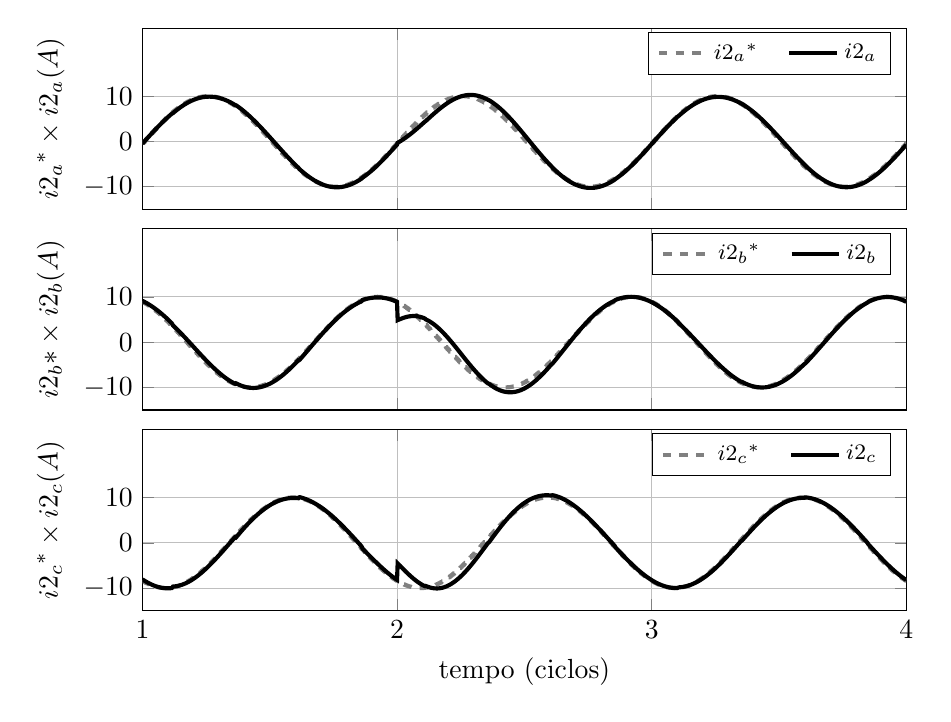
\begin{tikzpicture}

\begin{axis}[%
width=0.8\textwidth,
height=0.189701500343624\textwidth,
scale only axis,
xmin=0.0166666666666667,
xmax=0.0666666666666667,
xtick={0.0166666666666667,0.0333333333333333,0.05,0.0666666666666667},
xticklabels={\empty},
xmajorgrids,
ymin=-15,
ymax=25,
ytick={-10,   0,  10},
ylabel={${\text{i2}_\text{b}}\text{* }\times\text{ i2}_\text{b}\text{ (A)}$},
ymajorgrids,
name=plot2,
legend style={draw=black,fill=white,legend cell align=left},
scaled x ticks = false,
legend columns=-1,
legend style={/tikz/every even column/.append style={column sep=0.3cm}},
legend style={font=\footnotesize}
]
\addplot [color=gray,dashed,line width=1.5pt]
  table[row sep=crcr]{0.0166583333333333	8.95711760239421\\
0.0167	8.81303452065\\
0.0167416666666667	8.81303452065\\
0.0167833333333333	8.66025403784447\\
0.016825	8.66025403784447\\
0.0168666666666667	8.49892692986872\\
0.0169083333333333	8.49892692986872\\
0.01695	8.32921240710107\\
0.0169916666666667	8.32921240710107\\
0.0170333333333333	8.15127795728562\\
0.017075	8.15127795728562\\
0.0171166666666667	7.96529918024204\\
0.0171583333333333	7.96529918024204\\
0.0172	7.77145961456979\\
0.0172416666666667	7.77145961456979\\
0.0172833333333333	7.56995055651764\\
0.017325	7.56995055651764\\
0.0173666666666667	7.36097087119742\\
0.0174083333333333	7.36097087119742\\
0.01745	7.1447267963281\\
0.0174916666666667	7.1447267963281\\
0.0175333333333333	6.92143173870414\\
0.017575	6.92143173870414\\
0.0176166666666667	6.69130606358865\\
0.0176583333333333	6.69130606358865\\
0.0177	6.45457687723957\\
0.0177416666666667	6.45457687723957\\
0.0177833333333333	6.21147780278317\\
0.017825	6.21147780278317\\
0.0178666666666667	5.96224874965622\\
0.0179083333333333	5.96224874965622\\
0.01795	5.70713567684438\\
0.0179916666666667	5.70713567684438\\
0.0180333333333333	5.44639035015033\\
0.018075	5.44639035015033\\
0.0181166666666667	5.18027009373136\\
0.0181583333333333	5.18027009373136\\
0.0182	4.90903753615147\\
0.0182416666666667	4.90903753615147\\
0.0182833333333333	4.63296035119867\\
0.018325	4.63296035119867\\
0.0183666666666667	4.35231099372333\\
0.0184083333333333	4.35231099372333\\
0.01845	4.06736643075805\\
0.0184916666666667	4.06736643075805\\
0.0185333333333333	3.77840786818472\\
0.018575	3.77840786818472\\
0.0186166666666667	3.4857204732182\\
0.0186583333333333	3.4857204732182\\
0.0187	3.18959309298074\\
0.0187416666666667	3.18959309298074\\
0.0187833333333333	2.89031796944476\\
0.018825	2.89031796944476\\
0.0188666666666667	2.58819045102524\\
0.0189083333333333	2.58819045102524\\
0.01895	2.28350870110659\\
0.0189916666666667	2.28350870110659\\
0.0190333333333333	1.97657340379129\\
0.019075	1.97657340379129\\
0.0191166666666667	1.66768746716105\\
0.0191583333333333	1.66768746716105\\
0.0192	1.35715572434307\\
0.0192416666666667	1.35715572434307\\
0.0192833333333333	1.04528463267656\\
0.019325	1.04528463267656\\
0.0193666666666667	0.732381971276336\\
0.0194083333333333	0.732381971276336\\
0.01945	0.418756537292012\\
0.0194916666666667	0.418756537292012\\
0.0195333333333333	0.104717841162471\\
0.019575	0.104717841162471\\
0.0196166666666667	-0.20942419883356\\
0.0196583333333333	-0.20942419883356\\
0.0197	-0.523359562429432\\
0.0197416666666667	-0.523359562429432\\
0.0197833333333333	-0.836778433323152\\
0.019825	-0.836778433323152\\
0.0198666666666667	-1.14937150492867\\
0.0199083333333333	-1.14937150492867\\
0.01995	-1.46083028562412\\
0.0199916666666667	-1.46083028562412\\
0.0200333333333333	-1.77084740319584\\
0.020075	-1.77084740319584\\
0.0201166666666667	-2.0791169081776\\
0.0201583333333333	-2.0791169081776\\
0.0202	-2.38533457578582\\
0.0202416666666667	-2.38533457578582\\
0.0202833333333333	-2.68919820615267\\
0.020325	-2.68919820615267\\
0.0203666666666667	-2.99040792256089\\
0.0204083333333333	-2.99040792256089\\
0.02045	-3.28866646738586\\
0.0204916666666667	-3.28866646738586\\
0.0205333333333333	-3.58367949545303\\
0.020575	-3.58367949545303\\
0.0206166666666667	-3.87515586452106\\
0.0206583333333333	-3.87515586452106\\
0.0207	-4.16280792260405\\
0.0207416666666667	-4.16280792260405\\
0.0207833333333333	-4.44635179184931\\
0.020825	-4.44635179184931\\
0.0208666666666667	-4.72550764869058\\
0.0209083333333333	-4.72550764869058\\
0.02095	-5.00000000000005\\
0.0209916666666667	-5.00000000000005\\
0.0210333333333333	-5.26955795496682\\
0.021075	-5.26955795496682\\
0.0211166666666667	-5.53391549243349\\
0.0211583333333333	-5.53391549243349\\
0.0212	-5.79281172342684\\
0.0212416666666667	-5.79281172342684\\
0.0212833333333333	-6.0459911486238\\
0.021325	-6.0459911486238\\
0.0213666666666667	-6.29320391049844\\
0.0214083333333333	-6.29320391049844\\
0.02145	-6.53420603990112\\
0.0214916666666667	-6.53420603990112\\
0.0215333333333333	-6.76875969682667\\
0.021575	-6.76875969682667\\
0.0216166666666667	-6.99663340513372\\
0.0216583333333333	-6.99663340513372\\
0.0217	-7.2176022809837\\
0.0217416666666667	-7.2176022809837\\
0.0217833333333333	-7.43144825477402\\
0.021825	-7.43144825477402\\
0.0218666666666667	-7.6379602863465\\
0.0219083333333333	-7.6379602863465\\
0.02195	-7.83693457325848\\
0.0219916666666667	-7.83693457325848\\
0.0220333333333333	-8.02817475191123\\
0.022075	-8.02817475191123\\
0.0221166666666667	-8.21149209133713\\
0.0221583333333333	-8.21149209133713\\
0.0222	-8.38670567945433\\
0.0222416666666667	-8.38670567945433\\
0.0222833333333333	-8.55364260160516\\
0.022325	-8.55364260160516\\
0.0223666666666667	-8.71213811120199\\
0.0224083333333333	-8.71213811120199\\
0.02245	-8.86203579231225\\
0.0224916666666667	-8.86203579231225\\
0.0225333333333333	-9.00318771402204\\
0.022575	-9.00318771402204\\
0.0226166666666667	-9.13545457642611\\
0.0226583333333333	-9.13545457642611\\
0.0227	-9.25870584810006\\
0.0227416666666667	-9.25870584810006\\
0.0227833333333333	-9.37281989491902\\
0.022825	-9.37281989491902\\
0.0228666666666667	-9.47768410009597\\
0.0229083333333333	-9.47768410009597\\
0.02295	-9.57319497532079\\
0.0229916666666667	-9.57319497532079\\
0.0230333333333333	-9.6592582628908\\
0.023075	-9.6592582628908\\
0.0231166666666667	-9.73578902873172\\
0.0231583333333333	-9.73578902873172\\
0.0232	-9.80271174621734\\
0.0232416666666667	-9.80271174621734\\
0.0232833333333333	-9.85996037070517\\
0.023325	-9.85996037070517\\
0.0233666666666667	-9.90747840471456\\
0.0234083333333333	-9.90747840471456\\
0.02345	-9.94521895368285\\
0.0234916666666667	-9.94521895368285\\
0.0235333333333333	-9.97314477224471\\
0.023575	-9.97314477224471\\
0.0236166666666667	-9.99122830098871\\
0.0236583333333333	-9.99122830098871\\
0.0237	-9.99945169365525\\
0.0237416666666667	-9.99945169365525\\
0.0237833333333333	-9.99780683474858\\
0.023825	-9.99780683474858\\
0.0238666666666667	-9.98629534754587\\
0.0239083333333333	-9.98629534754587\\
0.02395	-9.96492859249517\\
0.0239916666666667	-9.96492859249517\\
0.0240333333333333	-9.93372765600409\\
0.024075	-9.93372765600409\\
0.0241166666666667	-9.89272332963001\\
0.0241583333333333	-9.89272332963001\\
0.0242	-9.84195607969255\\
0.0242416666666667	-9.84195607969255\\
0.0242833333333333	-9.78147600733818\\
0.024325	-9.78147600733818\\
0.0243666666666667	-9.71134279909649\\
0.0244083333333333	-9.71134279909649\\
0.02445	-9.63162566797671\\
0.0244916666666667	-9.63162566797671\\
0.0245333333333333	-9.5424032851629\\
0.024575	-9.5424032851629\\
0.0246166666666667	-9.44376370237494\\
0.0246583333333333	-9.44376370237494\\
0.0247	-9.33580426497215\\
0.0247416666666667	-9.33580426497215\\
0.0247833333333333	-9.21863151588513\\
0.024825	-9.21863151588513\\
0.0248666666666667	-9.09236109047081\\
0.0249083333333333	-9.09236109047081\\
0.02495	-8.95711760239425\\
0.0249916666666667	-8.95711760239425\\
0.0250333333333333	-8.81303452065005\\
0.025075	-8.81303452065005\\
0.0251166666666667	-8.66025403784451\\
0.0251583333333333	-8.66025403784451\\
0.0252	-8.49892692986876\\
0.0252416666666667	-8.49892692986876\\
0.0252833333333333	-8.32921240710111\\
0.025325	-8.32921240710111\\
0.0253666666666667	-8.15127795728566\\
0.0254083333333333	-8.15127795728566\\
0.02545	-7.96529918024207\\
0.0254916666666667	-7.96529918024207\\
0.0255333333333333	-7.77145961456982\\
0.025575	-7.77145961456982\\
0.0256166666666667	-7.56995055651767\\
0.0256583333333333	-7.56995055651767\\
0.0257	-7.36097087119745\\
0.0257416666666667	-7.36097087119745\\
0.0257833333333333	-7.14472679632814\\
0.025825	-7.14472679632814\\
0.0258666666666667	-6.92143173870417\\
0.0259083333333333	-6.92143173870417\\
0.02595	-6.69130606358868\\
0.0259916666666667	-6.69130606358868\\
0.0260333333333333	-6.4545768772396\\
0.026075	-6.4545768772396\\
0.0261166666666667	-6.2114778027832\\
0.0261583333333333	-6.2114778027832\\
0.0262	-5.96224874965625\\
0.0262416666666667	-5.96224874965625\\
0.0262833333333333	-5.70713567684441\\
0.026325	-5.70713567684441\\
0.0263666666666667	-5.44639035015036\\
0.0264083333333333	-5.44639035015036\\
0.02645	-5.18027009373139\\
0.0264916666666667	-5.18027009373139\\
0.0265333333333333	-4.90903753615149\\
0.026575	-4.90903753615149\\
0.0266166666666667	-4.6329603511987\\
0.0266583333333333	-4.6329603511987\\
0.0267	-4.35231099372335\\
0.0267416666666667	-4.35231099372335\\
0.0267833333333333	-4.06736643075807\\
0.026825	-4.06736643075807\\
0.0268666666666667	-3.77840786818474\\
0.0269083333333333	-3.77840786818474\\
0.02695	-3.48572047321821\\
0.0269916666666667	-3.48572047321821\\
0.0270333333333333	-3.18959309298076\\
0.027075	-3.18959309298076\\
0.0271166666666667	-2.89031796944477\\
0.0271583333333333	-2.89031796944477\\
0.0272	-2.58819045102526\\
0.0272416666666667	-2.58819045102526\\
0.0272833333333333	-2.28350870110661\\
0.027325	-2.28350870110661\\
0.0273666666666667	-1.9765734037913\\
0.0274083333333333	-1.9765734037913\\
0.02745	-1.66768746716106\\
0.0274916666666667	-1.66768746716106\\
0.0275333333333333	-1.35715572434308\\
0.027575	-1.35715572434308\\
0.0276166666666667	-1.04528463267656\\
0.0276583333333333	-1.04528463267656\\
0.0277	-0.732381971276341\\
0.0277416666666667	-0.732381971276341\\
0.0277833333333333	-0.418756537292015\\
0.027825	-0.418756537292015\\
0.0278666666666667	-0.104717841162473\\
0.0279083333333333	-0.104717841162473\\
0.02795	0.209424198833559\\
0.0279916666666667	0.209424198833559\\
0.0280333333333333	0.523359562429433\\
0.028075	0.523359562429433\\
0.0281166666666667	0.836778433323154\\
0.0281583333333333	0.836778433323154\\
0.0282	1.14937150492867\\
0.0282416666666667	1.14937150492867\\
0.0282833333333333	1.46083028562412\\
0.028325	1.46083028562412\\
0.0283666666666667	1.77084740319585\\
0.0284083333333333	1.77084740319585\\
0.02845	2.07911690817761\\
0.0284916666666667	2.07911690817761\\
0.0285333333333333	2.38533457578583\\
0.028575	2.38533457578583\\
0.0286166666666667	2.68919820615268\\
0.0286583333333333	2.68919820615268\\
0.0287	2.9904079225609\\
0.0287416666666667	2.9904079225609\\
0.0287833333333333	3.28866646738587\\
0.028825	3.28866646738587\\
0.0288666666666667	3.58367949545304\\
0.0289083333333333	3.58367949545304\\
0.02895	3.87515586452107\\
0.0289916666666667	3.87515586452107\\
0.0290333333333333	4.16280792260406\\
0.029075	4.16280792260406\\
0.0291166666666667	4.44635179184933\\
0.0291583333333333	4.44635179184933\\
0.0292	4.7255076486906\\
0.0292416666666667	4.7255076486906\\
0.0292833333333333	5.00000000000006\\
0.029325	5.00000000000006\\
0.0293666666666667	5.26955795496684\\
0.0294083333333333	5.26955795496684\\
0.02945	5.53391549243351\\
0.0294916666666667	5.53391549243351\\
0.0295333333333333	5.79281172342686\\
0.029575	5.79281172342686\\
0.0296166666666667	6.04599114862383\\
0.0296583333333333	6.04599114862383\\
0.0297	6.29320391049846\\
0.0297416666666667	6.29320391049846\\
0.0297833333333333	6.53420603990114\\
0.029825	6.53420603990114\\
0.0298666666666667	6.7687596968267\\
0.0299083333333333	6.7687596968267\\
0.02995	6.99663340513375\\
0.0299916666666667	6.99663340513375\\
0.0300333333333333	7.21760228098372\\
0.030075	7.21760228098372\\
0.0301166666666667	7.43144825477405\\
0.0301583333333333	7.43144825477405\\
0.0302	7.63796028634653\\
0.0302416666666667	7.63796028634653\\
0.0302833333333333	7.83693457325851\\
0.030325	7.83693457325851\\
0.0303666666666667	8.02817475191126\\
0.0304083333333333	8.02817475191126\\
0.03045	8.21149209133716\\
0.0304916666666667	8.21149209133716\\
0.0305333333333333	8.38670567945436\\
0.030575	8.38670567945436\\
0.0306166666666667	8.55364260160519\\
0.0306583333333333	8.55364260160519\\
0.0307	8.71213811120203\\
0.0307416666666667	8.71213811120203\\
0.0307833333333333	8.86203579231228\\
0.030825	8.86203579231228\\
0.0308666666666667	9.00318771402207\\
0.0309083333333333	9.00318771402207\\
0.03095	9.13545457642615\\
0.0309916666666667	9.13545457642615\\
0.0310333333333333	9.25870584810009\\
0.031075	9.25870584810009\\
0.0311166666666667	9.37281989491906\\
0.0311583333333333	9.37281989491906\\
0.0312	9.477684100096\\
0.0312416666666667	9.477684100096\\
0.0312833333333333	9.57319497532082\\
0.031325	9.57319497532082\\
0.0313666666666667	9.65925826289084\\
0.0314083333333333	9.65925826289084\\
0.03145	9.73578902873176\\
0.0314916666666667	9.73578902873176\\
0.0315333333333333	9.80271174621738\\
0.031575	9.80271174621738\\
0.0316166666666667	9.85996037070521\\
0.0316583333333333	9.85996037070521\\
0.0317	9.9074784047146\\
0.0317416666666667	9.9074784047146\\
0.0317833333333333	9.94521895368289\\
0.031825	9.94521895368289\\
0.0318666666666667	9.97314477224474\\
0.0319083333333333	9.97314477224474\\
0.03195	9.99122830098875\\
0.0319916666666667	9.99122830098875\\
0.0320333333333333	9.99945169365528\\
0.032075	9.99945169365528\\
0.0321166666666667	9.99780683474862\\
0.0321583333333333	9.99780683474862\\
0.0322	9.98629534754591\\
0.0322416666666667	9.98629534754591\\
0.0322833333333333	9.96492859249521\\
0.032325	9.96492859249521\\
0.0323666666666667	9.93372765600413\\
0.0324083333333333	9.93372765600413\\
0.03245	9.89272332963005\\
0.0324916666666667	9.89272332963005\\
0.0325333333333333	9.84195607969259\\
0.032575	9.84195607969259\\
0.0326166666666667	9.78147600733822\\
0.0326583333333333	9.78147600733822\\
0.0327	9.71134279909653\\
0.0327416666666667	9.71134279909653\\
0.0327833333333333	9.63162566797675\\
0.032825	9.63162566797675\\
0.0328666666666667	9.54240328516294\\
0.0329083333333333	9.54240328516294\\
0.03295	9.44376370237498\\
0.0329916666666667	9.44376370237498\\
0.0330333333333333	9.33580426497218\\
0.033075	9.33580426497218\\
0.0331166666666667	9.21863151588517\\
0.0331583333333333	9.21863151588517\\
0.0332	9.09236109047085\\
0.0332416666666667	9.09236109047085\\
0.0332833333333333	8.95711760239429\\
0.033325	8.95711760239429\\
0.0333666666666667	8.81303452065008\\
0.0334083333333333	8.81303452065008\\
0.03345	8.66025403784455\\
0.0334916666666667	8.66025403784455\\
0.0335333333333333	8.49892692986879\\
0.033575	8.49892692986879\\
0.0336166666666667	8.32921240710115\\
0.0336583333333333	8.32921240710115\\
0.0337	8.15127795728569\\
0.0337416666666667	8.15127795728569\\
0.0337833333333333	7.96529918024211\\
0.033825	7.96529918024211\\
0.0338666666666667	7.77145961456986\\
0.0339083333333333	7.77145961456986\\
0.03395	7.56995055651771\\
0.0339916666666667	7.56995055651771\\
0.0340333333333333	7.36097087119748\\
0.034075	7.36097087119748\\
0.0341166666666667	7.14472679632817\\
0.0341583333333333	7.14472679632817\\
0.0342	6.9214317387042\\
0.0342416666666667	6.9214317387042\\
0.0342833333333333	6.69130606358871\\
0.034325	6.69130606358871\\
0.0343666666666667	6.45457687723963\\
0.0344083333333333	6.45457687723963\\
0.03445	6.21147780278323\\
0.0344916666666667	6.21147780278323\\
0.0345333333333333	5.96224874965628\\
0.034575	5.96224874965628\\
0.0346166666666667	5.70713567684443\\
0.0346583333333333	5.70713567684443\\
0.0347	5.44639035015038\\
0.0347416666666667	5.44639035015038\\
0.0347833333333333	5.18027009373141\\
0.034825	5.18027009373141\\
0.0348666666666667	4.90903753615151\\
0.0349083333333333	4.90903753615151\\
0.03495	4.63296035119872\\
0.0349916666666667	4.63296035119872\\
0.0350333333333333	4.35231099372337\\
0.035075	4.35231099372337\\
0.0351166666666667	4.06736643075809\\
0.0351583333333333	4.06736643075809\\
0.0352	3.77840786818476\\
0.0352416666666667	3.77840786818476\\
0.0352833333333333	3.48572047321823\\
0.035325	3.48572047321823\\
0.0353666666666667	3.18959309298077\\
0.0354083333333333	3.18959309298077\\
0.03545	2.89031796944478\\
0.0354916666666667	2.89031796944478\\
0.0355333333333333	2.58819045102527\\
0.035575	2.58819045102527\\
0.0356166666666667	2.28350870110662\\
0.0356583333333333	2.28350870110662\\
0.0357	1.97657340379131\\
0.0357416666666667	1.97657340379131\\
0.0357833333333333	1.66768746716107\\
0.035825	1.66768746716107\\
0.0358666666666667	1.35715572434309\\
0.0359083333333333	1.35715572434309\\
0.03595	1.04528463267657\\
0.0359916666666667	1.04528463267657\\
0.0360333333333333	0.732381971276348\\
0.036075	0.732381971276348\\
0.0361166666666667	0.418756537292022\\
0.0361583333333333	0.418756537292022\\
0.0362	0.104717841162477\\
0.0362416666666667	0.104717841162477\\
0.0362833333333333	-0.209424198833557\\
0.036325	-0.209424198833557\\
0.0363666666666667	-0.523359562429431\\
0.0364083333333333	-0.523359562429431\\
0.03645	-0.836778433323154\\
0.0364916666666667	-0.836778433323154\\
0.0365333333333333	-1.14937150492867\\
0.036575	-1.14937150492867\\
0.0366166666666667	-1.46083028562413\\
0.0366583333333333	-1.46083028562413\\
0.0367	-1.77084740319585\\
0.0367416666666667	-1.77084740319585\\
0.0367833333333333	-2.07911690817762\\
0.036825	-2.07911690817762\\
0.0368666666666667	-2.38533457578584\\
0.0369083333333333	-2.38533457578584\\
0.03695	-2.68919820615269\\
0.0369916666666667	-2.68919820615269\\
0.0370333333333333	-2.99040792256091\\
0.037075	-2.99040792256091\\
0.0371166666666667	-3.28866646738588\\
0.0371583333333333	-3.28866646738588\\
0.0372	-3.58367949545306\\
0.0372416666666667	-3.58367949545306\\
0.0372833333333333	-3.87515586452109\\
0.037325	-3.87515586452109\\
0.0373666666666667	-4.16280792260408\\
0.0374083333333333	-4.16280792260408\\
0.03745	-4.44635179184934\\
0.0374916666666667	-4.44635179184934\\
0.0375333333333333	-4.72550764869062\\
0.037575	-4.72550764869062\\
0.0376166666666667	-5.00000000000008\\
0.0376583333333333	-5.00000000000008\\
0.0377	-5.26955795496686\\
0.0377416666666667	-5.26955795496686\\
0.0377833333333333	-5.53391549243353\\
0.037825	-5.53391549243353\\
0.0378666666666667	-5.79281172342689\\
0.0379083333333333	-5.79281172342689\\
0.03795	-6.04599114862385\\
0.0379916666666667	-6.04599114862385\\
0.0380333333333333	-6.29320391049848\\
0.038075	-6.29320391049848\\
0.0381166666666667	-6.53420603990117\\
0.0381583333333333	-6.53420603990117\\
0.0382	-6.76875969682673\\
0.0382416666666667	-6.76875969682673\\
0.0382833333333333	-6.99663340513378\\
0.038325	-6.99663340513378\\
0.0383666666666667	-7.21760228098375\\
0.0384083333333333	-7.21760228098375\\
0.03845	-7.43144825477408\\
0.0384916666666667	-7.43144825477408\\
0.0385333333333333	-7.63796028634656\\
0.038575	-7.63796028634656\\
0.0386166666666667	-7.83693457325854\\
0.0386583333333333	-7.83693457325854\\
0.0387	-8.02817475191129\\
0.0387416666666667	-8.02817475191129\\
0.0387833333333333	-8.21149209133719\\
0.038825	-8.21149209133719\\
0.0388666666666667	-8.3867056794544\\
0.0389083333333333	-8.3867056794544\\
0.03895	-8.55364260160523\\
0.0389916666666667	-8.55364260160523\\
0.0390333333333333	-8.71213811120206\\
0.039075	-8.71213811120206\\
0.0391166666666667	-8.86203579231232\\
0.0391583333333333	-8.86203579231232\\
0.0392	-9.00318771402211\\
0.0392416666666667	-9.00318771402211\\
0.0392833333333333	-9.13545457642618\\
0.039325	-9.13545457642618\\
0.0393666666666667	-9.25870584810013\\
0.0394083333333333	-9.25870584810013\\
0.03945	-9.3728198949191\\
0.0394916666666667	-9.3728198949191\\
0.0395333333333333	-9.47768410009604\\
0.039575	-9.47768410009604\\
0.0396166666666667	-9.57319497532086\\
0.0396583333333333	-9.57319497532086\\
0.0397	-9.65925826289087\\
0.0397416666666667	-9.65925826289087\\
0.0397833333333333	-9.7357890287318\\
0.039825	-9.7357890287318\\
0.0398666666666667	-9.80271174621742\\
0.0399083333333333	-9.80271174621742\\
0.03995	-9.85996037070525\\
0.0399916666666667	-9.85996037070525\\
0.0400333333333333	-9.90747840471464\\
0.040075	-9.90747840471464\\
0.0401166666666667	-9.94521895368294\\
0.0401583333333333	-9.94521895368294\\
0.0402	-9.97314477224478\\
0.0402416666666667	-9.97314477224478\\
0.0402833333333333	-9.99122830098879\\
0.040325	-9.99122830098879\\
0.0403666666666667	-9.99945169365533\\
0.0404083333333333	-9.99945169365533\\
0.04045	-9.99780683474866\\
0.0404916666666667	-9.99780683474866\\
0.0405333333333333	-9.98629534754595\\
0.040575	-9.98629534754595\\
0.0406166666666667	-9.96492859249525\\
0.0406583333333333	-9.96492859249525\\
0.0407	-9.93372765600417\\
0.0407416666666667	-9.93372765600417\\
0.0407833333333333	-9.89272332963009\\
0.040825	-9.89272332963009\\
0.0408666666666667	-9.84195607969263\\
0.0409083333333333	-9.84195607969263\\
0.04095	-9.78147600733827\\
0.0409916666666667	-9.78147600733827\\
0.0410333333333333	-9.71134279909657\\
0.041075	-9.71134279909657\\
0.0411166666666667	-9.63162566797679\\
0.0411583333333333	-9.63162566797679\\
0.0412	-9.54240328516298\\
0.0412416666666667	-9.54240328516298\\
0.0412833333333333	-9.44376370237502\\
0.041325	-9.44376370237502\\
0.0413666666666667	-9.33580426497222\\
0.0414083333333333	-9.33580426497222\\
0.04145	-9.21863151588521\\
0.0414916666666667	-9.21863151588521\\
0.0415333333333333	-9.09236109047089\\
0.041575	-9.09236109047089\\
0.0416166666666667	-8.95711760239433\\
0.0416583333333333	-8.95711760239433\\
0.0417	-8.81303452065012\\
0.0417416666666667	-8.81303452065012\\
0.0417833333333333	-8.66025403784458\\
0.041825	-8.66025403784458\\
0.0418666666666667	-8.49892692986883\\
0.0419083333333333	-8.49892692986883\\
0.04195	-8.32921240710118\\
0.0419916666666667	-8.32921240710118\\
0.0420333333333333	-8.15127795728573\\
0.042075	-8.15127795728573\\
0.0421166666666667	-7.96529918024214\\
0.0421583333333333	-7.96529918024214\\
0.0422	-7.77145961456989\\
0.0422416666666667	-7.77145961456989\\
0.0422833333333333	-7.56995055651774\\
0.042325	-7.56995055651774\\
0.0423666666666667	-7.36097087119751\\
0.0424083333333333	-7.36097087119751\\
0.04245	-7.1447267963282\\
0.0424916666666667	-7.1447267963282\\
0.0425333333333333	-6.92143173870423\\
0.042575	-6.92143173870423\\
0.0426166666666667	-6.69130606358874\\
0.0426583333333333	-6.69130606358874\\
0.0427	-6.45457687723966\\
0.0427416666666667	-6.45457687723966\\
0.0427833333333333	-6.21147780278325\\
0.042825	-6.21147780278325\\
0.0428666666666667	-5.9622487496563\\
0.0429083333333333	-5.9622487496563\\
0.04295	-5.70713567684446\\
0.0429916666666667	-5.70713567684446\\
0.0430333333333333	-5.44639035015041\\
0.043075	-5.44639035015041\\
0.0431166666666667	-5.18027009373143\\
0.0431583333333333	-5.18027009373143\\
0.0432	-4.90903753615153\\
0.0432416666666667	-4.90903753615153\\
0.0432833333333333	-4.63296035119874\\
0.043325	-4.63296035119874\\
0.0433666666666667	-4.35231099372339\\
0.0434083333333333	-4.35231099372339\\
0.04345	-4.06736643075811\\
0.0434916666666667	-4.06736643075811\\
0.0435333333333333	-3.77840786818477\\
0.043575	-3.77840786818477\\
0.0436166666666667	-3.48572047321825\\
0.0436583333333333	-3.48572047321825\\
0.0437	-3.18959309298079\\
0.0437416666666667	-3.18959309298079\\
0.0437833333333333	-2.8903179694448\\
0.043825	-2.8903179694448\\
0.0438666666666667	-2.58819045102528\\
0.0439083333333333	-2.58819045102528\\
0.04395	-2.28350870110663\\
0.0439916666666667	-2.28350870110663\\
0.0440333333333333	-1.97657340379133\\
0.044075	-1.97657340379133\\
0.0441166666666667	-1.66768746716108\\
0.0441583333333333	-1.66768746716108\\
0.0442	-1.35715572434309\\
0.0442416666666667	-1.35715572434309\\
0.0442833333333333	-1.04528463267658\\
0.044325	-1.04528463267658\\
0.0443666666666667	-0.732381971276353\\
0.0444083333333333	-0.732381971276353\\
0.04445	-0.418756537292025\\
0.0444916666666667	-0.418756537292025\\
0.0445333333333333	-0.104717841162479\\
0.044575	-0.104717841162479\\
0.0446166666666667	0.209424198833555\\
0.0446583333333333	0.209424198833555\\
0.0447	0.523359562429432\\
0.0447416666666667	0.523359562429432\\
0.0447833333333333	0.836778433323156\\
0.044825	0.836778433323156\\
0.0448666666666667	1.14937150492867\\
0.0449083333333333	1.14937150492867\\
0.04495	1.46083028562413\\
0.0449916666666667	1.46083028562413\\
0.0450333333333333	1.77084740319586\\
0.045075	1.77084740319586\\
0.0451166666666667	2.07911690817762\\
0.0451583333333333	2.07911690817762\\
0.0452	2.38533457578585\\
0.0452416666666667	2.38533457578585\\
0.0452833333333333	2.6891982061527\\
0.045325	2.6891982061527\\
0.0453666666666667	2.99040792256092\\
0.0454083333333333	2.99040792256092\\
0.04545	3.28866646738589\\
0.0454916666666667	3.28866646738589\\
0.0455333333333333	3.58367949545307\\
0.045575	3.58367949545307\\
0.0456166666666667	3.8751558645211\\
0.0456583333333333	3.8751558645211\\
0.0457	4.16280792260409\\
0.0457416666666667	4.16280792260409\\
0.0457833333333333	4.44635179184936\\
0.045825	4.44635179184936\\
0.0458666666666667	4.72550764869064\\
0.0459083333333333	4.72550764869064\\
0.04595	5.0000000000001\\
0.0459916666666667	5.0000000000001\\
0.0460333333333333	5.26955795496689\\
0.046075	5.26955795496689\\
0.0461166666666667	5.53391549243356\\
0.0461583333333333	5.53391549243356\\
0.0462	5.79281172342691\\
0.0462416666666667	5.79281172342691\\
0.0462833333333333	6.04599114862388\\
0.046325	6.04599114862388\\
0.0463666666666667	6.29320391049851\\
0.0464083333333333	6.29320391049851\\
0.04645	6.5342060399012\\
0.0464916666666667	6.5342060399012\\
0.0465333333333333	6.76875969682676\\
0.046575	6.76875969682676\\
0.0466166666666667	6.99663340513381\\
0.0466583333333333	6.99663340513381\\
0.0467	7.21760228098379\\
0.0467416666666667	7.21760228098379\\
0.0467833333333333	7.43144825477411\\
0.046825	7.43144825477411\\
0.0468666666666667	7.6379602863466\\
0.0469083333333333	7.6379602863466\\
0.04695	7.83693457325858\\
0.0469916666666667	7.83693457325858\\
0.0470333333333333	8.02817475191133\\
0.047075	8.02817475191133\\
0.0471166666666667	8.21149209133723\\
0.0471583333333333	8.21149209133723\\
0.0472	8.38670567945444\\
0.0472416666666667	8.38670567945444\\
0.0472833333333333	8.55364260160527\\
0.047325	8.55364260160527\\
0.0473666666666667	8.7121381112021\\
0.0474083333333333	8.7121381112021\\
0.04745	8.86203579231236\\
0.0474916666666667	8.86203579231236\\
0.0475333333333333	9.00318771402215\\
0.047575	9.00318771402215\\
0.0476166666666667	9.13545457642623\\
0.0476583333333333	9.13545457642623\\
0.0477	9.25870584810017\\
0.0477416666666667	9.25870584810017\\
0.0477833333333333	9.37281989491914\\
0.047825	9.37281989491914\\
0.0478666666666667	9.47768410009609\\
0.0479083333333333	9.47768410009609\\
0.04795	9.57319497532091\\
0.0479916666666667	9.57319497532091\\
0.0480333333333333	9.65925826289092\\
0.048075	9.65925826289092\\
0.0481166666666667	9.73578902873184\\
0.0481583333333333	9.73578902873184\\
0.0482	9.80271174621746\\
0.0482416666666667	9.80271174621746\\
0.0482833333333333	9.85996037070529\\
0.048325	9.85996037070529\\
0.0483666666666667	9.90747840471468\\
0.0484083333333333	9.90747840471468\\
0.04845	9.94521895368298\\
0.0484916666666667	9.94521895368298\\
0.0485333333333333	9.97314477224483\\
0.048575	9.97314477224483\\
0.0486166666666667	9.99122830098883\\
0.0486583333333333	9.99122830098883\\
0.0487	9.99945169365537\\
0.0487416666666667	9.99945169365537\\
0.0487833333333333	9.99780683474871\\
0.048825	9.99780683474871\\
0.0488666666666667	9.98629534754599\\
0.0489083333333333	9.98629534754599\\
0.04895	9.9649285924953\\
0.0489916666666667	9.9649285924953\\
0.0490333333333333	9.93372765600422\\
0.049075	9.93372765600422\\
0.0491166666666667	9.89272332963014\\
0.0491583333333333	9.89272332963014\\
0.0492	9.84195607969268\\
0.0492416666666667	9.84195607969268\\
0.0492833333333333	9.78147600733831\\
0.049325	9.78147600733831\\
0.0493666666666667	9.71134279909661\\
0.0494083333333333	9.71134279909661\\
0.04945	9.63162566797684\\
0.0494916666666667	9.63162566797684\\
0.0495333333333333	9.54240328516302\\
0.049575	9.54240328516302\\
0.0496166666666667	9.44376370237506\\
0.0496583333333333	9.44376370237506\\
0.0497	9.33580426497227\\
0.0497416666666667	9.33580426497227\\
0.0497833333333333	9.21863151588525\\
0.049825	9.21863151588525\\
0.0498666666666667	9.09236109047093\\
0.0499083333333333	9.09236109047093\\
0.04995	8.95711760239437\\
0.0499916666666667	8.95711760239437\\
0.0500333333333333	8.81303452065016\\
0.050075	8.81303452065016\\
0.0501166666666667	8.66025403784462\\
0.0501583333333333	8.66025403784462\\
0.0502	8.49892692986887\\
0.0502416666666667	8.49892692986887\\
0.0502833333333333	8.32921240710123\\
0.050325	8.32921240710123\\
0.0503666666666667	8.15127795728577\\
0.0504083333333333	8.15127795728577\\
0.05045	7.96529918024218\\
0.0504916666666667	7.96529918024218\\
0.0505333333333333	7.77145961456993\\
0.050575	7.77145961456993\\
0.0506166666666667	7.56995055651778\\
0.0506583333333333	7.56995055651778\\
0.0507	7.36097087119755\\
0.0507416666666667	7.36097087119755\\
0.0507833333333333	7.14472679632824\\
0.050825	7.14472679632824\\
0.0508666666666667	6.92143173870427\\
0.0509083333333333	6.92143173870427\\
0.05095	6.69130606358878\\
0.0509916666666667	6.69130606358878\\
0.0510333333333333	6.45457687723969\\
0.051075	6.45457687723969\\
0.0511166666666667	6.21147780278329\\
0.0511583333333333	6.21147780278329\\
0.0512	5.96224874965633\\
0.0512416666666667	5.96224874965633\\
0.0512833333333333	5.70713567684449\\
0.051325	5.70713567684449\\
0.0513666666666667	5.44639035015043\\
0.0514083333333333	5.44639035015043\\
0.05145	5.18027009373146\\
0.0514916666666667	5.18027009373146\\
0.0515333333333333	4.90903753615156\\
0.051575	4.90903753615156\\
0.0516166666666667	4.63296035119876\\
0.0516583333333333	4.63296035119876\\
0.0517	4.35231099372341\\
0.0517416666666667	4.35231099372341\\
0.0517833333333333	4.06736643075813\\
0.051825	4.06736643075813\\
0.0518666666666667	3.77840786818479\\
0.0519083333333333	3.77840786818479\\
0.05195	3.48572047321827\\
0.0519916666666667	3.48572047321827\\
0.0520333333333333	3.18959309298081\\
0.052075	3.18959309298081\\
0.0521166666666667	2.89031796944481\\
0.0521583333333333	2.89031796944481\\
0.0522	2.5881904510253\\
0.0522416666666667	2.5881904510253\\
0.0522833333333333	2.28350870110664\\
0.052325	2.28350870110664\\
0.0523666666666667	1.97657340379134\\
0.0524083333333333	1.97657340379134\\
0.05245	1.66768746716109\\
0.0524916666666667	1.66768746716109\\
0.0525333333333333	1.3571557243431\\
0.052575	1.3571557243431\\
0.0526166666666667	1.04528463267659\\
0.0526583333333333	1.04528463267659\\
0.0527	0.73238197127636\\
0.0527416666666667	0.73238197127636\\
0.0527833333333333	0.418756537292029\\
0.052825	0.418756537292029\\
0.0528666666666667	0.104717841162482\\
0.0529083333333333	0.104717841162482\\
0.05295	-0.209424198833554\\
0.0529916666666667	-0.209424198833554\\
0.0530333333333333	-0.523359562429432\\
0.053075	-0.523359562429432\\
0.0531166666666667	-0.836778433323157\\
0.0531583333333333	-0.836778433323157\\
0.0532	-1.14937150492868\\
0.0532416666666667	-1.14937150492868\\
0.0532833333333333	-1.46083028562414\\
0.053325	-1.46083028562414\\
0.0533666666666667	-1.77084740319586\\
0.0534083333333333	-1.77084740319586\\
0.05345	-2.07911690817763\\
0.0534916666666667	-2.07911690817763\\
0.0535333333333333	-2.38533457578585\\
0.053575	-2.38533457578585\\
0.0536166666666667	-2.68919820615271\\
0.0536583333333333	-2.68919820615271\\
0.0537	-2.99040792256093\\
0.0537416666666667	-2.99040792256093\\
0.0537833333333333	-3.2886664673859\\
0.053825	-3.2886664673859\\
0.0538666666666667	-3.58367949545308\\
0.0539083333333333	-3.58367949545308\\
0.05395	-3.87515586452112\\
0.0539916666666667	-3.87515586452112\\
0.0540333333333333	-4.16280792260411\\
0.054075	-4.16280792260411\\
0.0541166666666667	-4.44635179184938\\
0.0541583333333333	-4.44635179184938\\
0.0542	-4.72550764869065\\
0.0542416666666667	-4.72550764869065\\
0.0542833333333333	-5.00000000000012\\
0.054325	-5.00000000000012\\
0.0543666666666667	-5.26955795496691\\
0.0544083333333333	-5.26955795496691\\
0.05445	-5.53391549243358\\
0.0544916666666667	-5.53391549243358\\
0.0545333333333333	-5.79281172342693\\
0.054575	-5.79281172342693\\
0.0546166666666667	-6.0459911486239\\
0.0546583333333333	-6.0459911486239\\
0.0547	-6.29320391049854\\
0.0547416666666667	-6.29320391049854\\
0.0547833333333333	-6.53420603990122\\
0.054825	-6.53420603990122\\
0.0548666666666667	-6.76875969682678\\
0.0549083333333333	-6.76875969682678\\
0.05495	-6.99663340513384\\
0.0549916666666667	-6.99663340513384\\
0.0550333333333333	-7.21760228098381\\
0.055075	-7.21760228098381\\
0.0551166666666667	-7.43144825477414\\
0.0551583333333333	-7.43144825477414\\
0.0552	-7.63796028634663\\
0.0552416666666667	-7.63796028634663\\
0.0552833333333333	-7.83693457325861\\
0.055325	-7.83693457325861\\
0.0553666666666667	-8.02817475191136\\
0.0554083333333333	-8.02817475191136\\
0.05545	-8.21149209133726\\
0.0554916666666667	-8.21149209133726\\
0.0555333333333333	-8.38670567945447\\
0.055575	-8.38670567945447\\
0.0556166666666667	-8.5536426016053\\
0.0556583333333333	-8.5536426016053\\
0.0557	-8.71213811120214\\
0.0557416666666667	-8.71213811120214\\
0.0557833333333333	-8.86203579231239\\
0.055825	-8.86203579231239\\
0.0558666666666667	-9.00318771402219\\
0.0559083333333333	-9.00318771402219\\
0.05595	-9.13545457642627\\
0.0559916666666667	-9.13545457642627\\
0.0560333333333333	-9.25870584810021\\
0.056075	-9.25870584810021\\
0.0561166666666667	-9.37281989491918\\
0.0561583333333333	-9.37281989491918\\
0.0562	-9.47768410009613\\
0.0562416666666667	-9.47768410009613\\
0.0562833333333333	-9.57319497532095\\
0.056325	-9.57319497532095\\
0.0563666666666667	-9.65925826289096\\
0.0564083333333333	-9.65925826289096\\
0.05645	-9.73578902873188\\
0.0564916666666667	-9.73578902873188\\
0.0565333333333333	-9.8027117462175\\
0.056575	-9.8027117462175\\
0.0566166666666667	-9.85996037070534\\
0.0566583333333333	-9.85996037070534\\
0.0567	-9.90747840471473\\
0.0567416666666667	-9.90747840471473\\
0.0567833333333333	-9.94521895368302\\
0.056825	-9.94521895368302\\
0.0568666666666667	-9.97314477224487\\
0.0569083333333333	-9.97314477224487\\
0.05695	-9.99122830098888\\
0.0569916666666667	-9.99122830098888\\
0.0570333333333333	-9.99945169365542\\
0.057075	-9.99945169365542\\
0.0571166666666667	-9.99780683474875\\
0.0571583333333333	-9.99780683474875\\
0.0572	-9.98629534754604\\
0.0572416666666667	-9.98629534754604\\
0.0572833333333333	-9.96492859249534\\
0.057325	-9.96492859249534\\
0.0573666666666667	-9.93372765600427\\
0.0574083333333333	-9.93372765600427\\
0.05745	-9.89272332963018\\
0.0574916666666667	-9.89272332963018\\
0.0575333333333333	-9.84195607969272\\
0.057575	-9.84195607969272\\
0.0576166666666667	-9.78147600733836\\
0.0576583333333333	-9.78147600733836\\
0.0577	-9.71134279909666\\
0.0577416666666667	-9.71134279909666\\
0.0577833333333333	-9.63162566797688\\
0.057825	-9.63162566797688\\
0.0578666666666667	-9.54240328516306\\
0.0579083333333333	-9.54240328516306\\
0.05795	-9.44376370237511\\
0.0579916666666667	-9.44376370237511\\
0.0580333333333333	-9.33580426497231\\
0.058075	-9.33580426497231\\
0.0581166666666667	-9.21863151588529\\
0.0581583333333333	-9.21863151588529\\
0.0582	-9.09236109047097\\
0.0582416666666667	-9.09236109047097\\
0.0582833333333333	-8.95711760239441\\
0.058325	-8.95711760239441\\
0.0583666666666667	-8.8130345206502\\
0.0584083333333333	-8.8130345206502\\
0.05845	-8.66025403784466\\
0.0584916666666667	-8.66025403784466\\
0.0585333333333333	-8.49892692986891\\
0.058575	-8.49892692986891\\
0.0586166666666667	-8.32921240710126\\
0.0586583333333333	-8.32921240710126\\
0.0587	-8.1512779572858\\
0.0587416666666667	-8.1512779572858\\
0.0587833333333333	-7.96529918024222\\
0.058825	-7.96529918024222\\
0.0588666666666667	-7.77145961456996\\
0.0589083333333333	-7.77145961456996\\
0.05895	-7.56995055651781\\
0.0589916666666667	-7.56995055651781\\
0.0590333333333333	-7.36097087119758\\
0.059075	-7.36097087119758\\
0.0591166666666667	-7.14472679632827\\
0.0591583333333333	-7.14472679632827\\
0.0592	-6.9214317387043\\
0.0592416666666667	-6.9214317387043\\
0.0592833333333333	-6.69130606358881\\
0.059325	-6.69130606358881\\
0.0593666666666667	-6.45457687723972\\
0.0594083333333333	-6.45457687723972\\
0.05945	-6.21147780278331\\
0.0594916666666667	-6.21147780278331\\
0.0595333333333333	-5.96224874965636\\
0.059575	-5.96224874965636\\
0.0596166666666667	-5.70713567684451\\
0.0596583333333333	-5.70713567684451\\
0.0597	-5.44639035015046\\
0.0597416666666667	-5.44639035015046\\
0.0597833333333333	-5.18027009373148\\
0.059825	-5.18027009373148\\
0.0598666666666667	-4.90903753615158\\
0.0599083333333333	-4.90903753615158\\
0.05995	-4.63296035119878\\
0.0599916666666667	-4.63296035119878\\
0.0600333333333333	-4.35231099372343\\
0.060075	-4.35231099372343\\
0.0601166666666667	-4.06736643075815\\
0.0601583333333333	-4.06736643075815\\
0.0602	-3.77840786818481\\
0.0602416666666667	-3.77840786818481\\
0.0602833333333333	-3.48572047321828\\
0.060325	-3.48572047321828\\
0.0603666666666667	-3.18959309298082\\
0.0604083333333333	-3.18959309298082\\
0.06045	-2.89031796944483\\
0.0604916666666667	-2.89031796944483\\
0.0605333333333333	-2.58819045102531\\
0.060575	-2.58819045102531\\
0.0606166666666667	-2.28350870110665\\
0.0606583333333333	-2.28350870110665\\
0.0607	-1.97657340379135\\
0.0607416666666667	-1.97657340379135\\
0.0607833333333333	-1.6676874671611\\
0.060825	-1.6676874671611\\
0.0608666666666667	-1.35715572434311\\
0.0609083333333333	-1.35715572434311\\
0.06095	-1.04528463267659\\
0.0609916666666667	-1.04528463267659\\
0.0610333333333333	-0.732381971276366\\
0.061075	-0.732381971276366\\
0.0611166666666667	-0.418756537292034\\
0.0611583333333333	-0.418756537292034\\
0.0612	-0.104717841162486\\
0.0612416666666667	-0.104717841162486\\
0.0612833333333333	0.209424198833552\\
0.061325	0.209424198833552\\
0.0613666666666667	0.52335956242943\\
0.0614083333333333	0.52335956242943\\
0.06145	0.836778433323157\\
0.0614916666666667	0.836778433323157\\
0.0615333333333333	1.14937150492868\\
0.061575	1.14937150492868\\
0.0616166666666667	1.46083028562414\\
0.0616583333333333	1.46083028562414\\
0.0617	1.77084740319587\\
0.0617416666666667	1.77084740319587\\
0.0617833333333333	2.07911690817764\\
0.061825	2.07911690817764\\
0.0618666666666667	2.38533457578586\\
0.0619083333333333	2.38533457578586\\
0.06195	2.68919820615272\\
0.0619916666666667	2.68919820615272\\
0.0620333333333333	2.99040792256094\\
0.062075	2.99040792256094\\
0.0621166666666667	3.28866646738591\\
0.0621583333333333	3.28866646738591\\
0.0622	3.5836794954531\\
0.0622416666666667	3.5836794954531\\
0.0622833333333333	3.87515586452113\\
0.062325	3.87515586452113\\
0.0623666666666667	4.16280792260412\\
0.0624083333333333	4.16280792260412\\
0.06245	4.4463517918494\\
0.0624916666666667	4.4463517918494\\
0.0625333333333333	4.72550764869067\\
0.062575	4.72550764869067\\
0.0626166666666667	5.00000000000014\\
0.0626583333333333	5.00000000000014\\
0.0627	5.26955795496693\\
0.0627416666666667	5.26955795496693\\
0.0627833333333333	5.5339154924336\\
0.062825	5.5339154924336\\
0.0628666666666667	5.79281172342696\\
0.0629083333333333	5.79281172342696\\
0.06295	6.04599114862392\\
0.0629916666666667	6.04599114862392\\
0.0630333333333333	6.29320391049856\\
0.063075	6.29320391049856\\
0.0631166666666667	6.53420603990125\\
0.0631583333333333	6.53420603990125\\
0.0632	6.76875969682681\\
0.0632416666666667	6.76875969682681\\
0.0632833333333333	6.99663340513387\\
0.063325	6.99663340513387\\
0.0633666666666667	7.21760228098384\\
0.0634083333333333	7.21760228098384\\
0.06345	7.43144825477417\\
0.0634916666666667	7.43144825477417\\
0.0635333333333333	7.63796028634666\\
0.063575	7.63796028634666\\
0.0636166666666667	7.83693457325864\\
0.0636583333333333	7.83693457325864\\
0.0637	8.0281747519114\\
0.0637416666666667	8.0281747519114\\
0.0637833333333333	8.2114920913373\\
0.063825	8.2114920913373\\
0.0638666666666667	8.3867056794545\\
0.0639083333333333	8.3867056794545\\
0.06395	8.55364260160534\\
0.0639916666666667	8.55364260160534\\
0.0640333333333333	8.71213811120217\\
0.064075	8.71213811120217\\
0.0641166666666667	8.86203579231243\\
0.0641583333333333	8.86203579231243\\
0.0642	9.00318771402222\\
0.0642416666666667	9.00318771402222\\
0.0642833333333333	9.1354545764263\\
0.064325	9.1354545764263\\
0.0643666666666667	9.25870584810025\\
0.0644083333333333	9.25870584810025\\
0.06445	9.37281989491922\\
0.0644916666666667	9.37281989491922\\
0.0645333333333333	9.47768410009616\\
0.064575	9.47768410009616\\
0.0646166666666667	9.57319497532098\\
0.0646583333333333	9.57319497532098\\
0.0647	9.659258262891\\
0.0647416666666667	9.659258262891\\
0.0647833333333333	9.73578902873192\\
0.064825	9.73578902873192\\
0.0648666666666667	9.80271174621754\\
0.0649083333333333	9.80271174621754\\
0.06495	9.85996037070537\\
0.0649916666666667	9.85996037070537\\
0.0650333333333333	9.90747840471476\\
0.065075	9.90747840471476\\
0.0651166666666667	9.94521895368306\\
0.0651583333333333	9.94521895368306\\
0.0652	9.97314477224491\\
0.0652416666666667	9.97314477224491\\
0.0652833333333333	9.99122830098892\\
0.065325	9.99122830098892\\
0.0653666666666667	9.99945169365546\\
0.0654083333333333	9.99945169365546\\
0.06545	9.99780683474879\\
0.0654916666666667	9.99780683474879\\
0.0655333333333333	9.98629534754607\\
0.065575	9.98629534754607\\
0.0656166666666667	9.96492859249538\\
0.0656583333333333	9.96492859249538\\
0.0657	9.9337276560043\\
0.0657416666666667	9.9337276560043\\
0.0657833333333333	9.89272332963022\\
0.065825	9.89272332963022\\
0.0658666666666667	9.84195607969276\\
0.0659083333333333	9.84195607969276\\
0.06595	9.78147600733839\\
0.0659916666666667	9.78147600733839\\
0.0660333333333333	9.71134279909669\\
0.066075	9.71134279909669\\
0.0661166666666667	9.63162566797691\\
0.0661583333333333	9.63162566797691\\
0.0662	9.5424032851631\\
0.0662416666666667	9.5424032851631\\
0.0662833333333333	9.44376370237514\\
0.066325	9.44376370237514\\
0.0663666666666667	9.33580426497234\\
0.0664083333333333	9.33580426497234\\
0.06645	9.21863151588533\\
0.0664916666666667	9.21863151588533\\
0.0665333333333333	9.092361090471\\
0.066575	9.092361090471\\
0.0666166666666667	8.95711760239444\\
0.0666583333333333	8.95711760239444\\
};
\addlegendentry{${\text{i2}_\text{b}}^\text{*}$};

\addplot [color=black,solid,line width=1.5pt]
  table[row sep=crcr]{0.0166583333333333	9.10238729436972\\
0.0167	9.03402165826534\\
0.0167416666666667	8.96368598655141\\
0.0167833333333333	8.89133568061203\\
0.016825	8.81704993622876\\
0.0168666666666667	8.74079343507884\\
0.0169083333333333	8.66265295711749\\
0.01695	8.58259781627092\\
0.0169916666666667	8.50071754137033\\
0.0170333333333333	8.41698140145812\\
0.017075	8.33147777016323\\
0.0171166666666667	8.24417239647427\\
0.0171583333333333	8.15515004140646\\
0.0172	8.06437114911801\\
0.0172416666666667	7.97191608287754\\
0.0172833333333333	7.8777397886972\\
0.017325	7.7819187867049\\
0.0173666666666667	7.68440342410503\\
0.0174083333333333	7.58526770699698\\
0.01745	7.48445879295424\\
0.0174916666666667	7.38204974177135\\
0.0175333333333333	7.27798597031744\\
0.017575	7.1723588885292\\
0.0176166666666667	7.06511633678431\\
0.0176583333333333	6.95626978050029\\
0.0177	6.84580684667755\\
0.0177416666666667	6.73380549079232\\
0.0177833333333333	6.62021165288726\\
0.017825	6.50510560395105\\
0.0178666666666667	6.38843437691671\\
0.0179083333333333	6.2702810790216\\
0.01795	6.15059383602935\\
0.0179916666666667	6.02945861112754\\
0.0180333333333333	5.9068245245065\\
0.018075	5.78278034407908\\
0.0181166666666667	5.65727605146901\\
0.0181583333333333	5.53040314356191\\
0.0182	5.40211233541475\\
0.0182416666666667	5.27249778086378\\
0.0182833333333333	5.14151082265956\\
0.018325	5.00924821301577\\
0.0183666666666667	4.87566184068634\\
0.0184083333333333	4.74085100951404\\
0.01845	4.60476809055667\\
0.0184916666666667	4.46751489796481\\
0.0185333333333333	4.32904423117766\\
0.018575	4.1894603719659\\
0.0186166666666667	3.95920493855525\\
0.0186583333333333	3.68981019134787\\
0.0187	3.55459438762532\\
0.0187416666666667	3.41994135779203\\
0.0187833333333333	3.284551150892\\
0.018825	3.14840956068264\\
0.0188666666666667	3.01131770702737\\
0.0189083333333333	2.87329876433044\\
0.01895	2.73422375637314\\
0.0189916666666667	2.59416394011585\\
0.0190333333333333	2.45303513633463\\
0.019075	2.31093742969384\\
0.0191166666666667	2.16781280767052\\
0.0191583333333333	2.02377684219615\\
0.0192	1.87878453430694\\
0.0192416666666667	1.73295860389567\\
0.0192833333333333	1.58625899975514\\
0.019325	1.43881119869898\\
0.0193666666666667	1.29057586425682\\
0.0194083333333333	1.14167948532007\\
0.01945	0.992081703949671\\
0.0194916666666667	0.841909769593364\\
0.0195333333333333	0.691121953346188\\
0.019575	0.539846655564751\\
0.0196166666666667	0.388041029571302\\
0.0196583333333333	0.235780957939821\\
0.0197	0.0831137819522103\\
0.0197416666666667	-0.0698428576316909\\
0.0197833333333333	-0.223155234126428\\
0.019825	-0.376689340170496\\
0.0198666666666667	-0.530489508286105\\
0.0199083333333333	-0.684419603756233\\
0.01995	-0.838524258952192\\
0.0199916666666667	-0.992665526242936\\
0.0200333333333333	-1.14688842282822\\
0.020075	-1.30105355347543\\
0.0201166666666667	-1.45520644787935\\
0.0201583333333333	-1.60920663242736\\
0.0202	-1.7631002680197\\
0.0202416666666667	-1.91674613701216\\
0.0202833333333333	-2.07019111926222\\
0.020325	-2.22329353670832\\
0.0203666666666667	-2.37610103952102\\
0.0204083333333333	-2.52847172237396\\
0.02045	-2.68045402642318\\
0.0204916666666667	-2.83190601073707\\
0.0205333333333333	-2.98287690775002\\
0.020575	-3.13322490271858\\
0.0206166666666667	-3.28300000950168\\
0.0206583333333333	-3.43206068203698\\
0.0207	-3.58023257831695\\
0.0207416666666667	-3.7277092334411\\
0.0207833333333333	-3.8745094495467\\
0.020825	-4.02042104637285\\
0.0208666666666667	-4.16549853373004\\
0.0209083333333333	-4.30960748092213\\
0.02095	-4.45281035993282\\
0.0209916666666667	-4.59498130928033\\
0.0210333333333333	-4.73619019464951\\
0.021075	-4.87631621588383\\
0.0211166666666667	-5.01543181083388\\
0.0211583333333333	-5.15341682461041\\
0.0212	-5.29034220696768\\
0.0212416666666667	-5.426085096601\\
0.0212833333333333	-5.56071222059019\\
0.021325	-5.6940962192604\\
0.0213666666666667	-5.82629850539151\\
0.0214083333333333	-5.95718699185082\\
0.02145	-6.08681807174369\\
0.0214916666666667	-6.21505582977236\\
0.0215333333333333	-6.34195278597919\\
0.021575	-6.4673706655078\\
0.0216166666666667	-6.59135957583495\\
0.0216583333333333	-6.71378044678016\\
0.0217	-6.83468524636737\\
0.0217416666666667	-6.95399217938414\\
0.0217833333333333	-7.07162840913448\\
0.021825	-7.18751402421548\\
0.0218666666666667	-7.30170428968836\\
0.0219083333333333	-7.4140646101137\\
0.02195	-7.52464610549204\\
0.0219916666666667	-7.6333168162301\\
0.0220333333333333	-7.74012919995476\\
0.022075	-7.84495413606052\\
0.0221166666666667	-7.94784540294816\\
0.0221583333333333	-8.04867680302019\\
0.0222	-8.14750333773792\\
0.0222416666666667	-8.24420176720482\\
0.0222833333333333	-8.33882819422802\\
0.022325	-8.43126236325755\\
0.0223666666666667	-8.52156136312858\\
0.0224083333333333	-8.60960796183905\\
0.02245	-8.69546013657608\\
0.0224916666666667	-8.77900373523377\\
0.0225333333333333	-8.86029754231411\\
0.022575	-8.93923055494087\\
0.0226166666666667	-9.0158622940634\\
0.0226583333333333	-9.09008498121201\\
0.0227	-9.1619588058232\\
0.0227416666666667	-9.21081573522\\
0.0227833333333333	-9.0984668685434\\
0.022825	-9.15855337492306\\
0.0228666666666667	-9.22947523354302\\
0.0229083333333333	-9.29819015157014\\
0.02295	-9.36464137946829\\
0.0229916666666667	-9.42861378862864\\
0.0230333333333333	-9.4900453851335\\
0.023075	-9.54876390071828\\
0.0231166666666667	-9.60476742762568\\
0.0231583333333333	-9.65793002398938\\
0.0232	-9.70828718453498\\
0.0232416666666667	-9.7557417725555\\
0.0232833333333333	-9.80035019237776\\
0.023325	-9.84203175689098\\
0.0233666666666667	-9.88085243770552\\
0.0234083333333333	-9.91674024993253\\
0.02345	-9.94976400939473\\
0.0234916666666667	-9.97985634821345\\
0.0235333333333333	-10.0070856173288\\
0.023575	-10.0313874481953\\
0.0236166666666667	-10.0528285835685\\
0.0236583333333333	-10.0713474398235\\
0.0237	-10.087009152455\\
0.0237416666666667	-10.0997553242113\\
0.0237833333333333	-10.1096212768965\\
0.023825	-10.1165549780692\\
0.0238666666666667	-10.1207046835537\\
0.0239083333333333	-10.1219620846997\\
0.02395	-10.1203887350907\\
0.0239916666666667	-10.1159383416511\\
0.0240333333333333	-10.108673385745\\
0.024075	-10.0985519776893\\
0.0241166666666667	-10.0856362616203\\
0.0241583333333333	-10.0698886487835\\
0.0242	-10.0513707563433\\
0.0242416666666667	-10.0300491222447\\
0.0242833333333333	-10.0059846094998\\
0.024325	-9.97914771255928\\
0.0243666666666667	-9.94959832122408\\
0.0244083333333333	-9.91731074942411\\
0.02445	-9.88234372724823\\
0.0244916666666667	-9.84467529451614\\
0.0245333333333333	-9.80436287400011\\
0.024575	-9.76138817764229\\
0.0246166666666667	-9.71580720736102\\
0.0246583333333333	-9.66760532286042\\
0.0247	-9.61683701630429\\
0.0247416666666667	-9.56349128839865\\
0.0247833333333333	-9.50762104775379\\
0.024825	-9.44931901487656\\
0.0248666666666667	-9.38863375961779\\
0.0249083333333333	-9.32530954504734\\
0.02495	-9.25954240579891\\
0.0249916666666667	-9.19133428032041\\
0.0250333333333333	-9.12072866075138\\
0.025075	-9.0477213069644\\
0.0251166666666667	-8.97234645727584\\
0.0251583333333333	-8.8945965624705\\
0.0252	-8.81449915043002\\
0.0252416666666667	-8.73204780656025\\
0.0252833333333333	-8.64726779224821\\
0.025325	-8.56015786213606\\
0.0253666666666667	-8.47074449149494\\
0.0254083333333333	-8.37903445036129\\
0.02545	-8.28505746633374\\
0.0254916666666667	-8.18882959610245\\
0.0255333333333333	-8.09038431584565\\
0.025575	-7.98974683729511\\
0.0256166666666667	-7.8869537101997\\
0.0256583333333333	-7.78203825639882\\
0.0257	-7.67503879052939\\
0.0257416666666667	-7.56599531459094\\
0.0257833333333333	-7.4549464461354\\
0.025825	-7.34193745850652\\
0.0258666666666667	-7.22694839894464\\
0.0259083333333333	-7.11012337980954\\
0.02595	-6.99148702983552\\
0.0259916666666667	-6.871066065311\\
0.0260333333333333	-6.74889334302512\\
0.026075	-6.6250242807278\\
0.0261166666666667	-6.49948893121508\\
0.0261583333333333	-6.37234524011466\\
0.0262	-6.24362019708288\\
0.0262416666666667	-6.11337417903073\\
0.0262833333333333	-5.98163110846722\\
0.026325	-5.84845377190004\\
0.0263666666666667	-5.71386307769823\\
0.0264083333333333	-5.57792422743959\\
0.02645	-5.44065518096032\\
0.0264916666666667	-5.30212355465025\\
0.0265333333333333	-5.16234441546605\\
0.026575	-5.02138777484591\\
0.0266166666666667	-4.87926584633126\\
0.0266583333333333	-4.73605099633701\\
0.0267	-4.59175261144144\\
0.0267416666666667	-4.44644535816739\\
0.0267833333333333	-4.30013581630143\\
0.026825	-4.15290088980286\\
0.0268666666666667	-4.00645132217426\\
0.0269083333333333	-4.00941990874226\\
0.02695	-3.90500866602108\\
0.0269916666666667	-3.7463128418275\\
0.0270333333333333	-3.58617730564843\\
0.027075	-3.42515227885231\\
0.0271166666666667	-3.26336001143087\\
0.0271583333333333	-3.10098116111065\\
0.0272	-2.93808952673461\\
0.0272416666666667	-2.77482587402537\\
0.0272833333333333	-2.61122185555184\\
0.027325	-2.44739188124668\\
0.0273666666666667	-2.28334165434491\\
0.0274083333333333	-2.11917164363188\\
0.02745	-1.95487269182209\\
0.0274916666666667	-1.79053931585367\\
0.0275333333333333	-1.6261543368841\\
0.027575	-1.4618108533529\\
0.0276166666666667	-1.29748734777055\\
0.0276583333333333	-1.13327765870239\\
0.0277	-0.969157568289885\\
0.0277416666666667	-0.805222391523657\\
0.0277833333333333	-0.641445704083668\\
0.027825	-0.477924319106184\\
0.0278666666666667	-0.314629584722561\\
0.0279083333333333	-0.151666910444537\\
0.02795	0.010929802302895\\
0.0279916666666667	0.173209663659246\\
0.0280333333333333	0.33514019087048\\
0.028075	0.496611559876445\\
0.0281166666666667	0.657659711941593\\
0.0281583333333333	0.81818389481377\\
0.0282	0.978222468495446\\
0.0282416666666667	1.13767393946308\\
0.0282833333333333	1.29657892292822\\
0.028325	1.45483512926401\\
0.0283666666666667	1.61248520279227\\
0.0284083333333333	1.76942599324087\\
0.02845	1.92570195915175\\
0.0284916666666667	2.08120905361234\\
0.0285333333333333	2.23599336371434\\
0.028575	2.38994994741015\\
0.0286166666666667	2.54312636983508\\
0.0286583333333333	2.69541683114933\\
0.0287	2.84687025538406\\
0.0287416666666667	2.99738005024818\\
0.0287833333333333	3.14699640262514\\
0.028825	3.29561201161392\\
0.0288666666666667	3.44327824526797\\
0.0289083333333333	3.58988718809843\\
0.02895	3.73551543356872\\
0.0289916666666667	3.88022294753529\\
0.0290333333333333	4.0237160642344\\
0.029075	4.16601428047325\\
0.0291166666666667	4.30719310890089\\
0.0291583333333333	4.44714029176902\\
0.0292	4.58590489909048\\
0.0292416666666667	4.72336748139296\\
0.0292833333333333	4.85957088335718\\
0.029325	4.99439015782883\\
0.0293666666666667	5.12786580548552\\
0.0294083333333333	5.25987189068068\\
0.02945	5.390450555846\\
0.0294916666666667	5.51947855033307\\
0.0295333333333333	5.64700257484299\\
0.029575	5.77290442675759\\
0.0296166666666667	5.89723678731403\\
0.0296583333333333	6.01988736030132\\
0.0297	6.14091482373526\\
0.0297416666666667	6.26021244138693\\
0.0297833333333333	6.37784394222441\\
0.029825	6.49370710499595\\
0.0298666666666667	6.60786931993153\\
0.0299083333333333	6.72023161624922\\
0.02995	6.83086362928892\\
0.0299916666666667	6.93963550745553\\
0.0300333333333333	7.04662878351116\\
0.030075	7.15182932488549\\
0.0301166666666667	7.25525083871217\\
0.0301583333333333	7.3567961627066\\
0.0302	7.45653575525793\\
0.0302416666666667	7.55437509131568\\
0.0302833333333333	7.65038396578806\\
0.030325	7.74446827210866\\
0.0303666666666667	7.83669703399376\\
0.0304083333333333	7.92697665933048\\
0.03045	8.01537537149727\\
0.0304916666666667	8.10180024444722\\
0.0305333333333333	8.18631870854669\\
0.030575	8.26883867045199\\
0.0306166666666667	8.3494267761454\\
0.0306583333333333	8.42799192122998\\
0.0307	8.5045999613117\\
0.0307416666666667	8.5791609183048\\
0.0307833333333333	8.6517398345412\\
0.030825	8.72224797849278\\
0.0308666666666667	8.79074954415319\\
0.0309083333333333	8.85715715572968\\
0.03095	8.92153411839134\\
0.0309916666666667	8.98379451656429\\
0.0310333333333333	9.1290440832615\\
0.031075	9.29288833989201\\
0.0311166666666667	9.34457768933054\\
0.0311583333333333	9.39000247520132\\
0.0312	9.43306750809908\\
0.0312416666666667	9.47381701559835\\
0.0312833333333333	9.51243794000615\\
0.031325	9.54893851207278\\
0.0313666666666667	9.58344575890155\\
0.0314083333333333	9.61592591812693\\
0.03145	9.6464677249515\\
0.0314916666666667	9.67501312493445\\
0.0315333333333333	9.7016284205521\\
0.031575	9.72624391859105\\
0.0316166666666667	9.74891443710428\\
0.0316583333333333	9.76956673991744\\
0.0317	9.78825069871766\\
0.0317416666666667	9.80489399302774\\
0.0317833333333333	9.8195448199039\\
0.031825	9.83213375604548\\
0.0318666666666667	9.8427085104602\\
0.0319083333333333	9.85120309500736\\
0.03195	9.85766479798511\\
0.0319916666666667	9.86203092932595\\
0.0320333333333333	9.86434866366523\\
0.032075	9.86462852506879\\
0.0321166666666667	9.86280236368388\\
0.0321583333333333	9.85882018895445\\
0.0322	9.85276067490634\\
0.0322416666666667	9.8445699656032\\
0.0322833333333333	9.83429014494624\\
0.032325	9.82186948854932\\
0.0323666666666667	9.80734835612662\\
0.0324083333333333	9.79067776961084\\
0.03245	9.77189646850717\\
0.0324916666666667	9.7509584363675\\
0.0325333333333333	9.72790094084761\\
0.032575	9.70268114230549\\
0.0326166666666667	9.6753349713448\\
0.0326583333333333	9.64582294926668\\
0.0327	9.6141797696778\\
0.0327416666666667	9.58036945679158\\
0.0327833333333333	9.54442552730936\\
0.032825	9.50631560990461\\
0.0328666666666667	9.46607206996491\\
0.0329083333333333	9.42366621021994\\
0.03295	9.37912924581198\\
0.0329916666666667	9.33243620129852\\
0.0330333333333333	9.28361712826062\\
0.033075	9.2326481808799\\
0.0331166666666667	9.1794055545014\\
0.0331583333333333	9.12407992641987\\
0.0332	9.06671393739092\\
0.0332416666666667	9.00723173156454\\
0.0332833333333333	8.94566099883253\\
0.033325	8.88199693232614\\
0.0333666666666667	4.86101809139194\\
0.0334083333333333	4.92427738815485\\
0.03345	4.95761917422792\\
0.0334916666666667	5.02751328581542\\
0.0335333333333333	5.06719543026083\\
0.033575	5.13987523723265\\
0.0336166666666667	5.18104103845299\\
0.0336583333333333	5.25151628988303\\
0.0337	5.29013648405322\\
0.0337416666666667	5.35555496946139\\
0.0337833333333333	5.38961492060673\\
0.033825	5.44871347374043\\
0.0338666666666667	5.47740920631398\\
0.0339083333333333	5.52980721319285\\
0.03395	5.55294554789932\\
0.0339916666666667	5.59864846348327\\
0.0340333333333333	5.61625385249882\\
0.034075	5.65535565991373\\
0.0341166666666667	5.66746276694186\\
0.0341583333333333	5.7000472294939\\
0.0342	5.70659610159787\\
0.0342416666666667	5.73252091419323\\
0.0342833333333333	5.73336720893526\\
0.034325	5.75254762443758\\
0.0343666666666667	5.74749959403737\\
0.0344083333333333	5.75976496953071\\
0.03445	5.74860525794502\\
0.0344916666666667	5.75377554605324\\
0.0345333333333333	5.73629307295722\\
0.034575	5.7342106965262\\
0.0346166666666667	5.7102282438393\\
0.0346583333333333	5.70077177891124\\
0.0347	5.67015294264684\\
0.0347416666666667	5.65324161883364\\
0.0347833333333333	5.61589190587488\\
0.034825	5.59148396336106\\
0.0348666666666667	5.54734713676375\\
0.0349083333333333	5.51543501245635\\
0.03495	5.46448762990762\\
0.0349916666666667	5.42509244061081\\
0.0350333333333333	5.36733853361454\\
0.035075	5.32050529827088\\
0.0351166666666667	5.25597217002253\\
0.0351583333333333	5.18500418589975\\
0.0352	5.03617987230422\\
0.0352416666666667	4.96689429648724\\
0.0352833333333333	4.89150631259056\\
0.035325	4.82553994889472\\
0.0353666666666667	4.74383684483566\\
0.0354083333333333	4.67095177722111\\
0.03545	4.58286383934675\\
0.0354916666666667	4.5030847731594\\
0.0355333333333333	4.40864090523187\\
0.035575	4.32205154446635\\
0.0356166666666667	4.22134271678108\\
0.0356583333333333	4.12807841894065\\
0.0357	4.02123795053159\\
0.0357416666666667	3.92146847903815\\
0.0357833333333333	3.80865920336841\\
0.035825	3.70257820412\\
0.0358666666666667	3.58398397657442\\
0.0359083333333333	3.47180239095069\\
0.03595	3.34762307460788\\
0.0359916666666667	3.22956551149181\\
0.0360333333333333	3.10001439690784\\
0.036075	2.97631742960211\\
0.0361166666666667	2.84162011080095\\
0.0361583333333333	2.71253161281794\\
0.0362	2.57290223947036\\
0.0362416666666667	2.43864414420023\\
0.0362833333333333	2.29437914615072\\
0.036325	2.15529800663574\\
0.0363666666666667	2.0066358626734\\
0.0364083333333333	1.86297186682069\\
0.03645	1.71018186062681\\
0.0364916666666667	1.56222702499612\\
0.0365333333333333	1.40559143638625\\
0.036575	1.25364212405957\\
0.0366166666666667	1.09344917894085\\
0.0366583333333333	0.937812223143017\\
0.0367	0.774360175599035\\
0.0367416666666667	0.615349477296043\\
0.0367833333333333	0.448943642937702\\
0.036825	0.286879126584741\\
0.0368666666666667	0.117830848279838\\
0.0369083333333333	-0.0469625307687352\\
0.03695	-0.218336874194514\\
0.0369916666666667	-0.385530075095876\\
0.0370333333333333	-0.558910011386598\\
0.037075	-0.728170807434916\\
0.0371166666666667	-0.90323267033966\\
0.0371583333333333	-1.07422651065177\\
0.0372	-1.25064425959743\\
0.0372416666666667	-1.42299255739622\\
0.0372833333333333	-1.60035671297793\\
0.037325	-1.77378172843508\\
0.0373666666666667	-1.95190752390046\\
0.0374083333333333	-2.12606419956624\\
0.03745	-2.30456968616266\\
0.0374916666666667	-2.47935254143981\\
0.0375333333333333	-2.65854430954149\\
0.037575	-2.83378083870733\\
0.0376166666666667	-3.01268208015228\\
0.0376583333333333	-3.18764391628872\\
0.0377	-3.36596102941294\\
0.0377416666666667	-3.54035193796869\\
0.0377833333333333	-3.71779728304493\\
0.037825	-3.89132305217953\\
0.0378666666666667	-4.06760808426493\\
0.0379083333333333	-4.23997174502111\\
0.03795	-4.41480353612253\\
0.0379916666666667	-4.58570346057222\\
0.0380333333333333	-4.75878425165113\\
0.038075	-4.92791488616338\\
0.0381166666666667	-5.09894375454537\\
0.0381583333333333	-5.26599792405073\\
0.0382	-5.43467349571184\\
0.0382416666666667	-5.59934631291291\\
0.0382833333333333	-5.76540927548001\\
0.038325	-5.92741455617456\\
0.0383666666666667	-6.09048915936024\\
0.0384083333333333	-6.24949371811712\\
0.03845	-6.40933470699497\\
0.0384916666666667	-6.56507168247465\\
0.0385333333333333	-6.72140210637134\\
0.038575	-6.87359509310177\\
0.0386166666666667	-7.02614529235905\\
0.0386583333333333	-7.17452295566506\\
0.0387	-7.32303212885275\\
0.0387416666666667	-7.46733562861891\\
0.0387833333333333	-7.61155414922223\\
0.038825	-7.75153500748762\\
0.0388666666666667	-7.89122354653103\\
0.0389083333333333	-8.02664386595236\\
0.03895	-8.16157361472716\\
0.0389916666666667	-8.29220629824885\\
0.0390333333333333	-8.42215920346524\\
0.039075	-8.54778819046603\\
0.0391166666666667	-8.67255720348351\\
0.0391583333333333	-8.79297771479459\\
0.0392	-8.91236704205422\\
0.0392416666666667	-9.02738581840845\\
0.0392833333333333	-9.13758786241639\\
0.039325	-9.17867778805149\\
0.0393666666666667	-9.26020142751984\\
0.0394083333333333	-9.36574950442532\\
0.03945	-9.4705400657374\\
0.0394916666666667	-9.57100392917149\\
0.0395333333333333	-9.66990170332532\\
0.039575	-9.76440868830609\\
0.0396166666666667	-9.8571775983433\\
0.0396583333333333	-9.94551203905463\\
0.0397	-10.0319631600065\\
0.0397416666666667	-10.1139580631537\\
0.0397833333333333	-10.193946438543\\
0.039825	-10.2694703477544\\
0.0398666666666667	-10.3428800156862\\
0.0399083333333333	-10.4118258863025\\
0.03995	-10.4785614852238\\
0.0399916666666667	-10.5408400802142\\
0.0400333333333333	-10.600821821021\\
0.040075	-10.6563580131084\\
0.0401166666666667	-10.7095190717203\\
0.0401583333333333	-10.7582500962568\\
0.0402	-10.8045355251938\\
0.0402416666666667	-10.8464103762945\\
0.0402833333333333	-10.8857768455858\\
0.040325	-10.9207473498746\\
0.0403666666666667	-10.9531138689707\\
0.0404083333333333	-10.9811639554003\\
0.04045	-11.0066124317271\\
0.0404916666666667	-11.027733646969\\
0.0405333333333333	-11.0462039878726\\
0.040575	-11.0603833553618\\
0.0406166666666667	-11.0718811800664\\
0.0406583333333333	-11.0791289311786\\
0.0407	-11.0836680314166\\
0.0407416666666667	-11.0840015825451\\
0.0407833333333333	-11.0816083062799\\
0.040825	-11.0750585126875\\
0.0408666666666667	-11.0657704686001\\
0.0409083333333333	-11.0523789003012\\
0.04095	-11.036244141087\\
0.0409916666666667	-11.0160626611664\\
0.0410333333333333	-10.9931392752094\\
0.041075	-10.9662296430582\\
0.0411166666666667	-10.9365853749197\\
0.0411583333333333	-10.9030188780867\\
0.0412	-10.8667307746886\\
0.0412416666666667	-10.8265878825074\\
0.0412833333333333	-10.7837419563424\\
0.041325	-10.7371119859784\\
0.0413666666666667	-10.6878163042069\\
0.0414083333333333	-10.6348799293859\\
0.04145	-10.5792459029264\\
0.0414916666666667	-10.5199643839643\\
0.0415333333333333	-10.4580644012891\\
0.041575	-10.3926074548512\\
0.0416166666666667	-10.3245060878236\\
0.0416583333333333	-10.2524258622151\\
0.0417	-10.1777728343418\\
0.0417416666666667	-10.0997394381175\\
0.0417833333333333	-10.0192164033443\\
0.041825	-9.93538577554118\\
0.0418666666666667	-9.84910124510508\\
0.0419083333333333	-9.75958389811974\\
0.04195	-9.6676533549849\\
0.0419916666666667	-9.57256954936459\\
0.0420333333333333	-9.47512056887529\\
0.042075	-9.37460437400052\\
0.0421166666666667	-9.27177921459672\\
0.0421583333333333	-9.16597963513757\\
0.0422	-9.05793512067948\\
0.0422416666666667	-8.94701498958972\\
0.0422833333333333	-8.83392068101265\\
0.042325	-8.71805435744932\\
0.0423666666666667	-8.60008993216613\\
0.0424083333333333	-8.47943582166059\\
0.04245	-8.35675242264261\\
0.0424916666666667	-8.23155032956021\\
0.0425333333333333	-8.10441670401473\\
0.042575	-7.97483883569446\\
0.0426166666666667	-7.84341226817367\\
0.0426583333333333	-7.70965303510847\\
0.0427	-7.57413102101286\\
0.0427416666666667	-7.43638961633319\\
0.0427833333333333	-7.29697626646139\\
0.042825	-7.15545681459447\\
0.0428666666666667	-7.01235588386919\\
0.0429083333333333	-6.86726240968375\\
0.04295	-6.7206791381084\\
0.0429916666666667	-6.57221712741998\\
0.0430333333333333	-6.42235808709854\\
0.043075	-6.27073426354533\\
0.0431166666666667	-6.11780712717473\\
0.0431583333333333	-5.96322920511295\\
0.0432	-5.80744248340534\\
0.0432416666666667	-5.65011888920065\\
0.0432833333333333	-5.49168163998414\\
0.043325	-5.33182121062243\\
0.0433666666666667	-5.17094273200009\\
0.0434083333333333	-5.0091775474415\\
0.04345	-4.88870240083109\\
0.0434916666666667	-4.77406415757745\\
0.0435333333333333	-4.61003014814578\\
0.043575	-4.44134423558176\\
0.0436166666666667	-4.27180885548122\\
0.0436583333333333	-4.10122817024994\\
0.0437	-3.92997215772075\\
0.0437416666666667	-3.75783391969703\\
0.0437833333333333	-3.58515681766254\\
0.043825	-3.41173814422388\\
0.0438666666666667	-3.23789643505864\\
0.0439083333333333	-3.06343607641482\\
0.04395	-2.88865645874071\\
0.0439916666666667	-2.71337146174829\\
0.0440333333333333	-2.53786445733557\\
0.044075	-2.36196015242881\\
0.0441166666666667	-2.18592797188872\\
0.0441583333333333	-2.00960394364737\\
0.0442	-1.83324481921368\\
0.0442416666666667	-1.65669786706618\\
0.0442833333333333	-1.48020791579567\\
0.044325	-1.3036330613841\\
0.0443666666666667	-1.12720666556045\\
0.0444083333333333	-0.950797089090219\\
0.04445	-0.774628601372\\
0.0444916666666667	-0.598620054714884\\
0.0445333333333333	-0.422916892973739\\
0.044575	-0.247405106144259\\
0.0446166666666667	-0.0723088717332954\\
0.0446583333333333	0.102475228682746\\
0.0447	0.276756571785379\\
0.0447416666666667	0.450632428466349\\
0.0447833333333333	0.623921852626156\\
0.044825	0.79671216334826\\
0.0448666666666667	0.968832114908037\\
0.0449083333333333	1.14036273465826\\
0.04495	1.31114192157781\\
0.0449916666666667	1.48124370347516\\
0.0450333333333333	1.65051475592301\\
0.045075	1.81902244918453\\
0.0451166666666667	1.98662189248758\\
0.0451583333333333	2.15337413532372\\
0.0452	2.31914239748548\\
0.0452416666666667	2.4839817399622\\
0.0452833333333333	2.64776318767488\\
0.045325	2.81053613879263\\
0.0453666666666667	2.97217913220857\\
0.0454083333333333	3.13273621994169\\
0.04545	3.29209317477139\\
0.0454916666666667	3.45029147010908\\
0.0455333333333333	3.60727880272624\\
0.045575	3.76302222922743\\
0.0456166666666667	3.91740267320133\\
0.0456583333333333	4.07047533655062\\
0.0457	4.2221459977853\\
0.0457416666666667	4.37243208360191\\
0.0457833333333333	4.52085511272488\\
0.045825	4.66765680426013\\
0.0458666666666667	4.81294292862168\\
0.0459083333333333	4.95672531692359\\
0.04595	5.09892028743673\\
0.0459916666666667	5.23953472335338\\
0.0460333333333333	5.37849030636325\\
0.046075	5.51579138175025\\
0.0461166666666667	5.65136622274207\\
0.0461583333333333	5.7852180535411\\
0.0462	5.91728234986366\\
0.0462416666666667	6.04756187735355\\
0.0462833333333333	6.1759992348191\\
0.046325	6.30259680462046\\
0.0463666666666667	6.42730377951373\\
0.0464083333333333	6.55012190243934\\
0.04645	6.67100622995292\\
0.0464916666666667	6.78995750143417\\
0.0465333333333333	6.90692523437835\\
0.046575	7.0218824240702\\
0.0466166666666667	7.13487119325252\\
0.0466583333333333	7.24585948819518\\
0.0467	7.35480565156453\\
0.0467416666666667	7.46170574745326\\
0.0467833333333333	7.56653187114472\\
0.046825	7.66927712787535\\
0.0468666666666667	7.76991838571498\\
0.0469083333333333	7.86844923300183\\
0.04695	7.96484836034335\\
0.0469916666666667	8.0591075991165\\
0.0470333333333333	8.15120862993105\\
0.047075	8.24114211766262\\
0.0471166666666667	8.32889259648297\\
0.0471583333333333	8.41444972999921\\
0.0472	8.49780077166961\\
0.0472416666666667	8.57893453727233\\
0.0472833333333333	8.65784086076708\\
0.047325	8.73450784909779\\
0.0473666666666667	8.80892777345295\\
0.0474083333333333	8.88108815848316\\
0.04745	8.95098356756118\\
0.0474916666666667	9.01860106058611\\
0.0475333333333333	9.0839577195573\\
0.047575	9.16595828402207\\
0.0476166666666667	9.28899257178457\\
0.0476583333333333	9.35707034347164\\
0.0477	9.41101269861391\\
0.0477416666666667	9.4623444903449\\
0.0477833333333333	9.51127826219743\\
0.047825	9.55782672547042\\
0.0478666666666667	9.60201913225464\\
0.0479083333333333	9.64386158174171\\
0.04795	9.68337440841228\\
0.0479916666666667	9.72055348254102\\
0.0480333333333333	9.7554128547987\\
0.048075	9.78794343629381\\
0.0481166666666667	9.81815636788614\\
0.0481583333333333	9.8460402518324\\
0.0482	9.87160543999535\\
0.0482416666666667	9.89483992468821\\
0.0482833333333333	9.91575448204348\\
0.048325	9.93433744269997\\
0.0483666666666667	9.95060055527799\\
0.0484083333333333	9.96453292952058\\
0.04845	9.9761474146043\\
0.0484916666666667	9.98543404614529\\
0.0485333333333333	9.99240668015067\\
0.048575	9.99705654532915\\
0.0486166666666667	9.99942689241835\\
0.0486583333333333	9.99949248182744\\
0.0487	9.99721699801952\\
0.0487416666666667	9.99262907393987\\
0.0487833333333333	9.98574857839511\\
0.048825	9.97656926395574\\
0.0488666666666667	9.96510682990186\\
0.0489083333333333	9.95135498074414\\
0.04895	9.93533172412193\\
0.0489916666666667	9.91703286867331\\
0.0490333333333333	9.89647518338699\\
0.049075	9.87365548908262\\
0.0491166666666667	9.84859077315489\\
0.0491583333333333	9.82127906992904\\
0.0492	9.7917375571219\\
0.0492416666666667	9.75996556817533\\
0.0492833333333333	9.72598043872606\\
0.049325	9.68978287531385\\
0.0493666666666667	9.65139033237172\\
0.0494083333333333	9.61080495219387\\
0.04945	9.56804426366179\\
0.0494916666666667	9.52311189842929\\
0.0495333333333333	9.47602541274696\\
0.049575	9.42678997476327\\
0.0496166666666667	9.37542291705224\\
0.0496583333333333	9.32190066613992\\
0.0497	9.26624109742731\\
0.0497416666666667	9.20851848309044\\
0.0497833333333333	9.14872036923986\\
0.049825	9.08685323426413\\
0.0498666666666667	9.02293621974994\\
0.0499083333333333	8.95719839580358\\
0.04995	8.8897737389707\\
0.0499916666666667	8.82034133452235\\
0.0500333333333333	8.74891136718736\\
0.050075	8.67550603283613\\
0.0501166666666667	8.60014916558814\\
0.0501583333333333	8.52286504406175\\
0.0502	8.44367684219248\\
0.0502416666666667	8.36260954342012\\
0.0502833333333333	8.2796843611306\\
0.050325	8.19492608866759\\
0.0503666666666667	8.1083533977112\\
0.0504083333333333	8.01999068967335\\
0.05045	7.92985411428178\\
0.0504916666666667	7.83796795375752\\
0.0505333333333333	7.74434621259166\\
0.050575	7.64901355821852\\
0.0506166666666667	7.55198235834964\\
0.0506583333333333	7.45328123289474\\
0.0507	7.35295945115905\\
0.0507416666666667	7.25098103668934\\
0.0507833333333333	7.14735384639377\\
0.050825	7.04212990913477\\
0.0508666666666667	6.93532027899001\\
0.0509083333333333	6.82695564102034\\
0.05095	6.71704665112213\\
0.0509916666666667	6.60562579222732\\
0.0510333333333333	6.49270124512938\\
0.051075	6.37830775006297\\
0.0511166666666667	6.2624541165451\\
0.0511583333333333	6.14517715164598\\
0.0512	6.02648527170761\\
0.0512416666666667	5.90641730262622\\
0.0512833333333333	5.78498123217372\\
0.051325	5.6622178736934\\
0.0513666666666667	5.53813475713818\\
0.0514083333333333	5.41277465742954\\
0.05145	5.28614462755262\\
0.0514916666666667	5.15828938437517\\
0.0515333333333333	5.02921549356489\\
0.051575	4.8989695981275\\
0.0516166666666667	4.76755777177333\\
0.0516583333333333	4.63502856843802\\
0.0517	4.49548301416621\\
0.0517416666666667	4.3044463415626\\
0.0517833333333333	4.14365895767085\\
0.051825	4.0080144501287\\
0.0518666666666667	3.8726166370066\\
0.0519083333333333	3.73635875821208\\
0.05195	3.59921204381297\\
0.0519916666666667	3.46121189901761\\
0.0520333333333333	3.32234175510835\\
0.052075	3.18264562794212\\
0.0521166666666667	3.04211610796958\\
0.0521583333333333	2.90080607627713\\
0.0522	2.75871292289548\\
0.0522416666666667	2.6158948261553\\
0.0522833333333333	2.47235147549619\\
0.052325	2.32814443964343\\
0.0523666666666667	2.18327413230689\\
0.0524083333333333	2.03780437928613\\
0.05245	1.8917354543701\\
0.0524916666666667	1.74513285693259\\
0.0525333333333333	1.59799633331742\\
0.052575	1.45039281260743\\
0.0526166666666667	1.30232140316932\\
0.0526583333333333	1.15385039639883\\
0.0527	1.0049782702412\\
0.0527416666666667	0.855761250480736\\
0.0527833333333333	0.706172492834535\\
0.052825	0.556363172315224\\
0.0528666666666667	0.406301598939351\\
0.0529083333333333	0.256047648546416\\
0.05295	0.105597952404762\\
0.0529916666666667	-0.0449736884961818\\
0.0530333333333333	-0.195669437284383\\
0.053075	-0.346415571755999\\
0.0531166666666667	-0.497216545856697\\
0.0531583333333333	-0.647996309926103\\
0.0532	-0.798759383191589\\
0.0532416666666667	-0.949428656643317\\
0.0532833333333333	-1.10000919506054\\
0.053325	-1.25042293196558\\
0.0533666666666667	-1.40067550821119\\
0.0534083333333333	-1.55068799367099\\
0.05345	-1.70046662672398\\
0.0534916666666667	-1.84993170028621\\
0.0535333333333333	-1.99909006315897\\
0.053575	-2.14786131264341\\
0.0536166666666667	-2.29625291470172\\
0.0536583333333333	-2.44418384948953\\
0.0537	-2.59166220327955\\
0.0537416666666667	-2.73860641887746\\
0.0537833333333333	-2.88501444147139\\
0.053825	-3.03076859780767\\
0.0538666666666667	-3.17594972206459\\
0.0539083333333333	-3.32046301429698\\
0.05395	-3.46430801354552\\
0.0539916666666667	-3.60740317869115\\
0.0540333333333333	-3.74984227869681\\
0.054075	-3.89185753952454\\
0.0541166666666667	-4.03311719925972\\
0.0541583333333333	-4.17347524906371\\
0.0542	-4.31294984670235\\
0.0542416666666667	-4.45146489052419\\
0.0542833333333333	-4.58903991312877\\
0.054325	-4.72559867243213\\
0.0543666666666667	-4.86116050688575\\
0.0544083333333333	-4.99564786305128\\
0.05445	-5.12907887634129\\
0.0544916666666667	-5.26137412596882\\
0.0545333333333333	-5.39255022826829\\
0.054575	-5.52252594819431\\
0.0546166666666667	-5.65131656794481\\
0.0546583333333333	-5.77883947090856\\
0.0547	-5.90510905405517\\
0.0547416666666667	-6.03004190833985\\
0.0547833333333333	-6.1536525968319\\
0.054825	-6.27588620829336\\
0.0548666666666667	-6.39673740081582\\
0.0549083333333333	-6.51607482816171\\
0.05495	-6.63394644619085\\
0.0549916666666667	-6.75027427869906\\
0.0550333333333333	-6.86507357440196\\
0.055075	-6.97826308988054\\
0.0551166666666667	-7.08985957037223\\
0.0551583333333333	-7.19978092470933\\
0.0552	-7.30804370885974\\
0.0552416666666667	-7.41456829659374\\
0.0552833333333333	-7.51937214129276\\
0.055325	-7.62237682218218\\
0.0553666666666667	-7.72360052608733\\
0.0554083333333333	-7.82296609792891\\
0.05545	-7.92049242847435\\
0.0554916666666667	-8.01610369136522\\
0.0555333333333333	-8.10981945822541\\
0.055575	-8.20156530198988\\
0.0556166666666667	-8.29136145998526\\
0.0556583333333333	-8.37913498174332\\
0.0557	-8.46490676102039\\
0.0557416666666667	-8.54860540507213\\
0.0557833333333333	-8.63025245756699\\
0.055825	-8.70853254885361\\
0.0558666666666667	-8.74794355748032\\
0.0559083333333333	-8.78125088761795\\
0.05595	-8.8519815185526\\
0.0559916666666667	-8.92509420316553\\
0.0560333333333333	-8.9961651371773\\
0.056075	-9.0650462408513\\
0.0561166666666667	-9.13173431819929\\
0.0561583333333333	-9.19614762902197\\
0.0562	-9.25829361712261\\
0.0562416666666667	-9.31810135376111\\
0.0562833333333333	-9.37558795095799\\
0.056325	-9.43069024330004\\
0.0563666666666667	-9.48343047546516\\
0.0564083333333333	-9.53375058668288\\
0.05645	-9.58167560917885\\
0.0564916666666667	-9.62715094116215\\
0.0565333333333333	-9.67020297338694\\
0.056575	-9.7107796764003\\
0.0566166666666667	-9.74890805694336\\
0.0566583333333333	-9.7845382935894\\
0.0567	-9.8176977110779\\
0.0567416666666667	-9.84833864031699\\
0.0567833333333333	-9.87648867013541\\
0.056825	-9.90210237535383\\
0.0568666666666667	-9.92520328437386\\
0.0569083333333333	-9.94570943953062\\
0.05695	-9.9637146613423\\
0.0569916666666667	-9.97918334166948\\
0.0570333333333333	-9.99211866355615\\
0.057075	-10.0024810044446\\
0.0571166666666667	-10.0102994788291\\
0.0571583333333333	-10.0155398278883\\
0.0572	-10.0182313475529\\
0.0572416666666667	-10.0183404605026\\
0.0572833333333333	-10.0158970269737\\
0.057325	-10.0108710919628\\
0.0573666666666667	-10.0032928547414\\
0.0574083333333333	-9.9931350449167\\
0.05745	-9.9804281052354\\
0.0574916666666667	-9.96514744632357\\
0.0575333333333333	-9.94732369553614\\
0.057575	-9.926934946063\\
0.0576166666666667	-9.90401195966883\\
0.0576583333333333	-9.87853551934155\\
0.0577	-9.8505364785828\\
0.0577416666666667	-9.81999832100274\\
0.0577833333333333	-9.78695195427033\\
0.057825	-9.75138357447369\\
0.0578666666666667	-9.71332410754137\\
0.0579083333333333	-9.67276477738261\\
0.05795	-9.62977205216848\\
0.0579916666666667	-9.5843002216463\\
0.0580333333333333	-9.53635947455119\\
0.058075	-9.48596128470206\\
0.0581166666666667	-9.43313679155947\\
0.0581583333333333	-9.37786206559336\\
0.0582	-9.31985595827331\\
0.0582416666666667	-9.25928595449654\\
0.0582833333333333	-9.19635314296366\\
0.058325	-9.1310576663305\\
0.0583666666666667	-9.06342323326136\\
0.0584083333333333	-8.99344833094365\\
0.05845	-8.92115635023161\\
0.0584916666666667	-8.84654910294792\\
0.0585333333333333	-8.76965091202399\\
0.058575	-8.69046795708956\\
0.0586166666666667	-8.60902619363823\\
0.0586583333333333	-8.52533655033956\\
0.0587	-8.43942669562118\\
0.0587416666666667	-8.35131216942102\\
0.0587833333333333	-8.26102202770294\\
0.058825	-8.16857599244178\\
0.0588666666666667	-8.07400399775778\\
0.0589083333333333	-7.97732937249721\\
0.05895	-7.87856768002761\\
0.0589916666666667	-7.77772555631305\\
0.0590333333333333	-7.67490705867138\\
0.059075	-7.57011591828666\\
0.0591166666666667	-7.46336885190335\\
0.0591583333333333	-7.354697308911\\
0.0592	-7.24413025188826\\
0.0592416666666667	-7.13170073523453\\
0.0592833333333333	-7.01743822717795\\
0.059325	-6.90137975710534\\
0.0593666666666667	-6.78355298137573\\
0.0594083333333333	-6.66399673860864\\
0.05945	-6.5427378786191\\
0.0594916666666667	-6.41981747561534\\
0.0595333333333333	-6.29526156725358\\
0.059575	-6.16911343866564\\
0.0596166666666667	-6.04139830331501\\
0.0596583333333333	-5.91216162426421\\
0.0597	-5.7814277713869\\
0.0597416666666667	-5.64924434183153\\
0.0597833333333333	-5.5156348352526\\
0.059825	-5.38064892988397\\
0.0598666666666667	-5.24430922386748\\
0.0599083333333333	-5.10666741739478\\
0.05995	-4.96791351274921\\
0.0599916666666667	-4.84713645742221\\
0.0600333333333333	-4.75668081567341\\
0.060075	-4.62457908384342\\
0.0601166666666667	-4.47915374536121\\
0.0601583333333333	-4.33219296246197\\
0.0602	-4.18410910673616\\
0.0602416666666667	-4.03498615329321\\
0.0602833333333333	-3.88486419768605\\
0.060325	-3.73382135071231\\
0.0603666666666667	-3.58188733096564\\
0.0604083333333333	-3.4291328423342\\
0.06045	-3.27557964358258\\
0.0604916666666667	-3.12129540264702\\
0.0605333333333333	-2.96629707346616\\
0.060575	-2.81065148929107\\
0.0606166666666667	-2.65437275015464\\
0.0606583333333333	-2.49752820625443\\
0.0607	-2.34013024501646\\
0.0607416666666667	-2.18224742090808\\
0.0607833333333333	-2.0238909595084\\
0.060825	-1.86513086056728\\
0.0608666666666667	-1.70597736684318\\
0.0609083333333333	-1.54650190814289\\
0.06095	-1.38671372796586\\
0.0609916666666667	-1.22668652031006\\
0.0610333333333333	-1.06645947519459\\
0.061075	-0.906084078173206\\
0.0611166666666667	-0.745517678792052\\
0.0611583333333333	-0.584869081875871\\
0.0612	-0.424149928452406\\
0.0612416666666667	-0.263436086074129\\
0.0612833333333333	-0.102731440421521\\
0.061325	0.0578881708440123\\
0.0613666666666667	0.218418395090789\\
0.0614083333333333	0.378781824337206\\
0.06145	0.538976590468231\\
0.0614916666666667	0.698924782039175\\
0.0615333333333333	0.85862578123813\\
0.061575	1.01800105635073\\
0.0616166666666667	1.17705120604427\\
0.0616583333333333	1.33569712806707\\
0.0617	1.49394060999944\\
0.0617416666666667	1.65170203741191\\
0.0617833333333333	1.80898436654155\\
0.061825	1.96570753719788\\
0.0618666666666667	2.12187565970001\\
0.0619083333333333	2.27740830029213\\
0.06195	2.43231071205161\\
0.0619916666666667	2.58650216316355\\
0.0620333333333333	2.7399892236845\\
0.062075	2.89271107350726\\
0.0621166666666667	3.04467885813578\\
0.0621583333333333	3.19576639356203\\
0.0622	3.34599770093711\\
0.0622416666666667	3.49529507731306\\
0.0622833333333333	3.64366416916701\\
0.062325	3.79082418475973\\
0.0623666666666667	3.93671153349925\\
0.0624083333333333	4.08151068849153\\
0.06245	4.22525049965487\\
0.0624916666666667	4.36784387786808\\
0.0625333333333333	4.50929720998104\\
0.062575	4.64952330594615\\
0.0626166666666667	4.78852991725397\\
0.0626583333333333	4.92623115015843\\
0.0627	5.06263722513967\\
0.0627416666666667	5.19766443217981\\
0.0627833333333333	5.33132593004785\\
0.062825	5.46354046080624\\
0.0628666666666667	5.59432405548021\\
0.0629083333333333	5.72359775058016\\
0.06295	5.85138006569209\\
0.0629916666666667	5.97759396466601\\
0.0630333333333333	6.10225995284874\\
0.063075	6.22529711639103\\
0.0631166666666667	6.34669207866096\\
0.0631583333333333	6.46643228357621\\
0.0632	6.58454674082764\\
0.0632416666666667	6.70093729659356\\
0.0632833333333333	6.81562594241568\\
0.063325	6.92854007542346\\
0.0633666666666667	7.03970338154525\\
0.0634083333333333	7.1490443727043\\
0.06345	7.25658923613505\\
0.0634916666666667	7.36226717786871\\
0.0635333333333333	7.46610410191721\\
0.063575	7.56803011322049\\
0.0636166666666667	7.66807168685953\\
0.0636583333333333	7.76615995404211\\
0.0637	7.8623219504567\\
0.0637416666666667	7.95648991611484\\
0.0637833333333333	8.04869143177708\\
0.063825	8.13885992040631\\
0.0638666666666667	8.22702348371092\\
0.0639083333333333	8.31311679263949\\
0.06395	8.39716843828645\\
0.0639916666666667	8.47911439763002\\
0.0640333333333333	8.55898371491324\\
0.064075	8.63672681432187\\
0.0641166666666667	8.71978456315056\\
0.0641583333333333	8.84005802204661\\
0.0642	8.93426383713617\\
0.0642416666666667	9.00296367116776\\
0.0642833333333333	9.06775879871016\\
0.064325	9.13023792550638\\
0.0643666666666667	9.19047363750255\\
0.0644083333333333	9.24842789399748\\
0.06445	9.30414963293584\\
0.0644916666666667	9.35759624131982\\
0.0645333333333333	9.40880817414782\\
0.064575	9.45773798122311\\
0.0646166666666667	9.50442145795037\\
0.0646583333333333	9.54880959397629\\
0.0647	9.590935776369\\
0.0647416666666667	9.63075118350729\\
0.0647833333333333	9.66828819636385\\
0.064825	9.7034992256386\\
0.0648666666666667	9.73641640257645\\
0.0649083333333333	9.76699390847697\\
0.06495	9.79526394605313\\
0.0649916666666667	9.8211826903362\\
0.0650333333333333	9.84478248276859\\
0.065075	9.86602154877682\\
0.0651166666666667	9.88493245193316\\
0.0651583333333333	9.90149246340504\\
0.0652	9.91575162071839\\
0.0652416666666667	9.92759788189424\\
0.0652833333333333	9.937087704873\\
0.065325	9.94420017947987\\
0.0653666666666667	9.94896815180802\\
0.0654083333333333	9.95135778247819\\
0.06545	9.95139999862872\\
0.0654916666666667	9.94906417063406\\
0.0655333333333333	9.9443825497538\\
0.065575	9.93732569803942\\
0.0656166666666667	9.92792519137351\\
0.0656583333333333	9.91615375822604\\
0.0657	9.90204275661752\\
0.0657416666666667	9.88556714692993\\
0.0657833333333333	9.86675806765812\\
0.065825	9.84559275871758\\
0.0658666666666667	9.82210212989938\\
0.0659083333333333	9.79626573824667\\
0.06595	9.7681142484426\\
0.0659916666666667	9.73762956375365\\
0.0660333333333333	9.704842082235\\
0.066075	9.66973607622841\\
0.0661166666666667	9.63234165285783\\
0.0661583333333333	9.59264551307914\\
0.0662	9.55067026826229\\
0.0662416666666667	9.50638049547961\\
0.0662833333333333	9.45984801412635\\
0.066325	9.41106354904375\\
0.0663666666666667	9.36004843270626\\
0.0664083333333333	9.30679758129511\\
0.06645	9.25143127919044\\
0.0664916666666667	9.19417646288174\\
0.0665333333333333	9.1348027881003\\
0.066575	9.07323919058357\\
0.0666166666666667	9.00951829749917\\
0.0666583333333333	8.9436475991051\\
};
\addlegendentry{$\text{i2}_\text{b}$};

\end{axis}

\begin{axis}[%
width=0.8\textwidth,
height=0.189701500343624\textwidth,
scale only axis,
xmin=0.0166666666666667,
xmax=0.0666666666666667,
xtick={0.0166666666666667,0.0333333333333333,0.05,0.0666666666666667},
xticklabels={{1},{2},{3},{4}},
xlabel={tempo (ciclos)},
xmajorgrids,
ymin=-15,
ymax=25,
ytick={-10,   0,  10},
ylabel={${\text{i2}_\text{c}}^\text{*}\text{ }\times\text{ i2}_\text{c}\text{ (A)}$},
ymajorgrids,
at=(plot2.below south west),
anchor=above north west,
legend style={draw=black,fill=white,legend cell align=left},
scaled x ticks = false,
legend columns=-1,
legend style={/tikz/every even column/.append style={column sep=0.3cm}},
legend style={font=\footnotesize}
]
\addplot [color=gray,dashed,line width=1.5pt]
  table[row sep=crcr]{0.0166583333333333	-8.32921240710106\\
0.0167	-8.49892692986871\\
0.0167416666666667	-8.49892692986871\\
0.0167833333333333	-8.66025403784446\\
0.016825	-8.66025403784446\\
0.0168666666666667	-8.81303452064999\\
0.0169083333333333	-8.81303452064999\\
0.01695	-8.9571176023942\\
0.0169916666666667	-8.9571176023942\\
0.0170333333333333	-9.09236109047076\\
0.017075	-9.09236109047076\\
0.0171166666666667	-9.21863151588508\\
0.0171583333333333	-9.21863151588508\\
0.0172	-9.3358042649721\\
0.0172416666666667	-9.3358042649721\\
0.0172833333333333	-9.44376370237489\\
0.017325	-9.44376370237489\\
0.0173666666666667	-9.54240328516285\\
0.0174083333333333	-9.54240328516285\\
0.01745	-9.63162566797667\\
0.0174916666666667	-9.63162566797667\\
0.0175333333333333	-9.71134279909645\\
0.017575	-9.71134279909645\\
0.0176166666666667	-9.78147600733814\\
0.0176583333333333	-9.78147600733814\\
0.0177	-9.84195607969251\\
0.0177416666666667	-9.84195607969251\\
0.0177833333333333	-9.89272332962997\\
0.017825	-9.89272332962997\\
0.0178666666666667	-9.93372765600406\\
0.0179083333333333	-9.93372765600406\\
0.01795	-9.96492859249514\\
0.0179916666666667	-9.96492859249514\\
0.0180333333333333	-9.98629534754583\\
0.018075	-9.98629534754583\\
0.0181166666666667	-9.99780683474855\\
0.0181583333333333	-9.99780683474855\\
0.0182	-9.99945169365522\\
0.0182416666666667	-9.99945169365522\\
0.0182833333333333	-9.99122830098868\\
0.018325	-9.99122830098868\\
0.0183666666666667	-9.97314477224468\\
0.0184083333333333	-9.97314477224468\\
0.01845	-9.94521895368283\\
0.0184916666666667	-9.94521895368283\\
0.0185333333333333	-9.90747840471453\\
0.018575	-9.90747840471453\\
0.0186166666666667	-9.85996037070515\\
0.0186583333333333	-9.85996037070515\\
0.0187	-9.80271174621732\\
0.0187416666666667	-9.80271174621732\\
0.0187833333333333	-9.7357890287317\\
0.018825	-9.7357890287317\\
0.0188666666666667	-9.65925826289078\\
0.0189083333333333	-9.65925826289078\\
0.01895	-9.57319497532077\\
0.0189916666666667	-9.57319497532077\\
0.0190333333333333	-9.47768410009595\\
0.019075	-9.47768410009595\\
0.0191166666666667	-9.37281989491901\\
0.0191583333333333	-9.37281989491901\\
0.0192	-9.25870584810004\\
0.0192416666666667	-9.25870584810004\\
0.0192833333333333	-9.1354545764261\\
0.019325	-9.1354545764261\\
0.0193666666666667	-9.00318771402203\\
0.0194083333333333	-9.00318771402203\\
0.01945	-8.86203579231224\\
0.0194916666666667	-8.86203579231224\\
0.0195333333333333	-8.71213811120199\\
0.019575	-8.71213811120199\\
0.0196166666666667	-8.55364260160516\\
0.0196583333333333	-8.55364260160516\\
0.0197	-8.38670567945433\\
0.0197416666666667	-8.38670567945433\\
0.0197833333333333	-8.21149209133713\\
0.019825	-8.21149209133713\\
0.0198666666666667	-8.02817475191123\\
0.0199083333333333	-8.02817475191123\\
0.01995	-7.83693457325848\\
0.0199916666666667	-7.83693457325848\\
0.0200333333333333	-7.63796028634651\\
0.020075	-7.63796028634651\\
0.0201166666666667	-7.43144825477402\\
0.0201583333333333	-7.43144825477402\\
0.0202	-7.2176022809837\\
0.0202416666666667	-7.2176022809837\\
0.0202833333333333	-6.99663340513373\\
0.020325	-6.99663340513373\\
0.0203666666666667	-6.76875969682668\\
0.0204083333333333	-6.76875969682668\\
0.02045	-6.53420603990113\\
0.0204916666666667	-6.53420603990113\\
0.0205333333333333	-6.29320391049845\\
0.020575	-6.29320391049845\\
0.0206166666666667	-6.04599114862382\\
0.0206583333333333	-6.04599114862382\\
0.0207	-5.79281172342686\\
0.0207416666666667	-5.79281172342686\\
0.0207833333333333	-5.53391549243351\\
0.020825	-5.53391549243351\\
0.0208666666666667	-5.26955795496684\\
0.0209083333333333	-5.26955795496684\\
0.02095	-5.00000000000006\\
0.0209916666666667	-5.00000000000006\\
0.0210333333333333	-4.7255076486906\\
0.021075	-4.7255076486906\\
0.0211166666666667	-4.44635179184933\\
0.0211583333333333	-4.44635179184933\\
0.0212	-4.16280792260406\\
0.0212416666666667	-4.16280792260406\\
0.0212833333333333	-3.87515586452108\\
0.021325	-3.87515586452108\\
0.0213666666666667	-3.58367949545305\\
0.0214083333333333	-3.58367949545305\\
0.02145	-3.28866646738588\\
0.0214916666666667	-3.28866646738588\\
0.0215333333333333	-2.99040792256091\\
0.021575	-2.99040792256091\\
0.0216166666666667	-2.68919820615269\\
0.0216583333333333	-2.68919820615269\\
0.0217	-2.38533457578584\\
0.0217416666666667	-2.38533457578584\\
0.0217833333333333	-2.07911690817762\\
0.021825	-2.07911690817762\\
0.0218666666666667	-1.77084740319586\\
0.0219083333333333	-1.77084740319586\\
0.02195	-1.46083028562414\\
0.0219916666666667	-1.46083028562414\\
0.0220333333333333	-1.14937150492869\\
0.022075	-1.14937150492869\\
0.0221166666666667	-0.836778433323171\\
0.0221583333333333	-0.836778433323171\\
0.0222	-0.523359562429452\\
0.0222416666666667	-0.523359562429452\\
0.0222833333333333	-0.209424198833579\\
0.022325	-0.209424198833579\\
0.0223666666666667	0.104717841162452\\
0.0224083333333333	0.104717841162452\\
0.02245	0.418756537291994\\
0.0224916666666667	0.418756537291994\\
0.0225333333333333	0.732381971276319\\
0.022575	0.732381971276319\\
0.0226166666666667	1.04528463267654\\
0.0226583333333333	1.04528463267654\\
0.0227	1.35715572434305\\
0.0227416666666667	1.35715572434305\\
0.0227833333333333	1.66768746716104\\
0.022825	1.66768746716104\\
0.0228666666666667	1.97657340379128\\
0.0229083333333333	1.97657340379128\\
0.02295	2.28350870110658\\
0.0229916666666667	2.28350870110658\\
0.0230333333333333	2.58819045102523\\
0.023075	2.58819045102523\\
0.0231166666666667	2.89031796944474\\
0.0231583333333333	2.89031796944474\\
0.0232	3.18959309298073\\
0.0232416666666667	3.18959309298073\\
0.0232833333333333	3.48572047321819\\
0.023325	3.48572047321819\\
0.0233666666666667	3.77840786818471\\
0.0234083333333333	3.77840786818471\\
0.02345	4.06736643075804\\
0.0234916666666667	4.06736643075804\\
0.0235333333333333	4.35231099372332\\
0.023575	4.35231099372332\\
0.0236166666666667	4.63296035119867\\
0.0236583333333333	4.63296035119867\\
0.0237	4.90903753615146\\
0.0237416666666667	4.90903753615146\\
0.0237833333333333	5.18027009373136\\
0.023825	5.18027009373136\\
0.0238666666666667	5.44639035015033\\
0.0239083333333333	5.44639035015033\\
0.02395	5.70713567684438\\
0.0239916666666667	5.70713567684438\\
0.0240333333333333	5.96224874965623\\
0.024075	5.96224874965623\\
0.0241166666666667	6.21147780278318\\
0.0241583333333333	6.21147780278318\\
0.0242	6.45457687723958\\
0.0242416666666667	6.45457687723958\\
0.0242833333333333	6.69130606358866\\
0.024325	6.69130606358866\\
0.0243666666666667	6.92143173870415\\
0.0244083333333333	6.92143173870415\\
0.02445	7.14472679632812\\
0.0244916666666667	7.14472679632812\\
0.0245333333333333	7.36097087119743\\
0.024575	7.36097087119743\\
0.0246166666666667	7.56995055651766\\
0.0246583333333333	7.56995055651766\\
0.0247	7.7714596145698\\
0.0247416666666667	7.7714596145698\\
0.0247833333333333	7.96529918024206\\
0.024825	7.96529918024206\\
0.0248666666666667	8.15127795728564\\
0.0249083333333333	8.15127795728564\\
0.02495	8.3292124071011\\
0.0249916666666667	8.3292124071011\\
0.0250333333333333	8.49892692986874\\
0.025075	8.49892692986874\\
0.0251166666666667	8.6602540378445\\
0.0251583333333333	8.6602540378445\\
0.0252	8.81303452065003\\
0.0252416666666667	8.81303452065003\\
0.0252833333333333	8.95711760239424\\
0.025325	8.95711760239424\\
0.0253666666666667	9.0923610904708\\
0.0254083333333333	9.0923610904708\\
0.02545	9.21863151588512\\
0.0254916666666667	9.21863151588512\\
0.0255333333333333	9.33580426497214\\
0.025575	9.33580426497214\\
0.0256166666666667	9.44376370237493\\
0.0256583333333333	9.44376370237493\\
0.0257	9.54240328516289\\
0.0257416666666667	9.54240328516289\\
0.0257833333333333	9.63162566797671\\
0.025825	9.63162566797671\\
0.0258666666666667	9.71134279909649\\
0.0259083333333333	9.71134279909649\\
0.02595	9.78147600733818\\
0.0259916666666667	9.78147600733818\\
0.0260333333333333	9.84195607969255\\
0.026075	9.84195607969255\\
0.0261166666666667	9.89272332963002\\
0.0261583333333333	9.89272332963002\\
0.0262	9.9337276560041\\
0.0262416666666667	9.9337276560041\\
0.0262833333333333	9.96492859249518\\
0.026325	9.96492859249518\\
0.0263666666666667	9.98629534754588\\
0.0264083333333333	9.98629534754588\\
0.02645	9.99780683474859\\
0.0264916666666667	9.99780683474859\\
0.0265333333333333	9.99945169365526\\
0.026575	9.99945169365526\\
0.0266166666666667	9.99122830098872\\
0.0266583333333333	9.99122830098872\\
0.0267	9.97314477224472\\
0.0267416666666667	9.97314477224472\\
0.0267833333333333	9.94521895368287\\
0.026825	9.94521895368287\\
0.0268666666666667	9.90747840471458\\
0.0269083333333333	9.90747840471458\\
0.02695	9.85996037070519\\
0.0269916666666667	9.85996037070519\\
0.0270333333333333	9.80271174621736\\
0.027075	9.80271174621736\\
0.0271166666666667	9.73578902873174\\
0.0271583333333333	9.73578902873174\\
0.0272	9.65925826289082\\
0.0272416666666667	9.65925826289082\\
0.0272833333333333	9.57319497532081\\
0.027325	9.57319497532081\\
0.0273666666666667	9.477684100096\\
0.0274083333333333	9.477684100096\\
0.02745	9.37281989491905\\
0.0274916666666667	9.37281989491905\\
0.0275333333333333	9.25870584810008\\
0.027575	9.25870584810008\\
0.0276166666666667	9.13545457642614\\
0.0276583333333333	9.13545457642614\\
0.0277	9.00318771402207\\
0.0277416666666667	9.00318771402207\\
0.0277833333333333	8.86203579231228\\
0.027825	8.86203579231228\\
0.0278666666666667	8.71213811120203\\
0.0279083333333333	8.71213811120203\\
0.02795	8.5536426016052\\
0.0279916666666667	8.5536426016052\\
0.0280333333333333	8.38670567945437\\
0.028075	8.38670567945437\\
0.0281166666666667	8.21149209133717\\
0.0281583333333333	8.21149209133717\\
0.0282	8.02817475191127\\
0.0282416666666667	8.02817475191127\\
0.0282833333333333	7.83693457325852\\
0.028325	7.83693457325852\\
0.0283666666666667	7.63796028634654\\
0.0284083333333333	7.63796028634654\\
0.02845	7.43144825477406\\
0.0284916666666667	7.43144825477406\\
0.0285333333333333	7.21760228098374\\
0.028575	7.21760228098374\\
0.0286166666666667	6.99663340513377\\
0.0286583333333333	6.99663340513377\\
0.0287	6.76875969682672\\
0.0287416666666667	6.76875969682672\\
0.0287833333333333	6.53420603990116\\
0.028825	6.53420603990116\\
0.0288666666666667	6.29320391049848\\
0.0289083333333333	6.29320391049848\\
0.02895	6.04599114862385\\
0.0289916666666667	6.04599114862385\\
0.0290333333333333	5.79281172342688\\
0.029075	5.79281172342688\\
0.0291166666666667	5.53391549243353\\
0.0291583333333333	5.53391549243353\\
0.0292	5.26955795496686\\
0.0292416666666667	5.26955795496686\\
0.0292833333333333	5.00000000000009\\
0.029325	5.00000000000009\\
0.0293666666666667	4.72550764869062\\
0.0294083333333333	4.72550764869062\\
0.02945	4.44635179184935\\
0.0294916666666667	4.44635179184935\\
0.0295333333333333	4.16280792260409\\
0.029575	4.16280792260409\\
0.0296166666666667	3.8751558645211\\
0.0296583333333333	3.8751558645211\\
0.0297	3.58367949545307\\
0.0297416666666667	3.58367949545307\\
0.0297833333333333	3.28866646738589\\
0.029825	3.28866646738589\\
0.0298666666666667	2.99040792256092\\
0.0299083333333333	2.99040792256092\\
0.02995	2.68919820615271\\
0.0299916666666667	2.68919820615271\\
0.0300333333333333	2.38533457578586\\
0.030075	2.38533457578586\\
0.0301166666666667	2.07911690817764\\
0.0301583333333333	2.07911690817764\\
0.0302	1.77084740319587\\
0.0302416666666667	1.77084740319587\\
0.0302833333333333	1.46083028562415\\
0.030325	1.46083028562415\\
0.0303666666666667	1.14937150492869\\
0.0304083333333333	1.14937150492869\\
0.03045	0.836778433323179\\
0.0304916666666667	0.836778433323179\\
0.0305333333333333	0.523359562429457\\
0.030575	0.523359562429457\\
0.0306166666666667	0.209424198833583\\
0.0306583333333333	0.209424198833583\\
0.0307	-0.104717841162449\\
0.0307416666666667	-0.104717841162449\\
0.0307833333333333	-0.418756537291991\\
0.030825	-0.418756537291991\\
0.0308666666666667	-0.732381971276317\\
0.0309083333333333	-0.732381971276317\\
0.03095	-1.04528463267654\\
0.0309916666666667	-1.04528463267654\\
0.0310333333333333	-1.35715572434305\\
0.031075	-1.35715572434305\\
0.0311166666666667	-1.66768746716104\\
0.0311583333333333	-1.66768746716104\\
0.0312	-1.97657340379128\\
0.0312416666666667	-1.97657340379128\\
0.0312833333333333	-2.28350870110658\\
0.031325	-2.28350870110658\\
0.0313666666666667	-2.58819045102524\\
0.0314083333333333	-2.58819045102524\\
0.03145	-2.89031796944475\\
0.0314916666666667	-2.89031796944475\\
0.0315333333333333	-3.18959309298074\\
0.031575	-3.18959309298074\\
0.0316166666666667	-3.4857204732182\\
0.0316583333333333	-3.4857204732182\\
0.0317	-3.77840786818472\\
0.0317416666666667	-3.77840786818472\\
0.0317833333333333	-4.06736643075806\\
0.031825	-4.06736643075806\\
0.0318666666666667	-4.35231099372334\\
0.0319083333333333	-4.35231099372334\\
0.03195	-4.63296035119868\\
0.0319916666666667	-4.63296035119868\\
0.0320333333333333	-4.90903753615148\\
0.032075	-4.90903753615148\\
0.0321166666666667	-5.18027009373138\\
0.0321583333333333	-5.18027009373138\\
0.0322	-5.44639035015035\\
0.0322416666666667	-5.44639035015035\\
0.0322833333333333	-5.7071356768444\\
0.032325	-5.7071356768444\\
0.0323666666666667	-5.96224874965625\\
0.0324083333333333	-5.96224874965625\\
0.03245	-6.2114778027832\\
0.0324916666666667	-6.2114778027832\\
0.0325333333333333	-6.45457687723961\\
0.032575	-6.45457687723961\\
0.0326166666666667	-6.69130606358869\\
0.0326583333333333	-6.69130606358869\\
0.0327	-6.92143173870418\\
0.0327416666666667	-6.92143173870418\\
0.0327833333333333	-7.14472679632815\\
0.032825	-7.14472679632815\\
0.0328666666666667	-7.36097087119746\\
0.0329083333333333	-7.36097087119746\\
0.03295	-7.56995055651768\\
0.0329916666666667	-7.56995055651768\\
0.0330333333333333	-7.77145961456983\\
0.033075	-7.77145961456983\\
0.0331166666666667	-7.96529918024209\\
0.0331583333333333	-7.96529918024209\\
0.0332	-8.15127795728568\\
0.0332416666666667	-8.15127795728568\\
0.0332833333333333	-8.32921240710113\\
0.033325	-8.32921240710113\\
0.0333666666666667	-8.49892692986878\\
0.0334083333333333	-8.49892692986878\\
0.03345	-8.66025403784453\\
0.0334916666666667	-8.66025403784453\\
0.0335333333333333	-8.81303452065007\\
0.033575	-8.81303452065007\\
0.0336166666666667	-8.95711760239428\\
0.0336583333333333	-8.95711760239428\\
0.0337	-9.09236109047083\\
0.0337416666666667	-9.09236109047083\\
0.0337833333333333	-9.21863151588516\\
0.033825	-9.21863151588516\\
0.0338666666666667	-9.33580426497217\\
0.0339083333333333	-9.33580426497217\\
0.03395	-9.44376370237497\\
0.0339916666666667	-9.44376370237497\\
0.0340333333333333	-9.54240328516293\\
0.034075	-9.54240328516293\\
0.0341166666666667	-9.63162566797675\\
0.0341583333333333	-9.63162566797675\\
0.0342	-9.71134279909652\\
0.0342416666666667	-9.71134279909652\\
0.0342833333333333	-9.78147600733823\\
0.034325	-9.78147600733823\\
0.0343666666666667	-9.84195607969259\\
0.0344083333333333	-9.84195607969259\\
0.03445	-9.89272332963006\\
0.0344916666666667	-9.89272332963006\\
0.0345333333333333	-9.93372765600414\\
0.034575	-9.93372765600414\\
0.0346166666666667	-9.96492859249522\\
0.0346583333333333	-9.96492859249522\\
0.0347	-9.98629534754592\\
0.0347416666666667	-9.98629534754592\\
0.0347833333333333	-9.99780683474863\\
0.034825	-9.99780683474863\\
0.0348666666666667	-9.9994516936553\\
0.0349083333333333	-9.9994516936553\\
0.03495	-9.99122830098876\\
0.0349916666666667	-9.99122830098876\\
0.0350333333333333	-9.97314477224476\\
0.035075	-9.97314477224476\\
0.0351166666666667	-9.94521895368291\\
0.0351583333333333	-9.94521895368291\\
0.0352	-9.90747840471462\\
0.0352416666666667	-9.90747840471462\\
0.0352833333333333	-9.85996037070523\\
0.035325	-9.85996037070523\\
0.0353666666666667	-9.8027117462174\\
0.0354083333333333	-9.8027117462174\\
0.03545	-9.73578902873178\\
0.0354916666666667	-9.73578902873178\\
0.0355333333333333	-9.65925826289086\\
0.035575	-9.65925826289086\\
0.0356166666666667	-9.57319497532085\\
0.0356583333333333	-9.57319497532085\\
0.0357	-9.47768410009603\\
0.0357416666666667	-9.47768410009603\\
0.0357833333333333	-9.37281989491909\\
0.035825	-9.37281989491909\\
0.0358666666666667	-9.25870584810012\\
0.0359083333333333	-9.25870584810012\\
0.03595	-9.13545457642618\\
0.0359916666666667	-9.13545457642618\\
0.0360333333333333	-9.00318771402211\\
0.036075	-9.00318771402211\\
0.0361166666666667	-8.86203579231232\\
0.0361583333333333	-8.86203579231232\\
0.0362	-8.71213811120206\\
0.0362416666666667	-8.71213811120206\\
0.0362833333333333	-8.55364260160523\\
0.036325	-8.55364260160523\\
0.0363666666666667	-8.3867056794544\\
0.0364083333333333	-8.3867056794544\\
0.03645	-8.2114920913372\\
0.0364916666666667	-8.2114920913372\\
0.0365333333333333	-8.0281747519113\\
0.036575	-8.0281747519113\\
0.0366166666666667	-7.83693457325855\\
0.0366583333333333	-7.83693457325855\\
0.0367	-7.63796028634657\\
0.0367416666666667	-7.63796028634657\\
0.0367833333333333	-7.43144825477409\\
0.036825	-7.43144825477409\\
0.0368666666666667	-7.21760228098377\\
0.0369083333333333	-7.21760228098377\\
0.03695	-6.9966334051338\\
0.0369916666666667	-6.9966334051338\\
0.0370333333333333	-6.76875969682675\\
0.037075	-6.76875969682675\\
0.0371166666666667	-6.53420603990119\\
0.0371583333333333	-6.53420603990119\\
0.0372	-6.29320391049851\\
0.0372416666666667	-6.29320391049851\\
0.0372833333333333	-6.04599114862387\\
0.037325	-6.04599114862387\\
0.0373666666666667	-5.79281172342691\\
0.0374083333333333	-5.79281172342691\\
0.03745	-5.53391549243356\\
0.0374916666666667	-5.53391549243356\\
0.0375333333333333	-5.26955795496689\\
0.037575	-5.26955795496689\\
0.0376166666666667	-5.00000000000011\\
0.0376583333333333	-5.00000000000011\\
0.0377	-4.72550764869064\\
0.0377416666666667	-4.72550764869064\\
0.0377833333333333	-4.44635179184937\\
0.037825	-4.44635179184937\\
0.0378666666666667	-4.16280792260411\\
0.0379083333333333	-4.16280792260411\\
0.03795	-3.87515586452112\\
0.0379916666666667	-3.87515586452112\\
0.0380333333333333	-3.58367949545308\\
0.038075	-3.58367949545308\\
0.0381166666666667	-3.28866646738591\\
0.0381583333333333	-3.28866646738591\\
0.0382	-2.99040792256094\\
0.0382416666666667	-2.99040792256094\\
0.0382833333333333	-2.68919820615272\\
0.038325	-2.68919820615272\\
0.0383666666666667	-2.38533457578587\\
0.0384083333333333	-2.38533457578587\\
0.03845	-2.07911690817765\\
0.0384916666666667	-2.07911690817765\\
0.0385333333333333	-1.77084740319588\\
0.038575	-1.77084740319588\\
0.0386166666666667	-1.46083028562416\\
0.0386583333333333	-1.46083028562416\\
0.0387	-1.1493715049287\\
0.0387416666666667	-1.1493715049287\\
0.0387833333333333	-0.836778433323184\\
0.038825	-0.836778433323184\\
0.0388666666666667	-0.523359562429462\\
0.0389083333333333	-0.523359562429462\\
0.03895	-0.209424198833587\\
0.0389916666666667	-0.209424198833587\\
0.0390333333333333	0.104717841162446\\
0.039075	0.104717841162446\\
0.0391166666666667	0.418756537291991\\
0.0391583333333333	0.418756537291991\\
0.0392	0.732381971276318\\
0.0392416666666667	0.732381971276318\\
0.0392833333333333	1.04528463267654\\
0.039325	1.04528463267654\\
0.0393666666666667	1.35715572434306\\
0.0394083333333333	1.35715572434306\\
0.03945	1.66768746716104\\
0.0394916666666667	1.66768746716104\\
0.0395333333333333	1.97657340379129\\
0.039575	1.97657340379129\\
0.0396166666666667	2.28350870110659\\
0.0396583333333333	2.28350870110659\\
0.0397	2.58819045102525\\
0.0397416666666667	2.58819045102525\\
0.0397833333333333	2.89031796944476\\
0.039825	2.89031796944476\\
0.0398666666666667	3.18959309298075\\
0.0399083333333333	3.18959309298075\\
0.03995	3.48572047321821\\
0.0399916666666667	3.48572047321821\\
0.0400333333333333	3.77840786818474\\
0.040075	3.77840786818474\\
0.0401166666666667	4.06736643075807\\
0.0401583333333333	4.06736643075807\\
0.0402	4.35231099372335\\
0.0402416666666667	4.35231099372335\\
0.0402833333333333	4.6329603511987\\
0.040325	4.6329603511987\\
0.0403666666666667	4.9090375361515\\
0.0404083333333333	4.9090375361515\\
0.04045	5.1802700937314\\
0.0404916666666667	5.1802700937314\\
0.0405333333333333	5.44639035015037\\
0.040575	5.44639035015037\\
0.0406166666666667	5.70713567684443\\
0.0406583333333333	5.70713567684443\\
0.0407	5.96224874965627\\
0.0407416666666667	5.96224874965627\\
0.0407833333333333	6.21147780278322\\
0.040825	6.21147780278322\\
0.0408666666666667	6.45457687723963\\
0.0409083333333333	6.45457687723963\\
0.04095	6.69130606358871\\
0.0409916666666667	6.69130606358871\\
0.0410333333333333	6.9214317387042\\
0.041075	6.9214317387042\\
0.0411166666666667	7.14472679632818\\
0.0411583333333333	7.14472679632818\\
0.0412	7.36097087119749\\
0.0412416666666667	7.36097087119749\\
0.0412833333333333	7.56995055651772\\
0.041325	7.56995055651772\\
0.0413666666666667	7.77145961456987\\
0.0414083333333333	7.77145961456987\\
0.04145	7.96529918024213\\
0.0414916666666667	7.96529918024213\\
0.0415333333333333	8.15127795728571\\
0.041575	8.15127795728571\\
0.0416166666666667	8.32921240710117\\
0.0416583333333333	8.32921240710117\\
0.0417	8.49892692986882\\
0.0417416666666667	8.49892692986882\\
0.0417833333333333	8.66025403784457\\
0.041825	8.66025403784457\\
0.0418666666666667	8.8130345206501\\
0.0419083333333333	8.8130345206501\\
0.04195	8.95711760239432\\
0.0419916666666667	8.95711760239432\\
0.0420333333333333	9.09236109047088\\
0.042075	9.09236109047088\\
0.0421166666666667	9.2186315158852\\
0.0421583333333333	9.2186315158852\\
0.0422	9.33580426497221\\
0.0422416666666667	9.33580426497221\\
0.0422833333333333	9.44376370237501\\
0.042325	9.44376370237501\\
0.0423666666666667	9.54240328516297\\
0.0424083333333333	9.54240328516297\\
0.04245	9.63162566797679\\
0.0424916666666667	9.63162566797679\\
0.0425333333333333	9.71134279909657\\
0.042575	9.71134279909657\\
0.0426166666666667	9.78147600733827\\
0.0426583333333333	9.78147600733827\\
0.0427	9.84195607969263\\
0.0427416666666667	9.84195607969263\\
0.0427833333333333	9.8927233296301\\
0.042825	9.8927233296301\\
0.0428666666666667	9.93372765600418\\
0.0429083333333333	9.93372765600418\\
0.04295	9.96492859249526\\
0.0429916666666667	9.96492859249526\\
0.0430333333333333	9.98629534754596\\
0.043075	9.98629534754596\\
0.0431166666666667	9.99780683474868\\
0.0431583333333333	9.99780683474868\\
0.0432	9.99945169365534\\
0.0432416666666667	9.99945169365534\\
0.0432833333333333	9.99122830098881\\
0.043325	9.99122830098881\\
0.0433666666666667	9.9731447722448\\
0.0434083333333333	9.9731447722448\\
0.04345	9.94521895368296\\
0.0434916666666667	9.94521895368296\\
0.0435333333333333	9.90747840471466\\
0.043575	9.90747840471466\\
0.0436166666666667	9.85996037070527\\
0.0436583333333333	9.85996037070527\\
0.0437	9.80271174621744\\
0.0437416666666667	9.80271174621744\\
0.0437833333333333	9.73578902873182\\
0.043825	9.73578902873182\\
0.0438666666666667	9.6592582628909\\
0.0439083333333333	9.6592582628909\\
0.04395	9.57319497532089\\
0.0439916666666667	9.57319497532089\\
0.0440333333333333	9.47768410009608\\
0.044075	9.47768410009608\\
0.0441166666666667	9.37281989491913\\
0.0441583333333333	9.37281989491913\\
0.0442	9.25870584810016\\
0.0442416666666667	9.25870584810016\\
0.0442833333333333	9.13545457642622\\
0.044325	9.13545457642622\\
0.0443666666666667	9.00318771402215\\
0.0444083333333333	9.00318771402215\\
0.04445	8.86203579231236\\
0.0444916666666667	8.86203579231236\\
0.0445333333333333	8.7121381112021\\
0.044575	8.7121381112021\\
0.0446166666666667	8.55364260160527\\
0.0446583333333333	8.55364260160527\\
0.0447	8.38670567945444\\
0.0447416666666667	8.38670567945444\\
0.0447833333333333	8.21149209133724\\
0.044825	8.21149209133724\\
0.0448666666666667	8.02817475191134\\
0.0449083333333333	8.02817475191134\\
0.04495	7.83693457325859\\
0.0449916666666667	7.83693457325859\\
0.0450333333333333	7.63796028634661\\
0.045075	7.63796028634661\\
0.0451166666666667	7.43144825477413\\
0.0451583333333333	7.43144825477413\\
0.0452	7.2176022809838\\
0.0452416666666667	7.2176022809838\\
0.0452833333333333	6.99663340513383\\
0.045325	6.99663340513383\\
0.0453666666666667	6.76875969682678\\
0.0454083333333333	6.76875969682678\\
0.04545	6.53420603990122\\
0.0454916666666667	6.53420603990122\\
0.0455333333333333	6.29320391049853\\
0.045575	6.29320391049853\\
0.0456166666666667	6.0459911486239\\
0.0456583333333333	6.0459911486239\\
0.0457	5.79281172342694\\
0.0457416666666667	5.79281172342694\\
0.0457833333333333	5.53391549243359\\
0.045825	5.53391549243359\\
0.0458666666666667	5.26955795496691\\
0.0459083333333333	5.26955795496691\\
0.04595	5.00000000000013\\
0.0459916666666667	5.00000000000013\\
0.0460333333333333	4.72550764869067\\
0.046075	4.72550764869067\\
0.0461166666666667	4.4463517918494\\
0.0461583333333333	4.4463517918494\\
0.0462	4.16280792260412\\
0.0462416666666667	4.16280792260412\\
0.0462833333333333	3.87515586452114\\
0.046325	3.87515586452114\\
0.0463666666666667	3.5836794954531\\
0.0464083333333333	3.5836794954531\\
0.04645	3.28866646738593\\
0.0464916666666667	3.28866646738593\\
0.0465333333333333	2.99040792256095\\
0.046575	2.99040792256095\\
0.0466166666666667	2.68919820615274\\
0.0466583333333333	2.68919820615274\\
0.0467	2.38533457578588\\
0.0467416666666667	2.38533457578588\\
0.0467833333333333	2.07911690817766\\
0.046825	2.07911690817766\\
0.0468666666666667	1.77084740319589\\
0.0469083333333333	1.77084740319589\\
0.04695	1.46083028562417\\
0.0469916666666667	1.46083028562417\\
0.0470333333333333	1.14937150492871\\
0.047075	1.14937150492871\\
0.0471166666666667	0.836778433323189\\
0.0471583333333333	0.836778433323189\\
0.0472	0.523359562429465\\
0.0472416666666667	0.523359562429465\\
0.0472833333333333	0.209424198833589\\
0.047325	0.209424198833589\\
0.0473666666666667	-0.104717841162445\\
0.0474083333333333	-0.104717841162445\\
0.04745	-0.418756537291992\\
0.0474916666666667	-0.418756537291992\\
0.0475333333333333	-0.732381971276319\\
0.047575	-0.732381971276319\\
0.0476166666666667	-1.04528463267655\\
0.0476583333333333	-1.04528463267655\\
0.0477	-1.35715572434306\\
0.0477416666666667	-1.35715572434306\\
0.0477833333333333	-1.66768746716105\\
0.047825	-1.66768746716105\\
0.0478666666666667	-1.97657340379129\\
0.0479083333333333	-1.97657340379129\\
0.04795	-2.2835087011066\\
0.0479916666666667	-2.2835087011066\\
0.0480333333333333	-2.58819045102526\\
0.048075	-2.58819045102526\\
0.0481166666666667	-2.89031796944477\\
0.0481583333333333	-2.89031796944477\\
0.0482	-3.18959309298076\\
0.0482416666666667	-3.18959309298076\\
0.0482833333333333	-3.48572047321823\\
0.048325	-3.48572047321823\\
0.0483666666666667	-3.77840786818475\\
0.0484083333333333	-3.77840786818475\\
0.04845	-4.06736643075809\\
0.0484916666666667	-4.06736643075809\\
0.0485333333333333	-4.35231099372337\\
0.048575	-4.35231099372337\\
0.0486166666666667	-4.63296035119872\\
0.0486583333333333	-4.63296035119872\\
0.0487	-4.90903753615152\\
0.0487416666666667	-4.90903753615152\\
0.0487833333333333	-5.18027009373142\\
0.048825	-5.18027009373142\\
0.0488666666666667	-5.4463903501504\\
0.0489083333333333	-5.4463903501504\\
0.04895	-5.70713567684445\\
0.0489916666666667	-5.70713567684445\\
0.0490333333333333	-5.9622487496563\\
0.049075	-5.9622487496563\\
0.0491166666666667	-6.21147780278325\\
0.0491583333333333	-6.21147780278325\\
0.0492	-6.45457687723966\\
0.0492416666666667	-6.45457687723966\\
0.0492833333333333	-6.69130606358874\\
0.049325	-6.69130606358874\\
0.0493666666666667	-6.92143173870424\\
0.0494083333333333	-6.92143173870424\\
0.04945	-7.14472679632821\\
0.0494916666666667	-7.14472679632821\\
0.0495333333333333	-7.36097087119752\\
0.049575	-7.36097087119752\\
0.0496166666666667	-7.56995055651775\\
0.0496583333333333	-7.56995055651775\\
0.0497	-7.7714596145699\\
0.0497416666666667	-7.7714596145699\\
0.0497833333333333	-7.96529918024216\\
0.049825	-7.96529918024216\\
0.0498666666666667	-8.15127795728574\\
0.0499083333333333	-8.15127795728574\\
0.04995	-8.3292124071012\\
0.0499916666666667	-8.3292124071012\\
0.0500333333333333	-8.49892692986885\\
0.050075	-8.49892692986885\\
0.0501166666666667	-8.66025403784461\\
0.0501583333333333	-8.66025403784461\\
0.0502	-8.81303452065015\\
0.0502416666666667	-8.81303452065015\\
0.0502833333333333	-8.95711760239436\\
0.050325	-8.95711760239436\\
0.0503666666666667	-9.09236109047092\\
0.0504083333333333	-9.09236109047092\\
0.05045	-9.21863151588524\\
0.0504916666666667	-9.21863151588524\\
0.0505333333333333	-9.33580426497226\\
0.050575	-9.33580426497226\\
0.0506166666666667	-9.44376370237505\\
0.0506583333333333	-9.44376370237505\\
0.0507	-9.54240328516302\\
0.0507416666666667	-9.54240328516302\\
0.0507833333333333	-9.63162566797683\\
0.050825	-9.63162566797683\\
0.0508666666666667	-9.71134279909661\\
0.0509083333333333	-9.71134279909661\\
0.05095	-9.78147600733831\\
0.0509916666666667	-9.78147600733831\\
0.0510333333333333	-9.84195607969268\\
0.051075	-9.84195607969268\\
0.0511166666666667	-9.89272332963014\\
0.0511583333333333	-9.89272332963014\\
0.0512	-9.93372765600423\\
0.0512416666666667	-9.93372765600423\\
0.0512833333333333	-9.96492859249531\\
0.051325	-9.96492859249531\\
0.0513666666666667	-9.98629534754601\\
0.0514083333333333	-9.98629534754601\\
0.05145	-9.99780683474873\\
0.0514916666666667	-9.99780683474873\\
0.0515333333333333	-9.99945169365539\\
0.051575	-9.99945169365539\\
0.0516166666666667	-9.99122830098885\\
0.0516583333333333	-9.99122830098885\\
0.0517	-9.97314477224485\\
0.0517416666666667	-9.97314477224485\\
0.0517833333333333	-9.94521895368301\\
0.051825	-9.94521895368301\\
0.0518666666666667	-9.90747840471471\\
0.0519083333333333	-9.90747840471471\\
0.05195	-9.85996037070532\\
0.0519916666666667	-9.85996037070532\\
0.0520333333333333	-9.80271174621749\\
0.052075	-9.80271174621749\\
0.0521166666666667	-9.73578902873187\\
0.0521583333333333	-9.73578902873187\\
0.0522	-9.65925826289095\\
0.0522416666666667	-9.65925826289095\\
0.0522833333333333	-9.57319497532094\\
0.052325	-9.57319497532094\\
0.0523666666666667	-9.47768410009612\\
0.0524083333333333	-9.47768410009612\\
0.05245	-9.37281989491918\\
0.0524916666666667	-9.37281989491918\\
0.0525333333333333	-9.25870584810021\\
0.052575	-9.25870584810021\\
0.0526166666666667	-9.13545457642627\\
0.0526583333333333	-9.13545457642627\\
0.0527	-9.00318771402219\\
0.0527416666666667	-9.00318771402219\\
0.0527833333333333	-8.8620357923124\\
0.052825	-8.8620357923124\\
0.0528666666666667	-8.71213811120214\\
0.0529083333333333	-8.71213811120214\\
0.05295	-8.55364260160531\\
0.0529916666666667	-8.55364260160531\\
0.0530333333333333	-8.38670567945448\\
0.053075	-8.38670567945448\\
0.0531166666666667	-8.21149209133728\\
0.0531583333333333	-8.21149209133728\\
0.0532	-8.02817475191138\\
0.0532416666666667	-8.02817475191138\\
0.0532833333333333	-7.83693457325863\\
0.053325	-7.83693457325863\\
0.0533666666666667	-7.63796028634665\\
0.0534083333333333	-7.63796028634665\\
0.05345	-7.43144825477416\\
0.0534916666666667	-7.43144825477416\\
0.0535333333333333	-7.21760228098384\\
0.053575	-7.21760228098384\\
0.0536166666666667	-6.99663340513386\\
0.0536583333333333	-6.99663340513386\\
0.0537	-6.76875969682681\\
0.0537416666666667	-6.76875969682681\\
0.0537833333333333	-6.53420603990125\\
0.053825	-6.53420603990125\\
0.0538666666666667	-6.29320391049857\\
0.0539083333333333	-6.29320391049857\\
0.05395	-6.04599114862393\\
0.0539916666666667	-6.04599114862393\\
0.0540333333333333	-5.79281172342697\\
0.054075	-5.79281172342697\\
0.0541166666666667	-5.53391549243361\\
0.0541583333333333	-5.53391549243361\\
0.0542	-5.26955795496694\\
0.0542416666666667	-5.26955795496694\\
0.0542833333333333	-5.00000000000016\\
0.054325	-5.00000000000016\\
0.0543666666666667	-4.72550764869069\\
0.0544083333333333	-4.72550764869069\\
0.05445	-4.44635179184942\\
0.0544916666666667	-4.44635179184942\\
0.0545333333333333	-4.16280792260415\\
0.054575	-4.16280792260415\\
0.0546166666666667	-3.87515586452116\\
0.0546583333333333	-3.87515586452116\\
0.0547	-3.58367949545312\\
0.0547416666666667	-3.58367949545312\\
0.0547833333333333	-3.28866646738595\\
0.054825	-3.28866646738595\\
0.0548666666666667	-2.99040792256097\\
0.0549083333333333	-2.99040792256097\\
0.05495	-2.68919820615275\\
0.0549916666666667	-2.68919820615275\\
0.0550333333333333	-2.3853345757859\\
0.055075	-2.3853345757859\\
0.0551166666666667	-2.07911690817767\\
0.0551583333333333	-2.07911690817767\\
0.0552	-1.7708474031959\\
0.0552416666666667	-1.7708474031959\\
0.0552833333333333	-1.46083028562418\\
0.055325	-1.46083028562418\\
0.0553666666666667	-1.14937150492872\\
0.0554083333333333	-1.14937150492872\\
0.05545	-0.836778433323199\\
0.0554916666666667	-0.836778433323199\\
0.0555333333333333	-0.523359562429474\\
0.055575	-0.523359562429474\\
0.0556166666666667	-0.209424198833596\\
0.0556583333333333	-0.209424198833596\\
0.0557	0.104717841162441\\
0.0557416666666667	0.104717841162441\\
0.0557833333333333	0.418756537291988\\
0.055825	0.418756537291988\\
0.0558666666666667	0.732381971276316\\
0.0559083333333333	0.732381971276316\\
0.05595	1.04528463267654\\
0.0559916666666667	1.04528463267654\\
0.0560333333333333	1.35715572434306\\
0.056075	1.35715572434306\\
0.0561166666666667	1.66768746716105\\
0.0561583333333333	1.66768746716105\\
0.0562	1.9765734037913\\
0.0562416666666667	1.9765734037913\\
0.0562833333333333	2.2835087011066\\
0.056325	2.2835087011066\\
0.0563666666666667	2.58819045102526\\
0.0564083333333333	2.58819045102526\\
0.05645	2.89031796944478\\
0.0564916666666667	2.89031796944478\\
0.0565333333333333	3.18959309298078\\
0.056575	3.18959309298078\\
0.0566166666666667	3.48572047321824\\
0.0566583333333333	3.48572047321824\\
0.0567	3.77840786818477\\
0.0567416666666667	3.77840786818477\\
0.0567833333333333	4.0673664307581\\
0.056825	4.0673664307581\\
0.0568666666666667	4.35231099372339\\
0.0569083333333333	4.35231099372339\\
0.05695	4.63296035119874\\
0.0569916666666667	4.63296035119874\\
0.0570333333333333	4.90903753615154\\
0.057075	4.90903753615154\\
0.0571166666666667	5.18027009373144\\
0.0571583333333333	5.18027009373144\\
0.0572	5.44639035015042\\
0.0572416666666667	5.44639035015042\\
0.0572833333333333	5.70713567684447\\
0.057325	5.70713567684447\\
0.0573666666666667	5.96224874965632\\
0.0574083333333333	5.96224874965632\\
0.05745	6.21147780278327\\
0.0574916666666667	6.21147780278327\\
0.0575333333333333	6.45457687723969\\
0.057575	6.45457687723969\\
0.0576166666666667	6.69130606358877\\
0.0576583333333333	6.69130606358877\\
0.0577	6.92143173870426\\
0.0577416666666667	6.92143173870426\\
0.0577833333333333	7.14472679632824\\
0.057825	7.14472679632824\\
0.0578666666666667	7.36097087119755\\
0.0579083333333333	7.36097087119755\\
0.05795	7.56995055651778\\
0.0579916666666667	7.56995055651778\\
0.0580333333333333	7.77145961456993\\
0.058075	7.77145961456993\\
0.0581166666666667	7.96529918024219\\
0.0581583333333333	7.96529918024219\\
0.0582	8.15127795728578\\
0.0582416666666667	8.15127795728578\\
0.0582833333333333	8.32921240710124\\
0.058325	8.32921240710124\\
0.0583666666666667	8.49892692986889\\
0.0584083333333333	8.49892692986889\\
0.05845	8.66025403784464\\
0.0584916666666667	8.66025403784464\\
0.0585333333333333	8.81303452065018\\
0.058575	8.81303452065018\\
0.0586166666666667	8.95711760239439\\
0.0586583333333333	8.95711760239439\\
0.0587	9.09236109047096\\
0.0587416666666667	9.09236109047096\\
0.0587833333333333	9.21863151588528\\
0.058825	9.21863151588528\\
0.0588666666666667	9.3358042649723\\
0.0589083333333333	9.3358042649723\\
0.05895	9.44376370237509\\
0.0589916666666667	9.44376370237509\\
0.0590333333333333	9.54240328516305\\
0.059075	9.54240328516305\\
0.0591166666666667	9.63162566797687\\
0.0591583333333333	9.63162566797687\\
0.0592	9.71134279909666\\
0.0592416666666667	9.71134279909666\\
0.0592833333333333	9.78147600733836\\
0.059325	9.78147600733836\\
0.0593666666666667	9.84195607969272\\
0.0594083333333333	9.84195607969272\\
0.05945	9.89272332963019\\
0.0594916666666667	9.89272332963019\\
0.0595333333333333	9.93372765600427\\
0.059575	9.93372765600427\\
0.0596166666666667	9.96492859249535\\
0.0596583333333333	9.96492859249535\\
0.0597	9.98629534754605\\
0.0597416666666667	9.98629534754605\\
0.0597833333333333	9.99780683474877\\
0.059825	9.99780683474877\\
0.0598666666666667	9.99945169365543\\
0.0599083333333333	9.99945169365543\\
0.05995	9.99122830098889\\
0.0599916666666667	9.99122830098889\\
0.0600333333333333	9.9731447722449\\
0.060075	9.9731447722449\\
0.0601166666666667	9.94521895368304\\
0.0601583333333333	9.94521895368304\\
0.0602	9.90747840471475\\
0.0602416666666667	9.90747840471475\\
0.0602833333333333	9.85996037070536\\
0.060325	9.85996037070536\\
0.0603666666666667	9.80271174621753\\
0.0604083333333333	9.80271174621753\\
0.06045	9.73578902873191\\
0.0604916666666667	9.73578902873191\\
0.0605333333333333	9.65925826289099\\
0.060575	9.65925826289099\\
0.0606166666666667	9.57319497532098\\
0.0606583333333333	9.57319497532098\\
0.0607	9.47768410009616\\
0.0607416666666667	9.47768410009616\\
0.0607833333333333	9.37281989491922\\
0.060825	9.37281989491922\\
0.0608666666666667	9.25870584810025\\
0.0609083333333333	9.25870584810025\\
0.06095	9.1354545764263\\
0.0609916666666667	9.1354545764263\\
0.0610333333333333	9.00318771402223\\
0.061075	9.00318771402223\\
0.0611166666666667	8.86203579231243\\
0.0611583333333333	8.86203579231243\\
0.0612	8.71213811120218\\
0.0612416666666667	8.71213811120218\\
0.0612833333333333	8.55364260160535\\
0.061325	8.55364260160535\\
0.0613666666666667	8.38670567945452\\
0.0614083333333333	8.38670567945452\\
0.06145	8.21149209133731\\
0.0614916666666667	8.21149209133731\\
0.0615333333333333	8.02817475191141\\
0.061575	8.02817475191141\\
0.0616166666666667	7.83693457325866\\
0.0616583333333333	7.83693457325866\\
0.0617	7.63796028634668\\
0.0617416666666667	7.63796028634668\\
0.0617833333333333	7.43144825477419\\
0.061825	7.43144825477419\\
0.0618666666666667	7.21760228098387\\
0.0619083333333333	7.21760228098387\\
0.06195	6.99663340513389\\
0.0619916666666667	6.99663340513389\\
0.0620333333333333	6.76875969682684\\
0.062075	6.76875969682684\\
0.0621166666666667	6.53420603990128\\
0.0621583333333333	6.53420603990128\\
0.0622	6.29320391049859\\
0.0622416666666667	6.29320391049859\\
0.0622833333333333	6.04599114862396\\
0.062325	6.04599114862396\\
0.0623666666666667	5.79281172342699\\
0.0624083333333333	5.79281172342699\\
0.06245	5.53391549243364\\
0.0624916666666667	5.53391549243364\\
0.0625333333333333	5.26955795496696\\
0.062575	5.26955795496696\\
0.0626166666666667	5.00000000000018\\
0.0626583333333333	5.00000000000018\\
0.0627	4.72550764869071\\
0.0627416666666667	4.72550764869071\\
0.0627833333333333	4.44635179184944\\
0.062825	4.44635179184944\\
0.0628666666666667	4.16280792260417\\
0.0629083333333333	4.16280792260417\\
0.06295	3.87515586452118\\
0.0629916666666667	3.87515586452118\\
0.0630333333333333	3.58367949545314\\
0.063075	3.58367949545314\\
0.0631166666666667	3.28866646738596\\
0.0631583333333333	3.28866646738596\\
0.0632	2.99040792256099\\
0.0632416666666667	2.99040792256099\\
0.0632833333333333	2.68919820615277\\
0.063325	2.68919820615277\\
0.0633666666666667	2.38533457578591\\
0.0634083333333333	2.38533457578591\\
0.06345	2.07911690817768\\
0.0634916666666667	2.07911690817768\\
0.0635333333333333	1.77084740319591\\
0.063575	1.77084740319591\\
0.0636166666666667	1.46083028562418\\
0.0636583333333333	1.46083028562418\\
0.0637	1.14937150492872\\
0.0637416666666667	1.14937150492872\\
0.0637833333333333	0.836778433323203\\
0.063825	0.836778433323203\\
0.0638666666666667	0.523359562429475\\
0.0639083333333333	0.523359562429475\\
0.06395	0.209424198833596\\
0.0639916666666667	0.209424198833596\\
0.0640333333333333	-0.104717841162442\\
0.064075	-0.104717841162442\\
0.0641166666666667	-0.41875653729199\\
0.0641583333333333	-0.41875653729199\\
0.0642	-0.73238197127632\\
0.0642416666666667	-0.73238197127632\\
0.0642833333333333	-1.04528463267655\\
0.064325	-1.04528463267655\\
0.0643666666666667	-1.35715572434307\\
0.0644083333333333	-1.35715572434307\\
0.06445	-1.66768746716106\\
0.0644916666666667	-1.66768746716106\\
0.0645333333333333	-1.97657340379131\\
0.064575	-1.97657340379131\\
0.0646166666666667	-2.28350870110661\\
0.0646583333333333	-2.28350870110661\\
0.0647	-2.58819045102527\\
0.0647416666666667	-2.58819045102527\\
0.0647833333333333	-2.89031796944479\\
0.064825	-2.89031796944479\\
0.0648666666666667	-3.18959309298078\\
0.0649083333333333	-3.18959309298078\\
0.06495	-3.48572047321825\\
0.0649916666666667	-3.48572047321825\\
0.0650333333333333	-3.77840786818478\\
0.065075	-3.77840786818478\\
0.0651166666666667	-4.06736643075812\\
0.0651583333333333	-4.06736643075812\\
0.0652	-4.3523109937234\\
0.0652416666666667	-4.3523109937234\\
0.0652833333333333	-4.63296035119875\\
0.065325	-4.63296035119875\\
0.0653666666666667	-4.90903753615155\\
0.0654083333333333	-4.90903753615155\\
0.06545	-5.18027009373146\\
0.0654916666666667	-5.18027009373146\\
0.0655333333333333	-5.44639035015043\\
0.065575	-5.44639035015043\\
0.0656166666666667	-5.70713567684449\\
0.0656583333333333	-5.70713567684449\\
0.0657	-5.96224874965634\\
0.0657416666666667	-5.96224874965634\\
0.0657833333333333	-6.21147780278329\\
0.065825	-6.21147780278329\\
0.0658666666666667	-6.45457687723971\\
0.0659083333333333	-6.45457687723971\\
0.06595	-6.69130606358879\\
0.0659916666666667	-6.69130606358879\\
0.0660333333333333	-6.92143173870428\\
0.066075	-6.92143173870428\\
0.0661166666666667	-7.14472679632826\\
0.0661583333333333	-7.14472679632826\\
0.0662	-7.36097087119758\\
0.0662416666666667	-7.36097087119758\\
0.0662833333333333	-7.5699505565178\\
0.066325	-7.5699505565178\\
0.0663666666666667	-7.77145961456996\\
0.0664083333333333	-7.77145961456996\\
0.06645	-7.96529918024222\\
0.0664916666666667	-7.96529918024222\\
0.0665333333333333	-8.1512779572858\\
0.066575	-8.1512779572858\\
0.0666166666666667	-8.32921240710126\\
0.0666583333333333	-8.32921240710126\\
};
\addlegendentry{${\text{i2}_\text{c}}^\text{*}$};

\addplot [color=black,solid,line width=1.5pt]
  table[row sep=crcr]{0.0166583333333333	-8.08152840502679\\
0.0167	-8.17455811270611\\
0.0167416666666667	-8.26560872932557\\
0.0167833333333333	-8.3546483381381\\
0.016825	-8.44166402035282\\
0.0168666666666667	-8.52662866319515\\
0.0169083333333333	-8.60953786088214\\
0.01695	-8.69036533592073\\
0.0169916666666667	-8.76911090800553\\
0.0170333333333333	-8.84574534822983\\
0.017075	-8.92026942880563\\
0.0171166666666667	-8.99264840127706\\
0.0171583333333333	-9.06288208858992\\
0.0172	-9.13092920957464\\
0.0172416666666667	-9.19678821749713\\
0.0172833333333333	-9.26041166945753\\
0.017325	-9.32179734830505\\
0.0173666666666667	-9.38089290968275\\
0.0174083333333333	-9.43769675086634\\
0.01745	-9.49215323991313\\
0.0174916666666667	-9.54426278100025\\
0.0175333333333333	-9.59396801170747\\
0.017575	-9.64129740820927\\
0.0176166666666667	-9.68619861987198\\
0.0176583333333333	-9.72858929933654\\
0.0177	-9.76847104787145\\
0.0177416666666667	-9.80585667603194\\
0.0177833333333333	-9.8406897238191\\
0.017825	-9.87298705582836\\
0.0178666666666667	-9.90269360825342\\
0.0179083333333333	-9.92983073869383\\
0.01795	-9.9543448779548\\
0.0179916666666667	-9.97626169636668\\
0.0180333333333333	-9.99552913863751\\
0.018075	-10.012176951837\\
0.0181166666666667	-10.0261545865939\\
0.0181583333333333	-10.0374956132996\\
0.0182	-10.0461509873681\\
0.0182416666666667	-10.0521578559887\\
0.0182833333333333	-10.0554686985829\\
0.018325	-10.0561240075088\\
0.0183666666666667	-10.0540778257581\\
0.0184083333333333	-10.0493737725022\\
0.01845	-10.0419675077727\\
0.0184916666666667	-10.0319055671153\\
0.0185333333333333	-10.0191452871881\\
0.018575	-10.0037359120557\\
0.0186166666666667	-9.8623269327758\\
0.0186583333333333	-9.66581319159531\\
0.0187	-9.65297973872464\\
0.0187416666666667	-9.63966298303751\\
0.0187833333333333	-9.62409840880452\\
0.018825	-9.60616847119717\\
0.0188666666666667	-9.58562633243482\\
0.0189083333333333	-9.56240457477028\\
0.01895	-9.5363545566408\\
0.0189916666666667	-9.50747460435965\\
0.0190333333333333	-9.47568059072599\\
0.019075	-9.44100984807346\\
0.0191166666666667	-9.40341678009788\\
0.0191583333333333	-9.36295886047207\\
0.0192	-9.31961064015271\\
0.0192416666666667	-9.27343786187362\\
0.0192833333333333	-9.22442396015415\\
0.019325	-9.17263665679743\\
0.0193666666666667	-9.11806242282257\\
0.0194083333333333	-9.06076844949736\\
0.01945	-9.00074194840061\\
0.0194916666666667	-8.9380492238141\\
0.0195333333333333	-8.87267790857128\\
0.019575	-8.80469399950488\\
0.0196166666666667	-8.73408608508907\\
0.0196583333333333	-8.66084664998459\\
0.0197	-8.58509001077834\\
0.0197416666666667	-8.50686372094776\\
0.0197833333333333	-8.4261301098414\\
0.019825	-8.34295754446907\\
0.0198666666666667	-8.25734101752276\\
0.0199083333333333	-8.16935009680818\\
0.01995	-8.07898240349515\\
0.0199916666666667	-7.98630829515845\\
0.0200333333333333	-7.89132799411462\\
0.020075	-7.7941121707516\\
0.0201166666666667	-7.69466355120213\\
0.0201583333333333	-7.59305263772215\\
0.0202	-7.48928456447625\\
0.0202416666666667	-7.38342923615058\\
0.0202833333333333	-7.27549413279488\\
0.020325	-7.16554820631254\\
0.0203666666666667	-7.05360126267153\\
0.0204083333333333	-6.93972102031694\\
0.02045	-6.82391962633821\\
0.0204916666666667	-6.70626334773756\\
0.0205333333333333	-6.5867667094887\\
0.020575	-6.46549435607844\\
0.0206166666666667	-6.34246323487087\\
0.0206583333333333	-6.21773622908401\\
0.0207	-6.0913967371457\\
0.0207416666666667	-5.9634317557322\\
0.0207833333333333	-5.83384301051033\\
0.020825	-5.70271689989099\\
0.0208666666666667	-5.57007620964601\\
0.0209083333333333	-5.43597384317239\\
0.02095	-5.30042979969885\\
0.0209916666666667	-5.1634889875811\\
0.0210333333333333	-5.02516913834842\\
0.021075	-4.88551031929081\\
0.0211166666666667	-4.74453220257161\\
0.0211583333333333	-4.60227378255173\\
0.0212	-4.45875999757618\\
0.0212416666666667	-4.31403144306174\\
0.0212833333333333	-4.16812035878412\\
0.021325	-4.02107017617821\\
0.0213666666666667	-3.8729209910036\\
0.0214083333333333	-3.72371894580795\\
0.02145	-3.57351136501839\\
0.0214916666666667	-3.42234605658181\\
0.0215333333333333	-3.27027627649375\\
0.021575	-3.11735004817801\\
0.0216166666666667	-2.96362507707887\\
0.0216583333333333	-2.80914816307003\\
0.0217	-2.65397611799024\\
0.0217416666666667	-2.49807368126158\\
0.0217833333333333	-2.34167353286107\\
0.021825	-2.18473828496131\\
0.0218666666666667	-2.02732482314785\\
0.0219083333333333	-1.86947049587729\\
0.02195	-1.71124073543734\\
0.0219916666666667	-1.55266897380724\\
0.0220333333333333	-1.39382160987879\\
0.022075	-1.23472810026481\\
0.0221166666666667	-1.07545582502478\\
0.0221583333333333	-0.916030307988396\\
0.0222	-0.756519987409629\\
0.0222416666666667	-0.596946539293327\\
0.0222833333333333	-0.437379549533835\\
0.022325	-0.277836937509986\\
0.0223666666666667	-0.118389512992976\\
0.0224083333333333	0.040948481291278\\
0.02245	0.200104957185138\\
0.0224916666666667	0.359069283262965\\
0.0225333333333333	0.517768058254319\\
0.022575	0.676194207358132\\
0.0226166666666667	0.83427299500434\\
0.0226583333333333	0.992000852872317\\
0.0227	1.14930169696434\\
0.0227416666666667	1.27784741891568\\
0.0227833333333333	1.18711027832783\\
0.022825	1.336851144327\\
0.0228666666666667	1.5042892195321\\
0.0229083333333333	1.67159867721298\\
0.02295	1.83853577527591\\
0.0229916666666667	2.00494315456021\\
0.0230333333333333	2.17056755797651\\
0.023075	2.33530923242066\\
0.0231166666666667	2.49899645350787\\
0.0231583333333333	2.6615923399719\\
0.0232	2.82297593027493\\
0.0232416666666667	2.98314865413691\\
0.0232833333333333	3.14201720685912\\
0.023325	3.29960373429369\\
0.0233666666666667	3.45582669371834\\
0.0234083333333333	3.61071785044007\\
0.02345	3.76419806102362\\
0.0234916666666667	3.9163028284656\\
0.0235333333333333	4.06695091653411\\
0.023575	4.21617922254672\\
0.0236166666666667	4.36390303064051\\
0.0236583333333333	4.51016030653709\\
0.0237	4.65486310766481\\
0.0237416666666667	4.79805102377632\\
0.0237833333333333	4.93959455971406\\
0.023825	5.0795394193497\\
0.0238666666666667	5.21790960130965\\
0.0239083333333333	5.3546713024966\\
0.02395	5.48973018846726\\
0.0239916666666667	5.6231341441997\\
0.0240333333333333	5.75479001584635\\
0.024075	5.88474885119593\\
0.0241166666666667	6.01291715335827\\
0.0241583333333333	6.13934892336296\\
0.0242	6.26395024555708\\
0.0242416666666667	6.38677776511166\\
0.0242833333333333	6.50773701468672\\
0.024325	6.62688697899541\\
0.0243666666666667	6.74413251472163\\
0.0244083333333333	6.85953468858643\\
0.02445	6.97299760068224\\
0.0244916666666667	7.08458420450466\\
0.0245333333333333	7.19419781611468\\
0.024575	7.30190313863848\\
0.0246166666666667	7.40760272359198\\
0.0246583333333333	7.51136293081093\\
0.0247	7.6130856007572\\
0.0247416666666667	7.71283868522476\\
0.0247833333333333	7.81052338778007\\
0.024825	7.90622314870771\\
0.0248666666666667	7.99988200875\\
0.0249083333333333	8.09146839473219\\
0.02495	8.18092385892748\\
0.0249916666666667	8.26832114264532\\
0.0250333333333333	8.35355694421458\\
0.025075	8.43669938681562\\
0.0251166666666667	8.51763932539039\\
0.0251583333333333	8.59644112757353\\
0.0252	8.67299223703489\\
0.0252416666666667	8.74735713921996\\
0.0252833333333333	8.8194238159781\\
0.025325	8.88926017980374\\
0.0253666666666667	8.95675767801383\\
0.0254083333333333	9.02198978825247\\
0.02545	9.08485299696126\\
0.0254916666666667	9.14542705909177\\
0.0255333333333333	9.20361371385423\\
0.025575	9.25949850430437\\
0.0256166666666667	9.31298766264922\\
0.0256583333333333	9.36417130504406\\
0.0257	9.41295892559626\\
0.0257416666666667	9.45944375273364\\
0.0257833333333333	9.50353726526859\\
0.025825	9.54533444765354\\
0.0258666666666667	9.58466745185634\\
0.0259083333333333	9.62176273460125\\
0.02595	9.65651871592607\\
0.0259916666666667	9.68899495647059\\
0.0260333333333333	9.71910360559189\\
0.026075	9.74693976990433\\
0.0261166666666667	9.77241549860079\\
0.0261583333333333	9.79562525558159\\
0.0262	9.81648087969315\\
0.0262416666666667	9.83507614485589\\
0.0262833333333333	9.85132285075171\\
0.026325	9.8653140930632\\
0.0263666666666667	9.87696184638435\\
0.0264083333333333	9.88635856289365\\
0.02645	9.89341661020352\\
0.0264916666666667	9.8982278263439\\
0.0265333333333333	9.9007051751725\\
0.026575	9.90093989330956\\
0.0266166666666667	9.89884572457683\\
0.0266583333333333	9.89451330026512\\
0.0267	9.88785731161149\\
0.0267416666666667	9.87896776909677\\
0.0267833333333333	9.86776046846206\\
0.026825	9.8543247783525\\
0.0268666666666667	9.84092921586412\\
0.0269083333333333	10.0323074674336\\
0.02695	10.0746160658066\\
0.0269916666666667	10.0409744006286\\
0.0270333333333333	10.0041031137831\\
0.027075	9.96473340167267\\
0.0271166666666667	9.92296216103517\\
0.0271583333333333	9.87900823378546\\
0.0272	9.83290719606324\\
0.0272416666666667	9.78481888215505\\
0.0272833333333333	9.73472556225911\\
0.027325	9.68274677796735\\
0.0273666666666667	9.62883416522839\\
0.0274083333333333	9.57308449949522\\
0.02745	9.51543449022441\\
0.0274916666666667	9.45596952284616\\
0.0275333333333333	9.39462111514447\\
0.027575	9.33146975135029\\
0.0276166666666667	9.26644700344691\\
0.0276583333333333	9.19963155078154\\
0.0277	9.13095732788207\\
0.0277416666666667	9.06050226004436\\
0.0277833333333333	8.98820329699704\\
0.027825	8.91413763237565\\
0.0278666666666667	8.83824513649189\\
0.0279083333333333	8.76061198165668\\
0.02795	8.68126943241094\\
0.0279916666666667	8.60008972447417\\
0.0280333333333333	8.51710795689454\\
0.028075	8.43241063205541\\
0.0281166666666667	8.34594515142145\\
0.0281583333333333	8.25778294534227\\
0.0282	8.16787386382599\\
0.0282416666666667	8.07628766120197\\
0.0282833333333333	7.98297682703191\\
0.028325	7.88800957141341\\
0.0283666666666667	7.7913412954221\\
0.0284083333333333	7.69303881521198\\
0.02845	7.59306069806068\\
0.0284916666666667	7.49147248142239\\
0.0285333333333333	7.38823610926705\\
0.028575	7.28341590717646\\
0.0286166666666667	7.17697735324019\\
0.0286583333333333	7.06898358123695\\
0.0287	6.95940371240047\\
0.0287416666666667	6.84829967221653\\
0.0287833333333333	6.73564429662471\\
0.028825	6.62149826240164\\
0.0288666666666667	6.50583816613382\\
0.0289083333333333	6.38872338276429\\
0.02895	6.27013745299324\\
0.0289916666666667	6.15007979245741\\
0.0290333333333333	6.02860948275258\\
0.029075	5.90577328301717\\
0.0291166666666667	5.78155255228032\\
0.0291583333333333	5.65600469802974\\
0.0292	5.52912619559142\\
0.0292416666666667	5.40097807890335\\
0.0292833333333333	5.27156589957684\\
0.029325	5.14095286174126\\
0.0293666666666667	5.00915010041772\\
0.0294083333333333	4.87621912211415\\
0.02945	4.74217323514524\\
0.0294916666666667	4.60706929590493\\
0.0295333333333333	4.47092044814419\\
0.029575	4.33377719375957\\
0.0296166666666667	4.19565153693735\\
0.0296583333333333	4.05658726003808\\
0.0297	3.91659546417169\\
0.0297416666666667	3.77571386035761\\
0.0297833333333333	3.63395365580096\\
0.029825	3.49134767296906\\
0.0298666666666667	3.34790853251417\\
0.0299083333333333	3.20366545799663\\
0.02995	3.05863372636445\\
0.0299916666666667	2.9128858865361\\
0.0300333333333333	2.76642679739905\\
0.030075	2.6191675734034\\
0.0301166666666667	2.47121048144698\\
0.0301583333333333	2.32258250524182\\
0.0302	2.17331150295307\\
0.0302416666666667	2.02342043382528\\
0.0302833333333333	1.87294185187507\\
0.030325	1.72189775291232\\
0.0303666666666667	1.57032530426331\\
0.0304083333333333	1.41824545062488\\
0.03045	1.26569983272687\\
0.0304916666666667	1.112708214848\\
0.0305333333333333	0.959316539874573\\
0.030575	0.805543253104641\\
0.0306166666666667	0.651438427427122\\
0.0306583333333333	0.497019062892514\\
0.0307	0.342339202458898\\
0.0307416666666667	0.187414293507609\\
0.0307833333333333	0.0323022026892311\\
0.030825	-0.122983266012488\\
0.0308666666666667	-0.278380559484182\\
0.0309083333333333	-0.433877596678536\\
0.03095	-0.589409271855692\\
0.0309916666666667	-0.744965300697299\\
0.0310333333333333	-1.01763138735118\\
0.031075	-1.31880652012977\\
0.0311166666666667	-1.46821602064018\\
0.0311583333333333	-1.6118400496176\\
0.0312	-1.75489975021165\\
0.0312416666666667	-1.89756363488689\\
0.0312833333333333	-2.03993022586374\\
0.031325	-2.18211795824488\\
0.0313666666666667	-2.32414112131063\\
0.0314083333333333	-2.46605886243527\\
0.03145	-2.6078305613192\\
0.0314916666666667	-2.74948056701032\\
0.0315333333333333	-2.89093585637212\\
0.031575	-3.03220376448285\\
0.0316166666666667	-3.17319453283143\\
0.0316583333333333	-3.31390986719188\\
0.0317	-3.45425271993293\\
0.0317416666666667	-3.59422538363461\\
0.0317833333333333	-3.73372830737746\\
0.031825	-3.87276703514356\\
0.0318666666666667	-4.01124130090745\\
0.0319083333333333	-4.1491604852092\\
0.03195	-4.28642378118273\\
0.0319916666666667	-4.42304402182454\\
0.0320333333333333	-4.5589203369999\\
0.032075	-4.69416453560381\\
0.0321166666666667	-4.82851806733448\\
0.0321583333333333	-4.96200858566435\\
0.0322	-5.09457855515372\\
0.0322416666666667	-5.22624860383409\\
0.0322833333333333	-5.35691164564743\\
0.032325	-5.48658952686044\\
0.0323666666666667	-5.61517330396252\\
0.0324083333333333	-5.74268676761217\\
0.03245	-5.86901939990981\\
0.0324916666666667	-5.99419712370585\\
0.0325333333333333	-6.11810819423918\\
0.032575	-6.24078085989528\\
0.0326166666666667	-6.36210247999693\\
0.0326583333333333	-6.48210378244006\\
0.0327	-6.60067151377189\\
0.0327416666666667	-6.71783897982805\\
0.0327833333333333	-6.83349254151362\\
0.032825	-6.94766812738802\\
0.0328666666666667	-7.06025189066063\\
0.0329083333333333	-7.17128238511493\\
0.03295	-7.28064569833092\\
0.0329916666666667	-7.38838298338585\\
0.0330333333333333	-7.49438038218586\\
0.033075	-7.59868347274988\\
0.0331166666666667	-7.70116062224801\\
0.0331583333333333	-7.80184711636244\\
0.0332	-7.90067326090024\\
0.0332416666666667	-7.99767381869755\\
0.0332833333333333	-8.09273701712929\\
0.033325	-8.18591757695042\\
0.0333666666666667	-4.56346841500383\\
0.0334083333333333	-4.70680673595376\\
0.03345	-4.82382580239545\\
0.0334916666666667	-4.97624100063791\\
0.0335333333333333	-5.10218278722049\\
0.033575	-5.26030924657925\\
0.0336166666666667	-5.39079562850413\\
0.0336583333333333	-5.55005398223146\\
0.0337	-5.68133640206032\\
0.0337416666666667	-5.83902072596592\\
0.0337833333333333	-5.96913018682592\\
0.033825	-6.12394142866825\\
0.0338666666666667	-6.25198719550551\\
0.0339083333333333	-6.4034154592104\\
0.03395	-6.52905450520567\\
0.0339916666666667	-6.67693667631053\\
0.0340333333333333	-6.80002132587612\\
0.034075	-6.94427269661314\\
0.0341166666666667	-7.0646649940842\\
0.0341583333333333	-7.20520932121167\\
0.0342	-7.32267495709189\\
0.0342416666666667	-7.45916129257092\\
0.0342833333333333	-7.57338317783861\\
0.034325	-7.70557030897697\\
0.0343666666666667	-7.81618693625654\\
0.0344083333333333	-7.94372607879654\\
0.03445	-8.05034158212728\\
0.0344916666666667	-8.17286752050824\\
0.0345333333333333	-8.27508409109644\\
0.034575	-8.39224483375059\\
0.0346166666666667	-8.48968881233906\\
0.0346583333333333	-8.60115909531115\\
0.0347	-8.69348836573717\\
0.0347416666666667	-8.79897485469228\\
0.0347833333333333	-8.88588094147525\\
0.034825	-8.98512179903463\\
0.0348666666666667	-9.06632754555531\\
0.0349083333333333	-9.15908898892641\\
0.03495	-9.23434445418548\\
0.0349916666666667	-9.32041653419649\\
0.0350333333333333	-9.38949488620247\\
0.035075	-9.46868782031588\\
0.0351166666666667	-9.53138214540007\\
0.0351583333333333	-9.58043250603876\\
0.0352	-9.52970895168832\\
0.0352416666666667	-9.58391072885252\\
0.0352833333333333	-9.63678818972499\\
0.035325	-9.69811674619601\\
0.0353666666666667	-9.74445897152994\\
0.0354083333333333	-9.79852373109983\\
0.03545	-9.83795386548448\\
0.0354916666666667	-9.88449419050094\\
0.0355333333333333	-9.91676658436794\\
0.035575	-9.95559937957881\\
0.0356166666666667	-9.98054737638612\\
0.0356583333333333	-10.0115549963037\\
0.0357	-10.0290652951217\\
0.0357416666666667	-10.0521731167124\\
0.0357833333333333	-10.0621684831359\\
0.035825	-10.0773308291764\\
0.0358666666666667	-10.0797589232898\\
0.0359083333333333	-10.0869505814949\\
0.03595	-10.0817777360153\\
0.0359916666666667	-10.0809896922293\\
0.0360333333333333	-10.0681981509992\\
0.036075	-10.0594360522763\\
0.0361166666666667	-10.0390232656777\\
0.0361583333333333	-10.0223073434788\\
0.0362	-9.99425427255619\\
0.0362416666666667	-9.96956916998447\\
0.0362833333333333	-9.93396945046966\\
0.036325	-9.90147109771301\\
0.0363666666666667	-9.85834000308243\\
0.0364083333333333	-9.81804046148578\\
0.03645	-9.76743682742515\\
0.0364916666666667	-9.71942031676404\\
0.0365333333333333	-9.66142283116243\\
0.036575	-9.60578461323579\\
0.0366166666666667	-9.54048456635727\\
0.0366583333333333	-9.47733684324839\\
0.0367	-9.40484222563038\\
0.0367416666666667	-9.33431129495984\\
0.0367833333333333	-9.254744304226\\
0.036825	-9.17696982511358\\
0.0368666666666667	-9.0904661350465\\
0.0369083333333333	-9.00560043115292\\
0.03695	-8.91230849217914\\
0.0369916666666667	-8.82051589095961\\
0.0370333333333333	-8.7205962680109\\
0.037075	-8.6220524734939\\
0.0371166666666667	-8.51567721326474\\
0.0371583333333333	-8.41056870157967\\
0.0372	-8.29792060163806\\
0.0372416666666667	-8.18643838795985\\
0.0372833333333333	-8.06773021648621\\
0.037325	-7.95010670453802\\
0.0373666666666667	-7.82551537429087\\
0.0374083333333333	-7.70194178166304\\
0.03745	-7.57168089988464\\
0.0374916666666667	-7.44216609624528\\
0.0375333333333333	-7.30586241762065\\
0.037575	-7.1704745200865\\
0.0376166666666667	-7.02895449002268\\
0.0376583333333333	-6.88830621657196\\
0.0377	-6.74178799833177\\
0.0377416666666667	-6.59610572318146\\
0.0377833333333333	-6.44481324149887\\
0.037825	-6.2943323021386\\
0.0378666666666667	-6.13850069552705\\
0.0379083333333333	-5.98346890920023\\
0.03795	-5.82334688006691\\
0.0379916666666667	-5.66402550408643\\
0.0380333333333333	-5.49987502203224\\
0.038075	-5.33653746250493\\
0.0381166666666667	-5.16863170908521\\
0.0381583333333333	-5.00156097253148\\
0.0382	-4.83018150267103\\
0.0382416666666667	-4.65966585355081\\
0.0382833333333333	-4.48504466268563\\
0.038325	-4.3113553597249\\
0.0383666666666667	-4.13389559182388\\
0.0384083333333333	-3.9573808182279\\
0.03845	-3.77731641833435\\
0.0384916666666667	-3.59824305028315\\
0.0385333333333333	-3.41586328526925\\
0.038575	-3.23452404572561\\
0.0386166666666667	-3.05011908062976\\
0.0386583333333333	-2.86680946825128\\
0.0387	-2.68066874417209\\
0.0387416666666667	-2.49568008261128\\
0.0387833333333333	-2.30808999368579\\
0.038825	-2.121711243702\\
0.0388666666666667	-1.93295581224053\\
0.0389083333333333	-1.74547322979635\\
0.03895	-1.55583375514153\\
0.0389916666666667	-1.36753053878759\\
0.0390333333333333	-1.17728522695935\\
0.039075	-0.988441143752982\\
0.0391166666666667	-0.797864718963293\\
0.0391583333333333	-0.608755717834925\\
0.0392	-0.418119028995812\\
0.0392416666666667	-0.229016856491572\\
0.0392833333333333	-0.0435778797372954\\
0.039325	0.05109863073498\\
0.0393666666666667	0.204465147543387\\
0.0394083333333333	0.395326882301723\\
0.03945	0.588144201195536\\
0.0394916666666667	0.779350533462324\\
0.0395333333333333	0.971401363463082\\
0.039575	1.16169745133425\\
0.0396166666666667	1.35259696320922\\
0.0396583333333333	1.54162342602306\\
0.0397	1.73104351775404\\
0.0397416666666667	1.91849776394004\\
0.0397833333333333	2.10615974766065\\
0.039825	2.2917775796567\\
0.0398666666666667	2.47743238761115\\
0.0399083333333333	2.66097276647053\\
0.03995	2.84438923537148\\
0.0399916666666667	3.02562513579331\\
0.0400333333333333	3.20658312787971\\
0.040075	3.38529657998185\\
0.0401166666666667	3.56358359929568\\
0.0401583333333333	3.73956355227415\\
0.0402	3.91497355737153\\
0.0402416666666667	4.08801537759208\\
0.0402833333333333	4.26034874174218\\
0.040325	4.43024226734085\\
0.0403666666666667	4.59923853322255\\
0.0404083333333333	4.765808406825\\
0.04045	4.93142120806056\\
0.0404916666666667	5.09449370704671\\
0.0405333333333333	5.25647366245882\\
0.040575	5.41586028012515\\
0.0406166666666667	5.57403870508167\\
0.0406583333333333	5.7295735900415\\
0.0407	5.88378655457602\\
0.0407416666666667	6.03530771604872\\
0.0407833333333333	6.18540023229324\\
0.040825	6.33275561341535\\
0.0408666666666667	6.47858077333992\\
0.0409083333333333	6.62162603691215\\
0.04095	6.76304454858709\\
0.0409916666666667	6.90164298388605\\
0.0410333333333333	7.03852309464259\\
0.041075	7.17254555365746\\
0.0411166666666667	7.30476300295569\\
0.0411583333333333	7.43408786302454\\
0.0412	7.56152585623131\\
0.0412416666666667	7.68603899760657\\
0.0412833333333333	7.8085881884324\\
0.041325	7.92818297483088\\
0.0413666666666667	8.04573454146791\\
0.0414083333333333	8.1603167990443\\
0.04145	8.27280612726608\\
0.0414916666666667	8.38228723643835\\
0.0415333333333333	8.48959995533375\\
0.041575	8.5938837330725\\
0.0416166666666667	8.69588139505544\\
0.0416583333333333	8.79436001998597\\
0.0417	8.89051714919013\\
0.0417416666666667	8.98361369900333\\
0.0417833333333333	9.07437645268966\\
0.041825	9.16205663040806\\
0.0418666666666667	9.24734847962006\\
0.0419083333333333	9.32953899578546\\
0.04195	9.4092925247587\\
0.0419916666666667	9.48593143624974\\
0.0420333333333333	9.56009241470269\\
0.042075	9.63113224850623\\
0.0421166666666667	9.69966145944522\\
0.0421583333333333	9.76506977185054\\
0.0422	9.82794251832428\\
0.0422416666666667	9.88770058930491\\
0.0422833333333333	9.94490482174152\\
0.042325	9.99900543709865\\
0.0423666666666667	10.0505392912418\\
0.0424083333333333	10.0989499039052\\
0.04245	10.1447689463119\\
0.0424916666666667	10.1875673186649\\
0.0425333333333333	10.2277895546788\\
0.042575	10.2649601151169\\
0.0426166666666667	10.2995484871268\\
0.0426583333333333	10.3311059968278\\
0.0427	10.3600802883336\\
0.0427416666666667	10.3860469755873\\
0.0427833333333333	10.4094349851361\\
0.042825	10.4298397153075\\
0.0428666666666667	10.4476710863094\\
0.0429083333333333	10.4625448761772\\
0.04295	10.4748529613746\\
0.0429916666666667	10.4842306169386\\
0.0430333333333333	10.4910525381044\\
0.043075	10.4949726467503\\
0.0431166666666667	10.4963492769695\\
0.0431583333333333	10.4948541736813\\
0.0432	10.4908300878837\\
0.0432416666666667	10.4839657896804\\
0.0432833333333333	10.4745891866284\\
0.043325	10.4624053036301\\
0.0433666666666667	10.447727910536\\
0.0434083333333333	10.4308604594405\\
0.04345	10.4696710952684\\
0.0434916666666667	10.5154341640735\\
0.0435333333333333	10.4918387165173\\
0.043575	10.4606289569702\\
0.0436166666666667	10.4268297832945\\
0.0436583333333333	10.3902695906967\\
0.0437	10.3512552550108\\
0.0437416666666667	10.309592681026\\
0.0437833333333333	10.2655607465472\\
0.043825	10.2189635575997\\
0.0438666666666667	10.1700557419017\\
0.0439083333333333	10.118644191332\\
0.04395	10.064966410983\\
0.0439916666666667	10.0088357775492\\
0.0440333333333333	9.95047689269336\\
0.044075	9.88971181207643\\
0.0441166666666667	9.82675496627059\\
0.0441583333333333	9.76143808081382\\
0.0442	9.6939670181562\\
0.0442416666666667	9.62418333528218\\
0.0442833333333333	9.55228518758605\\
0.044325	9.47812363987461\\
0.0443666666666667	9.40188958586099\\
0.0444083333333333	9.32344305173981\\
0.04445	9.24297074614657\\
0.0444916666666667	9.16039701681406\\
0.0445333333333333	9.07580863712735\\
0.044575	8.98908027881438\\
0.0446166666666667	8.90041447149258\\
0.0446583333333333	8.8096958701166\\
0.0447	8.71708884910817\\
0.0447416666666667	8.62248274265564\\
0.0447833333333333	8.52603615615163\\
0.044825	8.42764701492545\\
0.0448666666666667	8.32746819557709\\
0.0449083333333333	8.22540285344746\\
0.04495	8.12159863618473\\
0.0449916666666667	8.0159646098581\\
0.0450333333333333	7.90864354214472\\
0.045075	7.79955012125608\\
0.0451166666666667	7.6888225541063\\
0.0451583333333333	7.57638086400232\\
0.0452	7.46235899067546\\
0.0452416666666667	7.34668200631213\\
0.0452833333333333	7.22947985383349\\
0.045325	7.11068237155778\\
0.0453666666666667	6.99041575680977\\
0.0454083333333333	6.86861433795026\\
0.04545	6.7454008027473\\
0.0454916666666667	6.62071695208289\\
0.0455333333333333	6.49468610394958\\
0.045575	6.36721904132468\\
0.0456166666666667	6.23845738537721\\
0.0456583333333333	6.10834787902021\\
0.0457	5.97700459168569\\
0.0457416666666667	5.84438433091114\\
0.0457833333333333	5.71096182131081\\
0.045825	5.57649127802158\\
0.0458666666666667	5.44090596101242\\
0.0459083333333333	5.30416542651447\\
0.04595	5.16638006017613\\
0.0459916666666667	5.02751315993358\\
0.0460333333333333	4.88767268162039\\
0.046075	4.7468236640855\\
0.0461166666666667	4.60507066647134\\
0.0461583333333333	4.46237938647547\\
0.0462	4.31885056687073\\
0.0462416666666667	4.17445014537089\\
0.0462833333333333	4.02927521953732\\
0.046325	3.883292041969\\
0.0463666666666667	3.73659459800664\\
0.0464083333333333	3.58914978742731\\
0.04645	3.44104915389002\\
0.0464916666666667	3.29226063672463\\
0.0465333333333333	3.14288874811642\\
0.046575	2.99293968921018\\
0.0466166666666667	2.84239463913047\\
0.0466583333333333	2.69126562518897\\
0.0467	2.53965448824927\\
0.0467416666666667	2.38753402898883\\
0.0467833333333333	2.2349913616725\\
0.046825	2.08200211934008\\
0.0468666666666667	1.92865163484037\\
0.0469083333333333	1.77491523712751\\
0.04695	1.62087908367036\\
0.0469916666666667	1.46652029819929\\
0.0470333333333333	1.31192471599459\\
0.047075	1.15707072145143\\
0.0471166666666667	1.00204386680752\\
0.0471583333333333	0.846823656037953\\
0.0472	0.691495393549304\\
0.0472416666666667	0.536039572428404\\
0.0472833333333333	0.380541286143421\\
0.047325	0.224981899009616\\
0.0473666666666667	0.0694463319091337\\
0.0474083333333333	-0.0860832869011197\\
0.04745	-0.241522171720922\\
0.0474916666666667	-0.39688753013233\\
0.0475333333333333	-0.552122739205431\\
0.047575	-0.733305576166713\\
0.0476166666666667	-0.973952138861367\\
0.0476583333333333	-1.14186280449413\\
0.0477	-1.29318665645552\\
0.0477416666666667	-1.4438348031722\\
0.0477833333333333	-1.59401237904076\\
0.047825	-1.74377154997147\\
0.0478666666666667	-1.89306342429273\\
0.0479083333333333	-2.04192985087777\\
0.04795	-2.19030675862624\\
0.0479916666666667	-2.33822204799339\\
0.0480333333333333	-2.4856009945013\\
0.048075	-2.63246413093936\\
0.0481166666666667	-2.77873090438093\\
0.0481583333333333	-2.92441817977715\\
0.0482	-3.06944273772851\\
0.0482416666666667	-3.21382012667079\\
0.0482833333333333	-3.35746633126569\\
0.048325	-3.50039686482011\\
0.0483666666666667	-3.6425278338723\\
0.0484083333333333	-3.78387527207672\\
0.04845	-3.92435572159983\\
0.0484916666666667	-4.06398587249764\\
0.0485333333333333	-4.20268269816198\\
0.048575	-4.34046384266814\\
0.0486166666666667	-4.47728577181792\\
0.0486583333333333	-4.61314277749035\\
0.0487	-4.74788160618135\\
0.0487416666666667	-4.88156956531594\\
0.0487833333333333	-5.0141297455621\\
0.048825	-5.14558083839344\\
0.0488666666666667	-5.27584002824617\\
0.0489083333333333	-5.40492544708736\\
0.04895	-5.53275623173779\\
0.0489916666666667	-5.6593519968959\\
0.0490333333333333	-5.78463067704286\\
0.049075	-5.90861232949359\\
0.0491166666666667	-6.03121513655486\\
0.0491583333333333	-6.15245977894182\\
0.0492	-6.27226477109862\\
0.0492416666666667	-6.39065148793016\\
0.0492833333333333	-6.50753885186344\\
0.049325	-6.62294898797946\\
0.0493666666666667	-6.73680129136268\\
0.0494083333333333	-6.84911867902081\\
0.04945	-6.95982107410116\\
0.0494916666666667	-7.06893221604735\\
0.0495333333333333	-7.17637260543175\\
0.049575	-7.28216682681945\\
0.0496166666666667	-7.38623680845797\\
0.0496583333333333	-7.48862269042071\\
0.0497	-7.58920986578512\\
0.0497416666666667	-7.68803649349058\\
0.0497833333333333	-7.78503539656527\\
0.049825	-7.88023396600295\\
0.0498666666666667	-7.97355689381478\\
0.0499083333333333	-8.0652341291705\\
0.04995	-8.15530336480967\\
0.0499916666666667	-8.243484436079\\
0.0500333333333333	-8.32969418437653\\
0.050075	-8.41396674584102\\
0.0501166666666667	-8.4962322215057\\
0.0501583333333333	-8.5765255350417\\
0.0502	-8.65477710262737\\
0.0502416666666667	-8.73102154790453\\
0.0502833333333333	-8.80518868422592\\
0.050325	-8.87731218126254\\
0.0503666666666667	-8.94732096544871\\
0.0504083333333333	-9.01524769983071\\
0.05045	-9.08102064685345\\
0.0504916666666667	-9.14467180062594\\
0.0505333333333333	-9.20612926242527\\
0.050575	-9.26542486494651\\
0.0506166666666667	-9.32248713087303\\
0.0506583333333333	-9.37735242550685\\
0.0507	-9.43000305981525\\
0.0507416666666667	-9.48038504895709\\
0.0507833333333333	-9.52842530128887\\
0.050825	-9.57419002688063\\
0.0508666666666667	-9.61761329073901\\
0.0509083333333333	-9.65873032807497\\
0.05095	-9.69747650341173\\
0.0509916666666667	-9.7338881130734\\
0.0510333333333333	-9.767900443387\\
0.051075	-9.79955120087763\\
0.0511166666666667	-9.82877851498886\\
0.0511583333333333	-9.85562132518109\\
0.0512	-9.88001970982654\\
0.0512416666666667	-9.90201377290488\\
0.0512833333333333	-9.92154555433343\\
0.051325	-9.93865627026289\\
0.0513666666666667	-9.95328993791111\\
0.0514083333333333	-9.96548883844528\\
0.05145	-9.97519898844664\\
0.0514916666666667	-9.9824636925421\\
0.0515333333333333	-9.98723099368242\\
0.051575	-9.98954518178846\\
0.0516166666666667	-9.98935635536252\\
0.0516583333333333	-9.98670975208501\\
0.0517	-9.97342354941937\\
0.0517416666666667	-9.88820677882456\\
0.0517833333333333	-9.84361086167412\\
0.051825	-9.83257619785063\\
0.0518666666666667	-9.82075632887202\\
0.0519083333333333	-9.80659968892252\\
0.05195	-9.79001941250295\\
0.0519916666666667	-9.77103498633077\\
0.0520333333333333	-9.74957962775933\\
0.052075	-9.7256840074631\\
0.0521166666666667	-9.69929667065488\\
0.0521583333333333	-9.67045860525977\\
0.0522	-9.63912800678906\\
0.0522416666666667	-9.60535150107017\\
0.0522833333333333	-9.56909342183003\\
0.052325	-9.53040334173458\\
0.0523666666666667	-9.48924952148769\\
0.0524083333333333	-9.44568288957249\\
0.05245	-9.39967443121942\\
0.0524916666666667	-9.35127562737832\\
0.0525333333333333	-9.30045966509941\\
0.052575	-9.24727826394168\\
0.0526166666666667	-9.19170668506517\\
0.0526583333333333	-9.13379682819251\\
0.0527	-9.07352606806043\\
0.0527416666666667	-9.01092809552986\\
0.0527833333333333	-8.94594857976409\\
0.052825	-8.87874976572255\\
0.0528666666666667	-8.8092737047241\\
0.0529083333333333	-8.73755596505669\\
0.05295	-8.66358046506124\\
0.0529916666666667	-8.5874002277633\\
0.0530333333333333	-8.50900327548923\\
0.053075	-8.42844162835279\\
0.0531166666666667	-8.34570401312228\\
0.0531583333333333	-8.2608436379233\\
0.0532	-8.17385199723091\\
0.0532416666666667	-8.08478232955357\\
0.0532833333333333	-7.99362844019178\\
0.053325	-7.90044350413365\\
0.0533666666666667	-7.80522359576882\\
0.0534083333333333	-7.70802174460661\\
0.05345	-7.60883626195405\\
0.0534916666666667	-7.50771996117238\\
0.0535333333333333	-7.40467336726464\\
0.053575	-7.29974901590613\\
0.0536166666666667	-7.19294962863222\\
0.0536583333333333	-7.08432740795268\\
0.0537	-6.97388725764537\\
0.0537416666666667	-6.86168089274455\\
0.0537833333333333	-6.74770296629897\\
0.053825	-6.63201942733156\\
0.0538666666666667	-6.51466038435186\\
0.0539083333333333	-6.39565404083243\\
0.05395	-6.27501036781099\\
0.0539916666666667	-6.15277869818057\\
0.0540333333333333	-6.02889568139844\\
0.054075	-5.90311524171424\\
0.0541166666666667	-5.77576806984882\\
0.0541583333333333	-5.64696322921148\\
0.0542	-5.51671462803632\\
0.0542416666666667	-5.38506659293035\\
0.0542833333333333	-5.25203481612119\\
0.054325	-5.11766338201769\\
0.0543666666666667	-4.98197099227496\\
0.0544083333333333	-4.84500240451948\\
0.05445	-4.70678004316825\\
0.0544916666666667	-4.56734971058298\\
0.0545333333333333	-4.42673766061937\\
0.054575	-4.28499059290931\\
0.0546166666666667	-4.14213827940431\\
0.0546583333333333	-3.99822786659311\\
0.0547	-3.85329213211902\\
0.0547416666666667	-3.70737811584877\\
0.0547833333333333	-3.56052031945442\\
0.054825	-3.41272537640476\\
0.0548666666666667	-3.26405712986111\\
0.0549083333333333	-3.11462764262358\\
0.05495	-2.96442971356548\\
0.0549916666666667	-2.81350086780127\\
0.0550333333333333	-2.66188133805333\\
0.055075	-2.50961316068341\\
0.0551166666666667	-2.35673719072679\\
0.0551583333333333	-2.20329563457731\\
0.0552	-2.04933151817721\\
0.0552416666666667	-1.8948842225037\\
0.0552833333333333	-1.73999787921301\\
0.055325	-1.58471025010329\\
0.0553666666666667	-1.4290666840853\\
0.0554083333333333	-1.27310331932678\\
0.05545	-1.11686670736888\\
0.0554916666666667	-0.96039135649541\\
0.0555333333333333	-0.803724999026431\\
0.055575	-0.646900501372392\\
0.0556166666666667	-0.489966746534863\\
0.0556583333333333	-0.33295494221567\\
0.0557	-0.175915085725017\\
0.0557416666666667	-0.01887670693142\\
0.0557833333333333	0.138109122445291\\
0.055825	0.293298630934609\\
0.0558666666666667	0.397702080626251\\
0.0559083333333333	0.49652412653639\\
0.05595	0.649642188823024\\
0.0559916666666667	0.808850901158054\\
0.0560333333333333	0.967969727104741\\
0.056075	1.12686053911988\\
0.0561166666666667	1.28543028692509\\
0.0561583333333333	1.44363118145113\\
0.0562	1.6013841145406\\
0.0562416666666667	1.75865552330264\\
0.0562833333333333	1.91537767595914\\
0.056325	2.07152672054979\\
0.0563666666666667	2.22704054034138\\
0.0564083333333333	2.38190117746394\\
0.05645	2.53604887706727\\
0.0564916666666667	2.68946915803588\\
0.0565333333333333	2.84210267535062\\
0.056575	2.99393709081901\\
0.0566166666666667	3.14491250026942\\
0.0566583333333333	3.29501812533405\\
0.0567	3.44419317402387\\
0.0567416666666667	3.59242829014108\\
0.0567833333333333	3.73966181772649\\
0.056825	3.88588589803429\\
0.0568666666666667	4.03103217872879\\
0.0569083333333333	4.17504105553845\\
0.05695	4.31793957372119\\
0.0569916666666667	4.45972999520758\\
0.0570333333333333	4.60031418811274\\
0.057075	4.73968722526061\\
0.0571166666666667	4.87778566349288\\
0.0571583333333333	5.01460966809368\\
0.0572	5.15009545019226\\
0.0572416666666667	5.28424315125778\\
0.0572833333333333	5.4169890143649\\
0.057325	5.54833582701971\\
0.0573666666666667	5.67821974583972\\
0.0574083333333333	5.80664528785851\\
0.05745	5.93354850337697\\
0.0574916666666667	6.05893558557354\\
0.0575333333333333	6.18274249645553\\
0.057575	6.30497706165412\\
0.0576166666666667	6.42557518574147\\
0.0576583333333333	6.54454629350799\\
0.0577	6.66182627440139\\
0.0577416666666667	6.77742612695533\\
0.0577833333333333	6.89128177611935\\
0.057825	7.00340577340539\\
0.0578666666666667	7.11373412967031\\
0.0579083333333333	7.22227469539064\\
0.05795	7.32895371735106\\
0.0579916666666667	7.43383165295088\\
0.0580333333333333	7.53682251337996\\
0.058075	7.63793615257292\\
0.0581166666666667	7.73710845090915\\
0.0581583333333333	7.83433886075524\\
0.0582	7.92927342053627\\
0.0582416666666667	8.02208335204734\\
0.0582833333333333	8.11286480480022\\
0.058325	8.20163890483968\\
0.0583666666666667	8.28833952739904\\
0.0584083333333333	8.37298559158221\\
0.05845	8.45551173868618\\
0.0584916666666667	8.53593907881414\\
0.0585333333333333	8.61420407282654\\
0.058575	8.69033078410177\\
0.0586166666666667	8.76425805706999\\
0.0586583333333333	8.83601309132589\\
0.0587	8.90553714532526\\
0.0587416666666667	8.97286030398363\\
0.0587833333333333	9.0379259405596\\
0.058825	9.10076655060938\\
0.0588666666666667	9.16132719313286\\
0.0589083333333333	9.2196421776613\\
0.05895	9.2756374525838\\
0.0589916666666667	9.32932099806888\\
0.0590333333333333	9.38074231205369\\
0.059075	9.4299030716043\\
0.0591166666666667	9.47673324355504\\
0.0591583333333333	9.52126994114448\\
0.0592	9.56346166572551\\
0.0592416666666667	9.60334571525426\\
0.0592833333333333	9.64087238977448\\
0.059325	9.67608121318207\\
0.0593666666666667	9.70892226864598\\
0.0594083333333333	9.73943529973714\\
0.05945	9.76757117902047\\
0.0594916666666667	9.79337027503818\\
0.0595333333333333	9.81678433595208\\
0.059575	9.83785434623995\\
0.0596166666666667	9.85653300865927\\
0.0596583333333333	9.87286190898823\\
0.0597	9.88679477589453\\
0.0597416666666667	9.8983737742106\\
0.0597833333333333	9.90755372234955\\
0.059825	9.91437733594\\
0.0598666666666667	9.91880058170037\\
0.0599083333333333	9.9208666944058\\
0.05995	9.92076474491506\\
0.0599916666666667	9.94476111456167\\
0.0600333333333333	10.0097913446739\\
0.060075	10.0166819563956\\
0.0601166666666667	10.0043821323001\\
0.0601583333333333	9.98909663346378\\
0.0602	9.97132900163775\\
0.0602416666666667	9.95115873236262\\
0.0602833333333333	9.92857992454073\\
0.060325	9.90366124785601\\
0.0603666666666667	9.87638477279958\\
0.0604083333333333	9.84680743779288\\
0.06045	9.81490334091406\\
0.0604916666666667	9.78072327439219\\
0.0605333333333333	9.74423775643465\\
0.060575	9.7054946050389\\
0.0606166666666667	9.66446358599828\\
0.0606583333333333	9.62119151668558\\
0.0607	9.57564908847671\\
0.0607416666666667	9.52788314954634\\
0.0607833333333333	9.47786615059567\\
0.060825	9.42564536681304\\
0.0608666666666667	9.37119530743925\\
0.0609083333333333	9.3145637063663\\
0.06095	9.25572714788723\\
0.0609916666666667	9.19473501854969\\
0.0610333333333333	9.13160848224923\\
0.061075	9.06636503432564\\
0.0611166666666667	8.99891711288594\\
0.0611583333333333	8.92935947419652\\
0.0612	8.85768250051777\\
0.0612416666666667	8.78393451074414\\
0.0612833333333333	8.70809908875425\\
0.061325	8.63022357760145\\
0.0613666666666667	8.55029500694145\\
0.0614083333333333	8.4683613507732\\
0.06145	8.38441040336871\\
0.0614916666666667	8.29848980451132\\
0.0615333333333333	8.21058927867348\\
0.061575	8.12075628302045\\
0.0616166666666667	8.0289825327111\\
0.0616583333333333	7.93531529821947\\
0.0617	7.83974833356939\\
0.0617416666666667	7.74232870754819\\
0.0617833333333333	7.6430522474837\\
0.061825	7.54196579517477\\
0.0618666666666667	7.43906727386265\\
0.0619083333333333	7.33440326547539\\
0.06195	7.2279738029625\\
0.0619916666666667	7.11982517095361\\
0.0620333333333333	7.009961583741\\
0.062075	6.89844907001887\\
0.0621166666666667	6.78525164978993\\
0.0621583333333333	6.67041506018855\\
0.0622	6.55396357864392\\
0.0622416666666667	6.43594370597131\\
0.0622833333333333	6.31636745413752\\
0.062325	6.1954651225983\\
0.0623666666666667	6.07332053548911\\
0.0624083333333333	5.94973251151946\\
0.06245	5.82469632895144\\
0.0624916666666667	5.6982593332808\\
0.0625333333333333	5.5704401608655\\
0.062575	5.44128553072603\\
0.0626166666666667	5.31081558865573\\
0.0626583333333333	5.17907535053126\\
0.0627	5.04608560195998\\
0.0627416666666667	4.91188903800437\\
0.0627833333333333	4.77650677157019\\
0.062825	4.6399790956232\\
0.0628666666666667	4.50232758736435\\
0.0629083333333333	4.36359040621752\\
0.06295	4.22378997754987\\
0.0629916666666667	4.08296274887872\\
0.0630333333333333	3.94113244912109\\
0.063075	3.79834170947471\\
0.0631166666666667	3.65466506981498\\
0.0631583333333333	3.51005147117846\\
0.0632	3.36451995398882\\
0.0632416666666667	3.21813824500648\\
0.0632833333333333	3.07093873775827\\
0.063325	2.92295442874145\\
0.0633666666666667	2.77421813440888\\
0.0634083333333333	2.62476202260531\\
0.06345	2.47461940450613\\
0.0634916666666667	2.32382199156598\\
0.0635333333333333	2.17240609214267\\
0.063575	2.02040281122726\\
0.0636166666666667	1.86785059223485\\
0.0636583333333333	1.71477983458865\\
0.0637	1.56123104766958\\
0.0637416666666667	1.40723386716343\\
0.0637833333333333	1.25283080098406\\
0.063825	1.09805066961923\\
0.0638666666666667	0.942937916671543\\
0.0639083333333333	0.787520503081216\\
0.06395	0.631844748812001\\
0.0639916666666667	0.475937716062322\\
0.0640333333333333	0.319847543018197\\
0.064075	0.163582327867701\\
0.0641166666666667	-0.00301784972358012\\
0.0641583333333333	-0.223958511751151\\
0.0642	-0.411968958457895\\
0.0642416666666667	-0.567881166973157\\
0.0642833333333333	-0.721357894399574\\
0.064325	-0.87464499242252\\
0.0643666666666667	-1.02774586022925\\
0.0644083333333333	-1.18066482062389\\
0.06445	-1.33337045329865\\
0.0644916666666667	-1.48585873159819\\
0.0645333333333333	-1.63808491482361\\
0.064575	-1.79003731264172\\
0.0646166666666667	-1.94166302225113\\
0.0646583333333333	-2.09294695792999\\
0.0647	-2.24383135855806\\
0.0647416666666667	-2.39430018959063\\
0.0647833333333333	-2.54429294242701\\
0.064825	-2.69379407595478\\
0.0648666666666667	-2.84274152294822\\
0.0649083333333333	-2.99112095410977\\
0.06495	-3.1388693077839\\
0.0649916666666667	-3.28597373236676\\
0.0650333333333333	-3.43237037120486\\
0.065075	-3.57804787838302\\
0.0651166666666667	-3.72294181765317\\
0.0651583333333333	-3.86706563125876\\
0.0652	-4.01037806645808\\
0.0652416666666667	-4.15276863424548\\
0.0652833333333333	-4.29420421678682\\
0.065325	-4.43469785158827\\
0.0653666666666667	-4.57418345870294\\
0.0654083333333333	-4.71265497879192\\
0.06545	-4.85004372372593\\
0.0654916666666667	-4.98634599824007\\
0.0655333333333333	-5.12149392488827\\
0.065575	-5.25548433033563\\
0.0656166666666667	-5.38824840141904\\
0.0656583333333333	-5.51978436957519\\
0.0657	-5.65002302476037\\
0.0657416666666667	-5.77896405997893\\
0.0657833333333333	-5.90653798148794\\
0.065825	-6.03274598140322\\
0.0658666666666667	-6.15751838480153\\
0.0659083333333333	-6.2808579080913\\
0.06595	-6.40269478719795\\
0.0659916666666667	-6.52303327746129\\
0.0660333333333333	-6.64180360963788\\
0.066075	-6.75901158490861\\
0.0661166666666667	-6.87458750763432\\
0.0661583333333333	-6.98853917851778\\
0.0662	-7.10081390003587\\
0.0662416666666667	-7.21140632993143\\
0.0662833333333333	-7.32021496334801\\
0.066325	-7.42727571725255\\
0.0663666666666667	-7.5325241693333\\
0.0664083333333333	-7.63597342495887\\
0.06645	-7.73763962342501\\
0.0664916666666667	-7.83775320910926\\
0.0665333333333333	-7.9360085872419\\
0.066575	-8.03235475128662\\
0.0666166666666667	-8.12672654204819\\
0.0666583333333333	-8.21914417404175\\
};
\addlegendentry{$\text{i2}_\text{c}$};

\end{axis}

\begin{axis}[%
width=0.8\textwidth,
height=0.189701500343624\textwidth,
scale only axis,
xmin=0.0166666666666667,
xmax=0.0666666666666667,
xtick={0.0166666666666667,0.0333333333333333,0.05,0.0666666666666667},
xticklabels={\empty},
xmajorgrids,
ymin=-15,
ymax=25,
ytick={-10,   0,  10},
ylabel={${\text{i2}_\text{a}}^\text{*}\text{ }\times\text{ i2}_\text{a}\text{ (A)}$},
ymajorgrids,
at=(plot2.above north west),
anchor=below south west,
legend style={draw=black,fill=white,legend cell align=left},
scaled x ticks = false,
legend columns=-1,
legend style={/tikz/every even column/.append style={column sep=0.3cm}},
legend style={font=\footnotesize}
]
\addplot [color=gray,dashed,line width=1.5pt]
  table[row sep=crcr]{0.0166583333333333	-0.62790519529315\\
0.0167	-0.314107590781296\\
0.0167416666666667	-0.314107590781296\\
0.0167833333333333	-1.04777297948999e-14\\
0.016825	-1.04777297948999e-14\\
0.0168666666666667	0.314107590781275\\
0.0169083333333333	0.314107590781275\\
0.01695	0.627905195293129\\
0.0169916666666667	0.627905195293129\\
0.0170333333333333	0.941083133185141\\
0.017075	0.941083133185141\\
0.0171166666666667	1.25333233564304\\
0.0171583333333333	1.25333233564304\\
0.0172	1.56434465040231\\
0.0172416666666667	1.56434465040231\\
0.0172833333333333	1.87381314585725\\
0.017325	1.87381314585725\\
0.0173666666666667	2.18143241396543\\
0.0174083333333333	2.18143241396543\\
0.01745	2.48689887164856\\
0.0174916666666667	2.48689887164856\\
0.0175333333333333	2.78991106039231\\
0.017575	2.78991106039231\\
0.0176166666666667	3.09016994374949\\
0.0176583333333333	3.09016994374949\\
0.0177	3.38737920245293\\
0.0177416666666667	3.38737920245293\\
0.0177833333333333	3.6812455268468\\
0.017825	3.6812455268468\\
0.0178666666666667	3.97147890634783\\
0.0179083333333333	3.97147890634783\\
0.01795	4.25779291565076\\
0.0179916666666667	4.25779291565076\\
0.0180333333333333	4.5399049973955\\
0.018075	4.5399049973955\\
0.0181166666666667	4.81753674101719\\
0.0181583333333333	4.81753674101719\\
0.0182	5.09041415750375\\
0.0182416666666667	5.09041415750375\\
0.0182833333333333	5.35826794979001\\
0.018325	5.35826794979001\\
0.0183666666666667	5.62083377852135\\
0.0184083333333333	5.62083377852135\\
0.01845	5.87785252292478\\
0.0184916666666667	5.87785252292478\\
0.0185333333333333	6.12907053652982\\
0.018575	6.12907053652982\\
0.0186166666666667	6.37423989748695\\
0.0186583333333333	6.37423989748695\\
0.0187	6.61311865323658\\
0.0187416666666667	6.61311865323658\\
0.0187833333333333	6.84547105928695\\
0.018825	6.84547105928695\\
0.0188666666666667	7.07106781186554\\
0.0189083333333333	7.07106781186554\\
0.01895	7.28968627421418\\
0.0189916666666667	7.28968627421418\\
0.0190333333333333	7.50111069630466\\
0.019075	7.50111069630466\\
0.0191166666666667	7.70513242775796\\
0.0191583333333333	7.70513242775796\\
0.0192	7.90155012375697\\
0.0192416666666667	7.90155012375697\\
0.0192833333333333	8.09016994374955\\
0.019325	8.09016994374955\\
0.0193666666666667	8.2708057427457\\
0.0194083333333333	8.2708057427457\\
0.01945	8.44327925502023\\
0.0194916666666667	8.44327925502023\\
0.0195333333333333	8.60742027003952\\
0.019575	8.60742027003952\\
0.0196166666666667	8.76306680043872\\
0.0196583333333333	8.76306680043872\\
0.0197	8.91006524188376\\
0.0197416666666667	8.91006524188376\\
0.0197833333333333	9.04827052466028\\
0.019825	9.04827052466028\\
0.0198666666666667	9.1775462568399\\
0.0199083333333333	9.1775462568399\\
0.01995	9.29776485888261\\
0.0199916666666667	9.29776485888261\\
0.0200333333333333	9.40880768954235\\
0.020075	9.40880768954235\\
0.0201166666666667	9.51056516295163\\
0.0201583333333333	9.51056516295163\\
0.0202	9.60293685676953\\
0.0202416666666667	9.60293685676953\\
0.0202833333333333	9.68583161128641\\
0.020325	9.68583161128641\\
0.0203666666666667	9.75916761938758\\
0.0204083333333333	9.75916761938758\\
0.02045	9.82287250728699\\
0.0204916666666667	9.82287250728699\\
0.0205333333333333	9.87688340595148\\
0.020575	9.87688340595148\\
0.0206166666666667	9.92114701314488\\
0.0206583333333333	9.92114701314488\\
0.0207	9.95561964603091\\
0.0207416666666667	9.95561964603091\\
0.0207833333333333	9.98026728428282\\
0.020825	9.98026728428282\\
0.0208666666666667	9.99506560365742\\
0.0209083333333333	9.99506560365742\\
0.02095	10.0000000000001\\
0.0209916666666667	10.0000000000001\\
0.0210333333333333	9.99506560365742\\
0.021075	9.99506560365742\\
0.0211166666666667	9.98026728428283\\
0.0211583333333333	9.98026728428283\\
0.0212	9.95561964603091\\
0.0212416666666667	9.95561964603091\\
0.0212833333333333	9.92114701314489\\
0.021325	9.92114701314489\\
0.0213666666666667	9.87688340595149\\
0.0214083333333333	9.87688340595149\\
0.02145	9.822872507287\\
0.0214916666666667	9.822872507287\\
0.0215333333333333	9.75916761938758\\
0.021575	9.75916761938758\\
0.0216166666666667	9.68583161128642\\
0.0216583333333333	9.68583161128642\\
0.0217	9.60293685676954\\
0.0217416666666667	9.60293685676954\\
0.0217833333333333	9.51056516295165\\
0.021825	9.51056516295165\\
0.0218666666666667	9.40880768954237\\
0.0219083333333333	9.40880768954237\\
0.02195	9.29776485888263\\
0.0219916666666667	9.29776485888263\\
0.0220333333333333	9.17754625683992\\
0.022075	9.17754625683992\\
0.0221166666666667	9.04827052466031\\
0.0221583333333333	9.04827052466031\\
0.0222	8.91006524188379\\
0.0222416666666667	8.91006524188379\\
0.0222833333333333	8.76306680043875\\
0.022325	8.76306680043875\\
0.0223666666666667	8.60742027003954\\
0.0224083333333333	8.60742027003954\\
0.02245	8.44327925502026\\
0.0224916666666667	8.44327925502026\\
0.0225333333333333	8.27080574274572\\
0.022575	8.27080574274572\\
0.0226166666666667	8.09016994374958\\
0.0226583333333333	8.09016994374958\\
0.0227	7.90155012375701\\
0.0227416666666667	7.90155012375701\\
0.0227833333333333	7.70513242775799\\
0.022825	7.70513242775799\\
0.0228666666666667	7.50111069630469\\
0.0229083333333333	7.50111069630469\\
0.02295	7.28968627421421\\
0.0229916666666667	7.28968627421421\\
0.0230333333333333	7.07106781186557\\
0.023075	7.07106781186557\\
0.0231166666666667	6.84547105928698\\
0.0231583333333333	6.84547105928698\\
0.0232	6.61311865323661\\
0.0232416666666667	6.61311865323661\\
0.0232833333333333	6.37423989748698\\
0.023325	6.37423989748698\\
0.0233666666666667	6.12907053652985\\
0.0234083333333333	6.12907053652985\\
0.02345	5.87785252292481\\
0.0234916666666667	5.87785252292481\\
0.0235333333333333	5.62083377852138\\
0.023575	5.62083377852138\\
0.0236166666666667	5.35826794979004\\
0.0236583333333333	5.35826794979004\\
0.0237	5.09041415750379\\
0.0237416666666667	5.09041415750379\\
0.0237833333333333	4.81753674101722\\
0.023825	4.81753674101722\\
0.0238666666666667	4.53990499739554\\
0.0239083333333333	4.53990499739554\\
0.02395	4.25779291565079\\
0.0239916666666667	4.25779291565079\\
0.0240333333333333	3.97147890634787\\
0.024075	3.97147890634787\\
0.0241166666666667	3.68124552684684\\
0.0241583333333333	3.68124552684684\\
0.0242	3.38737920245297\\
0.0242416666666667	3.38737920245297\\
0.0242833333333333	3.09016994374953\\
0.024325	3.09016994374953\\
0.0243666666666667	2.78991106039234\\
0.0244083333333333	2.78991106039234\\
0.02445	2.48689887164859\\
0.0244916666666667	2.48689887164859\\
0.0245333333333333	2.18143241396547\\
0.024575	2.18143241396547\\
0.0246166666666667	1.87381314585728\\
0.0246583333333333	1.87381314585728\\
0.0247	1.56434465040234\\
0.0247416666666667	1.56434465040234\\
0.0247833333333333	1.25333233564307\\
0.024825	1.25333233564307\\
0.0248666666666667	0.941083133185168\\
0.0249083333333333	0.941083133185168\\
0.02495	0.627905195293154\\
0.0249916666666667	0.627905195293154\\
0.0250333333333333	0.3141075907813\\
0.025075	0.3141075907813\\
0.0251166666666667	1.24206200879939e-14\\
0.0251583333333333	1.24206200879939e-14\\
0.0252	-0.314107590781275\\
0.0252416666666667	-0.314107590781275\\
0.0252833333333333	-0.627905195293129\\
0.025325	-0.627905195293129\\
0.0253666666666667	-0.941083133185143\\
0.0254083333333333	-0.941083133185143\\
0.02545	-1.25333233564305\\
0.0254916666666667	-1.25333233564305\\
0.0255333333333333	-1.56434465040232\\
0.025575	-1.56434465040232\\
0.0256166666666667	-1.87381314585726\\
0.0256583333333333	-1.87381314585726\\
0.0257	-2.18143241396544\\
0.0257416666666667	-2.18143241396544\\
0.0257833333333333	-2.48689887164857\\
0.025825	-2.48689887164857\\
0.0258666666666667	-2.78991106039232\\
0.0259083333333333	-2.78991106039232\\
0.02595	-3.0901699437495\\
0.0259916666666667	-3.0901699437495\\
0.0260333333333333	-3.38737920245295\\
0.026075	-3.38737920245295\\
0.0261166666666667	-3.68124552684682\\
0.0261583333333333	-3.68124552684682\\
0.0262	-3.97147890634785\\
0.0262416666666667	-3.97147890634785\\
0.0262833333333333	-4.25779291565077\\
0.026325	-4.25779291565077\\
0.0263666666666667	-4.53990499739552\\
0.0264083333333333	-4.53990499739552\\
0.02645	-4.81753674101721\\
0.0264916666666667	-4.81753674101721\\
0.0265333333333333	-5.09041415750377\\
0.026575	-5.09041415750377\\
0.0266166666666667	-5.35826794979003\\
0.0266583333333333	-5.35826794979003\\
0.0267	-5.62083377852138\\
0.0267416666666667	-5.62083377852138\\
0.0267833333333333	-5.8778525229248\\
0.026825	-5.8778525229248\\
0.0268666666666667	-6.12907053652984\\
0.0269083333333333	-6.12907053652984\\
0.02695	-6.37423989748698\\
0.0269916666666667	-6.37423989748698\\
0.0270333333333333	-6.6131186532366\\
0.027075	-6.6131186532366\\
0.0271166666666667	-6.84547105928697\\
0.0271583333333333	-6.84547105928697\\
0.0272	-7.07106781186557\\
0.0272416666666667	-7.07106781186557\\
0.0272833333333333	-7.28968627421421\\
0.027325	-7.28968627421421\\
0.0273666666666667	-7.50111069630469\\
0.0274083333333333	-7.50111069630469\\
0.02745	-7.70513242775799\\
0.0274916666666667	-7.70513242775799\\
0.0275333333333333	-7.90155012375701\\
0.027575	-7.90155012375701\\
0.0276166666666667	-8.09016994374958\\
0.0276583333333333	-8.09016994374958\\
0.0277	-8.27080574274573\\
0.0277416666666667	-8.27080574274573\\
0.0277833333333333	-8.44327925502027\\
0.027825	-8.44327925502027\\
0.0278666666666667	-8.60742027003955\\
0.0279083333333333	-8.60742027003955\\
0.02795	-8.76306680043876\\
0.0279916666666667	-8.76306680043876\\
0.0280333333333333	-8.9100652418838\\
0.028075	-8.9100652418838\\
0.0281166666666667	-9.04827052466032\\
0.0281583333333333	-9.04827052466032\\
0.0282	-9.17754625683994\\
0.0282416666666667	-9.17754625683994\\
0.0282833333333333	-9.29776485888265\\
0.028325	-9.29776485888265\\
0.0283666666666667	-9.40880768954239\\
0.0284083333333333	-9.40880768954239\\
0.02845	-9.51056516295167\\
0.0284916666666667	-9.51056516295167\\
0.0285333333333333	-9.60293685676957\\
0.028575	-9.60293685676957\\
0.0286166666666667	-9.68583161128645\\
0.0286583333333333	-9.68583161128645\\
0.0287	-9.75916761938762\\
0.0287416666666667	-9.75916761938762\\
0.0287833333333333	-9.82287250728703\\
0.028825	-9.82287250728703\\
0.0288666666666667	-9.87688340595152\\
0.0289083333333333	-9.87688340595152\\
0.02895	-9.92114701314492\\
0.0289916666666667	-9.92114701314492\\
0.0290333333333333	-9.95561964603095\\
0.029075	-9.95561964603095\\
0.0291166666666667	-9.98026728428287\\
0.0291583333333333	-9.98026728428287\\
0.0292	-9.99506560365747\\
0.0292416666666667	-9.99506560365747\\
0.0292833333333333	-10.0000000000002\\
0.029325	-10.0000000000002\\
0.0293666666666667	-9.99506560365747\\
0.0294083333333333	-9.99506560365747\\
0.02945	-9.98026728428287\\
0.0294916666666667	-9.98026728428287\\
0.0295333333333333	-9.95561964603095\\
0.029575	-9.95561964603095\\
0.0296166666666667	-9.92114701314493\\
0.0296583333333333	-9.92114701314493\\
0.0297	-9.87688340595153\\
0.0297416666666667	-9.87688340595153\\
0.0297833333333333	-9.82287250728704\\
0.029825	-9.82287250728704\\
0.0298666666666667	-9.75916761938763\\
0.0299083333333333	-9.75916761938763\\
0.02995	-9.68583161128646\\
0.0299916666666667	-9.68583161128646\\
0.0300333333333333	-9.60293685676958\\
0.030075	-9.60293685676958\\
0.0301166666666667	-9.51056516295169\\
0.0301583333333333	-9.51056516295169\\
0.0302	-9.40880768954241\\
0.0302416666666667	-9.40880768954241\\
0.0302833333333333	-9.29776485888266\\
0.030325	-9.29776485888266\\
0.0303666666666667	-9.17754625683996\\
0.0304083333333333	-9.17754625683996\\
0.03045	-9.04827052466034\\
0.0304916666666667	-9.04827052466034\\
0.0305333333333333	-8.91006524188383\\
0.030575	-8.91006524188383\\
0.0306166666666667	-8.76306680043878\\
0.0306583333333333	-8.76306680043878\\
0.0307	-8.60742027003958\\
0.0307416666666667	-8.60742027003958\\
0.0307833333333333	-8.4432792550203\\
0.030825	-8.4432792550203\\
0.0308666666666667	-8.27080574274576\\
0.0309083333333333	-8.27080574274576\\
0.03095	-8.09016994374961\\
0.0309916666666667	-8.09016994374961\\
0.0310333333333333	-7.90155012375704\\
0.031075	-7.90155012375704\\
0.0311166666666667	-7.70513242775803\\
0.0311583333333333	-7.70513242775803\\
0.0312	-7.50111069630473\\
0.0312416666666667	-7.50111069630473\\
0.0312833333333333	-7.28968627421424\\
0.031325	-7.28968627421424\\
0.0313666666666667	-7.0710678118656\\
0.0314083333333333	-7.0710678118656\\
0.03145	-6.84547105928701\\
0.0314916666666667	-6.84547105928701\\
0.0315333333333333	-6.61311865323664\\
0.031575	-6.61311865323664\\
0.0316166666666667	-6.37423989748701\\
0.0316583333333333	-6.37423989748701\\
0.0317	-6.12907053652988\\
0.0317416666666667	-6.12907053652988\\
0.0317833333333333	-5.87785252292484\\
0.031825	-5.87785252292484\\
0.0318666666666667	-5.62083377852141\\
0.0319083333333333	-5.62083377852141\\
0.03195	-5.35826794979007\\
0.0319916666666667	-5.35826794979007\\
0.0320333333333333	-5.09041415750381\\
0.032075	-5.09041415750381\\
0.0321166666666667	-4.81753674101725\\
0.0321583333333333	-4.81753674101725\\
0.0322	-4.53990499739556\\
0.0322416666666667	-4.53990499739556\\
0.0322833333333333	-4.25779291565081\\
0.032325	-4.25779291565081\\
0.0323666666666667	-3.97147890634789\\
0.0324083333333333	-3.97147890634789\\
0.03245	-3.68124552684686\\
0.0324916666666667	-3.68124552684686\\
0.0325333333333333	-3.38737920245299\\
0.032575	-3.38737920245299\\
0.0326166666666667	-3.09016994374954\\
0.0326583333333333	-3.09016994374954\\
0.0327	-2.78991106039236\\
0.0327416666666667	-2.78991106039236\\
0.0327833333333333	-2.48689887164861\\
0.032825	-2.48689887164861\\
0.0328666666666667	-2.18143241396548\\
0.0329083333333333	-2.18143241396548\\
0.03295	-1.87381314585729\\
0.0329916666666667	-1.87381314585729\\
0.0330333333333333	-1.56434465040235\\
0.033075	-1.56434465040235\\
0.0331166666666667	-1.25333233564308\\
0.0331583333333333	-1.25333233564308\\
0.0332	-0.941083133185175\\
0.0332416666666667	-0.941083133185175\\
0.0332833333333333	-0.62790519529316\\
0.033325	-0.62790519529316\\
0.0333666666666667	-0.314107590781305\\
0.0334083333333333	-0.314107590781305\\
0.03345	-1.6306400674182e-14\\
0.0334916666666667	-1.6306400674182e-14\\
0.0335333333333333	0.314107590781272\\
0.033575	0.314107590781272\\
0.0336166666666667	0.627905195293128\\
0.0336583333333333	0.627905195293128\\
0.0337	0.941083133185143\\
0.0337416666666667	0.941083133185143\\
0.0337833333333333	1.25333233564305\\
0.033825	1.25333233564305\\
0.0338666666666667	1.56434465040232\\
0.0339083333333333	1.56434465040232\\
0.03395	1.87381314585726\\
0.0339916666666667	1.87381314585726\\
0.0340333333333333	2.18143241396545\\
0.034075	2.18143241396545\\
0.0341166666666667	2.48689887164858\\
0.0341583333333333	2.48689887164858\\
0.0342	2.78991106039233\\
0.0342416666666667	2.78991106039233\\
0.0342833333333333	3.09016994374951\\
0.034325	3.09016994374951\\
0.0343666666666667	3.38737920245296\\
0.0344083333333333	3.38737920245296\\
0.03445	3.68124552684683\\
0.0344916666666667	3.68124552684683\\
0.0345333333333333	3.97147890634786\\
0.034575	3.97147890634786\\
0.0346166666666667	4.25779291565079\\
0.0346583333333333	4.25779291565079\\
0.0347	4.53990499739553\\
0.0347416666666667	4.53990499739553\\
0.0347833333333333	4.81753674101722\\
0.034825	4.81753674101722\\
0.0348666666666667	5.09041415750379\\
0.0349083333333333	5.09041415750379\\
0.03495	5.35826794979005\\
0.0349916666666667	5.35826794979005\\
0.0350333333333333	5.62083377852139\\
0.035075	5.62083377852139\\
0.0351166666666667	5.87785252292482\\
0.0351583333333333	5.87785252292482\\
0.0352	6.12907053652986\\
0.0352416666666667	6.12907053652986\\
0.0352833333333333	6.374239897487\\
0.035325	6.374239897487\\
0.0353666666666667	6.61311865323663\\
0.0354083333333333	6.61311865323663\\
0.03545	6.845471059287\\
0.0354916666666667	6.845471059287\\
0.0355333333333333	7.07106781186559\\
0.035575	7.07106781186559\\
0.0356166666666667	7.28968627421424\\
0.0356583333333333	7.28968627421424\\
0.0357	7.50111069630472\\
0.0357416666666667	7.50111069630472\\
0.0357833333333333	7.70513242775802\\
0.035825	7.70513242775802\\
0.0358666666666667	7.90155012375704\\
0.0359083333333333	7.90155012375704\\
0.03595	8.09016994374961\\
0.0359916666666667	8.09016994374961\\
0.0360333333333333	8.27080574274576\\
0.036075	8.27080574274576\\
0.0361166666666667	8.4432792550203\\
0.0361583333333333	8.4432792550203\\
0.0362	8.60742027003959\\
0.0362416666666667	8.60742027003959\\
0.0362833333333333	8.76306680043879\\
0.036325	8.76306680043879\\
0.0363666666666667	8.91006524188384\\
0.0364083333333333	8.91006524188384\\
0.03645	9.04827052466036\\
0.0364916666666667	9.04827052466036\\
0.0365333333333333	9.17754625683998\\
0.036575	9.17754625683998\\
0.0366166666666667	9.29776485888268\\
0.0366583333333333	9.29776485888268\\
0.0367	9.40880768954243\\
0.0367416666666667	9.40880768954243\\
0.0367833333333333	9.51056516295171\\
0.036825	9.51056516295171\\
0.0368666666666667	9.60293685676961\\
0.0369083333333333	9.60293685676961\\
0.03695	9.68583161128649\\
0.0369916666666667	9.68583161128649\\
0.0370333333333333	9.75916761938766\\
0.037075	9.75916761938766\\
0.0371166666666667	9.82287250728707\\
0.0371583333333333	9.82287250728707\\
0.0372	9.87688340595156\\
0.0372416666666667	9.87688340595156\\
0.0372833333333333	9.92114701314497\\
0.037325	9.92114701314497\\
0.0373666666666667	9.95561964603099\\
0.0374083333333333	9.95561964603099\\
0.03745	9.98026728428291\\
0.0374916666666667	9.98026728428291\\
0.0375333333333333	9.99506560365751\\
0.037575	9.99506560365751\\
0.0376166666666667	10.0000000000002\\
0.0376583333333333	10.0000000000002\\
0.0377	9.99506560365751\\
0.0377416666666667	9.99506560365751\\
0.0377833333333333	9.98026728428291\\
0.037825	9.98026728428291\\
0.0378666666666667	9.95561964603099\\
0.0379083333333333	9.95561964603099\\
0.03795	9.92114701314497\\
0.0379916666666667	9.92114701314497\\
0.0380333333333333	9.87688340595157\\
0.038075	9.87688340595157\\
0.0381166666666667	9.82287250728708\\
0.0381583333333333	9.82287250728708\\
0.0382	9.75916761938767\\
0.0382416666666667	9.75916761938767\\
0.0382833333333333	9.6858316112865\\
0.038325	9.6858316112865\\
0.0383666666666667	9.60293685676962\\
0.0384083333333333	9.60293685676962\\
0.03845	9.51056516295173\\
0.0384916666666667	9.51056516295173\\
0.0385333333333333	9.40880768954245\\
0.038575	9.40880768954245\\
0.0386166666666667	9.2977648588827\\
0.0386583333333333	9.2977648588827\\
0.0387	9.17754625684\\
0.0387416666666667	9.17754625684\\
0.0387833333333333	9.04827052466038\\
0.038825	9.04827052466038\\
0.0388666666666667	8.91006524188386\\
0.0389083333333333	8.91006524188386\\
0.03895	8.76306680043882\\
0.0389916666666667	8.76306680043882\\
0.0390333333333333	8.60742027003962\\
0.039075	8.60742027003962\\
0.0391166666666667	8.44327925502033\\
0.0391583333333333	8.44327925502033\\
0.0392	8.27080574274579\\
0.0392416666666667	8.27080574274579\\
0.0392833333333333	8.09016994374965\\
0.039325	8.09016994374965\\
0.0393666666666667	7.90155012375707\\
0.0394083333333333	7.90155012375707\\
0.03945	7.70513242775806\\
0.0394916666666667	7.70513242775806\\
0.0395333333333333	7.50111069630476\\
0.039575	7.50111069630476\\
0.0396166666666667	7.28968627421428\\
0.0396583333333333	7.28968627421428\\
0.0397	7.07106781186563\\
0.0397416666666667	7.07106781186563\\
0.0397833333333333	6.84547105928704\\
0.039825	6.84547105928704\\
0.0398666666666667	6.61311865323667\\
0.0399083333333333	6.61311865323667\\
0.03995	6.37423989748704\\
0.0399916666666667	6.37423989748704\\
0.0400333333333333	6.1290705365299\\
0.040075	6.1290705365299\\
0.0401166666666667	5.87785252292487\\
0.0401583333333333	5.87785252292487\\
0.0402	5.62083377852144\\
0.0402416666666667	5.62083377852144\\
0.0402833333333333	5.35826794979009\\
0.040325	5.35826794979009\\
0.0403666666666667	5.09041415750383\\
0.0404083333333333	5.09041415750383\\
0.04045	4.81753674101727\\
0.0404916666666667	4.81753674101727\\
0.0405333333333333	4.53990499739558\\
0.040575	4.53990499739558\\
0.0406166666666667	4.25779291565083\\
0.0406583333333333	4.25779291565083\\
0.0407	3.9714789063479\\
0.0407416666666667	3.9714789063479\\
0.0407833333333333	3.68124552684687\\
0.040825	3.68124552684687\\
0.0408666666666667	3.387379202453\\
0.0409083333333333	3.387379202453\\
0.04095	3.09016994374955\\
0.0409916666666667	3.09016994374955\\
0.0410333333333333	2.78991106039237\\
0.041075	2.78991106039237\\
0.0411166666666667	2.48689887164862\\
0.0411583333333333	2.48689887164862\\
0.0412	2.18143241396549\\
0.0412416666666667	2.18143241396549\\
0.0412833333333333	1.8738131458573\\
0.041325	1.8738131458573\\
0.0413666666666667	1.56434465040236\\
0.0414083333333333	1.56434465040236\\
0.04145	1.25333233564309\\
0.0414916666666667	1.25333233564309\\
0.0415333333333333	0.94108313318518\\
0.041575	0.94108313318518\\
0.0416166666666667	0.627905195293163\\
0.0416583333333333	0.627905195293163\\
0.0417	0.314107590781306\\
0.0417416666666667	0.314107590781306\\
0.0417833333333333	1.61676227961038e-14\\
0.041825	1.61676227961038e-14\\
0.0418666666666667	-0.314107590781273\\
0.0419083333333333	-0.314107590781273\\
0.04195	-0.627905195293131\\
0.0419916666666667	-0.627905195293131\\
0.0420333333333333	-0.941083133185147\\
0.042075	-0.941083133185147\\
0.0421166666666667	-1.25333233564305\\
0.0421583333333333	-1.25333233564305\\
0.0422	-1.56434465040233\\
0.0422416666666667	-1.56434465040233\\
0.0422833333333333	-1.87381314585727\\
0.042325	-1.87381314585727\\
0.0423666666666667	-2.18143241396546\\
0.0424083333333333	-2.18143241396546\\
0.04245	-2.48689887164859\\
0.0424916666666667	-2.48689887164859\\
0.0425333333333333	-2.78991106039234\\
0.042575	-2.78991106039234\\
0.0426166666666667	-3.09016994374953\\
0.0426583333333333	-3.09016994374953\\
0.0427	-3.38737920245297\\
0.0427416666666667	-3.38737920245297\\
0.0427833333333333	-3.68124552684685\\
0.042825	-3.68124552684685\\
0.0428666666666667	-3.97147890634788\\
0.0429083333333333	-3.97147890634788\\
0.04295	-4.25779291565081\\
0.0429916666666667	-4.25779291565081\\
0.0430333333333333	-4.53990499739555\\
0.043075	-4.53990499739555\\
0.0431166666666667	-4.81753674101724\\
0.0431583333333333	-4.81753674101724\\
0.0432	-5.09041415750381\\
0.0432416666666667	-5.09041415750381\\
0.0432833333333333	-5.35826794979007\\
0.043325	-5.35826794979007\\
0.0433666666666667	-5.62083377852142\\
0.0434083333333333	-5.62083377852142\\
0.04345	-5.87785252292485\\
0.0434916666666667	-5.87785252292485\\
0.0435333333333333	-6.12907053652989\\
0.043575	-6.12907053652989\\
0.0436166666666667	-6.37423989748703\\
0.0436583333333333	-6.37423989748703\\
0.0437	-6.61311865323666\\
0.0437416666666667	-6.61311865323666\\
0.0437833333333333	-6.84547105928703\\
0.043825	-6.84547105928703\\
0.0438666666666667	-7.07106781186562\\
0.0439083333333333	-7.07106781186562\\
0.04395	-7.28968627421427\\
0.0439916666666667	-7.28968627421427\\
0.0440333333333333	-7.50111069630475\\
0.044075	-7.50111069630475\\
0.0441166666666667	-7.70513242775806\\
0.0441583333333333	-7.70513242775806\\
0.0442	-7.90155012375707\\
0.0442416666666667	-7.90155012375707\\
0.0442833333333333	-8.09016994374965\\
0.044325	-8.09016994374965\\
0.0443666666666667	-8.2708057427458\\
0.0444083333333333	-8.2708057427458\\
0.04445	-8.44327925502034\\
0.0444916666666667	-8.44327925502034\\
0.0445333333333333	-8.60742027003963\\
0.044575	-8.60742027003963\\
0.0446166666666667	-8.76306680043883\\
0.0446583333333333	-8.76306680043883\\
0.0447	-8.91006524188388\\
0.0447416666666667	-8.91006524188388\\
0.0447833333333333	-9.0482705246604\\
0.044825	-9.0482705246604\\
0.0448666666666667	-9.17754625684002\\
0.0449083333333333	-9.17754625684002\\
0.04495	-9.29776485888272\\
0.0449916666666667	-9.29776485888272\\
0.0450333333333333	-9.40880768954247\\
0.045075	-9.40880768954247\\
0.0451166666666667	-9.51056516295175\\
0.0451583333333333	-9.51056516295175\\
0.0452	-9.60293685676965\\
0.0452416666666667	-9.60293685676965\\
0.0452833333333333	-9.68583161128653\\
0.045325	-9.68583161128653\\
0.0453666666666667	-9.7591676193877\\
0.0454083333333333	-9.7591676193877\\
0.04545	-9.82287250728712\\
0.0454916666666667	-9.82287250728712\\
0.0455333333333333	-9.87688340595161\\
0.045575	-9.87688340595161\\
0.0456166666666667	-9.92114701314501\\
0.0456583333333333	-9.92114701314501\\
0.0457	-9.95561964603104\\
0.0457416666666667	-9.95561964603104\\
0.0457833333333333	-9.98026728428295\\
0.045825	-9.98026728428295\\
0.0458666666666667	-9.99506560365755\\
0.0459083333333333	-9.99506560365755\\
0.04595	-10.0000000000002\\
0.0459916666666667	-10.0000000000002\\
0.0460333333333333	-9.99506560365756\\
0.046075	-9.99506560365756\\
0.0461166666666667	-9.98026728428296\\
0.0461583333333333	-9.98026728428296\\
0.0462	-9.95561964603104\\
0.0462416666666667	-9.95561964603104\\
0.0462833333333333	-9.92114701314502\\
0.046325	-9.92114701314502\\
0.0463666666666667	-9.87688340595162\\
0.0464083333333333	-9.87688340595162\\
0.04645	-9.82287250728713\\
0.0464916666666667	-9.82287250728713\\
0.0465333333333333	-9.75916761938771\\
0.046575	-9.75916761938771\\
0.0466166666666667	-9.68583161128655\\
0.0466583333333333	-9.68583161128655\\
0.0467	-9.60293685676967\\
0.0467416666666667	-9.60293685676967\\
0.0467833333333333	-9.51056516295177\\
0.046825	-9.51056516295177\\
0.0468666666666667	-9.40880768954249\\
0.0469083333333333	-9.40880768954249\\
0.04695	-9.29776485888275\\
0.0469916666666667	-9.29776485888275\\
0.0470333333333333	-9.17754625684004\\
0.047075	-9.17754625684004\\
0.0471166666666667	-9.04827052466043\\
0.0471583333333333	-9.04827052466043\\
0.0472	-8.91006524188391\\
0.0472416666666667	-8.91006524188391\\
0.0472833333333333	-8.76306680043886\\
0.047325	-8.76306680043886\\
0.0473666666666667	-8.60742027003966\\
0.0474083333333333	-8.60742027003966\\
0.04745	-8.44327925502037\\
0.0474916666666667	-8.44327925502037\\
0.0475333333333333	-8.27080574274584\\
0.047575	-8.27080574274584\\
0.0476166666666667	-8.09016994374969\\
0.0476583333333333	-8.09016994374969\\
0.0477	-7.90155012375711\\
0.0477416666666667	-7.90155012375711\\
0.0477833333333333	-7.7051324277581\\
0.047825	-7.7051324277581\\
0.0478666666666667	-7.50111069630479\\
0.0479083333333333	-7.50111069630479\\
0.04795	-7.28968627421431\\
0.0479916666666667	-7.28968627421431\\
0.0480333333333333	-7.07106781186567\\
0.048075	-7.07106781186567\\
0.0481166666666667	-6.84547105928707\\
0.0481583333333333	-6.84547105928707\\
0.0482	-6.6131186532367\\
0.0482416666666667	-6.6131186532367\\
0.0482833333333333	-6.37423989748707\\
0.048325	-6.37423989748707\\
0.0483666666666667	-6.12907053652993\\
0.0484083333333333	-6.12907053652993\\
0.04845	-5.87785252292489\\
0.0484916666666667	-5.87785252292489\\
0.0485333333333333	-5.62083377852146\\
0.048575	-5.62083377852146\\
0.0486166666666667	-5.35826794979012\\
0.0486583333333333	-5.35826794979012\\
0.0487	-5.09041415750386\\
0.0487416666666667	-5.09041415750386\\
0.0487833333333333	-4.81753674101729\\
0.048825	-4.81753674101729\\
0.0488666666666667	-4.5399049973956\\
0.0489083333333333	-4.5399049973956\\
0.04895	-4.25779291565085\\
0.0489916666666667	-4.25779291565085\\
0.0490333333333333	-3.97147890634792\\
0.049075	-3.97147890634792\\
0.0491166666666667	-3.68124552684689\\
0.0491583333333333	-3.68124552684689\\
0.0492	-3.38737920245302\\
0.0492416666666667	-3.38737920245302\\
0.0492833333333333	-3.09016994374957\\
0.049325	-3.09016994374957\\
0.0493666666666667	-2.78991106039238\\
0.0494083333333333	-2.78991106039238\\
0.04945	-2.48689887164863\\
0.0494916666666667	-2.48689887164863\\
0.0495333333333333	-2.1814324139655\\
0.049575	-2.1814324139655\\
0.0496166666666667	-1.87381314585731\\
0.0496583333333333	-1.87381314585731\\
0.0497	-1.56434465040237\\
0.0497416666666667	-1.56434465040237\\
0.0497833333333333	-1.25333233564309\\
0.049825	-1.25333233564309\\
0.0498666666666667	-0.941083133185186\\
0.0499083333333333	-0.941083133185186\\
0.04995	-0.627905195293169\\
0.0499916666666667	-0.627905195293169\\
0.0500333333333333	-0.31410759078131\\
0.050075	-0.31410759078131\\
0.0501166666666667	-1.85268467234323e-14\\
0.0501583333333333	-1.85268467234323e-14\\
0.0502	0.314107590781273\\
0.0502416666666667	0.314107590781273\\
0.0502833333333333	0.627905195293132\\
0.050325	0.627905195293132\\
0.0503666666666667	0.94108313318515\\
0.0504083333333333	0.94108313318515\\
0.05045	1.25333233564306\\
0.0504916666666667	1.25333233564306\\
0.0505333333333333	1.56434465040233\\
0.050575	1.56434465040233\\
0.0506166666666667	1.87381314585728\\
0.0506583333333333	1.87381314585728\\
0.0507	2.18143241396547\\
0.0507416666666667	2.18143241396547\\
0.0507833333333333	2.4868988716486\\
0.050825	2.4868988716486\\
0.0508666666666667	2.78991106039235\\
0.0509083333333333	2.78991106039235\\
0.05095	3.09016994374954\\
0.0509916666666667	3.09016994374954\\
0.0510333333333333	3.38737920245299\\
0.051075	3.38737920245299\\
0.0511166666666667	3.68124552684686\\
0.0511583333333333	3.68124552684686\\
0.0512	3.9714789063479\\
0.0512416666666667	3.9714789063479\\
0.0512833333333333	4.25779291565082\\
0.051325	4.25779291565082\\
0.0513666666666667	4.53990499739558\\
0.0514083333333333	4.53990499739558\\
0.05145	4.81753674101727\\
0.0514916666666667	4.81753674101727\\
0.0515333333333333	5.09041415750383\\
0.051575	5.09041415750383\\
0.0516166666666667	5.3582679497901\\
0.0516583333333333	5.3582679497901\\
0.0517	5.62083377852144\\
0.0517416666666667	5.62083377852144\\
0.0517833333333333	5.87785252292488\\
0.051825	5.87785252292488\\
0.0518666666666667	6.12907053652992\\
0.0519083333333333	6.12907053652992\\
0.05195	6.37423989748706\\
0.0519916666666667	6.37423989748706\\
0.0520333333333333	6.61311865323668\\
0.052075	6.61311865323668\\
0.0521166666666667	6.84547105928706\\
0.0521583333333333	6.84547105928706\\
0.0522	7.07106781186565\\
0.0522416666666667	7.07106781186565\\
0.0522833333333333	7.2896862742143\\
0.052325	7.2896862742143\\
0.0523666666666667	7.50111069630479\\
0.0524083333333333	7.50111069630479\\
0.05245	7.70513242775809\\
0.0524916666666667	7.70513242775809\\
0.0525333333333333	7.90155012375711\\
0.052575	7.90155012375711\\
0.0526166666666667	8.09016994374968\\
0.0526583333333333	8.09016994374968\\
0.0527	8.27080574274584\\
0.0527416666666667	8.27080574274584\\
0.0527833333333333	8.44327925502037\\
0.052825	8.44327925502037\\
0.0528666666666667	8.60742027003966\\
0.0529083333333333	8.60742027003966\\
0.05295	8.76306680043887\\
0.0529916666666667	8.76306680043887\\
0.0530333333333333	8.91006524188392\\
0.053075	8.91006524188392\\
0.0531166666666667	9.04827052466044\\
0.0531583333333333	9.04827052466044\\
0.0532	9.17754625684006\\
0.0532416666666667	9.17754625684006\\
0.0532833333333333	9.29776485888277\\
0.053325	9.29776485888277\\
0.0533666666666667	9.40880768954251\\
0.0534083333333333	9.40880768954251\\
0.05345	9.5105651629518\\
0.0534916666666667	9.5105651629518\\
0.0535333333333333	9.60293685676969\\
0.053575	9.60293685676969\\
0.0536166666666667	9.68583161128658\\
0.0536583333333333	9.68583161128658\\
0.0537	9.75916761938775\\
0.0537416666666667	9.75916761938775\\
0.0537833333333333	9.82287250728716\\
0.053825	9.82287250728716\\
0.0538666666666667	9.87688340595165\\
0.0539083333333333	9.87688340595165\\
0.05395	9.92114701314506\\
0.0539916666666667	9.92114701314506\\
0.0540333333333333	9.95561964603108\\
0.054075	9.95561964603108\\
0.0541166666666667	9.980267284283\\
0.0541583333333333	9.980267284283\\
0.0542	9.9950656036576\\
0.0542416666666667	9.9950656036576\\
0.0542833333333333	10.0000000000003\\
0.054325	10.0000000000003\\
0.0543666666666667	9.9950656036576\\
0.0544083333333333	9.9950656036576\\
0.05445	9.980267284283\\
0.0544916666666667	9.980267284283\\
0.0545333333333333	9.95561964603109\\
0.054575	9.95561964603109\\
0.0546166666666667	9.92114701314507\\
0.0546583333333333	9.92114701314507\\
0.0547	9.87688340595166\\
0.0547416666666667	9.87688340595166\\
0.0547833333333333	9.82287250728717\\
0.054825	9.82287250728717\\
0.0548666666666667	9.75916761938776\\
0.0549083333333333	9.75916761938776\\
0.05495	9.6858316112866\\
0.0549916666666667	9.6858316112866\\
0.0550333333333333	9.60293685676971\\
0.055075	9.60293685676971\\
0.0551166666666667	9.51056516295182\\
0.0551583333333333	9.51056516295182\\
0.0552	9.40880768954253\\
0.0552416666666667	9.40880768954253\\
0.0552833333333333	9.29776485888279\\
0.055325	9.29776485888279\\
0.0553666666666667	9.17754625684009\\
0.0554083333333333	9.17754625684009\\
0.05545	9.04827052466047\\
0.0554916666666667	9.04827052466047\\
0.0555333333333333	8.91006524188395\\
0.055575	8.91006524188395\\
0.0556166666666667	8.7630668004389\\
0.0556583333333333	8.7630668004389\\
0.0557	8.6074202700397\\
0.0557416666666667	8.6074202700397\\
0.0557833333333333	8.44327925502041\\
0.055825	8.44327925502041\\
0.0558666666666667	8.27080574274587\\
0.0559083333333333	8.27080574274587\\
0.05595	8.09016994374973\\
0.0559916666666667	8.09016994374973\\
0.0560333333333333	7.90155012375715\\
0.056075	7.90155012375715\\
0.0561166666666667	7.70513242775813\\
0.0561583333333333	7.70513242775813\\
0.0562	7.50111069630483\\
0.0562416666666667	7.50111069630483\\
0.0562833333333333	7.28968627421435\\
0.056325	7.28968627421435\\
0.0563666666666667	7.0710678118657\\
0.0564083333333333	7.0710678118657\\
0.05645	6.8454710592871\\
0.0564916666666667	6.8454710592871\\
0.0565333333333333	6.61311865323673\\
0.056575	6.61311865323673\\
0.0566166666666667	6.3742398974871\\
0.0566583333333333	6.3742398974871\\
0.0567	6.12907053652996\\
0.0567416666666667	6.12907053652996\\
0.0567833333333333	5.87785252292492\\
0.056825	5.87785252292492\\
0.0568666666666667	5.62083377852149\\
0.0569083333333333	5.62083377852149\\
0.05695	5.35826794979014\\
0.0569916666666667	5.35826794979014\\
0.0570333333333333	5.09041415750388\\
0.057075	5.09041415750388\\
0.0571166666666667	4.81753674101731\\
0.0571583333333333	4.81753674101731\\
0.0572	4.53990499739562\\
0.0572416666666667	4.53990499739562\\
0.0572833333333333	4.25779291565087\\
0.057325	4.25779291565087\\
0.0573666666666667	3.97147890634795\\
0.0574083333333333	3.97147890634795\\
0.05745	3.68124552684691\\
0.0574916666666667	3.68124552684691\\
0.0575333333333333	3.38737920245304\\
0.057575	3.38737920245304\\
0.0576166666666667	3.09016994374959\\
0.0576583333333333	3.09016994374959\\
0.0577	2.7899110603924\\
0.0577416666666667	2.7899110603924\\
0.0577833333333333	2.48689887164864\\
0.057825	2.48689887164864\\
0.0578666666666667	2.18143241396551\\
0.0579083333333333	2.18143241396551\\
0.05795	1.87381314585732\\
0.0579916666666667	1.87381314585732\\
0.0580333333333333	1.56434465040238\\
0.058075	1.56434465040238\\
0.0581166666666667	1.2533323356431\\
0.0581583333333333	1.2533323356431\\
0.0582	0.941083133185194\\
0.0582416666666667	0.941083133185194\\
0.0582833333333333	0.627905195293175\\
0.058325	0.627905195293175\\
0.0583666666666667	0.314107590781314\\
0.0584083333333333	0.314107590781314\\
0.05845	2.2065682614425e-14\\
0.0584916666666667	2.2065682614425e-14\\
0.0585333333333333	-0.314107590781271\\
0.058575	-0.314107590781271\\
0.0586166666666667	-0.627905195293131\\
0.0586583333333333	-0.627905195293131\\
0.0587	-0.94108313318515\\
0.0587416666666667	-0.94108313318515\\
0.0587833333333333	-1.25333233564306\\
0.058825	-1.25333233564306\\
0.0588666666666667	-1.56434465040233\\
0.0589083333333333	-1.56434465040233\\
0.05895	-1.87381314585728\\
0.0589916666666667	-1.87381314585728\\
0.0590333333333333	-2.18143241396547\\
0.059075	-2.18143241396547\\
0.0591166666666667	-2.4868988716486\\
0.0591583333333333	-2.4868988716486\\
0.0592	-2.78991106039236\\
0.0592416666666667	-2.78991106039236\\
0.0592833333333333	-3.09016994374955\\
0.059325	-3.09016994374955\\
0.0593666666666667	-3.387379202453\\
0.0594083333333333	-3.387379202453\\
0.05945	-3.68124552684687\\
0.0594916666666667	-3.68124552684687\\
0.0595333333333333	-3.97147890634791\\
0.059575	-3.97147890634791\\
0.0596166666666667	-4.25779291565084\\
0.0596583333333333	-4.25779291565084\\
0.0597	-4.53990499739559\\
0.0597416666666667	-4.53990499739559\\
0.0597833333333333	-4.81753674101728\\
0.059825	-4.81753674101728\\
0.0598666666666667	-5.09041415750385\\
0.0599083333333333	-5.09041415750385\\
0.05995	-5.35826794979011\\
0.0599916666666667	-5.35826794979011\\
0.0600333333333333	-5.62083377852146\\
0.060075	-5.62083377852146\\
0.0601166666666667	-5.8778525229249\\
0.0601583333333333	-5.8778525229249\\
0.0602	-6.12907053652994\\
0.0602416666666667	-6.12907053652994\\
0.0602833333333333	-6.37423989748708\\
0.060325	-6.37423989748708\\
0.0603666666666667	-6.61311865323671\\
0.0604083333333333	-6.61311865323671\\
0.06045	-6.84547105928708\\
0.0604916666666667	-6.84547105928708\\
0.0605333333333333	-7.07106781186568\\
0.060575	-7.07106781186568\\
0.0606166666666667	-7.28968627421433\\
0.0606583333333333	-7.28968627421433\\
0.0607	-7.50111069630482\\
0.0607416666666667	-7.50111069630482\\
0.0607833333333333	-7.70513242775812\\
0.060825	-7.70513242775812\\
0.0608666666666667	-7.90155012375714\\
0.0609083333333333	-7.90155012375714\\
0.06095	-8.09016994374972\\
0.0609916666666667	-8.09016994374972\\
0.0610333333333333	-8.27080574274587\\
0.061075	-8.27080574274587\\
0.0611166666666667	-8.44327925502041\\
0.0611583333333333	-8.44327925502041\\
0.0612	-8.6074202700397\\
0.0612416666666667	-8.6074202700397\\
0.0612833333333333	-8.7630668004389\\
0.061325	-8.7630668004389\\
0.0613666666666667	-8.91006524188395\\
0.0614083333333333	-8.91006524188395\\
0.06145	-9.04827052466047\\
0.0614916666666667	-9.04827052466047\\
0.0615333333333333	-9.1775462568401\\
0.061575	-9.1775462568401\\
0.0616166666666667	-9.2977648588828\\
0.0616583333333333	-9.2977648588828\\
0.0617	-9.40880768954255\\
0.0617416666666667	-9.40880768954255\\
0.0617833333333333	-9.51056516295183\\
0.061825	-9.51056516295183\\
0.0618666666666667	-9.60293685676973\\
0.0619083333333333	-9.60293685676973\\
0.06195	-9.68583161128662\\
0.0619916666666667	-9.68583161128662\\
0.0620333333333333	-9.75916761938778\\
0.062075	-9.75916761938778\\
0.0621166666666667	-9.8228725072872\\
0.0621583333333333	-9.8228725072872\\
0.0622	-9.87688340595169\\
0.0622416666666667	-9.87688340595169\\
0.0622833333333333	-9.9211470131451\\
0.062325	-9.9211470131451\\
0.0623666666666667	-9.95561964603112\\
0.0624083333333333	-9.95561964603112\\
0.06245	-9.98026728428304\\
0.0624916666666667	-9.98026728428304\\
0.0625333333333333	-9.99506560365764\\
0.062575	-9.99506560365764\\
0.0626166666666667	-10.0000000000003\\
0.0626583333333333	-10.0000000000003\\
0.0627	-9.99506560365764\\
0.0627416666666667	-9.99506560365764\\
0.0627833333333333	-9.98026728428304\\
0.062825	-9.98026728428304\\
0.0628666666666667	-9.95561964603113\\
0.0629083333333333	-9.95561964603113\\
0.06295	-9.92114701314511\\
0.0629916666666667	-9.92114701314511\\
0.0630333333333333	-9.8768834059517\\
0.063075	-9.8768834059517\\
0.0631166666666667	-9.82287250728721\\
0.0631583333333333	-9.82287250728721\\
0.0632	-9.7591676193878\\
0.0632416666666667	-9.7591676193878\\
0.0632833333333333	-9.68583161128663\\
0.063325	-9.68583161128663\\
0.0633666666666667	-9.60293685676975\\
0.0634083333333333	-9.60293685676975\\
0.06345	-9.51056516295186\\
0.0634916666666667	-9.51056516295186\\
0.0635333333333333	-9.40880768954257\\
0.063575	-9.40880768954257\\
0.0636166666666667	-9.29776485888283\\
0.0636583333333333	-9.29776485888283\\
0.0637	-9.17754625684012\\
0.0637416666666667	-9.17754625684012\\
0.0637833333333333	-9.0482705246605\\
0.063825	-9.0482705246605\\
0.0638666666666667	-8.91006524188398\\
0.0639083333333333	-8.91006524188398\\
0.06395	-8.76306680043893\\
0.0639916666666667	-8.76306680043893\\
0.0640333333333333	-8.60742027003973\\
0.064075	-8.60742027003973\\
0.0641166666666667	-8.44327925502044\\
0.0641583333333333	-8.44327925502044\\
0.0642	-8.27080574274591\\
0.0642416666666667	-8.27080574274591\\
0.0642833333333333	-8.09016994374976\\
0.064325	-8.09016994374976\\
0.0643666666666667	-7.90155012375718\\
0.0644083333333333	-7.90155012375718\\
0.06445	-7.70513242775816\\
0.0644916666666667	-7.70513242775816\\
0.0645333333333333	-7.50111069630486\\
0.064575	-7.50111069630486\\
0.0646166666666667	-7.28968627421437\\
0.0646583333333333	-7.28968627421437\\
0.0647	-7.07106781186573\\
0.0647416666666667	-7.07106781186573\\
0.0647833333333333	-6.84547105928713\\
0.064825	-6.84547105928713\\
0.0648666666666667	-6.61311865323676\\
0.0649083333333333	-6.61311865323676\\
0.06495	-6.37423989748713\\
0.0649916666666667	-6.37423989748713\\
0.0650333333333333	-6.12907053652999\\
0.065075	-6.12907053652999\\
0.0651166666666667	-5.87785252292495\\
0.0651583333333333	-5.87785252292495\\
0.0652	-5.62083377852152\\
0.0652416666666667	-5.62083377852152\\
0.0652833333333333	-5.35826794979017\\
0.065325	-5.35826794979017\\
0.0653666666666667	-5.0904141575039\\
0.0654083333333333	-5.0904141575039\\
0.06545	-4.81753674101734\\
0.0654916666666667	-4.81753674101734\\
0.0655333333333333	-4.53990499739564\\
0.065575	-4.53990499739564\\
0.0656166666666667	-4.25779291565089\\
0.0656583333333333	-4.25779291565089\\
0.0657	-3.97147890634796\\
0.0657416666666667	-3.97147890634796\\
0.0657833333333333	-3.68124552684693\\
0.065825	-3.68124552684693\\
0.0658666666666667	-3.38737920245305\\
0.0659083333333333	-3.38737920245305\\
0.06595	-3.0901699437496\\
0.0659916666666667	-3.0901699437496\\
0.0660333333333333	-2.78991106039241\\
0.066075	-2.78991106039241\\
0.0661166666666667	-2.48689887164866\\
0.0661583333333333	-2.48689887164866\\
0.0662	-2.18143241396552\\
0.0662416666666667	-2.18143241396552\\
0.0662833333333333	-1.87381314585734\\
0.066325	-1.87381314585734\\
0.0663666666666667	-1.56434465040239\\
0.0664083333333333	-1.56434465040239\\
0.06645	-1.25333233564311\\
0.0664916666666667	-1.25333233564311\\
0.0665333333333333	-0.941083133185201\\
0.066575	-0.941083133185201\\
0.0666166666666667	-0.627905195293181\\
0.0666583333333333	-0.627905195293181\\
};
\addlegendentry{${\text{i2}_\text{a}}^\text{*}$};

\addplot [color=black,solid,line width=1.5pt]
  table[row sep=crcr]{0.0166583333333333	-0.473636026589776\\
0.0167	-0.319505249630812\\
0.0167416666666667	-0.165198440998665\\
0.0167833333333333	-0.0109275205099051\\
0.016825	0.143436555104257\\
0.0168666666666667	0.297684113499437\\
0.0169083333333333	0.451938395512953\\
0.01695	0.605992547402772\\
0.0169916666666667	0.759964666435787\\
0.0170333333333333	0.913651494196998\\
0.017075	1.06716673214573\\
0.0171166666666667	1.2203115055724\\
0.0171583333333333	1.37319579738434\\
0.0172	1.52562576512095\\
0.0172416666666667	1.67770816391658\\
0.0172833333333333	1.82925462089195\\
0.017325	1.98036893802554\\
0.0173666666666667	2.13086844258546\\
0.0174083333333333	2.28085407247179\\
0.01745	2.43014892650221\\
0.0174916666666667	2.57885103948917\\
0.0175333333333333	2.72678925422489\\
0.017575	2.87406560974246\\
0.0176166666666667	3.02051713307953\\
0.0176583333333333	3.16620940724591\\
0.0177	3.31099908114299\\
0.0177416666666667	3.45497497078735\\
0.0177833333333333	3.59798266677033\\
0.017825	3.74010743207037\\
0.0178666666666667	3.88120033517613\\
0.0179083333333333	4.02134314827065\\
0.01795	4.16039237435588\\
0.0179916666666667	4.29842623922237\\
0.0180333333333333	4.43530665610168\\
0.018075	4.57110826401693\\
0.0181166666666667	4.70569836966775\\
0.0181583333333333	4.83914799172188\\
0.0182	4.97132981594782\\
0.0182416666666667	5.1023112096114\\
0.0182833333333333	5.23197022204089\\
0.018325	5.36037053858943\\
0.0183666666666667	5.48739555398416\\
0.0184083333333333	5.61310524142599\\
0.01845	5.73738832009947\\
0.0184916666666667	5.86030102187742\\
0.0185333333333333	5.98173736733077\\
0.018575	6.10174982012315\\
0.0186166666666667	6.1864396547407\\
0.0186583333333333	6.25527308171007\\
0.0187	6.37361408101054\\
0.0187416666666667	6.49101512146633\\
0.0187833333333333	6.60691247995407\\
0.018825	6.72129910204202\\
0.0188666666666667	6.83403139780688\\
0.0189083333333333	6.94511158278375\\
0.01895	7.05442775930296\\
0.0189916666666667	7.16199645513401\\
0.0190333333333333	7.26772876635038\\
0.019075	7.37164817430399\\
0.0191166666666667	7.47368129471528\\
0.0191583333333333	7.57385316003714\\
0.0192	7.67210055697065\\
0.0192416666666667	7.76844665499012\\
0.0192833333333333	7.86283509854716\\
0.019325	7.95528541112631\\
0.0193666666666667	8.04574636846255\\
0.0194083333333333	8.13423319620659\\
0.01945	8.22069913218944\\
0.0194916666666667	8.3051551091364\\
0.0195333333333333	8.38755875073356\\
0.019575	8.46791699267808\\
0.0196166666666667	8.54619202232821\\
0.0196583333333333	8.62236734587575\\
0.0197	8.69644308079902\\
0.0197416666666667	8.76841370917701\\
0.0197833333333333	8.83824326862288\\
0.019825	8.90592845058015\\
0.0198666666666667	8.97144621390865\\
0.0199083333333333	9.03479017990495\\
0.01995	9.09594234347836\\
0.0199916666666667	9.15489324997879\\
0.0200333333333333	9.2116299001391\\
0.020075	9.2661397393248\\
0.0201166666666667	9.31841471963629\\
0.0201583333333333	9.36843915917807\\
0.0202	9.41620990261037\\
0.0202416666666667	9.46170812700372\\
0.0202833333333333	9.50493551647729\\
0.020325	9.54587011368948\\
0.0203666666666667	9.58451839789274\\
0.0204083333333333	9.62085530497607\\
0.02045	9.65489207243555\\
0.0204916666666667	9.68660057522254\\
0.0205333333333333	9.71599677626983\\
0.020575	9.74304954951118\\
0.0206166666666667	9.76777955095668\\
0.0206583333333333	9.79015272355938\\
0.0207	9.81003324357272\\
0.0207416666666667	9.82764487363193\\
0.0207833333333333	9.84296462494013\\
0.020825	9.85590863224497\\
0.0208666666666667	9.86651197928732\\
0.0209083333333333	9.87473379906752\\
0.02095	9.88061559951796\\
0.0209916666666667	9.8841158868342\\
0.0210333333333333	9.88528248985441\\
0.021075	9.88407298680415\\
0.0211166666666667	9.88054086303889\\
0.0211583333333333	9.87464217114276\\
0.0212	9.86643526948696\\
0.0212416666666667	9.85587405514279\\
0.0212833333333333	9.84302101370732\\
0.021325	9.8278273752259\\
0.0213666666666667	9.81035917124082\\
0.0214083333333333	9.79056465398777\\
0.02145	9.76851302623263\\
0.0214916666666667	9.74414945699815\\
0.0215333333333333	9.71754612985772\\
0.021575	9.68864518820915\\
0.0216166666666667	9.65752173690933\\
0.0216583333333333	9.62411505580708\\
0.0217	9.5885020651509\\
0.0217416666666667	9.55059644954277\\
0.0217833333333333	9.51052700702484\\
0.021825	9.4682064020283\\
0.0218666666666667	9.42371652206265\\
0.0219083333333333	9.37698933830645\\
0.02195	9.32811189146531\\
0.0219916666666667	9.27701415609196\\
0.0220333333333333	9.22378619978314\\
0.022075	9.16835617257451\\
0.0221166666666667	9.11081713935177\\
0.0221583333333333	9.05109557851826\\
0.0222	8.98928750575795\\
0.0222416666666667	8.92531787227275\\
0.0222833333333333	8.8592855879109\\
0.022325	8.79111421786736\\
0.0223666666666667	8.72090550407845\\
0.0224083333333333	8.64858176689737\\
0.02245	8.57424751549002\\
0.0224916666666667	8.49782396776908\\
0.0225333333333333	8.41941833336444\\
0.022575	8.33895087123472\\
0.0226166666666667	8.25653142251117\\
0.0226583333333333	8.17207943083865\\
0.0227	8.08570729684647\\
0.0227416666666667	8.00509823400132\\
0.0227833333333333	7.98256773449994\\
0.022825	7.89201873630194\\
0.0228666666666667	7.79460917796223\\
0.0229083333333333	7.69514474673018\\
0.02295	7.59379009129053\\
0.0229916666666667	7.49050912524732\\
0.0230333333333333	7.38547124772138\\
0.023075	7.2786251697479\\
0.0231166666666667	7.17011931023689\\
0.0231583333333333	7.05988539056473\\
0.0232	6.94805892289784\\
0.0232416666666667	6.83456169044922\\
0.0232833333333333	6.71952289978172\\
0.023325	6.60285964641313\\
0.0233666666666667	6.48469937254131\\
0.0234083333333333	6.36495784581121\\
0.02345	6.24376337300232\\
0.0234916666666667	6.12103220034691\\
0.0235333333333333	5.99689467211466\\
0.023575	5.87126824815438\\
0.0236166666666667	5.74428554422876\\
0.0236583333333333	5.61586535411651\\
0.0237	5.48614230405669\\
0.0237416666666667	5.35503637590412\\
0.0237833333333333	5.22269431727737\\
0.023825	5.08903599432516\\
0.0238666666666667	4.95416796928122\\
0.0239083333333333	4.81803298010974\\
0.02395	4.68076958655149\\
0.0239916666666667	4.54230050219547\\
0.0240333333333333	4.40276439331843\\
0.024075	4.26208486893535\\
0.0241166666666667	4.12040095350507\\
0.0241583333333333	3.97763726497215\\
0.0242	3.83393306528444\\
0.0242416666666667	3.6892141222906\\
0.0242833333333333	3.5436198347914\\
0.024325	3.39707726078187\\
0.0243666666666667	3.24972583502897\\
0.0244083333333333	3.10149403177704\\
0.02445	2.95252120999658\\
0.0244916666666667	2.80273736720056\\
0.0245333333333333	2.65228166074004\\
0.024575	2.50108569995073\\
0.0246166666666667	2.34928830207988\\
0.0246583333333333	2.19682276184609\\
0.0247	2.04382740871928\\
0.0247416666666667	1.89023728563256\\
0.0247833333333333	1.7361900812004\\
0.024825	1.58170877353483\\
0.0248666666666667	1.42688417614227\\
0.0249083333333333	1.27150553159725\\
0.02495	1.11581390264003\\
0.0249916666666667	0.959751605638625\\
0.0250333333333333	0.803452306036181\\
0.025075	0.646856477014863\\
0.0251166666666667	0.490094660208745\\
0.0251583333333333	0.333107496792515\\
0.0252	0.176022511331347\\
0.0252416666666667	0.0187810875433602\\
0.0252833333333333	-0.138491777038604\\
0.025325	-0.295853226642805\\
0.0253666666666667	-0.453180242057894\\
0.0254083333333333	-0.610527783324818\\
0.02545	-0.767774349083811\\
0.0254916666666667	-0.92497215205901\\
0.0255333333333333	-1.08200093039466\\
0.025575	-1.23890978792049\\
0.0256166666666667	-1.39557962173349\\
0.0256583333333333	-1.5520562527471\\
0.0257	-1.70822181876587\\
0.0257416666666667	-1.8641188229858\\
0.0257833333333333	-2.01963083282784\\
0.025825	-2.17479708244177\\
0.0258666666666667	-2.32948013464007\\
0.0259083333333333	-2.48375209922569\\
0.02595	-2.63749698158072\\
0.0259916666666667	-2.79073763003364\\
0.0260333333333333	-2.94336331126808\\
0.026075	-3.09540395281996\\
0.0261166666666667	-3.24675128925961\\
0.0261583333333333	-3.3974323083933\\
0.0262	-3.54734136564259\\
0.0262416666666667	-3.69650255459101\\
0.0262833333333333	-3.84481303068223\\
0.026325	-3.99229402289298\\
0.0263666666666667	-4.13884565172239\\
0.0264083333333333	-4.28448630699604\\
0.02645	-4.42911923071544\\
0.0264916666666667	-4.57275999937166\\
0.0265333333333333	-4.71531512797406\\
0.026575	-4.85679740839213\\
0.0266166666666667	-4.99711677681402\\
0.0266583333333333	-5.13628327285757\\
0.0267	-5.27421039878986\\
0.0267416666666667	-5.41090547759149\\
0.0267833333333333	-5.54628571841076\\
0.026825	-5.68035576547179\\
0.0268666666666667	-5.813681185016\\
0.0269083333333333	-6.00235524445204\\
0.02695	-6.14934005596514\\
0.0269916666666667	-6.27465233069856\\
0.0270333333333333	-6.39817524414186\\
0.027075	-6.5200825299275\\
0.0271166666666667	-6.64035604884835\\
0.0271583333333333	-6.75902692925591\\
0.0272	-6.87606397724147\\
0.0272416666666667	-6.99147938739375\\
0.0272833333333333	-7.10523062465652\\
0.027325	-7.21731612488906\\
0.0273666666666667	-7.32768849038824\\
0.0274083333333333	-7.43633750652923\\
0.02745	-7.54321553563038\\
0.0274916666666667	-7.64830709575161\\
0.0275333333333333	-7.7515672087866\\
0.027575	-7.8529770773301\\
0.0276166666666667	-7.95249594948292\\
0.0276583333333333	-8.05010264646514\\
0.0277	-8.14576131629228\\
0.0277416666666667	-8.23944870976846\\
0.0277833333333333	-8.33113403718147\\
0.027825	-8.42079197604397\\
0.0278666666666667	-8.5083967289615\\
0.0279083333333333	-8.59392350874501\\
0.02795	-8.67737520666306\\
0.0279916666666667	-8.75866776810062\\
0.0280333333333333	-8.83780918873702\\
0.028075	-8.9147708924852\\
0.0281166666666667	-8.98954145615924\\
0.0281583333333333	-9.06208644609535\\
0.0282	-9.13239916451661\\
0.0282416666666667	-9.2004428997391\\
0.0282833333333333	-9.26621571026297\\
0.028325	-9.32967868000218\\
0.0283666666666667	-9.39083467293997\\
0.0284083333333333	-9.44964265103652\\
0.02845	-9.50611032685678\\
0.0284916666666667	-9.56019461640005\\
0.0285333333333333	-9.61190810888842\\
0.028575	-9.66120573948114\\
0.0286166666666667	-9.70810498418782\\
0.0286583333333333	-9.75255885157271\\
0.0287	-9.79458969747136\\
0.0287416666666667	-9.83414864958333\\
0.0287833333333333	-9.87126292220126\\
0.028825	-9.905881802512\\
0.0288666666666667	-9.9380373305874\\
0.0289083333333333	-9.96767699097469\\
0.02895	-9.9948648802444\\
0.0289916666666667	-10.0196565157897\\
0.0290333333333333	-10.041821165786\\
0.029075	-10.0614213299616\\
0.0291166666666667	-10.0785176251835\\
0.0291583333333333	-10.0930515499838\\
0.0292	-10.1050722905918\\
0.0292416666666667	-10.1145178824551\\
0.0292833333333333	-10.121440261261\\
0.029325	-10.1257742343879\\
0.0293666666666667	-10.1275748781835\\
0.0294083333333333	-10.1267744106195\\
0.02945	-10.1234316270393\\
0.0294916666666667	-10.1174768743455\\
0.0295333333333333	-10.1089732481751\\
0.029575	-10.097849880404\\
0.0296166666666667	-10.0841746168135\\
0.0296583333333333	-10.0678758650391\\
0.0297	-10.0490264762675\\
0.0297416666666667	-10.0275544331666\\
0.0297833333333333	-10.0035376581481\\
0.029825	-9.97690384425444\\
0.0298666666666667	-9.94773590520333\\
0.0299083333333333	-9.91596126716237\\
0.02995	-9.88166766421623\\
0.0299916666666667	-9.84479504630733\\
0.0300333333333333	-9.80543254815279\\
0.030075	-9.76347448120362\\
0.0301166666666667	-9.71903948608424\\
0.0301583333333333	-9.67205478852236\\
0.0302	-9.62262129739071\\
0.0302416666666667	-9.57066492374388\\
0.0302833333333333	-9.5162905366966\\
0.030325	-9.45942357279825\\
0.0303666666666667	-9.40017267324492\\
0.0304083333333333	-9.33846280631046\\
0.03045	-9.27440621825931\\
0.0304916666666667	-9.20792742938901\\
0.0305333333333333	-9.13914212909692\\
0.030575	-9.06797441582345\\
0.0306166666666667	-8.99454326050695\\
0.0306583333333333	-8.91877236780368\\
0.0307	-8.84078382614961\\
0.0307416666666667	-8.76050097450758\\
0.0307833333333333	-8.67804885136791\\
0.030825	-8.59335045771683\\
0.0308666666666667	-8.506533611586\\
0.0309083333333333	-8.41752100387268\\
0.03095	-8.32644305955868\\
0.0309916666666667	-8.2332221884414\\
0.0310333333333333	-8.10588037828971\\
0.031075	-7.96862225701004\\
0.0311166666666667	-7.87097481123921\\
0.0311583333333333	-7.77284637082747\\
0.0312	-7.67292245664206\\
0.0312416666666667	-7.57107698134697\\
0.0312833333333333	-7.46740016804505\\
0.031325	-7.36178005901819\\
0.0313666666666667	-7.25433114619546\\
0.0314083333333333	-7.14495881408431\\
0.03145	-7.03379412483401\\
0.0314916666666667	-6.92075301539297\\
0.0315333333333333	-6.80597647196979\\
0.031575	-6.6893858515201\\
0.0316166666666667	-6.57112734651727\\
0.0316583333333333	-6.4511244437331\\
0.0317	-6.32952563503205\\
0.0317416666666667	-6.20625477825403\\
0.0317833333333333	-6.08146115183999\\
0.031825	-5.95506830032591\\
0.0318666666666667	-5.82722568837205\\
0.0319083333333333	-5.69785649882211\\
0.03195	-5.56711027683293\\
0.0319916666666667	-5.43491008939338\\
0.0320333333333333	-5.3014053927976\\
0.032075	-5.16649352965789\\
0.0321166666666667	-5.0303662746078\\
0.0321583333333333	-4.89294464734571\\
0.0322	-4.75436619527511\\
0.0322416666666667	-4.61455513337282\\
0.0322833333333333	-4.4736619343476\\
0.032325	-4.33161176067606\\
0.0323666666666667	-4.1885551841681\\
0.0324083333333333	-4.04441820241289\\
0.03245	-3.89935130822695\\
0.0324916666666667	-3.75328136084544\\
0.0325333333333333	-3.60635857588268\\
0.032575	-3.45851069512867\\
0.0326166666666667	-3.30988746177513\\
0.0326583333333333	-3.16041752942432\\
0.0327	-3.01024998665762\\
0.0327416666666667	-2.85931444155504\\
0.0327833333333333	-2.70775916191411\\
0.032825	-2.55551476621086\\
0.0328666666666667	-2.40272854994403\\
0.0329083333333333	-2.24933220826402\\
0.03295	-2.0954719241854\\
0.0329916666666667	-1.94108054244439\\
0.0330333333333333	-1.78630300108577\\
0.033075	-1.63106887581583\\
0.0331166666666667	-1.47538699685701\\
0.0331583333333333	-1.31941178091423\\
0.0332	-1.16325653939637\\
0.0332416666666667	-1.00680970354395\\
0.0332833333333333	-0.850211687458234\\
0.033325	-0.693402037585726\\
0.0333666666666667	-0.295997845196491\\
0.0334083333333333	-0.215911700785437\\
0.03345	-0.132244456471357\\
0.0334916666666667	-0.0497174551646382\\
0.0335333333333333	0.0365397284879377\\
0.033575	0.121999349273842\\
0.0336166666666667	0.21132336860126\\
0.0336583333333333	0.300123870287679\\
0.0337	0.392789798887991\\
0.0337416666666667	0.485071696790525\\
0.0337833333333333	0.581124572474208\\
0.033825	0.676852025472138\\
0.0338666666666667	0.776204966334093\\
0.0339083333333333	0.875248636648916\\
0.03395	0.977751731570226\\
0.0339916666666667	1.07994306250741\\
0.0340333333333333	1.18542413344585\\
0.034075	1.29058444821801\\
0.0341166666666667	1.39887083299969\\
0.0341583333333333	1.50684014173293\\
0.0342	1.61775744728517\\
0.0342416666666667	1.72832712528758\\
0.0342833333333333	1.84170257436024\\
0.034325	1.95471617591711\\
0.0343666666666667	2.07037998377482\\
0.0344083333333333	2.18565938898164\\
0.03445	2.30343302579751\\
0.0344916666666667	2.42079308951013\\
0.0345333333333333	2.54048981185049\\
0.034575	2.65973614429021\\
0.0346166666666667	2.78115950067917\\
0.0346583333333333	2.9020882880551\\
0.0347	3.02503256041117\\
0.0347416666666667	3.14743126651915\\
0.0347833333333333	3.27168247070193\\
0.034825	3.39533104721069\\
0.0348666666666667	3.52066826563892\\
0.0349083333333333	3.64534052351341\\
0.03495	3.77153726321302\\
0.0349916666666667	3.89700216850868\\
0.0350333333333333	4.02382757506997\\
0.035075	4.14985035963171\\
0.0351166666666667	4.27707022841025\\
0.0351583333333333	4.3970842019325\\
0.0352	4.49517665964191\\
0.0352416666666667	4.61865869070532\\
0.0352833333333333	4.74691513473174\\
0.035325	4.87420381900213\\
0.0353666666666667	5.00223946870607\\
0.0354083333333333	5.12918218366115\\
0.03545	5.256689919775\\
0.0354916666666667	5.3830013609041\\
0.0355333333333333	5.50970665461968\\
0.035575	5.63512006190623\\
0.0356166666666667	5.7607653127387\\
0.0356583333333333	5.88502772306198\\
0.0357	6.00936633903542\\
0.0357416666666667	6.13223340634667\\
0.0357833333333333	6.25502534902606\\
0.035825	6.37625779104248\\
0.0358666666666667	6.49726689582369\\
0.0359083333333333	6.61662860004671\\
0.03595	6.73562136835107\\
0.0359916666666667	6.85287875313179\\
0.0360333333333333	6.96962417094526\\
0.036075	7.08454635154573\\
0.0361166666666667	7.19881630867857\\
0.0361583333333333	7.31117568457714\\
0.0362	7.42273702645122\\
0.0362416666666667	7.53229634881\\
0.0362833333333333	7.64094631580612\\
0.036325	7.74751500304188\\
0.0363666666666667	7.85303042464194\\
0.0364083333333333	7.95638039119059\\
0.03645	8.05855085435721\\
0.0364916666666667	8.15847434406746\\
0.0365333333333333	8.25709629186491\\
0.036575	8.35339224363253\\
0.0366166666666667	8.44826877531654\\
0.0366583333333333	8.54074259763903\\
0.0367	8.63168348435232\\
0.0367416666666667	8.72014761290154\\
0.0367833333333333	8.80696977102428\\
0.036825	8.89124397878212\\
0.0368666666666667	8.97377177317005\\
0.0369083333333333	9.0536834659859\\
0.03695	9.13174900165571\\
0.0369916666666667	9.20713350284061\\
0.0370333333333333	9.28057690526648\\
0.037075	9.35127772793138\\
0.0371166666666667	9.4199474096519\\
0.0371583333333333	9.48581651385941\\
0.0372	9.54956926318137\\
0.0372416666666667	9.61041911111658\\
0.0372833333333333	9.66905824727067\\
0.037325	9.72484353553375\\
0.0373666666666667	9.7783612340571\\
0.0374083333333333	9.82892815436389\\
0.03745	9.87715610229125\\
0.0374916666666667	9.92240807411389\\
0.0375333333333333	9.96527964400826\\
0.037575	10.0051123079289\\
0.0376166666666667	10.0424771634474\\
0.0376583333333333	10.0767748984663\\
0.0377	10.1085576264842\\
0.0377416666666667	10.1372505989288\\
0.0377833333333333	10.1633875085546\\
0.037825	10.1864168694319\\
0.0378666666666667	10.2068545771298\\
0.0379083333333333	10.2241711987578\\
0.03795	10.238865500599\\
0.0379916666666667	10.2504290350515\\
0.0380333333333333	10.2593441619959\\
0.038075	10.2651224830814\\
0.0381166666666667	10.2682307131294\\
0.0381583333333333	10.2681996722666\\
0.0382	10.2654812041468\\
0.0382416666666667	10.2596241970955\\
0.0382833333333333	10.2510517303979\\
0.038325	10.2393538489078\\
0.0383666666666667	10.2249547925356\\
0.0384083333333333	10.2074310502381\\
0.03845	10.1871941082239\\
0.0384916666666667	10.1638445344542\\
0.0385333333333333	10.1377820356105\\
0.038575	10.1086229610009\\
0.0386166666666667	10.0767554220265\\
0.0386583333333333	10.0418110223612\\
0.0387	10.0041670929594\\
0.0387416666666667	9.96346986225361\\
0.0387833333333333	9.9200863188122\\
0.038825	9.87367674903783\\
0.0388666666666667	9.82459829240577\\
0.0389083333333333	9.77252475007308\\
0.03895	9.71780387716796\\
0.0389916666666667	9.66012247040534\\
0.0390333333333333	9.59981933903425\\
0.039075	9.53659377968075\\
0.0391166666666667	9.47077606931193\\
0.0391583333333333	9.40207753133148\\
0.0392	9.33082030006372\\
0.0392416666666667	9.25672727376887\\
0.0392833333333333	9.18148090186843\\
0.039325	9.12788510679588\\
0.0393666666666667	9.05603322137131\\
0.0394083333333333	8.97071077400823\\
0.03945	8.88267543891003\\
0.0394916666666667	8.79192460102293\\
0.0395333333333333	8.69876339669812\\
0.039575	8.60296634392529\\
0.0396166666666667	8.50482802014904\\
0.0396583333333333	8.40412846507048\\
0.0397	8.30115219545869\\
0.0397416666666667	8.19568573314467\\
0.0397833333333333	8.08800524476013\\
0.039825	7.97790461229829\\
0.0398666666666667	7.86565300582514\\
0.0399083333333333	7.75105219254628\\
0.03995	7.63436526373522\\
0.0399916666666667	7.51540205214388\\
0.0400333333333333	7.39442014290564\\
0.040075	7.27123736907683\\
0.0401166666666667	7.14610614382487\\
0.0401583333333333	7.01885208666609\\
0.0402	6.88972263122746\\
0.0402416666666667	6.75855091056624\\
0.0402833333333333	6.62557951293677\\
0.040325	6.49065210871247\\
0.0403666666666667	6.35401822631781\\
0.0404083333333333	6.21549441572759\\
0.04045	6.07532631248963\\
0.0404916666666667	5.93337135516006\\
0.0405333333333333	5.78985830922983\\
0.040575	5.64464772514485\\
0.0406166666666667	5.49796402956055\\
0.0406583333333333	5.34967389088379\\
0.0407	5.19999725612587\\
0.0407416666666667	5.04880695903288\\
0.0407833333333333	4.89631870935782\\
0.040825	4.74241115462155\\
0.0408666666666667	4.5872957948527\\
0.0409083333333333	4.43085687802211\\
0.04095	4.27330174062741\\
0.0409916666666667	4.11452002357701\\
0.0410333333333333	3.95471493722446\\
0.041075	3.79378131519606\\
0.0411166666666667	3.63191827241581\\
0.0411583333333333	3.46902564327455\\
0.0412	3.30529847290458\\
0.0412416666666667	3.14064141324053\\
0.0412833333333333	2.97524546123897\\
0.041325	2.80901991190297\\
0.0413666666666667	2.64217205434554\\
0.0414083333333333	2.47465285024223\\
0.04145	2.30652909934907\\
0.0414916666666667	2.13776610767776\\
0.0415333333333333	1.96855320991138\\
0.041575	1.79881231767119\\
0.0416166666666667	1.62871327959784\\
0.0416583333333333	1.45815444381021\\
0.0417	1.28734445199048\\
0.0417416666666667	1.11621469093069\\
0.0417833333333333	0.944929229339588\\
0.041825	0.773418766534031\\
0.0418666666666667	0.601842862787426\\
0.0419083333333333	0.43013548773352\\
0.04195	0.258452028143181\\
0.0419916666666667	0.0867299323109112\\
0.0420333333333333	-0.0848792897261714\\
0.042075	-0.256434575956238\\
0.0421166666666667	-0.427788097021791\\
0.0421583333333333	-0.598995137071183\\
0.0422	-0.769911448131554\\
0.0422416666666667	-0.940588700587964\\
0.0422833333333333	-1.11088620265392\\
0.042325	-1.28085210547284\\
0.0423666666666667	-1.45034926811237\\
0.0424083333333333	-1.61941287972633\\
0.04245	-1.78791413746205\\
0.0424916666666667	-1.95591342662723\\
0.0425333333333333	-2.1232680482146\\
0.042575	-2.29001524641153\\
0.0426166666666667	-2.4560288999721\\
0.0426583333333333	-2.62134436798036\\
0.0427	-2.78583935154965\\
0.0427416666666667	-2.94954613427887\\
0.0427833333333333	-3.11234614517938\\
0.042825	-3.27426899296078\\
0.0428666666666667	-3.43519992888017\\
0.0429083333333333	-3.59516584264826\\
0.04295	-3.75405582514198\\
0.0429916666666667	-3.91189413372732\\
0.0430333333333333	-4.0685737208879\\
0.043075	-4.22411629629688\\
0.0431166666666667	-4.3784186965361\\
0.0431583333333333	-4.53150016726106\\
0.0432	-4.68326145241398\\
0.0432416666666667	-4.83371941657273\\
0.0432833333333333	-4.98277873478069\\
0.043325	-5.13045397256711\\
0.0433666666666667	-5.27665375973237\\
0.0434083333333333	-5.42155021453591\\
0.04345	-5.58083473457772\\
0.0434916666666667	-5.74123480412907\\
0.0435333333333333	-5.88167214554256\\
0.043575	-6.01914709805102\\
0.0436166666666667	-6.15488213148928\\
0.0436583333333333	-6.28890147102686\\
0.0437	-6.42114202748703\\
0.0437416666666667	-6.55161659085562\\
0.0437833333333333	-6.68026069534822\\
0.043825	-6.80708113620141\\
0.0438666666666667	-6.93201402823357\\
0.0439083333333333	-7.05506185390695\\
0.04395	-7.17616275532901\\
0.0439916666666667	-7.29531620153147\\
0.0440333333333333	-7.41246345422299\\
0.044075	-7.5276018296164\\
0.0441166666666667	-7.64067636963662\\
0.0441583333333333	-7.75168273501426\\
0.0442	-7.86057007695679\\
0.0442416666666667	-7.96733264296431\\
0.0442833333333333	-8.07192380393824\\
0.044325	-8.17433648379461\\
0.0443666666666667	-8.2745282622223\\
0.0444083333333333	-8.37249075606958\\
0.04445	-8.46818645565728\\
0.0444916666666667	-8.56162080438986\\
0.0445333333333333	-8.65273518603096\\
0.044575	-8.74151822709105\\
0.0446166666666667	-8.8279483368326\\
0.0446583333333333	-8.91201353044633\\
0.0447	-8.9936876188744\\
0.0447416666666667	-9.0729571462809\\
0.0447833333333333	-9.14979983425356\\
0.044825	-9.22420086379765\\
0.0448666666666667	-9.29614193030841\\
0.0449083333333333	-9.3656071508164\\
0.04495	-9.43258213846494\\
0.0449916666666667	-9.49704991944717\\
0.0450333333333333	-9.55900000529897\\
0.045075	-9.6184143850209\\
0.0451166666666667	-9.67528644458674\\
0.0451583333333333	-9.72959718576031\\
0.0452	-9.78134383922244\\
0.0452416666666667	-9.83050646577905\\
0.0452833333333333	-9.8770861055377\\
0.045325	-9.92106192150222\\
0.0453666666666667	-9.96243872305183\\
0.0454083333333333	-10.0011948161861\\
0.04545	-10.037338735302\\
0.0454916666666667	-10.070853679628\\
0.0455333333333333	-10.1018107382636\\
0.045575	-10.1300876752472\\
0.0456166666666667	-10.1557071099613\\
0.0456583333333333	-10.1786709114003\\
0.0457	-10.1989990022295\\
0.0457416666666667	-10.2166655407785\\
0.0457833333333333	-10.2316668450229\\
0.045825	-10.243998773406\\
0.0458666666666667	-10.2537004306839\\
0.0459083333333333	-10.260743128688\\
0.04595	-10.2651536452761\\
0.0459916666666667	-10.2669020865225\\
0.0460333333333333	-10.2660181632903\\
0.046075	-10.262471185285\\
0.0461166666666667	-10.2562940574614\\
0.0461583333333333	-10.2474556280776\\
0.0462	-10.2359921873038\\
0.0462416666666667	-10.2218723657924\\
0.0462833333333333	-10.2051359305492\\
0.046325	-10.1857514449087\\
0.0463666666666667	-10.1637621564251\\
0.0464083333333333	-10.1391366374073\\
0.04645	-10.1119215562231\\
0.0464916666666667	-10.0820855225171\\
0.0465333333333333	-10.0496826327012\\
0.046575	-10.0146920156026\\
0.0466166666666667	-9.97713703828879\\
0.0466583333333333	-9.93699760831278\\
0.0467	-9.89433397277173\\
0.0467416666666667	-9.84911493208384\\
0.0467833333333333	-9.80139975763815\\
0.046825	-9.75115712513022\\
0.0468666666666667	-9.69844929550751\\
0.0469083333333333	-9.64324512533952\\
0.04695	-9.58560952084177\\
0.0469916666666667	-9.52551137833486\\
0.0470333333333333	-9.46301826988868\\
0.047075	-9.39809918799381\\
0.0471166666666667	-9.33082427321815\\
0.0471583333333333	-9.26116263843262\\
0.0472	-9.18918689358479\\
0.0472416666666667	-9.11486629495183\\
0.0472833333333333	-9.03827581992184\\
0.047325	-8.95938488933658\\
0.0473666666666667	-8.87827074306497\\
0.0474083333333333	-8.79490298580689\\
0.04745	-8.70936101223938\\
0.0474916666666667	-8.62161462871372\\
0.0475333333333333	-8.5317375835439\\
0.047575	-8.43255679535294\\
0.0476166666666667	-8.31494602525242\\
0.0476583333333333	-8.21511461523632\\
0.0477	-8.11773462034706\\
0.0477416666666667	-8.01841974617433\\
0.0477833333333333	-7.91717743849774\\
0.047825	-7.81396820588682\\
0.0478666666666667	-7.70887022649388\\
0.0479083333333333	-7.6018477161163\\
0.04795	-7.49298511247866\\
0.0479916666666667	-7.38225035316954\\
0.0480333333333333	-7.26973224324755\\
0.048075	-7.1554011310774\\
0.0481166666666667	-7.03934873814003\\
0.0481583333333333	-6.92154677404371\\
0.0482	-6.8020888355533\\
0.0482416666666667	-6.68094734108141\\
0.0482833333333333	-6.55821710543791\\
0.048325	-6.4338709226926\\
0.0483666666666667	-6.30800445613635\\
0.0484083333333333	-6.18059076076374\\
0.04845	-6.05172616270111\\
0.0484916666666667	-5.92138398854371\\
0.0485333333333333	-5.78966113797228\\
0.048575	-5.6565311787411\\
0.0486166666666667	-5.52208091084645\\
0.0486583333333333	-5.38629078797794\\
0.0487	-5.24927776120745\\
0.0487416666666667	-5.11100314320239\\
0.0487833333333333	-4.97156372330321\\
0.048825	-4.83093455168722\\
0.0488666666666667	-4.68921415255299\\
0.0489083333333333	-4.54637808940045\\
0.04895	-4.40252524061436\\
0.0489916666666667	-4.25763179290626\\
0.0490333333333333	-4.11179658662263\\
0.049075	-3.96499637979281\\
0.0491166666666667	-3.81732998167985\\
0.0491583333333333	-3.66877474210604\\
0.0492	-3.51942932692082\\
0.0492416666666667	-3.36927169249378\\
0.0492833333333333	-3.2184002530804\\
0.049325	-3.06679358952339\\
0.0493666666666667	-2.91454976075486\\
0.0494083333333333	-2.76164799292619\\
0.04945	-2.60818588996288\\
0.0494916666666667	-2.45414334634919\\
0.0495333333333333	-2.29961741463356\\
0.049575	-2.14458868200988\\
0.0496166666666667	-1.98915254842557\\
0.0496583333333333	-1.83324530520671\\
0.0497	-1.67699942912097\\
0.0497416666666667	-1.52045103946724\\
0.0497833333333333	-1.36365485266791\\
0.049825	-1.20658996329452\\
0.0498666666666667	-1.04935081323141\\
0.0499083333333333	-0.891936531631876\\
0.04995	-0.734443393652453\\
0.0499916666666667	-0.576830658399762\\
0.0500333333333333	-0.419191659669143\\
0.050075	-0.261514467266168\\
0.0501166666666667	-0.103892803927754\\
0.0501583333333333	0.0536839645068602\\
0.0502	0.211123091372289\\
0.0502416666666667	0.368434205233304\\
0.0502833333333333	0.525525917820472\\
0.050325	0.682407093150525\\
0.0503666666666667	0.838987998343837\\
0.0504083333333333	0.995276882121784\\
0.05045	1.15118587010167\\
0.0504916666666667	1.30672266072587\\
0.0505333333333333	1.46180136414731\\
0.050575	1.61642913171688\\
0.0506166666666667	1.77052213217455\\
0.0506583333333333	1.92408809660534\\
0.0507	2.07706008077647\\
0.0507416666666667	2.22942006166071\\
0.0507833333333333	2.38108710508616\\
0.050825	2.53207537735254\\
0.0508666666666667	2.68230790398252\\
0.0509083333333333	2.83178922001151\\
0.05095	2.98044404881523\\
0.0509916666666667	3.12827618852408\\
0.0510333333333333	3.27521275951881\\
0.051075	3.4212567127388\\
0.0511166666666667	3.56633738300146\\
0.0511583333333333	3.71045688731216\\
0.0512	3.85354690258306\\
0.0512416666666667	3.99560869153244\\
0.0512833333333333	4.13657632112831\\
0.051325	4.27645017888378\\
0.0513666666666667	4.41516676677886\\
0.0514083333333333	4.55272557588467\\
0.05145	4.68906558435908\\
0.0514916666666667	4.82418536495284\\
0.0515333333333333	4.95802640931394\\
0.051575	5.09058634955938\\
0.0516166666666667	5.2218092246081\\
0.0516583333333333	5.35169170365864\\
0.0517	5.47795095198041\\
0.0517416666666667	5.58377075417851\\
0.0517833333333333	5.69996213811137\\
0.051825	5.82457190209493\\
0.0518666666666667	5.94814978277092\\
0.0519083333333333	6.07025096085137\\
0.05195	6.19081735358107\\
0.0519916666666667	6.30983302929822\\
0.0520333333333333	6.42724778647817\\
0.052075	6.54304826719083\\
0.0521166666666667	6.65719043816846\\
0.0521583333333333	6.76966239395236\\
0.0522	6.88042495153475\\
0.0522416666666667	6.98946654658961\\
0.0522833333333333	7.09675183443547\\
0.052325	7.20226880768696\\
0.0523666666666667	7.30598532386923\\
0.0524083333333333	7.40788847485616\\
0.05245	7.50794898210308\\
0.0524916666666667	7.60615281691005\\
0.0525333333333333	7.70247342946485\\
0.052575	7.79689560051645\\
0.0526166666666667	7.8893954917942\\
0.0526583333333333	7.97995670245942\\
0.0527	8.06855813768358\\
0.0527416666666667	8.15517725394985\\
0.0527833333333333	8.23978657251985\\
0.052825	8.32239715532751\\
0.0528666666666667	8.40298275091929\\
0.0529083333333333	8.48151904431788\\
0.05295	8.5579933292642\\
0.0529916666666667	8.63238482095992\\
0.0530333333333333	8.70468371094928\\
0.053075	8.77486829090152\\
0.0531166666666667	8.84293174704124\\
0.0531583333333333	8.90885123218733\\
0.0532	8.97262276497447\\
0.0532416666666667	9.03422246984803\\
0.0532833333333333	9.09364922124433\\
0.053325	9.1508781232106\\
0.0533666666666667	9.20591089477439\\
0.0534083333333333	9.25872163144086\\
0.05345	9.30931488611564\\
0.0534916666666667	9.35766376177737\\
0.0535333333333333	9.40377563489178\\
0.053575	9.4476226357081\\
0.0536166666666667	9.48921495383578\\
0.0536583333333333	9.52852376977524\\
0.0537	9.56556207514948\\
0.0537416666666667	9.60030002618525\\
0.0537833333333333	9.63273022216367\\
0.053825	9.66280093778084\\
0.0538666666666667	9.69062311625306\\
0.0539083333333333	9.71613016056172\\
0.05395	9.7393315808114\\
0.0539916666666667	9.76019516874321\\
0.0540333333333333	9.7787513423158\\
0.054075	9.79498625220618\\
0.0541166666666667	9.80889882628657\\
0.0541583333333333	9.82045212007513\\
0.0542	9.82967819818174\\
0.0542416666666667	9.83654528697492\\
0.0542833333333333	9.84108860945265\\
0.054325	9.84327600980073\\
0.0543666666666667	9.84314552587515\\
0.0544083333333333	9.84066436415465\\
0.05445	9.83587308181506\\
0.0544916666666667	9.82873806313267\\
0.0545333333333333	9.81930217525948\\
0.054575	9.80753088587516\\
0.0546166666666667	9.79346924572589\\
0.0546583333333333	9.77708178815422\\
0.0547	9.75841568402427\\
0.0547416666666667	9.73743456797472\\
0.0547833333333333	9.71418750067258\\
0.054825	9.68862620849668\\
0.0548666666666667	9.66080918832013\\
0.0549083333333333	9.63071716116407\\
0.05495	9.59839087709671\\
0.0549916666666667	9.56378988977672\\
0.0550333333333333	9.52696967571248\\
0.055075	9.48789103286399\\
0.0551166666666667	9.44661155633007\\
0.0551583333333333	9.40309136660205\\
0.0552	9.35739004019239\\
0.0552416666666667	9.30946733734076\\
0.0552833333333333	9.25938483748368\\
0.055325	9.20710188734304\\
0.0553666666666667	9.15268201687055\\
0.0554083333333333	9.09608421503852\\
0.05545	9.0373739182079\\
0.0554916666666667	8.97650981435305\\
0.0555333333333333	8.91355920132682\\
0.055575	8.84848052466841\\
0.0556166666666667	8.781342898491\\
0.0556583333333333	8.71210458634686\\
0.0557	8.64083647298277\\
0.0557416666666667	8.5674967019469\\
0.0557833333333333	8.4921578822218\\
0.055825	8.41524842213674\\
0.0558666666666667	8.35025593167327\\
0.0559083333333333	8.28474116656503\\
0.05595	8.20235367942511\\
0.0559916666666667	8.11625759608475\\
0.0560333333333333	8.02820964214517\\
0.056075	7.93819987207103\\
0.0561166666666667	7.84631813358176\\
0.0561583333333333	7.75253048221958\\
0.0562	7.65692346337543\\
0.0562416666666667	7.55945971786984\\
0.0562833333333333	7.46022408294852\\
0.056325	7.35917725180977\\
0.0563666666666667	7.25640357934371\\
0.0564083333333333	7.151862969267\\
0.05645	7.04564020218106\\
0.0564916666666667	6.93769516397873\\
0.0565333333333333	6.82811358401936\\
0.056575	6.71685577754777\\
0.0566166666666667	6.60400864913645\\
0.0566583333333333	6.48953316215526\\
0.0567	6.37351742707874\\
0.0567416666666667	6.25592313735231\\
0.0567833333333333	6.13683953160818\\
0.056825	6.01622904965086\\
0.0568666666666667	5.89418356617145\\
0.0569083333333333	5.77068073390179\\
0.05695	5.64578732217601\\
0.0569916666666667	5.51946546692576\\
0.0570333333333333	5.39181647728364\\
0.057075	5.26280566373617\\
0.0571166666666667	5.13252557827859\\
0.0571583333333333	5.00094180253088\\
0.0572	4.86814741578466\\
0.0572416666666667	4.73410870482456\\
0.0572833333333333	4.59891928145765\\
0.057325	4.46254640858937\\
0.0573666666666667	4.32508412368133\\
0.0574083333333333	4.18650064455594\\
0.05745	4.04689035863514\\
0.0574916666666667	3.90622248844271\\
0.0575333333333333	3.76459169447673\\
0.057575	3.62196824919363\\
0.0576166666666667	3.47844700511571\\
0.0576583333333333	3.33399932515477\\
0.0577	3.18872016887819\\
0.0577416666666667	3.04258202588892\\
0.0577833333333333	2.89567987460723\\
0.057825	2.74798736394424\\
0.0578666666666667	2.59959940486286\\
0.0579083333333333	2.45049937493628\\
0.05795	2.30082749163494\\
0.0579916666666667	2.15047759125035\\
0.0580333333333333	1.99954584760652\\
0.058075	1.8480338843325\\
0.0581166666666667	1.69603695698411\\
0.0581583333333333	1.54353168720955\\
0.0582	1.39059088472451\\
0.0582416666666667	1.23721081597541\\
0.0582833333333333	1.08349641701916\\
0.058325	0.929426707610376\\
0.0583666666666667	0.775091518244448\\
0.0584083333333333	0.620470419948273\\
0.05845	0.465652159538972\\
0.0584916666666667	0.310617441480223\\
0.0585333333333333	0.155454125296926\\
0.058575	0.000144329786930266\\
0.0586166666666667	-0.155224836340191\\
0.0586583333333333	-0.310669641658811\\
0.0587	-0.466103678361074\\
0.0587416666666667	-0.621541489267142\\
0.0587833333333333	-0.776897393648536\\
0.058825	-0.932184163119697\\
0.0588666666666667	-1.08731692435302\\
0.0589083333333333	-1.24230665625383\\
0.05895	-1.39706374545583\\
0.0589916666666667	-1.55158953456746\\
0.0590333333333333	-1.70582946564342\\
0.059075	-1.85978148314943\\
0.0591166666666667	-2.01335883843818\\
0.0591583333333333	-2.16656719411773\\
0.0592	-2.3193260900571\\
0.0592416666666667	-2.47163976874284\\
0.0592833333333333	-2.62342906292194\\
0.059325	-2.7746964661992\\
0.0593666666666667	-2.92536440615763\\
0.0594083333333333	-3.07543378700502\\
0.05945	-3.22482863211128\\
0.0594916666666667	-3.37354823522218\\
0.0595333333333333	-3.52151830731557\\
0.059575	-3.66873654729901\\
0.0596166666666667	-3.81513044479673\\
0.0596583333333333	-3.96069612222997\\
0.0597	-4.10536293858678\\
0.0597416666666667	-4.24912546139477\\
0.0597833333333333	-4.39191500947624\\
0.059825	-4.53372462020157\\
0.0598666666666667	-4.67448766208677\\
0.0599083333333333	-4.81419566981671\\
0.05995	-4.95284771178812\\
0.0599916666666667	-5.09762122206237\\
0.0600333333333333	-5.25310717741402\\
0.060075	-5.39209960299047\\
0.0601166666666667	-5.52522519753684\\
0.0601583333333333	-5.65690056033311\\
0.0602	-5.78721686104445\\
0.0602416666666667	-5.91616962064287\\
0.0602833333333333	-6.04371284188938\\
0.060325	-6.16983708430497\\
0.0603666666666667	-6.29449469911199\\
0.0604083333333333	-6.41767192156574\\
0.06045	-6.53932109022439\\
0.0604916666666667	-6.65942533018365\\
0.0605333333333333	-6.77793820488283\\
0.060575	-6.89484069994558\\
0.0606166666666667	-7.01008848023518\\
0.0606583333333333	-7.12366101387217\\
0.0607	-7.2355166038477\\
0.0607416666666667	-7.3456335448761\\
0.0607833333333333	-7.45397306106522\\
0.060825	-7.56051242891614\\
0.0608666666666667	-7.66521591384739\\
0.0609083333333333	-7.76805982105625\\
0.06095	-7.86901149022886\\
0.0609916666666667	-7.96804661507037\\
0.0610333333333333	-8.06514716831197\\
0.061075	-8.16027916093271\\
0.0611166666666667	-8.25339768031597\\
0.0611583333333333	-8.34448867912828\\
0.0612	-8.433530897398\\
0.0612416666666667	-8.52049678771824\\
0.0612833333333333	-8.60536604706149\\
0.061325	-8.68811018209158\\
0.0613666666666667	-8.76871186859074\\
0.0614083333333333	-8.8471416738637\\
0.06145	-8.92338552281442\\
0.0614916666666667	-8.99741314507938\\
0.0615333333333333	-9.06921364605977\\
0.061575	-9.13875595250982\\
0.0616166666666667	-9.20603237699463\\
0.0616583333333333	-9.27101108904067\\
0.0617	-9.33368762899381\\
0.0617416666666667	-9.39402945251227\\
0.0617833333333333	-9.45203534190968\\
0.061825	-9.50767208008674\\
0.0618666666666667	-9.56094169936364\\
0.0619083333333333	-9.61181034919266\\
0.06195	-9.66028331437556\\
0.0619916666666667	-9.70632614899098\\
0.0620333333333333	-9.74994963618126\\
0.062075	-9.79115898577745\\
0.0621166666666667	-9.82992936210185\\
0.0621583333333333	-9.86618031950145\\
0.0622	-9.89996015539757\\
0.0622416666666667	-9.93123766885152\\
0.0622833333333333	-9.96003051717667\\
0.062325	-9.98628820925374\\
0.0623666666666667	-10.0100309775269\\
0.0624083333333333	-10.0312421149434\\
0.06245	-10.0499457486181\\
0.0624916666666667	-10.066102136022\\
0.0625333333333333	-10.0797362993338\\
0.062575	-10.0908077685851\\
0.0626166666666667	-10.0993444400692\\
0.0626583333333333	-10.1053054369355\\
0.0627	-10.1087217643212\\
0.0627416666666667	-10.109552408248\\
0.0627833333333333	-10.1078316394826\\
0.062825	-10.1035184939866\\
0.0628666666666667	-10.096650579122\\
0.0629083333333333	-10.0871870917112\\
0.06295	-10.0751689758884\\
0.0629916666666667	-10.0605556438622\\
0.0630333333333333	-10.0433913291243\\
0.063075	-10.0236377498164\\
0.0631166666666667	-10.0013560684571\\
0.0631583333333333	-9.97648267074525\\
0.0632	-9.9490656061188\\
0.0632416666666667	-9.91907444821118\\
0.0632833333333333	-9.88656358146351\\
0.063325	-9.85149340014673\\
0.0633666666666667	-9.81392040606415\\
0.0634083333333333	-9.77380527957714\\
0.06345	-9.73120751856736\\
0.0634916666666667	-9.68608804106297\\
0.0635333333333333	-9.63850905895545\\
0.063575	-9.58843178266684\\
0.0636166666666667	-9.53592113026486\\
0.0636583333333333	-9.48093863282037\\
0.0637	-9.42355183502414\\
0.0637416666666667	-9.36372261296235\\
0.0637833333333333	-9.30152105498018\\
0.063825	-9.23690940486654\\
0.0638666666666667	-9.16996020765215\\
0.0639083333333333	-9.10063609551381\\
0.06395	-9.02901197927794\\
0.0639916666666667	-8.95505089835958\\
0.0640333333333333	-8.87883003500369\\
0.064075	-8.80030791177371\\
0.0641166666666667	-8.71676547549311\\
0.0641583333333333	-8.61609826495984\\
0.0642	-8.52229362595896\\
0.0642416666666667	-8.43508124420253\\
0.0642833333333333	-8.34639963711368\\
0.064325	-8.255591658799\\
0.0643666666666667	-8.16272649601486\\
0.0644083333333333	-8.06776178525983\\
0.06445	-7.97077788482645\\
0.0644916666666667	-7.87173620833263\\
0.0645333333333333	-7.77072195155701\\
0.064575	-7.66769935455427\\
0.0646166666666667	-7.56275711565174\\
0.0646583333333333	-7.45586131009543\\
0.0647	-7.34710308623337\\
0.0647416666666667	-7.23644965682734\\
0.0647833333333333	-7.12399391164733\\
0.064825	-7.00970380230623\\
0.0648666666666667	-6.89367352750672\\
0.0649083333333333	-6.77587159761033\\
0.06495	-6.65639327725144\\
0.0649916666666667	-6.53520759279511\\
0.0650333333333333	-6.41241074263524\\
0.065075	-6.28797229781076\\
0.0651166666666667	-6.16198925847044\\
0.0651583333333333	-6.03442545320448\\
0.0652	-5.90537217263767\\
0.0652416666666667	-5.7748278634337\\
0.0652833333333333	-5.64288210175123\\
0.065325	-5.50950093951883\\
0.0653666666666667	-5.37478330318593\\
0.0654083333333333	-5.23870141229603\\
0.06545	-5.10135488254961\\
0.0654916666666667	-4.962716779146\\
0.0655333333333333	-4.82288723124545\\
0.065575	-4.68183997377224\\
0.0656166666666667	-4.53967539624659\\
0.0656583333333333	-4.39636799521948\\
0.0657	-4.2520183392478\\
0.0657416666666667	-4.10660169520845\\
0.0657833333333333	-3.96021869584829\\
0.065825	-3.81284538844964\\
0.0658666666666667	-3.66458235825054\\
0.0659083333333333	-3.51540644535355\\
0.06595	-3.36541807905303\\
0.0659916666666667	-3.21459490673043\\
0.0660333333333333	-3.06303709623224\\
0.066075	-2.91072311816276\\
0.0661166666666667	-2.75775277584254\\
0.0661583333333333	-2.60410496895849\\
0.0662	-2.44985500696902\\
0.0662416666666667	-2.29497280862947\\
0.0662833333333333	-2.13963169876321\\
0.066325	-1.98378648466409\\
0.0663666666666667	-1.8275229216947\\
0.0664083333333333	-1.6708228200825\\
0.06645	-1.5137903254915\\
0.0664916666666667	-1.35642192944533\\
0.0665333333333333	-1.1987928830264\\
0.066575	-1.04088312791838\\
0.0666166666666667	-0.882790451065829\\
0.0666583333333333	-0.724502127621447\\
};
\addlegendentry{$\text{i2}_\text{a}$};

\end{axis}
\end{tikzpicture}%}
    \captionof{figure}{Resposta da corrente da rede $i_2$ à variação abrupta da indutância $L_g$ quando a variável intermediária é a corrente do capacitor $i_C$.}
    \label{fig:i2_sim_Lg}
  \end{minipage}
  \vfill

  \newpage

  \vfill
  \noindent
  \begin{minipage}{0.9\textwidth}
    \makebox[\textwidth]{
      \centering
      \def\svgwidth{\textwidth}
      % This file was created by matlab2tikz v0.4.7 running on MATLAB 7.14.
% Copyright (c) 2008--2014, Nico Schlömer <nico.schloemer@gmail.com>
% All rights reserved.
% Minimal pgfplots version: 1.3
% 
% The latest updates can be retrieved from
%   http://www.mathworks.com/matlabcentral/fileexchange/22022-matlab2tikz
% where you can also make suggestions and rate matlab2tikz.
% 
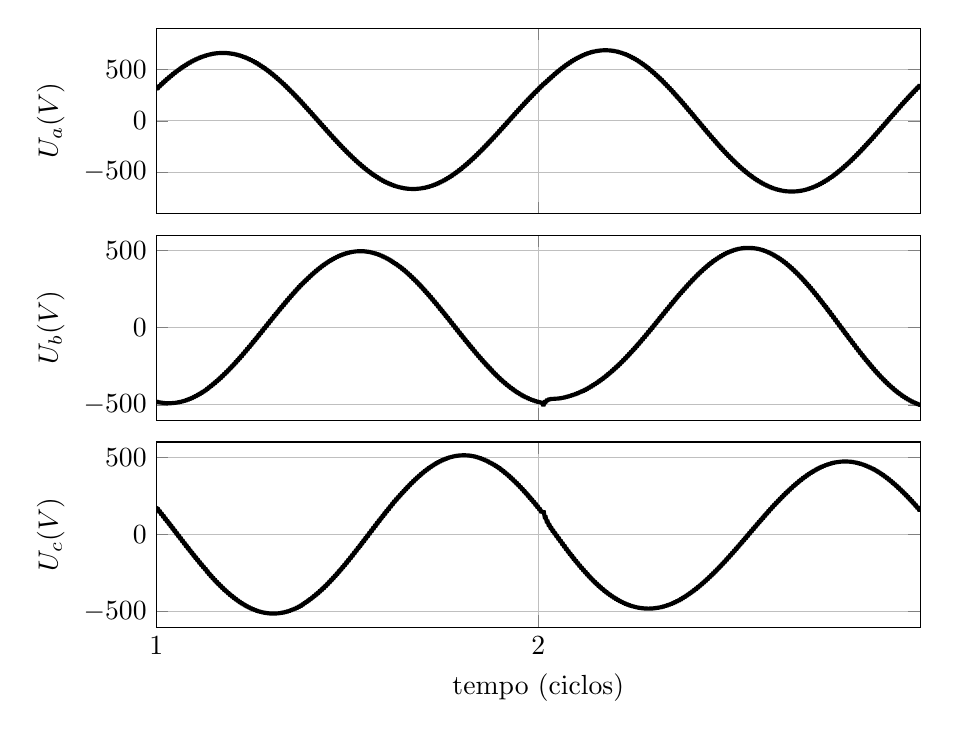
\begin{tikzpicture}

\begin{axis}[%
width=0.8\textwidth,
height=0.193917089240149\textwidth,
scale only axis,
xmin=0.0166666666666667,
xmax=0.05,
xtick={0,0.0166666666666667,0.0333333333333333},
xticklabels={\empty},
xmajorgrids,
ymin=-600,
ymax=600,
ytick={-500,    0,  500},
ylabel={$\text{U}_\text{b}\text{ (V)}$},
ymajorgrids,
name=plot2,
scaled x ticks = false,
legend columns=-1,
legend style={/tikz/every even column/.append style={column sep=0.3cm}},
legend style={font=\footnotesize}
]
\addplot [color=black,solid,line width=1.5pt,forget plot]
  table[row sep=crcr]{0.0166583333333333	-478.328989103039\\
0.0167	-481.372762295986\\
0.0167416666666667	-481.372762295986\\
0.0167833333333333	-483.944387417357\\
0.016825	-483.944387417357\\
0.0168666666666667	-486.043904769891\\
0.0169083333333333	-486.043904769891\\
0.01695	-487.669342075457\\
0.0169916666666667	-487.669342075457\\
0.0170333333333333	-488.81912329053\\
0.017075	-488.81912329053\\
0.0171166666666667	-489.492376222951\\
0.0171583333333333	-489.492376222951\\
0.0172	-489.689089295181\\
0.0172416666666667	-489.689089295181\\
0.0172833333333333	-489.410057478733\\
0.017325	-489.410057478733\\
0.0173666666666667	-488.656714544629\\
0.0174083333333333	-488.656714544629\\
0.01745	-487.430933830334\\
0.0174916666666667	-487.430933830334\\
0.0175333333333333	-485.734862735459\\
0.017575	-485.734862735459\\
0.0176166666666667	-483.570824107468\\
0.0176583333333333	-483.570824107468\\
0.0177	-480.941176730971\\
0.0177416666666667	-480.941176730971\\
0.0177833333333333	-477.848873406491\\
0.017825	-477.848873406491\\
0.0178666666666667	-474.296687037085\\
0.0179083333333333	-474.296687037085\\
0.01795	-470.287554266504\\
0.0179916666666667	-470.287554266504\\
0.0180333333333333	-465.824994538518\\
0.018075	-465.824994538518\\
0.0181166666666667	-460.912896166831\\
0.0181583333333333	-460.912896166831\\
0.0182	-455.555544349316\\
0.0182416666666667	-455.555544349316\\
0.0182833333333333	-449.757632700212\\
0.018325	-449.757632700212\\
0.0183666666666667	-443.524266807923\\
0.0184083333333333	-443.524266807923\\
0.01845	-436.860963041735\\
0.0184916666666667	-436.860963041735\\
0.0185333333333333	-429.773645406549\\
0.018575	-429.773645406549\\
0.0186166666666667	-422.2686421737\\
0.0186583333333333	-422.2686421737\\
0.0187	-414.352682994809\\
0.0187416666666667	-414.352682994809\\
0.0187833333333333	-406.710604021129\\
0.018825	-406.710604021129\\
0.0188666666666667	-396.968651829484\\
0.0189083333333333	-396.968651829484\\
0.01895	-387.24430030011\\
0.0189916666666667	-387.24430030011\\
0.0190333333333333	-377.413842111121\\
0.019075	-377.413842111121\\
0.0191166666666667	-367.3960735467\\
0.0191583333333333	-367.3960735467\\
0.0192	-357.12553953726\\
0.0192416666666667	-357.12553953726\\
0.0192833333333333	-346.559303382721\\
0.019325	-346.559303382721\\
0.0193666666666667	-335.674936708767\\
0.0194083333333333	-335.674936708767\\
0.01945	-324.465686057335\\
0.0194916666666667	-324.465686057335\\
0.0195333333333333	-312.935239244225\\
0.019575	-312.935239244225\\
0.0196166666666667	-301.093266862382\\
0.0196583333333333	-301.093266862382\\
0.0197	-288.95219973374\\
0.0197416666666667	-288.95219973374\\
0.0197833333333333	-276.525463982029\\
0.019825	-276.525463982029\\
0.0198666666666667	-263.82538033546\\
0.0199083333333333	-263.82538033546\\
0.01995	-250.865057706918\\
0.0199916666666667	-250.865057706918\\
0.0200333333333333	-237.656697428642\\
0.020075	-237.656697428642\\
0.0201166666666667	-224.212271375033\\
0.0201583333333333	-224.212271375033\\
0.0202	-210.543848998092\\
0.0202416666666667	-210.543848998092\\
0.0202833333333333	-196.6637735981\\
0.020325	-196.6637735981\\
0.0203666666666667	-182.584756063204\\
0.0204083333333333	-182.584756063204\\
0.02045	-168.319897946886\\
0.0204916666666667	-168.319897946886\\
0.0205333333333333	-153.882668002172\\
0.020575	-153.882668002172\\
0.0206166666666667	-139.286855686717\\
0.0206583333333333	-139.286855686717\\
0.0207	-124.546519243168\\
0.0207416666666667	-124.546519243168\\
0.0207833333333333	-109.675923407492\\
0.020825	-109.675923407492\\
0.0208666666666667	-94.6884951690301\\
0.0209083333333333	-94.6884951690301\\
0.02095	-79.6023211852309\\
0.0209916666666667	-79.6023211852309\\
0.0210333333333333	-64.4296541414652\\
0.021075	-64.4296541414652\\
0.0211166666666667	-49.1854677870168\\
0.0211583333333333	-49.1854677870168\\
0.0212	-33.8847697005379\\
0.0212416666666667	-33.8847697005379\\
0.0212833333333333	-18.5423320716325\\
0.021325	-18.5423320716325\\
0.0213666666666667	-3.1725945533516\\
0.0214083333333333	-3.1725945533516\\
0.02145	12.2102617721841\\
0.0214916666666667	12.2102617721841\\
0.0215333333333333	27.5921432856442\\
0.021575	27.5921432856442\\
0.0216166666666667	42.9588704890498\\
0.0216583333333333	42.9588704890498\\
0.0217	58.2960537853681\\
0.0217416666666667	58.2960537853681\\
0.0217833333333333	73.5890384864759\\
0.021825	73.5890384864759\\
0.0218666666666667	88.82269659409\\
0.0219083333333333	88.82269659409\\
0.02195	103.982669291038\\
0.0219916666666667	103.982669291038\\
0.0220333333333333	119.053037141893\\
0.022075	119.053037141893\\
0.0221166666666667	134.01853586672\\
0.0221583333333333	134.01853586672\\
0.0222	148.863909368128\\
0.0222416666666667	148.863909368128\\
0.0222833333333333	163.573956427556\\
0.022325	163.573956427556\\
0.0223666666666667	178.133568427636\\
0.0224083333333333	178.133568427636\\
0.02245	192.527757716713\\
0.0224916666666667	192.527757716713\\
0.0225333333333333	206.741679404245\\
0.022575	206.741679404245\\
0.0226166666666667	220.760649670751\\
0.0226583333333333	220.760649670751\\
0.0227	234.570162946369\\
0.0227416666666667	234.570162946369\\
0.0227833333333333	248.155909263895\\
0.022825	248.155909263895\\
0.0228666666666667	261.687830320942\\
0.0229083333333333	261.687830320942\\
0.02295	274.986604079196\\
0.0229916666666667	274.986604079196\\
0.0230333333333333	286.928801747272\\
0.023075	286.928801747272\\
0.0231166666666667	298.950506950644\\
0.0231583333333333	298.950506950644\\
0.0232	310.924864102034\\
0.0232416666666667	310.924864102034\\
0.0232833333333333	322.756989832147\\
0.023325	322.756989832147\\
0.0233666666666667	334.367084014297\\
0.0234083333333333	334.367084014297\\
0.02345	345.69602196514\\
0.0234916666666667	345.69602196514\\
0.0235333333333333	356.703461032175\\
0.023575	356.703461032175\\
0.0236166666666667	367.363371170442\\
0.0236583333333333	367.363371170442\\
0.0237	377.659204280424\\
0.0237416666666667	377.659204280424\\
0.0237833333333333	387.579795487262\\
0.023825	387.579795487262\\
0.0238666666666667	397.116425283701\\
0.0239083333333333	397.116425283701\\
0.02395	406.261310362139\\
0.0239916666666667	406.261310362139\\
0.0240333333333333	415.0053223807\\
0.024075	415.0053223807\\
0.0241166666666667	423.340732147141\\
0.0241583333333333	423.340732147141\\
0.0242	431.258683016742\\
0.0242416666666667	431.258683016742\\
0.0242833333333333	438.750365395371\\
0.024325	438.750365395371\\
0.0243666666666667	445.807262831054\\
0.0244083333333333	445.807262831054\\
0.02445	452.421342397773\\
0.0244916666666667	452.421342397773\\
0.0245333333333333	458.585161293933\\
0.024575	458.585161293933\\
0.0246166666666667	464.291905294308\\
0.0246583333333333	464.291905294308\\
0.0247	469.535383109734\\
0.0247416666666667	469.535383109734\\
0.0247833333333333	474.309999446141\\
0.024825	474.309999446141\\
0.0248666666666667	478.610723480444\\
0.0249083333333333	478.610723480444\\
0.02495	482.432523836755\\
0.0249916666666667	482.432523836755\\
0.0250333333333333	485.772612186125\\
0.025075	485.772612186125\\
0.0251166666666667	488.627883686145\\
0.0251583333333333	488.627883686145\\
0.0252	490.994391489966\\
0.0252416666666667	490.994391489966\\
0.0252833333333333	492.869784189106\\
0.025325	492.869784189106\\
0.0253666666666667	494.252063559781\\
0.0254083333333333	494.252063559781\\
0.02545	495.139387583695\\
0.0254916666666667	495.139387583695\\
0.0255333333333333	495.530061759552\\
0.025575	495.530061759552\\
0.0256166666666667	495.422663936061\\
0.0256583333333333	495.422663936061\\
0.0257	494.816230581684\\
0.0257416666666667	494.816230581684\\
0.0257833333333333	493.710425995119\\
0.025825	493.710425995119\\
0.0258666666666667	492.105654148384\\
0.0259083333333333	492.105654148384\\
0.02595	490.003108134894\\
0.0259916666666667	490.003108134894\\
0.0260333333333333	487.404961487327\\
0.026075	487.404961487327\\
0.0261166666666667	484.313069214194\\
0.0261583333333333	484.313069214194\\
0.0262	480.731558886196\\
0.0262416666666667	480.731558886196\\
0.0262833333333333	476.664323712434\\
0.026325	476.664323712434\\
0.0263666666666667	472.115829454631\\
0.0264083333333333	472.115829454631\\
0.02645	467.091068733291\\
0.0264916666666667	467.091068733291\\
0.0265333333333333	461.595540479995\\
0.026575	461.595540479995\\
0.0266166666666667	455.635234907076\\
0.0266583333333333	455.635234907076\\
0.0267	449.21662231492\\
0.0267416666666667	449.21662231492\\
0.0267833333333333	442.346643428456\\
0.026825	442.346643428456\\
0.0268666666666667	435.032699614098\\
0.0269083333333333	435.032699614098\\
0.02695	427.282642172915\\
0.0269916666666667	427.282642172915\\
0.0270333333333333	418.527982244731\\
0.027075	418.527982244731\\
0.0271166666666667	410.672570182659\\
0.0271583333333333	410.672570182659\\
0.0272	402.276872290978\\
0.0272416666666667	402.276872290978\\
0.0272833333333333	393.223850223727\\
0.027325	393.223850223727\\
0.0273666666666667	383.609151155178\\
0.0274083333333333	383.609151155178\\
0.02745	373.508718653929\\
0.0274916666666667	373.508718653929\\
0.0275333333333333	362.979579538073\\
0.027575	362.979579538073\\
0.0276166666666667	352.061894709897\\
0.0276583333333333	352.061894709897\\
0.0277	340.783205444461\\
0.0277416666666667	340.783205444461\\
0.0277833333333333	329.162781541968\\
0.027825	329.162781541968\\
0.0278666666666667	317.215226351439\\
0.0279083333333333	317.215226351439\\
0.02795	304.953068995059\\
0.0279916666666667	304.953068995059\\
0.0280333333333333	292.388308765939\\
0.028075	292.388308765939\\
0.0281166666666667	279.533394256386\\
0.0281583333333333	279.533394256386\\
0.0282	266.401997020689\\
0.0282416666666667	266.401997020689\\
0.0282833333333333	253.007121767018\\
0.028325	253.007121767018\\
0.0283666666666667	239.363037342399\\
0.0284083333333333	239.363037342399\\
0.02845	225.484309796947\\
0.0284916666666667	225.484309796947\\
0.0285333333333333	211.385672071801\\
0.028575	211.385672071801\\
0.0286166666666667	197.081935254737\\
0.0286583333333333	197.081935254737\\
0.0287	182.587950486431\\
0.0287416666666667	182.587950486431\\
0.0287833333333333	167.918604082923\\
0.028825	167.918604082923\\
0.0288666666666667	153.088829011011\\
0.0289083333333333	153.088829011011\\
0.02895	138.113619934855\\
0.0289916666666667	138.113619934855\\
0.0290333333333333	123.008044204917\\
0.029075	123.008044204917\\
0.0291166666666667	107.788100944899\\
0.0291583333333333	107.788100944899\\
0.0292	92.4664220892656\\
0.0292416666666667	92.4664220892656\\
0.0292833333333333	77.0599110293703\\
0.029325	77.0599110293703\\
0.0293666666666667	61.5839402726698\\
0.0294083333333333	61.5839402726698\\
0.02945	46.0538191073489\\
0.0294916666666667	46.0538191073489\\
0.0295333333333333	30.4851141949034\\
0.029575	30.4851141949034\\
0.0296166666666667	14.8937682112207\\
0.0296583333333333	14.8937682112207\\
0.0297	-0.703957306529608\\
0.0297416666666667	-0.703957306529608\\
0.0297833333333333	-16.2916492298269\\
0.029825	-16.2916492298269\\
0.0298666666666667	-31.8529362123827\\
0.0299083333333333	-31.8529362123827\\
0.02995	-47.371649369948\\
0.0299916666666667	-47.371649369948\\
0.0300333333333333	-62.8319222299047\\
0.030075	-62.8319222299047\\
0.0301166666666667	-78.2183969102601\\
0.0301583333333333	-78.2183969102601\\
0.0302	-93.5154108314719\\
0.0302416666666667	-93.5154108314719\\
0.0302833333333333	-108.70816278091\\
0.030325	-108.70816278091\\
0.0303666666666667	-123.782356080195\\
0.0304083333333333	-123.782356080195\\
0.03045	-138.723507249364\\
0.0304916666666667	-138.723507249364\\
0.0305333333333333	-153.517339096442\\
0.030575	-153.517339096442\\
0.0306166666666667	-168.149764544084\\
0.0306583333333333	-168.149764544084\\
0.0307	-182.60688669631\\
0.0307416666666667	-182.60688669631\\
0.0307833333333333	-196.875004412733\\
0.030825	-196.875004412733\\
0.0308666666666667	-210.940621254231\\
0.0309083333333333	-210.940621254231\\
0.03095	-224.790455634942\\
0.0309916666666667	-224.790455634942\\
0.0310333333333333	-238.411450801645\\
0.031075	-238.411450801645\\
0.0311166666666667	-251.788204920739\\
0.0311583333333333	-251.788204920739\\
0.0312	-264.319493294975\\
0.0312416666666667	-264.319493294975\\
0.0312833333333333	-278.081845363642\\
0.031325	-278.081845363642\\
0.0313666666666667	-291.211888263673\\
0.0314083333333333	-291.211888263673\\
0.03145	-303.807007713181\\
0.0314916666666667	-303.807007713181\\
0.0315333333333333	-315.936364357588\\
0.031575	-315.936364357588\\
0.0316166666666667	-327.655020751537\\
0.0316583333333333	-327.655020751537\\
0.0317	-338.998550237152\\
0.0317416666666667	-338.998550237152\\
0.0317833333333333	-349.984949605885\\
0.031825	-349.984949605885\\
0.0318666666666667	-360.618974262017\\
0.0319083333333333	-360.618974262017\\
0.03195	-370.896795074955\\
0.0319916666666667	-370.896795074955\\
0.0320333333333333	-380.809923421548\\
0.032075	-380.809923421548\\
0.0321166666666667	-390.348041070204\\
0.0321583333333333	-390.348041070204\\
0.0322	-399.500455565927\\
0.0322416666666667	-399.500455565927\\
0.0322833333333333	-408.258433783543\\
0.032325	-408.258433783543\\
0.0323666666666667	-416.612673979994\\
0.0324083333333333	-416.612673979994\\
0.03245	-424.555376388038\\
0.0324916666666667	-424.555376388038\\
0.0325333333333333	-432.079651399668\\
0.032575	-432.079651399668\\
0.0326166666666667	-439.17912856472\\
0.0326583333333333	-439.17912856472\\
0.0327	-445.847803165625\\
0.0327416666666667	-445.847803165625\\
0.0327833333333333	-452.079952433882\\
0.032825	-452.079952433882\\
0.0328666666666667	-457.870112681898\\
0.0329083333333333	-457.870112681898\\
0.03295	-463.213095942823\\
0.0329916666666667	-463.213095942823\\
0.0330333333333333	-468.104025539882\\
0.033075	-468.104025539882\\
0.0331166666666667	-472.538375275198\\
0.0331583333333333	-472.538375275198\\
0.0332	-476.512043591712\\
0.0332416666666667	-476.512043591712\\
0.0332833333333333	-480.021998518076\\
0.033325	-480.021998518076\\
0.0333666666666667	-483.062409528906\\
0.0334083333333333	-483.062409528906\\
0.03345	-485.632179354782\\
0.0334916666666667	-485.632179354782\\
0.0335333333333333	-498.998270566993\\
0.033575	-498.998270566993\\
0.0336166666666667	-481.782582963858\\
0.0336583333333333	-481.782582963858\\
0.0337	-471.288948850027\\
0.0337416666666667	-471.288948850027\\
0.0337833333333333	-465.459114040876\\
0.033825	-465.459114040876\\
0.0338666666666667	-462.647848629665\\
0.0339083333333333	-462.647848629665\\
0.03395	-461.417560400509\\
0.0339916666666667	-461.417560400509\\
0.0340333333333333	-460.731633382674\\
0.034075	-460.731633382674\\
0.0341166666666667	-459.951982625119\\
0.0341583333333333	-459.951982625119\\
0.0342	-458.758531093\\
0.0342416666666667	-458.758531093\\
0.0342833333333333	-457.045782912744\\
0.034325	-457.045782912744\\
0.0343666666666667	-454.82926213895\\
0.0344083333333333	-454.82926213895\\
0.03445	-452.172796925181\\
0.0344916666666667	-452.172796925181\\
0.0345333333333333	-449.145658792875\\
0.034575	-449.145658792875\\
0.0346166666666667	-445.800265404507\\
0.0346583333333333	-445.800265404507\\
0.0347	-442.166059354816\\
0.0347416666666667	-442.166059354816\\
0.0347833333333333	-438.252372103144\\
0.034825	-438.252372103144\\
0.0348666666666667	-434.054953798003\\
0.0349083333333333	-434.054953798003\\
0.03495	-429.562674435509\\
0.0349916666666667	-429.562674435509\\
0.0350333333333333	-424.762700040261\\
0.035075	-424.762700040261\\
0.0351166666666667	-419.643661421394\\
0.0351583333333333	-419.643661421394\\
0.0352	-414.197053720857\\
0.0352416666666667	-414.197053720857\\
0.0352833333333333	-408.523882649902\\
0.035325	-408.523882649902\\
0.0353666666666667	-402.479291356868\\
0.0354083333333333	-402.479291356868\\
0.03545	-395.601828599323\\
0.0354916666666667	-395.601828599323\\
0.0355333333333333	-388.546283162184\\
0.035575	-388.546283162184\\
0.0356166666666667	-381.262052118517\\
0.0356583333333333	-381.262052118517\\
0.0357	-373.714229076942\\
0.0357416666666667	-373.714229076942\\
0.0357833333333333	-365.874593646954\\
0.035825	-365.874593646954\\
0.0358666666666667	-357.724034021534\\
0.0359083333333333	-357.724034021534\\
0.03595	-349.251553064004\\
0.0359916666666667	-349.251553064004\\
0.0360333333333333	-340.452622235918\\
0.036075	-340.452622235918\\
0.0361166666666667	-331.327227991727\\
0.0361583333333333	-331.327227991727\\
0.0362	-321.878129980668\\
0.0362416666666667	-321.878129980668\\
0.0362833333333333	-312.109568466451\\
0.036325	-312.109568466451\\
0.0363666666666667	-302.026644843582\\
0.0364083333333333	-302.026644843582\\
0.03645	-291.63387748511\\
0.0364916666666667	-291.63387748511\\
0.0365333333333333	-280.937199605059\\
0.036575	-280.937199605059\\
0.0366166666666667	-269.942114366078\\
0.0366583333333333	-269.942114366078\\
0.0367	-258.654477866822\\
0.0367416666666667	-258.654477866822\\
0.0367833333333333	-247.080567388712\\
0.036825	-247.080567388712\\
0.0368666666666667	-235.227176729096\\
0.0369083333333333	-235.227176729096\\
0.03695	-223.101681785848\\
0.0369916666666667	-223.101681785848\\
0.0370333333333333	-210.712058862678\\
0.037075	-210.712058862678\\
0.0371166666666667	-198.066879573849\\
0.0371583333333333	-198.066879573849\\
0.0372	-185.175292454286\\
0.0372416666666667	-185.175292454286\\
0.0372833333333333	-172.046999319569\\
0.037325	-172.046999319569\\
0.0373666666666667	-158.692016960269\\
0.0374083333333333	-158.692016960269\\
0.03745	-145.121500911102\\
0.0374916666666667	-145.121500911102\\
0.0375333333333333	-131.346961858294\\
0.037575	-131.346961858294\\
0.0376166666666667	-117.380802663719\\
0.0376583333333333	-117.380802663719\\
0.0377	-103.235234173154\\
0.0377416666666667	-103.235234173154\\
0.0377833333333333	-88.9164304808335\\
0.037825	-88.9164304808335\\
0.0378666666666667	-74.439342100256\\
0.0379083333333333	-74.439342100256\\
0.03795	-59.8184609425996\\
0.0379916666666667	-59.8184609425996\\
0.0380333333333333	-45.0680374599692\\
0.038075	-45.0680374599692\\
0.0381166666666667	-30.2022370755135\\
0.0381583333333333	-30.2022370755135\\
0.0382	-15.2353217495658\\
0.0382416666666667	-15.2353217495658\\
0.0382833333333333	-0.181794007753641\\
0.038325	-0.181794007753641\\
0.0383666666666667	14.9435042350192\\
0.0384083333333333	14.9435042350192\\
0.03845	30.1252956286667\\
0.0384916666666667	30.1252956286667\\
0.0385333333333333	45.3486629556394\\
0.038575	45.3486629556394\\
0.0386166666666667	60.5972401707852\\
0.0386583333333333	60.5972401707852\\
0.0387	75.8549297738552\\
0.0387416666666667	75.8549297738552\\
0.0387833333333333	91.1054325668948\\
0.038825	91.1054325668948\\
0.0388666666666667	106.332243601449\\
0.0389083333333333	106.332243601449\\
0.03895	121.518722394686\\
0.0389916666666667	121.518722394686\\
0.0390333333333333	136.648130986171\\
0.039075	136.648130986171\\
0.0391166666666667	151.703658745296\\
0.0391583333333333	151.703658745296\\
0.0392	166.6684438936\\
0.0392416666666667	166.6684438936\\
0.0392833333333333	181.525594900189\\
0.039325	181.525594900189\\
0.0393666666666667	196.258213496354\\
0.0394083333333333	196.258213496354\\
0.03945	211.11916789107\\
0.0394916666666667	211.11916789107\\
0.0395333333333333	225.228256753655\\
0.039575	225.228256753655\\
0.0396166666666667	239.176704133903\\
0.0396583333333333	239.176704133903\\
0.0397	253.050541633453\\
0.0397416666666667	253.050541633453\\
0.0397833333333333	266.794622440343\\
0.039825	266.794622440343\\
0.0398666666666667	280.36352639823\\
0.0399083333333333	280.36352639823\\
0.03995	293.720079804169\\
0.0399916666666667	293.720079804169\\
0.0400333333333333	306.834840978919\\
0.040075	306.834840978919\\
0.0401166666666667	319.684432072053\\
0.0401583333333333	319.684432072053\\
0.0402	332.249529221863\\
0.0402416666666667	332.249529221863\\
0.0402833333333333	344.513518148991\\
0.040325	344.513518148991\\
0.0403666666666667	356.461398472636\\
0.0404083333333333	356.461398472636\\
0.04045	368.07906117244\\
0.0404916666666667	368.07906117244\\
0.0405333333333333	379.352665704272\\
0.040575	379.352665704272\\
0.0406166666666667	390.268254951875\\
0.0406583333333333	390.268254951875\\
0.0407	400.81284512302\\
0.0407416666666667	400.81284512302\\
0.0407833333333333	410.973175722926\\
0.040825	410.973175722926\\
0.0408666666666667	420.736369760103\\
0.0409083333333333	420.736369760103\\
0.04095	430.089939730837\\
0.0409916666666667	430.089939730837\\
0.0410333333333333	439.02189748336\\
0.041075	439.02189748336\\
0.0411166666666667	447.520797951081\\
0.0411583333333333	447.520797951081\\
0.0412	455.57576068455\\
0.0412416666666667	455.57576068455\\
0.0412833333333333	463.176477754051\\
0.041325	463.176477754051\\
0.0413666666666667	470.313215198367\\
0.0414083333333333	470.313215198367\\
0.04145	476.976813020432\\
0.0414916666666667	476.976813020432\\
0.0415333333333333	483.158335808922\\
0.041575	483.158335808922\\
0.0416166666666667	488.850790106914\\
0.0416583333333333	488.850790106914\\
0.0417	494.046217480564\\
0.0417416666666667	494.046217480564\\
0.0417833333333333	498.740107259914\\
0.041825	498.740107259914\\
0.0418666666666667	502.92186011784\\
0.0419083333333333	502.92186011784\\
0.04195	506.583545623777\\
0.0419916666666667	506.583545623777\\
0.0420333333333333	509.721710214485\\
0.042075	509.721710214485\\
0.0421166666666667	512.332784100593\\
0.0421583333333333	512.332784100593\\
0.0422	514.413279158182\\
0.0422416666666667	514.413279158182\\
0.0422833333333333	515.9599757688\\
0.042325	515.9599757688\\
0.0423666666666667	516.970100515159\\
0.0424083333333333	516.970100515159\\
0.04245	517.441480758459\\
0.0424916666666667	517.441480758459\\
0.0425333333333333	517.372752150282\\
0.042575	517.372752150282\\
0.0426166666666667	516.762847399441\\
0.0426583333333333	516.762847399441\\
0.0427	515.611781315798\\
0.0427416666666667	515.611781315798\\
0.0427833333333333	513.92048533442\\
0.042825	513.92048533442\\
0.0428666666666667	511.690288385606\\
0.0429083333333333	511.690288385606\\
0.04295	508.923157960981\\
0.0429916666666667	508.923157960981\\
0.0430333333333333	505.62173995849\\
0.043075	505.62173995849\\
0.0431166666666667	501.78931073118\\
0.0431583333333333	501.78931073118\\
0.0432	497.429767725351\\
0.0432416666666667	497.429767725351\\
0.0432833333333333	492.547621632959\\
0.043325	492.547621632959\\
0.0433666666666667	487.14798908254\\
0.0434083333333333	487.14798908254\\
0.04345	481.236584761708\\
0.0434916666666667	481.236584761708\\
0.0435333333333333	474.813193437904\\
0.043575	474.813193437904\\
0.0436166666666667	467.617975016633\\
0.0436583333333333	467.617975016633\\
0.0437	460.640009785613\\
0.0437416666666667	460.640009785613\\
0.0437833333333333	453.026742559859\\
0.043825	453.026742559859\\
0.0438666666666667	444.829079350061\\
0.0439083333333333	444.829079350061\\
0.04395	436.091902638318\\
0.0439916666666667	436.091902638318\\
0.0440333333333333	426.854279959608\\
0.044075	426.854279959608\\
0.0441166666666667	417.147056125927\\
0.0441583333333333	417.147056125927\\
0.0442	406.993617805562\\
0.0442416666666667	406.993617805562\\
0.0442833333333333	396.411764190075\\
0.044325	396.411764190075\\
0.0443666666666667	385.415729474773\\
0.0444083333333333	385.415729474773\\
0.04445	374.017909476246\\
0.0444916666666667	374.017909476246\\
0.0445333333333333	362.230108715941\\
0.044575	362.230108715941\\
0.0446166666666667	350.064119512135\\
0.0446583333333333	350.064119512135\\
0.0447	337.533091230516\\
0.0447416666666667	337.533091230516\\
0.0447833333333333	324.649922144971\\
0.044825	324.649922144971\\
0.0448666666666667	311.428439890778\\
0.0449083333333333	311.428439890778\\
0.04495	297.883125554185\\
0.0449916666666667	297.883125554185\\
0.0450333333333333	284.028841924275\\
0.045075	284.028841924275\\
0.0451166666666667	269.880782608134\\
0.0451583333333333	269.880782608134\\
0.0452	255.454385329104\\
0.0452416666666667	255.454385329104\\
0.0452833333333333	240.765301798375\\
0.045325	240.765301798375\\
0.0453666666666667	225.829384538562\\
0.0454083333333333	225.829384538562\\
0.04545	210.662681339409\\
0.0454916666666667	210.662681339409\\
0.0455333333333333	195.281430438134\\
0.045575	195.281430438134\\
0.0456166666666667	179.702077212704\\
0.0456583333333333	179.702077212704\\
0.0457	163.941485539902\\
0.0457416666666667	163.941485539902\\
0.0457833333333333	148.015394086019\\
0.045825	148.015394086019\\
0.0458666666666667	131.941232581943\\
0.0459083333333333	131.941232581943\\
0.04595	115.733018226992\\
0.0459916666666667	115.733018226992\\
0.0460333333333333	99.4155506737076\\
0.046075	99.4155506737076\\
0.0461166666666667	83.0048753817104\\
0.0461583333333333	83.0048753817104\\
0.0462	66.5169842374124\\
0.0462416666666667	66.5169842374124\\
0.0462833333333333	49.9685533749797\\
0.046325	49.9685533749797\\
0.0463666666666667	33.3767580588298\\
0.0464083333333333	33.3767580588298\\
0.04645	16.7590504552267\\
0.0464916666666667	16.7590504552267\\
0.0465333333333333	0.132970181758703\\
0.046575	0.132970181758703\\
0.0466166666666667	-16.4839901619608\\
0.0466583333333333	-16.4839901619608\\
0.0467	-33.0746636693815\\
0.0467416666666667	-33.0746636693815\\
0.0467833333333333	-49.6211722773108\\
0.046825	-49.6211722773108\\
0.0468666666666667	-66.1070457181566\\
0.0469083333333333	-66.1070457181566\\
0.04695	-82.5154452365718\\
0.0469916666666667	-82.5154452365718\\
0.0470333333333333	-98.8296440709486\\
0.047075	-98.8296440709486\\
0.0471166666666667	-115.033091242092\\
0.0471583333333333	-115.033091242092\\
0.0472	-131.109433370824\\
0.0472416666666667	-131.109433370824\\
0.0472833333333333	-147.042503492819\\
0.047325	-147.042503492819\\
0.0473666666666667	-162.816333505291\\
0.0474083333333333	-162.816333505291\\
0.04745	-178.41516835848\\
0.0474916666666667	-178.41516835848\\
0.0475333333333333	-193.8234809494\\
0.047575	-193.8234809494\\
0.0476166666666667	-209.025986747927\\
0.0476583333333333	-209.025986747927\\
0.0477	-223.904186047126\\
0.0477416666666667	-223.904186047126\\
0.0477833333333333	-238.606857549563\\
0.047825	-238.606857549563\\
0.0478666666666667	-253.47478702492\\
0.0479083333333333	-253.47478702492\\
0.04795	-267.938417779568\\
0.0479916666666667	-267.938417779568\\
0.0480333333333333	-282.029617204579\\
0.048075	-282.029617204579\\
0.0481166666666667	-295.766635150869\\
0.0481583333333333	-295.766635150869\\
0.0482	-309.161799602257\\
0.0482416666666667	-309.161799602257\\
0.0482833333333333	-322.219833483858\\
0.048325	-322.219833483858\\
0.0483666666666667	-334.938825256652\\
0.0484083333333333	-334.938825256652\\
0.04845	-347.312016422018\\
0.0484916666666667	-347.312016422018\\
0.0485333333333333	-359.329644222863\\
0.048575	-359.329644222863\\
0.0486166666666667	-370.980465786804\\
0.0486583333333333	-370.980465786804\\
0.0487	-382.252844743103\\
0.0487416666666667	-382.252844743103\\
0.0487833333333333	-393.135216849012\\
0.048825	-393.135216849012\\
0.0488666666666667	-403.617584174739\\
0.0489083333333333	-403.617584174739\\
0.04895	-413.689218945276\\
0.0489916666666667	-413.689218945276\\
0.0490333333333333	-423.340771462502\\
0.049075	-423.340771462502\\
0.0491166666666667	-432.563452770036\\
0.0491583333333333	-432.563452770036\\
0.0492	-441.348991482752\\
0.0492416666666667	-441.348991482752\\
0.0492833333333333	-449.689568336581\\
0.049325	-449.689568336581\\
0.0493666666666667	-457.577772446396\\
0.0494083333333333	-457.577772446396\\
0.04945	-465.006594338065\\
0.0494916666666667	-465.006594338065\\
0.0495333333333333	-471.969434299032\\
0.049575	-471.969434299032\\
0.0496166666666667	-478.460118028508\\
0.0496583333333333	-478.460118028508\\
0.0497	-484.472913508959\\
0.0497416666666667	-484.472913508959\\
0.0497833333333333	-490.002697136551\\
0.049825	-490.002697136551\\
0.0498666666666667	-495.044403692677\\
0.0499083333333333	-495.044403692677\\
0.04995	-499.593400120443\\
0.0499916666666667	-499.593400120443\\
};
\end{axis}

\begin{axis}[%
width=0.8\textwidth,
height=0.193917089240149\textwidth,
scale only axis,
xmin=0.0166666666666667,
xmax=0.05,
xtick={0,0.0166666666666667,0.0333333333333333},
xticklabels={{0},{1},{2}},
xlabel={tempo (ciclos)},
xmajorgrids,
ymin=-600,
ymax=600,
ytick={-500,    0,  500},
ylabel={$\text{U}_\text{c}\text{ (V)}$},
ymajorgrids,
at=(plot2.below south west),
anchor=above north west,
scaled x ticks = false,
legend columns=-1,
legend style={/tikz/every even column/.append style={column sep=0.3cm}},
legend style={font=\footnotesize}
]
\addplot [color=black,solid,line width=1.5pt,forget plot]
  table[row sep=crcr]{0.0166583333333333	180.146044285981\\
0.0167	164.940320934484\\
0.0167416666666667	164.940320934484\\
0.0167833333333333	149.579587477261\\
0.016825	149.579587477261\\
0.0168666666666667	134.079551509137\\
0.0169083333333333	134.079551509137\\
0.01695	118.455249604828\\
0.0169916666666667	118.455249604828\\
0.0170333333333333	102.721820759597\\
0.017075	102.721820759597\\
0.0171166666666667	86.8947024886041\\
0.0171583333333333	86.8947024886041\\
0.0172	70.9897152347551\\
0.0172416666666667	70.9897152347551\\
0.0172833333333333	55.0229884605968\\
0.017325	55.0229884605968\\
0.0173666666666667	39.0107951391398\\
0.0174083333333333	39.0107951391398\\
0.01745	22.9693692316446\\
0.0174916666666667	22.9693692316446\\
0.0175333333333333	6.91476165823279\\
0.017575	6.91476165823279\\
0.0176166666666667	-9.13724020053355\\
0.0176583333333333	-9.13724020053355\\
0.0177	-25.1712876244939\\
0.0177416666666667	-25.1712876244939\\
0.0177833333333333	-41.1717016099994\\
0.017825	-41.1717016099994\\
0.0178666666666667	-57.1235450619316\\
0.0179083333333333	-57.1235450619316\\
0.01795	-73.0122416753861\\
0.0179916666666667	-73.0122416753861\\
0.0180333333333333	-88.8229904086394\\
0.018075	-88.8229904086394\\
0.0181166666666667	-104.541092542183\\
0.0181583333333333	-104.541092542183\\
0.0182	-120.151937938219\\
0.0182416666666667	-120.151937938219\\
0.0182833333333333	-135.641005542097\\
0.018325	-135.641005542097\\
0.0183666666666667	-150.993870043721\\
0.0184083333333333	-150.993870043721\\
0.01845	-166.196212093992\\
0.0184916666666667	-166.196212093992\\
0.0185333333333333	-181.2338298443\\
0.018575	-181.2338298443\\
0.0186166666666667	-196.092650491087\\
0.0186583333333333	-196.092650491087\\
0.0187	-210.758741337919\\
0.0187416666666667	-210.758741337919\\
0.0187833333333333	-224.272823986116\\
0.018825	-224.272823986116\\
0.0188666666666667	-239.924185188171\\
0.0189083333333333	-239.924185188171\\
0.01895	-254.795099361687\\
0.0189916666666667	-254.795099361687\\
0.0190333333333333	-269.036557729883\\
0.019075	-269.036557729883\\
0.0191166666666667	-282.760389233867\\
0.0191583333333333	-282.760389233867\\
0.0192	-296.057851197266\\
0.0192416666666667	-296.057851197266\\
0.0192833333333333	-308.990098283122\\
0.019325	-308.990098283122\\
0.0193666666666667	-321.590393418407\\
0.0194083333333333	-321.590393418407\\
0.01945	-333.870571911174\\
0.0194916666666667	-333.870571911174\\
0.0195333333333333	-345.828322444006\\
0.019575	-345.828322444006\\
0.0196166666666667	-357.453508661192\\
0.0196583333333333	-357.453508661192\\
0.0197	-368.732790011102\\
0.0197416666666667	-368.732790011102\\
0.0197833333333333	-379.652185798579\\
0.019825	-379.652185798579\\
0.0198666666666667	-390.200039679523\\
0.0199083333333333	-390.200039679523\\
0.01995	-400.364455853375\\
0.0199916666666667	-400.364455853375\\
0.0200333333333333	-410.135593074462\\
0.020075	-410.135593074462\\
0.0201166666666667	-419.504723697965\\
0.0201583333333333	-419.504723697965\\
0.0202	-428.463752199279\\
0.0202416666666667	-428.463752199279\\
0.0202833333333333	-437.004944992871\\
0.020325	-437.004944992871\\
0.0203666666666667	-445.120779808899\\
0.0204083333333333	-445.120779808899\\
0.02045	-452.8038978512\\
0.0204916666666667	-452.8038978512\\
0.0205333333333333	-460.047124180064\\
0.020575	-460.047124180064\\
0.0206166666666667	-466.843522119401\\
0.0206583333333333	-466.843522119401\\
0.0207	-473.186455823302\\
0.0207416666666667	-473.186455823302\\
0.0207833333333333	-479.069643185327\\
0.020825	-479.069643185327\\
0.0208666666666667	-484.487584080736\\
0.0209083333333333	-484.487584080736\\
0.02095	-489.433644253288\\
0.0209916666666667	-489.433644253288\\
0.0210333333333333	-493.903539136153\\
0.021075	-493.903539136153\\
0.0211166666666667	-497.892633124744\\
0.0211583333333333	-497.892633124744\\
0.0212	-501.396820907034\\
0.0212416666666667	-501.396820907034\\
0.0212833333333333	-504.41270742765\\
0.021325	-504.41270742765\\
0.0213666666666667	-506.937652408911\\
0.0214083333333333	-506.937652408911\\
0.02145	-508.969679717527\\
0.0214916666666667	-508.969679717527\\
0.0215333333333333	-510.507315547184\\
0.021575	-510.507315547184\\
0.0216166666666667	-511.549437470117\\
0.0216583333333333	-511.549437470117\\
0.0217	-512.095173916005\\
0.0217416666666667	-512.095173916005\\
0.0217833333333333	-512.14386626104\\
0.021825	-512.14386626104\\
0.0218666666666667	-511.694775425209\\
0.0219083333333333	-511.694775425209\\
0.02195	-510.748811874119\\
0.0219916666666667	-510.748811874119\\
0.0220333333333333	-509.305240015087\\
0.022075	-509.305240015087\\
0.0221166666666667	-507.364690126307\\
0.0221583333333333	-507.364690126307\\
0.0222	-504.928245184668\\
0.0222416666666667	-504.928245184668\\
0.0222833333333333	-501.997459837756\\
0.022325	-501.997459837756\\
0.0223666666666667	-498.57437873634\\
0.0224083333333333	-498.57437873634\\
0.02245	-494.661546862205\\
0.0224916666666667	-494.661546862205\\
0.0225333333333333	-490.262014038761\\
0.022575	-490.262014038761\\
0.0226166666666667	-485.379336077746\\
0.0226583333333333	-485.379336077746\\
0.0227	-480.017574398345\\
0.0227416666666667	-480.017574398345\\
0.0227833333333333	-474.181295093699\\
0.022825	-474.181295093699\\
0.0228666666666667	-468.132227564933\\
0.0229083333333333	-468.132227564933\\
0.02295	-461.649789032895\\
0.0229916666666667	-461.649789032895\\
0.0230333333333333	-453.193902270209\\
0.023075	-453.193902270209\\
0.0231166666666667	-444.773441113673\\
0.0231583333333333	-444.773441113673\\
0.0232	-436.251268459993\\
0.0232416666666667	-436.251268459993\\
0.0232833333333333	-427.520263672964\\
0.023325	-427.520263672964\\
0.0233666666666667	-418.493740302993\\
0.0234083333333333	-418.493740302993\\
0.02345	-409.11363513705\\
0.0234916666666667	-409.11363513705\\
0.0235333333333333	-399.348350327473\\
0.023575	-399.348350327473\\
0.0236166666666667	-389.186670490501\\
0.0236583333333333	-389.186670490501\\
0.0237	-378.630905372963\\
0.0237416666666667	-378.630905372963\\
0.0237833333333333	-367.690968950489\\
0.023825	-367.690968950489\\
0.0238666666666667	-356.380102358096\\
0.0239083333333333	-356.380102358096\\
0.02395	-344.712640572405\\
0.0239916666666667	-344.712640572405\\
0.0240333333333333	-332.700781505562\\
0.024075	-332.700781505562\\
0.0241166666666667	-320.358317577706\\
0.0241583333333333	-320.358317577706\\
0.0242	-307.6971824162\\
0.0242416666666667	-307.6971824162\\
0.0242833333333333	-294.729044137296\\
0.024325	-294.729044137296\\
0.0243666666666667	-281.465654636295\\
0.0244083333333333	-281.465654636295\\
0.02445	-267.919108296558\\
0.0244916666666667	-267.919108296558\\
0.0245333333333333	-254.101977634579\\
0.024575	-254.101977634579\\
0.0246166666666667	-240.027348361342\\
0.0246583333333333	-240.027348361342\\
0.0247	-225.708789227798\\
0.0247416666666667	-225.708789227798\\
0.0247833333333333	-211.160290317149\\
0.024825	-211.160290317149\\
0.0248666666666667	-196.39619457631\\
0.0249083333333333	-196.39619457631\\
0.02495	-181.431040895376\\
0.0249916666666667	-181.431040895376\\
0.0250333333333333	-166.279778355741\\
0.025075	-166.279778355741\\
0.0251166666666667	-150.957981557132\\
0.0251583333333333	-150.957981557132\\
0.0252	-135.480589084291\\
0.0252416666666667	-135.480589084291\\
0.0252833333333333	-119.863094908503\\
0.025325	-119.863094908503\\
0.0253666666666667	-104.121014925928\\
0.0254083333333333	-104.121014925928\\
0.02545	-88.2697324252375\\
0.0254916666666667	-88.2697324252375\\
0.0255333333333333	-72.3244975934466\\
0.025575	-72.3244975934466\\
0.0256166666666667	-56.3005347394663\\
0.0256583333333333	-56.3005347394663\\
0.0257	-40.2131789209932\\
0.0257416666666667	-40.2131789209932\\
0.0257833333333333	-24.0779930748701\\
0.025825	-24.0779930748701\\
0.0258666666666667	-7.91083206935371\\
0.0259083333333333	-7.91083206935371\\
0.02595	8.27214526930201\\
0.0259916666666667	8.27214526930201\\
0.0260333333333333	24.4542254440382\\
0.026075	24.4542254440382\\
0.0261166666666667	40.6199908695603\\
0.0261583333333333	40.6199908695603\\
0.0262	56.7516612117422\\
0.0262416666666667	56.7516612117422\\
0.0262833333333333	72.8325712785133\\
0.026325	72.8325712785133\\
0.0263666666666667	88.846063325594\\
0.0264083333333333	88.846063325594\\
0.02645	104.775539088676\\
0.0264916666666667	104.775539088676\\
0.0265333333333333	120.604489043941\\
0.026575	120.604489043941\\
0.0266166666666667	136.316517603678\\
0.0266583333333333	136.316517603678\\
0.0267	151.895365005857\\
0.0267416666666667	151.895365005857\\
0.0267833333333333	167.32492740609\\
0.026825	167.32492740609\\
0.0268666666666667	182.589276240632\\
0.0269083333333333	182.589276240632\\
0.02695	197.67267733356\\
0.0269916666666667	197.67267733356\\
0.0270333333333333	213.364075445209\\
0.027075	213.364075445209\\
0.0271166666666667	227.019890089968\\
0.0271583333333333	227.019890089968\\
0.0272	240.616905132375\\
0.0272416666666667	240.616905132375\\
0.0272833333333333	254.329291302055\\
0.027325	254.329291302055\\
0.0273666666666667	268.025476997475\\
0.0274083333333333	268.025476997475\\
0.02745	281.599414976171\\
0.0274916666666667	281.599414976171\\
0.0275333333333333	294.97178527555\\
0.027575	294.97178527555\\
0.0276166666666667	308.087625765951\\
0.0276583333333333	308.087625765951\\
0.0277	320.910690989392\\
0.0277416666666667	320.910690989392\\
0.0277833333333333	333.417415766459\\
0.027825	333.417415766459\\
0.0278666666666667	345.591780478394\\
0.0279083333333333	345.591780478394\\
0.02795	357.421558389868\\
0.0279916666666667	357.421558389868\\
0.0280333333333333	368.896047770843\\
0.028075	368.896047770843\\
0.0281166666666667	380.004638133566\\
0.0281583333333333	380.004638133566\\
0.0282	390.735700889524\\
0.0282416666666667	390.735700889524\\
0.0282833333333333	401.079183264076\\
0.028325	401.079183264076\\
0.0283666666666667	411.023979838759\\
0.0284083333333333	411.023979838759\\
0.02845	420.559255161147\\
0.0284916666666667	420.559255161147\\
0.0285333333333333	429.674638195389\\
0.028575	429.674638195389\\
0.0286166666666667	438.36034696872\\
0.0286583333333333	438.36034696872\\
0.0287	446.607237052018\\
0.0287416666666667	446.607237052018\\
0.0287833333333333	454.406798841608\\
0.028825	454.406798841608\\
0.0288666666666667	461.751128592088\\
0.0289083333333333	461.751128592088\\
0.02895	468.632892411405\\
0.0289916666666667	468.632892411405\\
0.0290333333333333	475.045294902946\\
0.029075	475.045294902946\\
0.0291166666666667	480.981879753185\\
0.0291583333333333	480.981879753185\\
0.0292	486.437323221531\\
0.0292416666666667	486.437323221531\\
0.0292833333333333	491.406267662622\\
0.029325	491.406267662622\\
0.0293666666666667	495.883928335018\\
0.0294083333333333	495.883928335018\\
0.02945	499.866055615843\\
0.0294916666666667	499.866055615843\\
0.0295333333333333	503.348727665725\\
0.029575	503.348727665725\\
0.0296166666666667	506.32826432485\\
0.0296583333333333	506.32826432485\\
0.0297	508.801283597195\\
0.0297416666666667	508.801283597195\\
0.0297833333333333	510.764841924053\\
0.029825	510.764841924053\\
0.0298666666666667	512.216584774959\\
0.0299083333333333	512.216584774959\\
0.02995	513.154859732115\\
0.0299916666666667	513.154859732115\\
0.0300333333333333	513.578772270348\\
0.030075	513.578772270348\\
0.0301166666666667	513.488424330974\\
0.0301583333333333	513.488424330974\\
0.0302	512.883757056606\\
0.0302416666666667	512.883757056606\\
0.0302833333333333	511.766137250959\\
0.030325	511.766137250959\\
0.0303666666666667	510.137917947873\\
0.0304083333333333	510.137917947873\\
0.03045	508.001445961413\\
0.0304916666666667	508.001445961413\\
0.0305333333333333	505.359600176138\\
0.030575	505.359600176138\\
0.0306166666666667	502.215762753867\\
0.0306583333333333	502.215762753867\\
0.0307	498.573803881371\\
0.0307416666666667	498.573803881371\\
0.0307833333333333	494.438070082401\\
0.030825	494.438070082401\\
0.0308666666666667	489.813374792093\\
0.0309083333333333	489.813374792093\\
0.03095	484.704989725497\\
0.0309916666666667	484.704989725497\\
0.0310333333333333	479.118636144247\\
0.031075	479.118636144247\\
0.0311166666666667	473.056878981776\\
0.0311583333333333	473.056878981776\\
0.0312	465.70497451635\\
0.0312416666666667	465.70497451635\\
0.0312833333333333	459.969396284381\\
0.031325	459.969396284381\\
0.0313666666666667	453.306592780928\\
0.0314083333333333	453.306592780928\\
0.03145	445.858568368547\\
0.0314916666666667	445.858568368547\\
0.0315333333333333	437.745808877649\\
0.031575	437.745808877649\\
0.0316166666666667	429.069979853876\\
0.0316583333333333	429.069979853876\\
0.0317	419.905934001149\\
0.0317416666666667	419.905934001149\\
0.0317833333333333	410.303765791928\\
0.031825	410.303765791928\\
0.0318666666666667	400.294607272454\\
0.0319083333333333	400.294607272454\\
0.03195	389.897105361559\\
0.0319916666666667	389.897105361559\\
0.0320333333333333	379.123044209476\\
0.032075	379.123044209476\\
0.0321166666666667	367.981436719615\\
0.0321583333333333	367.981436719615\\
0.0322	356.480648193397\\
0.0322416666666667	356.480648193397\\
0.0322833333333333	344.631665623135\\
0.032325	344.631665623135\\
0.0323666666666667	332.444618169672\\
0.0324083333333333	332.444618169672\\
0.03245	319.931569517662\\
0.0324916666666667	319.931569517662\\
0.0325333333333333	307.105674240986\\
0.032575	307.105674240986\\
0.0326166666666667	293.98058862761\\
0.0326583333333333	293.98058862761\\
0.0327	280.570215241566\\
0.0327416666666667	280.570215241566\\
0.0327833333333333	266.888552880234\\
0.032825	266.888552880234\\
0.0328666666666667	252.949637821179\\
0.0329083333333333	252.949637821179\\
0.03295	238.76754490619\\
0.0329916666666667	238.76754490619\\
0.0330333333333333	224.356417917444\\
0.033075	224.356417917444\\
0.0331166666666667	209.730506383327\\
0.0331583333333333	209.730506383327\\
0.0332	194.904179567313\\
0.0332416666666667	194.904179567313\\
0.0332833333333333	179.892215293915\\
0.033325	179.892215293915\\
0.0333666666666667	164.708751896154\\
0.0334083333333333	164.708751896154\\
0.03345	149.368805147729\\
0.0334916666666667	149.368805147729\\
0.0335333333333333	144.726395351648\\
0.033575	144.726395351648\\
0.0336166666666667	111.518693770504\\
0.0336583333333333	111.518693770504\\
0.0337	84.4850628016701\\
0.0337416666666667	84.4850628016701\\
0.0337833333333333	61.8484278857143\\
0.033825	61.8484278857143\\
0.0338666666666667	42.2155441006047\\
0.0339083333333333	42.2155441006047\\
0.03395	24.3436843215581\\
0.0339916666666667	24.3436843215581\\
0.0340333333333333	7.33008530013169\\
0.034075	7.33008530013169\\
0.0341166666666667	-9.38060315559805\\
0.0341583333333333	-9.38060315559805\\
0.0342	-26.0621031757783\\
0.0342416666666667	-26.0621031757783\\
0.0342833333333333	-42.7956768143287\\
0.034325	-42.7956768143287\\
0.0343666666666667	-59.552038808165\\
0.0344083333333333	-59.552038808165\\
0.03445	-76.2573097499925\\
0.0344916666666667	-76.2573097499925\\
0.0345333333333333	-92.8312571699922\\
0.034575	-92.8312571699922\\
0.0346166666666667	-109.208264129288\\
0.0346583333333333	-109.208264129288\\
0.0347	-125.343508819151\\
0.0347416666666667	-125.343508819151\\
0.0347833333333333	-141.210871672277\\
0.034825	-141.210871672277\\
0.0348666666666667	-156.797339101969\\
0.0349083333333333	-156.797339101969\\
0.03495	-172.09708609055\\
0.0349916666666667	-172.09708609055\\
0.0350333333333333	-187.10682129861\\
0.035075	-187.10682129861\\
0.0351166666666667	-201.822884021664\\
0.0351583333333333	-201.822884021664\\
0.0352	-216.239919470703\\
0.0352416666666667	-216.239919470703\\
0.0352833333333333	-230.202213824371\\
0.035325	-230.202213824371\\
0.0353666666666667	-243.896227334877\\
0.0354083333333333	-243.896227334877\\
0.03545	-257.954073023585\\
0.0354916666666667	-257.954073023585\\
0.0355333333333333	-271.461318155762\\
0.035575	-271.461318155762\\
0.0356166666666667	-284.47339582563\\
0.0356583333333333	-284.47339582563\\
0.0357	-297.031539241408\\
0.0357416666666667	-297.031539241408\\
0.0357833333333333	-309.168581031362\\
0.035825	-309.168581031362\\
0.0358666666666667	-320.905622029561\\
0.0359083333333333	-320.905622029561\\
0.03595	-332.253232016136\\
0.0359916666666667	-332.253232016136\\
0.0360333333333333	-343.213835424223\\
0.036075	-343.213835424223\\
0.0361166666666667	-353.784534698212\\
0.0361583333333333	-353.784534698212\\
0.0362	-363.959618715826\\
0.0362416666666667	-363.959618715826\\
0.0362833333333333	-373.732416364792\\
0.036325	-373.732416364792\\
0.0363666666666667	-383.09618677639\\
0.0364083333333333	-383.09618677639\\
0.03645	-392.046125811641\\
0.0364916666666667	-392.046125811641\\
0.0365333333333333	-400.576614093654\\
0.036575	-400.576614093654\\
0.0366166666666667	-408.68372435094\\
0.0366583333333333	-408.68372435094\\
0.0367	-416.364165112605\\
0.0367416666666667	-416.364165112605\\
0.0367833333333333	-423.615145447101\\
0.036825	-423.615145447101\\
0.0368666666666667	-430.434233741803\\
0.0369083333333333	-430.434233741803\\
0.03695	-436.819261059435\\
0.0369916666666667	-436.819261059435\\
0.0370333333333333	-442.768283150409\\
0.037075	-442.768283150409\\
0.0371166666666667	-448.279573831794\\
0.0371583333333333	-448.279573831794\\
0.0372	-453.351635224766\\
0.0372416666666667	-453.351635224766\\
0.0372833333333333	-457.983213481598\\
0.037325	-457.983213481598\\
0.0373666666666667	-462.173298142092\\
0.0374083333333333	-462.173298142092\\
0.03745	-465.921310882512\\
0.0374916666666667	-465.921310882512\\
0.0375333333333333	-469.226475073581\\
0.037575	-469.226475073581\\
0.0376166666666667	-472.087628414329\\
0.0376583333333333	-472.087628414329\\
0.0377	-474.504739536445\\
0.0377416666666667	-474.504739536445\\
0.0377833333333333	-476.484218816971\\
0.037825	-476.484218816971\\
0.0378666666666667	-478.025004478011\\
0.0379083333333333	-478.025004478011\\
0.03795	-479.127000034947\\
0.0379916666666667	-479.127000034947\\
0.0380333333333333	-479.790853044839\\
0.038075	-479.790853044839\\
0.0381166666666667	-480.017810383355\\
0.0381583333333333	-480.017810383355\\
0.0382	-479.809550640255\\
0.0382416666666667	-479.809550640255\\
0.0382833333333333	-479.168048698886\\
0.038325	-479.168048698886\\
0.0383666666666667	-478.09547161042\\
0.0384083333333333	-478.09547161042\\
0.03845	-476.594029513009\\
0.0384916666666667	-476.594029513009\\
0.0385333333333333	-474.667087536517\\
0.038575	-474.667087536517\\
0.0386166666666667	-472.316613748042\\
0.0386583333333333	-472.316613748042\\
0.0387	-469.545524854984\\
0.0387416666666667	-469.545524854984\\
0.0387833333333333	-466.356973227985\\
0.038825	-466.356973227985\\
0.0388666666666667	-462.754319555445\\
0.0389083333333333	-462.754319555445\\
0.03895	-458.741174214815\\
0.0389916666666667	-458.741174214815\\
0.0390333333333333	-454.321410232606\\
0.039075	-454.321410232606\\
0.0391166666666667	-449.499164302465\\
0.0391583333333333	-449.499164302465\\
0.0392	-444.278834824636\\
0.0392416666666667	-444.278834824636\\
0.0392833333333333	-438.665079740591\\
0.039325	-438.665079740591\\
0.0393666666666667	-432.662815692646\\
0.0394083333333333	-432.662815692646\\
0.03945	-426.653469373525\\
0.0394916666666667	-426.653469373525\\
0.0395333333333333	-419.443762928223\\
0.039575	-419.443762928223\\
0.0396166666666667	-411.87604861213\\
0.0396583333333333	-411.87604861213\\
0.0397	-404.105575137083\\
0.0397416666666667	-404.105575137083\\
0.0397833333333333	-396.085701802544\\
0.039825	-396.085701802544\\
0.0398666666666667	-387.781743231563\\
0.0399083333333333	-387.781743231563\\
0.03995	-379.170623976712\\
0.0399916666666667	-379.170623976712\\
0.0400333333333333	-370.240237437149\\
0.040075	-370.240237437149\\
0.0401166666666667	-360.987128329022\\
0.0401583333333333	-360.987128329022\\
0.0402	-351.414072814327\\
0.0402416666666667	-351.414072814327\\
0.0402833333333333	-341.527545012013\\
0.040325	-341.527545012013\\
0.0403666666666667	-331.335899200787\\
0.0404083333333333	-331.335899200787\\
0.04045	-320.84833779887\\
0.0404916666666667	-320.84833779887\\
0.0405333333333333	-310.074106639473\\
0.040575	-310.074106639473\\
0.0406166666666667	-299.022014069334\\
0.0406583333333333	-299.022014069334\\
0.0407	-287.701958677434\\
0.0407416666666667	-287.701958677434\\
0.0407833333333333	-276.123201428684\\
0.040825	-276.123201428684\\
0.0408666666666667	-264.295201365906\\
0.0409083333333333	-264.295201365906\\
0.04095	-252.227613477485\\
0.0409916666666667	-252.227613477485\\
0.0410333333333333	-239.930369880017\\
0.041075	-239.930369880017\\
0.0411166666666667	-227.413693565505\\
0.0411583333333333	-227.413693565505\\
0.0412	-214.688090002794\\
0.0412416666666667	-214.688090002794\\
0.0412833333333333	-201.764327720396\\
0.041325	-201.764327720396\\
0.0413666666666667	-188.653415999123\\
0.0414083333333333	-188.653415999123\\
0.04145	-175.366584744246\\
0.0414916666666667	-175.366584744246\\
0.0415333333333333	-161.915265908661\\
0.041575	-161.915265908661\\
0.0416166666666667	-148.311003778843\\
0.0416583333333333	-148.311003778843\\
0.0417	-134.565828651086\\
0.0417416666666667	-134.565828651086\\
0.0417833333333333	-120.693922171579\\
0.041825	-120.693922171579\\
0.0418666666666667	-106.703423376989\\
0.0419083333333333	-106.703423376989\\
0.04195	-92.604354351533\\
0.0419916666666667	-92.604354351533\\
0.0420333333333333	-78.4105302294405\\
0.042075	-78.4105302294405\\
0.0421166666666667	-64.1353206671821\\
0.0421583333333333	-64.1353206671821\\
0.0422	-49.7918093977479\\
0.0422416666666667	-49.7918093977479\\
0.0422833333333333	-35.3929321660263\\
0.042325	-35.3929321660263\\
0.0423666666666667	-20.9516251127714\\
0.0424083333333333	-20.9516251127714\\
0.04245	-6.48091428747958\\
0.0424916666666667	-6.48091428747958\\
0.0425333333333333	8.005870210102\\
0.042575	8.005870210102\\
0.0426166666666667	22.4958399862871\\
0.0426583333333333	22.4958399862871\\
0.0427	36.975479386485\\
0.0427416666666667	36.975479386485\\
0.0427833333333333	51.4308486224086\\
0.042825	51.4308486224086\\
0.0428666666666667	65.8483183166902\\
0.0429083333333333	65.8483183166902\\
0.04295	80.2142248094009\\
0.0429916666666667	80.2142248094009\\
0.0430333333333333	94.5148432048289\\
0.043075	94.5148432048289\\
0.0431166666666667	108.73644258094\\
0.0431583333333333	108.73644258094\\
0.0432	122.865305835069\\
0.0432416666666667	122.865305835069\\
0.0432833333333333	136.887747457082\\
0.043325	136.887747457082\\
0.0433666666666667	150.790129715828\\
0.0434083333333333	150.790129715828\\
0.04345	164.558878176662\\
0.0434916666666667	164.558878176662\\
0.0435333333333333	178.189589754876\\
0.043575	178.189589754876\\
0.0436166666666667	192.041223977426\\
0.0436583333333333	192.041223977426\\
0.0437	204.737778879525\\
0.0437416666666667	204.737778879525\\
0.0437833333333333	217.451844246272\\
0.043825	217.451844246272\\
0.0438666666666667	230.120120268114\\
0.0439083333333333	230.120120268114\\
0.04395	242.679422182385\\
0.0439916666666667	242.679422182385\\
0.0440333333333333	255.075537136841\\
0.044075	255.075537136841\\
0.0441166666666667	267.266603323453\\
0.0441583333333333	267.266603323453\\
0.0442	279.222167235329\\
0.0442416666666667	279.222167235329\\
0.0442833333333333	290.920611782005\\
0.044325	290.920611782005\\
0.0443666666666667	302.346296561899\\
0.0444083333333333	302.346296561899\\
0.04445	313.487082265663\\
0.0444916666666667	313.487082265663\\
0.0445333333333333	324.332524732949\\
0.044575	324.332524732949\\
0.0446166666666667	334.873013522221\\
0.0446583333333333	334.873013522221\\
0.0447	345.097865356795\\
0.0447416666666667	345.097865356795\\
0.0447833333333333	354.997519080211\\
0.044825	354.997519080211\\
0.0448666666666667	364.561912496559\\
0.0449083333333333	364.561912496559\\
0.04495	373.78083636239\\
0.0449916666666667	373.78083636239\\
0.0450333333333333	382.644303797483\\
0.045075	382.644303797483\\
0.0451166666666667	391.142633863765\\
0.0451583333333333	391.142633863765\\
0.0452	399.266550674064\\
0.0452416666666667	399.266550674064\\
0.0452833333333333	407.007214741664\\
0.045325	407.007214741664\\
0.0453666666666667	414.356227973984\\
0.0454083333333333	414.356227973984\\
0.04545	421.305625808003\\
0.0454916666666667	421.305625808003\\
0.0455333333333333	427.847866653987\\
0.045575	427.847866653987\\
0.0456166666666667	433.975846188693\\
0.0456583333333333	433.975846188693\\
0.0457	439.68275417899\\
0.0457416666666667	439.68275417899\\
0.0457833333333333	444.96236620033\\
0.045825	444.96236620033\\
0.0458666666666667	449.809037337281\\
0.0459083333333333	449.809037337281\\
0.04595	454.220121609506\\
0.0459916666666667	454.220121609506\\
0.0460333333333333	458.183442034005\\
0.046075	458.183442034005\\
0.0461166666666667	461.695340722415\\
0.0461583333333333	461.695340722415\\
0.0462	464.752798410309\\
0.0462416666666667	464.752798410309\\
0.0462833333333333	467.352746242775\\
0.046325	467.352746242775\\
0.0463666666666667	469.49220806114\\
0.0464083333333333	469.49220806114\\
0.04645	471.168473659782\\
0.0464916666666667	471.168473659782\\
0.0465333333333333	472.37924178286\\
0.046575	472.37924178286\\
0.0466166666666667	473.122715113861\\
0.0466583333333333	473.122715113861\\
0.0467	473.397929023127\\
0.0467416666666667	473.397929023127\\
0.0467833333333333	473.203258808599\\
0.046825	473.203258808599\\
0.0468666666666667	472.539345257324\\
0.0469083333333333	472.539345257324\\
0.04695	471.406626793523\\
0.0469916666666667	471.406626793523\\
0.0470333333333333	469.805983108599\\
0.047075	469.805983108599\\
0.0471166666666667	467.738803500104\\
0.0471583333333333	467.738803500104\\
0.0472	465.206992179694\\
0.0472416666666667	465.206992179694\\
0.0472833333333333	462.212940934148\\
0.047325	462.212940934148\\
0.0473666666666667	458.759522628775\\
0.0474083333333333	458.759522628775\\
0.04745	454.850085821551\\
0.0474916666666667	454.850085821551\\
0.0475333333333333	450.488449863539\\
0.047575	450.488449863539\\
0.0476166666666667	445.678899779947\\
0.0476583333333333	445.678899779947\\
0.0477	440.281857180177\\
0.0477416666666667	440.281857180177\\
0.0477833333333333	434.528282792398\\
0.047825	434.528282792398\\
0.0478666666666667	428.920185149435\\
0.0479083333333333	428.920185149435\\
0.04795	422.695171286193\\
0.0479916666666667	422.695171286193\\
0.0480333333333333	415.917777720431\\
0.048075	415.917777720431\\
0.0481166666666667	408.63976571921\\
0.0481583333333333	408.63976571921\\
0.0482	400.904621512053\\
0.0482416666666667	400.904621512053\\
0.0482833333333333	392.745123513876\\
0.048325	392.745123513876\\
0.0483666666666667	384.184535914491\\
0.0484083333333333	384.184535914491\\
0.04845	375.239041471434\\
0.0484916666666667	375.239041471434\\
0.0485333333333333	365.920330985248\\
0.048575	365.920330985248\\
0.0486166666666667	356.237800982849\\
0.0486583333333333	356.237800982849\\
0.0487	346.200115850843\\
0.0487416666666667	346.200115850843\\
0.0487833333333333	335.815873213706\\
0.048825	335.815873213706\\
0.0488666666666667	325.09566576641\\
0.0489083333333333	325.09566576641\\
0.04895	314.048888473036\\
0.0489916666666667	314.048888473036\\
0.0490333333333333	302.68659231727\\
0.049075	302.68659231727\\
0.0491166666666667	291.020359200914\\
0.0491583333333333	291.020359200914\\
0.0492	279.062182997787\\
0.0492416666666667	279.062182997787\\
0.0492833333333333	266.82435458787\\
0.049325	266.82435458787\\
0.0493666666666667	254.319383678396\\
0.0494083333333333	254.319383678396\\
0.04945	241.55996858612\\
0.0494916666666667	241.55996858612\\
0.0495333333333333	228.558989143897\\
0.049575	228.558989143897\\
0.0496166666666667	215.329510652863\\
0.0496583333333333	215.329510652863\\
0.0497	201.884789860725\\
0.0497416666666667	201.884789860725\\
0.0497833333333333	188.238212570089\\
0.049825	188.238212570089\\
0.0498666666666667	174.403703083837\\
0.0499083333333333	174.403703083837\\
0.04995	160.39475164415\\
0.0499916666666667	160.39475164415\\
};
\end{axis}

\begin{axis}[%
width=0.8\textwidth,
height=0.193917089240149\textwidth,
scale only axis,
xmin=0.0166666666666667,
xmax=0.05,
xtick={0.0166666666666667,0.0333333333333333,0.05},
xticklabels={\empty},
xmajorgrids,
ymin=-900,
ymax=900,
ytick={-500,    0,  500},
ylabel={$\text{U}_\text{a}\text{ (V)}$},
ymajorgrids,
at=(plot2.above north west),
anchor=below south west,
scaled x ticks = false,
legend columns=-1,
legend style={/tikz/every even column/.append style={column sep=0.3cm}},
legend style={font=\footnotesize}
]
\addplot [color=black,solid,line width=1.5pt,forget plot]
  table[row sep=crcr]{0.0166583333333333	301.259349241936\\
0.0167	319.412573149872\\
0.0167416666666667	319.412573149872\\
0.0167833333333333	337.251519120413\\
0.016825	337.251519120413\\
0.0168666666666667	354.760476727593\\
0.0169083333333333	354.760476727593\\
0.01695	371.922391419061\\
0.0169916666666667	371.922391419061\\
0.0170333333333333	388.720500131132\\
0.017075	388.720500131132\\
0.0171166666666667	405.138443039848\\
0.0171583333333333	405.138443039848\\
0.0172	421.160336143069\\
0.0172416666666667	421.160336143069\\
0.0172833333333333	436.770791322362\\
0.017325	436.770791322362\\
0.0173666666666667	451.954914314333\\
0.0174083333333333	451.954914314333\\
0.01745	466.698288203573\\
0.0174916666666667	466.698288203573\\
0.0175333333333333	480.986952143459\\
0.017575	480.986952143459\\
0.0176166666666667	494.807383427697\\
0.0176583333333333	494.807383427697\\
0.0177	508.146533279504\\
0.0177416666666667	508.146533279504\\
0.0177833333333333	520.991616157058\\
0.017825	520.991616157058\\
0.0178666666666667	533.330408194202\\
0.0179083333333333	533.330408194202\\
0.01795	545.151209873838\\
0.0179916666666667	545.151209873838\\
0.0180333333333333	556.442679705282\\
0.018075	556.442679705282\\
0.0181166666666667	567.193947489829\\
0.0181583333333333	567.193947489829\\
0.0182	577.394628722763\\
0.0182416666666667	577.394628722763\\
0.0182833333333333	587.034836747009\\
0.018325	587.034836747009\\
0.0183666666666667	596.105193084238\\
0.0184083333333333	596.105193084238\\
0.01845	604.596836561974\\
0.0184916666666667	604.596836561974\\
0.0185333333333333	612.501431803947\\
0.018575	612.501431803947\\
0.0186166666666667	619.811177493997\\
0.0186583333333333	619.811177493997\\
0.0187	626.518814633107\\
0.0187416666666667	626.518814633107\\
0.0187833333333333	632.349845923283\\
0.018825	632.349845923283\\
0.0188666666666667	638.219750613832\\
0.0189083333333333	638.219750613832\\
0.01895	643.328223953313\\
0.0189916666666667	643.328223953313\\
0.0190333333333333	647.702497878191\\
0.019075	647.702497878191\\
0.0191166666666667	651.373146780692\\
0.0191583333333333	651.373146780692\\
0.0192	654.365923255009\\
0.0192416666666667	654.365923255009\\
0.0192833333333333	656.698996813124\\
0.019325	656.698996813124\\
0.0193666666666667	658.383154795732\\
0.0194083333333333	658.383154795732\\
0.01945	659.423433104815\\
0.0194916666666667	659.423433104815\\
0.0195333333333333	659.821163574641\\
0.019575	659.821163574641\\
0.0196166666666667	659.575837077472\\
0.0196583333333333	659.575837077472\\
0.0197	658.686501828556\\
0.0197416666666667	658.686501828556\\
0.0197833333333333	657.152562517921\\
0.019825	657.152562517921\\
0.0198666666666667	654.974644110276\\
0.0199083333333333	654.974644110276\\
0.01995	652.153921616629\\
0.0199916666666667	652.153921616629\\
0.0200333333333333	648.692718335811\\
0.020075	648.692718335811\\
0.0201166666666667	644.594243015518\\
0.0201583333333333	644.594243015518\\
0.0202	639.862435396412\\
0.0202416666666667	639.862435396412\\
0.0202833333333333	634.501872288214\\
0.020325	634.501872288214\\
0.0203666666666667	628.517710669919\\
0.0204083333333333	628.517710669919\\
0.02045	621.915662906974\\
0.0204916666666667	621.915662906974\\
0.0205333333333333	614.701993647864\\
0.020575	614.701993647864\\
0.0206166666666667	606.883527714058\\
0.0206583333333333	606.883527714058\\
0.0207	598.467660722948\\
0.0207416666666667	598.467660722948\\
0.0207833333333333	589.462349679916\\
0.020825	589.462349679916\\
0.0208666666666667	579.875496953766\\
0.0209083333333333	579.875496953766\\
0.02095	569.718531550208\\
0.0209916666666667	569.718531550208\\
0.0210333333333333	558.999399263533\\
0.021075	558.999399263533\\
0.0211166666666667	547.728416955535\\
0.0211583333333333	547.728416955535\\
0.0212	535.916466620668\\
0.0212416666666667	535.916466620668\\
0.0212833333333333	523.574906100552\\
0.021325	523.574906100552\\
0.0213666666666667	510.71551642589\\
0.0214083333333333	510.71551642589\\
0.02145	497.350485116869\\
0.0214916666666667	497.350485116869\\
0.0215333333333333	483.492415441775\\
0.021575	483.492415441775\\
0.0216166666666667	469.154348777802\\
0.0216583333333333	469.154348777802\\
0.0217	454.349788278174\\
0.0217416666666667	454.349788278174\\
0.0217833333333333	439.092715921188\\
0.021825	439.092715921188\\
0.0218666666666667	423.397507294695\\
0.0219083333333333	423.397507294695\\
0.02195	407.279419075083\\
0.0219916666666667	407.279419075083\\
0.0220333333333333	390.753623191501\\
0.022075	390.753623191501\\
0.0221166666666667	373.836002950492\\
0.0221583333333333	373.836002950492\\
0.0222	356.542886806445\\
0.0222416666666667	356.542886806445\\
0.0222833333333333	338.89102060756\\
0.022325	338.89102060756\\
0.0223666666666667	320.897548176793\\
0.0224083333333333	320.897548176793\\
0.02245	302.579993246661\\
0.0224916666666667	302.579993246661\\
0.0225333333333333	283.956242146601\\
0.022575	283.956242146601\\
0.0226166666666667	265.044526612608\\
0.0226583333333333	265.044526612608\\
0.0227	245.863406201413\\
0.0227416666666667	245.863406201413\\
0.0227833333333333	226.431749978355\\
0.022825	226.431749978355\\
0.0228666666666667	206.841339064444\\
0.0229083333333333	206.841339064444\\
0.02295	187.050906524844\\
0.0229916666666667	187.050906524844\\
0.0230333333333333	166.643798094897\\
0.023075	166.643798094897\\
0.0231166666666667	146.192798500266\\
0.0231583333333333	146.192798500266\\
0.0232	125.68762106078\\
0.0232416666666667	125.68762106078\\
0.0232833333333333	105.116023646241\\
0.023325	105.116023646241\\
0.0233666666666667	84.4711153515102\\
0.0234083333333333	84.4711153515102\\
0.02345	63.7539533267831\\
0.0234916666666667	63.7539533267831\\
0.0235333333333333	42.9732783007658\\
0.023575	42.9732783007658\\
0.0236166666666667	22.1439010852327\\
0.0236583333333333	22.1439010852327\\
0.0237	1.28467588734867\\
0.0237416666666667	1.28467588734867\\
0.0237833333333333	-19.5833218869896\\
0.023825	-19.5833218869896\\
0.0238666666666667	-40.438134860361\\
0.0239083333333333	-40.438134860361\\
0.02395	-61.2576478477252\\
0.0239916666666667	-61.2576478477252\\
0.0240333333333333	-82.0205375418758\\
0.024075	-82.0205375418758\\
0.0241166666666667	-102.705285137433\\
0.0241583333333333	-102.705285137433\\
0.0242	-123.291103041321\\
0.0242416666666667	-123.291103041321\\
0.0242833333333333	-143.757516105292\\
0.024325	-143.757516105292\\
0.0243666666666667	-164.084258437737\\
0.0244083333333333	-164.084258437737\\
0.02445	-184.251205088235\\
0.0244916666666667	-184.251205088235\\
0.0245333333333333	-204.238343010053\\
0.024575	-204.238343010053\\
0.0246166666666667	-224.025774459206\\
0.0246583333333333	-224.025774459206\\
0.0247	-243.593741516551\\
0.0247416666666667	-243.593741516551\\
0.0247833333333333	-262.922660861835\\
0.024825	-262.922660861835\\
0.0248666666666667	-281.993160724859\\
0.0249083333333333	-281.993160724859\\
0.02495	-300.785672788435\\
0.0249916666666667	-300.785672788435\\
0.0250333333333333	-319.282461545706\\
0.025075	-319.282461545706\\
0.0251166666666667	-337.464849417925\\
0.0251583333333333	-337.464849417925\\
0.0252	-355.313952801545\\
0.0252416666666667	-355.313952801545\\
0.0252833333333333	-372.811928113803\\
0.025325	-372.811928113803\\
0.0253666666666667	-389.941263004612\\
0.0254083333333333	-389.941263004612\\
0.02545	-406.684733913214\\
0.0254916666666667	-406.684733913214\\
0.0255333333333333	-423.025397876984\\
0.025575	-423.025397876984\\
0.0256166666666667	-438.946610143648\\
0.0256583333333333	-438.946610143648\\
0.0257	-454.432073816587\\
0.0257416666666667	-454.432073816587\\
0.0257833333333333	-469.465891937093\\
0.025825	-469.465891937093\\
0.0258666666666667	-484.032615277022\\
0.0259083333333333	-484.032615277022\\
0.02595	-498.117279761857\\
0.0259916666666667	-498.117279761857\\
0.0260333333333333	-511.705347077089\\
0.026075	-511.705347077089\\
0.0261166666666667	-524.783256288439\\
0.0261583333333333	-524.783256288439\\
0.0262	-537.337356268484\\
0.0262416666666667	-537.337356268484\\
0.0262833333333333	-549.354876664432\\
0.026325	-549.354876664432\\
0.0263666666666667	-560.823627118558\\
0.0264083333333333	-560.823627118558\\
0.02645	-571.732003606866\\
0.0264916666666667	-571.732003606866\\
0.0265333333333333	-582.068997152072\\
0.026575	-582.068997152072\\
0.0266166666666667	-591.824203988929\\
0.0266583333333333	-591.824203988929\\
0.0267	-600.987836261\\
0.0267416666666667	-600.987836261\\
0.0267833333333333	-609.550732448913\\
0.026825	-609.550732448913\\
0.0268666666666667	-617.504366949989\\
0.0269083333333333	-617.504366949989\\
0.02695	-624.840858478214\\
0.0269916666666667	-624.840858478214\\
0.0270333333333333	-631.780664516296\\
0.027075	-631.780664516296\\
0.0271166666666667	-637.58405650747\\
0.0271583333333333	-637.58405650747\\
0.0272	-642.788286188877\\
0.0272416666666667	-642.788286188877\\
0.0272833333333333	-647.450487504465\\
0.027325	-647.450487504465\\
0.0273666666666667	-651.534737578552\\
0.0274083333333333	-651.534737578552\\
0.02745	-655.010934279426\\
0.0274916666666667	-655.010934279426\\
0.0275333333333333	-657.856785994608\\
0.027575	-657.856785994608\\
0.0276166666666667	-660.057493017871\\
0.0276583333333333	-660.057493017871\\
0.0277	-661.604352675812\\
0.0277416666666667	-661.604352675812\\
0.0277833333333333	-662.49307108636\\
0.027825	-662.49307108636\\
0.0278666666666667	-662.722233463798\\
0.0279083333333333	-662.722233463798\\
0.02795	-662.292143665132\\
0.0279916666666667	-662.292143665132\\
0.0280333333333333	-661.204100708995\\
0.028075	-661.204100708995\\
0.0281166666666667	-659.459944140189\\
0.0281583333333333	-659.459944140189\\
0.0282	-657.061718348739\\
0.0282416666666667	-657.061718348739\\
0.0282833333333333	-654.012376675749\\
0.028325	-654.012376675749\\
0.0283666666666667	-650.31508394004\\
0.0284083333333333	-650.31508394004\\
0.02845	-645.973572111626\\
0.0284916666666667	-645.973572111626\\
0.0285333333333333	-640.992204449603\\
0.028575	-640.992204449603\\
0.0286166666666667	-635.376011403712\\
0.0286583333333333	-635.376011403712\\
0.0287	-629.130701000645\\
0.0287416666666667	-629.130701000645\\
0.0287833333333333	-622.262651247828\\
0.028825	-622.262651247828\\
0.0288666666666667	-614.778892641191\\
0.0289083333333333	-614.778892641191\\
0.02895	-606.687087206434\\
0.0289916666666667	-606.687087206434\\
0.0290333333333333	-597.995508129687\\
0.029075	-597.995508129687\\
0.0291166666666667	-588.71369943176\\
0.0291583333333333	-588.71369943176\\
0.0292	-578.848970495207\\
0.0292416666666667	-578.848970495207\\
0.0292833333333333	-568.412868232493\\
0.029325	-568.412868232493\\
0.0293666666666667	-557.415981553674\\
0.0294083333333333	-557.415981553674\\
0.02945	-545.869371245478\\
0.0294916666666667	-545.869371245478\\
0.0295333333333333	-533.784683228678\\
0.029575	-533.784683228678\\
0.0296166666666667	-521.174181095113\\
0.0296583333333333	-521.174181095113\\
0.0297	-508.05074543873\\
0.0297416666666667	-508.05074543873\\
0.0297833333333333	-494.427846859136\\
0.029825	-494.427846859136\\
0.0298666666666667	-480.319503178927\\
0.0299083333333333	-480.319503178927\\
0.02995	-465.740231848328\\
0.0299916666666667	-465.740231848328\\
0.0300333333333333	-450.705005775608\\
0.030075	-450.705005775608\\
0.0301166666666667	-435.229285722033\\
0.0301583333333333	-435.229285722033\\
0.0302	-419.32867632496\\
0.0302416666666667	-419.32867632496\\
0.0302833333333333	-403.019346493311\\
0.030325	-403.019346493311\\
0.0303666666666667	-386.317946809428\\
0.0304083333333333	-386.317946809428\\
0.03045	-369.241308415194\\
0.0304916666666667	-369.241308415194\\
0.0305333333333333	-351.806588212929\\
0.030575	-351.806588212929\\
0.0306166666666667	-334.031256245766\\
0.0306583333333333	-334.031256245766\\
0.0307	-315.933080378847\\
0.0307416666666667	-315.933080378847\\
0.0307833333333333	-297.530109037401\\
0.030825	-297.530109037401\\
0.0308666666666667	-278.840652835765\\
0.0309083333333333	-278.840652835765\\
0.03095	-259.883265794225\\
0.0309916666666667	-259.883265794225\\
0.0310333333333333	-240.676726626625\\
0.031075	-240.676726626625\\
0.0311166666666667	-221.239002778943\\
0.0311583333333333	-221.239002778943\\
0.0312	-201.356575885932\\
0.0312416666666667	-201.356575885932\\
0.0312833333333333	-181.859390684616\\
0.031325	-181.859390684616\\
0.0313666666666667	-162.067269154047\\
0.0314083333333333	-162.067269154047\\
0.03145	-142.024830540997\\
0.0314916666666667	-142.024830540997\\
0.0315333333333333	-121.783400614572\\
0.031575	-121.783400614572\\
0.0316166666666667	-101.389582932073\\
0.0316583333333333	-101.389582932073\\
0.0317	-80.8826574041704\\
0.0317416666666667	-80.8826574041704\\
0.0317833333333333	-60.2947222437286\\
0.031825	-60.2947222437286\\
0.0318666666666667	-39.6521546079435\\
0.0319083333333333	-39.6521546079435\\
0.03195	-18.9774310452694\\
0.0319916666666667	-18.9774310452694\\
0.0320333333333333	1.70917518768765\\
0.032075	1.70917518768765\\
0.0321166666666667	22.3883324880945\\
0.0321583333333333	22.3883324880945\\
0.0322	43.0409826466905\\
0.0322416666666667	43.0409826466905\\
0.0322833333333333	63.6474051077197\\
0.032325	63.6474051077197\\
0.0323666666666667	84.188168543187\\
0.0324083333333333	84.188168543187\\
0.03245	104.643409090872\\
0.0324916666666667	104.643409090872\\
0.0325333333333333	124.993082171932\\
0.032575	124.993082171932\\
0.0326166666666667	145.217160664257\\
0.0326583333333333	145.217160664257\\
0.0327	165.295736914843\\
0.0327416666666667	165.295736914843\\
0.0327833333333333	185.209088998609\\
0.032825	185.209088998609\\
0.0328666666666667	204.937716603005\\
0.0329083333333333	204.937716603005\\
0.03295	224.462356583438\\
0.0329916666666667	224.462356583438\\
0.0330333333333333	243.763988156073\\
0.033075	243.763988156073\\
0.0331166666666667	262.823835280466\\
0.0331583333333333	262.823835280466\\
0.0332	281.623426832254\\
0.0332416666666667	281.623426832254\\
0.0332833333333333	300.144952721742\\
0.033325	300.144952721742\\
0.0333666666666667	318.368443806354\\
0.0334083333333333	318.368443806354\\
0.03345	336.277786768122\\
0.0334916666666667	336.277786768122\\
0.0335333333333333	354.290772165151\\
0.033575	354.290772165151\\
0.0336166666666667	370.285849615968\\
0.0336583333333333	370.285849615968\\
0.0337	386.82557496288\\
0.0337416666666667	386.82557496288\\
0.0337833333333333	403.632089982593\\
0.033825	403.632089982593\\
0.0338666666666667	420.453352167389\\
0.0339083333333333	420.453352167389\\
0.03395	437.094536670774\\
0.0339916666666667	437.094536670774\\
0.0340333333333333	453.421792707856\\
0.034075	453.421792707856\\
0.0341166666666667	469.352388119049\\
0.0341583333333333	469.352388119049\\
0.0342	484.83997000399\\
0.0342416666666667	484.83997000399\\
0.0342833333333333	499.860306526923\\
0.034325	499.860306526923\\
0.0343666666666667	514.399638447227\\
0.0344083333333333	514.399638447227\\
0.03445	528.447916466891\\
0.0344916666666667	528.447916466891\\
0.0345333333333333	541.994181575761\\
0.034575	541.994181575761\\
0.0346166666666667	555.02523641313\\
0.0346583333333333	555.02523641313\\
0.0347	567.525703653435\\
0.0347416666666667	567.525703653435\\
0.0347833333333333	579.478797045461\\
0.034825	579.478797045461\\
0.0348666666666667	590.867254971957\\
0.0349083333333333	590.867254971957\\
0.03495	601.674124192608\\
0.0349916666666667	601.674124192608\\
0.0350333333333333	611.883281130553\\
0.035075	611.883281130553\\
0.0351166666666667	621.479697581748\\
0.0351583333333333	621.479697581748\\
0.0352	630.449515540711\\
0.0352416666666667	630.449515540711\\
0.0352833333333333	638.738028486358\\
0.035325	638.738028486358\\
0.0353666666666667	646.386841353061\\
0.0354083333333333	646.386841353061\\
0.03545	653.566617396318\\
0.0354916666666667	653.566617396318\\
0.0355333333333333	660.017714083277\\
0.035575	660.017714083277\\
0.0356166666666667	665.744962936848\\
0.0356583333333333	665.744962936848\\
0.0357	670.754692066651\\
0.0357416666666667	670.754692066651\\
0.0357833333333333	675.051514939026\\
0.035825	675.051514939026\\
0.0358666666666667	678.637421744306\\
0.0359083333333333	678.637421744306\\
0.03595	681.511986223063\\
0.0359916666666667	681.511986223063\\
0.0360333333333333	683.673105300295\\
0.036075	683.673105300295\\
0.0361166666666667	685.117868837921\\
0.0361583333333333	685.117868837921\\
0.0362	685.843326258514\\
0.0362416666666667	685.843326258514\\
0.0362833333333333	685.847047541648\\
0.036325	685.847047541648\\
0.0363666666666667	685.127393973936\\
0.0364083333333333	685.127393973936\\
0.03645	683.684080483329\\
0.0364916666666667	683.684080483329\\
0.0365333333333333	681.517421534422\\
0.036575	681.517421534422\\
0.0366166666666667	678.628993580128\\
0.0366583333333333	678.628993580128\\
0.0367	675.021361745109\\
0.0367416666666667	675.021361745109\\
0.0367833333333333	670.698012812313\\
0.036825	670.698012812313\\
0.0368666666666667	665.663309336854\\
0.0369083333333333	665.663309336854\\
0.03695	659.922458588345\\
0.0369916666666667	659.922458588345\\
0.0370333333333333	653.481492869959\\
0.037075	653.481492869959\\
0.0371166666666667	646.347257803644\\
0.0371583333333333	646.347257803644\\
0.0372	638.527404179336\\
0.0372416666666667	638.527404179336\\
0.0372833333333333	630.030380043675\\
0.037325	630.030380043675\\
0.0373666666666667	620.865191752609\\
0.0374083333333333	620.865191752609\\
0.03745	611.042416491389\\
0.0374916666666667	611.042416491389\\
0.0375333333333333	600.572788241923\\
0.037575	600.572788241923\\
0.0376166666666667	589.467547442816\\
0.0376583333333333	589.467547442816\\
0.0377	577.738873404074\\
0.0377416666666667	577.738873404074\\
0.0377833333333333	565.399350386514\\
0.037825	565.399350386514\\
0.0378666666666667	552.462866874478\\
0.0379083333333333	552.462866874478\\
0.03795	538.94381800469\\
0.0379916666666667	538.94381800469\\
0.0380333333333333	524.857101460153\\
0.038075	524.857101460153\\
0.0381166666666667	510.218129179474\\
0.0381583333333333	510.218129179474\\
0.0382	495.042841320762\\
0.0382416666666667	495.042841320762\\
0.0382833333333333	479.347714871526\\
0.038325	479.347714871526\\
0.0383666666666667	463.149758349173\\
0.0384083333333333	463.149758349173\\
0.03845	446.466458768339\\
0.0384916666666667	446.466458768339\\
0.0385333333333333	429.31609798016\\
0.038575	429.31609798016\\
0.0386166666666667	411.717009580172\\
0.0386583333333333	411.717009580172\\
0.0387	393.688207241081\\
0.0387416666666667	393.688207241081\\
0.0387833333333333	375.249141980483\\
0.038825	375.249141980483\\
0.0388666666666667	356.419678870321\\
0.0389083333333333	356.419678870321\\
0.03895	337.220068194148\\
0.0389916666666667	337.220068194148\\
0.0390333333333333	317.670920352415\\
0.039075	317.670920352415\\
0.0391166666666667	297.793182075121\\
0.0391583333333333	297.793182075121\\
0.0392	277.608112940898\\
0.0392416666666667	277.608112940898\\
0.0392833333333333	257.137261818112\\
0.039325	257.137261818112\\
0.0393666666666667	236.402443011696\\
0.0394083333333333	236.402443011696\\
0.03945	215.532214399011\\
0.0394916666666667	215.532214399011\\
0.0395333333333333	194.213498850662\\
0.039575	194.213498850662\\
0.0396166666666667	172.697423970136\\
0.0396583333333333	172.697423970136\\
0.0397	151.053206270182\\
0.0397416666666667	151.053206270182\\
0.0397833333333333	129.289351270803\\
0.039825	129.289351270803\\
0.0398666666666667	107.416593167432\\
0.0399083333333333	107.416593167432\\
0.03995	85.449029640441\\
0.0399916666666667	85.449029640441\\
0.0400333333333333	63.4039952031567\\
0.040075	63.4039952031567\\
0.0401166666666667	41.3014118683531\\
0.0401583333333333	41.3014118683531\\
0.0402	19.1633791183069\\
0.0402416666666667	19.1633791183069\\
0.0402833333333333	-2.98701517668566\\
0.040325	-2.98701517668566\\
0.0403666666666667	-25.1264168707556\\
0.0404083333333333	-25.1264168707556\\
0.04045	-47.2315150237101\\
0.0404916666666667	-47.2315150237101\\
0.0405333333333333	-69.279223740537\\
0.040575	-69.279223740537\\
0.0406166666666667	-91.2467780237819\\
0.0406583333333333	-91.2467780237819\\
0.0407	-113.111295940336\\
0.0407416666666667	-113.111295940336\\
0.0407833333333333	-134.850256460587\\
0.040825	-134.850256460587\\
0.0408666666666667	-156.441323961777\\
0.0409083333333333	-156.441323961777\\
0.04095	-177.862356344394\\
0.0409916666666667	-177.862356344394\\
0.0410333333333333	-199.091433713335\\
0.041075	-199.091433713335\\
0.0411166666666667	-220.106888363637\\
0.0411583333333333	-220.106888363637\\
0.0412	-240.887334710781\\
0.0412416666666667	-240.887334710781\\
0.0412833333333333	-261.411696610287\\
0.041325	-261.411696610287\\
0.0413666666666667	-281.65923111375\\
0.0414083333333333	-281.65923111375\\
0.04145	-301.609548592289\\
0.0414916666666667	-301.609548592289\\
0.0415333333333333	-321.242281934979\\
0.041575	-321.242281934979\\
0.0416166666666667	-340.538893631639\\
0.0416583333333333	-340.538893631639\\
0.0417	-359.479395165388\\
0.0417416666666667	-359.479395165388\\
0.0417833333333333	-378.045094413556\\
0.041825	-378.045094413556\\
0.0418666666666667	-396.217253186275\\
0.0419083333333333	-396.217253186275\\
0.04195	-413.977919123403\\
0.0419916666666667	-413.977919123403\\
0.0420333333333333	-431.309823663145\\
0.042075	-431.309823663145\\
0.0421166666666667	-448.196027476725\\
0.0421583333333333	-448.196027476725\\
0.0422	-464.619958806085\\
0.0422416666666667	-464.619958806085\\
0.0422833333333333	-480.565462368957\\
0.042325	-480.565462368957\\
0.0423666666666667	-496.016828671058\\
0.0424083333333333	-496.016828671058\\
0.04245	-510.958859071031\\
0.0424916666666667	-510.958859071031\\
0.0425333333333333	-525.376859151362\\
0.042575	-525.376859151362\\
0.0426166666666667	-539.256873242083\\
0.0426583333333333	-539.256873242083\\
0.0427	-552.585400498205\\
0.0427416666666667	-552.585400498205\\
0.0427833333333333	-565.349432551679\\
0.042825	-565.349432551679\\
0.0428666666666667	-577.536668926645\\
0.0429083333333333	-577.536668926645\\
0.04295	-589.135413412681\\
0.0429916666666667	-589.135413412681\\
0.0430333333333333	-600.134586957214\\
0.043075	-600.134586957214\\
0.0431166666666667	-610.523734924418\\
0.0431583333333333	-610.523734924418\\
0.0432	-620.293037579716\\
0.0432416666666667	-620.293037579716\\
0.0432833333333333	-629.433320016021\\
0.043325	-629.433320016021\\
0.0433666666666667	-637.936061031778\\
0.0434083333333333	-637.936061031778\\
0.04345	-645.793400771667\\
0.0434916666666667	-645.793400771667\\
0.0435333333333333	-653.000720801453\\
0.043575	-653.000720801453\\
0.0436166666666667	-659.657140428692\\
0.0436583333333333	-659.657140428692\\
0.0437	-665.375737843946\\
0.0437416666666667	-665.375737843946\\
0.0437833333333333	-670.476547508352\\
0.043825	-670.476547508352\\
0.0438666666666667	-674.947175478127\\
0.0439083333333333	-674.947175478127\\
0.04395	-678.769319322396\\
0.0439916666666667	-678.769319322396\\
0.0440333333333333	-681.927833568876\\
0.044075	-681.927833568876\\
0.0441166666666667	-684.411701062438\\
0.0441583333333333	-684.411701062438\\
0.0442	-686.213854801917\\
0.0442416666666667	-686.213854801917\\
0.0442833333333333	-687.330476722996\\
0.044325	-687.330476722996\\
0.0443666666666667	-687.760160451707\\
0.0444083333333333	-687.760160451707\\
0.04445	-687.503162325906\\
0.0444916666666667	-687.503162325906\\
0.0445333333333333	-686.560842536161\\
0.044575	-686.560842536161\\
0.0446166666666667	-684.935382788073\\
0.0446583333333333	-684.935382788073\\
0.0447	-682.629248999417\\
0.0447416666666667	-682.629248999417\\
0.0447833333333333	-679.645778116798\\
0.044825	-679.645778116798\\
0.0448666666666667	-675.988735409645\\
0.0449083333333333	-675.988735409645\\
0.04495	-671.662392552164\\
0.0449916666666667	-671.662392552164\\
0.0450333333333333	-666.671625286398\\
0.045075	-666.671625286398\\
0.0451166666666667	-661.021946116735\\
0.0451583333333333	-661.021946116735\\
0.0452	-654.719516717293\\
0.0452416666666667	-654.719516717293\\
0.0452833333333333	-647.771149153454\\
0.045325	-647.771149153454\\
0.0453666666666667	-640.18429769945\\
0.0454083333333333	-640.18429769945\\
0.04545	-631.967045429826\\
0.0454916666666667	-631.967045429826\\
0.0455333333333333	-623.128088843802\\
0.045575	-623.128088843802\\
0.0456166666666667	-613.676768852042\\
0.0456583333333333	-613.676768852042\\
0.0457	-603.623138958591\\
0.0457416666666667	-603.623138958591\\
0.0457833333333333	-592.976713270268\\
0.045825	-592.976713270268\\
0.0458666666666667	-581.749276472504\\
0.0459083333333333	-581.749276472504\\
0.04595	-569.952199659341\\
0.0459916666666667	-569.952199659341\\
0.0460333333333333	-557.59810538063\\
0.046075	-557.59810538063\\
0.0461166666666667	-544.699381093336\\
0.0461583333333333	-544.699381093336\\
0.0462	-531.268999310676\\
0.0462416666666667	-531.268999310676\\
0.0462833333333333	-517.320567208755\\
0.046325	-517.320567208755\\
0.0463666666666667	-502.868283795882\\
0.0464083333333333	-502.868283795882\\
0.04645	-487.926890941036\\
0.0464916666666667	-487.926890941036\\
0.0465333333333333	-472.511626920117\\
0.046575	-472.511626920117\\
0.0466166666666667	-456.638186936226\\
0.0466583333333333	-456.638186936226\\
0.0467	-440.322773192108\\
0.0467416666666667	-440.322773192108\\
0.0467833333333333	-423.581638980598\\
0.046825	-423.581638980598\\
0.0468666666666667	-406.43189529386\\
0.0469083333333333	-406.43189529386\\
0.04695	-388.890819254767\\
0.0469916666666667	-388.890819254767\\
0.0470333333333333	-370.976017265364\\
0.047075	-370.976017265364\\
0.0471166666666667	-352.705429557094\\
0.0471583333333333	-352.705429557094\\
0.0472	-334.097313681057\\
0.0472416666666667	-334.097313681057\\
0.0472833333333333	-315.170228354112\\
0.047325	-315.170228354112\\
0.0473666666666667	-295.943014515479\\
0.0474083333333333	-295.943014515479\\
0.04745	-276.434775749273\\
0.0474916666666667	-276.434775749273\\
0.0475333333333333	-256.664858491053\\
0.047575	-256.664858491053\\
0.0476166666666667	-236.652832282643\\
0.0476583333333333	-236.652832282643\\
0.0477	-216.377618431717\\
0.0477416666666667	-216.377618431717\\
0.0477833333333333	-195.92139895984\\
0.047825	-195.92139895984\\
0.0478666666666667	-175.44539663079\\
0.0479083333333333	-175.44539663079\\
0.04795	-154.756775177988\\
0.0479916666666667	-154.756775177988\\
0.0480333333333333	-133.888203737166\\
0.048075	-133.888203737166\\
0.0481166666666667	-112.873193737533\\
0.0481583333333333	-112.873193737533\\
0.0482	-91.7429034416663\\
0.0482416666666667	-91.7429034416663\\
0.0482833333333333	-70.5253883598658\\
0.048325	-70.5253883598658\\
0.0483666666666667	-49.2458242448836\\
0.0484083333333333	-49.2458242448836\\
0.04845	-27.9271523800384\\
0.0484916666666667	-27.9271523800384\\
0.0485333333333333	-6.59082635315823\\
0.048575	-6.59082635315823\\
0.0486166666666667	14.7425144034212\\
0.0486583333333333	14.7425144034212\\
0.0487	36.0525690966833\\
0.0487416666666667	36.0525690966833\\
0.0487833333333333	57.3191758212819\\
0.048825	57.3191758212819\\
0.0488666666666667	78.521743912092\\
0.0489083333333333	78.521743912092\\
0.04895	99.64015058761\\
0.0489916666666667	99.64015058761\\
0.0490333333333333	120.653995121762\\
0.049075	120.653995121762\\
0.0491166666666667	141.542906610438\\
0.0491583333333333	141.542906610438\\
0.0492	162.286619747293\\
0.0492416666666667	162.286619747293\\
0.0492833333333333	182.865024339594\\
0.049325	182.865024339594\\
0.0493666666666667	203.258199745196\\
0.0494083333333333	203.258199745196\\
0.04945	223.446438122511\\
0.0494916666666667	223.446438122511\\
0.0495333333333333	243.410259874676\\
0.049575	243.410259874676\\
0.0496166666666667	263.130425347746\\
0.0496583333333333	263.130425347746\\
0.0497	282.587945724046\\
0.0497416666666667	282.587945724046\\
0.0497833333333333	301.764311544462\\
0.049825	301.764311544462\\
0.0498666666666667	320.640533234736\\
0.0499083333333333	320.640533234736\\
0.04995	339.198487443085\\
0.0499916666666667	339.198487443085\\
};
\end{axis}
\end{tikzpicture}%}
    \captionof{figure}{Ação de controle na presença de variação abrupta da indutância da rede $L_g$ quando a variável intermediária é a corrente do capacitor $i_C$.}
    \label{fig:up_sim_Lg}
  \end{minipage}

  \vfill
  \noindent
  \begin{minipage}{0.9\textwidth}
    \makebox[\textwidth]{
      \centering
      \def\svgwidth{\textwidth}
      % This file was created by matlab2tikz v0.4.7 running on MATLAB 7.14.
% Copyright (c) 2008--2014, Nico Schlömer <nico.schloemer@gmail.com>
% All rights reserved.
% Minimal pgfplots version: 1.3
% 
% The latest updates can be retrieved from
%   http://www.mathworks.com/matlabcentral/fileexchange/22022-matlab2tikz
% where you can also make suggestions and rate matlab2tikz.
% 
%
% defining custom colors
\definecolor{mycolor1}{rgb}{0.83333,0.83333,0.83333}%
%
\begin{tikzpicture}

\begin{axis}[%
width=0.8\textwidth,
height=0.189701500343624\textwidth,
scale only axis,
xmin=0.0166666666666667,
xmax=0.05,
xtick={0.0166666666666667,0.0333333333333333,0.05},
xticklabels={\empty},
ymin=-0.6,
ymax=0.3,
ytick={-0.4, -0.2,    0,  0.2},
ylabel={Eixo Beta},
name=plot2,
scaled x ticks = false,
legend columns=-1,
legend style={/tikz/every even column/.append style={column sep=0.3cm}},
legend style={font=\footnotesize}
]
\addplot [color=mycolor1,solid,line width=1.5pt,forget plot]
  table[row sep=crcr]{0.0166583333333333	-0.0181446467086269\\
0.0167	-0.0181465814794363\\
0.0167416666666667	-0.0181465814794363\\
0.0167833333333333	-0.0181482747128795\\
0.016825	-0.0181482747128795\\
0.0168666666666667	-0.018149706070562\\
0.0169083333333333	-0.018149706070562\\
0.01695	-0.0181508592446464\\
0.0169916666666667	-0.0181508592446464\\
0.0170333333333333	-0.0181517189820749\\
0.017075	-0.0181517189820749\\
0.0171166666666667	-0.0181522700688089\\
0.0171583333333333	-0.0181522700688089\\
0.0172	-0.0181524980307704\\
0.0172416666666667	-0.0181524980307704\\
0.0172833333333333	-0.018152390836442\\
0.017325	-0.018152390836442\\
0.0173666666666667	-0.0181519408836552\\
0.0174083333333333	-0.0181519408836552\\
0.01745	-0.0181511466947605\\
0.0174916666666667	-0.0181511466947605\\
0.0175333333333333	-0.0181500139935319\\
0.017575	-0.0181500139935319\\
0.0176166666666667	-0.0181485560803415\\
0.0176583333333333	-0.0181485560803415\\
0.0177	-0.0181467920810461\\
0.0177416666666667	-0.0181467920810461\\
0.0177833333333333	-0.0181447501032318\\
0.017825	-0.0181447501032318\\
0.0178666666666667	-0.0181424642622035\\
0.0179083333333333	-0.0181424642622035\\
0.01795	-0.01813997201328\\
0.0179916666666667	-0.01813997201328\\
0.0180333333333333	-0.0181373142834593\\
0.018075	-0.0181373142834593\\
0.0181166666666667	-0.018134534427079\\
0.0181583333333333	-0.018134534427079\\
0.0182	-0.0181316772171556\\
0.0182416666666667	-0.0181316772171556\\
0.0182833333333333	-0.018128787931375\\
0.018325	-0.018128787931375\\
0.0183666666666667	-0.0181259115280825\\
0.0184083333333333	-0.0181259115280825\\
0.01845	-0.0181230919018655\\
0.0184916666666667	-0.0181230919018655\\
0.0185333333333333	-0.0181203712139044\\
0.018575	-0.0181203712139044\\
0.0186166666666667	-0.0181177892953852\\
0.0186583333333333	-0.0181177892953852\\
0.0187	-0.0181153831241476\\
0.0187416666666667	-0.0181153831241476\\
0.0187833333333333	-0.0181169096324768\\
0.018825	-0.0181169096324768\\
0.0188666666666667	-0.0181178129116072\\
0.0189083333333333	-0.0181178129116072\\
0.01895	-0.0181182213940001\\
0.0189916666666667	-0.0181182213940001\\
0.0190333333333333	-0.0181183214159271\\
0.019075	-0.0181183214159271\\
0.0191166666666667	-0.0181182482221912\\
0.0191583333333333	-0.0181182482221912\\
0.0192	-0.0181181062649504\\
0.0192416666666667	-0.0181181062649504\\
0.0192833333333333	-0.0181179830658851\\
0.019325	-0.0181179830658851\\
0.0193666666666667	-0.0181179543805432\\
0.0194083333333333	-0.0181179543805432\\
0.01945	-0.0181180850602116\\
0.0194916666666667	-0.0181180850602116\\
0.0195333333333333	-0.0181184293519489\\
0.019575	-0.0181184293519489\\
0.0196166666666667	-0.0181190312073896\\
0.0196583333333333	-0.0181190312073896\\
0.0197	-0.0181199246092088\\
0.0197416666666667	-0.0181199246092088\\
0.0197833333333333	-0.0181211331974867\\
0.019825	-0.0181211331974867\\
0.0198666666666667	-0.0181226727901324\\
0.0199083333333333	-0.0181226727901324\\
0.01995	-0.0181245501277227\\
0.0199916666666667	-0.0181245501277227\\
0.0200333333333333	-0.0181267638153649\\
0.020075	-0.0181267638153649\\
0.0201166666666667	-0.0181293051766378\\
0.0201583333333333	-0.0181293051766378\\
0.0202	-0.018132159023173\\
0.0202416666666667	-0.018132159023173\\
0.0202833333333333	-0.0181353044459626\\
0.020325	-0.0181353044459626\\
0.0203666666666667	-0.0181387155991942\\
0.0204083333333333	-0.0181387155991942\\
0.02045	-0.0181423624674248\\
0.0204916666666667	-0.0181423624674248\\
0.0205333333333333	-0.0181462116077607\\
0.020575	-0.0181462116077607\\
0.0206166666666667	-0.0181502268622813\\
0.0206583333333333	-0.0181502268622813\\
0.0207	-0.0181543700384217\\
0.0207416666666667	-0.0181543700384217\\
0.0207833333333333	-0.0181586016180829\\
0.020825	-0.0181586016180829\\
0.0208666666666667	-0.0181628889324204\\
0.0209083333333333	-0.0181628889324204\\
0.02095	-0.0181671857595957\\
0.0209916666666667	-0.0181671857595957\\
0.0210333333333333	-0.0181714508802539\\
0.021075	-0.0181714508802539\\
0.0211166666666667	-0.0181756417580003\\
0.0211583333333333	-0.0181756417580003\\
0.0212	-0.0181797127201749\\
0.0212416666666667	-0.0181797127201749\\
0.0212833333333333	-0.0181836142791929\\
0.021325	-0.0181836142791929\\
0.0213666666666667	-0.0181872934501601\\
0.0214083333333333	-0.0181872934501601\\
0.02145	-0.0181906955151548\\
0.0214916666666667	-0.0181906955151548\\
0.0215333333333333	-0.0181937659954799\\
0.021575	-0.0181937659954799\\
0.0216166666666667	-0.018196452722793\\
0.0216583333333333	-0.018196452722793\\
0.0217	-0.0181987076882866\\
0.0217416666666667	-0.0181987076882866\\
0.0217833333333333	-0.0182004884816676\\
0.021825	-0.0182004884816676\\
0.0218666666666667	-0.0182017552152816\\
0.0219083333333333	-0.0182017552152816\\
0.02195	-0.0182024837249603\\
0.0219916666666667	-0.0182024837249603\\
0.0220333333333333	-0.0182026527545928\\
0.022075	-0.0182026527545928\\
0.0221166666666667	-0.0182022481364166\\
0.0221583333333333	-0.0182022481364166\\
0.0222	-0.0182012628628561\\
0.0222416666666667	-0.0182012628628561\\
0.0222833333333333	-0.0181996967729046\\
0.022325	-0.0181996967729046\\
0.0223666666666667	-0.0181975561839959\\
0.0224083333333333	-0.0181975561839959\\
0.02245	-0.0181948534988952\\
0.0224916666666667	-0.0181948534988952\\
0.0225333333333333	-0.018191606784049\\
0.022575	-0.018191606784049\\
0.0226166666666667	-0.0181878393163618\\
0.0226583333333333	-0.0181878393163618\\
0.0227	-0.018183579098421\\
0.0227416666666667	-0.018183579098421\\
0.0227833333333333	-0.0181788583450066\\
0.022825	-0.0181788583450066\\
0.0228666666666667	-0.0181776880115473\\
0.0229083333333333	-0.0181776880115473\\
0.02295	-0.0181863415776853\\
0.0229916666666667	-0.0181863415776853\\
0.0230333333333333	-0.0181930154604951\\
0.023075	-0.0181930154604951\\
0.0231166666666667	-0.018197802171692\\
0.0231583333333333	-0.018197802171692\\
0.0232	-0.01820101969447\\
0.0232416666666667	-0.01820101969447\\
0.0232833333333333	-0.0182028538490524\\
0.023325	-0.0182028538490524\\
0.0233666666666667	-0.018203431108104\\
0.0234083333333333	-0.018203431108104\\
0.02345	-0.0182028624885223\\
0.0234916666666667	-0.0182028624885223\\
0.0235333333333333	-0.0182012563521427\\
0.023575	-0.0182012563521427\\
0.0236166666666667	-0.0181987194815579\\
0.0236583333333333	-0.0181987194815579\\
0.0237	-0.0181953567627138\\
0.0237416666666667	-0.0181953567627138\\
0.0237833333333333	-0.018191271135009\\
0.023825	-0.018191271135009\\
0.0238666666666667	-0.0181865635477182\\
0.0239083333333333	-0.0181865635477182\\
0.02395	-0.0181813385877828\\
0.0239916666666667	-0.0181813385877828\\
0.0240333333333333	-0.0181756852579049\\
0.024075	-0.0181756852579049\\
0.0241166666666667	-0.0181696959618218\\
0.0241583333333333	-0.0181696959618218\\
0.0242	-0.0181634590609816\\
0.0242416666666667	-0.0181634590609816\\
0.0242833333333333	-0.0181570579581941\\
0.024325	-0.0181570579581941\\
0.0243666666666667	-0.0181505706008786\\
0.0244083333333333	-0.0181505706008786\\
0.02445	-0.0181440691212024\\
0.0244916666666667	-0.0181440691212024\\
0.0245333333333333	-0.0181376195859883\\
0.024575	-0.0181376195859883\\
0.0246166666666667	-0.0181312818559949\\
0.0246583333333333	-0.0181312818559949\\
0.0247	-0.0181251095348142\\
0.0247416666666667	-0.0181251095348142\\
0.0247833333333333	-0.0181191499863498\\
0.024825	-0.0181191499863498\\
0.0248666666666667	-0.0181134444048376\\
0.0249083333333333	-0.0181134444048376\\
0.02495	-0.0181080227439913\\
0.0249916666666667	-0.0181080227439913\\
0.0250333333333333	-0.018102912613842\\
0.025075	-0.018102912613842\\
0.0251166666666667	-0.0180981423341982\\
0.0251583333333333	-0.0180981423341982\\
0.0252	-0.0180937320569611\\
0.0252416666666667	-0.0180937320569611\\
0.0252833333333333	-0.0180896999589335\\
0.025325	-0.0180896999589335\\
0.0253666666666667	-0.0180860639430318\\
0.0254083333333333	-0.0180860639430318\\
0.02545	-0.0180828414401445\\
0.0254916666666667	-0.0180828414401445\\
0.0255333333333333	-0.0180800480140239\\
0.025575	-0.0180800480140239\\
0.0256166666666667	-0.0180776954693581\\
0.0256583333333333	-0.0180776954693581\\
0.0257	-0.0180757900628872\\
0.0257416666666667	-0.0180757900628872\\
0.0257833333333333	-0.0180743312139294\\
0.025825	-0.0180743312139294\\
0.0258666666666667	-0.0180733108725899\\
0.0259083333333333	-0.0180733108725899\\
0.02595	-0.0180727135923979\\
0.0259916666666667	-0.0180727135923979\\
0.0260333333333333	-0.0180725202061006\\
0.026075	-0.0180725202061006\\
0.0261166666666667	-0.0180726979407598\\
0.0261583333333333	-0.0180726979407598\\
0.0262	-0.0180732130386699\\
0.0262416666666667	-0.0180732130386699\\
0.0262833333333333	-0.0180740277027691\\
0.026325	-0.0180740277027691\\
0.0263666666666667	-0.0180751010139663\\
0.0264083333333333	-0.0180751010139663\\
0.02645	-0.0180763899386943\\
0.0264916666666667	-0.0180763899386943\\
0.0265333333333333	-0.0180778502457512\\
0.026575	-0.0180778502457512\\
0.0266166666666667	-0.0180794373360812\\
0.0266583333333333	-0.0180794373360812\\
0.0267	-0.0180811069962106\\
0.0267416666666667	-0.0180811069962106\\
0.0267833333333333	-0.0180828160815408\\
0.026825	-0.0180828160815408\\
0.0268666666666667	-0.0180845231317642\\
0.0269083333333333	-0.0180845231317642\\
0.02695	-0.0180861889183389\\
0.0269916666666667	-0.0180861889183389\\
0.0270333333333333	-0.018084230751922\\
0.027075	-0.018084230751922\\
0.0271166666666667	-0.0180824984093563\\
0.0271583333333333	-0.0180824984093563\\
0.0272	-0.0180814100639128\\
0.0272416666666667	-0.0180814100639128\\
0.0272833333333333	-0.0180807744876697\\
0.027325	-0.0180807744876697\\
0.0273666666666667	-0.0180804574810538\\
0.0274083333333333	-0.0180804574810538\\
0.02745	-0.0180803580320588\\
0.0274916666666667	-0.0180803580320588\\
0.0275333333333333	-0.0180803844342642\\
0.027575	-0.0180803844342642\\
0.0276166666666667	-0.0180804533737489\\
0.0276583333333333	-0.0180804533737489\\
0.0277	-0.0180804912053593\\
0.0277416666666667	-0.0180804912053593\\
0.0277833333333333	-0.0180804344388284\\
0.027825	-0.0180804344388284\\
0.0278666666666667	-0.0180802297217185\\
0.0279083333333333	-0.0180802297217185\\
0.02795	-0.0180798336370788\\
0.0279916666666667	-0.0180798336370788\\
0.0280333333333333	-0.0180792125852476\\
0.028075	-0.0180792125852476\\
0.0281166666666667	-0.018078342653265\\
0.0281583333333333	-0.018078342653265\\
0.0282	-0.0180772072997136\\
0.0282416666666667	-0.0180772072997136\\
0.0282833333333333	-0.0180757988934741\\
0.028325	-0.0180757988934741\\
0.0283666666666667	-0.0180741173635792\\
0.0284083333333333	-0.0180741173635792\\
0.02845	-0.018072169433087\\
0.0284916666666667	-0.018072169433087\\
0.0285333333333333	-0.0180699678765893\\
0.028575	-0.0180699678765893\\
0.0286166666666667	-0.0180675307747486\\
0.0286583333333333	-0.0180675307747486\\
0.0287	-0.0180648807667877\\
0.0287416666666667	-0.0180648807667877\\
0.0287833333333333	-0.0180620443207385\\
0.028825	-0.0180620443207385\\
0.0288666666666667	-0.0180590510286903\\
0.0289083333333333	-0.0180590510286903\\
0.02895	-0.0180559329308419\\
0.0289916666666667	-0.0180559329308419\\
0.0290333333333333	-0.0180527238711049\\
0.029075	-0.0180527238711049\\
0.0291166666666667	-0.0180494537884629\\
0.0291583333333333	-0.0180494537884629\\
0.0292	-0.0180461610959035\\
0.0292416666666667	-0.0180461610959035\\
0.0292833333333333	-0.0180428823234301\\
0.029325	-0.0180428823234301\\
0.0293666666666667	-0.0180396547626961\\
0.0294083333333333	-0.0180396547626961\\
0.02945	-0.0180365182925348\\
0.0294916666666667	-0.0180365182925348\\
0.0295333333333333	-0.018033516345495\\
0.029575	-0.018033516345495\\
0.0296166666666667	-0.0180306959184668\\
0.0296583333333333	-0.0180306959184668\\
0.0297	-0.0180281063151645\\
0.0297416666666667	-0.0180281063151645\\
0.0297833333333333	-0.0180257973988623\\
0.029825	-0.0180257973988623\\
0.0298666666666667	-0.0180238176580139\\
0.0299083333333333	-0.0180238176580139\\
0.02995	-0.0180222123801796\\
0.0299916666666667	-0.0180222123801796\\
0.0300333333333333	-0.0180210221573776\\
0.030075	-0.0180210221573776\\
0.0301166666666667	-0.0180202848646774\\
0.0301583333333333	-0.0180202848646774\\
0.0302	-0.0180200277176709\\
0.0302416666666667	-0.0180200277176709\\
0.0302833333333333	-0.0180202697711117\\
0.030325	-0.0180202697711117\\
0.0303666666666667	-0.0180210260172996\\
0.0304083333333333	-0.0180210260172996\\
0.03045	-0.018022304843369\\
0.0304916666666667	-0.018022304843369\\
0.0305333333333333	-0.0180241082140349\\
0.030575	-0.0180241082140349\\
0.0306166666666667	-0.0180264320149531\\
0.0306583333333333	-0.0180264320149531\\
0.0307	-0.0180292664208297\\
0.0307416666666667	-0.0180292664208297\\
0.0307833333333333	-0.0180325962851674\\
0.030825	-0.0180325962851674\\
0.0308666666666667	-0.0180364015565386\\
0.0309083333333333	-0.0180364015565386\\
0.03095	-0.0180406577229308\\
0.0309916666666667	-0.0180406577229308\\
0.0310333333333333	-0.0180453362823766\\
0.031075	-0.0180453362823766\\
0.0311166666666667	-0.0180503498536093\\
0.0311583333333333	-0.0180503498536093\\
0.0312	-0.0180422985129907\\
0.0312416666666667	-0.0180422985129907\\
0.0312833333333333	-0.0180359796133797\\
0.031325	-0.0180359796133797\\
0.0313666666666667	-0.0180314895562397\\
0.0314083333333333	-0.0180314895562397\\
0.03145	-0.0180284872395781\\
0.0314916666666667	-0.0180284872395781\\
0.0315333333333333	-0.0180267918257089\\
0.031575	-0.0180267918257089\\
0.0316166666666667	-0.0180262927598634\\
0.0316583333333333	-0.0180262927598634\\
0.0317	-0.0180268894042011\\
0.0317416666666667	-0.0180268894042011\\
0.0317833333333333	-0.0180284809817797\\
0.031825	-0.0180284809817797\\
0.0318666666666667	-0.0180309669918586\\
0.0319083333333333	-0.0180309669918586\\
0.03195	-0.0180342481800474\\
0.0319916666666667	-0.0180342481800474\\
0.0320333333333333	-0.0180382268905051\\
0.032075	-0.0180382268905051\\
0.0321166666666667	-0.0180428072456153\\
0.0321583333333333	-0.0180428072456153\\
0.0322	-0.0180478892128148\\
0.0322416666666667	-0.0180478892128148\\
0.0322833333333333	-0.0180533876563338\\
0.032325	-0.0180533876563338\\
0.0323666666666667	-0.0180592161581246\\
0.0324083333333333	-0.0180592161581246\\
0.03245	-0.0180652906438992\\
0.0324916666666667	-0.0180652906438992\\
0.0325333333333333	-0.0180715316821857\\
0.032575	-0.0180715316821857\\
0.0326166666666667	-0.0180778649902805\\
0.0326583333333333	-0.0180778649902805\\
0.0327	-0.0180842217706284\\
0.0327416666666667	-0.0180842217706284\\
0.0327833333333333	-0.018090538935025\\
0.032825	-0.018090538935025\\
0.0328666666666667	-0.0180967592282325\\
0.0329083333333333	-0.0180967592282325\\
0.03295	-0.0181028312685079\\
0.0329916666666667	-0.0181028312685079\\
0.0330333333333333	-0.0181087095240831\\
0.033075	-0.0181087095240831\\
0.0331166666666667	-0.0181143542410097\\
0.0331583333333333	-0.0181143542410097\\
0.0332	-0.0181197315349018\\
0.0332416666666667	-0.0181197315349018\\
0.0332833333333333	-0.0181248212480828\\
0.033325	-0.0181248212480828\\
0.0333666666666667	-0.0181295940337726\\
0.0334083333333333	-0.0181295940337726\\
0.03345	-0.0181340302622575\\
0.0334916666666667	-0.0181340302622575\\
0.0335333333333333	-0.0183252927657831\\
0.033575	-0.0183252927657831\\
0.0336166666666667	-0.0184980609983469\\
0.0336583333333333	-0.0184980609983469\\
0.0337	-0.018652365063198\\
0.0337416666666667	-0.018652365063198\\
0.0337833333333333	-0.0187868421027392\\
0.033825	-0.0187868421027392\\
0.0338666666666667	-0.0189030419877562\\
0.0339083333333333	-0.0189030419877562\\
0.03395	-0.0190054255925699\\
0.0339916666666667	-0.0190054255925699\\
0.0340333333333333	-0.0190959510161615\\
0.034075	-0.0190959510161615\\
0.0341166666666667	-0.0191755849067165\\
0.0341583333333333	-0.0191755849067165\\
0.0342	-0.0192450075371371\\
0.0342416666666667	-0.0192450075371371\\
0.0342833333333333	-0.0193048336171066\\
0.034325	-0.0193048336171066\\
0.0343666666666667	-0.0193556827600673\\
0.0344083333333333	-0.0193556827600673\\
0.03445	-0.0193981897032443\\
0.0344916666666667	-0.0193981897032443\\
0.0345333333333333	-0.0194330081298797\\
0.034575	-0.0194330081298797\\
0.0346166666666667	-0.0194608069853097\\
0.0346583333333333	-0.0194608069853097\\
0.0347	-0.0194822645070044\\
0.0347416666666667	-0.0194822645070044\\
0.0347833333333333	-0.0194980617406178\\
0.034825	-0.0194980617406178\\
0.0348666666666667	-0.0195088764811084\\
0.0349083333333333	-0.0195088764811084\\
0.03495	-0.0195153779538457\\
0.0349916666666667	-0.0195153779538457\\
0.0350333333333333	-0.0195182222632186\\
0.035075	-0.0195182222632186\\
0.0351166666666667	-0.0195180484943848\\
0.0351583333333333	-0.0195180484943848\\
0.0352	-0.0195154753219319\\
0.0352416666666667	-0.0195154753219319\\
0.0352833333333333	-0.019511647485138\\
0.035325	-0.019511647485138\\
0.0353666666666667	-0.0195075211378075\\
0.0354083333333333	-0.0195075211378075\\
0.03545	-0.0195023925013646\\
0.0354916666666667	-0.0195023925013646\\
0.0355333333333333	-0.0194968230711064\\
0.035575	-0.0194968230711064\\
0.0356166666666667	-0.0194913752275639\\
0.0356583333333333	-0.0194913752275639\\
0.0357	-0.0194865297267407\\
0.0357416666666667	-0.0194865297267407\\
0.0357833333333333	-0.0194826958587113\\
0.035825	-0.0194826958587113\\
0.0358666666666667	-0.0194802545049535\\
0.0359083333333333	-0.0194802545049535\\
0.03595	-0.0194795522537459\\
0.0359916666666667	-0.0194795522537459\\
0.0360333333333333	-0.0194808970826835\\
0.036075	-0.0194808970826835\\
0.0361166666666667	-0.0194845565276545\\
0.0361583333333333	-0.0194845565276545\\
0.0362	-0.0194907572370925\\
0.0362416666666667	-0.0194907572370925\\
0.0362833333333333	-0.0194996851651774\\
0.036325	-0.0194996851651774\\
0.0363666666666667	-0.0195114855879431\\
0.0364083333333333	-0.0195114855879431\\
0.03645	-0.0195262655449712\\
0.0364916666666667	-0.0195262655449712\\
0.0365333333333333	-0.0195440933797892\\
0.036575	-0.0195440933797892\\
0.0366166666666667	-0.0195650005638775\\
0.0366583333333333	-0.0195650005638775\\
0.0367	-0.0195889830343219\\
0.0367416666666667	-0.0195889830343219\\
0.0367833333333333	-0.0196160028261623\\
0.036825	-0.0196160028261623\\
0.0368666666666667	-0.0196459899435714\\
0.0369083333333333	-0.0196459899435714\\
0.03695	-0.0196788442616669\\
0.0369916666666667	-0.0196788442616669\\
0.0370333333333333	-0.0197144375482796\\
0.037075	-0.0197144375482796\\
0.0371166666666667	-0.0197526155866371\\
0.0371583333333333	-0.0197526155866371\\
0.0372	-0.0197932003836361\\
0.0372416666666667	-0.0197932003836361\\
0.0372833333333333	-0.0198359924491972\\
0.037325	-0.0198359924491972\\
0.0373666666666667	-0.0198807739263036\\
0.0374083333333333	-0.0198807739263036\\
0.03745	-0.0199273103102187\\
0.0374916666666667	-0.0199273103102187\\
0.0375333333333333	-0.0199753509705146\\
0.037575	-0.0199753509705146\\
0.0376166666666667	-0.02002462337687\\
0.0376583333333333	-0.02002462337687\\
0.0377	-0.0200748277228342\\
0.0377416666666667	-0.0200748277228342\\
0.0377833333333333	-0.0201256834672031\\
0.037825	-0.0201256834672031\\
0.0378666666666667	-0.0201769037364082\\
0.0379083333333333	-0.0201769037364082\\
0.03795	-0.0202281973843085\\
0.0379916666666667	-0.0202281973843085\\
0.0380333333333333	-0.0202792711627329\\
0.038075	-0.0202792711627329\\
0.0381166666666667	-0.0203298322888867\\
0.0381583333333333	-0.0203298322888867\\
0.0382	-0.0203795915316405\\
0.0382416666666667	-0.0203795915316405\\
0.0382833333333333	-0.0204282659014943\\
0.038325	-0.0204282659014943\\
0.0383666666666667	-0.0204755789827009\\
0.0384083333333333	-0.0204755789827009\\
0.03845	-0.0205212614762783\\
0.0384916666666667	-0.0205212614762783\\
0.0385333333333333	-0.0205650633248397\\
0.038575	-0.0205650633248397\\
0.0386166666666667	-0.0206067464681689\\
0.0386583333333333	-0.0206067464681689\\
0.0387	-0.0206460888814192\\
0.0387416666666667	-0.0206460888814192\\
0.0387833333333333	-0.0206828860621291\\
0.038825	-0.0206828860621291\\
0.0388666666666667	-0.0207169518824372\\
0.0389083333333333	-0.0207169518824372\\
0.03895	-0.0207481194169273\\
0.0389916666666667	-0.0207481194169273\\
0.0390333333333333	-0.0207762416283372\\
0.039075	-0.0207762416283372\\
0.0391166666666667	-0.0208011919125056\\
0.0391583333333333	-0.0208011919125056\\
0.0392	-0.0208228644946743\\
0.0392416666666667	-0.0208228644946743\\
0.0392833333333333	-0.0208411746716798\\
0.039325	-0.0208411746716798\\
0.0393666666666667	-0.0208560589002005\\
0.0394083333333333	-0.0208560589002005\\
0.03945	-0.0208726710632366\\
0.0394916666666667	-0.0208726710632366\\
0.0395333333333333	-0.0208864399989443\\
0.039575	-0.0208864399989443\\
0.0396166666666667	-0.0208962531645496\\
0.0396583333333333	-0.0208962531645496\\
0.0397	-0.0209022200497105\\
0.0397416666666667	-0.0209022200497105\\
0.0397833333333333	-0.0209044391732544\\
0.039825	-0.0209044391732544\\
0.0398666666666667	-0.020902987562008\\
0.0399083333333333	-0.020902987562008\\
0.03995	-0.0208979436099349\\
0.0399916666666667	-0.0208979436099349\\
0.0400333333333333	-0.0208894002100527\\
0.040075	-0.0208894002100527\\
0.0401166666666667	-0.0208774671676685\\
0.0401583333333333	-0.0208774671676685\\
0.0402	-0.0208622704168245\\
0.0402416666666667	-0.0208622704168245\\
0.0402833333333333	-0.0208439508037492\\
0.040325	-0.0208439508037492\\
0.0403666666666667	-0.0208226628597453\\
0.0404083333333333	-0.0208226628597453\\
0.04045	-0.020798574719984\\
0.0404916666666667	-0.020798574719984\\
0.0405333333333333	-0.0207718662468492\\
0.040575	-0.0207718662468492\\
0.0406166666666667	-0.0207427216422929\\
0.0406583333333333	-0.0207427216422929\\
0.0407	-0.0207113369271172\\
0.0407416666666667	-0.0207113369271172\\
0.0407833333333333	-0.0206779147896101\\
0.040825	-0.0206779147896101\\
0.0408666666666667	-0.0206426634248195\\
0.0409083333333333	-0.0206426634248195\\
0.04095	-0.0206057949044204\\
0.0409916666666667	-0.0206057949044204\\
0.0410333333333333	-0.0205675237867941\\
0.041075	-0.0205675237867941\\
0.0411166666666667	-0.0205280657429183\\
0.0411583333333333	-0.0205280657429183\\
0.0412	-0.0204876362160802\\
0.0412416666666667	-0.0204876362160802\\
0.0412833333333333	-0.0204464491207455\\
0.041325	-0.0204464491207455\\
0.0413666666666667	-0.0204047155868009\\
0.0414083333333333	-0.0204047155868009\\
0.04145	-0.0203626427551652\\
0.0414916666666667	-0.0203626427551652\\
0.0415333333333333	-0.0203204297912824\\
0.041575	-0.0203204297912824\\
0.0416166666666667	-0.0202782734367941\\
0.0416583333333333	-0.0202782734367941\\
0.0417	-0.0202363629482603\\
0.0417416666666667	-0.0202363629482603\\
0.0417833333333333	-0.0201949155039237\\
0.041825	-0.0201949155039237\\
0.0418666666666667	-0.0201541221123485\\
0.0419083333333333	-0.0201541221123485\\
0.04195	-0.020114141333695\\
0.0419916666666667	-0.020114141333695\\
0.0420333333333333	-0.0200751243411779\\
0.042075	-0.0200751243411779\\
0.0421166666666667	-0.0200372135766901\\
0.0421583333333333	-0.0200372135766901\\
0.0422	-0.0200005404236794\\
0.0422416666666667	-0.0200005404236794\\
0.0422833333333333	-0.019965223642403\\
0.042325	-0.019965223642403\\
0.0423666666666667	-0.0199313683533318\\
0.0424083333333333	-0.0199313683533318\\
0.04245	-0.0198990653131915\\
0.0424916666666667	-0.0198990653131915\\
0.0425333333333333	-0.0198683922741605\\
0.042575	-0.0198683922741605\\
0.0426166666666667	-0.0198394095800241\\
0.0426583333333333	-0.0198394095800241\\
0.0427	-0.019812161906182\\
0.0427416666666667	-0.019812161906182\\
0.0427833333333333	-0.0197866809726884\\
0.042825	-0.0197866809726884\\
0.0428666666666667	-0.0197629843656905\\
0.0429083333333333	-0.0197629843656905\\
0.04295	-0.0197410757330607\\
0.0429916666666667	-0.0197410757330607\\
0.0430333333333333	-0.0197209455114847\\
0.043075	-0.0197209455114847\\
0.0431166666666667	-0.0197025715568449\\
0.0431583333333333	-0.0197025715568449\\
0.0432	-0.0196859198078893\\
0.0432416666666667	-0.0196859198078893\\
0.0432833333333333	-0.0196709450097939\\
0.043325	-0.0196709450097939\\
0.0433666666666667	-0.0196575914946987\\
0.0434083333333333	-0.0196575914946987\\
0.04345	-0.0196457940120192\\
0.0434916666666667	-0.0196457940120192\\
0.0435333333333333	-0.0196354208948509\\
0.043575	-0.0196354208948509\\
0.0436166666666667	-0.0196239880966519\\
0.0436583333333333	-0.0196239880966519\\
0.0437	-0.0196142165975667\\
0.0437416666666667	-0.0196142165975667\\
0.0437833333333333	-0.0196060246365481\\
0.043825	-0.0196060246365481\\
0.0438666666666667	-0.019599219542301\\
0.0439083333333333	-0.019599219542301\\
0.04395	-0.0195936608992482\\
0.0439916666666667	-0.0195936608992482\\
0.0440333333333333	-0.0195892340614123\\
0.044075	-0.0195892340614123\\
0.0441166666666667	-0.0195858153329659\\
0.0441583333333333	-0.0195858153329659\\
0.0442	-0.0195832761484282\\
0.0442416666666667	-0.0195832761484282\\
0.0442833333333333	-0.0195814867525928\\
0.044325	-0.0195814867525928\\
0.0443666666666667	-0.0195803181147567\\
0.0444083333333333	-0.0195803181147567\\
0.04445	-0.0195796431623926\\
0.0444916666666667	-0.0195796431623926\\
0.0445333333333333	-0.0195793377297122\\
0.044575	-0.0195793377297122\\
0.0446166666666667	-0.0195792811557307\\
0.0446583333333333	-0.0195792811557307\\
0.0447	-0.0195793576540398\\
0.0447416666666667	-0.0195793576540398\\
0.0447833333333333	-0.0195794568111727\\
0.044825	-0.0195794568111727\\
0.0448666666666667	-0.0195794745705132\\
0.0449083333333333	-0.0195794745705132\\
0.04495	-0.0195793138958275\\
0.0449916666666667	-0.0195793138958275\\
0.0450333333333333	-0.0195788853355076\\
0.045075	-0.0195788853355076\\
0.0451166666666667	-0.0195781074528435\\
0.0451583333333333	-0.0195781074528435\\
0.0452	-0.01957690717093\\
0.0452416666666667	-0.01957690717093\\
0.0452833333333333	-0.0195752200272234\\
0.045325	-0.0195752200272234\\
0.0453666666666667	-0.019572990342248\\
0.0454083333333333	-0.019572990342248\\
0.04545	-0.0195701713063571\\
0.0454916666666667	-0.0195701713063571\\
0.0455333333333333	-0.0195667249882112\\
0.045575	-0.0195667249882112\\
0.0456166666666667	-0.0195626222593112\\
0.0456583333333333	-0.0195626222593112\\
0.0457	-0.0195578412572152\\
0.0457416666666667	-0.0195578412572152\\
0.0457833333333333	-0.0195523705571152\\
0.045825	-0.0195523705571152\\
0.0458666666666667	-0.0195462075072637\\
0.0459083333333333	-0.0195462075072637\\
0.04595	-0.0195393857781987\\
0.0459916666666667	-0.0195393857781987\\
0.0460333333333333	-0.0195319219848149\\
0.046075	-0.0195319219848149\\
0.0461166666666667	-0.0195238382765189\\
0.0461583333333333	-0.0195238382765189\\
0.0462	-0.01951516598399\\
0.0462416666666667	-0.01951516598399\\
0.0462833333333333	-0.0195059446420837\\
0.046325	-0.0195059446420837\\
0.0463666666666667	-0.0194962203783017\\
0.0464083333333333	-0.0194962203783017\\
0.04645	-0.0194860447808527\\
0.0464916666666667	-0.0194860447808527\\
0.0465333333333333	-0.0194754737850449\\
0.046575	-0.0194754737850449\\
0.0466166666666667	-0.0194645666106993\\
0.0466583333333333	-0.0194645666106993\\
0.0467	-0.0194533879721725\\
0.0467416666666667	-0.0194533879721725\\
0.0467833333333333	-0.0194419976723392\\
0.046825	-0.0194419976723392\\
0.0468666666666667	-0.0194304591409098\\
0.0469083333333333	-0.0194304591409098\\
0.04695	-0.0194188363784019\\
0.0469916666666667	-0.0194188363784019\\
0.0470333333333333	-0.0194071928211962\\
0.047075	-0.0194071928211962\\
0.0471166666666667	-0.0193955907410606\\
0.0471583333333333	-0.0193955907410606\\
0.0472	-0.0193840908757952\\
0.0472416666666667	-0.0193840908757952\\
0.0472833333333333	-0.0193727519742972\\
0.047325	-0.0193727519742972\\
0.0473666666666667	-0.0193616303707667\\
0.0474083333333333	-0.0193616303707667\\
0.04745	-0.0193507796004368\\
0.0474916666666667	-0.0193507796004368\\
0.0475333333333333	-0.0193402500598404\\
0.047575	-0.0193402500598404\\
0.0476166666666667	-0.0193300887130351\\
0.0476583333333333	-0.0193300887130351\\
0.0477	-0.0193182764111421\\
0.0477416666666667	-0.0193182764111421\\
0.0477833333333333	-0.0193031362261409\\
0.047825	-0.0193031362261409\\
0.0478666666666667	-0.0192889231431463\\
0.0479083333333333	-0.0192889231431463\\
0.04795	-0.019275643949147\\
0.0479916666666667	-0.019275643949147\\
0.0480333333333333	-0.0192632278187756\\
0.048075	-0.0192632278187756\\
0.0481166666666667	-0.019251670578097\\
0.0481583333333333	-0.019251670578097\\
0.0482	-0.019240991644526\\
0.0482416666666667	-0.019240991644526\\
0.0482833333333333	-0.0192312064987499\\
0.048325	-0.0192312064987499\\
0.0483666666666667	-0.0192223242396457\\
0.0484083333333333	-0.0192223242396457\\
0.04845	-0.019214348246024\\
0.0484916666666667	-0.019214348246024\\
0.0485333333333333	-0.0192072766863323\\
0.048575	-0.0192072766863323\\
0.0486166666666667	-0.019201102735948\\
0.0486583333333333	-0.019201102735948\\
0.0487	-0.0191958146355639\\
0.0487416666666667	-0.0191958146355639\\
0.0487833333333333	-0.019191391244045\\
0.048825	-0.019191391244045\\
0.0488666666666667	-0.0191878172008085\\
0.0489083333333333	-0.0191878172008085\\
0.04895	-0.0191850678143387\\
0.0489916666666667	-0.0191850678143387\\
0.0490333333333333	-0.0191831145904851\\
0.049075	-0.0191831145904851\\
0.0491166666666667	-0.0191819256335772\\
0.0491583333333333	-0.0191819256335772\\
0.0492	-0.0191814660205726\\
0.0492416666666667	-0.0191814660205726\\
0.0492833333333333	-0.0191816982194902\\
0.049325	-0.0191816982194902\\
0.0493666666666667	-0.0191825824328236\\
0.0494083333333333	-0.0191825824328236\\
0.04945	-0.0191840769349994\\
0.0494916666666667	-0.0191840769349994\\
0.0495333333333333	-0.0191861384044198\\
0.049575	-0.0191861384044198\\
0.0496166666666667	-0.0191887222504098\\
0.0496583333333333	-0.0191887222504098\\
0.0497	-0.0191917829354339\\
0.0497416666666667	-0.0191917829354339\\
0.0497833333333333	-0.0191952750123753\\
0.049825	-0.0191952750123753\\
0.0498666666666667	-0.0191991538825275\\
0.0499083333333333	-0.0191991538825275\\
0.04995	-0.0192033718109764\\
0.0499916666666667	-0.0192033718109764\\
};
\addplot [color=black!20!mycolor1,dashed,line width=1.5pt,forget plot]
  table[row sep=crcr]{0.0166583333333333	-0.377480317064641\\
0.0167	-0.377479916375273\\
0.0167416666666667	-0.377479916375273\\
0.0167833333333333	-0.377479556018622\\
0.016825	-0.377479556018622\\
0.0168666666666667	-0.377479242826887\\
0.0169083333333333	-0.377479242826887\\
0.01695	-0.377478983269497\\
0.0169916666666667	-0.377478983269497\\
0.0170333333333333	-0.377478784087094\\
0.017075	-0.377478784087094\\
0.0171166666666667	-0.377478652578485\\
0.0171583333333333	-0.377478652578485\\
0.0172	-0.377478596501323\\
0.0172416666666667	-0.377478596501323\\
0.0172833333333333	-0.377478623707619\\
0.017325	-0.377478623707619\\
0.0173666666666667	-0.377478741650992\\
0.0174083333333333	-0.377478741650992\\
0.01745	-0.377478956894815\\
0.0174916666666667	-0.377478956894815\\
0.0175333333333333	-0.377479274711027\\
0.017575	-0.377479274711027\\
0.0176166666666667	-0.377479698811162\\
0.0176583333333333	-0.377479698811162\\
0.0177	-0.377480231667822\\
0.0177416666666667	-0.377480231667822\\
0.0177833333333333	-0.377480873357018\\
0.017825	-0.377480873357018\\
0.0178666666666667	-0.37748162216188\\
0.0179083333333333	-0.37748162216188\\
0.01795	-0.377482475201622\\
0.0179916666666667	-0.377482475201622\\
0.0180333333333333	-0.377483428192758\\
0.018075	-0.377483428192758\\
0.0181166666666667	-0.377484475593852\\
0.0181583333333333	-0.377484475593852\\
0.0182	-0.377485610768719\\
0.0182416666666667	-0.377485610768719\\
0.0182833333333333	-0.377486826140875\\
0.018325	-0.377486826140875\\
0.0183666666666667	-0.377488113343427\\
0.0184083333333333	-0.377488113343427\\
0.01845	-0.377489463366079\\
0.0184916666666667	-0.377489463366079\\
0.0185333333333333	-0.377490866699885\\
0.018575	-0.377490866699885\\
0.0186166666666667	-0.377492313479604\\
0.0186583333333333	-0.377492313479604\\
0.0187	-0.377493793622876\\
0.0187416666666667	-0.377493793622876\\
0.0187833333333333	-0.37749274895882\\
0.018825	-0.37749274895882\\
0.0188666666666667	-0.377492049150814\\
0.0189083333333333	-0.377492049150814\\
0.01895	-0.377491682274806\\
0.0189916666666667	-0.377491682274806\\
0.0190333333333333	-0.377491575468653\\
0.019075	-0.377491575468653\\
0.0191166666666667	-0.377491676034294\\
0.0191583333333333	-0.377491676034294\\
0.0192	-0.377491953624767\\
0.0192416666666667	-0.377491953624767\\
0.0192833333333333	-0.377492383324392\\
0.019325	-0.377492383324392\\
0.0193666666666667	-0.37749294152389\\
0.0194083333333333	-0.37749294152389\\
0.01945	-0.377493605597881\\
0.0194916666666667	-0.377493605597881\\
0.0195333333333333	-0.37749435406653\\
0.019575	-0.37749435406653\\
0.0196166666666667	-0.377495166695607\\
0.0196583333333333	-0.377495166695607\\
0.0197	-0.377496024557334\\
0.0197416666666667	-0.377496024557334\\
0.0197833333333333	-0.377496909557439\\
0.019825	-0.377496909557439\\
0.0198666666666667	-0.377497806167086\\
0.0199083333333333	-0.377497806167086\\
0.01995	-0.377498699881805\\
0.0199916666666667	-0.377498699881805\\
0.0200333333333333	-0.377499577682999\\
0.020075	-0.377499577682999\\
0.0201166666666667	-0.377500428203272\\
0.0201583333333333	-0.377500428203272\\
0.0202	-0.377501241717998\\
0.0202416666666667	-0.377501241717998\\
0.0202833333333333	-0.37750201012187\\
0.020325	-0.37750201012187\\
0.0203666666666667	-0.37750272688589\\
0.0204083333333333	-0.37750272688589\\
0.02045	-0.377503386994479\\
0.0204916666666667	-0.377503386994479\\
0.0205333333333333	-0.377503986867346\\
0.020575	-0.377503986867346\\
0.0206166666666667	-0.377504524270348\\
0.0206583333333333	-0.377504524270348\\
0.0207	-0.377504998218596\\
0.0207416666666667	-0.377504998218596\\
0.0207833333333333	-0.377505408880217\\
0.020825	-0.377505408880217\\
0.0208666666666667	-0.377505758082571\\
0.0209083333333333	-0.377505758082571\\
0.02095	-0.377506047361523\\
0.0209916666666667	-0.377506047361523\\
0.0210333333333333	-0.377506279578839\\
0.021075	-0.377506279578839\\
0.0211166666666667	-0.377506458281869\\
0.0211583333333333	-0.377506458281869\\
0.0212	-0.377506587555586\\
0.0212416666666667	-0.377506587555586\\
0.0212833333333333	-0.377506672090316\\
0.021325	-0.377506672090316\\
0.0213666666666667	-0.377506717250463\\
0.0214083333333333	-0.377506717250463\\
0.02145	-0.377506729126128\\
0.0214916666666667	-0.377506729126128\\
0.0215333333333333	-0.377506714512559\\
0.021575	-0.377506714512559\\
0.0216166666666667	-0.37750668082193\\
0.0216583333333333	-0.37750668082193\\
0.0217	-0.377506635938131\\
0.0217416666666667	-0.377506635938131\\
0.0217833333333333	-0.377506588035256\\
0.021825	-0.377506588035256\\
0.0218666666666667	-0.377506545517784\\
0.0219083333333333	-0.377506545517784\\
0.02195	-0.377506516426559\\
0.0219916666666667	-0.377506516426559\\
0.0220333333333333	-0.377506508645772\\
0.022075	-0.377506508645772\\
0.0221166666666667	-0.377506529641289\\
0.0221583333333333	-0.377506529641289\\
0.0222	-0.377506586319517\\
0.0222416666666667	-0.377506586319517\\
0.0222833333333333	-0.377506684919774\\
0.022325	-0.377506684919774\\
0.0223666666666667	-0.377506830930253\\
0.0224083333333333	-0.377506830930253\\
0.02245	-0.377507029022614\\
0.0224916666666667	-0.377507029022614\\
0.0225333333333333	-0.377507283004454\\
0.022575	-0.377507283004454\\
0.0226166666666667	-0.377507595788872\\
0.0226583333333333	-0.377507595788872\\
0.0227	-0.377507969380236\\
0.0227416666666667	-0.377507969380236\\
0.0227833333333333	-0.377508404875192\\
0.022825	-0.377508404875192\\
0.0228666666666667	-0.377508518056113\\
0.0229083333333333	-0.377508518056113\\
0.02295	-0.377507643395996\\
0.0229916666666667	-0.377507643395996\\
0.0230333333333333	-0.37750694022313\\
0.023075	-0.37750694022313\\
0.0231166666666667	-0.377506419794678\\
0.0231583333333333	-0.377506419794678\\
0.0232	-0.377506064563535\\
0.0232416666666667	-0.377506064563535\\
0.0232833333333333	-0.377505855504645\\
0.023325	-0.377505855504645\\
0.0233666666666667	-0.377505787244994\\
0.0234083333333333	-0.377505787244994\\
0.02345	-0.377505857005483\\
0.0234916666666667	-0.377505857005483\\
0.0235333333333333	-0.377506061189603\\
0.023575	-0.377506061189603\\
0.0236166666666667	-0.377506394885462\\
0.0236583333333333	-0.377506394885462\\
0.0237	-0.377506851920859\\
0.0237416666666667	-0.377506851920859\\
0.0237833333333333	-0.377507424955546\\
0.023825	-0.377507424955546\\
0.0238666666666667	-0.377508105574984\\
0.0239083333333333	-0.377508105574984\\
0.02395	-0.377508883529743\\
0.0239916666666667	-0.377508883529743\\
0.0240333333333333	-0.377509749648654\\
0.024075	-0.377509749648654\\
0.0241166666666667	-0.377510693137381\\
0.0241583333333333	-0.377510693137381\\
0.0242	-0.377511702727868\\
0.0242416666666667	-0.377511702727868\\
0.0242833333333333	-0.377512766924942\\
0.024325	-0.377512766924942\\
0.0243666666666667	-0.377513874156295\\
0.0244083333333333	-0.377513874156295\\
0.02445	-0.377515012922609\\
0.0244916666666667	-0.377515012922609\\
0.0245333333333333	-0.377516171930039\\
0.024575	-0.377516171930039\\
0.0246166666666667	-0.377517340203279\\
0.0246583333333333	-0.377517340203279\\
0.0247	-0.37751850718131\\
0.0247416666666667	-0.37751850718131\\
0.0247833333333333	-0.37751966279862\\
0.024825	-0.37751966279862\\
0.0248666666666667	-0.377520797554198\\
0.0249083333333333	-0.377520797554198\\
0.02495	-0.377521903627326\\
0.0249916666666667	-0.377521903627326\\
0.0250333333333333	-0.377522973205039\\
0.025075	-0.377522973205039\\
0.0251166666666667	-0.377523997832583\\
0.0251583333333333	-0.377523997832583\\
0.0252	-0.377524970310279\\
0.0252416666666667	-0.377524970310279\\
0.0252833333333333	-0.377525883415411\\
0.025325	-0.377525883415411\\
0.0253666666666667	-0.377526729491682\\
0.0254083333333333	-0.377526729491682\\
0.02545	-0.377527500447004\\
0.0254916666666667	-0.377527500447004\\
0.0255333333333333	-0.37752818802879\\
0.025575	-0.37752818802879\\
0.0256166666666667	-0.377528784265354\\
0.0256583333333333	-0.377528784265354\\
0.0257	-0.377529281946719\\
0.0257416666666667	-0.377529281946719\\
0.0257833333333333	-0.377529675043762\\
0.025825	-0.377529675043762\\
0.0258666666666667	-0.377529959008499\\
0.0259083333333333	-0.377529959008499\\
0.02595	-0.377530130918401\\
0.0259916666666667	-0.377530130918401\\
0.0260333333333333	-0.377530188569607\\
0.026075	-0.377530188569607\\
0.0261166666666667	-0.377530133594588\\
0.0261583333333333	-0.377530133594588\\
0.0262	-0.377529967958886\\
0.0262416666666667	-0.377529967958886\\
0.0262833333333333	-0.37752969499855\\
0.026325	-0.37752969499855\\
0.0263666666666667	-0.377529319295935\\
0.0264083333333333	-0.377529319295935\\
0.02645	-0.377528846513924\\
0.0264916666666667	-0.377528846513924\\
0.0265333333333333	-0.37752828323563\\
0.026575	-0.37752828323563\\
0.0266166666666667	-0.37752763681297\\
0.0266583333333333	-0.37752763681297\\
0.0267	-0.377526915222027\\
0.0267416666666667	-0.377526915222027\\
0.0267833333333333	-0.377526126923734\\
0.026825	-0.377526126923734\\
0.0268666666666667	-0.377525280729428\\
0.0269083333333333	-0.377525280729428\\
0.02695	-0.37752438567147\\
0.0269916666666667	-0.37752438567147\\
0.0270333333333333	-0.377525538362108\\
0.027075	-0.377525538362108\\
0.0271166666666667	-0.377526670814023\\
0.0271583333333333	-0.377526670814023\\
0.0272	-0.377527475084203\\
0.0272416666666667	-0.377527475084203\\
0.0272833333333333	-0.377528024314453\\
0.027325	-0.377528024314453\\
0.0273666666666667	-0.377528350281069\\
0.0274083333333333	-0.377528350281069\\
0.02745	-0.377528477781387\\
0.0274916666666667	-0.377528477781387\\
0.0275333333333333	-0.377528431802272\\
0.027575	-0.377528431802272\\
0.0276166666666667	-0.377528237117991\\
0.0276583333333333	-0.377528237117991\\
0.0277	-0.377527917614771\\
0.0277416666666667	-0.377527917614771\\
0.0277833333333333	-0.377527495859542\\
0.027825	-0.377527495859542\\
0.0278666666666667	-0.377526992928288\\
0.0279083333333333	-0.377526992928288\\
0.02795	-0.377526428338374\\
0.0279916666666667	-0.377526428338374\\
0.0280333333333333	-0.377525820181279\\
0.028075	-0.377525820181279\\
0.0281166666666667	-0.377525185095337\\
0.0281583333333333	-0.377525185095337\\
0.0282	-0.377524537011816\\
0.0282416666666667	-0.377524537011816\\
0.0282833333333333	-0.377523888880655\\
0.028325	-0.377523888880655\\
0.0283666666666667	-0.3775232519844\\
0.0284083333333333	-0.3775232519844\\
0.02845	-0.377522635967446\\
0.0284916666666667	-0.377522635967446\\
0.0285333333333333	-0.377522048878522\\
0.028575	-0.377522048878522\\
0.0286166666666667	-0.377521497245857\\
0.0286583333333333	-0.377521497245857\\
0.0287	-0.377520986163328\\
0.0287416666666667	-0.377520986163328\\
0.0287833333333333	-0.377520519383964\\
0.028825	-0.377520519383964\\
0.0288666666666667	-0.377520099418321\\
0.0289083333333333	-0.377520099418321\\
0.02895	-0.377519727635577\\
0.0289916666666667	-0.377519727635577\\
0.0290333333333333	-0.377519404365815\\
0.029075	-0.377519404365815\\
0.0291166666666667	-0.377519128572424\\
0.0291583333333333	-0.377519128572424\\
0.0292	-0.377518899155321\\
0.0292416666666667	-0.377518899155321\\
0.0292833333333333	-0.377518714037237\\
0.029325	-0.377518714037237\\
0.0293666666666667	-0.377518570533085\\
0.0294083333333333	-0.377518570533085\\
0.02945	-0.377518465449153\\
0.0294916666666667	-0.377518465449153\\
0.0295333333333333	-0.377518395095435\\
0.029575	-0.377518395095435\\
0.0296166666666667	-0.377518355225089\\
0.0296583333333333	-0.377518355225089\\
0.0297	-0.377518340970973\\
0.0297416666666667	-0.377518340970973\\
0.0297833333333333	-0.377518346842005\\
0.029825	-0.377518346842005\\
0.0298666666666667	-0.377518366787875\\
0.0299083333333333	-0.377518366787875\\
0.02995	-0.377518394321891\\
0.0299916666666667	-0.377518394321891\\
0.0300333333333333	-0.377518422680668\\
0.030075	-0.377518422680668\\
0.0301166666666667	-0.377518444905363\\
0.0301583333333333	-0.377518444905363\\
0.0302	-0.377518454199807\\
0.0302416666666667	-0.377518454199807\\
0.0302833333333333	-0.377518444066224\\
0.030325	-0.377518444066224\\
0.0303666666666667	-0.377518408268086\\
0.0304083333333333	-0.377518408268086\\
0.03045	-0.377518341016233\\
0.0304916666666667	-0.377518341016233\\
0.0305333333333333	-0.377518237056204\\
0.030575	-0.377518237056204\\
0.0306166666666667	-0.377518091736594\\
0.0306583333333333	-0.377518091736594\\
0.0307	-0.377517901061249\\
0.0307416666666667	-0.377517901061249\\
0.0307833333333333	-0.377517661727981\\
0.030825	-0.377517661727981\\
0.0308666666666667	-0.37751737115491\\
0.0309083333333333	-0.37751737115491\\
0.03095	-0.37751702749502\\
0.0309916666666667	-0.37751702749502\\
0.0310333333333333	-0.377516629639472\\
0.031075	-0.377516629639472\\
0.0311166666666667	-0.377516182153399\\
0.0311583333333333	-0.377516182153399\\
0.0312	-0.377516934196104\\
0.0312416666666667	-0.377516934196104\\
0.0312833333333333	-0.377517550296538\\
0.031325	-0.377517550296538\\
0.0313666666666667	-0.377518006318613\\
0.0314083333333333	-0.377518006318613\\
0.03145	-0.377518331932269\\
0.0314916666666667	-0.377518331932269\\
0.0315333333333333	-0.377518523802132\\
0.031575	-0.377518523802132\\
0.0316166666666667	-0.377518582199468\\
0.0316583333333333	-0.377518582199468\\
0.0317	-0.377518510244362\\
0.0317416666666667	-0.377518510244362\\
0.0317833333333333	-0.377518312676156\\
0.031825	-0.377518312676156\\
0.0318666666666667	-0.377517995264385\\
0.0319083333333333	-0.377517995264385\\
0.03195	-0.37751756457885\\
0.0319916666666667	-0.37751756457885\\
0.0320333333333333	-0.377517027916942\\
0.032075	-0.377517027916942\\
0.0321166666666667	-0.377516393266881\\
0.0321583333333333	-0.377516393266881\\
0.0322	-0.377515670141812\\
0.0322416666666667	-0.377515670141812\\
0.0322833333333333	-0.377514866878705\\
0.032325	-0.377514866878705\\
0.0323666666666667	-0.377513992858721\\
0.0324083333333333	-0.377513992858721\\
0.03245	-0.377513057984555\\
0.0324916666666667	-0.377513057984555\\
0.0325333333333333	-0.377512072328151\\
0.032575	-0.377512072328151\\
0.0326166666666667	-0.3775110459925\\
0.0326583333333333	-0.3775110459925\\
0.0327	-0.377509989003359\\
0.0327416666666667	-0.377509989003359\\
0.0327833333333333	-0.377508911216527\\
0.032825	-0.377508911216527\\
0.0328666666666667	-0.377507822236409\\
0.0329083333333333	-0.377507822236409\\
0.03295	-0.377506731345018\\
0.0329916666666667	-0.377506731345018\\
0.0330333333333333	-0.3775056474398\\
0.033075	-0.3775056474398\\
0.0331166666666667	-0.377504578978712\\
0.0331583333333333	-0.377504578978712\\
0.0332	-0.377503533892255\\
0.0332416666666667	-0.377503533892255\\
0.0332833333333333	-0.377502517939522\\
0.033325	-0.377502517939522\\
0.0333666666666667	-0.377501539155765\\
0.0334083333333333	-0.377501539155765\\
0.03345	-0.37750060411444\\
0.0334916666666667	-0.37750060411444\\
0.0335333333333333	-0.37745915279152\\
0.033575	-0.37745915279152\\
0.0336166666666667	-0.377420632551183\\
0.0336583333333333	-0.377420632551183\\
0.0337	-0.3773852185522\\
0.0337416666666667	-0.3773852185522\\
0.0337833333333333	-0.377361403919368\\
0.033825	-0.377361403919368\\
0.0338666666666667	-0.377342149143521\\
0.0339083333333333	-0.377342149143521\\
0.03395	-0.377324602935757\\
0.0339916666666667	-0.377324602935757\\
0.0340333333333333	-0.377308008567558\\
0.034075	-0.377308008567558\\
0.0341166666666667	-0.377292259965656\\
0.0341583333333333	-0.377292259965656\\
0.0342	-0.377277422623715\\
0.0342416666666667	-0.377277422623715\\
0.0342833333333333	-0.377263600141835\\
0.034325	-0.377263600141835\\
0.0343666666666667	-0.377250896450009\\
0.0344083333333333	-0.377250896450009\\
0.03445	-0.37723940692211\\
0.0344916666666667	-0.37723940692211\\
0.0345333333333333	-0.377229214721686\\
0.034575	-0.377229214721686\\
0.0346166666666667	-0.377220389923691\\
0.0346583333333333	-0.377220389923691\\
0.0347	-0.37721298907537\\
0.0347416666666667	-0.37721298907537\\
0.0347833333333333	-0.377207055182347\\
0.034825	-0.377207055182347\\
0.0348666666666667	-0.377202617749286\\
0.0349083333333333	-0.377202617749286\\
0.03495	-0.377199692852598\\
0.0349916666666667	-0.377199692852598\\
0.0350333333333333	-0.377198283268862\\
0.035075	-0.377198283268862\\
0.0351166666666667	-0.377198378691212\\
0.0351583333333333	-0.377198378691212\\
0.0352	-0.377199956054264\\
0.0352416666666667	-0.377199956054264\\
0.0352833333333333	-0.377202600386542\\
0.035325	-0.377202600386542\\
0.0353666666666667	-0.377205852563686\\
0.0354083333333333	-0.377205852563686\\
0.03545	-0.37721054029397\\
0.0354916666666667	-0.37721054029397\\
0.0355333333333333	-0.377216570750565\\
0.035575	-0.377216570750565\\
0.0356166666666667	-0.377223801996398\\
0.0356583333333333	-0.377223801996398\\
0.0357	-0.37723217045065\\
0.0357416666666667	-0.37723217045065\\
0.0357833333333333	-0.377241599856384\\
0.035825	-0.377241599856384\\
0.0358666666666667	-0.377251995792327\\
0.0359083333333333	-0.377251995792327\\
0.03595	-0.377263254045669\\
0.0359916666666667	-0.377263254045669\\
0.0360333333333333	-0.377275264586372\\
0.036075	-0.377275264586372\\
0.0361166666666667	-0.377287913820974\\
0.0361583333333333	-0.377287913820974\\
0.0362	-0.377301086162174\\
0.0362416666666667	-0.377301086162174\\
0.0362833333333333	-0.377314665343025\\
0.036325	-0.377314665343025\\
0.0363666666666667	-0.37732853498374\\
0.0364083333333333	-0.37732853498374\\
0.03645	-0.377342581747098\\
0.0364916666666667	-0.377342581747098\\
0.0365333333333333	-0.377356694311971\\
0.036575	-0.377356694311971\\
0.0366166666666667	-0.377370765007601\\
0.0366583333333333	-0.377370765007601\\
0.0367	-0.377384691010341\\
0.0367416666666667	-0.377384691010341\\
0.0367833333333333	-0.377398374991994\\
0.036825	-0.377398374991994\\
0.0368666666666667	-0.377411725908334\\
0.0369083333333333	-0.377411725908334\\
0.03695	-0.3774246596774\\
0.0369916666666667	-0.3774246596774\\
0.0370333333333333	-0.377437099756559\\
0.037075	-0.377437099756559\\
0.0371166666666667	-0.377448977620959\\
0.0371583333333333	-0.377448977620959\\
0.0372	-0.377460233140919\\
0.0372416666666667	-0.377460233140919\\
0.0372833333333333	-0.37747081485987\\
0.037325	-0.37747081485987\\
0.0373666666666667	-0.377480680350022\\
0.0374083333333333	-0.377480680350022\\
0.03745	-0.377489796091735\\
0.0374916666666667	-0.377489796091735\\
0.0375333333333333	-0.377498137139058\\
0.037575	-0.377498137139058\\
0.0376166666666667	-0.377505685969152\\
0.0376583333333333	-0.377505685969152\\
0.0377	-0.377512431968891\\
0.0377416666666667	-0.377512431968891\\
0.0377833333333333	-0.377518377380876\\
0.037825	-0.377518377380876\\
0.0378666666666667	-0.377523531862467\\
0.0379083333333333	-0.377523531862467\\
0.03795	-0.377527911834724\\
0.0379916666666667	-0.377527911834724\\
0.0380333333333333	-0.377531541872126\\
0.038075	-0.377531541872126\\
0.0381166666666667	-0.3775344537525\\
0.0381583333333333	-0.3775344537525\\
0.0382	-0.377536685695441\\
0.0382416666666667	-0.377536685695441\\
0.0382833333333333	-0.37753828172665\\
0.038325	-0.37753828172665\\
0.0383666666666667	-0.377539291006698\\
0.0384083333333333	-0.377539291006698\\
0.03845	-0.377539767245331\\
0.0384916666666667	-0.377539767245331\\
0.0385333333333333	-0.377539768153759\\
0.038575	-0.377539768153759\\
0.0386166666666667	-0.37753935453368\\
0.0386583333333333	-0.37753935453368\\
0.0387	-0.377538589552255\\
0.0387416666666667	-0.377538589552255\\
0.0387833333333333	-0.37753753811963\\
0.038825	-0.37753753811963\\
0.0388666666666667	-0.377536266054443\\
0.0389083333333333	-0.377536266054443\\
0.03895	-0.377534839395405\\
0.0389916666666667	-0.377534839395405\\
0.0390333333333333	-0.377533323746148\\
0.039075	-0.377533323746148\\
0.0391166666666667	-0.377531783646498\\
0.0391583333333333	-0.377531783646498\\
0.0392	-0.377530281982158\\
0.0392416666666667	-0.377530281982158\\
0.0392833333333333	-0.377528879438304\\
0.039325	-0.377528879438304\\
0.0393666666666667	-0.377527634000031\\
0.0394083333333333	-0.377527634000031\\
0.03945	-0.377526130067833\\
0.0394916666666667	-0.377526130067833\\
0.0395333333333333	-0.377524791938848\\
0.039575	-0.377524791938848\\
0.0396166666666667	-0.377523774837014\\
0.0396583333333333	-0.377523774837014\\
0.0397	-0.377523127463424\\
0.0397416666666667	-0.377523127463424\\
0.0397833333333333	-0.377522874620274\\
0.039825	-0.377522874620274\\
0.0398666666666667	-0.377523048569523\\
0.0399083333333333	-0.377523048569523\\
0.03995	-0.377523682988625\\
0.0399916666666667	-0.377523682988625\\
0.0400333333333333	-0.377524807666518\\
0.040075	-0.377524807666518\\
0.0401166666666667	-0.377526447193286\\
0.0401583333333333	-0.377526447193286\\
0.0402	-0.377528620779117\\
0.0402416666666667	-0.377528620779117\\
0.0402833333333333	-0.37753134228827\\
0.040325	-0.37753134228827\\
0.0403666666666667	-0.377534620320556\\
0.0404083333333333	-0.377534620320556\\
0.04045	-0.377538458139207\\
0.0404916666666667	-0.377538458139207\\
0.0405333333333333	-0.377542853890173\\
0.040575	-0.377542853890173\\
0.0406166666666667	-0.377547801799166\\
0.0406583333333333	-0.377547801799166\\
0.0407	-0.377553290940661\\
0.0407416666666667	-0.377553290940661\\
0.0407833333333333	-0.377559306084968\\
0.040825	-0.377559306084968\\
0.0408666666666667	-0.377565827977242\\
0.0409083333333333	-0.377565827977242\\
0.04095	-0.377572833620365\\
0.0409916666666667	-0.377572833620365\\
0.0410333333333333	-0.37758029659763\\
0.041075	-0.37758029659763\\
0.0411166666666667	-0.377588187401846\\
0.0411583333333333	-0.377588187401846\\
0.0412	-0.377596473776028\\
0.0412416666666667	-0.377596473776028\\
0.0412833333333333	-0.377605121059798\\
0.041325	-0.377605121059798\\
0.0413666666666667	-0.377614092539224\\
0.0414083333333333	-0.377614092539224\\
0.04145	-0.377623349797639\\
0.0414916666666667	-0.377623349797639\\
0.0415333333333333	-0.377632853704119\\
0.041575	-0.377632853704119\\
0.0416166666666667	-0.377642563288991\\
0.0416583333333333	-0.377642563288991\\
0.0417	-0.377652436956767\\
0.0417416666666667	-0.377652436956767\\
0.0417833333333333	-0.377662424093791\\
0.041825	-0.377662424093791\\
0.0418666666666667	-0.377672477645912\\
0.0419083333333333	-0.377672477645912\\
0.04195	-0.377682556187971\\
0.0419916666666667	-0.377682556187971\\
0.0420333333333333	-0.377692617661504\\
0.042075	-0.377692617661504\\
0.0421166666666667	-0.377702620256496\\
0.0421583333333333	-0.377702620256496\\
0.0422	-0.377712523304952\\
0.0422416666666667	-0.377712523304952\\
0.0422833333333333	-0.377722287574001\\
0.042325	-0.377722287574001\\
0.0423666666666667	-0.377731875608904\\
0.0424083333333333	-0.377731875608904\\
0.04245	-0.377741252074577\\
0.0424916666666667	-0.377741252074577\\
0.0425333333333333	-0.377750383515763\\
0.042575	-0.377750383515763\\
0.0426166666666667	-0.377759239827174\\
0.0426583333333333	-0.377759239827174\\
0.0427	-0.377767793972903\\
0.0427416666666667	-0.377767793972903\\
0.0427833333333333	-0.37777602131383\\
0.042825	-0.37777602131383\\
0.0428666666666667	-0.377783900180154\\
0.0429083333333333	-0.377783900180154\\
0.04295	-0.377791411990635\\
0.0429916666666667	-0.377791411990635\\
0.0430333333333333	-0.377798541178631\\
0.043075	-0.377798541178631\\
0.0431166666666667	-0.377805275184817\\
0.0431583333333333	-0.377805275184817\\
0.0432	-0.37781160443341\\
0.0432416666666667	-0.37781160443341\\
0.0432833333333333	-0.377817522282727\\
0.043325	-0.377817522282727\\
0.0433666666666667	-0.377823024955877\\
0.0434083333333333	-0.377823024955877\\
0.04345	-0.377828111452935\\
0.0434916666666667	-0.377828111452935\\
0.0435333333333333	-0.37783280958205\\
0.043575	-0.37783280958205\\
0.0436166666666667	-0.377838274837078\\
0.0436583333333333	-0.377838274837078\\
0.0437	-0.377843233021303\\
0.0437416666666667	-0.377843233021303\\
0.0437833333333333	-0.377847676199236\\
0.043825	-0.377847676199236\\
0.0438666666666667	-0.377851678407804\\
0.0439083333333333	-0.377851678407804\\
0.04395	-0.377855236588911\\
0.0439916666666667	-0.377855236588911\\
0.0440333333333333	-0.377858358841653\\
0.044075	-0.377858358841653\\
0.0441166666666667	-0.377861062183362\\
0.0441583333333333	-0.377861062183362\\
0.0442	-0.377863367681434\\
0.0442416666666667	-0.377863367681434\\
0.0442833333333333	-0.377865298408857\\
0.044325	-0.377865298408857\\
0.0443666666666667	-0.377866878679172\\
0.0444083333333333	-0.377866878679172\\
0.04445	-0.377868133627432\\
0.0444916666666667	-0.377868133627432\\
0.0445333333333333	-0.377869088842716\\
0.044575	-0.377869088842716\\
0.0446166666666667	-0.377869771196982\\
0.0446583333333333	-0.377869771196982\\
0.0447	-0.377870207008555\\
0.0447416666666667	-0.377870207008555\\
0.0447833333333333	-0.37787042303955\\
0.044825	-0.37787042303955\\
0.0448666666666667	-0.37787044605429\\
0.0449083333333333	-0.37787044605429\\
0.04495	-0.377870302422801\\
0.0449916666666667	-0.377870302422801\\
0.0450333333333333	-0.377870017941877\\
0.045075	-0.377870017941877\\
0.0451166666666667	-0.377869617632986\\
0.0451583333333333	-0.377869617632986\\
0.0452	-0.377869125581347\\
0.0452416666666667	-0.377869125581347\\
0.0452833333333333	-0.377868564795338\\
0.045325	-0.377868564795338\\
0.0453666666666667	-0.377867957084711\\
0.0454083333333333	-0.377867957084711\\
0.04545	-0.377867322956286\\
0.0454916666666667	-0.377867322956286\\
0.0455333333333333	-0.377866681526266\\
0.045575	-0.377866681526266\\
0.0456166666666667	-0.377866050447135\\
0.0456583333333333	-0.377866050447135\\
0.0457	-0.377865445675417\\
0.0457416666666667	-0.377865445675417\\
0.0457833333333333	-0.377864881910234\\
0.045825	-0.377864881910234\\
0.0458666666666667	-0.377864372264663\\
0.0459083333333333	-0.377864372264663\\
0.04595	-0.377863930043061\\
0.0459916666666667	-0.377863930043061\\
0.0460333333333333	-0.377863564334305\\
0.046075	-0.377863564334305\\
0.0461166666666667	-0.377863282517408\\
0.0461583333333333	-0.377863282517408\\
0.0462	-0.377863090257014\\
0.0462416666666667	-0.377863090257014\\
0.0462833333333333	-0.377862991743492\\
0.046325	-0.377862991743492\\
0.0463666666666667	-0.377862989624635\\
0.0464083333333333	-0.377862989624635\\
0.04645	-0.377863084992782\\
0.0464916666666667	-0.377863084992782\\
0.0465333333333333	-0.377863277444839\\
0.046575	-0.377863277444839\\
0.0466166666666667	-0.37786356518574\\
0.0466583333333333	-0.37786356518574\\
0.0467	-0.377863945046212\\
0.0467416666666667	-0.377863945046212\\
0.0467833333333333	-0.377864412919619\\
0.046825	-0.377864412919619\\
0.0468666666666667	-0.377864963632321\\
0.0469083333333333	-0.377864963632321\\
0.04695	-0.37786559110869\\
0.0469916666666667	-0.37786559110869\\
0.0470333333333333	-0.377866288558551\\
0.047075	-0.377866288558551\\
0.0471166666666667	-0.377867048573369\\
0.0471583333333333	-0.377867048573369\\
0.0472	-0.377867863235729\\
0.0472416666666667	-0.377867863235729\\
0.0472833333333333	-0.377868724232551\\
0.047325	-0.377868724232551\\
0.0473666666666667	-0.37786962296256\\
0.0474083333333333	-0.37786962296256\\
0.04745	-0.37787055063748\\
0.0474916666666667	-0.37787055063748\\
0.0475333333333333	-0.377871498377802\\
0.047575	-0.377871498377802\\
0.0476166666666667	-0.377872457302792\\
0.0476583333333333	-0.377872457302792\\
0.0477	-0.377873621964872\\
0.0477416666666667	-0.377873621964872\\
0.0477833333333333	-0.377875176949958\\
0.047825	-0.377875176949958\\
0.0478666666666667	-0.377876693618355\\
0.0479083333333333	-0.377876693618355\\
0.04795	-0.377878169480368\\
0.0479916666666667	-0.377878169480368\\
0.0480333333333333	-0.377879610762128\\
0.048075	-0.377879610762128\\
0.0481166666666667	-0.377880998878664\\
0.0481583333333333	-0.377880998878664\\
0.0482	-0.37788232055723\\
0.0482416666666667	-0.37788232055723\\
0.0482833333333333	-0.3778835660657\\
0.048325	-0.3778835660657\\
0.0483666666666667	-0.377884727403864\\
0.0484083333333333	-0.377884727403864\\
0.04845	-0.377885797623245\\
0.0484916666666667	-0.377885797623245\\
0.0485333333333333	-0.37788677063363\\
0.048575	-0.37788677063363\\
0.0486166666666667	-0.377887641170344\\
0.0486583333333333	-0.377887641170344\\
0.0487	-0.377888404814386\\
0.0487416666666667	-0.377888404814386\\
0.0487833333333333	-0.377889058687408\\
0.048825	-0.377889058687408\\
0.0488666666666667	-0.377889599260963\\
0.0489083333333333	-0.377889599260963\\
0.04895	-0.377890024591263\\
0.0489916666666667	-0.377890024591263\\
0.0490333333333333	-0.377890333553789\\
0.049075	-0.377890333553789\\
0.0491166666666667	-0.377890525805566\\
0.0491583333333333	-0.377890525805566\\
0.0492	-0.377890601760989\\
0.0492416666666667	-0.377890601760989\\
0.0492833333333333	-0.377890562548613\\
0.049325	-0.377890562548613\\
0.0493666666666667	-0.377890409977606\\
0.0494083333333333	-0.377890409977606\\
0.04945	-0.377890146502658\\
0.0494916666666667	-0.377890146502658\\
0.0495333333333333	-0.37788977518714\\
0.049575	-0.37788977518714\\
0.0496166666666667	-0.377889299664407\\
0.0496583333333333	-0.377889299664407\\
0.0497	-0.377888724097137\\
0.0497416666666667	-0.377888724097137\\
0.0497833333333333	-0.377888052996325\\
0.049825	-0.377888052996325\\
0.0498666666666667	-0.377887291076835\\
0.0499083333333333	-0.377887291076835\\
0.04995	-0.377886444051469\\
0.0499916666666667	-0.377886444051469\\
};
\addplot [color=gray,dash pattern=on 1pt off 3pt on 3pt off 3pt,line width=1.5pt,forget plot]
  table[row sep=crcr]{0.0166583333333333	-0.590817340530069\\
0.0167	-0.59081693713005\\
0.0167416666666667	-0.59081693713005\\
0.0167833333333333	-0.590816574673568\\
0.016825	-0.590816574673568\\
0.0168666666666667	-0.590816259955673\\
0.0169083333333333	-0.590816259955673\\
0.01695	-0.590815999374858\\
0.0169916666666667	-0.590815999374858\\
0.0170333333333333	-0.590815799592684\\
0.017075	-0.590815799592684\\
0.0171166666666667	-0.590815667810671\\
0.0171583333333333	-0.590815667810671\\
0.0172	-0.59081561166895\\
0.0172416666666667	-0.59081561166895\\
0.0172833333333333	-0.590815638881532\\
0.017325	-0.590815638881532\\
0.0173666666666667	-0.590815756744491\\
0.0174083333333333	-0.590815756744491\\
0.01745	-0.59081597164597\\
0.0174916666666667	-0.59081597164597\\
0.0175333333333333	-0.590816288667529\\
0.017575	-0.590816288667529\\
0.0176166666666667	-0.590816711318307\\
0.0176583333333333	-0.590816711318307\\
0.0177	-0.5908172418582\\
0.0177416666666667	-0.5908172418582\\
0.0177833333333333	-0.590817880148716\\
0.017825	-0.590817880148716\\
0.0178666666666667	-0.590818624262814\\
0.0179083333333333	-0.590818624262814\\
0.01795	-0.590819471108791\\
0.0179916666666667	-0.590819471108791\\
0.0180333333333333	-0.590820416202058\\
0.018075	-0.590820416202058\\
0.0181166666666667	-0.590821453818178\\
0.0181583333333333	-0.590821453818178\\
0.0182	-0.590822577156043\\
0.0182416666666667	-0.590822577156043\\
0.0182833333333333	-0.590823778495815\\
0.018325	-0.590823778495815\\
0.0183666666666667	-0.590825049351851\\
0.0184083333333333	-0.590825049351851\\
0.01845	-0.590826380622024\\
0.0184916666666667	-0.590826380622024\\
0.0185333333333333	-0.59082776273413\\
0.018575	-0.59082776273413\\
0.0186166666666667	-0.590829185789305\\
0.0186583333333333	-0.590829185789305\\
0.0187	-0.590830639701742\\
0.0187416666666667	-0.590830639701742\\
0.0187833333333333	-0.59082961498837\\
0.018825	-0.59082961498837\\
0.0188666666666667	-0.59082892954802\\
0.0189083333333333	-0.59082892954802\\
0.01895	-0.590828579189484\\
0.0189916666666667	-0.590828579189484\\
0.0190333333333333	-0.590828475778764\\
0.019075	-0.590828475778764\\
0.0191166666666667	-0.590828573729723\\
0.0191583333333333	-0.590828573729723\\
0.0192	-0.590828844315184\\
0.0192416666666667	-0.590828844315184\\
0.0192833333333333	-0.590829262689894\\
0.019325	-0.590829262689894\\
0.0193666666666667	-0.590829805181546\\
0.0194083333333333	-0.590829805181546\\
0.01945	-0.590830449193791\\
0.0194916666666667	-0.590830449193791\\
0.0195333333333333	-0.590831173366807\\
0.019575	-0.590831173366807\\
0.0196166666666667	-0.590831957657669\\
0.0196583333333333	-0.590831957657669\\
0.0197	-0.590832783387036\\
0.0197416666666667	-0.590832783387036\\
0.0197833333333333	-0.590833632777598\\
0.019825	-0.590833632777598\\
0.0198666666666667	-0.590834490612481\\
0.0199083333333333	-0.590834490612481\\
0.01995	-0.59083534273883\\
0.0199916666666667	-0.59083534273883\\
0.0200333333333333	-0.590836176541489\\
0.020075	-0.590836176541489\\
0.0201166666666667	-0.590836981057035\\
0.0201583333333333	-0.590836981057035\\
0.0202	-0.59083774697352\\
0.0202416666666667	-0.59083774697352\\
0.0202833333333333	-0.590838466603842\\
0.020325	-0.590838466603842\\
0.0203666666666667	-0.590839133835997\\
0.0204083333333333	-0.590839133835997\\
0.02045	-0.590839744064306\\
0.0204916666666667	-0.590839744064306\\
0.0205333333333333	-0.590840294106278\\
0.020575	-0.590840294106278\\
0.0206166666666667	-0.59084078210921\\
0.0206583333333333	-0.59084078210921\\
0.0207	-0.59084120744967\\
0.0207416666666667	-0.59084120744967\\
0.0207833333333333	-0.590841570633527\\
0.020825	-0.590841570633527\\
0.0208666666666667	-0.590841873718434\\
0.0209083333333333	-0.590841873718434\\
0.02095	-0.590842118590976\\
0.0209916666666667	-0.590842118590976\\
0.0210333333333333	-0.590842308403395\\
0.021075	-0.590842308403395\\
0.0211166666666667	-0.590842446927579\\
0.0211583333333333	-0.590842446927579\\
0.0212	-0.590842538514248\\
0.0212416666666667	-0.590842538514248\\
0.0212833333333333	-0.590842588126571\\
0.021325	-0.590842588126571\\
0.0213666666666667	-0.590842601403172\\
0.0214083333333333	-0.590842601403172\\
0.02145	-0.590842584698045\\
0.0214916666666667	-0.590842584698045\\
0.0215333333333333	-0.590842545048538\\
0.021575	-0.590842545048538\\
0.0216166666666667	-0.590842490074853\\
0.0216583333333333	-0.590842490074853\\
0.0217	-0.590842427823828\\
0.0217416666666667	-0.590842427823828\\
0.0217833333333333	-0.590842366579246\\
0.021825	-0.590842366579246\\
0.0218666666666667	-0.590842314826956\\
0.0219083333333333	-0.590842314826956\\
0.02195	-0.59084228056694\\
0.0219916666666667	-0.59084228056694\\
0.0220333333333333	-0.590842271618753\\
0.022075	-0.590842271618753\\
0.0221166666666667	-0.590842295333436\\
0.0221583333333333	-0.590842295333436\\
0.0222	-0.590842358454147\\
0.0222416666666667	-0.590842358454147\\
0.0222833333333333	-0.590842467016774\\
0.022325	-0.590842467016774\\
0.0223666666666667	-0.590842626271987\\
0.0224083333333333	-0.590842626271987\\
0.02245	-0.590842840625988\\
0.0224916666666667	-0.590842840625988\\
0.0225333333333333	-0.59084311359895\\
0.022575	-0.59084311359895\\
0.0226166666666667	-0.590843447800223\\
0.0226583333333333	-0.590843447800223\\
0.0227	-0.590843844919424\\
0.0227416666666667	-0.590843844919424\\
0.0227833333333333	-0.590844305732443\\
0.022825	-0.590844305732443\\
0.0228666666666667	-0.590844425005945\\
0.0229083333333333	-0.590844425005945\\
0.02295	-0.590843506639928\\
0.0229916666666667	-0.590843506639928\\
0.0230333333333333	-0.590842776917299\\
0.023075	-0.590842776917299\\
0.0231166666666667	-0.59084224676775\\
0.0231583333333333	-0.59084224676775\\
0.0232	-0.590841879146799\\
0.0232416666666667	-0.590841879146799\\
0.0232833333333333	-0.590841661699713\\
0.023325	-0.590841661699713\\
0.0233666666666667	-0.59084159073261\\
0.0234083333333333	-0.59084159073261\\
0.02345	-0.59084166310918\\
0.0234916666666667	-0.59084166310918\\
0.0235333333333333	-0.590841874440398\\
0.023575	-0.590841874440398\\
0.0236166666666667	-0.590842218999321\\
0.0236583333333333	-0.590842218999321\\
0.0237	-0.590842689857399\\
0.0237416666666667	-0.590842689857399\\
0.0237833333333333	-0.590843278985937\\
0.023825	-0.590843278985937\\
0.0238666666666667	-0.590843977346393\\
0.0239083333333333	-0.590843977346393\\
0.02395	-0.590844774104715\\
0.0239916666666667	-0.590844774104715\\
0.0240333333333333	-0.590845659610485\\
0.024075	-0.590845659610485\\
0.0241166666666667	-0.59084662261386\\
0.0241583333333333	-0.59084662261386\\
0.0242	-0.590847651469991\\
0.0242416666666667	-0.590847651469991\\
0.0242833333333333	-0.590848734347228\\
0.024325	-0.590848734347228\\
0.0243666666666667	-0.590849859393198\\
0.0244083333333333	-0.590849859393198\\
0.02445	-0.590851014882794\\
0.0244916666666667	-0.590851014882794\\
0.0245333333333333	-0.5908521893469\\
0.024575	-0.5908521893469\\
0.0246166666666667	-0.590853371681616\\
0.0246583333333333	-0.590853371681616\\
0.0247	-0.590854551240153\\
0.0247416666666667	-0.590854551240153\\
0.0247833333333333	-0.590855717910188\\
0.024825	-0.590855717910188\\
0.0248666666666667	-0.590856862179079\\
0.0249083333333333	-0.590856862179079\\
0.02495	-0.590857976253626\\
0.0249916666666667	-0.590857976253626\\
0.0250333333333333	-0.590859052368698\\
0.025075	-0.590859052368698\\
0.0251166666666667	-0.59086008214128\\
0.0251583333333333	-0.59086008214128\\
0.0252	-0.590861058460064\\
0.0252416666666667	-0.590861058460064\\
0.0252833333333333	-0.590861974200472\\
0.025325	-0.590861974200472\\
0.0253666666666667	-0.590862821830617\\
0.0254083333333333	-0.590862821830617\\
0.02545	-0.590863593398161\\
0.0254916666666667	-0.590863593398161\\
0.0255333333333333	-0.590864280808947\\
0.025575	-0.590864280808947\\
0.0256166666666667	-0.590864876272498\\
0.0256583333333333	-0.590864876272498\\
0.0257	-0.590865372783876\\
0.0257416666666667	-0.590865372783876\\
0.0257833333333333	-0.590865764539959\\
0.025825	-0.590865764539959\\
0.0258666666666667	-0.590866047233671\\
0.0259083333333333	-0.590866047233671\\
0.02595	-0.590866218190622\\
0.0259916666666667	-0.590866218190622\\
0.0260333333333333	-0.590866275460626\\
0.026075	-0.590866275460626\\
0.0261166666666667	-0.590866220907969\\
0.0261583333333333	-0.590866220907969\\
0.0262	-0.590866056723695\\
0.0262416666666667	-0.590866056723695\\
0.0262833333333333	-0.590865786448101\\
0.026325	-0.590865786448101\\
0.0263666666666667	-0.590865414847718\\
0.0264083333333333	-0.590865414847718\\
0.02645	-0.590864947745943\\
0.0264916666666667	-0.590864947745943\\
0.0265333333333333	-0.590864391860815\\
0.026575	-0.590864391860815\\
0.0266166666666667	-0.590863754652645\\
0.0266583333333333	-0.590863754652645\\
0.0267	-0.590863044178865\\
0.0267416666666667	-0.590863044178865\\
0.0267833333333333	-0.590862268954571\\
0.026825	-0.590862268954571\\
0.0268666666666667	-0.590861437818255\\
0.0269083333333333	-0.590861437818255\\
0.02695	-0.590860559802967\\
0.0269916666666667	-0.590860559802967\\
0.0270333333333333	-0.590861689061728\\
0.027075	-0.590861689061728\\
0.0271166666666667	-0.590862796982457\\
0.0271583333333333	-0.590862796982457\\
0.0272	-0.590863598241481\\
0.0272416666666667	-0.590863598241481\\
0.0272833333333333	-0.590864139128087\\
0.027325	-0.590864139128087\\
0.0273666666666667	-0.590864457133189\\
0.0274083333333333	-0.590864457133189\\
0.02745	-0.590864580957803\\
0.0274916666666667	-0.590864580957803\\
0.0275333333333333	-0.590864536420979\\
0.027575	-0.590864536420979\\
0.0276166666666667	-0.590864348234127\\
0.0276583333333333	-0.590864348234127\\
0.0277	-0.590864040008374\\
0.0277416666666667	-0.590864040008374\\
0.0277833333333333	-0.590863633979231\\
0.027825	-0.590863633979231\\
0.0278666666666667	-0.590863150866384\\
0.0279083333333333	-0.590863150866384\\
0.02795	-0.590862609812865\\
0.0279916666666667	-0.590862609812865\\
0.0280333333333333	-0.59086202851325\\
0.028075	-0.59086202851325\\
0.0281166666666667	-0.590861423187676\\
0.0281583333333333	-0.590861423187676\\
0.0282	-0.590860807388917\\
0.0282416666666667	-0.590860807388917\\
0.0282833333333333	-0.590860193653956\\
0.028325	-0.590860193653956\\
0.0283666666666667	-0.590859592871766\\
0.0284083333333333	-0.590859592871766\\
0.02845	-0.590859014285706\\
0.0284916666666667	-0.590859014285706\\
0.0285333333333333	-0.590858465556858\\
0.028575	-0.590858465556858\\
0.0286166666666667	-0.590857952841999\\
0.0286583333333333	-0.590857952841999\\
0.0287	-0.590857480881217\\
0.0287416666666667	-0.590857480881217\\
0.0287833333333333	-0.590857053092862\\
0.028825	-0.590857053092862\\
0.0288666666666667	-0.590856671673221\\
0.0289083333333333	-0.590856671673221\\
0.02895	-0.590856337698729\\
0.0289916666666667	-0.590856337698729\\
0.0290333333333333	-0.590856051229174\\
0.029075	-0.590856051229174\\
0.0291166666666667	-0.590855811036365\\
0.0291583333333333	-0.590855811036365\\
0.0292	-0.590855615763062\\
0.0292416666666667	-0.590855615763062\\
0.0292833333333333	-0.590855463135789\\
0.029325	-0.590855463135789\\
0.0293666666666667	-0.59085535025957\\
0.0294083333333333	-0.59085535025957\\
0.02945	-0.590855273740982\\
0.0294916666666667	-0.590855273740982\\
0.0295333333333333	-0.590855229677246\\
0.029575	-0.590855229677246\\
0.0296166666666667	-0.590855213595014\\
0.0296583333333333	-0.590855213595014\\
0.0297	-0.590855220401362\\
0.0297416666666667	-0.590855220401362\\
0.0297833333333333	-0.590855244397317\\
0.029825	-0.590855244397317\\
0.0298666666666667	-0.590855279357717\\
0.0299083333333333	-0.590855279357717\\
0.02995	-0.590855318664598\\
0.0299916666666667	-0.590855318664598\\
0.0300333333333333	-0.590855355472048\\
0.030075	-0.590855355472048\\
0.0301166666666667	-0.590855382767077\\
0.0301583333333333	-0.590855382767077\\
0.0302	-0.590855393776359\\
0.0302416666666667	-0.590855393776359\\
0.0302833333333333	-0.590855382076285\\
0.030325	-0.590855382076285\\
0.0303666666666667	-0.590855341523746\\
0.0304083333333333	-0.590855341523746\\
0.03045	-0.59085526645449\\
0.0304916666666667	-0.59085526645449\\
0.0305333333333333	-0.590855151768859\\
0.030575	-0.590855151768859\\
0.0306166666666667	-0.590854992994824\\
0.0306583333333333	-0.590854992994824\\
0.0307	-0.59085478633603\\
0.0307416666666667	-0.59085478633603\\
0.0307833333333333	-0.590854528706926\\
0.030825	-0.590854528706926\\
0.0308666666666667	-0.590854217755728\\
0.0309083333333333	-0.590854217755728\\
0.03095	-0.590853851875673\\
0.0309916666666667	-0.590853851875673\\
0.0310333333333333	-0.590853430205138\\
0.031075	-0.590853430205138\\
0.0311166666666667	-0.590852957835235\\
0.0311583333333333	-0.590852957835235\\
0.0312	-0.59085374884122\\
0.0312416666666667	-0.59085374884122\\
0.0312833333333333	-0.590854394835568\\
0.031325	-0.590854394835568\\
0.0313666666666667	-0.590854885398108\\
0.0314083333333333	-0.590854885398108\\
0.03145	-0.590855227387749\\
0.0314916666666667	-0.590855227387749\\
0.0315333333333333	-0.590855426610092\\
0.031575	-0.590855426610092\\
0.0316166666666667	-0.590855486958197\\
0.0316583333333333	-0.590855486958197\\
0.0317	-0.590855412783507\\
0.0317416666666667	-0.590855412783507\\
0.0317833333333333	-0.59085520947983\\
0.031825	-0.59085520947983\\
0.0318666666666667	-0.590854883347926\\
0.0319083333333333	-0.590854883347926\\
0.03195	-0.590854441451841\\
0.0319916666666667	-0.590854441451841\\
0.0320333333333333	-0.590853891558617\\
0.032075	-0.590853891558617\\
0.0321166666666667	-0.590853242100978\\
0.0321583333333333	-0.590853242100978\\
0.0322	-0.590852503028423\\
0.0322416666666667	-0.590852503028423\\
0.0322833333333333	-0.590851683044724\\
0.032325	-0.590851683044724\\
0.0323666666666667	-0.590850791872381\\
0.0324083333333333	-0.590850791872381\\
0.03245	-0.590849839747076\\
0.0324916666666667	-0.590849839747076\\
0.0325333333333333	-0.590848837026748\\
0.032575	-0.590848837026748\\
0.0326166666666667	-0.590847794062837\\
0.0326583333333333	-0.590847794062837\\
0.0327	-0.59084672109643\\
0.0327416666666667	-0.59084672109643\\
0.0327833333333333	-0.590845628165391\\
0.032825	-0.590845628165391\\
0.0328666666666667	-0.590844525023252\\
0.0329083333333333	-0.590844525023252\\
0.03295	-0.590843421069108\\
0.0329916666666667	-0.590843421069108\\
0.0330333333333333	-0.590842325286688\\
0.033075	-0.590842325286688\\
0.0331166666666667	-0.590841246190942\\
0.0331583333333333	-0.590841246190942\\
0.0332	-0.59084019174144\\
0.0332416666666667	-0.59084019174144\\
0.0332833333333333	-0.590839167687673\\
0.033325	-0.590839167687673\\
0.0333666666666667	-0.590838182056714\\
0.0334083333333333	-0.590838182056714\\
0.03345	-0.590837241394489\\
0.0334916666666667	-0.590837241394489\\
0.0335333333333333	-0.590795580855461\\
0.033575	-0.590795580855461\\
0.0336166666666667	-0.590756903193251\\
0.0336583333333333	-0.590756903193251\\
0.0337	-0.590731333485889\\
0.0337416666666667	-0.590731333485889\\
0.0337833333333333	-0.590710724608391\\
0.033825	-0.590710724608391\\
0.0338666666666667	-0.590691863278848\\
0.0339083333333333	-0.590691863278848\\
0.03395	-0.590673918858897\\
0.0339916666666667	-0.590673918858897\\
0.0340333333333333	-0.590656772376087\\
0.034075	-0.590656772376087\\
0.0341166666666667	-0.590640489148683\\
0.0341583333333333	-0.590640489148683\\
0.0342	-0.590625175518764\\
0.0342416666666667	-0.590625175518764\\
0.0342833333333333	-0.590610941702102\\
0.034325	-0.590610941702102\\
0.0343666666666667	-0.590597889511198\\
0.0344083333333333	-0.590597889511198\\
0.03445	-0.590586110106909\\
0.0344916666666667	-0.590586110106909\\
0.0345333333333333	-0.590575682258236\\
0.034575	-0.590575682258236\\
0.0346166666666667	-0.590566671385757\\
0.0346583333333333	-0.590566671385757\\
0.0347	-0.590559129213696\\
0.0347416666666667	-0.590559129213696\\
0.0347833333333333	-0.590553093664111\\
0.034825	-0.590553093664111\\
0.0348666666666667	-0.590548588855701\\
0.0349083333333333	-0.590548588855701\\
0.03495	-0.590545625209276\\
0.0349916666666667	-0.590545625209276\\
0.0350333333333333	-0.590544199660899\\
0.035075	-0.590544199660899\\
0.0351166666666667	-0.590544295981771\\
0.0351583333333333	-0.590544295981771\\
0.0352	-0.590545885205163\\
0.0352416666666667	-0.590545885205163\\
0.0352833333333333	-0.59054854443113\\
0.035325	-0.59054854443113\\
0.0353666666666667	-0.590551808812454\\
0.0354083333333333	-0.590551808812454\\
0.03545	-0.590556489463324\\
0.0354916666666667	-0.590556489463324\\
0.0355333333333333	-0.590562468845457\\
0.035575	-0.590562468845457\\
0.0356166666666667	-0.590569666572549\\
0.0356583333333333	-0.590569666572549\\
0.0357	-0.590578001526324\\
0.0357416666666667	-0.590578001526324\\
0.0357833333333333	-0.590587382442608\\
0.035825	-0.590587382442608\\
0.0358666666666667	-0.590597706709797\\
0.0359083333333333	-0.590597706709797\\
0.03595	-0.590608865345541\\
0.0359916666666667	-0.590608865345541\\
0.0360333333333333	-0.590620745098188\\
0.036075	-0.590620745098188\\
0.0361166666666667	-0.590633230013781\\
0.0361583333333333	-0.590633230013781\\
0.0362	-0.590646202781482\\
0.0362416666666667	-0.590646202781482\\
0.0362833333333333	-0.590659545971126\\
0.036325	-0.590659545971126\\
0.0363666666666667	-0.590673142579082\\
0.0364083333333333	-0.590673142579082\\
0.03645	-0.590686879123076\\
0.0364916666666667	-0.590686879123076\\
0.0365333333333333	-0.590700644533661\\
0.036575	-0.590700644533661\\
0.0366166666666667	-0.590714332124859\\
0.0366583333333333	-0.590714332124859\\
0.0367	-0.590727840291006\\
0.0367416666666667	-0.590727840291006\\
0.0367833333333333	-0.590741073345604\\
0.036825	-0.590741073345604\\
0.0368666666666667	-0.59075394226932\\
0.0369083333333333	-0.59075394226932\\
0.03695	-0.590766365345905\\
0.0369916666666667	-0.590766365345905\\
0.0370333333333333	-0.590778268699035\\
0.037075	-0.590778268699035\\
0.0371166666666667	-0.590789586727203\\
0.0371583333333333	-0.590789586727203\\
0.0372	-0.590800262437862\\
0.0372416666666667	-0.590800262437862\\
0.0372833333333333	-0.590810247682401\\
0.037325	-0.590810247682401\\
0.0373666666666667	-0.590819503458457\\
0.0374083333333333	-0.590819503458457\\
0.03745	-0.590827999757197\\
0.0374916666666667	-0.590827999757197\\
0.0375333333333333	-0.590835715255964\\
0.037575	-0.590835715255964\\
0.0376166666666667	-0.590842636160861\\
0.0376583333333333	-0.590842636160861\\
0.0377	-0.590848755668252\\
0.0377416666666667	-0.590848755668252\\
0.0377833333333333	-0.590854079045598\\
0.037825	-0.590854079045598\\
0.0378666666666667	-0.590858618539027\\
0.0379083333333333	-0.590858618539027\\
0.03795	-0.59086239473218\\
0.0379916666666667	-0.59086239473218\\
0.0380333333333333	-0.590865435665484\\
0.038075	-0.590865435665484\\
0.0381166666666667	-0.590867776137464\\
0.0381583333333333	-0.590867776137464\\
0.0382	-0.590869457119534\\
0.0382416666666667	-0.590869457119534\\
0.0382833333333333	-0.590870525166893\\
0.038325	-0.590870525166893\\
0.0383666666666667	-0.590871031764443\\
0.0384083333333333	-0.590871031764443\\
0.03845	-0.590871032736147\\
0.0384916666666667	-0.590871032736147\\
0.0385333333333333	-0.590870587565134\\
0.038575	-0.590870587565134\\
0.0386166666666667	-0.590869758523874\\
0.0386583333333333	-0.590869758523874\\
0.0387	-0.590868610084233\\
0.0387416666666667	-0.590868610084233\\
0.0387833333333333	-0.590867208047251\\
0.038825	-0.590867208047251\\
0.0388666666666667	-0.590865618830918\\
0.0389083333333333	-0.590865618830918\\
0.03895	-0.590863908791907\\
0.0389916666666667	-0.590863908791907\\
0.0390333333333333	-0.590862143570683\\
0.039075	-0.590862143570683\\
0.0391166666666667	-0.590860387473132\\
0.0391583333333333	-0.590860387473132\\
0.0392	-0.590858702894653\\
0.0392416666666667	-0.590858702894653\\
0.0392833333333333	-0.590857149789921\\
0.039325	-0.590857149789921\\
0.0393666666666667	-0.590855785190839\\
0.0394083333333333	-0.590855785190839\\
0.03945	-0.590854151866468\\
0.0394916666666667	-0.590854151866468\\
0.0395333333333333	-0.590852709475705\\
0.039575	-0.590852709475705\\
0.0396166666666667	-0.590851635402471\\
0.0396583333333333	-0.590851635402471\\
0.0397	-0.590850950381291\\
0.0397416666666667	-0.590850950381291\\
0.0397833333333333	-0.590850682531413\\
0.039825	-0.590850682531413\\
0.0398666666666667	-0.590850866333153\\
0.0399083333333333	-0.590850866333153\\
0.03995	-0.59085153424447\\
0.0399916666666667	-0.59085153424447\\
0.0400333333333333	-0.590852713937721\\
0.040075	-0.590852713937721\\
0.0401166666666667	-0.590854427729996\\
0.0401583333333333	-0.590854427729996\\
0.0402	-0.590856692540492\\
0.0402416666666667	-0.590856692540492\\
0.0402833333333333	-0.590859519948961\\
0.040325	-0.590859519948961\\
0.0403666666666667	-0.590862916289515\\
0.0404083333333333	-0.590862916289515\\
0.04045	-0.590866882585683\\
0.0404916666666667	-0.590866882585683\\
0.0405333333333333	-0.590871414788229\\
0.040575	-0.590871414788229\\
0.0406166666666667	-0.5908765050078\\
0.0406583333333333	-0.5908765050078\\
0.0407	-0.590882140259304\\
0.0407416666666667	-0.590882140259304\\
0.0407833333333333	-0.590888303395729\\
0.040825	-0.590888303395729\\
0.0408666666666667	-0.590894973294409\\
0.0409083333333333	-0.590894973294409\\
0.04095	-0.59090212520878\\
0.0409916666666667	-0.59090212520878\\
0.0410333333333333	-0.590909731094661\\
0.041075	-0.590909731094661\\
0.0411166666666667	-0.590917759947743\\
0.0411583333333333	-0.590917759947743\\
0.0412	-0.590926178148601\\
0.0412416666666667	-0.590926178148601\\
0.0412833333333333	-0.590934949812547\\
0.041325	-0.590934949812547\\
0.0413666666666667	-0.590944037142032\\
0.0414083333333333	-0.590944037142032\\
0.04145	-0.590953400778956\\
0.0414916666666667	-0.590953400778956\\
0.0415333333333333	-0.590963000800005\\
0.041575	-0.590963000800005\\
0.0416166666666667	-0.590972795575124\\
0.0416583333333333	-0.590972795575124\\
0.0417	-0.59098274302685\\
0.0417416666666667	-0.59098274302685\\
0.0417833333333333	-0.590992792073575\\
0.041825	-0.590992792073575\\
0.0418666666666667	-0.591002895398423\\
0.0419083333333333	-0.591002895398423\\
0.04195	-0.591013010995683\\
0.0419916666666667	-0.591013010995683\\
0.0420333333333333	-0.591023096849585\\
0.042075	-0.591023096849585\\
0.0421166666666667	-0.591033111625636\\
0.0421583333333333	-0.591033111625636\\
0.0422	-0.591043015025468\\
0.0422416666666667	-0.591043015025468\\
0.0422833333333333	-0.591052768200388\\
0.042325	-0.591052768200388\\
0.0423666666666667	-0.591062334163867\\
0.0424083333333333	-0.591062334163867\\
0.04245	-0.591071678151125\\
0.0424916666666667	-0.591071678151125\\
0.0425333333333333	-0.591080767377765\\
0.042575	-0.591080767377765\\
0.0426166666666667	-0.591089572492708\\
0.0426583333333333	-0.591089572492708\\
0.0427	-0.591098067256985\\
0.0427416666666667	-0.591098067256985\\
0.0427833333333333	-0.591106227934915\\
0.042825	-0.591106227934915\\
0.0428666666666667	-0.591114033799831\\
0.0429083333333333	-0.591114033799831\\
0.04295	-0.591121467205802\\
0.0429916666666667	-0.591121467205802\\
0.0430333333333333	-0.591128513544681\\
0.043075	-0.591128513544681\\
0.0431166666666667	-0.59113516122952\\
0.0431583333333333	-0.59113516122952\\
0.0432	-0.591141401655497\\
0.0432416666666667	-0.591141401655497\\
0.0432833333333333	-0.591147229141549\\
0.043325	-0.591147229141549\\
0.0433666666666667	-0.591152640853346\\
0.0434083333333333	-0.591152640853346\\
0.04345	-0.591157636708257\\
0.0434916666666667	-0.591157636708257\\
0.0435333333333333	-0.591162244899441\\
0.043575	-0.591162244899441\\
0.0436166666666667	-0.591167598090176\\
0.0436583333333333	-0.591167598090176\\
0.0437	-0.591172448592383\\
0.0437416666666667	-0.591172448592383\\
0.0437833333333333	-0.591176828358481\\
0.043825	-0.591176828358481\\
0.0438666666666667	-0.591180745318979\\
0.0439083333333333	-0.591180745318979\\
0.04395	-0.591184212230794\\
0.0439916666666667	-0.591184212230794\\
0.0440333333333333	-0.591187246358494\\
0.044075	-0.591187246358494\\
0.0441166666666667	-0.59118986798545\\
0.0441583333333333	-0.59118986798545\\
0.0442	-0.591192099419068\\
0.0442416666666667	-0.591192099419068\\
0.0442833333333333	-0.591193964362593\\
0.044325	-0.591193964362593\\
0.0443666666666667	-0.591195487547706\\
0.0444083333333333	-0.591195487547706\\
0.04445	-0.591196694420353\\
0.0444916666666667	-0.591196694420353\\
0.0445333333333333	-0.591197610805285\\
0.044575	-0.591197610805285\\
0.0446166666666667	-0.591198263699354\\
0.0446583333333333	-0.591198263699354\\
0.0447	-0.591198679503883\\
0.0447416666666667	-0.591198679503883\\
0.0447833333333333	-0.591198884976047\\
0.044825	-0.591198884976047\\
0.0448666666666667	-0.591198906790756\\
0.0449083333333333	-0.591198906790756\\
0.04495	-0.59119877116605\\
0.0449916666666667	-0.59119877116605\\
0.0450333333333333	-0.591198503682357\\
0.045075	-0.591198503682357\\
0.0451166666666667	-0.591198129086724\\
0.0451583333333333	-0.591198129086724\\
0.0452	-0.591197671137356\\
0.0452416666666667	-0.591197671137356\\
0.0452833333333333	-0.591197152468521\\
0.045325	-0.591197152468521\\
0.0453666666666667	-0.591196594473943\\
0.0454083333333333	-0.591196594473943\\
0.04545	-0.59119601720761\\
0.0454916666666667	-0.59119601720761\\
0.0455333333333333	-0.591195439301165\\
0.045575	-0.591195439301165\\
0.0456166666666667	-0.591194877896006\\
0.0456583333333333	-0.591194877896006\\
0.0457	-0.591194348438048\\
0.0457416666666667	-0.591194348438048\\
0.0457833333333333	-0.591193865065702\\
0.045825	-0.591193865065702\\
0.0458666666666667	-0.591193440324935\\
0.0459083333333333	-0.591193440324935\\
0.04595	-0.591193086556619\\
0.0459916666666667	-0.591193086556619\\
0.0460333333333333	-0.591192812250286\\
0.046075	-0.591192812250286\\
0.0461166666666667	-0.5911926240057\\
0.0461583333333333	-0.5911926240057\\
0.0462	-0.591192527005726\\
0.0462416666666667	-0.591192527005726\\
0.0462833333333333	-0.591192524908321\\
0.046325	-0.591192524908321\\
0.0463666666666667	-0.591192619784456\\
0.0464083333333333	-0.591192619784456\\
0.04645	-0.591192812150236\\
0.0464916666666667	-0.591192812150236\\
0.0465333333333333	-0.59119310105136\\
0.046575	-0.59119310105136\\
0.0466166666666667	-0.591193484178174\\
0.0466583333333333	-0.591193484178174\\
0.0467	-0.591193957861865\\
0.0467416666666667	-0.591193957861865\\
0.0467833333333333	-0.591194517594092\\
0.046825	-0.591194517594092\\
0.0468666666666667	-0.591195157800676\\
0.0469083333333333	-0.591195157800676\\
0.04695	-0.59119587208544\\
0.0469916666666667	-0.59119587208544\\
0.0470333333333333	-0.59119665334849\\
0.047075	-0.59119665334849\\
0.0471166666666667	-0.591197493910957\\
0.0471583333333333	-0.591197493910957\\
0.0472	-0.591198385625921\\
0.0472416666666667	-0.591198385625921\\
0.0472833333333333	-0.591199319989041\\
0.047325	-0.591199319989041\\
0.0473666666666667	-0.591200288243599\\
0.0474083333333333	-0.591200288243599\\
0.04745	-0.591201281480528\\
0.0474916666666667	-0.591201281480528\\
0.0475333333333333	-0.591202290732988\\
0.047575	-0.591202290732988\\
0.0476166666666667	-0.591203307065028\\
0.0476583333333333	-0.591203307065028\\
0.0477	-0.591204536274448\\
0.0477416666666667	-0.591204536274448\\
0.0477833333333333	-0.591206171286547\\
0.047825	-0.591206171286547\\
0.0478666666666667	-0.591207768621952\\
0.0479083333333333	-0.591207768621952\\
0.04795	-0.591209326609681\\
0.0479916666666667	-0.591209326609681\\
0.0480333333333333	-0.591210831982847\\
0.048075	-0.591210831982847\\
0.0481166666666667	-0.591212273602882\\
0.0481583333333333	-0.591212273602882\\
0.0482	-0.591213641831404\\
0.0482416666666667	-0.591213641831404\\
0.0482833333333333	-0.591214928214759\\
0.048325	-0.591214928214759\\
0.0483666666666667	-0.591216125285253\\
0.0484083333333333	-0.591216125285253\\
0.04845	-0.591217226433034\\
0.0484916666666667	-0.591217226433034\\
0.0485333333333333	-0.591218225864413\\
0.048575	-0.591218225864413\\
0.0486166666666667	-0.591219118607407\\
0.0486583333333333	-0.591219118607407\\
0.0487	-0.59121990054077\\
0.0487416666666667	-0.59121990054077\\
0.0487833333333333	-0.591220569105019\\
0.048825	-0.591220569105019\\
0.0488666666666667	-0.591221121060138\\
0.0489083333333333	-0.591221121060138\\
0.04895	-0.591221554773673\\
0.0489916666666667	-0.591221554773673\\
0.0490333333333333	-0.591221869423492\\
0.049075	-0.591221869423492\\
0.0491166666666667	-0.591222064973842\\
0.0491583333333333	-0.591222064973842\\
0.0492	-0.591222142140991\\
0.0492416666666667	-0.591222142140991\\
0.0492833333333333	-0.591222102348711\\
0.049325	-0.591222102348711\\
0.0493666666666667	-0.591221947693582\\
0.0494083333333333	-0.591221947693582\\
0.04945	-0.591221680908668\\
0.0494916666666667	-0.591221680908668\\
0.0495333333333333	-0.591221305325467\\
0.049575	-0.591221305325467\\
0.0496166666666667	-0.591220824834049\\
0.0496583333333333	-0.591220824834049\\
0.0497	-0.591220243841324\\
0.0497416666666667	-0.591220243841324\\
0.0497833333333333	-0.591219567087887\\
0.049825	-0.591219567087887\\
0.0498666666666667	-0.591218799502507\\
0.0499083333333333	-0.591218799502507\\
0.04995	-0.591217947002638\\
0.0499916666666667	-0.591217947002638\\
};
\addplot [color=black!60!mycolor1,dotted,line width=1.5pt,forget plot]
  table[row sep=crcr]{0.0166583333333333	-0.0140822842455187\\
0.0167	-0.0140818736177303\\
0.0167416666666667	-0.0140818736177303\\
0.0167833333333333	-0.014081505713552\\
0.016825	-0.014081505713552\\
0.0168666666666667	-0.0140811871856084\\
0.0169083333333333	-0.0140811871856084\\
0.01695	-0.0140809242264859\\
0.0169916666666667	-0.0140809242264859\\
0.0170333333333333	-0.0140807232261858\\
0.017075	-0.0140807232261858\\
0.0171166666666667	-0.0140805910463288\\
0.0171583333333333	-0.0140805910463288\\
0.0172	-0.0140805349109521\\
0.0172416666666667	-0.0140805349109521\\
0.0172833333333333	-0.0140805620334984\\
0.017325	-0.0140805620334984\\
0.0173666666666667	-0.0140806791209712\\
0.0174083333333333	-0.0140806791209712\\
0.01745	-0.0140808918871432\\
0.0174916666666667	-0.0140808918871432\\
0.0175333333333333	-0.014081204665178\\
0.017575	-0.014081204665178\\
0.0176166666666667	-0.0140816201601614\\
0.0176583333333333	-0.0140816201601614\\
0.0177	-0.0140821397863245\\
0.0177416666666667	-0.0140821397863245\\
0.0177833333333333	-0.0140827625645017\\
0.017825	-0.0140827625645017\\
0.0178666666666667	-0.0140834857505621\\
0.0179083333333333	-0.0140834857505621\\
0.01795	-0.0140843054736927\\
0.0179916666666667	-0.0140843054736927\\
0.0180333333333333	-0.0140852165381081\\
0.018075	-0.0140852165381081\\
0.0181166666666667	-0.0140862125914557\\
0.0181583333333333	-0.0140862125914557\\
0.0182	-0.0140872863030989\\
0.0182416666666667	-0.0140872863030989\\
0.0182833333333333	-0.0140884295338524\\
0.018325	-0.0140884295338524\\
0.0183666666666667	-0.0140896334973602\\
0.0184083333333333	-0.0140896334973602\\
0.01845	-0.0140908889147462\\
0.0184916666666667	-0.0140908889147462\\
0.0185333333333333	-0.0140921861634251\\
0.018575	-0.0140921861634251\\
0.0186166666666667	-0.014093515420176\\
0.0186583333333333	-0.014093515420176\\
0.0187	-0.0140948667979431\\
0.0187416666666667	-0.0140948667979431\\
0.0187833333333333	-0.0140939191860956\\
0.018825	-0.0140939191860956\\
0.0188666666666667	-0.0140932886380175\\
0.0189083333333333	-0.0140932886380175\\
0.01895	-0.0140929603633425\\
0.0189916666666667	-0.0140929603633425\\
0.0190333333333333	-0.0140928631990941\\
0.019075	-0.0140928631990941\\
0.0191166666666667	-0.0140929547672386\\
0.0191583333333333	-0.0140929547672386\\
0.0192	-0.0140932057295198\\
0.0192416666666667	-0.0140932057295198\\
0.0192833333333333	-0.0140935903125312\\
0.019325	-0.0140935903125312\\
0.0193666666666667	-0.0140940843025036\\
0.0194083333333333	-0.0140940843025036\\
0.01945	-0.0140946649974983\\
0.0194916666666667	-0.0140946649974983\\
0.0195333333333333	-0.0140953113119677\\
0.019575	-0.0140953113119677\\
0.0196166666666667	-0.0140960037999995\\
0.0196583333333333	-0.0140960037999995\\
0.0197	-0.0140967246532926\\
0.0197416666666667	-0.0140967246532926\\
0.0197833333333333	-0.0140974572661771\\
0.019825	-0.0140974572661771\\
0.0198666666666667	-0.014098187637192\\
0.0199083333333333	-0.014098187637192\\
0.01995	-0.0140989030394895\\
0.0199916666666667	-0.0140989030394895\\
0.0200333333333333	-0.0140995923811093\\
0.020075	-0.0140995923811093\\
0.0201166666666667	-0.0141002462793107\\
0.0201583333333333	-0.0141002462793107\\
0.0202	-0.0141008570236957\\
0.0202416666666667	-0.0141008570236957\\
0.0202833333333333	-0.0141014185147286\\
0.020325	-0.0141014185147286\\
0.0203666666666667	-0.0141019261846874\\
0.0204083333333333	-0.0141019261846874\\
0.02045	-0.0141023769050428\\
0.0204916666666667	-0.0141023769050428\\
0.0205333333333333	-0.0141027688843886\\
0.020575	-0.0141027688843886\\
0.0206166666666667	-0.0141031015604373\\
0.0206583333333333	-0.0141031015604373\\
0.0207	-0.0141033754886589\\
0.0207416666666667	-0.0141033754886589\\
0.0207833333333333	-0.0141035922325529\\
0.020825	-0.0141035922325529\\
0.0208666666666667	-0.0141037545334331\\
0.0209083333333333	-0.0141037545334331\\
0.02095	-0.0141038652892595\\
0.0209916666666667	-0.0141038652892595\\
0.0210333333333333	-0.0141039283472753\\
0.021075	-0.0141039283472753\\
0.0211166666666667	-0.01410394813883\\
0.0211583333333333	-0.01410394813883\\
0.0212	-0.0141039296575369\\
0.0212416666666667	-0.0141039296575369\\
0.0212833333333333	-0.0141038785100449\\
0.021325	-0.0141038785100449\\
0.0213666666666667	-0.0141038009683715\\
0.0214083333333333	-0.0141038009683715\\
0.02145	-0.0141037039625782\\
0.0214916666666667	-0.0141037039625782\\
0.0215333333333333	-0.0141035950012856\\
0.021575	-0.0141035950012856\\
0.0216166666666667	-0.014103482028077\\
0.0216583333333333	-0.014103482028077\\
0.0217	-0.0141033732353982\\
0.0217416666666667	-0.0141033732353982\\
0.0217833333333333	-0.0141032768618481\\
0.021825	-0.0141032768618481\\
0.0218666666666667	-0.0141032012366852\\
0.0219083333333333	-0.0141032012366852\\
0.02195	-0.0141031538659881\\
0.0219916666666667	-0.0141031538659881\\
0.0220333333333333	-0.0141031420145114\\
0.022075	-0.0141031420145114\\
0.0221166666666667	-0.0141031723595462\\
0.0221583333333333	-0.0141031723595462\\
0.0222	-0.0141032508771859\\
0.0222416666666667	-0.0141032508771859\\
0.0222833333333333	-0.0141033827691455\\
0.022325	-0.0141033827691455\\
0.0223666666666667	-0.0141035724088517\\
0.0224083333333333	-0.0141035724088517\\
0.02245	-0.0141038233033334\\
0.0224916666666667	-0.0141038233033334\\
0.0225333333333333	-0.014104138069908\\
0.022575	-0.014104138069908\\
0.0226166666666667	-0.0141045184269844\\
0.0226583333333333	-0.0141045184269844\\
0.0227	-0.0141049651983107\\
0.0227416666666667	-0.0141049651983107\\
0.0227833333333333	-0.0141054783298908\\
0.022825	-0.0141054783298908\\
0.0228666666666667	-0.0141056099312981\\
0.0229083333333333	-0.0141056099312981\\
0.02295	-0.0141046049707901\\
0.0229916666666667	-0.0141046049707901\\
0.0230333333333333	-0.0141038057055088\\
0.023075	-0.0141038057055088\\
0.0231166666666667	-0.014103214997665\\
0.0231583333333333	-0.014103214997665\\
0.0232	-0.0141028057210632\\
0.0232416666666667	-0.0141028057210632\\
0.0232833333333333	-0.0141025655441942\\
0.023325	-0.0141025655441942\\
0.0233666666666667	-0.0141024878916203\\
0.0234083333333333	-0.0141024878916203\\
0.02345	-0.014102566367923\\
0.0234916666666667	-0.014102566367923\\
0.0235333333333333	-0.0141027935902768\\
0.023575	-0.0141027935902768\\
0.0236166666666667	-0.0141031612302216\\
0.0236583333333333	-0.0141031612302216\\
0.0237	-0.0141036601410701\\
0.0237416666666667	-0.0141036601410701\\
0.0237833333333333	-0.0141042804201641\\
0.023825	-0.0141042804201641\\
0.0238666666666667	-0.0141050114598143\\
0.0239083333333333	-0.0141050114598143\\
0.02395	-0.0141058410915202\\
0.0239916666666667	-0.0141058410915202\\
0.0240333333333333	-0.0141067586583245\\
0.024075	-0.0141067586583245\\
0.0241166666666667	-0.0141077520842629\\
0.0241583333333333	-0.0141077520842629\\
0.0242	-0.0141088090812958\\
0.0242416666666667	-0.0141088090812958\\
0.0242833333333333	-0.0141099173520184\\
0.024325	-0.0141099173520184\\
0.0243666666666667	-0.0141110647323391\\
0.0244083333333333	-0.0141110647323391\\
0.02445	-0.0141122393166058\\
0.0244916666666667	-0.0141122393166058\\
0.0245333333333333	-0.014113429565584\\
0.024575	-0.014113429565584\\
0.0246166666666667	-0.0141146243970722\\
0.0246583333333333	-0.0141146243970722\\
0.0247	-0.0141158132612954\\
0.0247416666666667	-0.0141158132612954\\
0.0247833333333333	-0.014116986203829\\
0.024825	-0.014116986203829\\
0.0248666666666667	-0.0141181339183013\\
0.0249083333333333	-0.0141181339183013\\
0.02495	-0.0141192488562108\\
0.0249916666666667	-0.0141192488562108\\
0.0250333333333333	-0.0141203235196164\\
0.025075	-0.0141203235196164\\
0.0251166666666667	-0.0141213498082723\\
0.0251583333333333	-0.0141213498082723\\
0.0252	-0.0141223209134082\\
0.0252416666666667	-0.0141223209134082\\
0.0252833333333333	-0.0141232300395195\\
0.025325	-0.0141232300395195\\
0.0253666666666667	-0.014124070004542\\
0.0254083333333333	-0.014124070004542\\
0.02545	-0.0141248332340364\\
0.0254916666666667	-0.0141248332340364\\
0.0255333333333333	-0.0141255120421555\\
0.025575	-0.0141255120421555\\
0.0256166666666667	-0.0141260990709465\\
0.0256583333333333	-0.0141260990709465\\
0.0257	-0.0141265877590636\\
0.0257416666666667	-0.0141265877590636\\
0.0257833333333333	-0.0141269727416992\\
0.025825	-0.0141269727416992\\
0.0258666666666667	-0.0141272501291617\\
0.0259083333333333	-0.0141272501291617\\
0.02595	-0.0141274176317403\\
0.0259916666666667	-0.0141274176317403\\
0.0260333333333333	-0.0141274736641927\\
0.026075	-0.0141274736641927\\
0.0261166666666667	-0.014127420365875\\
0.0261583333333333	-0.014127420365875\\
0.0262	-0.0141272601823143\\
0.0262416666666667	-0.0141272601823143\\
0.0262833333333333	-0.0141269968686831\\
0.026325	-0.0141269968686831\\
0.0263666666666667	-0.0141266353687751\\
0.0264083333333333	-0.0141266353687751\\
0.02645	-0.0141261816485461\\
0.0264916666666667	-0.0141261816485461\\
0.0265333333333333	-0.0141256425369823\\
0.026575	-0.0141256425369823\\
0.0266166666666667	-0.0141250255762606\\
0.0266583333333333	-0.0141250255762606\\
0.0267	-0.0141243388784824\\
0.0267416666666667	-0.0141243388784824\\
0.0267833333333333	-0.0141235909875133\\
0.026825	-0.0141235909875133\\
0.0268666666666667	-0.0141227907455415\\
0.0269083333333333	-0.0141227907455415\\
0.02695	-0.0141219471646741\\
0.0269916666666667	-0.0141219471646741\\
0.0270333333333333	-0.0141230296531675\\
0.027075	-0.0141230296531675\\
0.0271166666666667	-0.0141240890652029\\
0.0271583333333333	-0.0141240890652029\\
0.0272	-0.0141248383887897\\
0.0272416666666667	-0.0141248383887897\\
0.0272833333333333	-0.014125337986508\\
0.027325	-0.014125337986508\\
0.0273666666666667	-0.014125630316173\\
0.0274083333333333	-0.014125630316173\\
0.02745	-0.0141257438967127\\
0.0274916666666667	-0.0141257438967127\\
0.0275333333333333	-0.0141257031093396\\
0.027575	-0.0141257031093396\\
0.0276166666666667	-0.0141255310578208\\
0.0276583333333333	-0.0141255310578208\\
0.0277	-0.0141252498363386\\
0.0277416666666667	-0.0141252498363386\\
0.0277833333333333	-0.0141248803089913\\
0.027825	-0.0141248803089913\\
0.0278666666666667	-0.0141244419657552\\
0.0279083333333333	-0.0141244419657552\\
0.02795	-0.0141239528437382\\
0.0279916666666667	-0.0141239528437382\\
0.0280333333333333	-0.0141234296202389\\
0.028075	-0.0141234296202389\\
0.0281166666666667	-0.0141228875672051\\
0.0281583333333333	-0.0141228875672051\\
0.0282	-0.0141223394710738\\
0.0282416666666667	-0.0141223394710738\\
0.0282833333333333	-0.0141217971051167\\
0.028325	-0.0141217971051167\\
0.0283666666666667	-0.0141212706367865\\
0.0284083333333333	-0.0141212706367865\\
0.02845	-0.0141207686386388\\
0.0284916666666667	-0.0141207686386388\\
0.0285333333333333	-0.0141202981421383\\
0.028575	-0.0141202981421383\\
0.0286166666666667	-0.014119864707322\\
0.0286583333333333	-0.014119864707322\\
0.0287	-0.0141194725044008\\
0.0287416666666667	-0.0141194725044008\\
0.0287833333333333	-0.0141191244045395\\
0.028825	-0.0141191244045395\\
0.0288666666666667	-0.014118822076938\\
0.0289083333333333	-0.014118822076938\\
0.02895	-0.0141185660898453\\
0.0289916666666667	-0.0141185660898453\\
0.0290333333333333	-0.0141183560137646\\
0.029075	-0.0141183560137646\\
0.0291166666666667	-0.0141181902671531\\
0.0291583333333333	-0.0141181902671531\\
0.0292	-0.014118066975457\\
0.0292416666666667	-0.014118066975457\\
0.0292833333333333	-0.0141179834088086\\
0.029325	-0.0141179834088086\\
0.0293666666666667	-0.0141179362367844\\
0.0294083333333333	-0.0141179362367844\\
0.02945	-0.0141179215964604\\
0.0294916666666667	-0.0141179215964604\\
0.0295333333333333	-0.0141179350655613\\
0.029575	-0.0141179350655613\\
0.0296166666666667	-0.0141179716079024\\
0.0296583333333333	-0.0141179716079024\\
0.0297	-0.0141180255509381\\
0.0297416666666667	-0.0141180255509381\\
0.0297833333333333	-0.0141180906278758\\
0.029825	-0.0141180906278758\\
0.0298666666666667	-0.0141181600839329\\
0.0299083333333333	-0.0141181600839329\\
0.02995	-0.0141182268314591\\
0.0299916666666667	-0.0141182268314591\\
0.0300333333333333	-0.0141182836308319\\
0.030075	-0.0141182836308319\\
0.0301166666666667	-0.0141183231117043\\
0.0301583333333333	-0.0141183231117043\\
0.0302	-0.0141183383079144\\
0.0302416666666667	-0.0141183383079144\\
0.0302833333333333	-0.0141183227213523\\
0.030325	-0.0141183227213523\\
0.0303666666666667	-0.0141182701863358\\
0.0304083333333333	-0.0141182701863358\\
0.03045	-0.0141181751130069\\
0.0304916666666667	-0.0141181751130069\\
0.0305333333333333	-0.0141180325707445\\
0.030575	-0.0141180325707445\\
0.0306166666666667	-0.0141178383463506\\
0.0306583333333333	-0.0141178383463506\\
0.0307	-0.0141175889867416\\
0.0307416666666667	-0.0141175889867416\\
0.0307833333333333	-0.0141172818278781\\
0.030825	-0.0141172818278781\\
0.0308666666666667	-0.0141169150104829\\
0.0309083333333333	-0.0141169150104829\\
0.03095	-0.0141164874830879\\
0.0309916666666667	-0.0141164874830879\\
0.0310333333333333	-0.0141159989930685\\
0.031075	-0.0141159989930685\\
0.0311166666666667	-0.0141154560639041\\
0.0311583333333333	-0.0141154560639041\\
0.0312	-0.0141163586461067\\
0.0312416666666667	-0.0141163586461067\\
0.0312833333333333	-0.0141170907144402\\
0.031325	-0.0141170907144402\\
0.0313666666666667	-0.0141176275044483\\
0.0314083333333333	-0.0141176275044483\\
0.03145	-0.0141179967295549\\
0.0314916666666667	-0.0141179967295549\\
0.0315333333333333	-0.014118210928131\\
0.031575	-0.014118210928131\\
0.0316166666666667	-0.0141182757195438\\
0.0316583333333333	-0.0141182757195438\\
0.0317	-0.014118196153157\\
0.0317416666666667	-0.014118196153157\\
0.0317833333333333	-0.0141179782712388\\
0.031825	-0.0141179782712388\\
0.0318666666666667	-0.0141176291409402\\
0.0319083333333333	-0.0141176291409402\\
0.03195	-0.0141171567092561\\
0.0319916666666667	-0.0141171567092561\\
0.0320333333333333	-0.0141165697154049\\
0.032075	-0.0141165697154049\\
0.0321166666666667	-0.0141158776250131\\
0.0321583333333333	-0.0141158776250131\\
0.0322	-0.0141150915121358\\
0.0322416666666667	-0.0141150915121358\\
0.0322833333333333	-0.0141142210991489\\
0.032325	-0.0141142210991489\\
0.0323666666666667	-0.0141132771622882\\
0.0324083333333333	-0.0141132771622882\\
0.03245	-0.0141122709563261\\
0.0324916666666667	-0.0141122709563261\\
0.0325333333333333	-0.0141112138001319\\
0.032575	-0.0141112138001319\\
0.0326166666666667	-0.0141101169344826\\
0.0326583333333333	-0.0141101169344826\\
0.0327	-0.0141089914045049\\
0.0327416666666667	-0.0141089914045049\\
0.0327833333333333	-0.014107847956941\\
0.032825	-0.014107847956941\\
0.0328666666666667	-0.0141066969527578\\
0.0329083333333333	-0.0141066969527578\\
0.03295	-0.0141055482938012\\
0.0329916666666667	-0.0141055482938012\\
0.0330333333333333	-0.0141044113611581\\
0.033075	-0.0141044113611581\\
0.0331166666666667	-0.014103294963147\\
0.0331583333333333	-0.014103294963147\\
0.0332	-0.0141022072506103\\
0.0332416666666667	-0.0141022072506103\\
0.0332833333333333	-0.0141011540213283\\
0.033325	-0.0141011540213283\\
0.0333666666666667	-0.0141001433484659\\
0.0334083333333333	-0.0141001433484659\\
0.03345	-0.0140991816989236\\
0.0334916666666667	-0.0140991816989236\\
0.0335333333333333	-0.0140567217059055\\
0.033575	-0.0140567217059055\\
0.0336166666666667	-0.0140174234964165\\
0.0336583333333333	-0.0140174234964165\\
0.0337	-0.0139814413180856\\
0.0337416666666667	-0.0139814413180856\\
0.0337833333333333	-0.013947961991797\\
0.033825	-0.013947961991797\\
0.0338666666666667	-0.0139167441906874\\
0.0339083333333333	-0.0139167441906874\\
0.03395	-0.0138877892029915\\
0.0339916666666667	-0.0138877892029915\\
0.0340333333333333	-0.0138611187210835\\
0.034075	-0.0138611187210835\\
0.0341166666666667	-0.0138367441709066\\
0.0341583333333333	-0.0138367441709066\\
0.0342	-0.0138146667036313\\
0.0342416666666667	-0.0138146667036313\\
0.0342833333333333	-0.0137948784687663\\
0.034325	-0.0137948784687663\\
0.0343666666666667	-0.013777359354797\\
0.0344083333333333	-0.013777359354797\\
0.03445	-0.0137620778331953\\
0.0344916666666667	-0.0137620778331953\\
0.0345333333333333	-0.0137489897024906\\
0.034575	-0.0137489897024906\\
0.0346166666666667	-0.0137380381651554\\
0.0346583333333333	-0.0137380381651554\\
0.0347	-0.0137291546016907\\
0.0347416666666667	-0.0137291546016907\\
0.0347833333333333	-0.0137222597385951\\
0.034825	-0.0137222597385951\\
0.0348666666666667	-0.0137172649208479\\
0.0349083333333333	-0.0137172649208479\\
0.03495	-0.0137140733741476\\
0.0349916666666667	-0.0137140733741476\\
0.0350333333333333	-0.0137125813904351\\
0.035075	-0.0137125813904351\\
0.0351166666666667	-0.0137126794211889\\
0.0351583333333333	-0.0137126794211889\\
0.0352	-0.0137142530920888\\
0.0352416666666667	-0.0137142530920888\\
0.0352833333333333	-0.0137168162271278\\
0.035325	-0.0137168162271278\\
0.0353666666666667	-0.0137198801393327\\
0.0354083333333333	-0.0137198801393327\\
0.03545	-0.0137241740535097\\
0.0354916666666667	-0.0137241740535097\\
0.0355333333333333	-0.0137295642988067\\
0.035575	-0.0137295642988067\\
0.0356166666666667	-0.013735904964768\\
0.0356583333333333	-0.013735904964768\\
0.0357	-0.0137430626119963\\
0.0357416666666667	-0.0137430626119963\\
0.0357833333333333	-0.0137509096413455\\
0.035825	-0.0137509096413455\\
0.0358666666666667	-0.0137593195598474\\
0.0359083333333333	-0.0137593195598474\\
0.03595	-0.0137681691813146\\
0.0359916666666667	-0.0137681691813146\\
0.0360333333333333	-0.0137773394101616\\
0.036075	-0.0137773394101616\\
0.0361166666666667	-0.0137867159706734\\
0.0361583333333333	-0.0137867159706734\\
0.0362	-0.0137961900546245\\
0.0362416666666667	-0.0137961900546245\\
0.0362833333333333	-0.013805658889292\\
0.036325	-0.013805658889292\\
0.0363666666666667	-0.0138150258039389\\
0.0364083333333333	-0.0138150258039389\\
0.03645	-0.0138242020347245\\
0.0364916666666667	-0.0138242020347245\\
0.0365333333333333	-0.0138331056379623\\
0.036575	-0.0138331056379623\\
0.0366166666666667	-0.0138416622884036\\
0.0366583333333333	-0.0138416622884036\\
0.0367	-0.0138498054909702\\
0.0367416666666667	-0.0138498054909702\\
0.0367833333333333	-0.0138574767310644\\
0.036825	-0.0138574767310644\\
0.0368666666666667	-0.0138646255600474\\
0.0369083333333333	-0.0138646255600474\\
0.03695	-0.0138712096081867\\
0.0369916666666667	-0.0138712096081867\\
0.0370333333333333	-0.0138771945354594\\
0.037075	-0.0138771945354594\\
0.0371166666666667	-0.0138825539236313\\
0.0371583333333333	-0.0138825539236313\\
0.0372	-0.0138872691131086\\
0.0372416666666667	-0.0138872691131086\\
0.0372833333333333	-0.0138913289881893\\
0.037325	-0.0138913289881893\\
0.0373666666666667	-0.0138947297748259\\
0.0374083333333333	-0.0138947297748259\\
0.03745	-0.0138974746413501\\
0.0374916666666667	-0.0138974746413501\\
0.0375333333333333	-0.0138995732691386\\
0.037575	-0.0138995732691386\\
0.0376166666666667	-0.0139010413306258\\
0.0376583333333333	-0.0139010413306258\\
0.0377	-0.0139019004368982\\
0.0377416666666667	-0.0139019004368982\\
0.0377833333333333	-0.0139021786930003\\
0.037825	-0.0139021786930003\\
0.0378666666666667	-0.0139019090989847\\
0.0379083333333333	-0.0139019090989847\\
0.03795	-0.0139011291552022\\
0.0379916666666667	-0.0139011291552022\\
0.0380333333333333	-0.0138998804347091\\
0.038075	-0.0138998804347091\\
0.0381166666666667	-0.0138982080994654\\
0.0381583333333333	-0.0138982080994654\\
0.0382	-0.0138961603771662\\
0.0382416666666667	-0.0138961603771662\\
0.0382833333333333	-0.0138937880136804\\
0.038325	-0.0138937880136804\\
0.0383666666666667	-0.013891143828508\\
0.0384083333333333	-0.013891143828508\\
0.03845	-0.0138882823102713\\
0.0384916666666667	-0.0138882823102713\\
0.0385333333333333	-0.0138852584495741\\
0.038575	-0.0138852584495741\\
0.0386166666666667	-0.0138821277058296\\
0.0386583333333333	-0.0138821277058296\\
0.0387	-0.0138789453482252\\
0.0387416666666667	-0.0138789453482252\\
0.0387833333333333	-0.0138757659429836\\
0.038825	-0.0138757659429836\\
0.0388666666666667	-0.0138726429109069\\
0.0389083333333333	-0.0138726429109069\\
0.03895	-0.0138696281107422\\
0.0389916666666667	-0.0138696281107422\\
0.0390333333333333	-0.0138667714511211\\
0.039075	-0.0138667714511211\\
0.0391166666666667	-0.0138641205352645\\
0.0391583333333333	-0.0138641205352645\\
0.0392	-0.0138617203398473\\
0.0392416666666667	-0.0138617203398473\\
0.0392833333333333	-0.0138596129289615\\
0.039325	-0.0138596129289615\\
0.0393666666666667	-0.0138578372038099\\
0.0394083333333333	-0.0138578372038099\\
0.03945	-0.0138557875517832\\
0.0394916666666667	-0.0138557875517832\\
0.0395333333333333	-0.0138540341195643\\
0.039575	-0.0138540341195643\\
0.0396166666666667	-0.0138527465710626\\
0.0396583333333333	-0.0138527465710626\\
0.0397	-0.0138519404869989\\
0.0397416666666667	-0.0138519404869989\\
0.0397833333333333	-0.0138516321638729\\
0.039825	-0.0138516321638729\\
0.0398666666666667	-0.01385183921078\\
0.0399083333333333	-0.01385183921078\\
0.03995	-0.0138525766755126\\
0.0399916666666667	-0.0138525766755126\\
0.0400333333333333	-0.0138538556586485\\
0.040075	-0.0138538556586485\\
0.0401166666666667	-0.0138556831043092\\
0.0401583333333333	-0.0138556831043092\\
0.0402	-0.0138580618698624\\
0.0402416666666667	-0.0138580618698624\\
0.0402833333333333	-0.0138609908339543\\
0.040325	-0.0138609908339543\\
0.0403666666666667	-0.0138644650165393\\
0.0404083333333333	-0.0138644650165393\\
0.04045	-0.0138684755225141\\
0.0404916666666667	-0.0138684755225141\\
0.0405333333333333	-0.0138730097844988\\
0.040575	-0.0138730097844988\\
0.0406166666666667	-0.0138780527814795\\
0.0406583333333333	-0.0138780527814795\\
0.0407	-0.0138835857481929\\
0.0407416666666667	-0.0138835857481929\\
0.0407833333333333	-0.0138895870198531\\
0.040825	-0.0138895870198531\\
0.0408666666666667	-0.0138960322133227\\
0.0409083333333333	-0.0138960322133227\\
0.04095	-0.0139028945087918\\
0.0409916666666667	-0.0139028945087918\\
0.0410333333333333	-0.01391014490286\\
0.041075	-0.01391014490286\\
0.0411166666666667	-0.0139177524650893\\
0.0411583333333333	-0.0139177524650893\\
0.0412	-0.0139256845983308\\
0.0412416666666667	-0.0139256845983308\\
0.0412833333333333	-0.0139339073010582\\
0.041325	-0.0139339073010582\\
0.0413666666666667	-0.0139423854302466\\
0.0414083333333333	-0.0139423854302466\\
0.04145	-0.0139510829631185\\
0.0414916666666667	-0.0139510829631185\\
0.0415333333333333	-0.0139599638534659\\
0.041575	-0.0139599638534659\\
0.0416166666666667	-0.0139689909078557\\
0.0416583333333333	-0.0139689909078557\\
0.0417	-0.01397812685935\\
0.0417416666666667	-0.01397812685935\\
0.0417833333333333	-0.0139873265390933\\
0.041825	-0.0139873265390933\\
0.0418666666666667	-0.0139965485530395\\
0.0419083333333333	-0.0139965485530395\\
0.04195	-0.0140057570322503\\
0.0419916666666667	-0.0140057570322503\\
0.0420333333333333	-0.014014916239896\\
0.042075	-0.014014916239896\\
0.0421166666666667	-0.0140239908723158\\
0.0421583333333333	-0.0140239908723158\\
0.0422	-0.0140329465442131\\
0.0422416666666667	-0.0140329465442131\\
0.0422833333333333	-0.0140417502132939\\
0.042325	-0.0140417502132939\\
0.0423666666666667	-0.0140503705351893\\
0.0424083333333333	-0.0140503705351893\\
0.04245	-0.0140587781483829\\
0.0424916666666667	-0.0140587781483829\\
0.0425333333333333	-0.014066945416901\\
0.042575	-0.014066945416901\\
0.0426166666666667	-0.014074847702205\\
0.0426583333333333	-0.014074847702205\\
0.0427	-0.0140824630688888\\
0.0427416666666667	-0.0140824630688888\\
0.0427833333333333	-0.0140897716770207\\
0.042825	-0.0140897716770207\\
0.0428666666666667	-0.0140967562292126\\
0.0429083333333333	-0.0140967562292126\\
0.04295	-0.0141034020644437\\
0.0429916666666667	-0.0141034020644437\\
0.0430333333333333	-0.014109697115346\\
0.043075	-0.014109697115346\\
0.0431166666666667	-0.0141156318921765\\
0.0431583333333333	-0.0141156318921765\\
0.0432	-0.0141211994550604\\
0.0432416666666667	-0.0141211994550604\\
0.0432833333333333	-0.014126395371395\\
0.043325	-0.014126395371395\\
0.0433666666666667	-0.0141312176579267\\
0.0434083333333333	-0.0141312176579267\\
0.04345	-0.0141356667077072\\
0.0434916666666667	-0.0141356667077072\\
0.0435333333333333	-0.0141397680187603\\
0.043575	-0.0141397680187603\\
0.0436166666666667	-0.0141445293582501\\
0.0436583333333333	-0.0141445293582501\\
0.0437	-0.0141488398316434\\
0.0437416666666667	-0.0141488398316434\\
0.0437833333333333	-0.0141526932599169\\
0.043825	-0.0141526932599169\\
0.0438666666666667	-0.014156124153923\\
0.0439083333333333	-0.014156124153923\\
0.04395	-0.0141591556407622\\
0.0439916666666667	-0.0141591556407622\\
0.0440333333333333	-0.0141618063768642\\
0.044075	-0.0141618063768642\\
0.0441166666666667	-0.0141640950693419\\
0.0441583333333333	-0.0141640950693419\\
0.0442	-0.0141660415472873\\
0.0442416666666667	-0.0141660415472873\\
0.0442833333333333	-0.0141676667502539\\
0.044325	-0.0141676667502539\\
0.0443666666666667	-0.0141689925481464\\
0.0444083333333333	-0.0141689925481464\\
0.04445	-0.0141700415034812\\
0.0444916666666667	-0.0141700415034812\\
0.0445333333333333	-0.0141708365876787\\
0.044575	-0.0141708365876787\\
0.0446166666666667	-0.0141714018674795\\
0.0446583333333333	-0.0141714018674795\\
0.0447	-0.0141717609663004\\
0.0447416666666667	-0.0141717609663004\\
0.0447833333333333	-0.0141719378805867\\
0.044825	-0.0141719378805867\\
0.0448666666666667	-0.0141719565955502\\
0.0449083333333333	-0.0141719565955502\\
0.04495	-0.0141718407442763\\
0.0449916666666667	-0.0141718407442763\\
0.0450333333333333	-0.0141716134402368\\
0.045075	-0.0141716134402368\\
0.0451166666666667	-0.0141712970964371\\
0.0451583333333333	-0.0141712970964371\\
0.0452	-0.0141709132781518\\
0.0452416666666667	-0.0141709132781518\\
0.0452833333333333	-0.0141704825724907\\
0.045325	-0.0141704825724907\\
0.0453666666666667	-0.0141700244736885\\
0.0454083333333333	-0.0141700244736885\\
0.04545	-0.0141695572835256\\
0.0454916666666667	-0.0141695572835256\\
0.0455333333333333	-0.014169098026419\\
0.045575	-0.014169098026419\\
0.0456166666666667	-0.0141686623778818\\
0.0456583333333333	-0.0141686623778818\\
0.0457	-0.0141682644924059\\
0.0457416666666667	-0.0141682644924059\\
0.0457833333333333	-0.0141679172861592\\
0.045825	-0.0141679172861592\\
0.0458666666666667	-0.0141676321860645\\
0.0459083333333333	-0.0141676321860645\\
0.04595	-0.014167419956174\\
0.0459916666666667	-0.014167419956174\\
0.0460333333333333	-0.0141672882390682\\
0.046075	-0.0141672882390682\\
0.0461166666666667	-0.0141672431256545\\
0.0461583333333333	-0.0141672431256545\\
0.0462	-0.0141672892298907\\
0.0462416666666667	-0.0141672892298907\\
0.0462833333333333	-0.0141674296257002\\
0.046325	-0.0141674296257002\\
0.0463666666666667	-0.0141676658468147\\
0.0464083333333333	-0.0141676658468147\\
0.04645	-0.0141679979373852\\
0.0464916666666667	-0.0141679979373852\\
0.0465333333333333	-0.0141684245359199\\
0.046575	-0.0141684245359199\\
0.0466166666666667	-0.0141689429820056\\
0.0466583333333333	-0.0141689429820056\\
0.0467	-0.0141695492639181\\
0.0467416666666667	-0.0141695492639181\\
0.0467833333333333	-0.0141702386422939\\
0.046825	-0.0141702386422939\\
0.0468666666666667	-0.0141710053170225\\
0.0469083333333333	-0.0141710053170225\\
0.04695	-0.0141718426523073\\
0.0469916666666667	-0.0141718426523073\\
0.0470333333333333	-0.0141727433264861\\
0.047075	-0.0141727433264861\\
0.0471166666666667	-0.0141736994546686\\
0.0471583333333333	-0.0141736994546686\\
0.0472	-0.0141747026937404\\
0.0472416666666667	-0.0141747026937404\\
0.0472833333333333	-0.0141757443509983\\
0.047325	-0.0141757443509983\\
0.0473666666666667	-0.0141768154896036\\
0.0474083333333333	-0.0141768154896036\\
0.04745	-0.0141779070297227\\
0.0474916666666667	-0.0141779070297227\\
0.0475333333333333	-0.0141790098446385\\
0.047575	-0.0141790098446385\\
0.0476166666666667	-0.0141801148512253\\
0.0476583333333333	-0.0141801148512253\\
0.0477	-0.0141814454105658\\
0.0477416666666667	-0.0141814454105658\\
0.0477833333333333	-0.0141832082623679\\
0.047825	-0.0141832082623679\\
0.0478666666666667	-0.014184915794091\\
0.0479083333333333	-0.014184915794091\\
0.04795	-0.014186558695597\\
0.0479916666666667	-0.014186558695597\\
0.0480333333333333	-0.0141881373680809\\
0.048075	-0.0141881373680809\\
0.0481166666666667	-0.0141896458925846\\
0.0481583333333333	-0.0141896458925846\\
0.0482	-0.0141910759680272\\
0.0482416666666667	-0.0141910759680272\\
0.0482833333333333	-0.014192419329444\\
0.048325	-0.014192419329444\\
0.0483666666666667	-0.0141936684241358\\
0.0484083333333333	-0.0141936684241358\\
0.04845	-0.0141948165214071\\
0.0484916666666667	-0.0141948165214071\\
0.0485333333333333	-0.0141958577332711\\
0.048575	-0.0141958577332711\\
0.0486166666666667	-0.0141967870370338\\
0.0486583333333333	-0.0141967870370338\\
0.0487	-0.0141976003096173\\
0.0487416666666667	-0.0141976003096173\\
0.0487833333333333	-0.014198295066916\\
0.048825	-0.014198295066916\\
0.0488666666666667	-0.0141988681324194\\
0.0489083333333333	-0.0141988681324194\\
0.04895	-0.0141993180122567\\
0.0489916666666667	-0.0141993180122567\\
0.0490333333333333	-0.0141996440747168\\
0.049075	-0.0141996440747168\\
0.0491166666666667	-0.014199846514638\\
0.0491583333333333	-0.014199846514638\\
0.0492	-0.0141999263172637\\
0.0492416666666667	-0.0141999263172637\\
0.0492833333333333	-0.0141998852105673\\
0.049325	-0.0141998852105673\\
0.0493666666666667	-0.0141997256270082\\
0.0494083333333333	-0.0141997256270082\\
0.04945	-0.0141994506631672\\
0.0494916666666667	-0.0141994506631672\\
0.0495333333333333	-0.014199064037327\\
0.049575	-0.014199064037327\\
0.0496166666666667	-0.0141985700450464\\
0.0496583333333333	-0.0141985700450464\\
0.0497	-0.0141979735127287\\
0.0497416666666667	-0.0141979735127287\\
0.0497833333333333	-0.0141972796061846\\
0.049825	-0.0141972796061846\\
0.0498666666666667	-0.0141964936787724\\
0.0499083333333333	-0.0141964936787724\\
0.04995	-0.0141956220867775\\
0.0499916666666667	-0.0141956220867775\\
};
\addplot [color=black!80!mycolor1,solid,line width=1.5pt,forget plot]
  table[row sep=crcr]{0.0166583333333333	0.119740858952132\\
0.0167	0.119739449135741\\
0.0167416666666667	0.119739449135741\\
0.0167833333333333	0.119738548700745\\
0.016825	0.119738548700745\\
0.0168666666666667	0.119738081583403\\
0.0169083333333333	0.119738081583403\\
0.01695	0.119737953152282\\
0.0169916666666667	0.119737953152282\\
0.0170333333333333	0.11973805138284\\
0.017075	0.11973805138284\\
0.0171166666666667	0.119738245262898\\
0.0171583333333333	0.119738245262898\\
0.0172	0.119738382669651\\
0.0172416666666667	0.119738382669651\\
0.0172833333333333	0.119738289541013\\
0.017325	0.119738289541013\\
0.0173666666666667	0.119737771272149\\
0.0174083333333333	0.119737771272149\\
0.01745	0.119736616382873\\
0.0174916666666667	0.119736616382873\\
0.0175333333333333	0.119734601886684\\
0.017575	0.119734601886684\\
0.0176166666666667	0.119731499548216\\
0.0176583333333333	0.119731499548216\\
0.0177	0.119727078486122\\
0.0177416666666667	0.119727078486122\\
0.0177833333333333	0.119721119885164\\
0.017825	0.119721119885164\\
0.0178666666666667	0.119713419343409\\
0.0179083333333333	0.119713419343409\\
0.01795	0.1197037860532\\
0.0179916666666667	0.1197037860532\\
0.0180333333333333	0.119692049522542\\
0.018075	0.119692049522542\\
0.0181166666666667	0.119678062573111\\
0.0181583333333333	0.119678062573111\\
0.0182	0.119661703588864\\
0.0182416666666667	0.119661703588864\\
0.0182833333333333	0.119642878242134\\
0.018325	0.119642878242134\\
0.0183666666666667	0.119621520740425\\
0.0184083333333333	0.119621520740425\\
0.01845	0.11959759460455\\
0.0184916666666667	0.11959759460455\\
0.0185333333333333	0.11957109298513\\
0.018575	0.11957109298513\\
0.0186166666666667	0.119542038528226\\
0.0186583333333333	0.119542038528226\\
0.0187	0.119510482808617\\
0.0187416666666667	0.119510482808617\\
0.0187833333333333	0.119534093548635\\
0.018825	0.119534093548635\\
0.0188666666666667	0.119550842273775\\
0.0189083333333333	0.119550842273775\\
0.01895	0.119560132150969\\
0.0189916666666667	0.119560132150969\\
0.0190333333333333	0.119563060515146\\
0.019075	0.119563060515146\\
0.0191166666666667	0.119560121816719\\
0.0191583333333333	0.119560121816719\\
0.0192	0.119551544230543\\
0.0192416666666667	0.119551544230543\\
0.0192833333333333	0.119537540109894\\
0.019325	0.119537540109894\\
0.0193666666666667	0.119518363650913\\
0.0194083333333333	0.119518363650913\\
0.01945	0.119494310260304\\
0.0194916666666667	0.119494310260304\\
0.0195333333333333	0.119465710018002\\
0.019575	0.119465710018002\\
0.0196166666666667	0.119432923670143\\
0.0196583333333333	0.119432923670143\\
0.0197	0.11939633954429\\
0.0197416666666667	0.11939633954429\\
0.0197833333333333	0.119356394033419\\
0.019825	0.119356394033419\\
0.0198666666666667	0.119313493232926\\
0.0199083333333333	0.119313493232926\\
0.01995	0.119268076793237\\
0.0199916666666667	0.119268076793237\\
0.0200333333333333	0.119220595111751\\
0.020075	0.119220595111751\\
0.0201166666666667	0.11917149842706\\
0.0201583333333333	0.11917149842706\\
0.0202	0.119121231130309\\
0.0202416666666667	0.119121231130309\\
0.0202833333333333	0.119070226911818\\
0.020325	0.119070226911818\\
0.0203666666666667	0.119018904589874\\
0.0204083333333333	0.119018904589874\\
0.02045	0.118967664618956\\
0.0204916666666667	0.118967664618956\\
0.0205333333333333	0.118916886208462\\
0.020575	0.118916886208462\\
0.0206166666666667	0.118866924958451\\
0.0206583333333333	0.118866924958451\\
0.0207	0.118818110932552\\
0.0207416666666667	0.118818110932552\\
0.0207833333333333	0.118770746414467\\
0.020825	0.118770746414467\\
0.0208666666666667	0.118725024181324\\
0.0209083333333333	0.118725024181324\\
0.02095	0.118681254869894\\
0.0209916666666667	0.118681254869894\\
0.0210333333333333	0.118639665472747\\
0.021075	0.118639665472747\\
0.0211166666666667	0.118600471556583\\
0.0211583333333333	0.118600471556583\\
0.0212	0.118563894965433\\
0.0212416666666667	0.118563894965433\\
0.0212833333333333	0.118530168000811\\
0.021325	0.118530168000811\\
0.0213666666666667	0.118499528300407\\
0.0214083333333333	0.118499528300407\\
0.02145	0.118472202955119\\
0.0214916666666667	0.118472202955119\\
0.0215333333333333	0.118448393561289\\
0.021575	0.118448393561289\\
0.0216166666666667	0.118428262880021\\
0.0216583333333333	0.118428262880021\\
0.0217	0.118411925205286\\
0.0217416666666667	0.118411925205286\\
0.0217833333333333	0.118399441162698\\
0.021825	0.118399441162698\\
0.0218666666666667	0.118390844072246\\
0.0219083333333333	0.118390844072246\\
0.02195	0.118386055350104\\
0.0219916666666667	0.118386055350104\\
0.0220333333333333	0.118384978830337\\
0.022075	0.118384978830337\\
0.0221166666666667	0.118387476304266\\
0.0221583333333333	0.118387476304266\\
0.0222	0.118393371488212\\
0.0222416666666667	0.118393371488212\\
0.0222833333333333	0.118402455939351\\
0.022325	0.118402455939351\\
0.0223666666666667	0.11841449468892\\
0.0224083333333333	0.11841449468892\\
0.02245	0.118429231475773\\
0.0224916666666667	0.118429231475773\\
0.0225333333333333	0.11844639364816\\
0.022575	0.11844639364816\\
0.0226166666666667	0.118465696783365\\
0.0226583333333333	0.118465696783365\\
0.0227	0.118486849049136\\
0.0227416666666667	0.118486849049136\\
0.0227833333333333	0.118509555310598\\
0.022825	0.118509555310598\\
0.0228666666666667	0.11851500635843\\
0.0229083333333333	0.11851500635843\\
0.02295	0.118475995037455\\
0.0229916666666667	0.118475995037455\\
0.0230333333333333	0.118446891339319\\
0.023075	0.118446891339319\\
0.0231166666666667	0.118426702055062\\
0.0231583333333333	0.118426702055062\\
0.0232	0.118413567386897\\
0.0232416666666667	0.118413567386897\\
0.0232833333333333	0.118406329007373\\
0.023325	0.118406329007373\\
0.0233666666666667	0.118404131552341\\
0.0234083333333333	0.118404131552341\\
0.02345	0.118406216012332\\
0.0234916666666667	0.118406216012332\\
0.0235333333333333	0.118411877382469\\
0.023575	0.118411877382469\\
0.0236166666666667	0.118420461887293\\
0.0236583333333333	0.118420461887293\\
0.0237	0.11843136669199\\
0.0237416666666667	0.11843136669199\\
0.0237833333333333	0.118444038166418\\
0.023825	0.118444038166418\\
0.0238666666666667	0.118457970245\\
0.0239083333333333	0.118457970245\\
0.02395	0.118472687021408\\
0.0239916666666667	0.118472687021408\\
0.0240333333333333	0.118487796052162\\
0.024075	0.118487796052162\\
0.0241166666666667	0.118502931438746\\
0.0241583333333333	0.118502931438746\\
0.0242	0.118517773798578\\
0.0242416666666667	0.118517773798578\\
0.0242833333333333	0.118532050392753\\
0.024325	0.118532050392753\\
0.0243666666666667	0.118545533876848\\
0.0244083333333333	0.118545533876848\\
0.02445	0.118558040546674\\
0.0244916666666667	0.118558040546674\\
0.0245333333333333	0.118569428187577\\
0.024575	0.118569428187577\\
0.0246166666666667	0.118579593617126\\
0.0246583333333333	0.118579593617126\\
0.0247	0.118588470022294\\
0.0247416666666667	0.118588470022294\\
0.0247833333333333	0.118596024174865\\
0.024825	0.118596024174865\\
0.0248666666666667	0.118602253583016\\
0.0249083333333333	0.118602253583016\\
0.02495	0.118607188333622\\
0.0249916666666667	0.118607188333622\\
0.0250333333333333	0.118610877996442\\
0.025075	0.118610877996442\\
0.0251166666666667	0.118613389808691\\
0.0251583333333333	0.118613389808691\\
0.0252	0.118614813922524\\
0.0252416666666667	0.118614813922524\\
0.0252833333333333	0.118615257946233\\
0.025325	0.118615257946233\\
0.0253666666666667	0.118614847448176\\
0.0254083333333333	0.118614847448176\\
0.02545	0.118613727950984\\
0.0254916666666667	0.118613727950984\\
0.0255333333333333	0.118612066381677\\
0.025575	0.118612066381677\\
0.0256166666666667	0.118610050745275\\
0.0256583333333333	0.118610050745275\\
0.0257	0.118607887645934\\
0.0257416666666667	0.118607887645934\\
0.0257833333333333	0.11860579797015\\
0.025825	0.11860579797015\\
0.0258666666666667	0.118604011412516\\
0.0259083333333333	0.118604011412516\\
0.02595	0.1186027607363\\
0.0259916666666667	0.1186027607363\\
0.0260333333333333	0.118602284003278\\
0.026075	0.118602284003278\\
0.0261166666666667	0.118602793949545\\
0.0261583333333333	0.118602793949545\\
0.0262	0.118604499596633\\
0.0262416666666667	0.118604499596633\\
0.0262833333333333	0.118607594027582\\
0.026325	0.118607594027582\\
0.0263666666666667	0.118612250948302\\
0.0264083333333333	0.118612250948302\\
0.02645	0.118618622255535\\
0.0264916666666667	0.118618622255535\\
0.0265333333333333	0.118626836115965\\
0.026575	0.118626836115965\\
0.0266166666666667	0.118636995481841\\
0.0266583333333333	0.118636995481841\\
0.0267	0.118649177037908\\
0.0267416666666667	0.118649177037908\\
0.0267833333333333	0.118663430577125\\
0.026825	0.118663430577125\\
0.0268666666666667	0.118679778798191\\
0.0269083333333333	0.118679778798191\\
0.02695	0.118698217511361\\
0.0269916666666667	0.118698217511361\\
0.0270333333333333	0.118672940564965\\
0.027075	0.118672940564965\\
0.0271166666666667	0.118646544206366\\
0.0271583333333333	0.118646544206366\\
0.0272	0.118626640545992\\
0.0272416666666667	0.118626640545992\\
0.0272833333333333	0.118612502381203\\
0.027325	0.118612502381203\\
0.0273666666666667	0.118603692065345\\
0.0274083333333333	0.118603692065345\\
0.02745	0.118600046922645\\
0.0274916666666667	0.118600046922645\\
0.0275333333333333	0.118601440985555\\
0.027575	0.118601440985555\\
0.0276166666666667	0.118607706031477\\
0.0276583333333333	0.118607706031477\\
0.0277	0.118618622917481\\
0.0277416666666667	0.118618622917481\\
0.0277833333333333	0.118633929379064\\
0.027825	0.118633929379064\\
0.0278666666666667	0.11865332662817\\
0.0279083333333333	0.11865332662817\\
0.02795	0.118676484464634\\
0.0279916666666667	0.118676484464634\\
0.0280333333333333	0.118703038653303\\
0.028075	0.118703038653303\\
0.0281166666666667	0.118732593942067\\
0.0281583333333333	0.118732593942067\\
0.0282	0.118764788213612\\
0.0282416666666667	0.118764788213612\\
0.0282833333333333	0.118799219652909\\
0.028325	0.118799219652909\\
0.0283666666666667	0.118835482662202\\
0.0284083333333333	0.118835482662202\\
0.02845	0.118873174224467\\
0.0284916666666667	0.118873174224467\\
0.0285333333333333	0.118911898423645\\
0.028575	0.118911898423645\\
0.0286166666666667	0.118951270386463\\
0.0286583333333333	0.118951270386463\\
0.0287	0.118990919698462\\
0.0287416666666667	0.118990919698462\\
0.0287833333333333	0.119030493297835\\
0.028825	0.119030493297835\\
0.0288666666666667	0.119069657899783\\
0.0289083333333333	0.119069657899783\\
0.02895	0.119108102011377\\
0.0289916666666667	0.119108102011377\\
0.0290333333333333	0.119145537581832\\
0.029075	0.119145537581832\\
0.0291166666666667	0.119181757787324\\
0.0291583333333333	0.119181757787324\\
0.0292	0.119216490634539\\
0.0292416666666667	0.119216490634539\\
0.0292833333333333	0.119249515124347\\
0.029325	0.119249515124347\\
0.0293666666666667	0.119280627045984\\
0.0294083333333333	0.119280627045984\\
0.02945	0.119309619797809\\
0.0294916666666667	0.119309619797809\\
0.0295333333333333	0.119336276687904\\
0.029575	0.119336276687904\\
0.0296166666666667	0.119360372927936\\
0.0296583333333333	0.119360372927936\\
0.0297	0.119381687898094\\
0.0297416666666667	0.119381687898094\\
0.0297833333333333	0.119400019275344\\
0.029825	0.119400019275344\\
0.0298666666666667	0.119415196285251\\
0.0299083333333333	0.119415196285251\\
0.02995	0.119427090018215\\
0.0299916666666667	0.119427090018215\\
0.0300333333333333	0.11943561972525\\
0.030075	0.11943561972525\\
0.0301166666666667	0.119440734000818\\
0.0301583333333333	0.119440734000818\\
0.0302	0.119442461510384\\
0.0302416666666667	0.119442461510384\\
0.0302833333333333	0.119440885858783\\
0.030325	0.119440885858783\\
0.0303666666666667	0.119436113880953\\
0.0304083333333333	0.119436113880953\\
0.03045	0.119428289102952\\
0.0304916666666667	0.119428289102952\\
0.0305333333333333	0.119417586885471\\
0.030575	0.119417586885471\\
0.0306166666666667	0.119404209102453\\
0.0306583333333333	0.119404209102453\\
0.0307	0.119388379200869\\
0.0307416666666667	0.119388379200869\\
0.0307833333333333	0.11937033761354\\
0.030825	0.11937033761354\\
0.0308666666666667	0.119350337448733\\
0.0309083333333333	0.119350337448733\\
0.03095	0.119328640418169\\
0.0309916666666667	0.119328640418169\\
0.0310333333333333	0.119305512992329\\
0.031075	0.119305512992329\\
0.0311166666666667	0.119281488176783\\
0.0311583333333333	0.119281488176783\\
0.0312	0.119318873937752\\
0.0312416666666667	0.119318873937752\\
0.0312833333333333	0.119347291922846\\
0.031325	0.119347291922846\\
0.0313666666666667	0.119366838091961\\
0.0314083333333333	0.119366838091961\\
0.03145	0.119379457512393\\
0.0314916666666667	0.119379457512393\\
0.0315333333333333	0.119386331658643\\
0.031575	0.119386331658643\\
0.0316166666666667	0.119388284323102\\
0.0316583333333333	0.119388284323102\\
0.0317	0.119386032709943\\
0.0317416666666667	0.119386032709943\\
0.0317833333333333	0.119380245406951\\
0.031825	0.119380245406951\\
0.0318666666666667	0.119371546633201\\
0.0319083333333333	0.119371546633201\\
0.03195	0.119360515209309\\
0.0319916666666667	0.119360515209309\\
0.0320333333333333	0.11934768515495\\
0.032075	0.11934768515495\\
0.0321166666666667	0.119333546671505\\
0.0321583333333333	0.119333546671505\\
0.0322	0.119318565013018\\
0.0322416666666667	0.119318565013018\\
0.0322833333333333	0.119303124820435\\
0.032325	0.119303124820435\\
0.0323666666666667	0.119287581569536\\
0.0324083333333333	0.119287581569536\\
0.03245	0.119272251472312\\
0.0324916666666667	0.119272251472312\\
0.0325333333333333	0.119257406877536\\
0.032575	0.119257406877536\\
0.0326166666666667	0.119243277201979\\
0.0326583333333333	0.119243277201979\\
0.0327	0.119230050493032\\
0.0327416666666667	0.119230050493032\\
0.0327833333333333	0.119217875358773\\
0.032825	0.119217875358773\\
0.0328666666666667	0.119206863190265\\
0.0329083333333333	0.119206863190265\\
0.03295	0.11919709058901\\
0.0329916666666667	0.11919709058901\\
0.0330333333333333	0.119188601920085\\
0.033075	0.119188601920085\\
0.0331166666666667	0.11918141193365\\
0.0331583333333333	0.11918141193365\\
0.0332	0.119175508195825\\
0.0332416666666667	0.119175508195825\\
0.0332833333333333	0.119170846569564\\
0.033325	0.119170846569564\\
0.0333666666666667	0.119167376606725\\
0.0334083333333333	0.119167376606725\\
0.03345	0.119165022996864\\
0.0334916666666667	0.119165022996864\\
0.0335333333333333	0.11910275593517\\
0.033575	0.11910275593517\\
0.0336166666666667	0.119083562407982\\
0.0336583333333333	0.119083562407982\\
0.0337	0.119101147204869\\
0.0337416666666667	0.119101147204869\\
0.0337833333333333	0.119150254337183\\
0.033825	0.119150254337183\\
0.0338666666666667	0.119226668479404\\
0.0339083333333333	0.119226668479404\\
0.03395	0.119326089032729\\
0.0339916666666667	0.119326089032729\\
0.0340333333333333	0.11944414163072\\
0.034075	0.11944414163072\\
0.0341166666666667	0.119576446058362\\
0.0341583333333333	0.119576446058362\\
0.0342	0.119718639463063\\
0.0342416666666667	0.119718639463063\\
0.0342833333333333	0.119866390470172\\
0.034325	0.119866390470172\\
0.0343666666666667	0.12001544587998\\
0.0344083333333333	0.12001544587998\\
0.03445	0.120161656027625\\
0.0344916666666667	0.120161656027625\\
0.0345333333333333	0.120301019467437\\
0.034575	0.120301019467437\\
0.0346166666666667	0.120429720651346\\
0.0346583333333333	0.120429720651346\\
0.0347	0.120544160654923\\
0.0347416666666667	0.120544160654923\\
0.0347833333333333	0.120640980872114\\
0.034825	0.120640980872114\\
0.0348666666666667	0.12071708151362\\
0.0349083333333333	0.12071708151362\\
0.03495	0.120769636059636\\
0.0349916666666667	0.120769636059636\\
0.0350333333333333	0.120796102845781\\
0.035075	0.120796102845781\\
0.0351166666666667	0.120794234545117\\
0.0351583333333333	0.120794234545117\\
0.0352	0.120762085869264\\
0.0352416666666667	0.120762085869264\\
0.0352833333333333	0.120706061706524\\
0.035325	0.120706061706524\\
0.0353666666666667	0.120634516978768\\
0.0354083333333333	0.120634516978768\\
0.03545	0.120527529617262\\
0.0354916666666667	0.120527529617262\\
0.0355333333333333	0.120384353006222\\
0.035575	0.120384353006222\\
0.0356166666666667	0.120204917878851\\
0.0356583333333333	0.120204917878851\\
0.0357	0.119989198639751\\
0.0357416666666667	0.119989198639751\\
0.0357833333333333	0.119737363758403\\
0.035825	0.119737363758403\\
0.0358666666666667	0.119449922951104\\
0.0359083333333333	0.119449922951104\\
0.03595	0.119127674793872\\
0.0359916666666667	0.119127674793872\\
0.0360333333333333	0.118771690812143\\
0.036075	0.118771690812143\\
0.0361166666666667	0.118383297465155\\
0.0361583333333333	0.118383297465155\\
0.0362	0.117964057127161\\
0.0362416666666667	0.117964057127161\\
0.0362833333333333	0.117515748285758\\
0.036325	0.117515748285758\\
0.0363666666666667	0.117040366696227\\
0.0364083333333333	0.117040366696227\\
0.03645	0.116540035301122\\
0.0364916666666667	0.116540035301122\\
0.0365333333333333	0.11601705218922\\
0.036575	0.11601705218922\\
0.0366166666666667	0.115473843703488\\
0.0366583333333333	0.115473843703488\\
0.0367	0.114912941910539\\
0.0367416666666667	0.114912941910539\\
0.0367833333333333	0.114336961650428\\
0.036825	0.114336961650428\\
0.0368666666666667	0.113748577513485\\
0.0369083333333333	0.113748577513485\\
0.03695	0.113150501657959\\
0.0369916666666667	0.113150501657959\\
0.0370333333333333	0.112545462185046\\
0.037075	0.112545462185046\\
0.0371166666666667	0.11193618219404\\
0.0371583333333333	0.11193618219404\\
0.0372	0.111325359635624\\
0.0372416666666667	0.111325359635624\\
0.0372833333333333	0.110715648071723\\
0.037325	0.110715648071723\\
0.0373666666666667	0.110109627684421\\
0.0374083333333333	0.110109627684421\\
0.03745	0.109509798652382\\
0.0374916666666667	0.109509798652382\\
0.0375333333333333	0.108918588371133\\
0.037575	0.108918588371133\\
0.0376166666666667	0.108338428911364\\
0.0376583333333333	0.108338428911364\\
0.0377	0.107771812415477\\
0.0377416666666667	0.107771812415477\\
0.0377833333333333	0.107220772008295\\
0.037825	0.107220772008295\\
0.0378666666666667	0.106687214641007\\
0.0379083333333333	0.106687214641007\\
0.03795	0.106172915007504\\
0.0379916666666667	0.106172915007504\\
0.0380333333333333	0.105679497467013\\
0.038075	0.105679497467013\\
0.0381166666666667	0.105208421086708\\
0.0381583333333333	0.105208421086708\\
0.0382	0.104760968367504\\
0.0382416666666667	0.104760968367504\\
0.0382833333333333	0.104338237227905\\
0.038325	0.104338237227905\\
0.0383666666666667	0.103941153180297\\
0.0384083333333333	0.103941153180297\\
0.03845	0.10357047766275\\
0.0384916666666667	0.10357047766275\\
0.0385333333333333	0.103226724301588\\
0.038575	0.103226724301588\\
0.0386166666666667	0.102910236202719\\
0.0386583333333333	0.102910236202719\\
0.0387	0.102621169196637\\
0.0387416666666667	0.102621169196637\\
0.0387833333333333	0.10235949601795\\
0.038825	0.10235949601795\\
0.0388666666666667	0.102125015605389\\
0.0389083333333333	0.102125015605389\\
0.03895	0.101917362273907\\
0.0389916666666667	0.101917362273907\\
0.0390333333333333	0.101736015179116\\
0.039075	0.101736015179116\\
0.0391166666666667	0.101580308358925\\
0.0391583333333333	0.101580308358925\\
0.0392	0.101449441326571\\
0.0392416666666667	0.101449441326571\\
0.0392833333333333	0.101342490148877\\
0.039325	0.101342490148877\\
0.0393666666666667	0.101258418929142\\
0.0394083333333333	0.101258418929142\\
0.03945	0.101167721071848\\
0.0394916666666667	0.101167721071848\\
0.0395333333333333	0.101095092343271\\
0.039575	0.101095092343271\\
0.0396166666666667	0.101045111306731\\
0.0396583333333333	0.101045111306731\\
0.0397	0.101015759315832\\
0.0397416666666667	0.101015759315832\\
0.0397833333333333	0.101005221410677\\
0.039825	0.101005221410677\\
0.0398666666666667	0.101011866042708\\
0.0399083333333333	0.101011866042708\\
0.03995	0.101034091536959\\
0.0399916666666667	0.101034091536959\\
0.0400333333333333	0.101070284901694\\
0.040075	0.101070284901694\\
0.0401166666666667	0.101118824871536\\
0.0401583333333333	0.101118824871536\\
0.0402	0.101178093125935\\
0.0402416666666667	0.101178093125935\\
0.0402833333333333	0.101246485330668\\
0.040325	0.101246485330668\\
0.0403666666666667	0.101322421307378\\
0.0404083333333333	0.101322421307378\\
0.04045	0.101404350594364\\
0.0404916666666667	0.101404350594364\\
0.0405333333333333	0.101490764093637\\
0.040575	0.101490764093637\\
0.0406166666666667	0.101580221449792\\
0.0406583333333333	0.101580221449792\\
0.0407	0.101671329545503\\
0.0407416666666667	0.101671329545503\\
0.0407833333333333	0.101762762195956\\
0.040825	0.101762762195956\\
0.0408666666666667	0.101853265648364\\
0.0409083333333333	0.101853265648364\\
0.04095	0.101941664814309\\
0.0409916666666667	0.101941664814309\\
0.0410333333333333	0.102026868099866\\
0.041075	0.102026868099866\\
0.0411166666666667	0.102107871457122\\
0.0411583333333333	0.102107871457122\\
0.0412	0.102183761700759\\
0.0412416666666667	0.102183761700759\\
0.0412833333333333	0.102253719101537\\
0.041325	0.102253719101537\\
0.0413666666666667	0.102317019273473\\
0.0414083333333333	0.102317019273473\\
0.04145	0.102373034370908\\
0.0414916666666667	0.102373034370908\\
0.0415333333333333	0.102421236856853\\
0.041575	0.102421236856853\\
0.0416166666666667	0.102461190886349\\
0.0416583333333333	0.102461190886349\\
0.0417	0.102492557526705\\
0.0417416666666667	0.102492557526705\\
0.0417833333333333	0.102515073480809\\
0.041825	0.102515073480809\\
0.0418666666666667	0.102528597451741\\
0.0419083333333333	0.102528597451741\\
0.04195	0.10253309493899\\
0.0419916666666667	0.10253309493899\\
0.0420333333333333	0.102528618756236\\
0.042075	0.102528618756236\\
0.0421166666666667	0.102515308178505\\
0.0421583333333333	0.102515308178505\\
0.0422	0.102493386711851\\
0.0422416666666667	0.102493386711851\\
0.0422833333333333	0.10246315821856\\
0.042325	0.10246315821856\\
0.0423666666666667	0.102425001750342\\
0.0424083333333333	0.102425001750342\\
0.04245	0.102379365443484\\
0.0424916666666667	0.102379365443484\\
0.0425333333333333	0.102326762864429\\
0.042575	0.102326762864429\\
0.0426166666666667	0.102267759592025\\
0.0426583333333333	0.102267759592025\\
0.0427	0.102202966840297\\
0.0427416666666667	0.102202966840297\\
0.0427833333333333	0.102133039728201\\
0.042825	0.102133039728201\\
0.0428666666666667	0.102058667669962\\
0.0429083333333333	0.102058667669962\\
0.04295	0.101980566592813\\
0.0429916666666667	0.101980566592813\\
0.0430333333333333	0.101899472373064\\
0.043075	0.101899472373064\\
0.0431166666666667	0.101816134042229\\
0.0431583333333333	0.101816134042229\\
0.0432	0.101731307101881\\
0.0432416666666667	0.101731307101881\\
0.0432833333333333	0.101645747011511\\
0.043325	0.101645747011511\\
0.0433666666666667	0.101560202896453\\
0.0434083333333333	0.101560202896453\\
0.04345	0.1014754115189\\
0.0434916666666667	0.1014754115189\\
0.0435333333333333	0.101391625436541\\
0.043575	0.101391625436541\\
0.0436166666666667	0.101287553643844\\
0.0436583333333333	0.101287553643844\\
0.0437	0.101186900744934\\
0.0437416666666667	0.101186900744934\\
0.0437833333333333	0.101090888550293\\
0.043825	0.101090888550293\\
0.0438666666666667	0.100999756561013\\
0.0439083333333333	0.100999756561013\\
0.04395	0.100913968217889\\
0.0439916666666667	0.100913968217889\\
0.0440333333333333	0.100834079567787\\
0.044075	0.100834079567787\\
0.0441166666666667	0.100760628510971\\
0.0441583333333333	0.100760628510971\\
0.0442	0.100694100257234\\
0.0442416666666667	0.100694100257234\\
0.0442833333333333	0.100634920476148\\
0.044325	0.100634920476148\\
0.0443666666666667	0.100583453623945\\
0.0444083333333333	0.100583453623945\\
0.04445	0.1005400040805\\
0.0444916666666667	0.1005400040805\\
0.0445333333333333	0.100504820587357\\
0.044575	0.100504820587357\\
0.0446166666666667	0.100478057005412\\
0.0446583333333333	0.100478057005412\\
0.0447	0.100459832331149\\
0.0447416666666667	0.100459832331149\\
0.0447833333333333	0.100450186129595\\
0.044825	0.100450186129595\\
0.0448666666666667	0.100449086843205\\
0.0449083333333333	0.100449086843205\\
0.04495	0.100456441519607\\
0.0449916666666667	0.100456441519607\\
0.0450333333333333	0.100472098166028\\
0.045075	0.100472098166028\\
0.0451166666666667	0.100495850229812\\
0.0451583333333333	0.100495850229812\\
0.0452	0.100527440381301\\
0.0452416666666667	0.100527440381301\\
0.0452833333333333	0.100566564435575\\
0.045325	0.100566564435575\\
0.0453666666666667	0.100612875417341\\
0.0454083333333333	0.100612875417341\\
0.04545	0.100665987752018\\
0.0454916666666667	0.100665987752018\\
0.0455333333333333	0.100725481564975\\
0.045575	0.100725481564975\\
0.0456166666666667	0.10079090721124\\
0.0456583333333333	0.10079090721124\\
0.0457	0.100861810427472\\
0.0457416666666667	0.100861810427472\\
0.0457833333333333	0.100937684567434\\
0.045825	0.100937684567434\\
0.0458666666666667	0.101018000909452\\
0.0459083333333333	0.101018000909452\\
0.04595	0.101101871496385\\
0.0459916666666667	0.101101871496385\\
0.0460333333333333	0.10118874443321\\
0.046075	0.10118874443321\\
0.0461166666666667	0.101278084123116\\
0.0461583333333333	0.101278084123116\\
0.0462	0.101369329675618\\
0.0462416666666667	0.101369329675618\\
0.0462833333333333	0.101461907519038\\
0.046325	0.101461907519038\\
0.0463666666666667	0.101555247575511\\
0.0464083333333333	0.101555247575511\\
0.04645	0.101648793426709\\
0.0464916666666667	0.101648793426709\\
0.0465333333333333	0.101742010497423\\
0.046575	0.101742010497423\\
0.0466166666666667	0.101834392337701\\
0.0466583333333333	0.101834392337701\\
0.0467	0.101925439242559\\
0.0467416666666667	0.101925439242559\\
0.0467833333333333	0.102014739979126\\
0.046825	0.102014739979126\\
0.0468666666666667	0.102101895784651\\
0.0469083333333333	0.102101895784651\\
0.04695	0.102186542333211\\
0.0469916666666667	0.102186542333211\\
0.0470333333333333	0.102268354379713\\
0.047075	0.102268354379713\\
0.0471166666666667	0.102347046173225\\
0.0471583333333333	0.102347046173225\\
0.0472	0.102422370379209\\
0.0472416666666667	0.102422370379209\\
0.0472833333333333	0.102494117622161\\
0.047325	0.102494117622161\\
0.0473666666666667	0.102562115878852\\
0.0474083333333333	0.102562115878852\\
0.04745	0.102626229660749\\
0.0474916666666667	0.102626229660749\\
0.0475333333333333	0.102686358979482\\
0.047575	0.102686358979482\\
0.0476166666666667	0.102742438103213\\
0.0476583333333333	0.102742438103213\\
0.0477	0.10280543306985\\
0.0477416666666667	0.10280543306985\\
0.0477833333333333	0.102883439911549\\
0.047825	0.102883439911549\\
0.0478666666666667	0.102954167400594\\
0.0479083333333333	0.102954167400594\\
0.04795	0.103017942800195\\
0.0479916666666667	0.103017942800195\\
0.0480333333333333	0.103075427102966\\
0.048075	0.103075427102966\\
0.0481166666666667	0.103126985636235\\
0.0481583333333333	0.103126985636235\\
0.0482	0.103172880188486\\
0.0482416666666667	0.103172880188486\\
0.0482833333333333	0.103213366018009\\
0.048325	0.103213366018009\\
0.0483666666666667	0.103248713583196\\
0.0484083333333333	0.103248713583196\\
0.04845	0.103279208939705\\
0.0484916666666667	0.103279208939705\\
0.0485333333333333	0.103305151306979\\
0.048575	0.103305151306979\\
0.0486166666666667	0.103326850833229\\
0.0486583333333333	0.103326850833229\\
0.0487	0.103344626711857\\
0.0487416666666667	0.103344626711857\\
0.0487833333333333	0.103358819676651\\
0.048825	0.103358819676651\\
0.0488666666666667	0.103369741100165\\
0.0489083333333333	0.103369741100165\\
0.04895	0.103377721485835\\
0.0489916666666667	0.103377721485835\\
0.0490333333333333	0.103383090563829\\
0.049075	0.103383090563829\\
0.0491166666666667	0.103386174846561\\
0.0491583333333333	0.103386174846561\\
0.0492	0.103387295435597\\
0.0492416666666667	0.103387295435597\\
0.0492833333333333	0.103386765904671\\
0.049325	0.103386765904671\\
0.0493666666666667	0.10338489055232\\
0.0494083333333333	0.10338489055232\\
0.04945	0.103381962808376\\
0.0494916666666667	0.103381962808376\\
0.0495333333333333	0.103378263787153\\
0.049575	0.103378263787153\\
0.0496166666666667	0.103374060982174\\
0.0496583333333333	0.103374060982174\\
0.0497	0.103369607098843\\
0.0497416666666667	0.103369607098843\\
0.0497833333333333	0.10336513810249\\
0.049825	0.10336513810249\\
0.0498666666666667	0.103360872352824\\
0.0499083333333333	0.103360872352824\\
0.04995	0.103357014658966\\
0.0499916666666667	0.103357014658966\\
};
\addplot [color=black,dashed,line width=1.5pt,forget plot]
  table[row sep=crcr]{0.0166583333333333	-0.106959040035632\\
0.0167	-0.106946269511411\\
0.0167416666666667	-0.106946269511411\\
0.0167833333333333	-0.106934827691466\\
0.016825	-0.106934827691466\\
0.0168666666666667	-0.10692492147242\\
0.0169083333333333	-0.10692492147242\\
0.01695	-0.106916743443711\\
0.0169916666666667	-0.106916743443711\\
0.0170333333333333	-0.106910492334379\\
0.017075	-0.106910492334379\\
0.0171166666666667	-0.106906381540826\\
0.0171583333333333	-0.106906381540826\\
0.0172	-0.106904635730609\\
0.0172416666666667	-0.106904635730609\\
0.0172833333333333	-0.1069054792418\\
0.017325	-0.1069054792418\\
0.0173666666666667	-0.106909120662203\\
0.0174083333333333	-0.106909120662203\\
0.01745	-0.106915737690152\\
0.0174916666666667	-0.106915737690152\\
0.0175333333333333	-0.106925465087037\\
0.017575	-0.106925465087037\\
0.0176166666666667	-0.106938386981019\\
0.0176583333333333	-0.106938386981019\\
0.0177	-0.106954547354691\\
0.0177416666666667	-0.106954547354691\\
0.0177833333333333	-0.106973915756004\\
0.017825	-0.106973915756004\\
0.0178666666666667	-0.106996406842481\\
0.0179083333333333	-0.106996406842481\\
0.01795	-0.107021900231842\\
0.0179916666666667	-0.107021900231842\\
0.0180333333333333	-0.107050234335161\\
0.018075	-0.107050234335161\\
0.0181166666666667	-0.107081211594272\\
0.0181583333333333	-0.107081211594272\\
0.0182	-0.107114604026376\\
0.0182416666666667	-0.107114604026376\\
0.0182833333333333	-0.107150158502809\\
0.018325	-0.107150158502809\\
0.0183666666666667	-0.107187601767903\\
0.0184083333333333	-0.107187601767903\\
0.01845	-0.107226645248607\\
0.0184916666666667	-0.107226645248607\\
0.0185333333333333	-0.107266989682522\\
0.018575	-0.107266989682522\\
0.0186166666666667	-0.107308329567473\\
0.0186583333333333	-0.107308329567473\\
0.0187	-0.107350357416029\\
0.0187416666666667	-0.107350357416029\\
0.0187833333333333	-0.107320886687572\\
0.018825	-0.107320886687572\\
0.0188666666666667	-0.107301276642344\\
0.0189083333333333	-0.107301276642344\\
0.01895	-0.107291067299953\\
0.0189916666666667	-0.107291067299953\\
0.0190333333333333	-0.107288045491828\\
0.019075	-0.107288045491828\\
0.0191166666666667	-0.107290893261122\\
0.0191583333333333	-0.107290893261122\\
0.0192	-0.107298698188065\\
0.0192416666666667	-0.107298698188065\\
0.0192833333333333	-0.107310658719719\\
0.019325	-0.107310658719719\\
0.0193666666666667	-0.107326021807862\\
0.0194083333333333	-0.107326021807862\\
0.01945	-0.107344081422196\\
0.0194916666666667	-0.107344081422196\\
0.0195333333333333	-0.107364181802194\\
0.019575	-0.107364181802194\\
0.0196166666666667	-0.107385718179984\\
0.0196583333333333	-0.107385718179984\\
0.0197	-0.107408136717399\\
0.0197416666666667	-0.107408136717399\\
0.0197833333333333	-0.107430920978109\\
0.019825	-0.107430920978109\\
0.0198666666666667	-0.10745363551667\\
0.0199083333333333	-0.10745363551667\\
0.01995	-0.107475884528122\\
0.0199916666666667	-0.107475884528122\\
0.0200333333333333	-0.1074973230525\\
0.020075	-0.1074973230525\\
0.0201166666666667	-0.107517659286561\\
0.0201583333333333	-0.107517659286561\\
0.0202	-0.107536653436937\\
0.0202416666666667	-0.107536653436937\\
0.0202833333333333	-0.10755411580806\\
0.020325	-0.10755411580806\\
0.0203666666666667	-0.107569904343779\\
0.0204083333333333	-0.107569904343779\\
0.02045	-0.107583921746831\\
0.0204916666666667	-0.107583921746831\\
0.0205333333333333	-0.107596112304485\\
0.020575	-0.107596112304485\\
0.0206166666666667	-0.107606458529599\\
0.0206583333333333	-0.107606458529599\\
0.0207	-0.107614977697292\\
0.0207416666666667	-0.107614977697292\\
0.0207833333333333	-0.107621718432394\\
0.020825	-0.107621718432394\\
0.0208666666666667	-0.107626765989768\\
0.0209083333333333	-0.107626765989768\\
0.02095	-0.10763021049597\\
0.0209916666666667	-0.10763021049597\\
0.0210333333333333	-0.107632171600262\\
0.021075	-0.107632171600262\\
0.0211166666666667	-0.107632787117612\\
0.0211583333333333	-0.107632787117612\\
0.0212	-0.107632212349397\\
0.0212416666666667	-0.107632212349397\\
0.0212833333333333	-0.107630621662397\\
0.021325	-0.107630621662397\\
0.0213666666666667	-0.107628210116353\\
0.0214083333333333	-0.107628210116353\\
0.02145	-0.107625193236182\\
0.0214916666666667	-0.107625193236182\\
0.0215333333333333	-0.107621804539981\\
0.021575	-0.107621804539981\\
0.0216166666666667	-0.107618291073196\\
0.0216583333333333	-0.107618291073196\\
0.0217	-0.107614907620882\\
0.0217416666666667	-0.107614907620882\\
0.0217833333333333	-0.107611910403477\\
0.021825	-0.107611910403477\\
0.0218666666666667	-0.107609558460911\\
0.0219083333333333	-0.107609558460911\\
0.02195	-0.107608085232229\\
0.0219916666666667	-0.107608085232229\\
0.0220333333333333	-0.107607716651306\\
0.022075	-0.107607716651306\\
0.0221166666666667	-0.107608660381887\\
0.0221583333333333	-0.107608660381887\\
0.0222	-0.107611102280483\\
0.0222416666666667	-0.107611102280483\\
0.0222833333333333	-0.107615204120424\\
0.022325	-0.107615204120424\\
0.0223666666666667	-0.107621101915288\\
0.0224083333333333	-0.107621101915288\\
0.02245	-0.107628904733667\\
0.0224916666666667	-0.107628904733667\\
0.0225333333333333	-0.10763869397414\\
0.022575	-0.10763869397414\\
0.0226166666666667	-0.107650523079215\\
0.0226583333333333	-0.107650523079215\\
0.0227	-0.107664417667462\\
0.0227416666666667	-0.107664417667462\\
0.0227833333333333	-0.107680376059603\\
0.022825	-0.107680376059603\\
0.0228666666666667	-0.107684468863372\\
0.0229083333333333	-0.107684468863372\\
0.02295	-0.107653214591573\\
0.0229916666666667	-0.107653214591573\\
0.0230333333333333	-0.107628357441324\\
0.023075	-0.107628357441324\\
0.0231166666666667	-0.107609986427382\\
0.0231583333333333	-0.107609986427382\\
0.0232	-0.107597257925064\\
0.0232416666666667	-0.107597257925064\\
0.0232833333333333	-0.10758978842444\\
0.023325	-0.10758978842444\\
0.0233666666666667	-0.107587373429392\\
0.0234083333333333	-0.107587373429392\\
0.02345	-0.107589814042406\\
0.0234916666666667	-0.107589814042406\\
0.0235333333333333	-0.107596880657607\\
0.023575	-0.107596880657607\\
0.0236166666666667	-0.107608314259891\\
0.0236583333333333	-0.107608314259891\\
0.0237	-0.10762383038728\\
0.0237416666666667	-0.10762383038728\\
0.0237833333333333	-0.107643121067103\\
0.023825	-0.107643121067103\\
0.0238666666666667	-0.107665856400225\\
0.0239083333333333	-0.107665856400225\\
0.02395	-0.107691657946277\\
0.0239916666666667	-0.107691657946277\\
0.0240333333333333	-0.107720194273893\\
0.024075	-0.107720194273893\\
0.0241166666666667	-0.107751089820576\\
0.0241583333333333	-0.107751089820576\\
0.0242	-0.1077839624283\\
0.0242416666666667	-0.1077839624283\\
0.0242833333333333	-0.107818429647773\\
0.024325	-0.107818429647773\\
0.0243666666666667	-0.107854113175746\\
0.0244083333333333	-0.107854113175746\\
0.02445	-0.107890642746439\\
0.0244916666666667	-0.107890642746439\\
0.0245333333333333	-0.107927659489663\\
0.024575	-0.107927659489663\\
0.0246166666666667	-0.107964818748945\\
0.0246583333333333	-0.107964818748945\\
0.0247	-0.108001792426287\\
0.0247416666666667	-0.108001792426287\\
0.0247833333333333	-0.108038270939083\\
0.024825	-0.108038270939083\\
0.0248666666666667	-0.108073964859171\\
0.0249083333333333	-0.108073964859171\\
0.02495	-0.108108639428155\\
0.0249916666666667	-0.108108639428155\\
0.0250333333333333	-0.108142061460071\\
0.025075	-0.108142061460071\\
0.0251166666666667	-0.108173979037269\\
0.0251583333333333	-0.108173979037269\\
0.0252	-0.108204180406994\\
0.0252416666666667	-0.108204180406994\\
0.0252833333333333	-0.108232454229057\\
0.025325	-0.108232454229057\\
0.0253666666666667	-0.108258577141258\\
0.0254083333333333	-0.108258577141258\\
0.02545	-0.108282313578533\\
0.0254916666666667	-0.108282313578533\\
0.0255333333333333	-0.108303424511036\\
0.025575	-0.108303424511036\\
0.0256166666666667	-0.108321681106435\\
0.0256583333333333	-0.108321681106435\\
0.0257	-0.108336879306877\\
0.0257416666666667	-0.108336879306877\\
0.0257833333333333	-0.108348852266844\\
0.025825	-0.108348852266844\\
0.0258666666666667	-0.108357479016928\\
0.0259083333333333	-0.108357479016928\\
0.02595	-0.108362688347125\\
0.0259916666666667	-0.108362688347125\\
0.0260333333333333	-0.108364430956393\\
0.026075	-0.108364430956393\\
0.0261166666666667	-0.108362773378712\\
0.0261583333333333	-0.108362773378712\\
0.0262	-0.108357791669974\\
0.0262416666666667	-0.108357791669974\\
0.0262833333333333	-0.108349602616046\\
0.026325	-0.108349602616046\\
0.0263666666666667	-0.108338359968906\\
0.0264083333333333	-0.108338359968906\\
0.02645	-0.108324249269785\\
0.0264916666666667	-0.108324249269785\\
0.0265333333333333	-0.108307482900151\\
0.026575	-0.108307482900151\\
0.0266166666666667	-0.108288295421706\\
0.0266583333333333	-0.108288295421706\\
0.0267	-0.108266939120802\\
0.0267416666666667	-0.108266939120802\\
0.0267833333333333	-0.108243679711664\\
0.026825	-0.108243679711664\\
0.0268666666666667	-0.108218792186342\\
0.0269083333333333	-0.108218792186342\\
0.02695	-0.108192556821363\\
0.0269916666666667	-0.108192556821363\\
0.0270333333333333	-0.108226222213511\\
0.027075	-0.108226222213511\\
0.0271166666666667	-0.10825916992781\\
0.0271583333333333	-0.10825916992781\\
0.0272	-0.108282473891358\\
0.0272416666666667	-0.108282473891358\\
0.0272833333333333	-0.1082980113804\\
0.027325	-0.1082980113804\\
0.0273666666666667	-0.108307102832979\\
0.0274083333333333	-0.108307102832979\\
0.02745	-0.108310635187764\\
0.0274916666666667	-0.108310635187764\\
0.0275333333333333	-0.108309366700461\\
0.027575	-0.108309366700461\\
0.0276166666666667	-0.108304015898226\\
0.0276583333333333	-0.108304015898226\\
0.0277	-0.108295269910132\\
0.0277416666666667	-0.108295269910132\\
0.0277833333333333	-0.108283777609628\\
0.027825	-0.108283777609628\\
0.0278666666666667	-0.108270145134986\\
0.0279083333333333	-0.108270145134986\\
0.02795	-0.108254933440258\\
0.0279916666666667	-0.108254933440258\\
0.0280333333333333	-0.10823866118943\\
0.028075	-0.10823866118943\\
0.0281166666666667	-0.108221803340078\\
0.0281583333333333	-0.108221803340078\\
0.0282	-0.108204757550395\\
0.0282416666666667	-0.108204757550395\\
0.0282833333333333	-0.108187889969129\\
0.028325	-0.108187889969129\\
0.0283666666666667	-0.10817151680406\\
0.0284083333333333	-0.10817151680406\\
0.02845	-0.108155904661668\\
0.0284916666666667	-0.108155904661668\\
0.0285333333333333	-0.1081412722205\\
0.028575	-0.1081412722205\\
0.0286166666666667	-0.108127792397715\\
0.0286583333333333	-0.108127792397715\\
0.0287	-0.108115594886865\\
0.0287416666666667	-0.108115594886865\\
0.0287833333333333	-0.108104768981177\\
0.028825	-0.108104768981177\\
0.0288666666666667	-0.108095366592773\\
0.0289083333333333	-0.108095366592773\\
0.02895	-0.108087405394188\\
0.0289916666666667	-0.108087405394188\\
0.0290333333333333	-0.108080872028081\\
0.029075	-0.108080872028081\\
0.0291166666666667	-0.108075717308462\\
0.0291583333333333	-0.108075717308462\\
0.0292	-0.108071882936713\\
0.0292416666666667	-0.108071882936713\\
0.0292833333333333	-0.108069284013946\\
0.029325	-0.108069284013946\\
0.0293666666666667	-0.108067816963995\\
0.0294083333333333	-0.108067816963995\\
0.02945	-0.108067361649918\\
0.0294916666666667	-0.108067361649918\\
0.0295333333333333	-0.108067780538958\\
0.029575	-0.108067780538958\\
0.0296166666666667	-0.108068917005763\\
0.0296583333333333	-0.108068917005763\\
0.0297	-0.108070594634176\\
0.0297416666666667	-0.108070594634176\\
0.0297833333333333	-0.108072618526938\\
0.029825	-0.108072618526938\\
0.0298666666666667	-0.108074778610314\\
0.0299083333333333	-0.108074778610314\\
0.02995	-0.108076854458378\\
0.0299916666666667	-0.108076854458378\\
0.0300333333333333	-0.108078620918873\\
0.030075	-0.108078620918873\\
0.0301166666666667	-0.108079848774004\\
0.0301583333333333	-0.108079848774004\\
0.0302	-0.108080321376136\\
0.0302416666666667	-0.108080321376136\\
0.0302833333333333	-0.108079836634056\\
0.030325	-0.108079836634056\\
0.0303666666666667	-0.108078202795043\\
0.0304083333333333	-0.108078202795043\\
0.03045	-0.108075246014513\\
0.0304916666666667	-0.108075246014513\\
0.0305333333333333	-0.108070812950154\\
0.030575	-0.108070812950154\\
0.0306166666666667	-0.108064772571504\\
0.0306583333333333	-0.108064772571504\\
0.0307	-0.108057017487662\\
0.0307416666666667	-0.108057017487662\\
0.0307833333333333	-0.108047464847008\\
0.030825	-0.108047464847008\\
0.0308666666666667	-0.10803605682602\\
0.0309083333333333	-0.10803605682602\\
0.03095	-0.108022760724034\\
0.0309916666666667	-0.108022760724034\\
0.0310333333333333	-0.108007568684431\\
0.031075	-0.108007568684431\\
0.0311166666666667	-0.107990683587417\\
0.0311583333333333	-0.107990683587417\\
0.0312	-0.108018753893917\\
0.0312416666666667	-0.108018753893917\\
0.0312833333333333	-0.108041521219091\\
0.031325	-0.108041521219091\\
0.0313666666666667	-0.108058215388341\\
0.0314083333333333	-0.108058215388341\\
0.03145	-0.108069698289158\\
0.0314916666666667	-0.108069698289158\\
0.0315333333333333	-0.108076359864874\\
0.031575	-0.108076359864874\\
0.0316166666666667	-0.108078374877812\\
0.0316583333333333	-0.108078374877812\\
0.0317	-0.108075900363183\\
0.0317416666666667	-0.108075900363183\\
0.0317833333333333	-0.108069124235526\\
0.031825	-0.108069124235526\\
0.0318666666666667	-0.108058266283241\\
0.0319083333333333	-0.108058266283241\\
0.03195	-0.108043573657865\\
0.0319916666666667	-0.108043573657865\\
0.0320333333333333	-0.108025318149091\\
0.032075	-0.108025318149091\\
0.0321166666666667	-0.108003794137906\\
0.0321583333333333	-0.108003794137906\\
0.0322	-0.107979346027425\\
0.0322416666666667	-0.107979346027425\\
0.0322833333333333	-0.10795227618353\\
0.032325	-0.10795227618353\\
0.0323666666666667	-0.107922919747163\\
0.0324083333333333	-0.107922919747163\\
0.03245	-0.107891626741742\\
0.0324916666666667	-0.107891626741742\\
0.0325333333333333	-0.107858749184103\\
0.032575	-0.107858749184103\\
0.0326166666666667	-0.107824636662408\\
0.0326583333333333	-0.107824636662408\\
0.0327	-0.107789632680101\\
0.0327416666666667	-0.107789632680101\\
0.0327833333333333	-0.107754071460865\\
0.032825	-0.107754071460865\\
0.0328666666666667	-0.107718275230768\\
0.0329083333333333	-0.107718275230768\\
0.03295	-0.107682551937216\\
0.0329916666666667	-0.107682551937216\\
0.0330333333333333	-0.107647193332017\\
0.033075	-0.107647193332017\\
0.0331166666666667	-0.107612473353871\\
0.0331583333333333	-0.107612473353871\\
0.0332	-0.107578645493981\\
0.0332416666666667	-0.107578645493981\\
0.0332833333333333	-0.107545890063309\\
0.033325	-0.107545890063309\\
0.0333666666666667	-0.10751445813729\\
0.0334083333333333	-0.10751445813729\\
0.03345	-0.107484550836524\\
0.0334916666666667	-0.107484550836524\\
0.0335333333333333	-0.106164045053662\\
0.033575	-0.106164045053662\\
0.0336166666666667	-0.104941870738553\\
0.0336583333333333	-0.104941870738553\\
0.0337	-0.103822824992461\\
0.0337416666666667	-0.103822824992461\\
0.0337833333333333	-0.102781617944886\\
0.033825	-0.102781617944886\\
0.0338666666666667	-0.101810744330377\\
0.0339083333333333	-0.101810744330377\\
0.03395	-0.100910244213036\\
0.0339916666666667	-0.100910244213036\\
0.0340333333333333	-0.100080792225697\\
0.034075	-0.100080792225697\\
0.0341166666666667	-0.0993227437151963\\
0.0341583333333333	-0.0993227437151963\\
0.0342	-0.0986361344829324\\
0.0342416666666667	-0.0986361344829324\\
0.0342833333333333	-0.0980207203786313\\
0.034325	-0.0980207203786313\\
0.0343666666666667	-0.097475875934188\\
0.0344083333333333	-0.097475875934188\\
0.03445	-0.0970006206123732\\
0.0344916666666667	-0.0970006206123732\\
0.0345333333333333	-0.0965935797474574\\
0.034575	-0.0965935797474574\\
0.0346166666666667	-0.0962529869363339\\
0.0346583333333333	-0.0962529869363339\\
0.0347	-0.0959767081125795\\
0.0347416666666667	-0.0959767081125795\\
0.0347833333333333	-0.095762277870309\\
0.034825	-0.095762277870309\\
0.0348666666666667	-0.0956069390383711\\
0.0349083333333333	-0.0956069390383711\\
0.03495	-0.0955076819359909\\
0.0349916666666667	-0.0955076819359909\\
0.0350333333333333	-0.0954612812425332\\
0.035075	-0.0954612812425332\\
0.0351166666666667	-0.0954643299989763\\
0.0351583333333333	-0.0954643299989763\\
0.0352	-0.0955132711639614\\
0.0352416666666667	-0.0955132711639614\\
0.0352833333333333	-0.0955929846636755\\
0.035325	-0.0955929846636755\\
0.0353666666666667	-0.0956882723332461\\
0.0354083333333333	-0.0956882723332461\\
0.03545	-0.0958218130641524\\
0.0354916666666667	-0.0958218130641524\\
0.0355333333333333	-0.0959894496928893\\
0.035575	-0.0959894496928893\\
0.0356166666666667	-0.0961866444042856\\
0.0356583333333333	-0.0961866444042856\\
0.0357	-0.0964092472330857\\
0.0357416666666667	-0.0964092472330857\\
0.0357833333333333	-0.0966532898458459\\
0.035825	-0.0966532898458459\\
0.0358666666666667	-0.0969148383112557\\
0.0359083333333333	-0.0969148383112557\\
0.03595	-0.097190061538885\\
0.0359916666666667	-0.097190061538885\\
0.0360333333333333	-0.0974752556560244\\
0.036075	-0.0974752556560244\\
0.0361166666666667	-0.0977668666879416\\
0.0361583333333333	-0.0977668666879416\\
0.0362	-0.0980615106988233\\
0.0362416666666667	-0.0980615106988233\\
0.0362833333333333	-0.0983559914569812\\
0.036325	-0.0983559914569812\\
0.0363666666666667	-0.0986473025024995\\
0.0364083333333333	-0.0986473025024995\\
0.03645	-0.0989326832799317\\
0.0364916666666667	-0.0989326832799317\\
0.0365333333333333	-0.0992095853406261\\
0.036575	-0.0992095853406261\\
0.0366166666666667	-0.0994756971693533\\
0.0366583333333333	-0.0994756971693533\\
0.0367	-0.0997289507691725\\
0.0367416666666667	-0.0997289507691725\\
0.0367833333333333	-0.0999675263361042\\
0.036825	-0.0999675263361042\\
0.0368666666666667	-0.100189854917473\\
0.0369083333333333	-0.100189854917473\\
0.03695	-0.100394618814606\\
0.0369916666666667	-0.100394618814606\\
0.0370333333333333	-0.100580750052787\\
0.037075	-0.100580750052787\\
0.0371166666666667	-0.100747427024933\\
0.0371583333333333	-0.100747427024933\\
0.0372	-0.100894069417676\\
0.0372416666666667	-0.100894069417676\\
0.0372833333333333	-0.101020331532688\\
0.037325	-0.101020331532688\\
0.0373666666666667	-0.101126095997087\\
0.0374083333333333	-0.101126095997087\\
0.03745	-0.101211461345989\\
0.0374916666666667	-0.101211461345989\\
0.0375333333333333	-0.10127672867021\\
0.037575	-0.10127672867021\\
0.0376166666666667	-0.101322385382462\\
0.0376583333333333	-0.101322385382462\\
0.0377	-0.101349103587535\\
0.0377416666666667	-0.101349103587535\\
0.0377833333333333	-0.10135775735231\\
0.037825	-0.10135775735231\\
0.0378666666666667	-0.101349372978423\\
0.0379083333333333	-0.101349372978423\\
0.03795	-0.101325116726787\\
0.0379916666666667	-0.101325116726787\\
0.0380333333333333	-0.101286281519454\\
0.038075	-0.101286281519454\\
0.0381166666666667	-0.101234271893374\\
0.0381583333333333	-0.101234271893374\\
0.0382	-0.10117058772987\\
0.0382416666666667	-0.10117058772987\\
0.0382833333333333	-0.101096807225461\\
0.038325	-0.101096807225461\\
0.0383666666666667	-0.1010145730666\\
0.0384083333333333	-0.1010145730666\\
0.03845	-0.100925579849438\\
0.0384916666666667	-0.100925579849438\\
0.0385333333333333	-0.100831537781756\\
0.038575	-0.100831537781756\\
0.0386166666666667	-0.1007341716513\\
0.0386583333333333	-0.1007341716513\\
0.0387	-0.100635200329804\\
0.0387416666666667	-0.100635200329804\\
0.0387833333333333	-0.100536320826789\\
0.038825	-0.100536320826789\\
0.0388666666666667	-0.100439194529205\\
0.0389083333333333	-0.100439194529205\\
0.03895	-0.100345434244081\\
0.0389916666666667	-0.100345434244081\\
0.0390333333333333	-0.100256592129867\\
0.039075	-0.100256592129867\\
0.0391166666666667	-0.100174148646726\\
0.0391583333333333	-0.100174148646726\\
0.0392	-0.10009950256925\\
0.0392416666666667	-0.10009950256925\\
0.0392833333333333	-0.100033962090704\\
0.039325	-0.100033962090704\\
0.0393666666666667	-0.0999787370384869\\
0.0394083333333333	-0.0999787370384869\\
0.03945	-0.0999149928604571\\
0.0394916666666667	-0.0999149928604571\\
0.0395333333333333	-0.0998604611184509\\
0.039575	-0.0998604611184509\\
0.0396166666666667	-0.0998204183600477\\
0.0396583333333333	-0.0998204183600477\\
0.0397	-0.0997953491456649\\
0.0397416666666667	-0.0997953491456649\\
0.0397833333333333	-0.0997857602964486\\
0.039825	-0.0997857602964486\\
0.0398666666666667	-0.0997921994552579\\
0.0399083333333333	-0.0997921994552579\\
0.03995	-0.0998151346084434\\
0.0399916666666667	-0.0998151346084434\\
0.0400333333333333	-0.099854910983969\\
0.040075	-0.099854910983969\\
0.0401166666666667	-0.0999117445440162\\
0.0401583333333333	-0.0999117445440162\\
0.0402	-0.0999857241527207\\
0.0402416666666667	-0.0999857241527207\\
0.0402833333333333	-0.10007681493598\\
0.040325	-0.10007681493598\\
0.0403666666666667	-0.100184862014373\\
0.0404083333333333	-0.100184862014373\\
0.04045	-0.100309588750189\\
0.0404916666666667	-0.100309588750189\\
0.0405333333333333	-0.100450604297912\\
0.040575	-0.100450604297912\\
0.0406166666666667	-0.100607441504013\\
0.0406583333333333	-0.100607441504013\\
0.0407	-0.100779516768801\\
0.0407416666666667	-0.100779516768801\\
0.0407833333333333	-0.100966156317431\\
0.040825	-0.100966156317431\\
0.0408666666666667	-0.101166601834336\\
0.0409083333333333	-0.101166601834336\\
0.04095	-0.101380019223424\\
0.0409916666666667	-0.101380019223424\\
0.0410333333333333	-0.101605506478947\\
0.041075	-0.101605506478947\\
0.0411166666666667	-0.101842101664276\\
0.0411583333333333	-0.101842101664276\\
0.0412	-0.102088791008088\\
0.0412416666666667	-0.102088791008088\\
0.0412833333333333	-0.102344517062911\\
0.041325	-0.102344517062911\\
0.0413666666666667	-0.102608186880668\\
0.0414083333333333	-0.102608186880668\\
0.04145	-0.102878680152987\\
0.0414916666666667	-0.102878680152987\\
0.0415333333333333	-0.10315487584279\\
0.041575	-0.10315487584279\\
0.0416166666666667	-0.103435617234311\\
0.0416583333333333	-0.103435617234311\\
0.0417	-0.103719745325785\\
0.0417416666666667	-0.103719745325785\\
0.0417833333333333	-0.1040058553658\\
0.041825	-0.1040058553658\\
0.0418666666666667	-0.104292659999528\\
0.0419083333333333	-0.104292659999528\\
0.04195	-0.104579043702985\\
0.0419916666666667	-0.104579043702985\\
0.0420333333333333	-0.104863895060766\\
0.042075	-0.104863895060766\\
0.0421166666666667	-0.105146116129021\\
0.0421583333333333	-0.105146116129021\\
0.0422	-0.105424637525028\\
0.0422416666666667	-0.105424637525028\\
0.0422833333333333	-0.10569843163344\\
0.042325	-0.10569843163344\\
0.0423666666666667	-0.105966523644387\\
0.0424083333333333	-0.105966523644387\\
0.04245	-0.106228000414707\\
0.0424916666666667	-0.106228000414707\\
0.0425333333333333	-0.10648200246562\\
0.042575	-0.10648200246562\\
0.0426166666666667	-0.106727763538575\\
0.0426583333333333	-0.106727763538575\\
0.0427	-0.106964601442441\\
0.0427416666666667	-0.106964601442441\\
0.0427833333333333	-0.107191899155342\\
0.042825	-0.107191899155342\\
0.0428666666666667	-0.107409118728512\\
0.0429083333333333	-0.107409118728512\\
0.04295	-0.1076158042042\\
0.0429916666666667	-0.1076158042042\\
0.0430333333333333	-0.10781158028726\\
0.043075	-0.10781158028726\\
0.0431166666666667	-0.10799615184669\\
0.0431583333333333	-0.10799615184669\\
0.0432	-0.108169303052379\\
0.0432416666666667	-0.108169303052379\\
0.0432833333333333	-0.108330896050384\\
0.043325	-0.108330896050384\\
0.0433666666666667	-0.108480869161519\\
0.0434083333333333	-0.108480869161519\\
0.04345	-0.108619234609693\\
0.0434916666666667	-0.108619234609693\\
0.0435333333333333	-0.108746785383445\\
0.043575	-0.108746785383445\\
0.0436166666666667	-0.108894863041578\\
0.0436583333333333	-0.108894863041578\\
0.0437	-0.109028918764109\\
0.0437416666666667	-0.109028918764109\\
0.0437833333333333	-0.109148760383417\\
0.043825	-0.109148760383417\\
0.0438666666666667	-0.109255461187005\\
0.0439083333333333	-0.109255461187005\\
0.04395	-0.109349740427705\\
0.0439916666666667	-0.109349740427705\\
0.0440333333333333	-0.109432178320476\\
0.044075	-0.109432178320476\\
0.0441166666666667	-0.109503356656533\\
0.0441583333333333	-0.109503356656533\\
0.0442	-0.109563892120634\\
0.0442416666666667	-0.109563892120634\\
0.0442833333333333	-0.109614435932895\\
0.044325	-0.109614435932895\\
0.0443666666666667	-0.109655668247352\\
0.0444083333333333	-0.109655668247352\\
0.04445	-0.109688290758264\\
0.0444916666666667	-0.109688290758264\\
0.0445333333333333	-0.109713017876809\\
0.044575	-0.109713017876809\\
0.0446166666666667	-0.109730598078613\\
0.0446583333333333	-0.109730598078613\\
0.0447	-0.109741766051943\\
0.0447416666666667	-0.109741766051943\\
0.0447833333333333	-0.109747268086246\\
0.044825	-0.109747268086246\\
0.0448666666666667	-0.109747850121612\\
0.0449083333333333	-0.109747850121612\\
0.04495	-0.109744247146992\\
0.0449916666666667	-0.109744247146992\\
0.0450333333333333	-0.109737177991363\\
0.045075	-0.109737177991363\\
0.0451166666666667	-0.109727339699193\\
0.0451583333333333	-0.109727339699193\\
0.0452	-0.10971540295052\\
0.0452416666666667	-0.10971540295052\\
0.0452833333333333	-0.10970200800446\\
0.045325	-0.10970200800446\\
0.0453666666666667	-0.109687761131713\\
0.0454083333333333	-0.109687761131713\\
0.04545	-0.109673231517647\\
0.0454916666666667	-0.109673231517647\\
0.0455333333333333	-0.109658948621632\\
0.045575	-0.109658948621632\\
0.0456166666666667	-0.109645399952126\\
0.0456583333333333	-0.109645399952126\\
0.0457	-0.109633025713823\\
0.0457416666666667	-0.109633025713823\\
0.0457833333333333	-0.109622227599552\\
0.045825	-0.109622227599552\\
0.0458666666666667	-0.109613360986604\\
0.0459083333333333	-0.109613360986604\\
0.04595	-0.109606760637012\\
0.0459916666666667	-0.109606760637012\\
0.0460333333333333	-0.109602664235022\\
0.046075	-0.109602664235022\\
0.0461166666666667	-0.109601261207854\\
0.0461583333333333	-0.109601261207854\\
0.0462	-0.109602695049601\\
0.0462416666666667	-0.109602695049601\\
0.0462833333333333	-0.109607061359277\\
0.046325	-0.109607061359277\\
0.0463666666666667	-0.109614407835939\\
0.0464083333333333	-0.109614407835939\\
0.04645	-0.10962473585268\\
0.0464916666666667	-0.10962473585268\\
0.0465333333333333	-0.109638003067109\\
0.046575	-0.109638003067109\\
0.0466166666666667	-0.109654126740374\\
0.0466583333333333	-0.109654126740374\\
0.0467	-0.109672982107854\\
0.0467416666666667	-0.109672982107854\\
0.0467833333333333	-0.109694421775341\\
0.046825	-0.109694421775341\\
0.0468666666666667	-0.1097182653594\\
0.0469083333333333	-0.1097182653594\\
0.04695	-0.109744306486757\\
0.0469916666666667	-0.109744306486757\\
0.0470333333333333	-0.109772317453717\\
0.047075	-0.109772317453717\\
0.0471166666666667	-0.109802053040195\\
0.0471583333333333	-0.109802053040195\\
0.0472	-0.109833253775326\\
0.0472416666666667	-0.109833253775326\\
0.0472833333333333	-0.109865649316048\\
0.047325	-0.109865649316048\\
0.0473666666666667	-0.109898961726672\\
0.0474083333333333	-0.109898961726672\\
0.04745	-0.109932908624377\\
0.0474916666666667	-0.109932908624377\\
0.0475333333333333	-0.109967206168258\\
0.047575	-0.109967206168258\\
0.0476166666666667	-0.110001571873106\\
0.0476583333333333	-0.110001571873106\\
0.0477	-0.110042952268595\\
0.0477416666666667	-0.110042952268595\\
0.0477833333333333	-0.110097776959643\\
0.047825	-0.110097776959643\\
0.0478666666666667	-0.110150881196229\\
0.0479083333333333	-0.110150881196229\\
0.04795	-0.110201975433066\\
0.0479916666666667	-0.110201975433066\\
0.0480333333333333	-0.110251072147315\\
0.048075	-0.110251072147315\\
0.0481166666666667	-0.110297987259382\\
0.0481583333333333	-0.110297987259382\\
0.0482	-0.110342462605647\\
0.0482416666666667	-0.110342462605647\\
0.0482833333333333	-0.11038424114571\\
0.048325	-0.11038424114571\\
0.0483666666666667	-0.110423087990624\\
0.0484083333333333	-0.110423087990624\\
0.04845	-0.11045879381576\\
0.0484916666666667	-0.11045879381576\\
0.0485333333333333	-0.110491175504731\\
0.048575	-0.110491175504731\\
0.0486166666666667	-0.110520076851752\\
0.0486583333333333	-0.110520076851752\\
0.0487	-0.1105453696291\\
0.0487416666666667	-0.1105453696291\\
0.0487833333333333	-0.110566976581087\\
0.048825	-0.110566976581087\\
0.0488666666666667	-0.110584798918243\\
0.0489083333333333	-0.110584798918243\\
0.04895	-0.110598790181184\\
0.0489916666666667	-0.110598790181184\\
0.0490333333333333	-0.110608930723693\\
0.049075	-0.110608930723693\\
0.0491166666666667	-0.110615226605242\\
0.0491583333333333	-0.110615226605242\\
0.0492	-0.110617708466901\\
0.0492416666666667	-0.110617708466901\\
0.0492833333333333	-0.110616430048645\\
0.049325	-0.110616430048645\\
0.0493666666666667	-0.110611466999954\\
0.0494083333333333	-0.110611466999954\\
0.04945	-0.110602915624499\\
0.0494916666666667	-0.110602915624499\\
0.0495333333333333	-0.110590891560871\\
0.049575	-0.110590891560871\\
0.0496166666666667	-0.110575528400943\\
0.0496583333333333	-0.110575528400943\\
0.0497	-0.110556976245863\\
0.0497416666666667	-0.110556976245863\\
0.0497833333333333	-0.110535395752341\\
0.049825	-0.110535395752341\\
0.0498666666666667	-0.110510953409822\\
0.0499083333333333	-0.110510953409822\\
0.04995	-0.110483846898779\\
0.0499916666666667	-0.110483846898779\\
};
\end{axis}

\begin{axis}[%
width=0.8\textwidth,
height=0.189701500343624\textwidth,
scale only axis,
xmin=0.0166666666666667,
xmax=0.05,
xtick={0.0166666666666667,0.0333333333333333,0.05},
xticklabels={{1},{2},{3}},
xlabel={tempo (ciclos)},
ymin=-0.6,
ymax=0.3,
ytick={-0.4, -0.2,    0,  0.2},
ylabel={Eixo O},
at=(plot2.below south west),
anchor=above north west,
scaled x ticks = false,
legend columns=-1,
legend style={/tikz/every even column/.append style={column sep=0.3cm}},
legend style={font=\footnotesize}
]
\addplot [color=mycolor1,solid,line width=1.5pt,forget plot]
  table[row sep=crcr]{0.0166583333333333	-0.0385456425153737\\
0.0167	-0.0385456677211832\\
0.0167416666666667	-0.0385456677211832\\
0.0167833333333333	-0.0385456915063495\\
0.016825	-0.0385456915063495\\
0.0168666666666667	-0.038545713945104\\
0.0169083333333333	-0.038545713945104\\
0.01695	-0.0385457351085361\\
0.0169916666666667	-0.0385457351085361\\
0.0170333333333333	-0.0385457550646571\\
0.017075	-0.0385457550646571\\
0.0171166666666667	-0.0385457738784704\\
0.0171583333333333	-0.0385457738784704\\
0.0172	-0.0385457916120438\\
0.0172416666666667	-0.0385457916120438\\
0.0172833333333333	-0.0385458083245874\\
0.017325	-0.0385458083245874\\
0.0173666666666667	-0.0385458240725328\\
0.0174083333333333	-0.0385458240725328\\
0.01745	-0.0385458389096155\\
0.0174916666666667	-0.0385458389096155\\
0.0175333333333333	-0.0385458528869592\\
0.017575	-0.0385458528869592\\
0.0176166666666667	-0.0385458660531618\\
0.0176583333333333	-0.0385458660531618\\
0.0177	-0.0385458784543814\\
0.0177416666666667	-0.0385458784543814\\
0.0177833333333333	-0.0385458901344246\\
0.017825	-0.0385458901344246\\
0.0178666666666667	-0.0385459011348334\\
0.0179083333333333	-0.0385459011348334\\
0.01795	-0.0385459114949728\\
0.0179916666666667	-0.0385459114949728\\
0.0180333333333333	-0.0385459212521179\\
0.018075	-0.0385459212521179\\
0.0181166666666667	-0.0385459304415399\\
0.0181583333333333	-0.0385459304415399\\
0.0182	-0.0385459390965912\\
0.0182416666666667	-0.0385459390965912\\
0.0182833333333333	-0.0385459472487894\\
0.018325	-0.0385459472487894\\
0.0183666666666667	-0.0385459549278994\\
0.0184083333333333	-0.0385459549278994\\
0.01845	-0.0385459621620139\\
0.0184916666666667	-0.0385459621620139\\
0.0185333333333333	-0.0385459689776322\\
0.018575	-0.0385459689776322\\
0.0186166666666667	-0.0385459753997369\\
0.0186583333333333	-0.0385459753997369\\
0.0187	-0.0385459814518679\\
0.0187416666666667	-0.0385459814518679\\
0.0187833333333333	-0.0385459871561955\\
0.018825	-0.0385459871561955\\
0.0188666666666667	-0.0385459925335894\\
0.0189083333333333	-0.0385459925335894\\
0.01895	-0.0385459976036867\\
0.0189916666666667	-0.0385459976036867\\
0.0190333333333333	-0.038546002384957\\
0.019075	-0.038546002384957\\
0.0191166666666667	-0.0385460068947647\\
0.0191583333333333	-0.0385460068947647\\
0.0192	-0.0385460111494296\\
0.0192416666666667	-0.0385460111494296\\
0.0192833333333333	-0.038546015164284\\
0.019325	-0.038546015164284\\
0.0193666666666667	-0.0385460189537285\\
0.0194083333333333	-0.0385460189537285\\
0.01945	-0.0385460225312844\\
0.0194916666666667	-0.0385460225312844\\
0.0195333333333333	-0.0385460259096442\\
0.019575	-0.0385460259096442\\
0.0196166666666667	-0.03854602910072\\
0.0196583333333333	-0.03854602910072\\
0.0197	-0.0385460321156885\\
0.0197416666666667	-0.0385460321156885\\
0.0197833333333333	-0.038546034965035\\
0.019825	-0.038546034965035\\
0.0198666666666667	-0.0385460376585947\\
0.0199083333333333	-0.0385460376585947\\
0.01995	-0.0385460402055917\\
0.0199916666666667	-0.0385460402055917\\
0.0200333333333333	-0.0385460426146761\\
0.020075	-0.0385460426146761\\
0.0201166666666667	-0.0385460448939592\\
0.0201583333333333	-0.0385460448939592\\
0.0202	-0.0385460470510467\\
0.0202416666666667	-0.0385460470510467\\
0.0202833333333333	-0.0385460490930699\\
0.020325	-0.0385460490930699\\
0.0203666666666667	-0.0385460510267156\\
0.0204083333333333	-0.0385460510267156\\
0.02045	-0.0385460528582537\\
0.0204916666666667	-0.0385460528582537\\
0.0205333333333333	-0.0385460545935636\\
0.020575	-0.0385460545935636\\
0.0206166666666667	-0.0385460562381592\\
0.0206583333333333	-0.0385460562381592\\
0.0207	-0.0385460577972115\\
0.0207416666666667	-0.0385460577972115\\
0.0207833333333333	-0.0385460592755713\\
0.020825	-0.0385460592755713\\
0.0208666666666667	-0.038546060677789\\
0.0209083333333333	-0.038546060677789\\
0.02095	-0.0385460620081345\\
0.0209916666666667	-0.0385460620081345\\
0.0210333333333333	-0.0385460632706148\\
0.021075	-0.0385460632706148\\
0.0211166666666667	-0.0385460644689914\\
0.0211583333333333	-0.0385460644689914\\
0.0212	-0.0385460656067955\\
0.0212416666666667	-0.0385460656067955\\
0.0212833333333333	-0.0385460666873439\\
0.021325	-0.0385460666873439\\
0.0213666666666667	-0.0385460677137518\\
0.0214083333333333	-0.0385460677137518\\
0.02145	-0.038546068688947\\
0.0214916666666667	-0.038546068688947\\
0.0215333333333333	-0.0385460696156808\\
0.021575	-0.0385460696156808\\
0.0216166666666667	-0.0385460704965408\\
0.0216583333333333	-0.0385460704965408\\
0.0217	-0.0385460713339602\\
0.0217416666666667	-0.0385460713339602\\
0.0217833333333333	-0.0385460721302288\\
0.021825	-0.0385460721302288\\
0.0218666666666667	-0.0385460728875017\\
0.0219083333333333	-0.0385460728875017\\
0.02195	-0.0385460736078083\\
0.0219916666666667	-0.0385460736078083\\
0.0220333333333333	-0.0385460742930601\\
0.022075	-0.0385460742930601\\
0.0221166666666667	-0.0385460749450586\\
0.0221583333333333	-0.0385460749450586\\
0.0222	-0.0385460755655021\\
0.0222416666666667	-0.0385460755655021\\
0.0222833333333333	-0.0385460761559925\\
0.022325	-0.0385460761559925\\
0.0223666666666667	-0.0385460767180411\\
0.0224083333333333	-0.0385460767180411\\
0.02245	-0.0385460772530748\\
0.0224916666666667	-0.0385460772530748\\
0.0225333333333333	-0.0385460777624411\\
0.022575	-0.0385460777624411\\
0.0226166666666667	-0.0385460782474131\\
0.0226583333333333	-0.0385460782474131\\
0.0227	-0.0385460787091945\\
0.0227416666666667	-0.0385460787091945\\
0.0227833333333333	-0.0385460791489234\\
0.022825	-0.0385460791489234\\
0.0228666666666667	-0.0385460795676768\\
0.0229083333333333	-0.0385460795676768\\
0.02295	-0.038546079966474\\
0.0229916666666667	-0.038546079966474\\
0.0230333333333333	-0.0385460803462806\\
0.023075	-0.0385460803462806\\
0.0231166666666667	-0.0385460807080112\\
0.0231583333333333	-0.0385460807080112\\
0.0232	-0.0385460810525329\\
0.0232416666666667	-0.0385460810525329\\
0.0232833333333333	-0.038546081380668\\
0.023325	-0.038546081380668\\
0.0233666666666667	-0.0385460816931965\\
0.0234083333333333	-0.0385460816931965\\
0.02345	-0.0385460819908589\\
0.0234916666666667	-0.0385460819908589\\
0.0235333333333333	-0.0385460822743582\\
0.023575	-0.0385460822743582\\
0.0236166666666667	-0.0385460825443625\\
0.0236583333333333	-0.0385460825443625\\
0.0237	-0.0385460828015064\\
0.0237416666666667	-0.0385460828015064\\
0.0237833333333333	-0.0385460830463933\\
0.023825	-0.0385460830463933\\
0.0238666666666667	-0.0385460832795974\\
0.0239083333333333	-0.0385460832795974\\
0.02395	-0.0385460835016646\\
0.0239916666666667	-0.0385460835016646\\
0.0240333333333333	-0.0385460837131147\\
0.024075	-0.0385460837131147\\
0.0241166666666667	-0.0385460839144425\\
0.0241583333333333	-0.0385460839144425\\
0.0242	-0.0385460841061193\\
0.0242416666666667	-0.0385460841061193\\
0.0242833333333333	-0.0385460842885941\\
0.024325	-0.0385460842885941\\
0.0243666666666667	-0.0385460844622947\\
0.0244083333333333	-0.0385460844622947\\
0.02445	-0.0385460846276291\\
0.0244916666666667	-0.0385460846276291\\
0.0245333333333333	-0.0385460847849861\\
0.024575	-0.0385460847849861\\
0.0246166666666667	-0.0385460849347366\\
0.0246583333333333	-0.0385460849347366\\
0.0247	-0.0385460850772344\\
0.0247416666666667	-0.0385460850772344\\
0.0247833333333333	-0.0385460852128169\\
0.024825	-0.0385460852128169\\
0.0248666666666667	-0.0385460853418063\\
0.0249083333333333	-0.0385460853418063\\
0.02495	-0.0385460854645101\\
0.0249916666666667	-0.0385460854645101\\
0.0250333333333333	-0.0385460855812215\\
0.025075	-0.0385460855812215\\
0.0251166666666667	-0.0385460856922209\\
0.0251583333333333	-0.0385460856922209\\
0.0252	-0.0385460857977755\\
0.0252416666666667	-0.0385460857977755\\
0.0252833333333333	-0.0385460858981408\\
0.025325	-0.0385460858981408\\
0.0253666666666667	-0.0385460859935607\\
0.0254083333333333	-0.0385460859935607\\
0.02545	-0.0385460860842681\\
0.0254916666666667	-0.0385460860842681\\
0.0255333333333333	-0.0385460861704853\\
0.025575	-0.0385460861704853\\
0.0256166666666667	-0.0385460862524247\\
0.0256583333333333	-0.0385460862524247\\
0.0257	-0.0385460863302891\\
0.0257416666666667	-0.0385460863302891\\
0.0257833333333333	-0.0385460864042724\\
0.025825	-0.0385460864042724\\
0.0258666666666667	-0.0385460864745594\\
0.0259083333333333	-0.0385460864745594\\
0.02595	-0.0385460865413267\\
0.0259916666666667	-0.0385460865413267\\
0.0260333333333333	-0.0385460866047431\\
0.026075	-0.0385460866047431\\
0.0261166666666667	-0.0385460866649696\\
0.0261583333333333	-0.0385460866649696\\
0.0262	-0.0385460867221599\\
0.0262416666666667	-0.0385460867221599\\
0.0262833333333333	-0.0385460867764608\\
0.026325	-0.0385460867764608\\
0.0263666666666667	-0.0385460868280124\\
0.0264083333333333	-0.0385460868280124\\
0.02645	-0.0385460868769483\\
0.0264916666666667	-0.0385460868769483\\
0.0265333333333333	-0.0385460869233963\\
0.026575	-0.0385460869233963\\
0.0266166666666667	-0.0385460869674779\\
0.0266583333333333	-0.0385460869674779\\
0.0267	-0.0385460870093093\\
0.0267416666666667	-0.0385460870093093\\
0.0267833333333333	-0.0385460870490014\\
0.026825	-0.0385460870490014\\
0.0268666666666667	-0.0385460870866597\\
0.0269083333333333	-0.0385460870866597\\
0.02695	-0.038546087122385\\
0.0269916666666667	-0.038546087122385\\
0.0270333333333333	-0.0385460871562733\\
0.027075	-0.0385460871562733\\
0.0271166666666667	-0.0385460871884161\\
0.0271583333333333	-0.0385460871884161\\
0.0272	-0.0385460872189007\\
0.0272416666666667	-0.0385460872189007\\
0.0272833333333333	-0.0385460872478102\\
0.027325	-0.0385460872478102\\
0.0273666666666667	-0.0385460872752238\\
0.0274083333333333	-0.0385460872752238\\
0.02745	-0.0385460873012169\\
0.0274916666666667	-0.0385460873012169\\
0.0275333333333333	-0.0385460873258612\\
0.027575	-0.0385460873258612\\
0.0276166666666667	-0.0385460873492252\\
0.0276583333333333	-0.0385460873492252\\
0.0277	-0.038546087371374\\
0.0277416666666667	-0.038546087371374\\
0.0277833333333333	-0.0385460873923694\\
0.027825	-0.0385460873923694\\
0.0278666666666667	-0.0385460874122704\\
0.0279083333333333	-0.0385460874122704\\
0.02795	-0.0385460874311331\\
0.0279916666666667	-0.0385460874311331\\
0.0280333333333333	-0.0385460874490107\\
0.028075	-0.0385460874490107\\
0.0281166666666667	-0.0385460874659539\\
0.0281583333333333	-0.0385460874659539\\
0.0282	-0.0385460874820109\\
0.0282416666666667	-0.0385460874820109\\
0.0282833333333333	-0.0385460874972276\\
0.028325	-0.0385460874972276\\
0.0283666666666667	-0.0385460875116473\\
0.0284083333333333	-0.0385460875116473\\
0.02845	-0.0385460875253116\\
0.0284916666666667	-0.0385460875253116\\
0.0285333333333333	-0.0385460875382596\\
0.028575	-0.0385460875382596\\
0.0286166666666667	-0.0385460875505287\\
0.0286583333333333	-0.0385460875505287\\
0.0287	-0.0385460875621543\\
0.0287416666666667	-0.0385460875621543\\
0.0287833333333333	-0.0385460875731699\\
0.028825	-0.0385460875731699\\
0.0288666666666667	-0.0385460875836076\\
0.0289083333333333	-0.0385460875836076\\
0.02895	-0.0385460875934976\\
0.0289916666666667	-0.0385460875934976\\
0.0290333333333333	-0.0385460876028686\\
0.029075	-0.0385460876028686\\
0.0291166666666667	-0.038546087611748\\
0.0291583333333333	-0.038546087611748\\
0.0292	-0.0385460876201615\\
0.0292416666666667	-0.0385460876201615\\
0.0292833333333333	-0.0385460876281337\\
0.029325	-0.0385460876281337\\
0.0293666666666667	-0.0385460876356878\\
0.0294083333333333	-0.0385460876356878\\
0.02945	-0.038546087642846\\
0.0294916666666667	-0.038546087642846\\
0.0295333333333333	-0.038546087649629\\
0.029575	-0.038546087649629\\
0.0296166666666667	-0.0385460876560568\\
0.0296583333333333	-0.0385460876560568\\
0.0297	-0.038546087662148\\
0.0297416666666667	-0.038546087662148\\
0.0297833333333333	-0.0385460876679205\\
0.029825	-0.0385460876679205\\
0.0298666666666667	-0.0385460876733911\\
0.0299083333333333	-0.0385460876733911\\
0.02995	-0.0385460876785758\\
0.0299916666666667	-0.0385460876785758\\
0.0300333333333333	-0.0385460876834898\\
0.030075	-0.0385460876834898\\
0.0301166666666667	-0.0385460876881473\\
0.0301583333333333	-0.0385460876881473\\
0.0302	-0.0385460876925619\\
0.0302416666666667	-0.0385460876925619\\
0.0302833333333333	-0.0385460876967465\\
0.030325	-0.0385460876967465\\
0.0303666666666667	-0.0385460877007132\\
0.0304083333333333	-0.0385460877007132\\
0.03045	-0.0385460877044735\\
0.0304916666666667	-0.0385460877044735\\
0.0305333333333333	-0.0385460877080384\\
0.030575	-0.0385460877080384\\
0.0306166666666667	-0.0385460877114183\\
0.0306583333333333	-0.0385460877114183\\
0.0307	-0.0385460877146227\\
0.0307416666666667	-0.0385460877146227\\
0.0307833333333333	-0.0385460877176611\\
0.030825	-0.0385460877176611\\
0.0308666666666667	-0.0385460877205422\\
0.0309083333333333	-0.0385460877205422\\
0.03095	-0.0385460877232743\\
0.0309916666666667	-0.0385460877232743\\
0.0310333333333333	-0.0385460877258652\\
0.031075	-0.0385460877258652\\
0.0311166666666667	-0.0385460877283223\\
0.0311583333333333	-0.0385460877283223\\
0.0312	-0.0385460877306527\\
0.0312416666666667	-0.0385460877306527\\
0.0312833333333333	-0.0385460877328631\\
0.031325	-0.0385460877328631\\
0.0313666666666667	-0.0385460877349598\\
0.0314083333333333	-0.0385460877349598\\
0.03145	-0.0385460877369486\\
0.0314916666666667	-0.0385460877369486\\
0.0315333333333333	-0.0385460877388353\\
0.031575	-0.0385460877388353\\
0.0316166666666667	-0.0385460877406252\\
0.0316583333333333	-0.0385460877406252\\
0.0317	-0.0385460877423234\\
0.0317416666666667	-0.0385460877423234\\
0.0317833333333333	-0.0385460877439347\\
0.031825	-0.0385460877439347\\
0.0318666666666667	-0.0385460877454635\\
0.0319083333333333	-0.0385460877454635\\
0.03195	-0.0385460877469142\\
0.0319916666666667	-0.0385460877469142\\
0.0320333333333333	-0.0385460877482909\\
0.032075	-0.0385460877482909\\
0.0321166666666667	-0.0385460877495973\\
0.0321583333333333	-0.0385460877495973\\
0.0322	-0.0385460877508372\\
0.0322416666666667	-0.0385460877508372\\
0.0322833333333333	-0.038546087752014\\
0.032325	-0.038546087752014\\
0.0323666666666667	-0.0385460877531309\\
0.0324083333333333	-0.0385460877531309\\
0.03245	-0.038546087754191\\
0.0324916666666667	-0.038546087754191\\
0.0325333333333333	-0.0385460877551973\\
0.032575	-0.0385460877551973\\
0.0326166666666667	-0.0385460877561526\\
0.0326583333333333	-0.0385460877561526\\
0.0327	-0.0385460877570594\\
0.0327416666666667	-0.0385460877570594\\
0.0327833333333333	-0.0385460877579203\\
0.032825	-0.0385460877579203\\
0.0328666666666667	-0.0385460877587376\\
0.0329083333333333	-0.0385460877587376\\
0.03295	-0.0385460877595136\\
0.0329916666666667	-0.0385460877595136\\
0.0330333333333333	-0.0385460877602503\\
0.033075	-0.0385460877602503\\
0.0331166666666667	-0.0385460877609498\\
0.0331583333333333	-0.0385460877609498\\
0.0332	-0.038546087761614\\
0.0332416666666667	-0.038546087761614\\
0.0332833333333333	-0.0385460877622447\\
0.033325	-0.0385460877622447\\
0.0333666666666667	-0.0385460877628435\\
0.0334083333333333	-0.0385460877628435\\
0.03345	-0.0385460877634122\\
0.0334916666666667	-0.0385460877634122\\
0.0335333333333333	-0.0385460877637247\\
0.033575	-0.0385460877637247\\
0.0336166666666667	-0.038546087764033\\
0.0336583333333333	-0.038546087764033\\
0.0337	-0.0385460877643397\\
0.0337416666666667	-0.0385460877643397\\
0.0337833333333333	-0.0385460877647106\\
0.033825	-0.0385460877647106\\
0.0338666666666667	-0.0385460877651533\\
0.0339083333333333	-0.0385460877651533\\
0.03395	-0.0385460877656218\\
0.0339916666666667	-0.0385460877656218\\
0.0340333333333333	-0.0385460877660967\\
0.034075	-0.0385460877660967\\
0.0341166666666667	-0.0385460877665705\\
0.0341583333333333	-0.0385460877665705\\
0.0342	-0.0385460877670402\\
0.0342416666666667	-0.0385460877670402\\
0.0342833333333333	-0.0385460877675039\\
0.034325	-0.0385460877675039\\
0.0343666666666667	-0.0385460877679602\\
0.0344083333333333	-0.0385460877679602\\
0.03445	-0.038546087768408\\
0.0344916666666667	-0.038546087768408\\
0.0345333333333333	-0.0385460877688461\\
0.034575	-0.0385460877688461\\
0.0346166666666667	-0.0385460877692734\\
0.0346583333333333	-0.0385460877692734\\
0.0347	-0.038546087769689\\
0.0347416666666667	-0.038546087769689\\
0.0347833333333333	-0.038546087770092\\
0.034825	-0.038546087770092\\
0.0348666666666667	-0.0385460877704816\\
0.0349083333333333	-0.0385460877704816\\
0.03495	-0.0385460877708572\\
0.0349916666666667	-0.0385460877708572\\
0.0350333333333333	-0.0385460877712181\\
0.035075	-0.0385460877712181\\
0.0351166666666667	-0.0385460877715639\\
0.0351583333333333	-0.0385460877715639\\
0.0352	-0.0385460877718941\\
0.0352416666666667	-0.0385460877718941\\
0.0352833333333333	-0.0385460877722085\\
0.035325	-0.0385460877722085\\
0.0353666666666667	-0.0385460877725069\\
0.0354083333333333	-0.0385460877725069\\
0.03545	-0.038546087772789\\
0.0354916666666667	-0.038546087772789\\
0.0355333333333333	-0.038546087773055\\
0.035575	-0.038546087773055\\
0.0356166666666667	-0.0385460877733048\\
0.0356583333333333	-0.0385460877733048\\
0.0357	-0.0385460877735386\\
0.0357416666666667	-0.0385460877735386\\
0.0357833333333333	-0.0385460877737566\\
0.035825	-0.0385460877737566\\
0.0358666666666667	-0.038546087773959\\
0.0359083333333333	-0.038546087773959\\
0.03595	-0.0385460877741462\\
0.0359916666666667	-0.0385460877741462\\
0.0360333333333333	-0.0385460877743186\\
0.036075	-0.0385460877743186\\
0.0361166666666667	-0.0385460877744766\\
0.0361583333333333	-0.0385460877744766\\
0.0362	-0.0385460877746207\\
0.0362416666666667	-0.0385460877746207\\
0.0362833333333333	-0.0385460877747514\\
0.036325	-0.0385460877747514\\
0.0363666666666667	-0.0385460877748693\\
0.0364083333333333	-0.0385460877748693\\
0.03645	-0.038546087774975\\
0.0364916666666667	-0.038546087774975\\
0.0365333333333333	-0.0385460877750691\\
0.036575	-0.0385460877750691\\
0.0366166666666667	-0.0385460877751522\\
0.0366583333333333	-0.0385460877751522\\
0.0367	-0.038546087775225\\
0.0367416666666667	-0.038546087775225\\
0.0367833333333333	-0.0385460877752881\\
0.036825	-0.0385460877752881\\
0.0368666666666667	-0.0385460877753421\\
0.0369083333333333	-0.0385460877753421\\
0.03695	-0.0385460877753878\\
0.0369916666666667	-0.0385460877753878\\
0.0370333333333333	-0.0385460877754257\\
0.037075	-0.0385460877754257\\
0.0371166666666667	-0.0385460877754564\\
0.0371583333333333	-0.0385460877754564\\
0.0372	-0.0385460877754807\\
0.0372416666666667	-0.0385460877754807\\
0.0372833333333333	-0.0385460877754991\\
0.037325	-0.0385460877754991\\
0.0373666666666667	-0.0385460877755121\\
0.0374083333333333	-0.0385460877755121\\
0.03745	-0.0385460877755204\\
0.0374916666666667	-0.0385460877755204\\
0.0375333333333333	-0.0385460877755244\\
0.037575	-0.0385460877755244\\
0.0376166666666667	-0.0385460877755247\\
0.0376583333333333	-0.0385460877755247\\
0.0377	-0.0385460877755218\\
0.0377416666666667	-0.0385460877755218\\
0.0377833333333333	-0.038546087775516\\
0.037825	-0.038546087775516\\
0.0378666666666667	-0.0385460877755079\\
0.0379083333333333	-0.0385460877755079\\
0.03795	-0.0385460877754978\\
0.0379916666666667	-0.0385460877754978\\
0.0380333333333333	-0.0385460877754861\\
0.038075	-0.0385460877754861\\
0.0381166666666667	-0.038546087775473\\
0.0381583333333333	-0.038546087775473\\
0.0382	-0.038546087775459\\
0.0382416666666667	-0.038546087775459\\
0.0382833333333333	-0.0385460877754443\\
0.038325	-0.0385460877754443\\
0.0383666666666667	-0.0385460877754291\\
0.0384083333333333	-0.0385460877754291\\
0.03845	-0.0385460877754136\\
0.0384916666666667	-0.0385460877754136\\
0.0385333333333333	-0.0385460877753981\\
0.038575	-0.0385460877753981\\
0.0386166666666667	-0.0385460877753827\\
0.0386583333333333	-0.0385460877753827\\
0.0387	-0.0385460877753676\\
0.0387416666666667	-0.0385460877753676\\
0.0387833333333333	-0.0385460877753529\\
0.038825	-0.0385460877753529\\
0.0388666666666667	-0.0385460877753386\\
0.0389083333333333	-0.0385460877753386\\
0.03895	-0.0385460877753249\\
0.0389916666666667	-0.0385460877753249\\
0.0390333333333333	-0.0385460877753118\\
0.039075	-0.0385460877753118\\
0.0391166666666667	-0.0385460877752995\\
0.0391583333333333	-0.0385460877752995\\
0.0392	-0.0385460877752878\\
0.0392416666666667	-0.0385460877752878\\
0.0392833333333333	-0.0385460877752769\\
0.039325	-0.0385460877752769\\
0.0393666666666667	-0.0385460877752667\\
0.0394083333333333	-0.0385460877752667\\
0.03945	-0.0385460877752573\\
0.0394916666666667	-0.0385460877752573\\
0.0395333333333333	-0.0385460877752486\\
0.039575	-0.0385460877752486\\
0.0396166666666667	-0.0385460877752407\\
0.0396583333333333	-0.0385460877752407\\
0.0397	-0.0385460877752334\\
0.0397416666666667	-0.0385460877752334\\
0.0397833333333333	-0.0385460877752269\\
0.039825	-0.0385460877752269\\
0.0398666666666667	-0.0385460877752209\\
0.0399083333333333	-0.0385460877752209\\
0.03995	-0.0385460877752156\\
0.0399916666666667	-0.0385460877752156\\
0.0400333333333333	-0.0385460877752109\\
0.040075	-0.0385460877752109\\
0.0401166666666667	-0.0385460877752067\\
0.0401583333333333	-0.0385460877752067\\
0.0402	-0.038546087775203\\
0.0402416666666667	-0.038546087775203\\
0.0402833333333333	-0.0385460877751998\\
0.040325	-0.0385460877751998\\
0.0403666666666667	-0.038546087775197\\
0.0404083333333333	-0.038546087775197\\
0.04045	-0.0385460877751946\\
0.0404916666666667	-0.0385460877751946\\
0.0405333333333333	-0.0385460877751925\\
0.040575	-0.0385460877751925\\
0.0406166666666667	-0.0385460877751908\\
0.0406583333333333	-0.0385460877751908\\
0.0407	-0.0385460877751894\\
0.0407416666666667	-0.0385460877751894\\
0.0407833333333333	-0.0385460877751882\\
0.040825	-0.0385460877751882\\
0.0408666666666667	-0.0385460877751873\\
0.0409083333333333	-0.0385460877751873\\
0.04095	-0.0385460877751866\\
0.0409916666666667	-0.0385460877751866\\
0.0410333333333333	-0.0385460877751861\\
0.041075	-0.0385460877751861\\
0.0411166666666667	-0.0385460877751858\\
0.0411583333333333	-0.0385460877751858\\
0.0412	-0.0385460877751857\\
0.0412416666666667	-0.0385460877751857\\
0.0412833333333333	-0.0385460877751857\\
0.041325	-0.0385460877751857\\
0.0413666666666667	-0.0385460877751859\\
0.0414083333333333	-0.0385460877751859\\
0.04145	-0.0385460877751863\\
0.0414916666666667	-0.0385460877751863\\
0.0415333333333333	-0.0385460877751868\\
0.041575	-0.0385460877751868\\
0.0416166666666667	-0.0385460877751874\\
0.0416583333333333	-0.0385460877751874\\
0.0417	-0.0385460877751881\\
0.0417416666666667	-0.0385460877751881\\
0.0417833333333333	-0.038546087775189\\
0.041825	-0.038546087775189\\
0.0418666666666667	-0.03854608777519\\
0.0419083333333333	-0.03854608777519\\
0.04195	-0.0385460877751912\\
0.0419916666666667	-0.0385460877751912\\
0.0420333333333333	-0.0385460877751924\\
0.042075	-0.0385460877751924\\
0.0421166666666667	-0.0385460877751939\\
0.0421583333333333	-0.0385460877751939\\
0.0422	-0.0385460877751954\\
0.0422416666666667	-0.0385460877751954\\
0.0422833333333333	-0.0385460877751971\\
0.042325	-0.0385460877751971\\
0.0423666666666667	-0.0385460877751989\\
0.0424083333333333	-0.0385460877751989\\
0.04245	-0.0385460877752009\\
0.0424916666666667	-0.0385460877752009\\
0.0425333333333333	-0.038546087775203\\
0.042575	-0.038546087775203\\
0.0426166666666667	-0.0385460877752053\\
0.0426583333333333	-0.0385460877752053\\
0.0427	-0.0385460877752077\\
0.0427416666666667	-0.0385460877752077\\
0.0427833333333333	-0.0385460877752103\\
0.042825	-0.0385460877752103\\
0.0428666666666667	-0.038546087775213\\
0.0429083333333333	-0.038546087775213\\
0.04295	-0.0385460877752158\\
0.0429916666666667	-0.0385460877752158\\
0.0430333333333333	-0.0385460877752188\\
0.043075	-0.0385460877752188\\
0.0431166666666667	-0.0385460877752219\\
0.0431583333333333	-0.0385460877752219\\
0.0432	-0.0385460877752252\\
0.0432416666666667	-0.0385460877752252\\
0.0432833333333333	-0.0385460877752285\\
0.043325	-0.0385460877752285\\
0.0433666666666667	-0.038546087775232\\
0.0434083333333333	-0.038546087775232\\
0.04345	-0.0385460877752356\\
0.0434916666666667	-0.0385460877752356\\
0.0435333333333333	-0.0385460877752392\\
0.043575	-0.0385460877752392\\
0.0436166666666667	-0.038546087775243\\
0.0436583333333333	-0.038546087775243\\
0.0437	-0.0385460877752469\\
0.0437416666666667	-0.0385460877752469\\
0.0437833333333333	-0.0385460877752508\\
0.043825	-0.0385460877752508\\
0.0438666666666667	-0.0385460877752547\\
0.0439083333333333	-0.0385460877752547\\
0.04395	-0.0385460877752588\\
0.0439916666666667	-0.0385460877752588\\
0.0440333333333333	-0.0385460877752628\\
0.044075	-0.0385460877752628\\
0.0441166666666667	-0.0385460877752669\\
0.0441583333333333	-0.0385460877752669\\
0.0442	-0.038546087775271\\
0.0442416666666667	-0.038546087775271\\
0.0442833333333333	-0.0385460877752751\\
0.044325	-0.0385460877752751\\
0.0443666666666667	-0.0385460877752792\\
0.0444083333333333	-0.0385460877752792\\
0.04445	-0.0385460877752832\\
0.0444916666666667	-0.0385460877752832\\
0.0445333333333333	-0.0385460877752873\\
0.044575	-0.0385460877752873\\
0.0446166666666667	-0.0385460877752912\\
0.0446583333333333	-0.0385460877752912\\
0.0447	-0.0385460877752952\\
0.0447416666666667	-0.0385460877752952\\
0.0447833333333333	-0.038546087775299\\
0.044825	-0.038546087775299\\
0.0448666666666667	-0.0385460877753028\\
0.0449083333333333	-0.0385460877753028\\
0.04495	-0.0385460877753065\\
0.0449916666666667	-0.0385460877753065\\
0.0450333333333333	-0.0385460877753101\\
0.045075	-0.0385460877753101\\
0.0451166666666667	-0.0385460877753137\\
0.0451583333333333	-0.0385460877753137\\
0.0452	-0.0385460877753171\\
0.0452416666666667	-0.0385460877753171\\
0.0452833333333333	-0.0385460877753204\\
0.045325	-0.0385460877753204\\
0.0453666666666667	-0.0385460877753235\\
0.0454083333333333	-0.0385460877753235\\
0.04545	-0.0385460877753266\\
0.0454916666666667	-0.0385460877753266\\
0.0455333333333333	-0.0385460877753295\\
0.045575	-0.0385460877753295\\
0.0456166666666667	-0.0385460877753323\\
0.0456583333333333	-0.0385460877753323\\
0.0457	-0.038546087775335\\
0.0457416666666667	-0.038546087775335\\
0.0457833333333333	-0.0385460877753376\\
0.045825	-0.0385460877753376\\
0.0458666666666667	-0.03854608777534\\
0.0459083333333333	-0.03854608777534\\
0.04595	-0.0385460877753422\\
0.0459916666666667	-0.0385460877753422\\
0.0460333333333333	-0.0385460877753444\\
0.046075	-0.0385460877753444\\
0.0461166666666667	-0.0385460877753464\\
0.0461583333333333	-0.0385460877753464\\
0.0462	-0.0385460877753483\\
0.0462416666666667	-0.0385460877753483\\
0.0462833333333333	-0.03854608777535\\
0.046325	-0.03854608777535\\
0.0463666666666667	-0.0385460877753516\\
0.0464083333333333	-0.0385460877753516\\
0.04645	-0.0385460877753531\\
0.0464916666666667	-0.0385460877753531\\
0.0465333333333333	-0.0385460877753545\\
0.046575	-0.0385460877753545\\
0.0466166666666667	-0.0385460877753558\\
0.0466583333333333	-0.0385460877753558\\
0.0467	-0.0385460877753569\\
0.0467416666666667	-0.0385460877753569\\
0.0467833333333333	-0.038546087775358\\
0.046825	-0.038546087775358\\
0.0468666666666667	-0.0385460877753589\\
0.0469083333333333	-0.0385460877753589\\
0.04695	-0.0385460877753598\\
0.0469916666666667	-0.0385460877753598\\
0.0470333333333333	-0.0385460877753605\\
0.047075	-0.0385460877753605\\
0.0471166666666667	-0.0385460877753612\\
0.0471583333333333	-0.0385460877753612\\
0.0472	-0.0385460877753618\\
0.0472416666666667	-0.0385460877753618\\
0.0472833333333333	-0.0385460877753623\\
0.047325	-0.0385460877753623\\
0.0473666666666667	-0.0385460877753627\\
0.0474083333333333	-0.0385460877753627\\
0.04745	-0.0385460877753631\\
0.0474916666666667	-0.0385460877753631\\
0.0475333333333333	-0.0385460877753634\\
0.047575	-0.0385460877753634\\
0.0476166666666667	-0.0385460877753637\\
0.0476583333333333	-0.0385460877753637\\
0.0477	-0.0385460877753639\\
0.0477416666666667	-0.0385460877753639\\
0.0477833333333333	-0.038546087775364\\
0.047825	-0.038546087775364\\
0.0478666666666667	-0.0385460877753642\\
0.0479083333333333	-0.0385460877753642\\
0.04795	-0.0385460877753642\\
0.0479916666666667	-0.0385460877753642\\
0.0480333333333333	-0.0385460877753643\\
0.048075	-0.0385460877753643\\
0.0481166666666667	-0.0385460877753643\\
0.0481583333333333	-0.0385460877753643\\
0.0482	-0.0385460877753643\\
0.0482416666666667	-0.0385460877753643\\
0.0482833333333333	-0.0385460877753642\\
0.048325	-0.0385460877753642\\
0.0483666666666667	-0.0385460877753642\\
0.0484083333333333	-0.0385460877753642\\
0.04845	-0.0385460877753641\\
0.0484916666666667	-0.0385460877753641\\
0.0485333333333333	-0.038546087775364\\
0.048575	-0.038546087775364\\
0.0486166666666667	-0.038546087775364\\
0.0486583333333333	-0.038546087775364\\
0.0487	-0.0385460877753639\\
0.0487416666666667	-0.0385460877753639\\
0.0487833333333333	-0.0385460877753638\\
0.048825	-0.0385460877753638\\
0.0488666666666667	-0.0385460877753636\\
0.0489083333333333	-0.0385460877753636\\
0.04895	-0.0385460877753635\\
0.0489916666666667	-0.0385460877753635\\
0.0490333333333333	-0.0385460877753634\\
0.049075	-0.0385460877753634\\
0.0491166666666667	-0.0385460877753633\\
0.0491583333333333	-0.0385460877753633\\
0.0492	-0.0385460877753632\\
0.0492416666666667	-0.0385460877753632\\
0.0492833333333333	-0.0385460877753631\\
0.049325	-0.0385460877753631\\
0.0493666666666667	-0.038546087775363\\
0.0494083333333333	-0.038546087775363\\
0.04945	-0.0385460877753629\\
0.0494916666666667	-0.0385460877753629\\
0.0495333333333333	-0.0385460877753628\\
0.049575	-0.0385460877753628\\
0.0496166666666667	-0.0385460877753627\\
0.0496583333333333	-0.0385460877753627\\
0.0497	-0.0385460877753626\\
0.0497416666666667	-0.0385460877753626\\
0.0497833333333333	-0.0385460877753625\\
0.049825	-0.0385460877753625\\
0.0498666666666667	-0.0385460877753624\\
0.0499083333333333	-0.0385460877753624\\
0.04995	-0.0385460877753624\\
0.0499916666666667	-0.0385460877753624\\
};
\addplot [color=black!20!mycolor1,dashed,line width=1.5pt,forget plot]
  table[row sep=crcr]{0.0166583333333333	-0.366556103058415\\
0.0167	-0.366556140220356\\
0.0167416666666667	-0.366556140220356\\
0.0167833333333333	-0.366556175493298\\
0.016825	-0.366556175493298\\
0.0168666666666667	-0.366556208961083\\
0.0169083333333333	-0.366556208961083\\
0.01695	-0.366556240704819\\
0.0169916666666667	-0.366556240704819\\
0.0170333333333333	-0.366556270802913\\
0.017075	-0.366556270802913\\
0.0171166666666667	-0.366556299331092\\
0.0171583333333333	-0.366556299331092\\
0.0172	-0.366556326362434\\
0.0172416666666667	-0.366556326362434\\
0.0172833333333333	-0.366556351967402\\
0.017325	-0.366556351967402\\
0.0173666666666667	-0.366556376213882\\
0.0174083333333333	-0.366556376213882\\
0.01745	-0.366556399167218\\
0.0174916666666667	-0.366556399167218\\
0.0175333333333333	-0.366556420890261\\
0.017575	-0.366556420890261\\
0.0176166666666667	-0.366556441443407\\
0.0176583333333333	-0.366556441443407\\
0.0177	-0.366556460884651\\
0.0177416666666667	-0.366556460884651\\
0.0177833333333333	-0.366556479269637\\
0.017825	-0.366556479269637\\
0.0178666666666667	-0.366556496651707\\
0.0179083333333333	-0.366556496651707\\
0.01795	-0.366556513081958\\
0.0179916666666667	-0.366556513081958\\
0.0180333333333333	-0.366556528609301\\
0.018075	-0.366556528609301\\
0.0181166666666667	-0.366556543280513\\
0.0181583333333333	-0.366556543280513\\
0.0182	-0.366556557140301\\
0.0182416666666667	-0.366556557140301\\
0.0182833333333333	-0.36655657023136\\
0.018325	-0.36655657023136\\
0.0183666666666667	-0.366556582594434\\
0.0184083333333333	-0.366556582594434\\
0.01845	-0.366556594268379\\
0.0184916666666667	-0.366556594268379\\
0.0185333333333333	-0.366556605290222\\
0.018575	-0.366556605290222\\
0.0186166666666667	-0.366556615695226\\
0.0186583333333333	-0.366556615695226\\
0.0187	-0.366556625516948\\
0.0187416666666667	-0.366556625516948\\
0.0187833333333333	-0.366556634787305\\
0.018825	-0.366556634787305\\
0.0188666666666667	-0.366556643536634\\
0.0189083333333333	-0.366556643536634\\
0.01895	-0.366556651793747\\
0.0189916666666667	-0.366556651793747\\
0.0190333333333333	-0.366556659586\\
0.019075	-0.366556659586\\
0.0191166666666667	-0.366556666939344\\
0.0191583333333333	-0.366556666939344\\
0.0192	-0.366556673878389\\
0.0192416666666667	-0.366556673878389\\
0.0192833333333333	-0.366556680426457\\
0.019325	-0.366556680426457\\
0.0193666666666667	-0.366556686605637\\
0.0194083333333333	-0.366556686605637\\
0.01945	-0.366556692436842\\
0.0194916666666667	-0.366556692436842\\
0.0195333333333333	-0.366556697939862\\
0.019575	-0.366556697939862\\
0.0196166666666667	-0.366556703133414\\
0.0196583333333333	-0.366556703133414\\
0.0197	-0.366556708035192\\
0.0197416666666667	-0.366556708035192\\
0.0197833333333333	-0.366556712661916\\
0.019825	-0.366556712661916\\
0.0198666666666667	-0.36655671702938\\
0.0199083333333333	-0.36655671702938\\
0.01995	-0.366556721152496\\
0.0199916666666667	-0.366556721152496\\
0.0200333333333333	-0.366556725045338\\
0.020075	-0.366556725045338\\
0.0201166666666667	-0.366556728721185\\
0.0201583333333333	-0.366556728721185\\
0.0202	-0.366556732192563\\
0.0202416666666667	-0.366556732192563\\
0.0202833333333333	-0.366556735471279\\
0.020325	-0.366556735471279\\
0.0203666666666667	-0.366556738568465\\
0.0204083333333333	-0.366556738568465\\
0.02045	-0.36655674149461\\
0.0204916666666667	-0.36655674149461\\
0.0205333333333333	-0.366556744259594\\
0.020575	-0.366556744259594\\
0.0206166666666667	-0.366556746872725\\
0.0206583333333333	-0.366556746872725\\
0.0207	-0.366556749342765\\
0.0207416666666667	-0.366556749342765\\
0.0207833333333333	-0.366556751677964\\
0.020825	-0.366556751677964\\
0.0208666666666667	-0.366556753886088\\
0.0209083333333333	-0.366556753886088\\
0.02095	-0.366556755974445\\
0.0209916666666667	-0.366556755974445\\
0.0210333333333333	-0.366556757949911\\
0.021075	-0.366556757949911\\
0.0211166666666667	-0.366556759818956\\
0.0211583333333333	-0.366556759818956\\
0.0212	-0.366556761587666\\
0.0212416666666667	-0.366556761587666\\
0.0212833333333333	-0.366556763261766\\
0.021325	-0.366556763261766\\
0.0213666666666667	-0.366556764846642\\
0.0214083333333333	-0.366556764846642\\
0.02145	-0.366556766347359\\
0.0214916666666667	-0.366556766347359\\
0.0215333333333333	-0.366556767768679\\
0.021575	-0.366556767768679\\
0.0216166666666667	-0.366556769115083\\
0.0216583333333333	-0.366556769115083\\
0.0217	-0.366556770390784\\
0.0217416666666667	-0.366556770390784\\
0.0217833333333333	-0.366556771599746\\
0.021825	-0.366556771599746\\
0.0218666666666667	-0.366556772745695\\
0.0219083333333333	-0.366556772745695\\
0.02195	-0.366556773832138\\
0.0219916666666667	-0.366556773832138\\
0.0220333333333333	-0.366556774862373\\
0.022075	-0.366556774862373\\
0.0221166666666667	-0.366556775839502\\
0.0221583333333333	-0.366556775839502\\
0.0222	-0.366556776766445\\
0.0222416666666667	-0.366556776766445\\
0.0222833333333333	-0.366556777645948\\
0.022325	-0.366556777645948\\
0.0223666666666667	-0.366556778480598\\
0.0224083333333333	-0.366556778480598\\
0.02245	-0.366556779272827\\
0.0224916666666667	-0.366556779272827\\
0.0225333333333333	-0.366556780024926\\
0.022575	-0.366556780024926\\
0.0226166666666667	-0.366556780739054\\
0.0226583333333333	-0.366556780739054\\
0.0227	-0.366556781417241\\
0.0227416666666667	-0.366556781417241\\
0.0227833333333333	-0.366556782061402\\
0.022825	-0.366556782061402\\
0.0228666666666667	-0.36655678267334\\
0.0229083333333333	-0.36655678267334\\
0.02295	-0.366556783254754\\
0.0229916666666667	-0.366556783254754\\
0.0230333333333333	-0.366556783807248\\
0.023075	-0.366556783807248\\
0.0231166666666667	-0.366556784332331\\
0.0231583333333333	-0.366556784332331\\
0.0232	-0.36655678483143\\
0.0232416666666667	-0.36655678483143\\
0.0232833333333333	-0.366556785305889\\
0.023325	-0.366556785305889\\
0.0233666666666667	-0.366556785756976\\
0.0234083333333333	-0.366556785756976\\
0.02345	-0.366556786185891\\
0.0234916666666667	-0.366556786185891\\
0.0235333333333333	-0.366556786593764\\
0.023575	-0.366556786593764\\
0.0236166666666667	-0.366556786981665\\
0.0236583333333333	-0.366556786981665\\
0.0237	-0.366556787350603\\
0.0237416666666667	-0.366556787350603\\
0.0237833333333333	-0.366556787701533\\
0.023825	-0.366556787701533\\
0.0238666666666667	-0.36655678803536\\
0.0239083333333333	-0.36655678803536\\
0.02395	-0.366556788352935\\
0.0239916666666667	-0.366556788352935\\
0.0240333333333333	-0.366556788655069\\
0.024075	-0.366556788655069\\
0.0241166666666667	-0.366556788942526\\
0.0241583333333333	-0.366556788942526\\
0.0242	-0.366556789216031\\
0.0242416666666667	-0.366556789216031\\
0.0242833333333333	-0.366556789476269\\
0.024325	-0.366556789476269\\
0.0243666666666667	-0.366556789723893\\
0.0244083333333333	-0.366556789723893\\
0.02445	-0.366556789959517\\
0.0244916666666667	-0.366556789959517\\
0.0245333333333333	-0.366556790183727\\
0.024575	-0.366556790183727\\
0.0246166666666667	-0.366556790397077\\
0.0246583333333333	-0.366556790397077\\
0.0247	-0.366556790600094\\
0.0247416666666667	-0.366556790600094\\
0.0247833333333333	-0.366556790793276\\
0.024825	-0.366556790793276\\
0.0248666666666667	-0.3665567909771\\
0.0249083333333333	-0.3665567909771\\
0.02495	-0.366556791152013\\
0.0249916666666667	-0.366556791152013\\
0.0250333333333333	-0.366556791318446\\
0.025075	-0.366556791318446\\
0.0251166666666667	-0.366556791476804\\
0.0251583333333333	-0.366556791476804\\
0.0252	-0.366556791627474\\
0.0252416666666667	-0.366556791627474\\
0.0252833333333333	-0.366556791770824\\
0.025325	-0.366556791770824\\
0.0253666666666667	-0.366556791907203\\
0.0254083333333333	-0.366556791907203\\
0.02545	-0.366556792036944\\
0.0254916666666667	-0.366556792036944\\
0.0255333333333333	-0.366556792160364\\
0.025575	-0.366556792160364\\
0.0256166666666667	-0.366556792277763\\
0.0256583333333333	-0.366556792277763\\
0.0257	-0.36655679238943\\
0.0257416666666667	-0.36655679238943\\
0.0257833333333333	-0.366556792495636\\
0.025825	-0.366556792495636\\
0.0258666666666667	-0.366556792596643\\
0.0259083333333333	-0.366556792596643\\
0.02595	-0.366556792692697\\
0.0259916666666667	-0.366556792692697\\
0.0260333333333333	-0.366556792784035\\
0.026075	-0.366556792784035\\
0.0261166666666667	-0.366556792870882\\
0.0261583333333333	-0.366556792870882\\
0.0262	-0.366556792953452\\
0.0262416666666667	-0.366556792953452\\
0.0262833333333333	-0.366556793031949\\
0.026325	-0.366556793031949\\
0.0263666666666667	-0.366556793106567\\
0.0264083333333333	-0.366556793106567\\
0.02645	-0.366556793177494\\
0.0264916666666667	-0.366556793177494\\
0.0265333333333333	-0.366556793244905\\
0.026575	-0.366556793244905\\
0.0266166666666667	-0.366556793308969\\
0.0266583333333333	-0.366556793308969\\
0.0267	-0.366556793369846\\
0.0267416666666667	-0.366556793369846\\
0.0267833333333333	-0.366556793427691\\
0.026825	-0.366556793427691\\
0.0268666666666667	-0.366556793482649\\
0.0269083333333333	-0.366556793482649\\
0.02695	-0.366556793534859\\
0.0269916666666667	-0.366556793534859\\
0.0270333333333333	-0.366556793584455\\
0.027075	-0.366556793584455\\
0.0271166666666667	-0.366556793631563\\
0.0271583333333333	-0.366556793631563\\
0.0272	-0.366556793676304\\
0.0272416666666667	-0.366556793676304\\
0.0272833333333333	-0.366556793718793\\
0.027325	-0.366556793718793\\
0.0273666666666667	-0.366556793759139\\
0.0274083333333333	-0.366556793759139\\
0.02745	-0.366556793797448\\
0.0274916666666667	-0.366556793797448\\
0.0275333333333333	-0.366556793833819\\
0.027575	-0.366556793833819\\
0.0276166666666667	-0.366556793868347\\
0.0276583333333333	-0.366556793868347\\
0.0277	-0.366556793901123\\
0.0277416666666667	-0.366556793901123\\
0.0277833333333333	-0.366556793932233\\
0.027825	-0.366556793932233\\
0.0278666666666667	-0.366556793961759\\
0.0279083333333333	-0.366556793961759\\
0.02795	-0.36655679398978\\
0.0279916666666667	-0.36655679398978\\
0.0280333333333333	-0.366556794016371\\
0.028075	-0.366556794016371\\
0.0281166666666667	-0.366556794041601\\
0.0281583333333333	-0.366556794041601\\
0.0282	-0.366556794065541\\
0.0282416666666667	-0.366556794065541\\
0.0282833333333333	-0.366556794088252\\
0.028325	-0.366556794088252\\
0.0283666666666667	-0.366556794109799\\
0.0284083333333333	-0.366556794109799\\
0.02845	-0.366556794130237\\
0.0284916666666667	-0.366556794130237\\
0.0285333333333333	-0.366556794149624\\
0.028575	-0.366556794149624\\
0.0286166666666667	-0.366556794168013\\
0.0286583333333333	-0.366556794168013\\
0.0287	-0.366556794185453\\
0.0287416666666667	-0.366556794185453\\
0.0287833333333333	-0.366556794201992\\
0.028825	-0.366556794201992\\
0.0288666666666667	-0.366556794217678\\
0.0289083333333333	-0.366556794217678\\
0.02895	-0.366556794232551\\
0.0289916666666667	-0.366556794232551\\
0.0290333333333333	-0.366556794246655\\
0.029075	-0.366556794246655\\
0.0291166666666667	-0.366556794260029\\
0.0291583333333333	-0.366556794260029\\
0.0292	-0.366556794272709\\
0.0292416666666667	-0.366556794272709\\
0.0292833333333333	-0.366556794284731\\
0.029325	-0.366556794284731\\
0.0293666666666667	-0.366556794296129\\
0.0294083333333333	-0.366556794296129\\
0.02945	-0.366556794306935\\
0.0294916666666667	-0.366556794306935\\
0.0295333333333333	-0.366556794317179\\
0.029575	-0.366556794317179\\
0.0296166666666667	-0.36655679432689\\
0.0296583333333333	-0.36655679432689\\
0.0297	-0.366556794336097\\
0.0297416666666667	-0.366556794336097\\
0.0297833333333333	-0.366556794344824\\
0.029825	-0.366556794344824\\
0.0298666666666667	-0.366556794353097\\
0.0299083333333333	-0.366556794353097\\
0.02995	-0.36655679436094\\
0.0299916666666667	-0.36655679436094\\
0.0300333333333333	-0.366556794368374\\
0.030075	-0.366556794368374\\
0.0301166666666667	-0.366556794375421\\
0.0301583333333333	-0.366556794375421\\
0.0302	-0.3665567943821\\
0.0302416666666667	-0.3665567943821\\
0.0302833333333333	-0.366556794388432\\
0.030325	-0.366556794388432\\
0.0303666666666667	-0.366556794394434\\
0.0304083333333333	-0.366556794394434\\
0.03045	-0.366556794400124\\
0.0304916666666667	-0.366556794400124\\
0.0305333333333333	-0.366556794405517\\
0.030575	-0.366556794405517\\
0.0306166666666667	-0.366556794410629\\
0.0306583333333333	-0.366556794410629\\
0.0307	-0.366556794415475\\
0.0307416666666667	-0.366556794415475\\
0.0307833333333333	-0.366556794420069\\
0.030825	-0.366556794420069\\
0.0308666666666667	-0.366556794424424\\
0.0309083333333333	-0.366556794424424\\
0.03095	-0.366556794428553\\
0.0309916666666667	-0.366556794428553\\
0.0310333333333333	-0.366556794432467\\
0.031075	-0.366556794432467\\
0.0311166666666667	-0.366556794436177\\
0.0311583333333333	-0.366556794436177\\
0.0312	-0.366556794439695\\
0.0312416666666667	-0.366556794439695\\
0.0312833333333333	-0.36655679444303\\
0.031325	-0.36655679444303\\
0.0313666666666667	-0.366556794446192\\
0.0314083333333333	-0.366556794446192\\
0.03145	-0.36655679444919\\
0.0314916666666667	-0.36655679444919\\
0.0315333333333333	-0.366556794452032\\
0.031575	-0.366556794452032\\
0.0316166666666667	-0.366556794454728\\
0.0316583333333333	-0.366556794454728\\
0.0317	-0.366556794457283\\
0.0317416666666667	-0.366556794457283\\
0.0317833333333333	-0.366556794459707\\
0.031825	-0.366556794459707\\
0.0318666666666667	-0.366556794462005\\
0.0319083333333333	-0.366556794462005\\
0.03195	-0.366556794464184\\
0.0319916666666667	-0.366556794464184\\
0.0320333333333333	-0.366556794466251\\
0.032075	-0.366556794466251\\
0.0321166666666667	-0.366556794468212\\
0.0321583333333333	-0.366556794468212\\
0.0322	-0.366556794470071\\
0.0322416666666667	-0.366556794470071\\
0.0322833333333333	-0.366556794471834\\
0.032325	-0.366556794471834\\
0.0323666666666667	-0.366556794473507\\
0.0324083333333333	-0.366556794473507\\
0.03245	-0.366556794475094\\
0.0324916666666667	-0.366556794475094\\
0.0325333333333333	-0.366556794476599\\
0.032575	-0.366556794476599\\
0.0326166666666667	-0.366556794478026\\
0.0326583333333333	-0.366556794478026\\
0.0327	-0.366556794479381\\
0.0327416666666667	-0.366556794479381\\
0.0327833333333333	-0.366556794480666\\
0.032825	-0.366556794480666\\
0.0328666666666667	-0.366556794481885\\
0.0329083333333333	-0.366556794481885\\
0.03295	-0.366556794483042\\
0.0329916666666667	-0.366556794483042\\
0.0330333333333333	-0.366556794484139\\
0.033075	-0.366556794484139\\
0.0331166666666667	-0.366556794485181\\
0.0331583333333333	-0.366556794485181\\
0.0332	-0.366556794486169\\
0.0332416666666667	-0.366556794486169\\
0.0332833333333333	-0.366556794487106\\
0.033325	-0.366556794487106\\
0.0333666666666667	-0.366556794487996\\
0.0334083333333333	-0.366556794487996\\
0.03345	-0.366556794488841\\
0.0334916666666667	-0.366556794488841\\
0.0335333333333333	-0.366556794489305\\
0.033575	-0.366556794489305\\
0.0336166666666667	-0.366556794489762\\
0.0336583333333333	-0.366556794489762\\
0.0337	-0.366556794490217\\
0.0337416666666667	-0.366556794490217\\
0.0337833333333333	-0.366556794490553\\
0.033825	-0.366556794490553\\
0.0338666666666667	-0.366556794490842\\
0.0339083333333333	-0.366556794490842\\
0.03395	-0.366556794491121\\
0.0339916666666667	-0.366556794491121\\
0.0340333333333333	-0.366556794491401\\
0.034075	-0.366556794491401\\
0.0341166666666667	-0.366556794491686\\
0.0341583333333333	-0.366556794491686\\
0.0342	-0.366556794491977\\
0.0342416666666667	-0.366556794491977\\
0.0342833333333333	-0.366556794492272\\
0.034325	-0.366556794492272\\
0.0343666666666667	-0.366556794492572\\
0.0344083333333333	-0.366556794492572\\
0.03445	-0.366556794492876\\
0.0344916666666667	-0.366556794492876\\
0.0345333333333333	-0.366556794493182\\
0.034575	-0.366556794493182\\
0.0346166666666667	-0.366556794493491\\
0.0346583333333333	-0.366556794493491\\
0.0347	-0.366556794493801\\
0.0347416666666667	-0.366556794493801\\
0.0347833333333333	-0.366556794494113\\
0.034825	-0.366556794494113\\
0.0348666666666667	-0.366556794494424\\
0.0349083333333333	-0.366556794494424\\
0.03495	-0.366556794494735\\
0.0349916666666667	-0.366556794494735\\
0.0350333333333333	-0.366556794495044\\
0.035075	-0.366556794495044\\
0.0351166666666667	-0.366556794495352\\
0.0351583333333333	-0.366556794495352\\
0.0352	-0.366556794495657\\
0.0352416666666667	-0.366556794495657\\
0.0352833333333333	-0.366556794495959\\
0.035325	-0.366556794495959\\
0.0353666666666667	-0.366556794496257\\
0.0354083333333333	-0.366556794496257\\
0.03545	-0.36655679449655\\
0.0354916666666667	-0.36655679449655\\
0.0355333333333333	-0.366556794496838\\
0.035575	-0.366556794496838\\
0.0356166666666667	-0.366556794497121\\
0.0356583333333333	-0.366556794497121\\
0.0357	-0.366556794497398\\
0.0357416666666667	-0.366556794497398\\
0.0357833333333333	-0.366556794497669\\
0.035825	-0.366556794497669\\
0.0358666666666667	-0.366556794497932\\
0.0359083333333333	-0.366556794497932\\
0.03595	-0.366556794498189\\
0.0359916666666667	-0.366556794498189\\
0.0360333333333333	-0.366556794498438\\
0.036075	-0.366556794498438\\
0.0361166666666667	-0.366556794498679\\
0.0361583333333333	-0.366556794498679\\
0.0362	-0.366556794498912\\
0.0362416666666667	-0.366556794498912\\
0.0362833333333333	-0.366556794499137\\
0.036325	-0.366556794499137\\
0.0363666666666667	-0.366556794499353\\
0.0364083333333333	-0.366556794499353\\
0.03645	-0.366556794499561\\
0.0364916666666667	-0.366556794499561\\
0.0365333333333333	-0.366556794499761\\
0.036575	-0.366556794499761\\
0.0366166666666667	-0.366556794499951\\
0.0366583333333333	-0.366556794499951\\
0.0367	-0.366556794500134\\
0.0367416666666667	-0.366556794500134\\
0.0367833333333333	-0.366556794500307\\
0.036825	-0.366556794500307\\
0.0368666666666667	-0.366556794500472\\
0.0369083333333333	-0.366556794500472\\
0.03695	-0.366556794500629\\
0.0369916666666667	-0.366556794500629\\
0.0370333333333333	-0.366556794500778\\
0.037075	-0.366556794500778\\
0.0371166666666667	-0.366556794500918\\
0.0371583333333333	-0.366556794500918\\
0.0372	-0.36655679450105\\
0.0372416666666667	-0.36655679450105\\
0.0372833333333333	-0.366556794501175\\
0.037325	-0.366556794501175\\
0.0373666666666667	-0.366556794501292\\
0.0374083333333333	-0.366556794501292\\
0.03745	-0.366556794501402\\
0.0374916666666667	-0.366556794501402\\
0.0375333333333333	-0.366556794501504\\
0.037575	-0.366556794501504\\
0.0376166666666667	-0.3665567945016\\
0.0376583333333333	-0.3665567945016\\
0.0377	-0.366556794501689\\
0.0377416666666667	-0.366556794501689\\
0.0377833333333333	-0.366556794501772\\
0.037825	-0.366556794501772\\
0.0378666666666667	-0.366556794501849\\
0.0379083333333333	-0.366556794501849\\
0.03795	-0.36655679450192\\
0.0379916666666667	-0.36655679450192\\
0.0380333333333333	-0.366556794501986\\
0.038075	-0.366556794501986\\
0.0381166666666667	-0.366556794502046\\
0.0381583333333333	-0.366556794502046\\
0.0382	-0.366556794502102\\
0.0382416666666667	-0.366556794502102\\
0.0382833333333333	-0.366556794502153\\
0.038325	-0.366556794502153\\
0.0383666666666667	-0.3665567945022\\
0.0384083333333333	-0.3665567945022\\
0.03845	-0.366556794502243\\
0.0384916666666667	-0.366556794502243\\
0.0385333333333333	-0.366556794502282\\
0.038575	-0.366556794502282\\
0.0386166666666667	-0.366556794502317\\
0.0386583333333333	-0.366556794502317\\
0.0387	-0.366556794502349\\
0.0387416666666667	-0.366556794502349\\
0.0387833333333333	-0.366556794502379\\
0.038825	-0.366556794502379\\
0.0388666666666667	-0.366556794502405\\
0.0389083333333333	-0.366556794502405\\
0.03895	-0.366556794502429\\
0.0389916666666667	-0.366556794502429\\
0.0390333333333333	-0.36655679450245\\
0.039075	-0.36655679450245\\
0.0391166666666667	-0.366556794502469\\
0.0391583333333333	-0.366556794502469\\
0.0392	-0.366556794502486\\
0.0392416666666667	-0.366556794502486\\
0.0392833333333333	-0.366556794502502\\
0.039325	-0.366556794502502\\
0.0393666666666667	-0.366556794502516\\
0.0394083333333333	-0.366556794502516\\
0.03945	-0.366556794502528\\
0.0394916666666667	-0.366556794502528\\
0.0395333333333333	-0.366556794502539\\
0.039575	-0.366556794502539\\
0.0396166666666667	-0.366556794502548\\
0.0396583333333333	-0.366556794502548\\
0.0397	-0.366556794502557\\
0.0397416666666667	-0.366556794502557\\
0.0397833333333333	-0.366556794502564\\
0.039825	-0.366556794502564\\
0.0398666666666667	-0.366556794502571\\
0.0399083333333333	-0.366556794502571\\
0.03995	-0.366556794502577\\
0.0399916666666667	-0.366556794502577\\
0.0400333333333333	-0.366556794502582\\
0.040075	-0.366556794502582\\
0.0401166666666667	-0.366556794502587\\
0.0401583333333333	-0.366556794502587\\
0.0402	-0.366556794502591\\
0.0402416666666667	-0.366556794502591\\
0.0402833333333333	-0.366556794502595\\
0.040325	-0.366556794502595\\
0.0403666666666667	-0.366556794502598\\
0.0404083333333333	-0.366556794502598\\
0.04045	-0.366556794502601\\
0.0404916666666667	-0.366556794502601\\
0.0405333333333333	-0.366556794502603\\
0.040575	-0.366556794502603\\
0.0406166666666667	-0.366556794502606\\
0.0406583333333333	-0.366556794502606\\
0.0407	-0.366556794502608\\
0.0407416666666667	-0.366556794502608\\
0.0407833333333333	-0.366556794502609\\
0.040825	-0.366556794502609\\
0.0408666666666667	-0.366556794502611\\
0.0409083333333333	-0.366556794502611\\
0.04095	-0.366556794502612\\
0.0409916666666667	-0.366556794502612\\
0.0410333333333333	-0.366556794502614\\
0.041075	-0.366556794502614\\
0.0411166666666667	-0.366556794502615\\
0.0411583333333333	-0.366556794502615\\
0.0412	-0.366556794502616\\
0.0412416666666667	-0.366556794502616\\
0.0412833333333333	-0.366556794502617\\
0.041325	-0.366556794502617\\
0.0413666666666667	-0.366556794502618\\
0.0414083333333333	-0.366556794502618\\
0.04145	-0.366556794502619\\
0.0414916666666667	-0.366556794502619\\
0.0415333333333333	-0.36655679450262\\
0.041575	-0.36655679450262\\
0.0416166666666667	-0.366556794502621\\
0.0416583333333333	-0.366556794502621\\
0.0417	-0.366556794502622\\
0.0417416666666667	-0.366556794502622\\
0.0417833333333333	-0.366556794502623\\
0.041825	-0.366556794502623\\
0.0418666666666667	-0.366556794502624\\
0.0419083333333333	-0.366556794502624\\
0.04195	-0.366556794502625\\
0.0419916666666667	-0.366556794502625\\
0.0420333333333333	-0.366556794502625\\
0.042075	-0.366556794502625\\
0.0421166666666667	-0.366556794502626\\
0.0421583333333333	-0.366556794502626\\
0.0422	-0.366556794502627\\
0.0422416666666667	-0.366556794502627\\
0.0422833333333333	-0.366556794502628\\
0.042325	-0.366556794502628\\
0.0423666666666667	-0.366556794502629\\
0.0424083333333333	-0.366556794502629\\
0.04245	-0.36655679450263\\
0.0424916666666667	-0.36655679450263\\
0.0425333333333333	-0.366556794502631\\
0.042575	-0.366556794502631\\
0.0426166666666667	-0.366556794502632\\
0.0426583333333333	-0.366556794502632\\
0.0427	-0.366556794502633\\
0.0427416666666667	-0.366556794502633\\
0.0427833333333333	-0.366556794502635\\
0.042825	-0.366556794502635\\
0.0428666666666667	-0.366556794502636\\
0.0429083333333333	-0.366556794502636\\
0.04295	-0.366556794502637\\
0.0429916666666667	-0.366556794502637\\
0.0430333333333333	-0.366556794502638\\
0.043075	-0.366556794502638\\
0.0431166666666667	-0.36655679450264\\
0.0431583333333333	-0.36655679450264\\
0.0432	-0.366556794502641\\
0.0432416666666667	-0.366556794502641\\
0.0432833333333333	-0.366556794502643\\
0.043325	-0.366556794502643\\
0.0433666666666667	-0.366556794502645\\
0.0434083333333333	-0.366556794502645\\
0.04345	-0.366556794502646\\
0.0434916666666667	-0.366556794502646\\
0.0435333333333333	-0.366556794502648\\
0.043575	-0.366556794502648\\
0.0436166666666667	-0.36655679450265\\
0.0436583333333333	-0.36655679450265\\
0.0437	-0.366556794502652\\
0.0437416666666667	-0.366556794502652\\
0.0437833333333333	-0.366556794502654\\
0.043825	-0.366556794502654\\
0.0438666666666667	-0.366556794502656\\
0.0439083333333333	-0.366556794502656\\
0.04395	-0.366556794502658\\
0.0439916666666667	-0.366556794502658\\
0.0440333333333333	-0.36655679450266\\
0.044075	-0.36655679450266\\
0.0441166666666667	-0.366556794502663\\
0.0441583333333333	-0.366556794502663\\
0.0442	-0.366556794502665\\
0.0442416666666667	-0.366556794502665\\
0.0442833333333333	-0.366556794502667\\
0.044325	-0.366556794502667\\
0.0443666666666667	-0.36655679450267\\
0.0444083333333333	-0.36655679450267\\
0.04445	-0.366556794502672\\
0.0444916666666667	-0.366556794502672\\
0.0445333333333333	-0.366556794502675\\
0.044575	-0.366556794502675\\
0.0446166666666667	-0.366556794502677\\
0.0446583333333333	-0.366556794502677\\
0.0447	-0.36655679450268\\
0.0447416666666667	-0.36655679450268\\
0.0447833333333333	-0.366556794502683\\
0.044825	-0.366556794502683\\
0.0448666666666667	-0.366556794502685\\
0.0449083333333333	-0.366556794502685\\
0.04495	-0.366556794502688\\
0.0449916666666667	-0.366556794502688\\
0.0450333333333333	-0.366556794502691\\
0.045075	-0.366556794502691\\
0.0451166666666667	-0.366556794502693\\
0.0451583333333333	-0.366556794502693\\
0.0452	-0.366556794502696\\
0.0452416666666667	-0.366556794502696\\
0.0452833333333333	-0.366556794502699\\
0.045325	-0.366556794502699\\
0.0453666666666667	-0.366556794502702\\
0.0454083333333333	-0.366556794502702\\
0.04545	-0.366556794502704\\
0.0454916666666667	-0.366556794502704\\
0.0455333333333333	-0.366556794502707\\
0.045575	-0.366556794502707\\
0.0456166666666667	-0.36655679450271\\
0.0456583333333333	-0.36655679450271\\
0.0457	-0.366556794502712\\
0.0457416666666667	-0.366556794502712\\
0.0457833333333333	-0.366556794502715\\
0.045825	-0.366556794502715\\
0.0458666666666667	-0.366556794502717\\
0.0459083333333333	-0.366556794502717\\
0.04595	-0.36655679450272\\
0.0459916666666667	-0.36655679450272\\
0.0460333333333333	-0.366556794502722\\
0.046075	-0.366556794502722\\
0.0461166666666667	-0.366556794502725\\
0.0461583333333333	-0.366556794502725\\
0.0462	-0.366556794502727\\
0.0462416666666667	-0.366556794502727\\
0.0462833333333333	-0.366556794502729\\
0.046325	-0.366556794502729\\
0.0463666666666667	-0.366556794502731\\
0.0464083333333333	-0.366556794502731\\
0.04645	-0.366556794502734\\
0.0464916666666667	-0.366556794502734\\
0.0465333333333333	-0.366556794502736\\
0.046575	-0.366556794502736\\
0.0466166666666667	-0.366556794502738\\
0.0466583333333333	-0.366556794502738\\
0.0467	-0.36655679450274\\
0.0467416666666667	-0.36655679450274\\
0.0467833333333333	-0.366556794502741\\
0.046825	-0.366556794502741\\
0.0468666666666667	-0.366556794502743\\
0.0469083333333333	-0.366556794502743\\
0.04695	-0.366556794502745\\
0.0469916666666667	-0.366556794502745\\
0.0470333333333333	-0.366556794502747\\
0.047075	-0.366556794502747\\
0.0471166666666667	-0.366556794502748\\
0.0471583333333333	-0.366556794502748\\
0.0472	-0.36655679450275\\
0.0472416666666667	-0.36655679450275\\
0.0472833333333333	-0.366556794502751\\
0.047325	-0.366556794502751\\
0.0473666666666667	-0.366556794502752\\
0.0474083333333333	-0.366556794502752\\
0.04745	-0.366556794502754\\
0.0474916666666667	-0.366556794502754\\
0.0475333333333333	-0.366556794502755\\
0.047575	-0.366556794502755\\
0.0476166666666667	-0.366556794502756\\
0.0476583333333333	-0.366556794502756\\
0.0477	-0.366556794502757\\
0.0477416666666667	-0.366556794502757\\
0.0477833333333333	-0.366556794502758\\
0.047825	-0.366556794502758\\
0.0478666666666667	-0.366556794502759\\
0.0479083333333333	-0.366556794502759\\
0.04795	-0.36655679450276\\
0.0479916666666667	-0.36655679450276\\
0.0480333333333333	-0.366556794502761\\
0.048075	-0.366556794502761\\
0.0481166666666667	-0.366556794502762\\
0.0481583333333333	-0.366556794502762\\
0.0482	-0.366556794502762\\
0.0482416666666667	-0.366556794502762\\
0.0482833333333333	-0.366556794502763\\
0.048325	-0.366556794502763\\
0.0483666666666667	-0.366556794502764\\
0.0484083333333333	-0.366556794502764\\
0.04845	-0.366556794502764\\
0.0484916666666667	-0.366556794502764\\
0.0485333333333333	-0.366556794502765\\
0.048575	-0.366556794502765\\
0.0486166666666667	-0.366556794502765\\
0.0486583333333333	-0.366556794502765\\
0.0487	-0.366556794502766\\
0.0487416666666667	-0.366556794502766\\
0.0487833333333333	-0.366556794502766\\
0.048825	-0.366556794502766\\
0.0488666666666667	-0.366556794502767\\
0.0489083333333333	-0.366556794502767\\
0.04895	-0.366556794502767\\
0.0489916666666667	-0.366556794502767\\
0.0490333333333333	-0.366556794502767\\
0.049075	-0.366556794502767\\
0.0491166666666667	-0.366556794502768\\
0.0491583333333333	-0.366556794502768\\
0.0492	-0.366556794502768\\
0.0492416666666667	-0.366556794502768\\
0.0492833333333333	-0.366556794502768\\
0.049325	-0.366556794502768\\
0.0493666666666667	-0.366556794502769\\
0.0494083333333333	-0.366556794502769\\
0.04945	-0.366556794502769\\
0.0494916666666667	-0.366556794502769\\
0.0495333333333333	-0.366556794502769\\
0.049575	-0.366556794502769\\
0.0496166666666667	-0.366556794502769\\
0.0496583333333333	-0.366556794502769\\
0.0497	-0.366556794502769\\
0.0497416666666667	-0.366556794502769\\
0.0497833333333333	-0.366556794502769\\
0.049825	-0.366556794502769\\
0.0498666666666667	-0.366556794502769\\
0.0499083333333333	-0.366556794502769\\
0.04995	-0.36655679450277\\
0.0499916666666667	-0.36655679450277\\
};
\addplot [color=gray,dash pattern=on 1pt off 3pt on 3pt off 3pt,line width=1.5pt,forget plot]
  table[row sep=crcr]{0.0166583333333333	-0.576577039148198\\
0.0167	-0.576577075365259\\
0.0167416666666667	-0.576577075365259\\
0.0167833333333333	-0.576577109734833\\
0.016825	-0.576577109734833\\
0.0168666666666667	-0.576577142339428\\
0.0169083333333333	-0.576577142339428\\
0.01695	-0.576577173258834\\
0.0169916666666667	-0.576577173258834\\
0.0170333333333333	-0.576577202570149\\
0.017075	-0.576577202570149\\
0.0171166666666667	-0.576577230347805\\
0.0171583333333333	-0.576577230347805\\
0.0172	-0.576577256663604\\
0.0172416666666667	-0.576577256663604\\
0.0172833333333333	-0.576577281586748\\
0.017325	-0.576577281586748\\
0.0173666666666667	-0.576577305183879\\
0.0174083333333333	-0.576577305183879\\
0.01745	-0.57657732751912\\
0.0174916666666667	-0.57657732751912\\
0.0175333333333333	-0.576577348654119\\
0.017575	-0.576577348654119\\
0.0176166666666667	-0.576577368648096\\
0.0176583333333333	-0.576577368648096\\
0.0177	-0.576577387557891\\
0.0177416666666667	-0.576577387557891\\
0.0177833333333333	-0.576577405438018\\
0.017825	-0.576577405438018\\
0.0178666666666667	-0.576577422340716\\
0.0179083333333333	-0.576577422340716\\
0.01795	-0.576577438316006\\
0.0179916666666667	-0.576577438316006\\
0.0180333333333333	-0.576577453411748\\
0.018075	-0.576577453411748\\
0.0181166666666667	-0.5765774676737\\
0.0181583333333333	-0.5765774676737\\
0.0182	-0.576577481145576\\
0.0182416666666667	-0.576577481145576\\
0.0182833333333333	-0.576577493869109\\
0.018325	-0.576577493869109\\
0.0183666666666667	-0.57657750588411\\
0.0184083333333333	-0.57657750588411\\
0.01845	-0.57657751722853\\
0.0184916666666667	-0.57657751722853\\
0.0185333333333333	-0.576577527938523\\
0.018575	-0.576577527938523\\
0.0186166666666667	-0.576577538048509\\
0.0186583333333333	-0.576577538048509\\
0.0187	-0.576577547591232\\
0.0187416666666667	-0.576577547591232\\
0.0187833333333333	-0.576577556597823\\
0.018825	-0.576577556597823\\
0.0188666666666667	-0.576577565097864\\
0.0189083333333333	-0.576577565097864\\
0.01895	-0.576577573119444\\
0.0189916666666667	-0.576577573119444\\
0.0190333333333333	-0.576577580689219\\
0.019075	-0.576577580689219\\
0.0191166666666667	-0.576577587832474\\
0.0191583333333333	-0.576577587832474\\
0.0192	-0.576577594573176\\
0.0192416666666667	-0.576577594573176\\
0.0192833333333333	-0.576577600934033\\
0.019325	-0.576577600934033\\
0.0193666666666667	-0.576577606936549\\
0.0194083333333333	-0.576577606936549\\
0.01945	-0.576577612601075\\
0.0194916666666667	-0.576577612601075\\
0.0195333333333333	-0.576577617946866\\
0.019575	-0.576577617946866\\
0.0196166666666667	-0.576577622992126\\
0.0196583333333333	-0.576577622992126\\
0.0197	-0.576577627754063\\
0.0197416666666667	-0.576577627754063\\
0.0197833333333333	-0.576577632248933\\
0.019825	-0.576577632248933\\
0.0198666666666667	-0.576577636492087\\
0.0199083333333333	-0.576577636492087\\
0.01995	-0.576577640498019\\
0.0199916666666667	-0.576577640498019\\
0.0200333333333333	-0.576577644280404\\
0.020075	-0.576577644280404\\
0.0201166666666667	-0.576577647852141\\
0.0201583333333333	-0.576577647852141\\
0.0202	-0.576577651225396\\
0.0202416666666667	-0.576577651225396\\
0.0202833333333333	-0.576577654411636\\
0.020325	-0.576577654411636\\
0.0203666666666667	-0.576577657421669\\
0.0204083333333333	-0.576577657421669\\
0.02045	-0.576577660265679\\
0.0204916666666667	-0.576577660265679\\
0.0205333333333333	-0.576577662953257\\
0.020575	-0.576577662953257\\
0.0206166666666667	-0.576577665493435\\
0.0206583333333333	-0.576577665493435\\
0.0207	-0.576577667894718\\
0.0207416666666667	-0.576577667894718\\
0.0207833333333333	-0.576577670165111\\
0.020825	-0.576577670165111\\
0.0208666666666667	-0.576577672312147\\
0.0209083333333333	-0.576577672312147\\
0.02095	-0.576577674342918\\
0.0209916666666667	-0.576577674342918\\
0.0210333333333333	-0.576577676264093\\
0.021075	-0.576577676264093\\
0.0211166666666667	-0.576577678081948\\
0.0211583333333333	-0.576577678081948\\
0.0212	-0.576577679802387\\
0.0212416666666667	-0.576577679802387\\
0.0212833333333333	-0.576577681430962\\
0.021325	-0.576577681430962\\
0.0213666666666667	-0.576577682972896\\
0.0214083333333333	-0.576577682972896\\
0.02145	-0.576577684433102\\
0.0214916666666667	-0.576577684433102\\
0.0215333333333333	-0.576577685816197\\
0.021575	-0.576577685816197\\
0.0216166666666667	-0.576577687126527\\
0.0216583333333333	-0.576577687126527\\
0.0217	-0.576577688368179\\
0.0217416666666667	-0.576577688368179\\
0.0217833333333333	-0.576577689544995\\
0.021825	-0.576577689544995\\
0.0218666666666667	-0.57657769066059\\
0.0219083333333333	-0.57657769066059\\
0.02195	-0.576577691718363\\
0.0219916666666667	-0.576577691718363\\
0.0220333333333333	-0.576577692721514\\
0.022075	-0.576577692721514\\
0.0221166666666667	-0.576577693673052\\
0.0221583333333333	-0.576577693673052\\
0.0222	-0.576577694575808\\
0.0222416666666667	-0.576577694575808\\
0.0222833333333333	-0.576577695432446\\
0.022325	-0.576577695432446\\
0.0223666666666667	-0.576577696245475\\
0.0224083333333333	-0.576577696245475\\
0.02245	-0.576577697017255\\
0.0224916666666667	-0.576577697017255\\
0.0225333333333333	-0.576577697750009\\
0.022575	-0.576577697750009\\
0.0226166666666667	-0.576577698445829\\
0.0226583333333333	-0.576577698445829\\
0.0227	-0.576577699106688\\
0.0227416666666667	-0.576577699106688\\
0.0227833333333333	-0.576577699734443\\
0.022825	-0.576577699734443\\
0.0228666666666667	-0.576577700330844\\
0.0229083333333333	-0.576577700330844\\
0.02295	-0.576577700897541\\
0.0229916666666667	-0.576577700897541\\
0.0230333333333333	-0.57657770143609\\
0.023075	-0.57657770143609\\
0.0231166666666667	-0.576577701947957\\
0.0231583333333333	-0.576577701947957\\
0.0232	-0.576577702434527\\
0.0232416666666667	-0.576577702434527\\
0.0232833333333333	-0.576577702897105\\
0.023325	-0.576577702897105\\
0.0233666666666667	-0.576577703336924\\
0.0234083333333333	-0.576577703336924\\
0.02345	-0.576577703755148\\
0.0234916666666667	-0.576577703755148\\
0.0235333333333333	-0.576577704152877\\
0.023575	-0.576577704152877\\
0.0236166666666667	-0.576577704531149\\
0.0236583333333333	-0.576577704531149\\
0.0237	-0.576577704890946\\
0.0237416666666667	-0.576577704890946\\
0.0237833333333333	-0.576577705233196\\
0.023825	-0.576577705233196\\
0.0238666666666667	-0.576577705558778\\
0.0239083333333333	-0.576577705558778\\
0.02395	-0.576577705868521\\
0.0239916666666667	-0.576577705868521\\
0.0240333333333333	-0.576577706163213\\
0.024075	-0.576577706163213\\
0.0241166666666667	-0.576577706443597\\
0.0241583333333333	-0.576577706443597\\
0.0242	-0.576577706710378\\
0.0242416666666667	-0.576577706710378\\
0.0242833333333333	-0.576577706964225\\
0.024325	-0.576577706964225\\
0.0243666666666667	-0.57657770720577\\
0.0244083333333333	-0.57657770720577\\
0.02445	-0.576577707435614\\
0.0244916666666667	-0.576577707435614\\
0.0245333333333333	-0.576577707654326\\
0.024575	-0.576577707654326\\
0.0246166666666667	-0.576577707862445\\
0.0246583333333333	-0.576577707862445\\
0.0247	-0.576577708060485\\
0.0247416666666667	-0.576577708060485\\
0.0247833333333333	-0.576577708248932\\
0.024825	-0.576577708248932\\
0.0248666666666667	-0.576577708428249\\
0.0249083333333333	-0.576577708428249\\
0.02495	-0.576577708598873\\
0.0249916666666667	-0.576577708598873\\
0.0250333333333333	-0.576577708761222\\
0.025075	-0.576577708761222\\
0.0251166666666667	-0.576577708915693\\
0.0251583333333333	-0.576577708915693\\
0.0252	-0.576577709062663\\
0.0252416666666667	-0.576577709062663\\
0.0252833333333333	-0.57657770920249\\
0.025325	-0.57657770920249\\
0.0253666666666667	-0.576577709335515\\
0.0254083333333333	-0.576577709335515\\
0.02545	-0.576577709462062\\
0.0254916666666667	-0.576577709462062\\
0.0255333333333333	-0.57657770958244\\
0.025575	-0.57657770958244\\
0.0256166666666667	-0.576577709696944\\
0.0256583333333333	-0.576577709696944\\
0.0257	-0.576577709805853\\
0.0257416666666667	-0.576577709805853\\
0.0257833333333333	-0.576577709909433\\
0.025825	-0.576577709909433\\
0.0258666666666667	-0.576577710007939\\
0.0259083333333333	-0.576577710007939\\
0.02595	-0.576577710101612\\
0.0259916666666667	-0.576577710101612\\
0.0260333333333333	-0.576577710190682\\
0.026075	-0.576577710190682\\
0.0261166666666667	-0.576577710275369\\
0.0261583333333333	-0.576577710275369\\
0.0262	-0.576577710355883\\
0.0262416666666667	-0.576577710355883\\
0.0262833333333333	-0.576577710432422\\
0.026325	-0.576577710432422\\
0.0263666666666667	-0.576577710505177\\
0.0264083333333333	-0.576577710505177\\
0.02645	-0.576577710574328\\
0.0264916666666667	-0.576577710574328\\
0.0265333333333333	-0.57657771064005\\
0.026575	-0.57657771064005\\
0.0266166666666667	-0.576577710702505\\
0.0266583333333333	-0.576577710702505\\
0.0267	-0.576577710761852\\
0.0267416666666667	-0.576577710761852\\
0.0267833333333333	-0.576577710818239\\
0.026825	-0.576577710818239\\
0.0268666666666667	-0.57657771087181\\
0.0269083333333333	-0.57657771087181\\
0.02695	-0.5765777109227\\
0.0269916666666667	-0.5765777109227\\
0.0270333333333333	-0.57657771097104\\
0.027075	-0.57657771097104\\
0.0271166666666667	-0.576577711016953\\
0.0271583333333333	-0.576577711016953\\
0.0272	-0.576577711060557\\
0.0272416666666667	-0.576577711060557\\
0.0272833333333333	-0.576577711101964\\
0.027325	-0.576577711101964\\
0.0273666666666667	-0.576577711141282\\
0.0274083333333333	-0.576577711141282\\
0.02745	-0.576577711178612\\
0.0274916666666667	-0.576577711178612\\
0.0275333333333333	-0.576577711214052\\
0.027575	-0.576577711214052\\
0.0276166666666667	-0.576577711247695\\
0.0276583333333333	-0.576577711247695\\
0.0277	-0.57657771127963\\
0.0277416666666667	-0.57657771127963\\
0.0277833333333333	-0.57657771130994\\
0.027825	-0.57657771130994\\
0.0278666666666667	-0.576577711338706\\
0.0279083333333333	-0.576577711338706\\
0.02795	-0.576577711366004\\
0.0279916666666667	-0.576577711366004\\
0.0280333333333333	-0.576577711391907\\
0.028075	-0.576577711391907\\
0.0281166666666667	-0.576577711416486\\
0.0281583333333333	-0.576577711416486\\
0.0282	-0.576577711439804\\
0.0282416666666667	-0.576577711439804\\
0.0282833333333333	-0.576577711461927\\
0.028325	-0.576577711461927\\
0.0283666666666667	-0.576577711482913\\
0.0284083333333333	-0.576577711482913\\
0.02845	-0.57657771150282\\
0.0284916666666667	-0.57657771150282\\
0.0285333333333333	-0.576577711521703\\
0.028575	-0.576577711521703\\
0.0286166666666667	-0.576577711539611\\
0.0286583333333333	-0.576577711539611\\
0.0287	-0.576577711556596\\
0.0287416666666667	-0.576577711556596\\
0.0287833333333333	-0.576577711572704\\
0.028825	-0.576577711572704\\
0.0288666666666667	-0.576577711587979\\
0.0289083333333333	-0.576577711587979\\
0.02895	-0.576577711602463\\
0.0289916666666667	-0.576577711602463\\
0.0290333333333333	-0.576577711616197\\
0.029075	-0.576577711616197\\
0.0291166666666667	-0.57657771162922\\
0.0291583333333333	-0.57657771162922\\
0.0292	-0.576577711641567\\
0.0292416666666667	-0.576577711641567\\
0.0292833333333333	-0.576577711653273\\
0.029325	-0.576577711653273\\
0.0293666666666667	-0.576577711664371\\
0.0294083333333333	-0.576577711664371\\
0.02945	-0.576577711674893\\
0.0294916666666667	-0.576577711674893\\
0.0295333333333333	-0.576577711684867\\
0.029575	-0.576577711684867\\
0.0296166666666667	-0.576577711694323\\
0.0296583333333333	-0.576577711694323\\
0.0297	-0.576577711703287\\
0.0297416666666667	-0.576577711703287\\
0.0297833333333333	-0.576577711711784\\
0.029825	-0.576577711711784\\
0.0298666666666667	-0.576577711719839\\
0.0299083333333333	-0.576577711719839\\
0.02995	-0.576577711727475\\
0.0299916666666667	-0.576577711727475\\
0.0300333333333333	-0.576577711734713\\
0.030075	-0.576577711734713\\
0.0301166666666667	-0.576577711741574\\
0.0301583333333333	-0.576577711741574\\
0.0302	-0.576577711748077\\
0.0302416666666667	-0.576577711748077\\
0.0302833333333333	-0.576577711754242\\
0.030325	-0.576577711754242\\
0.0303666666666667	-0.576577711760085\\
0.0304083333333333	-0.576577711760085\\
0.03045	-0.576577711765625\\
0.0304916666666667	-0.576577711765625\\
0.0305333333333333	-0.576577711770875\\
0.030575	-0.576577711770875\\
0.0306166666666667	-0.576577711775853\\
0.0306583333333333	-0.576577711775853\\
0.0307	-0.576577711780571\\
0.0307416666666667	-0.576577711780571\\
0.0307833333333333	-0.576577711785044\\
0.030825	-0.576577711785044\\
0.0308666666666667	-0.576577711789284\\
0.0309083333333333	-0.576577711789284\\
0.03095	-0.576577711793304\\
0.0309916666666667	-0.576577711793304\\
0.0310333333333333	-0.576577711797115\\
0.031075	-0.576577711797115\\
0.0311166666666667	-0.576577711800727\\
0.0311583333333333	-0.576577711800727\\
0.0312	-0.576577711804152\\
0.0312416666666667	-0.576577711804152\\
0.0312833333333333	-0.5765777118074\\
0.031325	-0.5765777118074\\
0.0313666666666667	-0.576577711810478\\
0.0314083333333333	-0.576577711810478\\
0.03145	-0.576577711813398\\
0.0314916666666667	-0.576577711813398\\
0.0315333333333333	-0.576577711816165\\
0.031575	-0.576577711816165\\
0.0316166666666667	-0.57657771181879\\
0.0316583333333333	-0.57657771181879\\
0.0317	-0.576577711821279\\
0.0317416666666667	-0.576577711821279\\
0.0317833333333333	-0.576577711823639\\
0.031825	-0.576577711823639\\
0.0318666666666667	-0.576577711825877\\
0.0319083333333333	-0.576577711825877\\
0.03195	-0.576577711827999\\
0.0319916666666667	-0.576577711827999\\
0.0320333333333333	-0.576577711830012\\
0.032075	-0.576577711830012\\
0.0321166666666667	-0.576577711831921\\
0.0321583333333333	-0.576577711831921\\
0.0322	-0.576577711833732\\
0.0322416666666667	-0.576577711833732\\
0.0322833333333333	-0.576577711835449\\
0.032325	-0.576577711835449\\
0.0323666666666667	-0.576577711837078\\
0.0324083333333333	-0.576577711837078\\
0.03245	-0.576577711838623\\
0.0324916666666667	-0.576577711838623\\
0.0325333333333333	-0.576577711840089\\
0.032575	-0.576577711840089\\
0.0326166666666667	-0.57657771184148\\
0.0326583333333333	-0.57657771184148\\
0.0327	-0.576577711842799\\
0.0327416666666667	-0.576577711842799\\
0.0327833333333333	-0.57657771184405\\
0.032825	-0.57657771184405\\
0.0328666666666667	-0.576577711845238\\
0.0329083333333333	-0.576577711845238\\
0.03295	-0.576577711846365\\
0.0329916666666667	-0.576577711846365\\
0.0330333333333333	-0.576577711847434\\
0.033075	-0.576577711847434\\
0.0331166666666667	-0.576577711848448\\
0.0331583333333333	-0.576577711848448\\
0.0332	-0.576577711849411\\
0.0332416666666667	-0.576577711849411\\
0.0332833333333333	-0.576577711850324\\
0.033325	-0.576577711850324\\
0.0333666666666667	-0.576577711851191\\
0.0334083333333333	-0.576577711851191\\
0.03345	-0.576577711852014\\
0.0334916666666667	-0.576577711852014\\
0.0335333333333333	-0.576577711852466\\
0.033575	-0.576577711852466\\
0.0336166666666667	-0.576577711852911\\
0.0336583333333333	-0.576577711852911\\
0.0337	-0.576577711853241\\
0.0337416666666667	-0.576577711853241\\
0.0337833333333333	-0.576577711853526\\
0.033825	-0.576577711853526\\
0.0338666666666667	-0.576577711853802\\
0.0339083333333333	-0.576577711853802\\
0.03395	-0.576577711854079\\
0.0339916666666667	-0.576577711854079\\
0.0340333333333333	-0.576577711854362\\
0.034075	-0.576577711854362\\
0.0341166666666667	-0.57657771185465\\
0.0341583333333333	-0.57657771185465\\
0.0342	-0.576577711854944\\
0.0342416666666667	-0.576577711854944\\
0.0342833333333333	-0.576577711855242\\
0.034325	-0.576577711855242\\
0.0343666666666667	-0.576577711855544\\
0.0344083333333333	-0.576577711855544\\
0.03445	-0.57657771185585\\
0.0344916666666667	-0.57657771185585\\
0.0345333333333333	-0.576577711856158\\
0.034575	-0.576577711856158\\
0.0346166666666667	-0.576577711856468\\
0.0346583333333333	-0.576577711856468\\
0.0347	-0.57657771185678\\
0.0347416666666667	-0.57657771185678\\
0.0347833333333333	-0.576577711857092\\
0.034825	-0.576577711857092\\
0.0348666666666667	-0.576577711857404\\
0.0349083333333333	-0.576577711857404\\
0.03495	-0.576577711857714\\
0.0349916666666667	-0.576577711857714\\
0.0350333333333333	-0.576577711858024\\
0.035075	-0.576577711858024\\
0.0351166666666667	-0.57657771185833\\
0.0351583333333333	-0.57657771185833\\
0.0352	-0.576577711858634\\
0.0352416666666667	-0.576577711858634\\
0.0352833333333333	-0.576577711858935\\
0.035325	-0.576577711858935\\
0.0353666666666667	-0.576577711859231\\
0.0354083333333333	-0.576577711859231\\
0.03545	-0.576577711859522\\
0.0354916666666667	-0.576577711859522\\
0.0355333333333333	-0.576577711859809\\
0.035575	-0.576577711859809\\
0.0356166666666667	-0.576577711860089\\
0.0356583333333333	-0.576577711860089\\
0.0357	-0.576577711860363\\
0.0357416666666667	-0.576577711860363\\
0.0357833333333333	-0.576577711860631\\
0.035825	-0.576577711860631\\
0.0358666666666667	-0.576577711860891\\
0.0359083333333333	-0.576577711860891\\
0.03595	-0.576577711861144\\
0.0359916666666667	-0.576577711861144\\
0.0360333333333333	-0.57657771186139\\
0.036075	-0.57657771186139\\
0.0361166666666667	-0.576577711861627\\
0.0361583333333333	-0.576577711861627\\
0.0362	-0.576577711861857\\
0.0362416666666667	-0.576577711861857\\
0.0362833333333333	-0.576577711862078\\
0.036325	-0.576577711862078\\
0.0363666666666667	-0.57657771186229\\
0.0364083333333333	-0.57657771186229\\
0.03645	-0.576577711862495\\
0.0364916666666667	-0.576577711862495\\
0.0365333333333333	-0.57657771186269\\
0.036575	-0.57657771186269\\
0.0366166666666667	-0.576577711862877\\
0.0366583333333333	-0.576577711862877\\
0.0367	-0.576577711863055\\
0.0367416666666667	-0.576577711863055\\
0.0367833333333333	-0.576577711863225\\
0.036825	-0.576577711863225\\
0.0368666666666667	-0.576577711863386\\
0.0369083333333333	-0.576577711863386\\
0.03695	-0.576577711863539\\
0.0369916666666667	-0.576577711863539\\
0.0370333333333333	-0.576577711863683\\
0.037075	-0.576577711863683\\
0.0371166666666667	-0.57657771186382\\
0.0371583333333333	-0.57657771186382\\
0.0372	-0.576577711863948\\
0.0372416666666667	-0.576577711863948\\
0.0372833333333333	-0.576577711864069\\
0.037325	-0.576577711864069\\
0.0373666666666667	-0.576577711864183\\
0.0374083333333333	-0.576577711864183\\
0.03745	-0.576577711864289\\
0.0374916666666667	-0.576577711864289\\
0.0375333333333333	-0.576577711864388\\
0.037575	-0.576577711864388\\
0.0376166666666667	-0.576577711864481\\
0.0376583333333333	-0.576577711864481\\
0.0377	-0.576577711864567\\
0.0377416666666667	-0.576577711864567\\
0.0377833333333333	-0.576577711864647\\
0.037825	-0.576577711864647\\
0.0378666666666667	-0.576577711864721\\
0.0379083333333333	-0.576577711864721\\
0.03795	-0.57657771186479\\
0.0379916666666667	-0.57657771186479\\
0.0380333333333333	-0.576577711864853\\
0.038075	-0.576577711864853\\
0.0381166666666667	-0.576577711864911\\
0.0381583333333333	-0.576577711864911\\
0.0382	-0.576577711864965\\
0.0382416666666667	-0.576577711864965\\
0.0382833333333333	-0.576577711865014\\
0.038325	-0.576577711865014\\
0.0383666666666667	-0.576577711865059\\
0.0384083333333333	-0.576577711865059\\
0.03845	-0.5765777118651\\
0.0384916666666667	-0.5765777118651\\
0.0385333333333333	-0.576577711865137\\
0.038575	-0.576577711865137\\
0.0386166666666667	-0.576577711865171\\
0.0386583333333333	-0.576577711865171\\
0.0387	-0.576577711865201\\
0.0387416666666667	-0.576577711865201\\
0.0387833333333333	-0.576577711865229\\
0.038825	-0.576577711865229\\
0.0388666666666667	-0.576577711865254\\
0.0389083333333333	-0.576577711865254\\
0.03895	-0.576577711865277\\
0.0389916666666667	-0.576577711865277\\
0.0390333333333333	-0.576577711865297\\
0.039075	-0.576577711865297\\
0.0391166666666667	-0.576577711865315\\
0.0391583333333333	-0.576577711865315\\
0.0392	-0.576577711865331\\
0.0392416666666667	-0.576577711865331\\
0.0392833333333333	-0.576577711865346\\
0.039325	-0.576577711865346\\
0.0393666666666667	-0.576577711865359\\
0.0394083333333333	-0.576577711865359\\
0.03945	-0.576577711865371\\
0.0394916666666667	-0.576577711865371\\
0.0395333333333333	-0.576577711865381\\
0.039575	-0.576577711865381\\
0.0396166666666667	-0.57657771186539\\
0.0396583333333333	-0.57657771186539\\
0.0397	-0.576577711865398\\
0.0397416666666667	-0.576577711865398\\
0.0397833333333333	-0.576577711865405\\
0.039825	-0.576577711865405\\
0.0398666666666667	-0.576577711865411\\
0.0399083333333333	-0.576577711865411\\
0.03995	-0.576577711865417\\
0.0399916666666667	-0.576577711865417\\
0.0400333333333333	-0.576577711865422\\
0.040075	-0.576577711865422\\
0.0401166666666667	-0.576577711865426\\
0.0401583333333333	-0.576577711865426\\
0.0402	-0.57657771186543\\
0.0402416666666667	-0.57657771186543\\
0.0402833333333333	-0.576577711865434\\
0.040325	-0.576577711865434\\
0.0403666666666667	-0.576577711865436\\
0.0404083333333333	-0.576577711865436\\
0.04045	-0.576577711865439\\
0.0404916666666667	-0.576577711865439\\
0.0405333333333333	-0.576577711865441\\
0.040575	-0.576577711865441\\
0.0406166666666667	-0.576577711865444\\
0.0406583333333333	-0.576577711865444\\
0.0407	-0.576577711865445\\
0.0407416666666667	-0.576577711865445\\
0.0407833333333333	-0.576577711865447\\
0.040825	-0.576577711865447\\
0.0408666666666667	-0.576577711865449\\
0.0409083333333333	-0.576577711865449\\
0.04095	-0.57657771186545\\
0.0409916666666667	-0.57657771186545\\
0.0410333333333333	-0.576577711865451\\
0.041075	-0.576577711865451\\
0.0411166666666667	-0.576577711865453\\
0.0411583333333333	-0.576577711865453\\
0.0412	-0.576577711865454\\
0.0412416666666667	-0.576577711865454\\
0.0412833333333333	-0.576577711865455\\
0.041325	-0.576577711865455\\
0.0413666666666667	-0.576577711865456\\
0.0414083333333333	-0.576577711865456\\
0.04145	-0.576577711865457\\
0.0414916666666667	-0.576577711865457\\
0.0415333333333333	-0.576577711865458\\
0.041575	-0.576577711865458\\
0.0416166666666667	-0.576577711865458\\
0.0416583333333333	-0.576577711865458\\
0.0417	-0.576577711865459\\
0.0417416666666667	-0.576577711865459\\
0.0417833333333333	-0.57657771186546\\
0.041825	-0.57657771186546\\
0.0418666666666667	-0.576577711865461\\
0.0419083333333333	-0.576577711865461\\
0.04195	-0.576577711865462\\
0.0419916666666667	-0.576577711865462\\
0.0420333333333333	-0.576577711865463\\
0.042075	-0.576577711865463\\
0.0421166666666667	-0.576577711865464\\
0.0421583333333333	-0.576577711865464\\
0.0422	-0.576577711865465\\
0.0422416666666667	-0.576577711865465\\
0.0422833333333333	-0.576577711865466\\
0.042325	-0.576577711865466\\
0.0423666666666667	-0.576577711865467\\
0.0424083333333333	-0.576577711865467\\
0.04245	-0.576577711865468\\
0.0424916666666667	-0.576577711865468\\
0.0425333333333333	-0.576577711865469\\
0.042575	-0.576577711865469\\
0.0426166666666667	-0.57657771186547\\
0.0426583333333333	-0.57657771186547\\
0.0427	-0.576577711865471\\
0.0427416666666667	-0.576577711865471\\
0.0427833333333333	-0.576577711865472\\
0.042825	-0.576577711865472\\
0.0428666666666667	-0.576577711865473\\
0.0429083333333333	-0.576577711865473\\
0.04295	-0.576577711865475\\
0.0429916666666667	-0.576577711865475\\
0.0430333333333333	-0.576577711865476\\
0.043075	-0.576577711865476\\
0.0431166666666667	-0.576577711865478\\
0.0431583333333333	-0.576577711865478\\
0.0432	-0.576577711865479\\
0.0432416666666667	-0.576577711865479\\
0.0432833333333333	-0.576577711865481\\
0.043325	-0.576577711865481\\
0.0433666666666667	-0.576577711865482\\
0.0434083333333333	-0.576577711865482\\
0.04345	-0.576577711865484\\
0.0434916666666667	-0.576577711865484\\
0.0435333333333333	-0.576577711865486\\
0.043575	-0.576577711865486\\
0.0436166666666667	-0.576577711865488\\
0.0436583333333333	-0.576577711865488\\
0.0437	-0.57657771186549\\
0.0437416666666667	-0.57657771186549\\
0.0437833333333333	-0.576577711865492\\
0.043825	-0.576577711865492\\
0.0438666666666667	-0.576577711865494\\
0.0439083333333333	-0.576577711865494\\
0.04395	-0.576577711865496\\
0.0439916666666667	-0.576577711865496\\
0.0440333333333333	-0.576577711865498\\
0.044075	-0.576577711865498\\
0.0441166666666667	-0.576577711865501\\
0.0441583333333333	-0.576577711865501\\
0.0442	-0.576577711865503\\
0.0442416666666667	-0.576577711865503\\
0.0442833333333333	-0.576577711865505\\
0.044325	-0.576577711865505\\
0.0443666666666667	-0.576577711865508\\
0.0444083333333333	-0.576577711865508\\
0.04445	-0.57657771186551\\
0.0444916666666667	-0.57657771186551\\
0.0445333333333333	-0.576577711865513\\
0.044575	-0.576577711865513\\
0.0446166666666667	-0.576577711865516\\
0.0446583333333333	-0.576577711865516\\
0.0447	-0.576577711865518\\
0.0447416666666667	-0.576577711865518\\
0.0447833333333333	-0.576577711865521\\
0.044825	-0.576577711865521\\
0.0448666666666667	-0.576577711865524\\
0.0449083333333333	-0.576577711865524\\
0.04495	-0.576577711865526\\
0.0449916666666667	-0.576577711865526\\
0.0450333333333333	-0.576577711865529\\
0.045075	-0.576577711865529\\
0.0451166666666667	-0.576577711865532\\
0.0451583333333333	-0.576577711865532\\
0.0452	-0.576577711865534\\
0.0452416666666667	-0.576577711865534\\
0.0452833333333333	-0.576577711865537\\
0.045325	-0.576577711865537\\
0.0453666666666667	-0.57657771186554\\
0.0454083333333333	-0.57657771186554\\
0.04545	-0.576577711865542\\
0.0454916666666667	-0.576577711865542\\
0.0455333333333333	-0.576577711865545\\
0.045575	-0.576577711865545\\
0.0456166666666667	-0.576577711865548\\
0.0456583333333333	-0.576577711865548\\
0.0457	-0.57657771186555\\
0.0457416666666667	-0.57657771186555\\
0.0457833333333333	-0.576577711865553\\
0.045825	-0.576577711865553\\
0.0458666666666667	-0.576577711865555\\
0.0459083333333333	-0.576577711865555\\
0.04595	-0.576577711865558\\
0.0459916666666667	-0.576577711865558\\
0.0460333333333333	-0.57657771186556\\
0.046075	-0.57657771186556\\
0.0461166666666667	-0.576577711865562\\
0.0461583333333333	-0.576577711865562\\
0.0462	-0.576577711865565\\
0.0462416666666667	-0.576577711865565\\
0.0462833333333333	-0.576577711865567\\
0.046325	-0.576577711865567\\
0.0463666666666667	-0.576577711865569\\
0.0464083333333333	-0.576577711865569\\
0.04645	-0.576577711865571\\
0.0464916666666667	-0.576577711865571\\
0.0465333333333333	-0.576577711865573\\
0.046575	-0.576577711865573\\
0.0466166666666667	-0.576577711865575\\
0.0466583333333333	-0.576577711865575\\
0.0467	-0.576577711865577\\
0.0467416666666667	-0.576577711865577\\
0.0467833333333333	-0.576577711865579\\
0.046825	-0.576577711865579\\
0.0468666666666667	-0.576577711865581\\
0.0469083333333333	-0.576577711865581\\
0.04695	-0.576577711865582\\
0.0469916666666667	-0.576577711865582\\
0.0470333333333333	-0.576577711865584\\
0.047075	-0.576577711865584\\
0.0471166666666667	-0.576577711865586\\
0.0471583333333333	-0.576577711865586\\
0.0472	-0.576577711865587\\
0.0472416666666667	-0.576577711865587\\
0.0472833333333333	-0.576577711865589\\
0.047325	-0.576577711865589\\
0.0473666666666667	-0.57657771186559\\
0.0474083333333333	-0.57657771186559\\
0.04745	-0.576577711865591\\
0.0474916666666667	-0.576577711865591\\
0.0475333333333333	-0.576577711865592\\
0.047575	-0.576577711865592\\
0.0476166666666667	-0.576577711865593\\
0.0476583333333333	-0.576577711865593\\
0.0477	-0.576577711865595\\
0.0477416666666667	-0.576577711865595\\
0.0477833333333333	-0.576577711865596\\
0.047825	-0.576577711865596\\
0.0478666666666667	-0.576577711865596\\
0.0479083333333333	-0.576577711865596\\
0.04795	-0.576577711865597\\
0.0479916666666667	-0.576577711865597\\
0.0480333333333333	-0.576577711865598\\
0.048075	-0.576577711865598\\
0.0481166666666667	-0.576577711865599\\
0.0481583333333333	-0.576577711865599\\
0.0482	-0.5765777118656\\
0.0482416666666667	-0.5765777118656\\
0.0482833333333333	-0.5765777118656\\
0.048325	-0.5765777118656\\
0.0483666666666667	-0.576577711865601\\
0.0484083333333333	-0.576577711865601\\
0.04845	-0.576577711865601\\
0.0484916666666667	-0.576577711865601\\
0.0485333333333333	-0.576577711865602\\
0.048575	-0.576577711865602\\
0.0486166666666667	-0.576577711865602\\
0.0486583333333333	-0.576577711865602\\
0.0487	-0.576577711865603\\
0.0487416666666667	-0.576577711865603\\
0.0487833333333333	-0.576577711865603\\
0.048825	-0.576577711865603\\
0.0488666666666667	-0.576577711865604\\
0.0489083333333333	-0.576577711865604\\
0.04895	-0.576577711865604\\
0.0489916666666667	-0.576577711865604\\
0.0490333333333333	-0.576577711865604\\
0.049075	-0.576577711865604\\
0.0491166666666667	-0.576577711865605\\
0.0491583333333333	-0.576577711865605\\
0.0492	-0.576577711865605\\
0.0492416666666667	-0.576577711865605\\
0.0492833333333333	-0.576577711865605\\
0.049325	-0.576577711865605\\
0.0493666666666667	-0.576577711865605\\
0.0494083333333333	-0.576577711865605\\
0.04945	-0.576577711865606\\
0.0494916666666667	-0.576577711865606\\
0.0495333333333333	-0.576577711865606\\
0.049575	-0.576577711865606\\
0.0496166666666667	-0.576577711865606\\
0.0496583333333333	-0.576577711865606\\
0.0497	-0.576577711865606\\
0.0497416666666667	-0.576577711865606\\
0.0497833333333333	-0.576577711865606\\
0.049825	-0.576577711865606\\
0.0498666666666667	-0.576577711865606\\
0.0499083333333333	-0.576577711865606\\
0.04995	-0.576577711865606\\
0.0499916666666667	-0.576577711865606\\
};
\addplot [color=black!60!mycolor1,dotted,line width=1.5pt,forget plot]
  table[row sep=crcr]{0.0166583333333333	-0.01\\
0.0167	-0.01\\
0.0167416666666667	-0.01\\
0.0167833333333333	-0.01\\
0.016825	-0.01\\
0.0168666666666667	-0.01\\
0.0169083333333333	-0.01\\
0.01695	-0.01\\
0.0169916666666667	-0.01\\
0.0170333333333333	-0.01\\
0.017075	-0.01\\
0.0171166666666667	-0.01\\
0.0171583333333333	-0.01\\
0.0172	-0.01\\
0.0172416666666667	-0.01\\
0.0172833333333333	-0.01\\
0.017325	-0.01\\
0.0173666666666667	-0.01\\
0.0174083333333333	-0.01\\
0.01745	-0.01\\
0.0174916666666667	-0.01\\
0.0175333333333333	-0.01\\
0.017575	-0.01\\
0.0176166666666667	-0.01\\
0.0176583333333333	-0.01\\
0.0177	-0.01\\
0.0177416666666667	-0.01\\
0.0177833333333333	-0.01\\
0.017825	-0.01\\
0.0178666666666667	-0.01\\
0.0179083333333333	-0.01\\
0.01795	-0.01\\
0.0179916666666667	-0.01\\
0.0180333333333333	-0.01\\
0.018075	-0.01\\
0.0181166666666667	-0.01\\
0.0181583333333333	-0.01\\
0.0182	-0.01\\
0.0182416666666667	-0.01\\
0.0182833333333333	-0.01\\
0.018325	-0.01\\
0.0183666666666667	-0.01\\
0.0184083333333333	-0.01\\
0.01845	-0.01\\
0.0184916666666667	-0.01\\
0.0185333333333333	-0.01\\
0.018575	-0.01\\
0.0186166666666667	-0.01\\
0.0186583333333333	-0.01\\
0.0187	-0.01\\
0.0187416666666667	-0.01\\
0.0187833333333333	-0.01\\
0.018825	-0.01\\
0.0188666666666667	-0.01\\
0.0189083333333333	-0.01\\
0.01895	-0.01\\
0.0189916666666667	-0.01\\
0.0190333333333333	-0.01\\
0.019075	-0.01\\
0.0191166666666667	-0.01\\
0.0191583333333333	-0.01\\
0.0192	-0.01\\
0.0192416666666667	-0.01\\
0.0192833333333333	-0.01\\
0.019325	-0.01\\
0.0193666666666667	-0.01\\
0.0194083333333333	-0.01\\
0.01945	-0.01\\
0.0194916666666667	-0.01\\
0.0195333333333333	-0.01\\
0.019575	-0.01\\
0.0196166666666667	-0.01\\
0.0196583333333333	-0.01\\
0.0197	-0.01\\
0.0197416666666667	-0.01\\
0.0197833333333333	-0.01\\
0.019825	-0.01\\
0.0198666666666667	-0.01\\
0.0199083333333333	-0.01\\
0.01995	-0.01\\
0.0199916666666667	-0.01\\
0.0200333333333333	-0.01\\
0.020075	-0.01\\
0.0201166666666667	-0.01\\
0.0201583333333333	-0.01\\
0.0202	-0.01\\
0.0202416666666667	-0.01\\
0.0202833333333333	-0.01\\
0.020325	-0.01\\
0.0203666666666667	-0.01\\
0.0204083333333333	-0.01\\
0.02045	-0.01\\
0.0204916666666667	-0.01\\
0.0205333333333333	-0.01\\
0.020575	-0.01\\
0.0206166666666667	-0.01\\
0.0206583333333333	-0.01\\
0.0207	-0.01\\
0.0207416666666667	-0.01\\
0.0207833333333333	-0.01\\
0.020825	-0.01\\
0.0208666666666667	-0.01\\
0.0209083333333333	-0.01\\
0.02095	-0.01\\
0.0209916666666667	-0.01\\
0.0210333333333333	-0.01\\
0.021075	-0.01\\
0.0211166666666667	-0.01\\
0.0211583333333333	-0.01\\
0.0212	-0.01\\
0.0212416666666667	-0.01\\
0.0212833333333333	-0.01\\
0.021325	-0.01\\
0.0213666666666667	-0.01\\
0.0214083333333333	-0.01\\
0.02145	-0.01\\
0.0214916666666667	-0.01\\
0.0215333333333333	-0.01\\
0.021575	-0.01\\
0.0216166666666667	-0.01\\
0.0216583333333333	-0.01\\
0.0217	-0.01\\
0.0217416666666667	-0.01\\
0.0217833333333333	-0.01\\
0.021825	-0.01\\
0.0218666666666667	-0.01\\
0.0219083333333333	-0.01\\
0.02195	-0.01\\
0.0219916666666667	-0.01\\
0.0220333333333333	-0.01\\
0.022075	-0.01\\
0.0221166666666667	-0.01\\
0.0221583333333333	-0.01\\
0.0222	-0.01\\
0.0222416666666667	-0.01\\
0.0222833333333333	-0.01\\
0.022325	-0.01\\
0.0223666666666667	-0.01\\
0.0224083333333333	-0.01\\
0.02245	-0.01\\
0.0224916666666667	-0.01\\
0.0225333333333333	-0.01\\
0.022575	-0.01\\
0.0226166666666667	-0.01\\
0.0226583333333333	-0.01\\
0.0227	-0.01\\
0.0227416666666667	-0.01\\
0.0227833333333333	-0.01\\
0.022825	-0.01\\
0.0228666666666667	-0.01\\
0.0229083333333333	-0.01\\
0.02295	-0.01\\
0.0229916666666667	-0.01\\
0.0230333333333333	-0.01\\
0.023075	-0.01\\
0.0231166666666667	-0.01\\
0.0231583333333333	-0.01\\
0.0232	-0.01\\
0.0232416666666667	-0.01\\
0.0232833333333333	-0.01\\
0.023325	-0.01\\
0.0233666666666667	-0.01\\
0.0234083333333333	-0.01\\
0.02345	-0.01\\
0.0234916666666667	-0.01\\
0.0235333333333333	-0.01\\
0.023575	-0.01\\
0.0236166666666667	-0.01\\
0.0236583333333333	-0.01\\
0.0237	-0.01\\
0.0237416666666667	-0.01\\
0.0237833333333333	-0.01\\
0.023825	-0.01\\
0.0238666666666667	-0.01\\
0.0239083333333333	-0.01\\
0.02395	-0.01\\
0.0239916666666667	-0.01\\
0.0240333333333333	-0.01\\
0.024075	-0.01\\
0.0241166666666667	-0.01\\
0.0241583333333333	-0.01\\
0.0242	-0.01\\
0.0242416666666667	-0.01\\
0.0242833333333333	-0.01\\
0.024325	-0.01\\
0.0243666666666667	-0.01\\
0.0244083333333333	-0.01\\
0.02445	-0.01\\
0.0244916666666667	-0.01\\
0.0245333333333333	-0.01\\
0.024575	-0.01\\
0.0246166666666667	-0.01\\
0.0246583333333333	-0.01\\
0.0247	-0.01\\
0.0247416666666667	-0.01\\
0.0247833333333333	-0.01\\
0.024825	-0.01\\
0.0248666666666667	-0.01\\
0.0249083333333333	-0.01\\
0.02495	-0.01\\
0.0249916666666667	-0.01\\
0.0250333333333333	-0.01\\
0.025075	-0.01\\
0.0251166666666667	-0.01\\
0.0251583333333333	-0.01\\
0.0252	-0.01\\
0.0252416666666667	-0.01\\
0.0252833333333333	-0.01\\
0.025325	-0.01\\
0.0253666666666667	-0.01\\
0.0254083333333333	-0.01\\
0.02545	-0.01\\
0.0254916666666667	-0.01\\
0.0255333333333333	-0.01\\
0.025575	-0.01\\
0.0256166666666667	-0.01\\
0.0256583333333333	-0.01\\
0.0257	-0.01\\
0.0257416666666667	-0.01\\
0.0257833333333333	-0.01\\
0.025825	-0.01\\
0.0258666666666667	-0.01\\
0.0259083333333333	-0.01\\
0.02595	-0.01\\
0.0259916666666667	-0.01\\
0.0260333333333333	-0.01\\
0.026075	-0.01\\
0.0261166666666667	-0.01\\
0.0261583333333333	-0.01\\
0.0262	-0.01\\
0.0262416666666667	-0.01\\
0.0262833333333333	-0.01\\
0.026325	-0.01\\
0.0263666666666667	-0.01\\
0.0264083333333333	-0.01\\
0.02645	-0.01\\
0.0264916666666667	-0.01\\
0.0265333333333333	-0.01\\
0.026575	-0.01\\
0.0266166666666667	-0.01\\
0.0266583333333333	-0.01\\
0.0267	-0.01\\
0.0267416666666667	-0.01\\
0.0267833333333333	-0.01\\
0.026825	-0.01\\
0.0268666666666667	-0.01\\
0.0269083333333333	-0.01\\
0.02695	-0.01\\
0.0269916666666667	-0.01\\
0.0270333333333333	-0.01\\
0.027075	-0.01\\
0.0271166666666667	-0.01\\
0.0271583333333333	-0.01\\
0.0272	-0.01\\
0.0272416666666667	-0.01\\
0.0272833333333333	-0.01\\
0.027325	-0.01\\
0.0273666666666667	-0.01\\
0.0274083333333333	-0.01\\
0.02745	-0.01\\
0.0274916666666667	-0.01\\
0.0275333333333333	-0.01\\
0.027575	-0.01\\
0.0276166666666667	-0.01\\
0.0276583333333333	-0.01\\
0.0277	-0.01\\
0.0277416666666667	-0.01\\
0.0277833333333333	-0.01\\
0.027825	-0.01\\
0.0278666666666667	-0.01\\
0.0279083333333333	-0.01\\
0.02795	-0.01\\
0.0279916666666667	-0.01\\
0.0280333333333333	-0.01\\
0.028075	-0.01\\
0.0281166666666667	-0.01\\
0.0281583333333333	-0.01\\
0.0282	-0.01\\
0.0282416666666667	-0.01\\
0.0282833333333333	-0.01\\
0.028325	-0.01\\
0.0283666666666667	-0.01\\
0.0284083333333333	-0.01\\
0.02845	-0.01\\
0.0284916666666667	-0.01\\
0.0285333333333333	-0.01\\
0.028575	-0.01\\
0.0286166666666667	-0.01\\
0.0286583333333333	-0.01\\
0.0287	-0.01\\
0.0287416666666667	-0.01\\
0.0287833333333333	-0.01\\
0.028825	-0.01\\
0.0288666666666667	-0.01\\
0.0289083333333333	-0.01\\
0.02895	-0.01\\
0.0289916666666667	-0.01\\
0.0290333333333333	-0.01\\
0.029075	-0.01\\
0.0291166666666667	-0.01\\
0.0291583333333333	-0.01\\
0.0292	-0.01\\
0.0292416666666667	-0.01\\
0.0292833333333333	-0.01\\
0.029325	-0.01\\
0.0293666666666667	-0.01\\
0.0294083333333333	-0.01\\
0.02945	-0.01\\
0.0294916666666667	-0.01\\
0.0295333333333333	-0.01\\
0.029575	-0.01\\
0.0296166666666667	-0.01\\
0.0296583333333333	-0.01\\
0.0297	-0.01\\
0.0297416666666667	-0.01\\
0.0297833333333333	-0.01\\
0.029825	-0.01\\
0.0298666666666667	-0.01\\
0.0299083333333333	-0.01\\
0.02995	-0.01\\
0.0299916666666667	-0.01\\
0.0300333333333333	-0.01\\
0.030075	-0.01\\
0.0301166666666667	-0.01\\
0.0301583333333333	-0.01\\
0.0302	-0.01\\
0.0302416666666667	-0.01\\
0.0302833333333333	-0.01\\
0.030325	-0.01\\
0.0303666666666667	-0.01\\
0.0304083333333333	-0.01\\
0.03045	-0.01\\
0.0304916666666667	-0.01\\
0.0305333333333333	-0.01\\
0.030575	-0.01\\
0.0306166666666667	-0.01\\
0.0306583333333333	-0.01\\
0.0307	-0.01\\
0.0307416666666667	-0.01\\
0.0307833333333333	-0.01\\
0.030825	-0.01\\
0.0308666666666667	-0.01\\
0.0309083333333333	-0.01\\
0.03095	-0.01\\
0.0309916666666667	-0.01\\
0.0310333333333333	-0.01\\
0.031075	-0.01\\
0.0311166666666667	-0.01\\
0.0311583333333333	-0.01\\
0.0312	-0.01\\
0.0312416666666667	-0.01\\
0.0312833333333333	-0.01\\
0.031325	-0.01\\
0.0313666666666667	-0.01\\
0.0314083333333333	-0.01\\
0.03145	-0.01\\
0.0314916666666667	-0.01\\
0.0315333333333333	-0.01\\
0.031575	-0.01\\
0.0316166666666667	-0.01\\
0.0316583333333333	-0.01\\
0.0317	-0.01\\
0.0317416666666667	-0.01\\
0.0317833333333333	-0.01\\
0.031825	-0.01\\
0.0318666666666667	-0.01\\
0.0319083333333333	-0.01\\
0.03195	-0.01\\
0.0319916666666667	-0.01\\
0.0320333333333333	-0.01\\
0.032075	-0.01\\
0.0321166666666667	-0.01\\
0.0321583333333333	-0.01\\
0.0322	-0.01\\
0.0322416666666667	-0.01\\
0.0322833333333333	-0.01\\
0.032325	-0.01\\
0.0323666666666667	-0.01\\
0.0324083333333333	-0.01\\
0.03245	-0.01\\
0.0324916666666667	-0.01\\
0.0325333333333333	-0.01\\
0.032575	-0.01\\
0.0326166666666667	-0.01\\
0.0326583333333333	-0.01\\
0.0327	-0.01\\
0.0327416666666667	-0.01\\
0.0327833333333333	-0.01\\
0.032825	-0.01\\
0.0328666666666667	-0.01\\
0.0329083333333333	-0.01\\
0.03295	-0.01\\
0.0329916666666667	-0.01\\
0.0330333333333333	-0.01\\
0.033075	-0.01\\
0.0331166666666667	-0.01\\
0.0331583333333333	-0.01\\
0.0332	-0.01\\
0.0332416666666667	-0.01\\
0.0332833333333333	-0.01\\
0.033325	-0.01\\
0.0333666666666667	-0.01\\
0.0334083333333333	-0.01\\
0.03345	-0.01\\
0.0334916666666667	-0.01\\
0.0335333333333333	-0.01\\
0.033575	-0.01\\
0.0336166666666667	-0.01\\
0.0336583333333333	-0.01\\
0.0337	-0.01\\
0.0337416666666667	-0.01\\
0.0337833333333333	-0.01\\
0.033825	-0.01\\
0.0338666666666667	-0.01\\
0.0339083333333333	-0.01\\
0.03395	-0.01\\
0.0339916666666667	-0.01\\
0.0340333333333333	-0.01\\
0.034075	-0.01\\
0.0341166666666667	-0.01\\
0.0341583333333333	-0.01\\
0.0342	-0.01\\
0.0342416666666667	-0.01\\
0.0342833333333333	-0.01\\
0.034325	-0.01\\
0.0343666666666667	-0.01\\
0.0344083333333333	-0.01\\
0.03445	-0.01\\
0.0344916666666667	-0.01\\
0.0345333333333333	-0.01\\
0.034575	-0.01\\
0.0346166666666667	-0.01\\
0.0346583333333333	-0.01\\
0.0347	-0.01\\
0.0347416666666667	-0.01\\
0.0347833333333333	-0.01\\
0.034825	-0.01\\
0.0348666666666667	-0.01\\
0.0349083333333333	-0.01\\
0.03495	-0.01\\
0.0349916666666667	-0.01\\
0.0350333333333333	-0.01\\
0.035075	-0.01\\
0.0351166666666667	-0.01\\
0.0351583333333333	-0.01\\
0.0352	-0.01\\
0.0352416666666667	-0.01\\
0.0352833333333333	-0.01\\
0.035325	-0.01\\
0.0353666666666667	-0.01\\
0.0354083333333333	-0.01\\
0.03545	-0.01\\
0.0354916666666667	-0.01\\
0.0355333333333333	-0.01\\
0.035575	-0.01\\
0.0356166666666667	-0.01\\
0.0356583333333333	-0.01\\
0.0357	-0.01\\
0.0357416666666667	-0.01\\
0.0357833333333333	-0.01\\
0.035825	-0.01\\
0.0358666666666667	-0.01\\
0.0359083333333333	-0.01\\
0.03595	-0.01\\
0.0359916666666667	-0.01\\
0.0360333333333333	-0.01\\
0.036075	-0.01\\
0.0361166666666667	-0.01\\
0.0361583333333333	-0.01\\
0.0362	-0.01\\
0.0362416666666667	-0.01\\
0.0362833333333333	-0.01\\
0.036325	-0.01\\
0.0363666666666667	-0.01\\
0.0364083333333333	-0.01\\
0.03645	-0.01\\
0.0364916666666667	-0.01\\
0.0365333333333333	-0.01\\
0.036575	-0.01\\
0.0366166666666667	-0.01\\
0.0366583333333333	-0.01\\
0.0367	-0.01\\
0.0367416666666667	-0.01\\
0.0367833333333333	-0.01\\
0.036825	-0.01\\
0.0368666666666667	-0.01\\
0.0369083333333333	-0.01\\
0.03695	-0.01\\
0.0369916666666667	-0.01\\
0.0370333333333333	-0.01\\
0.037075	-0.01\\
0.0371166666666667	-0.01\\
0.0371583333333333	-0.01\\
0.0372	-0.01\\
0.0372416666666667	-0.01\\
0.0372833333333333	-0.01\\
0.037325	-0.01\\
0.0373666666666667	-0.01\\
0.0374083333333333	-0.01\\
0.03745	-0.01\\
0.0374916666666667	-0.01\\
0.0375333333333333	-0.01\\
0.037575	-0.01\\
0.0376166666666667	-0.01\\
0.0376583333333333	-0.01\\
0.0377	-0.01\\
0.0377416666666667	-0.01\\
0.0377833333333333	-0.01\\
0.037825	-0.01\\
0.0378666666666667	-0.01\\
0.0379083333333333	-0.01\\
0.03795	-0.01\\
0.0379916666666667	-0.01\\
0.0380333333333333	-0.01\\
0.038075	-0.01\\
0.0381166666666667	-0.01\\
0.0381583333333333	-0.01\\
0.0382	-0.01\\
0.0382416666666667	-0.01\\
0.0382833333333333	-0.01\\
0.038325	-0.01\\
0.0383666666666667	-0.01\\
0.0384083333333333	-0.01\\
0.03845	-0.01\\
0.0384916666666667	-0.01\\
0.0385333333333333	-0.01\\
0.038575	-0.01\\
0.0386166666666667	-0.01\\
0.0386583333333333	-0.01\\
0.0387	-0.01\\
0.0387416666666667	-0.01\\
0.0387833333333333	-0.01\\
0.038825	-0.01\\
0.0388666666666667	-0.01\\
0.0389083333333333	-0.01\\
0.03895	-0.01\\
0.0389916666666667	-0.01\\
0.0390333333333333	-0.01\\
0.039075	-0.01\\
0.0391166666666667	-0.01\\
0.0391583333333333	-0.01\\
0.0392	-0.01\\
0.0392416666666667	-0.01\\
0.0392833333333333	-0.01\\
0.039325	-0.01\\
0.0393666666666667	-0.01\\
0.0394083333333333	-0.01\\
0.03945	-0.01\\
0.0394916666666667	-0.01\\
0.0395333333333333	-0.01\\
0.039575	-0.01\\
0.0396166666666667	-0.01\\
0.0396583333333333	-0.01\\
0.0397	-0.01\\
0.0397416666666667	-0.01\\
0.0397833333333333	-0.01\\
0.039825	-0.01\\
0.0398666666666667	-0.01\\
0.0399083333333333	-0.01\\
0.03995	-0.01\\
0.0399916666666667	-0.01\\
0.0400333333333333	-0.01\\
0.040075	-0.01\\
0.0401166666666667	-0.01\\
0.0401583333333333	-0.01\\
0.0402	-0.01\\
0.0402416666666667	-0.01\\
0.0402833333333333	-0.01\\
0.040325	-0.01\\
0.0403666666666667	-0.01\\
0.0404083333333333	-0.01\\
0.04045	-0.01\\
0.0404916666666667	-0.01\\
0.0405333333333333	-0.01\\
0.040575	-0.01\\
0.0406166666666667	-0.01\\
0.0406583333333333	-0.01\\
0.0407	-0.01\\
0.0407416666666667	-0.01\\
0.0407833333333333	-0.01\\
0.040825	-0.01\\
0.0408666666666667	-0.01\\
0.0409083333333333	-0.01\\
0.04095	-0.01\\
0.0409916666666667	-0.01\\
0.0410333333333333	-0.01\\
0.041075	-0.01\\
0.0411166666666667	-0.01\\
0.0411583333333333	-0.01\\
0.0412	-0.01\\
0.0412416666666667	-0.01\\
0.0412833333333333	-0.01\\
0.041325	-0.01\\
0.0413666666666667	-0.01\\
0.0414083333333333	-0.01\\
0.04145	-0.01\\
0.0414916666666667	-0.01\\
0.0415333333333333	-0.01\\
0.041575	-0.01\\
0.0416166666666667	-0.01\\
0.0416583333333333	-0.01\\
0.0417	-0.01\\
0.0417416666666667	-0.01\\
0.0417833333333333	-0.01\\
0.041825	-0.01\\
0.0418666666666667	-0.01\\
0.0419083333333333	-0.01\\
0.04195	-0.01\\
0.0419916666666667	-0.01\\
0.0420333333333333	-0.01\\
0.042075	-0.01\\
0.0421166666666667	-0.01\\
0.0421583333333333	-0.01\\
0.0422	-0.01\\
0.0422416666666667	-0.01\\
0.0422833333333333	-0.01\\
0.042325	-0.01\\
0.0423666666666667	-0.01\\
0.0424083333333333	-0.01\\
0.04245	-0.01\\
0.0424916666666667	-0.01\\
0.0425333333333333	-0.01\\
0.042575	-0.01\\
0.0426166666666667	-0.01\\
0.0426583333333333	-0.01\\
0.0427	-0.01\\
0.0427416666666667	-0.01\\
0.0427833333333333	-0.01\\
0.042825	-0.01\\
0.0428666666666667	-0.01\\
0.0429083333333333	-0.01\\
0.04295	-0.01\\
0.0429916666666667	-0.01\\
0.0430333333333333	-0.01\\
0.043075	-0.01\\
0.0431166666666667	-0.01\\
0.0431583333333333	-0.01\\
0.0432	-0.01\\
0.0432416666666667	-0.01\\
0.0432833333333333	-0.01\\
0.043325	-0.01\\
0.0433666666666667	-0.01\\
0.0434083333333333	-0.01\\
0.04345	-0.01\\
0.0434916666666667	-0.01\\
0.0435333333333333	-0.01\\
0.043575	-0.01\\
0.0436166666666667	-0.01\\
0.0436583333333333	-0.01\\
0.0437	-0.01\\
0.0437416666666667	-0.01\\
0.0437833333333333	-0.01\\
0.043825	-0.01\\
0.0438666666666667	-0.01\\
0.0439083333333333	-0.01\\
0.04395	-0.01\\
0.0439916666666667	-0.01\\
0.0440333333333333	-0.01\\
0.044075	-0.01\\
0.0441166666666667	-0.01\\
0.0441583333333333	-0.01\\
0.0442	-0.01\\
0.0442416666666667	-0.01\\
0.0442833333333333	-0.01\\
0.044325	-0.01\\
0.0443666666666667	-0.01\\
0.0444083333333333	-0.01\\
0.04445	-0.01\\
0.0444916666666667	-0.01\\
0.0445333333333333	-0.01\\
0.044575	-0.01\\
0.0446166666666667	-0.01\\
0.0446583333333333	-0.01\\
0.0447	-0.01\\
0.0447416666666667	-0.01\\
0.0447833333333333	-0.01\\
0.044825	-0.01\\
0.0448666666666667	-0.01\\
0.0449083333333333	-0.01\\
0.04495	-0.01\\
0.0449916666666667	-0.01\\
0.0450333333333333	-0.01\\
0.045075	-0.01\\
0.0451166666666667	-0.01\\
0.0451583333333333	-0.01\\
0.0452	-0.01\\
0.0452416666666667	-0.01\\
0.0452833333333333	-0.01\\
0.045325	-0.01\\
0.0453666666666667	-0.01\\
0.0454083333333333	-0.01\\
0.04545	-0.01\\
0.0454916666666667	-0.01\\
0.0455333333333333	-0.01\\
0.045575	-0.01\\
0.0456166666666667	-0.01\\
0.0456583333333333	-0.01\\
0.0457	-0.01\\
0.0457416666666667	-0.01\\
0.0457833333333333	-0.01\\
0.045825	-0.01\\
0.0458666666666667	-0.01\\
0.0459083333333333	-0.01\\
0.04595	-0.01\\
0.0459916666666667	-0.01\\
0.0460333333333333	-0.01\\
0.046075	-0.01\\
0.0461166666666667	-0.01\\
0.0461583333333333	-0.01\\
0.0462	-0.01\\
0.0462416666666667	-0.01\\
0.0462833333333333	-0.01\\
0.046325	-0.01\\
0.0463666666666667	-0.01\\
0.0464083333333333	-0.01\\
0.04645	-0.01\\
0.0464916666666667	-0.01\\
0.0465333333333333	-0.01\\
0.046575	-0.01\\
0.0466166666666667	-0.01\\
0.0466583333333333	-0.01\\
0.0467	-0.01\\
0.0467416666666667	-0.01\\
0.0467833333333333	-0.01\\
0.046825	-0.01\\
0.0468666666666667	-0.01\\
0.0469083333333333	-0.01\\
0.04695	-0.01\\
0.0469916666666667	-0.01\\
0.0470333333333333	-0.01\\
0.047075	-0.01\\
0.0471166666666667	-0.01\\
0.0471583333333333	-0.01\\
0.0472	-0.01\\
0.0472416666666667	-0.01\\
0.0472833333333333	-0.01\\
0.047325	-0.01\\
0.0473666666666667	-0.01\\
0.0474083333333333	-0.01\\
0.04745	-0.01\\
0.0474916666666667	-0.01\\
0.0475333333333333	-0.01\\
0.047575	-0.01\\
0.0476166666666667	-0.01\\
0.0476583333333333	-0.01\\
0.0477	-0.01\\
0.0477416666666667	-0.01\\
0.0477833333333333	-0.01\\
0.047825	-0.01\\
0.0478666666666667	-0.01\\
0.0479083333333333	-0.01\\
0.04795	-0.01\\
0.0479916666666667	-0.01\\
0.0480333333333333	-0.01\\
0.048075	-0.01\\
0.0481166666666667	-0.01\\
0.0481583333333333	-0.01\\
0.0482	-0.01\\
0.0482416666666667	-0.01\\
0.0482833333333333	-0.01\\
0.048325	-0.01\\
0.0483666666666667	-0.01\\
0.0484083333333333	-0.01\\
0.04845	-0.01\\
0.0484916666666667	-0.01\\
0.0485333333333333	-0.01\\
0.048575	-0.01\\
0.0486166666666667	-0.01\\
0.0486583333333333	-0.01\\
0.0487	-0.01\\
0.0487416666666667	-0.01\\
0.0487833333333333	-0.01\\
0.048825	-0.01\\
0.0488666666666667	-0.01\\
0.0489083333333333	-0.01\\
0.04895	-0.01\\
0.0489916666666667	-0.01\\
0.0490333333333333	-0.01\\
0.049075	-0.01\\
0.0491166666666667	-0.01\\
0.0491583333333333	-0.01\\
0.0492	-0.01\\
0.0492416666666667	-0.01\\
0.0492833333333333	-0.01\\
0.049325	-0.01\\
0.0493666666666667	-0.01\\
0.0494083333333333	-0.01\\
0.04945	-0.01\\
0.0494916666666667	-0.01\\
0.0495333333333333	-0.01\\
0.049575	-0.01\\
0.0496166666666667	-0.01\\
0.0496583333333333	-0.01\\
0.0497	-0.01\\
0.0497416666666667	-0.01\\
0.0497833333333333	-0.01\\
0.049825	-0.01\\
0.0498666666666667	-0.01\\
0.0499083333333333	-0.01\\
0.04995	-0.01\\
0.0499916666666667	-0.01\\
};
\addplot [color=black!80!mycolor1,solid,line width=1.5pt,forget plot]
  table[row sep=crcr]{0.0166583333333333	0.000883055155331275\\
0.0167	0.000889251192893854\\
0.0167416666666667	0.000889251192893854\\
0.0167833333333333	0.000893565744944652\\
0.016825	0.000893565744944652\\
0.0168666666666667	0.00089608810874672\\
0.0169083333333333	0.00089608810874672\\
0.01695	0.00089690679834821\\
0.0169916666666667	0.00089690679834821\\
0.0170333333333333	0.00089610936400325\\
0.017075	0.00089610936400325\\
0.0171166666666667	0.000893782222610913\\
0.0171583333333333	0.000893782222610913\\
0.0172	0.000890010499410531\\
0.0172416666666667	0.000890010499410531\\
0.0172833333333333	0.00088487788109787\\
0.017325	0.00088487788109787\\
0.0173666666666667	0.000878466480456052\\
0.0174083333333333	0.000878466480456052\\
0.01745	0.000870856712527857\\
0.0174916666666667	0.000870856712527857\\
0.0175333333333333	0.000862127182292518\\
0.017575	0.000862127182292518\\
0.0176166666666667	0.000852354583750435\\
0.0176583333333333	0.000852354583750435\\
0.0177	0.000841613610263641\\
0.0177416666666667	0.000841613610263641\\
0.0177833333333333	0.000829976875948429\\
0.017825	0.000829976875948429\\
0.0178666666666667	0.000817514847869416\\
0.0179083333333333	0.000817514847869416\\
0.01795	0.000804295788741506\\
0.0179916666666667	0.000804295788741506\\
0.0180333333333333	0.000790385709807755\\
0.018075	0.000790385709807755\\
0.0181166666666667	0.000775848333527014\\
0.0181583333333333	0.000775848333527014\\
0.0182	0.000760745065675366\\
0.0182416666666667	0.000760745065675366\\
0.0182833333333333	0.00074513497643977\\
0.018325	0.00074513497643977\\
0.0183666666666667	0.000729074790060785\\
0.0184083333333333	0.000729074790060785\\
0.01845	0.000712618882563737\\
0.0184916666666667	0.000712618882563737\\
0.0185333333333333	0.000695819287104004\\
0.018575	0.000695819287104004\\
0.0186166666666667	0.000678725706442141\\
0.0186583333333333	0.000678725706442141\\
0.0187	0.000661385532058085\\
0.0187416666666667	0.000661385532058085\\
0.0187833333333333	0.000643843869410529\\
0.018825	0.000643843869410529\\
0.0188666666666667	0.000626143568847627\\
0.0189083333333333	0.000626143568847627\\
0.01895	0.000608325261678008\\
0.0189916666666667	0.000608325261678008\\
0.0190333333333333	0.000590427400916816\\
0.019075	0.000590427400916816\\
0.0191166666666667	0.000572486306229557\\
0.0191583333333333	0.000572486306229557\\
0.0192	0.00055453621260697\\
0.0192416666666667	0.00055453621260697\\
0.0192833333333333	0.000536609322316606\\
0.019325	0.000536609322316606\\
0.0193666666666667	0.000518735859691069\\
0.0194083333333333	0.000518735859691069\\
0.01945	0.000500944128328795\\
0.0194916666666667	0.000500944128328795\\
0.0195333333333333	0.000483260570300587\\
0.019575	0.000483260570300587\\
0.0196166666666667	0.000465709826973584\\
0.0196583333333333	0.000465709826973584\\
0.0197	0.000448314801083904\\
0.0197416666666667	0.000448314801083904\\
0.0197833333333333	0.000431096719709465\\
0.019825	0.000431096719709465\\
0.0198666666666667	0.000414075197815421\\
0.0199083333333333	0.000414075197815421\\
0.01995	0.000397268302065989\\
0.0199916666666667	0.000397268302065989\\
0.0200333333333333	0.000380692614618078\\
0.020075	0.000380692614618078\\
0.0201166666666667	0.000364363296633829\\
0.0201583333333333	0.000364363296633829\\
0.0202	0.000348294151270862\\
0.0202416666666667	0.000348294151270862\\
0.0202833333333333	0.000332497685930564\\
0.020325	0.000332497685930564\\
0.0203666666666667	0.000316985173565885\\
0.0204083333333333	0.000316985173565885\\
0.02045	0.000301766712870954\\
0.0204916666666667	0.000301766712870954\\
0.0205333333333333	0.000286851287195065\\
0.020575	0.000286851287195065\\
0.0206166666666667	0.000272246822043192\\
0.0206583333333333	0.000272246822043192\\
0.0207	0.000257960241044186\\
0.0207416666666667	0.000257960241044186\\
0.0207833333333333	0.000243997520285957\\
0.020825	0.000243997520285957\\
0.0208666666666667	0.000230363740934268\\
0.0209083333333333	0.000230363740934268\\
0.02095	0.000217063140068293\\
0.0209916666666667	0.000217063140068293\\
0.0210333333333333	0.000204099159681558\\
0.021075	0.000204099159681558\\
0.0211166666666667	0.000191474493811518\\
0.0211583333333333	0.000191474493811518\\
0.0212	0.000179191133774621\\
0.0212416666666667	0.000179191133774621\\
0.0212833333333333	0.000167250411496333\\
0.021325	0.000167250411496333\\
0.0213666666666667	0.000155653040937212\\
0.0214083333333333	0.000155653040937212\\
0.02145	0.000144399157626758\\
0.0214916666666667	0.000144399157626758\\
0.0215333333333333	0.000133488356326375\\
0.021575	0.000133488356326375\\
0.0216166666666667	0.000122919726851478\\
0.0216583333333333	0.000122919726851478\\
0.0217	0.000112691888090465\\
0.0217416666666667	0.000112691888090465\\
0.0217833333333333	0.000102803020265029\\
0.021825	0.000102803020265029\\
0.0218666666666667	9.32508954821976e-05\\
0.0219083333333333	9.32508954821976e-05\\
0.02195	8.40329066334503e-05\\
0.0219916666666667	8.40329066334503e-05\\
0.0220333333333333	7.51460947004674e-05\\
0.022075	7.51460947004674e-05\\
0.0221166666666667	6.65871745304265e-05\\
0.0221583333333333	6.65871745304265e-05\\
0.0222	5.83525591463992e-05\\
0.0222416666666667	5.83525591463992e-05\\
0.0222833333333333	5.04383826603271e-05\\
0.022325	5.04383826603271e-05\\
0.0223666666666667	4.28405218573194e-05\\
0.0224083333333333	4.28405218573194e-05\\
0.02245	3.55546165206731e-05\\
0.0224916666666667	3.55546165206731e-05\\
0.0225333333333333	2.85760885670949e-05\\
0.022575	2.85760885670949e-05\\
0.0226166666666667	2.19001600611981e-05\\
0.0226583333333333	2.19001600611981e-05\\
0.0227	1.55218701774325e-05\\
0.0227416666666667	1.55218701774325e-05\\
0.0227833333333333	9.43609117628424e-06\\
0.022825	9.43609117628424e-06\\
0.0228666666666667	3.63754345990762e-06\\
0.0229083333333333	3.63754345990762e-06\\
0.02295	-1.87919022968707e-06\\
0.0229916666666667	-1.87919022968707e-06\\
0.0230333333333333	-7.11965140908134e-06\\
0.023075	-7.11965140908134e-06\\
0.0231166666666667	-1.20894931902355e-05\\
0.0231583333333333	-1.20894931902355e-05\\
0.0232	-1.6794468300128e-05\\
0.0232416666666667	-1.6794468300128e-05\\
0.0232833333333333	-2.12404177306187e-05\\
0.023325	-2.12404177306187e-05\\
0.0233666666666667	-2.54332599689874e-05\\
0.0234083333333333	-2.54332599689874e-05\\
0.02345	-2.93789807626964e-05\\
0.0234916666666667	-2.93789807626964e-05\\
0.0235333333333333	-3.30836233751289e-05\\
0.023575	-3.30836233751289e-05\\
0.0236166666666667	-3.65532792922476e-05\\
0.0236583333333333	-3.65532792922476e-05\\
0.0237	-3.97940793433373e-05\\
0.0237416666666667	-3.97940793433373e-05\\
0.0237833333333333	-4.28121852021655e-05\\
0.023825	-4.28121852021655e-05\\
0.0238666666666667	-4.56137812380138e-05\\
0.0239083333333333	-4.56137812380138e-05\\
0.02395	-4.82050666890974e-05\\
0.0239916666666667	-4.82050666890974e-05\\
0.0240333333333333	-5.05922481338252e-05\\
0.024075	-5.05922481338252e-05\\
0.0241166666666667	-5.27815322382295e-05\\
0.0241583333333333	-5.27815322382295e-05\\
0.0242	-5.47791187605848e-05\\
0.0242416666666667	-5.47791187605848e-05\\
0.0242833333333333	-5.65911937968496e-05\\
0.024325	-5.65911937968496e-05\\
0.0243666666666667	-5.82239232529892e-05\\
0.0244083333333333	-5.82239232529892e-05\\
0.02445	-5.96834465325292e-05\\
0.0244916666666667	-5.96834465325292e-05\\
0.0245333333333333	-6.09758704298152e-05\\
0.024575	-6.09758704298152e-05\\
0.0246166666666667	-6.21072632214062e-05\\
0.0246583333333333	-6.21072632214062e-05\\
0.0247	-6.30836489498339e-05\\
0.0247416666666667	-6.30836489498339e-05\\
0.0247833333333333	-6.39110018955692e-05\\
0.024825	-6.39110018955692e-05\\
0.0248666666666667	-6.45952412344969e-05\\
0.0249083333333333	-6.45952412344969e-05\\
0.02495	-6.51422258794838e-05\\
0.0249916666666667	-6.51422258794838e-05\\
0.0250333333333333	-6.5557749505747e-05\\
0.025075	-6.5557749505747e-05\\
0.0251166666666667	-6.58475357606921e-05\\
0.0251583333333333	-6.58475357606921e-05\\
0.0252	-6.60172336596954e-05\\
0.0252416666666667	-6.60172336596954e-05\\
0.0252833333333333	-6.60724131699603e-05\\
0.025325	-6.60724131699603e-05\\
0.0253666666666667	-6.60185609850962e-05\\
0.0254083333333333	-6.60185609850962e-05\\
0.02545	-6.58610764934406e-05\\
0.0254916666666667	-6.58610764934406e-05\\
0.0255333333333333	-6.5605267943404e-05\\
0.025575	-6.5605267943404e-05\\
0.0256166666666667	-6.52563488092435e-05\\
0.0256583333333333	-6.52563488092435e-05\\
0.0257	-6.48194343606972e-05\\
0.0257416666666667	-6.48194343606972e-05\\
0.0257833333333333	-6.42995384398305e-05\\
0.025825	-6.42995384398305e-05\\
0.0258666666666667	-6.37015704482726e-05\\
0.0259083333333333	-6.37015704482726e-05\\
0.02595	-6.30303325477699e-05\\
0.0259916666666667	-6.30303325477699e-05\\
0.0260333333333333	-6.22905170766518e-05\\
0.026075	-6.22905170766518e-05\\
0.0261166666666667	-6.14867041844112e-05\\
0.0261583333333333	-6.14867041844112e-05\\
0.0262	-6.06233596861518e-05\\
0.0262416666666667	-6.06233596861518e-05\\
0.0262833333333333	-5.97048331381595e-05\\
0.026325	-5.97048331381595e-05\\
0.0263666666666667	-5.87353561353177e-05\\
0.0264083333333333	-5.87353561353177e-05\\
0.02645	-5.77190408305205e-05\\
0.0264916666666667	-5.77190408305205e-05\\
0.0265333333333333	-5.66598786756488e-05\\
0.026575	-5.66598786756488e-05\\
0.0266166666666667	-5.55617393830738e-05\\
0.0266583333333333	-5.55617393830738e-05\\
0.0267	-5.44283701060342e-05\\
0.0267416666666667	-5.44283701060342e-05\\
0.0267833333333333	-5.32633948356245e-05\\
0.026825	-5.32633948356245e-05\\
0.0268666666666667	-5.20703140115248e-05\\
0.0269083333333333	-5.20703140115248e-05\\
0.02695	-5.08525043429926e-05\\
0.0269916666666667	-5.08525043429926e-05\\
0.0270333333333333	-4.9613218836074e-05\\
0.027075	-4.9613218836074e-05\\
0.0271166666666667	-4.83555870224064e-05\\
0.0271583333333333	-4.83555870224064e-05\\
0.0272	-4.70826153844677e-05\\
0.0272416666666667	-4.70826153844677e-05\\
0.0272833333333333	-4.57971879715967e-05\\
0.027325	-4.57971879715967e-05\\
0.0273666666666667	-4.45020672006503e-05\\
0.0274083333333333	-4.45020672006503e-05\\
0.02745	-4.31998948347047e-05\\
0.0274916666666667	-4.31998948347047e-05\\
0.0275333333333333	-4.18931931328079e-05\\
0.027575	-4.18931931328079e-05\\
0.0276166666666667	-4.05843661634116e-05\\
0.0276583333333333	-4.05843661634116e-05\\
0.0277	-3.92757012738123e-05\\
0.0277416666666667	-3.92757012738123e-05\\
0.0277833333333333	-3.79693707075919e-05\\
0.027825	-3.79693707075919e-05\\
0.0278666666666667	-3.66674333618457e-05\\
0.0279083333333333	-3.66674333618457e-05\\
0.02795	-3.53718366757624e-05\\
0.0279916666666667	-3.53718366757624e-05\\
0.0280333333333333	-3.40844186419676e-05\\
0.028075	-3.40844186419676e-05\\
0.0281166666666667	-3.28069099319054e-05\\
0.0281583333333333	-3.28069099319054e-05\\
0.0282	-3.15409361264616e-05\\
0.0282416666666667	-3.15409361264616e-05\\
0.0282833333333333	-3.02880200429979e-05\\
0.028325	-3.02880200429979e-05\\
0.0283666666666667	-2.90495841499572e-05\\
0.0284083333333333	-2.90495841499572e-05\\
0.02845	-2.78269530602291e-05\\
0.0284916666666667	-2.78269530602291e-05\\
0.0285333333333333	-2.66213560945433e-05\\
0.028575	-2.66213560945433e-05\\
0.0286166666666667	-2.54339299062663e-05\\
0.0286583333333333	-2.54339299062663e-05\\
0.0287	-2.42657211591047e-05\\
0.0287416666666667	-2.42657211591047e-05\\
0.0287833333333333	-2.31176892493854e-05\\
0.028825	-2.31176892493854e-05\\
0.0288666666666667	-2.19907090647905e-05\\
0.0289083333333333	-2.19907090647905e-05\\
0.02895	-2.08855737716081e-05\\
0.0289916666666667	-2.08855737716081e-05\\
0.0290333333333333	-1.98029976228578e-05\\
0.029075	-1.98029976228578e-05\\
0.0291166666666667	-1.87436187798528e-05\\
0.0291583333333333	-1.87436187798528e-05\\
0.0292	-1.77080021401008e-05\\
0.0292416666666667	-1.77080021401008e-05\\
0.0292833333333333	-1.66966421646726e-05\\
0.029325	-1.66966421646726e-05\\
0.0293666666666667	-1.57099656985717e-05\\
0.0294083333333333	-1.57099656985717e-05\\
0.02945	-1.47483347778641e-05\\
0.0294916666666667	-1.47483347778641e-05\\
0.0295333333333333	-1.38120494177332e-05\\
0.029575	-1.38120494177332e-05\\
0.0296166666666667	-1.29013503759346e-05\\
0.0296583333333333	-1.29013503759346e-05\\
0.0297	-1.20164218864656e-05\\
0.0297416666666667	-1.20164218864656e-05\\
0.0297833333333333	-1.11573943586233e-05\\
0.029825	-1.11573943586233e-05\\
0.0298666666666667	-1.03243470369831e-05\\
0.0299083333333333	-1.03243470369831e-05\\
0.02995	-9.51731061816186e-06\\
0.0299916666666667	-9.51731061816186e-06\\
0.0300333333333333	-8.73626982057991e-06\\
0.030075	-8.73626982057991e-06\\
0.0301166666666667	-7.98116590379433e-06\\
0.0301583333333333	-7.98116590379433e-06\\
0.0302	-7.25189913429307e-06\\
0.0302416666666667	-7.25189913429307e-06\\
0.0302833333333333	-6.54833119499068e-06\\
0.030325	-6.54833119499068e-06\\
0.0303666666666667	-5.87028753596141e-06\\
0.0304083333333333	-5.87028753596141e-06\\
0.03045	-5.21755966431558e-06\\
0.0304916666666667	-5.21755966431558e-06\\
0.0305333333333333	-4.5899073713537e-06\\
0.030575	-4.5899073713537e-06\\
0.0306166666666667	-3.98706089548971e-06\\
0.0306583333333333	-3.98706089548971e-06\\
0.0307	-3.40872301968462e-06\\
0.0307416666666667	-3.40872301968462e-06\\
0.0307833333333333	-2.8545711024114e-06\\
0.030825	-2.8545711024114e-06\\
0.0308666666666667	-2.3242590414344e-06\\
0.0309083333333333	-2.3242590414344e-06\\
0.03095	-1.81741916990338e-06\\
0.0309916666666667	-1.81741916990338e-06\\
0.0310333333333333	-1.33366408454105e-06\\
0.031075	-1.33366408454105e-06\\
0.0311166666666667	-8.72588405862662e-07\\
0.0311583333333333	-8.72588405862662e-07\\
0.0312	-4.33770470616329e-07\\
0.0312416666666667	-4.33770470616329e-07\\
0.0312833333333333	-1.6773956790509e-08\\
0.031325	-1.6773956790509e-08\\
0.0313666666666667	3.78850558284263e-07\\
0.0314083333333333	3.78850558284263e-07\\
0.03145	7.53564106036526e-07\\
0.0314916666666667	7.53564106036526e-07\\
0.0315333333333333	1.10783790013125e-06\\
0.031575	1.10783790013125e-06\\
0.0316166666666667	1.44215197434574e-06\\
0.0316583333333333	1.44215197434574e-06\\
0.0317	1.75699388376279e-06\\
0.0317416666666667	1.75699388376279e-06\\
0.0317833333333333	2.05285746807862e-06\\
0.031825	2.05285746807862e-06\\
0.0318666666666667	2.3302416757282e-06\\
0.0319083333333333	2.3302416757282e-06\\
0.03195	2.58964944747048e-06\\
0.0319916666666667	2.58964944747048e-06\\
0.0320333333333333	2.83158665796465e-06\\
0.032075	2.83158665796465e-06\\
0.0321166666666667	3.05656111385696e-06\\
0.0321583333333333	3.05656111385696e-06\\
0.0322	3.26508160680306e-06\\
0.0322416666666667	3.26508160680306e-06\\
0.0322833333333333	3.45765701984028e-06\\
0.032325	3.45765701984028e-06\\
0.0323666666666667	3.63479548548409e-06\\
0.0324083333333333	3.63479548548409e-06\\
0.03245	3.79700359389359e-06\\
0.0324916666666667	3.79700359389359e-06\\
0.0325333333333333	3.94478564945537e-06\\
0.032575	3.94478564945537e-06\\
0.0326166666666667	4.07864297410774e-06\\
0.0326583333333333	4.07864297410774e-06\\
0.0327	4.19907325574622e-06\\
0.0327416666666667	4.19907325574622e-06\\
0.0327833333333333	4.30656994004601e-06\\
0.032825	4.30656994004601e-06\\
0.0328666666666667	4.4016216640588e-06\\
0.0329083333333333	4.4016216640588e-06\\
0.03295	4.48471172994806e-06\\
0.0329916666666667	4.48471172994806e-06\\
0.0330333333333333	4.55631761726453e-06\\
0.033075	4.55631761726453e-06\\
0.0331166666666667	4.61691053217787e-06\\
0.0331583333333333	4.61691053217787e-06\\
0.0332	4.66695499211854e-06\\
0.0332416666666667	4.66695499211854e-06\\
0.0332833333333333	4.70690844431271e-06\\
0.033325	4.70690844431271e-06\\
0.0333666666666667	4.73722091673582e-06\\
0.0334083333333333	4.73722091673582e-06\\
0.03345	4.75833470003996e-06\\
0.0334916666666667	4.75833470003996e-06\\
0.0335333333333333	4.76548250532456e-06\\
0.033575	4.76548250532456e-06\\
0.0336166666666667	4.76789340092064e-06\\
0.0336583333333333	4.76789340092064e-06\\
0.0337	4.76543037266991e-06\\
0.0337416666666667	4.76543037266991e-06\\
0.0337833333333333	4.75790833935153e-06\\
0.033825	4.75790833935153e-06\\
0.0338666666666667	4.74520748910713e-06\\
0.0339083333333333	4.74520748910713e-06\\
0.03395	4.72723748190315e-06\\
0.0339916666666667	4.72723748190315e-06\\
0.0340333333333333	4.70392938259939e-06\\
0.034075	4.70392938259939e-06\\
0.0341166666666667	4.67523654184858e-06\\
0.0341583333333333	4.67523654184858e-06\\
0.0342	4.64113612898051e-06\\
0.0342416666666667	4.64113612898051e-06\\
0.0342833333333333	4.60162964262955e-06\\
0.034325	4.60162964262955e-06\\
0.0343666666666667	4.55674293431041e-06\\
0.0344083333333333	4.55674293431041e-06\\
0.03445	4.50652598277121e-06\\
0.0344916666666667	4.50652598277121e-06\\
0.0345333333333333	4.4510524927676e-06\\
0.034575	4.4510524927676e-06\\
0.0346166666666667	4.39041933525117e-06\\
0.0346583333333333	4.39041933525117e-06\\
0.0347	4.32474583734467e-06\\
0.0347416666666667	4.32474583734467e-06\\
0.0347833333333333	4.25417293107686e-06\\
0.034825	4.25417293107686e-06\\
0.0348666666666667	4.17886217112032e-06\\
0.0349083333333333	4.17886217112032e-06\\
0.03495	4.0989946326136e-06\\
0.0349916666666667	4.0989946326136e-06\\
0.0350333333333333	4.0147697006602e-06\\
0.035075	4.0147697006602e-06\\
0.0351166666666667	3.92640376346398e-06\\
0.0351583333333333	3.92640376346398e-06\\
0.0352	3.83412882131057e-06\\
0.0352416666666667	3.83412882131057e-06\\
0.0352833333333333	3.73819102360388e-06\\
0.035325	3.73819102360388e-06\\
0.0353666666666667	3.63884914650822e-06\\
0.0354083333333333	3.63884914650822e-06\\
0.03545	3.53637302532219e-06\\
0.0354916666666667	3.53637302532219e-06\\
0.0355333333333333	3.43104194880745e-06\\
0.035575	3.43104194880745e-06\\
0.0356166666666667	3.32314303343342e-06\\
0.0356583333333333	3.32314303343342e-06\\
0.0357	3.21296958621452e-06\\
0.0357416666666667	3.21296958621452e-06\\
0.0357833333333333	3.10081946825537e-06\\
0.035825	3.10081946825537e-06\\
0.0358666666666667	2.98699347007321e-06\\
0.0359083333333333	2.98699347007321e-06\\
0.03595	2.87179370930035e-06\\
0.0359916666666667	2.87179370930035e-06\\
0.0360333333333333	2.75552206083944e-06\\
0.036075	2.75552206083944e-06\\
0.0361166666666667	2.63847862896242e-06\\
0.0361583333333333	2.63847862896242e-06\\
0.0362	2.52096027022507e-06\\
0.0362416666666667	2.52096027022507e-06\\
0.0362833333333333	2.40325917540289e-06\\
0.036325	2.40325917540289e-06\\
0.0363666666666667	2.28566151797365e-06\\
0.0364083333333333	2.28566151797365e-06\\
0.03645	2.16844617593332e-06\\
0.0364916666666667	2.16844617593332e-06\\
0.0365333333333333	2.05188353301484e-06\\
0.036575	2.05188353301484e-06\\
0.0366166666666667	1.93623436460848e-06\\
0.0366583333333333	1.93623436460848e-06\\
0.0367	1.82174881292192e-06\\
0.0367416666666667	1.82174881292192e-06\\
0.0367833333333333	1.70866545516571e-06\\
0.036825	1.70866545516571e-06\\
0.0368666666666667	1.59721046776656e-06\\
0.0369083333333333	1.59721046776656e-06\\
0.03695	1.48759688887226e-06\\
0.0369916666666667	1.48759688887226e-06\\
0.0370333333333333	1.38002398065134e-06\\
0.037075	1.38002398065134e-06\\
0.0371166666666667	1.27467669217985e-06\\
0.0371583333333333	1.27467669217985e-06\\
0.0372	1.17172522300037e-06\\
0.0372416666666667	1.17172522300037e-06\\
0.0372833333333333	1.07132468674136e-06\\
0.037325	1.07132468674136e-06\\
0.0373666666666667	9.73614873549986e-07\\
0.0374083333333333	9.73614873549986e-07\\
0.03745	8.7872010957777e-07\\
0.0374916666666667	8.7872010957777e-07\\
0.0375333333333333	7.86749210846314e-07\\
0.037575	7.86749210846314e-07\\
0.0376166666666667	6.97795528464501e-07\\
0.0376583333333333	6.97795528464501e-07\\
0.0377	6.11937082028393e-07\\
0.0377416666666667	6.11937082028393e-07\\
0.0377833333333333	5.29236777092325e-07\\
0.037825	5.29236777092325e-07\\
0.0378666666666667	4.49742702256328e-07\\
0.0379083333333333	4.49742702256328e-07\\
0.03795	3.73488501185599e-07\\
0.0379916666666667	3.73488501185599e-07\\
0.0380333333333333	3.00493814475515e-07\\
0.038075	3.00493814475515e-07\\
0.0381166666666667	2.30764786003408e-07\\
0.0381583333333333	2.30764786003408e-07\\
0.0382	1.642946281839e-07\\
0.0382416666666667	1.642946281839e-07\\
0.0382833333333333	1.01064240350526e-07\\
0.038325	1.01064240350526e-07\\
0.0383666666666667	4.10428743665081e-08\\
0.0384083333333333	4.10428743665081e-08\\
0.03845	-1.58111585533567e-08\\
0.0384916666666667	-1.58111585533567e-08\\
0.0385333333333333	-6.95497458669392e-08\\
0.038575	-6.95497458669392e-08\\
0.0386166666666667	-1.20234202623207e-07\\
0.0386583333333333	-1.20234202623207e-07\\
0.0387	-1.67934477317468e-07\\
0.0387416666666667	-1.67934477317468e-07\\
0.0387833333333333	-2.12728340628155e-07\\
0.038825	-2.12728340628155e-07\\
0.0388666666666667	-2.54700562880104e-07\\
0.0389083333333333	-2.54700562880104e-07\\
0.03895	-2.93942085936358e-07\\
0.0389916666666667	-2.93942085936358e-07\\
0.0390333333333333	-3.30549195021523e-07\\
0.039075	-3.30549195021523e-07\\
0.0391166666666667	-3.64622695795266e-07\\
0.0391583333333333	-3.64622695795266e-07\\
0.0392	-3.9626710173955e-07\\
0.0392416666666667	-3.9626710173955e-07\\
0.0392833333333333	-4.25589836654725e-07\\
0.039325	-4.25589836654725e-07\\
0.0393666666666667	-4.5270045679199e-07\\
0.0394083333333333	-4.5270045679199e-07\\
0.03945	-4.7770989599481e-07\\
0.0394916666666667	-4.7770989599481e-07\\
0.0395333333333333	-5.00729741763239e-07\\
0.039575	-5.00729741763239e-07\\
0.0396166666666667	-5.21871538310424e-07\\
0.0396583333333333	-5.21871538310424e-07\\
0.0397	-5.41246126167614e-07\\
0.0397416666666667	-5.41246126167614e-07\\
0.0397833333333333	-5.58963019270821e-07\\
0.039825	-5.58963019270821e-07\\
0.0398666666666667	-5.75129821604985e-07\\
0.0399083333333333	-5.75129821604985e-07\\
0.03995	-5.8985168578105e-07\\
0.0399916666666667	-5.8985168578105e-07\\
0.0400333333333333	-6.03230815301616e-07\\
0.040075	-6.03230815301616e-07\\
0.0401166666666667	-6.15366011922655e-07\\
0.0401583333333333	-6.15366011922655e-07\\
0.0402	-6.26352269135986e-07\\
0.0402416666666667	-6.26352269135986e-07\\
0.0402833333333333	-6.36280412459385e-07\\
0.040325	-6.36280412459385e-07\\
0.0403666666666667	-6.45236786861806e-07\\
0.0404083333333333	-6.45236786861806e-07\\
0.04045	-6.5330299135917e-07\\
0.0404916666666667	-6.5330299135917e-07\\
0.0405333333333333	-6.6055566043711e-07\\
0.040575	-6.6055566043711e-07\\
0.0406166666666667	-6.67066291711461e-07\\
0.0406583333333333	-6.67066291711461e-07\\
0.0407	-6.72901118910349e-07\\
0.0407416666666667	-6.72901118910349e-07\\
0.0407833333333333	-6.78121029010422e-07\\
0.040825	-6.78121029010422e-07\\
0.0408666666666667	-6.82781522099991e-07\\
0.0409083333333333	-6.82781522099991e-07\\
0.04095	-6.86932712306457e-07\\
0.0409916666666667	-6.86932712306457e-07\\
0.0410333333333333	-6.90619367928692e-07\\
0.041075	-6.90619367928692e-07\\
0.0411166666666667	-6.93880988695611e-07\\
0.0411583333333333	-6.93880988695611e-07\\
0.0412	-6.96751917943487e-07\\
0.0412416666666667	-6.96751917943487e-07\\
0.0412833333333333	-6.99261487317268e-07\\
0.041325	-6.99261487317268e-07\\
0.0413666666666667	-7.01434191493336e-07\\
0.0414083333333333	-7.01434191493336e-07\\
0.04145	-7.03289890321685e-07\\
0.0414916666666667	-7.03289890321685e-07\\
0.0415333333333333	-7.04844035699206e-07\\
0.041575	-7.04844035699206e-07\\
0.0416166666666667	-7.06107920420578e-07\\
0.0416583333333333	-7.06107920420578e-07\\
0.0417	-7.0708894623138e-07\\
0.0417416666666667	-7.0708894623138e-07\\
0.0417833333333333	-7.07790908267782e-07\\
0.041825	-7.07790908267782e-07\\
0.0418666666666667	-7.08214293090892e-07\\
0.0419083333333333	-7.08214293090892e-07\\
0.04195	-7.08356587527719e-07\\
0.0419916666666667	-7.08356587527719e-07\\
0.0420333333333333	-7.08212595581088e-07\\
0.042075	-7.08212595581088e-07\\
0.0421166666666667	-7.0777476072609e-07\\
0.0421583333333333	-7.0777476072609e-07\\
0.0422	-7.07033490981891e-07\\
0.0422416666666667	-7.07033490981891e-07\\
0.0422833333333333	-7.05977484237183e-07\\
0.042325	-7.05977484237183e-07\\
0.0423666666666667	-7.04594051409569e-07\\
0.0424083333333333	-7.04594051409569e-07\\
0.04245	-7.02869435135037e-07\\
0.0424916666666667	-7.02869435135037e-07\\
0.0425333333333333	-7.00789121810986e-07\\
0.042575	-7.00789121810986e-07\\
0.0426166666666667	-6.98338144948418e-07\\
0.0426583333333333	-6.98338144948418e-07\\
0.0427	-6.9550137793836e-07\\
0.0427416666666667	-6.9550137793836e-07\\
0.0427833333333333	-6.92263814494192e-07\\
0.042825	-6.92263814494192e-07\\
0.0428666666666667	-6.88610835178252e-07\\
0.0429083333333333	-6.88610835178252e-07\\
0.04295	-6.84528458595501e-07\\
0.0429916666666667	-6.84528458595501e-07\\
0.0430333333333333	-6.80003576001995e-07\\
0.043075	-6.80003576001995e-07\\
0.0431166666666667	-6.75024168240042e-07\\
0.0431583333333333	-6.75024168240042e-07\\
0.0432	-6.69579504087946e-07\\
0.0432416666666667	-6.69579504087946e-07\\
0.0432833333333333	-6.63660319278263e-07\\
0.043325	-6.63660319278263e-07\\
0.0433666666666667	-6.57258975606217e-07\\
0.0434083333333333	-6.57258975606217e-07\\
0.04345	-6.50369599720496e-07\\
0.0434916666666667	-6.50369599720496e-07\\
0.0435333333333333	-6.42988201342284e-07\\
0.043575	-6.42988201342284e-07\\
0.0436166666666667	-6.3511277013224e-07\\
0.0436583333333333	-6.3511277013224e-07\\
0.0437	-6.26743354777423e-07\\
0.0437416666666667	-6.26743354777423e-07\\
0.0437833333333333	-6.17882117437864e-07\\
0.043825	-6.17882117437864e-07\\
0.0438666666666667	-6.08533370919129e-07\\
0.0439083333333333	-6.08533370919129e-07\\
0.04395	-5.98703595640983e-07\\
0.0439916666666667	-5.98703595640983e-07\\
0.0440333333333333	-5.88401437598315e-07\\
0.044075	-5.88401437598315e-07\\
0.0441166666666667	-5.7763768805495e-07\\
0.0441583333333333	-5.7763768805495e-07\\
0.0442	-5.66425245771818e-07\\
0.0442416666666667	-5.66425245771818e-07\\
0.0442833333333333	-5.54779062693664e-07\\
0.044325	-5.54779062693664e-07\\
0.0443666666666667	-5.42716074079718e-07\\
0.0444083333333333	-5.42716074079718e-07\\
0.04445	-5.30255114139903e-07\\
0.0444916666666667	-5.30255114139903e-07\\
0.0445333333333333	-5.17416818316821e-07\\
0.044575	-5.17416818316821e-07\\
0.0446166666666667	-5.04223513384416e-07\\
0.0446583333333333	-5.04223513384416e-07\\
0.0447	-4.90699096602823e-07\\
0.0447416666666667	-4.90699096602823e-07\\
0.0447833333333333	-4.76868905173241e-07\\
0.044825	-4.76868905173241e-07\\
0.0448666666666667	-4.62759577280577e-07\\
0.0449083333333333	-4.62759577280577e-07\\
0.04495	-4.48398906026728e-07\\
0.0449916666666667	-4.48398906026728e-07\\
0.0450333333333333	-4.33815687530847e-07\\
0.045075	-4.33815687530847e-07\\
0.0451166666666667	-4.19039564512815e-07\\
0.0451583333333333	-4.19039564512815e-07\\
0.0452	-4.04100866612408e-07\\
0.0452416666666667	-4.04100866612408e-07\\
0.0452833333333333	-3.89030448716697e-07\\
0.045325	-3.89030448716697e-07\\
0.0453666666666667	-3.73859528506228e-07\\
0.0454083333333333	-3.73859528506228e-07\\
0.04545	-3.58619524408058e-07\\
0.0454916666666667	-3.58619524408058e-07\\
0.0455333333333333	-3.43341895091209e-07\\
0.045575	-3.43341895091209e-07\\
0.0456166666666667	-3.28057981601002e-07\\
0.0456583333333333	-3.28057981601002e-07\\
0.0457	-3.12798853141818e-07\\
0.0457416666666667	-3.12798853141818e-07\\
0.0457833333333333	-2.97595157498684e-07\\
0.045825	-2.97595157498684e-07\\
0.0458666666666667	-2.82476976982901e-07\\
0.0459083333333333	-2.82476976982901e-07\\
0.04595	-2.67473690728663e-07\\
0.0459916666666667	-2.67473690728663e-07\\
0.0460333333333333	-2.52613844146921e-07\\
0.046075	-2.52613844146921e-07\\
0.0461166666666667	-2.37925026138095e-07\\
0.0461583333333333	-2.37925026138095e-07\\
0.0462	-2.23433754709228e-07\\
0.0462416666666667	-2.23433754709228e-07\\
0.0462833333333333	-2.09165371525741e-07\\
0.046325	-2.09165371525741e-07\\
0.0463666666666667	-1.95143945824079e-07\\
0.0464083333333333	-1.95143945824079e-07\\
0.04645	-1.81392188057658e-07\\
0.0464916666666667	-1.81392188057658e-07\\
0.0465333333333333	-1.67931373557036e-07\\
0.046575	-1.67931373557036e-07\\
0.0466166666666667	-1.54781276405681e-07\\
0.0466583333333333	-1.54781276405681e-07\\
0.0467	-1.41960113667263e-07\\
0.0467416666666667	-1.41960113667263e-07\\
0.0467833333333333	-1.2948450000626e-07\\
0.046825	-1.2948450000626e-07\\
0.0468666666666667	-1.17369412691366e-07\\
0.0469083333333333	-1.17369412691366e-07\\
0.04695	-1.05628166878588e-07\\
0.0469916666666667	-1.05628166878588e-07\\
0.0470333333333333	-9.42724010333397e-08\\
0.047075	-9.42724010333397e-08\\
0.0471166666666667	-8.33120722530101e-08\\
0.0471583333333333	-8.33120722530101e-08\\
0.0472	-7.27554612227433e-08\\
0.0472416666666667	-7.27554612227433e-08\\
0.0472833333333333	-6.26091864664344e-08\\
0.047325	-6.26091864664344e-08\\
0.0473666666666667	-5.28782274986324e-08\\
0.0474083333333333	-5.28782274986324e-08\\
0.04745	-4.35659564495182e-08\\
0.0474916666666667	-4.35659564495182e-08\\
0.0475333333333333	-3.46741776923897e-08\\
0.047575	-3.46741776923897e-08\\
0.0476166666666667	-2.62031749586664e-08\\
0.0476583333333333	-2.62031749586664e-08\\
0.0477	-1.81517656284084e-08\\
0.0477416666666667	-1.81517656284084e-08\\
0.0477833333333333	-1.05173611514039e-08\\
0.047825	-1.05173611514039e-08\\
0.0478666666666667	-3.29603170008713e-09\\
0.0479083333333333	-3.29603170008713e-09\\
0.04795	3.5174203261255e-09\\
0.0479916666666667	3.5174203261255e-09\\
0.0480333333333333	9.92938519660036e-09\\
0.048075	9.92938519660036e-09\\
0.0481166666666667	1.5947366052129e-08\\
0.0481583333333333	1.5947366052129e-08\\
0.0482	2.15798958168281e-08\\
0.0482416666666667	2.15798958168281e-08\\
0.0482833333333333	2.68364514672332e-08\\
0.048325	2.68364514672332e-08\\
0.0483666666666667	3.17273662856519e-08\\
0.0484083333333333	3.17273662856519e-08\\
0.04845	3.62637407282705e-08\\
0.0484916666666667	3.62637407282705e-08\\
0.0485333333333333	4.04573525076641e-08\\
0.048575	4.04573525076641e-08\\
0.0486166666666667	4.4320566472422e-08\\
0.0486583333333333	4.4320566472422e-08\\
0.0487	4.78662448697844e-08\\
0.0487416666666667	4.78662448697844e-08\\
0.0487833333333333	5.1107658519886e-08\\
0.048825	5.1107658519886e-08\\
0.0488666666666667	5.40583994311024e-08\\
0.0489083333333333	5.40583994311024e-08\\
0.04895	5.67322953444466e-08\\
0.0489916666666667	5.67322953444466e-08\\
0.0490333333333333	5.91433266633463e-08\\
0.049075	5.91433266633463e-08\\
0.0491166666666667	6.13055462055572e-08\\
0.0491583333333333	6.13055462055572e-08\\
0.0492	6.32330021569618e-08\\
0.0492416666666667	6.32330021569618e-08\\
0.0492833333333333	6.49396645903068e-08\\
0.049325	6.49396645903068e-08\\
0.0493666666666667	6.64393558717981e-08\\
0.0494083333333333	6.64393558717981e-08\\
0.04945	6.77456852268199e-08\\
0.0494916666666667	6.77456852268199e-08\\
0.0495333333333333	6.88719877193768e-08\\
0.049575	6.88719877193768e-08\\
0.0496166666666667	6.98312678401569e-08\\
0.0496583333333333	6.98312678401569e-08\\
0.0497	7.06361478775469e-08\\
0.0497416666666667	7.06361478775469e-08\\
0.0497833333333333	7.12988211961157e-08\\
0.049825	7.12988211961157e-08\\
0.0498666666666667	7.18310105132212e-08\\
0.0499083333333333	7.18310105132212e-08\\
0.04995	7.22439312308839e-08\\
0.0499916666666667	7.22439312308839e-08\\
};
\addplot [color=black,dashed,line width=1.5pt,forget plot]
  table[row sep=crcr]{0.0166583333333333	0.00101570783221716\\
0.0167	0.000959582333681222\\
0.0167416666666667	0.000959582333681222\\
0.0167833333333333	0.000904757356948213\\
0.016825	0.000904757356948213\\
0.0168666666666667	0.000851265255401992\\
0.0169083333333333	0.000851265255401992\\
0.01695	0.0007991340659025\\
0.0169916666666667	0.0007991340659025\\
0.0170333333333333	0.00074838764459065\\
0.017075	0.00074838764459065\\
0.0171166666666667	0.000699045809622214\\
0.0171583333333333	0.000699045809622214\\
0.0172	0.00065112448995472\\
0.0172416666666667	0.00065112448995472\\
0.0172833333333333	0.000604635879317908\\
0.017325	0.000604635879317908\\
0.0173666666666667	0.000559588594510242\\
0.0174083333333333	0.000559588594510242\\
0.01745	0.000515987837181008\\
0.0174916666666667	0.000515987837181008\\
0.0175333333333333	0.00047383555827923\\
0.017575	0.00047383555827923\\
0.0176166666666667	0.000433130624376354\\
0.0176583333333333	0.000433130624376354\\
0.0177	0.000393868985099213\\
0.0177416666666667	0.000393868985099213\\
0.0177833333333333	0.000356043840942441\\
0.017825	0.000356043840942441\\
0.0178666666666667	0.000319645810765105\\
0.0179083333333333	0.000319645810765105\\
0.01795	0.000284663098314148\\
0.0179916666666667	0.000284663098314148\\
0.0180333333333333	0.000251081657157103\\
0.018075	0.000251081657157103\\
0.0181166666666667	0.000218885353447911\\
0.0181583333333333	0.000218885353447911\\
0.0182	0.000188056125992181\\
0.0182416666666667	0.000188056125992181\\
0.0182833333333333	0.000158574143121559\\
0.018325	0.000158574143121559\\
0.0183666666666667	0.000130417955930603\\
0.0184083333333333	0.000130417955930603\\
0.01845	0.000103564647473407\\
0.0184916666666667	0.000103564647473407\\
0.0185333333333333	7.79899775608521e-05\\
0.018575	7.79899775608521e-05\\
0.0186166666666667	5.36685228425612e-05\\
0.0186583333333333	5.36685228425612e-05\\
0.0187	3.05738118999833e-05\\
0.0187416666666667	3.05738118999833e-05\\
0.0187833333333333	8.67845511852314e-06\\
0.018825	8.67845511852314e-06\\
0.0188666666666667	-1.20457308531389e-05\\
0.0189083333333333	-1.20457308531389e-05\\
0.01895	-3.16276042095957e-05\\
0.0189916666666667	-3.16276042095957e-05\\
0.0190333333333333	-5.0096584776808e-05\\
0.019075	-5.0096584776808e-05\\
0.0191166666666667	-6.7482546561901e-05\\
0.0191583333333333	-6.7482546561901e-05\\
0.0192	-8.38157161109872e-05\\
0.0192416666666667	-8.38157161109872e-05\\
0.0192833333333333	-9.91265766895119e-05\\
0.019325	-9.91265766895119e-05\\
0.0193666666666667	-0.000113445778269761\\
0.0194083333333333	-0.000113445778269761\\
0.01945	-0.000126804053282393\\
0.0194916666666667	-0.000126804053282393\\
0.0195333333333333	-0.00013923213806314\\
0.019575	-0.00013923213806314\\
0.0196166666666667	-0.000150760699902339\\
0.0196583333333333	-0.000150760699902339\\
0.0197	-0.000161420269583483\\
0.0197416666666667	-0.000161420269583483\\
0.0197833333333333	-0.000171241179277737\\
0.019825	-0.000171241179277737\\
0.0198666666666667	-0.00018025350564421\\
0.0199083333333333	-0.00018025350564421\\
0.01995	-0.000188487017970659\\
0.0199916666666667	-0.000188487017970659\\
0.0200333333333333	-0.000195971131176276\\
0.020075	-0.000195971131176276\\
0.0201166666666667	-0.000202734863487084\\
0.0201583333333333	-0.000202734863487084\\
0.0202	-0.000208806798585347\\
0.0202416666666667	-0.000208806798585347\\
0.0202833333333333	-0.000214215052026978\\
0.020325	-0.000214215052026978\\
0.0203666666666667	-0.000218987241715399\\
0.0204083333333333	-0.000218987241715399\\
0.02045	-0.000223150462216322\\
0.0204916666666667	-0.000223150462216322\\
0.0205333333333333	-0.00022673126269554\\
0.020575	-0.00022673126269554\\
0.0206166666666667	-0.000229755628260946\\
0.0206583333333333	-0.000229755628260946\\
0.0207	-0.000232248964490408\\
0.0207416666666667	-0.000232248964490408\\
0.0207833333333333	-0.000234236084928875\\
0.020825	-0.000234236084928875\\
0.0208666666666667	-0.000235741201340962\\
0.0209083333333333	-0.000235741201340962\\
0.02095	-0.000236787916509171\\
0.0209916666666667	-0.000236787916509171\\
0.0210333333333333	-0.000237399219372827\\
0.021075	-0.000237399219372827\\
0.0211166666666667	-0.000237597482308496\\
0.0211583333333333	-0.000237597482308496\\
0.0212	-0.000237404460359131\\
0.0212416666666667	-0.000237404460359131\\
0.0212833333333333	-0.000236841292226329\\
0.021325	-0.000236841292226329\\
0.0213666666666667	-0.000235928502847723\\
0.0214083333333333	-0.000235928502847723\\
0.02145	-0.000234686007389663\\
0.0214916666666667	-0.000234686007389663\\
0.0215333333333333	-0.000233133116493825\\
0.021575	-0.000233133116493825\\
0.0216166666666667	-0.000231288542625171\\
0.0216583333333333	-0.000231288542625171\\
0.0217	-0.00022917040737762\\
0.0217416666666667	-0.00022917040737762\\
0.0217833333333333	-0.000226796249602931\\
0.021825	-0.000226796249602931\\
0.0218666666666667	-0.000224183034237401\\
0.0219083333333333	-0.000224183034237401\\
0.02195	-0.000221347161710151\\
0.0219916666666667	-0.000221347161710151\\
0.0220333333333333	-0.000218304477825826\\
0.022075	-0.000218304477825826\\
0.0221166666666667	-0.00021507028402346\\
0.0221583333333333	-0.00021507028402346\\
0.0222	-0.000211659347922022\\
0.0222416666666667	-0.000211659347922022\\
0.0222833333333333	-0.000208085914071683\\
0.022325	-0.000208085914071683\\
0.0223666666666667	-0.00020436371483811\\
0.0224083333333333	-0.00020436371483811\\
0.02245	-0.000200505981355045\\
0.0224916666666667	-0.000200505981355045\\
0.0225333333333333	-0.000196525454488061\\
0.022575	-0.000196525454488061\\
0.0226166666666667	-0.000192434395759672\\
0.0226583333333333	-0.000192434395759672\\
0.0227	-0.000188244598192839\\
0.0227416666666667	-0.000188244598192839\\
0.0227833333333333	-0.000183967397036439\\
0.022825	-0.000183967397036439\\
0.0228666666666667	-0.000179613680342334\\
0.0229083333333333	-0.000179613680342334\\
0.02295	-0.000175193899369355\\
0.0229916666666667	-0.000175193899369355\\
0.0230333333333333	-0.00017071807879477\\
0.023075	-0.00017071807879477\\
0.0231166666666667	-0.000166195826718626\\
0.0231583333333333	-0.000166195826718626\\
0.0232	-0.000161636344450762\\
0.0232416666666667	-0.000161636344450762\\
0.0232833333333333	-0.00015704843607427\\
0.023325	-0.00015704843607427\\
0.0233666666666667	-0.000152440517782767\\
0.0234083333333333	-0.000152440517782767\\
0.02345	-0.000147820626992014\\
0.0234916666666667	-0.000147820626992014\\
0.0235333333333333	-0.000143196431229199\\
0.023575	-0.000143196431229199\\
0.0236166666666667	-0.000138575236805628\\
0.0236583333333333	-0.000138575236805628\\
0.0237	-0.000133963997280609\\
0.0237416666666667	-0.000133963997280609\\
0.0237833333333333	-0.000129369321726031\\
0.023825	-0.000129369321726031\\
0.0238666666666667	-0.000124797482802532\\
0.0239083333333333	-0.000124797482802532\\
0.02395	-0.000120254424659225\\
0.0239916666666667	-0.000120254424659225\\
0.0240333333333333	-0.000115745770669768\\
0.024075	-0.000115745770669768\\
0.0241166666666667	-0.000111276831018046\\
0.0241583333333333	-0.000111276831018046\\
0.0242	-0.000106852610147112\\
0.0242416666666667	-0.000106852610147112\\
0.0242833333333333	-0.000102477814085002\\
0.024325	-0.000102477814085002\\
0.0243666666666667	-9.81568576609769e-05\\
0.0244083333333333	-9.81568576609769e-05\\
0.02445	-9.3893871625385e-05\\
0.0244916666666667	-9.3893871625385e-05\\
0.0245333333333333	-8.96927096858882e-05\\
0.024575	-8.96927096858882e-05\\
0.0246166666666667	-8.55569554721635e-05\\
0.0246583333333333	-8.55569554721635e-05\\
0.0247	-8.1489929440447e-05\\
0.0247416666666667	-8.1489929440447e-05\\
0.0247833333333333	-7.74946957284575e-05\\
0.024825	-7.74946957284575e-05\\
0.0248666666666667	-7.3574068970306e-05\\
0.0249083333333333	-7.3574068970306e-05\\
0.02495	-6.97306210800107e-05\\
0.0249916666666667	-6.97306210800107e-05\\
0.0250333333333333	-6.59666880111841e-05\\
0.025075	-6.59666880111841e-05\\
0.0251166666666667	-6.22843764993849e-05\\
0.0251583333333333	-6.22843764993849e-05\\
0.0252	-5.86855707925239e-05\\
0.0252416666666667	-5.86855707925239e-05\\
0.0252833333333333	-5.51719393736348e-05\\
0.025325	-5.51719393736348e-05\\
0.0253666666666667	-5.17449416791535e-05\\
0.0254083333333333	-5.17449416791535e-05\\
0.02545	-4.84058348148494e-05\\
0.0254916666666667	-4.84058348148494e-05\\
0.0255333333333333	-4.51556802704382e-05\\
0.025575	-4.51556802704382e-05\\
0.0256166666666667	-4.19953506328903e-05\\
0.0256583333333333	-4.19953506328903e-05\\
0.0257	-3.89255362974897e-05\\
0.0257416666666667	-3.89255362974897e-05\\
0.0257833333333333	-3.59467521747599e-05\\
0.025825	-3.59467521747599e-05\\
0.0258666666666667	-3.30593443904962e-05\\
0.0259083333333333	-3.30593443904962e-05\\
0.02595	-3.02634969753579e-05\\
0.0259916666666667	-3.02634969753579e-05\\
0.0260333333333333	-2.7559238539714e-05\\
0.026075	-2.7559238539714e-05\\
0.0261166666666667	-2.49464489287725e-05\\
0.0261583333333333	-2.49464489287725e-05\\
0.0262	-2.2424865852419e-05\\
0.0262416666666667	-2.2424865852419e-05\\
0.0262833333333333	-1.9994091483679e-05\\
0.026325	-1.9994091483679e-05\\
0.0263666666666667	-1.7653599019251e-05\\
0.0264083333333333	-1.7653599019251e-05\\
0.02645	-1.54027391951918e-05\\
0.0264916666666667	-1.54027391951918e-05\\
0.0265333333333333	-1.3240746750525e-05\\
0.026575	-1.3240746750525e-05\\
0.0266166666666667	-1.116674683133e-05\\
0.0266583333333333	-1.116674683133e-05\\
0.0267	-9.17976132768967e-06\\
0.0267416666666667	-9.17976132768967e-06\\
0.0267833333333333	-7.27871513580214e-06\\
0.026825	-7.27871513580214e-06\\
0.0268666666666667	-5.46244233753837e-06\\
0.0269083333333333	-5.46244233753837e-06\\
0.02695	-3.72969228975088e-06\\
0.0269916666666667	-3.72969228975088e-06\\
0.0270333333333333	-2.07913561576912e-06\\
0.027075	-2.07913561576912e-06\\
0.0271166666666667	-5.09370091644048e-07\\
0.0271583333333333	-5.09370091644048e-07\\
0.0272	9.81073580063154e-07\\
0.0272416666666667	9.81073580063154e-07\\
0.0272833333333333	2.39372611591546e-06\\
0.027325	2.39372611591546e-06\\
0.0273666666666667	3.73017412330353e-06\\
0.0274083333333333	3.73017412330353e-06\\
0.02745	4.99205470453754e-06\\
0.0274916666666667	4.99205470453754e-06\\
0.0275333333333333	6.18105019926325e-06\\
0.027575	6.18105019926325e-06\\
0.0276166666666667	7.29888307073514e-06\\
0.0276583333333333	7.29888307073514e-06\\
0.0277	8.34731094102339e-06\\
0.0277416666666667	8.34731094102339e-06\\
0.0277833333333333	9.32812177981451e-06\\
0.027825	9.32812177981451e-06\\
0.0278666666666667	1.02431292509548e-05\\
0.0279083333333333	1.02431292509548e-05\\
0.02795	1.10941682204093e-05\\
0.0279916666666667	1.10941682204093e-05\\
0.0280333333333333	1.18830904288056e-05\\
0.028075	1.18830904288056e-05\\
0.0281166666666667	1.26117603312356e-05\\
0.0281583333333333	1.26117603312356e-05\\
0.0282	1.32820511064722e-05\\
0.0282416666666667	1.32820511064722e-05\\
0.0282833333333333	1.38958408372471e-05\\
0.028325	1.38958408372471e-05\\
0.0283666666666667	1.44550088627387e-05\\
0.0284083333333333	1.44550088627387e-05\\
0.02845	1.4961432303924e-05\\
0.0284916666666667	1.4961432303924e-05\\
0.0285333333333333	1.54169827619576e-05\\
0.028575	1.54169827619576e-05\\
0.0286166666666667	1.58235231892675e-05\\
0.0286583333333333	1.58235231892675e-05\\
0.0287	1.61829049326028e-05\\
0.0287416666666667	1.61829049326028e-05\\
0.0287833333333333	1.64969649468228e-05\\
0.028825	1.64969649468228e-05\\
0.0288666666666667	1.67675231777951e-05\\
0.0289083333333333	1.67675231777951e-05\\
0.02895	1.69963801123735e-05\\
0.0289916666666667	1.69963801123735e-05\\
0.0290333333333333	1.71853144930359e-05\\
0.029075	1.71853144930359e-05\\
0.0291166666666667	1.73360811944164e-05\\
0.0291583333333333	1.73360811944164e-05\\
0.0292	1.74504092586247e-05\\
0.0292416666666667	1.74504092586247e-05\\
0.0292833333333333	1.75300000859465e-05\\
0.029325	1.75300000859465e-05\\
0.0293666666666667	1.75765257772262e-05\\
0.0294083333333333	1.75765257772262e-05\\
0.02945	1.75916276239866e-05\\
0.0294916666666667	1.75916276239866e-05\\
0.0295333333333333	1.75769147421015e-05\\
0.029575	1.75769147421015e-05\\
0.0296166666666667	1.75339628446399e-05\\
0.0296583333333333	1.75339628446399e-05\\
0.0297	1.74643131493149e-05\\
0.0297416666666667	1.74643131493149e-05\\
0.0297833333333333	1.73694714158218e-05\\
0.029825	1.73694714158218e-05\\
0.0298666666666667	1.72509071082185e-05\\
0.0299083333333333	1.72509071082185e-05\\
0.02995	1.71100526774008e-05\\
0.0299916666666667	1.71100526774008e-05\\
0.0300333333333333	1.69483029586392e-05\\
0.030075	1.69483029586392e-05\\
0.0301166666666667	1.67670146790928e-05\\
0.0301583333333333	1.67670146790928e-05\\
0.0302	1.65675060701751e-05\\
0.0302416666666667	1.65675060701751e-05\\
0.0302833333333333	1.63510565796343e-05\\
0.030325	1.63510565796343e-05\\
0.0303666666666667	1.61189066782124e-05\\
0.0304083333333333	1.61189066782124e-05\\
0.03045	1.5872257755782e-05\\
0.0304916666666667	1.5872257755782e-05\\
0.0305333333333333	1.56122721018841e-05\\
0.030575	1.56122721018841e-05\\
0.0306166666666667	1.5340072965663e-05\\
0.0306583333333333	1.5340072965663e-05\\
0.0307	1.50567446902601e-05\\
0.0307416666666667	1.50567446902601e-05\\
0.0307833333333333	1.47633329168162e-05\\
0.030825	1.47633329168162e-05\\
0.0308666666666667	1.44608448533383e-05\\
0.0309083333333333	1.44608448533383e-05\\
0.03095	1.41502496037799e-05\\
0.0309916666666667	1.41502496037799e-05\\
0.0310333333333333	1.38324785528352e-05\\
0.031075	1.38324785528352e-05\\
0.0311166666666667	1.35084258020438e-05\\
0.0311583333333333	1.35084258020438e-05\\
0.0312	1.31789486529709e-05\\
0.0312416666666667	1.31789486529709e-05\\
0.0312833333333333	1.28448681333543e-05\\
0.031325	1.28448681333543e-05\\
0.0313666666666667	1.2506969562262e-05\\
0.0314083333333333	1.2506969562262e-05\\
0.03145	1.21660031504725e-05\\
0.0314916666666667	1.21660031504725e-05\\
0.0315333333333333	1.18226846324325e-05\\
0.031575	1.18226846324325e-05\\
0.0316166666666667	1.14776959263197e-05\\
0.0316583333333333	1.14776959263197e-05\\
0.0317	1.11316858188898e-05\\
0.0317416666666667	1.11316858188898e-05\\
0.0317833333333333	1.07852706719592e-05\\
0.031825	1.07852706719592e-05\\
0.0318666666666667	1.04390351475444e-05\\
0.0319083333333333	1.04390351475444e-05\\
0.03195	1.00935329488128e-05\\
0.0319916666666667	1.00935329488128e-05\\
0.0320333333333333	9.74928757420898e-06\\
0.032075	9.74928757420898e-06\\
0.0321166666666667	9.40679308221845e-06\\
0.0321583333333333	9.40679308221845e-06\\
0.0322	9.0665148644455e-06\\
0.0322416666666667	9.0665148644455e-06\\
0.0322833333333333	8.72889042479395e-06\\
0.032325	8.72889042479395e-06\\
0.0323666666666667	8.39433016270109e-06\\
0.0324083333333333	8.39433016270109e-06\\
0.03245	8.06321815853329e-06\\
0.0324916666666667	8.06321815853329e-06\\
0.0325333333333333	7.73591295935972e-06\\
0.032575	7.73591295935972e-06\\
0.0326166666666667	7.41274836349355e-06\\
0.0326583333333333	7.41274836349355e-06\\
0.0327	7.09403420228563e-06\\
0.0327416666666667	7.09403420228563e-06\\
0.0327833333333333	6.78005711780441e-06\\
0.032825	6.78005711780441e-06\\
0.0328666666666667	6.47108133513385e-06\\
0.0329083333333333	6.47108133513385e-06\\
0.03295	6.1673494281655e-06\\
0.0329916666666667	6.1673494281655e-06\\
0.0330333333333333	5.86908307782749e-06\\
0.033075	5.86908307782749e-06\\
0.0331166666666667	5.57648382182998e-06\\
0.0331583333333333	5.57648382182998e-06\\
0.0332	5.28973379508039e-06\\
0.0332416666666667	5.28973379508039e-06\\
0.0332833333333333	5.00899646003265e-06\\
0.033325	5.00899646003265e-06\\
0.0333666666666667	4.73441732628442e-06\\
0.0334083333333333	4.73441732628442e-06\\
0.03345	4.46612465887277e-06\\
0.0334916666666667	4.46612465887277e-06\\
0.0335333333333333	4.31454021026836e-06\\
0.033575	4.31454021026836e-06\\
0.0336166666666667	4.16102310811578e-06\\
0.0336583333333333	4.16102310811578e-06\\
0.0337	4.00428309546796e-06\\
0.0337416666666667	4.00428309546796e-06\\
0.0337833333333333	3.84479518130664e-06\\
0.033825	3.84479518130664e-06\\
0.0338666666666667	3.68342557058082e-06\\
0.0339083333333333	3.68342557058082e-06\\
0.03395	3.52066250947692e-06\\
0.0339916666666667	3.52066250947692e-06\\
0.0340333333333333	3.3568969539736e-06\\
0.034075	3.3568969539736e-06\\
0.0341166666666667	3.19249909079733e-06\\
0.0341583333333333	3.19249909079733e-06\\
0.0342	3.02783844181284e-06\\
0.0342416666666667	3.02783844181284e-06\\
0.0342833333333333	2.86328559450968e-06\\
0.034325	2.86328559450968e-06\\
0.0343666666666667	2.69921054558315e-06\\
0.0344083333333333	2.69921054558315e-06\\
0.03445	2.53598060669894e-06\\
0.0344916666666667	2.53598060669894e-06\\
0.0345333333333333	2.37395836197345e-06\\
0.034575	2.37395836197345e-06\\
0.0346166666666667	2.21349971708305e-06\\
0.0346583333333333	2.21349971708305e-06\\
0.0347	2.05495203981764e-06\\
0.0347416666666667	2.05495203981764e-06\\
0.0347833333333333	1.89865239674869e-06\\
0.034825	1.89865239674869e-06\\
0.0348666666666667	1.74492589389052e-06\\
0.0349083333333333	1.74492589389052e-06\\
0.03495	1.59408412952671e-06\\
0.0349916666666667	1.59408412952671e-06\\
0.0350333333333333	1.44642376654808e-06\\
0.035075	1.44642376654808e-06\\
0.0351166666666667	1.30222523060802e-06\\
0.0351583333333333	1.30222523060802e-06\\
0.0352	1.16175153929622e-06\\
0.0352416666666667	1.16175153929622e-06\\
0.0352833333333333	1.02524726620956e-06\\
0.035325	1.02524726620956e-06\\
0.0353666666666667	8.92937643180234e-07\\
0.0354083333333333	8.92937643180234e-07\\
0.03545	7.65027804755608e-07\\
0.0354916666666667	7.65027804755608e-07\\
0.0355333333333333	6.41702169095951e-07\\
0.035575	6.41702169095951e-07\\
0.0356166666666667	5.2312396320691e-07\\
0.0356583333333333	5.2312396320691e-07\\
0.0357	4.0943488701738e-07\\
0.0357416666666667	4.0943488701738e-07\\
0.0357833333333333	3.00754915197365e-07\\
0.035825	3.00754915197365e-07\\
0.0358666666666667	1.97182233823506e-07\\
0.0359083333333333	1.97182233823506e-07\\
0.03595	9.87933081758304e-08\\
0.0359916666666667	9.87933081758304e-08\\
0.0360333333333333	5.64307717353711e-09\\
0.036075	5.64307717353711e-09\\
0.0361166666666667	-8.22347307586805e-08\\
0.0361583333333333	-8.22347307586805e-08\\
0.0362	-1.64827166248878e-07\\
0.0362416666666667	-1.64827166248878e-07\\
0.0362833333333333	-2.42141518405764e-07\\
0.036325	-2.42141518405764e-07\\
0.0363666666666667	-3.14204672071431e-07\\
0.0364083333333333	-3.14204672071431e-07\\
0.03645	-3.81062370320448e-07\\
0.0364916666666667	-3.81062370320448e-07\\
0.0365333333333333	-4.42778389995953e-07\\
0.036575	-4.42778389995953e-07\\
0.0366166666666667	-4.99433638401929e-07\\
0.0366583333333333	-4.99433638401929e-07\\
0.0367	-5.51125179517328e-07\\
0.0367416666666667	-5.51125179517328e-07\\
0.0367833333333333	-5.97965198274275e-07\\
0.036825	-5.97965198274275e-07\\
0.0368666666666667	-6.40079911569796e-07\\
0.0369083333333333	-6.40079911569796e-07\\
0.03695	-6.77608434725681e-07\\
0.0369916666666667	-6.77608434725681e-07\\
0.0370333333333333	-7.10701612110298e-07\\
0.037075	-7.10701612110298e-07\\
0.0371166666666667	-7.3952082056199e-07\\
0.0371583333333333	-7.3952082056199e-07\\
0.0372	-7.64236754132026e-07\\
0.0372416666666667	-7.64236754132026e-07\\
0.0372833333333333	-7.85028198491842e-07\\
0.037325	-7.85028198491842e-07\\
0.0373666666666667	-8.02080803115787e-07\\
0.0374083333333333	-8.02080803115787e-07\\
0.03745	-8.15585859061393e-07\\
0.0374916666666667	-8.15585859061393e-07\\
0.0375333333333333	-8.25739089911349e-07\\
0.037575	-8.25739089911349e-07\\
0.0376166666666667	-8.32739463018948e-07\\
0.0376583333333333	-8.32739463018948e-07\\
0.0377	-8.36788027781451e-07\\
0.0377416666666667	-8.36788027781451e-07\\
0.0377833333333333	-8.38086787321397e-07\\
0.037825	-8.38086787321397e-07\\
0.0378666666666667	-8.36837609470894e-07\\
0.0379083333333333	-8.36837609470894e-07\\
0.03795	-8.33241182468032e-07\\
0.0379916666666667	-8.33241182468032e-07\\
0.0380333333333333	-8.27496020288038e-07\\
0.038075	-8.27496020288038e-07\\
0.0381166666666667	-8.19797522020238e-07\\
0.0381583333333333	-8.19797522020238e-07\\
0.0382	-8.1033708918116e-07\\
0.0382416666666667	-8.1033708918116e-07\\
0.0382833333333333	-7.99301304325673e-07\\
0.038325	-7.99301304325673e-07\\
0.0383666666666667	-7.86871173790032e-07\\
0.0384083333333333	-7.86871173790032e-07\\
0.03845	-7.73221436867478e-07\\
0.0384916666666667	-7.73221436867478e-07\\
0.0385333333333333	-7.58519943191206e-07\\
0.038575	-7.58519943191206e-07\\
0.0386166666666667	-7.42927099585931e-07\\
0.0386583333333333	-7.42927099585931e-07\\
0.0387	-7.2659538713555e-07\\
0.0387416666666667	-7.2659538713555e-07\\
0.0387833333333333	-7.09668948726818e-07\\
0.038825	-7.09668948726818e-07\\
0.0388666666666667	-6.92283246850023e-07\\
0.0389083333333333	-6.92283246850023e-07\\
0.03895	-6.74564790978479e-07\\
0.0389916666666667	-6.74564790978479e-07\\
0.0390333333333333	-6.56630933421339e-07\\
0.039075	-6.56630933421339e-07\\
0.0391166666666667	-6.38589732122856e-07\\
0.0391583333333333	-6.38589732122856e-07\\
0.0392	-6.20539878502026e-07\\
0.0392416666666667	-6.20539878502026e-07\\
0.0392833333333333	-6.02570688072708e-07\\
0.039325	-6.02570688072708e-07\\
0.0393666666666667	-5.84762151246003e-07\\
0.0394083333333333	-5.84762151246003e-07\\
0.03945	-5.67185042011668e-07\\
0.0394916666666667	-5.67185042011668e-07\\
0.0395333333333333	-5.49901078557389e-07\\
0.039575	-5.49901078557389e-07\\
0.0396166666666667	-5.32963137490906e-07\\
0.0396583333333333	-5.32963137490906e-07\\
0.0397	-5.16415513916038e-07\\
0.0397416666666667	-5.16415513916038e-07\\
0.0397833333333333	-5.00294224718744e-07\\
0.039825	-5.00294224718744e-07\\
0.0398666666666667	-4.84627351494336e-07\\
0.0399083333333333	-4.84627351494336e-07\\
0.03995	-4.69435418921343e-07\\
0.0399916666666667	-4.69435418921343e-07\\
0.0400333333333333	-4.54731804490529e-07\\
0.040075	-4.54731804490529e-07\\
0.0401166666666667	-4.4052317543525e-07\\
0.0401583333333333	-4.4052317543525e-07\\
0.0402	-4.26809948716809e-07\\
0.0402416666666667	-4.26809948716809e-07\\
0.0402833333333333	-4.13586769917972e-07\\
0.040325	-4.13586769917972e-07\\
0.0403666666666667	-4.00843006959987e-07\\
0.0404083333333333	-4.00843006959987e-07\\
0.04045	-3.88563254573615e-07\\
0.0404916666666667	-3.88563254573615e-07\\
0.0405333333333333	-3.76727845626177e-07\\
0.040575	-3.76727845626177e-07\\
0.0406166666666667	-3.65313365443519e-07\\
0.0406583333333333	-3.65313365443519e-07\\
0.0407	-3.5429316545572e-07\\
0.0407416666666667	-3.5429316545572e-07\\
0.0407833333333333	-3.43637872623827e-07\\
0.040825	-3.43637872623827e-07\\
0.0408666666666667	-3.33315891290369e-07\\
0.0409083333333333	-3.33315891290369e-07\\
0.04095	-3.23293894295284e-07\\
0.0409916666666667	-3.23293894295284e-07\\
0.0410333333333333	-3.13537300369595e-07\\
0.041075	-3.13537300369595e-07\\
0.0411166666666667	-3.04010735101549e-07\\
0.0411583333333333	-3.04010735101549e-07\\
0.0412	-2.94678472898339e-07\\
0.0412416666666667	-2.94678472898339e-07\\
0.0412833333333333	-2.85504857696449e-07\\
0.041325	-2.85504857696449e-07\\
0.0413666666666667	-2.76454700380534e-07\\
0.0414083333333333	-2.76454700380534e-07\\
0.04145	-2.67493651100975e-07\\
0.0414916666666667	-2.67493651100975e-07\\
0.0415333333333333	-2.58588544939272e-07\\
0.041575	-2.58588544939272e-07\\
0.0416166666666667	-2.49707719653852e-07\\
0.0416583333333333	-2.49707719653852e-07\\
0.0417	-2.4082130440027e-07\\
0.0417416666666667	-2.4082130440027e-07\\
0.0417833333333333	-2.31901478689493e-07\\
0.041825	-2.31901478689493e-07\\
0.0418666666666667	-2.22922700952359e-07\\
0.0419083333333333	-2.22922700952359e-07\\
0.04195	-2.13861906437025e-07\\
0.0419916666666667	-2.13861906437025e-07\\
0.0420333333333333	-2.04698674334662e-07\\
0.042075	-2.04698674334662e-07\\
0.0421166666666667	-1.95415364248785e-07\\
0.0421583333333333	-1.95415364248785e-07\\
0.0422	-1.8599722233211e-07\\
0.0422416666666667	-1.8599722233211e-07\\
0.0422833333333333	-1.76432457645931e-07\\
0.042325	-1.76432457645931e-07\\
0.0423666666666667	-1.667122894519e-07\\
0.0424083333333333	-1.667122894519e-07\\
0.04245	-1.56830966344358e-07\\
0.0424916666666667	-1.56830966344358e-07\\
0.0425333333333333	-1.46785758289116e-07\\
0.042575	-1.46785758289116e-07\\
0.0426166666666667	-1.36576922762036e-07\\
0.0426583333333333	-1.36576922762036e-07\\
0.0427	-1.26207646345972e-07\\
0.0427416666666667	-1.26207646345972e-07\\
0.0427833333333333	-1.15683963268302e-07\\
0.042825	-1.15683963268302e-07\\
0.0428666666666667	-1.05014652419718e-07\\
0.0429083333333333	-1.05014652419718e-07\\
0.04295	-9.42111145333198e-08\\
0.0429916666666667	-9.42111145333198e-08\\
0.0430333333333333	-8.32872312627766e-08\\
0.043075	-8.32872312627766e-08\\
0.0431166666666667	-7.22592079455198e-08\\
0.0431583333333333	-7.22592079455198e-08\\
0.0432	-6.11454018994515e-08\\
0.0432416666666667	-6.11454018994515e-08\\
0.0432833333333333	-4.99661381211783e-08\\
0.043325	-4.99661381211783e-08\\
0.0433666666666667	-3.87435142704595e-08\\
0.0434083333333333	-3.87435142704595e-08\\
0.04345	-2.75011968370376e-08\\
0.0434916666666667	-2.75011968370376e-08\\
0.0435333333333333	-1.62642103591011e-08\\
0.043575	-1.62642103591011e-08\\
0.0436166666666667	-5.05872057020923e-09\\
0.0436583333333333	-5.05872057020923e-09\\
0.0437	6.08818165215873e-09\\
0.0437416666666667	6.08818165215873e-09\\
0.0437833333333333	1.71487040765742e-08\\
0.043825	1.71487040765742e-08\\
0.0438666666666667	2.8094572524835e-08\\
0.0439083333333333	2.8094572524835e-08\\
0.04395	3.88972493889578e-08\\
0.0439916666666667	3.88972493889578e-08\\
0.0440333333333333	4.95281487589517e-08\\
0.044075	4.95281487589517e-08\\
0.0441166666666667	5.99588466337111e-08\\
0.0441583333333333	5.99588466337111e-08\\
0.0442	7.01612848337715e-08\\
0.0442416666666667	7.01612848337715e-08\\
0.0442833333333333	8.01079673031475e-08\\
0.044325	8.01079673031475e-08\\
0.0443666666666667	8.97721476157274e-08\\
0.0444083333333333	8.97721476157274e-08\\
0.04445	9.91280066048302e-08\\
0.0444916666666667	9.91280066048302e-08\\
0.0445333333333333	1.08150819133568e-07\\
0.044575	1.08150819133568e-07\\
0.0446166666666667	1.16817109155747e-07\\
0.0446583333333333	1.16817109155747e-07\\
0.0447	1.25104792312675e-07\\
0.0447416666666667	1.25104792312675e-07\\
0.0447833333333333	1.32993305447816e-07\\
0.044825	1.32993305447816e-07\\
0.0448666666666667	1.4046372252167e-07\\
0.0449083333333333	1.4046372252167e-07\\
0.04495	1.47498856525441e-07\\
0.0449916666666667	1.47498856525441e-07\\
0.0450333333333333	1.54083347121586e-07\\
0.045075	1.54083347121586e-07\\
0.0451166666666667	1.60203733826159e-07\\
0.0451583333333333	1.60203733826159e-07\\
0.0452	1.6584851468133e-07\\
0.0452416666666667	1.6584851468133e-07\\
0.0452833333333333	1.71008190450273e-07\\
0.045325	1.71008190450273e-07\\
0.0453666666666667	1.75675294481539e-07\\
0.0454083333333333	1.75675294481539e-07\\
0.04545	1.79844408478514e-07\\
0.0454916666666667	1.79844408478514e-07\\
0.0455333333333333	1.83512164502904e-07\\
0.045575	1.83512164502904e-07\\
0.0456166666666667	1.86677233622775e-07\\
0.0456583333333333	1.86677233622775e-07\\
0.0457	1.89340301701831e-07\\
0.0457416666666667	1.89340301701831e-07\\
0.0457833333333333	1.91504032888313e-07\\
0.045825	1.91504032888313e-07\\
0.0458666666666667	1.93173021437139e-07\\
0.0459083333333333	1.93173021437139e-07\\
0.04595	1.94353732553391e-07\\
0.0459916666666667	1.94353732553391e-07\\
0.0460333333333333	1.95054432993992e-07\\
0.046075	1.95054432993992e-07\\
0.0461166666666667	1.95285112222251e-07\\
0.0461583333333333	1.95285112222251e-07\\
0.0462	1.95057394932228e-07\\
0.0462416666666667	1.95057394932228e-07\\
0.0462833333333333	1.94384445798308e-07\\
0.046325	1.94384445798308e-07\\
0.0463666666666667	1.93280867328676e-07\\
0.0464083333333333	1.93280867328676e-07\\
0.04645	1.91762591717159e-07\\
0.0464916666666667	1.91762591717159e-07\\
0.0465333333333333	1.89846767598188e-07\\
0.046575	1.89846767598188e-07\\
0.0466166666666667	1.87551642612184e-07\\
0.0466583333333333	1.87551642612184e-07\\
0.0467	1.84896442687216e-07\\
0.0467416666666667	1.84896442687216e-07\\
0.0467833333333333	1.8190124893095e-07\\
0.046825	1.8190124893095e-07\\
0.0468666666666667	1.78586873015036e-07\\
0.0469083333333333	1.78586873015036e-07\\
0.04695	1.74974731908934e-07\\
0.0469916666666667	1.74974731908934e-07\\
0.0470333333333333	1.71086722801499e-07\\
0.047075	1.71086722801499e-07\\
0.0471166666666667	1.66945099009129e-07\\
0.0471583333333333	1.66945099009129e-07\\
0.0472	1.62572347642766e-07\\
0.0472416666666667	1.62572347642766e-07\\
0.0472833333333333	1.57991069763401e-07\\
0.047325	1.57991069763401e-07\\
0.0473666666666667	1.53223863710147e-07\\
0.0474083333333333	1.53223863710147e-07\\
0.04745	1.48293212244109e-07\\
0.0474916666666667	1.48293212244109e-07\\
0.0475333333333333	1.43221374103821e-07\\
0.047575	1.43221374103821e-07\\
0.0476166666666667	1.38030280514158e-07\\
0.0476583333333333	1.38030280514158e-07\\
0.0477	1.32741437291878e-07\\
0.0477416666666667	1.32741437291878e-07\\
0.0477833333333333	1.27375832715816e-07\\
0.047825	1.27375832715816e-07\\
0.0478666666666667	1.21953850501711e-07\\
0.0479083333333333	1.21953850501711e-07\\
0.04795	1.16495191933044e-07\\
0.0479916666666667	1.16495191933044e-07\\
0.0480333333333333	1.11018802869494e-07\\
0.048075	1.11018802869494e-07\\
0.0481166666666667	1.05542808337575e-07\\
0.0481583333333333	1.05542808337575e-07\\
0.0482	1.00084454364275e-07\\
0.0482416666666667	1.00084454364275e-07\\
0.0482833333333333	9.46600571512527e-08\\
0.048325	9.46600571512527e-08\\
0.0483666666666667	8.92849596463336e-08\\
0.0484083333333333	8.92849596463336e-08\\
0.04845	8.3973495504148e-08\\
0.0484916666666667	8.3973495504148e-08\\
0.0485333333333333	7.87389603951244e-08\\
0.048575	7.87389603951244e-08\\
0.0486166666666667	7.35935905782159e-08\\
0.0486583333333333	7.35935905782159e-08\\
0.0487	6.85485485789646e-08\\
0.0487416666666667	6.85485485789646e-08\\
0.0487833333333333	6.36139158135713e-08\\
0.048825	6.36139158135713e-08\\
0.0488666666666667	5.87986919274568e-08\\
0.0489083333333333	5.87986919274568e-08\\
0.04895	5.41108005959975e-08\\
0.0489916666666667	5.41108005959975e-08\\
0.0490333333333333	4.95571015051e-08\\
0.049075	4.95571015051e-08\\
0.0491166666666667	4.51434081756343e-08\\
0.0491583333333333	4.51434081756343e-08\\
0.0492	4.08745113080505e-08\\
0.0492416666666667	4.08745113080505e-08\\
0.0492833333333333	3.67542072680269e-08\\
0.049325	3.67542072680269e-08\\
0.0493666666666667	3.27853313146669e-08\\
0.0494083333333333	3.27853313146669e-08\\
0.04945	2.89697951896821e-08\\
0.0494916666666667	2.89697951896821e-08\\
0.0495333333333333	2.53086286219428e-08\\
0.049575	2.53086286219428e-08\\
0.0496166666666667	2.18020243452094e-08\\
0.0496583333333333	2.18020243452094e-08\\
0.0497	1.844938617244e-08\\
0.0497416666666667	1.844938617244e-08\\
0.0497833333333333	1.52493796987462e-08\\
0.049825	1.52493796987462e-08\\
0.0498666666666667	1.21999851984011e-08\\
0.0499083333333333	1.21999851984011e-08\\
0.04995	9.29855226841866e-09\\
0.0499916666666667	9.29855226841866e-09\\
};
\end{axis}

\begin{axis}[%
width=0.8\textwidth,
height=0.189701500343624\textwidth,
scale only axis,
xmin=0.0166666666666667,
xmax=0.05,
xtick={0.0166666666666667,0.0333333333333333,0.05},
xticklabels={\empty},
ymin=-0.6,
ymax=0.3,
ytick={-0.4, -0.2,    0,  0.2},
ylabel={Eixo Alpha},
at=(plot2.above north west),
anchor=below south west,
scaled x ticks = false,
legend columns=-1,
legend style={/tikz/every even column/.append style={column sep=0.3cm}},
legend style={font=\footnotesize}
]
\addplot [color=mycolor1,solid,line width=1.5pt,forget plot]
  table[row sep=crcr]{0.0166583333333333	0.000805676086044501\\
0.0167	0.000799575043923531\\
0.0167416666666667	0.000799575043923531\\
0.0167833333333333	0.000793150064608904\\
0.016825	0.000793150064608904\\
0.0168666666666667	0.000786425378555462\\
0.0169083333333333	0.000786425378555462\\
0.01695	0.000779427848166256\\
0.0169916666666667	0.000779427848166256\\
0.0170333333333333	0.000772187762437514\\
0.017075	0.000772187762437514\\
0.0171166666666667	0.000764739809826011\\
0.0171583333333333	0.000764739809826011\\
0.0172	0.000757122873989675\\
0.0172416666666667	0.000757122873989675\\
0.0172833333333333	0.000749380079171336\\
0.017325	0.000749380079171336\\
0.0173666666666667	0.000741558563950992\\
0.0174083333333333	0.000741558563950992\\
0.01745	0.000733709017972195\\
0.0174916666666667	0.000733709017972195\\
0.0175333333333333	0.000725885054523981\\
0.017575	0.000725885054523981\\
0.0176166666666667	0.000718142491430128\\
0.0176583333333333	0.000718142491430128\\
0.0177	0.000710537772360821\\
0.0177416666666667	0.000710537772360821\\
0.0177833333333333	0.000703129085466928\\
0.017825	0.000703129085466928\\
0.0178666666666667	0.000695975043755134\\
0.0179083333333333	0.000695975043755134\\
0.01795	0.000689132887860189\\
0.0179916666666667	0.000689132887860189\\
0.0180333333333333	0.000682658498558981\\
0.018075	0.000682658498558981\\
0.0181166666666667	0.00067660580197755\\
0.0181583333333333	0.00067660580197755\\
0.0182	0.000671026200467724\\
0.0182416666666667	0.000671026200467724\\
0.0182833333333333	0.00066596804558358\\
0.018325	0.00066596804558358\\
0.0183666666666667	0.000661476155912568\\
0.0184083333333333	0.000661476155912568\\
0.01845	0.000657591383442306\\
0.0184916666666667	0.000657591383442306\\
0.0185333333333333	0.00065435023243152\\
0.018575	0.00065435023243152\\
0.0186166666666667	0.000651784534396927\\
0.0186583333333333	0.000651784534396927\\
0.0187	0.00064992118182129\\
0.0187416666666667	0.00064992118182129\\
0.0187833333333333	0.000654765704117426\\
0.018825	0.000654765704117426\\
0.0188666666666667	0.000659781107086632\\
0.0189083333333333	0.000659781107086632\\
0.01895	0.000664940506878672\\
0.0189916666666667	0.000664940506878672\\
0.0190333333333333	0.000670321831132811\\
0.019075	0.000670321831132811\\
0.0191166666666667	0.000675966875612656\\
0.0191583333333333	0.000675966875612656\\
0.0192	0.000681897522514461\\
0.0192416666666667	0.000681897522514461\\
0.0192833333333333	0.000688128579279109\\
0.019325	0.000688128579279109\\
0.0193666666666667	0.000694669818646287\\
0.0194083333333333	0.000694669818646287\\
0.01945	0.00070152603863867\\
0.0194916666666667	0.00070152603863867\\
0.0195333333333333	0.000708697293484296\\
0.019575	0.000708697293484296\\
0.0196166666666667	0.000716179381204276\\
0.0196583333333333	0.000716179381204276\\
0.0197	0.000723964358218743\\
0.0197416666666667	0.000723964358218743\\
0.0197833333333333	0.000732042746890337\\
0.019825	0.000732042746890337\\
0.0198666666666667	0.000740398401986459\\
0.0199083333333333	0.000740398401986459\\
0.01995	0.000749013845255799\\
0.0199916666666667	0.000749013845255799\\
0.0200333333333333	0.000757869159802957\\
0.020075	0.000757869159802957\\
0.0201166666666667	0.000766941836881457\\
0.0201583333333333	0.000766941836881457\\
0.0202	0.000776206962288677\\
0.0202416666666667	0.000776206962288677\\
0.0202833333333333	0.000785637451763476\\
0.020325	0.000785637451763476\\
0.0203666666666667	0.00079520432392692\\
0.0204083333333333	0.00079520432392692\\
0.02045	0.000804877004320704\\
0.0204916666666667	0.000804877004320704\\
0.0205333333333333	0.000814623650078703\\
0.020575	0.000814623650078703\\
0.0206166666666667	0.000824411484490766\\
0.0206583333333333	0.000824411484490766\\
0.0207	0.000834207132676913\\
0.0207416666666667	0.000834207132676913\\
0.0207833333333333	0.000843977307724567\\
0.020825	0.000843977307724567\\
0.0208666666666667	0.000853702899861421\\
0.0209083333333333	0.000853702899861421\\
0.02095	0.000863337090993557\\
0.0209916666666667	0.000863337090993557\\
0.0210333333333333	0.000872846324497594\\
0.021075	0.000872846324497594\\
0.0211166666666667	0.000882197088040921\\
0.0211583333333333	0.000882197088040921\\
0.0212	0.000891355094356983\\
0.0212416666666667	0.000891355094356983\\
0.0212833333333333	0.000900285118696653\\
0.021325	0.000900285118696653\\
0.0213666666666667	0.000908951241599705\\
0.0214083333333333	0.000908951241599705\\
0.02145	0.000917317409680261\\
0.0214916666666667	0.000917317409680261\\
0.0215333333333333	0.000925348223819361\\
0.021575	0.000925348223819361\\
0.0216166666666667	0.000933009831167836\\
0.0216583333333333	0.000933009831167836\\
0.0217	0.000940270813007529\\
0.0217416666666667	0.000940270813007529\\
0.0217833333333333	0.000947102994582277\\
0.021825	0.000947102994582277\\
0.0218666666666667	0.00095348352880476\\
0.0219083333333333	0.00095348352880476\\
0.02195	0.000959391176234996\\
0.0219916666666667	0.000959391176234996\\
0.0220333333333333	0.000964811090928334\\
0.022075	0.000964811090928334\\
0.0221166666666667	0.000969733731452601\\
0.0221583333333333	0.000969733731452601\\
0.0222	0.000974154999913657\\
0.0222416666666667	0.000974154999913657\\
0.0222833333333333	0.000978076356074692\\
0.022325	0.000978076356074692\\
0.0223666666666667	0.000981504842941031\\
0.0224083333333333	0.000981504842941031\\
0.02245	0.000984453025421573\\
0.0224916666666667	0.000984453025421573\\
0.0225333333333333	0.000986938848824275\\
0.022575	0.000986938848824275\\
0.0226166666666667	0.000988985421371464\\
0.0226583333333333	0.000988985421371464\\
0.0227	0.000990620725020043\\
0.0227416666666667	0.000990620725020043\\
0.0227833333333333	0.000991877259837486\\
0.022825	0.000991877259837486\\
0.0228666666666667	0.000992254127903029\\
0.0229083333333333	0.000992254127903029\\
0.02295	0.000991140870399185\\
0.0229916666666667	0.000991140870399185\\
0.0230333333333333	0.000990123425960174\\
0.023075	0.000990123425960174\\
0.0231166666666667	0.000989207081480432\\
0.0231583333333333	0.000989207081480432\\
0.0232	0.000988387198795996\\
0.0232416666666667	0.000988387198795996\\
0.0232833333333333	0.00098767051444053\\
0.023325	0.00098767051444053\\
0.0233666666666667	0.000987069400555011\\
0.0234083333333333	0.000987069400555011\\
0.02345	0.000986600227886475\\
0.0234916666666667	0.000986600227886475\\
0.0235333333333333	0.000986282167830391\\
0.023575	0.000986282167830391\\
0.0236166666666667	0.000986135951382129\\
0.0236583333333333	0.000986135951382129\\
0.0237	0.000986183018030538\\
0.0237416666666667	0.000986183018030538\\
0.0237833333333333	0.000986444898928742\\
0.023825	0.000986444898928742\\
0.0238666666666667	0.000986942712474944\\
0.0239083333333333	0.000986942712474944\\
0.02395	0.000987697006613472\\
0.0239916666666667	0.000987697006613472\\
0.0240333333333333	0.000988726644618824\\
0.024075	0.000988726644618824\\
0.0241166666666667	0.000990049161820086\\
0.0241583333333333	0.000990049161820086\\
0.0242	0.000991680258665814\\
0.0242416666666667	0.000991680258665814\\
0.0242833333333333	0.000993633500002911\\
0.024325	0.000993633500002911\\
0.0243666666666667	0.000995920057419428\\
0.0244083333333333	0.000995920057419428\\
0.02445	0.000998548494165077\\
0.0244916666666667	0.000998548494165077\\
0.0245333333333333	0.00100152459527961\\
0.024575	0.00100152459527961\\
0.0246166666666667	0.00100485124820687\\
0.0246583333333333	0.00100485124820687\\
0.0247	0.00100852837435665\\
0.0247416666666667	0.00100852837435665\\
0.0247833333333333	0.00101255290953236\\
0.024825	0.00101255290953236\\
0.0248666666666667	0.00101691882975557\\
0.0249083333333333	0.00101691882975557\\
0.02495	0.00102162218705254\\
0.0249916666666667	0.00102162218705254\\
0.0250333333333333	0.001026650547187\\
0.025075	0.001026650547187\\
0.0251166666666667	0.00103198652067897\\
0.0251583333333333	0.00103198652067897\\
0.0252	0.00103761261860955\\
0.0252416666666667	0.00103761261860955\\
0.0252833333333333	0.00104350796838396\\
0.025325	0.00104350796838396\\
0.0253666666666667	0.00104964768665089\\
0.0254083333333333	0.00104964768665089\\
0.02545	0.00105600245714348\\
0.0254916666666667	0.00105600245714348\\
0.0255333333333333	0.00106253803569887\\
0.025575	0.00106253803569887\\
0.0256166666666667	0.00106921578570709\\
0.0256583333333333	0.00106921578570709\\
0.0257	0.00107599302326104\\
0.0257416666666667	0.00107599302326104\\
0.0257833333333333	0.00108282354004939\\
0.025825	0.00108282354004939\\
0.0258666666666667	0.00108965824547773\\
0.0259083333333333	0.00108965824547773\\
0.02595	0.00109644590530388\\
0.0259916666666667	0.00109644590530388\\
0.0260333333333333	0.0011031356644597\\
0.026075	0.0011031356644597\\
0.0261166666666667	0.00110967198792087\\
0.0261583333333333	0.00110967198792087\\
0.0262	0.00111600128774791\\
0.0262416666666667	0.00111600128774791\\
0.0262833333333333	0.00112207057732829\\
0.026325	0.00112207057732829\\
0.0263666666666667	0.00112782803768429\\
0.0264083333333333	0.00112782803768429\\
0.02645	0.00113322360019556\\
0.0264916666666667	0.00113322360019556\\
0.0265333333333333	0.00113820949252999\\
0.026575	0.00113820949252999\\
0.0266166666666667	0.00114274074125032\\
0.0266583333333333	0.00114274074125032\\
0.0267	0.00114677563023391\\
0.0267416666666667	0.00114677563023391\\
0.0267833333333333	0.00115027611105117\\
0.026825	0.00115027611105117\\
0.0268666666666667	0.00115320816123602\\
0.0269083333333333	0.00115320816123602\\
0.02695	0.001155542087252\\
0.0269916666666667	0.001155542087252\\
0.0270333333333333	0.00115229249079156\\
0.027075	0.00115229249079156\\
0.0271166666666667	0.0011481743492119\\
0.0271583333333333	0.0011481743492119\\
0.0272	0.00114395792681516\\
0.0272416666666667	0.00114395792681516\\
0.0272833333333333	0.00113958290120298\\
0.027325	0.00113958290120298\\
0.0273666666666667	0.0011350056677589\\
0.0274083333333333	0.0011350056677589\\
0.02745	0.00113020003883361\\
0.0274916666666667	0.00113020003883361\\
0.0275333333333333	0.00112514760534808\\
0.027575	0.00112514760534808\\
0.0276166666666667	0.00111983461127769\\
0.0276583333333333	0.00111983461127769\\
0.0277	0.00111425148819783\\
0.0277416666666667	0.00111425148819783\\
0.0277833333333333	0.00110839275836405\\
0.027825	0.00110839275836405\\
0.0278666666666667	0.00110225680697954\\
0.0279083333333333	0.00110225680697954\\
0.02795	0.00109584559087975\\
0.0279916666666667	0.00109584559087975\\
0.0280333333333333	0.00108916379785828\\
0.028075	0.00108916379785828\\
0.0281166666666667	0.00108221850902826\\
0.0281583333333333	0.00108221850902826\\
0.0282	0.00107502337575126\\
0.0282416666666667	0.00107502337575126\\
0.0282833333333333	0.00106759263412505\\
0.028325	0.00106759263412505\\
0.0283666666666667	0.00105994322116756\\
0.0284083333333333	0.00105994322116756\\
0.02845	0.00105209464260735\\
0.0284916666666667	0.00105209464260735\\
0.0285333333333333	0.00104406875256286\\
0.028575	0.00104406875256286\\
0.0286166666666667	0.00103588949941928\\
0.0286583333333333	0.00103588949941928\\
0.0287	0.00102758264412566\\
0.0287416666666667	0.00102758264412566\\
0.0287833333333333	0.00101917545942262\\
0.028825	0.00101917545942262\\
0.0288666666666667	0.00101069641850153\\
0.0289083333333333	0.00101069641850153\\
0.02895	0.00100217488056014\\
0.0289916666666667	0.00100217488056014\\
0.0290333333333333	0.00099364077894799\\
0.029075	0.00099364077894799\\
0.0291166666666667	0.000985110444251057\\
0.0291583333333333	0.000985110444251057\\
0.0292	0.000976626238699636\\
0.0292416666666667	0.000976626238699636\\
0.0292833333333333	0.000968219206707768\\
0.029325	0.000968219206707768\\
0.0293666666666667	0.0009599199729286\\
0.0294083333333333	0.0009599199729286\\
0.02945	0.000951759928475687\\
0.0294916666666667	0.000951759928475687\\
0.0295333333333333	0.000943771503840651\\
0.029575	0.000943771503840651\\
0.0296166666666667	0.000935988073599556\\
0.0296583333333333	0.000935988073599556\\
0.0297	0.000928443518998619\\
0.0297416666666667	0.000928443518998619\\
0.0297833333333333	0.000921171539667888\\
0.029825	0.000921171539667888\\
0.0298666666666667	0.000914204831045343\\
0.0299083333333333	0.000914204831045343\\
0.02995	0.000907574236639193\\
0.0299916666666667	0.000907574236639193\\
0.0300333333333333	0.000901307955301916\\
0.030075	0.000901307955301916\\
0.0301166666666667	0.000895429796623199\\
0.0301583333333333	0.000895429796623199\\
0.0302	0.000889961111473529\\
0.0302416666666667	0.000889961111473529\\
0.0302833333333333	0.000884919381787288\\
0.030325	0.000884919381787288\\
0.0303666666666667	0.000880316500830378\\
0.0304083333333333	0.000880316500830378\\
0.03045	0.000876159438564318\\
0.0304916666666667	0.000876159438564318\\
0.0305333333333333	0.000872450116215677\\
0.030575	0.000872450116215677\\
0.0306166666666667	0.000869185348883482\\
0.0306583333333333	0.000869185348883482\\
0.0307	0.000866356868274509\\
0.0307416666666667	0.000866356868274509\\
0.0307833333333333	0.000863951420428149\\
0.030825	0.000863951420428149\\
0.0308666666666667	0.000861950934586392\\
0.0309083333333333	0.000861950934586392\\
0.03095	0.000860332759121585\\
0.0309916666666667	0.000860332759121585\\
0.0310333333333333	0.000859069959885903\\
0.031075	0.000859069959885903\\
0.0311166666666667	0.000858139727209088\\
0.0311583333333333	0.000858139727209088\\
0.0312	0.000859262751649082\\
0.0312416666666667	0.000859262751649082\\
0.0312833333333333	0.000860305365161093\\
0.031325	0.000860305365161093\\
0.0313666666666667	0.000861246784628911\\
0.0314083333333333	0.000861246784628911\\
0.03145	0.000862100344489983\\
0.0314916666666667	0.000862100344489983\\
0.0315333333333333	0.000862864444151547\\
0.031575	0.000862864444151547\\
0.0316166666666667	0.000863529035176162\\
0.0316583333333333	0.000863529035176162\\
0.0317	0.000864080788075855\\
0.0317416666666667	0.000864080788075855\\
0.0317833333333333	0.000864504062262196\\
0.031825	0.000864504062262196\\
0.0318666666666667	0.000864781289797271\\
0.0319083333333333	0.000864781289797271\\
0.03195	0.000864893903989493\\
0.0319916666666667	0.000864893903989493\\
0.0320333333333333	0.000864822915068738\\
0.032075	0.000864822915068738\\
0.0321166666666667	0.000864549374047222\\
0.0321583333333333	0.000864549374047222\\
0.0322	0.000864054571801645\\
0.0322416666666667	0.000864054571801645\\
0.0322833333333333	0.00086332089419883\\
0.032325	0.00086332089419883\\
0.0323666666666667	0.000862331826804765\\
0.0324083333333333	0.000862331826804765\\
0.03245	0.00086107223589801\\
0.0324916666666667	0.00086107223589801\\
0.0325333333333333	0.000859528707389397\\
0.032575	0.000859528707389397\\
0.0326166666666667	0.000857689810141908\\
0.0326583333333333	0.000857689810141908\\
0.0327	0.000855546323190677\\
0.0327416666666667	0.000855546323190677\\
0.0327833333333333	0.000853091419917295\\
0.032825	0.000853091419917295\\
0.0328666666666667	0.000850320806447781\\
0.0329083333333333	0.000850320806447781\\
0.03295	0.000847232813576998\\
0.0329916666666667	0.000847232813576998\\
0.0330333333333333	0.000843828443437278\\
0.033075	0.000843828443437278\\
0.0331166666666667	0.000840111373578192\\
0.0331583333333333	0.000840111373578192\\
0.0332	0.000836087331591778\\
0.0332416666666667	0.000836087331591778\\
0.0332833333333333	0.000831758241837043\\
0.033325	0.000831758241837043\\
0.0333666666666667	0.000827141845104889\\
0.0334083333333333	0.000827141845104889\\
0.03345	0.000822252304966049\\
0.0334916666666667	0.000822252304966049\\
0.0335333333333333	0.000810476237754835\\
0.033575	0.000810476237754835\\
0.0336166666666667	0.00080509458960883\\
0.0336583333333333	0.00080509458960883\\
0.0337	0.00080630095207275\\
0.0337416666666667	0.00080630095207275\\
0.0337833333333333	0.000814069176232186\\
0.033825	0.000814069176232186\\
0.0338666666666667	0.000828416690451423\\
0.0339083333333333	0.000828416690451423\\
0.03395	0.000849376856979424\\
0.0339916666666667	0.000849376856979424\\
0.0340333333333333	0.000876938447032949\\
0.034075	0.000876938447032949\\
0.0341166666666667	0.000911032452517208\\
0.0341583333333333	0.000911032452517208\\
0.0342	0.000951533922505292\\
0.0342416666666667	0.000951533922505292\\
0.0342833333333333	0.000998264024218233\\
0.034325	0.000998264024218233\\
0.0343666666666667	0.00105099678992589\\
0.0344083333333333	0.00105099678992589\\
0.03445	0.00110945867936238\\
0.0344916666666667	0.00110945867936238\\
0.0345333333333333	0.00117333329475935\\
0.034575	0.00117333329475935\\
0.0346166666666667	0.00124226564738753\\
0.0346583333333333	0.00124226564738753\\
0.0347	0.00131586670857756\\
0.0347416666666667	0.00131586670857756\\
0.0347833333333333	0.00139371816290361\\
0.034825	0.00139371816290361\\
0.0348666666666667	0.00147537719656693\\
0.0349083333333333	0.00147537719656693\\
0.03495	0.00156038120818767\\
0.0349916666666667	0.00156038120818767\\
0.0350333333333333	0.00164825237148636\\
0.035075	0.00164825237148636\\
0.0351166666666667	0.00173850201614027\\
0.0351583333333333	0.00173850201614027\\
0.0352	0.00183063481532644\\
0.0352416666666667	0.00183063481532644\\
0.0352833333333333	0.00192507067184556\\
0.035325	0.00192507067184556\\
0.0353666666666667	0.00202232972958764\\
0.0354083333333333	0.00202232972958764\\
0.03545	0.00211980500488813\\
0.0354916666666667	0.00211980500488813\\
0.0355333333333333	0.00221701619821421\\
0.035575	0.00221701619821421\\
0.0356166666666667	0.00231352382788527\\
0.0356583333333333	0.00231352382788527\\
0.0357	0.00240887554612377\\
0.0357416666666667	0.00240887554612377\\
0.0357833333333333	0.00250262429671418\\
0.035825	0.00250262429671418\\
0.0358666666666667	0.00259434623086354\\
0.0359083333333333	0.00259434623086354\\
0.03595	0.00268364167616041\\
0.0359916666666667	0.00268364167616041\\
0.0360333333333333	0.00277013595199726\\
0.036075	0.00277013595199726\\
0.0361166666666667	0.0028534807699579\\
0.0361583333333333	0.0028534807699579\\
0.0362	0.00293335574703855\\
0.0362416666666667	0.00293335574703855\\
0.0362833333333333	0.00300946977766224\\
0.036325	0.00300946977766224\\
0.0363666666666667	0.00308156390076493\\
0.0364083333333333	0.00308156390076493\\
0.03645	0.00314940675327795\\
0.0364916666666667	0.00314940675327795\\
0.0365333333333333	0.00321280075210777\\
0.036575	0.00321280075210777\\
0.0366166666666667	0.00327158065384416\\
0.0366583333333333	0.00327158065384416\\
0.0367	0.00332561362368545\\
0.0367416666666667	0.00332561362368545\\
0.0367833333333333	0.00337479923030504\\
0.036825	0.00337479923030504\\
0.0368666666666667	0.00341906925018704\\
0.0369083333333333	0.00341906925018704\\
0.03695	0.003458387271188\\
0.0369916666666667	0.003458387271188\\
0.0370333333333333	0.00349274812125724\\
0.037075	0.00349274812125724\\
0.0371166666666667	0.0035221771297922\\
0.0371583333333333	0.0035221771297922\\
0.0372	0.00354672922814211\\
0.0372416666666667	0.00354672922814211\\
0.0372833333333333	0.0035664878964918\\
0.037325	0.0035664878964918\\
0.0373666666666667	0.00358156881643296\\
0.0374083333333333	0.00358156881643296\\
0.03745	0.00359210777352495\\
0.0374916666666667	0.00359210777352495\\
0.0375333333333333	0.00359826305934226\\
0.037575	0.00359826305934226\\
0.0376166666666667	0.00360021688533858\\
0.0376583333333333	0.00360021688533858\\
0.0377	0.00359817168822956\\
0.0377416666666667	0.00359817168822956\\
0.0377833333333333	0.00359235365625879\\
0.037825	0.00359235365625879\\
0.0378666666666667	0.00358300478888051\\
0.0379083333333333	0.00358300478888051\\
0.03795	0.00357038092825789\\
0.0379916666666667	0.00357038092825789\\
0.0380333333333333	0.00355474997746733\\
0.038075	0.00355474997746733\\
0.0381166666666667	0.00353639016048186\\
0.0381583333333333	0.00353639016048186\\
0.0382	0.00351558829975723\\
0.0382416666666667	0.00351558829975723\\
0.0382833333333333	0.0034926380791671\\
0.038325	0.0034926380791671\\
0.0383666666666667	0.00346783835640454\\
0.0384083333333333	0.00346783835640454\\
0.03845	0.00344149225977334\\
0.0384916666666667	0.00344149225977334\\
0.0385333333333333	0.00341390202076183\\
0.038575	0.00341390202076183\\
0.0386166666666667	0.00338537073148179\\
0.0386583333333333	0.00338537073148179\\
0.0387	0.00335619921726699\\
0.0387416666666667	0.00335619921726699\\
0.0387833333333333	0.00332668420415185\\
0.038825	0.00332668420415185\\
0.0388666666666667	0.0032971164961285\\
0.0389083333333333	0.0032971164961285\\
0.03895	0.00326777920399118\\
0.0389916666666667	0.00326777920399118\\
0.0390333333333333	0.00323894603913088\\
0.039075	0.00323894603913088\\
0.0391166666666667	0.0032108796766855\\
0.0391583333333333	0.0032108796766855\\
0.0392	0.00318383019983358\\
0.0392416666666667	0.00318383019983358\\
0.0392833333333333	0.00315803363676524\\
0.039325	0.00315803363676524\\
0.0393666666666667	0.0031337106016249\\
0.0394083333333333	0.0031337106016249\\
0.03945	0.00311023624794921\\
0.0394916666666667	0.00311023624794921\\
0.0395333333333333	0.00308861392226721\\
0.039575	0.00308861392226721\\
0.0396166666666667	0.0030691724774514\\
0.0396583333333333	0.0030691724774514\\
0.0397	0.00305205140743706\\
0.0397416666666667	0.00305205140743706\\
0.0397833333333333	0.00303736729213408\\
0.039825	0.00303736729213408\\
0.0398666666666667	0.00302520833490486\\
0.0399083333333333	0.00302520833490486\\
0.03995	0.0030156445713216\\
0.0399916666666667	0.0030156445713216\\
0.0400333333333333	0.00300872768736025\\
0.040075	0.00300872768736025\\
0.0401166666666667	0.00300449145353364\\
0.0401583333333333	0.00300449145353364\\
0.0402	0.00300294451633234\\
0.0402416666666667	0.00300294451633234\\
0.0402833333333333	0.00300407133867581\\
0.040325	0.00300407133867581\\
0.0403666666666667	0.00300783378338129\\
0.0404083333333333	0.00300783378338129\\
0.04045	0.00301417268329952\\
0.0404916666666667	0.00301417268329952\\
0.0405333333333333	0.00302300944058587\\
0.040575	0.00302300944058587\\
0.0406166666666667	0.00303424724018076\\
0.0406583333333333	0.00303424724018076\\
0.0407	0.00304777309021617\\
0.0407416666666667	0.00304777309021617\\
0.0407833333333333	0.00306345934218571\\
0.040825	0.00306345934218571\\
0.0408666666666667	0.00308116533267117\\
0.0409083333333333	0.00308116533267117\\
0.04095	0.00310073907438197\\
0.0409916666666667	0.00310073907438197\\
0.0410333333333333	0.00312201895231276\\
0.041075	0.00312201895231276\\
0.0411166666666667	0.00314483540638285\\
0.0411583333333333	0.00314483540638285\\
0.0412	0.00316901259798966\\
0.0412416666666667	0.00316901259798966\\
0.0412833333333333	0.0031943700484553\\
0.041325	0.0031943700484553\\
0.0413666666666667	0.00322072423699671\\
0.0414083333333333	0.00322072423699671\\
0.04145	0.00324789014982189\\
0.0414916666666667	0.00324789014982189\\
0.0415333333333333	0.00327568701274383\\
0.041575	0.00327568701274383\\
0.0416166666666667	0.00330392799051827\\
0.0416583333333333	0.00330392799051827\\
0.0417	0.00333243181715536\\
0.0417416666666667	0.00333243181715536\\
0.0417833333333333	0.0033610190502591\\
0.041825	0.0033610190502591\\
0.0418666666666667	0.00338951710303101\\
0.0419083333333333	0.00338951710303101\\
0.04195	0.00341776037287467\\
0.0419916666666667	0.00341776037287467\\
0.0420333333333333	0.00344558896676734\\
0.042075	0.00344558896676734\\
0.0421166666666667	0.00347284929237237\\
0.0421583333333333	0.00347284929237237\\
0.0422	0.00349939469512901\\
0.0422416666666667	0.00349939469512901\\
0.0422833333333333	0.00352508463014303\\
0.042325	0.00352508463014303\\
0.0423666666666667	0.00354978693916217\\
0.0424083333333333	0.00354978693916217\\
0.04245	0.00357337867008905\\
0.0424916666666667	0.00357337867008905\\
0.0425333333333333	0.00359574735605964\\
0.042575	0.00359574735605964\\
0.0426166666666667	0.00361678939714281\\
0.0426583333333333	0.00361678939714281\\
0.0427	0.00363641086798324\\
0.0427416666666667	0.00363641086798324\\
0.0427833333333333	0.00365452905987393\\
0.042825	0.00365452905987393\\
0.0428666666666667	0.0036710718642201\\
0.0429083333333333	0.0036710718642201\\
0.04295	0.0036859778675374\\
0.0429916666666667	0.0036859778675374\\
0.0430333333333333	0.00369919635537513\\
0.043075	0.00369919635537513\\
0.0431166666666667	0.00371068727610361\\
0.0431583333333333	0.00371068727610361\\
0.0432	0.00372042114692015\\
0.0432416666666667	0.00372042114692015\\
0.0432833333333333	0.0037283789062031\\
0.043325	0.0037283789062031\\
0.0433666666666667	0.00373455171463007\\
0.0434083333333333	0.00373455171463007\\
0.04345	0.0037389407072718\\
0.0434916666666667	0.0037389407072718\\
0.0435333333333333	0.00374149948098926\\
0.043575	0.00374149948098926\\
0.0436166666666667	0.00373965882960314\\
0.0436583333333333	0.00373965882960314\\
0.0437	0.00373622458965309\\
0.0437416666666667	0.00373622458965309\\
0.0437833333333333	0.00373128889483537\\
0.043825	0.00373128889483537\\
0.0438666666666667	0.00372487128395417\\
0.0439083333333333	0.00372487128395417\\
0.04395	0.00371701463446975\\
0.0439916666666667	0.00371701463446975\\
0.0440333333333333	0.00370777566660396\\
0.044075	0.00370777566660396\\
0.0441166666666667	0.00369721944180601\\
0.0441583333333333	0.00369721944180601\\
0.0442	0.00368541717245558\\
0.0442416666666667	0.00368541717245558\\
0.0442833333333333	0.00367244528821245\\
0.044325	0.00367244528821245\\
0.0443666666666667	0.00365838474653289\\
0.0444083333333333	0.00365838474653289\\
0.04445	0.00364332035878477\\
0.0444916666666667	0.00364332035878477\\
0.0445333333333333	0.00362734012825417\\
0.044575	0.00362734012825417\\
0.0446166666666667	0.0036105329936163\\
0.0446583333333333	0.0036105329936163\\
0.0447	0.00359299285780201\\
0.0447416666666667	0.00359299285780201\\
0.0447833333333333	0.00357481411776926\\
0.044825	0.00357481411776926\\
0.0448666666666667	0.0035560915380029\\
0.0449083333333333	0.0035560915380029\\
0.04495	0.00353692021748975\\
0.0449916666666667	0.00353692021748975\\
0.0450333333333333	0.00351739508000871\\
0.045075	0.00351739508000871\\
0.0451166666666667	0.00349761033019496\\
0.0451583333333333	0.00349761033019496\\
0.0452	0.00347765893910687\\
0.0452416666666667	0.00347765893910687\\
0.0452833333333333	0.00345763214239503\\
0.045325	0.00345763214239503\\
0.0453666666666667	0.00343761895386003\\
0.0454083333333333	0.00343761895386003\\
0.04545	0.00341770569763338\\
0.0454916666666667	0.00341770569763338\\
0.0455333333333333	0.00339797556201409\\
0.045575	0.00339797556201409\\
0.0456166666666667	0.00337850721202545\\
0.0456583333333333	0.00337850721202545\\
0.0457	0.00335937033282254\\
0.0457416666666667	0.00335937033282254\\
0.0457833333333333	0.00334064253312719\\
0.045825	0.00334064253312719\\
0.0458666666666667	0.00332239109585512\\
0.0459083333333333	0.00332239109585512\\
0.04595	0.00330468229774537\\
0.0459916666666667	0.00330468229774537\\
0.0460333333333333	0.00328757168883309\\
0.046075	0.00328757168883309\\
0.0461166666666667	0.00327111038680239\\
0.0461583333333333	0.00327111038680239\\
0.0462	0.00325534551273528\\
0.0462416666666667	0.00325534551273528\\
0.0462833333333333	0.00324031985150061\\
0.046325	0.00324031985150061\\
0.0463666666666667	0.00322607143851766\\
0.0464083333333333	0.00322607143851766\\
0.04645	0.00321263311888903\\
0.0464916666666667	0.00321263311888903\\
0.0465333333333333	0.0032000321250121\\
0.046575	0.0032000321250121\\
0.0466166666666667	0.00318828970242359\\
0.0466583333333333	0.00318828970242359\\
0.0467	0.00317741951968434\\
0.0467416666666667	0.00317741951968434\\
0.0467833333333333	0.00316743131664604\\
0.046825	0.00316743131664604\\
0.0468666666666667	0.00315832695476369\\
0.0469083333333333	0.00315832695476369\\
0.04695	0.00315010140609859\\
0.0469916666666667	0.00315010140609859\\
0.0470333333333333	0.00314274286373657\\
0.047075	0.00314274286373657\\
0.0471166666666667	0.0031362327913835\\
0.0471583333333333	0.0031362327913835\\
0.0472	0.0031305460456712\\
0.0472416666666667	0.0031305460456712\\
0.0472833333333333	0.00312565105203268\\
0.047325	0.00312565105203268\\
0.0473666666666667	0.00312151004221872\\
0.0474083333333333	0.00312151004221872\\
0.04745	0.00311807935188159\\
0.0474916666666667	0.00311807935188159\\
0.0475333333333333	0.00311530977614833\\
0.047575	0.00311530977614833\\
0.0476166666666667	0.00311314698048005\\
0.0476583333333333	0.00311314698048005\\
0.0477	0.00311184889853981\\
0.0477416666666667	0.00311184889853981\\
0.0477833333333333	0.00311152497907761\\
0.047825	0.00311152497907761\\
0.0478666666666667	0.00311148093753767\\
0.0479083333333333	0.00311148093753767\\
0.04795	0.0031116595329241\\
0.0479916666666667	0.0031116595329241\\
0.0480333333333333	0.00311200564540937\\
0.048075	0.00311200564540937\\
0.0481166666666667	0.0031124575937227\\
0.0481583333333333	0.0031124575937227\\
0.0482	0.00311295057047016\\
0.0482416666666667	0.00311295057047016\\
0.0482833333333333	0.00311341883142519\\
0.048325	0.00311341883142519\\
0.0483666666666667	0.00311379656008976\\
0.0484083333333333	0.00311379656008976\\
0.04845	0.00311401872218811\\
0.0484916666666667	0.00311401872218811\\
0.0485333333333333	0.00311402199996939\\
0.048575	0.00311402199996939\\
0.0486166666666667	0.00311374546368208\\
0.0486583333333333	0.00311374546368208\\
0.0487	0.00311313116422786\\
0.0487416666666667	0.00311313116422786\\
0.0487833333333333	0.00311212445492041\\
0.048825	0.00311212445492041\\
0.0488666666666667	0.00311067503887469\\
0.0489083333333333	0.00311067503887469\\
0.04895	0.0031087368634909\\
0.0489916666666667	0.0031087368634909\\
0.0490333333333333	0.00310626860693962\\
0.049075	0.00310626860693962\\
0.0491166666666667	0.00310323399738345\\
0.0491583333333333	0.00310323399738345\\
0.0492	0.00309960206040855\\
0.0492416666666667	0.00309960206040855\\
0.0492833333333333	0.00309534731027444\\
0.049325	0.00309534731027444\\
0.0493666666666667	0.00309044988381386\\
0.0494083333333333	0.00309044988381386\\
0.04945	0.00308489561747576\\
0.0494916666666667	0.00308489561747576\\
0.0495333333333333	0.00307867606859993\\
0.049575	0.00307867606859993\\
0.0496166666666667	0.0030717884827381\\
0.0496583333333333	0.0030717884827381\\
0.0497	0.00306423570954595\\
0.0497416666666667	0.00306423570954595\\
0.0497833333333333	0.00305602361827303\\
0.049825	0.00305602361827303\\
0.0498666666666667	0.00304716605677258\\
0.0499083333333333	0.00304716605677258\\
0.04995	0.00303768327304493\\
0.0499916666666667	0.00303768327304493\\
};
\addplot [color=black!20!mycolor1,dashed,line width=1.5pt,forget plot]
  table[row sep=crcr]{0.0166583333333333	-0.365536677211741\\
0.0167	-0.365536376001374\\
0.0167416666666667	-0.365536376001374\\
0.0167833333333333	-0.365536121191739\\
0.016825	-0.365536121191739\\
0.0168666666666667	-0.365535913360959\\
0.0169083333333333	-0.365535913360959\\
0.01695	-0.365535752714841\\
0.0169916666666667	-0.365535752714841\\
0.0170333333333333	-0.365535639051705\\
0.017075	-0.365535639051705\\
0.0171166666666667	-0.365535571781676\\
0.0171583333333333	-0.365535571781676\\
0.0172	-0.36553554987954\\
0.0172416666666667	-0.36553554987954\\
0.0172833333333333	-0.365535571847011\\
0.017325	-0.365535571847011\\
0.0173666666666667	-0.365535635680554\\
0.0174083333333333	-0.365535635680554\\
0.01745	-0.365535738851716\\
0.0174916666666667	-0.365535738851716\\
0.0175333333333333	-0.365535878303439\\
0.017575	-0.365535878303439\\
0.0176166666666667	-0.365536050462672\\
0.0176583333333333	-0.365536050462672\\
0.0177	-0.365536251289273\\
0.0177416666666667	-0.365536251289273\\
0.0177833333333333	-0.365536476271262\\
0.017825	-0.365536476271262\\
0.0178666666666667	-0.365536720476471\\
0.0179083333333333	-0.365536720476471\\
0.01795	-0.365536978643751\\
0.0179916666666667	-0.365536978643751\\
0.0180333333333333	-0.365537245223154\\
0.018075	-0.365537245223154\\
0.0181166666666667	-0.365537514438187\\
0.0181583333333333	-0.365537514438187\\
0.0182	-0.365537780351666\\
0.0182416666666667	-0.365537780351666\\
0.0182833333333333	-0.36553803693134\\
0.018325	-0.36553803693134\\
0.0183666666666667	-0.365538278115855\\
0.0184083333333333	-0.365538278115855\\
0.01845	-0.365538497880147\\
0.0184916666666667	-0.365538497880147\\
0.0185333333333333	-0.365538690299336\\
0.018575	-0.365538690299336\\
0.0186166666666667	-0.365538849610237\\
0.0186583333333333	-0.365538849610237\\
0.0187	-0.365538970269728\\
0.0187416666666667	-0.365538970269728\\
0.0187833333333333	-0.365538643946847\\
0.018825	-0.365538643946847\\
0.0188666666666667	-0.365538293294242\\
0.0189083333333333	-0.365538293294242\\
0.01895	-0.365537919606302\\
0.0189916666666667	-0.365537919606302\\
0.0190333333333333	-0.365537520088045\\
0.019075	-0.365537520088045\\
0.0191166666666667	-0.365537088472308\\
0.0191583333333333	-0.365537088472308\\
0.0192	-0.365536620703955\\
0.0192416666666667	-0.365536620703955\\
0.0192833333333333	-0.36553611387925\\
0.019325	-0.36553611387925\\
0.0193666666666667	-0.36553556567563\\
0.0194083333333333	-0.36553556567563\\
0.01945	-0.365534974199933\\
0.0194916666666667	-0.365534974199933\\
0.0195333333333333	-0.365534337947582\\
0.019575	-0.365534337947582\\
0.0196166666666667	-0.365533655778072\\
0.0196583333333333	-0.365533655778072\\
0.0197	-0.365532926895345\\
0.0197416666666667	-0.365532926895345\\
0.0197833333333333	-0.365532150663793\\
0.019825	-0.365532150663793\\
0.0198666666666667	-0.365531327122534\\
0.0199083333333333	-0.365531327122534\\
0.01995	-0.365530456506681\\
0.0199916666666667	-0.365530456506681\\
0.0200333333333333	-0.365529539371985\\
0.020075	-0.365529539371985\\
0.0201166666666667	-0.365528576626953\\
0.0201583333333333	-0.365528576626953\\
0.0202	-0.365527569538146\\
0.0202416666666667	-0.365527569538146\\
0.0202833333333333	-0.365526519726596\\
0.020325	-0.365526519726596\\
0.0203666666666667	-0.365525429157828\\
0.0204083333333333	-0.365525429157828\\
0.02045	-0.365524300126542\\
0.0204916666666667	-0.365524300126542\\
0.0205333333333333	-0.365523135236771\\
0.020575	-0.365523135236771\\
0.0206166666666667	-0.365521937378496\\
0.0206583333333333	-0.365521937378496\\
0.0207	-0.365520709701568\\
0.0207416666666667	-0.365520709701568\\
0.0207833333333333	-0.36551945554201\\
0.020825	-0.36551945554201\\
0.0208666666666667	-0.365518176577462\\
0.0209083333333333	-0.365518176577462\\
0.02095	-0.365516878298593\\
0.0209916666666667	-0.365516878298593\\
0.0210333333333333	-0.365515564727857\\
0.021075	-0.365515564727857\\
0.0211166666666667	-0.365514240152026\\
0.0211583333333333	-0.365514240152026\\
0.0212	-0.365512909211835\\
0.0212416666666667	-0.365512909211835\\
0.0212833333333333	-0.36551157699394\\
0.021325	-0.36551157699394\\
0.0213666666666667	-0.365510249038063\\
0.0214083333333333	-0.365510249038063\\
0.02145	-0.365508931294106\\
0.0214916666666667	-0.365508931294106\\
0.0215333333333333	-0.365507630040591\\
0.021575	-0.365507630040591\\
0.0216166666666667	-0.365506351778318\\
0.0216583333333333	-0.365506351778318\\
0.0217	-0.365505103113192\\
0.0217416666666667	-0.365505103113192\\
0.0217833333333333	-0.365503890638979\\
0.021825	-0.365503890638979\\
0.0218666666666667	-0.365502720571531\\
0.0219083333333333	-0.365502720571531\\
0.02195	-0.365501599424907\\
0.0219916666666667	-0.365501599424907\\
0.0220333333333333	-0.365500533140611\\
0.022075	-0.365500533140611\\
0.0221166666666667	-0.36549952725732\\
0.0221583333333333	-0.36549952725732\\
0.0222	-0.365498586847563\\
0.0222416666666667	-0.365498586847563\\
0.0222833333333333	-0.365497716458957\\
0.022325	-0.365497716458957\\
0.0223666666666667	-0.365496920059416\\
0.0224083333333333	-0.365496920059416\\
0.02245	-0.365496200990605\\
0.0224916666666667	-0.365496200990605\\
0.0225333333333333	-0.365495561929881\\
0.022575	-0.365495561929881\\
0.0226166666666667	-0.365495004860879\\
0.0226583333333333	-0.365495004860879\\
0.0227	-0.365494531053022\\
0.0227416666666667	-0.365494531053022\\
0.0227833333333333	-0.365494141050163\\
0.022825	-0.365494141050163\\
0.0228666666666667	-0.365494014771207\\
0.0229083333333333	-0.365494014771207\\
0.02295	-0.365494421337895\\
0.0229916666666667	-0.365494421337895\\
0.0230333333333333	-0.365494831226515\\
0.023075	-0.365494831226515\\
0.0231166666666667	-0.365495245722634\\
0.0231583333333333	-0.365495245722634\\
0.0232	-0.365495673049558\\
0.0232416666666667	-0.365495673049558\\
0.0232833333333333	-0.365496114841202\\
0.023325	-0.365496114841202\\
0.0233666666666667	-0.365496571553506\\
0.0234083333333333	-0.365496571553506\\
0.02345	-0.365497043127543\\
0.0234916666666667	-0.365497043127543\\
0.0235333333333333	-0.365497528748539\\
0.023575	-0.365497528748539\\
0.0236166666666667	-0.36549802697117\\
0.0236583333333333	-0.36549802697117\\
0.0237	-0.365498535861383\\
0.0237416666666667	-0.365498535861383\\
0.0237833333333333	-0.365499053086018\\
0.023825	-0.365499053086018\\
0.0238666666666667	-0.365499576000759\\
0.0239083333333333	-0.365499576000759\\
0.02395	-0.365500101906041\\
0.0239916666666667	-0.365500101906041\\
0.0240333333333333	-0.365500627528813\\
0.024075	-0.365500627528813\\
0.0241166666666667	-0.365501149682003\\
0.0241583333333333	-0.365501149682003\\
0.0242	-0.365501665099938\\
0.0242416666666667	-0.365501665099938\\
0.0242833333333333	-0.365502170472927\\
0.024325	-0.365502170472927\\
0.0243666666666667	-0.365502662496921\\
0.0244083333333333	-0.365502662496921\\
0.02445	-0.365503137919276\\
0.0244916666666667	-0.365503137919276\\
0.0245333333333333	-0.36550359358362\\
0.024575	-0.36550359358362\\
0.0246166666666667	-0.365504026472924\\
0.0246583333333333	-0.365504026472924\\
0.0247	-0.365504433749522\\
0.0247416666666667	-0.365504433749522\\
0.0247833333333333	-0.365504812791108\\
0.024825	-0.365504812791108\\
0.0248666666666667	-0.365505161222088\\
0.0249083333333333	-0.365505161222088\\
0.02495	-0.365505477273867\\
0.0249916666666667	-0.365505477273867\\
0.0250333333333333	-0.365505758986567\\
0.025075	-0.365505758986567\\
0.0251166666666667	-0.365506004644588\\
0.0251583333333333	-0.365506004644588\\
0.0252	-0.365506213046599\\
0.0252416666666667	-0.365506213046599\\
0.0252833333333333	-0.365506383298019\\
0.025325	-0.365506383298019\\
0.0253666666666667	-0.36550651482573\\
0.0254083333333333	-0.36550651482573\\
0.02545	-0.365506607423071\\
0.0254916666666667	-0.365506607423071\\
0.0255333333333333	-0.365506661289874\\
0.025575	-0.365506661289874\\
0.0256166666666667	-0.365506677084139\\
0.0256583333333333	-0.365506677084139\\
0.0257	-0.365506655954622\\
0.0257416666666667	-0.365506655954622\\
0.0257833333333333	-0.365506599561516\\
0.025825	-0.365506599561516\\
0.0258666666666667	-0.365506510083094\\
0.0259083333333333	-0.365506510083094\\
0.02595	-0.365506390207721\\
0.0259916666666667	-0.365506390207721\\
0.0260333333333333	-0.365506243073649\\
0.026075	-0.365506243073649\\
0.0261166666666667	-0.365506072358785\\
0.0261583333333333	-0.365506072358785\\
0.0262	-0.365505882126804\\
0.0262416666666667	-0.365505882126804\\
0.0262833333333333	-0.365505676817527\\
0.026325	-0.365505676817527\\
0.0263666666666667	-0.365505461192015\\
0.0264083333333333	-0.365505461192015\\
0.02645	-0.365505240280666\\
0.0264916666666667	-0.365505240280666\\
0.0265333333333333	-0.365505019323872\\
0.026575	-0.365505019323872\\
0.0266166666666667	-0.365504803710518\\
0.0266583333333333	-0.365504803710518\\
0.0267	-0.365504598915405\\
0.0267416666666667	-0.365504598915405\\
0.0267833333333333	-0.365504410436404\\
0.026825	-0.365504410436404\\
0.0268666666666667	-0.365504243732255\\
0.0269083333333333	-0.365504243732255\\
0.02695	-0.365504104161878\\
0.0269916666666667	-0.365504104161878\\
0.0270333333333333	-0.365504307866049\\
0.027075	-0.365504307866049\\
0.0271166666666667	-0.365504577681904\\
0.0271583333333333	-0.365504577681904\\
0.0272	-0.36550486568815\\
0.0272416666666667	-0.36550486568815\\
0.0272833333333333	-0.365505178946893\\
0.027325	-0.365505178946893\\
0.0273666666666667	-0.365505520314145\\
0.0274083333333333	-0.365505520314145\\
0.02745	-0.365505891778387\\
0.0274916666666667	-0.365505891778387\\
0.0275333333333333	-0.365506295516342\\
0.027575	-0.365506295516342\\
0.0276166666666667	-0.365506733737442\\
0.0276583333333333	-0.365506733737442\\
0.0277	-0.365507208506003\\
0.0277416666666667	-0.365507208506003\\
0.0277833333333333	-0.365507721650393\\
0.027825	-0.365507721650393\\
0.0278666666666667	-0.365508274727049\\
0.0279083333333333	-0.365508274727049\\
0.02795	-0.365508869006859\\
0.0279916666666667	-0.365508869006859\\
0.0280333333333333	-0.365509505521968\\
0.028075	-0.365509505521968\\
0.0281166666666667	-0.365510185075557\\
0.0281583333333333	-0.365510185075557\\
0.0282	-0.365510907802855\\
0.0282416666666667	-0.365510907802855\\
0.0282833333333333	-0.365511673725017\\
0.028325	-0.365511673725017\\
0.0283666666666667	-0.365512482524094\\
0.0284083333333333	-0.365512482524094\\
0.02845	-0.365513333529014\\
0.0284916666666667	-0.365513333529014\\
0.0285333333333333	-0.365514225718483\\
0.028575	-0.365514225718483\\
0.0286166666666667	-0.365515157726057\\
0.0286583333333333	-0.365515157726057\\
0.0287	-0.365516127850284\\
0.0287416666666667	-0.365516127850284\\
0.0287833333333333	-0.36551713406959\\
0.028825	-0.36551713406959\\
0.0288666666666667	-0.365518174061087\\
0.0289083333333333	-0.365518174061087\\
0.02895	-0.365519245222524\\
0.0289916666666667	-0.365519245222524\\
0.0290333333333333	-0.365520344696721\\
0.029075	-0.365520344696721\\
0.0291166666666667	-0.365521471229891\\
0.0291583333333333	-0.365521471229891\\
0.0292	-0.36552261997826\\
0.0292416666666667	-0.36552261997826\\
0.0292833333333333	-0.365523787333657\\
0.029325	-0.365523787333657\\
0.0293666666666667	-0.365524969528396\\
0.0294083333333333	-0.365524969528396\\
0.02945	-0.36552616241235\\
0.0294916666666667	-0.36552616241235\\
0.0295333333333333	-0.365527361404628\\
0.029575	-0.365527361404628\\
0.0296166666666667	-0.365528561467641\\
0.0296583333333333	-0.365528561467641\\
0.0297	-0.365529757126909\\
0.0297416666666667	-0.365529757126909\\
0.0297833333333333	-0.365530942534074\\
0.029825	-0.365530942534074\\
0.0298666666666667	-0.365532111560714\\
0.0299083333333333	-0.365532111560714\\
0.02995	-0.365533257908999\\
0.0299916666666667	-0.365533257908999\\
0.0300333333333333	-0.365534375227381\\
0.030075	-0.365534375227381\\
0.0301166666666667	-0.365535457417169\\
0.0301583333333333	-0.365535457417169\\
0.0302	-0.365536498287689\\
0.0302416666666667	-0.365536498287689\\
0.0302833333333333	-0.365537491805236\\
0.030325	-0.365537491805236\\
0.0303666666666667	-0.365538432447527\\
0.0304083333333333	-0.365538432447527\\
0.03045	-0.365539315111608\\
0.0304916666666667	-0.365539315111608\\
0.0305333333333333	-0.365540135177573\\
0.030575	-0.365540135177573\\
0.0306166666666667	-0.365540888568868\\
0.0306583333333333	-0.365540888568868\\
0.0307	-0.365541571801676\\
0.0307416666666667	-0.365541571801676\\
0.0307833333333333	-0.36554218202564\\
0.030825	-0.36554218202564\\
0.0308666666666667	-0.365542717055828\\
0.0309083333333333	-0.365542717055828\\
0.03095	-0.365543175395557\\
0.0309916666666667	-0.365543175395557\\
0.0310333333333333	-0.365543556249853\\
0.031075	-0.365543556249853\\
0.0311166666666667	-0.365543856926885\\
0.0311583333333333	-0.365543856926885\\
0.0312	-0.365543464799637\\
0.0312416666666667	-0.365543464799637\\
0.0312833333333333	-0.365543067635972\\
0.031325	-0.365543067635972\\
0.0313666666666667	-0.365542671490706\\
0.0314083333333333	-0.365542671490706\\
0.03145	-0.36554227111865\\
0.0314916666666667	-0.36554227111865\\
0.0315333333333333	-0.36554186152071\\
0.031575	-0.36554186152071\\
0.0316166666666667	-0.365541440518656\\
0.0316583333333333	-0.365541440518656\\
0.0317	-0.365541007366671\\
0.0317416666666667	-0.365541007366671\\
0.0317833333333333	-0.365540562169635\\
0.031825	-0.365540562169635\\
0.0318666666666667	-0.365540105902293\\
0.0319083333333333	-0.365540105902293\\
0.03195	-0.365539640078469\\
0.0319916666666667	-0.365539640078469\\
0.0320333333333333	-0.365539166614671\\
0.032075	-0.365539166614671\\
0.0321166666666667	-0.365538687745917\\
0.0321583333333333	-0.365538687745917\\
0.0322	-0.365538205760931\\
0.0322416666666667	-0.365538205760931\\
0.0322833333333333	-0.365537723530191\\
0.032325	-0.365537723530191\\
0.0323666666666667	-0.36553724392223\\
0.0324083333333333	-0.36553724392223\\
0.03245	-0.365536769864672\\
0.0324916666666667	-0.365536769864672\\
0.0325333333333333	-0.365536304346051\\
0.032575	-0.365536304346051\\
0.0326166666666667	-0.365535850375064\\
0.0326583333333333	-0.365535850375064\\
0.0327	-0.365535410936218\\
0.0327416666666667	-0.365535410936218\\
0.0327833333333333	-0.365534988945266\\
0.032825	-0.365534988945266\\
0.0328666666666667	-0.365534587206575\\
0.0329083333333333	-0.365534587206575\\
0.03295	-0.365534208373545\\
0.0329916666666667	-0.365534208373545\\
0.0330333333333333	-0.365533854912941\\
0.033075	-0.365533854912941\\
0.0331166666666667	-0.365533529073718\\
0.0331583333333333	-0.365533529073718\\
0.0332	-0.36553323281719\\
0.0332416666666667	-0.36553323281719\\
0.0332833333333333	-0.365532967470212\\
0.033325	-0.365532967470212\\
0.0333666666666667	-0.36553273497549\\
0.0334083333333333	-0.36553273497549\\
0.03345	-0.36553253652925\\
0.0334916666666667	-0.36553253652925\\
0.0335333333333333	-0.365532162389298\\
0.033575	-0.365532162389298\\
0.0336166666666667	-0.365532034454146\\
0.0336583333333333	-0.365532034454146\\
0.0337	-0.365532054320269\\
0.0337416666666667	-0.365532054320269\\
0.0337833333333333	-0.365532115786977\\
0.033825	-0.365532115786977\\
0.0338666666666667	-0.365532156244141\\
0.0339083333333333	-0.365532156244141\\
0.03395	-0.365532139206112\\
0.0339916666666667	-0.365532139206112\\
0.0340333333333333	-0.365532030504096\\
0.034075	-0.365532030504096\\
0.0341166666666667	-0.365531795744285\\
0.0341583333333333	-0.365531795744285\\
0.0342	-0.36553140156785\\
0.0342416666666667	-0.36553140156785\\
0.0342833333333333	-0.365530816722662\\
0.034325	-0.365530816722662\\
0.0343666666666667	-0.36553001265593\\
0.0344083333333333	-0.36553001265593\\
0.03445	-0.365528963955896\\
0.0344916666666667	-0.365528963955896\\
0.0345333333333333	-0.36552764860787\\
0.034575	-0.36552764860787\\
0.0346166666666667	-0.365526048220474\\
0.0346583333333333	-0.365526048220474\\
0.0347	-0.365524148141506\\
0.0347416666666667	-0.365524148141506\\
0.0347833333333333	-0.365521937546555\\
0.034825	-0.365521937546555\\
0.0348666666666667	-0.365519409489987\\
0.0349083333333333	-0.365519409489987\\
0.03495	-0.365516560919749\\
0.0349916666666667	-0.365516560919749\\
0.0350333333333333	-0.365513392658271\\
0.035075	-0.365513392658271\\
0.0351166666666667	-0.365509909350083\\
0.0351583333333333	-0.365509909350083\\
0.0352	-0.365506119376633\\
0.0352416666666667	-0.365506119376633\\
0.0352833333333333	-0.365501994647742\\
0.035325	-0.365501994647742\\
0.0353666666666667	-0.365497498952257\\
0.0354083333333333	-0.365497498952257\\
0.03545	-0.365492744327707\\
0.0354916666666667	-0.365492744327707\\
0.0355333333333333	-0.365487762815443\\
0.035575	-0.365487762815443\\
0.0356166666666667	-0.365482592164188\\
0.0356583333333333	-0.365482592164188\\
0.0357	-0.365477244032481\\
0.0357416666666667	-0.365477244032481\\
0.0357833333333333	-0.36547174173014\\
0.035825	-0.36547174173014\\
0.0358666666666667	-0.36546611554631\\
0.0359083333333333	-0.36546611554631\\
0.03595	-0.365460399163471\\
0.0359916666666667	-0.365460399163471\\
0.0360333333333333	-0.36545462820907\\
0.036075	-0.36545462820907\\
0.0361166666666667	-0.365448839608217\\
0.0361583333333333	-0.365448839608217\\
0.0362	-0.3654430711716\\
0.0362416666666667	-0.3654430711716\\
0.0362833333333333	-0.36543736124893\\
0.036325	-0.36543736124893\\
0.0363666666666667	-0.365431748269009\\
0.0364083333333333	-0.365431748269009\\
0.03645	-0.365426270843483\\
0.0364916666666667	-0.365426270843483\\
0.0365333333333333	-0.365420967039496\\
0.036575	-0.365420967039496\\
0.0366166666666667	-0.365415874230764\\
0.0366583333333333	-0.365415874230764\\
0.0367	-0.365411028792133\\
0.0367416666666667	-0.365411028792133\\
0.0367833333333333	-0.365406465845204\\
0.036825	-0.365406465845204\\
0.0368666666666667	-0.365402218992978\\
0.0369083333333333	-0.365402218992978\\
0.03695	-0.365398320069576\\
0.0369916666666667	-0.365398320069576\\
0.0370333333333333	-0.365394798906852\\
0.037075	-0.365394798906852\\
0.0371166666666667	-0.365391683118397\\
0.0371583333333333	-0.365391683118397\\
0.0372	-0.365388997901857\\
0.0372416666666667	-0.365388997901857\\
0.0372833333333333	-0.365386765860616\\
0.037325	-0.365386765860616\\
0.0373666666666667	-0.365385006279817\\
0.0374083333333333	-0.365385006279817\\
0.03745	-0.365383736212084\\
0.0374916666666667	-0.365383736212084\\
0.0375333333333333	-0.365382969971413\\
0.037575	-0.365382969971413\\
0.0376166666666667	-0.365382718691223\\
0.0376583333333333	-0.365382718691223\\
0.0377	-0.365382990500011\\
0.0377416666666667	-0.365382990500011\\
0.0377833333333333	-0.365383789774125\\
0.037825	-0.365383789774125\\
0.0378666666666667	-0.365385117905087\\
0.0379083333333333	-0.365385117905087\\
0.03795	-0.365386973340046\\
0.0379916666666667	-0.365386973340046\\
0.0380333333333333	-0.365389351600191\\
0.038075	-0.365389351600191\\
0.0381166666666667	-0.365392245318824\\
0.0381583333333333	-0.365392245318824\\
0.0382	-0.365395644293559\\
0.0382416666666667	-0.365395644293559\\
0.0382833333333333	-0.365399535552749\\
0.038325	-0.365399535552749\\
0.0383666666666667	-0.365403903423992\\
0.0384083333333333	-0.365403903423992\\
0.03845	-0.365408729467493\\
0.0384916666666667	-0.365408729467493\\
0.0385333333333333	-0.36541399320102\\
0.038575	-0.36541399320102\\
0.0386166666666667	-0.365419671591641\\
0.0386583333333333	-0.365419671591641\\
0.0387	-0.365425739427171\\
0.0387416666666667	-0.365425739427171\\
0.0387833333333333	-0.365432169507341\\
0.038825	-0.365432169507341\\
0.0388666666666667	-0.365438932816853\\
0.0389083333333333	-0.365438932816853\\
0.03895	-0.365445998724555\\
0.0389916666666667	-0.365445998724555\\
0.0390333333333333	-0.365453335193782\\
0.039075	-0.365453335193782\\
0.0391166666666667	-0.365460909002224\\
0.0391583333333333	-0.365460909002224\\
0.0392	-0.365468685969832\\
0.0392416666666667	-0.365468685969832\\
0.0392833333333333	-0.365476631193278\\
0.039325	-0.365476631193278\\
0.0393666666666667	-0.365484709285334\\
0.0394083333333333	-0.365484709285334\\
0.03945	-0.365493183825607\\
0.0394916666666667	-0.365493183825607\\
0.0395333333333333	-0.365501753880539\\
0.039575	-0.365501753880539\\
0.0396166666666667	-0.365510321412146\\
0.0396583333333333	-0.365510321412146\\
0.0397	-0.365518873809561\\
0.0397416666666667	-0.365518873809561\\
0.0397833333333333	-0.365527370843294\\
0.039825	-0.365527370843294\\
0.0398666666666667	-0.365535772177679\\
0.0399083333333333	-0.365535772177679\\
0.03995	-0.365544043433474\\
0.0399916666666667	-0.365544043433474\\
0.0400333333333333	-0.365552153709478\\
0.040075	-0.365552153709478\\
0.0401166666666667	-0.365560070198855\\
0.0401583333333333	-0.365560070198855\\
0.0402	-0.365567762994075\\
0.0402416666666667	-0.365567762994075\\
0.0402833333333333	-0.365575205368997\\
0.040325	-0.365575205368997\\
0.0403666666666667	-0.365582373646479\\
0.0404083333333333	-0.365582373646479\\
0.04045	-0.365589247183403\\
0.0404916666666667	-0.365589247183403\\
0.0405333333333333	-0.365595808303931\\
0.040575	-0.365595808303931\\
0.0406166666666667	-0.365602042025901\\
0.0406583333333333	-0.365602042025901\\
0.0407	-0.365607936376991\\
0.0407416666666667	-0.365607936376991\\
0.0407833333333333	-0.36561348219416\\
0.040825	-0.36561348219416\\
0.0408666666666667	-0.365618673028588\\
0.0409083333333333	-0.365618673028588\\
0.04095	-0.365623505085968\\
0.0409916666666667	-0.365623505085968\\
0.0410333333333333	-0.365627977127899\\
0.041075	-0.365627977127899\\
0.0411166666666667	-0.365632090359781\\
0.0411583333333333	-0.365632090359781\\
0.0412	-0.365635848307368\\
0.0412416666666667	-0.365635848307368\\
0.0412833333333333	-0.365639256681937\\
0.041325	-0.365639256681937\\
0.0413666666666667	-0.36564232323507\\
0.0414083333333333	-0.36564232323507\\
0.04145	-0.365645057604765\\
0.0414916666666667	-0.365645057604765\\
0.0415333333333333	-0.365647471522659\\
0.041575	-0.365647471522659\\
0.0416166666666667	-0.36564957756465\\
0.0416583333333333	-0.36564957756465\\
0.0417	-0.365651389994995\\
0.0417416666666667	-0.365651389994995\\
0.0417833333333333	-0.365652924226435\\
0.041825	-0.365652924226435\\
0.0418666666666667	-0.365654196798487\\
0.0419083333333333	-0.365654196798487\\
0.04195	-0.365655225165518\\
0.0419916666666667	-0.365655225165518\\
0.0420333333333333	-0.365656027417568\\
0.042075	-0.365656027417568\\
0.0421166666666667	-0.365656622169543\\
0.0421583333333333	-0.365656622169543\\
0.0422	-0.365657028435793\\
0.0422416666666667	-0.365657028435793\\
0.0422833333333333	-0.365657265481935\\
0.042325	-0.365657265481935\\
0.0423666666666667	-0.36565735274154\\
0.0424083333333333	-0.36565735274154\\
0.04245	-0.365657309692293\\
0.0424916666666667	-0.365657309692293\\
0.0425333333333333	-0.3656571557271\\
0.042575	-0.3656571557271\\
0.0426166666666667	-0.365656910044495\\
0.0426583333333333	-0.365656910044495\\
0.0427	-0.365656591551891\\
0.0427416666666667	-0.365656591551891\\
0.0427833333333333	-0.365656218746984\\
0.042825	-0.365656218746984\\
0.0428666666666667	-0.365655809621753\\
0.0429083333333333	-0.365655809621753\\
0.04295	-0.365655381572674\\
0.0429916666666667	-0.365655381572674\\
0.0430333333333333	-0.365654951321047\\
0.043075	-0.365654951321047\\
0.0431166666666667	-0.365654534835912\\
0.0431583333333333	-0.365654534835912\\
0.0432	-0.365654147264376\\
0.0432416666666667	-0.365654147264376\\
0.0432833333333333	-0.365653802869213\\
0.043325	-0.365653802869213\\
0.0433666666666667	-0.365653514973681\\
0.0434083333333333	-0.365653514973681\\
0.04345	-0.36565329591352\\
0.0434916666666667	-0.36565329591352\\
0.0435333333333333	-0.365653160034585\\
0.043575	-0.365653160034585\\
0.0436166666666667	-0.365653263522642\\
0.0436583333333333	-0.365653263522642\\
0.0437	-0.365653467106592\\
0.0437416666666667	-0.365653467106592\\
0.0437833333333333	-0.36565377453927\\
0.043825	-0.36565377453927\\
0.0438666666666667	-0.365654194970669\\
0.0439083333333333	-0.365654194970669\\
0.04395	-0.365654733366563\\
0.0439916666666667	-0.365654733366563\\
0.0440333333333333	-0.365655393197369\\
0.044075	-0.365655393197369\\
0.0441166666666667	-0.365656176996616\\
0.0441583333333333	-0.365656176996616\\
0.0442	-0.365657086355789\\
0.0442416666666667	-0.365657086355789\\
0.0442833333333333	-0.365658121886065\\
0.044325	-0.365658121886065\\
0.0443666666666667	-0.365659283217897\\
0.0444083333333333	-0.365659283217897\\
0.04445	-0.365660569026542\\
0.0444916666666667	-0.365660569026542\\
0.0445333333333333	-0.365661977069711\\
0.044575	-0.365661977069711\\
0.0446166666666667	-0.365663504377992\\
0.0446583333333333	-0.365663504377992\\
0.0447	-0.365665146884909\\
0.0447416666666667	-0.365665146884909\\
0.0447833333333333	-0.365666899816922\\
0.044825	-0.365666899816922\\
0.0448666666666667	-0.365668757713586\\
0.0449083333333333	-0.365668757713586\\
0.04495	-0.365670714425602\\
0.0449916666666667	-0.365670714425602\\
0.0450333333333333	-0.36567276316993\\
0.045075	-0.36567276316993\\
0.0451166666666667	-0.36567489658952\\
0.0451583333333333	-0.36567489658952\\
0.0452	-0.365677106811596\\
0.0452416666666667	-0.365677106811596\\
0.0452833333333333	-0.365679385508122\\
0.045325	-0.365679385508122\\
0.0453666666666667	-0.365681723958222\\
0.0454083333333333	-0.365681723958222\\
0.04545	-0.365684113111975\\
0.0454916666666667	-0.365684113111975\\
0.0455333333333333	-0.365686543655096\\
0.045575	-0.365686543655096\\
0.0456166666666667	-0.365689006196224\\
0.0456583333333333	-0.365689006196224\\
0.0457	-0.365691491872794\\
0.0457416666666667	-0.365691491872794\\
0.0457833333333333	-0.365693990183359\\
0.045825	-0.365693990183359\\
0.0458666666666667	-0.365696491335386\\
0.0459083333333333	-0.365696491335386\\
0.04595	-0.365698985045205\\
0.0459916666666667	-0.365698985045205\\
0.0460333333333333	-0.365701461867789\\
0.046075	-0.365701461867789\\
0.0461166666666667	-0.365703912395861\\
0.0461583333333333	-0.365703912395861\\
0.0462	-0.365706327193713\\
0.0462416666666667	-0.365706327193713\\
0.0462833333333333	-0.365708696867285\\
0.046325	-0.365708696867285\\
0.0463666666666667	-0.36571101212472\\
0.0464083333333333	-0.36571101212472\\
0.04645	-0.36571326384869\\
0.0464916666666667	-0.36571326384869\\
0.0465333333333333	-0.365715443177173\\
0.046575	-0.365715443177173\\
0.0466166666666667	-0.365717541586374\\
0.0466583333333333	-0.365717541586374\\
0.0467	-0.365719551208562\\
0.0467416666666667	-0.365719551208562\\
0.0467833333333333	-0.365721464199007\\
0.046825	-0.365721464199007\\
0.0468666666666667	-0.365723273489452\\
0.0469083333333333	-0.365723273489452\\
0.04695	-0.365724972666546\\
0.0469916666666667	-0.365724972666546\\
0.0470333333333333	-0.365726555998989\\
0.047075	-0.365726555998989\\
0.0471166666666667	-0.36572801849472\\
0.0471583333333333	-0.36572801849472\\
0.0472	-0.365729355944912\\
0.0472416666666667	-0.365729355944912\\
0.0472833333333333	-0.365730564962306\\
0.047325	-0.365730564962306\\
0.0473666666666667	-0.365731643012671\\
0.0474083333333333	-0.365731643012671\\
0.04745	-0.365732588438892\\
0.0474916666666667	-0.365732588438892\\
0.0475333333333333	-0.365733400477233\\
0.047575	-0.365733400477233\\
0.0476166666666667	-0.365734079265458\\
0.0476583333333333	-0.365734079265458\\
0.0477	-0.365734518580819\\
0.0477416666666667	-0.365734518580819\\
0.0477833333333333	-0.365734637872365\\
0.047825	-0.365734637872365\\
0.0478666666666667	-0.365734655724368\\
0.0479083333333333	-0.365734655724368\\
0.04795	-0.365734574958992\\
0.0479916666666667	-0.365734574958992\\
0.0480333333333333	-0.36573439722191\\
0.048075	-0.36573439722191\\
0.0481166666666667	-0.365734126159403\\
0.0481583333333333	-0.365734126159403\\
0.0482	-0.365733766639321\\
0.0482416666666667	-0.365733766639321\\
0.0482833333333333	-0.365733324340054\\
0.048325	-0.365733324340054\\
0.0483666666666667	-0.365732805716129\\
0.0484083333333333	-0.365732805716129\\
0.04845	-0.365732217951579\\
0.0484916666666667	-0.365732217951579\\
0.0485333333333333	-0.365731568704323\\
0.048575	-0.365731568704323\\
0.0486166666666667	-0.365730865993877\\
0.0486583333333333	-0.365730865993877\\
0.0487	-0.36573011809759\\
0.0487416666666667	-0.36573011809759\\
0.0487833333333333	-0.365729333302224\\
0.048825	-0.365729333302224\\
0.0488666666666667	-0.365728520322958\\
0.0489083333333333	-0.365728520322958\\
0.04895	-0.365727687696933\\
0.0489916666666667	-0.365727687696933\\
0.0490333333333333	-0.365726843883942\\
0.049075	-0.365726843883942\\
0.0491166666666667	-0.365725997198563\\
0.0491583333333333	-0.365725997198563\\
0.0492	-0.365725155745294\\
0.0492416666666667	-0.365725155745294\\
0.0492833333333333	-0.365724327353399\\
0.049325	-0.365724327353399\\
0.0493666666666667	-0.365723519516791\\
0.0494083333333333	-0.365723519516791\\
0.04945	-0.365722739339098\\
0.0494916666666667	-0.365722739339098\\
0.0495333333333333	-0.365721993484189\\
0.049575	-0.365721993484189\\
0.0496166666666667	-0.365721288132412\\
0.0496583333333333	-0.365721288132412\\
0.0497	-0.365720628942779\\
0.0497416666666667	-0.365720628942779\\
0.0497833333333333	-0.365720020839668\\
0.049825	-0.365720020839668\\
0.0498666666666667	-0.365719468422151\\
0.0499083333333333	-0.365719468422151\\
0.04995	-0.365718975743336\\
0.0499916666666667	-0.365718975743336\\
};
\addplot [color=gray,dash pattern=on 1pt off 3pt on 3pt off 3pt,line width=1.5pt,forget plot]
  table[row sep=crcr]{0.0166583333333333	-0.575507631436548\\
0.0167	-0.575507376187833\\
0.0167416666666667	-0.575507376187833\\
0.0167833333333333	-0.57550716747927\\
0.016825	-0.57550716747927\\
0.0168666666666667	-0.575507005748207\\
0.0169083333333333	-0.575507005748207\\
0.01695	-0.575506891009401\\
0.0169916666666667	-0.575506891009401\\
0.0170333333333333	-0.575506822897748\\
0.017075	-0.575506822897748\\
0.0171166666666667	-0.57550680064758\\
0.0171583333333333	-0.57550680064758\\
0.0172	-0.575506823046726\\
0.0172416666666667	-0.575506823046726\\
0.0172833333333333	-0.575506888401055\\
0.017325	-0.575506888401055\\
0.0173666666666667	-0.575506994505918\\
0.0174083333333333	-0.575506994505918\\
0.01745	-0.575507138630877\\
0.0174916666666667	-0.575507138630877\\
0.0175333333333333	-0.575507317520639\\
0.017575	-0.575507317520639\\
0.0176166666666667	-0.575507527411952\\
0.0176583333333333	-0.575507527411952\\
0.0177	-0.575507764090084\\
0.0177416666666667	-0.575507764090084\\
0.0177833333333333	-0.575508022878006\\
0.017825	-0.575508022878006\\
0.0178666666666667	-0.57550829869451\\
0.0179083333333333	-0.57550829869451\\
0.01795	-0.575508586149414\\
0.0179916666666667	-0.575508586149414\\
0.0180333333333333	-0.575508879583794\\
0.018075	-0.575508879583794\\
0.0181166666666667	-0.575509173134047\\
0.0181583333333333	-0.575509173134047\\
0.0182	-0.575509460796923\\
0.0182416666666667	-0.575509460796923\\
0.0182833333333333	-0.575509736495535\\
0.018325	-0.575509736495535\\
0.0183666666666667	-0.575509994145446\\
0.0184083333333333	-0.575509994145446\\
0.01845	-0.575510227719886\\
0.0184916666666667	-0.575510227719886\\
0.0185333333333333	-0.575510431313208\\
0.018575	-0.575510431313208\\
0.0186166666666667	-0.575510599201746\\
0.0186583333333333	-0.575510599201746\\
0.0187	-0.575510725901323\\
0.0187416666666667	-0.575510725901323\\
0.0187833333333333	-0.575510384355635\\
0.018825	-0.575510384355635\\
0.0188666666666667	-0.575510018430008\\
0.0189083333333333	-0.575510018430008\\
0.01895	-0.575509632827605\\
0.0189916666666667	-0.575509632827605\\
0.0190333333333333	-0.575509219027184\\
0.019075	-0.575509219027184\\
0.0191166666666667	-0.575508771806225\\
0.0191583333333333	-0.575508771806225\\
0.0192	-0.575508287805927\\
0.0192416666666667	-0.575508287805927\\
0.0192833333333333	-0.575507764389789\\
0.019325	-0.575507764389789\\
0.0193666666666667	-0.575507199342926\\
0.0194083333333333	-0.575507199342926\\
0.01945	-0.575506590837724\\
0.0194916666666667	-0.575506590837724\\
0.0195333333333333	-0.575505937430189\\
0.019575	-0.575505937430189\\
0.0196166666666667	-0.57550523804518\\
0.0196583333333333	-0.57550523804518\\
0.0197	-0.575504491958473\\
0.0197416666666667	-0.575504491958473\\
0.0197833333333333	-0.575503698608477\\
0.019825	-0.575503698608477\\
0.0198666666666667	-0.575502858121141\\
0.0199083333333333	-0.575502858121141\\
0.01995	-0.575501970820396\\
0.0199916666666667	-0.575501970820396\\
0.0200333333333333	-0.575501037348762\\
0.020075	-0.575501037348762\\
0.0201166666666667	-0.575500058705736\\
0.0201583333333333	-0.575500058705736\\
0.0202	-0.575499036249371\\
0.0202416666666667	-0.575499036249371\\
0.0202833333333333	-0.575497971691004\\
0.020325	-0.575497971691004\\
0.0203666666666667	-0.575496867084266\\
0.0204083333333333	-0.575496867084266\\
0.02045	-0.575495724808764\\
0.0204916666666667	-0.575495724808764\\
0.0205333333333333	-0.575494547549254\\
0.020575	-0.575494547549254\\
0.0206166666666667	-0.575493338271335\\
0.0206583333333333	-0.575493338271335\\
0.0207	-0.575492100194527\\
0.0207416666666667	-0.575492100194527\\
0.0207833333333333	-0.575490836717482\\
0.020825	-0.575490836717482\\
0.0208666666666667	-0.57548954956133\\
0.0209083333333333	-0.57548954956133\\
0.02095	-0.575488244278164\\
0.0209916666666667	-0.575488244278164\\
0.0210333333333333	-0.575486924949046\\
0.021075	-0.575486924949046\\
0.0211166666666667	-0.575485595864233\\
0.0211583333333333	-0.575485595864233\\
0.0212	-0.575484261690509\\
0.0212416666666667	-0.575484261690509\\
0.0212833333333333	-0.575482927527757\\
0.021325	-0.575482927527757\\
0.0213666666666667	-0.5754815989135\\
0.0214083333333333	-0.5754815989135\\
0.02145	-0.575480281779742\\
0.0214916666666667	-0.575480281779742\\
0.0215333333333333	-0.575478982371086\\
0.021575	-0.575478982371086\\
0.0216166666666667	-0.575477707138231\\
0.0216583333333333	-0.575477707138231\\
0.0217	-0.575476462620885\\
0.0217416666666667	-0.575476462620885\\
0.0217833333333333	-0.575475255330812\\
0.021825	-0.575475255330812\\
0.0218666666666667	-0.575474091387854\\
0.0219083333333333	-0.575474091387854\\
0.02195	-0.57547297719282\\
0.0219916666666667	-0.57547297719282\\
0.0220333333333333	-0.575471918563028\\
0.022075	-0.575471918563028\\
0.0221166666666667	-0.575470920894828\\
0.0221583333333333	-0.575470920894828\\
0.0222	-0.575469989110387\\
0.0222416666666667	-0.575469989110387\\
0.0222833333333333	-0.575469127596165\\
0.022325	-0.575469127596165\\
0.0223666666666667	-0.57546834014959\\
0.0224083333333333	-0.57546834014959\\
0.02245	-0.575467629934396\\
0.0224916666666667	-0.575467629934396\\
0.0225333333333333	-0.575466999444483\\
0.022575	-0.575466999444483\\
0.0226166666666667	-0.575466450476479\\
0.0226583333333333	-0.575466450476479\\
0.0227	-0.575465984111299\\
0.0227416666666667	-0.575465984111299\\
0.0227833333333333	-0.575465600704875\\
0.022825	-0.575465600704875\\
0.0228666666666667	-0.575465476719582\\
0.0229083333333333	-0.575465476719582\\
0.02295	-0.575465875373612\\
0.0229916666666667	-0.575465875373612\\
0.0230333333333333	-0.575466277414325\\
0.023075	-0.575466277414325\\
0.0231166666666667	-0.575466684809083\\
0.0231583333333333	-0.575466684809083\\
0.0232	-0.575467102687712\\
0.0232416666666667	-0.575467102687712\\
0.0232833333333333	-0.575467533318834\\
0.023325	-0.575467533318834\\
0.0233666666666667	-0.575467977507806\\
0.0234083333333333	-0.575467977507806\\
0.02345	-0.57546843526627\\
0.0234916666666667	-0.57546843526627\\
0.0235333333333333	-0.57546890575414\\
0.023575	-0.57546890575414\\
0.0236166666666667	-0.575469387478608\\
0.0236583333333333	-0.575469387478608\\
0.0237	-0.575469878459401\\
0.0237416666666667	-0.575469878459401\\
0.0237833333333333	-0.575470376326315\\
0.023825	-0.575470376326315\\
0.0238666666666667	-0.575470878409562\\
0.0239083333333333	-0.575470878409562\\
0.02395	-0.575471381988697\\
0.0239916666666667	-0.575471381988697\\
0.0240333333333333	-0.575471883798783\\
0.024075	-0.575471883798783\\
0.0241166666666667	-0.575472380667023\\
0.0241583333333333	-0.575472380667023\\
0.0242	-0.575472869349714\\
0.0242416666666667	-0.575472869349714\\
0.0242833333333333	-0.575473346575923\\
0.024325	-0.575473346575923\\
0.0243666666666667	-0.57547380909281\\
0.0244083333333333	-0.57547380909281\\
0.02445	-0.57547425371093\\
0.0244916666666667	-0.57547425371093\\
0.0245333333333333	-0.575474677348674\\
0.024575	-0.575474677348674\\
0.0246166666666667	-0.575475077074654\\
0.0246583333333333	-0.575475077074654\\
0.0247	-0.575475450146822\\
0.0247416666666667	-0.575475450146822\\
0.0247833333333333	-0.575475794047436\\
0.024825	-0.575475794047436\\
0.0248666666666667	-0.575476106513278\\
0.0249083333333333	-0.575476106513278\\
0.02495	-0.575476385855955\\
0.0249916666666667	-0.575476385855955\\
0.0250333333333333	-0.575476630249151\\
0.025075	-0.575476630249151\\
0.0251166666666667	-0.575476838140159\\
0.0251583333333333	-0.575476838140159\\
0.0252	-0.575477008455262\\
0.0252416666666667	-0.575477008455262\\
0.0252833333333333	-0.575477140436233\\
0.025325	-0.575477140436233\\
0.0253666666666667	-0.575477233667227\\
0.0254083333333333	-0.575477233667227\\
0.02545	-0.575477288108349\\
0.0254916666666667	-0.575477288108349\\
0.0255333333333333	-0.575477304137241\\
0.025575	-0.575477304137241\\
0.0256166666666667	-0.575477282597039\\
0.0256583333333333	-0.575477282597039\\
0.0257	-0.575477224826857\\
0.0257416666666667	-0.575477224826857\\
0.0257833333333333	-0.575477132679679\\
0.025825	-0.575477132679679\\
0.0258666666666667	-0.575477008525869\\
0.0259083333333333	-0.575477008525869\\
0.02595	-0.575476855241811\\
0.0259916666666667	-0.575476855241811\\
0.0260333333333333	-0.575476676138005\\
0.026075	-0.575476676138005\\
0.0261166666666667	-0.57547647507382\\
0.0261583333333333	-0.57547647507382\\
0.0262	-0.575476256273828\\
0.0262416666666667	-0.575476256273828\\
0.0262833333333333	-0.575476024319212\\
0.026325	-0.575476024319212\\
0.0263666666666667	-0.575475784099913\\
0.0264083333333333	-0.575475784099913\\
0.02645	-0.57547554075702\\
0.0264916666666667	-0.57547554075702\\
0.0265333333333333	-0.57547529962225\\
0.026575	-0.57547529962225\\
0.0266166666666667	-0.575475066155719\\
0.0266583333333333	-0.575475066155719\\
0.0267	-0.575474845882796\\
0.0267416666666667	-0.575474845882796\\
0.0267833333333333	-0.575474644330942\\
0.026825	-0.575474644330942\\
0.0268666666666667	-0.57547446696744\\
0.0269083333333333	-0.57547446696744\\
0.02695	-0.57547431913892\\
0.0269916666666667	-0.57547431913892\\
0.0270333333333333	-0.575474534030954\\
0.027075	-0.575474534030954\\
0.0271166666666667	-0.575474817637761\\
0.0271583333333333	-0.575474817637761\\
0.0272	-0.57547512160953\\
0.0272416666666667	-0.57547512160953\\
0.0272833333333333	-0.575475449766297\\
0.027325	-0.575475449766297\\
0.0273666666666667	-0.575475805312295\\
0.0274083333333333	-0.575475805312295\\
0.02745	-0.575476190866787\\
0.0274916666666667	-0.575476190866787\\
0.0275333333333333	-0.57547660886256\\
0.027575	-0.57547660886256\\
0.0276166666666667	-0.5754770615854\\
0.0276583333333333	-0.5754770615854\\
0.0277	-0.575477551105491\\
0.0277416666666667	-0.575477551105491\\
0.0277833333333333	-0.575478079225691\\
0.027825	-0.575478079225691\\
0.0278666666666667	-0.575478647459205\\
0.0279083333333333	-0.575478647459205\\
0.02795	-0.575479257021633\\
0.0279916666666667	-0.575479257021633\\
0.0280333333333333	-0.575479908882088\\
0.028075	-0.575479908882088\\
0.0281166666666667	-0.575480603774984\\
0.0281583333333333	-0.575480603774984\\
0.0282	-0.575481341753416\\
0.0282416666666667	-0.575481341753416\\
0.0282833333333333	-0.575482122757301\\
0.028325	-0.575482122757301\\
0.0283666666666667	-0.575482946380708\\
0.0284083333333333	-0.575482946380708\\
0.02845	-0.575483811865192\\
0.0284916666666667	-0.575483811865192\\
0.0285333333333333	-0.575484718100576\\
0.028575	-0.575484718100576\\
0.0286166666666667	-0.575485663631322\\
0.0286583333333333	-0.575485663631322\\
0.0287	-0.575486646668089\\
0.0287416666666667	-0.575486646668089\\
0.0287833333333333	-0.575487665103922\\
0.028825	-0.575487665103922\\
0.0288666666666667	-0.575488716534244\\
0.0289083333333333	-0.575488716534244\\
0.02895	-0.575489798279891\\
0.0289916666666667	-0.575489798279891\\
0.0290333333333333	-0.575490907412506\\
0.029075	-0.575490907412506\\
0.0291166666666667	-0.575492042627842\\
0.0291583333333333	-0.575492042627842\\
0.0292	-0.575493199010634\\
0.0292416666666667	-0.575493199010634\\
0.0292833333333333	-0.575494372917309\\
0.029325	-0.575494372917309\\
0.0293666666666667	-0.57549556051626\\
0.0294083333333333	-0.57549556051626\\
0.02945	-0.575496757626141\\
0.0294916666666667	-0.575496757626141\\
0.0295333333333333	-0.575497959643558\\
0.029575	-0.575497959643558\\
0.0296166666666667	-0.575499161516667\\
0.0296583333333333	-0.575499161516667\\
0.0297	-0.575500357767604\\
0.0297416666666667	-0.575500357767604\\
0.0297833333333333	-0.575501542558025\\
0.029825	-0.575501542558025\\
0.0298666666666667	-0.575502709785084\\
0.0299083333333333	-0.575502709785084\\
0.02995	-0.575503853193693\\
0.0299916666666667	-0.575503853193693\\
0.0300333333333333	-0.575504966493199\\
0.030075	-0.575504966493199\\
0.0301166666666667	-0.575506043663363\\
0.0301583333333333	-0.575506043663363\\
0.0302	-0.575507078610959\\
0.0302416666666667	-0.575507078610959\\
0.0302833333333333	-0.575508065419265\\
0.030325	-0.575508065419265\\
0.0303666666666667	-0.575508998695802\\
0.0304083333333333	-0.575508998695802\\
0.03045	-0.575509873482142\\
0.0304916666666667	-0.575509873482142\\
0.0305333333333333	-0.575510685317537\\
0.030575	-0.575510685317537\\
0.0306166666666667	-0.575511430295125\\
0.0306583333333333	-0.575511430295125\\
0.0307	-0.575512105109358\\
0.0307416666666667	-0.575512105109358\\
0.0307833333333333	-0.575512707094631\\
0.030825	-0.575512707094631\\
0.0308666666666667	-0.575513234254958\\
0.0309083333333333	-0.575513234254958\\
0.03095	-0.575513685284432\\
0.0309916666666667	-0.575513685284432\\
0.0310333333333333	-0.575514059578278\\
0.031075	-0.575514059578278\\
0.0311166666666667	-0.575514354680157\\
0.0311583333333333	-0.575514354680157\\
0.0312	-0.575513970357529\\
0.0312416666666667	-0.575513970357529\\
0.0312833333333333	-0.575513581668288\\
0.031325	-0.575513581668288\\
0.0313666666666667	-0.57551319675247\\
0.0314083333333333	-0.57551319675247\\
0.03145	-0.57551280690327\\
0.0314916666666667	-0.57551280690327\\
0.0315333333333333	-0.575512407993142\\
0.031575	-0.575512407993142\\
0.0316166666666667	-0.575511998431939\\
0.0316583333333333	-0.575511998431939\\
0.0317	-0.575511577744155\\
0.0317416666666667	-0.575511577744155\\
0.0317833333333333	-0.575511146174628\\
0.031825	-0.575511146174628\\
0.0318666666666667	-0.575510704780417\\
0.0319083333333333	-0.575510704780417\\
0.03195	-0.575510255131773\\
0.0319916666666667	-0.575510255131773\\
0.0320333333333333	-0.575509799185324\\
0.032075	-0.575509799185324\\
0.0321166666666667	-0.575509339202962\\
0.0321583333333333	-0.575509339202962\\
0.0322	-0.575508877496482\\
0.0322416666666667	-0.575508877496482\\
0.0322833333333333	-0.575508416931979\\
0.032325	-0.575508416931979\\
0.0323666666666667	-0.575507960369104\\
0.0324083333333333	-0.575507960369104\\
0.03245	-0.575507510712074\\
0.0324916666666667	-0.575507510712074\\
0.0325333333333333	-0.575507070916367\\
0.032575	-0.575507070916367\\
0.0326166666666667	-0.575506643945839\\
0.0326583333333333	-0.575506643945839\\
0.0327	-0.575506232727836\\
0.0327416666666667	-0.575506232727836\\
0.0327833333333333	-0.575505840109362\\
0.032825	-0.575505840109362\\
0.0328666666666667	-0.57550546881536\\
0.0329083333333333	-0.57550546881536\\
0.03295	-0.575505121410145\\
0.0329916666666667	-0.575505121410145\\
0.0330333333333333	-0.575504800262857\\
0.033075	-0.575504800262857\\
0.0331166666666667	-0.575504507517471\\
0.0331583333333333	-0.575504507517471\\
0.0332	-0.575504245029146\\
0.0332416666666667	-0.575504245029146\\
0.0332833333333333	-0.575504014063509\\
0.033325	-0.575504014063509\\
0.0333666666666667	-0.575503816390635\\
0.0334083333333333	-0.575503816390635\\
0.03345	-0.575503653093244\\
0.0334916666666667	-0.575503653093244\\
0.0335333333333333	-0.575503359792672\\
0.033575	-0.575503359792672\\
0.0336166666666667	-0.575503267220954\\
0.0336583333333333	-0.575503267220954\\
0.0337	-0.575503277153473\\
0.0337416666666667	-0.575503277153473\\
0.0337833333333333	-0.575503299908654\\
0.033825	-0.575503299908654\\
0.0338666666666667	-0.575503287800699\\
0.0339083333333333	-0.575503287800699\\
0.03395	-0.575503202114615\\
0.0339916666666667	-0.575503202114615\\
0.0340333333333333	-0.57550300577894\\
0.034075	-0.57550300577894\\
0.0341166666666667	-0.575502663165584\\
0.0341583333333333	-0.575502663165584\\
0.0342	-0.575502140758672\\
0.0342416666666667	-0.575502140758672\\
0.0342833333333333	-0.575501407718191\\
0.034325	-0.575501407718191\\
0.0343666666666667	-0.575500436221129\\
0.0344083333333333	-0.575500436221129\\
0.03445	-0.57549920179724\\
0.0344916666666667	-0.57549920179724\\
0.0345333333333333	-0.575497683571437\\
0.034575	-0.575497683571437\\
0.0346166666666667	-0.575495864411753\\
0.0346583333333333	-0.575495864411753\\
0.0347	-0.575493731047708\\
0.0347416666666667	-0.575493731047708\\
0.0347833333333333	-0.575491274146414\\
0.034825	-0.575491274146414\\
0.0348666666666667	-0.575488488348647\\
0.0349083333333333	-0.575488488348647\\
0.03495	-0.575485372267536\\
0.0349916666666667	-0.575485372267536\\
0.0350333333333333	-0.575481928451332\\
0.035075	-0.575481928451332\\
0.0351166666666667	-0.575478163311525\\
0.0351583333333333	-0.575478163311525\\
0.0352	-0.575474087017567\\
0.0352416666666667	-0.575474087017567\\
0.0352833333333333	-0.575469670431688\\
0.035325	-0.575469670431688\\
0.0353666666666667	-0.575464876025927\\
0.0354083333333333	-0.575464876025927\\
0.03545	-0.575459833423425\\
0.0354916666666667	-0.575459833423425\\
0.0355333333333333	-0.575454580695121\\
0.035575	-0.575454580695121\\
0.0356166666666667	-0.575449127714732\\
0.0356583333333333	-0.575449127714732\\
0.0357	-0.575443496605438\\
0.0357416666666667	-0.575443496605438\\
0.0357833333333333	-0.575437716861757\\
0.035825	-0.575437716861757\\
0.0358666666666667	-0.575431821668441\\
0.0359083333333333	-0.575431821668441\\
0.03595	-0.575425846376199\\
0.0359916666666667	-0.575425846376199\\
0.0360333333333333	-0.575419827831656\\
0.036075	-0.575419827831656\\
0.0361166666666667	-0.57541380395853\\
0.0361583333333333	-0.57541380395853\\
0.0362	-0.575407813405725\\
0.0362416666666667	-0.575407813405725\\
0.0362833333333333	-0.575401895215052\\
0.036325	-0.575401895215052\\
0.0363666666666667	-0.575396088359075\\
0.0364083333333333	-0.575396088359075\\
0.03645	-0.575390431859433\\
0.0364916666666667	-0.575390431859433\\
0.0365333333333333	-0.575384964054823\\
0.036575	-0.575384964054823\\
0.0366166666666667	-0.575379722419143\\
0.0366583333333333	-0.575379722419143\\
0.0367	-0.575374743309044\\
0.0367416666666667	-0.575374743309044\\
0.0367833333333333	-0.575370061689151\\
0.036825	-0.575370061689151\\
0.0368666666666667	-0.57536571087135\\
0.0369083333333333	-0.57536571087135\\
0.03695	-0.575361722271437\\
0.0369916666666667	-0.575361722271437\\
0.0370333333333333	-0.575358125182799\\
0.037075	-0.575358125182799\\
0.0371166666666667	-0.575354946567941\\
0.0371583333333333	-0.575354946567941\\
0.0372	-0.575352210868996\\
0.0372416666666667	-0.575352210868996\\
0.0372833333333333	-0.575349939838231\\
0.037325	-0.575349939838231\\
0.0373666666666667	-0.575348151814303\\
0.0374083333333333	-0.575348151814303\\
0.03745	-0.575346862838953\\
0.0374916666666667	-0.575346862838953\\
0.0375333333333333	-0.575346086156013\\
0.037575	-0.575346086156013\\
0.0376166666666667	-0.57534583176171\\
0.0376583333333333	-0.57534583176171\\
0.0377	-0.57534610660926\\
0.0377416666666667	-0.57534610660926\\
0.0377833333333333	-0.575346913862467\\
0.037825	-0.575346913862467\\
0.0378666666666667	-0.575348253682201\\
0.0379083333333333	-0.575348253682201\\
0.03795	-0.575350123268408\\
0.0379916666666667	-0.575350123268408\\
0.0380333333333333	-0.575352516898592\\
0.038075	-0.575352516898592\\
0.0381166666666667	-0.575355425977629\\
0.0381583333333333	-0.575355425977629\\
0.0382	-0.575358839098605\\
0.0382416666666667	-0.575358839098605\\
0.0382833333333333	-0.575362742117113\\
0.038325	-0.575362742117113\\
0.0383666666666667	-0.575367118227283\\
0.0384083333333333	-0.575367118227283\\
0.03845	-0.575371947902407\\
0.0384916666666667	-0.575371947902407\\
0.0385333333333333	-0.575377209627086\\
0.038575	-0.575377209627086\\
0.0386166666666667	-0.575382879388897\\
0.0386583333333333	-0.575382879388897\\
0.0387	-0.575388931082583\\
0.0387416666666667	-0.575388931082583\\
0.0387833333333333	-0.575395336673077\\
0.038825	-0.575395336673077\\
0.0388666666666667	-0.575402066389753\\
0.0389083333333333	-0.575402066389753\\
0.03895	-0.575409088930492\\
0.0389916666666667	-0.575409088930492\\
0.0390333333333333	-0.575416371675845\\
0.039075	-0.575416371675845\\
0.0391166666666667	-0.575423880912141\\
0.0391583333333333	-0.575423880912141\\
0.0392	-0.575431582062039\\
0.0392416666666667	-0.575431582062039\\
0.0392833333333333	-0.575439439920964\\
0.039325	-0.575439439920964\\
0.0393666666666667	-0.57544741889773\\
0.0394083333333333	-0.57544741889773\\
0.03945	-0.575455778404279\\
0.0394916666666667	-0.575455778404279\\
0.0395333333333333	-0.575464220653577\\
0.039575	-0.575464220653577\\
0.0396166666666667	-0.575472667295942\\
0.0396583333333333	-0.575472667295942\\
0.0397	-0.575481078833927\\
0.0397416666666667	-0.575481078833927\\
0.0397833333333333	-0.575489415609719\\
0.039825	-0.575489415609719\\
0.0398666666666667	-0.575497642799308\\
0.0399083333333333	-0.575497642799308\\
0.03995	-0.575505728609431\\
0.0399916666666667	-0.575505728609431\\
0.0400333333333333	-0.575513643367273\\
0.040075	-0.575513643367273\\
0.0401166666666667	-0.575521355206391\\
0.0401583333333333	-0.575521355206391\\
0.0402	-0.575528835086987\\
0.0402416666666667	-0.575528835086987\\
0.0402833333333333	-0.575536057157272\\
0.040325	-0.575536057157272\\
0.0403666666666667	-0.575542998642537\\
0.0404083333333333	-0.575542998642537\\
0.04045	-0.575549639829357\\
0.0404916666666667	-0.575549639829357\\
0.0405333333333333	-0.575555963993936\\
0.040575	-0.575555963993936\\
0.0406166666666667	-0.575561957133845\\
0.0406583333333333	-0.575561957133845\\
0.0407	-0.575567608259589\\
0.0407416666666667	-0.575567608259589\\
0.0407833333333333	-0.575572909172075\\
0.040825	-0.575572909172075\\
0.0408666666666667	-0.575577854399824\\
0.0409083333333333	-0.575577854399824\\
0.04095	-0.575582441109384\\
0.0409916666666667	-0.575582441109384\\
0.0410333333333333	-0.575586668999966\\
0.041075	-0.575586668999966\\
0.0411166666666667	-0.575590540186255\\
0.0411583333333333	-0.575590540186255\\
0.0412	-0.575594059069266\\
0.0412416666666667	-0.575594059069266\\
0.0412833333333333	-0.575597232196028\\
0.041325	-0.575597232196028\\
0.0413666666666667	-0.575600068109378\\
0.0414083333333333	-0.575600068109378\\
0.04145	-0.575602577189632\\
0.0414916666666667	-0.575602577189632\\
0.0415333333333333	-0.575604771824503\\
0.041575	-0.575604771824503\\
0.0416166666666667	-0.575606665250884\\
0.0416583333333333	-0.575606665250884\\
0.0417	-0.57560827235306\\
0.0417416666666667	-0.57560827235306\\
0.0417833333333333	-0.575609609017284\\
0.041825	-0.575609609017284\\
0.0418666666666667	-0.575610692246189\\
0.0419083333333333	-0.575610692246189\\
0.04195	-0.575611539872428\\
0.0419916666666667	-0.575611539872428\\
0.0420333333333333	-0.575612170332948\\
0.042075	-0.575612170332948\\
0.0421166666666667	-0.575612602535893\\
0.0421583333333333	-0.575612602535893\\
0.0422	-0.575612855721426\\
0.0422416666666667	-0.575612855721426\\
0.0422833333333333	-0.575612949331978\\
0.042325	-0.575612949331978\\
0.0423666666666667	-0.575612902924248\\
0.0424083333333333	-0.575612902924248\\
0.04245	-0.575612736046699\\
0.0424916666666667	-0.575612736046699\\
0.0425333333333333	-0.575612468108477\\
0.042575	-0.575612468108477\\
0.0426166666666667	-0.575612118281882\\
0.0426583333333333	-0.575612118281882\\
0.0427	-0.57561170540667\\
0.0427416666666667	-0.57561170540667\\
0.0427833333333333	-0.575611247859404\\
0.042825	-0.575611247859404\\
0.0428666666666667	-0.575610763468562\\
0.0429083333333333	-0.575610763468562\\
0.04295	-0.575610269429772\\
0.0429916666666667	-0.575610269429772\\
0.0430333333333333	-0.575609782224576\\
0.043075	-0.575609782224576\\
0.0431166666666667	-0.575609317546247\\
0.0431583333333333	-0.575609317546247\\
0.0432	-0.575608890232955\\
0.0432416666666667	-0.575608890232955\\
0.0432833333333333	-0.575608514208226\\
0.043325	-0.575608514208226\\
0.0433666666666667	-0.575608202428626\\
0.0434083333333333	-0.575608202428626\\
0.04345	-0.575607966838679\\
0.0434916666666667	-0.575607966838679\\
0.0435333333333333	-0.575607821581177\\
0.043575	-0.575607821581177\\
0.0436166666666667	-0.575607931633329\\
0.0436583333333333	-0.575607931633329\\
0.0437	-0.575608147149409\\
0.0437416666666667	-0.575608147149409\\
0.0437833333333333	-0.575608472531866\\
0.043825	-0.575608472531866\\
0.0438666666666667	-0.575608914612117\\
0.0439083333333333	-0.575608914612117\\
0.04395	-0.575609478129491\\
0.0439916666666667	-0.575609478129491\\
0.0440333333333333	-0.575610166398394\\
0.044075	-0.575610166398394\\
0.0441166666666667	-0.575610981638096\\
0.0441583333333333	-0.575610981638096\\
0.0442	-0.575611925043792\\
0.0442416666666667	-0.575611925043792\\
0.0442833333333333	-0.575612996803434\\
0.044325	-0.575612996803434\\
0.0443666666666667	-0.575614196120954\\
0.0444083333333333	-0.575614196120954\\
0.04445	-0.575615521251569\\
0.0444916666666667	-0.575615521251569\\
0.0445333333333333	-0.575616969544248\\
0.044575	-0.575616969544248\\
0.0446166666666667	-0.57561853763911\\
0.0446583333333333	-0.57561853763911\\
0.0447	-0.575620221088302\\
0.0447416666666667	-0.575620221088302\\
0.0447833333333333	-0.575622014760456\\
0.044825	-0.575622014760456\\
0.0448666666666667	-0.575623912851512\\
0.0449083333333333	-0.575623912851512\\
0.04495	-0.575625908893306\\
0.0449916666666667	-0.575625908893306\\
0.0450333333333333	-0.575627995807356\\
0.045075	-0.575627995807356\\
0.0451166666666667	-0.575630165964018\\
0.0451583333333333	-0.575630165964018\\
0.0452	-0.575632411241932\\
0.0452416666666667	-0.575632411241932\\
0.0452833333333333	-0.575634723089536\\
0.045325	-0.575634723089536\\
0.0453666666666667	-0.575637092588198\\
0.0454083333333333	-0.575637092588198\\
0.04545	-0.575639510516527\\
0.0454916666666667	-0.575639510516527\\
0.0455333333333333	-0.575641967415396\\
0.045575	-0.575641967415396\\
0.0456166666666667	-0.575644453776585\\
0.0456583333333333	-0.575644453776585\\
0.0457	-0.57564696065271\\
0.0457416666666667	-0.57564696065271\\
0.0457833333333333	-0.575649477472081\\
0.045825	-0.575649477472081\\
0.0458666666666667	-0.575651994415673\\
0.0459083333333333	-0.575651994415673\\
0.04595	-0.575654501161277\\
0.0459916666666667	-0.575654501161277\\
0.0460333333333333	-0.575656988281352\\
0.046075	-0.575656988281352\\
0.0461166666666667	-0.575659446399444\\
0.0461583333333333	-0.575659446399444\\
0.0462	-0.575661866150549\\
0.0462416666666667	-0.575661866150549\\
0.0462833333333333	-0.575664238226712\\
0.046325	-0.575664238226712\\
0.0463666666666667	-0.575666553440043\\
0.0464083333333333	-0.575666553440043\\
0.04645	-0.575668802798404\\
0.0464916666666667	-0.575668802798404\\
0.0465333333333333	-0.575670977587345\\
0.046575	-0.575670977587345\\
0.0466166666666667	-0.575673069452962\\
0.0466583333333333	-0.575673069452962\\
0.0467	-0.575675070718001\\
0.0467416666666667	-0.575675070718001\\
0.0467833333333333	-0.575676973750253\\
0.046825	-0.575676973750253\\
0.0468666666666667	-0.575678771714966\\
0.0469083333333333	-0.575678771714966\\
0.04695	-0.575680458441822\\
0.0469916666666667	-0.575680458441822\\
0.0470333333333333	-0.57568202846259\\
0.047075	-0.57568202846259\\
0.0471166666666667	-0.575683477060904\\
0.0471583333333333	-0.575683477060904\\
0.0472	-0.575684800313533\\
0.0472416666666667	-0.575684800313533\\
0.0472833333333333	-0.575685995126523\\
0.047325	-0.575685995126523\\
0.0473666666666667	-0.575687059264201\\
0.0474083333333333	-0.575687059264201\\
0.04745	-0.575687991370676\\
0.0474916666666667	-0.575687991370676\\
0.0475333333333333	-0.575688790983456\\
0.047575	-0.575688790983456\\
0.0476166666666667	-0.575689458538859\\
0.0476583333333333	-0.575689458538859\\
0.0477	-0.575689890020071\\
0.0477416666666667	-0.575689890020071\\
0.0477833333333333	-0.575690007026106\\
0.047825	-0.575690007026106\\
0.0478666666666667	-0.575690024495675\\
0.0479083333333333	-0.575690024495675\\
0.04795	-0.575689945669222\\
0.0479916666666667	-0.575689945669222\\
0.0480333333333333	-0.57568977222765\\
0.048075	-0.57568977222765\\
0.0481166666666667	-0.57568950797339\\
0.0481583333333333	-0.57568950797339\\
0.0482	-0.575689157997192\\
0.0482416666666667	-0.575689157997192\\
0.0482833333333333	-0.575688728169696\\
0.048325	-0.575688728169696\\
0.0483666666666667	-0.575688225096097\\
0.0484083333333333	-0.575688225096097\\
0.04845	-0.575687656073625\\
0.0484916666666667	-0.575687656073625\\
0.0485333333333333	-0.57568702884402\\
0.048575	-0.57568702884402\\
0.0486166666666667	-0.575686351483333\\
0.0486583333333333	-0.575686351483333\\
0.0487	-0.575685632299265\\
0.0487416666666667	-0.575685632299265\\
0.0487833333333333	-0.575684879589825\\
0.048825	-0.575684879589825\\
0.0488666666666667	-0.575684102042676\\
0.0489083333333333	-0.575684102042676\\
0.04895	-0.575683308152252\\
0.0489916666666667	-0.575683308152252\\
0.0490333333333333	-0.57568250630594\\
0.049075	-0.57568250630594\\
0.0491166666666667	-0.575681704727594\\
0.0491583333333333	-0.575681704727594\\
0.0492	-0.575680911409004\\
0.0492416666666667	-0.575680911409004\\
0.0492833333333333	-0.575680134045772\\
0.049325	-0.575680134045772\\
0.0493666666666667	-0.575679379978855\\
0.0494083333333333	-0.575679379978855\\
0.04945	-0.575678656141318\\
0.0494916666666667	-0.575678656141318\\
0.0495333333333333	-0.575677969010582\\
0.049575	-0.575677969010582\\
0.0496166666666667	-0.575677324566457\\
0.0496583333333333	-0.575677324566457\\
0.0497	-0.57567672825519\\
0.0497416666666667	-0.57567672825519\\
0.0497833333333333	-0.575676184797376\\
0.049825	-0.575676184797376\\
0.0498666666666667	-0.575675698556901\\
0.0499083333333333	-0.575675698556901\\
0.04995	-0.575675273345313\\
0.0499916666666667	-0.575675273345313\\
};
\addplot [color=black!60!mycolor1,dotted,line width=1.5pt,forget plot]
  table[row sep=crcr]{0.0166583333333333	-0.0073153564313313\\
0.0167	-0.0073151932266689\\
0.0167416666666667	-0.0073151932266689\\
0.0167833333333333	-0.00731507673951763\\
0.016825	-0.00731507673951763\\
0.0168666666666667	-0.00731500709822383\\
0.0169083333333333	-0.00731500709822383\\
0.01695	-0.00731498403734021\\
0.0169916666666667	-0.00731498403734021\\
0.0170333333333333	-0.00731500689612072\\
0.017075	-0.00731500689612072\\
0.0171166666666667	-0.00731507458889924\\
0.0171583333333333	-0.00731507458889924\\
0.0172	-0.0073151855678352\\
0.0172416666666667	-0.0073151855678352\\
0.0172833333333333	-0.00731533779095999\\
0.017325	-0.00731533779095999\\
0.0173666666666667	-0.00731552869859557\\
0.0174083333333333	-0.00731552869859557\\
0.01745	-0.00731575520380921\\
0.0174916666666667	-0.00731575520380921\\
0.0175333333333333	-0.00731601369892836\\
0.017575	-0.00731601369892836\\
0.0176166666666667	-0.00731630007735432\\
0.0176583333333333	-0.00731630007735432\\
0.0177	-0.00731660980201008\\
0.0177416666666667	-0.00731660980201008\\
0.0177833333333333	-0.00731693787947928\\
0.017825	-0.00731693787947928\\
0.0178666666666667	-0.00731727892632704\\
0.0179083333333333	-0.00731727892632704\\
0.01795	-0.00731762727857817\\
0.0179916666666667	-0.00731762727857817\\
0.0180333333333333	-0.0073179770273118\\
0.018075	-0.0073179770273118\\
0.0181166666666667	-0.00731832208314711\\
0.0181583333333333	-0.00731832208314711\\
0.0182	-0.00731865624320732\\
0.0182416666666667	-0.00731865624320732\\
0.0182833333333333	-0.00731897325888258\\
0.018325	-0.00731897325888258\\
0.0183666666666667	-0.00731926690347404\\
0.0184083333333333	-0.00731926690347404\\
0.01845	-0.00731953103883928\\
0.0184916666666667	-0.00731953103883928\\
0.0185333333333333	-0.00731975968013859\\
0.018575	-0.00731975968013859\\
0.0186166666666667	-0.00731994705781697\\
0.0186583333333333	-0.00731994705781697\\
0.0187	-0.00732008767603997\\
0.0187416666666667	-0.00732008767603997\\
0.0187833333333333	-0.0073197105321473\\
0.018825	-0.0073197105321473\\
0.0188666666666667	-0.00731930834240014\\
0.0189083333333333	-0.00731930834240014\\
0.01895	-0.00731888271867866\\
0.0189916666666667	-0.00731888271867866\\
0.0190333333333333	-0.00731842672978481\\
0.019075	-0.00731842672978481\\
0.0191166666666667	-0.00731793592760451\\
0.0191583333333333	-0.00731793592760451\\
0.0192	-0.00731740720317595\\
0.0192416666666667	-0.00731740720317595\\
0.0192833333333333	-0.0073168379941728\\
0.019325	-0.0073168379941728\\
0.0193666666666667	-0.00731622612988317\\
0.0194083333333333	-0.00731622612988317\\
0.01945	-0.00731556984557626\\
0.0194916666666667	-0.00731556984557626\\
0.0195333333333333	-0.00731486779072689\\
0.019575	-0.00731486779072689\\
0.0196166666666667	-0.00731411901368521\\
0.0196583333333333	-0.00731411901368521\\
0.0197	-0.00731332293982901\\
0.0197416666666667	-0.00731332293982901\\
0.0197833333333333	-0.00731247916793168\\
0.019825	-0.00731247916793168\\
0.0198666666666667	-0.00731158802568046\\
0.0199083333333333	-0.00731158802568046\\
0.01995	-0.00731065004279652\\
0.0199916666666667	-0.00731065004279652\\
0.0200333333333333	-0.00730966608148346\\
0.020075	-0.00730966608148346\\
0.0201166666666667	-0.00730863737171065\\
0.0201583333333333	-0.00730863737171065\\
0.0202	-0.00730756551010334\\
0.0202416666666667	-0.00730756551010334\\
0.0202833333333333	-0.00730645245230172\\
0.020325	-0.00730645245230172\\
0.0203666666666667	-0.00730530049931892\\
0.0204083333333333	-0.00730530049931892\\
0.02045	-0.00730411227837174\\
0.0204916666666667	-0.00730411227837174\\
0.0205333333333333	-0.00730289071913346\\
0.020575	-0.00730289071913346\\
0.0206166666666667	-0.00730163902649149\\
0.0206583333333333	-0.00730163902649149\\
0.0207	-0.00730036065077955\\
0.0207416666666667	-0.00730036065077955\\
0.0207833333333333	-0.00729905920886639\\
0.020825	-0.00729905920886639\\
0.0208666666666667	-0.00729773657504272\\
0.0209083333333333	-0.00729773657504272\\
0.02095	-0.00729639854417603\\
0.0209916666666667	-0.00729639854417603\\
0.0210333333333333	-0.00729504935373063\\
0.021075	-0.00729504935373063\\
0.0211166666666667	-0.00729369345992171\\
0.0211583333333333	-0.00729369345992171\\
0.0212	-0.00729233567351676\\
0.0212416666666667	-0.00729233567351676\\
0.0212833333333333	-0.00729098121576966\\
0.021325	-0.00729098121576966\\
0.0213666666666667	-0.00728963572176947\\
0.0214083333333333	-0.00728963572176947\\
0.02145	-0.00728830519382267\\
0.0214916666666667	-0.00728830519382267\\
0.0215333333333333	-0.00728699591477875\\
0.021575	-0.00728699591477875\\
0.0216166666666667	-0.00728571433625112\\
0.0216583333333333	-0.00728571433625112\\
0.0217	-0.00728446695637368\\
0.0217416666666667	-0.00728446695637368\\
0.0217833333333333	-0.00728326019829401\\
0.021825	-0.00728326019829401\\
0.0218666666666667	-0.00728210004338423\\
0.0219083333333333	-0.00728210004338423\\
0.02195	-0.00728099269980008\\
0.0219916666666667	-0.00728099269980008\\
0.0220333333333333	-0.00727994373579788\\
0.022075	-0.00727994373579788\\
0.0221166666666667	-0.00727895824748349\\
0.0221583333333333	-0.00727895824748349\\
0.0222	-0.0072780408026971\\
0.0222416666666667	-0.0072780408026971\\
0.0222833333333333	-0.00727719538206717\\
0.022325	-0.00727719538206717\\
0.0223666666666667	-0.00727642532945668\\
0.0224083333333333	-0.00727642532945668\\
0.02245	-0.00727573331191626\\
0.0224916666666667	-0.00727573331191626\\
0.0225333333333333	-0.00727512128903593\\
0.022575	-0.00727512128903593\\
0.0226166666666667	-0.00727459049183559\\
0.0226583333333333	-0.00727459049183559\\
0.0227	-0.00727414141137233\\
0.0227416666666667	-0.00727414141137233\\
0.0227833333333333	-0.00727377379712676\\
0.022825	-0.00727377379712676\\
0.0228666666666667	-0.00727365545215576\\
0.0229083333333333	-0.00727365545215576\\
0.02295	-0.00727403417956759\\
0.0229916666666667	-0.00727403417956759\\
0.0230333333333333	-0.00727441358859826\\
0.023075	-0.00727441358859826\\
0.0231166666666667	-0.00727479406491225\\
0.0231583333333333	-0.00727479406491225\\
0.0232	-0.00727518155267454\\
0.0232416666666667	-0.00727518155267454\\
0.0232833333333333	-0.00727557854232629\\
0.023325	-0.00727557854232629\\
0.0233666666666667	-0.00727598572065958\\
0.0234083333333333	-0.00727598572065958\\
0.02345	-0.007276402866484\\
0.0234916666666667	-0.007276402866484\\
0.0235333333333333	-0.00727682890905174\\
0.023575	-0.00727682890905174\\
0.0236166666666667	-0.00727726215504056\\
0.0236583333333333	-0.00727726215504056\\
0.0237	-0.00727770045986469\\
0.0237416666666667	-0.00727770045986469\\
0.0237833333333333	-0.00727814132862233\\
0.023825	-0.00727814132862233\\
0.0238666666666667	-0.00727858200667189\\
0.0239083333333333	-0.00727858200667189\\
0.02395	-0.00727901970541074\\
0.0239916666666667	-0.00727901970541074\\
0.0240333333333333	-0.00727945117952055\\
0.024075	-0.00727945117952055\\
0.0241166666666667	-0.00727987328878426\\
0.0241583333333333	-0.00727987328878426\\
0.0242	-0.00728028286541628\\
0.0242416666666667	-0.00728028286541628\\
0.0242833333333333	-0.00728067675499203\\
0.024325	-0.00728067675499203\\
0.0243666666666667	-0.00728105186171188\\
0.0244083333333333	-0.00728105186171188\\
0.02445	-0.00728140519297278\\
0.0244916666666667	-0.00728140519297278\\
0.0245333333333333	-0.00728173390216603\\
0.024575	-0.00728173390216603\\
0.0246166666666667	-0.00728203532860969\\
0.0246583333333333	-0.00728203532860969\\
0.0247	-0.00728230703357479\\
0.0247416666666667	-0.00728230703357479\\
0.0247833333333333	-0.00728254683164148\\
0.024825	-0.00728254683164148\\
0.0248666666666667	-0.00728275281694784\\
0.0249083333333333	-0.00728275281694784\\
0.02495	-0.00728292356454653\\
0.0249916666666667	-0.00728292356454653\\
0.0250333333333333	-0.00728305767020931\\
0.025075	-0.00728305767020931\\
0.0251166666666667	-0.00728315404914749\\
0.0251583333333333	-0.00728315404914749\\
0.0252	-0.00728321205442966\\
0.0252416666666667	-0.00728321205442966\\
0.0252833333333333	-0.00728323138467835\\
0.025325	-0.00728323138467835\\
0.0253666666666667	-0.00728321210893239\\
0.0254083333333333	-0.00728321210893239\\
0.02545	-0.00728315470541846\\
0.0254916666666667	-0.00728315470541846\\
0.0255333333333333	-0.00728306010835594\\
0.025575	-0.00728306010835594\\
0.0256166666666667	-0.0072829297421434\\
0.0256583333333333	-0.0072829297421434\\
0.0257	-0.00728276554222979\\
0.0257416666666667	-0.00728276554222979\\
0.0257833333333333	-0.00728256996104518\\
0.025825	-0.00728256996104518\\
0.0258666666666667	-0.00728234595857457\\
0.0259083333333333	-0.00728234595857457\\
0.02595	-0.00728209697778356\\
0.0259916666666667	-0.00728209697778356\\
0.0260333333333333	-0.00728182683658663\\
0.026075	-0.00728182683658663\\
0.0261166666666667	-0.00728153991161601\\
0.0261583333333333	-0.00728153991161601\\
0.0262	-0.00728124086157071\\
0.0262416666666667	-0.00728124086157071\\
0.0262833333333333	-0.00728093464493856\\
0.026325	-0.00728093464493856\\
0.0263666666666667	-0.00728062646344057\\
0.0264083333333333	-0.00728062646344057\\
0.02645	-0.007280321700885\\
0.0264916666666667	-0.007280321700885\\
0.0265333333333333	-0.00728002586042207\\
0.026575	-0.00728002586042207\\
0.0266166666666667	-0.00727974450119847\\
0.0266583333333333	-0.00727974450119847\\
0.0267	-0.00727948317524471\\
0.0267416666666667	-0.00727948317524471\\
0.0267833333333333	-0.00727924736546327\\
0.026825	-0.00727924736546327\\
0.0268666666666667	-0.00727904242557759\\
0.0269083333333333	-0.00727904242557759\\
0.02695	-0.00727887352283798\\
0.0269916666666667	-0.00727887352283798\\
0.0270333333333333	-0.00727911655384946\\
0.027075	-0.00727911655384946\\
0.0271166666666667	-0.0072794343158443\\
0.0271583333333333	-0.0072794343158443\\
0.0272	-0.00727976949952275\\
0.0272416666666667	-0.00727976949952275\\
0.0272833333333333	-0.00728012745695665\\
0.027325	-0.00728012745695665\\
0.0273666666666667	-0.00728051249480293\\
0.0274083333333333	-0.00728051249480293\\
0.02745	-0.00728092761179907\\
0.0274916666666667	-0.00728092761179907\\
0.0275333333333333	-0.00728137532359016\\
0.027575	-0.00728137532359016\\
0.0276166666666667	-0.00728185788230581\\
0.0276583333333333	-0.00728185788230581\\
0.0277	-0.00728237726594731\\
0.0277416666666667	-0.00728237726594731\\
0.0277833333333333	-0.00728293514725082\\
0.027825	-0.00728293514725082\\
0.0278666666666667	-0.00728353288168566\\
0.0279083333333333	-0.00728353288168566\\
0.02795	-0.00728417150639447\\
0.0279916666666667	-0.00728417150639447\\
0.0280333333333333	-0.0072848517989933\\
0.028075	-0.0072848517989933\\
0.0281166666666667	-0.00728557429346335\\
0.0281583333333333	-0.00728557429346335\\
0.0282	-0.0072863388199826\\
0.0282416666666667	-0.0072863388199826\\
0.0282833333333333	-0.00728714510019711\\
0.028325	-0.00728714510019711\\
0.0283666666666667	-0.00728799251156864\\
0.0284083333333333	-0.00728799251156864\\
0.02845	-0.00728888008104727\\
0.0284916666666667	-0.00728888008104727\\
0.0285333333333333	-0.00728980648959067\\
0.028575	-0.00728980648959067\\
0.0286166666666667	-0.00729077008210333\\
0.0286583333333333	-0.00729077008210333\\
0.0287	-0.00729176888218641\\
0.0287416666666667	-0.00729176888218641\\
0.0287833333333333	-0.00729280061113322\\
0.028825	-0.00729280061113322\\
0.0288666666666667	-0.00729386271035966\\
0.0289083333333333	-0.00729386271035966\\
0.02895	-0.00729495236647521\\
0.0289916666666667	-0.00729495236647521\\
0.0290333333333333	-0.00729606653833739\\
0.029075	-0.00729606653833739\\
0.0291166666666667	-0.00729720383500941\\
0.0291583333333333	-0.00729720383500941\\
0.0292	-0.00729835926626492\\
0.0292416666666667	-0.00729835926626492\\
0.0292833333333333	-0.00729952913017292\\
0.029325	-0.00729952913017292\\
0.0293666666666667	-0.00730070958450402\\
0.0294083333333333	-0.00730070958450402\\
0.02945	-0.00730189646316876\\
0.0294916666666667	-0.00730189646316876\\
0.0295333333333333	-0.00730308520796141\\
0.029575	-0.00730308520796141\\
0.0296166666666667	-0.00730427084851021\\
0.0296583333333333	-0.00730427084851021\\
0.0297	-0.00730544802974393\\
0.0297416666666667	-0.00730544802974393\\
0.0297833333333333	-0.00730661108058006\\
0.029825	-0.00730661108058006\\
0.0298666666666667	-0.00730775411090493\\
0.0299083333333333	-0.00730775411090493\\
0.02995	-0.00730887112275747\\
0.0299916666666667	-0.00730887112275747\\
0.0300333333333333	-0.00730995612413567\\
0.030075	-0.00730995612413567\\
0.0301166666666667	-0.00731100342540464\\
0.0301583333333333	-0.00731100342540464\\
0.0302	-0.0073120073024461\\
0.0302416666666667	-0.0073120073024461\\
0.0302833333333333	-0.0073129622365378\\
0.030325	-0.0073129622365378\\
0.0303666666666667	-0.00731386325045519\\
0.0304083333333333	-0.00731386325045519\\
0.03045	-0.00731470581662374\\
0.0304916666666667	-0.00731470581662374\\
0.0305333333333333	-0.00731548591302329\\
0.030575	-0.00731548591302329\\
0.0306166666666667	-0.00731620007389308\\
0.0306583333333333	-0.00731620007389308\\
0.0307	-0.00731684543169039\\
0.0307416666666667	-0.00731684543169039\\
0.0307833333333333	-0.00731741975036524\\
0.030825	-0.00731741975036524\\
0.0308666666666667	-0.00731792144995535\\
0.0309083333333333	-0.00731792144995535\\
0.03095	-0.00731834962233399\\
0.0309916666666667	-0.00731834962233399\\
0.0310333333333333	-0.0073187040379873\\
0.031075	-0.0073187040379873\\
0.0311166666666667	-0.00731898273156393\\
0.0311583333333333	-0.00731898273156393\\
0.0312	-0.00731862076547568\\
0.0312416666666667	-0.00731862076547568\\
0.0312833333333333	-0.00731825571177884\\
0.031325	-0.00731825571177884\\
0.0313666666666667	-0.00731789320183537\\
0.0314083333333333	-0.00731789320183537\\
0.03145	-0.00731752643720128\\
0.0314916666666667	-0.00731752643720128\\
0.0315333333333333	-0.00731715229722635\\
0.031575	-0.00731715229722635\\
0.0316166666666667	-0.00731676965127404\\
0.0316583333333333	-0.00731676965127404\\
0.0317	-0.00731637828193444\\
0.0317416666666667	-0.00731637828193444\\
0.0317833333333333	-0.00731597861309674\\
0.031825	-0.00731597861309674\\
0.0318666666666667	-0.00731557182061196\\
0.0319083333333333	-0.00731557182061196\\
0.03195	-0.00731515955745669\\
0.0319916666666667	-0.00731515955745669\\
0.0320333333333333	-0.00731474383420222\\
0.032075	-0.00731474383420222\\
0.0321166666666667	-0.00731432694047976\\
0.0321583333333333	-0.00731432694047976\\
0.0322	-0.0073139112097165\\
0.0322416666666667	-0.0073139112097165\\
0.0322833333333333	-0.00731349946962306\\
0.032325	-0.00731349946962306\\
0.0323666666666667	-0.0073130945283158\\
0.0324083333333333	-0.0073130945283158\\
0.03245	-0.00731269922163514\\
0.0324916666666667	-0.00731269922163514\\
0.0325333333333333	-0.00731231641291596\\
0.032575	-0.00731231641291596\\
0.0326166666666667	-0.0073119489502831\\
0.0326583333333333	-0.0073119489502831\\
0.0327	-0.00731159962333406\\
0.0327416666666667	-0.00731159962333406\\
0.0327833333333333	-0.00731127112110234\\
0.032825	-0.00731127112110234\\
0.0328666666666667	-0.00731096599233641\\
0.0329083333333333	-0.00731096599233641\\
0.03295	-0.00731068660909859\\
0.0329916666666667	-0.00731068660909859\\
0.0330333333333333	-0.00731043513447201\\
0.033075	-0.00731043513447201\\
0.0331166666666667	-0.00731021349486608\\
0.0331583333333333	-0.00731021349486608\\
0.0332	-0.00731002332925135\\
0.0332416666666667	-0.00731002332925135\\
0.0332833333333333	-0.00730986578635803\\
0.033325	-0.00730986578635803\\
0.0333666666666667	-0.00730974228039624\\
0.0334083333333333	-0.00730974228039624\\
0.03345	-0.00730965363077097\\
0.0334916666666667	-0.00730965363077097\\
0.0335333333333333	-0.0073095316894347\\
0.033575	-0.0073095316894347\\
0.0336166666666667	-0.00730951395733171\\
0.0336583333333333	-0.00730951395733171\\
0.0337	-0.00730951014963068\\
0.0337416666666667	-0.00730951014963068\\
0.0337833333333333	-0.00730943949632708\\
0.033825	-0.00730943949632708\\
0.0338666666666667	-0.00730923028139845\\
0.0339083333333333	-0.00730923028139845\\
0.03395	-0.00730881853225892\\
0.0339916666666667	-0.00730881853225892\\
0.0340333333333333	-0.00730814783260769\\
0.034075	-0.00730814783260769\\
0.0341166666666667	-0.00730716927930947\\
0.0341583333333333	-0.00730716927930947\\
0.0342	-0.00730584139478173\\
0.0342416666666667	-0.00730584139478173\\
0.0342833333333333	-0.00730413005820803\\
0.034325	-0.00730413005820803\\
0.0343666666666667	-0.00730200823948281\\
0.0344083333333333	-0.00730200823948281\\
0.03445	-0.00729945595503246\\
0.0344916666666667	-0.00729945595503246\\
0.0345333333333333	-0.00729646002167723\\
0.034575	-0.00729646002167723\\
0.0346166666666667	-0.00729301378948872\\
0.0346583333333333	-0.00729301378948872\\
0.0347	-0.00728911682881286\\
0.0347416666666667	-0.00728911682881286\\
0.0347833333333333	-0.00728477457566268\\
0.034825	-0.00728477457566268\\
0.0348666666666667	-0.00727999794689267\\
0.0349083333333333	-0.00727999794689267\\
0.03495	-0.00727480293433077\\
0.0349916666666667	-0.00727480293433077\\
0.0350333333333333	-0.00726921018577867\\
0.035075	-0.00726921018577867\\
0.0351166666666667	-0.00726324457870747\\
0.0351583333333333	-0.00726324457870747\\
0.0352	-0.00725693479070589\\
0.0352416666666667	-0.00725693479070589\\
0.0352833333333333	-0.00725024787437783\\
0.035325	-0.00725024787437783\\
0.0353666666666667	-0.00724314033284066\\
0.0354083333333333	-0.00724314033284066\\
0.03545	-0.00723580036835198\\
0.0354916666666667	-0.00723580036835198\\
0.0355333333333333	-0.00722826861513883\\
0.035575	-0.00722826861513883\\
0.0356166666666667	-0.00722058554208413\\
0.0356583333333333	-0.00722058554208413\\
0.0357	-0.00721279379830156\\
0.0357416666666667	-0.00721279379830156\\
0.0357833333333333	-0.00720493726360202\\
0.035825	-0.00720493726360202\\
0.0358666666666667	-0.00719706044982299\\
0.0359083333333333	-0.00719706044982299\\
0.03595	-0.00718920801987665\\
0.0359916666666667	-0.00718920801987665\\
0.0360333333333333	-0.00718142440896916\\
0.036075	-0.00718142440896916\\
0.0361166666666667	-0.00717375348426908\\
0.0361583333333333	-0.00717375348426908\\
0.0362	-0.00716623822534926\\
0.0362416666666667	-0.00716623822534926\\
0.0362833333333333	-0.00715892042453436\\
0.036325	-0.00715892042453436\\
0.0363666666666667	-0.00715184023927379\\
0.0364083333333333	-0.00715184023927379\\
0.03645	-0.00714503646723405\\
0.0364916666666667	-0.00714503646723405\\
0.0365333333333333	-0.00713854577681362\\
0.036575	-0.00713854577681362\\
0.0366166666666667	-0.00713240267438846\\
0.0366583333333333	-0.00713240267438846\\
0.0367	-0.00712663932625236\\
0.0367416666666667	-0.00712663932625236\\
0.0367833333333333	-0.00712128538965487\\
0.036825	-0.00712128538965487\\
0.0368666666666667	-0.00711636786428393\\
0.0369083333333333	-0.00711636786428393\\
0.03695	-0.00711191096464764\\
0.0369916666666667	-0.00711191096464764\\
0.0370333333333333	-0.00710793601224794\\
0.037075	-0.00710793601224794\\
0.0371166666666667	-0.00710446134742153\\
0.0371583333333333	-0.00710446134742153\\
0.0372	-0.00710150226077351\\
0.0372416666666667	-0.00710150226077351\\
0.0372833333333333	-0.00709907094408866\\
0.037325	-0.00709907094408866\\
0.0373666666666667	-0.00709717585091337\\
0.0374083333333333	-0.00709717585091337\\
0.03745	-0.00709582301476854\\
0.0374916666666667	-0.00709582301476854\\
0.0375333333333333	-0.00709501561341878\\
0.037575	-0.00709501561341878\\
0.0376166666666667	-0.00709475361798996\\
0.0376583333333333	-0.00709475361798996\\
0.0377	-0.0070950341020747\\
0.0377416666666667	-0.0070950341020747\\
0.0377833333333333	-0.00709585057322269\\
0.037825	-0.00709585057322269\\
0.0378666666666667	-0.00709719386977179\\
0.0379083333333333	-0.00709719386977179\\
0.03795	-0.00709905228343508\\
0.0379916666666667	-0.00709905228343508\\
0.0380333333333333	-0.00710141166250437\\
0.038075	-0.00710141166250437\\
0.0381166666666667	-0.0071042555150955\\
0.0381583333333333	-0.0071042555150955\\
0.0382	-0.00710756511638948\\
0.0382416666666667	-0.00710756511638948\\
0.0382833333333333	-0.00711131962362257\\
0.038325	-0.00711131962362257\\
0.0383666666666667	-0.00711549618804668\\
0.0384083333333333	-0.00711549618804668\\
0.03845	-0.00712006993459634\\
0.0384916666666667	-0.00712006993459634\\
0.0385333333333333	-0.00712501468723883\\
0.038575	-0.00712501468723883\\
0.0386166666666667	-0.00713030251634732\\
0.0386583333333333	-0.00713030251634732\\
0.0387	-0.00713590412537924\\
0.0387416666666667	-0.00713590412537924\\
0.0387833333333333	-0.00714178903307941\\
0.038825	-0.00714178903307941\\
0.0388666666666667	-0.00714792576580517\\
0.0389083333333333	-0.00714792576580517\\
0.03895	-0.00715428205355507\\
0.0389916666666667	-0.00715428205355507\\
0.0390333333333333	-0.0071608250304832\\
0.039075	-0.0071608250304832\\
0.0391166666666667	-0.00716752143888305\\
0.0391583333333333	-0.00716752143888305\\
0.0392	-0.00717433783530654\\
0.0392416666666667	-0.00717433783530654\\
0.0392833333333333	-0.00718124079749166\\
0.039325	-0.00718124079749166\\
0.0393666666666667	-0.0071881971307126\\
0.0394083333333333	-0.0071881971307126\\
0.03945	-0.00719542942052765\\
0.0394916666666667	-0.00719542942052765\\
0.0395333333333333	-0.00720267652735198\\
0.039575	-0.00720267652735198\\
0.0396166666666667	-0.00720985409868836\\
0.0396583333333333	-0.00720985409868836\\
0.0397	-0.00721693506464889\\
0.0397416666666667	-0.00721693506464889\\
0.0397833333333333	-0.00722389257669378\\
0.039825	-0.00722389257669378\\
0.0398666666666667	-0.00723070010821531\\
0.0399083333333333	-0.00723070010821531\\
0.03995	-0.00723733239759262\\
0.0399916666666667	-0.00723733239759262\\
0.0400333333333333	-0.00724376584474872\\
0.040075	-0.00724376584474872\\
0.0401166666666667	-0.00724997539098444\\
0.0401583333333333	-0.00724997539098444\\
0.0402	-0.00725593873819958\\
0.0402416666666667	-0.00725593873819958\\
0.0402833333333333	-0.00726163662102458\\
0.040325	-0.00726163662102458\\
0.0403666666666667	-0.00726705267418613\\
0.0404083333333333	-0.00726705267418613\\
0.04045	-0.00727217337210121\\
0.0404916666666667	-0.00727217337210121\\
0.0405333333333333	-0.00727698792487643\\
0.040575	-0.00727698792487643\\
0.0406166666666667	-0.00728148802618285\\
0.0406583333333333	-0.00728148802618285\\
0.0407	-0.00728566803190189\\
0.0407416666666667	-0.00728566803190189\\
0.0407833333333333	-0.00728952476021179\\
0.040825	-0.00728952476021179\\
0.0408666666666667	-0.00729305738559419\\
0.0409083333333333	-0.00729305738559419\\
0.04095	-0.00729626733079376\\
0.0409916666666667	-0.00729626733079376\\
0.0410333333333333	-0.00729915814783812\\
0.041075	-0.00729915814783812\\
0.0411166666666667	-0.00730173539028067\\
0.0411583333333333	-0.00730173539028067\\
0.0412	-0.00730400647753973\\
0.0412416666666667	-0.00730400647753973\\
0.0412833333333333	-0.00730598055231619\\
0.041325	-0.00730598055231619\\
0.0413666666666667	-0.00730766833223531\\
0.0414083333333333	-0.00730766833223531\\
0.04145	-0.00730908195712859\\
0.0414916666666667	-0.00730908195712859\\
0.0415333333333333	-0.00731023500908744\\
0.041575	-0.00731023500908744\\
0.0416166666666667	-0.00731114181908767\\
0.0416583333333333	-0.00731114181908767\\
0.0417	-0.00731181782824586\\
0.0417416666666667	-0.00731181782824586\\
0.0417833333333333	-0.00731227924477769\\
0.041825	-0.00731227924477769\\
0.0418666666666667	-0.00731254298259854\\
0.0419083333333333	-0.00731254298259854\\
0.04195	-0.00731262645302535\\
0.0419916666666667	-0.00731262645302535\\
0.0420333333333333	-0.00731254740211284\\
0.042075	-0.00731254740211284\\
0.0421166666666667	-0.00731232380099565\\
0.0421583333333333	-0.00731232380099565\\
0.0422	-0.00731197374136336\\
0.0422416666666667	-0.00731197374136336\\
0.0422833333333333	-0.00731151535941419\\
0.042325	-0.00731151535941419\\
0.0423666666666667	-0.0073109667237701\\
0.0424083333333333	-0.0073109667237701\\
0.04245	-0.00731034572444236\\
0.0424916666666667	-0.00731034572444236\\
0.0425333333333333	-0.00730966994461235\\
0.042575	-0.00730966994461235\\
0.0426166666666667	-0.00730895661857388\\
0.0426583333333333	-0.00730895661857388\\
0.0427	-0.0073082225387003\\
0.0427416666666667	-0.0073082225387003\\
0.0427833333333333	-0.00730748392538347\\
0.042825	-0.00730748392538347\\
0.0428666666666667	-0.00730675637320365\\
0.0429083333333333	-0.00730675637320365\\
0.04295	-0.00730605477992324\\
0.0429916666666667	-0.00730605477992324\\
0.0430333333333333	-0.00730539328341823\\
0.043075	-0.00730539328341823\\
0.0431166666666667	-0.0073047852043396\\
0.0431583333333333	-0.0073047852043396\\
0.0432	-0.00730424299525591\\
0.0432416666666667	-0.00730424299525591\\
0.0432833333333333	-0.0073037781962443\\
0.043325	-0.0073037781962443\\
0.0433666666666667	-0.00730340139689571\\
0.0434083333333333	-0.00730340139689571\\
0.04345	-0.00730312220470521\\
0.0434916666666667	-0.00730312220470521\\
0.0435333333333333	-0.00730295300340122\\
0.043575	-0.00730295300340122\\
0.0436166666666667	-0.00730307925490943\\
0.0436583333333333	-0.00730307925490943\\
0.0437	-0.00730332312856141\\
0.0437416666666667	-0.00730332312856141\\
0.0437833333333333	-0.00730368539519921\\
0.043825	-0.00730368539519921\\
0.0438666666666667	-0.00730417160644774\\
0.0439083333333333	-0.00730417160644774\\
0.04395	-0.00730478523307928\\
0.0439916666666667	-0.00730478523307928\\
0.0440333333333333	-0.00730552818552929\\
0.044075	-0.00730552818552929\\
0.0441166666666667	-0.00730640126462454\\
0.0441583333333333	-0.00730640126462454\\
0.0442	-0.00730740430387123\\
0.0442416666666667	-0.00730740430387123\\
0.0442833333333333	-0.00730853621536458\\
0.044325	-0.00730853621536458\\
0.0443666666666667	-0.00730979502470263\\
0.0444083333333333	-0.00730979502470263\\
0.04445	-0.00731117791138969\\
0.0444916666666667	-0.00731117791138969\\
0.0445333333333333	-0.00731268125341218\\
0.044575	-0.00731268125341218\\
0.0446166666666667	-0.00731430082995806\\
0.0446583333333333	-0.00731430082995806\\
0.0447	-0.00731603142659799\\
0.0447416666666667	-0.00731603142659799\\
0.0447833333333333	-0.00731786724881374\\
0.044825	-0.00731786724881374\\
0.0448666666666667	-0.00731980193508497\\
0.0449083333333333	-0.00731980193508497\\
0.04495	-0.00732182855777582\\
0.0449916666666667	-0.00732182855777582\\
0.0450333333333333	-0.0073239396726546\\
0.045075	-0.0073239396726546\\
0.0451166666666667	-0.00732612737516037\\
0.0451583333333333	-0.00732612737516037\\
0.0452	-0.00732838335636038\\
0.0452416666666667	-0.00732838335636038\\
0.0452833333333333	-0.00733069896041153\\
0.045325	-0.00733069896041153\\
0.0453666666666667	-0.00733306524329957\\
0.0454083333333333	-0.00733306524329957\\
0.04545	-0.00733547303246849\\
0.0454916666666667	-0.00733547303246849\\
0.0455333333333333	-0.00733791298694324\\
0.045575	-0.00733791298694324\\
0.0456166666666667	-0.00734037577972332\\
0.0456583333333333	-0.00734037577972332\\
0.0457	-0.00734285269477765\\
0.0457416666666667	-0.00734285269477765\\
0.0457833333333333	-0.00734533346041413\\
0.045825	-0.00734533346041413\\
0.0458666666666667	-0.00734780858728334\\
0.0459083333333333	-0.00734780858728334\\
0.04595	-0.00735026815992288\\
0.0459916666666667	-0.00735026815992288\\
0.0460333333333333	-0.00735270318079239\\
0.046075	-0.00735270318079239\\
0.0461166666666667	-0.00735510474586265\\
0.0461583333333333	-0.00735510474586265\\
0.0462	-0.0073574639869872\\
0.0462416666666667	-0.0073574639869872\\
0.0462833333333333	-0.00735977212239948\\
0.046325	-0.00735977212239948\\
0.0463666666666667	-0.00736202052154908\\
0.0464083333333333	-0.00736202052154908\\
0.04645	-0.00736420077839811\\
0.0464916666666667	-0.00736420077839811\\
0.0465333333333333	-0.00736630478880624\\
0.046575	-0.00736630478880624\\
0.0466166666666667	-0.00736832482773912\\
0.0466583333333333	-0.00736832482773912\\
0.0467	-0.00737025385070334\\
0.0467416666666667	-0.00737025385070334\\
0.0467833333333333	-0.00737208488093512\\
0.046825	-0.00737208488093512\\
0.0468666666666667	-0.00737381172910687\\
0.0469083333333333	-0.00737381172910687\\
0.04695	-0.00737542886803297\\
0.0469916666666667	-0.00737542886803297\\
0.0470333333333333	-0.00737693146005395\\
0.047075	-0.00737693146005395\\
0.0471166666666667	-0.0073783154014492\\
0.0471583333333333	-0.0073783154014492\\
0.0472	-0.00737957735916539\\
0.0472416666666667	-0.00737957735916539\\
0.0472833333333333	-0.00738071480244215\\
0.047325	-0.00738071480244215\\
0.0473666666666667	-0.00738172602761026\\
0.0474083333333333	-0.00738172602761026\\
0.04745	-0.00738261017576356\\
0.0474916666666667	-0.00738261017576356\\
0.0475333333333333	-0.00738336724298354\\
0.047575	-0.00738336724298354\\
0.0476166666666667	-0.00738399808285004\\
0.0476583333333333	-0.00738399808285004\\
0.0477	-0.00738440503984465\\
0.0477416666666667	-0.00738440503984465\\
0.0477833333333333	-0.00738451517419383\\
0.047825	-0.00738451517419383\\
0.0478666666666667	-0.00738453159851242\\
0.0479083333333333	-0.00738453159851242\\
0.04795	-0.00738445749382029\\
0.0479916666666667	-0.00738445749382029\\
0.0480333333333333	-0.00738429469059989\\
0.048075	-0.00738429469059989\\
0.0481166666666667	-0.00738404720566441\\
0.0481583333333333	-0.00738404720566441\\
0.0482	-0.00738372029019577\\
0.0482416666666667	-0.00738372029019577\\
0.0482833333333333	-0.00738331991511294\\
0.048325	-0.00738331991511294\\
0.0483666666666667	-0.00738285272507877\\
0.0484083333333333	-0.00738285272507877\\
0.04845	-0.00738232599689245\\
0.0484916666666667	-0.00738232599689245\\
0.0485333333333333	-0.00738174740641126\\
0.048575	-0.00738174740641126\\
0.0486166666666667	-0.00738112492314264\\
0.0486583333333333	-0.00738112492314264\\
0.0487	-0.00738046671177302\\
0.0487416666666667	-0.00738046671177302\\
0.0487833333333333	-0.00737978090759621\\
0.048825	-0.00737978090759621\\
0.0488666666666667	-0.00737907597643479\\
0.0489083333333333	-0.00737907597643479\\
0.04895	-0.00737836017587884\\
0.0489916666666667	-0.00737836017587884\\
0.0490333333333333	-0.0073776416363309\\
0.049075	-0.0073776416363309\\
0.0491166666666667	-0.00737692830188926\\
0.0491583333333333	-0.00737692830188926\\
0.0492	-0.00737622786466864\\
0.0492416666666667	-0.00737622786466864\\
0.0492833333333333	-0.00737554770375137\\
0.049325	-0.00737554770375137\\
0.0493666666666667	-0.00737489482945582\\
0.0494083333333333	-0.00737489482945582\\
0.04945	-0.00737427583262539\\
0.0494916666666667	-0.00737427583262539\\
0.0495333333333333	-0.00737369683927584\\
0.049575	-0.00737369683927584\\
0.0496166666666667	-0.00737316347090794\\
0.0496583333333333	-0.00737316347090794\\
0.0497	-0.00737268081069663\\
0.0497416666666667	-0.00737268081069663\\
0.0497833333333333	-0.00737225324800489\\
0.049825	-0.00737225324800489\\
0.0498666666666667	-0.0073718847728937\\
0.0499083333333333	-0.0073718847728937\\
0.04995	-0.00737157879953615\\
0.0499916666666667	-0.00737157879953615\\
};
\addplot [color=black!80!mycolor1,solid,line width=1.5pt,forget plot]
  table[row sep=crcr]{0.0166583333333333	0.243492414985597\\
0.0167	0.243497490650597\\
0.0167416666666667	0.243497490650597\\
0.0167833333333333	0.243501113401002\\
0.016825	0.243501113401002\\
0.0168666666666667	0.243503279245239\\
0.0169083333333333	0.243503279245239\\
0.01695	0.24350399643872\\
0.0169916666666667	0.24350399643872\\
0.0170333333333333	0.243503285530646\\
0.017075	0.243503285530646\\
0.0171166666666667	0.243501180285234\\
0.0171583333333333	0.243501180285234\\
0.0172	0.243497728840325\\
0.0172416666666667	0.243497728840325\\
0.0172833333333333	0.243492994701144\\
0.017325	0.243492994701144\\
0.0173666666666667	0.243487057473678\\
0.0174083333333333	0.243487057473678\\
0.01745	0.243480013161534\\
0.0174916666666667	0.243480013161534\\
0.0175333333333333	0.243471973963328\\
0.017575	0.243471973963328\\
0.0176166666666667	0.243463067594281\\
0.0176583333333333	0.243463067594281\\
0.0177	0.243453435157487\\
0.0177416666666667	0.243453435157487\\
0.0177833333333333	0.243443231948194\\
0.017825	0.243443231948194\\
0.0178666666666667	0.243432625391229\\
0.0179083333333333	0.243432625391229\\
0.01795	0.243421791636219\\
0.0179916666666667	0.243421791636219\\
0.0180333333333333	0.243410914450603\\
0.018075	0.243410914450603\\
0.0181166666666667	0.243400183214125\\
0.0181583333333333	0.243400183214125\\
0.0182	0.243389790836252\\
0.0182416666666667	0.243389790836252\\
0.0182833333333333	0.243379931648752\\
0.018325	0.243379931648752\\
0.0183666666666667	0.243370799301957\\
0.0184083333333333	0.243370799301957\\
0.01845	0.243362584692098\\
0.0184916666666667	0.243362584692098\\
0.0185333333333333	0.24335547394769\\
0.018575	0.24335547394769\\
0.0186166666666667	0.243349646501892\\
0.0186583333333333	0.243349646501892\\
0.0187	0.243345273275157\\
0.0187416666666667	0.243345273275157\\
0.0187833333333333	0.243357002450219\\
0.018825	0.243357002450219\\
0.0188666666666667	0.243369510551356\\
0.0189083333333333	0.243369510551356\\
0.01895	0.243382747449094\\
0.0189916666666667	0.243382747449094\\
0.0190333333333333	0.243396928703693\\
0.019075	0.243396928703693\\
0.0191166666666667	0.2434121926515\\
0.0191583333333333	0.2434121926515\\
0.0192	0.243428635981228\\
0.0192416666666667	0.243428635981228\\
0.0192833333333333	0.243446338381226\\
0.019325	0.243446338381226\\
0.0193666666666667	0.243465367360633\\
0.0194083333333333	0.243465367360633\\
0.01945	0.243485777802578\\
0.0194916666666667	0.243485777802578\\
0.0195333333333333	0.243507611708394\\
0.019575	0.243507611708394\\
0.0196166666666667	0.24353089867439\\
0.0196583333333333	0.24353089867439\\
0.0197	0.243555656571318\\
0.0197416666666667	0.243555656571318\\
0.0197833333333333	0.243581897877325\\
0.019825	0.243581897877325\\
0.0198666666666667	0.243609612401338\\
0.0199083333333333	0.243609612401338\\
0.01995	0.243638783669028\\
0.0199916666666667	0.243638783669028\\
0.0200333333333333	0.243669384865865\\
0.020075	0.243669384865865\\
0.0201166666666667	0.243701377739799\\
0.0201583333333333	0.243701377739799\\
0.0202	0.243734712635786\\
0.0202416666666667	0.243734712635786\\
0.0202833333333333	0.243769328733416\\
0.020325	0.243769328733416\\
0.0203666666666667	0.243805154471182\\
0.0204083333333333	0.243805154471182\\
0.02045	0.243842108142639\\
0.0204916666666667	0.243842108142639\\
0.0205333333333333	0.24388009863495\\
0.020575	0.24388009863495\\
0.0206166666666667	0.243919026276115\\
0.0206583333333333	0.243919026276115\\
0.0207	0.243958783760756\\
0.0207416666666667	0.243958783760756\\
0.0207833333333333	0.243999258604255\\
0.020825	0.243999258604255\\
0.0208666666666667	0.244040392516171\\
0.0209083333333333	0.244040392516171\\
0.02095	0.244082005276126\\
0.0209916666666667	0.244082005276126\\
0.0210333333333333	0.244123965098977\\
0.021075	0.244123965098977\\
0.0211166666666667	0.244166133396435\\
0.0211583333333333	0.244166133396435\\
0.0212	0.244208360553629\\
0.0212416666666667	0.244208360553629\\
0.0212833333333333	0.244250484189564\\
0.021325	0.244250484189564\\
0.0213666666666667	0.24429232905297\\
0.0214083333333333	0.24429232905297\\
0.02145	0.244333708472115\\
0.0214916666666667	0.244333708472115\\
0.0215333333333333	0.244374427050381\\
0.021575	0.244374427050381\\
0.0216166666666667	0.24441428414259\\
0.0216583333333333	0.24441428414259\\
0.0217	0.244453077656779\\
0.0217416666666667	0.244453077656779\\
0.0217833333333333	0.244490607833056\\
0.021825	0.244490607833056\\
0.0218666666666667	0.244526688650751\\
0.0219083333333333	0.244526688650751\\
0.02195	0.244561127036218\\
0.0219916666666667	0.244561127036218\\
0.0220333333333333	0.244593749816686\\
0.022075	0.244593749816686\\
0.0221166666666667	0.244624398503264\\
0.0221583333333333	0.244624398503264\\
0.0222	0.24465293103612\\
0.0222416666666667	0.24465293103612\\
0.0222833333333333	0.244679223617711\\
0.022325	0.244679223617711\\
0.0223666666666667	0.244703172253897\\
0.0224083333333333	0.244703172253897\\
0.02245	0.244724693999404\\
0.0224916666666667	0.244724693999404\\
0.0225333333333333	0.244743727910983\\
0.022575	0.244743727910983\\
0.0226166666666667	0.244760235703913\\
0.0226583333333333	0.244760235703913\\
0.0227	0.244774202106321\\
0.0227416666666667	0.244774202106321\\
0.0227833333333333	0.244785634909358\\
0.022825	0.244785634909358\\
0.0228666666666667	0.244789315437956\\
0.0229083333333333	0.244789315437956\\
0.02295	0.244777537015448\\
0.0229916666666667	0.244777537015448\\
0.0230333333333333	0.244765737394594\\
0.023075	0.244765737394594\\
0.0231166666666667	0.244753904581229\\
0.0231583333333333	0.244753904581229\\
0.0232	0.244741853711822\\
0.0232416666666667	0.244741853711822\\
0.0232833333333333	0.244729507333652\\
0.023325	0.244729507333652\\
0.0233666666666667	0.244716844087487\\
0.0234083333333333	0.244716844087487\\
0.02345	0.244703870852348\\
0.0234916666666667	0.244703870852348\\
0.0235333333333333	0.244690620928491\\
0.023575	0.244690620928491\\
0.0236166666666667	0.244677146978239\\
0.0236583333333333	0.244677146978239\\
0.0237	0.244663515698208\\
0.0237416666666667	0.244663515698208\\
0.0237833333333333	0.244649804679846\\
0.023825	0.244649804679846\\
0.0238666666666667	0.244636099592504\\
0.0239083333333333	0.244636099592504\\
0.02395	0.244622487161726\\
0.0239916666666667	0.244622487161726\\
0.0240333333333333	0.244609068316911\\
0.024075	0.244609068316911\\
0.0241166666666667	0.24459594071881\\
0.0241583333333333	0.24459594071881\\
0.0242	0.244583202885554\\
0.0242416666666667	0.244583202885554\\
0.0242833333333333	0.244570952919748\\
0.024325	0.244570952919748\\
0.0243666666666667	0.244559287100761\\
0.0244083333333333	0.244559287100761\\
0.02445	0.244548298498547\\
0.0244916666666667	0.244548298498547\\
0.0245333333333333	0.244538075642637\\
0.024575	0.244538075642637\\
0.0246166666666667	0.244528701280239\\
0.0246583333333333	0.244528701280239\\
0.0247	0.244520251255824\\
0.0247416666666667	0.244520251255824\\
0.0247833333333333	0.24451279353595\\
0.024825	0.24451279353595\\
0.0248666666666667	0.244506387392922\\
0.0249083333333333	0.244506387392922\\
0.02495	0.244501077142603\\
0.0249916666666667	0.244501077142603\\
0.0250333333333333	0.24449690645649\\
0.025075	0.24449690645649\\
0.0251166666666667	0.244493909071513\\
0.0251583333333333	0.244493909071513\\
0.0252	0.244492105107238\\
0.0252416666666667	0.244492105107238\\
0.0252833333333333	0.244491503936503\\
0.025325	0.244491503936503\\
0.0253666666666667	0.244492103412203\\
0.0254083333333333	0.244492103412203\\
0.02545	0.244493888661486\\
0.0254916666666667	0.244493888661486\\
0.0255333333333333	0.24449683063013\\
0.025575	0.24449683063013\\
0.0256166666666667	0.244500885019341\\
0.0256583333333333	0.244500885019341\\
0.0257	0.244505991636654\\
0.0257416666666667	0.244505991636654\\
0.0257833333333333	0.244512074211495\\
0.025825	0.244512074211495\\
0.0258666666666667	0.244519040688331\\
0.0259083333333333	0.244519040688331\\
0.02595	0.244526783990931\\
0.0259916666666667	0.244526783990931\\
0.0260333333333333	0.244535185382156\\
0.026075	0.244535185382156\\
0.0261166666666667	0.244544108748742\\
0.0261583333333333	0.244544108748742\\
0.0262	0.244553409205151\\
0.0262416666666667	0.244553409205151\\
0.0262833333333333	0.244562932542411\\
0.026325	0.244562932542411\\
0.0263666666666667	0.244572516986998\\
0.0264083333333333	0.244572516986998\\
0.02645	0.244581995102477\\
0.0264916666666667	0.244581995102477\\
0.0265333333333333	0.244591195740874\\
0.026575	0.244591195740874\\
0.0266166666666667	0.244599946012728\\
0.0266583333333333	0.244599946012728\\
0.0267	0.244608073249889\\
0.0267416666666667	0.244608073249889\\
0.0267833333333333	0.244615406934092\\
0.026825	0.244615406934092\\
0.0268666666666667	0.244621780564537\\
0.0269083333333333	0.244621780564537\\
0.02695	0.244627033439739\\
0.0269916666666667	0.244627033439739\\
0.0270333333333333	0.244619475175282\\
0.027075	0.244619475175282\\
0.0271166666666667	0.244609592777242\\
0.0271583333333333	0.244609592777242\\
0.0272	0.244599168564842\\
0.0272416666666667	0.244599168564842\\
0.0272833333333333	0.244588036088648\\
0.027325	0.244588036088648\\
0.0273666666666667	0.244576061411629\\
0.0274083333333333	0.244576061411629\\
0.02745	0.244563151273049\\
0.0274916666666667	0.244563151273049\\
0.0275333333333333	0.244549227436346\\
0.027575	0.244549227436346\\
0.0276166666666667	0.244534219860289\\
0.0276583333333333	0.244534219860289\\
0.0277	0.244518067029039\\
0.0277416666666667	0.244518067029039\\
0.0277833333333333	0.244500716920499\\
0.027825	0.244500716920499\\
0.0278666666666667	0.244482127379576\\
0.0279083333333333	0.244482127379576\\
0.02795	0.244462266151132\\
0.0279916666666667	0.244462266151132\\
0.0280333333333333	0.244441109051308\\
0.028075	0.244441109051308\\
0.0281166666666667	0.24441863947329\\
0.0281583333333333	0.24441863947329\\
0.0282	0.244394862698541\\
0.0282416666666667	0.244394862698541\\
0.0282833333333333	0.24436978738387\\
0.028325	0.24436978738387\\
0.0283666666666667	0.244343432890215\\
0.0284083333333333	0.244343432890215\\
0.02845	0.24431582947943\\
0.0284916666666667	0.24431582947943\\
0.0285333333333333	0.24428701817373\\
0.028575	0.24428701817373\\
0.0286166666666667	0.244257050446587\\
0.0286583333333333	0.244257050446587\\
0.0287	0.244225987764003\\
0.0287416666666667	0.244225987764003\\
0.0287833333333333	0.244193900993757\\
0.028825	0.244193900993757\\
0.0288666666666667	0.244160869707815\\
0.0289083333333333	0.244160869707815\\
0.02895	0.244126981402621\\
0.0289916666666667	0.244126981402621\\
0.0290333333333333	0.244092330657707\\
0.029075	0.244092330657707\\
0.0291166666666667	0.244056960731208\\
0.0291583333333333	0.244056960731208\\
0.0292	0.244021026819161\\
0.0292416666666667	0.244021026819161\\
0.0292833333333333	0.243984644051622\\
0.029325	0.243984644051622\\
0.0293666666666667	0.243947931921925\\
0.0294083333333333	0.243947931921925\\
0.02945	0.243911019995452\\
0.0294916666666667	0.243911019995452\\
0.0295333333333333	0.2438740500324\\
0.029575	0.2438740500324\\
0.0296166666666667	0.243837176611332\\
0.0296583333333333	0.243837176611332\\
0.0297	0.243800566274964\\
0.0297416666666667	0.243800566274964\\
0.0297833333333333	0.24376439539396\\
0.029825	0.24376439539396\\
0.0298666666666667	0.243728847150857\\
0.0299083333333333	0.243728847150857\\
0.02995	0.243694108082243\\
0.0299916666666667	0.243694108082243\\
0.0300333333333333	0.243660364539381\\
0.030075	0.243660364539381\\
0.0301166666666667	0.243627793469916\\
0.0301583333333333	0.243627793469916\\
0.0302	0.243596572893926\\
0.0302416666666667	0.243596572893926\\
0.0302833333333333	0.243566874443674\\
0.030325	0.243566874443674\\
0.0303666666666667	0.243538852910844\\
0.0304083333333333	0.243538852910844\\
0.03045	0.243512649103002\\
0.0304916666666667	0.243512649103002\\
0.0305333333333333	0.243488388104976\\
0.030575	0.243488388104976\\
0.0306166666666667	0.243466177701925\\
0.0306583333333333	0.243466177701925\\
0.0307	0.243446107074429\\
0.0307416666666667	0.243446107074429\\
0.0307833333333333	0.243428245763641\\
0.030825	0.243428245763641\\
0.0308666666666667	0.243412642906388\\
0.0309083333333333	0.243412642906388\\
0.03095	0.243399326745413\\
0.0309916666666667	0.243399326745413\\
0.0310333333333333	0.243388304418595\\
0.031075	0.243388304418595\\
0.0311166666666667	0.243379637048362\\
0.0311583333333333	0.243379637048362\\
0.0312	0.243390894193706\\
0.0312416666666667	0.243390894193706\\
0.0312833333333333	0.243402247363678\\
0.031325	0.243402247363678\\
0.0313666666666667	0.24341352142292\\
0.0314083333333333	0.24341352142292\\
0.03145	0.24342492780304\\
0.0314916666666667	0.24342492780304\\
0.0315333333333333	0.243436563556261\\
0.031575	0.243436563556261\\
0.0316166666666667	0.243448463845377\\
0.0316583333333333	0.243448463845377\\
0.0317	0.243460635431839\\
0.0317416666666667	0.243460635431839\\
0.0317833333333333	0.243473065132691\\
0.031825	0.243473065132691\\
0.0318666666666667	0.243485716378968\\
0.0319083333333333	0.243485716378968\\
0.03195	0.243498537763097\\
0.0319916666666667	0.243498537763097\\
0.0320333333333333	0.243511466756311\\
0.032075	0.243511466756311\\
0.0321166666666667	0.243524432151079\\
0.0321583333333333	0.243524432151079\\
0.0322	0.243537361377817\\
0.0322416666666667	0.243537361377817\\
0.0322833333333333	0.243550166494723\\
0.032325	0.243550166494723\\
0.0323666666666667	0.243562760169379\\
0.0324083333333333	0.243562760169379\\
0.03245	0.243575054207147\\
0.0324916666666667	0.243575054207147\\
0.0325333333333333	0.243586959558314\\
0.032575	0.243586959558314\\
0.0326166666666667	0.243598387646196\\
0.0326583333333333	0.243598387646196\\
0.0327	0.243609251714311\\
0.0327416666666667	0.243609251714311\\
0.0327833333333333	0.243619468133717\\
0.032825	0.243619468133717\\
0.0328666666666667	0.243628957638338\\
0.0329083333333333	0.243628957638338\\
0.03295	0.243637646457034\\
0.0329916666666667	0.243637646457034\\
0.0330333333333333	0.243645467317921\\
0.033075	0.243645467317921\\
0.0331166666666667	0.243652360309665\\
0.0331583333333333	0.243652360309665\\
0.0332	0.243658274460283\\
0.0332416666666667	0.243658274460283\\
0.0332833333333333	0.243663174044265\\
0.033325	0.243663174044265\\
0.0333666666666667	0.243667015079677\\
0.0334083333333333	0.243667015079677\\
0.03345	0.243669772083023\\
0.0334916666666667	0.243669772083023\\
0.0335333333333333	0.243673564458581\\
0.033575	0.243673564458581\\
0.0336166666666667	0.243674115926984\\
0.0336583333333333	0.243674115926984\\
0.0337	0.243674234346486\\
0.0337416666666667	0.243674234346486\\
0.0337833333333333	0.243676431664228\\
0.033825	0.243676431664228\\
0.0338666666666667	0.243682938248508\\
0.0339083333333333	0.243682938248508\\
0.03395	0.243695743646748\\
0.0339916666666667	0.243695743646748\\
0.0340333333333333	0.243716602405901\\
0.034075	0.243716602405901\\
0.0341166666666667	0.243747035413476\\
0.0341583333333333	0.243747035413476\\
0.0342	0.243788332622288\\
0.0342416666666667	0.243788332622288\\
0.0342833333333333	0.24384155518973\\
0.034325	0.24384155518973\\
0.0343666666666667	0.243907543752085\\
0.0344083333333333	0.243907543752085\\
0.03445	0.243986919798491\\
0.0344916666666667	0.243986919798491\\
0.0345333333333333	0.244080093325838\\
0.034575	0.244080093325838\\
0.0346166666666667	0.244187271146901\\
0.0346583333333333	0.244187271146901\\
0.0347	0.24430846662392\\
0.0347416666666667	0.24430846662392\\
0.0347833333333333	0.244443510696891\\
0.034825	0.244443510696891\\
0.0348666666666667	0.244592063851638\\
0.0349083333333333	0.244592063851638\\
0.03495	0.244753628742313\\
0.0349916666666667	0.244753628742313\\
0.0350333333333333	0.244927563222284\\
0.035075	0.244927563222284\\
0.0351166666666667	0.245113093602198\\
0.0351583333333333	0.245113093602198\\
0.0352	0.245309328009047\\
0.0352416666666667	0.245309328009047\\
0.0352833333333333	0.24551729110685\\
0.035325	0.24551729110685\\
0.0353666666666667	0.245738335648656\\
0.0354083333333333	0.245738335648656\\
0.03545	0.245966608544254\\
0.0354916666666667	0.245966608544254\\
0.0355333333333333	0.246200846069183\\
0.035575	0.246200846069183\\
0.0356166666666667	0.246439789641184\\
0.0356583333333333	0.246439789641184\\
0.0357	0.246682112872822\\
0.0357416666666667	0.246682112872822\\
0.0357833333333333	0.246926451101977\\
0.035825	0.246926451101977\\
0.0358666666666667	0.247171420010505\\
0.0359083333333333	0.247171420010505\\
0.03595	0.247415630581836\\
0.0359916666666667	0.247415630581836\\
0.0360333333333333	0.247657700881059\\
0.036075	0.247657700881059\\
0.0361166666666667	0.247896266639232\\
0.0361583333333333	0.247896266639232\\
0.0362	0.248129991191638\\
0.0362416666666667	0.248129991191638\\
0.0362833333333333	0.248357574796982\\
0.036325	0.248357574796982\\
0.0363666666666667	0.248577768558585\\
0.0364083333333333	0.248577768558585\\
0.03645	0.248789365869021\\
0.0364916666666667	0.248789365869021\\
0.0365333333333333	0.248991226341097\\
0.036575	0.248991226341097\\
0.0366166666666667	0.249182276826519\\
0.0366583333333333	0.249182276826519\\
0.0367	0.249361516953552\\
0.0367416666666667	0.249361516953552\\
0.0367833333333333	0.249528024381734\\
0.036825	0.249528024381734\\
0.0368666666666667	0.24968095942077\\
0.0369083333333333	0.24968095942077\\
0.03695	0.249819568999459\\
0.0369916666666667	0.249819568999459\\
0.0370333333333333	0.249943190019089\\
0.037075	0.249943190019089\\
0.0371166666666667	0.250051252095191\\
0.0371583333333333	0.250051252095191\\
0.0372	0.250143279689944\\
0.0372416666666667	0.250143279689944\\
0.0372833333333333	0.250218893638843\\
0.037325	0.250218893638843\\
0.0373666666666667	0.250277831036594\\
0.0374083333333333	0.250277831036594\\
0.03745	0.250319904240699\\
0.0374916666666667	0.250319904240699\\
0.0375333333333333	0.250345014422676\\
0.037575	0.250345014422676\\
0.0376166666666667	0.250353162480512\\
0.0376583333333333	0.250353162480512\\
0.0377	0.250344439425477\\
0.0377416666666667	0.250344439425477\\
0.0377833333333333	0.250319047172775\\
0.037825	0.250319047172775\\
0.0378666666666667	0.250277270650097\\
0.0379083333333333	0.250277270650097\\
0.03795	0.250219473985169\\
0.0379916666666667	0.250219473985169\\
0.0380333333333333	0.250146097296114\\
0.038075	0.250146097296114\\
0.0381166666666667	0.25005765348053\\
0.0381583333333333	0.25005765348053\\
0.0382	0.249954724880287\\
0.0382416666666667	0.249954724880287\\
0.0382833333333333	0.249837959705338\\
0.038325	0.249837959705338\\
0.0383666666666667	0.249708068551748\\
0.0384083333333333	0.249708068551748\\
0.03845	0.249565825034054\\
0.0384916666666667	0.249565825034054\\
0.0385333333333333	0.249412043226872\\
0.038575	0.249412043226872\\
0.0386166666666667	0.249247591741599\\
0.0386583333333333	0.249247591741599\\
0.0387	0.249073381700706\\
0.0387416666666667	0.249073381700706\\
0.0387833333333333	0.248890361071231\\
0.038825	0.248890361071231\\
0.0388666666666667	0.248699508683459\\
0.0389083333333333	0.248699508683459\\
0.03895	0.248501828134437\\
0.0389916666666667	0.248501828134437\\
0.0390333333333333	0.248298341551973\\
0.039075	0.248298341551973\\
0.0391166666666667	0.248090083250737\\
0.0391583333333333	0.248090083250737\\
0.0392	0.247878093321967\\
0.0392416666666667	0.247878093321967\\
0.0392833333333333	0.24766341119801\\
0.039325	0.24766341119801\\
0.0393666666666667	0.247447069234838\\
0.0394083333333333	0.247447069234838\\
0.03945	0.24722214502159\\
0.0394916666666667	0.24722214502159\\
0.0395333333333333	0.246996759999354\\
0.039575	0.246996759999354\\
0.0396166666666667	0.246773537530792\\
0.0396583333333333	0.246773537530792\\
0.0397	0.24655331948942\\
0.0397416666666667	0.24655331948942\\
0.0397833333333333	0.246336940864824\\
0.039825	0.246336940864824\\
0.0398666666666667	0.246125226634504\\
0.0399083333333333	0.246125226634504\\
0.03995	0.24591896243487\\
0.0399916666666667	0.24591896243487\\
0.0400333333333333	0.245718882228315\\
0.040075	0.245718882228315\\
0.0401166666666667	0.245525765340384\\
0.0401583333333333	0.245525765340384\\
0.0402	0.245340305241993\\
0.0402416666666667	0.245340305241993\\
0.0402833333333333	0.245163101086136\\
0.040325	0.245163101086136\\
0.0403666666666667	0.244994661832812\\
0.0404083333333333	0.244994661832812\\
0.04045	0.244835408127653\\
0.0404916666666667	0.244835408127653\\
0.0405333333333333	0.244685675536343\\
0.040575	0.244685675536343\\
0.0406166666666667	0.244545722385714\\
0.0406583333333333	0.244545722385714\\
0.0407	0.244415724207852\\
0.0407416666666667	0.244415724207852\\
0.0407833333333333	0.244295779957414\\
0.040825	0.244295779957414\\
0.0408666666666667	0.244185915308021\\
0.0409083333333333	0.244185915308021\\
0.04095	0.244086086012314\\
0.0409916666666667	0.244086086012314\\
0.0410333333333333	0.243996181602235\\
0.041075	0.243996181602235\\
0.0411166666666667	0.243916029362271\\
0.0411583333333333	0.243916029362271\\
0.0412	0.243845398548515\\
0.0412416666666667	0.243845398548515\\
0.0412833333333333	0.243784004822967\\
0.041325	0.243784004822967\\
0.0413666666666667	0.243731514867482\\
0.0414083333333333	0.243731514867482\\
0.04145	0.243687551133301\\
0.0414916666666667	0.243687551133301\\
0.0415333333333333	0.243651691217381\\
0.041575	0.243651691217381\\
0.0416166666666667	0.243623489426374\\
0.0416583333333333	0.243623489426374\\
0.0417	0.243602465541554\\
0.0417416666666667	0.243602465541554\\
0.0417833333333333	0.243588115487414\\
0.041825	0.243588115487414\\
0.0418666666666667	0.243579913241186\\
0.0419083333333333	0.243579913241186\\
0.04195	0.243577317310912\\
0.0419916666666667	0.243577317310912\\
0.0420333333333333	0.243579775794291\\
0.042075	0.243579775794291\\
0.0421166666666667	0.243586729789036\\
0.0421583333333333	0.243586729789036\\
0.0422	0.2435976166436\\
0.0422416666666667	0.2435976166436\\
0.0422833333333333	0.243611872322219\\
0.042325	0.243611872322219\\
0.0423666666666667	0.24362893489075\\
0.0424083333333333	0.24362893489075\\
0.04245	0.243648247969843\\
0.0424916666666667	0.243648247969843\\
0.0425333333333333	0.243669264722556\\
0.042575	0.243669264722556\\
0.0426166666666667	0.243691449162353\\
0.0426583333333333	0.243691449162353\\
0.0427	0.243714279046421\\
0.0427416666666667	0.243714279046421\\
0.0427833333333333	0.243737249920575\\
0.042825	0.243737249920575\\
0.0428666666666667	0.243759876793367\\
0.0429083333333333	0.243759876793367\\
0.04295	0.243781696344388\\
0.0429916666666667	0.243781696344388\\
0.0430333333333333	0.243802268885694\\
0.043075	0.243802268885694\\
0.0431166666666667	0.243821180145039\\
0.0431583333333333	0.243821180145039\\
0.0432	0.243838042847541\\
0.0432416666666667	0.243838042847541\\
0.0432833333333333	0.243852498096803\\
0.043325	0.243852498096803\\
0.0433666666666667	0.243864216556544\\
0.0434083333333333	0.243864216556544\\
0.04345	0.243872899433668\\
0.0434916666666667	0.243872899433668\\
0.0435333333333333	0.243878161594222\\
0.043575	0.243878161594222\\
0.0436166666666667	0.243874235172317\\
0.0436583333333333	0.243874235172317\\
0.0437	0.24386665070174\\
0.0437416666666667	0.24386665070174\\
0.0437833333333333	0.243855384209305\\
0.043825	0.243855384209305\\
0.0438666666666667	0.243840263039476\\
0.0439083333333333	0.243840263039476\\
0.04395	0.243821179251235\\
0.0439916666666667	0.243821179251235\\
0.0440333333333333	0.243798073430039\\
0.044075	0.243798073430039\\
0.0441166666666667	0.243770920670177\\
0.0441583333333333	0.243770920670177\\
0.0442	0.243739726149605\\
0.0442416666666667	0.243739726149605\\
0.0442833333333333	0.243704523702162\\
0.044325	0.243704523702162\\
0.0443666666666667	0.243665374731749\\
0.0444083333333333	0.243665374731749\\
0.04445	0.243622366955781\\
0.0444916666666667	0.243622366955781\\
0.0445333333333333	0.243575613018881\\
0.044575	0.243575613018881\\
0.0446166666666667	0.243525244188305\\
0.0446583333333333	0.243525244188305\\
0.0447	0.243471422632803\\
0.0447416666666667	0.243471422632803\\
0.0447833333333333	0.243414328561893\\
0.044825	0.243414328561893\\
0.0448666666666667	0.243354159818858\\
0.0449083333333333	0.243354159818858\\
0.04495	0.243291131853172\\
0.0449916666666667	0.243291131853172\\
0.0450333333333333	0.243225476180442\\
0.045075	0.243225476180442\\
0.0451166666666667	0.243157438632513\\
0.0451583333333333	0.243157438632513\\
0.0452	0.243087277617192\\
0.0452416666666667	0.243087277617192\\
0.0452833333333333	0.243015262331202\\
0.045325	0.243015262331202\\
0.0453666666666667	0.242941670933384\\
0.0454083333333333	0.242941670933384\\
0.04545	0.24286678869023\\
0.0454916666666667	0.24286678869023\\
0.0455333333333333	0.242790906106065\\
0.045575	0.242790906106065\\
0.0456166666666667	0.242714313250605\\
0.0456583333333333	0.242714313250605\\
0.0457	0.242637281192415\\
0.0457416666666667	0.242637281192415\\
0.0457833333333333	0.242560129381121\\
0.045825	0.242560129381121\\
0.0458666666666667	0.242483152935489\\
0.0459083333333333	0.242483152935489\\
0.04595	0.242406660226399\\
0.0459916666666667	0.242406660226399\\
0.0460333333333333	0.242330931077357\\
0.046075	0.242330931077357\\
0.0461166666666667	0.242256242403672\\
0.0461583333333333	0.242256242403672\\
0.0462	0.242182870004698\\
0.0462416666666667	0.242182870004698\\
0.0462833333333333	0.242111086993376\\
0.046325	0.242111086993376\\
0.0463666666666667	0.242041161779824\\
0.0464083333333333	0.242041161779824\\
0.04645	0.241973355791819\\
0.0464916666666667	0.241973355791819\\
0.0465333333333333	0.241907921068126\\
0.046575	0.241907921068126\\
0.0466166666666667	0.241845097857314\\
0.0466583333333333	0.241845097857314\\
0.0467	0.241785105243126\\
0.0467416666666667	0.241785105243126\\
0.0467833333333333	0.241728160202918\\
0.046825	0.241728160202918\\
0.0468666666666667	0.241674455224777\\
0.0469083333333333	0.241674455224777\\
0.04695	0.241624162204175\\
0.0469916666666667	0.241624162204175\\
0.0470333333333333	0.241577431592323\\
0.047075	0.241577431592323\\
0.0471166666666667	0.24153439101493\\
0.0471583333333333	0.24153439101493\\
0.0472	0.241495144129957\\
0.0472416666666667	0.241495144129957\\
0.0472833333333333	0.24145976964405\\
0.047325	0.24145976964405\\
0.0473666666666667	0.241428320541321\\
0.0474083333333333	0.241428320541321\\
0.04745	0.241400823533754\\
0.0474916666666667	0.241400823533754\\
0.0475333333333333	0.241377278743212\\
0.047575	0.241377278743212\\
0.0476166666666667	0.241357659623364\\
0.0476583333333333	0.241357659623364\\
0.0477	0.241345003260832\\
0.0477416666666667	0.241345003260832\\
0.0477833333333333	0.241341578082572\\
0.047825	0.241341578082572\\
0.0478666666666667	0.241341067286264\\
0.0479083333333333	0.241341067286264\\
0.04795	0.241343371942189\\
0.0479916666666667	0.241343371942189\\
0.0480333333333333	0.241348435122344\\
0.048075	0.241348435122344\\
0.0481166666666667	0.241356131903837\\
0.0481583333333333	0.241356131903837\\
0.0482	0.241366298974912\\
0.0482416666666667	0.241366298974912\\
0.0482833333333333	0.241378750639988\\
0.048325	0.241378750639988\\
0.0483666666666667	0.241393280250051\\
0.0484083333333333	0.241393280250051\\
0.04845	0.241409661496645\\
0.0484916666666667	0.241409661496645\\
0.0485333333333333	0.24142765566061\\
0.048575	0.24142765566061\\
0.0486166666666667	0.241447014890264\\
0.0486583333333333	0.241447014890264\\
0.0487	0.24146748526386\\
0.0487416666666667	0.24146748526386\\
0.0487833333333333	0.241488813773758\\
0.048825	0.241488813773758\\
0.0488666666666667	0.241510737132878\\
0.0489083333333333	0.241510737132878\\
0.04895	0.241532998530168\\
0.0489916666666667	0.241532998530168\\
0.0490333333333333	0.241555345110109\\
0.049075	0.241555345110109\\
0.0491166666666667	0.241577529811245\\
0.0491583333333333	0.241577529811245\\
0.0492	0.241599313408806\\
0.0492416666666667	0.241599313408806\\
0.0492833333333333	0.241620466413333\\
0.049325	0.241620466413333\\
0.0493666666666667	0.241640770803925\\
0.0494083333333333	0.241640770803925\\
0.04945	0.241660021605351\\
0.0494916666666667	0.241660021605351\\
0.0495333333333333	0.241678028298522\\
0.049575	0.241678028298522\\
0.0496166666666667	0.241694616054764\\
0.0496583333333333	0.241694616054764\\
0.0497	0.241709626787335\\
0.0497416666666667	0.241709626787335\\
0.0497833333333333	0.241722923987048\\
0.049825	0.241722923987048\\
0.0498666666666667	0.241734383563006\\
0.0499083333333333	0.241734383563006\\
0.04995	0.241743899334426\\
0.0499916666666667	0.241743899334426\\
};
\addplot [color=black,dashed,line width=1.5pt,forget plot]
  table[row sep=crcr]{0.0166583333333333	0.161025239728575\\
0.0167	0.160979262888429\\
0.0167416666666667	0.160979262888429\\
0.0167833333333333	0.160933228629413\\
0.016825	0.160933228629413\\
0.0168666666666667	0.160887297285264\\
0.0169083333333333	0.160887297285264\\
0.01695	0.160841629001236\\
0.0169916666666667	0.160841629001236\\
0.0170333333333333	0.160796388862213\\
0.017075	0.160796388862213\\
0.0171166666666667	0.160751751835842\\
0.0171583333333333	0.160751751835842\\
0.0172	0.160707899785738\\
0.0172416666666667	0.160707899785738\\
0.0172833333333333	0.160665020393647\\
0.017325	0.160665020393647\\
0.0173666666666667	0.160623304707543\\
0.0174083333333333	0.160623304707543\\
0.01745	0.160582943773118\\
0.0174916666666667	0.160582943773118\\
0.0175333333333333	0.160544124900191\\
0.017575	0.160544124900191\\
0.0176166666666667	0.160507027994816\\
0.0176583333333333	0.160507027994816\\
0.0177	0.16047181840611\\
0.0177416666666667	0.16047181840611\\
0.0177833333333333	0.160438652927559\\
0.017825	0.160438652927559\\
0.0178666666666667	0.160407674199373\\
0.0179083333333333	0.160407674199373\\
0.01795	0.160379003918636\\
0.0179916666666667	0.160379003918636\\
0.0180333333333333	0.160352744429351\\
0.018075	0.160352744429351\\
0.0181166666666667	0.160328977682026\\
0.0181583333333333	0.160328977682026\\
0.0182	0.160307764459538\\
0.0182416666666667	0.160307764459538\\
0.0182833333333333	0.160289143912748\\
0.018325	0.160289143912748\\
0.0183666666666667	0.160273133384615\\
0.0184083333333333	0.160273133384615\\
0.01845	0.160259728505398\\
0.0184916666666667	0.160259728505398\\
0.0185333333333333	0.160248903545862\\
0.018575	0.160248903545862\\
0.0186166666666667	0.160240612014562\\
0.0186583333333333	0.160240612014562\\
0.0187	0.160234787482172\\
0.0187416666666667	0.160234787482172\\
0.0187833333333333	0.160249427740504\\
0.018825	0.160249427740504\\
0.0188666666666667	0.160264072701656\\
0.0189083333333333	0.160264072701656\\
0.01895	0.160278619720779\\
0.0189916666666667	0.160278619720779\\
0.0190333333333333	0.160293253498474\\
0.019075	0.160293253498474\\
0.0191166666666667	0.160308045149591\\
0.0191583333333333	0.160308045149591\\
0.0192	0.160323007282828\\
0.0192416666666667	0.160323007282828\\
0.0192833333333333	0.160338126412464\\
0.019325	0.160338126412464\\
0.0193666666666667	0.160353371348362\\
0.0194083333333333	0.160353371348362\\
0.01945	0.160368695787063\\
0.0194916666666667	0.160368695787063\\
0.0195333333333333	0.160384040755091\\
0.019575	0.160384040755091\\
0.0196166666666667	0.160399337271172\\
0.0196583333333333	0.160399337271172\\
0.0197	0.160414508764973\\
0.0197416666666667	0.160414508764973\\
0.0197833333333333	0.160429476373207\\
0.019825	0.160429476373207\\
0.0198666666666667	0.160444150286448\\
0.0199083333333333	0.160444150286448\\
0.01995	0.160458440967826\\
0.0199916666666667	0.160458440967826\\
0.0200333333333333	0.160472257759562\\
0.020075	0.160472257759562\\
0.0201166666666667	0.160485509460297\\
0.0201583333333333	0.160485509460297\\
0.0202	0.16049810548332\\
0.0202416666666667	0.16049810548332\\
0.0202833333333333	0.160509957035241\\
0.020325	0.160509957035241\\
0.0203666666666667	0.160520978281337\\
0.0204083333333333	0.160520978281337\\
0.02045	0.160531087469492\\
0.0204916666666667	0.160531087469492\\
0.0205333333333333	0.160540207985126\\
0.020575	0.160540207985126\\
0.0206166666666667	0.160548269315429\\
0.0206583333333333	0.160548269315429\\
0.0207	0.160555207908845\\
0.0207416666666667	0.160555207908845\\
0.0207833333333333	0.160560968132096\\
0.020825	0.160560968132096\\
0.0208666666666667	0.160565509156585\\
0.0209083333333333	0.160565509156585\\
0.02095	0.160568783949015\\
0.0209916666666667	0.160568783949015\\
0.0210333333333333	0.160570762520342\\
0.021075	0.160570762520342\\
0.0211166666666667	0.160571424748596\\
0.0211583333333333	0.160571424748596\\
0.0212	0.160570761186821\\
0.0212416666666667	0.160570761186821\\
0.0212833333333333	0.160568774482094\\
0.021325	0.160568774482094\\
0.0213666666666667	0.160565481015987\\
0.0214083333333333	0.160565481015987\\
0.02145	0.160560912482714\\
0.0214916666666667	0.160560912482714\\
0.0215333333333333	0.160555117169635\\
0.021575	0.160555117169635\\
0.0216166666666667	0.160548160794549\\
0.0216583333333333	0.160548160794549\\
0.0217	0.160540126848014\\
0.0217416666666667	0.160540126848014\\
0.0217833333333333	0.160531116457607\\
0.021825	0.160531116457607\\
0.0218666666666667	0.160521245674996\\
0.0219083333333333	0.160521245674996\\
0.02195	0.160510650861655\\
0.0219916666666667	0.160510650861655\\
0.0220333333333333	0.160499481410885\\
0.022075	0.160499481410885\\
0.0221166666666667	0.160487900067653\\
0.0221583333333333	0.160487900067653\\
0.0222	0.160476081343663\\
0.0222416666666667	0.160476081343663\\
0.0222833333333333	0.160464209634556\\
0.022325	0.160464209634556\\
0.0223666666666667	0.160452477174911\\
0.0224083333333333	0.160452477174911\\
0.02245	0.16044108186377\\
0.0224916666666667	0.16044108186377\\
0.0225333333333333	0.160430224990096\\
0.022575	0.160430224990096\\
0.0226166666666667	0.160420108891595\\
0.0226583333333333	0.160420108891595\\
0.0227	0.160410934583137\\
0.0227416666666667	0.160410934583137\\
0.0227833333333333	0.160402899391856\\
0.022825	0.160402899391856\\
0.0228666666666667	0.16040013594494\\
0.0229083333333333	0.16040013594494\\
0.02295	0.160409572334409\\
0.0229916666666667	0.160409572334409\\
0.0230333333333333	0.16041965026152\\
0.023075	0.16041965026152\\
0.0231166666666667	0.160430417398012\\
0.0231583333333333	0.160430417398012\\
0.0232	0.160442095616088\\
0.0232416666666667	0.160442095616088\\
0.0232833333333333	0.160454836213504\\
0.023325	0.160454836213504\\
0.0233666666666667	0.160468753074744\\
0.0234083333333333	0.160468753074744\\
0.02345	0.160483942930459\\
0.0234916666666667	0.160483942930459\\
0.0235333333333333	0.160500481703066\\
0.023575	0.160500481703066\\
0.0236166666666667	0.160518427500936\\
0.0236583333333333	0.160518427500936\\
0.0237	0.160537823050264\\
0.0237416666666667	0.160537823050264\\
0.0237833333333333	0.160558696301186\\
0.023825	0.160558696301186\\
0.0238666666666667	0.160581061214241\\
0.0239083333333333	0.160581061214241\\
0.02395	0.160604926614508\\
0.0239916666666667	0.160604926614508\\
0.0240333333333333	0.16063027069899\\
0.024075	0.16063027069899\\
0.0241166666666667	0.160657067789221\\
0.0241583333333333	0.160657067789221\\
0.0242	0.16068527932705\\
0.0242416666666667	0.16068527932705\\
0.0242833333333333	0.160714853765798\\
0.024325	0.160714853765798\\
0.0243666666666667	0.160745726912177\\
0.0244083333333333	0.160745726912177\\
0.02445	0.16077782250013\\
0.0244916666666667	0.16077782250013\\
0.0245333333333333	0.160811052985308\\
0.024575	0.160811052985308\\
0.0246166666666667	0.160845320535072\\
0.0246583333333333	0.160845320535072\\
0.0247	0.160880518170864\\
0.0247416666666667	0.160880518170864\\
0.0247833333333333	0.160916531016422\\
0.024825	0.160916531016422\\
0.0248666666666667	0.160953237610653\\
0.0249083333333333	0.160953237610653\\
0.02495	0.160990550669754\\
0.0249916666666667	0.160990550669754\\
0.0250333333333333	0.161028329949648\\
0.025075	0.161028329949648\\
0.0251166666666667	0.161066417695422\\
0.0251583333333333	0.161066417695422\\
0.0252	0.161104674603537\\
0.0252416666666667	0.161104674603537\\
0.0252833333333333	0.161142954979176\\
0.025325	0.161142954979176\\
0.0253666666666667	0.161181103883347\\
0.0254083333333333	0.161181103883347\\
0.02545	0.161218956106596\\
0.0254916666666667	0.161218956106596\\
0.0255333333333333	0.161256335047831\\
0.025575	0.161256335047831\\
0.0256166666666667	0.16129305761512\\
0.0256583333333333	0.16129305761512\\
0.0257	0.161328937332728\\
0.0257416666666667	0.161328937332728\\
0.0257833333333333	0.161363787918463\\
0.025825	0.161363787918463\\
0.0258666666666667	0.161397426942172\\
0.0259083333333333	0.161397426942172\\
0.02595	0.161429679430513\\
0.0259916666666667	0.161429679430513\\
0.0260333333333333	0.161460389160137\\
0.026075	0.161460389160137\\
0.0261166666666667	0.161489394516653\\
0.0261583333333333	0.161489394516653\\
0.0262	0.161516558497578\\
0.0262416666666667	0.161516558497578\\
0.0262833333333333	0.161541760909165\\
0.026325	0.161541760909165\\
0.0263666666666667	0.161564899488283\\
0.0264083333333333	0.161564899488283\\
0.02645	0.161585890916078\\
0.0264916666666667	0.161585890916078\\
0.0265333333333333	0.161604671525457\\
0.026575	0.161604671525457\\
0.0266166666666667	0.161621197719576\\
0.0266583333333333	0.161621197719576\\
0.0267	0.161635446122768\\
0.0267416666666667	0.161635446122768\\
0.0267833333333333	0.161647413477596\\
0.026825	0.161647413477596\\
0.0268666666666667	0.161657116300212\\
0.0269083333333333	0.161657116300212\\
0.02695	0.161664590308665\\
0.0269916666666667	0.161664590308665\\
0.0270333333333333	0.161654523747107\\
0.027075	0.161654523747107\\
0.0271166666666667	0.161642188620427\\
0.0271583333333333	0.161642188620427\\
0.0272	0.161629983555569\\
0.0272416666666667	0.161629983555569\\
0.0272833333333333	0.161617749243022\\
0.027325	0.161617749243022\\
0.0273666666666667	0.161605392454681\\
0.0274083333333333	0.161605392454681\\
0.02745	0.161592881781286\\
0.0274916666666667	0.161592881781286\\
0.0275333333333333	0.161580212188\\
0.027575	0.161580212188\\
0.0276166666666667	0.161567394632869\\
0.0276583333333333	0.161567394632869\\
0.0277	0.161554453903273\\
0.0277416666666667	0.161554453903273\\
0.0277833333333333	0.161541427204711\\
0.027825	0.161541427204711\\
0.0278666666666667	0.161528362391042\\
0.0279083333333333	0.161528362391042\\
0.02795	0.161515316140177\\
0.0279916666666667	0.161515316140177\\
0.0280333333333333	0.161502351193689\\
0.028075	0.161502351193689\\
0.0281166666666667	0.161489534916904\\
0.0281583333333333	0.161489534916904\\
0.0282	0.161476945910157\\
0.0282416666666667	0.161476945910157\\
0.0282833333333333	0.161464661790858\\
0.028325	0.161464661790858\\
0.0283666666666667	0.161452762434369\\
0.0284083333333333	0.161452762434369\\
0.02845	0.161441328883893\\
0.0284916666666667	0.161441328883893\\
0.0285333333333333	0.161430442158161\\
0.028575	0.161430442158161\\
0.0286166666666667	0.161420182074024\\
0.0286583333333333	0.161420182074024\\
0.0287	0.161410626109778\\
0.0287416666666667	0.161410626109778\\
0.0287833333333333	0.161401848329793\\
0.028825	0.161401848329793\\
0.0288666666666667	0.161393918388864\\
0.0289083333333333	0.161393918388864\\
0.02895	0.161386900629417\\
0.0289916666666667	0.161386900629417\\
0.0290333333333333	0.161380853279272\\
0.029075	0.161380853279272\\
0.0291166666666667	0.161375819568073\\
0.0291583333333333	0.161375819568073\\
0.0292	0.16137185260342\\
0.0292416666666667	0.16137185260342\\
0.0292833333333333	0.16136898939483\\
0.029325	0.16136898939483\\
0.0293666666666667	0.161367258272957\\
0.0294083333333333	0.161367258272957\\
0.02945	0.16136667859291\\
0.0294916666666667	0.16136667859291\\
0.0295333333333333	0.161367259542611\\
0.029575	0.161367259542611\\
0.0296166666666667	0.161368998628003\\
0.0296583333333333	0.161368998628003\\
0.0297	0.161371880102387\\
0.0297416666666667	0.161371880102387\\
0.0297833333333333	0.16137587358216\\
0.029825	0.16137587358216\\
0.0298666666666667	0.161380933022026\\
0.0299083333333333	0.161380933022026\\
0.02995	0.161386996133458\\
0.0299916666666667	0.161386996133458\\
0.0300333333333333	0.161393984255698\\
0.030075	0.161393984255698\\
0.0301166666666667	0.161401804044491\\
0.0301583333333333	0.161401804044491\\
0.0302	0.161410345190127\\
0.0302416666666667	0.161410345190127\\
0.0302833333333333	0.161419481783862\\
0.030325	0.161419481783862\\
0.0303666666666667	0.161429075850554\\
0.0304083333333333	0.161429075850554\\
0.03045	0.161438977589469\\
0.0304916666666667	0.161438977589469\\
0.0305333333333333	0.16144902696156\\
0.030575	0.16144902696156\\
0.0306166666666667	0.161459055472579\\
0.0306583333333333	0.161459055472579\\
0.0307	0.161468888092078\\
0.0307416666666667	0.161468888092078\\
0.0307833333333333	0.1614783452801\\
0.030825	0.1614783452801\\
0.0308666666666667	0.161487245092912\\
0.0309083333333333	0.161487245092912\\
0.03095	0.161495405335572\\
0.0309916666666667	0.161495405335572\\
0.0310333333333333	0.161502645727421\\
0.031075	0.161502645727421\\
0.0311166666666667	0.161508737319964\\
0.0311583333333333	0.161508737319964\\
0.0312	0.161500285130897\\
0.0312416666666667	0.161500285130897\\
0.0312833333333333	0.161491189436334\\
0.031325	0.161491189436334\\
0.0313666666666667	0.161481560385648\\
0.0314083333333333	0.161481560385648\\
0.03145	0.161471181277328\\
0.0314916666666667	0.161471181277328\\
0.0315333333333333	0.161459905338722\\
0.031575	0.161459905338722\\
0.0316166666666667	0.161447625073961\\
0.0316583333333333	0.161447625073961\\
0.0317	0.161434248544938\\
0.0317416666666667	0.161434248544938\\
0.0317833333333333	0.161419695092349\\
0.031825	0.161419695092349\\
0.0318666666666667	0.161403903598932\\
0.0319083333333333	0.161403903598932\\
0.03195	0.161386826946303\\
0.0319916666666667	0.161386826946303\\
0.0320333333333333	0.161368430660328\\
0.032075	0.161368430660328\\
0.0321166666666667	0.161348692524827\\
0.0321583333333333	0.161348692524827\\
0.0322	0.161327593714973\\
0.0322416666666667	0.161327593714973\\
0.0322833333333333	0.161305143702524\\
0.032325	0.161305143702524\\
0.0323666666666667	0.161281358111527\\
0.0324083333333333	0.161281358111527\\
0.03245	0.161256262550493\\
0.0324916666666667	0.161256262550493\\
0.0325333333333333	0.161229894779927\\
0.032575	0.161229894779927\\
0.0326166666666667	0.161202304557191\\
0.0326583333333333	0.161202304557191\\
0.0327	0.161173553214012\\
0.0327416666666667	0.161173553214012\\
0.0327833333333333	0.161143713023126\\
0.032825	0.161143713023126\\
0.0328666666666667	0.161112866374655\\
0.0329083333333333	0.161112866374655\\
0.03295	0.161081104798302\\
0.0329916666666667	0.161081104798302\\
0.0330333333333333	0.161048527873127\\
0.033075	0.161048527873127\\
0.0331166666666667	0.16101524206308\\
0.0331583333333333	0.16101524206308\\
0.0332	0.160981354538868\\
0.0332416666666667	0.160981354538868\\
0.0332833333333333	0.160946927072041\\
0.033325	0.160946927072041\\
0.0333666666666667	0.160912133863445\\
0.0334083333333333	0.160912133863445\\
0.03345	0.160877100645045\\
0.0334916666666667	0.160877100645045\\
0.0335333333333333	0.160796675236832\\
0.033575	0.160796675236832\\
0.0336166666666667	0.160761559725688\\
0.0336583333333333	0.160761559725688\\
0.0337	0.160769095601183\\
0.0337416666666667	0.160769095601183\\
0.0337833333333333	0.160815684815638\\
0.033825	0.160815684815638\\
0.0338666666666667	0.160898353688373\\
0.0339083333333333	0.160898353688373\\
0.03395	0.161014338384008\\
0.0339916666666667	0.161014338384008\\
0.0340333333333333	0.161160894576142\\
0.034075	0.161160894576142\\
0.0341166666666667	0.161335262860508\\
0.0341583333333333	0.161335262860508\\
0.0342	0.161534674674983\\
0.0342416666666667	0.161534674674983\\
0.0342833333333333	0.161756357892658\\
0.034325	0.161756357892658\\
0.0343666666666667	0.161997566860799\\
0.0344083333333333	0.161997566860799\\
0.03445	0.162255578285359\\
0.0344916666666667	0.162255578285359\\
0.0345333333333333	0.162527711588111\\
0.034575	0.162527711588111\\
0.0346166666666667	0.162811345306599\\
0.0346583333333333	0.162811345306599\\
0.0347	0.163103933062527\\
0.0347416666666667	0.163103933062527\\
0.0347833333333333	0.16340301866804\\
0.034825	0.16340301866804\\
0.0348666666666667	0.163706249666918\\
0.0349083333333333	0.163706249666918\\
0.03495	0.164011389071792\\
0.0349916666666667	0.164011389071792\\
0.0350333333333333	0.164316325245099\\
0.035075	0.164316325245099\\
0.0351166666666667	0.164619080016959\\
0.0351583333333333	0.164619080016959\\
0.0352	0.164917815197379\\
0.0352416666666667	0.164917815197379\\
0.0352833333333333	0.165213713708425\\
0.035325	0.165213713708425\\
0.0353666666666667	0.165508114426975\\
0.0354083333333333	0.165508114426975\\
0.03545	0.16579304274837\\
0.0354916666666667	0.16579304274837\\
0.0355333333333333	0.16606729696292\\
0.035575	0.16606729696292\\
0.0356166666666667	0.166329889964697\\
0.0356583333333333	0.166329889964697\\
0.0357	0.166579945718053\\
0.0357416666666667	0.166579945718053\\
0.0357833333333333	0.166816723639846\\
0.035825	0.166816723639846\\
0.0358666666666667	0.167039626026952\\
0.0359083333333333	0.167039626026952\\
0.03595	0.167248199513423\\
0.0359916666666667	0.167248199513423\\
0.0360333333333333	0.167442132467758\\
0.036075	0.167442132467758\\
0.0361166666666667	0.167621250898751\\
0.0361583333333333	0.167621250898751\\
0.0362	0.167785513574171\\
0.0362416666666667	0.167785513574171\\
0.0362833333333333	0.167935006482756\\
0.036325	0.167935006482756\\
0.0363666666666667	0.168069939926377\\
0.0364083333333333	0.168069939926377\\
0.03645	0.168190631543065\\
0.0364916666666667	0.168190631543065\\
0.0365333333333333	0.168297509909532\\
0.036575	0.168297509909532\\
0.0366166666666667	0.16839110342913\\
0.0366583333333333	0.16839110342913\\
0.0367	0.16847203240453\\
0.0367416666666667	0.16847203240453\\
0.0367833333333333	0.168541001094653\\
0.036825	0.168541001094653\\
0.0368666666666667	0.16859878958373\\
0.0369083333333333	0.16859878958373\\
0.03695	0.168646245499647\\
0.0369916666666667	0.168646245499647\\
0.0370333333333333	0.168684275635662\\
0.037075	0.168684275635662\\
0.0371166666666667	0.168713837511834\\
0.0371583333333333	0.168713837511834\\
0.0372	0.168735930911148\\
0.0372416666666667	0.168735930911148\\
0.0372833333333333	0.168751589425235\\
0.037325	0.168751589425235\\
0.0373666666666667	0.168761875353624\\
0.0374083333333333	0.168761875353624\\
0.03745	0.168767863049378\\
0.0374916666666667	0.168767863049378\\
0.0375333333333333	0.168770635116171\\
0.037575	0.168770635116171\\
0.0376166666666667	0.168771276342519\\
0.0376583333333333	0.168771276342519\\
0.0377	0.168770865016031\\
0.0377416666666667	0.168770865016031\\
0.0377833333333333	0.16877046624567\\
0.037825	0.16877046624567\\
0.0378666666666667	0.16877112272613\\
0.0379083333333333	0.16877112272613\\
0.03795	0.168773848628225\\
0.0379916666666667	0.168773848628225\\
0.0380333333333333	0.168779623856503\\
0.038075	0.168779623856503\\
0.0381166666666667	0.168789388578255\\
0.0381583333333333	0.168789388578255\\
0.0382	0.168804037996005\\
0.0382416666666667	0.168804037996005\\
0.0382833333333333	0.168824417364115\\
0.038325	0.168824417364115\\
0.0383666666666667	0.168851317185005\\
0.0384083333333333	0.168851317185005\\
0.03845	0.168885467560902\\
0.0384916666666667	0.168885467560902\\
0.0385333333333333	0.168927538303339\\
0.038575	0.168927538303339\\
0.0386166666666667	0.168978131058093\\
0.0386583333333333	0.168978131058093\\
0.0387	0.169037777429358\\
0.0387416666666667	0.169037777429358\\
0.0387833333333333	0.169106936175297\\
0.038825	0.169106936175297\\
0.0388666666666667	0.169185990905741\\
0.0389083333333333	0.169185990905741\\
0.03895	0.169275248248772\\
0.0389916666666667	0.169275248248772\\
0.0390333333333333	0.169374936519054\\
0.039075	0.169374936519054\\
0.0391166666666667	0.169485204905024\\
0.0391583333333333	0.169485204905024\\
0.0392	0.169606123186446\\
0.0392416666666667	0.169606123186446\\
0.0392833333333333	0.169737681991527\\
0.039325	0.169737681991527\\
0.0393666666666667	0.169879793599406\\
0.0394083333333333	0.169879793599406\\
0.03945	0.170037874611685\\
0.0394916666666667	0.170037874611685\\
0.0395333333333333	0.170207100180208\\
0.039575	0.170207100180208\\
0.0396166666666667	0.170385936875035\\
0.0396583333333333	0.170385936875035\\
0.0397	0.170574022695486\\
0.0397416666666667	0.170574022695486\\
0.0397833333333333	0.170770914010623\\
0.039825	0.170770914010623\\
0.0398666666666667	0.170976081361449\\
0.0399083333333333	0.170976081361449\\
0.03995	0.171188931566802\\
0.0399916666666667	0.171188931566802\\
0.0400333333333333	0.17140881898234\\
0.040075	0.17140881898234\\
0.0401166666666667	0.171634932024478\\
0.0401583333333333	0.171634932024478\\
0.0402	0.171866426365732\\
0.0402416666666667	0.171866426365732\\
0.0402833333333333	0.172102442523082\\
0.040325	0.172102442523082\\
0.0403666666666667	0.172342109805928\\
0.0404083333333333	0.172342109805928\\
0.04045	0.172584552960773\\
0.0404916666666667	0.172584552960773\\
0.0405333333333333	0.172828896999066\\
0.040575	0.172828896999066\\
0.0406166666666667	0.173074263753386\\
0.0406583333333333	0.173074263753386\\
0.0407	0.173319790462105\\
0.0407416666666667	0.173319790462105\\
0.0407833333333333	0.173564630140839\\
0.040825	0.173564630140839\\
0.0408666666666667	0.173807956509625\\
0.0409083333333333	0.173807956509625\\
0.04095	0.174048969051049\\
0.0409916666666667	0.174048969051049\\
0.0410333333333333	0.174286897653868\\
0.041075	0.174286897653868\\
0.0411166666666667	0.174521006889723\\
0.0411583333333333	0.174521006889723\\
0.0412	0.174750599894876\\
0.0412416666666667	0.174750599894876\\
0.0412833333333333	0.17497502182952\\
0.041325	0.17497502182952\\
0.0413666666666667	0.175193662894362\\
0.0414083333333333	0.175193662894362\\
0.04145	0.175405960915189\\
0.0414916666666667	0.175405960915189\\
0.0415333333333333	0.175611434845001\\
0.041575	0.175611434845001\\
0.0416166666666667	0.175809597837587\\
0.0416583333333333	0.175809597837587\\
0.0417	0.176000038260964\\
0.0417416666666667	0.176000038260964\\
0.0417833333333333	0.176182384278598\\
0.041825	0.176182384278598\\
0.0418666666666667	0.17635633039525\\
0.0419083333333333	0.17635633039525\\
0.04195	0.176521629835707\\
0.0419916666666667	0.176521629835707\\
0.0420333333333333	0.176678080625836\\
0.042075	0.176678080625836\\
0.0421166666666667	0.176825524550895\\
0.0421583333333333	0.176825524550895\\
0.0422	0.176963846588337\\
0.0422416666666667	0.176963846588337\\
0.0422833333333333	0.177092967175984\\
0.042325	0.177092967175984\\
0.0423666666666667	0.177212850868661\\
0.0424083333333333	0.177212850868661\\
0.04245	0.17732350665774\\
0.0424916666666667	0.17732350665774\\
0.0425333333333333	0.177424990242548\\
0.042575	0.177424990242548\\
0.0426166666666667	0.17751739311285\\
0.0426583333333333	0.17751739311285\\
0.0427	0.177600843525807\\
0.0427416666666667	0.177600843525807\\
0.0427833333333333	0.177675510232352\\
0.042825	0.177675510232352\\
0.0428666666666667	0.177741596875191\\
0.0429083333333333	0.177741596875191\\
0.04295	0.177799339795605\\
0.0429916666666667	0.177799339795605\\
0.0430333333333333	0.177849005623428\\
0.043075	0.177849005623428\\
0.0431166666666667	0.177890888879226\\
0.0431583333333333	0.177890888879226\\
0.0432	0.177925309515613\\
0.0432416666666667	0.177925309515613\\
0.0432833333333333	0.177952610410866\\
0.043325	0.177952610410866\\
0.0433666666666667	0.17797315482662\\
0.0434083333333333	0.17797315482662\\
0.04345	0.177987323840256\\
0.0434916666666667	0.177987323840256\\
0.0435333333333333	0.177995334629535\\
0.043575	0.177995334629535\\
0.0436166666666667	0.177989747953784\\
0.0436583333333333	0.177989747953784\\
0.0437	0.177979646489304\\
0.0437416666666667	0.177979646489304\\
0.0437833333333333	0.177965583747561\\
0.043825	0.177965583747561\\
0.0438666666666667	0.177947879306072\\
0.0439083333333333	0.177947879306072\\
0.04395	0.17792690670071\\
0.0439916666666667	0.17792690670071\\
0.0440333333333333	0.177903063573962\\
0.044075	0.177903063573962\\
0.0441166666666667	0.177876750974115\\
0.0441583333333333	0.177876750974115\\
0.0442	0.177848366420573\\
0.0442416666666667	0.177848366420573\\
0.0442833333333333	0.177818300985013\\
0.044325	0.177818300985013\\
0.0443666666666667	0.177786937056783\\
0.0444083333333333	0.177786937056783\\
0.04445	0.177754646230929\\
0.0444916666666667	0.177754646230929\\
0.0445333333333333	0.177721787352038\\
0.044575	0.177721787352038\\
0.0446166666666667	0.177688701563746\\
0.0446583333333333	0.177688701563746\\
0.0447	0.1776557200307\\
0.0447416666666667	0.1776557200307\\
0.0447833333333333	0.17762315451412\\
0.044825	0.17762315451412\\
0.0448666666666667	0.177591297177704\\
0.0449083333333333	0.177591297177704\\
0.04495	0.177560420474467\\
0.0449916666666667	0.177560420474467\\
0.0450333333333333	0.177530776184368\\
0.045075	0.177530776184368\\
0.0451166666666667	0.177502594495351\\
0.0451583333333333	0.177502594495351\\
0.0452	0.177476083245261\\
0.0452416666666667	0.177476083245261\\
0.0452833333333333	0.177451427291545\\
0.045325	0.177451427291545\\
0.0453666666666667	0.177428788011616\\
0.0454083333333333	0.177428788011616\\
0.04545	0.177408302937856\\
0.0454916666666667	0.177408302937856\\
0.0455333333333333	0.177390085529943\\
0.045575	0.177390085529943\\
0.0456166666666667	0.177374224298997\\
0.0456583333333333	0.177374224298997\\
0.0457	0.177360780437129\\
0.0457416666666667	0.177360780437129\\
0.0457833333333333	0.177349800489614\\
0.045825	0.177349800489614\\
0.0458666666666667	0.177341302588286\\
0.0459083333333333	0.177341302588286\\
0.04595	0.177335282854315\\
0.0459916666666667	0.177335282854315\\
0.0460333333333333	0.177331711925921\\
0.046075	0.177331711925921\\
0.0461166666666667	0.177330538984327\\
0.0461583333333333	0.177330538984327\\
0.0462	0.17733169196555\\
0.0462416666666667	0.17733169196555\\
0.0462833333333333	0.177335077514892\\
0.046325	0.177335077514892\\
0.0463666666666667	0.177340581089336\\
0.0464083333333333	0.177340581089336\\
0.04645	0.177348067272532\\
0.0464916666666667	0.177348067272532\\
0.0465333333333333	0.177357380336155\\
0.046575	0.177357380336155\\
0.0466166666666667	0.177368345055212\\
0.0466583333333333	0.177368345055212\\
0.0467	0.177380769231392\\
0.0467416666666667	0.177380769231392\\
0.0467833333333333	0.177394440817698\\
0.046825	0.177394440817698\\
0.0468666666666667	0.17740913311677\\
0.0469083333333333	0.17740913311677\\
0.04695	0.177424605536815\\
0.0469916666666667	0.177424605536815\\
0.0470333333333333	0.177440605254223\\
0.047075	0.177440605254223\\
0.0471166666666667	0.177456869171386\\
0.0471583333333333	0.177456869171386\\
0.0472	0.177473125986135\\
0.0472416666666667	0.177473125986135\\
0.0472833333333333	0.177489098385234\\
0.047325	0.177489098385234\\
0.0473666666666667	0.177504505330572\\
0.0474083333333333	0.177504505330572\\
0.04745	0.177519064417175\\
0.0474916666666667	0.177519064417175\\
0.0475333333333333	0.17753249427974\\
0.047575	0.17753249427974\\
0.0476166666666667	0.177544517022558\\
0.0476583333333333	0.177544517022558\\
0.0477	0.177552830786578\\
0.0477416666666667	0.177552830786578\\
0.0477833333333333	0.177555238066962\\
0.047825	0.177555238066962\\
0.0478666666666667	0.177555621587548\\
0.0479083333333333	0.177555621587548\\
0.04795	0.177553775191658\\
0.0479916666666667	0.177553775191658\\
0.0480333333333333	0.177549450784868\\
0.048075	0.177549450784868\\
0.0481166666666667	0.177542447184427\\
0.0481583333333333	0.177542447184427\\
0.0482	0.177532594511629\\
0.0482416666666667	0.177532594511629\\
0.0482833333333333	0.177519745265501\\
0.048325	0.177519745265501\\
0.0483666666666667	0.177503777277161\\
0.0484083333333333	0.177503777277161\\
0.04845	0.177484597113576\\
0.0484916666666667	0.177484597113576\\
0.0485333333333333	0.177462136502536\\
0.048575	0.177462136502536\\
0.0486166666666667	0.177436352169374\\
0.0486583333333333	0.177436352169374\\
0.0487	0.177407225474013\\
0.0487416666666667	0.177407225474013\\
0.0487833333333333	0.177374755578114\\
0.048825	0.177374755578114\\
0.0488666666666667	0.177338979518584\\
0.0489083333333333	0.177338979518584\\
0.04895	0.177299950695187\\
0.0489916666666667	0.177299950695187\\
0.0490333333333333	0.177257744855735\\
0.049075	0.177257744855735\\
0.0491166666666667	0.177212459691344\\
0.0491583333333333	0.177212459691344\\
0.0492	0.177164213747604\\
0.0492416666666667	0.177164213747604\\
0.0492833333333333	0.177113145177564\\
0.049325	0.177113145177564\\
0.0493666666666667	0.177059410379902\\
0.0494083333333333	0.177059410379902\\
0.04945	0.177003182501385\\
0.0494916666666667	0.177003182501385\\
0.0495333333333333	0.176944649821693\\
0.049575	0.176944649821693\\
0.0496166666666667	0.176884014043135\\
0.0496583333333333	0.176884014043135\\
0.0497	0.176821488508045\\
0.0497416666666667	0.176821488508045\\
0.0497833333333333	0.176757277193101\\
0.049825	0.176757277193101\\
0.0498666666666667	0.176691614905679\\
0.0499083333333333	0.176691614905679\\
0.04995	0.17662475128908\\
0.0499916666666667	0.17662475128908\\
};
\end{axis}
\end{tikzpicture}%}
    \captionof{figure}{Resposta dos ganhos adaptativos $\theta$ à variação abrupta da indutância da rede $L_g$ quando a variável intermediária é a corrente do capacitor $i_C$.}
    \label{fig:thetas_sim_Lg}
  \end{minipage}

  \vfill

  \newpage

  \subsection{Resultados para tensão do capacitor como variável intermediária}

  No caso em que se usa a tensão do capacitor como variável intermediária, o desempenho de rastreamento da referência fica bastante prejudicado quando o sistema é conectado contra a rede. Por isso, os resultados de simulação obtidos foram para um ensaio de curto-circuito do filtro, isto é, os terminais do filtro que seriam conectados à rede elétrica são curto-circuitados. Neste caso, como não há o distúrbio da rede para ser compensado, e apenas quatro ganhos adaptativos são suficientes para controlar o sistema.

  A Tabela~\ref{tab:parametros_projeto_vc} resume os parâmetros utilizados no projeto. Os valores de inicialização são baseadas nos valores ideais, ou seja, aqueles que fazem com que os valores dos ganhos adaptativos $\theta$ sejam $\theta^*$ (valores para a condição de casamento). Em uma situação onde a indutância da rede é incerta, não faz sentido falar em valores $\theta^*$. No entanto, desde que o sistema seja submetido a uma referência persistentemente excitante, os ganhos adaptativos tenderão aos $\theta^*$, de forma que os valores de inicialização não possuem uma grande relevância para o bom funcionamento do sistema.

  Os valores de inicialização dos ganhos adaptativos, neste caso, são dados por \ref{eq:theta_sim_vc}, isto é,
  %
  \begin{equation}
    \begin{split}
      \theta^T & = \left[ \begin{matrix} 0,97, & -1,07, & 2,22, & 16,03 \end{matrix} \right]\text{ e}\\
      \omega & = {\left[ \begin{matrix} 0 & 0 & 0 & 0 \end{matrix} \right]}^T\text{.}
    \end{split}
    \label{eq:theta_sim_vc}
  \end{equation}

  \begin{table}[htb]
    \renewcommand{\arraystretch}{1.35}
    \setlength{\tabcolsep}{1.2mm}
    \caption{Valores dos parâmetros do sistema utilizados no projeto, com $v_C$ como variável intermediária.}
    \label{tab:parametros_projeto_vc}
    \centering
    \begin{tabular}{l l}
      \hline
      \multicolumn{1}{c}{Parâmetro} & \multicolumn{1}{c}{Valor}\\
      \hline
      $L_1$         & $2$mH    \\
      $L_2$         & $2$mH    \\
      $C$           & $40\mu$F \\
      $f_s = 1/T_s$ & $12$kHz  \\
      $\gamma_d$    & $0,0098$ \\
      $\gamma$      & $0,99$   \\
      $\delta_0$    & $0,8$    \\
      $K_P*K_D$     & $3$      \\
      \hline
    \end{tabular}
  \end{table}

  %

  As Fig.~\ref{fig:i2_sim_ini_vc}-\ref{fig:thetas_sim_ini_vc} apresentam o comportamento do sistema na inicialização. A Fig.~\ref{fig:i2_sim_ini_vc} apresenta a comparação da corrente da rede $i_2$ com a referência ${i_2}^*$. A Fig.~\ref{fig:up_sim_ini_vc} apresenta o comportamento da ação de controle $U$ durante a inicialização, e a Fig.~\ref{fig:thetas_sim_ini_vc} demonstra o comportamento dos ganhos adaptativos $\theta$ na inicialização.

  \newpage

  \vspace*{\fill}
  \noindent
  \begin{minipage}{\textwidth}
    \makebox[\textwidth]{
      \centering
      \def\svgwidth{\textwidth}
      % This file was created by matlab2tikz v0.4.7 running on MATLAB 7.14.
% Copyright (c) 2008--2014, Nico Schlömer <nico.schloemer@gmail.com>
% All rights reserved.
% Minimal pgfplots version: 1.3
% 
% The latest updates can be retrieved from
%   http://www.mathworks.com/matlabcentral/fileexchange/22022-matlab2tikz
% where you can also make suggestions and rate matlab2tikz.
% 
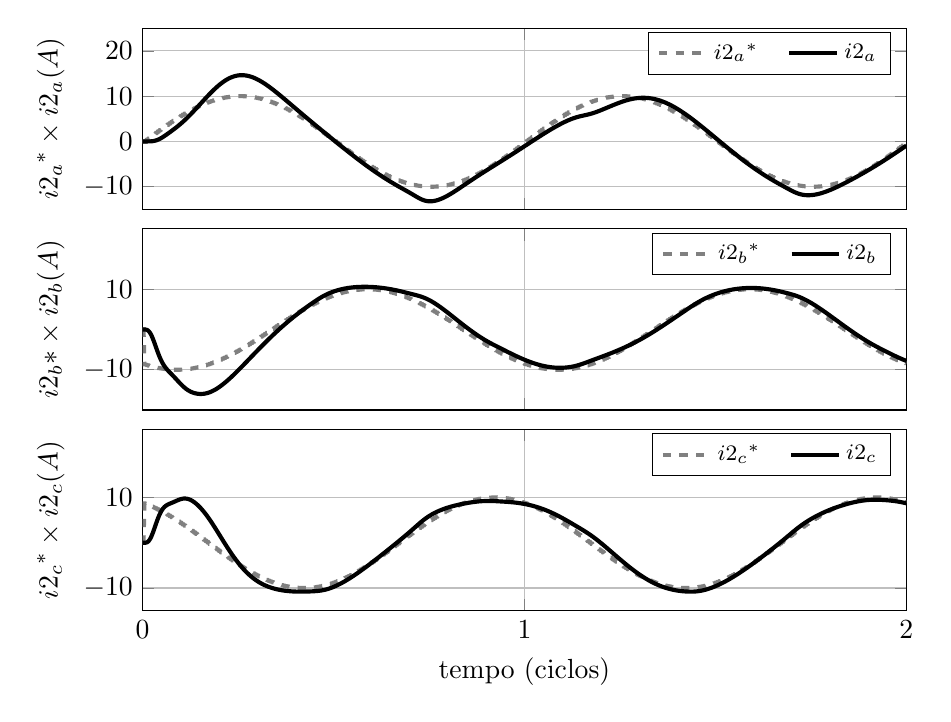
\begin{tikzpicture}

\begin{axis}[%
width=0.8\textwidth,
height=0.189701500343624\textwidth,
scale only axis,
xmin=0,
xmax=0.0333333333333333,
xtick={0,0.0166666666666667,0.0333333333333333},
xticklabels={\empty},
xmajorgrids,
ymin=-20,
ymax=25,
ytick={-10,  10,  30,  50},
ylabel={${\text{i2}_\text{b}}\text{* }\times\text{ i2}_\text{b}\text{ (A)}$},
ymajorgrids,
name=plot2,
legend style={draw=black,fill=white,legend cell align=left},
scaled x ticks = false,
legend columns=-1,
legend style={/tikz/every even column/.append style={column sep=0.3cm}},
legend style={font=\footnotesize}
]
\addplot [color=gray,dashed,line width=1.5pt]
  table[row sep=crcr]{0	0\\
4.16666666666667e-05	0\\
8.33333333333333e-05	-8.66025403784439\\
0.000125	-8.66025403784439\\
0.000166666666666667	-8.81303452064992\\
0.000208333333333333	-8.81303452064992\\
0.00025	-8.95711760239413\\
0.000291666666666667	-8.95711760239413\\
0.000333333333333333	-9.09236109047069\\
0.000375	-9.09236109047069\\
0.000416666666666667	-9.21863151588501\\
0.000458333333333333	-9.21863151588501\\
0.0005	-9.33580426497202\\
0.000541666666666667	-9.33580426497202\\
0.000583333333333333	-9.44376370237481\\
0.000625	-9.44376370237481\\
0.000666666666666667	-9.54240328516277\\
0.000708333333333333	-9.54240328516277\\
0.00075	-9.63162566797659\\
0.000791666666666667	-9.63162566797659\\
0.000833333333333333	-9.71134279909637\\
0.000875	-9.71134279909637\\
0.000916666666666667	-9.78147600733806\\
0.000958333333333333	-9.78147600733806\\
0.001	-9.84195607969242\\
0.00104166666666667	-9.84195607969242\\
0.00108333333333333	-9.89272332962989\\
0.001125	-9.89272332962989\\
0.00116666666666667	-9.93372765600397\\
0.00120833333333333	-9.93372765600397\\
0.00125	-9.96492859249505\\
0.00129166666666667	-9.96492859249505\\
0.00133333333333333	-9.98629534754575\\
0.001375	-9.98629534754575\\
0.00141666666666667	-9.99780683474846\\
0.00145833333333333	-9.99780683474846\\
0.0015	-9.99945169365513\\
0.00154166666666667	-9.99945169365513\\
0.00158333333333333	-9.99122830098859\\
0.001625	-9.99122830098859\\
0.00166666666666667	-9.97314477224459\\
0.00170833333333333	-9.97314477224459\\
0.00175	-9.94521895368274\\
0.00179166666666667	-9.94521895368274\\
0.00183333333333333	-9.90747840471445\\
0.001875	-9.90747840471445\\
0.00191666666666667	-9.85996037070506\\
0.00195833333333333	-9.85996037070506\\
0.002	-9.80271174621723\\
0.00204166666666667	-9.80271174621723\\
0.00208333333333333	-9.73578902873161\\
0.002125	-9.73578902873161\\
0.00216666666666667	-9.65925826289069\\
0.00220833333333333	-9.65925826289069\\
0.00225	-9.57319497532068\\
0.00229166666666667	-9.57319497532068\\
0.00233333333333333	-9.47768410009587\\
0.002375	-9.47768410009587\\
0.00241666666666667	-9.37281989491893\\
0.00245833333333333	-9.37281989491893\\
0.0025	-9.25870584809996\\
0.00254166666666667	-9.25870584809996\\
0.00258333333333333	-9.13545457642602\\
0.002625	-9.13545457642602\\
0.00266666666666667	-9.00318771402195\\
0.00270833333333333	-9.00318771402195\\
0.00275	-8.86203579231216\\
0.00279166666666667	-8.86203579231216\\
0.00283333333333333	-8.71213811120191\\
0.002875	-8.71213811120191\\
0.00291666666666667	-8.55364260160508\\
0.00295833333333333	-8.55364260160508\\
0.003	-8.38670567945426\\
0.00304166666666667	-8.38670567945426\\
0.00308333333333333	-8.21149209133705\\
0.003125	-8.21149209133705\\
0.00316666666666667	-8.02817475191116\\
0.00320833333333333	-8.02817475191116\\
0.00325	-7.83693457325841\\
0.00329166666666667	-7.83693457325841\\
0.00333333333333333	-7.63796028634644\\
0.003375	-7.63796028634644\\
0.00341666666666667	-7.43144825477396\\
0.00345833333333333	-7.43144825477396\\
0.0035	-7.21760228098364\\
0.00354166666666667	-7.21760228098364\\
0.00358333333333333	-6.99663340513367\\
0.003625	-6.99663340513367\\
0.00366666666666667	-6.76875969682662\\
0.00370833333333333	-6.76875969682662\\
0.00375	-6.53420603990107\\
0.00379166666666667	-6.53420603990107\\
0.00383333333333333	-6.29320391049839\\
0.003875	-6.29320391049839\\
0.00391666666666667	-6.04599114862376\\
0.00395833333333333	-6.04599114862376\\
0.004	-5.7928117234268\\
0.00404166666666667	-5.7928117234268\\
0.00408333333333333	-5.53391549243345\\
0.004125	-5.53391549243345\\
0.00416666666666667	-5.26955795496679\\
0.00420833333333333	-5.26955795496679\\
0.00425	-5.00000000000001\\
0.00429166666666667	-5.00000000000001\\
0.00433333333333333	-4.72550764869055\\
0.004375	-4.72550764869055\\
0.00441666666666667	-4.44635179184929\\
0.00445833333333333	-4.44635179184929\\
0.0045	-4.16280792260402\\
0.00454166666666667	-4.16280792260402\\
0.00458333333333333	-3.87515586452104\\
0.004625	-3.87515586452104\\
0.00466666666666667	-3.58367949545301\\
0.00470833333333333	-3.58367949545301\\
0.00475	-3.28866646738584\\
0.00479166666666667	-3.28866646738584\\
0.00483333333333333	-2.99040792256088\\
0.004875	-2.99040792256088\\
0.00491666666666667	-2.68919820615266\\
0.00495833333333333	-2.68919820615266\\
0.005	-2.38533457578582\\
0.00504166666666667	-2.38533457578582\\
0.00508333333333333	-2.0791169081776\\
0.005125	-2.0791169081776\\
0.00516666666666667	-1.77084740319584\\
0.00520833333333333	-1.77084740319584\\
0.00525	-1.46083028562412\\
0.00529166666666667	-1.46083028562412\\
0.00533333333333333	-1.14937150492867\\
0.005375	-1.14937150492867\\
0.00541666666666667	-0.836778433323157\\
0.00545833333333333	-0.836778433323157\\
0.0055	-0.52335956242944\\
0.00554166666666667	-0.52335956242944\\
0.00558333333333333	-0.209424198833571\\
0.005625	-0.209424198833571\\
0.00566666666666667	0.104717841162457\\
0.00570833333333333	0.104717841162457\\
0.00575	0.418756537291997\\
0.00579166666666667	0.418756537291997\\
0.00583333333333333	0.732381971276319\\
0.005875	0.732381971276319\\
0.00591666666666667	1.04528463267654\\
0.00595833333333333	1.04528463267654\\
0.006	1.35715572434305\\
0.00604166666666667	1.35715572434305\\
0.00608333333333333	1.66768746716103\\
0.006125	1.66768746716103\\
0.00616666666666667	1.97657340379127\\
0.00620833333333333	1.97657340379127\\
0.00625	2.28350870110656\\
0.00629166666666667	2.28350870110656\\
0.00633333333333333	2.58819045102521\\
0.006375	2.58819045102521\\
0.00641666666666667	2.89031796944472\\
0.00645833333333333	2.89031796944472\\
0.0065	3.18959309298071\\
0.00654166666666667	3.18959309298071\\
0.00658333333333333	3.48572047321816\\
0.006625	3.48572047321816\\
0.00666666666666667	3.77840786818468\\
0.00670833333333333	3.77840786818468\\
0.00675	4.06736643075802\\
0.00679166666666667	4.06736643075802\\
0.00683333333333333	4.35231099372329\\
0.006875	4.35231099372329\\
0.00691666666666667	4.63296035119863\\
0.00695833333333333	4.63296035119863\\
0.007	4.90903753615143\\
0.00704166666666667	4.90903753615143\\
0.00708333333333333	5.18027009373132\\
0.007125	5.18027009373132\\
0.00716666666666667	5.44639035015029\\
0.00720833333333333	5.44639035015029\\
0.00725	5.70713567684434\\
0.00729166666666667	5.70713567684434\\
0.00733333333333333	5.96224874965618\\
0.007375	5.96224874965618\\
0.00741666666666667	6.21147780278313\\
0.00745833333333333	6.21147780278313\\
0.0075	6.45457687723953\\
0.00754166666666667	6.45457687723953\\
0.00758333333333333	6.69130606358861\\
0.007625	6.69130606358861\\
0.00766666666666667	6.9214317387041\\
0.00770833333333333	6.9214317387041\\
0.00775	7.14472679632806\\
0.00779166666666667	7.14472679632806\\
0.00783333333333333	7.36097087119737\\
0.007875	7.36097087119737\\
0.00791666666666667	7.5699505565176\\
0.00795833333333333	7.5699505565176\\
0.008	7.77145961456974\\
0.00804166666666667	7.77145961456974\\
0.00808333333333333	7.965299180242\\
0.008125	7.965299180242\\
0.00816666666666667	8.15127795728558\\
0.00820833333333333	8.15127795728558\\
0.00825	8.32921240710103\\
0.00829166666666667	8.32921240710103\\
0.00833333333333333	8.49892692986868\\
0.008375	8.49892692986868\\
0.00841666666666667	8.66025403784443\\
0.00845833333333333	8.66025403784443\\
0.0085	8.81303452064996\\
0.00854166666666667	8.81303452064996\\
0.00858333333333333	8.95711760239417\\
0.008625	8.95711760239417\\
0.00866666666666667	9.09236109047073\\
0.00870833333333333	9.09236109047073\\
0.00875	9.21863151588505\\
0.00879166666666667	9.21863151588505\\
0.00883333333333333	9.33580426497206\\
0.008875	9.33580426497206\\
0.00891666666666667	9.44376370237486\\
0.00895833333333333	9.44376370237486\\
0.009	9.54240328516281\\
0.00904166666666667	9.54240328516281\\
0.00908333333333333	9.63162566797663\\
0.009125	9.63162566797663\\
0.00916666666666667	9.71134279909641\\
0.00920833333333333	9.71134279909641\\
0.00925	9.7814760073381\\
0.00929166666666667	9.7814760073381\\
0.00933333333333333	9.84195607969247\\
0.009375	9.84195607969247\\
0.00941666666666667	9.89272332962993\\
0.00945833333333333	9.89272332962993\\
0.0095	9.93372765600402\\
0.00954166666666667	9.93372765600402\\
0.00958333333333333	9.9649285924951\\
0.009625	9.9649285924951\\
0.00966666666666667	9.98629534754579\\
0.00970833333333333	9.98629534754579\\
0.00975	9.99780683474851\\
0.00979166666666667	9.99780683474851\\
0.00983333333333333	9.99945169365517\\
0.009875	9.99945169365517\\
0.00991666666666667	9.99122830098864\\
0.00995833333333333	9.99122830098864\\
0.01	9.97314477224464\\
0.0100416666666667	9.97314477224464\\
0.0100833333333333	9.94521895368279\\
0.010125	9.94521895368279\\
0.0101666666666667	9.90747840471449\\
0.0102083333333333	9.90747840471449\\
0.01025	9.8599603707051\\
0.0102916666666667	9.8599603707051\\
0.0103333333333333	9.80271174621727\\
0.010375	9.80271174621727\\
0.0104166666666667	9.73578902873166\\
0.0104583333333333	9.73578902873166\\
0.0105	9.65925826289074\\
0.0105416666666667	9.65925826289074\\
0.0105833333333333	9.57319497532073\\
0.010625	9.57319497532073\\
0.0106666666666667	9.47768410009591\\
0.0107083333333333	9.47768410009591\\
0.01075	9.37281989491897\\
0.0107916666666667	9.37281989491897\\
0.0108333333333333	9.2587058481\\
0.010875	9.2587058481\\
0.0109166666666667	9.13545457642606\\
0.0109583333333333	9.13545457642606\\
0.011	9.00318771402199\\
0.0110416666666667	9.00318771402199\\
0.0110833333333333	8.8620357923122\\
0.011125	8.8620357923122\\
0.0111666666666667	8.71213811120195\\
0.0112083333333333	8.71213811120195\\
0.01125	8.55364260160512\\
0.0112916666666667	8.55364260160512\\
0.0113333333333333	8.38670567945429\\
0.011375	8.38670567945429\\
0.0114166666666667	8.21149209133709\\
0.0114583333333333	8.21149209133709\\
0.0115	8.0281747519112\\
0.0115416666666667	8.0281747519112\\
0.0115833333333333	7.83693457325845\\
0.011625	7.83693457325845\\
0.0116666666666667	7.63796028634647\\
0.0117083333333333	7.63796028634647\\
0.01175	7.43144825477399\\
0.0117916666666667	7.43144825477399\\
0.0118333333333333	7.21760228098367\\
0.011875	7.21760228098367\\
0.0119166666666667	6.9966334051337\\
0.0119583333333333	6.9966334051337\\
0.012	6.76875969682665\\
0.0120416666666667	6.76875969682665\\
0.0120833333333333	6.5342060399011\\
0.012125	6.5342060399011\\
0.0121666666666667	6.29320391049842\\
0.0122083333333333	6.29320391049842\\
0.01225	6.04599114862379\\
0.0122916666666667	6.04599114862379\\
0.0123333333333333	5.79281172342683\\
0.012375	5.79281172342683\\
0.0124166666666667	5.53391549243348\\
0.0124583333333333	5.53391549243348\\
0.0125	5.26955795496681\\
0.0125416666666667	5.26955795496681\\
0.0125833333333333	5.00000000000004\\
0.012625	5.00000000000004\\
0.0126666666666667	4.72550764869058\\
0.0127083333333333	4.72550764869058\\
0.01275	4.44635179184931\\
0.0127916666666667	4.44635179184931\\
0.0128333333333333	4.16280792260404\\
0.012875	4.16280792260404\\
0.0129166666666667	3.87515586452106\\
0.0129583333333333	3.87515586452106\\
0.013	3.58367949545303\\
0.0130416666666667	3.58367949545303\\
0.0130833333333333	3.28866646738586\\
0.013125	3.28866646738586\\
0.0131666666666667	2.99040792256089\\
0.0132083333333333	2.99040792256089\\
0.01325	2.68919820615268\\
0.0132916666666667	2.68919820615268\\
0.0133333333333333	2.38533457578583\\
0.013375	2.38533457578583\\
0.0134166666666667	2.07911690817761\\
0.0134583333333333	2.07911690817761\\
0.0135	1.77084740319585\\
0.0135416666666667	1.77084740319585\\
0.0135833333333333	1.46083028562413\\
0.013625	1.46083028562413\\
0.0136666666666667	1.14937150492868\\
0.0137083333333333	1.14937150492868\\
0.01375	0.836778433323166\\
0.0137916666666667	0.836778433323166\\
0.0138333333333333	0.523359562429448\\
0.013875	0.523359562429448\\
0.0139166666666667	0.209424198833577\\
0.0139583333333333	0.209424198833577\\
0.014	-0.104717841162453\\
0.0140416666666667	-0.104717841162453\\
0.0140833333333333	-0.418756537291993\\
0.014125	-0.418756537291993\\
0.0141666666666667	-0.732381971276316\\
0.0142083333333333	-0.732381971276316\\
0.01425	-1.04528463267654\\
0.0142916666666667	-1.04528463267654\\
0.0143333333333333	-1.35715572434305\\
0.014375	-1.35715572434305\\
0.0144166666666667	-1.66768746716103\\
0.0144583333333333	-1.66768746716103\\
0.0145	-1.97657340379127\\
0.0145416666666667	-1.97657340379127\\
0.0145833333333333	-2.28350870110657\\
0.014625	-2.28350870110657\\
0.0146666666666667	-2.58819045102522\\
0.0147083333333333	-2.58819045102522\\
0.01475	-2.89031796944473\\
0.0147916666666667	-2.89031796944473\\
0.0148333333333333	-3.18959309298072\\
0.014875	-3.18959309298072\\
0.0149166666666667	-3.48572047321817\\
0.0149583333333333	-3.48572047321817\\
0.015	-3.77840786818469\\
0.0150416666666667	-3.77840786818469\\
0.0150833333333333	-4.06736643075803\\
0.015125	-4.06736643075803\\
0.0151666666666667	-4.3523109937233\\
0.0152083333333333	-4.3523109937233\\
0.01525	-4.63296035119865\\
0.0152916666666667	-4.63296035119865\\
0.0153333333333333	-4.90903753615144\\
0.015375	-4.90903753615144\\
0.0154166666666667	-5.18027009373134\\
0.0154583333333333	-5.18027009373134\\
0.0155	-5.44639035015031\\
0.0155416666666667	-5.44639035015031\\
0.0155833333333333	-5.70713567684436\\
0.015625	-5.70713567684436\\
0.0156666666666667	-5.9622487496562\\
0.0157083333333333	-5.9622487496562\\
0.01575	-6.21147780278315\\
0.0157916666666667	-6.21147780278315\\
0.0158333333333333	-6.45457687723955\\
0.015875	-6.45457687723955\\
0.0159166666666667	-6.69130606358863\\
0.0159583333333333	-6.69130606358863\\
0.016	-6.92143173870412\\
0.0160416666666667	-6.92143173870412\\
0.0160833333333333	-7.14472679632809\\
0.016125	-7.14472679632809\\
0.0161666666666667	-7.3609708711974\\
0.0162083333333333	-7.3609708711974\\
0.01625	-7.56995055651762\\
0.0162916666666667	-7.56995055651762\\
0.0163333333333333	-7.77145961456977\\
0.016375	-7.77145961456977\\
0.0164166666666667	-7.96529918024203\\
0.0164583333333333	-7.96529918024203\\
0.0165	-8.15127795728561\\
0.0165416666666667	-8.15127795728561\\
0.0165833333333333	-8.32921240710106\\
0.016625	-8.32921240710106\\
0.0166666666666667	-8.49892692986871\\
0.0167083333333333	-8.49892692986871\\
0.01675	-8.66025403784446\\
0.0167916666666667	-8.66025403784446\\
0.0168333333333333	-8.81303452064999\\
0.016875	-8.81303452064999\\
0.0169166666666667	-8.9571176023942\\
0.0169583333333333	-8.9571176023942\\
0.017	-9.09236109047076\\
0.0170416666666667	-9.09236109047076\\
0.0170833333333333	-9.21863151588508\\
0.017125	-9.21863151588508\\
0.0171666666666667	-9.3358042649721\\
0.0172083333333333	-9.3358042649721\\
0.01725	-9.44376370237489\\
0.0172916666666667	-9.44376370237489\\
0.0173333333333333	-9.54240328516285\\
0.017375	-9.54240328516285\\
0.0174166666666667	-9.63162566797667\\
0.0174583333333333	-9.63162566797667\\
0.0175	-9.71134279909645\\
0.0175416666666667	-9.71134279909645\\
0.0175833333333333	-9.78147600733814\\
0.017625	-9.78147600733814\\
0.0176666666666667	-9.84195607969251\\
0.0177083333333333	-9.84195607969251\\
0.01775	-9.89272332962997\\
0.0177916666666667	-9.89272332962997\\
0.0178333333333333	-9.93372765600406\\
0.017875	-9.93372765600406\\
0.0179166666666667	-9.96492859249514\\
0.0179583333333333	-9.96492859249514\\
0.018	-9.98629534754583\\
0.0180416666666667	-9.98629534754583\\
0.0180833333333333	-9.99780683474855\\
0.018125	-9.99780683474855\\
0.0181666666666667	-9.99945169365522\\
0.0182083333333333	-9.99945169365522\\
0.01825	-9.99122830098868\\
0.0182916666666667	-9.99122830098868\\
0.0183333333333333	-9.97314477224468\\
0.018375	-9.97314477224468\\
0.0184166666666667	-9.94521895368283\\
0.0184583333333333	-9.94521895368283\\
0.0185	-9.90747840471453\\
0.0185416666666667	-9.90747840471453\\
0.0185833333333333	-9.85996037070515\\
0.018625	-9.85996037070515\\
0.0186666666666667	-9.80271174621732\\
0.0187083333333333	-9.80271174621732\\
0.01875	-9.7357890287317\\
0.0187916666666667	-9.7357890287317\\
0.0188333333333333	-9.65925826289078\\
0.018875	-9.65925826289078\\
0.0189166666666667	-9.57319497532077\\
0.0189583333333333	-9.57319497532077\\
0.019	-9.47768410009595\\
0.0190416666666667	-9.47768410009595\\
0.0190833333333333	-9.37281989491901\\
0.019125	-9.37281989491901\\
0.0191666666666667	-9.25870584810004\\
0.0192083333333333	-9.25870584810004\\
0.01925	-9.1354545764261\\
0.0192916666666667	-9.1354545764261\\
0.0193333333333333	-9.00318771402203\\
0.019375	-9.00318771402203\\
0.0194166666666667	-8.86203579231224\\
0.0194583333333333	-8.86203579231224\\
0.0195	-8.71213811120199\\
0.0195416666666667	-8.71213811120199\\
0.0195833333333333	-8.55364260160516\\
0.019625	-8.55364260160516\\
0.0196666666666667	-8.38670567945433\\
0.0197083333333333	-8.38670567945433\\
0.01975	-8.21149209133713\\
0.0197916666666667	-8.21149209133713\\
0.0198333333333333	-8.02817475191123\\
0.019875	-8.02817475191123\\
0.0199166666666667	-7.83693457325848\\
0.0199583333333333	-7.83693457325848\\
0.02	-7.63796028634651\\
0.0200416666666667	-7.63796028634651\\
0.0200833333333333	-7.43144825477402\\
0.020125	-7.43144825477402\\
0.0201666666666667	-7.2176022809837\\
0.0202083333333333	-7.2176022809837\\
0.02025	-6.99663340513373\\
0.0202916666666667	-6.99663340513373\\
0.0203333333333333	-6.76875969682668\\
0.020375	-6.76875969682668\\
0.0204166666666667	-6.53420603990113\\
0.0204583333333333	-6.53420603990113\\
0.0205	-6.29320391049845\\
0.0205416666666667	-6.29320391049845\\
0.0205833333333333	-6.04599114862382\\
0.020625	-6.04599114862382\\
0.0206666666666667	-5.79281172342686\\
0.0207083333333333	-5.79281172342686\\
0.02075	-5.53391549243351\\
0.0207916666666667	-5.53391549243351\\
0.0208333333333333	-5.26955795496684\\
0.020875	-5.26955795496684\\
0.0209166666666667	-5.00000000000006\\
0.0209583333333333	-5.00000000000006\\
0.021	-4.7255076486906\\
0.0210416666666667	-4.7255076486906\\
0.0210833333333333	-4.44635179184933\\
0.021125	-4.44635179184933\\
0.0211666666666667	-4.16280792260406\\
0.0212083333333333	-4.16280792260406\\
0.02125	-3.87515586452108\\
0.0212916666666667	-3.87515586452108\\
0.0213333333333333	-3.58367949545305\\
0.021375	-3.58367949545305\\
0.0214166666666667	-3.28866646738588\\
0.0214583333333333	-3.28866646738588\\
0.0215	-2.99040792256091\\
0.0215416666666667	-2.99040792256091\\
0.0215833333333333	-2.68919820615269\\
0.021625	-2.68919820615269\\
0.0216666666666667	-2.38533457578584\\
0.0217083333333333	-2.38533457578584\\
0.02175	-2.07911690817762\\
0.0217916666666667	-2.07911690817762\\
0.0218333333333333	-1.77084740319586\\
0.021875	-1.77084740319586\\
0.0219166666666667	-1.46083028562414\\
0.0219583333333333	-1.46083028562414\\
0.022	-1.14937150492869\\
0.0220416666666667	-1.14937150492869\\
0.0220833333333333	-0.836778433323171\\
0.022125	-0.836778433323171\\
0.0221666666666667	-0.523359562429452\\
0.0222083333333333	-0.523359562429452\\
0.02225	-0.209424198833579\\
0.0222916666666667	-0.209424198833579\\
0.0223333333333333	0.104717841162452\\
0.022375	0.104717841162452\\
0.0224166666666667	0.418756537291994\\
0.0224583333333333	0.418756537291994\\
0.0225	0.732381971276319\\
0.0225416666666667	0.732381971276319\\
0.0225833333333333	1.04528463267654\\
0.022625	1.04528463267654\\
0.0226666666666667	1.35715572434305\\
0.0227083333333333	1.35715572434305\\
0.02275	1.66768746716104\\
0.0227916666666667	1.66768746716104\\
0.0228333333333333	1.97657340379128\\
0.022875	1.97657340379128\\
0.0229166666666667	2.28350870110658\\
0.0229583333333333	2.28350870110658\\
0.023	2.58819045102523\\
0.0230416666666667	2.58819045102523\\
0.0230833333333333	2.89031796944474\\
0.023125	2.89031796944474\\
0.0231666666666667	3.18959309298073\\
0.0232083333333333	3.18959309298073\\
0.02325	3.48572047321819\\
0.0232916666666667	3.48572047321819\\
0.0233333333333333	3.77840786818471\\
0.023375	3.77840786818471\\
0.0234166666666667	4.06736643075804\\
0.0234583333333333	4.06736643075804\\
0.0235	4.35231099372332\\
0.0235416666666667	4.35231099372332\\
0.0235833333333333	4.63296035119867\\
0.023625	4.63296035119867\\
0.0236666666666667	4.90903753615146\\
0.0237083333333333	4.90903753615146\\
0.02375	5.18027009373136\\
0.0237916666666667	5.18027009373136\\
0.0238333333333333	5.44639035015033\\
0.023875	5.44639035015033\\
0.0239166666666667	5.70713567684438\\
0.0239583333333333	5.70713567684438\\
0.024	5.96224874965623\\
0.0240416666666667	5.96224874965623\\
0.0240833333333333	6.21147780278318\\
0.024125	6.21147780278318\\
0.0241666666666667	6.45457687723958\\
0.0242083333333333	6.45457687723958\\
0.02425	6.69130606358866\\
0.0242916666666667	6.69130606358866\\
0.0243333333333333	6.92143173870415\\
0.024375	6.92143173870415\\
0.0244166666666667	7.14472679632812\\
0.0244583333333333	7.14472679632812\\
0.0245	7.36097087119743\\
0.0245416666666667	7.36097087119743\\
0.0245833333333333	7.56995055651766\\
0.024625	7.56995055651766\\
0.0246666666666667	7.7714596145698\\
0.0247083333333333	7.7714596145698\\
0.02475	7.96529918024206\\
0.0247916666666667	7.96529918024206\\
0.0248333333333333	8.15127795728564\\
0.024875	8.15127795728564\\
0.0249166666666667	8.3292124071011\\
0.0249583333333333	8.3292124071011\\
0.025	8.49892692986874\\
0.0250416666666667	8.49892692986874\\
0.0250833333333333	8.6602540378445\\
0.025125	8.6602540378445\\
0.0251666666666667	8.81303452065003\\
0.0252083333333333	8.81303452065003\\
0.02525	8.95711760239424\\
0.0252916666666667	8.95711760239424\\
0.0253333333333333	9.0923610904708\\
0.025375	9.0923610904708\\
0.0254166666666667	9.21863151588512\\
0.0254583333333333	9.21863151588512\\
0.0255	9.33580426497214\\
0.0255416666666667	9.33580426497214\\
0.0255833333333333	9.44376370237493\\
0.025625	9.44376370237493\\
0.0256666666666667	9.54240328516289\\
0.0257083333333333	9.54240328516289\\
0.02575	9.63162566797671\\
0.0257916666666667	9.63162566797671\\
0.0258333333333333	9.71134279909649\\
0.025875	9.71134279909649\\
0.0259166666666667	9.78147600733818\\
0.0259583333333333	9.78147600733818\\
0.026	9.84195607969255\\
0.0260416666666667	9.84195607969255\\
0.0260833333333333	9.89272332963002\\
0.026125	9.89272332963002\\
0.0261666666666667	9.9337276560041\\
0.0262083333333333	9.9337276560041\\
0.02625	9.96492859249518\\
0.0262916666666667	9.96492859249518\\
0.0263333333333333	9.98629534754588\\
0.026375	9.98629534754588\\
0.0264166666666667	9.99780683474859\\
0.0264583333333333	9.99780683474859\\
0.0265	9.99945169365526\\
0.0265416666666667	9.99945169365526\\
0.0265833333333333	9.99122830098872\\
0.026625	9.99122830098872\\
0.0266666666666667	9.97314477224472\\
0.0267083333333333	9.97314477224472\\
0.02675	9.94521895368287\\
0.0267916666666667	9.94521895368287\\
0.0268333333333333	9.90747840471458\\
0.026875	9.90747840471458\\
0.0269166666666667	9.85996037070519\\
0.0269583333333333	9.85996037070519\\
0.027	9.80271174621736\\
0.0270416666666667	9.80271174621736\\
0.0270833333333333	9.73578902873174\\
0.027125	9.73578902873174\\
0.0271666666666667	9.65925826289082\\
0.0272083333333333	9.65925826289082\\
0.02725	9.57319497532081\\
0.0272916666666667	9.57319497532081\\
0.0273333333333333	9.477684100096\\
0.027375	9.477684100096\\
0.0274166666666667	9.37281989491905\\
0.0274583333333333	9.37281989491905\\
0.0275	9.25870584810008\\
0.0275416666666667	9.25870584810008\\
0.0275833333333333	9.13545457642614\\
0.027625	9.13545457642614\\
0.0276666666666667	9.00318771402207\\
0.0277083333333333	9.00318771402207\\
0.02775	8.86203579231228\\
0.0277916666666667	8.86203579231228\\
0.0278333333333333	8.71213811120203\\
0.027875	8.71213811120203\\
0.0279166666666667	8.5536426016052\\
0.0279583333333333	8.5536426016052\\
0.028	8.38670567945437\\
0.0280416666666667	8.38670567945437\\
0.0280833333333333	8.21149209133717\\
0.028125	8.21149209133717\\
0.0281666666666667	8.02817475191127\\
0.0282083333333333	8.02817475191127\\
0.02825	7.83693457325852\\
0.0282916666666667	7.83693457325852\\
0.0283333333333333	7.63796028634654\\
0.028375	7.63796028634654\\
0.0284166666666667	7.43144825477406\\
0.0284583333333333	7.43144825477406\\
0.0285	7.21760228098374\\
0.0285416666666667	7.21760228098374\\
0.0285833333333333	6.99663340513377\\
0.028625	6.99663340513377\\
0.0286666666666667	6.76875969682672\\
0.0287083333333333	6.76875969682672\\
0.02875	6.53420603990116\\
0.0287916666666667	6.53420603990116\\
0.0288333333333333	6.29320391049848\\
0.028875	6.29320391049848\\
0.0289166666666667	6.04599114862385\\
0.0289583333333333	6.04599114862385\\
0.029	5.79281172342688\\
0.0290416666666667	5.79281172342688\\
0.0290833333333333	5.53391549243353\\
0.029125	5.53391549243353\\
0.0291666666666667	5.26955795496686\\
0.0292083333333333	5.26955795496686\\
0.02925	5.00000000000009\\
0.0292916666666667	5.00000000000009\\
0.0293333333333333	4.72550764869062\\
0.029375	4.72550764869062\\
0.0294166666666667	4.44635179184935\\
0.0294583333333333	4.44635179184935\\
0.0295	4.16280792260409\\
0.0295416666666667	4.16280792260409\\
0.0295833333333333	3.8751558645211\\
0.029625	3.8751558645211\\
0.0296666666666667	3.58367949545307\\
0.0297083333333333	3.58367949545307\\
0.02975	3.28866646738589\\
0.0297916666666667	3.28866646738589\\
0.0298333333333333	2.99040792256092\\
0.029875	2.99040792256092\\
0.0299166666666667	2.68919820615271\\
0.0299583333333333	2.68919820615271\\
0.03	2.38533457578586\\
0.0300416666666667	2.38533457578586\\
0.0300833333333333	2.07911690817764\\
0.030125	2.07911690817764\\
0.0301666666666667	1.77084740319587\\
0.0302083333333333	1.77084740319587\\
0.03025	1.46083028562415\\
0.0302916666666667	1.46083028562415\\
0.0303333333333333	1.14937150492869\\
0.030375	1.14937150492869\\
0.0304166666666667	0.836778433323179\\
0.0304583333333333	0.836778433323179\\
0.0305	0.523359562429457\\
0.0305416666666667	0.523359562429457\\
0.0305833333333333	0.209424198833583\\
0.030625	0.209424198833583\\
0.0306666666666667	-0.104717841162449\\
0.0307083333333333	-0.104717841162449\\
0.03075	-0.418756537291991\\
0.0307916666666667	-0.418756537291991\\
0.0308333333333333	-0.732381971276317\\
0.030875	-0.732381971276317\\
0.0309166666666667	-1.04528463267654\\
0.0309583333333333	-1.04528463267654\\
0.031	-1.35715572434305\\
0.0310416666666667	-1.35715572434305\\
0.0310833333333333	-1.66768746716104\\
0.031125	-1.66768746716104\\
0.0311666666666667	-1.97657340379128\\
0.0312083333333333	-1.97657340379128\\
0.03125	-2.28350870110658\\
0.0312916666666667	-2.28350870110658\\
0.0313333333333333	-2.58819045102524\\
0.031375	-2.58819045102524\\
0.0314166666666667	-2.89031796944475\\
0.0314583333333333	-2.89031796944475\\
0.0315	-3.18959309298074\\
0.0315416666666667	-3.18959309298074\\
0.0315833333333333	-3.4857204732182\\
0.031625	-3.4857204732182\\
0.0316666666666667	-3.77840786818472\\
0.0317083333333333	-3.77840786818472\\
0.03175	-4.06736643075806\\
0.0317916666666667	-4.06736643075806\\
0.0318333333333333	-4.35231099372334\\
0.031875	-4.35231099372334\\
0.0319166666666667	-4.63296035119868\\
0.0319583333333333	-4.63296035119868\\
0.032	-4.90903753615148\\
0.0320416666666667	-4.90903753615148\\
0.0320833333333333	-5.18027009373138\\
0.032125	-5.18027009373138\\
0.0321666666666667	-5.44639035015035\\
0.0322083333333333	-5.44639035015035\\
0.03225	-5.7071356768444\\
0.0322916666666667	-5.7071356768444\\
0.0323333333333333	-5.96224874965625\\
0.032375	-5.96224874965625\\
0.0324166666666667	-6.2114778027832\\
0.0324583333333333	-6.2114778027832\\
0.0325	-6.45457687723961\\
0.0325416666666667	-6.45457687723961\\
0.0325833333333333	-6.69130606358869\\
0.032625	-6.69130606358869\\
0.0326666666666667	-6.92143173870418\\
0.0327083333333333	-6.92143173870418\\
0.03275	-7.14472679632815\\
0.0327916666666667	-7.14472679632815\\
0.0328333333333333	-7.36097087119746\\
0.032875	-7.36097087119746\\
0.0329166666666667	-7.56995055651768\\
0.0329583333333333	-7.56995055651768\\
0.033	-7.77145961456983\\
0.0330416666666667	-7.77145961456983\\
0.0330833333333333	-7.96529918024209\\
0.033125	-7.96529918024209\\
0.0331666666666667	-8.15127795728568\\
0.0332083333333333	-8.15127795728568\\
0.03325	-8.32921240710113\\
0.0332916666666667	-8.32921240710113\\
0.0333333333333333	-8.49892692986878\\
};
\addlegendentry{${\text{i2}_\text{b}}^\text{*}$};

\addplot [color=black,solid,line width=1.5pt]
  table[row sep=crcr]{0	0\\
4.16666666666667e-05	0\\
8.33333333333333e-05	-3.16985704709253e-05\\
0.000125	-0.006977704459145\\
0.000166666666666667	-0.0450647453259681\\
0.000208333333333333	-0.137493350882375\\
0.00025	-0.302238630586635\\
0.000291666666666667	-0.551412275046984\\
0.000333333333333333	-0.889898968003439\\
0.000375	-1.3166706254095\\
0.000416666666666667	-1.82303145006447\\
0.000458333333333333	-2.39646342423051\\
0.0005	-3.02036741719603\\
0.000541666666666667	-3.67703991693781\\
0.000583333333333333	-4.34843642487209\\
0.000625	-5.01751482767187\\
0.000666666666666667	-5.66969026745548\\
0.000708333333333333	-6.29250443436262\\
0.00075	-6.87734088313131\\
0.000791666666666667	-7.41790369717575\\
0.000833333333333333	-7.91185955158767\\
0.000875	-8.35872347733996\\
0.000916666666666667	-8.76120053485019\\
0.000958333333333333	-9.1230303276762\\
0.001	-9.44992740181122\\
0.00104166666666667	-9.747781875111\\
0.00108333333333333	-10.0232067706593\\
0.001125	-10.2822998327546\\
0.00116666666666667	-10.5308806950274\\
0.00120833333333333	-10.7738402674726\\
0.00125	-11.0151840184951\\
0.00129166666666667	-11.2578660343117\\
0.00133333333333333	-11.5037520375936\\
0.001375	-11.7537688861539\\
0.00141666666666667	-12.007873959133\\
0.00145833333333333	-12.2653427472973\\
0.0015	-12.5247934531636\\
0.00154166666666667	-12.7844690893899\\
0.00158333333333333	-13.0423292666804\\
0.001625	-13.2962383042017\\
0.00166666666666667	-13.5441080777405\\
0.00170833333333333	-13.7839611997531\\
0.00175	-14.0140929527019\\
0.00179166666666667	-14.2330251051112\\
0.00183333333333333	-14.4396510686076\\
0.001875	-14.633124522076\\
0.00191666666666667	-14.8129571784326\\
0.00195833333333333	-14.9788963187332\\
0.002	-15.1309549857365\\
0.00204166666666667	-15.2693273661893\\
0.00208333333333333	-15.3943429884199\\
0.002125	-15.5064544225201\\
0.00216666666666667	-15.6061172078635\\
0.00220833333333333	-15.6938665967203\\
0.00225	-15.7701318080119\\
0.00229166666666667	-15.835402386099\\
0.00233333333333333	-15.8899885426394\\
0.002375	-15.9342661348979\\
0.00241666666666667	-15.9683948350999\\
0.00245833333333333	-15.9926248055156\\
0.0025	-16.00698227351\\
0.00254166666666667	-16.0116201843873\\
0.00258333333333333	-16.0064776437948\\
0.002625	-15.9916596946244\\
0.00266666666666667	-15.9670740317496\\
0.00270833333333333	-15.9328297714673\\
0.00275	-15.8888525238246\\
0.00279166666666667	-15.8352969631755\\
0.00283333333333333	-15.7721400573244\\
0.002875	-15.6996062394788\\
0.00291666666666667	-15.6177383119561\\
0.00295833333333333	-15.526836476263\\
0.003	-15.4270069059388\\
0.00304166666666667	-15.3186167515151\\
0.00308333333333333	-15.2018212710767\\
0.003125	-15.077036503092\\
0.00316666666666667	-14.9444468231475\\
0.00320833333333333	-14.8044957706047\\
0.00325	-14.657376713992\\
0.00329166666666667	-14.5035408468644\\
0.00333333333333333	-14.3431741510151\\
0.003375	-14.1767202617457\\
0.00341666666666667	-14.0043470831168\\
0.00345833333333333	-13.826481320887\\
0.0035	-13.6432679750066\\
0.00354166666666667	-13.4551129400618\\
0.00358333333333333	-13.2621382712571\\
0.003625	-13.0647293122379\\
0.00366666666666667	-12.8629882082215\\
0.00370833333333333	-12.6572824106774\\
0.00375	-12.4476984872496\\
0.00379166666666667	-12.2345894129028\\
0.00383333333333333	-12.0180303638475\\
0.003875	-11.7983627896684\\
0.00391666666666667	-11.5756536073836\\
0.00395833333333333	-11.3502345533482\\
0.004	-11.1221660147125\\
0.00404166666666667	-10.8917705283278\\
0.00408333333333333	-10.6591023813727\\
0.004125	-10.4244743480205\\
0.00416666666666667	-10.1879341308592\\
0.00420833333333333	-9.9497835290614\\
0.00425	-9.71006274940462\\
0.00429166666666667	-9.46906122394951\\
0.00433333333333333	-9.22681077217136\\
0.004375	-8.98358727631374\\
0.00441666666666667	-8.73941361170723\\
0.00445833333333333	-8.49455138076595\\
0.0045	-8.24901444341408\\
0.00454166666666667	-8.00304992943315\\
0.00458333333333333	-7.75666309852396\\
0.004625	-7.51008690435882\\
0.00466666666666667	-7.2633188017606\\
0.00470833333333333	-7.01657822152668\\
0.00475	-6.76985582924532\\
0.00479166666666667	-6.52335837741229\\
0.00483333333333333	-6.2770708141179\\
0.004875	-6.03118809497384\\
0.00491666666666667	-5.78569044538871\\
0.00495833333333333	-5.54076182709993\\
0.005	-5.29637857721506\\
0.00504166666666667	-5.05271432391773\\
0.00508333333333333	-4.80974215871117\\
0.005125	-4.56762587798181\\
0.00516666666666667	-4.32633578932835\\
0.00520833333333333	-4.08602622053009\\
0.00525	-3.84666501395796\\
0.00529166666666667	-3.60839729417353\\
0.00533333333333333	-3.37118866320252\\
0.005375	-3.13517525643902\\
0.00541666666666667	-2.9003206135889\\
0.00545833333333333	-2.66675208410555\\
0.0055	-2.43443131225941\\
0.00554166666666667	-2.20347708172905\\
0.00558333333333333	-1.97384931774384\\
0.005625	-1.74565848828439\\
0.00566666666666667	-1.51886299146341\\
0.00570833333333333	-1.2935652593678\\
0.00575	-1.06972236507431\\
0.00579166666666667	-0.847429004731421\\
0.00583333333333333	-0.62664112626111\\
0.005875	-0.407445995375102\\
0.00591666666666667	-0.189798617390877\\
0.00595833333333333	0.0262208772255759\\
0.006	0.240658275369913\\
0.00604166666666667	0.453440311572065\\
0.00608333333333333	0.664613459701834\\
0.006125	0.874111086436098\\
0.00616666666666667	1.08198030370674\\
0.00620833333333333	1.28816092564737\\
0.00625	1.49270072031706\\
0.00629166666666667	1.69554582339464\\
0.00633333333333333	1.8967447564475\\
0.006375	2.09624992235448\\
0.00641666666666667	2.29411078974163\\
0.00645833333333333	2.49028606365159\\
0.0065	2.6848264741454\\
0.00654166666666667	2.87769717856823\\
0.00658333333333333	3.06895063984711\\
0.006625	3.25855877049489\\
0.00666666666666667	3.44657644686383\\
0.00670833333333333	3.6329828452435\\
0.00675	3.8178362171832\\
0.00679166666666667	4.00112378811206\\
0.00683333333333333	4.1829085203995\\
0.006875	4.3631868343077\\
0.00691666666666667	4.54202820800776\\
0.00695833333333333	4.71943981875857\\
0.007	4.89549994029172\\
0.00704166666666667	5.07022833388524\\
0.00708333333333333	5.24371433822727\\
0.007125	5.41599072544459\\
0.00716666666666667	5.58715558927832\\
0.00720833333333333	5.75724629737728\\
0.00725	5.92634844949842\\
0.00729166666666667	6.09447362575182\\
0.00733333333333333	6.26164458109821\\
0.007375	6.42779631833016\\
0.00741666666666667	6.59283587005877\\
0.00745833333333333	6.75658305092278\\
0.0075	6.91881381566418\\
0.00754166666666667	7.0792365388671\\
0.00758333333333333	7.23752757049187\\
0.007625	7.3933279434848\\
0.00766666666666667	7.54627489733952\\
0.00770833333333333	7.69600505417133\\
0.00775	7.84218130755395\\
0.00779166666666667	7.98449487483953\\
0.00783333333333333	8.12268433724812\\
0.007875	8.25653558192323\\
0.00791666666666667	8.38588890394956\\
0.00795833333333333	8.51064049791501\\
0.008	8.63073399438773\\
0.00804166666666667	8.7461693051372\\
0.00808333333333333	8.85697624506284\\
0.008125	8.96323648413536\\
0.00816666666666667	9.06503847734004\\
0.00820833333333333	9.16251673934194\\
0.00825	9.25578874413169\\
0.00829166666666667	9.34501352763724\\
0.00833333333333333	9.43031225784999\\
0.008375	9.51184599016795\\
0.00841666666666667	9.58972214783508\\
0.00845833333333333	9.66408958085728\\
0.0085	9.73503327312211\\
0.00854166666666667	9.80268390425401\\
0.00858333333333333	9.86710283792671\\
0.008625	9.92840314764167\\
0.00866666666666667	9.98662649735217\\
0.00870833333333333	10.0418729052227\\
0.00875	10.0941706482093\\
0.00879166666666667	10.1436126717428\\
0.00883333333333333	10.1902202406755\\
0.008875	10.2340846297234\\
0.00891666666666667	10.275224960696\\
0.00895833333333333	10.3137344525024\\
0.009	10.3496327393758\\
0.00904166666666667	10.3830164177886\\
0.00908333333333333	10.4139061093086\\
0.009125	10.4424012851103\\
0.00916666666666667	10.4685223792517\\
0.00920833333333333	10.4923699260076\\
0.00925	10.5139621007762\\
0.00929166666666667	10.5333981302263\\
0.00933333333333333	10.5506917024719\\
0.009375	10.5659384734129\\
0.00941666666666667	10.5791458223516\\
0.00945833333333333	10.5904041397047\\
0.0095	10.5997134002982\\
0.00954166666666667	10.6071578185467\\
0.00958333333333333	10.6127296725127\\
0.009625	10.6165068713356\\
0.00966666666666667	10.6184743995553\\
0.00970833333333333	10.6187043573575\\
0.00975	10.617175320347\\
0.00979166666666667	10.6139544721807\\
0.00983333333333333	10.6090151027233\\
0.009875	10.6024205348765\\
0.00991666666666667	10.5941399233124\\
0.00995833333333333	10.584233762864\\
0.01	10.5726681059577\\
0.0100416666666667	10.5595015132453\\
0.0100833333333333	10.5446977815643\\
0.010125	10.5283142493205\\
0.0101666666666667	10.5103131164502\\
0.0102083333333333	10.4907510444661\\
0.01025	10.4695891520712\\
0.0102916666666667	10.4468838547238\\
0.0103333333333333	10.4225956305989\\
0.010375	10.3967810318451\\
0.0104166666666667	10.3694003325876\\
0.0104583333333333	10.340510619371\\
0.0105	10.3100724542632\\
0.0105416666666667	10.2781439200854\\
0.0105833333333333	10.2446864573391\\
0.010625	10.2097597036249\\
0.0106666666666667	10.173326694444\\
0.0107083333333333	10.1354492963326\\
0.01075	10.0960930011847\\
0.0107916666666667	10.0553227074797\\
0.0108333333333333	10.0131073893201\\
0.010875	9.96951592615227\\
0.0109166666666667	9.92452199596393\\
0.0109583333333333	9.87819958586139\\
0.011	9.83052854985538\\
0.0110416666666667	9.78158934365233\\
0.0110833333333333	9.73136980882297\\
0.011125	9.6799585560694\\
0.0111666666666667	9.62735369858066\\
0.0112083333333333	9.57365414594142\\
0.01125	9.51887121865171\\
0.0112916666666667	9.4631168887265\\
0.0113333333333333	9.40641946016938\\
0.011375	9.34890745856079\\
0.0114166666666667	9.29063078753073\\
0.0114583333333333	9.23173831572882\\
0.0115	9.17230561381591\\
0.0115416666666667	9.11250186361969\\
0.0115833333333333	9.05242100393789\\
0.011625	8.99223326293339\\
0.0116666666666667	8.93200596013238\\
0.0117083333333333	8.87185172917125\\
0.01175	8.81172283949463\\
0.0117916666666667	8.75159078491614\\
0.0118333333333333	8.69121648183873\\
0.011875	8.63037972470208\\
0.0119166666666667	8.56863952944349\\
0.0119583333333333	8.505602148496\\
0.012	8.44068284351656\\
0.0120416666666667	8.37338966534634\\
0.0120833333333333	8.30309110033213\\
0.012125	8.22929609371907\\
0.0121666666666667	8.15142601921345\\
0.0122083333333333	8.06908080166124\\
0.01225	7.9818100319071\\
0.0122916666666667	7.88936451771488\\
0.0123333333333333	7.79146022520373\\
0.012375	7.68802122403751\\
0.0124166666666667	7.57893098339578\\
0.0124583333333333	7.46427562666502\\
0.0125	7.34407916200754\\
0.0125416666666667	7.21855565265321\\
0.0125833333333333	7.0878274169923\\
0.012625	6.9521922299072\\
0.0126666666666667	6.8118257410902\\
0.0127083333333333	6.6670663878563\\
0.01275	6.51810485908727\\
0.0127916666666667	6.3652860802377\\
0.0128333333333333	6.20878935756959\\
0.012875	6.04894429256961\\
0.0129166666666667	5.88590534704117\\
0.0129583333333333	5.71997715797879\\
0.013	5.55128686482488\\
0.0130416666666667	5.38011398907331\\
0.0130833333333333	5.20656320042283\\
0.013125	5.03089443725934\\
0.0131666666666667	4.8531980762382\\
0.0132083333333333	4.6737219447031\\
0.01325	4.49255025379681\\
0.0132916666666667	4.30992524964554\\
0.0133333333333333	4.12593085311966\\
0.013375	3.94080765469647\\
0.0134166666666667	3.75464198553782\\
0.0134583333333333	3.56767363636485\\
0.0135	3.37999102710777\\
0.0135416666666667	3.19183138675877\\
0.0135833333333333	3.00328273069858\\
0.013625	2.81457632201529\\
0.0136666666666667	2.62579624251395\\
0.0137083333333333	2.43716385745815\\
0.01375	2.24875582703323\\
0.0137916666666667	2.06078011751017\\
0.0138333333333333	1.87330331406408\\
0.013875	1.68651754806484\\
0.0139166666666667	1.50047793054074\\
0.0139583333333333	1.31535965377819\\
0.014	1.13120627541796\\
0.0140416666666667	0.948176225611947\\
0.0140833333333333	0.766302553311436\\
0.014125	0.58572812240017\\
0.0141666666666667	0.406477306428149\\
0.0142083333333333	0.228679264199802\\
0.01425	0.052351957502193\\
0.0142916666666667	-0.122386973824028\\
0.0143333333333333	-0.295523579349474\\
0.014375	-0.466949483178441\\
0.0144166666666667	-0.636652389667591\\
0.0144583333333333	-0.804531002894324\\
0.0145	-0.970572428727695\\
0.0145416666666667	-1.13468036971138\\
0.0145833333333333	-1.29683915411083\\
0.014625	-1.45695547959591\\
0.0146666666666667	-1.61500876920483\\
0.0147083333333333	-1.77090685653424\\
0.01475	-1.92462244060153\\
0.0147916666666667	-2.0760636919333\\
0.0148333333333333	-2.22519760756611\\
0.014875	-2.37193716505602\\
0.0149166666666667	-2.5162557815887\\
0.0149583333333333	-2.65808879045706\\
0.015	-2.79744598868019\\
0.0150416666666667	-2.93431601984923\\
0.0150833333333333	-3.06877954966995\\
0.015125	-3.20090499621144\\
0.0151666666666667	-3.33085800309846\\
0.0152083333333333	-3.45878852931537\\
0.01525	-3.58493128211762\\
0.0152916666666667	-3.70949245405473\\
0.0153333333333333	-3.83273839464433\\
0.015375	-3.95489100143333\\
0.0154166666666667	-4.07620480872525\\
0.0154583333333333	-4.19687656765946\\
0.0155	-4.31711288651496\\
0.0155416666666667	-4.4370552290468\\
0.0155833333333333	-4.55684106348556\\
0.015625	-4.676542157407\\
0.0156666666666667	-4.79622206601252\\
0.0157083333333333	-4.91588381778412\\
0.01575	-5.03552581616805\\
0.0157916666666667	-5.15509473595213\\
0.0158333333333333	-5.27454087566019\\
0.015875	-5.39377291697988\\
0.0159166666666667	-5.51271275038912\\
0.0159583333333333	-5.6312501628926\\
0.016	-5.74929637275832\\
0.0160416666666667	-5.86673821364862\\
0.0160833333333333	-5.9834891505009\\
0.016125	-6.09944376303044\\
0.0161666666666667	-6.21452487059737\\
0.0162083333333333	-6.32863989700507\\
0.01625	-6.44172283758191\\
0.0162916666666667	-6.55369438007121\\
0.0163333333333333	-6.66449770106275\\
0.016375	-6.77406410950064\\
0.0164166666666667	-6.88234196150253\\
0.0164583333333333	-6.98926922903008\\
0.0165	-7.09479509362283\\
0.0165416666666667	-7.19886037832293\\
0.0165833333333333	-7.30141157565446\\
0.016625	-7.40238964408109\\
0.0166666666666667	-7.50173632944086\\
0.0167083333333333	-7.59939149958032\\
0.01675	-7.69529164215001\\
0.0167916666666667	-7.78937572439001\\
0.0168333333333333	-7.88157571913188\\
0.016875	-7.97183092173685\\
0.0169166666666667	-8.06007030018121\\
0.0169583333333333	-8.14623524248011\\
0.017	-8.23025347209822\\
0.0170416666666667	-8.31207029130175\\
0.0170833333333333	-8.39161376774966\\
0.017125	-8.46883463963921\\
0.0171666666666667	-8.54366247135795\\
0.0172083333333333	-8.61605446403201\\
0.01725	-8.68594229711294\\
0.0172916666666667	-8.75329012675762\\
0.0173333333333333	-8.81803186979166\\
0.017375	-8.8801386697717\\
0.0174166666666667	-8.93954643063262\\
0.0174583333333333	-8.99623299431099\\
0.0175	-9.05013578456807\\
0.0175416666666667	-9.10123888333182\\
0.0175833333333333	-9.1494806931148\\
0.017625	-9.19485103602185\\
0.0176666666666667	-9.23728878122943\\
0.0177083333333333	-9.27678903275681\\
0.01775	-9.31329069470471\\
0.0177916666666667	-9.34679376931302\\
0.0178333333333333	-9.37723684725055\\
0.017875	-9.40462450983268\\
0.0179166666666667	-9.42889473595374\\
0.0179583333333333	-9.45005639178918\\
0.018	-9.46804654152334\\
0.0180416666666667	-9.48287801247311\\
0.0180833333333333	-9.49448658458478\\
0.018125	-9.50288863612063\\
0.0181666666666667	-9.50801816695759\\
0.0182083333333333	-9.50989455786837\\
0.01825	-9.5084493538288\\
0.0182916666666667	-9.50370420818734\\
0.0183333333333333	-9.49558731272695\\
0.018375	-9.48412164852207\\
0.0184166666666667	-9.46923089865076\\
0.0184583333333333	-9.45093819487792\\
0.0185	-9.4291612917374\\
0.0185416666666667	-9.40392209120076\\
0.0185833333333333	-9.37513081918003\\
0.018625	-9.34280674915984\\
0.0186666666666667	-9.30685120149633\\
0.0187083333333333	-9.26728032801709\\
0.01875	-9.22398759688368\\
0.0187916666666667	-9.17699050100018\\
0.0188333333333333	-9.12618675046297\\
0.018875	-9.07161383461249\\
0.0189166666666667	-9.01320756170564\\
0.0189583333333333	-8.95106280812442\\
0.019	-8.88520027855701\\
0.0190416666666667	-8.81581176256165\\
0.0190833333333333	-8.74303196936481\\
0.019125	-8.66716330086179\\
0.0191666666666667	-8.58844586574394\\
0.0192083333333333	-8.50726970285597\\
0.01925	-8.42393823696899\\
0.0192916666666667	-8.33887988584538\\
0.0193333333333333	-8.25240395425431\\
0.019375	-8.16492072037045\\
0.0194166666666667	-8.07669185362337\\
0.0194583333333333	-7.98806263976137\\
0.0195	-7.89921071597778\\
0.0195416666666667	-7.81038902885477\\
0.0195833333333333	-7.72167700464961\\
0.019625	-7.63322955999585\\
0.0196666666666667	-7.5450341021978\\
0.0197083333333333	-7.45715974659478\\
0.01975	-7.369522238608\\
0.0197916666666667	-7.28212812360598\\
0.0198333333333333	-7.19484825174715\\
0.019875	-7.10765333144101\\
0.0199166666666667	-7.02039546308635\\
0.0199583333333333	-6.93303357579687\\
0.02	-6.84542162953845\\
0.0200416666666667	-6.75752430981237\\
0.0200833333333333	-6.66921018545523\\
0.020125	-6.58045936153976\\
0.0201666666666667	-6.49115991667406\\
0.0202083333333333	-6.40130986554238\\
0.02025	-6.31081549649099\\
0.0202916666666667	-6.21969003349297\\
0.0203333333333333	-6.12785290818937\\
0.020375	-6.03532711313504\\
0.0204166666666667	-5.94203884891702\\
0.0204583333333333	-5.84801494319807\\
0.0205	-5.75318263069328\\
0.0205416666666667	-5.65756777285851\\
0.0205833333333333	-5.56109472010398\\
0.020625	-5.46378554520948\\
0.0206666666666667	-5.36556000646278\\
0.0207083333333333	-5.26643567437981\\
0.02075	-5.16632799112339\\
0.0207916666666667	-5.06525103171671\\
0.0208333333333333	-4.9631175803179\\
0.020875	-4.85994028551171\\
0.0209166666666667	-4.75563158780013\\
0.0209583333333333	-4.65020514276749\\
0.021	-4.54357536683336\\
0.0210416666666667	-4.43575914897582\\
0.0210833333333333	-4.32667475032494\\
0.021125	-4.21634395397738\\
0.0211666666666667	-4.10469006232286\\
0.0212083333333333	-3.99174071429705\\
0.02125	-3.87742476647549\\
0.0212916666666667	-3.76177602733093\\
0.0213333333333333	-3.64472887257414\\
0.021375	-3.52632311247803\\
0.0214166666666667	-3.4064982657784\\
0.0214583333333333	-3.28529970489239\\
0.0215	-3.16267158483712\\
0.0215416666666667	-3.03866432165739\\
0.0215833333333333	-2.91322623579534\\
0.021625	-2.78641232890932\\
0.0216666666666667	-2.65817475149462\\
0.0217083333333333	-2.52857276515748\\
0.02175	-2.39756218208777\\
0.0217916666666667	-2.26520634020432\\
0.0218333333333333	-2.13146468966837\\
0.021875	-1.99640456799429\\
0.0219166666666667	-1.85998912952955\\
0.0219583333333333	-1.72228968350713\\
0.022	-1.58327317955563\\
0.0220416666666667	-1.44301485864468\\
0.0220833333333333	-1.30148552362483\\
0.022125	-1.1587642457889\\
0.0221666666666667	-1.01482566538953\\
0.0222083333333333	-0.86975249090847\\
0.02225	-0.723523090521464\\
0.0222916666666667	-0.576223514679227\\
0.0223333333333333	-0.427835654757557\\
0.022375	-0.278448511567501\\
0.0224166666666667	-0.128047210591096\\
0.0224583333333333	0.0232767696084537\\
0.0225	0.175535426640082\\
0.0225416666666667	0.328635339531392\\
0.0225833333333333	0.482586039125432\\
0.022625	0.637292744770206\\
0.0226666666666667	0.792762974492544\\
0.0227083333333333	0.94890120968657\\
0.02275	1.10571345323028\\
0.0227916666666667	1.26310411010756\\
0.0228333333333333	1.42107821987658\\
0.022875	1.57954082343989\\
0.0229166666666667	1.73849662461164\\
0.0229583333333333	1.89785208473494\\
0.023	2.0576123083504\\
0.0230416666666667	2.2176860659563\\
0.0230833333333333	2.37807975323731\\
0.023125	2.53870548481424\\
0.0231666666666667	2.69957204709463\\
0.0232083333333333	2.86059612682669\\
0.02325	3.02179026213903\\
0.0232916666666667	3.18307715741704\\
0.0233333333333333	3.34447471360381\\
0.023375	3.50591320221035\\
0.0234166666666667	3.66741741806852\\
0.0234583333333333	3.82892575189054\\
0.0235	3.99046834208049\\
0.0235416666666667	4.15198662727889\\
0.0235833333333333	4.31350294962636\\
0.023625	4.47494373809951\\
0.0236666666666667	4.6362941328589\\
0.0237083333333333	4.79743652058515\\
0.02375	4.95828918489619\\
0.0237916666666667	5.11866928328744\\
0.0238333333333333	5.2784201374656\\
0.023875	5.43729651095006\\
0.0239166666666667	5.59508491367763\\
0.0239583333333333	5.75150313567399\\
0.024	5.90631532022456\\
0.0240416666666667	6.0592383025191\\
0.0240833333333333	6.21005080191929\\
0.024125	6.35850259597521\\
0.0241666666666667	6.50441573062944\\
0.0242083333333333	6.64759621925777\\
0.02425	6.78792468362489\\
0.0242916666666667	6.92527286630936\\
0.0243333333333333	7.05958138564334\\
0.024375	7.19078455821836\\
0.0244166666666667	7.318873689775\\
0.0244583333333333	7.44383367632812\\
0.0245	7.56569116551581\\
0.0245416666666667	7.68446552993752\\
0.0245833333333333	7.80020207794026\\
0.024625	7.91293872576777\\
0.0246666666666667	8.02272505913531\\
0.0247083333333333	8.12960477032107\\
0.02475	8.23362171252235\\
0.0247916666666667	8.33481718674883\\
0.0248333333333333	8.43322420843267\\
0.024875	8.52887815351389\\
0.0249166666666667	8.6218003395446\\
0.0249583333333333	8.71202036946939\\
0.025	8.79954990546699\\
0.0250416666666667	8.88441519405429\\
0.0250833333333333	8.9666216624755\\
0.025125	9.04619544078654\\
0.0251666666666667	9.12313919843462\\
0.0252083333333333	9.19748186915801\\
0.02525	9.26922600230065\\
0.0252916666666667	9.33840524423169\\
0.0253333333333333	9.40502341158534\\
0.025375	9.46911952925802\\
0.0254166666666667	9.530698828604\\
0.0254583333333333	9.58980526882779\\
0.0255	9.6464446993462\\
0.0255416666666667	9.70066481255731\\
0.0255833333333333	9.75247076130671\\
0.025625	9.80191243940057\\
0.0256666666666667	9.84899289176945\\
0.0257083333333333	9.89376273324216\\
0.02575	9.93622171747605\\
0.0257916666666667	9.97642001836181\\
0.0258333333333333	10.014353329098\\
0.025875	10.0500706674333\\
0.0259166666666667	10.083563360174\\
0.0259583333333333	10.1148790040939\\
0.026	10.1440046597938\\
0.0260416666666667	10.1709866043235\\
0.0260833333333333	10.1958080195064\\
0.026125	10.2185142023359\\
0.0261666666666667	10.2390849940338\\
0.0262083333333333	10.2575651587356\\
0.02625	10.2739317662035\\
0.0262916666666667	10.2882294967877\\
0.0263333333333333	10.3004331659691\\
0.026375	10.310587755062\\
0.0264166666666667	10.3186662504361\\
0.0264583333333333	10.3247142294532\\
0.0265	10.3287031804281\\
0.0265416666666667	10.3306794899965\\
0.0265833333333333	10.3306134098154\\
0.026625	10.3285522958807\\
0.0266666666666667	10.3244653926763\\
0.0267083333333333	10.3184011694933\\
0.02675	10.3103281006419\\
0.0267916666666667	10.3002959316664\\
0.0268333333333333	10.2882726445022\\
0.026875	10.2743094702698\\
0.0269166666666667	10.2583742409091\\
0.0269583333333333	10.2405199465731\\
0.027	10.2207146911216\\
0.0270416666666667	10.1990135713469\\
0.0270833333333333	10.1753854742706\\
0.027125	10.1498880315842\\
0.0271666666666667	10.1224915240667\\
0.0272083333333333	10.0932566356974\\
0.02725	10.0621557673652\\
0.0272916666666667	10.0292532781509\\
0.0273333333333333	9.99452456017887\\
0.027375	9.95803840569467\\
0.0274166666666667	9.91977426157185\\
0.0274583333333333	9.879806294975\\
0.0275	9.83811933457965\\
0.0275416666666667	9.79479411775649\\
0.0275833333333333	9.7498225402148\\
0.027625	9.70329344248279\\
0.0276666666666667	9.65520792711407\\
0.0277083333333333	9.6056648589007\\
0.02775	9.55467712921348\\
0.0277916666666667	9.50235570702662\\
0.0278333333333333	9.4487275866002\\
0.027875	9.39391590687929\\
0.0279166666666667	9.33795803921552\\
0.0279583333333333	9.28097894276206\\
0.028	9.22300194885997\\
0.0280416666666667	9.16412136519378\\
0.0280833333333333	9.1042965122621\\
0.028125	9.04354297306368\\
0.0281666666666667	8.98171044448985\\
0.0282083333333333	8.91870456768941\\
0.02825	8.85425690432061\\
0.0282916666666667	8.78817156136094\\
0.0283333333333333	8.72009429560901\\
0.028375	8.6497704635724\\
0.0284166666666667	8.57681613956271\\
0.0284583333333333	8.50097557531256\\
0.0285	8.42189358579625\\
0.0285416666666667	8.33936625882536\\
0.0285833333333333	8.25311167608374\\
0.028625	8.16301326729262\\
0.0286666666666667	8.06888523071128\\
0.0287083333333333	7.97071189473148\\
0.02875	7.86840467264442\\
0.0287916666666667	7.76204258255806\\
0.0288333333333333	7.65161875767409\\
0.028875	7.53728713815681\\
0.0289166666666667	7.41909799191794\\
0.0289583333333333	7.2972543579697\\
0.029	7.17183733524404\\
0.0290416666666667	7.04307384959605\\
0.0290833333333333	6.91105340489139\\
0.029125	6.77600678902325\\
0.0291666666666667	6.6380164681238\\
0.0292083333333333	6.49730435785195\\
0.02925	6.35393811567583\\
0.0292916666666667	6.20812526615452\\
0.0293333333333333	6.05991742086957\\
0.029375	5.90950784448478\\
0.0294166666666667	5.75693524740543\\
0.0294583333333333	5.60238216395742\\
0.0295	5.44587954781904\\
0.0295416666666667	5.28760389725158\\
0.0295833333333333	5.12758353053519\\
0.029625	4.965993033806\\
0.0296666666666667	4.80286185139748\\
0.0297083333333333	4.63836519535089\\
0.02975	4.47253546129958\\
0.0297916666666667	4.30554913729253\\
0.0298333333333333	4.13744152804904\\
0.029875	3.96838941095206\\
0.0299166666666667	3.79842958354856\\
0.0299583333333333	3.62773706211033\\
0.03	3.45634802066585\\
0.0300416666666667	3.284433265737\\
0.0300833333333333	3.11202617879928\\
0.030125	2.9392910901579\\
0.0301666666666667	2.76625685149192\\
0.0302083333333333	2.59307962424094\\
0.03025	2.41978268842738\\
0.0302916666666667	2.24651309087888\\
0.0303333333333333	2.07328824476436\\
0.030375	1.90024586530906\\
0.0304166666666667	1.72739784172481\\
0.0304583333333333	1.55487292072613\\
0.0305	1.38267825136977\\
0.0305416666666667	1.2109343463056\\
0.0305833333333333	1.03964462201899\\
0.030625	0.868922256031237\\
0.0306666666666667	0.698767978629644\\
0.0307083333333333	0.529288533296568\\
0.03075	0.360482925872771\\
0.0307916666666667	0.192452271525846\\
0.0308333333333333	0.0251946746218955\\
0.030875	-0.141193699649221\\
0.0309166666666667	-0.306714957840354\\
0.0309583333333333	-0.47127731303364\\
0.031	-0.634882475513647\\
0.0310416666666667	-0.797442516955657\\
0.0310833333333333	-0.958958155804327\\
0.031125	-1.11934478520406\\
0.0311666666666667	-1.27860147056108\\
0.0312083333333333	-1.43664630303674\\
0.03125	-1.5934758985551\\
0.0312916666666667	-1.74901028097298\\
0.0313333333333333	-1.90324263724258\\
0.031375	-2.05609399476811\\
0.0314166666666667	-2.20755296040923\\
0.0314583333333333	-2.35754055044727\\
0.0315	-2.50603968250404\\
0.0315416666666667	-2.65297089285686\\
0.0315833333333333	-2.7983119967354\\
0.031625	-2.94198582412073\\
0.0316666666666667	-3.08397258847526\\
0.0317083333333333	-3.22420833544981\\
0.03175	-3.362694260314\\
0.0317916666666667	-3.49939881686577\\
0.0318333333333333	-3.63436536561097\\
0.031875	-3.76761098241922\\
0.0319166666666667	-3.89922959939503\\
0.0319583333333333	-4.02928780476202\\
0.032	-4.15792013588936\\
0.0320416666666667	-4.28522712552208\\
0.0320833333333333	-4.41136106224535\\
0.032125	-4.5364318347195\\
0.0321666666666667	-4.66058324121445\\
0.0322083333333333	-4.78390999433609\\
0.03225	-4.90652582840291\\
0.0322916666666667	-5.02849240141705\\
0.0323333333333333	-5.14988092585899\\
0.032375	-5.27071169585947\\
0.0324166666666667	-5.39101087531806\\
0.0324583333333333	-5.51075832944231\\
0.0325	-5.62994074005189\\
0.0325416666666667	-5.74850528107408\\
0.0325833333333333	-5.8664096056688\\
0.032625	-5.98357942385533\\
0.0326666666666667	-6.09995530065493\\
0.0327083333333333	-6.21545305105225\\
0.03275	-6.33000682468941\\
0.0327916666666667	-6.44353213418309\\
0.0328333333333333	-6.55596443461486\\
0.032875	-6.66722533328452\\
0.0329166666666667	-6.77725579736322\\
0.0329583333333333	-6.88598654693994\\
0.033	-6.99336509816781\\
0.0330416666666667	-7.099331502167\\
0.0330833333333333	-7.20383859235659\\
0.033125	-7.30683415292561\\
0.0331666666666667	-7.40827392734352\\
0.0332083333333333	-7.50811107042915\\
0.03325	-7.60630164355826\\
0.0332916666666667	-7.70280191739727\\
0.0333333333333333	-7.79756620088428\\
};
\addlegendentry{$\text{i2}_\text{b}$};

\end{axis}

\begin{axis}[%
width=0.8\textwidth,
height=0.189701500343624\textwidth,
scale only axis,
xmin=0,
xmax=0.0333333333333333,
xtick={0,0.0166666666666667,0.0333333333333333},
xticklabels={{0},{1},{2}},
xlabel={tempo (ciclos)},
xmajorgrids,
ymin=-15,
ymax=25,
ytick={-30, -10,  10},
ylabel={${\text{i2}_\text{c}}^\text{*}\text{ }\times\text{ i2}_\text{c}\text{ (A)}$},
ymajorgrids,
at=(plot2.below south west),
anchor=above north west,
legend style={draw=black,fill=white,legend cell align=left},
scaled x ticks = false,
legend columns=-1,
legend style={/tikz/every even column/.append style={column sep=0.3cm}},
legend style={font=\footnotesize}
]
\addplot [color=gray,dashed,line width=1.5pt]
  table[row sep=crcr]{0	0\\
4.16666666666667e-05	0\\
8.33333333333333e-05	8.66025403784439\\
0.000125	8.66025403784439\\
0.000166666666666667	8.49892692986864\\
0.000208333333333333	8.49892692986864\\
0.00025	8.329212407101\\
0.000291666666666667	8.329212407101\\
0.000333333333333333	8.15127795728554\\
0.000375	8.15127795728554\\
0.000416666666666667	7.96529918024197\\
0.000458333333333333	7.96529918024197\\
0.0005	7.77145961456971\\
0.000541666666666667	7.77145961456971\\
0.000583333333333333	7.56995055651757\\
0.000625	7.56995055651757\\
0.000666666666666667	7.36097087119735\\
0.000708333333333333	7.36097087119735\\
0.00075	7.14472679632804\\
0.000791666666666667	7.14472679632804\\
0.000833333333333333	6.92143173870407\\
0.000875	6.92143173870407\\
0.000916666666666667	6.69130606358858\\
0.000958333333333333	6.69130606358858\\
0.001	6.45457687723951\\
0.00104166666666667	6.45457687723951\\
0.00108333333333333	6.21147780278311\\
0.001125	6.21147780278311\\
0.00116666666666667	5.96224874965616\\
0.00120833333333333	5.96224874965616\\
0.00125	5.70713567684432\\
0.00129166666666667	5.70713567684432\\
0.00133333333333333	5.44639035015028\\
0.001375	5.44639035015028\\
0.00141666666666667	5.18027009373131\\
0.00145833333333333	5.18027009373131\\
0.0015	4.90903753615141\\
0.00154166666666667	4.90903753615141\\
0.00158333333333333	4.63296035119862\\
0.001625	4.63296035119862\\
0.00166666666666667	4.35231099372328\\
0.00170833333333333	4.35231099372328\\
0.00175	4.06736643075801\\
0.00179166666666667	4.06736643075801\\
0.00183333333333333	3.77840786818468\\
0.001875	3.77840786818468\\
0.00191666666666667	3.48572047321816\\
0.00195833333333333	3.48572047321816\\
0.002	3.18959309298071\\
0.00204166666666667	3.18959309298071\\
0.00208333333333333	2.89031796944472\\
0.002125	2.89031796944472\\
0.00216666666666667	2.58819045102521\\
0.00220833333333333	2.58819045102521\\
0.00225	2.28350870110656\\
0.00229166666666667	2.28350870110656\\
0.00233333333333333	1.97657340379127\\
0.002375	1.97657340379127\\
0.00241666666666667	1.66768746716103\\
0.00245833333333333	1.66768746716103\\
0.0025	1.35715572434305\\
0.00254166666666667	1.35715572434305\\
0.00258333333333333	1.04528463267654\\
0.002625	1.04528463267654\\
0.00266666666666667	0.732381971276321\\
0.00270833333333333	0.732381971276321\\
0.00275	0.418756537292\\
0.00279166666666667	0.418756537292\\
0.00283333333333333	0.104717841162462\\
0.002875	0.104717841162462\\
0.00291666666666667	-0.209424198833566\\
0.00295833333333333	-0.209424198833566\\
0.003	-0.523359562429436\\
0.00304166666666667	-0.523359562429436\\
0.00308333333333333	-0.836778433323153\\
0.003125	-0.836778433323153\\
0.00316666666666667	-1.14937150492867\\
0.00320833333333333	-1.14937150492867\\
0.00325	-1.46083028562412\\
0.00329166666666667	-1.46083028562412\\
0.00333333333333333	-1.77084740319583\\
0.003375	-1.77084740319583\\
0.00341666666666667	-2.07911690817759\\
0.00345833333333333	-2.07911690817759\\
0.0035	-2.38533457578581\\
0.00354166666666667	-2.38533457578581\\
0.00358333333333333	-2.68919820615266\\
0.003625	-2.68919820615266\\
0.00366666666666667	-2.99040792256087\\
0.00370833333333333	-2.99040792256087\\
0.00375	-3.28866646738584\\
0.00379166666666667	-3.28866646738584\\
0.00383333333333333	-3.58367949545301\\
0.003875	-3.58367949545301\\
0.00391666666666667	-3.87515586452103\\
0.00395833333333333	-3.87515586452103\\
0.004	-4.16280792260402\\
0.00404166666666667	-4.16280792260402\\
0.00408333333333333	-4.44635179184928\\
0.004125	-4.44635179184928\\
0.00416666666666667	-4.72550764869055\\
0.00420833333333333	-4.72550764869055\\
0.00425	-5.00000000000001\\
0.00429166666666667	-5.00000000000001\\
0.00433333333333333	-5.26955795496679\\
0.004375	-5.26955795496679\\
0.00441666666666667	-5.53391549243345\\
0.00445833333333333	-5.53391549243345\\
0.0045	-5.7928117234268\\
0.00454166666666667	-5.7928117234268\\
0.00458333333333333	-6.04599114862376\\
0.004625	-6.04599114862376\\
0.00466666666666667	-6.29320391049839\\
0.00470833333333333	-6.29320391049839\\
0.00475	-6.53420603990107\\
0.00479166666666667	-6.53420603990107\\
0.00483333333333333	-6.76875969682662\\
0.004875	-6.76875969682662\\
0.00491666666666667	-6.99663340513367\\
0.00495833333333333	-6.99663340513367\\
0.005	-7.21760228098364\\
0.00504166666666667	-7.21760228098364\\
0.00508333333333333	-7.43144825477396\\
0.005125	-7.43144825477396\\
0.00516666666666667	-7.63796028634644\\
0.00520833333333333	-7.63796028634644\\
0.00525	-7.83693457325842\\
0.00529166666666667	-7.83693457325842\\
0.00533333333333333	-8.02817475191117\\
0.005375	-8.02817475191117\\
0.00541666666666667	-8.21149209133706\\
0.00545833333333333	-8.21149209133706\\
0.0055	-8.38670567945426\\
0.00554166666666667	-8.38670567945426\\
0.00558333333333333	-8.55364260160509\\
0.005625	-8.55364260160509\\
0.00566666666666667	-8.71213811120192\\
0.00570833333333333	-8.71213811120192\\
0.00575	-8.86203579231217\\
0.00579166666666667	-8.86203579231217\\
0.00583333333333333	-9.00318771402196\\
0.005875	-9.00318771402196\\
0.00591666666666667	-9.13545457642604\\
0.00595833333333333	-9.13545457642604\\
0.006	-9.25870584809998\\
0.00604166666666667	-9.25870584809998\\
0.00608333333333333	-9.37281989491894\\
0.006125	-9.37281989491894\\
0.00616666666666667	-9.47768410009589\\
0.00620833333333333	-9.47768410009589\\
0.00625	-9.5731949753207\\
0.00629166666666667	-9.5731949753207\\
0.00633333333333333	-9.65925826289071\\
0.006375	-9.65925826289071\\
0.00641666666666667	-9.73578902873164\\
0.00645833333333333	-9.73578902873164\\
0.0065	-9.80271174621725\\
0.00654166666666667	-9.80271174621725\\
0.00658333333333333	-9.85996037070508\\
0.006625	-9.85996037070508\\
0.00666666666666667	-9.90747840471447\\
0.00670833333333333	-9.90747840471447\\
0.00675	-9.94521895368277\\
0.00679166666666667	-9.94521895368277\\
0.00683333333333333	-9.97314477224462\\
0.006875	-9.97314477224462\\
0.00691666666666667	-9.99122830098862\\
0.00695833333333333	-9.99122830098862\\
0.007	-9.99945169365516\\
0.00704166666666667	-9.99945169365516\\
0.00708333333333333	-9.99780683474849\\
0.007125	-9.99780683474849\\
0.00716666666666667	-9.98629534754578\\
0.00720833333333333	-9.98629534754578\\
0.00725	-9.96492859249508\\
0.00729166666666667	-9.96492859249508\\
0.00733333333333333	-9.93372765600401\\
0.007375	-9.93372765600401\\
0.00741666666666667	-9.89272332962993\\
0.00745833333333333	-9.89272332962993\\
0.0075	-9.84195607969246\\
0.00754166666666667	-9.84195607969246\\
0.00758333333333333	-9.7814760073381\\
0.007625	-9.7814760073381\\
0.00766666666666667	-9.7113427990964\\
0.00770833333333333	-9.7113427990964\\
0.00775	-9.63162566797663\\
0.00779166666666667	-9.63162566797663\\
0.00783333333333333	-9.54240328516281\\
0.007875	-9.54240328516281\\
0.00791666666666667	-9.44376370237485\\
0.00795833333333333	-9.44376370237485\\
0.008	-9.33580426497206\\
0.00804166666666667	-9.33580426497206\\
0.00808333333333333	-9.21863151588505\\
0.008125	-9.21863151588505\\
0.00816666666666667	-9.09236109047073\\
0.00820833333333333	-9.09236109047073\\
0.00825	-8.95711760239417\\
0.00829166666666667	-8.95711760239417\\
0.00833333333333333	-8.81303452064997\\
0.008375	-8.81303452064997\\
0.00841666666666667	-8.66025403784443\\
0.00845833333333333	-8.66025403784443\\
0.0085	-8.49892692986868\\
0.00854166666666667	-8.49892692986868\\
0.00858333333333333	-8.32921240710104\\
0.008625	-8.32921240710104\\
0.00866666666666667	-8.15127795728559\\
0.00870833333333333	-8.15127795728559\\
0.00875	-7.965299180242\\
0.00879166666666667	-7.965299180242\\
0.00883333333333333	-7.77145961456975\\
0.008875	-7.77145961456975\\
0.00891666666666667	-7.56995055651761\\
0.00895833333333333	-7.56995055651761\\
0.009	-7.36097087119738\\
0.00904166666666667	-7.36097087119738\\
0.00908333333333333	-7.14472679632807\\
0.009125	-7.14472679632807\\
0.00916666666666667	-6.92143173870411\\
0.00920833333333333	-6.92143173870411\\
0.00925	-6.69130606358862\\
0.00929166666666667	-6.69130606358862\\
0.00933333333333333	-6.45457687723954\\
0.009375	-6.45457687723954\\
0.00941666666666667	-6.21147780278314\\
0.00945833333333333	-6.21147780278314\\
0.0095	-5.96224874965619\\
0.00954166666666667	-5.96224874965619\\
0.00958333333333333	-5.70713567684435\\
0.009625	-5.70713567684435\\
0.00966666666666667	-5.4463903501503\\
0.00970833333333333	-5.4463903501503\\
0.00975	-5.18027009373134\\
0.00979166666666667	-5.18027009373134\\
0.00983333333333333	-4.90903753615144\\
0.009875	-4.90903753615144\\
0.00991666666666667	-4.63296035119865\\
0.00995833333333333	-4.63296035119865\\
0.01	-4.35231099372331\\
0.0100416666666667	-4.35231099372331\\
0.0100833333333333	-4.06736643075803\\
0.010125	-4.06736643075803\\
0.0101666666666667	-3.7784078681847\\
0.0102083333333333	-3.7784078681847\\
0.01025	-3.48572047321818\\
0.0102916666666667	-3.48572047321818\\
0.0103333333333333	-3.18959309298072\\
0.010375	-3.18959309298072\\
0.0104166666666667	-2.89031796944474\\
0.0104583333333333	-2.89031796944474\\
0.0105	-2.58819045102523\\
0.0105416666666667	-2.58819045102523\\
0.0105833333333333	-2.28350870110658\\
0.010625	-2.28350870110658\\
0.0106666666666667	-1.97657340379128\\
0.0107083333333333	-1.97657340379128\\
0.01075	-1.66768746716104\\
0.0107916666666667	-1.66768746716104\\
0.0108333333333333	-1.35715572434306\\
0.010875	-1.35715572434306\\
0.0109166666666667	-1.04528463267655\\
0.0109583333333333	-1.04528463267655\\
0.011	-0.732381971276329\\
0.0110416666666667	-0.732381971276329\\
0.0110833333333333	-0.418756537292006\\
0.011125	-0.418756537292006\\
0.0111666666666667	-0.104717841162466\\
0.0112083333333333	-0.104717841162466\\
0.01125	0.209424198833563\\
0.0112916666666667	0.209424198833563\\
0.0113333333333333	0.523359562429434\\
0.011375	0.523359562429434\\
0.0114166666666667	0.836778433323152\\
0.0114583333333333	0.836778433323152\\
0.0115	1.14937150492867\\
0.0115416666666667	1.14937150492867\\
0.0115833333333333	1.46083028562412\\
0.011625	1.46083028562412\\
0.0116666666666667	1.77084740319584\\
0.0117083333333333	1.77084740319584\\
0.01175	2.0791169081776\\
0.0117916666666667	2.0791169081776\\
0.0118333333333333	2.38533457578582\\
0.011875	2.38533457578582\\
0.0119166666666667	2.68919820615266\\
0.0119583333333333	2.68919820615266\\
0.012	2.99040792256088\\
0.0120416666666667	2.99040792256088\\
0.0120833333333333	3.28866646738584\\
0.012125	3.28866646738584\\
0.0121666666666667	3.58367949545302\\
0.0122083333333333	3.58367949545302\\
0.01225	3.87515586452105\\
0.0122916666666667	3.87515586452105\\
0.0123333333333333	4.16280792260403\\
0.012375	4.16280792260403\\
0.0124166666666667	4.4463517918493\\
0.0124583333333333	4.4463517918493\\
0.0125	4.72550764869056\\
0.0125416666666667	4.72550764869056\\
0.0125833333333333	5.00000000000002\\
0.012625	5.00000000000002\\
0.0126666666666667	5.2695579549668\\
0.0127083333333333	5.2695579549668\\
0.01275	5.53391549243347\\
0.0127916666666667	5.53391549243347\\
0.0128333333333333	5.79281172342682\\
0.012875	5.79281172342682\\
0.0129166666666667	6.04599114862378\\
0.0129583333333333	6.04599114862378\\
0.013	6.29320391049841\\
0.0130416666666667	6.29320391049841\\
0.0130833333333333	6.53420603990109\\
0.013125	6.53420603990109\\
0.0131666666666667	6.76875969682665\\
0.0132083333333333	6.76875969682665\\
0.01325	6.99663340513369\\
0.0132916666666667	6.99663340513369\\
0.0133333333333333	7.21760228098367\\
0.013375	7.21760228098367\\
0.0134166666666667	7.43144825477399\\
0.0134583333333333	7.43144825477399\\
0.0135	7.63796028634647\\
0.0135416666666667	7.63796028634647\\
0.0135833333333333	7.83693457325845\\
0.013625	7.83693457325845\\
0.0136666666666667	8.02817475191119\\
0.0137083333333333	8.02817475191119\\
0.01375	8.21149209133709\\
0.0137916666666667	8.21149209133709\\
0.0138333333333333	8.38670567945429\\
0.013875	8.38670567945429\\
0.0139166666666667	8.55364260160512\\
0.0139583333333333	8.55364260160512\\
0.014	8.71213811120195\\
0.0140416666666667	8.71213811120195\\
0.0140833333333333	8.86203579231221\\
0.014125	8.86203579231221\\
0.0141666666666667	9.003187714022\\
0.0142083333333333	9.003187714022\\
0.01425	9.13545457642607\\
0.0142916666666667	9.13545457642607\\
0.0143333333333333	9.25870584810001\\
0.014375	9.25870584810001\\
0.0144166666666667	9.37281989491898\\
0.0144583333333333	9.37281989491898\\
0.0145	9.47768410009592\\
0.0145416666666667	9.47768410009592\\
0.0145833333333333	9.57319497532074\\
0.014625	9.57319497532074\\
0.0146666666666667	9.65925826289075\\
0.0147083333333333	9.65925826289075\\
0.01475	9.73578902873167\\
0.0147916666666667	9.73578902873167\\
0.0148333333333333	9.80271174621729\\
0.014875	9.80271174621729\\
0.0149166666666667	9.85996037070512\\
0.0149583333333333	9.85996037070512\\
0.015	9.90747840471451\\
0.0150416666666667	9.90747840471451\\
0.0150833333333333	9.94521895368281\\
0.015125	9.94521895368281\\
0.0151666666666667	9.97314477224466\\
0.0152083333333333	9.97314477224466\\
0.01525	9.99122830098866\\
0.0152916666666667	9.99122830098866\\
0.0153333333333333	9.9994516936552\\
0.015375	9.9994516936552\\
0.0154166666666667	9.99780683474853\\
0.0154583333333333	9.99780683474853\\
0.0155	9.98629534754582\\
0.0155416666666667	9.98629534754582\\
0.0155833333333333	9.96492859249513\\
0.015625	9.96492859249513\\
0.0156666666666667	9.93372765600405\\
0.0157083333333333	9.93372765600405\\
0.01575	9.89272332962997\\
0.0157916666666667	9.89272332962997\\
0.0158333333333333	9.8419560796925\\
0.015875	9.8419560796925\\
0.0159166666666667	9.78147600733814\\
0.0159583333333333	9.78147600733814\\
0.016	9.71134279909644\\
0.0160416666666667	9.71134279909644\\
0.0160833333333333	9.63162566797667\\
0.016125	9.63162566797667\\
0.0161666666666667	9.54240328516285\\
0.0162083333333333	9.54240328516285\\
0.01625	9.44376370237489\\
0.0162916666666667	9.44376370237489\\
0.0163333333333333	9.3358042649721\\
0.016375	9.3358042649721\\
0.0164166666666667	9.21863151588509\\
0.0164583333333333	9.21863151588509\\
0.0165	9.09236109047077\\
0.0165416666666667	9.09236109047077\\
0.0165833333333333	8.95711760239421\\
0.016625	8.95711760239421\\
0.0166666666666667	8.81303452065\\
0.0167083333333333	8.81303452065\\
0.01675	8.66025403784447\\
0.0167916666666667	8.66025403784447\\
0.0168333333333333	8.49892692986872\\
0.016875	8.49892692986872\\
0.0169166666666667	8.32921240710107\\
0.0169583333333333	8.32921240710107\\
0.017	8.15127795728562\\
0.0170416666666667	8.15127795728562\\
0.0170833333333333	7.96529918024204\\
0.017125	7.96529918024204\\
0.0171666666666667	7.77145961456979\\
0.0172083333333333	7.77145961456979\\
0.01725	7.56995055651764\\
0.0172916666666667	7.56995055651764\\
0.0173333333333333	7.36097087119742\\
0.017375	7.36097087119742\\
0.0174166666666667	7.1447267963281\\
0.0174583333333333	7.1447267963281\\
0.0175	6.92143173870414\\
0.0175416666666667	6.92143173870414\\
0.0175833333333333	6.69130606358865\\
0.017625	6.69130606358865\\
0.0176666666666667	6.45457687723957\\
0.0177083333333333	6.45457687723957\\
0.01775	6.21147780278317\\
0.0177916666666667	6.21147780278317\\
0.0178333333333333	5.96224874965622\\
0.017875	5.96224874965622\\
0.0179166666666667	5.70713567684438\\
0.0179583333333333	5.70713567684438\\
0.018	5.44639035015033\\
0.0180416666666667	5.44639035015033\\
0.0180833333333333	5.18027009373136\\
0.018125	5.18027009373136\\
0.0181666666666667	4.90903753615147\\
0.0182083333333333	4.90903753615147\\
0.01825	4.63296035119867\\
0.0182916666666667	4.63296035119867\\
0.0183333333333333	4.35231099372333\\
0.018375	4.35231099372333\\
0.0184166666666667	4.06736643075805\\
0.0184583333333333	4.06736643075805\\
0.0185	3.77840786818472\\
0.0185416666666667	3.77840786818472\\
0.0185833333333333	3.4857204732182\\
0.018625	3.4857204732182\\
0.0186666666666667	3.18959309298074\\
0.0187083333333333	3.18959309298074\\
0.01875	2.89031796944476\\
0.0187916666666667	2.89031796944476\\
0.0188333333333333	2.58819045102524\\
0.018875	2.58819045102524\\
0.0189166666666667	2.28350870110659\\
0.0189583333333333	2.28350870110659\\
0.019	1.97657340379129\\
0.0190416666666667	1.97657340379129\\
0.0190833333333333	1.66768746716105\\
0.019125	1.66768746716105\\
0.0191666666666667	1.35715572434307\\
0.0192083333333333	1.35715572434307\\
0.01925	1.04528463267656\\
0.0192916666666667	1.04528463267656\\
0.0193333333333333	0.732381971276336\\
0.019375	0.732381971276336\\
0.0194166666666667	0.418756537292012\\
0.0194583333333333	0.418756537292012\\
0.0195	0.104717841162471\\
0.0195416666666667	0.104717841162471\\
0.0195833333333333	-0.20942419883356\\
0.019625	-0.20942419883356\\
0.0196666666666667	-0.523359562429432\\
0.0197083333333333	-0.523359562429432\\
0.01975	-0.836778433323152\\
0.0197916666666667	-0.836778433323152\\
0.0198333333333333	-1.14937150492867\\
0.019875	-1.14937150492867\\
0.0199166666666667	-1.46083028562412\\
0.0199583333333333	-1.46083028562412\\
0.02	-1.77084740319584\\
0.0200416666666667	-1.77084740319584\\
0.0200833333333333	-2.0791169081776\\
0.020125	-2.0791169081776\\
0.0201666666666667	-2.38533457578582\\
0.0202083333333333	-2.38533457578582\\
0.02025	-2.68919820615267\\
0.0202916666666667	-2.68919820615267\\
0.0203333333333333	-2.99040792256089\\
0.020375	-2.99040792256089\\
0.0204166666666667	-3.28866646738586\\
0.0204583333333333	-3.28866646738586\\
0.0205	-3.58367949545303\\
0.0205416666666667	-3.58367949545303\\
0.0205833333333333	-3.87515586452106\\
0.020625	-3.87515586452106\\
0.0206666666666667	-4.16280792260405\\
0.0207083333333333	-4.16280792260405\\
0.02075	-4.44635179184931\\
0.0207916666666667	-4.44635179184931\\
0.0208333333333333	-4.72550764869058\\
0.020875	-4.72550764869058\\
0.0209166666666667	-5.00000000000005\\
0.0209583333333333	-5.00000000000005\\
0.021	-5.26955795496682\\
0.0210416666666667	-5.26955795496682\\
0.0210833333333333	-5.53391549243349\\
0.021125	-5.53391549243349\\
0.0211666666666667	-5.79281172342684\\
0.0212083333333333	-5.79281172342684\\
0.02125	-6.0459911486238\\
0.0212916666666667	-6.0459911486238\\
0.0213333333333333	-6.29320391049844\\
0.021375	-6.29320391049844\\
0.0214166666666667	-6.53420603990112\\
0.0214583333333333	-6.53420603990112\\
0.0215	-6.76875969682667\\
0.0215416666666667	-6.76875969682667\\
0.0215833333333333	-6.99663340513372\\
0.021625	-6.99663340513372\\
0.0216666666666667	-7.2176022809837\\
0.0217083333333333	-7.2176022809837\\
0.02175	-7.43144825477402\\
0.0217916666666667	-7.43144825477402\\
0.0218333333333333	-7.6379602863465\\
0.021875	-7.6379602863465\\
0.0219166666666667	-7.83693457325848\\
0.0219583333333333	-7.83693457325848\\
0.022	-8.02817475191123\\
0.0220416666666667	-8.02817475191123\\
0.0220833333333333	-8.21149209133713\\
0.022125	-8.21149209133713\\
0.0221666666666667	-8.38670567945433\\
0.0222083333333333	-8.38670567945433\\
0.02225	-8.55364260160516\\
0.0222916666666667	-8.55364260160516\\
0.0223333333333333	-8.71213811120199\\
0.022375	-8.71213811120199\\
0.0224166666666667	-8.86203579231225\\
0.0224583333333333	-8.86203579231225\\
0.0225	-9.00318771402204\\
0.0225416666666667	-9.00318771402204\\
0.0225833333333333	-9.13545457642611\\
0.022625	-9.13545457642611\\
0.0226666666666667	-9.25870584810006\\
0.0227083333333333	-9.25870584810006\\
0.02275	-9.37281989491902\\
0.0227916666666667	-9.37281989491902\\
0.0228333333333333	-9.47768410009597\\
0.022875	-9.47768410009597\\
0.0229166666666667	-9.57319497532079\\
0.0229583333333333	-9.57319497532079\\
0.023	-9.6592582628908\\
0.0230416666666667	-9.6592582628908\\
0.0230833333333333	-9.73578902873172\\
0.023125	-9.73578902873172\\
0.0231666666666667	-9.80271174621734\\
0.0232083333333333	-9.80271174621734\\
0.02325	-9.85996037070517\\
0.0232916666666667	-9.85996037070517\\
0.0233333333333333	-9.90747840471456\\
0.023375	-9.90747840471456\\
0.0234166666666667	-9.94521895368285\\
0.0234583333333333	-9.94521895368285\\
0.0235	-9.97314477224471\\
0.0235416666666667	-9.97314477224471\\
0.0235833333333333	-9.99122830098871\\
0.023625	-9.99122830098871\\
0.0236666666666667	-9.99945169365525\\
0.0237083333333333	-9.99945169365525\\
0.02375	-9.99780683474858\\
0.0237916666666667	-9.99780683474858\\
0.0238333333333333	-9.98629534754587\\
0.023875	-9.98629534754587\\
0.0239166666666667	-9.96492859249517\\
0.0239583333333333	-9.96492859249517\\
0.024	-9.93372765600409\\
0.0240416666666667	-9.93372765600409\\
0.0240833333333333	-9.89272332963001\\
0.024125	-9.89272332963001\\
0.0241666666666667	-9.84195607969255\\
0.0242083333333333	-9.84195607969255\\
0.02425	-9.78147600733818\\
0.0242916666666667	-9.78147600733818\\
0.0243333333333333	-9.71134279909649\\
0.024375	-9.71134279909649\\
0.0244166666666667	-9.63162566797671\\
0.0244583333333333	-9.63162566797671\\
0.0245	-9.5424032851629\\
0.0245416666666667	-9.5424032851629\\
0.0245833333333333	-9.44376370237494\\
0.024625	-9.44376370237494\\
0.0246666666666667	-9.33580426497215\\
0.0247083333333333	-9.33580426497215\\
0.02475	-9.21863151588513\\
0.0247916666666667	-9.21863151588513\\
0.0248333333333333	-9.09236109047081\\
0.024875	-9.09236109047081\\
0.0249166666666667	-8.95711760239425\\
0.0249583333333333	-8.95711760239425\\
0.025	-8.81303452065005\\
0.0250416666666667	-8.81303452065005\\
0.0250833333333333	-8.66025403784451\\
0.025125	-8.66025403784451\\
0.0251666666666667	-8.49892692986876\\
0.0252083333333333	-8.49892692986876\\
0.02525	-8.32921240710111\\
0.0252916666666667	-8.32921240710111\\
0.0253333333333333	-8.15127795728566\\
0.025375	-8.15127795728566\\
0.0254166666666667	-7.96529918024207\\
0.0254583333333333	-7.96529918024207\\
0.0255	-7.77145961456982\\
0.0255416666666667	-7.77145961456982\\
0.0255833333333333	-7.56995055651767\\
0.025625	-7.56995055651767\\
0.0256666666666667	-7.36097087119745\\
0.0257083333333333	-7.36097087119745\\
0.02575	-7.14472679632814\\
0.0257916666666667	-7.14472679632814\\
0.0258333333333333	-6.92143173870417\\
0.025875	-6.92143173870417\\
0.0259166666666667	-6.69130606358868\\
0.0259583333333333	-6.69130606358868\\
0.026	-6.4545768772396\\
0.0260416666666667	-6.4545768772396\\
0.0260833333333333	-6.2114778027832\\
0.026125	-6.2114778027832\\
0.0261666666666667	-5.96224874965625\\
0.0262083333333333	-5.96224874965625\\
0.02625	-5.70713567684441\\
0.0262916666666667	-5.70713567684441\\
0.0263333333333333	-5.44639035015036\\
0.026375	-5.44639035015036\\
0.0264166666666667	-5.18027009373139\\
0.0264583333333333	-5.18027009373139\\
0.0265	-4.90903753615149\\
0.0265416666666667	-4.90903753615149\\
0.0265833333333333	-4.6329603511987\\
0.026625	-4.6329603511987\\
0.0266666666666667	-4.35231099372335\\
0.0267083333333333	-4.35231099372335\\
0.02675	-4.06736643075807\\
0.0267916666666667	-4.06736643075807\\
0.0268333333333333	-3.77840786818474\\
0.026875	-3.77840786818474\\
0.0269166666666667	-3.48572047321821\\
0.0269583333333333	-3.48572047321821\\
0.027	-3.18959309298076\\
0.0270416666666667	-3.18959309298076\\
0.0270833333333333	-2.89031796944477\\
0.027125	-2.89031796944477\\
0.0271666666666667	-2.58819045102526\\
0.0272083333333333	-2.58819045102526\\
0.02725	-2.28350870110661\\
0.0272916666666667	-2.28350870110661\\
0.0273333333333333	-1.9765734037913\\
0.027375	-1.9765734037913\\
0.0274166666666667	-1.66768746716106\\
0.0274583333333333	-1.66768746716106\\
0.0275	-1.35715572434308\\
0.0275416666666667	-1.35715572434308\\
0.0275833333333333	-1.04528463267656\\
0.027625	-1.04528463267656\\
0.0276666666666667	-0.732381971276341\\
0.0277083333333333	-0.732381971276341\\
0.02775	-0.418756537292015\\
0.0277916666666667	-0.418756537292015\\
0.0278333333333333	-0.104717841162473\\
0.027875	-0.104717841162473\\
0.0279166666666667	0.209424198833559\\
0.0279583333333333	0.209424198833559\\
0.028	0.523359562429433\\
0.0280416666666667	0.523359562429433\\
0.0280833333333333	0.836778433323154\\
0.028125	0.836778433323154\\
0.0281666666666667	1.14937150492867\\
0.0282083333333333	1.14937150492867\\
0.02825	1.46083028562412\\
0.0282916666666667	1.46083028562412\\
0.0283333333333333	1.77084740319585\\
0.028375	1.77084740319585\\
0.0284166666666667	2.07911690817761\\
0.0284583333333333	2.07911690817761\\
0.0285	2.38533457578583\\
0.0285416666666667	2.38533457578583\\
0.0285833333333333	2.68919820615268\\
0.028625	2.68919820615268\\
0.0286666666666667	2.9904079225609\\
0.0287083333333333	2.9904079225609\\
0.02875	3.28866646738587\\
0.0287916666666667	3.28866646738587\\
0.0288333333333333	3.58367949545304\\
0.028875	3.58367949545304\\
0.0289166666666667	3.87515586452107\\
0.0289583333333333	3.87515586452107\\
0.029	4.16280792260406\\
0.0290416666666667	4.16280792260406\\
0.0290833333333333	4.44635179184933\\
0.029125	4.44635179184933\\
0.0291666666666667	4.7255076486906\\
0.0292083333333333	4.7255076486906\\
0.02925	5.00000000000006\\
0.0292916666666667	5.00000000000006\\
0.0293333333333333	5.26955795496684\\
0.029375	5.26955795496684\\
0.0294166666666667	5.53391549243351\\
0.0294583333333333	5.53391549243351\\
0.0295	5.79281172342686\\
0.0295416666666667	5.79281172342686\\
0.0295833333333333	6.04599114862383\\
0.029625	6.04599114862383\\
0.0296666666666667	6.29320391049846\\
0.0297083333333333	6.29320391049846\\
0.02975	6.53420603990114\\
0.0297916666666667	6.53420603990114\\
0.0298333333333333	6.7687596968267\\
0.029875	6.7687596968267\\
0.0299166666666667	6.99663340513375\\
0.0299583333333333	6.99663340513375\\
0.03	7.21760228098372\\
0.0300416666666667	7.21760228098372\\
0.0300833333333333	7.43144825477405\\
0.030125	7.43144825477405\\
0.0301666666666667	7.63796028634653\\
0.0302083333333333	7.63796028634653\\
0.03025	7.83693457325851\\
0.0302916666666667	7.83693457325851\\
0.0303333333333333	8.02817475191126\\
0.030375	8.02817475191126\\
0.0304166666666667	8.21149209133716\\
0.0304583333333333	8.21149209133716\\
0.0305	8.38670567945436\\
0.0305416666666667	8.38670567945436\\
0.0305833333333333	8.55364260160519\\
0.030625	8.55364260160519\\
0.0306666666666667	8.71213811120203\\
0.0307083333333333	8.71213811120203\\
0.03075	8.86203579231228\\
0.0307916666666667	8.86203579231228\\
0.0308333333333333	9.00318771402207\\
0.030875	9.00318771402207\\
0.0309166666666667	9.13545457642615\\
0.0309583333333333	9.13545457642615\\
0.031	9.25870584810009\\
0.0310416666666667	9.25870584810009\\
0.0310833333333333	9.37281989491906\\
0.031125	9.37281989491906\\
0.0311666666666667	9.477684100096\\
0.0312083333333333	9.477684100096\\
0.03125	9.57319497532082\\
0.0312916666666667	9.57319497532082\\
0.0313333333333333	9.65925826289084\\
0.031375	9.65925826289084\\
0.0314166666666667	9.73578902873176\\
0.0314583333333333	9.73578902873176\\
0.0315	9.80271174621738\\
0.0315416666666667	9.80271174621738\\
0.0315833333333333	9.85996037070521\\
0.031625	9.85996037070521\\
0.0316666666666667	9.9074784047146\\
0.0317083333333333	9.9074784047146\\
0.03175	9.94521895368289\\
0.0317916666666667	9.94521895368289\\
0.0318333333333333	9.97314477224474\\
0.031875	9.97314477224474\\
0.0319166666666667	9.99122830098875\\
0.0319583333333333	9.99122830098875\\
0.032	9.99945169365528\\
0.0320416666666667	9.99945169365528\\
0.0320833333333333	9.99780683474862\\
0.032125	9.99780683474862\\
0.0321666666666667	9.98629534754591\\
0.0322083333333333	9.98629534754591\\
0.03225	9.96492859249521\\
0.0322916666666667	9.96492859249521\\
0.0323333333333333	9.93372765600413\\
0.032375	9.93372765600413\\
0.0324166666666667	9.89272332963005\\
0.0324583333333333	9.89272332963005\\
0.0325	9.84195607969259\\
0.0325416666666667	9.84195607969259\\
0.0325833333333333	9.78147600733822\\
0.032625	9.78147600733822\\
0.0326666666666667	9.71134279909653\\
0.0327083333333333	9.71134279909653\\
0.03275	9.63162566797675\\
0.0327916666666667	9.63162566797675\\
0.0328333333333333	9.54240328516294\\
0.032875	9.54240328516294\\
0.0329166666666667	9.44376370237498\\
0.0329583333333333	9.44376370237498\\
0.033	9.33580426497218\\
0.0330416666666667	9.33580426497218\\
0.0330833333333333	9.21863151588517\\
0.033125	9.21863151588517\\
0.0331666666666667	9.09236109047085\\
0.0332083333333333	9.09236109047085\\
0.03325	8.95711760239429\\
0.0332916666666667	8.95711760239429\\
0.0333333333333333	8.81303452065008\\
};
\addlegendentry{${\text{i2}_\text{c}}^\text{*}$};

\addplot [color=black,solid,line width=1.5pt]
  table[row sep=crcr]{0	0\\
4.16666666666667e-05	0\\
8.33333333333333e-05	3.16985704708258e-05\\
0.000125	0.00697770445914408\\
0.000166666666666667	0.0450635980707538\\
0.000208333333333333	0.137240809278792\\
0.00025	0.300606492179328\\
0.000291666666666667	0.54618817963616\\
0.000333333333333333	0.87735835418555\\
0.000375	1.29158657281288\\
0.000416666666666667	1.77851615438218\\
0.000458333333333333	2.32419185933849\\
0.0005	2.9106993200879\\
0.000541666666666667	3.51938566526132\\
0.000583333333333333	4.1315448603897\\
0.000625	4.72988321465714\\
0.000666666666666667	5.29988370465504\\
0.000708333333333333	5.82952439734918\\
0.00075	6.31086038114041\\
0.000791666666666667	6.73854118344303\\
0.000833333333333333	7.11126105492032\\
0.000875	7.42972632105064\\
0.000916666666666667	7.69774585575631\\
0.000958333333333333	7.92023261806606\\
0.001	8.10384383342223\\
0.00104166666666667	8.2554230299093\\
0.00108333333333333	8.38221471110946\\
0.001125	8.49094120408471\\
0.00116666666666667	8.58769220537291\\
0.00120833333333333	8.67764000589912\\
0.00125	8.76473451385314\\
0.00129166666666667	8.85192749691761\\
0.00133333333333333	8.94079565925379\\
0.001375	9.03208148494527\\
0.00141666666666667	9.1253342145234\\
0.00145833333333333	9.21957424259657\\
0.0015	9.3129993556016\\
0.00154166666666667	9.40362216535485\\
0.00158333333333333	9.48904921192265\\
0.001625	9.56700366615997\\
0.00166666666666667	9.63515587111304\\
0.00170833333333333	9.69150622264586\\
0.00175	9.73423056512056\\
0.00179166666666667	9.761946806619\\
0.00183333333333333	9.77353640821651\\
0.001875	9.76834641439318\\
0.00191666666666667	9.74595560475257\\
0.00195833333333333	9.70637129528929\\
0.002	9.64972106932882\\
0.00204166666666667	9.57649550852016\\
0.00208333333333333	9.48715959183866\\
0.002125	9.38247510831519\\
0.00216666666666667	9.26303674161094\\
0.00220833333333333	9.129687921092\\
0.00225	8.98299367711999\\
0.00229166666666667	8.82374623295413\\
0.00233333333333333	8.65238965558982\\
0.002375	8.46959955044899\\
0.00241666666666667	8.27567406133947\\
0.00245833333333333	8.07116643906962\\
0.0025	7.85625429417401\\
0.00254166666666667	7.63140375651281\\
0.00258333333333333	7.39672536888865\\
0.002625	7.15265227339165\\
0.00266666666666667	6.89928783167877\\
0.00270833333333333	6.63708573802344\\
0.00275	6.36619204331724\\
0.00279166666666667	6.08712054270942\\
0.00283333333333333	5.80009062303123\\
0.002875	5.50569551188753\\
0.00291666666666667	5.20423717350113\\
0.00295833333333333	4.89638749525062\\
0.003	4.5825220184077\\
0.00304166666666667	4.26337490163306\\
0.00308333333333333	3.93937420265183\\
0.003125	3.61129090192395\\
0.00316666666666667	3.27957939075611\\
0.00320833333333333	2.94501953999483\\
0.00325	2.60806674115133\\
0.00329166666666667	2.26948453268192\\
0.00333333333333333	1.92970885146358\\
0.003375	1.58946751912544\\
0.00341666666666667	1.24916327660948\\
0.00345833333333333	0.909475733947955\\
0.0035	0.570767350601733\\
0.00354166666666667	0.233663328658953\\
0.00358333333333333	-0.101515919345284\\
0.003625	-0.434201078943238\\
0.00366666666666667	-0.764112147051187\\
0.00370833333333333	-1.09073437344673\\
0.00375	-1.41382502203504\\
0.00379166666666667	-1.7329215058964\\
0.00383333333333333	-2.04781518247852\\
0.003875	-2.35809337499443\\
0.00391666666666667	-2.66357919774377\\
0.00395833333333333	-2.96390840211367\\
0.004	-3.2589346303632\\
0.00404166666666667	-3.54834143708109\\
0.00408333333333333	-3.8320126845429\\
0.004125	-4.10967967438585\\
0.00416666666666667	-4.38125665407189\\
0.00420833333333333	-4.64652271874313\\
0.00425	-4.90542262402962\\
0.00429166666666667	-5.15778293825633\\
0.00433333333333333	-5.40357857191799\\
0.004375	-5.64268252872895\\
0.00441666666666667	-5.87509877665614\\
0.00445833333333333	-6.10074482600327\\
0.0045	-6.31965178169593\\
0.00454166666666667	-6.53177884614345\\
0.00458333333333333	-6.73718160149789\\
0.004625	-6.93585738815508\\
0.00466666666666667	-7.1278830595772\\
0.00470833333333333	-7.31329002953589\\
0.00475	-7.49217291120824\\
0.00479166666666667	-7.66459287001559\\
0.00483333333333333	-7.83065869561569\\
0.004875	-7.99045695664247\\
0.00491666666666667	-8.14410715482381\\
0.00495833333333333	-8.29171706515083\\
0.005	-8.43341368510735\\
0.00504166666666667	-8.5693220663184\\
0.00508333333333333	-8.69957380105981\\
0.005125	-8.82430761234975\\
0.00516666666666667	-8.9436571194591\\
0.00520833333333333	-9.0577714497643\\
0.00525	-9.1667839998311\\
0.00529166666666667	-9.27085135933606\\
0.00533333333333333	-9.37010473982908\\
0.005375	-9.46470555199219\\
0.00541666666666667	-9.55478111513812\\
0.00545833333333333	-9.64049529713341\\
0.0055	-9.7219700479017\\
0.00554166666666667	-9.79936959043242\\
0.00558333333333333	-9.87280924393878\\
0.005625	-9.94245173981863\\
0.00566666666666667	-10.0084047168298\\
0.00570833333333333	-10.0708278244399\\
0.00575	-10.1298201851021\\
0.00579166666666667	-10.1855370371201\\
0.00583333333333333	-10.2380683692947\\
0.005875	-10.2875639450442\\
0.00591666666666667	-10.3341042237988\\
0.00595833333333333	-10.3778326968307\\
0.006	-10.418820119383\\
0.00604166666666667	-10.4572031756624\\
0.00608333333333333	-10.4930429575584\\
0.006125	-10.5264690604799\\
0.00616666666666667	-10.5575331606014\\
0.00620833333333333	-10.5863577232662\\
0.00625	-10.6129854531002\\
0.00629166666666667	-10.6375318707644\\
0.00633333333333333	-10.6600313412933\\
0.006375	-10.680592840887\\
0.00641666666666667	-10.6992432109692\\
0.00645833333333333	-10.7160854919422\\
0.0065	-10.7311400065699\\
0.00654166666666667	-10.7445046792236\\
0.00658333333333333	-10.7561945256729\\
0.006625	-10.7663034007512\\
0.00666666666666667	-10.7748424666326\\
0.00670833333333333	-10.7819028144254\\
0.00675	-10.7874935044195\\
0.00679166666666667	-10.7917044813808\\
0.00683333333333333	-10.7945448324851\\
0.006875	-10.7961053516798\\
0.00691666666666667	-10.7963977421132\\
0.00695833333333333	-10.7955160615268\\
0.007	-10.7934776732531\\
0.00704166666666667	-10.7903825675618\\
0.00708333333333333	-10.7862567731742\\
0.007125	-10.7812074591672\\
0.00716666666666667	-10.7752677094965\\
0.00720833333333333	-10.7685442441788\\
0.00725	-10.7610566111516\\
0.00729166666666667	-10.7528814457911\\
0.00733333333333333	-10.7439750205463\\
0.007375	-10.7343337975365\\
0.00741666666666667	-10.7237984579096\\
0.00745833333333333	-10.7122473297397\\
0.0075	-10.6993906575343\\
0.00754166666666667	-10.6849929789687\\
0.00758333333333333	-10.6686660327224\\
0.007625	-10.6501052034209\\
0.00766666666666667	-10.6288846235293\\
0.00770833333333333	-10.6046939367519\\
0.00775	-10.5771347875721\\
0.00779166666666667	-10.5459505085277\\
0.00783333333333333	-10.5108205932207\\
0.007875	-10.4715825044296\\
0.00791666666666667	-10.4280198664528\\
0.00795833333333333	-10.3800802214669\\
0.008	-10.3276531556521\\
0.00804166666666667	-10.2707899585192\\
0.00808333333333333	-10.2094691934258\\
0.008125	-10.1438241456146\\
0.00816666666666667	-10.073894937582\\
0.00820833333333333	-9.99986809617183\\
0.00825	-9.92181577090065\\
0.00829166666666667	-9.83994952121808\\
0.00833333333333333	-9.75434825341829\\
0.008375	-9.66522613048026\\
0.00841666666666667	-9.57265140032203\\
0.00845833333333333	-9.47682663889153\\
0.0085	-9.37780073651541\\
0.00854166666666667	-9.27575871633502\\
0.00858333333333333	-9.17072890027647\\
0.008625	-9.06287929034965\\
0.00866666666666667	-8.95222150798193\\
0.00870833333333333	-8.83891102366131\\
0.00875	-8.72294899832183\\
0.00879166666666667	-8.60448426678495\\
0.00883333333333333	-8.48351381367379\\
0.008875	-8.36018513064147\\
0.00891666666666667	-8.23449578848689\\
0.00895833333333333	-8.10659542111773\\
0.009	-7.97648472045951\\
0.00904166666666667	-7.84431674918919\\
0.00908333333333333	-7.71009566245309\\
0.009125	-7.57397728693633\\
0.00916666666666667	-7.43596792234263\\
0.00920833333333333	-7.29622417282258\\
0.00925	-7.15475225759901\\
0.00929166666666667	-7.01170700125869\\
0.00933333333333333	-6.86709215050927\\
0.009375	-6.72105829080257\\
0.00941666666666667	-6.57360470202464\\
0.00945833333333333	-6.42487583020544\\
0.0095	-6.27486521032839\\
0.00954166666666667	-6.12371002427024\\
0.00958333333333333	-5.97139757704816\\
0.009625	-5.81805743434625\\
0.00966666666666667	-5.66367087008436\\
0.00970833333333333	-5.50836009835019\\
0.00975	-5.35210102875172\\
0.00979166666666667	-5.19500917453726\\
0.00983333333333333	-5.03705597041636\\
0.009875	-4.87835103128792\\
0.00991666666666667	-4.71886221432052\\
0.00995833333333333	-4.55869400133296\\
0.01	-4.39781142778303\\
0.0100416666666667	-4.23631445117814\\
0.0100833333333333	-4.07416582498112\\
0.010125	-3.91146138660636\\
0.0101666666666667	-3.74816192178365\\
0.0102083333333333	-3.58435935627397\\
0.01025	-3.42001263188037\\
0.0102916666666667	-3.25520981862277\\
0.0103333333333333	-3.08990800282452\\
0.010375	-2.92419135681702\\
0.0104166666666667	-2.75801501829316\\
0.0104583333333333	-2.5914591694547\\
0.0105	-2.42447686196308\\
0.0105416666666667	-2.25714417312178\\
0.0105833333333333	-2.08941190008477\\
0.010625	-1.9213518821731\\
0.0106666666666667	-1.75291244998636\\
0.0107083333333333	-1.58416103374545\\
0.01075	-1.41504320618636\\
0.0107916666666667	-1.24562173918223\\
0.0108333333333333	-1.07583902187436\\
0.010875	-0.905752783602288\\
0.0109166666666667	-0.735301597572594\\
0.0109583333333333	-0.564537559678727\\
0.011	-0.393394498243323\\
0.0110416666666667	-0.221917989603257\\
0.0110833333333333	-0.0500357788701505\\
0.011125	0.122214368955426\\
0.0111666666666667	0.294912683179238\\
0.0112083333333333	0.468031045829109\\
0.01125	0.641660282291875\\
0.0112916666666667	0.815784458971542\\
0.0113333333333333	0.990508528445665\\
0.011375	1.1658320772409\\
0.0114166666666667	1.3418786111128\\
0.0114583333333333	1.51866692775404\\
0.0115	1.69634300395876\\
0.0115416666666667	1.87494476390066\\
0.0115833333333333	2.05463323550276\\
0.011625	2.23544618091795\\
0.0116666666666667	2.41751459084969\\
0.0117083333333333	2.60081742907433\\
0.01175	2.78536713268561\\
0.0117916666666667	2.97100034883308\\
0.0118333333333333	3.15753458612571\\
0.011875	3.34461366395895\\
0.0119166666666667	3.53184955697607\\
0.0119583333333333	3.71871148414639\\
0.012	3.90466398904107\\
0.0120416666666667	4.08907712252951\\
0.0120833333333333	4.27136494823396\\
0.012125	4.45089755867109\\
0.0121666666666667	4.62713818765481\\
0.0122083333333333	4.79954718909326\\
0.01225	4.96771229842474\\
0.0122916666666667	5.13124418756877\\
0.0123333333333333	5.28989326551868\\
0.012375	5.44344307039948\\
0.0124166666666667	5.591807835817\\
0.0124583333333333	5.73493293971696\\
0.0125	5.87286950605331\\
0.0125416666666667	6.00569082962137\\
0.0125833333333333	6.13354272943038\\
0.012625	6.25658238564009\\
0.0126666666666667	6.37500536786648\\
0.0127083333333333	6.4890098919226\\
0.01275	6.59880301913651\\
0.0127916666666667	6.70459002638308\\
0.0128333333333333	6.80656307492206\\
0.012875	6.90491288821216\\
0.0129166666666667	6.99980329076673\\
0.0129583333333333	7.09140100563631\\
0.013	7.17983906140577\\
0.0130416666666667	7.26526021720932\\
0.0130833333333333	7.34777156894538\\
0.013125	7.42749762364325\\
0.0131666666666667	7.50452772172105\\
0.0132083333333333	7.57897575922044\\
0.01325	7.65092143684813\\
0.0132916666666667	7.72047472578065\\
0.0133333333333333	7.78771153565653\\
0.013375	7.85274197912098\\
0.0134166666666667	7.91564083069428\\
0.0134583333333333	7.97651932228236\\
0.0135	8.0354507051255\\
0.0135416666666667	8.09254566737148\\
0.0135833333333333	8.14787334992697\\
0.013625	8.20154056396179\\
0.0136666666666667	8.25360868373594\\
0.0137083333333333	8.30417674814141\\
0.01375	8.35329470763497\\
0.0137916666666667	8.40105032189027\\
0.0138333333333333	8.44747924251526\\
0.013875	8.49265545548687\\
0.0139166666666667	8.53659862619149\\
0.0139583333333333	8.57936773772247\\
0.014	8.62096601659103\\
0.0140416666666667	8.66143741040356\\
0.0140833333333333	8.70076926803648\\
0.014125	8.73899137907246\\
0.0141666666666667	8.77607642106775\\
0.0142083333333333	8.8120414267412\\
0.01425	8.84684585038925\\
0.0142916666666667	8.88049550828264\\
0.0143333333333333	8.91293796754866\\
0.014375	8.94416919368181\\
0.0144166666666667	8.97412583265492\\
0.0144583333333333	9.00279497844872\\
0.0145	9.03010280190715\\
0.0145416666666667	9.05602801413625\\
0.0145833333333333	9.08048619342319\\
0.014625	9.10344767487884\\
0.0146666666666667	9.1248168568161\\
0.0147083333333333	9.14455542373541\\
0.01475	9.16255596907787\\
0.0147916666666667	9.17877205505617\\
0.0148333333333333	9.19308651345059\\
0.014875	9.20545047467182\\
0.0149166666666667	9.21575011127224\\
0.0149583333333333	9.22395288567686\\
0.015	9.22997928299595\\
0.0150416666666667	9.23384530569596\\
0.0150833333333333	9.23554129945165\\
0.015125	9.23515955555817\\
0.0151666666666667	9.23277546799959\\
0.0152083333333333	9.22856065784137\\
0.01525	9.22266070022779\\
0.0152916666666667	9.21530244742069\\
0.0153333333333333	9.20666519553461\\
0.015375	9.19699158969985\\
0.0154166666666667	9.18645202070725\\
0.0154583333333333	9.175265008514\\
0.0155	9.16355660336652\\
0.0155416666666667	9.15149181689328\\
0.0155833333333333	9.13913165921921\\
0.015625	9.12657380768839\\
0.0156666666666667	9.11380982399053\\
0.0157083333333333	9.1008714316013\\
0.01575	9.08768974244035\\
0.0157916666666667	9.07424319962235\\
0.0158333333333333	9.06041964950872\\
0.015875	9.04616279537397\\
0.0159166666666667	9.03133697883559\\
0.0159583333333333	9.0158703585324\\
0.016	8.99962151988617\\
0.0160416666666667	8.98251905206499\\
0.0160833333333333	8.96442868086591\\
0.016125	8.94529011058538\\
0.0161666666666667	8.92498326808099\\
0.0162083333333333	8.90346401642995\\
0.01625	8.88062823881181\\
0.0162916666666667	8.8564482881157\\
0.0163333333333333	8.83083392621984\\
0.016375	8.80377123281659\\
0.0164166666666667	8.77517974856259\\
0.0164583333333333	8.74505517243559\\
0.0165	8.71332235780293\\
0.0165416666666667	8.67998263547036\\
0.0165833333333333	8.64496253377546\\
0.016625	8.60826610191556\\
0.0166666666666667	8.56981935451859\\
0.0167083333333333	8.52962761814417\\
0.01675	8.48761574817828\\
0.0167916666666667	8.44379031223505\\
0.0168333333333333	8.3980756181217\\
0.016875	8.35048047188125\\
0.0169166666666667	8.30093001988946\\
0.0169583333333333	8.2494368410314\\
0.017	8.19592857008302\\
0.0170416666666667	8.14042315740854\\
0.0170833333333333	8.08285222274871\\
0.017125	8.02324039926763\\
0.0171666666666667	7.96152437514044\\
0.0172083333333333	7.89773630056602\\
0.01725	7.83181850901285\\
0.0172916666666667	7.76381098941729\\
0.0173333333333333	7.69366183365511\\
0.017375	7.62141875875754\\
0.0174166666666667	7.54703539351738\\
0.0174583333333333	7.4705667840561\\
0.0175	7.39197170153048\\
0.0175416666666667	7.31131199172624\\
0.0175833333333333	7.22855115109571\\
0.017625	7.14375730043744\\
0.0176666666666667	7.05689833412499\\
0.0177083333333333	6.9680482203282\\
0.01775	6.87717907741826\\
0.0177916666666667	6.78437043538311\\
0.0178333333333333	6.68959863548767\\
0.017875	6.59294863183635\\
0.0179166666666667	6.4944011484163\\
0.0179583333333333	6.39404655464861\\
0.018	6.29187025159886\\
0.0180416666666667	6.1879681167276\\
0.0180833333333333	6.08233063198323\\
0.018125	5.97505935541579\\
0.0181666666666667	5.86615035136988\\
0.0182083333333333	5.75571110451789\\
0.01825	5.643743869178\\
0.0182916666666667	5.53036238933378\\
0.0183333333333333	5.41557585209186\\
0.018375	5.29950471041\\
0.0184166666666667	5.18216600473069\\
0.0184583333333333	5.06368749813775\\
0.0185	4.9440952138048\\
0.0185416666666667	4.82352497735805\\
0.0185833333333333	4.70201307873467\\
0.018625	4.57970415555242\\
0.0186666666666667	4.45664582773845\\
0.0187083333333333	4.33299139448873\\
0.01875	4.20879846196905\\
0.0187916666666667	4.08422390920085\\
0.0188333333333333	3.95932297940322\\
0.018875	3.83423689162421\\
0.0189166666666667	3.70898445374411\\
0.0189583333333333	3.58365328669142\\
0.019	3.45817878467652\\
0.0190416666666667	3.33255493075663\\
0.0190833333333333	3.20660444706579\\
0.019125	3.08021349439272\\
0.0191666666666667	2.95310060004968\\
0.0192083333333333	2.82506661532873\\
0.01925	2.6957678445086\\
0.0192916666666667	2.56496864303435\\
0.0193333333333333	2.43232042869369\\
0.019375	2.29760715115123\\
0.0194166666666667	2.16052876772684\\
0.0194583333333333	2.0209352624297\\
0.0195	1.87861145002922\\
0.0195416666666667	1.73350029995432\\
0.0195833333333333	1.58548559580612\\
0.019625	1.43460860670986\\
0.0196666666666667	1.28084583920086\\
0.0197083333333333	1.12432427824957\\
0.01975	0.965092757230052\\
0.0197916666666667	0.803340413371706\\
0.0198333333333333	0.639161616925202\\
0.019875	0.47278061581892\\
0.0199166666666667	0.3043111639537\\
0.0199583333333333	0.133988277326242\\
0.02	-0.0380755088194938\\
0.0200416666666667	-0.211652208417377\\
0.0200833333333333	-0.386643233909181\\
0.020125	-0.562837533500084\\
0.0201666666666667	-0.740155336531141\\
0.0202083333333333	-0.918405237313329\\
0.02025	-1.09752494090239\\
0.0202916666666667	-1.27734019169244\\
0.0203333333333333	-1.45780105525976\\
0.020375	-1.63874517395556\\
0.0204166666666667	-1.82012854484541\\
0.0204583333333333	-2.001794949222\\
0.0205	-2.1837005216433\\
0.0205416666666667	-2.36569054276338\\
0.0205833333333333	-2.54771730374842\\
0.020625	-2.72962491238862\\
0.0206666666666667	-2.91136004398609\\
0.0207083333333333	-3.09276505975346\\
0.02075	-3.27378122924779\\
0.0207916666666667	-3.45425030444611\\
0.0208333333333333	-3.63410974112692\\
0.020875	-3.81320287341143\\
0.0209166666666667	-3.99146559217667\\
0.0209583333333333	-4.16874536228226\\
0.021	-4.34497876547435\\
0.0210416666666667	-4.52001973283359\\
0.0210833333333333	-4.69380734465068\\
0.021125	-4.86620376309308\\
0.0211666666666667	-5.03715170615317\\
0.0212083333333333	-5.20652262912401\\
0.02125	-5.37426334801031\\
0.0212916666666667	-5.54025502253957\\
0.0213333333333333	-5.70444848489409\\
0.021375	-5.86673452751312\\
0.0214166666666667	-6.02706758280409\\
0.0214583333333333	-6.18534773180734\\
0.0215	-6.34153246862637\\
0.0215416666666667	-6.49553074055442\\
0.0215833333333333	-6.64730260990912\\
0.021625	-6.79676553007907\\
0.0216666666666667	-6.94388178392024\\
0.0217083333333333	-7.08857710590529\\
0.02175	-7.2308158303807\\
0.0217916666666667	-7.37053189393936\\
0.0218333333333333	-7.50769167112428\\
0.021875	-7.64223733402216\\
0.0219166666666667	-7.7741373909394\\
0.0219583333333333	-7.90334233875636\\
0.022	-8.02982295512148\\
0.0220416666666667	-8.1535381480211\\
0.0220833333333333	-8.27446108674894\\
0.022125	-8.39255912691814\\
0.0221666666666667	-8.50780790134747\\
0.0222083333333333	-8.6201831729013\\
0.02225	-8.72966304388838\\
0.0222916666666667	-8.83623156086816\\
0.0223333333333333	-8.93986923978759\\
0.022375	-9.04056821516574\\
0.0224166666666667	-9.13831131720881\\
0.0224583333333333	-9.23309852285842\\
0.0225	-9.32491485973304\\
0.0225416666666667	-9.41376787944673\\
0.0225833333333333	-9.49964470094865\\
0.022625	-9.58256018849489\\
0.0226666666666667	-9.66250348383853\\
0.0227083333333333	-9.73949653312082\\
0.02275	-9.81353049407208\\
0.0227916666666667	-9.88463421802629\\
0.0228333333333333	-9.95280095616766\\
0.022875	-10.0180663641014\\
0.0229166666666667	-10.0804259722431\\
0.0229583333333333	-10.139922239117\\
0.023	-10.1965532979229\\
0.0230416666666667	-10.2503685380607\\
0.0230833333333333	-10.3013691958938\\
0.023125	-10.3496118875442\\
0.0231666666666667	-10.3951016796206\\
0.0232083333333333	-10.4379029232708\\
0.02325	-10.478025518514\\
0.0232916666666667	-10.5155422970723\\
0.0233333333333333	-10.5504692604607\\
0.023375	-10.5828885932608\\
0.0234166666666667	-10.6128236041785\\
0.0234583333333333	-10.6403657333523\\
0.0235	-10.6655437430849\\
0.0235416666666667	-10.6884526423013\\
0.0235833333333333	-10.7091132308673\\
0.023625	-10.7276054532158\\
0.0236666666666667	-10.7439124963871\\
0.0237083333333333	-10.7580696767245\\
0.02375	-10.7699927039372\\
0.0237916666666667	-10.7796505964796\\
0.0238333333333333	-10.7868833077754\\
0.023875	-10.7915959603305\\
0.0239166666666667	-10.7935707642608\\
0.0239583333333333	-10.7926739829395\\
0.024	-10.7886644263151\\
0.0240416666666667	-10.7814051818803\\
0.0240833333333333	-10.7706685331898\\
0.024125	-10.7563479996636\\
0.0241666666666667	-10.738258050347\\
0.0242083333333333	-10.7163456839151\\
0.02425	-10.6904827929668\\
0.0242916666666667	-10.6606791429295\\
0.0243333333333333	-10.6268654840966\\
0.024375	-10.5891110248098\\
0.0244166666666667	-10.5473960991323\\
0.0244583333333333	-10.5018372293446\\
0.0245	-10.4524490422674\\
0.0245416666666667	-10.3993791682549\\
0.0245833333333333	-10.3426599170135\\
0.024625	-10.2824540195011\\
0.0246666666666667	-10.2187971707249\\
0.0247083333333333	-10.1518543857404\\
0.02475	-10.0816548328049\\
0.0247916666666667	-10.0083576176063\\
0.0248333333333333	-9.93198038394812\\
0.024875	-9.85267278798347\\
0.0249166666666667	-9.77044020380957\\
0.0249583333333333	-9.6854230005855\\
0.025	-9.59761644500495\\
0.0250416666666667	-9.50715406015256\\
0.0250833333333333	-9.41402454813987\\
0.025125	-9.31835786129329\\
0.0251666666666667	-9.22013973698151\\
0.0252083333333333	-9.11949952048549\\
0.02525	-9.01642274299378\\
0.0252916666666667	-8.91104010085138\\
0.0253333333333333	-8.80333842348537\\
0.025375	-8.69345047650158\\
0.0254166666666667	-8.58136464631705\\
0.0254583333333333	-8.46721537675484\\
0.0255	-8.35099191847004\\
0.0255416666666667	-8.23282924434421\\
0.0255833333333333	-8.11271624948971\\
0.025625	-7.99078695283363\\
0.0256666666666667	-7.86702856687743\\
0.0257083333333333	-7.74157272000643\\
0.02575	-7.61440383104397\\
0.0257916666666667	-7.48565001306295\\
0.0258333333333333	-7.35529218097554\\
0.025875	-7.22345424637914\\
0.0259166666666667	-7.09011335858303\\
0.0259583333333333	-6.95538898225493\\
0.026	-6.81925462935349\\
0.0260416666666667	-6.68182542702903\\
0.0260833333333333	-6.54307164756891\\
0.026125	-6.403104415552\\
0.0261666666666667	-6.2618912923119\\
0.0262083333333333	-6.11953982759249\\
0.02625	-5.9760154094937\\
0.0262916666666667	-5.83142242564926\\
0.0263333333333333	-5.68572455197848\\
0.026375	-5.53902334296664\\
0.0264166666666667	-5.39128110330023\\
0.0264583333333333	-5.24259677104323\\
0.0265	-5.09293149411385\\
0.0265416666666667	-4.94238170252937\\
0.0265833333333333	-4.79090749441838\\
0.026625	-4.63860281546501\\
0.0266666666666667	-4.48542674418404\\
0.0267083333333333	-4.3314707114214\\
0.02675	-4.17669275963551\\
0.0267916666666667	-4.0211817466401\\
0.0268333333333333	-3.86489463683495\\
0.026875	-3.70791764490927\\
0.0269166666666667	-3.5502065970914\\
0.0269583333333333	-3.39184498512341\\
0.027	-3.23278741177045\\
0.0270416666666667	-3.07311454501853\\
0.0270833333333333	-2.91277963350378\\
0.027125	-2.75186037689067\\
0.0271666666666667	-2.59030846248713\\
0.0272083333333333	-2.42819840118199\\
0.02725	-2.2654799946127\\
0.0272916666666667	-2.10222422819646\\
0.0273333333333333	-1.93837852615087\\
0.027375	-1.77400984622807\\
0.0274166666666667	-1.60906251376069\\
0.0274583333333333	-1.44359873045671\\
0.0275	-1.2775586934253\\
0.0275416666666667	-1.11099881916635\\
0.0275833333333333	-0.94385374457173\\
0.027625	-0.776172688249544\\
0.0276666666666667	-0.607882800547621\\
0.0277083333333333	-0.439024260865541\\
0.02775	-0.269514331964479\\
0.0277916666666667	-0.0993821204857406\\
0.0278333333333333	0.0714671565552807\\
0.027875	0.243015511271441\\
0.0279166666666667	0.415365909347422\\
0.0279583333333333	0.588501133250551\\
0.028	0.762507791279279\\
0.0280416666666667	0.937336983592947\\
0.0280833333333333	1.11300887919214\\
0.028125	1.289394857681\\
0.0281666666666667	1.46640293611383\\
0.0282083333333333	1.64379360692678\\
0.02825	1.82135413522553\\
0.0282916666666667	1.99874260039988\\
0.0283333333333333	2.17565776978323\\
0.028375	2.35169817614985\\
0.0284166666666667	2.5265301479205\\
0.0284583333333333	2.69975041600831\\
0.0285	2.87105124225466\\
0.0285416666666667	3.04008061141856\\
0.0285833333333333	3.20660120609951\\
0.028625	3.3703479002337\\
0.0286666666666667	3.53117661931296\\
0.0287083333333333	3.68892282571735\\
0.02875	3.84353676803307\\
0.0287916666666667	3.99494844169372\\
0.0288333333333333	4.14318691281617\\
0.028875	4.28825710480299\\
0.0289166666666667	4.43024231182862\\
0.0289583333333333	4.56919673166676\\
0.029	4.70523158327074\\
0.0290416666666667	4.83842530163222\\
0.0290833333333333	4.96889460822956\\
0.029125	5.09672232899501\\
0.0291666666666667	5.22201525148617\\
0.0292083333333333	5.34484803916006\\
0.02925	5.46530978249026\\
0.0292916666666667	5.58346164560575\\
0.0293333333333333	5.69937379326939\\
0.029375	5.81309420359396\\
0.0294166666666667	5.92467726910442\\
0.0294583333333333	6.03416149264317\\
0.0295	6.14159064720724\\
0.0295416666666667	6.24699863389463\\
0.0295833333333333	6.35042373453867\\
0.029625	6.45189954869227\\
0.0296666666666667	6.55146263347567\\
0.0297083333333333	6.64914899706427\\
0.02975	6.74499529912279\\
0.0297916666666667	6.83904077332217\\
0.0298333333333333	6.93132213755431\\
0.029875	7.02188102437515\\
0.0299166666666667	7.11075278624697\\
0.0299583333333333	7.19797955615486\\
0.03	7.283593190753\\
0.0300416666666667	7.36763401723136\\
0.0300833333333333	7.45012820515601\\
0.030125	7.53111214058663\\
0.0301666666666667	7.61060453637772\\
0.0302083333333333	7.68863626264805\\
0.03025	7.76521748878003\\
0.0302916666666667	7.84037272531943\\
0.0303333333333333	7.91410324254884\\
0.030375	7.98642705783394\\
0.0304166666666667	8.05733680544419\\
0.0304583333333333	8.12684443351603\\
0.0305	8.19493461994124\\
0.0305416666666667	8.26161401153793\\
0.0305833333333333	8.32686020237024\\
0.030625	8.39067543659349\\
0.0306666666666667	8.4530310963125\\
0.0307083333333333	8.51392588168616\\
0.03075	8.57332569915176\\
0.0307916666666667	8.63122641479325\\
0.0308333333333333	8.68758899048086\\
0.030875	8.74240697220266\\
0.0309166666666667	8.79563668859928\\
0.0309583333333333	8.84726968375149\\
0.031	8.89725776529282\\
0.0310416666666667	8.94559062448733\\
0.0310833333333333	8.99221549460224\\
0.031125	9.0371202263962\\
0.0311666666666667	9.08024728713922\\
0.0312083333333333	9.12158258467815\\
0.03125	9.16106350025131\\
0.0312916666666667	9.19867378755718\\
0.0313333333333333	9.2343452891464\\
0.031375	9.26805928851938\\
0.0314166666666667	9.29974152410919\\
0.0314583333333333	9.32937046124287\\
0.0315	9.35686525143099\\
0.0315416666666667	9.38220176643519\\
0.0315833333333333	9.40529379177732\\
0.031625	9.42611806332837\\
0.0316666666666667	9.44459110715029\\
0.0317083333333333	9.46070208432979\\
0.03175	9.474389392695\\
0.0317916666666667	9.48567437831674\\
0.0318333333333333	9.49453896442836\\
0.031875	9.50105337612028\\
0.0319166666666667	9.50525185407568\\
0.0319583333333333	9.50725478195689\\
0.032	9.50713905605254\\
0.0320416666666667	9.50505995479242\\
0.0320833333333333	9.501114409734\\
0.032125	9.49546823555302\\
0.0321666666666667	9.48821233419253\\
0.0322083333333333	9.47949869414074\\
0.03225	9.46939074740182\\
0.0322916666666667	9.45800889933274\\
0.0323333333333333	9.44537675558427\\
0.032375	9.43157491286163\\
0.0324166666666667	9.4165847015586\\
0.0324583333333333	9.40044789745179\\
0.0325	9.38310918127877\\
0.0325416666666667	9.3645792712928\\
0.0325833333333333	9.34477669461861\\
0.032625	9.32369233995232\\
0.0326666666666667	9.30123054812162\\
0.0327083333333333	9.27737392329755\\
0.03275	9.25202330378702\\
0.0327916666666667	9.22516255416137\\
0.0328333333333333	9.19669672651276\\
0.032875	9.16661727220535\\
0.0329166666666667	9.13483764464048\\
0.0329583333333333	9.1013598082551\\
0.033	9.06610662263595\\
0.0330416666666667	9.02909067307925\\
0.0330833333333333	8.9902429511543\\
0.033125	8.94958493910827\\
0.0331666666666667	8.90705330317302\\
0.0332083333333333	8.86267592212046\\
0.03325	8.81639248996139\\
0.0332916666666667	8.76823488064338\\
0.0333333333333333	8.7181436890864\\
};
\addlegendentry{$\text{i2}_\text{c}$};

\end{axis}

\begin{axis}[%
width=0.8\textwidth,
height=0.189701500343624\textwidth,
scale only axis,
xmin=0,
xmax=0.0333333333333333,
xtick={0,0.0166666666666667,0.0333333333333333},
xticklabels={\empty},
xmajorgrids,
ymin=-15,
ymax=25,
ytick={-10,   0,  10,  20},
ylabel={${\text{i2}_\text{a}}^\text{*}\text{ }\times\text{ i2}_\text{a}\text{ (A)}$},
ymajorgrids,
at=(plot2.above north west),
anchor=below south west,
legend style={draw=black,fill=white,legend cell align=left},
scaled x ticks = false,
legend columns=-1,
legend style={/tikz/every even column/.append style={column sep=0.3cm}},
legend style={font=\footnotesize}
]
\addplot [color=gray,dashed,line width=1.5pt]
  table[row sep=crcr]{0	0\\
4.16666666666667e-05	0\\
8.33333333333333e-05	0\\
0.000125	0\\
0.000166666666666667	0.314107590781283\\
0.000208333333333333	0.314107590781283\\
0.00025	0.627905195293134\\
0.000291666666666667	0.627905195293134\\
0.000333333333333333	0.941083133185143\\
0.000375	0.941083133185143\\
0.000416666666666667	1.25333233564304\\
0.000458333333333333	1.25333233564304\\
0.0005	1.56434465040231\\
0.000541666666666667	1.56434465040231\\
0.000583333333333333	1.87381314585725\\
0.000625	1.87381314585725\\
0.000666666666666667	2.18143241396543\\
0.000708333333333333	2.18143241396543\\
0.00075	2.48689887164855\\
0.000791666666666667	2.48689887164855\\
0.000833333333333333	2.78991106039229\\
0.000875	2.78991106039229\\
0.000916666666666667	3.09016994374948\\
0.000958333333333333	3.09016994374948\\
0.001	3.38737920245292\\
0.00104166666666667	3.38737920245292\\
0.00108333333333333	3.68124552684678\\
0.001125	3.68124552684678\\
0.00116666666666667	3.97147890634781\\
0.00120833333333333	3.97147890634781\\
0.00125	4.25779291565073\\
0.00129166666666667	4.25779291565073\\
0.00133333333333333	4.53990499739547\\
0.001375	4.53990499739547\\
0.00141666666666667	4.81753674101716\\
0.00145833333333333	4.81753674101716\\
0.0015	5.09041415750372\\
0.00154166666666667	5.09041415750372\\
0.00158333333333333	5.35826794978997\\
0.001625	5.35826794978997\\
0.00166666666666667	5.62083377852131\\
0.00170833333333333	5.62083377852131\\
0.00175	5.87785252292474\\
0.00179166666666667	5.87785252292474\\
0.00183333333333333	6.12907053652977\\
0.001875	6.12907053652977\\
0.00191666666666667	6.3742398974869\\
0.00195833333333333	6.3742398974869\\
0.002	6.61311865323652\\
0.00204166666666667	6.61311865323652\\
0.00208333333333333	6.84547105928689\\
0.002125	6.84547105928689\\
0.00216666666666667	7.07106781186548\\
0.00220833333333333	7.07106781186548\\
0.00225	7.28968627421412\\
0.00229166666666667	7.28968627421412\\
0.00233333333333333	7.5011106963046\\
0.002375	7.5011106963046\\
0.00241666666666667	7.7051324277579\\
0.00245833333333333	7.7051324277579\\
0.0025	7.90155012375691\\
0.00254166666666667	7.90155012375691\\
0.00258333333333333	8.09016994374949\\
0.002625	8.09016994374949\\
0.00266666666666667	8.27080574274563\\
0.00270833333333333	8.27080574274563\\
0.00275	8.44327925502016\\
0.00279166666666667	8.44327925502016\\
0.00283333333333333	8.60742027003945\\
0.002875	8.60742027003945\\
0.00291666666666667	8.76306680043865\\
0.00295833333333333	8.76306680043865\\
0.003	8.91006524188369\\
0.00304166666666667	8.91006524188369\\
0.00308333333333333	9.04827052466021\\
0.003125	9.04827052466021\\
0.00316666666666667	9.17754625683983\\
0.00320833333333333	9.17754625683983\\
0.00325	9.29776485888253\\
0.00329166666666667	9.29776485888253\\
0.00333333333333333	9.40880768954227\\
0.003375	9.40880768954227\\
0.00341666666666667	9.51056516295155\\
0.00345833333333333	9.51056516295155\\
0.0035	9.60293685676945\\
0.00354166666666667	9.60293685676945\\
0.00358333333333333	9.68583161128633\\
0.003625	9.68583161128633\\
0.00366666666666667	9.7591676193875\\
0.00370833333333333	9.7591676193875\\
0.00375	9.82287250728691\\
0.00379166666666667	9.82287250728691\\
0.00383333333333333	9.8768834059514\\
0.003875	9.8768834059514\\
0.00391666666666667	9.9211470131448\\
0.00395833333333333	9.9211470131448\\
0.004	9.95561964603082\\
0.00404166666666667	9.95561964603082\\
0.00408333333333333	9.98026728428274\\
0.004125	9.98026728428274\\
0.00416666666666667	9.99506560365734\\
0.00420833333333333	9.99506560365734\\
0.00425	10\\
0.00429166666666667	10\\
0.00433333333333333	9.99506560365734\\
0.004375	9.99506560365734\\
0.00441666666666667	9.98026728428274\\
0.00445833333333333	9.98026728428274\\
0.0045	9.95561964603083\\
0.00454166666666667	9.95561964603083\\
0.00458333333333333	9.92114701314481\\
0.004625	9.92114701314481\\
0.00466666666666667	9.87688340595141\\
0.00470833333333333	9.87688340595141\\
0.00475	9.82287250728691\\
0.00479166666666667	9.82287250728691\\
0.00483333333333333	9.7591676193875\\
0.004875	9.7591676193875\\
0.00491666666666667	9.68583161128634\\
0.00495833333333333	9.68583161128634\\
0.005	9.60293685676946\\
0.00504166666666667	9.60293685676946\\
0.00508333333333333	9.51056516295156\\
0.005125	9.51056516295156\\
0.00516666666666667	9.40880768954228\\
0.00520833333333333	9.40880768954228\\
0.00525	9.29776485888254\\
0.00529166666666667	9.29776485888254\\
0.00533333333333333	9.17754625683984\\
0.005375	9.17754625683984\\
0.00541666666666667	9.04827052466022\\
0.00545833333333333	9.04827052466022\\
0.0055	8.91006524188371\\
0.00554166666666667	8.91006524188371\\
0.00558333333333333	8.76306680043866\\
0.005625	8.76306680043866\\
0.00566666666666667	8.60742027003947\\
0.00570833333333333	8.60742027003947\\
0.00575	8.44327925502018\\
0.00579166666666667	8.44327925502018\\
0.00583333333333333	8.27080574274565\\
0.005875	8.27080574274565\\
0.00591666666666667	8.0901699437495\\
0.00595833333333333	8.0901699437495\\
0.006	7.90155012375693\\
0.00604166666666667	7.90155012375693\\
0.00608333333333333	7.70513242775792\\
0.006125	7.70513242775792\\
0.00616666666666667	7.50111069630463\\
0.00620833333333333	7.50111069630463\\
0.00625	7.28968627421415\\
0.00629166666666667	7.28968627421415\\
0.00633333333333333	7.07106781186551\\
0.006375	7.07106781186551\\
0.00641666666666667	6.84547105928691\\
0.00645833333333333	6.84547105928691\\
0.0065	6.61311865323655\\
0.00654166666666667	6.61311865323655\\
0.00658333333333333	6.37423989748692\\
0.006625	6.37423989748692\\
0.00666666666666667	6.12907053652979\\
0.00670833333333333	6.12907053652979\\
0.00675	5.87785252292476\\
0.00679166666666667	5.87785252292476\\
0.00683333333333333	5.62083377852133\\
0.006875	5.62083377852133\\
0.00691666666666667	5.35826794978999\\
0.00695833333333333	5.35826794978999\\
0.007	5.09041415750374\\
0.00704166666666667	5.09041415750374\\
0.00708333333333333	4.81753674101718\\
0.007125	4.81753674101718\\
0.00716666666666667	4.53990499739549\\
0.00720833333333333	4.53990499739549\\
0.00725	4.25779291565075\\
0.00729166666666667	4.25779291565075\\
0.00733333333333333	3.97147890634783\\
0.007375	3.97147890634783\\
0.00741666666666667	3.6812455268468\\
0.00745833333333333	3.6812455268468\\
0.0075	3.38737920245293\\
0.00754166666666667	3.38737920245293\\
0.00758333333333333	3.09016994374949\\
0.007625	3.09016994374949\\
0.00766666666666667	2.78991106039231\\
0.00770833333333333	2.78991106039231\\
0.00775	2.48689887164856\\
0.00779166666666667	2.48689887164856\\
0.00783333333333333	2.18143241396544\\
0.007875	2.18143241396544\\
0.00791666666666667	1.87381314585726\\
0.00795833333333333	1.87381314585726\\
0.008	1.56434465040232\\
0.00804166666666667	1.56434465040232\\
0.00808333333333333	1.25333233564305\\
0.008125	1.25333233564305\\
0.00816666666666667	0.941083133185153\\
0.00820833333333333	0.941083133185153\\
0.00825	0.627905195293142\\
0.00829166666666667	0.627905195293142\\
0.00833333333333333	0.31410759078129\\
0.008375	0.31410759078129\\
0.00841666666666667	5.759281940243e-15\\
0.00845833333333333	5.759281940243e-15\\
0.0085	-0.314107590781279\\
0.00854166666666667	-0.314107590781279\\
0.00858333333333333	-0.627905195293131\\
0.008625	-0.627905195293131\\
0.00866666666666667	-0.941083133185142\\
0.00870833333333333	-0.941083133185142\\
0.00875	-1.25333233564304\\
0.00879166666666667	-1.25333233564304\\
0.00883333333333333	-1.56434465040231\\
0.008875	-1.56434465040231\\
0.00891666666666667	-1.87381314585725\\
0.00895833333333333	-1.87381314585725\\
0.009	-2.18143241396543\\
0.00904166666666667	-2.18143241396543\\
0.00908333333333333	-2.48689887164855\\
0.009125	-2.48689887164855\\
0.00916666666666667	-2.7899110603923\\
0.00920833333333333	-2.7899110603923\\
0.00925	-3.09016994374948\\
0.00929166666666667	-3.09016994374948\\
0.00933333333333333	-3.38737920245293\\
0.009375	-3.38737920245293\\
0.00941666666666667	-3.68124552684679\\
0.00945833333333333	-3.68124552684679\\
0.0095	-3.97147890634782\\
0.00954166666666667	-3.97147890634782\\
0.00958333333333333	-4.25779291565074\\
0.009625	-4.25779291565074\\
0.00966666666666667	-4.53990499739549\\
0.00970833333333333	-4.53990499739549\\
0.00975	-4.81753674101717\\
0.00979166666666667	-4.81753674101717\\
0.00983333333333333	-5.09041415750373\\
0.009875	-5.09041415750373\\
0.00991666666666667	-5.35826794978999\\
0.00995833333333333	-5.35826794978999\\
0.01	-5.62083377852133\\
0.0100416666666667	-5.62083377852133\\
0.0100833333333333	-5.87785252292476\\
0.010125	-5.87785252292476\\
0.0101666666666667	-6.1290705365298\\
0.0102083333333333	-6.1290705365298\\
0.01025	-6.37423989748693\\
0.0102916666666667	-6.37423989748693\\
0.0103333333333333	-6.61311865323655\\
0.010375	-6.61311865323655\\
0.0104166666666667	-6.84547105928692\\
0.0104583333333333	-6.84547105928692\\
0.0105	-7.07106781186551\\
0.0105416666666667	-7.07106781186551\\
0.0105833333333333	-7.28968627421415\\
0.010625	-7.28968627421415\\
0.0106666666666667	-7.50111069630464\\
0.0107083333333333	-7.50111069630464\\
0.01075	-7.70513242775793\\
0.0107916666666667	-7.70513242775793\\
0.0108333333333333	-7.90155012375694\\
0.010875	-7.90155012375694\\
0.0109166666666667	-8.09016994374952\\
0.0109583333333333	-8.09016994374952\\
0.011	-8.27080574274566\\
0.0110416666666667	-8.27080574274566\\
0.0110833333333333	-8.4432792550202\\
0.011125	-8.4432792550202\\
0.0111666666666667	-8.60742027003949\\
0.0112083333333333	-8.60742027003949\\
0.01125	-8.76306680043869\\
0.0112916666666667	-8.76306680043869\\
0.0113333333333333	-8.91006524188373\\
0.011375	-8.91006524188373\\
0.0114166666666667	-9.04827052466025\\
0.0114583333333333	-9.04827052466025\\
0.0115	-9.17754625683986\\
0.0115416666666667	-9.17754625683986\\
0.0115833333333333	-9.29776485888257\\
0.011625	-9.29776485888257\\
0.0116666666666667	-9.40880768954231\\
0.0117083333333333	-9.40880768954231\\
0.01175	-9.51056516295159\\
0.0117916666666667	-9.51056516295159\\
0.0118333333333333	-9.60293685676949\\
0.011875	-9.60293685676949\\
0.0119166666666667	-9.68583161128637\\
0.0119583333333333	-9.68583161128637\\
0.012	-9.75916761938753\\
0.0120416666666667	-9.75916761938753\\
0.0120833333333333	-9.82287250728695\\
0.012125	-9.82287250728695\\
0.0121666666666667	-9.87688340595144\\
0.0122083333333333	-9.87688340595144\\
0.01225	-9.92114701314484\\
0.0122916666666667	-9.92114701314484\\
0.0123333333333333	-9.95561964603086\\
0.012375	-9.95561964603086\\
0.0124166666666667	-9.98026728428278\\
0.0124583333333333	-9.98026728428278\\
0.0125	-9.99506560365738\\
0.0125416666666667	-9.99506560365738\\
0.0125833333333333	-10.0000000000001\\
0.012625	-10.0000000000001\\
0.0126666666666667	-9.99506560365738\\
0.0127083333333333	-9.99506560365738\\
0.01275	-9.98026728428278\\
0.0127916666666667	-9.98026728428278\\
0.0128333333333333	-9.95561964603087\\
0.012875	-9.95561964603087\\
0.0129166666666667	-9.92114701314484\\
0.0129583333333333	-9.92114701314484\\
0.013	-9.87688340595145\\
0.0130416666666667	-9.87688340595145\\
0.0130833333333333	-9.82287250728695\\
0.013125	-9.82287250728695\\
0.0131666666666667	-9.75916761938754\\
0.0132083333333333	-9.75916761938754\\
0.01325	-9.68583161128638\\
0.0132916666666667	-9.68583161128638\\
0.0133333333333333	-9.6029368567695\\
0.013375	-9.6029368567695\\
0.0134166666666667	-9.5105651629516\\
0.0134583333333333	-9.5105651629516\\
0.0135	-9.40880768954232\\
0.0135416666666667	-9.40880768954232\\
0.0135833333333333	-9.29776485888258\\
0.013625	-9.29776485888258\\
0.0136666666666667	-9.17754625683988\\
0.0137083333333333	-9.17754625683988\\
0.01375	-9.04827052466026\\
0.0137916666666667	-9.04827052466026\\
0.0138333333333333	-8.91006524188375\\
0.013875	-8.91006524188375\\
0.0139166666666667	-8.7630668004387\\
0.0139583333333333	-8.7630668004387\\
0.014	-8.6074202700395\\
0.0140416666666667	-8.6074202700395\\
0.0140833333333333	-8.44327925502022\\
0.014125	-8.44327925502022\\
0.0141666666666667	-8.27080574274568\\
0.0142083333333333	-8.27080574274568\\
0.01425	-8.09016994374954\\
0.0142916666666667	-8.09016994374954\\
0.0143333333333333	-7.90155012375697\\
0.014375	-7.90155012375697\\
0.0144166666666667	-7.70513242775795\\
0.0144583333333333	-7.70513242775795\\
0.0145	-7.50111069630466\\
0.0145416666666667	-7.50111069630466\\
0.0145833333333333	-7.28968627421418\\
0.014625	-7.28968627421418\\
0.0146666666666667	-7.07106781186553\\
0.0147083333333333	-7.07106781186553\\
0.01475	-6.84547105928695\\
0.0147916666666667	-6.84547105928695\\
0.0148333333333333	-6.61311865323658\\
0.014875	-6.61311865323658\\
0.0149166666666667	-6.37423989748695\\
0.0149583333333333	-6.37423989748695\\
0.015	-6.12907053652982\\
0.0150416666666667	-6.12907053652982\\
0.0150833333333333	-5.87785252292479\\
0.015125	-5.87785252292479\\
0.0151666666666667	-5.62083377852136\\
0.0152083333333333	-5.62083377852136\\
0.01525	-5.35826794979002\\
0.0152916666666667	-5.35826794979002\\
0.0153333333333333	-5.09041415750376\\
0.015375	-5.09041415750376\\
0.0154166666666667	-4.8175367410172\\
0.0154583333333333	-4.8175367410172\\
0.0155	-4.53990499739551\\
0.0155416666666667	-4.53990499739551\\
0.0155833333333333	-4.25779291565077\\
0.015625	-4.25779291565077\\
0.0156666666666667	-3.97147890634785\\
0.0157083333333333	-3.97147890634785\\
0.01575	-3.68124552684682\\
0.0157916666666667	-3.68124552684682\\
0.0158333333333333	-3.38737920245295\\
0.015875	-3.38737920245295\\
0.0159166666666667	-3.09016994374951\\
0.0159583333333333	-3.09016994374951\\
0.016	-2.78991106039233\\
0.0160416666666667	-2.78991106039233\\
0.0160833333333333	-2.48689887164858\\
0.016125	-2.48689887164858\\
0.0161666666666667	-2.18143241396545\\
0.0162083333333333	-2.18143241396545\\
0.01625	-1.87381314585727\\
0.0162916666666667	-1.87381314585727\\
0.0163333333333333	-1.56434465040233\\
0.016375	-1.56434465040233\\
0.0164166666666667	-1.25333233564306\\
0.0164583333333333	-1.25333233564306\\
0.0165	-0.941083133185162\\
0.0165416666666667	-0.941083133185162\\
0.0165833333333333	-0.62790519529315\\
0.016625	-0.62790519529315\\
0.0166666666666667	-0.314107590781296\\
0.0167083333333333	-0.314107590781296\\
0.01675	-1.04777297948999e-14\\
0.0167916666666667	-1.04777297948999e-14\\
0.0168333333333333	0.314107590781275\\
0.016875	0.314107590781275\\
0.0169166666666667	0.627905195293129\\
0.0169583333333333	0.627905195293129\\
0.017	0.941083133185141\\
0.0170416666666667	0.941083133185141\\
0.0170833333333333	1.25333233564304\\
0.017125	1.25333233564304\\
0.0171666666666667	1.56434465040231\\
0.0172083333333333	1.56434465040231\\
0.01725	1.87381314585725\\
0.0172916666666667	1.87381314585725\\
0.0173333333333333	2.18143241396543\\
0.017375	2.18143241396543\\
0.0174166666666667	2.48689887164856\\
0.0174583333333333	2.48689887164856\\
0.0175	2.78991106039231\\
0.0175416666666667	2.78991106039231\\
0.0175833333333333	3.09016994374949\\
0.017625	3.09016994374949\\
0.0176666666666667	3.38737920245293\\
0.0177083333333333	3.38737920245293\\
0.01775	3.6812455268468\\
0.0177916666666667	3.6812455268468\\
0.0178333333333333	3.97147890634783\\
0.017875	3.97147890634783\\
0.0179166666666667	4.25779291565076\\
0.0179583333333333	4.25779291565076\\
0.018	4.5399049973955\\
0.0180416666666667	4.5399049973955\\
0.0180833333333333	4.81753674101719\\
0.018125	4.81753674101719\\
0.0181666666666667	5.09041415750375\\
0.0182083333333333	5.09041415750375\\
0.01825	5.35826794979001\\
0.0182916666666667	5.35826794979001\\
0.0183333333333333	5.62083377852135\\
0.018375	5.62083377852135\\
0.0184166666666667	5.87785252292478\\
0.0184583333333333	5.87785252292478\\
0.0185	6.12907053652982\\
0.0185416666666667	6.12907053652982\\
0.0185833333333333	6.37423989748695\\
0.018625	6.37423989748695\\
0.0186666666666667	6.61311865323658\\
0.0187083333333333	6.61311865323658\\
0.01875	6.84547105928695\\
0.0187916666666667	6.84547105928695\\
0.0188333333333333	7.07106781186554\\
0.018875	7.07106781186554\\
0.0189166666666667	7.28968627421418\\
0.0189583333333333	7.28968627421418\\
0.019	7.50111069630466\\
0.0190416666666667	7.50111069630466\\
0.0190833333333333	7.70513242775796\\
0.019125	7.70513242775796\\
0.0191666666666667	7.90155012375697\\
0.0192083333333333	7.90155012375697\\
0.01925	8.09016994374955\\
0.0192916666666667	8.09016994374955\\
0.0193333333333333	8.2708057427457\\
0.019375	8.2708057427457\\
0.0194166666666667	8.44327925502023\\
0.0194583333333333	8.44327925502023\\
0.0195	8.60742027003952\\
0.0195416666666667	8.60742027003952\\
0.0195833333333333	8.76306680043872\\
0.019625	8.76306680043872\\
0.0196666666666667	8.91006524188376\\
0.0197083333333333	8.91006524188376\\
0.01975	9.04827052466028\\
0.0197916666666667	9.04827052466028\\
0.0198333333333333	9.1775462568399\\
0.019875	9.1775462568399\\
0.0199166666666667	9.29776485888261\\
0.0199583333333333	9.29776485888261\\
0.02	9.40880768954235\\
0.0200416666666667	9.40880768954235\\
0.0200833333333333	9.51056516295163\\
0.020125	9.51056516295163\\
0.0201666666666667	9.60293685676953\\
0.0202083333333333	9.60293685676953\\
0.02025	9.68583161128641\\
0.0202916666666667	9.68583161128641\\
0.0203333333333333	9.75916761938758\\
0.020375	9.75916761938758\\
0.0204166666666667	9.82287250728699\\
0.0204583333333333	9.82287250728699\\
0.0205	9.87688340595148\\
0.0205416666666667	9.87688340595148\\
0.0205833333333333	9.92114701314488\\
0.020625	9.92114701314488\\
0.0206666666666667	9.95561964603091\\
0.0207083333333333	9.95561964603091\\
0.02075	9.98026728428282\\
0.0207916666666667	9.98026728428282\\
0.0208333333333333	9.99506560365742\\
0.020875	9.99506560365742\\
0.0209166666666667	10.0000000000001\\
0.0209583333333333	10.0000000000001\\
0.021	9.99506560365742\\
0.0210416666666667	9.99506560365742\\
0.0210833333333333	9.98026728428283\\
0.021125	9.98026728428283\\
0.0211666666666667	9.95561964603091\\
0.0212083333333333	9.95561964603091\\
0.02125	9.92114701314489\\
0.0212916666666667	9.92114701314489\\
0.0213333333333333	9.87688340595149\\
0.021375	9.87688340595149\\
0.0214166666666667	9.822872507287\\
0.0214583333333333	9.822872507287\\
0.0215	9.75916761938758\\
0.0215416666666667	9.75916761938758\\
0.0215833333333333	9.68583161128642\\
0.021625	9.68583161128642\\
0.0216666666666667	9.60293685676954\\
0.0217083333333333	9.60293685676954\\
0.02175	9.51056516295165\\
0.0217916666666667	9.51056516295165\\
0.0218333333333333	9.40880768954237\\
0.021875	9.40880768954237\\
0.0219166666666667	9.29776485888263\\
0.0219583333333333	9.29776485888263\\
0.022	9.17754625683992\\
0.0220416666666667	9.17754625683992\\
0.0220833333333333	9.04827052466031\\
0.022125	9.04827052466031\\
0.0221666666666667	8.91006524188379\\
0.0222083333333333	8.91006524188379\\
0.02225	8.76306680043875\\
0.0222916666666667	8.76306680043875\\
0.0223333333333333	8.60742027003954\\
0.022375	8.60742027003954\\
0.0224166666666667	8.44327925502026\\
0.0224583333333333	8.44327925502026\\
0.0225	8.27080574274572\\
0.0225416666666667	8.27080574274572\\
0.0225833333333333	8.09016994374958\\
0.022625	8.09016994374958\\
0.0226666666666667	7.90155012375701\\
0.0227083333333333	7.90155012375701\\
0.02275	7.70513242775799\\
0.0227916666666667	7.70513242775799\\
0.0228333333333333	7.50111069630469\\
0.022875	7.50111069630469\\
0.0229166666666667	7.28968627421421\\
0.0229583333333333	7.28968627421421\\
0.023	7.07106781186557\\
0.0230416666666667	7.07106781186557\\
0.0230833333333333	6.84547105928698\\
0.023125	6.84547105928698\\
0.0231666666666667	6.61311865323661\\
0.0232083333333333	6.61311865323661\\
0.02325	6.37423989748698\\
0.0232916666666667	6.37423989748698\\
0.0233333333333333	6.12907053652985\\
0.023375	6.12907053652985\\
0.0234166666666667	5.87785252292481\\
0.0234583333333333	5.87785252292481\\
0.0235	5.62083377852138\\
0.0235416666666667	5.62083377852138\\
0.0235833333333333	5.35826794979004\\
0.023625	5.35826794979004\\
0.0236666666666667	5.09041415750379\\
0.0237083333333333	5.09041415750379\\
0.02375	4.81753674101722\\
0.0237916666666667	4.81753674101722\\
0.0238333333333333	4.53990499739554\\
0.023875	4.53990499739554\\
0.0239166666666667	4.25779291565079\\
0.0239583333333333	4.25779291565079\\
0.024	3.97147890634787\\
0.0240416666666667	3.97147890634787\\
0.0240833333333333	3.68124552684684\\
0.024125	3.68124552684684\\
0.0241666666666667	3.38737920245297\\
0.0242083333333333	3.38737920245297\\
0.02425	3.09016994374953\\
0.0242916666666667	3.09016994374953\\
0.0243333333333333	2.78991106039234\\
0.024375	2.78991106039234\\
0.0244166666666667	2.48689887164859\\
0.0244583333333333	2.48689887164859\\
0.0245	2.18143241396547\\
0.0245416666666667	2.18143241396547\\
0.0245833333333333	1.87381314585728\\
0.024625	1.87381314585728\\
0.0246666666666667	1.56434465040234\\
0.0247083333333333	1.56434465040234\\
0.02475	1.25333233564307\\
0.0247916666666667	1.25333233564307\\
0.0248333333333333	0.941083133185168\\
0.024875	0.941083133185168\\
0.0249166666666667	0.627905195293154\\
0.0249583333333333	0.627905195293154\\
0.025	0.3141075907813\\
0.0250416666666667	0.3141075907813\\
0.0250833333333333	1.24206200879939e-14\\
0.025125	1.24206200879939e-14\\
0.0251666666666667	-0.314107590781275\\
0.0252083333333333	-0.314107590781275\\
0.02525	-0.627905195293129\\
0.0252916666666667	-0.627905195293129\\
0.0253333333333333	-0.941083133185143\\
0.025375	-0.941083133185143\\
0.0254166666666667	-1.25333233564305\\
0.0254583333333333	-1.25333233564305\\
0.0255	-1.56434465040232\\
0.0255416666666667	-1.56434465040232\\
0.0255833333333333	-1.87381314585726\\
0.025625	-1.87381314585726\\
0.0256666666666667	-2.18143241396544\\
0.0257083333333333	-2.18143241396544\\
0.02575	-2.48689887164857\\
0.0257916666666667	-2.48689887164857\\
0.0258333333333333	-2.78991106039232\\
0.025875	-2.78991106039232\\
0.0259166666666667	-3.0901699437495\\
0.0259583333333333	-3.0901699437495\\
0.026	-3.38737920245295\\
0.0260416666666667	-3.38737920245295\\
0.0260833333333333	-3.68124552684682\\
0.026125	-3.68124552684682\\
0.0261666666666667	-3.97147890634785\\
0.0262083333333333	-3.97147890634785\\
0.02625	-4.25779291565077\\
0.0262916666666667	-4.25779291565077\\
0.0263333333333333	-4.53990499739552\\
0.026375	-4.53990499739552\\
0.0264166666666667	-4.81753674101721\\
0.0264583333333333	-4.81753674101721\\
0.0265	-5.09041415750377\\
0.0265416666666667	-5.09041415750377\\
0.0265833333333333	-5.35826794979003\\
0.026625	-5.35826794979003\\
0.0266666666666667	-5.62083377852138\\
0.0267083333333333	-5.62083377852138\\
0.02675	-5.8778525229248\\
0.0267916666666667	-5.8778525229248\\
0.0268333333333333	-6.12907053652984\\
0.026875	-6.12907053652984\\
0.0269166666666667	-6.37423989748698\\
0.0269583333333333	-6.37423989748698\\
0.027	-6.6131186532366\\
0.0270416666666667	-6.6131186532366\\
0.0270833333333333	-6.84547105928697\\
0.027125	-6.84547105928697\\
0.0271666666666667	-7.07106781186557\\
0.0272083333333333	-7.07106781186557\\
0.02725	-7.28968627421421\\
0.0272916666666667	-7.28968627421421\\
0.0273333333333333	-7.50111069630469\\
0.027375	-7.50111069630469\\
0.0274166666666667	-7.70513242775799\\
0.0274583333333333	-7.70513242775799\\
0.0275	-7.90155012375701\\
0.0275416666666667	-7.90155012375701\\
0.0275833333333333	-8.09016994374958\\
0.027625	-8.09016994374958\\
0.0276666666666667	-8.27080574274573\\
0.0277083333333333	-8.27080574274573\\
0.02775	-8.44327925502027\\
0.0277916666666667	-8.44327925502027\\
0.0278333333333333	-8.60742027003955\\
0.027875	-8.60742027003955\\
0.0279166666666667	-8.76306680043876\\
0.0279583333333333	-8.76306680043876\\
0.028	-8.9100652418838\\
0.0280416666666667	-8.9100652418838\\
0.0280833333333333	-9.04827052466032\\
0.028125	-9.04827052466032\\
0.0281666666666667	-9.17754625683994\\
0.0282083333333333	-9.17754625683994\\
0.02825	-9.29776485888265\\
0.0282916666666667	-9.29776485888265\\
0.0283333333333333	-9.40880768954239\\
0.028375	-9.40880768954239\\
0.0284166666666667	-9.51056516295167\\
0.0284583333333333	-9.51056516295167\\
0.0285	-9.60293685676957\\
0.0285416666666667	-9.60293685676957\\
0.0285833333333333	-9.68583161128645\\
0.028625	-9.68583161128645\\
0.0286666666666667	-9.75916761938762\\
0.0287083333333333	-9.75916761938762\\
0.02875	-9.82287250728703\\
0.0287916666666667	-9.82287250728703\\
0.0288333333333333	-9.87688340595152\\
0.028875	-9.87688340595152\\
0.0289166666666667	-9.92114701314492\\
0.0289583333333333	-9.92114701314492\\
0.029	-9.95561964603095\\
0.0290416666666667	-9.95561964603095\\
0.0290833333333333	-9.98026728428287\\
0.029125	-9.98026728428287\\
0.0291666666666667	-9.99506560365747\\
0.0292083333333333	-9.99506560365747\\
0.02925	-10.0000000000002\\
0.0292916666666667	-10.0000000000002\\
0.0293333333333333	-9.99506560365747\\
0.029375	-9.99506560365747\\
0.0294166666666667	-9.98026728428287\\
0.0294583333333333	-9.98026728428287\\
0.0295	-9.95561964603095\\
0.0295416666666667	-9.95561964603095\\
0.0295833333333333	-9.92114701314493\\
0.029625	-9.92114701314493\\
0.0296666666666667	-9.87688340595153\\
0.0297083333333333	-9.87688340595153\\
0.02975	-9.82287250728704\\
0.0297916666666667	-9.82287250728704\\
0.0298333333333333	-9.75916761938763\\
0.029875	-9.75916761938763\\
0.0299166666666667	-9.68583161128646\\
0.0299583333333333	-9.68583161128646\\
0.03	-9.60293685676958\\
0.0300416666666667	-9.60293685676958\\
0.0300833333333333	-9.51056516295169\\
0.030125	-9.51056516295169\\
0.0301666666666667	-9.40880768954241\\
0.0302083333333333	-9.40880768954241\\
0.03025	-9.29776485888266\\
0.0302916666666667	-9.29776485888266\\
0.0303333333333333	-9.17754625683996\\
0.030375	-9.17754625683996\\
0.0304166666666667	-9.04827052466034\\
0.0304583333333333	-9.04827052466034\\
0.0305	-8.91006524188383\\
0.0305416666666667	-8.91006524188383\\
0.0305833333333333	-8.76306680043878\\
0.030625	-8.76306680043878\\
0.0306666666666667	-8.60742027003958\\
0.0307083333333333	-8.60742027003958\\
0.03075	-8.4432792550203\\
0.0307916666666667	-8.4432792550203\\
0.0308333333333333	-8.27080574274576\\
0.030875	-8.27080574274576\\
0.0309166666666667	-8.09016994374961\\
0.0309583333333333	-8.09016994374961\\
0.031	-7.90155012375704\\
0.0310416666666667	-7.90155012375704\\
0.0310833333333333	-7.70513242775803\\
0.031125	-7.70513242775803\\
0.0311666666666667	-7.50111069630473\\
0.0312083333333333	-7.50111069630473\\
0.03125	-7.28968627421424\\
0.0312916666666667	-7.28968627421424\\
0.0313333333333333	-7.0710678118656\\
0.031375	-7.0710678118656\\
0.0314166666666667	-6.84547105928701\\
0.0314583333333333	-6.84547105928701\\
0.0315	-6.61311865323664\\
0.0315416666666667	-6.61311865323664\\
0.0315833333333333	-6.37423989748701\\
0.031625	-6.37423989748701\\
0.0316666666666667	-6.12907053652988\\
0.0317083333333333	-6.12907053652988\\
0.03175	-5.87785252292484\\
0.0317916666666667	-5.87785252292484\\
0.0318333333333333	-5.62083377852141\\
0.031875	-5.62083377852141\\
0.0319166666666667	-5.35826794979007\\
0.0319583333333333	-5.35826794979007\\
0.032	-5.09041415750381\\
0.0320416666666667	-5.09041415750381\\
0.0320833333333333	-4.81753674101725\\
0.032125	-4.81753674101725\\
0.0321666666666667	-4.53990499739556\\
0.0322083333333333	-4.53990499739556\\
0.03225	-4.25779291565081\\
0.0322916666666667	-4.25779291565081\\
0.0323333333333333	-3.97147890634789\\
0.032375	-3.97147890634789\\
0.0324166666666667	-3.68124552684686\\
0.0324583333333333	-3.68124552684686\\
0.0325	-3.38737920245299\\
0.0325416666666667	-3.38737920245299\\
0.0325833333333333	-3.09016994374954\\
0.032625	-3.09016994374954\\
0.0326666666666667	-2.78991106039236\\
0.0327083333333333	-2.78991106039236\\
0.03275	-2.48689887164861\\
0.0327916666666667	-2.48689887164861\\
0.0328333333333333	-2.18143241396548\\
0.032875	-2.18143241396548\\
0.0329166666666667	-1.87381314585729\\
0.0329583333333333	-1.87381314585729\\
0.033	-1.56434465040235\\
0.0330416666666667	-1.56434465040235\\
0.0330833333333333	-1.25333233564308\\
0.033125	-1.25333233564308\\
0.0331666666666667	-0.941083133185175\\
0.0332083333333333	-0.941083133185175\\
0.03325	-0.62790519529316\\
0.0332916666666667	-0.62790519529316\\
0.0333333333333333	-0.314107590781305\\
};
\addlegendentry{${\text{i2}_\text{a}}^\text{*}$};

\addplot [color=black,solid,line width=1.5pt]
  table[row sep=crcr]{0	0\\
4.16666666666667e-05	0\\
8.33333333333333e-05	-3.59138746162075e-17\\
0.000125	-2.16325116117795e-16\\
0.000166666666666667	1.14725521423577e-06\\
0.000208333333333333	0.000252541603590212\\
0.00025	0.00163213840733372\\
0.000291666666666667	0.00522409541088717\\
0.000333333333333333	0.0125406138180176\\
0.000375	0.0250840525968489\\
0.000416666666666667	0.0445152956826641\\
0.000458333333333333	0.0722715648925788\\
0.0005	0.109668097108931\\
0.000541666666666667	0.157654251677541\\
0.000583333333333333	0.216891564483779\\
0.000625	0.287631613016466\\
0.000666666666666667	0.369806562802599\\
0.000708333333333333	0.462980037016007\\
0.00075	0.566480501993935\\
0.000791666666666667	0.679362513736205\\
0.000833333333333333	0.800598496671335\\
0.000875	0.928997156293779\\
0.000916666666666667	1.06345467909885\\
0.000958333333333333	1.20279770961561\\
0.001	1.34608356839497\\
0.00104166666666667	1.49235884520816\\
0.00108333333333333	1.64099205955675\\
0.001125	1.79135862867737\\
0.00116666666666667	1.94318848966248\\
0.00120833333333333	2.09620026158196\\
0.00125	2.25044950465091\\
0.00129166666666667	2.40593853740351\\
0.00133333333333333	2.56295637834974\\
0.001375	2.72168740121908\\
0.00141666666666667	2.88253974462065\\
0.00145833333333333	3.04576850471226\\
0.0015	3.21179409757409\\
0.00154166666666667	3.38084692404772\\
0.00158333333333333	3.55328005477098\\
0.001625	3.72923463805563\\
0.00166666666666667	3.90895220664184\\
0.00170833333333333	4.09245497712229\\
0.00175	4.27986238759702\\
0.00179166666666667	4.4710782985085\\
0.00183333333333333	4.66611466040803\\
0.001875	4.86477810770038\\
0.00191666666666667	5.06700157369824\\
0.00195833333333333	5.2725250234628\\
0.002	5.4812339164272\\
0.00204166666666667	5.6928318576893\\
0.00208333333333333	5.90718339660211\\
0.002125	6.12397931422644\\
0.00216666666666667	6.34308046627474\\
0.00220833333333333	6.56417867565117\\
0.00225	6.78713813091549\\
0.00229166666666667	7.0116561531691\\
0.00233333333333333	7.23759888707443\\
0.002375	7.46466658447449\\
0.00241666666666667	7.69272077378665\\
0.00245833333333333	7.92145836647287\\
0.0025	8.15072797936353\\
0.00254166666666667	8.38021642790264\\
0.00258333333333333	8.60975227493499\\
0.002625	8.83900742126225\\
0.00266666666666667	9.06778620010098\\
0.00270833333333333	9.29574403347475\\
0.00275	9.52266048053886\\
0.00279166666666667	9.74817642049828\\
0.00283333333333333	9.97204943432599\\
0.002875	10.1939107276248\\
0.00291666666666667	10.4135011384891\\
0.00295833333333333	10.6304489810472\\
0.003	10.8444848875666\\
0.00304166666666667	11.0552418499181\\
0.00308333333333333	11.2624470684616\\
0.003125	11.4657456012054\\
0.00316666666666667	11.6648674324293\\
0.00320833333333333	11.8594762306484\\
0.00325	12.0493099728798\\
0.00329166666666667	12.2340563142221\\
0.00333333333333333	12.4134652995917\\
0.003375	12.587252742661\\
0.00341666666666667	12.7551838065487\\
0.00345833333333333	12.917005586981\\
0.0035	13.0725006244474\\
0.00354166666666667	13.2214496114459\\
0.00358333333333333	13.363654190646\\
0.003625	13.4989303912252\\
0.00366666666666667	13.6271003553172\\
0.00370833333333333	13.7480167841692\\
0.00375	13.8615235093301\\
0.00379166666666667	13.9675109188452\\
0.00383333333333333	14.0658455463725\\
0.003875	14.1564561647097\\
0.00391666666666667	14.2392328051747\\
0.00395833333333333	14.3141429555096\\
0.004	14.3811006451238\\
0.00404166666666667	14.4401119654574\\
0.00408333333333333	14.4911150659645\\
0.004125	14.5341540224556\\
0.00416666666666667	14.5691907849807\\
0.00420833333333333	14.5963062478544\\
0.00425	14.6154853734845\\
0.00429166666666667	14.6268441622564\\
0.00433333333333333	14.6303893441402\\
0.004375	14.6262698050938\\
0.00441666666666667	14.6145123884147\\
0.00445833333333333	14.5952962068208\\
0.0045	14.5686662251619\\
0.00454166666666667	14.5348287756287\\
0.00458333333333333	14.4938447000741\\
0.004625	14.4459442925664\\
0.00466666666666667	14.3912018613904\\
0.00470833333333333	14.3298682511153\\
0.00475	14.2620287405064\\
0.00479166666666667	14.1879512474809\\
0.00483333333333333	14.1077295097867\\
0.004875	14.0216450516695\\
0.00491666666666667	13.9297976002658\\
0.00495833333333333	13.8324788923041\\
0.005	13.7297922623758\\
0.00504166666666667	13.6220363902895\\
0.00508333333333333	13.5093159598244\\
0.005125	13.391933490385\\
0.00516666666666667	13.2699929088408\\
0.00520833333333333	13.1437976703478\\
0.00525	13.0134490138424\\
0.00529166666666667	12.8792486535629\\
0.00533333333333333	12.7412934030848\\
0.005375	12.5998808084843\\
0.00541666666666667	12.45510172878\\
0.00545833333333333	12.3072473812919\\
0.0055	12.1564013602139\\
0.00554166666666667	12.0028466722141\\
0.00558333333333333	11.8466585617351\\
0.005625	11.6881102281553\\
0.00566666666666667	11.5272677083453\\
0.00570833333333333	11.3643930838596\\
0.00575	11.1995425502281\\
0.00579166666666667	11.032966041903\\
0.00583333333333333	10.8647094956071\\
0.005875	10.6950099404704\\
0.00591666666666667	10.5239028412405\\
0.00595833333333333	10.3516118196557\\
0.006	10.1781618440634\\
0.00604166666666667	10.0037628641403\\
0.00608333333333333	9.82842949790623\\
0.006125	9.65235797409322\\
0.00616666666666667	9.47555285694377\\
0.00620833333333333	9.29819679766759\\
0.00625	9.12028473283162\\
0.00629166666666667	8.94198604741782\\
0.00633333333333333	8.76328658489359\\
0.006375	8.5843429185799\\
0.00641666666666667	8.4051324212746\\
0.00645833333333333	8.22579942833725\\
0.0065	8.04631353247066\\
0.00654166666666667	7.86680750070115\\
0.00658333333333333	7.68724388587122\\
0.006625	7.50774463030129\\
0.00666666666666667	7.32826601981327\\
0.00670833333333333	7.148919969226\\
0.00675	6.96965728727992\\
0.00679166666666667	6.79058069331192\\
0.00683333333333333	6.61163631212831\\
0.006875	6.43291851741435\\
0.00691666666666667	6.2543695341472\\
0.00695833333333333	6.07607624280959\\
0.007	5.89797773300218\\
0.00704166666666667	5.72015423371688\\
0.00708333333333333	5.54254243498671\\
0.007125	5.3652167337619\\
0.00716666666666667	5.18811212025688\\
0.00720833333333333	5.01129794683972\\
0.00725	4.83470816169084\\
0.00729166666666667	4.65840782007642\\
0.00733333333333333	4.48233043948463\\
0.007375	4.30653747924236\\
0.00741666666666667	4.13096258788631\\
0.00745833333333333	3.95566427885184\\
0.0075	3.78057684190439\\
0.00754166666666667	3.60575644013532\\
0.00758333333333333	3.43113846226365\\
0.007625	3.25677725996866\\
0.00766666666666667	3.08260972622177\\
0.00770833333333333	2.90868888261188\\
0.00775	2.73495348004885\\
0.00779166666666667	2.5614556337183\\
0.00783333333333333	2.38813625600208\\
0.007875	2.21504692253523\\
0.00791666666666667	2.0421309625315\\
0.00795833333333333	1.86943972357956\\
0.008	1.69691916129143\\
0.00804166666666667	1.52462065340837\\
0.00808333333333333	1.35249294838876\\
0.008125	1.18058766150435\\
0.00816666666666667	1.00885646026648\\
0.00820833333333333	0.837351356853742\\
0.00825	0.666027026792165\\
0.00829166666666667	0.494935993603404\\
0.00833333333333333	0.324035995590225\\
0.008375	0.153380140333591\\
0.00841666666666667	-0.0170707474924219\\
0.00845833333333333	-0.187262941945767\\
0.0085	-0.357232536587344\\
0.00854166666666667	-0.526925187900276\\
0.00858333333333333	-0.696373937632162\\
0.008625	-0.865523857274592\\
0.00866666666666667	-1.03440498935345\\
0.00870833333333333	-1.20296188154522\\
0.00875	-1.37122164987203\\
0.00879166666666667	-1.53912840494299\\
0.00883333333333333	-1.70670642698758\\
0.008875	-1.87389949906837\\
0.00891666666666667	-2.04072917219621\\
0.00895833333333333	-2.20713903137246\\
0.009	-2.37314801890471\\
0.00904166666666667	-2.53869966858848\\
0.00908333333333333	-2.70381044684517\\
0.009125	-2.86842399816429\\
0.00916666666666667	-3.03255445690009\\
0.00920833333333333	-3.19614575317661\\
0.00925	-3.35920984316951\\
0.00929166666666667	-3.52169112896056\\
0.00933333333333333	-3.68359955195623\\
0.009375	-3.84488018260453\\
0.00941666666666667	-4.00554112032188\\
0.00945833333333333	-4.16552830949479\\
0.0095	-4.32484818996597\\
0.00954166666666667	-4.48344779427325\\
0.00958333333333333	-4.641332095462\\
0.009625	-4.79844943698743\\
0.00966666666666667	-4.95480352946963\\
0.00970833333333333	-5.1103442590067\\
0.00975	-5.26507429159526\\
0.00979166666666667	-5.41894529764401\\
0.00983333333333333	-5.57195913230813\\
0.009875	-5.72406950359041\\
0.00991666666666667	-5.87527770899444\\
0.00995833333333333	-6.0255397615342\\
0.01	-6.17485667817847\\
0.0100416666666667	-6.32318706207157\\
0.0100833333333333	-6.47053195658818\\
0.010125	-6.61685286271976\\
0.0101666666666667	-6.76215119467286\\
0.0102083333333333	-6.90639168819905\\
0.01025	-7.04957652019832\\
0.0102916666666667	-7.19167403610913\\
0.0103333333333333	-7.33268762778305\\
0.010375	-7.4725896750374\\
0.0104166666666667	-7.61138531430433\\
0.0104583333333333	-7.74905144992674\\
0.0105	-7.88559559231121\\
0.0105416666666667	-8.02099974697521\\
0.0105833333333333	-8.15527455726652\\
0.010625	-8.28840782146458\\
0.0106666666666667	-8.42041424447097\\
0.0107083333333333	-8.55128826260111\\
0.01075	-8.68104979501285\\
0.0107916666666667	-8.80970096831256\\
0.0108333333333333	-8.9372683674614\\
0.010875	-9.06376314256618\\
0.0109166666666667	-9.18922039840806\\
0.0109583333333333	-9.31366202619995\\
0.011	-9.43713405162991\\
0.0110416666666667	-9.55967135406745\\
0.0110833333333333	-9.68133402997173\\
0.011125	-9.80217292504429\\
0.0111666666666667	-9.92226638177992\\
0.0112083333333333	-10.0416851917911\\
0.01125	-10.1605315009647\\
0.0112916666666667	-10.2789013477197\\
0.0113333333333333	-10.3969279886372\\
0.011375	-10.5147395358244\\
0.0114166666666667	-10.6325093986668\\
0.0114583333333333	-10.7504052435066\\
0.0115	-10.8686486177989\\
0.0115416666666667	-10.9874466275451\\
0.0115833333333333	-11.1070542394659\\
0.011625	-11.2276794438771\\
0.0116666666666667	-11.3495205510083\\
0.0117083333333333	-11.4726691582723\\
0.01175	-11.5970899722075\\
0.0117916666666667	-11.7225911337769\\
0.0118333333333333	-11.8487510679926\\
0.011875	-11.9749933886897\\
0.0119166666666667	-12.1004890864487\\
0.0119583333333333	-12.224313632672\\
0.012	-12.3453468325878\\
0.0120416666666667	-12.4624667879065\\
0.0120833333333333	-12.5744560485972\\
0.012125	-12.6801936524217\\
0.0121666666666667	-12.7785642069003\\
0.0122083333333333	-12.868627990787\\
0.01225	-12.9495223303648\\
0.0122916666666667	-13.020608705317\\
0.0123333333333333	-13.0813534907562\\
0.012375	-13.1314642944712\\
0.0124166666666667	-13.1707388192474\\
0.0124583333333333	-13.199208566417\\
0.0125	-13.2169486680963\\
0.0125416666666667	-13.2242464823104\\
0.0125833333333333	-13.2213701464588\\
0.012625	-13.2087746155838\\
0.0126666666666667	-13.1868311089935\\
0.0127083333333333	-13.1560762798161\\
0.01275	-13.1169078782612\\
0.0127916666666667	-13.0698761066585\\
0.0128333333333333	-13.0153524325296\\
0.012875	-12.95385718082\\
0.0129166666666667	-12.8857086378463\\
0.0129583333333333	-12.8113781636538\\
0.013	-12.7311259262695\\
0.0130416666666667	-12.6453742063217\\
0.0130833333333333	-12.5543347694075\\
0.013125	-12.458392060942\\
0.0131666666666667	-12.3577257979988\\
0.0132083333333333	-12.2526977039632\\
0.01325	-12.1434716906847\\
0.0132916666666667	-12.0303999754661\\
0.0133333333333333	-11.9136423888162\\
0.013375	-11.7935496338575\\
0.0134166666666667	-11.6702828162722\\
0.0134583333333333	-11.5441929586874\\
0.0135	-11.4154417322735\\
0.0135416666666667	-11.2843770541705\\
0.0135833333333333	-11.1511560806658\\
0.013625	-11.0161168860173\\
0.0136666666666667	-10.8794049262901\\
0.0137083333333333	-10.7413406056398\\
0.01375	-10.6020505347084\\
0.0137916666666667	-10.4618304394406\\
0.0138333333333333	-10.3207825566194\\
0.013875	-10.1791730035917\\
0.0139166666666667	-10.0370765567721\\
0.0139583333333333	-9.89472739154049\\
0.014	-9.7521722920487\\
0.0140416666666667	-9.60961363605511\\
0.0140833333333333	-9.46707182138738\\
0.014125	-9.32471950151196\\
0.0141666666666667	-9.18255372753505\\
0.0142083333333333	-9.04072069097999\\
0.01425	-8.89919780793027\\
0.0142916666666667	-8.75810853449727\\
0.0143333333333333	-8.61741438823766\\
0.014375	-8.47721971054165\\
0.0144166666666667	-8.3374734430254\\
0.0144583333333333	-8.19826397559226\\
0.0145	-8.05953037321708\\
0.0145416666666667	-7.92134764446227\\
0.0145833333333333	-7.78364703934953\\
0.014625	-7.64649219531986\\
0.0146666666666667	-7.50980808764794\\
0.0147083333333333	-7.37364856723758\\
0.01475	-7.23793352851249\\
0.0147916666666667	-7.10270836315876\\
0.0148333333333333	-6.9678889059201\\
0.014875	-6.83351330965113\\
0.0149166666666667	-6.69949432971858\\
0.0149583333333333	-6.56586409525453\\
0.015	-6.4325332943502\\
0.0150416666666667	-6.29952928588088\\
0.0150833333333333	-6.16676174981553\\
0.015125	-6.03425455938025\\
0.0151666666666667	-5.90191746493432\\
0.0152083333333333	-5.76977212855887\\
0.01525	-5.63772941814269\\
0.0152916666666667	-5.50580999339814\\
0.0153333333333333	-5.37392680092211\\
0.015375	-5.24210058829799\\
0.0154166666666667	-5.11024721201308\\
0.0154583333333333	-4.97838844088527\\
0.0155	-4.84644371688192\\
0.0155416666666667	-4.71443658787648\\
0.0155833333333333	-4.58229059576328\\
0.015625	-4.45003165031064\\
0.0156666666666667	-4.31758775800686\\
0.0157083333333333	-4.18498761384563\\
0.01575	-4.05216392630034\\
0.0157916666666667	-3.91914846369785\\
0.0158333333333333	-3.78587877387573\\
0.015875	-3.65238987842088\\
0.0159166666666667	-3.51862422847282\\
0.0159583333333333	-3.38462019566574\\
0.016	-3.25032514715336\\
0.0160416666666667	-3.11578083844144\\
0.0160833333333333	-2.98093953038964\\
0.016125	-2.84584634757914\\
0.0161666666666667	-2.71045839750738\\
0.0162083333333333	-2.5748241194482\\
0.01625	-2.43890540125277\\
0.0162916666666667	-2.3027539080669\\
0.0163333333333333	-2.16633622517903\\
0.016375	-2.02970712333743\\
0.0164166666666667	-1.89283778708106\\
0.0164583333333333	-1.75578594342604\\
0.0165	-1.61852726420014\\
0.0165416666666667	-1.48112225716698\\
0.0165833333333333	-1.34355095814006\\
0.016625	-1.20587645785305\\
0.0166666666666667	-1.06808302509581\\
0.0167083333333333	-0.930236118581436\\
0.01675	-0.79232410604537\\
0.0167916666666667	-0.65441458786164\\
0.0168333333333333	-0.516499899005915\\
0.016875	-0.378649550159996\\
0.0169166666666667	-0.240859719723336\\
0.0169583333333333	-0.103201598565865\\
0.017	0.0343249020011512\\
0.0170416666666667	0.171647133879665\\
0.0170833333333333	0.308761544987924\\
0.017125	0.445594240359088\\
0.0171666666666667	0.582138096205532\\
0.0172083333333333	0.71831816345454\\
0.01725	0.854123788089178\\
0.0172916666666667	0.98947913732994\\
0.0173333333333333	1.12437003612669\\
0.017375	1.25871991100483\\
0.0174166666666667	1.39251103710645\\
0.0174583333333333	1.52566621024662\\
0.0175	1.65816408302986\\
0.0175416666666667	1.78992689159839\\
0.0175833333333333	1.92092954201244\\
0.017625	2.05109373557828\\
0.0176666666666667	2.18039044709883\\
0.0177083333333333	2.30874081242354\\
0.01775	2.4361116172819\\
0.0177916666666667	2.56242333392588\\
0.0178333333333333	2.68763821175938\\
0.017875	2.81167587799336\\
0.0179166666666667	2.93449358753501\\
0.0179583333333333	3.05600983713866\\
0.018	3.17617628992308\\
0.0180416666666667	3.29490989574463\\
0.0180833333333333	3.41215595260119\\
0.018125	3.527829280705\\
0.0181666666666667	3.64186781558838\\
0.0182083333333333	3.75418345335166\\
0.01825	3.86470548465249\\
0.0182916666666667	3.97334181885576\\
0.0183333333333333	4.08001146063779\\
0.018375	4.18461693811528\\
0.0184166666666667	4.28706489392379\\
0.0184583333333333	4.38725069674437\\
0.0185	4.4850660779373\\
0.0185416666666667	4.58039711384789\\
0.0185833333333333	4.67311774045102\\
0.018625	4.76310259361357\\
0.0186666666666667	4.8502053737645\\
0.0187083333333333	4.93428893353544\\
0.01875	5.01518913492216\\
0.0187916666666667	5.09276659180732\\
0.0188333333333333	5.1668637710682\\
0.018875	5.23737694299716\\
0.0189166666666667	5.30422310797085\\
0.0189583333333333	5.36740952144274\\
0.019	5.42702149389065\\
0.0190416666666667	5.48325683181559\\
0.0190833333333333	5.53642752231001\\
0.019125	5.58694980648046\\
0.0191666666666667	5.63534526570602\\
0.0192083333333333	5.6822030875394\\
0.01925	5.72817039247292\\
0.0192916666666667	5.77391124282395\\
0.0193333333333333	5.8200835255739\\
0.019375	5.86731356923288\\
0.0194166666666667	5.91616308591053\\
0.0194583333333333	5.96712737734602\\
0.0195	6.02059926596326\\
0.0195416666666667	6.07688872891549\\
0.0195833333333333	6.13619140885885\\
0.019625	6.19862095330167\\
0.0196666666666667	6.26418826301296\\
0.0197083333333333	6.33283546836156\\
0.01975	6.40442948139463\\
0.0197916666666667	6.47878771025128\\
0.0198333333333333	6.55568663483927\\
0.019875	6.63487271563974\\
0.0199166666666667	6.71608429915061\\
0.0199583333333333	6.7990452984889\\
0.02	6.88349713837653\\
0.0200416666666667	6.96917651824865\\
0.0200833333333333	7.05585341938361\\
0.020125	7.14329689505934\\
0.0201666666666667	7.231315253225\\
0.0202083333333333	7.31971510287582\\
0.02025	7.40834043741379\\
0.0202916666666667	7.4970302252061\\
0.0203333333333333	7.58565396347011\\
0.020375	7.67407228711188\\
0.0204166666666667	7.76216739378398\\
0.0204583333333333	7.8498098924419\\
0.0205	7.93688315235869\\
0.0205416666666667	8.02325831564427\\
0.0205833333333333	8.10881202387507\\
0.020625	8.19341045762102\\
0.0206666666666667	8.27692005047204\\
0.0207083333333333	8.3592007341567\\
0.02075	8.44010922039487\\
0.0207916666666667	8.51950133618674\\
0.0208333333333333	8.59722732146898\\
0.020875	8.67314315894755\\
0.0209166666666667	8.74709718000143\\
0.0209583333333333	8.81895050507464\\
0.021	8.88855413233284\\
0.0210416666666667	8.95577888183478\\
0.0210833333333333	9.02048209500122\\
0.021125	9.08254771709628\\
0.0211666666666667	9.14184176850207\\
0.0212083333333333	9.19826334344729\\
0.02125	9.25168811451222\\
0.0212916666666667	9.30203104989713\\
0.0213333333333333	9.34917735749505\\
0.021375	9.39305764001817\\
0.0214166666666667	9.43356584860969\\
0.0214583333333333	9.47064743672713\\
0.0215	9.50420405349106\\
0.0215416666666667	9.53419506223953\\
0.0215833333333333	9.56052884573232\\
0.021625	9.58317785901639\\
0.0216666666666667	9.602056535443\\
0.0217083333333333	9.61714987109105\\
0.02175	9.62837801249687\\
0.0217916666666667	9.6357382341722\\
0.0218333333333333	9.63915636082128\\
0.021875	9.63864190204518\\
0.0219166666666667	9.63412652049777\\
0.0219583333333333	9.62563202229241\\
0.022	9.61309613470612\\
0.0220416666666667	9.59655300669487\\
0.0220833333333333	9.57594661040292\\
0.022125	9.55132337273627\\
0.0221666666666667	9.52263356676628\\
0.0222083333333333	9.48993566383909\\
0.02225	9.4531861344392\\
0.0222916666666667	9.41245507557676\\
0.0223333333333333	9.36770489457453\\
0.022375	9.31901672676263\\
0.0224166666666667	9.26635852782928\\
0.0224583333333333	9.20982175327935\\
0.0225	9.14937943312231\\
0.0225416666666667	9.08513253994466\\
0.0225833333333333	9.0170586618525\\
0.022625	8.94526744375392\\
0.0226666666666667	8.86974050937517\\
0.0227083333333333	8.79059532346336\\
0.02275	8.70781704087082\\
0.0227916666666667	8.62153010794765\\
0.0228333333333333	8.53172273631989\\
0.022875	8.43852554069017\\
0.0229166666666667	8.34192934766003\\
0.0229583333333333	8.24207015441047\\
0.023	8.13894098960078\\
0.0230416666666667	8.03268247213257\\
0.0230833333333333	7.9232894426845\\
0.023125	7.81090640275786\\
0.0231666666666667	7.69552963255369\\
0.0232083333333333	7.57730679647163\\
0.02325	7.4562352564022\\
0.0232916666666667	7.33246513968233\\
0.0233333333333333	7.20599454688369\\
0.023375	7.07697539107708\\
0.0234166666666667	6.94540618613635\\
0.0234583333333333	6.81143998148786\\
0.0235	6.67507540103036\\
0.0235416666666667	6.53646601504807\\
0.0235833333333333	6.39561028126631\\
0.023625	6.25266171514137\\
0.0236666666666667	6.10761836355302\\
0.0237083333333333	5.96063315616385\\
0.02375	5.81170351906521\\
0.0237916666666667	5.66098131321609\\
0.0238333333333333	5.50846317033342\\
0.023875	5.35429944940369\\
0.0239166666666667	5.19848585060613\\
0.0239583333333333	5.04117084728812\\
0.024	4.88234910611284\\
0.0240416666666667	4.72216687938313\\
0.0240833333333333	4.560617731292\\
0.024125	4.39784540370953\\
0.0241666666666667	4.2338423197383\\
0.0242083333333333	4.06874946467764\\
0.02425	3.90255810936186\\
0.0242916666666667	3.73540627663971\\
0.0243333333333333	3.56728409847238\\
0.024375	3.39832646661023\\
0.0244166666666667	3.22852240937567\\
0.0244583333333333	3.05800355303435\\
0.0245	2.88675787676911\\
0.0245416666666667	2.71491363833441\\
0.0245833333333333	2.54245783908978\\
0.024625	2.36951529374943\\
0.0246666666666667	2.19607211160522\\
0.0247083333333333	2.02224961543452\\
0.02475	1.84803312029719\\
0.0247916666666667	1.67354043087167\\
0.0248333333333333	1.49875617552921\\
0.024875	1.32379463448286\\
0.0249166666666667	1.14863986427776\\
0.0249583333333333	0.973402631128422\\
0.025	0.798066539549783\\
0.0250416666666667	0.622738866109603\\
0.0250833333333333	0.447402885675202\\
0.025125	0.272162420517088\\
0.0251666666666667	0.0970005385567227\\
0.0252083333333333	-0.0779823486631969\\
0.02525	-0.25280325929806\\
0.0252916666666667	-0.42736514337202\\
0.0253333333333333	-0.60168498809219\\
0.025375	-0.77566905274917\\
0.0254166666666667	-0.949334182280189\\
0.0254583333333333	-1.12258989206672\\
0.0255	-1.29545278087045\\
0.0255416666666667	-1.46783556820793\\
0.0255833333333333	-1.63975451181236\\
0.025625	-1.81112548656282\\
0.0256666666666667	-1.98196432488844\\
0.0257083333333333	-2.15219001323267\\
0.02575	-2.32181788642955\\
0.0257916666666667	-2.49077000529687\\
0.0258333333333333	-2.65906114812106\\
0.025875	-2.8266164210533\\
0.0259166666666667	-2.99345000159061\\
0.0259583333333333	-3.1594900218391\\
0.026	-3.32475003044098\\
0.0260416666666667	-3.48916117729568\\
0.0260833333333333	-3.65273637193933\\
0.026125	-3.81540978678628\\
0.0261666666666667	-3.97719370172483\\
0.0262083333333333	-4.13802533114657\\
0.02625	-4.29791635671382\\
0.0262916666666667	-4.456807071143\\
0.0263333333333333	-4.61470861399576\\
0.026375	-4.77156441210103\\
0.0264166666666667	-4.92738514714202\\
0.0264583333333333	-5.08211745841672\\
0.0265	-5.23577168632158\\
0.0265416666666667	-5.38829778747494\\
0.0265833333333333	-5.53970591540545\\
0.026625	-5.68994948042461\\
0.0266666666666667	-5.83903864850178\\
0.0267083333333333	-5.98693045808197\\
0.02675	-6.13363534101699\\
0.0267916666666667	-6.27911418503744\\
0.0268333333333333	-6.42337800767887\\
0.026875	-6.56639182537278\\
0.0269166666666667	-6.70816764383044\\
0.0269583333333333	-6.84867496146295\\
0.027	-6.98792727936496\\
0.0270416666666667	-7.12589902634268\\
0.0270833333333333	-7.26260584078161\\
0.027125	-7.3980276547089\\
0.0271666666666667	-7.53218306159545\\
0.0272083333333333	-7.66505823453181\\
0.02725	-7.79667577276938\\
0.0272916666666667	-7.92702904997178\\
0.0273333333333333	-8.0561460340459\\
0.027375	-8.184028559485\\
0.0274166666666667	-8.31071174783006\\
0.0274583333333333	-8.43620756453769\\
0.0275	-8.56056064117425\\
0.0275416666666667	-8.68379529861053\\
0.0275833333333333	-8.80596879566395\\
0.027625	-8.9271207542546\\
0.0276666666666667	-9.04732512658828\\
0.0277083333333333	-9.16664059805747\\
0.02775	-9.28516279727179\\
0.0277916666666667	-9.40297358656415\\
0.0278333333333333	-9.52019474317922\\
0.027875	-9.63693141817494\\
0.0279166666666667	-9.75332394858763\\
0.0279583333333333	-9.86948007603779\\
0.028	-9.98550974016491\\
0.0280416666666667	-10.1014583488129\\
0.0280833333333333	-10.2173053914808\\
0.028125	-10.3329378307717\\
0.0281666666666667	-10.4481133806311\\
0.0282083333333333	-10.5624981746441\\
0.02825	-10.6756110395745\\
0.0282916666666667	-10.7869141617896\\
0.0283333333333333	-10.8957520654214\\
0.028375	-11.0014686397519\\
0.0284166666666667	-11.1033462875133\\
0.0284583333333333	-11.2007259913513\\
0.0285	-11.2929448280818\\
0.0285416666666667	-11.3794468702752\\
0.0285833333333333	-11.459712882215\\
0.028625	-11.5333611675584\\
0.0286666666666667	-11.6000618500567\\
0.0287083333333333	-11.6596347204817\\
0.02875	-11.7119414407108\\
0.0287916666666667	-11.7569910242854\\
0.0288333333333333	-11.7948056705242\\
0.028875	-11.8255442429941\\
0.0289166666666667	-11.8493403037812\\
0.0289583333333333	-11.8664510896714\\
0.029	-11.8770689185501\\
0.0290416666666667	-11.8814991512638\\
0.0290833333333333	-11.8799480131568\\
0.029125	-11.8727291180544\\
0.0291666666666667	-11.8600317196464\\
0.0292083333333333	-11.8421523970487\\
0.02925	-11.819247898203\\
0.0292916666666667	-11.7915869117975\\
0.0293333333333333	-11.7592912141763\\
0.029375	-11.7226020481163\\
0.0294166666666667	-11.6816125165476\\
0.0294583333333333	-11.6365436566386\\
0.0295	-11.5874701950644\\
0.0295416666666667	-11.5346025311845\\
0.0295833333333333	-11.4780072651123\\
0.029625	-11.4178925825369\\
0.0296666666666667	-11.3543244849119\\
0.0297083333333333	-11.287514192454\\
0.02975	-11.2175307604613\\
0.0297916666666667	-11.1445899106538\\
0.0298333333333333	-11.0687636656425\\
0.029875	-10.9902704353664\\
0.0299166666666667	-10.9091823698348\\
0.0299583333333333	-10.8257166183045\\
0.03	-10.7399412114583\\
0.0300416666666667	-10.6520672830078\\
0.0300833333333333	-10.5621543839947\\
0.030125	-10.470403230784\\
0.0301666666666667	-10.3768613879091\\
0.0302083333333333	-10.2817158869285\\
0.03025	-10.1850001772469\\
0.0302916666666667	-10.0868858162377\\
0.0303333333333333	-9.98739148735258\\
0.030375	-9.88667292318233\\
0.0304166666666667	-9.78473464720825\\
0.0304583333333333	-9.68171735428135\\
0.0305	-9.57761287135012\\
0.0305416666666667	-9.47254835788256\\
0.0305833333333333	-9.36650482442816\\
0.030625	-9.25959769266353\\
0.0306666666666667	-9.1517990749808\\
0.0307083333333333	-9.04321441502127\\
0.03075	-8.93380862506292\\
0.0307916666666667	-8.82367868635735\\
0.0308333333333333	-8.71278366514085\\
0.030875	-8.60121327259138\\
0.0309166666666667	-8.48892173079669\\
0.0309583333333333	-8.37599237075542\\
0.031	-8.26237528981656\\
0.0310416666666667	-8.14814810756887\\
0.0310833333333333	-8.0332573388349\\
0.031125	-7.91777544122891\\
0.0311666666666667	-7.80164581661468\\
0.0312083333333333	-7.68493628167773\\
0.03125	-7.56758760173232\\
0.0312916666666667	-7.44966350662009\\
0.0313333333333333	-7.33110265193946\\
0.031375	-7.21196529378666\\
0.0314166666666667	-7.09218856373507\\
0.0314583333333333	-6.97182991083046\\
0.0315	-6.85082556896151\\
0.0315416666666667	-6.72923087361261\\
0.0315833333333333	-6.6069817950759\\
0.031625	-6.48413223924133\\
0.0316666666666667	-6.36061851870843\\
0.0317083333333333	-6.23649374891308\\
0.03175	-6.11169513241378\\
0.0317916666666667	-5.98627556148342\\
0.0318333333333333	-5.86017359884952\\
0.031875	-5.73344239373284\\
0.0319166666666667	-5.60602225471207\\
0.0319583333333333	-5.47796697722595\\
0.032	-5.34921892019392\\
0.0320416666666667	-5.21983282930074\\
0.0320833333333333	-5.08975334751869\\
0.032125	-4.9590364008632\\
0.0321666666666667	-4.82762909300739\\
0.0322083333333333	-4.6955886998336\\
0.03225	-4.56286491902748\\
0.0322916666666667	-4.42951649794387\\
0.0323333333333333	-4.29549582975305\\
0.032375	-4.16086321702953\\
0.0324166666666667	-4.0255738262675\\
0.0324583333333333	-3.88968956803604\\
0.0325	-3.75316844125302\\
0.0325416666666667	-3.61607399024445\\
0.0325833333333333	-3.47836708897512\\
0.032625	-3.34011291612187\\
0.0326666666666667	-3.20127524749113\\
0.0327083333333333	-3.06192087226931\\
0.03275	-2.92201647912118\\
0.0327916666666667	-2.7816304200014\\
0.0328333333333333	-2.64073229192055\\
0.032875	-2.49939193894303\\
0.0329166666666667	-2.35758184729899\\
0.0329583333333333	-2.21537326133643\\
0.033	-2.07274152448896\\
0.0330416666666667	-1.92975917093259\\
0.0330833333333333	-1.78640435881757\\
0.033125	-1.64275078620204\\
0.0331666666666667	-1.49877937584838\\
0.0332083333333333	-1.35456485170971\\
0.03325	-1.21009084642103\\
0.0332916666666667	-1.06543296326352\\
0.0333333333333333	-0.920577488219031\\
};
\addlegendentry{$\text{i2}_\text{a}$};

\end{axis}
\end{tikzpicture}%}
    \captionof{figure}{Comportamento da corrente da rede $i_2$ na inicialização do sistema quando a variável intermediária é a tensão do capacitor $v_C$.}
    \label{fig:i2_sim_ini_vc}
  \end{minipage}
  \vspace*{\fill}

  \newpage

  \vfill
  \noindent
  \begin{minipage}{0.9\textwidth}
    \makebox[\textwidth]{
      \centering
      \def\svgwidth{\textwidth}
      % This file was created by matlab2tikz v0.4.7 running on MATLAB 7.14.
% Copyright (c) 2008--2014, Nico Schlömer <nico.schloemer@gmail.com>
% All rights reserved.
% Minimal pgfplots version: 1.3
% 
% The latest updates can be retrieved from
%   http://www.mathworks.com/matlabcentral/fileexchange/22022-matlab2tikz
% where you can also make suggestions and rate matlab2tikz.
% 
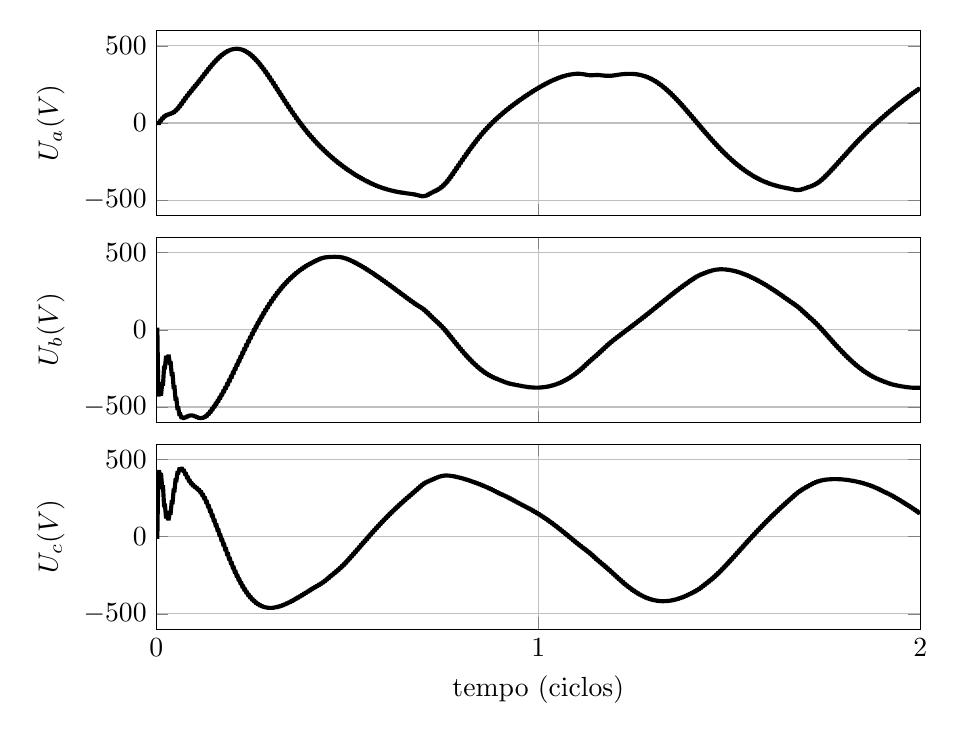
\begin{tikzpicture}

\begin{axis}[%
width=0.8\textwidth,
height=0.193917089240149\textwidth,
scale only axis,
xmin=0,
xmax=0.0333333333333333,
xtick={0,0.0166666666666667,0.0333333333333333},
xticklabels={\empty},
xmajorgrids,
ymin=-600,
ymax=600,
ytick={-500,    0,  500},
ylabel={$\text{U}_\text{b}\text{ (V)}$},
ymajorgrids,
name=plot2,
scaled x ticks = false,
legend columns=-1,
legend style={/tikz/every even column/.append style={column sep=0.3cm}},
legend style={font=\footnotesize}
]
\addplot [color=black,solid,line width=1.5pt,forget plot]
  table[row sep=crcr]{0	0\\
4.16666666666667e-05	0\\
8.33333333333333e-05	-420.179071433538\\
0.000125	-420.179071433538\\
0.000166666666666667	-414.864864959019\\
0.000208333333333333	-414.864864959019\\
0.00025	-350.522993164186\\
0.000291666666666667	-350.522993164186\\
0.000333333333333333	-244.748765901846\\
0.000375	-244.748765901846\\
0.000416666666666667	-180.594969302902\\
0.000458333333333333	-180.594969302902\\
0.0005	-172.800163857989\\
0.000541666666666667	-172.800163857989\\
0.000583333333333333	-214.767639927134\\
0.000625	-214.767639927134\\
0.000666666666666667	-287.455021154959\\
0.000708333333333333	-287.455021154959\\
0.00075	-370.619445321297\\
0.000791666666666667	-370.619445321297\\
0.000833333333333333	-447.52563224499\\
0.000875	-447.52563224499\\
0.000916666666666667	-507.574238737712\\
0.000958333333333333	-507.574238737712\\
0.001	-546.715847867083\\
0.00104166666666667	-546.715847867083\\
0.00108333333333333	-566.340207922122\\
0.001125	-566.340207922122\\
0.00116666666666667	-571.289914082277\\
0.00120833333333333	-571.289914082277\\
0.00125	-567.717074713496\\
0.00129166666666667	-567.717074713496\\
0.00133333333333333	-561.311514576999\\
0.001375	-561.311514576999\\
0.00141666666666667	-556.182340471449\\
0.00145833333333333	-556.182340471449\\
0.0015	-554.438058798818\\
0.00154166666666667	-554.438058798818\\
0.00158333333333333	-556.340552351221\\
0.001625	-556.340552351221\\
0.00166666666666667	-560.820100787618\\
0.00170833333333333	-560.820100787618\\
0.00175	-566.125474944163\\
0.00179166666666667	-566.125474944163\\
0.00183333333333333	-570.423898567167\\
0.001875	-570.423898567167\\
0.00191666666666667	-572.234492206406\\
0.00195833333333333	-572.234492206406\\
0.002	-570.651806648925\\
0.00204166666666667	-570.651806648925\\
0.00208333333333333	-565.37582672885\\
0.002125	-565.37582672885\\
0.00216666666666667	-556.602290365068\\
0.00220833333333333	-556.602290365068\\
0.00225	-544.84100816342\\
0.00229166666666667	-544.84100816342\\
0.00233333333333333	-530.724437208734\\
0.002375	-530.724437208734\\
0.00241666666666667	-514.851327081397\\
0.00245833333333333	-514.851327081397\\
0.0025	-497.688451883342\\
0.00254166666666667	-497.688451883342\\
0.00258333333333333	-479.533451634026\\
0.002625	-479.533451634026\\
0.00266666666666667	-460.527451827945\\
0.00270833333333333	-460.527451827945\\
0.00275	-440.698782788087\\
0.00279166666666667	-440.698782788087\\
0.00283333333333333	-420.018180953396\\
0.002875	-420.018180953396\\
0.00291666666666667	-398.449508882882\\
0.00295833333333333	-398.449508882882\\
0.003	-375.986033304847\\
0.00304166666666667	-375.986033304847\\
0.00308333333333333	-352.668599530674\\
0.003125	-352.668599530674\\
0.00316666666666667	-328.587165858696\\
0.00320833333333333	-328.587165858696\\
0.00325	-303.870362131299\\
0.00329166666666667	-303.870362131299\\
0.00333333333333333	-278.668917731972\\
0.003375	-278.668917731972\\
0.00341666666666667	-253.138341676708\\
0.00345833333333333	-253.138341676708\\
0.0035	-227.424746979553\\
0.00354166666666667	-227.424746979553\\
0.00358333333333333	-201.655839446756\\
0.003625	-201.655839446756\\
0.00366666666666667	-175.937363859869\\
0.00370833333333333	-175.937363859869\\
0.00375	-150.354047831501\\
0.00379166666666667	-150.354047831501\\
0.00383333333333333	-124.973428641693\\
0.003875	-124.973428641693\\
0.00391666666666667	-99.8508459187077\\
0.00395833333333333	-99.8508459187077\\
0.004	-75.0341822768205\\
0.00404166666666667	-75.0341822768205\\
0.00408333333333333	-50.5674443481398\\
0.004125	-50.5674443481398\\
0.00416666666666667	-26.4928214578777\\
0.00420833333333333	-26.4928214578777\\
0.00425	-2.85130979686013\\
0.00429166666666667	-2.85130979686013\\
0.00433333333333333	20.3177215985583\\
0.004375	20.3177215985583\\
0.00441666666666667	42.9775319618012\\
0.00445833333333333	42.9775319618012\\
0.0045	65.0951150787149\\
0.00454166666666667	65.0951150787149\\
0.00458333333333333	86.642070347816\\
0.004625	86.642070347816\\
0.00466666666666667	107.595056690861\\
0.00470833333333333	107.595056690861\\
0.00475	127.935796686638\\
0.00479166666666667	127.935796686638\\
0.00483333333333333	147.650708757596\\
0.004875	147.650708757596\\
0.00491666666666667	166.730304873354\\
0.00495833333333333	166.730304873354\\
0.005	185.168496068164\\
0.00504166666666667	185.168496068164\\
0.00508333333333333	202.961955225664\\
0.005125	202.961955225664\\
0.00516666666666667	220.109590867984\\
0.00520833333333333	220.109590867984\\
0.00525	236.612172825547\\
0.00529166666666667	236.612172825547\\
0.00533333333333333	252.472105462412\\
0.005375	252.472105462412\\
0.00541666666666667	267.693317200308\\
0.00545833333333333	267.693317200308\\
0.0055	282.281222940351\\
0.00554166666666667	282.281222940351\\
0.00558333333333333	296.242717559653\\
0.005625	296.242717559653\\
0.00566666666666667	309.586169042891\\
0.00570833333333333	309.586169042891\\
0.00575	322.321394235842\\
0.00579166666666667	322.321394235842\\
0.00583333333333333	334.459614539781\\
0.005875	334.459614539781\\
0.00591666666666667	346.013400395034\\
0.00595833333333333	346.013400395034\\
0.006	356.996620995534\\
0.00604166666666667	356.996620995534\\
0.00608333333333333	367.424419591414\\
0.006125	367.424419591414\\
0.00616666666666667	377.313236220486\\
0.00620833333333333	377.313236220486\\
0.00625	386.680900533532\\
0.00629166666666667	386.680900533532\\
0.00633333333333333	395.546819430119\\
0.006375	395.546819430119\\
0.00641666666666667	403.932289123357\\
0.00645833333333333	403.932289123357\\
0.0065	411.860969768037\\
0.00654166666666667	411.860969768037\\
0.00658333333333333	419.359571055157\\
0.006625	419.359571055157\\
0.00666666666666667	426.458798518998\\
0.00670833333333333	426.458798518998\\
0.00675	433.194560974787\\
0.00679166666666667	433.194560974787\\
0.00683333333333333	439.609183754667\\
0.006875	439.609183754667\\
0.00691666666666667	445.751310675131\\
0.00695833333333333	445.751310675131\\
0.007	451.668836272739\\
0.00704166666666667	451.668836272739\\
0.00708333333333333	457.337512939094\\
0.007125	457.337512939094\\
0.00716666666666667	462.471290209793\\
0.00720833333333333	462.471290209793\\
0.00725	466.517834318515\\
0.00729166666666667	466.517834318515\\
0.00733333333333333	469.193632051129\\
0.007375	469.193632051129\\
0.00741666666666667	470.7578130587\\
0.00745833333333333	470.7578130587\\
0.0075	471.677921153123\\
0.00754166666666667	471.677921153123\\
0.00758333333333333	472.313759521399\\
0.007625	472.313759521399\\
0.00766666666666667	472.807898295747\\
0.00770833333333333	472.807898295747\\
0.00775	473.110056158022\\
0.00779166666666667	473.110056158022\\
0.00783333333333333	473.053795241454\\
0.007875	473.053795241454\\
0.00791666666666667	472.438662100776\\
0.00795833333333333	472.438662100776\\
0.008	471.094708995088\\
0.00804166666666667	471.094708995088\\
0.00808333333333333	468.920196951672\\
0.008125	468.920196951672\\
0.00816666666666667	465.892510649986\\
0.00820833333333333	465.892510649986\\
0.00825	462.05821597992\\
0.00829166666666667	462.05821597992\\
0.00833333333333333	457.510903861648\\
0.008375	457.510903861648\\
0.00841666666666667	452.36542777696\\
0.00845833333333333	452.36542777696\\
0.0085	446.735231237956\\
0.00854166666666667	446.735231237956\\
0.00858333333333333	440.716687359346\\
0.008625	440.716687359346\\
0.00866666666666667	434.381616536106\\
0.00870833333333333	434.381616536106\\
0.00875	427.777007634959\\
0.00879166666666667	427.777007634959\\
0.00883333333333333	420.929708026235\\
0.008875	420.929708026235\\
0.00891666666666667	413.853483642911\\
0.00895833333333333	413.853483642911\\
0.009	406.556155885705\\
0.00904166666666667	406.556155885705\\
0.00908333333333333	399.045236245237\\
0.009125	399.045236245237\\
0.00916666666666667	391.331311399108\\
0.00920833333333333	391.331311399108\\
0.00925	383.429164544111\\
0.00929166666666667	383.429164544111\\
0.00933333333333333	375.357123813419\\
0.009375	375.357123813419\\
0.00941666666666667	367.135367475148\\
0.00945833333333333	367.135367475148\\
0.0095	358.783919756813\\
0.00954166666666667	358.783919756813\\
0.00958333333333333	350.320913364709\\
0.009625	350.320913364709\\
0.00966666666666667	341.761460254136\\
0.00970833333333333	341.761460254136\\
0.00975	333.117236149366\\
0.00979166666666667	333.117236149366\\
0.00983333333333333	324.396698700256\\
0.009875	324.396698700256\\
0.00991666666666667	315.605748765589\\
0.00995833333333333	315.605748765589\\
0.01	306.74860984152\\
0.0100416666666667	306.74860984152\\
0.0100833333333333	297.828726158517\\
0.010125	297.828726158517\\
0.0101666666666667	288.849541547663\\
0.0102083333333333	288.849541547663\\
0.01025	279.815094687449\\
0.0102916666666667	279.815094687449\\
0.0103333333333333	270.730432774819\\
0.010375	270.730432774819\\
0.0104166666666667	261.60189374316\\
0.0104583333333333	261.60189374316\\
0.0105	252.437333480226\\
0.0105416666666667	252.437333480226\\
0.0105833333333333	243.246382016451\\
0.010625	243.246382016451\\
0.0106666666666667	234.040808254741\\
0.0107083333333333	234.040808254741\\
0.01075	224.835064915953\\
0.0107916666666667	224.835064915953\\
0.0108333333333333	215.647081824671\\
0.010875	215.647081824671\\
0.0109166666666667	206.499381697607\\
0.0109583333333333	206.499381697607\\
0.011	197.420607035488\\
0.0110416666666667	197.420607035488\\
0.0110833333333333	188.44754943962\\
0.011125	188.44754943962\\
0.0111666666666667	179.627677918246\\
0.0112083333333333	179.627677918246\\
0.01125	171.02163627144\\
0.0112916666666667	171.02163627144\\
0.0113333333333333	162.702872007855\\
0.011375	162.702872007855\\
0.0114166666666667	154.736366693818\\
0.0114583333333333	154.736366693818\\
0.0115	147.011964298434\\
0.0115416666666667	147.011964298434\\
0.0115833333333333	138.926769817703\\
0.011625	138.926769817703\\
0.0116666666666667	129.590949701875\\
0.0117083333333333	129.590949701875\\
0.01175	118.753724196033\\
0.0117916666666667	118.753724196033\\
0.0118333333333333	106.9104471993\\
0.011875	106.9104471993\\
0.0119166666666667	94.7440958466268\\
0.0119583333333333	94.7440958466268\\
0.012	82.7437175490343\\
0.0120416666666667	82.7437175490343\\
0.0120833333333333	71.0821687268513\\
0.012125	71.0821687268513\\
0.0121666666666667	59.6578667737165\\
0.0122083333333333	59.6578667737165\\
0.01225	48.2068469316843\\
0.0122916666666667	48.2068469316843\\
0.0123333333333333	36.4239228031408\\
0.012375	36.4239228031408\\
0.0124166666666667	24.0578853502687\\
0.0124583333333333	24.0578853502687\\
0.0125	10.9660246753928\\
0.0125416666666667	10.9660246753928\\
0.0125833333333333	-2.87191288402635\\
0.012625	-2.87191288402635\\
0.0126666666666667	-17.3709104168376\\
0.0127083333333333	-17.3709104168376\\
0.01275	-32.375587920351\\
0.0127916666666667	-32.375587920351\\
0.0128333333333333	-47.6997287305944\\
0.012875	-47.6997287305944\\
0.0129166666666667	-63.1604502257538\\
0.0129583333333333	-63.1604502257538\\
0.013	-78.6013752275666\\
0.0130416666666667	-78.6013752275666\\
0.0130833333333333	-93.9033511901165\\
0.013125	-93.9033511901165\\
0.0131666666666667	-108.98444305504\\
0.0132083333333333	-108.98444305504\\
0.01325	-123.792701633393\\
0.0132916666666667	-123.792701633393\\
0.0133333333333333	-138.295661333532\\
0.013375	-138.295661333532\\
0.0134166666666667	-152.469957404581\\
0.0134583333333333	-152.469957404581\\
0.0135	-166.293325971325\\
0.0135416666666667	-166.293325971325\\
0.0135833333333333	-179.73998471986\\
0.013625	-179.73998471986\\
0.0136666666666667	-192.779309692001\\
0.0137083333333333	-192.779309692001\\
0.01375	-205.377003116364\\
0.0137916666666667	-205.377003116364\\
0.0138333333333333	-217.497631447708\\
0.013875	-217.497631447708\\
0.0139166666666667	-229.107442320242\\
0.0139583333333333	-229.107442320242\\
0.014	-240.176627528621\\
0.0140416666666667	-240.176627528621\\
0.0140833333333333	-250.680556606316\\
0.014125	-250.680556606316\\
0.0141666666666667	-260.599851867767\\
0.0142083333333333	-260.599851867767\\
0.01425	-269.919439782728\\
0.0142916666666667	-269.919439782728\\
0.0143333333333333	-278.626871689511\\
0.014375	-278.626871689511\\
0.0144166666666667	-286.710290801558\\
0.0144583333333333	-286.710290801558\\
0.0145	-294.156554790522\\
0.0145416666666667	-294.156554790522\\
0.0145833333333333	-300.950580590786\\
0.014625	-300.950580590786\\
0.0146666666666667	-307.079298378971\\
0.0147083333333333	-307.079298378971\\
0.01475	-312.571377541795\\
0.0147916666666667	-312.571377541795\\
0.0148333333333333	-317.607687209113\\
0.014875	-317.607687209113\\
0.0149166666666667	-322.539283397708\\
0.0149583333333333	-322.539283397708\\
0.015	-327.602545824348\\
0.0150416666666667	-327.602545824348\\
0.0150833333333333	-332.706739590892\\
0.015125	-332.706739590892\\
0.0151666666666667	-337.585332183651\\
0.0152083333333333	-337.585332183651\\
0.01525	-342.003670932167\\
0.0152916666666667	-342.003670932167\\
0.0153333333333333	-345.85496291089\\
0.015375	-345.85496291089\\
0.0154166666666667	-349.162574635071\\
0.0154583333333333	-349.162574635071\\
0.0155	-352.03734458804\\
0.0155416666666667	-352.03734458804\\
0.0155833333333333	-354.624021590244\\
0.015625	-354.624021590244\\
0.0156666666666667	-357.055486453538\\
0.0157083333333333	-357.055486453538\\
0.01575	-359.423291077928\\
0.0157916666666667	-359.423291077928\\
0.0158333333333333	-361.766136320025\\
0.015875	-361.766136320025\\
0.0159166666666667	-364.073330984874\\
0.0159583333333333	-364.073330984874\\
0.016	-366.297878674463\\
0.0160416666666667	-366.297878674463\\
0.0160833333333333	-368.37338824141\\
0.016125	-368.37338824141\\
0.0161666666666667	-370.229972427442\\
0.0162083333333333	-370.229972427442\\
0.01625	-371.80602626708\\
0.0162916666666667	-371.80602626708\\
0.0163333333333333	-373.054644157177\\
0.016375	-373.054644157177\\
0.0164166666666667	-373.944988998982\\
0.0164583333333333	-373.944988998982\\
0.0165	-374.45992654402\\
0.0165416666666667	-374.45992654402\\
0.0165833333333333	-374.591638263777\\
0.016625	-374.591638263777\\
0.0166666666666667	-374.336826925851\\
0.0167083333333333	-374.336826925851\\
0.01675	-373.692708447959\\
0.0167916666666667	-373.692708447959\\
0.0168333333333333	-372.654433891549\\
0.016875	-372.654433891549\\
0.0169166666666667	-371.214067014077\\
0.0169583333333333	-371.214067014077\\
0.017	-369.360858998853\\
0.0170416666666667	-369.360858998853\\
0.0170833333333333	-367.082354477813\\
0.017125	-367.082354477813\\
0.0171666666666667	-364.365821899671\\
0.0172083333333333	-364.365821899671\\
0.01725	-361.199582949555\\
0.0172916666666667	-361.199582949555\\
0.0173333333333333	-357.573962219389\\
0.017375	-357.573962219389\\
0.0174166666666667	-353.481756565085\\
0.0174583333333333	-353.481756565085\\
0.0175	-348.918233661103\\
0.0175416666666667	-348.918233661103\\
0.0175833333333333	-343.880773526705\\
0.017625	-343.880773526705\\
0.0176666666666667	-338.368297930524\\
0.0177083333333333	-338.368297930524\\
0.01775	-332.38062438451\\
0.0177916666666667	-332.38062438451\\
0.0178333333333333	-325.917842864771\\
0.017875	-325.917842864771\\
0.0179166666666667	-318.979762767412\\
0.0179583333333333	-318.979762767412\\
0.018	-311.565428838187\\
0.0180416666666667	-311.565428838187\\
0.0180833333333333	-303.672668266014\\
0.018125	-303.672668266014\\
0.0181666666666667	-295.297614050001\\
0.0182083333333333	-295.297614050001\\
0.01825	-286.434161868367\\
0.0182916666666667	-286.434161868367\\
0.0183333333333333	-277.073386587467\\
0.018375	-277.073386587467\\
0.0184166666666667	-267.203161729994\\
0.0184583333333333	-267.203161729994\\
0.0185	-256.808899787124\\
0.0185416666666667	-256.808899787124\\
0.0185833333333333	-245.878564028925\\
0.018625	-245.878564028925\\
0.0186666666666667	-234.434926912715\\
0.0187083333333333	-234.434926912715\\
0.01875	-222.656625047262\\
0.0187916666666667	-222.656625047262\\
0.0188333333333333	-210.959527088156\\
0.018875	-210.959527088156\\
0.0189166666666667	-199.738418583314\\
0.0189583333333333	-199.738418583314\\
0.019	-189.010500427551\\
0.0190416666666667	-189.010500427551\\
0.0190833333333333	-178.484774813994\\
0.019125	-178.484774813994\\
0.0191666666666667	-167.82891383647\\
0.0192083333333333	-167.82891383647\\
0.01925	-156.841442988537\\
0.0192916666666667	-156.841442988537\\
0.0193333333333333	-145.497068380738\\
0.019375	-145.497068380738\\
0.0194166666666667	-133.911966389727\\
0.0194583333333333	-133.911966389727\\
0.0195	-122.276740249304\\
0.0195416666666667	-122.276740249304\\
0.0195833333333333	-110.789141898709\\
0.019625	-110.789141898709\\
0.0196666666666667	-99.6043706732099\\
0.0197083333333333	-99.6043706732099\\
0.01975	-88.8095074897546\\
0.0197916666666667	-88.8095074897546\\
0.0198333333333333	-78.4206169534082\\
0.019875	-78.4206169534082\\
0.0199166666666667	-68.396282694035\\
0.0199583333333333	-68.396282694035\\
0.02	-58.6595871531465\\
0.0200416666666667	-58.6595871531465\\
0.0200833333333333	-49.1211486536497\\
0.020125	-49.1211486536497\\
0.0201666666666667	-39.6978830725994\\
0.0202083333333333	-39.6978830725994\\
0.02025	-30.3247482612208\\
0.0202916666666667	-30.3247482612208\\
0.0203333333333333	-20.9591168391336\\
0.020375	-20.9591168391336\\
0.0204166666666667	-11.5791454976988\\
0.0204583333333333	-11.5791454976988\\
0.0205	-2.17839536712388\\
0.0205416666666667	-2.17839536712388\\
0.0205833333333333	7.24092588363876\\
0.020625	7.24092588363876\\
0.0206666666666667	16.6741693876306\\
0.0207083333333333	16.6741693876306\\
0.02075	26.1186932259392\\
0.0207916666666667	26.1186932259392\\
0.0208333333333333	35.5761127948398\\
0.020875	35.5761127948398\\
0.0209166666666667	45.0525353272816\\
0.0209583333333333	45.0525353272816\\
0.021	54.5573490408728\\
0.0210416666666667	54.5573490408728\\
0.0210833333333333	64.1012796526003\\
0.021125	64.1012796526003\\
0.0211666666666667	73.694368572666\\
0.0212083333333333	73.694368572666\\
0.02125	83.3443433690686\\
0.0212916666666667	83.3443433690686\\
0.0213333333333333	93.0556219004392\\
0.021375	93.0556219004392\\
0.0214166666666667	102.828979336994\\
0.0214583333333333	102.828979336994\\
0.0215	112.661756632756\\
0.0215416666666667	112.661756632756\\
0.0215833333333333	122.548411652533\\
0.021625	122.548411652533\\
0.0216666666666667	132.481203766474\\
0.0217083333333333	132.481203766474\\
0.02175	142.450841906831\\
0.0217916666666667	142.450841906831\\
0.0218333333333333	152.446990175172\\
0.021875	152.446990175172\\
0.0219166666666667	162.458592413957\\
0.0219583333333333	162.458592413957\\
0.022	172.474031959061\\
0.0220416666666667	172.474031959061\\
0.0220833333333333	182.481177056125\\
0.022125	182.481177056125\\
0.0221666666666667	192.467375177422\\
0.0222083333333333	192.467375177422\\
0.02225	202.419454824874\\
0.0222916666666667	202.419454824874\\
0.0223333333333333	212.323778070089\\
0.022375	212.323778070089\\
0.0224166666666667	222.166368145884\\
0.0224583333333333	222.166368145884\\
0.0225	231.933119690956\\
0.0225416666666667	231.933119690956\\
0.0225833333333333	241.610088511721\\
0.022625	241.610088511721\\
0.0226666666666667	251.183854533209\\
0.0227083333333333	251.183854533209\\
0.02275	260.641955702813\\
0.0227916666666667	260.641955702813\\
0.0228333333333333	269.973400260292\\
0.022875	269.973400260292\\
0.0229166666666667	279.16927635725\\
0.0229583333333333	279.16927635725\\
0.023	288.22348250085\\
0.0230416666666667	288.22348250085\\
0.0230833333333333	297.133571557038\\
0.023125	297.133571557038\\
0.0231666666666667	305.901535896758\\
0.0232083333333333	305.901535896758\\
0.02325	314.533685966224\\
0.0232916666666667	314.533685966224\\
0.0233333333333333	323.036023594093\\
0.023375	323.036023594093\\
0.0234166666666667	331.367437571297\\
0.0234583333333333	331.367437571297\\
0.0235	339.331069085315\\
0.0235416666666667	339.331069085315\\
0.0235833333333333	346.593938036643\\
0.023625	346.593938036643\\
0.0236666666666667	352.990490405546\\
0.0237083333333333	352.990490405546\\
0.02375	358.651709070781\\
0.0237916666666667	358.651709070781\\
0.0238333333333333	363.820880421054\\
0.023875	363.820880421054\\
0.0239166666666667	368.682966728322\\
0.0239583333333333	368.682966728322\\
0.024	373.303754128982\\
0.0240416666666667	373.303754128982\\
0.0240833333333333	377.642225375844\\
0.024125	377.642225375844\\
0.0241666666666667	381.592670719894\\
0.0242083333333333	381.592670719894\\
0.02425	385.030604644711\\
0.0242916666666667	385.030604644711\\
0.0243333333333333	387.849266055096\\
0.024375	387.849266055096\\
0.0244166666666667	389.981239820268\\
0.0244583333333333	389.981239820268\\
0.0245	391.405003964836\\
0.0245416666666667	391.405003964836\\
0.0245833333333333	392.13961417208\\
0.024625	392.13961417208\\
0.0246666666666667	392.232341106541\\
0.0247083333333333	392.232341106541\\
0.02475	391.744115271905\\
0.0247916666666667	391.744115271905\\
0.0248333333333333	390.73659453938\\
0.024875	390.73659453938\\
0.0249166666666667	389.26312088369\\
0.0249583333333333	389.26312088369\\
0.025	387.364275930398\\
0.0250416666666667	387.364275930398\\
0.0250833333333333	385.067522977684\\
0.025125	385.067522977684\\
0.0251666666666667	382.389697531757\\
0.0252083333333333	382.389697531757\\
0.02525	379.340881139233\\
0.0252916666666667	379.340881139233\\
0.0253333333333333	375.928357137099\\
0.025375	375.928357137099\\
0.0254166666666667	372.159743115693\\
0.0254583333333333	372.159743115693\\
0.0255	368.044864418852\\
0.0255416666666667	368.044864418852\\
0.0255833333333333	363.596348354732\\
0.025625	363.596348354732\\
0.0256666666666667	358.829209812153\\
0.0257083333333333	358.829209812153\\
0.02575	353.759838920933\\
0.0257916666666667	353.759838920933\\
0.0258333333333333	348.404807110324\\
0.025875	348.404807110324\\
0.0259166666666667	342.779821029511\\
0.0259583333333333	342.779821029511\\
0.026	336.899021891496\\
0.0260416666666667	336.899021891496\\
0.0260833333333333	330.774693827664\\
0.026125	330.774693827664\\
0.0261666666666667	324.417338652135\\
0.0262083333333333	324.417338652135\\
0.02625	317.83601054701\\
0.0262916666666667	317.83601054701\\
0.0263333333333333	311.038783380965\\
0.026375	311.038783380965\\
0.0264166666666667	304.033236875612\\
0.0264583333333333	304.033236875612\\
0.0265	296.826882186925\\
0.0265416666666667	296.826882186925\\
0.0265833333333333	289.427488966489\\
0.026625	289.427488966489\\
0.0266666666666667	281.843313731478\\
0.0267083333333333	281.843313731478\\
0.02675	274.083256877216\\
0.0267916666666667	274.083256877216\\
0.0268333333333333	266.156990856232\\
0.026875	266.156990856232\\
0.0269166666666667	258.075106480121\\
0.0269583333333333	258.075106480121\\
0.027	249.849321799315\\
0.0270416666666667	249.849321799315\\
0.0270833333333333	241.492793275269\\
0.027125	241.492793275269\\
0.0271666666666667	233.020566314818\\
0.0272083333333333	233.020566314818\\
0.02725	224.450204454928\\
0.0272916666666667	224.450204454928\\
0.0273333333333333	215.802642535203\\
0.027375	215.802642535203\\
0.0274166666666667	207.103307202962\\
0.0274583333333333	207.103307202962\\
0.0275	198.383489808628\\
0.0275416666666667	198.383489808628\\
0.0275833333333333	189.681659981608\\
0.027625	189.681659981608\\
0.0276666666666667	181.043157683476\\
0.0277083333333333	181.043157683476\\
0.02775	172.509572352179\\
0.0277916666666667	172.509572352179\\
0.0278333333333333	164.029419048181\\
0.027875	164.029419048181\\
0.0279166666666667	155.278303122368\\
0.0279583333333333	155.278303122368\\
0.028	145.745611387673\\
0.0280416666666667	145.745611387673\\
0.0280833333333333	135.254450286136\\
0.028125	135.254450286136\\
0.0281666666666667	124.0796516846\\
0.0282083333333333	124.0796516846\\
0.02825	112.629636500578\\
0.0282916666666667	112.629636500578\\
0.0283333333333333	101.20423620079\\
0.028375	101.20423620079\\
0.0284166666666667	89.9153080752128\\
0.0284583333333333	89.9153080752128\\
0.0285	78.7104844077268\\
0.0285416666666667	78.7104844077268\\
0.0285833333333333	67.4396349222964\\
0.028625	67.4396349222964\\
0.0286666666666667	55.9265479520004\\
0.0287083333333333	55.9265479520004\\
0.02875	44.0253475377299\\
0.0287916666666667	44.0253475377299\\
0.0288333333333333	31.6531214661927\\
0.028875	31.6531214661927\\
0.0289166666666667	18.7987511576131\\
0.0289583333333333	18.7987511576131\\
0.029	5.51333662994936\\
0.0290416666666667	5.51333662994936\\
0.0290833333333333	-8.10999692900733\\
0.029125	-8.10999692900733\\
0.0291666666666667	-21.9592327828976\\
0.0292083333333333	-21.9592327828976\\
0.02925	-35.9236292478269\\
0.0292916666666667	-35.9236292478269\\
0.0293333333333333	-49.9075214407193\\
0.029375	-49.9075214407193\\
0.0294166666666667	-63.8368205141521\\
0.0294583333333333	-63.8368205141521\\
0.0295	-77.659159166174\\
0.0295416666666667	-77.659159166174\\
0.0295833333333333	-91.3397134577379\\
0.029625	-91.3397134577379\\
0.0296666666666667	-104.855025164509\\
0.0297083333333333	-104.855025164509\\
0.02975	-118.186841631749\\
0.0297916666666667	-118.186841631749\\
0.0298333333333333	-131.317339512273\\
0.029875	-131.317339512273\\
0.0299166666666667	-144.2263513894\\
0.0299583333333333	-144.2263513894\\
0.03	-156.890571310337\\
0.0300416666666667	-156.890571310337\\
0.0300833333333333	-169.284279125425\\
0.030125	-169.284279125425\\
0.0301666666666667	-181.380926553693\\
0.0302083333333333	-181.380926553693\\
0.03025	-193.154937297995\\
0.0302916666666667	-193.154937297995\\
0.0303333333333333	-204.583222331564\\
0.030375	-204.583222331564\\
0.0304166666666667	-215.6461231107\\
0.0304583333333333	-215.6461231107\\
0.0305	-226.327703704202\\
0.0305416666666667	-226.327703704202\\
0.0305833333333333	-236.615472884263\\
0.030625	-236.615472884263\\
0.0306666666666667	-246.499708761128\\
0.0307083333333333	-246.499708761128\\
0.03075	-255.972582400737\\
0.0307916666666667	-255.972582400737\\
0.0308333333333333	-265.0272482475\\
0.030875	-265.0272482475\\
0.0309166666666667	-273.657010071522\\
0.0309583333333333	-273.657010071522\\
0.031	-281.854604348429\\
0.0310416666666667	-281.854604348429\\
0.0310833333333333	-289.611589988785\\
0.031125	-289.611589988785\\
0.0311666666666667	-296.917820852653\\
0.0312083333333333	-296.917820852653\\
0.03125	-303.761067175233\\
0.0312916666666667	-303.761067175233\\
0.0313333333333333	-310.127253968848\\
0.031375	-310.127253968848\\
0.0314166666666667	-316.003321234944\\
0.0314583333333333	-316.003321234944\\
0.0315	-321.402454193919\\
0.0315416666666667	-321.402454193919\\
0.0315833333333333	-326.433061405788\\
0.031625	-326.433061405788\\
0.0316666666666667	-331.308572327323\\
0.0317083333333333	-331.308572327323\\
0.03175	-336.167113343374\\
0.0317916666666667	-336.167113343374\\
0.0318333333333333	-340.944005563238\\
0.031875	-340.944005563238\\
0.0319166666666667	-345.470613263772\\
0.0319583333333333	-345.470613263772\\
0.032	-349.601512646934\\
0.0320416666666667	-349.601512646934\\
0.0320833333333333	-353.270727882683\\
0.032125	-353.270727882683\\
0.0321666666666667	-356.491221083665\\
0.0322083333333333	-356.491221083665\\
0.03225	-359.328112152332\\
0.0322916666666667	-359.328112152332\\
0.0323333333333333	-361.866106535949\\
0.032375	-361.866106535949\\
0.0324166666666667	-364.18206287775\\
0.0324583333333333	-364.18206287775\\
0.0325	-366.327593239657\\
0.0325416666666667	-366.327593239657\\
0.0325833333333333	-368.322505571605\\
0.032625	-368.322505571605\\
0.0326666666666667	-370.157202979674\\
0.0327083333333333	-370.157202979674\\
0.03275	-371.80076428646\\
0.0327916666666667	-371.80076428646\\
0.0328333333333333	-373.211202620655\\
0.032875	-373.211202620655\\
0.0329166666666667	-374.345013192046\\
0.0329583333333333	-374.345013192046\\
0.033	-375.164177141373\\
0.0330416666666667	-375.164177141373\\
0.0330833333333333	-375.639914630463\\
0.033125	-375.639914630463\\
0.0331666666666667	-375.753408322708\\
0.0332083333333333	-375.753408322708\\
0.03325	-375.494307431118\\
0.0332916666666667	-375.494307431118\\
0.0333333333333333	-374.858050189855\\
};
\end{axis}

\begin{axis}[%
width=0.8\textwidth,
height=0.193917089240149\textwidth,
scale only axis,
xmin=0,
xmax=0.0333333333333333,
xtick={0,0.0166666666666667,0.0333333333333333},
xticklabels={{0},{1},{2}},
xlabel={tempo (ciclos)},
xmajorgrids,
ymin=-600,
ymax=600,
ytick={-500,    0,  500},
ylabel={$\text{U}_\text{c}\text{ (V)}$},
ymajorgrids,
at=(plot2.below south west),
anchor=above north west,
scaled x ticks = false,
legend columns=-1,
legend style={/tikz/every even column/.append style={column sep=0.3cm}},
legend style={font=\footnotesize}
]
\addplot [color=black,solid,line width=1.5pt,forget plot]
  table[row sep=crcr]{0	0\\
4.16666666666667e-05	0\\
8.33333333333333e-05	420.179071433538\\
0.000125	420.179071433538\\
0.000166666666666667	399.65747159438\\
0.000208333333333333	399.65747159438\\
0.00025	320.583243435783\\
0.000291666666666667	320.583243435783\\
0.000333333333333333	202.679154318002\\
0.000375	202.679154318002\\
0.000416666666666667	130.44947845611\\
0.000458333333333333	130.44947845611\\
0.0005	117.543717293957\\
0.000541666666666667	117.543717293957\\
0.000583333333333333	155.514331114415\\
0.000625	155.514331114415\\
0.000666666666666667	223.36099343267\\
0.000708333333333333	223.36099343267\\
0.00075	299.39832432458\\
0.000791666666666667	299.39832432458\\
0.000833333333333333	366.209721213765\\
0.000875	366.209721213765\\
0.000916666666666667	413.262874293421\\
0.000958333333333333	413.262874293421\\
0.001	437.12213392922\\
0.00104166666666667	437.12213392922\\
0.00108333333333333	440.05800890036\\
0.001125	440.05800890036\\
0.00116666666666667	427.793602081917\\
0.00120833333333333	427.793602081917\\
0.00125	407.167837198763\\
0.00129166666666667	407.167837198763\\
0.00133333333333333	384.269047020733\\
0.001375	384.269047020733\\
0.00141666666666667	363.314949494806\\
0.00145833333333333	363.314949494806\\
0.0015	346.298134979102\\
0.00154166666666667	346.298134979102\\
0.00158333333333333	333.238275932518\\
0.001625	333.238275932518\\
0.00166666666666667	322.796505281172\\
0.00170833333333333	322.796505281172\\
0.00175	313.003305747787\\
0.00179166666666667	313.003305747787\\
0.00183333333333333	301.903608279244\\
0.001875	301.903608279244\\
0.00191666666666667	288.0022844878\\
0.00195833333333333	288.0022844878\\
0.002	270.473766090578\\
0.00204166666666667	270.473766090578\\
0.00208333333333333	249.162954994385\\
0.002125	249.162954994385\\
0.00216666666666667	224.442163740723\\
0.00220833333333333	224.442163740723\\
0.00225	197.000289649267\\
0.00229166666666667	197.000289649267\\
0.00233333333333333	167.631427299607\\
0.002375	167.631427299607\\
0.00241666666666667	137.069101566743\\
0.00245833333333333	137.069101566743\\
0.0025	105.887708089937\\
0.00254166666666667	105.887708089937\\
0.00258333333333333	74.4711474835106\\
0.002625	74.4711474835106\\
0.00266666666666667	43.0338557954351\\
0.00270833333333333	43.0338557954351\\
0.00275	11.6725716029886\\
0.00279166666666667	11.6725716029886\\
0.00283333333333333	-19.5727507878588\\
0.002875	-19.5727507878588\\
0.00291666666666667	-50.6656740008502\\
0.00295833333333333	-50.6656740008502\\
0.003	-81.5374649688973\\
0.00304166666666667	-81.5374649688973\\
0.00308333333333333	-112.071599302787\\
0.003125	-112.071599302787\\
0.00316666666666667	-142.106047222704\\
0.00320833333333333	-142.106047222704\\
0.00325	-171.447652909029\\
0.00329166666666667	-171.447652909029\\
0.00333333333333333	-199.891996392581\\
0.003375	-199.891996392581\\
0.00341666666666667	-227.242936070711\\
0.00345833333333333	-227.242936070711\\
0.0035	-253.327850668664\\
0.00354166666666667	-253.327850668664\\
0.00358333333333333	-278.006717768096\\
0.003625	-278.006717768096\\
0.00366666666666667	-301.175027633688\\
0.00370833333333333	-301.175027633688\\
0.00375	-322.761812134191\\
0.00379166666666667	-322.761812134191\\
0.00383333333333333	-342.724673542149\\
0.003875	-342.724673542149\\
0.00391666666666667	-361.043708487439\\
0.00395833333333333	-361.043708487439\\
0.004	-377.715823435131\\
0.00404166666666667	-377.715823435131\\
0.00408333333333333	-392.750345496904\\
0.004125	-392.750345496904\\
0.00416666666666667	-406.166235998808\\
0.00420833333333333	-406.166235998808\\
0.00425	-417.990744852056\\
0.00429166666666667	-417.990744852056\\
0.00433333333333333	-428.259063407647\\
0.004375	-428.259063407647\\
0.00441666666666667	-437.014443480898\\
0.00445833333333333	-437.014443480898\\
0.0045	-444.308310114125\\
0.00454166666666667	-444.308310114125\\
0.00458333333333333	-450.200045005673\\
0.004625	-450.200045005673\\
0.00466666666666667	-454.756295433786\\
0.00470833333333333	-454.756295433786\\
0.00475	-458.049821862986\\
0.00479166666666667	-458.049821862986\\
0.00483333333333333	-460.158007417807\\
0.004875	-460.158007417807\\
0.00491666666666667	-461.161204702039\\
0.00495833333333333	-461.161204702039\\
0.005	-461.141089340909\\
0.00504166666666667	-461.141089340909\\
0.00508333333333333	-460.179185278059\\
0.005125	-460.179185278059\\
0.00516666666666667	-458.355621263731\\
0.00520833333333333	-458.355621263731\\
0.00525	-455.748158005746\\
0.00529166666666667	-455.748158005746\\
0.00533333333333333	-452.431476123573\\
0.005375	-452.431476123573\\
0.00541666666666667	-448.476686472833\\
0.00545833333333333	-448.476686472833\\
0.0055	-443.951012272372\\
0.00554166666666667	-443.951012272372\\
0.00558333333333333	-438.917594812464\\
0.005625	-438.917594812464\\
0.00566666666666667	-433.435385711222\\
0.00570833333333333	-433.435385711222\\
0.00575	-427.559103506212\\
0.00579166666666667	-427.559103506212\\
0.00583333333333333	-421.339246520403\\
0.005875	-421.339246520403\\
0.00591666666666667	-414.822164790217\\
0.00595833333333333	-414.822164790217\\
0.006	-408.050200464621\\
0.00604166666666667	-408.050200464621\\
0.00608333333333333	-401.061908996247\\
0.006125	-401.061908996247\\
0.00616666666666667	-393.892374121323\\
0.00620833333333333	-393.892374121323\\
0.00625	-386.573629991605\\
0.00629166666666667	-386.573629991605\\
0.00633333333333333	-379.135205826839\\
0.006375	-379.135205826839\\
0.00641666666666667	-371.604813704211\\
0.00645833333333333	-371.604813704211\\
0.0065	-364.009209278387\\
0.00654166666666667	-364.009209278387\\
0.00658333333333333	-356.375266365168\\
0.006625	-356.375266365168\\
0.00666666666666667	-348.731308638385\\
0.00670833333333333	-348.731308638385\\
0.00675	-341.108693348903\\
0.00679166666666667	-341.108693348903\\
0.00683333333333333	-333.543387160956\\
0.006875	-333.543387160956\\
0.00691666666666667	-326.076213322244\\
0.00695833333333333	-326.076213322244\\
0.007	-318.746108748623\\
0.00704166666666667	-318.746108748623\\
0.00708333333333333	-311.519033373802\\
0.007125	-311.519033373802\\
0.00716666666666667	-304.098587338329\\
0.00720833333333333	-304.098587338329\\
0.00725	-295.921782990935\\
0.00729166666666667	-295.921782990935\\
0.00733333333333333	-286.694375090986\\
0.007375	-286.694375090986\\
0.00741666666666667	-276.664883174809\\
0.00745833333333333	-276.664883174809\\
0.0075	-266.290536819505\\
0.00754166666666667	-266.290536819505\\
0.00758333333333333	-255.921269310385\\
0.007625	-255.921269310385\\
0.00766666666666667	-245.690349029219\\
0.00770833333333333	-245.690349029219\\
0.00775	-235.538861377622\\
0.00779166666666667	-235.538861377622\\
0.00783333333333333	-225.292481834814\\
0.007875	-225.292481834814\\
0.00791666666666667	-214.743674402866\\
0.00795833333333333	-214.743674402866\\
0.008	-203.716251260921\\
0.00804166666666667	-203.716251260921\\
0.00808333333333333	-192.103096722811\\
0.008125	-192.103096722811\\
0.00816666666666667	-179.877087174017\\
0.00820833333333333	-179.877087174017\\
0.00825	-167.081139456375\\
0.00829166666666667	-167.081139456375\\
0.00833333333333333	-153.806032853666\\
0.008375	-153.806032853666\\
0.00841666666666667	-140.164613624162\\
0.00845833333333333	-140.164613624162\\
0.0085	-126.269079716149\\
0.00854166666666667	-126.269079716149\\
0.00858333333333333	-112.215269142411\\
0.008625	-112.215269142411\\
0.00866666666666667	-98.0751190614823\\
0.00870833333333333	-98.0751190614823\\
0.00875	-83.8963193788991\\
0.00879166666666667	-83.8963193788991\\
0.00883333333333333	-69.7069361943245\\
0.008875	-69.7069361943245\\
0.00891666666666667	-55.5223980311259\\
0.00895833333333333	-55.5223980311259\\
0.009	-41.3525549228356\\
0.00904166666666667	-41.3525549228356\\
0.00908333333333333	-27.2072314275941\\
0.009125	-27.2072314275941\\
0.00916666666666667	-13.0995270155633\\
0.00920833333333333	-13.0995270155633\\
0.00925	0.95315017175804\\
0.00929166666666667	0.95315017175804\\
0.00933333333333333	14.9298253396053\\
0.009375	14.9298253396053\\
0.00941666666666667	28.8077454615331\\
0.00945833333333333	28.8077454615331\\
0.0095	42.5644809157571\\
0.00954166666666667	42.5644809157571\\
0.00958333333333333	56.1797652964601\\
0.009625	56.1797652964601\\
0.00966666666666667	69.6367333015997\\
0.00970833333333333	69.6367333015997\\
0.00975	82.9224531719828\\
0.00979166666666667	82.9224531719828\\
0.00983333333333333	96.0278364171395\\
0.009875	96.0278364171395\\
0.00991666666666667	108.947118801783\\
0.00995833333333333	108.947118801783\\
0.01	121.677142154362\\
0.0100416666666667	121.677142154362\\
0.0100833333333333	134.216642558342\\
0.010125	134.216642558342\\
0.0101666666666667	146.565690961614\\
0.0102083333333333	146.565690961614\\
0.01025	158.725361563145\\
0.0102916666666667	158.725361563145\\
0.0103333333333333	170.697640860144\\
0.010375	170.697640860144\\
0.0104166666666667	182.485547747444\\
0.0104583333333333	182.485547747444\\
0.0105	194.093416702975\\
0.0105416666666667	194.093416702975\\
0.0105833333333333	205.527300049033\\
0.010625	205.527300049033\\
0.0106666666666667	216.795466267861\\
0.0107083333333333	216.795466267861\\
0.01075	227.909003154795\\
0.0107916666666667	227.909003154795\\
0.0108333333333333	238.882571902719\\
0.010875	238.882571902719\\
0.0109166666666667	249.735396985001\\
0.0109583333333333	249.735396985001\\
0.011	260.492611143799\\
0.0110416666666667	260.492611143799\\
0.0110833333333333	271.187084376916\\
0.011125	271.187084376916\\
0.0111666666666667	281.861767374968\\
0.0112083333333333	281.861767374968\\
0.01125	292.5720432162\\
0.0112916666666667	292.5720432162\\
0.0113333333333333	303.385261053977\\
0.011375	303.385261053977\\
0.0114166666666667	314.359421667357\\
0.0114583333333333	314.359421667357\\
0.0115	325.376503319251\\
0.0115416666666667	325.376503319251\\
0.0115833333333333	335.824887968477\\
0.011625	335.824887968477\\
0.0116666666666667	344.805206635709\\
0.0117083333333333	344.805206635709\\
0.01175	352.056383434094\\
0.0117916666666667	352.056383434094\\
0.0118333333333333	358.062766743078\\
0.011875	358.062766743078\\
0.0119166666666667	363.495666263197\\
0.0119583333333333	363.495666263197\\
0.012	368.831843231901\\
0.0120416666666667	368.831843231901\\
0.0120833333333333	374.231289502473\\
0.012125	374.231289502473\\
0.0121666666666667	379.579019264073\\
0.0122083333333333	379.579019264073\\
0.01225	384.597167147237\\
0.0122916666666667	384.597167147237\\
0.0123333333333333	388.966192724403\\
0.012375	388.966192724403\\
0.0124166666666667	392.420126519886\\
0.0124583333333333	392.420126519886\\
0.0125	394.801141128502\\
0.0125416666666667	394.801141128502\\
0.0125833333333333	396.073558575031\\
0.012625	396.073558575031\\
0.0126666666666667	396.306714059654\\
0.0127083333333333	396.306714059654\\
0.01275	395.640095156162\\
0.0127916666666667	395.640095156162\\
0.0128333333333333	394.243857591831\\
0.012875	394.243857591831\\
0.0129166666666667	392.284690757872\\
0.0129583333333333	392.284690757872\\
0.013	389.902674675463\\
0.0130416666666667	389.902674675463\\
0.0130833333333333	387.200578237871\\
0.013125	387.200578237871\\
0.0131666666666667	384.243879815864\\
0.0132083333333333	384.243879815864\\
0.01325	381.067998495583\\
0.0132916666666667	381.067998495583\\
0.0133333333333333	377.688782208975\\
0.013375	377.688782208975\\
0.0134166666666667	374.112859582768\\
0.0134583333333333	374.112859582768\\
0.0135	370.345588756645\\
0.0135416666666667	370.345588756645\\
0.0135833333333333	366.395600294368\\
0.013625	366.395600294368\\
0.0136666666666667	362.276011894589\\
0.0137083333333333	362.276011894589\\
0.01375	358.003110607094\\
0.0137916666666667	358.003110607094\\
0.0138333333333333	353.593610575646\\
0.013875	353.593610575646\\
0.0139166666666667	349.061560090612\\
0.0139583333333333	349.061560090612\\
0.014	344.415707001716\\
0.0140416666666667	344.415707001716\\
0.0140833333333333	339.657765999048\\
0.014125	339.657765999048\\
0.0141666666666667	334.781676041056\\
0.0142083333333333	334.781676041056\\
0.01425	329.77366705608\\
0.0142916666666667	329.77366705608\\
0.0143333333333333	324.61281230892\\
0.014375	324.61281230892\\
0.0144166666666667	319.271751328986\\
0.0144583333333333	319.271751328986\\
0.0145	313.717496783208\\
0.0145416666666667	313.717496783208\\
0.0145833333333333	307.91298949604\\
0.014625	307.91298949604\\
0.0146666666666667	301.822604725002\\
0.0147083333333333	301.822604725002\\
0.01475	295.45277740302\\
0.0147916666666667	295.45277740302\\
0.0148333333333333	288.962841447666\\
0.014875	288.962841447666\\
0.0149166666666667	282.683066018553\\
0.0149583333333333	282.683066018553\\
0.015	276.829701024461\\
0.0150416666666667	276.829701024461\\
0.0150833333333333	271.292454261419\\
0.015125	271.292454261419\\
0.0151666666666667	265.785817351993\\
0.0152083333333333	265.785817351993\\
0.01525	260.056872629035\\
0.0152916666666667	260.056872629035\\
0.0153333333333333	253.981503844876\\
0.015375	253.981503844876\\
0.0154166666666667	247.566982339691\\
0.0154583333333333	247.566982339691\\
0.0155	240.909568604375\\
0.0155416666666667	240.909568604375\\
0.0155833333333333	234.141196605707\\
0.015625	234.141196605707\\
0.0156666666666667	227.383868711961\\
0.0157083333333333	227.383868711961\\
0.01575	220.720284198127\\
0.0157916666666667	220.720284198127\\
0.0158333333333333	214.182327513972\\
0.015875	214.182327513972\\
0.0159166666666667	207.754474379847\\
0.0159583333333333	207.754474379847\\
0.016	201.386783051641\\
0.0160416666666667	201.386783051641\\
0.0160833333333333	195.011686789615\\
0.016125	195.011686789615\\
0.0161666666666667	188.559768502903\\
0.0162083333333333	188.559768502903\\
0.01625	181.971419983257\\
0.0162916666666667	181.971419983257\\
0.0163333333333333	175.203149911501\\
0.016375	175.203149911501\\
0.0164166666666667	168.228854937275\\
0.0164583333333333	168.228854937275\\
0.0165	161.037365175658\\
0.0165416666666667	161.037365175658\\
0.0165833333333333	153.627974691179\\
0.016625	153.627974691179\\
0.0166666666666667	146.005568804409\\
0.0167083333333333	146.005568804409\\
0.01675	138.17654068279\\
0.0167916666666667	138.17654068279\\
0.0168333333333333	130.146141510154\\
0.016875	130.146141510154\\
0.0169166666666667	121.917391520038\\
0.0169583333333333	121.917391520038\\
0.017	113.491296462956\\
0.0170416666666667	113.491296462956\\
0.0170833333333333	104.867907248525\\
0.017125	104.867907248525\\
0.0171666666666667	96.0477197853672\\
0.0172083333333333	96.0477197853672\\
0.01725	87.0329951113302\\
0.0172916666666667	87.0329951113302\\
0.0173333333333333	77.8287317060824\\
0.017375	77.8287317060824\\
0.0174166666666667	68.443168724716\\
0.0174583333333333	68.443168724716\\
0.0175	58.8878614238253\\
0.0175416666666667	58.8878614238253\\
0.0175833333333333	49.1774428546729\\
0.017625	49.1774428546729\\
0.0176666666666667	39.3292275009775\\
0.0177083333333333	39.3292275009775\\
0.01775	29.3628058316329\\
0.0177916666666667	29.3628058316329\\
0.0178333333333333	19.2997453425734\\
0.017875	19.2997453425734\\
0.0179166666666667	9.16346871171036\\
0.0179583333333333	9.16346871171036\\
0.018	-1.02066258101412\\
0.0180416666666667	-1.02066258101412\\
0.0180833333333333	-11.2250624007699\\
0.018125	-11.2250624007699\\
0.0181666666666667	-21.4194556044879\\
0.0182083333333333	-21.4194556044879\\
0.01825	-31.5702794580614\\
0.0182916666666667	-31.5702794580614\\
0.0183333333333333	-41.6400505698269\\
0.018375	-41.6400505698269\\
0.0184166666666667	-51.5869887541255\\
0.0184583333333333	-51.5869887541255\\
0.0185	-61.3658355680547\\
0.0185416666666667	-61.3658355680547\\
0.0185833333333333	-70.9330140967225\\
0.018625	-70.9330140967225\\
0.0186666666666667	-80.2790852655009\\
0.0187083333333333	-80.2790852655009\\
0.01875	-89.5500241658931\\
0.0187916666666667	-89.5500241658931\\
0.0188333333333333	-99.1288073782413\\
0.018875	-99.1288073782413\\
0.0189166666666667	-109.377296110675\\
0.0189583333333333	-109.377296110675\\
0.019	-120.279901005514\\
0.0190416666666667	-120.279901005514\\
0.0190833333333333	-131.513099800625\\
0.019125	-131.513099800625\\
0.0191666666666667	-142.712406475348\\
0.0192083333333333	-142.712406475348\\
0.01925	-153.64463112831\\
0.0192916666666667	-153.64463112831\\
0.0193333333333333	-164.253267368792\\
0.019375	-164.253267368792\\
0.0194166666666667	-174.623832895478\\
0.0194583333333333	-174.623832895478\\
0.0195	-184.916872618769\\
0.0195416666666667	-184.916872618769\\
0.0195833333333333	-195.300725077694\\
0.019625	-195.300725077694\\
0.0196666666666667	-205.901864093421\\
0.0197083333333333	-205.901864093421\\
0.01975	-216.779373276004\\
0.0197916666666667	-216.779373276004\\
0.0198333333333333	-227.92208416364\\
0.019875	-227.92208416364\\
0.0199166666666667	-239.262141720852\\
0.0199583333333333	-239.262141720852\\
0.02	-250.697007350352\\
0.0200416666666667	-250.697007350352\\
0.0200833333333333	-262.1125119046\\
0.020125	-262.1125119046\\
0.0201666666666667	-273.401626371936\\
0.0202083333333333	-273.401626371936\\
0.02025	-284.47620927249\\
0.0202916666666667	-284.47620927249\\
0.0203333333333333	-295.271377585711\\
0.020375	-295.271377585711\\
0.0204166666666667	-305.743870614371\\
0.0204583333333333	-305.743870614371\\
0.0205	-315.866662507233\\
0.0205416666666667	-315.866662507233\\
0.0205833333333333	-325.622195070823\\
0.020625	-325.622195070823\\
0.0206666666666667	-334.996162420192\\
0.0207083333333333	-334.996162420192\\
0.02075	-343.973052616404\\
0.0207916666666667	-343.973052616404\\
0.0208333333333333	-352.533887235135\\
0.020875	-352.533887235135\\
0.0209166666666667	-360.655977213828\\
0.0209583333333333	-360.655977213828\\
0.021	-368.31412476988\\
0.0210416666666667	-368.31412476988\\
0.0210833333333333	-375.482558946699\\
0.021125	-375.482558946699\\
0.0211666666666667	-382.136950832339\\
0.0212083333333333	-382.136950832339\\
0.02125	-388.256038286812\\
0.0212916666666667	-388.256038286812\\
0.0213333333333333	-393.822620158437\\
0.021375	-393.822620158437\\
0.0214166666666667	-398.823889565807\\
0.0214583333333333	-398.823889565807\\
0.0215	-403.251228601889\\
0.0215416666666667	-403.251228601889\\
0.0215833333333333	-407.099664965918\\
0.021625	-407.099664965918\\
0.0216666666666667	-410.367200328636\\
0.0217083333333333	-410.367200328636\\
0.02175	-413.054181424387\\
0.0217916666666667	-413.054181424387\\
0.0218333333333333	-415.162820936925\\
0.021875	-415.162820936925\\
0.0219166666666667	-416.696908267925\\
0.0219583333333333	-416.696908267925\\
0.022	-417.661695945792\\
0.0220416666666667	-417.661695945792\\
0.0220833333333333	-418.063913831601\\
0.022125	-418.063913831601\\
0.0221666666666667	-417.911851444318\\
0.0222083333333333	-417.911851444318\\
0.02225	-417.215454653131\\
0.0222916666666667	-417.215454653131\\
0.0223333333333333	-415.986400098362\\
0.022375	-415.986400098362\\
0.0224166666666667	-414.238132146657\\
0.0224583333333333	-414.238132146657\\
0.0225	-411.985867457917\\
0.0225416666666667	-411.985867457917\\
0.0225833333333333	-409.246588041459\\
0.022625	-409.246588041459\\
0.0226666666666667	-406.039054009497\\
0.0227083333333333	-406.039054009497\\
0.02275	-402.383872913293\\
0.0227916666666667	-402.383872913293\\
0.0228333333333333	-398.303665188878\\
0.022875	-398.303665188878\\
0.0229166666666667	-393.823365381374\\
0.0229583333333333	-393.823365381374\\
0.023	-388.970691289973\\
0.0230416666666667	-388.970691289973\\
0.0230833333333333	-383.776772583167\\
0.023125	-383.776772583167\\
0.0231666666666667	-378.27675901433\\
0.0232083333333333	-378.27675901433\\
0.02325	-372.509550571413\\
0.0232916666666667	-372.509550571413\\
0.0233333333333333	-366.513041514185\\
0.023375	-366.513041514185\\
0.0234166666666667	-360.2771989951\\
0.0234583333333333	-360.2771989951\\
0.0235	-353.635320250183\\
0.0235416666666667	-353.635320250183\\
0.0235833333333333	-346.283558774793\\
0.023625	-346.283558774793\\
0.0236666666666667	-338.084381145664\\
0.0237083333333333	-338.084381145664\\
0.02375	-329.195599385074\\
0.0237916666666667	-329.195599385074\\
0.0238333333333333	-319.886073689868\\
0.023875	-319.886073689868\\
0.0239166666666667	-310.36503723692\\
0.0239583333333333	-310.36503723692\\
0.024	-300.721213550378\\
0.0240416666666667	-300.721213550378\\
0.0240833333333333	-290.935175098108\\
0.024125	-290.935175098108\\
0.0241666666666667	-280.921455056215\\
0.0242083333333333	-280.921455056215\\
0.02425	-270.57447795416\\
0.0242916666666667	-270.57447795416\\
0.0243333333333333	-259.805084553422\\
0.024375	-259.805084553422\\
0.0244166666666667	-248.562186664986\\
0.0244583333333333	-248.562186664986\\
0.0245	-236.839354247181\\
0.0245416666666667	-236.839354247181\\
0.0245833333333333	-224.669544823359\\
0.024625	-224.669544823359\\
0.0246666666666667	-212.112789420623\\
0.0247083333333333	-212.112789420623\\
0.02475	-199.241688695655\\
0.0247916666666667	-199.241688695655\\
0.0248333333333333	-186.128533500476\\
0.024875	-186.128533500476\\
0.0249166666666667	-172.836315626524\\
0.0249583333333333	-172.836315626524\\
0.025	-159.414337553425\\
0.0250416666666667	-159.414337553425\\
0.0250833333333333	-145.897908075919\\
0.025125	-145.897908075919\\
0.0251666666666667	-132.310885038866\\
0.0252083333333333	-132.310885038866\\
0.02525	-118.669599146133\\
0.0252916666666667	-118.669599146133\\
0.0253333333333333	-104.986856658556\\
0.025375	-104.986856658556\\
0.0254166666666667	-91.2751150024109\\
0.0254583333333333	-91.2751150024109\\
0.0255	-77.5483939434918\\
0.0255416666666667	-77.5483939434918\\
0.0255833333333333	-63.8229031448719\\
0.025625	-63.8229031448719\\
0.0256666666666667	-50.1166558269203\\
0.0257083333333333	-50.1166558269203\\
0.02575	-36.4484777270202\\
0.0257916666666667	-36.4484777270202\\
0.0258333333333333	-22.8368270555506\\
0.025875	-22.8368270555506\\
0.0259166666666667	-9.29875410777142\\
0.0259583333333333	-9.29875410777142\\
0.026	4.15080277536374\\
0.0260416666666667	4.15080277536374\\
0.0260833333333333	17.4993223927862\\
0.026125	17.4993223927862\\
0.0261666666666667	30.7366510135696\\
0.0262083333333333	30.7366510135696\\
0.02625	43.8547061884485\\
0.0262916666666667	43.8547061884485\\
0.0263333333333333	56.8470637911431\\
0.026375	56.8470637911431\\
0.0264166666666667	69.7085453672821\\
0.0264583333333333	69.7085453672821\\
0.0265	82.4348896477889\\
0.0265416666666667	82.4348896477889\\
0.0265833333333333	95.0225521455191\\
0.026625	95.0225521455191\\
0.0266666666666667	107.468641165149\\
0.0267083333333333	107.468641165149\\
0.02675	119.770974120471\\
0.0267916666666667	119.770974120471\\
0.0268333333333333	131.928227233608\\
0.026875	131.928227233608\\
0.0269166666666667	143.940153524695\\
0.0269583333333333	143.940153524695\\
0.027	155.80785550378\\
0.0270416666666667	155.80785550378\\
0.0270833333333333	167.534116564594\\
0.027125	167.534116564594\\
0.0271666666666667	179.123815594067\\
0.0272083333333333	179.123815594067\\
0.02725	190.584470193661\\
0.0272916666666667	190.584470193661\\
0.0273333333333333	201.92697144388\\
0.027375	201.92697144388\\
0.0274166666666667	213.166575177949\\
0.0274583333333333	213.166575177949\\
0.0275	224.32415444108\\
0.0275416666666667	224.32415444108\\
0.0275833333333333	235.42741530696\\
0.027625	235.42741530696\\
0.0276666666666667	246.510520651167\\
0.0277083333333333	246.510520651167\\
0.02775	257.6034308185\\
0.0277916666666667	257.6034308185\\
0.0278333333333333	268.642566746369\\
0.027875	268.642566746369\\
0.0279166666666667	279.290980293381\\
0.0279583333333333	279.290980293381\\
0.028	289.025062632318\\
0.0280416666666667	289.025062632318\\
0.0280833333333333	297.654505223236\\
0.028125	297.654505223236\\
0.0281666666666667	305.440329955171\\
0.0282083333333333	305.440329955171\\
0.02825	312.776776667356\\
0.0282916666666667	312.776776667356\\
0.0283333333333333	319.949147800145\\
0.028375	319.949147800145\\
0.0284166666666667	327.054446875541\\
0.0284583333333333	327.054446875541\\
0.0285	334.025152165717\\
0.0285416666666667	334.025152165717\\
0.0285833333333333	340.695706069367\\
0.028625	340.695706069367\\
0.0286666666666667	346.874226345084\\
0.0287083333333333	346.874226345084\\
0.02875	352.398956536881\\
0.0287916666666667	352.398956536881\\
0.0288333333333333	357.170930193214\\
0.028875	357.170930193214\\
0.0289166666666667	361.162838991667\\
0.0289583333333333	361.162838991667\\
0.029	364.409496998976\\
0.0290416666666667	364.409496998976\\
0.0290833333333333	366.987686578377\\
0.029125	366.987686578377\\
0.0291666666666667	368.993063231988\\
0.0292083333333333	368.993063231988\\
0.02925	370.520025855705\\
0.0292916666666667	370.520025855705\\
0.0293333333333333	371.647949685171\\
0.029375	371.647949685171\\
0.0294166666666667	372.4347191842\\
0.0294583333333333	372.4347191842\\
0.0295	372.916611758176\\
0.0295416666666667	372.916611758176\\
0.0295833333333333	373.112501938949\\
0.029625	373.112501938949\\
0.0296666666666667	373.030060895906\\
0.0297083333333333	373.030060895906\\
0.02975	372.671933951318\\
0.0297916666666667	372.671933951318\\
0.0298333333333333	372.040531635144\\
0.029875	372.040531635144\\
0.0299166666666667	371.140811245614\\
0.0299583333333333	371.140811245614\\
0.03	369.981072586583\\
0.0300416666666667	369.981072586583\\
0.0300833333333333	368.572226478605\\
0.030125	368.572226478605\\
0.0301666666666667	366.926191394697\\
0.0302083333333333	366.926191394697\\
0.03025	365.054063528786\\
0.0302916666666667	365.054063528786\\
0.0303333333333333	362.9645560245\\
0.030375	362.9645560245\\
0.0304166666666667	360.662990346091\\
0.0304583333333333	360.662990346091\\
0.0305	358.150912989654\\
0.0305416666666667	358.150912989654\\
0.0305833333333333	355.426248514224\\
0.030625	355.426248514224\\
0.0306666666666667	352.483805323009\\
0.0307083333333333	352.483805323009\\
0.03075	349.315922644066\\
0.0307916666666667	349.315922644066\\
0.0308333333333333	345.913070374832\\
0.030875	345.913070374832\\
0.0309166666666667	342.2642662883\\
0.0309583333333333	342.2642662883\\
0.031	338.357237330472\\
0.0310416666666667	338.357237330472\\
0.0310833333333333	334.178311651898\\
0.031125	334.178311651898\\
0.0311666666666667	329.712092975105\\
0.0312083333333333	329.712092975105\\
0.03125	324.941095000638\\
0.0312916666666667	324.941095000638\\
0.0313333333333333	319.845915963023\\
0.031375	319.845915963023\\
0.0314166666666667	314.408046036254\\
0.0314583333333333	314.408046036254\\
0.0315	308.635107932907\\
0.0315416666666667	308.635107932907\\
0.0315833333333333	302.629924914267\\
0.031625	302.629924914267\\
0.0316666666666667	296.600476135032\\
0.0317083333333333	296.600476135032\\
0.03175	290.679770295721\\
0.0317916666666667	290.679770295721\\
0.0318333333333333	284.798547931433\\
0.031875	284.798547931433\\
0.0319166666666667	278.784312393981\\
0.0319583333333333	278.784312393981\\
0.032	272.488639843306\\
0.0320416666666667	272.488639843306\\
0.0320833333333333	265.843506963519\\
0.032125	265.843506963519\\
0.0321666666666667	258.860824600879\\
0.0322083333333333	258.860824600879\\
0.03225	251.605661603914\\
0.0322916666666667	251.605661603914\\
0.0323333333333333	244.163648473166\\
0.032375	244.163648473166\\
0.0324166666666667	236.613504454849\\
0.0324583333333333	236.613504454849\\
0.0325	229.009590272128\\
0.0325416666666667	229.009590272128\\
0.0325833333333333	221.375302489977\\
0.032625	221.375302489977\\
0.0326666666666667	213.705427130259\\
0.0327083333333333	213.705427130259\\
0.03275	205.974177484481\\
0.0327916666666667	205.974177484481\\
0.0328333333333333	198.145411696866\\
0.032875	198.145411696866\\
0.0329166666666667	190.182139505564\\
0.0329583333333333	190.182139505564\\
0.033	182.053483470042\\
0.0330416666666667	182.053483470042\\
0.0330833333333333	173.738386992675\\
0.033125	173.738386992675\\
0.0331666666666667	165.226290306795\\
0.0332083333333333	165.226290306795\\
0.03325	156.515585429366\\
0.0332916666666667	156.515585429366\\
0.0333333333333333	147.610889317854\\
};
\end{axis}

\begin{axis}[%
width=0.8\textwidth,
height=0.193917089240149\textwidth,
scale only axis,
xmin=0,
xmax=0.0333333333333333,
xtick={0,0.0166666666666667,0.0333333333333333},
xticklabels={\empty},
xmajorgrids,
ymin=-600,
ymax=600,
ytick={-500,    0,  500},
ylabel={$\text{U}_\text{a}\text{ (V)}$},
ymajorgrids,
at=(plot2.above north west),
anchor=below south west,
scaled x ticks = false,
legend columns=-1,
legend style={/tikz/every even column/.append style={column sep=0.3cm}},
legend style={font=\footnotesize}
]
\addplot [color=black,solid,line width=1.5pt,forget plot]
  table[row sep=crcr]{0	0\\
4.16666666666667e-05	0\\
8.33333333333333e-05	-1.21421539489575e-14\\
0.000125	-1.21421539489575e-14\\
0.000166666666666667	15.2073933646395\\
0.000208333333333333	15.2073933646395\\
0.00025	29.939749728403\\
0.000291666666666667	29.939749728403\\
0.000333333333333333	42.0696115838435\\
0.000375	42.0696115838435\\
0.000416666666666667	50.1454908467895\\
0.000458333333333333	50.1454908467895\\
0.0005	55.2564465640199\\
0.000541666666666667	55.2564465640199\\
0.000583333333333333	59.2533088126958\\
0.000625	59.2533088126958\\
0.000666666666666667	64.0940277222459\\
0.000708333333333333	64.0940277222459\\
0.00075	71.2211209966505\\
0.000791666666666667	71.2211209966505\\
0.000833333333333333	81.315911031135\\
0.000875	81.315911031135\\
0.000916666666666667	94.3113644441798\\
0.000958333333333333	94.3113644441798\\
0.001	109.593713937725\\
0.00104166666666667	109.593713937725\\
0.00108333333333333	126.282199021608\\
0.001125	126.282199021608\\
0.00116666666666667	143.496312000186\\
0.00120833333333333	143.496312000186\\
0.00125	160.549237514545\\
0.00129166666666667	160.549237514545\\
0.00133333333333333	177.042467556074\\
0.001375	177.042467556074\\
0.00141666666666667	192.867390976443\\
0.00145833333333333	192.867390976443\\
0.0015	208.139923819506\\
0.00154166666666667	208.139923819506\\
0.00158333333333333	223.102276418476\\
0.001625	223.102276418476\\
0.00166666666666667	238.023595506212\\
0.00170833333333333	238.023595506212\\
0.00175	253.122169196138\\
0.00179166666666667	253.122169196138\\
0.00183333333333333	268.520290287668\\
0.001875	268.520290287668\\
0.00191666666666667	284.232207718344\\
0.00195833333333333	284.232207718344\\
0.002	300.178040558075\\
0.00204166666666667	300.178040558075\\
0.00208333333333333	316.212871734183\\
0.002125	316.212871734183\\
0.00216666666666667	332.160126624059\\
0.00220833333333333	332.160126624059\\
0.00225	347.840718513858\\
0.00229166666666667	347.840718513858\\
0.00233333333333333	363.093009908822\\
0.002375	363.093009908822\\
0.00241666666666667	377.782225514347\\
0.00245833333333333	377.782225514347\\
0.0025	391.800743793093\\
0.00254166666666667	391.800743793093\\
0.00258333333333333	405.062304150201\\
0.002625	405.062304150201\\
0.00266666666666667	417.493596032194\\
0.00270833333333333	417.493596032194\\
0.00275	429.026211184781\\
0.00279166666666667	429.026211184781\\
0.00283333333333333	439.590931740933\\
0.002875	439.590931740933\\
0.00291666666666667	449.11518288341\\
0.00295833333333333	449.11518288341\\
0.003	457.523498273419\\
0.00304166666666667	457.523498273419\\
0.00308333333333333	464.740198833138\\
0.003125	464.740198833138\\
0.00316666666666667	470.693213081078\\
0.00320833333333333	470.693213081078\\
0.00325	475.318015040011\\
0.00329166666666667	475.318015040011\\
0.00333333333333333	478.560914124239\\
0.003375	478.560914124239\\
0.00341666666666667	480.381277747114\\
0.00345833333333333	480.381277747114\\
0.0035	480.75259764791\\
0.00354166666666667	480.75259764791\\
0.00358333333333333	479.662557214551\\
0.003625	479.662557214551\\
0.00366666666666667	477.112391493261\\
0.00370833333333333	477.112391493261\\
0.00375	473.115859965403\\
0.00379166666666667	473.115859965403\\
0.00383333333333333	467.698102183561\\
0.003875	467.698102183561\\
0.00391666666666667	460.894554405873\\
0.00395833333333333	460.894554405873\\
0.004	452.750005711688\\
0.00404166666666667	452.750005711688\\
0.00408333333333333	443.317789844789\\
0.004125	443.317789844789\\
0.00416666666666667	432.659057456443\\
0.00420833333333333	432.659057456443\\
0.00425	420.842054648684\\
0.00429166666666667	420.842054648684\\
0.00433333333333333	407.941341808869\\
0.004375	407.941341808869\\
0.00441666666666667	394.036911518892\\
0.00445833333333333	394.036911518892\\
0.0045	379.213195035214\\
0.00454166666666667	379.213195035214\\
0.00458333333333333	363.557974657677\\
0.004625	363.557974657677\\
0.00466666666666667	347.161238742753\\
0.00470833333333333	347.161238742753\\
0.00475	330.114025176187\\
0.00479166666666667	330.114025176187\\
0.00483333333333333	312.507298660068\\
0.004875	312.507298660068\\
0.00491666666666667	294.430899828557\\
0.00495833333333333	294.430899828557\\
0.005	275.97259327263\\
0.00504166666666667	275.97259327263\\
0.00508333333333333	257.217230052293\\
0.005125	257.217230052293\\
0.00516666666666667	238.246030395662\\
0.00520833333333333	238.246030395662\\
0.00525	219.135985180126\\
0.00529166666666667	219.135985180126\\
0.00533333333333333	199.959370661104\\
0.005375	199.959370661104\\
0.00541666666666667	180.783369272482\\
0.00545833333333333	180.783369272482\\
0.0055	161.669789331992\\
0.00554166666666667	161.669789331992\\
0.00558333333333333	142.674877252796\\
0.005625	142.674877252796\\
0.00566666666666667	123.849216668332\\
0.00570833333333333	123.849216668332\\
0.00575	105.237709270384\\
0.00579166666666667	105.237709270384\\
0.00583333333333333	86.8796319806471\\
0.005875	86.8796319806471\\
0.00591666666666667	68.8087643952228\\
0.00595833333333333	68.8087643952228\\
0.006	51.0535794691424\\
0.00604166666666667	51.0535794691424\\
0.00608333333333333	33.6374894049014\\
0.006125	33.6374894049014\\
0.00616666666666667	16.5791379009193\\
0.00620833333333333	16.5791379009193\\
0.00625	-0.107270541835909\\
0.00629166666666667	-0.107270541835909\\
0.00633333333333333	-16.4116136031798\\
0.006375	-16.4116136031798\\
0.00641666666666667	-32.3274754190345\\
0.00645833333333333	-32.3274754190345\\
0.0065	-47.8517604895216\\
0.00654166666666667	-47.8517604895216\\
0.00658333333333333	-62.9843046898565\\
0.006625	-62.9843046898565\\
0.00666666666666667	-77.7274898804615\\
0.00670833333333333	-77.7274898804615\\
0.00675	-92.0858676257245\\
0.00679166666666667	-92.0858676257245\\
0.00683333333333333	-106.06579659354\\
0.006875	-106.06579659354\\
0.00691666666666667	-119.675097352707\\
0.00695833333333333	-119.675097352707\\
0.007	-132.922727523927\\
0.00704166666666667	-132.922727523927\\
0.00708333333333333	-145.818479565096\\
0.007125	-145.818479565096\\
0.00716666666666667	-158.372702871262\\
0.00720833333333333	-158.372702871262\\
0.00725	-170.596051327365\\
0.00729166666666667	-170.596051327365\\
0.00733333333333333	-182.499256959923\\
0.007375	-182.499256959923\\
0.00741666666666667	-194.092929883659\\
0.00745833333333333	-194.092929883659\\
0.0075	-205.387384333384\\
0.00754166666666667	-205.387384333384\\
0.00758333333333333	-216.392490210766\\
0.007625	-216.392490210766\\
0.00766666666666667	-227.117549266277\\
0.00770833333333333	-227.117549266277\\
0.00775	-237.57119478014\\
0.00779166666666667	-237.57119478014\\
0.00783333333333333	-247.761313406374\\
0.007875	-247.761313406374\\
0.00791666666666667	-257.694987697635\\
0.00795833333333333	-257.694987697635\\
0.008	-267.378457733891\\
0.00804166666666667	-267.378457733891\\
0.00808333333333333	-276.817100228578\\
0.008125	-276.817100228578\\
0.00816666666666667	-286.015423475679\\
0.00820833333333333	-286.015423475679\\
0.00825	-294.977076523252\\
0.00829166666666667	-294.977076523252\\
0.00833333333333333	-303.704871007686\\
0.008375	-303.704871007686\\
0.00841666666666667	-312.200814152499\\
0.00845833333333333	-312.200814152499\\
0.0085	-320.466151521501\\
0.00854166666666667	-320.466151521501\\
0.00858333333333333	-328.501418216629\\
0.008625	-328.501418216629\\
0.00866666666666667	-336.306497474317\\
0.00870833333333333	-336.306497474317\\
0.00875	-343.880688255752\\
0.00879166666666667	-343.880688255752\\
0.00883333333333333	-351.222771831596\\
0.008875	-351.222771831596\\
0.00891666666666667	-358.33108561147\\
0.00895833333333333	-358.33108561147\\
0.009	-365.203600962551\\
0.00904166666666667	-365.203600962551\\
0.00908333333333333	-371.838004817325\\
0.009125	-371.838004817325\\
0.00916666666666667	-378.23178438323\\
0.00920833333333333	-378.23178438323\\
0.00925	-384.382314715553\\
0.00929166666666667	-384.382314715553\\
0.00933333333333333	-390.286949152704\\
0.009375	-390.286949152704\\
0.00941666666666667	-395.943112936363\\
0.00945833333333333	-395.943112936363\\
0.0095	-401.348400672246\\
0.00954166666666667	-401.348400672246\\
0.00958333333333333	-406.500678660849\\
0.009625	-406.500678660849\\
0.00966666666666667	-411.398193555413\\
0.00970833333333333	-411.398193555413\\
0.00975	-416.039689321027\\
0.00979166666666667	-416.039689321027\\
0.00983333333333333	-420.424535117082\\
0.009875	-420.424535117082\\
0.00991666666666667	-424.552867567058\\
0.00995833333333333	-424.552867567058\\
0.01	-428.425751995564\\
0.0100416666666667	-428.425751995564\\
0.0100833333333333	-432.045368716546\\
0.010125	-432.045368716546\\
0.0101666666666667	-435.415232508961\\
0.0102083333333333	-435.415232508961\\
0.01025	-438.540456250284\\
0.0102916666666667	-438.540456250284\\
0.0103333333333333	-441.42807363465\\
0.010375	-441.42807363465\\
0.0104166666666667	-444.087441490293\\
0.0104583333333333	-444.087441490293\\
0.0105	-446.530750182894\\
0.0105416666666667	-446.530750182894\\
0.0105833333333333	-448.773682065176\\
0.010625	-448.773682065176\\
0.0106666666666667	-450.836274522302\\
0.0107083333333333	-450.836274522302\\
0.01075	-452.744068070448\\
0.0107916666666667	-452.744068070448\\
0.0108333333333333	-454.529653727091\\
0.010875	-454.529653727091\\
0.0109166666666667	-456.234778682311\\
0.0109583333333333	-456.234778682311\\
0.011	-457.913218178994\\
0.0110416666666667	-457.913218178994\\
0.0110833333333333	-459.634633816248\\
0.011125	-459.634633816248\\
0.0111666666666667	-461.48944529293\\
0.0112083333333333	-461.48944529293\\
0.01125	-463.593679487359\\
0.0112916666666667	-463.593679487359\\
0.0113333333333333	-466.088133061553\\
0.011375	-466.088133061553\\
0.0114166666666667	-469.095788360899\\
0.0114583333333333	-469.095788360899\\
0.0115	-472.38846761741\\
0.0115416666666667	-472.38846761741\\
0.0115833333333333	-474.751657785906\\
0.011625	-474.751657785906\\
0.0116666666666667	-474.396156337316\\
0.0117083333333333	-474.396156337316\\
0.01175	-470.810107629868\\
0.0117916666666667	-470.810107629868\\
0.0118333333333333	-464.973213942118\\
0.011875	-464.973213942118\\
0.0119166666666667	-458.239762109566\\
0.0119583333333333	-458.239762109566\\
0.012	-451.575560780682\\
0.0120416666666667	-451.575560780682\\
0.0120833333333333	-445.313458229071\\
0.012125	-445.313458229071\\
0.0121666666666667	-439.23688603754\\
0.0122083333333333	-439.23688603754\\
0.01225	-432.804014078676\\
0.0122916666666667	-432.804014078676\\
0.0123333333333333	-425.390115527302\\
0.012375	-425.390115527302\\
0.0124166666666667	-416.478011869917\\
0.0124583333333333	-416.478011869917\\
0.0125	-405.767165803661\\
0.0125416666666667	-405.767165803661\\
0.0125833333333333	-393.201645690777\\
0.012625	-393.201645690777\\
0.0126666666666667	-378.935803642594\\
0.0127083333333333	-378.935803642594\\
0.01275	-363.264507235598\\
0.0127916666666667	-363.264507235598\\
0.0128333333333333	-346.544128861034\\
0.012875	-346.544128861034\\
0.0129166666666667	-329.124240531929\\
0.0129583333333333	-329.124240531929\\
0.013	-311.301299447716\\
0.0130416666666667	-311.301299447716\\
0.0130833333333333	-293.297227047587\\
0.013125	-293.297227047587\\
0.0131666666666667	-275.259436760667\\
0.0132083333333333	-275.259436760667\\
0.01325	-257.275296862045\\
0.0132916666666667	-257.275296862045\\
0.0133333333333333	-239.393120875316\\
0.013375	-239.393120875316\\
0.0134166666666667	-221.642902178071\\
0.0134583333333333	-221.642902178071\\
0.0135	-204.052262785218\\
0.0135416666666667	-204.052262785218\\
0.0135833333333333	-186.655615574417\\
0.013625	-186.655615574417\\
0.0136666666666667	-169.496702202512\\
0.0137083333333333	-169.496702202512\\
0.01375	-152.626107490665\\
0.0137916666666667	-152.626107490665\\
0.0138333333333333	-136.095979127889\\
0.013875	-136.095979127889\\
0.0139166666666667	-119.95411777033\\
0.0139583333333333	-119.95411777033\\
0.014	-104.23907947307\\
0.0140416666666667	-104.23907947307\\
0.0140833333333333	-88.9772093927172\\
0.014125	-88.9772093927172\\
0.0141666666666667	-74.1818241732862\\
0.0142083333333333	-74.1818241732862\\
0.01425	-59.8542272733628\\
0.0142916666666667	-59.8542272733628\\
0.0143333333333333	-45.9859406194324\\
0.014375	-45.9859406194324\\
0.0144166666666667	-32.5614605274631\\
0.0144583333333333	-32.5614605274631\\
0.0145	-19.5609419927293\\
0.0145416666666667	-19.5609419927293\\
0.0145833333333333	-6.96240890530868\\
0.014625	-6.96240890530868\\
0.0146666666666667	5.25669365390472\\
0.0147083333333333	5.25669365390472\\
0.01475	17.1186001386996\\
0.0147916666666667	17.1186001386996\\
0.0148333333333333	28.6448457613637\\
0.014875	28.6448457613637\\
0.0149166666666667	39.8562173790639\\
0.0149583333333333	39.8562173790639\\
0.015	50.7728447997834\\
0.0150416666666667	50.7728447997834\\
0.0150833333333333	61.4142853293632\\
0.015125	61.4142853293632\\
0.0151666666666667	71.7995148315443\\
0.0152083333333333	71.7995148315443\\
0.01525	81.9467983030093\\
0.0152916666666667	81.9467983030093\\
0.0153333333333333	91.8734590658848\\
0.015375	91.8734590658848\\
0.0154166666666667	101.595592295243\\
0.0154583333333333	101.595592295243\\
0.0155	111.12777598352\\
0.0155416666666667	111.12777598352\\
0.0155833333333333	120.482824984388\\
0.015625	120.482824984388\\
0.0156666666666667	129.671617741423\\
0.0157083333333333	129.671617741423\\
0.01575	138.703006879641\\
0.0157916666666667	138.703006879641\\
0.0158333333333333	147.583808805887\\
0.015875	147.583808805887\\
0.0159166666666667	156.318856604855\\
0.0159583333333333	156.318856604855\\
0.016	164.911095622643\\
0.0160416666666667	164.911095622643\\
0.0160833333333333	173.361701451609\\
0.016125	173.361701451609\\
0.0161666666666667	181.670203924348\\
0.0162083333333333	181.670203924348\\
0.01625	189.834606283629\\
0.0162916666666667	189.834606283629\\
0.0163333333333333	197.851494245478\\
0.016375	197.851494245478\\
0.0164166666666667	205.716134061503\\
0.0164583333333333	205.716134061503\\
0.0165	213.422561368153\\
0.0165416666666667	213.422561368153\\
0.0165833333333333	220.963663572383\\
0.016625	220.963663572383\\
0.0166666666666667	228.331258121223\\
0.0167083333333333	228.331258121223\\
0.01675	235.516167764945\\
0.0167916666666667	235.516167764945\\
0.0168333333333333	242.508292381166\\
0.016875	242.508292381166\\
0.0169166666666667	249.29667549381\\
0.0169583333333333	249.29667549381\\
0.017	255.869562535663\\
0.0170416666666667	255.869562535663\\
0.0170833333333333	262.214447229052\\
0.017125	262.214447229052\\
0.0171666666666667	268.318102114064\\
0.0172083333333333	268.318102114064\\
0.01725	274.166587837983\\
0.0172916666666667	274.166587837983\\
0.0173333333333333	279.745230513061\\
0.017375	279.745230513061\\
0.0174166666666667	285.03858784012\\
0.0174583333333333	285.03858784012\\
0.0175	290.030372237028\\
0.0175416666666667	290.030372237028\\
0.0175833333333333	294.70333067178\\
0.017625	294.70333067178\\
0.0176666666666667	299.039070429291\\
0.0177083333333333	299.039070429291\\
0.01775	303.017818552619\\
0.0177916666666667	303.017818552619\\
0.0178333333333333	306.618097521941\\
0.017875	306.618097521941\\
0.0179166666666667	309.816294055443\\
0.0179583333333333	309.816294055443\\
0.018	312.58609141894\\
0.0180416666666667	312.58609141894\\
0.0180833333333333	314.897730666527\\
0.018125	314.897730666527\\
0.0181666666666667	316.71706965423\\
0.0182083333333333	316.71706965423\\
0.01825	318.004441326171\\
0.0182916666666667	318.004441326171\\
0.0183333333333333	318.713437157039\\
0.018375	318.713437157039\\
0.0184166666666667	318.790150483863\\
0.0184583333333333	318.790150483863\\
0.0185	318.174735354925\\
0.0185416666666667	318.174735354925\\
0.0185833333333333	316.811578125394\\
0.018625	316.811578125394\\
0.0186666666666667	314.714012177963\\
0.0187083333333333	314.714012177963\\
0.01875	312.206649212904\\
0.0187916666666667	312.206649212904\\
0.0188333333333333	310.088334466149\\
0.018875	310.088334466149\\
0.0189166666666667	309.115714693746\\
0.0189583333333333	309.115714693746\\
0.019	309.290401432824\\
0.0190416666666667	309.290401432824\\
0.0190833333333333	309.997874614384\\
0.019125	309.997874614384\\
0.0191666666666667	310.54132031159\\
0.0192083333333333	310.54132031159\\
0.01925	310.486074116624\\
0.0192916666666667	310.486074116624\\
0.0193333333333333	309.750335749311\\
0.019375	309.750335749311\\
0.0194166666666667	308.535799284992\\
0.0194583333333333	308.535799284992\\
0.0195	307.193612867864\\
0.0195416666666667	307.193612867864\\
0.0195833333333333	306.089866976202\\
0.019625	306.089866976202\\
0.0196666666666667	305.506234766435\\
0.0197083333333333	305.506234766435\\
0.01975	305.588880765569\\
0.0197916666666667	305.588880765569\\
0.0198333333333333	306.342701116862\\
0.019875	306.342701116862\\
0.0199166666666667	307.658424414706\\
0.0199583333333333	307.658424414706\\
0.02	309.35659450332\\
0.0200416666666667	309.35659450332\\
0.0200833333333333	311.233660558076\\
0.020125	311.233660558076\\
0.0201666666666667	313.099509444366\\
0.0202083333333333	313.099509444366\\
0.02025	314.800957533543\\
0.0202916666666667	314.800957533543\\
0.0203333333333333	316.230494424682\\
0.020375	316.230494424682\\
0.0204166666666667	317.323016111909\\
0.0204583333333333	317.323016111909\\
0.0205	318.045057874198\\
0.0205416666666667	318.045057874198\\
0.0205833333333333	318.381269187025\\
0.020625	318.381269187025\\
0.0206666666666667	318.32199303241\\
0.0207083333333333	318.32199303241\\
0.02075	317.854359390314\\
0.0207916666666667	317.854359390314\\
0.0208333333333333	316.957774440149\\
0.020875	316.957774440149\\
0.0209166666666667	315.60344188641\\
0.0209583333333333	315.60344188641\\
0.021	313.756775728871\\
0.0210416666666667	313.756775728871\\
0.0210833333333333	311.381279293965\\
0.021125	311.381279293965\\
0.0211666666666667	308.442582259542\\
0.0212083333333333	308.442582259542\\
0.02125	304.911694917614\\
0.0212916666666667	304.911694917614\\
0.0213333333333333	300.766998257877\\
0.021375	300.766998257877\\
0.0214166666666667	295.994910228697\\
0.0214583333333333	295.994910228697\\
0.0215	290.589471969019\\
0.0215416666666667	290.589471969019\\
0.0215833333333333	284.551253313275\\
0.021625	284.551253313275\\
0.0216666666666667	277.885996562057\\
0.0217083333333333	277.885996562057\\
0.02175	270.603339517458\\
0.0217916666666667	270.603339517458\\
0.0218333333333333	262.715830761659\\
0.021875	262.715830761659\\
0.0219166666666667	254.238315853882\\
0.0219583333333333	254.238315853882\\
0.022	245.187663986653\\
0.0220416666666667	245.187663986653\\
0.0220833333333333	235.582736775404\\
0.022125	235.582736775404\\
0.0221666666666667	225.444476266827\\
0.0222083333333333	225.444476266827\\
0.02225	214.795999828196\\
0.0222916666666667	214.795999828196\\
0.0223333333333333	203.662622028217\\
0.022375	203.662622028217\\
0.0224166666666667	192.071764000724\\
0.0224583333333333	192.071764000724\\
0.0225	180.052747766922\\
0.0225416666666667	180.052747766922\\
0.0225833333333333	167.636499529707\\
0.022625	167.636499529707\\
0.0226666666666667	154.855199476263\\
0.0227083333333333	154.855199476263\\
0.02275	141.741917210464\\
0.0227916666666667	141.741917210464\\
0.0228333333333333	128.330264928577\\
0.022875	128.330264928577\\
0.0229166666666667	114.654089024128\\
0.0229583333333333	114.654089024128\\
0.023	100.747208789135\\
0.0230416666666667	100.747208789135\\
0.0230833333333333	86.6432010261503\\
0.023125	86.6432010261503\\
0.0231666666666667	72.3752231175984\\
0.0232083333333333	72.3752231175984\\
0.02325	57.9758646052216\\
0.0232916666666667	57.9758646052216\\
0.0233333333333333	43.4770179201372\\
0.023375	43.4770179201372\\
0.0234166666666667	28.9097614238637\\
0.0234583333333333	28.9097614238637\\
0.0235	14.3042511649299\\
0.0235416666666667	14.3042511649299\\
0.0235833333333333	-0.310379261775495\\
0.023625	-0.310379261775495\\
0.0236666666666667	-14.906109259798\\
0.0237083333333333	-14.906109259798\\
0.02375	-29.4561096856168\\
0.0237916666666667	-29.4561096856168\\
0.0238333333333333	-43.9348067310822\\
0.023875	-43.9348067310822\\
0.0239166666666667	-58.3179294912906\\
0.0239583333333333	-58.3179294912906\\
0.024	-72.5825405784861\\
0.0240416666666667	-72.5825405784861\\
0.0240833333333333	-86.7070502776095\\
0.024125	-86.7070502776095\\
0.0241666666666667	-100.671215663542\\
0.0242083333333333	-100.671215663542\\
0.02425	-114.456126690404\\
0.0242916666666667	-114.456126690404\\
0.0243333333333333	-128.044181501517\\
0.024375	-128.044181501517\\
0.0244166666666667	-141.41905315512\\
0.0244583333333333	-141.41905315512\\
0.0245	-154.565649717486\\
0.0245416666666667	-154.565649717486\\
0.0245833333333333	-167.470069348547\\
0.024625	-167.470069348547\\
0.0246666666666667	-180.119551685739\\
0.0247083333333333	-180.119551685739\\
0.02475	-192.502426576058\\
0.0247916666666667	-192.502426576058\\
0.0248333333333333	-204.608061038704\\
0.024875	-204.608061038704\\
0.0249166666666667	-216.426805256962\\
0.0249583333333333	-216.426805256962\\
0.025	-227.949938376765\\
0.0250416666666667	-227.949938376765\\
0.0250833333333333	-239.169614901551\\
0.025125	-239.169614901551\\
0.0251666666666667	-250.07881249267\\
0.0252083333333333	-250.07881249267\\
0.02525	-260.671281992876\\
0.0252916666666667	-260.671281992876\\
0.0253333333333333	-270.941500478313\\
0.025375	-270.941500478313\\
0.0254166666666667	-280.884628113048\\
0.0254583333333333	-280.884628113048\\
0.0255	-290.496470475123\\
0.0255416666666667	-290.496470475123\\
0.0255833333333333	-299.773445209619\\
0.025625	-299.773445209619\\
0.0256666666666667	-308.712553984985\\
0.0257083333333333	-308.712553984985\\
0.02575	-317.311361193663\\
0.0257916666666667	-317.311361193663\\
0.0258333333333333	-325.56798005452\\
0.025875	-325.56798005452\\
0.0259166666666667	-333.481066921484\\
0.0259583333333333	-333.481066921484\\
0.026	-341.049824666606\\
0.0260416666666667	-341.049824666606\\
0.0260833333333333	-348.274016220194\\
0.026125	-348.274016220194\\
0.0261666666666667	-355.153989665446\\
0.0262083333333333	-355.153989665446\\
0.02625	-361.690716735194\\
0.0262916666666667	-361.690716735194\\
0.0263333333333333	-367.885847171843\\
0.026375	-367.885847171843\\
0.0264166666666667	-373.741782242631\\
0.0264583333333333	-373.741782242631\\
0.0265	-379.261771834452\\
0.0265416666666667	-379.261771834452\\
0.0265833333333333	-384.450041111742\\
0.026625	-384.450041111742\\
0.0266666666666667	-389.311954896362\\
0.0267083333333333	-389.311954896362\\
0.02675	-393.85423099742\\
0.0267916666666667	-393.85423099742\\
0.0268333333333333	-398.085218089575\\
0.026875	-398.085218089575\\
0.0269166666666667	-402.01526000455\\
0.0269583333333333	-402.01526000455\\
0.027	-405.657177302826\\
0.0270416666666667	-405.657177302826\\
0.0270833333333333	-409.026909839594\\
0.027125	-409.026909839594\\
0.0271666666666667	-412.14438190862\\
0.0272083333333333	-412.14438190862\\
0.02725	-415.034674648325\\
0.0272916666666667	-415.034674648325\\
0.0273333333333333	-417.729613978821\\
0.027375	-417.729613978821\\
0.0274166666666667	-420.269882380647\\
0.0274583333333333	-420.269882380647\\
0.0275	-422.70764424945\\
0.0275416666666667	-422.70764424945\\
0.0275833333333333	-425.10907528831\\
0.027625	-425.10907528831\\
0.0276666666666667	-427.553678334389\\
0.0277083333333333	-427.553678334389\\
0.02775	-430.113003170427\\
0.0277916666666667	-430.113003170427\\
0.0278333333333333	-432.671985794301\\
0.027875	-432.671985794301\\
0.0279166666666667	-434.569283415502\\
0.0279583333333333	-434.569283415502\\
0.028	-434.770674019747\\
0.0280416666666667	-434.770674019747\\
0.0280833333333333	-432.908955509126\\
0.028125	-432.908955509126\\
0.0281666666666667	-429.519981639528\\
0.0282083333333333	-429.519981639528\\
0.02825	-425.406413167694\\
0.0282916666666667	-425.406413167694\\
0.0283333333333333	-421.153384000698\\
0.028375	-421.153384000698\\
0.0284166666666667	-416.969754950519\\
0.0284583333333333	-416.969754950519\\
0.0285	-412.735636573215\\
0.0285416666666667	-412.735636573215\\
0.0285833333333333	-408.135340991441\\
0.028625	-408.135340991441\\
0.0286666666666667	-402.800774296867\\
0.0287083333333333	-402.800774296867\\
0.02875	-396.424304074395\\
0.0287916666666667	-396.424304074395\\
0.0288333333333333	-388.824051659192\\
0.028875	-388.824051659192\\
0.0289166666666667	-379.961590149071\\
0.0289583333333333	-379.961590149071\\
0.029	-369.922833628724\\
0.0290416666666667	-369.922833628724\\
0.0290833333333333	-358.877689649178\\
0.029125	-358.877689649178\\
0.0291666666666667	-347.033830448905\\
0.0292083333333333	-347.033830448905\\
0.02925	-334.596396607697\\
0.0292916666666667	-334.596396607697\\
0.0293333333333333	-321.740428244281\\
0.029375	-321.740428244281\\
0.0294166666666667	-308.597898669884\\
0.0294583333333333	-308.597898669884\\
0.0295	-295.257452591851\\
0.0295416666666667	-295.257452591851\\
0.0295833333333333	-281.772788481071\\
0.029625	-281.772788481071\\
0.0296666666666667	-268.17503573127\\
0.0297083333333333	-268.17503573127\\
0.02975	-254.485092319448\\
0.0297916666666667	-254.485092319448\\
0.0298333333333333	-240.723192122758\\
0.029875	-240.723192122758\\
0.0299166666666667	-226.914459856114\\
0.0299583333333333	-226.914459856114\\
0.03	-213.090501276157\\
0.0300416666666667	-213.090501276157\\
0.0300833333333333	-199.2879473531\\
0.030125	-199.2879473531\\
0.0301666666666667	-185.545264840937\\
0.0302083333333333	-185.545264840937\\
0.03025	-171.899126230735\\
0.0302916666666667	-171.899126230735\\
0.0303333333333333	-158.381333692887\\
0.030375	-158.381333692887\\
0.0304166666666667	-145.016867235355\\
0.0304583333333333	-145.016867235355\\
0.0305	-131.823209285425\\
0.0305416666666667	-131.823209285425\\
0.0305833333333333	-118.810775629943\\
0.030625	-118.810775629943\\
0.0306666666666667	-105.984096561875\\
0.0307083333333333	-105.984096561875\\
0.03075	-93.3433402433326\\
0.0307916666666667	-93.3433402433326\\
0.0308333333333333	-80.8858221273471\\
0.030875	-80.8858221273471\\
0.0309166666666667	-68.6072562168041\\
0.0309583333333333	-68.6072562168041\\
0.031	-56.502632982076\\
0.0310416666666667	-56.502632982076\\
0.0310833333333333	-44.5667216631573\\
0.031125	-44.5667216631573\\
0.0311666666666667	-32.7942721225059\\
0.0312083333333333	-32.7942721225059\\
0.03125	-21.1800278254707\\
0.0312916666666667	-21.1800278254707\\
0.0313333333333333	-9.71866199424563\\
0.031375	-9.71866199424563\\
0.0314166666666667	1.59527519861308\\
0.0314583333333333	1.59527519861308\\
0.0315	12.7673462609286\\
0.0315416666666667	12.7673462609286\\
0.0315833333333333	23.8031364914246\\
0.031625	23.8031364914246\\
0.0316666666666667	34.7080961921877\\
0.0317083333333333	34.7080961921877\\
0.03175	45.4873430475438\\
0.0317916666666667	45.4873430475438\\
0.0318333333333333	56.1454576316899\\
0.031875	56.1454576316899\\
0.0319166666666667	66.6863008696679\\
0.0319583333333333	66.6863008696679\\
0.032	77.1128728034961\\
0.0320416666666667	77.1128728034961\\
0.0320833333333333	87.4272209190246\\
0.032125	87.4272209190246\\
0.0321666666666667	97.6303964826409\\
0.0322083333333333	97.6303964826409\\
0.03225	107.722450548267\\
0.0322916666666667	107.722450548267\\
0.0323333333333333	117.702458062629\\
0.032375	117.702458062629\\
0.0324166666666667	127.568558422738\\
0.0324583333333333	127.568558422738\\
0.0325	137.318002967361\\
0.0325416666666667	137.318002967361\\
0.0325833333333333	146.947203081454\\
0.032625	146.947203081454\\
0.0326666666666667	156.451775849235\\
0.0327083333333333	156.451775849235\\
0.03275	165.826586801793\\
0.0327916666666667	165.826586801793\\
0.0328333333333333	175.0657909236\\
0.032875	175.0657909236\\
0.0329166666666667	184.162873686286\\
0.0329583333333333	184.162873686286\\
0.033	193.11069367113\\
0.0330416666666667	193.11069367113\\
0.0330833333333333	201.901527637584\\
0.033125	201.901527637584\\
0.0331666666666667	210.527118015702\\
0.0332083333333333	210.527118015702\\
0.03325	218.978722001536\\
0.0332916666666667	218.978722001536\\
0.0333333333333333	227.24716087178\\
};
\end{axis}
\end{tikzpicture}%}
    \captionof{figure}{Comportamento da ação de controle na inicialização do sistema quando a variável intermediária é a tensão do capacitor $v_C$.}
    \label{fig:up_sim_ini_vc}
  \end{minipage}

  \vfill
  \noindent
  \begin{minipage}{0.9\textwidth}
    \makebox[\textwidth]{
      \centering
      \def\svgwidth{\textwidth}
      % This file was created by matlab2tikz v0.4.7 running on MATLAB 7.14.
% Copyright (c) 2008--2014, Nico Schlömer <nico.schloemer@gmail.com>
% All rights reserved.
% Minimal pgfplots version: 1.3
% 
% The latest updates can be retrieved from
%   http://www.mathworks.com/matlabcentral/fileexchange/22022-matlab2tikz
% where you can also make suggestions and rate matlab2tikz.
% 
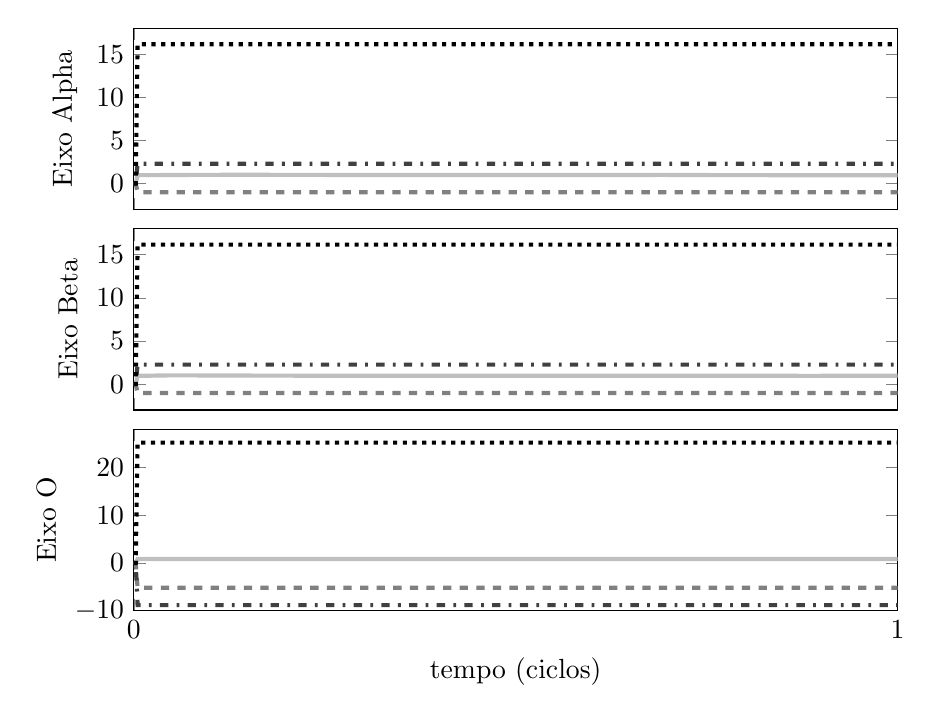
\begin{tikzpicture}

\begin{axis}[%
width=0.8\textwidth,
height=0.189701500343624\textwidth,
scale only axis,
xmin=0,
xmax=0.0166666666666667,
xtick={0,0.0166666666666667},
xticklabels={\empty},
ymin=-3,
ymax=18,
ytick={ 0,  5, 10, 15},
ylabel={Eixo Beta},
name=plot2,
scaled x ticks = false,
legend columns=-1,
legend style={/tikz/every even column/.append style={column sep=0.3cm}},
legend style={font=\footnotesize}
]
\addplot [color=lightgray,solid,line width=1.5pt,forget plot]
  table[row sep=crcr]{0	0\\
4.16666666666667e-05	0\\
8.33333333333333e-05	0.9704\\
0.000125	0.9704\\
0.000166666666666667	0.9704\\
0.000208333333333333	0.9704\\
0.00025	0.9704\\
0.000291666666666667	0.9704\\
0.000333333333333333	0.979709056857717\\
0.000375	0.979709056857717\\
0.000416666666666667	0.990752079238819\\
0.000458333333333333	0.990752079238819\\
0.0005	0.999475859305976\\
0.000541666666666667	0.999475859305976\\
0.000583333333333333	1.00543473297951\\
0.000625	1.00543473297951\\
0.000666666666666667	1.00921252688942\\
0.000708333333333333	1.00921252688942\\
0.00075	1.01143371247231\\
0.000791666666666667	1.01143371247231\\
0.000833333333333333	1.01258054296947\\
0.000875	1.01258054296947\\
0.000916666666666667	1.01300903423475\\
0.000958333333333333	1.01300903423475\\
0.001	1.01297271621112\\
0.00104166666666667	1.01297271621112\\
0.00108333333333333	1.01263988124359\\
0.001125	1.01263988124359\\
0.00116666666666667	1.01211186395183\\
0.00120833333333333	1.01211186395183\\
0.00125	1.01144271502741\\
0.00129166666666667	1.01144271502741\\
0.00133333333333333	1.01065742582171\\
0.001375	1.01065742582171\\
0.00141666666666667	1.00976644251958\\
0.00145833333333333	1.00976644251958\\
0.0015	1.00877563252049\\
0.00154166666666667	1.00877563252049\\
0.00158333333333333	1.00769197124888\\
0.001625	1.00769197124888\\
0.00166666666666667	1.00652583043106\\
0.00170833333333333	1.00652583043106\\
0.00175	1.0052909684512\\
0.00179166666666667	1.0052909684512\\
0.00183333333333333	1.00400327646456\\
0.001875	1.00400327646456\\
0.00191666666666667	1.00267912804371\\
0.00195833333333333	1.00267912804371\\
0.002	1.00133390438121\\
0.00204166666666667	1.00133390438121\\
0.00208333333333333	0.999980992626643\\
0.002125	0.999980992626643\\
0.00216666666666667	0.998631330784622\\
0.00220833333333333	0.998631330784622\\
0.00225	0.997293422624055\\
0.00229166666666667	0.997293422624055\\
0.00233333333333333	0.995973671407261\\
0.002375	0.995973671407261\\
0.00241666666666667	0.994676867582284\\
0.00245833333333333	0.994676867582284\\
0.0025	0.993406691734676\\
0.00254166666666667	0.993406691734676\\
0.00258333333333333	0.992166139224717\\
0.002625	0.992166139224717\\
0.00266666666666667	0.990957820661652\\
0.00270833333333333	0.990957820661652\\
0.00275	0.98978413219384\\
0.00279166666666667	0.98978413219384\\
0.00283333333333333	0.988647316561472\\
0.002875	0.988647316561472\\
0.00291666666666667	0.987549449311355\\
0.00295833333333333	0.987549449311355\\
0.003	0.986492386667683\\
0.00304166666666667	0.986492386667683\\
0.00308333333333333	0.985477705842637\\
0.003125	0.985477705842637\\
0.00316666666666667	0.984506658857655\\
0.00320833333333333	0.984506658857655\\
0.00325	0.983580150485021\\
0.00329166666666667	0.983580150485021\\
0.00333333333333333	0.982698741992963\\
0.003375	0.982698741992963\\
0.00341666666666667	0.981862676197307\\
0.00345833333333333	0.981862676197307\\
0.0035	0.981071916162459\\
0.00354166666666667	0.981071916162459\\
0.00358333333333333	0.98032618935605\\
0.003625	0.98032618935605\\
0.00366666666666667	0.979625030375678\\
0.00370833333333333	0.979625030375678\\
0.00375	0.978967817662022\\
0.00379166666666667	0.978967817662022\\
0.00383333333333333	0.978353802115627\\
0.003875	0.978353802115627\\
0.00391666666666667	0.97778212768144\\
0.00395833333333333	0.97778212768144\\
0.004	0.977251845441885\\
0.00404166666666667	0.977251845441885\\
0.00408333333333333	0.976761923481727\\
0.004125	0.976761923481727\\
0.00416666666666667	0.976311254845179\\
0.00420833333333333	0.976311254845179\\
0.00425	0.975898665489157\\
0.00429166666666667	0.975898665489157\\
0.00433333333333333	0.97552292347173\\
0.004375	0.97552292347173\\
0.00441666666666667	0.975182749907599\\
0.00445833333333333	0.975182749907599\\
0.0045	0.974876831625528\\
0.00454166666666667	0.974876831625528\\
0.00458333333333333	0.97460383506192\\
0.004625	0.97460383506192\\
0.00466666666666667	0.974362420742987\\
0.00470833333333333	0.974362420742987\\
0.00475	0.974151257718781\\
0.00479166666666667	0.974151257718781\\
0.00483333333333333	0.973969037460477\\
0.004875	0.973969037460477\\
0.00491666666666667	0.973814487718633\\
0.00495833333333333	0.973814487718633\\
0.005	0.973686383659904\\
0.00504166666666667	0.973686383659904\\
0.00508333333333333	0.973583559342836\\
0.005125	0.973583559342836\\
0.00516666666666667	0.973504919050686\\
0.00520833333333333	0.973504919050686\\
0.00525	0.973449448604904\\
0.00529166666666667	0.973449448604904\\
0.00533333333333333	0.973416227130613\\
0.005375	0.973416227130613\\
0.00541666666666667	0.973404439767807\\
0.00545833333333333	0.973404439767807\\
0.0055	0.973413391831064\\
0.00554166666666667	0.973413391831064\\
0.00558333333333333	0.973442524963637\\
0.005625	0.973442524963637\\
0.00566666666666667	0.973491435926964\\
0.00570833333333333	0.973491435926964\\
0.00575	0.973559898829195\\
0.00579166666666667	0.973559898829195\\
0.00583333333333333	0.973647891841434\\
0.005875	0.973647891841434\\
0.00591666666666667	0.97375562979156\\
0.00595833333333333	0.97375562979156\\
0.006	0.973883604472312\\
0.00604166666666667	0.973883604472312\\
0.00608333333333333	0.974032635048841\\
0.006125	0.974032635048841\\
0.00616666666666667	0.974203931553006\\
0.00620833333333333	0.974203931553006\\
0.00625	0.9743991749304\\
0.00629166666666667	0.9743991749304\\
0.00633333333333333	0.974620616929157\\
0.006375	0.974620616929157\\
0.00641666666666667	0.974871200784482\\
0.00645833333333333	0.974871200784482\\
0.0065	0.975154694971481\\
0.00654166666666667	0.975154694971481\\
0.00658333333333333	0.975475805384119\\
0.006625	0.975475805384119\\
0.00666666666666667	0.975840151037974\\
0.00670833333333333	0.975840151037974\\
0.00675	0.976253744822862\\
0.00679166666666667	0.976253744822862\\
0.00683333333333333	0.97672084249964\\
0.006875	0.97672084249964\\
0.00691666666666667	0.977236337311658\\
0.00695833333333333	0.977236337311658\\
0.007	0.977713816689272\\
0.00704166666666667	0.977713816689272\\
0.00708333333333333	0.977952280162254\\
0.007125	0.977952280162254\\
0.00716666666666667	0.977766035653904\\
0.00720833333333333	0.977766035653904\\
0.00725	0.977225211321465\\
0.00729166666666667	0.977225211321465\\
0.00733333333333333	0.97653581062846\\
0.007375	0.97653581062846\\
0.00741666666666667	0.975828825214631\\
0.00745833333333333	0.975828825214631\\
0.0075	0.97514853757086\\
0.00754166666666667	0.97514853757086\\
0.00758333333333333	0.97450162731351\\
0.007625	0.97450162731351\\
0.00766666666666667	0.973885475115269\\
0.00770833333333333	0.973885475115269\\
0.00775	0.973297258496765\\
0.00779166666666667	0.973297258496765\\
0.00783333333333333	0.972735629399557\\
0.007875	0.972735629399557\\
0.00791666666666667	0.972200464478978\\
0.00795833333333333	0.972200464478978\\
0.008	0.97169230618475\\
0.00804166666666667	0.97169230618475\\
0.00808333333333333	0.971211872746464\\
0.008125	0.971211872746464\\
0.00816666666666667	0.970759718878514\\
0.00820833333333333	0.970759718878514\\
0.00825	0.970336053041432\\
0.00829166666666667	0.970336053041432\\
0.00833333333333333	0.969940685368961\\
0.008375	0.969940685368961\\
0.00841666666666667	0.969573065976217\\
0.00845833333333333	0.969573065976217\\
0.0085	0.969232371732087\\
0.00854166666666667	0.969232371732087\\
0.00858333333333333	0.968917606403252\\
0.008625	0.968917606403252\\
0.00866666666666667	0.968627689917215\\
0.00870833333333333	0.968627689917215\\
0.00875	0.96836152383553\\
0.00879166666666667	0.96836152383553\\
0.00883333333333333	0.968118029699479\\
0.008875	0.968118029699479\\
0.00891666666666667	0.967896163584172\\
0.00895833333333333	0.967896163584172\\
0.009	0.967694913771996\\
0.00904166666666667	0.967694913771996\\
0.00908333333333333	0.967513289365673\\
0.009125	0.967513289365673\\
0.00916666666666667	0.967350306679076\\
0.00920833333333333	0.967350306679076\\
0.00925	0.967204978229802\\
0.00929166666666667	0.967204978229802\\
0.00933333333333333	0.967076306869301\\
0.009375	0.967076306869301\\
0.00941666666666667	0.966963285573347\\
0.00945833333333333	0.966963285573347\\
0.0095	0.966864901984986\\
0.00954166666666667	0.966864901984986\\
0.00958333333333333	0.966780146041918\\
0.009625	0.966780146041918\\
0.00966666666666667	0.966708018856347\\
0.00970833333333333	0.966708018856347\\
0.00975	0.966647541280302\\
0.00979166666666667	0.966647541280302\\
0.00983333333333333	0.966597761086463\\
0.009875	0.966597761086463\\
0.00991666666666667	0.966557758246334\\
0.00995833333333333	0.966557758246334\\
0.01	0.96652664826463\\
0.0100416666666667	0.96652664826463\\
0.0100833333333333	0.966503583859511\\
0.010125	0.966503583859511\\
0.0101666666666667	0.966487755444155\\
0.0102083333333333	0.966487755444155\\
0.01025	0.966478390887073\\
0.0102916666666667	0.966478390887073\\
0.0103333333333333	0.966474754949539\\
0.010375	0.966474754949539\\
0.0104166666666667	0.966476148668023\\
0.0104583333333333	0.966476148668023\\
0.0105	0.966481908811335\\
0.0105416666666667	0.966481908811335\\
0.0105833333333333	0.966491407427218\\
0.010625	0.966491407427218\\
0.0106666666666667	0.96650405141761\\
0.0107083333333333	0.96650405141761\\
0.01075	0.966519282048387\\
0.0107916666666667	0.966519282048387\\
0.0108333333333333	0.966536574301304\\
0.010875	0.966536574301304\\
0.0109166666666667	0.966555436001063\\
0.0109583333333333	0.966555436001063\\
0.011	0.966575406685978\\
0.0110416666666667	0.966575406685978\\
0.0110833333333333	0.96659605622552\\
0.011125	0.96659605622552\\
0.0111666666666667	0.966616983214735\\
0.0112083333333333	0.966616983214735\\
0.01125	0.966637813190607\\
0.0112916666666667	0.966637813190607\\
0.0113333333333333	0.96665819671906\\
0.011375	0.96665819671906\\
0.0114166666666667	0.9666778073956\\
0.0114583333333333	0.9666778073956\\
0.0115	0.966696339791292\\
0.0115416666666667	0.966696339791292\\
0.0115833333333333	0.966713507362227\\
0.011625	0.966713507362227\\
0.0116666666666667	0.966729040327795\\
0.0117083333333333	0.966729040327795\\
0.01175	0.966742683512687\\
0.0117916666666667	0.966742683512687\\
0.0118333333333333	0.966754194140257\\
0.011875	0.966754194140257\\
0.0119166666666667	0.966763339560432\\
0.0119583333333333	0.966763339560432\\
0.012	0.96676989489287\\
0.0120416666666667	0.96676989489287\\
0.0120833333333333	0.966773640564422\\
0.012125	0.966773640564422\\
0.0121666666666667	0.966774359717994\\
0.0122083333333333	0.966774359717994\\
0.01225	0.966771835466682\\
0.0122916666666667	0.966771835466682\\
0.0123333333333333	0.966765847961935\\
0.012375	0.966765847961935\\
0.0124166666666667	0.966756171236946\\
0.0124583333333333	0.966756171236946\\
0.0125	0.966742569776298\\
0.0125416666666667	0.966742569776298\\
0.0125833333333333	0.966724794749752\\
0.012625	0.966724794749752\\
0.0126666666666667	0.966702579831627\\
0.0127083333333333	0.966702579831627\\
0.01275	0.966675636506869\\
0.0127916666666667	0.966675636506869\\
0.0128333333333333	0.96664364873963\\
0.012875	0.96664364873963\\
0.0129166666666667	0.966606266895651\\
0.0129583333333333	0.966606266895651\\
0.013	0.966563100914473\\
0.0130416666666667	0.966563100914473\\
0.0130833333333333	0.966513711771548\\
0.013125	0.966513711771548\\
0.0131666666666667	0.966457601623424\\
0.0132083333333333	0.966457601623424\\
0.01325	0.966394202037229\\
0.0132916666666667	0.966394202037229\\
0.0133333333333333	0.966322859790833\\
0.013375	0.966322859790833\\
0.0134166666666667	0.966242819606598\\
0.0134583333333333	0.966242819606598\\
0.0135	0.966153203003765\\
0.0135416666666667	0.966153203003765\\
0.0135833333333333	0.966052982230887\\
0.013625	0.966052982230887\\
0.0136666666666667	0.965940947971994\\
0.0137083333333333	0.965940947971994\\
0.01375	0.965815669227132\\
0.0137916666666667	0.965815669227132\\
0.0138333333333333	0.965675443519288\\
0.013875	0.965675443519288\\
0.0139166666666667	0.96551823557473\\
0.0139583333333333	0.96551823557473\\
0.014	0.965341603385684\\
0.0140416666666667	0.965341603385684\\
0.0140833333333333	0.965142613440471\\
0.014125	0.965142613440471\\
0.0141666666666667	0.964917755394972\\
0.0142083333333333	0.964917755394972\\
0.01425	0.964662889909218\\
0.0142916666666667	0.964662889909218\\
0.0143333333333333	0.964373327909643\\
0.014375	0.964373327909643\\
0.0144166666666667	0.964044322702938\\
0.0144583333333333	0.964044322702938\\
0.0145	0.963672806495789\\
0.0145416666666667	0.963672806495789\\
0.0145833333333333	0.963262992346108\\
0.014625	0.963262992346108\\
0.0146666666666667	0.962877432042096\\
0.0147083333333333	0.962877432042096\\
0.01475	0.962664169325669\\
0.0147916666666667	0.962664169325669\\
0.0148333333333333	0.962773033194904\\
0.014875	0.962773033194904\\
0.0149166666666667	0.963185040167759\\
0.0149583333333333	0.963185040167759\\
0.015	0.963756743899488\\
0.0150416666666667	0.963756743899488\\
0.0150833333333333	0.964374430643027\\
0.015125	0.964374430643027\\
0.0151666666666667	0.964988307715852\\
0.0152083333333333	0.964988307715852\\
0.01525	0.9655839224531\\
0.0152916666666667	0.9655839224531\\
0.0153333333333333	0.966158859835972\\
0.015375	0.966158859835972\\
0.0154166666666667	0.966713168571899\\
0.0154583333333333	0.966713168571899\\
0.0155	0.967246679110072\\
0.0155416666666667	0.967246679110072\\
0.0155833333333333	0.967758635952712\\
0.015625	0.967758635952712\\
0.0156666666666667	0.968247929428274\\
0.0157083333333333	0.968247929428274\\
0.01575	0.968713411223191\\
0.0157916666666667	0.968713411223191\\
0.0158333333333333	0.969154143913866\\
0.015875	0.969154143913866\\
0.0159166666666667	0.969569545199236\\
0.0159583333333333	0.969569545199236\\
0.016	0.969959431636122\\
0.0160416666666667	0.969959431636122\\
0.0160833333333333	0.970323987222696\\
0.016125	0.970323987222696\\
0.0161666666666667	0.970663688596001\\
0.0162083333333333	0.970663688596001\\
0.01625	0.970979215803754\\
0.0162916666666667	0.970979215803754\\
0.0163333333333333	0.971271369889494\\
0.016375	0.971271369889494\\
0.0164166666666667	0.97154100938055\\
0.0164583333333333	0.97154100938055\\
0.0165	0.971789009572213\\
0.0165416666666667	0.971789009572213\\
0.0165833333333333	0.972016242543017\\
0.016625	0.972016242543017\\
0.0166666666666667	0.972223572483142\\
};
\addplot [color=gray,dashed,line width=1.5pt,forget plot]
  table[row sep=crcr]{0	0\\
4.16666666666667e-05	0\\
8.33333333333333e-05	-1.0277\\
0.000125	-1.0277\\
0.000166666666666667	-1.0277\\
0.000208333333333333	-1.0277\\
0.00025	-1.0277\\
0.000291666666666667	-1.0277\\
0.000333333333333333	-1.0277\\
0.000375	-1.0277\\
0.000416666666666667	-1.02769999894541\\
0.000458333333333333	-1.02769999894541\\
0.0005	-1.02769926363056\\
0.000541666666666667	-1.02769926363056\\
0.000583333333333333	-1.02769667823112\\
0.000625	-1.02769667823112\\
0.000666666666666667	-1.02769261442395\\
0.000708333333333333	-1.02769261442395\\
0.00075	-1.02768836902167\\
0.000791666666666667	-1.02768836902167\\
0.000833333333333333	-1.02768517245431\\
0.000875	-1.02768517245431\\
0.000916666666666667	-1.02768364451729\\
0.000958333333333333	-1.02768364451729\\
0.001	-1.02768379564743\\
0.00104166666666667	-1.02768379564743\\
0.00108333333333333	-1.02768530825474\\
0.001125	-1.02768530825474\\
0.00116666666666667	-1.02768780605623\\
0.00120833333333333	-1.02768780605623\\
0.00125	-1.02769099082518\\
0.00129166666666667	-1.02769099082518\\
0.00133333333333333	-1.02769466678\\
0.001375	-1.02769466678\\
0.00141666666666667	-1.0276987140308\\
0.00145833333333333	-1.0276987140308\\
0.0015	-1.02770305523742\\
0.00154166666666667	-1.02770305523742\\
0.00158333333333333	-1.02770763233263\\
0.001625	-1.02770763233263\\
0.00166666666666667	-1.02771239393234\\
0.00170833333333333	-1.02771239393234\\
0.00175	-1.02771728948904\\
0.00179166666666667	-1.02771728948904\\
0.00183333333333333	-1.02772226720553\\
0.001875	-1.02772226720553\\
0.00191666666666667	-1.02772727435\\
0.00195833333333333	-1.02772727435\\
0.002	-1.02773225921338\\
0.00204166666666667	-1.02773225921338\\
0.00208333333333333	-1.02773717383802\\
0.002125	-1.02773717383802\\
0.00216666666666667	-1.02774197654688\\
0.00220833333333333	-1.02774197654688\\
0.00225	-1.02774663353598\\
0.00229166666666667	-1.02774663353598\\
0.00233333333333333	-1.02775111925264\\
0.002375	-1.02775111925264\\
0.00241666666666667	-1.02775541571608\\
0.00245833333333333	-1.02775541571608\\
0.0025	-1.02775951118352\\
0.00254166666666667	-1.02775951118352\\
0.00258333333333333	-1.02776339860251\\
0.002625	-1.02776339860251\\
0.00266666666666667	-1.02776707419204\\
0.00270833333333333	-1.02776707419204\\
0.00275	-1.02777053634634\\
0.00279166666666667	-1.02777053634634\\
0.00283333333333333	-1.02777378491898\\
0.002875	-1.02777378491898\\
0.00291666666666667	-1.02777682084822\\
0.00295833333333333	-1.02777682084822\\
0.003	-1.02777964603246\\
0.00304166666666667	-1.02777964603246\\
0.00308333333333333	-1.02778226334888\\
0.003125	-1.02778226334888\\
0.00316666666666667	-1.0277846767202\\
0.00320833333333333	-1.0277846767202\\
0.00325	-1.02778689116027\\
0.00329166666666667	-1.02778689116027\\
0.00333333333333333	-1.02778891276127\\
0.003375	-1.02778891276127\\
0.00341666666666667	-1.02779074861342\\
0.00345833333333333	-1.02779074861342\\
0.0035	-1.02779240666862\\
0.00354166666666667	-1.02779240666862\\
0.00358333333333333	-1.02779389557023\\
0.003625	-1.02779389557023\\
0.00366666666666667	-1.02779522447279\\
0.00370833333333333	-1.02779522447279\\
0.00375	-1.02779640287116\\
0.00379166666666667	-1.02779640287116\\
0.00383333333333333	-1.02779744045178\\
0.003875	-1.02779744045178\\
0.00391666666666667	-1.02779834697074\\
0.00395833333333333	-1.02779834697074\\
0.004	-1.02779913215802\\
0.00404166666666667	-1.02779913215802\\
0.00408333333333333	-1.02779980564361\\
0.004125	-1.02779980564361\\
0.00416666666666667	-1.02780037689993\\
0.00420833333333333	-1.02780037689993\\
0.00425	-1.02780085519563\\
0.00429166666666667	-1.02780085519563\\
0.00433333333333333	-1.02780124955727\\
0.004375	-1.02780124955727\\
0.00441666666666667	-1.02780156873724\\
0.00445833333333333	-1.02780156873724\\
0.0045	-1.02780182118784\\
0.00454166666666667	-1.02780182118784\\
0.00458333333333333	-1.02780201504231\\
0.004625	-1.02780201504231\\
0.00466666666666667	-1.02780215810446\\
0.00470833333333333	-1.02780215810446\\
0.00475	-1.02780225784806\\
0.00479166666666667	-1.02780225784806\\
0.00483333333333333	-1.0278023214275\\
0.004875	-1.0278023214275\\
0.00491666666666667	-1.02780235570009\\
0.00495833333333333	-1.02780235570009\\
0.005	-1.02780236726206\\
0.00504166666666667	-1.02780236726206\\
0.00508333333333333	-1.0278023624975\\
0.005125	-1.0278023624975\\
0.00516666666666667	-1.02780234764261\\
0.00520833333333333	-1.02780234764261\\
0.00525	-1.02780232886752\\
0.00529166666666667	-1.02780232886752\\
0.00533333333333333	-1.02780231237969\\
0.005375	-1.02780231237969\\
0.00541666666666667	-1.02780230455436\\
0.00545833333333333	-1.02780230455436\\
0.0055	-1.0278023121008\\
0.00554166666666667	-1.0278023121008\\
0.00558333333333333	-1.02780234227674\\
0.005625	-1.02780234227674\\
0.00566666666666667	-1.0278024031694\\
0.00570833333333333	-1.0278024031694\\
0.00575	-1.02780250406975\\
0.00579166666666667	-1.02780250406975\\
0.00583333333333333	-1.02780265598069\\
0.005875	-1.02780265598069\\
0.00591666666666667	-1.02780287232009\\
0.00595833333333333	-1.02780287232009\\
0.006	-1.02780316991422\\
0.00604166666666667	-1.02780316991422\\
0.00608333333333333	-1.027803570433\\
0.006125	-1.027803570433\\
0.00616666666666667	-1.02780410251485\\
0.00620833333333333	-1.02780410251485\\
0.00625	-1.0278048049971\\
0.00629166666666667	-1.0278048049971\\
0.00633333333333333	-1.02780573197565\\
0.006375	-1.02780573197565\\
0.00641666666666667	-1.02780696099924\\
0.00645833333333333	-1.02780696099924\\
0.0065	-1.02780860685832\\
0.00654166666666667	-1.02780860685832\\
0.00658333333333333	-1.02781084583849\\
0.006625	-1.02781084583849\\
0.00666666666666667	-1.02781396064888\\
0.00670833333333333	-1.02781396064888\\
0.00675	-1.027818428895\\
0.00679166666666667	-1.027818428895\\
0.00683333333333333	-1.02782511034527\\
0.006875	-1.02782511034527\\
0.00691666666666667	-1.02783567792665\\
0.00695833333333333	-1.02783567792665\\
0.007	-1.02785215202179\\
0.00704166666666667	-1.02785215202179\\
0.00708333333333333	-1.02787517867131\\
0.007125	-1.02787517867131\\
0.00716666666666667	-1.02790090166263\\
0.00720833333333333	-1.02790090166263\\
0.00725	-1.0279235074636\\
0.00729166666666667	-1.0279235074636\\
0.00733333333333333	-1.02794083085075\\
0.007375	-1.02794083085075\\
0.00741666666666667	-1.0279537007034\\
0.00745833333333333	-1.0279537007034\\
0.0075	-1.02796350541731\\
0.00754166666666667	-1.02796350541731\\
0.00758333333333333	-1.02797128370755\\
0.007625	-1.02797128370755\\
0.00766666666666667	-1.02797768188189\\
0.00770833333333333	-1.02797768188189\\
0.00775	-1.02798308835224\\
0.00779166666666667	-1.02798308835224\\
0.00783333333333333	-1.02798774181763\\
0.007875	-1.02798774181763\\
0.00791666666666667	-1.02799179538345\\
0.00795833333333333	-1.02799179538345\\
0.008	-1.02799535241722\\
0.00804166666666667	-1.02799535241722\\
0.00808333333333333	-1.0279984868311\\
0.008125	-1.0279984868311\\
0.00816666666666667	-1.02800125475667\\
0.00820833333333333	-1.02800125475667\\
0.00825	-1.02800370126195\\
0.00829166666666667	-1.02800370126195\\
0.00833333333333333	-1.02800586413769\\
0.008375	-1.02800586413769\\
0.00841666666666667	-1.02800777596461\\
0.00845833333333333	-1.02800777596461\\
0.0085	-1.02800946521863\\
0.00854166666666667	-1.02800946521863\\
0.00858333333333333	-1.02801095688539\\
0.008625	-1.02801095688539\\
0.00866666666666667	-1.0280122728626\\
0.00870833333333333	-1.0280122728626\\
0.00875	-1.02801343229713\\
0.00879166666666667	-1.02801343229713\\
0.00883333333333333	-1.02801445191743\\
0.008875	-1.02801445191743\\
0.00891666666666667	-1.0280153463716\\
0.00895833333333333	-1.0280153463716\\
0.009	-1.02801612855745\\
0.00904166666666667	-1.02801612855745\\
0.00908333333333333	-1.02801680992457\\
0.009125	-1.02801680992457\\
0.00916666666666667	-1.02801740073234\\
0.00920833333333333	-1.02801740073234\\
0.00925	-1.02801791025576\\
0.00929166666666667	-1.02801791025576\\
0.00933333333333333	-1.0280183469395\\
0.009375	-1.0280183469395\\
0.00941666666666667	-1.02801871850716\\
0.00945833333333333	-1.02801871850716\\
0.0095	-1.02801903203602\\
0.00954166666666667	-1.02801903203602\\
0.00958333333333333	-1.02801929400859\\
0.009625	-1.02801929400859\\
0.00966666666666667	-1.02801951035101\\
0.00970833333333333	-1.02801951035101\\
0.00975	-1.02801968646573\\
0.00979166666666667	-1.02801968646573\\
0.00983333333333333	-1.02801982726316\\
0.009875	-1.02801982726316\\
0.00991666666666667	-1.02801993719443\\
0.00995833333333333	-1.02801993719443\\
0.01	-1.0280200202856\\
0.0100416666666667	-1.0280200202856\\
0.0100833333333333	-1.02802008017234\\
0.010125	-1.02802008017234\\
0.0101666666666667	-1.02802012013397\\
0.0102083333333333	-1.02802012013397\\
0.01025	-1.02802014312553\\
0.0102916666666667	-1.02802014312553\\
0.0103333333333333	-1.02802015180723\\
0.010375	-1.02802015180723\\
0.0104166666666667	-1.02802014857075\\
0.0104583333333333	-1.02802014857075\\
0.0105	-1.02802013556261\\
0.0105416666666667	-1.02802013556261\\
0.0105833333333333	-1.02802011470482\\
0.010625	-1.02802011470482\\
0.0106666666666667	-1.02802008771323\\
0.0107083333333333	-1.02802008771323\\
0.01075	-1.02802005611426\\
0.0107916666666667	-1.02802005611426\\
0.0108333333333333	-1.02802002126014\\
0.010875	-1.02802002126014\\
0.0109166666666667	-1.02801998434315\\
0.0109583333333333	-1.02801998434315\\
0.011	-1.02801994640891\\
0.0110416666666667	-1.02801994640891\\
0.0110833333333333	-1.0280199083688\\
0.011125	-1.0280199083688\\
0.0111666666666667	-1.0280198710115\\
0.0112083333333333	-1.0280198710115\\
0.01125	-1.02801983501364\\
0.0112916666666667	-1.02801983501364\\
0.0113333333333333	-1.02801980094944\\
0.011375	-1.02801980094944\\
0.0114166666666667	-1.02801976929942\\
0.0114583333333333	-1.02801976929942\\
0.0115	-1.02801974045805\\
0.0115416666666667	-1.02801974045805\\
0.0115833333333333	-1.02801971474043\\
0.011625	-1.02801971474043\\
0.0116666666666667	-1.02801969238797\\
0.0117083333333333	-1.02801969238797\\
0.01175	-1.02801967357304\\
0.0117916666666667	-1.02801967357304\\
0.0118333333333333	-1.02801965840268\\
0.011875	-1.02801965840268\\
0.0119166666666667	-1.02801964692121\\
0.0119583333333333	-1.02801964692121\\
0.012	-1.0280196391118\\
0.0120416666666667	-1.0280196391118\\
0.0120833333333333	-1.02801963489676\\
0.012125	-1.02801963489676\\
0.0121666666666667	-1.0280196341365\\
0.0122083333333333	-1.0280196341365\\
0.01225	-1.02801963662687\\
0.0122916666666667	-1.02801963662687\\
0.0123333333333333	-1.02801964209472\\
0.012375	-1.02801964209472\\
0.0124166666666667	-1.02801965019105\\
0.0124583333333333	-1.02801965019105\\
0.0125	-1.02801966048153\\
0.0125416666666667	-1.02801966048153\\
0.0125833333333333	-1.02801967243358\\
0.012625	-1.02801967243358\\
0.0126666666666667	-1.0280196853991\\
0.0127083333333333	-1.0280196853991\\
0.01275	-1.02801969859177\\
0.0127916666666667	-1.02801969859177\\
0.0128333333333333	-1.02801971105726\\
0.012875	-1.02801971105726\\
0.0129166666666667	-1.02801972163417\\
0.0129583333333333	-1.02801972163417\\
0.013	-1.02801972890275\\
0.0130416666666667	-1.02801972890275\\
0.0130833333333333	-1.02801973111741\\
0.013125	-1.02801973111741\\
0.0131666666666667	-1.02801972611698\\
0.0132083333333333	-1.02801972611698\\
0.01325	-1.02801971120454\\
0.0132916666666667	-1.02801971120454\\
0.0133333333333333	-1.02801968298488\\
0.013375	-1.02801968298488\\
0.0134166666666667	-1.02801963714221\\
0.0134583333333333	-1.02801963714221\\
0.0135	-1.02801956813201\\
0.0135416666666667	-1.02801956813201\\
0.0135833333333333	-1.02801946874774\\
0.013625	-1.02801946874774\\
0.0136666666666667	-1.02801932950142\\
0.0137083333333333	-1.02801932950142\\
0.01375	-1.02801913772145\\
0.0137916666666667	-1.02801913772145\\
0.0138333333333333	-1.02801887621097\\
0.013875	-1.02801887621097\\
0.0139166666666667	-1.02801852120509\\
0.0139583333333333	-1.02801852120509\\
0.014	-1.02801803917579\\
0.0140416666666667	-1.02801803917579\\
0.0140833333333333	-1.02801738167792\\
0.014125	-1.02801738167792\\
0.0141666666666667	-1.02801647673478\\
0.0142083333333333	-1.02801647673478\\
0.01425	-1.02801521382953\\
0.0142916666666667	-1.02801521382953\\
0.0143333333333333	-1.02801341644894\\
0.014375	-1.02801341644894\\
0.0144166666666667	-1.0280107888537\\
0.0144583333333333	-1.0280107888537\\
0.0145	-1.02800680544371\\
0.0145416666666667	-1.02800680544371\\
0.0145833333333333	-1.02800046075077\\
0.014625	-1.02800046075077\\
0.0146666666666667	-1.02799048758584\\
0.0147083333333333	-1.02799048758584\\
0.01475	-1.02797631645853\\
0.0147916666666667	-1.02797631645853\\
0.0148333333333333	-1.02795977096634\\
0.014875	-1.02795977096634\\
0.0149166666666667	-1.02794422531275\\
0.0149583333333333	-1.02794422531275\\
0.015	-1.02793150679745\\
0.0150416666666667	-1.02793150679745\\
0.0150833333333333	-1.02792156361888\\
0.015125	-1.02792156361888\\
0.0151666666666667	-1.02791371375992\\
0.0152083333333333	-1.02791371375992\\
0.01525	-1.02790733459305\\
0.0152916666666667	-1.02790733459305\\
0.0153333333333333	-1.02790200022779\\
0.015375	-1.02790200022779\\
0.0154166666666667	-1.02789744061546\\
0.0154583333333333	-1.02789744061546\\
0.0155	-1.02789348399706\\
0.0155416666666667	-1.02789348399706\\
0.0155833333333333	-1.02789001694013\\
0.015625	-1.02789001694013\\
0.0156666666666667	-1.02788696036972\\
0.0157083333333333	-1.02788696036972\\
0.01575	-1.02788425570296\\
0.0157916666666667	-1.02788425570296\\
0.0158333333333333	-1.02788185694629\\
0.015875	-1.02788185694629\\
0.0159166666666667	-1.02787972628267\\
0.0159583333333333	-1.02787972628267\\
0.016	-1.02787783166662\\
0.0160416666666667	-1.02787783166662\\
0.0160833333333333	-1.02787614552218\\
0.016125	-1.02787614552218\\
0.0161666666666667	-1.02787464399975\\
0.0162083333333333	-1.02787464399975\\
0.01625	-1.02787330648298\\
0.0162916666666667	-1.02787330648298\\
0.0163333333333333	-1.02787211518745\\
0.016375	-1.02787211518745\\
0.0164166666666667	-1.02787105478442\\
0.0164583333333333	-1.02787105478442\\
0.0165	-1.02787011203375\\
0.0165416666666667	-1.02787011203375\\
0.0165833333333333	-1.02786927543376\\
0.016625	-1.02786927543376\\
0.0166666666666667	-1.02786853490304\\
};
\addplot [color=darkgray,dash pattern=on 1pt off 3pt on 3pt off 3pt,line width=1.5pt,forget plot]
  table[row sep=crcr]{0	0\\
4.16666666666667e-05	0\\
8.33333333333333e-05	2.2629\\
0.000125	2.2629\\
0.000166666666666667	2.2629\\
0.000208333333333333	2.2629\\
0.00025	2.2629\\
0.000291666666666667	2.2629\\
0.000333333333333333	2.26290000210684\\
0.000375	2.26290000210684\\
0.000416666666666667	2.26290150178147\\
0.000458333333333333	2.26290150178147\\
0.0005	2.26290671283366\\
0.000541666666666667	2.26290671283366\\
0.000583333333333333	2.26291488381255\\
0.000625	2.26291488381255\\
0.000666666666666667	2.26292370626863\\
0.000708333333333333	2.26292370626863\\
0.00075	2.26293107019184\\
0.000791666666666667	2.26293107019184\\
0.000833333333333333	2.2629358400247\\
0.000875	2.2629358400247\\
0.000916666666666667	2.26293788746703\\
0.000958333333333333	2.26293788746703\\
0.001	2.26293770043248\\
0.00104166666666667	2.26293770043248\\
0.00108333333333333	2.26293593657317\\
0.001125	2.26293593657317\\
0.00116666666666667	2.26293314944576\\
0.00120833333333333	2.26293314944576\\
0.00125	2.26292970628085\\
0.00129166666666667	2.26292970628085\\
0.00133333333333333	2.2629258158238\\
0.001375	2.2629258158238\\
0.00141666666666667	2.26292158776207\\
0.00145833333333333	2.26292158776207\\
0.0015	2.26291708335666\\
0.00154166666666667	2.26291708335666\\
0.00158333333333333	2.26291234729247\\
0.001625	2.26291234729247\\
0.00166666666666667	2.26290742406755\\
0.00170833333333333	2.26290742406755\\
0.00175	2.26290236440422\\
0.00179166666666667	2.26290236440422\\
0.00183333333333333	2.26289722560608\\
0.001875	2.26289722560608\\
0.00191666666666667	2.26289206838151\\
0.00195833333333333	2.26289206838151\\
0.002	2.26288695210433\\
0.00204166666666667	2.26288695210433\\
0.00208333333333333	2.26288193021023\\
0.002125	2.26288193021023\\
0.00216666666666667	2.26287704694899\\
0.00220833333333333	2.26287704694899\\
0.00225	2.26287233601769\\
0.00229166666666667	2.26287233601769\\
0.00233333333333333	2.26286782093742\\
0.002375	2.26286782093742\\
0.00241666666666667	2.262863516621\\
0.00245833333333333	2.262863516621\\
0.0025	2.2628594314647\\
0.00254166666666667	2.2628594314647\\
0.00258333333333333	2.26285556940476\\
0.002625	2.26285556940476\\
0.00266666666666667	2.26285193158732\\
0.00270833333333333	2.26285193158732\\
0.00275	2.26284851751069\\
0.00279166666666667	2.26284851751069\\
0.00283333333333333	2.262845325658\\
0.002875	2.262845325658\\
0.00291666666666667	2.26284235373228\\
0.00295833333333333	2.26284235373228\\
0.003	2.26283959864207\\
0.00304166666666667	2.26283959864207\\
0.00308333333333333	2.26283705637832\\
0.003125	2.26283705637832\\
0.00316666666666667	2.26283472189117\\
0.00320833333333333	2.26283472189117\\
0.00325	2.26283258903216\\
0.00329166666666667	2.26283258903216\\
0.00333333333333333	2.26283065058628\\
0.003375	2.26283065058628\\
0.00341666666666667	2.26282889838698\\
0.00345833333333333	2.26282889838698\\
0.0035	2.26282732348874\\
0.00354166666666667	2.26282732348874\\
0.00358333333333333	2.26282591636564\\
0.003625	2.26282591636564\\
0.00366666666666667	2.26282466710783\\
0.00370833333333333	2.26282466710783\\
0.00375	2.26282356559624\\
0.00379166666666667	2.26282356559624\\
0.00383333333333333	2.26282260164555\\
0.003875	2.26282260164555\\
0.00391666666666667	2.26282176511416\\
0.00395833333333333	2.26282176511416\\
0.004	2.26282104598532\\
0.00404166666666667	2.26282104598532\\
0.00408333333333333	2.26282043442646\\
0.004125	2.26282043442646\\
0.00416666666666667	2.26281992083371\\
0.00420833333333333	2.26281992083371\\
0.00425	2.26281949586721\\
0.00429166666666667	2.26281949586721\\
0.00433333333333333	2.26281915048047\\
0.004375	2.26281915048047\\
0.00441666666666667	2.26281887594488\\
0.00445833333333333	2.26281887594488\\
0.0045	2.26281866386893\\
0.00454166666666667	2.26281866386893\\
0.00458333333333333	2.26281850621067\\
0.004625	2.26281850621067\\
0.00466666666666667	2.26281839528173\\
0.00470833333333333	2.26281839528173\\
0.00475	2.26281832374137\\
0.00479166666666667	2.26281832374137\\
0.00483333333333333	2.26281828457942\\
0.004875	2.26281828457942\\
0.00491666666666667	2.26281827108752\\
0.00495833333333333	2.26281827108752\\
0.005	2.2628182768173\\
0.00504166666666667	2.2628182768173\\
0.00508333333333333	2.26281829552583\\
0.005125	2.26281829552583\\
0.00516666666666667	2.26281832110614\\
0.00520833333333333	2.26281832110614\\
0.00525	2.26281834750034\\
0.00529166666666667	2.26281834750034\\
0.00533333333333333	2.26281836859145\\
0.005375	2.26281836859145\\
0.00541666666666667	2.26281837806775\\
0.00545833333333333	2.26281837806775\\
0.0055	2.26281836925093\\
0.00554166666666667	2.26281836925093\\
0.00558333333333333	2.26281833487495\\
0.005625	2.26281833487495\\
0.00566666666666667	2.26281826679675\\
0.00570833333333333	2.26281826679675\\
0.00575	2.26281815561122\\
0.00579166666666667	2.26281815561122\\
0.00583333333333333	2.26281799012874\\
0.005875	2.26281799012874\\
0.00591666666666667	2.26281775665257\\
0.00595833333333333	2.26281775665257\\
0.006	2.26281743795794\\
0.00604166666666667	2.26281743795794\\
0.00608333333333333	2.26281701181744\\
0.006125	2.26281701181744\\
0.00616666666666667	2.26281644881849\\
0.00620833333333333	2.26281644881849\\
0.00625	2.26281570904591\\
0.00629166666666667	2.26281570904591\\
0.00633333333333333	2.26281473688762\\
0.006375	2.26281473688762\\
0.00641666666666667	2.26281345262491\\
0.00645833333333333	2.26281345262491\\
0.0065	2.26281173828589\\
0.00654166666666667	2.26281173828589\\
0.00658333333333333	2.26280941277185\\
0.006625	2.26280941277185\\
0.00666666666666667	2.26280618579752\\
0.00670833333333333	2.26280618579752\\
0.00675	2.262801567226\\
0.00679166666666667	2.262801567226\\
0.00683333333333333	2.26279467524267\\
0.006875	2.26279467524267\\
0.00691666666666667	2.26278379506817\\
0.00695833333333333	2.26278379506817\\
0.007	2.26276686250638\\
0.00704166666666667	2.26276686250638\\
0.00708333333333333	2.26274323167238\\
0.007125	2.26274323167238\\
0.00716666666666667	2.26271687093649\\
0.00720833333333333	2.26271687093649\\
0.00725	2.2626937342986\\
0.00729166666666667	2.2626937342986\\
0.00733333333333333	2.26267602458228\\
0.007375	2.26267602458228\\
0.00741666666666667	2.26266288130231\\
0.00745833333333333	2.26266288130231\\
0.0075	2.26265287745345\\
0.00754166666666667	2.26265287745345\\
0.00758333333333333	2.26264494770352\\
0.007625	2.26264494770352\\
0.00766666666666667	2.26263843004045\\
0.00770833333333333	2.26263843004045\\
0.00775	2.26263292716875\\
0.00779166666666667	2.26263292716875\\
0.00783333333333333	2.26262819534042\\
0.007875	2.26262819534042\\
0.00791666666666667	2.26262407842658\\
0.00795833333333333	2.26262407842658\\
0.008	2.26262047100466\\
0.00804166666666667	2.26262047100466\\
0.00808333333333333	2.26261729749235\\
0.008125	2.26261729749235\\
0.00816666666666667	2.26261450019869\\
0.00820833333333333	2.26261450019869\\
0.00825	2.26261203252644\\
0.00829166666666667	2.26261203252644\\
0.00833333333333333	2.26260985520743\\
0.008375	2.26260985520743\\
0.00841666666666667	2.26260793429255\\
0.00845833333333333	2.26260793429255\\
0.0085	2.26260624009848\\
0.00854166666666667	2.26260624009848\\
0.00858333333333333	2.26260474662166\\
0.008625	2.26260474662166\\
0.00866666666666667	2.26260343113869\\
0.00870833333333333	2.26260343113869\\
0.00875	2.26260227385243\\
0.00879166666666667	2.26260227385243\\
0.00883333333333333	2.26260125753201\\
0.008875	2.26260125753201\\
0.00891666666666667	2.26260036714415\\
0.00895833333333333	2.26260036714415\\
0.009	2.26259958949508\\
0.00904166666666667	2.26259958949508\\
0.00908333333333333	2.26259891290571\\
0.009125	2.26259891290571\\
0.00916666666666667	2.26259832693696\\
0.00920833333333333	2.26259832693696\\
0.00925	2.26259782217258\\
0.00929166666666667	2.26259782217258\\
0.00933333333333333	2.26259739005766\\
0.009375	2.26259739005766\\
0.00941666666666667	2.26259702278462\\
0.00945833333333333	2.26259702278462\\
0.0095	2.26259671321485\\
0.00954166666666667	2.26259671321485\\
0.00958333333333333	2.26259645482409\\
0.009625	2.26259645482409\\
0.00966666666666667	2.26259624166115\\
0.00970833333333333	2.26259624166115\\
0.00975	2.26259606831225\\
0.00979166666666667	2.26259606831225\\
0.00983333333333333	2.26259592986662\\
0.009875	2.26259592986662\\
0.00991666666666667	2.26259582188115\\
0.00995833333333333	2.26259582188115\\
0.01	2.26259574034399\\
0.0100416666666667	2.26259574034399\\
0.0100833333333333	2.2625956816381\\
0.010125	2.2625956816381\\
0.0101666666666667	2.26259564250586\\
0.0102083333333333	2.26259564250586\\
0.01025	2.26259562001596\\
0.0102916666666667	2.26259562001596\\
0.0103333333333333	2.26259561153325\\
0.010375	2.26259561153325\\
0.0104166666666667	2.26259561469185\\
0.0104583333333333	2.26259561469185\\
0.0105	2.26259562737149\\
0.0105416666666667	2.26259562737149\\
0.0105833333333333	2.26259564767653\\
0.010625	2.26259564767653\\
0.0106666666666667	2.26259567391736\\
0.0107083333333333	2.26259567391736\\
0.01075	2.26259570459355\\
0.0107916666666667	2.26259570459355\\
0.0108333333333333	2.2625957383785\\
0.010875	2.2625957383785\\
0.0109166666666667	2.26259577410511\\
0.0109583333333333	2.26259577410511\\
0.011	2.26259581075249\\
0.0110416666666667	2.26259581075249\\
0.0110833333333333	2.26259584743357\\
0.011125	2.26259584743357\\
0.0111666666666667	2.2625958833836\\
0.0112083333333333	2.2625958833836\\
0.01125	2.26259591794962\\
0.0112916666666667	2.26259591794962\\
0.0113333333333333	2.26259595058093\\
0.011375	2.26259595058093\\
0.0114166666666667	2.26259598082048\\
0.0114583333333333	2.26259598082048\\
0.0115	2.26259600829741\\
0.0115416666666667	2.26259600829741\\
0.0115833333333333	2.26259603272054\\
0.011625	2.26259603272054\\
0.0116666666666667	2.26259605387285\\
0.0117083333333333	2.26259605387285\\
0.01175	2.26259607160704\\
0.0117916666666667	2.26259607160704\\
0.0118333333333333	2.26259608584208\\
0.011875	2.26259608584208\\
0.0119166666666667	2.26259609656082\\
0.0119583333333333	2.26259609656082\\
0.012	2.26259610380877\\
0.0120416666666667	2.26259610380877\\
0.0120833333333333	2.26259610769414\\
0.012125	2.26259610769414\\
0.0121666666666667	2.26259610838932\\
0.0122083333333333	2.26259610838932\\
0.01225	2.262596106134\\
0.0122916666666667	2.262596106134\\
0.0123333333333333	2.26259610124025\\
0.012375	2.26259610124025\\
0.0124166666666667	2.2625960941\\
0.0124583333333333	2.2625960941\\
0.0125	2.26259608519545\\
0.0125416666666667	2.26259608519545\\
0.0125833333333333	2.26259607511295\\
0.012625	2.26259607511295\\
0.0126666666666667	2.26259606456154\\
0.0127083333333333	2.26259606456154\\
0.01275	2.26259605439722\\
0.0127916666666667	2.26259605439722\\
0.0128333333333333	2.26259604565462\\
0.012875	2.26259604565462\\
0.0129166666666667	2.26259603958844\\
0.0129583333333333	2.26259603958844\\
0.013	2.26259603772776\\
0.0130416666666667	2.26259603772776\\
0.0130833333333333	2.26259604194735\\
0.013125	2.26259604194735\\
0.0131666666666667	2.26259605456238\\
0.0132083333333333	2.26259605456238\\
0.01325	2.26259607845504\\
0.0132916666666667	2.26259607845504\\
0.0133333333333333	2.26259611724551\\
0.013375	2.26259611724551\\
0.0134166666666667	2.26259617552562\\
0.0134583333333333	2.26259617552562\\
0.0135	2.26259625918225\\
0.0135416666666667	2.26259625918225\\
0.0135833333333333	2.26259637585161\\
0.013625	2.26259637585161\\
0.0136666666666667	2.26259653556808\\
0.0137083333333333	2.26259653556808\\
0.01375	2.26259675170817\\
0.0137916666666667	2.26259675170817\\
0.0138333333333333	2.26259704239291\\
0.013875	2.26259704239291\\
0.0139166666666667	2.26259743262126\\
0.0139583333333333	2.26259743262126\\
0.014	2.26259795760381\\
0.0140416666666667	2.26259795760381\\
0.0140833333333333	2.2625986681355\\
0.014125	2.2625986681355\\
0.0141666666666667	2.26259963956778\\
0.0142083333333333	2.26259963956778\\
0.01425	2.26260098742675\\
0.0142916666666667	2.26260098742675\\
0.0143333333333333	2.26260289595985\\
0.014375	2.26260289595985\\
0.0144166666666667	2.26260567343126\\
0.0144583333333333	2.26260567343126\\
0.0145	2.2626098669482\\
0.0145416666666667	2.2626098669482\\
0.0145833333333333	2.26261652169938\\
0.014625	2.26261652169938\\
0.0146666666666667	2.26262694701704\\
0.0147083333333333	2.26262694701704\\
0.01475	2.26264171461387\\
0.0147916666666667	2.26264171461387\\
0.0148333333333333	2.26265890670934\\
0.014875	2.26265890670934\\
0.0149166666666667	2.26267501611759\\
0.0149583333333333	2.26267501611759\\
0.015	2.26268816205234\\
0.0150416666666667	2.26268816205234\\
0.0150833333333333	2.26269841419564\\
0.015125	2.26269841419564\\
0.0151666666666667	2.2627064888822\\
0.0152083333333333	2.2627064888822\\
0.01525	2.2627130358467\\
0.0152916666666667	2.2627130358467\\
0.0153333333333333	2.26271849870756\\
0.015375	2.26271849870756\\
0.0154166666666667	2.26272315887257\\
0.0154583333333333	2.26272315887257\\
0.0155	2.26272719569411\\
0.0155416666666667	2.26272719569411\\
0.0155833333333333	2.26273072792851\\
0.015625	2.26273072792851\\
0.0156666666666667	2.26273383847465\\
0.0157083333333333	2.26273383847465\\
0.01575	2.26273658865245\\
0.0157916666666667	2.26273658865245\\
0.0158333333333333	2.26273902637115\\
0.015875	2.26273902637115\\
0.0159166666666667	2.26274119075119\\
0.0159583333333333	2.26274119075119\\
0.016	2.26274311470852\\
0.0160416666666667	2.26274311470852\\
0.0160833333333333	2.2627448264065\\
0.016125	2.2627448264065\\
0.0161666666666667	2.26274635011428\\
0.0162083333333333	2.26274635011428\\
0.01625	2.26274770677921\\
0.0162916666666667	2.26274770677921\\
0.0163333333333333	2.26274891447588\\
0.016375	2.26274891447588\\
0.0164166666666667	2.26274998880607\\
0.0164583333333333	2.26274998880607\\
0.0165	2.26275094327377\\
0.0165416666666667	2.26275094327377\\
0.0165833333333333	2.26275178963483\\
0.016625	2.26275178963483\\
0.0166666666666667	2.2627525382115\\
};
\addplot [color=black,dotted,line width=1.5pt,forget plot]
  table[row sep=crcr]{0	0\\
4.16666666666667e-05	0\\
8.33333333333333e-05	16.1727\\
0.000125	16.1727\\
0.000166666666666667	16.1727\\
0.000208333333333333	16.1727\\
0.00025	16.1735859890189\\
0.000291666666666667	16.1735859890189\\
0.000333333333333333	16.1743915493856\\
0.000375	16.1743915493856\\
0.000416666666666667	16.1748288670822\\
0.000458333333333333	16.1748288670822\\
0.0005	16.1750473715178\\
0.000541666666666667	16.1750473715178\\
0.000583333333333333	16.1751560162496\\
0.000625	16.1751560162496\\
0.000666666666666667	16.175209902785\\
0.000708333333333333	16.175209902785\\
0.00075	16.1752357119483\\
0.000791666666666667	16.1752357119483\\
0.000833333333333333	16.1752468491064\\
0.000875	16.1752468491064\\
0.000916666666666667	16.1752503917961\\
0.000958333333333333	16.1752503917961\\
0.001	16.1752501323958\\
0.00104166666666667	16.1752501323958\\
0.00108333333333333	16.1752480536046\\
0.001125	16.1752480536046\\
0.00116666666666667	16.1752451397269\\
0.00120833333333333	16.1752451397269\\
0.00125	16.175241847575\\
0.00129166666666667	16.175241847575\\
0.00133333333333333	16.1752383762949\\
0.001375	16.1752383762949\\
0.00141666666666667	16.1752348138815\\
0.00145833333333333	16.1752348138815\\
0.0015	16.1752312098178\\
0.00154166666666667	16.1752312098178\\
0.00158333333333333	16.1752276057555\\
0.001625	16.1752276057555\\
0.00166666666666667	16.1752240443126\\
0.00170833333333333	16.1752240443126\\
0.00175	16.1752205680827\\
0.00179166666666667	16.1752205680827\\
0.00183333333333333	16.1752172156709\\
0.001875	16.1752172156709\\
0.00191666666666667	16.1752140181572\\
0.00195833333333333	16.1752140181572\\
0.002	16.1752109972631\\
0.00204166666666667	16.1752109972631\\
0.00208333333333333	16.1752081653031\\
0.002125	16.1752081653031\\
0.00216666666666667	16.1752055264389\\
0.00220833333333333	16.1752055264389\\
0.00225	16.1752030786057\\
0.00229166666666667	16.1752030786057\\
0.00233333333333333	16.1752008155646\\
0.002375	16.1752008155646\\
0.00241666666666667	16.1751987287111\\
0.00245833333333333	16.1751987287111\\
0.0025	16.1751968084539\\
0.00254166666666667	16.1751968084539\\
0.00258333333333333	16.1751950451254\\
0.002625	16.1751950451254\\
0.00266666666666667	16.1751934294831\\
0.00270833333333333	16.1751934294831\\
0.00275	16.175191952902\\
0.00279166666666667	16.175191952902\\
0.00283333333333333	16.1751906073735\\
0.002875	16.1751906073735\\
0.00291666666666667	16.1751893854048\\
0.00295833333333333	16.1751893854048\\
0.003	16.175188279893\\
0.00304166666666667	16.175188279893\\
0.00308333333333333	16.1751872840156\\
0.003125	16.1751872840156\\
0.00316666666666667	16.1751863911575\\
0.00320833333333333	16.1751863911575\\
0.00325	16.1751855948764\\
0.00329166666666667	16.1751855948764\\
0.00333333333333333	16.1751848888974\\
0.003375	16.1751848888974\\
0.00341666666666667	16.1751842671271\\
0.00345833333333333	16.1751842671271\\
0.0035	16.1751837236717\\
0.00354166666666667	16.1751837236717\\
0.00358333333333333	16.1751832528543\\
0.003625	16.1751832528543\\
0.00366666666666667	16.1751828492223\\
0.00370833333333333	16.1751828492223\\
0.00375	16.1751825075476\\
0.00379166666666667	16.1751825075476\\
0.00383333333333333	16.1751822228166\\
0.003875	16.1751822228166\\
0.00391666666666667	16.1751819902159\\
0.00395833333333333	16.1751819902159\\
0.004	16.1751818051149\\
0.00404166666666667	16.1751818051149\\
0.00408333333333333	16.175181663048\\
0.004125	16.175181663048\\
0.00416666666666667	16.1751815596983\\
0.00420833333333333	16.1751815596983\\
0.00425	16.1751814908838\\
0.00429166666666667	16.1751814908838\\
0.00433333333333333	16.175181452545\\
0.004375	16.175181452545\\
0.00441666666666667	16.1751814407336\\
0.00445833333333333	16.1751814407336\\
0.0045	16.1751814516015\\
0.00454166666666667	16.1751814516015\\
0.00458333333333333	16.1751814813881\\
0.004625	16.1751814813881\\
0.00466666666666667	16.1751815264047\\
0.00470833333333333	16.1751815264047\\
0.00475	16.1751815830163\\
0.00479166666666667	16.1751815830163\\
0.00483333333333333	16.1751816476172\\
0.004875	16.1751816476172\\
0.00491666666666667	16.175181716602\\
0.00495833333333333	16.175181716602\\
0.005	16.1751817863291\\
0.00504166666666667	16.1751817863291\\
0.00508333333333333	16.1751818530756\\
0.005125	16.1751818530756\\
0.00516666666666667	16.1751819129812\\
0.00520833333333333	16.1751819129812\\
0.00525	16.1751819619766\\
0.00529166666666667	16.1751819619766\\
0.00533333333333333	16.1751819956926\\
0.005375	16.1751819956926\\
0.00541666666666667	16.1751820093435\\
0.00545833333333333	16.1751820093435\\
0.0055	16.1751819975743\\
0.00554166666666667	16.1751819975743\\
0.00558333333333333	16.1751819542591\\
0.005625	16.1751819542591\\
0.00566666666666667	16.1751818722319\\
0.00570833333333333	16.1751818722319\\
0.00575	16.1751817429225\\
0.00579166666666667	16.1751817429225\\
0.00583333333333333	16.1751815558554\\
0.005875	16.1751815558554\\
0.00591666666666667	16.1751812979512\\
0.00595833333333333	16.1751812979512\\
0.006	16.175180952533\\
0.00604166666666667	16.175180952533\\
0.00608333333333333	16.1751804978857\\
0.006125	16.1751804978857\\
0.00616666666666667	16.1751799051194\\
0.00620833333333333	16.1751799051194\\
0.00625	16.1751791349178\\
0.00629166666666667	16.1751791349178\\
0.00633333333333333	16.1751781324474\\
0.006375	16.1751781324474\\
0.00641666666666667	16.175176819119\\
0.00645833333333333	16.175176819119\\
0.0065	16.1751750787408\\
0.00654166666666667	16.1751750787408\\
0.00658333333333333	16.1751727331995\\
0.006625	16.1751727331995\\
0.00666666666666667	16.1751694974871\\
0.00670833333333333	16.1751694974871\\
0.00675	16.1751648912982\\
0.00679166666666667	16.1751648912982\\
0.00683333333333333	16.1751580522864\\
0.006875	16.1751580522864\\
0.00691666666666667	16.1751473072171\\
0.00695833333333333	16.1751473072171\\
0.007	16.1751306620237\\
0.00704166666666667	16.1751306620237\\
0.00708333333333333	16.1751075376362\\
0.007125	16.1751075376362\\
0.00716666666666667	16.1750818589878\\
0.00720833333333333	16.1750818589878\\
0.00725	16.1750594251158\\
0.00729166666666667	16.1750594251158\\
0.00733333333333333	16.1750423352662\\
0.007375	16.1750423352662\\
0.00741666666666667	16.1750297154599\\
0.00745833333333333	16.1750297154599\\
0.0075	16.1750201610319\\
0.00754166666666667	16.1750201610319\\
0.00758333333333333	16.1750126304871\\
0.007625	16.1750126304871\\
0.00766666666666667	16.1750064783592\\
0.00770833333333333	16.1750064783592\\
0.00775	16.1750013170519\\
0.00779166666666667	16.1750013170519\\
0.00783333333333333	16.174996907644\\
0.007875	16.174996907644\\
0.00791666666666667	16.1749930956458\\
0.00795833333333333	16.1749930956458\\
0.008	16.1749897753846\\
0.00804166666666667	16.1749897753846\\
0.00808333333333333	16.1749868701474\\
0.008125	16.1749868701474\\
0.00816666666666667	16.1749843209782\\
0.00820833333333333	16.1749843209782\\
0.00825	16.1749820803602\\
0.00829166666666667	16.1749820803602\\
0.00833333333333333	16.174980108684\\
0.008375	16.174980108684\\
0.00841666666666667	16.1749783722756\\
0.00845833333333333	16.1749783722756\\
0.0085	16.1749768422556\\
0.00854166666666667	16.1749768422556\\
0.00858333333333333	16.1749754938067\\
0.008625	16.1749754938067\\
0.00866666666666667	16.174974305621\\
0.00870833333333333	16.174974305621\\
0.00875	16.1749732594168\\
0.00879166666666667	16.1749732594168\\
0.00883333333333333	16.1749723394851\\
0.008875	16.1749723394851\\
0.00891666666666667	16.1749715322628\\
0.00895833333333333	16.1749715322628\\
0.009	16.1749708259452\\
0.00904166666666667	16.1749708259452\\
0.00908333333333333	16.1749702101499\\
0.009125	16.1749702101499\\
0.00916666666666667	16.1749696756417\\
0.00920833333333333	16.1749696756417\\
0.00925	16.174969214118\\
0.00929166666666667	16.174969214118\\
0.00933333333333333	16.1749688180508\\
0.009375	16.1749688180508\\
0.00941666666666667	16.1749684805746\\
0.00945833333333333	16.1749684805746\\
0.0095	16.1749681954084\\
0.00954166666666667	16.1749681954084\\
0.00958333333333333	16.1749679568016\\
0.009625	16.1749679568016\\
0.00966666666666667	16.1749677594935\\
0.00970833333333333	16.1749677594935\\
0.00975	16.1749675986794\\
0.00979166666666667	16.1749675986794\\
0.00983333333333333	16.17496746998\\
0.009875	16.17496746998\\
0.00991666666666667	16.1749673694106\\
0.00995833333333333	16.1749673694106\\
0.01	16.174967293351\\
0.0100416666666667	16.174967293351\\
0.0100833333333333	16.1749672385158\\
0.010125	16.1749672385158\\
0.0101666666666667	16.1749672019259\\
0.0102083333333333	16.1749672019259\\
0.01025	16.1749671808823\\
0.0102916666666667	16.1749671808823\\
0.0103333333333333	16.1749671729422\\
0.010375	16.1749671729422\\
0.0104166666666667	16.1749671758987\\
0.0104583333333333	16.1749671758987\\
0.0105	16.1749671877621\\
0.0105416666666667	16.1749671877621\\
0.0105833333333333	16.174967206744\\
0.010625	16.174967206744\\
0.0106666666666667	16.174967231243\\
0.0107083333333333	16.174967231243\\
0.01075	16.174967259832\\
0.0107916666666667	16.174967259832\\
0.0108333333333333	16.1749672912458\\
0.010875	16.1749672912458\\
0.0109166666666667	16.1749673243698\\
0.0109583333333333	16.1749673243698\\
0.011	16.1749673582299\\
0.0110416666666667	16.1749673582299\\
0.0110833333333333	16.1749673919813\\
0.011125	16.1749673919813\\
0.0111666666666667	16.1749674249\\
0.0112083333333333	16.1749674249\\
0.01125	16.174967456373\\
0.0112916666666667	16.174967456373\\
0.0113333333333333	16.1749674858906\\
0.011375	16.1749674858906\\
0.0114166666666667	16.174967513039\\
0.0114583333333333	16.174967513039\\
0.0115	16.1749675374933\\
0.0115416666666667	16.1749675374933\\
0.0115833333333333	16.1749675590128\\
0.011625	16.1749675590128\\
0.0116666666666667	16.1749675774352\\
0.0117083333333333	16.1749675774352\\
0.01175	16.1749675926738\\
0.0117916666666667	16.1749675926738\\
0.0118333333333333	16.1749676047144\\
0.011875	16.1749676047144\\
0.0119166666666667	16.1749676136139\\
0.0119583333333333	16.1749676136139\\
0.012	16.1749676194997\\
0.0120416666666667	16.1749676194997\\
0.0120833333333333	16.1749676225715\\
0.012125	16.1749676225715\\
0.0121666666666667	16.1749676231032\\
0.0122083333333333	16.1749676231032\\
0.01225	16.1749676214485\\
0.0122916666666667	16.1749676214485\\
0.0123333333333333	16.1749676180472\\
0.012375	16.1749676180472\\
0.0124166666666667	16.1749676134357\\
0.0124583333333333	16.1749676134357\\
0.0125	16.1749676082597\\
0.0125416666666667	16.1749676082597\\
0.0125833333333333	16.1749676032924\\
0.012625	16.1749676032924\\
0.0126666666666667	16.1749675994575\\
0.0127083333333333	16.1749675994575\\
0.01275	16.174967597859\\
0.0127916666666667	16.174967597859\\
0.0128333333333333	16.1749675998206\\
0.012875	16.1749675998206\\
0.0129166666666667	16.1749676069363\\
0.0129583333333333	16.1749676069363\\
0.013	16.1749676211366\\
0.0130416666666667	16.1749676211366\\
0.0130833333333333	16.1749676447753\\
0.013125	16.1749676447753\\
0.0131666666666667	16.1749676807444\\
0.0132083333333333	16.1749676807444\\
0.01325	16.1749677326269\\
0.0132916666666667	16.1749677326269\\
0.0133333333333333	16.1749678049034\\
0.013375	16.1749678049034\\
0.0134166666666667	16.1749679032334\\
0.0134583333333333	16.1749679032334\\
0.0135	16.1749680348429\\
0.0135416666666667	16.1749680348429\\
0.0135833333333333	16.1749682090699\\
0.013625	16.1749682090699\\
0.0136666666666667	16.1749684381404\\
0.0137083333333333	16.1749684381404\\
0.01375	16.174968738296\\
0.0137916666666667	16.174968738296\\
0.0138333333333333	16.1749691314663\\
0.013875	16.1749691314663\\
0.0139166666666667	16.1749696478102\\
0.0139583333333333	16.1749696478102\\
0.014	16.1749703296792\\
0.0140416666666667	16.1749703296792\\
0.0140833333333333	16.1749712379976\\
0.014125	16.1749712379976\\
0.0141666666666667	16.1749724629027\\
0.0142083333333333	16.1749724629027\\
0.01425	16.1749741422406\\
0.0142916666666667	16.1749741422406\\
0.0143333333333333	16.1749764953316\\
0.014375	16.1749764953316\\
0.0144166666666667	16.1749798882915\\
0.0144583333333333	16.1749798882915\\
0.0145	16.1749849695049\\
0.0145416666666667	16.1749849695049\\
0.0145833333333333	16.174992975084\\
0.014625	16.174992975084\\
0.0146666666666667	16.1750054371368\\
0.0147083333333333	16.1750054371368\\
0.01475	16.1750229914265\\
0.0147916666666667	16.1750229914265\\
0.0148333333333333	16.1750433283225\\
0.014875	16.1750433283225\\
0.0149166666666667	16.1750623045865\\
0.0149583333333333	16.1750623045865\\
0.015	16.1750777351487\\
0.0150416666666667	16.1750777351487\\
0.0150833333333333	16.1750897341681\\
0.015125	16.1750897341681\\
0.0151666666666667	16.1750991635124\\
0.0152083333333333	16.1750991635124\\
0.01525	16.1751067966706\\
0.0152916666666667	16.1751067966706\\
0.0153333333333333	16.1751131596562\\
0.015375	16.1751131596562\\
0.0154166666666667	16.1751185851845\\
0.0154583333333333	16.1751185851845\\
0.0155	16.1751232843897\\
0.0155416666666667	16.1751232843897\\
0.0155833333333333	16.175127396034\\
0.015625	16.175127396034\\
0.0156666666666667	16.1751310159782\\
0.0157083333333333	16.1751310159782\\
0.01575	16.1751342143685\\
0.0157916666666667	16.1751342143685\\
0.0158333333333333	16.1751370456152\\
0.015875	16.1751370456152\\
0.0159166666666667	16.1751395541129\\
0.0159583333333333	16.1751395541129\\
0.016	16.1751417774421\\
0.0160416666666667	16.1751417774421\\
0.0160833333333333	16.1751437481196\\
0.016125	16.1751437481196\\
0.0161666666666667	16.1751454945598\\
0.0162083333333333	16.1751454945598\\
0.01625	16.1751470416492\\
0.0162916666666667	16.1751470416492\\
0.0163333333333333	16.1751484111607\\
0.016375	16.1751484111607\\
0.0164166666666667	16.1751496221177\\
0.0164583333333333	16.1751496221177\\
0.0165	16.1751506911495\\
0.0165416666666667	16.1751506911495\\
0.0165833333333333	16.1751516328402\\
0.016625	16.1751516328402\\
0.0166666666666667	16.1751524600572\\
};
\end{axis}

\begin{axis}[%
width=0.8\textwidth,
height=0.189701500343624\textwidth,
scale only axis,
xmin=0,
xmax=0.0166666666666667,
xtick={0,0.0166666666666667},
xticklabels={{0},{1}},
xlabel={tempo (ciclos)},
ymin=-10,
ymax=28,
ytick={-10,   0,  10,  20},
ylabel={Eixo O},
at=(plot2.below south west),
anchor=above north west,
scaled x ticks = false,
legend columns=-1,
legend style={/tikz/every even column/.append style={column sep=0.3cm}},
legend style={font=\footnotesize}
]
\addplot [color=lightgray,solid,line width=1.5pt,forget plot]
  table[row sep=crcr]{0	0\\
4.16666666666667e-05	0\\
8.33333333333333e-05	0.83\\
0.000125	0.83\\
0.000166666666666667	0.83\\
0.000208333333333333	0.83\\
0.00025	0.83\\
0.000291666666666667	0.83\\
0.000333333333333333	0.83\\
0.000375	0.83\\
0.000416666666666667	0.83\\
0.000458333333333333	0.83\\
0.0005	0.83\\
0.000541666666666667	0.83\\
0.000583333333333333	0.83\\
0.000625	0.83\\
0.000666666666666667	0.83\\
0.000708333333333333	0.83\\
0.00075	0.83\\
0.000791666666666667	0.83\\
0.000833333333333333	0.83\\
0.000875	0.83\\
0.000916666666666667	0.83\\
0.000958333333333333	0.83\\
0.001	0.83\\
0.00104166666666667	0.83\\
0.00108333333333333	0.83\\
0.001125	0.83\\
0.00116666666666667	0.83\\
0.00120833333333333	0.83\\
0.00125	0.83\\
0.00129166666666667	0.83\\
0.00133333333333333	0.83\\
0.001375	0.83\\
0.00141666666666667	0.83\\
0.00145833333333333	0.83\\
0.0015	0.83\\
0.00154166666666667	0.83\\
0.00158333333333333	0.83\\
0.001625	0.83\\
0.00166666666666667	0.83\\
0.00170833333333333	0.83\\
0.00175	0.83\\
0.00179166666666667	0.83\\
0.00183333333333333	0.83\\
0.001875	0.83\\
0.00191666666666667	0.83\\
0.00195833333333333	0.83\\
0.002	0.83\\
0.00204166666666667	0.83\\
0.00208333333333333	0.83\\
0.002125	0.83\\
0.00216666666666667	0.83\\
0.00220833333333333	0.83\\
0.00225	0.83\\
0.00229166666666667	0.83\\
0.00233333333333333	0.83\\
0.002375	0.83\\
0.00241666666666667	0.83\\
0.00245833333333333	0.83\\
0.0025	0.83\\
0.00254166666666667	0.83\\
0.00258333333333333	0.83\\
0.002625	0.83\\
0.00266666666666667	0.83\\
0.00270833333333333	0.83\\
0.00275	0.83\\
0.00279166666666667	0.83\\
0.00283333333333333	0.83\\
0.002875	0.83\\
0.00291666666666667	0.83\\
0.00295833333333333	0.83\\
0.003	0.83\\
0.00304166666666667	0.83\\
0.00308333333333333	0.83\\
0.003125	0.83\\
0.00316666666666667	0.83\\
0.00320833333333333	0.83\\
0.00325	0.83\\
0.00329166666666667	0.83\\
0.00333333333333333	0.83\\
0.003375	0.83\\
0.00341666666666667	0.83\\
0.00345833333333333	0.83\\
0.0035	0.83\\
0.00354166666666667	0.83\\
0.00358333333333333	0.83\\
0.003625	0.83\\
0.00366666666666667	0.83\\
0.00370833333333333	0.83\\
0.00375	0.83\\
0.00379166666666667	0.83\\
0.00383333333333333	0.83\\
0.003875	0.83\\
0.00391666666666667	0.83\\
0.00395833333333333	0.83\\
0.004	0.83\\
0.00404166666666667	0.83\\
0.00408333333333333	0.83\\
0.004125	0.83\\
0.00416666666666667	0.83\\
0.00420833333333333	0.83\\
0.00425	0.83\\
0.00429166666666667	0.83\\
0.00433333333333333	0.83\\
0.004375	0.83\\
0.00441666666666667	0.83\\
0.00445833333333333	0.83\\
0.0045	0.83\\
0.00454166666666667	0.83\\
0.00458333333333333	0.83\\
0.004625	0.83\\
0.00466666666666667	0.83\\
0.00470833333333333	0.83\\
0.00475	0.83\\
0.00479166666666667	0.83\\
0.00483333333333333	0.83\\
0.004875	0.83\\
0.00491666666666667	0.83\\
0.00495833333333333	0.83\\
0.005	0.83\\
0.00504166666666667	0.83\\
0.00508333333333333	0.83\\
0.005125	0.83\\
0.00516666666666667	0.83\\
0.00520833333333333	0.83\\
0.00525	0.83\\
0.00529166666666667	0.83\\
0.00533333333333333	0.83\\
0.005375	0.83\\
0.00541666666666667	0.83\\
0.00545833333333333	0.83\\
0.0055	0.83\\
0.00554166666666667	0.83\\
0.00558333333333333	0.83\\
0.005625	0.83\\
0.00566666666666667	0.83\\
0.00570833333333333	0.83\\
0.00575	0.83\\
0.00579166666666667	0.83\\
0.00583333333333333	0.83\\
0.005875	0.83\\
0.00591666666666667	0.83\\
0.00595833333333333	0.83\\
0.006	0.83\\
0.00604166666666667	0.83\\
0.00608333333333333	0.83\\
0.006125	0.83\\
0.00616666666666667	0.83\\
0.00620833333333333	0.83\\
0.00625	0.83\\
0.00629166666666667	0.83\\
0.00633333333333333	0.83\\
0.006375	0.83\\
0.00641666666666667	0.83\\
0.00645833333333333	0.83\\
0.0065	0.83\\
0.00654166666666667	0.83\\
0.00658333333333333	0.83\\
0.006625	0.83\\
0.00666666666666667	0.83\\
0.00670833333333333	0.83\\
0.00675	0.83\\
0.00679166666666667	0.83\\
0.00683333333333333	0.83\\
0.006875	0.83\\
0.00691666666666667	0.83\\
0.00695833333333333	0.83\\
0.007	0.83\\
0.00704166666666667	0.83\\
0.00708333333333333	0.83\\
0.007125	0.83\\
0.00716666666666667	0.83\\
0.00720833333333333	0.83\\
0.00725	0.83\\
0.00729166666666667	0.83\\
0.00733333333333333	0.83\\
0.007375	0.83\\
0.00741666666666667	0.83\\
0.00745833333333333	0.83\\
0.0075	0.83\\
0.00754166666666667	0.83\\
0.00758333333333333	0.83\\
0.007625	0.83\\
0.00766666666666667	0.83\\
0.00770833333333333	0.83\\
0.00775	0.83\\
0.00779166666666667	0.83\\
0.00783333333333333	0.83\\
0.007875	0.83\\
0.00791666666666667	0.83\\
0.00795833333333333	0.83\\
0.008	0.83\\
0.00804166666666667	0.83\\
0.00808333333333333	0.83\\
0.008125	0.83\\
0.00816666666666667	0.83\\
0.00820833333333333	0.83\\
0.00825	0.83\\
0.00829166666666667	0.83\\
0.00833333333333333	0.83\\
0.008375	0.83\\
0.00841666666666667	0.83\\
0.00845833333333333	0.83\\
0.0085	0.83\\
0.00854166666666667	0.83\\
0.00858333333333333	0.83\\
0.008625	0.83\\
0.00866666666666667	0.83\\
0.00870833333333333	0.83\\
0.00875	0.83\\
0.00879166666666667	0.83\\
0.00883333333333333	0.83\\
0.008875	0.83\\
0.00891666666666667	0.83\\
0.00895833333333333	0.83\\
0.009	0.83\\
0.00904166666666667	0.83\\
0.00908333333333333	0.83\\
0.009125	0.83\\
0.00916666666666667	0.83\\
0.00920833333333333	0.83\\
0.00925	0.83\\
0.00929166666666667	0.83\\
0.00933333333333333	0.83\\
0.009375	0.83\\
0.00941666666666667	0.83\\
0.00945833333333333	0.83\\
0.0095	0.83\\
0.00954166666666667	0.83\\
0.00958333333333333	0.83\\
0.009625	0.83\\
0.00966666666666667	0.83\\
0.00970833333333333	0.83\\
0.00975	0.83\\
0.00979166666666667	0.83\\
0.00983333333333333	0.83\\
0.009875	0.83\\
0.00991666666666667	0.83\\
0.00995833333333333	0.83\\
0.01	0.83\\
0.0100416666666667	0.83\\
0.0100833333333333	0.83\\
0.010125	0.83\\
0.0101666666666667	0.83\\
0.0102083333333333	0.83\\
0.01025	0.83\\
0.0102916666666667	0.83\\
0.0103333333333333	0.83\\
0.010375	0.83\\
0.0104166666666667	0.83\\
0.0104583333333333	0.83\\
0.0105	0.83\\
0.0105416666666667	0.83\\
0.0105833333333333	0.83\\
0.010625	0.83\\
0.0106666666666667	0.83\\
0.0107083333333333	0.83\\
0.01075	0.83\\
0.0107916666666667	0.83\\
0.0108333333333333	0.83\\
0.010875	0.83\\
0.0109166666666667	0.83\\
0.0109583333333333	0.83\\
0.011	0.83\\
0.0110416666666667	0.83\\
0.0110833333333333	0.83\\
0.011125	0.83\\
0.0111666666666667	0.83\\
0.0112083333333333	0.83\\
0.01125	0.83\\
0.0112916666666667	0.83\\
0.0113333333333333	0.83\\
0.011375	0.83\\
0.0114166666666667	0.83\\
0.0114583333333333	0.83\\
0.0115	0.83\\
0.0115416666666667	0.83\\
0.0115833333333333	0.83\\
0.011625	0.83\\
0.0116666666666667	0.83\\
0.0117083333333333	0.83\\
0.01175	0.83\\
0.0117916666666667	0.83\\
0.0118333333333333	0.83\\
0.011875	0.83\\
0.0119166666666667	0.83\\
0.0119583333333333	0.83\\
0.012	0.83\\
0.0120416666666667	0.83\\
0.0120833333333333	0.83\\
0.012125	0.83\\
0.0121666666666667	0.83\\
0.0122083333333333	0.83\\
0.01225	0.83\\
0.0122916666666667	0.83\\
0.0123333333333333	0.83\\
0.012375	0.83\\
0.0124166666666667	0.83\\
0.0124583333333333	0.83\\
0.0125	0.83\\
0.0125416666666667	0.83\\
0.0125833333333333	0.83\\
0.012625	0.83\\
0.0126666666666667	0.83\\
0.0127083333333333	0.83\\
0.01275	0.83\\
0.0127916666666667	0.83\\
0.0128333333333333	0.83\\
0.012875	0.83\\
0.0129166666666667	0.83\\
0.0129583333333333	0.83\\
0.013	0.83\\
0.0130416666666667	0.83\\
0.0130833333333333	0.83\\
0.013125	0.83\\
0.0131666666666667	0.83\\
0.0132083333333333	0.83\\
0.01325	0.83\\
0.0132916666666667	0.83\\
0.0133333333333333	0.83\\
0.013375	0.83\\
0.0134166666666667	0.83\\
0.0134583333333333	0.83\\
0.0135	0.83\\
0.0135416666666667	0.83\\
0.0135833333333333	0.83\\
0.013625	0.83\\
0.0136666666666667	0.83\\
0.0137083333333333	0.83\\
0.01375	0.83\\
0.0137916666666667	0.83\\
0.0138333333333333	0.83\\
0.013875	0.83\\
0.0139166666666667	0.83\\
0.0139583333333333	0.83\\
0.014	0.83\\
0.0140416666666667	0.83\\
0.0140833333333333	0.83\\
0.014125	0.83\\
0.0141666666666667	0.83\\
0.0142083333333333	0.83\\
0.01425	0.83\\
0.0142916666666667	0.83\\
0.0143333333333333	0.83\\
0.014375	0.83\\
0.0144166666666667	0.83\\
0.0144583333333333	0.83\\
0.0145	0.83\\
0.0145416666666667	0.83\\
0.0145833333333333	0.83\\
0.014625	0.83\\
0.0146666666666667	0.83\\
0.0147083333333333	0.83\\
0.01475	0.83\\
0.0147916666666667	0.83\\
0.0148333333333333	0.83\\
0.014875	0.83\\
0.0149166666666667	0.83\\
0.0149583333333333	0.83\\
0.015	0.83\\
0.0150416666666667	0.83\\
0.0150833333333333	0.83\\
0.015125	0.83\\
0.0151666666666667	0.83\\
0.0152083333333333	0.83\\
0.01525	0.83\\
0.0152916666666667	0.83\\
0.0153333333333333	0.83\\
0.015375	0.83\\
0.0154166666666667	0.83\\
0.0154583333333333	0.83\\
0.0155	0.83\\
0.0155416666666667	0.83\\
0.0155833333333333	0.83\\
0.015625	0.83\\
0.0156666666666667	0.83\\
0.0157083333333333	0.83\\
0.01575	0.83\\
0.0157916666666667	0.83\\
0.0158333333333333	0.83\\
0.015875	0.83\\
0.0159166666666667	0.83\\
0.0159583333333333	0.83\\
0.016	0.83\\
0.0160416666666667	0.83\\
0.0160833333333333	0.83\\
0.016125	0.83\\
0.0161666666666667	0.83\\
0.0162083333333333	0.83\\
0.01625	0.83\\
0.0162916666666667	0.83\\
0.0163333333333333	0.83\\
0.016375	0.83\\
0.0164166666666667	0.83\\
0.0164583333333333	0.83\\
0.0165	0.83\\
0.0165416666666667	0.83\\
0.0165833333333333	0.83\\
0.016625	0.83\\
0.0166666666666667	0.83\\
};
\addplot [color=gray,dashed,line width=1.5pt,forget plot]
  table[row sep=crcr]{0	0\\
4.16666666666667e-05	0\\
8.33333333333333e-05	-5.1744\\
0.000125	-5.1744\\
0.000166666666666667	-5.1744\\
0.000208333333333333	-5.1744\\
0.00025	-5.1744\\
0.000291666666666667	-5.1744\\
0.000333333333333333	-5.1744\\
0.000375	-5.1744\\
0.000416666666666667	-5.1744\\
0.000458333333333333	-5.1744\\
0.0005	-5.1744\\
0.000541666666666667	-5.1744\\
0.000583333333333333	-5.1744\\
0.000625	-5.1744\\
0.000666666666666667	-5.1744\\
0.000708333333333333	-5.1744\\
0.00075	-5.1744\\
0.000791666666666667	-5.1744\\
0.000833333333333333	-5.1744\\
0.000875	-5.1744\\
0.000916666666666667	-5.1744\\
0.000958333333333333	-5.1744\\
0.001	-5.1744\\
0.00104166666666667	-5.1744\\
0.00108333333333333	-5.1744\\
0.001125	-5.1744\\
0.00116666666666667	-5.1744\\
0.00120833333333333	-5.1744\\
0.00125	-5.1744\\
0.00129166666666667	-5.1744\\
0.00133333333333333	-5.1744\\
0.001375	-5.1744\\
0.00141666666666667	-5.1744\\
0.00145833333333333	-5.1744\\
0.0015	-5.1744\\
0.00154166666666667	-5.1744\\
0.00158333333333333	-5.1744\\
0.001625	-5.1744\\
0.00166666666666667	-5.1744\\
0.00170833333333333	-5.1744\\
0.00175	-5.1744\\
0.00179166666666667	-5.1744\\
0.00183333333333333	-5.1744\\
0.001875	-5.1744\\
0.00191666666666667	-5.1744\\
0.00195833333333333	-5.1744\\
0.002	-5.1744\\
0.00204166666666667	-5.1744\\
0.00208333333333333	-5.1744\\
0.002125	-5.1744\\
0.00216666666666667	-5.1744\\
0.00220833333333333	-5.1744\\
0.00225	-5.1744\\
0.00229166666666667	-5.1744\\
0.00233333333333333	-5.1744\\
0.002375	-5.1744\\
0.00241666666666667	-5.1744\\
0.00245833333333333	-5.1744\\
0.0025	-5.1744\\
0.00254166666666667	-5.1744\\
0.00258333333333333	-5.1744\\
0.002625	-5.1744\\
0.00266666666666667	-5.1744\\
0.00270833333333333	-5.1744\\
0.00275	-5.1744\\
0.00279166666666667	-5.1744\\
0.00283333333333333	-5.1744\\
0.002875	-5.1744\\
0.00291666666666667	-5.1744\\
0.00295833333333333	-5.1744\\
0.003	-5.1744\\
0.00304166666666667	-5.1744\\
0.00308333333333333	-5.1744\\
0.003125	-5.1744\\
0.00316666666666667	-5.1744\\
0.00320833333333333	-5.1744\\
0.00325	-5.1744\\
0.00329166666666667	-5.1744\\
0.00333333333333333	-5.1744\\
0.003375	-5.1744\\
0.00341666666666667	-5.1744\\
0.00345833333333333	-5.1744\\
0.0035	-5.1744\\
0.00354166666666667	-5.1744\\
0.00358333333333333	-5.1744\\
0.003625	-5.1744\\
0.00366666666666667	-5.1744\\
0.00370833333333333	-5.1744\\
0.00375	-5.1744\\
0.00379166666666667	-5.1744\\
0.00383333333333333	-5.1744\\
0.003875	-5.1744\\
0.00391666666666667	-5.1744\\
0.00395833333333333	-5.1744\\
0.004	-5.1744\\
0.00404166666666667	-5.1744\\
0.00408333333333333	-5.1744\\
0.004125	-5.1744\\
0.00416666666666667	-5.1744\\
0.00420833333333333	-5.1744\\
0.00425	-5.1744\\
0.00429166666666667	-5.1744\\
0.00433333333333333	-5.1744\\
0.004375	-5.1744\\
0.00441666666666667	-5.1744\\
0.00445833333333333	-5.1744\\
0.0045	-5.1744\\
0.00454166666666667	-5.1744\\
0.00458333333333333	-5.1744\\
0.004625	-5.1744\\
0.00466666666666667	-5.1744\\
0.00470833333333333	-5.1744\\
0.00475	-5.1744\\
0.00479166666666667	-5.1744\\
0.00483333333333333	-5.1744\\
0.004875	-5.1744\\
0.00491666666666667	-5.1744\\
0.00495833333333333	-5.1744\\
0.005	-5.1744\\
0.00504166666666667	-5.1744\\
0.00508333333333333	-5.1744\\
0.005125	-5.1744\\
0.00516666666666667	-5.1744\\
0.00520833333333333	-5.1744\\
0.00525	-5.1744\\
0.00529166666666667	-5.1744\\
0.00533333333333333	-5.1744\\
0.005375	-5.1744\\
0.00541666666666667	-5.1744\\
0.00545833333333333	-5.1744\\
0.0055	-5.1744\\
0.00554166666666667	-5.1744\\
0.00558333333333333	-5.1744\\
0.005625	-5.1744\\
0.00566666666666667	-5.1744\\
0.00570833333333333	-5.1744\\
0.00575	-5.1744\\
0.00579166666666667	-5.1744\\
0.00583333333333333	-5.1744\\
0.005875	-5.1744\\
0.00591666666666667	-5.1744\\
0.00595833333333333	-5.1744\\
0.006	-5.1744\\
0.00604166666666667	-5.1744\\
0.00608333333333333	-5.1744\\
0.006125	-5.1744\\
0.00616666666666667	-5.1744\\
0.00620833333333333	-5.1744\\
0.00625	-5.1744\\
0.00629166666666667	-5.1744\\
0.00633333333333333	-5.1744\\
0.006375	-5.1744\\
0.00641666666666667	-5.1744\\
0.00645833333333333	-5.1744\\
0.0065	-5.1744\\
0.00654166666666667	-5.1744\\
0.00658333333333333	-5.1744\\
0.006625	-5.1744\\
0.00666666666666667	-5.1744\\
0.00670833333333333	-5.1744\\
0.00675	-5.1744\\
0.00679166666666667	-5.1744\\
0.00683333333333333	-5.1744\\
0.006875	-5.1744\\
0.00691666666666667	-5.1744\\
0.00695833333333333	-5.1744\\
0.007	-5.1744\\
0.00704166666666667	-5.1744\\
0.00708333333333333	-5.1744\\
0.007125	-5.1744\\
0.00716666666666667	-5.1744\\
0.00720833333333333	-5.1744\\
0.00725	-5.1744\\
0.00729166666666667	-5.1744\\
0.00733333333333333	-5.1744\\
0.007375	-5.1744\\
0.00741666666666667	-5.1744\\
0.00745833333333333	-5.1744\\
0.0075	-5.1744\\
0.00754166666666667	-5.1744\\
0.00758333333333333	-5.1744\\
0.007625	-5.1744\\
0.00766666666666667	-5.1744\\
0.00770833333333333	-5.1744\\
0.00775	-5.1744\\
0.00779166666666667	-5.1744\\
0.00783333333333333	-5.1744\\
0.007875	-5.1744\\
0.00791666666666667	-5.1744\\
0.00795833333333333	-5.1744\\
0.008	-5.1744\\
0.00804166666666667	-5.1744\\
0.00808333333333333	-5.1744\\
0.008125	-5.1744\\
0.00816666666666667	-5.1744\\
0.00820833333333333	-5.1744\\
0.00825	-5.1744\\
0.00829166666666667	-5.1744\\
0.00833333333333333	-5.1744\\
0.008375	-5.1744\\
0.00841666666666667	-5.1744\\
0.00845833333333333	-5.1744\\
0.0085	-5.1744\\
0.00854166666666667	-5.1744\\
0.00858333333333333	-5.1744\\
0.008625	-5.1744\\
0.00866666666666667	-5.1744\\
0.00870833333333333	-5.1744\\
0.00875	-5.1744\\
0.00879166666666667	-5.1744\\
0.00883333333333333	-5.1744\\
0.008875	-5.1744\\
0.00891666666666667	-5.1744\\
0.00895833333333333	-5.1744\\
0.009	-5.1744\\
0.00904166666666667	-5.1744\\
0.00908333333333333	-5.1744\\
0.009125	-5.1744\\
0.00916666666666667	-5.1744\\
0.00920833333333333	-5.1744\\
0.00925	-5.1744\\
0.00929166666666667	-5.1744\\
0.00933333333333333	-5.1744\\
0.009375	-5.1744\\
0.00941666666666667	-5.1744\\
0.00945833333333333	-5.1744\\
0.0095	-5.1744\\
0.00954166666666667	-5.1744\\
0.00958333333333333	-5.1744\\
0.009625	-5.1744\\
0.00966666666666667	-5.1744\\
0.00970833333333333	-5.1744\\
0.00975	-5.1744\\
0.00979166666666667	-5.1744\\
0.00983333333333333	-5.1744\\
0.009875	-5.1744\\
0.00991666666666667	-5.1744\\
0.00995833333333333	-5.1744\\
0.01	-5.1744\\
0.0100416666666667	-5.1744\\
0.0100833333333333	-5.1744\\
0.010125	-5.1744\\
0.0101666666666667	-5.1744\\
0.0102083333333333	-5.1744\\
0.01025	-5.1744\\
0.0102916666666667	-5.1744\\
0.0103333333333333	-5.1744\\
0.010375	-5.1744\\
0.0104166666666667	-5.1744\\
0.0104583333333333	-5.1744\\
0.0105	-5.1744\\
0.0105416666666667	-5.1744\\
0.0105833333333333	-5.1744\\
0.010625	-5.1744\\
0.0106666666666667	-5.1744\\
0.0107083333333333	-5.1744\\
0.01075	-5.1744\\
0.0107916666666667	-5.1744\\
0.0108333333333333	-5.1744\\
0.010875	-5.1744\\
0.0109166666666667	-5.1744\\
0.0109583333333333	-5.1744\\
0.011	-5.1744\\
0.0110416666666667	-5.1744\\
0.0110833333333333	-5.1744\\
0.011125	-5.1744\\
0.0111666666666667	-5.1744\\
0.0112083333333333	-5.1744\\
0.01125	-5.1744\\
0.0112916666666667	-5.1744\\
0.0113333333333333	-5.1744\\
0.011375	-5.1744\\
0.0114166666666667	-5.1744\\
0.0114583333333333	-5.1744\\
0.0115	-5.1744\\
0.0115416666666667	-5.1744\\
0.0115833333333333	-5.1744\\
0.011625	-5.1744\\
0.0116666666666667	-5.1744\\
0.0117083333333333	-5.1744\\
0.01175	-5.1744\\
0.0117916666666667	-5.1744\\
0.0118333333333333	-5.1744\\
0.011875	-5.1744\\
0.0119166666666667	-5.1744\\
0.0119583333333333	-5.1744\\
0.012	-5.1744\\
0.0120416666666667	-5.1744\\
0.0120833333333333	-5.1744\\
0.012125	-5.1744\\
0.0121666666666667	-5.1744\\
0.0122083333333333	-5.1744\\
0.01225	-5.1744\\
0.0122916666666667	-5.1744\\
0.0123333333333333	-5.1744\\
0.012375	-5.1744\\
0.0124166666666667	-5.1744\\
0.0124583333333333	-5.1744\\
0.0125	-5.1744\\
0.0125416666666667	-5.1744\\
0.0125833333333333	-5.1744\\
0.012625	-5.1744\\
0.0126666666666667	-5.1744\\
0.0127083333333333	-5.1744\\
0.01275	-5.1744\\
0.0127916666666667	-5.1744\\
0.0128333333333333	-5.1744\\
0.012875	-5.1744\\
0.0129166666666667	-5.1744\\
0.0129583333333333	-5.1744\\
0.013	-5.1744\\
0.0130416666666667	-5.1744\\
0.0130833333333333	-5.1744\\
0.013125	-5.1744\\
0.0131666666666667	-5.1744\\
0.0132083333333333	-5.1744\\
0.01325	-5.1744\\
0.0132916666666667	-5.1744\\
0.0133333333333333	-5.1744\\
0.013375	-5.1744\\
0.0134166666666667	-5.1744\\
0.0134583333333333	-5.1744\\
0.0135	-5.1744\\
0.0135416666666667	-5.1744\\
0.0135833333333333	-5.1744\\
0.013625	-5.1744\\
0.0136666666666667	-5.1744\\
0.0137083333333333	-5.1744\\
0.01375	-5.1744\\
0.0137916666666667	-5.1744\\
0.0138333333333333	-5.1744\\
0.013875	-5.1744\\
0.0139166666666667	-5.1744\\
0.0139583333333333	-5.1744\\
0.014	-5.1744\\
0.0140416666666667	-5.1744\\
0.0140833333333333	-5.1744\\
0.014125	-5.1744\\
0.0141666666666667	-5.1744\\
0.0142083333333333	-5.1744\\
0.01425	-5.1744\\
0.0142916666666667	-5.1744\\
0.0143333333333333	-5.1744\\
0.014375	-5.1744\\
0.0144166666666667	-5.1744\\
0.0144583333333333	-5.1744\\
0.0145	-5.1744\\
0.0145416666666667	-5.1744\\
0.0145833333333333	-5.1744\\
0.014625	-5.1744\\
0.0146666666666667	-5.1744\\
0.0147083333333333	-5.1744\\
0.01475	-5.1744\\
0.0147916666666667	-5.1744\\
0.0148333333333333	-5.1744\\
0.014875	-5.1744\\
0.0149166666666667	-5.1744\\
0.0149583333333333	-5.1744\\
0.015	-5.1744\\
0.0150416666666667	-5.1744\\
0.0150833333333333	-5.1744\\
0.015125	-5.1744\\
0.0151666666666667	-5.1744\\
0.0152083333333333	-5.1744\\
0.01525	-5.1744\\
0.0152916666666667	-5.1744\\
0.0153333333333333	-5.1744\\
0.015375	-5.1744\\
0.0154166666666667	-5.1744\\
0.0154583333333333	-5.1744\\
0.0155	-5.1744\\
0.0155416666666667	-5.1744\\
0.0155833333333333	-5.1744\\
0.015625	-5.1744\\
0.0156666666666667	-5.1744\\
0.0157083333333333	-5.1744\\
0.01575	-5.1744\\
0.0157916666666667	-5.1744\\
0.0158333333333333	-5.1744\\
0.015875	-5.1744\\
0.0159166666666667	-5.1744\\
0.0159583333333333	-5.1744\\
0.016	-5.1744\\
0.0160416666666667	-5.1744\\
0.0160833333333333	-5.1744\\
0.016125	-5.1744\\
0.0161666666666667	-5.1744\\
0.0162083333333333	-5.1744\\
0.01625	-5.1744\\
0.0162916666666667	-5.1744\\
0.0163333333333333	-5.1744\\
0.016375	-5.1744\\
0.0164166666666667	-5.1744\\
0.0164583333333333	-5.1744\\
0.0165	-5.1744\\
0.0165416666666667	-5.1744\\
0.0165833333333333	-5.1744\\
0.016625	-5.1744\\
0.0166666666666667	-5.1744\\
};
\addplot [color=darkgray,dash pattern=on 1pt off 3pt on 3pt off 3pt,line width=1.5pt,forget plot]
  table[row sep=crcr]{0	0\\
4.16666666666667e-05	0\\
8.33333333333333e-05	-8.8292\\
0.000125	-8.8292\\
0.000166666666666667	-8.8292\\
0.000208333333333333	-8.8292\\
0.00025	-8.8292\\
0.000291666666666667	-8.8292\\
0.000333333333333333	-8.8292\\
0.000375	-8.8292\\
0.000416666666666667	-8.8292\\
0.000458333333333333	-8.8292\\
0.0005	-8.8292\\
0.000541666666666667	-8.8292\\
0.000583333333333333	-8.8292\\
0.000625	-8.8292\\
0.000666666666666667	-8.8292\\
0.000708333333333333	-8.8292\\
0.00075	-8.8292\\
0.000791666666666667	-8.8292\\
0.000833333333333333	-8.8292\\
0.000875	-8.8292\\
0.000916666666666667	-8.8292\\
0.000958333333333333	-8.8292\\
0.001	-8.8292\\
0.00104166666666667	-8.8292\\
0.00108333333333333	-8.8292\\
0.001125	-8.8292\\
0.00116666666666667	-8.8292\\
0.00120833333333333	-8.8292\\
0.00125	-8.8292\\
0.00129166666666667	-8.8292\\
0.00133333333333333	-8.8292\\
0.001375	-8.8292\\
0.00141666666666667	-8.8292\\
0.00145833333333333	-8.8292\\
0.0015	-8.8292\\
0.00154166666666667	-8.8292\\
0.00158333333333333	-8.8292\\
0.001625	-8.8292\\
0.00166666666666667	-8.8292\\
0.00170833333333333	-8.8292\\
0.00175	-8.8292\\
0.00179166666666667	-8.8292\\
0.00183333333333333	-8.8292\\
0.001875	-8.8292\\
0.00191666666666667	-8.8292\\
0.00195833333333333	-8.8292\\
0.002	-8.8292\\
0.00204166666666667	-8.8292\\
0.00208333333333333	-8.8292\\
0.002125	-8.8292\\
0.00216666666666667	-8.8292\\
0.00220833333333333	-8.8292\\
0.00225	-8.8292\\
0.00229166666666667	-8.8292\\
0.00233333333333333	-8.8292\\
0.002375	-8.8292\\
0.00241666666666667	-8.8292\\
0.00245833333333333	-8.8292\\
0.0025	-8.8292\\
0.00254166666666667	-8.8292\\
0.00258333333333333	-8.8292\\
0.002625	-8.8292\\
0.00266666666666667	-8.8292\\
0.00270833333333333	-8.8292\\
0.00275	-8.8292\\
0.00279166666666667	-8.8292\\
0.00283333333333333	-8.8292\\
0.002875	-8.8292\\
0.00291666666666667	-8.8292\\
0.00295833333333333	-8.8292\\
0.003	-8.8292\\
0.00304166666666667	-8.8292\\
0.00308333333333333	-8.8292\\
0.003125	-8.8292\\
0.00316666666666667	-8.8292\\
0.00320833333333333	-8.8292\\
0.00325	-8.8292\\
0.00329166666666667	-8.8292\\
0.00333333333333333	-8.8292\\
0.003375	-8.8292\\
0.00341666666666667	-8.8292\\
0.00345833333333333	-8.8292\\
0.0035	-8.8292\\
0.00354166666666667	-8.8292\\
0.00358333333333333	-8.8292\\
0.003625	-8.8292\\
0.00366666666666667	-8.8292\\
0.00370833333333333	-8.8292\\
0.00375	-8.8292\\
0.00379166666666667	-8.8292\\
0.00383333333333333	-8.8292\\
0.003875	-8.8292\\
0.00391666666666667	-8.8292\\
0.00395833333333333	-8.8292\\
0.004	-8.8292\\
0.00404166666666667	-8.8292\\
0.00408333333333333	-8.8292\\
0.004125	-8.8292\\
0.00416666666666667	-8.8292\\
0.00420833333333333	-8.8292\\
0.00425	-8.8292\\
0.00429166666666667	-8.8292\\
0.00433333333333333	-8.8292\\
0.004375	-8.8292\\
0.00441666666666667	-8.8292\\
0.00445833333333333	-8.8292\\
0.0045	-8.8292\\
0.00454166666666667	-8.8292\\
0.00458333333333333	-8.8292\\
0.004625	-8.8292\\
0.00466666666666667	-8.8292\\
0.00470833333333333	-8.8292\\
0.00475	-8.8292\\
0.00479166666666667	-8.8292\\
0.00483333333333333	-8.8292\\
0.004875	-8.8292\\
0.00491666666666667	-8.8292\\
0.00495833333333333	-8.8292\\
0.005	-8.8292\\
0.00504166666666667	-8.8292\\
0.00508333333333333	-8.8292\\
0.005125	-8.8292\\
0.00516666666666667	-8.8292\\
0.00520833333333333	-8.8292\\
0.00525	-8.8292\\
0.00529166666666667	-8.8292\\
0.00533333333333333	-8.8292\\
0.005375	-8.8292\\
0.00541666666666667	-8.8292\\
0.00545833333333333	-8.8292\\
0.0055	-8.8292\\
0.00554166666666667	-8.8292\\
0.00558333333333333	-8.8292\\
0.005625	-8.8292\\
0.00566666666666667	-8.8292\\
0.00570833333333333	-8.8292\\
0.00575	-8.8292\\
0.00579166666666667	-8.8292\\
0.00583333333333333	-8.8292\\
0.005875	-8.8292\\
0.00591666666666667	-8.8292\\
0.00595833333333333	-8.8292\\
0.006	-8.8292\\
0.00604166666666667	-8.8292\\
0.00608333333333333	-8.8292\\
0.006125	-8.8292\\
0.00616666666666667	-8.8292\\
0.00620833333333333	-8.8292\\
0.00625	-8.8292\\
0.00629166666666667	-8.8292\\
0.00633333333333333	-8.8292\\
0.006375	-8.8292\\
0.00641666666666667	-8.8292\\
0.00645833333333333	-8.8292\\
0.0065	-8.8292\\
0.00654166666666667	-8.8292\\
0.00658333333333333	-8.8292\\
0.006625	-8.8292\\
0.00666666666666667	-8.8292\\
0.00670833333333333	-8.8292\\
0.00675	-8.8292\\
0.00679166666666667	-8.8292\\
0.00683333333333333	-8.8292\\
0.006875	-8.8292\\
0.00691666666666667	-8.8292\\
0.00695833333333333	-8.8292\\
0.007	-8.8292\\
0.00704166666666667	-8.8292\\
0.00708333333333333	-8.8292\\
0.007125	-8.8292\\
0.00716666666666667	-8.8292\\
0.00720833333333333	-8.8292\\
0.00725	-8.8292\\
0.00729166666666667	-8.8292\\
0.00733333333333333	-8.8292\\
0.007375	-8.8292\\
0.00741666666666667	-8.8292\\
0.00745833333333333	-8.8292\\
0.0075	-8.8292\\
0.00754166666666667	-8.8292\\
0.00758333333333333	-8.8292\\
0.007625	-8.8292\\
0.00766666666666667	-8.8292\\
0.00770833333333333	-8.8292\\
0.00775	-8.8292\\
0.00779166666666667	-8.8292\\
0.00783333333333333	-8.8292\\
0.007875	-8.8292\\
0.00791666666666667	-8.8292\\
0.00795833333333333	-8.8292\\
0.008	-8.8292\\
0.00804166666666667	-8.8292\\
0.00808333333333333	-8.8292\\
0.008125	-8.8292\\
0.00816666666666667	-8.8292\\
0.00820833333333333	-8.8292\\
0.00825	-8.8292\\
0.00829166666666667	-8.8292\\
0.00833333333333333	-8.8292\\
0.008375	-8.8292\\
0.00841666666666667	-8.8292\\
0.00845833333333333	-8.8292\\
0.0085	-8.8292\\
0.00854166666666667	-8.8292\\
0.00858333333333333	-8.8292\\
0.008625	-8.8292\\
0.00866666666666667	-8.8292\\
0.00870833333333333	-8.8292\\
0.00875	-8.8292\\
0.00879166666666667	-8.8292\\
0.00883333333333333	-8.8292\\
0.008875	-8.8292\\
0.00891666666666667	-8.8292\\
0.00895833333333333	-8.8292\\
0.009	-8.8292\\
0.00904166666666667	-8.8292\\
0.00908333333333333	-8.8292\\
0.009125	-8.8292\\
0.00916666666666667	-8.8292\\
0.00920833333333333	-8.8292\\
0.00925	-8.8292\\
0.00929166666666667	-8.8292\\
0.00933333333333333	-8.8292\\
0.009375	-8.8292\\
0.00941666666666667	-8.8292\\
0.00945833333333333	-8.8292\\
0.0095	-8.8292\\
0.00954166666666667	-8.8292\\
0.00958333333333333	-8.8292\\
0.009625	-8.8292\\
0.00966666666666667	-8.8292\\
0.00970833333333333	-8.8292\\
0.00975	-8.8292\\
0.00979166666666667	-8.8292\\
0.00983333333333333	-8.8292\\
0.009875	-8.8292\\
0.00991666666666667	-8.8292\\
0.00995833333333333	-8.8292\\
0.01	-8.8292\\
0.0100416666666667	-8.8292\\
0.0100833333333333	-8.8292\\
0.010125	-8.8292\\
0.0101666666666667	-8.8292\\
0.0102083333333333	-8.8292\\
0.01025	-8.8292\\
0.0102916666666667	-8.8292\\
0.0103333333333333	-8.8292\\
0.010375	-8.8292\\
0.0104166666666667	-8.8292\\
0.0104583333333333	-8.8292\\
0.0105	-8.8292\\
0.0105416666666667	-8.8292\\
0.0105833333333333	-8.8292\\
0.010625	-8.8292\\
0.0106666666666667	-8.8292\\
0.0107083333333333	-8.8292\\
0.01075	-8.8292\\
0.0107916666666667	-8.8292\\
0.0108333333333333	-8.8292\\
0.010875	-8.8292\\
0.0109166666666667	-8.8292\\
0.0109583333333333	-8.8292\\
0.011	-8.8292\\
0.0110416666666667	-8.8292\\
0.0110833333333333	-8.8292\\
0.011125	-8.8292\\
0.0111666666666667	-8.8292\\
0.0112083333333333	-8.8292\\
0.01125	-8.8292\\
0.0112916666666667	-8.8292\\
0.0113333333333333	-8.8292\\
0.011375	-8.8292\\
0.0114166666666667	-8.8292\\
0.0114583333333333	-8.8292\\
0.0115	-8.8292\\
0.0115416666666667	-8.8292\\
0.0115833333333333	-8.8292\\
0.011625	-8.8292\\
0.0116666666666667	-8.8292\\
0.0117083333333333	-8.8292\\
0.01175	-8.8292\\
0.0117916666666667	-8.8292\\
0.0118333333333333	-8.8292\\
0.011875	-8.8292\\
0.0119166666666667	-8.8292\\
0.0119583333333333	-8.8292\\
0.012	-8.8292\\
0.0120416666666667	-8.8292\\
0.0120833333333333	-8.8292\\
0.012125	-8.8292\\
0.0121666666666667	-8.8292\\
0.0122083333333333	-8.8292\\
0.01225	-8.8292\\
0.0122916666666667	-8.8292\\
0.0123333333333333	-8.8292\\
0.012375	-8.8292\\
0.0124166666666667	-8.8292\\
0.0124583333333333	-8.8292\\
0.0125	-8.8292\\
0.0125416666666667	-8.8292\\
0.0125833333333333	-8.8292\\
0.012625	-8.8292\\
0.0126666666666667	-8.8292\\
0.0127083333333333	-8.8292\\
0.01275	-8.8292\\
0.0127916666666667	-8.8292\\
0.0128333333333333	-8.8292\\
0.012875	-8.8292\\
0.0129166666666667	-8.8292\\
0.0129583333333333	-8.8292\\
0.013	-8.8292\\
0.0130416666666667	-8.8292\\
0.0130833333333333	-8.8292\\
0.013125	-8.8292\\
0.0131666666666667	-8.8292\\
0.0132083333333333	-8.8292\\
0.01325	-8.8292\\
0.0132916666666667	-8.8292\\
0.0133333333333333	-8.8292\\
0.013375	-8.8292\\
0.0134166666666667	-8.8292\\
0.0134583333333333	-8.8292\\
0.0135	-8.8292\\
0.0135416666666667	-8.8292\\
0.0135833333333333	-8.8292\\
0.013625	-8.8292\\
0.0136666666666667	-8.8292\\
0.0137083333333333	-8.8292\\
0.01375	-8.8292\\
0.0137916666666667	-8.8292\\
0.0138333333333333	-8.8292\\
0.013875	-8.8292\\
0.0139166666666667	-8.8292\\
0.0139583333333333	-8.8292\\
0.014	-8.8292\\
0.0140416666666667	-8.8292\\
0.0140833333333333	-8.8292\\
0.014125	-8.8292\\
0.0141666666666667	-8.8292\\
0.0142083333333333	-8.8292\\
0.01425	-8.8292\\
0.0142916666666667	-8.8292\\
0.0143333333333333	-8.8292\\
0.014375	-8.8292\\
0.0144166666666667	-8.8292\\
0.0144583333333333	-8.8292\\
0.0145	-8.8292\\
0.0145416666666667	-8.8292\\
0.0145833333333333	-8.8292\\
0.014625	-8.8292\\
0.0146666666666667	-8.8292\\
0.0147083333333333	-8.8292\\
0.01475	-8.8292\\
0.0147916666666667	-8.8292\\
0.0148333333333333	-8.8292\\
0.014875	-8.8292\\
0.0149166666666667	-8.8292\\
0.0149583333333333	-8.8292\\
0.015	-8.8292\\
0.0150416666666667	-8.8292\\
0.0150833333333333	-8.8292\\
0.015125	-8.8292\\
0.0151666666666667	-8.8292\\
0.0152083333333333	-8.8292\\
0.01525	-8.8292\\
0.0152916666666667	-8.8292\\
0.0153333333333333	-8.8292\\
0.015375	-8.8292\\
0.0154166666666667	-8.8292\\
0.0154583333333333	-8.8292\\
0.0155	-8.8292\\
0.0155416666666667	-8.8292\\
0.0155833333333333	-8.8292\\
0.015625	-8.8292\\
0.0156666666666667	-8.8292\\
0.0157083333333333	-8.8292\\
0.01575	-8.8292\\
0.0157916666666667	-8.8292\\
0.0158333333333333	-8.8292\\
0.015875	-8.8292\\
0.0159166666666667	-8.8292\\
0.0159583333333333	-8.8292\\
0.016	-8.8292\\
0.0160416666666667	-8.8292\\
0.0160833333333333	-8.8292\\
0.016125	-8.8292\\
0.0161666666666667	-8.8292\\
0.0162083333333333	-8.8292\\
0.01625	-8.8292\\
0.0162916666666667	-8.8292\\
0.0163333333333333	-8.8292\\
0.016375	-8.8292\\
0.0164166666666667	-8.8292\\
0.0164583333333333	-8.8292\\
0.0165	-8.8292\\
0.0165416666666667	-8.8292\\
0.0165833333333333	-8.8292\\
0.016625	-8.8292\\
0.0166666666666667	-8.8292\\
};
\addplot [color=black,dotted,line width=1.5pt,forget plot]
  table[row sep=crcr]{0	0\\
4.16666666666667e-05	0\\
8.33333333333333e-05	25.2521\\
0.000125	25.2521\\
0.000166666666666667	25.2521\\
0.000208333333333333	25.2521\\
0.00025	25.2521\\
0.000291666666666667	25.2521\\
0.000333333333333333	25.2521\\
0.000375	25.2521\\
0.000416666666666667	25.2521\\
0.000458333333333333	25.2521\\
0.0005	25.2521\\
0.000541666666666667	25.2521\\
0.000583333333333333	25.2521\\
0.000625	25.2521\\
0.000666666666666667	25.2521\\
0.000708333333333333	25.2521\\
0.00075	25.2521\\
0.000791666666666667	25.2521\\
0.000833333333333333	25.2521\\
0.000875	25.2521\\
0.000916666666666667	25.2521\\
0.000958333333333333	25.2521\\
0.001	25.2521\\
0.00104166666666667	25.2521\\
0.00108333333333333	25.2521\\
0.001125	25.2521\\
0.00116666666666667	25.2521\\
0.00120833333333333	25.2521\\
0.00125	25.2521\\
0.00129166666666667	25.2521\\
0.00133333333333333	25.2521\\
0.001375	25.2521\\
0.00141666666666667	25.2521\\
0.00145833333333333	25.2521\\
0.0015	25.2521\\
0.00154166666666667	25.2521\\
0.00158333333333333	25.2521\\
0.001625	25.2521\\
0.00166666666666667	25.2521\\
0.00170833333333333	25.2521\\
0.00175	25.2521\\
0.00179166666666667	25.2521\\
0.00183333333333333	25.2521\\
0.001875	25.2521\\
0.00191666666666667	25.2521\\
0.00195833333333333	25.2521\\
0.002	25.2521\\
0.00204166666666667	25.2521\\
0.00208333333333333	25.2521\\
0.002125	25.2521\\
0.00216666666666667	25.2521\\
0.00220833333333333	25.2521\\
0.00225	25.2521\\
0.00229166666666667	25.2521\\
0.00233333333333333	25.2521\\
0.002375	25.2521\\
0.00241666666666667	25.2521\\
0.00245833333333333	25.2521\\
0.0025	25.2521\\
0.00254166666666667	25.2521\\
0.00258333333333333	25.2521\\
0.002625	25.2521\\
0.00266666666666667	25.2521\\
0.00270833333333333	25.2521\\
0.00275	25.2521\\
0.00279166666666667	25.2521\\
0.00283333333333333	25.2521\\
0.002875	25.2521\\
0.00291666666666667	25.2521\\
0.00295833333333333	25.2521\\
0.003	25.2521\\
0.00304166666666667	25.2521\\
0.00308333333333333	25.2521\\
0.003125	25.2521\\
0.00316666666666667	25.2521\\
0.00320833333333333	25.2521\\
0.00325	25.2521\\
0.00329166666666667	25.2521\\
0.00333333333333333	25.2521\\
0.003375	25.2521\\
0.00341666666666667	25.2521\\
0.00345833333333333	25.2521\\
0.0035	25.2521\\
0.00354166666666667	25.2521\\
0.00358333333333333	25.2521\\
0.003625	25.2521\\
0.00366666666666667	25.2521\\
0.00370833333333333	25.2521\\
0.00375	25.2521\\
0.00379166666666667	25.2521\\
0.00383333333333333	25.2521\\
0.003875	25.2521\\
0.00391666666666667	25.2521\\
0.00395833333333333	25.2521\\
0.004	25.2521\\
0.00404166666666667	25.2521\\
0.00408333333333333	25.2521\\
0.004125	25.2521\\
0.00416666666666667	25.2521\\
0.00420833333333333	25.2521\\
0.00425	25.2521\\
0.00429166666666667	25.2521\\
0.00433333333333333	25.2521\\
0.004375	25.2521\\
0.00441666666666667	25.2521\\
0.00445833333333333	25.2521\\
0.0045	25.2521\\
0.00454166666666667	25.2521\\
0.00458333333333333	25.2521\\
0.004625	25.2521\\
0.00466666666666667	25.2521\\
0.00470833333333333	25.2521\\
0.00475	25.2521\\
0.00479166666666667	25.2521\\
0.00483333333333333	25.2521\\
0.004875	25.2521\\
0.00491666666666667	25.2521\\
0.00495833333333333	25.2521\\
0.005	25.2521\\
0.00504166666666667	25.2521\\
0.00508333333333333	25.2521\\
0.005125	25.2521\\
0.00516666666666667	25.2521\\
0.00520833333333333	25.2521\\
0.00525	25.2521\\
0.00529166666666667	25.2521\\
0.00533333333333333	25.2521\\
0.005375	25.2521\\
0.00541666666666667	25.2521\\
0.00545833333333333	25.2521\\
0.0055	25.2521\\
0.00554166666666667	25.2521\\
0.00558333333333333	25.2521\\
0.005625	25.2521\\
0.00566666666666667	25.2521\\
0.00570833333333333	25.2521\\
0.00575	25.2521\\
0.00579166666666667	25.2521\\
0.00583333333333333	25.2521\\
0.005875	25.2521\\
0.00591666666666667	25.2521\\
0.00595833333333333	25.2521\\
0.006	25.2521\\
0.00604166666666667	25.2521\\
0.00608333333333333	25.2521\\
0.006125	25.2521\\
0.00616666666666667	25.2521\\
0.00620833333333333	25.2521\\
0.00625	25.2521\\
0.00629166666666667	25.2521\\
0.00633333333333333	25.2521\\
0.006375	25.2521\\
0.00641666666666667	25.2521\\
0.00645833333333333	25.2521\\
0.0065	25.2521\\
0.00654166666666667	25.2521\\
0.00658333333333333	25.2521\\
0.006625	25.2521\\
0.00666666666666667	25.2521\\
0.00670833333333333	25.2521\\
0.00675	25.2521\\
0.00679166666666667	25.2521\\
0.00683333333333333	25.2521\\
0.006875	25.2521\\
0.00691666666666667	25.2521\\
0.00695833333333333	25.2521\\
0.007	25.2521\\
0.00704166666666667	25.2521\\
0.00708333333333333	25.2521\\
0.007125	25.2521\\
0.00716666666666667	25.2521\\
0.00720833333333333	25.2521\\
0.00725	25.2521\\
0.00729166666666667	25.2521\\
0.00733333333333333	25.2521\\
0.007375	25.2521\\
0.00741666666666667	25.2521\\
0.00745833333333333	25.2521\\
0.0075	25.2521\\
0.00754166666666667	25.2521\\
0.00758333333333333	25.2521\\
0.007625	25.2521\\
0.00766666666666667	25.2521\\
0.00770833333333333	25.2521\\
0.00775	25.2521\\
0.00779166666666667	25.2521\\
0.00783333333333333	25.2521\\
0.007875	25.2521\\
0.00791666666666667	25.2521\\
0.00795833333333333	25.2521\\
0.008	25.2521\\
0.00804166666666667	25.2521\\
0.00808333333333333	25.2521\\
0.008125	25.2521\\
0.00816666666666667	25.2521\\
0.00820833333333333	25.2521\\
0.00825	25.2521\\
0.00829166666666667	25.2521\\
0.00833333333333333	25.2521\\
0.008375	25.2521\\
0.00841666666666667	25.2521\\
0.00845833333333333	25.2521\\
0.0085	25.2521\\
0.00854166666666667	25.2521\\
0.00858333333333333	25.2521\\
0.008625	25.2521\\
0.00866666666666667	25.2521\\
0.00870833333333333	25.2521\\
0.00875	25.2521\\
0.00879166666666667	25.2521\\
0.00883333333333333	25.2521\\
0.008875	25.2521\\
0.00891666666666667	25.2521\\
0.00895833333333333	25.2521\\
0.009	25.2521\\
0.00904166666666667	25.2521\\
0.00908333333333333	25.2521\\
0.009125	25.2521\\
0.00916666666666667	25.2521\\
0.00920833333333333	25.2521\\
0.00925	25.2521\\
0.00929166666666667	25.2521\\
0.00933333333333333	25.2521\\
0.009375	25.2521\\
0.00941666666666667	25.2521\\
0.00945833333333333	25.2521\\
0.0095	25.2521\\
0.00954166666666667	25.2521\\
0.00958333333333333	25.2521\\
0.009625	25.2521\\
0.00966666666666667	25.2521\\
0.00970833333333333	25.2521\\
0.00975	25.2521\\
0.00979166666666667	25.2521\\
0.00983333333333333	25.2521\\
0.009875	25.2521\\
0.00991666666666667	25.2521\\
0.00995833333333333	25.2521\\
0.01	25.2521\\
0.0100416666666667	25.2521\\
0.0100833333333333	25.2521\\
0.010125	25.2521\\
0.0101666666666667	25.2521\\
0.0102083333333333	25.2521\\
0.01025	25.2521\\
0.0102916666666667	25.2521\\
0.0103333333333333	25.2521\\
0.010375	25.2521\\
0.0104166666666667	25.2521\\
0.0104583333333333	25.2521\\
0.0105	25.2521\\
0.0105416666666667	25.2521\\
0.0105833333333333	25.2521\\
0.010625	25.2521\\
0.0106666666666667	25.2521\\
0.0107083333333333	25.2521\\
0.01075	25.2521\\
0.0107916666666667	25.2521\\
0.0108333333333333	25.2521\\
0.010875	25.2521\\
0.0109166666666667	25.2521\\
0.0109583333333333	25.2521\\
0.011	25.2521\\
0.0110416666666667	25.2521\\
0.0110833333333333	25.2521\\
0.011125	25.2521\\
0.0111666666666667	25.2521\\
0.0112083333333333	25.2521\\
0.01125	25.2521\\
0.0112916666666667	25.2521\\
0.0113333333333333	25.2521\\
0.011375	25.2521\\
0.0114166666666667	25.2521\\
0.0114583333333333	25.2521\\
0.0115	25.2521\\
0.0115416666666667	25.2521\\
0.0115833333333333	25.2521\\
0.011625	25.2521\\
0.0116666666666667	25.2521\\
0.0117083333333333	25.2521\\
0.01175	25.2521\\
0.0117916666666667	25.2521\\
0.0118333333333333	25.2521\\
0.011875	25.2521\\
0.0119166666666667	25.2521\\
0.0119583333333333	25.2521\\
0.012	25.2521\\
0.0120416666666667	25.2521\\
0.0120833333333333	25.2521\\
0.012125	25.2521\\
0.0121666666666667	25.2521\\
0.0122083333333333	25.2521\\
0.01225	25.2521\\
0.0122916666666667	25.2521\\
0.0123333333333333	25.2521\\
0.012375	25.2521\\
0.0124166666666667	25.2521\\
0.0124583333333333	25.2521\\
0.0125	25.2521\\
0.0125416666666667	25.2521\\
0.0125833333333333	25.2521\\
0.012625	25.2521\\
0.0126666666666667	25.2521\\
0.0127083333333333	25.2521\\
0.01275	25.2521\\
0.0127916666666667	25.2521\\
0.0128333333333333	25.2521\\
0.012875	25.2521\\
0.0129166666666667	25.2521\\
0.0129583333333333	25.2521\\
0.013	25.2521\\
0.0130416666666667	25.2521\\
0.0130833333333333	25.2521\\
0.013125	25.2521\\
0.0131666666666667	25.2521\\
0.0132083333333333	25.2521\\
0.01325	25.2521\\
0.0132916666666667	25.2521\\
0.0133333333333333	25.2521\\
0.013375	25.2521\\
0.0134166666666667	25.2521\\
0.0134583333333333	25.2521\\
0.0135	25.2521\\
0.0135416666666667	25.2521\\
0.0135833333333333	25.2521\\
0.013625	25.2521\\
0.0136666666666667	25.2521\\
0.0137083333333333	25.2521\\
0.01375	25.2521\\
0.0137916666666667	25.2521\\
0.0138333333333333	25.2521\\
0.013875	25.2521\\
0.0139166666666667	25.2521\\
0.0139583333333333	25.2521\\
0.014	25.2521\\
0.0140416666666667	25.2521\\
0.0140833333333333	25.2521\\
0.014125	25.2521\\
0.0141666666666667	25.2521\\
0.0142083333333333	25.2521\\
0.01425	25.2521\\
0.0142916666666667	25.2521\\
0.0143333333333333	25.2521\\
0.014375	25.2521\\
0.0144166666666667	25.2521\\
0.0144583333333333	25.2521\\
0.0145	25.2521\\
0.0145416666666667	25.2521\\
0.0145833333333333	25.2521\\
0.014625	25.2521\\
0.0146666666666667	25.2521\\
0.0147083333333333	25.2521\\
0.01475	25.2521\\
0.0147916666666667	25.2521\\
0.0148333333333333	25.2521\\
0.014875	25.2521\\
0.0149166666666667	25.2521\\
0.0149583333333333	25.2521\\
0.015	25.2521\\
0.0150416666666667	25.2521\\
0.0150833333333333	25.2521\\
0.015125	25.2521\\
0.0151666666666667	25.2521\\
0.0152083333333333	25.2521\\
0.01525	25.2521\\
0.0152916666666667	25.2521\\
0.0153333333333333	25.2521\\
0.015375	25.2521\\
0.0154166666666667	25.2521\\
0.0154583333333333	25.2521\\
0.0155	25.2521\\
0.0155416666666667	25.2521\\
0.0155833333333333	25.2521\\
0.015625	25.2521\\
0.0156666666666667	25.2521\\
0.0157083333333333	25.2521\\
0.01575	25.2521\\
0.0157916666666667	25.2521\\
0.0158333333333333	25.2521\\
0.015875	25.2521\\
0.0159166666666667	25.2521\\
0.0159583333333333	25.2521\\
0.016	25.2521\\
0.0160416666666667	25.2521\\
0.0160833333333333	25.2521\\
0.016125	25.2521\\
0.0161666666666667	25.2521\\
0.0162083333333333	25.2521\\
0.01625	25.2521\\
0.0162916666666667	25.2521\\
0.0163333333333333	25.2521\\
0.016375	25.2521\\
0.0164166666666667	25.2521\\
0.0164583333333333	25.2521\\
0.0165	25.2521\\
0.0165416666666667	25.2521\\
0.0165833333333333	25.2521\\
0.016625	25.2521\\
0.0166666666666667	25.2521\\
};
\end{axis}

\begin{axis}[%
width=0.8\textwidth,
height=0.189701500343624\textwidth,
scale only axis,
xmin=0,
xmax=0.0166666666666667,
xtick={0,0.0166666666666667},
xticklabels={\empty},
ymin=-3,
ymax=18,
ytick={ 0,  5, 10, 15},
ylabel={Eixo Alpha},
at=(plot2.above north west),
anchor=below south west,
scaled x ticks = false,
legend columns=-1,
legend style={/tikz/every even column/.append style={column sep=0.3cm}},
legend style={font=\footnotesize}
]
\addplot [color=lightgray,solid,line width=1.5pt,forget plot]
  table[row sep=crcr]{0	0\\
4.16666666666667e-05	0\\
8.33333333333333e-05	0.9704\\
0.000125	0.9704\\
0.000166666666666667	0.9704\\
0.000208333333333333	0.9704\\
0.00025	0.9704\\
0.000291666666666667	0.9704\\
0.000333333333333333	0.9704\\
0.000375	0.9704\\
0.000416666666666667	0.970723302973384\\
0.000458333333333333	0.970723302973384\\
0.0005	0.971633010579568\\
0.000541666666666667	0.971633010579568\\
0.000583333333333333	0.973160646696767\\
0.000625	0.973160646696767\\
0.000666666666666667	0.975192731000969\\
0.000708333333333333	0.975192731000969\\
0.00075	0.97756133668665\\
0.000791666666666667	0.97756133668665\\
0.000833333333333333	0.980101278206645\\
0.000875	0.980101278206645\\
0.000916666666666667	0.982678309160082\\
0.000958333333333333	0.982678309160082\\
0.001	0.985197427203843\\
0.00104166666666667	0.985197427203843\\
0.00108333333333333	0.987599535029844\\
0.001125	0.987599535029844\\
0.00116666666666667	0.989852829499767\\
0.00120833333333333	0.989852829499767\\
0.00125	0.991943246536778\\
0.00129166666666667	0.991943246536778\\
0.00133333333333333	0.993866421644082\\
0.001375	0.993866421644082\\
0.00141666666666667	0.995622142716027\\
0.00145833333333333	0.995622142716027\\
0.0015	0.997211269465482\\
0.00154166666666667	0.997211269465482\\
0.00158333333333333	0.9986345575271\\
0.001625	0.9986345575271\\
0.00166666666666667	0.999892659713062\\
0.00170833333333333	0.999892659713062\\
0.00175	1.00098665149134\\
0.00179166666666667	1.00098665149134\\
0.00183333333333333	1.00191861725822\\
0.001875	1.00191861725822\\
0.00191666666666667	1.00269204329259\\
0.00195833333333333	1.00269204329259\\
0.002	1.00331193564456\\
0.00204166666666667	1.00331193564456\\
0.00208333333333333	1.00378469393343\\
0.002125	1.00378469393343\\
0.00216666666666667	1.00411782617858\\
0.00220833333333333	1.00411782617858\\
0.00225	1.00431959913041\\
0.00229166666666667	1.00431959913041\\
0.00233333333333333	1.00439870076852\\
0.002375	1.00439870076852\\
0.00241666666666667	1.00436396262414\\
0.00245833333333333	1.00436396262414\\
0.0025	1.00422416086504\\
0.00254166666666667	1.00422416086504\\
0.00258333333333333	1.00398789315229\\
0.002625	1.00398789315229\\
0.00266666666666667	1.00366351536812\\
0.00270833333333333	1.00366351536812\\
0.00275	1.00325911770505\\
0.00279166666666667	1.00325911770505\\
0.00283333333333333	1.002782521027\\
0.002875	1.002782521027\\
0.00291666666666667	1.00224127918064\\
0.00295833333333333	1.00224127918064\\
0.003	1.00164267871388\\
0.00304166666666667	1.00164267871388\\
0.00308333333333333	1.0009937326225\\
0.003125	1.0009937326225\\
0.00316666666666667	1.00030116844934\\
0.00320833333333333	1.00030116844934\\
0.00325	0.999571413100731\\
0.00329166666666667	0.999571413100731\\
0.00333333333333333	0.998810577354797\\
0.003375	0.998810577354797\\
0.00341666666666667	0.998024442657896\\
0.00345833333333333	0.998024442657896\\
0.0035	0.997218451917522\\
0.00354166666666667	0.997218451917522\\
0.00358333333333333	0.99639770500019\\
0.003625	0.99639770500019\\
0.00366666666666667	0.995566958797426\\
0.00370833333333333	0.995566958797426\\
0.00375	0.99473063116144\\
0.00379166666666667	0.99473063116144\\
0.00383333333333333	0.993892807753256\\
0.003875	0.993892807753256\\
0.00391666666666667	0.993057250837329\\
0.00395833333333333	0.993057250837329\\
0.004	0.992227409211902\\
0.00404166666666667	0.992227409211902\\
0.00408333333333333	0.991406428695358\\
0.004125	0.991406428695358\\
0.00416666666666667	0.990597162823937\\
0.00420833333333333	0.990597162823937\\
0.00425	0.989802183609357\\
0.00429166666666667	0.989802183609357\\
0.00433333333333333	0.989023792335236\\
0.004375	0.989023792335236\\
0.00441666666666667	0.988264030438287\\
0.00445833333333333	0.988264030438287\\
0.0045	0.987524690536213\\
0.00454166666666667	0.987524690536213\\
0.00458333333333333	0.986807327647067\\
0.004625	0.986807327647067\\
0.00466666666666667	0.986113270612304\\
0.00470833333333333	0.986113270612304\\
0.00475	0.985443633701999\\
0.00479166666666667	0.985443633701999\\
0.00483333333333333	0.984799328354669\\
0.004875	0.984799328354669\\
0.00491666666666667	0.984181074989644\\
0.00495833333333333	0.984181074989644\\
0.005	0.983589414826765\\
0.00504166666666667	0.983589414826765\\
0.00508333333333333	0.983024721653609\\
0.005125	0.983024721653609\\
0.00516666666666667	0.982487213490709\\
0.00520833333333333	0.982487213490709\\
0.00525	0.981976964116727\\
0.00529166666666667	0.981976964116727\\
0.00533333333333333	0.981493914425491\\
0.005375	0.981493914425491\\
0.00541666666666667	0.981037883593716\\
0.00545833333333333	0.981037883593716\\
0.0055	0.980608580041567\\
0.00554166666666667	0.980608580041567\\
0.00558333333333333	0.980205612168488\\
0.005625	0.980205612168488\\
0.00566666666666667	0.979828498844902\\
0.00570833333333333	0.979828498844902\\
0.00575	0.979476679637466\\
0.00579166666666667	0.979476679637466\\
0.00583333333333333	0.979149524742729\\
0.005875	0.979149524742729\\
0.00591666666666667	0.978846344601973\\
0.00595833333333333	0.978846344601973\\
0.006	0.978566399169147\\
0.00604166666666667	0.978566399169147\\
0.00608333333333333	0.978308906804311\\
0.006125	0.978308906804311\\
0.00616666666666667	0.978073052766762\\
0.00620833333333333	0.978073052766762\\
0.00625	0.977857997284792\\
0.00629166666666667	0.977857997284792\\
0.00633333333333333	0.977662883182501\\
0.006375	0.977662883182501\\
0.00641666666666667	0.977486843048008\\
0.00645833333333333	0.977486843048008\\
0.0065	0.977329005931513\\
0.00654166666666667	0.977329005931513\\
0.00658333333333333	0.977188503565805\\
0.006625	0.977188503565805\\
0.00666666666666667	0.977064476105941\\
0.00670833333333333	0.977064476105941\\
0.00675	0.976956077388789\\
0.00679166666666667	0.976956077388789\\
0.00683333333333333	0.976862479717066\\
0.006875	0.976862479717066\\
0.00691666666666667	0.976782878176271\\
0.00695833333333333	0.976782878176271\\
0.007	0.976716494496613\\
0.00704166666666667	0.976716494496613\\
0.00708333333333333	0.97666258047555\\
0.007125	0.97666258047555\\
0.00716666666666667	0.976620420979939\\
0.00720833333333333	0.976620420979939\\
0.00725	0.976589336549982\\
0.00729166666666667	0.976589336549982\\
0.00733333333333333	0.976568685630047\\
0.007375	0.976568685630047\\
0.00741666666666667	0.976557866454126\\
0.00745833333333333	0.976557866454126\\
0.0075	0.976556318616053\\
0.00754166666666667	0.976556318616053\\
0.00758333333333333	0.976563524356667\\
0.007625	0.976563524356667\\
0.00766666666666667	0.97657900960194\\
0.00770833333333333	0.97657900960194\\
0.00775	0.976602344787638\\
0.00779166666666667	0.976602344787638\\
0.00783333333333333	0.976633145507496\\
0.007875	0.976633145507496\\
0.00791666666666667	0.976671073023167\\
0.00795833333333333	0.976671073023167\\
0.008	0.976715834675449\\
0.00804166666666667	0.976715834675449\\
0.00808333333333333	0.976767184237618\\
0.008125	0.976767184237618\\
0.00816666666666667	0.976824922253176\\
0.00820833333333333	0.976824922253176\\
0.00825	0.976888896402052\\
0.00829166666666667	0.976888896402052\\
0.00833333333333333	0.976959001941515\\
0.008375	0.976959001941515\\
0.00841666666666667	0.977035182270762\\
0.00845833333333333	0.977035182270762\\
0.0085	0.977117429671679\\
0.00854166666666667	0.977117429671679\\
0.00858333333333333	0.977205786271588\\
0.008625	0.977205786271588\\
0.00866666666666667	0.977300345087561\\
0.00870833333333333	0.977300345087561\\
0.00875	0.977401251872588\\
0.00879166666666667	0.977401251872588\\
0.00883333333333333	0.977508707189841\\
0.008875	0.977508707189841\\
0.00891666666666667	0.97762296901752\\
0.00895833333333333	0.97762296901752\\
0.009	0.977744355994518\\
0.00904166666666667	0.977744355994518\\
0.00908333333333333	0.977873251430604\\
0.009125	0.977873251430604\\
0.00916666666666667	0.978010108228648\\
0.00920833333333333	0.978010108228648\\
0.00925	0.978155454896825\\
0.00929166666666667	0.978155454896825\\
0.00933333333333333	0.978309902867132\\
0.009375	0.978309902867132\\
0.00941666666666667	0.978474155385659\\
0.00945833333333333	0.978474155385659\\
0.0095	0.978649018302939\\
0.00954166666666667	0.978649018302939\\
0.00958333333333333	0.978835413173805\\
0.009625	0.978835413173805\\
0.00966666666666667	0.9790343931811\\
0.00970833333333333	0.9790343931811\\
0.00975	0.979247162534058\\
0.00979166666666667	0.979247162534058\\
0.00983333333333333	0.979475100170661\\
0.009875	0.979475100170661\\
0.00991666666666667	0.979719788827765\\
0.00995833333333333	0.979719788827765\\
0.01	0.979983050852565\\
0.0100416666666667	0.979983050852565\\
0.0100833333333333	0.980266992539318\\
0.010125	0.980266992539318\\
0.0101666666666667	0.980574059320101\\
0.0102083333333333	0.980574059320101\\
0.01025	0.980907104860085\\
0.0102916666666667	0.980907104860085\\
0.0103333333333333	0.981269478056309\\
0.010375	0.981269478056309\\
0.0104166666666667	0.98166513316049\\
0.0104583333333333	0.98166513316049\\
0.0105	0.982098769750611\\
0.0105416666666667	0.982098769750611\\
0.0105833333333333	0.982576010939946\\
0.010625	0.982576010939946\\
0.0106666666666667	0.983103629520907\\
0.0107083333333333	0.983103629520907\\
0.01075	0.98368983108476\\
0.0107916666666667	0.98368983108476\\
0.0108333333333333	0.984344595891828\\
0.010875	0.984344595891828\\
0.0109166666666667	0.985080054166609\\
0.0109583333333333	0.985080054166609\\
0.011	0.985910784108152\\
0.0110416666666667	0.985910784108152\\
0.0110833333333333	0.986853661298446\\
0.011125	0.986853661298446\\
0.0111666666666667	0.987926072737033\\
0.0112083333333333	0.987926072737033\\
0.01125	0.989138597805955\\
0.0112916666666667	0.989138597805955\\
0.0113333333333333	0.990449768005879\\
0.011375	0.990449768005879\\
0.0114166666666667	0.991561976274163\\
0.0114583333333333	0.991561976274163\\
0.0115	0.991899054617004\\
0.0115416666666667	0.991899054617004\\
0.0115833333333333	0.991122004591691\\
0.011625	0.991122004591691\\
0.0116666666666667	0.989577734784812\\
0.0117083333333333	0.989577734784812\\
0.01175	0.987752460076109\\
0.0117916666666667	0.987752460076109\\
0.0118333333333333	0.985900157651692\\
0.011875	0.985900157651692\\
0.0119166666666667	0.984104813088442\\
0.0119583333333333	0.984104813088442\\
0.012	0.98238275593143\\
0.0120416666666667	0.98238275593143\\
0.0120833333333333	0.98073160513615\\
0.012125	0.98073160513615\\
0.0121666666666667	0.979147138816151\\
0.0122083333333333	0.979147138816151\\
0.01225	0.977627572428009\\
0.0122916666666667	0.977627572428009\\
0.0123333333333333	0.976173646647417\\
0.012375	0.976173646647417\\
0.0124166666666667	0.97478757799931\\
0.0124583333333333	0.97478757799931\\
0.0125	0.973471944324829\\
0.0125416666666667	0.973471944324829\\
0.0125833333333333	0.972228862617475\\
0.012625	0.972228862617475\\
0.0126666666666667	0.971059533527531\\
0.0127083333333333	0.971059533527531\\
0.01275	0.969964104624032\\
0.0127916666666667	0.969964104624032\\
0.0128333333333333	0.968941757063546\\
0.012875	0.968941757063546\\
0.0129166666666667	0.967990913919053\\
0.0129583333333333	0.967990913919053\\
0.013	0.967109484530799\\
0.0130416666666667	0.967109484530799\\
0.0130833333333333	0.966295085278803\\
0.013125	0.966295085278803\\
0.0131666666666667	0.965545204463742\\
0.0132083333333333	0.965545204463742\\
0.01325	0.964857302111715\\
0.0132916666666667	0.964857302111715\\
0.0133333333333333	0.964228851838469\\
0.013375	0.964228851838469\\
0.0134166666666667	0.963657340909104\\
0.0134583333333333	0.963657340909104\\
0.0135	0.963140247260313\\
0.0135416666666667	0.963140247260313\\
0.0135833333333333	0.962675010264474\\
0.013625	0.962675010264474\\
0.0136666666666667	0.962259007392304\\
0.0137083333333333	0.962259007392304\\
0.01375	0.961889543465595\\
0.0137916666666667	0.961889543465595\\
0.0138333333333333	0.961563854228022\\
0.013875	0.961563854228022\\
0.0139166666666667	0.961279122298899\\
0.0139583333333333	0.961279122298899\\
0.014	0.961032501496999\\
0.0140416666666667	0.961032501496999\\
0.0140833333333333	0.960821144914843\\
0.014125	0.960821144914843\\
0.0141666666666667	0.960642232626743\\
0.0142083333333333	0.960642232626743\\
0.01425	0.960492996066327\\
0.0142916666666667	0.960492996066327\\
0.0143333333333333	0.960370737473515\\
0.014375	0.960370737473515\\
0.0144166666666667	0.960272844048577\\
0.0144583333333333	0.960272844048577\\
0.0145	0.960196797357529\\
0.0145416666666667	0.960196797357529\\
0.0145833333333333	0.960140179035702\\
0.014625	0.960140179035702\\
0.0146666666666667	0.960100673965785\\
0.0147083333333333	0.960100673965785\\
0.01475	0.960076071959257\\
0.0147916666666667	0.960076071959257\\
0.0148333333333333	0.960064268667118\\
0.014875	0.960064268667118\\
0.0149166666666667	0.960063266101477\\
0.0149583333333333	0.960063266101477\\
0.015	0.960071172849981\\
0.0150416666666667	0.960071172849981\\
0.0150833333333333	0.960086203859644\\
0.015125	0.960086203859644\\
0.0151666666666667	0.960106679569375\\
0.0152083333333333	0.960106679569375\\
0.01525	0.960131024168123\\
0.0152916666666667	0.960131024168123\\
0.0153333333333333	0.960157762818992\\
0.015375	0.960157762818992\\
0.0154166666666667	0.960185517784452\\
0.0154583333333333	0.960185517784452\\
0.0155	0.960213003483511\\
0.0155416666666667	0.960213003483511\\
0.0155833333333333	0.960239020586434\\
0.015625	0.960239020586434\\
0.0156666666666667	0.960262449295232\\
0.0157083333333333	0.960262449295232\\
0.01575	0.960282241967255\\
0.0157916666666667	0.960282241967255\\
0.0158333333333333	0.960297415220242\\
0.015875	0.960297415220242\\
0.0159166666666667	0.96030704161951\\
0.0159583333333333	0.96030704161951\\
0.016	0.960310241001392\\
0.0160416666666667	0.960310241001392\\
0.0160833333333333	0.960306171439838\\
0.016125	0.960306171439838\\
0.0161666666666667	0.960294019820637\\
0.0162083333333333	0.960294019820637\\
0.01625	0.960272991951933\\
0.0162916666666667	0.960272991951933\\
0.0163333333333333	0.960242302109938\\
0.016375	0.960242302109938\\
0.0164166666666667	0.960201161892035\\
0.0164583333333333	0.960201161892035\\
0.0165	0.960148768221856\\
0.0165416666666667	0.960148768221856\\
0.0165833333333333	0.960084290318057\\
0.016625	0.960084290318057\\
0.0166666666666667	0.960006855396162\\
};
\addplot [color=gray,dashed,line width=1.5pt,forget plot]
  table[row sep=crcr]{0	0\\
4.16666666666667e-05	0\\
8.33333333333333e-05	-1.0143\\
0.000125	-1.0143\\
0.000166666666666667	-1.0143\\
0.000208333333333333	-1.0143\\
0.00025	-1.0143\\
0.000291666666666667	-1.0143\\
0.000333333333333333	-1.0143\\
0.000375	-1.0143\\
0.000416666666666667	-1.0143\\
0.000458333333333333	-1.0143\\
0.0005	-1.0142999999389\\
0.000541666666666667	-1.0142999999389\\
0.000583333333333333	-1.01429993147306\\
0.000625	-1.01429993147306\\
0.000666666666666667	-1.01429950629404\\
0.000708333333333333	-1.01429950629404\\
0.00075	-1.01429828988858\\
0.000791666666666667	-1.01429828988858\\
0.000833333333333333	-1.01429590892077\\
0.000875	-1.01429590892077\\
0.000916666666666667	-1.01429220615425\\
0.000958333333333333	-1.01429220615425\\
0.001	-1.01428726833345\\
0.00104166666666667	-1.01428726833345\\
0.00108333333333333	-1.01428135903107\\
0.001125	-1.01428135903107\\
0.00116666666666667	-1.01427482197612\\
0.00120833333333333	-1.01427482197612\\
0.00125	-1.01426800188589\\
0.00129166666666667	-1.01426800188589\\
0.00133333333333333	-1.01426119852673\\
0.001375	-1.01426119852673\\
0.00141666666666667	-1.01425464901733\\
0.00145833333333333	-1.01425464901733\\
0.0015	-1.01424852708349\\
0.00154166666666667	-1.01424852708349\\
0.00158333333333333	-1.01424295007814\\
0.001625	-1.01424295007814\\
0.00166666666666667	-1.01423798863127\\
0.00170833333333333	-1.01423798863127\\
0.00175	-1.01423367663532\\
0.00179166666666667	-1.01423367663532\\
0.00183333333333333	-1.01423002055516\\
0.001875	-1.01423002055516\\
0.00191666666666667	-1.01422700750507\\
0.00195833333333333	-1.01422700750507\\
0.002	-1.0142246117792\\
0.00204166666666667	-1.0142246117792\\
0.00208333333333333	-1.01422279977406\\
0.002125	-1.01422279977406\\
0.00216666666666667	-1.01422153346881\\
0.00220833333333333	-1.01422153346881\\
0.00225	-1.01422077276013\\
0.00229166666666667	-1.01422077276013\\
0.00233333333333333	-1.01422047697066\\
0.002375	-1.01422047697066\\
0.00241666666666667	-1.01422060579908\\
0.00245833333333333	-1.01422060579908\\
0.0025	-1.01422111990524\\
0.00254166666666667	-1.01422111990524\\
0.00258333333333333	-1.01422198125773\\
0.002625	-1.01422198125773\\
0.00266666666666667	-1.01422315332598\\
0.00270833333333333	-1.01422315332598\\
0.00275	-1.01422460117192\\
0.00279166666666667	-1.01422460117192\\
0.00283333333333333	-1.0142262914808\\
0.002875	-1.0142262914808\\
0.00291666666666667	-1.01422819256035\\
0.00295833333333333	-1.01422819256035\\
0.003	-1.01423027432893\\
0.00304166666666667	-1.01423027432893\\
0.00308333333333333	-1.01423250830585\\
0.003125	-1.01423250830585\\
0.00316666666666667	-1.01423486760962\\
0.00320833333333333	-1.01423486760962\\
0.00325	-1.01423732696458\\
0.00329166666666667	-1.01423732696458\\
0.00333333333333333	-1.01423986271256\\
0.003375	-1.01423986271256\\
0.00341666666666667	-1.01424245282446\\
0.00345833333333333	-1.01424245282446\\
0.0035	-1.01424507690667\\
0.00354166666666667	-1.01424507690667\\
0.00358333333333333	-1.01424771619839\\
0.003625	-1.01424771619839\\
0.00366666666666667	-1.0142503535578\\
0.00370833333333333	-1.0142503535578\\
0.00375	-1.01425297343651\\
0.00379166666666667	-1.01425297343651\\
0.00383333333333333	-1.01425556184345\\
0.003875	-1.01425556184345\\
0.00391666666666667	-1.01425810629976\\
0.00395833333333333	-1.01425810629976\\
0.004	-1.01426059578674\\
0.00404166666666667	-1.01426059578674\\
0.00408333333333333	-1.01426302068865\\
0.004125	-1.01426302068865\\
0.00416666666666667	-1.01426537273163\\
0.00420833333333333	-1.01426537273163\\
0.00425	-1.01426764491976\\
0.00429166666666667	-1.01426764491976\\
0.00433333333333333	-1.01426983146863\\
0.004375	-1.01426983146863\\
0.00441666666666667	-1.01427192773679\\
0.00445833333333333	-1.01427192773679\\
0.0045	-1.01427393015505\\
0.00454166666666667	-1.01427393015505\\
0.00458333333333333	-1.01427583615411\\
0.004625	-1.01427583615411\\
0.00466666666666667	-1.01427764409043\\
0.00470833333333333	-1.01427764409043\\
0.00475	-1.01427935317111\\
0.00479166666666667	-1.01427935317111\\
0.00483333333333333	-1.01428096337812\\
0.004875	-1.01428096337812\\
0.00491666666666667	-1.01428247539262\\
0.00495833333333333	-1.01428247539262\\
0.005	-1.01428389051995\\
0.00504166666666667	-1.01428389051995\\
0.00508333333333333	-1.0142852106161\\
0.005125	-1.0142852106161\\
0.00516666666666667	-1.01428643801607\\
0.00520833333333333	-1.01428643801607\\
0.00525	-1.01428757546497\\
0.00529166666666667	-1.01428757546497\\
0.00533333333333333	-1.01428862605201\\
0.005375	-1.01428862605201\\
0.00541666666666667	-1.014289593148\\
0.00545833333333333	-1.014289593148\\
0.0055	-1.01429048034668\\
0.00554166666666667	-1.01429048034668\\
0.00558333333333333	-1.01429129140997\\
0.005625	-1.01429129140997\\
0.00566666666666667	-1.01429203021748\\
0.00570833333333333	-1.01429203021748\\
0.00575	-1.0142927007204\\
0.00579166666666667	-1.0142927007204\\
0.00583333333333333	-1.01429330689972\\
0.005875	-1.01429330689972\\
0.00591666666666667	-1.01429385272897\\
0.00595833333333333	-1.01429385272897\\
0.006	-1.01429434214126\\
0.00604166666666667	-1.01429434214126\\
0.00608333333333333	-1.01429477900069\\
0.006125	-1.01429477900069\\
0.00616666666666667	-1.01429516707791\\
0.00620833333333333	-1.01429516707791\\
0.00625	-1.01429551002958\\
0.00629166666666667	-1.01429551002958\\
0.00633333333333333	-1.01429581138175\\
0.006375	-1.01429581138175\\
0.00641666666666667	-1.01429607451662\\
0.00645833333333333	-1.01429607451662\\
0.0065	-1.01429630266262\\
0.00654166666666667	-1.01429630266262\\
0.00658333333333333	-1.01429649888748\\
0.006625	-1.01429649888748\\
0.00666666666666667	-1.01429666609393\\
0.00670833333333333	-1.01429666609393\\
0.00675	-1.01429680701788\\
0.00679166666666667	-1.01429680701788\\
0.00683333333333333	-1.01429692422867\\
0.006875	-1.01429692422867\\
0.00691666666666667	-1.01429702013117\\
0.00695833333333333	-1.01429702013117\\
0.007	-1.01429709696955\\
0.00704166666666667	-1.01429709696955\\
0.00708333333333333	-1.01429715683232\\
0.007125	-1.01429715683232\\
0.00716666666666667	-1.01429720165863\\
0.00720833333333333	-1.01429720165863\\
0.00725	-1.01429723324547\\
0.00729166666666667	-1.01429723324547\\
0.00733333333333333	-1.01429725325565\\
0.007375	-1.01429725325565\\
0.00741666666666667	-1.01429726322655\\
0.00745833333333333	-1.01429726322655\\
0.0075	-1.01429726457925\\
0.00754166666666667	-1.01429726457925\\
0.00758333333333333	-1.01429725862826\\
0.007625	-1.01429725862826\\
0.00766666666666667	-1.01429724659158\\
0.00770833333333333	-1.01429724659158\\
0.00775	-1.01429722960107\\
0.00779166666666667	-1.01429722960107\\
0.00783333333333333	-1.01429720871325\\
0.007875	-1.01429720871325\\
0.00791666666666667	-1.01429718492042\\
0.00795833333333333	-1.01429718492042\\
0.008	-1.01429715916214\\
0.00804166666666667	-1.01429715916214\\
0.00808333333333333	-1.01429713233727\\
0.008125	-1.01429713233727\\
0.00816666666666667	-1.01429710531657\\
0.00820833333333333	-1.01429710531657\\
0.00825	-1.01429707895601\\
0.00829166666666667	-1.01429707895601\\
0.00833333333333333	-1.01429705411108\\
0.008375	-1.01429705411108\\
0.00841666666666667	-1.01429703165219\\
0.00845833333333333	-1.01429703165219\\
0.0085	-1.01429701248161\\
0.00854166666666667	-1.01429701248161\\
0.00858333333333333	-1.01429699755228\\
0.008625	-1.01429699755228\\
0.00866666666666667	-1.01429698788896\\
0.00870833333333333	-1.01429698788896\\
0.00875	-1.01429698461216\\
0.00879166666666667	-1.01429698461216\\
0.00883333333333333	-1.01429698896595\\
0.008875	-1.01429698896595\\
0.00891666666666667	-1.0142970023503\\
0.00895833333333333	-1.0142970023503\\
0.009	-1.01429702635926\\
0.00904166666666667	-1.01429702635926\\
0.00908333333333333	-1.01429706282649\\
0.009125	-1.01429706282649\\
0.00916666666666667	-1.01429711388015\\
0.00920833333333333	-1.01429711388015\\
0.00925	-1.01429718200963\\
0.00929166666666667	-1.01429718200963\\
0.00933333333333333	-1.01429727014742\\
0.009375	-1.01429727014742\\
0.00941666666666667	-1.0142973817707\\
0.00945833333333333	-1.0142973817707\\
0.0095	-1.01429752102816\\
0.00954166666666667	-1.01429752102816\\
0.00958333333333333	-1.01429769290013\\
0.009625	-1.01429769290013\\
0.00966666666666667	-1.01429790340251\\
0.00970833333333333	-1.01429790340251\\
0.00975	-1.01429815984902\\
0.00979166666666667	-1.01429815984902\\
0.00983333333333333	-1.01429847119187\\
0.009875	-1.01429847119187\\
0.00991666666666667	-1.0142988484693\\
0.00995833333333333	-1.0142988484693\\
0.01	-1.01429930540019\\
0.0100416666666667	-1.01429930540019\\
0.0100833333333333	-1.01429985918418\\
0.010125	-1.01429985918418\\
0.0101666666666667	-1.0143005315931\\
0.0102083333333333	-1.0143005315931\\
0.01025	-1.01430135048225\\
0.0102916666666667	-1.01430135048225\\
0.0103333333333333	-1.01430235191798\\
0.010375	-1.01430235191798\\
0.0104166666666667	-1.01430358322809\\
0.0104583333333333	-1.01430358322809\\
0.0105	-1.01430510746615\\
0.0105416666666667	-1.01430510746615\\
0.0105833333333333	-1.01430701009696\\
0.010625	-1.01430701009696\\
0.0106666666666667	-1.01430940927304\\
0.0107083333333333	-1.01430940927304\\
0.01075	-1.01431247210823\\
0.0107916666666667	-1.01431247210823\\
0.0108333333333333	-1.01431644134664\\
0.010875	-1.01431644134664\\
0.0109166666666667	-1.0143216808417\\
0.0109583333333333	-1.0143216808417\\
0.011	-1.01432875681827\\
0.0110416666666667	-1.01432875681827\\
0.0110833333333333	-1.01433859131879\\
0.011125	-1.01433859131879\\
0.0111666666666667	-1.01435277168294\\
0.0112083333333333	-1.01435277168294\\
0.01125	-1.01437422573205\\
0.0112916666666667	-1.01437422573205\\
0.0113333333333333	-1.01440835032737\\
0.011375	-1.01440835032737\\
0.0114166666666667	-1.01446073058468\\
0.0114583333333333	-1.01446073058468\\
0.0115	-1.01453024814355\\
0.0115416666666667	-1.01453024814355\\
0.0115833333333333	-1.01460205594661\\
0.011625	-1.01460205594661\\
0.0116666666666667	-1.01466177355836\\
0.0117083333333333	-1.01466177355836\\
0.01175	-1.0147070276277\\
0.0117916666666667	-1.0147070276277\\
0.0118333333333333	-1.01474115521025\\
0.011875	-1.01474115521025\\
0.0119166666666667	-1.01476768923211\\
0.0119583333333333	-1.01476768923211\\
0.012	-1.01478909907845\\
0.0120416666666667	-1.01478909907845\\
0.0120833333333333	-1.01480694405568\\
0.012125	-1.01480694405568\\
0.0121666666666667	-1.01482219284543\\
0.0122083333333333	-1.01482219284543\\
0.01225	-1.01483545554894\\
0.0122916666666667	-1.01483545554894\\
0.0123333333333333	-1.01484712672311\\
0.012375	-1.01484712672311\\
0.0124166666666667	-1.01485747089822\\
0.0124583333333333	-1.01485747089822\\
0.0125	-1.01486667403116\\
0.0125416666666667	-1.01486667403116\\
0.0125833333333333	-1.01487487469834\\
0.012625	-1.01487487469834\\
0.0126666666666667	-1.01488218285081\\
0.0127083333333333	-1.01488218285081\\
0.01275	-1.01488869074274\\
0.0127916666666667	-1.01488869074274\\
0.0128333333333333	-1.01489447895403\\
0.012875	-1.01489447895403\\
0.0129166666666667	-1.01489961946814\\
0.0129583333333333	-1.01489961946814\\
0.013	-1.01490417713699\\
0.0130416666666667	-1.01490417713699\\
0.0130833333333333	-1.01490821039788\\
0.013125	-1.01490821039788\\
0.0131666666666667	-1.01491177174937\\
0.0132083333333333	-1.01491177174937\\
0.01325	-1.01491490823272\\
0.0132916666666667	-1.01491490823272\\
0.0133333333333333	-1.01491766199338\\
0.013375	-1.01491766199338\\
0.0134166666666667	-1.01492007090255\\
0.0134583333333333	-1.01492007090255\\
0.0135	-1.01492216918018\\
0.0135416666666667	-1.01492216918018\\
0.0135833333333333	-1.0149239879603\\
0.013625	-1.0149239879603\\
0.0136666666666667	-1.01492555575775\\
0.0137083333333333	-1.01492555575775\\
0.01375	-1.01492689882066\\
0.0137916666666667	-1.01492689882066\\
0.0138333333333333	-1.01492804137495\\
0.013875	-1.01492804137495\\
0.0139166666666667	-1.01492900578256\\
0.0139583333333333	-1.01492900578256\\
0.014	-1.01492981264141\\
0.0140416666666667	-1.01492981264141\\
0.0140833333333333	-1.01493048085463\\
0.014125	-1.01493048085463\\
0.0141666666666667	-1.01493102769117\\
0.0142083333333333	-1.01493102769117\\
0.01425	-1.01493146885164\\
0.0142916666666667	-1.01493146885164\\
0.0143333333333333	-1.0149318185461\\
0.014375	-1.0149318185461\\
0.0144166666666667	-1.01493208958424\\
0.0144583333333333	-1.01493208958424\\
0.0145	-1.01493229347438\\
0.0145416666666667	-1.01493229347438\\
0.0145833333333333	-1.01493244052663\\
0.014625	-1.01493244052663\\
0.0146666666666667	-1.01493253995499\\
0.0147083333333333	-1.01493253995499\\
0.01475	-1.01493259997491\\
0.0147916666666667	-1.01493259997491\\
0.0148333333333333	-1.01493262789374\\
0.014875	-1.01493262789374\\
0.0149166666666667	-1.01493263019333\\
0.0149583333333333	-1.01493263019333\\
0.015	-1.01493261260497\\
0.0150416666666667	-1.01493261260497\\
0.0150833333333333	-1.0149325801773\\
0.015125	-1.0149325801773\\
0.0151666666666667	-1.01493253733833\\
0.0152083333333333	-1.01493253733833\\
0.01525	-1.0149324879523\\
0.0152916666666667	-1.0149324879523\\
0.0153333333333333	-1.01493243537212\\
0.015375	-1.01493243537212\\
0.0154166666666667	-1.01493238248765\\
0.0154583333333333	-1.01493238248765\\
0.0155	-1.01493233176994\\
0.0155416666666667	-1.01493233176994\\
0.0155833333333333	-1.01493228531138\\
0.015625	-1.01493228531138\\
0.0156666666666667	-1.01493224486166\\
0.0157083333333333	-1.01493224486166\\
0.01575	-1.01493221185935\\
0.0157916666666667	-1.01493221185935\\
0.0158333333333333	-1.01493218745903\\
0.015875	-1.01493218745903\\
0.0159166666666667	-1.01493217255385\\
0.0159583333333333	-1.01493217255385\\
0.016	-1.01493216779363\\
0.0160416666666667	-1.01493216779363\\
0.0160833333333333	-1.01493217359802\\
0.016125	-1.01493217359802\\
0.0161666666666667	-1.01493219016502\\
0.0162083333333333	-1.01493219016502\\
0.01625	-1.01493221747397\\
0.0162916666666667	-1.01493221747397\\
0.0163333333333333	-1.01493225528291\\
0.016375	-1.01493225528291\\
0.0164166666666667	-1.01493230311918\\
0.0164583333333333	-1.01493230311918\\
0.0165	-1.01493236026207\\
0.0165416666666667	-1.01493236026207\\
0.0165833333333333	-1.01493242571593\\
0.016625	-1.01493242571593\\
0.0166666666666667	-1.01493249817129\\
};
\addplot [color=darkgray,dash pattern=on 1pt off 3pt on 3pt off 3pt,line width=1.5pt,forget plot]
  table[row sep=crcr]{0	0\\
4.16666666666667e-05	0\\
8.33333333333333e-05	2.2791\\
0.000125	2.2791\\
0.000166666666666667	2.2791\\
0.000208333333333333	2.2791\\
0.00025	2.2791\\
0.000291666666666667	2.2791\\
0.000333333333333333	2.2791\\
0.000375	2.2791\\
0.000416666666666667	2.27910000007317\\
0.000458333333333333	2.27910000007317\\
0.0005	2.27910008702787\\
0.000541666666666667	2.27910008702787\\
0.000583333333333333	2.27910064032497\\
0.000625	2.27910064032497\\
0.000666666666666667	2.27910224284821\\
0.000708333333333333	2.27910224284821\\
0.00075	2.27910539914236\\
0.000791666666666667	2.27910539914236\\
0.000833333333333333	2.279110317046\\
0.000875	2.279110317046\\
0.000916666666666667	2.27911686427067\\
0.000958333333333333	2.27911686427067\\
0.001	2.2791246633384\\
0.00104166666666667	2.2791246633384\\
0.00108333333333333	2.27913323350994\\
0.001125	2.27913323350994\\
0.00116666666666667	2.27914210806469\\
0.00120833333333333	2.27914210806469\\
0.00125	2.2791508996238\\
0.00129166666666667	2.2791508996238\\
0.00133333333333333	2.27915931970756\\
0.001375	2.27915931970756\\
0.00141666666666667	2.27916717132082\\
0.00145833333333333	2.27916717132082\\
0.0015	2.27917433125484\\
0.00154166666666667	2.27917433125484\\
0.00158333333333333	2.27918073170701\\
0.001625	2.27918073170701\\
0.00166666666666667	2.27918634487851\\
0.00170833333333333	2.27918634487851\\
0.00175	2.27919117108776\\
0.00179166666666667	2.27919117108776\\
0.00183333333333333	2.27919522989377\\
0.001875	2.27919522989377\\
0.00191666666666667	2.27919855359933\\
0.00195833333333333	2.27919855359933\\
0.002	2.27920118259219\\
0.00204166666666667	2.27920118259219\\
0.00208333333333333	2.27920316206104\\
0.002125	2.27920316206104\\
0.00216666666666667	2.27920453969228\\
0.00220833333333333	2.27920453969228\\
0.00225	2.27920536404027\\
0.00229166666666667	2.27920536404027\\
0.00233333333333333	2.27920568336264\\
0.002375	2.27920568336264\\
0.00241666666666667	2.27920554479594\\
0.00245833333333333	2.27920554479594\\
0.0025	2.27920499380045\\
0.00254166666666667	2.27920499380045\\
0.00258333333333333	2.2792040738248\\
0.002625	2.2792040738248\\
0.00266666666666667	2.27920282614453\\
0.00270833333333333	2.27920282614453\\
0.00275	2.27920128982519\\
0.00279166666666667	2.27920128982519\\
0.00283333333333333	2.27919950176165\\
0.002875	2.27919950176165\\
0.00291666666666667	2.27919749675099\\
0.00295833333333333	2.27919749675099\\
0.003	2.27919530756794\\
0.00304166666666667	2.27919530756794\\
0.00308333333333333	2.2791929650246\\
0.003125	2.2791929650246\\
0.00316666666666667	2.27919049800829\\
0.00320833333333333	2.27919049800829\\
0.00325	2.27918793350022\\
0.00329166666666667	2.27918793350022\\
0.00333333333333333	2.27918529658261\\
0.003375	2.27918529658261\\
0.00341666666666667	2.27918261044346\\
0.00345833333333333	2.27918261044346\\
0.0035	2.27917989638693\\
0.00354166666666667	2.27917989638693\\
0.00358333333333333	2.27917717385467\\
0.003625	2.27917717385467\\
0.00366666666666667	2.27917446046038\\
0.00370833333333333	2.27917446046038\\
0.00375	2.27917177203757\\
0.00379166666666667	2.27917177203757\\
0.00383333333333333	2.27916912269843\\
0.003875	2.27916912269843\\
0.00391666666666667	2.27916652490135\\
0.00395833333333333	2.27916652490135\\
0.004	2.27916398952426\\
0.00404166666666667	2.27916398952426\\
0.00408333333333333	2.27916152594174\\
0.004125	2.27916152594174\\
0.00416666666666667	2.27915914210427\\
0.00420833333333333	2.27915914210427\\
0.00425	2.27915684461888\\
0.00429166666666667	2.27915684461888\\
0.00433333333333333	2.27915463883065\\
0.004375	2.27915463883065\\
0.00441666666666667	2.27915252890517\\
0.00445833333333333	2.27915252890517\\
0.0045	2.27915051791159\\
0.00454166666666667	2.27915051791159\\
0.00458333333333333	2.27914860790649\\
0.004625	2.27914860790649\\
0.00466666666666667	2.27914680001793\\
0.00470833333333333	2.27914680001793\\
0.00475	2.27914509452952\\
0.00479166666666667	2.27914509452952\\
0.00483333333333333	2.27914349096376\\
0.004875	2.27914349096376\\
0.00491666666666667	2.27914198816412\\
0.00495833333333333	2.27914198816412\\
0.005	2.27914058437516\\
0.00504166666666667	2.27914058437516\\
0.00508333333333333	2.27913927732003\\
0.005125	2.27913927732003\\
0.00516666666666667	2.27913806427498\\
0.00520833333333333	2.27913806427498\\
0.00525	2.27913694214013\\
0.00529166666666667	2.27913694214013\\
0.00533333333333333	2.27913590750644\\
0.005375	2.27913590750644\\
0.00541666666666667	2.27913495671836\\
0.00545833333333333	2.27913495671836\\
0.0055	2.27913408593204\\
0.00554166666666667	2.27913408593204\\
0.00558333333333333	2.27913329116901\\
0.005625	2.27913329116901\\
0.00566666666666667	2.27913256836511\\
0.00570833333333333	2.27913256836511\\
0.00575	2.27913191341478\\
0.00579166666666667	2.27913191341478\\
0.00583333333333333	2.27913132221062\\
0.005875	2.27913132221062\\
0.00591666666666667	2.27913079067835\\
0.00595833333333333	2.27913079067835\\
0.006	2.27913031480731\\
0.00604166666666667	2.27913031480731\\
0.00608333333333333	2.2791298906765\\
0.006125	2.2791298906765\\
0.00616666666666667	2.27912951447662\\
0.00620833333333333	2.27912951447662\\
0.00625	2.27912918252805\\
0.00629166666666667	2.27912918252805\\
0.00633333333333333	2.27912889129527\\
0.006375	2.27912889129527\\
0.00641666666666667	2.27912863739782\\
0.00645833333333333	2.27912863739782\\
0.0065	2.27912841761818\\
0.00654166666666667	2.27912841761818\\
0.00658333333333333	2.27912822890688\\
0.006625	2.27912822890688\\
0.00666666666666667	2.27912806838506\\
0.00670833333333333	2.27912806838506\\
0.00675	2.27912793334483\\
0.00679166666666667	2.27912793334483\\
0.00683333333333333	2.27912782124767\\
0.006875	2.27912782124767\\
0.00691666666666667	2.27912772972117\\
0.00695833333333333	2.27912772972117\\
0.007	2.2791276565543\\
0.00704166666666667	2.2791276565543\\
0.00708333333333333	2.27912759969153\\
0.007125	2.27912759969153\\
0.00716666666666667	2.27912755722583\\
0.00720833333333333	2.27912755722583\\
0.00725	2.27912752739091\\
0.00729166666666667	2.27912752739091\\
0.00733333333333333	2.27912750855273\\
0.007375	2.27912750855273\\
0.00741666666666667	2.27912749920048\\
0.00745833333333333	2.27912749920048\\
0.0075	2.279127497937\\
0.00754166666666667	2.279127497937\\
0.00758333333333333	2.27912750346895\\
0.007625	2.27912750346895\\
0.00766666666666667	2.2791275145965\\
0.00770833333333333	2.2791275145965\\
0.00775	2.27912753020278\\
0.00779166666666667	2.27912753020278\\
0.00783333333333333	2.279127549243\\
0.007875	2.279127549243\\
0.00791666666666667	2.27912757073317\\
0.00795833333333333	2.27912757073317\\
0.008	2.27912759373852\\
0.00804166666666667	2.27912759373852\\
0.00808333333333333	2.27912761736128\\
0.008125	2.27912761736128\\
0.00816666666666667	2.279127640728\\
0.00820833333333333	2.279127640728\\
0.00825	2.27912766297598\\
0.00829166666666667	2.27912766297598\\
0.00833333333333333	2.2791276832388\\
0.008375	2.2791276832388\\
0.00841666666666667	2.27912770063061\\
0.00845833333333333	2.27912770063061\\
0.0085	2.27912771422887\\
0.00854166666666667	2.27912771422887\\
0.00858333333333333	2.27912772305513\\
0.008625	2.27912772305513\\
0.00866666666666667	2.27912772605345\\
0.00870833333333333	2.27912772605345\\
0.00875	2.27912772206578\\
0.00879166666666667	2.27912772206578\\
0.00883333333333333	2.27912770980348\\
0.008875	2.27912770980348\\
0.00891666666666667	2.27912768781411\\
0.00895833333333333	2.27912768781411\\
0.009	2.27912765444215\\
0.00904166666666667	2.27912765444215\\
0.00908333333333333	2.27912760778217\\
0.009125	2.27912760778217\\
0.00916666666666667	2.2791275456224\\
0.00920833333333333	2.2791275456224\\
0.00925	2.27912746537604\\
0.00929166666666667	2.27912746537604\\
0.00933333333333333	2.27912736399698\\
0.009375	2.27912736399698\\
0.00941666666666667	2.2791272378753\\
0.00945833333333333	2.2791272378753\\
0.0095	2.27912708270679\\
0.00954166666666667	2.27912708270679\\
0.00958333333333333	2.27912689332816\\
0.009625	2.27912689332816\\
0.00966666666666667	2.27912666350734\\
0.00970833333333333	2.27912666350734\\
0.00975	2.27912638567387\\
0.00979166666666667	2.27912638567387\\
0.00983333333333333	2.27912605056863\\
0.009875	2.27912605056863\\
0.00991666666666667	2.27912564678396\\
0.00995833333333333	2.27912564678396\\
0.01	2.27912516015282\\
0.0100416666666667	2.27912516015282\\
0.0100833333333333	2.27912457292698\\
0.010125	2.27912457292698\\
0.0101666666666667	2.27912386265645\\
0.0102083333333333	2.27912386265645\\
0.01025	2.27912300063819\\
0.0102916666666667	2.27912300063819\\
0.0103333333333333	2.27912194973294\\
0.010375	2.27912194973294\\
0.0104166666666667	2.2791206612358\\
0.0104583333333333	2.2791206612358\\
0.0105	2.2791190702977\\
0.0105416666666667	2.2791190702977\\
0.0105833333333333	2.27911708907045\\
0.010625	2.27911708907045\\
0.0106666666666667	2.27911459617247\\
0.0107083333333333	2.27911459617247\\
0.01075	2.27911142001089\\
0.0107916666666667	2.27911142001089\\
0.0108333333333333	2.27910731145634\\
0.010875	2.27910731145634\\
0.0109166666666667	2.27910189725521\\
0.0109583333333333	2.27910189725521\\
0.011	2.2790945968046\\
0.0110416666666667	2.2790945968046\\
0.0110833333333333	2.27908446503328\\
0.011125	2.27908446503328\\
0.0111666666666667	2.27906987558247\\
0.0112083333333333	2.27906987558247\\
0.01125	2.27904782976193\\
0.0112916666666667	2.27904782976193\\
0.0113333333333333	2.27901280330821\\
0.011375	2.27901280330821\\
0.0114166666666667	2.27895909337995\\
0.0114583333333333	2.27895909337995\\
0.0115	2.27888787566386\\
0.0115416666666667	2.27888787566386\\
0.0115833333333333	2.27881436958828\\
0.011625	2.27881436958828\\
0.0116666666666667	2.27875327980817\\
0.0117083333333333	2.27875327980817\\
0.01175	2.27870700957688\\
0.0117916666666667	2.27870700957688\\
0.0118333333333333	2.2786721278256\\
0.011875	2.2786721278256\\
0.0119166666666667	2.27864501241319\\
0.0119583333333333	2.27864501241319\\
0.012	2.27862313496273\\
0.0120416666666667	2.27862313496273\\
0.0120833333333333	2.27860490190736\\
0.012125	2.27860490190736\\
0.0121666666666667	2.27858932649769\\
0.0122083333333333	2.27858932649769\\
0.01225	2.27857579003742\\
0.0122916666666667	2.27857579003742\\
0.0123333333333333	2.27856389402015\\
0.012375	2.27856389402015\\
0.0124166666666667	2.27855337138064\\
0.0124583333333333	2.27855337138064\\
0.0125	2.27854403319359\\
0.0125416666666667	2.27854403319359\\
0.0125833333333333	2.27853573675835\\
0.012625	2.27853573675835\\
0.0126666666666667	2.27852836690231\\
0.0127083333333333	2.27852836690231\\
0.01275	2.27852182552383\\
0.0127916666666667	2.27852182552383\\
0.0128333333333333	2.27851602614652\\
0.012875	2.27851602614652\\
0.0129166666666667	2.27851089132507\\
0.0129583333333333	2.27851089132507\\
0.013	2.27850635148414\\
0.0130416666666667	2.27850635148414\\
0.0130833333333333	2.27850234432156\\
0.013125	2.27850234432156\\
0.0131666666666667	2.27849881431074\\
0.0132083333333333	2.27849881431074\\
0.01325	2.27849571211243\\
0.0132916666666667	2.27849571211243\\
0.0133333333333333	2.27849299387197\\
0.013375	2.27849299387197\\
0.0134166666666667	2.27849062045867\\
0.0134583333333333	2.27849062045867\\
0.0135	2.27848855672644\\
0.0135416666666667	2.27848855672644\\
0.0135833333333333	2.27848677086201\\
0.013625	2.27848677086201\\
0.0136666666666667	2.2784852338596\\
0.0137083333333333	2.2784852338596\\
0.01375	2.27848391913094\\
0.0137916666666667	2.27848391913094\\
0.0138333333333333	2.27848280223636\\
0.013875	2.27848280223636\\
0.0139166666666667	2.27848186070874\\
0.0139583333333333	2.27848186070874\\
0.014	2.27848107393737\\
0.0140416666666667	2.27848107393737\\
0.0140833333333333	2.27848042308251\\
0.014125	2.27848042308251\\
0.0141666666666667	2.27847989099814\\
0.0142083333333333	2.27847989099814\\
0.01425	2.27847946214959\\
0.0142916666666667	2.27847946214959\\
0.0143333333333333	2.27847912252079\\
0.014375	2.27847912252079\\
0.0144166666666667	2.27847885951123\\
0.0144583333333333	2.27847885951123\\
0.0145	2.27847866182677\\
0.0145416666666667	2.27847866182677\\
0.0145833333333333	2.27847851936908\\
0.014625	2.27847851936908\\
0.0146666666666667	2.27847842312842\\
0.0147083333333333	2.27847842312842\\
0.01475	2.27847836508305\\
0.0147916666666667	2.27847836508305\\
0.0148333333333333	2.27847833810711\\
0.014875	2.27847833810711\\
0.0149166666666667	2.27847833588731\\
0.0149583333333333	2.27847833588731\\
0.015	2.27847835284807\\
0.0150416666666667	2.27847835284807\\
0.0150833333333333	2.27847838408412\\
0.015125	2.27847838408412\\
0.0151666666666667	2.27847842529928\\
0.0152083333333333	2.27847842529928\\
0.01525	2.27847847275066\\
0.0152916666666667	2.27847847275066\\
0.0153333333333333	2.27847852319753\\
0.015375	2.27847852319753\\
0.0154166666666667	2.27847857385447\\
0.0154583333333333	2.27847857385447\\
0.0155	2.27847862234861\\
0.0155416666666667	2.27847862234861\\
0.0155833333333333	2.27847866668113\\
0.015625	2.27847866668113\\
0.0156666666666667	2.27847870519288\\
0.0157083333333333	2.27847870519288\\
0.01575	2.27847873653448\\
0.0157916666666667	2.27847873653448\\
0.0158333333333333	2.27847875964076\\
0.015875	2.27847875964076\\
0.0159166666666667	2.27847877370977\\
0.0159583333333333	2.27847877370977\\
0.016	2.27847877818641\\
0.0160416666666667	2.27847877818641\\
0.0160833333333333	2.2784787727508\\
0.016125	2.2784787727508\\
0.0161666666666667	2.27847875731167\\
0.0162083333333333	2.27847875731167\\
0.01625	2.27847873200518\\
0.0162916666666667	2.27847873200518\\
0.0163333333333333	2.27847869719983\\
0.016375	2.27847869719983\\
0.0164166666666667	2.27847865350834\\
0.0164583333333333	2.27847865350834\\
0.0165	2.27847860180794\\
0.0165416666666667	2.27847860180794\\
0.0165833333333333	2.27847854327078\\
0.016625	2.27847854327078\\
0.0166666666666667	2.2784784794071\\
};
\addplot [color=black,dotted,line width=1.5pt,forget plot]
  table[row sep=crcr]{0	0\\
4.16666666666667e-05	0\\
8.33333333333333e-05	16.1382\\
0.000125	16.1382\\
0.000166666666666667	16.1382\\
0.000208333333333333	16.1382\\
0.00025	16.1382\\
0.000291666666666667	16.1382\\
0.000333333333333333	16.138219535853\\
0.000375	16.138219535853\\
0.000416666666666667	16.1382675962361\\
0.000458333333333333	16.1382675962361\\
0.0005	16.1383331046726\\
0.000541666666666667	16.1383331046726\\
0.000583333333333333	16.1384050331606\\
0.000625	16.1384050331606\\
0.000666666666666667	16.1384759697698\\
0.000708333333333333	16.1384759697698\\
0.00075	16.1385416657042\\
0.000791666666666667	16.1385416657042\\
0.000833333333333333	16.1386001173856\\
0.000875	16.1386001173856\\
0.000916666666666667	16.1386507797103\\
0.000958333333333333	16.1386507797103\\
0.001	16.1386939685615\\
0.00104166666666667	16.1386939685615\\
0.00108333333333333	16.1387304335542\\
0.001125	16.1387304335542\\
0.00116666666666667	16.1387610740266\\
0.00120833333333333	16.1387610740266\\
0.00125	16.1387867698556\\
0.00129166666666667	16.1387867698556\\
0.00133333333333333	16.1388082977122\\
0.001375	16.1388082977122\\
0.00141666666666667	16.1388263045754\\
0.00145833333333333	16.1388263045754\\
0.0015	16.138841314381\\
0.00154166666666667	16.138841314381\\
0.00158333333333333	16.1388537496411\\
0.001625	16.1388537496411\\
0.00166666666666667	16.1388639561917\\
0.00170833333333333	16.1388639561917\\
0.00175	16.1388722246862\\
0.00179166666666667	16.1388722246862\\
0.00183333333333333	16.1388788064314\\
0.001875	16.1388788064314\\
0.00191666666666667	16.1388839236071\\
0.00195833333333333	16.1388839236071\\
0.002	16.1388877750921\\
0.00204166666666667	16.1388877750921\\
0.00208333333333333	16.1388905394314\\
0.002125	16.1388905394314\\
0.00216666666666667	16.1388923762943\\
0.00220833333333333	16.1388923762943\\
0.00225	16.1388934273862\\
0.00229166666666667	16.1388934273862\\
0.00233333333333333	16.138893817368\\
0.002375	16.138893817368\\
0.00241666666666667	16.1388936550104\\
0.00245833333333333	16.1388936550104\\
0.0025	16.1388930345977\\
0.00254166666666667	16.1388930345977\\
0.00258333333333333	16.1388920374859\\
0.002625	16.1388920374859\\
0.00266666666666667	16.138890733692\\
0.00270833333333333	16.138890733692\\
0.00275	16.1388891834036\\
0.00279166666666667	16.1388891834036\\
0.00283333333333333	16.1388874383412\\
0.002875	16.1388874383412\\
0.00291666666666667	16.1388855429379\\
0.00295833333333333	16.1388855429379\\
0.003	16.1388835353393\\
0.00304166666666667	16.1388835353393\\
0.00308333333333333	16.1388814482395\\
0.003125	16.1388814482395\\
0.00316666666666667	16.1388793095838\\
0.00320833333333333	16.1388793095838\\
0.00325	16.1388771431644\\
0.00329166666666667	16.1388771431644\\
0.00333333333333333	16.138874969135\\
0.003375	16.138874969135\\
0.00341666666666667	16.1388728044633\\
0.00345833333333333	16.1388728044633\\
0.0035	16.1388706633317\\
0.00354166666666667	16.1388706633317\\
0.00358333333333333	16.1388685574968\\
0.003625	16.1388685574968\\
0.00366666666666667	16.1388664966105\\
0.00370833333333333	16.1388664966105\\
0.00375	16.1388644885051\\
0.00379166666666667	16.1388644885051\\
0.00383333333333333	16.1388625394468\\
0.003875	16.1388625394468\\
0.00391666666666667	16.1388606543563\\
0.00395833333333333	16.1388606543563\\
0.004	16.1388588370016\\
0.00404166666666667	16.1388588370016\\
0.00408333333333333	16.1388570901646\\
0.004125	16.1388570901646\\
0.00416666666666667	16.138855415784\\
0.00420833333333333	16.138855415784\\
0.00425	16.1388538150779\\
0.00429166666666667	16.1388538150779\\
0.00433333333333333	16.1388522886495\\
0.004375	16.1388522886495\\
0.00441666666666667	16.1388508365774\\
0.00445833333333333	16.1388508365774\\
0.0045	16.138849458493\\
0.00454166666666667	16.138849458493\\
0.00458333333333333	16.138848153648\\
0.004625	16.138848153648\\
0.00466666666666667	16.1388469209718\\
0.00470833333333333	16.1388469209718\\
0.00475	16.1388457591219\\
0.00479166666666667	16.1388457591219\\
0.00483333333333333	16.1388446665271\\
0.004875	16.1388446665271\\
0.00491666666666667	16.138843641425\\
0.00495833333333333	16.138843641425\\
0.005	16.138842681895\\
0.00504166666666667	16.138842681895\\
0.00508333333333333	16.1388417858862\\
0.005125	16.1388417858862\\
0.00516666666666667	16.1388409512429\\
0.00520833333333333	16.1388409512429\\
0.00525	16.1388401757254\\
0.00529166666666667	16.1388401757254\\
0.00533333333333333	16.1388394570298\\
0.005375	16.1388394570298\\
0.00541666666666667	16.1388387928045\\
0.00545833333333333	16.1388387928045\\
0.0055	16.1388381806656\\
0.00554166666666667	16.1388381806656\\
0.00558333333333333	16.1388376182099\\
0.005625	16.1388376182099\\
0.00566666666666667	16.1388371030276\\
0.00570833333333333	16.1388371030276\\
0.00575	16.138836632713\\
0.00579166666666667	16.138836632713\\
0.00583333333333333	16.1388362048747\\
0.005875	16.1388362048747\\
0.00591666666666667	16.1388358171451\\
0.00595833333333333	16.1388358171451\\
0.006	16.1388354671881\\
0.00604166666666667	16.1388354671881\\
0.00608333333333333	16.1388351527077\\
0.006125	16.1388351527077\\
0.00616666666666667	16.1388348714544\\
0.00620833333333333	16.1388348714544\\
0.00625	16.1388346212313\\
0.00629166666666667	16.1388346212313\\
0.00633333333333333	16.1388343999004\\
0.006375	16.1388343999004\\
0.00641666666666667	16.1388342053869\\
0.00645833333333333	16.1388342053869\\
0.0065	16.1388340356838\\
0.00654166666666667	16.1388340356838\\
0.00658333333333333	16.1388338888553\\
0.006625	16.1388338888553\\
0.00666666666666667	16.13883376304\\
0.00670833333333333	16.13883376304\\
0.00675	16.1388336564527\\
0.00679166666666667	16.1388336564527\\
0.00683333333333333	16.1388335673863\\
0.006875	16.1388335673863\\
0.00691666666666667	16.1388334942125\\
0.00695833333333333	16.1388334942125\\
0.007	16.1388334353819\\
0.00704166666666667	16.1388334353819\\
0.00708333333333333	16.1388333894236\\
0.007125	16.1388333894236\\
0.00716666666666667	16.1388333549439\\
0.00720833333333333	16.1388333549439\\
0.00725	16.1388333306244\\
0.00729166666666667	16.1388333306244\\
0.00733333333333333	16.1388333152198\\
0.007375	16.1388333152198\\
0.00741666666666667	16.1388333075539\\
0.00745833333333333	16.1388333075539\\
0.0075	16.1388333065168\\
0.00754166666666667	16.1388333065168\\
0.00758333333333333	16.1388333110595\\
0.007625	16.1388333110595\\
0.00766666666666667	16.1388333201893\\
0.00770833333333333	16.1388333201893\\
0.00775	16.1388333329637\\
0.00779166666666667	16.1388333329637\\
0.00783333333333333	16.1388333484843\\
0.007875	16.1388333484843\\
0.00791666666666667	16.1388333658891\\
0.00795833333333333	16.1388333658891\\
0.008	16.138833384345\\
0.00804166666666667	16.138833384345\\
0.00808333333333333	16.1388334030388\\
0.008125	16.1388334030388\\
0.00816666666666667	16.1388334211677\\
0.00820833333333333	16.1388334211677\\
0.00825	16.1388334379284\\
0.00829166666666667	16.1388334379284\\
0.00833333333333333	16.1388334525051\\
0.008375	16.1388334525051\\
0.00841666666666667	16.1388334640567\\
0.00845833333333333	16.1388334640567\\
0.0085	16.1388334717013\\
0.00854166666666667	16.1388334717013\\
0.00858333333333333	16.1388334744993\\
0.008625	16.1388334744993\\
0.00866666666666667	16.1388334714341\\
0.00870833333333333	16.1388334714341\\
0.00875	16.1388334613897\\
0.00879166666666667	16.1388334613897\\
0.00883333333333333	16.138833443125\\
0.008875	16.138833443125\\
0.00891666666666667	16.1388334152426\\
0.00895833333333333	16.1388334152426\\
0.009	16.1388333761532\\
0.00904166666666667	16.1388333761532\\
0.00908333333333333	16.1388333240322\\
0.009125	16.1388333240322\\
0.00916666666666667	16.138833256768\\
0.00920833333333333	16.138833256768\\
0.00925	16.1388331718983\\
0.00929166666666667	16.1388331718983\\
0.00933333333333333	16.1388330665329\\
0.009375	16.1388330665329\\
0.00941666666666667	16.1388329372575\\
0.00945833333333333	16.1388329372575\\
0.0095	16.1388327800146\\
0.00954166666666667	16.1388327800146\\
0.00958333333333333	16.1388325899522\\
0.009625	16.1388325899522\\
0.00966666666666667	16.1388323612328\\
0.00970833333333333	16.1388323612328\\
0.00975	16.1388320867878\\
0.00979166666666667	16.1388320867878\\
0.00983333333333333	16.1388317579991\\
0.009875	16.1388317579991\\
0.00991666666666667	16.138831364282\\
0.00995833333333333	16.138831364282\\
0.01	16.1388308925326\\
0.0100416666666667	16.1388308925326\\
0.0100833333333333	16.1388303263854\\
0.010125	16.1388303263854\\
0.0101666666666667	16.1388296452042\\
0.0102083333333333	16.1388296452042\\
0.01025	16.1388288226865\\
0.0102916666666667	16.1388288226865\\
0.0103333333333333	16.1388278249058\\
0.010375	16.1388278249058\\
0.0104166666666667	16.138826607509\\
0.0104583333333333	16.138826607509\\
0.0105	16.1388251116277\\
0.0105416666666667	16.1388251116277\\
0.0105833333333333	16.1388232577677\\
0.010625	16.1388232577677\\
0.0106666666666667	16.1388209364407\\
0.0107083333333333	16.1388209364407\\
0.01075	16.1388179933658\\
0.0107916666666667	16.1388179933658\\
0.0108333333333333	16.1388142052773\\
0.010875	16.1388142052773\\
0.0109166666666667	16.1388092387739\\
0.0109583333333333	16.1388092387739\\
0.011	16.1388025769785\\
0.0110416666666667	16.1388025769785\\
0.0110833333333333	16.1387933814138\\
0.011125	16.1387933814138\\
0.0111666666666667	16.1387802141866\\
0.0112083333333333	16.1387802141866\\
0.01125	16.1387604336546\\
0.0112916666666667	16.1387604336546\\
0.0113333333333333	16.1387291988559\\
0.011375	16.1387291988559\\
0.0114166666666667	16.1386816127818\\
0.0114583333333333	16.1386816127818\\
0.0115	16.1386189483283\\
0.0115416666666667	16.1386189483283\\
0.0115833333333333	16.1385547450305\\
0.011625	16.1385547450305\\
0.0116666666666667	16.1385018082697\\
0.0117083333333333	16.1385018082697\\
0.01175	16.1384620569895\\
0.0117916666666667	16.1384620569895\\
0.0118333333333333	16.1384323706013\\
0.011875	16.1384323706013\\
0.0119166666666667	16.1384095317319\\
0.0119583333333333	16.1384095317319\\
0.012	16.1383913135348\\
0.0120416666666667	16.1383913135348\\
0.0120833333333333	16.1383763170716\\
0.012125	16.1383763170716\\
0.0121666666666667	16.1383636735477\\
0.0122083333333333	16.1383636735477\\
0.01225	16.1383528315166\\
0.0122916666666667	16.1383528315166\\
0.0123333333333333	16.1383434272934\\
0.012375	16.1383434272934\\
0.0124166666666667	16.1383352090636\\
0.0124583333333333	16.1383352090636\\
0.0125	16.1383279927903\\
0.0125416666666667	16.1383279927903\\
0.0125833333333333	16.1383216367105\\
0.012625	16.1383216367105\\
0.0126666666666667	16.1383160266982\\
0.0127083333333333	16.1383160266982\\
0.01275	16.1383110679292\\
0.0127916666666667	16.1383110679292\\
0.0128333333333333	16.1383066801081\\
0.012875	16.1383066801081\\
0.0129166666666667	16.1383027946232\\
0.0129583333333333	16.1383027946232\\
0.013	16.1382993526766\\
0.0130416666666667	16.1382993526766\\
0.0130833333333333	16.1382963038698\\
0.013125	16.1382963038698\\
0.0131666666666667	16.1382936049874\\
0.0132083333333333	16.1382936049874\\
0.01325	16.1382912188815\\
0.0132916666666667	16.1382912188815\\
0.0133333333333333	16.1382891134391\\
0.013375	16.1382891134391\\
0.0134166666666667	16.1382872606506\\
0.0134583333333333	16.1382872606506\\
0.0135	16.1382856358057\\
0.0135416666666667	16.1382856358057\\
0.0135833333333333	16.1382842168316\\
0.013625	16.1382842168316\\
0.0136666666666667	16.138282983777\\
0.0137083333333333	16.138282983777\\
0.01375	16.1382819184288\\
0.0137916666666667	16.1382819184288\\
0.0138333333333333	16.1382810040425\\
0.013875	16.1382810040425\\
0.0139166666666667	16.1382802251575\\
0.0139583333333333	16.1382802251575\\
0.014	16.1382795674742\\
0.0140416666666667	16.1382795674742\\
0.0140833333333333	16.1382790177679\\
0.014125	16.1382790177679\\
0.0141666666666667	16.1382785638237\\
0.0142083333333333	16.1382785638237\\
0.01425	16.1382781943797\\
0.0142916666666667	16.1382781943797\\
0.0143333333333333	16.1382778990726\\
0.014375	16.1382778990726\\
0.0144166666666667	16.138277668384\\
0.0144583333333333	16.138277668384\\
0.0145	16.1382774935859\\
0.0145416666666667	16.1382774935859\\
0.0145833333333333	16.1382773666889\\
0.014625	16.1382773666889\\
0.0146666666666667	16.1382772803937\\
0.0147083333333333	16.1382772803937\\
0.01475	16.1382772280465\\
0.0147916666666667	16.1382772280465\\
0.0148333333333333	16.1382772036005\\
0.014875	16.1382772036005\\
0.0149166666666667	16.138277201581\\
0.0149583333333333	16.138277201581\\
0.015	16.1382772170555\\
0.0150416666666667	16.1382772170555\\
0.0150833333333333	16.1382772456055\\
0.015125	16.1382772456055\\
0.0151666666666667	16.1382772833013\\
0.0152083333333333	16.1382772833013\\
0.01525	16.1382773266771\\
0.0152916666666667	16.1382773266771\\
0.0153333333333333	16.1382773727066\\
0.015375	16.1382773727066\\
0.0154166666666667	16.1382774187798\\
0.0154583333333333	16.1382774187798\\
0.0155	16.1382774626798\\
0.0155416666666667	16.1382774626798\\
0.0155833333333333	16.1382775025605\\
0.015625	16.1382775025605\\
0.0156666666666667	16.1382775369264\\
0.0157083333333333	16.1382775369264\\
0.01575	16.1382775646144\\
0.0157916666666667	16.1382775646144\\
0.0158333333333333	16.1382775847775\\
0.015875	16.1382775847775\\
0.0159166666666667	16.1382775968729\\
0.0159583333333333	16.1382775968729\\
0.016	16.138277600653\\
0.0160416666666667	16.138277600653\\
0.0160833333333333	16.1382775961616\\
0.016125	16.1382775961616\\
0.0161666666666667	16.1382775837351\\
0.0162083333333333	16.1382775837351\\
0.01625	16.13827756401\\
0.0162916666666667	16.13827756401\\
0.0163333333333333	16.1382775379382\\
0.016375	16.1382775379382\\
0.0164166666666667	16.1382775068114\\
0.0164583333333333	16.1382775068114\\
0.0165	16.1382774722964\\
0.0165416666666667	16.1382774722964\\
0.0165833333333333	16.1382774364857\\
0.016625	16.1382774364857\\
0.0166666666666667	16.1382774019655\\
};
\end{axis}
\end{tikzpicture}%}
    \captionof{figure}{Comportamento dos ganhos adaptativos $\theta$ na inicialização do sistema quando a variável intermediária é a tensão do capacitor $v_C$.}
    \label{fig:thetas_sim_ini_vc}
  \end{minipage}
  \vfill

  \newpage

  As Fig.~\ref{fig:i2_sim_step_vc}-\ref{fig:thetas_sim_step_vc} apresentam a reação dos parâmetros do sistema a um degrau na referência no instante $t=2$ ciclos. A Fig.~\ref{fig:i2_sim_step_vc} apresenta a corrente da rede $i_2$, a Fig.~\ref{fig:up_sim_step_vc} apresenta a ação de controle $U$, e a Fig.~\ref{fig:thetas_sim_step_vc} apresenta o comportamento dos ganhos adaptativos $\theta$.

  \vfill
  \noindent
  \begin{minipage}{\textwidth}
    \makebox[\textwidth]{
      \centering
      \def\svgwidth{\textwidth}
      % This file was created by matlab2tikz v0.4.7 running on MATLAB 7.14.
% Copyright (c) 2008--2014, Nico Schlömer <nico.schloemer@gmail.com>
% All rights reserved.
% Minimal pgfplots version: 1.3
% 
% The latest updates can be retrieved from
%   http://www.mathworks.com/matlabcentral/fileexchange/22022-matlab2tikz
% where you can also make suggestions and rate matlab2tikz.
% 
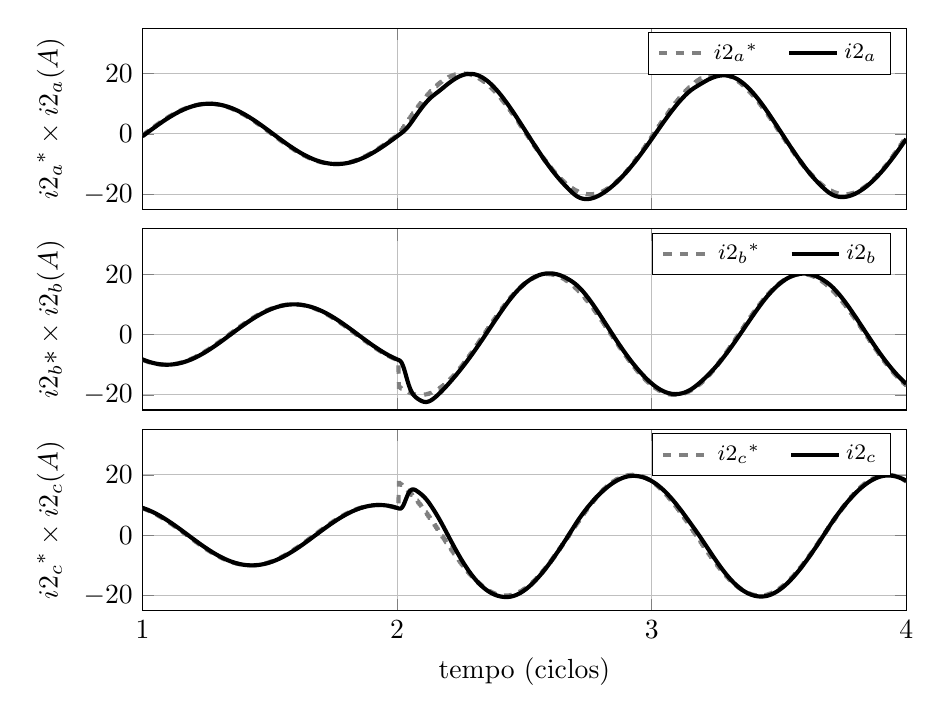
\begin{tikzpicture}

\begin{axis}[%
width=0.8\textwidth,
height=0.189701500343624\textwidth,
scale only axis,
xmin=0.316666666666667,
xmax=0.366666666666667,
xtick={0.316666666666667,0.333333333333333,0.35,0.366666666666667},
xticklabels={\empty},
xmajorgrids,
ymin=-25,
ymax=35,
ytick={-20,   0,  20},
ylabel={${\text{i2}_\text{b}}\text{* }\times\text{ i2}_\text{b}\text{ (A)}$},
ymajorgrids,
name=plot2,
legend style={draw=black,fill=white,legend cell align=left},
scaled x ticks = false,
legend columns=-1,
legend style={/tikz/every even column/.append style={column sep=0.3cm}},
legend style={font=\footnotesize}
]
\addplot [color=gray,dashed,line width=1.5pt]
  table[row sep=crcr]{0.316658333333333	-8.32921240710225\\
0.3167	-8.49892692986993\\
0.316741666666667	-8.49892692986993\\
0.316783333333333	-8.6602540378457\\
0.316825	-8.6602540378457\\
0.316866666666667	-8.81303452065127\\
0.316908333333333	-8.81303452065127\\
0.31695	-8.9571176023955\\
0.316991666666667	-8.9571176023955\\
0.317033333333333	-9.09236109047209\\
0.317075	-9.09236109047209\\
0.317116666666667	-9.21863151588643\\
0.317158333333333	-9.21863151588643\\
0.3172	-9.33580426497347\\
0.317241666666667	-9.33580426497347\\
0.317283333333333	-9.44376370237628\\
0.317325	-9.44376370237628\\
0.317366666666667	-9.54240328516426\\
0.317408333333333	-9.54240328516426\\
0.31745	-9.63162566797809\\
0.317491666666667	-9.63162566797809\\
0.317533333333333	-9.71134279909789\\
0.317575	-9.71134279909789\\
0.317616666666667	-9.7814760073396\\
0.317658333333333	-9.7814760073396\\
0.3177	-9.84195607969398\\
0.317741666666667	-9.84195607969398\\
0.317783333333333	-9.89272332963145\\
0.317825	-9.89272332963145\\
0.317866666666667	-9.93372765600555\\
0.317908333333333	-9.93372765600555\\
0.31795	-9.96492859249664\\
0.317991666666667	-9.96492859249664\\
0.318033333333333	-9.98629534754734\\
0.318075	-9.98629534754734\\
0.318116666666667	-9.99780683475006\\
0.318158333333333	-9.99780683475006\\
0.3182	-9.99945169365673\\
0.318241666666667	-9.99945169365673\\
0.318283333333333	-9.9912283009902\\
0.318325	-9.9912283009902\\
0.318366666666667	-9.9731447722462\\
0.318408333333333	-9.9731447722462\\
0.31845	-9.94521895368435\\
0.318491666666667	-9.94521895368435\\
0.318533333333333	-9.90747840471606\\
0.318575	-9.90747840471606\\
0.318616666666667	-9.85996037070666\\
0.318658333333333	-9.85996037070666\\
0.3187	-9.80271174621883\\
0.318741666666667	-9.80271174621883\\
0.318783333333333	-9.73578902873321\\
0.318825	-9.73578902873321\\
0.318866666666667	-9.65925826289228\\
0.318908333333333	-9.65925826289228\\
0.31895	-9.57319497532226\\
0.318991666666667	-9.57319497532226\\
0.319033333333333	-9.47768410009743\\
0.319075	-9.47768410009743\\
0.319116666666667	-9.37281989492048\\
0.319158333333333	-9.37281989492048\\
0.3192	-9.2587058481015\\
0.319241666666667	-9.2587058481015\\
0.319283333333333	-9.13545457642755\\
0.319325	-9.13545457642755\\
0.319366666666667	-9.00318771402345\\
0.319408333333333	-9.00318771402345\\
0.31945	-8.86203579231365\\
0.319491666666667	-8.86203579231365\\
0.319533333333333	-8.71213811120338\\
0.319575	-8.71213811120338\\
0.319616666666667	-8.55364260160653\\
0.319658333333333	-8.55364260160653\\
0.3197	-8.38670567945568\\
0.319741666666667	-8.38670567945568\\
0.319783333333333	-8.21149209133845\\
0.319825	-8.21149209133845\\
0.319866666666667	-8.02817475191253\\
0.319908333333333	-8.02817475191253\\
0.31995	-7.83693457325976\\
0.319991666666667	-7.83693457325976\\
0.320033333333333	-7.63796028634775\\
0.320075	-7.63796028634775\\
0.320116666666667	-7.43144825477524\\
0.320158333333333	-7.43144825477524\\
0.3202	-7.21760228098489\\
0.320241666666667	-7.21760228098489\\
0.320283333333333	-6.99663340513489\\
0.320325	-6.99663340513489\\
0.320366666666667	-6.76875969682781\\
0.320408333333333	-6.76875969682781\\
0.32045	-6.53420603990222\\
0.320491666666667	-6.53420603990222\\
0.320533333333333	-6.29320391049951\\
0.320575	-6.29320391049951\\
0.320616666666667	-6.04599114862485\\
0.320658333333333	-6.04599114862485\\
0.3207	-5.79281172342785\\
0.320741666666667	-5.79281172342785\\
0.320783333333333	-5.53391549243446\\
0.320825	-5.53391549243446\\
0.320866666666667	-5.26955795496776\\
0.320908333333333	-5.26955795496776\\
0.32095	-5.00000000000094\\
0.320991666666667	-5.00000000000094\\
0.321033333333333	-4.72550764869144\\
0.321075	-4.72550764869144\\
0.321116666666667	-4.44635179185013\\
0.321158333333333	-4.44635179185013\\
0.3212	-4.16280792260482\\
0.321241666666667	-4.16280792260482\\
0.321283333333333	-3.87515586452179\\
0.321325	-3.87515586452179\\
0.321366666666667	-3.58367949545372\\
0.321408333333333	-3.58367949545372\\
0.32145	-3.28866646738651\\
0.321491666666667	-3.28866646738651\\
0.321533333333333	-2.99040792256149\\
0.321575	-2.99040792256149\\
0.321616666666667	-2.68919820615324\\
0.321658333333333	-2.68919820615324\\
0.3217	-2.38533457578634\\
0.321741666666667	-2.38533457578634\\
0.321783333333333	-2.07911690817807\\
0.321825	-2.07911690817807\\
0.321866666666667	-1.77084740319627\\
0.321908333333333	-1.77084740319627\\
0.32195	-1.4608302856245\\
0.321991666666667	-1.4608302856245\\
0.322033333333333	-1.149371504929\\
0.322075	-1.149371504929\\
0.322116666666667	-0.836778433323436\\
0.322158333333333	-0.836778433323436\\
0.3222	-0.523359562429668\\
0.322241666666667	-0.523359562429668\\
0.322283333333333	-0.209424198833749\\
0.322325	-0.209424198833749\\
0.322366666666667	0.10471784116233\\
0.322408333333333	0.10471784116233\\
0.32245	0.41875653729192\\
0.322491666666667	0.41875653729192\\
0.322533333333333	0.732381971276291\\
0.322575	0.732381971276291\\
0.322616666666667	1.04528463267656\\
0.322658333333333	1.04528463267656\\
0.3227	1.35715572434312\\
0.322741666666667	1.35715572434312\\
0.322783333333333	1.66768746716115\\
0.322825	1.66768746716115\\
0.322866666666667	1.97657340379144\\
0.322908333333333	1.97657340379144\\
0.32295	2.28350870110679\\
0.322991666666667	2.28350870110679\\
0.323033333333333	2.58819045102549\\
0.323075	2.58819045102549\\
0.323116666666667	2.89031796944505\\
0.323158333333333	2.89031796944505\\
0.3232	3.18959309298109\\
0.323241666666667	3.18959309298109\\
0.323283333333333	3.48572047321859\\
0.323325	3.48572047321859\\
0.323366666666667	3.77840786818516\\
0.323408333333333	3.77840786818516\\
0.32345	4.06736643075854\\
0.323491666666667	4.06736643075854\\
0.323533333333333	4.35231099372386\\
0.323575	4.35231099372386\\
0.323616666666667	4.63296035119925\\
0.323658333333333	4.63296035119925\\
0.3237	4.90903753615209\\
0.323741666666667	4.90903753615209\\
0.323783333333333	5.18027009373203\\
0.323825	5.18027009373203\\
0.323866666666667	5.44639035015104\\
0.323908333333333	5.44639035015104\\
0.32395	5.70713567684513\\
0.323991666666667	5.70713567684513\\
0.324033333333333	5.96224874965702\\
0.324075	5.96224874965702\\
0.324116666666667	6.21147780278401\\
0.324158333333333	6.21147780278401\\
0.3242	6.45457687724046\\
0.324241666666667	6.45457687724046\\
0.324283333333333	6.69130606358958\\
0.324325	6.69130606358958\\
0.324366666666667	6.9214317387051\\
0.324408333333333	6.9214317387051\\
0.32445	7.14472679632911\\
0.324491666666667	7.14472679632911\\
0.324533333333333	7.36097087119846\\
0.324575	7.36097087119846\\
0.324616666666667	7.56995055651872\\
0.324658333333333	7.56995055651872\\
0.3247	7.7714596145709\\
0.324741666666667	7.7714596145709\\
0.324783333333333	7.96529918024319\\
0.324825	7.96529918024319\\
0.324866666666667	8.1512779572868\\
0.324908333333333	8.1512779572868\\
0.32495	8.32921240710229\\
0.324991666666667	8.32921240710229\\
0.325033333333333	8.49892692986996\\
0.325075	8.49892692986996\\
0.325116666666667	8.66025403784574\\
0.325158333333333	8.66025403784574\\
0.3252	8.81303452065131\\
0.325241666666667	8.81303452065131\\
0.325283333333333	8.95711760239554\\
0.325325	8.95711760239554\\
0.325366666666667	9.09236109047212\\
0.325408333333333	9.09236109047212\\
0.32545	9.21863151588647\\
0.325491666666667	9.21863151588647\\
0.325533333333333	9.33580426497351\\
0.325575	9.33580426497351\\
0.325616666666667	9.44376370237632\\
0.325658333333333	9.44376370237632\\
0.3257	9.5424032851643\\
0.325741666666667	9.5424032851643\\
0.325783333333333	9.63162566797813\\
0.325825	9.63162566797813\\
0.325866666666667	9.71134279909793\\
0.325908333333333	9.71134279909793\\
0.32595	9.78147600733964\\
0.325991666666667	9.78147600733964\\
0.326033333333333	9.84195607969402\\
0.326075	9.84195607969402\\
0.326116666666667	9.8927233296315\\
0.326158333333333	9.8927233296315\\
0.3262	9.93372765600559\\
0.326241666666667	9.93372765600559\\
0.326283333333333	9.96492859249668\\
0.326325	9.96492859249668\\
0.326366666666667	9.98629534754738\\
0.326408333333333	9.98629534754738\\
0.32645	9.99780683475011\\
0.326491666666667	9.99780683475011\\
0.326533333333333	9.99945169365678\\
0.326575	9.99945169365678\\
0.326616666666667	9.99122830099025\\
0.326658333333333	9.99122830099025\\
0.3267	9.97314477224624\\
0.326741666666667	9.97314477224624\\
0.326783333333333	9.9452189536844\\
0.326825	9.9452189536844\\
0.326866666666667	9.9074784047161\\
0.326908333333333	9.9074784047161\\
0.32695	9.85996037070671\\
0.326991666666667	9.85996037070671\\
0.327033333333333	9.80271174621887\\
0.327075	9.80271174621887\\
0.327116666666667	9.73578902873325\\
0.327158333333333	9.73578902873325\\
0.3272	9.65925826289232\\
0.327241666666667	9.65925826289232\\
0.327283333333333	9.5731949753223\\
0.327325	9.5731949753223\\
0.327366666666667	9.47768410009748\\
0.327408333333333	9.47768410009748\\
0.32745	9.37281989492053\\
0.327491666666667	9.37281989492053\\
0.327533333333333	9.25870584810154\\
0.327575	9.25870584810154\\
0.327616666666667	9.13545457642759\\
0.327658333333333	9.13545457642759\\
0.3277	9.0031877140235\\
0.327741666666667	9.0031877140235\\
0.327783333333333	8.86203579231369\\
0.327825	8.86203579231369\\
0.327866666666667	8.71213811120342\\
0.327908333333333	8.71213811120342\\
0.32795	8.55364260160657\\
0.327991666666667	8.55364260160657\\
0.328033333333333	8.38670567945572\\
0.328075	8.38670567945572\\
0.328116666666667	8.21149209133849\\
0.328158333333333	8.21149209133849\\
0.3282	8.02817475191257\\
0.328241666666667	8.02817475191257\\
0.328283333333333	7.83693457325979\\
0.328325	7.83693457325979\\
0.328366666666667	7.63796028634779\\
0.328408333333333	7.63796028634779\\
0.32845	7.43144825477528\\
0.328491666666667	7.43144825477528\\
0.328533333333333	7.21760228098492\\
0.328575	7.21760228098492\\
0.328616666666667	6.99663340513492\\
0.328658333333333	6.99663340513492\\
0.3287	6.76875969682784\\
0.328741666666667	6.76875969682784\\
0.328783333333333	6.53420603990226\\
0.328825	6.53420603990226\\
0.328866666666667	6.29320391049954\\
0.328908333333333	6.29320391049954\\
0.32895	6.04599114862488\\
0.328991666666667	6.04599114862488\\
0.329033333333333	5.79281172342788\\
0.329075	5.79281172342788\\
0.329116666666667	5.53391549243449\\
0.329158333333333	5.53391549243449\\
0.3292	5.26955795496778\\
0.329241666666667	5.26955795496778\\
0.329283333333333	5.00000000000096\\
0.329325	5.00000000000096\\
0.329366666666667	4.72550764869146\\
0.329408333333333	4.72550764869146\\
0.32945	4.44635179185015\\
0.329491666666667	4.44635179185015\\
0.329533333333333	4.16280792260484\\
0.329575	4.16280792260484\\
0.329616666666667	3.87515586452181\\
0.329658333333333	3.87515586452181\\
0.3297	3.58367949545374\\
0.329741666666667	3.58367949545374\\
0.329783333333333	3.28866646738652\\
0.329825	3.28866646738652\\
0.329866666666667	2.99040792256151\\
0.329908333333333	2.99040792256151\\
0.32995	2.68919820615325\\
0.329991666666667	2.68919820615325\\
0.330033333333333	2.38533457578635\\
0.330075	2.38533457578635\\
0.330116666666667	2.07911690817808\\
0.330158333333333	2.07911690817808\\
0.3302	1.77084740319627\\
0.330241666666667	1.77084740319627\\
0.330283333333333	1.4608302856245\\
0.330325	1.4608302856245\\
0.330366666666667	1.149371504929\\
0.330408333333333	1.149371504929\\
0.33045	0.836778433323441\\
0.330491666666667	0.836778433323441\\
0.330533333333333	0.523359562429672\\
0.330575	0.523359562429672\\
0.330616666666667	0.20942419883375\\
0.330658333333333	0.20942419883375\\
0.3307	-0.10471784116233\\
0.330741666666667	-0.10471784116233\\
0.330783333333333	-0.418756537291922\\
0.330825	-0.418756537291922\\
0.330866666666667	-0.732381971276294\\
0.330908333333333	-0.732381971276294\\
0.33095	-1.04528463267656\\
0.330991666666667	-1.04528463267656\\
0.331033333333333	-1.35715572434313\\
0.331075	-1.35715572434313\\
0.331116666666667	-1.66768746716116\\
0.331158333333333	-1.66768746716116\\
0.3312	-1.97657340379145\\
0.331241666666667	-1.97657340379145\\
0.331283333333333	-2.2835087011068\\
0.331325	-2.2835087011068\\
0.331366666666667	-2.5881904510255\\
0.331408333333333	-2.5881904510255\\
0.33145	-2.89031796944506\\
0.331491666666667	-2.89031796944506\\
0.331533333333333	-3.1895930929811\\
0.331575	-3.1895930929811\\
0.331616666666667	-3.4857204732186\\
0.331658333333333	-3.4857204732186\\
0.3317	-3.77840786818517\\
0.331741666666667	-3.77840786818517\\
0.331783333333333	-4.06736643075855\\
0.331825	-4.06736643075855\\
0.331866666666667	-4.35231099372388\\
0.331908333333333	-4.35231099372388\\
0.33195	-4.63296035119927\\
0.331991666666667	-4.63296035119927\\
0.332033333333333	-4.90903753615211\\
0.332075	-4.90903753615211\\
0.332116666666667	-5.18027009373205\\
0.332158333333333	-5.18027009373205\\
0.3322	-5.44639035015107\\
0.332241666666667	-5.44639035015107\\
0.332283333333333	-5.70713567684516\\
0.332325	-5.70713567684516\\
0.332366666666667	-5.96224874965705\\
0.332408333333333	-5.96224874965705\\
0.33245	-6.21147780278404\\
0.332491666666667	-6.21147780278404\\
0.332533333333333	-6.45457687724048\\
0.332575	-6.45457687724048\\
0.332616666666667	-6.6913060635896\\
0.332658333333333	-6.6913060635896\\
0.3327	-6.92143173870513\\
0.332741666666667	-6.92143173870513\\
0.332783333333333	-7.14472679632914\\
0.332825	-7.14472679632914\\
0.332866666666667	-7.36097087119849\\
0.332908333333333	-7.36097087119849\\
0.33295	-7.56995055651875\\
0.332991666666667	-7.56995055651875\\
0.333033333333333	-7.77145961457093\\
0.333075	-7.77145961457093\\
0.333116666666667	-7.96529918024322\\
0.333158333333333	-7.96529918024322\\
0.3332	-8.15127795728684\\
0.333241666666667	-8.15127795728684\\
0.333283333333333	-8.32921240710232\\
0.333325	-8.32921240710232\\
0.333366666666667	-8.49892692987\\
0.333408333333333	-8.49892692987\\
0.33345	-17.3205080756916\\
0.333491666666667	-17.3205080756916\\
0.333533333333333	-17.6260690413027\\
0.333575	-17.6260690413027\\
0.333616666666667	-17.9142352047912\\
0.333658333333333	-17.9142352047912\\
0.3337	-18.1847221809443\\
0.333741666666667	-18.1847221809443\\
0.333783333333333	-18.437263031773\\
0.333825	-18.437263031773\\
0.333866666666667	-18.6716085299471\\
0.333908333333333	-18.6716085299471\\
0.33395	-18.8875274047527\\
0.333991666666667	-18.8875274047527\\
0.334033333333333	-19.0848065703287\\
0.334075	-19.0848065703287\\
0.334116666666667	-19.2632513359563\\
0.334158333333333	-19.2632513359563\\
0.3342	-19.4226855981959\\
0.334241666666667	-19.4226855981959\\
0.334283333333333	-19.5629520146794\\
0.334325	-19.5629520146794\\
0.334366666666667	-19.6839121593881\\
0.334408333333333	-19.6839121593881\\
0.33445	-19.7854466592631\\
0.334491666666667	-19.7854466592631\\
0.334533333333333	-19.8674553120113\\
0.334575	-19.8674553120113\\
0.334616666666667	-19.9298571849934\\
0.334658333333333	-19.9298571849934\\
0.3347	-19.9725906950948\\
0.334741666666667	-19.9725906950948\\
0.334783333333333	-19.9956136695003\\
0.334825	-19.9956136695003\\
0.334866666666667	-19.9989033873136\\
0.334908333333333	-19.9989033873136\\
0.33495	-19.9824566019806\\
0.334991666666667	-19.9824566019806\\
0.335033333333333	-19.9462895444926\\
0.335075	-19.9462895444926\\
0.335116666666667	-19.8904379073689\\
0.335158333333333	-19.8904379073689\\
0.3352	-19.8149568094323\\
0.335241666666667	-19.8149568094323\\
0.335283333333333	-19.7199207414135\\
0.335325	-19.7199207414135\\
0.335366666666667	-19.6054234924378\\
0.335408333333333	-19.6054234924378\\
0.33545	-19.4715780574666\\
0.335491666666667	-19.4715780574666\\
0.335533333333333	-19.3185165257847\\
0.335575	-19.3185165257847\\
0.335616666666667	-19.1463899506447\\
0.335658333333333	-19.1463899506447\\
0.3357	-18.955368200195\\
0.335741666666667	-18.955368200195\\
0.335783333333333	-18.7456397898411\\
0.335825	-18.7456397898411\\
0.335866666666667	-18.5174116962032\\
0.335908333333333	-18.5174116962032\\
0.33595	-18.2709091528552\\
0.335991666666667	-18.2709091528552\\
0.336033333333333	-18.0063754280471\\
0.336075	-18.0063754280471\\
0.336116666666667	-17.7240715846274\\
0.336158333333333	-17.7240715846274\\
0.3362	-17.4242762224069\\
0.336241666666667	-17.4242762224069\\
0.336283333333333	-17.1072852032132\\
0.336325	-17.1072852032132\\
0.336366666666667	-16.7734113589115\\
0.336408333333333	-16.7734113589115\\
0.33645	-16.422984182677\\
0.336491666666667	-16.422984182677\\
0.336533333333333	-16.0563495038252\\
0.336575	-16.0563495038252\\
0.336616666666667	-15.6738691465196\\
0.336658333333333	-15.6738691465196\\
0.3367	-15.2759205726956\\
0.336741666666667	-15.2759205726956\\
0.336783333333333	-14.8628965095506\\
0.336825	-14.8628965095506\\
0.336866666666667	-14.4352045619699\\
0.336908333333333	-14.4352045619699\\
0.33695	-13.9932668102699\\
0.336991666666667	-13.9932668102699\\
0.337033333333333	-13.5375193936557\\
0.337075	-13.5375193936557\\
0.337116666666667	-13.0684120798046\\
0.337158333333333	-13.0684120798046\\
0.3372	-12.5864078209991\\
0.337241666666667	-12.5864078209991\\
0.337283333333333	-12.0919822972498\\
0.337325	-12.0919822972498\\
0.337366666666667	-11.5856234468558\\
0.337408333333333	-11.5856234468558\\
0.33745	-11.067830984869\\
0.337491666666667	-11.067830984869\\
0.337533333333333	-10.5391159099356\\
0.337575	-10.5391159099356\\
0.337616666666667	-10.000000000002\\
0.337658333333333	-10.000000000002\\
0.3377	-9.45101529738295\\
0.337741666666667	-9.45101529738295\\
0.337783333333333	-8.89270358370033\\
0.337825	-8.89270358370033\\
0.337866666666667	-8.32561584520971\\
0.337908333333333	-8.32561584520971\\
0.33795	-7.75031172904366\\
0.337991666666667	-7.75031172904366\\
0.338033333333333	-7.1673589909075\\
0.338075	-7.1673589909075\\
0.338116666666667	-6.57733293477307\\
0.338158333333333	-6.57733293477307\\
0.3382	-5.98081584512304\\
0.338241666666667	-5.98081584512304\\
0.338283333333333	-5.37839641230652\\
0.338325	-5.37839641230652\\
0.338366666666667	-4.77066915157272\\
0.338408333333333	-4.77066915157272\\
0.33845	-4.15823381635619\\
0.338491666666667	-4.15823381635619\\
0.338533333333333	-3.54169480639256\\
0.338575	-3.54169480639256\\
0.338616666666667	-2.92166057124902\\
0.338658333333333	-2.92166057124902\\
0.3387	-2.29874300985802\\
0.338741666666667	-2.29874300985802\\
0.338783333333333	-1.67355686664689\\
0.338825	-1.67355686664689\\
0.338866666666667	-1.04671912485935\\
0.338908333333333	-1.04671912485935\\
0.33895	-0.418848397667502\\
0.338991666666667	-0.418848397667502\\
0.339033333333333	0.209435682324661\\
0.339075	0.209435682324661\\
0.339116666666667	0.837513074583847\\
0.339158333333333	0.837513074583847\\
0.3392	1.4647639425526\\
0.339241666666667	1.4647639425526\\
0.339283333333333	2.09056926535314\\
0.339325	2.09056926535314\\
0.339366666666667	2.71431144868627\\
0.339408333333333	2.71431144868627\\
0.33945	3.33537493432233\\
0.339491666666667	3.33537493432233\\
0.339533333333333	3.95314680758292\\
0.339575	3.95314680758292\\
0.339616666666667	4.56701740221362\\
0.339658333333333	4.56701740221362\\
0.3397	5.17638090205103\\
0.339741666666667	5.17638090205103\\
0.339783333333333	5.78063593889015\\
0.339825	5.78063593889015\\
0.339866666666667	6.37918618596222\\
0.339908333333333	6.37918618596222\\
0.33995	6.97144094643723\\
0.339991666666667	6.97144094643723\\
0.340033333333333	7.55681573637037\\
0.340075	7.55681573637037\\
0.340116666666667	8.13473286151714\\
0.340158333333333	8.13473286151714\\
0.3402	8.70462198744779\\
0.340241666666667	8.70462198744779\\
0.340283333333333	9.26592070239858\\
0.340325	9.26592070239858\\
0.340366666666667	9.81807507230426\\
0.340408333333333	9.81807507230426\\
0.34045	10.3605401874641\\
0.340491666666667	10.3605401874641\\
0.340533333333333	10.8927807003022\\
0.340575	10.8927807003022\\
0.340616666666667	11.4142713536904\\
0.340658333333333	11.4142713536904\\
0.3407	11.9244974993141\\
0.340741666666667	11.9244974993141\\
0.340783333333333	12.4229556055681\\
0.340825	12.4229556055681\\
0.340866666666667	12.909153754481\\
0.340908333333333	12.909153754481\\
0.34095	13.3826121271793\\
0.340991666666667	13.3826121271793\\
0.341033333333333	13.8428634774103\\
0.341075	13.8428634774103\\
0.341116666666667	14.2894535926583\\
0.341158333333333	14.2894535926583\\
0.3412	14.721941742397\\
0.341241666666667	14.721941742397\\
0.341283333333333	15.1399011130375\\
0.341325	15.1399011130375\\
0.341366666666667	15.5429192291419\\
0.341408333333333	15.5429192291419\\
0.34145	15.9305983604865\\
0.341491666666667	15.9305983604865\\
0.341533333333333	16.3025559145737\\
0.341575	16.3025559145737\\
0.341616666666667	16.6584248142047\\
0.341658333333333	16.6584248142047\\
0.3417	16.9978538597401\\
0.341741666666667	16.9978538597401\\
0.341783333333333	17.3205080756916\\
0.341825	17.3205080756916\\
0.341866666666667	17.6260690413028\\
0.341908333333333	17.6260690413028\\
0.34195	17.9142352047912\\
0.341991666666667	17.9142352047912\\
0.342033333333333	18.1847221809444\\
0.342075	18.1847221809444\\
0.342116666666667	18.4372630317731\\
0.342158333333333	18.4372630317731\\
0.3422	18.6716085299472\\
0.342241666666667	18.6716085299472\\
0.342283333333333	18.8875274047528\\
0.342325	18.8875274047528\\
0.342366666666667	19.0848065703288\\
0.342408333333333	19.0848065703288\\
0.34245	19.2632513359564\\
0.342491666666667	19.2632513359564\\
0.342533333333333	19.422685598196\\
0.342575	19.422685598196\\
0.342616666666667	19.5629520146794\\
0.342658333333333	19.5629520146794\\
0.3427	19.6839121593882\\
0.342741666666667	19.6839121593882\\
0.342783333333333	19.7854466592631\\
0.342825	19.7854466592631\\
0.342866666666667	19.8674553120113\\
0.342908333333333	19.8674553120113\\
0.34295	19.9298571849935\\
0.342991666666667	19.9298571849935\\
0.343033333333333	19.9725906950949\\
0.343075	19.9725906950949\\
0.343116666666667	19.9956136695004\\
0.343158333333333	19.9956136695004\\
0.3432	19.9989033873137\\
0.343241666666667	19.9989033873137\\
0.343283333333333	19.9824566019806\\
0.343325	19.9824566019806\\
0.343366666666667	19.9462895444926\\
0.343408333333333	19.9462895444926\\
0.34345	19.890437907369\\
0.343491666666667	19.890437907369\\
0.343533333333333	19.8149568094324\\
0.343575	19.8149568094324\\
0.343616666666667	19.7199207414136\\
0.343658333333333	19.7199207414136\\
0.3437	19.6054234924379\\
0.343741666666667	19.6054234924379\\
0.343783333333333	19.4715780574667\\
0.343825	19.4715780574667\\
0.343866666666667	19.3185165257848\\
0.343908333333333	19.3185165257848\\
0.34395	19.1463899506448\\
0.343991666666667	19.1463899506448\\
0.344033333333333	18.9553682001951\\
0.344075	18.9553682001951\\
0.344116666666667	18.7456397898412\\
0.344158333333333	18.7456397898412\\
0.3442	18.5174116962032\\
0.344241666666667	18.5174116962032\\
0.344283333333333	18.2709091528553\\
0.344325	18.2709091528553\\
0.344366666666667	18.0063754280471\\
0.344408333333333	18.0063754280471\\
0.34445	17.7240715846275\\
0.344491666666667	17.7240715846275\\
0.344533333333333	17.424276222407\\
0.344575	17.424276222407\\
0.344616666666667	17.1072852032133\\
0.344658333333333	17.1072852032133\\
0.3447	16.7734113589116\\
0.344741666666667	16.7734113589116\\
0.344783333333333	16.4229841826771\\
0.344825	16.4229841826771\\
0.344866666666667	16.0563495038253\\
0.344908333333333	16.0563495038253\\
0.34495	15.6738691465197\\
0.344991666666667	15.6738691465197\\
0.345033333333333	15.2759205726957\\
0.345075	15.2759205726957\\
0.345116666666667	14.8628965095507\\
0.345158333333333	14.8628965095507\\
0.3452	14.43520456197\\
0.345241666666667	14.43520456197\\
0.345283333333333	13.99326681027\\
0.345325	13.99326681027\\
0.345366666666667	13.5375193936558\\
0.345408333333333	13.5375193936558\\
0.34545	13.0684120798046\\
0.345491666666667	13.0684120798046\\
0.345533333333333	12.5864078209992\\
0.345575	12.5864078209992\\
0.345616666666667	12.0919822972498\\
0.345658333333333	12.0919822972498\\
0.3457	11.5856234468558\\
0.345741666666667	11.5856234468558\\
0.345783333333333	11.0678309848691\\
0.345825	11.0678309848691\\
0.345866666666667	10.5391159099356\\
0.345908333333333	10.5391159099356\\
0.34595	10.000000000002\\
0.345991666666667	10.000000000002\\
0.346033333333333	9.45101529738299\\
0.346075	9.45101529738299\\
0.346116666666667	8.89270358370037\\
0.346158333333333	8.89270358370037\\
0.3462	8.32561584520974\\
0.346241666666667	8.32561584520974\\
0.346283333333333	7.75031172904369\\
0.346325	7.75031172904369\\
0.346366666666667	7.16735899090753\\
0.346408333333333	7.16735899090753\\
0.34645	6.57733293477309\\
0.346491666666667	6.57733293477309\\
0.346533333333333	5.98081584512306\\
0.346575	5.98081584512306\\
0.346616666666667	5.37839641230654\\
0.346658333333333	5.37839641230654\\
0.3467	4.77066915157274\\
0.346741666666667	4.77066915157274\\
0.346783333333333	4.1582338163562\\
0.346825	4.1582338163562\\
0.346866666666667	3.54169480639257\\
0.346908333333333	3.54169480639257\\
0.34695	2.92166057124903\\
0.346991666666667	2.92166057124903\\
0.347033333333333	2.29874300985803\\
0.347075	2.29874300985803\\
0.347116666666667	1.6735568666469\\
0.347158333333333	1.6735568666469\\
0.3472	1.04671912485935\\
0.347241666666667	1.04671912485935\\
0.347283333333333	0.418848397667507\\
0.347325	0.418848397667507\\
0.347366666666667	-0.209435682324659\\
0.347408333333333	-0.209435682324659\\
0.34745	-0.837513074583846\\
0.347491666666667	-0.837513074583846\\
0.347533333333333	-1.4647639425526\\
0.347575	-1.4647639425526\\
0.347616666666667	-2.09056926535315\\
0.347658333333333	-2.09056926535315\\
0.3477	-2.71431144868628\\
0.347741666666667	-2.71431144868628\\
0.347783333333333	-3.33537493432234\\
0.347825	-3.33537493432234\\
0.347866666666667	-3.95314680758293\\
0.347908333333333	-3.95314680758293\\
0.34795	-4.56701740221363\\
0.347991666666667	-4.56701740221363\\
0.348033333333333	-5.17638090205104\\
0.348075	-5.17638090205104\\
0.348116666666667	-5.78063593889017\\
0.348158333333333	-5.78063593889017\\
0.3482	-6.37918618596224\\
0.348241666666667	-6.37918618596224\\
0.348283333333333	-6.97144094643726\\
0.348325	-6.97144094643726\\
0.348366666666667	-7.5568157363704\\
0.348408333333333	-7.5568157363704\\
0.34845	-8.13473286151717\\
0.348491666666667	-8.13473286151717\\
0.348533333333333	-8.70462198744782\\
0.348575	-8.70462198744782\\
0.348616666666667	-9.2659207023986\\
0.348658333333333	-9.2659207023986\\
0.3487	-9.81807507230429\\
0.348741666666667	-9.81807507230429\\
0.348783333333333	-10.3605401874642\\
0.348825	-10.3605401874642\\
0.348866666666667	-10.8927807003022\\
0.348908333333333	-10.8927807003022\\
0.34895	-11.4142713536904\\
0.348991666666667	-11.4142713536904\\
0.349033333333333	-11.9244974993142\\
0.349075	-11.9244974993142\\
0.349116666666667	-12.4229556055682\\
0.349158333333333	-12.4229556055682\\
0.3492	-12.9091537544811\\
0.349241666666667	-12.9091537544811\\
0.349283333333333	-13.3826121271793\\
0.349325	-13.3826121271793\\
0.349366666666667	-13.8428634774104\\
0.349408333333333	-13.8428634774104\\
0.34945	-14.2894535926584\\
0.349491666666667	-14.2894535926584\\
0.349533333333333	-14.7219417423971\\
0.349575	-14.7219417423971\\
0.349616666666667	-15.1399011130376\\
0.349658333333333	-15.1399011130376\\
0.3497	-15.542919229142\\
0.349741666666667	-15.542919229142\\
0.349783333333333	-15.9305983604866\\
0.349825	-15.9305983604866\\
0.349866666666667	-16.3025559145738\\
0.349908333333333	-16.3025559145738\\
0.34995	-16.6584248142048\\
0.349991666666667	-16.6584248142048\\
0.350033333333333	-16.9978538597401\\
0.350075	-16.9978538597401\\
0.350116666666667	-17.3205080756917\\
0.350158333333333	-17.3205080756917\\
0.3502	-17.6260690413028\\
0.350241666666667	-17.6260690413028\\
0.350283333333333	-17.9142352047913\\
0.350325	-17.9142352047913\\
0.350366666666667	-18.1847221809445\\
0.350408333333333	-18.1847221809445\\
0.35045	-18.4372630317732\\
0.350491666666667	-18.4372630317732\\
0.350533333333333	-18.6716085299472\\
0.350575	-18.6716085299472\\
0.350616666666667	-18.8875274047529\\
0.350658333333333	-18.8875274047529\\
0.3507	-19.0848065703288\\
0.350741666666667	-19.0848065703288\\
0.350783333333333	-19.2632513359565\\
0.350825	-19.2632513359565\\
0.350866666666667	-19.4226855981961\\
0.350908333333333	-19.4226855981961\\
0.35095	-19.5629520146795\\
0.350991666666667	-19.5629520146795\\
0.351033333333333	-19.6839121593883\\
0.351075	-19.6839121593883\\
0.351116666666667	-19.7854466592632\\
0.351158333333333	-19.7854466592632\\
0.3512	-19.8674553120114\\
0.351241666666667	-19.8674553120114\\
0.351283333333333	-19.9298571849936\\
0.351325	-19.9298571849936\\
0.351366666666667	-19.972590695095\\
0.351408333333333	-19.972590695095\\
0.35145	-19.9956136695005\\
0.351491666666667	-19.9956136695005\\
0.351533333333333	-19.9989033873138\\
0.351575	-19.9989033873138\\
0.351616666666667	-19.9824566019807\\
0.351658333333333	-19.9824566019807\\
0.3517	-19.9462895444927\\
0.351741666666667	-19.9462895444927\\
0.351783333333333	-19.890437907369\\
0.351825	-19.890437907369\\
0.351866666666667	-19.8149568094324\\
0.351908333333333	-19.8149568094324\\
0.35195	-19.7199207414137\\
0.351991666666667	-19.7199207414137\\
0.352033333333333	-19.605423492438\\
0.352075	-19.605423492438\\
0.352116666666667	-19.4715780574667\\
0.352158333333333	-19.4715780574667\\
0.3522	-19.3185165257849\\
0.352241666666667	-19.3185165257849\\
0.352283333333333	-19.1463899506448\\
0.352325	-19.1463899506448\\
0.352366666666667	-18.9553682001952\\
0.352408333333333	-18.9553682001952\\
0.35245	-18.7456397898413\\
0.352491666666667	-18.7456397898413\\
0.352533333333333	-18.5174116962033\\
0.352575	-18.5174116962033\\
0.352616666666667	-18.2709091528554\\
0.352658333333333	-18.2709091528554\\
0.3527	-18.0063754280472\\
0.352741666666667	-18.0063754280472\\
0.352783333333333	-17.7240715846276\\
0.352825	-17.7240715846276\\
0.352866666666667	-17.424276222407\\
0.352908333333333	-17.424276222407\\
0.35295	-17.1072852032133\\
0.352991666666667	-17.1072852032133\\
0.353033333333333	-16.7734113589116\\
0.353075	-16.7734113589116\\
0.353116666666667	-16.4229841826772\\
0.353158333333333	-16.4229841826772\\
0.3532	-16.0563495038253\\
0.353241666666667	-16.0563495038253\\
0.353283333333333	-15.6738691465198\\
0.353325	-15.6738691465198\\
0.353366666666667	-15.2759205726958\\
0.353408333333333	-15.2759205726958\\
0.35345	-14.8628965095507\\
0.353491666666667	-14.8628965095507\\
0.353533333333333	-14.43520456197\\
0.353575	-14.43520456197\\
0.353616666666667	-13.99326681027\\
0.353658333333333	-13.99326681027\\
0.3537	-13.5375193936559\\
0.353741666666667	-13.5375193936559\\
0.353783333333333	-13.0684120798047\\
0.353825	-13.0684120798047\\
0.353866666666667	-12.5864078209992\\
0.353908333333333	-12.5864078209992\\
0.35395	-12.0919822972499\\
0.353991666666667	-12.0919822972499\\
0.354033333333333	-11.5856234468559\\
0.354075	-11.5856234468559\\
0.354116666666667	-11.0678309848691\\
0.354158333333333	-11.0678309848691\\
0.3542	-10.5391159099357\\
0.354241666666667	-10.5391159099357\\
0.354283333333333	-10.0000000000021\\
0.354325	-10.0000000000021\\
0.354366666666667	-9.45101529738304\\
0.354408333333333	-9.45101529738304\\
0.35445	-8.89270358370041\\
0.354491666666667	-8.89270358370041\\
0.354533333333333	-8.32561584520979\\
0.354575	-8.32561584520979\\
0.354616666666667	-7.75031172904372\\
0.354658333333333	-7.75031172904372\\
0.3547	-7.16735899090757\\
0.354741666666667	-7.16735899090757\\
0.354783333333333	-6.57733293477313\\
0.354825	-6.57733293477313\\
0.354866666666667	-5.98081584512309\\
0.354908333333333	-5.98081584512309\\
0.35495	-5.37839641230657\\
0.354991666666667	-5.37839641230657\\
0.355033333333333	-4.77066915157277\\
0.355075	-4.77066915157277\\
0.355116666666667	-4.15823381635623\\
0.355158333333333	-4.15823381635623\\
0.3552	-3.5416948063926\\
0.355241666666667	-3.5416948063926\\
0.355283333333333	-2.92166057124906\\
0.355325	-2.92166057124906\\
0.355366666666667	-2.29874300985804\\
0.355408333333333	-2.29874300985804\\
0.35545	-1.67355686664691\\
0.355491666666667	-1.67355686664691\\
0.355533333333333	-1.04671912485937\\
0.355575	-1.04671912485937\\
0.355616666666667	-0.418848397667518\\
0.355658333333333	-0.418848397667518\\
0.3557	0.209435682324651\\
0.355741666666667	0.209435682324651\\
0.355783333333333	0.837513074583842\\
0.355825	0.837513074583842\\
0.355866666666667	1.46476394255259\\
0.355908333333333	1.46476394255259\\
0.35595	2.09056926535314\\
0.355991666666667	2.09056926535314\\
0.356033333333333	2.71431144868627\\
0.356075	2.71431144868627\\
0.356116666666667	3.33537493432235\\
0.356158333333333	3.33537493432235\\
0.3562	3.95314680758294\\
0.356241666666667	3.95314680758294\\
0.356283333333333	4.56701740221364\\
0.356325	4.56701740221364\\
0.356366666666667	5.17638090205106\\
0.356408333333333	5.17638090205106\\
0.35645	5.78063593889018\\
0.356491666666667	5.78063593889018\\
0.356533333333333	6.37918618596226\\
0.356575	6.37918618596226\\
0.356616666666667	6.97144094643728\\
0.356658333333333	6.97144094643728\\
0.3567	7.55681573637042\\
0.356741666666667	7.55681573637042\\
0.356783333333333	8.13473286151719\\
0.356825	8.13473286151719\\
0.356866666666667	8.70462198744785\\
0.356908333333333	8.70462198744785\\
0.35695	9.26592070239863\\
0.356991666666667	9.26592070239863\\
0.357033333333333	9.81807507230432\\
0.357075	9.81807507230432\\
0.357116666666667	10.3605401874642\\
0.357158333333333	10.3605401874642\\
0.3572	10.8927807003023\\
0.357241666666667	10.8927807003023\\
0.357283333333333	11.4142713536904\\
0.357325	11.4142713536904\\
0.357366666666667	11.9244974993142\\
0.357408333333333	11.9244974993142\\
0.35745	12.4229556055682\\
0.357491666666667	12.4229556055682\\
0.357533333333333	12.9091537544811\\
0.357575	12.9091537544811\\
0.357616666666667	13.3826121271794\\
0.357658333333333	13.3826121271794\\
0.3577	13.8428634774104\\
0.357741666666667	13.8428634774104\\
0.357783333333333	14.2894535926584\\
0.357825	14.2894535926584\\
0.357866666666667	14.7219417423971\\
0.357908333333333	14.7219417423971\\
0.35795	15.1399011130377\\
0.357991666666667	15.1399011130377\\
0.358033333333333	15.542919229142\\
0.358075	15.542919229142\\
0.358116666666667	15.9305983604866\\
0.358158333333333	15.9305983604866\\
0.3582	16.3025559145739\\
0.358241666666667	16.3025559145739\\
0.358283333333333	16.6584248142048\\
0.358325	16.6584248142048\\
0.358366666666667	16.9978538597402\\
0.358408333333333	16.9978538597402\\
0.35845	17.3205080756918\\
0.358491666666667	17.3205080756918\\
0.358533333333333	17.6260690413029\\
0.358575	17.6260690413029\\
0.358616666666667	17.9142352047914\\
0.358658333333333	17.9142352047914\\
0.3587	18.1847221809445\\
0.358741666666667	18.1847221809445\\
0.358783333333333	18.4372630317732\\
0.358825	18.4372630317732\\
0.358866666666667	18.6716085299473\\
0.358908333333333	18.6716085299473\\
0.35895	18.8875274047529\\
0.358991666666667	18.8875274047529\\
0.359033333333333	19.0848065703289\\
0.359075	19.0848065703289\\
0.359116666666667	19.2632513359566\\
0.359158333333333	19.2632513359566\\
0.3592	19.4226855981962\\
0.359241666666667	19.4226855981962\\
0.359283333333333	19.5629520146796\\
0.359325	19.5629520146796\\
0.359366666666667	19.6839121593884\\
0.359408333333333	19.6839121593884\\
0.35945	19.7854466592633\\
0.359491666666667	19.7854466592633\\
0.359533333333333	19.8674553120115\\
0.359575	19.8674553120115\\
0.359616666666667	19.9298571849937\\
0.359658333333333	19.9298571849937\\
0.3597	19.9725906950951\\
0.359741666666667	19.9725906950951\\
0.359783333333333	19.9956136695005\\
0.359825	19.9956136695005\\
0.359866666666667	19.9989033873139\\
0.359908333333333	19.9989033873139\\
0.35995	19.9824566019808\\
0.359991666666667	19.9824566019808\\
0.360033333333333	19.9462895444928\\
0.360075	19.9462895444928\\
0.360116666666667	19.8904379073691\\
0.360158333333333	19.8904379073691\\
0.3602	19.8149568094325\\
0.360241666666667	19.8149568094325\\
0.360283333333333	19.7199207414137\\
0.360325	19.7199207414137\\
0.360366666666667	19.6054234924381\\
0.360408333333333	19.6054234924381\\
0.36045	19.4715780574668\\
0.360491666666667	19.4715780574668\\
0.360533333333333	19.318516525785\\
0.360575	19.318516525785\\
0.360616666666667	19.1463899506449\\
0.360658333333333	19.1463899506449\\
0.3607	18.9553682001953\\
0.360741666666667	18.9553682001953\\
0.360783333333333	18.7456397898414\\
0.360825	18.7456397898414\\
0.360866666666667	18.5174116962034\\
0.360908333333333	18.5174116962034\\
0.36095	18.2709091528555\\
0.360991666666667	18.2709091528555\\
0.361033333333333	18.0063754280473\\
0.361075	18.0063754280473\\
0.361116666666667	17.7240715846277\\
0.361158333333333	17.7240715846277\\
0.3612	17.4242762224071\\
0.361241666666667	17.4242762224071\\
0.361283333333333	17.1072852032134\\
0.361325	17.1072852032134\\
0.361366666666667	16.7734113589117\\
0.361408333333333	16.7734113589117\\
0.36145	16.4229841826773\\
0.361491666666667	16.4229841826773\\
0.361533333333333	16.0563495038254\\
0.361575	16.0563495038254\\
0.361616666666667	15.6738691465199\\
0.361658333333333	15.6738691465199\\
0.3617	15.2759205726958\\
0.361741666666667	15.2759205726958\\
0.361783333333333	14.8628965095508\\
0.361825	14.8628965095508\\
0.361866666666667	14.4352045619701\\
0.361908333333333	14.4352045619701\\
0.36195	13.9932668102701\\
0.361991666666667	13.9932668102701\\
0.362033333333333	13.5375193936559\\
0.362075	13.5375193936559\\
0.362116666666667	13.0684120798047\\
0.362158333333333	13.0684120798047\\
0.3622	12.5864078209993\\
0.362241666666667	12.5864078209993\\
0.362283333333333	12.09198229725\\
0.362325	12.09198229725\\
0.362366666666667	11.5856234468559\\
0.362408333333333	11.5856234468559\\
0.36245	11.0678309848692\\
0.362491666666667	11.0678309848692\\
0.362533333333333	10.5391159099357\\
0.362575	10.5391159099357\\
0.362616666666667	10.0000000000021\\
0.362658333333333	10.0000000000021\\
0.3627	9.45101529738308\\
0.362741666666667	9.45101529738308\\
0.362783333333333	8.89270358370046\\
0.362825	8.89270358370046\\
0.362866666666667	8.32561584520983\\
0.362908333333333	8.32561584520983\\
0.36295	7.75031172904376\\
0.362991666666667	7.75031172904376\\
0.363033333333333	7.16735899090761\\
0.363075	7.16735899090761\\
0.363116666666667	6.57733293477316\\
0.363158333333333	6.57733293477316\\
0.3632	5.98081584512313\\
0.363241666666667	5.98081584512313\\
0.363283333333333	5.3783964123066\\
0.363325	5.3783964123066\\
0.363366666666667	4.77066915157279\\
0.363408333333333	4.77066915157279\\
0.36345	4.15823381635625\\
0.363491666666667	4.15823381635625\\
0.363533333333333	3.54169480639262\\
0.363575	3.54169480639262\\
0.363616666666667	2.92166057124908\\
0.363658333333333	2.92166057124908\\
0.3637	2.29874300985806\\
0.363741666666667	2.29874300985806\\
0.363783333333333	1.67355686664693\\
0.363825	1.67355686664693\\
0.363866666666667	1.04671912485938\\
0.363908333333333	1.04671912485938\\
0.36395	0.418848397667529\\
0.363991666666667	0.418848397667529\\
0.364033333333333	-0.209435682324641\\
0.364075	-0.209435682324641\\
0.364116666666667	-0.837513074583835\\
0.364158333333333	-0.837513074583835\\
0.3642	-1.46476394255259\\
0.364241666666667	-1.46476394255259\\
0.364283333333333	-2.09056926535314\\
0.364325	-2.09056926535314\\
0.364366666666667	-2.71431144868628\\
0.364408333333333	-2.71431144868628\\
0.36445	-3.33537493432235\\
0.364491666666667	-3.33537493432235\\
0.364533333333333	-3.95314680758295\\
0.364575	-3.95314680758295\\
0.364616666666667	-4.56701740221365\\
0.364658333333333	-4.56701740221365\\
0.3647	-5.17638090205107\\
0.364741666666667	-5.17638090205107\\
0.364783333333333	-5.7806359388902\\
0.364825	-5.7806359388902\\
0.364866666666667	-6.37918618596228\\
0.364908333333333	-6.37918618596228\\
0.36495	-6.9714409464373\\
0.364991666666667	-6.9714409464373\\
0.365033333333333	-7.55681573637044\\
0.365075	-7.55681573637044\\
0.365116666666667	-8.13473286151722\\
0.365158333333333	-8.13473286151722\\
0.3652	-8.70462198744787\\
0.365241666666667	-8.70462198744787\\
0.365283333333333	-9.26592070239866\\
0.365325	-9.26592070239866\\
0.365366666666667	-9.81807507230435\\
0.365408333333333	-9.81807507230435\\
0.36545	-10.3605401874642\\
0.365491666666667	-10.3605401874642\\
0.365533333333333	-10.8927807003023\\
0.365575	-10.8927807003023\\
0.365616666666667	-11.4142713536905\\
0.365658333333333	-11.4142713536905\\
0.3657	-11.9244974993143\\
0.365741666666667	-11.9244974993143\\
0.365783333333333	-12.4229556055683\\
0.365825	-12.4229556055683\\
0.365866666666667	-12.9091537544811\\
0.365908333333333	-12.9091537544811\\
0.36595	-13.3826121271794\\
0.365991666666667	-13.3826121271794\\
0.366033333333333	-13.8428634774105\\
0.366075	-13.8428634774105\\
0.366116666666667	-14.2894535926585\\
0.366158333333333	-14.2894535926585\\
0.3662	-14.7219417423972\\
0.366241666666667	-14.7219417423972\\
0.366283333333333	-15.1399011130377\\
0.366325	-15.1399011130377\\
0.366366666666667	-15.5429192291421\\
0.366408333333333	-15.5429192291421\\
0.36645	-15.9305983604867\\
0.366491666666667	-15.9305983604867\\
0.366533333333333	-16.3025559145739\\
0.366575	-16.3025559145739\\
0.366616666666667	-16.6584248142049\\
0.366658333333333	-16.6584248142049\\
};
\addlegendentry{${\text{i2}_\text{b}}^\text{*}$};

\addplot [color=black,solid,line width=1.5pt]
  table[row sep=crcr]{0.316658333333333	-8.22299706867324\\
0.3167	-8.31122988066365\\
0.316741666666667	-8.39740653241784\\
0.316783333333333	-8.48151399654791\\
0.316825	-8.56352264596434\\
0.316866666666667	-8.64342253177359\\
0.316908333333333	-8.72118303691758\\
0.31695	-8.79679730145864\\
0.316991666666667	-8.87023374619767\\
0.317033333333333	-8.94148860200146\\
0.317075	-9.01052935210292\\
0.317116666666667	-9.07735531392454\\
0.317158333333333	-9.14193305704151\\
0.3172	-9.20426497757236\\
0.317241666666667	-9.26431675686617\\
0.317283333333333	-9.32209386018241\\
0.317325	-9.37756110900941\\
0.317366666666667	-9.43072702759529\\
0.317408333333333	-9.48155560942578\\
0.31745	-9.53005842727799\\
0.317491666666667	-9.57619868182153\\
0.317533333333333	-9.61999098326013\\
0.317575	-9.66139777732107\\
0.317616666666667	-9.70043669919249\\
0.317658333333333	-9.73706947937713\\
0.3177	-9.77131676346711\\
0.317741666666667	-9.80313960748905\\
0.317783333333333	-9.83256165002339\\
0.317825	-9.85954331377064\\
0.317866666666667	-9.88411120957098\\
0.317908333333333	-9.90622516797112\\
0.31795	-9.92591474780569\\
0.317991666666667	-9.94313922852405\\
0.318033333333333	-9.95793108915272\\
0.318075	-9.97024909902875\\
0.318116666666667	-9.98012862618457\\
0.318158333333333	-9.98752797090536\\
0.3182	-9.99248535588831\\
0.318241666666667	-9.99495865367453\\
0.318283333333333	-9.99498890436109\\
0.318325	-9.99253359443789\\
0.318366666666667	-9.98763654139937\\
0.318408333333333	-9.98025488783184\\
0.31845	-9.97043518600343\\
0.318491666666667	-9.95813427719125\\
0.318533333333333	-9.94340140323821\\
0.318575	-9.92619314707661\\
0.318616666666667	-9.90656139233853\\
0.318658333333333	-9.88446250681975\\
0.3187	-9.85995096552193\\
0.318741666666667	-9.832982964403\\
0.318783333333333	-9.80361551671867\\
0.318825	-9.77180468981814\\
0.318866666666667	-9.73760997934469\\
0.318908333333333	-9.70098736705595\\
0.31895	-9.66199877234457\\
0.318991666666667	-9.62060013410924\\
0.319033333333333	-9.57685573417316\\
0.319075	-9.53072151119948\\
0.319116666666667	-9.4822640460492\\
0.319158333333333	-9.43143932146865\\
0.3192	-9.37831615495538\\
0.319241666666667	-9.32285062657429\\
0.319283333333333	-9.26511373714313\\
0.319325	-9.20506173507616\\
0.319366666666667	-9.14276776553204\\
0.319408333333333	-9.07818832575472\\
0.31945	-9.01139866615841\\
0.319491666666667	-8.94235559726393\\
0.319533333333333	-8.87113641096755\\
0.319575	-8.79769826472635\\
0.319616666666667	-8.7221203961231\\
0.319658333333333	-8.64436031770232\\
0.3197	-8.56449909542267\\
0.319741666666667	-8.48249459481256\\
0.319783333333333	-8.39842958734738\\
0.319825	-8.31226229392797\\
0.319866666666667	-8.22407707605069\\
0.319908333333333	-8.13383252608711\\
0.31995	-8.0416144941665\\
0.319991666666667	-7.94738197678626\\
0.320033333333333	-7.85122222622311\\
0.320075	-7.75309469011563\\
0.320116666666667	-7.65308794789633\\
0.320158333333333	-7.55116195461504\\
0.3202	-7.44740654791947\\
0.320241666666667	-7.34178224988833\\
0.320283333333333	-7.23438008794331\\
0.320325	-7.12516120905326\\
0.320366666666667	-7.01421775813865\\
0.320408333333333	-6.90151155977053\\
0.32045	-6.78713579777259\\
0.320491666666667	-6.67105302043289\\
0.320533333333333	-6.55335736493733\\
0.320575	-6.43401214302971\\
0.320616666666667	-6.31311235360129\\
0.320658333333333	-6.19062210654161\\
0.3207	-6.06663716635544\\
0.320741666666667	-5.94112247251961\\
0.320783333333333	-5.814174456552\\
0.320825	-5.6857589174412\\
0.320866666666667	-5.55597285430995\\
0.320908333333333	-5.42478295536887\\
0.32095	-5.2922866883279\\
0.320991666666667	-5.15845166083622\\
0.321033333333333	-5.02337571117919\\
0.321075	-4.88702739732608\\
0.321116666666667	-4.74950483123525\\
0.321158333333333	-4.61077755247622\\
0.3212	-4.47094385063973\\
0.321241666666667	-4.32997427806953\\
0.321283333333333	-4.18796720639828\\
0.321325	-4.04489423124868\\
0.321366666666667	-3.90085371074305\\
0.321408333333333	-3.75581831313347\\
0.32145	-3.60988628721805\\
0.321491666666667	-3.46303140174436\\
0.321533333333333	-3.31535169997674\\
0.321575	-3.166822077385\\
0.321616666666667	-3.01754027512619\\
0.321658333333333	-2.8674823399737\\
0.3217	-2.71674561419996\\
0.321741666666667	-2.56530731891019\\
0.321783333333333	-2.41326430074597\\
0.321825	-2.26059497675438\\
0.321866666666667	-2.1073956014869\\
0.321908333333333	-1.95364580825354\\
0.32195	-1.79944116357817\\
0.321991666666667	-1.6447625361573\\
0.322033333333333	-1.48970470926032\\
0.322075	-1.33424980493537\\
0.322116666666667	-1.17849172881576\\
0.322158333333333	-1.02241387309573\\
0.3222	-0.86610917232175\\
0.322241666666667	-0.709562304404564\\
0.322283333333333	-0.55286514033327\\
0.322325	-0.396003658001932\\
0.322366666666667	-0.239068573379426\\
0.322408333333333	-0.0820471772142457\\
0.32245	0.0749710599819313\\
0.322491666666667	0.231997523226612\\
0.322533333333333	0.388944076860868\\
0.322575	0.545820771876853\\
0.322616666666667	0.702540895808884\\
0.322658333333333	0.859113157522251\\
0.3227	1.01545235502391\\
0.322741666666667	1.17156584875693\\
0.322783333333333	1.32737003343105\\
0.322825	1.48287091672284\\
0.322866666666667	1.63798657526865\\
0.322908333333333	1.79272166177246\\
0.32295	1.94699601909847\\
0.322991666666667	2.10081294514209\\
0.323033333333333	2.25409413248883\\
0.323075	2.40684152698898\\
0.323116666666667	2.55897875369365\\
0.323158333333333	2.71050641176815\\
0.3232	2.86135014035683\\
0.323241666666667	3.01150919875297\\
0.323283333333333	3.16091131783037\\
0.323325	3.3095544158681\\
0.323366666666667	3.45736837376785\\
0.323408333333333	3.60434972283112\\
0.32345	3.75043049222649\\
0.323491666666667	3.89560569071605\\
0.323533333333333	4.03980940823638\\
0.323575	4.18303494926742\\
0.323616666666667	4.3252183661179\\
0.323658333333333	4.4663511610907\\
0.3237	4.60637136500026\\
0.323741666666667	4.74526873747594\\
0.323783333333333	4.88298345429453\\
0.323825	5.01950371959078\\
0.323866666666667	5.15477211524325\\
0.323908333333333	5.28877552524236\\
0.32395	5.42145921153114\\
0.323991666666667	5.55280894660405\\
0.324033333333333	5.68277289489008\\
0.324075	5.81133585390497\\
0.324116666666667	5.93844902932979\\
0.324158333333333	6.06409629520989\\
0.3242	6.18823195155667\\
0.324241666666667	6.31083892765057\\
0.324283333333333	6.43187460389401\\
0.324325	6.5513208969494\\
0.324366666666667	6.66913821495285\\
0.324408333333333	6.78530737722875\\
0.32445	6.89979175660007\\
0.324491666666667	7.01257099869417\\
0.324533333333333	7.12361138945075\\
0.324575	7.23289134920369\\
0.324616666666667	7.34038004935605\\
0.324658333333333	7.4460546646942\\
0.3247	7.54988725144843\\
0.324741666666667	7.65185374821782\\
0.324783333333333	7.75192911834617\\
0.324825	7.85008809607541\\
0.324866666666667	7.94630858885684\\
0.324908333333333	8.04056417150899\\
0.32495	8.13283573799168\\
0.324991666666667	8.22309575284526\\
0.325033333333333	8.31132813629452\\
0.325075	8.39750428930048\\
0.325116666666667	8.48161119000373\\
0.325158333333333	8.56361921634316\\
0.3252	8.64351842541246\\
0.325241666666667	8.72127820567036\\
0.325283333333333	8.79689170364076\\
0.325325	8.87032734606679\\
0.325366666666667	8.94158137060988\\
0.325408333333333	9.01062126668704\\
0.32545	9.07744635861746\\
0.325491666666667	9.14202322216954\\
0.325533333333333	9.20435426020805\\
0.325575	9.26440516006415\\
0.325616666666667	9.32218139337359\\
0.325658333333333	9.3776477872297\\
0.3257	9.43081287173255\\
0.325741666666667	9.48164064550292\\
0.325783333333333	9.53014268656646\\
0.325825	9.57628220023673\\
0.325866666666667	9.6200738013515\\
0.325908333333333	9.66147993982645\\
0.32595	9.70051825490805\\
0.325991666666667	9.73715048090294\\
0.326033333333333	9.77139726695304\\
0.326075	9.80321967259016\\
0.326116666666667	9.83264133951228\\
0.326158333333333	9.85962269371085\\
0.3262	9.88419034878293\\
0.326241666666667	9.90630413842579\\
0.326283333333333	9.92599362393066\\
0.326325	9.94321808781801\\
0.326366666666667	9.95801001131922\\
0.326408333333333	9.97032816681387\\
0.32645	9.98020792432859\\
0.326491666666667	9.98760758720977\\
0.326533333333333	9.99256537997815\\
0.326575	9.99503917830615\\
0.326616666666667	9.99507002399017\\
0.326658333333333	9.99261540678493\\
0.3267	9.98771914581938\\
0.326741666666667	9.98033838716042\\
0.326783333333333	9.97051968472437\\
0.326825	9.9582198835919\\
0.326866666666667	9.94348822737017\\
0.326908333333333	9.92628130325649\\
0.32695	9.9066509968949\\
0.326991666666667	9.8845536809845\\
0.327033333333333	9.86004383295382\\
0.327075	9.83307765452708\\
0.327116666666667	9.8037121620134\\
0.327158333333333	9.77190342967639\\
0.3272	9.73771095710582\\
0.327241666666667	9.70109073448087\\
0.327283333333333	9.66210468636432\\
0.327325	9.62070876201884\\
0.327366666666667	9.5769672500432\\
0.327408333333333	9.53083610186176\\
0.32745	9.48238190700491\\
0.327491666666667	9.4315606633586\\
0.327533333333333	9.37844119836657\\
0.327575	9.32297960713078\\
0.327616666666667	9.26524689795034\\
0.327658333333333	9.20519932668779\\
0.3277	9.14291003510911\\
0.327741666666667	9.07833550994485\\
0.327783333333333	9.0115509781228\\
0.327825	8.94251321542717\\
0.327866666666667	8.87129946699926\\
0.327908333333333	8.79786683343237\\
0.32795	8.72229448741509\\
0.327991666666667	8.64453987169332\\
0.328033333333333	8.56468397992119\\
0.328075	8.48268460706277\\
0.328116666666667	8.39862445687731\\
0.328158333333333	8.3124616899899\\
0.3282	8.22428061445401\\
0.328241666666667	8.13403977996\\
0.328283333333333	8.04182500290925\\
0.328325	7.94759525737369\\
0.328366666666667	7.851437782523\\
0.328408333333333	7.75331202235143\\
0.32845	7.65330656106473\\
0.328491666666667	7.55138136458186\\
0.328533333333333	7.44762628830167\\
0.328575	7.34200187422406\\
0.328616666666667	7.23459917498409\\
0.328658333333333	7.12537936127602\\
0.3287	7.01443460580513\\
0.328741666666667	6.90172675659187\\
0.328783333333333	6.787349024293\\
0.328825	6.67126397788207\\
0.328866666666667	6.55356577850335\\
0.328908333333333	6.43421775488808\\
0.32895	6.31331492651447\\
0.328991666666667	6.19082141682901\\
0.329033333333333	6.06683300806297\\
0.329075	5.94131465079523\\
0.329116666666667	5.81436279243142\\
0.329158333333333	5.685943241806\\
0.3292	5.55615301317935\\
0.329241666666667	5.42495880439992\\
0.329283333333333	5.29245809840953\\
0.329325	5.15861851296778\\
0.329366666666667	5.0235379021335\\
0.329408333333333	4.88718483470959\\
0.32945	4.74965743900881\\
0.329491666666667	4.61092526603497\\
0.329533333333333	4.47108662203348\\
0.329575	4.33011207101316\\
0.329616666666667	4.18810000109754\\
0.329658333333333	4.0450220193331\\
0.3297	3.90097649966134\\
0.329741666666667	3.75593612106884\\
0.329783333333333	3.60999914706004\\
0.329825	3.4631393560893\\
0.329866666666667	3.31545480470618\\
0.329908333333333	3.16692039686878\\
0.32995	3.01763388544354\\
0.329991666666667	2.86757132442741\\
0.330033333333333	2.71683006620979\\
0.330075	2.56538733792202\\
0.330116666666667	2.41333999481427\\
0.330158333333333	2.26066645889934\\
0.3302	2.10746299196888\\
0.330241666666667	1.9537092314016\\
0.330283333333333	1.79950074974892\\
0.330325	1.6448184190348\\
0.330366666666667	1.48975702748626\\
0.330408333333333	1.33429869986595\\
0.33045	1.17853734580964\\
0.330491666666667	1.0224563597073\\
0.330533333333333	0.866148679237264\\
0.330575	0.709598984051589\\
0.330616666666667	0.552899147461518\\
0.330658333333333	0.396035148693143\\
0.3307	0.239097705276289\\
0.330741666666667	0.082074108920674\\
0.330783333333333	-0.0749461690142991\\
0.330825	-0.231974512912383\\
0.330866666666667	-0.388922786922979\\
0.330908333333333	-0.54580104167544\\
0.33095	-0.702522565095792\\
0.330991666666667	-0.859096065882995\\
0.331033333333333	-1.01543634292795\\
0.331075	-1.17155075660953\\
0.331116666666667	-1.32735570290363\\
0.331158333333333	-1.48285718941016\\
0.3312	-1.63797329428543\\
0.331241666666667	-1.79270867000906\\
0.331283333333333	-1.94698316107241\\
0.331325	-2.10080006484116\\
0.331366666666667	-2.2540810754692\\
0.331408333333333	-2.40682813778888\\
0.33145	-2.55896487817408\\
0.331491666666667	-2.71049189407581\\
0.331533333333333	-2.86133482551353\\
0.331575	-3.01149292915773\\
0.331616666666667	-3.16089393614671\\
0.331658333333333	-3.30953576119866\\
0.3317	-3.45734828505451\\
0.331741666666667	-3.60432803543198\\
0.331783333333333	-3.75040704230184\\
0.331825	-3.89558031367129\\
0.331866666666667	-4.03978194444289\\
0.331908333333333	-4.18300524515945\\
0.33195	-4.32518628079469\\
0.331991666666667	-4.46631656893437\\
0.332033333333333	-4.60633416195073\\
0.332075	-4.74522884312716\\
0.332116666666667	-4.88294081665735\\
0.332158333333333	-5.01945831510944\\
0.3322	-5.15472395145169\\
0.332241666666667	-5.28872463817646\\
0.332283333333333	-5.42140566634982\\
0.332325	-5.55275283279582\\
0.332366666666667	-5.68271432539018\\
0.332408333333333	-5.81127495903758\\
0.33245	-5.93838595513583\\
0.332491666666667	-6.06403119720751\\
0.332533333333333	-6.18816499294579\\
0.332575	-6.31077027380981\\
0.332616666666667	-6.43180442093602\\
0.332658333333333	-6.55124934753839\\
0.3327	-6.66906545744117\\
0.332741666666667	-6.78523356300537\\
0.332783333333333	-6.8997170298173\\
0.332825	-7.01249549504087\\
0.332866666666667	-7.12353523632255\\
0.332908333333333	-7.2328146655889\\
0.33295	-7.34030294622881\\
0.332991666666667	-7.44597724561729\\
0.333033333333333	-7.5498096129684\\
0.333075	-7.65177598080887\\
0.333116666666667	-7.75185130663715\\
0.333158333333333	-7.85001031984627\\
0.3332	-7.94623092300321\\
0.333241666666667	-8.04048668691777\\
0.333283333333333	-8.13275850122528\\
0.333325	-8.22301882683285\\
0.333366666666667	-8.31125157977831\\
0.333408333333333	-8.39742815736134\\
0.33345	-8.48546835523436\\
0.333491666666667	-8.59731446813755\\
0.333533333333333	-8.75718636763074\\
0.333575	-8.9840523176196\\
0.333616666666667	-9.29140952433949\\
0.333658333333333	-9.68536239699492\\
0.3337	-10.166483247098\\
0.333741666666667	-10.7281787611346\\
0.333783333333333	-11.3598135459887\\
0.333825	-12.0466392896729\\
0.333866666666667	-12.7721382126272\\
0.333908333333333	-13.5188484369454\\
0.33395	-14.2695030031288\\
0.333991666666667	-15.0084887178076\\
0.334033333333333	-15.7217057838994\\
0.334075	-16.3982396422479\\
0.334116666666667	-17.0292476368794\\
0.334158333333333	-17.6095045445649\\
0.3342	-18.1357674873468\\
0.334241666666667	-18.6079600054269\\
0.334283333333333	-19.027472536585\\
0.334325	-19.3978830295456\\
0.334366666666667	-19.7235462719647\\
0.334408333333333	-20.0098627158244\\
0.33445	-20.2623578859993\\
0.334491666666667	-20.48658828865\\
0.334533333333333	-20.687760806027\\
0.334575	-20.8703990732882\\
0.334616666666667	-21.0384361271998\\
0.334658333333333	-21.1947623944064\\
0.3347	-21.3416579715975\\
0.334741666666667	-21.4803162992055\\
0.334783333333333	-21.6114646158088\\
0.334825	-21.7349191472885\\
0.334866666666667	-21.8502621699998\\
0.334908333333333	-21.9564469059525\\
0.33495	-22.0524411924479\\
0.334991666666667	-22.136871176106\\
0.335033333333333	-22.2085890653784\\
0.335075	-22.2663277346746\\
0.335116666666667	-22.3091913471405\\
0.335158333333333	-22.3362879737002\\
0.3352	-22.3471701863355\\
0.335241666666667	-22.3414176350556\\
0.335283333333333	-22.3190688940671\\
0.335325	-22.2801416975127\\
0.335366666666667	-22.2250952905261\\
0.335408333333333	-22.1543027188294\\
0.33545	-22.0685551375242\\
0.335491666666667	-21.9685086257653\\
0.335533333333333	-21.8552114508375\\
0.335575	-21.7295198196447\\
0.335616666666667	-21.5926442646679\\
0.335658333333333	-21.4455243898188\\
0.3357	-21.2894078774376\\
0.335741666666667	-21.1251883110618\\
0.335783333333333	-20.9540261336556\\
0.335825	-20.776662078352\\
0.335866666666667	-20.5940780541613\\
0.335908333333333	-20.4068006430387\\
0.33595	-20.2155907749309\\
0.335991666666667	-20.0207496596766\\
0.336033333333333	-19.8228220741854\\
0.336075	-19.6219132177418\\
0.336116666666667	-19.4183909409517\\
0.336158333333333	-19.2122178009805\\
0.3362	-19.0036410450286\\
0.336241666666667	-18.7925405720072\\
0.336283333333333	-18.5791002262711\\
0.336325	-18.3631699660173\\
0.336366666666667	-18.1449165980532\\
0.336408333333333	-17.9241973254743\\
0.33645	-17.7011915279378\\
0.336491666666667	-17.4757828182794\\
0.336533333333333	-17.2481754486295\\
0.336575	-17.0182826826534\\
0.336616666666667	-16.786331942163\\
0.336658333333333	-16.5522582951214\\
0.3367	-16.3163019036811\\
0.336741666666667	-16.0784063958878\\
0.336783333333333	-15.8388110137799\\
0.336825	-15.5974543534604\\
0.336866666666667	-15.3545623015483\\
0.336908333333333	-15.1100579977968\\
0.33695	-14.8641455363022\\
0.336991666666667	-14.6167270405545\\
0.337033333333333	-14.3679813846006\\
0.337075	-14.1177890579395\\
0.337116666666667	-13.8663048753887\\
0.337158333333333	-13.6133909648763\\
0.3372	-13.3591825157276\\
0.337241666666667	-13.1035288578796\\
0.337283333333333	-12.8465516175496\\
0.337325	-12.588093555598\\
0.337366666666667	-12.3282689138138\\
0.337408333333333	-12.0669194892132\\
0.33745	-11.8041573420327\\
0.337491666666667	-11.5398275114839\\
0.337533333333333	-11.2740435383038\\
0.337575	-11.0066562582676\\
0.337616666666667	-10.7377827345291\\
0.337658333333333	-10.4672806651066\\
0.3377	-10.1952713294213\\
0.337741666666667	-9.92161927850082\\
0.337783333333333	-9.64644980830972\\
0.337825	-9.36963373529316\\
0.337866666666667	-9.09129975964454\\
0.337908333333333	-8.81132424297564\\
0.33795	-8.52983865936649\\
0.337991666666667	-8.2467243767394\\
0.338033333333333	-7.96211524417113\\
0.338075	-7.6758974340675\\
0.338116666666667	-7.38820709896639\\
0.338158333333333	-7.09893536451056\\
0.3382	-6.8082209127417\\
0.338241666666667	-6.51596023547101\\
0.338283333333333	-6.22229495903709\\
0.338325	-5.927127483356\\
0.338366666666667	-5.63060284455396\\
0.338408333333333	-5.33262988359726\\
0.33845	-5.0333574360336\\
0.338491666666667	-4.73270119930933\\
0.338533333333333	-4.43081403275197\\
0.338575	-4.12761872497918\\
0.338616666666667	-3.82327217550489\\
0.338658333333333	-3.5177043011532\\
0.3387	-3.21107585057409\\
0.338741666666667	-2.90332372809177\\
0.338783333333333	-2.59461216472737\\
0.338825	-2.28488477592455\\
0.338866666666667	-1.97430878044786\\
0.338908333333333	-1.66283414189772\\
0.33895	-1.35063049413377\\
0.338991666666667	-1.03765374326991\\
0.339033333333333	-0.724075329004157\\
0.339075	-0.409856682706434\\
0.339116666666667	-0.0951704313259454\\
0.339158333333333	0.220016882118011\\
0.3392	0.535532059554148\\
0.339241666666667	0.85140385610156\\
0.339283333333333	1.1674591182132\\
0.339325	1.48372231727346\\
0.339366666666667	1.800020972017\\
0.339408333333333	2.1163757179403\\
0.33945	2.43261540622459\\
0.339491666666667	2.74875734278425\\
0.339533333333333	3.06463243054097\\
0.339575	3.3802552473694\\
0.339616666666667	3.69545956099842\\
0.339658333333333	4.01025796716746\\
0.3397	4.32448805296735\\
0.339741666666667	4.63816139240116\\
0.339783333333333	4.95112055766809\\
0.339825	5.2633773783989\\
0.339866666666667	5.57478088836401\\
0.339908333333333	5.88534489895066\\
0.33995	6.19492678847933\\
0.339991666666667	6.50354453184051\\
0.340033333333333	6.81106573303876\\
0.340075	7.11751306896455\\
0.340116666666667	7.42276265144481\\
0.340158333333333	7.72683182956739\\
0.3402	8.02959071746781\\
0.340241666666667	8.33102377750008\\
0.340283333333333	8.63096701580854\\
0.340325	8.92934701312524\\
0.340366666666667	9.22594830135381\\
0.340408333333333	9.52063824203322\\
0.34045	9.81315801070514\\
0.340491666666667	10.1033365053742\\
0.340533333333333	10.3908972742868\\
0.340575	10.6756608217903\\
0.340616666666667	10.9573630390934\\
0.340658333333333	11.2358435545432\\
0.3407	11.510874764131\\
0.340741666666667	11.7823334742669\\
0.340783333333333	12.0500420874319\\
0.340825	12.3139211253242\\
0.340866666666667	12.5738453356168\\
0.340908333333333	12.8297754399292\\
0.34095	13.0816320715089\\
0.340991666666667	13.3294059897988\\
0.341033333333333	13.5730521604582\\
0.341075	13.8125784915657\\
0.341116666666667	14.0479613946617\\
0.341158333333333	14.2792136843612\\
0.3412	14.5063219422909\\
0.341241666666667	14.7292945314688\\
0.341283333333333	14.9481202591239\\
0.341325	15.1627975141379\\
0.341366666666667	15.3733132087203\\
0.341408333333333	15.5796539223122\\
0.34145	15.7818039097315\\
0.341491666666667	15.979738915368\\
0.341533333333333	16.1734421057271\\
0.341575	16.3628809830125\\
0.341616666666667	16.5480403342386\\
0.341658333333333	16.7288824805132\\
0.3417	16.905396629992\\
0.341741666666667	17.0775425778221\\
0.341783333333333	17.2453161225824\\
0.341825	17.4086762861744\\
0.341866666666667	17.5676266509296\\
0.341908333333333	17.7221261848789\\
0.34195	17.8721864601655\\
0.341991666666667	18.0177662239361\\
0.342033333333333	18.1588844754696\\
0.342075	18.2954989920069\\
0.342116666666667	18.4276351960833\\
0.342158333333333	18.5552489090712\\
0.3422	18.6783708616709\\
0.342241666666667	18.7969539934233\\
0.342283333333333	18.9110333758022\\
0.342325	19.0205583989469\\
0.342366666666667	19.1255678082635\\
0.342408333333333	19.2260071221085\\
0.34245	19.3219184394847\\
0.342491666666667	19.4132434203931\\
0.342533333333333	19.5000275054265\\
0.342575	19.5822087715186\\
0.342616666666667	19.6598362088675\\
0.342658333333333	19.7328447458178\\
0.3427	19.8012872461152\\
0.342741666666667	19.8650959827715\\
0.342783333333333	19.9243280401923\\
0.342825	19.9789135108678\\
0.342866666666667	20.0289140050251\\
0.342908333333333	20.0742578464705\\
0.34295	20.1150114023292\\
0.342991666666667	20.1511015643911\\
0.343033333333333	20.182599611239\\
0.343075	20.2094312772719\\
0.343116666666667	20.231672849388\\
0.343158333333333	20.2492491456668\\
0.3432	20.2622415304595\\
0.343241666666667	20.2705741471699\\
0.343283333333333	20.2743335112713\\
0.343325	20.273443366202\\
0.343366666666667	20.2679954853059\\
0.343408333333333	20.2579135469453\\
0.34345	20.2432947445972\\
0.343491666666667	20.2240631082259\\
0.343533333333333	20.2003214865174\\
0.343575	20.1719947786199\\
0.343616666666667	20.1391918122148\\
0.343658333333333	20.1018389962338\\
0.3437	20.0600515702045\\
0.343741666666667	20.0137582491595\\
0.343783333333333	19.963081258936\\
0.343825	19.9079526259827\\
0.343866666666667	19.8485023334236\\
0.343908333333333	19.7846670210691\\
0.34395	19.7165854882943\\
0.343991666666667	19.6442007291521\\
0.344033333333333	19.5676618553599\\
0.344075	19.4869206222994\\
0.344116666666667	19.4021386239933\\
0.344158333333333	19.313279799891\\
0.3442	19.2205214195203\\
0.344241666666667	19.1238445050749\\
0.344283333333333	19.0234465332054\\
0.344325	18.9193318523486\\
0.344366666666667	18.8117223859136\\
0.344408333333333	18.7006457083839\\
0.34445	18.5863396738595\\
0.344491666666667	18.4688196582341\\
0.344533333333333	18.3482902421865\\
0.344575	18.2246706594559\\
0.344616666666667	18.0980487648115\\
0.344658333333333	17.9681815253453\\
0.3447	17.8349971588435\\
0.344741666666667	17.6980940586916\\
0.344783333333333	17.5572697095285\\
0.344825	17.4120265582236\\
0.344866666666667	17.262105836176\\
0.344908333333333	17.1069992820132\\
0.34495	16.9464752610673\\
0.344991666666667	16.7800908119297\\
0.345033333333333	16.6077070508926\\
0.345075	16.4289949675388\\
0.345116666666667	16.243943738795\\
0.345158333333333	16.052354673297\\
0.3452	15.8543492792799\\
0.345241666666667	15.6498478757186\\
0.345283333333333	15.4390845426714\\
0.345325	15.2220693857068\\
0.345366666666667	14.9991157651021\\
0.345408333333333	14.7702873924264\\
0.34545	14.5359405242146\\
0.345491666666667	14.2961586044063\\
0.345533333333333	14.0513093342885\\
0.345575	13.8014703289016\\
0.345616666666667	13.5469987751234\\
0.345658333333333	13.2879516266587\\
0.3457	13.0246642451937\\
0.345741666666667	12.7571682227359\\
0.345783333333333	12.4857749851358\\
0.345825	12.2104936474661\\
0.345866666666667	11.9316158611417\\
0.345908333333333	11.6491353968619\\
0.34595	11.3633312546187\\
0.345991666666667	11.0741900834712\\
0.346033333333333	10.7819854611774\\
0.346075	10.4867038770097\\
0.346116666666667	10.1886188966949\\
0.346158333333333	9.88772126047858\\
0.3462	9.58428724143501\\
0.346241666666667	9.27831340426152\\
0.346283333333333	8.97007879411415\\
0.346325	8.65958499650399\\
0.346366666666667	8.34711188540224\\
0.346408333333333	8.03266375373146\\
0.34645	7.71651827312155\\
0.346491666666667	7.39867957419729\\
0.346533333333333	7.07941991022155\\
0.346575	6.75874062436733\\
0.346616666666667	6.43690584119684\\
0.346658333333333	6.11391225392015\\
0.3467	5.79001404436216\\
0.346741666666667	5.46520236379881\\
0.346783333333333	5.13972062975946\\
0.346825	4.81355447689043\\
0.346866666666667	4.48693659925091\\
0.346908333333333	4.15984783379884\\
0.34695	3.83251079423151\\
0.346991666666667	3.50490263805633\\
0.347033333333333	3.17723684851763\\
0.347075	2.84948814025583\\
0.347116666666667	2.52186186483359\\
0.347158333333333	2.19433143651613\\
0.3472	1.8670949446269\\
0.347241666666667	1.54012543082574\\
0.347283333333333	1.21361437585105\\
0.347325	0.887535129422551\\
0.347366666666667	0.562072995536701\\
0.347408333333333	0.237202100271084\\
0.34745	-0.0868981693982111\\
0.347491666666667	-0.410252581709148\\
0.347533333333333	-0.732687502128884\\
0.347575	-1.05422631790094\\
0.347616666666667	-1.37470099780496\\
0.347658333333333	-1.6941332502253\\
0.3477	-2.01236044737477\\
0.347741666666667	-2.32940224032503\\
0.347783333333333	-2.64510110779395\\
0.347825	-2.95947414534387\\
0.347866666666667	-3.27236851512814\\
0.347908333333333	-3.58379811110935\\
0.34795	-3.8936142079971\\
0.347991666666667	-4.20182667323156\\
0.348033333333333	-4.50829014686963\\
0.348075	-4.81300941608905\\
0.348116666666667	-5.11584151372214\\
0.348158333333333	-5.4167847883857\\
0.3482	-5.71569740799755\\
0.348241666666667	-6.01256958840759\\
0.348283333333333	-6.30725930234599\\
0.348325	-6.59974781732927\\
0.348366666666667	-6.88989372002512\\
0.348408333333333	-7.17767523599122\\
0.34845	-7.46296085837026\\
0.348491666666667	-7.74574456269652\\
0.348533333333333	-8.0259247337101\\
0.348575	-8.30353048522746\\
0.348616666666667	-8.57850477243438\\
0.348658333333333	-8.8509153583659\\
0.3487	-9.12074648808744\\
0.348741666666667	-9.38809144569177\\
0.348783333333333	-9.65295868399731\\
0.348825	-9.91544585169959\\
0.348866666666667	-10.1755641882287\\
0.348908333333333	-10.4333953290287\\
0.34895	-10.6889351891778\\
0.348991666666667	-10.9422352764658\\
0.349033333333333	-11.1932653832056\\
0.349075	-11.4420409849788\\
0.349116666666667	-11.6885030414256\\
0.349158333333333	-11.9326325739001\\
0.3492	-12.1743456452963\\
0.349241666666667	-12.4135955943429\\
0.349283333333333	-12.6502816037035\\
0.349325	-12.8843384910634\\
0.349366666666667	-13.1156579225513\\
0.349408333333333	-13.3441652336282\\
0.34945	-13.569753057788\\
0.349491666666667	-13.7923444198787\\
0.349533333333333	-14.0118391475423\\
0.349575	-14.228162435846\\
0.349616666666667	-14.441224792685\\
0.349658333333333	-14.6509553696781\\
0.3497	-14.8572763420432\\
0.349741666666667	-15.0601204748354\\
0.349783333333333	-15.2594207893796\\
0.349825	-15.4551120274155\\
0.349866666666667	-15.6471362780786\\
0.349908333333333	-15.8354281714622\\
0.34995	-16.0199369070053\\
0.349991666666667	-16.2005951280685\\
0.350033333333333	-16.3773575673128\\
0.350075	-16.5501536194117\\
0.350116666666667	-16.7189426427917\\
0.350158333333333	-16.8836502667956\\
0.3502	-17.0442402794141\\
0.350241666666667	-17.2006346939636\\
0.350283333333333	-17.3528021065447\\
0.350325	-17.5006615232333\\
0.350366666666667	-17.6441870731968\\
0.350408333333333	-17.7832955754388\\
0.35045	-17.917967522531\\
0.350491666666667	-18.0481183558391\\
0.350533333333333	-18.1737356703243\\
0.350575	-18.2947341729273\\
0.350616666666667	-18.4111090855973\\
0.350658333333333	-18.5227747822721\\
0.3507	-18.6297343768463\\
0.350741666666667	-18.7319020659686\\
0.350783333333333	-18.8292888792027\\
0.350825	-18.9218087922049\\
0.350866666666667	-19.0094805910531\\
0.350908333333333	-19.0922178580313\\
0.35095	-19.1700468669486\\
0.350991666666667	-19.2428805776937\\
0.351033333333333	-19.3107524409615\\
0.351075	-19.373574565532\\
0.351116666666667	-19.4313872748853\\
0.351158333333333	-19.4841016319433\\
0.3512	-19.5317645605272\\
0.351241666666667	-19.5742859263538\\
0.351283333333333	-19.6117190151554\\
0.351325	-19.6439723768919\\
0.351366666666667	-19.6711054399658\\
0.351408333333333	-19.6930253287428\\
0.35145	-19.7097973890143\\
0.351491666666667	-19.7213271873813\\
0.351533333333333	-19.7276857260502\\
0.351575	-19.7287768259519\\
0.351616666666667	-19.7246768186408\\
0.351658333333333	-19.7152875015999\\
0.3517	-19.700690111991\\
0.351741666666667	-19.6807840194486\\
0.351783333333333	-19.6556548127251\\
0.351825	-19.625198857592\\
0.351866666666667	-19.5895053670529\\
0.351908333333333	-19.5484668924107\\
0.35195	-19.5021753074017\\
0.351991666666667	-19.4505182081192\\
0.352033333333333	-19.3935888318517\\
0.352075	-19.3312682010332\\
0.352116666666667	-19.2636491359593\\
0.352158333333333	-19.1906037733419\\
0.3522	-19.1122220482642\\
0.352241666666667	-19.0283639659393\\
0.352283333333333	-18.9391133320688\\
0.352325	-18.8443142700153\\
0.352366666666667	-18.7440420836901\\
0.352408333333333	-18.6381272914205\\
0.35245	-18.5266449407525\\
0.352491666666667	-18.4094406183887\\
0.352533333333333	-18.2866265532716\\
0.352575	-18.1581233920929\\
0.352616666666667	-18.0241385348039\\
0.352658333333333	-17.884712301739\\
0.3527	-17.7401746019497\\
0.352741666666667	-17.5906802225087\\
0.352783333333333	-17.4366582135937\\
0.352825	-17.2783310738153\\
0.352866666666667	-17.1161716196474\\
0.352908333333333	-16.950407751584\\
0.35295	-16.7814949547287\\
0.352991666666667	-16.609611585274\\
0.353033333333333	-16.4351481955726\\
0.353075	-16.2581990541622\\
0.353116666666667	-16.0790646502708\\
0.353158333333333	-15.8977444254761\\
0.3532	-15.7144464819075\\
0.353241666666667	-15.5290849281905\\
0.353283333333333	-15.3417906449003\\
0.353325	-15.152414823625\\
0.353366666666667	-14.961035951355\\
0.353408333333333	-14.7674695117009\\
0.35345	-14.5717683674388\\
0.353491666666667	-14.3737374756049\\
0.353533333333333	-14.1734268984488\\
0.353575	-13.9706498464037\\
0.353616666666667	-13.7654691642323\\
0.353658333333333	-13.5577169932895\\
0.3537	-13.3474765371078\\
0.353741666666667	-13.134601972208\\
0.353783333333333	-12.9191975863471\\
0.353825	-12.7011370823061\\
0.353866666666667	-12.4805419421149\\
0.353908333333333	-12.2572997978967\\
0.35395	-12.0315433175467\\
0.353991666666667	-11.803167747101\\
0.354033333333333	-11.5723109513109\\
0.354075	-11.3388705076224\\
0.354116666666667	-11.1029849378326\\
0.354158333333333	-10.8645508509294\\
0.3542	-10.6237049710238\\
0.354241666666667	-10.3803418174464\\
0.354283333333333	-10.1345959025886\\
0.354325	-9.88636035274823\\
0.354366666666667	-9.63576859655626\\
0.354408333333333	-9.38271422003979\\
0.35445	-9.12733153877756\\
0.354491666666667	-8.86951688583776\\
0.354533333333333	-8.60940759501973\\
0.354575	-8.34690486489078\\
0.354616666666667	-8.08215081955101\\
0.354658333333333	-7.81505308362276\\
0.3547	-7.54575969119579\\
0.354741666666667	-7.27418553993543\\
0.354783333333333	-7.00048496901596\\
0.354825	-6.72458032227264\\
0.354866666666667	-6.44663201112145\\
0.354908333333333	-6.16656949107858\\
0.35495	-5.88455857782194\\
0.354991666666667	-5.60053521425674\\
0.355033333333333	-5.31466973517538\\
0.355075	-5.02690386335146\\
0.355116666666667	-4.73741153922817\\
0.355158333333333	-4.44613962927754\\
0.3552	-4.15326486655499\\
0.355241666666667	-3.858738782265\\
0.355283333333333	-3.56274024984267\\
0.355325	-3.26522516399542\\
0.355366666666667	-2.96637404828621\\
0.355408333333333	-2.66614700912016\\
0.35545	-2.36472585297861\\
0.355491666666667	-2.06207484027041\\
0.355533333333333	-1.75837675891231\\
0.355575	-1.45359999816196\\
0.355616666666667	-1.14792803470727\\
0.355658333333333	-0.841333341634015\\
0.3557	-0.533999756679698\\
0.355741666666667	-0.225903736991974\\
0.355783333333333	0.0827709066854297\\
0.355825	0.39204390341853\\
0.355866666666667	0.701731925042375\\
0.355908333333333	1.01185112781065\\
0.35595	1.32221918325345\\
0.355991666666667	1.63284897761672\\
0.356033333333333	1.94355974845039\\
0.356075	2.25436146620336\\
0.356116666666667	2.56507553858275\\
0.356158333333333	2.8757094210014\\
0.3562	3.18608732931207\\
0.356241666666667	3.49621465818108\\
0.356283333333333	3.80591911251193\\
0.356325	4.11520455864243\\
0.356366666666667	4.4239029416714\\
0.356408333333333	4.73201725847986\\
0.35645	5.03938456660545\\
0.356491666666667	5.34600785602874\\
0.356533333333333	5.65173036543034\\
0.356575	5.95655623775795\\
0.356616666666667	6.26033620044194\\
0.356658333333333	6.56307687125085\\
0.3567	6.86463746943164\\
0.356741666666667	7.165026402675\\
0.356783333333333	7.4641088759486\\
0.356825	7.76188581383835\\
0.356866666666667	8.05821657690733\\
0.356908333333333	8.35307611662178\\
0.35695	8.64630052526356\\
0.356991666666667	8.93782632716348\\
0.357033333333333	9.22745949120208\\
0.357075	9.51510117684125\\
0.357116666666667	9.80053568310209\\
0.357158333333333	10.0836437577123\\
0.3572	10.3642052825251\\
0.357241666666667	10.6420992970426\\
0.357283333333333	10.9171193667706\\
0.357325	11.1891586654314\\
0.357366666666667	11.458037997231\\
0.357408333333333	11.7236741710692\\
0.35745	11.9859219605212\\
0.357491666666667	12.2447242936025\\
0.357533333333333	12.4999700011866\\
0.357575	12.751624852308\\
0.357616666666667	12.9996068969527\\
0.357658333333333	13.2438979351645\\
0.3577	13.4844378118961\\
0.357741666666667	13.7212163902354\\
0.357783333333333	13.9541875281888\\
0.357825	14.1833419577111\\
0.357866666666667	14.4086410572103\\
0.357908333333333	14.6300711993987\\
0.35795	14.8475969571372\\
0.357991666666667	15.0611974974783\\
0.358033333333333	15.2708385793695\\
0.358075	15.4764914857872\\
0.358116666666667	15.678123086\\
0.358158333333333	15.8756976658265\\
0.3582	16.0691843900615\\
0.358241666666667	16.2585422588181\\
0.358283333333333	16.4437444546228\\
0.358325	16.6247465517865\\
0.358366666666667	16.8015274061052\\
0.358408333333333	16.9740406885592\\
0.35845	17.1422721262545\\
0.358491666666667	17.3061744211323\\
0.358533333333333	17.4657407514937\\
0.358575	17.6209231605627\\
0.358616666666667	17.7717222709951\\
0.358658333333333	17.91808927233\\
0.3587	18.0600317936849\\
0.358741666666667	18.1974996687836\\
0.358783333333333	18.3305068706628\\
0.358825	18.4590012768387\\
0.358866666666667	18.5830025127779\\
0.358908333333333	18.702455971421\\
0.35895	18.8173863554668\\
0.358991666666667	18.9277362231568\\
0.359033333333333	19.0335349739939\\
0.359075	19.1347221983189\\
0.359116666666667	19.2313318218853\\
0.359158333333333	19.3233005343716\\
0.3592	19.4106667950034\\
0.359241666666667	19.4933646093921\\
0.359283333333333	19.5714370973486\\
0.359325	19.6448158824\\
0.359366666666667	19.7135489286564\\
0.359408333333333	19.7775658058751\\
0.35945	19.8369195093294\\
0.359491666666667	19.8915378667687\\
0.359533333333333	19.9414790594657\\
0.359575	19.9866694460099\\
0.359616666666667	20.0271725015169\\
0.359658333333333	20.0629133462021\\
0.3597	20.0939608122278\\
0.359741666666667	20.1202389813687\\
0.359783333333333	20.1418220755225\\
0.359825	20.1586333265049\\
0.359866666666667	20.1707523679388\\
0.359908333333333	20.1781017806802\\
0.35995	20.1807666418517\\
0.359991666666667	20.1786691115434\\
0.360033333333333	20.1718997700514\\
0.360075	20.1603806358988\\
0.360116666666667	20.1442078951121\\
0.360158333333333	20.1233037685233\\
0.3602	20.0977702065518\\
0.360241666666667	20.0675300571825\\
0.360283333333333	20.0326912646396\\
0.360325	19.9931778313119\\
0.360366666666667	19.9491040162313\\
0.360408333333333	19.9003956388134\\
0.36045	19.847173719096\\
0.360491666666667	19.7893667448943\\
0.360533333333333	19.7271031241827\\
0.360575	19.6603151399715\\
0.360616666666667	19.5891394865794\\
0.360658333333333	19.5135137830636\\
0.3607	19.4335843241105\\
0.360741666666667	19.3492962321193\\
0.360783333333333	19.2608073428511\\
0.360825	19.1680733502825\\
0.360866666666667	19.0712663780968\\
0.360908333333333	18.9703565427903\\
0.36095	18.8655327449583\\
0.360991666666667	18.7567792743013\\
0.361033333333333	18.6442962183111\\
0.361075	18.5280597624985\\
0.361116666666667	18.4082503243323\\
0.361158333333333	18.2847838519214\\
0.3612	18.1577692525746\\
0.361241666666667	18.0270212047063\\
0.361283333333333	17.8925504257898\\
0.361325	17.7540727452248\\
0.361366666666667	17.6115187459688\\
0.361408333333333	17.464544634921\\
0.36145	17.3130474046284\\
0.361491666666667	17.1566769903989\\
0.361533333333333	16.9953488875553\\
0.361575	16.8287543070164\\
0.361616666666667	16.6568681926868\\
0.361658333333333	16.4794534377483\\
0.3617	16.2965663980312\\
0.361741666666667	16.1080518456598\\
0.361783333333333	15.9140500846354\\
0.361825	15.7144806463825\\
0.361866666666667	15.5095552882545\\
0.361908333333333	15.2992499823265\\
0.36195	15.0838269906151\\
0.361991666666667	14.8632960725372\\
0.362033333333333	14.6379471312673\\
0.362075	14.4078025276907\\
0.362116666666667	14.1731600533707\\
0.362158333333333	13.9340387123451\\
0.3622	13.6907303965984\\
0.362241666666667	13.4432415331894\\
0.362283333333333	13.1918510117668\\
0.362325	12.9365498219789\\
0.362366666666667	12.6776025211627\\
0.362408333333333	12.4149865594028\\
0.36245	12.148954764091\\
0.362491666666667	11.879475604781\\
0.362533333333333	11.6067946335245\\
0.362575	11.3308765754303\\
0.362616666666667	11.0519642197447\\
0.362658333333333	10.7700229826612\\
0.3627	10.4852962510642\\
0.362741666666667	10.1977529559599\\
0.362783333333333	9.90763874196777\\
0.362825	9.61492708651758\\
0.362866666666667	9.31986587419612\\
0.362908333333333	9.02243265730997\\
0.36295	8.72287627124302\\
0.362991666666667	8.42117691374275\\
0.363033333333333	8.11758238919497\\
0.363075	7.81207375329535\\
0.363116666666667	7.50489567349312\\
0.363158333333333	7.19602842219187\\
0.3632	6.88571173511196\\
0.363241666666667	6.57392393319073\\
0.363283333333333	6.26089858370867\\
0.363325	5.9466114929518\\
0.363366666666667	5.63128944303295\\
0.363408333333333	5.3149057351006\\
0.36345	4.99768028893099\\
0.363491666666667	4.67958434321252\\
0.363533333333333	4.36083125545647\\
0.363575	4.04139089355354\\
0.363616666666667	3.72147054529157\\
0.363658333333333	3.40103947242955\\
0.3637	3.08029941665226\\
0.363741666666667	2.75921973812523\\
0.363783333333333	2.43799707564962\\
0.363825	2.11660145656772\\
0.363866666666667	1.79522472557793\\
0.363908333333333	1.47383798979798\\
0.36395	1.15262847044731\\
0.363991666666667	0.831568632349426\\
0.364033333333333	0.510841136715949\\
0.364075	0.190419994765405\\
0.364116666666667	-0.129516688220506\\
0.364158333333333	-0.448993203019836\\
0.3642	-0.767836006689742\\
0.364241666666667	-1.08606753137328\\
0.364283333333333	-1.40351877377667\\
0.364325	-1.72021010449917\\
0.364366666666667	-2.0359769822992\\
0.364408333333333	-2.35083745152816\\
0.36445	-2.66463128748567\\
0.364491666666667	-2.97737387211323\\
0.364533333333333	-3.28890907857576\\
0.364575	-3.59924921183902\\
0.364616666666667	-3.90824194599548\\
0.364658333333333	-4.21589600280443\\
0.3647	-4.52206246832529\\
0.364741666666667	-4.82674585418802\\
0.364783333333333	-5.12980014713963\\
0.364825	-5.43122485170874\\
0.364866666666667	-5.73087617847303\\
0.364908333333333	-6.02874762038487\\
0.36495	-6.32469684614722\\
0.364991666666667	-6.61871066545246\\
0.365033333333333	-6.91064843248548\\
0.365075	-7.20049304514642\\
0.365116666666667	-7.48811037798504\\
0.365158333333333	-7.77349008988617\\
0.3652	-8.05651642712751\\
0.365241666666667	-8.33719850993101\\
0.365283333333333	-8.61544925411331\\
0.365325	-8.89130101091896\\
0.365366666666667	-9.16469492752599\\
0.365408333333333	-9.43567963917518\\
0.36545	-9.7042148563449\\
0.365491666666667	-9.97035276672571\\
0.365533333333333	-10.2340585023266\\
0.365575	-10.4953749079675\\
0.365616666666667	-10.7542609171066\\
0.365658333333333	-11.0107406755497\\
0.3657	-11.2647596007624\\
0.365741666666667	-11.5163188003104\\
0.365783333333333	-11.7653478806514\\
0.365825	-12.0118253272534\\
0.365866666666667	-12.2556669203562\\
0.365908333333333	-12.4968323741259\\
0.36595	-12.7352283811172\\
0.365991666666667	-12.9708014491103\\
0.366033333333333	-13.2034549730475\\
0.366075	-13.4331279352586\\
0.366116666666667	-13.6597258396944\\
0.366158333333333	-13.8831847881543\\
0.3662	-14.1034164888469\\
0.366241666666667	-14.3203571858891\\
0.366283333333333	-14.5339272047995\\
0.366325	-14.7440642683515\\
0.366366666666667	-14.9506981467451\\
0.366408333333333	-15.1537680022692\\
0.36645	-15.3532126903381\\
0.366491666666667	-15.5489719013356\\
0.366533333333333	-15.7409925507561\\
0.366575	-15.9292136004388\\
0.366616666666667	-16.1135888279999\\
0.366658333333333	-16.2940552947063\\
};
\addlegendentry{$\text{i2}_\text{b}$};

\end{axis}

\begin{axis}[%
width=0.8\textwidth,
height=0.189701500343624\textwidth,
scale only axis,
xmin=0.316666666666667,
xmax=0.366666666666667,
xtick={0.316666666666667,0.333333333333333,0.35,0.366666666666667},
xticklabels={{1},{2},{3},{4}},
xlabel={tempo (ciclos)},
xmajorgrids,
ymin=-25,
ymax=35,
ytick={-20,   0,  20},
ylabel={${\text{i2}_\text{c}}^\text{*}\text{ }\times\text{ i2}_\text{c}\text{ (A)}$},
ymajorgrids,
at=(plot2.below south west),
anchor=above north west,
legend style={draw=black,fill=white,legend cell align=left},
scaled x ticks = false,
legend columns=-1,
legend style={/tikz/every even column/.append style={column sep=0.3cm}},
legend style={font=\footnotesize}
]
\addplot [color=gray,dashed,line width=1.5pt]
  table[row sep=crcr]{0.316658333333333	8.95711760239563\\
0.3167	8.8130345206514\\
0.316741666666667	8.8130345206514\\
0.316783333333333	8.66025403784585\\
0.316825	8.66025403784585\\
0.316866666666667	8.49892692987008\\
0.316908333333333	8.49892692987008\\
0.31695	8.32921240710241\\
0.316991666666667	8.32921240710241\\
0.317033333333333	8.15127795728694\\
0.317075	8.15127795728694\\
0.317116666666667	7.96529918024333\\
0.317158333333333	7.96529918024333\\
0.3172	7.77145961457105\\
0.317241666666667	7.77145961457105\\
0.317283333333333	7.56995055651888\\
0.317325	7.56995055651888\\
0.317366666666667	7.36097087119863\\
0.317408333333333	7.36097087119863\\
0.31745	7.14472679632929\\
0.317491666666667	7.14472679632929\\
0.317533333333333	6.92143173870529\\
0.317575	6.92143173870529\\
0.317616666666667	6.69130606358977\\
0.317658333333333	6.69130606358977\\
0.3177	6.45457687724066\\
0.317741666666667	6.45457687724066\\
0.317783333333333	6.21147780278422\\
0.317825	6.21147780278422\\
0.317866666666667	5.96224874965723\\
0.317908333333333	5.96224874965723\\
0.31795	5.70713567684536\\
0.317991666666667	5.70713567684536\\
0.318033333333333	5.44639035015127\\
0.318075	5.44639035015127\\
0.318116666666667	5.18027009373226\\
0.318158333333333	5.18027009373226\\
0.3182	4.90903753615233\\
0.318241666666667	4.90903753615233\\
0.318283333333333	4.63296035119949\\
0.318325	4.63296035119949\\
0.318366666666667	4.35231099372411\\
0.318408333333333	4.35231099372411\\
0.31845	4.06736643075879\\
0.318491666666667	4.06736643075879\\
0.318533333333333	3.77840786818542\\
0.318575	3.77840786818542\\
0.318616666666667	3.48572047321885\\
0.318658333333333	3.48572047321885\\
0.3187	3.18959309298135\\
0.318741666666667	3.18959309298135\\
0.318783333333333	2.89031796944532\\
0.318825	2.89031796944532\\
0.318866666666667	2.58819045102577\\
0.318908333333333	2.58819045102577\\
0.31895	2.28350870110707\\
0.318991666666667	2.28350870110707\\
0.319033333333333	1.97657340379172\\
0.319075	1.97657340379172\\
0.319116666666667	1.66768746716144\\
0.319158333333333	1.66768746716144\\
0.3192	1.35715572434341\\
0.319241666666667	1.35715572434341\\
0.319283333333333	1.04528463267685\\
0.319325	1.04528463267685\\
0.319366666666667	0.732381971276583\\
0.319408333333333	0.732381971276583\\
0.31945	0.418756537292212\\
0.319491666666667	0.418756537292212\\
0.319533333333333	0.104717841162622\\
0.319575	0.104717841162622\\
0.319616666666667	-0.209424198833456\\
0.319658333333333	-0.209424198833456\\
0.3197	-0.523359562429375\\
0.319741666666667	-0.523359562429375\\
0.319783333333333	-0.836778433323143\\
0.319825	-0.836778433323143\\
0.319866666666667	-1.14937150492871\\
0.319908333333333	-1.14937150492871\\
0.31995	-1.46083028562421\\
0.319991666666667	-1.46083028562421\\
0.320033333333333	-1.77084740319597\\
0.320075	-1.77084740319597\\
0.320116666666667	-2.07911690817778\\
0.320158333333333	-2.07911690817778\\
0.3202	-2.38533457578605\\
0.320241666666667	-2.38533457578605\\
0.320283333333333	-2.68919820615295\\
0.320325	-2.68919820615295\\
0.320366666666667	-2.99040792256121\\
0.320408333333333	-2.99040792256121\\
0.32045	-3.28866646738623\\
0.320491666666667	-3.28866646738623\\
0.320533333333333	-3.58367949545345\\
0.320575	-3.58367949545345\\
0.320616666666667	-3.87515586452152\\
0.320658333333333	-3.87515586452152\\
0.3207	-4.16280792260455\\
0.320741666666667	-4.16280792260455\\
0.320783333333333	-4.44635179184986\\
0.320825	-4.44635179184986\\
0.320866666666667	-4.72550764869118\\
0.320908333333333	-4.72550764869118\\
0.32095	-5.00000000000068\\
0.320991666666667	-5.00000000000068\\
0.321033333333333	-5.2695579549675\\
0.321075	-5.2695579549675\\
0.321116666666667	-5.53391549243422\\
0.321158333333333	-5.53391549243422\\
0.3212	-5.79281172342761\\
0.321241666666667	-5.79281172342761\\
0.321283333333333	-6.04599114862461\\
0.321325	-6.04599114862461\\
0.321366666666667	-6.29320391049928\\
0.321408333333333	-6.29320391049928\\
0.32145	-6.53420603990201\\
0.321491666666667	-6.53420603990201\\
0.321533333333333	-6.7687596968276\\
0.321575	-6.7687596968276\\
0.321616666666667	-6.99663340513469\\
0.321658333333333	-6.99663340513469\\
0.3217	-7.2176022809847\\
0.321741666666667	-7.2176022809847\\
0.321783333333333	-7.43144825477505\\
0.321825	-7.43144825477505\\
0.321866666666667	-7.63796028634757\\
0.321908333333333	-7.63796028634757\\
0.32195	-7.83693457325958\\
0.321991666666667	-7.83693457325958\\
0.322033333333333	-8.02817475191237\\
0.322075	-8.02817475191237\\
0.322116666666667	-8.2114920913383\\
0.322158333333333	-8.2114920913383\\
0.3222	-8.38670567945553\\
0.322241666666667	-8.38670567945553\\
0.322283333333333	-8.55364260160639\\
0.322325	-8.55364260160639\\
0.322366666666667	-8.71213811120325\\
0.322408333333333	-8.71213811120325\\
0.32245	-8.86203579231353\\
0.322491666666667	-8.86203579231353\\
0.322533333333333	-9.00318771402334\\
0.322575	-9.00318771402334\\
0.322616666666667	-9.13545457642744\\
0.322658333333333	-9.13545457642744\\
0.3227	-9.25870584810141\\
0.322741666666667	-9.25870584810141\\
0.322783333333333	-9.3728198949204\\
0.322825	-9.3728198949204\\
0.322866666666667	-9.47768410009736\\
0.322908333333333	-9.47768410009736\\
0.32295	-9.5731949753222\\
0.322991666666667	-9.5731949753222\\
0.323033333333333	-9.65925826289222\\
0.323075	-9.65925826289222\\
0.323116666666667	-9.73578902873316\\
0.323158333333333	-9.73578902873316\\
0.3232	-9.8027117462188\\
0.323241666666667	-9.8027117462188\\
0.323283333333333	-9.85996037070664\\
0.323325	-9.85996037070664\\
0.323366666666667	-9.90747840471604\\
0.323408333333333	-9.90747840471604\\
0.32345	-9.94521895368435\\
0.323491666666667	-9.94521895368435\\
0.323533333333333	-9.97314477224621\\
0.323575	-9.97314477224621\\
0.323616666666667	-9.99122830099022\\
0.323658333333333	-9.99122830099022\\
0.3237	-9.99945169365676\\
0.323741666666667	-9.99945169365676\\
0.323783333333333	-9.9978068347501\\
0.323825	-9.9978068347501\\
0.323866666666667	-9.98629534754739\\
0.323908333333333	-9.98629534754739\\
0.32395	-9.96492859249669\\
0.323991666666667	-9.96492859249669\\
0.324033333333333	-9.93372765600561\\
0.324075	-9.93372765600561\\
0.324116666666667	-9.89272332963153\\
0.324158333333333	-9.89272332963153\\
0.3242	-9.84195607969406\\
0.324241666666667	-9.84195607969406\\
0.324283333333333	-9.78147600733969\\
0.324325	-9.78147600733969\\
0.324366666666667	-9.71134279909799\\
0.324408333333333	-9.71134279909799\\
0.32445	-9.63162566797821\\
0.324491666666667	-9.63162566797821\\
0.324533333333333	-9.54240328516438\\
0.324575	-9.54240328516438\\
0.324616666666667	-9.44376370237641\\
0.324658333333333	-9.44376370237641\\
0.3247	-9.33580426497361\\
0.324741666666667	-9.33580426497361\\
0.324783333333333	-9.21863151588658\\
0.324825	-9.21863151588658\\
0.324866666666667	-9.09236109047225\\
0.324908333333333	-9.09236109047225\\
0.32495	-8.95711760239567\\
0.324991666666667	-8.95711760239567\\
0.325033333333333	-8.81303452065144\\
0.325075	-8.81303452065144\\
0.325116666666667	-8.66025403784589\\
0.325158333333333	-8.66025403784589\\
0.3252	-8.49892692987012\\
0.325241666666667	-8.49892692987012\\
0.325283333333333	-8.32921240710245\\
0.325325	-8.32921240710245\\
0.325366666666667	-8.15127795728698\\
0.325408333333333	-8.15127795728698\\
0.32545	-7.96529918024337\\
0.325491666666667	-7.96529918024337\\
0.325533333333333	-7.77145961457108\\
0.325575	-7.77145961457108\\
0.325616666666667	-7.56995055651891\\
0.325658333333333	-7.56995055651891\\
0.3257	-7.36097087119866\\
0.325741666666667	-7.36097087119866\\
0.325783333333333	-7.14472679632932\\
0.325825	-7.14472679632932\\
0.325866666666667	-6.92143173870532\\
0.325908333333333	-6.92143173870532\\
0.32595	-6.6913060635898\\
0.325991666666667	-6.6913060635898\\
0.326033333333333	-6.45457687724069\\
0.326075	-6.45457687724069\\
0.326116666666667	-6.21147780278425\\
0.326158333333333	-6.21147780278425\\
0.3262	-5.96224874965726\\
0.326241666666667	-5.96224874965726\\
0.326283333333333	-5.70713567684539\\
0.326325	-5.70713567684539\\
0.326366666666667	-5.4463903501513\\
0.326408333333333	-5.4463903501513\\
0.32645	-5.18027009373229\\
0.326491666666667	-5.18027009373229\\
0.326533333333333	-4.90903753615235\\
0.326575	-4.90903753615235\\
0.326616666666667	-4.63296035119952\\
0.326658333333333	-4.63296035119952\\
0.3267	-4.35231099372413\\
0.326741666666667	-4.35231099372413\\
0.326783333333333	-4.06736643075881\\
0.326825	-4.06736643075881\\
0.326866666666667	-3.77840786818544\\
0.326908333333333	-3.77840786818544\\
0.32695	-3.48572047321887\\
0.326991666666667	-3.48572047321887\\
0.327033333333333	-3.18959309298137\\
0.327075	-3.18959309298137\\
0.327116666666667	-2.89031796944534\\
0.327158333333333	-2.89031796944534\\
0.3272	-2.58819045102578\\
0.327241666666667	-2.58819045102578\\
0.327283333333333	-2.28350870110708\\
0.327325	-2.28350870110708\\
0.327366666666667	-1.97657340379174\\
0.327408333333333	-1.97657340379174\\
0.32745	-1.66768746716145\\
0.327491666666667	-1.66768746716145\\
0.327533333333333	-1.35715572434342\\
0.327575	-1.35715572434342\\
0.327616666666667	-1.04528463267686\\
0.327658333333333	-1.04528463267686\\
0.3277	-0.732381971276586\\
0.327741666666667	-0.732381971276586\\
0.327783333333333	-0.418756537292214\\
0.327825	-0.418756537292214\\
0.327866666666667	-0.104717841162623\\
0.327908333333333	-0.104717841162623\\
0.32795	0.209424198833456\\
0.327991666666667	0.209424198833456\\
0.328033333333333	0.523359562429377\\
0.328075	0.523359562429377\\
0.328116666666667	0.836778433323147\\
0.328158333333333	0.836778433323147\\
0.3282	1.14937150492871\\
0.328241666666667	1.14937150492871\\
0.328283333333333	1.46083028562421\\
0.328325	1.46083028562421\\
0.328366666666667	1.77084740319598\\
0.328408333333333	1.77084740319598\\
0.32845	2.07911690817779\\
0.328491666666667	2.07911690817779\\
0.328533333333333	2.38533457578606\\
0.328575	2.38533457578606\\
0.328616666666667	2.68919820615296\\
0.328658333333333	2.68919820615296\\
0.3287	2.99040792256122\\
0.328741666666667	2.99040792256122\\
0.328783333333333	3.28866646738624\\
0.328825	3.28866646738624\\
0.328866666666667	3.58367949545346\\
0.328908333333333	3.58367949545346\\
0.32895	3.87515586452154\\
0.328991666666667	3.87515586452154\\
0.329033333333333	4.16280792260457\\
0.329075	4.16280792260457\\
0.329116666666667	4.44635179184988\\
0.329158333333333	4.44635179184988\\
0.3292	4.7255076486912\\
0.329241666666667	4.7255076486912\\
0.329283333333333	5.00000000000071\\
0.329325	5.00000000000071\\
0.329366666666667	5.26955795496753\\
0.329408333333333	5.26955795496753\\
0.32945	5.53391549243424\\
0.329491666666667	5.53391549243424\\
0.329533333333333	5.79281172342764\\
0.329575	5.79281172342764\\
0.329616666666667	6.04599114862464\\
0.329658333333333	6.04599114862464\\
0.3297	6.29320391049931\\
0.329741666666667	6.29320391049931\\
0.329783333333333	6.53420603990204\\
0.329825	6.53420603990204\\
0.329866666666667	6.76875969682763\\
0.329908333333333	6.76875969682763\\
0.32995	6.99663340513472\\
0.329991666666667	6.99663340513472\\
0.330033333333333	7.21760228098473\\
0.330075	7.21760228098473\\
0.330116666666667	7.43144825477509\\
0.330158333333333	7.43144825477509\\
0.3302	7.63796028634761\\
0.330241666666667	7.63796028634761\\
0.330283333333333	7.83693457325962\\
0.330325	7.83693457325962\\
0.330366666666667	8.0281747519124\\
0.330408333333333	8.0281747519124\\
0.33045	8.21149209133833\\
0.330491666666667	8.21149209133833\\
0.330533333333333	8.38670567945557\\
0.330575	8.38670567945557\\
0.330616666666667	8.55364260160642\\
0.330658333333333	8.55364260160642\\
0.3307	8.71213811120328\\
0.330741666666667	8.71213811120328\\
0.330783333333333	8.86203579231356\\
0.330825	8.86203579231356\\
0.330866666666667	9.00318771402338\\
0.330908333333333	9.00318771402338\\
0.33095	9.13545457642748\\
0.330991666666667	9.13545457642748\\
0.331033333333333	9.25870584810144\\
0.331075	9.25870584810144\\
0.331116666666667	9.37281989492044\\
0.331158333333333	9.37281989492044\\
0.3312	9.4776841000974\\
0.331241666666667	9.4776841000974\\
0.331283333333333	9.57319497532224\\
0.331325	9.57319497532224\\
0.331366666666667	9.65925826289227\\
0.331408333333333	9.65925826289227\\
0.33145	9.73578902873321\\
0.331491666666667	9.73578902873321\\
0.331533333333333	9.80271174621884\\
0.331575	9.80271174621884\\
0.331616666666667	9.85996037070669\\
0.331658333333333	9.85996037070669\\
0.3317	9.90747840471608\\
0.331741666666667	9.90747840471608\\
0.331783333333333	9.94521895368439\\
0.331825	9.94521895368439\\
0.331866666666667	9.97314477224625\\
0.331908333333333	9.97314477224625\\
0.33195	9.99122830099026\\
0.331991666666667	9.99122830099026\\
0.332033333333333	9.99945169365681\\
0.332075	9.99945169365681\\
0.332116666666667	9.99780683475014\\
0.332158333333333	9.99780683475014\\
0.3322	9.98629534754743\\
0.332241666666667	9.98629534754743\\
0.332283333333333	9.96492859249674\\
0.332325	9.96492859249674\\
0.332366666666667	9.93372765600566\\
0.332408333333333	9.93372765600566\\
0.33245	9.89272332963157\\
0.332491666666667	9.89272332963157\\
0.332533333333333	9.84195607969411\\
0.332575	9.84195607969411\\
0.332616666666667	9.78147600733974\\
0.332658333333333	9.78147600733974\\
0.3327	9.71134279909803\\
0.332741666666667	9.71134279909803\\
0.332783333333333	9.63162566797825\\
0.332825	9.63162566797825\\
0.332866666666667	9.54240328516443\\
0.332908333333333	9.54240328516443\\
0.33295	9.44376370237645\\
0.332991666666667	9.44376370237645\\
0.333033333333333	9.33580426497365\\
0.333075	9.33580426497365\\
0.333116666666667	9.21863151588662\\
0.333158333333333	9.21863151588662\\
0.3332	9.09236109047228\\
0.333241666666667	9.09236109047228\\
0.333283333333333	8.95711760239571\\
0.333325	8.95711760239571\\
0.333366666666667	8.81303452065148\\
0.333408333333333	8.81303452065148\\
0.33345	17.3205080756918\\
0.333491666666667	17.3205080756918\\
0.333533333333333	16.9978538597403\\
0.333575	16.9978538597403\\
0.333616666666667	16.658424814205\\
0.333658333333333	16.658424814205\\
0.3337	16.302555914574\\
0.333741666666667	16.302555914574\\
0.333783333333333	15.9305983604868\\
0.333825	15.9305983604868\\
0.333866666666667	15.5429192291422\\
0.333908333333333	15.5429192291422\\
0.33395	15.1399011130379\\
0.333991666666667	15.1399011130379\\
0.334033333333333	14.7219417423974\\
0.334075	14.7219417423974\\
0.334116666666667	14.2894535926587\\
0.334158333333333	14.2894535926587\\
0.3342	13.8428634774107\\
0.334241666666667	13.8428634774107\\
0.334283333333333	13.3826121271797\\
0.334325	13.3826121271797\\
0.334366666666667	12.9091537544814\\
0.334408333333333	12.9091537544814\\
0.33445	12.4229556055685\\
0.334491666666667	12.4229556055685\\
0.334533333333333	11.9244974993146\\
0.334575	11.9244974993146\\
0.334616666666667	11.4142713536908\\
0.334658333333333	11.4142713536908\\
0.3347	10.8927807003026\\
0.334741666666667	10.8927807003026\\
0.334783333333333	10.3605401874646\\
0.334825	10.3605401874646\\
0.334866666666667	9.81807507230474\\
0.334908333333333	9.81807507230474\\
0.33495	9.26592070239907\\
0.334991666666667	9.26592070239907\\
0.335033333333333	8.70462198744829\\
0.335075	8.70462198744829\\
0.335116666666667	8.13473286151766\\
0.335158333333333	8.13473286151766\\
0.3352	7.5568157363709\\
0.335241666666667	7.5568157363709\\
0.335283333333333	6.97144094643776\\
0.335325	6.97144094643776\\
0.335366666666667	6.37918618596276\\
0.335408333333333	6.37918618596276\\
0.33545	5.7806359388907\\
0.335491666666667	5.7806359388907\\
0.335533333333333	5.17638090205158\\
0.335575	5.17638090205158\\
0.335616666666667	4.56701740221418\\
0.335658333333333	4.56701740221418\\
0.3357	3.95314680758349\\
0.335741666666667	3.95314680758349\\
0.335783333333333	3.33537493432291\\
0.335825	3.33537493432291\\
0.335866666666667	2.71431144868685\\
0.335908333333333	2.71431144868685\\
0.33595	2.09056926535372\\
0.335991666666667	2.09056926535372\\
0.336033333333333	1.46476394255318\\
0.336075	1.46476394255318\\
0.336116666666667	0.837513074584431\\
0.336158333333333	0.837513074584431\\
0.3362	0.209435682325247\\
0.336241666666667	0.209435682325247\\
0.336283333333333	-0.418848397666914\\
0.336325	-0.418848397666914\\
0.336366666666667	-1.04671912485876\\
0.336408333333333	-1.04671912485876\\
0.33645	-1.6735568666463\\
0.336491666666667	-1.6735568666463\\
0.336533333333333	-2.29874300985743\\
0.336575	-2.29874300985743\\
0.336616666666667	-2.92166057124844\\
0.336658333333333	-2.92166057124844\\
0.3367	-3.54169480639198\\
0.336741666666667	-3.54169480639198\\
0.336783333333333	-4.1582338163556\\
0.336825	-4.1582338163556\\
0.336866666666667	-4.77066915157214\\
0.336908333333333	-4.77066915157214\\
0.33695	-5.37839641230594\\
0.336991666666667	-5.37839641230594\\
0.337033333333333	-5.98081584512247\\
0.337075	-5.98081584512247\\
0.337116666666667	-6.5773329347725\\
0.337158333333333	-6.5773329347725\\
0.3372	-7.16735899090695\\
0.337241666666667	-7.16735899090695\\
0.337283333333333	-7.75031172904311\\
0.337325	-7.75031172904311\\
0.337366666666667	-8.32561584520917\\
0.337408333333333	-8.32561584520917\\
0.33745	-8.8927035836998\\
0.337491666666667	-8.8927035836998\\
0.337533333333333	-9.45101529738243\\
0.337575	-9.45101529738243\\
0.337616666666667	-10.0000000000015\\
0.337658333333333	-10.0000000000015\\
0.3377	-10.5391159099351\\
0.337741666666667	-10.5391159099351\\
0.337783333333333	-11.0678309848685\\
0.337825	-11.0678309848685\\
0.337866666666667	-11.5856234468553\\
0.337908333333333	-11.5856234468553\\
0.33795	-12.0919822972493\\
0.337991666666667	-12.0919822972493\\
0.338033333333333	-12.5864078209987\\
0.338075	-12.5864078209987\\
0.338116666666667	-13.0684120798041\\
0.338158333333333	-13.0684120798041\\
0.3382	-13.5375193936553\\
0.338241666666667	-13.5375193936553\\
0.338283333333333	-13.9932668102695\\
0.338325	-13.9932668102695\\
0.338366666666667	-14.4352045619695\\
0.338408333333333	-14.4352045619695\\
0.33845	-14.8628965095502\\
0.338491666666667	-14.8628965095502\\
0.338533333333333	-15.2759205726953\\
0.338575	-15.2759205726953\\
0.338616666666667	-15.6738691465193\\
0.338658333333333	-15.6738691465193\\
0.3387	-16.0563495038249\\
0.338741666666667	-16.0563495038249\\
0.338783333333333	-16.4229841826767\\
0.338825	-16.4229841826767\\
0.338866666666667	-16.7734113589112\\
0.338908333333333	-16.7734113589112\\
0.33895	-17.1072852032129\\
0.338991666666667	-17.1072852032129\\
0.339033333333333	-17.4242762224066\\
0.339075	-17.4242762224066\\
0.339116666666667	-17.7240715846272\\
0.339158333333333	-17.7240715846272\\
0.3392	-18.0063754280468\\
0.339241666666667	-18.0063754280468\\
0.339283333333333	-18.270909152855\\
0.339325	-18.270909152855\\
0.339366666666667	-18.517411696203\\
0.339408333333333	-18.517411696203\\
0.33945	-18.7456397898409\\
0.339491666666667	-18.7456397898409\\
0.339533333333333	-18.9553682001949\\
0.339575	-18.9553682001949\\
0.339616666666667	-19.1463899506446\\
0.339658333333333	-19.1463899506446\\
0.3397	-19.3185165257846\\
0.339741666666667	-19.3185165257846\\
0.339783333333333	-19.4715780574665\\
0.339825	-19.4715780574665\\
0.339866666666667	-19.6054234924377\\
0.339908333333333	-19.6054234924377\\
0.33995	-19.7199207414134\\
0.339991666666667	-19.7199207414134\\
0.340033333333333	-19.8149568094322\\
0.340075	-19.8149568094322\\
0.340116666666667	-19.8904379073689\\
0.340158333333333	-19.8904379073689\\
0.3402	-19.9462895444926\\
0.340241666666667	-19.9462895444926\\
0.340283333333333	-19.9824566019806\\
0.340325	-19.9824566019806\\
0.340366666666667	-19.9989033873137\\
0.340408333333333	-19.9989033873137\\
0.34045	-19.9956136695004\\
0.340491666666667	-19.9956136695004\\
0.340533333333333	-19.9725906950949\\
0.340575	-19.9725906950949\\
0.340616666666667	-19.9298571849935\\
0.340658333333333	-19.9298571849935\\
0.3407	-19.8674553120114\\
0.340741666666667	-19.8674553120114\\
0.340783333333333	-19.7854466592632\\
0.340825	-19.7854466592632\\
0.340866666666667	-19.6839121593883\\
0.340908333333333	-19.6839121593883\\
0.34095	-19.5629520146795\\
0.340991666666667	-19.5629520146795\\
0.341033333333333	-19.4226855981961\\
0.341075	-19.4226855981961\\
0.341116666666667	-19.2632513359566\\
0.341158333333333	-19.2632513359566\\
0.3412	-19.0848065703289\\
0.341241666666667	-19.0848065703289\\
0.341283333333333	-18.887527404753\\
0.341325	-18.887527404753\\
0.341366666666667	-18.6716085299474\\
0.341408333333333	-18.6716085299474\\
0.34145	-18.4372630317733\\
0.341491666666667	-18.4372630317733\\
0.341533333333333	-18.1847221809446\\
0.341575	-18.1847221809446\\
0.341616666666667	-17.9142352047915\\
0.341658333333333	-17.9142352047915\\
0.3417	-17.626069041303\\
0.341741666666667	-17.626069041303\\
0.341783333333333	-17.3205080756919\\
0.341825	-17.3205080756919\\
0.341866666666667	-16.9978538597404\\
0.341908333333333	-16.9978538597404\\
0.34195	-16.658424814205\\
0.341991666666667	-16.658424814205\\
0.342033333333333	-16.3025559145741\\
0.342075	-16.3025559145741\\
0.342116666666667	-15.9305983604869\\
0.342158333333333	-15.9305983604869\\
0.3422	-15.5429192291423\\
0.342241666666667	-15.5429192291423\\
0.342283333333333	-15.1399011130379\\
0.342325	-15.1399011130379\\
0.342366666666667	-14.7219417423974\\
0.342408333333333	-14.7219417423974\\
0.34245	-14.2894535926588\\
0.342491666666667	-14.2894535926588\\
0.342533333333333	-13.8428634774107\\
0.342575	-13.8428634774107\\
0.342616666666667	-13.3826121271797\\
0.342658333333333	-13.3826121271797\\
0.3427	-12.9091537544815\\
0.342741666666667	-12.9091537544815\\
0.342783333333333	-12.4229556055686\\
0.342825	-12.4229556055686\\
0.342866666666667	-11.9244974993146\\
0.342908333333333	-11.9244974993146\\
0.34295	-11.4142713536909\\
0.342991666666667	-11.4142713536909\\
0.343033333333333	-10.8927807003027\\
0.343075	-10.8927807003027\\
0.343116666666667	-10.3605401874647\\
0.343158333333333	-10.3605401874647\\
0.3432	-9.81807507230478\\
0.343241666666667	-9.81807507230478\\
0.343283333333333	-9.26592070239911\\
0.343325	-9.26592070239911\\
0.343366666666667	-8.70462198744833\\
0.343408333333333	-8.70462198744833\\
0.34345	-8.13473286151769\\
0.343491666666667	-8.13473286151769\\
0.343533333333333	-7.55681573637093\\
0.343575	-7.55681573637093\\
0.343616666666667	-6.9714409464378\\
0.343658333333333	-6.9714409464378\\
0.3437	-6.37918618596279\\
0.343741666666667	-6.37918618596279\\
0.343783333333333	-5.78063593889072\\
0.343825	-5.78063593889072\\
0.343866666666667	-5.1763809020516\\
0.343908333333333	-5.1763809020516\\
0.34395	-4.5670174022142\\
0.343991666666667	-4.5670174022142\\
0.344033333333333	-3.9531468075835\\
0.344075	-3.9531468075835\\
0.344116666666667	-3.33537493432292\\
0.344158333333333	-3.33537493432292\\
0.3442	-2.71431144868686\\
0.344241666666667	-2.71431144868686\\
0.344283333333333	-2.09056926535373\\
0.344325	-2.09056926535373\\
0.344366666666667	-1.46476394255319\\
0.344408333333333	-1.46476394255319\\
0.34445	-0.837513074584436\\
0.344491666666667	-0.837513074584436\\
0.344533333333333	-0.20943568232525\\
0.344575	-0.20943568232525\\
0.344616666666667	0.418848397666914\\
0.344658333333333	0.418848397666914\\
0.3447	1.04671912485876\\
0.344741666666667	1.04671912485876\\
0.344783333333333	1.6735568666463\\
0.344825	1.6735568666463\\
0.344866666666667	2.29874300985744\\
0.344908333333333	2.29874300985744\\
0.34495	2.92166057124845\\
0.344991666666667	2.92166057124845\\
0.345033333333333	3.54169480639199\\
0.345075	3.54169480639199\\
0.345116666666667	4.15823381635562\\
0.345158333333333	4.15823381635562\\
0.3452	4.77066915157216\\
0.345241666666667	4.77066915157216\\
0.345283333333333	5.37839641230597\\
0.345325	5.37839641230597\\
0.345366666666667	5.98081584512249\\
0.345408333333333	5.98081584512249\\
0.34545	6.57733293477253\\
0.345491666666667	6.57733293477253\\
0.345533333333333	7.16735899090698\\
0.345575	7.16735899090698\\
0.345616666666667	7.75031172904314\\
0.345658333333333	7.75031172904314\\
0.3457	8.32561584520921\\
0.345741666666667	8.32561584520921\\
0.345783333333333	8.89270358369984\\
0.345825	8.89270358369984\\
0.345866666666667	9.45101529738247\\
0.345908333333333	9.45101529738247\\
0.34595	10.0000000000015\\
0.345991666666667	10.0000000000015\\
0.346033333333333	10.5391159099351\\
0.346075	10.5391159099351\\
0.346116666666667	11.0678309848686\\
0.346158333333333	11.0678309848686\\
0.3462	11.5856234468554\\
0.346241666666667	11.5856234468554\\
0.346283333333333	12.0919822972494\\
0.346325	12.0919822972494\\
0.346366666666667	12.5864078209987\\
0.346408333333333	12.5864078209987\\
0.34645	13.0684120798042\\
0.346491666666667	13.0684120798042\\
0.346533333333333	13.5375193936554\\
0.346575	13.5375193936554\\
0.346616666666667	13.9932668102695\\
0.346658333333333	13.9932668102695\\
0.3467	14.4352045619696\\
0.346741666666667	14.4352045619696\\
0.346783333333333	14.8628965095503\\
0.346825	14.8628965095503\\
0.346866666666667	15.2759205726953\\
0.346908333333333	15.2759205726953\\
0.34695	15.6738691465194\\
0.346991666666667	15.6738691465194\\
0.347033333333333	16.0563495038249\\
0.347075	16.0563495038249\\
0.347116666666667	16.4229841826768\\
0.347158333333333	16.4229841826768\\
0.3472	16.7734113589113\\
0.347241666666667	16.7734113589113\\
0.347283333333333	17.107285203213\\
0.347325	17.107285203213\\
0.347366666666667	17.4242762224067\\
0.347408333333333	17.4242762224067\\
0.34745	17.7240715846273\\
0.347491666666667	17.7240715846273\\
0.347533333333333	18.0063754280469\\
0.347575	18.0063754280469\\
0.347616666666667	18.2709091528551\\
0.347658333333333	18.2709091528551\\
0.3477	18.517411696203\\
0.347741666666667	18.517411696203\\
0.347783333333333	18.745639789841\\
0.347825	18.745639789841\\
0.347866666666667	18.955368200195\\
0.347908333333333	18.955368200195\\
0.34795	19.1463899506446\\
0.347991666666667	19.1463899506446\\
0.348033333333333	19.3185165257847\\
0.348075	19.3185165257847\\
0.348116666666667	19.4715780574666\\
0.348158333333333	19.4715780574666\\
0.3482	19.6054234924378\\
0.348241666666667	19.6054234924378\\
0.348283333333333	19.7199207414135\\
0.348325	19.7199207414135\\
0.348366666666667	19.8149568094323\\
0.348408333333333	19.8149568094323\\
0.34845	19.8904379073689\\
0.348491666666667	19.8904379073689\\
0.348533333333333	19.9462895444927\\
0.348575	19.9462895444927\\
0.348616666666667	19.9824566019807\\
0.348658333333333	19.9824566019807\\
0.3487	19.9989033873138\\
0.348741666666667	19.9989033873138\\
0.348783333333333	19.9956136695005\\
0.348825	19.9956136695005\\
0.348866666666667	19.972590695095\\
0.348908333333333	19.972590695095\\
0.34895	19.9298571849936\\
0.348991666666667	19.9298571849936\\
0.349033333333333	19.8674553120115\\
0.349075	19.8674553120115\\
0.349116666666667	19.7854466592633\\
0.349158333333333	19.7854466592633\\
0.3492	19.6839121593884\\
0.349241666666667	19.6839121593884\\
0.349283333333333	19.5629520146796\\
0.349325	19.5629520146796\\
0.349366666666667	19.4226855981962\\
0.349408333333333	19.4226855981962\\
0.34945	19.2632513359567\\
0.349491666666667	19.2632513359567\\
0.349533333333333	19.084806570329\\
0.349575	19.084806570329\\
0.349616666666667	18.8875274047531\\
0.349658333333333	18.8875274047531\\
0.3497	18.6716085299474\\
0.349741666666667	18.6716085299474\\
0.349783333333333	18.4372630317734\\
0.349825	18.4372630317734\\
0.349866666666667	18.1847221809447\\
0.349908333333333	18.1847221809447\\
0.34995	17.9142352047916\\
0.349991666666667	17.9142352047916\\
0.350033333333333	17.6260690413031\\
0.350075	17.6260690413031\\
0.350116666666667	17.320508075692\\
0.350158333333333	17.320508075692\\
0.3502	16.9978538597405\\
0.350241666666667	16.9978538597405\\
0.350283333333333	16.6584248142051\\
0.350325	16.6584248142051\\
0.350366666666667	16.3025559145742\\
0.350408333333333	16.3025559145742\\
0.35045	15.9305983604869\\
0.350491666666667	15.9305983604869\\
0.350533333333333	15.5429192291424\\
0.350575	15.5429192291424\\
0.350616666666667	15.139901113038\\
0.350658333333333	15.139901113038\\
0.3507	14.7219417423975\\
0.350741666666667	14.7219417423975\\
0.350783333333333	14.2894535926588\\
0.350825	14.2894535926588\\
0.350866666666667	13.8428634774108\\
0.350908333333333	13.8428634774108\\
0.35095	13.3826121271798\\
0.350991666666667	13.3826121271798\\
0.351033333333333	12.9091537544815\\
0.351075	12.9091537544815\\
0.351116666666667	12.4229556055687\\
0.351158333333333	12.4229556055687\\
0.3512	11.9244974993147\\
0.351241666666667	11.9244974993147\\
0.351283333333333	11.4142713536909\\
0.351325	11.4142713536909\\
0.351366666666667	10.8927807003027\\
0.351408333333333	10.8927807003027\\
0.35145	10.3605401874647\\
0.351491666666667	10.3605401874647\\
0.351533333333333	9.81807507230483\\
0.351575	9.81807507230483\\
0.351616666666667	9.26592070239916\\
0.351658333333333	9.26592070239916\\
0.3517	8.70462198744838\\
0.351741666666667	8.70462198744838\\
0.351783333333333	8.13473286151774\\
0.351825	8.13473286151774\\
0.351866666666667	7.55681573637097\\
0.351908333333333	7.55681573637097\\
0.35195	6.97144094643784\\
0.351991666666667	6.97144094643784\\
0.352033333333333	6.37918618596283\\
0.352075	6.37918618596283\\
0.352116666666667	5.78063593889076\\
0.352158333333333	5.78063593889076\\
0.3522	5.17638090205164\\
0.352241666666667	5.17638090205164\\
0.352283333333333	4.56701740221423\\
0.352325	4.56701740221423\\
0.352366666666667	3.95314680758353\\
0.352408333333333	3.95314680758353\\
0.35245	3.33537493432294\\
0.352491666666667	3.33537493432294\\
0.352533333333333	2.71431144868688\\
0.352575	2.71431144868688\\
0.352616666666667	2.09056926535375\\
0.352658333333333	2.09056926535375\\
0.3527	1.4647639425532\\
0.352741666666667	1.4647639425532\\
0.352783333333333	0.83751307458445\\
0.352825	0.83751307458445\\
0.352866666666667	0.209435682325261\\
0.352908333333333	0.209435682325261\\
0.35295	-0.418848397666905\\
0.352991666666667	-0.418848397666905\\
0.353033333333333	-1.04671912485875\\
0.353075	-1.04671912485875\\
0.353116666666667	-1.6735568666463\\
0.353158333333333	-1.6735568666463\\
0.3532	-2.29874300985743\\
0.353241666666667	-2.29874300985743\\
0.353283333333333	-2.92166057124845\\
0.353325	-2.92166057124845\\
0.353366666666667	-3.54169480639199\\
0.353408333333333	-3.54169480639199\\
0.35345	-4.15823381635563\\
0.353491666666667	-4.15823381635563\\
0.353533333333333	-4.77066915157217\\
0.353575	-4.77066915157217\\
0.353616666666667	-5.37839641230598\\
0.353658333333333	-5.37839641230598\\
0.3537	-5.98081584512251\\
0.353741666666667	-5.98081584512251\\
0.353783333333333	-6.57733293477255\\
0.353825	-6.57733293477255\\
0.353866666666667	-7.167358990907\\
0.353908333333333	-7.167358990907\\
0.35395	-7.75031172904316\\
0.353991666666667	-7.75031172904316\\
0.354033333333333	-8.32561584520924\\
0.354075	-8.32561584520924\\
0.354116666666667	-8.89270358369987\\
0.354158333333333	-8.89270358369987\\
0.3542	-9.4510152973825\\
0.354241666666667	-9.4510152973825\\
0.354283333333333	-10.0000000000015\\
0.354325	-10.0000000000015\\
0.354366666666667	-10.5391159099352\\
0.354408333333333	-10.5391159099352\\
0.35445	-11.0678309848686\\
0.354491666666667	-11.0678309848686\\
0.354533333333333	-11.5856234468554\\
0.354575	-11.5856234468554\\
0.354616666666667	-12.0919822972494\\
0.354658333333333	-12.0919822972494\\
0.3547	-12.5864078209988\\
0.354741666666667	-12.5864078209988\\
0.354783333333333	-13.0684120798042\\
0.354825	-13.0684120798042\\
0.354866666666667	-13.5375193936554\\
0.354908333333333	-13.5375193936554\\
0.35495	-13.9932668102696\\
0.354991666666667	-13.9932668102696\\
0.355033333333333	-14.4352045619696\\
0.355075	-14.4352045619696\\
0.355116666666667	-14.8628965095503\\
0.355158333333333	-14.8628965095503\\
0.3552	-15.2759205726954\\
0.355241666666667	-15.2759205726954\\
0.355283333333333	-15.6738691465194\\
0.355325	-15.6738691465194\\
0.355366666666667	-16.056349503825\\
0.355408333333333	-16.056349503825\\
0.35545	-16.4229841826769\\
0.355491666666667	-16.4229841826769\\
0.355533333333333	-16.7734113589113\\
0.355575	-16.7734113589113\\
0.355616666666667	-17.107285203213\\
0.355658333333333	-17.107285203213\\
0.3557	-17.4242762224068\\
0.355741666666667	-17.4242762224068\\
0.355783333333333	-17.7240715846273\\
0.355825	-17.7240715846273\\
0.355866666666667	-18.006375428047\\
0.355908333333333	-18.006375428047\\
0.35595	-18.2709091528552\\
0.355991666666667	-18.2709091528552\\
0.356033333333333	-18.5174116962031\\
0.356075	-18.5174116962031\\
0.356116666666667	-18.7456397898411\\
0.356158333333333	-18.7456397898411\\
0.3562	-18.955368200195\\
0.356241666666667	-18.955368200195\\
0.356283333333333	-19.1463899506447\\
0.356325	-19.1463899506447\\
0.356366666666667	-19.3185165257848\\
0.356408333333333	-19.3185165257848\\
0.35645	-19.4715780574666\\
0.356491666666667	-19.4715780574666\\
0.356533333333333	-19.6054234924379\\
0.356575	-19.6054234924379\\
0.356616666666667	-19.7199207414136\\
0.356658333333333	-19.7199207414136\\
0.3567	-19.8149568094324\\
0.356741666666667	-19.8149568094324\\
0.356783333333333	-19.890437907369\\
0.356825	-19.890437907369\\
0.356866666666667	-19.9462895444927\\
0.356908333333333	-19.9462895444927\\
0.35695	-19.9824566019808\\
0.356991666666667	-19.9824566019808\\
0.357033333333333	-19.9989033873139\\
0.357075	-19.9989033873139\\
0.357116666666667	-19.9956136695005\\
0.357158333333333	-19.9956136695005\\
0.3572	-19.9725906950951\\
0.357241666666667	-19.9725906950951\\
0.357283333333333	-19.9298571849937\\
0.357325	-19.9298571849937\\
0.357366666666667	-19.8674553120116\\
0.357408333333333	-19.8674553120116\\
0.35745	-19.7854466592634\\
0.357491666666667	-19.7854466592634\\
0.357533333333333	-19.6839121593885\\
0.357575	-19.6839121593885\\
0.357616666666667	-19.5629520146797\\
0.357658333333333	-19.5629520146797\\
0.3577	-19.4226855981963\\
0.357741666666667	-19.4226855981963\\
0.357783333333333	-19.2632513359567\\
0.357825	-19.2632513359567\\
0.357866666666667	-19.0848065703291\\
0.357908333333333	-19.0848065703291\\
0.35795	-18.8875274047531\\
0.357991666666667	-18.8875274047531\\
0.358033333333333	-18.6716085299475\\
0.358075	-18.6716085299475\\
0.358116666666667	-18.4372630317735\\
0.358158333333333	-18.4372630317735\\
0.3582	-18.1847221809448\\
0.358241666666667	-18.1847221809448\\
0.358283333333333	-17.9142352047916\\
0.358325	-17.9142352047916\\
0.358366666666667	-17.6260690413032\\
0.358408333333333	-17.6260690413032\\
0.35845	-17.3205080756921\\
0.358491666666667	-17.3205080756921\\
0.358533333333333	-16.9978538597405\\
0.358575	-16.9978538597405\\
0.358616666666667	-16.6584248142052\\
0.358658333333333	-16.6584248142052\\
0.3587	-16.3025559145742\\
0.358741666666667	-16.3025559145742\\
0.358783333333333	-15.930598360487\\
0.358825	-15.930598360487\\
0.358866666666667	-15.5429192291424\\
0.358908333333333	-15.5429192291424\\
0.35895	-15.1399011130381\\
0.358991666666667	-15.1399011130381\\
0.359033333333333	-14.7219417423976\\
0.359075	-14.7219417423976\\
0.359116666666667	-14.2894535926589\\
0.359158333333333	-14.2894535926589\\
0.3592	-13.8428634774109\\
0.359241666666667	-13.8428634774109\\
0.359283333333333	-13.3826121271798\\
0.359325	-13.3826121271798\\
0.359366666666667	-12.9091537544816\\
0.359408333333333	-12.9091537544816\\
0.35945	-12.4229556055687\\
0.359491666666667	-12.4229556055687\\
0.359533333333333	-11.9244974993147\\
0.359575	-11.9244974993147\\
0.359616666666667	-11.414271353691\\
0.359658333333333	-11.414271353691\\
0.3597	-10.8927807003028\\
0.359741666666667	-10.8927807003028\\
0.359783333333333	-10.3605401874648\\
0.359825	-10.3605401874648\\
0.359866666666667	-9.81807507230488\\
0.359908333333333	-9.81807507230488\\
0.35995	-9.2659207023992\\
0.359991666666667	-9.2659207023992\\
0.360033333333333	-8.70462198744842\\
0.360075	-8.70462198744842\\
0.360116666666667	-8.13473286151778\\
0.360158333333333	-8.13473286151778\\
0.3602	-7.55681573637101\\
0.360241666666667	-7.55681573637101\\
0.360283333333333	-6.97144094643787\\
0.360325	-6.97144094643787\\
0.360366666666667	-6.37918618596286\\
0.360408333333333	-6.37918618596286\\
0.36045	-5.78063593889079\\
0.360491666666667	-5.78063593889079\\
0.360533333333333	-5.17638090205167\\
0.360575	-5.17638090205167\\
0.360616666666667	-4.56701740221426\\
0.360658333333333	-4.56701740221426\\
0.3607	-3.95314680758356\\
0.360741666666667	-3.95314680758356\\
0.360783333333333	-3.33537493432297\\
0.360825	-3.33537493432297\\
0.360866666666667	-2.7143114486869\\
0.360908333333333	-2.7143114486869\\
0.36095	-2.09056926535377\\
0.360991666666667	-2.09056926535377\\
0.361033333333333	-1.46476394255322\\
0.361075	-1.46476394255322\\
0.361116666666667	-0.837513074584462\\
0.361158333333333	-0.837513074584462\\
0.3612	-0.209435682325272\\
0.361241666666667	-0.209435682325272\\
0.361283333333333	0.418848397666899\\
0.361325	0.418848397666899\\
0.361366666666667	1.04671912485875\\
0.361408333333333	1.04671912485875\\
0.36145	1.6735568666463\\
0.361491666666667	1.6735568666463\\
0.361533333333333	2.29874300985744\\
0.361575	2.29874300985744\\
0.361616666666667	2.92166057124845\\
0.361658333333333	2.92166057124845\\
0.3617	3.541694806392\\
0.361741666666667	3.541694806392\\
0.361783333333333	4.15823381635564\\
0.361825	4.15823381635564\\
0.361866666666667	4.77066915157218\\
0.361908333333333	4.77066915157218\\
0.36195	5.37839641230599\\
0.361991666666667	5.37839641230599\\
0.362033333333333	5.98081584512252\\
0.362075	5.98081584512252\\
0.362116666666667	6.57733293477257\\
0.362158333333333	6.57733293477257\\
0.3622	7.16735899090702\\
0.362241666666667	7.16735899090702\\
0.362283333333333	7.75031172904318\\
0.362325	7.75031172904318\\
0.362366666666667	8.32561584520926\\
0.362408333333333	8.32561584520926\\
0.36245	8.89270358369989\\
0.362491666666667	8.89270358369989\\
0.362533333333333	9.45101529738253\\
0.362575	9.45101529738253\\
0.362616666666667	10.0000000000016\\
0.362658333333333	10.0000000000016\\
0.3627	10.5391159099352\\
0.362741666666667	10.5391159099352\\
0.362783333333333	11.0678309848686\\
0.362825	11.0678309848686\\
0.362866666666667	11.5856234468554\\
0.362908333333333	11.5856234468554\\
0.36295	12.0919822972495\\
0.362991666666667	12.0919822972495\\
0.363033333333333	12.5864078209988\\
0.363075	12.5864078209988\\
0.363116666666667	13.0684120798043\\
0.363158333333333	13.0684120798043\\
0.3632	13.5375193936555\\
0.363241666666667	13.5375193936555\\
0.363283333333333	13.9932668102696\\
0.363325	13.9932668102696\\
0.363366666666667	14.4352045619697\\
0.363408333333333	14.4352045619697\\
0.36345	14.8628965095504\\
0.363491666666667	14.8628965095504\\
0.363533333333333	15.2759205726954\\
0.363575	15.2759205726954\\
0.363616666666667	15.6738691465195\\
0.363658333333333	15.6738691465195\\
0.3637	16.056349503825\\
0.363741666666667	16.056349503825\\
0.363783333333333	16.4229841826769\\
0.363825	16.4229841826769\\
0.363866666666667	16.7734113589114\\
0.363908333333333	16.7734113589114\\
0.36395	17.1072852032131\\
0.363991666666667	17.1072852032131\\
0.364033333333333	17.4242762224068\\
0.364075	17.4242762224068\\
0.364116666666667	17.7240715846274\\
0.364158333333333	17.7240715846274\\
0.3642	18.006375428047\\
0.364241666666667	18.006375428047\\
0.364283333333333	18.2709091528552\\
0.364325	18.2709091528552\\
0.364366666666667	18.5174116962032\\
0.364408333333333	18.5174116962032\\
0.36445	18.7456397898412\\
0.364491666666667	18.7456397898412\\
0.364533333333333	18.9553682001951\\
0.364575	18.9553682001951\\
0.364616666666667	19.1463899506448\\
0.364658333333333	19.1463899506448\\
0.3647	19.3185165257848\\
0.364741666666667	19.3185165257848\\
0.364783333333333	19.4715780574667\\
0.364825	19.4715780574667\\
0.364866666666667	19.605423492438\\
0.364908333333333	19.605423492438\\
0.36495	19.7199207414137\\
0.364991666666667	19.7199207414137\\
0.365033333333333	19.8149568094325\\
0.365075	19.8149568094325\\
0.365116666666667	19.8904379073691\\
0.365158333333333	19.8904379073691\\
0.3652	19.9462895444928\\
0.365241666666667	19.9462895444928\\
0.365283333333333	19.9824566019808\\
0.365325	19.9824566019808\\
0.365366666666667	19.9989033873139\\
0.365408333333333	19.9989033873139\\
0.36545	19.9956136695006\\
0.365491666666667	19.9956136695006\\
0.365533333333333	19.9725906950952\\
0.365575	19.9725906950952\\
0.365616666666667	19.9298571849938\\
0.365658333333333	19.9298571849938\\
0.3657	19.8674553120116\\
0.365741666666667	19.8674553120116\\
0.365783333333333	19.7854466592635\\
0.365825	19.7854466592635\\
0.365866666666667	19.6839121593885\\
0.365908333333333	19.6839121593885\\
0.36595	19.5629520146798\\
0.365991666666667	19.5629520146798\\
0.366033333333333	19.4226855981964\\
0.366075	19.4226855981964\\
0.366116666666667	19.2632513359568\\
0.366158333333333	19.2632513359568\\
0.3662	19.0848065703292\\
0.366241666666667	19.0848065703292\\
0.366283333333333	18.8875274047532\\
0.366325	18.8875274047532\\
0.366366666666667	18.6716085299476\\
0.366408333333333	18.6716085299476\\
0.36645	18.4372630317735\\
0.366491666666667	18.4372630317735\\
0.366533333333333	18.1847221809449\\
0.366575	18.1847221809449\\
0.366616666666667	17.9142352047917\\
0.366658333333333	17.9142352047917\\
};
\addlegendentry{${\text{i2}_\text{c}}^\text{*}$};

\addplot [color=black,solid,line width=1.5pt]
  table[row sep=crcr]{0.316658333333333	9.03923316189029\\
0.3167	8.9708764949385\\
0.316741666666667	8.90027478868988\\
0.316783333333333	8.82750615807844\\
0.316825	8.75252786054071\\
0.316866666666667	8.67541987347319\\
0.316908333333333	8.59613978908391\\
0.31695	8.51476936901393\\
0.316991666666667	8.43126657977919\\
0.317033333333333	8.345714881725\\
0.317075	8.25807265064104\\
0.317116666666667	8.16842495531594\\
0.317158333333333	8.07673061379045\\
0.3172	7.98307621088619\\
0.317241666666667	7.88742104005962\\
0.317283333333333	7.78985310960528\\
0.317325	7.69033222315308\\
0.317366666666667	7.58894772094111\\
0.317408333333333	7.48565995367712\\
0.31745	7.38055950341464\\
0.317491666666667	7.27360730682204\\
0.317533333333333	7.16489509878556\\
0.317575	7.05438444215233\\
0.317616666666667	6.94216813618491\\
0.317658333333333	6.82820841061921\\
0.3177	6.7125990404425\\
0.317741666666667	6.59530296267019\\
0.317783333333333	6.4764148385461\\
0.317825	6.35589835181159\\
0.317866666666667	6.23384895927905\\
0.317908333333333	6.11023112954533\\
0.31795	5.98514102293303\\
0.317991666666667	5.85854392957837\\
0.318033333333333	5.73053661995728\\
0.318075	5.60108524104018\\
0.318116666666667	5.4702870790268\\
0.318158333333333	5.33810917179046\\
0.3182	5.20464922605238\\
0.318241666666667	5.06987520362377\\
0.318283333333333	4.93388513607648\\
0.318325	4.79664794132492\\
0.318366666666667	4.65826187991243\\
0.318408333333333	4.51869685725549\\
0.31845	4.378051266976\\
0.318491666666667	4.23629603266023\\
0.318533333333333	4.09352958523104\\
0.318575	3.9497238963603\\
0.318616666666667	3.80497733869005\\
0.318658333333333	3.65926296108781\\
0.3187	3.51267898258478\\
0.318741666666667	3.36519955748701\\
0.318783333333333	3.2169226561916\\
0.318825	3.06782356576998\\
0.318866666666667	2.91799991333781\\
0.318908333333333	2.76742814511005\\
0.31895	2.61620545072535\\
0.318991666666667	2.4643094609156\\
0.319033333333333	2.31183683411132\\
0.319075	2.15876640967072\\
0.319116666666667	2.00519422108961\\
0.319158333333333	1.85110033734495\\
0.3192	1.69658007038827\\
0.319241666666667	1.54161472944243\\
0.319283333333333	1.38629879752326\\
0.319325	1.23061481546332\\
0.319366666666667	1.07465631411625\\
0.319408333333333	0.918407046348453\\
0.31945	0.76195946642643\\
0.319491666666667	0.60529853418646\\
0.319533333333333	0.44851552645056\\
0.319575	0.291596634185229\\
0.319616666666667	0.134631886985782\\
0.319658333333333	-0.0223912449974453\\
0.3197	-0.179384028444613\\
0.319741666666667	-0.336357657385388\\
0.319783333333333	-0.493224738896672\\
0.319825	-0.649995080775327\\
0.319866666666667	-0.806582682440821\\
0.319908333333333	-0.962995930542712\\
0.31995	-1.11915028319608\\
0.319991666666667	-1.27505268938688\\
0.320033333333333	-1.43062014731563\\
0.320075	-1.58585816803753\\
0.320116666666667	-1.74068538268695\\
0.320158333333333	-1.8951058753069\\
0.3202	-2.04904000865709\\
0.320241666666667	-2.20249045600283\\
0.320283333333333	-2.35537941053701\\
0.320325	-2.50770815122795\\
0.320366666666667	-2.65940079611698\\
0.320408333333333	-2.81045724324126\\
0.32045	-2.96080362285181\\
0.320491666666667	-3.11043846088839\\
0.320533333333333	-3.25928997932049\\
0.320575	-3.4073553365433\\
0.320616666666667	-3.55456491855972\\
0.320658333333333	-3.70091451784929\\
0.3207	-3.84633675108176\\
0.320741666666667	-3.99082604535534\\
0.320783333333333	-4.13431731071939\\
0.320825	-4.27680361008999\\
0.320866666666667	-4.41822220722541\\
0.320908333333333	-4.55856480405367\\
0.32095	-4.69777107702531\\
0.320991666666667	-4.83583137301508\\
0.321033333333333	-4.97268783925979\\
0.321075	-5.10832947643896\\
0.321116666666667	-5.24270095972741\\
0.321158333333333	-5.37578995514618\\
0.3212	-5.50754372161601\\
0.321241666666667	-5.63794860423045\\
0.321283333333333	-5.76695449955719\\
0.321325	-5.89454644714294\\
0.321366666666667	-6.02067703263662\\
0.321408333333333	-6.14533000660161\\
0.32145	-6.26846069229199\\
0.321491666666667	-6.39005156872109\\
0.321533333333333	-6.51006074208667\\
0.321575	-6.62846943801381\\
0.321616666666667	-6.74523858769012\\
0.321658333333333	-6.86034818224968\\
0.3217	-6.97376201665004\\
0.321741666666667	-7.08545886727261\\
0.321783333333333	-7.19540542846565\\
0.321825	-7.30357928258643\\
0.321866666666667	-7.40995005596927\\
0.321908333333333	-7.51449415881096\\
0.32195	-7.61718417912147\\
0.321991666666667	-7.71799537804514\\
0.322033333333333	-7.81690333213246\\
0.322075	-7.91388217788732\\
0.322116666666667	-8.00891050447615\\
0.322158333333333	-8.10196134949101\\
0.3222	-8.19301633599616\\
0.322241666666667	-8.28204742969488\\
0.322283333333333	-8.36903930600928\\
0.322325	-8.45396288703236\\
0.322366666666667	-8.5368059161471\\
0.322408333333333	-8.61753830133212\\
0.32245	-8.69615086665208\\
0.322491666666667	-8.77261253666278\\
0.322533333333333	-8.8469172259466\\
0.322575	-8.91903290752905\\
0.322616666666667	-8.98895659349085\\
0.322658333333333	-9.05665533846092\\
0.3227	-9.12212925621016\\
0.322741666666667	-9.18534451742683\\
0.322783333333333	-9.24630433908344\\
0.322825	-9.30497404383243\\
0.322866666666667	-9.36135995083309\\
0.322908333333333	-9.41542657223285\\
0.32295	-9.46718332603642\\
0.322991666666667	-9.51659395326411\\
0.323033333333333	-9.56367096532694\\
0.323075	-9.60837737355548\\
0.323116666666667	-9.65072877539589\\
0.323158333333333	-9.6906874959575\\
0.3232	-9.72827220915006\\
0.323241666666667	-9.76344459818333\\
0.323283333333333	-9.79622639887509\\
0.323325	-9.82657868826234\\
0.323366666666667	-9.85452622927184\\
0.323408333333333	-9.88002948298956\\
0.32345	-9.9031161437712\\
0.323491666666667	-9.92374595664654\\
0.323533333333333	-9.94194936524546\\
0.323575	-9.95768525148411\\
0.323616666666667	-9.97098661456449\\
0.323658333333333	-9.981811409268\\
0.3237	-9.99019511063518\\
0.323741666666667	-9.99609483884148\\
0.323783333333333	-9.9995486148869\\
0.323825	-10.0005129436629\\
0.323866666666667	-9.99902855655851\\
0.323908333333333	-9.99505160976074\\
0.32395	-9.98862572202227\\
0.323991666666667	-9.97970693975972\\
0.324033333333333	-9.96834189434135\\
0.324075	-9.9544866882434\\
0.324116666666667	-9.93819100696119\\
0.324158333333333	-9.91941108885046\\
0.3242	-9.89819962936763\\
0.324241666666667	-9.87451300873519\\
0.324283333333333	-9.84840682129293\\
0.324325	-9.81983754750103\\
0.324366666666667	-9.78886353098651\\
0.324408333333333	-9.75544129286597\\
0.32445	-9.71963176636132\\
0.324491666666667	-9.68139146091307\\
0.324533333333333	-9.64078375150857\\
0.324575	-9.59776510720458\\
0.324616666666667	-9.55240122132003\\
0.324658333333333	-9.50464852400023\\
0.3247	-9.45457493105028\\
0.324741666666667	-9.40213686360533\\
0.324783333333333	-9.34740438769693\\
0.324825	-9.29033396661444\\
0.324866666666667	-9.23099775981882\\
0.324908333333333	-9.16935233579486\\
0.32495	-9.1054718968892\\
0.324991666666667	-9.03931318278935\\
0.325033333333333	-8.97095238647628\\
0.325075	-8.90034648113868\\
0.325116666666667	-8.82757359106184\\
0.325158333333333	-8.75259097781424\\
0.3252	-8.67547862815775\\
0.325241666666667	-8.59619413861141\\
0.325283333333333	-8.51481928022969\\
0.325325	-8.43131202396994\\
0.325366666666667	-8.34575583951626\\
0.325408333333333	-8.25810910705965\\
0.32545	-8.16845690444021\\
0.325491666666667	-8.07675805383847\\
0.325533333333333	-7.98309914860556\\
0.325575	-7.88743948586516\\
0.325616666666667	-7.78986708171629\\
0.325658333333333	-7.69034174282423\\
0.3257	-7.58895281636706\\
0.325741666666667	-7.48566065536666\\
0.325783333333333	-7.38055584788582\\
0.325825	-7.27359933216451\\
0.325866666666667	-7.16488284816654\\
0.325908333333333	-7.0543679595993\\
0.32595	-6.9421474699169\\
0.325991666666667	-6.82818360906604\\
0.326033333333333	-6.71257015540968\\
0.326075	-6.59527004559538\\
0.326116666666667	-6.47637794350126\\
0.326158333333333	-6.35585753198491\\
0.3262	-6.23380426981573\\
0.326241666666667	-6.11018262423498\\
0.326283333333333	-5.9850887568909\\
0.326325	-5.85848795611348\\
0.326366666666667	-5.73047699309859\\
0.326408333333333	-5.60102201255893\\
0.32645	-5.470220300816\\
0.326491666666667	-5.33803889301448\\
0.326533333333333	-5.20457549539252\\
0.326575	-5.06979806652787\\
0.326616666666667	-4.93380463688731\\
0.326658333333333	-4.7965641206011\\
0.3267	-4.65817477645997\\
0.326741666666667	-4.51860650548791\\
0.326783333333333	-4.37795769887195\\
0.326825	-4.23619927512487\\
0.326866666666667	-4.09342966200497\\
0.326908333333333	-3.94962082533539\\
0.32695	-3.8048711337966\\
0.326991666666667	-3.65915362950649\\
0.327033333333333	-3.51256652664063\\
0.327075	-3.36508397168382\\
0.327116666666667	-3.21680392914388\\
0.327158333333333	-3.06770167696735\\
0.3272	-2.91787483515015\\
0.327241666666667	-2.76729983916889\\
0.327283333333333	-2.61607387004652\\
0.327325	-2.46417454577106\\
0.327366666666667	-2.31169851433833\\
0.327408333333333	-2.15862459993921\\
0.32745	-2.00504882357946\\
0.327491666666667	-1.85095123669484\\
0.327533333333333	-1.69642713735423\\
0.327575	-1.54145781737192\\
0.327616666666667	-1.38613774827067\\
0.327658333333333	-1.23044946111482\\
0.3277	-1.07448648609992\\
0.327741666666667	-0.918232584355901\\
0.327783333333333	-0.761780229578596\\
0.327825	-0.605114414177344\\
0.327866666666667	-0.448326457695789\\
0.327908333333333	-0.291402605901443\\
0.32795	-0.134432949301642\\
0.327991666666667	0.0225949741036776\\
0.328033333333333	0.179592362596259\\
0.328075	0.336570341465436\\
0.328116666666667	0.493441453879629\\
0.328158333333333	0.650215449049533\\
0.3282	0.806806276641385\\
0.328241666666667	0.963222282171122\\
0.328283333333333	1.11937889358095\\
0.328325	1.27528303883145\\
0.328366666666667	1.43085170642281\\
0.328408333333333	1.58609040501495\\
0.32845	1.74091777376304\\
0.328491666666667	1.89533790867557\\
0.328533333333333	2.04927119334364\\
0.328575	2.20272032189743\\
0.328616666666667	2.35560751565046\\
0.328658333333333	2.50793407808882\\
0.3287	2.65962415776935\\
0.328741666666667	2.8106776768222\\
0.328783333333333	2.96102079488391\\
0.328825	3.11065205907791\\
0.328866666666667	3.25949971770608\\
0.328908333333333	3.40756094650788\\
0.32895	3.55476615426997\\
0.328991666666667	3.70111114724874\\
0.329033333333333	3.84652856186237\\
0.329075	3.99101283639883\\
0.329116666666667	4.1344988986454\\
0.329158333333333	4.27697982132454\\
0.3292	4.41839288501454\\
0.329241666666667	4.55872980111945\\
0.329283333333333	4.69793026284087\\
0.329325	4.83598462688472\\
0.329366666666667	4.97283505762229\\
0.329408333333333	5.1084705661747\\
0.32945	5.24283584527926\\
0.329491666666667	5.37591857189095\\
0.329533333333333	5.50766602264584\\
0.329575	5.63806455369775\\
0.329616666666667	5.76706407902398\\
0.329658333333333	5.89464964888908\\
0.3297	6.02077386554329\\
0.329741666666667	6.14542048948004\\
0.329783333333333	6.2685448593102\\
0.329825	6.39012946285263\\
0.329866666666667	6.51013242011352\\
0.329908333333333	6.62853496420873\\
0.32995	6.74529803843496\\
0.329991666666667	6.86040164005541\\
0.330033333333333	6.97380957442358\\
0.330075	7.08550062275342\\
0.330116666666667	7.19544148816172\\
0.330158333333333	7.30360975667471\\
0.3302	7.40997506190814\\
0.330241666666667	7.51451381672151\\
0.330283333333333	7.6171986150734\\
0.330325	7.71800471991184\\
0.330366666666667	7.81690771254242\\
0.330408333333333	7.91388173053036\\
0.33045	8.00890536671238\\
0.330491666666667	8.10195165907844\\
0.330533333333333	8.1930022333537\\
0.330575	8.28202905502046\\
0.330616666666667	8.36901680120019\\
0.330658333333333	8.4539363931657\\
0.3307	8.53677557506823\\
0.330741666666667	8.61750425347307\\
0.330783333333333	8.69611325230564\\
0.330825	8.77257149411702\\
0.330866666666667	8.84687289246752\\
0.330908333333333	8.91898541778981\\
0.33095	8.98890608028919\\
0.330991666666667	9.05660193141965\\
0.331033333333333	9.12207308225716\\
0.331075	9.18528569973856\\
0.331116666666667	9.24624299735595\\
0.331158333333333	9.30491029343291\\
0.3312	9.36129390289002\\
0.331241666666667	9.41535833295229\\
0.331283333333333	9.4671129966392\\
0.331325	9.51652162941408\\
0.331366666666667	9.56359673694385\\
0.331408333333333	9.60830132429249\\
0.33145	9.65065098235929\\
0.331491666666667	9.69060802916471\\
0.331533333333333	9.72819113119588\\
0.331575	9.76336196362091\\
0.331616666666667	9.79614225391116\\
0.331658333333333	9.82649307014795\\
0.3317	9.85443916627432\\
0.331741666666667	9.87994099447896\\
0.331783333333333	9.90302624097429\\
0.331825	9.92365464485127\\
0.331866666666667	9.94185664571772\\
0.331908333333333	9.95759112653972\\
0.33195	9.97089109022573\\
0.331991666666667	9.98171450203436\\
0.332033333333333	9.99009684970033\\
0.332075	9.99599527248682\\
0.332116666666667	9.99944781110132\\
0.332158333333333	10.0004109945699\\
0.3322	9.9989255768694\\
0.332241666666667	9.99494773868163\\
0.332283333333333	9.98852111963551\\
0.332325	9.97960178678129\\
0.332366666666667	9.96823638698292\\
0.332408333333333	9.95438103673643\\
0.33245	9.93808542963266\\
0.332491666666667	9.91930581047291\\
0.332533333333333	9.89809487513149\\
0.332575	9.87440900332177\\
0.332616666666667	9.84830378323191\\
0.332658333333333	9.81973568953178\\
0.3327	9.78876305504421\\
0.332741666666667	9.75534239192487\\
0.332783333333333	9.71953462006957\\
0.332825	9.6812962387975\\
0.332866666666667	9.64069060912113\\
0.332908333333333	9.59767419036437\\
0.33295	9.55231266255887\\
0.332991666666667	9.50456244743638\\
0.333033333333333	9.4544914489185\\
0.333075	9.40205608137856\\
0.333116666666667	9.34732640053574\\
0.333158333333333	9.29025886444217\\
0.3332	9.23092562359979\\
0.333241666666667	9.16928324238529\\
0.333283333333333	9.10540591512851\\
0.333325	9.03925037806079\\
0.333366666666667	8.97089281665473\\
0.333408333333333	8.90029020087861\\
0.33345	8.83145346956628\\
0.333491666666667	8.78631180177993\\
0.333533333333333	8.78903267359536\\
0.333575	8.85777742924304\\
0.333616666666667	9.00511537971305\\
0.333658333333333	9.23567258027649\\
0.3337	9.54862224412511\\
0.333741666666667	9.93569925877402\\
0.333783333333333	10.3848762829215\\
0.333825	10.8800133350583\\
0.333866666666667	11.4036261187005\\
0.333908333333333	11.9374473180424\\
0.33395	12.4638888406067\\
0.333991666666667	12.9672184764893\\
0.334033333333333	13.4336850754181\\
0.334075	13.8528664181399\\
0.334116666666667	14.2168116526104\\
0.334158333333333	14.5212135057377\\
0.3342	14.7640559265686\\
0.334241666666667	14.9463808938127\\
0.334283333333333	15.0709183572834\\
0.334325	15.1423600262382\\
0.334366666666667	15.1663273114814\\
0.334408333333333	15.1491820940991\\
0.33445	15.0975227989402\\
0.334491666666667	15.0176389439198\\
0.334533333333333	14.915566325175\\
0.334575	14.7963232762636\\
0.334616666666667	14.6644372177999\\
0.334658333333333	14.5230935526991\\
0.3347	14.3749813292175\\
0.334741666666667	14.2214539088976\\
0.334783333333333	14.0635286596622\\
0.334825	13.9011165976399\\
0.334866666666667	13.7340366649679\\
0.334908333333333	13.5613317315654\\
0.33495	13.3822045836325\\
0.334991666666667	13.1954079576533\\
0.335033333333333	13.0000602091511\\
0.335075	12.7950807314303\\
0.335116666666667	12.5798859701307\\
0.335158333333333	12.3538379581107\\
0.3352	12.1168490024233\\
0.335241666666667	11.8688163317611\\
0.335283333333333	11.6101742215956\\
0.335325	11.341292670485\\
0.335366666666667	11.0630155729586\\
0.335408333333333	10.7759979975833\\
0.33545	10.4812767782783\\
0.335491666666667	10.1795329078929\\
0.335533333333333	9.8717435204451\\
0.335575	9.55839725731226\\
0.335616666666667	9.2402343677093\\
0.335658333333333	8.91745294006463\\
0.3357	8.59050594850316\\
0.335741666666667	8.25932135186883\\
0.335783333333333	7.92411754552589\\
0.335825	7.58464661891939\\
0.335866666666667	7.24099828554467\\
0.335908333333333	6.89286643301037\\
0.33595	6.54032470288688\\
0.335991666666667	6.18311145851513\\
0.336033333333333	5.8213720498502\\
0.336075	5.45495564999553\\
0.336116666666667	5.08412758082034\\
0.336158333333333	4.70887230841881\\
0.3362	4.32958343432284\\
0.336241666666667	3.94636948480719\\
0.336283333333333	3.55972976806968\\
0.336325	3.1698624339578\\
0.336366666666667	2.77733244924773\\
0.336408333333333	2.38238393650353\\
0.33645	1.98560331418467\\
0.336491666666667	1.58723965751432\\
0.336533333333333	1.18786273503209\\
0.336575	0.78769590829891\\
0.336616666666667	0.387266176398966\\
0.336658333333333	-0.0132459575171506\\
0.3367	-0.41336885137511\\
0.336741666666667	-0.812969159835872\\
0.336783333333333	-1.21163143400375\\
0.336825	-1.60926412640152\\
0.336866666666667	-2.00550076127844\\
0.336908333333333	-2.40028079839337\\
0.33695	-2.79327567655872\\
0.336991666666667	-3.18444367647532\\
0.337033333333333	-3.57348292362788\\
0.337075	-3.96035997135312\\
0.337116666666667	-4.34479073886704\\
0.337158333333333	-4.72674283681098\\
0.3372	-5.10594458899538\\
0.337241666666667	-5.48236119620228\\
0.337283333333333	-5.8557315076762\\
0.337325	-6.22601804855677\\
0.337366666666667	-6.59297103829204\\
0.337408333333333	-6.95655217946628\\
0.33745	-7.31652547763479\\
0.337491666666667	-7.67285457447775\\
0.337533333333333	-8.02532009983083\\
0.337575	-8.37389027330058\\
0.337616666666667	-8.7183647170787\\
0.337658333333333	-9.05871806296639\\
0.3377	-9.39477030438277\\
0.337741666666667	-9.7265032234099\\
0.337783333333333	-10.053757426888\\
0.337825	-10.3765215300817\\
0.337866666666667	-10.6946560005894\\
0.337908333333333	-11.0081551761136\\
0.33795	-11.3168979489219\\
0.337991666666667	-11.6208828317951\\
0.338033333333333	-11.9200053839874\\
0.338075	-12.2142666552079\\
0.338116666666667	-12.503577111721\\
0.338158333333333	-12.7879388748762\\
0.3382	-13.0672757777431\\
0.338241666666667	-13.3415898716716\\
0.338283333333333	-13.6108171445821\\
0.338325	-13.8749588008596\\
0.338366666666667	-14.1339621074756\\
0.338408333333333	-14.3878269667396\\
0.33845	-14.6365113231015\\
0.338491666666667	-14.8800135528025\\
0.338533333333333	-15.1183018547972\\
0.338575	-15.3513729827358\\
0.338616666666667	-15.5792050483909\\
0.338658333333333	-15.8017931239943\\
0.3387	-16.0191248969916\\
0.338741666666667	-16.2311936765325\\
0.338783333333333	-16.4379963477183\\
0.338825	-16.6395243250623\\
0.338866666666667	-16.83578325894\\
0.338908333333333	-17.0267624899494\\
0.33895	-17.2124759589519\\
0.338991666666667	-17.3929107279069\\
0.339033333333333	-17.56808853854\\
0.339075	-17.7379939760399\\
0.339116666666667	-17.9026561118031\\
0.339158333333333	-18.0620568956532\\
0.3392	-18.216232307147\\
0.339241666666667	-18.3651615698496\\
0.339283333333333	-18.5088872245999\\
0.339325	-18.6473857669015\\
0.339366666666667	-18.7807060445692\\
0.339408333333333	-18.908821928413\\
0.33945	-19.0317884248469\\
0.339491666666667	-19.1495770036135\\
0.339533333333333	-19.262248800954\\
0.339575	-19.3697732501438\\
0.339616666666667	-19.4722177289848\\
0.339658333333333	-19.5695501749983\\
0.3397	-19.661844496769\\
0.339741666666667	-19.7490679136332\\
0.339783333333333	-19.8313013953908\\
0.339825	-19.9085125559202\\
0.339866666666667	-19.9807902961946\\
0.339908333333333	-20.048104204568\\
0.33995	-20.1105524208743\\
0.339991666666667	-20.1681085650027\\
0.340033333333333	-20.2208813570216\\
0.340075	-20.2688488877667\\
0.340116666666667	-20.3121282399889\\
0.340158333333333	-20.3506918757831\\
0.3402	-20.3846502789015\\
0.340241666666667	-20.413942685196\\
0.340283333333333	-20.4386444580996\\
0.340325	-20.4586366052905\\
0.340366666666667	-20.4739416373732\\
0.340408333333333	-20.4843810191831\\
0.34045	-20.4899322027332\\
0.340491666666667	-20.4903779155665\\
0.340533333333333	-20.4856759957621\\
0.340575	-20.4756005765758\\
0.340616666666667	-20.4601196031934\\
0.340658333333333	-20.4390262246139\\
0.3407	-20.4123224367557\\
0.340741666666667	-20.3798385662391\\
0.340783333333333	-20.3416239703267\\
0.340825	-20.2975528103913\\
0.340866666666667	-20.2477239762658\\
0.340908333333333	-20.1920520778922\\
0.34095	-20.1306789312117\\
0.340991666666667	-20.063549568783\\
0.341033333333333	-19.9908370507172\\
0.341075	-19.9125040841692\\
0.341116666666667	-19.8287419739245\\
0.341158333333333	-19.7395190041233\\
0.3412	-19.6450333491928\\
0.341241666666667	-19.545249658343\\
0.341283333333333	-19.4403649436405\\
0.341325	-19.3303348432074\\
0.341366666666667	-19.2153510083386\\
0.341408333333333	-19.0953583757337\\
0.34145	-18.9705424034956\\
0.341491666666667	-18.8408384432634\\
0.341533333333333	-18.7064272647567\\
0.341575	-18.567237364833\\
0.341616666666667	-18.4234474732593\\
0.341658333333333	-18.2749824245546\\
0.3417	-18.1220216508665\\
0.341741666666667	-17.9644891033989\\
0.341783333333333	-17.8025670281126\\
0.341825	-17.6361803607541\\
0.341866666666667	-17.4655152955489\\
0.341908333333333	-17.2904985774057\\
0.34195	-17.1113204936605\\
0.341991666666667	-16.9279095256757\\
0.342033333333333	-16.7404594265198\\
0.342075	-16.5488997474022\\
0.342116666666667	-16.3534266340255\\
0.342158333333333	-16.1539697911062\\
0.3422	-15.9507265672036\\
0.342241666666667	-15.7436259504596\\
0.342283333333333	-15.5328654437974\\
0.342325	-15.3183726923853\\
0.342366666666667	-15.1003445982509\\
0.342408333333333	-14.8787071666429\\
0.34245	-14.6536562817057\\
0.342491666666667	-14.4251163307253\\
0.342533333333333	-14.1932820620542\\
0.342575	-13.958076510519\\
0.342616666666667	-13.7196933803425\\
0.342658333333333	-13.4780547585261\\
0.3427	-13.2333535008262\\
0.342741666666667	-12.9855111875729\\
0.342783333333333	-12.7347200311049\\
0.342825	-12.4809015027278\\
0.342866666666667	-12.224247318292\\
0.342908333333333	-11.9646791460836\\
0.34295	-11.7023882590437\\
0.342991666666667	-11.4372967199255\\
0.343033333333333	-11.1695953124777\\
0.343075	-10.8992065898854\\
0.343116666666667	-10.6263207139492\\
0.343158333333333	-10.3508607430981\\
0.3432	-10.0730160206356\\
0.343241666666667	-9.79271006715187\\
0.343283333333333	-9.51013116943048\\
0.343325	-9.22520322702199\\
0.343366666666667	-8.93811320557065\\
0.343408333333333	-8.64878526719585\\
0.34345	-8.35740476857817\\
0.343491666666667	-8.06389597835993\\
0.343533333333333	-7.76844232363499\\
0.343575	-7.47096796334554\\
0.343616666666667	-7.1716540189228\\
0.343658333333333	-6.87042422840043\\
0.3437	-6.56745694017808\\
0.343741666666667	-6.26267501463061\\
0.343783333333333	-5.95625341760343\\
0.343825	-5.6481134586059\\
0.343866666666667	-5.33842589795174\\
0.343908333333333	-5.02710950326985\\
0.34395	-4.71432968985034\\
0.343991666666667	-4.40000122424319\\
0.344033333333333	-4.08428256579678\\
0.344075	-3.7670823229071\\
0.344116666666667	-3.44854967941193\\
0.344158333333333	-3.12858388318295\\
0.3442	-2.80732146830609\\
0.344241666666667	-2.48464761889694\\
0.344283333333333	-2.16068148056132\\
0.344325	-1.8352881063135\\
0.344366666666667	-1.50856478620627\\
0.344408333333333	-1.18035670435897\\
0.34445	-0.850747568504184\\
0.344491666666667	-0.519598270182094\\
0.344533333333333	-0.187027884186378\\
0.344575	0.147002903410486\\
0.344616666666667	0.482256462924382\\
0.344658333333333	0.818606053099535\\
0.3447	1.15565285215714\\
0.344741666666667	1.49310762810762\\
0.344783333333333	1.83043955405721\\
0.344825	2.16725941443291\\
0.344866666666667	2.50297914989558\\
0.344908333333333	2.83719468879377\\
0.34495	3.16934442911116\\
0.344991666666667	3.49908535035769\\
0.345033333333333	3.82594823712651\\
0.345075	4.14969968003392\\
0.345116666666667	4.46999848123661\\
0.345158333333333	4.78673712894534\\
0.3452	5.09970704277272\\
0.345241666666667	5.40891522701195\\
0.345283333333333	5.71426629501804\\
0.345325	6.01585247845385\\
0.345366666666667	6.3136586336015\\
0.345408333333333	6.6078259807687\\
0.34545	6.89838357947058\\
0.345491666666667	7.18548771280647\\
0.345533333333333	7.46918053833453\\
0.345575	7.74960779358124\\
0.345616666666667	8.02680312208346\\
0.345658333333333	8.30088684078419\\
0.3457	8.57187311520641\\
0.345741666666667	8.83985210284576\\
0.345783333333333	9.10481672611498\\
0.345825	9.36682983306425\\
0.345866666666667	9.62586760788135\\
0.345908333333333	9.88197269045249\\
0.34595	10.1351119904202\\
0.345991666666667	10.385316134204\\
0.346033333333333	10.6325503232096\\
0.346075	10.8768401072017\\
0.346116666666667	11.1181547223928\\
0.346158333333333	11.3565190303185\\
0.3462	11.5919093491888\\
0.346241666666667	11.8243514058304\\
0.346283333333333	12.0538289871952\\
0.346325	12.2803678637962\\
0.346366666666667	12.5039576634709\\
0.346408333333333	12.7246218705971\\
0.34645	12.9423532307216\\
0.346491666666667	13.1571700569987\\
0.346533333333333	13.3690652963557\\
0.346575	13.5780494506776\\
0.346616666666667	13.7841132484834\\
0.346658333333333	13.9872575028419\\
0.3467	14.1874691903014\\
0.346741666666667	14.3847385272124\\
0.346783333333333	14.5790481859896\\
0.346825	14.7703777938199\\
0.346866666666667	14.9587060169786\\
0.346908333333333	15.1440025916926\\
0.34695	15.326243064793\\
0.346991666666667	15.5053883745533\\
0.347033333333333	15.681412126622\\
0.347075	15.8542676662087\\
0.347116666666667	16.0239278675947\\
0.347158333333333	16.1903395846501\\
0.3472	16.3534760208016\\
0.347241666666667	16.5132784130065\\
0.347283333333333	16.6697211150756\\
0.347325	16.8227403570424\\
0.347366666666667	16.9723122143218\\
0.347408333333333	17.1183682837545\\
0.34745	17.2608867267664\\
0.347491666666667	17.399794708701\\
0.347533333333333	17.535072702474\\
0.347575	17.6666435434967\\
0.347616666666667	17.794490169416\\
0.347658333333333	17.9185311448133\\
0.3477	18.0387520002636\\
0.347741666666667	18.1550670762918\\
0.347783333333333	18.2674646175241\\
0.347825	18.3758547720592\\
0.347866666666667	18.480228598674\\
0.347908333333333	18.5804920335068\\
0.34795	18.6766389839225\\
0.347991666666667	18.7685710354803\\
0.348033333333333	18.8562848394622\\
0.348075	18.9396772739967\\
0.348116666666667	19.0187473907224\\
0.348158333333333	19.0933866626334\\
0.3482	19.1635958555436\\
0.348241666666667	19.2292599324168\\
0.348283333333333	19.2903805271432\\
0.348325	19.3468357761643\\
0.348366666666667	19.3986293738972\\
0.348408333333333	19.4456389420361\\
0.34845	19.4878798114328\\
0.348491666666667	19.5252482011276\\
0.348533333333333	19.5577912579271\\
0.348575	19.5854434367205\\
0.348616666666667	19.6082985005537\\
0.348658333333333	19.6263328485869\\
0.3487	19.6396836445568\\
0.348741666666667	19.6483562639677\\
0.348783333333333	19.6525142116557\\
0.348825	19.652170817494\\
0.348866666666667	19.647494496103\\
0.348908333333333	19.6384862695066\\
0.34895	19.6253013137397\\
0.348991666666667	19.6079143282525\\
0.349033333333333	19.5864563894787\\
0.349075	19.5608700535679\\
0.349116666666667	19.5312594995841\\
0.349158333333333	19.4975367851108\\
0.3492	19.4597830138573\\
0.349241666666667	19.4178865648268\\
0.349283333333333	19.3719133425043\\
0.349325	19.3217372383974\\
0.349366666666667	19.2674181551974\\
0.349408333333333	19.2088245470192\\
0.34945	19.1460186083407\\
0.349491666666667	19.0788705223846\\
0.349533333333333	19.0074507907274\\
0.349575	18.9316357877179\\
0.349616666666667	18.8515075791381\\
0.349658333333333	18.7669504874196\\
0.3497	18.6780588870038\\
0.349741666666667	18.5847246685336\\
0.349783333333333	18.4870534414689\\
0.349825	18.3849429866739\\
0.349866666666667	18.2785081115299\\
0.349908333333333	18.1676503555099\\
0.34995	18.0524915041598\\
0.349991666666667	17.9329349370822\\
0.350033333333333	17.8091075776191\\
0.350075	17.6809133415323\\
0.350116666666667	17.548483120166\\
0.350158333333333	17.4117208093314\\
0.3502	17.2707608124741\\
0.350241666666667	17.125507118856\\
0.350283333333333	16.9760977670454\\
0.350325	16.8224374171924\\
0.350366666666667	16.6646682181079\\
0.350408333333333	16.5026962952932\\
0.35045	16.3366684955672\\
0.350491666666667	16.1664932004221\\
0.350533333333333	15.9923224600741\\
0.350575	15.8140675448599\\
0.350616666666667	15.6318860102865\\
0.350658333333333	15.4456924169068\\
0.3507	15.2556498808238\\
0.350741666666667	15.061676420897\\
0.350783333333333	14.8639405432526\\
0.350825	14.6623637086525\\
0.350866666666667	14.4571194777695\\
0.350908333333333	14.2481326261448\\
0.35095	14.0355813449438\\
0.350991666666667	13.8193935624688\\
0.351033333333333	13.5997516590514\\
0.351075	13.3765865806263\\
0.351116666666667	13.1500844915831\\
0.351158333333333	12.92017928718\\
0.3512	12.6870605779067\\
0.351241666666667	12.4506652245816\\
0.351283333333333	12.2111860232603\\
0.351325	11.9685629016046\\
0.351366666666667	11.7229916539231\\
0.351408333333333	11.4744154520806\\
0.35145	11.2230329638377\\
0.351491666666667	10.9687908485136\\
0.351533333333333	10.7118905755786\\
0.351575	10.4522825968056\\
0.351616666666667	10.1901711628907\\
0.351658333333333	9.92551089238074\\
0.3517	9.65850885861287\\
0.351741666666667	9.38912431430191\\
0.351783333333333	9.11756728563023\\
0.351825	8.84380226428513\\
0.351866666666667	8.56804249558156\\
0.351908333333333	8.29025852350282\\
0.35195	8.01066728894336\\
0.351991666666667	7.72924651809224\\
0.352033333333333	7.4462176454029\\
0.352075	7.16156718624139\\
0.352116666666667	6.87552235081227\\
0.352158333333333	6.58808075400677\\
0.3522	6.29947736225293\\
0.352241666666667	6.00972415024927\\
0.352283333333333	5.71906661328449\\
0.352325	5.42753486926734\\
0.352366666666667	5.13538686112985\\
0.352408333333333	4.8426686237191\\
0.35245	4.54964186520826\\
0.352491666666667	4.25633992880479\\
0.352533333333333	3.96299042690749\\
0.352575	3.66955409453137\\
0.352616666666667	3.37616604578065\\
0.352658333333333	3.08266987525408\\
0.3527	2.7890804551861\\
0.352741666666667	2.49512953147768\\
0.352783333333333	2.20073470245165\\
0.352825	1.90556270685925\\
0.352866666666667	1.60948884852301\\
0.352908333333333	1.312177255794\\
0.35295	1.01352164488974\\
0.352991666666667	0.713238567774762\\
0.353033333333333	0.411287368964923\\
0.353075	0.107471656347477\\
0.353116666666667	-0.198158846194129\\
0.353158333333333	-0.505702645007696\\
0.3532	-0.815017685193888\\
0.353241666666667	-1.12611398896008\\
0.353283333333333	-1.43877270074995\\
0.353325	-1.75293768037265\\
0.353366666666667	-2.06833845671159\\
0.353408333333333	-2.38487984067051\\
0.35345	-2.70226686454328\\
0.353491666666667	-3.02039037544206\\
0.353533333333333	-3.33895407524484\\
0.353575	-3.65785353107277\\
0.353616666666667	-3.97680703334755\\
0.353658333333333	-4.29572545156977\\
0.3537	-4.61434957089309\\
0.353741666666667	-4.93260857415898\\
0.353783333333333	-5.25026679117079\\
0.353825	-5.56726911855042\\
0.353866666666667	-5.88339986020879\\
0.353908333333333	-6.19861394222937\\
0.35395	-6.51270994887421\\
0.353991666666667	-6.82564643661793\\
0.354033333333333	-7.13723059114366\\
0.354075	-7.44741923734051\\
0.354116666666667	-7.75602392811799\\
0.354158333333333	-8.06299638194754\\
0.3542	-8.36815036544491\\
0.354241666666667	-8.67143129932427\\
0.354283333333333	-8.97265504672361\\
0.354325	-9.27176136221424\\
0.354366666666667	-9.56856962594908\\
0.354408333333333	-9.86301571955903\\
0.35445	-10.1549247991965\\
0.354491666666667	-10.4442311070939\\
0.354533333333333	-10.7307679907747\\
0.354575	-11.0144701239119\\
0.354616666666667	-11.295181097497\\
0.354658333333333	-11.5728375361121\\
0.3547	-11.8472946699562\\
0.354741666666667	-12.1184918873648\\
0.354783333333333	-12.3862967250616\\
0.354825	-12.6506514815018\\
0.354866666666667	-12.9114360356399\\
0.354908333333333	-13.1685952426392\\
0.35495	-13.4220209207486\\
0.354991666666667	-13.6716598469657\\
0.355033333333333	-13.9174151554367\\
0.355075	-14.1592348358123\\
0.355116666666667	-14.397032683417\\
0.355158333333333	-14.6307572723458\\
0.3552	-14.8603325022024\\
0.355241666666667	-15.0857070710117\\
0.355283333333333	-15.3068145845204\\
0.355325	-15.5236035935002\\
0.355366666666667	-15.7360171724263\\
0.355408333333333	-15.9440036160793\\
0.35545	-16.1475153531254\\
0.355491666666667	-16.3465004226189\\
0.355533333333333	-16.5409205599611\\
0.355575	-16.7307235986591\\
0.355616666666667	-16.9158805456866\\
0.355658333333333	-17.0963390800397\\
0.3557	-17.2720794164824\\
0.355741666666667	-17.4430491010898\\
0.355783333333333	-17.6092374429304\\
0.355825	-17.7705918378879\\
0.355866666666667	-17.9271105248827\\
0.355908333333333	-18.0787407022431\\
0.35595	-18.2254893379269\\
0.355991666666667	-18.3673033769762\\
0.356033333333333	-18.5041983041169\\
0.356075	-18.6361207762337\\
0.356116666666667	-18.7630946012298\\
0.356158333333333	-18.8850661667093\\
0.3562	-19.0020674611794\\
0.356241666666667	-19.1140447111894\\
0.356283333333333	-19.2210380289106\\
0.356325	-19.3229937184559\\
0.356366666666667	-19.419960084894\\
0.356408333333333	-19.5118839319663\\
0.35645	-19.5988220062765\\
0.356491666666667	-19.6807222897348\\
0.356533333333333	-19.7576504686765\\
0.356575	-19.8295567224749\\
0.356616666666667	-19.8965164584009\\
0.356658333333333	-19.9584832671637\\
0.3567	-20.0155427882903\\
0.356741666666667	-20.0676512539589\\
0.356783333333333	-20.1149015651599\\
0.356825	-20.1572432538172\\
0.356866666666667	-20.1947642099441\\
0.356908333333333	-20.2273887192786\\
0.35695	-20.2551818153618\\
0.356991666666667	-20.2780300398803\\
0.357033333333333	-20.2959683144688\\
0.357075	-20.3088484683515\\
0.357116666666667	-20.3166833876675\\
0.357158333333333	-20.3193051266382\\
0.3572	-20.3167214367662\\
0.357241666666667	-20.3087633017341\\
0.357283333333333	-20.2954511142476\\
0.357325	-20.2766306482901\\
0.357366666666667	-20.2523481952186\\
0.357408333333333	-20.2224738558362\\
0.35745	-20.1870862799881\\
0.357491666666667	-20.1460824306649\\
0.357533333333333	-20.0995731584506\\
0.357575	-20.0474790756484\\
0.357616666666667	-19.989938172567\\
0.357658333333333	-19.9268879773139\\
0.3577	-19.8584859931531\\
0.357741666666667	-19.7846787812033\\
0.357783333333333	-19.7056353906826\\
0.357825	-19.6213043129347\\
0.357866666666667	-19.5318594804583\\
0.357908333333333	-19.4372461821819\\
0.35795	-19.3376387508296\\
0.357991666666667	-19.2329765242691\\
0.358033333333333	-19.1234320810794\\
0.358075	-19.0089382282765\\
0.358116666666667	-18.8896655781096\\
0.358158333333333	-18.7655413919466\\
0.3582	-18.6367353727706\\
0.358241666666667	-18.5031710446614\\
0.358283333333333	-18.3650188024986\\
0.358325	-18.2222003875447\\
0.358366666666667	-18.0748884270461\\
0.358408333333333	-17.923004493195\\
0.35845	-17.7667245334432\\
0.358491666666667	-17.6059709722187\\
0.358533333333333	-17.4409235506102\\
0.358575	-17.2715059373634\\
0.358616666666667	-17.0979015565412\\
0.358658333333333	-16.9200352017298\\
0.3587	-16.7380934397797\\
0.358741666666667	-16.5520017551907\\
0.358783333333333	-16.3619490932196\\
0.358825	-16.1678610887911\\
0.358866666666667	-15.9699282716573\\
0.358908333333333	-15.7680759493675\\
0.35895	-15.5624955569433\\
0.358991666666667	-15.3531117646228\\
0.359033333333333	-15.1401164256476\\
0.359075	-14.9234334684985\\
0.359116666666667	-14.7032548839052\\
0.359158333333333	-14.4795039420219\\
0.3592	-14.2523726635422\\
0.359241666666667	-14.0217838792371\\
0.359283333333333	-13.7879296464316\\
0.359325	-13.5507326454738\\
0.359366666666667	-13.3103850265538\\
0.359408333333333	-13.0668096176376\\
0.35945	-12.8201987124883\\
0.359491666666667	-12.5704755485599\\
0.359533333333333	-12.3178325711153\\
0.359575	-12.0621936274008\\
0.359616666666667	-11.8037512616838\\
0.359658333333333	-11.5424300626568\\
0.3597	-11.278422559513\\
0.359741666666667	-11.0116541514342\\
0.359783333333333	-10.7423171863301\\
0.359825	-10.4703378928243\\
0.359866666666667	-10.1959082327166\\
0.359908333333333	-9.91895524563167\\
0.35995	-9.6396702756823\\
0.359991666666667	-9.35798112566491\\
0.360033333333333	-9.07407826983695\\
0.360075	-8.78789019718212\\
0.360116666666667	-8.49960623749693\\
0.360158333333333	-8.2091554507111\\
0.3602	-7.9167257142638\\
0.360241666666667	-7.62224648630041\\
0.360283333333333	-7.32590383032128\\
0.360325	-7.02762734202362\\
0.360366666666667	-6.7276008246178\\
0.360408333333333	-6.42575361845025\\
0.36045	-6.12226669049875\\
0.360491666666667	-5.81706853666163\\
0.360533333333333	-5.5103365170909\\
0.360575	-5.20199740345111\\
0.360616666666667	-4.89222388675881\\
0.360658333333333	-4.58093970107466\\
0.3607	-4.26831136737146\\
0.360741666666667	-3.95425762185844\\
0.360783333333333	-3.63893666523688\\
0.360825	-3.32225935585023\\
0.360866666666667	-3.0043725975837\\
0.360908333333333	-2.68517569237793\\
0.36095	-2.36480151190821\\
0.360991666666667	-2.04313821097767\\
0.361033333333333	-1.72030995947485\\
0.361075	-1.39621619287755\\
0.361116666666667	-1.0710029663427\\
0.361158333333333	-0.744633272171261\\
0.3612	-0.417326612801885\\
0.361241666666667	-0.0891507061741911\\
0.361283333333333	0.23957510359004\\
0.361325	0.568680663245963\\
0.361366666666667	0.897765134323409\\
0.361408333333333	1.22659503092847\\
0.36145	1.55473486309232\\
0.361491666666667	1.88194104635514\\
0.361533333333333	2.20779583799643\\
0.361575	2.53209299290582\\
0.361616666666667	2.85447377375118\\
0.361658333333333	3.17479957996763\\
0.3617	3.49279296175724\\
0.361741666666667	3.8083930661581\\
0.361783333333333	4.12140659181843\\
0.361825	4.43184322767797\\
0.361866666666667	4.73958165568333\\
0.361908333333333	5.04468370905397\\
0.36195	5.34707943799269\\
0.361991666666667	5.6468600942199\\
0.362033333333333	5.94398456920859\\
0.362075	6.23855228073971\\
0.362116666666667	6.53053154709303\\
0.362158333333333	6.82001393258289\\
0.3622	7.10696373340841\\
0.362241666666667	7.39145538398059\\
0.362283333333333	7.67344239460825\\
0.362325	7.95297915762065\\
0.362366666666667	8.23000740547689\\
0.362408333333333	8.50456333882759\\
0.36245	8.77657985102589\\
0.362491666666667	9.04607946674787\\
0.362533333333333	9.31299102893863\\
0.362575	9.57732858301901\\
0.362616666666667	9.83902176526336\\
0.362658333333333	10.0980805418181\\
0.3627	10.354439030448\\
0.362741666666667	10.6081059098667\\
0.362783333333333	10.8590217630672\\
0.362825	11.1071949845381\\
0.362866666666667	11.3525729236923\\
0.362908333333333	11.595163194122\\
0.36295	11.8349189361564\\
0.362991666666667	12.0718455309714\\
0.363033333333333	12.3059002357692\\
0.363075	12.537084392503\\
0.363116666666667	12.7653575705105\\
0.363158333333333	12.9907154144324\\
0.3632	13.2131183049559\\
0.363241666666667	13.4325550065154\\
0.363283333333333	13.6489857605995\\
0.363325	13.8623918752808\\
0.363366666666667	14.0727331137681\\
0.363408333333333	14.2799833256138\\
0.36345	14.4841019869852\\
0.363491666666667	14.6850559206635\\
0.363533333333333	14.8828048742139\\
0.363575	15.0773093244219\\
0.363616666666667	15.2685300302006\\
0.363658333333333	15.4564218752593\\
0.3637	15.6409473888361\\
0.363741666666667	15.8220565523162\\
0.363783333333333	15.9997143304495\\
0.363825	16.1738663536828\\
0.363866666666667	16.344480537952\\
0.363908333333333	16.5114985522925\\
0.36395	16.6748916240909\\
0.363991666666667	16.8345977073117\\
0.364033333333333	16.9905915737631\\
0.364075	17.1428076070274\\
0.364116666666667	17.2912242728501\\
0.364158333333333	17.4357724741981\\
0.3642	17.5764344802733\\
0.364241666666667	17.7131377866675\\
0.364283333333333	17.8458685674115\\
0.364325	17.9745509895545\\
0.364366666666667	18.0991752397518\\
0.364408333333333	18.2196622440592\\
0.36445	18.336006312305\\
0.364491666666667	18.4481252108736\\
0.364533333333333	18.556017466062\\
0.364575	18.6595977290526\\
0.364616666666667	18.758868784901\\
0.364658333333333	18.8537421325372\\
0.3647	18.9442247609171\\
0.364741666666667	19.0302248391155\\
0.364783333333333	19.1117533495284\\
0.364825	19.1887147413188\\
0.364866666666667	19.2611235617293\\
0.364908333333333	19.3288798875989\\
0.36495	19.3920012520151\\
0.364991666666667	19.450382982346\\
0.365033333333333	19.5040459501068\\
0.365075	19.5528837464956\\
0.365116666666667	19.5969254865443\\
0.365158333333333	19.6360738963536\\
0.3652	19.6703782106774\\
0.365241666666667	19.6997631560718\\
0.365283333333333	19.7243083743359\\
0.365325	19.7439645036259\\
0.365366666666667	19.7588411172252\\
0.365408333333333	19.7689079424844\\
0.36545	19.7742947576916\\
0.365491666666667	19.7749777596854\\
0.365533333333333	19.7710937137352\\
0.365575	19.7626124914681\\
0.365616666666667	19.7496661320469\\
0.365658333333333	19.7322089150004\\
0.3657	19.7103607259842\\
0.365741666666667	19.6840559901483\\
0.365783333333333	19.6534000171014\\
0.365825	19.6183078574327\\
0.365866666666667	19.5788720840594\\
0.365908333333333	19.534992273778\\
0.36595	19.4867528383334\\
0.365991666666667	19.4340434822489\\
0.366033333333333	19.3769460667155\\
0.366075	19.3153461292413\\
0.366116666666667	19.2493281930349\\
0.366158333333333	19.1787782872046\\
0.3662	19.1037874859047\\
0.366241666666667	19.0242453377153\\
0.366283333333333	18.9402516647158\\
0.366325	18.8517008696403\\
0.366366666666667	18.7587021265142\\
0.366408333333333	18.6611546465684\\
0.36645	18.559176367928\\
0.366491666666667	18.4526703890626\\
0.366533333333333	18.3417621555905\\
0.366575	18.2263573846382\\
0.366616666666667	18.1065875984112\\
0.366658333333333	17.9823599475537\\
};
\addlegendentry{$\text{i2}_\text{c}$};

\end{axis}

\begin{axis}[%
width=0.8\textwidth,
height=0.189701500343624\textwidth,
scale only axis,
xmin=0.316666666666667,
xmax=0.366666666666667,
xtick={0.316666666666667,0.333333333333333,0.35,0.366666666666667},
xticklabels={\empty},
xmajorgrids,
ymin=-25,
ymax=35,
ytick={-20,   0,  20},
ylabel={${\text{i2}_\text{a}}^\text{*}\text{ }\times\text{ i2}_\text{a}\text{ (A)}$},
ymajorgrids,
at=(plot2.above north west),
anchor=below south west,
legend style={draw=black,fill=white,legend cell align=left},
scaled x ticks = false,
legend columns=-1,
legend style={/tikz/every even column/.append style={column sep=0.3cm}},
legend style={font=\footnotesize}
]
\addplot [color=gray,dashed,line width=1.5pt]
  table[row sep=crcr]{0.316658333333333	-0.62790519529338\\
0.3167	-0.314107590781479\\
0.316741666666667	-0.314107590781479\\
0.316783333333333	-1.4585554986013e-13\\
0.316825	-1.4585554986013e-13\\
0.316866666666667	0.314107590781188\\
0.316908333333333	0.314107590781188\\
0.31695	0.627905195293089\\
0.316991666666667	0.627905195293089\\
0.317033333333333	0.941083133185149\\
0.317075	0.941083133185149\\
0.317116666666667	1.2533323356431\\
0.317158333333333	1.2533323356431\\
0.3172	1.56434465040242\\
0.317241666666667	1.56434465040242\\
0.317283333333333	1.8738131458574\\
0.317325	1.8738131458574\\
0.317366666666667	2.18143241396563\\
0.317408333333333	2.18143241396563\\
0.31745	2.48689887164881\\
0.317491666666667	2.48689887164881\\
0.317533333333333	2.7899110603926\\
0.317575	2.7899110603926\\
0.317616666666667	3.09016994374983\\
0.317658333333333	3.09016994374983\\
0.3177	3.38737920245332\\
0.317741666666667	3.38737920245332\\
0.317783333333333	3.68124552684724\\
0.317825	3.68124552684724\\
0.317866666666667	3.97147890634831\\
0.317908333333333	3.97147890634831\\
0.31795	4.25779291565128\\
0.317991666666667	4.25779291565128\\
0.318033333333333	4.53990499739607\\
0.318075	4.53990499739607\\
0.318116666666667	4.8175367410178\\
0.318158333333333	4.8175367410178\\
0.3182	5.09041415750441\\
0.318241666666667	5.09041415750441\\
0.318283333333333	5.35826794979071\\
0.318325	5.35826794979071\\
0.318366666666667	5.62083377852209\\
0.318408333333333	5.62083377852209\\
0.31845	5.87785252292556\\
0.318491666666667	5.87785252292556\\
0.318533333333333	6.12907053653064\\
0.318575	6.12907053653064\\
0.318616666666667	6.37423989748781\\
0.318658333333333	6.37423989748781\\
0.3187	6.61311865323748\\
0.318741666666667	6.61311865323748\\
0.318783333333333	6.84547105928789\\
0.318825	6.84547105928789\\
0.318866666666667	7.07106781186652\\
0.318908333333333	7.07106781186652\\
0.31895	7.28968627421519\\
0.318991666666667	7.28968627421519\\
0.319033333333333	7.50111069630571\\
0.319075	7.50111069630571\\
0.319116666666667	7.70513242775905\\
0.319158333333333	7.70513242775905\\
0.3192	7.90155012375809\\
0.319241666666667	7.90155012375809\\
0.319283333333333	8.0901699437507\\
0.319325	8.0901699437507\\
0.319366666666667	8.27080574274687\\
0.319408333333333	8.27080574274687\\
0.31945	8.44327925502144\\
0.319491666666667	8.44327925502144\\
0.319533333333333	8.60742027004076\\
0.319575	8.60742027004076\\
0.319616666666667	8.76306680043998\\
0.319658333333333	8.76306680043998\\
0.3197	8.91006524188505\\
0.319741666666667	8.91006524188505\\
0.319783333333333	9.0482705246616\\
0.319825	9.0482705246616\\
0.319866666666667	9.17754625684124\\
0.319908333333333	9.17754625684124\\
0.31995	9.29776485888397\\
0.319991666666667	9.29776485888397\\
0.320033333333333	9.40880768954373\\
0.320075	9.40880768954373\\
0.320116666666667	9.51056516295303\\
0.320158333333333	9.51056516295303\\
0.3202	9.60293685677095\\
0.320241666666667	9.60293685677095\\
0.320283333333333	9.68583161128785\\
0.320325	9.68583161128785\\
0.320366666666667	9.75916761938903\\
0.320408333333333	9.75916761938903\\
0.32045	9.82287250728845\\
0.320491666666667	9.82287250728845\\
0.320533333333333	9.87688340595296\\
0.320575	9.87688340595296\\
0.320616666666667	9.92114701314637\\
0.320658333333333	9.92114701314637\\
0.3207	9.9556196460324\\
0.320741666666667	9.9556196460324\\
0.320783333333333	9.98026728428433\\
0.320825	9.98026728428433\\
0.320866666666667	9.99506560365894\\
0.320908333333333	9.99506560365894\\
0.32095	10.0000000000016\\
0.320991666666667	10.0000000000016\\
0.321033333333333	9.99506560365895\\
0.321075	9.99506560365895\\
0.321116666666667	9.98026728428435\\
0.321158333333333	9.98026728428435\\
0.3212	9.95561964603244\\
0.321241666666667	9.95561964603244\\
0.321283333333333	9.92114701314641\\
0.321325	9.92114701314641\\
0.321366666666667	9.87688340595301\\
0.321408333333333	9.87688340595301\\
0.32145	9.82287250728852\\
0.321491666666667	9.82287250728852\\
0.321533333333333	9.7591676193891\\
0.321575	9.7591676193891\\
0.321616666666667	9.68583161128793\\
0.321658333333333	9.68583161128793\\
0.3217	9.60293685677104\\
0.321741666666667	9.60293685677104\\
0.321783333333333	9.51056516295313\\
0.321825	9.51056516295313\\
0.321866666666667	9.40880768954384\\
0.321908333333333	9.40880768954384\\
0.32195	9.29776485888409\\
0.321991666666667	9.29776485888409\\
0.322033333333333	9.17754625684137\\
0.322075	9.17754625684137\\
0.322116666666667	9.04827052466174\\
0.322158333333333	9.04827052466174\\
0.3222	8.9100652418852\\
0.322241666666667	8.9100652418852\\
0.322283333333333	8.76306680044014\\
0.322325	8.76306680044014\\
0.322366666666667	8.60742027004092\\
0.322408333333333	8.60742027004092\\
0.32245	8.44327925502161\\
0.322491666666667	8.44327925502161\\
0.322533333333333	8.27080574274705\\
0.322575	8.27080574274705\\
0.322616666666667	8.09016994375088\\
0.322658333333333	8.09016994375088\\
0.3227	7.90155012375829\\
0.322741666666667	7.90155012375829\\
0.322783333333333	7.70513242775925\\
0.322825	7.70513242775925\\
0.322866666666667	7.50111069630592\\
0.322908333333333	7.50111069630592\\
0.32295	7.28968627421541\\
0.322991666666667	7.28968627421541\\
0.323033333333333	7.07106781186674\\
0.323075	7.07106781186674\\
0.323116666666667	6.84547105928812\\
0.323158333333333	6.84547105928812\\
0.3232	6.61311865323771\\
0.323241666666667	6.61311865323771\\
0.323283333333333	6.37423989748806\\
0.323325	6.37423989748806\\
0.323366666666667	6.12907053653089\\
0.323408333333333	6.12907053653089\\
0.32345	5.87785252292582\\
0.323491666666667	5.87785252292582\\
0.323533333333333	5.62083377852235\\
0.323575	5.62083377852235\\
0.323616666666667	5.35826794979097\\
0.323658333333333	5.35826794979097\\
0.3237	5.09041415750468\\
0.323741666666667	5.09041415750468\\
0.323783333333333	4.81753674101807\\
0.323825	4.81753674101807\\
0.323866666666667	4.53990499739635\\
0.323908333333333	4.53990499739635\\
0.32395	4.25779291565156\\
0.323991666666667	4.25779291565156\\
0.324033333333333	3.97147890634859\\
0.324075	3.97147890634859\\
0.324116666666667	3.68124552684752\\
0.324158333333333	3.68124552684752\\
0.3242	3.38737920245361\\
0.324241666666667	3.38737920245361\\
0.324283333333333	3.09016994375012\\
0.324325	3.09016994375012\\
0.324366666666667	2.78991106039289\\
0.324408333333333	2.78991106039289\\
0.32445	2.4868988716491\\
0.324491666666667	2.4868988716491\\
0.324533333333333	2.18143241396593\\
0.324575	2.18143241396593\\
0.324616666666667	1.8738131458577\\
0.324658333333333	1.8738131458577\\
0.3247	1.56434465040271\\
0.324741666666667	1.56434465040271\\
0.324783333333333	1.2533323356434\\
0.324825	1.2533323356434\\
0.324866666666667	0.941083133185445\\
0.324908333333333	0.941083133185445\\
0.32495	0.627905195293385\\
0.324991666666667	0.627905195293385\\
0.325033333333333	0.314107590781482\\
0.325075	0.314107590781482\\
0.325116666666667	1.47798440153224e-13\\
0.325158333333333	1.47798440153224e-13\\
0.3252	-0.314107590781187\\
0.325241666666667	-0.314107590781187\\
0.325283333333333	-0.62790519529309\\
0.325325	-0.62790519529309\\
0.325366666666667	-0.941083133185151\\
0.325408333333333	-0.941083133185151\\
0.32545	-1.2533323356431\\
0.325491666666667	-1.2533323356431\\
0.325533333333333	-1.56434465040242\\
0.325575	-1.56434465040242\\
0.325616666666667	-1.87381314585741\\
0.325658333333333	-1.87381314585741\\
0.3257	-2.18143241396564\\
0.325741666666667	-2.18143241396564\\
0.325783333333333	-2.48689887164882\\
0.325825	-2.48689887164882\\
0.325866666666667	-2.78991106039261\\
0.325908333333333	-2.78991106039261\\
0.32595	-3.09016994374984\\
0.325991666666667	-3.09016994374984\\
0.326033333333333	-3.38737920245334\\
0.326075	-3.38737920245334\\
0.326116666666667	-3.68124552684725\\
0.326158333333333	-3.68124552684725\\
0.3262	-3.97147890634833\\
0.326241666666667	-3.97147890634833\\
0.326283333333333	-4.2577929156513\\
0.326325	-4.2577929156513\\
0.326366666666667	-4.53990499739609\\
0.326408333333333	-4.53990499739609\\
0.32645	-4.81753674101782\\
0.326491666666667	-4.81753674101782\\
0.326533333333333	-5.09041415750443\\
0.326575	-5.09041415750443\\
0.326616666666667	-5.35826794979073\\
0.326658333333333	-5.35826794979073\\
0.3267	-5.62083377852212\\
0.326741666666667	-5.62083377852212\\
0.326783333333333	-5.87785252292559\\
0.326825	-5.87785252292559\\
0.326866666666667	-6.12907053653067\\
0.326908333333333	-6.12907053653067\\
0.32695	-6.37423989748784\\
0.326991666666667	-6.37423989748784\\
0.327033333333333	-6.61311865323751\\
0.327075	-6.61311865323751\\
0.327116666666667	-6.84547105928792\\
0.327158333333333	-6.84547105928792\\
0.3272	-7.07106781186655\\
0.327241666666667	-7.07106781186655\\
0.327283333333333	-7.28968627421523\\
0.327325	-7.28968627421523\\
0.327366666666667	-7.50111069630575\\
0.327408333333333	-7.50111069630575\\
0.32745	-7.70513242775908\\
0.327491666666667	-7.70513242775908\\
0.327533333333333	-7.90155012375813\\
0.327575	-7.90155012375813\\
0.327616666666667	-8.09016994375073\\
0.327658333333333	-8.09016994375073\\
0.3277	-8.27080574274691\\
0.327741666666667	-8.27080574274691\\
0.327783333333333	-8.44327925502148\\
0.327825	-8.44327925502148\\
0.327866666666667	-8.60742027004079\\
0.327908333333333	-8.60742027004079\\
0.32795	-8.76306680044002\\
0.327991666666667	-8.76306680044002\\
0.328033333333333	-8.9100652418851\\
0.328075	-8.9100652418851\\
0.328116666666667	-9.04827052466164\\
0.328158333333333	-9.04827052466164\\
0.3282	-9.17754625684128\\
0.328241666666667	-9.17754625684128\\
0.328283333333333	-9.29776485888401\\
0.328325	-9.29776485888401\\
0.328366666666667	-9.40880768954377\\
0.328408333333333	-9.40880768954377\\
0.32845	-9.51056516295307\\
0.328491666666667	-9.51056516295307\\
0.328533333333333	-9.60293685677099\\
0.328575	-9.60293685677099\\
0.328616666666667	-9.68583161128789\\
0.328658333333333	-9.68583161128789\\
0.3287	-9.75916761938907\\
0.328741666666667	-9.75916761938907\\
0.328783333333333	-9.8228725072885\\
0.328825	-9.8228725072885\\
0.328866666666667	-9.876883405953\\
0.328908333333333	-9.876883405953\\
0.32895	-9.92114701314642\\
0.328991666666667	-9.92114701314642\\
0.329033333333333	-9.95561964603245\\
0.329075	-9.95561964603245\\
0.329116666666667	-9.98026728428438\\
0.329158333333333	-9.98026728428438\\
0.3292	-9.99506560365898\\
0.329241666666667	-9.99506560365898\\
0.329283333333333	-10.0000000000017\\
0.329325	-10.0000000000017\\
0.329366666666667	-9.99506560365899\\
0.329408333333333	-9.99506560365899\\
0.32945	-9.98026728428439\\
0.329491666666667	-9.98026728428439\\
0.329533333333333	-9.95561964603248\\
0.329575	-9.95561964603248\\
0.329616666666667	-9.92114701314646\\
0.329658333333333	-9.92114701314646\\
0.3297	-9.87688340595305\\
0.329741666666667	-9.87688340595305\\
0.329783333333333	-9.82287250728856\\
0.329825	-9.82287250728856\\
0.329866666666667	-9.75916761938914\\
0.329908333333333	-9.75916761938914\\
0.32995	-9.68583161128797\\
0.329991666666667	-9.68583161128797\\
0.330033333333333	-9.60293685677108\\
0.330075	-9.60293685677108\\
0.330116666666667	-9.51056516295317\\
0.330158333333333	-9.51056516295317\\
0.3302	-9.40880768954388\\
0.330241666666667	-9.40880768954388\\
0.330283333333333	-9.29776485888413\\
0.330325	-9.29776485888413\\
0.330366666666667	-9.17754625684141\\
0.330408333333333	-9.17754625684141\\
0.33045	-9.04827052466178\\
0.330491666666667	-9.04827052466178\\
0.330533333333333	-8.91006524188524\\
0.330575	-8.91006524188524\\
0.330616666666667	-8.76306680044018\\
0.330658333333333	-8.76306680044018\\
0.3307	-8.60742027004095\\
0.330741666666667	-8.60742027004095\\
0.330783333333333	-8.44327925502165\\
0.330825	-8.44327925502165\\
0.330866666666667	-8.27080574274709\\
0.330908333333333	-8.27080574274709\\
0.33095	-8.09016994375092\\
0.330991666666667	-8.09016994375092\\
0.331033333333333	-7.90155012375832\\
0.331075	-7.90155012375832\\
0.331116666666667	-7.70513242775928\\
0.331158333333333	-7.70513242775928\\
0.3312	-7.50111069630595\\
0.331241666666667	-7.50111069630595\\
0.331283333333333	-7.28968627421544\\
0.331325	-7.28968627421544\\
0.331366666666667	-7.07106781186677\\
0.331408333333333	-7.07106781186677\\
0.33145	-6.84547105928815\\
0.331491666666667	-6.84547105928815\\
0.331533333333333	-6.61311865323774\\
0.331575	-6.61311865323774\\
0.331616666666667	-6.37423989748808\\
0.331658333333333	-6.37423989748808\\
0.3317	-6.12907053653091\\
0.331741666666667	-6.12907053653091\\
0.331783333333333	-5.87785252292584\\
0.331825	-5.87785252292584\\
0.331866666666667	-5.62083377852237\\
0.331908333333333	-5.62083377852237\\
0.33195	-5.35826794979099\\
0.331991666666667	-5.35826794979099\\
0.332033333333333	-5.0904141575047\\
0.332075	-5.0904141575047\\
0.332116666666667	-4.81753674101809\\
0.332158333333333	-4.81753674101809\\
0.3322	-4.53990499739637\\
0.332241666666667	-4.53990499739637\\
0.332283333333333	-4.25779291565158\\
0.332325	-4.25779291565158\\
0.332366666666667	-3.97147890634861\\
0.332408333333333	-3.97147890634861\\
0.33245	-3.68124552684754\\
0.332491666666667	-3.68124552684754\\
0.332533333333333	-3.38737920245363\\
0.332575	-3.38737920245363\\
0.332616666666667	-3.09016994375014\\
0.332658333333333	-3.09016994375014\\
0.3327	-2.78991106039291\\
0.332741666666667	-2.78991106039291\\
0.332783333333333	-2.48689887164911\\
0.332825	-2.48689887164911\\
0.332866666666667	-2.18143241396594\\
0.332908333333333	-2.18143241396594\\
0.33295	-1.87381314585771\\
0.332991666666667	-1.87381314585771\\
0.333033333333333	-1.56434465040272\\
0.333075	-1.56434465040272\\
0.333116666666667	-1.2533323356434\\
0.333158333333333	-1.2533323356434\\
0.3332	-0.94108313318545\\
0.333241666666667	-0.94108313318545\\
0.333283333333333	-0.627905195293388\\
0.333325	-0.627905195293388\\
0.333366666666667	-0.314107590781485\\
0.333408333333333	-0.314107590781485\\
0.33345	-2.97539770599542e-13\\
0.333491666666667	-2.97539770599542e-13\\
0.333533333333333	0.628215181562375\\
0.333575	0.628215181562375\\
0.333616666666667	1.25581039058618\\
0.333658333333333	1.25581039058618\\
0.3337	1.88216626637031\\
0.333741666666667	1.88216626637031\\
0.333783333333333	2.50666467128621\\
0.333825	2.50666467128621\\
0.333866666666667	3.12868930080485\\
0.333908333333333	3.12868930080485\\
0.33395	3.74762629171483\\
0.333991666666667	3.74762629171483\\
0.334033333333333	4.3628648279313\\
0.334075	4.3628648279313\\
0.334116666666667	4.97379774329765\\
0.334158333333333	4.97379774329765\\
0.3342	5.57982212078524\\
0.334241666666667	5.57982212078524\\
0.334283333333333	6.18033988749971\\
0.334325	6.18033988749971\\
0.334366666666667	6.77475840490669\\
0.334408333333333	6.77475840490669\\
0.33445	7.36249105369453\\
0.334491666666667	7.36249105369453\\
0.334533333333333	7.94295781269668\\
0.334575	7.94295781269668\\
0.334616666666667	8.51558583130263\\
0.334658333333333	8.51558583130263\\
0.3347	9.07980999479221\\
0.334741666666667	9.07980999479221\\
0.334783333333333	9.63507348203568\\
0.334825	9.63507348203568\\
0.334866666666667	10.1808283150089\\
0.334908333333333	10.1808283150089\\
0.33495	10.7165358995815\\
0.334991666666667	10.7165358995815\\
0.335033333333333	11.2416675570443\\
0.335075	11.2416675570443\\
0.335116666666667	11.7557050458512\\
0.335158333333333	11.7557050458512\\
0.3352	12.2581410730614\\
0.335241666666667	12.2581410730614\\
0.335283333333333	12.7484797949757\\
0.335325	12.7484797949757\\
0.335366666666667	13.2262373064751\\
0.335408333333333	13.2262373064751\\
0.33545	13.6909421185759\\
0.335491666666667	13.6909421185759\\
0.335533333333333	14.1421356237331\\
0.335575	14.1421356237331\\
0.335616666666667	14.5793725484305\\
0.335658333333333	14.5793725484305\\
0.3357	15.0022213926115\\
0.335741666666667	15.0022213926115\\
0.335783333333333	15.4102648555182\\
0.335825	15.4102648555182\\
0.335866666666667	15.8031002475163\\
0.335908333333333	15.8031002475163\\
0.33595	16.1803398875015\\
0.335991666666667	16.1803398875015\\
0.336033333333333	16.5416114854939\\
0.336075	16.5416114854939\\
0.336116666666667	16.886558510043\\
0.336158333333333	16.886558510043\\
0.3362	17.2148405400817\\
0.336241666666667	17.2148405400817\\
0.336283333333333	17.5261336008801\\
0.336325	17.5261336008801\\
0.336366666666667	17.8201304837703\\
0.336408333333333	17.8201304837703\\
0.33645	18.0965410493234\\
0.336491666666667	18.0965410493234\\
0.336533333333333	18.3550925136826\\
0.336575	18.3550925136826\\
0.336616666666667	18.5955297177681\\
0.336658333333333	18.5955297177681\\
0.3367	18.8176153790876\\
0.336741666666667	18.8176153790876\\
0.336783333333333	19.0211303259062\\
0.336825	19.0211303259062\\
0.336866666666667	19.2058737135421\\
0.336908333333333	19.2058737135421\\
0.33695	19.3716632225759\\
0.336991666666667	19.3716632225759\\
0.337033333333333	19.5183352387782\\
0.337075	19.5183352387782\\
0.337116666666667	19.6457450145771\\
0.337158333333333	19.6457450145771\\
0.3372	19.7537668119061\\
0.337241666666667	19.7537668119061\\
0.337283333333333	19.8422940262929\\
0.337325	19.8422940262929\\
0.337366666666667	19.911239292065\\
0.337408333333333	19.911239292065\\
0.33745	19.9605345685688\\
0.337491666666667	19.9605345685688\\
0.337533333333333	19.990131207318\\
0.337575	19.990131207318\\
0.337616666666667	20.0000000000034\\
0.337658333333333	20.0000000000034\\
0.3377	19.9901312073181\\
0.337741666666667	19.9901312073181\\
0.337783333333333	19.9605345685689\\
0.337825	19.9605345685689\\
0.337866666666667	19.911239292065\\
0.337908333333333	19.911239292065\\
0.33795	19.842294026293\\
0.337991666666667	19.842294026293\\
0.338033333333333	19.7537668119062\\
0.338075	19.7537668119062\\
0.338116666666667	19.6457450145772\\
0.338158333333333	19.6457450145772\\
0.3382	19.5183352387784\\
0.338241666666667	19.5183352387784\\
0.338283333333333	19.371663222576\\
0.338325	19.371663222576\\
0.338366666666667	19.2058737135422\\
0.338408333333333	19.2058737135422\\
0.33845	19.0211303259064\\
0.338491666666667	19.0211303259064\\
0.338533333333333	18.8176153790878\\
0.338575	18.8176153790878\\
0.338616666666667	18.5955297177683\\
0.338658333333333	18.5955297177683\\
0.3387	18.3550925136829\\
0.338741666666667	18.3550925136829\\
0.338783333333333	18.0965410493236\\
0.338825	18.0965410493236\\
0.338866666666667	17.8201304837706\\
0.338908333333333	17.8201304837706\\
0.33895	17.5261336008804\\
0.338991666666667	17.5261336008804\\
0.339033333333333	17.214840540082\\
0.339075	17.214840540082\\
0.339116666666667	16.8865585100434\\
0.339158333333333	16.8865585100434\\
0.3392	16.5416114854942\\
0.339241666666667	16.5416114854942\\
0.339283333333333	16.1803398875019\\
0.339325	16.1803398875019\\
0.339366666666667	15.8031002475167\\
0.339408333333333	15.8031002475167\\
0.33945	15.4102648555186\\
0.339491666666667	15.4102648555186\\
0.339533333333333	15.002221392612\\
0.339575	15.002221392612\\
0.339616666666667	14.5793725484309\\
0.339658333333333	14.5793725484309\\
0.3397	14.1421356237336\\
0.339741666666667	14.1421356237336\\
0.339783333333333	13.6909421185763\\
0.339825	13.6909421185763\\
0.339866666666667	13.2262373064755\\
0.339908333333333	13.2262373064755\\
0.33995	12.7484797949762\\
0.339991666666667	12.7484797949762\\
0.340033333333333	12.2581410730619\\
0.340075	12.2581410730619\\
0.340116666666667	11.7557050458517\\
0.340158333333333	11.7557050458517\\
0.3402	11.2416675570448\\
0.340241666666667	11.2416675570448\\
0.340283333333333	10.716535899582\\
0.340325	10.716535899582\\
0.340366666666667	10.1808283150094\\
0.340408333333333	10.1808283150094\\
0.34045	9.63507348203622\\
0.340491666666667	9.63507348203622\\
0.340533333333333	9.07980999479276\\
0.340575	9.07980999479276\\
0.340616666666667	8.51558583130319\\
0.340658333333333	8.51558583130319\\
0.3407	7.94295781269725\\
0.340741666666667	7.94295781269725\\
0.340783333333333	7.3624910536951\\
0.340825	7.3624910536951\\
0.340866666666667	6.77475840490728\\
0.340908333333333	6.77475840490728\\
0.34095	6.18033988750029\\
0.340991666666667	6.18033988750029\\
0.341033333333333	5.57982212078583\\
0.341075	5.57982212078583\\
0.341116666666667	4.97379774329824\\
0.341158333333333	4.97379774329824\\
0.3412	4.36286482793189\\
0.341241666666667	4.36286482793189\\
0.341283333333333	3.74762629171543\\
0.341325	3.74762629171543\\
0.341366666666667	3.12868930080545\\
0.341408333333333	3.12868930080545\\
0.34145	2.50666467128681\\
0.341491666666667	2.50666467128681\\
0.341533333333333	1.88216626637091\\
0.341575	1.88216626637091\\
0.341616666666667	1.25581039058678\\
0.341658333333333	1.25581039058678\\
0.3417	0.628215181562971\\
0.341741666666667	0.628215181562971\\
0.341783333333333	2.96845881209151e-13\\
0.341825	2.96845881209151e-13\\
0.341866666666667	-0.628215181562378\\
0.341908333333333	-0.628215181562378\\
0.34195	-1.25581039058619\\
0.341991666666667	-1.25581039058619\\
0.342033333333333	-1.88216626637032\\
0.342075	-1.88216626637032\\
0.342116666666667	-2.50666467128622\\
0.342158333333333	-2.50666467128622\\
0.3422	-3.12868930080487\\
0.342241666666667	-3.12868930080487\\
0.342283333333333	-3.74762629171485\\
0.342325	-3.74762629171485\\
0.342366666666667	-4.36286482793132\\
0.342408333333333	-4.36286482793132\\
0.34245	-4.97379774329767\\
0.342491666666667	-4.97379774329767\\
0.342533333333333	-5.57982212078527\\
0.342575	-5.57982212078527\\
0.342616666666667	-6.18033988749974\\
0.342658333333333	-6.18033988749974\\
0.3427	-6.77475840490672\\
0.342741666666667	-6.77475840490672\\
0.342783333333333	-7.36249105369456\\
0.342825	-7.36249105369456\\
0.342866666666667	-7.94295781269672\\
0.342908333333333	-7.94295781269672\\
0.34295	-8.51558583130266\\
0.342991666666667	-8.51558583130266\\
0.343033333333333	-9.07980999479225\\
0.343075	-9.07980999479225\\
0.343116666666667	-9.63507348203572\\
0.343158333333333	-9.63507348203572\\
0.3432	-10.1808283150089\\
0.343241666666667	-10.1808283150089\\
0.343283333333333	-10.7165358995815\\
0.343325	-10.7165358995815\\
0.343366666666667	-11.2416675570443\\
0.343408333333333	-11.2416675570443\\
0.34345	-11.7557050458513\\
0.343491666666667	-11.7557050458513\\
0.343533333333333	-12.2581410730614\\
0.343575	-12.2581410730614\\
0.343616666666667	-12.7484797949758\\
0.343658333333333	-12.7484797949758\\
0.3437	-13.2262373064751\\
0.343741666666667	-13.2262373064751\\
0.343783333333333	-13.6909421185759\\
0.343825	-13.6909421185759\\
0.343866666666667	-14.1421356237332\\
0.343908333333333	-14.1421356237332\\
0.34395	-14.5793725484306\\
0.343991666666667	-14.5793725484306\\
0.344033333333333	-15.0022213926116\\
0.344075	-15.0022213926116\\
0.344116666666667	-15.4102648555183\\
0.344158333333333	-15.4102648555183\\
0.3442	-15.8031002475164\\
0.344241666666667	-15.8031002475164\\
0.344283333333333	-16.1803398875016\\
0.344325	-16.1803398875016\\
0.344366666666667	-16.541611485494\\
0.344408333333333	-16.541611485494\\
0.34445	-16.8865585100431\\
0.344491666666667	-16.8865585100431\\
0.344533333333333	-17.2148405400817\\
0.344575	-17.2148405400817\\
0.344616666666667	-17.5261336008802\\
0.344658333333333	-17.5261336008802\\
0.3447	-17.8201304837703\\
0.344741666666667	-17.8201304837703\\
0.344783333333333	-18.0965410493234\\
0.344825	-18.0965410493234\\
0.344866666666667	-18.3550925136827\\
0.344908333333333	-18.3550925136827\\
0.34495	-18.5955297177682\\
0.344991666666667	-18.5955297177682\\
0.345033333333333	-18.8176153790877\\
0.345075	-18.8176153790877\\
0.345116666666667	-19.0211303259063\\
0.345158333333333	-19.0211303259063\\
0.3452	-19.2058737135421\\
0.345241666666667	-19.2058737135421\\
0.345283333333333	-19.3716632225759\\
0.345325	-19.3716632225759\\
0.345366666666667	-19.5183352387783\\
0.345408333333333	-19.5183352387783\\
0.34545	-19.6457450145771\\
0.345491666666667	-19.6457450145771\\
0.345533333333333	-19.7537668119062\\
0.345575	-19.7537668119062\\
0.345616666666667	-19.842294026293\\
0.345658333333333	-19.842294026293\\
0.3457	-19.9112392920651\\
0.345741666666667	-19.9112392920651\\
0.345783333333333	-19.9605345685689\\
0.345825	-19.9605345685689\\
0.345866666666667	-19.9901312073181\\
0.345908333333333	-19.9901312073181\\
0.34595	-20.0000000000035\\
0.345991666666667	-20.0000000000035\\
0.346033333333333	-19.9901312073181\\
0.346075	-19.9901312073181\\
0.346116666666667	-19.9605345685689\\
0.346158333333333	-19.9605345685689\\
0.3462	-19.9112392920651\\
0.346241666666667	-19.9112392920651\\
0.346283333333333	-19.8422940262931\\
0.346325	-19.8422940262931\\
0.346366666666667	-19.7537668119063\\
0.346408333333333	-19.7537668119063\\
0.34645	-19.6457450145773\\
0.346491666666667	-19.6457450145773\\
0.346533333333333	-19.5183352387784\\
0.346575	-19.5183352387784\\
0.346616666666667	-19.3716632225761\\
0.346658333333333	-19.3716632225761\\
0.3467	-19.2058737135423\\
0.346741666666667	-19.2058737135423\\
0.346783333333333	-19.0211303259065\\
0.346825	-19.0211303259065\\
0.346866666666667	-18.8176153790879\\
0.346908333333333	-18.8176153790879\\
0.34695	-18.5955297177684\\
0.346991666666667	-18.5955297177684\\
0.347033333333333	-18.355092513683\\
0.347075	-18.355092513683\\
0.347116666666667	-18.0965410493237\\
0.347158333333333	-18.0965410493237\\
0.3472	-17.8201304837706\\
0.347241666666667	-17.8201304837706\\
0.347283333333333	-17.5261336008805\\
0.347325	-17.5261336008805\\
0.347366666666667	-17.2148405400821\\
0.347408333333333	-17.2148405400821\\
0.34745	-16.8865585100434\\
0.347491666666667	-16.8865585100434\\
0.347533333333333	-16.5416114854943\\
0.347575	-16.5416114854943\\
0.347616666666667	-16.180339887502\\
0.347658333333333	-16.180339887502\\
0.3477	-15.8031002475168\\
0.347741666666667	-15.8031002475168\\
0.347783333333333	-15.4102648555187\\
0.347825	-15.4102648555187\\
0.347866666666667	-15.002221392612\\
0.347908333333333	-15.002221392612\\
0.34795	-14.579372548431\\
0.347991666666667	-14.579372548431\\
0.348033333333333	-14.1421356237337\\
0.348075	-14.1421356237337\\
0.348116666666667	-13.6909421185764\\
0.348158333333333	-13.6909421185764\\
0.3482	-13.2262373064756\\
0.348241666666667	-13.2262373064756\\
0.348283333333333	-12.7484797949763\\
0.348325	-12.7484797949763\\
0.348366666666667	-12.2581410730619\\
0.348408333333333	-12.2581410730619\\
0.34845	-11.7557050458518\\
0.348491666666667	-11.7557050458518\\
0.348533333333333	-11.2416675570448\\
0.348575	-11.2416675570448\\
0.348616666666667	-10.7165358995821\\
0.348658333333333	-10.7165358995821\\
0.3487	-10.1808283150095\\
0.348741666666667	-10.1808283150095\\
0.348783333333333	-9.63507348203628\\
0.348825	-9.63507348203628\\
0.348866666666667	-9.07980999479281\\
0.348908333333333	-9.07980999479281\\
0.34895	-8.51558583130324\\
0.348991666666667	-8.51558583130324\\
0.349033333333333	-7.9429578126973\\
0.349075	-7.9429578126973\\
0.349116666666667	-7.36249105369515\\
0.349158333333333	-7.36249105369515\\
0.3492	-6.77475840490731\\
0.349241666666667	-6.77475840490731\\
0.349283333333333	-6.18033988750033\\
0.349325	-6.18033988750033\\
0.349366666666667	-5.57982212078587\\
0.349408333333333	-5.57982212078587\\
0.34945	-4.97379774329827\\
0.349491666666667	-4.97379774329827\\
0.349533333333333	-4.36286482793192\\
0.349575	-4.36286482793192\\
0.349616666666667	-3.74762629171546\\
0.349658333333333	-3.74762629171546\\
0.3497	-3.12868930080547\\
0.349741666666667	-3.12868930080547\\
0.349783333333333	-2.50666467128683\\
0.349825	-2.50666467128683\\
0.349866666666667	-1.88216626637092\\
0.349908333333333	-1.88216626637092\\
0.34995	-1.2558103905868\\
0.349991666666667	-1.2558103905868\\
0.350033333333333	-0.628215181562984\\
0.350075	-0.628215181562984\\
0.350116666666667	-3.07115444186934e-13\\
0.350158333333333	-3.07115444186934e-13\\
0.3502	0.62821518156237\\
0.350241666666667	0.62821518156237\\
0.350283333333333	1.25581039058618\\
0.350325	1.25581039058618\\
0.350366666666667	1.88216626637031\\
0.350408333333333	1.88216626637031\\
0.35045	2.50666467128622\\
0.350491666666667	2.50666467128622\\
0.350533333333333	3.12868930080487\\
0.350575	3.12868930080487\\
0.350616666666667	3.74762629171486\\
0.350658333333333	3.74762629171486\\
0.3507	4.36286482793133\\
0.350741666666667	4.36286482793133\\
0.350783333333333	4.97379774329768\\
0.350825	4.97379774329768\\
0.350866666666667	5.57982212078528\\
0.350908333333333	5.57982212078528\\
0.35095	6.18033988749975\\
0.350991666666667	6.18033988749975\\
0.351033333333333	6.77475840490674\\
0.351075	6.77475840490674\\
0.351116666666667	7.36249105369458\\
0.351158333333333	7.36249105369458\\
0.3512	7.94295781269674\\
0.351241666666667	7.94295781269674\\
0.351283333333333	8.51558583130269\\
0.351325	8.51558583130269\\
0.351366666666667	9.07980999479227\\
0.351408333333333	9.07980999479227\\
0.35145	9.63507348203575\\
0.351491666666667	9.63507348203575\\
0.351533333333333	10.180828315009\\
0.351575	10.180828315009\\
0.351616666666667	10.7165358995816\\
0.351658333333333	10.7165358995816\\
0.3517	11.2416675570444\\
0.351741666666667	11.2416675570444\\
0.351783333333333	11.7557050458513\\
0.351825	11.7557050458513\\
0.351866666666667	12.2581410730615\\
0.351908333333333	12.2581410730615\\
0.35195	12.7484797949758\\
0.351991666666667	12.7484797949758\\
0.352033333333333	13.2262373064752\\
0.352075	13.2262373064752\\
0.352116666666667	13.690942118576\\
0.352158333333333	13.690942118576\\
0.3522	14.1421356237333\\
0.352241666666667	14.1421356237333\\
0.352283333333333	14.5793725484306\\
0.352325	14.5793725484306\\
0.352366666666667	15.0022213926117\\
0.352408333333333	15.0022213926117\\
0.35245	15.4102648555183\\
0.352491666666667	15.4102648555183\\
0.352533333333333	15.8031002475164\\
0.352575	15.8031002475164\\
0.352616666666667	16.1803398875017\\
0.352658333333333	16.1803398875017\\
0.3527	16.541611485494\\
0.352741666666667	16.541611485494\\
0.352783333333333	16.8865585100432\\
0.352825	16.8865585100432\\
0.352866666666667	17.2148405400818\\
0.352908333333333	17.2148405400818\\
0.35295	17.5261336008803\\
0.352991666666667	17.5261336008803\\
0.353033333333333	17.8201304837704\\
0.353075	17.8201304837704\\
0.353116666666667	18.0965410493235\\
0.353158333333333	18.0965410493235\\
0.3532	18.3550925136828\\
0.353241666666667	18.3550925136828\\
0.353283333333333	18.5955297177682\\
0.353325	18.5955297177682\\
0.353366666666667	18.8176153790878\\
0.353408333333333	18.8176153790878\\
0.35345	19.0211303259064\\
0.353491666666667	19.0211303259064\\
0.353533333333333	19.2058737135422\\
0.353575	19.2058737135422\\
0.353616666666667	19.371663222576\\
0.353658333333333	19.371663222576\\
0.3537	19.5183352387784\\
0.353741666666667	19.5183352387784\\
0.353783333333333	19.6457450145772\\
0.353825	19.6457450145772\\
0.353866666666667	19.7537668119062\\
0.353908333333333	19.7537668119062\\
0.35395	19.8422940262931\\
0.353991666666667	19.8422940262931\\
0.354033333333333	19.9112392920651\\
0.354075	19.9112392920651\\
0.354116666666667	19.960534568569\\
0.354158333333333	19.960534568569\\
0.3542	19.9901312073182\\
0.354241666666667	19.9901312073182\\
0.354283333333333	20.0000000000036\\
0.354325	20.0000000000036\\
0.354366666666667	19.9901312073182\\
0.354408333333333	19.9901312073182\\
0.35445	19.960534568569\\
0.354491666666667	19.960534568569\\
0.354533333333333	19.9112392920652\\
0.354575	19.9112392920652\\
0.354616666666667	19.8422940262932\\
0.354658333333333	19.8422940262932\\
0.3547	19.7537668119063\\
0.354741666666667	19.7537668119063\\
0.354783333333333	19.6457450145774\\
0.354825	19.6457450145774\\
0.354866666666667	19.5183352387785\\
0.354908333333333	19.5183352387785\\
0.35495	19.3716632225762\\
0.354991666666667	19.3716632225762\\
0.355033333333333	19.2058737135424\\
0.355075	19.2058737135424\\
0.355116666666667	19.0211303259066\\
0.355158333333333	19.0211303259066\\
0.3552	18.817615379088\\
0.355241666666667	18.817615379088\\
0.355283333333333	18.5955297177685\\
0.355325	18.5955297177685\\
0.355366666666667	18.355092513683\\
0.355408333333333	18.355092513683\\
0.35545	18.0965410493238\\
0.355491666666667	18.0965410493238\\
0.355533333333333	17.8201304837707\\
0.355575	17.8201304837707\\
0.355616666666667	17.5261336008806\\
0.355658333333333	17.5261336008806\\
0.3557	17.2148405400821\\
0.355741666666667	17.2148405400821\\
0.355783333333333	16.8865585100435\\
0.355825	16.8865585100435\\
0.355866666666667	16.5416114854944\\
0.355908333333333	16.5416114854944\\
0.35595	16.180339887502\\
0.355991666666667	16.180339887502\\
0.356033333333333	15.8031002475168\\
0.356075	15.8031002475168\\
0.356116666666667	15.4102648555188\\
0.356158333333333	15.4102648555188\\
0.3562	15.0022213926121\\
0.356241666666667	15.0022213926121\\
0.356283333333333	14.5793725484311\\
0.356325	14.5793725484311\\
0.356366666666667	14.1421356237337\\
0.356408333333333	14.1421356237337\\
0.35645	13.6909421185765\\
0.356491666666667	13.6909421185765\\
0.356533333333333	13.2262373064757\\
0.356575	13.2262373064757\\
0.356616666666667	12.7484797949763\\
0.356658333333333	12.7484797949763\\
0.3567	12.258141073062\\
0.356741666666667	12.258141073062\\
0.356783333333333	11.7557050458518\\
0.356825	11.7557050458518\\
0.356866666666667	11.2416675570449\\
0.356908333333333	11.2416675570449\\
0.35695	10.7165358995821\\
0.356991666666667	10.7165358995821\\
0.357033333333333	10.1808283150095\\
0.357075	10.1808283150095\\
0.357116666666667	9.63507348203632\\
0.357158333333333	9.63507348203632\\
0.3572	9.07980999479286\\
0.357241666666667	9.07980999479286\\
0.357283333333333	8.51558583130327\\
0.357325	8.51558583130327\\
0.357366666666667	7.94295781269734\\
0.357408333333333	7.94295781269734\\
0.35745	7.36249105369518\\
0.357491666666667	7.36249105369518\\
0.357533333333333	6.77475840490735\\
0.357575	6.77475840490735\\
0.357616666666667	6.18033988750036\\
0.357658333333333	6.18033988750036\\
0.3577	5.57982212078589\\
0.357741666666667	5.57982212078589\\
0.357783333333333	4.9737977432983\\
0.357825	4.9737977432983\\
0.357866666666667	4.36286482793195\\
0.357908333333333	4.36286482793195\\
0.35795	3.74762629171548\\
0.357991666666667	3.74762629171548\\
0.358033333333333	3.12868930080549\\
0.358075	3.12868930080549\\
0.358116666666667	2.50666467128685\\
0.358158333333333	2.50666467128685\\
0.3582	1.88216626637094\\
0.358241666666667	1.88216626637094\\
0.358283333333333	1.25581039058681\\
0.358325	1.25581039058681\\
0.358366666666667	0.628215181562994\\
0.358408333333333	0.628215181562994\\
0.35845	3.14331893846997e-13\\
0.358491666666667	3.14331893846997e-13\\
0.358533333333333	-0.628215181562365\\
0.358575	-0.628215181562365\\
0.358616666666667	-1.25581039058618\\
0.358658333333333	-1.25581039058618\\
0.3587	-1.88216626637031\\
0.358741666666667	-1.88216626637031\\
0.358783333333333	-2.50666467128623\\
0.358825	-2.50666467128623\\
0.358866666666667	-3.12868930080487\\
0.358908333333333	-3.12868930080487\\
0.35895	-3.74762629171486\\
0.358991666666667	-3.74762629171486\\
0.359033333333333	-4.36286482793134\\
0.359075	-4.36286482793134\\
0.359116666666667	-4.97379774329769\\
0.359158333333333	-4.97379774329769\\
0.3592	-5.5798221207853\\
0.359241666666667	-5.5798221207853\\
0.359283333333333	-6.18033988749977\\
0.359325	-6.18033988749977\\
0.359366666666667	-6.77475840490676\\
0.359408333333333	-6.77475840490676\\
0.35945	-7.3624910536946\\
0.359491666666667	-7.3624910536946\\
0.359533333333333	-7.94295781269677\\
0.359575	-7.94295781269677\\
0.359616666666667	-8.51558583130272\\
0.359658333333333	-8.51558583130272\\
0.3597	-9.0798099947923\\
0.359741666666667	-9.0798099947923\\
0.359783333333333	-9.63507348203578\\
0.359825	-9.63507348203578\\
0.359866666666667	-10.180828315009\\
0.359908333333333	-10.180828315009\\
0.35995	-10.7165358995816\\
0.359991666666667	-10.7165358995816\\
0.360033333333333	-11.2416675570444\\
0.360075	-11.2416675570444\\
0.360116666666667	-11.7557050458513\\
0.360158333333333	-11.7557050458513\\
0.3602	-12.2581410730615\\
0.360241666666667	-12.2581410730615\\
0.360283333333333	-12.7484797949759\\
0.360325	-12.7484797949759\\
0.360366666666667	-13.2262373064752\\
0.360408333333333	-13.2262373064752\\
0.36045	-13.690942118576\\
0.360491666666667	-13.690942118576\\
0.360533333333333	-14.1421356237333\\
0.360575	-14.1421356237333\\
0.360616666666667	-14.5793725484307\\
0.360658333333333	-14.5793725484307\\
0.3607	-15.0022213926117\\
0.360741666666667	-15.0022213926117\\
0.360783333333333	-15.4102648555184\\
0.360825	-15.4102648555184\\
0.360866666666667	-15.8031002475165\\
0.360908333333333	-15.8031002475165\\
0.36095	-16.1803398875017\\
0.360991666666667	-16.1803398875017\\
0.361033333333333	-16.5416114854941\\
0.361075	-16.5416114854941\\
0.361116666666667	-16.8865585100432\\
0.361158333333333	-16.8865585100432\\
0.3612	-17.2148405400819\\
0.361241666666667	-17.2148405400819\\
0.361283333333333	-17.5261336008803\\
0.361325	-17.5261336008803\\
0.361366666666667	-17.8201304837705\\
0.361408333333333	-17.8201304837705\\
0.36145	-18.0965410493236\\
0.361491666666667	-18.0965410493236\\
0.361533333333333	-18.3550925136829\\
0.361575	-18.3550925136829\\
0.361616666666667	-18.5955297177683\\
0.361658333333333	-18.5955297177683\\
0.3617	-18.8176153790878\\
0.361741666666667	-18.8176153790878\\
0.361783333333333	-19.0211303259064\\
0.361825	-19.0211303259064\\
0.361866666666667	-19.2058737135423\\
0.361908333333333	-19.2058737135423\\
0.36195	-19.3716632225761\\
0.361991666666667	-19.3716632225761\\
0.362033333333333	-19.5183352387784\\
0.362075	-19.5183352387784\\
0.362116666666667	-19.6457450145773\\
0.362158333333333	-19.6457450145773\\
0.3622	-19.7537668119063\\
0.362241666666667	-19.7537668119063\\
0.362283333333333	-19.8422940262931\\
0.362325	-19.8422940262931\\
0.362366666666667	-19.9112392920652\\
0.362408333333333	-19.9112392920652\\
0.36245	-19.9605345685691\\
0.362491666666667	-19.9605345685691\\
0.362533333333333	-19.9901312073183\\
0.362575	-19.9901312073183\\
0.362616666666667	-20.0000000000037\\
0.362658333333333	-20.0000000000037\\
0.3627	-19.9901312073183\\
0.362741666666667	-19.9901312073183\\
0.362783333333333	-19.9605345685691\\
0.362825	-19.9605345685691\\
0.362866666666667	-19.9112392920653\\
0.362908333333333	-19.9112392920653\\
0.36295	-19.8422940262932\\
0.362991666666667	-19.8422940262932\\
0.363033333333333	-19.7537668119064\\
0.363075	-19.7537668119064\\
0.363116666666667	-19.6457450145774\\
0.363158333333333	-19.6457450145774\\
0.3632	-19.5183352387786\\
0.363241666666667	-19.5183352387786\\
0.363283333333333	-19.3716632225763\\
0.363325	-19.3716632225763\\
0.363366666666667	-19.2058737135425\\
0.363408333333333	-19.2058737135425\\
0.36345	-19.0211303259067\\
0.363491666666667	-19.0211303259067\\
0.363533333333333	-18.8176153790881\\
0.363575	-18.8176153790881\\
0.363616666666667	-18.5955297177686\\
0.363658333333333	-18.5955297177686\\
0.3637	-18.3550925136831\\
0.363741666666667	-18.3550925136831\\
0.363783333333333	-18.0965410493239\\
0.363825	-18.0965410493239\\
0.363866666666667	-17.8201304837708\\
0.363908333333333	-17.8201304837708\\
0.36395	-17.5261336008806\\
0.363991666666667	-17.5261336008806\\
0.364033333333333	-17.2148405400822\\
0.364075	-17.2148405400822\\
0.364116666666667	-16.8865585100436\\
0.364158333333333	-16.8865585100436\\
0.3642	-16.5416114854945\\
0.364241666666667	-16.5416114854945\\
0.364283333333333	-16.1803398875021\\
0.364325	-16.1803398875021\\
0.364366666666667	-15.8031002475169\\
0.364408333333333	-15.8031002475169\\
0.36445	-15.4102648555188\\
0.364491666666667	-15.4102648555188\\
0.364533333333333	-15.0022213926122\\
0.364575	-15.0022213926122\\
0.364616666666667	-14.5793725484311\\
0.364658333333333	-14.5793725484311\\
0.3647	-14.1421356237338\\
0.364741666666667	-14.1421356237338\\
0.364783333333333	-13.6909421185765\\
0.364825	-13.6909421185765\\
0.364866666666667	-13.2262373064757\\
0.364908333333333	-13.2262373064757\\
0.36495	-12.7484797949764\\
0.364991666666667	-12.7484797949764\\
0.365033333333333	-12.258141073062\\
0.365075	-12.258141073062\\
0.365116666666667	-11.7557050458519\\
0.365158333333333	-11.7557050458519\\
0.3652	-11.2416675570449\\
0.365241666666667	-11.2416675570449\\
0.365283333333333	-10.7165358995822\\
0.365325	-10.7165358995822\\
0.365366666666667	-10.1808283150096\\
0.365408333333333	-10.1808283150096\\
0.36545	-9.63507348203636\\
0.365491666666667	-9.63507348203636\\
0.365533333333333	-9.07980999479289\\
0.365575	-9.07980999479289\\
0.365616666666667	-8.51558583130331\\
0.365658333333333	-8.51558583130331\\
0.3657	-7.94295781269737\\
0.365741666666667	-7.94295781269737\\
0.365783333333333	-7.36249105369521\\
0.365825	-7.36249105369521\\
0.365866666666667	-6.77475840490738\\
0.365908333333333	-6.77475840490738\\
0.36595	-6.18033988750039\\
0.365991666666667	-6.18033988750039\\
0.366033333333333	-5.57982212078592\\
0.366075	-5.57982212078592\\
0.366116666666667	-4.97379774329832\\
0.366158333333333	-4.97379774329832\\
0.3662	-4.36286482793197\\
0.366241666666667	-4.36286482793197\\
0.366283333333333	-3.7476262917155\\
0.366325	-3.7476262917155\\
0.366366666666667	-3.12868930080551\\
0.366408333333333	-3.12868930080551\\
0.36645	-2.50666467128687\\
0.366491666666667	-2.50666467128687\\
0.366533333333333	-1.88216626637095\\
0.366575	-1.88216626637095\\
0.366616666666667	-1.25581039058682\\
0.366658333333333	-1.25581039058682\\
};
\addlegendentry{${\text{i2}_\text{a}}^\text{*}$};

\addplot [color=black,solid,line width=1.5pt]
  table[row sep=crcr]{0.316658333333333	-0.816236093231086\\
0.3167	-0.659646614288397\\
0.316741666666667	-0.502868256285074\\
0.316783333333333	-0.34599216154308\\
0.316825	-0.189005214588419\\
0.316866666666667	-0.0319973417111473\\
0.316908333333333	0.125043247822633\\
0.31695	0.282027932434169\\
0.316991666666667	0.438967166408456\\
0.317033333333333	0.595773720266936\\
0.317075	0.752456701452856\\
0.317116666666667	0.908930358600084\\
0.317158333333333	1.06520244324309\\
0.3172	1.22118876667872\\
0.317241666666667	1.37689571679964\\
0.317283333333333	1.53224075057074\\
0.317325	1.68722888585046\\
0.317366666666667	1.84177930664884\\
0.317408333333333	1.99589565574386\\
0.31745	2.14949892385909\\
0.317491666666667	2.30259137499577\\
0.317533333333333	2.45509588447138\\
0.317575	2.60701333516609\\
0.317616666666667	2.75826856300547\\
0.317658333333333	2.90886106875636\\
0.3177	3.05871772302358\\
0.317741666666667	3.20783664481838\\
0.317783333333333	3.35614681147733\\
0.317825	3.50364496195962\\
0.317866666666667	3.65026225029304\\
0.317908333333333	3.79599403842742\\
0.31795	3.94077372487483\\
0.317991666666667	4.08459529894838\\
0.318033333333333	4.22739446919868\\
0.318075	4.36916385799233\\
0.318116666666667	4.50984154716206\\
0.318158333333333	4.64941879911973\\
0.3182	4.78783612984129\\
0.318241666666667	4.92508345005665\\
0.318283333333333	5.06110376829103\\
0.318325	5.19588565311992\\
0.318366666666667	5.32937466149441\\
0.318408333333333	5.46155803058432\\
0.31845	5.59238391903594\\
0.318491666666667	5.72183824454006\\
0.318533333333333	5.84987181801674\\
0.318575	5.97646925072639\\
0.318616666666667	6.10158405365906\\
0.318658333333333	6.22519954574305\\
0.3187	6.34727198294875\\
0.318741666666667	6.46778340692809\\
0.318783333333333	6.58669286053967\\
0.318825	6.70398112406126\\
0.318866666666667	6.81961006602048\\
0.318908333333333	6.93355922195999\\
0.31895	7.04579332163381\\
0.318991666666667	7.15629067320871\\
0.319033333333333	7.26501890007738\\
0.319075	7.37195510154477\\
0.319116666666667	7.47706982497607\\
0.319158333333333	7.58033898414066\\
0.3192	7.68173608458452\\
0.319241666666667	7.78123589714973\\
0.319283333333333	7.8788149396382\\
0.319325	7.97444691963163\\
0.319366666666667	8.06811145143504\\
0.319408333333333	8.15978127942597\\
0.31945	8.24943919975212\\
0.319491666666667	8.33705706309804\\
0.319533333333333	8.42262088453799\\
0.319575	8.50610163056254\\
0.319616666666667	8.58748850915915\\
0.319658333333333	8.666751562722\\
0.3197	8.74388312388992\\
0.319741666666667	8.81885225222099\\
0.319783333333333	8.8916543262675\\
0.319825	8.96225737472714\\
0.319866666666667	9.03065975851573\\
0.319908333333333	9.09682845665441\\
0.31995	9.16076477738754\\
0.319991666666667	9.22243466619848\\
0.320033333333333	9.28184237356443\\
0.320075	9.33895285817919\\
0.320116666666667	9.39377333060964\\
0.320158333333333	9.44626782994862\\
0.3202	9.49644655660357\\
0.320241666666667	9.54427270591849\\
0.320283333333333	9.58975949850797\\
0.320325	9.63286936030917\\
0.320366666666667	9.67361855428393\\
0.320408333333333	9.71196880304039\\
0.32045	9.74793942065331\\
0.320491666666667	9.78149148135049\\
0.320533333333333	9.81264734428731\\
0.320575	9.84136747960275\\
0.320616666666667	9.86767727219102\\
0.320658333333333	9.89153662442115\\
0.3207	9.91297391746768\\
0.320741666666667	9.93194851790568\\
0.320783333333333	9.94849176730235\\
0.320825	9.96256252756237\\
0.320866666666667	9.97419506156675\\
0.320908333333333	9.98334775945413\\
0.32095	9.990057765385\\
0.320991666666667	9.99428303388326\\
0.321033333333333	9.99606355047115\\
0.321075	9.99535687379739\\
0.321116666666667	9.99220579099518\\
0.321158333333333	9.98656750765509\\
0.3212	9.9784875722886\\
0.321241666666667	9.96792288233298\\
0.321283333333333	9.9549217059886\\
0.321325	9.93944067842487\\
0.321366666666667	9.92153074341306\\
0.321408333333333	9.90114831976857\\
0.32145	9.87834697954365\\
0.321491666666667	9.85308297049914\\
0.321533333333333	9.82541244209719\\
0.321575	9.79529151543267\\
0.321616666666667	9.76277886285024\\
0.321658333333333	9.72783052225737\\
0.3217	9.69050763088406\\
0.321741666666667	9.65076618621689\\
0.321783333333333	9.60866972924576\\
0.321825	9.56417425937497\\
0.321866666666667	9.51734565749034\\
0.321908333333333	9.46813996709866\\
0.32195	9.41662534273382\\
0.321991666666667	9.36275791423661\\
0.322033333333333	9.30660804142694\\
0.322075	9.24813198285683\\
0.322116666666667	9.18740223332602\\
0.322158333333333	9.1243752226208\\
0.3222	9.05912550835192\\
0.322241666666667	8.99160973413341\\
0.322283333333333	8.92190444637647\\
0.322325	8.84996654506814\\
0.322366666666667	8.77587448956029\\
0.322408333333333	8.69958547858005\\
0.32245	8.62117980670373\\
0.322491666666667	8.54061501346965\\
0.322533333333333	8.45797314911911\\
0.322575	8.37321213568545\\
0.322616666666667	8.28641569771509\\
0.322658333333333	8.19754218097166\\
0.3227	8.10667690121911\\
0.322741666666667	8.0137786687026\\
0.322783333333333	7.91893430568493\\
0.322825	7.82210312714196\\
0.322866666666667	7.72337337559663\\
0.322908333333333	7.62270491049239\\
0.32295	7.52018730696976\\
0.322991666666667	7.41578100815361\\
0.323033333333333	7.3095768328695\\
0.323075	7.20153584659763\\
0.323116666666667	7.09175002173317\\
0.323158333333333	6.98018108422005\\
0.3232	6.86692206882368\\
0.323241666666667	6.75193539946056\\
0.323283333333333	6.63531508107467\\
0.323325	6.51702427242394\\
0.323366666666667	6.39715785553344\\
0.323408333333333	6.27567976018761\\
0.32345	6.15268565157359\\
0.323491666666667	6.02814026595906\\
0.323533333333333	5.90213995703733\\
0.323575	5.77465030224463\\
0.323616666666667	5.64576824847422\\
0.323658333333333	5.51546024820461\\
0.3237	5.38382374566191\\
0.323741666666667	5.2508261013922\\
0.323783333333333	5.1165651606187\\
0.323825	4.98100922409813\\
0.323866666666667	4.84425644134089\\
0.323908333333333	4.70627608454365\\
0.32395	4.56716651051602\\
0.323991666666667	4.42689799318017\\
0.324033333333333	4.28556899947539\\
0.324075	4.14315083436218\\
0.324116666666667	3.99974197765478\\
0.324158333333333	3.85531479366354\\
0.3242	3.70996767783352\\
0.324241666666667	3.56367408110677\\
0.324283333333333	3.41653221742066\\
0.324325	3.26851665057295\\
0.324366666666667	3.11972531605457\\
0.324408333333333	2.9701339156577\\
0.32445	2.81984000978128\\
0.324491666666667	2.66882046223849\\
0.324533333333333	2.51717236207698\\
0.324575	2.36487375801961\\
0.324616666666667	2.21202117198226\\
0.324658333333333	2.05859385932385\\
0.3247	1.90468767961922\\
0.324741666666667	1.75028311540442\\
0.324783333333333	1.5954752693672\\
0.324825	1.44024587055501\\
0.324866666666667	1.28468917097749\\
0.324908333333333	1.12878816430091\\
0.32495	0.972636158912072\\
0.324991666666667	0.816217429958145\\
0.325033333333333	0.659624250195318\\
0.325075	0.502842191851264\\
0.325116666666667	0.345962401070678\\
0.325158333333333	0.188971761483136\\
0.3252	0.0319602027568463\\
0.325241666666667	-0.125084067047908\\
0.325283333333333	-0.282072423400525\\
0.325325	-0.439015322086818\\
0.325366666666667	-0.595825531084109\\
0.325408333333333	-0.752512159618409\\
0.32545	-0.908989454168809\\
0.325491666666667	-1.06526516832315\\
0.325533333333333	-1.22125511159511\\
0.325575	-1.37696567419214\\
0.325616666666667	-1.53231431165097\\
0.325658333333333	-1.68730604439967\\
0.3257	-1.84186005536021\\
0.325741666666667	-1.99597999013152\\
0.325783333333333	-2.14958683867643\\
0.325825	-2.30268286806855\\
0.325866666666667	-2.45519095318181\\
0.325908333333333	-2.60711198022454\\
0.32595	-2.75837078498907\\
0.325991666666667	-2.90896687183536\\
0.326033333333333	-3.05882711154234\\
0.326075	-3.2079496269943\\
0.326116666666667	-3.35626339601109\\
0.326158333333333	-3.50376516172654\\
0.3262	-3.65038607896834\\
0.326241666666667	-3.79612151419248\\
0.326283333333333	-3.94090486704197\\
0.326325	-4.08473013170726\\
0.326366666666667	-4.22753301822389\\
0.326408333333333	-4.36930615425872\\
0.32645	-4.5099876235169\\
0.326491666666667	-4.64956869420012\\
0.326533333333333	-4.78798988459099\\
0.326575	-4.92524111178418\\
0.326616666666667	-5.06126538710928\\
0.326658333333333	-5.19605128619077\\
0.3267	-5.32954436936688\\
0.326741666666667	-5.46173188168052\\
0.326783333333333	-5.59256198586096\\
0.326825	-5.72202060847608\\
0.326866666666667	-5.85005856537478\\
0.326908333333333	-5.97666047793119\\
0.32695	-6.10177986310891\\
0.326991666666667	-6.22540005148913\\
0.327033333333333	-6.34747730632481\\
0.327075	-6.46799368285538\\
0.327116666666667	-6.58690823288214\\
0.327158333333333	-6.70420175272216\\
0.3272	-6.81983612196929\\
0.327241666666667	-6.9337908953261\\
0.327283333333333	-7.04603081633241\\
0.327325	-7.15653421626287\\
0.327366666666667	-7.26526873572044\\
0.327408333333333	-7.3722115019386\\
0.32745	-7.47733308344196\\
0.327491666666667	-7.58060942668073\\
0.327533333333333	-7.68201406102976\\
0.327575	-7.78152178977673\\
0.327616666666667	-7.87910914969799\\
0.327658333333333	-7.97474986559174\\
0.3277	-8.06842354902841\\
0.327741666666667	-8.16010292560861\\
0.327783333333333	-8.2497707485643\\
0.327825	-8.33739880127036\\
0.327866666666667	-8.42297300932443\\
0.327908333333333	-8.50646422755231\\
0.32795	-8.58786153813526\\
0.327991666666667	-8.66713484581922\\
0.328033333333333	-8.74427634254009\\
0.328075	-8.81925494855125\\
0.328116666666667	-8.89206591078037\\
0.328158333333333	-8.96267713906325\\
0.3282	-9.0310868911196\\
0.328241666666667	-9.09726206215571\\
0.328283333333333	-9.16120389651516\\
0.328325	-9.22287829623047\\
0.328366666666667	-9.28228948897148\\
0.328408333333333	-9.3394024273924\\
0.32845	-9.39422433485412\\
0.328491666666667	-9.44671927328412\\
0.328533333333333	-9.49689748167234\\
0.328575	-9.54472219614884\\
0.328616666666667	-9.59020669066222\\
0.328658333333333	-9.63331343939282\\
0.3287	-9.67405876360275\\
0.328741666666667	-9.71240443344264\\
0.328783333333333	-9.74836981920578\\
0.328825	-9.78191603698913\\
0.328866666666667	-9.81306549623888\\
0.328908333333333	-9.84177870142567\\
0.32895	-9.86808108081441\\
0.328991666666667	-9.89193256410798\\
0.329033333333333	-9.91336156995583\\
0.329075	-9.93232748722478\\
0.329116666666667	-9.94886169110777\\
0.329158333333333	-9.96292306316171\\
0.3292	-9.97454589822529\\
0.329241666666667	-9.98368860555098\\
0.329283333333333	-9.99038836128223\\
0.329325	-9.99460313988451\\
0.329366666666667	-9.99637295978801\\
0.329408333333333	-9.99565540091669\\
0.32945	-9.99249328432065\\
0.329491666666667	-9.98684383795866\\
0.329533333333333	-9.97875264471221\\
0.329575	-9.96817662474391\\
0.329616666666667	-9.95516408015466\\
0.329658333333333	-9.93967166825545\\
0.3297	-9.92175036523802\\
0.329741666666667	-9.90135661058237\\
0.329783333333333	-9.87854400640385\\
0.329825	-9.85326881897562\\
0.329866666666667	-9.82558722485348\\
0.329908333333333	-9.79545536111137\\
0.32995	-9.76293192391243\\
0.329991666666667	-9.72797296451681\\
0.330033333333333	-9.69063964066743\\
0.330075	-9.65088796070955\\
0.330116666666667	-9.60878148301013\\
0.330158333333333	-9.56427621560821\\
0.3302	-9.51743805391121\\
0.330241666666667	-9.46822304815729\\
0.330283333333333	-9.41669936485652\\
0.330325	-9.36282313898083\\
0.330366666666667	-9.30666474006287\\
0.330408333333333	-9.24818043043046\\
0.33045	-9.18744271255615\\
0.330491666666667	-9.12440801881983\\
0.330533333333333	-9.05915091262502\\
0.330575	-8.99162803910606\\
0.330616666666667	-8.92191594869565\\
0.330658333333333	-8.8499715418927\\
0.3307	-8.7758732803783\\
0.330741666666667	-8.69957836242744\\
0.330783333333333	-8.62116708332494\\
0.330825	-8.54059698123813\\
0.330866666666667	-8.45795010557793\\
0.330908333333333	-8.37318437614764\\
0.33095	-8.28638351522654\\
0.330991666666667	-8.19750586556967\\
0.331033333333333	-8.10663673936208\\
0.331075	-8.01373494316172\\
0.331116666666667	-7.91888729448486\\
0.331158333333333	-7.82205310405512\\
0.3312	-7.72332060863678\\
0.331241666666667	-7.62264966297522\\
0.331283333333333	-7.5201298355986\\
0.331325	-7.41572156460454\\
0.331366666666667	-7.30951566150606\\
0.331408333333333	-7.20147318653479\\
0.33145	-7.09168610421617\\
0.331491666666667	-6.98011613511961\\
0.331533333333333	-6.86685630571282\\
0.331575	-6.75186903449339\\
0.331616666666667	-6.63524831779441\\
0.331658333333333	-6.51695730897899\\
0.3317	-6.39709088124926\\
0.331741666666667	-6.27561295907614\\
0.331783333333333	-6.15261919870133\\
0.331825	-6.02807433120855\\
0.331866666666667	-5.90207470130309\\
0.331908333333333	-5.77458588140822\\
0.33195	-5.64570480945867\\
0.331991666666667	-5.51539793312729\\
0.332033333333333	-5.38376268777658\\
0.332075	-5.25076642938629\\
0.332116666666667	-5.11650699447027\\
0.332158333333333	-4.98095267948637\\
0.3322	-4.84420162544332\\
0.332241666666667	-4.70622310053043\\
0.332283333333333	-4.56711545331058\\
0.332325	-4.42684895400996\\
0.332366666666667	-4.28552206161687\\
0.332408333333333	-4.1431060777226\\
0.33245	-3.9996994745202\\
0.332491666666667	-3.85527461328838\\
0.332533333333333	-3.70992988220829\\
0.332575	-3.56363872953414\\
0.332616666666667	-3.41649936231767\\
0.332658333333333	-3.26848634201475\\
0.3327	-3.11969759762399\\
0.332741666666667	-2.97010882894001\\
0.332783333333333	-2.81981759027235\\
0.332825	-2.66880074377627\\
0.332866666666667	-2.51715537281776\\
0.332908333333333	-2.3648595247942\\
0.33295	-2.21200971634835\\
0.332991666666667	-2.05858520183693\\
0.333033333333333	-1.9046818359675\\
0.333075	-1.75028010058662\\
0.333116666666667	-1.59547509391504\\
0.333158333333333	-1.44024854461187\\
0.3332	-1.28469470061207\\
0.333241666666667	-1.12879655548252\\
0.333283333333333	-0.972647413917749\\
0.333325	-0.81623155124196\\
0.333366666666667	-0.659641236889954\\
0.333408333333333	-0.502862043530311\\
0.33345	-0.345985114344482\\
0.333491666666667	-0.188997333654435\\
0.333533333333333	-0.0318463059761919\\
0.333575	0.126274888365509\\
0.333616666666667	0.286294144615925\\
0.333658333333333	0.449689816708503\\
0.3337	0.61786100296356\\
0.333741666666667	0.792479502351861\\
0.333783333333333	0.974937263059132\\
0.333825	1.16662595460741\\
0.333866666666667	1.36851209392022\\
0.333908333333333	1.58140111889741\\
0.33395	1.80561416251734\\
0.333991666666667	2.04127024131444\\
0.334033333333333	2.28802070847842\\
0.334075	2.54537322410617\\
0.334116666666667	2.81243598426822\\
0.334158333333333	3.08829103882751\\
0.3342	3.37171156077954\\
0.334241666666667	3.66157911161654\\
0.334283333333333	3.956554179305\\
0.334325	4.25552300331184\\
0.334366666666667	4.55721896048886\\
0.334408333333333	4.86068062173191\\
0.33445	5.16483508706673\\
0.334491666666667	5.46894934473883\\
0.334533333333333	5.77219448086157\\
0.334575	6.07407579703532\\
0.334616666666667	6.37399890941156\\
0.334658333333333	6.67166884171996\\
0.3347	6.96667664239361\\
0.334741666666667	7.25886239032256\\
0.334783333333333	7.54793595616238\\
0.334825	7.83380254966539\\
0.334866666666667	8.11622550504978\\
0.334908333333333	8.39511517440608\\
0.33495	8.67023660883535\\
0.334991666666667	8.94146321847363\\
0.335033333333333	9.20852885624926\\
0.335075	9.47124700326728\\
0.335116666666667	9.72930537703382\\
0.335158333333333	9.98245001561454\\
0.3352	10.2303211839382\\
0.335241666666667	10.4726013033215\\
0.335283333333333	10.7088946724995\\
0.335325	10.9388490270567\\
0.335366666666667	11.1620797175975\\
0.335408333333333	11.3783047212771\\
0.33545	11.5872783592778\\
0.335491666666667	11.7889757179052\\
0.335533333333333	11.9834679304262\\
0.335575	12.1711225623671\\
0.335616666666667	12.3524098969941\\
0.335658333333333	12.5280714497906\\
0.3357	12.6989019289717\\
0.335741666666667	12.8658669592311\\
0.335783333333333	13.0299085881686\\
0.335825	13.1920154594723\\
0.335866666666667	13.3530797686572\\
0.335908333333333	13.5139342100696\\
0.33595	13.6752660720862\\
0.335991666666667	13.8376382012044\\
0.336033333333333	14.0014500243789\\
0.336075	14.1669575677907\\
0.336116666666667	14.3342633601765\\
0.336158333333333	14.5033454926076\\
0.3362	14.6740576107524\\
0.336241666666667	14.8461710872474\\
0.336283333333333	15.0193704582495\\
0.336325	15.1933075321084\\
0.336366666666667	15.367584148855\\
0.336408333333333	15.541813389021\\
0.33645	15.7155882138041\\
0.336491666666667	15.8885431608168\\
0.336533333333333	16.0603127136497\\
0.336575	16.2305867744074\\
0.336616666666667	16.3990657658176\\
0.336658333333333	16.5655042526927\\
0.3367	16.729670755111\\
0.336741666666667	16.8913755557791\\
0.336783333333333	17.0504424478397\\
0.336825	17.2067184799185\\
0.336866666666667	17.3600630628839\\
0.336908333333333	17.5103387962479\\
0.33695	17.6574212129193\\
0.336991666666667	17.8011707170887\\
0.337033333333333	17.9414643082879\\
0.337075	18.0781490293525\\
0.337116666666667	18.2110956143162\\
0.337158333333333	18.3401338017483\\
0.3372	18.4651271047845\\
0.337241666666667	18.5858900541438\\
0.337283333333333	18.7022831252882\\
0.337325	18.8141116042176\\
0.337366666666667	18.9212399521692\\
0.337408333333333	19.0234716687433\\
0.33745	19.1206828197317\\
0.337491666666667	19.2126820860263\\
0.337533333333333	19.2993636381997\\
0.337575	19.3805465316337\\
0.337616666666667	19.4561474516737\\
0.337658333333333	19.5259987281393\\
0.3377	19.5900416338707\\
0.337741666666667	19.6481225019777\\
0.337783333333333	19.7002072352651\\
0.337825	19.7461552654425\\
0.337866666666667	19.7859557603019\\
0.337908333333333	19.8194794191574\\
0.33795	19.8467366083569\\
0.337991666666667	19.8676072086033\\
0.338033333333333	19.8821206282275\\
0.338075	19.8901640893447\\
0.338116666666667	19.8917842107568\\
0.338158333333333	19.8868742394564\\
0.3382	19.8754966905547\\
0.338241666666667	19.8575501072126\\
0.338283333333333	19.8331121036894\\
0.338325	19.8020862842858\\
0.338366666666667	19.7645649520999\\
0.338408333333333	19.7204568504074\\
0.33845	19.6698687592057\\
0.338491666666667	19.6127147521825\\
0.338533333333333	19.54911588762\\
0.338575	19.4789917077858\\
0.338616666666667	19.4024772239666\\
0.338658333333333	19.3194974252184\\
0.3387	19.2302007476366\\
0.338741666666667	19.1345174046951\\
0.338783333333333	19.0326085125165\\
0.338825	18.9244091010576\\
0.338866666666667	18.8100920394586\\
0.338908333333333	18.6895966319178\\
0.33895	18.5631064531562\\
0.338991666666667	18.4305644712472\\
0.339033333333333	18.2921638676144\\
0.339075	18.1478506588163\\
0.339116666666667	17.9978265431989\\
0.339158333333333	17.8420400136049\\
0.3392	17.6807002476623\\
0.339241666666667	17.5137577138173\\
0.339283333333333	17.3414281064557\\
0.339325	17.1636634496968\\
0.339366666666667	16.9806850726206\\
0.339408333333333	16.7924462105408\\
0.33945	16.5991730186901\\
0.339491666666667	16.4008196608967\\
0.339533333333333	16.1976163704802\\
0.339575	15.9895180028411\\
0.339616666666667	15.7767581680528\\
0.339658333333333	15.5592922078968\\
0.3397	15.3373564438672\\
0.339741666666667	15.1109065212972\\
0.339783333333333	14.8801808377874\\
0.339825	14.6451351775855\\
0.339866666666667	14.4060094078943\\
0.339908333333333	14.1627593056806\\
0.33995	13.9156256324576\\
0.339991666666667	13.6645640332243\\
0.340033333333333	13.4098156240445\\
0.340075	13.1513358188632\\
0.340116666666667	12.8893655886046\\
0.340158333333333	12.6238600462756\\
0.3402	12.355059561493\\
0.340241666666667	12.0829189077546\\
0.340283333333333	11.8076774423491\\
0.340325	11.5292895922226\\
0.340366666666667	11.247993336076\\
0.340408333333333	10.9637427772058\\
0.34045	10.6767741920833\\
0.340491666666667	10.3870414102468\\
0.340533333333333	10.094778721529\\
0.340575	9.79993975483847\\
0.340616666666667	9.50275656415229\\
0.340658333333333	9.20318267012211\\
0.3407	8.9014476726754\\
0.340741666666667	8.59750509202203\\
0.340783333333333	8.29158188294391\\
0.340825	7.98363168511534\\
0.340866666666667	7.67387864069639\\
0.340908333333333	7.36227663800956\\
0.34095	7.04904685974861\\
0.340991666666667	6.73414357902909\\
0.341033333333333	6.41778489030296\\
0.341075	6.09992559264659\\
0.341116666666667	5.78078057930492\\
0.341158333333333	5.46030531980337\\
0.3412	5.13871140694226\\
0.341241666666667	4.81595512691362\\
0.341283333333333	4.49224468455508\\
0.341325	4.16753732910699\\
0.341366666666667	3.84203779965492\\
0.341408333333333	3.51570445345715\\
0.34145	3.18873849379879\\
0.341491666666667	2.86109952792914\\
0.341533333333333	2.53298515906234\\
0.341575	2.20435638185221\\
0.341616666666667	1.87540713905148\\
0.341658333333333	1.54609994407103\\
0.3417	1.21662502090318\\
0.341741666666667	0.886946525604467\\
0.341783333333333	0.557250905556681\\
0.341825	0.227504074605219\\
0.341866666666667	-0.102111355356243\\
0.341908333333333	-0.431627607449767\\
0.34195	-0.760865966482569\\
0.341991666666667	-1.08985669823913\\
0.342033333333333	-1.41842504892949\\
0.342075	-1.74659924458553\\
0.342116666666667	-2.07420856203962\\
0.342158333333333	-2.40127911794789\\
0.3422	-2.72764429445132\\
0.342241666666667	-3.05332804294879\\
0.342283333333333	-3.37816793199101\\
0.342325	-3.70218570654886\\
0.342366666666667	-4.02522321000103\\
0.342408333333333	-4.34729995545522\\
0.34245	-4.66826215776964\\
0.342491666666667	-4.9881270896596\\
0.342533333333333	-5.30674544336508\\
0.342575	-5.62413226099353\\
0.342616666666667	-5.94014282852005\\
0.342658333333333	-6.25478998728787\\
0.3427	-6.56793374528635\\
0.342741666666667	-6.87958479519695\\
0.342783333333333	-7.18960800908688\\
0.342825	-7.49801200814069\\
0.342866666666667	-7.80466668673482\\
0.342908333333333	-8.10957870038978\\
0.34295	-8.41262314328943\\
0.342991666666667	-8.71380484447075\\
0.343033333333333	-9.01300429876753\\
0.343075	-9.31022468739386\\
0.343116666666667	-9.60535213544714\\
0.343158333333333	-9.89838840257821\\
0.3432	-10.1892255098344\\
0.343241666666667	-10.4778640800297\\
0.343283333333333	-10.7642023418536\\
0.343325	-11.0482401391939\\
0.343366666666667	-11.3298822797502\\
0.343408333333333	-11.6091282797656\\
0.34345	-11.8858899760362\\
0.343491666666667	-12.1601671298843\\
0.343533333333333	-12.4318791629018\\
0.343575	-12.7010268152948\\
0.343616666666667	-12.9675377933135\\
0.343658333333333	-13.2314147678559\\
0.3437	-13.4925946300501\\
0.343741666666667	-13.7510832345536\\
0.343783333333333	-14.0068278413583\\
0.343825	-14.2598391674035\\
0.343866666666667	-14.5100764354996\\
0.343908333333333	-14.7575575178281\\
0.34395	-15.0022557984739\\
0.343991666666667	-15.2441995049398\\
0.344033333333333	-15.483379289595\\
0.344075	-15.7198382994252\\
0.344116666666667	-15.9535889446153\\
0.344158333333333	-16.1846959167429\\
0.3442	-16.4131999512501\\
0.344241666666667	-16.6391968862148\\
0.344283333333333	-16.8627650526819\\
0.344325	-17.0840437460739\\
0.344366666666667	-17.3031575997472\\
0.344408333333333	-17.5202890040657\\
0.34445	-17.735592105397\\
0.344491666666667	-17.9492213880946\\
0.344533333333333	-18.1612623580437\\
0.344575	-18.3716735629108\\
0.344616666666667	-18.5803052277812\\
0.344658333333333	-18.7867875784911\\
0.3447	-18.9906500110478\\
0.344741666666667	-19.1912016868473\\
0.344783333333333	-19.3877092636346\\
0.344825	-19.5792859727063\\
0.344866666666667	-19.7650849861223\\
0.344908333333333	-19.9441939708585\\
0.34495	-20.1158196902308\\
0.344991666666667	-20.2791761623406\\
0.345033333333333	-20.4336552880731\\
0.345075	-20.5786946476275\\
0.345116666666667	-20.7139422200872\\
0.345158333333333	-20.8390918022987\\
0.3452	-20.9540563221097\\
0.345241666666667	-21.0587631027884\\
0.345283333333333	-21.153350837748\\
0.345325	-21.2379218642199\\
0.345366666666667	-21.3127743987636\\
0.345408333333333	-21.3781133732558\\
0.34545	-21.4343241037465\\
0.345491666666667	-21.4816463172748\\
0.345533333333333	-21.5204898726856\\
0.345575	-21.551078122546\\
0.345616666666667	-21.5738018972706\\
0.345658333333333	-21.5888384675071\\
0.3457	-21.5965373604649\\
0.345741666666667	-21.597020325647\\
0.345783333333333	-21.5905917113166\\
0.345825	-21.5773234805967\\
0.345866666666667	-21.5574834690898\\
0.345908333333333	-21.5311080873816\\
0.34595	-21.4984432451066\\
0.345991666666667	-21.4595062177432\\
0.346033333333333	-21.4145357844555\\
0.346075	-21.3635439842802\\
0.346116666666667	-21.3067736191569\\
0.346158333333333	-21.2442402908665\\
0.3462	-21.1761965906936\\
0.346241666666667	-21.102664810162\\
0.346283333333333	-21.0239077813797\\
0.346325	-20.9399528603708\\
0.346366666666667	-20.851069548944\\
0.346408333333333	-20.7572856243996\\
0.34645	-20.6588715039144\\
0.346491666666667	-20.5558496312674\\
0.346533333333333	-20.4484852066488\\
0.346575	-20.3367900751166\\
0.346616666666667	-20.2210190897521\\
0.346658333333333	-20.101169756834\\
0.3467	-19.9774832347356\\
0.346741666666667	-19.8499408910833\\
0.346783333333333	-19.7187688158212\\
0.346825	-19.5839322707825\\
0.346866666666667	-19.4456426163017\\
0.346908333333333	-19.3038504255635\\
0.34695	-19.1587538590966\\
0.346991666666667	-19.0102910126817\\
0.347033333333333	-18.8586489752116\\
0.347075	-18.7037558065364\\
0.347116666666667	-18.5457897325\\
0.347158333333333	-18.3846710212378\\
0.3472	-18.2205709655\\
0.347241666666667	-18.0534038439036\\
0.347283333333333	-17.8833354909979\\
0.347325	-17.7102754865359\\
0.347366666666667	-17.5343852099293\\
0.347408333333333	-17.3555703840961\\
0.34745	-17.1739885574385\\
0.347491666666667	-16.9895421270619\\
0.347533333333333	-16.8023852004149\\
0.347575	-16.6124172256652\\
0.347616666666667	-16.4197891716802\\
0.347658333333333	-16.2243978946569\\
0.3477	-16.0263915529574\\
0.347741666666667	-15.825664836035\\
0.347783333333333	-15.622363509798\\
0.347825	-15.4163806267828\\
0.347866666666667	-15.207860083613\\
0.347908333333333	-14.996693922464\\
0.34795	-14.7830247759917\\
0.347991666666667	-14.5667443623146\\
0.348033333333333	-14.347994692658\\
0.348075	-14.1266678579725\\
0.348116666666667	-13.9029058770648\\
0.348158333333333	-13.6766018743116\\
0.3482	-13.4478984476095\\
0.348241666666667	-13.216690344072\\
0.348283333333333	-12.9831212248595\\
0.348325	-12.7470879588967\\
0.348366666666667	-12.5087356539331\\
0.348408333333333	-12.2679637061054\\
0.34845	-12.0249189531224\\
0.348491666666667	-11.7795036384903\\
0.348533333333333	-11.5318665242756\\
0.348575	-11.2819129515511\\
0.348616666666667	-11.0297937281767\\
0.348658333333333	-10.7754174902777\\
0.3487	-10.5189371565254\\
0.348741666666667	-10.2602648183313\\
0.348783333333333	-9.9995555277131\\
0.348825	-9.73672496584844\\
0.348866666666667	-9.4719303079275\\
0.348908333333333	-9.20509094053043\\
0.34895	-8.93636612461368\\
0.348991666666667	-8.66567905183771\\
0.349033333333333	-8.39319100632327\\
0.349075	-8.11882906863855\\
0.349116666666667	-7.84275645820713\\
0.349158333333333	-7.5649042112585\\
0.3492	-7.28543736860794\\
0.349241666666667	-7.00429097053004\\
0.349283333333333	-6.7216317388462\\
0.349325	-6.4373987473785\\
0.349366666666667	-6.15176023268975\\
0.349408333333333	-5.86465931343372\\
0.34945	-5.57626555059452\\
0.349491666666667	-5.28652610254684\\
0.349533333333333	-4.99561164322523\\
0.349575	-4.70347335191113\\
0.349616666666667	-4.41028278649139\\
0.349658333333333	-4.11599511777887\\
0.3497	-3.82078254499707\\
0.349741666666667	-3.52460419373375\\
0.349783333333333	-3.22763265212387\\
0.349825	-2.92983095929203\\
0.349866666666667	-2.63137183348392\\
0.349908333333333	-2.33222218407952\\
0.34995	-2.0325545971853\\
0.349991666666667	-1.73233980904346\\
0.350033333333333	-1.43175001033513\\
0.350075	-1.13075972214836\\
0.350116666666667	-0.829540477401109\\
0.350158333333333	-0.528070542561642\\
0.3502	-0.226520533084927\\
0.350241666666667	0.0751275750837496\\
0.350283333333333	0.376704339476433\\
0.350325	0.678224106019147\\
0.350366666666667	0.979518855068154\\
0.350408333333333	1.28059928012588\\
0.35045	1.58129902694514\\
0.350491666666667	1.88162515539935\\
0.350533333333333	2.18141321023365\\
0.350575	2.48066662805191\\
0.350616666666667	2.77922307529635\\
0.350658333333333	3.07708236535185\\
0.3507	3.3740844960101\\
0.350741666666667	3.67022564506026\\
0.350783333333333	3.96534833593981\\
0.350825	4.2594450835432\\
0.350866666666667	4.55236111327552\\
0.350908333333333	4.84408523187944\\
0.35095	5.13446552199885\\
0.350991666666667	5.42348701521995\\
0.351033333333333	5.71100078190621\\
0.351075	5.99698798490289\\
0.351116666666667	6.28130278330049\\
0.351158333333333	6.56392234476263\\
0.3512	6.84470398262091\\
0.351241666666667	7.12362070177361\\
0.351283333333333	7.40053299189762\\
0.351325	7.67540947529092\\
0.351366666666667	7.94811378604742\\
0.351408333333333	8.21860987666798\\
0.35145	8.48676442518342\\
0.351491666666667	8.75253633887555\\
0.351533333333333	9.01579515048048\\
0.351575	9.27649422915621\\
0.351616666666667	9.53450565576106\\
0.351658333333333	9.78977660923114\\
0.3517	10.0421812533911\\
0.351741666666667	10.2916597051607\\
0.351783333333333	10.5380875271099\\
0.351825	10.7813965933229\\
0.351866666666667	11.0214628714883\\
0.351908333333333	11.2582083689258\\
0.35195	11.4915080184773\\
0.351991666666667	11.7212716900469\\
0.352033333333333	11.9473711864698\\
0.352075	12.1697010148137\\
0.352116666666667	12.3881267851699\\
0.352158333333333	12.602523019359\\
0.3522	12.8127446860361\\
0.352241666666667	13.0186398157159\\
0.352283333333333	13.2200467188112\\
0.352325	13.4167794007757\\
0.352366666666667	13.608655222589\\
0.352408333333333	13.795458667731\\
0.35245	13.9770030755747\\
0.352491666666667	14.1531006896153\\
0.352533333333333	14.3236361263964\\
0.352575	14.4885692975947\\
0.352616666666667	14.6479724890573\\
0.352658333333333	14.8020424265198\\
0.3527	14.9510941467994\\
0.352741666666667	15.0955506910676\\
0.352783333333333	15.2359235111794\\
0.352825	15.3727683669942\\
0.352866666666667	15.5066827711633\\
0.352908333333333	15.6382304958297\\
0.35295	15.7679733098795\\
0.352991666666667	15.8963730175405\\
0.353033333333333	16.0238608266498\\
0.353075	16.1507273978575\\
0.353116666666667	16.2772234965084\\
0.353158333333333	16.4034470705279\\
0.3532	16.5294641671462\\
0.353241666666667	16.6551989171962\\
0.353283333333333	16.7805633456965\\
0.353325	16.9053525040446\\
0.353366666666667	17.0293744081142\\
0.353408333333333	17.1523493524197\\
0.35345	17.274035232031\\
0.353491666666667	17.3941278510965\\
0.353533333333333	17.5123809737439\\
0.353575	17.6285033775273\\
0.353616666666667	17.7422761976312\\
0.353658333333333	17.8534424449112\\
0.3537	17.9618261080535\\
0.353741666666667	18.0672105464202\\
0.353783333333333	18.1694643775716\\
0.353825	18.2684062009108\\
0.353866666666667	18.3639418023785\\
0.353908333333333	18.4559137401814\\
0.35395	18.5442532664768\\
0.353991666666667	18.6288141837753\\
0.354033333333333	18.7095415425114\\
0.354075	18.7862897450203\\
0.354116666666667	18.8590088660085\\
0.354158333333333	18.9275472329352\\
0.3542	18.9918553365274\\
0.354241666666667	19.0517731168298\\
0.354283333333333	19.1072509493718\\
0.354325	19.1581217150224\\
0.354366666666667	19.2043382225657\\
0.354408333333333	19.2457299396596\\
0.35445	19.2822563380352\\
0.354491666666667	19.3137479929932\\
0.354533333333333	19.3401755858563\\
0.354575	19.3613749888648\\
0.354616666666667	19.3773319171105\\
0.354658333333333	19.3878906197976\\
0.3547	19.393054361215\\
0.354741666666667	19.3926774273635\\
0.354783333333333	19.3867816941411\\
0.354825	19.3752318038382\\
0.354866666666667	19.3580680468253\\
0.354908333333333	19.3351647337818\\
0.35495	19.3065794986348\\
0.354991666666667	19.2721950612869\\
0.355033333333333	19.2320848906766\\
0.355075	19.1861386992285\\
0.355116666666667	19.13444422271\\
0.355158333333333	19.0768969016883\\
0.3552	19.0135973688224\\
0.355241666666667	18.9444458533419\\
0.355283333333333	18.8695548344283\\
0.355325	18.7888287575609\\
0.355366666666667	18.7023912207778\\
0.355408333333333	18.6101506252648\\
0.35545	18.5122412061693\\
0.355491666666667	18.4085752629545\\
0.355533333333333	18.2992973189386\\
0.355575	18.1843235968862\\
0.355616666666667	18.0638085804589\\
0.355658333333333	17.9376724217387\\
0.3557	17.8060791732269\\
0.355741666666667	17.6689528381465\\
0.355783333333333	17.5264665363096\\
0.355825	17.3785479345338\\
0.355866666666667	17.2253785999045\\
0.355908333333333	17.0668895744965\\
0.35595	16.9032701547373\\
0.355991666666667	16.7344543994231\\
0.356033333333333	16.5606385557299\\
0.356075	16.3817593100935\\
0.356116666666667	16.1980190627099\\
0.356158333333333	16.0093567457704\\
0.3562	15.8159801319295\\
0.356241666666667	15.6178300530702\\
0.356283333333333	15.4151189164602\\
0.356325	15.2077891598746\\
0.356366666666667	14.9960571432834\\
0.356408333333333	14.7798666735469\\
0.35645	14.5594374397311\\
0.356491666666667	14.3347144337657\\
0.356533333333333	14.1059201033054\\
0.356575	13.8730004847757\\
0.356616666666667	13.6361802580173\\
0.356658333333333	13.3954063959706\\
0.3567	13.1509053189159\\
0.356741666666667	12.9026248513406\\
0.356783333333333	12.6507926892674\\
0.356825	12.3953574400343\\
0.356866666666667	12.1365476330917\\
0.356908333333333	11.8743126027112\\
0.35695	11.608881290152\\
0.356991666666667	11.34020371277\\
0.357033333333333	11.0685088233193\\
0.357075	10.7937472915622\\
0.357116666666667	10.5161477046167\\
0.357158333333333	10.2356613689766\\
0.3572	9.95251615429102\\
0.357241666666667	9.66666400474075\\
0.357283333333333	9.37833174752551\\
0.357325	9.08747198290647\\
0.357366666666667	8.79431019803465\\
0.357408333333333	8.49879968481333\\
0.35745	8.20116431951237\\
0.357491666666667	7.90135813710701\\
0.357533333333333	7.5996031573079\\
0.357575	7.2958542233835\\
0.357616666666667	6.99033127565662\\
0.357658333333333	6.6829900421909\\
0.3577	6.37404818129761\\
0.357741666666667	6.06346239100762\\
0.357783333333333	5.75144786253273\\
0.357825	5.43796235526162\\
0.357866666666667	5.12321842328511\\
0.357908333333333	4.80717498281944\\
0.35795	4.49004179372783\\
0.357991666666667	4.17177902682525\\
0.358033333333333	3.85259350174348\\
0.358075	3.53244674252195\\
0.358116666666667	3.21154249214135\\
0.358158333333333	2.88984372615093\\
0.3582	2.56755098273887\\
0.358241666666667	2.24462878587213\\
0.358283333333333	1.92127434790367\\
0.358325	1.59745383578503\\
0.358366666666667	1.27336102096681\\
0.358408333333333	0.948963804660735\\
0.35845	0.624452407212563\\
0.358491666666667	0.299796551109328\\
0.358533333333333	-0.0248172008616301\\
0.358575	-0.349417223178438\\
0.358616666666667	-0.673820714434083\\
0.358658333333333	-0.998054070581367\\
0.3587	-1.32193835388736\\
0.358741666666667	-1.64549791357606\\
0.358783333333333	-1.96855777742739\\
0.358825	-2.2911401880329\\
0.358866666666667	-2.6130742411069\\
0.358908333333333	-2.93438002204085\\
0.35895	-3.25489079851201\\
0.358991666666667	-3.57462445852353\\
0.359033333333333	-3.8934185483369\\
0.359075	-4.21128872981214\\
0.359116666666667	-4.52807693797293\\
0.359158333333333	-4.84379659234357\\
0.3592	-5.15829413145611\\
0.359241666666667	-5.47158073015098\\
0.359283333333333	-5.78350745091396\\
0.359325	-6.09408323692434\\
0.359366666666667	-6.4031639021018\\
0.359408333333333	-6.71075618823777\\
0.35945	-7.0167207968424\\
0.359491666666667	-7.32106231821129\\
0.359533333333333	-7.62364648835386\\
0.359575	-7.92447581861366\\
0.359616666666667	-8.22342123983873\\
0.359658333333333	-8.52048328355204\\
0.3597	-8.81553825272259\\
0.359741666666667	-9.10858482994337\\
0.359783333333333	-9.39950488920235\\
0.359825	-9.68829543369172\\
0.359866666666667	-9.97484413523437\\
0.359908333333333	-10.2591465350617\\
0.35995	-10.5410963661836\\
0.359991666666667	-10.8206879858937\\
0.360033333333333	-11.0978215002308\\
0.360075	-11.3724904387341\\
0.360116666666667	-11.6446016576337\\
0.360158333333333	-11.9141483178317\\
0.3602	-12.1810444923086\\
0.360241666666667	-12.4452835709037\\
0.360283333333333	-12.706787434341\\
0.360325	-12.9655504893121\\
0.360366666666667	-13.2215031916383\\
0.360408333333333	-13.4746420203889\\
0.36045	-13.724907028624\\
0.360491666666667	-13.9722982082604\\
0.360533333333333	-14.2167666071206\\
0.360575	-14.4583177365502\\
0.360616666666667	-14.6969155998514\\
0.360658333333333	-14.9325740820207\\
0.3607	-15.1652729567718\\
0.360741666666667	-15.3950386102947\\
0.360783333333333	-15.621870677649\\
0.360825	-15.845813994468\\
0.360866666666667	-16.0668937805498\\
0.360908333333333	-16.2851808504499\\
0.36095	-16.5007312330886\\
0.360991666666667	-16.7136410633631\\
0.361033333333333	-16.9239862588766\\
0.361075	-17.1318435696622\\
0.361116666666667	-17.3372473580318\\
0.361158333333333	-17.5401505797932\\
0.3612	-17.7404426398167\\
0.361241666666667	-17.937870498577\\
0.361283333333333	-18.1321255294256\\
0.361325	-18.3227534085175\\
0.361366666666667	-18.5092838803397\\
0.361408333333333	-18.6911396658978\\
0.36145	-18.8677822677699\\
0.361491666666667	-19.0386180368041\\
0.361533333333333	-19.2031447256026\\
0.361575	-19.3608472999739\\
0.361616666666667	-19.5113419664904\\
0.361658333333333	-19.6542530177692\\
0.3617	-19.7893593598425\\
0.361741666666667	-19.9164449118727\\
0.361783333333333	-20.0354566765093\\
0.361825	-20.1463238741167\\
0.361866666666667	-20.2491369439947\\
0.361908333333333	-20.3439336914381\\
0.36195	-20.4309064286661\\
0.361991666666667	-20.5101561668161\\
0.362033333333333	-20.5819317005355\\
0.362075	-20.6463548084907\\
0.362116666666667	-20.7036916005247\\
0.362158333333333	-20.7540526449894\\
0.3622	-20.7976941300689\\
0.362241666666667	-20.8346969172326\\
0.362283333333333	-20.8652934064382\\
0.362325	-20.8895289796633\\
0.362366666666667	-20.9076099267038\\
0.362408333333333	-20.9195498982951\\
0.36245	-20.925534615182\\
0.362491666666667	-20.9255550715945\\
0.362533333333333	-20.9197856625293\\
0.362575	-20.9082051585158\\
0.362616666666667	-20.890985985075\\
0.362658333333333	-20.8681035245467\\
0.3627	-20.8397352815799\\
0.362741666666667	-20.8058588658946\\
0.362783333333333	-20.7666605051033\\
0.362825	-20.7221220711244\\
0.362866666666667	-20.6724387979574\\
0.362908333333333	-20.6175958515013\\
0.36295	-20.557795207469\\
0.362991666666667	-20.493022444784\\
0.363033333333333	-20.4234826250342\\
0.363075	-20.3491581458686\\
0.363116666666667	-20.2702532440741\\
0.363158333333333	-20.1867438366949\\
0.3632	-20.0988300401387\\
0.363241666666667	-20.006478939777\\
0.363283333333333	-19.9098843443792\\
0.363325	-19.8090033683037\\
0.363366666666667	-19.7040225568722\\
0.363408333333333	-19.5948890607857\\
0.36345	-19.4817822759876\\
0.363491666666667	-19.3646402639474\\
0.363533333333333	-19.2436361297418\\
0.363575	-19.1187002180468\\
0.363616666666667	-18.9900005755636\\
0.363658333333333	-18.8574613477602\\
0.3637	-18.7212468055596\\
0.363741666666667	-18.5812762905126\\
0.363783333333333	-18.4377114061702\\
0.363825	-18.2904678103214\\
0.363866666666667	-18.1397052636006\\
0.363908333333333	-17.985336542161\\
0.36395	-17.8275200946087\\
0.363991666666667	-17.6661663397314\\
0.364033333333333	-17.5014327105491\\
0.364075	-17.3332276018627\\
0.364116666666667	-17.1617075846992\\
0.364158333333333	-16.9867792712476\\
0.3642	-16.8085984736527\\
0.364241666666667	-16.6270702553631\\
0.364283333333333	-16.4423497937034\\
0.364325	-16.2543408851236\\
0.364366666666667	-16.0631982575205\\
0.364408333333333	-15.8688247925987\\
0.36445	-15.6713750248866\\
0.364491666666667	-15.4707513388272\\
0.364533333333333	-15.2671083875527\\
0.364575	-15.0603485172797\\
0.364616666666667	-14.8506268389712\\
0.364658333333333	-14.637846129798\\
0.3647	-14.4221622926566\\
0.364741666666667	-14.2034789849918\\
0.364783333333333	-13.9819532024526\\
0.364825	-13.7574898896735\\
0.364866666666667	-13.5302473833192\\
0.364908333333333	-13.3001322672764\\
0.36495	-13.0673044059296\\
0.364991666666667	-12.8316723169547\\
0.365033333333333	-12.593397517682\\
0.365075	-12.3523907014092\\
0.365116666666667	-12.1088151086187\\
0.365158333333333	-11.8625838065262\\
0.3652	-11.6138617836081\\
0.365241666666667	-11.3625646461983\\
0.365283333333333	-11.1088591202796\\
0.365325	-10.8526634927632\\
0.365366666666667	-10.5941461897547\\
0.365408333333333	-10.3332283033641\\
0.36545	-10.0700799014009\\
0.365491666666667	-9.80462499301306\\
0.365533333333333	-9.53703521146127\\
0.365575	-9.26723758355253\\
0.365616666666667	-8.99540521499156\\
0.365658333333333	-8.72146823950119\\
0.3657	-8.4456011252716\\
0.365741666666667	-8.1677371898868\\
0.365783333333333	-7.88805213649819\\
0.365825	-7.60648253022669\\
0.365866666666667	-7.32320516374976\\
0.365908333333333	-7.03815989969782\\
0.36595	-6.75152445726104\\
0.365991666666667	-6.46324203318261\\
0.366033333333333	-6.17349109371122\\
0.366075	-5.88221819402493\\
0.366116666666667	-5.5896023533819\\
0.366158333333333	-5.29559349909078\\
0.3662	-5.0003709970974\\
0.366241666666667	-4.70388815186493\\
0.366283333333333	-4.4063244599542\\
0.366325	-4.10763660132582\\
0.366366666666667	-3.80800397980508\\
0.366408333333333	-3.50738664433438\\
0.36645	-3.20596367762407\\
0.366491666666667	-2.90369848776025\\
0.366533333333333	-2.60076960486667\\
0.366575	-2.29714378423063\\
0.366616666666667	-1.99299877044161\\
0.366658333333333	-1.6883046528767\\
};
\addlegendentry{$\text{i2}_\text{a}$};

\end{axis}
\end{tikzpicture}%}
    \captionof{figure}{Resposta da corrente da rede $i_2$ ao degrau na referência quando a variável intermediária é a tensão do capacitor $v_C$.}
    \label{fig:i2_sim_step_vc}
  \end{minipage}

  \vfill

  \newpage

  \vfill
  \noindent
  \begin{minipage}{0.9\textwidth}
    \makebox[\textwidth]{
      \centering
      \def\svgwidth{\textwidth}
      % This file was created by matlab2tikz v0.4.7 running on MATLAB 7.14.
% Copyright (c) 2008--2014, Nico Schlömer <nico.schloemer@gmail.com>
% All rights reserved.
% Minimal pgfplots version: 1.3
% 
% The latest updates can be retrieved from
%   http://www.mathworks.com/matlabcentral/fileexchange/22022-matlab2tikz
% where you can also make suggestions and rate matlab2tikz.
% 
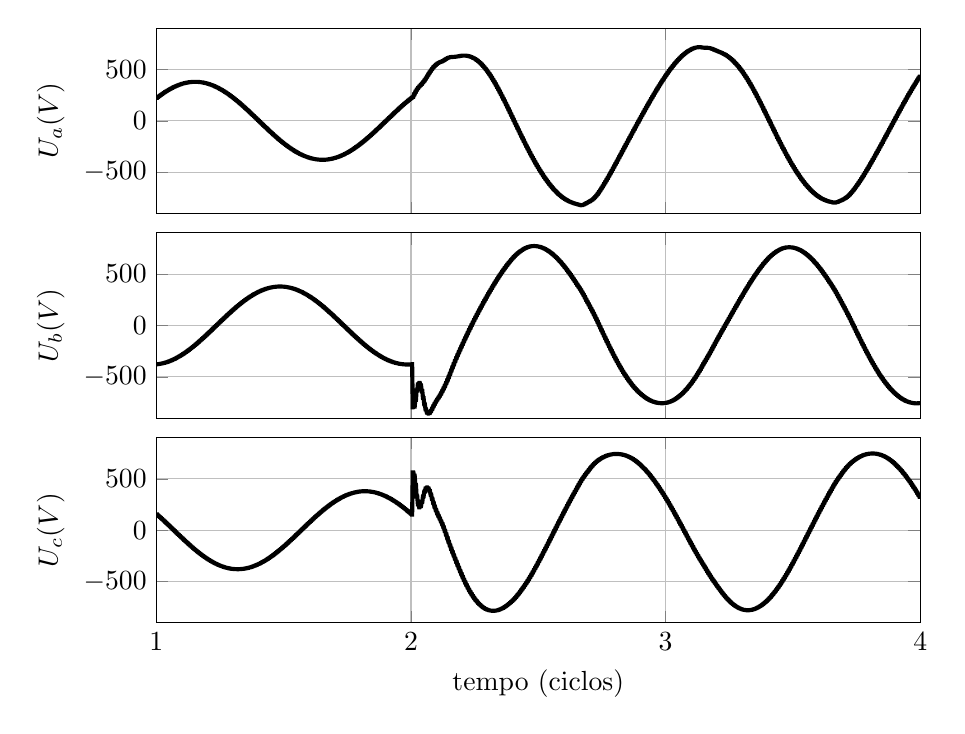
\begin{tikzpicture}

\begin{axis}[%
width=0.8\textwidth,
height=0.193917089240149\textwidth,
scale only axis,
xmin=0.316666666666667,
xmax=0.366666666666667,
xtick={0.316666666666667,0.333333333333333,0.35,0.366666666666667},
xticklabels={\empty},
xmajorgrids,
ymin=-900,
ymax=900,
ytick={-500,    0,  500},
ylabel={$\text{U}_\text{b}\text{ (V)}$},
ymajorgrids,
name=plot2,
scaled x ticks = false,
legend columns=-1,
legend style={/tikz/every even column/.append style={column sep=0.3cm}},
legend style={font=\footnotesize}
]
\addplot [color=black,solid,line width=1.5pt,forget plot]
  table[row sep=crcr]{0.316658333333333	-377.723085698266\\
0.3167	-376.586723778496\\
0.316741666666667	-376.586723778496\\
0.316783333333333	-375.078923942871\\
0.316825	-375.078923942871\\
0.316866666666667	-373.201183557557\\
0.316908333333333	-373.201183557557\\
0.31695	-370.955359679074\\
0.316991666666667	-370.955359679074\\
0.317033333333333	-368.343680965246\\
0.317075	-368.343680965246\\
0.317116666666667	-365.368751272189\\
0.317158333333333	-365.368751272189\\
0.3172	-362.033546182555\\
0.317241666666667	-362.033546182555\\
0.317283333333333	-358.341404810258\\
0.317325	-358.341404810258\\
0.317366666666667	-354.29601946274\\
0.317408333333333	-354.29601946274\\
0.31745	-349.901425336706\\
0.317491666666667	-349.901425336706\\
0.317533333333333	-345.161991678398\\
0.317575	-345.161991678398\\
0.317616666666667	-340.082415007475\\
0.317658333333333	-340.082415007475\\
0.3177	-334.667714301187\\
0.317741666666667	-334.667714301187\\
0.317783333333333	-328.923227572974\\
0.317825	-328.923227572974\\
0.317866666666667	-322.854609083496\\
0.317908333333333	-322.854609083496\\
0.31795	-316.467826451787\\
0.317991666666667	-316.467826451787\\
0.318033333333333	-309.769157112268\\
0.318075	-309.769157112268\\
0.318116666666667	-302.765183805345\\
0.318158333333333	-302.765183805345\\
0.3182	-295.462789021633\\
0.318241666666667	-295.462789021633\\
0.318283333333333	-287.869148495131\\
0.318325	-287.869148495131\\
0.318366666666667	-279.991723937524\\
0.318408333333333	-279.991723937524\\
0.31845	-271.838255227092\\
0.318491666666667	-271.838255227092\\
0.318533333333333	-263.416752229383\\
0.318575	-263.416752229383\\
0.318616666666667	-254.735486359231\\
0.318658333333333	-254.735486359231\\
0.3187	-245.802981925607\\
0.318741666666667	-245.802981925607\\
0.318783333333333	-236.6280072728\\
0.318825	-236.6280072728\\
0.318866666666667	-227.219565832749\\
0.318908333333333	-227.219565832749\\
0.31895	-217.586887717469\\
0.318991666666667	-217.586887717469\\
0.319033333333333	-207.739424484696\\
0.319075	-207.739424484696\\
0.319116666666667	-197.686870803904\\
0.319158333333333	-197.686870803904\\
0.3192	-187.439263486291\\
0.319241666666667	-187.439263486291\\
0.319283333333333	-177.007031372265\\
0.319325	-177.007031372265\\
0.319366666666667	-166.400723674948\\
0.319408333333333	-166.400723674948\\
0.31945	-155.6307199546\\
0.319491666666667	-155.6307199546\\
0.319533333333333	-144.707346263981\\
0.319575	-144.707346263981\\
0.319616666666667	-133.641094664328\\
0.319658333333333	-133.641094664328\\
0.3197	-122.442727673415\\
0.319741666666667	-122.442727673415\\
0.319783333333333	-111.123278734636\\
0.319825	-111.123278734636\\
0.319866666666667	-99.6940002360541\\
0.319908333333333	-99.6940002360541\\
0.31995	-88.1662967730299\\
0.319991666666667	-88.1662967730299\\
0.320033333333333	-76.5516646999388\\
0.320075	-76.5516646999388\\
0.320116666666667	-64.8616480040377\\
0.320158333333333	-64.8616480040377\\
0.3202	-53.1078129245748\\
0.320241666666667	-53.1078129245748\\
0.320283333333333	-41.3017386424485\\
0.320325	-41.3017386424485\\
0.320366666666667	-29.4550186053735\\
0.320408333333333	-29.4550186053735\\
0.32045	-17.5792663930844\\
0.320491666666667	-17.5792663930844\\
0.320533333333333	-5.68612092557823\\
0.320575	-5.68612092557823\\
0.320616666666667	6.2127524201114\\
0.320658333333333	6.2127524201114\\
0.3207	18.105666253858\\
0.320741666666667	18.105666253858\\
0.320783333333333	29.9809209740117\\
0.320825	29.9809209740117\\
0.320866666666667	41.8268186183045\\
0.320908333333333	41.8268186183045\\
0.32095	53.631678981668\\
0.320991666666667	53.631678981668\\
0.321033333333333	65.3838562807079\\
0.321075	65.3838562807079\\
0.321116666666667	77.0717550613194\\
0.321158333333333	77.0717550613194\\
0.3212	88.6838446142487\\
0.321241666666667	88.6838446142487\\
0.321283333333333	100.208671712027\\
0.321325	100.208671712027\\
0.321366666666667	111.6348719068\\
0.321408333333333	111.6348719068\\
0.32145	122.951179824381\\
0.321491666666667	122.951179824381\\
0.321533333333333	134.14643897231\\
0.321575	134.14643897231\\
0.321616666666667	145.209611528874\\
0.321658333333333	145.209611528874\\
0.3217	156.129788391287\\
0.321741666666667	156.129788391287\\
0.321783333333333	166.896199602751\\
0.321825	166.896199602751\\
0.321866666666667	177.498225133841\\
0.321908333333333	177.498225133841\\
0.32195	187.925405900222\\
0.321991666666667	187.925405900222\\
0.322033333333333	198.167454859908\\
0.322075	198.167454859908\\
0.322116666666667	208.214268041585\\
0.322158333333333	208.214268041585\\
0.3222	218.055935396159\\
0.322241666666667	218.055935396159\\
0.322283333333333	227.682751419264\\
0.322325	227.682751419264\\
0.322366666666667	237.085225549088\\
0.322408333333333	237.085225549088\\
0.32245	246.254092392214\\
0.322491666666667	246.254092392214\\
0.322533333333333	255.180321867299\\
0.322575	255.180321867299\\
0.322616666666667	263.855129383534\\
0.322658333333333	263.855129383534\\
0.3227	272.26998619054\\
0.322741666666667	272.26998619054\\
0.322783333333333	280.416630045836\\
0.322825	280.416630045836\\
0.322866666666667	288.287076317351\\
0.322908333333333	288.287076317351\\
0.32295	295.873629460527\\
0.322991666666667	295.873629460527\\
0.323033333333333	303.168894086837\\
0.323075	303.168894086837\\
0.323116666666667	310.165782141413\\
0.323158333333333	310.165782141413\\
0.3232	316.857502505702\\
0.323241666666667	316.857502505702\\
0.323283333333333	323.237410711189\\
0.323325	323.237410711189\\
0.323366666666667	329.298465304494\\
0.323408333333333	329.298465304494\\
0.32345	335.032940877286\\
0.323491666666667	335.032940877286\\
0.323533333333333	340.433778089715\\
0.323575	340.433778089715\\
0.323616666666667	345.496008515558\\
0.323658333333333	345.496008515558\\
0.3237	350.216089241188\\
0.323741666666667	350.216089241188\\
0.323783333333333	354.590714854285\\
0.323825	354.590714854285\\
0.323866666666667	358.616245271799\\
0.323908333333333	358.616245271799\\
0.32395	362.28867598875\\
0.323991666666667	362.28867598875\\
0.324033333333333	365.603866403093\\
0.324075	365.603866403093\\
0.324116666666667	368.557830105438\\
0.324158333333333	368.557830105438\\
0.3242	371.14698467744\\
0.324241666666667	371.14698467744\\
0.324283333333333	373.368315025462\\
0.324325	373.368315025462\\
0.324366666666667	375.219441072503\\
0.324408333333333	375.219441072503\\
0.32445	376.698604902272\\
0.324491666666667	376.698604902272\\
0.324533333333333	377.804605390594\\
0.324575	377.804605390594\\
0.324616666666667	378.536711049029\\
0.324658333333333	378.536711049029\\
0.3247	378.89457690205\\
0.324741666666667	378.89457690205\\
0.324783333333333	378.878182191864\\
0.324825	378.878182191864\\
0.324866666666667	378.487795835975\\
0.324908333333333	378.487795835975\\
0.32495	377.723968278227\\
0.324991666666667	377.723968278227\\
0.325033333333333	376.587542986259\\
0.325075	376.587542986259\\
0.325116666666667	375.079678623678\\
0.325158333333333	375.079678623678\\
0.3252	373.201873355773\\
0.325241666666667	373.201873355773\\
0.325283333333333	370.955984906448\\
0.325325	370.955984906448\\
0.325366666666667	368.34424285761\\
0.325408333333333	368.34424285761\\
0.32545	365.369252419982\\
0.325491666666667	365.369252419982\\
0.325533333333333	362.033990949537\\
0.325575	362.033990949537\\
0.325616666666667	358.341799615764\\
0.325658333333333	358.341799615764\\
0.3257	354.29637287251\\
0.325741666666667	354.29637287251\\
0.325783333333333	349.901747968484\\
0.325825	349.901747968484\\
0.325866666666667	345.162295969421\\
0.325908333333333	345.162295969421\\
0.32595	340.082714909794\\
0.325991666666667	340.082714909794\\
0.326033333333333	334.668024969912\\
0.326075	334.668024969912\\
0.326116666666667	328.923565098519\\
0.326158333333333	328.923565098519\\
0.3262	322.854990299289\\
0.326241666666667	322.854990299289\\
0.326283333333333	316.468268829063\\
0.326325	316.468268829063\\
0.326366666666667	309.769678739274\\
0.326408333333333	309.769678739274\\
0.32645	302.76580344002\\
0.326491666666667	302.76580344002\\
0.326533333333333	295.46352620612\\
0.326575	295.46352620612\\
0.326616666666667	287.870023724931\\
0.326658333333333	287.870023724931\\
0.3267	279.99275888678\\
0.326741666666667	279.99275888678\\
0.326783333333333	271.839473042268\\
0.326825	271.839473042268\\
0.326866666666667	263.418177915058\\
0.326908333333333	263.418177915058\\
0.32695	254.737147291355\\
0.326991666666667	254.737147291355\\
0.327033333333333	245.804908536742\\
0.327075	245.804908536742\\
0.327116666666667	236.630233953394\\
0.327158333333333	236.630233953394\\
0.3272	227.22213205341\\
0.327241666666667	227.22213205341\\
0.327283333333333	217.589839194205\\
0.327325	217.589839194205\\
0.327366666666667	207.742813476948\\
0.327408333333333	207.742813476948\\
0.32745	197.690748171958\\
0.327491666666667	197.690748171958\\
0.327533333333333	187.443640894198\\
0.327575	187.443640894198\\
0.327616666666667	177.011825362749\\
0.327658333333333	177.011825362749\\
0.3277	166.405770179614\\
0.327741666666667	166.405770179614\\
0.327783333333333	155.635868101642\\
0.327825	155.635868101642\\
0.327866666666667	144.712520179611\\
0.327908333333333	144.712520179611\\
0.32795	133.646292221512\\
0.327991666666667	133.646292221512\\
0.328033333333333	122.447986519211\\
0.328075	122.447986519211\\
0.328116666666667	111.128638130733\\
0.328158333333333	111.128638130733\\
0.3282	99.6994735093165\\
0.328241666666667	99.6994735093165\\
0.328283333333333	88.1718588306136\\
0.328325	88.1718588306136\\
0.328366666666667	76.5572531712875\\
0.328408333333333	76.5572531712875\\
0.32845	64.8671736797616\\
0.328491666666667	64.8671736797616\\
0.328533333333333	53.1131743732041\\
0.328575	53.1131743732041\\
0.328616666666667	41.3068365291399\\
0.328658333333333	41.3068365291399\\
0.3287	29.4597666782387\\
0.328741666666667	29.4597666782387\\
0.328783333333333	17.5835977645907\\
0.328825	17.5835977645907\\
0.328866666666667	5.68998972084417\\
0.328908333333333	5.68998972084417\\
0.32895	-6.20937299888088\\
0.328991666666667	-6.20937299888088\\
0.329033333333333	-18.1027879552077\\
0.329075	-18.1027879552077\\
0.329116666666667	-29.9785451472021\\
0.329158333333333	-29.9785451472021\\
0.3292	-41.8249403501677\\
0.329241666666667	-41.8249403501677\\
0.329283333333333	-53.6302900618585\\
0.329325	-53.6302900618585\\
0.329366666666667	-65.3829468063473\\
0.329408333333333	-65.3829468063473\\
0.32945	-77.0713138539921\\
0.329491666666667	-77.0713138539921\\
0.329533333333333	-88.6838588313381\\
0.329575	-88.6838588313381\\
0.329616666666667	-100.209126092659\\
0.329658333333333	-100.209126092659\\
0.3297	-111.635748034836\\
0.329741666666667	-111.635748034836\\
0.329783333333333	-122.952455666325\\
0.329825	-122.952455666325\\
0.329866666666667	-134.148088804689\\
0.329908333333333	-134.148088804689\\
0.32995	-145.211606244939\\
0.329991666666667	-145.211606244939\\
0.330033333333333	-156.132096092484\\
0.330075	-156.132096092484\\
0.330116666666667	-166.898786342177\\
0.330158333333333	-166.898786342177\\
0.3302	-177.501055680916\\
0.330241666666667	-177.501055680916\\
0.330283333333333	-187.928444425067\\
0.330325	-187.928444425067\\
0.330366666666667	-198.170665477564\\
0.330408333333333	-198.170665477564\\
0.33045	-208.21761519744\\
0.330491666666667	-208.21761519744\\
0.330533333333333	-218.059384105748\\
0.330575	-218.059384105748\\
0.330616666666667	-227.686267394042\\
0.330658333333333	-227.686267394042\\
0.3307	-237.088775244765\\
0.330741666666667	-237.088775244765\\
0.330783333333333	-246.257643010826\\
0.330825	-246.257643010826\\
0.330866666666667	-255.183841332313\\
0.330908333333333	-255.183841332313\\
0.33095	-263.858586293167\\
0.330991666666667	-263.858586293167\\
0.331033333333333	-272.273349741191\\
0.331075	-272.273349741191\\
0.331116666666667	-280.419869907006\\
0.331158333333333	-280.419869907006\\
0.3312	-288.29016243285\\
0.331241666666667	-288.29016243285\\
0.331283333333333	-295.876531750755\\
0.331325	-295.876531750755\\
0.331366666666667	-303.171582042784\\
0.331408333333333	-303.171582042784\\
0.33145	-310.168224372754\\
0.331491666666667	-310.168224372754\\
0.331533333333333	-316.859666586207\\
0.331575	-316.859666586207\\
0.331616666666667	-323.239266132863\\
0.331658333333333	-323.239266132863\\
0.3317	-329.299997905177\\
0.331741666666667	-329.299997905177\\
0.331783333333333	-335.034174516609\\
0.331825	-335.034174516609\\
0.331866666666667	-340.434769270671\\
0.331908333333333	-340.434769270671\\
0.33195	-345.496809702631\\
0.331991666666667	-345.496809702631\\
0.332033333333333	-350.216724523872\\
0.332075	-350.216724523872\\
0.332116666666667	-354.591180653519\\
0.332158333333333	-354.591180653519\\
0.3322	-358.616523838194\\
0.332241666666667	-358.616523838194\\
0.332283333333333	-362.288750228316\\
0.332325	-362.288750228316\\
0.332366666666667	-365.603730340961\\
0.332408333333333	-365.603730340961\\
0.33245	-368.557493442448\\
0.332491666666667	-368.557493442448\\
0.332533333333333	-371.146472117679\\
0.332575	-371.146472117679\\
0.332616666666667	-373.367662092301\\
0.332658333333333	-373.367662092301\\
0.3327	-375.218688387832\\
0.332741666666667	-375.218688387832\\
0.332783333333333	-376.697792634348\\
0.332825	-376.697792634348\\
0.332866666666667	-377.803769014554\\
0.332908333333333	-377.803769014554\\
0.33295	-378.535878926511\\
0.332991666666667	-378.535878926511\\
0.333033333333333	-378.893769636932\\
0.333075	-378.893769636932\\
0.333116666666667	-378.877413350589\\
0.333158333333333	-378.877413350589\\
0.3332	-378.487073457233\\
0.333241666666667	-378.487073457233\\
0.333283333333333	-377.723296609494\\
0.333325	-377.723296609494\\
0.333366666666667	-376.586924015447\\
0.333408333333333	-376.586924015447\\
0.33345	-795.319285373411\\
0.333491666666667	-795.319285373411\\
0.333533333333333	-788.14060563279\\
0.333575	-788.14060563279\\
0.333616666666667	-721.556411357491\\
0.333658333333333	-721.556411357491\\
0.3337	-630.826918040249\\
0.333741666666667	-630.826918040249\\
0.333783333333333	-572.636550269644\\
0.333825	-572.636550269644\\
0.333866666666667	-557.335347966548\\
0.333908333333333	-557.335347966548\\
0.33395	-583.125421226909\\
0.333991666666667	-583.125421226909\\
0.334033333333333	-637.208109851594\\
0.334075	-637.208109851594\\
0.334116666666667	-703.340569800332\\
0.334158333333333	-703.340569800332\\
0.3342	-766.390236707941\\
0.334241666666667	-766.390236707941\\
0.334283333333333	-815.553287482962\\
0.334325	-815.553287482962\\
0.334366666666667	-845.485312455461\\
0.334408333333333	-845.485312455461\\
0.33445	-855.864675043939\\
0.334491666666667	-855.864675043939\\
0.334533333333333	-849.961469592225\\
0.334575	-849.961469592225\\
0.334616666666667	-832.855522513499\\
0.334658333333333	-832.855522513499\\
0.3347	-809.807963355356\\
0.334741666666667	-809.807963355356\\
0.334783333333333	-785.097865760623\\
0.334825	-785.097865760623\\
0.334866666666667	-761.43330498125\\
0.334908333333333	-761.43330498125\\
0.33495	-739.885368137779\\
0.334991666666667	-739.885368137779\\
0.335033333333333	-720.195274746514\\
0.335075	-720.195274746514\\
0.335116666666667	-701.271922451106\\
0.335158333333333	-701.271922451106\\
0.3352	-681.729557627861\\
0.335241666666667	-681.729557627861\\
0.335283333333333	-660.484617333561\\
0.335325	-660.484617333561\\
0.335366666666667	-637.389467577014\\
0.335408333333333	-637.389467577014\\
0.33545	-613.006727585568\\
0.335491666666667	-613.006727585568\\
0.335533333333333	-587.412625418605\\
0.335575	-587.412625418605\\
0.335616666666667	-560.281766790114\\
0.335658333333333	-560.281766790114\\
0.3357	-531.490682038154\\
0.335741666666667	-531.490682038154\\
0.335783333333333	-501.276801098355\\
0.335825	-501.276801098355\\
0.335866666666667	-470.132260889292\\
0.335908333333333	-470.132260889292\\
0.33595	-438.63125653145\\
0.335991666666667	-438.63125653145\\
0.336033333333333	-407.287340842783\\
0.336075	-407.287340842783\\
0.336116666666667	-376.468332365084\\
0.336158333333333	-376.468332365084\\
0.3362	-346.369170152765\\
0.336241666666667	-346.369170152765\\
0.336283333333333	-317.02993885443\\
0.336325	-317.02993885443\\
0.336366666666667	-288.380830399342\\
0.336408333333333	-288.380830399342\\
0.33645	-260.295787164198\\
0.336491666666667	-260.295787164198\\
0.336533333333333	-232.640448813137\\
0.336575	-232.640448813137\\
0.336616666666667	-205.305800839397\\
0.336658333333333	-205.305800839397\\
0.3367	-178.224760958767\\
0.336741666666667	-178.224760958767\\
0.336783333333333	-151.373545784467\\
0.336825	-151.373545784467\\
0.336866666666667	-124.762415961483\\
0.336908333333333	-124.762415961483\\
0.33695	-98.4212822449709\\
0.336991666666667	-98.4212822449709\\
0.337033333333333	-72.3850615320252\\
0.337075	-72.3850615320252\\
0.337116666666667	-46.6821931147297\\
0.337158333333333	-46.6821931147297\\
0.3372	-21.3279616272306\\
0.337241666666667	-21.3279616272306\\
0.337283333333333	3.6773009621432\\
0.337325	3.6773009621432\\
0.337366666666667	28.3461614737093\\
0.337408333333333	28.3461614737093\\
0.33745	52.6997395279916\\
0.337491666666667	52.6997395279916\\
0.337533333333333	76.7626552596796\\
0.337575	76.7626552596796\\
0.337616666666667	100.558528125987\\
0.337658333333333	100.558528125987\\
0.3377	124.106783374856\\
0.337741666666667	124.106783374856\\
0.337783333333333	147.421012436441\\
0.337825	147.421012436441\\
0.337866666666667	170.508727946409\\
0.337908333333333	170.508727946409\\
0.33795	193.372109083092\\
0.337991666666667	193.372109083092\\
0.338033333333333	216.009251794539\\
0.338075	216.009251794539\\
0.338116666666667	238.415486524389\\
0.338158333333333	238.415486524389\\
0.3382	260.584461168598\\
0.338241666666667	260.584461168598\\
0.338283333333333	282.508830029023\\
0.338325	282.508830029023\\
0.338366666666667	304.180537726022\\
0.338408333333333	304.180537726022\\
0.33845	325.590783109461\\
0.338491666666667	325.590783109461\\
0.338533333333333	346.729796855872\\
0.338575	346.729796855872\\
0.338616666666667	367.58657000197\\
0.338658333333333	367.58657000197\\
0.3387	388.148642917909\\
0.338741666666667	388.148642917909\\
0.338783333333333	408.402020930006\\
0.338825	408.402020930006\\
0.338866666666667	428.331238451637\\
0.338908333333333	428.331238451637\\
0.33895	447.919558330894\\
0.338991666666667	447.919558330894\\
0.339033333333333	467.149272378343\\
0.339075	467.149272378343\\
0.339116666666667	486.002063348749\\
0.339158333333333	486.002063348749\\
0.3392	504.459395522677\\
0.339241666666667	504.459395522677\\
0.339283333333333	522.502916567204\\
0.339325	522.502916567204\\
0.339366666666667	540.11487389746\\
0.339408333333333	540.11487389746\\
0.33945	557.278572220649\\
0.339491666666667	557.278572220649\\
0.339533333333333	573.978925565534\\
0.339575	573.978925565534\\
0.339616666666667	590.203189021681\\
0.339658333333333	590.203189021681\\
0.3397	605.94199105185\\
0.339741666666667	605.94199105185\\
0.339783333333333	621.190789089979\\
0.339825	621.190789089979\\
0.339866666666667	635.951586840995\\
0.339908333333333	635.951586840995\\
0.33995	650.232133507819\\
0.339991666666667	650.232133507819\\
0.340033333333333	664.007367484875\\
0.340075	664.007367484875\\
0.340116666666667	677.085190419171\\
0.340158333333333	677.085190419171\\
0.3402	689.111491039332\\
0.340241666666667	689.111491039332\\
0.340283333333333	700.015068163468\\
0.340325	700.015068163468\\
0.340366666666667	710.017697783998\\
0.340408333333333	710.017697783998\\
0.34045	719.341020270529\\
0.340491666666667	719.341020270529\\
0.340533333333333	728.093086515737\\
0.340575	728.093086515737\\
0.340616666666667	736.270601463891\\
0.340658333333333	736.270601463891\\
0.3407	743.798843326646\\
0.340741666666667	743.798843326646\\
0.340783333333333	750.573958801486\\
0.340825	750.573958801486\\
0.340866666666667	756.497119112187\\
0.340908333333333	756.497119112187\\
0.34095	761.496531120401\\
0.340991666666667	761.496531120401\\
0.341033333333333	765.536717191478\\
0.341075	765.536717191478\\
0.341116666666667	768.61710104901\\
0.341158333333333	768.61710104901\\
0.3412	770.763567094797\\
0.341241666666667	770.763567094797\\
0.341283333333333	772.017031688165\\
0.341325	772.017031688165\\
0.341366666666667	772.422440778513\\
0.341408333333333	772.422440778513\\
0.34145	772.020435571405\\
0.341491666666667	772.020435571405\\
0.341533333333333	770.842639205626\\
0.341575	770.842639205626\\
0.341616666666667	768.910430024982\\
0.341658333333333	768.910430024982\\
0.3417	766.236353109756\\
0.341741666666667	766.236353109756\\
0.341783333333333	762.827017997135\\
0.341825	762.827017997135\\
0.341866666666667	758.686373286115\\
0.341908333333333	758.686373286115\\
0.34195	753.818519393674\\
0.341991666666667	753.818519393674\\
0.342033333333333	748.229588418\\
0.342075	748.229588418\\
0.342116666666667	741.92857429738\\
0.342158333333333	741.92857429738\\
0.3422	734.927264922233\\
0.342241666666667	734.927264922233\\
0.342283333333333	727.239576767842\\
0.342325	727.239576767842\\
0.342366666666667	718.880631842589\\
0.342408333333333	718.880631842589\\
0.34245	709.865868004543\\
0.342491666666667	709.865868004543\\
0.342533333333333	700.210376877036\\
0.342575	700.210376877036\\
0.342616666666667	689.928555068876\\
0.342658333333333	689.928555068876\\
0.3427	679.03406124301\\
0.342741666666667	679.03406124301\\
0.342783333333333	667.540009360431\\
0.342825	667.540009360431\\
0.342866666666667	655.459301085953\\
0.342908333333333	655.459301085953\\
0.34295	642.805003068547\\
0.342991666666667	642.805003068547\\
0.343033333333333	629.590697832743\\
0.343075	629.590697832743\\
0.343116666666667	615.830769334964\\
0.343158333333333	615.830769334964\\
0.3432	601.540616440056\\
0.343241666666667	601.540616440056\\
0.343283333333333	586.736813475905\\
0.343325	586.736813475905\\
0.343366666666667	571.437254156149\\
0.343408333333333	571.437254156149\\
0.34345	555.661324379439\\
0.343491666666667	555.661324379439\\
0.343533333333333	539.430154113093\\
0.343575	539.430154113093\\
0.343616666666667	522.767003881253\\
0.343658333333333	522.767003881253\\
0.3437	505.697853797617\\
0.343741666666667	505.697853797617\\
0.343783333333333	488.25229074238\\
0.343825	488.25229074238\\
0.343866666666667	470.464842760616\\
0.343908333333333	470.464842760616\\
0.34395	452.377001104265\\
0.343991666666667	452.377001104265\\
0.344033333333333	434.040296780298\\
0.344075	434.040296780298\\
0.344116666666667	415.520835481604\\
0.344158333333333	415.520835481604\\
0.3442	396.904758745224\\
0.344241666666667	396.904758745224\\
0.344283333333333	378.291812911797\\
0.344325	378.291812911797\\
0.344366666666667	359.655792727338\\
0.344408333333333	359.655792727338\\
0.34445	340.422023191774\\
0.344491666666667	340.422023191774\\
0.344533333333333	319.657712731365\\
0.344575	319.657712731365\\
0.344616666666667	297.378147362369\\
0.344658333333333	297.378147362369\\
0.3447	274.301258080979\\
0.344741666666667	274.301258080979\\
0.344783333333333	251.074720556747\\
0.344825	251.074720556747\\
0.344866666666667	228.023948789375\\
0.344908333333333	228.023948789375\\
0.34495	205.172287022679\\
0.344991666666667	205.172287022679\\
0.345033333333333	182.35061906081\\
0.345075	182.35061906081\\
0.345116666666667	159.313224538862\\
0.345158333333333	159.313224538862\\
0.3452	135.831417089722\\
0.345241666666667	135.831417089722\\
0.345283333333333	111.752886192643\\
0.345325	111.752886192643\\
0.345366666666667	87.0253162354534\\
0.345408333333333	87.0253162354534\\
0.34545	61.6905232518876\\
0.345491666666667	61.6905232518876\\
0.345533333333333	35.8596976250506\\
0.345575	35.8596976250506\\
0.345616666666667	9.68108780557241\\
0.345658333333333	9.68108780557241\\
0.3457	-16.6904888186282\\
0.345741666666667	-16.6904888186282\\
0.345783333333333	-43.1162989652842\\
0.345825	-43.1162989652842\\
0.345866666666667	-69.4861131298021\\
0.345908333333333	-69.4861131298021\\
0.34595	-95.7209799887516\\
0.345991666666667	-95.7209799887516\\
0.346033333333333	-121.768852513461\\
0.346075	-121.768852513461\\
0.346116666666667	-147.596321799523\\
0.346158333333333	-147.596321799523\\
0.3462	-173.179523344027\\
0.346241666666667	-173.179523344027\\
0.346283333333333	-198.496481742243\\
0.346325	-198.496481742243\\
0.346366666666667	-223.522119807973\\
0.346408333333333	-223.522119807973\\
0.34645	-248.226180299097\\
0.346491666666667	-248.226180299097\\
0.346533333333333	-272.573585923399\\
0.346575	-272.573585923399\\
0.346616666666667	-296.526372674107\\
0.346658333333333	-296.526372674107\\
0.3467	-320.046254280766\\
0.346741666666667	-320.046254280766\\
0.346783333333333	-343.097028771623\\
0.346825	-343.097028771623\\
0.346866666666667	-365.646316131262\\
0.346908333333333	-365.646316131262\\
0.34695	-387.666418766575\\
0.346991666666667	-387.666418766575\\
0.347033333333333	-409.134350113965\\
0.347075	-409.134350113965\\
0.347116666666667	-430.031241248773\\
0.347158333333333	-430.031241248773\\
0.3472	-450.341402724933\\
0.347241666666667	-450.341402724933\\
0.347283333333333	-470.051304597885\\
0.347325	-470.051304597885\\
0.347366666666667	-489.148669924455\\
0.347408333333333	-489.148669924455\\
0.34745	-507.621786749685\\
0.347491666666667	-507.621786749685\\
0.347533333333333	-525.459056317453\\
0.347575	-525.459056317453\\
0.347616666666667	-542.648727271755\\
0.347658333333333	-542.648727271755\\
0.3477	-559.178722878493\\
0.347741666666667	-559.178722878493\\
0.347783333333333	-575.036447744745\\
0.347825	-575.036447744745\\
0.347866666666667	-590.208453265967\\
0.347908333333333	-590.208453265967\\
0.34795	-604.679838782769\\
0.347991666666667	-604.679838782769\\
0.348033333333333	-618.433282618557\\
0.348075	-618.433282618557\\
0.348116666666667	-631.447781686952\\
0.348158333333333	-631.447781686952\\
0.3482	-643.698452745424\\
0.348241666666667	-643.698452745424\\
0.348283333333333	-655.179123946499\\
0.348325	-655.179123946499\\
0.348366666666667	-665.992631813344\\
0.348408333333333	-665.992631813344\\
0.34845	-676.3771477109\\
0.348491666666667	-676.3771477109\\
0.348533333333333	-686.404173529961\\
0.348575	-686.404173529961\\
0.348616666666667	-695.915904217976\\
0.348658333333333	-695.915904217976\\
0.3487	-704.734073067233\\
0.348741666666667	-704.734073067233\\
0.348783333333333	-712.756755533519\\
0.348825	-712.756755533519\\
0.348866666666667	-719.964742627031\\
0.348908333333333	-719.964742627031\\
0.34895	-726.395342985307\\
0.348991666666667	-726.395342985307\\
0.349033333333333	-732.112035422199\\
0.349075	-732.112035422199\\
0.349116666666667	-737.178986862981\\
0.349158333333333	-737.178986862981\\
0.3492	-741.643895044148\\
0.349241666666667	-741.643895044148\\
0.349283333333333	-745.529978909656\\
0.349325	-745.529978909656\\
0.349366666666667	-748.835940614381\\
0.349408333333333	-748.835940614381\\
0.34945	-751.541408664862\\
0.349491666666667	-751.541408664862\\
0.349533333333333	-753.614965295891\\
0.349575	-753.614965295891\\
0.349616666666667	-755.022211040062\\
0.349658333333333	-755.022211040062\\
0.3497	-755.732115495196\\
0.349741666666667	-755.732115495196\\
0.349783333333333	-755.720828542678\\
0.349825	-755.720828542678\\
0.349866666666667	-754.972938145559\\
0.349908333333333	-754.972938145559\\
0.34995	-753.480718977468\\
0.349991666666667	-753.480718977468\\
0.350033333333333	-751.242179582329\\
0.350075	-751.242179582329\\
0.350116666666667	-748.258720350156\\
0.350158333333333	-748.258720350156\\
0.3502	-744.533040971602\\
0.350241666666667	-744.533040971602\\
0.350283333333333	-740.067678123993\\
0.350325	-740.067678123993\\
0.350366666666667	-734.864294586797\\
0.350408333333333	-734.864294586797\\
0.35045	-728.923636758489\\
0.350491666666667	-728.923636758489\\
0.350533333333333	-722.245955456878\\
0.350575	-722.245955456878\\
0.350616666666667	-714.83164588119\\
0.350658333333333	-714.83164588119\\
0.3507	-706.681891044221\\
0.350741666666667	-706.681891044221\\
0.350783333333333	-697.799154538192\\
0.350825	-697.799154538192\\
0.350866666666667	-688.187448764468\\
0.350908333333333	-688.187448764468\\
0.35095	-677.852373498059\\
0.350991666666667	-677.852373498059\\
0.351033333333333	-666.800967995287\\
0.351075	-666.800967995287\\
0.351116666666667	-655.041442812436\\
0.351158333333333	-655.041442812436\\
0.3512	-642.582857832767\\
0.351241666666667	-642.582857832767\\
0.351283333333333	-629.434797120648\\
0.351325	-629.434797120648\\
0.351366666666667	-615.607066835831\\
0.351408333333333	-615.607066835831\\
0.35145	-601.109416214292\\
0.351491666666667	-601.109416214292\\
0.351533333333333	-585.951257793114\\
0.351575	-585.951257793114\\
0.351616666666667	-570.14134280094\\
0.351658333333333	-570.14134280094\\
0.3517	-553.687329003068\\
0.351741666666667	-553.687329003068\\
0.351783333333333	-536.595156471667\\
0.351825	-536.595156471667\\
0.351866666666667	-518.86811486261\\
0.351908333333333	-518.86811486261\\
0.35195	-500.505438563742\\
0.351991666666667	-500.505438563742\\
0.352033333333333	-481.500219512137\\
0.352075	-481.500219512137\\
0.352116666666667	-461.83652067915\\
0.352158333333333	-461.83652067915\\
0.3522	-441.48661467045\\
0.352241666666667	-441.48661467045\\
0.352283333333333	-420.420650200896\\
0.352325	-420.420650200896\\
0.352366666666667	-398.721134486373\\
0.352408333333333	-398.721134486373\\
0.35245	-376.863167805228\\
0.352491666666667	-376.863167805228\\
0.352533333333333	-355.505003105913\\
0.352575	-355.505003105913\\
0.352616666666667	-334.643920086562\\
0.352658333333333	-334.643920086562\\
0.3527	-313.807194859558\\
0.352741666666667	-313.807194859558\\
0.352783333333333	-292.571487966329\\
0.352825	-292.571487966329\\
0.352866666666667	-270.744598076744\\
0.352908333333333	-270.744598076744\\
0.35295	-248.353259638539\\
0.352991666666667	-248.353259638539\\
0.353033333333333	-225.564239825641\\
0.353075	-225.564239825641\\
0.353116666666667	-202.599339569268\\
0.353158333333333	-202.599339569268\\
0.3532	-179.666607706079\\
0.353241666666667	-179.666607706079\\
0.353283333333333	-156.916960966641\\
0.353325	-156.916960966641\\
0.353366666666667	-134.427233593344\\
0.353408333333333	-134.427233593344\\
0.35345	-112.204948238026\\
0.353491666666667	-112.204948238026\\
0.353533333333333	-90.206922940747\\
0.353575	-90.206922940747\\
0.353616666666667	-68.3633111120198\\
0.353658333333333	-68.3633111120198\\
0.3537	-46.6001395088716\\
0.353741666666667	-46.6001395088716\\
0.353783333333333	-24.8559260164892\\
0.353825	-24.8559260164892\\
0.353866666666667	-3.09064297825734\\
0.353908333333333	-3.09064297825734\\
0.35395	18.7124943642735\\
0.353991666666667	18.7124943642735\\
0.354033333333333	40.5505244602973\\
0.354075	40.5505244602973\\
0.354116666666667	62.4070779602103\\
0.354158333333333	62.4070779602103\\
0.3542	84.2592691659376\\
0.354241666666667	84.2592691659376\\
0.354283333333333	106.083456420565\\
0.354325	106.083456420565\\
0.354366666666667	127.858969307869\\
0.354408333333333	127.858969307869\\
0.35445	149.569633012879\\
0.354491666666667	149.569633012879\\
0.354533333333333	171.203458982932\\
0.354575	171.203458982932\\
0.354616666666667	192.751159460621\\
0.354658333333333	192.751159460621\\
0.3547	214.204197401773\\
0.354741666666667	214.204197401773\\
0.354783333333333	235.552964225935\\
0.354825	235.552964225935\\
0.354866666666667	256.785466753519\\
0.354908333333333	256.785466753519\\
0.35495	277.886676388303\\
0.354991666666667	277.886676388303\\
0.355033333333333	298.838502801071\\
0.355075	298.838502801071\\
0.355116666666667	319.620231569108\\
0.355158333333333	319.620231569108\\
0.3552	340.209215640733\\
0.355241666666667	340.209215640733\\
0.355283333333333	360.58162208473\\
0.355325	360.58162208473\\
0.355366666666667	380.713086696292\\
0.355408333333333	380.713086696292\\
0.35545	400.579196232054\\
0.355491666666667	400.579196232054\\
0.355533333333333	420.155781783822\\
0.355575	420.155781783822\\
0.355616666666667	439.419054468466\\
0.355658333333333	439.419054468466\\
0.3557	458.345641152448\\
0.355741666666667	458.345641152448\\
0.355783333333333	476.912584623525\\
0.355825	476.912584623525\\
0.355866666666667	495.097364915072\\
0.355908333333333	495.097364915072\\
0.35595	512.877983663476\\
0.355991666666667	512.877983663476\\
0.356033333333333	530.233138669836\\
0.356075	530.233138669836\\
0.356116666666667	547.14250730809\\
0.356158333333333	547.14250730809\\
0.3562	563.587159572825\\
0.356241666666667	563.587159572825\\
0.356283333333333	579.550136802663\\
0.356325	579.550136802663\\
0.356366666666667	595.017255908748\\
0.356408333333333	595.017255908748\\
0.35645	609.978188873776\\
0.356491666666667	609.978188873776\\
0.356533333333333	624.427562732489\\
0.356575	624.427562732489\\
0.356616666666667	638.361680886506\\
0.356658333333333	638.361680886506\\
0.3567	651.740462365889\\
0.356741666666667	651.740462365889\\
0.356783333333333	664.397912488718\\
0.356825	664.397912488718\\
0.356866666666667	676.127848752726\\
0.356908333333333	676.127848752726\\
0.35695	686.943643356986\\
0.356991666666667	686.943643356986\\
0.357033333333333	696.9880891922\\
0.357075	696.9880891922\\
0.357116666666667	706.376872009254\\
0.357158333333333	706.376872009254\\
0.3572	715.153071896152\\
0.357241666666667	715.153071896152\\
0.357283333333333	723.297187997945\\
0.357325	723.297187997945\\
0.357366666666667	730.752722030917\\
0.357408333333333	730.752722030917\\
0.35745	737.451161704679\\
0.357491666666667	737.451161704679\\
0.357533333333333	743.331294310745\\
0.357575	743.331294310745\\
0.357616666666667	748.350871821511\\
0.357658333333333	748.350871821511\\
0.3577	752.490643771259\\
0.357741666666667	752.490643771259\\
0.357783333333333	755.752290619645\\
0.357825	755.752290619645\\
0.357866666666667	758.152618507991\\
0.357908333333333	758.152618507991\\
0.35795	759.716446201488\\
0.357991666666667	759.716446201488\\
0.358033333333333	760.470132337194\\
0.358075	760.470132337194\\
0.358116666666667	760.436935934334\\
0.358158333333333	760.436935934334\\
0.3582	759.634627808145\\
0.358241666666667	759.634627808145\\
0.358283333333333	758.07515000636\\
0.358325	758.07515000636\\
0.358366666666667	755.765740291463\\
0.358408333333333	755.765740291463\\
0.35845	752.710805489389\\
0.358491666666667	752.710805489389\\
0.358533333333333	748.913892163345\\
0.358575	748.913892163345\\
0.358616666666667	744.379289065671\\
0.358658333333333	744.379289065671\\
0.3587	739.11302445944\\
0.358741666666667	739.11302445944\\
0.358783333333333	733.123229521697\\
0.358825	733.123229521697\\
0.358866666666667	726.419988097876\\
0.358908333333333	726.419988097876\\
0.35895	719.014868066488\\
0.358991666666667	719.014868066488\\
0.359033333333333	710.920339441709\\
0.359075	710.920339441709\\
0.359116666666667	702.149246231093\\
0.359158333333333	702.149246231093\\
0.3592	692.714436062095\\
0.359241666666667	692.714436062095\\
0.359283333333333	682.628586047066\\
0.359325	682.628586047066\\
0.359366666666667	671.904209994333\\
0.359408333333333	671.904209994333\\
0.35945	660.553798830459\\
0.359491666666667	660.553798830459\\
0.359533333333333	648.590033983817\\
0.359575	648.590033983817\\
0.359616666666667	636.026018658352\\
0.359658333333333	636.026018658352\\
0.3597	622.875488076329\\
0.359741666666667	622.875488076329\\
0.359783333333333	609.152980266043\\
0.359825	609.152980266043\\
0.359866666666667	594.873968483498\\
0.359908333333333	594.873968483498\\
0.35995	580.054971689338\\
0.359991666666667	580.054971689338\\
0.360033333333333	564.713669770809\\
0.360075	564.713669770809\\
0.360116666666667	548.869056567861\\
0.360158333333333	548.869056567861\\
0.3602	532.541668998066\\
0.360241666666667	532.541668998066\\
0.360283333333333	515.753938717389\\
0.360325	515.753938717389\\
0.360366666666667	498.53072910593\\
0.360408333333333	498.53072910593\\
0.36045	480.900151720384\\
0.360491666666667	480.900151720384\\
0.360533333333333	462.894809943195\\
0.360575	462.894809943195\\
0.360616666666667	444.553689904545\\
0.360658333333333	444.553689904545\\
0.3607	425.924926184215\\
0.360741666666667	425.924926184215\\
0.360783333333333	407.069042875218\\
0.360825	407.069042875218\\
0.360866666666667	388.054418144103\\
0.360908333333333	388.054418144103\\
0.36095	368.869086596482\\
0.360991666666667	368.869086596482\\
0.361033333333333	349.16124315581\\
0.361075	349.16124315581\\
0.361116666666667	328.36253416648\\
0.361158333333333	328.36253416648\\
0.3612	306.488667170342\\
0.361241666666667	306.488667170342\\
0.361283333333333	283.99409020821\\
0.361325	283.99409020821\\
0.361366666666667	261.291726793372\\
0.361408333333333	261.291726793372\\
0.36145	238.59302808163\\
0.361491666666667	238.59302808163\\
0.361533333333333	215.92038864774\\
0.361575	215.92038864774\\
0.361616666666667	193.175887014619\\
0.361658333333333	193.175887014619\\
0.3617	170.213836727492\\
0.361741666666667	170.213836727492\\
0.361783333333333	146.899349679675\\
0.361825	146.899349679675\\
0.361866666666667	123.145450740925\\
0.361908333333333	123.145450740925\\
0.36195	98.9278551525557\\
0.361991666666667	98.9278551525557\\
0.362033333333333	74.2812962473677\\
0.362075	74.2812962473677\\
0.362116666666667	49.2840183830404\\
0.362158333333333	49.2840183830404\\
0.3622	24.0375283125372\\
0.362241666666667	24.0375283125372\\
0.362283333333333	-1.35251510636111\\
0.362325	-1.35251510636111\\
0.362366666666667	-26.7905046068023\\
0.362408333333333	-26.7905046068023\\
0.36245	-52.1986751080782\\
0.362491666666667	-52.1986751080782\\
0.362533333333333	-77.5188464326572\\
0.362575	-77.5188464326572\\
0.362616666666667	-102.709681771327\\
0.362658333333333	-102.709681771327\\
0.3627	-127.741503451007\\
0.362741666666667	-127.741503451007\\
0.362783333333333	-152.59058921653\\
0.362825	-152.59058921653\\
0.362866666666667	-177.234372111512\\
0.362908333333333	-177.234372111512\\
0.36295	-201.648314836121\\
0.362991666666667	-201.648314836121\\
0.363033333333333	-225.804615321887\\
0.363075	-225.804615321887\\
0.363116666666667	-249.672446284594\\
0.363158333333333	-249.672446284594\\
0.3632	-273.219185919987\\
0.363241666666667	-273.219185919987\\
0.363283333333333	-296.412047384261\\
0.363325	-296.412047384261\\
0.363366666666667	-319.219610814883\\
0.363408333333333	-319.219610814883\\
0.36345	-341.612936093408\\
0.363491666666667	-341.612936093408\\
0.363533333333333	-363.566124821205\\
0.363575	-363.566124821205\\
0.363616666666667	-385.056359539077\\
0.363658333333333	-385.056359539077\\
0.3637	-406.063551898602\\
0.363741666666667	-406.063551898602\\
0.363783333333333	-426.569774155312\\
0.363825	-426.569774155312\\
0.363866666666667	-446.55863972952\\
0.363908333333333	-446.55863972952\\
0.36395	-466.014756449757\\
0.363991666666667	-466.014756449757\\
0.364033333333333	-484.923319856422\\
0.364075	-484.923319856422\\
0.364116666666667	-503.269859845071\\
0.364158333333333	-503.269859845071\\
0.3642	-521.040112426998\\
0.364241666666667	-521.040112426998\\
0.364283333333333	-538.219963547922\\
0.364325	-538.219963547922\\
0.364366666666667	-554.795402285917\\
0.364408333333333	-554.795402285917\\
0.36445	-570.752421078511\\
0.364491666666667	-570.752421078511\\
0.364533333333333	-586.076803870155\\
0.364575	-586.076803870155\\
0.364616666666667	-600.753743606887\\
0.364658333333333	-600.753743606887\\
0.3647	-614.767234700316\\
0.364741666666667	-614.767234700316\\
0.364783333333333	-628.099265873302\\
0.364825	-628.099265873302\\
0.364866666666667	-640.729441518139\\
0.364908333333333	-640.729441518139\\
0.36495	-652.645257125994\\
0.364991666666667	-652.645257125994\\
0.365033333333333	-663.8917934966\\
0.365075	-663.8917934966\\
0.365116666666667	-674.607527598295\\
0.365158333333333	-674.607527598295\\
0.3652	-684.856397354244\\
0.365241666666667	-684.856397354244\\
0.365283333333333	-694.548348681285\\
0.365325	-694.548348681285\\
0.365366666666667	-703.565782781666\\
0.365408333333333	-703.565782781666\\
0.36545	-711.834652003564\\
0.365491666666667	-711.834652003564\\
0.365533333333333	-719.333510520787\\
0.365575	-719.333510520787\\
0.365616666666667	-726.078658495045\\
0.365658333333333	-726.078658495045\\
0.3657	-732.105290768946\\
0.365741666666667	-732.105290768946\\
0.365783333333333	-737.451187122423\\
0.365825	-737.451187122423\\
0.365866666666667	-742.145355362396\\
0.365908333333333	-742.145355362396\\
0.36595	-746.202330635112\\
0.365991666666667	-746.202330635112\\
0.366033333333333	-749.621555126181\\
0.366075	-749.621555126181\\
0.366116666666667	-752.390379750331\\
0.366158333333333	-752.390379750331\\
0.3662	-754.488902849022\\
0.366241666666667	-754.488902849022\\
0.366283333333333	-755.895023002837\\
0.366325	-755.895023002837\\
0.366366666666667	-756.588548762603\\
0.366408333333333	-756.588548762603\\
0.36645	-756.553778423757\\
0.366491666666667	-756.553778423757\\
0.366533333333333	-755.780480299479\\
0.366575	-755.780480299479\\
0.366616666666667	-754.263572731466\\
0.366658333333333	-754.263572731466\\
};
\end{axis}

\begin{axis}[%
width=0.8\textwidth,
height=0.193917089240149\textwidth,
scale only axis,
xmin=0.316666666666667,
xmax=0.366666666666667,
xtick={0.316666666666667,0.333333333333333,0.35,0.366666666666667},
xticklabels={{1},{2},{3},{4}},
xlabel={tempo (ciclos)},
xmajorgrids,
ymin=-900,
ymax=900,
ytick={-500,    0,  500},
ylabel={$\text{U}_\text{c}\text{ (V)}$},
ymajorgrids,
at=(plot2.below south west),
anchor=above north west,
scaled x ticks = false,
legend columns=-1,
legend style={/tikz/every even column/.append style={column sep=0.3cm}},
legend style={font=\footnotesize}
]
\addplot [color=black,solid,line width=1.5pt,forget plot]
  table[row sep=crcr]{0.316658333333333	162.970553693369\\
0.3167	152.134366652308\\
0.316741666666667	152.134366652308\\
0.316783333333333	141.14831005675\\
0.316825	141.14831005675\\
0.316866666666667	130.023235612171\\
0.316908333333333	130.023235612171\\
0.31695	118.770126781016\\
0.316991666666667	118.770126781016\\
0.317033333333333	107.400101722771\\
0.317075	107.400101722771\\
0.317116666666667	95.9244081552081\\
0.317158333333333	95.9244081552081\\
0.3172	84.3544113952257\\
0.317241666666667	84.3544113952257\\
0.317283333333333	72.701577924984\\
0.317325	72.701577924984\\
0.317366666666667	60.9774570729016\\
0.317408333333333	60.9774570729016\\
0.31745	49.1936630040597\\
0.317491666666667	49.1936630040597\\
0.317533333333333	37.3618584558936\\
0.317575	37.3618584558936\\
0.317616666666667	25.4937408270424\\
0.317658333333333	25.4937408270424\\
0.3177	13.6010305245207\\
0.317741666666667	13.6010305245207\\
0.317783333333333	1.69546101270924\\
0.317825	1.69546101270924\\
0.317866666666667	-10.2112301875565\\
0.317908333333333	-10.2112301875565\\
0.31795	-22.1073102710107\\
0.317991666666667	-22.1073102710107\\
0.318033333333333	-33.9810602324472\\
0.318075	-33.9810602324472\\
0.318116666666667	-45.8207845611742\\
0.318158333333333	-45.8207845611742\\
0.3182	-57.6148216075114\\
0.318241666666667	-57.6148216075114\\
0.318283333333333	-69.3515545038083\\
0.318325	-69.3515545038083\\
0.318366666666667	-81.0194224196816\\
0.318408333333333	-81.0194224196816\\
0.31845	-92.6069319017156\\
0.318491666666667	-92.6069319017156\\
0.318533333333333	-104.102668074645\\
0.318575	-104.102668074645\\
0.318616666666667	-115.495305540439\\
0.318658333333333	-115.495305540439\\
0.3187	-126.773618886739\\
0.318741666666667	-126.773618886739\\
0.318783333333333	-137.926492811092\\
0.318825	-137.926492811092\\
0.318866666666667	-148.942932050852\\
0.318908333333333	-148.942932050852\\
0.31895	-159.812071858709\\
0.318991666666667	-159.812071858709\\
0.319033333333333	-170.5231917644\\
0.319075	-170.5231917644\\
0.319116666666667	-181.06575642652\\
0.319158333333333	-181.06575642652\\
0.3192	-191.42953407303\\
0.319241666666667	-191.42953407303\\
0.319283333333333	-201.604666016903\\
0.319325	-201.604666016903\\
0.319366666666667	-211.581414807252\\
0.319408333333333	-211.581414807252\\
0.31945	-221.34989413342\\
0.319491666666667	-221.34989413342\\
0.319533333333333	-230.900204960054\\
0.319575	-230.900204960054\\
0.319616666666667	-240.222675034997\\
0.319658333333333	-240.222675034997\\
0.3197	-249.307983285081\\
0.319741666666667	-249.307983285081\\
0.319783333333333	-258.147180154562\\
0.319825	-258.147180154562\\
0.319866666666667	-266.731655392224\\
0.319908333333333	-266.731655392224\\
0.31995	-275.053090965318\\
0.319991666666667	-275.053090965318\\
0.320033333333333	-283.103420134525\\
0.320075	-283.103420134525\\
0.320116666666667	-290.874802711353\\
0.320158333333333	-290.874802711353\\
0.3202	-298.359618907919\\
0.320241666666667	-298.359618907919\\
0.320283333333333	-305.550479087533\\
0.320325	-305.550479087533\\
0.320366666666667	-312.440243961342\\
0.320408333333333	-312.440243961342\\
0.32045	-319.022049113252\\
0.320491666666667	-319.022049113252\\
0.320533333333333	-325.289328632728\\
0.320575	-325.289328632728\\
0.320616666666667	-331.235834397501\\
0.320658333333333	-331.235834397501\\
0.3207	-336.855649514461\\
0.320741666666667	-336.855649514461\\
0.320783333333333	-342.143196100745\\
0.320825	-342.143196100745\\
0.320866666666667	-347.093238694001\\
0.320908333333333	-347.093238694001\\
0.32095	-351.700885056722\\
0.320991666666667	-351.700885056722\\
0.321033333333333	-355.961586078382\\
0.321075	-355.961586078382\\
0.321116666666667	-359.871136064135\\
0.321158333333333	-359.871136064135\\
0.3212	-363.425674130623\\
0.321241666666667	-363.425674130623\\
0.321283333333333	-366.621686882158\\
0.321325	-366.621686882158\\
0.321366666666667	-369.456012137793\\
0.321408333333333	-369.456012137793\\
0.32145	-371.925843211841\\
0.321491666666667	-371.925843211841\\
0.321533333333333	-374.028733221122\\
0.321575	-374.028733221122\\
0.321616666666667	-375.762598995818\\
0.321658333333333	-375.762598995818\\
0.3217	-377.125724285815\\
0.321741666666667	-377.125724285815\\
0.321783333333333	-378.116762135567\\
0.321825	-378.116762135567\\
0.321866666666667	-378.734736446567\\
0.321908333333333	-378.734736446567\\
0.32195	-378.979042846209\\
0.321991666666667	-378.979042846209\\
0.322033333333333	-378.849449026762\\
0.322075	-378.849449026762\\
0.322116666666667	-378.346094717328\\
0.322158333333333	-378.346094717328\\
0.3222	-377.469491420695\\
0.322241666666667	-377.469491420695\\
0.322283333333333	-376.220522004144\\
0.322325	-376.220522004144\\
0.322366666666667	-374.600440193894\\
0.322408333333333	-374.600440193894\\
0.32245	-372.61086999843\\
0.322491666666667	-372.61086999843\\
0.322533333333333	-370.253805081463\\
0.322575	-370.253805081463\\
0.322616666666667	-367.531608121488\\
0.322658333333333	-367.531608121488\\
0.3227	-364.447010227436\\
0.322741666666667	-364.447010227436\\
0.322783333333333	-361.00311051502\\
0.322825	-361.00311051502\\
0.322866666666667	-357.2033759492\\
0.322908333333333	-357.2033759492\\
0.32295	-353.051641405706\\
0.322991666666667	-353.051641405706\\
0.323033333333333	-348.55210919846\\
0.323075	-348.55210919846\\
0.323116666666667	-343.709344628697\\
0.323158333333333	-343.709344628697\\
0.3232	-338.52825390877\\
0.323241666666667	-338.52825390877\\
0.323283333333333	-333.013922177807\\
0.323325	-333.013922177807\\
0.323366666666667	-327.171058172122\\
0.323408333333333	-327.171058172122\\
0.32345	-321.003695577926\\
0.323491666666667	-321.003695577926\\
0.323533333333333	-314.516531402583\\
0.323575	-314.516531402583\\
0.323616666666667	-307.716339196424\\
0.323658333333333	-307.716339196424\\
0.3237	-300.611292060023\\
0.323741666666667	-300.611292060023\\
0.323783333333333	-293.209763076321\\
0.323825	-293.209763076321\\
0.323866666666667	-285.519741623125\\
0.323908333333333	-285.519741623125\\
0.32395	-277.54879215579\\
0.323991666666667	-277.54879215579\\
0.324033333333333	-269.304271125924\\
0.324075	-269.304271125924\\
0.324116666666667	-260.79360593688\\
0.324158333333333	-260.79360593688\\
0.3242	-252.02453349254\\
0.324241666666667	-252.02453349254\\
0.324283333333333	-243.005252378576\\
0.324325	-243.005252378576\\
0.324366666666667	-233.744479511389\\
0.324408333333333	-233.744479511389\\
0.32445	-224.251426359643\\
0.324491666666667	-224.251426359643\\
0.324533333333333	-214.535722784241\\
0.324575	-214.535722784241\\
0.324616666666667	-204.607319231369\\
0.324658333333333	-204.607319231369\\
0.3247	-194.476393109332\\
0.324741666666667	-194.476393109332\\
0.324783333333333	-184.153276152493\\
0.324825	-184.153276152493\\
0.324866666666667	-173.648409706627\\
0.324908333333333	-173.648409706627\\
0.32495	-162.972326585662\\
0.324991666666667	-162.972326585662\\
0.325033333333333	-152.135652762133\\
0.325075	-152.135652762133\\
0.325116666666667	-141.149119929114\\
0.325158333333333	-141.149119929114\\
0.3252	-130.023580401982\\
0.325241666666667	-130.023580401982\\
0.325283333333333	-118.770017987052\\
0.325325	-118.770017987052\\
0.325366666666667	-107.399551317653\\
0.325408333333333	-107.399551317653\\
0.32545	-95.9234288957582\\
0.325491666666667	-95.9234288957582\\
0.325533333333333	-84.3530171259215\\
0.325575	-84.3530171259215\\
0.325616666666667	-72.6997837486583\\
0.325658333333333	-72.6997837486583\\
0.3257	-60.9752793324054\\
0.325741666666667	-60.9752793324054\\
0.325783333333333	-49.1911190787728\\
0.325825	-49.1911190787728\\
0.325866666666667	-37.3589664176652\\
0.325908333333333	-37.3589664176652\\
0.32595	-25.4905190184515\\
0.325991666666667	-25.4905190184515\\
0.326033333333333	-13.5974971207829\\
0.326075	-13.5974971207829\\
0.326116666666667	-1.69163361404229\\
0.326158333333333	-1.69163361404229\\
0.3262	10.2153349073519\\
0.326241666666667	10.2153349073519\\
0.326283333333333	22.1116768548334\\
0.326325	22.1116768548334\\
0.326366666666667	33.9856746806564\\
0.326408333333333	33.9856746806564\\
0.32645	45.8256345451254\\
0.326491666666667	45.8256345451254\\
0.326533333333333	57.619896682525\\
0.326575	57.619896682525\\
0.326616666666667	69.356846348781\\
0.326658333333333	69.356846348781\\
0.3267	81.0249251286878\\
0.326741666666667	81.0249251286878\\
0.326783333333333	92.6126423517755\\
0.326825	92.6126423517755\\
0.326866666666667	104.108586394839\\
0.326908333333333	104.108586394839\\
0.32695	115.501435711804\\
0.326991666666667	115.501435711804\\
0.327033333333333	126.779969508188\\
0.327075	126.779969508188\\
0.327116666666667	137.933078066121\\
0.327158333333333	137.933078066121\\
0.3272	148.949772873188\\
0.327241666666667	148.949772873188\\
0.327283333333333	159.819197115413\\
0.327325	159.819197115413\\
0.327366666666667	170.530638546332\\
0.327408333333333	170.530638546332\\
0.32745	181.073562075667\\
0.327491666666667	181.073562075667\\
0.327533333333333	191.437698337058\\
0.327575	191.437698337058\\
0.327616666666667	201.613095062515\\
0.327658333333333	201.613095062515\\
0.3277	211.589935660001\\
0.327741666666667	211.589935660001\\
0.327783333333333	221.358348409748\\
0.327825	221.358348409748\\
0.327866666666667	230.908510590095\\
0.327908333333333	230.908510590095\\
0.32795	240.230824931129\\
0.327991666666667	240.230824931129\\
0.328033333333333	249.316011288028\\
0.328075	249.316011288028\\
0.328116666666667	258.155122791836\\
0.328158333333333	258.155122791836\\
0.3282	266.739524245654\\
0.328241666666667	266.739524245654\\
0.328283333333333	275.0608601025\\
0.328325	275.0608601025\\
0.328366666666667	283.111027166579\\
0.328408333333333	283.111027166579\\
0.32845	290.882159147744\\
0.328491666666667	290.882159147744\\
0.328533333333333	298.366624689893\\
0.328575	298.366624689893\\
0.328616666666667	305.557036824969\\
0.328658333333333	305.557036824969\\
0.3287	312.44626983943\\
0.328741666666667	312.44626983943\\
0.328783333333333	319.027479097028\\
0.328825	319.027479097028\\
0.328866666666667	325.294120041746\\
0.328908333333333	325.294120041746\\
0.32895	331.239963900123\\
0.328991666666667	331.239963900123\\
0.329033333333333	336.859109033448\\
0.329075	336.859109033448\\
0.329116666666667	342.145988100331\\
0.329158333333333	342.145988100331\\
0.3292	347.09537198353\\
0.329241666666667	347.09537198353\\
0.329283333333333	351.702371769095\\
0.329325	351.702371769095\\
0.329366666666667	355.96244001224\\
0.329408333333333	355.96244001224\\
0.32945	359.871372216336\\
0.329491666666667	359.871372216336\\
0.329533333333333	363.425309036832\\
0.329575	363.425309036832\\
0.329616666666667	366.620739324895\\
0.329658333333333	366.620739324895\\
0.3297	369.454503838896\\
0.329741666666667	369.454503838896\\
0.329783333333333	371.923799251079\\
0.329825	371.923799251079\\
0.329866666666667	374.026182065952\\
0.329908333333333	374.026182065952\\
0.32995	375.759572151591\\
0.329991666666667	375.759572151591\\
0.330033333333333	377.122255660091\\
0.330075	377.122255660091\\
0.330116666666667	378.112887248098\\
0.330158333333333	378.112887248098\\
0.3302	378.730491614484\\
0.330241666666667	378.730491614484\\
0.330283333333333	378.974464444218\\
0.330325	378.974464444218\\
0.330366666666667	378.844572880123\\
0.330408333333333	378.844572880123\\
0.33045	378.340955643699\\
0.330491666666667	378.340955643699\\
0.330533333333333	377.464122904322\\
0.330575	377.464122904322\\
0.330616666666667	376.214955966436\\
0.330658333333333	376.214955966436\\
0.3307	374.5947068181\\
0.330741666666667	374.5947068181\\
0.330783333333333	372.604997569562\\
0.330825	372.604997569562\\
0.330866666666667	370.24781981178\\
0.330908333333333	370.24781981178\\
0.33095	367.525533942416\\
0.330991666666667	367.525533942416\\
0.331033333333333	364.440868536929\\
0.331075	364.440868536929\\
0.331116666666667	360.996919873773\\
0.331158333333333	360.996919873773\\
0.3312	357.197151719323\\
0.331241666666667	357.197151719323\\
0.331283333333333	353.045395325139\\
0.331325	353.045395325139\\
0.331366666666667	348.545848895653\\
0.331408333333333	348.545848895653\\
0.33145	343.703073146214\\
0.331491666666667	343.703073146214\\
0.331533333333333	338.521969578445\\
0.331575	338.521969578445\\
0.331616666666667	333.00762165269\\
0.331658333333333	333.00762165269\\
0.3317	327.164750970432\\
0.331741666666667	327.164750970432\\
0.331783333333333	320.997425903535\\
0.331825	320.997425903535\\
0.331866666666667	314.51037292983\\
0.331908333333333	314.51037292983\\
0.33195	307.710358562834\\
0.331991666666667	307.710358562834\\
0.332033333333333	300.605524710562\\
0.332075	300.605524710562\\
0.332116666666667	293.204214153872\\
0.332158333333333	293.204214153872\\
0.3322	285.514399652687\\
0.332241666666667	285.514399652687\\
0.332283333333333	277.543644057549\\
0.332325	277.543644057549\\
0.332366666666667	269.299312867494\\
0.332408333333333	269.299312867494\\
0.33245	260.788847279147\\
0.332491666666667	260.788847279147\\
0.332533333333333	252.019997506399\\
0.332575	252.019997506399\\
0.332616666666667	243.000971448902\\
0.332658333333333	243.000971448902\\
0.3327	233.740489801388\\
0.332741666666667	233.740489801388\\
0.332783333333333	224.24776243952\\
0.332825	224.24776243952\\
0.332866666666667	214.532413566654\\
0.332908333333333	214.532413566654\\
0.33295	204.604385718927\\
0.332991666666667	204.604385718927\\
0.333033333333333	194.47384791024\\
0.333075	194.47384791024\\
0.333116666666667	184.151124352293\\
0.333158333333333	184.151124352293\\
0.3332	173.646650520602\\
0.333241666666667	173.646650520602\\
0.333283333333333	162.970955229482\\
0.333325	162.970955229482\\
0.333366666666667	152.134662109327\\
0.333408333333333	152.134662109327\\
0.33345	561.388673923316\\
0.333491666666667	561.388673923316\\
0.333533333333333	529.754750265488\\
0.333575	529.754750265488\\
0.333616666666667	439.429660286584\\
0.333658333333333	439.429660286584\\
0.3337	327.810083941357\\
0.333741666666667	327.810083941357\\
0.333783333333333	252.601650893627\\
0.333825	252.601650893627\\
0.333866666666667	223.038880121516\\
0.333908333333333	223.038880121516\\
0.33395	235.760636985727\\
0.333991666666667	235.760636985727\\
0.334033333333333	276.442090362439\\
0.334075	276.442090362439\\
0.334116666666667	327.787037356974\\
0.334158333333333	327.787037356974\\
0.3342	374.221656701771\\
0.334241666666667	374.221656701771\\
0.334283333333333	405.075185934825\\
0.334325	405.075185934825\\
0.334366666666667	415.549333044936\\
0.334408333333333	415.549333044936\\
0.33445	406.075812486589\\
0.334491666666667	406.075812486589\\
0.334533333333333	380.694114264589\\
0.334575	380.694114264589\\
0.334616666666667	345.131173866234\\
0.334658333333333	345.131173866234\\
0.3347	305.101907569871\\
0.334741666666667	305.101907569871\\
0.334783333333333	265.137631978805\\
0.334825	265.137631978805\\
0.334866666666667	228.035280510237\\
0.334908333333333	228.035280510237\\
0.33495	194.854929468008\\
0.334991666666667	194.854929468008\\
0.335033333333333	165.29565378227\\
0.335075	165.29565378227\\
0.335116666666667	138.248653409054\\
0.335158333333333	138.248653409054\\
0.3352	112.334187306399\\
0.335241666666667	112.334187306399\\
0.335283333333333	86.1619208735863\\
0.335325	86.1619208735863\\
0.335366666666667	58.2185208452584\\
0.335408333333333	58.2185208452584\\
0.33545	27.2705671561733\\
0.335491666666667	27.2705671561733\\
0.335533333333333	-6.5364362235777\\
0.335575	-6.5364362235777\\
0.335616666666667	-42.0279889805238\\
0.335658333333333	-42.0279889805238\\
0.3357	-77.9266793991093\\
0.335741666666667	-77.9266793991093\\
0.335783333333333	-113.302972116229\\
0.335825	-113.302972116229\\
0.335866666666667	-147.676286358439\\
0.335908333333333	-147.676286358439\\
0.33595	-180.946487349166\\
0.335991666666667	-180.946487349166\\
0.336033333333333	-213.261820651802\\
0.336075	-213.261820651802\\
0.336116666666667	-244.877847336748\\
0.336158333333333	-244.877847336748\\
0.3362	-276.040630513944\\
0.336241666666667	-276.040630513944\\
0.336283333333333	-306.911293581543\\
0.336325	-306.911293581543\\
0.336366666666667	-337.535055231941\\
0.336408333333333	-337.535055231941\\
0.33645	-367.847319477471\\
0.336491666666667	-367.847319477471\\
0.336533333333333	-397.703713447596\\
0.336575	-397.703713447596\\
0.336616666666667	-426.919900327046\\
0.336658333333333	-426.919900327046\\
0.3367	-455.30934442175\\
0.336741666666667	-455.30934442175\\
0.336783333333333	-482.711382122627\\
0.336825	-482.711382122627\\
0.336866666666667	-509.006472924076\\
0.336908333333333	-509.006472924076\\
0.33695	-534.119278224989\\
0.336991666666667	-534.119278224989\\
0.337033333333333	-558.012657837305\\
0.337075	-558.012657837305\\
0.337116666666667	-580.676673861689\\
0.337158333333333	-580.676673861689\\
0.3372	-602.116486433431\\
0.337241666666667	-602.116486433431\\
0.337283333333333	-622.34204054125\\
0.337325	-622.34204054125\\
0.337366666666667	-641.361138196658\\
0.337408333333333	-641.361138196658\\
0.33745	-659.176250484885\\
0.337491666666667	-659.176250484885\\
0.337533333333333	-675.784498698887\\
0.337575	-675.784498698887\\
0.337616666666667	-691.179725051642\\
0.337658333333333	-691.179725051642\\
0.3377	-705.355460681596\\
0.337741666666667	-705.355460681596\\
0.337783333333333	-718.307781481247\\
0.337825	-718.307781481247\\
0.337866666666667	-730.03738766347\\
0.337908333333333	-730.03738766347\\
0.33795	-740.550624474047\\
0.337991666666667	-740.550624474047\\
0.338033333333333	-749.859484611419\\
0.338075	-749.859484611419\\
0.338116666666667	-757.980844376212\\
0.338158333333333	-757.980844376212\\
0.3382	-764.935283155137\\
0.338241666666667	-764.935283155137\\
0.338283333333333	-770.745811606237\\
0.338325	-770.745811606237\\
0.338366666666667	-775.436762307037\\
0.338408333333333	-775.436762307037\\
0.33845	-779.032984805743\\
0.338491666666667	-779.032984805743\\
0.338533333333333	-781.559381272441\\
0.338575	-781.559381272441\\
0.338616666666667	-783.040738488526\\
0.338658333333333	-783.040738488526\\
0.3387	-783.501766721987\\
0.338741666666667	-783.501766721987\\
0.338783333333333	-782.967244743326\\
0.338825	-782.967244743326\\
0.338866666666667	-781.462184783493\\
0.338908333333333	-781.462184783493\\
0.33895	-779.011960537605\\
0.338991666666667	-779.011960537605\\
0.339033333333333	-775.64237472116\\
0.339075	-775.64237472116\\
0.339116666666667	-771.379672203686\\
0.339158333333333	-771.379672203686\\
0.3392	-766.250526084831\\
0.339241666666667	-766.250526084831\\
0.339283333333333	-760.282036629599\\
0.339325	-760.282036629599\\
0.339366666666667	-753.501789151096\\
0.339408333333333	-753.501789151096\\
0.33945	-745.938021274601\\
0.339491666666667	-745.938021274601\\
0.339533333333333	-737.619958378436\\
0.339575	-737.619958378436\\
0.339616666666667	-728.578394181788\\
0.339658333333333	-728.578394181788\\
0.3397	-718.846621390523\\
0.339741666666667	-718.846621390523\\
0.339783333333333	-708.461817248549\\
0.339825	-708.461817248549\\
0.339866666666667	-697.466706988294\\
0.339908333333333	-697.466706988294\\
0.33995	-685.908714849805\\
0.339991666666667	-685.908714849805\\
0.340033333333333	-673.801360099118\\
0.340075	-673.801360099118\\
0.340116666666667	-660.989983476032\\
0.340158333333333	-660.989983476032\\
0.3402	-647.156726055752\\
0.340241666666667	-647.156726055752\\
0.340283333333333	-632.265413811306\\
0.340325	-632.265413811306\\
0.340366666666667	-616.571596441374\\
0.340408333333333	-616.571596441374\\
0.34045	-600.329418972497\\
0.340491666666667	-600.329418972497\\
0.340533333333333	-583.678165809818\\
0.340575	-583.678165809818\\
0.340616666666667	-566.644514973029\\
0.340658333333333	-566.644514973029\\
0.3407	-549.182478955238\\
0.340741666666667	-549.182478955238\\
0.340783333333333	-531.215730016949\\
0.340825	-531.215730016949\\
0.340866666666667	-512.671792106154\\
0.340908333333333	-512.671792106154\\
0.34095	-493.504091289716\\
0.340991666666667	-493.504091289716\\
0.341033333333333	-473.701276502677\\
0.341075	-473.701276502677\\
0.341116666666667	-453.285846523012\\
0.341158333333333	-453.285846523012\\
0.3412	-432.305749806581\\
0.341241666666667	-432.305749806581\\
0.341283333333333	-410.822995186991\\
0.341325	-410.822995186991\\
0.341366666666667	-388.902687540922\\
0.341408333333333	-388.902687540922\\
0.34145	-366.6047298681\\
0.341491666666667	-366.6047298681\\
0.341533333333333	-343.979144499296\\
0.341575	-343.979144499296\\
0.341616666666667	-321.064878673907\\
0.341658333333333	-321.064878673907\\
0.3417	-297.891245725571\\
0.341741666666667	-297.891245725571\\
0.341783333333333	-274.480849317622\\
0.341825	-274.480849317622\\
0.341866666666667	-250.852880907961\\
0.341908333333333	-250.852880907961\\
0.34195	-227.025951197445\\
0.341991666666667	-227.025951197445\\
0.342033333333333	-203.019984026245\\
0.342075	-203.019984026245\\
0.342116666666667	-178.857055438729\\
0.342158333333333	-178.857055438729\\
0.3422	-154.561328124341\\
0.342241666666667	-154.561328124341\\
0.342283333333333	-130.158383686566\\
0.342325	-130.158383686566\\
0.342366666666667	-105.674290689838\\
0.342408333333333	-105.674290689838\\
0.34245	-81.1346984234661\\
0.342491666666667	-81.1346984234661\\
0.342533333333333	-56.5641498609737\\
0.342575	-56.5641498609737\\
0.342616666666667	-31.9856983767784\\
0.342658333333333	-31.9856983767784\\
0.3427	-7.42081923087794\\
0.342741666666667	-7.42081923087794\\
0.342783333333333	17.1104559607\\
0.342825	17.1104559607\\
0.342866666666667	41.589281672641\\
0.342908333333333	41.589281672641\\
0.34295	65.9977160963413\\
0.342991666666667	65.9977160963413\\
0.343033333333333	90.3184907018389\\
0.343075	90.3184907018389\\
0.343116666666667	114.534878336214\\
0.343158333333333	114.534878336214\\
0.3432	138.630677389835\\
0.343241666666667	138.630677389835\\
0.343283333333333	162.590308282448\\
0.343325	162.590308282448\\
0.343366666666667	186.399008347222\\
0.343408333333333	186.399008347222\\
0.34345	210.043112646853\\
0.343491666666667	210.043112646853\\
0.343533333333333	233.510420264132\\
0.343575	233.510420264132\\
0.343616666666667	256.79066697043\\
0.343658333333333	256.79066697043\\
0.3437	279.876156137674\\
0.343741666666667	279.876156137674\\
0.343783333333333	302.762643632123\\
0.343825	302.762643632123\\
0.343866666666667	325.450636982395\\
0.343908333333333	325.450636982395\\
0.34395	347.947365589458\\
0.343991666666667	347.947365589458\\
0.344033333333333	370.269805107428\\
0.344075	370.269805107428\\
0.344116666666667	392.44917248458\\
0.344158333333333	392.44917248458\\
0.3442	414.536366798146\\
0.344241666666667	414.536366798146\\
0.344283333333333	436.595539420531\\
0.344325	436.595539420531\\
0.344366666666667	458.564558146473\\
0.344408333333333	458.564558146473\\
0.34445	479.83252418946\\
0.344491666666667	479.83252418946\\
0.344533333333333	499.430169643008\\
0.344575	499.430169643008\\
0.344616666666667	517.336100145207\\
0.344658333333333	517.336100145207\\
0.3447	534.231411403954\\
0.344741666666667	534.231411403954\\
0.344783333333333	550.726836693314\\
0.344825	550.726836693314\\
0.344866666666667	567.110786454778\\
0.344908333333333	567.110786454778\\
0.34495	583.369584787605\\
0.344991666666667	583.369584787605\\
0.345033333333333	599.297122969179\\
0.345075	599.297122969179\\
0.345116666666667	614.610760604443\\
0.345158333333333	614.610760604443\\
0.3452	629.045010122707\\
0.345241666666667	629.045010122707\\
0.345283333333333	642.410926755872\\
0.345325	642.410926755872\\
0.345366666666667	654.619777438235\\
0.345408333333333	654.619777438235\\
0.34545	665.677228649309\\
0.345491666666667	665.677228649309\\
0.345533333333333	675.658640843041\\
0.345575	675.658640843041\\
0.345616666666667	684.676803803427\\
0.345658333333333	684.676803803427\\
0.3457	692.851498410253\\
0.345741666666667	692.851498410253\\
0.345783333333333	700.286893223594\\
0.345825	700.286893223594\\
0.345866666666667	707.059172793052\\
0.345908333333333	707.059172793052\\
0.34595	713.213809345688\\
0.345991666666667	713.213809345688\\
0.346033333333333	718.769980725413\\
0.346075	718.769980725413\\
0.346116666666667	723.728878474097\\
0.346158333333333	723.728878474097\\
0.3462	728.082841217854\\
0.346241666666667	728.082841217854\\
0.346283333333333	731.823047243481\\
0.346325	731.823047243481\\
0.346366666666667	734.944539855888\\
0.346408333333333	734.944539855888\\
0.34645	737.448337305482\\
0.346491666666667	737.448337305482\\
0.346533333333333	739.34110155486\\
0.346575	739.34110155486\\
0.346616666666667	740.633229772792\\
0.346658333333333	740.633229772792\\
0.3467	741.336310292889\\
0.346741666666667	741.336310292889\\
0.346783333333333	741.460731251783\\
0.346825	741.460731251783\\
0.346866666666667	741.013951937413\\
0.346908333333333	741.013951937413\\
0.34695	739.999643808622\\
0.346991666666667	739.999643808622\\
0.347033333333333	738.417654049881\\
0.347075	738.417654049881\\
0.347116666666667	736.264579292807\\
0.347158333333333	736.264579292807\\
0.3472	733.534668728789\\
0.347241666666667	733.534668728789\\
0.347283333333333	730.220788553275\\
0.347325	730.220788553275\\
0.347366666666667	726.315244970164\\
0.347408333333333	726.315244970164\\
0.34745	721.810349595021\\
0.347491666666667	721.810349595021\\
0.347533333333333	716.698692571974\\
0.347575	716.698692571974\\
0.347616666666667	710.973147384432\\
0.347658333333333	710.973147384432\\
0.3477	704.626658961588\\
0.347741666666667	704.626658961588\\
0.347783333333333	697.65186271771\\
0.347825	697.65186271771\\
0.347866666666667	690.040551119187\\
0.347908333333333	690.040551119187\\
0.34795	681.782955894579\\
0.347991666666667	681.782955894579\\
0.348033333333333	672.866779702563\\
0.348075	672.866779702563\\
0.348116666666667	663.276051755254\\
0.348158333333333	663.276051755254\\
0.3482	652.991127289733\\
0.348241666666667	652.991127289733\\
0.348283333333333	642.011513901029\\
0.348325	642.011513901029\\
0.348366666666667	630.446395868776\\
0.348408333333333	630.446395868776\\
0.34845	618.541147548511\\
0.348491666666667	618.541147548511\\
0.348533333333333	606.375457590775\\
0.348575	606.375457590775\\
0.348616666666667	593.800758240507\\
0.348658333333333	593.800758240507\\
0.3487	580.649083333515\\
0.348741666666667	580.649083333515\\
0.348783333333333	566.829844756773\\
0.348825	566.829844756773\\
0.348866666666667	552.336154027658\\
0.348908333333333	552.336154027658\\
0.34895	537.218561770074\\
0.348991666666667	537.218561770074\\
0.349033333333333	521.554646565523\\
0.349075	521.554646565523\\
0.349116666666667	505.4234732407\\
0.349158333333333	505.4234732407\\
0.3492	488.888381180135\\
0.349241666666667	488.888381180135\\
0.349283333333333	471.98892410958\\
0.349325	471.98892410958\\
0.349366666666667	454.740782502465\\
0.349408333333333	454.740782502465\\
0.34945	437.141155346183\\
0.349491666666667	437.141155346183\\
0.349533333333333	419.176732380331\\
0.349575	419.176732380331\\
0.349616666666667	400.831698971645\\
0.349658333333333	400.831698971645\\
0.3497	382.09402302556\\
0.349741666666667	382.09402302556\\
0.349783333333333	362.959199495054\\
0.349825	362.959199495054\\
0.349866666666667	343.431440437471\\
0.349908333333333	343.431440437471\\
0.34995	323.522856814008\\
0.349991666666667	323.522856814008\\
0.350033333333333	303.251441494786\\
0.350075	303.251441494786\\
0.350116666666667	282.638667167036\\
0.350158333333333	282.638667167036\\
0.3502	261.707338832996\\
0.350241666666667	261.707338832996\\
0.350283333333333	240.480082351841\\
0.350325	240.480082351841\\
0.350366666666667	218.978590735804\\
0.350408333333333	218.978590735804\\
0.35045	197.223545652397\\
0.350491666666667	197.223545652397\\
0.350533333333333	175.235010016513\\
0.350575	175.235010016513\\
0.350616666666667	153.033048914566\\
0.350658333333333	153.033048914566\\
0.3507	130.638360751948\\
0.350741666666667	130.638360751948\\
0.350783333333333	108.072770145858\\
0.350825	108.072770145858\\
0.350866666666667	85.3595100386177\\
0.350908333333333	85.3595100386177\\
0.35095	62.5232911697947\\
0.350991666666667	62.5232911697947\\
0.351033333333333	39.5902062414404\\
0.351075	39.5902062414404\\
0.351116666666667	16.5875407168595\\
0.351158333333333	16.5875407168595\\
0.3512	-6.45643523039031\\
0.351241666666667	-6.45643523039031\\
0.351283333333333	-29.512631635142\\
0.351325	-29.512631635142\\
0.351366666666667	-52.5512179278897\\
0.351408333333333	-52.5512179278897\\
0.35145	-75.5415923944848\\
0.351491666666667	-75.5415923944848\\
0.351533333333333	-98.4522299313141\\
0.351575	-98.4522299313141\\
0.351616666666667	-121.250397783173\\
0.351658333333333	-121.250397783173\\
0.3517	-143.901717937434\\
0.351741666666667	-143.901717937434\\
0.351783333333333	-166.369529194556\\
0.351825	-166.369529194556\\
0.351866666666667	-188.613959196907\\
0.351908333333333	-188.613959196907\\
0.35195	-210.590556187614\\
0.351991666666667	-210.590556187614\\
0.352033333333333	-232.248271631432\\
0.352075	-232.248271631432\\
0.352116666666667	-253.526669433733\\
0.352158333333333	-253.526669433733\\
0.3522	-274.353274607745\\
0.352241666666667	-274.353274607745\\
0.352283333333333	-294.653352100848\\
0.352325	-294.653352100848\\
0.352366666666667	-314.464494093953\\
0.352408333333333	-314.464494093953\\
0.35245	-334.216946031345\\
0.352491666666667	-334.216946031345\\
0.352533333333333	-354.524242160654\\
0.352575	-354.524242160654\\
0.352616666666667	-375.339141085357\\
0.352658333333333	-375.339141085357\\
0.3527	-396.144645510989\\
0.352741666666667	-396.144645510989\\
0.352783333333333	-416.473432768794\\
0.352825	-416.473432768794\\
0.352866666666667	-436.089647007546\\
0.352908333333333	-436.089647007546\\
0.35295	-454.976733975113\\
0.352991666666667	-454.976733975113\\
0.353033333333333	-473.258575251471\\
0.353075	-473.258575251471\\
0.353116666666667	-491.114527168417\\
0.353158333333333	-491.114527168417\\
0.3532	-508.710673124391\\
0.353241666666667	-508.710673124391\\
0.353283333333333	-526.156481277795\\
0.353325	-526.156481277795\\
0.353366666666667	-543.487890592203\\
0.353408333333333	-543.487890592203\\
0.35345	-560.67211623803\\
0.353491666666667	-560.67211623803\\
0.353533333333333	-577.62628880799\\
0.353575	-577.62628880799\\
0.353616666666667	-594.241524247273\\
0.353658333333333	-594.241524247273\\
0.3537	-610.405489733911\\
0.353741666666667	-610.405489733911\\
0.353783333333333	-626.019047732657\\
0.353825	-626.019047732657\\
0.353866666666667	-641.005244437178\\
0.353908333333333	-641.005244437178\\
0.35395	-655.311122605163\\
0.353991666666667	-655.311122605163\\
0.354033333333333	-668.9042490055\\
0.354075	-668.9042490055\\
0.354116666666667	-681.766399835419\\
0.354158333333333	-681.766399835419\\
0.3542	-693.886693239171\\
0.354241666666667	-693.886693239171\\
0.354283333333333	-705.255853004271\\
0.354325	-705.255853004271\\
0.354366666666667	-715.862505599452\\
0.354408333333333	-715.862505599452\\
0.35445	-725.691680231236\\
0.354491666666667	-725.691680231236\\
0.354533333333333	-734.72514282767\\
0.354575	-734.72514282767\\
0.354616666666667	-742.942906464182\\
0.354658333333333	-742.942906464182\\
0.3547	-750.32520706044\\
0.354741666666667	-750.32520706044\\
0.354783333333333	-756.85435171916\\
0.354825	-756.85435171916\\
0.354866666666667	-762.51605851283\\
0.354908333333333	-762.51605851283\\
0.35495	-767.300135393999\\
0.354991666666667	-767.300135393999\\
0.355033333333333	-771.200536261103\\
0.355075	-771.200536261103\\
0.355116666666667	-774.214955240576\\
0.355158333333333	-774.214955240576\\
0.3552	-776.344169970893\\
0.355241666666667	-776.344169970893\\
0.355283333333333	-777.591333323275\\
0.355325	-777.591333323275\\
0.355366666666667	-777.961362216076\\
0.355408333333333	-777.961362216076\\
0.35545	-777.460505464877\\
0.355491666666667	-777.460505464877\\
0.355533333333333	-776.09610958352\\
0.355575	-776.09610958352\\
0.355616666666667	-773.8765548331\\
0.355658333333333	-773.8765548331\\
0.3557	-770.811308855093\\
0.355741666666667	-770.811308855093\\
0.355783333333333	-766.91104095008\\
0.355825	-766.91104095008\\
0.355866666666667	-762.187751551929\\
0.355908333333333	-762.187751551929\\
0.35595	-756.654892292687\\
0.355991666666667	-756.654892292687\\
0.356033333333333	-750.327476510751\\
0.356075	-750.327476510751\\
0.356116666666667	-743.222204518071\\
0.356158333333333	-743.222204518071\\
0.3562	-735.357651621579\\
0.356241666666667	-735.357651621579\\
0.356283333333333	-726.754591066977\\
0.356325	-726.754591066977\\
0.356366666666667	-717.436546165011\\
0.356408333333333	-717.436546165011\\
0.35645	-707.430647131611\\
0.356491666666667	-707.430647131611\\
0.356533333333333	-696.768552023945\\
0.356575	-696.768552023945\\
0.356616666666667	-685.483035686544\\
0.356658333333333	-685.483035686544\\
0.3567	-673.569837993845\\
0.356741666666667	-673.569837993845\\
0.356783333333333	-660.898074801209\\
0.356825	-660.898074801209\\
0.356866666666667	-647.295924214942\\
0.356908333333333	-647.295924214942\\
0.35695	-632.810339838721\\
0.356991666666667	-632.810339838721\\
0.357033333333333	-617.616891074064\\
0.357075	-617.616891074064\\
0.357116666666667	-601.863209776428\\
0.357158333333333	-601.863209776428\\
0.3572	-585.623465860487\\
0.357241666666667	-585.623465860487\\
0.357283333333333	-568.908367169396\\
0.357325	-568.908367169396\\
0.357366666666667	-551.690721379459\\
0.357408333333333	-551.690721379459\\
0.35745	-533.930403194663\\
0.357491666666667	-533.930403194663\\
0.357533333333333	-515.593658538513\\
0.357575	-515.593658538513\\
0.357616666666667	-496.664767578074\\
0.357658333333333	-496.664767578074\\
0.3577	-477.150082415163\\
0.357741666666667	-477.150082415163\\
0.357783333333333	-457.075971010978\\
0.357825	-457.075971010978\\
0.357866666666667	-436.483026738174\\
0.357908333333333	-436.483026738174\\
0.35795	-415.418972764283\\
0.357991666666667	-415.418972764283\\
0.358033333333333	-393.932207959353\\
0.358075	-393.932207959353\\
0.358116666666667	-372.067186155397\\
0.358158333333333	-372.067186155397\\
0.3582	-349.862045603436\\
0.358241666666667	-349.862045603436\\
0.358283333333333	-327.348285245625\\
0.358325	-327.348285245625\\
0.358366666666667	-304.551904531896\\
0.358408333333333	-304.551904531896\\
0.35845	-281.495290418463\\
0.358491666666667	-281.495290418463\\
0.358533333333333	-258.199199844644\\
0.358575	-258.199199844644\\
0.358616666666667	-234.68437193619\\
0.358658333333333	-234.68437193619\\
0.3587	-210.972532743118\\
0.358741666666667	-210.972532743118\\
0.358783333333333	-187.086763347398\\
0.358825	-187.086763347398\\
0.358866666666667	-163.051350617259\\
0.358908333333333	-163.051350617259\\
0.35895	-138.891316370558\\
0.358991666666667	-138.891316370558\\
0.359033333333333	-114.631829273415\\
0.359075	-114.631829273415\\
0.359116666666667	-90.2976651195218\\
0.359158333333333	-90.2976651195218\\
0.3592	-65.9128187556711\\
0.359241666666667	-65.9128187556711\\
0.359283333333333	-41.5003050248768\\
0.359325	-41.5003050248768\\
0.359366666666667	-17.0821324670367\\
0.359408333333333	-17.0821324670367\\
0.35945	7.32060018671433\\
0.359491666666667	7.32060018671433\\
0.359533333333333	31.6875474568173\\
0.359575	31.6875474568173\\
0.359616666666667	55.9989589873667\\
0.359658333333333	55.9989589873667\\
0.3597	80.2355635407793\\
0.359741666666667	80.2355635407793\\
0.359783333333333	104.378520272349\\
0.359825	104.378520272349\\
0.359866666666667	128.409445819266\\
0.359908333333333	128.409445819266\\
0.35995	152.310514744822\\
0.359991666666667	152.310514744822\\
0.360033333333333	176.064627249658\\
0.360075	176.064627249658\\
0.360116666666667	199.655642061295\\
0.360158333333333	199.655642061295\\
0.3602	223.068683691727\\
0.360241666666667	223.068683691727\\
0.360283333333333	246.290551885858\\
0.360325	246.290551885858\\
0.360366666666667	269.31028868952\\
0.360408333333333	269.31028868952\\
0.36045	292.119999241333\\
0.360491666666667	292.119999241333\\
0.360533333333333	314.716081941816\\
0.360575	314.716081941816\\
0.360616666666667	337.101098349395\\
0.360658333333333	337.101098349395\\
0.3607	359.286519932845\\
0.360741666666667	359.286519932845\\
0.360783333333333	381.295959306806\\
0.360825	381.295959306806\\
0.360866666666667	403.160637781467\\
0.360908333333333	403.160637781467\\
0.36095	424.831204073554\\
0.360991666666667	424.831204073554\\
0.361033333333333	445.918266080872\\
0.361075	445.918266080872\\
0.361116666666667	465.815718344472\\
0.361158333333333	465.815718344472\\
0.3612	484.501393287694\\
0.361241666666667	484.501393287694\\
0.361283333333333	502.391784200641\\
0.361325	502.391784200641\\
0.361366666666667	519.861824124001\\
0.361408333333333	519.861824124001\\
0.36145	537.084981144361\\
0.361491666666667	537.084981144361\\
0.361533333333333	554.04571633133\\
0.361575	554.04571633133\\
0.361616666666667	570.608265834072\\
0.361658333333333	570.608265834072\\
0.3617	586.58923354172\\
0.361741666666667	586.58923354172\\
0.361783333333333	601.816196603608\\
0.361825	601.816196603608\\
0.361866666666667	616.164863252919\\
0.361908333333333	616.164863252919\\
0.36195	629.573894519048\\
0.361991666666667	629.573894519048\\
0.362033333333333	642.041277246866\\
0.362075	642.041277246866\\
0.362116666666667	653.608862976126\\
0.362158333333333	653.608862976126\\
0.3622	664.342165463984\\
0.362241666666667	664.342165463984\\
0.362283333333333	674.31129629366\\
0.362325	674.31129629366\\
0.362366666666667	683.576806413422\\
0.362408333333333	683.576806413422\\
0.36245	692.181939784174\\
0.362491666666667	692.181939784174\\
0.362533333333333	700.150933678982\\
0.362575	700.150933678982\\
0.362616666666667	707.491801852461\\
0.362658333333333	707.491801852461\\
0.3627	714.201558923316\\
0.362741666666667	714.201558923316\\
0.362783333333333	720.271962679581\\
0.362825	720.271962679581\\
0.362866666666667	725.694351137905\\
0.362908333333333	725.694351137905\\
0.36295	730.462803370642\\
0.362991666666667	730.462803370642\\
0.363033333333333	734.575467098516\\
0.363075	734.575467098516\\
0.363116666666667	738.034350248047\\
0.363158333333333	738.034350248047\\
0.3632	740.844119233847\\
0.363241666666667	740.844119233847\\
0.363283333333333	743.010495707261\\
0.363325	743.010495707261\\
0.363366666666667	744.538747704411\\
0.363408333333333	744.538747704411\\
0.36345	745.432596509364\\
0.363491666666667	745.432596509364\\
0.363533333333333	745.693670164011\\
0.363575	745.693670164011\\
0.363616666666667	745.321474797555\\
0.363658333333333	745.321474797555\\
0.3637	744.313750991219\\
0.363741666666667	744.313750991219\\
0.363783333333333	742.667039318443\\
0.363825	742.667039318443\\
0.363866666666667	740.377287213695\\
0.363908333333333	740.377287213695\\
0.36395	737.440370541535\\
0.363991666666667	737.440370541535\\
0.364033333333333	733.852458087426\\
0.364075	733.852458087426\\
0.364116666666667	729.610199147026\\
0.364158333333333	729.610199147026\\
0.3642	724.710752515194\\
0.364241666666667	724.710752515194\\
0.364283333333333	719.15169460107\\
0.364325	719.15169460107\\
0.364366666666667	712.930845222935\\
0.364408333333333	712.930845222935\\
0.36445	706.046035002375\\
0.364491666666667	706.046035002375\\
0.364533333333333	698.494812431029\\
0.364575	698.494812431029\\
0.364616666666667	690.274056812121\\
0.364658333333333	690.274056812121\\
0.3647	681.379439878647\\
0.364741666666667	681.379439878647\\
0.364783333333333	671.804740424979\\
0.364825	671.804740424979\\
0.364866666666667	661.541611162014\\
0.364908333333333	661.541611162014\\
0.36495	650.589995469225\\
0.364991666666667	650.589995469225\\
0.365033333333333	639.007937793921\\
0.365075	639.007937793921\\
0.365116666666667	626.947474094156\\
0.365158333333333	626.947474094156\\
0.3652	614.486737317961\\
0.365241666666667	614.486737317961\\
0.365283333333333	601.550510964047\\
0.365325	601.550510964047\\
0.365366666666667	588.036657422025\\
0.365408333333333	588.036657422025\\
0.36545	573.887179147614\\
0.365491666666667	573.887179147614\\
0.365533333333333	559.097227457443\\
0.365575	559.097227457443\\
0.365616666666667	543.70020365124\\
0.365658333333333	543.70020365124\\
0.3657	527.748866715406\\
0.365741666666667	527.748866715406\\
0.365783333333333	511.298985378576\\
0.365825	511.298985378576\\
0.365866666666667	494.397944841243\\
0.365908333333333	494.397944841243\\
0.36595	477.079009829293\\
0.365991666666667	477.079009829293\\
0.366033333333333	459.360666383802\\
0.366075	459.360666383802\\
0.366116666666667	441.249582750341\\
0.366158333333333	441.249582750341\\
0.3662	422.745403904348\\
0.366241666666667	422.745403904348\\
0.366283333333333	403.845757088488\\
0.366325	403.845757088488\\
0.366366666666667	384.550312010292\\
0.366408333333333	384.550312010292\\
0.36645	364.863309992347\\
0.366491666666667	364.863309992347\\
0.366533333333333	344.794493771016\\
0.366575	344.794493771016\\
0.366616666666667	324.358738303674\\
0.366658333333333	324.358738303674\\
};
\end{axis}

\begin{axis}[%
width=0.8\textwidth,
height=0.193917089240149\textwidth,
scale only axis,
xmin=0.316666666666667,
xmax=0.366666666666667,
xtick={0.316666666666667,0.333333333333333,0.35,0.366666666666667},
xticklabels={\empty},
xmajorgrids,
ymin=-900,
ymax=900,
ytick={-500,    0,  500},
ylabel={$\text{U}_\text{a}\text{ (V)}$},
ymajorgrids,
at=(plot2.above north west),
anchor=below south west,
scaled x ticks = false,
legend columns=-1,
legend style={/tikz/every even column/.append style={column sep=0.3cm}},
legend style={font=\footnotesize}
]
\addplot [color=black,solid,line width=1.5pt,forget plot]
  table[row sep=crcr]{0.316658333333333	214.75253200469\\
0.3167	224.452357125976\\
0.316741666666667	224.452357125976\\
0.316783333333333	233.930613885901\\
0.316825	233.930613885901\\
0.316866666666667	243.177947945164\\
0.316908333333333	243.177947945164\\
0.31695	252.185232897832\\
0.316991666666667	252.185232897832\\
0.317033333333333	260.943579242244\\
0.317075	260.943579242244\\
0.317116666666667	269.444343116748\\
0.317158333333333	269.444343116748\\
0.3172	277.679134787092\\
0.317241666666667	277.679134787092\\
0.317283333333333	285.639826885033\\
0.317325	285.639826885033\\
0.317366666666667	293.318562389593\\
0.317408333333333	293.318562389593\\
0.31745	300.707762332401\\
0.317491666666667	300.707762332401\\
0.317533333333333	307.800133222256\\
0.317575	307.800133222256\\
0.317616666666667	314.588674180181\\
0.317658333333333	314.588674180181\\
0.3177	321.066683776414\\
0.317741666666667	321.066683776414\\
0.317783333333333	327.227766560006\\
0.317825	327.227766560006\\
0.317866666666667	333.065839270795\\
0.317908333333333	333.065839270795\\
0.31795	338.575136722538\\
0.317991666666667	338.575136722538\\
0.318033333333333	343.750217344454\\
0.318075	343.750217344454\\
0.318116666666667	348.585968366258\\
0.318158333333333	348.585968366258\\
0.3182	353.077610628884\\
0.318241666666667	353.077610628884\\
0.318283333333333	357.22070299868\\
0.318325	357.22070299868\\
0.318366666666667	361.011146356941\\
0.318408333333333	361.011146356941\\
0.31845	364.44518712855\\
0.318491666666667	364.44518712855\\
0.318533333333333	367.519420303766\\
0.318575	367.519420303766\\
0.318616666666667	370.23079189941\\
0.318658333333333	370.23079189941\\
0.3187	372.576600812083\\
0.318741666666667	372.576600812083\\
0.318783333333333	374.554500083632\\
0.318825	374.554500083632\\
0.318866666666667	376.162497883344\\
0.318908333333333	376.162497883344\\
0.31895	377.398959575922\\
0.318991666666667	377.398959575922\\
0.319033333333333	378.262616248842\\
0.319075	378.262616248842\\
0.319116666666667	378.752627230174\\
0.319158333333333	378.752627230174\\
0.3192	378.86879755907\\
0.319241666666667	378.86879755907\\
0.319283333333333	378.611697388923\\
0.319325	378.611697388923\\
0.319366666666667	377.982138481957\\
0.319408333333333	377.982138481957\\
0.31945	376.980614087778\\
0.319491666666667	376.980614087778\\
0.319533333333333	375.607551223797\\
0.319575	375.607551223797\\
0.319616666666667	373.863769699089\\
0.319658333333333	373.863769699089\\
0.3197	371.750710958265\\
0.319741666666667	371.750710958265\\
0.319783333333333	369.270458888972\\
0.319825	369.270458888972\\
0.319866666666667	366.425655628054\\
0.319908333333333	366.425655628054\\
0.31995	363.21938773813\\
0.319991666666667	363.21938773813\\
0.320033333333333	359.655084834249\\
0.320075	359.655084834249\\
0.320116666666667	355.736450715181\\
0.320158333333333	355.736450715181\\
0.3202	351.46743183229\\
0.320241666666667	351.46743183229\\
0.320283333333333	346.852217729786\\
0.320325	346.852217729786\\
0.320366666666667	341.89526256653\\
0.320408333333333	341.89526256653\\
0.32045	336.601315506155\\
0.320491666666667	336.601315506155\\
0.320533333333333	330.975449558125\\
0.320575	330.975449558125\\
0.320616666666667	325.023081977212\\
0.320658333333333	325.023081977212\\
0.3207	318.749983260432\\
0.320741666666667	318.749983260432\\
0.320783333333333	312.16227512657\\
0.320825	312.16227512657\\
0.320866666666667	305.266420075542\\
0.320908333333333	305.266420075542\\
0.32095	298.069206074902\\
0.320991666666667	298.069206074902\\
0.321033333333333	290.577729797536\\
0.321075	290.577729797536\\
0.321116666666667	282.799381002683\\
0.321158333333333	282.799381002683\\
0.3212	274.741829516247\\
0.321241666666667	274.741829516247\\
0.321283333333333	266.413015170009\\
0.321325	266.413015170009\\
0.321366666666667	257.821140230882\\
0.321408333333333	257.821140230882\\
0.32145	248.974663387357\\
0.321491666666667	248.974663387357\\
0.321533333333333	239.882294248715\\
0.321575	239.882294248715\\
0.321616666666667	230.552987466855\\
0.321658333333333	230.552987466855\\
0.3217	220.995935894447\\
0.321741666666667	220.995935894447\\
0.321783333333333	211.220562532744\\
0.321825	211.220562532744\\
0.321866666666667	201.23651131266\\
0.321908333333333	201.23651131266\\
0.32195	191.053636945931\\
0.321991666666667	191.053636945931\\
0.322033333333333	180.681994166806\\
0.322075	180.681994166806\\
0.322116666666667	170.131826675701\\
0.322158333333333	170.131826675701\\
0.3222	159.413556024505\\
0.322241666666667	159.413556024505\\
0.322283333333333	148.537770584856\\
0.322325	148.537770584856\\
0.322366666666667	137.515214644791\\
0.322408333333333	137.515214644791\\
0.32245	126.35677760621\\
0.322491666666667	126.35677760621\\
0.322533333333333	115.073483214165\\
0.322575	115.073483214165\\
0.322616666666667	103.67647873796\\
0.322658333333333	103.67647873796\\
0.3227	92.1770240369138\\
0.322741666666667	92.1770240369138\\
0.322783333333333	80.5864804692067\\
0.322825	80.5864804692067\\
0.322866666666667	68.9162996318834\\
0.322908333333333	68.9162996318834\\
0.32295	57.178011945218\\
0.322991666666667	57.178011945218\\
0.323033333333333	45.3832151116681\\
0.323075	45.3832151116681\\
0.323116666666667	33.5435624873446\\
0.323158333333333	33.5435624873446\\
0.3232	21.6707514031359\\
0.323241666666667	21.6707514031359\\
0.323283333333333	9.77651146669212\\
0.323325	9.77651146669212\\
0.323366666666667	-2.1274071322894\\
0.323408333333333	-2.1274071322894\\
0.32345	-14.0292452992726\\
0.323491666666667	-14.0292452992726\\
0.323533333333333	-25.9172466870383\\
0.323575	-25.9172466870383\\
0.323616666666667	-37.7796693190302\\
0.323658333333333	-37.7796693190302\\
0.3237	-49.6047971810517\\
0.323741666666667	-49.6047971810517\\
0.323783333333333	-61.3809517778398\\
0.323825	-61.3809517778398\\
0.323866666666667	-73.0965036485486\\
0.323908333333333	-73.0965036485486\\
0.32395	-84.7398838328302\\
0.323991666666667	-84.7398838328302\\
0.324033333333333	-96.2995952770274\\
0.324075	-96.2995952770274\\
0.324116666666667	-107.764224168407\\
0.324158333333333	-107.764224168407\\
0.3242	-119.122451184746\\
0.324241666666667	-119.122451184746\\
0.324283333333333	-130.363062646725\\
0.324325	-130.363062646725\\
0.324366666666667	-141.474961560945\\
0.324408333333333	-141.474961560945\\
0.32445	-152.447178542454\\
0.324491666666667	-152.447178542454\\
0.324533333333333	-163.268882606173\\
0.324575	-163.268882606173\\
0.324616666666667	-173.92939181747\\
0.324658333333333	-173.92939181747\\
0.3247	-184.418183792526\\
0.324741666666667	-184.418183792526\\
0.324783333333333	-194.724906039172\\
0.324825	-194.724906039172\\
0.324866666666667	-204.839386129146\\
0.324908333333333	-204.839386129146\\
0.32495	-214.751641692357\\
0.324991666666667	-214.751641692357\\
0.325033333333333	-224.451890223915\\
0.325075	-224.451890223915\\
0.325116666666667	-233.93055869435\\
0.325158333333333	-233.93055869435\\
0.3252	-243.178292953568\\
0.325241666666667	-243.178292953568\\
0.325283333333333	-252.18596691917\\
0.325325	-252.18596691917\\
0.325366666666667	-260.944691539727\\
0.325408333333333	-260.944691539727\\
0.32545	-269.445823523992\\
0.325491666666667	-269.445823523992\\
0.325533333333333	-277.680973823378\\
0.325575	-277.680973823378\\
0.325616666666667	-285.642015866864\\
0.325658333333333	-285.642015866864\\
0.3257	-293.321093539858\\
0.325741666666667	-293.321093539858\\
0.325783333333333	-300.710628889466\\
0.325825	-300.710628889466\\
0.325866666666667	-307.803329551504\\
0.325908333333333	-307.803329551504\\
0.32595	-314.592195891091\\
0.325991666666667	-314.592195891091\\
0.326033333333333	-321.070527848869\\
0.326075	-321.070527848869\\
0.326116666666667	-327.231931484221\\
0.326158333333333	-327.231931484221\\
0.3262	-333.070325206384\\
0.326241666666667	-333.070325206384\\
0.326283333333333	-338.579945683638\\
0.326325	-338.579945683638\\
0.326366666666667	-343.75535341967\\
0.326408333333333	-343.75535341967\\
0.32645	-348.591437984883\\
0.326491666666667	-348.591437984883\\
0.326533333333333	-353.083422888384\\
0.326575	-353.083422888384\\
0.326616666666667	-357.226870073448\\
0.326658333333333	-357.226870073448\\
0.3267	-361.017684015209\\
0.326741666666667	-361.017684015209\\
0.326783333333333	-364.452115393783\\
0.326825	-364.452115393783\\
0.326866666666667	-367.526764309636\\
0.326908333333333	-367.526764309636\\
0.32695	-370.238583002899\\
0.326991666666667	-370.238583002899\\
0.327033333333333	-372.584878044669\\
0.327075	-372.584878044669\\
0.327116666666667	-374.563312019254\\
0.327158333333333	-374.563312019254\\
0.3272	-376.171904926341\\
0.327241666666667	-376.171904926341\\
0.327283333333333	-377.409036309363\\
0.327325	-377.409036309363\\
0.327366666666667	-378.273452023026\\
0.327408333333333	-378.273452023026\\
0.32745	-378.76431024737\\
0.327491666666667	-378.76431024737\\
0.327533333333333	-378.881339231004\\
0.327575	-378.881339231004\\
0.327616666666667	-378.624920425014\\
0.327658333333333	-378.624920425014\\
0.3277	-377.995705839372\\
0.327741666666667	-377.995705839372\\
0.327783333333333	-376.994216511149\\
0.327825	-376.994216511149\\
0.327866666666667	-375.621030769468\\
0.327908333333333	-375.621030769468\\
0.32795	-373.877117152408\\
0.327991666666667	-373.877117152408\\
0.328033333333333	-371.76399780701\\
0.328075	-371.76399780701\\
0.328116666666667	-369.283760922343\\
0.328158333333333	-369.283760922343\\
0.3282	-366.43899775475\\
0.328241666666667	-366.43899775475\\
0.328283333333333	-363.232718932897\\
0.328325	-363.232718932897\\
0.328366666666667	-359.668280337655\\
0.328408333333333	-359.668280337655\\
0.32845	-355.749332827297\\
0.328491666666667	-355.749332827297\\
0.328533333333333	-351.479799062896\\
0.328575	-351.479799062896\\
0.328616666666667	-346.86387335391\\
0.328658333333333	-346.86387335391\\
0.3287	-341.906036517479\\
0.328741666666667	-341.906036517479\\
0.328783333333333	-336.611076861435\\
0.328825	-336.611076861435\\
0.328866666666667	-330.984109762413\\
0.328908333333333	-330.984109762413\\
0.32895	-325.030590901068\\
0.328991666666667	-325.030590901068\\
0.329033333333333	-318.756321078069\\
0.329075	-318.756321078069\\
0.329116666666667	-312.167442952967\\
0.329158333333333	-312.167442952967\\
0.3292	-305.270431633209\\
0.329241666666667	-305.270431633209\\
0.329283333333333	-298.072081707088\\
0.329325	-298.072081707088\\
0.329366666666667	-290.579493205756\\
0.329408333333333	-290.579493205756\\
0.32945	-282.800058362209\\
0.329491666666667	-282.800058362209\\
0.329533333333333	-274.741450205364\\
0.329575	-274.741450205364\\
0.329616666666667	-266.411613232116\\
0.329658333333333	-266.411613232116\\
0.3297	-257.818755803947\\
0.329741666666667	-257.818755803947\\
0.329783333333333	-248.97134358465\\
0.329825	-248.97134358465\\
0.329866666666667	-239.878093261164\\
0.329908333333333	-239.878093261164\\
0.32995	-230.547965906564\\
0.329991666666667	-230.547965906564\\
0.330033333333333	-220.990159567526\\
0.330075	-220.990159567526\\
0.330116666666667	-211.214100905848\\
0.330158333333333	-211.214100905848\\
0.3302	-201.229435933503\\
0.330241666666667	-201.229435933503\\
0.330283333333333	-191.046020019095\\
0.330325	-191.046020019095\\
0.330366666666667	-180.67390740251\\
0.330408333333333	-180.67390740251\\
0.33045	-170.12334044622\\
0.330491666666667	-170.12334044622\\
0.330533333333333	-159.404738798544\\
0.330575	-159.404738798544\\
0.330616666666667	-148.52868857237\\
0.330658333333333	-148.52868857237\\
0.3307	-137.50593157332\\
0.330741666666667	-137.50593157332\\
0.330783333333333	-126.347354558729\\
0.330825	-126.347354558729\\
0.330866666666667	-115.063978479468\\
0.330908333333333	-115.063978479468\\
0.33095	-103.666947649256\\
0.330991666666667	-103.666947649256\\
0.331033333333333	-92.1675187957557\\
0.331075	-92.1675187957557\\
0.331116666666667	-80.5770499667915\\
0.331158333333333	-80.5770499667915\\
0.3312	-68.9069892865041\\
0.331241666666667	-68.9069892865041\\
0.331283333333333	-57.1688635744262\\
0.331325	-57.1688635744262\\
0.331366666666667	-45.3742668529196\\
0.331408333333333	-45.3742668529196\\
0.33145	-33.5348487735134\\
0.331491666666667	-33.5348487735134\\
0.331533333333333	-21.662302992303\\
0.331575	-21.662302992303\\
0.331616666666667	-9.76835551990118\\
0.331658333333333	-9.76835551990118\\
0.3317	2.13524693466191\\
0.331741666666667	2.13524693466191\\
0.331783333333333	14.0367486129849\\
0.331825	14.0367486129849\\
0.331866666666667	25.9243963407449\\
0.331908333333333	25.9243963407449\\
0.33195	37.7864511396901\\
0.331991666666667	37.7864511396901\\
0.332033333333333	49.6111998131995\\
0.332075	49.6111998131995\\
0.332116666666667	61.3869664995248\\
0.332158333333333	61.3869664995248\\
0.3322	73.1021241853789\\
0.332241666666667	73.1021241853789\\
0.332283333333333	84.7451061706335\\
0.332325	84.7451061706335\\
0.332366666666667	96.3044174733264\\
0.332408333333333	96.3044174733264\\
0.33245	107.768646163152\\
0.332491666666667	107.768646163152\\
0.332533333333333	119.126474611124\\
0.332575	119.126474611124\\
0.332616666666667	130.366690643238\\
0.332658333333333	130.366690643238\\
0.3327	141.478198586276\\
0.332741666666667	141.478198586276\\
0.332783333333333	152.450030194656\\
0.332825	152.450030194656\\
0.332866666666667	163.271355447722\\
0.332908333333333	163.271355447722\\
0.33295	173.931493207397\\
0.332991666666667	173.931493207397\\
0.333033333333333	184.419921726499\\
0.333075	184.419921726499\\
0.333116666666667	194.726288998099\\
0.333158333333333	194.726288998099\\
0.3332	204.84042293643\\
0.333241666666667	204.84042293643\\
0.333283333333333	214.752341379807\\
0.333325	214.752341379807\\
0.333366666666667	224.452261905908\\
0.333408333333333	224.452261905908\\
0.33345	233.930611449876\\
0.333491666666667	233.930611449876\\
0.333533333333333	258.385855367078\\
0.333575	258.385855367078\\
0.333616666666667	282.126751070681\\
0.333658333333333	282.126751070681\\
0.3337	303.016834098662\\
0.333741666666667	303.016834098662\\
0.333783333333333	320.034899375779\\
0.333825	320.034899375779\\
0.333866666666667	334.296467844785\\
0.333908333333333	334.296467844785\\
0.33395	347.364784240919\\
0.333991666666667	347.364784240919\\
0.334033333333333	360.766019488868\\
0.334075	360.766019488868\\
0.334116666666667	375.553532443045\\
0.334158333333333	375.553532443045\\
0.3342	392.168580005829\\
0.334241666666667	392.168580005829\\
0.334283333333333	410.478101547768\\
0.334325	410.478101547768\\
0.334366666666667	429.935979410136\\
0.334408333333333	429.935979410136\\
0.33445	449.788862556933\\
0.334491666666667	449.788862556933\\
0.334533333333333	469.267355327202\\
0.334575	469.267355327202\\
0.334616666666667	487.724348646815\\
0.334658333333333	487.724348646815\\
0.3347	504.706055785025\\
0.334741666666667	504.706055785025\\
0.334783333333333	519.960233781354\\
0.334825	519.960233781354\\
0.334866666666667	533.398024470541\\
0.334908333333333	533.398024470541\\
0.33495	545.030438669287\\
0.334991666666667	545.030438669287\\
0.335033333333333	554.899620963756\\
0.335075	554.899620963756\\
0.335116666666667	563.023269041562\\
0.335158333333333	563.023269041562\\
0.3352	569.395370320967\\
0.335241666666667	569.395370320967\\
0.335283333333333	574.322696459481\\
0.335325	574.322696459481\\
0.335366666666667	579.170946731263\\
0.335408333333333	579.170946731263\\
0.33545	585.7361604289\\
0.335491666666667	585.7361604289\\
0.335533333333333	593.949061641687\\
0.335575	593.949061641687\\
0.335616666666667	602.309755770144\\
0.335658333333333	602.309755770144\\
0.3357	609.417361436776\\
0.335741666666667	609.417361436776\\
0.335783333333333	614.579773214103\\
0.335825	614.579773214103\\
0.335866666666667	617.808547247266\\
0.335908333333333	617.808547247266\\
0.33595	619.577743880155\\
0.335991666666667	619.577743880155\\
0.336033333333333	620.549161494136\\
0.336075	620.549161494136\\
0.336116666666667	621.346179701391\\
0.336158333333333	621.346179701391\\
0.3362	622.409800666278\\
0.336241666666667	622.409800666278\\
0.336283333333333	623.941232435555\\
0.336325	623.941232435555\\
0.336366666666667	625.915885630873\\
0.336408333333333	625.915885630873\\
0.33645	628.143106641269\\
0.336491666666667	628.143106641269\\
0.336533333333333	630.344162260338\\
0.336575	630.344162260338\\
0.336616666666667	632.225701166057\\
0.336658333333333	632.225701166057\\
0.3367	633.53410538014\\
0.336741666666667	633.53410538014\\
0.336783333333333	634.08492790673\\
0.336825	634.08492790673\\
0.336866666666667	633.768888885204\\
0.336908333333333	633.768888885204\\
0.33695	632.540560469612\\
0.336991666666667	632.540560469612\\
0.337033333333333	630.397719369\\
0.337075	630.397719369\\
0.337116666666667	627.358866976095\\
0.337158333333333	627.358866976095\\
0.3372	623.444448060342\\
0.337241666666667	623.444448060342\\
0.337283333333333	618.664739578797\\
0.337325	618.664739578797\\
0.337366666666667	613.01497672266\\
0.337408333333333	613.01497672266\\
0.33745	606.476510956608\\
0.337491666666667	606.476510956608\\
0.337533333333333	599.021843438936\\
0.337575	599.021843438936\\
0.337616666666667	590.621196925387\\
0.337658333333333	590.621196925387\\
0.3377	581.248677306488\\
0.337741666666667	581.248677306488\\
0.337783333333333	570.886769044561\\
0.337825	570.886769044561\\
0.337866666666667	559.52865971683\\
0.337908333333333	559.52865971683\\
0.33795	547.178515390737\\
0.337991666666667	547.178515390737\\
0.338033333333333	533.850232816672\\
0.338075	533.850232816672\\
0.338116666666667	519.565357851624\\
0.338158333333333	519.565357851624\\
0.3382	504.350821986355\\
0.338241666666667	504.350821986355\\
0.338283333333333	488.236981577046\\
0.338325	488.236981577046\\
0.338366666666667	471.256224580857\\
0.338408333333333	471.256224580857\\
0.33845	453.44220169614\\
0.338491666666667	453.44220169614\\
0.338533333333333	434.829584416444\\
0.338575	434.829584416444\\
0.338616666666667	415.454168486439\\
0.338658333333333	415.454168486439\\
0.3387	395.353123803979\\
0.338741666666667	395.353123803979\\
0.338783333333333	374.565223813236\\
0.338825	374.565223813236\\
0.338866666666667	353.130946331782\\
0.338908333333333	353.130946331782\\
0.33895	331.092402206658\\
0.338991666666667	331.092402206658\\
0.339033333333333	308.49310234278\\
0.339075	308.49310234278\\
0.339116666666667	285.377608854912\\
0.339158333333333	285.377608854912\\
0.3392	261.791130562147\\
0.339241666666667	261.791130562147\\
0.339283333333333	237.779120062405\\
0.339325	237.779120062405\\
0.339366666666667	213.386915253662\\
0.339408333333333	213.386915253662\\
0.33945	188.659449053998\\
0.339491666666667	188.659449053998\\
0.339533333333333	163.641032812963\\
0.339575	163.641032812963\\
0.339616666666667	138.375205160185\\
0.339658333333333	138.375205160185\\
0.3397	112.904630338763\\
0.339741666666667	112.904630338763\\
0.339783333333333	87.2710281586867\\
0.339825	87.2710281586867\\
0.339866666666667	61.5151201474283\\
0.339908333333333	61.5151201474283\\
0.33995	35.6765813421358\\
0.339991666666667	35.6765813421358\\
0.340033333333333	9.79399261440593\\
0.340075	9.79399261440593\\
0.340116666666667	-16.0952069429611\\
0.340158333333333	-16.0952069429611\\
0.3402	-41.9547649833896\\
0.340241666666667	-41.9547649833896\\
0.340283333333333	-67.7496543519501\\
0.340325	-67.7496543519501\\
0.340366666666667	-93.4461013423926\\
0.340408333333333	-93.4461013423926\\
0.34045	-119.011601297793\\
0.340491666666667	-119.011601297793\\
0.340533333333333	-144.414920705664\\
0.340575	-144.414920705664\\
0.340616666666667	-169.626086490589\\
0.340658333333333	-169.626086490589\\
0.3407	-194.616364371116\\
0.340741666666667	-194.616364371116\\
0.340783333333333	-219.358228784228\\
0.340825	-219.358228784228\\
0.340866666666667	-243.825327005713\\
0.340908333333333	-243.825327005713\\
0.34095	-267.992439830355\\
0.340991666666667	-267.992439830355\\
0.341033333333333	-291.835440688455\\
0.341075	-291.835440688455\\
0.341116666666667	-315.331254525643\\
0.341158333333333	-315.331254525643\\
0.3412	-338.457817287842\\
0.341241666666667	-338.457817287842\\
0.341283333333333	-361.19403650079\\
0.341325	-361.19403650079\\
0.341366666666667	-383.51975323719\\
0.341408333333333	-383.51975323719\\
0.34145	-405.415705702895\\
0.341491666666667	-405.415705702895\\
0.341533333333333	-426.863494705909\\
0.341575	-426.863494705909\\
0.341616666666667	-447.845551350643\\
0.341658333333333	-447.845551350643\\
0.3417	-468.345107383745\\
0.341741666666667	-468.345107383745\\
0.341783333333333	-488.34616867906\\
0.341825	-488.34616867906\\
0.341866666666667	-507.833492377692\\
0.341908333333333	-507.833492377692\\
0.34195	-526.792568195761\\
0.341991666666667	-526.792568195761\\
0.342033333333333	-545.209604391275\\
0.342075	-545.209604391275\\
0.342116666666667	-563.071518858165\\
0.342158333333333	-563.071518858165\\
0.3422	-580.365936797399\\
0.342241666666667	-580.365936797399\\
0.342283333333333	-597.081193080777\\
0.342325	-597.081193080777\\
0.342366666666667	-613.206341152251\\
0.342408333333333	-613.206341152251\\
0.34245	-628.731169580561\\
0.342491666666667	-628.731169580561\\
0.342533333333333	-643.646227015545\\
0.342575	-643.646227015545\\
0.342616666666667	-657.94285669158\\
0.342658333333333	-657.94285669158\\
0.3427	-671.613242011608\\
0.342741666666667	-671.613242011608\\
0.342783333333333	-684.650465320601\\
0.342825	-684.650465320601\\
0.342866666666667	-697.048582758055\\
0.342908333333333	-697.048582758055\\
0.34295	-708.802719164357\\
0.342991666666667	-708.802719164357\\
0.343033333333333	-719.90918853404\\
0.343075	-719.90918853404\\
0.343116666666667	-730.36564767063\\
0.343158333333333	-730.36564767063\\
0.3432	-740.171293829346\\
0.343241666666667	-740.171293829346\\
0.343283333333333	-749.327121757813\\
0.343325	-749.327121757813\\
0.343366666666667	-757.836262502826\\
0.343408333333333	-757.836262502826\\
0.34345	-765.704437025754\\
0.343491666666667	-765.704437025754\\
0.343533333333333	-772.940574376684\\
0.343575	-772.940574376684\\
0.343616666666667	-779.557670851139\\
0.343658333333333	-779.557670851139\\
0.3437	-785.574009934751\\
0.343741666666667	-785.574009934751\\
0.343783333333333	-791.014934373961\\
0.343825	-791.014934373961\\
0.343866666666667	-795.915479742476\\
0.343908333333333	-795.915479742476\\
0.34395	-800.324366693188\\
0.343991666666667	-800.324366693188\\
0.344033333333333	-804.310101887198\\
0.344075	-804.310101887198\\
0.344116666666667	-807.970007965655\\
0.344158333333333	-807.970007965655\\
0.3442	-811.44112554285\\
0.344241666666667	-811.44112554285\\
0.344283333333333	-814.887352331814\\
0.344325	-814.887352331814\\
0.344366666666667	-818.220350873303\\
0.344408333333333	-818.220350873303\\
0.34445	-820.254547380727\\
0.344491666666667	-820.254547380727\\
0.344533333333333	-819.087882373863\\
0.344575	-819.087882373863\\
0.344616666666667	-814.714247507077\\
0.344658333333333	-814.714247507077\\
0.3447	-808.532669484444\\
0.344741666666667	-808.532669484444\\
0.344783333333333	-801.801557249578\\
0.344825	-801.801557249578\\
0.344866666666667	-795.134735243683\\
0.344908333333333	-795.134735243683\\
0.34495	-788.541871809813\\
0.344991666666667	-788.541871809813\\
0.345033333333333	-781.647742029529\\
0.345075	-781.647742029529\\
0.345116666666667	-773.923985142849\\
0.345158333333333	-773.923985142849\\
0.3452	-764.876427211979\\
0.345241666666667	-764.876427211979\\
0.345283333333333	-754.163812948081\\
0.345325	-754.163812948081\\
0.345366666666667	-741.645093673266\\
0.345408333333333	-741.645093673266\\
0.34545	-727.367751900779\\
0.345491666666667	-727.367751900779\\
0.345533333333333	-711.518338467688\\
0.345575	-711.518338467688\\
0.345616666666667	-694.357891608609\\
0.345658333333333	-694.357891608609\\
0.3457	-676.16100959125\\
0.345741666666667	-676.16100959125\\
0.345783333333333	-657.170594257953\\
0.345825	-657.170594257953\\
0.345866666666667	-637.57305966291\\
0.345908333333333	-637.57305966291\\
0.34595	-617.492829356613\\
0.345991666666667	-617.492829356613\\
0.346033333333333	-597.001128211647\\
0.346075	-597.001128211647\\
0.346116666666667	-576.132556674278\\
0.346158333333333	-576.132556674278\\
0.3462	-554.90331787355\\
0.346241666666667	-554.90331787355\\
0.346283333333333	-533.326565500974\\
0.346325	-533.326565500974\\
0.346366666666667	-511.422420047675\\
0.346408333333333	-511.422420047675\\
0.34645	-489.222157006161\\
0.346491666666667	-489.222157006161\\
0.346533333333333	-466.76751563126\\
0.346575	-466.76751563126\\
0.346616666666667	-444.106857098501\\
0.346658333333333	-444.106857098501\\
0.3467	-421.29005601196\\
0.346741666666667	-421.29005601196\\
0.346783333333333	-398.363702480009\\
0.346825	-398.363702480009\\
0.346866666666667	-375.367635806017\\
0.346908333333333	-375.367635806017\\
0.34695	-352.333225041942\\
0.346991666666667	-352.333225041942\\
0.347033333333333	-329.28330393582\\
0.347075	-329.28330393582\\
0.347116666666667	-306.23333804396\\
0.347158333333333	-306.23333804396\\
0.3472	-283.193266003799\\
0.347241666666667	-283.193266003799\\
0.347283333333333	-260.169483955356\\
0.347325	-260.169483955356\\
0.347366666666667	-237.166575045695\\
0.347408333333333	-237.166575045695\\
0.34745	-214.188562845334\\
0.347491666666667	-214.188562845334\\
0.347533333333333	-191.23963625454\\
0.347575	-191.23963625454\\
0.347616666666667	-168.324420112714\\
0.347658333333333	-168.324420112714\\
0.3477	-145.44793608315\\
0.347741666666667	-145.44793608315\\
0.347783333333333	-122.615414973033\\
0.347825	-122.615414973033\\
0.347866666666667	-99.8320978533038\\
0.347908333333333	-99.8320978533038\\
0.34795	-77.1031171119168\\
0.347991666666667	-77.1031171119168\\
0.348033333333333	-54.433497084132\\
0.348075	-54.433497084132\\
0.348116666666667	-31.8282700684375\\
0.348158333333333	-31.8282700684375\\
0.3482	-9.29267454445344\\
0.348241666666667	-9.29267454445344\\
0.348283333333333	13.167610045314\\
0.348325	13.167610045314\\
0.348366666666667	35.5462359443806\\
0.348408333333333	35.5462359443806\\
0.34845	57.8360001621905\\
0.348491666666667	57.8360001621905\\
0.348533333333333	80.0287159389708\\
0.348575	80.0287159389708\\
0.348616666666667	102.115145977236\\
0.348658333333333	102.115145977236\\
0.3487	124.084989733472\\
0.348741666666667	124.084989733472\\
0.348783333333333	145.926910776485\\
0.348825	145.926910776485\\
0.348866666666667	167.628588599103\\
0.348908333333333	167.628588599103\\
0.34895	189.176781214953\\
0.348991666666667	189.176781214953\\
0.349033333333333	210.557388856381\\
0.349075	210.557388856381\\
0.349116666666667	231.755513621974\\
0.349158333333333	231.755513621974\\
0.3492	252.755513863691\\
0.349241666666667	252.755513863691\\
0.349283333333333	273.541054799738\\
0.349325	273.541054799738\\
0.349366666666667	294.095158111571\\
0.349408333333333	294.095158111571\\
0.34945	314.400253318325\\
0.349491666666667	314.400253318325\\
0.349533333333333	334.438232915188\\
0.349575	334.438232915188\\
0.349616666666667	354.190512068035\\
0.349658333333333	354.190512068035\\
0.3497	373.638092469242\\
0.349741666666667	373.638092469242\\
0.349783333333333	392.761629047222\\
0.349825	392.761629047222\\
0.349866666666667	411.541497707677\\
0.349908333333333	411.541497707677\\
0.34995	429.957862163036\\
0.349991666666667	429.957862163036\\
0.350033333333333	447.990738087115\\
0.350075	447.990738087115\\
0.350116666666667	465.620053182678\\
0.350158333333333	465.620053182678\\
0.3502	482.825702138157\\
0.350241666666667	482.825702138157\\
0.350283333333333	499.587595771698\\
0.350325	499.587595771698\\
0.350366666666667	515.885703850534\\
0.350408333333333	515.885703850534\\
0.35045	531.700091105625\\
0.350491666666667	531.700091105625\\
0.350533333333333	547.01094543989\\
0.350575	547.01094543989\\
0.350616666666667	561.798596966142\\
0.350658333333333	561.798596966142\\
0.3507	576.043530291789\\
0.350741666666667	576.043530291789\\
0.350783333333333	589.72638439184\\
0.350825	589.72638439184\\
0.350866666666667	602.827938725345\\
0.350908333333333	602.827938725345\\
0.35095	615.329082327765\\
0.350991666666667	615.329082327765\\
0.351033333333333	627.210761753341\\
0.351075	627.210761753341\\
0.351116666666667	638.453902095063\\
0.351158333333333	638.453902095063\\
0.3512	649.039293062641\\
0.351241666666667	649.039293062641\\
0.351283333333333	658.947428755279\\
0.351325	658.947428755279\\
0.351366666666667	668.158284763204\\
0.351408333333333	668.158284763204\\
0.35145	676.651008608255\\
0.351491666666667	676.651008608255\\
0.351533333333333	684.403487723905\\
0.351575	684.403487723905\\
0.351616666666667	691.391740583592\\
0.351658333333333	691.391740583592\\
0.3517	697.589046939977\\
0.351741666666667	697.589046939977\\
0.351783333333333	702.964685665702\\
0.351825	702.964685665702\\
0.351866666666667	707.482074058994\\
0.351908333333333	707.482074058994\\
0.35195	711.095994750841\\
0.351991666666667	711.095994750841\\
0.352033333333333	713.748491143056\\
0.352075	713.748491143056\\
0.352116666666667	715.363190112377\\
0.352158333333333	715.363190112377\\
0.3522	715.839889277691\\
0.352241666666667	715.839889277691\\
0.352283333333333	715.074002301247\\
0.352325	715.074002301247\\
0.352366666666667	713.185628579827\\
0.352408333333333	713.185628579827\\
0.35245	711.080113836079\\
0.352491666666667	711.080113836079\\
0.352533333333333	710.029245266082\\
0.352575	710.029245266082\\
0.352616666666667	709.983061171439\\
0.352658333333333	709.983061171439\\
0.3527	709.951840370073\\
0.352741666666667	709.951840370073\\
0.352783333333333	709.044920734659\\
0.352825	709.044920734659\\
0.352866666666667	706.834245083827\\
0.352908333333333	706.834245083827\\
0.35295	703.329993613203\\
0.352991666666667	703.329993613203\\
0.353033333333333	698.822815076674\\
0.353075	698.822815076674\\
0.353116666666667	693.713866737254\\
0.353158333333333	693.713866737254\\
0.3532	688.377280830051\\
0.353241666666667	688.377280830051\\
0.353283333333333	683.073442244032\\
0.353325	683.073442244032\\
0.353366666666667	677.915124185145\\
0.353408333333333	677.915124185145\\
0.35345	672.87706447567\\
0.353491666666667	672.87706447567\\
0.353533333333333	667.833211748358\\
0.353575	667.833211748358\\
0.353616666666667	662.604835358924\\
0.353658333333333	662.604835358924\\
0.3537	657.005629242424\\
0.353741666666667	657.005629242424\\
0.353783333333333	650.874973748795\\
0.353825	650.874973748795\\
0.353866666666667	644.095887415091\\
0.353908333333333	644.095887415091\\
0.35395	636.598628240561\\
0.353991666666667	636.598628240561\\
0.354033333333333	628.353724544886\\
0.354075	628.353724544886\\
0.354116666666667	619.359321874906\\
0.354158333333333	619.359321874906\\
0.3542	609.627424072933\\
0.354241666666667	609.627424072933\\
0.354283333333333	599.172396583417\\
0.354325	599.172396583417\\
0.354366666666667	588.003536291317\\
0.354408333333333	588.003536291317\\
0.35445	576.122047218093\\
0.354491666666667	576.122047218093\\
0.354533333333333	563.521683844487\\
0.354575	563.521683844487\\
0.354616666666667	550.191747003318\\
0.354658333333333	550.191747003318\\
0.3547	536.121009658441\\
0.354741666666667	536.121009658441\\
0.354783333333333	521.301387493013\\
0.354825	521.301387493013\\
0.354866666666667	505.730591759109\\
0.354908333333333	505.730591759109\\
0.35495	489.413459005516\\
0.354991666666667	489.413459005516\\
0.355033333333333	472.362033459861\\
0.355075	472.362033459861\\
0.355116666666667	454.594723671309\\
0.355158333333333	454.594723671309\\
0.3552	436.134954330016\\
0.355241666666667	436.134954330016\\
0.355283333333333	417.009711238419\\
0.355325	417.009711238419\\
0.355366666666667	397.248275519666\\
0.355408333333333	397.248275519666\\
0.35545	376.88130923272\\
0.355491666666667	376.88130923272\\
0.355533333333333	355.940327799615\\
0.355575	355.940327799615\\
0.355616666666667	334.457500364564\\
0.355658333333333	334.457500364564\\
0.3557	312.465667702588\\
0.355741666666667	312.465667702588\\
0.355783333333333	289.998456326515\\
0.355825	289.998456326515\\
0.355866666666667	267.090386636835\\
0.355908333333333	267.090386636835\\
0.35595	243.776908629204\\
0.355991666666667	243.776908629204\\
0.356033333333333	220.094337840924\\
0.356075	220.094337840924\\
0.356116666666667	196.079697210004\\
0.356158333333333	196.079697210004\\
0.3562	171.7704920488\\
0.356241666666667	171.7704920488\\
0.356283333333333	147.204454264377\\
0.356325	147.204454264377\\
0.356366666666667	122.419290256342\\
0.356408333333333	122.419290256342\\
0.35645	97.4524582579265\\
0.356491666666667	97.4524582579265\\
0.356533333333333	72.3409892915665\\
0.356575	72.3409892915665\\
0.356616666666667	47.1213548001577\\
0.356658333333333	47.1213548001577\\
0.3567	21.8293756280929\\
0.356741666666667	21.8293756280929\\
0.356783333333333	-3.4998376873555\\
0.356825	-3.4998376873555\\
0.356866666666667	-28.831924537602\\
0.356908333333333	-28.831924537602\\
0.35695	-54.1333035180741\\
0.356991666666667	-54.1333035180741\\
0.357033333333333	-79.3711981179248\\
0.357075	-79.3711981179248\\
0.357116666666667	-104.5136622326\\
0.357158333333333	-104.5136622326\\
0.3572	-129.529606035427\\
0.357241666666667	-129.529606035427\\
0.357283333333333	-154.388820828294\\
0.357325	-154.388820828294\\
0.357366666666667	-179.062000651185\\
0.357408333333333	-179.062000651185\\
0.35745	-203.520758509735\\
0.357491666666667	-203.520758509735\\
0.357533333333333	-227.737635771931\\
0.357575	-227.737635771931\\
0.357616666666667	-251.686104243124\\
0.357658333333333	-251.686104243124\\
0.3577	-275.34056135577\\
0.357741666666667	-275.34056135577\\
0.357783333333333	-298.676319608331\\
0.357825	-298.676319608331\\
0.357866666666667	-321.669591769467\\
0.357908333333333	-321.669591769467\\
0.35795	-344.297473436838\\
0.357991666666667	-344.297473436838\\
0.358033333333333	-366.537924377459\\
0.358075	-366.537924377459\\
0.358116666666667	-388.369749778548\\
0.358158333333333	-388.369749778548\\
0.3582	-409.772582204307\\
0.358241666666667	-409.772582204307\\
0.358283333333333	-430.726864760325\\
0.358325	-430.726864760325\\
0.358366666666667	-451.213835759149\\
0.358408333333333	-451.213835759149\\
0.35845	-471.215515070489\\
0.358491666666667	-471.215515070489\\
0.358533333333333	-490.714692318256\\
0.358575	-490.714692318256\\
0.358616666666667	-509.694917129027\\
0.358658333333333	-509.694917129027\\
0.3587	-528.140491715861\\
0.358741666666667	-528.140491715861\\
0.358783333333333	-546.036466173832\\
0.358825	-546.036466173832\\
0.358866666666667	-563.368637480147\\
0.358908333333333	-563.368637480147\\
0.35895	-580.123551695452\\
0.358991666666667	-580.123551695452\\
0.359033333333333	-596.288510167805\\
0.359075	-596.288510167805\\
0.359116666666667	-611.851581111076\\
0.359158333333333	-611.851581111076\\
0.3592	-626.801617305917\\
0.359241666666667	-626.801617305917\\
0.359283333333333	-641.128281021679\\
0.359325	-641.128281021679\\
0.359366666666667	-654.822077526787\\
0.359408333333333	-654.822077526787\\
0.35945	-667.874399016661\\
0.359491666666667	-667.874399016661\\
0.359533333333333	-680.277581440113\\
0.359575	-680.277581440113\\
0.359616666666667	-692.0249776452\\
0.359658333333333	-692.0249776452\\
0.3597	-703.11105161659\\
0.359741666666667	-703.11105161659\\
0.359783333333333	-713.531500537866\\
0.359825	-713.531500537866\\
0.359866666666667	-723.283414302236\\
0.359908333333333	-723.283414302236\\
0.35995	-732.365486433631\\
0.359991666666667	-732.365486433631\\
0.360033333333333	-740.778297019939\\
0.360075	-740.778297019939\\
0.360116666666667	-748.52469862863\\
0.360158333333333	-748.52469862863\\
0.3602	-755.610352689265\\
0.360241666666667	-755.610352689265\\
0.360283333333333	-762.044490602723\\
0.360325	-762.044490602723\\
0.360366666666667	-767.841017794924\\
0.360408333333333	-767.841017794924\\
0.36045	-773.020150961191\\
0.360491666666667	-773.020150961191\\
0.360533333333333	-777.610891884492\\
0.360575	-777.610891884492\\
0.360616666666667	-781.654788253424\\
0.360658333333333	-781.654788253424\\
0.3607	-785.211446116548\\
0.360741666666667	-785.211446116548\\
0.360783333333333	-788.365002181512\\
0.360825	-788.365002181512\\
0.360866666666667	-791.215055925057\\
0.360908333333333	-791.215055925057\\
0.36095	-793.700290669531\\
0.360991666666667	-793.700290669531\\
0.361033333333333	-795.079509236181\\
0.361075	-795.079509236181\\
0.361116666666667	-794.178252510461\\
0.361158333333333	-794.178252510461\\
0.3612	-790.990060457553\\
0.361241666666667	-790.990060457553\\
0.361283333333333	-786.385874408368\\
0.361325	-786.385874408368\\
0.361366666666667	-781.153550916899\\
0.361408333333333	-781.153550916899\\
0.36145	-775.678009225525\\
0.361491666666667	-775.678009225525\\
0.361533333333333	-769.96610497861\\
0.361575	-769.96610497861\\
0.361616666666667	-763.784152848239\\
0.361658333333333	-763.784152848239\\
0.3617	-756.803070268763\\
0.361741666666667	-756.803070268763\\
0.361783333333333	-748.715546282846\\
0.361825	-748.715546282846\\
0.361866666666667	-739.310313993414\\
0.361908333333333	-739.310313993414\\
0.36195	-728.501749671187\\
0.361991666666667	-728.501749671187\\
0.362033333333333	-716.322573493832\\
0.362075	-716.322573493832\\
0.362116666666667	-702.892881358774\\
0.362158333333333	-702.892881358774\\
0.3622	-688.379693776146\\
0.362241666666667	-688.379693776146\\
0.362283333333333	-672.958781186928\\
0.362325	-672.958781186928\\
0.362366666666667	-656.78630180626\\
0.362408333333333	-656.78630180626\\
0.36245	-639.983264675759\\
0.362491666666667	-639.983264675759\\
0.362533333333333	-622.632087246001\\
0.362575	-622.632087246001\\
0.362616666666667	-604.782120080829\\
0.362658333333333	-604.782120080829\\
0.3627	-586.460055472007\\
0.362741666666667	-586.460055472007\\
0.362783333333333	-567.68137346278\\
0.362825	-567.68137346278\\
0.362866666666667	-548.45997902613\\
0.362908333333333	-548.45997902613\\
0.36295	-528.814488534275\\
0.362991666666667	-528.814488534275\\
0.363033333333333	-508.7708517764\\
0.363075	-508.7708517764\\
0.363116666666667	-488.361903963242\\
0.363158333333333	-488.361903963242\\
0.3632	-467.624933313661\\
0.363241666666667	-467.624933313661\\
0.363283333333333	-446.598448322818\\
0.363325	-446.598448322818\\
0.363366666666667	-425.319136889364\\
0.363408333333333	-425.319136889364\\
0.36345	-403.81966041581\\
0.363491666666667	-403.81966041581\\
0.363533333333333	-382.127545342681\\
0.363575	-382.127545342681\\
0.363616666666667	-360.265115258367\\
0.363658333333333	-360.265115258367\\
0.3637	-338.250199092525\\
0.363741666666667	-338.250199092525\\
0.363783333333333	-316.097265163055\\
0.363825	-316.097265163055\\
0.363866666666667	-293.81864748412\\
0.363908333333333	-293.81864748412\\
0.36395	-271.425614091741\\
0.363991666666667	-271.425614091741\\
0.364033333333333	-248.929138230982\\
0.364075	-248.929138230982\\
0.364116666666667	-226.34033930196\\
0.364158333333333	-226.34033930196\\
0.3642	-203.670640088212\\
0.364241666666667	-203.670640088212\\
0.364283333333333	-180.931731053186\\
0.364325	-180.931731053186\\
0.364366666666667	-158.135442937068\\
0.364408333333333	-158.135442937068\\
0.36445	-135.293613923928\\
0.364491666666667	-135.293613923928\\
0.364533333333333	-112.418008560958\\
0.364575	-112.418008560958\\
0.364616666666667	-89.5203132053324\\
0.364658333333333	-89.5203132053324\\
0.3647	-66.6122051784518\\
0.364741666666667	-66.6122051784518\\
0.364783333333333	-43.7054745518123\\
0.364825	-43.7054745518123\\
0.364866666666667	-20.8121696440176\\
0.364908333333333	-20.8121696440176\\
0.36495	2.05526165661648\\
0.364991666666667	2.05526165661648\\
0.365033333333333	24.8838557024989\\
0.365075	24.8838557024989\\
0.365116666666667	47.6600535039439\\
0.365158333333333	47.6600535039439\\
0.3652	70.3696600360743\\
0.365241666666667	70.3696600360743\\
0.365283333333333	92.9978377170184\\
0.365325	92.9978377170184\\
0.365366666666667	115.529125359406\\
0.365408333333333	115.529125359406\\
0.36545	137.9474728557\\
0.365491666666667	137.9474728557\\
0.365533333333333	160.236283063075\\
0.365575	160.236283063075\\
0.365616666666667	182.378454843516\\
0.365658333333333	182.378454843516\\
0.3657	204.356424053242\\
0.365741666666667	204.356424053242\\
0.365783333333333	226.152201743537\\
0.365825	226.152201743537\\
0.365866666666667	247.747410520834\\
0.365908333333333	247.747410520834\\
0.36595	269.123320805491\\
0.365991666666667	269.123320805491\\
0.366033333333333	290.260888742038\\
0.366075	290.260888742038\\
0.366116666666667	311.140796999634\\
0.366158333333333	311.140796999634\\
0.3662	331.743498944303\\
0.366241666666667	331.743498944303\\
0.366283333333333	352.049265913967\\
0.366325	352.049265913967\\
0.366366666666667	372.038236751921\\
0.366408333333333	372.038236751921\\
0.36645	391.690468431012\\
0.366491666666667	391.690468431012\\
0.366533333333333	410.985986528055\\
0.366575	410.985986528055\\
0.366616666666667	429.90483442737\\
0.366658333333333	429.90483442737\\
};
\end{axis}
\end{tikzpicture}%}
    \captionof{figure}{Resposta da ação de controle ao degrau na referência quando a variável intermediária é a tensão do capacitor $v_C$.}
    \label{fig:up_sim_step_vc}
  \end{minipage}

  \vfill
  \noindent
  \begin{minipage}{0.9\textwidth}
    \makebox[\textwidth]{
      \centering
      \def\svgwidth{\textwidth}
      % This file was created by matlab2tikz v0.4.7 running on MATLAB 7.14.
% Copyright (c) 2008--2014, Nico Schlömer <nico.schloemer@gmail.com>
% All rights reserved.
% Minimal pgfplots version: 1.3
% 
% The latest updates can be retrieved from
%   http://www.mathworks.com/matlabcentral/fileexchange/22022-matlab2tikz
% where you can also make suggestions and rate matlab2tikz.
% 
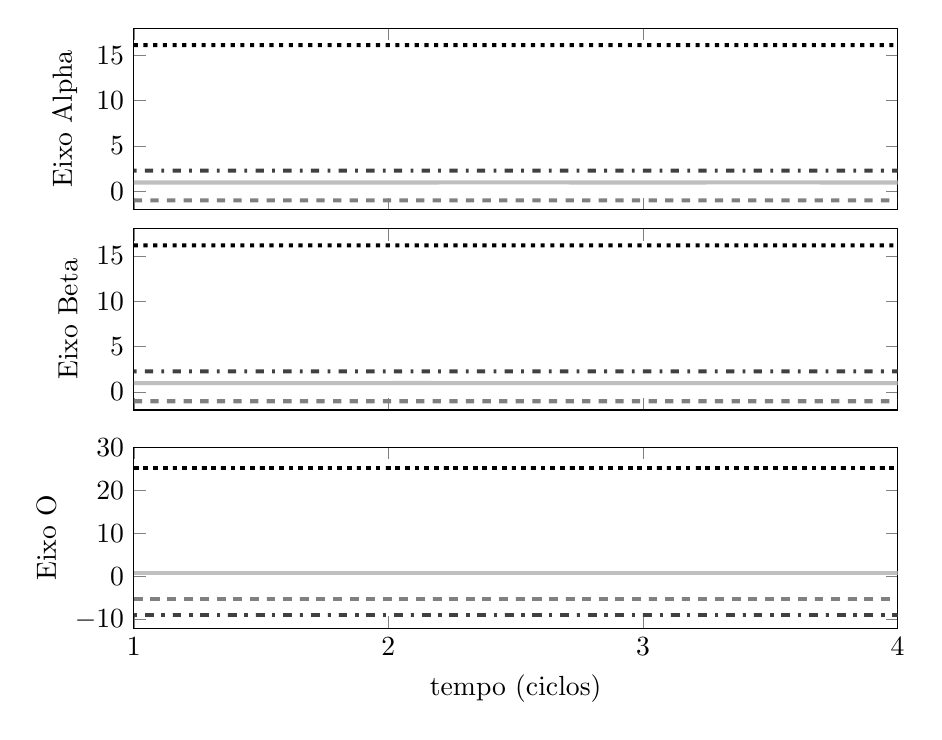
\begin{tikzpicture}

\begin{axis}[%
width=0.8\textwidth,
height=0.189701500343624\textwidth,
scale only axis,
xmin=0.316666666666667,
xmax=0.366666666666667,
xtick={0.316666666666667,0.333333333333333,0.35,0.366666666666667},
xticklabels={\empty},
ymin=-2,
ymax=18,
ytick={ 0,  5, 10, 15},
ylabel={Eixo Beta},
name=plot2,
scaled x ticks = false,
legend columns=-1,
legend style={/tikz/every even column/.append style={column sep=0.3cm}},
legend style={font=\footnotesize}
]
\addplot [color=lightgray,solid,line width=1.5pt,forget plot]
  table[row sep=crcr]{0.316666666666667	0.970436358706691\\
0.316708333333333	0.970436358706691\\
0.31675	0.970435592808439\\
0.316791666666667	0.970435592808439\\
0.316833333333333	0.970434918056243\\
0.316875	0.970434918056243\\
0.316916666666667	0.970434330318112\\
0.316958333333333	0.970434330318112\\
0.317	0.970433825496951\\
0.317041666666667	0.970433825496951\\
0.317083333333333	0.970433399492092\\
0.317125	0.970433399492092\\
0.317166666666667	0.970433048177814\\
0.317208333333333	0.970433048177814\\
0.31725	0.970432767402266\\
0.317291666666667	0.970432767402266\\
0.317333333333333	0.970432553004264\\
0.317375	0.970432553004264\\
0.317416666666667	0.970432400842131\\
0.317458333333333	0.970432400842131\\
0.3175	0.970432306827843\\
0.317541666666667	0.970432306827843\\
0.317583333333333	0.970432266960474\\
0.317625	0.970432266960474\\
0.317666666666667	0.970432277354792\\
0.317708333333333	0.970432277354792\\
0.31775	0.970432334262824\\
0.317791666666667	0.970432334262824\\
0.317833333333333	0.970432434088099\\
0.317875	0.970432434088099\\
0.317916666666667	0.970432573393534\\
0.317958333333333	0.970432573393534\\
0.318	0.970432748904596\\
0.318041666666667	0.970432748904596\\
0.318083333333333	0.970432957509533\\
0.318125	0.970432957509533\\
0.318166666666667	0.970433196258189\\
0.318208333333333	0.970433196258189\\
0.31825	0.970433462360463\\
0.318291666666667	0.970433462360463\\
0.318333333333333	0.970433753184959\\
0.318375	0.970433753184959\\
0.318416666666667	0.970434066257974\\
0.318458333333333	0.970434066257974\\
0.3185	0.970434399262647\\
0.318541666666667	0.970434399262647\\
0.318583333333333	0.970434750037975\\
0.318625	0.970434750037975\\
0.318666666666667	0.970435116577406\\
0.318708333333333	0.970435116577406\\
0.31875	0.97043549702676\\
0.318791666666667	0.97043549702676\\
0.318833333333333	0.97043588968139\\
0.318875	0.97043588968139\\
0.318916666666667	0.970436292982595\\
0.318958333333333	0.970436292982595\\
0.319	0.970436705513386\\
0.319041666666667	0.970436705513386\\
0.319083333333333	0.970437125993791\\
0.319125	0.970437125993791\\
0.319166666666667	0.970437553275866\\
0.319208333333333	0.970437553275866\\
0.31925	0.970437986338605\\
0.319291666666667	0.970437986338605\\
0.319333333333333	0.970438424282876\\
0.319375	0.970438424282876\\
0.319416666666667	0.970438866326497\\
0.319458333333333	0.970438866326497\\
0.3195	0.97043931179951\\
0.319541666666667	0.97043931179951\\
0.319583333333333	0.970439760139689\\
0.319625	0.970439760139689\\
0.319666666666667	0.970440210888314\\
0.319708333333333	0.970440210888314\\
0.31975	0.970440663686211\\
0.319791666666667	0.970440663686211\\
0.319833333333333	0.970441118270085\\
0.319875	0.970441118270085\\
0.319916666666667	0.970441574469177\\
0.319958333333333	0.970441574469177\\
0.32	0.970442032202265\\
0.320041666666667	0.970442032202265\\
0.320083333333333	0.970442491475084\\
0.320125	0.970442491475084\\
0.320166666666667	0.970442952378189\\
0.320208333333333	0.970442952378189\\
0.32025	0.970443415085359\\
0.320291666666667	0.970443415085359\\
0.320333333333333	0.970443879852587\\
0.320375	0.970443879852587\\
0.320416666666667	0.970444347017744\\
0.320458333333333	0.970444347017744\\
0.3205	0.970444817000997\\
0.320541666666667	0.970444817000997\\
0.320583333333333	0.970445290306078\\
0.320625	0.970445290306078\\
0.320666666666667	0.970445767522508\\
0.320708333333333	0.970445767522508\\
0.32075	0.970446249328905\\
0.320791666666667	0.970446249328905\\
0.320833333333333	0.970446736497523\\
0.320875	0.970446736497523\\
0.320916666666667	0.970447229900211\\
0.320958333333333	0.970447229900211\\
0.321	0.970447730516016\\
0.321041666666667	0.970447730516016\\
0.321083333333333	0.970448239440708\\
0.321125	0.970448239440708\\
0.321166666666667	0.970448757898565\\
0.321208333333333	0.970448757898565\\
0.32125	0.970449287255117\\
0.321291666666667	0.970449287255117\\
0.321333333333333	0.970449829034775\\
0.321375	0.970449829034775\\
0.321416666666667	0.970450384944168\\
0.321458333333333	0.970450384944168\\
0.3215	0.970450956898191\\
0.321541666666667	0.970450956898191\\
0.321583333333333	0.970451547051789\\
0.321625	0.970451547051789\\
0.321666666666667	0.970452157838907\\
0.321708333333333	0.970452157838907\\
0.32175	0.970452792020252\\
0.321791666666667	0.970452792020252\\
0.321833333333333	0.970453452742033\\
0.321875	0.970453452742033\\
0.321916666666667	0.970454143608473\\
0.321958333333333	0.970454143608473\\
0.322	0.970454868771685\\
0.322041666666667	0.970454868771685\\
0.322083333333333	0.970455633043542\\
0.322125	0.970455633043542\\
0.322166666666667	0.970456442035388\\
0.322208333333333	0.970456442035388\\
0.32225	0.970457302332857\\
0.322291666666667	0.970457302332857\\
0.322333333333333	0.970458221714429\\
0.322375	0.970458221714429\\
0.322416666666667	0.97045920942283\\
0.322458333333333	0.97045920942283\\
0.3225	0.97046027649605\\
0.322541666666667	0.97046027649605\\
0.322583333333333	0.970461436154189\\
0.322625	0.970461436154189\\
0.322666666666667	0.970462704205603\\
0.322708333333333	0.970462704205603\\
0.32275	0.970464099343308\\
0.322791666666667	0.970464099343308\\
0.322833333333333	0.970465642944787\\
0.322875	0.970465642944787\\
0.322916666666667	0.970467357251532\\
0.322958333333333	0.970467357251532\\
0.323	0.970469258583928\\
0.323041666666667	0.970469258583928\\
0.323083333333333	0.970471335019103\\
0.323125	0.970471335019103\\
0.323166666666667	0.970473348318116\\
0.323208333333333	0.970473348318116\\
0.32325	0.970474626904486\\
0.323291666666667	0.970474626904486\\
0.323333333333333	0.970474374243411\\
0.323375	0.970474374243411\\
0.323416666666667	0.970472573672318\\
0.323458333333333	0.970472573672318\\
0.3235	0.970469948388625\\
0.323541666666667	0.970469948388625\\
0.323583333333333	0.970467114613926\\
0.323625	0.970467114613926\\
0.323666666666667	0.970464337421047\\
0.323708333333333	0.970464337421047\\
0.32375	0.970461683786388\\
0.323791666666667	0.970461683786388\\
0.323833333333333	0.970459156489005\\
0.323875	0.970459156489005\\
0.323916666666667	0.970456747819866\\
0.323958333333333	0.970456747819866\\
0.324	0.970454453309765\\
0.324041666666667	0.970454453309765\\
0.324083333333333	0.97045227287176\\
0.324125	0.97045227287176\\
0.324166666666667	0.970450209128296\\
0.324208333333333	0.970450209128296\\
0.32425	0.970448265549337\\
0.324291666666667	0.970448265549337\\
0.324333333333333	0.970446445042454\\
0.324375	0.970446445042454\\
0.324416666666667	0.970444749125981\\
0.324458333333333	0.970444749125981\\
0.3245	0.970443177632723\\
0.324541666666667	0.970443177632723\\
0.324583333333333	0.97044172880593\\
0.324625	0.97044172880593\\
0.324666666666667	0.97044039962421\\
0.324708333333333	0.97044039962421\\
0.32475	0.970439186208874\\
0.324791666666667	0.970439186208874\\
0.324833333333333	0.970438084206409\\
0.324875	0.970438084206409\\
0.324916666666667	0.970437089084224\\
0.324958333333333	0.970437089084224\\
0.325	0.970436196318331\\
0.325041666666667	0.970436196318331\\
0.325083333333333	0.970435401481262\\
0.325125	0.970435401481262\\
0.325166666666667	0.970434700255544\\
0.325208333333333	0.970434700255544\\
0.32525	0.970434088403698\\
0.325291666666667	0.970434088403698\\
0.325333333333333	0.970433561723097\\
0.325375	0.970433561723097\\
0.325416666666667	0.970433116006485\\
0.325458333333333	0.970433116006485\\
0.3255	0.970432747019942\\
0.325541666666667	0.970432747019942\\
0.325583333333333	0.970432450501775\\
0.325625	0.970432450501775\\
0.325666666666667	0.970432222179772\\
0.325708333333333	0.970432222179772\\
0.32575	0.970432057800854\\
0.325791666666667	0.970432057800854\\
0.325833333333333	0.970431953166174\\
0.325875	0.970431953166174\\
0.325916666666667	0.970431904165525\\
0.325958333333333	0.970431904165525\\
0.326	0.970431906806762\\
0.326041666666667	0.970431906806762\\
0.326083333333333	0.970431957238012\\
0.326125	0.970431957238012\\
0.326166666666667	0.970432051762366\\
0.326208333333333	0.970432051762366\\
0.32625	0.970432186846018\\
0.326291666666667	0.970432186846018\\
0.326333333333333	0.970432359121564\\
0.326375	0.970432359121564\\
0.326416666666667	0.97043256538827\\
0.326458333333333	0.97043256538827\\
0.3265	0.970432802610885\\
0.326541666666667	0.970432802610885\\
0.326583333333333	0.970433067918077\\
0.326625	0.970433067918077\\
0.326666666666667	0.970433358601067\\
0.326708333333333	0.970433358601067\\
0.32675	0.970433672112601\\
0.326791666666667	0.970433672112601\\
0.326833333333333	0.970434006066087\\
0.326875	0.970434006066087\\
0.326916666666667	0.970434358234596\\
0.326958333333333	0.970434358234596\\
0.327	0.970434726549414\\
0.327041666666667	0.970434726549414\\
0.327083333333333	0.970435109097919\\
0.327125	0.970435109097919\\
0.327166666666667	0.970435504120658\\
0.327208333333333	0.970435504120658\\
0.32725	0.970435910007656\\
0.327291666666667	0.970435910007656\\
0.327333333333333	0.970436325294062\\
0.327375	0.970436325294062\\
0.327416666666667	0.970436748655303\\
0.327458333333333	0.970436748655303\\
0.3275	0.970437178901951\\
0.327541666666667	0.970437178901951\\
0.327583333333333	0.970437614974456\\
0.327625	0.970437614974456\\
0.327666666666667	0.970438055937924\\
0.327708333333333	0.970438055937924\\
0.32775	0.970438500977014\\
0.327791666666667	0.970438500977014\\
0.327833333333333	0.970438949391041\\
0.327875	0.970438949391041\\
0.327916666666667	0.970439400589312\\
0.327958333333333	0.970439400589312\\
0.328	0.970439854086724\\
0.328041666666667	0.970439854086724\\
0.328083333333333	0.97044030949963\\
0.328125	0.97044030949963\\
0.328166666666667	0.970440766541997\\
0.328208333333333	0.970440766541997\\
0.32825	0.970441225021877\\
0.328291666666667	0.970441225021877\\
0.328333333333333	0.970441684838236\\
0.328375	0.970441684838236\\
0.328416666666667	0.970442145978184\\
0.328458333333333	0.970442145978184\\
0.3285	0.970442608514653\\
0.328541666666667	0.970442608514653\\
0.328583333333333	0.970443072604613\\
0.328625	0.970443072604613\\
0.328666666666667	0.970443538487861\\
0.328708333333333	0.970443538487861\\
0.32875	0.970444006486495\\
0.328791666666667	0.970444006486495\\
0.328833333333333	0.970444477005118\\
0.328875	0.970444477005118\\
0.328916666666667	0.970444950531897\\
0.328958333333333	0.970444950531897\\
0.329	0.970445427640563\\
0.329041666666667	0.970445427640563\\
0.329083333333333	0.970445908993475\\
0.329125	0.970445908993475\\
0.329166666666667	0.970446395345909\\
0.329208333333333	0.970446395345909\\
0.32925	0.970446887551736\\
0.329291666666667	0.970446887551736\\
0.329333333333333	0.970447386570722\\
0.329375	0.970447386570722\\
0.329416666666667	0.970447893477714\\
0.329458333333333	0.970447893477714\\
0.3295	0.970448409474047\\
0.329541666666667	0.970448409474047\\
0.329583333333333	0.970448935899864\\
0.329625	0.970448935899864\\
0.329666666666667	0.970449474251262\\
0.329708333333333	0.970449474251262\\
0.32975	0.970450026203047\\
0.329791666666667	0.970450026203047\\
0.329833333333333	0.970450593634111\\
0.329875	0.970450593634111\\
0.329916666666667	0.970451178658432\\
0.329958333333333	0.970451178658432\\
0.33	0.970451783663083\\
0.330041666666667	0.970451783663083\\
0.330083333333333	0.970452411354861\\
0.330125	0.970452411354861\\
0.330166666666667	0.970453064817657\\
0.330208333333333	0.970453064817657\\
0.33025	0.97045374758329\\
0.330291666666667	0.97045374758329\\
0.330333333333333	0.97045446371932\\
0.330375	0.97045446371932\\
0.330416666666667	0.970455217938359\\
0.330458333333333	0.970455217938359\\
0.3305	0.970456015734584\\
0.330541666666667	0.970456015734584\\
0.330583333333333	0.970456863554561\\
0.330625	0.970456863554561\\
0.330666666666667	0.970457769010778\\
0.330708333333333	0.970457769010778\\
0.33075	0.970458741146766\\
0.330791666666667	0.970458741146766\\
0.330833333333333	0.970459790760365\\
0.330875	0.970459790760365\\
0.330916666666667	0.970460930781311\\
0.330958333333333	0.970460930781311\\
0.331	0.970462176667188\\
0.331041666666667	0.970462176667188\\
0.331083333333333	0.970463546691103\\
0.331125	0.970463546691103\\
0.331166666666667	0.970465061741802\\
0.331208333333333	0.970465061741802\\
0.33125	0.970466743535177\\
0.331291666666667	0.970466743535177\\
0.331333333333333	0.970468607961243\\
0.331375	0.970468607961243\\
0.331416666666667	0.970470643213183\\
0.331458333333333	0.970470643213183\\
0.3315	0.970472615704777\\
0.331541666666667	0.970472615704777\\
0.331583333333333	0.970473867713727\\
0.331625	0.970473867713727\\
0.331666666666667	0.970473619993488\\
0.331708333333333	0.970473619993488\\
0.33175	0.970471857439701\\
0.331791666666667	0.970471857439701\\
0.331833333333333	0.970469288642677\\
0.331875	0.970469288642677\\
0.331916666666667	0.970466516731413\\
0.331958333333333	0.970466516731413\\
0.332	0.970463800908304\\
0.332041666666667	0.970463800908304\\
0.332083333333333	0.970461206531781\\
0.332125	0.970461206531781\\
0.332166666666667	0.970458736205245\\
0.332208333333333	0.970458736205245\\
0.33225	0.970456382316685\\
0.332291666666667	0.970456382316685\\
0.332333333333333	0.970454140450355\\
0.332375	0.970454140450355\\
0.332416666666667	0.97045201049146\\
0.332458333333333	0.97045201049146\\
0.3325	0.970449994982174\\
0.332541666666667	0.970449994982174\\
0.332583333333333	0.970448097296241\\
0.332625	0.970448097296241\\
0.332666666666667	0.970446320257846\\
0.332708333333333	0.970446320257846\\
0.33275	0.970444665332178\\
0.332791666666667	0.970444665332178\\
0.332833333333333	0.970443132335721\\
0.332875	0.970443132335721\\
0.332916666666667	0.970441719530581\\
0.332958333333333	0.970441719530581\\
0.333	0.970440423942802\\
0.333041666666667	0.970440423942802\\
0.333083333333333	0.970439241761191\\
0.333125	0.970439241761191\\
0.333166666666667	0.970438168711639\\
0.333208333333333	0.970438168711639\\
0.33325	0.970437200346429\\
0.333291666666667	0.970437200346429\\
0.333333333333333	0.970436332227711\\
0.333375	0.970436332227711\\
0.333416666666667	0.970435560013326\\
0.333458333333333	0.970435560013326\\
0.3335	0.970434869203781\\
0.333541666666667	0.970434869203781\\
0.333583333333333	0.972383274643444\\
0.333625	0.972383274643444\\
0.333666666666667	0.974758397970026\\
0.333708333333333	0.974758397970026\\
0.33375	0.976852309214225\\
0.333791666666667	0.976852309214225\\
0.333833333333333	0.978523507722393\\
0.333875	0.978523507722393\\
0.333916666666667	0.979777172496431\\
0.333958333333333	0.979777172496431\\
0.334	0.980648023782431\\
0.334041666666667	0.980648023782431\\
0.334083333333333	0.981187636867261\\
0.334125	0.981187636867261\\
0.334166666666667	0.981459630166461\\
0.334208333333333	0.981459630166461\\
0.33425	0.981530080605994\\
0.334291666666667	0.981530080605994\\
0.334333333333333	0.981458396829078\\
0.334375	0.981458396829078\\
0.334416666666667	0.981291837373219\\
0.334458333333333	0.981291837373219\\
0.3345	0.981063925019619\\
0.334541666666667	0.981063925019619\\
0.334583333333333	0.980795752407432\\
0.334625	0.980795752407432\\
0.334666666666667	0.980498893471977\\
0.334708333333333	0.980498893471977\\
0.33475	0.980178786619706\\
0.334791666666667	0.980178786619706\\
0.334833333333333	0.979837783190354\\
0.334875	0.979837783190354\\
0.334916666666667	0.979477416744452\\
0.334958333333333	0.979477416744452\\
0.335	0.979099761253578\\
0.335041666666667	0.979099761253578\\
0.335083333333333	0.978707969372529\\
0.335125	0.978707969372529\\
0.335166666666667	0.97830620725098\\
0.335208333333333	0.97830620725098\\
0.33525	0.977899241503384\\
0.335291666666667	0.977899241503384\\
0.335333333333333	0.977491909699498\\
0.335375	0.977491909699498\\
0.335416666666667	0.977088644571631\\
0.335458333333333	0.977088644571631\\
0.3355	0.976693148661148\\
0.335541666666667	0.976693148661148\\
0.335583333333333	0.976308249104847\\
0.335625	0.976308249104847\\
0.335666666666667	0.975935912830535\\
0.335708333333333	0.975935912830535\\
0.33575	0.975577374402349\\
0.335791666666667	0.975577374402349\\
0.335833333333333	0.975233320340216\\
0.335875	0.975233320340216\\
0.335916666666667	0.97490407984876\\
0.335958333333333	0.97490407984876\\
0.336	0.974589786314211\\
0.336041666666667	0.974589786314211\\
0.336083333333333	0.97429049093546\\
0.336125	0.97429049093546\\
0.336166666666667	0.97400622515112\\
0.336208333333333	0.97400622515112\\
0.33625	0.973737019587191\\
0.336291666666667	0.973737019587191\\
0.336333333333333	0.973482893227748\\
0.336375	0.973482893227748\\
0.336416666666667	0.97324382783808\\
0.336458333333333	0.97324382783808\\
0.3365	0.973019740564829\\
0.336541666666667	0.973019740564829\\
0.336583333333333	0.972810463614303\\
0.336625	0.972810463614303\\
0.336666666666667	0.972615735383405\\
0.336708333333333	0.972615735383405\\
0.33675	0.972435203455679\\
0.336791666666667	0.972435203455679\\
0.336833333333333	0.972268437096257\\
0.336875	0.972268437096257\\
0.336916666666667	0.972114945471471\\
0.336958333333333	0.972114945471471\\
0.337	0.9719741976361\\
0.337041666666667	0.9719741976361\\
0.337083333333333	0.971845641028426\\
0.337125	0.971845641028426\\
0.337166666666667	0.971728716376092\\
0.337208333333333	0.971728716376092\\
0.33725	0.97162286816475\\
0.337291666666667	0.97162286816475\\
0.337333333333333	0.971527550876524\\
0.337375	0.971527550876524\\
0.337416666666667	0.971442231911105\\
0.337458333333333	0.971442231911105\\
0.3375	0.971366392420924\\
0.337541666666667	0.971366392420924\\
0.337583333333333	0.971299527275008\\
0.337625	0.971299527275008\\
0.337666666666667	0.971241145117432\\
0.337708333333333	0.971241145117432\\
0.33775	0.971190769125189\\
0.337791666666667	0.971190769125189\\
0.337833333333333	0.971147938703512\\
0.337875	0.971147938703512\\
0.337916666666667	0.971112212060718\\
0.337958333333333	0.971112212060718\\
0.338	0.971083169523816\\
0.338041666666667	0.971083169523816\\
0.338083333333333	0.971060416901619\\
0.338125	0.971060416901619\\
0.338166666666667	0.971043589078879\\
0.338208333333333	0.971043589078879\\
0.33825	0.971032353492342\\
0.338291666666667	0.971032353492342\\
0.338333333333333	0.971026413425398\\
0.338375	0.971026413425398\\
0.338416666666667	0.971025511223067\\
0.338458333333333	0.971025511223067\\
0.3385	0.971029431652645\\
0.338541666666667	0.971029431652645\\
0.338583333333333	0.971038005738005\\
0.338625	0.971038005738005\\
0.338666666666667	0.971051115485445\\
0.338708333333333	0.971051115485445\\
0.33875	0.971068700011369\\
0.338791666666667	0.971068700011369\\
0.338833333333333	0.97109076370192\\
0.338875	0.97109076370192\\
0.338916666666667	0.971117387215761\\
0.338958333333333	0.971117387215761\\
0.339	0.971148742427664\\
0.339041666666667	0.971148742427664\\
0.339083333333333	0.971185112860512\\
0.339125	0.971185112860512\\
0.339166666666667	0.971226921843321\\
0.339208333333333	0.971226921843321\\
0.33925	0.97127477165228\\
0.339291666666667	0.97127477165228\\
0.339333333333333	0.971329498291139\\
0.339375	0.971329498291139\\
0.339416666666667	0.971392248117256\\
0.339458333333333	0.971392248117256\\
0.3395	0.971464582738954\\
0.339541666666667	0.971464582738954\\
0.339583333333333	0.971548610860477\\
0.339625	0.971548610860477\\
0.339666666666667	0.971647101766183\\
0.339708333333333	0.971647101766183\\
0.33975	0.971763329252548\\
0.339791666666667	0.971763329252548\\
0.339833333333333	0.971898711452116\\
0.339875	0.971898711452116\\
0.339916666666667	0.972030606793315\\
0.339958333333333	0.972030606793315\\
0.34	0.972086635630907\\
0.340041666666667	0.972086635630907\\
0.340083333333333	0.972003357785638\\
0.340125	0.972003357785638\\
0.340166666666667	0.971837311849936\\
0.340208333333333	0.971837311849936\\
0.34025	0.971661245160536\\
0.340291666666667	0.971661245160536\\
0.340333333333333	0.971499212985451\\
0.340375	0.971499212985451\\
0.340416666666667	0.971351596498965\\
0.340458333333333	0.971351596498965\\
0.3405	0.971214858909989\\
0.340541666666667	0.971214858909989\\
0.340583333333333	0.971086572136112\\
0.340625	0.971086572136112\\
0.340666666666667	0.970965529604029\\
0.340708333333333	0.970965529604029\\
0.34075	0.970851240239321\\
0.340791666666667	0.970851240239321\\
0.340833333333333	0.970743579357346\\
0.340875	0.970743579357346\\
0.340916666666667	0.970642574454766\\
0.340958333333333	0.970642574454766\\
0.341	0.97054827090006\\
0.341041666666667	0.97054827090006\\
0.341083333333333	0.970460656346669\\
0.341125	0.970460656346669\\
0.341166666666667	0.97037963083002\\
0.341208333333333	0.97037963083002\\
0.34125	0.97030500851522\\
0.341291666666667	0.97030500851522\\
0.341333333333333	0.970236537231811\\
0.341375	0.970236537231811\\
0.341416666666667	0.970173924359278\\
0.341458333333333	0.970173924359278\\
0.3415	0.970116861136756\\
0.341541666666667	0.970116861136756\\
0.341583333333333	0.97006504101598\\
0.341625	0.97006504101598\\
0.341666666666667	0.970018170630805\\
0.341708333333333	0.970018170630805\\
0.34175	0.969975974027483\\
0.341791666666667	0.969975974027483\\
0.341833333333333	0.969938191946464\\
0.341875	0.969938191946464\\
0.341916666666667	0.96990457830085\\
0.341958333333333	0.96990457830085\\
0.342	0.969874895785129\\
0.342041666666667	0.969874895785129\\
0.342083333333333	0.969848912019831\\
0.342125	0.969848912019831\\
0.342166666666667	0.969826397012798\\
0.342208333333333	0.969826397012798\\
0.34225	0.969807122155605\\
0.342291666666667	0.969807122155605\\
0.342333333333333	0.969790860564912\\
0.342375	0.969790860564912\\
0.342416666666667	0.969777388351529\\
0.342458333333333	0.969777388351529\\
0.3425	0.969766486337173\\
0.342541666666667	0.969766486337173\\
0.342583333333333	0.969757941796077\\
0.342625	0.969757941796077\\
0.342666666666667	0.969751549922845\\
0.342708333333333	0.969751549922845\\
0.34275	0.969747114871136\\
0.342791666666667	0.969747114871136\\
0.342833333333333	0.969744450334445\\
0.342875	0.969744450334445\\
0.342916666666667	0.969743379730373\\
0.342958333333333	0.969743379730373\\
0.343	0.96974373609754\\
0.343041666666667	0.96974373609754\\
0.343083333333333	0.969745361824348\\
0.343125	0.969745361824348\\
0.343166666666667	0.969748108311924\\
0.343208333333333	0.969748108311924\\
0.34325	0.969751835642267\\
0.343291666666667	0.969751835642267\\
0.343333333333333	0.969756412288279\\
0.343375	0.969756412288279\\
0.343416666666667	0.969761714872913\\
0.343458333333333	0.969761714872913\\
0.3435	0.969767627964649\\
0.343541666666667	0.969767627964649\\
0.343583333333333	0.969774043886792\\
0.343625	0.969774043886792\\
0.343666666666667	0.969780862517226\\
0.343708333333333	0.969780862517226\\
0.34375	0.969787991060458\\
0.343791666666667	0.969787991060458\\
0.343833333333333	0.969795343781902\\
0.343875	0.969795343781902\\
0.343916666666667	0.969802841702633\\
0.343958333333333	0.969802841702633\\
0.344	0.969810412259509\\
0.344041666666667	0.969810412259509\\
0.344083333333333	0.969817988939616\\
0.344125	0.969817988939616\\
0.344166666666667	0.969825510899376\\
0.344208333333333	0.969825510899376\\
0.34425	0.969832922577906\\
0.344291666666667	0.969832922577906\\
0.344333333333333	0.96984017331207\\
0.344375	0.96984017331207\\
0.344416666666667	0.969847216957934\\
0.344458333333333	0.969847216957934\\
0.3445	0.969854011520733\\
0.344541666666667	0.969854011520733\\
0.344583333333333	0.969860518793423\\
0.344625	0.969860518793423\\
0.344666666666667	0.969866704002546\\
0.344708333333333	0.969866704002546\\
0.34475	0.969872535459534\\
0.344791666666667	0.969872535459534\\
0.344833333333333	0.96987798421551\\
0.344875	0.96987798421551\\
0.344916666666667	0.969883023717897\\
0.344958333333333	0.969883023717897\\
0.345	0.969887629467457\\
0.345041666666667	0.969887629467457\\
0.345083333333333	0.969891778674667\\
0.345125	0.969891778674667\\
0.345166666666667	0.969895449914336\\
0.345208333333333	0.969895449914336\\
0.34525	0.96989862277719\\
0.345291666666667	0.96989862277719\\
0.345333333333333	0.969901277516689\\
0.345375	0.969901277516689\\
0.345416666666667	0.969903394688643\\
0.345458333333333	0.969903394688643\\
0.3455	0.969904954780388\\
0.345541666666667	0.969904954780388\\
0.345583333333333	0.969905937825267\\
0.345625	0.969905937825267\\
0.345666666666667	0.969906322997075\\
0.345708333333333	0.969906322997075\\
0.34575	0.969906088177827\\
0.345791666666667	0.969906088177827\\
0.345833333333333	0.969905209490743\\
0.345875	0.969905209490743\\
0.345916666666667	0.969903660788546\\
0.345958333333333	0.969903660788546\\
0.346	0.969901413084942\\
0.346041666666667	0.969901413084942\\
0.346083333333333	0.969898433914325\\
0.346125	0.969898433914325\\
0.346166666666667	0.969894686601097\\
0.346208333333333	0.969894686601097\\
0.34625	0.969890129422859\\
0.346291666666667	0.969890129422859\\
0.346333333333333	0.969884714629821\\
0.346375	0.969884714629821\\
0.346416666666667	0.969878387269683\\
0.346458333333333	0.969878387269683\\
0.3465	0.96987108379019\\
0.346541666666667	0.96987108379019\\
0.346583333333333	0.969862730348636\\
0.346625	0.969862730348636\\
0.346666666666667	0.969853240743723\\
0.346708333333333	0.969853240743723\\
0.34675	0.969842513858014\\
0.346791666666667	0.969842513858014\\
0.346833333333333	0.96983043046063\\
0.346875	0.96983043046063\\
0.346916666666667	0.969816849165492\\
0.346958333333333	0.969816849165492\\
0.347	0.969801601263179\\
0.347041666666667	0.969801601263179\\
0.347083333333333	0.96978448403335\\
0.347125	0.96978448403335\\
0.347166666666667	0.96976525198287\\
0.347208333333333	0.96976525198287\\
0.34725	0.969743605216908\\
0.347291666666667	0.969743605216908\\
0.347333333333333	0.96971917379818\\
0.347375	0.96971917379818\\
0.347416666666667	0.969691496428663\\
0.347458333333333	0.969691496428663\\
0.3475	0.969659991029906\\
0.347541666666667	0.969659991029906\\
0.347583333333333	0.969623913752898\\
0.347625	0.969623913752898\\
0.347666666666667	0.969582301742223\\
0.347708333333333	0.969582301742223\\
0.34775	0.969533894547103\\
0.347791666666667	0.969533894547103\\
0.347833333333333	0.969477033694823\\
0.347875	0.969477033694823\\
0.347916666666667	0.969409567851057\\
0.347958333333333	0.969409567851057\\
0.348	0.969328922505546\\
0.348041666666667	0.969328922505546\\
0.348083333333333	0.969233114197671\\
0.348125	0.969233114197671\\
0.348166666666667	0.969135987302733\\
0.348208333333333	0.969135987302733\\
0.34825	0.969086869477986\\
0.348291666666667	0.969086869477986\\
0.348333333333333	0.969139013493315\\
0.348375	0.969139013493315\\
0.348416666666667	0.969260422812092\\
0.348458333333333	0.969260422812092\\
0.3485	0.969395155966972\\
0.348541666666667	0.969395155966972\\
0.348583333333333	0.969521559511252\\
0.348625	0.969521559511252\\
0.348666666666667	0.969637767070075\\
0.348708333333333	0.969637767070075\\
0.34875	0.969746017484971\\
0.348791666666667	0.969746017484971\\
0.348833333333333	0.96984804400771\\
0.348875	0.96984804400771\\
0.348916666666667	0.969944717835906\\
0.348958333333333	0.969944717835906\\
0.349	0.970036376232296\\
0.349041666666667	0.970036376232296\\
0.349083333333333	0.970123078544635\\
0.349125	0.970123078544635\\
0.349166666666667	0.970204766919204\\
0.349208333333333	0.970204766919204\\
0.34925	0.970281368682784\\
0.349291666666667	0.970281368682784\\
0.349333333333333	0.970352855631549\\
0.349375	0.970352855631549\\
0.349416666666667	0.970419269023916\\
0.349458333333333	0.970419269023916\\
0.3495	0.970480720073789\\
0.349541666666667	0.970480720073789\\
0.349583333333333	0.970537376099504\\
0.349625	0.970537376099504\\
0.349666666666667	0.970589441011994\\
0.349708333333333	0.970589441011994\\
0.34975	0.970637136358307\\
0.349791666666667	0.970637136358307\\
0.349833333333333	0.970680686509672\\
0.349875	0.970680686509672\\
0.349916666666667	0.97072030932276\\
0.349958333333333	0.97072030932276\\
0.35	0.970756211970294\\
0.350041666666667	0.970756211970294\\
0.350083333333333	0.970788590693478\\
0.350125	0.970788590693478\\
0.350166666666667	0.970817632892686\\
0.350208333333333	0.970817632892686\\
0.35025	0.970843520082948\\
0.350291666666667	0.970843520082948\\
0.350333333333333	0.970866430610499\\
0.350375	0.970866430610499\\
0.350416666666667	0.970886541487813\\
0.350458333333333	0.970886541487813\\
0.3505	0.970904029131477\\
0.350541666666667	0.970904029131477\\
0.350583333333333	0.97091906910635\\
0.350625	0.97091906910635\\
0.350666666666667	0.970931835164284\\
0.350708333333333	0.970931835164284\\
0.35075	0.97094249792621\\
0.350791666666667	0.97094249792621\\
0.350833333333333	0.970951223523734\\
0.350875	0.970951223523734\\
0.350916666666667	0.970958172429553\\
0.350958333333333	0.970958172429553\\
0.351	0.970963498601493\\
0.351041666666667	0.970963498601493\\
0.351083333333333	0.97096734896999\\
0.351125	0.97096734896999\\
0.351166666666667	0.970969863229572\\
0.351208333333333	0.970969863229572\\
0.35125	0.970971173856576\\
0.351291666666667	0.970971173856576\\
0.351333333333333	0.970971406265249\\
0.351375	0.970971406265249\\
0.351416666666667	0.97097067902494\\
0.351458333333333	0.97097067902494\\
0.3515	0.970969104083168\\
0.351541666666667	0.970969104083168\\
0.351583333333333	0.970966786964468\\
0.351625	0.970966786964468\\
0.351666666666667	0.970963826936975\\
0.351708333333333	0.970963826936975\\
0.35175	0.97096031715412\\
0.351791666666667	0.97096031715412\\
0.351833333333333	0.970956344786806\\
0.351875	0.970956344786806\\
0.351916666666667	0.970951991162716\\
0.351958333333333	0.970951991162716\\
0.352	0.970947331926166\\
0.352041666666667	0.970947331926166\\
0.352083333333333	0.970942437226222\\
0.352125	0.970942437226222\\
0.352166666666667	0.970937371934864\\
0.352208333333333	0.970937371934864\\
0.35225	0.970932195891997\\
0.352291666666667	0.970932195891997\\
0.352333333333333	0.970926964171046\\
0.352375	0.970926964171046\\
0.352416666666667	0.970921727357632\\
0.352458333333333	0.970921727357632\\
0.3525	0.970916531834242\\
0.352541666666667	0.970916531834242\\
0.352583333333333	0.970911420065246\\
0.352625	0.970911420065246\\
0.352666666666667	0.970906430878559\\
0.352708333333333	0.970906430878559\\
0.35275	0.970901599742084\\
0.352791666666667	0.970901599742084\\
0.352833333333333	0.970896959034624\\
0.352875	0.970896959034624\\
0.352916666666667	0.970892538311944\\
0.352958333333333	0.970892538311944\\
0.353	0.97088836456913\\
0.353041666666667	0.97088836456913\\
0.353083333333333	0.970884462500506\\
0.353125	0.970884462500506\\
0.353166666666667	0.970880854758184\\
0.353208333333333	0.970880854758184\\
0.35325	0.970877562210094\\
0.353291666666667	0.970877562210094\\
0.353333333333333	0.970874604198136\\
0.353375	0.970874604198136\\
0.353416666666667	0.970871998797037\\
0.353458333333333	0.970871998797037\\
0.3535	0.970869763074611\\
0.353541666666667	0.970869763074611\\
0.353583333333333	0.970867913354382\\
0.353625	0.970867913354382\\
0.353666666666667	0.970866465481979\\
0.353708333333333	0.970866465481979\\
0.35375	0.970865435097221\\
0.353791666666667	0.970865435097221\\
0.353833333333333	0.970864837914447\\
0.353875	0.970864837914447\\
0.353916666666667	0.970864690014351\\
0.353958333333333	0.970864690014351\\
0.354	0.970865008151332\\
0.354041666666667	0.970865008151332\\
0.354083333333333	0.97086581008127\\
0.354125	0.97086581008127\\
0.354166666666667	0.970867114915696\\
0.354208333333333	0.970867114915696\\
0.35425	0.970868943509571\\
0.354291666666667	0.970868943509571\\
0.354333333333333	0.970871318891501\\
0.354375	0.970871318891501\\
0.354416666666667	0.970874266747262\\
0.354458333333333	0.970874266747262\\
0.3545	0.970877815970109\\
0.354541666666667	0.970877815970109\\
0.354583333333333	0.970881999287056\\
0.354625	0.970881999287056\\
0.354666666666667	0.970886853994502\\
0.354708333333333	0.970886853994502\\
0.35475	0.970892422834274\\
0.354791666666667	0.970892422834274\\
0.354833333333333	0.970898755030506\\
0.354875	0.970898755030506\\
0.354916666666667	0.970905907538368\\
0.354958333333333	0.970905907538368\\
0.355	0.970913946564443\\
0.355041666666667	0.970913946564443\\
0.355083333333333	0.970922949437218\\
0.355125	0.970922949437218\\
0.355166666666667	0.970933006932661\\
0.355208333333333	0.970933006932661\\
0.35525	0.970944226196895\\
0.355291666666667	0.970944226196895\\
0.355333333333333	0.970956734460296\\
0.355375	0.970956734460296\\
0.355416666666667	0.97097068381215\\
0.355458333333333	0.97097068381215\\
0.3555	0.970986257413336\\
0.355541666666667	0.970986257413336\\
0.355583333333333	0.971003677683163\\
0.355625	0.971003677683163\\
0.355666666666667	0.971023217231027\\
0.355708333333333	0.971023217231027\\
0.35575	0.971045213652199\\
0.355791666666667	0.971045213652199\\
0.355833333333333	0.971070089823367\\
0.355875	0.971070089823367\\
0.355916666666667	0.971098382080468\\
0.355958333333333	0.971098382080468\\
0.356	0.971130779662012\\
0.356041666666667	0.971130779662012\\
0.356083333333333	0.971168179821891\\
0.356125	0.971168179821891\\
0.356166666666667	0.971211762683141\\
0.356208333333333	0.971211762683141\\
0.35625	0.971263082096707\\
0.356291666666667	0.971263082096707\\
0.356333333333333	0.971324126975559\\
0.356375	0.971324126975559\\
0.356416666666667	0.971397110447942\\
0.356458333333333	0.971397110447942\\
0.3565	0.971480654713187\\
0.356541666666667	0.971480654713187\\
0.356583333333333	0.971553777142341\\
0.356625	0.971553777142341\\
0.356666666666667	0.971564738457024\\
0.356708333333333	0.971564738457024\\
0.35675	0.971491975742569\\
0.356791666666667	0.971491975742569\\
0.356833333333333	0.971381667572881\\
0.356875	0.971381667572881\\
0.356916666666667	0.971270749799534\\
0.356958333333333	0.971270749799534\\
0.357	0.971168684120242\\
0.357041666666667	0.971168684120242\\
0.357083333333333	0.971074650814482\\
0.357125	0.971074650814482\\
0.357166666666667	0.97098670764254\\
0.357208333333333	0.97098670764254\\
0.35725	0.970903666804324\\
0.357291666666667	0.970903666804324\\
0.357333333333333	0.970824980161487\\
0.357375	0.970824980161487\\
0.357416666666667	0.970750460224107\\
0.357458333333333	0.970750460224107\\
0.3575	0.970680097588076\\
0.357541666666667	0.970680097588076\\
0.357583333333333	0.970613946205429\\
0.357625	0.970613946205429\\
0.357666666666667	0.970552051710161\\
0.357708333333333	0.970552051710161\\
0.35775	0.970494413214462\\
0.357791666666667	0.970494413214462\\
0.357833333333333	0.97044097093059\\
0.357875	0.97044097093059\\
0.357916666666667	0.970391611041146\\
0.357958333333333	0.970391611041146\\
0.358	0.970346179616912\\
0.358041666666667	0.970346179616912\\
0.358083333333333	0.970304499052172\\
0.358125	0.970304499052172\\
0.358166666666667	0.970266382675627\\
0.358208333333333	0.970266382675627\\
0.35825	0.970231645308928\\
0.358291666666667	0.970231645308928\\
0.358333333333333	0.970200109244495\\
0.358375	0.970200109244495\\
0.358416666666667	0.970171606255056\\
0.358458333333333	0.970171606255056\\
0.3585	0.970145976830688\\
0.358541666666667	0.970145976830688\\
0.358583333333333	0.970123067963075\\
0.358625	0.970123067963075\\
0.358666666666667	0.970102730607539\\
0.358708333333333	0.970102730607539\\
0.35875	0.970084817602961\\
0.358791666666667	0.970084817602961\\
0.358833333333333	0.970069182446114\\
0.358875	0.970069182446114\\
0.358916666666667	0.970055678988787\\
0.358958333333333	0.970055678988787\\
0.359	0.97004416189982\\
0.359041666666667	0.97004416189982\\
0.359083333333333	0.970034487619429\\
0.359125	0.970034487619429\\
0.359166666666667	0.970026515514388\\
0.359208333333333	0.970026515514388\\
0.35925	0.970020108990212\\
0.359291666666667	0.970020108990212\\
0.359333333333333	0.970015136397892\\
0.359375	0.970015136397892\\
0.359416666666667	0.970011471659993\\
0.359458333333333	0.970011471659993\\
0.3595	0.970008994614154\\
0.359541666666667	0.970008994614154\\
0.359583333333333	0.970007591121378\\
0.359625	0.970007591121378\\
0.359666666666667	0.97000715300987\\
0.359708333333333	0.97000715300987\\
0.35975	0.970007577926808\\
0.359791666666667	0.970007577926808\\
0.359833333333333	0.970008769157248\\
0.359875	0.970008769157248\\
0.359916666666667	0.970010635449145\\
0.359958333333333	0.970010635449145\\
0.36	0.970013090862696\\
0.360041666666667	0.970013090862696\\
0.360083333333333	0.970016054645354\\
0.360125	0.970016054645354\\
0.360166666666667	0.970019451123033\\
0.360208333333333	0.970019451123033\\
0.36025	0.970023209593467\\
0.360291666666667	0.970023209593467\\
0.360333333333333	0.970027264208161\\
0.360375	0.970027264208161\\
0.360416666666667	0.970031553833154\\
0.360458333333333	0.970031553833154\\
0.3605	0.970036021883901\\
0.360541666666667	0.970036021883901\\
0.360583333333333	0.970040616134492\\
0.360625	0.970040616134492\\
0.360666666666667	0.970045288505153\\
0.360708333333333	0.970045288505153\\
0.36075	0.970049994834034\\
0.360791666666667	0.970049994834034\\
0.360833333333333	0.970054694639801\\
0.360875	0.970054694639801\\
0.360916666666667	0.970059350880804\\
0.360958333333333	0.970059350880804\\
0.361	0.970063929715179\\
0.361041666666667	0.970063929715179\\
0.361083333333333	0.970068400264507\\
0.361125	0.970068400264507\\
0.361166666666667	0.970072734382169\\
0.361208333333333	0.970072734382169\\
0.36125	0.970076906426318\\
0.361291666666667	0.970076906426318\\
0.361333333333333	0.97008089303674\\
0.361375	0.97008089303674\\
0.361416666666667	0.970084672914523\\
0.361458333333333	0.970084672914523\\
0.3615	0.97008822660353\\
0.361541666666667	0.97008822660353\\
0.361583333333333	0.970091536272782\\
0.361625	0.970091536272782\\
0.361666666666667	0.970094585499102\\
0.361708333333333	0.970094585499102\\
0.36175	0.97009735904947\\
0.361791666666667	0.97009735904947\\
0.361833333333333	0.970099842662543\\
0.361875	0.970099842662543\\
0.361916666666667	0.97010202282863\\
0.361958333333333	0.97010202282863\\
0.362	0.970103886567102\\
0.362041666666667	0.970103886567102\\
0.362083333333333	0.970105421199819\\
0.362125	0.970105421199819\\
0.362166666666667	0.970106614118595\\
0.362208333333333	0.970106614118595\\
0.36225	0.97010745254418\\
0.362291666666667	0.97010745254418\\
0.362333333333333	0.970107923273531\\
0.362375	0.970107923273531\\
0.362416666666667	0.970108012411407\\
0.362458333333333	0.970108012411407\\
0.3625	0.970107705081453\\
0.362541666666667	0.970107705081453\\
0.362583333333333	0.970106985110827\\
0.362625	0.970106985110827\\
0.362666666666667	0.970105834681177\\
0.362708333333333	0.970105834681177\\
0.36275	0.970104233936995\\
0.362791666666667	0.970104233936995\\
0.362833333333333	0.970102160540291\\
0.362875	0.970102160540291\\
0.362916666666667	0.970099589162042\\
0.362958333333333	0.970099589162042\\
0.363	0.970096490888002\\
0.363041666666667	0.970096490888002\\
0.363083333333333	0.970092832509604\\
0.363125	0.970092832509604\\
0.363166666666667	0.970088575682083\\
0.363208333333333	0.970088575682083\\
0.36325	0.970083675908384\\
0.363291666666667	0.970083675908384\\
0.363333333333333	0.970078081298706\\
0.363375	0.970078081298706\\
0.363416666666667	0.970071731039502\\
0.363458333333333	0.970071731039502\\
0.3635	0.970064553482988\\
0.363541666666667	0.970064553482988\\
0.363583333333333	0.970056463736287\\
0.363625	0.970056463736287\\
0.363666666666667	0.970047360583917\\
0.363708333333333	0.970047360583917\\
0.36375	0.970037122512159\\
0.363791666666667	0.970037122512159\\
0.363833333333333	0.970025602508945\\
0.363875	0.970025602508945\\
0.363916666666667	0.970012621173551\\
0.363958333333333	0.970012621173551\\
0.364	0.969997957464014\\
0.364041666666667	0.969997957464014\\
0.364083333333333	0.969981336104409\\
0.364125	0.969981336104409\\
0.364166666666667	0.969962410226499\\
0.364208333333333	0.969962410226499\\
0.36425	0.96994073719436\\
0.364291666666667	0.96994073719436\\
0.364333333333333	0.969915744803349\\
0.364375	0.969915744803349\\
0.364416666666667	0.969886684608235\\
0.364458333333333	0.969886684608235\\
0.3645	0.969852571161579\\
0.364541666666667	0.969852571161579\\
0.364583333333333	0.969812119608624\\
0.364625	0.969812119608624\\
0.364666666666667	0.969763759593906\\
0.364708333333333	0.969763759593906\\
0.36475	0.969706111804142\\
0.364791666666667	0.969706111804142\\
0.364833333333333	0.969645508505082\\
0.364875	0.969645508505082\\
0.364916666666667	0.969608847079304\\
0.364958333333333	0.969608847079304\\
0.365	0.969632403106298\\
0.365041666666667	0.969632403106298\\
0.365083333333333	0.969703672610288\\
0.365125	0.969703672610288\\
0.365166666666667	0.969786649121214\\
0.365208333333333	0.969786649121214\\
0.36525	0.969865281185191\\
0.365291666666667	0.969865281185191\\
0.365333333333333	0.969937520925395\\
0.365375	0.969937520925395\\
0.365416666666667	0.97000467881968\\
0.365458333333333	0.97000467881968\\
0.3655	0.970067902383859\\
0.365541666666667	0.970067902383859\\
0.365583333333333	0.970127789977669\\
0.365625	0.970127789977669\\
0.365666666666667	0.970184584008583\\
0.365708333333333	0.970184584008583\\
0.36575	0.97023833836575\\
0.365791666666667	0.97023833836575\\
0.365833333333333	0.970289023589814\\
0.365875	0.970289023589814\\
0.365916666666667	0.970336593946702\\
0.365958333333333	0.970336593946702\\
0.366	0.970381027184982\\
0.366041666666667	0.970381027184982\\
0.366083333333333	0.970422342477409\\
0.366125	0.970422342477409\\
0.366166666666667	0.970460602450694\\
0.366208333333333	0.970460602450694\\
0.36625	0.970495905580502\\
0.366291666666667	0.970495905580502\\
0.366333333333333	0.970528374455051\\
0.366375	0.970528374455051\\
0.366416666666667	0.970558143945831\\
0.366458333333333	0.970558143945831\\
0.3665	0.970585351702793\\
0.366541666666667	0.970585351702793\\
0.366583333333333	0.970610131961271\\
0.366625	0.970610131961271\\
0.366666666666667	0.970632612588736\\
};
\addplot [color=gray,dashed,line width=1.5pt,forget plot]
  table[row sep=crcr]{0.316666666666667	-1.0279793224329\\
0.316708333333333	-1.0279793224329\\
0.31675	-1.02797932543233\\
0.316791666666667	-1.02797932543233\\
0.316833333333333	-1.02797932798806\\
0.316875	-1.02797932798806\\
0.316916666666667	-1.02797933014413\\
0.316958333333333	-1.02797933014413\\
0.317	-1.02797933193992\\
0.317041666666667	-1.02797933193992\\
0.317083333333333	-1.02797933341104\\
0.317125	-1.02797933341104\\
0.317166666666667	-1.02797933458991\\
0.317208333333333	-1.02797933458991\\
0.31725	-1.02797933550621\\
0.317291666666667	-1.02797933550621\\
0.317333333333333	-1.02797933618718\\
0.317375	-1.02797933618718\\
0.317416666666667	-1.02797933665787\\
0.317458333333333	-1.02797933665787\\
0.3175	-1.02797933694126\\
0.317541666666667	-1.02797933694126\\
0.317583333333333	-1.02797933705843\\
0.317625	-1.02797933705843\\
0.317666666666667	-1.02797933702864\\
0.317708333333333	-1.02797933702864\\
0.31775	-1.02797933686946\\
0.317791666666667	-1.02797933686946\\
0.317833333333333	-1.02797933659693\\
0.317875	-1.02797933659693\\
0.317916666666667	-1.02797933622564\\
0.317958333333333	-1.02797933622564\\
0.318	-1.02797933576886\\
0.318041666666667	-1.02797933576886\\
0.318083333333333	-1.02797933523867\\
0.318125	-1.02797933523867\\
0.318166666666667	-1.02797933464602\\
0.318208333333333	-1.02797933464602\\
0.31825	-1.02797933400088\\
0.318291666666667	-1.02797933400088\\
0.318333333333333	-1.02797933331226\\
0.318375	-1.02797933331226\\
0.318416666666667	-1.02797933258833\\
0.318458333333333	-1.02797933258833\\
0.3185	-1.02797933183645\\
0.318541666666667	-1.02797933183645\\
0.318583333333333	-1.02797933106326\\
0.318625	-1.02797933106326\\
0.318666666666667	-1.02797933027471\\
0.318708333333333	-1.02797933027471\\
0.31875	-1.02797932947612\\
0.318791666666667	-1.02797932947612\\
0.318833333333333	-1.02797932867225\\
0.318875	-1.02797932867225\\
0.318916666666667	-1.0279793278673\\
0.318958333333333	-1.0279793278673\\
0.319	-1.02797932706501\\
0.319041666666667	-1.02797932706501\\
0.319083333333333	-1.02797932626865\\
0.319125	-1.02797932626865\\
0.319166666666667	-1.02797932548113\\
0.319208333333333	-1.02797932548113\\
0.31925	-1.02797932470497\\
0.319291666666667	-1.02797932470497\\
0.319333333333333	-1.02797932394236\\
0.319375	-1.02797932394236\\
0.319416666666667	-1.02797932319524\\
0.319458333333333	-1.02797932319524\\
0.3195	-1.02797932246525\\
0.319541666666667	-1.02797932246525\\
0.319583333333333	-1.02797932175383\\
0.319625	-1.02797932175383\\
0.319666666666667	-1.02797932106223\\
0.319708333333333	-1.02797932106223\\
0.31975	-1.02797932039152\\
0.319791666666667	-1.02797932039152\\
0.319833333333333	-1.02797931974265\\
0.319875	-1.02797931974265\\
0.319916666666667	-1.02797931911644\\
0.319958333333333	-1.02797931911644\\
0.32	-1.02797931851366\\
0.320041666666667	-1.02797931851366\\
0.320083333333333	-1.02797931793501\\
0.320125	-1.02797931793501\\
0.320166666666667	-1.02797931738115\\
0.320208333333333	-1.02797931738115\\
0.32025	-1.02797931685278\\
0.320291666666667	-1.02797931685278\\
0.320333333333333	-1.0279793163506\\
0.320375	-1.0279793163506\\
0.320416666666667	-1.0279793158754\\
0.320458333333333	-1.0279793158754\\
0.3205	-1.02797931542806\\
0.320541666666667	-1.02797931542806\\
0.320583333333333	-1.02797931500959\\
0.320625	-1.02797931500959\\
0.320666666666667	-1.02797931462121\\
0.320708333333333	-1.02797931462121\\
0.32075	-1.02797931426436\\
0.320791666666667	-1.02797931426436\\
0.320833333333333	-1.02797931394075\\
0.320875	-1.02797931394075\\
0.320916666666667	-1.02797931365249\\
0.320958333333333	-1.02797931365249\\
0.321	-1.02797931340209\\
0.321041666666667	-1.02797931340209\\
0.321083333333333	-1.02797931319261\\
0.321125	-1.02797931319261\\
0.321166666666667	-1.02797931302779\\
0.321208333333333	-1.02797931302779\\
0.32125	-1.02797931291213\\
0.321291666666667	-1.02797931291213\\
0.321333333333333	-1.02797931285116\\
0.321375	-1.02797931285116\\
0.321416666666667	-1.02797931285162\\
0.321458333333333	-1.02797931285162\\
0.3215	-1.02797931292176\\
0.321541666666667	-1.02797931292176\\
0.321583333333333	-1.02797931307177\\
0.321625	-1.02797931307177\\
0.321666666666667	-1.02797931331421\\
0.321708333333333	-1.02797931331421\\
0.32175	-1.02797931366474\\
0.321791666666667	-1.02797931366474\\
0.321833333333333	-1.02797931414296\\
0.321875	-1.02797931414296\\
0.321916666666667	-1.02797931477364\\
0.321958333333333	-1.02797931477364\\
0.322	-1.02797931558829\\
0.322041666666667	-1.02797931558829\\
0.322083333333333	-1.02797931662754\\
0.322125	-1.02797931662754\\
0.322166666666667	-1.02797931794426\\
0.322208333333333	-1.02797931794426\\
0.32225	-1.02797931960831\\
0.322291666666667	-1.02797931960831\\
0.322333333333333	-1.02797932171334\\
0.322375	-1.02797932171334\\
0.322416666666667	-1.02797932438721\\
0.322458333333333	-1.02797932438721\\
0.3225	-1.02797932780807\\
0.322541666666667	-1.02797932780807\\
0.322583333333333	-1.02797933223008\\
0.322625	-1.02797933223008\\
0.322666666666667	-1.02797933802607\\
0.322708333333333	-1.02797933802607\\
0.32275	-1.0279793457613\\
0.322791666666667	-1.0279793457613\\
0.322833333333333	-1.02797935632699\\
0.322875	-1.02797935632699\\
0.322916666666667	-1.02797937119702\\
0.322958333333333	-1.02797937119702\\
0.323	-1.02797939295577\\
0.323041666666667	-1.02797939295577\\
0.323083333333333	-1.02797942647672\\
0.323125	-1.02797942647672\\
0.323166666666667	-1.02797947861476\\
0.323208333333333	-1.02797947861476\\
0.32325	-1.02797955338093\\
0.323291666666667	-1.02797955338093\\
0.323333333333333	-1.02797964239201\\
0.323375	-1.02797964239201\\
0.323416666666667	-1.02797972650636\\
0.323458333333333	-1.02797972650636\\
0.3235	-1.02797979421719\\
0.323541666666667	-1.02797979421719\\
0.323583333333333	-1.0279798456655\\
0.323625	-1.0279798456655\\
0.323666666666667	-1.02797988508432\\
0.323708333333333	-1.02797988508432\\
0.32375	-1.02797991630424\\
0.323791666666667	-1.02797991630424\\
0.323833333333333	-1.02797994188271\\
0.323875	-1.02797994188271\\
0.323916666666667	-1.02797996339721\\
0.323958333333333	-1.02797996339721\\
0.324	-1.02797998182432\\
0.324041666666667	-1.02797998182432\\
0.324083333333333	-1.02797999779181\\
0.324125	-1.02797999779181\\
0.324166666666667	-1.0279800117247\\
0.324208333333333	-1.0279800117247\\
0.32425	-1.02798002392824\\
0.324291666666667	-1.02798002392824\\
0.324333333333333	-1.02798003463532\\
0.324375	-1.02798003463532\\
0.324416666666667	-1.0279800440334\\
0.324458333333333	-1.0279800440334\\
0.3245	-1.02798005227943\\
0.324541666666667	-1.02798005227943\\
0.324583333333333	-1.02798005950815\\
0.324625	-1.02798005950815\\
0.324666666666667	-1.02798006583651\\
0.324708333333333	-1.02798006583651\\
0.32475	-1.02798007136634\\
0.324791666666667	-1.02798007136634\\
0.324833333333333	-1.02798007618623\\
0.324875	-1.02798007618623\\
0.324916666666667	-1.02798008037312\\
0.324958333333333	-1.02798008037312\\
0.325	-1.02798008399383\\
0.325041666666667	-1.02798008399383\\
0.325083333333333	-1.02798008710665\\
0.325125	-1.02798008710665\\
0.325166666666667	-1.02798008976269\\
0.325208333333333	-1.02798008976269\\
0.32525	-1.02798009200725\\
0.325291666666667	-1.02798009200725\\
0.325333333333333	-1.02798009388083\\
0.325375	-1.02798009388083\\
0.325416666666667	-1.02798009542004\\
0.325458333333333	-1.02798009542004\\
0.3255	-1.02798009665823\\
0.325541666666667	-1.02798009665823\\
0.325583333333333	-1.02798009762591\\
0.325625	-1.02798009762591\\
0.325666666666667	-1.02798009835112\\
0.325708333333333	-1.02798009835112\\
0.32575	-1.0279800988596\\
0.325791666666667	-1.0279800988596\\
0.325833333333333	-1.02798009917502\\
0.325875	-1.02798009917502\\
0.325916666666667	-1.02798009931903\\
0.325958333333333	-1.02798009931903\\
0.326	-1.02798009931146\\
0.326041666666667	-1.02798009931146\\
0.326083333333333	-1.02798009917039\\
0.326125	-1.02798009917039\\
0.326166666666667	-1.02798009891234\\
0.326208333333333	-1.02798009891234\\
0.32625	-1.02798009855229\\
0.326291666666667	-1.02798009855229\\
0.326333333333333	-1.02798009810393\\
0.326375	-1.02798009810393\\
0.326416666666667	-1.02798009757968\\
0.326458333333333	-1.02798009757968\\
0.3265	-1.02798009699082\\
0.326541666666667	-1.02798009699082\\
0.326583333333333	-1.02798009634759\\
0.326625	-1.02798009634759\\
0.326666666666667	-1.02798009565931\\
0.326708333333333	-1.02798009565931\\
0.32675	-1.02798009493435\\
0.326791666666667	-1.02798009493435\\
0.326833333333333	-1.02798009418033\\
0.326875	-1.02798009418033\\
0.326916666666667	-1.02798009340406\\
0.326958333333333	-1.02798009340406\\
0.327	-1.02798009261169\\
0.327041666666667	-1.02798009261169\\
0.327083333333333	-1.02798009180869\\
0.327125	-1.02798009180869\\
0.327166666666667	-1.02798009099997\\
0.327208333333333	-1.02798009099997\\
0.32725	-1.02798009018985\\
0.327291666666667	-1.02798009018985\\
0.327333333333333	-1.02798008938219\\
0.327375	-1.02798008938219\\
0.327416666666667	-1.02798008858038\\
0.327458333333333	-1.02798008858038\\
0.3275	-1.02798008778739\\
0.327541666666667	-1.02798008778739\\
0.327583333333333	-1.02798008700583\\
0.327625	-1.02798008700583\\
0.327666666666667	-1.02798008623796\\
0.327708333333333	-1.02798008623796\\
0.32775	-1.02798008548577\\
0.327791666666667	-1.02798008548577\\
0.327833333333333	-1.02798008475096\\
0.327875	-1.02798008475096\\
0.327916666666667	-1.027980084035\\
0.327958333333333	-1.027980084035\\
0.328	-1.02798008333918\\
0.328041666666667	-1.02798008333918\\
0.328083333333333	-1.02798008266459\\
0.328125	-1.02798008266459\\
0.328166666666667	-1.0279800820122\\
0.328208333333333	-1.0279800820122\\
0.32825	-1.02798008138287\\
0.328291666666667	-1.02798008138287\\
0.328333333333333	-1.02798008077734\\
0.328375	-1.02798008077734\\
0.328416666666667	-1.02798008019633\\
0.328458333333333	-1.02798008019633\\
0.3285	-1.02798007964051\\
0.328541666666667	-1.02798007964051\\
0.328583333333333	-1.02798007911055\\
0.328625	-1.02798007911055\\
0.328666666666667	-1.02798007860716\\
0.328708333333333	-1.02798007860716\\
0.32875	-1.02798007813111\\
0.328791666666667	-1.02798007813111\\
0.328833333333333	-1.02798007768325\\
0.328875	-1.02798007768325\\
0.328916666666667	-1.02798007726459\\
0.328958333333333	-1.02798007726459\\
0.329	-1.02798007687629\\
0.329041666666667	-1.02798007687629\\
0.329083333333333	-1.02798007651977\\
0.329125	-1.02798007651977\\
0.329166666666667	-1.0279800761967\\
0.329208333333333	-1.0279800761967\\
0.32925	-1.02798007590913\\
0.329291666666667	-1.02798007590913\\
0.329333333333333	-1.02798007565953\\
0.329375	-1.02798007565953\\
0.329416666666667	-1.02798007545088\\
0.329458333333333	-1.02798007545088\\
0.3295	-1.02798007528684\\
0.329541666666667	-1.02798007528684\\
0.329583333333333	-1.02798007517182\\
0.329625	-1.02798007517182\\
0.329666666666667	-1.02798007511123\\
0.329708333333333	-1.02798007511123\\
0.32975	-1.02798007511168\\
0.329791666666667	-1.02798007511168\\
0.329833333333333	-1.02798007518127\\
0.329875	-1.02798007518127\\
0.329916666666667	-1.02798007532997\\
0.329958333333333	-1.02798007532997\\
0.33	-1.02798007557012\\
0.330041666666667	-1.02798007557012\\
0.330083333333333	-1.02798007591707\\
0.330125	-1.02798007591707\\
0.330166666666667	-1.02798007639004\\
0.330208333333333	-1.02798007639004\\
0.33025	-1.02798007701332\\
0.330291666666667	-1.02798007701332\\
0.330333333333333	-1.02798007781784\\
0.330375	-1.02798007781784\\
0.330416666666667	-1.02798007884343\\
0.330458333333333	-1.02798007884343\\
0.3305	-1.02798008014195\\
0.330541666666667	-1.02798008014195\\
0.330583333333333	-1.02798008178188\\
0.330625	-1.02798008178188\\
0.330666666666667	-1.02798008385506\\
0.330708333333333	-1.02798008385506\\
0.33075	-1.02798008648682\\
0.330791666666667	-1.02798008648682\\
0.330833333333333	-1.02798008985177\\
0.330875	-1.02798008985177\\
0.330916666666667	-1.02798009419898\\
0.330958333333333	-1.02798009419898\\
0.331	-1.02798009989381\\
0.331041666666667	-1.02798009989381\\
0.331083333333333	-1.02798010749001\\
0.331125	-1.02798010749001\\
0.331166666666667	-1.02798011786062\\
0.331208333333333	-1.02798011786062\\
0.33125	-1.02798013244924\\
0.331291666666667	-1.02798013244924\\
0.331333333333333	-1.02798015378674\\
0.331375	-1.02798015378674\\
0.331416666666667	-1.0279801866452\\
0.331458333333333	-1.0279801866452\\
0.3315	-1.0279802377321\\
0.331541666666667	-1.0279802377321\\
0.331583333333333	-1.02798031096181\\
0.331625	-1.02798031096181\\
0.331666666666667	-1.02798039810961\\
0.331708333333333	-1.02798039810961\\
0.33175	-1.02798048043308\\
0.331791666666667	-1.02798048043308\\
0.331833333333333	-1.0279805466806\\
0.331875	-1.0279805466806\\
0.331916666666667	-1.02798059700244\\
0.331958333333333	-1.02798059700244\\
0.332	-1.02798063554826\\
0.332041666666667	-1.02798063554826\\
0.332083333333333	-1.02798066606976\\
0.332125	-1.02798066606976\\
0.332166666666667	-1.02798069107079\\
0.332208333333333	-1.02798069107079\\
0.33225	-1.02798071209536\\
0.332291666666667	-1.02798071209536\\
0.332333333333333	-1.02798073009922\\
0.332375	-1.02798073009922\\
0.332416666666667	-1.02798074569669\\
0.332458333333333	-1.02798074569669\\
0.3325	-1.02798075930363\\
0.332541666666667	-1.02798075930363\\
0.332583333333333	-1.02798077121877\\
0.332625	-1.02798077121877\\
0.332666666666667	-1.02798078167001\\
0.332708333333333	-1.02798078167001\\
0.33275	-1.02798079084076\\
0.332791666666667	-1.02798079084076\\
0.332833333333333	-1.02798079888465\\
0.332875	-1.02798079888465\\
0.332916666666667	-1.02798080593353\\
0.332958333333333	-1.02798080593353\\
0.333	-1.02798081210185\\
0.333041666666667	-1.02798081210185\\
0.333083333333333	-1.02798081748926\\
0.333125	-1.02798081748926\\
0.333166666666667	-1.02798082218245\\
0.333208333333333	-1.02798082218245\\
0.33325	-1.02798082625671\\
0.333291666666667	-1.02798082625671\\
0.333333333333333	-1.02798082977742\\
0.333375	-1.02798082977742\\
0.333416666666667	-1.0279808328016\\
0.333458333333333	-1.0279808328016\\
0.3335	-1.02798083541816\\
0.333541666666667	-1.02798083541816\\
0.333583333333333	-1.02797368784889\\
0.333625	-1.02797368784889\\
0.333666666666667	-1.02796554028991\\
0.333708333333333	-1.02796554028991\\
0.33375	-1.02795887532714\\
0.333791666666667	-1.02795887532714\\
0.333833333333333	-1.02795390817144\\
0.333875	-1.02795390817144\\
0.333916666666667	-1.0279503563737\\
0.333958333333333	-1.0279503563737\\
0.334	-1.02794792887158\\
0.334041666666667	-1.02794792887158\\
0.334083333333333	-1.02794640038367\\
0.334125	-1.02794640038367\\
0.334166666666667	-1.02794559968762\\
0.334208333333333	-1.02794559968762\\
0.33425	-1.02794538225912\\
0.334291666666667	-1.02794538225912\\
0.334333333333333	-1.02794561350278\\
0.334375	-1.02794561350278\\
0.334416666666667	-1.02794616933566\\
0.334458333333333	-1.02794616933566\\
0.3345	-1.02794694560352\\
0.334541666666667	-1.02794694560352\\
0.334583333333333	-1.02794786523368\\
0.334625	-1.02794786523368\\
0.334666666666667	-1.02794887806334\\
0.334708333333333	-1.02794887806334\\
0.33475	-1.02794995465824\\
0.334791666666667	-1.02794995465824\\
0.334833333333333	-1.02795107805608\\
0.334875	-1.02795107805608\\
0.334916666666667	-1.02795223669015\\
0.334958333333333	-1.02795223669015\\
0.335	-1.02795341988658\\
0.335041666666667	-1.02795341988658\\
0.335083333333333	-1.02795461584911\\
0.335125	-1.02795461584911\\
0.335166666666667	-1.02795581140097\\
0.335208333333333	-1.02795581140097\\
0.33525	-1.0279569927051\\
0.335291666666667	-1.0279569927051\\
0.335333333333333	-1.02795814636447\\
0.335375	-1.02795814636447\\
0.335416666666667	-1.02795926049548\\
0.335458333333333	-1.02795926049548\\
0.3355	-1.02796032551992\\
0.335541666666667	-1.02796032551992\\
0.335583333333333	-1.02796133455148\\
0.335625	-1.02796133455148\\
0.335666666666667	-1.02796228337201\\
0.335708333333333	-1.02796228337201\\
0.33575	-1.02796317008633\\
0.335791666666667	-1.02796317008633\\
0.335833333333333	-1.02796399459552\\
0.335875	-1.02796399459552\\
0.335916666666667	-1.02796475803073\\
0.335958333333333	-1.02796475803073\\
0.336	-1.02796546225595\\
0.336041666666667	-1.02796546225595\\
0.336083333333333	-1.02796610949876\\
0.336125	-1.02796610949876\\
0.336166666666667	-1.0279667021218\\
0.336208333333333	-1.0279667021218\\
0.33625	-1.02796724251467\\
0.336291666666667	-1.02796724251467\\
0.336333333333333	-1.02796773306987\\
0.336375	-1.02796773306987\\
0.336416666666667	-1.02796817620363\\
0.336458333333333	-1.02796817620363\\
0.3365	-1.02796857438873\\
0.336541666666667	-1.02796857438873\\
0.336583333333333	-1.02796893017765\\
0.336625	-1.02796893017765\\
0.336666666666667	-1.02796924620548\\
0.336708333333333	-1.02796924620548\\
0.33675	-1.02796952517185\\
0.336791666666667	-1.02796952517185\\
0.336833333333333	-1.02796976980714\\
0.336875	-1.02796976980714\\
0.336916666666667	-1.02796998283141\\
0.336958333333333	-1.02796998283141\\
0.337	-1.02797016691394\\
0.337041666666667	-1.02797016691394\\
0.337083333333333	-1.02797032463962\\
0.337125	-1.02797032463962\\
0.337166666666667	-1.02797045848508\\
0.337208333333333	-1.02797045848508\\
0.33725	-1.02797057080539\\
0.337291666666667	-1.02797057080539\\
0.337333333333333	-1.02797066382958\\
0.337375	-1.02797066382958\\
0.337416666666667	-1.02797073966266\\
0.337458333333333	-1.02797073966266\\
0.3375	-1.02797080029156\\
0.337541666666667	-1.02797080029156\\
0.337583333333333	-1.02797084759281\\
0.337625	-1.02797084759281\\
0.337666666666667	-1.02797088334065\\
0.337708333333333	-1.02797088334065\\
0.33775	-1.02797090921514\\
0.337791666666667	-1.02797090921514\\
0.337833333333333	-1.02797092681031\\
0.337875	-1.02797092681031\\
0.337916666666667	-1.0279709376432\\
0.337958333333333	-1.0279709376432\\
0.338	-1.02797094316444\\
0.338041666666667	-1.02797094316444\\
0.338083333333333	-1.02797094477156\\
0.338125	-1.02797094477156\\
0.338166666666667	-1.02797094382572\\
0.338208333333333	-1.02797094382572\\
0.33825	-1.02797094167303\\
0.338291666666667	-1.02797094167303\\
0.338333333333333	-1.02797093967161\\
0.338375	-1.02797093967161\\
0.338416666666667	-1.02797093922599\\
0.338458333333333	-1.02797093922599\\
0.3385	-1.02797094183151\\
0.338541666666667	-1.02797094183151\\
0.338583333333333	-1.02797094913226\\
0.338625	-1.02797094913226\\
0.338666666666667	-1.02797096299852\\
0.338708333333333	-1.02797096299852\\
0.33875	-1.0279709856327\\
0.338791666666667	-1.0279709856327\\
0.338833333333333	-1.02797101971805\\
0.338875	-1.02797101971805\\
0.338916666666667	-1.02797106863252\\
0.338958333333333	-1.02797106863252\\
0.339	-1.02797113676487\\
0.339041666666667	-1.02797113676487\\
0.339083333333333	-1.02797122999486\\
0.339125	-1.02797122999486\\
0.339166666666667	-1.02797135644531\\
0.339208333333333	-1.02797135644531\\
0.33925	-1.0279715277006\\
0.339291666666667	-1.0279715277006\\
0.339333333333333	-1.02797176085943\\
0.339375	-1.02797176085943\\
0.339416666666667	-1.02797208215288\\
0.339458333333333	-1.02797208215288\\
0.3395	-1.02797253367071\\
0.339541666666667	-1.02797253367071\\
0.339583333333333	-1.02797318668848\\
0.339625	-1.02797318668848\\
0.339666666666667	-1.02797417018383\\
0.339708333333333	-1.02797417018383\\
0.33975	-1.02797573779274\\
0.339791666666667	-1.02797573779274\\
0.339833333333333	-1.02797842912566\\
0.339875	-1.02797842912566\\
0.339916666666667	-1.02798308643451\\
0.339958333333333	-1.02798308643451\\
0.34	-1.02799013920164\\
0.340041666666667	-1.02799013920164\\
0.340083333333333	-1.02799768735764\\
0.340125	-1.02799768735764\\
0.340166666666667	-1.02800345552502\\
0.340208333333333	-1.02800345552502\\
0.34025	-1.0280073280805\\
0.340291666666667	-1.0280073280805\\
0.340333333333333	-1.02800997600428\\
0.340375	-1.02800997600428\\
0.340416666666667	-1.0280119166348\\
0.340458333333333	-1.0280119166348\\
0.3405	-1.02801343310493\\
0.340541666666667	-1.02801343310493\\
0.340583333333333	-1.02801467176644\\
0.340625	-1.02801467176644\\
0.340666666666667	-1.02801571225639\\
0.340708333333333	-1.02801571225639\\
0.34075	-1.02801660153379\\
0.340791666666667	-1.02801660153379\\
0.340833333333333	-1.02801736950146\\
0.340875	-1.02801736950146\\
0.340916666666667	-1.02801803664091\\
0.340958333333333	-1.02801803664091\\
0.341	-1.02801861801883\\
0.341041666666667	-1.02801861801883\\
0.341083333333333	-1.02801912545149\\
0.341125	-1.02801912545149\\
0.341166666666667	-1.02801956866582\\
0.341208333333333	-1.02801956866582\\
0.34125	-1.02801995590985\\
0.341291666666667	-1.02801995590985\\
0.341333333333333	-1.02802029427312\\
0.341375	-1.02802029427312\\
0.341416666666667	-1.02802058986694\\
0.341458333333333	-1.02802058986694\\
0.3415	-1.02802084794658\\
0.341541666666667	-1.02802084794658\\
0.341583333333333	-1.02802107301562\\
0.341625	-1.02802107301562\\
0.341666666666667	-1.02802126892763\\
0.341708333333333	-1.02802126892763\\
0.34175	-1.02802143898723\\
0.341791666666667	-1.02802143898723\\
0.341833333333333	-1.0280215860464\\
0.341875	-1.0280215860464\\
0.341916666666667	-1.02802171259088\\
0.341958333333333	-1.02802171259088\\
0.342	-1.02802182081288\\
0.342041666666667	-1.02802182081288\\
0.342083333333333	-1.02802191266852\\
0.342125	-1.02802191266852\\
0.342166666666667	-1.02802198992044\\
0.342208333333333	-1.02802198992044\\
0.34225	-1.02802205416788\\
0.342291666666667	-1.02802205416788\\
0.342333333333333	-1.02802210686711\\
0.342375	-1.02802210686711\\
0.342416666666667	-1.02802214934528\\
0.342458333333333	-1.02802214934528\\
0.3425	-1.02802218281035\\
0.342541666666667	-1.02802218281035\\
0.342583333333333	-1.02802220835923\\
0.342625	-1.02802220835923\\
0.342666666666667	-1.02802222698518\\
0.342708333333333	-1.02802222698518\\
0.34275	-1.02802223958537\\
0.342791666666667	-1.02802223958537\\
0.342833333333333	-1.02802224696853\\
0.342875	-1.02802224696853\\
0.342916666666667	-1.02802224986267\\
0.342958333333333	-1.02802224986267\\
0.343	-1.0280222489226\\
0.343041666666667	-1.0280222489226\\
0.343083333333333	-1.02802224473695\\
0.343125	-1.02802224473695\\
0.343166666666667	-1.02802223783456\\
0.343208333333333	-1.02802223783456\\
0.34325	-1.02802222869011\\
0.343291666666667	-1.02802222869011\\
0.343333333333333	-1.02802221772906\\
0.343375	-1.02802221772906\\
0.343416666666667	-1.02802220533192\\
0.343458333333333	-1.02802220533192\\
0.3435	-1.02802219183801\\
0.343541666666667	-1.02802219183801\\
0.343583333333333	-1.02802217754886\\
0.343625	-1.02802217754886\\
0.343666666666667	-1.02802216273123\\
0.343708333333333	-1.02802216273123\\
0.34375	-1.02802214762\\
0.343791666666667	-1.02802214762\\
0.343833333333333	-1.02802213242084\\
0.343875	-1.02802213242084\\
0.343916666666667	-1.02802211731269\\
0.343958333333333	-1.02802211731269\\
0.344	-1.02802210245023\\
0.344041666666667	-1.02802210245023\\
0.344083333333333	-1.02802208796603\\
0.344125	-1.02802208796603\\
0.344166666666667	-1.02802207397267\\
0.344208333333333	-1.02802207397267\\
0.34425	-1.02802206056463\\
0.344291666666667	-1.02802206056463\\
0.344333333333333	-1.02802204782004\\
0.344375	-1.02802204782004\\
0.344416666666667	-1.02802203580224\\
0.344458333333333	-1.02802203580224\\
0.3445	-1.02802202456125\\
0.344541666666667	-1.02802202456125\\
0.344583333333333	-1.02802201413501\\
0.344625	-1.02802201413501\\
0.344666666666667	-1.02802200455055\\
0.344708333333333	-1.02802200455055\\
0.34475	-1.02802199582501\\
0.344791666666667	-1.02802199582501\\
0.344833333333333	-1.02802198796652\\
0.344875	-1.02802198796652\\
0.344916666666667	-1.02802198097502\\
0.344958333333333	-1.02802198097502\\
0.345	-1.02802197484289\\
0.345041666666667	-1.02802197484289\\
0.345083333333333	-1.02802196955551\\
0.345125	-1.02802196955551\\
0.345166666666667	-1.02802196509171\\
0.345208333333333	-1.02802196509171\\
0.34525	-1.02802196142399\\
0.345291666666667	-1.02802196142399\\
0.345333333333333	-1.02802195851877\\
0.345375	-1.02802195851877\\
0.345416666666667	-1.02802195633626\\
0.345458333333333	-1.02802195633626\\
0.3455	-1.02802195483039\\
0.345541666666667	-1.02802195483039\\
0.345583333333333	-1.02802195394834\\
0.345625	-1.02802195394834\\
0.345666666666667	-1.02802195362993\\
0.345708333333333	-1.02802195362993\\
0.34575	-1.02802195380677\\
0.345791666666667	-1.02802195380677\\
0.345833333333333	-1.02802195440097\\
0.345875	-1.02802195440097\\
0.345916666666667	-1.0280219553235\\
0.345958333333333	-1.0280219553235\\
0.346	-1.02802195647206\\
0.346041666666667	-1.02802195647206\\
0.346083333333333	-1.02802195772826\\
0.346125	-1.02802195772826\\
0.346166666666667	-1.02802195895398\\
0.346208333333333	-1.02802195895398\\
0.34625	-1.02802195998666\\
0.346291666666667	-1.02802195998666\\
0.346333333333333	-1.02802196063322\\
0.346375	-1.02802196063322\\
0.346416666666667	-1.02802196066209\\
0.346458333333333	-1.02802196066209\\
0.3465	-1.02802195979275\\
0.346541666666667	-1.02802195979275\\
0.346583333333333	-1.0280219576819\\
0.346625	-1.0280219576819\\
0.346666666666667	-1.028021953905\\
0.346708333333333	-1.028021953905\\
0.34675	-1.0280219479313\\
0.346791666666667	-1.0280219479313\\
0.346833333333333	-1.02802193908972\\
0.346875	-1.02802193908972\\
0.346916666666667	-1.02802192652155\\
0.346958333333333	-1.02802192652155\\
0.347	-1.02802190911387\\
0.347041666666667	-1.02802190911387\\
0.347083333333333	-1.02802188540421\\
0.347125	-1.02802188540421\\
0.347166666666667	-1.02802185344132\\
0.347208333333333	-1.02802185344132\\
0.34725	-1.02802181057747\\
0.347291666666667	-1.02802181057747\\
0.347333333333333	-1.02802175315079\\
0.347375	-1.02802175315079\\
0.347416666666667	-1.02802167598571\\
0.347458333333333	-1.02802167598571\\
0.3475	-1.02802157158143\\
0.347541666666667	-1.02802157158143\\
0.347583333333333	-1.02802142874366\\
0.347625	-1.02802142874366\\
0.347666666666667	-1.02802123017437\\
0.347708333333333	-1.02802123017437\\
0.34775	-1.02802094800024\\
0.347791666666667	-1.02802094800024\\
0.347833333333333	-1.02802053494734\\
0.347875	-1.02802053494734\\
0.347916666666667	-1.02801990556931\\
0.347958333333333	-1.02801990556931\\
0.348	-1.02801889253612\\
0.348041666666667	-1.02801889253612\\
0.348083333333333	-1.02801713338432\\
0.348125	-1.02801713338432\\
0.348166666666667	-1.02801404070974\\
0.348208333333333	-1.02801404070974\\
0.34825	-1.02800919972211\\
0.348291666666667	-1.02800919972211\\
0.348333333333333	-1.02800374195818\\
0.348375	-1.02800374195818\\
0.348416666666667	-1.02799938955475\\
0.348458333333333	-1.02799938955475\\
0.3485	-1.02799639836815\\
0.348541666666667	-1.02799639836815\\
0.348583333333333	-1.02799433105956\\
0.348625	-1.02799433105956\\
0.348666666666667	-1.02799280852201\\
0.348708333333333	-1.02799280852201\\
0.34875	-1.02799161502798\\
0.348791666666667	-1.02799161502798\\
0.348833333333333	-1.02799063747996\\
0.348875	-1.02799063747996\\
0.348916666666667	-1.0279898141482\\
0.348958333333333	-1.0279898141482\\
0.349	-1.02798910862543\\
0.349041666666667	-1.02798910862543\\
0.349083333333333	-1.02798849770951\\
0.349125	-1.02798849770951\\
0.349166666666667	-1.02798796548443\\
0.349208333333333	-1.02798796548443\\
0.34925	-1.0279875002259\\
0.349291666666667	-1.0279875002259\\
0.349333333333333	-1.0279870927344\\
0.349375	-1.0279870927344\\
0.349416666666667	-1.02798673544173\\
0.349458333333333	-1.02798673544173\\
0.3495	-1.02798642193997\\
0.349541666666667	-1.02798642193997\\
0.349583333333333	-1.02798614673146\\
0.349625	-1.02798614673146\\
0.349666666666667	-1.02798590508548\\
0.349708333333333	-1.02798590508548\\
0.34975	-1.02798569293933\\
0.349791666666667	-1.02798569293933\\
0.349833333333333	-1.02798550681418\\
0.349875	-1.02798550681418\\
0.349916666666667	-1.02798534373393\\
0.349958333333333	-1.02798534373393\\
0.35	-1.02798520114587\\
0.350041666666667	-1.02798520114587\\
0.350083333333333	-1.0279850768459\\
0.350125	-1.0279850768459\\
0.350166666666667	-1.02798496891169\\
0.350208333333333	-1.02798496891169\\
0.35025	-1.02798487564672\\
0.350291666666667	-1.02798487564672\\
0.350333333333333	-1.02798479553596\\
0.350375	-1.02798479553596\\
0.350416666666667	-1.02798472721294\\
0.350458333333333	-1.02798472721294\\
0.3505	-1.02798466943624\\
0.350541666666667	-1.02798466943624\\
0.350583333333333	-1.02798462107348\\
0.350625	-1.02798462107348\\
0.350666666666667	-1.02798458109032\\
0.350708333333333	-1.02798458109032\\
0.35075	-1.02798454854264\\
0.350791666666667	-1.02798454854264\\
0.350833333333333	-1.0279845225702\\
0.350875	-1.0279845225702\\
0.350916666666667	-1.02798450239097\\
0.350958333333333	-1.02798450239097\\
0.351	-1.02798448729553\\
0.351041666666667	-1.02798448729553\\
0.351083333333333	-1.02798447664138\\
0.351125	-1.02798447664138\\
0.351166666666667	-1.02798446984736\\
0.351208333333333	-1.02798446984736\\
0.35125	-1.02798446638807\\
0.351291666666667	-1.02798446638807\\
0.351333333333333	-1.02798446578882\\
0.351375	-1.02798446578882\\
0.351416666666667	-1.02798446762086\\
0.351458333333333	-1.02798446762086\\
0.3515	-1.02798447149732\\
0.351541666666667	-1.02798447149732\\
0.351583333333333	-1.02798447706952\\
0.351625	-1.02798447706952\\
0.351666666666667	-1.02798448402383\\
0.351708333333333	-1.02798448402383\\
0.35175	-1.02798449207885\\
0.351791666666667	-1.02798449207885\\
0.351833333333333	-1.02798450098295\\
0.351875	-1.02798450098295\\
0.351916666666667	-1.02798451051196\\
0.351958333333333	-1.02798451051196\\
0.352	-1.02798452046702\\
0.352041666666667	-1.02798452046702\\
0.352083333333333	-1.02798453067264\\
0.352125	-1.02798453067264\\
0.352166666666667	-1.02798454097475\\
0.352208333333333	-1.02798454097475\\
0.35225	-1.0279845512389\\
0.352291666666667	-1.0279845512389\\
0.352333333333333	-1.02798456134857\\
0.352375	-1.02798456134857\\
0.352416666666667	-1.02798457120361\\
0.352458333333333	-1.02798457120361\\
0.3525	-1.02798458071871\\
0.352541666666667	-1.02798458071871\\
0.352583333333333	-1.0279845898221\\
0.352625	-1.0279845898221\\
0.352666666666667	-1.02798459845426\\
0.352708333333333	-1.02798459845426\\
0.35275	-1.02798460656684\\
0.352791666666667	-1.02798460656684\\
0.352833333333333	-1.02798461412156\\
0.352875	-1.02798461412156\\
0.352916666666667	-1.02798462108938\\
0.352958333333333	-1.02798462108938\\
0.353	-1.02798462744958\\
0.353041666666667	-1.02798462744958\\
0.353083333333333	-1.02798463318906\\
0.353125	-1.02798463318906\\
0.353166666666667	-1.02798463830167\\
0.353208333333333	-1.02798463830167\\
0.35325	-1.02798464278763\\
0.353291666666667	-1.02798464278763\\
0.353333333333333	-1.02798464665306\\
0.353375	-1.02798464665306\\
0.353416666666667	-1.02798464990956\\
0.353458333333333	-1.02798464990956\\
0.3535	-1.02798465257392\\
0.353541666666667	-1.02798465257392\\
0.353583333333333	-1.02798465466791\\
0.353625	-1.02798465466791\\
0.353666666666667	-1.02798465621821\\
0.353708333333333	-1.02798465621821\\
0.35375	-1.02798465725641\\
0.353791666666667	-1.02798465725641\\
0.353833333333333	-1.02798465781917\\
0.353875	-1.02798465781917\\
0.353916666666667	-1.02798465794856\\
0.353958333333333	-1.02798465794856\\
0.354	-1.02798465769253\\
0.354041666666667	-1.02798465769253\\
0.354083333333333	-1.02798465710564\\
0.354125	-1.02798465710564\\
0.354166666666667	-1.02798465624999\\
0.354208333333333	-1.02798465624999\\
0.35425	-1.02798465519651\\
0.354291666666667	-1.02798465519651\\
0.354333333333333	-1.02798465402659\\
0.354375	-1.02798465402659\\
0.354416666666667	-1.02798465283425\\
0.354458333333333	-1.02798465283425\\
0.3545	-1.02798465172887\\
0.354541666666667	-1.02798465172887\\
0.354583333333333	-1.02798465083874\\
0.354625	-1.02798465083874\\
0.354666666666667	-1.02798465031563\\
0.354708333333333	-1.02798465031563\\
0.35475	-1.02798465034072\\
0.354791666666667	-1.02798465034072\\
0.354833333333333	-1.02798465113229\\
0.354875	-1.02798465113229\\
0.354916666666667	-1.02798465295593\\
0.354958333333333	-1.02798465295593\\
0.355	-1.02798465613794\\
0.355041666666667	-1.02798465613794\\
0.355083333333333	-1.02798466108341\\
0.355125	-1.02798466108341\\
0.355166666666667	-1.02798466830059\\
0.355208333333333	-1.02798466830059\\
0.35525	-1.02798467843447\\
0.355291666666667	-1.02798467843447\\
0.355333333333333	-1.02798469231344\\
0.355375	-1.02798469231344\\
0.355416666666667	-1.02798471101545\\
0.355458333333333	-1.02798471101545\\
0.3555	-1.0279847359632\\
0.355541666666667	-1.0279847359632\\
0.355583333333333	-1.02798476906435\\
0.355625	-1.02798476906435\\
0.355666666666667	-1.0279848129223\\
0.355708333333333	-1.0279848129223\\
0.35575	-1.02798487116187\\
0.355791666666667	-1.02798487116187\\
0.355833333333333	-1.02798494894728\\
0.355875	-1.02798494894728\\
0.355916666666667	-1.02798505383495\\
0.355958333333333	-1.02798505383495\\
0.356	-1.02798519723435\\
0.356041666666667	-1.02798519723435\\
0.356083333333333	-1.02798539703052\\
0.356125	-1.02798539703052\\
0.356166666666667	-1.02798568256139\\
0.356208333333333	-1.02798568256139\\
0.35625	-1.02798610471803\\
0.356291666666667	-1.02798610471803\\
0.356333333333333	-1.02798675817132\\
0.356375	-1.02798675817132\\
0.356416666666667	-1.02798783530967\\
0.356458333333333	-1.02798783530967\\
0.3565	-1.02798972462819\\
0.356541666666667	-1.02798972462819\\
0.356583333333333	-1.02799297284975\\
0.356625	-1.02799297284975\\
0.356666666666667	-1.02799755998304\\
0.356708333333333	-1.02799755998304\\
0.35675	-1.02800201012365\\
0.356791666666667	-1.02800201012365\\
0.356833333333333	-1.02800526584899\\
0.356875	-1.02800526584899\\
0.356916666666667	-1.02800746887144\\
0.356958333333333	-1.02800746887144\\
0.357	-1.0280090183134\\
0.357041666666667	-1.0280090183134\\
0.357083333333333	-1.02801018562874\\
0.357125	-1.02801018562874\\
0.357166666666667	-1.02801111643507\\
0.357208333333333	-1.02801111643507\\
0.35725	-1.02801188730725\\
0.357291666666667	-1.02801188730725\\
0.357333333333333	-1.02801254112226\\
0.357375	-1.02801254112226\\
0.357416666666667	-1.02801310386452\\
0.357458333333333	-1.02801310386452\\
0.3575	-1.02801359249434\\
0.357541666666667	-1.02801359249434\\
0.357583333333333	-1.02801401890343\\
0.357625	-1.02801401890343\\
0.357666666666667	-1.0280143920261\\
0.357708333333333	-1.0280143920261\\
0.35775	-1.02801471898545\\
0.357791666666667	-1.02801471898545\\
0.357833333333333	-1.02801500570792\\
0.357875	-1.02801500570792\\
0.357916666666667	-1.02801525724725\\
0.357958333333333	-1.02801525724725\\
0.358	-1.02801547795759\\
0.358041666666667	-1.02801547795759\\
0.358083333333333	-1.0280156715955\\
0.358125	-1.0280156715955\\
0.358166666666667	-1.02801584139367\\
0.358208333333333	-1.02801584139367\\
0.35825	-1.02801599012667\\
0.358291666666667	-1.02801599012667\\
0.358333333333333	-1.02801612017524\\
0.358375	-1.02801612017524\\
0.358416666666667	-1.02801623358955\\
0.358458333333333	-1.02801623358955\\
0.3585	-1.02801633214821\\
0.358541666666667	-1.02801633214821\\
0.358583333333333	-1.02801641741046\\
0.358625	-1.02801641741046\\
0.358666666666667	-1.0280164907592\\
0.358708333333333	-1.0280164907592\\
0.35875	-1.02801655343461\\
0.358791666666667	-1.02801655343461\\
0.358833333333333	-1.02801660655873\\
0.358875	-1.02801660655873\\
0.358916666666667	-1.02801665115272\\
0.358958333333333	-1.02801665115272\\
0.359	-1.02801668814857\\
0.359041666666667	-1.02801668814857\\
0.359083333333333	-1.0280167183972\\
0.359125	-1.0280167183972\\
0.359166666666667	-1.02801674267441\\
0.359208333333333	-1.02801674267441\\
0.35925	-1.0280167616859\\
0.359291666666667	-1.0280167616859\\
0.359333333333333	-1.02801677607201\\
0.359375	-1.02801677607201\\
0.359416666666667	-1.02801678641249\\
0.359458333333333	-1.02801678641249\\
0.3595	-1.02801679323137\\
0.359541666666667	-1.02801679323137\\
0.359583333333333	-1.02801679700178\\
0.359625	-1.02801679700178\\
0.359666666666667	-1.0280167981506\\
0.359708333333333	-1.0280167981506\\
0.35975	-1.02801679706284\\
0.359791666666667	-1.02801679706284\\
0.359833333333333	-1.02801679408546\\
0.359875	-1.02801679408546\\
0.359916666666667	-1.0280167895309\\
0.359958333333333	-1.0280167895309\\
0.36	-1.02801678368004\\
0.360041666666667	-1.02801678368004\\
0.360083333333333	-1.02801677678487\\
0.360125	-1.02801677678487\\
0.360166666666667	-1.02801676907083\\
0.360208333333333	-1.02801676907083\\
0.36025	-1.02801676073888\\
0.360291666666667	-1.02801676073888\\
0.360333333333333	-1.02801675196746\\
0.360375	-1.02801675196746\\
0.360416666666667	-1.02801674291432\\
0.360458333333333	-1.02801674291432\\
0.3605	-1.02801673371815\\
0.360541666666667	-1.02801673371815\\
0.360583333333333	-1.02801672450028\\
0.360625	-1.02801672450028\\
0.360666666666667	-1.02801671536615\\
0.360708333333333	-1.02801671536615\\
0.36075	-1.02801670640672\\
0.360791666666667	-1.02801670640672\\
0.360833333333333	-1.02801669769985\\
0.360875	-1.02801669769985\\
0.360916666666667	-1.02801668931147\\
0.360958333333333	-1.02801668931147\\
0.361	-1.02801668129674\\
0.361041666666667	-1.02801668129674\\
0.361083333333333	-1.02801667370103\\
0.361125	-1.02801667370103\\
0.361166666666667	-1.02801666656086\\
0.361208333333333	-1.02801666656086\\
0.36125	-1.02801665990474\\
0.361291666666667	-1.02801665990474\\
0.361333333333333	-1.02801665375393\\
0.361375	-1.02801665375393\\
0.361416666666667	-1.02801664812306\\
0.361458333333333	-1.02801664812306\\
0.3615	-1.02801664302078\\
0.361541666666667	-1.02801664302078\\
0.361583333333333	-1.02801663845027\\
0.361625	-1.02801663845027\\
0.361666666666667	-1.02801663440967\\
0.361708333333333	-1.02801663440967\\
0.36175	-1.02801663089248\\
0.361791666666667	-1.02801663089248\\
0.361833333333333	-1.02801662788781\\
0.361875	-1.02801662788781\\
0.361916666666667	-1.02801662538068\\
0.361958333333333	-1.02801662538068\\
0.362	-1.02801662335205\\
0.362041666666667	-1.02801662335205\\
0.362083333333333	-1.02801662177892\\
0.362125	-1.02801662177892\\
0.362166666666667	-1.02801662063418\\
0.362208333333333	-1.02801662063418\\
0.36225	-1.0280166198865\\
0.362291666666667	-1.0280166198865\\
0.362333333333333	-1.02801661949988\\
0.362375	-1.02801661949988\\
0.362416666666667	-1.02801661943321\\
0.362458333333333	-1.02801661943321\\
0.3625	-1.02801661963952\\
0.362541666666667	-1.02801661963952\\
0.362583333333333	-1.02801662006501\\
0.362625	-1.02801662006501\\
0.362666666666667	-1.02801662064779\\
0.362708333333333	-1.02801662064779\\
0.36275	-1.02801662131622\\
0.362791666666667	-1.02801662131622\\
0.362833333333333	-1.02801662198673\\
0.362875	-1.02801662198673\\
0.362916666666667	-1.02801662256104\\
0.362958333333333	-1.02801662256104\\
0.363	-1.02801662292254\\
0.363041666666667	-1.02801662292254\\
0.363083333333333	-1.02801662293151\\
0.363125	-1.02801662293151\\
0.363166666666667	-1.02801662241895\\
0.363208333333333	-1.02801662241895\\
0.36325	-1.02801662117836\\
0.363291666666667	-1.02801662117836\\
0.363333333333333	-1.02801661895472\\
0.363375	-1.02801661895472\\
0.363416666666667	-1.02801661542978\\
0.363458333333333	-1.02801661542978\\
0.3635	-1.02801661020176\\
0.363541666666667	-1.02801661020176\\
0.363583333333333	-1.02801660275752\\
0.363625	-1.02801660275752\\
0.363666666666667	-1.02801659243322\\
0.363708333333333	-1.02801659243322\\
0.36375	-1.02801657835828\\
0.363791666666667	-1.02801657835828\\
0.363833333333333	-1.02801655937373\\
0.363875	-1.02801655937373\\
0.363916666666667	-1.02801653391072\\
0.363958333333333	-1.02801653391072\\
0.364	-1.02801649980539\\
0.364041666666667	-1.02801649980539\\
0.364083333333333	-1.02801645400887\\
0.364125	-1.02801645400887\\
0.364166666666667	-1.02801639211833\\
0.364208333333333	-1.02801639211833\\
0.36425	-1.02801630759032\\
0.364291666666667	-1.02801630759032\\
0.364333333333333	-1.02801619036373\\
0.364375	-1.02801619036373\\
0.364416666666667	-1.02801602432354\\
0.364458333333333	-1.02801602432354\\
0.3645	-1.02801578233873\\
0.364541666666667	-1.02801578233873\\
0.364583333333333	-1.02801541581865\\
0.364625	-1.02801541581865\\
0.364666666666667	-1.02801483070046\\
0.364708333333333	-1.02801483070046\\
0.36475	-1.0280138261245\\
0.364791666666667	-1.0280138261245\\
0.364833333333333	-1.02801205497152\\
0.364875	-1.02801205497152\\
0.364916666666667	-1.02800920286368\\
0.364958333333333	-1.02800920286368\\
0.365	-1.02800581024464\\
0.365041666666667	-1.02800581024464\\
0.365083333333333	-1.02800300169725\\
0.365125	-1.02800300169725\\
0.365166666666667	-1.02800105445125\\
0.365208333333333	-1.02800105445125\\
0.36525	-1.02799971708351\\
0.365291666666667	-1.02799971708351\\
0.365333333333333	-1.02799874157673\\
0.365375	-1.02799874157673\\
0.365416666666667	-1.0279979826918\\
0.365458333333333	-1.0279979826918\\
0.3655	-1.02799736417824\\
0.365541666666667	-1.02799736417824\\
0.365583333333333	-1.0279968447981\\
0.365625	-1.0279968447981\\
0.365666666666667	-1.02799640049974\\
0.365708333333333	-1.02799640049974\\
0.36575	-1.02799601611967\\
0.365791666666667	-1.02799601611967\\
0.365833333333333	-1.02799568136864\\
0.365875	-1.02799568136864\\
0.365916666666667	-1.02799538874729\\
0.365958333333333	-1.02799538874729\\
0.366	-1.02799513242336\\
0.366041666666667	-1.02799513242336\\
0.366083333333333	-1.02799490762761\\
0.366125	-1.02799490762761\\
0.366166666666667	-1.0279947103342\\
0.366208333333333	-1.0279947103342\\
0.36625	-1.02799453709181\\
0.366291666666667	-1.02799453709181\\
0.366333333333333	-1.02799438492881\\
0.366375	-1.02799438492881\\
0.366416666666667	-1.02799425129031\\
0.366458333333333	-1.02799425129031\\
0.3665	-1.02799413398623\\
0.366541666666667	-1.02799413398623\\
0.366583333333333	-1.02799403114185\\
0.366625	-1.02799403114185\\
0.366666666666667	-1.02799394114926\\
};
\addplot [color=darkgray,dash pattern=on 1pt off 3pt on 3pt off 3pt,line width=1.5pt,forget plot]
  table[row sep=crcr]{0.316666666666667	2.26263887783013\\
0.316708333333333	2.26263887783013\\
0.31675	2.26263887481427\\
0.316791666666667	2.26263887481427\\
0.316833333333333	2.26263887224714\\
0.316875	2.26263887224714\\
0.316916666666667	2.26263887008364\\
0.316958333333333	2.26263887008364\\
0.317	2.26263886828344\\
0.317041666666667	2.26263886828344\\
0.317083333333333	2.26263886681017\\
0.317125	2.26263886681017\\
0.317166666666667	2.26263886563075\\
0.317208333333333	2.26263886563075\\
0.31725	2.26263886471493\\
0.317291666666667	2.26263886471493\\
0.317333333333333	2.26263886403499\\
0.317375	2.26263886403499\\
0.317416666666667	2.26263886356547\\
0.317458333333333	2.26263886356547\\
0.3175	2.26263886328306\\
0.317541666666667	2.26263886328306\\
0.317583333333333	2.26263886316642\\
0.317625	2.26263886316642\\
0.317666666666667	2.26263886319605\\
0.317708333333333	2.26263886319605\\
0.31775	2.26263886335419\\
0.317791666666667	2.26263886335419\\
0.317833333333333	2.26263886362467\\
0.317875	2.26263886362467\\
0.317916666666667	2.26263886399277\\
0.317958333333333	2.26263886399277\\
0.318	2.26263886444514\\
0.318041666666667	2.26263886444514\\
0.318083333333333	2.26263886496965\\
0.318125	2.26263886496965\\
0.318166666666667	2.26263886555529\\
0.318208333333333	2.26263886555529\\
0.31825	2.26263886619208\\
0.318291666666667	2.26263886619208\\
0.318333333333333	2.26263886687099\\
0.318375	2.26263886687099\\
0.318416666666667	2.26263886758385\\
0.318458333333333	2.26263886758385\\
0.3185	2.26263886832331\\
0.318541666666667	2.26263886832331\\
0.318583333333333	2.26263886908275\\
0.318625	2.26263886908275\\
0.318666666666667	2.26263886985625\\
0.318708333333333	2.26263886985625\\
0.31875	2.2626388706385\\
0.318791666666667	2.2626388706385\\
0.318833333333333	2.26263887142481\\
0.318875	2.26263887142481\\
0.318916666666667	2.26263887221098\\
0.318958333333333	2.26263887221098\\
0.319	2.26263887299331\\
0.319041666666667	2.26263887299331\\
0.319083333333333	2.26263887376857\\
0.319125	2.26263887376857\\
0.319166666666667	2.26263887453388\\
0.319208333333333	2.26263887453388\\
0.31925	2.26263887528675\\
0.319291666666667	2.26263887528675\\
0.319333333333333	2.26263887602501\\
0.319375	2.26263887602501\\
0.319416666666667	2.26263887674677\\
0.319458333333333	2.26263887674677\\
0.3195	2.26263887745037\\
0.319541666666667	2.26263887745037\\
0.319583333333333	2.26263887813442\\
0.319625	2.26263887813442\\
0.319666666666667	2.26263887879766\\
0.319708333333333	2.26263887879766\\
0.31975	2.26263887943903\\
0.319791666666667	2.26263887943903\\
0.319833333333333	2.26263888005757\\
0.319875	2.26263888005757\\
0.319916666666667	2.26263888065246\\
0.319958333333333	2.26263888065246\\
0.32	2.26263888122291\\
0.320041666666667	2.26263888122291\\
0.320083333333333	2.2626388817682\\
0.320125	2.2626388817682\\
0.320166666666667	2.26263888228762\\
0.320208333333333	2.26263888228762\\
0.32025	2.26263888278045\\
0.320291666666667	2.26263888278045\\
0.320333333333333	2.2626388832459\\
0.320375	2.2626388832459\\
0.320416666666667	2.26263888368315\\
0.320458333333333	2.26263888368315\\
0.3205	2.26263888409122\\
0.320541666666667	2.26263888409122\\
0.320583333333333	2.26263888446899\\
0.320625	2.26263888446899\\
0.320666666666667	2.26263888481516\\
0.320708333333333	2.26263888481516\\
0.32075	2.26263888512814\\
0.320791666666667	2.26263888512814\\
0.320833333333333	2.26263888540607\\
0.320875	2.26263888540607\\
0.320916666666667	2.26263888564667\\
0.320958333333333	2.26263888564667\\
0.321	2.26263888584722\\
0.321041666666667	2.26263888584722\\
0.321083333333333	2.26263888600441\\
0.321125	2.26263888600441\\
0.321166666666667	2.26263888611426\\
0.321208333333333	2.26263888611426\\
0.32125	2.26263888617191\\
0.321291666666667	2.26263888617191\\
0.321333333333333	2.26263888617148\\
0.321375	2.26263888617148\\
0.321416666666667	2.26263888610579\\
0.321458333333333	2.26263888610579\\
0.3215	2.26263888596605\\
0.321541666666667	2.26263888596605\\
0.321583333333333	2.26263888574149\\
0.321625	2.26263888574149\\
0.321666666666667	2.26263888541879\\
0.321708333333333	2.26263888541879\\
0.32175	2.26263888498143\\
0.321791666666667	2.26263888498143\\
0.321833333333333	2.26263888440873\\
0.321875	2.26263888440873\\
0.321916666666667	2.26263888367464\\
0.321958333333333	2.26263888367464\\
0.322	2.26263888274602\\
0.322041666666667	2.26263888274602\\
0.322083333333333	2.26263888158026\\
0.322125	2.26263888158026\\
0.322166666666667	2.26263888012193\\
0.322208333333333	2.26263888012193\\
0.32225	2.26263887829795\\
0.322291666666667	2.26263887829795\\
0.322333333333333	2.26263887601041\\
0.322375	2.26263887601041\\
0.322416666666667	2.26263887312584\\
0.322458333333333	2.26263887312584\\
0.3225	2.26263886945848\\
0.322541666666667	2.26263886945848\\
0.322583333333333	2.26263886474362\\
0.322625	2.26263886474362\\
0.322666666666667	2.26263885859332\\
0.322708333333333	2.26263885859332\\
0.32275	2.26263885042011\\
0.322791666666667	2.26263885042011\\
0.322833333333333	2.26263883929864\\
0.322875	2.26263883929864\\
0.322916666666667	2.26263882370016\\
0.322958333333333	2.26263882370016\\
0.323	2.26263880094674\\
0.323041666666667	2.26263880094674\\
0.323083333333333	2.26263876599342\\
0.323125	2.26263876599342\\
0.323166666666667	2.26263871177019\\
0.323208333333333	2.26263871177019\\
0.32325	2.26263863420251\\
0.323291666666667	2.26263863420251\\
0.323333333333333	2.26263854206432\\
0.323375	2.26263854206432\\
0.323416666666667	2.26263845517807\\
0.323458333333333	2.26263845517807\\
0.3235	2.26263838537378\\
0.323541666666667	2.26263838537378\\
0.323583333333333	2.26263833243318\\
0.323625	2.26263833243318\\
0.323666666666667	2.26263829194203\\
0.323708333333333	2.26263829194203\\
0.32375	2.26263825992606\\
0.323791666666667	2.26263825992606\\
0.323833333333333	2.26263823373677\\
0.323875	2.26263823373677\\
0.323916666666667	2.26263821174168\\
0.323958333333333	2.26263821174168\\
0.324	2.26263819293009\\
0.324041666666667	2.26263819293009\\
0.324083333333333	2.26263817665199\\
0.324125	2.26263817665199\\
0.324166666666667	2.26263816246702\\
0.324208333333333	2.26263816246702\\
0.32425	2.26263815005868\\
0.324291666666667	2.26263815005868\\
0.324333333333333	2.26263813918546\\
0.324375	2.26263813918546\\
0.324416666666667	2.26263812965311\\
0.324458333333333	2.26263812965311\\
0.3245	2.26263812129908\\
0.324541666666667	2.26263812129908\\
0.324583333333333	2.26263811398409\\
0.324625	2.26263811398409\\
0.324666666666667	2.26263810758736\\
0.324708333333333	2.26263810758736\\
0.32475	2.26263810200389\\
0.324791666666667	2.26263810200389\\
0.324833333333333	2.26263809714247\\
0.324875	2.26263809714247\\
0.324916666666667	2.26263809292397\\
0.324958333333333	2.26263809292397\\
0.325	2.26263808927969\\
0.325041666666667	2.26263808927969\\
0.325083333333333	2.26263808614983\\
0.325125	2.26263808614983\\
0.325166666666667	2.26263808348194\\
0.325208333333333	2.26263808348194\\
0.32525	2.26263808122964\\
0.325291666666667	2.26263808122964\\
0.325333333333333	2.26263807935147\\
0.325375	2.26263807935147\\
0.325416666666667	2.26263807781001\\
0.325458333333333	2.26263807781001\\
0.3255	2.26263807657124\\
0.325541666666667	2.26263807657124\\
0.325583333333333	2.26263807560406\\
0.325625	2.26263807560406\\
0.325666666666667	2.26263807487995\\
0.325708333333333	2.26263807487995\\
0.32575	2.26263807437273\\
0.325791666666667	2.26263807437273\\
0.325833333333333	2.26263807405842\\
0.325875	2.26263807405842\\
0.325916666666667	2.26263807391505\\
0.325958333333333	2.26263807391505\\
0.326	2.26263807392258\\
0.326041666666667	2.26263807392258\\
0.326083333333333	2.26263807406273\\
0.326125	2.26263807406273\\
0.326166666666667	2.26263807431884\\
0.326208333333333	2.26263807431884\\
0.32625	2.26263807467579\\
0.326291666666667	2.26263807467579\\
0.326333333333333	2.26263807511983\\
0.326375	2.26263807511983\\
0.326416666666667	2.26263807563846\\
0.326458333333333	2.26263807563846\\
0.3265	2.26263807622036\\
0.326541666666667	2.26263807622036\\
0.326583333333333	2.26263807685525\\
0.326625	2.26263807685525\\
0.326666666666667	2.26263807753383\\
0.326708333333333	2.26263807753383\\
0.32675	2.2626380782477\\
0.326791666666667	2.2626380782477\\
0.326833333333333	2.26263807898927\\
0.326875	2.26263807898927\\
0.326916666666667	2.26263807975173\\
0.326958333333333	2.26263807975173\\
0.327	2.26263808052898\\
0.327041666666667	2.26263808052898\\
0.327083333333333	2.26263808131556\\
0.327125	2.26263808131556\\
0.327166666666667	2.26263808210661\\
0.327208333333333	2.26263808210661\\
0.32725	2.26263808289782\\
0.327291666666667	2.26263808289782\\
0.327333333333333	2.26263808368539\\
0.327375	2.26263808368539\\
0.327416666666667	2.26263808446596\\
0.327458333333333	2.26263808446596\\
0.3275	2.26263808523658\\
0.327541666666667	2.26263808523658\\
0.327583333333333	2.26263808599469\\
0.327625	2.26263808599469\\
0.327666666666667	2.26263808673804\\
0.327708333333333	2.26263808673804\\
0.32775	2.26263808746469\\
0.327791666666667	2.26263808746469\\
0.327833333333333	2.26263808817295\\
0.327875	2.26263808817295\\
0.327916666666667	2.26263808886136\\
0.327958333333333	2.26263808886136\\
0.328	2.26263808952865\\
0.328041666666667	2.26263808952865\\
0.328083333333333	2.26263809017372\\
0.328125	2.26263809017372\\
0.328166666666667	2.26263809079562\\
0.328208333333333	2.26263809079562\\
0.32825	2.26263809139348\\
0.328291666666667	2.26263809139348\\
0.328333333333333	2.26263809196653\\
0.328375	2.26263809196653\\
0.328416666666667	2.26263809251405\\
0.328458333333333	2.26263809251405\\
0.3285	2.26263809303531\\
0.328541666666667	2.26263809303531\\
0.328583333333333	2.26263809352961\\
0.328625	2.26263809352961\\
0.328666666666667	2.26263809399619\\
0.328708333333333	2.26263809399619\\
0.32875	2.26263809443422\\
0.328791666666667	2.26263809443422\\
0.328833333333333	2.26263809484276\\
0.328875	2.26263809484276\\
0.328916666666667	2.26263809522071\\
0.328958333333333	2.26263809522071\\
0.329	2.2626380955668\\
0.329041666666667	2.2626380955668\\
0.329083333333333	2.2626380958795\\
0.329125	2.2626380958795\\
0.329166666666667	2.26263809615696\\
0.329208333333333	2.26263809615696\\
0.32925	2.26263809639698\\
0.329291666666667	2.26263809639698\\
0.329333333333333	2.26263809659689\\
0.329375	2.26263809659689\\
0.329416666666667	2.26263809675346\\
0.329458333333333	2.26263809675346\\
0.3295	2.26263809686279\\
0.329541666666667	2.26263809686279\\
0.329583333333333	2.26263809692013\\
0.329625	2.26263809692013\\
0.329666666666667	2.2626380969197\\
0.329708333333333	2.2626380969197\\
0.32975	2.26263809685448\\
0.329791666666667	2.26263809685448\\
0.329833333333333	2.26263809671585\\
0.329875	2.26263809671585\\
0.329916666666667	2.26263809649324\\
0.329958333333333	2.26263809649324\\
0.33	2.2626380961736\\
0.330041666666667	2.2626380961736\\
0.330083333333333	2.26263809574071\\
0.330125	2.26263809574071\\
0.330166666666667	2.2626380951743\\
0.330208333333333	2.2626380951743\\
0.33025	2.26263809444881\\
0.330291666666667	2.26263809444881\\
0.330333333333333	2.26263809353174\\
0.330375	2.26263809353174\\
0.330416666666667	2.2626380923813\\
0.330458333333333	2.2626380923813\\
0.3305	2.26263809094314\\
0.330541666666667	2.26263809094314\\
0.330583333333333	2.26263808914558\\
0.330625	2.26263808914558\\
0.330666666666667	2.26263808689266\\
0.330708333333333	2.26263808689266\\
0.33075	2.26263808405352\\
0.330791666666667	2.26263808405352\\
0.330833333333333	2.2626380804461\\
0.330875	2.2626380804461\\
0.330916666666667	2.26263807581097\\
0.330958333333333	2.26263807581097\\
0.331	2.26263806976803\\
0.331041666666667	2.26263806976803\\
0.331083333333333	2.26263806174172\\
0.331125	2.26263806174172\\
0.331166666666667	2.26263805082559\\
0.331208333333333	2.26263805082559\\
0.33125	2.26263803552232\\
0.331291666666667	2.26263803552232\\
0.331333333333333	2.26263801320938\\
0.331375	2.26263801320938\\
0.331416666666667	2.26263797894688\\
0.331458333333333	2.26263797894688\\
0.3315	2.26263792581683\\
0.331541666666667	2.26263792581683\\
0.331583333333333	2.26263784984318\\
0.331625	2.26263784984318\\
0.331666666666667	2.26263775963375\\
0.331708333333333	2.26263775963375\\
0.33175	2.2626376745974\\
0.331791666666667	2.2626376745974\\
0.331833333333333	2.26263760630167\\
0.331875	2.26263760630167\\
0.331916666666667	2.26263755452023\\
0.331958333333333	2.26263755452023\\
0.332	2.26263751492584\\
0.332041666666667	2.26263751492584\\
0.332083333333333	2.26263748362609\\
0.332125	2.26263748362609\\
0.332166666666667	2.26263745802804\\
0.332208333333333	2.26263745802804\\
0.33225	2.26263743653383\\
0.332291666666667	2.26263743653383\\
0.332333333333333	2.26263741815433\\
0.332375	2.26263741815433\\
0.332416666666667	2.26263740225347\\
0.332458333333333	2.26263740225347\\
0.3325	2.26263738840034\\
0.332541666666667	2.26263738840034\\
0.332583333333333	2.26263737628523\\
0.332625	2.26263737628523\\
0.332666666666667	2.26263736567184\\
0.332708333333333	2.26263736567184\\
0.33275	2.26263735637006\\
0.332791666666667	2.26263735637006\\
0.332833333333333	2.26263734822082\\
0.332875	2.26263734822082\\
0.332916666666667	2.26263734108781\\
0.332958333333333	2.26263734108781\\
0.333	2.26263733485285\\
0.333041666666667	2.26263733485285\\
0.333083333333333	2.26263732941318\\
0.333125	2.26263732941318\\
0.333166666666667	2.26263732467956\\
0.333208333333333	2.26263732467956\\
0.33325	2.26263732057453\\
0.333291666666667	2.26263732057453\\
0.333333333333333	2.26263731703091\\
0.333375	2.26263731703091\\
0.333416666666667	2.26263731399017\\
0.333458333333333	2.26263731399017\\
0.3335	2.26263731136194\\
0.333541666666667	2.26263731136194\\
0.333583333333333	2.26264448359876\\
0.333625	2.26264448359876\\
0.333666666666667	2.26265265115083\\
0.333708333333333	2.26265265115083\\
0.33375	2.26265934807226\\
0.333791666666667	2.26265934807226\\
0.333833333333333	2.26266441803135\\
0.333875	2.26266441803135\\
0.333916666666667	2.26266814510008\\
0.333958333333333	2.26266814510008\\
0.334	2.2626707670782\\
0.334041666666667	2.2626707670782\\
0.334083333333333	2.26267245035332\\
0.334125	2.26267245035332\\
0.334166666666667	2.26267333720304\\
0.334208333333333	2.26267333720304\\
0.33425	2.26267357658195\\
0.334291666666667	2.26267357658195\\
0.334333333333333	2.26267332537684\\
0.334375	2.26267332537684\\
0.334416666666667	2.26267273147387\\
0.334458333333333	2.26267273147387\\
0.3345	2.26267191574705\\
0.334541666666667	2.26267191574705\\
0.334583333333333	2.26267096365491\\
0.334625	2.26267096365491\\
0.334666666666667	2.26266992773279\\
0.334708333333333	2.26266992773279\\
0.33475	2.26266883658511\\
0.334791666666667	2.26266883658511\\
0.334833333333333	2.26266770515747\\
0.334875	2.26266770515747\\
0.334916666666667	2.2626665429537\\
0.334958333333333	2.2626665429537\\
0.335	2.2626653590937\\
0.335041666666667	2.2626653590937\\
0.335083333333333	2.26266416452369\\
0.335125	2.26266416452369\\
0.335166666666667	2.26266297222176\\
0.335208333333333	2.26266297222176\\
0.33525	2.26266179625922\\
0.335291666666667	2.26266179625922\\
0.335333333333333	2.26266065041746\\
0.335375	2.26266065041746\\
0.335416666666667	2.26265954686949\\
0.335458333333333	2.26265954686949\\
0.3355	2.26265849524656\\
0.335541666666667	2.26265849524656\\
0.335583333333333	2.26265750222527\\
0.335625	2.26265750222527\\
0.335666666666667	2.26265657160938\\
0.335708333333333	2.26265657160938\\
0.33575	2.26265570477052\\
0.335791666666667	2.26265570477052\\
0.335833333333333	2.26265490126786\\
0.335875	2.26265490126786\\
0.335916666666667	2.26265415948165\\
0.335958333333333	2.26265415948165\\
0.336	2.26265347714585\\
0.336041666666667	2.26265347714585\\
0.336083333333333	2.26265285172524\\
0.336125	2.26265285172524\\
0.336166666666667	2.26265228063342\\
0.336208333333333	2.26265228063342\\
0.33625	2.26265176132142\\
0.336291666666667	2.26265176132142\\
0.336333333333333	2.26265129128098\\
0.336375	2.26265129128098\\
0.336416666666667	2.26265086800649\\
0.336458333333333	2.26265086800649\\
0.3365	2.26265048895079\\
0.336541666666667	2.26265048895079\\
0.336583333333333	2.26265015149632\\
0.336625	2.26265015149632\\
0.336666666666667	2.26264985295111\\
0.336708333333333	2.26264985295111\\
0.33675	2.26264959056812\\
0.336791666666667	2.26264959056812\\
0.336833333333333	2.26264936158089\\
0.336875	2.26264936158089\\
0.336916666666667	2.26264916324595\\
0.336958333333333	2.26264916324595\\
0.337	2.2626489928833\\
0.337041666666667	2.2626489928833\\
0.337083333333333	2.26264884790893\\
0.337125	2.26264884790893\\
0.337166666666667	2.26264872585667\\
0.337208333333333	2.26264872585667\\
0.33725	2.26264862438917\\
0.337291666666667	2.26264862438917\\
0.337333333333333	2.26264854130006\\
0.337375	2.26264854130006\\
0.337416666666667	2.26264847450997\\
0.337458333333333	2.26264847450997\\
0.3375	2.26264842205912\\
0.337541666666667	2.26264842205912\\
0.337583333333333	2.26264838209852\\
0.337625	2.26264838209852\\
0.337666666666667	2.2626483528812\\
0.337708333333333	2.2626483528812\\
0.33775	2.26264833275351\\
0.337791666666667	2.26264833275351\\
0.337833333333333	2.26264832014648\\
0.337875	2.26264832014648\\
0.337916666666667	2.26264831356631\\
0.337958333333333	2.26264831356631\\
0.338	2.26264831158305\\
0.338041666666667	2.26264831158305\\
0.338083333333333	2.26264831281666\\
0.338125	2.26264831281666\\
0.338166666666667	2.26264831591925\\
0.338208333333333	2.26264831591925\\
0.33825	2.26264831955286\\
0.338291666666667	2.26264831955286\\
0.338333333333333	2.26264832236109\\
0.338375	2.26264832236109\\
0.338416666666667	2.26264832293327\\
0.338458333333333	2.26264832293327\\
0.3385	2.26264831975832\\
0.338541666666667	2.26264831975832\\
0.338583333333333	2.26264831116453\\
0.338625	2.26264831116453\\
0.338666666666667	2.26264829523907\\
0.338708333333333	2.26264829523907\\
0.33875	2.26264826971788\\
0.338791666666667	2.26264826971788\\
0.338833333333333	2.26264823183118\\
0.338875	2.26264823183118\\
0.338916666666667	2.26264817808113\\
0.338958333333333	2.26264817808113\\
0.339	2.26264810391341\\
0.339041666666667	2.26264810391341\\
0.339083333333333	2.26264800321843\\
0.339125	2.26264800321843\\
0.339166666666667	2.2626478675505\\
0.339208333333333	2.2626478675505\\
0.33925	2.26264768486335\\
0.339291666666667	2.26264768486335\\
0.339333333333333	2.2626474373811\\
0.339375	2.2626474373811\\
0.339416666666667	2.26264709784793\\
0.339458333333333	2.26264709784793\\
0.3395	2.26264662256013\\
0.339541666666667	2.26264662256013\\
0.339583333333333	2.26264593756832\\
0.339625	2.26264593756832\\
0.339666666666667	2.26264490917328\\
0.339708333333333	2.26264490917328\\
0.33975	2.26264327469695\\
0.339791666666667	2.26264327469695\\
0.339833333333333	2.26264047591379\\
0.339875	2.26264047591379\\
0.339916666666667	2.26263564431799\\
0.339958333333333	2.26263564431799\\
0.34	2.2626283438698\\
0.340041666666667	2.2626283438698\\
0.340083333333333	2.26262054671641\\
0.340125	2.26262054671641\\
0.340166666666667	2.26261459967332\\
0.340208333333333	2.26261459967332\\
0.34025	2.26261061415058\\
0.340291666666667	2.26261061415058\\
0.340333333333333	2.26260789352437\\
0.340375	2.26260789352437\\
0.340416666666667	2.26260590271895\\
0.340458333333333	2.26260590271895\\
0.3405	2.26260434932026\\
0.340541666666667	2.26260434932026\\
0.340583333333333	2.26260308226665\\
0.340625	2.26260308226665\\
0.340666666666667	2.26260201937259\\
0.340708333333333	2.26260201937259\\
0.34075	2.26260111217383\\
0.340791666666667	2.26260111217383\\
0.340833333333333	2.26260032979721\\
0.340875	2.26260032979721\\
0.340916666666667	2.26259965107948\\
0.340958333333333	2.26259965107948\\
0.341	2.26259906043605\\
0.341041666666667	2.26259906043605\\
0.341083333333333	2.26259854563394\\
0.341125	2.26259854563394\\
0.341166666666667	2.2625980966003\\
0.341208333333333	2.2625980966003\\
0.34125	2.26259770479732\\
0.341291666666667	2.26259770479732\\
0.341333333333333	2.26259736289385\\
0.341375	2.26259736289385\\
0.341416666666667	2.26259706457929\\
0.341458333333333	2.26259706457929\\
0.3415	2.2625968044357\\
0.341541666666667	2.2625968044357\\
0.341583333333333	2.26259657782782\\
0.341625	2.26259657782782\\
0.341666666666667	2.26259638079574\\
0.341708333333333	2.26259638079574\\
0.34175	2.26259620994878\\
0.341791666666667	2.26259620994878\\
0.341833333333333	2.26259606236489\\
0.341875	2.26259606236489\\
0.341916666666667	2.26259593550074\\
0.341958333333333	2.26259593550074\\
0.342	2.26259582711643\\
0.342041666666667	2.26259582711643\\
0.342083333333333	2.26259573521618\\
0.342125	2.26259573521618\\
0.342166666666667	2.26259565800429\\
0.342208333333333	2.26259565800429\\
0.34225	2.26259559385408\\
0.342291666666667	2.26259559385408\\
0.342333333333333	2.26259554128669\\
0.342375	2.26259554128669\\
0.342416666666667	2.26259549895654\\
0.342458333333333	2.26259549895654\\
0.3425	2.26259546564087\\
0.342541666666667	2.26259546564087\\
0.342583333333333	2.26259544023108\\
0.342625	2.26259544023108\\
0.342666666666667	2.2625954217248\\
0.342708333333333	2.2625954217248\\
0.34275	2.26259540921799\\
0.342791666666667	2.26259540921799\\
0.342833333333333	2.2625954018969\\
0.342875	2.2625954018969\\
0.342916666666667	2.26259539903\\
0.342958333333333	2.26259539903\\
0.343	2.26259539996027\\
0.343041666666667	2.26259539996027\\
0.343083333333333	2.26259540409789\\
0.343125	2.26259540409789\\
0.343166666666667	2.26259541091376\\
0.343208333333333	2.26259541091376\\
0.34325	2.26259541993365\\
0.343291666666667	2.26259541993365\\
0.343333333333333	2.26259543073321\\
0.343375	2.26259543073321\\
0.343416666666667	2.2625954429335\\
0.343458333333333	2.2625954429335\\
0.3435	2.2625954561972\\
0.343541666666667	2.2625954561972\\
0.343583333333333	2.26259547022513\\
0.343625	2.26259547022513\\
0.343666666666667	2.26259548475311\\
0.343708333333333	2.26259548475311\\
0.34375	2.26259549954906\\
0.343791666666667	2.26259549954906\\
0.343833333333333	2.26259551441027\\
0.343875	2.26259551441027\\
0.343916666666667	2.26259552916079\\
0.343958333333333	2.26259552916079\\
0.344	2.26259554364908\\
0.344041666666667	2.26259554364908\\
0.344083333333333	2.2625955577457\\
0.344125	2.2625955577457\\
0.344166666666667	2.26259557134124\\
0.344208333333333	2.26259557134124\\
0.34425	2.26259558434437\\
0.344291666666667	2.26259558434437\\
0.344333333333333	2.26259559668013\\
0.344375	2.26259559668013\\
0.344416666666667	2.26259560828831\\
0.344458333333333	2.26259560828831\\
0.3445	2.26259561912201\\
0.344541666666667	2.26259561912201\\
0.344583333333333	2.2625956291464\\
0.344625	2.2625956291464\\
0.344666666666667	2.26259563833753\\
0.344708333333333	2.26259563833753\\
0.34475	2.26259564668136\\
0.344791666666667	2.26259564668136\\
0.344833333333333	2.26259565417282\\
0.344875	2.26259565417282\\
0.344916666666667	2.2625956608151\\
0.344958333333333	2.2625956608151\\
0.345	2.26259566661894\\
0.345041666666667	2.26259566661894\\
0.345083333333333	2.26259567160214\\
0.345125	2.26259567160214\\
0.345166666666667	2.26259567578916\\
0.345208333333333	2.26259567578916\\
0.34525	2.26259567921087\\
0.345291666666667	2.26259567921087\\
0.345333333333333	2.2625956819044\\
0.345375	2.2625956819044\\
0.345416666666667	2.26259568391325\\
0.345458333333333	2.26259568391325\\
0.3455	2.26259568528747\\
0.345541666666667	2.26259568528747\\
0.345583333333333	2.26259568608417\\
0.345625	2.26259568608417\\
0.345666666666667	2.26259568636814\\
0.345708333333333	2.26259568636814\\
0.34575	2.26259568621292\\
0.345791666666667	2.26259568621292\\
0.345833333333333	2.26259568570204\\
0.345875	2.26259568570204\\
0.345916666666667	2.26259568493087\\
0.345958333333333	2.26259568493087\\
0.346	2.26259568400888\\
0.346041666666667	2.26259568400888\\
0.346083333333333	2.26259568306263\\
0.346125	2.26259568306263\\
0.346166666666667	2.26259568223964\\
0.346208333333333	2.26259568223964\\
0.34625	2.26259568171332\\
0.346291666666667	2.26259568171332\\
0.346333333333333	2.26259568168948\\
0.346375	2.26259568168948\\
0.346416666666667	2.26259568241465\\
0.346458333333333	2.26259568241465\\
0.3465	2.26259568418711\\
0.346541666666667	2.26259568418711\\
0.346583333333333	2.26259568737144\\
0.346625	2.26259568737144\\
0.346666666666667	2.26259569241786\\
0.346708333333333	2.26259569241786\\
0.34675	2.26259569988845\\
0.346791666666667	2.26259569988845\\
0.346833333333333	2.26259571049286\\
0.346875	2.26259571049286\\
0.346916666666667	2.26259572513782\\
0.346958333333333	2.26259572513782\\
0.347	2.26259574499673\\
0.347041666666667	2.26259574499673\\
0.347083333333333	2.26259577160928\\
0.347125	2.26259577160928\\
0.347166666666667	2.26259580702674\\
0.347208333333333	2.26259580702674\\
0.34725	2.26259585402855\\
0.347291666666667	2.26259585402855\\
0.347333333333333	2.26259591645341\\
0.347375	2.26259591645341\\
0.347416666666667	2.2625959997194\\
0.347458333333333	2.2625959997194\\
0.3475	2.2625961116684\\
0.347541666666667	2.2625961116684\\
0.347583333333333	2.26259626398871\\
0.347625	2.26259626398871\\
0.347666666666667	2.26259647471935\\
0.347708333333333	2.26259647471935\\
0.34775	2.26259677289256\\
0.347791666666667	2.26259677289256\\
0.347833333333333	2.26259720769013\\
0.347875	2.26259720769013\\
0.347916666666667	2.26259786790485\\
0.347958333333333	2.26259786790485\\
0.348	2.26259892722232\\
0.348041666666667	2.26259892722232\\
0.348083333333333	2.26260076143922\\
0.348125	2.26260076143922\\
0.348166666666667	2.26260397751102\\
0.348208333333333	2.26260397751102\\
0.34825	2.26260899925848\\
0.348291666666667	2.26260899925848\\
0.348333333333333	2.26261464782848\\
0.348375	2.26261464782848\\
0.348416666666667	2.26261914271994\\
0.348458333333333	2.26261914271994\\
0.3485	2.26262222558492\\
0.348541666666667	2.26262222558492\\
0.348583333333333	2.26262435217641\\
0.348625	2.26262435217641\\
0.348666666666667	2.26262591552105\\
0.348708333333333	2.26262591552105\\
0.34875	2.26262713887161\\
0.348791666666667	2.26262713887161\\
0.348833333333333	2.26262813921403\\
0.348875	2.26262813921403\\
0.348916666666667	2.26262898042508\\
0.348958333333333	2.26262898042508\\
0.349	2.26262970021329\\
0.349041666666667	2.26262970021329\\
0.349083333333333	2.26263032263533\\
0.349125	2.26263032263533\\
0.349166666666667	2.26263086420355\\
0.349208333333333	2.26263086420355\\
0.34925	2.26263133707758\\
0.349291666666667	2.26263133707758\\
0.349333333333333	2.26263175078563\\
0.349375	2.26263175078563\\
0.349416666666667	2.26263211315041\\
0.349458333333333	2.26263211315041\\
0.3495	2.26263243078102\\
0.349541666666667	2.26263243078102\\
0.349583333333333	2.26263270933683\\
0.349625	2.26263270933683\\
0.349666666666667	2.26263295368051\\
0.349708333333333	2.26263295368051\\
0.34975	2.26263316798361\\
0.349791666666667	2.26263316798361\\
0.349833333333333	2.26263335581579\\
0.349875	2.26263335581579\\
0.349916666666667	2.26263352022944\\
0.349958333333333	2.26263352022944\\
0.35	2.26263366384176\\
0.350041666666667	2.26263366384176\\
0.350083333333333	2.26263378891161\\
0.350125	2.26263378891161\\
0.350166666666667	2.26263389740796\\
0.350208333333333	2.26263389740796\\
0.35025	2.2626339910671\\
0.350291666666667	2.2626339910671\\
0.350333333333333	2.26263407143795\\
0.350375	2.26263407143795\\
0.350416666666667	2.26263413991593\\
0.350458333333333	2.26263413991593\\
0.3505	2.26263419776704\\
0.350541666666667	2.26263419776704\\
0.350583333333333	2.26263424614451\\
0.350625	2.26263424614451\\
0.350666666666667	2.26263428610025\\
0.350708333333333	2.26263428610025\\
0.35075	2.26263431859315\\
0.350791666666667	2.26263431859315\\
0.350833333333333	2.26263434449575\\
0.350875	2.26263434449575\\
0.350916666666667	2.26263436460019\\
0.350958333333333	2.26263436460019\\
0.351	2.26263437962416\\
0.351041666666667	2.26263437962416\\
0.351083333333333	2.26263439021675\\
0.351125	2.26263439021675\\
0.351166666666667	2.26263439696435\\
0.351208333333333	2.26263439696435\\
0.35125	2.26263440039628\\
0.351291666666667	2.26263440039628\\
0.351333333333333	2.26263440099015\\
0.351375	2.26263440099015\\
0.351416666666667	2.26263439917663\\
0.351458333333333	2.26263439917663\\
0.3515	2.26263439534376\\
0.351541666666667	2.26263439534376\\
0.351583333333333	2.26263438984069\\
0.351625	2.26263438984069\\
0.351666666666667	2.26263438298093\\
0.351708333333333	2.26263438298093\\
0.35175	2.26263437504525\\
0.351791666666667	2.26263437504525\\
0.351833333333333	2.26263436628427\\
0.351875	2.26263436628427\\
0.351916666666667	2.26263435692079\\
0.351958333333333	2.26263435692079\\
0.352	2.26263434715199\\
0.352041666666667	2.26263434715199\\
0.352083333333333	2.2626343371515\\
0.352125	2.2626343371515\\
0.352166666666667	2.26263432707135\\
0.352208333333333	2.26263432707135\\
0.35225	2.26263431704379\\
0.352291666666667	2.26263431704379\\
0.352333333333333	2.26263430718305\\
0.352375	2.26263430718305\\
0.352416666666667	2.26263429758693\\
0.352458333333333	2.26263429758693\\
0.3525	2.26263428833833\\
0.352541666666667	2.26263428833833\\
0.352583333333333	2.26263427950659\\
0.352625	2.26263427950659\\
0.352666666666667	2.26263427114876\\
0.352708333333333	2.26263427114876\\
0.35275	2.26263426331077\\
0.352791666666667	2.26263426331077\\
0.352833333333333	2.26263425602839\\
0.352875	2.26263425602839\\
0.352916666666667	2.26263424932825\\
0.352958333333333	2.26263424932825\\
0.353	2.26263424322861\\
0.353041666666667	2.26263424322861\\
0.353083333333333	2.26263423774012\\
0.353125	2.26263423774012\\
0.353166666666667	2.26263423286648\\
0.353208333333333	2.26263423286648\\
0.35325	2.26263422860501\\
0.353291666666667	2.26263422860501\\
0.353333333333333	2.26263422494711\\
0.353375	2.26263422494711\\
0.353416666666667	2.26263422187864\\
0.353458333333333	2.26263422187864\\
0.3535	2.26263421938022\\
0.353541666666667	2.26263421938022\\
0.353583333333333	2.26263421742741\\
0.353625	2.26263421742741\\
0.353666666666667	2.26263421599073\\
0.353708333333333	2.26263421599073\\
0.35375	2.26263421503569\\
0.353791666666667	2.26263421503569\\
0.353833333333333	2.26263421452249\\
0.353875	2.26263421452249\\
0.353916666666667	2.26263421440572\\
0.353958333333333	2.26263421440572\\
0.354	2.26263421463382\\
0.354041666666667	2.26263421463382\\
0.354083333333333	2.26263421514825\\
0.354125	2.26263421514825\\
0.354166666666667	2.26263421588255\\
0.354208333333333	2.26263421588255\\
0.35425	2.26263421676089\\
0.354291666666667	2.26263421676089\\
0.354333333333333	2.26263421769636\\
0.354375	2.26263421769636\\
0.354416666666667	2.2626342185887\\
0.354458333333333	2.2626342185887\\
0.3545	2.26263421932138\\
0.354541666666667	2.26263421932138\\
0.354583333333333	2.26263421975784\\
0.354625	2.26263421975784\\
0.354666666666667	2.26263421973671\\
0.354708333333333	2.26263421973671\\
0.35475	2.26263421906556\\
0.354791666666667	2.26263421906556\\
0.354833333333333	2.26263421751279\\
0.354875	2.26263421751279\\
0.354916666666667	2.26263421479696\\
0.354958333333333	2.26263421479696\\
0.355	2.26263421057275\\
0.355041666666667	2.26263421057275\\
0.355083333333333	2.26263420441199\\
0.355125	2.26263420441199\\
0.355166666666667	2.26263419577821\\
0.355208333333333	2.26263419577821\\
0.35525	2.26263418399152\\
0.355291666666667	2.26263418399152\\
0.355333333333333	2.26263416817992\\
0.355375	2.26263416817992\\
0.355416666666667	2.26263414721028\\
0.355458333333333	2.26263414721028\\
0.3555	2.26263411958905\\
0.355541666666667	2.26263411958905\\
0.355583333333333	2.26263408331628\\
0.355625	2.26263408331628\\
0.355666666666667	2.26263403566618\\
0.355708333333333	2.26263403566618\\
0.35575	2.26263397284837\\
0.355791666666667	2.26263397284837\\
0.355833333333333	2.26263388946943\\
0.355875	2.26263388946943\\
0.355916666666667	2.26263377764707\\
0.355958333333333	2.26263377764707\\
0.356	2.26263362549367\\
0.356041666666667	2.26263362549367\\
0.356083333333333	2.26263341439571\\
0.356125	2.26263341439571\\
0.356166666666667	2.26263311385388\\
0.356208333333333	2.26263311385388\\
0.35625	2.26263267101912\\
0.356291666666667	2.26263267101912\\
0.356333333333333	2.26263198768167\\
0.356375	2.26263198768167\\
0.356416666666667	2.26263086447124\\
0.356458333333333	2.26263086447124\\
0.3565	2.26262889946483\\
0.356541666666667	2.26262889946483\\
0.356583333333333	2.26262552922767\\
0.356625	2.26262552922767\\
0.356666666666667	2.26262078038089\\
0.356708333333333	2.26262078038089\\
0.35675	2.26261618290533\\
0.356791666666667	2.26261618290533\\
0.356833333333333	2.26261282590154\\
0.356875	2.26261282590154\\
0.356916666666667	2.26261055846684\\
0.356958333333333	2.26261055846684\\
0.357	2.26260896643629\\
0.357041666666667	2.26260896643629\\
0.357083333333333	2.26260776895636\\
0.357125	2.26260776895636\\
0.357166666666667	2.2626068155434\\
0.357208333333333	2.2626068155434\\
0.35725	2.26260602709202\\
0.357291666666667	2.26260602709202\\
0.357333333333333	2.26260535930584\\
0.357375	2.26260535930584\\
0.357416666666667	2.26260478533156\\
0.357458333333333	2.26260478533156\\
0.3575	2.26260428763111\\
0.357541666666667	2.26260428763111\\
0.357583333333333	2.26260385389781\\
0.357625	2.26260385389781\\
0.357666666666667	2.26260347487894\\
0.357708333333333	2.26260347487894\\
0.35775	2.26260314319545\\
0.357791666666667	2.26260314319545\\
0.357833333333333	2.26260285270981\\
0.357875	2.26260285270981\\
0.357916666666667	2.26260259819273\\
0.357958333333333	2.26260259819273\\
0.358	2.26260237514437\\
0.358041666666667	2.26260237514437\\
0.358083333333333	2.26260217968803\\
0.358125	2.26260217968803\\
0.358166666666667	2.26260200849251\\
0.358208333333333	2.26260200849251\\
0.35825	2.26260185870286\\
0.358291666666667	2.26260185870286\\
0.358333333333333	2.26260172787263\\
0.358375	2.26260172787263\\
0.358416666666667	2.26260161389781\\
0.358458333333333	2.26260161389781\\
0.3585	2.26260151495534\\
0.358541666666667	2.26260151495534\\
0.358583333333333	2.26260142944903\\
0.358625	2.26260142944903\\
0.358666666666667	2.26260135596505\\
0.358708333333333	2.26260135596505\\
0.35875	2.26260129323729\\
0.358791666666667	2.26260129323729\\
0.358833333333333	2.26260124012193\\
0.358875	2.26260124012193\\
0.358916666666667	2.26260119557961\\
0.358958333333333	2.26260119557961\\
0.359	2.26260115866321\\
0.359041666666667	2.26260115866321\\
0.359083333333333	2.26260112850936\\
0.359125	2.26260112850936\\
0.359166666666667	2.26260110433214\\
0.359208333333333	2.26260110433214\\
0.35925	2.26260108541771\\
0.359291666666667	2.26260108541771\\
0.359333333333333	2.26260107111931\\
0.359375	2.26260107111931\\
0.359416666666667	2.26260106085219\\
0.359458333333333	2.26260106085219\\
0.3595	2.26260105408856\\
0.359541666666667	2.26260105408856\\
0.359583333333333	2.26260105035255\\
0.359625	2.26260105035255\\
0.359666666666667	2.2626010492154\\
0.359708333333333	2.2626010492154\\
0.35975	2.26260105029097\\
0.359791666666667	2.26260105029097\\
0.359833333333333	2.26260105323175\\
0.359875	2.26260105323175\\
0.359916666666667	2.26260105772533\\
0.359958333333333	2.26260105772533\\
0.36	2.26260106349123\\
0.360041666666667	2.26260106349123\\
0.360083333333333	2.26260107027828\\
0.360125	2.26260107027828\\
0.360166666666667	2.26260107786213\\
0.360208333333333	2.26260107786213\\
0.36025	2.26260108604316\\
0.360291666666667	2.26260108604316\\
0.360333333333333	2.26260109464446\\
0.360375	2.26260109464446\\
0.360416666666667	2.26260110350997\\
0.360458333333333	2.26260110350997\\
0.3605	2.26260111250279\\
0.360541666666667	2.26260111250279\\
0.360583333333333	2.26260112150347\\
0.360625	2.26260112150347\\
0.360666666666667	2.26260113040853\\
0.360708333333333	2.26260113040853\\
0.36075	2.26260113912895\\
0.360791666666667	2.26260113912895\\
0.360833333333333	2.26260114758889\\
0.360875	2.26260114758889\\
0.360916666666667	2.26260115572442\\
0.360958333333333	2.26260115572442\\
0.361	2.2626011634824\\
0.361041666666667	2.2626011634824\\
0.361083333333333	2.26260117081947\\
0.361125	2.26260117081947\\
0.361166666666667	2.26260117770108\\
0.361208333333333	2.26260117770108\\
0.36125	2.26260118410072\\
0.361291666666667	2.26260118410072\\
0.361333333333333	2.26260118999911\\
0.361375	2.26260118999911\\
0.361416666666667	2.26260119538358\\
0.361458333333333	2.26260119538358\\
0.3615	2.26260120024745\\
0.361541666666667	2.26260120024745\\
0.361583333333333	2.2626012045895\\
0.361625	2.2626012045895\\
0.361666666666667	2.26260120841359\\
0.361708333333333	2.26260120841359\\
0.36175	2.26260121172825\\
0.361791666666667	2.26260121172825\\
0.361833333333333	2.26260121454639\\
0.361875	2.26260121454639\\
0.361916666666667	2.26260121688514\\
0.361958333333333	2.26260121688514\\
0.362	2.26260121876573\\
0.362041666666667	2.26260121876573\\
0.362083333333333	2.2626012202135\\
0.362125	2.2626012202135\\
0.362166666666667	2.26260122125799\\
0.362208333333333	2.26260122125799\\
0.36225	2.26260122193318\\
0.362291666666667	2.26260122193318\\
0.362333333333333	2.26260122227791\\
0.362375	2.26260122227791\\
0.362416666666667	2.26260122233641\\
0.362458333333333	2.26260122233641\\
0.3625	2.26260122215911\\
0.362541666666667	2.26260122215911\\
0.362583333333333	2.26260122180364\\
0.362625	2.26260122180364\\
0.362666666666667	2.26260122133623\\
0.362708333333333	2.26260122133623\\
0.36275	2.26260122083346\\
0.362791666666667	2.26260122083346\\
0.362833333333333	2.26260122038454\\
0.362875	2.26260122038454\\
0.362916666666667	2.2626012200943\\
0.362958333333333	2.2626012200943\\
0.363	2.26260122008697\\
0.363041666666667	2.26260122008697\\
0.363083333333333	2.26260122051121\\
0.363125	2.26260122051121\\
0.363166666666667	2.26260122154666\\
0.363208333333333	2.26260122154666\\
0.36325	2.26260122341254\\
0.363291666666667	2.26260122341254\\
0.363333333333333	2.26260122637915\\
0.363375	2.26260122637915\\
0.363416666666667	2.26260123078343\\
0.363458333333333	2.26260123078343\\
0.3635	2.26260123705007\\
0.363541666666667	2.26260123705007\\
0.363583333333333	2.26260124572074\\
0.363625	2.26260124572074\\
0.363666666666667	2.26260125749514\\
0.363708333333333	2.26260125749514\\
0.36375	2.26260127328952\\
0.363791666666667	2.26260127328952\\
0.363833333333333	2.26260129432195\\
0.363875	2.26260129432195\\
0.363916666666667	2.26260132223891\\
0.363958333333333	2.26260132223891\\
0.364	2.26260135930818\\
0.364041666666667	2.26260135930818\\
0.364083333333333	2.26260140872078\\
0.364125	2.26260140872078\\
0.364166666666667	2.26260147507882\\
0.364208333333333	2.26260147507882\\
0.36425	2.26260156521316\\
0.364291666666667	2.26260156521316\\
0.364333333333333	2.26260168961398\\
0.364375	2.26260168961398\\
0.364416666666667	2.26260186506351\\
0.364458333333333	2.26260186506351\\
0.3645	2.26260211978334\\
0.364541666666667	2.26260211978334\\
0.364583333333333	2.26260250426005\\
0.364625	2.26260250426005\\
0.364666666666667	2.26260311611724\\
0.364708333333333	2.26260311611724\\
0.36475	2.26260416358244\\
0.364791666666667	2.26260416358244\\
0.364833333333333	2.26260600546819\\
0.364875	2.26260600546819\\
0.364916666666667	2.26260896421625\\
0.364958333333333	2.26260896421625\\
0.365	2.26261247566748\\
0.365041666666667	2.26261247566748\\
0.365083333333333	2.26261537639589\\
0.365125	2.26261537639589\\
0.365166666666667	2.26261738352679\\
0.365208333333333	2.26261738352679\\
0.36525	2.2626187594167\\
0.365291666666667	2.2626187594167\\
0.365333333333333	2.26261976122154\\
0.365375	2.26261976122154\\
0.365416666666667	2.26262053923311\\
0.365458333333333	2.26262053923311\\
0.3655	2.26262117230335\\
0.365541666666667	2.26262117230335\\
0.365583333333333	2.26262170308561\\
0.365625	2.26262170308561\\
0.365666666666667	2.26262215647518\\
0.365708333333333	2.26262215647518\\
0.36575	2.26262254818212\\
0.365791666666667	2.26262254818212\\
0.365833333333333	2.26262288887424\\
0.365875	2.26262288887424\\
0.365916666666667	2.26262318632705\\
0.365958333333333	2.26262318632705\\
0.366	2.26262344658245\\
0.366041666666667	2.26262344658245\\
0.366083333333333	2.26262367457346\\
0.366125	2.26262367457346\\
0.366166666666667	2.26262387445655\\
0.366208333333333	2.26262387445655\\
0.36625	2.26262404978867\\
0.366291666666667	2.26262404978867\\
0.366333333333333	2.26262420362783\\
0.366375	2.26262420362783\\
0.366416666666667	2.26262433860006\\
0.366458333333333	2.26262433860006\\
0.3665	2.26262445695442\\
0.366541666666667	2.26262445695442\\
0.366583333333333	2.26262456061483\\
0.366625	2.26262456061483\\
0.366666666666667	2.26262465123045\\
};
\addplot [color=black,dotted,line width=1.5pt,forget plot]
  table[row sep=crcr]{0.316666666666667	16.1750534576167\\
0.316708333333333	16.1750534576167\\
0.31675	16.1750534545728\\
0.316791666666667	16.1750534545728\\
0.316833333333333	16.1750534519881\\
0.316875	16.1750534519881\\
0.316916666666667	16.1750534498152\\
0.316958333333333	16.1750534498152\\
0.317	16.1750534480116\\
0.317041666666667	16.1750534480116\\
0.317083333333333	16.1750534465391\\
0.317125	16.1750534465391\\
0.317166666666667	16.1750534453632\\
0.317208333333333	16.1750534453632\\
0.31725	16.1750534444524\\
0.317291666666667	16.1750534444524\\
0.317333333333333	16.1750534437778\\
0.317375	16.1750534437778\\
0.317416666666667	16.1750534433131\\
0.317458333333333	16.1750534433131\\
0.3175	16.1750534430343\\
0.317541666666667	16.1750534430343\\
0.317583333333333	16.1750534429195\\
0.317625	16.1750534429195\\
0.317666666666667	16.1750534429486\\
0.317708333333333	16.1750534429486\\
0.31775	16.1750534431035\\
0.317791666666667	16.1750534431035\\
0.317833333333333	16.1750534433678\\
0.317875	16.1750534433678\\
0.317916666666667	16.1750534437265\\
0.317958333333333	16.1750534437265\\
0.318	16.1750534441661\\
0.318041666666667	16.1750534441661\\
0.318083333333333	16.1750534446743\\
0.318125	16.1750534446743\\
0.318166666666667	16.1750534452402\\
0.318208333333333	16.1750534452402\\
0.31825	16.1750534458536\\
0.318291666666667	16.1750534458536\\
0.318333333333333	16.1750534465057\\
0.318375	16.1750534465057\\
0.318416666666667	16.1750534471881\\
0.318458333333333	16.1750534471881\\
0.3185	16.1750534478937\\
0.318541666666667	16.1750534478937\\
0.318583333333333	16.175053448616\\
0.318625	16.175053448616\\
0.318666666666667	16.1750534493489\\
0.318708333333333	16.1750534493489\\
0.31875	16.1750534500874\\
0.318791666666667	16.1750534500874\\
0.318833333333333	16.1750534508269\\
0.318875	16.1750534508269\\
0.318916666666667	16.1750534515632\\
0.318958333333333	16.1750534515632\\
0.319	16.1750534522928\\
0.319041666666667	16.1750534522928\\
0.319083333333333	16.1750534530124\\
0.319125	16.1750534530124\\
0.319166666666667	16.1750534537194\\
0.319208333333333	16.1750534537194\\
0.31925	16.1750534544114\\
0.319291666666667	16.1750534544114\\
0.319333333333333	16.1750534550861\\
0.319375	16.1750534550861\\
0.319416666666667	16.1750534557418\\
0.319458333333333	16.1750534557418\\
0.3195	16.175053456377\\
0.319541666666667	16.175053456377\\
0.319583333333333	16.1750534569901\\
0.319625	16.1750534569901\\
0.319666666666667	16.1750534575801\\
0.319708333333333	16.1750534575801\\
0.31975	16.1750534581459\\
0.319791666666667	16.1750534581459\\
0.319833333333333	16.1750534586865\\
0.319875	16.1750534586865\\
0.319916666666667	16.175053459201\\
0.319958333333333	16.175053459201\\
0.32	16.1750534596887\\
0.320041666666667	16.1750534596887\\
0.320083333333333	16.1750534601487\\
0.320125	16.1750534601487\\
0.320166666666667	16.1750534605803\\
0.320208333333333	16.1750534605803\\
0.32025	16.1750534609826\\
0.320291666666667	16.1750534609826\\
0.320333333333333	16.1750534613548\\
0.320375	16.1750534613548\\
0.320416666666667	16.1750534616957\\
0.320458333333333	16.1750534616957\\
0.3205	16.1750534620043\\
0.320541666666667	16.1750534620043\\
0.320583333333333	16.1750534622792\\
0.320625	16.1750534622792\\
0.320666666666667	16.1750534625188\\
0.320708333333333	16.1750534625188\\
0.32075	16.1750534627212\\
0.320791666666667	16.1750534627212\\
0.320833333333333	16.1750534628842\\
0.320875	16.1750534628842\\
0.320916666666667	16.1750534630051\\
0.320958333333333	16.1750534630051\\
0.321	16.1750534630807\\
0.321041666666667	16.1750534630807\\
0.321083333333333	16.175053463107\\
0.321125	16.175053463107\\
0.321166666666667	16.1750534630794\\
0.321208333333333	16.1750534630794\\
0.32125	16.1750534629922\\
0.321291666666667	16.1750534629922\\
0.321333333333333	16.1750534628388\\
0.321375	16.1750534628388\\
0.321416666666667	16.1750534626108\\
0.321458333333333	16.1750534626108\\
0.3215	16.1750534622982\\
0.321541666666667	16.1750534622982\\
0.321583333333333	16.1750534618888\\
0.321625	16.1750534618888\\
0.321666666666667	16.1750534613674\\
0.321708333333333	16.1750534613674\\
0.32175	16.1750534607154\\
0.321791666666667	16.1750534607154\\
0.321833333333333	16.1750534599096\\
0.321875	16.1750534599096\\
0.321916666666667	16.1750534589207\\
0.321958333333333	16.1750534589207\\
0.322	16.1750534577119\\
0.322041666666667	16.1750534577119\\
0.322083333333333	16.1750534562355\\
0.322125	16.1750534562355\\
0.322166666666667	16.1750534544303\\
0.322208333333333	16.1750534544303\\
0.32225	16.1750534522151\\
0.322291666666667	16.1750534522151\\
0.322333333333333	16.175053449482\\
0.322375	16.175053449482\\
0.322416666666667	16.1750534460842\\
0.322458333333333	16.1750534460842\\
0.3225	16.1750534418175\\
0.322541666666667	16.1750534418175\\
0.322583333333333	16.1750534363921\\
0.322625	16.1750534363921\\
0.322666666666667	16.1750534293841\\
0.322708333333333	16.1750534293841\\
0.32275	16.1750534201529\\
0.322791666666667	16.1750534201529\\
0.322833333333333	16.1750534076922\\
0.322875	16.1750534076922\\
0.322916666666667	16.1750533903428\\
0.322958333333333	16.1750533903428\\
0.323	16.1750533652047\\
0.323041666666667	16.1750533652047\\
0.323083333333333	16.1750533268268\\
0.323125	16.1750533268268\\
0.323166666666667	16.1750532676326\\
0.323208333333333	16.1750532676326\\
0.32325	16.1750531834069\\
0.323291666666667	16.1750531834069\\
0.323333333333333	16.1750530838613\\
0.323375	16.1750530838613\\
0.323416666666667	16.1750529904321\\
0.323458333333333	16.1750529904321\\
0.3235	16.175052915705\\
0.323541666666667	16.175052915705\\
0.323583333333333	16.1750528592696\\
0.323625	16.1750528592696\\
0.323666666666667	16.1750528162783\\
0.323708333333333	16.1750528162783\\
0.32375	16.1750527824153\\
0.323791666666667	16.1750527824153\\
0.323833333333333	16.1750527548163\\
0.323875	16.1750527548163\\
0.323916666666667	16.1750527317185\\
0.323958333333333	16.1750527317185\\
0.324	16.1750527120305\\
0.324041666666667	16.1750527120305\\
0.324083333333333	16.1750526950494\\
0.324125	16.1750526950494\\
0.324166666666667	16.1750526802982\\
0.324208333333333	16.1750526802982\\
0.32425	16.1750526674339\\
0.324291666666667	16.1750526674339\\
0.324333333333333	16.1750526561944\\
0.324375	16.1750526561944\\
0.324416666666667	16.1750526463692\\
0.324458333333333	16.1750526463692\\
0.3245	16.1750526377827\\
0.324541666666667	16.1750526377827\\
0.324583333333333	16.1750526302846\\
0.324625	16.1750526302846\\
0.324666666666667	16.1750526237454\\
0.324708333333333	16.1750526237454\\
0.32475	16.1750526180525\\
0.324791666666667	16.1750526180525\\
0.324833333333333	16.1750526131086\\
0.324875	16.1750526131086\\
0.324916666666667	16.1750526088295\\
0.324958333333333	16.1750526088295\\
0.325	16.1750526051421\\
0.325041666666667	16.1750526051421\\
0.325083333333333	16.1750526019831\\
0.325125	16.1750526019831\\
0.325166666666667	16.175052599297\\
0.325208333333333	16.175052599297\\
0.32525	16.1750525970349\\
0.325291666666667	16.1750525970349\\
0.325333333333333	16.1750525951532\\
0.325375	16.1750525951532\\
0.325416666666667	16.1750525936126\\
0.325458333333333	16.1750525936126\\
0.3255	16.1750525923776\\
0.325541666666667	16.1750525923776\\
0.325583333333333	16.1750525914156\\
0.325625	16.1750525914156\\
0.325666666666667	16.1750525906972\\
0.325708333333333	16.1750525906972\\
0.32575	16.1750525901953\\
0.325791666666667	16.1750525901953\\
0.325833333333333	16.175052589885\\
0.325875	16.175052589885\\
0.325916666666667	16.1750525897438\\
0.325958333333333	16.1750525897438\\
0.326	16.1750525897512\\
0.326041666666667	16.1750525897512\\
0.326083333333333	16.1750525898885\\
0.326125	16.1750525898885\\
0.326166666666667	16.1750525901387\\
0.326208333333333	16.1750525901387\\
0.32625	16.1750525904866\\
0.326291666666667	16.1750525904866\\
0.326333333333333	16.1750525909181\\
0.326375	16.1750525909181\\
0.326416666666667	16.1750525914206\\
0.326458333333333	16.1750525914206\\
0.3265	16.1750525919829\\
0.326541666666667	16.1750525919829\\
0.326583333333333	16.1750525925945\\
0.326625	16.1750525925945\\
0.326666666666667	16.1750525932462\\
0.326708333333333	16.1750525932462\\
0.32675	16.1750525939296\\
0.326791666666667	16.1750525939296\\
0.326833333333333	16.1750525946373\\
0.326875	16.1750525946373\\
0.326916666666667	16.1750525953623\\
0.326958333333333	16.1750525953623\\
0.327	16.1750525960989\\
0.327041666666667	16.1750525960989\\
0.327083333333333	16.1750525968415\\
0.327125	16.1750525968415\\
0.327166666666667	16.1750525975854\\
0.327208333333333	16.1750525975854\\
0.32725	16.1750525983264\\
0.327291666666667	16.1750525983264\\
0.327333333333333	16.1750525990609\\
0.327375	16.1750525990609\\
0.327416666666667	16.1750525997855\\
0.327458333333333	16.1750525997855\\
0.3275	16.1750526004974\\
0.327541666666667	16.1750526004974\\
0.327583333333333	16.1750526011941\\
0.327625	16.1750526011941\\
0.327666666666667	16.1750526018735\\
0.327708333333333	16.1750526018735\\
0.32775	16.1750526025337\\
0.327791666666667	16.1750526025337\\
0.327833333333333	16.175052603173\\
0.327875	16.175052603173\\
0.327916666666667	16.1750526037901\\
0.327958333333333	16.1750526037901\\
0.328	16.1750526043837\\
0.328041666666667	16.1750526043837\\
0.328083333333333	16.1750526049527\\
0.328125	16.1750526049527\\
0.328166666666667	16.1750526054963\\
0.328208333333333	16.1750526054963\\
0.32825	16.1750526060134\\
0.328291666666667	16.1750526060134\\
0.328333333333333	16.1750526065033\\
0.328375	16.1750526065033\\
0.328416666666667	16.1750526069652\\
0.328458333333333	16.1750526069652\\
0.3285	16.1750526073983\\
0.328541666666667	16.1750526073983\\
0.328583333333333	16.1750526078018\\
0.328625	16.1750526078018\\
0.328666666666667	16.1750526081748\\
0.328708333333333	16.1750526081748\\
0.32875	16.1750526085164\\
0.328791666666667	16.1750526085164\\
0.328833333333333	16.1750526088254\\
0.328875	16.1750526088254\\
0.328916666666667	16.1750526091004\\
0.328958333333333	16.1750526091004\\
0.329	16.17505260934\\
0.329041666666667	16.17505260934\\
0.329083333333333	16.1750526095422\\
0.329125	16.1750526095422\\
0.329166666666667	16.1750526097049\\
0.329208333333333	16.1750526097049\\
0.32925	16.1750526098255\\
0.329291666666667	16.1750526098255\\
0.329333333333333	16.1750526099008\\
0.329375	16.1750526099008\\
0.329416666666667	16.175052609927\\
0.329458333333333	16.175052609927\\
0.3295	16.1750526098995\\
0.329541666666667	16.1750526098995\\
0.329583333333333	16.1750526098129\\
0.329625	16.1750526098129\\
0.329666666666667	16.1750526096604\\
0.329708333333333	16.1750526096604\\
0.32975	16.1750526094341\\
0.329791666666667	16.1750526094341\\
0.329833333333333	16.175052609124\\
0.329875	16.175052609124\\
0.329916666666667	16.1750526087181\\
0.329958333333333	16.1750526087181\\
0.33	16.1750526082016\\
0.330041666666667	16.1750526082016\\
0.330083333333333	16.1750526075563\\
0.330125	16.1750526075563\\
0.330166666666667	16.1750526067593\\
0.330208333333333	16.1750526067593\\
0.33025	16.175052605782\\
0.330291666666667	16.175052605782\\
0.330333333333333	16.1750526045882\\
0.330375	16.1750526045882\\
0.330416666666667	16.1750526031312\\
0.330458333333333	16.1750526031312\\
0.3305	16.1750526013509\\
0.330541666666667	16.1750526013509\\
0.330583333333333	16.1750525991678\\
0.330625	16.1750525991678\\
0.330666666666667	16.1750525964761\\
0.330708333333333	16.1750525964761\\
0.33075	16.1750525931317\\
0.330791666666667	16.1750525931317\\
0.330833333333333	16.1750525889347\\
0.330875	16.1750525889347\\
0.330916666666667	16.1750525836011\\
0.330958333333333	16.1750525836011\\
0.331	16.1750525767153\\
0.331041666666667	16.1750525767153\\
0.331083333333333	16.17505256765\\
0.331125	16.17505256765\\
0.331166666666667	16.1750525554193\\
0.331208333333333	16.1750525554193\\
0.33125	16.1750525383981\\
0.331291666666667	16.1750525383981\\
0.331333333333333	16.1750525137464\\
0.331375	16.1750525137464\\
0.331416666666667	16.1750524761268\\
0.331458333333333	16.1750524761268\\
0.3315	16.1750524181256\\
0.331541666666667	16.1750524181256\\
0.331583333333333	16.1750523356301\\
0.331625	16.1750523356301\\
0.331666666666667	16.1750522381677\\
0.331708333333333	16.1750522381677\\
0.33175	16.175052146727\\
0.331791666666667	16.175052146727\\
0.331833333333333	16.1750520736142\\
0.331875	16.1750520736142\\
0.331916666666667	16.1750520184141\\
0.331958333333333	16.1750520184141\\
0.332	16.1750519763746\\
0.332041666666667	16.1750519763746\\
0.332083333333333	16.1750519432688\\
0.332125	16.1750519432688\\
0.332166666666667	16.1750519162927\\
0.332208333333333	16.1750519162927\\
0.33225	16.1750518937207\\
0.332291666666667	16.1750518937207\\
0.332333333333333	16.1750518744847\\
0.332375	16.1750518744847\\
0.332416666666667	16.1750518578969\\
0.332458333333333	16.1750518578969\\
0.3325	16.1750518434907\\
0.332541666666667	16.1750518434907\\
0.332583333333333	16.1750518309303\\
0.332625	16.1750518309303\\
0.332666666666667	16.1750518199593\\
0.332708333333333	16.1750518199593\\
0.33275	16.1750518103716\\
0.332791666666667	16.1750518103716\\
0.332833333333333	16.1750518019955\\
0.332875	16.1750518019955\\
0.332916666666667	16.1750517946839\\
0.332958333333333	16.1750517946839\\
0.333	16.17505178831\\
0.333041666666667	16.17505178831\\
0.333083333333333	16.1750517827636\\
0.333125	16.1750517827636\\
0.333166666666667	16.1750517779497\\
0.333208333333333	16.1750517779497\\
0.33325	16.1750517737856\\
0.333291666666667	16.1750517737856\\
0.333333333333333	16.1750517702\\
0.333375	16.1750517702\\
0.333416666666667	16.1750517671309\\
0.333458333333333	16.1750517671309\\
0.3335	16.1750517644848\\
0.333541666666667	16.1750517644848\\
0.333583333333333	16.1750635801431\\
0.333625	16.1750635801431\\
0.333666666666667	16.1750790957348\\
0.333708333333333	16.1750790957348\\
0.33375	16.1750922562124\\
0.333791666666667	16.1750922562124\\
0.333833333333333	16.1751020992598\\
0.333875	16.1751020992598\\
0.333916666666667	16.1751089921151\\
0.333958333333333	16.1751089921151\\
0.334	16.1751134665235\\
0.334041666666667	16.1751134665235\\
0.334083333333333	16.1751160623169\\
0.334125	16.1751160623169\\
0.334166666666667	16.1751172897396\\
0.334208333333333	16.1751172897396\\
0.33425	16.1751175885624\\
0.334291666666667	16.1751175885624\\
0.334333333333333	16.1751173022139\\
0.334375	16.1751173022139\\
0.334416666666667	16.1751166743774\\
0.334458333333333	16.1751166743774\\
0.3345	16.1751158620912\\
0.334541666666667	16.1751158620912\\
0.334583333333333	16.1751149566401\\
0.334625	16.1751149566401\\
0.334666666666667	16.1751140053349\\
0.334708333333333	16.1751140053349\\
0.33475	16.1751130300304\\
0.334791666666667	16.1751130300304\\
0.334833333333333	16.1751120406364\\
0.334875	16.1751120406364\\
0.334916666666667	16.1751110435422\\
0.334958333333333	16.1751110435422\\
0.335	16.1751100458212\\
0.335041666666667	16.1751100458212\\
0.335083333333333	16.1751090564564\\
0.335125	16.1751090564564\\
0.335166666666667	16.1751080858267\\
0.335208333333333	16.1751080858267\\
0.33525	16.1751071444671\\
0.335291666666667	16.1751071444671\\
0.335333333333333	16.1751062418043\\
0.335375	16.1751062418043\\
0.335416666666667	16.1751053852548\\
0.335458333333333	16.1751053852548\\
0.3355	16.1751045798169\\
0.335541666666667	16.1751045798169\\
0.335583333333333	16.1751038281139\\
0.335625	16.1751038281139\\
0.335666666666667	16.1751031307534\\
0.335708333333333	16.1751031307534\\
0.33575	16.1751024868444\\
0.335791666666667	16.1751024868444\\
0.335833333333333	16.1751018945335\\
0.335875	16.1751018945335\\
0.335916666666667	16.1751013514636\\
0.335958333333333	16.1751013514636\\
0.336	16.1751008551083\\
0.336041666666667	16.1751008551083\\
0.336083333333333	16.1751004029732\\
0.336125	16.1751004029732\\
0.336166666666667	16.1750999926833\\
0.336208333333333	16.1750999926833\\
0.33625	16.1750996219916\\
0.336291666666667	16.1750996219916\\
0.336333333333333	16.1750992887441\\
0.336375	16.1750992887441\\
0.336416666666667	16.1750989908317\\
0.336458333333333	16.1750989908317\\
0.3365	16.1750987261496\\
0.336541666666667	16.1750987261496\\
0.336583333333333	16.1750984925751\\
0.336625	16.1750984925751\\
0.336666666666667	16.1750982879647\\
0.336708333333333	16.1750982879647\\
0.33675	16.175098110168\\
0.336791666666667	16.175098110168\\
0.336833333333333	16.1750979570503\\
0.336875	16.1750979570503\\
0.336916666666667	16.1750978265179\\
0.336958333333333	16.1750978265179\\
0.337	16.1750977165404\\
0.337041666666667	16.1750977165404\\
0.337083333333333	16.1750976251672\\
0.337125	16.1750976251672\\
0.337166666666667	16.175097550536\\
0.337208333333333	16.175097550536\\
0.33725	16.1750974908754\\
0.337291666666667	16.1750974908754\\
0.337333333333333	16.1750974445027\\
0.337375	16.1750974445027\\
0.337416666666667	16.1750974098178\\
0.337458333333333	16.1750974098178\\
0.3375	16.1750973852972\\
0.337541666666667	16.1750973852972\\
0.337583333333333	16.1750973694868\\
0.337625	16.1750973694868\\
0.337666666666667	16.1750973609953\\
0.337708333333333	16.1750973609953\\
0.33775	16.1750973584884\\
0.337791666666667	16.1750973584884\\
0.337833333333333	16.1750973606812\\
0.337875	16.1750973606812\\
0.337916666666667	16.175097366331\\
0.337958333333333	16.175097366331\\
0.338	16.1750973742265\\
0.338041666666667	16.1750973742265\\
0.338083333333333	16.1750973831748\\
0.338125	16.1750973831748\\
0.338166666666667	16.1750973919842\\
0.338208333333333	16.1750973919842\\
0.33825	16.1750973994424\\
0.338291666666667	16.1750973994424\\
0.338333333333333	16.1750974042878\\
0.338375	16.1750974042878\\
0.338416666666667	16.1750974051729\\
0.338458333333333	16.1750974051729\\
0.3385	16.175097400617\\
0.338541666666667	16.175097400617\\
0.338583333333333	16.1750973889432\\
0.338625	16.1750973889432\\
0.338666666666667	16.1750973681933\\
0.338708333333333	16.1750973681933\\
0.33875	16.1750973360113\\
0.338791666666667	16.1750973360113\\
0.338833333333333	16.1750972894785\\
0.338875	16.1750972894785\\
0.338916666666667	16.1750972248751\\
0.338958333333333	16.1750972248751\\
0.339	16.1750971373289\\
0.339041666666667	16.1750971373289\\
0.339083333333333	16.1750970202805\\
0.339125	16.1750970202805\\
0.339166666666667	16.1750968646465\\
0.339208333333333	16.1750968646465\\
0.33925	16.1750966574661\\
0.339291666666667	16.1750966574661\\
0.339333333333333	16.1750963796242\\
0.339375	16.1750963796242\\
0.339416666666667	16.1750960018462\\
0.339458333333333	16.1750960018462\\
0.3395	16.1750954772651\\
0.339541666666667	16.1750954772651\\
0.339583333333333	16.1750947267246\\
0.339625	16.1750947267246\\
0.339666666666667	16.1750936073983\\
0.339708333333333	16.1750936073983\\
0.33975	16.1750918392731\\
0.339791666666667	16.1750918392731\\
0.339833333333333	16.1750888288096\\
0.339875	16.1750888288096\\
0.339916666666667	16.1750836593515\\
0.339958333333333	16.1750836593515\\
0.34	16.1750758874341\\
0.340041666666667	16.1750758874341\\
0.340083333333333	16.1750676261082\\
0.340125	16.1750676261082\\
0.340166666666667	16.1750613536166\\
0.340208333333333	16.1750613536166\\
0.34025	16.1750571683693\\
0.340291666666667	16.1750571683693\\
0.340333333333333	16.1750543235464\\
0.340375	16.1750543235464\\
0.340416666666667	16.175052250531\\
0.340458333333333	16.175052250531\\
0.3405	16.1750506396366\\
0.340541666666667	16.1750506396366\\
0.340583333333333	16.1750493310379\\
0.340625	16.1750493310379\\
0.340666666666667	16.175048237709\\
0.340708333333333	16.175048237709\\
0.34075	16.1750473082064\\
0.340791666666667	16.1750473082064\\
0.340833333333333	16.1750465096384\\
0.340875	16.1750465096384\\
0.340916666666667	16.175045819371\\
0.340958333333333	16.175045819371\\
0.341	16.1750452206989\\
0.341041666666667	16.1750452206989\\
0.341083333333333	16.1750447005178\\
0.341125	16.1750447005178\\
0.341166666666667	16.1750442480773\\
0.341208333333333	16.1750442480773\\
0.34125	16.1750438543174\\
0.341291666666667	16.1750438543174\\
0.341333333333333	16.1750435115099\\
0.341375	16.1750435115099\\
0.341416666666667	16.1750432130457\\
0.341458333333333	16.1750432130457\\
0.3415	16.1750429532846\\
0.341541666666667	16.1750429532846\\
0.341583333333333	16.1750427274253\\
0.341625	16.1750427274253\\
0.341666666666667	16.1750425313839\\
0.341708333333333	16.1750425313839\\
0.34175	16.1750423616762\\
0.341791666666667	16.1750423616762\\
0.341833333333333	16.1750422153086\\
0.341875	16.1750422153086\\
0.341916666666667	16.1750420896831\\
0.341958333333333	16.1750420896831\\
0.342	16.1750419825177\\
0.342041666666667	16.1750419825177\\
0.342083333333333	16.1750418917848\\
0.342125	16.1750418917848\\
0.342166666666667	16.1750418156647\\
0.342208333333333	16.1750418156647\\
0.34225	16.1750417525136\\
0.342291666666667	16.1750417525136\\
0.342333333333333	16.1750417008407\\
0.342375	16.1750417008407\\
0.342416666666667	16.1750416592925\\
0.342458333333333	16.1750416592925\\
0.3425	16.175041626642\\
0.342541666666667	16.175041626642\\
0.342583333333333	16.1750416017784\\
0.342625	16.1750416017784\\
0.342666666666667	16.1750415836993\\
0.342708333333333	16.1750415836993\\
0.34275	16.1750415715018\\
0.342791666666667	16.1750415715018\\
0.342833333333333	16.1750415643744\\
0.342875	16.1750415643744\\
0.342916666666667	16.1750415615885\\
0.342958333333333	16.1750415615885\\
0.343	16.1750415624907\\
0.343041666666667	16.1750415624907\\
0.343083333333333	16.1750415664953\\
0.343125	16.1750415664953\\
0.343166666666667	16.1750415730778\\
0.343208333333333	16.1750415730778\\
0.34325	16.1750415817689\\
0.343291666666667	16.1750415817689\\
0.343333333333333	16.1750415921495\\
0.343375	16.1750415921495\\
0.343416666666667	16.1750416038464\\
0.343458333333333	16.1750416038464\\
0.3435	16.1750416165281\\
0.343541666666667	16.1750416165281\\
0.343583333333333	16.1750416299016\\
0.343625	16.1750416299016\\
0.343666666666667	16.1750416437091\\
0.343708333333333	16.1750416437091\\
0.34375	16.1750416577252\\
0.343791666666667	16.1750416577252\\
0.343833333333333	16.1750416717538\\
0.343875	16.1750416717538\\
0.343916666666667	16.1750416856258\\
0.343958333333333	16.1750416856258\\
0.344	16.1750416991968\\
0.344041666666667	16.1750416991968\\
0.344083333333333	16.1750417123442\\
0.344125	16.1750417123442\\
0.344166666666667	16.1750417249658\\
0.344208333333333	16.1750417249658\\
0.34425	16.1750417369776\\
0.344291666666667	16.1750417369776\\
0.344333333333333	16.1750417483117\\
0.344375	16.1750417483117\\
0.344416666666667	16.1750417589153\\
0.344458333333333	16.1750417589153\\
0.3445	16.1750417687489\\
0.344541666666667	16.1750417687489\\
0.344583333333333	16.175041777785\\
0.344625	16.175041777785\\
0.344666666666667	16.1750417860071\\
0.344708333333333	16.1750417860071\\
0.34475	16.1750417934087\\
0.344791666666667	16.1750417934087\\
0.344833333333333	16.1750417999925\\
0.344875	16.1750417999925\\
0.344916666666667	16.1750418057694\\
0.344958333333333	16.1750418057694\\
0.345	16.175041810758\\
0.345041666666667	16.175041810758\\
0.345083333333333	16.1750418149842\\
0.345125	16.1750418149842\\
0.345166666666667	16.175041818481\\
0.345208333333333	16.175041818481\\
0.34525	16.175041821288\\
0.345291666666667	16.175041821288\\
0.345333333333333	16.1750418234515\\
0.345375	16.1750418234515\\
0.345416666666667	16.1750418250246\\
0.345458333333333	16.1750418250246\\
0.3455	16.1750418260679\\
0.345541666666667	16.1750418260679\\
0.345583333333333	16.1750418266496\\
0.345625	16.1750418266496\\
0.345666666666667	16.1750418268467\\
0.345708333333333	16.1750418268467\\
0.34575	16.1750418267461\\
0.345791666666667	16.1750418267461\\
0.345833333333333	16.1750418264462\\
0.345875	16.1750418264462\\
0.345916666666667	16.1750418260591\\
0.345958333333333	16.1750418260591\\
0.346	16.1750418257129\\
0.346041666666667	16.1750418257129\\
0.346083333333333	16.1750418255556\\
0.346125	16.1750418255556\\
0.346166666666667	16.1750418257594\\
0.346208333333333	16.1750418257594\\
0.34625	16.1750418265262\\
0.346291666666667	16.1750418265262\\
0.346333333333333	16.1750418280951\\
0.346375	16.1750418280951\\
0.346416666666667	16.1750418307519\\
0.346458333333333	16.1750418307519\\
0.3465	16.1750418348414\\
0.346541666666667	16.1750418348414\\
0.346583333333333	16.1750418407841\\
0.346625	16.1750418407841\\
0.346666666666667	16.1750418490978\\
0.346708333333333	16.1750418490978\\
0.34675	16.1750418604269\\
0.346791666666667	16.1750418604269\\
0.346833333333333	16.1750418755827\\
0.346875	16.1750418755827\\
0.346916666666667	16.1750418955986\\
0.346958333333333	16.1750418955986\\
0.347	16.1750419218079\\
0.347041666666667	16.1750419218079\\
0.347083333333333	16.1750419559546\\
0.347125	16.1750419559546\\
0.347166666666667	16.1750420003552\\
0.347208333333333	16.1750420003552\\
0.34725	16.1750420581391\\
0.347291666666667	16.1750420581391\\
0.347333333333333	16.175042133616\\
0.347375	16.175042133616\\
0.347416666666667	16.175042232851\\
0.347458333333333	16.175042232851\\
0.3475	16.1750423645983\\
0.347541666666667	16.1750423645983\\
0.347583333333333	16.1750425418712\\
0.347625	16.1750425418712\\
0.347666666666667	16.1750427847007\\
0.347708333333333	16.1750427847007\\
0.34775	16.1750431252439\\
0.347791666666667	16.1750431252439\\
0.347833333333333	16.1750436178418\\
0.347875	16.1750436178418\\
0.347916666666667	16.1750443603652\\
0.347958333333333	16.1750443603652\\
0.348	16.1750455437999\\
0.348041666666667	16.1750455437999\\
0.348083333333333	16.1750475803731\\
0.348125	16.1750475803731\\
0.348166666666667	16.1750511310824\\
0.348208333333333	16.1750511310824\\
0.34825	16.1750566463835\\
0.348291666666667	16.1750566463835\\
0.348333333333333	16.175062820052\\
0.348375	16.175062820052\\
0.348416666666667	16.1750677106749\\
0.348458333333333	16.1750677106749\\
0.3485	16.1750710509099\\
0.348541666666667	16.1750710509099\\
0.348583333333333	16.1750733460664\\
0.348625	16.1750733460664\\
0.348666666666667	16.1750750272308\\
0.348708333333333	16.1750750272308\\
0.34875	16.1750763383706\\
0.348791666666667	16.1750763383706\\
0.348833333333333	16.1750774071687\\
0.348875	16.1750774071687\\
0.348916666666667	16.1750783033411\\
0.348958333333333	16.1750783033411\\
0.349	16.1750790680552\\
0.349041666666667	16.1750790680552\\
0.349083333333333	16.1750797275756\\
0.349125	16.1750797275756\\
0.349166666666667	16.1750802999227\\
0.349208333333333	16.1750802999227\\
0.34925	16.175080798354\\
0.349291666666667	16.175080798354\\
0.349333333333333	16.1750812332454\\
0.349375	16.1750812332454\\
0.349416666666667	16.1750816131052\\
0.349458333333333	16.1750816131052\\
0.3495	16.175081945115\\
0.349541666666667	16.175081945115\\
0.349583333333333	16.17508223542\\
0.349625	16.17508223542\\
0.349666666666667	16.1750824892981\\
0.349708333333333	16.1750824892981\\
0.34975	16.1750827112757\\
0.349791666666667	16.1750827112757\\
0.349833333333333	16.1750829052252\\
0.349875	16.1750829052252\\
0.349916666666667	16.1750830744566\\
0.349958333333333	16.1750830744566\\
0.35	16.1750832218066\\
0.350041666666667	16.1750832218066\\
0.350083333333333	16.1750833497209\\
0.350125	16.1750833497209\\
0.350166666666667	16.1750834603283\\
0.350208333333333	16.1750834603283\\
0.35025	16.1750835555018\\
0.350291666666667	16.1750835555018\\
0.350333333333333	16.1750836369079\\
0.350375	16.1750836369079\\
0.350416666666667	16.1750837060426\\
0.350458333333333	16.1750837060426\\
0.3505	16.1750837642583\\
0.350541666666667	16.1750837642583\\
0.350583333333333	16.1750838127815\\
0.350625	16.1750838127815\\
0.350666666666667	16.1750838527262\\
0.350708333333333	16.1750838527262\\
0.35075	16.1750838851034\\
0.350791666666667	16.1750838851034\\
0.350833333333333	16.1750839108287\\
0.350875	16.1750839108287\\
0.350916666666667	16.1750839307295\\
0.350958333333333	16.1750839307295\\
0.351	16.175083945552\\
0.351041666666667	16.175083945552\\
0.351083333333333	16.1750839559678\\
0.351125	16.1750839559678\\
0.351166666666667	16.1750839625805\\
0.351208333333333	16.1750839625805\\
0.35125	16.1750839659326\\
0.351291666666667	16.1750839659326\\
0.351333333333333	16.1750839665106\\
0.351375	16.1750839665106\\
0.351416666666667	16.1750839647514\\
0.351458333333333	16.1750839647514\\
0.3515	16.1750839610462\\
0.351541666666667	16.1750839610462\\
0.351583333333333	16.1750839557451\\
0.351625	16.1750839557451\\
0.351666666666667	16.1750839491607\\
0.351708333333333	16.1750839491607\\
0.35175	16.1750839415715\\
0.351791666666667	16.1750839415715\\
0.351833333333333	16.1750839332241\\
0.351875	16.1750839332241\\
0.351916666666667	16.1750839243369\\
0.351958333333333	16.1750839243369\\
0.352	16.1750839151014\\
0.352041666666667	16.1750839151014\\
0.352083333333333	16.1750839056852\\
0.352125	16.1750839056852\\
0.352166666666667	16.1750838962339\\
0.352208333333333	16.1750838962339\\
0.35225	16.1750838868731\\
0.352291666666667	16.1750838868731\\
0.352333333333333	16.1750838777099\\
0.352375	16.1750838777099\\
0.352416666666667	16.1750838688354\\
0.352458333333333	16.1750838688354\\
0.3525	16.1750838603254\\
0.352541666666667	16.1750838603254\\
0.352583333333333	16.1750838522422\\
0.352625	16.1750838522422\\
0.352666666666667	16.1750838446362\\
0.352708333333333	16.1750838446362\\
0.35275	16.1750838375465\\
0.352791666666667	16.1750838375465\\
0.352833333333333	16.1750838310022\\
0.352875	16.1750838310022\\
0.352916666666667	16.1750838250236\\
0.352958333333333	16.1750838250236\\
0.353	16.1750838196225\\
0.353041666666667	16.1750838196225\\
0.353083333333333	16.1750838148033\\
0.353125	16.1750838148033\\
0.353166666666667	16.1750838105636\\
0.353208333333333	16.1750838105636\\
0.35325	16.1750838068946\\
0.353291666666667	16.1750838068946\\
0.353333333333333	16.1750838037816\\
0.353375	16.1750838037816\\
0.353416666666667	16.1750838012044\\
0.353458333333333	16.1750838012044\\
0.3535	16.1750837991374\\
0.353541666666667	16.1750837991374\\
0.353583333333333	16.1750837975498\\
0.353625	16.1750837975498\\
0.353666666666667	16.1750837964057\\
0.353708333333333	16.1750837964057\\
0.35375	16.1750837956638\\
0.353791666666667	16.1750837956638\\
0.353833333333333	16.175083795277\\
0.353875	16.175083795277\\
0.353916666666667	16.1750837951923\\
0.353958333333333	16.1750837951923\\
0.354	16.1750837953498\\
0.354041666666667	16.1750837953498\\
0.354083333333333	16.1750837956818\\
0.354125	16.1750837956818\\
0.354166666666667	16.1750837961119\\
0.354208333333333	16.1750837961119\\
0.35425	16.1750837965531\\
0.354291666666667	16.1750837965531\\
0.354333333333333	16.175083796906\\
0.354375	16.175083796906\\
0.354416666666667	16.1750837970559\\
0.354458333333333	16.1750837970559\\
0.3545	16.1750837968701\\
0.354541666666667	16.1750837968701\\
0.354583333333333	16.1750837961932\\
0.354625	16.1750837961932\\
0.354666666666667	16.175083794842\\
0.354708333333333	16.175083794842\\
0.35475	16.1750837925985\\
0.354791666666667	16.1750837925985\\
0.354833333333333	16.175083789201\\
0.354875	16.175083789201\\
0.354916666666667	16.1750837843322\\
0.354958333333333	16.1750837843322\\
0.355	16.1750837776038\\
0.355041666666667	16.1750837776038\\
0.355083333333333	16.1750837685357\\
0.355125	16.1750837685357\\
0.355166666666667	16.1750837565281\\
0.355208333333333	16.1750837565281\\
0.35525	16.1750837408229\\
0.355291666666667	16.1750837408229\\
0.355333333333333	16.1750837204507\\
0.355375	16.1750837204507\\
0.355416666666667	16.1750836941558\\
0.355458333333333	16.1750836941558\\
0.3555	16.1750836602875\\
0.355541666666667	16.1750836602875\\
0.355583333333333	16.1750836166422\\
0.355625	16.1750836166422\\
0.355666666666667	16.1750835602248\\
0.355708333333333	16.1750835602248\\
0.35575	16.1750834868823\\
0.355791666666667	16.1750834868823\\
0.355833333333333	16.1750833907218\\
0.355875	16.1750833907218\\
0.355916666666667	16.1750832631536\\
0.355958333333333	16.1750832631536\\
0.356	16.1750830912574\\
0.356041666666667	16.1750830912574\\
0.356083333333333	16.1750828548545\\
0.356125	16.1750828548545\\
0.356166666666667	16.1750825209631\\
0.356208333333333	16.1750825209631\\
0.35625	16.1750820325728\\
0.356291666666667	16.1750820325728\\
0.356333333333333	16.1750812839974\\
0.356375	16.1750812839974\\
0.356416666666667	16.1750800612116\\
0.356458333333333	16.1750800612116\\
0.3565	16.1750779344149\\
0.356541666666667	16.1750779344149\\
0.356583333333333	16.1750743065298\\
0.356625	16.1750743065298\\
0.356666666666667	16.1750692208545\\
0.356708333333333	16.1750692208545\\
0.35675	16.1750643212115\\
0.356791666666667	16.1750643212115\\
0.356833333333333	16.1750607601348\\
0.356875	16.1750607601348\\
0.356916666666667	16.1750583655353\\
0.356958333333333	16.1750583655353\\
0.357	16.1750566914124\\
0.357041666666667	16.1750566914124\\
0.357083333333333	16.1750554374127\\
0.357125	16.1750554374127\\
0.357166666666667	16.1750544430427\\
0.357208333333333	16.1750544430427\\
0.35725	16.1750536239764\\
0.357291666666667	16.1750536239764\\
0.357333333333333	16.1750529329407\\
0.357375	16.1750529329407\\
0.357416666666667	16.1750523412087\\
0.357458333333333	16.1750523412087\\
0.3575	16.1750518299586\\
0.357541666666667	16.1750518299586\\
0.357583333333333	16.1750513859447\\
0.357625	16.1750513859447\\
0.357666666666667	16.175050999197\\
0.357708333333333	16.175050999197\\
0.35775	16.1750506617752\\
0.357791666666667	16.1750506617752\\
0.357833333333333	16.1750503670994\\
0.357875	16.1750503670994\\
0.357916666666667	16.1750501095919\\
0.357958333333333	16.1750501095919\\
0.358	16.1750498844797\\
0.358041666666667	16.1750498844797\\
0.358083333333333	16.1750496876728\\
0.358125	16.1750496876728\\
0.358166666666667	16.1750495156737\\
0.358208333333333	16.1750495156737\\
0.35825	16.175049365497\\
0.358291666666667	16.175049365497\\
0.358333333333333	16.175049234594\\
0.358375	16.175049234594\\
0.358416666666667	16.175049120779\\
0.358458333333333	16.175049120779\\
0.3585	16.1750490221639\\
0.358541666666667	16.1750490221639\\
0.358583333333333	16.1750489370997\\
0.358625	16.1750489370997\\
0.358666666666667	16.1750488641303\\
0.358708333333333	16.1750488641303\\
0.35875	16.1750488019552\\
0.358791666666667	16.1750488019552\\
0.358833333333333	16.1750487494032\\
0.358875	16.1750487494032\\
0.358916666666667	16.1750487054129\\
0.358958333333333	16.1750487054129\\
0.359	16.1750486690204\\
0.359041666666667	16.1750486690204\\
0.359083333333333	16.175048639349\\
0.359125	16.175048639349\\
0.359166666666667	16.175048615603\\
0.359208333333333	16.175048615603\\
0.35925	16.1750485970613\\
0.359291666666667	16.1750485970613\\
0.359333333333333	16.1750485830719\\
0.359375	16.1750485830719\\
0.359416666666667	16.1750485730469\\
0.359458333333333	16.1750485730469\\
0.3595	16.1750485664564\\
0.359541666666667	16.1750485664564\\
0.359583333333333	16.1750485628238\\
0.359625	16.1750485628238\\
0.359666666666667	16.1750485617206\\
0.359708333333333	16.1750485617206\\
0.35975	16.1750485627617\\
0.359791666666667	16.1750485627617\\
0.359833333333333	16.1750485656012\\
0.359875	16.1750485656012\\
0.359916666666667	16.175048569929\\
0.359958333333333	16.175048569929\\
0.36	16.1750485754676\\
0.360041666666667	16.1750485754676\\
0.360083333333333	16.175048581969\\
0.360125	16.175048581969\\
0.360166666666667	16.1750485892125\\
0.360208333333333	16.1750485892125\\
0.36025	16.1750485970024\\
0.360291666666667	16.1750485970024\\
0.360333333333333	16.175048605166\\
0.360375	16.175048605166\\
0.360416666666667	16.1750486135515\\
0.360458333333333	16.1750486135515\\
0.3605	16.1750486220266\\
0.360541666666667	16.1750486220266\\
0.360583333333333	16.1750486304764\\
0.360625	16.1750486304764\\
0.360666666666667	16.1750486388022\\
0.360708333333333	16.1750486388022\\
0.36075	16.1750486469197\\
0.360791666666667	16.1750486469197\\
0.360833333333333	16.1750486547579\\
0.360875	16.1750486547579\\
0.360916666666667	16.1750486622577\\
0.360958333333333	16.1750486622577\\
0.361	16.1750486693707\\
0.361041666666667	16.1750486693707\\
0.361083333333333	16.1750486760585\\
0.361125	16.1750486760585\\
0.361166666666667	16.1750486822913\\
0.361208333333333	16.1750486822913\\
0.36125	16.1750486880475\\
0.361291666666667	16.1750486880475\\
0.361333333333333	16.1750486933125\\
0.361375	16.1750486933125\\
0.361416666666667	16.1750486980787\\
0.361458333333333	16.1750486980787\\
0.3615	16.1750487023441\\
0.361541666666667	16.1750487023441\\
0.361583333333333	16.1750487061125\\
0.361625	16.1750487061125\\
0.361666666666667	16.1750487093927\\
0.361708333333333	16.1750487093927\\
0.36175	16.1750487121983\\
0.361791666666667	16.1750487121983\\
0.361833333333333	16.1750487145474\\
0.361875	16.1750487145474\\
0.361916666666667	16.1750487164625\\
0.361958333333333	16.1750487164625\\
0.362	16.1750487179704\\
0.362041666666667	16.1750487179704\\
0.362083333333333	16.1750487191024\\
0.362125	16.1750487191024\\
0.362166666666667	16.1750487198942\\
0.362208333333333	16.1750487198942\\
0.36225	16.1750487203866\\
0.362291666666667	16.1750487203866\\
0.362333333333333	16.1750487206256\\
0.362375	16.1750487206256\\
0.362416666666667	16.1750487206635\\
0.362458333333333	16.1750487206635\\
0.3625	16.1750487205594\\
0.362541666666667	16.1750487205594\\
0.362583333333333	16.1750487203809\\
0.362625	16.1750487203809\\
0.362666666666667	16.1750487202052\\
0.362708333333333	16.1750487202052\\
0.36275	16.1750487201214\\
0.362791666666667	16.1750487201214\\
0.362833333333333	16.1750487202332\\
0.362875	16.1750487202332\\
0.362916666666667	16.175048720662\\
0.362958333333333	16.175048720662\\
0.363	16.1750487215516\\
0.363041666666667	16.1750487215516\\
0.363083333333333	16.1750487230734\\
0.363125	16.1750487230734\\
0.363166666666667	16.1750487254341\\
0.363208333333333	16.1750487254341\\
0.36325	16.1750487288853\\
0.363291666666667	16.1750487288853\\
0.363333333333333	16.1750487337364\\
0.363375	16.1750487337364\\
0.363416666666667	16.175048740372\\
0.363458333333333	16.175048740372\\
0.3635	16.1750487492753\\
0.363541666666667	16.1750487492753\\
0.363583333333333	16.1750487610607\\
0.363625	16.1750487610607\\
0.363666666666667	16.1750487765197\\
0.363708333333333	16.1750487765197\\
0.36375	16.1750487966853\\
0.363791666666667	16.1750487966853\\
0.363833333333333	16.1750488229269\\
0.363875	16.1750488229269\\
0.363916666666667	16.1750488570899\\
0.363958333333333	16.1750488570899\\
0.364	16.1750489017086\\
0.364041666666667	16.1750489017086\\
0.364083333333333	16.1750489603391\\
0.364125	16.1750489603391\\
0.364166666666667	16.1750490380955\\
0.364208333333333	16.1750490380955\\
0.36425	16.1750491425485\\
0.364291666666667	16.1750491425485\\
0.364333333333333	16.1750492852937\\
0.364375	16.1750492852937\\
0.364416666666667	16.175049484835\\
0.364458333333333	16.175049484835\\
0.3645	16.1750497722121\\
0.364541666666667	16.1750497722121\\
0.364583333333333	16.1750502028182\\
0.364625	16.1750502028182\\
0.364666666666667	16.1750508835082\\
0.364708333333333	16.1750508835082\\
0.36475	16.1750520416472\\
0.364791666666667	16.1750520416472\\
0.364833333333333	16.175054066571\\
0.364875	16.175054066571\\
0.364916666666667	16.1750573021933\\
0.364958333333333	16.1750573021933\\
0.365	16.1750611233877\\
0.365041666666667	16.1750611233877\\
0.365083333333333	16.1750642655202\\
0.365125	16.1750642655202\\
0.365166666666667	16.1750664303651\\
0.365208333333333	16.1750664303651\\
0.36525	16.1750679084059\\
0.365291666666667	16.1750679084059\\
0.365333333333333	16.1750689805347\\
0.365375	16.1750689805347\\
0.365416666666667	16.1750698102193\\
0.365458333333333	16.1750698102193\\
0.3655	16.1750704830964\\
0.365541666666667	16.1750704830964\\
0.365583333333333	16.175071045488\\
0.365625	16.175071045488\\
0.365666666666667	16.1750715244474\\
0.365708333333333	16.1750715244474\\
0.36575	16.175071937058\\
0.365791666666667	16.175071937058\\
0.365833333333333	16.1750722949253\\
0.365875	16.1750722949253\\
0.365916666666667	16.175072606506\\
0.365958333333333	16.175072606506\\
0.366	16.1750728783651\\
0.366041666666667	16.1750728783651\\
0.366083333333333	16.1750731158548\\
0.366125	16.1750731158548\\
0.366166666666667	16.1750733234767\\
0.366208333333333	16.1750733234767\\
0.36625	16.1750735050765\\
0.366291666666667	16.1750735050765\\
0.366333333333333	16.1750736639554\\
0.366375	16.1750736639554\\
0.366416666666667	16.1750738029446\\
0.366458333333333	16.1750738029446\\
0.3665	16.1750739244659\\
0.366541666666667	16.1750739244659\\
0.366583333333333	16.175074030589\\
0.366625	16.175074030589\\
0.366666666666667	16.1750741230859\\
};
\end{axis}

\begin{axis}[%
width=0.8\textwidth,
height=0.189701500343624\textwidth,
scale only axis,
xmin=0.316666666666667,
xmax=0.366666666666667,
xtick={0.316666666666667,0.333333333333333,0.35,0.366666666666667},
xticklabels={{1},{2},{3},{4}},
xlabel={tempo (ciclos)},
ymin=-12,
ymax=30,
ytick={-10,   0,  10,  20,  30},
ylabel={Eixo O},
at=(plot2.below south west),
anchor=above north west,
scaled x ticks = false,
legend columns=-1,
legend style={/tikz/every even column/.append style={column sep=0.3cm}},
legend style={font=\footnotesize}
]
\addplot [color=lightgray,solid,line width=1.5pt,forget plot]
  table[row sep=crcr]{0.316666666666667	0.83\\
0.316708333333333	0.83\\
0.31675	0.83\\
0.316791666666667	0.83\\
0.316833333333333	0.83\\
0.316875	0.83\\
0.316916666666667	0.83\\
0.316958333333333	0.83\\
0.317	0.83\\
0.317041666666667	0.83\\
0.317083333333333	0.83\\
0.317125	0.83\\
0.317166666666667	0.83\\
0.317208333333333	0.83\\
0.31725	0.83\\
0.317291666666667	0.83\\
0.317333333333333	0.83\\
0.317375	0.83\\
0.317416666666667	0.83\\
0.317458333333333	0.83\\
0.3175	0.83\\
0.317541666666667	0.83\\
0.317583333333333	0.83\\
0.317625	0.83\\
0.317666666666667	0.83\\
0.317708333333333	0.83\\
0.31775	0.83\\
0.317791666666667	0.83\\
0.317833333333333	0.83\\
0.317875	0.83\\
0.317916666666667	0.83\\
0.317958333333333	0.83\\
0.318	0.83\\
0.318041666666667	0.83\\
0.318083333333333	0.83\\
0.318125	0.83\\
0.318166666666667	0.83\\
0.318208333333333	0.83\\
0.31825	0.83\\
0.318291666666667	0.83\\
0.318333333333333	0.83\\
0.318375	0.83\\
0.318416666666667	0.83\\
0.318458333333333	0.83\\
0.3185	0.83\\
0.318541666666667	0.83\\
0.318583333333333	0.83\\
0.318625	0.83\\
0.318666666666667	0.83\\
0.318708333333333	0.83\\
0.31875	0.83\\
0.318791666666667	0.83\\
0.318833333333333	0.83\\
0.318875	0.83\\
0.318916666666667	0.83\\
0.318958333333333	0.83\\
0.319	0.83\\
0.319041666666667	0.83\\
0.319083333333333	0.83\\
0.319125	0.83\\
0.319166666666667	0.83\\
0.319208333333333	0.83\\
0.31925	0.83\\
0.319291666666667	0.83\\
0.319333333333333	0.83\\
0.319375	0.83\\
0.319416666666667	0.83\\
0.319458333333333	0.83\\
0.3195	0.83\\
0.319541666666667	0.83\\
0.319583333333333	0.83\\
0.319625	0.83\\
0.319666666666667	0.83\\
0.319708333333333	0.83\\
0.31975	0.83\\
0.319791666666667	0.83\\
0.319833333333333	0.83\\
0.319875	0.83\\
0.319916666666667	0.83\\
0.319958333333333	0.83\\
0.32	0.83\\
0.320041666666667	0.83\\
0.320083333333333	0.83\\
0.320125	0.83\\
0.320166666666667	0.83\\
0.320208333333333	0.83\\
0.32025	0.83\\
0.320291666666667	0.83\\
0.320333333333333	0.83\\
0.320375	0.83\\
0.320416666666667	0.83\\
0.320458333333333	0.83\\
0.3205	0.83\\
0.320541666666667	0.83\\
0.320583333333333	0.83\\
0.320625	0.83\\
0.320666666666667	0.83\\
0.320708333333333	0.83\\
0.32075	0.83\\
0.320791666666667	0.83\\
0.320833333333333	0.83\\
0.320875	0.83\\
0.320916666666667	0.83\\
0.320958333333333	0.83\\
0.321	0.83\\
0.321041666666667	0.83\\
0.321083333333333	0.83\\
0.321125	0.83\\
0.321166666666667	0.83\\
0.321208333333333	0.83\\
0.32125	0.83\\
0.321291666666667	0.83\\
0.321333333333333	0.83\\
0.321375	0.83\\
0.321416666666667	0.83\\
0.321458333333333	0.83\\
0.3215	0.83\\
0.321541666666667	0.83\\
0.321583333333333	0.83\\
0.321625	0.83\\
0.321666666666667	0.83\\
0.321708333333333	0.83\\
0.32175	0.83\\
0.321791666666667	0.83\\
0.321833333333333	0.83\\
0.321875	0.83\\
0.321916666666667	0.83\\
0.321958333333333	0.83\\
0.322	0.83\\
0.322041666666667	0.83\\
0.322083333333333	0.83\\
0.322125	0.83\\
0.322166666666667	0.83\\
0.322208333333333	0.83\\
0.32225	0.83\\
0.322291666666667	0.83\\
0.322333333333333	0.83\\
0.322375	0.83\\
0.322416666666667	0.83\\
0.322458333333333	0.83\\
0.3225	0.83\\
0.322541666666667	0.83\\
0.322583333333333	0.83\\
0.322625	0.83\\
0.322666666666667	0.83\\
0.322708333333333	0.83\\
0.32275	0.83\\
0.322791666666667	0.83\\
0.322833333333333	0.83\\
0.322875	0.83\\
0.322916666666667	0.83\\
0.322958333333333	0.83\\
0.323	0.83\\
0.323041666666667	0.83\\
0.323083333333333	0.83\\
0.323125	0.83\\
0.323166666666667	0.83\\
0.323208333333333	0.83\\
0.32325	0.83\\
0.323291666666667	0.83\\
0.323333333333333	0.83\\
0.323375	0.83\\
0.323416666666667	0.83\\
0.323458333333333	0.83\\
0.3235	0.83\\
0.323541666666667	0.83\\
0.323583333333333	0.83\\
0.323625	0.83\\
0.323666666666667	0.83\\
0.323708333333333	0.83\\
0.32375	0.83\\
0.323791666666667	0.83\\
0.323833333333333	0.83\\
0.323875	0.83\\
0.323916666666667	0.83\\
0.323958333333333	0.83\\
0.324	0.83\\
0.324041666666667	0.83\\
0.324083333333333	0.83\\
0.324125	0.83\\
0.324166666666667	0.83\\
0.324208333333333	0.83\\
0.32425	0.83\\
0.324291666666667	0.83\\
0.324333333333333	0.83\\
0.324375	0.83\\
0.324416666666667	0.83\\
0.324458333333333	0.83\\
0.3245	0.83\\
0.324541666666667	0.83\\
0.324583333333333	0.83\\
0.324625	0.83\\
0.324666666666667	0.83\\
0.324708333333333	0.83\\
0.32475	0.83\\
0.324791666666667	0.83\\
0.324833333333333	0.83\\
0.324875	0.83\\
0.324916666666667	0.83\\
0.324958333333333	0.83\\
0.325	0.83\\
0.325041666666667	0.83\\
0.325083333333333	0.83\\
0.325125	0.83\\
0.325166666666667	0.83\\
0.325208333333333	0.83\\
0.32525	0.83\\
0.325291666666667	0.83\\
0.325333333333333	0.83\\
0.325375	0.83\\
0.325416666666667	0.83\\
0.325458333333333	0.83\\
0.3255	0.83\\
0.325541666666667	0.83\\
0.325583333333333	0.83\\
0.325625	0.83\\
0.325666666666667	0.83\\
0.325708333333333	0.83\\
0.32575	0.83\\
0.325791666666667	0.83\\
0.325833333333333	0.83\\
0.325875	0.83\\
0.325916666666667	0.83\\
0.325958333333333	0.83\\
0.326	0.83\\
0.326041666666667	0.83\\
0.326083333333333	0.83\\
0.326125	0.83\\
0.326166666666667	0.83\\
0.326208333333333	0.83\\
0.32625	0.83\\
0.326291666666667	0.83\\
0.326333333333333	0.83\\
0.326375	0.83\\
0.326416666666667	0.83\\
0.326458333333333	0.83\\
0.3265	0.83\\
0.326541666666667	0.83\\
0.326583333333333	0.83\\
0.326625	0.83\\
0.326666666666667	0.83\\
0.326708333333333	0.83\\
0.32675	0.83\\
0.326791666666667	0.83\\
0.326833333333333	0.83\\
0.326875	0.83\\
0.326916666666667	0.83\\
0.326958333333333	0.83\\
0.327	0.83\\
0.327041666666667	0.83\\
0.327083333333333	0.83\\
0.327125	0.83\\
0.327166666666667	0.83\\
0.327208333333333	0.83\\
0.32725	0.83\\
0.327291666666667	0.83\\
0.327333333333333	0.83\\
0.327375	0.83\\
0.327416666666667	0.83\\
0.327458333333333	0.83\\
0.3275	0.83\\
0.327541666666667	0.83\\
0.327583333333333	0.83\\
0.327625	0.83\\
0.327666666666667	0.83\\
0.327708333333333	0.83\\
0.32775	0.83\\
0.327791666666667	0.83\\
0.327833333333333	0.83\\
0.327875	0.83\\
0.327916666666667	0.83\\
0.327958333333333	0.83\\
0.328	0.83\\
0.328041666666667	0.83\\
0.328083333333333	0.83\\
0.328125	0.83\\
0.328166666666667	0.83\\
0.328208333333333	0.83\\
0.32825	0.83\\
0.328291666666667	0.83\\
0.328333333333333	0.83\\
0.328375	0.83\\
0.328416666666667	0.83\\
0.328458333333333	0.83\\
0.3285	0.83\\
0.328541666666667	0.83\\
0.328583333333333	0.83\\
0.328625	0.83\\
0.328666666666667	0.83\\
0.328708333333333	0.83\\
0.32875	0.83\\
0.328791666666667	0.83\\
0.328833333333333	0.83\\
0.328875	0.83\\
0.328916666666667	0.83\\
0.328958333333333	0.83\\
0.329	0.83\\
0.329041666666667	0.83\\
0.329083333333333	0.83\\
0.329125	0.83\\
0.329166666666667	0.83\\
0.329208333333333	0.83\\
0.32925	0.83\\
0.329291666666667	0.83\\
0.329333333333333	0.83\\
0.329375	0.83\\
0.329416666666667	0.83\\
0.329458333333333	0.83\\
0.3295	0.83\\
0.329541666666667	0.83\\
0.329583333333333	0.83\\
0.329625	0.83\\
0.329666666666667	0.83\\
0.329708333333333	0.83\\
0.32975	0.83\\
0.329791666666667	0.83\\
0.329833333333333	0.83\\
0.329875	0.83\\
0.329916666666667	0.83\\
0.329958333333333	0.83\\
0.33	0.83\\
0.330041666666667	0.83\\
0.330083333333333	0.83\\
0.330125	0.83\\
0.330166666666667	0.83\\
0.330208333333333	0.83\\
0.33025	0.83\\
0.330291666666667	0.83\\
0.330333333333333	0.83\\
0.330375	0.83\\
0.330416666666667	0.83\\
0.330458333333333	0.83\\
0.3305	0.83\\
0.330541666666667	0.83\\
0.330583333333333	0.83\\
0.330625	0.83\\
0.330666666666667	0.83\\
0.330708333333333	0.83\\
0.33075	0.83\\
0.330791666666667	0.83\\
0.330833333333333	0.83\\
0.330875	0.83\\
0.330916666666667	0.83\\
0.330958333333333	0.83\\
0.331	0.83\\
0.331041666666667	0.83\\
0.331083333333333	0.83\\
0.331125	0.83\\
0.331166666666667	0.83\\
0.331208333333333	0.83\\
0.33125	0.83\\
0.331291666666667	0.83\\
0.331333333333333	0.83\\
0.331375	0.83\\
0.331416666666667	0.83\\
0.331458333333333	0.83\\
0.3315	0.83\\
0.331541666666667	0.83\\
0.331583333333333	0.83\\
0.331625	0.83\\
0.331666666666667	0.83\\
0.331708333333333	0.83\\
0.33175	0.83\\
0.331791666666667	0.83\\
0.331833333333333	0.83\\
0.331875	0.83\\
0.331916666666667	0.83\\
0.331958333333333	0.83\\
0.332	0.83\\
0.332041666666667	0.83\\
0.332083333333333	0.83\\
0.332125	0.83\\
0.332166666666667	0.83\\
0.332208333333333	0.83\\
0.33225	0.83\\
0.332291666666667	0.83\\
0.332333333333333	0.83\\
0.332375	0.83\\
0.332416666666667	0.83\\
0.332458333333333	0.83\\
0.3325	0.83\\
0.332541666666667	0.83\\
0.332583333333333	0.83\\
0.332625	0.83\\
0.332666666666667	0.83\\
0.332708333333333	0.83\\
0.33275	0.83\\
0.332791666666667	0.83\\
0.332833333333333	0.83\\
0.332875	0.83\\
0.332916666666667	0.83\\
0.332958333333333	0.83\\
0.333	0.83\\
0.333041666666667	0.83\\
0.333083333333333	0.83\\
0.333125	0.83\\
0.333166666666667	0.83\\
0.333208333333333	0.83\\
0.33325	0.83\\
0.333291666666667	0.83\\
0.333333333333333	0.83\\
0.333375	0.83\\
0.333416666666667	0.83\\
0.333458333333333	0.83\\
0.3335	0.83\\
0.333541666666667	0.83\\
0.333583333333333	0.83\\
0.333625	0.83\\
0.333666666666667	0.83\\
0.333708333333333	0.83\\
0.33375	0.83\\
0.333791666666667	0.83\\
0.333833333333333	0.83\\
0.333875	0.83\\
0.333916666666667	0.83\\
0.333958333333333	0.83\\
0.334	0.83\\
0.334041666666667	0.83\\
0.334083333333333	0.83\\
0.334125	0.83\\
0.334166666666667	0.83\\
0.334208333333333	0.83\\
0.33425	0.83\\
0.334291666666667	0.83\\
0.334333333333333	0.83\\
0.334375	0.83\\
0.334416666666667	0.83\\
0.334458333333333	0.83\\
0.3345	0.83\\
0.334541666666667	0.83\\
0.334583333333333	0.83\\
0.334625	0.83\\
0.334666666666667	0.83\\
0.334708333333333	0.83\\
0.33475	0.83\\
0.334791666666667	0.83\\
0.334833333333333	0.83\\
0.334875	0.83\\
0.334916666666667	0.83\\
0.334958333333333	0.83\\
0.335	0.83\\
0.335041666666667	0.83\\
0.335083333333333	0.83\\
0.335125	0.83\\
0.335166666666667	0.83\\
0.335208333333333	0.83\\
0.33525	0.83\\
0.335291666666667	0.83\\
0.335333333333333	0.83\\
0.335375	0.83\\
0.335416666666667	0.83\\
0.335458333333333	0.83\\
0.3355	0.83\\
0.335541666666667	0.83\\
0.335583333333333	0.83\\
0.335625	0.83\\
0.335666666666667	0.83\\
0.335708333333333	0.83\\
0.33575	0.83\\
0.335791666666667	0.83\\
0.335833333333333	0.83\\
0.335875	0.83\\
0.335916666666667	0.83\\
0.335958333333333	0.83\\
0.336	0.83\\
0.336041666666667	0.83\\
0.336083333333333	0.83\\
0.336125	0.83\\
0.336166666666667	0.83\\
0.336208333333333	0.83\\
0.33625	0.83\\
0.336291666666667	0.83\\
0.336333333333333	0.83\\
0.336375	0.83\\
0.336416666666667	0.83\\
0.336458333333333	0.83\\
0.3365	0.83\\
0.336541666666667	0.83\\
0.336583333333333	0.83\\
0.336625	0.83\\
0.336666666666667	0.83\\
0.336708333333333	0.83\\
0.33675	0.83\\
0.336791666666667	0.83\\
0.336833333333333	0.83\\
0.336875	0.83\\
0.336916666666667	0.83\\
0.336958333333333	0.83\\
0.337	0.83\\
0.337041666666667	0.83\\
0.337083333333333	0.83\\
0.337125	0.83\\
0.337166666666667	0.83\\
0.337208333333333	0.83\\
0.33725	0.83\\
0.337291666666667	0.83\\
0.337333333333333	0.83\\
0.337375	0.83\\
0.337416666666667	0.83\\
0.337458333333333	0.83\\
0.3375	0.83\\
0.337541666666667	0.83\\
0.337583333333333	0.83\\
0.337625	0.83\\
0.337666666666667	0.83\\
0.337708333333333	0.83\\
0.33775	0.83\\
0.337791666666667	0.83\\
0.337833333333333	0.83\\
0.337875	0.83\\
0.337916666666667	0.83\\
0.337958333333333	0.83\\
0.338	0.83\\
0.338041666666667	0.83\\
0.338083333333333	0.83\\
0.338125	0.83\\
0.338166666666667	0.83\\
0.338208333333333	0.83\\
0.33825	0.83\\
0.338291666666667	0.83\\
0.338333333333333	0.83\\
0.338375	0.83\\
0.338416666666667	0.83\\
0.338458333333333	0.83\\
0.3385	0.83\\
0.338541666666667	0.83\\
0.338583333333333	0.83\\
0.338625	0.83\\
0.338666666666667	0.83\\
0.338708333333333	0.83\\
0.33875	0.83\\
0.338791666666667	0.83\\
0.338833333333333	0.83\\
0.338875	0.83\\
0.338916666666667	0.83\\
0.338958333333333	0.83\\
0.339	0.83\\
0.339041666666667	0.83\\
0.339083333333333	0.83\\
0.339125	0.83\\
0.339166666666667	0.83\\
0.339208333333333	0.83\\
0.33925	0.83\\
0.339291666666667	0.83\\
0.339333333333333	0.83\\
0.339375	0.83\\
0.339416666666667	0.83\\
0.339458333333333	0.83\\
0.3395	0.83\\
0.339541666666667	0.83\\
0.339583333333333	0.83\\
0.339625	0.83\\
0.339666666666667	0.83\\
0.339708333333333	0.83\\
0.33975	0.83\\
0.339791666666667	0.83\\
0.339833333333333	0.83\\
0.339875	0.83\\
0.339916666666667	0.83\\
0.339958333333333	0.83\\
0.34	0.83\\
0.340041666666667	0.83\\
0.340083333333333	0.83\\
0.340125	0.83\\
0.340166666666667	0.83\\
0.340208333333333	0.83\\
0.34025	0.83\\
0.340291666666667	0.83\\
0.340333333333333	0.83\\
0.340375	0.83\\
0.340416666666667	0.83\\
0.340458333333333	0.83\\
0.3405	0.83\\
0.340541666666667	0.83\\
0.340583333333333	0.83\\
0.340625	0.83\\
0.340666666666667	0.83\\
0.340708333333333	0.83\\
0.34075	0.83\\
0.340791666666667	0.83\\
0.340833333333333	0.83\\
0.340875	0.83\\
0.340916666666667	0.83\\
0.340958333333333	0.83\\
0.341	0.83\\
0.341041666666667	0.83\\
0.341083333333333	0.83\\
0.341125	0.83\\
0.341166666666667	0.83\\
0.341208333333333	0.83\\
0.34125	0.83\\
0.341291666666667	0.83\\
0.341333333333333	0.83\\
0.341375	0.83\\
0.341416666666667	0.83\\
0.341458333333333	0.83\\
0.3415	0.83\\
0.341541666666667	0.83\\
0.341583333333333	0.83\\
0.341625	0.83\\
0.341666666666667	0.83\\
0.341708333333333	0.83\\
0.34175	0.83\\
0.341791666666667	0.83\\
0.341833333333333	0.83\\
0.341875	0.83\\
0.341916666666667	0.83\\
0.341958333333333	0.83\\
0.342	0.83\\
0.342041666666667	0.83\\
0.342083333333333	0.83\\
0.342125	0.83\\
0.342166666666667	0.83\\
0.342208333333333	0.83\\
0.34225	0.83\\
0.342291666666667	0.83\\
0.342333333333333	0.83\\
0.342375	0.83\\
0.342416666666667	0.83\\
0.342458333333333	0.83\\
0.3425	0.83\\
0.342541666666667	0.83\\
0.342583333333333	0.83\\
0.342625	0.83\\
0.342666666666667	0.83\\
0.342708333333333	0.83\\
0.34275	0.83\\
0.342791666666667	0.83\\
0.342833333333333	0.83\\
0.342875	0.83\\
0.342916666666667	0.83\\
0.342958333333333	0.83\\
0.343	0.83\\
0.343041666666667	0.83\\
0.343083333333333	0.83\\
0.343125	0.83\\
0.343166666666667	0.83\\
0.343208333333333	0.83\\
0.34325	0.83\\
0.343291666666667	0.83\\
0.343333333333333	0.83\\
0.343375	0.83\\
0.343416666666667	0.83\\
0.343458333333333	0.83\\
0.3435	0.83\\
0.343541666666667	0.83\\
0.343583333333333	0.83\\
0.343625	0.83\\
0.343666666666667	0.83\\
0.343708333333333	0.83\\
0.34375	0.83\\
0.343791666666667	0.83\\
0.343833333333333	0.83\\
0.343875	0.83\\
0.343916666666667	0.83\\
0.343958333333333	0.83\\
0.344	0.83\\
0.344041666666667	0.83\\
0.344083333333333	0.83\\
0.344125	0.83\\
0.344166666666667	0.83\\
0.344208333333333	0.83\\
0.34425	0.83\\
0.344291666666667	0.83\\
0.344333333333333	0.83\\
0.344375	0.83\\
0.344416666666667	0.83\\
0.344458333333333	0.83\\
0.3445	0.83\\
0.344541666666667	0.83\\
0.344583333333333	0.83\\
0.344625	0.83\\
0.344666666666667	0.83\\
0.344708333333333	0.83\\
0.34475	0.83\\
0.344791666666667	0.83\\
0.344833333333333	0.83\\
0.344875	0.83\\
0.344916666666667	0.83\\
0.344958333333333	0.83\\
0.345	0.83\\
0.345041666666667	0.83\\
0.345083333333333	0.83\\
0.345125	0.83\\
0.345166666666667	0.83\\
0.345208333333333	0.83\\
0.34525	0.83\\
0.345291666666667	0.83\\
0.345333333333333	0.83\\
0.345375	0.83\\
0.345416666666667	0.83\\
0.345458333333333	0.83\\
0.3455	0.83\\
0.345541666666667	0.83\\
0.345583333333333	0.83\\
0.345625	0.83\\
0.345666666666667	0.83\\
0.345708333333333	0.83\\
0.34575	0.83\\
0.345791666666667	0.83\\
0.345833333333333	0.83\\
0.345875	0.83\\
0.345916666666667	0.83\\
0.345958333333333	0.83\\
0.346	0.83\\
0.346041666666667	0.83\\
0.346083333333333	0.83\\
0.346125	0.83\\
0.346166666666667	0.83\\
0.346208333333333	0.83\\
0.34625	0.83\\
0.346291666666667	0.83\\
0.346333333333333	0.83\\
0.346375	0.83\\
0.346416666666667	0.83\\
0.346458333333333	0.83\\
0.3465	0.83\\
0.346541666666667	0.83\\
0.346583333333333	0.83\\
0.346625	0.83\\
0.346666666666667	0.83\\
0.346708333333333	0.83\\
0.34675	0.83\\
0.346791666666667	0.83\\
0.346833333333333	0.83\\
0.346875	0.83\\
0.346916666666667	0.83\\
0.346958333333333	0.83\\
0.347	0.83\\
0.347041666666667	0.83\\
0.347083333333333	0.83\\
0.347125	0.83\\
0.347166666666667	0.83\\
0.347208333333333	0.83\\
0.34725	0.83\\
0.347291666666667	0.83\\
0.347333333333333	0.83\\
0.347375	0.83\\
0.347416666666667	0.83\\
0.347458333333333	0.83\\
0.3475	0.83\\
0.347541666666667	0.83\\
0.347583333333333	0.83\\
0.347625	0.83\\
0.347666666666667	0.83\\
0.347708333333333	0.83\\
0.34775	0.83\\
0.347791666666667	0.83\\
0.347833333333333	0.83\\
0.347875	0.83\\
0.347916666666667	0.83\\
0.347958333333333	0.83\\
0.348	0.83\\
0.348041666666667	0.83\\
0.348083333333333	0.83\\
0.348125	0.83\\
0.348166666666667	0.83\\
0.348208333333333	0.83\\
0.34825	0.83\\
0.348291666666667	0.83\\
0.348333333333333	0.83\\
0.348375	0.83\\
0.348416666666667	0.83\\
0.348458333333333	0.83\\
0.3485	0.83\\
0.348541666666667	0.83\\
0.348583333333333	0.83\\
0.348625	0.83\\
0.348666666666667	0.83\\
0.348708333333333	0.83\\
0.34875	0.83\\
0.348791666666667	0.83\\
0.348833333333333	0.83\\
0.348875	0.83\\
0.348916666666667	0.83\\
0.348958333333333	0.83\\
0.349	0.83\\
0.349041666666667	0.83\\
0.349083333333333	0.83\\
0.349125	0.83\\
0.349166666666667	0.83\\
0.349208333333333	0.83\\
0.34925	0.83\\
0.349291666666667	0.83\\
0.349333333333333	0.83\\
0.349375	0.83\\
0.349416666666667	0.83\\
0.349458333333333	0.83\\
0.3495	0.83\\
0.349541666666667	0.83\\
0.349583333333333	0.83\\
0.349625	0.83\\
0.349666666666667	0.83\\
0.349708333333333	0.83\\
0.34975	0.83\\
0.349791666666667	0.83\\
0.349833333333333	0.83\\
0.349875	0.83\\
0.349916666666667	0.83\\
0.349958333333333	0.83\\
0.35	0.83\\
0.350041666666667	0.83\\
0.350083333333333	0.83\\
0.350125	0.83\\
0.350166666666667	0.83\\
0.350208333333333	0.83\\
0.35025	0.83\\
0.350291666666667	0.83\\
0.350333333333333	0.83\\
0.350375	0.83\\
0.350416666666667	0.83\\
0.350458333333333	0.83\\
0.3505	0.83\\
0.350541666666667	0.83\\
0.350583333333333	0.83\\
0.350625	0.83\\
0.350666666666667	0.83\\
0.350708333333333	0.83\\
0.35075	0.83\\
0.350791666666667	0.83\\
0.350833333333333	0.83\\
0.350875	0.83\\
0.350916666666667	0.83\\
0.350958333333333	0.83\\
0.351	0.83\\
0.351041666666667	0.83\\
0.351083333333333	0.83\\
0.351125	0.83\\
0.351166666666667	0.83\\
0.351208333333333	0.83\\
0.35125	0.83\\
0.351291666666667	0.83\\
0.351333333333333	0.83\\
0.351375	0.83\\
0.351416666666667	0.83\\
0.351458333333333	0.83\\
0.3515	0.83\\
0.351541666666667	0.83\\
0.351583333333333	0.83\\
0.351625	0.83\\
0.351666666666667	0.83\\
0.351708333333333	0.83\\
0.35175	0.83\\
0.351791666666667	0.83\\
0.351833333333333	0.83\\
0.351875	0.83\\
0.351916666666667	0.83\\
0.351958333333333	0.83\\
0.352	0.83\\
0.352041666666667	0.83\\
0.352083333333333	0.83\\
0.352125	0.83\\
0.352166666666667	0.83\\
0.352208333333333	0.83\\
0.35225	0.83\\
0.352291666666667	0.83\\
0.352333333333333	0.83\\
0.352375	0.83\\
0.352416666666667	0.83\\
0.352458333333333	0.83\\
0.3525	0.83\\
0.352541666666667	0.83\\
0.352583333333333	0.83\\
0.352625	0.83\\
0.352666666666667	0.83\\
0.352708333333333	0.83\\
0.35275	0.83\\
0.352791666666667	0.83\\
0.352833333333333	0.83\\
0.352875	0.83\\
0.352916666666667	0.83\\
0.352958333333333	0.83\\
0.353	0.83\\
0.353041666666667	0.83\\
0.353083333333333	0.83\\
0.353125	0.83\\
0.353166666666667	0.83\\
0.353208333333333	0.83\\
0.35325	0.83\\
0.353291666666667	0.83\\
0.353333333333333	0.83\\
0.353375	0.83\\
0.353416666666667	0.83\\
0.353458333333333	0.83\\
0.3535	0.83\\
0.353541666666667	0.83\\
0.353583333333333	0.83\\
0.353625	0.83\\
0.353666666666667	0.83\\
0.353708333333333	0.83\\
0.35375	0.83\\
0.353791666666667	0.83\\
0.353833333333333	0.83\\
0.353875	0.83\\
0.353916666666667	0.83\\
0.353958333333333	0.83\\
0.354	0.83\\
0.354041666666667	0.83\\
0.354083333333333	0.83\\
0.354125	0.83\\
0.354166666666667	0.83\\
0.354208333333333	0.83\\
0.35425	0.83\\
0.354291666666667	0.83\\
0.354333333333333	0.83\\
0.354375	0.83\\
0.354416666666667	0.83\\
0.354458333333333	0.83\\
0.3545	0.83\\
0.354541666666667	0.83\\
0.354583333333333	0.83\\
0.354625	0.83\\
0.354666666666667	0.83\\
0.354708333333333	0.83\\
0.35475	0.83\\
0.354791666666667	0.83\\
0.354833333333333	0.83\\
0.354875	0.83\\
0.354916666666667	0.83\\
0.354958333333333	0.83\\
0.355	0.83\\
0.355041666666667	0.83\\
0.355083333333333	0.83\\
0.355125	0.83\\
0.355166666666667	0.83\\
0.355208333333333	0.83\\
0.35525	0.83\\
0.355291666666667	0.83\\
0.355333333333333	0.83\\
0.355375	0.83\\
0.355416666666667	0.83\\
0.355458333333333	0.83\\
0.3555	0.83\\
0.355541666666667	0.83\\
0.355583333333333	0.83\\
0.355625	0.83\\
0.355666666666667	0.83\\
0.355708333333333	0.83\\
0.35575	0.83\\
0.355791666666667	0.83\\
0.355833333333333	0.83\\
0.355875	0.83\\
0.355916666666667	0.83\\
0.355958333333333	0.83\\
0.356	0.83\\
0.356041666666667	0.83\\
0.356083333333333	0.83\\
0.356125	0.83\\
0.356166666666667	0.83\\
0.356208333333333	0.83\\
0.35625	0.83\\
0.356291666666667	0.83\\
0.356333333333333	0.83\\
0.356375	0.83\\
0.356416666666667	0.83\\
0.356458333333333	0.83\\
0.3565	0.83\\
0.356541666666667	0.83\\
0.356583333333333	0.83\\
0.356625	0.83\\
0.356666666666667	0.83\\
0.356708333333333	0.83\\
0.35675	0.83\\
0.356791666666667	0.83\\
0.356833333333333	0.83\\
0.356875	0.83\\
0.356916666666667	0.83\\
0.356958333333333	0.83\\
0.357	0.83\\
0.357041666666667	0.83\\
0.357083333333333	0.83\\
0.357125	0.83\\
0.357166666666667	0.83\\
0.357208333333333	0.83\\
0.35725	0.83\\
0.357291666666667	0.83\\
0.357333333333333	0.83\\
0.357375	0.83\\
0.357416666666667	0.83\\
0.357458333333333	0.83\\
0.3575	0.83\\
0.357541666666667	0.83\\
0.357583333333333	0.83\\
0.357625	0.83\\
0.357666666666667	0.83\\
0.357708333333333	0.83\\
0.35775	0.83\\
0.357791666666667	0.83\\
0.357833333333333	0.83\\
0.357875	0.83\\
0.357916666666667	0.83\\
0.357958333333333	0.83\\
0.358	0.83\\
0.358041666666667	0.83\\
0.358083333333333	0.83\\
0.358125	0.83\\
0.358166666666667	0.83\\
0.358208333333333	0.83\\
0.35825	0.83\\
0.358291666666667	0.83\\
0.358333333333333	0.83\\
0.358375	0.83\\
0.358416666666667	0.83\\
0.358458333333333	0.83\\
0.3585	0.83\\
0.358541666666667	0.83\\
0.358583333333333	0.83\\
0.358625	0.83\\
0.358666666666667	0.83\\
0.358708333333333	0.83\\
0.35875	0.83\\
0.358791666666667	0.83\\
0.358833333333333	0.83\\
0.358875	0.83\\
0.358916666666667	0.83\\
0.358958333333333	0.83\\
0.359	0.83\\
0.359041666666667	0.83\\
0.359083333333333	0.83\\
0.359125	0.83\\
0.359166666666667	0.83\\
0.359208333333333	0.83\\
0.35925	0.83\\
0.359291666666667	0.83\\
0.359333333333333	0.83\\
0.359375	0.83\\
0.359416666666667	0.83\\
0.359458333333333	0.83\\
0.3595	0.83\\
0.359541666666667	0.83\\
0.359583333333333	0.83\\
0.359625	0.83\\
0.359666666666667	0.83\\
0.359708333333333	0.83\\
0.35975	0.83\\
0.359791666666667	0.83\\
0.359833333333333	0.83\\
0.359875	0.83\\
0.359916666666667	0.83\\
0.359958333333333	0.83\\
0.36	0.83\\
0.360041666666667	0.83\\
0.360083333333333	0.83\\
0.360125	0.83\\
0.360166666666667	0.83\\
0.360208333333333	0.83\\
0.36025	0.83\\
0.360291666666667	0.83\\
0.360333333333333	0.83\\
0.360375	0.83\\
0.360416666666667	0.83\\
0.360458333333333	0.83\\
0.3605	0.83\\
0.360541666666667	0.83\\
0.360583333333333	0.83\\
0.360625	0.83\\
0.360666666666667	0.83\\
0.360708333333333	0.83\\
0.36075	0.83\\
0.360791666666667	0.83\\
0.360833333333333	0.83\\
0.360875	0.83\\
0.360916666666667	0.83\\
0.360958333333333	0.83\\
0.361	0.83\\
0.361041666666667	0.83\\
0.361083333333333	0.83\\
0.361125	0.83\\
0.361166666666667	0.83\\
0.361208333333333	0.83\\
0.36125	0.83\\
0.361291666666667	0.83\\
0.361333333333333	0.83\\
0.361375	0.83\\
0.361416666666667	0.83\\
0.361458333333333	0.83\\
0.3615	0.83\\
0.361541666666667	0.83\\
0.361583333333333	0.83\\
0.361625	0.83\\
0.361666666666667	0.83\\
0.361708333333333	0.83\\
0.36175	0.83\\
0.361791666666667	0.83\\
0.361833333333333	0.83\\
0.361875	0.83\\
0.361916666666667	0.83\\
0.361958333333333	0.83\\
0.362	0.83\\
0.362041666666667	0.83\\
0.362083333333333	0.83\\
0.362125	0.83\\
0.362166666666667	0.83\\
0.362208333333333	0.83\\
0.36225	0.83\\
0.362291666666667	0.83\\
0.362333333333333	0.83\\
0.362375	0.83\\
0.362416666666667	0.83\\
0.362458333333333	0.83\\
0.3625	0.83\\
0.362541666666667	0.83\\
0.362583333333333	0.83\\
0.362625	0.83\\
0.362666666666667	0.83\\
0.362708333333333	0.83\\
0.36275	0.83\\
0.362791666666667	0.83\\
0.362833333333333	0.83\\
0.362875	0.83\\
0.362916666666667	0.83\\
0.362958333333333	0.83\\
0.363	0.83\\
0.363041666666667	0.83\\
0.363083333333333	0.83\\
0.363125	0.83\\
0.363166666666667	0.83\\
0.363208333333333	0.83\\
0.36325	0.83\\
0.363291666666667	0.83\\
0.363333333333333	0.83\\
0.363375	0.83\\
0.363416666666667	0.83\\
0.363458333333333	0.83\\
0.3635	0.83\\
0.363541666666667	0.83\\
0.363583333333333	0.83\\
0.363625	0.83\\
0.363666666666667	0.83\\
0.363708333333333	0.83\\
0.36375	0.83\\
0.363791666666667	0.83\\
0.363833333333333	0.83\\
0.363875	0.83\\
0.363916666666667	0.83\\
0.363958333333333	0.83\\
0.364	0.83\\
0.364041666666667	0.83\\
0.364083333333333	0.83\\
0.364125	0.83\\
0.364166666666667	0.83\\
0.364208333333333	0.83\\
0.36425	0.83\\
0.364291666666667	0.83\\
0.364333333333333	0.83\\
0.364375	0.83\\
0.364416666666667	0.83\\
0.364458333333333	0.83\\
0.3645	0.83\\
0.364541666666667	0.83\\
0.364583333333333	0.83\\
0.364625	0.83\\
0.364666666666667	0.83\\
0.364708333333333	0.83\\
0.36475	0.83\\
0.364791666666667	0.83\\
0.364833333333333	0.83\\
0.364875	0.83\\
0.364916666666667	0.83\\
0.364958333333333	0.83\\
0.365	0.83\\
0.365041666666667	0.83\\
0.365083333333333	0.83\\
0.365125	0.83\\
0.365166666666667	0.83\\
0.365208333333333	0.83\\
0.36525	0.83\\
0.365291666666667	0.83\\
0.365333333333333	0.83\\
0.365375	0.83\\
0.365416666666667	0.83\\
0.365458333333333	0.83\\
0.3655	0.83\\
0.365541666666667	0.83\\
0.365583333333333	0.83\\
0.365625	0.83\\
0.365666666666667	0.83\\
0.365708333333333	0.83\\
0.36575	0.83\\
0.365791666666667	0.83\\
0.365833333333333	0.83\\
0.365875	0.83\\
0.365916666666667	0.83\\
0.365958333333333	0.83\\
0.366	0.83\\
0.366041666666667	0.83\\
0.366083333333333	0.83\\
0.366125	0.83\\
0.366166666666667	0.83\\
0.366208333333333	0.83\\
0.36625	0.83\\
0.366291666666667	0.83\\
0.366333333333333	0.83\\
0.366375	0.83\\
0.366416666666667	0.83\\
0.366458333333333	0.83\\
0.3665	0.83\\
0.366541666666667	0.83\\
0.366583333333333	0.83\\
0.366625	0.83\\
0.366666666666667	0.83\\
};
\addplot [color=gray,dashed,line width=1.5pt,forget plot]
  table[row sep=crcr]{0.316666666666667	-5.1744\\
0.316708333333333	-5.1744\\
0.31675	-5.1744\\
0.316791666666667	-5.1744\\
0.316833333333333	-5.1744\\
0.316875	-5.1744\\
0.316916666666667	-5.1744\\
0.316958333333333	-5.1744\\
0.317	-5.1744\\
0.317041666666667	-5.1744\\
0.317083333333333	-5.1744\\
0.317125	-5.1744\\
0.317166666666667	-5.1744\\
0.317208333333333	-5.1744\\
0.31725	-5.1744\\
0.317291666666667	-5.1744\\
0.317333333333333	-5.1744\\
0.317375	-5.1744\\
0.317416666666667	-5.1744\\
0.317458333333333	-5.1744\\
0.3175	-5.1744\\
0.317541666666667	-5.1744\\
0.317583333333333	-5.1744\\
0.317625	-5.1744\\
0.317666666666667	-5.1744\\
0.317708333333333	-5.1744\\
0.31775	-5.1744\\
0.317791666666667	-5.1744\\
0.317833333333333	-5.1744\\
0.317875	-5.1744\\
0.317916666666667	-5.1744\\
0.317958333333333	-5.1744\\
0.318	-5.1744\\
0.318041666666667	-5.1744\\
0.318083333333333	-5.1744\\
0.318125	-5.1744\\
0.318166666666667	-5.1744\\
0.318208333333333	-5.1744\\
0.31825	-5.1744\\
0.318291666666667	-5.1744\\
0.318333333333333	-5.1744\\
0.318375	-5.1744\\
0.318416666666667	-5.1744\\
0.318458333333333	-5.1744\\
0.3185	-5.1744\\
0.318541666666667	-5.1744\\
0.318583333333333	-5.1744\\
0.318625	-5.1744\\
0.318666666666667	-5.1744\\
0.318708333333333	-5.1744\\
0.31875	-5.1744\\
0.318791666666667	-5.1744\\
0.318833333333333	-5.1744\\
0.318875	-5.1744\\
0.318916666666667	-5.1744\\
0.318958333333333	-5.1744\\
0.319	-5.1744\\
0.319041666666667	-5.1744\\
0.319083333333333	-5.1744\\
0.319125	-5.1744\\
0.319166666666667	-5.1744\\
0.319208333333333	-5.1744\\
0.31925	-5.1744\\
0.319291666666667	-5.1744\\
0.319333333333333	-5.1744\\
0.319375	-5.1744\\
0.319416666666667	-5.1744\\
0.319458333333333	-5.1744\\
0.3195	-5.1744\\
0.319541666666667	-5.1744\\
0.319583333333333	-5.1744\\
0.319625	-5.1744\\
0.319666666666667	-5.1744\\
0.319708333333333	-5.1744\\
0.31975	-5.1744\\
0.319791666666667	-5.1744\\
0.319833333333333	-5.1744\\
0.319875	-5.1744\\
0.319916666666667	-5.1744\\
0.319958333333333	-5.1744\\
0.32	-5.1744\\
0.320041666666667	-5.1744\\
0.320083333333333	-5.1744\\
0.320125	-5.1744\\
0.320166666666667	-5.1744\\
0.320208333333333	-5.1744\\
0.32025	-5.1744\\
0.320291666666667	-5.1744\\
0.320333333333333	-5.1744\\
0.320375	-5.1744\\
0.320416666666667	-5.1744\\
0.320458333333333	-5.1744\\
0.3205	-5.1744\\
0.320541666666667	-5.1744\\
0.320583333333333	-5.1744\\
0.320625	-5.1744\\
0.320666666666667	-5.1744\\
0.320708333333333	-5.1744\\
0.32075	-5.1744\\
0.320791666666667	-5.1744\\
0.320833333333333	-5.1744\\
0.320875	-5.1744\\
0.320916666666667	-5.1744\\
0.320958333333333	-5.1744\\
0.321	-5.1744\\
0.321041666666667	-5.1744\\
0.321083333333333	-5.1744\\
0.321125	-5.1744\\
0.321166666666667	-5.1744\\
0.321208333333333	-5.1744\\
0.32125	-5.1744\\
0.321291666666667	-5.1744\\
0.321333333333333	-5.1744\\
0.321375	-5.1744\\
0.321416666666667	-5.1744\\
0.321458333333333	-5.1744\\
0.3215	-5.1744\\
0.321541666666667	-5.1744\\
0.321583333333333	-5.1744\\
0.321625	-5.1744\\
0.321666666666667	-5.1744\\
0.321708333333333	-5.1744\\
0.32175	-5.1744\\
0.321791666666667	-5.1744\\
0.321833333333333	-5.1744\\
0.321875	-5.1744\\
0.321916666666667	-5.1744\\
0.321958333333333	-5.1744\\
0.322	-5.1744\\
0.322041666666667	-5.1744\\
0.322083333333333	-5.1744\\
0.322125	-5.1744\\
0.322166666666667	-5.1744\\
0.322208333333333	-5.1744\\
0.32225	-5.1744\\
0.322291666666667	-5.1744\\
0.322333333333333	-5.1744\\
0.322375	-5.1744\\
0.322416666666667	-5.1744\\
0.322458333333333	-5.1744\\
0.3225	-5.1744\\
0.322541666666667	-5.1744\\
0.322583333333333	-5.1744\\
0.322625	-5.1744\\
0.322666666666667	-5.1744\\
0.322708333333333	-5.1744\\
0.32275	-5.1744\\
0.322791666666667	-5.1744\\
0.322833333333333	-5.1744\\
0.322875	-5.1744\\
0.322916666666667	-5.1744\\
0.322958333333333	-5.1744\\
0.323	-5.1744\\
0.323041666666667	-5.1744\\
0.323083333333333	-5.1744\\
0.323125	-5.1744\\
0.323166666666667	-5.1744\\
0.323208333333333	-5.1744\\
0.32325	-5.1744\\
0.323291666666667	-5.1744\\
0.323333333333333	-5.1744\\
0.323375	-5.1744\\
0.323416666666667	-5.1744\\
0.323458333333333	-5.1744\\
0.3235	-5.1744\\
0.323541666666667	-5.1744\\
0.323583333333333	-5.1744\\
0.323625	-5.1744\\
0.323666666666667	-5.1744\\
0.323708333333333	-5.1744\\
0.32375	-5.1744\\
0.323791666666667	-5.1744\\
0.323833333333333	-5.1744\\
0.323875	-5.1744\\
0.323916666666667	-5.1744\\
0.323958333333333	-5.1744\\
0.324	-5.1744\\
0.324041666666667	-5.1744\\
0.324083333333333	-5.1744\\
0.324125	-5.1744\\
0.324166666666667	-5.1744\\
0.324208333333333	-5.1744\\
0.32425	-5.1744\\
0.324291666666667	-5.1744\\
0.324333333333333	-5.1744\\
0.324375	-5.1744\\
0.324416666666667	-5.1744\\
0.324458333333333	-5.1744\\
0.3245	-5.1744\\
0.324541666666667	-5.1744\\
0.324583333333333	-5.1744\\
0.324625	-5.1744\\
0.324666666666667	-5.1744\\
0.324708333333333	-5.1744\\
0.32475	-5.1744\\
0.324791666666667	-5.1744\\
0.324833333333333	-5.1744\\
0.324875	-5.1744\\
0.324916666666667	-5.1744\\
0.324958333333333	-5.1744\\
0.325	-5.1744\\
0.325041666666667	-5.1744\\
0.325083333333333	-5.1744\\
0.325125	-5.1744\\
0.325166666666667	-5.1744\\
0.325208333333333	-5.1744\\
0.32525	-5.1744\\
0.325291666666667	-5.1744\\
0.325333333333333	-5.1744\\
0.325375	-5.1744\\
0.325416666666667	-5.1744\\
0.325458333333333	-5.1744\\
0.3255	-5.1744\\
0.325541666666667	-5.1744\\
0.325583333333333	-5.1744\\
0.325625	-5.1744\\
0.325666666666667	-5.1744\\
0.325708333333333	-5.1744\\
0.32575	-5.1744\\
0.325791666666667	-5.1744\\
0.325833333333333	-5.1744\\
0.325875	-5.1744\\
0.325916666666667	-5.1744\\
0.325958333333333	-5.1744\\
0.326	-5.1744\\
0.326041666666667	-5.1744\\
0.326083333333333	-5.1744\\
0.326125	-5.1744\\
0.326166666666667	-5.1744\\
0.326208333333333	-5.1744\\
0.32625	-5.1744\\
0.326291666666667	-5.1744\\
0.326333333333333	-5.1744\\
0.326375	-5.1744\\
0.326416666666667	-5.1744\\
0.326458333333333	-5.1744\\
0.3265	-5.1744\\
0.326541666666667	-5.1744\\
0.326583333333333	-5.1744\\
0.326625	-5.1744\\
0.326666666666667	-5.1744\\
0.326708333333333	-5.1744\\
0.32675	-5.1744\\
0.326791666666667	-5.1744\\
0.326833333333333	-5.1744\\
0.326875	-5.1744\\
0.326916666666667	-5.1744\\
0.326958333333333	-5.1744\\
0.327	-5.1744\\
0.327041666666667	-5.1744\\
0.327083333333333	-5.1744\\
0.327125	-5.1744\\
0.327166666666667	-5.1744\\
0.327208333333333	-5.1744\\
0.32725	-5.1744\\
0.327291666666667	-5.1744\\
0.327333333333333	-5.1744\\
0.327375	-5.1744\\
0.327416666666667	-5.1744\\
0.327458333333333	-5.1744\\
0.3275	-5.1744\\
0.327541666666667	-5.1744\\
0.327583333333333	-5.1744\\
0.327625	-5.1744\\
0.327666666666667	-5.1744\\
0.327708333333333	-5.1744\\
0.32775	-5.1744\\
0.327791666666667	-5.1744\\
0.327833333333333	-5.1744\\
0.327875	-5.1744\\
0.327916666666667	-5.1744\\
0.327958333333333	-5.1744\\
0.328	-5.1744\\
0.328041666666667	-5.1744\\
0.328083333333333	-5.1744\\
0.328125	-5.1744\\
0.328166666666667	-5.1744\\
0.328208333333333	-5.1744\\
0.32825	-5.1744\\
0.328291666666667	-5.1744\\
0.328333333333333	-5.1744\\
0.328375	-5.1744\\
0.328416666666667	-5.1744\\
0.328458333333333	-5.1744\\
0.3285	-5.1744\\
0.328541666666667	-5.1744\\
0.328583333333333	-5.1744\\
0.328625	-5.1744\\
0.328666666666667	-5.1744\\
0.328708333333333	-5.1744\\
0.32875	-5.1744\\
0.328791666666667	-5.1744\\
0.328833333333333	-5.1744\\
0.328875	-5.1744\\
0.328916666666667	-5.1744\\
0.328958333333333	-5.1744\\
0.329	-5.1744\\
0.329041666666667	-5.1744\\
0.329083333333333	-5.1744\\
0.329125	-5.1744\\
0.329166666666667	-5.1744\\
0.329208333333333	-5.1744\\
0.32925	-5.1744\\
0.329291666666667	-5.1744\\
0.329333333333333	-5.1744\\
0.329375	-5.1744\\
0.329416666666667	-5.1744\\
0.329458333333333	-5.1744\\
0.3295	-5.1744\\
0.329541666666667	-5.1744\\
0.329583333333333	-5.1744\\
0.329625	-5.1744\\
0.329666666666667	-5.1744\\
0.329708333333333	-5.1744\\
0.32975	-5.1744\\
0.329791666666667	-5.1744\\
0.329833333333333	-5.1744\\
0.329875	-5.1744\\
0.329916666666667	-5.1744\\
0.329958333333333	-5.1744\\
0.33	-5.1744\\
0.330041666666667	-5.1744\\
0.330083333333333	-5.1744\\
0.330125	-5.1744\\
0.330166666666667	-5.1744\\
0.330208333333333	-5.1744\\
0.33025	-5.1744\\
0.330291666666667	-5.1744\\
0.330333333333333	-5.1744\\
0.330375	-5.1744\\
0.330416666666667	-5.1744\\
0.330458333333333	-5.1744\\
0.3305	-5.1744\\
0.330541666666667	-5.1744\\
0.330583333333333	-5.1744\\
0.330625	-5.1744\\
0.330666666666667	-5.1744\\
0.330708333333333	-5.1744\\
0.33075	-5.1744\\
0.330791666666667	-5.1744\\
0.330833333333333	-5.1744\\
0.330875	-5.1744\\
0.330916666666667	-5.1744\\
0.330958333333333	-5.1744\\
0.331	-5.1744\\
0.331041666666667	-5.1744\\
0.331083333333333	-5.1744\\
0.331125	-5.1744\\
0.331166666666667	-5.1744\\
0.331208333333333	-5.1744\\
0.33125	-5.1744\\
0.331291666666667	-5.1744\\
0.331333333333333	-5.1744\\
0.331375	-5.1744\\
0.331416666666667	-5.1744\\
0.331458333333333	-5.1744\\
0.3315	-5.1744\\
0.331541666666667	-5.1744\\
0.331583333333333	-5.1744\\
0.331625	-5.1744\\
0.331666666666667	-5.1744\\
0.331708333333333	-5.1744\\
0.33175	-5.1744\\
0.331791666666667	-5.1744\\
0.331833333333333	-5.1744\\
0.331875	-5.1744\\
0.331916666666667	-5.1744\\
0.331958333333333	-5.1744\\
0.332	-5.1744\\
0.332041666666667	-5.1744\\
0.332083333333333	-5.1744\\
0.332125	-5.1744\\
0.332166666666667	-5.1744\\
0.332208333333333	-5.1744\\
0.33225	-5.1744\\
0.332291666666667	-5.1744\\
0.332333333333333	-5.1744\\
0.332375	-5.1744\\
0.332416666666667	-5.1744\\
0.332458333333333	-5.1744\\
0.3325	-5.1744\\
0.332541666666667	-5.1744\\
0.332583333333333	-5.1744\\
0.332625	-5.1744\\
0.332666666666667	-5.1744\\
0.332708333333333	-5.1744\\
0.33275	-5.1744\\
0.332791666666667	-5.1744\\
0.332833333333333	-5.1744\\
0.332875	-5.1744\\
0.332916666666667	-5.1744\\
0.332958333333333	-5.1744\\
0.333	-5.1744\\
0.333041666666667	-5.1744\\
0.333083333333333	-5.1744\\
0.333125	-5.1744\\
0.333166666666667	-5.1744\\
0.333208333333333	-5.1744\\
0.33325	-5.1744\\
0.333291666666667	-5.1744\\
0.333333333333333	-5.1744\\
0.333375	-5.1744\\
0.333416666666667	-5.1744\\
0.333458333333333	-5.1744\\
0.3335	-5.1744\\
0.333541666666667	-5.1744\\
0.333583333333333	-5.1744\\
0.333625	-5.1744\\
0.333666666666667	-5.1744\\
0.333708333333333	-5.1744\\
0.33375	-5.1744\\
0.333791666666667	-5.1744\\
0.333833333333333	-5.1744\\
0.333875	-5.1744\\
0.333916666666667	-5.1744\\
0.333958333333333	-5.1744\\
0.334	-5.1744\\
0.334041666666667	-5.1744\\
0.334083333333333	-5.1744\\
0.334125	-5.1744\\
0.334166666666667	-5.1744\\
0.334208333333333	-5.1744\\
0.33425	-5.1744\\
0.334291666666667	-5.1744\\
0.334333333333333	-5.1744\\
0.334375	-5.1744\\
0.334416666666667	-5.1744\\
0.334458333333333	-5.1744\\
0.3345	-5.1744\\
0.334541666666667	-5.1744\\
0.334583333333333	-5.1744\\
0.334625	-5.1744\\
0.334666666666667	-5.1744\\
0.334708333333333	-5.1744\\
0.33475	-5.1744\\
0.334791666666667	-5.1744\\
0.334833333333333	-5.1744\\
0.334875	-5.1744\\
0.334916666666667	-5.1744\\
0.334958333333333	-5.1744\\
0.335	-5.1744\\
0.335041666666667	-5.1744\\
0.335083333333333	-5.1744\\
0.335125	-5.1744\\
0.335166666666667	-5.1744\\
0.335208333333333	-5.1744\\
0.33525	-5.1744\\
0.335291666666667	-5.1744\\
0.335333333333333	-5.1744\\
0.335375	-5.1744\\
0.335416666666667	-5.1744\\
0.335458333333333	-5.1744\\
0.3355	-5.1744\\
0.335541666666667	-5.1744\\
0.335583333333333	-5.1744\\
0.335625	-5.1744\\
0.335666666666667	-5.1744\\
0.335708333333333	-5.1744\\
0.33575	-5.1744\\
0.335791666666667	-5.1744\\
0.335833333333333	-5.1744\\
0.335875	-5.1744\\
0.335916666666667	-5.1744\\
0.335958333333333	-5.1744\\
0.336	-5.1744\\
0.336041666666667	-5.1744\\
0.336083333333333	-5.1744\\
0.336125	-5.1744\\
0.336166666666667	-5.1744\\
0.336208333333333	-5.1744\\
0.33625	-5.1744\\
0.336291666666667	-5.1744\\
0.336333333333333	-5.1744\\
0.336375	-5.1744\\
0.336416666666667	-5.1744\\
0.336458333333333	-5.1744\\
0.3365	-5.1744\\
0.336541666666667	-5.1744\\
0.336583333333333	-5.1744\\
0.336625	-5.1744\\
0.336666666666667	-5.1744\\
0.336708333333333	-5.1744\\
0.33675	-5.1744\\
0.336791666666667	-5.1744\\
0.336833333333333	-5.1744\\
0.336875	-5.1744\\
0.336916666666667	-5.1744\\
0.336958333333333	-5.1744\\
0.337	-5.1744\\
0.337041666666667	-5.1744\\
0.337083333333333	-5.1744\\
0.337125	-5.1744\\
0.337166666666667	-5.1744\\
0.337208333333333	-5.1744\\
0.33725	-5.1744\\
0.337291666666667	-5.1744\\
0.337333333333333	-5.1744\\
0.337375	-5.1744\\
0.337416666666667	-5.1744\\
0.337458333333333	-5.1744\\
0.3375	-5.1744\\
0.337541666666667	-5.1744\\
0.337583333333333	-5.1744\\
0.337625	-5.1744\\
0.337666666666667	-5.1744\\
0.337708333333333	-5.1744\\
0.33775	-5.1744\\
0.337791666666667	-5.1744\\
0.337833333333333	-5.1744\\
0.337875	-5.1744\\
0.337916666666667	-5.1744\\
0.337958333333333	-5.1744\\
0.338	-5.1744\\
0.338041666666667	-5.1744\\
0.338083333333333	-5.1744\\
0.338125	-5.1744\\
0.338166666666667	-5.1744\\
0.338208333333333	-5.1744\\
0.33825	-5.1744\\
0.338291666666667	-5.1744\\
0.338333333333333	-5.1744\\
0.338375	-5.1744\\
0.338416666666667	-5.1744\\
0.338458333333333	-5.1744\\
0.3385	-5.1744\\
0.338541666666667	-5.1744\\
0.338583333333333	-5.1744\\
0.338625	-5.1744\\
0.338666666666667	-5.1744\\
0.338708333333333	-5.1744\\
0.33875	-5.1744\\
0.338791666666667	-5.1744\\
0.338833333333333	-5.1744\\
0.338875	-5.1744\\
0.338916666666667	-5.1744\\
0.338958333333333	-5.1744\\
0.339	-5.1744\\
0.339041666666667	-5.1744\\
0.339083333333333	-5.1744\\
0.339125	-5.1744\\
0.339166666666667	-5.1744\\
0.339208333333333	-5.1744\\
0.33925	-5.1744\\
0.339291666666667	-5.1744\\
0.339333333333333	-5.1744\\
0.339375	-5.1744\\
0.339416666666667	-5.1744\\
0.339458333333333	-5.1744\\
0.3395	-5.1744\\
0.339541666666667	-5.1744\\
0.339583333333333	-5.1744\\
0.339625	-5.1744\\
0.339666666666667	-5.1744\\
0.339708333333333	-5.1744\\
0.33975	-5.1744\\
0.339791666666667	-5.1744\\
0.339833333333333	-5.1744\\
0.339875	-5.1744\\
0.339916666666667	-5.1744\\
0.339958333333333	-5.1744\\
0.34	-5.1744\\
0.340041666666667	-5.1744\\
0.340083333333333	-5.1744\\
0.340125	-5.1744\\
0.340166666666667	-5.1744\\
0.340208333333333	-5.1744\\
0.34025	-5.1744\\
0.340291666666667	-5.1744\\
0.340333333333333	-5.1744\\
0.340375	-5.1744\\
0.340416666666667	-5.1744\\
0.340458333333333	-5.1744\\
0.3405	-5.1744\\
0.340541666666667	-5.1744\\
0.340583333333333	-5.1744\\
0.340625	-5.1744\\
0.340666666666667	-5.1744\\
0.340708333333333	-5.1744\\
0.34075	-5.1744\\
0.340791666666667	-5.1744\\
0.340833333333333	-5.1744\\
0.340875	-5.1744\\
0.340916666666667	-5.1744\\
0.340958333333333	-5.1744\\
0.341	-5.1744\\
0.341041666666667	-5.1744\\
0.341083333333333	-5.1744\\
0.341125	-5.1744\\
0.341166666666667	-5.1744\\
0.341208333333333	-5.1744\\
0.34125	-5.1744\\
0.341291666666667	-5.1744\\
0.341333333333333	-5.1744\\
0.341375	-5.1744\\
0.341416666666667	-5.1744\\
0.341458333333333	-5.1744\\
0.3415	-5.1744\\
0.341541666666667	-5.1744\\
0.341583333333333	-5.1744\\
0.341625	-5.1744\\
0.341666666666667	-5.1744\\
0.341708333333333	-5.1744\\
0.34175	-5.1744\\
0.341791666666667	-5.1744\\
0.341833333333333	-5.1744\\
0.341875	-5.1744\\
0.341916666666667	-5.1744\\
0.341958333333333	-5.1744\\
0.342	-5.1744\\
0.342041666666667	-5.1744\\
0.342083333333333	-5.1744\\
0.342125	-5.1744\\
0.342166666666667	-5.1744\\
0.342208333333333	-5.1744\\
0.34225	-5.1744\\
0.342291666666667	-5.1744\\
0.342333333333333	-5.1744\\
0.342375	-5.1744\\
0.342416666666667	-5.1744\\
0.342458333333333	-5.1744\\
0.3425	-5.1744\\
0.342541666666667	-5.1744\\
0.342583333333333	-5.1744\\
0.342625	-5.1744\\
0.342666666666667	-5.1744\\
0.342708333333333	-5.1744\\
0.34275	-5.1744\\
0.342791666666667	-5.1744\\
0.342833333333333	-5.1744\\
0.342875	-5.1744\\
0.342916666666667	-5.1744\\
0.342958333333333	-5.1744\\
0.343	-5.1744\\
0.343041666666667	-5.1744\\
0.343083333333333	-5.1744\\
0.343125	-5.1744\\
0.343166666666667	-5.1744\\
0.343208333333333	-5.1744\\
0.34325	-5.1744\\
0.343291666666667	-5.1744\\
0.343333333333333	-5.1744\\
0.343375	-5.1744\\
0.343416666666667	-5.1744\\
0.343458333333333	-5.1744\\
0.3435	-5.1744\\
0.343541666666667	-5.1744\\
0.343583333333333	-5.1744\\
0.343625	-5.1744\\
0.343666666666667	-5.1744\\
0.343708333333333	-5.1744\\
0.34375	-5.1744\\
0.343791666666667	-5.1744\\
0.343833333333333	-5.1744\\
0.343875	-5.1744\\
0.343916666666667	-5.1744\\
0.343958333333333	-5.1744\\
0.344	-5.1744\\
0.344041666666667	-5.1744\\
0.344083333333333	-5.1744\\
0.344125	-5.1744\\
0.344166666666667	-5.1744\\
0.344208333333333	-5.1744\\
0.34425	-5.1744\\
0.344291666666667	-5.1744\\
0.344333333333333	-5.1744\\
0.344375	-5.1744\\
0.344416666666667	-5.1744\\
0.344458333333333	-5.1744\\
0.3445	-5.1744\\
0.344541666666667	-5.1744\\
0.344583333333333	-5.1744\\
0.344625	-5.1744\\
0.344666666666667	-5.1744\\
0.344708333333333	-5.1744\\
0.34475	-5.1744\\
0.344791666666667	-5.1744\\
0.344833333333333	-5.1744\\
0.344875	-5.1744\\
0.344916666666667	-5.1744\\
0.344958333333333	-5.1744\\
0.345	-5.1744\\
0.345041666666667	-5.1744\\
0.345083333333333	-5.1744\\
0.345125	-5.1744\\
0.345166666666667	-5.1744\\
0.345208333333333	-5.1744\\
0.34525	-5.1744\\
0.345291666666667	-5.1744\\
0.345333333333333	-5.1744\\
0.345375	-5.1744\\
0.345416666666667	-5.1744\\
0.345458333333333	-5.1744\\
0.3455	-5.1744\\
0.345541666666667	-5.1744\\
0.345583333333333	-5.1744\\
0.345625	-5.1744\\
0.345666666666667	-5.1744\\
0.345708333333333	-5.1744\\
0.34575	-5.1744\\
0.345791666666667	-5.1744\\
0.345833333333333	-5.1744\\
0.345875	-5.1744\\
0.345916666666667	-5.1744\\
0.345958333333333	-5.1744\\
0.346	-5.1744\\
0.346041666666667	-5.1744\\
0.346083333333333	-5.1744\\
0.346125	-5.1744\\
0.346166666666667	-5.1744\\
0.346208333333333	-5.1744\\
0.34625	-5.1744\\
0.346291666666667	-5.1744\\
0.346333333333333	-5.1744\\
0.346375	-5.1744\\
0.346416666666667	-5.1744\\
0.346458333333333	-5.1744\\
0.3465	-5.1744\\
0.346541666666667	-5.1744\\
0.346583333333333	-5.1744\\
0.346625	-5.1744\\
0.346666666666667	-5.1744\\
0.346708333333333	-5.1744\\
0.34675	-5.1744\\
0.346791666666667	-5.1744\\
0.346833333333333	-5.1744\\
0.346875	-5.1744\\
0.346916666666667	-5.1744\\
0.346958333333333	-5.1744\\
0.347	-5.1744\\
0.347041666666667	-5.1744\\
0.347083333333333	-5.1744\\
0.347125	-5.1744\\
0.347166666666667	-5.1744\\
0.347208333333333	-5.1744\\
0.34725	-5.1744\\
0.347291666666667	-5.1744\\
0.347333333333333	-5.1744\\
0.347375	-5.1744\\
0.347416666666667	-5.1744\\
0.347458333333333	-5.1744\\
0.3475	-5.1744\\
0.347541666666667	-5.1744\\
0.347583333333333	-5.1744\\
0.347625	-5.1744\\
0.347666666666667	-5.1744\\
0.347708333333333	-5.1744\\
0.34775	-5.1744\\
0.347791666666667	-5.1744\\
0.347833333333333	-5.1744\\
0.347875	-5.1744\\
0.347916666666667	-5.1744\\
0.347958333333333	-5.1744\\
0.348	-5.1744\\
0.348041666666667	-5.1744\\
0.348083333333333	-5.1744\\
0.348125	-5.1744\\
0.348166666666667	-5.1744\\
0.348208333333333	-5.1744\\
0.34825	-5.1744\\
0.348291666666667	-5.1744\\
0.348333333333333	-5.1744\\
0.348375	-5.1744\\
0.348416666666667	-5.1744\\
0.348458333333333	-5.1744\\
0.3485	-5.1744\\
0.348541666666667	-5.1744\\
0.348583333333333	-5.1744\\
0.348625	-5.1744\\
0.348666666666667	-5.1744\\
0.348708333333333	-5.1744\\
0.34875	-5.1744\\
0.348791666666667	-5.1744\\
0.348833333333333	-5.1744\\
0.348875	-5.1744\\
0.348916666666667	-5.1744\\
0.348958333333333	-5.1744\\
0.349	-5.1744\\
0.349041666666667	-5.1744\\
0.349083333333333	-5.1744\\
0.349125	-5.1744\\
0.349166666666667	-5.1744\\
0.349208333333333	-5.1744\\
0.34925	-5.1744\\
0.349291666666667	-5.1744\\
0.349333333333333	-5.1744\\
0.349375	-5.1744\\
0.349416666666667	-5.1744\\
0.349458333333333	-5.1744\\
0.3495	-5.1744\\
0.349541666666667	-5.1744\\
0.349583333333333	-5.1744\\
0.349625	-5.1744\\
0.349666666666667	-5.1744\\
0.349708333333333	-5.1744\\
0.34975	-5.1744\\
0.349791666666667	-5.1744\\
0.349833333333333	-5.1744\\
0.349875	-5.1744\\
0.349916666666667	-5.1744\\
0.349958333333333	-5.1744\\
0.35	-5.1744\\
0.350041666666667	-5.1744\\
0.350083333333333	-5.1744\\
0.350125	-5.1744\\
0.350166666666667	-5.1744\\
0.350208333333333	-5.1744\\
0.35025	-5.1744\\
0.350291666666667	-5.1744\\
0.350333333333333	-5.1744\\
0.350375	-5.1744\\
0.350416666666667	-5.1744\\
0.350458333333333	-5.1744\\
0.3505	-5.1744\\
0.350541666666667	-5.1744\\
0.350583333333333	-5.1744\\
0.350625	-5.1744\\
0.350666666666667	-5.1744\\
0.350708333333333	-5.1744\\
0.35075	-5.1744\\
0.350791666666667	-5.1744\\
0.350833333333333	-5.1744\\
0.350875	-5.1744\\
0.350916666666667	-5.1744\\
0.350958333333333	-5.1744\\
0.351	-5.1744\\
0.351041666666667	-5.1744\\
0.351083333333333	-5.1744\\
0.351125	-5.1744\\
0.351166666666667	-5.1744\\
0.351208333333333	-5.1744\\
0.35125	-5.1744\\
0.351291666666667	-5.1744\\
0.351333333333333	-5.1744\\
0.351375	-5.1744\\
0.351416666666667	-5.1744\\
0.351458333333333	-5.1744\\
0.3515	-5.1744\\
0.351541666666667	-5.1744\\
0.351583333333333	-5.1744\\
0.351625	-5.1744\\
0.351666666666667	-5.1744\\
0.351708333333333	-5.1744\\
0.35175	-5.1744\\
0.351791666666667	-5.1744\\
0.351833333333333	-5.1744\\
0.351875	-5.1744\\
0.351916666666667	-5.1744\\
0.351958333333333	-5.1744\\
0.352	-5.1744\\
0.352041666666667	-5.1744\\
0.352083333333333	-5.1744\\
0.352125	-5.1744\\
0.352166666666667	-5.1744\\
0.352208333333333	-5.1744\\
0.35225	-5.1744\\
0.352291666666667	-5.1744\\
0.352333333333333	-5.1744\\
0.352375	-5.1744\\
0.352416666666667	-5.1744\\
0.352458333333333	-5.1744\\
0.3525	-5.1744\\
0.352541666666667	-5.1744\\
0.352583333333333	-5.1744\\
0.352625	-5.1744\\
0.352666666666667	-5.1744\\
0.352708333333333	-5.1744\\
0.35275	-5.1744\\
0.352791666666667	-5.1744\\
0.352833333333333	-5.1744\\
0.352875	-5.1744\\
0.352916666666667	-5.1744\\
0.352958333333333	-5.1744\\
0.353	-5.1744\\
0.353041666666667	-5.1744\\
0.353083333333333	-5.1744\\
0.353125	-5.1744\\
0.353166666666667	-5.1744\\
0.353208333333333	-5.1744\\
0.35325	-5.1744\\
0.353291666666667	-5.1744\\
0.353333333333333	-5.1744\\
0.353375	-5.1744\\
0.353416666666667	-5.1744\\
0.353458333333333	-5.1744\\
0.3535	-5.1744\\
0.353541666666667	-5.1744\\
0.353583333333333	-5.1744\\
0.353625	-5.1744\\
0.353666666666667	-5.1744\\
0.353708333333333	-5.1744\\
0.35375	-5.1744\\
0.353791666666667	-5.1744\\
0.353833333333333	-5.1744\\
0.353875	-5.1744\\
0.353916666666667	-5.1744\\
0.353958333333333	-5.1744\\
0.354	-5.1744\\
0.354041666666667	-5.1744\\
0.354083333333333	-5.1744\\
0.354125	-5.1744\\
0.354166666666667	-5.1744\\
0.354208333333333	-5.1744\\
0.35425	-5.1744\\
0.354291666666667	-5.1744\\
0.354333333333333	-5.1744\\
0.354375	-5.1744\\
0.354416666666667	-5.1744\\
0.354458333333333	-5.1744\\
0.3545	-5.1744\\
0.354541666666667	-5.1744\\
0.354583333333333	-5.1744\\
0.354625	-5.1744\\
0.354666666666667	-5.1744\\
0.354708333333333	-5.1744\\
0.35475	-5.1744\\
0.354791666666667	-5.1744\\
0.354833333333333	-5.1744\\
0.354875	-5.1744\\
0.354916666666667	-5.1744\\
0.354958333333333	-5.1744\\
0.355	-5.1744\\
0.355041666666667	-5.1744\\
0.355083333333333	-5.1744\\
0.355125	-5.1744\\
0.355166666666667	-5.1744\\
0.355208333333333	-5.1744\\
0.35525	-5.1744\\
0.355291666666667	-5.1744\\
0.355333333333333	-5.1744\\
0.355375	-5.1744\\
0.355416666666667	-5.1744\\
0.355458333333333	-5.1744\\
0.3555	-5.1744\\
0.355541666666667	-5.1744\\
0.355583333333333	-5.1744\\
0.355625	-5.1744\\
0.355666666666667	-5.1744\\
0.355708333333333	-5.1744\\
0.35575	-5.1744\\
0.355791666666667	-5.1744\\
0.355833333333333	-5.1744\\
0.355875	-5.1744\\
0.355916666666667	-5.1744\\
0.355958333333333	-5.1744\\
0.356	-5.1744\\
0.356041666666667	-5.1744\\
0.356083333333333	-5.1744\\
0.356125	-5.1744\\
0.356166666666667	-5.1744\\
0.356208333333333	-5.1744\\
0.35625	-5.1744\\
0.356291666666667	-5.1744\\
0.356333333333333	-5.1744\\
0.356375	-5.1744\\
0.356416666666667	-5.1744\\
0.356458333333333	-5.1744\\
0.3565	-5.1744\\
0.356541666666667	-5.1744\\
0.356583333333333	-5.1744\\
0.356625	-5.1744\\
0.356666666666667	-5.1744\\
0.356708333333333	-5.1744\\
0.35675	-5.1744\\
0.356791666666667	-5.1744\\
0.356833333333333	-5.1744\\
0.356875	-5.1744\\
0.356916666666667	-5.1744\\
0.356958333333333	-5.1744\\
0.357	-5.1744\\
0.357041666666667	-5.1744\\
0.357083333333333	-5.1744\\
0.357125	-5.1744\\
0.357166666666667	-5.1744\\
0.357208333333333	-5.1744\\
0.35725	-5.1744\\
0.357291666666667	-5.1744\\
0.357333333333333	-5.1744\\
0.357375	-5.1744\\
0.357416666666667	-5.1744\\
0.357458333333333	-5.1744\\
0.3575	-5.1744\\
0.357541666666667	-5.1744\\
0.357583333333333	-5.1744\\
0.357625	-5.1744\\
0.357666666666667	-5.1744\\
0.357708333333333	-5.1744\\
0.35775	-5.1744\\
0.357791666666667	-5.1744\\
0.357833333333333	-5.1744\\
0.357875	-5.1744\\
0.357916666666667	-5.1744\\
0.357958333333333	-5.1744\\
0.358	-5.1744\\
0.358041666666667	-5.1744\\
0.358083333333333	-5.1744\\
0.358125	-5.1744\\
0.358166666666667	-5.1744\\
0.358208333333333	-5.1744\\
0.35825	-5.1744\\
0.358291666666667	-5.1744\\
0.358333333333333	-5.1744\\
0.358375	-5.1744\\
0.358416666666667	-5.1744\\
0.358458333333333	-5.1744\\
0.3585	-5.1744\\
0.358541666666667	-5.1744\\
0.358583333333333	-5.1744\\
0.358625	-5.1744\\
0.358666666666667	-5.1744\\
0.358708333333333	-5.1744\\
0.35875	-5.1744\\
0.358791666666667	-5.1744\\
0.358833333333333	-5.1744\\
0.358875	-5.1744\\
0.358916666666667	-5.1744\\
0.358958333333333	-5.1744\\
0.359	-5.1744\\
0.359041666666667	-5.1744\\
0.359083333333333	-5.1744\\
0.359125	-5.1744\\
0.359166666666667	-5.1744\\
0.359208333333333	-5.1744\\
0.35925	-5.1744\\
0.359291666666667	-5.1744\\
0.359333333333333	-5.1744\\
0.359375	-5.1744\\
0.359416666666667	-5.1744\\
0.359458333333333	-5.1744\\
0.3595	-5.1744\\
0.359541666666667	-5.1744\\
0.359583333333333	-5.1744\\
0.359625	-5.1744\\
0.359666666666667	-5.1744\\
0.359708333333333	-5.1744\\
0.35975	-5.1744\\
0.359791666666667	-5.1744\\
0.359833333333333	-5.1744\\
0.359875	-5.1744\\
0.359916666666667	-5.1744\\
0.359958333333333	-5.1744\\
0.36	-5.1744\\
0.360041666666667	-5.1744\\
0.360083333333333	-5.1744\\
0.360125	-5.1744\\
0.360166666666667	-5.1744\\
0.360208333333333	-5.1744\\
0.36025	-5.1744\\
0.360291666666667	-5.1744\\
0.360333333333333	-5.1744\\
0.360375	-5.1744\\
0.360416666666667	-5.1744\\
0.360458333333333	-5.1744\\
0.3605	-5.1744\\
0.360541666666667	-5.1744\\
0.360583333333333	-5.1744\\
0.360625	-5.1744\\
0.360666666666667	-5.1744\\
0.360708333333333	-5.1744\\
0.36075	-5.1744\\
0.360791666666667	-5.1744\\
0.360833333333333	-5.1744\\
0.360875	-5.1744\\
0.360916666666667	-5.1744\\
0.360958333333333	-5.1744\\
0.361	-5.1744\\
0.361041666666667	-5.1744\\
0.361083333333333	-5.1744\\
0.361125	-5.1744\\
0.361166666666667	-5.1744\\
0.361208333333333	-5.1744\\
0.36125	-5.1744\\
0.361291666666667	-5.1744\\
0.361333333333333	-5.1744\\
0.361375	-5.1744\\
0.361416666666667	-5.1744\\
0.361458333333333	-5.1744\\
0.3615	-5.1744\\
0.361541666666667	-5.1744\\
0.361583333333333	-5.1744\\
0.361625	-5.1744\\
0.361666666666667	-5.1744\\
0.361708333333333	-5.1744\\
0.36175	-5.1744\\
0.361791666666667	-5.1744\\
0.361833333333333	-5.1744\\
0.361875	-5.1744\\
0.361916666666667	-5.1744\\
0.361958333333333	-5.1744\\
0.362	-5.1744\\
0.362041666666667	-5.1744\\
0.362083333333333	-5.1744\\
0.362125	-5.1744\\
0.362166666666667	-5.1744\\
0.362208333333333	-5.1744\\
0.36225	-5.1744\\
0.362291666666667	-5.1744\\
0.362333333333333	-5.1744\\
0.362375	-5.1744\\
0.362416666666667	-5.1744\\
0.362458333333333	-5.1744\\
0.3625	-5.1744\\
0.362541666666667	-5.1744\\
0.362583333333333	-5.1744\\
0.362625	-5.1744\\
0.362666666666667	-5.1744\\
0.362708333333333	-5.1744\\
0.36275	-5.1744\\
0.362791666666667	-5.1744\\
0.362833333333333	-5.1744\\
0.362875	-5.1744\\
0.362916666666667	-5.1744\\
0.362958333333333	-5.1744\\
0.363	-5.1744\\
0.363041666666667	-5.1744\\
0.363083333333333	-5.1744\\
0.363125	-5.1744\\
0.363166666666667	-5.1744\\
0.363208333333333	-5.1744\\
0.36325	-5.1744\\
0.363291666666667	-5.1744\\
0.363333333333333	-5.1744\\
0.363375	-5.1744\\
0.363416666666667	-5.1744\\
0.363458333333333	-5.1744\\
0.3635	-5.1744\\
0.363541666666667	-5.1744\\
0.363583333333333	-5.1744\\
0.363625	-5.1744\\
0.363666666666667	-5.1744\\
0.363708333333333	-5.1744\\
0.36375	-5.1744\\
0.363791666666667	-5.1744\\
0.363833333333333	-5.1744\\
0.363875	-5.1744\\
0.363916666666667	-5.1744\\
0.363958333333333	-5.1744\\
0.364	-5.1744\\
0.364041666666667	-5.1744\\
0.364083333333333	-5.1744\\
0.364125	-5.1744\\
0.364166666666667	-5.1744\\
0.364208333333333	-5.1744\\
0.36425	-5.1744\\
0.364291666666667	-5.1744\\
0.364333333333333	-5.1744\\
0.364375	-5.1744\\
0.364416666666667	-5.1744\\
0.364458333333333	-5.1744\\
0.3645	-5.1744\\
0.364541666666667	-5.1744\\
0.364583333333333	-5.1744\\
0.364625	-5.1744\\
0.364666666666667	-5.1744\\
0.364708333333333	-5.1744\\
0.36475	-5.1744\\
0.364791666666667	-5.1744\\
0.364833333333333	-5.1744\\
0.364875	-5.1744\\
0.364916666666667	-5.1744\\
0.364958333333333	-5.1744\\
0.365	-5.1744\\
0.365041666666667	-5.1744\\
0.365083333333333	-5.1744\\
0.365125	-5.1744\\
0.365166666666667	-5.1744\\
0.365208333333333	-5.1744\\
0.36525	-5.1744\\
0.365291666666667	-5.1744\\
0.365333333333333	-5.1744\\
0.365375	-5.1744\\
0.365416666666667	-5.1744\\
0.365458333333333	-5.1744\\
0.3655	-5.1744\\
0.365541666666667	-5.1744\\
0.365583333333333	-5.1744\\
0.365625	-5.1744\\
0.365666666666667	-5.1744\\
0.365708333333333	-5.1744\\
0.36575	-5.1744\\
0.365791666666667	-5.1744\\
0.365833333333333	-5.1744\\
0.365875	-5.1744\\
0.365916666666667	-5.1744\\
0.365958333333333	-5.1744\\
0.366	-5.1744\\
0.366041666666667	-5.1744\\
0.366083333333333	-5.1744\\
0.366125	-5.1744\\
0.366166666666667	-5.1744\\
0.366208333333333	-5.1744\\
0.36625	-5.1744\\
0.366291666666667	-5.1744\\
0.366333333333333	-5.1744\\
0.366375	-5.1744\\
0.366416666666667	-5.1744\\
0.366458333333333	-5.1744\\
0.3665	-5.1744\\
0.366541666666667	-5.1744\\
0.366583333333333	-5.1744\\
0.366625	-5.1744\\
0.366666666666667	-5.1744\\
};
\addplot [color=darkgray,dash pattern=on 1pt off 3pt on 3pt off 3pt,line width=1.5pt,forget plot]
  table[row sep=crcr]{0.316666666666667	-8.8292\\
0.316708333333333	-8.8292\\
0.31675	-8.8292\\
0.316791666666667	-8.8292\\
0.316833333333333	-8.8292\\
0.316875	-8.8292\\
0.316916666666667	-8.8292\\
0.316958333333333	-8.8292\\
0.317	-8.8292\\
0.317041666666667	-8.8292\\
0.317083333333333	-8.8292\\
0.317125	-8.8292\\
0.317166666666667	-8.8292\\
0.317208333333333	-8.8292\\
0.31725	-8.8292\\
0.317291666666667	-8.8292\\
0.317333333333333	-8.8292\\
0.317375	-8.8292\\
0.317416666666667	-8.8292\\
0.317458333333333	-8.8292\\
0.3175	-8.8292\\
0.317541666666667	-8.8292\\
0.317583333333333	-8.8292\\
0.317625	-8.8292\\
0.317666666666667	-8.8292\\
0.317708333333333	-8.8292\\
0.31775	-8.8292\\
0.317791666666667	-8.8292\\
0.317833333333333	-8.8292\\
0.317875	-8.8292\\
0.317916666666667	-8.8292\\
0.317958333333333	-8.8292\\
0.318	-8.8292\\
0.318041666666667	-8.8292\\
0.318083333333333	-8.8292\\
0.318125	-8.8292\\
0.318166666666667	-8.8292\\
0.318208333333333	-8.8292\\
0.31825	-8.8292\\
0.318291666666667	-8.8292\\
0.318333333333333	-8.8292\\
0.318375	-8.8292\\
0.318416666666667	-8.8292\\
0.318458333333333	-8.8292\\
0.3185	-8.8292\\
0.318541666666667	-8.8292\\
0.318583333333333	-8.8292\\
0.318625	-8.8292\\
0.318666666666667	-8.8292\\
0.318708333333333	-8.8292\\
0.31875	-8.8292\\
0.318791666666667	-8.8292\\
0.318833333333333	-8.8292\\
0.318875	-8.8292\\
0.318916666666667	-8.8292\\
0.318958333333333	-8.8292\\
0.319	-8.8292\\
0.319041666666667	-8.8292\\
0.319083333333333	-8.8292\\
0.319125	-8.8292\\
0.319166666666667	-8.8292\\
0.319208333333333	-8.8292\\
0.31925	-8.8292\\
0.319291666666667	-8.8292\\
0.319333333333333	-8.8292\\
0.319375	-8.8292\\
0.319416666666667	-8.8292\\
0.319458333333333	-8.8292\\
0.3195	-8.8292\\
0.319541666666667	-8.8292\\
0.319583333333333	-8.8292\\
0.319625	-8.8292\\
0.319666666666667	-8.8292\\
0.319708333333333	-8.8292\\
0.31975	-8.8292\\
0.319791666666667	-8.8292\\
0.319833333333333	-8.8292\\
0.319875	-8.8292\\
0.319916666666667	-8.8292\\
0.319958333333333	-8.8292\\
0.32	-8.8292\\
0.320041666666667	-8.8292\\
0.320083333333333	-8.8292\\
0.320125	-8.8292\\
0.320166666666667	-8.8292\\
0.320208333333333	-8.8292\\
0.32025	-8.8292\\
0.320291666666667	-8.8292\\
0.320333333333333	-8.8292\\
0.320375	-8.8292\\
0.320416666666667	-8.8292\\
0.320458333333333	-8.8292\\
0.3205	-8.8292\\
0.320541666666667	-8.8292\\
0.320583333333333	-8.8292\\
0.320625	-8.8292\\
0.320666666666667	-8.8292\\
0.320708333333333	-8.8292\\
0.32075	-8.8292\\
0.320791666666667	-8.8292\\
0.320833333333333	-8.8292\\
0.320875	-8.8292\\
0.320916666666667	-8.8292\\
0.320958333333333	-8.8292\\
0.321	-8.8292\\
0.321041666666667	-8.8292\\
0.321083333333333	-8.8292\\
0.321125	-8.8292\\
0.321166666666667	-8.8292\\
0.321208333333333	-8.8292\\
0.32125	-8.8292\\
0.321291666666667	-8.8292\\
0.321333333333333	-8.8292\\
0.321375	-8.8292\\
0.321416666666667	-8.8292\\
0.321458333333333	-8.8292\\
0.3215	-8.8292\\
0.321541666666667	-8.8292\\
0.321583333333333	-8.8292\\
0.321625	-8.8292\\
0.321666666666667	-8.8292\\
0.321708333333333	-8.8292\\
0.32175	-8.8292\\
0.321791666666667	-8.8292\\
0.321833333333333	-8.8292\\
0.321875	-8.8292\\
0.321916666666667	-8.8292\\
0.321958333333333	-8.8292\\
0.322	-8.8292\\
0.322041666666667	-8.8292\\
0.322083333333333	-8.8292\\
0.322125	-8.8292\\
0.322166666666667	-8.8292\\
0.322208333333333	-8.8292\\
0.32225	-8.8292\\
0.322291666666667	-8.8292\\
0.322333333333333	-8.8292\\
0.322375	-8.8292\\
0.322416666666667	-8.8292\\
0.322458333333333	-8.8292\\
0.3225	-8.8292\\
0.322541666666667	-8.8292\\
0.322583333333333	-8.8292\\
0.322625	-8.8292\\
0.322666666666667	-8.8292\\
0.322708333333333	-8.8292\\
0.32275	-8.8292\\
0.322791666666667	-8.8292\\
0.322833333333333	-8.8292\\
0.322875	-8.8292\\
0.322916666666667	-8.8292\\
0.322958333333333	-8.8292\\
0.323	-8.8292\\
0.323041666666667	-8.8292\\
0.323083333333333	-8.8292\\
0.323125	-8.8292\\
0.323166666666667	-8.8292\\
0.323208333333333	-8.8292\\
0.32325	-8.8292\\
0.323291666666667	-8.8292\\
0.323333333333333	-8.8292\\
0.323375	-8.8292\\
0.323416666666667	-8.8292\\
0.323458333333333	-8.8292\\
0.3235	-8.8292\\
0.323541666666667	-8.8292\\
0.323583333333333	-8.8292\\
0.323625	-8.8292\\
0.323666666666667	-8.8292\\
0.323708333333333	-8.8292\\
0.32375	-8.8292\\
0.323791666666667	-8.8292\\
0.323833333333333	-8.8292\\
0.323875	-8.8292\\
0.323916666666667	-8.8292\\
0.323958333333333	-8.8292\\
0.324	-8.8292\\
0.324041666666667	-8.8292\\
0.324083333333333	-8.8292\\
0.324125	-8.8292\\
0.324166666666667	-8.8292\\
0.324208333333333	-8.8292\\
0.32425	-8.8292\\
0.324291666666667	-8.8292\\
0.324333333333333	-8.8292\\
0.324375	-8.8292\\
0.324416666666667	-8.8292\\
0.324458333333333	-8.8292\\
0.3245	-8.8292\\
0.324541666666667	-8.8292\\
0.324583333333333	-8.8292\\
0.324625	-8.8292\\
0.324666666666667	-8.8292\\
0.324708333333333	-8.8292\\
0.32475	-8.8292\\
0.324791666666667	-8.8292\\
0.324833333333333	-8.8292\\
0.324875	-8.8292\\
0.324916666666667	-8.8292\\
0.324958333333333	-8.8292\\
0.325	-8.8292\\
0.325041666666667	-8.8292\\
0.325083333333333	-8.8292\\
0.325125	-8.8292\\
0.325166666666667	-8.8292\\
0.325208333333333	-8.8292\\
0.32525	-8.8292\\
0.325291666666667	-8.8292\\
0.325333333333333	-8.8292\\
0.325375	-8.8292\\
0.325416666666667	-8.8292\\
0.325458333333333	-8.8292\\
0.3255	-8.8292\\
0.325541666666667	-8.8292\\
0.325583333333333	-8.8292\\
0.325625	-8.8292\\
0.325666666666667	-8.8292\\
0.325708333333333	-8.8292\\
0.32575	-8.8292\\
0.325791666666667	-8.8292\\
0.325833333333333	-8.8292\\
0.325875	-8.8292\\
0.325916666666667	-8.8292\\
0.325958333333333	-8.8292\\
0.326	-8.8292\\
0.326041666666667	-8.8292\\
0.326083333333333	-8.8292\\
0.326125	-8.8292\\
0.326166666666667	-8.8292\\
0.326208333333333	-8.8292\\
0.32625	-8.8292\\
0.326291666666667	-8.8292\\
0.326333333333333	-8.8292\\
0.326375	-8.8292\\
0.326416666666667	-8.8292\\
0.326458333333333	-8.8292\\
0.3265	-8.8292\\
0.326541666666667	-8.8292\\
0.326583333333333	-8.8292\\
0.326625	-8.8292\\
0.326666666666667	-8.8292\\
0.326708333333333	-8.8292\\
0.32675	-8.8292\\
0.326791666666667	-8.8292\\
0.326833333333333	-8.8292\\
0.326875	-8.8292\\
0.326916666666667	-8.8292\\
0.326958333333333	-8.8292\\
0.327	-8.8292\\
0.327041666666667	-8.8292\\
0.327083333333333	-8.8292\\
0.327125	-8.8292\\
0.327166666666667	-8.8292\\
0.327208333333333	-8.8292\\
0.32725	-8.8292\\
0.327291666666667	-8.8292\\
0.327333333333333	-8.8292\\
0.327375	-8.8292\\
0.327416666666667	-8.8292\\
0.327458333333333	-8.8292\\
0.3275	-8.8292\\
0.327541666666667	-8.8292\\
0.327583333333333	-8.8292\\
0.327625	-8.8292\\
0.327666666666667	-8.8292\\
0.327708333333333	-8.8292\\
0.32775	-8.8292\\
0.327791666666667	-8.8292\\
0.327833333333333	-8.8292\\
0.327875	-8.8292\\
0.327916666666667	-8.8292\\
0.327958333333333	-8.8292\\
0.328	-8.8292\\
0.328041666666667	-8.8292\\
0.328083333333333	-8.8292\\
0.328125	-8.8292\\
0.328166666666667	-8.8292\\
0.328208333333333	-8.8292\\
0.32825	-8.8292\\
0.328291666666667	-8.8292\\
0.328333333333333	-8.8292\\
0.328375	-8.8292\\
0.328416666666667	-8.8292\\
0.328458333333333	-8.8292\\
0.3285	-8.8292\\
0.328541666666667	-8.8292\\
0.328583333333333	-8.8292\\
0.328625	-8.8292\\
0.328666666666667	-8.8292\\
0.328708333333333	-8.8292\\
0.32875	-8.8292\\
0.328791666666667	-8.8292\\
0.328833333333333	-8.8292\\
0.328875	-8.8292\\
0.328916666666667	-8.8292\\
0.328958333333333	-8.8292\\
0.329	-8.8292\\
0.329041666666667	-8.8292\\
0.329083333333333	-8.8292\\
0.329125	-8.8292\\
0.329166666666667	-8.8292\\
0.329208333333333	-8.8292\\
0.32925	-8.8292\\
0.329291666666667	-8.8292\\
0.329333333333333	-8.8292\\
0.329375	-8.8292\\
0.329416666666667	-8.8292\\
0.329458333333333	-8.8292\\
0.3295	-8.8292\\
0.329541666666667	-8.8292\\
0.329583333333333	-8.8292\\
0.329625	-8.8292\\
0.329666666666667	-8.8292\\
0.329708333333333	-8.8292\\
0.32975	-8.8292\\
0.329791666666667	-8.8292\\
0.329833333333333	-8.8292\\
0.329875	-8.8292\\
0.329916666666667	-8.8292\\
0.329958333333333	-8.8292\\
0.33	-8.8292\\
0.330041666666667	-8.8292\\
0.330083333333333	-8.8292\\
0.330125	-8.8292\\
0.330166666666667	-8.8292\\
0.330208333333333	-8.8292\\
0.33025	-8.8292\\
0.330291666666667	-8.8292\\
0.330333333333333	-8.8292\\
0.330375	-8.8292\\
0.330416666666667	-8.8292\\
0.330458333333333	-8.8292\\
0.3305	-8.8292\\
0.330541666666667	-8.8292\\
0.330583333333333	-8.8292\\
0.330625	-8.8292\\
0.330666666666667	-8.8292\\
0.330708333333333	-8.8292\\
0.33075	-8.8292\\
0.330791666666667	-8.8292\\
0.330833333333333	-8.8292\\
0.330875	-8.8292\\
0.330916666666667	-8.8292\\
0.330958333333333	-8.8292\\
0.331	-8.8292\\
0.331041666666667	-8.8292\\
0.331083333333333	-8.8292\\
0.331125	-8.8292\\
0.331166666666667	-8.8292\\
0.331208333333333	-8.8292\\
0.33125	-8.8292\\
0.331291666666667	-8.8292\\
0.331333333333333	-8.8292\\
0.331375	-8.8292\\
0.331416666666667	-8.8292\\
0.331458333333333	-8.8292\\
0.3315	-8.8292\\
0.331541666666667	-8.8292\\
0.331583333333333	-8.8292\\
0.331625	-8.8292\\
0.331666666666667	-8.8292\\
0.331708333333333	-8.8292\\
0.33175	-8.8292\\
0.331791666666667	-8.8292\\
0.331833333333333	-8.8292\\
0.331875	-8.8292\\
0.331916666666667	-8.8292\\
0.331958333333333	-8.8292\\
0.332	-8.8292\\
0.332041666666667	-8.8292\\
0.332083333333333	-8.8292\\
0.332125	-8.8292\\
0.332166666666667	-8.8292\\
0.332208333333333	-8.8292\\
0.33225	-8.8292\\
0.332291666666667	-8.8292\\
0.332333333333333	-8.8292\\
0.332375	-8.8292\\
0.332416666666667	-8.8292\\
0.332458333333333	-8.8292\\
0.3325	-8.8292\\
0.332541666666667	-8.8292\\
0.332583333333333	-8.8292\\
0.332625	-8.8292\\
0.332666666666667	-8.8292\\
0.332708333333333	-8.8292\\
0.33275	-8.8292\\
0.332791666666667	-8.8292\\
0.332833333333333	-8.8292\\
0.332875	-8.8292\\
0.332916666666667	-8.8292\\
0.332958333333333	-8.8292\\
0.333	-8.8292\\
0.333041666666667	-8.8292\\
0.333083333333333	-8.8292\\
0.333125	-8.8292\\
0.333166666666667	-8.8292\\
0.333208333333333	-8.8292\\
0.33325	-8.8292\\
0.333291666666667	-8.8292\\
0.333333333333333	-8.8292\\
0.333375	-8.8292\\
0.333416666666667	-8.8292\\
0.333458333333333	-8.8292\\
0.3335	-8.8292\\
0.333541666666667	-8.8292\\
0.333583333333333	-8.8292\\
0.333625	-8.8292\\
0.333666666666667	-8.8292\\
0.333708333333333	-8.8292\\
0.33375	-8.8292\\
0.333791666666667	-8.8292\\
0.333833333333333	-8.8292\\
0.333875	-8.8292\\
0.333916666666667	-8.8292\\
0.333958333333333	-8.8292\\
0.334	-8.8292\\
0.334041666666667	-8.8292\\
0.334083333333333	-8.8292\\
0.334125	-8.8292\\
0.334166666666667	-8.8292\\
0.334208333333333	-8.8292\\
0.33425	-8.8292\\
0.334291666666667	-8.8292\\
0.334333333333333	-8.8292\\
0.334375	-8.8292\\
0.334416666666667	-8.8292\\
0.334458333333333	-8.8292\\
0.3345	-8.8292\\
0.334541666666667	-8.8292\\
0.334583333333333	-8.8292\\
0.334625	-8.8292\\
0.334666666666667	-8.8292\\
0.334708333333333	-8.8292\\
0.33475	-8.8292\\
0.334791666666667	-8.8292\\
0.334833333333333	-8.8292\\
0.334875	-8.8292\\
0.334916666666667	-8.8292\\
0.334958333333333	-8.8292\\
0.335	-8.8292\\
0.335041666666667	-8.8292\\
0.335083333333333	-8.8292\\
0.335125	-8.8292\\
0.335166666666667	-8.8292\\
0.335208333333333	-8.8292\\
0.33525	-8.8292\\
0.335291666666667	-8.8292\\
0.335333333333333	-8.8292\\
0.335375	-8.8292\\
0.335416666666667	-8.8292\\
0.335458333333333	-8.8292\\
0.3355	-8.8292\\
0.335541666666667	-8.8292\\
0.335583333333333	-8.8292\\
0.335625	-8.8292\\
0.335666666666667	-8.8292\\
0.335708333333333	-8.8292\\
0.33575	-8.8292\\
0.335791666666667	-8.8292\\
0.335833333333333	-8.8292\\
0.335875	-8.8292\\
0.335916666666667	-8.8292\\
0.335958333333333	-8.8292\\
0.336	-8.8292\\
0.336041666666667	-8.8292\\
0.336083333333333	-8.8292\\
0.336125	-8.8292\\
0.336166666666667	-8.8292\\
0.336208333333333	-8.8292\\
0.33625	-8.8292\\
0.336291666666667	-8.8292\\
0.336333333333333	-8.8292\\
0.336375	-8.8292\\
0.336416666666667	-8.8292\\
0.336458333333333	-8.8292\\
0.3365	-8.8292\\
0.336541666666667	-8.8292\\
0.336583333333333	-8.8292\\
0.336625	-8.8292\\
0.336666666666667	-8.8292\\
0.336708333333333	-8.8292\\
0.33675	-8.8292\\
0.336791666666667	-8.8292\\
0.336833333333333	-8.8292\\
0.336875	-8.8292\\
0.336916666666667	-8.8292\\
0.336958333333333	-8.8292\\
0.337	-8.8292\\
0.337041666666667	-8.8292\\
0.337083333333333	-8.8292\\
0.337125	-8.8292\\
0.337166666666667	-8.8292\\
0.337208333333333	-8.8292\\
0.33725	-8.8292\\
0.337291666666667	-8.8292\\
0.337333333333333	-8.8292\\
0.337375	-8.8292\\
0.337416666666667	-8.8292\\
0.337458333333333	-8.8292\\
0.3375	-8.8292\\
0.337541666666667	-8.8292\\
0.337583333333333	-8.8292\\
0.337625	-8.8292\\
0.337666666666667	-8.8292\\
0.337708333333333	-8.8292\\
0.33775	-8.8292\\
0.337791666666667	-8.8292\\
0.337833333333333	-8.8292\\
0.337875	-8.8292\\
0.337916666666667	-8.8292\\
0.337958333333333	-8.8292\\
0.338	-8.8292\\
0.338041666666667	-8.8292\\
0.338083333333333	-8.8292\\
0.338125	-8.8292\\
0.338166666666667	-8.8292\\
0.338208333333333	-8.8292\\
0.33825	-8.8292\\
0.338291666666667	-8.8292\\
0.338333333333333	-8.8292\\
0.338375	-8.8292\\
0.338416666666667	-8.8292\\
0.338458333333333	-8.8292\\
0.3385	-8.8292\\
0.338541666666667	-8.8292\\
0.338583333333333	-8.8292\\
0.338625	-8.8292\\
0.338666666666667	-8.8292\\
0.338708333333333	-8.8292\\
0.33875	-8.8292\\
0.338791666666667	-8.8292\\
0.338833333333333	-8.8292\\
0.338875	-8.8292\\
0.338916666666667	-8.8292\\
0.338958333333333	-8.8292\\
0.339	-8.8292\\
0.339041666666667	-8.8292\\
0.339083333333333	-8.8292\\
0.339125	-8.8292\\
0.339166666666667	-8.8292\\
0.339208333333333	-8.8292\\
0.33925	-8.8292\\
0.339291666666667	-8.8292\\
0.339333333333333	-8.8292\\
0.339375	-8.8292\\
0.339416666666667	-8.8292\\
0.339458333333333	-8.8292\\
0.3395	-8.8292\\
0.339541666666667	-8.8292\\
0.339583333333333	-8.8292\\
0.339625	-8.8292\\
0.339666666666667	-8.8292\\
0.339708333333333	-8.8292\\
0.33975	-8.8292\\
0.339791666666667	-8.8292\\
0.339833333333333	-8.8292\\
0.339875	-8.8292\\
0.339916666666667	-8.8292\\
0.339958333333333	-8.8292\\
0.34	-8.8292\\
0.340041666666667	-8.8292\\
0.340083333333333	-8.8292\\
0.340125	-8.8292\\
0.340166666666667	-8.8292\\
0.340208333333333	-8.8292\\
0.34025	-8.8292\\
0.340291666666667	-8.8292\\
0.340333333333333	-8.8292\\
0.340375	-8.8292\\
0.340416666666667	-8.8292\\
0.340458333333333	-8.8292\\
0.3405	-8.8292\\
0.340541666666667	-8.8292\\
0.340583333333333	-8.8292\\
0.340625	-8.8292\\
0.340666666666667	-8.8292\\
0.340708333333333	-8.8292\\
0.34075	-8.8292\\
0.340791666666667	-8.8292\\
0.340833333333333	-8.8292\\
0.340875	-8.8292\\
0.340916666666667	-8.8292\\
0.340958333333333	-8.8292\\
0.341	-8.8292\\
0.341041666666667	-8.8292\\
0.341083333333333	-8.8292\\
0.341125	-8.8292\\
0.341166666666667	-8.8292\\
0.341208333333333	-8.8292\\
0.34125	-8.8292\\
0.341291666666667	-8.8292\\
0.341333333333333	-8.8292\\
0.341375	-8.8292\\
0.341416666666667	-8.8292\\
0.341458333333333	-8.8292\\
0.3415	-8.8292\\
0.341541666666667	-8.8292\\
0.341583333333333	-8.8292\\
0.341625	-8.8292\\
0.341666666666667	-8.8292\\
0.341708333333333	-8.8292\\
0.34175	-8.8292\\
0.341791666666667	-8.8292\\
0.341833333333333	-8.8292\\
0.341875	-8.8292\\
0.341916666666667	-8.8292\\
0.341958333333333	-8.8292\\
0.342	-8.8292\\
0.342041666666667	-8.8292\\
0.342083333333333	-8.8292\\
0.342125	-8.8292\\
0.342166666666667	-8.8292\\
0.342208333333333	-8.8292\\
0.34225	-8.8292\\
0.342291666666667	-8.8292\\
0.342333333333333	-8.8292\\
0.342375	-8.8292\\
0.342416666666667	-8.8292\\
0.342458333333333	-8.8292\\
0.3425	-8.8292\\
0.342541666666667	-8.8292\\
0.342583333333333	-8.8292\\
0.342625	-8.8292\\
0.342666666666667	-8.8292\\
0.342708333333333	-8.8292\\
0.34275	-8.8292\\
0.342791666666667	-8.8292\\
0.342833333333333	-8.8292\\
0.342875	-8.8292\\
0.342916666666667	-8.8292\\
0.342958333333333	-8.8292\\
0.343	-8.8292\\
0.343041666666667	-8.8292\\
0.343083333333333	-8.8292\\
0.343125	-8.8292\\
0.343166666666667	-8.8292\\
0.343208333333333	-8.8292\\
0.34325	-8.8292\\
0.343291666666667	-8.8292\\
0.343333333333333	-8.8292\\
0.343375	-8.8292\\
0.343416666666667	-8.8292\\
0.343458333333333	-8.8292\\
0.3435	-8.8292\\
0.343541666666667	-8.8292\\
0.343583333333333	-8.8292\\
0.343625	-8.8292\\
0.343666666666667	-8.8292\\
0.343708333333333	-8.8292\\
0.34375	-8.8292\\
0.343791666666667	-8.8292\\
0.343833333333333	-8.8292\\
0.343875	-8.8292\\
0.343916666666667	-8.8292\\
0.343958333333333	-8.8292\\
0.344	-8.8292\\
0.344041666666667	-8.8292\\
0.344083333333333	-8.8292\\
0.344125	-8.8292\\
0.344166666666667	-8.8292\\
0.344208333333333	-8.8292\\
0.34425	-8.8292\\
0.344291666666667	-8.8292\\
0.344333333333333	-8.8292\\
0.344375	-8.8292\\
0.344416666666667	-8.8292\\
0.344458333333333	-8.8292\\
0.3445	-8.8292\\
0.344541666666667	-8.8292\\
0.344583333333333	-8.8292\\
0.344625	-8.8292\\
0.344666666666667	-8.8292\\
0.344708333333333	-8.8292\\
0.34475	-8.8292\\
0.344791666666667	-8.8292\\
0.344833333333333	-8.8292\\
0.344875	-8.8292\\
0.344916666666667	-8.8292\\
0.344958333333333	-8.8292\\
0.345	-8.8292\\
0.345041666666667	-8.8292\\
0.345083333333333	-8.8292\\
0.345125	-8.8292\\
0.345166666666667	-8.8292\\
0.345208333333333	-8.8292\\
0.34525	-8.8292\\
0.345291666666667	-8.8292\\
0.345333333333333	-8.8292\\
0.345375	-8.8292\\
0.345416666666667	-8.8292\\
0.345458333333333	-8.8292\\
0.3455	-8.8292\\
0.345541666666667	-8.8292\\
0.345583333333333	-8.8292\\
0.345625	-8.8292\\
0.345666666666667	-8.8292\\
0.345708333333333	-8.8292\\
0.34575	-8.8292\\
0.345791666666667	-8.8292\\
0.345833333333333	-8.8292\\
0.345875	-8.8292\\
0.345916666666667	-8.8292\\
0.345958333333333	-8.8292\\
0.346	-8.8292\\
0.346041666666667	-8.8292\\
0.346083333333333	-8.8292\\
0.346125	-8.8292\\
0.346166666666667	-8.8292\\
0.346208333333333	-8.8292\\
0.34625	-8.8292\\
0.346291666666667	-8.8292\\
0.346333333333333	-8.8292\\
0.346375	-8.8292\\
0.346416666666667	-8.8292\\
0.346458333333333	-8.8292\\
0.3465	-8.8292\\
0.346541666666667	-8.8292\\
0.346583333333333	-8.8292\\
0.346625	-8.8292\\
0.346666666666667	-8.8292\\
0.346708333333333	-8.8292\\
0.34675	-8.8292\\
0.346791666666667	-8.8292\\
0.346833333333333	-8.8292\\
0.346875	-8.8292\\
0.346916666666667	-8.8292\\
0.346958333333333	-8.8292\\
0.347	-8.8292\\
0.347041666666667	-8.8292\\
0.347083333333333	-8.8292\\
0.347125	-8.8292\\
0.347166666666667	-8.8292\\
0.347208333333333	-8.8292\\
0.34725	-8.8292\\
0.347291666666667	-8.8292\\
0.347333333333333	-8.8292\\
0.347375	-8.8292\\
0.347416666666667	-8.8292\\
0.347458333333333	-8.8292\\
0.3475	-8.8292\\
0.347541666666667	-8.8292\\
0.347583333333333	-8.8292\\
0.347625	-8.8292\\
0.347666666666667	-8.8292\\
0.347708333333333	-8.8292\\
0.34775	-8.8292\\
0.347791666666667	-8.8292\\
0.347833333333333	-8.8292\\
0.347875	-8.8292\\
0.347916666666667	-8.8292\\
0.347958333333333	-8.8292\\
0.348	-8.8292\\
0.348041666666667	-8.8292\\
0.348083333333333	-8.8292\\
0.348125	-8.8292\\
0.348166666666667	-8.8292\\
0.348208333333333	-8.8292\\
0.34825	-8.8292\\
0.348291666666667	-8.8292\\
0.348333333333333	-8.8292\\
0.348375	-8.8292\\
0.348416666666667	-8.8292\\
0.348458333333333	-8.8292\\
0.3485	-8.8292\\
0.348541666666667	-8.8292\\
0.348583333333333	-8.8292\\
0.348625	-8.8292\\
0.348666666666667	-8.8292\\
0.348708333333333	-8.8292\\
0.34875	-8.8292\\
0.348791666666667	-8.8292\\
0.348833333333333	-8.8292\\
0.348875	-8.8292\\
0.348916666666667	-8.8292\\
0.348958333333333	-8.8292\\
0.349	-8.8292\\
0.349041666666667	-8.8292\\
0.349083333333333	-8.8292\\
0.349125	-8.8292\\
0.349166666666667	-8.8292\\
0.349208333333333	-8.8292\\
0.34925	-8.8292\\
0.349291666666667	-8.8292\\
0.349333333333333	-8.8292\\
0.349375	-8.8292\\
0.349416666666667	-8.8292\\
0.349458333333333	-8.8292\\
0.3495	-8.8292\\
0.349541666666667	-8.8292\\
0.349583333333333	-8.8292\\
0.349625	-8.8292\\
0.349666666666667	-8.8292\\
0.349708333333333	-8.8292\\
0.34975	-8.8292\\
0.349791666666667	-8.8292\\
0.349833333333333	-8.8292\\
0.349875	-8.8292\\
0.349916666666667	-8.8292\\
0.349958333333333	-8.8292\\
0.35	-8.8292\\
0.350041666666667	-8.8292\\
0.350083333333333	-8.8292\\
0.350125	-8.8292\\
0.350166666666667	-8.8292\\
0.350208333333333	-8.8292\\
0.35025	-8.8292\\
0.350291666666667	-8.8292\\
0.350333333333333	-8.8292\\
0.350375	-8.8292\\
0.350416666666667	-8.8292\\
0.350458333333333	-8.8292\\
0.3505	-8.8292\\
0.350541666666667	-8.8292\\
0.350583333333333	-8.8292\\
0.350625	-8.8292\\
0.350666666666667	-8.8292\\
0.350708333333333	-8.8292\\
0.35075	-8.8292\\
0.350791666666667	-8.8292\\
0.350833333333333	-8.8292\\
0.350875	-8.8292\\
0.350916666666667	-8.8292\\
0.350958333333333	-8.8292\\
0.351	-8.8292\\
0.351041666666667	-8.8292\\
0.351083333333333	-8.8292\\
0.351125	-8.8292\\
0.351166666666667	-8.8292\\
0.351208333333333	-8.8292\\
0.35125	-8.8292\\
0.351291666666667	-8.8292\\
0.351333333333333	-8.8292\\
0.351375	-8.8292\\
0.351416666666667	-8.8292\\
0.351458333333333	-8.8292\\
0.3515	-8.8292\\
0.351541666666667	-8.8292\\
0.351583333333333	-8.8292\\
0.351625	-8.8292\\
0.351666666666667	-8.8292\\
0.351708333333333	-8.8292\\
0.35175	-8.8292\\
0.351791666666667	-8.8292\\
0.351833333333333	-8.8292\\
0.351875	-8.8292\\
0.351916666666667	-8.8292\\
0.351958333333333	-8.8292\\
0.352	-8.8292\\
0.352041666666667	-8.8292\\
0.352083333333333	-8.8292\\
0.352125	-8.8292\\
0.352166666666667	-8.8292\\
0.352208333333333	-8.8292\\
0.35225	-8.8292\\
0.352291666666667	-8.8292\\
0.352333333333333	-8.8292\\
0.352375	-8.8292\\
0.352416666666667	-8.8292\\
0.352458333333333	-8.8292\\
0.3525	-8.8292\\
0.352541666666667	-8.8292\\
0.352583333333333	-8.8292\\
0.352625	-8.8292\\
0.352666666666667	-8.8292\\
0.352708333333333	-8.8292\\
0.35275	-8.8292\\
0.352791666666667	-8.8292\\
0.352833333333333	-8.8292\\
0.352875	-8.8292\\
0.352916666666667	-8.8292\\
0.352958333333333	-8.8292\\
0.353	-8.8292\\
0.353041666666667	-8.8292\\
0.353083333333333	-8.8292\\
0.353125	-8.8292\\
0.353166666666667	-8.8292\\
0.353208333333333	-8.8292\\
0.35325	-8.8292\\
0.353291666666667	-8.8292\\
0.353333333333333	-8.8292\\
0.353375	-8.8292\\
0.353416666666667	-8.8292\\
0.353458333333333	-8.8292\\
0.3535	-8.8292\\
0.353541666666667	-8.8292\\
0.353583333333333	-8.8292\\
0.353625	-8.8292\\
0.353666666666667	-8.8292\\
0.353708333333333	-8.8292\\
0.35375	-8.8292\\
0.353791666666667	-8.8292\\
0.353833333333333	-8.8292\\
0.353875	-8.8292\\
0.353916666666667	-8.8292\\
0.353958333333333	-8.8292\\
0.354	-8.8292\\
0.354041666666667	-8.8292\\
0.354083333333333	-8.8292\\
0.354125	-8.8292\\
0.354166666666667	-8.8292\\
0.354208333333333	-8.8292\\
0.35425	-8.8292\\
0.354291666666667	-8.8292\\
0.354333333333333	-8.8292\\
0.354375	-8.8292\\
0.354416666666667	-8.8292\\
0.354458333333333	-8.8292\\
0.3545	-8.8292\\
0.354541666666667	-8.8292\\
0.354583333333333	-8.8292\\
0.354625	-8.8292\\
0.354666666666667	-8.8292\\
0.354708333333333	-8.8292\\
0.35475	-8.8292\\
0.354791666666667	-8.8292\\
0.354833333333333	-8.8292\\
0.354875	-8.8292\\
0.354916666666667	-8.8292\\
0.354958333333333	-8.8292\\
0.355	-8.8292\\
0.355041666666667	-8.8292\\
0.355083333333333	-8.8292\\
0.355125	-8.8292\\
0.355166666666667	-8.8292\\
0.355208333333333	-8.8292\\
0.35525	-8.8292\\
0.355291666666667	-8.8292\\
0.355333333333333	-8.8292\\
0.355375	-8.8292\\
0.355416666666667	-8.8292\\
0.355458333333333	-8.8292\\
0.3555	-8.8292\\
0.355541666666667	-8.8292\\
0.355583333333333	-8.8292\\
0.355625	-8.8292\\
0.355666666666667	-8.8292\\
0.355708333333333	-8.8292\\
0.35575	-8.8292\\
0.355791666666667	-8.8292\\
0.355833333333333	-8.8292\\
0.355875	-8.8292\\
0.355916666666667	-8.8292\\
0.355958333333333	-8.8292\\
0.356	-8.8292\\
0.356041666666667	-8.8292\\
0.356083333333333	-8.8292\\
0.356125	-8.8292\\
0.356166666666667	-8.8292\\
0.356208333333333	-8.8292\\
0.35625	-8.8292\\
0.356291666666667	-8.8292\\
0.356333333333333	-8.8292\\
0.356375	-8.8292\\
0.356416666666667	-8.8292\\
0.356458333333333	-8.8292\\
0.3565	-8.8292\\
0.356541666666667	-8.8292\\
0.356583333333333	-8.8292\\
0.356625	-8.8292\\
0.356666666666667	-8.8292\\
0.356708333333333	-8.8292\\
0.35675	-8.8292\\
0.356791666666667	-8.8292\\
0.356833333333333	-8.8292\\
0.356875	-8.8292\\
0.356916666666667	-8.8292\\
0.356958333333333	-8.8292\\
0.357	-8.8292\\
0.357041666666667	-8.8292\\
0.357083333333333	-8.8292\\
0.357125	-8.8292\\
0.357166666666667	-8.8292\\
0.357208333333333	-8.8292\\
0.35725	-8.8292\\
0.357291666666667	-8.8292\\
0.357333333333333	-8.8292\\
0.357375	-8.8292\\
0.357416666666667	-8.8292\\
0.357458333333333	-8.8292\\
0.3575	-8.8292\\
0.357541666666667	-8.8292\\
0.357583333333333	-8.8292\\
0.357625	-8.8292\\
0.357666666666667	-8.8292\\
0.357708333333333	-8.8292\\
0.35775	-8.8292\\
0.357791666666667	-8.8292\\
0.357833333333333	-8.8292\\
0.357875	-8.8292\\
0.357916666666667	-8.8292\\
0.357958333333333	-8.8292\\
0.358	-8.8292\\
0.358041666666667	-8.8292\\
0.358083333333333	-8.8292\\
0.358125	-8.8292\\
0.358166666666667	-8.8292\\
0.358208333333333	-8.8292\\
0.35825	-8.8292\\
0.358291666666667	-8.8292\\
0.358333333333333	-8.8292\\
0.358375	-8.8292\\
0.358416666666667	-8.8292\\
0.358458333333333	-8.8292\\
0.3585	-8.8292\\
0.358541666666667	-8.8292\\
0.358583333333333	-8.8292\\
0.358625	-8.8292\\
0.358666666666667	-8.8292\\
0.358708333333333	-8.8292\\
0.35875	-8.8292\\
0.358791666666667	-8.8292\\
0.358833333333333	-8.8292\\
0.358875	-8.8292\\
0.358916666666667	-8.8292\\
0.358958333333333	-8.8292\\
0.359	-8.8292\\
0.359041666666667	-8.8292\\
0.359083333333333	-8.8292\\
0.359125	-8.8292\\
0.359166666666667	-8.8292\\
0.359208333333333	-8.8292\\
0.35925	-8.8292\\
0.359291666666667	-8.8292\\
0.359333333333333	-8.8292\\
0.359375	-8.8292\\
0.359416666666667	-8.8292\\
0.359458333333333	-8.8292\\
0.3595	-8.8292\\
0.359541666666667	-8.8292\\
0.359583333333333	-8.8292\\
0.359625	-8.8292\\
0.359666666666667	-8.8292\\
0.359708333333333	-8.8292\\
0.35975	-8.8292\\
0.359791666666667	-8.8292\\
0.359833333333333	-8.8292\\
0.359875	-8.8292\\
0.359916666666667	-8.8292\\
0.359958333333333	-8.8292\\
0.36	-8.8292\\
0.360041666666667	-8.8292\\
0.360083333333333	-8.8292\\
0.360125	-8.8292\\
0.360166666666667	-8.8292\\
0.360208333333333	-8.8292\\
0.36025	-8.8292\\
0.360291666666667	-8.8292\\
0.360333333333333	-8.8292\\
0.360375	-8.8292\\
0.360416666666667	-8.8292\\
0.360458333333333	-8.8292\\
0.3605	-8.8292\\
0.360541666666667	-8.8292\\
0.360583333333333	-8.8292\\
0.360625	-8.8292\\
0.360666666666667	-8.8292\\
0.360708333333333	-8.8292\\
0.36075	-8.8292\\
0.360791666666667	-8.8292\\
0.360833333333333	-8.8292\\
0.360875	-8.8292\\
0.360916666666667	-8.8292\\
0.360958333333333	-8.8292\\
0.361	-8.8292\\
0.361041666666667	-8.8292\\
0.361083333333333	-8.8292\\
0.361125	-8.8292\\
0.361166666666667	-8.8292\\
0.361208333333333	-8.8292\\
0.36125	-8.8292\\
0.361291666666667	-8.8292\\
0.361333333333333	-8.8292\\
0.361375	-8.8292\\
0.361416666666667	-8.8292\\
0.361458333333333	-8.8292\\
0.3615	-8.8292\\
0.361541666666667	-8.8292\\
0.361583333333333	-8.8292\\
0.361625	-8.8292\\
0.361666666666667	-8.8292\\
0.361708333333333	-8.8292\\
0.36175	-8.8292\\
0.361791666666667	-8.8292\\
0.361833333333333	-8.8292\\
0.361875	-8.8292\\
0.361916666666667	-8.8292\\
0.361958333333333	-8.8292\\
0.362	-8.8292\\
0.362041666666667	-8.8292\\
0.362083333333333	-8.8292\\
0.362125	-8.8292\\
0.362166666666667	-8.8292\\
0.362208333333333	-8.8292\\
0.36225	-8.8292\\
0.362291666666667	-8.8292\\
0.362333333333333	-8.8292\\
0.362375	-8.8292\\
0.362416666666667	-8.8292\\
0.362458333333333	-8.8292\\
0.3625	-8.8292\\
0.362541666666667	-8.8292\\
0.362583333333333	-8.8292\\
0.362625	-8.8292\\
0.362666666666667	-8.8292\\
0.362708333333333	-8.8292\\
0.36275	-8.8292\\
0.362791666666667	-8.8292\\
0.362833333333333	-8.8292\\
0.362875	-8.8292\\
0.362916666666667	-8.8292\\
0.362958333333333	-8.8292\\
0.363	-8.8292\\
0.363041666666667	-8.8292\\
0.363083333333333	-8.8292\\
0.363125	-8.8292\\
0.363166666666667	-8.8292\\
0.363208333333333	-8.8292\\
0.36325	-8.8292\\
0.363291666666667	-8.8292\\
0.363333333333333	-8.8292\\
0.363375	-8.8292\\
0.363416666666667	-8.8292\\
0.363458333333333	-8.8292\\
0.3635	-8.8292\\
0.363541666666667	-8.8292\\
0.363583333333333	-8.8292\\
0.363625	-8.8292\\
0.363666666666667	-8.8292\\
0.363708333333333	-8.8292\\
0.36375	-8.8292\\
0.363791666666667	-8.8292\\
0.363833333333333	-8.8292\\
0.363875	-8.8292\\
0.363916666666667	-8.8292\\
0.363958333333333	-8.8292\\
0.364	-8.8292\\
0.364041666666667	-8.8292\\
0.364083333333333	-8.8292\\
0.364125	-8.8292\\
0.364166666666667	-8.8292\\
0.364208333333333	-8.8292\\
0.36425	-8.8292\\
0.364291666666667	-8.8292\\
0.364333333333333	-8.8292\\
0.364375	-8.8292\\
0.364416666666667	-8.8292\\
0.364458333333333	-8.8292\\
0.3645	-8.8292\\
0.364541666666667	-8.8292\\
0.364583333333333	-8.8292\\
0.364625	-8.8292\\
0.364666666666667	-8.8292\\
0.364708333333333	-8.8292\\
0.36475	-8.8292\\
0.364791666666667	-8.8292\\
0.364833333333333	-8.8292\\
0.364875	-8.8292\\
0.364916666666667	-8.8292\\
0.364958333333333	-8.8292\\
0.365	-8.8292\\
0.365041666666667	-8.8292\\
0.365083333333333	-8.8292\\
0.365125	-8.8292\\
0.365166666666667	-8.8292\\
0.365208333333333	-8.8292\\
0.36525	-8.8292\\
0.365291666666667	-8.8292\\
0.365333333333333	-8.8292\\
0.365375	-8.8292\\
0.365416666666667	-8.8292\\
0.365458333333333	-8.8292\\
0.3655	-8.8292\\
0.365541666666667	-8.8292\\
0.365583333333333	-8.8292\\
0.365625	-8.8292\\
0.365666666666667	-8.8292\\
0.365708333333333	-8.8292\\
0.36575	-8.8292\\
0.365791666666667	-8.8292\\
0.365833333333333	-8.8292\\
0.365875	-8.8292\\
0.365916666666667	-8.8292\\
0.365958333333333	-8.8292\\
0.366	-8.8292\\
0.366041666666667	-8.8292\\
0.366083333333333	-8.8292\\
0.366125	-8.8292\\
0.366166666666667	-8.8292\\
0.366208333333333	-8.8292\\
0.36625	-8.8292\\
0.366291666666667	-8.8292\\
0.366333333333333	-8.8292\\
0.366375	-8.8292\\
0.366416666666667	-8.8292\\
0.366458333333333	-8.8292\\
0.3665	-8.8292\\
0.366541666666667	-8.8292\\
0.366583333333333	-8.8292\\
0.366625	-8.8292\\
0.366666666666667	-8.8292\\
};
\addplot [color=black,dotted,line width=1.5pt,forget plot]
  table[row sep=crcr]{0.316666666666667	25.2521\\
0.316708333333333	25.2521\\
0.31675	25.2521\\
0.316791666666667	25.2521\\
0.316833333333333	25.2521\\
0.316875	25.2521\\
0.316916666666667	25.2521\\
0.316958333333333	25.2521\\
0.317	25.2521\\
0.317041666666667	25.2521\\
0.317083333333333	25.2521\\
0.317125	25.2521\\
0.317166666666667	25.2521\\
0.317208333333333	25.2521\\
0.31725	25.2521\\
0.317291666666667	25.2521\\
0.317333333333333	25.2521\\
0.317375	25.2521\\
0.317416666666667	25.2521\\
0.317458333333333	25.2521\\
0.3175	25.2521\\
0.317541666666667	25.2521\\
0.317583333333333	25.2521\\
0.317625	25.2521\\
0.317666666666667	25.2521\\
0.317708333333333	25.2521\\
0.31775	25.2521\\
0.317791666666667	25.2521\\
0.317833333333333	25.2521\\
0.317875	25.2521\\
0.317916666666667	25.2521\\
0.317958333333333	25.2521\\
0.318	25.2521\\
0.318041666666667	25.2521\\
0.318083333333333	25.2521\\
0.318125	25.2521\\
0.318166666666667	25.2521\\
0.318208333333333	25.2521\\
0.31825	25.2521\\
0.318291666666667	25.2521\\
0.318333333333333	25.2521\\
0.318375	25.2521\\
0.318416666666667	25.2521\\
0.318458333333333	25.2521\\
0.3185	25.2521\\
0.318541666666667	25.2521\\
0.318583333333333	25.2521\\
0.318625	25.2521\\
0.318666666666667	25.2521\\
0.318708333333333	25.2521\\
0.31875	25.2521\\
0.318791666666667	25.2521\\
0.318833333333333	25.2521\\
0.318875	25.2521\\
0.318916666666667	25.2521\\
0.318958333333333	25.2521\\
0.319	25.2521\\
0.319041666666667	25.2521\\
0.319083333333333	25.2521\\
0.319125	25.2521\\
0.319166666666667	25.2521\\
0.319208333333333	25.2521\\
0.31925	25.2521\\
0.319291666666667	25.2521\\
0.319333333333333	25.2521\\
0.319375	25.2521\\
0.319416666666667	25.2521\\
0.319458333333333	25.2521\\
0.3195	25.2521\\
0.319541666666667	25.2521\\
0.319583333333333	25.2521\\
0.319625	25.2521\\
0.319666666666667	25.2521\\
0.319708333333333	25.2521\\
0.31975	25.2521\\
0.319791666666667	25.2521\\
0.319833333333333	25.2521\\
0.319875	25.2521\\
0.319916666666667	25.2521\\
0.319958333333333	25.2521\\
0.32	25.2521\\
0.320041666666667	25.2521\\
0.320083333333333	25.2521\\
0.320125	25.2521\\
0.320166666666667	25.2521\\
0.320208333333333	25.2521\\
0.32025	25.2521\\
0.320291666666667	25.2521\\
0.320333333333333	25.2521\\
0.320375	25.2521\\
0.320416666666667	25.2521\\
0.320458333333333	25.2521\\
0.3205	25.2521\\
0.320541666666667	25.2521\\
0.320583333333333	25.2521\\
0.320625	25.2521\\
0.320666666666667	25.2521\\
0.320708333333333	25.2521\\
0.32075	25.2521\\
0.320791666666667	25.2521\\
0.320833333333333	25.2521\\
0.320875	25.2521\\
0.320916666666667	25.2521\\
0.320958333333333	25.2521\\
0.321	25.2521\\
0.321041666666667	25.2521\\
0.321083333333333	25.2521\\
0.321125	25.2521\\
0.321166666666667	25.2521\\
0.321208333333333	25.2521\\
0.32125	25.2521\\
0.321291666666667	25.2521\\
0.321333333333333	25.2521\\
0.321375	25.2521\\
0.321416666666667	25.2521\\
0.321458333333333	25.2521\\
0.3215	25.2521\\
0.321541666666667	25.2521\\
0.321583333333333	25.2521\\
0.321625	25.2521\\
0.321666666666667	25.2521\\
0.321708333333333	25.2521\\
0.32175	25.2521\\
0.321791666666667	25.2521\\
0.321833333333333	25.2521\\
0.321875	25.2521\\
0.321916666666667	25.2521\\
0.321958333333333	25.2521\\
0.322	25.2521\\
0.322041666666667	25.2521\\
0.322083333333333	25.2521\\
0.322125	25.2521\\
0.322166666666667	25.2521\\
0.322208333333333	25.2521\\
0.32225	25.2521\\
0.322291666666667	25.2521\\
0.322333333333333	25.2521\\
0.322375	25.2521\\
0.322416666666667	25.2521\\
0.322458333333333	25.2521\\
0.3225	25.2521\\
0.322541666666667	25.2521\\
0.322583333333333	25.2521\\
0.322625	25.2521\\
0.322666666666667	25.2521\\
0.322708333333333	25.2521\\
0.32275	25.2521\\
0.322791666666667	25.2521\\
0.322833333333333	25.2521\\
0.322875	25.2521\\
0.322916666666667	25.2521\\
0.322958333333333	25.2521\\
0.323	25.2521\\
0.323041666666667	25.2521\\
0.323083333333333	25.2521\\
0.323125	25.2521\\
0.323166666666667	25.2521\\
0.323208333333333	25.2521\\
0.32325	25.2521\\
0.323291666666667	25.2521\\
0.323333333333333	25.2521\\
0.323375	25.2521\\
0.323416666666667	25.2521\\
0.323458333333333	25.2521\\
0.3235	25.2521\\
0.323541666666667	25.2521\\
0.323583333333333	25.2521\\
0.323625	25.2521\\
0.323666666666667	25.2521\\
0.323708333333333	25.2521\\
0.32375	25.2521\\
0.323791666666667	25.2521\\
0.323833333333333	25.2521\\
0.323875	25.2521\\
0.323916666666667	25.2521\\
0.323958333333333	25.2521\\
0.324	25.2521\\
0.324041666666667	25.2521\\
0.324083333333333	25.2521\\
0.324125	25.2521\\
0.324166666666667	25.2521\\
0.324208333333333	25.2521\\
0.32425	25.2521\\
0.324291666666667	25.2521\\
0.324333333333333	25.2521\\
0.324375	25.2521\\
0.324416666666667	25.2521\\
0.324458333333333	25.2521\\
0.3245	25.2521\\
0.324541666666667	25.2521\\
0.324583333333333	25.2521\\
0.324625	25.2521\\
0.324666666666667	25.2521\\
0.324708333333333	25.2521\\
0.32475	25.2521\\
0.324791666666667	25.2521\\
0.324833333333333	25.2521\\
0.324875	25.2521\\
0.324916666666667	25.2521\\
0.324958333333333	25.2521\\
0.325	25.2521\\
0.325041666666667	25.2521\\
0.325083333333333	25.2521\\
0.325125	25.2521\\
0.325166666666667	25.2521\\
0.325208333333333	25.2521\\
0.32525	25.2521\\
0.325291666666667	25.2521\\
0.325333333333333	25.2521\\
0.325375	25.2521\\
0.325416666666667	25.2521\\
0.325458333333333	25.2521\\
0.3255	25.2521\\
0.325541666666667	25.2521\\
0.325583333333333	25.2521\\
0.325625	25.2521\\
0.325666666666667	25.2521\\
0.325708333333333	25.2521\\
0.32575	25.2521\\
0.325791666666667	25.2521\\
0.325833333333333	25.2521\\
0.325875	25.2521\\
0.325916666666667	25.2521\\
0.325958333333333	25.2521\\
0.326	25.2521\\
0.326041666666667	25.2521\\
0.326083333333333	25.2521\\
0.326125	25.2521\\
0.326166666666667	25.2521\\
0.326208333333333	25.2521\\
0.32625	25.2521\\
0.326291666666667	25.2521\\
0.326333333333333	25.2521\\
0.326375	25.2521\\
0.326416666666667	25.2521\\
0.326458333333333	25.2521\\
0.3265	25.2521\\
0.326541666666667	25.2521\\
0.326583333333333	25.2521\\
0.326625	25.2521\\
0.326666666666667	25.2521\\
0.326708333333333	25.2521\\
0.32675	25.2521\\
0.326791666666667	25.2521\\
0.326833333333333	25.2521\\
0.326875	25.2521\\
0.326916666666667	25.2521\\
0.326958333333333	25.2521\\
0.327	25.2521\\
0.327041666666667	25.2521\\
0.327083333333333	25.2521\\
0.327125	25.2521\\
0.327166666666667	25.2521\\
0.327208333333333	25.2521\\
0.32725	25.2521\\
0.327291666666667	25.2521\\
0.327333333333333	25.2521\\
0.327375	25.2521\\
0.327416666666667	25.2521\\
0.327458333333333	25.2521\\
0.3275	25.2521\\
0.327541666666667	25.2521\\
0.327583333333333	25.2521\\
0.327625	25.2521\\
0.327666666666667	25.2521\\
0.327708333333333	25.2521\\
0.32775	25.2521\\
0.327791666666667	25.2521\\
0.327833333333333	25.2521\\
0.327875	25.2521\\
0.327916666666667	25.2521\\
0.327958333333333	25.2521\\
0.328	25.2521\\
0.328041666666667	25.2521\\
0.328083333333333	25.2521\\
0.328125	25.2521\\
0.328166666666667	25.2521\\
0.328208333333333	25.2521\\
0.32825	25.2521\\
0.328291666666667	25.2521\\
0.328333333333333	25.2521\\
0.328375	25.2521\\
0.328416666666667	25.2521\\
0.328458333333333	25.2521\\
0.3285	25.2521\\
0.328541666666667	25.2521\\
0.328583333333333	25.2521\\
0.328625	25.2521\\
0.328666666666667	25.2521\\
0.328708333333333	25.2521\\
0.32875	25.2521\\
0.328791666666667	25.2521\\
0.328833333333333	25.2521\\
0.328875	25.2521\\
0.328916666666667	25.2521\\
0.328958333333333	25.2521\\
0.329	25.2521\\
0.329041666666667	25.2521\\
0.329083333333333	25.2521\\
0.329125	25.2521\\
0.329166666666667	25.2521\\
0.329208333333333	25.2521\\
0.32925	25.2521\\
0.329291666666667	25.2521\\
0.329333333333333	25.2521\\
0.329375	25.2521\\
0.329416666666667	25.2521\\
0.329458333333333	25.2521\\
0.3295	25.2521\\
0.329541666666667	25.2521\\
0.329583333333333	25.2521\\
0.329625	25.2521\\
0.329666666666667	25.2521\\
0.329708333333333	25.2521\\
0.32975	25.2521\\
0.329791666666667	25.2521\\
0.329833333333333	25.2521\\
0.329875	25.2521\\
0.329916666666667	25.2521\\
0.329958333333333	25.2521\\
0.33	25.2521\\
0.330041666666667	25.2521\\
0.330083333333333	25.2521\\
0.330125	25.2521\\
0.330166666666667	25.2521\\
0.330208333333333	25.2521\\
0.33025	25.2521\\
0.330291666666667	25.2521\\
0.330333333333333	25.2521\\
0.330375	25.2521\\
0.330416666666667	25.2521\\
0.330458333333333	25.2521\\
0.3305	25.2521\\
0.330541666666667	25.2521\\
0.330583333333333	25.2521\\
0.330625	25.2521\\
0.330666666666667	25.2521\\
0.330708333333333	25.2521\\
0.33075	25.2521\\
0.330791666666667	25.2521\\
0.330833333333333	25.2521\\
0.330875	25.2521\\
0.330916666666667	25.2521\\
0.330958333333333	25.2521\\
0.331	25.2521\\
0.331041666666667	25.2521\\
0.331083333333333	25.2521\\
0.331125	25.2521\\
0.331166666666667	25.2521\\
0.331208333333333	25.2521\\
0.33125	25.2521\\
0.331291666666667	25.2521\\
0.331333333333333	25.2521\\
0.331375	25.2521\\
0.331416666666667	25.2521\\
0.331458333333333	25.2521\\
0.3315	25.2521\\
0.331541666666667	25.2521\\
0.331583333333333	25.2521\\
0.331625	25.2521\\
0.331666666666667	25.2521\\
0.331708333333333	25.2521\\
0.33175	25.2521\\
0.331791666666667	25.2521\\
0.331833333333333	25.2521\\
0.331875	25.2521\\
0.331916666666667	25.2521\\
0.331958333333333	25.2521\\
0.332	25.2521\\
0.332041666666667	25.2521\\
0.332083333333333	25.2521\\
0.332125	25.2521\\
0.332166666666667	25.2521\\
0.332208333333333	25.2521\\
0.33225	25.2521\\
0.332291666666667	25.2521\\
0.332333333333333	25.2521\\
0.332375	25.2521\\
0.332416666666667	25.2521\\
0.332458333333333	25.2521\\
0.3325	25.2521\\
0.332541666666667	25.2521\\
0.332583333333333	25.2521\\
0.332625	25.2521\\
0.332666666666667	25.2521\\
0.332708333333333	25.2521\\
0.33275	25.2521\\
0.332791666666667	25.2521\\
0.332833333333333	25.2521\\
0.332875	25.2521\\
0.332916666666667	25.2521\\
0.332958333333333	25.2521\\
0.333	25.2521\\
0.333041666666667	25.2521\\
0.333083333333333	25.2521\\
0.333125	25.2521\\
0.333166666666667	25.2521\\
0.333208333333333	25.2521\\
0.33325	25.2521\\
0.333291666666667	25.2521\\
0.333333333333333	25.2521\\
0.333375	25.2521\\
0.333416666666667	25.2521\\
0.333458333333333	25.2521\\
0.3335	25.2521\\
0.333541666666667	25.2521\\
0.333583333333333	25.2521\\
0.333625	25.2521\\
0.333666666666667	25.2521\\
0.333708333333333	25.2521\\
0.33375	25.2521\\
0.333791666666667	25.2521\\
0.333833333333333	25.2521\\
0.333875	25.2521\\
0.333916666666667	25.2521\\
0.333958333333333	25.2521\\
0.334	25.2521\\
0.334041666666667	25.2521\\
0.334083333333333	25.2521\\
0.334125	25.2521\\
0.334166666666667	25.2521\\
0.334208333333333	25.2521\\
0.33425	25.2521\\
0.334291666666667	25.2521\\
0.334333333333333	25.2521\\
0.334375	25.2521\\
0.334416666666667	25.2521\\
0.334458333333333	25.2521\\
0.3345	25.2521\\
0.334541666666667	25.2521\\
0.334583333333333	25.2521\\
0.334625	25.2521\\
0.334666666666667	25.2521\\
0.334708333333333	25.2521\\
0.33475	25.2521\\
0.334791666666667	25.2521\\
0.334833333333333	25.2521\\
0.334875	25.2521\\
0.334916666666667	25.2521\\
0.334958333333333	25.2521\\
0.335	25.2521\\
0.335041666666667	25.2521\\
0.335083333333333	25.2521\\
0.335125	25.2521\\
0.335166666666667	25.2521\\
0.335208333333333	25.2521\\
0.33525	25.2521\\
0.335291666666667	25.2521\\
0.335333333333333	25.2521\\
0.335375	25.2521\\
0.335416666666667	25.2521\\
0.335458333333333	25.2521\\
0.3355	25.2521\\
0.335541666666667	25.2521\\
0.335583333333333	25.2521\\
0.335625	25.2521\\
0.335666666666667	25.2521\\
0.335708333333333	25.2521\\
0.33575	25.2521\\
0.335791666666667	25.2521\\
0.335833333333333	25.2521\\
0.335875	25.2521\\
0.335916666666667	25.2521\\
0.335958333333333	25.2521\\
0.336	25.2521\\
0.336041666666667	25.2521\\
0.336083333333333	25.2521\\
0.336125	25.2521\\
0.336166666666667	25.2521\\
0.336208333333333	25.2521\\
0.33625	25.2521\\
0.336291666666667	25.2521\\
0.336333333333333	25.2521\\
0.336375	25.2521\\
0.336416666666667	25.2521\\
0.336458333333333	25.2521\\
0.3365	25.2521\\
0.336541666666667	25.2521\\
0.336583333333333	25.2521\\
0.336625	25.2521\\
0.336666666666667	25.2521\\
0.336708333333333	25.2521\\
0.33675	25.2521\\
0.336791666666667	25.2521\\
0.336833333333333	25.2521\\
0.336875	25.2521\\
0.336916666666667	25.2521\\
0.336958333333333	25.2521\\
0.337	25.2521\\
0.337041666666667	25.2521\\
0.337083333333333	25.2521\\
0.337125	25.2521\\
0.337166666666667	25.2521\\
0.337208333333333	25.2521\\
0.33725	25.2521\\
0.337291666666667	25.2521\\
0.337333333333333	25.2521\\
0.337375	25.2521\\
0.337416666666667	25.2521\\
0.337458333333333	25.2521\\
0.3375	25.2521\\
0.337541666666667	25.2521\\
0.337583333333333	25.2521\\
0.337625	25.2521\\
0.337666666666667	25.2521\\
0.337708333333333	25.2521\\
0.33775	25.2521\\
0.337791666666667	25.2521\\
0.337833333333333	25.2521\\
0.337875	25.2521\\
0.337916666666667	25.2521\\
0.337958333333333	25.2521\\
0.338	25.2521\\
0.338041666666667	25.2521\\
0.338083333333333	25.2521\\
0.338125	25.2521\\
0.338166666666667	25.2521\\
0.338208333333333	25.2521\\
0.33825	25.2521\\
0.338291666666667	25.2521\\
0.338333333333333	25.2521\\
0.338375	25.2521\\
0.338416666666667	25.2521\\
0.338458333333333	25.2521\\
0.3385	25.2521\\
0.338541666666667	25.2521\\
0.338583333333333	25.2521\\
0.338625	25.2521\\
0.338666666666667	25.2521\\
0.338708333333333	25.2521\\
0.33875	25.2521\\
0.338791666666667	25.2521\\
0.338833333333333	25.2521\\
0.338875	25.2521\\
0.338916666666667	25.2521\\
0.338958333333333	25.2521\\
0.339	25.2521\\
0.339041666666667	25.2521\\
0.339083333333333	25.2521\\
0.339125	25.2521\\
0.339166666666667	25.2521\\
0.339208333333333	25.2521\\
0.33925	25.2521\\
0.339291666666667	25.2521\\
0.339333333333333	25.2521\\
0.339375	25.2521\\
0.339416666666667	25.2521\\
0.339458333333333	25.2521\\
0.3395	25.2521\\
0.339541666666667	25.2521\\
0.339583333333333	25.2521\\
0.339625	25.2521\\
0.339666666666667	25.2521\\
0.339708333333333	25.2521\\
0.33975	25.2521\\
0.339791666666667	25.2521\\
0.339833333333333	25.2521\\
0.339875	25.2521\\
0.339916666666667	25.2521\\
0.339958333333333	25.2521\\
0.34	25.2521\\
0.340041666666667	25.2521\\
0.340083333333333	25.2521\\
0.340125	25.2521\\
0.340166666666667	25.2521\\
0.340208333333333	25.2521\\
0.34025	25.2521\\
0.340291666666667	25.2521\\
0.340333333333333	25.2521\\
0.340375	25.2521\\
0.340416666666667	25.2521\\
0.340458333333333	25.2521\\
0.3405	25.2521\\
0.340541666666667	25.2521\\
0.340583333333333	25.2521\\
0.340625	25.2521\\
0.340666666666667	25.2521\\
0.340708333333333	25.2521\\
0.34075	25.2521\\
0.340791666666667	25.2521\\
0.340833333333333	25.2521\\
0.340875	25.2521\\
0.340916666666667	25.2521\\
0.340958333333333	25.2521\\
0.341	25.2521\\
0.341041666666667	25.2521\\
0.341083333333333	25.2521\\
0.341125	25.2521\\
0.341166666666667	25.2521\\
0.341208333333333	25.2521\\
0.34125	25.2521\\
0.341291666666667	25.2521\\
0.341333333333333	25.2521\\
0.341375	25.2521\\
0.341416666666667	25.2521\\
0.341458333333333	25.2521\\
0.3415	25.2521\\
0.341541666666667	25.2521\\
0.341583333333333	25.2521\\
0.341625	25.2521\\
0.341666666666667	25.2521\\
0.341708333333333	25.2521\\
0.34175	25.2521\\
0.341791666666667	25.2521\\
0.341833333333333	25.2521\\
0.341875	25.2521\\
0.341916666666667	25.2521\\
0.341958333333333	25.2521\\
0.342	25.2521\\
0.342041666666667	25.2521\\
0.342083333333333	25.2521\\
0.342125	25.2521\\
0.342166666666667	25.2521\\
0.342208333333333	25.2521\\
0.34225	25.2521\\
0.342291666666667	25.2521\\
0.342333333333333	25.2521\\
0.342375	25.2521\\
0.342416666666667	25.2521\\
0.342458333333333	25.2521\\
0.3425	25.2521\\
0.342541666666667	25.2521\\
0.342583333333333	25.2521\\
0.342625	25.2521\\
0.342666666666667	25.2521\\
0.342708333333333	25.2521\\
0.34275	25.2521\\
0.342791666666667	25.2521\\
0.342833333333333	25.2521\\
0.342875	25.2521\\
0.342916666666667	25.2521\\
0.342958333333333	25.2521\\
0.343	25.2521\\
0.343041666666667	25.2521\\
0.343083333333333	25.2521\\
0.343125	25.2521\\
0.343166666666667	25.2521\\
0.343208333333333	25.2521\\
0.34325	25.2521\\
0.343291666666667	25.2521\\
0.343333333333333	25.2521\\
0.343375	25.2521\\
0.343416666666667	25.2521\\
0.343458333333333	25.2521\\
0.3435	25.2521\\
0.343541666666667	25.2521\\
0.343583333333333	25.2521\\
0.343625	25.2521\\
0.343666666666667	25.2521\\
0.343708333333333	25.2521\\
0.34375	25.2521\\
0.343791666666667	25.2521\\
0.343833333333333	25.2521\\
0.343875	25.2521\\
0.343916666666667	25.2521\\
0.343958333333333	25.2521\\
0.344	25.2521\\
0.344041666666667	25.2521\\
0.344083333333333	25.2521\\
0.344125	25.2521\\
0.344166666666667	25.2521\\
0.344208333333333	25.2521\\
0.34425	25.2521\\
0.344291666666667	25.2521\\
0.344333333333333	25.2521\\
0.344375	25.2521\\
0.344416666666667	25.2521\\
0.344458333333333	25.2521\\
0.3445	25.2521\\
0.344541666666667	25.2521\\
0.344583333333333	25.2521\\
0.344625	25.2521\\
0.344666666666667	25.2521\\
0.344708333333333	25.2521\\
0.34475	25.2521\\
0.344791666666667	25.2521\\
0.344833333333333	25.2521\\
0.344875	25.2521\\
0.344916666666667	25.2521\\
0.344958333333333	25.2521\\
0.345	25.2521\\
0.345041666666667	25.2521\\
0.345083333333333	25.2521\\
0.345125	25.2521\\
0.345166666666667	25.2521\\
0.345208333333333	25.2521\\
0.34525	25.2521\\
0.345291666666667	25.2521\\
0.345333333333333	25.2521\\
0.345375	25.2521\\
0.345416666666667	25.2521\\
0.345458333333333	25.2521\\
0.3455	25.2521\\
0.345541666666667	25.2521\\
0.345583333333333	25.2521\\
0.345625	25.2521\\
0.345666666666667	25.2521\\
0.345708333333333	25.2521\\
0.34575	25.2521\\
0.345791666666667	25.2521\\
0.345833333333333	25.2521\\
0.345875	25.2521\\
0.345916666666667	25.2521\\
0.345958333333333	25.2521\\
0.346	25.2521\\
0.346041666666667	25.2521\\
0.346083333333333	25.2521\\
0.346125	25.2521\\
0.346166666666667	25.2521\\
0.346208333333333	25.2521\\
0.34625	25.2521\\
0.346291666666667	25.2521\\
0.346333333333333	25.2521\\
0.346375	25.2521\\
0.346416666666667	25.2521\\
0.346458333333333	25.2521\\
0.3465	25.2521\\
0.346541666666667	25.2521\\
0.346583333333333	25.2521\\
0.346625	25.2521\\
0.346666666666667	25.2521\\
0.346708333333333	25.2521\\
0.34675	25.2521\\
0.346791666666667	25.2521\\
0.346833333333333	25.2521\\
0.346875	25.2521\\
0.346916666666667	25.2521\\
0.346958333333333	25.2521\\
0.347	25.2521\\
0.347041666666667	25.2521\\
0.347083333333333	25.2521\\
0.347125	25.2521\\
0.347166666666667	25.2521\\
0.347208333333333	25.2521\\
0.34725	25.2521\\
0.347291666666667	25.2521\\
0.347333333333333	25.2521\\
0.347375	25.2521\\
0.347416666666667	25.2521\\
0.347458333333333	25.2521\\
0.3475	25.2521\\
0.347541666666667	25.2521\\
0.347583333333333	25.2521\\
0.347625	25.2521\\
0.347666666666667	25.2521\\
0.347708333333333	25.2521\\
0.34775	25.2521\\
0.347791666666667	25.2521\\
0.347833333333333	25.2521\\
0.347875	25.2521\\
0.347916666666667	25.2521\\
0.347958333333333	25.2521\\
0.348	25.2521\\
0.348041666666667	25.2521\\
0.348083333333333	25.2521\\
0.348125	25.2521\\
0.348166666666667	25.2521\\
0.348208333333333	25.2521\\
0.34825	25.2521\\
0.348291666666667	25.2521\\
0.348333333333333	25.2521\\
0.348375	25.2521\\
0.348416666666667	25.2521\\
0.348458333333333	25.2521\\
0.3485	25.2521\\
0.348541666666667	25.2521\\
0.348583333333333	25.2521\\
0.348625	25.2521\\
0.348666666666667	25.2521\\
0.348708333333333	25.2521\\
0.34875	25.2521\\
0.348791666666667	25.2521\\
0.348833333333333	25.2521\\
0.348875	25.2521\\
0.348916666666667	25.2521\\
0.348958333333333	25.2521\\
0.349	25.2521\\
0.349041666666667	25.2521\\
0.349083333333333	25.2521\\
0.349125	25.2521\\
0.349166666666667	25.2521\\
0.349208333333333	25.2521\\
0.34925	25.2521\\
0.349291666666667	25.2521\\
0.349333333333333	25.2521\\
0.349375	25.2521\\
0.349416666666667	25.2521\\
0.349458333333333	25.2521\\
0.3495	25.2521\\
0.349541666666667	25.2521\\
0.349583333333333	25.2521\\
0.349625	25.2521\\
0.349666666666667	25.2521\\
0.349708333333333	25.2521\\
0.34975	25.2521\\
0.349791666666667	25.2521\\
0.349833333333333	25.2521\\
0.349875	25.2521\\
0.349916666666667	25.2521\\
0.349958333333333	25.2521\\
0.35	25.2521\\
0.350041666666667	25.2521\\
0.350083333333333	25.2521\\
0.350125	25.2521\\
0.350166666666667	25.2521\\
0.350208333333333	25.2521\\
0.35025	25.2521\\
0.350291666666667	25.2521\\
0.350333333333333	25.2521\\
0.350375	25.2521\\
0.350416666666667	25.2521\\
0.350458333333333	25.2521\\
0.3505	25.2521\\
0.350541666666667	25.2521\\
0.350583333333333	25.2521\\
0.350625	25.2521\\
0.350666666666667	25.2521\\
0.350708333333333	25.2521\\
0.35075	25.2521\\
0.350791666666667	25.2521\\
0.350833333333333	25.2521\\
0.350875	25.2521\\
0.350916666666667	25.2521\\
0.350958333333333	25.2521\\
0.351	25.2521\\
0.351041666666667	25.2521\\
0.351083333333333	25.2521\\
0.351125	25.2521\\
0.351166666666667	25.2521\\
0.351208333333333	25.2521\\
0.35125	25.2521\\
0.351291666666667	25.2521\\
0.351333333333333	25.2521\\
0.351375	25.2521\\
0.351416666666667	25.2521\\
0.351458333333333	25.2521\\
0.3515	25.2521\\
0.351541666666667	25.2521\\
0.351583333333333	25.2521\\
0.351625	25.2521\\
0.351666666666667	25.2521\\
0.351708333333333	25.2521\\
0.35175	25.2521\\
0.351791666666667	25.2521\\
0.351833333333333	25.2521\\
0.351875	25.2521\\
0.351916666666667	25.2521\\
0.351958333333333	25.2521\\
0.352	25.2521\\
0.352041666666667	25.2521\\
0.352083333333333	25.2521\\
0.352125	25.2521\\
0.352166666666667	25.2521\\
0.352208333333333	25.2521\\
0.35225	25.2521\\
0.352291666666667	25.2521\\
0.352333333333333	25.2521\\
0.352375	25.2521\\
0.352416666666667	25.2521\\
0.352458333333333	25.2521\\
0.3525	25.2521\\
0.352541666666667	25.2521\\
0.352583333333333	25.2521\\
0.352625	25.2521\\
0.352666666666667	25.2521\\
0.352708333333333	25.2521\\
0.35275	25.2521\\
0.352791666666667	25.2521\\
0.352833333333333	25.2521\\
0.352875	25.2521\\
0.352916666666667	25.2521\\
0.352958333333333	25.2521\\
0.353	25.2521\\
0.353041666666667	25.2521\\
0.353083333333333	25.2521\\
0.353125	25.2521\\
0.353166666666667	25.2521\\
0.353208333333333	25.2521\\
0.35325	25.2521\\
0.353291666666667	25.2521\\
0.353333333333333	25.2521\\
0.353375	25.2521\\
0.353416666666667	25.2521\\
0.353458333333333	25.2521\\
0.3535	25.2521\\
0.353541666666667	25.2521\\
0.353583333333333	25.2521\\
0.353625	25.2521\\
0.353666666666667	25.2521\\
0.353708333333333	25.2521\\
0.35375	25.2521\\
0.353791666666667	25.2521\\
0.353833333333333	25.2521\\
0.353875	25.2521\\
0.353916666666667	25.2521\\
0.353958333333333	25.2521\\
0.354	25.2521\\
0.354041666666667	25.2521\\
0.354083333333333	25.2521\\
0.354125	25.2521\\
0.354166666666667	25.2521\\
0.354208333333333	25.2521\\
0.35425	25.2521\\
0.354291666666667	25.2521\\
0.354333333333333	25.2521\\
0.354375	25.2521\\
0.354416666666667	25.2521\\
0.354458333333333	25.2521\\
0.3545	25.2521\\
0.354541666666667	25.2521\\
0.354583333333333	25.2521\\
0.354625	25.2521\\
0.354666666666667	25.2521\\
0.354708333333333	25.2521\\
0.35475	25.2521\\
0.354791666666667	25.2521\\
0.354833333333333	25.2521\\
0.354875	25.2521\\
0.354916666666667	25.2521\\
0.354958333333333	25.2521\\
0.355	25.2521\\
0.355041666666667	25.2521\\
0.355083333333333	25.2521\\
0.355125	25.2521\\
0.355166666666667	25.2521\\
0.355208333333333	25.2521\\
0.35525	25.2521\\
0.355291666666667	25.2521\\
0.355333333333333	25.2521\\
0.355375	25.2521\\
0.355416666666667	25.2521\\
0.355458333333333	25.2521\\
0.3555	25.2521\\
0.355541666666667	25.2521\\
0.355583333333333	25.2521\\
0.355625	25.2521\\
0.355666666666667	25.2521\\
0.355708333333333	25.2521\\
0.35575	25.2521\\
0.355791666666667	25.2521\\
0.355833333333333	25.2521\\
0.355875	25.2521\\
0.355916666666667	25.2521\\
0.355958333333333	25.2521\\
0.356	25.2521\\
0.356041666666667	25.2521\\
0.356083333333333	25.2521\\
0.356125	25.2521\\
0.356166666666667	25.2521\\
0.356208333333333	25.2521\\
0.35625	25.2521\\
0.356291666666667	25.2521\\
0.356333333333333	25.2521\\
0.356375	25.2521\\
0.356416666666667	25.2521\\
0.356458333333333	25.2521\\
0.3565	25.2521\\
0.356541666666667	25.2521\\
0.356583333333333	25.2521\\
0.356625	25.2521\\
0.356666666666667	25.2521\\
0.356708333333333	25.2521\\
0.35675	25.2521\\
0.356791666666667	25.2521\\
0.356833333333333	25.2521\\
0.356875	25.2521\\
0.356916666666667	25.2521\\
0.356958333333333	25.2521\\
0.357	25.2521\\
0.357041666666667	25.2521\\
0.357083333333333	25.2521\\
0.357125	25.2521\\
0.357166666666667	25.2521\\
0.357208333333333	25.2521\\
0.35725	25.2521\\
0.357291666666667	25.2521\\
0.357333333333333	25.2521\\
0.357375	25.2521\\
0.357416666666667	25.2521\\
0.357458333333333	25.2521\\
0.3575	25.2521\\
0.357541666666667	25.2521\\
0.357583333333333	25.2521\\
0.357625	25.2521\\
0.357666666666667	25.2521\\
0.357708333333333	25.2521\\
0.35775	25.2521\\
0.357791666666667	25.2521\\
0.357833333333333	25.2521\\
0.357875	25.2521\\
0.357916666666667	25.2521\\
0.357958333333333	25.2521\\
0.358	25.2521\\
0.358041666666667	25.2521\\
0.358083333333333	25.2521\\
0.358125	25.2521\\
0.358166666666667	25.2521\\
0.358208333333333	25.2521\\
0.35825	25.2521\\
0.358291666666667	25.2521\\
0.358333333333333	25.2521\\
0.358375	25.2521\\
0.358416666666667	25.2521\\
0.358458333333333	25.2521\\
0.3585	25.2521\\
0.358541666666667	25.2521\\
0.358583333333333	25.2521\\
0.358625	25.2521\\
0.358666666666667	25.2521\\
0.358708333333333	25.2521\\
0.35875	25.2521\\
0.358791666666667	25.2521\\
0.358833333333333	25.2521\\
0.358875	25.2521\\
0.358916666666667	25.2521\\
0.358958333333333	25.2521\\
0.359	25.2521\\
0.359041666666667	25.2521\\
0.359083333333333	25.2521\\
0.359125	25.2521\\
0.359166666666667	25.2521\\
0.359208333333333	25.2521\\
0.35925	25.2521\\
0.359291666666667	25.2521\\
0.359333333333333	25.2521\\
0.359375	25.2521\\
0.359416666666667	25.2521\\
0.359458333333333	25.2521\\
0.3595	25.2521\\
0.359541666666667	25.2521\\
0.359583333333333	25.2521\\
0.359625	25.2521\\
0.359666666666667	25.2521\\
0.359708333333333	25.2521\\
0.35975	25.2521\\
0.359791666666667	25.2521\\
0.359833333333333	25.2521\\
0.359875	25.2521\\
0.359916666666667	25.2521\\
0.359958333333333	25.2521\\
0.36	25.2521\\
0.360041666666667	25.2521\\
0.360083333333333	25.2521\\
0.360125	25.2521\\
0.360166666666667	25.2521\\
0.360208333333333	25.2521\\
0.36025	25.2521\\
0.360291666666667	25.2521\\
0.360333333333333	25.2521\\
0.360375	25.2521\\
0.360416666666667	25.2521\\
0.360458333333333	25.2521\\
0.3605	25.2521\\
0.360541666666667	25.2521\\
0.360583333333333	25.2521\\
0.360625	25.2521\\
0.360666666666667	25.2521\\
0.360708333333333	25.2521\\
0.36075	25.2521\\
0.360791666666667	25.2521\\
0.360833333333333	25.2521\\
0.360875	25.2521\\
0.360916666666667	25.2521\\
0.360958333333333	25.2521\\
0.361	25.2521\\
0.361041666666667	25.2521\\
0.361083333333333	25.2521\\
0.361125	25.2521\\
0.361166666666667	25.2521\\
0.361208333333333	25.2521\\
0.36125	25.2521\\
0.361291666666667	25.2521\\
0.361333333333333	25.2521\\
0.361375	25.2521\\
0.361416666666667	25.2521\\
0.361458333333333	25.2521\\
0.3615	25.2521\\
0.361541666666667	25.2521\\
0.361583333333333	25.2521\\
0.361625	25.2521\\
0.361666666666667	25.2521\\
0.361708333333333	25.2521\\
0.36175	25.2521\\
0.361791666666667	25.2521\\
0.361833333333333	25.2521\\
0.361875	25.2521\\
0.361916666666667	25.2521\\
0.361958333333333	25.2521\\
0.362	25.2521\\
0.362041666666667	25.2521\\
0.362083333333333	25.2521\\
0.362125	25.2521\\
0.362166666666667	25.2521\\
0.362208333333333	25.2521\\
0.36225	25.2521\\
0.362291666666667	25.2521\\
0.362333333333333	25.2521\\
0.362375	25.2521\\
0.362416666666667	25.2521\\
0.362458333333333	25.2521\\
0.3625	25.2521\\
0.362541666666667	25.2521\\
0.362583333333333	25.2521\\
0.362625	25.2521\\
0.362666666666667	25.2521\\
0.362708333333333	25.2521\\
0.36275	25.2521\\
0.362791666666667	25.2521\\
0.362833333333333	25.2521\\
0.362875	25.2521\\
0.362916666666667	25.2521\\
0.362958333333333	25.2521\\
0.363	25.2521\\
0.363041666666667	25.2521\\
0.363083333333333	25.2521\\
0.363125	25.2521\\
0.363166666666667	25.2521\\
0.363208333333333	25.2521\\
0.36325	25.2521\\
0.363291666666667	25.2521\\
0.363333333333333	25.2521\\
0.363375	25.2521\\
0.363416666666667	25.2521\\
0.363458333333333	25.2521\\
0.3635	25.2521\\
0.363541666666667	25.2521\\
0.363583333333333	25.2521\\
0.363625	25.2521\\
0.363666666666667	25.2521\\
0.363708333333333	25.2521\\
0.36375	25.2521\\
0.363791666666667	25.2521\\
0.363833333333333	25.2521\\
0.363875	25.2521\\
0.363916666666667	25.2521\\
0.363958333333333	25.2521\\
0.364	25.2521\\
0.364041666666667	25.2521\\
0.364083333333333	25.2521\\
0.364125	25.2521\\
0.364166666666667	25.2521\\
0.364208333333333	25.2521\\
0.36425	25.2521\\
0.364291666666667	25.2521\\
0.364333333333333	25.2521\\
0.364375	25.2521\\
0.364416666666667	25.2521\\
0.364458333333333	25.2521\\
0.3645	25.2521\\
0.364541666666667	25.2521\\
0.364583333333333	25.2521\\
0.364625	25.2521\\
0.364666666666667	25.2521\\
0.364708333333333	25.2521\\
0.36475	25.2521\\
0.364791666666667	25.2521\\
0.364833333333333	25.2521\\
0.364875	25.2521\\
0.364916666666667	25.2521\\
0.364958333333333	25.2521\\
0.365	25.2521\\
0.365041666666667	25.2521\\
0.365083333333333	25.2521\\
0.365125	25.2521\\
0.365166666666667	25.2521\\
0.365208333333333	25.2521\\
0.36525	25.2521\\
0.365291666666667	25.2521\\
0.365333333333333	25.2521\\
0.365375	25.2521\\
0.365416666666667	25.2521\\
0.365458333333333	25.2521\\
0.3655	25.2521\\
0.365541666666667	25.2521\\
0.365583333333333	25.2521\\
0.365625	25.2521\\
0.365666666666667	25.2521\\
0.365708333333333	25.2521\\
0.36575	25.2521\\
0.365791666666667	25.2521\\
0.365833333333333	25.2521\\
0.365875	25.2521\\
0.365916666666667	25.2521\\
0.365958333333333	25.2521\\
0.366	25.2521\\
0.366041666666667	25.2521\\
0.366083333333333	25.2521\\
0.366125	25.2521\\
0.366166666666667	25.2521\\
0.366208333333333	25.2521\\
0.36625	25.2521\\
0.366291666666667	25.2521\\
0.366333333333333	25.2521\\
0.366375	25.2521\\
0.366416666666667	25.2521\\
0.366458333333333	25.2521\\
0.3665	25.2521\\
0.366541666666667	25.2521\\
0.366583333333333	25.2521\\
0.366625	25.2521\\
0.366666666666667	25.2521\\
};
\end{axis}

\begin{axis}[%
width=0.8\textwidth,
height=0.189701500343624\textwidth,
scale only axis,
xmin=0.316666666666667,
xmax=0.366666666666667,
xtick={0.316666666666667,0.333333333333333,0.35,0.366666666666667},
xticklabels={\empty},
ymin=-2,
ymax=18,
ytick={ 0,  5, 10, 15},
ylabel={Eixo Alpha},
at=(plot2.above north west),
anchor=below south west,
scaled x ticks = false,
legend columns=-1,
legend style={/tikz/every even column/.append style={column sep=0.3cm}},
legend style={font=\footnotesize}
]
\addplot [color=lightgray,solid,line width=1.5pt,forget plot]
  table[row sep=crcr]{0.316666666666667	0.970449507458726\\
0.316708333333333	0.970449507458726\\
0.31675	0.970449358699512\\
0.316791666666667	0.970449358699512\\
0.316833333333333	0.970449206932039\\
0.316875	0.970449206932039\\
0.316916666666667	0.970449051771739\\
0.316958333333333	0.970449051771739\\
0.317	0.970448892791304\\
0.317041666666667	0.970448892791304\\
0.317083333333333	0.970448729515938\\
0.317125	0.970448729515938\\
0.317166666666667	0.970448561417037\\
0.317208333333333	0.970448561417037\\
0.31725	0.970448387903939\\
0.317291666666667	0.970448387903939\\
0.317333333333333	0.970448208314661\\
0.317375	0.970448208314661\\
0.317416666666667	0.970448021904653\\
0.317458333333333	0.970448021904653\\
0.3175	0.970447827833101\\
0.317541666666667	0.970447827833101\\
0.317583333333333	0.970447625146181\\
0.317625	0.970447625146181\\
0.317666666666667	0.97044741275653\\
0.317708333333333	0.97044741275653\\
0.31775	0.970447189417973\\
0.317791666666667	0.970447189417973\\
0.317833333333333	0.970446953694259\\
0.317875	0.970446953694259\\
0.317916666666667	0.970446703920228\\
0.317958333333333	0.970446703920228\\
0.318	0.970446438153418\\
0.318041666666667	0.970446438153418\\
0.318083333333333	0.970446154113613\\
0.318125	0.970446154113613\\
0.318166666666667	0.97044584910744\\
0.318208333333333	0.97044584910744\\
0.31825	0.970445519934934\\
0.318291666666667	0.970445519934934\\
0.318333333333333	0.970445162775904\\
0.318375	0.970445162775904\\
0.318416666666667	0.970444773057618\\
0.318458333333333	0.970444773057618\\
0.3185	0.970444345316716\\
0.318541666666667	0.970444345316716\\
0.318583333333333	0.970443873100224\\
0.318625	0.970443873100224\\
0.318666666666667	0.970443349038977\\
0.318708333333333	0.970443349038977\\
0.31875	0.970442765478663\\
0.318791666666667	0.970442765478663\\
0.318833333333333	0.970442116809482\\
0.318875	0.970442116809482\\
0.318916666666667	0.970441407086318\\
0.318958333333333	0.970441407086318\\
0.319	0.970440716944067\\
0.319041666666667	0.970440716944067\\
0.319083333333333	0.970440275611408\\
0.319125	0.970440275611408\\
0.319166666666667	0.970440356849976\\
0.319208333333333	0.970440356849976\\
0.31925	0.970440970820021\\
0.319291666666667	0.970440970820021\\
0.319333333333333	0.970441875409676\\
0.319375	0.970441875409676\\
0.319416666666667	0.970442861698002\\
0.319458333333333	0.970442861698002\\
0.3195	0.970443836767736\\
0.319541666666667	0.970443836767736\\
0.319583333333333	0.970444774385761\\
0.319625	0.970444774385761\\
0.319666666666667	0.970445671294061\\
0.319708333333333	0.970445671294061\\
0.31975	0.970446528953671\\
0.319791666666667	0.970446528953671\\
0.319833333333333	0.970447348320708\\
0.319875	0.970447348320708\\
0.319916666666667	0.9704481290661\\
0.319958333333333	0.9704481290661\\
0.32	0.970448869982685\\
0.320041666666667	0.970448869982685\\
0.320083333333333	0.970449569578981\\
0.320125	0.970449569578981\\
0.320166666666667	0.970450226563949\\
0.320208333333333	0.970450226563949\\
0.32025	0.970450840144073\\
0.320291666666667	0.970450840144073\\
0.320333333333333	0.970451410138171\\
0.320375	0.970451410138171\\
0.320416666666667	0.970451936952948\\
0.320458333333333	0.970451936952948\\
0.3205	0.970452421474382\\
0.320541666666667	0.970452421474382\\
0.320583333333333	0.970452864926045\\
0.320625	0.970452864926045\\
0.320666666666667	0.970453268732769\\
0.320708333333333	0.970453268732769\\
0.32075	0.970453634412628\\
0.320791666666667	0.970453634412628\\
0.320833333333333	0.970453963505962\\
0.320875	0.970453963505962\\
0.320916666666667	0.97045425753952\\
0.320958333333333	0.97045425753952\\
0.321	0.970454518017457\\
0.321041666666667	0.970454518017457\\
0.321083333333333	0.970454746428554\\
0.321125	0.970454746428554\\
0.321166666666667	0.970454944259725\\
0.321208333333333	0.970454944259725\\
0.32125	0.970455113008282\\
0.321291666666667	0.970455113008282\\
0.321333333333333	0.970455254188608\\
0.321375	0.970455254188608\\
0.321416666666667	0.97045536933174\\
0.321458333333333	0.97045536933174\\
0.3215	0.970455459978589\\
0.321541666666667	0.970455459978589\\
0.321583333333333	0.970455527668769\\
0.321625	0.970455527668769\\
0.321666666666667	0.97045557392744\\
0.321708333333333	0.97045557392744\\
0.32175	0.970455600252312\\
0.321791666666667	0.970455600252312\\
0.321833333333333	0.970455608102378\\
0.321875	0.970455608102378\\
0.321916666666667	0.970455598889178\\
0.321958333333333	0.970455598889178\\
0.322	0.97045557397078\\
0.322041666666667	0.97045557397078\\
0.322083333333333	0.97045553464815\\
0.322125	0.97045553464815\\
0.322166666666667	0.970455482163337\\
0.322208333333333	0.970455482163337\\
0.32225	0.970455417698832\\
0.322291666666667	0.970455417698832\\
0.322333333333333	0.97045534237756\\
0.322375	0.97045534237756\\
0.322416666666667	0.970455257263089\\
0.322458333333333	0.970455257263089\\
0.3225	0.970455163359856\\
0.322541666666667	0.970455163359856\\
0.322583333333333	0.970455061613343\\
0.322625	0.970455061613343\\
0.322666666666667	0.970454952910242\\
0.322708333333333	0.970454952910242\\
0.32275	0.970454838078725\\
0.322791666666667	0.970454838078725\\
0.322833333333333	0.970454717888905\\
0.322875	0.970454717888905\\
0.322916666666667	0.970454593053579\\
0.322958333333333	0.970454593053579\\
0.323	0.970454464229285\\
0.323041666666667	0.970454464229285\\
0.323083333333333	0.970454332017664\\
0.323125	0.970454332017664\\
0.323166666666667	0.970454196967089\\
0.323208333333333	0.970454196967089\\
0.32325	0.970454059574504\\
0.323291666666667	0.970454059574504\\
0.323333333333333	0.970453920287385\\
0.323375	0.970453920287385\\
0.323416666666667	0.970453779505781\\
0.323458333333333	0.970453779505781\\
0.3235	0.970453637584364\\
0.323541666666667	0.970453637584364\\
0.323583333333333	0.970453494834454\\
0.323625	0.970453494834454\\
0.323666666666667	0.970453351525999\\
0.323708333333333	0.970453351525999\\
0.32375	0.970453207889487\\
0.323791666666667	0.970453207889487\\
0.323833333333333	0.970453064117782\\
0.323875	0.970453064117782\\
0.323916666666667	0.970452920367886\\
0.323958333333333	0.970452920367886\\
0.324	0.970452776762613\\
0.324041666666667	0.970452776762613\\
0.324083333333333	0.970452633392172\\
0.324125	0.970452633392172\\
0.324166666666667	0.970452490315639\\
0.324208333333333	0.970452490315639\\
0.32425	0.970452347562315\\
0.324291666666667	0.970452347562315\\
0.324333333333333	0.970452205132945\\
0.324375	0.970452205132945\\
0.324416666666667	0.970452063000779\\
0.324458333333333	0.970452063000779\\
0.3245	0.970451921112456\\
0.324541666666667	0.970451921112456\\
0.324583333333333	0.970451779388698\\
0.324625	0.970451779388698\\
0.324666666666667	0.970451637724775\\
0.324708333333333	0.970451637724775\\
0.32475	0.970451495990732\\
0.324791666666667	0.970451495990732\\
0.324833333333333	0.970451354031345\\
0.324875	0.970451354031345\\
0.324916666666667	0.970451211665775\\
0.324958333333333	0.970451211665775\\
0.325	0.970451068686888\\
0.325041666666667	0.970451068686888\\
0.325083333333333	0.970450924860185\\
0.325125	0.970450924860185\\
0.325166666666667	0.9704507799223\\
0.325208333333333	0.9704507799223\\
0.32525	0.970450633578993\\
0.325291666666667	0.970450633578993\\
0.325333333333333	0.970450485502548\\
0.325375	0.970450485502548\\
0.325416666666667	0.970450335328976\\
0.325458333333333	0.970450335328976\\
0.3255	0.970450182653921\\
0.325541666666667	0.970450182653921\\
0.325583333333333	0.970450027027068\\
0.325625	0.970450027027068\\
0.325666666666667	0.970449867945919\\
0.325708333333333	0.970449867945919\\
0.32575	0.970449704848147\\
0.325791666666667	0.970449704848147\\
0.325833333333333	0.970449537102161\\
0.325875	0.970449537102161\\
0.325916666666667	0.970449363995497\\
0.325958333333333	0.970449363995497\\
0.326	0.97044918472049\\
0.326041666666667	0.97044918472049\\
0.326083333333333	0.970448998356576\\
0.326125	0.970448998356576\\
0.326166666666667	0.970448803848344\\
0.326208333333333	0.970448803848344\\
0.32625	0.970448599978228\\
0.326291666666667	0.970448599978228\\
0.326333333333333	0.970448385332466\\
0.326375	0.970448385332466\\
0.326416666666667	0.970448158258589\\
0.326458333333333	0.970448158258589\\
0.3265	0.970447916812464\\
0.326541666666667	0.970447916812464\\
0.326583333333333	0.97044765869284\\
0.326625	0.97044765869284\\
0.326666666666667	0.970447381162091\\
0.326708333333333	0.970447381162091\\
0.32675	0.970447080954666\\
0.326791666666667	0.970447080954666\\
0.326833333333333	0.970446754183254\\
0.326875	0.970446754183254\\
0.326916666666667	0.970446396276191\\
0.326958333333333	0.970446396276191\\
0.327	0.970446002044335\\
0.327041666666667	0.970446002044335\\
0.327083333333333	0.970445566158903\\
0.327125	0.970445566158903\\
0.327166666666667	0.970445084869844\\
0.327208333333333	0.970445084869844\\
0.32725	0.970444561566184\\
0.327291666666667	0.970444561566184\\
0.327333333333333	0.970444055575681\\
0.327375	0.970444055575681\\
0.327416666666667	0.970443733538059\\
0.327458333333333	0.970443733538059\\
0.3275	0.970443792054597\\
0.327541666666667	0.970443792054597\\
0.327583333333333	0.970444234992592\\
0.327625	0.970444234992592\\
0.327666666666667	0.970444884985047\\
0.327708333333333	0.970444884985047\\
0.32775	0.970445590815855\\
0.327791666666667	0.970445590815855\\
0.327833333333333	0.970446285970826\\
0.327875	0.970446285970826\\
0.327916666666667	0.970446952110542\\
0.327958333333333	0.970446952110542\\
0.328	0.970447587293585\\
0.328041666666667	0.970447587293585\\
0.328083333333333	0.970448192831012\\
0.328125	0.970448192831012\\
0.328166666666667	0.970448769578768\\
0.328208333333333	0.970448769578768\\
0.32825	0.970449317418052\\
0.328291666666667	0.970449317418052\\
0.328333333333333	0.970449835573832\\
0.328375	0.970449835573832\\
0.328416666666667	0.97045032305605\\
0.328458333333333	0.97045032305605\\
0.3285	0.970450779014988\\
0.328541666666667	0.970450779014988\\
0.328583333333333	0.970451202957114\\
0.328625	0.970451202957114\\
0.328666666666667	0.970451594827381\\
0.328708333333333	0.970451594827381\\
0.32875	0.970451954990353\\
0.328791666666667	0.970451954990353\\
0.328833333333333	0.970452284150699\\
0.328875	0.970452284150699\\
0.328916666666667	0.970452583250314\\
0.328958333333333	0.970452583250314\\
0.329	0.970452853369847\\
0.329041666666667	0.970452853369847\\
0.329083333333333	0.970453095651128\\
0.329125	0.970453095651128\\
0.329166666666667	0.970453311246597\\
0.329208333333333	0.970453311246597\\
0.32925	0.970453501294173\\
0.329291666666667	0.970453501294173\\
0.329333333333333	0.970453666911455\\
0.329375	0.970453666911455\\
0.329416666666667	0.970453809201482\\
0.329458333333333	0.970453809201482\\
0.3295	0.970453929262863\\
0.329541666666667	0.970453929262863\\
0.329583333333333	0.97045402819885\\
0.329625	0.97045402819885\\
0.329666666666667	0.970454107122253\\
0.329708333333333	0.970454107122253\\
0.32975	0.970454167155163\\
0.329791666666667	0.970454167155163\\
0.329833333333333	0.97045420942406\\
0.329875	0.97045420942406\\
0.329916666666667	0.970454235051764\\
0.329958333333333	0.970454235051764\\
0.33	0.970454245147965\\
0.330041666666667	0.970454245147965\\
0.330083333333333	0.97045424079992\\
0.330125	0.97045424079992\\
0.330166666666667	0.970454223064416\\
0.330208333333333	0.970454223064416\\
0.33025	0.970454192961587\\
0.330291666666667	0.970454192961587\\
0.330333333333333	0.970454151470699\\
0.330375	0.970454151470699\\
0.330416666666667	0.970454099527651\\
0.330458333333333	0.970454099527651\\
0.3305	0.970454038023785\\
0.330541666666667	0.970454038023785\\
0.330583333333333	0.970453967805527\\
0.330625	0.970453967805527\\
0.330666666666667	0.970453889674461\\
0.330708333333333	0.970453889674461\\
0.33075	0.97045380438756\\
0.330791666666667	0.97045380438756\\
0.330833333333333	0.970453712657398\\
0.330875	0.970453712657398\\
0.330916666666667	0.970453615152329\\
0.330958333333333	0.970453615152329\\
0.331	0.970453512496645\\
0.331041666666667	0.970453512496645\\
0.331083333333333	0.970453405270797\\
0.331125	0.970453405270797\\
0.331166666666667	0.970453294011756\\
0.331208333333333	0.970453294011756\\
0.33125	0.970453179213557\\
0.331291666666667	0.970453179213557\\
0.331333333333333	0.97045306132807\\
0.331375	0.97045306132807\\
0.331416666666667	0.970452940765977\\
0.331458333333333	0.970452940765977\\
0.3315	0.970452817897929\\
0.331541666666667	0.970452817897929\\
0.331583333333333	0.970452693055835\\
0.331625	0.970452693055835\\
0.331666666666667	0.970452566534238\\
0.331708333333333	0.970452566534238\\
0.33175	0.97045243859172\\
0.331791666666667	0.97045243859172\\
0.331833333333333	0.970452309452298\\
0.331875	0.970452309452298\\
0.331916666666667	0.970452179306793\\
0.331958333333333	0.970452179306793\\
0.332	0.970452048314132\\
0.332041666666667	0.970452048314132\\
0.332083333333333	0.97045191660259\\
0.332125	0.97045191660259\\
0.332166666666667	0.970451784270949\\
0.332208333333333	0.970451784270949\\
0.33225	0.970451651389582\\
0.332291666666667	0.970451651389582\\
0.332333333333333	0.970451518001439\\
0.332375	0.970451518001439\\
0.332416666666667	0.970451384122936\\
0.332458333333333	0.970451384122936\\
0.3325	0.970451249744733\\
0.332541666666667	0.970451249744733\\
0.332583333333333	0.970451114832385\\
0.332625	0.970451114832385\\
0.332666666666667	0.97045097932684\\
0.332708333333333	0.97045097932684\\
0.33275	0.970450843144785\\
0.332791666666667	0.970450843144785\\
0.332833333333333	0.970450706178786\\
0.332875	0.970450706178786\\
0.332916666666667	0.970450568297234\\
0.332958333333333	0.970450568297234\\
0.333	0.970450429344037\\
0.333041666666667	0.970450429344037\\
0.333083333333333	0.97045028913805\\
0.333125	0.97045028913805\\
0.333166666666667	0.970450147472197\\
0.333208333333333	0.970450147472197\\
0.33325	0.97045000411225\\
0.333291666666667	0.97045000411225\\
0.333333333333333	0.970449858795209\\
0.333375	0.970449858795209\\
0.333416666666667	0.970449711227229\\
0.333458333333333	0.970449711227229\\
0.3335	0.970449561081014\\
0.333541666666667	0.970449561081014\\
0.333583333333333	0.970449408301831\\
0.333625	0.970449408301831\\
0.333666666666667	0.970392901559002\\
0.333708333333333	0.970392901559002\\
0.33375	0.970259053575706\\
0.333791666666667	0.970259053575706\\
0.333833333333333	0.970045767972813\\
0.333875	0.970045767972813\\
0.333916666666667	0.969757536032542\\
0.333958333333333	0.969757536032542\\
0.334	0.96940157412122\\
0.334041666666667	0.96940157412122\\
0.334083333333333	0.968986385512345\\
0.334125	0.968986385512345\\
0.334166666666667	0.968520539567691\\
0.334208333333333	0.968520539567691\\
0.33425	0.968011478190377\\
0.334291666666667	0.968011478190377\\
0.334333333333333	0.967464540967027\\
0.334375	0.967464540967027\\
0.334416666666667	0.966882318140123\\
0.334458333333333	0.966882318140123\\
0.3345	0.966264318389111\\
0.334541666666667	0.966264318389111\\
0.334583333333333	0.965606858188976\\
0.334625	0.965606858188976\\
0.334666666666667	0.964903047910146\\
0.334708333333333	0.964903047910146\\
0.33475	0.964142778237003\\
0.334791666666667	0.964142778237003\\
0.334833333333333	0.963312762308268\\
0.334875	0.963312762308268\\
0.334916666666667	0.962397226109485\\
0.334958333333333	0.962397226109485\\
0.335	0.961381846164401\\
0.335041666666667	0.961381846164401\\
0.335083333333333	0.960289469465308\\
0.335125	0.960289469465308\\
0.335166666666667	0.959356578643911\\
0.335208333333333	0.959356578643911\\
0.33525	0.959093748103601\\
0.335291666666667	0.959093748103601\\
0.335333333333333	0.959749960243702\\
0.335375	0.959749960243702\\
0.335416666666667	0.960896990946265\\
0.335458333333333	0.960896990946265\\
0.3355	0.962110983362947\\
0.335541666666667	0.962110983362947\\
0.335583333333333	0.963246276204389\\
0.335625	0.963246276204389\\
0.335666666666667	0.964290887694588\\
0.335708333333333	0.964290887694588\\
0.33575	0.96526122581338\\
0.335791666666667	0.96526122581338\\
0.335833333333333	0.966171120820069\\
0.335875	0.966171120820069\\
0.335916666666667	0.967028146759174\\
0.335958333333333	0.967028146759174\\
0.336	0.967835431577237\\
0.336041666666667	0.967835431577237\\
0.336083333333333	0.968593653265443\\
0.336125	0.968593653265443\\
0.336166666666667	0.969302506327238\\
0.336208333333333	0.969302506327238\\
0.33625	0.969961658420407\\
0.336291666666667	0.969961658420407\\
0.336333333333333	0.970571275694343\\
0.336375	0.970571275694343\\
0.336416666666667	0.971132211921389\\
0.336458333333333	0.971132211921389\\
0.3365	0.97164596989547\\
0.336541666666667	0.97164596989547\\
0.336583333333333	0.972114539487058\\
0.336625	0.972114539487058\\
0.336666666666667	0.972540196896355\\
0.336708333333333	0.972540196896355\\
0.33675	0.972925322365175\\
0.336791666666667	0.972925322365175\\
0.336833333333333	0.973272266459527\\
0.336875	0.973272266459527\\
0.336916666666667	0.973583272893892\\
0.336958333333333	0.973583272893892\\
0.337	0.973860450931145\\
0.337041666666667	0.973860450931145\\
0.337083333333333	0.974105782737127\\
0.337125	0.974105782737127\\
0.337166666666667	0.974321149390667\\
0.337208333333333	0.974321149390667\\
0.33725	0.974508361593171\\
0.337291666666667	0.974508361593171\\
0.337333333333333	0.974669185484085\\
0.337375	0.974669185484085\\
0.337416666666667	0.974805358699132\\
0.337458333333333	0.974805358699132\\
0.3375	0.974918595799407\\
0.337541666666667	0.974918595799407\\
0.337583333333333	0.975010584902899\\
0.337625	0.975010584902899\\
0.337666666666667	0.975082978680354\\
0.337708333333333	0.975082978680354\\
0.33775	0.975137383059627\\
0.337791666666667	0.975137383059627\\
0.337833333333333	0.975175346394176\\
0.337875	0.975175346394176\\
0.337916666666667	0.975198350890953\\
0.337958333333333	0.975198350890953\\
0.338	0.975207807092161\\
0.338041666666667	0.975207807092161\\
0.338083333333333	0.975205051385517\\
0.338125	0.975205051385517\\
0.338166666666667	0.975191345984169\\
0.338208333333333	0.975191345984169\\
0.33825	0.975167880579582\\
0.338291666666667	0.975167880579582\\
0.338333333333333	0.975135774873716\\
0.338375	0.975135774873716\\
0.338416666666667	0.975096081355884\\
0.338458333333333	0.975096081355884\\
0.3385	0.975049787917507\\
0.338541666666667	0.975049787917507\\
0.338583333333333	0.974997820123875\\
0.338625	0.974997820123875\\
0.338666666666667	0.974941043140106\\
0.338708333333333	0.974941043140106\\
0.33875	0.974880263418999\\
0.338791666666667	0.974880263418999\\
0.338833333333333	0.974816230302101\\
0.338875	0.974816230302101\\
0.338916666666667	0.974749637676571\\
0.338958333333333	0.974749637676571\\
0.339	0.974681125789583\\
0.339041666666667	0.974681125789583\\
0.339083333333333	0.974611283269022\\
0.339125	0.974611283269022\\
0.339166666666667	0.974540649349746\\
0.339208333333333	0.974540649349746\\
0.33925	0.974469716268366\\
0.339291666666667	0.974469716268366\\
0.339333333333333	0.974398931769854\\
0.339375	0.974398931769854\\
0.339416666666667	0.974328701665308\\
0.339458333333333	0.974328701665308\\
0.3395	0.974259392387751\\
0.339541666666667	0.974259392387751\\
0.339583333333333	0.974191333506984\\
0.339625	0.974191333506984\\
0.339666666666667	0.974124820180243\\
0.339708333333333	0.974124820180243\\
0.33975	0.974060115529352\\
0.339791666666667	0.974060115529352\\
0.339833333333333	0.973997452945053\\
0.339875	0.973997452945053\\
0.339916666666667	0.97393703832471\\
0.339958333333333	0.97393703832471\\
0.34	0.973879052251163\\
0.340041666666667	0.973879052251163\\
0.340083333333333	0.973823652119304\\
0.340125	0.973823652119304\\
0.340166666666667	0.973770974214331\\
0.340208333333333	0.973770974214331\\
0.34025	0.973721135742802\\
0.340291666666667	0.973721135742802\\
0.340333333333333	0.973674236815436\\
0.340375	0.973674236815436\\
0.340416666666667	0.973630362379539\\
0.340458333333333	0.973630362379539\\
0.3405	0.973589584099037\\
0.340541666666667	0.973589584099037\\
0.340583333333333	0.973551962181174\\
0.340625	0.973551962181174\\
0.340666666666667	0.973517547150761\\
0.340708333333333	0.973517547150761\\
0.34075	0.973486381574881\\
0.340791666666667	0.973486381574881\\
0.340833333333333	0.973458501743173\\
0.340875	0.973458501743173\\
0.340916666666667	0.973433939310727\\
0.340958333333333	0.973433939310727\\
0.341	0.973412722912473\\
0.341041666666667	0.973412722912473\\
0.341083333333333	0.973394879759521\\
0.341125	0.973394879759521\\
0.341166666666667	0.973380437229506\\
0.341208333333333	0.973380437229506\\
0.34125	0.973369424464643\\
0.341291666666667	0.973369424464643\\
0.341333333333333	0.973361873993183\\
0.341375	0.973361873993183\\
0.341416666666667	0.973357823392343\\
0.341458333333333	0.973357823392343\\
0.3415	0.97335731701381\\
0.341541666666667	0.97335731701381\\
0.341583333333333	0.973360407796726\\
0.341625	0.973360407796726\\
0.341666666666667	0.973367159197821\\
0.341708333333333	0.973367159197821\\
0.34175	0.973377647274309\\
0.341791666666667	0.973377647274309\\
0.341833333333333	0.973391962962578\\
0.341875	0.973391962962578\\
0.341916666666667	0.97341021460502\\
0.341958333333333	0.97341021460502\\
0.342	0.973432530789009\\
0.342041666666667	0.973432530789009\\
0.342083333333333	0.97345906352172\\
0.342125	0.97345906352172\\
0.342166666666667	0.97348999196038\\
0.342208333333333	0.97348999196038\\
0.34225	0.973525526754288\\
0.342291666666667	0.973525526754288\\
0.342333333333333	0.973565915133071\\
0.342375	0.973565915133071\\
0.342416666666667	0.973611446953518\\
0.342458333333333	0.973611446953518\\
0.3425	0.973662461957114\\
0.342541666666667	0.973662461957114\\
0.342583333333333	0.973719358563374\\
0.342625	0.973719358563374\\
0.342666666666667	0.97378260462456\\
0.342708333333333	0.97378260462456\\
0.34275	0.973852750704577\\
0.342791666666667	0.973852750704577\\
0.342833333333333	0.973930446634228\\
0.342875	0.973930446634228\\
0.342916666666667	0.974016462359599\\
0.342958333333333	0.974016462359599\\
0.343	0.974111714474549\\
0.343041666666667	0.974111714474549\\
0.343083333333333	0.974217300364046\\
0.343125	0.974217300364046\\
0.343166666666667	0.97433454266203\\
0.343208333333333	0.97433454266203\\
0.34325	0.974465047867895\\
0.343291666666667	0.974465047867895\\
0.343333333333333	0.974610784658091\\
0.343375	0.974610784658091\\
0.343416666666667	0.974774189961087\\
0.343458333333333	0.974774189961087\\
0.3435	0.974958314655409\\
0.343541666666667	0.974958314655409\\
0.343583333333333	0.975167026349233\\
0.343625	0.975167026349233\\
0.343666666666667	0.975405294547638\\
0.343708333333333	0.975405294547638\\
0.34375	0.975679592751225\\
0.343791666666667	0.975679592751225\\
0.343833333333333	0.975998455406272\\
0.343875	0.975998455406272\\
0.343916666666667	0.976373190199798\\
0.343958333333333	0.976373190199798\\
0.344	0.976818511919052\\
0.344041666666667	0.976818511919052\\
0.344083333333333	0.977351708120253\\
0.344125	0.977351708120253\\
0.344166666666667	0.977973884451276\\
0.344208333333333	0.977973884451276\\
0.34425	0.978557553867218\\
0.344291666666667	0.978557553867218\\
0.344333333333333	0.978727687292364\\
0.344375	0.978727687292364\\
0.344416666666667	0.97824560289465\\
0.344458333333333	0.97824560289465\\
0.3445	0.977435781482915\\
0.344541666666667	0.977435781482915\\
0.344583333333333	0.976603919662578\\
0.344625	0.976603919662578\\
0.344666666666667	0.975836262363023\\
0.344708333333333	0.975836262363023\\
0.34475	0.975130716546783\\
0.344791666666667	0.975130716546783\\
0.344833333333333	0.974472649935359\\
0.344875	0.974472649935359\\
0.344916666666667	0.973852161527095\\
0.344958333333333	0.973852161527095\\
0.345	0.973264294430491\\
0.345041666666667	0.973264294430491\\
0.345083333333333	0.972707135881779\\
0.345125	0.972707135881779\\
0.345166666666667	0.972180383531782\\
0.345208333333333	0.972180383531782\\
0.34525	0.971684392860101\\
0.345291666666667	0.971684392860101\\
0.345333333333333	0.971219567320672\\
0.345375	0.971219567320672\\
0.345416666666667	0.970786018618032\\
0.345458333333333	0.970786018618032\\
0.3455	0.970383435750438\\
0.345541666666667	0.970383435750438\\
0.345583333333333	0.97001109659809\\
0.345625	0.97001109659809\\
0.345666666666667	0.969667958816832\\
0.345708333333333	0.969667958816832\\
0.34575	0.969352778603534\\
0.345791666666667	0.969352778603534\\
0.345833333333333	0.96906422184272\\
0.345875	0.96906422184272\\
0.345916666666667	0.968800948063148\\
0.345958333333333	0.968800948063148\\
0.346	0.968561660875546\\
0.346041666666667	0.968561660875546\\
0.346083333333333	0.968345127854359\\
0.346125	0.968345127854359\\
0.346166666666667	0.968150177986892\\
0.346208333333333	0.968150177986892\\
0.34625	0.967975686425147\\
0.346291666666667	0.967975686425147\\
0.346333333333333	0.967820555338741\\
0.346375	0.967820555338741\\
0.346416666666667	0.967683697288985\\
0.346458333333333	0.967683697288985\\
0.3465	0.967564024708313\\
0.346541666666667	0.967564024708313\\
0.346583333333333	0.967460446499374\\
0.346625	0.967460446499374\\
0.346666666666667	0.967371870883172\\
0.346708333333333	0.967371870883172\\
0.34675	0.967297212565017\\
0.346791666666667	0.967297212565017\\
0.346833333333333	0.967235401980003\\
0.346875	0.967235401980003\\
0.346916666666667	0.967185394630702\\
0.346958333333333	0.967185394630702\\
0.347	0.967146179099108\\
0.347041666666667	0.967146179099108\\
0.347083333333333	0.967116782980692\\
0.347125	0.967116782980692\\
0.347166666666667	0.967096276584427\\
0.347208333333333	0.967096276584427\\
0.34725	0.967083774672378\\
0.347291666666667	0.967083774672378\\
0.347333333333333	0.967078436745152\\
0.347375	0.967078436745152\\
0.347416666666667	0.967079466434318\\
0.347458333333333	0.967079466434318\\
0.3475	0.967086110488561\\
0.347541666666667	0.967086110488561\\
0.347583333333333	0.967097657695368\\
0.347625	0.967097657695368\\
0.347666666666667	0.967113437918002\\
0.347708333333333	0.967113437918002\\
0.34775	0.967132821287515\\
0.347791666666667	0.967132821287515\\
0.347833333333333	0.967155217493238\\
0.347875	0.967155217493238\\
0.347916666666667	0.967180075068102\\
0.347958333333333	0.967180075068102\\
0.348	0.967206880560645\\
0.348041666666667	0.967206880560645\\
0.348083333333333	0.967235157510605\\
0.348125	0.967235157510605\\
0.348166666666667	0.967264465184272\\
0.348208333333333	0.967264465184272\\
0.34825	0.967294397066304\\
0.348291666666667	0.967294397066304\\
0.348333333333333	0.967324579137141\\
0.348375	0.967324579137141\\
0.348416666666667	0.967354667984947\\
0.348458333333333	0.967354667984947\\
0.3485	0.967384348807633\\
0.348541666666667	0.967384348807633\\
0.348583333333333	0.967413333356282\\
0.348625	0.967413333356282\\
0.348666666666667	0.967441357860126\\
0.348708333333333	0.967441357860126\\
0.34875	0.967468180959068\\
0.348791666666667	0.967468180959068\\
0.348833333333333	0.967493581656096\\
0.348875	0.967493581656096\\
0.348916666666667	0.967517357290865\\
0.348958333333333	0.967517357290865\\
0.349	0.967539321528299\\
0.349041666666667	0.967539321528299\\
0.349083333333333	0.96755930235212\\
0.349125	0.96755930235212\\
0.349166666666667	0.967577140051858\\
0.349208333333333	0.967577140051858\\
0.34925	0.967592685192125\\
0.349291666666667	0.967592685192125\\
0.349333333333333	0.967605796553376\\
0.349375	0.967605796553376\\
0.349416666666667	0.967616339033317\\
0.349458333333333	0.967616339033317\\
0.3495	0.967624181496652\\
0.349541666666667	0.967624181496652\\
0.349583333333333	0.967629194557929\\
0.349625	0.967629194557929\\
0.349666666666667	0.967631248277607\\
0.349708333333333	0.967631248277607\\
0.34975	0.967630209745198\\
0.349791666666667	0.967630209745198\\
0.349833333333333	0.967625940515553\\
0.349875	0.967625940515553\\
0.349916666666667	0.967618293854927\\
0.349958333333333	0.967618293854927\\
0.35	0.967607111742162\\
0.350041666666667	0.967607111742162\\
0.350083333333333	0.967592221556634\\
0.350125	0.967592221556634\\
0.350166666666667	0.967573432367702\\
0.350208333333333	0.967573432367702\\
0.35025	0.967550530719034\\
0.350291666666667	0.967550530719034\\
0.350333333333333	0.967523275773702\\
0.350375	0.967523275773702\\
0.350416666666667	0.967491393679664\\
0.350458333333333	0.967491393679664\\
0.3505	0.96745457098768\\
0.350541666666667	0.96745457098768\\
0.350583333333333	0.96741244657728\\
0.350625	0.96741244657728\\
0.350666666666667	0.967364602001462\\
0.350708333333333	0.967364602001462\\
0.35075	0.967310549685275\\
0.350791666666667	0.967310549685275\\
0.350833333333333	0.96724971833114\\
0.350875	0.96724971833114\\
0.350916666666667	0.967181434668101\\
0.350958333333333	0.967181434668101\\
0.351	0.967104900370063\\
0.351041666666667	0.967104900370063\\
0.351083333333333	0.967019162524197\\
0.351125	0.967019162524197\\
0.351166666666667	0.966923075393776\\
0.351208333333333	0.966923075393776\\
0.35125	0.966815250296355\\
0.351291666666667	0.966815250296355\\
0.351333333333333	0.966693989069788\\
0.351375	0.966693989069788\\
0.351416666666667	0.966557194625781\\
0.351458333333333	0.966557194625781\\
0.3515	0.966402249231789\\
0.351541666666667	0.966402249231789\\
0.351583333333333	0.966225847163517\\
0.351625	0.966225847163517\\
0.351666666666667	0.96602376334535\\
0.351708333333333	0.96602376334535\\
0.35175	0.965790535455633\\
0.351791666666667	0.965790535455633\\
0.351833333333333	0.965519042884262\\
0.351875	0.965519042884262\\
0.351916666666667	0.965200019624856\\
0.351958333333333	0.965200019624856\\
0.352	0.964821794636254\\
0.352041666666667	0.964821794636254\\
0.352083333333333	0.964371689428766\\
0.352125	0.964371689428766\\
0.352166666666667	0.963855875598723\\
0.352208333333333	0.963855875598723\\
0.35225	0.963393447263123\\
0.352291666666667	0.963393447263123\\
0.352333333333333	0.963285366733404\\
0.352375	0.963285366733404\\
0.352416666666667	0.963692782066637\\
0.352458333333333	0.963692782066637\\
0.3525	0.964366248532583\\
0.352541666666667	0.964366248532583\\
0.352583333333333	0.965070384342534\\
0.352625	0.965070384342534\\
0.352666666666667	0.965731274132989\\
0.352708333333333	0.965731274132989\\
0.35275	0.966345462194224\\
0.352791666666667	0.966345462194224\\
0.352833333333333	0.966921996404405\\
0.352875	0.966921996404405\\
0.352916666666667	0.96746749739893\\
0.352958333333333	0.96746749739893\\
0.353	0.967985166016741\\
0.353041666666667	0.967985166016741\\
0.353083333333333	0.968475999612829\\
0.353125	0.968475999612829\\
0.353166666666667	0.968939849098621\\
0.353208333333333	0.968939849098621\\
0.35325	0.969376154342247\\
0.353291666666667	0.969376154342247\\
0.353333333333333	0.969784420665208\\
0.353375	0.969784420665208\\
0.353416666666667	0.970164479935536\\
0.353458333333333	0.970164479935536\\
0.3535	0.970516581291612\\
0.353541666666667	0.970516581291612\\
0.353583333333333	0.970841364887646\\
0.353625	0.970841364887646\\
0.353666666666667	0.971139771519331\\
0.353708333333333	0.971139771519331\\
0.35375	0.971412931684541\\
0.353791666666667	0.971412931684541\\
0.353833333333333	0.971662064062836\\
0.353875	0.971662064062836\\
0.353916666666667	0.971888399565125\\
0.353958333333333	0.971888399565125\\
0.354	0.972093135596699\\
0.354041666666667	0.972093135596699\\
0.354083333333333	0.972277417227866\\
0.354125	0.972277417227866\\
0.354166666666667	0.972442337731921\\
0.354208333333333	0.972442337731921\\
0.35425	0.972588949849873\\
0.354291666666667	0.972588949849873\\
0.354333333333333	0.972718280218968\\
0.354375	0.972718280218968\\
0.354416666666667	0.972831341633372\\
0.354458333333333	0.972831341633372\\
0.3545	0.972929140315853\\
0.354541666666667	0.972929140315853\\
0.354583333333333	0.973012677557426\\
0.354625	0.973012677557426\\
0.354666666666667	0.97308294660414\\
0.354708333333333	0.97308294660414\\
0.35475	0.973140926460733\\
0.354791666666667	0.973140926460733\\
0.354833333333333	0.973187574438846\\
0.354875	0.973187574438846\\
0.354916666666667	0.973223818994668\\
0.354958333333333	0.973223818994668\\
0.355	0.973250553890833\\
0.355041666666667	0.973250553890833\\
0.355083333333333	0.973268634164679\\
0.355125	0.973268634164679\\
0.355166666666667	0.973278873918316\\
0.355208333333333	0.973278873918316\\
0.35525	0.9732820456315\\
0.355291666666667	0.9732820456315\\
0.355333333333333	0.973278880548199\\
0.355375	0.973278880548199\\
0.355416666666667	0.97327006967635\\
0.355458333333333	0.97327006967635\\
0.3555	0.973256265022348\\
0.355541666666667	0.973256265022348\\
0.355583333333333	0.973238080808624\\
0.355625	0.973238080808624\\
0.355666666666667	0.973216094552911\\
0.355708333333333	0.973216094552911\\
0.35575	0.973190847993807\\
0.355791666666667	0.973190847993807\\
0.355833333333333	0.973162847915466\\
0.355875	0.973162847915466\\
0.355916666666667	0.973132566953899\\
0.355958333333333	0.973132566953899\\
0.356	0.973100444465462\\
0.356041666666667	0.973100444465462\\
0.356083333333333	0.973066887516214\\
0.356125	0.973066887516214\\
0.356166666666667	0.973032272020414\\
0.356208333333333	0.973032272020414\\
0.35625	0.972996944027082\\
0.356291666666667	0.972996944027082\\
0.356333333333333	0.972961221131377\\
0.356375	0.972961221131377\\
0.356416666666667	0.972925393975086\\
0.356458333333333	0.972925393975086\\
0.3565	0.972889727797475\\
0.356541666666667	0.972889727797475\\
0.356583333333333	0.972854464001988\\
0.356625	0.972854464001988\\
0.356666666666667	0.972819821712759\\
0.356708333333333	0.972819821712759\\
0.35675	0.972785999304735\\
0.356791666666667	0.972785999304735\\
0.356833333333333	0.972753175900189\\
0.356875	0.972753175900189\\
0.356916666666667	0.972721512831057\\
0.356958333333333	0.972721512831057\\
0.357	0.972691155070554\\
0.357041666666667	0.972691155070554\\
0.357083333333333	0.972662232639041\\
0.357125	0.972662232639041\\
0.357166666666667	0.972634861988839\\
0.357208333333333	0.972634861988839\\
0.35725	0.972609147371487\\
0.357291666666667	0.972609147371487\\
0.357333333333333	0.97258518218949\\
0.357375	0.97258518218949\\
0.357416666666667	0.972563050333599\\
0.357458333333333	0.972563050333599\\
0.3575	0.97254282750629\\
0.357541666666667	0.97254282750629\\
0.357583333333333	0.972524582532625\\
0.357625	0.972524582532625\\
0.357666666666667	0.972508378660796\\
0.357708333333333	0.972508378660796\\
0.35775	0.972494274856461\\
0.357791666666667	0.972494274856461\\
0.357833333333333	0.972482327096997\\
0.357875	0.972482327096997\\
0.357916666666667	0.972472589674171\\
0.357958333333333	0.972472589674171\\
0.358	0.972465116516084\\
0.358041666666667	0.972465116516084\\
0.358083333333333	0.972459962541852\\
0.358125	0.972459962541852\\
0.358166666666667	0.972457185065235\\
0.358208333333333	0.972457185065235\\
0.35825	0.972456845266589\\
0.358291666666667	0.972456845266589\\
0.358333333333333	0.972459009756275\\
0.358375	0.972459009756275\\
0.358416666666667	0.972463752257314\\
0.358458333333333	0.972463752257314\\
0.3585	0.972471155440897\\
0.358541666666667	0.972471155440897\\
0.358583333333333	0.972481312955823\\
0.358625	0.972481312955823\\
0.358666666666667	0.972494331702488\\
0.358708333333333	0.972494331702488\\
0.35875	0.972510334382871\\
0.358791666666667	0.972510334382871\\
0.358833333333333	0.972529462461881\\
0.358875	0.972529462461881\\
0.358916666666667	0.972551879632268\\
0.358958333333333	0.972551879632268\\
0.359	0.972577775875341\\
0.359041666666667	0.972577775875341\\
0.359083333333333	0.972607372294083\\
0.359125	0.972607372294083\\
0.359166666666667	0.972640926930055\\
0.359208333333333	0.972640926930055\\
0.35925	0.97267874183904\\
0.359291666666667	0.97267874183904\\
0.359333333333333	0.972721171788727\\
0.359375	0.972721171788727\\
0.359416666666667	0.972768635063753\\
0.359458333333333	0.972768635063753\\
0.3595	0.972821627033571\\
0.359541666666667	0.972821627033571\\
0.359583333333333	0.972880737379012\\
0.359625	0.972880737379012\\
0.359666666666667	0.972946672217177\\
0.359708333333333	0.972946672217177\\
0.35975	0.973020282861993\\
0.359791666666667	0.973020282861993\\
0.359833333333333	0.973102603686977\\
0.359875	0.973102603686977\\
0.359916666666667	0.973194902636128\\
0.359958333333333	0.973194902636128\\
0.36	0.973298749538075\\
0.360041666666667	0.973298749538075\\
0.360083333333333	0.973416109776732\\
0.360125	0.973416109776732\\
0.360166666666667	0.973549474385765\\
0.360208333333333	0.973549474385765\\
0.36025	0.973702042490014\\
0.360291666666667	0.973702042490014\\
0.360333333333333	0.973877977522524\\
0.360375	0.973877977522524\\
0.360416666666667	0.974082759788527\\
0.360458333333333	0.974082759788527\\
0.3605	0.974323631357097\\
0.360541666666667	0.974323631357097\\
0.360583333333333	0.974609972290659\\
0.360625	0.974609972290659\\
0.360666666666667	0.974952688837634\\
0.360708333333333	0.974952688837634\\
0.36075	0.975351862961043\\
0.360791666666667	0.975351862961043\\
0.360833333333333	0.975724548261607\\
0.360875	0.975724548261607\\
0.360916666666667	0.975831972205464\\
0.360958333333333	0.975831972205464\\
0.361	0.975523456736291\\
0.361041666666667	0.975523456736291\\
0.361083333333333	0.975002979494243\\
0.361125	0.975002979494243\\
0.361166666666667	0.974466122784277\\
0.361208333333333	0.974466122784277\\
0.36125	0.973969495637742\\
0.361291666666667	0.973969495637742\\
0.361333333333333	0.973512360548831\\
0.361375	0.973512360548831\\
0.361416666666667	0.97308555783088\\
0.361458333333333	0.97308555783088\\
0.3615	0.97268287849993\\
0.361541666666667	0.97268287849993\\
0.361583333333333	0.972301248845443\\
0.361625	0.972301248845443\\
0.361666666666667	0.97193951380628\\
0.361708333333333	0.97193951380628\\
0.36175	0.971597524619706\\
0.361791666666667	0.971597524619706\\
0.361833333333333	0.971275535943441\\
0.361875	0.971275535943441\\
0.361916666666667	0.970973820116852\\
0.361958333333333	0.970973820116852\\
0.362	0.970692452684723\\
0.362041666666667	0.970692452684723\\
0.362083333333333	0.970431230953754\\
0.362125	0.970431230953754\\
0.362166666666667	0.970189683581053\\
0.362208333333333	0.970189683581053\\
0.36225	0.969967130682936\\
0.362291666666667	0.969967130682936\\
0.362333333333333	0.96976276141114\\
0.362375	0.96976276141114\\
0.362416666666667	0.969575706206258\\
0.362458333333333	0.969575706206258\\
0.3625	0.969405091223885\\
0.362541666666667	0.969405091223885\\
0.362583333333333	0.969250070980815\\
0.362625	0.969250070980815\\
0.362666666666667	0.969109841247907\\
0.362708333333333	0.969109841247907\\
0.36275	0.968983637508802\\
0.362791666666667	0.968983637508802\\
0.362833333333333	0.968870725297109\\
0.362875	0.968870725297109\\
0.362916666666667	0.968770388078041\\
0.362958333333333	0.968770388078041\\
0.363	0.968681916778391\\
0.363041666666667	0.968681916778391\\
0.363083333333333	0.968604603229588\\
0.363125	0.968604603229588\\
0.363166666666667	0.96853773813728\\
0.363208333333333	0.96853773813728\\
0.36325	0.968480612991749\\
0.363291666666667	0.968480612991749\\
0.363333333333333	0.968432524669525\\
0.363375	0.968432524669525\\
0.363416666666667	0.968392781296141\\
0.363458333333333	0.968392781296141\\
0.3635	0.968360708113214\\
0.363541666666667	0.968360708113214\\
0.363583333333333	0.968335652464121\\
0.363625	0.968335652464121\\
0.363666666666667	0.968316987439231\\
0.363708333333333	0.968316987439231\\
0.36375	0.96830411409905\\
0.363791666666667	0.96830411409905\\
0.363833333333333	0.968296462462049\\
0.363875	0.968296462462049\\
0.363916666666667	0.968293491586014\\
0.363958333333333	0.968293491586014\\
0.364	0.968294689101238\\
0.364041666666667	0.968294689101238\\
0.364083333333333	0.968299570502896\\
0.364125	0.968299570502896\\
0.364166666666667	0.968307678415994\\
0.364208333333333	0.968307678415994\\
0.36425	0.968318581943168\\
0.364291666666667	0.968318581943168\\
0.364333333333333	0.968331876117646\\
0.364375	0.968331876117646\\
0.364416666666667	0.968347181423962\\
0.364458333333333	0.968347181423962\\
0.3645	0.968364143320441\\
0.364541666666667	0.968364143320441\\
0.364583333333333	0.968382431695625\\
0.364625	0.968382431695625\\
0.364666666666667	0.968401740206988\\
0.364708333333333	0.968401740206988\\
0.36475	0.968421785475185\\
0.364791666666667	0.968421785475185\\
0.364833333333333	0.968442306132283\\
0.364875	0.968442306132283\\
0.364916666666667	0.968463061742422\\
0.364958333333333	0.968463061742422\\
0.365	0.968483831625391\\
0.365041666666667	0.968483831625391\\
0.365083333333333	0.968504413617413\\
0.365125	0.968504413617413\\
0.365166666666667	0.96852462280066\\
0.365208333333333	0.96852462280066\\
0.36525	0.968544290225998\\
0.365291666666667	0.968544290225998\\
0.365333333333333	0.968563261644799\\
0.365375	0.968563261644799\\
0.365416666666667	0.968581396257331\\
0.365458333333333	0.968581396257331\\
0.3655	0.968598565478683\\
0.365541666666667	0.968598565478683\\
0.365583333333333	0.968614651718849\\
0.365625	0.968614651718849\\
0.365666666666667	0.968629547171448\\
0.365708333333333	0.968629547171448\\
0.36575	0.968643152605038\\
0.365791666666667	0.968643152605038\\
0.365833333333333	0.968655376151426\\
0.365875	0.968655376151426\\
0.365916666666667	0.968666132085953\\
0.365958333333333	0.968666132085953\\
0.366	0.968675339595064\\
0.366041666666667	0.968675339595064\\
0.366083333333333	0.968682921526001\\
0.366125	0.968682921526001\\
0.366166666666667	0.968688803112163\\
0.366208333333333	0.968688803112163\\
0.36625	0.968692910665525\\
0.366291666666667	0.968692910665525\\
0.366333333333333	0.968695170224473\\
0.366375	0.968695170224473\\
0.366416666666667	0.968695506141762\\
0.366458333333333	0.968695506141762\\
0.3665	0.968693839592909\\
0.366541666666667	0.968693839592909\\
0.366583333333333	0.968690086980208\\
0.366625	0.968690086980208\\
0.366666666666667	0.968684158201554\\
};
\addplot [color=gray,dashed,line width=1.5pt,forget plot]
  table[row sep=crcr]{0.316666666666667	-1.01486978255539\\
0.316708333333333	-1.01486978255539\\
0.31675	-1.01486978264242\\
0.316791666666667	-1.01486978264242\\
0.316833333333333	-1.01486978271846\\
0.316875	-1.01486978271846\\
0.316916666666667	-1.01486978278246\\
0.316958333333333	-1.01486978278246\\
0.317	-1.01486978283314\\
0.317041666666667	-1.01486978283314\\
0.317083333333333	-1.01486978286897\\
0.317125	-1.01486978286897\\
0.317166666666667	-1.01486978288805\\
0.317208333333333	-1.01486978288805\\
0.31725	-1.01486978288808\\
0.317291666666667	-1.01486978288808\\
0.317333333333333	-1.01486978286625\\
0.317375	-1.01486978286625\\
0.317416666666667	-1.01486978281909\\
0.317458333333333	-1.01486978281909\\
0.3175	-1.01486978274229\\
0.317541666666667	-1.01486978274229\\
0.317583333333333	-1.01486978263053\\
0.317625	-1.01486978263053\\
0.317666666666667	-1.01486978247711\\
0.317708333333333	-1.01486978247711\\
0.31775	-1.01486978227359\\
0.317791666666667	-1.01486978227359\\
0.317833333333333	-1.01486978200919\\
0.317875	-1.01486978200919\\
0.317916666666667	-1.01486978167005\\
0.317958333333333	-1.01486978167005\\
0.318	-1.01486978123808\\
0.318041666666667	-1.01486978123808\\
0.318083333333333	-1.01486978068941\\
0.318125	-1.01486978068941\\
0.318166666666667	-1.01486977999199\\
0.318208333333333	-1.01486977999199\\
0.31825	-1.01486977910205\\
0.318291666666667	-1.01486977910205\\
0.318333333333333	-1.01486977795862\\
0.318375	-1.01486977795862\\
0.318416666666667	-1.01486977647464\\
0.318458333333333	-1.01486977647464\\
0.3185	-1.01486977452246\\
0.318541666666667	-1.01486977452246\\
0.318583333333333	-1.01486977190857\\
0.318625	-1.01486977190857\\
0.318666666666667	-1.01486976832799\\
0.318708333333333	-1.01486976832799\\
0.31875	-1.0148697632768\\
0.318791666666667	-1.0148697632768\\
0.318833333333333	-1.01486975587244\\
0.318875	-1.01486975587244\\
0.318916666666667	-1.01486974445327\\
0.318958333333333	-1.01486974445327\\
0.319	-1.01486972666997\\
0.319041666666667	-1.01486972666997\\
0.319083333333333	-1.01486970113438\\
0.319125	-1.01486970113438\\
0.319166666666667	-1.01486967066965\\
0.319208333333333	-1.01486967066965\\
0.31925	-1.01486964176724\\
0.319291666666667	-1.01486964176724\\
0.319333333333333	-1.01486961834191\\
0.319375	-1.01486961834191\\
0.319416666666667	-1.01486960038657\\
0.319458333333333	-1.01486960038657\\
0.3195	-1.01486958651822\\
0.319541666666667	-1.01486958651822\\
0.319583333333333	-1.01486957546903\\
0.319625	-1.01486957546903\\
0.319666666666667	-1.01486956637914\\
0.319708333333333	-1.01486956637914\\
0.31975	-1.01486955870955\\
0.319791666666667	-1.01486955870955\\
0.319833333333333	-1.01486955212268\\
0.319875	-1.01486955212268\\
0.319916666666667	-1.01486954640028\\
0.319958333333333	-1.01486954640028\\
0.32	-1.01486954139437\\
0.320041666666667	-1.01486954139437\\
0.320083333333333	-1.01486953699876\\
0.320125	-1.01486953699876\\
0.320166666666667	-1.01486953313253\\
0.320208333333333	-1.01486953313253\\
0.32025	-1.01486952973056\\
0.320291666666667	-1.01486952973056\\
0.320333333333333	-1.01486952673828\\
0.320375	-1.01486952673828\\
0.320416666666667	-1.01486952410871\\
0.320458333333333	-1.01486952410871\\
0.3205	-1.01486952180099\\
0.320541666666667	-1.01486952180099\\
0.320583333333333	-1.01486951977936\\
0.320625	-1.01486951977936\\
0.320666666666667	-1.01486951801263\\
0.320708333333333	-1.01486951801263\\
0.32075	-1.01486951647358\\
0.320791666666667	-1.01486951647358\\
0.320833333333333	-1.01486951513851\\
0.320875	-1.01486951513851\\
0.320916666666667	-1.01486951398665\\
0.320958333333333	-1.01486951398665\\
0.321	-1.01486951299976\\
0.321041666666667	-1.01486951299976\\
0.321083333333333	-1.0148695121616\\
0.321125	-1.0148695121616\\
0.321166666666667	-1.01486951145765\\
0.321208333333333	-1.01486951145765\\
0.32125	-1.01486951087474\\
0.321291666666667	-1.01486951087474\\
0.321333333333333	-1.01486951040086\\
0.321375	-1.01486951040086\\
0.321416666666667	-1.01486951002498\\
0.321458333333333	-1.01486951002498\\
0.3215	-1.01486950973698\\
0.321541666666667	-1.01486950973698\\
0.321583333333333	-1.01486950952753\\
0.321625	-1.01486950952753\\
0.321666666666667	-1.01486950938804\\
0.321708333333333	-1.01486950938804\\
0.32175	-1.01486950931065\\
0.321791666666667	-1.01486950931065\\
0.321833333333333	-1.01486950928814\\
0.321875	-1.01486950928814\\
0.321916666666667	-1.01486950931392\\
0.321958333333333	-1.01486950931392\\
0.322	-1.01486950938197\\
0.322041666666667	-1.01486950938197\\
0.322083333333333	-1.01486950948681\\
0.322125	-1.01486950948681\\
0.322166666666667	-1.01486950962346\\
0.322208333333333	-1.01486950962346\\
0.32225	-1.01486950978736\\
0.322291666666667	-1.01486950978736\\
0.322333333333333	-1.0148695099744\\
0.322375	-1.0148695099744\\
0.322416666666667	-1.01486951018084\\
0.322458333333333	-1.01486951018084\\
0.3225	-1.01486951040327\\
0.322541666666667	-1.01486951040327\\
0.322583333333333	-1.01486951063864\\
0.322625	-1.01486951063864\\
0.322666666666667	-1.01486951088418\\
0.322708333333333	-1.01486951088418\\
0.32275	-1.0148695111374\\
0.322791666666667	-1.0148695111374\\
0.322833333333333	-1.01486951139608\\
0.322875	-1.01486951139608\\
0.322916666666667	-1.01486951165823\\
0.322958333333333	-1.01486951165823\\
0.323	-1.01486951192209\\
0.323041666666667	-1.01486951192209\\
0.323083333333333	-1.01486951218609\\
0.323125	-1.01486951218609\\
0.323166666666667	-1.01486951244885\\
0.323208333333333	-1.01486951244885\\
0.32325	-1.01486951270918\\
0.323291666666667	-1.01486951270918\\
0.323333333333333	-1.01486951296602\\
0.323375	-1.01486951296602\\
0.323416666666667	-1.01486951321846\\
0.323458333333333	-1.01486951321846\\
0.3235	-1.01486951346571\\
0.323541666666667	-1.01486951346571\\
0.323583333333333	-1.0148695137071\\
0.323625	-1.0148695137071\\
0.323666666666667	-1.01486951394206\\
0.323708333333333	-1.01486951394206\\
0.32375	-1.01486951417009\\
0.323791666666667	-1.01486951417009\\
0.323833333333333	-1.0148695143908\\
0.323875	-1.0148695143908\\
0.323916666666667	-1.01486951460384\\
0.323958333333333	-1.01486951460384\\
0.324	-1.01486951480894\\
0.324041666666667	-1.01486951480894\\
0.324083333333333	-1.01486951500585\\
0.324125	-1.01486951500585\\
0.324166666666667	-1.01486951519437\\
0.324208333333333	-1.01486951519437\\
0.32425	-1.01486951537434\\
0.324291666666667	-1.01486951537434\\
0.324333333333333	-1.0148695155456\\
0.324375	-1.0148695155456\\
0.324416666666667	-1.01486951570801\\
0.324458333333333	-1.01486951570801\\
0.3245	-1.01486951586143\\
0.324541666666667	-1.01486951586143\\
0.324583333333333	-1.01486951600569\\
0.324625	-1.01486951600569\\
0.324666666666667	-1.01486951614064\\
0.324708333333333	-1.01486951614064\\
0.32475	-1.01486951626606\\
0.324791666666667	-1.01486951626606\\
0.324833333333333	-1.0148695163817\\
0.324875	-1.0148695163817\\
0.324916666666667	-1.01486951648726\\
0.324958333333333	-1.01486951648726\\
0.325	-1.01486951658234\\
0.325041666666667	-1.01486951658234\\
0.325083333333333	-1.01486951666649\\
0.325125	-1.01486951666649\\
0.325166666666667	-1.0148695167391\\
0.325208333333333	-1.0148695167391\\
0.32525	-1.01486951679946\\
0.325291666666667	-1.01486951679946\\
0.325333333333333	-1.01486951684666\\
0.325375	-1.01486951684666\\
0.325416666666667	-1.01486951687961\\
0.325458333333333	-1.01486951687961\\
0.3255	-1.01486951689694\\
0.325541666666667	-1.01486951689694\\
0.325583333333333	-1.01486951689697\\
0.325625	-1.01486951689697\\
0.325666666666667	-1.01486951687763\\
0.325708333333333	-1.01486951687763\\
0.32575	-1.01486951683636\\
0.325791666666667	-1.01486951683636\\
0.325833333333333	-1.01486951676998\\
0.325875	-1.01486951676998\\
0.325916666666667	-1.01486951667453\\
0.325958333333333	-1.01486951667453\\
0.326	-1.01486951654504\\
0.326041666666667	-1.01486951654504\\
0.326083333333333	-1.01486951637521\\
0.326125	-1.01486951637521\\
0.326166666666667	-1.01486951615705\\
0.326208333333333	-1.01486951615705\\
0.32625	-1.01486951588025\\
0.326291666666667	-1.01486951588025\\
0.326333333333333	-1.0148695155314\\
0.326375	-1.0148695155314\\
0.326416666666667	-1.01486951509279\\
0.326458333333333	-1.01486951509279\\
0.3265	-1.01486951454074\\
0.326541666666667	-1.01486951454074\\
0.326583333333333	-1.01486951384296\\
0.326625	-1.01486951384296\\
0.326666666666667	-1.01486951295453\\
0.326708333333333	-1.01486951295453\\
0.32675	-1.01486951181151\\
0.326791666666667	-1.01486951181151\\
0.326833333333333	-1.01486951032032\\
0.326875	-1.01486951032032\\
0.326916666666667	-1.01486950833943\\
0.326958333333333	-1.01486950833943\\
0.327	-1.01486950564632\\
0.327041666666667	-1.01486950564632\\
0.327083333333333	-1.0148695018741\\
0.327125	-1.0148695018741\\
0.327166666666667	-1.01486949638166\\
0.327208333333333	-1.01486949638166\\
0.32725	-1.01486948796469\\
0.327291666666667	-1.01486948796469\\
0.327333333333333	-1.01486947493319\\
0.327375	-1.01486947493319\\
0.327416666666667	-1.01486945632066\\
0.327458333333333	-1.01486945632066\\
0.3275	-1.01486943422322\\
0.327541666666667	-1.01486943422322\\
0.327583333333333	-1.01486941335446\\
0.327625	-1.01486941335446\\
0.327666666666667	-1.01486939651462\\
0.327708333333333	-1.01486939651462\\
0.32775	-1.01486938366106\\
0.327791666666667	-1.01486938366106\\
0.327833333333333	-1.01486937377161\\
0.327875	-1.01486937377161\\
0.327916666666667	-1.01486936592014\\
0.327958333333333	-1.01486936592014\\
0.328	-1.01486935948174\\
0.328041666666667	-1.01486935948174\\
0.328083333333333	-1.014869354066\\
0.328125	-1.014869354066\\
0.328166666666667	-1.01486934942898\\
0.328208333333333	-1.01486934942898\\
0.32825	-1.01486934541321\\
0.328291666666667	-1.01486934541321\\
0.328333333333333	-1.014869341912\\
0.328375	-1.014869341912\\
0.328416666666667	-1.01486933884883\\
0.328458333333333	-1.01486933884883\\
0.3285	-1.01486933616536\\
0.328541666666667	-1.01486933616536\\
0.328583333333333	-1.01486933381464\\
0.328625	-1.01486933381464\\
0.328666666666667	-1.01486933175728\\
0.328708333333333	-1.01486933175728\\
0.32875	-1.01486932995942\\
0.328791666666667	-1.01486932995942\\
0.328833333333333	-1.01486932839155\\
0.328875	-1.01486932839155\\
0.328916666666667	-1.01486932702791\\
0.328958333333333	-1.01486932702791\\
0.329	-1.014869325846\\
0.329041666666667	-1.014869325846\\
0.329083333333333	-1.01486932482625\\
0.329125	-1.01486932482625\\
0.329166666666667	-1.01486932395156\\
0.329208333333333	-1.01486932395156\\
0.32925	-1.01486932320702\\
0.329291666666667	-1.01486932320702\\
0.329333333333333	-1.0148693225795\\
0.329375	-1.0148693225795\\
0.329416666666667	-1.01486932205734\\
0.329458333333333	-1.01486932205734\\
0.3295	-1.0148693216301\\
0.329541666666667	-1.0148693216301\\
0.329583333333333	-1.01486932128832\\
0.329625	-1.01486932128832\\
0.329666666666667	-1.0148693210234\\
0.329708333333333	-1.0148693210234\\
0.32975	-1.01486932082742\\
0.329791666666667	-1.01486932082742\\
0.329833333333333	-1.01486932069312\\
0.329875	-1.01486932069312\\
0.329916666666667	-1.01486932061381\\
0.329958333333333	-1.01486932061381\\
0.33	-1.01486932058337\\
0.330041666666667	-1.01486932058337\\
0.330083333333333	-1.01486932059615\\
0.330125	-1.01486932059615\\
0.330166666666667	-1.01486932064701\\
0.330208333333333	-1.01486932064701\\
0.33025	-1.01486932073124\\
0.330291666666667	-1.01486932073124\\
0.330333333333333	-1.01486932084456\\
0.330375	-1.01486932084456\\
0.330416666666667	-1.01486932098305\\
0.330458333333333	-1.01486932098305\\
0.3305	-1.01486932114319\\
0.330541666666667	-1.01486932114319\\
0.330583333333333	-1.01486932132173\\
0.330625	-1.01486932132173\\
0.330666666666667	-1.01486932151575\\
0.330708333333333	-1.01486932151575\\
0.33075	-1.01486932172261\\
0.330791666666667	-1.01486932172261\\
0.330833333333333	-1.0148693219399\\
0.330875	-1.0148693219399\\
0.330916666666667	-1.01486932216546\\
0.330958333333333	-1.01486932216546\\
0.331	-1.01486932239734\\
0.331041666666667	-1.01486932239734\\
0.331083333333333	-1.0148693226338\\
0.331125	-1.0148693226338\\
0.331166666666667	-1.01486932287326\\
0.331208333333333	-1.01486932287326\\
0.33125	-1.01486932311434\\
0.331291666666667	-1.01486932311434\\
0.331333333333333	-1.01486932335579\\
0.331375	-1.01486932335579\\
0.331416666666667	-1.01486932359654\\
0.331458333333333	-1.01486932359654\\
0.3315	-1.0148693238356\\
0.331541666666667	-1.0148693238356\\
0.331583333333333	-1.01486932407216\\
0.331625	-1.01486932407216\\
0.331666666666667	-1.01486932430546\\
0.331708333333333	-1.01486932430546\\
0.33175	-1.01486932453488\\
0.331791666666667	-1.01486932453488\\
0.331833333333333	-1.01486932475987\\
0.331875	-1.01486932475987\\
0.331916666666667	-1.01486932497995\\
0.331958333333333	-1.01486932497995\\
0.332	-1.01486932519472\\
0.332041666666667	-1.01486932519472\\
0.332083333333333	-1.01486932540382\\
0.332125	-1.01486932540382\\
0.332166666666667	-1.01486932560698\\
0.332208333333333	-1.01486932560698\\
0.33225	-1.01486932580392\\
0.332291666666667	-1.01486932580392\\
0.332333333333333	-1.01486932599442\\
0.332375	-1.01486932599442\\
0.332416666666667	-1.0148693261783\\
0.332458333333333	-1.0148693261783\\
0.3325	-1.01486932635536\\
0.332541666666667	-1.01486932635536\\
0.332583333333333	-1.01486932652545\\
0.332625	-1.01486932652545\\
0.332666666666667	-1.01486932668839\\
0.332708333333333	-1.01486932668839\\
0.33275	-1.01486932684401\\
0.332791666666667	-1.01486932684401\\
0.332833333333333	-1.0148693269921\\
0.332875	-1.0148693269921\\
0.332916666666667	-1.01486932713246\\
0.332958333333333	-1.01486932713246\\
0.333	-1.01486932726483\\
0.333041666666667	-1.01486932726483\\
0.333083333333333	-1.0148693273889\\
0.333125	-1.0148693273889\\
0.333166666666667	-1.01486932750431\\
0.333208333333333	-1.01486932750431\\
0.33325	-1.0148693276106\\
0.333291666666667	-1.0148693276106\\
0.333333333333333	-1.01486932770725\\
0.333375	-1.01486932770725\\
0.333416666666667	-1.01486932779358\\
0.333458333333333	-1.01486932779358\\
0.3335	-1.01486932786881\\
0.333541666666667	-1.01486932786881\\
0.333583333333333	-1.01486932793183\\
0.333625	-1.01486932793183\\
0.333666666666667	-1.0148693459468\\
0.333708333333333	-1.0148693459468\\
0.33375	-1.01486937534784\\
0.333791666666667	-1.01486937534784\\
0.333833333333333	-1.01486939965223\\
0.333875	-1.01486939965223\\
0.333916666666667	-1.01486939959536\\
0.333958333333333	-1.01486939959536\\
0.334	-1.01486935444826\\
0.334041666666667	-1.01486935444826\\
0.334083333333333	-1.01486924120872\\
0.334125	-1.01486924120872\\
0.334166666666667	-1.01486903284866\\
0.334208333333333	-1.01486903284866\\
0.33425	-1.01486869591881\\
0.334291666666667	-1.01486869591881\\
0.334333333333333	-1.01486818731133\\
0.334375	-1.01486818731133\\
0.334416666666667	-1.01486744941644\\
0.334458333333333	-1.01486744941644\\
0.3345	-1.0148664022495\\
0.334541666666667	-1.0148664022495\\
0.334583333333333	-1.01486493010997\\
0.334625	-1.01486493010997\\
0.334666666666667	-1.01486285821193\\
0.334708333333333	-1.01486285821193\\
0.33475	-1.01485990980001\\
0.334791666666667	-1.01485990980001\\
0.334833333333333	-1.01485562229157\\
0.334875	-1.01485562229157\\
0.334916666666667	-1.01484916986896\\
0.334958333333333	-1.01484916986896\\
0.335	-1.01483895116646\\
0.335041666666667	-1.01483895116646\\
0.335083333333333	-1.01482179489074\\
0.335125	-1.01482179489074\\
0.335166666666667	-1.01479367568386\\
0.335208333333333	-1.01479367568386\\
0.33525	-1.01475455052239\\
0.335291666666667	-1.01475455052239\\
0.335333333333333	-1.01471487524929\\
0.335375	-1.01471487524929\\
0.335416666666667	-1.01468405014845\\
0.335458333333333	-1.01468405014845\\
0.3355	-1.01466228174966\\
0.335541666666667	-1.01466228174966\\
0.335583333333333	-1.0146466466529\\
0.335625	-1.0146466466529\\
0.335666666666667	-1.01463479100109\\
0.335708333333333	-1.01463479100109\\
0.33575	-1.01462533289237\\
0.335791666666667	-1.01462533289237\\
0.335833333333333	-1.01461751066188\\
0.335875	-1.01461751066188\\
0.335916666666667	-1.01461089208767\\
0.335958333333333	-1.01461089208767\\
0.336	-1.01460521554027\\
0.336041666666667	-1.01460521554027\\
0.336083333333333	-1.01460030975002\\
0.336125	-1.01460030975002\\
0.336166666666667	-1.01459605285043\\
0.336208333333333	-1.01459605285043\\
0.33625	-1.01459235119199\\
0.336291666666667	-1.01459235119199\\
0.336333333333333	-1.01458912852129\\
0.336375	-1.01458912852129\\
0.336416666666667	-1.01458632060709\\
0.336458333333333	-1.01458632060709\\
0.3365	-1.01458387258708\\
0.336541666666667	-1.01458387258708\\
0.336583333333333	-1.0145817375381\\
0.336625	-1.0145817375381\\
0.336666666666667	-1.01457987550438\\
0.336708333333333	-1.01457987550438\\
0.33675	-1.01457825264251\\
0.336791666666667	-1.01457825264251\\
0.336833333333333	-1.01457684037056\\
0.336875	-1.01457684037056\\
0.336916666666667	-1.01457561451877\\
0.336958333333333	-1.01457561451877\\
0.337	-1.01457455452002\\
0.337041666666667	-1.01457455452002\\
0.337083333333333	-1.01457364268319\\
0.337125	-1.01457364268319\\
0.337166666666667	-1.01457286357994\\
0.337208333333333	-1.01457286357994\\
0.33725	-1.01457220355741\\
0.337291666666667	-1.01457220355741\\
0.337333333333333	-1.01457165037255\\
0.337375	-1.01457165037255\\
0.337416666666667	-1.01457119293201\\
0.337458333333333	-1.01457119293201\\
0.3375	-1.01457082111491\\
0.337541666666667	-1.01457082111491\\
0.337583333333333	-1.01457052565497\\
0.337625	-1.01457052565497\\
0.337666666666667	-1.01457029806085\\
0.337708333333333	-1.01457029806085\\
0.33775	-1.01457013055809\\
0.337791666666667	-1.01457013055809\\
0.337833333333333	-1.01457001604127\\
0.337875	-1.01457001604127\\
0.337916666666667	-1.01456994802943\\
0.337958333333333	-1.01456994802943\\
0.338	-1.01456992062184\\
0.338041666666667	-1.01456992062184\\
0.338083333333333	-1.01456992845351\\
0.338125	-1.01456992845351\\
0.338166666666667	-1.0145699666513\\
0.338208333333333	-1.0145699666513\\
0.33825	-1.01457003079199\\
0.338291666666667	-1.01457003079199\\
0.338333333333333	-1.01457011686355\\
0.338375	-1.01457011686355\\
0.338416666666667	-1.01457022123031\\
0.338458333333333	-1.01457022123031\\
0.3385	-1.01457034060229\\
0.338541666666667	-1.01457034060229\\
0.338583333333333	-1.01457047200846\\
0.338625	-1.01457047200846\\
0.338666666666667	-1.0145706127732\\
0.338708333333333	-1.0145706127732\\
0.33875	-1.01457076049543\\
0.338791666666667	-1.01457076049543\\
0.338833333333333	-1.01457091302954\\
0.338875	-1.01457091302954\\
0.338916666666667	-1.01457106846762\\
0.338958333333333	-1.01457106846762\\
0.339	-1.01457122512261\\
0.339041666666667	-1.01457122512261\\
0.339083333333333	-1.01457138151203\\
0.339125	-1.01457138151203\\
0.339166666666667	-1.01457153634235\\
0.339208333333333	-1.01457153634235\\
0.33925	-1.01457168849384\\
0.339291666666667	-1.01457168849384\\
0.339333333333333	-1.01457183700613\\
0.339375	-1.01457183700613\\
0.339416666666667	-1.01457198106452\\
0.339458333333333	-1.01457198106452\\
0.3395	-1.01457211998694\\
0.339541666666667	-1.01457211998694\\
0.339583333333333	-1.0145722532119\\
0.339625	-1.0145722532119\\
0.339666666666667	-1.01457238028711\\
0.339708333333333	-1.01457238028711\\
0.33975	-1.01457250085898\\
0.339791666666667	-1.01457250085898\\
0.339833333333333	-1.01457261466286\\
0.339875	-1.01457261466286\\
0.339916666666667	-1.01457272151396\\
0.339958333333333	-1.01457272151396\\
0.34	-1.01457282129901\\
0.340041666666667	-1.01457282129901\\
0.340083333333333	-1.01457291396847\\
0.340125	-1.01457291396847\\
0.340166666666667	-1.01457299952943\\
0.340208333333333	-1.01457299952943\\
0.34025	-1.01457307803907\\
0.340291666666667	-1.01457307803907\\
0.340333333333333	-1.01457314959869\\
0.340375	-1.01457314959869\\
0.340416666666667	-1.01457321434834\\
0.340458333333333	-1.01457321434834\\
0.3405	-1.01457327246203\\
0.340541666666667	-1.01457327246203\\
0.340583333333333	-1.01457332414348\\
0.340625	-1.01457332414348\\
0.340666666666667	-1.01457336962248\\
0.340708333333333	-1.01457336962248\\
0.34075	-1.01457340915176\\
0.340791666666667	-1.01457340915176\\
0.340833333333333	-1.01457344300449\\
0.340875	-1.01457344300449\\
0.340916666666667	-1.01457347147233\\
0.340958333333333	-1.01457347147233\\
0.341	-1.01457349486405\\
0.341041666666667	-1.01457349486405\\
0.341083333333333	-1.01457351350481\\
0.341125	-1.01457351350481\\
0.341166666666667	-1.01457352773599\\
0.341208333333333	-1.01457352773599\\
0.34125	-1.01457353791588\\
0.341291666666667	-1.01457353791588\\
0.341333333333333	-1.01457354442091\\
0.341375	-1.01457354442091\\
0.341416666666667	-1.01457354764794\\
0.341458333333333	-1.01457354764794\\
0.3415	-1.01457354801738\\
0.341541666666667	-1.01457354801738\\
0.341583333333333	-1.01457354597749\\
0.341625	-1.01457354597749\\
0.341666666666667	-1.01457354201001\\
0.341708333333333	-1.01457354201001\\
0.34175	-1.01457353663732\\
0.341791666666667	-1.01457353663732\\
0.341833333333333	-1.01457353043163\\
0.341875	-1.01457353043163\\
0.341916666666667	-1.01457352402647\\
0.341958333333333	-1.01457352402647\\
0.342	-1.01457351813117\\
0.342041666666667	-1.01457351813117\\
0.342083333333333	-1.01457351354909\\
0.342125	-1.01457351354909\\
0.342166666666667	-1.01457351120062\\
0.342208333333333	-1.01457351120062\\
0.34225	-1.01457351215227\\
0.342291666666667	-1.01457351215227\\
0.342333333333333	-1.01457351765379\\
0.342375	-1.01457351765379\\
0.342416666666667	-1.01457352918582\\
0.342458333333333	-1.01457352918582\\
0.3425	-1.01457354852147\\
0.342541666666667	-1.01457354852147\\
0.342583333333333	-1.01457357780672\\
0.342625	-1.01457357780672\\
0.342666666666667	-1.01457361966638\\
0.342708333333333	-1.01457361966638\\
0.34275	-1.01457367734529\\
0.342791666666667	-1.01457367734529\\
0.342833333333333	-1.01457375489874\\
0.342875	-1.01457375489874\\
0.342916666666667	-1.01457385745271\\
0.342958333333333	-1.01457385745271\\
0.343	-1.01457399156488\\
0.343041666666667	-1.01457399156488\\
0.343083333333333	-1.01457416573338\\
0.343125	-1.01457416573338\\
0.343166666666667	-1.01457439112706\\
0.343208333333333	-1.01457439112706\\
0.34325	-1.01457468265494\\
0.343291666666667	-1.01457468265494\\
0.343333333333333	-1.01457506056835\\
0.343375	-1.01457506056835\\
0.343416666666667	-1.01457555292371\\
0.343458333333333	-1.01457555292371\\
0.3435	-1.01457619948088\\
0.343541666666667	-1.01457619948088\\
0.343583333333333	-1.01457705808645\\
0.343625	-1.01457705808645\\
0.343666666666667	-1.01457821554483\\
0.343708333333333	-1.01457821554483\\
0.34375	-1.01457980700881\\
0.343791666666667	-1.01457980700881\\
0.343833333333333	-1.01458205252011\\
0.343875	-1.01458205252011\\
0.343916666666667	-1.01458533057455\\
0.343958333333333	-1.01458533057455\\
0.344	-1.01459033860488\\
0.344041666666667	-1.01459033860488\\
0.344083333333333	-1.01459847888834\\
0.344125	-1.01459847888834\\
0.344166666666667	-1.01461268624896\\
0.344208333333333	-1.01461268624896\\
0.34425	-1.01463744293144\\
0.344291666666667	-1.01463744293144\\
0.344333333333333	-1.0146739128694\\
0.344375	-1.0146739128694\\
0.344416666666667	-1.01471070765931\\
0.344458333333333	-1.01471070765931\\
0.3445	-1.01473782386327\\
0.344541666666667	-1.01473782386327\\
0.344583333333333	-1.01475600930492\\
0.344625	-1.01475600930492\\
0.344666666666667	-1.0147686301657\\
0.344708333333333	-1.0147686301657\\
0.34475	-1.01477801839947\\
0.344791666666667	-1.01477801839947\\
0.344833333333333	-1.01478543351517\\
0.344875	-1.01478543351517\\
0.344916666666667	-1.01479153897821\\
0.344958333333333	-1.01479153897821\\
0.345	-1.01479670349425\\
0.345041666666667	-1.01479670349425\\
0.345083333333333	-1.0148011468229\\
0.345125	-1.0148011468229\\
0.345166666666667	-1.01480500907296\\
0.345208333333333	-1.01480500907296\\
0.34525	-1.014808385783\\
0.345291666666667	-1.014808385783\\
0.345333333333333	-1.01481134678137\\
0.345375	-1.01481134678137\\
0.345416666666667	-1.01481394657863\\
0.345458333333333	-1.01481394657863\\
0.3455	-1.01481623004767\\
0.345541666666667	-1.01481623004767\\
0.345583333333333	-1.01481823544215\\
0.345625	-1.01481823544215\\
0.345666666666667	-1.01481999595768\\
0.345708333333333	-1.01481999595768\\
0.34575	-1.01482154055636\\
0.345791666666667	-1.01482154055636\\
0.345833333333333	-1.01482289447172\\
0.345875	-1.01482289447172\\
0.345916666666667	-1.01482407961306\\
0.345958333333333	-1.01482407961306\\
0.346	-1.01482511496234\\
0.346041666666667	-1.01482511496234\\
0.346083333333333	-1.01482601698354\\
0.346125	-1.01482601698354\\
0.346166666666667	-1.01482680002872\\
0.346208333333333	-1.01482680002872\\
0.34625	-1.01482747671489\\
0.346291666666667	-1.01482747671489\\
0.346333333333333	-1.01482805824919\\
0.346375	-1.01482805824919\\
0.346416666666667	-1.01482855469039\\
0.346458333333333	-1.01482855469039\\
0.3465	-1.01482897514535\\
0.346541666666667	-1.01482897514535\\
0.346583333333333	-1.01482932790819\\
0.346625	-1.01482932790819\\
0.346666666666667	-1.01482962055426\\
0.346708333333333	-1.01482962055426\\
0.34675	-1.01482986000342\\
0.346791666666667	-1.01482986000342\\
0.346833333333333	-1.01483005256497\\
0.346875	-1.01483005256497\\
0.346916666666667	-1.01483020397444\\
0.346958333333333	-1.01483020397444\\
0.347	-1.0148303194283\\
0.347041666666667	-1.0148303194283\\
0.347083333333333	-1.01483040361994\\
0.347125	-1.01483040361994\\
0.347166666666667	-1.01483046077745\\
0.347208333333333	-1.01483046077745\\
0.34725	-1.01483049470251\\
0.347291666666667	-1.01483049470251\\
0.347333333333333	-1.01483050880871\\
0.347375	-1.01483050880871\\
0.347416666666667	-1.01483050615809\\
0.347458333333333	-1.01483050615809\\
0.3475	-1.01483048949459\\
0.347541666666667	-1.01483048949459\\
0.347583333333333	-1.01483046127407\\
0.347625	-1.01483046127407\\
0.347666666666667	-1.01483042369071\\
0.347708333333333	-1.01483042369071\\
0.34775	-1.01483037870024\\
0.347791666666667	-1.01483037870024\\
0.347833333333333	-1.01483032804056\\
0.347875	-1.01483032804056\\
0.347916666666667	-1.01483027325019\\
0.347958333333333	-1.01483027325019\\
0.348	-1.01483021568511\\
0.348041666666667	-1.01483021568511\\
0.348083333333333	-1.01483015653449\\
0.348125	-1.01483015653449\\
0.348166666666667	-1.01483009683524\\
0.348208333333333	-1.01483009683524\\
0.34825	-1.01483003748587\\
0.348291666666667	-1.01483003748587\\
0.348333333333333	-1.01482997925924\\
0.348375	-1.01482997925924\\
0.348416666666667	-1.01482992281456\\
0.348458333333333	-1.01482992281456\\
0.3485	-1.0148298687084\\
0.348541666666667	-1.0148298687084\\
0.348583333333333	-1.01482981740468\\
0.348625	-1.01482981740468\\
0.348666666666667	-1.01482976928377\\
0.348708333333333	-1.01482976928377\\
0.34875	-1.01482972465057\\
0.348791666666667	-1.01482972465057\\
0.348833333333333	-1.0148296837418\\
0.348875	-1.0148296837418\\
0.348916666666667	-1.01482964673229\\
0.348958333333333	-1.01482964673229\\
0.349	-1.01482961374062\\
0.349041666666667	-1.01482961374062\\
0.349083333333333	-1.01482958483389\\
0.349125	-1.01482958483389\\
0.349166666666667	-1.01482956003182\\
0.349208333333333	-1.01482956003182\\
0.34925	-1.01482953931003\\
0.349291666666667	-1.01482953931003\\
0.349333333333333	-1.0148295226026\\
0.349375	-1.0148295226026\\
0.349416666666667	-1.01482950980379\\
0.349458333333333	-1.01482950980379\\
0.3495	-1.01482950076893\\
0.349541666666667	-1.01482950076893\\
0.349583333333333	-1.01482949531418\\
0.349625	-1.01482949531418\\
0.349666666666667	-1.01482949321538\\
0.349708333333333	-1.01482949321538\\
0.34975	-1.01482949420541\\
0.349791666666667	-1.01482949420541\\
0.349833333333333	-1.01482949797017\\
0.349875	-1.01482949797017\\
0.349916666666667	-1.01482950414263\\
0.349958333333333	-1.01482950414263\\
0.35	-1.01482951229474\\
0.350041666666667	-1.01482951229474\\
0.350083333333333	-1.01482952192644\\
0.350125	-1.01482952192644\\
0.350166666666667	-1.01482953245129\\
0.350208333333333	-1.01482953245129\\
0.35025	-1.01482954317757\\
0.350291666666667	-1.01482954317757\\
0.350333333333333	-1.01482955328353\\
0.350375	-1.01482955328353\\
0.350416666666667	-1.01482956178508\\
0.350458333333333	-1.01482956178508\\
0.3505	-1.01482956749332\\
0.350541666666667	-1.01482956749332\\
0.350583333333333	-1.01482956895852\\
0.350625	-1.01482956895852\\
0.350666666666667	-1.01482956439554\\
0.350708333333333	-1.01482956439554\\
0.35075	-1.01482955158362\\
0.350791666666667	-1.01482955158362\\
0.350833333333333	-1.01482952773036\\
0.350875	-1.01482952773036\\
0.350916666666667	-1.01482948928471\\
0.350958333333333	-1.01482948928471\\
0.351	-1.01482943167632\\
0.351041666666667	-1.01482943167632\\
0.351083333333333	-1.01482934894665\\
0.351125	-1.01482934894665\\
0.351166666666667	-1.01482923321729\\
0.351208333333333	-1.01482923321729\\
0.35125	-1.01482907390875\\
0.351291666666667	-1.01482907390875\\
0.351333333333333	-1.0148288565666\\
0.351375	-1.0148288565666\\
0.351416666666667	-1.01482856105229\\
0.351458333333333	-1.01482856105229\\
0.3515	-1.01482815867326\\
0.351541666666667	-1.01482815867326\\
0.351583333333333	-1.01482760747622\\
0.351625	-1.01482760747622\\
0.351666666666667	-1.0148268442238\\
0.351708333333333	-1.0148268442238\\
0.35175	-1.01482577008274\\
0.351791666666667	-1.01482577008274\\
0.351833333333333	-1.01482422368454\\
0.351875	-1.01482422368454\\
0.351916666666667	-1.01482192704257\\
0.351958333333333	-1.01482192704257\\
0.352	-1.0148183681993\\
0.352041666666667	-1.0148183681993\\
0.352083333333333	-1.01481252165241\\
0.352125	-1.01481252165241\\
0.352166666666667	-1.01480230698877\\
0.352208333333333	-1.01480230698877\\
0.35225	-1.01478477859579\\
0.352291666666667	-1.01478477859579\\
0.352333333333333	-1.01475961133659\\
0.352375	-1.01475961133659\\
0.352416666666667	-1.01473421798642\\
0.352458333333333	-1.01473421798642\\
0.3525	-1.0147149007954\\
0.352541666666667	-1.0147149007954\\
0.352583333333333	-1.01470145200012\\
0.352625	-1.01470145200012\\
0.352666666666667	-1.014691832432\\
0.352708333333333	-1.014691832432\\
0.35275	-1.01468452777021\\
0.352791666666667	-1.01468452777021\\
0.352833333333333	-1.01467868435387\\
0.352875	-1.01467868435387\\
0.352916666666667	-1.0146738394942\\
0.352958333333333	-1.0146738394942\\
0.353	-1.01466973050711\\
0.353041666666667	-1.01466973050711\\
0.353083333333333	-1.01466619719544\\
0.353125	-1.01466619719544\\
0.353166666666667	-1.01466313417601\\
0.353208333333333	-1.01466313417601\\
0.35325	-1.01466046663981\\
0.353291666666667	-1.01466046663981\\
0.353333333333333	-1.01465813758103\\
0.353375	-1.01465813758103\\
0.353416666666667	-1.01465610103835\\
0.353458333333333	-1.01465610103835\\
0.3535	-1.01465431857053\\
0.353541666666667	-1.01465431857053\\
0.353583333333333	-1.01465275742645\\
0.353625	-1.01465275742645\\
0.353666666666667	-1.01465138954279\\
0.353708333333333	-1.01465138954279\\
0.35375	-1.01465019090091\\
0.353791666666667	-1.01465019090091\\
0.353833333333333	-1.0146491410121\\
0.353875	-1.0146491410121\\
0.353916666666667	-1.01464822243677\\
0.353958333333333	-1.01464822243677\\
0.354	-1.01464742031519\\
0.354041666666667	-1.01464742031519\\
0.354083333333333	-1.01464672191989\\
0.354125	-1.01464672191989\\
0.354166666666667	-1.01464611624957\\
0.354208333333333	-1.01464611624957\\
0.35425	-1.01464559368087\\
0.354291666666667	-1.01464559368087\\
0.354333333333333	-1.01464514568674\\
0.354375	-1.01464514568674\\
0.354416666666667	-1.01464476462103\\
0.354458333333333	-1.01464476462103\\
0.3545	-1.01464444356184\\
0.354541666666667	-1.01464444356184\\
0.354583333333333	-1.01464417620248\\
0.354625	-1.01464417620248\\
0.354666666666667	-1.01464395677708\\
0.354708333333333	-1.01464395677708\\
0.35475	-1.01464378000919\\
0.354791666666667	-1.01464378000919\\
0.354833333333333	-1.01464364107377\\
0.354875	-1.01464364107377\\
0.354916666666667	-1.0146435355658\\
0.354958333333333	-1.0146435355658\\
0.355	-1.01464345947136\\
0.355041666666667	-1.01464345947136\\
0.355083333333333	-1.01464340913919\\
0.355125	-1.01464340913919\\
0.355166666666667	-1.01464338125242\\
0.355208333333333	-1.01464338125242\\
0.35525	-1.01464337280073\\
0.355291666666667	-1.01464337280073\\
0.355333333333333	-1.01464338105391\\
0.355375	-1.01464338105391\\
0.355416666666667	-1.01464340353733\\
0.355458333333333	-1.01464340353733\\
0.3555	-1.01464343800991\\
0.355541666666667	-1.01464343800991\\
0.355583333333333	-1.01464348244466\\
0.355625	-1.01464348244466\\
0.355666666666667	-1.01464353501158\\
0.355708333333333	-1.01464353501158\\
0.35575	-1.01464359406275\\
0.355791666666667	-1.01464359406275\\
0.355833333333333	-1.01464365811895\\
0.355875	-1.01464365811895\\
0.355916666666667	-1.01464372585757\\
0.355958333333333	-1.01464372585757\\
0.356	-1.01464379610134\\
0.356041666666667	-1.01464379610134\\
0.356083333333333	-1.01464386780775\\
0.356125	-1.01464386780775\\
0.356166666666667	-1.01464394005889\\
0.356208333333333	-1.01464394005889\\
0.35625	-1.01464401205171\\
0.356291666666667	-1.01464401205171\\
0.356333333333333	-1.01464408308877\\
0.356375	-1.01464408308877\\
0.356416666666667	-1.01464415256934\\
0.356458333333333	-1.01464415256934\\
0.3565	-1.01464421998112\\
0.356541666666667	-1.01464421998112\\
0.356583333333333	-1.01464428489236\\
0.356625	-1.01464428489236\\
0.356666666666667	-1.01464434694462\\
0.356708333333333	-1.01464434694462\\
0.35675	-1.01464440584602\\
0.356791666666667	-1.01464440584602\\
0.356833333333333	-1.01464446136502\\
0.356875	-1.01464446136502\\
0.356916666666667	-1.01464451332473\\
0.356958333333333	-1.01464451332473\\
0.357	-1.01464456159761\\
0.357041666666667	-1.01464456159761\\
0.357083333333333	-1.01464460610072\\
0.357125	-1.01464460610072\\
0.357166666666667	-1.01464464679134\\
0.357208333333333	-1.01464464679134\\
0.35725	-1.01464468366301\\
0.357291666666667	-1.01464468366301\\
0.357333333333333	-1.014644716742\\
0.357375	-1.014644716742\\
0.357416666666667	-1.01464474608417\\
0.357458333333333	-1.01464474608417\\
0.3575	-1.01464477177231\\
0.357541666666667	-1.01464477177231\\
0.357583333333333	-1.01464479391388\\
0.357625	-1.01464479391388\\
0.357666666666667	-1.01464481263917\\
0.357708333333333	-1.01464481263917\\
0.35775	-1.01464482809999\\
0.357791666666667	-1.01464482809999\\
0.357833333333333	-1.01464484046886\\
0.357875	-1.01464484046886\\
0.357916666666667	-1.01464484993873\\
0.357958333333333	-1.01464484993873\\
0.358	-1.0146448567233\\
0.358041666666667	-1.0146448567233\\
0.358083333333333	-1.01464486105799\\
0.358125	-1.01464486105799\\
0.358166666666667	-1.01464486320174\\
0.358208333333333	-1.01464486320174\\
0.35825	-1.01464486343959\\
0.358291666666667	-1.01464486343959\\
0.358333333333333	-1.01464486208641\\
0.358375	-1.01464486208641\\
0.358416666666667	-1.0146448594918\\
0.358458333333333	-1.0146448594918\\
0.3585	-1.01464485604658\\
0.358541666666667	-1.01464485604658\\
0.358583333333333	-1.01464485219111\\
0.358625	-1.01464485219111\\
0.358666666666667	-1.01464484842607\\
0.358708333333333	-1.01464484842607\\
0.35875	-1.01464484532614\\
0.358791666666667	-1.01464484532614\\
0.358833333333333	-1.01464484355767\\
0.358875	-1.01464484355767\\
0.358916666666667	-1.01464484390123\\
0.358958333333333	-1.01464484390123\\
0.359	-1.01464484728079\\
0.359041666666667	-1.01464484728079\\
0.359083333333333	-1.01464485480175\\
0.359125	-1.01464485480175\\
0.359166666666667	-1.0146448678005\\
0.359208333333333	-1.0146448678005\\
0.35925	-1.0146448879102\\
0.359291666666667	-1.0146448879102\\
0.359333333333333	-1.01464491714841\\
0.359375	-1.01464491714841\\
0.359416666666667	-1.01464495803555\\
0.359458333333333	-1.01464495803555\\
0.3595	-1.01464501375706\\
0.359541666666667	-1.01464501375706\\
0.359583333333333	-1.01464508838849\\
0.359625	-1.01464508838849\\
0.359666666666667	-1.0146451872131\\
0.359708333333333	-1.0146451872131\\
0.35975	-1.01464531717803\\
0.359791666666667	-1.01464531717803\\
0.359833333333333	-1.01464548756285\\
0.359875	-1.01464548756285\\
0.359916666666667	-1.01464571098164\\
0.359958333333333	-1.01464571098164\\
0.36	-1.014646004924\\
0.360041666666667	-1.014646004924\\
0.360083333333333	-1.01464639419528\\
0.360125	-1.01464639419528\\
0.360166666666667	-1.01464691491297\\
0.360208333333333	-1.01464691491297\\
0.36025	-1.01464762131322\\
0.360291666666667	-1.01464762131322\\
0.360333333333333	-1.01464859788958\\
0.360375	-1.01464859788958\\
0.360416666666667	-1.01464998225803\\
0.360458333333333	-1.01464998225803\\
0.3605	-1.01465201115282\\
0.360541666666667	-1.01465201115282\\
0.360583333333333	-1.01465512063078\\
0.360625	-1.01465512063078\\
0.360666666666667	-1.01466018650946\\
0.360708333333333	-1.01466018650946\\
0.36075	-1.01466903491213\\
0.360791666666667	-1.01466903491213\\
0.360833333333333	-1.01468442520887\\
0.360875	-1.01468442520887\\
0.360916666666667	-1.01470704591986\\
0.360958333333333	-1.01470704591986\\
0.361	-1.01472995403196\\
0.361041666666667	-1.01472995403196\\
0.361083333333333	-1.01474696970717\\
0.361125	-1.01474696970717\\
0.361166666666667	-1.01475845472137\\
0.361208333333333	-1.01475845472137\\
0.36125	-1.0147664599776\\
0.361291666666667	-1.0147664599776\\
0.361333333333333	-1.01477243278376\\
0.361375	-1.01477243278376\\
0.361416666666667	-1.01477715999728\\
0.361458333333333	-1.01477715999728\\
0.3615	-1.01478105698318\\
0.361541666666667	-1.01478105698318\\
0.361583333333333	-1.0147843549751\\
0.361625	-1.0147843549751\\
0.361666666666667	-1.01478719225194\\
0.361708333333333	-1.01478719225194\\
0.36175	-1.01478965744345\\
0.361791666666667	-1.01478965744345\\
0.361833333333333	-1.01479181140779\\
0.361875	-1.01479181140779\\
0.361916666666667	-1.0147936989534\\
0.361958333333333	-1.0147936989534\\
0.362	-1.01479535526283\\
0.362041666666667	-1.01479535526283\\
0.362083333333333	-1.01479680938143\\
0.362125	-1.01479680938143\\
0.362166666666667	-1.01479808606533\\
0.362208333333333	-1.01479808606533\\
0.36225	-1.01479920674477\\
0.362291666666667	-1.01479920674477\\
0.362333333333333	-1.01480019004873\\
0.362375	-1.01480019004873\\
0.362416666666667	-1.01480105214327\\
0.362458333333333	-1.01480105214327\\
0.3625	-1.01480180701228\\
0.362541666666667	-1.01480180701228\\
0.362583333333333	-1.01480246673283\\
0.362625	-1.01480246673283\\
0.362666666666667	-1.01480304175414\\
0.362708333333333	-1.01480304175414\\
0.36275	-1.01480354116899\\
0.362791666666667	-1.01480354116899\\
0.362833333333333	-1.01480397296143\\
0.362875	-1.01480397296143\\
0.362916666666667	-1.01480434421793\\
0.362958333333333	-1.01480434421793\\
0.363	-1.01480466129558\\
0.363041666666667	-1.01480466129558\\
0.363083333333333	-1.01480492994782\\
0.363125	-1.01480492994782\\
0.363166666666667	-1.01480515541323\\
0.363208333333333	-1.01480515541323\\
0.36325	-1.01480534247582\\
0.363291666666667	-1.01480534247582\\
0.363333333333333	-1.01480549550587\\
0.363375	-1.01480549550587\\
0.363416666666667	-1.01480561848928\\
0.363458333333333	-1.01480561848928\\
0.3635	-1.01480571505166\\
0.363541666666667	-1.01480571505166\\
0.363583333333333	-1.01480578848094\\
0.363625	-1.01480578848094\\
0.363666666666667	-1.01480584175051\\
0.363708333333333	-1.01480584175051\\
0.36375	-1.01480587754324\\
0.363791666666667	-1.01480587754324\\
0.363833333333333	-1.01480589827581\\
0.363875	-1.01480589827581\\
0.363916666666667	-1.0148059061227\\
0.363958333333333	-1.0148059061227\\
0.364	-1.01480590303877\\
0.364041666666667	-1.01480590303877\\
0.364083333333333	-1.01480589077985\\
0.364125	-1.01480589077985\\
0.364166666666667	-1.01480587092122\\
0.364208333333333	-1.01480587092122\\
0.36425	-1.01480584487377\\
0.364291666666667	-1.01480584487377\\
0.364333333333333	-1.01480581389824\\
0.364375	-1.01480581389824\\
0.364416666666667	-1.01480577911785\\
0.364458333333333	-1.01480577911785\\
0.3645	-1.01480574152959\\
0.364541666666667	-1.01480574152959\\
0.364583333333333	-1.0148057020146\\
0.364625	-1.0148057020146\\
0.364666666666667	-1.01480566134787\\
0.364708333333333	-1.01480566134787\\
0.36475	-1.01480562020722\\
0.364791666666667	-1.01480562020722\\
0.364833333333333	-1.0148055791819\\
0.364875	-1.0148055791819\\
0.364916666666667	-1.01480553878058\\
0.364958333333333	-1.01480553878058\\
0.365	-1.01480549943884\\
0.365041666666667	-1.01480549943884\\
0.365083333333333	-1.01480546152607\\
0.365125	-1.01480546152607\\
0.365166666666667	-1.01480542535183\\
0.365208333333333	-1.01480542535183\\
0.36525	-1.01480539117167\\
0.365291666666667	-1.01480539117167\\
0.365333333333333	-1.01480535919224\\
0.365375	-1.01480535919224\\
0.365416666666667	-1.01480532957609\\
0.365458333333333	-1.01480532957609\\
0.3655	-1.01480530244576\\
0.365541666666667	-1.01480530244576\\
0.365583333333333	-1.01480527788753\\
0.365625	-1.01480527788753\\
0.365666666666667	-1.01480525595464\\
0.365708333333333	-1.01480525595464\\
0.36575	-1.01480523667018\\
0.365791666666667	-1.01480523667018\\
0.365833333333333	-1.01480522002941\\
0.365875	-1.01480522002941\\
0.365916666666667	-1.01480520600177\\
0.365958333333333	-1.01480520600177\\
0.366	-1.01480519453239\\
0.366041666666667	-1.01480519453239\\
0.366083333333333	-1.01480518554309\\
0.366125	-1.01480518554309\\
0.366166666666667	-1.01480517893294\\
0.366208333333333	-1.01480517893294\\
0.36625	-1.01480517457816\\
0.366291666666667	-1.01480517457816\\
0.366333333333333	-1.01480517233141\\
0.366375	-1.01480517233141\\
0.366416666666667	-1.01480517202034\\
0.366458333333333	-1.01480517202034\\
0.3665	-1.01480517344524\\
0.366541666666667	-1.01480517344524\\
0.366583333333333	-1.01480517637566\\
0.366625	-1.01480517637566\\
0.366666666666667	-1.01480518054574\\
};
\addplot [color=darkgray,dash pattern=on 1pt off 3pt on 3pt off 3pt,line width=1.5pt,forget plot]
  table[row sep=crcr]{0.316666666666667	2.27855219120049\\
0.316708333333333	2.27855219120049\\
0.31675	2.27855219112782\\
0.316791666666667	2.27855219112782\\
0.316833333333333	2.2785521910669\\
0.316875	2.2785521910669\\
0.316916666666667	2.27855219101883\\
0.316958333333333	2.27855219101883\\
0.317	2.27855219098501\\
0.317041666666667	2.27855219098501\\
0.317083333333333	2.27855219096707\\
0.317125	2.27855219096707\\
0.317166666666667	2.27855219096704\\
0.317208333333333	2.27855219096704\\
0.31725	2.27855219098736\\
0.317291666666667	2.27855219098736\\
0.317333333333333	2.27855219103104\\
0.317375	2.27855219103104\\
0.317416666666667	2.27855219110175\\
0.317458333333333	2.27855219110175\\
0.3175	2.27855219120404\\
0.317541666666667	2.27855219120404\\
0.317583333333333	2.27855219134355\\
0.317625	2.27855219134355\\
0.317666666666667	2.27855219152733\\
0.317708333333333	2.27855219152733\\
0.31775	2.27855219176427\\
0.317791666666667	2.27855219176427\\
0.317833333333333	2.2785521920657\\
0.317875	2.2785521920657\\
0.317916666666667	2.27855219244617\\
0.317958333333333	2.27855219244617\\
0.318	2.27855219292463\\
0.318041666666667	2.27855219292463\\
0.318083333333333	2.27855219352609\\
0.318125	2.27855219352609\\
0.318166666666667	2.27855219428402\\
0.318208333333333	2.27855219428402\\
0.31825	2.27855219524413\\
0.318291666666667	2.27855219524413\\
0.318333333333333	2.27855219647001\\
0.318375	2.27855219647001\\
0.318416666666667	2.27855219805232\\
0.318458333333333	2.27855219805232\\
0.3185	2.27855220012389\\
0.318541666666667	2.27855220012389\\
0.318583333333333	2.27855220288585\\
0.318625	2.27855220288585\\
0.318666666666667	2.27855220665485\\
0.318708333333333	2.27855220665485\\
0.31875	2.27855221195357\\
0.318791666666667	2.27855221195357\\
0.318833333333333	2.27855221969652\\
0.318875	2.27855221969652\\
0.318916666666667	2.27855223160376\\
0.318958333333333	2.27855223160376\\
0.319	2.27855225009842\\
0.319041666666667	2.27855225009842\\
0.319083333333333	2.27855227659098\\
0.319125	2.27855227659098\\
0.319166666666667	2.27855230812609\\
0.319208333333333	2.27855230812609\\
0.31925	2.27855233798098\\
0.319291666666667	2.27855233798098\\
0.319333333333333	2.27855236213052\\
0.319375	2.27855236213052\\
0.319416666666667	2.27855238060658\\
0.319458333333333	2.27855238060658\\
0.3195	2.27855239485211\\
0.319541666666667	2.27855239485211\\
0.319583333333333	2.27855240618292\\
0.319625	2.27855240618292\\
0.319666666666667	2.27855241548976\\
0.319708333333333	2.27855241548976\\
0.31975	2.27855242333056\\
0.319791666666667	2.27855242333056\\
0.319833333333333	2.27855243005475\\
0.319875	2.27855243005475\\
0.319916666666667	2.27855243588837\\
0.319958333333333	2.27855243588837\\
0.32	2.27855244098478\\
0.320041666666667	2.27855244098478\\
0.320083333333333	2.27855244545411\\
0.320125	2.27855244545411\\
0.320166666666667	2.2785524493803\\
0.320208333333333	2.2785524493803\\
0.32025	2.27855245283087\\
0.320291666666667	2.27855245283087\\
0.320333333333333	2.27855245586236\\
0.320375	2.27855245586236\\
0.320416666666667	2.27855245852333\\
0.320458333333333	2.27855245852333\\
0.3205	2.27855246085602\\
0.320541666666667	2.27855246085602\\
0.320583333333333	2.27855246289729\\
0.320625	2.27855246289729\\
0.320666666666667	2.27855246467928\\
0.320708333333333	2.27855246467928\\
0.32075	2.27855246622999\\
0.320791666666667	2.27855246622999\\
0.320833333333333	2.27855246757379\\
0.320875	2.27855246757379\\
0.320916666666667	2.27855246873198\\
0.320958333333333	2.27855246873198\\
0.321	2.27855246972331\\
0.321041666666667	2.27855246972331\\
0.321083333333333	2.27855247056438\\
0.321125	2.27855247056438\\
0.321166666666667	2.27855247127008\\
0.321208333333333	2.27855247127008\\
0.32125	2.27855247185386\\
0.321291666666667	2.27855247185386\\
0.321333333333333	2.27855247232798\\
0.321375	2.27855247232798\\
0.321416666666667	2.27855247270368\\
0.321458333333333	2.27855247270368\\
0.3215	2.27855247299126\\
0.321541666666667	2.27855247299126\\
0.321583333333333	2.27855247320019\\
0.321625	2.27855247320019\\
0.321666666666667	2.2785524733392\\
0.321708333333333	2.2785524733392\\
0.32175	2.27855247341625\\
0.321791666666667	2.27855247341625\\
0.321833333333333	2.27855247343863\\
0.321875	2.27855247343863\\
0.321916666666667	2.27855247341302\\
0.321958333333333	2.27855247341302\\
0.322	2.27855247334548\\
0.322041666666667	2.27855247334548\\
0.322083333333333	2.27855247324153\\
0.322125	2.27855247324153\\
0.322166666666667	2.2785524731062\\
0.322208333333333	2.2785524731062\\
0.32225	2.27855247294405\\
0.322291666666667	2.27855247294405\\
0.322333333333333	2.27855247275921\\
0.322375	2.27855247275921\\
0.322416666666667	2.27855247255545\\
0.322458333333333	2.27855247255545\\
0.3225	2.27855247233614\\
0.322541666666667	2.27855247233614\\
0.322583333333333	2.27855247210437\\
0.322625	2.27855247210437\\
0.322666666666667	2.27855247186288\\
0.322708333333333	2.27855247186288\\
0.32275	2.27855247161415\\
0.322791666666667	2.27855247161415\\
0.322833333333333	2.27855247136041\\
0.322875	2.27855247136041\\
0.322916666666667	2.27855247110361\\
0.322958333333333	2.27855247110361\\
0.323	2.27855247084552\\
0.323041666666667	2.27855247084552\\
0.323083333333333	2.27855247058767\\
0.323125	2.27855247058767\\
0.323166666666667	2.27855247033143\\
0.323208333333333	2.27855247033143\\
0.32325	2.278552470078\\
0.323291666666667	2.278552470078\\
0.323333333333333	2.27855246982839\\
0.323375	2.27855246982839\\
0.323416666666667	2.27855246958353\\
0.323458333333333	2.27855246958353\\
0.3235	2.27855246934416\\
0.323541666666667	2.27855246934416\\
0.323583333333333	2.27855246911097\\
0.323625	2.27855246911097\\
0.323666666666667	2.2785524688845\\
0.323708333333333	2.2785524688845\\
0.32375	2.27855246866523\\
0.323791666666667	2.27855246866523\\
0.323833333333333	2.27855246845357\\
0.323875	2.27855246845357\\
0.323916666666667	2.27855246824984\\
0.323958333333333	2.27855246824984\\
0.324	2.27855246805432\\
0.324041666666667	2.27855246805432\\
0.324083333333333	2.27855246786726\\
0.324125	2.27855246786726\\
0.324166666666667	2.27855246768884\\
0.324208333333333	2.27855246768884\\
0.32425	2.27855246751924\\
0.324291666666667	2.27855246751924\\
0.324333333333333	2.27855246735862\\
0.324375	2.27855246735862\\
0.324416666666667	2.27855246720713\\
0.324458333333333	2.27855246720713\\
0.3245	2.27855246706492\\
0.324541666666667	2.27855246706492\\
0.324583333333333	2.27855246693217\\
0.324625	2.27855246693217\\
0.324666666666667	2.27855246680906\\
0.324708333333333	2.27855246680906\\
0.32475	2.27855246669583\\
0.324791666666667	2.27855246669583\\
0.324833333333333	2.27855246659274\\
0.324875	2.27855246659274\\
0.324916666666667	2.27855246650015\\
0.324958333333333	2.27855246650015\\
0.325	2.27855246641847\\
0.325041666666667	2.27855246641847\\
0.325083333333333	2.27855246634822\\
0.325125	2.27855246634822\\
0.325166666666667	2.27855246629004\\
0.325208333333333	2.27855246629004\\
0.32525	2.27855246624471\\
0.325291666666667	2.27855246624471\\
0.325333333333333	2.27855246621321\\
0.325375	2.27855246621321\\
0.325416666666667	2.27855246619671\\
0.325458333333333	2.27855246619671\\
0.3255	2.27855246619669\\
0.325541666666667	2.27855246619669\\
0.325583333333333	2.27855246621492\\
0.325625	2.27855246621492\\
0.325666666666667	2.27855246625361\\
0.325708333333333	2.27855246625361\\
0.32575	2.27855246631548\\
0.325791666666667	2.27855246631548\\
0.325833333333333	2.27855246640389\\
0.325875	2.27855246640389\\
0.325916666666667	2.27855246652303\\
0.325958333333333	2.27855246652303\\
0.326	2.27855246667815\\
0.326041666666667	2.27855246667815\\
0.326083333333333	2.27855246687586\\
0.326125	2.27855246687586\\
0.326166666666667	2.27855246712458\\
0.326208333333333	2.27855246712458\\
0.32625	2.27855246743511\\
0.326291666666667	2.27855246743511\\
0.326333333333333	2.27855246782152\\
0.326375	2.27855246782152\\
0.326416666666667	2.27855246830231\\
0.326458333333333	2.27855246830231\\
0.3265	2.27855246890226\\
0.326541666666667	2.27855246890226\\
0.326583333333333	2.27855246965507\\
0.326625	2.27855246965507\\
0.326666666666667	2.27855247060756\\
0.326708333333333	2.27855247060756\\
0.32675	2.27855247182631\\
0.326791666666667	2.27855247182631\\
0.326833333333333	2.2785524734087\\
0.326875	2.2785524734087\\
0.326916666666667	2.2785524755018\\
0.326958333333333	2.2785524755018\\
0.327	2.27855247833663\\
0.327041666666667	2.27855247833663\\
0.327083333333333	2.27855248229371\\
0.327125	2.27855248229371\\
0.327166666666667	2.2785524880373\\
0.327208333333333	2.2785524880373\\
0.32725	2.27855249681403\\
0.327291666666667	2.27855249681403\\
0.327333333333333	2.27855251036681\\
0.327375	2.27855251036681\\
0.327416666666667	2.27855252967687\\
0.327458333333333	2.27855252967687\\
0.3275	2.27855255255072\\
0.327541666666667	2.27855255255072\\
0.327583333333333	2.27855257410722\\
0.327625	2.27855257410722\\
0.327666666666667	2.27855259146769\\
0.327708333333333	2.27855259146769\\
0.32775	2.27855260469403\\
0.327791666666667	2.27855260469403\\
0.327833333333333	2.27855261485245\\
0.327875	2.27855261485245\\
0.327916666666667	2.27855262290405\\
0.327958333333333	2.27855262290405\\
0.328	2.27855262949613\\
0.328041666666667	2.27855262949613\\
0.328083333333333	2.27855263503276\\
0.328125	2.27855263503276\\
0.328166666666667	2.27855263976646\\
0.328208333333333	2.27855263976646\\
0.32825	2.2785526438603\\
0.328291666666667	2.2785526438603\\
0.328333333333333	2.27855264742481\\
0.328375	2.27855264742481\\
0.328416666666667	2.27855265053935\\
0.328458333333333	2.27855265053935\\
0.3285	2.27855265326444\\
0.328541666666667	2.27855265326444\\
0.328583333333333	2.27855265564875\\
0.328625	2.27855265564875\\
0.328666666666667	2.27855265773305\\
0.328708333333333	2.27855265773305\\
0.32875	2.27855265955239\\
0.328791666666667	2.27855265955239\\
0.328833333333333	2.27855266113722\\
0.328875	2.27855266113722\\
0.328916666666667	2.27855266251412\\
0.328958333333333	2.27855266251412\\
0.329	2.27855266370623\\
0.329041666666667	2.27855266370623\\
0.329083333333333	2.27855266473371\\
0.329125	2.27855266473371\\
0.329166666666667	2.27855266561411\\
0.329208333333333	2.27855266561411\\
0.32925	2.27855266636275\\
0.329291666666667	2.27855266636275\\
0.329333333333333	2.27855266699309\\
0.329375	2.27855266699309\\
0.329416666666667	2.27855266751706\\
0.329458333333333	2.27855266751706\\
0.3295	2.27855266794536\\
0.329541666666667	2.27855266794536\\
0.329583333333333	2.27855266828765\\
0.329625	2.27855266828765\\
0.329666666666667	2.2785526685527\\
0.329708333333333	2.2785526685527\\
0.32975	2.27855266874859\\
0.329791666666667	2.27855266874859\\
0.329833333333333	2.27855266888269\\
0.329875	2.27855266888269\\
0.329916666666667	2.2785526689618\\
0.329958333333333	2.2785526689618\\
0.33	2.27855266899214\\
0.330041666666667	2.27855266899214\\
0.330083333333333	2.27855266897941\\
0.330125	2.27855266897941\\
0.330166666666667	2.27855266892883\\
0.330208333333333	2.27855266892883\\
0.33025	2.27855266884515\\
0.330291666666667	2.27855266884515\\
0.330333333333333	2.27855266873268\\
0.330375	2.27855266873268\\
0.330416666666667	2.27855266859537\\
0.330458333333333	2.27855266859537\\
0.3305	2.27855266843678\\
0.330541666666667	2.27855266843678\\
0.330583333333333	2.27855266826015\\
0.330625	2.27855266826015\\
0.330666666666667	2.27855266806841\\
0.330708333333333	2.27855266806841\\
0.33075	2.27855266786423\\
0.330791666666667	2.27855266786423\\
0.330833333333333	2.27855266765\\
0.330875	2.27855266765\\
0.330916666666667	2.27855266742788\\
0.330958333333333	2.27855266742788\\
0.331	2.27855266719982\\
0.331041666666667	2.27855266719982\\
0.331083333333333	2.27855266696756\\
0.331125	2.27855266696756\\
0.331166666666667	2.27855266673267\\
0.331208333333333	2.27855266673267\\
0.33125	2.27855266649651\\
0.331291666666667	2.27855266649651\\
0.331333333333333	2.27855266626033\\
0.331375	2.27855266626033\\
0.331416666666667	2.2785526660252\\
0.331458333333333	2.2785526660252\\
0.3315	2.27855266579207\\
0.331541666666667	2.27855266579207\\
0.331583333333333	2.27855266556178\\
0.331625	2.27855266556178\\
0.331666666666667	2.27855266533505\\
0.331708333333333	2.27855266533505\\
0.33175	2.27855266511251\\
0.331791666666667	2.27855266511251\\
0.331833333333333	2.2785526648947\\
0.331875	2.2785526648947\\
0.331916666666667	2.27855266468209\\
0.331958333333333	2.27855266468209\\
0.332	2.27855266447508\\
0.332041666666667	2.27855266447508\\
0.332083333333333	2.27855266427402\\
0.332125	2.27855266427402\\
0.332166666666667	2.27855266407919\\
0.332208333333333	2.27855266407919\\
0.33225	2.27855266389086\\
0.332291666666667	2.27855266389086\\
0.332333333333333	2.27855266370925\\
0.332375	2.27855266370925\\
0.332416666666667	2.27855266353457\\
0.332458333333333	2.27855266353457\\
0.3325	2.27855266336699\\
0.332541666666667	2.27855266336699\\
0.332583333333333	2.27855266320671\\
0.332625	2.27855266320671\\
0.332666666666667	2.27855266305389\\
0.332708333333333	2.27855266305389\\
0.33275	2.27855266290874\\
0.332791666666667	2.27855266290874\\
0.332833333333333	2.27855266277146\\
0.332875	2.27855266277146\\
0.332916666666667	2.27855266264231\\
0.332958333333333	2.27855266264231\\
0.333	2.27855266252155\\
0.333041666666667	2.27855266252155\\
0.333083333333333	2.27855266240953\\
0.333125	2.27855266240953\\
0.333166666666667	2.27855266230666\\
0.333208333333333	2.27855266230666\\
0.33325	2.27855266221342\\
0.333291666666667	2.27855266221342\\
0.333333333333333	2.2785526621304\\
0.333375	2.2785526621304\\
0.333416666666667	2.27855266205832\\
0.333458333333333	2.27855266205832\\
0.3335	2.27855266199804\\
0.333541666666667	2.27855266199804\\
0.333583333333333	2.27855266195072\\
0.333625	2.27855266195072\\
0.333666666666667	2.27855264992754\\
0.333708333333333	2.27855264992754\\
0.33375	2.2785526352076\\
0.333791666666667	2.2785526352076\\
0.333833333333333	2.27855263524805\\
0.333875	2.27855263524805\\
0.333916666666667	2.27855267022497\\
0.333958333333333	2.27855267022497\\
0.334	2.27855276264435\\
0.334041666666667	2.27855276264435\\
0.334083333333333	2.27855293840944\\
0.334125	2.27855293840944\\
0.334166666666667	2.27855322833269\\
0.334208333333333	2.27855322833269\\
0.33425	2.27855367011243\\
0.334291666666667	2.27855367011243\\
0.334333333333333	2.278554311321\\
0.334375	2.278554311321\\
0.334416666666667	2.27855521439698\\
0.334458333333333	2.27855521439698\\
0.3345	2.27855646515453\\
0.334541666666667	2.27855646515453\\
0.334583333333333	2.27855818729988\\
0.334625	2.27855818729988\\
0.334666666666667	2.27856056769588\\
0.334708333333333	2.27856056769588\\
0.33475	2.27856390240509\\
0.334791666666667	2.27856390240509\\
0.334833333333333	2.27856868632242\\
0.334875	2.27856868632242\\
0.334916666666667	2.27857580227598\\
0.334958333333333	2.27857580227598\\
0.335	2.27858695959292\\
0.335041666666667	2.27858695959292\\
0.335083333333333	2.27860553152889\\
0.335125	2.27860553152889\\
0.335166666666667	2.27863574617418\\
0.335208333333333	2.27863574617418\\
0.33525	2.27867751573436\\
0.335291666666667	2.27867751573436\\
0.335333333333333	2.27871963020041\\
0.335375	2.27871963020041\\
0.335416666666667	2.27875218120751\\
0.335458333333333	2.27875218120751\\
0.3355	2.27877505893496\\
0.335541666666667	2.27877505893496\\
0.335583333333333	2.27879141741619\\
0.335625	2.27879141741619\\
0.335666666666667	2.27880376904973\\
0.335708333333333	2.27880376904973\\
0.33575	2.27881358344605\\
0.335791666666667	2.27881358344605\\
0.335833333333333	2.27882167063321\\
0.335875	2.27882167063321\\
0.335916666666667	2.27882849172894\\
0.335958333333333	2.27882849172894\\
0.336	2.27883432715467\\
0.336041666666667	2.27883432715467\\
0.336083333333333	2.27883936098126\\
0.336125	2.27883936098126\\
0.336166666666667	2.27884372381951\\
0.336208333333333	2.27884372381951\\
0.33625	2.27884751513015\\
0.336291666666667	2.27884751513015\\
0.336333333333333	2.27885081487782\\
0.336375	2.27885081487782\\
0.336416666666667	2.27885368959167\\
0.336458333333333	2.27885368959167\\
0.3365	2.27885619556839\\
0.336541666666667	2.27885619556839\\
0.336583333333333	2.27885838070121\\
0.336625	2.27885838070121\\
0.336666666666667	2.27886028570619\\
0.336708333333333	2.27886028570619\\
0.33675	2.27886194511387\\
0.336791666666667	2.27886194511387\\
0.336833333333333	2.27886338817528\\
0.336875	2.27886338817528\\
0.336916666666667	2.27886463971944\\
0.336958333333333	2.27886463971944\\
0.337	2.27886572095033\\
0.337041666666667	2.27886572095033\\
0.337083333333333	2.27886665015686\\
0.337125	2.27886665015686\\
0.337166666666667	2.27886744331362\\
0.337208333333333	2.27886744331362\\
0.33725	2.27886811456259\\
0.337291666666667	2.27886811456259\\
0.337333333333333	2.2788686765794\\
0.337375	2.2788686765794\\
0.337416666666667	2.27886914083807\\
0.337458333333333	2.27886914083807\\
0.3375	2.27886951779449\\
0.337541666666667	2.27886951779449\\
0.337583333333333	2.27886981701051\\
0.337625	2.27886981701051\\
0.337666666666667	2.27887004723872\\
0.337708333333333	2.27887004723872\\
0.33775	2.27887021648427\\
0.337791666666667	2.27887021648427\\
0.337833333333333	2.27887033205552\\
0.337875	2.27887033205552\\
0.337916666666667	2.27887040061052\\
0.337958333333333	2.27887040061052\\
0.338	2.27887042820297\\
0.338041666666667	2.27887042820297\\
0.338083333333333	2.27887042032832\\
0.338125	2.27887042032832\\
0.338166666666667	2.27887038196946\\
0.338208333333333	2.27887038196946\\
0.33825	2.27887031764039\\
0.338291666666667	2.27887031764039\\
0.338333333333333	2.27887023142695\\
0.338375	2.27887023142695\\
0.338416666666667	2.27887012702348\\
0.338458333333333	2.27887012702348\\
0.3385	2.27887000776526\\
0.338541666666667	2.27887000776526\\
0.338583333333333	2.27886987665699\\
0.338625	2.27886987665699\\
0.338666666666667	2.27886973639773\\
0.338708333333333	2.27886973639773\\
0.33875	2.27886958940326\\
0.338791666666667	2.27886958940326\\
0.338833333333333	2.2788694378263\\
0.338875	2.2788694378263\\
0.338916666666667	2.27886928357543\\
0.338958333333333	2.27886928357543\\
0.339	2.27886912833299\\
0.339041666666667	2.27886912833299\\
0.339083333333333	2.27886897357224\\
0.339125	2.27886897357224\\
0.339166666666667	2.27886882057388\\
0.339208333333333	2.27886882057388\\
0.33925	2.27886867044192\\
0.339291666666667	2.27886867044192\\
0.339333333333333	2.27886852411882\\
0.339375	2.27886852411882\\
0.339416666666667	2.27886838239977\\
0.339458333333333	2.27886838239977\\
0.3395	2.27886824594621\\
0.339541666666667	2.27886824594621\\
0.339583333333333	2.27886811529836\\
0.339625	2.27886811529836\\
0.339666666666667	2.27886799088694\\
0.339708333333333	2.27886799088694\\
0.33975	2.27886787304394\\
0.339791666666667	2.27886787304394\\
0.339833333333333	2.27886776201265\\
0.339875	2.27886776201265\\
0.339916666666667	2.27886765795691\\
0.339958333333333	2.27886765795691\\
0.34	2.27886756096965\\
0.340041666666667	2.27886756096965\\
0.340083333333333	2.27886747108067\\
0.340125	2.27886747108067\\
0.340166666666667	2.27886738826392\\
0.340208333333333	2.27886738826392\\
0.34025	2.27886731244403\\
0.340291666666667	2.27886731244403\\
0.340333333333333	2.27886724350225\\
0.340375	2.27886724350225\\
0.340416666666667	2.27886718128186\\
0.340458333333333	2.27886718128186\\
0.3405	2.2788671255929\\
0.340541666666667	2.2788671255929\\
0.340583333333333	2.27886707621633\\
0.340625	2.27886707621633\\
0.340666666666667	2.27886703290761\\
0.340708333333333	2.27886703290761\\
0.34075	2.2788669953997\\
0.340791666666667	2.2788669953997\\
0.340833333333333	2.27886696340549\\
0.340875	2.27886696340549\\
0.340916666666667	2.27886693661958\\
0.340958333333333	2.27886693661958\\
0.341	2.27886691471949\\
0.341041666666667	2.27886691471949\\
0.341083333333333	2.27886689736628\\
0.341125	2.27886689736628\\
0.341166666666667	2.27886688420443\\
0.341208333333333	2.27886688420443\\
0.34125	2.27886687486106\\
0.341291666666667	2.27886687486106\\
0.341333333333333	2.27886686894436\\
0.341375	2.27886686894436\\
0.341416666666667	2.27886686604109\\
0.341458333333333	2.27886686604109\\
0.3415	2.27886686571317\\
0.341541666666667	2.27886686571317\\
0.341583333333333	2.27886686749302\\
0.341625	2.27886686749302\\
0.341666666666667	2.27886687087755\\
0.341708333333333	2.27886687087755\\
0.34175	2.27886687532052\\
0.341791666666667	2.27886687532052\\
0.341833333333333	2.27886688022289\\
0.341875	2.27886688022289\\
0.341916666666667	2.27886688492062\\
0.341958333333333	2.27886688492062\\
0.342	2.27886688866949\\
0.342041666666667	2.27886688866949\\
0.342083333333333	2.27886689062595\\
0.342125	2.27886689062595\\
0.342166666666667	2.27886688982305\\
0.342208333333333	2.27886688982305\\
0.34225	2.27886688513996\\
0.342291666666667	2.27886688513996\\
0.342333333333333	2.27886687526321\\
0.342375	2.27886687526321\\
0.342416666666667	2.27886685863692\\
0.342458333333333	2.27886685863692\\
0.3425	2.27886683339859\\
0.342541666666667	2.27886683339859\\
0.342583333333333	2.27886679729527\\
0.342625	2.27886679729527\\
0.342666666666667	2.27886674757329\\
0.342708333333333	2.27886674757329\\
0.34275	2.27886668083125\\
0.342791666666667	2.27886668083125\\
0.342833333333333	2.27886659282207\\
0.342875	2.27886659282207\\
0.342916666666667	2.27886647818249\\
0.342958333333333	2.27886647818249\\
0.343	2.27886633005823\\
0.343041666666667	2.27886633005823\\
0.343083333333333	2.2788661395759\\
0.343125	2.2788661395759\\
0.343166666666667	2.2788658950855\\
0.343208333333333	2.2788658950855\\
0.34325	2.27886558105183\\
0.343291666666667	2.27886558105183\\
0.343333333333333	2.27886517639439\\
0.343375	2.27886517639439\\
0.343416666666667	2.27886465193724\\
0.343458333333333	2.27886465193724\\
0.3435	2.27886396637421\\
0.343541666666667	2.27886396637421\\
0.343583333333333	2.27886305966587\\
0.343625	2.27886305966587\\
0.343666666666667	2.27886184179995\\
0.343708333333333	2.27886184179995\\
0.34375	2.27886017275364\\
0.343791666666667	2.27886017275364\\
0.343833333333333	2.27885782475294\\
0.343875	2.27885782475294\\
0.343916666666667	2.27885440632995\\
0.343958333333333	2.27885440632995\\
0.344	2.27884919674067\\
0.344041666666667	2.27884919674067\\
0.344083333333333	2.27884074801722\\
0.344125	2.27884074801722\\
0.344166666666667	2.27882603307872\\
0.344208333333333	2.27882603307872\\
0.34425	2.27880044122208\\
0.344291666666667	2.27880044122208\\
0.344333333333333	2.27876280779875\\
0.344375	2.27876280779875\\
0.344416666666667	2.278724901143\\
0.344458333333333	2.278724901143\\
0.3445	2.27869700735466\\
0.344541666666667	2.27869700735466\\
0.344583333333333	2.27867832588697\\
0.344625	2.27867832588697\\
0.344666666666667	2.27866537660906\\
0.344708333333333	2.27866537660906\\
0.34475	2.2786557544897\\
0.344791666666667	2.2786557544897\\
0.344833333333333	2.27864816201203\\
0.344875	2.27864816201203\\
0.344916666666667	2.27864191636751\\
0.344958333333333	2.27864191636751\\
0.345	2.27863663865074\\
0.345041666666667	2.27863663865074\\
0.345083333333333	2.27863210340219\\
0.345125	2.27863210340219\\
0.345166666666667	2.27862816698635\\
0.345208333333333	2.27862816698635\\
0.34525	2.27862473130391\\
0.345291666666667	2.27862473130391\\
0.345333333333333	2.27862172434157\\
0.345375	2.27862172434157\\
0.345416666666667	2.2786190895498\\
0.345458333333333	2.2786190895498\\
0.3455	2.27861678012708\\
0.345541666666667	2.27861678012708\\
0.345583333333333	2.27861475604627\\
0.345625	2.27861475604627\\
0.345666666666667	2.2786129825493\\
0.345708333333333	2.2786129825493\\
0.34575	2.27861142935621\\
0.345791666666667	2.27861142935621\\
0.345833333333333	2.27861007016365\\
0.345875	2.27861007016365\\
0.345916666666667	2.27860888221929\\
0.345958333333333	2.27860888221929\\
0.346	2.27860784588967\\
0.346041666666667	2.27860784588967\\
0.346083333333333	2.27860694421137\\
0.346125	2.27860694421137\\
0.346166666666667	2.27860616244828\\
0.346208333333333	2.27860616244828\\
0.34625	2.2786054876849\\
0.346291666666667	2.2786054876849\\
0.346333333333333	2.27860490847891\\
0.346375	2.27860490847891\\
0.346416666666667	2.27860441458447\\
0.346458333333333	2.27860441458447\\
0.3465	2.27860399674578\\
0.346541666666667	2.27860399674578\\
0.346583333333333	2.2786036465516\\
0.346625	2.2786036465516\\
0.346666666666667	2.27860335633661\\
0.346708333333333	2.27860335633661\\
0.34675	2.27860311911451\\
0.346791666666667	2.27860311911451\\
0.346833333333333	2.27860292852955\\
0.346875	2.27860292852955\\
0.346916666666667	2.27860277881642\\
0.346958333333333	2.27860277881642\\
0.347	2.27860266476226\\
0.347041666666667	2.27860266476226\\
0.347083333333333	2.27860258166772\\
0.347125	2.27860258166772\\
0.347166666666667	2.2786025253066\\
0.347208333333333	2.2786025253066\\
0.34725	2.27860249188493\\
0.347291666666667	2.27860249188493\\
0.347333333333333	2.27860247800092\\
0.347375	2.27860247800092\\
0.347416666666667	2.27860248060732\\
0.347458333333333	2.27860248060732\\
0.3475	2.27860249697705\\
0.347541666666667	2.27860249697705\\
0.347583333333333	2.2786025246725\\
0.347625	2.2786025246725\\
0.347666666666667	2.27860256151871\\
0.347708333333333	2.27860256151871\\
0.34775	2.27860260557967\\
0.347791666666667	2.27860260557967\\
0.347833333333333	2.27860265513755\\
0.347875	2.27860265513755\\
0.347916666666667	2.27860270867391\\
0.347958333333333	2.27860270867391\\
0.348	2.27860276485267\\
0.348041666666667	2.27860276485267\\
0.348083333333333	2.27860282250435\\
0.348125	2.27860282250435\\
0.348166666666667	2.27860288061129\\
0.348208333333333	2.27860288061129\\
0.34825	2.27860293829393\\
0.348291666666667	2.27860293829393\\
0.348333333333333	2.27860299479788\\
0.348375	2.27860299479788\\
0.348416666666667	2.27860304948204\\
0.348458333333333	2.27860304948204\\
0.3485	2.27860310180761\\
0.348541666666667	2.27860310180761\\
0.348583333333333	2.27860315132819\\
0.348625	2.27860315132819\\
0.348666666666667	2.27860319768068\\
0.348708333333333	2.27860319768068\\
0.34875	2.27860324057734\\
0.348791666666667	2.27860324057734\\
0.348833333333333	2.2786032797986\\
0.348875	2.2786032797986\\
0.348916666666667	2.27860331518676\\
0.348958333333333	2.27860331518676\\
0.349	2.27860334664058\\
0.349041666666667	2.27860334664058\\
0.349083333333333	2.27860337411053\\
0.349125	2.27860337411053\\
0.349166666666667	2.27860339759489\\
0.349208333333333	2.27860339759489\\
0.34925	2.2786034171366\\
0.349291666666667	2.2786034171366\\
0.349333333333333	2.27860343282087\\
0.349375	2.27860343282087\\
0.349416666666667	2.27860344477366\\
0.349458333333333	2.27860344477366\\
0.3495	2.2786034531611\\
0.349541666666667	2.2786034531611\\
0.349583333333333	2.27860345818994\\
0.349625	2.27860345818994\\
0.349666666666667	2.2786034601091\\
0.349708333333333	2.2786034601091\\
0.34975	2.27860345921265\\
0.349791666666667	2.27860345921265\\
0.349833333333333	2.27860345584437\\
0.349875	2.27860345584437\\
0.349916666666667	2.27860345040426\\
0.349958333333333	2.27860345040426\\
0.35	2.2786034433573\\
0.350041666666667	2.2786034433573\\
0.350083333333333	2.2786034352453\\
0.350125	2.2786034352453\\
0.350166666666667	2.27860342670231\\
0.350208333333333	2.27860342670231\\
0.35025	2.2786034184748\\
0.350291666666667	2.2786034184748\\
0.350333333333333	2.27860341144798\\
0.350375	2.27860341144798\\
0.350416666666667	2.27860340668012\\
0.350458333333333	2.27860340668012\\
0.3505	2.27860340544752\\
0.350541666666667	2.27860340544752\\
0.350583333333333	2.27860340930376\\
0.350625	2.27860340930376\\
0.350666666666667	2.27860342015848\\
0.350708333333333	2.27860342015848\\
0.35075	2.27860344038303\\
0.350791666666667	2.27860344038303\\
0.350833333333333	2.27860347295374\\
0.350875	2.27860347295374\\
0.350916666666667	2.27860352164859\\
0.350958333333333	2.27860352164859\\
0.351	2.27860359132107\\
0.351041666666667	2.27860359132107\\
0.351083333333333	2.27860368828742\\
0.351125	2.27860368828742\\
0.351166666666667	2.27860382088406\\
0.351208333333333	2.27860382088406\\
0.35125	2.27860400028586\\
0.351291666666667	2.27860400028586\\
0.351333333333333	2.27860424173465\\
0.351375	2.27860424173465\\
0.351416666666667	2.27860456643068\\
0.351458333333333	2.27860456643068\\
0.3515	2.27860500453052\\
0.351541666666667	2.27860500453052\\
0.351583333333333	2.27860560005931\\
0.351625	2.27860560005931\\
0.351666666666667	2.2786064192772\\
0.351708333333333	2.2786064192772\\
0.35175	2.2786075655904\\
0.351791666666667	2.2786075655904\\
0.351833333333333	2.27860920759454\\
0.351875	2.27860920759454\\
0.351916666666667	2.27861163532523\\
0.351958333333333	2.27861163532523\\
0.352	2.27861538220597\\
0.352041666666667	2.27861538220597\\
0.352083333333333	2.278621515294\\
0.352125	2.278621515294\\
0.352166666666667	2.27863219501208\\
0.352208333333333	2.27863219501208\\
0.35225	2.27865046541825\\
0.352291666666667	2.27865046541825\\
0.352333333333333	2.27867662360607\\
0.352375	2.27867662360607\\
0.352416666666667	2.27870294664006\\
0.352458333333333	2.27870294664006\\
0.3525	2.27872292075865\\
0.352541666666667	2.27872292075865\\
0.352583333333333	2.278736793553\\
0.352625	2.278736793553\\
0.352666666666667	2.27874669340662\\
0.352708333333333	2.27874669340662\\
0.35275	2.27875419394348\\
0.352791666666667	2.27875419394348\\
0.352833333333333	2.27876018093216\\
0.352875	2.27876018093216\\
0.352916666666667	2.2787651346014\\
0.352958333333333	2.2787651346014\\
0.353	2.27876932811607\\
0.353041666666667	2.27876932811607\\
0.353083333333333	2.27877292852829\\
0.353125	2.27877292852829\\
0.353166666666667	2.27877604594455\\
0.353208333333333	2.27877604594455\\
0.35325	2.27877875846707\\
0.353291666666667	2.27877875846707\\
0.353333333333333	2.27878112536467\\
0.353375	2.27878112536467\\
0.353416666666667	2.27878319411782\\
0.353458333333333	2.27878319411782\\
0.3535	2.278785004174\\
0.353541666666667	2.278785004174\\
0.353583333333333	2.27878658896234\\
0.353625	2.27878658896234\\
0.353666666666667	2.27878797703281\\
0.353708333333333	2.27878797703281\\
0.35375	2.27878919279008\\
0.353791666666667	2.27878919279008\\
0.353833333333333	2.27879025706056\\
0.353875	2.27879025706056\\
0.353916666666667	2.27879118759786\\
0.353958333333333	2.27879118759786\\
0.354	2.27879199955969\\
0.354041666666667	2.27879199955969\\
0.354083333333333	2.27879270595463\\
0.354125	2.27879270595463\\
0.354166666666667	2.27879331804472\\
0.354208333333333	2.27879331804472\\
0.35425	2.27879384569051\\
0.354291666666667	2.27879384569051\\
0.354333333333333	2.27879429763136\\
0.354375	2.27879429763136\\
0.354416666666667	2.27879468170135\\
0.354458333333333	2.27879468170135\\
0.3545	2.27879500498763\\
0.354541666666667	2.27879500498763\\
0.354583333333333	2.27879527394192\\
0.354625	2.27879527394192\\
0.354666666666667	2.27879549445732\\
0.354708333333333	2.27879549445732\\
0.35475	2.27879567192182\\
0.354791666666667	2.27879567192182\\
0.354833333333333	2.27879581125805\\
0.354875	2.27879581125805\\
0.354916666666667	2.27879591695599\\
0.354958333333333	2.27879591695599\\
0.355	2.2787959931029\\
0.355041666666667	2.2787959931029\\
0.355083333333333	2.2787960434126\\
0.355125	2.2787960434126\\
0.355166666666667	2.27879607125462\\
0.355208333333333	2.27879607125462\\
0.35525	2.27879607968278\\
0.355291666666667	2.27879607968278\\
0.355333333333333	2.27879607146248\\
0.355375	2.27879607146248\\
0.355416666666667	2.27879604909605\\
0.355458333333333	2.27879604909605\\
0.3555	2.27879601484559\\
0.355541666666667	2.27879601484559\\
0.355583333333333	2.27879597075322\\
0.355625	2.27879597075322\\
0.355666666666667	2.27879591865889\\
0.355708333333333	2.27879591865889\\
0.35575	2.27879586021598\\
0.355791666666667	2.27879586021598\\
0.355833333333333	2.27879579690532\\
0.355875	2.27879579690532\\
0.355916666666667	2.2787957300478\\
0.355958333333333	2.2787957300478\\
0.356	2.2787956608162\\
0.356041666666667	2.2787956608162\\
0.356083333333333	2.27879559024621\\
0.356125	2.27879559024621\\
0.356166666666667	2.27879551924704\\
0.356208333333333	2.27879551924704\\
0.35625	2.2787954486115\\
0.356291666666667	2.2787954486115\\
0.356333333333333	2.27879537902562\\
0.356375	2.27879537902562\\
0.356416666666667	2.27879531107781\\
0.356458333333333	2.27879531107781\\
0.3565	2.27879524526747\\
0.356541666666667	2.27879524526747\\
0.356583333333333	2.27879518201297\\
0.356625	2.27879518201297\\
0.356666666666667	2.27879512165916\\
0.356708333333333	2.27879512165916\\
0.35675	2.27879506448425\\
0.356791666666667	2.27879506448425\\
0.356833333333333	2.27879501070611\\
0.356875	2.27879501070611\\
0.356916666666667	2.27879496048811\\
0.356958333333333	2.27879496048811\\
0.357	2.27879491394443\\
0.357041666666667	2.27879491394443\\
0.357083333333333	2.27879487114487\\
0.357125	2.27879487114487\\
0.357166666666667	2.27879483211929\\
0.357208333333333	2.27879483211929\\
0.35725	2.2787947968615\\
0.357291666666667	2.2787947968615\\
0.357333333333333	2.27879476533284\\
0.357375	2.27879476533284\\
0.357416666666667	2.27879473746524\\
0.357458333333333	2.27879473746524\\
0.3575	2.27879471316385\\
0.357541666666667	2.27879471316385\\
0.357583333333333	2.27879469230925\\
0.357625	2.27879469230925\\
0.357666666666667	2.27879467475916\\
0.357708333333333	2.27879467475916\\
0.35775	2.27879466034966\\
0.357791666666667	2.27879466034966\\
0.357833333333333	2.27879464889591\\
0.357875	2.27879464889591\\
0.357916666666667	2.27879464019225\\
0.357958333333333	2.27879464019225\\
0.358	2.27879463401176\\
0.358041666666667	2.27879463401176\\
0.358083333333333	2.27879463010503\\
0.358125	2.27879463010503\\
0.358166666666667	2.27879462819822\\
0.358208333333333	2.27879462819822\\
0.35825	2.27879462799015\\
0.358291666666667	2.27879462799015\\
0.358333333333333	2.27879462914834\\
0.358375	2.27879462914834\\
0.358416666666667	2.27879463130371\\
0.358458333333333	2.27879463130371\\
0.3585	2.27879463404369\\
0.358541666666667	2.27879463404369\\
0.358583333333333	2.27879463690336\\
0.358625	2.27879463690336\\
0.358666666666667	2.27879463935416\\
0.358708333333333	2.27879463935416\\
0.35875	2.27879464078934\\
0.358791666666667	2.27879464078934\\
0.358833333333333	2.27879464050553\\
0.358875	2.27879464050553\\
0.358916666666667	2.27879463767897\\
0.358958333333333	2.27879463767897\\
0.359	2.27879463133492\\
0.359041666666667	2.27879463133492\\
0.359083333333333	2.27879462030799\\
0.359125	2.27879462030799\\
0.359166666666667	2.27879460319013\\
0.359208333333333	2.27879460319013\\
0.35925	2.27879457826211\\
0.359291666666667	2.27879457826211\\
0.359333333333333	2.27879454340195\\
0.359375	2.27879454340195\\
0.359416666666667	2.27879449596142\\
0.359458333333333	2.27879449596142\\
0.3595	2.27879443259717\\
0.359541666666667	2.27879443259717\\
0.359583333333333	2.2787943490363\\
0.359625	2.2787943490363\\
0.359666666666667	2.27879423974599\\
0.359708333333333	2.27879423974599\\
0.35975	2.27879409745921\\
0.359791666666667	2.27879409745921\\
0.359833333333333	2.27879391248015\\
0.359875	2.27879391248015\\
0.359916666666667	2.2787936716437\\
0.359958333333333	2.2787936716437\\
0.36	2.27879335671644\\
0.360041666666667	2.27879335671644\\
0.360083333333333	2.27879294186593\\
0.360125	2.27879294186593\\
0.360166666666667	2.27879238951881\\
0.360208333333333	2.27879238951881\\
0.36025	2.27879164331027\\
0.360291666666667	2.27879164331027\\
0.360333333333333	2.27879061551763\\
0.360375	2.27879061551763\\
0.360416666666667	2.27878916340311\\
0.360458333333333	2.27878916340311\\
0.3605	2.27878704165177\\
0.360541666666667	2.27878704165177\\
0.360583333333333	2.27878379881667\\
0.360625	2.27878379881667\\
0.360666666666667	2.27877852899738\\
0.360708333333333	2.27877852899738\\
0.36075	2.27876934571434\\
0.360791666666667	2.27876934571434\\
0.360833333333333	2.27875340709303\\
0.360875	2.27875340709303\\
0.360916666666667	2.27873002673373\\
0.360958333333333	2.27873002673373\\
0.361	2.27870639259618\\
0.361041666666667	2.27870639259618\\
0.361083333333333	2.27868886730761\\
0.361125	2.27868886730761\\
0.361166666666667	2.27867705674691\\
0.361208333333333	2.27867705674691\\
0.36125	2.27866883633408\\
0.361291666666667	2.27866883633408\\
0.361333333333333	2.27866271098833\\
0.361375	2.27866271098833\\
0.361416666666667	2.278657868866\\
0.361458333333333	2.278657868866\\
0.3615	2.2786538817534\\
0.361541666666667	2.2786538817534\\
0.361583333333333	2.27865051147668\\
0.361625	2.27865051147668\\
0.361666666666667	2.27864761573474\\
0.361708333333333	2.27864761573474\\
0.36175	2.27864510333672\\
0.361791666666667	2.27864510333672\\
0.361833333333333	2.27864291158212\\
0.361875	2.27864291158212\\
0.361916666666667	2.27864099416895\\
0.361958333333333	2.27864099416895\\
0.362	2.27863931460771\\
0.362041666666667	2.27863931460771\\
0.362083333333333	2.27863784268114\\
0.362125	2.27863784268114\\
0.362166666666667	2.2786365525936\\
0.362208333333333	2.2786365525936\\
0.36225	2.27863542201718\\
0.362291666666667	2.27863542201718\\
0.362333333333333	2.27863443157124\\
0.362375	2.27863443157124\\
0.362416666666667	2.27863356447751\\
0.362458333333333	2.27863356447751\\
0.3625	2.2786328062639\\
0.362541666666667	2.2786328062639\\
0.362583333333333	2.27863214446878\\
0.362625	2.27863214446878\\
0.362666666666667	2.27863156834097\\
0.362708333333333	2.27863156834097\\
0.36275	2.27863106854927\\
0.362791666666667	2.27863106854927\\
0.362833333333333	2.27863063691937\\
0.362875	2.27863063691937\\
0.362916666666667	2.27863026621113\\
0.362958333333333	2.27863026621113\\
0.363	2.27862994994241\\
0.363041666666667	2.27862994994241\\
0.363083333333333	2.27862968225783\\
0.363125	2.27862968225783\\
0.363166666666667	2.2786294578363\\
0.363208333333333	2.2786294578363\\
0.36325	2.27862927182799\\
0.363291666666667	2.27862927182799\\
0.363333333333333	2.27862911981127\\
0.363375	2.27862911981127\\
0.363416666666667	2.27862899776126\\
0.363458333333333	2.27862899776126\\
0.3635	2.27862890202387\\
0.363541666666667	2.27862890202387\\
0.363583333333333	2.27862882929126\\
0.363625	2.27862882929126\\
0.363666666666667	2.27862877657715\\
0.363708333333333	2.27862877657715\\
0.36375	2.27862874119133\\
0.363791666666667	2.27862874119133\\
0.363833333333333	2.27862872071408\\
0.363875	2.27862872071408\\
0.363916666666667	2.27862871297134\\
0.363958333333333	2.27862871297134\\
0.364	2.27862871601134\\
0.364041666666667	2.27862871601134\\
0.364083333333333	2.27862872808338\\
0.364125	2.27862872808338\\
0.364166666666667	2.27862874761901\\
0.364208333333333	2.27862874761901\\
0.36425	2.27862877321542\\
0.364291666666667	2.27862877321542\\
0.364333333333333	2.27862880362096\\
0.364375	2.27862880362096\\
0.364416666666667	2.27862883772223\\
0.364458333333333	2.27862883772223\\
0.3645	2.2786288745326\\
0.364541666666667	2.2786288745326\\
0.364583333333333	2.27862891318163\\
0.364625	2.27862891318163\\
0.364666666666667	2.27862895290526\\
0.364708333333333	2.27862895290526\\
0.36475	2.27862899303667\\
0.364791666666667	2.27862899303667\\
0.364833333333333	2.27862903299766\\
0.364875	2.27862903299766\\
0.364916666666667	2.27862907229057\\
0.364958333333333	2.27862907229057\\
0.365	2.27862911049076\\
0.365041666666667	2.27862911049076\\
0.365083333333333	2.27862914723965\\
0.365125	2.27862914723965\\
0.365166666666667	2.27862918223843\\
0.365208333333333	2.27862918223843\\
0.36525	2.27862921524223\\
0.365291666666667	2.27862921524223\\
0.365333333333333	2.27862924605494\\
0.365375	2.27862924605494\\
0.365416666666667	2.27862927452456\\
0.365458333333333	2.27862927452456\\
0.3655	2.27862930053903\\
0.365541666666667	2.27862930053903\\
0.365583333333333	2.27862932402262\\
0.365625	2.27862932402262\\
0.365666666666667	2.27862934493262\\
0.365708333333333	2.27862934493262\\
0.36575	2.27862936325669\\
0.365791666666667	2.27862936325669\\
0.365833333333333	2.27862937901044\\
0.365875	2.27862937901044\\
0.365916666666667	2.27862939223561\\
0.365958333333333	2.27862939223561\\
0.366	2.27862940299864\\
0.366041666666667	2.27862940299864\\
0.366083333333333	2.27862941138974\\
0.366125	2.27862941138974\\
0.366166666666667	2.27862941752254\\
0.366208333333333	2.27862941752254\\
0.36625	2.2786294215343\\
0.366291666666667	2.2786294215343\\
0.366333333333333	2.27862942358683\\
0.366375	2.27862942358683\\
0.366416666666667	2.27862942386817\\
0.366458333333333	2.27862942386817\\
0.3665	2.27862942259521\\
0.366541666666667	2.27862942259521\\
0.366583333333333	2.27862942001738\\
0.366625	2.27862942001738\\
0.366666666666667	2.27862941642172\\
};
\addplot [color=black,dotted,line width=1.5pt,forget plot]
  table[row sep=crcr]{0.316666666666667	16.1386518695691\\
0.316708333333333	16.1386518695691\\
0.31675	16.1386518695326\\
0.316791666666667	16.1386518695326\\
0.316833333333333	16.1386518695097\\
0.316875	16.1386518695097\\
0.316916666666667	16.1386518695017\\
0.316958333333333	16.1386518695017\\
0.317	16.1386518695102\\
0.317041666666667	16.1386518695102\\
0.317083333333333	16.138651869537\\
0.317125	16.138651869537\\
0.317166666666667	16.1386518695846\\
0.317208333333333	16.1386518695846\\
0.31725	16.1386518696558\\
0.317291666666667	16.1386518696558\\
0.317333333333333	16.1386518697539\\
0.317375	16.1386518697539\\
0.317416666666667	16.1386518698832\\
0.317458333333333	16.1386518698832\\
0.3175	16.1386518700488\\
0.317541666666667	16.1386518700488\\
0.317583333333333	16.1386518702572\\
0.317625	16.1386518702572\\
0.317666666666667	16.1386518705161\\
0.317708333333333	16.1386518705161\\
0.31775	16.1386518708357\\
0.317791666666667	16.1386518708357\\
0.317833333333333	16.1386518712285\\
0.317875	16.1386518712285\\
0.317916666666667	16.1386518717108\\
0.317958333333333	16.1386518717108\\
0.318	16.1386518723036\\
0.318041666666667	16.1386518723036\\
0.318083333333333	16.1386518730347\\
0.318125	16.1386518730347\\
0.318166666666667	16.1386518739409\\
0.318208333333333	16.1386518739409\\
0.31825	16.1386518750726\\
0.318291666666667	16.1386518750726\\
0.318333333333333	16.1386518764998\\
0.318375	16.1386518764998\\
0.318416666666667	16.1386518783217\\
0.318458333333333	16.1386518783217\\
0.3185	16.1386518806836\\
0.318541666666667	16.1386518806836\\
0.318583333333333	16.1386518838048\\
0.318625	16.1386518838048\\
0.318666666666667	16.13865188803\\
0.318708333333333	16.13865188803\\
0.31875	16.1386518939267\\
0.318791666666667	16.1386518939267\\
0.318833333333333	16.1386519024856\\
0.318875	16.1386519024856\\
0.318916666666667	16.1386519155662\\
0.318958333333333	16.1386519155662\\
0.319	16.1386519357665\\
0.319041666666667	16.1386519357665\\
0.319083333333333	16.1386519645474\\
0.319125	16.1386519645474\\
0.319166666666667	16.1386519986347\\
0.319208333333333	16.1386519986347\\
0.31925	16.1386520307537\\
0.319291666666667	16.1386520307537\\
0.319333333333333	16.1386520566192\\
0.319375	16.1386520566192\\
0.319416666666667	16.1386520763248\\
0.319458333333333	16.1386520763248\\
0.3195	16.1386520914576\\
0.319541666666667	16.1386520914576\\
0.319583333333333	16.1386521034483\\
0.319625	16.1386521034483\\
0.319666666666667	16.1386521132613\\
0.319708333333333	16.1386521132613\\
0.31975	16.1386521214997\\
0.319791666666667	16.1386521214997\\
0.319833333333333	16.1386521285411\\
0.319875	16.1386521285411\\
0.319916666666667	16.1386521346302\\
0.319958333333333	16.1386521346302\\
0.32	16.1386521399332\\
0.320041666666667	16.1386521399332\\
0.320083333333333	16.1386521445695\\
0.320125	16.1386521445695\\
0.320166666666667	16.1386521486305\\
0.320208333333333	16.1386521486305\\
0.32025	16.1386521521892\\
0.320291666666667	16.1386521521892\\
0.320333333333333	16.138652155307\\
0.320375	16.138652155307\\
0.320416666666667	16.1386521580361\\
0.320458333333333	16.1386521580361\\
0.3205	16.1386521604222\\
0.320541666666667	16.1386521604222\\
0.320583333333333	16.1386521625047\\
0.320625	16.1386521625047\\
0.320666666666667	16.1386521643179\\
0.320708333333333	16.1386521643179\\
0.32075	16.1386521658917\\
0.320791666666667	16.1386521658917\\
0.320833333333333	16.1386521672521\\
0.320875	16.1386521672521\\
0.320916666666667	16.1386521684216\\
0.320958333333333	16.1386521684216\\
0.321	16.1386521694201\\
0.321041666666667	16.1386521694201\\
0.321083333333333	16.1386521702652\\
0.321125	16.1386521702652\\
0.321166666666667	16.1386521709725\\
0.321208333333333	16.1386521709725\\
0.32125	16.1386521715561\\
0.321291666666667	16.1386521715561\\
0.321333333333333	16.138652172029\\
0.321375	16.138652172029\\
0.321416666666667	16.1386521724027\\
0.321458333333333	16.1386521724027\\
0.3215	16.1386521726881\\
0.321541666666667	16.1386521726881\\
0.321583333333333	16.1386521728949\\
0.321625	16.1386521728949\\
0.321666666666667	16.1386521730321\\
0.321708333333333	16.1386521730321\\
0.32175	16.138652173108\\
0.321791666666667	16.138652173108\\
0.321833333333333	16.13865217313\\
0.321875	16.13865217313\\
0.321916666666667	16.1386521731049\\
0.321958333333333	16.1386521731049\\
0.322	16.1386521730389\\
0.322041666666667	16.1386521730389\\
0.322083333333333	16.1386521729376\\
0.322125	16.1386521729376\\
0.322166666666667	16.1386521728061\\
0.322208333333333	16.1386521728061\\
0.32225	16.138652172649\\
0.322291666666667	16.138652172649\\
0.322333333333333	16.1386521724704\\
0.322375	16.1386521724704\\
0.322416666666667	16.1386521722742\\
0.322458333333333	16.1386521722742\\
0.3225	16.1386521720636\\
0.322541666666667	16.1386521720636\\
0.322583333333333	16.1386521718417\\
0.322625	16.1386521718417\\
0.322666666666667	16.1386521716113\\
0.322708333333333	16.1386521716113\\
0.32275	16.1386521713749\\
0.322791666666667	16.1386521713749\\
0.322833333333333	16.1386521711345\\
0.322875	16.1386521711345\\
0.322916666666667	16.1386521708921\\
0.322958333333333	16.1386521708921\\
0.323	16.1386521706495\\
0.323041666666667	16.1386521706495\\
0.323083333333333	16.138652170408\\
0.323125	16.138652170408\\
0.323166666666667	16.1386521701692\\
0.323208333333333	16.1386521701692\\
0.32325	16.138652169934\\
0.323291666666667	16.138652169934\\
0.323333333333333	16.1386521697035\\
0.323375	16.1386521697035\\
0.323416666666667	16.1386521694786\\
0.323458333333333	16.1386521694786\\
0.3235	16.1386521692599\\
0.323541666666667	16.1386521692599\\
0.323583333333333	16.1386521690481\\
0.323625	16.1386521690481\\
0.323666666666667	16.1386521688438\\
0.323708333333333	16.1386521688438\\
0.32375	16.1386521686473\\
0.323791666666667	16.1386521686473\\
0.323833333333333	16.1386521684591\\
0.323875	16.1386521684591\\
0.323916666666667	16.1386521682795\\
0.323958333333333	16.1386521682795\\
0.324	16.1386521681088\\
0.324041666666667	16.1386521681088\\
0.324083333333333	16.1386521679471\\
0.324125	16.1386521679471\\
0.324166666666667	16.1386521677946\\
0.324208333333333	16.1386521677946\\
0.32425	16.1386521676516\\
0.324291666666667	16.1386521676516\\
0.324333333333333	16.1386521675183\\
0.324375	16.1386521675183\\
0.324416666666667	16.1386521673947\\
0.324458333333333	16.1386521673947\\
0.3245	16.1386521672811\\
0.324541666666667	16.1386521672811\\
0.324583333333333	16.1386521671777\\
0.324625	16.1386521671777\\
0.324666666666667	16.1386521670847\\
0.324708333333333	16.1386521670847\\
0.32475	16.1386521670024\\
0.324791666666667	16.1386521670024\\
0.324833333333333	16.1386521669311\\
0.324875	16.1386521669311\\
0.324916666666667	16.1386521668713\\
0.324958333333333	16.1386521668713\\
0.325	16.1386521668234\\
0.325041666666667	16.1386521668234\\
0.325083333333333	16.1386521667882\\
0.325125	16.1386521667882\\
0.325166666666667	16.1386521667664\\
0.325208333333333	16.1386521667664\\
0.32525	16.1386521667588\\
0.325291666666667	16.1386521667588\\
0.325333333333333	16.1386521667667\\
0.325375	16.1386521667667\\
0.325416666666667	16.1386521667914\\
0.325458333333333	16.1386521667914\\
0.3255	16.1386521668346\\
0.325541666666667	16.1386521668346\\
0.325583333333333	16.1386521668984\\
0.325625	16.1386521668984\\
0.325666666666667	16.1386521669853\\
0.325708333333333	16.1386521669853\\
0.32575	16.1386521670985\\
0.325791666666667	16.1386521670985\\
0.325833333333333	16.1386521672416\\
0.325875	16.1386521672416\\
0.325916666666667	16.1386521674195\\
0.325958333333333	16.1386521674195\\
0.326	16.1386521676381\\
0.326041666666667	16.1386521676381\\
0.326083333333333	16.1386521679047\\
0.326125	16.1386521679047\\
0.326166666666667	16.1386521682288\\
0.326208333333333	16.1386521682288\\
0.32625	16.1386521686225\\
0.326291666666667	16.1386521686225\\
0.326333333333333	16.1386521691012\\
0.326375	16.1386521691012\\
0.326416666666667	16.1386521696856\\
0.326458333333333	16.1386521696856\\
0.3265	16.1386521704029\\
0.326541666666667	16.1386521704029\\
0.326583333333333	16.1386521712902\\
0.326625	16.1386521712902\\
0.326666666666667	16.1386521723991\\
0.326708333333333	16.1386521723991\\
0.32675	16.1386521738023\\
0.326791666666667	16.1386521738023\\
0.326833333333333	16.1386521756064\\
0.326875	16.1386521756064\\
0.326916666666667	16.1386521779717\\
0.326958333333333	16.1386521779717\\
0.327	16.1386521811496\\
0.327041666666667	16.1386521811496\\
0.327083333333333	16.1386521855531\\
0.327125	16.1386521855531\\
0.327166666666667	16.1386521919017\\
0.327208333333333	16.1386521919017\\
0.32725	16.138652201543\\
0.327291666666667	16.138652201543\\
0.327333333333333	16.1386522163452\\
0.327375	16.1386522163452\\
0.327416666666667	16.1386522373225\\
0.327458333333333	16.1386522373225\\
0.3275	16.1386522620467\\
0.327541666666667	16.1386522620467\\
0.327583333333333	16.1386522852372\\
0.327625	16.1386522852372\\
0.327666666666667	16.1386523038306\\
0.327708333333333	16.1386523038306\\
0.32775	16.1386523179367\\
0.327791666666667	16.1386523179367\\
0.327833333333333	16.1386523287274\\
0.327875	16.1386523287274\\
0.327916666666667	16.1386523372476\\
0.327958333333333	16.1386523372476\\
0.328	16.1386523441979\\
0.328041666666667	16.1386523441979\\
0.328083333333333	16.1386523500151\\
0.328125	16.1386523500151\\
0.328166666666667	16.1386523549719\\
0.328208333333333	16.1386523549719\\
0.32825	16.1386523592448\\
0.328291666666667	16.1386523592448\\
0.328333333333333	16.1386523629536\\
0.328375	16.1386523629536\\
0.328416666666667	16.1386523661844\\
0.328458333333333	16.1386523661844\\
0.3285	16.1386523690029\\
0.328541666666667	16.1386523690029\\
0.328583333333333	16.1386523714618\\
0.328625	16.1386523714618\\
0.328666666666667	16.1386523736053\\
0.328708333333333	16.1386523736053\\
0.32875	16.1386523754712\\
0.328791666666667	16.1386523754712\\
0.328833333333333	16.1386523770922\\
0.328875	16.1386523770922\\
0.328916666666667	16.1386523784968\\
0.328958333333333	16.1386523784968\\
0.329	16.1386523797098\\
0.329041666666667	16.1386523797098\\
0.329083333333333	16.1386523807525\\
0.329125	16.1386523807525\\
0.329166666666667	16.1386523816437\\
0.329208333333333	16.1386523816437\\
0.32925	16.1386523823997\\
0.329291666666667	16.1386523823997\\
0.329333333333333	16.1386523830346\\
0.329375	16.1386523830346\\
0.329416666666667	16.138652383561\\
0.329458333333333	16.138652383561\\
0.3295	16.1386523839903\\
0.329541666666667	16.1386523839903\\
0.329583333333333	16.1386523843324\\
0.329625	16.1386523843324\\
0.329666666666667	16.1386523845968\\
0.329708333333333	16.1386523845968\\
0.32975	16.1386523847917\\
0.329791666666667	16.1386523847917\\
0.329833333333333	16.1386523849247\\
0.329875	16.1386523849247\\
0.329916666666667	16.138652385003\\
0.329958333333333	16.138652385003\\
0.33	16.138652385033\\
0.330041666666667	16.138652385033\\
0.330083333333333	16.1386523850205\\
0.330125	16.1386523850205\\
0.330166666666667	16.1386523849708\\
0.330208333333333	16.1386523849708\\
0.33025	16.1386523848888\\
0.330291666666667	16.1386523848888\\
0.330333333333333	16.1386523847789\\
0.330375	16.1386523847789\\
0.330416666666667	16.1386523846451\\
0.330458333333333	16.1386523846451\\
0.3305	16.138652384491\\
0.330541666666667	16.138652384491\\
0.330583333333333	16.1386523843198\\
0.330625	16.1386523843198\\
0.330666666666667	16.1386523841346\\
0.330708333333333	16.1386523841346\\
0.33075	16.1386523839379\\
0.330791666666667	16.1386523839379\\
0.330833333333333	16.1386523837322\\
0.330875	16.1386523837322\\
0.330916666666667	16.1386523835196\\
0.330958333333333	16.1386523835196\\
0.331	16.138652383302\\
0.331041666666667	16.138652383302\\
0.331083333333333	16.1386523830812\\
0.331125	16.1386523830812\\
0.331166666666667	16.1386523828587\\
0.331208333333333	16.1386523828587\\
0.33125	16.1386523826358\\
0.331291666666667	16.1386523826358\\
0.331333333333333	16.1386523824137\\
0.331375	16.1386523824137\\
0.331416666666667	16.1386523821936\\
0.331458333333333	16.1386523821936\\
0.3315	16.1386523819763\\
0.331541666666667	16.1386523819763\\
0.331583333333333	16.1386523817626\\
0.331625	16.1386523817626\\
0.331666666666667	16.1386523815532\\
0.331708333333333	16.1386523815532\\
0.33175	16.1386523813488\\
0.331791666666667	16.1386523813488\\
0.331833333333333	16.1386523811498\\
0.331875	16.1386523811498\\
0.331916666666667	16.1386523809567\\
0.331958333333333	16.1386523809567\\
0.332	16.1386523807699\\
0.332041666666667	16.1386523807699\\
0.332083333333333	16.1386523805898\\
0.332125	16.1386523805898\\
0.332166666666667	16.1386523804166\\
0.332208333333333	16.1386523804166\\
0.33225	16.1386523802505\\
0.332291666666667	16.1386523802505\\
0.332333333333333	16.1386523800919\\
0.332375	16.1386523800919\\
0.332416666666667	16.1386523799409\\
0.332458333333333	16.1386523799409\\
0.3325	16.1386523797977\\
0.332541666666667	16.1386523797977\\
0.332583333333333	16.1386523796626\\
0.332625	16.1386523796626\\
0.332666666666667	16.1386523795357\\
0.332708333333333	16.1386523795357\\
0.33275	16.1386523794173\\
0.332791666666667	16.1386523794173\\
0.332833333333333	16.1386523793076\\
0.332875	16.1386523793076\\
0.332916666666667	16.138652379207\\
0.332958333333333	16.138652379207\\
0.333	16.1386523791158\\
0.333041666666667	16.1386523791158\\
0.333083333333333	16.1386523790344\\
0.333125	16.1386523790344\\
0.333166666666667	16.1386523789632\\
0.333208333333333	16.1386523789632\\
0.33325	16.138652378903\\
0.333291666666667	16.138652378903\\
0.333333333333333	16.1386523788544\\
0.333375	16.1386523788544\\
0.333416666666667	16.1386523788182\\
0.333458333333333	16.1386523788182\\
0.3335	16.1386523787956\\
0.333541666666667	16.1386523787956\\
0.333583333333333	16.1386523787877\\
0.333625	16.1386523787877\\
0.333666666666667	16.1386523856431\\
0.333708333333333	16.1386523856431\\
0.33375	16.1386524302676\\
0.333791666666667	16.1386524302676\\
0.333833333333333	16.138652551741\\
0.333875	16.138652551741\\
0.333916666666667	16.1386527902642\\
0.333958333333333	16.1386527902642\\
0.334	16.138653185486\\
0.334041666666667	16.138653185486\\
0.334083333333333	16.1386537763519\\
0.334125	16.1386537763519\\
0.334166666666667	16.1386546024978\\
0.334208333333333	16.1386546024978\\
0.33425	16.1386557077355\\
0.334291666666667	16.1386557077355\\
0.334333333333333	16.138657146008\\
0.334375	16.138657146008\\
0.334416666666667	16.1386589903751\\
0.334458333333333	16.1386589903751\\
0.3345	16.138661346323\\
0.334541666666667	16.138661346323\\
0.334583333333333	16.1386643722969\\
0.334625	16.1386643722969\\
0.334666666666667	16.1386683136415\\
0.334708333333333	16.1386683136415\\
0.33475	16.1386735632662\\
0.334791666666667	16.1386735632662\\
0.334833333333333	16.1386807790341\\
0.334875	16.1386807790341\\
0.334916666666667	16.1386911306813\\
0.334958333333333	16.1386911306813\\
0.335	16.138706870457\\
0.335041666666667	16.138706870457\\
0.335083333333333	16.1387323938966\\
0.335125	16.1387323938966\\
0.335166666666667	16.1387729998913\\
0.335208333333333	16.1387729998913\\
0.33525	16.1388280692481\\
0.335291666666667	16.1388280692481\\
0.335333333333333	16.1388826894544\\
0.335375	16.1388826894544\\
0.335416666666667	16.1389243207239\\
0.335458333333333	16.1389243207239\\
0.3355	16.1389532393305\\
0.335541666666667	16.1389532393305\\
0.335583333333333	16.1389737199753\\
0.335625	16.1389737199753\\
0.335666666666667	16.1389890681815\\
0.335708333333333	16.1389890681815\\
0.33575	16.13900119602\\
0.335791666666667	16.13900119602\\
0.335833333333333	16.1390111515555\\
0.335875	16.1390111515555\\
0.335916666666667	16.1390195280405\\
0.335958333333333	16.1390195280405\\
0.336	16.1390266825603\\
0.336041666666667	16.1390266825603\\
0.336083333333333	16.1390328456913\\
0.336125	16.1390328456913\\
0.336166666666667	16.139038177941\\
0.336208333333333	16.139038177941\\
0.33625	16.1390427997396\\
0.336291666666667	16.1390427997396\\
0.336333333333333	16.1390468074568\\
0.336375	16.1390468074568\\
0.336416666666667	16.1390502817774\\
0.336458333333333	16.1390502817774\\
0.3365	16.1390532919519\\
0.336541666666667	16.1390532919519\\
0.336583333333333	16.1390558979552\\
0.336625	16.1390558979552\\
0.336666666666667	16.1390581517039\\
0.336708333333333	16.1390581517039\\
0.33675	16.1390600979404\\
0.336791666666667	16.1390600979404\\
0.336833333333333	16.1390617750569\\
0.336875	16.1390617750569\\
0.336916666666667	16.1390632159403\\
0.336958333333333	16.1390632159403\\
0.337	16.1390644488222\\
0.337041666666667	16.1390644488222\\
0.337083333333333	16.1390654980851\\
0.337125	16.1390654980851\\
0.337166666666667	16.1390663849765\\
0.337208333333333	16.1390663849765\\
0.33725	16.1390671282011\\
0.337291666666667	16.1390671282011\\
0.337333333333333	16.1390677443839\\
0.337375	16.1390677443839\\
0.337416666666667	16.1390682484135\\
0.337458333333333	16.1390682484135\\
0.3375	16.1390686536878\\
0.337541666666667	16.1390686536878\\
0.337583333333333	16.1390689722881\\
0.337625	16.1390689722881\\
0.337666666666667	16.1390692151061\\
0.337708333333333	16.1390692151061\\
0.33775	16.1390693919431\\
0.337791666666667	16.1390693919431\\
0.337833333333333	16.1390695115964\\
0.337875	16.1390695115964\\
0.337916666666667	16.139069581941\\
0.337958333333333	16.139069581941\\
0.338	16.1390696100086\\
0.338041666666667	16.1390696100086\\
0.338083333333333	16.1390696020657\\
0.338125	16.1390696020657\\
0.338166666666667	16.1390695636895\\
0.338208333333333	16.1390695636895\\
0.33825	16.1390694998384\\
0.338291666666667	16.1390694998384\\
0.338333333333333	16.1390694149168\\
0.338375	16.1390694149168\\
0.338416666666667	16.1390693128334\\
0.338458333333333	16.1390693128334\\
0.3385	16.1390691970519\\
0.338541666666667	16.1390691970519\\
0.338583333333333	16.1390690706358\\
0.338625	16.1390690706358\\
0.338666666666667	16.1390689362875\\
0.338708333333333	16.1390689362875\\
0.33875	16.1390687963822\\
0.338791666666667	16.1390687963822\\
0.338833333333333	16.1390686529992\\
0.338875	16.1390686529992\\
0.338916666666667	16.1390685079495\\
0.338958333333333	16.1390685079495\\
0.339	16.139068362801\\
0.339041666666667	16.139068362801\\
0.339083333333333	16.1390682189022\\
0.339125	16.1390682189022\\
0.339166666666667	16.1390680774042\\
0.339208333333333	16.1390680774042\\
0.33925	16.1390679392799\\
0.339291666666667	16.1390679392799\\
0.339333333333333	16.1390678053433\\
0.339375	16.1390678053433\\
0.339416666666667	16.1390676762654\\
0.339458333333333	16.1390676762654\\
0.3395	16.1390675525905\\
0.339541666666667	16.1390675525905\\
0.339583333333333	16.1390674347491\\
0.339625	16.1390674347491\\
0.339666666666667	16.1390673230712\\
0.339708333333333	16.1390673230712\\
0.33975	16.1390672177968\\
0.339791666666667	16.1390672177968\\
0.339833333333333	16.1390671190867\\
0.339875	16.1390671190867\\
0.339916666666667	16.1390670270313\\
0.339958333333333	16.1390670270313\\
0.34	16.1390669416591\\
0.340041666666667	16.1390669416591\\
0.340083333333333	16.1390668629437\\
0.340125	16.1390668629437\\
0.340166666666667	16.1390667908108\\
0.340208333333333	16.1390667908108\\
0.34025	16.1390667251442\\
0.340291666666667	16.1390667251442\\
0.340333333333333	16.1390666657909\\
0.340375	16.1390666657909\\
0.340416666666667	16.1390666125655\\
0.340458333333333	16.1390666125655\\
0.3405	16.1390665652548\\
0.340541666666667	16.1390665652548\\
0.340583333333333	16.1390665236209\\
0.340625	16.1390665236209\\
0.340666666666667	16.1390664874042\\
0.340708333333333	16.1390664874042\\
0.34075	16.1390664563253\\
0.340791666666667	16.1390664563253\\
0.340833333333333	16.1390664300875\\
0.340875	16.1390664300875\\
0.340916666666667	16.1390664083773\\
0.340958333333333	16.1390664083773\\
0.341	16.1390663908651\\
0.341041666666667	16.1390663908651\\
0.341083333333333	16.1390663772057\\
0.341125	16.1390663772057\\
0.341166666666667	16.139066367037\\
0.341208333333333	16.139066367037\\
0.34125	16.1390663599791\\
0.341291666666667	16.1390663599791\\
0.341333333333333	16.1390663556318\\
0.341375	16.1390663556318\\
0.341416666666667	16.1390663535722\\
0.341458333333333	16.1390663535722\\
0.3415	16.13906635335\\
0.341541666666667	16.13906635335\\
0.341583333333333	16.1390663544828\\
0.341625	16.1390663544828\\
0.341666666666667	16.1390663564494\\
0.341708333333333	16.1390663564494\\
0.34175	16.1390663586814\\
0.341791666666667	16.1390663586814\\
0.341833333333333	16.1390663605531\\
0.341875	16.1390663605531\\
0.341916666666667	16.1390663613684\\
0.341958333333333	16.1390663613684\\
0.342	16.1390663603447\\
0.342041666666667	16.1390663603447\\
0.342083333333333	16.139066356593\\
0.342125	16.139066356593\\
0.342166666666667	16.1390663490925\\
0.342208333333333	16.1390663490925\\
0.34225	16.139066336659\\
0.342291666666667	16.139066336659\\
0.342333333333333	16.1390663179042\\
0.342375	16.1390663179042\\
0.342416666666667	16.1390662911842\\
0.342458333333333	16.1390662911842\\
0.3425	16.1390662545329\\
0.342541666666667	16.1390662545329\\
0.342583333333333	16.1390662055753\\
0.342625	16.1390662055753\\
0.342666666666667	16.1390661414133\\
0.342708333333333	16.1390661414133\\
0.34275	16.1390660584746\\
0.342791666666667	16.1390660584746\\
0.342833333333333	16.1390659523085\\
0.342875	16.1390659523085\\
0.342916666666667	16.1390658173085\\
0.342958333333333	16.1390658173085\\
0.343	16.1390656463274\\
0.343041666666667	16.1390656463274\\
0.343083333333333	16.139065430137\\
0.343125	16.139065430137\\
0.343166666666667	16.1390651566537\\
0.343208333333333	16.1390651566537\\
0.34325	16.1390648098076\\
0.343291666666667	16.1390648098076\\
0.343333333333333	16.1390643678514\\
0.343375	16.1390643678514\\
0.343416666666667	16.1390638007667\\
0.343458333333333	16.1390638007667\\
0.3435	16.1390630661685\\
0.343541666666667	16.1390630661685\\
0.343583333333333	16.1390621026116\\
0.343625	16.1390621026116\\
0.343666666666667	16.139060818217\\
0.343708333333333	16.139060818217\\
0.34375	16.1390590704284\\
0.343791666666667	16.1390590704284\\
0.343833333333333	16.1390566279462\\
0.343875	16.1390566279462\\
0.343916666666667	16.1390530942604\\
0.343958333333333	16.1390530942604\\
0.344	16.1390477412188\\
0.344041666666667	16.1390477412188\\
0.344083333333333	16.139039109793\\
0.344125	16.139039109793\\
0.344166666666667	16.139024160555\\
0.344208333333333	16.139024160555\\
0.34425	16.1389983032483\\
0.344291666666667	16.1389983032483\\
0.344333333333333	16.1389604846809\\
0.344375	16.1389604846809\\
0.344416666666667	16.1389225966399\\
0.344458333333333	16.1389225966399\\
0.3445	16.1388948679411\\
0.344541666666667	16.1388948679411\\
0.344583333333333	16.1388763999714\\
0.344625	16.1388763999714\\
0.344666666666667	16.1388636720748\\
0.344708333333333	16.1388636720748\\
0.34475	16.1388542712775\\
0.344791666666667	16.1388542712775\\
0.344833333333333	16.1388469004997\\
0.344875	16.1388469004997\\
0.344916666666667	16.1388408776658\\
0.344958333333333	16.1388408776658\\
0.345	16.1388358232137\\
0.345041666666667	16.1388358232137\\
0.345083333333333	16.1388315096013\\
0.345125	16.1388315096013\\
0.345166666666667	16.1388277901163\\
0.345208333333333	16.1388277901163\\
0.34525	16.1388245631975\\
0.345291666666667	16.1388245631975\\
0.345333333333333	16.1388217535835\\
0.345375	16.1388217535835\\
0.345416666666667	16.1388193021377\\
0.345458333333333	16.1388193021377\\
0.3455	16.1388171603594\\
0.345541666666667	16.1388171603594\\
0.345583333333333	16.1388152874326\\
0.345625	16.1388152874326\\
0.345666666666667	16.138813648596\\
0.345708333333333	16.138813648596\\
0.34575	16.1388122141574\\
0.345791666666667	16.1388122141574\\
0.345833333333333	16.1388109587875\\
0.345875	16.1388109587875\\
0.345916666666667	16.1388098609183\\
0.345958333333333	16.1388098609183\\
0.346	16.1388089021806\\
0.346041666666667	16.1388089021806\\
0.346083333333333	16.1388080668712\\
0.346125	16.1388080668712\\
0.346166666666667	16.1388073414629\\
0.346208333333333	16.1388073414629\\
0.34625	16.1388067141767\\
0.346291666666667	16.1388067141767\\
0.346333333333333	16.1388061746274\\
0.346375	16.1388061746274\\
0.346416666666667	16.1388057135478\\
0.346458333333333	16.1388057135478\\
0.3465	16.1388053225831\\
0.346541666666667	16.1388053225831\\
0.346583333333333	16.1388049941474\\
0.346625	16.1388049941474\\
0.346666666666667	16.1388047213242\\
0.346708333333333	16.1388047213242\\
0.34675	16.1388044977999\\
0.346791666666667	16.1388044977999\\
0.346833333333333	16.1388043178152\\
0.346875	16.1388043178152\\
0.346916666666667	16.1388041761264\\
0.346958333333333	16.1388041761264\\
0.347	16.1388040679704\\
0.347041666666667	16.1388040679704\\
0.347083333333333	16.1388039890306\\
0.347125	16.1388039890306\\
0.347166666666667	16.1388039354023\\
0.347208333333333	16.1388039354023\\
0.34725	16.1388039035581\\
0.347291666666667	16.1388039035581\\
0.347333333333333	16.1388038903149\\
0.347375	16.1388038903149\\
0.347416666666667	16.1388038928031\\
0.347458333333333	16.1388038928031\\
0.3475	16.1388039084379\\
0.347541666666667	16.1388039084379\\
0.347583333333333	16.1388039348953\\
0.347625	16.1388039348953\\
0.347666666666667	16.1388039700897\\
0.347708333333333	16.1388039700897\\
0.34775	16.1388040121555\\
0.347791666666667	16.1388040121555\\
0.347833333333333	16.1388040594295\\
0.347875	16.1388040594295\\
0.347916666666667	16.1388041104365\\
0.347958333333333	16.1388041104365\\
0.348	16.1388041638746\\
0.348041666666667	16.1388041638746\\
0.348083333333333	16.1388042186024\\
0.348125	16.1388042186024\\
0.348166666666667	16.1388042736262\\
0.348208333333333	16.1388042736262\\
0.34825	16.1388043280881\\
0.348291666666667	16.1388043280881\\
0.348333333333333	16.1388043812544\\
0.348375	16.1388043812544\\
0.348416666666667	16.1388044325054\\
0.348458333333333	16.1388044325054\\
0.3485	16.1388044813247\\
0.348541666666667	16.1388044813247\\
0.348583333333333	16.1388045272903\\
0.348625	16.1388045272903\\
0.348666666666667	16.1388045700661\\
0.348708333333333	16.1388045700661\\
0.34875	16.138804609394\\
0.348791666666667	16.138804609394\\
0.348833333333333	16.1388046450874\\
0.348875	16.1388046450874\\
0.348916666666667	16.138804677025\\
0.348958333333333	16.138804677025\\
0.349	16.1388047051454\\
0.349041666666667	16.1388047051454\\
0.349083333333333	16.1388047294427\\
0.349125	16.1388047294427\\
0.349166666666667	16.1388047499628\\
0.349208333333333	16.1388047499628\\
0.34925	16.1388047668006\\
0.349291666666667	16.1388047668006\\
0.349333333333333	16.1388047800974\\
0.349375	16.1388047800974\\
0.349416666666667	16.1388047900407\\
0.349458333333333	16.1388047900407\\
0.3495	16.1388047968633\\
0.349541666666667	16.1388047968633\\
0.349583333333333	16.1388048008452\\
0.349625	16.1388048008452\\
0.349666666666667	16.1388048023154\\
0.349708333333333	16.1388048023154\\
0.34975	16.1388048016566\\
0.349791666666667	16.1388048016566\\
0.349833333333333	16.1388047993108\\
0.349875	16.1388047993108\\
0.349916666666667	16.1388047957879\\
0.349958333333333	16.1388047957879\\
0.35	16.1388047916765\\
0.350041666666667	16.1388047916765\\
0.350083333333333	16.1388047876587\\
0.350125	16.1388047876587\\
0.350166666666667	16.1388047845291\\
0.350208333333333	16.1388047845291\\
0.35025	16.1388047832192\\
0.350291666666667	16.1388047832192\\
0.350333333333333	16.1388047848292\\
0.350375	16.1388047848292\\
0.350416666666667	16.1388047906699\\
0.350458333333333	16.1388047906699\\
0.3505	16.1388048023163\\
0.350541666666667	16.1388048023163\\
0.350583333333333	16.1388048216785\\
0.350625	16.1388048216785\\
0.350666666666667	16.1388048510961\\
0.350708333333333	16.1388048510961\\
0.35075	16.1388048934638\\
0.350791666666667	16.1388048934638\\
0.350833333333333	16.1388049524014\\
0.350875	16.1388049524014\\
0.350916666666667	16.1388050324873\\
0.350958333333333	16.1388050324873\\
0.351	16.1388051395818\\
0.351041666666667	16.1388051395818\\
0.351083333333333	16.1388052812846\\
0.351125	16.1388052812846\\
0.351166666666667	16.1388054675909\\
0.351208333333333	16.1388054675909\\
0.35125	16.1388057118539\\
0.351291666666667	16.1388057118539\\
0.351333333333333	16.1388060322267\\
0.351375	16.1388060322267\\
0.351416666666667	16.1388064538785\\
0.351458333333333	16.1388064538785\\
0.3515	16.1388070125025\\
0.351541666666667	16.1388070125025\\
0.351583333333333	16.1388077600541\\
0.351625	16.1388077600541\\
0.351666666666667	16.1388087745096\\
0.351708333333333	16.1388087745096\\
0.35175	16.1388101772339\\
0.351791666666667	16.1388101772339\\
0.351833333333333	16.1388121655957\\
0.351875	16.1388121655957\\
0.351916666666667	16.1388150782952\\
0.351958333333333	16.1388150782952\\
0.352	16.1388195367805\\
0.352041666666667	16.1388195367805\\
0.352083333333333	16.1388267813072\\
0.352125	16.1388267813072\\
0.352166666666667	16.1388393141774\\
0.352208333333333	16.1388393141774\\
0.35225	16.138860630458\\
0.352291666666667	16.138860630458\\
0.352333333333333	16.1388909924799\\
0.352375	16.1388909924799\\
0.352416666666667	16.1389214075564\\
0.352458333333333	16.1389214075564\\
0.3525	16.1389443960837\\
0.352541666666667	16.1389443960837\\
0.352583333333333	16.1389603092699\\
0.352625	16.1389603092699\\
0.352666666666667	16.1389716342468\\
0.352708333333333	16.1389716342468\\
0.35275	16.1389801966001\\
0.352791666666667	16.1389801966001\\
0.352833333333333	16.1389870212683\\
0.352875	16.1389870212683\\
0.352916666666667	16.1389926631973\\
0.352958333333333	16.1389926631973\\
0.353	16.1389974373345\\
0.353041666666667	16.1389974373345\\
0.353083333333333	16.1390015353008\\
0.353125	16.1390015353008\\
0.353166666666667	16.139005082351\\
0.353208333333333	16.139005082351\\
0.35325	16.1390081665\\
0.353291666666667	16.1390081665\\
0.353333333333333	16.1390108540917\\
0.353375	16.1390108540917\\
0.353416666666667	16.1390131982234\\
0.353458333333333	16.1390131982234\\
0.3535	16.1390152432427\\
0.353541666666667	16.1390152432427\\
0.353583333333333	16.1390170271028\\
0.353625	16.1390170271028\\
0.353666666666667	16.1390185826104\\
0.353708333333333	16.1390185826104\\
0.35375	16.1390199381564\\
0.353791666666667	16.1390199381564\\
0.353833333333333	16.1390211182434\\
0.353875	16.1390211182434\\
0.353916666666667	16.1390221439584\\
0.353958333333333	16.1390221439584\\
0.354	16.139023033438\\
0.354041666666667	16.139023033438\\
0.354083333333333	16.1390238023254\\
0.354125	16.1390238023254\\
0.354166666666667	16.1390244641991\\
0.354208333333333	16.1390244641991\\
0.35425	16.139025030951\\
0.354291666666667	16.139025030951\\
0.354333333333333	16.1390255130999\\
0.354375	16.1390255130999\\
0.354416666666667	16.1390259200378\\
0.354458333333333	16.1390259200378\\
0.3545	16.1390262602132\\
0.354541666666667	16.1390262602132\\
0.354583333333333	16.1390265412623\\
0.354625	16.1390265412623\\
0.354666666666667	16.1390267701023\\
0.354708333333333	16.1390267701023\\
0.35475	16.1390269529993\\
0.354791666666667	16.1390269529993\\
0.354833333333333	16.1390270956206\\
0.354875	16.1390270956206\\
0.354916666666667	16.1390272030799\\
0.354958333333333	16.1390272030799\\
0.355	16.1390272799802\\
0.355041666666667	16.1390272799802\\
0.355083333333333	16.1390273304545\\
0.355125	16.1390273304545\\
0.355166666666667	16.1390273582078\\
0.355208333333333	16.1390273582078\\
0.35525	16.139027366556\\
0.355291666666667	16.139027366556\\
0.355333333333333	16.1390273584641\\
0.355375	16.1390273584641\\
0.355416666666667	16.139027336581\\
0.355458333333333	16.139027336581\\
0.3555	16.1390273032703\\
0.355541666666667	16.1390273032703\\
0.355583333333333	16.1390272606383\\
0.355625	16.1390272606383\\
0.355666666666667	16.1390272105583\\
0.355708333333333	16.1390272105583\\
0.35575	16.1390271546921\\
0.355791666666667	16.1390271546921\\
0.355833333333333	16.1390270945087\\
0.355875	16.1390270945087\\
0.355916666666667	16.1390270313015\\
0.355958333333333	16.1390270313015\\
0.356	16.1390269662039\\
0.356041666666667	16.1390269662039\\
0.356083333333333	16.1390269002038\\
0.356125	16.1390269002038\\
0.356166666666667	16.1390268341565\\
0.356208333333333	16.1390268341565\\
0.35625	16.1390267687974\\
0.356291666666667	16.1390267687974\\
0.356333333333333	16.1390267047533\\
0.356375	16.1390267047533\\
0.356416666666667	16.1390266425532\\
0.356458333333333	16.1390266425532\\
0.3565	16.139026582638\\
0.356541666666667	16.139026582638\\
0.356583333333333	16.1390265253694\\
0.356625	16.1390265253694\\
0.356666666666667	16.139026471038\\
0.356708333333333	16.139026471038\\
0.35675	16.1390264198707\\
0.356791666666667	16.1390264198707\\
0.356833333333333	16.1390263720371\\
0.356875	16.1390263720371\\
0.356916666666667	16.1390263276557\\
0.356958333333333	16.1390263276557\\
0.357	16.1390262867993\\
0.357041666666667	16.1390262867993\\
0.357083333333333	16.1390262494993\\
0.357125	16.1390262494993\\
0.357166666666667	16.1390262157505\\
0.357208333333333	16.1390262157505\\
0.35725	16.1390261855145\\
0.357291666666667	16.1390261855145\\
0.357333333333333	16.1390261587232\\
0.357375	16.1390261587232\\
0.357416666666667	16.1390261352814\\
0.357458333333333	16.1390261352814\\
0.3575	16.139026115069\\
0.357541666666667	16.139026115069\\
0.357583333333333	16.1390260979433\\
0.357625	16.1390260979433\\
0.357666666666667	16.1390260837398\\
0.357708333333333	16.1390260837398\\
0.35775	16.1390260722736\\
0.357791666666667	16.1390260722736\\
0.357833333333333	16.139026063339\\
0.357875	16.139026063339\\
0.357916666666667	16.1390260567098\\
0.357958333333333	16.1390260567098\\
0.358	16.1390260521382\\
0.358041666666667	16.1390260521382\\
0.358083333333333	16.139026049353\\
0.358125	16.139026049353\\
0.358166666666667	16.1390260480572\\
0.358208333333333	16.1390260480572\\
0.35825	16.1390260479248\\
0.358291666666667	16.1390260479248\\
0.358333333333333	16.1390260485957\\
0.358375	16.1390260485957\\
0.358416666666667	16.1390260496702\\
0.358458333333333	16.1390260496702\\
0.3585	16.1390260507015\\
0.358541666666667	16.1390260507015\\
0.358583333333333	16.1390260511852\\
0.358625	16.1390260511852\\
0.358666666666667	16.1390260505479\\
0.358708333333333	16.1390260505479\\
0.35875	16.1390260481309\\
0.358791666666667	16.1390260481309\\
0.358833333333333	16.1390260431706\\
0.358875	16.1390260431706\\
0.358916666666667	16.1390260347729\\
0.358958333333333	16.1390260347729\\
0.359	16.1390260218806\\
0.359041666666667	16.1390260218806\\
0.359083333333333	16.139026003231\\
0.359125	16.139026003231\\
0.359166666666667	16.1390259773008\\
0.359208333333333	16.1390259773008\\
0.35925	16.1390259422332\\
0.359291666666667	16.1390259422332\\
0.359333333333333	16.1390258957413\\
0.359375	16.1390258957413\\
0.359416666666667	16.1390258349775\\
0.359458333333333	16.1390258349775\\
0.3595	16.1390257563552\\
0.359541666666667	16.1390257563552\\
0.359583333333333	16.1390256553028\\
0.359625	16.1390256553028\\
0.359666666666667	16.1390255259161\\
0.359708333333333	16.1390255259161\\
0.35975	16.1390253604615\\
0.359791666666667	16.1390253604615\\
0.359833333333333	16.1390251486486\\
0.359875	16.1390251486486\\
0.359916666666667	16.139024876543\\
0.359958333333333	16.139024876543\\
0.36	16.1390245248985\\
0.360041666666667	16.1390245248985\\
0.360083333333333	16.139024066521\\
0.360125	16.139024066521\\
0.360166666666667	16.1390234619614\\
0.360208333333333	16.1390234619614\\
0.36025	16.1390226521963\\
0.360291666666667	16.1390226521963\\
0.360333333333333	16.1390215456022\\
0.360375	16.1390215456022\\
0.360416666666667	16.1390199934738\\
0.360458333333333	16.1390199934738\\
0.3605	16.1390177408847\\
0.360541666666667	16.1390177408847\\
0.360583333333333	16.1390143198811\\
0.360625	16.1390143198811\\
0.360666666666667	16.1390087938287\\
0.360708333333333	16.1390087938287\\
0.36075	16.1389992190216\\
0.360791666666667	16.1389992190216\\
0.360833333333333	16.1389826920508\\
0.360875	16.1389826920508\\
0.360916666666667	16.1389585775101\\
0.360958333333333	16.1389585775101\\
0.361	16.1389343278492\\
0.361041666666667	16.1389343278492\\
0.361083333333333	16.1389164382927\\
0.361125	16.1389164382927\\
0.361166666666667	16.1389044438561\\
0.361208333333333	16.1389044438561\\
0.36125	16.1388961385071\\
0.361291666666667	16.1388961385071\\
0.361333333333333	16.1388899824566\\
0.361375	16.1388899824566\\
0.361416666666667	16.1388851424439\\
0.361458333333333	16.1388851424439\\
0.3615	16.1388811792893\\
0.361541666666667	16.1388811792893\\
0.361583333333333	16.138877848213\\
0.361625	16.138877848213\\
0.361666666666667	16.1388750021693\\
0.361708333333333	16.1388750021693\\
0.36175	16.1388725461202\\
0.361791666666667	16.1388725461202\\
0.361833333333333	16.1388704141088\\
0.361875	16.1388704141088\\
0.361916666666667	16.1388685571278\\
0.361958333333333	16.1388685571278\\
0.362	16.1388669365619\\
0.362041666666667	16.1388669365619\\
0.362083333333333	16.1388655206545\\
0.362125	16.1388655206545\\
0.362166666666667	16.1388642826123\\
0.362208333333333	16.1388642826123\\
0.36225	16.1388631995645\\
0.362291666666667	16.1388631995645\\
0.362333333333333	16.1388622519356\\
0.362375	16.1388622519356\\
0.362416666666667	16.1388614229948\\
0.362458333333333	16.1388614229948\\
0.3625	16.1388606984709\\
0.362541666666667	16.1388606984709\\
0.362583333333333	16.1388600661887\\
0.362625	16.1388600661887\\
0.362666666666667	16.1388595157238\\
0.362708333333333	16.1388595157238\\
0.36275	16.1388590380833\\
0.362791666666667	16.1388590380833\\
0.362833333333333	16.1388586254285\\
0.362875	16.1388586254285\\
0.362916666666667	16.1388582708432\\
0.362958333333333	16.1388582708432\\
0.363	16.138857968155\\
0.363041666666667	16.138857968155\\
0.363083333333333	16.1388577118011\\
0.363125	16.1388577118011\\
0.363166666666667	16.1388574967347\\
0.363208333333333	16.1388574967347\\
0.36325	16.1388573183598\\
0.363291666666667	16.1388573183598\\
0.363333333333333	16.1388571724867\\
0.363375	16.1388571724867\\
0.363416666666667	16.1388570552994\\
0.363458333333333	16.1388570552994\\
0.3635	16.1388569633293\\
0.363541666666667	16.1388569633293\\
0.363583333333333	16.1388568934304\\
0.363625	16.1388568934304\\
0.363666666666667	16.1388568427562\\
0.363708333333333	16.1388568427562\\
0.36375	16.1388568087356\\
0.363791666666667	16.1388568087356\\
0.363833333333333	16.1388567890493\\
0.363875	16.1388567890493\\
0.363916666666667	16.1388567816074\\
0.363958333333333	16.1388567816074\\
0.364	16.138856784528\\
0.364041666666667	16.138856784528\\
0.364083333333333	16.1388567961185\\
0.364125	16.1388567961185\\
0.364166666666667	16.1388568148585\\
0.364208333333333	16.1388568148585\\
0.36425	16.138856839385\\
0.364291666666667	16.138856839385\\
0.364333333333333	16.1388568684799\\
0.364375	16.1388568684799\\
0.364416666666667	16.1388569010579\\
0.364458333333333	16.1388569010579\\
0.3645	16.1388569361566\\
0.364541666666667	16.1388569361566\\
0.364583333333333	16.1388569729271\\
0.364625	16.1388569729271\\
0.364666666666667	16.1388570106244\\
0.364708333333333	16.1388570106244\\
0.36475	16.1388570485999\\
0.364791666666667	16.1388570485999\\
0.364833333333333	16.1388570862924\\
0.364875	16.1388570862924\\
0.364916666666667	16.1388571232216\\
0.364958333333333	16.1388571232216\\
0.365	16.1388571589798\\
0.365041666666667	16.1388571589798\\
0.365083333333333	16.1388571932264\\
0.365125	16.1388571932264\\
0.365166666666667	16.1388572256811\\
0.365208333333333	16.1388572256811\\
0.36525	16.1388572561183\\
0.365291666666667	16.1388572561183\\
0.365333333333333	16.1388572843624\\
0.365375	16.1388572843624\\
0.365416666666667	16.1388573102829\\
0.365458333333333	16.1388573102829\\
0.3655	16.1388573337908\\
0.365541666666667	16.1388573337908\\
0.365583333333333	16.1388573548342\\
0.365625	16.1388573548342\\
0.365666666666667	16.138857373396\\
0.365708333333333	16.138857373396\\
0.36575	16.1388573894909\\
0.365791666666667	16.1388573894909\\
0.365833333333333	16.1388574031628\\
0.365875	16.1388574031628\\
0.365916666666667	16.1388574144838\\
0.365958333333333	16.1388574144838\\
0.366	16.1388574235524\\
0.366041666666667	16.1388574235524\\
0.366083333333333	16.1388574304932\\
0.366125	16.1388574304932\\
0.366166666666667	16.1388574354565\\
0.366208333333333	16.1388574354565\\
0.36625	16.1388574386193\\
0.366291666666667	16.1388574386193\\
0.366333333333333	16.1388574401863\\
0.366375	16.1388574401863\\
0.366416666666667	16.1388574403926\\
0.366458333333333	16.1388574403926\\
0.3665	16.1388574395067\\
0.366541666666667	16.1388574395067\\
0.366583333333333	16.1388574378355\\
0.366625	16.1388574378355\\
0.366666666666667	16.13885743573\\
};
\end{axis}
\end{tikzpicture}%}
    \captionof{figure}{Resposta dos ganhos adaptativos $\theta$ ao degrau na referência quando a variável intermediária é a tensão do capacitor $v_C$.}
    \label{fig:thetas_sim_step_vc}
  \end{minipage}
  \vfill

  \newpage

  As Fig.~\ref{fig:i2_sim_phase_vc}-\ref{fig:thetas_sim_phase_vc} apresentam a reação dos parâmetros do sistema à inversão de fase na referência no instante $t=2$ ciclos. A Fig.~\ref{fig:i2_sim_phase_vc} apresenta a corrente da rede $i_2$, a Fig.~\ref{fig:up_sim_phase_vc} apresenta a ação de controle $U$, e a Fig.~\ref{fig:thetas_sim_phase_vc} apresenta o comportamento dos ganhos adaptativos $\theta$.

  \vfill
  \noindent
  \begin{minipage}{\textwidth}
    \makebox[\textwidth]{
      \centering
      \def\svgwidth{\textwidth}
      % This file was created by matlab2tikz v0.4.7 running on MATLAB 7.14.
% Copyright (c) 2008--2014, Nico Schlömer <nico.schloemer@gmail.com>
% All rights reserved.
% Minimal pgfplots version: 1.3
% 
% The latest updates can be retrieved from
%   http://www.mathworks.com/matlabcentral/fileexchange/22022-matlab2tikz
% where you can also make suggestions and rate matlab2tikz.
% 
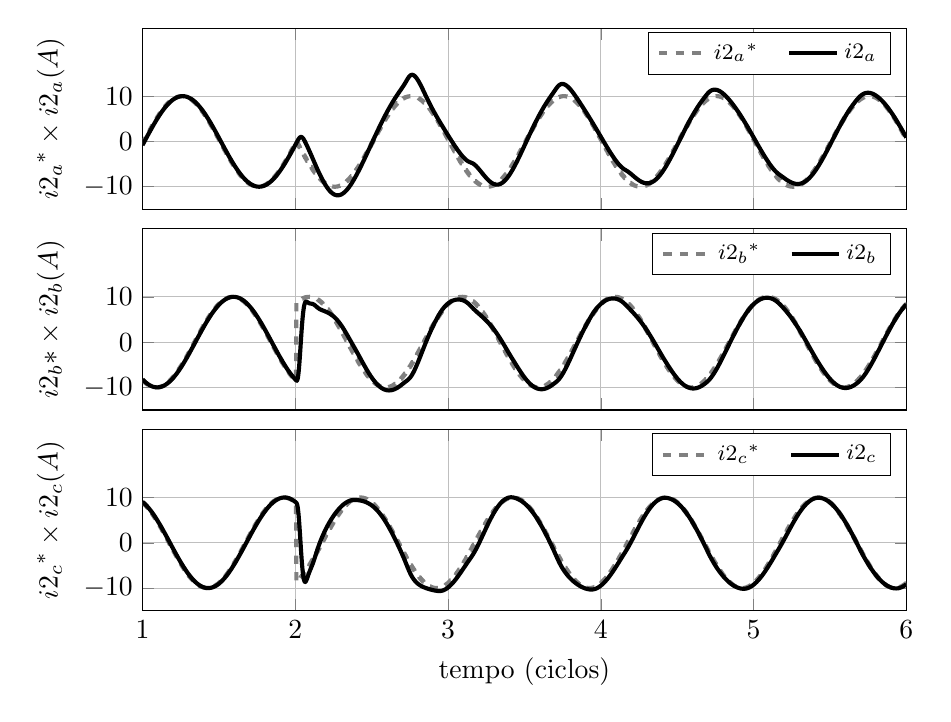
\begin{tikzpicture}

\begin{axis}[%
width=0.8\textwidth,
height=0.189701500343624\textwidth,
scale only axis,
xmin=0.316666666666667,
xmax=0.4,
xtick={0.316666666666667,0.333333333333333,0.35,0.366666666666667,0.383333333333333,0.4},
xticklabels={\empty},
xmajorgrids,
ymin=-15,
ymax=25,
ytick={-10,   0,  10},
ylabel={${\text{i2}_\text{b}}\text{* }\times\text{ i2}_\text{b}\text{ (A)}$},
ymajorgrids,
name=plot2,
legend style={draw=black,fill=white,legend cell align=left},
scaled x ticks = false,
legend columns=-1,
legend style={/tikz/every even column/.append style={column sep=0.3cm}},
legend style={font=\footnotesize}
]
\addplot [color=gray,dashed,line width=1.5pt]
  table[row sep=crcr]{0.316658333333333	-8.32921240710225\\
0.3167	-8.49892692986993\\
0.316741666666667	-8.49892692986993\\
0.316783333333333	-8.6602540378457\\
0.316825	-8.6602540378457\\
0.316866666666667	-8.81303452065127\\
0.316908333333333	-8.81303452065127\\
0.31695	-8.9571176023955\\
0.316991666666667	-8.9571176023955\\
0.317033333333333	-9.09236109047209\\
0.317075	-9.09236109047209\\
0.317116666666667	-9.21863151588643\\
0.317158333333333	-9.21863151588643\\
0.3172	-9.33580426497347\\
0.317241666666667	-9.33580426497347\\
0.317283333333333	-9.44376370237628\\
0.317325	-9.44376370237628\\
0.317366666666667	-9.54240328516426\\
0.317408333333333	-9.54240328516426\\
0.31745	-9.63162566797809\\
0.317491666666667	-9.63162566797809\\
0.317533333333333	-9.71134279909789\\
0.317575	-9.71134279909789\\
0.317616666666667	-9.7814760073396\\
0.317658333333333	-9.7814760073396\\
0.3177	-9.84195607969398\\
0.317741666666667	-9.84195607969398\\
0.317783333333333	-9.89272332963145\\
0.317825	-9.89272332963145\\
0.317866666666667	-9.93372765600555\\
0.317908333333333	-9.93372765600555\\
0.31795	-9.96492859249664\\
0.317991666666667	-9.96492859249664\\
0.318033333333333	-9.98629534754734\\
0.318075	-9.98629534754734\\
0.318116666666667	-9.99780683475006\\
0.318158333333333	-9.99780683475006\\
0.3182	-9.99945169365673\\
0.318241666666667	-9.99945169365673\\
0.318283333333333	-9.9912283009902\\
0.318325	-9.9912283009902\\
0.318366666666667	-9.9731447722462\\
0.318408333333333	-9.9731447722462\\
0.31845	-9.94521895368435\\
0.318491666666667	-9.94521895368435\\
0.318533333333333	-9.90747840471606\\
0.318575	-9.90747840471606\\
0.318616666666667	-9.85996037070666\\
0.318658333333333	-9.85996037070666\\
0.3187	-9.80271174621883\\
0.318741666666667	-9.80271174621883\\
0.318783333333333	-9.73578902873321\\
0.318825	-9.73578902873321\\
0.318866666666667	-9.65925826289228\\
0.318908333333333	-9.65925826289228\\
0.31895	-9.57319497532226\\
0.318991666666667	-9.57319497532226\\
0.319033333333333	-9.47768410009743\\
0.319075	-9.47768410009743\\
0.319116666666667	-9.37281989492048\\
0.319158333333333	-9.37281989492048\\
0.3192	-9.2587058481015\\
0.319241666666667	-9.2587058481015\\
0.319283333333333	-9.13545457642755\\
0.319325	-9.13545457642755\\
0.319366666666667	-9.00318771402345\\
0.319408333333333	-9.00318771402345\\
0.31945	-8.86203579231365\\
0.319491666666667	-8.86203579231365\\
0.319533333333333	-8.71213811120338\\
0.319575	-8.71213811120338\\
0.319616666666667	-8.55364260160653\\
0.319658333333333	-8.55364260160653\\
0.3197	-8.38670567945568\\
0.319741666666667	-8.38670567945568\\
0.319783333333333	-8.21149209133845\\
0.319825	-8.21149209133845\\
0.319866666666667	-8.02817475191253\\
0.319908333333333	-8.02817475191253\\
0.31995	-7.83693457325976\\
0.319991666666667	-7.83693457325976\\
0.320033333333333	-7.63796028634775\\
0.320075	-7.63796028634775\\
0.320116666666667	-7.43144825477524\\
0.320158333333333	-7.43144825477524\\
0.3202	-7.21760228098489\\
0.320241666666667	-7.21760228098489\\
0.320283333333333	-6.99663340513489\\
0.320325	-6.99663340513489\\
0.320366666666667	-6.76875969682781\\
0.320408333333333	-6.76875969682781\\
0.32045	-6.53420603990222\\
0.320491666666667	-6.53420603990222\\
0.320533333333333	-6.29320391049951\\
0.320575	-6.29320391049951\\
0.320616666666667	-6.04599114862485\\
0.320658333333333	-6.04599114862485\\
0.3207	-5.79281172342785\\
0.320741666666667	-5.79281172342785\\
0.320783333333333	-5.53391549243446\\
0.320825	-5.53391549243446\\
0.320866666666667	-5.26955795496776\\
0.320908333333333	-5.26955795496776\\
0.32095	-5.00000000000094\\
0.320991666666667	-5.00000000000094\\
0.321033333333333	-4.72550764869144\\
0.321075	-4.72550764869144\\
0.321116666666667	-4.44635179185013\\
0.321158333333333	-4.44635179185013\\
0.3212	-4.16280792260482\\
0.321241666666667	-4.16280792260482\\
0.321283333333333	-3.87515586452179\\
0.321325	-3.87515586452179\\
0.321366666666667	-3.58367949545372\\
0.321408333333333	-3.58367949545372\\
0.32145	-3.28866646738651\\
0.321491666666667	-3.28866646738651\\
0.321533333333333	-2.99040792256149\\
0.321575	-2.99040792256149\\
0.321616666666667	-2.68919820615324\\
0.321658333333333	-2.68919820615324\\
0.3217	-2.38533457578634\\
0.321741666666667	-2.38533457578634\\
0.321783333333333	-2.07911690817807\\
0.321825	-2.07911690817807\\
0.321866666666667	-1.77084740319627\\
0.321908333333333	-1.77084740319627\\
0.32195	-1.4608302856245\\
0.321991666666667	-1.4608302856245\\
0.322033333333333	-1.149371504929\\
0.322075	-1.149371504929\\
0.322116666666667	-0.836778433323436\\
0.322158333333333	-0.836778433323436\\
0.3222	-0.523359562429668\\
0.322241666666667	-0.523359562429668\\
0.322283333333333	-0.209424198833749\\
0.322325	-0.209424198833749\\
0.322366666666667	0.10471784116233\\
0.322408333333333	0.10471784116233\\
0.32245	0.41875653729192\\
0.322491666666667	0.41875653729192\\
0.322533333333333	0.732381971276291\\
0.322575	0.732381971276291\\
0.322616666666667	1.04528463267656\\
0.322658333333333	1.04528463267656\\
0.3227	1.35715572434312\\
0.322741666666667	1.35715572434312\\
0.322783333333333	1.66768746716115\\
0.322825	1.66768746716115\\
0.322866666666667	1.97657340379144\\
0.322908333333333	1.97657340379144\\
0.32295	2.28350870110679\\
0.322991666666667	2.28350870110679\\
0.323033333333333	2.58819045102549\\
0.323075	2.58819045102549\\
0.323116666666667	2.89031796944505\\
0.323158333333333	2.89031796944505\\
0.3232	3.18959309298109\\
0.323241666666667	3.18959309298109\\
0.323283333333333	3.48572047321859\\
0.323325	3.48572047321859\\
0.323366666666667	3.77840786818516\\
0.323408333333333	3.77840786818516\\
0.32345	4.06736643075854\\
0.323491666666667	4.06736643075854\\
0.323533333333333	4.35231099372386\\
0.323575	4.35231099372386\\
0.323616666666667	4.63296035119925\\
0.323658333333333	4.63296035119925\\
0.3237	4.90903753615209\\
0.323741666666667	4.90903753615209\\
0.323783333333333	5.18027009373203\\
0.323825	5.18027009373203\\
0.323866666666667	5.44639035015104\\
0.323908333333333	5.44639035015104\\
0.32395	5.70713567684513\\
0.323991666666667	5.70713567684513\\
0.324033333333333	5.96224874965702\\
0.324075	5.96224874965702\\
0.324116666666667	6.21147780278401\\
0.324158333333333	6.21147780278401\\
0.3242	6.45457687724046\\
0.324241666666667	6.45457687724046\\
0.324283333333333	6.69130606358958\\
0.324325	6.69130606358958\\
0.324366666666667	6.9214317387051\\
0.324408333333333	6.9214317387051\\
0.32445	7.14472679632911\\
0.324491666666667	7.14472679632911\\
0.324533333333333	7.36097087119846\\
0.324575	7.36097087119846\\
0.324616666666667	7.56995055651872\\
0.324658333333333	7.56995055651872\\
0.3247	7.7714596145709\\
0.324741666666667	7.7714596145709\\
0.324783333333333	7.96529918024319\\
0.324825	7.96529918024319\\
0.324866666666667	8.1512779572868\\
0.324908333333333	8.1512779572868\\
0.32495	8.32921240710229\\
0.324991666666667	8.32921240710229\\
0.325033333333333	8.49892692986996\\
0.325075	8.49892692986996\\
0.325116666666667	8.66025403784574\\
0.325158333333333	8.66025403784574\\
0.3252	8.81303452065131\\
0.325241666666667	8.81303452065131\\
0.325283333333333	8.95711760239554\\
0.325325	8.95711760239554\\
0.325366666666667	9.09236109047212\\
0.325408333333333	9.09236109047212\\
0.32545	9.21863151588647\\
0.325491666666667	9.21863151588647\\
0.325533333333333	9.33580426497351\\
0.325575	9.33580426497351\\
0.325616666666667	9.44376370237632\\
0.325658333333333	9.44376370237632\\
0.3257	9.5424032851643\\
0.325741666666667	9.5424032851643\\
0.325783333333333	9.63162566797813\\
0.325825	9.63162566797813\\
0.325866666666667	9.71134279909793\\
0.325908333333333	9.71134279909793\\
0.32595	9.78147600733964\\
0.325991666666667	9.78147600733964\\
0.326033333333333	9.84195607969402\\
0.326075	9.84195607969402\\
0.326116666666667	9.8927233296315\\
0.326158333333333	9.8927233296315\\
0.3262	9.93372765600559\\
0.326241666666667	9.93372765600559\\
0.326283333333333	9.96492859249668\\
0.326325	9.96492859249668\\
0.326366666666667	9.98629534754738\\
0.326408333333333	9.98629534754738\\
0.32645	9.99780683475011\\
0.326491666666667	9.99780683475011\\
0.326533333333333	9.99945169365678\\
0.326575	9.99945169365678\\
0.326616666666667	9.99122830099025\\
0.326658333333333	9.99122830099025\\
0.3267	9.97314477224624\\
0.326741666666667	9.97314477224624\\
0.326783333333333	9.9452189536844\\
0.326825	9.9452189536844\\
0.326866666666667	9.9074784047161\\
0.326908333333333	9.9074784047161\\
0.32695	9.85996037070671\\
0.326991666666667	9.85996037070671\\
0.327033333333333	9.80271174621887\\
0.327075	9.80271174621887\\
0.327116666666667	9.73578902873325\\
0.327158333333333	9.73578902873325\\
0.3272	9.65925826289232\\
0.327241666666667	9.65925826289232\\
0.327283333333333	9.5731949753223\\
0.327325	9.5731949753223\\
0.327366666666667	9.47768410009748\\
0.327408333333333	9.47768410009748\\
0.32745	9.37281989492053\\
0.327491666666667	9.37281989492053\\
0.327533333333333	9.25870584810154\\
0.327575	9.25870584810154\\
0.327616666666667	9.13545457642759\\
0.327658333333333	9.13545457642759\\
0.3277	9.0031877140235\\
0.327741666666667	9.0031877140235\\
0.327783333333333	8.86203579231369\\
0.327825	8.86203579231369\\
0.327866666666667	8.71213811120342\\
0.327908333333333	8.71213811120342\\
0.32795	8.55364260160657\\
0.327991666666667	8.55364260160657\\
0.328033333333333	8.38670567945572\\
0.328075	8.38670567945572\\
0.328116666666667	8.21149209133849\\
0.328158333333333	8.21149209133849\\
0.3282	8.02817475191257\\
0.328241666666667	8.02817475191257\\
0.328283333333333	7.83693457325979\\
0.328325	7.83693457325979\\
0.328366666666667	7.63796028634779\\
0.328408333333333	7.63796028634779\\
0.32845	7.43144825477528\\
0.328491666666667	7.43144825477528\\
0.328533333333333	7.21760228098492\\
0.328575	7.21760228098492\\
0.328616666666667	6.99663340513492\\
0.328658333333333	6.99663340513492\\
0.3287	6.76875969682784\\
0.328741666666667	6.76875969682784\\
0.328783333333333	6.53420603990226\\
0.328825	6.53420603990226\\
0.328866666666667	6.29320391049954\\
0.328908333333333	6.29320391049954\\
0.32895	6.04599114862488\\
0.328991666666667	6.04599114862488\\
0.329033333333333	5.79281172342788\\
0.329075	5.79281172342788\\
0.329116666666667	5.53391549243449\\
0.329158333333333	5.53391549243449\\
0.3292	5.26955795496778\\
0.329241666666667	5.26955795496778\\
0.329283333333333	5.00000000000096\\
0.329325	5.00000000000096\\
0.329366666666667	4.72550764869146\\
0.329408333333333	4.72550764869146\\
0.32945	4.44635179185015\\
0.329491666666667	4.44635179185015\\
0.329533333333333	4.16280792260484\\
0.329575	4.16280792260484\\
0.329616666666667	3.87515586452181\\
0.329658333333333	3.87515586452181\\
0.3297	3.58367949545374\\
0.329741666666667	3.58367949545374\\
0.329783333333333	3.28866646738652\\
0.329825	3.28866646738652\\
0.329866666666667	2.99040792256151\\
0.329908333333333	2.99040792256151\\
0.32995	2.68919820615325\\
0.329991666666667	2.68919820615325\\
0.330033333333333	2.38533457578635\\
0.330075	2.38533457578635\\
0.330116666666667	2.07911690817808\\
0.330158333333333	2.07911690817808\\
0.3302	1.77084740319627\\
0.330241666666667	1.77084740319627\\
0.330283333333333	1.4608302856245\\
0.330325	1.4608302856245\\
0.330366666666667	1.149371504929\\
0.330408333333333	1.149371504929\\
0.33045	0.836778433323441\\
0.330491666666667	0.836778433323441\\
0.330533333333333	0.523359562429672\\
0.330575	0.523359562429672\\
0.330616666666667	0.20942419883375\\
0.330658333333333	0.20942419883375\\
0.3307	-0.10471784116233\\
0.330741666666667	-0.10471784116233\\
0.330783333333333	-0.418756537291922\\
0.330825	-0.418756537291922\\
0.330866666666667	-0.732381971276294\\
0.330908333333333	-0.732381971276294\\
0.33095	-1.04528463267656\\
0.330991666666667	-1.04528463267656\\
0.331033333333333	-1.35715572434313\\
0.331075	-1.35715572434313\\
0.331116666666667	-1.66768746716116\\
0.331158333333333	-1.66768746716116\\
0.3312	-1.97657340379145\\
0.331241666666667	-1.97657340379145\\
0.331283333333333	-2.2835087011068\\
0.331325	-2.2835087011068\\
0.331366666666667	-2.5881904510255\\
0.331408333333333	-2.5881904510255\\
0.33145	-2.89031796944506\\
0.331491666666667	-2.89031796944506\\
0.331533333333333	-3.1895930929811\\
0.331575	-3.1895930929811\\
0.331616666666667	-3.4857204732186\\
0.331658333333333	-3.4857204732186\\
0.3317	-3.77840786818517\\
0.331741666666667	-3.77840786818517\\
0.331783333333333	-4.06736643075855\\
0.331825	-4.06736643075855\\
0.331866666666667	-4.35231099372388\\
0.331908333333333	-4.35231099372388\\
0.33195	-4.63296035119927\\
0.331991666666667	-4.63296035119927\\
0.332033333333333	-4.90903753615211\\
0.332075	-4.90903753615211\\
0.332116666666667	-5.18027009373205\\
0.332158333333333	-5.18027009373205\\
0.3322	-5.44639035015107\\
0.332241666666667	-5.44639035015107\\
0.332283333333333	-5.70713567684516\\
0.332325	-5.70713567684516\\
0.332366666666667	-5.96224874965705\\
0.332408333333333	-5.96224874965705\\
0.33245	-6.21147780278404\\
0.332491666666667	-6.21147780278404\\
0.332533333333333	-6.45457687724048\\
0.332575	-6.45457687724048\\
0.332616666666667	-6.6913060635896\\
0.332658333333333	-6.6913060635896\\
0.3327	-6.92143173870513\\
0.332741666666667	-6.92143173870513\\
0.332783333333333	-7.14472679632914\\
0.332825	-7.14472679632914\\
0.332866666666667	-7.36097087119849\\
0.332908333333333	-7.36097087119849\\
0.33295	-7.56995055651875\\
0.332991666666667	-7.56995055651875\\
0.333033333333333	-7.77145961457093\\
0.333075	-7.77145961457093\\
0.333116666666667	-7.96529918024322\\
0.333158333333333	-7.96529918024322\\
0.3332	-8.15127795728684\\
0.333241666666667	-8.15127795728684\\
0.333283333333333	-8.32921240710232\\
0.333325	-8.32921240710232\\
0.333366666666667	-8.49892692987\\
0.333408333333333	-8.49892692987\\
0.33345	8.66025403784578\\
0.333491666666667	8.66025403784578\\
0.333533333333333	8.81303452065134\\
0.333575	8.81303452065134\\
0.333616666666667	8.95711760239558\\
0.333658333333333	8.95711760239558\\
0.3337	9.09236109047216\\
0.333741666666667	9.09236109047216\\
0.333783333333333	9.21863151588651\\
0.333825	9.21863151588651\\
0.333866666666667	9.33580426497354\\
0.333908333333333	9.33580426497354\\
0.33395	9.44376370237636\\
0.333991666666667	9.44376370237636\\
0.334033333333333	9.54240328516434\\
0.334075	9.54240328516434\\
0.334116666666667	9.63162566797817\\
0.334158333333333	9.63162566797817\\
0.3342	9.71134279909797\\
0.334241666666667	9.71134279909797\\
0.334283333333333	9.78147600733968\\
0.334325	9.78147600733968\\
0.334366666666667	9.84195607969406\\
0.334408333333333	9.84195607969406\\
0.33445	9.89272332963154\\
0.334491666666667	9.89272332963154\\
0.334533333333333	9.93372765600563\\
0.334575	9.93372765600563\\
0.334616666666667	9.96492859249672\\
0.334658333333333	9.96492859249672\\
0.3347	9.98629534754742\\
0.334741666666667	9.98629534754742\\
0.334783333333333	9.99780683475015\\
0.334825	9.99780683475015\\
0.334866666666667	9.99945169365682\\
0.334908333333333	9.99945169365682\\
0.33495	9.99122830099028\\
0.334991666666667	9.99122830099028\\
0.335033333333333	9.97314477224628\\
0.335075	9.97314477224628\\
0.335116666666667	9.94521895368444\\
0.335158333333333	9.94521895368444\\
0.3352	9.90747840471614\\
0.335241666666667	9.90747840471614\\
0.335283333333333	9.85996037070675\\
0.335325	9.85996037070675\\
0.335366666666667	9.80271174621891\\
0.335408333333333	9.80271174621891\\
0.33545	9.73578902873329\\
0.335491666666667	9.73578902873329\\
0.335533333333333	9.65925826289236\\
0.335575	9.65925826289236\\
0.335616666666667	9.57319497532234\\
0.335658333333333	9.57319497532234\\
0.3357	9.47768410009751\\
0.335741666666667	9.47768410009751\\
0.335783333333333	9.37281989492056\\
0.335825	9.37281989492056\\
0.335866666666667	9.25870584810158\\
0.335908333333333	9.25870584810158\\
0.33595	9.13545457642762\\
0.335991666666667	9.13545457642762\\
0.336033333333333	9.00318771402353\\
0.336075	9.00318771402353\\
0.336116666666667	8.86203579231372\\
0.336158333333333	8.86203579231372\\
0.3362	8.71213811120345\\
0.336241666666667	8.71213811120345\\
0.336283333333333	8.5536426016066\\
0.336325	8.5536426016066\\
0.336366666666667	8.38670567945575\\
0.336408333333333	8.38670567945575\\
0.33645	8.21149209133852\\
0.336491666666667	8.21149209133852\\
0.336533333333333	8.0281747519126\\
0.336575	8.0281747519126\\
0.336616666666667	7.83693457325982\\
0.336658333333333	7.83693457325982\\
0.3367	7.63796028634782\\
0.336741666666667	7.63796028634782\\
0.336783333333333	7.43144825477531\\
0.336825	7.43144825477531\\
0.336866666666667	7.21760228098495\\
0.336908333333333	7.21760228098495\\
0.33695	6.99663340513495\\
0.336991666666667	6.99663340513495\\
0.337033333333333	6.76875969682787\\
0.337075	6.76875969682787\\
0.337116666666667	6.53420603990228\\
0.337158333333333	6.53420603990228\\
0.3372	6.29320391049956\\
0.337241666666667	6.29320391049956\\
0.337283333333333	6.0459911486249\\
0.337325	6.0459911486249\\
0.337366666666667	5.7928117234279\\
0.337408333333333	5.7928117234279\\
0.33745	5.53391549243451\\
0.337491666666667	5.53391549243451\\
0.337533333333333	5.2695579549678\\
0.337575	5.2695579549678\\
0.337616666666667	5.00000000000098\\
0.337658333333333	5.00000000000098\\
0.3377	4.72550764869148\\
0.337741666666667	4.72550764869148\\
0.337783333333333	4.44635179185017\\
0.337825	4.44635179185017\\
0.337866666666667	4.16280792260486\\
0.337908333333333	4.16280792260486\\
0.33795	3.87515586452183\\
0.337991666666667	3.87515586452183\\
0.338033333333333	3.58367949545375\\
0.338075	3.58367949545375\\
0.338116666666667	3.28866646738653\\
0.338158333333333	3.28866646738653\\
0.3382	2.99040792256152\\
0.338241666666667	2.99040792256152\\
0.338283333333333	2.68919820615326\\
0.338325	2.68919820615326\\
0.338366666666667	2.38533457578636\\
0.338408333333333	2.38533457578636\\
0.33845	2.07911690817809\\
0.338491666666667	2.07911690817809\\
0.338533333333333	1.77084740319628\\
0.338575	1.77084740319628\\
0.338616666666667	1.46083028562451\\
0.338658333333333	1.46083028562451\\
0.3387	1.14937150492901\\
0.338741666666667	1.14937150492901\\
0.338783333333333	0.836778433323443\\
0.338825	0.836778433323443\\
0.338866666666667	0.523359562429674\\
0.338908333333333	0.523359562429674\\
0.33895	0.209424198833751\\
0.338991666666667	0.209424198833751\\
0.339033333333333	-0.104717841162331\\
0.339075	-0.104717841162331\\
0.339116666666667	-0.418756537291924\\
0.339158333333333	-0.418756537291924\\
0.3392	-0.732381971276298\\
0.339241666666667	-0.732381971276298\\
0.339283333333333	-1.04528463267657\\
0.339325	-1.04528463267657\\
0.339366666666667	-1.35715572434313\\
0.339408333333333	-1.35715572434313\\
0.33945	-1.66768746716117\\
0.339491666666667	-1.66768746716117\\
0.339533333333333	-1.97657340379146\\
0.339575	-1.97657340379146\\
0.339616666666667	-2.28350870110681\\
0.339658333333333	-2.28350870110681\\
0.3397	-2.58819045102551\\
0.339741666666667	-2.58819045102551\\
0.339783333333333	-2.89031796944507\\
0.339825	-2.89031796944507\\
0.339866666666667	-3.18959309298111\\
0.339908333333333	-3.18959309298111\\
0.33995	-3.48572047321862\\
0.339991666666667	-3.48572047321862\\
0.340033333333333	-3.77840786818519\\
0.340075	-3.77840786818519\\
0.340116666666667	-4.06736643075857\\
0.340158333333333	-4.06736643075857\\
0.3402	-4.35231099372389\\
0.340241666666667	-4.35231099372389\\
0.340283333333333	-4.63296035119929\\
0.340325	-4.63296035119929\\
0.340366666666667	-4.90903753615213\\
0.340408333333333	-4.90903753615213\\
0.34045	-5.18027009373207\\
0.340491666666667	-5.18027009373207\\
0.340533333333333	-5.44639035015109\\
0.340575	-5.44639035015109\\
0.340616666666667	-5.70713567684518\\
0.340658333333333	-5.70713567684518\\
0.3407	-5.96224874965707\\
0.340741666666667	-5.96224874965707\\
0.340783333333333	-6.21147780278406\\
0.340825	-6.21147780278406\\
0.340866666666667	-6.45457687724051\\
0.340908333333333	-6.45457687724051\\
0.34095	-6.69130606358963\\
0.340991666666667	-6.69130606358963\\
0.341033333333333	-6.92143173870516\\
0.341075	-6.92143173870516\\
0.341116666666667	-7.14472679632916\\
0.341158333333333	-7.14472679632916\\
0.3412	-7.36097087119851\\
0.341241666666667	-7.36097087119851\\
0.341283333333333	-7.56995055651877\\
0.341325	-7.56995055651877\\
0.341366666666667	-7.77145961457096\\
0.341408333333333	-7.77145961457096\\
0.34145	-7.96529918024325\\
0.341491666666667	-7.96529918024325\\
0.341533333333333	-8.15127795728687\\
0.341575	-8.15127795728687\\
0.341616666666667	-8.32921240710235\\
0.341658333333333	-8.32921240710235\\
0.3417	-8.49892692987003\\
0.341741666666667	-8.49892692987003\\
0.341783333333333	-8.66025403784581\\
0.341825	-8.66025403784581\\
0.341866666666667	-8.81303452065138\\
0.341908333333333	-8.81303452065138\\
0.34195	-8.95711760239561\\
0.341991666666667	-8.95711760239561\\
0.342033333333333	-9.0923610904722\\
0.342075	-9.0923610904722\\
0.342116666666667	-9.21863151588654\\
0.342158333333333	-9.21863151588654\\
0.3422	-9.33580426497358\\
0.342241666666667	-9.33580426497358\\
0.342283333333333	-9.4437637023764\\
0.342325	-9.4437637023764\\
0.342366666666667	-9.54240328516438\\
0.342408333333333	-9.54240328516438\\
0.34245	-9.63162566797821\\
0.342491666666667	-9.63162566797821\\
0.342533333333333	-9.71134279909801\\
0.342575	-9.71134279909801\\
0.342616666666667	-9.78147600733972\\
0.342658333333333	-9.78147600733972\\
0.3427	-9.8419560796941\\
0.342741666666667	-9.8419560796941\\
0.342783333333333	-9.89272332963157\\
0.342825	-9.89272332963157\\
0.342866666666667	-9.93372765600567\\
0.342908333333333	-9.93372765600567\\
0.34295	-9.96492859249676\\
0.342991666666667	-9.96492859249676\\
0.343033333333333	-9.98629534754746\\
0.343075	-9.98629534754746\\
0.343116666666667	-9.99780683475019\\
0.343158333333333	-9.99780683475019\\
0.3432	-9.99945169365686\\
0.343241666666667	-9.99945169365686\\
0.343283333333333	-9.99122830099032\\
0.343325	-9.99122830099032\\
0.343366666666667	-9.97314477224632\\
0.343408333333333	-9.97314477224632\\
0.34345	-9.94521895368448\\
0.343491666666667	-9.94521895368448\\
0.343533333333333	-9.90747840471618\\
0.343575	-9.90747840471618\\
0.343616666666667	-9.85996037070679\\
0.343658333333333	-9.85996037070679\\
0.3437	-9.80271174621895\\
0.343741666666667	-9.80271174621895\\
0.343783333333333	-9.73578902873333\\
0.343825	-9.73578902873333\\
0.343866666666667	-9.6592582628924\\
0.343908333333333	-9.6592582628924\\
0.34395	-9.57319497532238\\
0.343991666666667	-9.57319497532238\\
0.344033333333333	-9.47768410009755\\
0.344075	-9.47768410009755\\
0.344116666666667	-9.3728198949206\\
0.344158333333333	-9.3728198949206\\
0.3442	-9.25870584810162\\
0.344241666666667	-9.25870584810162\\
0.344283333333333	-9.13545457642766\\
0.344325	-9.13545457642766\\
0.344366666666667	-9.00318771402357\\
0.344408333333333	-9.00318771402357\\
0.34445	-8.86203579231376\\
0.344491666666667	-8.86203579231376\\
0.344533333333333	-8.71213811120348\\
0.344575	-8.71213811120348\\
0.344616666666667	-8.55364260160663\\
0.344658333333333	-8.55364260160663\\
0.3447	-8.38670567945578\\
0.344741666666667	-8.38670567945578\\
0.344783333333333	-8.21149209133855\\
0.344825	-8.21149209133855\\
0.344866666666667	-8.02817475191263\\
0.344908333333333	-8.02817475191263\\
0.34495	-7.83693457325986\\
0.344991666666667	-7.83693457325986\\
0.345033333333333	-7.63796028634785\\
0.345075	-7.63796028634785\\
0.345116666666667	-7.43144825477534\\
0.345158333333333	-7.43144825477534\\
0.3452	-7.21760228098498\\
0.345241666666667	-7.21760228098498\\
0.345283333333333	-6.99663340513498\\
0.345325	-6.99663340513498\\
0.345366666666667	-6.7687596968279\\
0.345408333333333	-6.7687596968279\\
0.34545	-6.5342060399023\\
0.345491666666667	-6.5342060399023\\
0.345533333333333	-6.29320391049959\\
0.345575	-6.29320391049959\\
0.345616666666667	-6.04599114862492\\
0.345658333333333	-6.04599114862492\\
0.3457	-5.79281172342792\\
0.345741666666667	-5.79281172342792\\
0.345783333333333	-5.53391549243453\\
0.345825	-5.53391549243453\\
0.345866666666667	-5.26955795496782\\
0.345908333333333	-5.26955795496782\\
0.34595	-5.000000000001\\
0.345991666666667	-5.000000000001\\
0.346033333333333	-4.72550764869149\\
0.346075	-4.72550764869149\\
0.346116666666667	-4.44635179185018\\
0.346158333333333	-4.44635179185018\\
0.3462	-4.16280792260487\\
0.346241666666667	-4.16280792260487\\
0.346283333333333	-3.87515586452184\\
0.346325	-3.87515586452184\\
0.346366666666667	-3.58367949545377\\
0.346408333333333	-3.58367949545377\\
0.34645	-3.28866646738655\\
0.346491666666667	-3.28866646738655\\
0.346533333333333	-2.99040792256153\\
0.346575	-2.99040792256153\\
0.346616666666667	-2.68919820615327\\
0.346658333333333	-2.68919820615327\\
0.3467	-2.38533457578637\\
0.346741666666667	-2.38533457578637\\
0.346783333333333	-2.0791169081781\\
0.346825	-2.0791169081781\\
0.346866666666667	-1.77084740319629\\
0.346908333333333	-1.77084740319629\\
0.34695	-1.46083028562452\\
0.346991666666667	-1.46083028562452\\
0.347033333333333	-1.14937150492901\\
0.347075	-1.14937150492901\\
0.347116666666667	-0.836778433323448\\
0.347158333333333	-0.836778433323448\\
0.3472	-0.523359562429677\\
0.347241666666667	-0.523359562429677\\
0.347283333333333	-0.209424198833753\\
0.347325	-0.209424198833753\\
0.347366666666667	0.10471784116233\\
0.347408333333333	0.10471784116233\\
0.34745	0.418756537291923\\
0.347491666666667	0.418756537291923\\
0.347533333333333	0.732381971276299\\
0.347575	0.732381971276299\\
0.347616666666667	1.04528463267657\\
0.347658333333333	1.04528463267657\\
0.3477	1.35715572434314\\
0.347741666666667	1.35715572434314\\
0.347783333333333	1.66768746716117\\
0.347825	1.66768746716117\\
0.347866666666667	1.97657340379147\\
0.347908333333333	1.97657340379147\\
0.34795	2.28350870110682\\
0.347991666666667	2.28350870110682\\
0.348033333333333	2.58819045102552\\
0.348075	2.58819045102552\\
0.348116666666667	2.89031796944508\\
0.348158333333333	2.89031796944508\\
0.3482	3.18959309298112\\
0.348241666666667	3.18959309298112\\
0.348283333333333	3.48572047321863\\
0.348325	3.48572047321863\\
0.348366666666667	3.7784078681852\\
0.348408333333333	3.7784078681852\\
0.34845	4.06736643075858\\
0.348491666666667	4.06736643075858\\
0.348533333333333	4.35231099372391\\
0.348575	4.35231099372391\\
0.348616666666667	4.6329603511993\\
0.348658333333333	4.6329603511993\\
0.3487	4.90903753615215\\
0.348741666666667	4.90903753615215\\
0.348783333333333	5.18027009373209\\
0.348825	5.18027009373209\\
0.348866666666667	5.44639035015111\\
0.348908333333333	5.44639035015111\\
0.34895	5.7071356768452\\
0.348991666666667	5.7071356768452\\
0.349033333333333	5.96224874965709\\
0.349075	5.96224874965709\\
0.349116666666667	6.21147780278408\\
0.349158333333333	6.21147780278408\\
0.3492	6.45457687724053\\
0.349241666666667	6.45457687724053\\
0.349283333333333	6.69130606358966\\
0.349325	6.69130606358966\\
0.349366666666667	6.92143173870518\\
0.349408333333333	6.92143173870518\\
0.34945	7.14472679632919\\
0.349491666666667	7.14472679632919\\
0.349533333333333	7.36097087119854\\
0.349575	7.36097087119854\\
0.349616666666667	7.5699505565188\\
0.349658333333333	7.5699505565188\\
0.3497	7.77145961457099\\
0.349741666666667	7.77145961457099\\
0.349783333333333	7.96529918024328\\
0.349825	7.96529918024328\\
0.349866666666667	8.1512779572869\\
0.349908333333333	8.1512779572869\\
0.34995	8.32921240710239\\
0.349991666666667	8.32921240710239\\
0.350033333333333	8.49892692987007\\
0.350075	8.49892692987007\\
0.350116666666667	8.66025403784585\\
0.350158333333333	8.66025403784585\\
0.3502	8.81303452065141\\
0.350241666666667	8.81303452065141\\
0.350283333333333	8.95711760239565\\
0.350325	8.95711760239565\\
0.350366666666667	9.09236109047223\\
0.350408333333333	9.09236109047223\\
0.35045	9.21863151588658\\
0.350491666666667	9.21863151588658\\
0.350533333333333	9.33580426497362\\
0.350575	9.33580426497362\\
0.350616666666667	9.44376370237644\\
0.350658333333333	9.44376370237644\\
0.3507	9.54240328516442\\
0.350741666666667	9.54240328516442\\
0.350783333333333	9.63162566797825\\
0.350825	9.63162566797825\\
0.350866666666667	9.71134279909805\\
0.350908333333333	9.71134279909805\\
0.35095	9.78147600733976\\
0.350991666666667	9.78147600733976\\
0.351033333333333	9.84195607969414\\
0.351075	9.84195607969414\\
0.351116666666667	9.89272332963162\\
0.351158333333333	9.89272332963162\\
0.3512	9.93372765600571\\
0.351241666666667	9.93372765600571\\
0.351283333333333	9.9649285924968\\
0.351325	9.9649285924968\\
0.351366666666667	9.98629534754751\\
0.351408333333333	9.98629534754751\\
0.35145	9.99780683475023\\
0.351491666666667	9.99780683475023\\
0.351533333333333	9.9994516936569\\
0.351575	9.9994516936569\\
0.351616666666667	9.99122830099037\\
0.351658333333333	9.99122830099037\\
0.3517	9.97314477224637\\
0.351741666666667	9.97314477224637\\
0.351783333333333	9.94521895368452\\
0.351825	9.94521895368452\\
0.351866666666667	9.90747840471622\\
0.351908333333333	9.90747840471622\\
0.35195	9.85996037070683\\
0.351991666666667	9.85996037070683\\
0.352033333333333	9.80271174621899\\
0.352075	9.80271174621899\\
0.352116666666667	9.73578902873337\\
0.352158333333333	9.73578902873337\\
0.3522	9.65925826289244\\
0.352241666666667	9.65925826289244\\
0.352283333333333	9.57319497532242\\
0.352325	9.57319497532242\\
0.352366666666667	9.4776841000976\\
0.352408333333333	9.4776841000976\\
0.35245	9.37281989492064\\
0.352491666666667	9.37281989492064\\
0.352533333333333	9.25870584810166\\
0.352575	9.25870584810166\\
0.352616666666667	9.1354545764277\\
0.352658333333333	9.1354545764277\\
0.3527	9.00318771402361\\
0.352741666666667	9.00318771402361\\
0.352783333333333	8.8620357923138\\
0.352825	8.8620357923138\\
0.352866666666667	8.71213811120352\\
0.352908333333333	8.71213811120352\\
0.35295	8.55364260160667\\
0.352991666666667	8.55364260160667\\
0.353033333333333	8.38670567945582\\
0.353075	8.38670567945582\\
0.353116666666667	8.21149209133859\\
0.353158333333333	8.21149209133859\\
0.3532	8.02817475191267\\
0.353241666666667	8.02817475191267\\
0.353283333333333	7.83693457325989\\
0.353325	7.83693457325989\\
0.353366666666667	7.63796028634788\\
0.353408333333333	7.63796028634788\\
0.35345	7.43144825477537\\
0.353491666666667	7.43144825477537\\
0.353533333333333	7.21760228098502\\
0.353575	7.21760228098502\\
0.353616666666667	6.99663340513501\\
0.353658333333333	6.99663340513501\\
0.3537	6.76875969682793\\
0.353741666666667	6.76875969682793\\
0.353783333333333	6.53420603990234\\
0.353825	6.53420603990234\\
0.353866666666667	6.29320391049962\\
0.353908333333333	6.29320391049962\\
0.35395	6.04599114862495\\
0.353991666666667	6.04599114862495\\
0.354033333333333	5.79281172342795\\
0.354075	5.79281172342795\\
0.354116666666667	5.53391549243456\\
0.354158333333333	5.53391549243456\\
0.3542	5.26955795496785\\
0.354241666666667	5.26955795496785\\
0.354283333333333	5.00000000000103\\
0.354325	5.00000000000103\\
0.354366666666667	4.72550764869152\\
0.354408333333333	4.72550764869152\\
0.35445	4.44635179185021\\
0.354491666666667	4.44635179185021\\
0.354533333333333	4.16280792260489\\
0.354575	4.16280792260489\\
0.354616666666667	3.87515586452186\\
0.354658333333333	3.87515586452186\\
0.3547	3.58367949545379\\
0.354741666666667	3.58367949545379\\
0.354783333333333	3.28866646738657\\
0.354825	3.28866646738657\\
0.354866666666667	2.99040792256155\\
0.354908333333333	2.99040792256155\\
0.35495	2.68919820615329\\
0.354991666666667	2.68919820615329\\
0.355033333333333	2.38533457578638\\
0.355075	2.38533457578638\\
0.355116666666667	2.07911690817811\\
0.355158333333333	2.07911690817811\\
0.3552	1.7708474031963\\
0.355241666666667	1.7708474031963\\
0.355283333333333	1.46083028562453\\
0.355325	1.46083028562453\\
0.355366666666667	1.14937150492902\\
0.355408333333333	1.14937150492902\\
0.35545	0.836778433323456\\
0.355491666666667	0.836778433323456\\
0.355533333333333	0.523359562429684\\
0.355575	0.523359562429684\\
0.355616666666667	0.209424198833759\\
0.355658333333333	0.209424198833759\\
0.3557	-0.104717841162325\\
0.355741666666667	-0.104717841162325\\
0.355783333333333	-0.418756537291921\\
0.355825	-0.418756537291921\\
0.355866666666667	-0.732381971276297\\
0.355908333333333	-0.732381971276297\\
0.35595	-1.04528463267657\\
0.355991666666667	-1.04528463267657\\
0.356033333333333	-1.35715572434314\\
0.356075	-1.35715572434314\\
0.356116666666667	-1.66768746716117\\
0.356158333333333	-1.66768746716117\\
0.3562	-1.97657340379147\\
0.356241666666667	-1.97657340379147\\
0.356283333333333	-2.28350870110682\\
0.356325	-2.28350870110682\\
0.356366666666667	-2.58819045102553\\
0.356408333333333	-2.58819045102553\\
0.35645	-2.89031796944509\\
0.356491666666667	-2.89031796944509\\
0.356533333333333	-3.18959309298113\\
0.356575	-3.18959309298113\\
0.356616666666667	-3.48572047321864\\
0.356658333333333	-3.48572047321864\\
0.3567	-3.77840786818521\\
0.356741666666667	-3.77840786818521\\
0.356783333333333	-4.0673664307586\\
0.356825	-4.0673664307586\\
0.356866666666667	-4.35231099372392\\
0.356908333333333	-4.35231099372392\\
0.35695	-4.63296035119932\\
0.356991666666667	-4.63296035119932\\
0.357033333333333	-4.90903753615216\\
0.357075	-4.90903753615216\\
0.357116666666667	-5.18027009373211\\
0.357158333333333	-5.18027009373211\\
0.3572	-5.44639035015113\\
0.357241666666667	-5.44639035015113\\
0.357283333333333	-5.70713567684522\\
0.357325	-5.70713567684522\\
0.357366666666667	-5.96224874965711\\
0.357408333333333	-5.96224874965711\\
0.35745	-6.21147780278411\\
0.357491666666667	-6.21147780278411\\
0.357533333333333	-6.45457687724056\\
0.357575	-6.45457687724056\\
0.357616666666667	-6.69130606358968\\
0.357658333333333	-6.69130606358968\\
0.3577	-6.92143173870521\\
0.357741666666667	-6.92143173870521\\
0.357783333333333	-7.14472679632922\\
0.357825	-7.14472679632922\\
0.357866666666667	-7.36097087119857\\
0.357908333333333	-7.36097087119857\\
0.35795	-7.56995055651883\\
0.357991666666667	-7.56995055651883\\
0.358033333333333	-7.77145961457102\\
0.358075	-7.77145961457102\\
0.358116666666667	-7.96529918024331\\
0.358158333333333	-7.96529918024331\\
0.3582	-8.15127795728693\\
0.358241666666667	-8.15127795728693\\
0.358283333333333	-8.32921240710242\\
0.358325	-8.32921240710242\\
0.358366666666667	-8.4989269298701\\
0.358408333333333	-8.4989269298701\\
0.35845	-8.66025403784588\\
0.358491666666667	-8.66025403784588\\
0.358533333333333	-8.81303452065145\\
0.358575	-8.81303452065145\\
0.358616666666667	-8.95711760239568\\
0.358658333333333	-8.95711760239568\\
0.3587	-9.09236109047227\\
0.358741666666667	-9.09236109047227\\
0.358783333333333	-9.21863151588662\\
0.358825	-9.21863151588662\\
0.358866666666667	-9.33580426497366\\
0.358908333333333	-9.33580426497366\\
0.35895	-9.44376370237647\\
0.358991666666667	-9.44376370237647\\
0.359033333333333	-9.54240328516445\\
0.359075	-9.54240328516445\\
0.359116666666667	-9.63162566797829\\
0.359158333333333	-9.63162566797829\\
0.3592	-9.71134279909809\\
0.359241666666667	-9.71134279909809\\
0.359283333333333	-9.7814760073398\\
0.359325	-9.7814760073398\\
0.359366666666667	-9.84195607969418\\
0.359408333333333	-9.84195607969418\\
0.35945	-9.89272332963166\\
0.359491666666667	-9.89272332963166\\
0.359533333333333	-9.93372765600575\\
0.359575	-9.93372765600575\\
0.359616666666667	-9.96492859249684\\
0.359658333333333	-9.96492859249684\\
0.3597	-9.98629534754755\\
0.359741666666667	-9.98629534754755\\
0.359783333333333	-9.99780683475027\\
0.359825	-9.99780683475027\\
0.359866666666667	-9.99945169365694\\
0.359908333333333	-9.99945169365694\\
0.35995	-9.99122830099041\\
0.359991666666667	-9.99122830099041\\
0.360033333333333	-9.97314477224641\\
0.360075	-9.97314477224641\\
0.360116666666667	-9.94521895368456\\
0.360158333333333	-9.94521895368456\\
0.3602	-9.90747840471626\\
0.360241666666667	-9.90747840471626\\
0.360283333333333	-9.85996037070687\\
0.360325	-9.85996037070687\\
0.360366666666667	-9.80271174621904\\
0.360408333333333	-9.80271174621904\\
0.36045	-9.73578902873341\\
0.360491666666667	-9.73578902873341\\
0.360533333333333	-9.65925826289248\\
0.360575	-9.65925826289248\\
0.360616666666667	-9.57319497532246\\
0.360658333333333	-9.57319497532246\\
0.3607	-9.47768410009764\\
0.360741666666667	-9.47768410009764\\
0.360783333333333	-9.37281989492068\\
0.360825	-9.37281989492068\\
0.360866666666667	-9.25870584810169\\
0.360908333333333	-9.25870584810169\\
0.36095	-9.13545457642774\\
0.360991666666667	-9.13545457642774\\
0.361033333333333	-9.00318771402364\\
0.361075	-9.00318771402364\\
0.361116666666667	-8.86203579231383\\
0.361158333333333	-8.86203579231383\\
0.3612	-8.71213811120356\\
0.361241666666667	-8.71213811120356\\
0.361283333333333	-8.55364260160671\\
0.361325	-8.55364260160671\\
0.361366666666667	-8.38670567945586\\
0.361408333333333	-8.38670567945586\\
0.36145	-8.21149209133863\\
0.361491666666667	-8.21149209133863\\
0.361533333333333	-8.0281747519127\\
0.361575	-8.0281747519127\\
0.361616666666667	-7.83693457325993\\
0.361658333333333	-7.83693457325993\\
0.3617	-7.63796028634792\\
0.361741666666667	-7.63796028634792\\
0.361783333333333	-7.4314482547754\\
0.361825	-7.4314482547754\\
0.361866666666667	-7.21760228098505\\
0.361908333333333	-7.21760228098505\\
0.36195	-6.99663340513504\\
0.361991666666667	-6.99663340513504\\
0.362033333333333	-6.76875969682796\\
0.362075	-6.76875969682796\\
0.362116666666667	-6.53420603990237\\
0.362158333333333	-6.53420603990237\\
0.3622	-6.29320391049965\\
0.362241666666667	-6.29320391049965\\
0.362283333333333	-6.04599114862498\\
0.362325	-6.04599114862498\\
0.362366666666667	-5.79281172342797\\
0.362408333333333	-5.79281172342797\\
0.36245	-5.53391549243458\\
0.362491666666667	-5.53391549243458\\
0.362533333333333	-5.26955795496787\\
0.362575	-5.26955795496787\\
0.362616666666667	-5.00000000000105\\
0.362658333333333	-5.00000000000105\\
0.3627	-4.72550764869154\\
0.362741666666667	-4.72550764869154\\
0.362783333333333	-4.44635179185023\\
0.362825	-4.44635179185023\\
0.362866666666667	-4.16280792260491\\
0.362908333333333	-4.16280792260491\\
0.36295	-3.87515586452188\\
0.362991666666667	-3.87515586452188\\
0.363033333333333	-3.5836794954538\\
0.363075	-3.5836794954538\\
0.363116666666667	-3.28866646738658\\
0.363158333333333	-3.28866646738658\\
0.3632	-2.99040792256156\\
0.363241666666667	-2.99040792256156\\
0.363283333333333	-2.6891982061533\\
0.363325	-2.6891982061533\\
0.363366666666667	-2.3853345757864\\
0.363408333333333	-2.3853345757864\\
0.36345	-2.07911690817813\\
0.363491666666667	-2.07911690817813\\
0.363533333333333	-1.77084740319631\\
0.363575	-1.77084740319631\\
0.363616666666667	-1.46083028562454\\
0.363658333333333	-1.46083028562454\\
0.3637	-1.14937150492903\\
0.363741666666667	-1.14937150492903\\
0.363783333333333	-0.836778433323463\\
0.363825	-0.836778433323463\\
0.363866666666667	-0.52335956242969\\
0.363908333333333	-0.52335956242969\\
0.36395	-0.209424198833764\\
0.363991666666667	-0.209424198833764\\
0.364033333333333	0.10471784116232\\
0.364075	0.10471784116232\\
0.364116666666667	0.418756537291917\\
0.364158333333333	0.418756537291917\\
0.3642	0.732381971276296\\
0.364241666666667	0.732381971276296\\
0.364283333333333	1.04528463267657\\
0.364325	1.04528463267657\\
0.364366666666667	1.35715572434314\\
0.364408333333333	1.35715572434314\\
0.36445	1.66768746716118\\
0.364491666666667	1.66768746716118\\
0.364533333333333	1.97657340379147\\
0.364575	1.97657340379147\\
0.364616666666667	2.28350870110683\\
0.364658333333333	2.28350870110683\\
0.3647	2.58819045102553\\
0.364741666666667	2.58819045102553\\
0.364783333333333	2.8903179694451\\
0.364825	2.8903179694451\\
0.364866666666667	3.18959309298114\\
0.364908333333333	3.18959309298114\\
0.36495	3.48572047321865\\
0.364991666666667	3.48572047321865\\
0.365033333333333	3.77840786818522\\
0.365075	3.77840786818522\\
0.365116666666667	4.06736643075861\\
0.365158333333333	4.06736643075861\\
0.3652	4.35231099372394\\
0.365241666666667	4.35231099372394\\
0.365283333333333	4.63296035119933\\
0.365325	4.63296035119933\\
0.365366666666667	4.90903753615218\\
0.365408333333333	4.90903753615218\\
0.36545	5.18027009373212\\
0.365491666666667	5.18027009373212\\
0.365533333333333	5.44639035015114\\
0.365575	5.44639035015114\\
0.365616666666667	5.70713567684524\\
0.365658333333333	5.70713567684524\\
0.3657	5.96224874965713\\
0.365741666666667	5.96224874965713\\
0.365783333333333	6.21147780278413\\
0.365825	6.21147780278413\\
0.365866666666667	6.45457687724057\\
0.365908333333333	6.45457687724057\\
0.36595	6.6913060635897\\
0.365991666666667	6.6913060635897\\
0.366033333333333	6.92143173870523\\
0.366075	6.92143173870523\\
0.366116666666667	7.14472679632924\\
0.366158333333333	7.14472679632924\\
0.3662	7.36097087119859\\
0.366241666666667	7.36097087119859\\
0.366283333333333	7.56995055651886\\
0.366325	7.56995055651886\\
0.366366666666667	7.77145961457104\\
0.366408333333333	7.77145961457104\\
0.36645	7.96529918024334\\
0.366491666666667	7.96529918024334\\
0.366533333333333	8.15127795728696\\
0.366575	8.15127795728696\\
0.366616666666667	8.32921240710245\\
0.366658333333333	8.32921240710245\\
0.3667	8.49892692987013\\
0.366741666666667	8.49892692987013\\
0.366783333333333	8.66025403784591\\
0.366825	8.66025403784591\\
0.366866666666667	8.81303452065148\\
0.366908333333333	8.81303452065148\\
0.36695	8.95711760239571\\
0.366991666666667	8.95711760239571\\
0.367033333333333	9.0923610904723\\
0.367075	9.0923610904723\\
0.367116666666667	9.21863151588665\\
0.367158333333333	9.21863151588665\\
0.3672	9.33580426497369\\
0.367241666666667	9.33580426497369\\
0.367283333333333	9.44376370237651\\
0.367325	9.44376370237651\\
0.367366666666667	9.54240328516449\\
0.367408333333333	9.54240328516449\\
0.36745	9.63162566797832\\
0.367491666666667	9.63162566797832\\
0.367533333333333	9.71134279909812\\
0.367575	9.71134279909812\\
0.367616666666667	9.78147600733984\\
0.367658333333333	9.78147600733984\\
0.3677	9.84195607969422\\
0.367741666666667	9.84195607969422\\
0.367783333333333	9.89272332963169\\
0.367825	9.89272332963169\\
0.367866666666667	9.93372765600579\\
0.367908333333333	9.93372765600579\\
0.36795	9.96492859249688\\
0.367991666666667	9.96492859249688\\
0.368033333333333	9.98629534754759\\
0.368075	9.98629534754759\\
0.368116666666667	9.99780683475031\\
0.368158333333333	9.99780683475031\\
0.3682	9.99945169365698\\
0.368241666666667	9.99945169365698\\
0.368283333333333	9.99122830099045\\
0.368325	9.99122830099045\\
0.368366666666667	9.97314477224645\\
0.368408333333333	9.97314477224645\\
0.36845	9.9452189536846\\
0.368491666666667	9.9452189536846\\
0.368533333333333	9.9074784047163\\
0.368575	9.9074784047163\\
0.368616666666667	9.85996037070691\\
0.368658333333333	9.85996037070691\\
0.3687	9.80271174621907\\
0.368741666666667	9.80271174621907\\
0.368783333333333	9.73578902873345\\
0.368825	9.73578902873345\\
0.368866666666667	9.65925826289252\\
0.368908333333333	9.65925826289252\\
0.36895	9.5731949753225\\
0.368991666666667	9.5731949753225\\
0.369033333333333	9.47768410009767\\
0.369075	9.47768410009767\\
0.369116666666667	9.37281989492072\\
0.369158333333333	9.37281989492072\\
0.3692	9.25870584810174\\
0.369241666666667	9.25870584810174\\
0.369283333333333	9.13545457642778\\
0.369325	9.13545457642778\\
0.369366666666667	9.00318771402368\\
0.369408333333333	9.00318771402368\\
0.36945	8.86203579231388\\
0.369491666666667	8.86203579231388\\
0.369533333333333	8.7121381112036\\
0.369575	8.7121381112036\\
0.369616666666667	8.55364260160674\\
0.369658333333333	8.55364260160674\\
0.3697	8.38670567945589\\
0.369741666666667	8.38670567945589\\
0.369783333333333	8.21149209133866\\
0.369825	8.21149209133866\\
0.369866666666667	8.02817475191274\\
0.369908333333333	8.02817475191274\\
0.36995	7.83693457325996\\
0.369991666666667	7.83693457325996\\
0.370033333333333	7.63796028634795\\
0.370075	7.63796028634795\\
0.370116666666667	7.43144825477544\\
0.370158333333333	7.43144825477544\\
0.3702	7.21760228098508\\
0.370241666666667	7.21760228098508\\
0.370283333333333	6.99663340513508\\
0.370325	6.99663340513508\\
0.370366666666667	6.76875969682799\\
0.370408333333333	6.76875969682799\\
0.37045	6.5342060399024\\
0.370491666666667	6.5342060399024\\
0.370533333333333	6.29320391049968\\
0.370575	6.29320391049968\\
0.370616666666667	6.04599114862501\\
0.370658333333333	6.04599114862501\\
0.3707	5.792811723428\\
0.370741666666667	5.792811723428\\
0.370783333333333	5.53391549243461\\
0.370825	5.53391549243461\\
0.370866666666667	5.2695579549679\\
0.370908333333333	5.2695579549679\\
0.37095	5.00000000000107\\
0.370991666666667	5.00000000000107\\
0.371033333333333	4.72550764869157\\
0.371075	4.72550764869157\\
0.371116666666667	4.44635179185025\\
0.371158333333333	4.44635179185025\\
0.3712	4.16280792260494\\
0.371241666666667	4.16280792260494\\
0.371283333333333	3.8751558645219\\
0.371325	3.8751558645219\\
0.371366666666667	3.58367949545382\\
0.371408333333333	3.58367949545382\\
0.37145	3.2886664673866\\
0.371491666666667	3.2886664673866\\
0.371533333333333	2.99040792256158\\
0.371575	2.99040792256158\\
0.371616666666667	2.68919820615332\\
0.371658333333333	2.68919820615332\\
0.3717	2.38533457578641\\
0.371741666666667	2.38533457578641\\
0.371783333333333	2.07911690817814\\
0.371825	2.07911690817814\\
0.371866666666667	1.77084740319632\\
0.371908333333333	1.77084740319632\\
0.37195	1.46083028562455\\
0.371991666666667	1.46083028562455\\
0.372033333333333	1.14937150492904\\
0.372075	1.14937150492904\\
0.372116666666667	0.836778433323472\\
0.372158333333333	0.836778433323472\\
0.3722	0.523359562429696\\
0.372241666666667	0.523359562429696\\
0.372283333333333	0.209424198833769\\
0.372325	0.209424198833769\\
0.372366666666667	-0.104717841162318\\
0.372408333333333	-0.104717841162318\\
0.37245	-0.418756537291916\\
0.372491666666667	-0.418756537291916\\
0.372533333333333	-0.732381971276296\\
0.372575	-0.732381971276296\\
0.372616666666667	-1.04528463267657\\
0.372658333333333	-1.04528463267657\\
0.3727	-1.35715572434314\\
0.372741666666667	-1.35715572434314\\
0.372783333333333	-1.66768746716118\\
0.372825	-1.66768746716118\\
0.372866666666667	-1.97657340379148\\
0.372908333333333	-1.97657340379148\\
0.37295	-2.28350870110683\\
0.372991666666667	-2.28350870110683\\
0.373033333333333	-2.58819045102554\\
0.373075	-2.58819045102554\\
0.373116666666667	-2.89031796944511\\
0.373158333333333	-2.89031796944511\\
0.3732	-3.18959309298115\\
0.373241666666667	-3.18959309298115\\
0.373283333333333	-3.48572047321866\\
0.373325	-3.48572047321866\\
0.373366666666667	-3.77840786818524\\
0.373408333333333	-3.77840786818524\\
0.37345	-4.06736643075862\\
0.373491666666667	-4.06736643075862\\
0.373533333333333	-4.35231099372395\\
0.373575	-4.35231099372395\\
0.373616666666667	-4.63296035119935\\
0.373658333333333	-4.63296035119935\\
0.3737	-4.9090375361522\\
0.373741666666667	-4.9090375361522\\
0.373783333333333	-5.18027009373215\\
0.373825	-5.18027009373215\\
0.373866666666667	-5.44639035015117\\
0.373908333333333	-5.44639035015117\\
0.37395	-5.70713567684527\\
0.373991666666667	-5.70713567684527\\
0.374033333333333	-5.96224874965716\\
0.374075	-5.96224874965716\\
0.374116666666667	-6.21147780278415\\
0.374158333333333	-6.21147780278415\\
0.3742	-6.45457687724061\\
0.374241666666667	-6.45457687724061\\
0.374283333333333	-6.69130606358973\\
0.374325	-6.69130606358973\\
0.374366666666667	-6.92143173870526\\
0.374408333333333	-6.92143173870526\\
0.37445	-7.14472679632927\\
0.374491666666667	-7.14472679632927\\
0.374533333333333	-7.36097087119863\\
0.374575	-7.36097087119863\\
0.374616666666667	-7.56995055651889\\
0.374658333333333	-7.56995055651889\\
0.3747	-7.77145961457108\\
0.374741666666667	-7.77145961457108\\
0.374783333333333	-7.96529918024338\\
0.374825	-7.96529918024338\\
0.374866666666667	-8.151277957287\\
0.374908333333333	-8.151277957287\\
0.37495	-8.32921240710249\\
0.374991666666667	-8.32921240710249\\
0.375033333333333	-8.49892692987017\\
0.375075	-8.49892692987017\\
0.375116666666667	-8.66025403784595\\
0.375158333333333	-8.66025403784595\\
0.3752	-8.81303452065152\\
0.375241666666667	-8.81303452065152\\
0.375283333333333	-8.95711760239576\\
0.375325	-8.95711760239576\\
0.375366666666667	-9.09236109047234\\
0.375408333333333	-9.09236109047234\\
0.37545	-9.2186315158867\\
0.375491666666667	-9.2186315158867\\
0.375533333333333	-9.33580426497374\\
0.375575	-9.33580426497374\\
0.375616666666667	-9.44376370237656\\
0.375658333333333	-9.44376370237656\\
0.3757	-9.54240328516454\\
0.375741666666667	-9.54240328516454\\
0.375783333333333	-9.63162566797837\\
0.375825	-9.63162566797837\\
0.375866666666667	-9.71134279909817\\
0.375908333333333	-9.71134279909817\\
0.37595	-9.78147600733988\\
0.375991666666667	-9.78147600733988\\
0.376033333333333	-9.84195607969427\\
0.376075	-9.84195607969427\\
0.376116666666667	-9.89272332963175\\
0.376158333333333	-9.89272332963175\\
0.3762	-9.93372765600584\\
0.376241666666667	-9.93372765600584\\
0.376283333333333	-9.96492859249693\\
0.376325	-9.96492859249693\\
0.376366666666667	-9.98629534754763\\
0.376408333333333	-9.98629534754763\\
0.37645	-9.99780683475036\\
0.376491666666667	-9.99780683475036\\
0.376533333333333	-9.99945169365703\\
0.376575	-9.99945169365703\\
0.376616666666667	-9.9912283009905\\
0.376658333333333	-9.9912283009905\\
0.3767	-9.9731447722465\\
0.376741666666667	-9.9731447722465\\
0.376783333333333	-9.94521895368465\\
0.376825	-9.94521895368465\\
0.376866666666667	-9.90747840471635\\
0.376908333333333	-9.90747840471635\\
0.37695	-9.85996037070696\\
0.376991666666667	-9.85996037070696\\
0.377033333333333	-9.80271174621912\\
0.377075	-9.80271174621912\\
0.377116666666667	-9.7357890287335\\
0.377158333333333	-9.7357890287335\\
0.3772	-9.65925826289257\\
0.377241666666667	-9.65925826289257\\
0.377283333333333	-9.57319497532255\\
0.377325	-9.57319497532255\\
0.377366666666667	-9.47768410009772\\
0.377408333333333	-9.47768410009772\\
0.37745	-9.37281989492077\\
0.377491666666667	-9.37281989492077\\
0.377533333333333	-9.25870584810178\\
0.377575	-9.25870584810178\\
0.377616666666667	-9.13545457642783\\
0.377658333333333	-9.13545457642783\\
0.3777	-9.00318771402373\\
0.377741666666667	-9.00318771402373\\
0.377783333333333	-8.86203579231392\\
0.377825	-8.86203579231392\\
0.377866666666667	-8.71213811120364\\
0.377908333333333	-8.71213811120364\\
0.37795	-8.55364260160679\\
0.377991666666667	-8.55364260160679\\
0.378033333333333	-8.38670567945594\\
0.378075	-8.38670567945594\\
0.378116666666667	-8.21149209133871\\
0.378158333333333	-8.21149209133871\\
0.3782	-8.02817475191278\\
0.378241666666667	-8.02817475191278\\
0.378283333333333	-7.83693457326\\
0.378325	-7.83693457326\\
0.378366666666667	-7.63796028634799\\
0.378408333333333	-7.63796028634799\\
0.37845	-7.43144825477548\\
0.378491666666667	-7.43144825477548\\
0.378533333333333	-7.21760228098512\\
0.378575	-7.21760228098512\\
0.378616666666667	-6.99663340513511\\
0.378658333333333	-6.99663340513511\\
0.3787	-6.76875969682803\\
0.378741666666667	-6.76875969682803\\
0.378783333333333	-6.53420603990243\\
0.378825	-6.53420603990243\\
0.378866666666667	-6.29320391049971\\
0.378908333333333	-6.29320391049971\\
0.37895	-6.04599114862504\\
0.378991666666667	-6.04599114862504\\
0.379033333333333	-5.79281172342804\\
0.379075	-5.79281172342804\\
0.379116666666667	-5.53391549243464\\
0.379158333333333	-5.53391549243464\\
0.3792	-5.26955795496793\\
0.379241666666667	-5.26955795496793\\
0.379283333333333	-5.0000000000011\\
0.379325	-5.0000000000011\\
0.379366666666667	-4.7255076486916\\
0.379408333333333	-4.7255076486916\\
0.37945	-4.44635179185028\\
0.379491666666667	-4.44635179185028\\
0.379533333333333	-4.16280792260496\\
0.379575	-4.16280792260496\\
0.379616666666667	-3.87515586452193\\
0.379658333333333	-3.87515586452193\\
0.3797	-3.58367949545385\\
0.379741666666667	-3.58367949545385\\
0.379783333333333	-3.28866646738662\\
0.379825	-3.28866646738662\\
0.379866666666667	-2.9904079225616\\
0.379908333333333	-2.9904079225616\\
0.37995	-2.68919820615333\\
0.379991666666667	-2.68919820615333\\
0.380033333333333	-2.38533457578643\\
0.380075	-2.38533457578643\\
0.380116666666667	-2.07911690817816\\
0.380158333333333	-2.07911690817816\\
0.3802	-1.77084740319634\\
0.380241666666667	-1.77084740319634\\
0.380283333333333	-1.46083028562456\\
0.380325	-1.46083028562456\\
0.380366666666667	-1.14937150492905\\
0.380408333333333	-1.14937150492905\\
0.38045	-0.836778433323481\\
0.380491666666667	-0.836778433323481\\
0.380533333333333	-0.523359562429705\\
0.380575	-0.523359562429705\\
0.380616666666667	-0.209424198833776\\
0.380658333333333	-0.209424198833776\\
0.3807	0.104717841162311\\
0.380741666666667	0.104717841162311\\
0.380783333333333	0.418756537291912\\
0.380825	0.418756537291912\\
0.380866666666667	0.732381971276293\\
0.380908333333333	0.732381971276293\\
0.38095	1.04528463267657\\
0.380991666666667	1.04528463267657\\
0.381033333333333	1.35715572434314\\
0.381075	1.35715572434314\\
0.381116666666667	1.66768746716118\\
0.381158333333333	1.66768746716118\\
0.3812	1.97657340379148\\
0.381241666666667	1.97657340379148\\
0.381283333333333	2.28350870110684\\
0.381325	2.28350870110684\\
0.381366666666667	2.58819045102555\\
0.381408333333333	2.58819045102555\\
0.38145	2.89031796944512\\
0.381491666666667	2.89031796944512\\
0.381533333333333	3.18959309298116\\
0.381575	3.18959309298116\\
0.381616666666667	3.48572047321867\\
0.381658333333333	3.48572047321867\\
0.3817	3.77840786818525\\
0.381741666666667	3.77840786818525\\
0.381783333333333	4.06736643075864\\
0.381825	4.06736643075864\\
0.381866666666667	4.35231099372397\\
0.381908333333333	4.35231099372397\\
0.38195	4.63296035119937\\
0.381991666666667	4.63296035119937\\
0.382033333333333	4.90903753615222\\
0.382075	4.90903753615222\\
0.382116666666667	5.18027009373217\\
0.382158333333333	5.18027009373217\\
0.3822	5.44639035015119\\
0.382241666666667	5.44639035015119\\
0.382283333333333	5.70713567684529\\
0.382325	5.70713567684529\\
0.382366666666667	5.96224874965718\\
0.382408333333333	5.96224874965718\\
0.38245	6.21147780278418\\
0.382491666666667	6.21147780278418\\
0.382533333333333	6.45457687724063\\
0.382575	6.45457687724063\\
0.382616666666667	6.69130606358976\\
0.382658333333333	6.69130606358976\\
0.3827	6.92143173870529\\
0.382741666666667	6.92143173870529\\
0.382783333333333	7.14472679632931\\
0.382825	7.14472679632931\\
0.382866666666667	7.36097087119866\\
0.382908333333333	7.36097087119866\\
0.38295	7.56995055651893\\
0.382991666666667	7.56995055651893\\
0.383033333333333	7.77145961457112\\
0.383075	7.77145961457112\\
0.383116666666667	7.96529918024341\\
0.383158333333333	7.96529918024341\\
0.3832	8.15127795728703\\
0.383241666666667	8.15127795728703\\
0.383283333333333	8.32921240710253\\
0.383325	8.32921240710253\\
0.383366666666667	8.49892692987021\\
0.383408333333333	8.49892692987021\\
0.38345	8.66025403784599\\
0.383491666666667	8.66025403784599\\
0.383533333333333	8.81303452065156\\
0.383575	8.81303452065156\\
0.383616666666667	8.9571176023958\\
0.383658333333333	8.9571176023958\\
0.3837	9.09236109047239\\
0.383741666666667	9.09236109047239\\
0.383783333333333	9.21863151588674\\
0.383825	9.21863151588674\\
0.383866666666667	9.33580426497378\\
0.383908333333333	9.33580426497378\\
0.38395	9.4437637023766\\
0.383991666666667	9.4437637023766\\
0.384033333333333	9.54240328516458\\
0.384075	9.54240328516458\\
0.384116666666667	9.63162566797842\\
0.384158333333333	9.63162566797842\\
0.3842	9.71134279909822\\
0.384241666666667	9.71134279909822\\
0.384283333333333	9.78147600733993\\
0.384325	9.78147600733993\\
0.384366666666667	9.84195607969432\\
0.384408333333333	9.84195607969432\\
0.38445	9.89272332963179\\
0.384491666666667	9.89272332963179\\
0.384533333333333	9.93372765600589\\
0.384575	9.93372765600589\\
0.384616666666667	9.96492859249698\\
0.384658333333333	9.96492859249698\\
0.3847	9.98629534754769\\
0.384741666666667	9.98629534754769\\
0.384783333333333	9.99780683475041\\
0.384825	9.99780683475041\\
0.384866666666667	9.99945169365708\\
0.384908333333333	9.99945169365708\\
0.38495	9.99122830099055\\
0.384991666666667	9.99122830099055\\
0.385033333333333	9.97314477224655\\
0.385075	9.97314477224655\\
0.385116666666667	9.9452189536847\\
0.385158333333333	9.9452189536847\\
0.3852	9.9074784047164\\
0.385241666666667	9.9074784047164\\
0.385283333333333	9.85996037070701\\
0.385325	9.85996037070701\\
0.385366666666667	9.80271174621917\\
0.385408333333333	9.80271174621917\\
0.38545	9.73578902873355\\
0.385491666666667	9.73578902873355\\
0.385533333333333	9.65925826289262\\
0.385575	9.65925826289262\\
0.385616666666667	9.5731949753226\\
0.385658333333333	9.5731949753226\\
0.3857	9.47768410009777\\
0.385741666666667	9.47768410009777\\
0.385783333333333	9.37281989492082\\
0.385825	9.37281989492082\\
0.385866666666667	9.25870584810183\\
0.385908333333333	9.25870584810183\\
0.38595	9.13545457642787\\
0.385991666666667	9.13545457642787\\
0.386033333333333	9.00318771402378\\
0.386075	9.00318771402378\\
0.386116666666667	8.86203579231397\\
0.386158333333333	8.86203579231397\\
0.3862	8.71213811120369\\
0.386241666666667	8.71213811120369\\
0.386283333333333	8.55364260160684\\
0.386325	8.55364260160684\\
0.386366666666667	8.38670567945598\\
0.386408333333333	8.38670567945598\\
0.38645	8.21149209133875\\
0.386491666666667	8.21149209133875\\
0.386533333333333	8.02817475191283\\
0.386575	8.02817475191283\\
0.386616666666667	7.83693457326005\\
0.386658333333333	7.83693457326005\\
0.3867	7.63796028634804\\
0.386741666666667	7.63796028634804\\
0.386783333333333	7.43144825477552\\
0.386825	7.43144825477552\\
0.386866666666667	7.21760228098516\\
0.386908333333333	7.21760228098516\\
0.38695	6.99663340513515\\
0.386991666666667	6.99663340513515\\
0.387033333333333	6.76875969682807\\
0.387075	6.76875969682807\\
0.387116666666667	6.53420603990247\\
0.387158333333333	6.53420603990247\\
0.3872	6.29320391049975\\
0.387241666666667	6.29320391049975\\
0.387283333333333	6.04599114862508\\
0.387325	6.04599114862508\\
0.387366666666667	5.79281172342807\\
0.387408333333333	5.79281172342807\\
0.38745	5.53391549243467\\
0.387491666666667	5.53391549243467\\
0.387533333333333	5.26955795496796\\
0.387575	5.26955795496796\\
0.387616666666667	5.00000000000113\\
0.387658333333333	5.00000000000113\\
0.3877	4.72550764869162\\
0.387741666666667	4.72550764869162\\
0.387783333333333	4.44635179185031\\
0.387825	4.44635179185031\\
0.387866666666667	4.16280792260499\\
0.387908333333333	4.16280792260499\\
0.38795	3.87515586452195\\
0.387991666666667	3.87515586452195\\
0.388033333333333	3.58367949545387\\
0.388075	3.58367949545387\\
0.388116666666667	3.28866646738664\\
0.388158333333333	3.28866646738664\\
0.3882	2.99040792256162\\
0.388241666666667	2.99040792256162\\
0.388283333333333	2.68919820615335\\
0.388325	2.68919820615335\\
0.388366666666667	2.38533457578645\\
0.388408333333333	2.38533457578645\\
0.38845	2.07911690817817\\
0.388491666666667	2.07911690817817\\
0.388533333333333	1.77084740319635\\
0.388575	1.77084740319635\\
0.388616666666667	1.46083028562457\\
0.388658333333333	1.46083028562457\\
0.3887	1.14937150492906\\
0.388741666666667	1.14937150492906\\
0.388783333333333	0.836778433323491\\
0.388825	0.836778433323491\\
0.388866666666667	0.523359562429713\\
0.388908333333333	0.523359562429713\\
0.38895	0.209424198833783\\
0.388991666666667	0.209424198833783\\
0.389033333333333	-0.104717841162307\\
0.389075	-0.104717841162307\\
0.389116666666667	-0.418756537291909\\
0.389158333333333	-0.418756537291909\\
0.3892	-0.732381971276291\\
0.389241666666667	-0.732381971276291\\
0.389283333333333	-1.04528463267657\\
0.389325	-1.04528463267657\\
0.389366666666667	-1.35715572434314\\
0.389408333333333	-1.35715572434314\\
0.38945	-1.66768746716118\\
0.389491666666667	-1.66768746716118\\
0.389533333333333	-1.97657340379149\\
0.389575	-1.97657340379149\\
0.389616666666667	-2.28350870110684\\
0.389658333333333	-2.28350870110684\\
0.3897	-2.58819045102555\\
0.389741666666667	-2.58819045102555\\
0.389783333333333	-2.89031796944512\\
0.389825	-2.89031796944512\\
0.389866666666667	-3.18959309298117\\
0.389908333333333	-3.18959309298117\\
0.38995	-3.48572047321868\\
0.389991666666667	-3.48572047321868\\
0.390033333333333	-3.77840786818526\\
0.390075	-3.77840786818526\\
0.390116666666667	-4.06736643075865\\
0.390158333333333	-4.06736643075865\\
0.3902	-4.35231099372399\\
0.390241666666667	-4.35231099372399\\
0.390283333333333	-4.63296035119939\\
0.390325	-4.63296035119939\\
0.390366666666667	-4.90903753615224\\
0.390408333333333	-4.90903753615224\\
0.39045	-5.18027009373219\\
0.390491666666667	-5.18027009373219\\
0.390533333333333	-5.44639035015121\\
0.390575	-5.44639035015121\\
0.390616666666667	-5.70713567684531\\
0.390658333333333	-5.70713567684531\\
0.3907	-5.96224874965721\\
0.390741666666667	-5.96224874965721\\
0.390783333333333	-6.2114778027842\\
0.390825	-6.2114778027842\\
0.390866666666667	-6.45457687724066\\
0.390908333333333	-6.45457687724066\\
0.39095	-6.69130606358979\\
0.390991666666667	-6.69130606358979\\
0.391033333333333	-6.92143173870532\\
0.391075	-6.92143173870532\\
0.391116666666667	-7.14472679632934\\
0.391158333333333	-7.14472679632934\\
0.3912	-7.36097087119869\\
0.391241666666667	-7.36097087119869\\
0.391283333333333	-7.56995055651896\\
0.391325	-7.56995055651896\\
0.391366666666667	-7.77145961457115\\
0.391408333333333	-7.77145961457115\\
0.39145	-7.96529918024345\\
0.391491666666667	-7.96529918024345\\
0.391533333333333	-8.15127795728707\\
0.391575	-8.15127795728707\\
0.391616666666667	-8.32921240710256\\
0.391658333333333	-8.32921240710256\\
0.3917	-8.49892692987024\\
0.391741666666667	-8.49892692987024\\
0.391783333333333	-8.66025403784603\\
0.391825	-8.66025403784603\\
0.391866666666667	-8.8130345206516\\
0.391908333333333	-8.8130345206516\\
0.39195	-8.95711760239584\\
0.391991666666667	-8.95711760239584\\
0.392033333333333	-9.09236109047243\\
0.392075	-9.09236109047243\\
0.392116666666667	-9.21863151588678\\
0.392158333333333	-9.21863151588678\\
0.3922	-9.33580426497382\\
0.392241666666667	-9.33580426497382\\
0.392283333333333	-9.44376370237664\\
0.392325	-9.44376370237664\\
0.392366666666667	-9.54240328516462\\
0.392408333333333	-9.54240328516462\\
0.39245	-9.63162566797846\\
0.392491666666667	-9.63162566797846\\
0.392533333333333	-9.71134279909826\\
0.392575	-9.71134279909826\\
0.392616666666667	-9.78147600733997\\
0.392658333333333	-9.78147600733997\\
0.3927	-9.84195607969436\\
0.392741666666667	-9.84195607969436\\
0.392783333333333	-9.89272332963184\\
0.392825	-9.89272332963184\\
0.392866666666667	-9.93372765600593\\
0.392908333333333	-9.93372765600593\\
0.39295	-9.96492859249702\\
0.392991666666667	-9.96492859249702\\
0.393033333333333	-9.98629534754773\\
0.393075	-9.98629534754773\\
0.393116666666667	-9.99780683475045\\
0.393158333333333	-9.99780683475045\\
0.3932	-9.99945169365713\\
0.393241666666667	-9.99945169365713\\
0.393283333333333	-9.99122830099059\\
0.393325	-9.99122830099059\\
0.393366666666667	-9.97314477224659\\
0.393408333333333	-9.97314477224659\\
0.39345	-9.94521895368474\\
0.393491666666667	-9.94521895368474\\
0.393533333333333	-9.90747840471644\\
0.393575	-9.90747840471644\\
0.393616666666667	-9.85996037070705\\
0.393658333333333	-9.85996037070705\\
0.3937	-9.80271174621922\\
0.393741666666667	-9.80271174621922\\
0.393783333333333	-9.73578902873359\\
0.393825	-9.73578902873359\\
0.393866666666667	-9.65925826289267\\
0.393908333333333	-9.65925826289267\\
0.39395	-9.57319497532264\\
0.393991666666667	-9.57319497532264\\
0.394033333333333	-9.47768410009781\\
0.394075	-9.47768410009781\\
0.394116666666667	-9.37281989492086\\
0.394158333333333	-9.37281989492086\\
0.3942	-9.25870584810187\\
0.394241666666667	-9.25870584810187\\
0.394283333333333	-9.13545457642791\\
0.394325	-9.13545457642791\\
0.394366666666667	-9.00318771402382\\
0.394408333333333	-9.00318771402382\\
0.39445	-8.86203579231401\\
0.394491666666667	-8.86203579231401\\
0.394533333333333	-8.71213811120373\\
0.394575	-8.71213811120373\\
0.394616666666667	-8.55364260160688\\
0.394658333333333	-8.55364260160688\\
0.3947	-8.38670567945602\\
0.394741666666667	-8.38670567945602\\
0.394783333333333	-8.21149209133879\\
0.394825	-8.21149209133879\\
0.394866666666667	-8.02817475191286\\
0.394908333333333	-8.02817475191286\\
0.39495	-7.83693457326008\\
0.394991666666667	-7.83693457326008\\
0.395033333333333	-7.63796028634807\\
0.395075	-7.63796028634807\\
0.395116666666667	-7.43144825477555\\
0.395158333333333	-7.43144825477555\\
0.3952	-7.2176022809852\\
0.395241666666667	-7.2176022809852\\
0.395283333333333	-6.99663340513519\\
0.395325	-6.99663340513519\\
0.395366666666667	-6.7687596968281\\
0.395408333333333	-6.7687596968281\\
0.39545	-6.5342060399025\\
0.395491666666667	-6.5342060399025\\
0.395533333333333	-6.29320391049978\\
0.395575	-6.29320391049978\\
0.395616666666667	-6.04599114862511\\
0.395658333333333	-6.04599114862511\\
0.3957	-5.7928117234281\\
0.395741666666667	-5.7928117234281\\
0.395783333333333	-5.5339154924347\\
0.395825	-5.5339154924347\\
0.395866666666667	-5.26955795496799\\
0.395908333333333	-5.26955795496799\\
0.39595	-5.00000000000116\\
0.395991666666667	-5.00000000000116\\
0.396033333333333	-4.72550764869165\\
0.396075	-4.72550764869165\\
0.396116666666667	-4.44635179185033\\
0.396158333333333	-4.44635179185033\\
0.3962	-4.16280792260501\\
0.396241666666667	-4.16280792260501\\
0.396283333333333	-3.87515586452197\\
0.396325	-3.87515586452197\\
0.396366666666667	-3.58367949545389\\
0.396408333333333	-3.58367949545389\\
0.39645	-3.28866646738666\\
0.396491666666667	-3.28866646738666\\
0.396533333333333	-2.99040792256164\\
0.396575	-2.99040792256164\\
0.396616666666667	-2.68919820615337\\
0.396658333333333	-2.68919820615337\\
0.3967	-2.38533457578646\\
0.396741666666667	-2.38533457578646\\
0.396783333333333	-2.07911690817818\\
0.396825	-2.07911690817818\\
0.396866666666667	-1.77084740319636\\
0.396908333333333	-1.77084740319636\\
0.39695	-1.46083028562458\\
0.396991666666667	-1.46083028562458\\
0.397033333333333	-1.14937150492907\\
0.397075	-1.14937150492907\\
0.397116666666667	-0.836778433323498\\
0.397158333333333	-0.836778433323498\\
0.3972	-0.523359562429719\\
0.397241666666667	-0.523359562429719\\
0.397283333333333	-0.209424198833787\\
0.397325	-0.209424198833787\\
0.397366666666667	0.104717841162303\\
0.397408333333333	0.104717841162303\\
0.39745	0.418756537291906\\
0.397491666666667	0.418756537291906\\
0.397533333333333	0.73238197127629\\
0.397575	0.73238197127629\\
0.397616666666667	1.04528463267657\\
0.397658333333333	1.04528463267657\\
0.3977	1.35715572434314\\
0.397741666666667	1.35715572434314\\
0.397783333333333	1.66768746716119\\
0.397825	1.66768746716119\\
0.397866666666667	1.97657340379149\\
0.397908333333333	1.97657340379149\\
0.39795	2.28350870110685\\
0.397991666666667	2.28350870110685\\
0.398033333333333	2.58819045102556\\
0.398075	2.58819045102556\\
0.398116666666667	2.89031796944513\\
0.398158333333333	2.89031796944513\\
0.3982	3.18959309298118\\
0.398241666666667	3.18959309298118\\
0.398283333333333	3.48572047321869\\
0.398325	3.48572047321869\\
0.398366666666667	3.77840786818527\\
0.398408333333333	3.77840786818527\\
0.39845	4.06736643075866\\
0.398491666666667	4.06736643075866\\
0.398533333333333	4.352310993724\\
0.398575	4.352310993724\\
0.398616666666667	4.6329603511994\\
0.398658333333333	4.6329603511994\\
0.3987	4.90903753615225\\
0.398741666666667	4.90903753615225\\
0.398783333333333	5.1802700937322\\
0.398825	5.1802700937322\\
0.398866666666667	5.44639035015123\\
0.398908333333333	5.44639035015123\\
0.39895	5.70713567684533\\
0.398991666666667	5.70713567684533\\
0.399033333333333	5.96224874965723\\
0.399075	5.96224874965723\\
0.399116666666667	6.21147780278423\\
0.399158333333333	6.21147780278423\\
0.3992	6.45457687724068\\
0.399241666666667	6.45457687724068\\
0.399283333333333	6.69130606358981\\
0.399325	6.69130606358981\\
0.399366666666667	6.92143173870535\\
0.399408333333333	6.92143173870535\\
0.39945	7.14472679632936\\
0.399491666666667	7.14472679632936\\
0.399533333333333	7.36097087119872\\
0.399575	7.36097087119872\\
0.399616666666667	7.56995055651899\\
0.399658333333333	7.56995055651899\\
0.3997	7.77145961457118\\
0.399741666666667	7.77145961457118\\
0.399783333333333	7.96529918024348\\
0.399825	7.96529918024348\\
0.399866666666667	8.1512779572871\\
0.399908333333333	8.1512779572871\\
0.39995	8.32921240710259\\
0.399991666666667	8.32921240710259\\
};
\addlegendentry{${\text{i2}_\text{b}}^\text{*}$};

\addplot [color=black,solid,line width=1.5pt]
  table[row sep=crcr]{0.316658333333333	-8.22299706867324\\
0.3167	-8.31122988066365\\
0.316741666666667	-8.39740653241784\\
0.316783333333333	-8.48151399654791\\
0.316825	-8.56352264596434\\
0.316866666666667	-8.64342253177359\\
0.316908333333333	-8.72118303691758\\
0.31695	-8.79679730145864\\
0.316991666666667	-8.87023374619767\\
0.317033333333333	-8.94148860200146\\
0.317075	-9.01052935210292\\
0.317116666666667	-9.07735531392454\\
0.317158333333333	-9.14193305704151\\
0.3172	-9.20426497757236\\
0.317241666666667	-9.26431675686617\\
0.317283333333333	-9.32209386018241\\
0.317325	-9.37756110900941\\
0.317366666666667	-9.43072702759529\\
0.317408333333333	-9.48155560942578\\
0.31745	-9.53005842727799\\
0.317491666666667	-9.57619868182153\\
0.317533333333333	-9.61999098326013\\
0.317575	-9.66139777732107\\
0.317616666666667	-9.70043669919249\\
0.317658333333333	-9.73706947937713\\
0.3177	-9.77131676346711\\
0.317741666666667	-9.80313960748905\\
0.317783333333333	-9.83256165002339\\
0.317825	-9.85954331377064\\
0.317866666666667	-9.88411120957098\\
0.317908333333333	-9.90622516797112\\
0.31795	-9.92591474780569\\
0.317991666666667	-9.94313922852405\\
0.318033333333333	-9.95793108915272\\
0.318075	-9.97024909902875\\
0.318116666666667	-9.98012862618457\\
0.318158333333333	-9.98752797090536\\
0.3182	-9.99248535588831\\
0.318241666666667	-9.99495865367453\\
0.318283333333333	-9.99498890436109\\
0.318325	-9.99253359443789\\
0.318366666666667	-9.98763654139937\\
0.318408333333333	-9.98025488783184\\
0.31845	-9.97043518600343\\
0.318491666666667	-9.95813427719125\\
0.318533333333333	-9.94340140323821\\
0.318575	-9.92619314707661\\
0.318616666666667	-9.90656139233853\\
0.318658333333333	-9.88446250681975\\
0.3187	-9.85995096552193\\
0.318741666666667	-9.832982964403\\
0.318783333333333	-9.80361551671867\\
0.318825	-9.77180468981814\\
0.318866666666667	-9.73760997934469\\
0.318908333333333	-9.70098736705595\\
0.31895	-9.66199877234457\\
0.318991666666667	-9.62060013410924\\
0.319033333333333	-9.57685573417316\\
0.319075	-9.53072151119948\\
0.319116666666667	-9.4822640460492\\
0.319158333333333	-9.43143932146865\\
0.3192	-9.37831615495538\\
0.319241666666667	-9.32285062657429\\
0.319283333333333	-9.26511373714313\\
0.319325	-9.20506173507616\\
0.319366666666667	-9.14276776553204\\
0.319408333333333	-9.07818832575472\\
0.31945	-9.01139866615841\\
0.319491666666667	-8.94235559726393\\
0.319533333333333	-8.87113641096755\\
0.319575	-8.79769826472635\\
0.319616666666667	-8.7221203961231\\
0.319658333333333	-8.64436031770232\\
0.3197	-8.56449909542267\\
0.319741666666667	-8.48249459481256\\
0.319783333333333	-8.39842958734738\\
0.319825	-8.31226229392797\\
0.319866666666667	-8.22407707605069\\
0.319908333333333	-8.13383252608711\\
0.31995	-8.0416144941665\\
0.319991666666667	-7.94738197678626\\
0.320033333333333	-7.85122222622311\\
0.320075	-7.75309469011563\\
0.320116666666667	-7.65308794789633\\
0.320158333333333	-7.55116195461504\\
0.3202	-7.44740654791947\\
0.320241666666667	-7.34178224988833\\
0.320283333333333	-7.23438008794331\\
0.320325	-7.12516120905326\\
0.320366666666667	-7.01421775813865\\
0.320408333333333	-6.90151155977053\\
0.32045	-6.78713579777259\\
0.320491666666667	-6.67105302043289\\
0.320533333333333	-6.55335736493733\\
0.320575	-6.43401214302971\\
0.320616666666667	-6.31311235360129\\
0.320658333333333	-6.19062210654161\\
0.3207	-6.06663716635544\\
0.320741666666667	-5.94112247251961\\
0.320783333333333	-5.814174456552\\
0.320825	-5.6857589174412\\
0.320866666666667	-5.55597285430995\\
0.320908333333333	-5.42478295536887\\
0.32095	-5.2922866883279\\
0.320991666666667	-5.15845166083622\\
0.321033333333333	-5.02337571117919\\
0.321075	-4.88702739732608\\
0.321116666666667	-4.74950483123525\\
0.321158333333333	-4.61077755247622\\
0.3212	-4.47094385063973\\
0.321241666666667	-4.32997427806953\\
0.321283333333333	-4.18796720639828\\
0.321325	-4.04489423124868\\
0.321366666666667	-3.90085371074305\\
0.321408333333333	-3.75581831313347\\
0.32145	-3.60988628721805\\
0.321491666666667	-3.46303140174436\\
0.321533333333333	-3.31535169997674\\
0.321575	-3.166822077385\\
0.321616666666667	-3.01754027512619\\
0.321658333333333	-2.8674823399737\\
0.3217	-2.71674561419996\\
0.321741666666667	-2.56530731891019\\
0.321783333333333	-2.41326430074597\\
0.321825	-2.26059497675438\\
0.321866666666667	-2.1073956014869\\
0.321908333333333	-1.95364580825354\\
0.32195	-1.79944116357817\\
0.321991666666667	-1.6447625361573\\
0.322033333333333	-1.48970470926032\\
0.322075	-1.33424980493537\\
0.322116666666667	-1.17849172881576\\
0.322158333333333	-1.02241387309573\\
0.3222	-0.86610917232175\\
0.322241666666667	-0.709562304404564\\
0.322283333333333	-0.55286514033327\\
0.322325	-0.396003658001932\\
0.322366666666667	-0.239068573379426\\
0.322408333333333	-0.0820471772142457\\
0.32245	0.0749710599819313\\
0.322491666666667	0.231997523226612\\
0.322533333333333	0.388944076860868\\
0.322575	0.545820771876853\\
0.322616666666667	0.702540895808884\\
0.322658333333333	0.859113157522251\\
0.3227	1.01545235502391\\
0.322741666666667	1.17156584875693\\
0.322783333333333	1.32737003343105\\
0.322825	1.48287091672284\\
0.322866666666667	1.63798657526865\\
0.322908333333333	1.79272166177246\\
0.32295	1.94699601909847\\
0.322991666666667	2.10081294514209\\
0.323033333333333	2.25409413248883\\
0.323075	2.40684152698898\\
0.323116666666667	2.55897875369365\\
0.323158333333333	2.71050641176815\\
0.3232	2.86135014035683\\
0.323241666666667	3.01150919875297\\
0.323283333333333	3.16091131783037\\
0.323325	3.3095544158681\\
0.323366666666667	3.45736837376785\\
0.323408333333333	3.60434972283112\\
0.32345	3.75043049222649\\
0.323491666666667	3.89560569071605\\
0.323533333333333	4.03980940823638\\
0.323575	4.18303494926742\\
0.323616666666667	4.3252183661179\\
0.323658333333333	4.4663511610907\\
0.3237	4.60637136500026\\
0.323741666666667	4.74526873747594\\
0.323783333333333	4.88298345429453\\
0.323825	5.01950371959078\\
0.323866666666667	5.15477211524325\\
0.323908333333333	5.28877552524236\\
0.32395	5.42145921153114\\
0.323991666666667	5.55280894660405\\
0.324033333333333	5.68277289489008\\
0.324075	5.81133585390497\\
0.324116666666667	5.93844902932979\\
0.324158333333333	6.06409629520989\\
0.3242	6.18823195155667\\
0.324241666666667	6.31083892765057\\
0.324283333333333	6.43187460389401\\
0.324325	6.5513208969494\\
0.324366666666667	6.66913821495285\\
0.324408333333333	6.78530737722875\\
0.32445	6.89979175660007\\
0.324491666666667	7.01257099869417\\
0.324533333333333	7.12361138945075\\
0.324575	7.23289134920369\\
0.324616666666667	7.34038004935605\\
0.324658333333333	7.4460546646942\\
0.3247	7.54988725144843\\
0.324741666666667	7.65185374821782\\
0.324783333333333	7.75192911834617\\
0.324825	7.85008809607541\\
0.324866666666667	7.94630858885684\\
0.324908333333333	8.04056417150899\\
0.32495	8.13283573799168\\
0.324991666666667	8.22309575284526\\
0.325033333333333	8.31132813629452\\
0.325075	8.39750428930048\\
0.325116666666667	8.48161119000373\\
0.325158333333333	8.56361921634316\\
0.3252	8.64351842541246\\
0.325241666666667	8.72127820567036\\
0.325283333333333	8.79689170364076\\
0.325325	8.87032734606679\\
0.325366666666667	8.94158137060988\\
0.325408333333333	9.01062126668704\\
0.32545	9.07744635861746\\
0.325491666666667	9.14202322216954\\
0.325533333333333	9.20435426020805\\
0.325575	9.26440516006415\\
0.325616666666667	9.32218139337359\\
0.325658333333333	9.3776477872297\\
0.3257	9.43081287173255\\
0.325741666666667	9.48164064550292\\
0.325783333333333	9.53014268656646\\
0.325825	9.57628220023673\\
0.325866666666667	9.6200738013515\\
0.325908333333333	9.66147993982645\\
0.32595	9.70051825490805\\
0.325991666666667	9.73715048090294\\
0.326033333333333	9.77139726695304\\
0.326075	9.80321967259016\\
0.326116666666667	9.83264133951228\\
0.326158333333333	9.85962269371085\\
0.3262	9.88419034878293\\
0.326241666666667	9.90630413842579\\
0.326283333333333	9.92599362393066\\
0.326325	9.94321808781801\\
0.326366666666667	9.95801001131922\\
0.326408333333333	9.97032816681387\\
0.32645	9.98020792432859\\
0.326491666666667	9.98760758720977\\
0.326533333333333	9.99256537997815\\
0.326575	9.99503917830615\\
0.326616666666667	9.99507002399017\\
0.326658333333333	9.99261540678493\\
0.3267	9.98771914581938\\
0.326741666666667	9.98033838716042\\
0.326783333333333	9.97051968472437\\
0.326825	9.9582198835919\\
0.326866666666667	9.94348822737017\\
0.326908333333333	9.92628130325649\\
0.32695	9.9066509968949\\
0.326991666666667	9.8845536809845\\
0.327033333333333	9.86004383295382\\
0.327075	9.83307765452708\\
0.327116666666667	9.8037121620134\\
0.327158333333333	9.77190342967639\\
0.3272	9.73771095710582\\
0.327241666666667	9.70109073448087\\
0.327283333333333	9.66210468636432\\
0.327325	9.62070876201884\\
0.327366666666667	9.5769672500432\\
0.327408333333333	9.53083610186176\\
0.32745	9.48238190700491\\
0.327491666666667	9.4315606633586\\
0.327533333333333	9.37844119836657\\
0.327575	9.32297960713078\\
0.327616666666667	9.26524689795034\\
0.327658333333333	9.20519932668779\\
0.3277	9.14291003510911\\
0.327741666666667	9.07833550994485\\
0.327783333333333	9.0115509781228\\
0.327825	8.94251321542717\\
0.327866666666667	8.87129946699926\\
0.327908333333333	8.79786683343237\\
0.32795	8.72229448741509\\
0.327991666666667	8.64453987169332\\
0.328033333333333	8.56468397992119\\
0.328075	8.48268460706277\\
0.328116666666667	8.39862445687731\\
0.328158333333333	8.3124616899899\\
0.3282	8.22428061445401\\
0.328241666666667	8.13403977996\\
0.328283333333333	8.04182500290925\\
0.328325	7.94759525737369\\
0.328366666666667	7.851437782523\\
0.328408333333333	7.75331202235143\\
0.32845	7.65330656106473\\
0.328491666666667	7.55138136458186\\
0.328533333333333	7.44762628830167\\
0.328575	7.34200187422406\\
0.328616666666667	7.23459917498409\\
0.328658333333333	7.12537936127602\\
0.3287	7.01443460580513\\
0.328741666666667	6.90172675659187\\
0.328783333333333	6.787349024293\\
0.328825	6.67126397788207\\
0.328866666666667	6.55356577850335\\
0.328908333333333	6.43421775488808\\
0.32895	6.31331492651447\\
0.328991666666667	6.19082141682901\\
0.329033333333333	6.06683300806297\\
0.329075	5.94131465079523\\
0.329116666666667	5.81436279243142\\
0.329158333333333	5.685943241806\\
0.3292	5.55615301317935\\
0.329241666666667	5.42495880439992\\
0.329283333333333	5.29245809840953\\
0.329325	5.15861851296778\\
0.329366666666667	5.0235379021335\\
0.329408333333333	4.88718483470959\\
0.32945	4.74965743900881\\
0.329491666666667	4.61092526603497\\
0.329533333333333	4.47108662203348\\
0.329575	4.33011207101316\\
0.329616666666667	4.18810000109754\\
0.329658333333333	4.0450220193331\\
0.3297	3.90097649966134\\
0.329741666666667	3.75593612106884\\
0.329783333333333	3.60999914706004\\
0.329825	3.4631393560893\\
0.329866666666667	3.31545480470618\\
0.329908333333333	3.16692039686878\\
0.32995	3.01763388544354\\
0.329991666666667	2.86757132442741\\
0.330033333333333	2.71683006620979\\
0.330075	2.56538733792202\\
0.330116666666667	2.41333999481427\\
0.330158333333333	2.26066645889934\\
0.3302	2.10746299196888\\
0.330241666666667	1.9537092314016\\
0.330283333333333	1.79950074974892\\
0.330325	1.6448184190348\\
0.330366666666667	1.48975702748626\\
0.330408333333333	1.33429869986595\\
0.33045	1.17853734580964\\
0.330491666666667	1.0224563597073\\
0.330533333333333	0.866148679237264\\
0.330575	0.709598984051589\\
0.330616666666667	0.552899147461518\\
0.330658333333333	0.396035148693143\\
0.3307	0.239097705276289\\
0.330741666666667	0.082074108920674\\
0.330783333333333	-0.0749461690142991\\
0.330825	-0.231974512912383\\
0.330866666666667	-0.388922786922979\\
0.330908333333333	-0.54580104167544\\
0.33095	-0.702522565095792\\
0.330991666666667	-0.859096065882995\\
0.331033333333333	-1.01543634292795\\
0.331075	-1.17155075660953\\
0.331116666666667	-1.32735570290363\\
0.331158333333333	-1.48285718941016\\
0.3312	-1.63797329428543\\
0.331241666666667	-1.79270867000906\\
0.331283333333333	-1.94698316107241\\
0.331325	-2.10080006484116\\
0.331366666666667	-2.2540810754692\\
0.331408333333333	-2.40682813778888\\
0.33145	-2.55896487817408\\
0.331491666666667	-2.71049189407581\\
0.331533333333333	-2.86133482551353\\
0.331575	-3.01149292915773\\
0.331616666666667	-3.16089393614671\\
0.331658333333333	-3.30953576119866\\
0.3317	-3.45734828505451\\
0.331741666666667	-3.60432803543198\\
0.331783333333333	-3.75040704230184\\
0.331825	-3.89558031367129\\
0.331866666666667	-4.03978194444289\\
0.331908333333333	-4.18300524515945\\
0.33195	-4.32518628079469\\
0.331991666666667	-4.46631656893437\\
0.332033333333333	-4.60633416195073\\
0.332075	-4.74522884312716\\
0.332116666666667	-4.88294081665735\\
0.332158333333333	-5.01945831510944\\
0.3322	-5.15472395145169\\
0.332241666666667	-5.28872463817646\\
0.332283333333333	-5.42140566634982\\
0.332325	-5.55275283279582\\
0.332366666666667	-5.68271432539018\\
0.332408333333333	-5.81127495903758\\
0.33245	-5.93838595513583\\
0.332491666666667	-6.06403119720751\\
0.332533333333333	-6.18816499294579\\
0.332575	-6.31077027380981\\
0.332616666666667	-6.43180442093602\\
0.332658333333333	-6.55124934753839\\
0.3327	-6.66906545744117\\
0.332741666666667	-6.78523356300537\\
0.332783333333333	-6.8997170298173\\
0.332825	-7.01249549504087\\
0.332866666666667	-7.12353523632255\\
0.332908333333333	-7.2328146655889\\
0.33295	-7.34030294622881\\
0.332991666666667	-7.44597724561729\\
0.333033333333333	-7.5498096129684\\
0.333075	-7.65177598080887\\
0.333116666666667	-7.75185130663715\\
0.333158333333333	-7.85001031984627\\
0.3332	-7.94623092300321\\
0.333241666666667	-8.04048668691777\\
0.333283333333333	-8.13275850122528\\
0.333325	-8.22301882683285\\
0.333366666666667	-8.31125157977831\\
0.333408333333333	-8.39742815736134\\
0.33345	-8.47366988957577\\
0.333491666666667	-8.49600330890943\\
0.333533333333333	-8.41595882932778\\
0.333575	-8.19550807540125\\
0.333616666666667	-7.80763605845532\\
0.333658333333333	-7.24003922369193\\
0.3337	-6.49169238039899\\
0.333741666666667	-5.57641501684285\\
0.333783333333333	-4.51651334257702\\
0.333825	-3.34331140729652\\
0.333866666666667	-2.09201589537847\\
0.333908333333333	-0.800368426283652\\
0.33395	0.494191755738839\\
0.333991666666667	1.75727080304301\\
0.334033333333333	2.95773522088376\\
0.334075	4.07100450354873\\
0.334116666666667	5.07715666933182\\
0.334158333333333	5.96406578646742\\
0.3342	6.72426152254175\\
0.334241666666667	7.35740089038576\\
0.334283333333333	7.86680717289821\\
0.334325	8.26102782203577\\
0.334366666666667	8.5508060440052\\
0.334408333333333	8.74971251089005\\
0.33445	8.87201661072222\\
0.334491666666667	8.93255125910192\\
0.334533333333333	8.94564689097639\\
0.334575	8.92447822290908\\
0.334616666666667	8.88097404053613\\
0.334658333333333	8.82490817182779\\
0.3347	8.76453878994897\\
0.334741666666667	8.70566099162012\\
0.334783333333333	8.65267015958325\\
0.334825	8.60772006312515\\
0.334866666666667	8.57193065130983\\
0.334908333333333	8.54473236554797\\
0.33495	8.52500025136763\\
0.334991666666667	8.51061243054188\\
0.335033333333333	8.49936077844229\\
0.335075	8.48869362484359\\
0.335116666666667	8.47633890883241\\
0.335158333333333	8.46016379959337\\
0.3352	8.43852900102056\\
0.335241666666667	8.4101914917806\\
0.335283333333333	8.3744630396096\\
0.335325	8.33109676560591\\
0.335366666666667	8.28034277590055\\
0.335408333333333	8.22278316196305\\
0.33545	8.15936959986114\\
0.335491666666667	8.0911958916468\\
0.335533333333333	8.01957762251847\\
0.335575	7.94577078768116\\
0.335616666666667	7.87112317339099\\
0.335658333333333	7.79675929117146\\
0.3357	7.7238056437541\\
0.335741666666667	7.65306591208947\\
0.335783333333333	7.58530284870573\\
0.335825	7.52092501850162\\
0.335866666666667	7.4602984937892\\
0.335908333333333	7.40345991312437\\
0.33595	7.35043049936916\\
0.335991666666667	7.30096232798573\\
0.336033333333333	7.25483287127472\\
0.336075	7.21162422005854\\
0.336116666666667	7.17098522064708\\
0.336158333333333	7.13243824900247\\
0.3362	7.09560518454628\\
0.336241666666667	7.06003365591018\\
0.336283333333333	7.02539053378634\\
0.336325	6.9912991522414\\
0.336366666666667	6.95750865014997\\
0.336408333333333	6.92373490670732\\
0.33645	6.88981578378629\\
0.336491666666667	6.85555062779452\\
0.336533333333333	6.82085079225516\\
0.336575	6.78557483602334\\
0.336616666666667	6.74968150993482\\
0.336658333333333	6.7130597000976\\
0.3367	6.67568826961078\\
0.336741666666667	6.63746107467923\\
0.336783333333333	6.59835542540193\\
0.336825	6.55825308829805\\
0.336866666666667	6.51711715771226\\
0.336908333333333	6.47480996481083\\
0.33695	6.43127702840748\\
0.336991666666667	6.3863624217989\\
0.337033333333333	6.33999815008593\\
0.337075	6.29201700454973\\
0.337116666666667	6.24234598680692\\
0.337158333333333	6.19081619216546\\
0.3372	6.13735949925025\\
0.337241666666667	6.08181469015058\\
0.337283333333333	6.02412729171178\\
0.337325	5.96415101114526\\
0.337366666666667	5.90185116125107\\
0.337408333333333	5.83710055506944\\
0.33745	5.76988726724403\\
0.337491666666667	5.70010434018626\\
0.337533333333333	5.6277627051273\\
0.337575	5.55277433828997\\
0.337616666666667	5.47517102715977\\
0.337658333333333	5.39488091410855\\
0.3377	5.31195351961988\\
0.337741666666667	5.22632987403776\\
0.337783333333333	5.13807388132354\\
0.337825	5.04713643914258\\
0.337866666666667	4.95359291464103\\
0.337908333333333	4.85740178335666\\
0.33795	4.75864773759044\\
0.337991666666667	4.65729544382559\\
0.338033333333333	4.55343763477368\\
0.338075	4.44704461066926\\
0.338116666666667	4.33821657624352\\
0.338158333333333	4.22692951412513\\
0.3382	4.11329100046375\\
0.338241666666667	3.99728307683076\\
0.338283333333333	3.87902078856286\\
0.338325	3.75849268779451\\
0.338366666666667	3.63582136253016\\
0.338408333333333	3.51100222435541\\
0.33845	3.38416531450349\\
0.338491666666667	3.25531306666295\\
0.338533333333333	3.12458267683341\\
0.338575	2.99198358223085\\
0.338616666666667	2.85765965958567\\
0.338658333333333	2.7216272217563\\
0.3387	2.58403626473482\\
0.338741666666667	2.44490985081462\\
0.338783333333333	2.30440356124595\\
0.338825	2.16254720628281\\
0.338866666666667	2.01950156194988\\
0.338908333333333	1.8753034202225\\
0.33895	1.73011859732617\\
0.338991666666667	1.58399140121\\
0.339033333333333	1.4370927963527\\
0.339075	1.28947537555283\\
0.339116666666667	1.14131540787482\\
0.339158333333333	0.992674013026554\\
0.3392	0.843731606337398\\
0.339241666666667	0.694553894962482\\
0.339283333333333	0.545318587175709\\
0.339325	0.396081713094929\\
0.339366666666667	0.247000875782131\\
0.339408333333333	0.0980982544441996\\
0.33945	-0.0505124892762319\\
0.339491666666667	-0.198864528256733\\
0.339533333333333	-0.346904297885365\\
0.339575	-0.494725994012041\\
0.339616666666667	-0.64233447886429\\
0.339658333333333	-0.789871986791237\\
0.3397	-0.93738340028041\\
0.339741666666667	-1.08503373234487\\
0.339783333333333	-1.23288090273684\\
0.339825	-1.38108463307706\\
0.339866666666667	-1.52968947145854\\
0.339908333333333	-1.67882685589023\\
0.33995	-1.82850868339613\\
0.339991666666667	-1.97882456143581\\
0.340033333333333	-2.12974447725911\\
0.340075	-2.28131290683092\\
0.340116666666667	-2.43345833952277\\
0.340158333333333	-2.58618522163812\\
0.3402	-2.73938813218976\\
0.340241666666667	-2.89304175566609\\
0.340283333333333	-3.04701812244169\\
0.340325	-3.20127412650871\\
0.340366666666667	-3.35567112682844\\
0.340408333333333	-3.51015906317492\\
0.34045	-3.66459858727857\\
0.340491666666667	-3.81894061598414\\
0.340533333333333	-3.97305183455352\\
0.340575	-4.12688853046756\\
0.340616666666667	-4.28032669813815\\
0.340658333333333	-4.43332915149286\\
0.3407	-4.58578156105285\\
0.340741666666667	-4.73765207071503\\
0.340783333333333	-4.88883447726731\\
0.340825	-5.03929980775481\\
0.340866666666667	-5.1889475991215\\
0.340908333333333	-5.33774907980165\\
0.34095	-5.48560721422044\\
0.340991666666667	-5.63249125329093\\
0.341033333333333	-5.77830594602222\\
0.341075	-5.9230172778829\\
0.341116666666667	-6.0665310616884\\
0.341158333333333	-6.20880968491802\\
0.3412	-6.34976018719121\\
0.341241666666667	-6.48934180937273\\
0.341283333333333	-6.62746363531196\\
0.341325	-6.76408269884311\\
0.341366666666667	-6.8991112895885\\
0.341408333333333	-7.03250534591682\\
0.34145	-7.16418157091108\\
0.341491666666667	-7.29409583008477\\
0.341533333333333	-7.42217026970678\\
0.341575	-7.54836145057314\\
0.341616666666667	-7.67259768994407\\
0.341658333333333	-7.79483669430506\\
0.3417	-7.91501335029376\\
0.341741666666667	-8.03308666420096\\
0.341783333333333	-8.14899820643423\\
0.341825	-8.26270821650281\\
0.341866666666667	-8.37416486525134\\
0.341908333333333	-8.48332943500317\\
0.34195	-8.59015651209326\\
0.341991666666667	-8.69460819832209\\
0.342033333333333	-8.7966452913938\\
0.342075	-8.89623052366639\\
0.342116666666667	-8.99333073644631\\
0.342158333333333	-9.08790917502114\\
0.3422	-9.17993861824604\\
0.342241666666667	-9.26938278609857\\
0.342283333333333	-9.35622035001326\\
0.342325	-9.44041553258865\\
0.342366666666667	-9.52195289594964\\
0.342408333333333	-9.60079723467616\\
0.34245	-9.67693901710681\\
0.342491666666667	-9.75034369357279\\
0.342533333333333	-9.82100764658727\\
0.342575	-9.88889705798436\\
0.342616666666667	-9.95401420618596\\
0.342658333333333	-10.0163260581763\\
0.3427	-10.0758407339542\\
0.342741666666667	-10.1325260122434\\
0.342783333333333	-10.1863957630411\\
0.342825	-10.2374185791046\\
0.342866666666667	-10.2856139571046\\
0.342908333333333	-10.330951289688\\
0.34295	-10.3734555545185\\
0.342991666666667	-10.4130969236159\\
0.343033333333333	-10.449905698138\\
0.343075	-10.4838528124394\\
0.343116666666667	-10.5149737314275\\
0.343158333333333	-10.543240146289\\
0.3432	-10.5686925310919\\
0.343241666666667	-10.5913033455186\\
0.343283333333333	-10.6111179282832\\
0.343325	-10.6281095397691\\
0.343366666666667	-10.6423282517237\\
0.343408333333333	-10.6537481798167\\
0.34345	-10.6624240116684\\
0.343491666666667	-10.6683307964712\\
0.343533333333333	-10.671527736248\\
0.343575	-10.6719909172922\\
0.343616666666667	-10.6697839720714\\
0.343658333333333	-10.6648841558573\\
0.3437	-10.6573594682478\\
0.343741666666667	-10.6471884985464\\
0.343783333333333	-10.6344435757845\\
0.343825	-10.6191048288292\\
0.343866666666667	-10.6012489112795\\
0.343908333333333	-10.5808577477734\\
0.34395	-10.558012354293\\
0.343991666666667	-10.5326967717951\\
0.344033333333333	-10.5049964721732\\
0.344075	-10.4748980156145\\
0.344116666666667	-10.4424914962518\\
0.344158333333333	-10.4077665025625\\
0.3442	-10.3708180126123\\
0.344241666666667	-10.3316392901265\\
0.344283333333333	-10.2903305844438\\
0.344325	-10.2468896624738\\
0.344366666666667	-10.2014225992312\\
0.344408333333333	-10.1539327331881\\
0.34445	-10.1045327441873\\
0.344491666666667	-10.0532329344296\\
0.344533333333333	-10.0001536740321\\
0.344575	-9.94531406304157\\
0.344616666666667	-9.88884366994186\\
0.344658333333333	-9.83077283696371\\
0.3447	-9.77124242755664\\
0.344741666666667	-9.71029731780004\\
0.344783333333333	-9.64809258211197\\
0.344825	-9.58469208746683\\
0.344866666666667	-9.52026914870394\\
0.344908333333333	-9.45491260128561\\
0.34495	-9.38881939782534\\
0.344991666666667	-9.32211091471447\\
0.345033333333333	-9.25501396400103\\
0.345075	-9.18768881969067\\
0.345116666666667	-9.12039307221733\\
0.345158333333333	-9.0533119671833\\
0.3452	-8.98670474893166\\
0.345241666666667	-8.92070648208458\\
0.345283333333333	-8.8554848633462\\
0.345325	-8.79098881749046\\
0.345366666666667	-8.72716357573748\\
0.345408333333333	-8.66366534991716\\
0.34545	-8.60014653264149\\
0.345491666666667	-8.53596909130431\\
0.345533333333333	-8.47053294528014\\
0.345575	-8.40300533584683\\
0.345616666666667	-8.33265745621059\\
0.345658333333333	-8.25861102993568\\
0.3457	-8.18015922578159\\
0.345741666666667	-8.09652203118086\\
0.345783333333333	-8.0071431259297\\
0.345825	-7.91144205971406\\
0.345866666666667	-7.80909145667388\\
0.345908333333333	-7.69975472939595\\
0.34595	-7.58335521389817\\
0.345991666666667	-7.45979148308751\\
0.346033333333333	-7.32921183778263\\
0.346075	-7.19170367340824\\
0.346116666666667	-7.04758450733237\\
0.346158333333333	-6.89706604641031\\
0.3462	-6.74056841239899\\
0.346241666666667	-6.57836272798047\\
0.346283333333333	-6.41091013248844\\
0.346325	-6.23848849640836\\
0.346366666666667	-6.06155349646331\\
0.346408333333333	-5.88035553236507\\
0.34645	-5.69531727857547\\
0.346491666666667	-5.506646327403\\
0.346533333333333	-5.31472243089949\\
0.346575	-5.11971026029559\\
0.346616666666667	-4.92194975916549\\
0.346658333333333	-4.72157210499099\\
0.3467	-4.51888774740959\\
0.346741666666667	-4.31400749843592\\
0.346783333333333	-4.10722440511271\\
0.346825	-3.89864106019152\\
0.346866666666667	-3.6885430100434\\
0.346908333333333	-3.47703291625129\\
0.34695	-3.2643944287987\\
0.346991666666667	-3.05073369072259\\
0.347033333333333	-2.83633338088666\\
0.347075	-2.62130213216768\\
0.347116666666667	-2.40591877683513\\
0.347158333333333	-2.19029042278143\\
0.3472	-1.97468692146514\\
0.347241666666667	-1.7592085125725\\
0.347283333333333	-1.5441103250497\\
0.347325	-1.32948058926073\\
0.347366666666667	-1.11555471768755\\
0.347408333333333	-0.902405065438531\\
0.34745	-0.690243926930497\\
0.347491666666667	-0.479125704592756\\
0.347533333333333	-0.269238062592326\\
0.347575	-0.0606171663472673\\
0.347616666666667	0.146573730184726\\
0.347658333333333	0.352315548730847\\
0.3477	0.556467942208624\\
0.347741666666667	0.759026879359102\\
0.347783333333333	0.959872699245735\\
0.347825	1.15901405389715\\
0.347866666666667	1.35634956816907\\
0.347908333333333	1.55189836383366\\
0.34795	1.74557518832054\\
0.347991666666667	1.937407892713\\
0.348033333333333	2.12732568023913\\
0.348075	2.31536403068916\\
0.348116666666667	2.50146554486087\\
0.348158333333333	2.68567291191009\\
0.3482	2.86794168313466\\
0.348241666666667	3.04832197710336\\
0.348283333333333	3.22678238889316\\
0.348325	3.40338120935978\\
0.348366666666667	3.57810054175348\\
0.348408333333333	3.75100777547409\\
0.34845	3.92209864392102\\
0.348491666666667	4.09144846696488\\
0.348533333333333	4.25906297317727\\
0.348575	4.42501474841852\\
0.348616666666667	4.58930447732048\\
0.348658333333333	4.75197521402196\\
0.3487	4.91299372137116\\
0.348741666666667	5.07234204740517\\
0.348783333333333	5.2299267288489\\
0.348825	5.38565520532223\\
0.348866666666667	5.5393701998595\\
0.348908333333333	5.69091759731578\\
0.34895	5.84009750240281\\
0.348991666666667	5.98672586948994\\
0.349033333333333	6.13059458535295\\
0.349075	6.27152587549779\\
0.349116666666667	6.40933743185217\\
0.349158333333333	6.54388709624176\\
0.3492	6.67504266530104\\
0.349241666666667	6.80271410839706\\
0.349283333333333	6.92683009209961\\
0.349325	7.04735554794712\\
0.349366666666667	7.16427798442127\\
0.349408333333333	7.27760918890504\\
0.34945	7.38738426587738\\
0.349491666666667	7.49364730648742\\
0.349533333333333	7.59646520918529\\
0.349575	7.69589803176391\\
0.349616666666667	7.7920284495542\\
0.349658333333333	7.88491807985196\\
0.3497	7.97465228090238\\
0.349741666666667	8.06128397618017\\
0.349783333333333	8.14489263716247\\
0.349825	8.22551708553902\\
0.349866666666667	8.30322703756602\\
0.349908333333333	8.37804612192569\\
0.34995	8.45003427842597\\
0.349991666666667	8.51920190434877\\
0.350033333333333	8.58560160267223\\
0.350075	8.64923405102178\\
0.350116666666667	8.71014795841074\\
0.350158333333333	8.76833799865676\\
0.3502	8.82385223836399\\
0.350241666666667	8.87668231739533\\
0.350283333333333	8.92687796245495\\
0.350325	8.97442952854827\\
0.350366666666667	9.0193894602952\\
0.350408333333333	9.06174730866151\\
0.35045	9.10155813313663\\
0.350491666666667	9.13881014731549\\
0.350533333333333	9.17356008590467\\
0.350575	9.20579368165672\\
0.350616666666667	9.23556798509419\\
0.350658333333333	9.26286491142927\\
0.3507	9.28774043544232\\
0.350741666666667	9.31017145753096\\
0.350783333333333	9.33021173360028\\
0.350825	9.34783229043125\\
0.350866666666667	9.36308391315466\\
0.350908333333333	9.3759312961562\\
0.35095	9.38642190785158\\
0.350991666666667	9.39451400122205\\
0.351033333333333	9.40025170733784\\
0.351075	9.40358695784447\\
0.351116666666667	9.40456071814093\\
0.351158333333333	9.40311879952781\\
0.3512	9.39929922050799\\
0.351241666666667	9.39304181277946\\
0.351283333333333	9.38438178573396\\
0.351325	9.37325295856571\\
0.351366666666667	9.3596876925902\\
0.351408333333333	9.3436135089969\\
0.35145	9.32505964405562\\
0.351491666666667	9.3039467340913\\
0.351533333333333	9.28030034201332\\
0.351575	9.25403330357972\\
0.351616666666667	9.22516667509522\\
0.351658333333333	9.19360423777561\\
0.3517	9.15936143211638\\
0.351741666666667	9.12233142517442\\
0.351783333333333	9.08252273045306\\
0.351825	9.03981622020159\\
0.351866666666667	8.99421227367873\\
0.351908333333333	8.94557839027251\\
0.35195	8.8939071008519\\
0.351991666666667	8.83905617973723\\
0.352033333333333	8.78101809781923\\
0.352075	8.71966194901522\\
0.352116666666667	8.65500838366303\\
0.352158333333333	8.58698719574407\\
0.3522	8.51569993623654\\
0.352241666666667	8.44119675969275\\
0.352283333333333	8.36371045894854\\
0.352325	8.2834411209306\\
0.352366666666667	8.20076298680263\\
0.352408333333333	8.11600409384432\\
0.35245	8.02964046371644\\
0.352491666666667	7.9420650679208\\
0.352533333333333	7.85378479954614\\
0.352575	7.76518013710681\\
0.352616666666667	7.67671411578417\\
0.352658333333333	7.58868815420619\\
0.3527	7.50146461283072\\
0.352741666666667	7.4152254480389\\
0.352783333333333	7.33020415503069\\
0.352825	7.24645305041389\\
0.352866666666667	7.16407749307875\\
0.352908333333333	7.08301557452036\\
0.35295	7.00326729954783\\
0.352991666666667	6.92468809276002\\
0.353033333333333	6.84720730989246\\
0.353075	6.77063486828321\\
0.353116666666667	6.69486607773451\\
0.353158333333333	6.6196992426563\\
0.3532	6.54502647506281\\
0.353241666666667	6.47065941625788\\
0.353283333333333	6.39650780958419\\
0.353325	6.32241047012045\\
0.353366666666667	6.24830464943433\\
0.353408333333333	6.17405984156237\\
0.35345	6.09964134625401\\
0.353491666666667	6.02494519678629\\
0.353533333333333	5.94995900056775\\
0.353575	5.87459699166636\\
0.353616666666667	5.79886047472084\\
0.353658333333333	5.72267258877329\\
0.3537	5.6460397860627\\
0.353741666666667	5.56888626742446\\
0.353783333333333	5.49121711871114\\
0.353825	5.41295253498589\\
0.353866666666667	5.33409265230487\\
0.353908333333333	5.25455166099743\\
0.35395	5.17432405625732\\
0.353991666666667	5.09331861750969\\
0.354033333333333	5.01152573130583\\
0.354075	4.92885105396599\\
0.354116666666667	4.84528366341867\\
0.354158333333333	4.76072908215898\\
0.3542	4.6751782042303\\
0.354241666666667	4.5885392695433\\
0.354283333333333	4.50080770968125\\
0.354325	4.41189664477849\\
0.354366666666667	4.32180794149799\\
0.354408333333333	4.23046084380779\\
0.35445	4.13786461041377\\
0.354491666666667	4.04394497352646\\
0.354533333333333	3.94871871859755\\
0.354575	3.85211776918899\\
0.354616666666667	3.75416600444745\\
0.354658333333333	3.6548008739996\\
0.3547	3.55405264269902\\
0.354741666666667	3.45186353311151\\
0.354783333333333	3.34826946813835\\
0.354825	3.24321681295615\\
0.354866666666667	3.13674657475723\\
0.354908333333333	3.02880886998648\\
0.35495	2.9194494494982\\
0.354991666666667	2.80862205414071\\
0.355033333333333	2.69637706775961\\
0.355075	2.58267195042231\\
0.355116666666667	2.46756177895684\\
0.355158333333333	2.35100796848411\\
0.3552	2.23307043450928\\
0.355241666666667	2.11371483489921\\
0.355283333333333	1.99300607137029\\
0.355325	1.87091430870216\\
0.355366666666667	1.74750951983043\\
0.355408333333333	1.62276656805938\\
0.35545	1.49676048382972\\
0.355491666666667	1.36947092854703\\
0.355533333333333	1.24097786980438\\
0.355575	1.11126578080269\\
0.355616666666667	0.980419353891153\\
0.355658333333333	0.848427825768618\\
0.3557	0.715380337708017\\
0.355741666666667	0.581270812431568\\
0.355783333333333	0.446192535052214\\
0.355825	0.310144042013347\\
0.355866666666667	0.173222461279782\\
0.355908333333333	0.0354309071812435\\
0.35595	-0.103129917283813\\
0.355991666666667	-0.242452292423196\\
0.356033333333333	-0.3824321504473\\
0.356075	-0.523057051733787\\
0.356116666666667	-0.664219694655935\\
0.356158333333333	-0.805902694218525\\
0.3562	-0.947995544646734\\
0.356241666666667	-1.09047555294764\\
0.356283333333333	-1.23322891436047\\
0.356325	-1.37622710290956\\
0.356366666666667	-1.51935277996542\\
0.356408333333333	-1.66257090313351\\
0.35645	-1.80576026417828\\
0.356491666666667	-1.94887861479787\\
0.356533333333333	-2.09180082122838\\
0.356575	-2.2344780425848\\
0.356616666666667	-2.37678347040792\\
0.356658333333333	-2.51866816855596\\
0.3567	-2.6600130664999\\
0.356741666666667	-2.80078618316304\\
0.356783333333333	-2.94089493746547\\
0.356825	-3.08034561485114\\
0.356866666666667	-3.2190904929268\\
0.356908333333333	-3.35718474014449\\
0.35695	-3.4946295432989\\
0.356991666666667	-3.63152155428605\\
0.357033333333333	-3.76789768571297\\
0.357075	-3.90387504157216\\
0.357116666666667	-4.03950295136262\\
0.357158333333333	-4.17489370469017\\
0.3572	-4.31008502058046\\
0.357241666666667	-4.44516312685551\\
0.357283333333333	-4.58013630158527\\
0.357325	-4.71505212263865\\
0.357366666666667	-4.84988091094875\\
0.357408333333333	-4.98462865412991\\
0.35745	-5.11922833580398\\
0.357491666666667	-5.25364939163212\\
0.357533333333333	-5.38779489995637\\
0.357575	-5.52160769929166\\
0.357616666666667	-5.65497197351046\\
0.357658333333333	-5.78781553004855\\
0.3577	-5.92001513205157\\
0.357741666666667	-6.05149401389496\\
0.357783333333333	-6.18213112624054\\
0.357825	-6.31185278083918\\
0.357866666666667	-6.44054659959688\\
0.357908333333333	-6.56814620456729\\
0.35795	-6.69455101401948\\
0.357991666666667	-6.81970306122539\\
0.358033333333333	-6.94351386016124\\
0.358075	-7.06593267297884\\
0.358116666666667	-7.18688153522313\\
0.358158333333333	-7.30631453064944\\
0.3582	-7.42416180801275\\
0.358241666666667	-7.54037961753732\\
0.358283333333333	-7.6549038556416\\
0.358325	-7.76769074814651\\
0.358366666666667	-7.87868019395344\\
0.358408333333333	-7.9878270453115\\
0.35845	-8.09507432681103\\
0.358491666666667	-8.20037507658659\\
0.358533333333333	-8.30367540546749\\
0.358575	-8.40492684566748\\
0.358616666666667	-8.50407917712505\\
0.358658333333333	-8.60108320300307\\
0.3587	-8.69589328376992\\
0.358741666666667	-8.78846043820126\\
0.358783333333333	-8.87874456418671\\
0.358825	-8.96669775967507\\
0.358866666666667	-9.05228624912761\\
0.358908333333333	-9.13546383398018\\
0.35895	-9.21620356885927\\
0.358991666666667	-9.29446128330177\\
0.359033333333333	-9.37021705453696\\
0.359075	-9.44342878583535\\
0.359116666666667	-9.51408350264551\\
0.359158333333333	-9.58214102147844\\
0.3592	-9.6475950585178\\
0.359241666666667	-9.7104070705423\\
0.359283333333333	-9.77057711736827\\
0.359325	-9.82806799888868\\
0.359366666666667	-9.88288576252088\\
0.359408333333333	-9.93499429601951\\
0.35945	-9.9844053245466\\
0.359491666666667	-10.0310836474135\\
0.359533333333333	-10.0750464300878\\
0.359575	-10.1162592956939\\
0.359616666666667	-10.154744686359\\
0.359658333333333	-10.1904690390946\\
0.3597	-10.2234599675044\\
0.359741666666667	-10.253684768611\\
0.359783333333333	-10.2811761580208\\
0.359825	-10.3059023710499\\
0.359866666666667	-10.3279011694329\\
0.359908333333333	-10.3471418179135\\
0.35995	-10.3636670661358\\
0.359991666666667	-10.3774473013312\\
0.360033333333333	-10.3885301933309\\
0.360075	-10.396887345333\\
0.360116666666667	-10.4025712718654\\
0.360158333333333	-10.4055548929055\\
0.3602	-10.4058954935118\\
0.360241666666667	-10.40356743187\\
0.360283333333333	-10.3986327049494\\
0.360325	-10.3910672687014\\
0.360366666666667	-10.3809378062605\\
0.360408333333333	-10.368222089289\\
0.36045	-10.3529915134722\\
0.360491666666667	-10.3352259652268\\
0.360533333333333	-10.3150016525428\\
0.360575	-10.2923009830389\\
0.360616666666667	-10.2672051748278\\
0.360658333333333	-10.2396997032356\\
0.3607	-10.2098711235205\\
0.360741666666667	-10.1777087087611\\
0.360783333333333	-10.1433048497922\\
0.360825	-10.1066535917647\\
0.360866666666667	-10.0678538905697\\
0.360908333333333	-10.0269058684725\\
0.36095	-9.9839160919905\\
0.360991666666667	-9.93889251790039\\
0.361033333333333	-9.89195080277154\\
0.361075	-9.84310910844192\\
0.361116666666667	-9.79249424080812\\
0.361158333333333	-9.74013771968056\\
0.3612	-9.68618024881093\\
0.361241666666667	-9.63067062874613\\
0.361283333333333	-9.57376653026659\\
0.361325	-9.51553703643657\\
0.361366666666667	-9.45615665426552\\
0.361408333333333	-9.39570619125054\\
0.36145	-9.33436009250739\\
0.361491666666667	-9.27216907388274\\
0.361533333333333	-9.20925612559009\\
0.361575	-9.14556800627017\\
0.361616666666667	-9.0811055021304\\
0.361658333333333	-9.01565465391989\\
0.3617	-8.94905734404636\\
0.361741666666667	-8.88094082692897\\
0.361783333333333	-8.81101295993181\\
0.361825	-8.73879960625067\\
0.361866666666667	-8.66394467723915\\
0.361908333333333	-8.58595559988866\\
0.36195	-8.50449517250628\\
0.361991666666667	-8.41913010807294\\
0.362033333333333	-8.32961069866387\\
0.362075	-8.23561581537356\\
0.362116666666667	-8.13702325886939\\
0.362158333333333	-8.03364522924589\\
0.3622	-7.92549592591557\\
0.362241666666667	-7.81251342836848\\
0.362283333333333	-7.6948318511924\\
0.362325	-7.5724879975515\\
0.362366666666667	-7.4457039752066\\
0.362408333333333	-7.31457924765217\\
0.36245	-7.17938706292711\\
0.362491666666667	-7.0402542042616\\
0.362533333333333	-6.89747179982101\\
0.362575	-6.75116599008748\\
0.362616666666667	-6.60162135947487\\
0.362658333333333	-6.44894593247161\\
0.3627	-6.29340396993649\\
0.362741666666667	-6.13507836163352\\
0.362783333333333	-5.97420893702619\\
0.362825	-5.8108546766714\\
0.362866666666667	-5.64523385570449\\
0.362908333333333	-5.47738777672718\\
0.36295	-5.30751973084037\\
0.362991666666667	-5.13566132915626\\
0.363033333333333	-4.96200814349293\\
0.363075	-4.78658927603942\\
0.363116666666667	-4.60959838750465\\
0.363158333333333	-4.43106691672119\\
0.3632	-4.25118985959874\\
0.363241666666667	-4.07000300096319\\
0.363283333333333	-3.88770320617546\\
0.363325	-3.70433009509378\\
0.363366666666667	-3.52008075996779\\
0.363408333333333	-3.33499642821583\\
0.36345	-3.14927148602714\\
0.363491666666667	-2.96294578519512\\
0.363533333333333	-2.77620771390168\\
0.363575	-2.58909286553918\\
0.363616666666667	-2.40178073517793\\
0.363658333333333	-2.21430046955829\\
0.3637	-2.02682063894795\\
0.363741666666667	-1.83936273039255\\
0.363783333333333	-1.65208338281226\\
0.363825	-1.46499618557413\\
0.363866666666667	-1.27824577713183\\
0.363908333333333	-1.09183838864681\\
0.36395	-0.905907281487487\\
0.363991666666667	-0.720452350763545\\
0.364033333333333	-0.535596492172331\\
0.364075	-0.351334467841928\\
0.364116666666667	-0.167779923482081\\
0.364158333333333	0.0150763728520851\\
0.3642	0.197129017695454\\
0.364241666666667	0.378390319148266\\
0.364283333333333	0.558762337312742\\
0.364325	0.73825982561361\\
0.364366666666667	0.916791794540504\\
0.364408333333333	1.09437509273728\\
0.36445	1.27092540819285\\
0.364491666666667	1.44646156547497\\
0.364533333333333	1.62090584044156\\
0.364575	1.79427908193609\\
0.364616666666667	1.96651018674307\\
0.364658333333333	2.13762219253384\\
0.3647	2.30755072983537\\
0.364741666666667	2.47632128159424\\
0.364783333333333	2.64387638991849\\
0.364825	2.81024433625566\\
0.364866666666667	2.97537482563111\\
0.364908333333333	3.13929939923129\\
0.36495	3.30197524218728\\
0.364991666666667	3.46343764516908\\
0.365033333333333	3.62365140492847\\
0.365075	3.78265512215018\\
0.365116666666667	3.94041960131259\\
0.365158333333333	4.09698169863758\\
0.3652	4.25231088216647\\
0.365241666666667	4.40642841022913\\
0.365283333333333	4.55928713081747\\
0.365325	4.71087486332962\\
0.365366666666667	4.86111239572156\\
0.365408333333333	5.00994484150982\\
0.36545	5.15725716993634\\
0.365491666666667	5.30295742161025\\
0.365533333333333	5.44690529405092\\
0.365575	5.58898873891845\\
0.365616666666667	5.72906118730139\\
0.365658333333333	5.86701109298354\\
0.3657	6.00270533271755\\
0.365741666666667	6.13605028036904\\
0.365783333333333	6.26694100224799\\
0.365825	6.39531223153389\\
0.365866666666667	6.52109443818676\\
0.365908333333333	6.64425334537258\\
0.36595	6.76475462935504\\
0.365991666666667	6.8825911534015\\
0.366033333333333	6.99775805128131\\
0.366075	7.11026745701198\\
0.366116666666667	7.22013526426262\\
0.366158333333333	7.32738365453808\\
0.3662	7.43204015053036\\
0.366241666666667	7.53412860358041\\
0.366283333333333	7.63368048738342\\
0.366325	7.73071517231456\\
0.366366666666667	7.8252628847751\\
0.366408333333333	7.91733509447333\\
0.36645	8.00695826316079\\
0.366491666666667	8.09413505310302\\
0.366533333333333	8.17888790677263\\
0.366575	8.26121161088033\\
0.366616666666667	8.34112583799728\\
0.366658333333333	8.41861942379989\\
0.3667	8.4937111925691\\
0.366741666666667	8.56638616249261\\
0.366783333333333	8.63666419944902\\
0.366825	8.70452827390234\\
0.366866666666667	8.77000068641468\\
0.366908333333333	8.83306346053127\\
0.36695	8.89374202650667\\
0.366991666666667	8.9520178365685\\
0.367033333333333	9.00791947022823\\
0.367075	9.0614275847737\\
0.367116666666667	9.11257342370022\\
0.367158333333333	9.16133624936031\\
0.3672	9.20774921339294\\
0.367241666666667	9.25178944684843\\
0.367283333333333	9.2934912092012\\
0.367325	9.33282882596342\\
0.367366666666667	9.36983698985852\\
0.367408333333333	9.40448673442865\\
0.36745	9.4368127304043\\
0.367491666666667	9.46678246791015\\
0.367533333333333	9.49443037926591\\
0.367575	9.51972037622732\\
0.367616666666667	9.5426866378752\\
0.367658333333333	9.56328961793485\\
0.3677	9.58156335930832\\
0.367741666666667	9.59746505427272\\
0.367783333333333	9.61102877987225\\
0.367825	9.62220866358676\\
0.367866666666667	9.63103897050735\\
0.367908333333333	9.63747089995477\\
0.36795	9.64153899180284\\
0.367991666666667	9.64319155487695\\
0.368033333333333	9.6424633937756\\
0.368075	9.6392998457309\\
0.368116666666667	9.63373586086584\\
0.368158333333333	9.62571359770922\\
0.3682	9.61526792101675\\
0.368241666666667	9.60233747397315\\
0.368283333333333	9.58695669195957\\
0.368325	9.5690602281295\\
0.368366666666667	9.5486816232621\\
0.368408333333333	9.5257509075304\\
0.36845	9.50030012087578\\
0.368491666666667	9.47225384529508\\
0.368533333333333	9.44164184229371\\
0.368575	9.4083821898045\\
0.368616666666667	9.37250139808119\\
0.368658333333333	9.3339097546978\\
0.3687	9.29262940033576\\
0.368741666666667	9.24856151198867\\
0.368783333333333	9.20172303375917\\
0.368825	9.15200604567907\\
0.368866666666667	9.09942414828861\\
0.368908333333333	9.04386800445426\\
0.36895	8.9853598930317\\
0.368991666666667	8.92381456793847\\
0.369033333333333	8.85929267475996\\
0.369075	8.79177320606065\\
0.369116666666667	8.72139255620414\\
0.369158333333333	8.64822342554491\\
0.3692	8.57249607379445\\
0.369241666666667	8.49437422365236\\
0.369283333333333	8.41416640642704\\
0.369325	8.33209357713163\\
0.369366666666667	8.24850130836228\\
0.369408333333333	8.16361905232647\\
0.36945	8.07778051740301\\
0.369491666666667	7.99117774126603\\
0.369533333333333	7.90409185058452\\
0.369575	7.81664626144826\\
0.369616666666667	7.72904585051791\\
0.369658333333333	7.64133330205686\\
0.3697	7.55363238973762\\
0.369741666666667	7.46591034717635\\
0.369783333333333	7.37822042805914\\
0.369825	7.29047170528328\\
0.369866666666667	7.20266688483512\\
0.369908333333333	7.11467954952575\\
0.36995	7.0264847470491\\
0.369991666666667	6.93794265853552\\
0.370033333333333	6.84902119077657\\
0.370075	6.75958448162392\\
0.370116666666667	6.66960816986294\\
0.370158333333333	6.57897102828524\\
0.3702	6.48766452297784\\
0.370241666666667	6.3955860808131\\
0.370283333333333	6.30274492814862\\
0.370325	6.20905590466672\\
0.370366666666667	6.11454347380192\\
0.370408333333333	6.01913544724232\\
0.37045	5.92286664738256\\
0.370491666666667	5.82567229892498\\
0.370533333333333	5.72759227702234\\
0.370575	5.6285641938751\\
0.370616666666667	5.52862863812549\\
0.370658333333333	5.42772212011786\\
0.3707	5.32588330007395\\
0.370741666666667	5.22304597517126\\
0.370783333333333	5.11924604998688\\
0.370825	5.0144146905723\\
0.370866666666667	4.90858570528037\\
0.370908333333333	4.80168889925401\\
0.37095	4.69375756897524\\
0.370991666666667	4.58472200250869\\
0.371033333333333	4.47461689458644\\
0.371075	4.36337487854393\\
0.371116666666667	4.25103378969585\\
0.371158333333333	4.13753009507532\\
0.3712	4.02290603262249\\
0.371241666666667	3.90710282336755\\
0.371283333333333	3.7901677706957\\
0.371325	3.67204718714828\\
0.371366666666667	3.55279354624788\\
0.371408333333333	3.43235811967304\\
0.37145	3.31079824081124\\
0.371491666666667	3.18806971502367\\
0.371533333333333	3.06423419334663\\
0.371575	2.93925147915781\\
0.371616666666667	2.81318693825363\\
0.371658333333333	2.6860038738543\\
0.3717	2.55777082943876\\
0.371741666666667	2.42845423910675\\
0.371783333333333	2.29812542137083\\
0.371825	2.16675373497914\\
0.371866666666667	2.03441301955513\\
0.371908333333333	1.90107550143698\\
0.37195	1.76681741039421\\
0.371991666666667	1.63161388974752\\
0.372033333333333	1.49554350413484\\
0.372075	1.35858441655783\\
0.372116666666667	1.22081749568412\\
0.372158333333333	1.08222403189992\\
0.3722	0.942887149306988\\
0.372241666666667	0.802791344518829\\
0.372283333333333	0.662021904707645\\
0.372325	0.520566566903215\\
0.372366666666667	0.378512636945339\\
0.372408333333333	0.235851082893968\\
0.37245	0.0926710397099148\\
0.372491666666667	-0.0510333327273968\\
0.372533333333333	-0.195171287753581\\
0.372575	-0.339745521532152\\
0.372616666666667	-0.484663898507094\\
0.372658333333333	-0.629926003491862\\
0.3727	-0.775438516746191\\
0.372741666666667	-0.921197905550191\\
0.372783333333333	-1.06710983049893\\
0.372825	-1.21316757439476\\
0.372866666666667	-1.35927588247869\\
0.372908333333333	-1.50542470471051\\
0.37295	-1.65151789681375\\
0.372991666666667	-1.79754182693971\\
0.373033333333333	-1.94339939360368\\
0.373075	-2.08907302229839\\
0.373116666666667	-2.23446449322635\\
0.373158333333333	-2.37955184602611\\
0.3732	-2.52423557013374\\
0.373241666666667	-2.66848907178707\\
0.373283333333333	-2.81221191473606\\
0.373325	-2.95537444241803\\
0.373366666666667	-3.09787825810918\\
0.373408333333333	-3.23969733284134\\
0.37345	-3.38074363940065\\
0.373491666666667	-3.52100678961163\\
0.373533333333333	-3.66042092279579\\
0.373575	-3.79900137886811\\
0.373616666666667	-3.93671154306543\\
0.373658333333333	-4.07359333338334\\
0.3737	-4.20963640250419\\
0.373741666666667	-4.34490039306498\\
0.373783333333333	-4.4793900172297\\
0.373825	-4.61316865326304\\
0.373866666666667	-4.74624189671824\\
0.373908333333333	-4.87866309553048\\
0.37395	-5.01042643992343\\
0.373991666666667	-5.14156543080306\\
0.374033333333333	-5.27205529595105\\
0.374075	-5.40190534997829\\
0.374116666666667	-5.53106977340042\\
0.374158333333333	-5.65953452653574\\
0.3742	-5.7872353054466\\
0.374241666666667	-5.91413926555056\\
0.374283333333333	-6.04016914994541\\
0.374325	-6.16527968297521\\
0.374366666666667	-6.28938728112613\\
0.374408333333333	-6.41244067551167\\
0.37445	-6.53435609583024\\
0.374491666666667	-6.65508151191456\\
0.374533333333333	-6.77453759752857\\
0.374575	-6.89267494303293\\
0.374616666666667	-7.00942138264309\\
0.374658333333333	-7.1247315938046\\
0.3747	-7.23854148732773\\
0.374741666666667	-7.35080973257782\\
0.374783333333333	-7.46147988476828\\
0.374825	-7.57051351722583\\
0.374866666666667	-7.67786063849541\\
0.374908333333333	-7.78348424154892\\
0.37495	-7.88733939671557\\
0.374991666666667	-7.98938912378331\\
0.375033333333333	-8.08959238026584\\
0.375075	-8.18791122006217\\
0.375116666666667	-8.28430776120503\\
0.375158333333333	-8.37874261851722\\
0.3752	-8.47118084530563\\
0.375241666666667	-8.56158162775471\\
0.375283333333333	-8.64991315113201\\
0.375325	-8.73613353280909\\
0.375366666666667	-8.82021455558228\\
0.375408333333333	-8.90211380509101\\
0.37545	-8.98180722630436\\
0.375491666666667	-9.05925242721539\\
0.375533333333333	-9.13443003482769\\
0.375575	-9.20729813386932\\
0.375616666666667	-9.27784241429761\\
0.375658333333333	-9.34602173138266\\
0.3757	-9.41182704107369\\
0.375741666666667	-9.47521809369677\\
0.375783333333333	-9.53619114443041\\
0.375825	-9.59470682344934\\
0.375866666666667	-9.65076658784831\\
0.375908333333333	-9.70433184271915\\
0.37595	-9.75540907193785\\
0.375991666666667	-9.80396031453429\\
0.376033333333333	-9.84999687929901\\
0.376075	-9.89348130719917\\
0.376116666666667	-9.93442954273559\\
0.376158333333333	-9.97280453555743\\
0.3762	-10.0086267126489\\
0.376241666666667	-10.0418593911245\\
0.376283333333333	-10.0725273709292\\
0.376325	-10.1005943470653\\
0.376366666666667	-10.1260894225173\\
0.376408333333333	-10.1489767231039\\
0.37645	-10.169289613819\\
0.376491666666667	-10.1869927342876\\
0.376533333333333	-10.2021236871855\\
0.376575	-10.2146477278493\\
0.376616666666667	-10.2246066793524\\
0.376658333333333	-10.23196652684\\
0.3767	-10.2367732988319\\
0.376741666666667	-10.2389938357854\\
0.376783333333333	-10.2386783601946\\
0.376825	-10.2357947101001\\
0.376866666666667	-10.2303973007696\\
0.376908333333333	-10.2224551378378\\
0.37695	-10.2120268501196\\
0.376991666666667	-10.1990828245123\\
0.377033333333333	-10.1836859620805\\
0.377075	-10.1658083089819\\
0.377116666666667	-10.1455171553064\\
0.377158333333333	-10.1227865749731\\
0.3772	-10.0976884472292\\
0.377241666666667	-10.0701993664664\\
0.377283333333333	-10.0403961171804\\
0.377325	-10.0082584758211\\
0.377366666666667	-9.9738686074393\\
0.377408333333333	-9.93721036083753\\
0.37745	-9.89837197334748\\
0.377491666666667	-9.85734256190812\\
0.377533333333333	-9.81421741332892\\
0.377575	-9.76899249356772\\
0.377616666666667	-9.72177145322625\\
0.377658333333333	-9.67255907112574\\
0.3777	-9.62146887244499\\
0.377741666666667	-9.56851616540399\\
0.377783333333333	-9.5138246188688\\
0.377825	-9.45741688632532\\
0.377866666666667	-9.39941956788724\\
0.377908333333333	-9.3398435426218\\
0.37795	-9.27879382445312\\
0.377991666666667	-9.21623159556815\\
0.378033333333333	-9.15220252330775\\
0.378075	-9.08658438629953\\
0.378116666666667	-9.01933935820653\\
0.378158333333333	-8.95025749987633\\
0.3782	-8.87922581054195\\
0.378241666666667	-8.80597387333837\\
0.378283333333333	-8.73034864531078\\
0.378325	-8.65206315128424\\
0.378366666666667	-8.57096908626513\\
0.378408333333333	-8.4868062466454\\
0.37845	-8.39946994813814\\
0.378491666666667	-8.30875775397996\\
0.378533333333333	-8.21463269893115\\
0.378575	-8.11696407422274\\
0.378616666666667	-8.01578971442228\\
0.378658333333333	-7.91104856793279\\
0.3787	-7.80284592528785\\
0.378741666666667	-7.69117680045648\\
0.378783333333333	-7.5761973634307\\
0.378825	-7.45793941668827\\
0.378866666666667	-7.33658996992076\\
0.378908333333333	-7.21219806476666\\
0.37895	-7.08496290816232\\
0.378991666666667	-6.95493486019808\\
0.379033333333333	-6.82231122129945\\
0.379075	-6.68713335864945\\
0.379116666666667	-6.54958835107755\\
0.379158333333333	-6.40970407848194\\
0.3792	-6.26765453174834\\
0.379241666666667	-6.12345435460954\\
0.379283333333333	-5.9772656614943\\
0.379325	-5.82909312845791\\
0.379366666666667	-5.67909049311178\\
0.379408333333333	-5.52725693868048\\
0.37945	-5.37374191961222\\
0.379491666666667	-5.21854332811548\\
0.379533333333333	-5.06180975895879\\
0.379575	-4.90354080861618\\
0.379616666666667	-4.74388626877857\\
0.379658333333333	-4.58284887093638\\
0.3797	-4.42058013609478\\
0.379741666666667	-4.25708591037543\\
0.379783333333333	-4.09251869820098\\
0.379825	-3.92688639992359\\
0.379866666666667	-3.76034094733496\\
0.379908333333333	-3.59289071948648\\
0.37995	-3.42468522694158\\
0.379991666666667	-3.2557317242111\\
0.380033333333333	-3.08617559691737\\
0.380075	-2.91602169811462\\
0.380116666666667	-2.74541001506879\\
0.380158333333333	-2.57434223234829\\
0.3802	-2.40295221263649\\
0.380241666666667	-2.23123823943725\\
0.380283333333333	-2.0593278453772\\
0.380325	-1.88721612274702\\
0.380366666666667	-1.71502446808569\\
0.380408333333333	-1.54274528069195\\
0.38045	-1.37049425224242\\
0.380491666666667	-1.19826171061949\\
0.380533333333333	-1.02615815417386\\
0.380575	-0.85417244596591\\
0.380616666666667	-0.682410361873677\\
0.380658333333333	-0.510859800299457\\
0.3807	-0.339622173205985\\
0.380741666666667	-0.168684767304023\\
0.380783333333333	0.00185514673585625\\
0.380825	0.172010686590128\\
0.380866666666667	0.341688623227305\\
0.380908333333333	0.510902388257687\\
0.38095	0.67956278388484\\
0.380991666666667	0.847683542416266\\
0.381033333333333	1.01517953725369\\
0.381075	1.18206482893754\\
0.381116666666667	1.34825842053439\\
0.381158333333333	1.51377474534011\\
0.3812	1.6785369955546\\
0.381241666666667	1.8425600320773\\
0.381283333333333	2.00577129611439\\
0.381325	2.16818615188225\\
0.381366666666667	2.32973636470395\\
0.381408333333333	2.49043792275014\\
0.38145	2.65022703079006\\
0.381491666666667	2.80912049494443\\
0.381533333333333	2.96705913732319\\
0.381575	3.12406085615802\\
0.381616666666667	3.28007130745461\\
0.381658333333333	3.43510970513432\\
0.3817	3.58912647878411\\
0.381741666666667	3.74214127247095\\
0.381783333333333	3.8941075073456\\
0.381825	4.04504062232835\\
0.381866666666667	4.19489110447476\\
0.381908333333333	4.3436607875685\\
0.38195	4.49128776465569\\
0.381991666666667	4.63775131108634\\
0.382033333333333	4.78297045015586\\
0.382075	4.92689992555426\\
0.382116666666667	5.06944097870665\\
0.382158333333333	5.21053003142733\\
0.3822	5.35005899462994\\
0.382241666666667	5.48795697570006\\
0.382283333333333	5.62411803731509\\
0.382325	5.75847535323045\\
0.382366666666667	5.89093555296895\\
0.382408333333333	6.02144438639365\\
0.38245	6.14992785819713\\
0.382491666666667	6.27634846820593\\
0.382533333333333	6.40065399086873\\
0.382575	6.5228235896692\\
0.382616666666667	6.64282531437902\\
0.382658333333333	6.76065172307282\\
0.3827	6.87628704588191\\
0.382741666666667	6.98973228604602\\
0.382783333333333	7.10098266844847\\
0.382825	7.21004246051683\\
0.382866666666667	7.31691292374998\\
0.382908333333333	7.42159726058224\\
0.38295	7.5240989267047\\
0.382991666666667	7.62441716877872\\
0.383033333333333	7.72255530125451\\
0.383075	7.81850727310346\\
0.383116666666667	7.91227538779433\\
0.383158333333333	8.00384825769342\\
0.3832	8.09322743748097\\
0.383241666666667	8.18039702617076\\
0.383283333333333	8.26535875870886\\
0.383325	8.3480934247138\\
0.383366666666667	8.42860407910166\\
0.383408333333333	8.50686938031465\\
0.38345	8.58289470125456\\
0.383491666666667	8.65665745392743\\
0.383533333333333	8.7281659802085\\
0.383575	8.79739692184888\\
0.383616666666667	8.86436183326229\\
0.383658333333333	8.92903666776712\\
0.3837	8.99143608024048\\
0.383741666666667	9.05153512245387\\
0.383783333333333	9.10935119915591\\
0.383825	9.16485808840365\\
0.383866666666667	9.2180754917895\\
0.383908333333333	9.26897551333137\\
0.38395	9.31757971500171\\
0.383991666666667	9.36385819670153\\
0.384033333333333	9.40783404166907\\
0.384075	9.44947514006155\\
0.384116666666667	9.4888058910894\\
0.384158333333333	9.52579190537748\\
0.3842	9.56045882401744\\
0.384241666666667	9.59277002293816\\
0.384283333333333	9.62275241261427\\
0.384325	9.65036725399328\\
0.384366666666667	9.67564281356271\\
0.384408333333333	9.69853838723803\\
0.38445	9.71908370041985\\
0.384491666666667	9.73723622498477\\
0.384533333333333	9.75302722973418\\
0.384575	9.76641246659655\\
0.384616666666667	9.77742479132735\\
0.384658333333333	9.78601828772323\\
0.3847	9.79222739065087\\
0.384741666666667	9.79600451039387\\
0.384783333333333	9.79738560030215\\
0.384825	9.79632133591216\\
0.384866666666667	9.79284907887005\\
0.384908333333333	9.78691765561628\\
0.38495	9.77856567950359\\
0.384991666666667	9.76773996000068\\
0.385033333333333	9.75448015820244\\
0.385075	9.73873083800711\\
0.385116666666667	9.72053244880228\\
0.385158333333333	9.69982700311785\\
0.3852	9.67665540666263\\
0.385241666666667	9.65095671075736\\
0.385283333333333	9.62277184688149\\
0.385325	9.59203635581369\\
0.385366666666667	9.55879063458559\\
0.385408333333333	9.52296599127384\\
0.38545	9.48460158006037\\
0.385491666666667	9.44362359283285\\
0.385533333333333	9.40006914564956\\
0.385575	9.35385848831214\\
0.385616666666667	9.30502634734172\\
0.385658333333333	9.25348806121043\\
0.3857	9.19927872406857\\
0.385741666666667	9.14231728278255\\
0.385783333333333	9.08265079239503\\
0.385825	9.02022247196418\\
0.385866666666667	8.95511323296683\\
0.385908333333333	8.8873145929579\\
0.38595	8.81696104950712\\
0.385991666666667	8.74410257607487\\
0.386033333333333	8.66892933102955\\
0.386075	8.59153885727092\\
0.386116666666667	8.51215937527397\\
0.386158333333333	8.43091018729979\\
0.3862	8.34802930951504\\
0.386241666666667	8.26362826972115\\
0.386283333333333	8.17792691768119\\
0.386325	8.09100508585949\\
0.386366666666667	8.00304446898703\\
0.386408333333333	7.91407982287772\\
0.38645	7.82424582270102\\
0.386491666666667	7.73353001093078\\
0.386533333333333	7.64202170078862\\
0.386575	7.54966807966117\\
0.386616666666667	7.45652233405511\\
0.386658333333333	7.3625034424516\\
0.3867	7.26764143112898\\
0.386741666666667	7.17184065464092\\
0.386783333333333	7.07512109050914\\
0.386825	6.97738442160176\\
0.386866666666667	6.87865123835266\\
0.386908333333333	6.77882903205185\\
0.38695	6.67794589458479\\
0.386991666666667	6.57591956394509\\
0.387033333333333	6.47278860675161\\
0.387075	6.3684818480306\\
0.387116666666667	6.26304810213858\\
0.387158333333333	6.15642557980798\\
0.3872	6.0486710747371\\
0.387241666666667	5.93972919659725\\
0.387283333333333	5.82966162774941\\
0.387325	5.71841623097032\\
0.387366666666667	5.6060566645217\\
0.387408333333333	5.49253153545439\\
0.38745	5.37790437838283\\
0.387491666666667	5.26212307115407\\
0.387533333333333	5.14524998662734\\
0.387575	5.02723187516418\\
0.387616666666667	4.90812990056756\\
0.387658333333333	4.78789014833143\\
0.3877	4.66657324306416\\
0.387741666666667	4.54412558722946\\
0.387783333333333	4.4206083002549\\
0.387825	4.29596924833579\\
0.387866666666667	4.17027111376602\\
0.387908333333333	4.04346425291584\\
0.38795	3.91561377118104\\
0.387991666666667	3.78667324621832\\
0.388033333333333	3.65671073119477\\
0.388075	3.52568340042331\\
0.388116666666667	3.39366242325225\\
0.388158333333333	3.2606086225432\\
0.3882	3.12659615420791\\
0.388241666666667	2.99158930771831\\
0.388283333333333	2.85566489849039\\
0.388325	2.71879037705032\\
0.388366666666667	2.58104480233348\\
0.388408333333333	2.44239845764372\\
0.38845	2.3029322314817\\
0.388491666666667	2.16261896189918\\
0.388533333333333	2.02154101464606\\
0.388575	1.87967359297859\\
0.388616666666667	1.73710027474906\\
0.388658333333333	1.59379853370572\\
0.3887	1.44985297878254\\
0.388741666666667	1.30524333765979\\
0.388783333333333	1.16005513183407\\
0.388825	1.01427037593704\\
0.388866666666667	0.867975418742736\\
0.388908333333333	0.721154614255099\\
0.38895	0.573895058798315\\
0.388991666666667	0.426183493295339\\
0.389033333333333	0.278107667449524\\
0.389075	0.129656737393242\\
0.389116666666667	-0.0190810121131784\\
0.389158333333333	-0.168114004436908\\
0.3892	-0.317353561941869\\
0.389241666666667	-0.466805699902834\\
0.389283333333333	-0.616381505740091\\
0.389325	-0.766084605184483\\
0.389366666666667	-0.91582601140903\\
0.389408333333333	-1.0656069703722\\
0.38945	-1.2153385693256\\
0.389491666666667	-1.36501965942142\\
0.389533333333333	-1.51456152258973\\
0.389575	-1.66396055949915\\
0.389616666666667	-1.81312832511894\\
0.389658333333333	-1.96205865848718\\
0.3897	-2.1106634111457\\
0.389741666666667	-2.25893368263676\\
0.389783333333333	-2.40678158364266\\
0.389825	-2.5541952342394\\
0.389866666666667	-2.70108692690224\\
0.389908333333333	-2.8474415747362\\
0.38995	-2.99317171737134\\
0.389991666666667	-3.13825947163672\\
0.390033333333333	-3.28261872298287\\
0.390075	-3.42623159691194\\
0.390116666666667	-3.56901715653249\\
0.390158333333333	-3.71096379838279\\
0.3902	-3.85200235005001\\
0.390241666666667	-3.99213407352804\\
0.390283333333333	-4.13130685045721\\
0.390325	-4.26953695501108\\
0.390366666666667	-4.40678928182116\\
0.390408333333333	-4.54309142113453\\
0.39045	-4.67841995693107\\
0.390491666666667	-4.81280633635111\\
0.390533333333333	-4.9462309599232\\
0.390575	-5.07872102813596\\
0.390616666666667	-5.21025330042085\\
0.390658333333333	-5.34084441575358\\
0.3907	-5.47046240344361\\
0.390741666666667	-5.59911001280792\\
0.390783333333333	-5.72674454426002\\
0.390825	-5.85335458965707\\
0.390866666666667	-5.97888754670934\\
0.390908333333333	-6.10331995405233\\
0.39095	-6.22659209852358\\
0.390991666666667	-6.34867190092207\\
0.391033333333333	-6.46949623131199\\
0.391075	-6.58902811641519\\
0.391116666666667	-6.70720464510488\\
0.391158333333333	-6.82398715494627\\
0.3912	-6.93931585786601\\
0.391241666666667	-7.05315262608669\\
0.391283333333333	-7.16544264523755\\
0.391325	-7.27614944573094\\
0.391366666666667	-7.38522397728566\\
0.391408333333333	-7.4926315982184\\
0.39145	-7.59832896737913\\
0.391491666666667	-7.70228278683467\\
0.391533333333333	-7.80445484700024\\
0.391575	-7.90481239781744\\
0.391616666666667	-8.00332158933084\\
0.391658333333333	-8.09994940985428\\
0.3917	-8.19466566448651\\
0.391741666666667	-8.28743646070544\\
0.391783333333333	-8.37823478130869\\
0.391825	-8.467025519517\\
0.391866666666667	-8.55378464129989\\
0.391908333333333	-8.63847577864477\\
0.39195	-8.72107794124966\\
0.391991666666667	-8.80155367501816\\
0.392033333333333	-8.87988527033757\\
0.392075	-8.95603448960659\\
0.392116666666667	-9.02998722098695\\
0.392158333333333	-9.10170477868236\\
0.3922	-9.17117695870514\\
0.392241666666667	-9.23836492130354\\
0.392283333333333	-9.30326261184281\\
0.392325	-9.36583124669913\\
0.392366666666667	-9.42606906325064\\
0.392408333333333	-9.48393744763738\\
0.39245	-9.5394389712441\\
0.392491666666667	-9.59253521904494\\
0.392533333333333	-9.64323305625308\\
0.392575	-9.69149423742833\\
0.392616666666667	-9.73732982806542\\
0.392658333333333	-9.78070169548506\\
0.3927	-9.82162498853216\\
0.392741666666667	-9.86006163035932\\
0.392783333333333	-9.89603073747488\\
0.392825	-9.92949425140926\\
0.392866666666667	-9.96047515784051\\
0.392908333333333	-9.98893540894011\\
0.39295	-10.014901785141\\
0.392991666666667	-10.0383362732176\\
0.393033333333333	-10.0592693975891\\
0.393075	-10.077663231614\\
0.393116666666667	-10.0935520116758\\
0.393158333333333	-10.1068979714979\\
0.3932	-10.1177390398145\\
0.393241666666667	-10.1260377003761\\
0.393283333333333	-10.1318355618204\\
0.393325	-10.1350954599518\\
0.393366666666667	-10.1358626755883\\
0.393408333333333	-10.1341005110812\\
0.39345	-10.1298579176423\\
0.393491666666667	-10.1230987953182\\
0.393533333333333	-10.1138757749283\\
0.393575	-10.1021535103314\\
0.393616666666667	-10.0879883409761\\
0.393658333333333	-10.071345868032\\
0.3937	-10.0522862009079\\
0.393741666666667	-10.0307761357795\\
0.393783333333333	-10.0068796621902\\
0.393825	-9.9805650953251\\
0.393866666666667	-9.9519004853633\\
0.393908333333333	-9.92085609569857\\
0.39395	-9.88750431567126\\
0.393991666666667	-9.85181792812178\\
0.394033333333333	-9.81387407205599\\
0.394075	-9.77364880465773\\
0.394116666666667	-9.73122458961879\\
0.394158333333333	-9.68658171987784\\
0.3942	-9.63980871332645\\
0.394241666666667	-9.59089116220881\\
0.394283333333333	-9.53992419841553\\
0.394325	-9.48689867331234\\
0.394366666666667	-9.43191478205469\\
0.394408333333333	-9.37496291850027\\
0.39445	-9.31613972179448\\
0.394491666666667	-9.25541859777067\\
0.394533333333333	-9.19287428485637\\
0.394575	-9.12844196415222\\
0.394616666666667	-9.06215614951826\\
0.394658333333333	-8.99390330121067\\
0.3947	-8.92367383857949\\
0.394741666666667	-8.8513131129568\\
0.394783333333333	-8.77678080298882\\
0.394825	-8.69990210435652\\
0.394866666666667	-8.62062905055211\\
0.394908333333333	-8.5387914239392\\
0.39495	-8.45435702507307\\
0.394991666666667	-8.36718071689687\\
0.395033333333333	-8.27726317141118\\
0.395075	-8.18449627605636\\
0.395116666666667	-8.08892156811979\\
0.395158333333333	-7.99047059994199\\
0.3952	-7.88922500466588\\
0.395241666666667	-7.78515106975635\\
0.395283333333333	-7.67836331983252\\
0.395325	-7.56885326639134\\
0.395366666666667	-7.45675781208213\\
0.395408333333333	-7.34208275945994\\
0.39545	-7.2249765279133\\
0.395491666666667	-7.1054494172335\\
0.395533333333333	-6.98365233452958\\
0.395575	-6.85959299355696\\
0.395616666666667	-6.73341874354485\\
0.395658333333333	-6.60513087334787\\
0.3957	-6.47487029285927\\
0.395741666666667	-6.34263096522892\\
0.395783333333333	-6.20854710923437\\
0.395825	-6.07260657469953\\
0.395866666666667	-5.93493835121369\\
0.395908333333333	-5.79552649356447\\
0.39595	-5.65449695449991\\
0.395991666666667	-5.51183250060682\\
0.396033333333333	-5.36765815184928\\
0.396075	-5.22195742329306\\
0.396116666666667	-5.07485588828981\\
0.396158333333333	-4.92633903743737\\
0.3962	-4.77653364865606\\
0.396241666666667	-4.6254275580312\\
0.396283333333333	-4.47314860816069\\
0.396325	-4.31968665612852\\
0.396366666666667	-4.16516989127051\\
0.396408333333333	-4.00958944369979\\
0.39645	-3.85307283574455\\
0.396491666666667	-3.69561158487201\\
0.396533333333333	-3.53733150457791\\
0.396575	-3.3782237093583\\
0.396616666666667	-3.21841143269675\\
0.396658333333333	-3.05788483643681\\
0.3967	-2.89676398068651\\
0.396741666666667	-2.7350378180626\\
0.396783333333333	-2.5728229397073\\
0.396825	-2.41010710184167\\
0.396866666666667	-2.24700338348638\\
0.396908333333333	-2.08349855486501\\
0.39695	-1.91970231080362\\
0.396991666666667	-1.75560075329997\\
0.397033333333333	-1.59130040264623\\
0.397075	-1.4267870337479\\
0.397116666666667	-1.262164207486\\
0.397158333333333	-1.09741767394607\\
0.3972	-0.932648203714041\\
0.397241666666667	-0.767841751093932\\
0.397283333333333	-0.603096395557243\\
0.397325	-0.438398443068416\\
0.397366666666667	-0.273843310776191\\
0.397408333333333	-0.109417732886038\\
0.39745	0.0547855622443134\\
0.397491666666667	0.218779385558311\\
0.397533333333333	0.382473757359611\\
0.397575	0.54588103450474\\
0.397616666666667	0.708914058287002\\
0.397658333333333	0.871584741654406\\
0.3977	1.03380881685672\\
0.397741666666667	1.1955977627982\\
0.397783333333333	1.35687026407903\\
0.397825	1.51763737463654\\
0.397866666666667	1.67782078678806\\
0.397908333333333	1.83743114568525\\
0.39795	1.9963932105585\\
0.397991666666667	2.15471725526389\\
0.398033333333333	2.31233118372059\\
0.398075	2.46924497475696\\
0.398116666666667	2.62538978929832\\
0.398158333333333	2.78077544093474\\
0.3982	2.93533650314433\\
0.398241666666667	3.08908280112893\\
0.398283333333333	3.24195248454898\\
0.398325	3.39395547308667\\
0.398366666666667	3.54503338645304\\
0.398408333333333	3.69519541691123\\
0.39845	3.84438526459396\\
0.398491666666667	3.9926081076878\\
0.398533333333333	4.13980579256179\\
0.398575	4.28597382864584\\
0.398616666666667	4.43104683080911\\
0.398658333333333	4.57500617056414\\
0.3987	4.71777631464184\\
0.398741666666667	4.85932445990165\\
0.398783333333333	4.9995667271203\\
0.398825	5.13846050899999\\
0.398866666666667	5.27591904493471\\
0.398908333333333	5.41189648011728\\
0.39895	5.54630981473237\\
0.398991666666667	5.67911623546314\\
0.399033333333333	5.81024213156221\\
0.399075	5.93965210863288\\
0.399116666666667	6.06728532690468\\
0.399158333333333	6.19311564851237\\
0.3992	6.31709586728647\\
0.399241666666667	6.43920859528605\\
0.399283333333333	6.55941902662604\\
0.399325	6.67771636945842\\
0.399366666666667	6.79407567927548\\
0.399408333333333	6.90848983415692\\
0.39945	7.02094076505702\\
0.399491666666667	7.13142211830791\\
0.399533333333333	7.23991997780783\\
0.399575	7.34642644352483\\
0.399616666666667	7.4509297410774\\
0.399658333333333	7.55341897035658\\
0.3997	7.65388336434241\\
0.399741666666667	7.75230844203349\\
0.399783333333333	7.84868411861212\\
0.399825	7.94299245096255\\
0.399866666666667	8.03522430502779\\
0.399908333333333	8.12535882906829\\
0.39995	8.21338843029076\\
0.399991666666667	8.29929006497267\\
};
\addlegendentry{$\text{i2}_\text{b}$};

\end{axis}

\begin{axis}[%
width=0.8\textwidth,
height=0.189701500343624\textwidth,
scale only axis,
xmin=0.316666666666667,
xmax=0.4,
xtick={0.316666666666667,0.333333333333333,0.35,0.366666666666667,0.383333333333333,0.4},
xticklabels={{1},{2},{3},{4},{5},{6}},
xlabel={tempo (ciclos)},
xmajorgrids,
ymin=-15,
ymax=25,
ytick={-10,   0,  10},
ylabel={${\text{i2}_\text{c}}^\text{*}\text{ }\times\text{ i2}_\text{c}\text{ (A)}$},
ymajorgrids,
at=(plot2.below south west),
anchor=above north west,
legend style={draw=black,fill=white,legend cell align=left},
scaled x ticks = false,
legend columns=-1,
legend style={/tikz/every even column/.append style={column sep=0.3cm}},
legend style={font=\footnotesize}
]
\addplot [color=gray,dashed,line width=1.5pt]
  table[row sep=crcr]{0.316658333333333	8.95711760239563\\
0.3167	8.8130345206514\\
0.316741666666667	8.8130345206514\\
0.316783333333333	8.66025403784585\\
0.316825	8.66025403784585\\
0.316866666666667	8.49892692987008\\
0.316908333333333	8.49892692987008\\
0.31695	8.32921240710241\\
0.316991666666667	8.32921240710241\\
0.317033333333333	8.15127795728694\\
0.317075	8.15127795728694\\
0.317116666666667	7.96529918024333\\
0.317158333333333	7.96529918024333\\
0.3172	7.77145961457105\\
0.317241666666667	7.77145961457105\\
0.317283333333333	7.56995055651888\\
0.317325	7.56995055651888\\
0.317366666666667	7.36097087119863\\
0.317408333333333	7.36097087119863\\
0.31745	7.14472679632929\\
0.317491666666667	7.14472679632929\\
0.317533333333333	6.92143173870529\\
0.317575	6.92143173870529\\
0.317616666666667	6.69130606358977\\
0.317658333333333	6.69130606358977\\
0.3177	6.45457687724066\\
0.317741666666667	6.45457687724066\\
0.317783333333333	6.21147780278422\\
0.317825	6.21147780278422\\
0.317866666666667	5.96224874965723\\
0.317908333333333	5.96224874965723\\
0.31795	5.70713567684536\\
0.317991666666667	5.70713567684536\\
0.318033333333333	5.44639035015127\\
0.318075	5.44639035015127\\
0.318116666666667	5.18027009373226\\
0.318158333333333	5.18027009373226\\
0.3182	4.90903753615233\\
0.318241666666667	4.90903753615233\\
0.318283333333333	4.63296035119949\\
0.318325	4.63296035119949\\
0.318366666666667	4.35231099372411\\
0.318408333333333	4.35231099372411\\
0.31845	4.06736643075879\\
0.318491666666667	4.06736643075879\\
0.318533333333333	3.77840786818542\\
0.318575	3.77840786818542\\
0.318616666666667	3.48572047321885\\
0.318658333333333	3.48572047321885\\
0.3187	3.18959309298135\\
0.318741666666667	3.18959309298135\\
0.318783333333333	2.89031796944532\\
0.318825	2.89031796944532\\
0.318866666666667	2.58819045102577\\
0.318908333333333	2.58819045102577\\
0.31895	2.28350870110707\\
0.318991666666667	2.28350870110707\\
0.319033333333333	1.97657340379172\\
0.319075	1.97657340379172\\
0.319116666666667	1.66768746716144\\
0.319158333333333	1.66768746716144\\
0.3192	1.35715572434341\\
0.319241666666667	1.35715572434341\\
0.319283333333333	1.04528463267685\\
0.319325	1.04528463267685\\
0.319366666666667	0.732381971276583\\
0.319408333333333	0.732381971276583\\
0.31945	0.418756537292212\\
0.319491666666667	0.418756537292212\\
0.319533333333333	0.104717841162622\\
0.319575	0.104717841162622\\
0.319616666666667	-0.209424198833456\\
0.319658333333333	-0.209424198833456\\
0.3197	-0.523359562429375\\
0.319741666666667	-0.523359562429375\\
0.319783333333333	-0.836778433323143\\
0.319825	-0.836778433323143\\
0.319866666666667	-1.14937150492871\\
0.319908333333333	-1.14937150492871\\
0.31995	-1.46083028562421\\
0.319991666666667	-1.46083028562421\\
0.320033333333333	-1.77084740319597\\
0.320075	-1.77084740319597\\
0.320116666666667	-2.07911690817778\\
0.320158333333333	-2.07911690817778\\
0.3202	-2.38533457578605\\
0.320241666666667	-2.38533457578605\\
0.320283333333333	-2.68919820615295\\
0.320325	-2.68919820615295\\
0.320366666666667	-2.99040792256121\\
0.320408333333333	-2.99040792256121\\
0.32045	-3.28866646738623\\
0.320491666666667	-3.28866646738623\\
0.320533333333333	-3.58367949545345\\
0.320575	-3.58367949545345\\
0.320616666666667	-3.87515586452152\\
0.320658333333333	-3.87515586452152\\
0.3207	-4.16280792260455\\
0.320741666666667	-4.16280792260455\\
0.320783333333333	-4.44635179184986\\
0.320825	-4.44635179184986\\
0.320866666666667	-4.72550764869118\\
0.320908333333333	-4.72550764869118\\
0.32095	-5.00000000000068\\
0.320991666666667	-5.00000000000068\\
0.321033333333333	-5.2695579549675\\
0.321075	-5.2695579549675\\
0.321116666666667	-5.53391549243422\\
0.321158333333333	-5.53391549243422\\
0.3212	-5.79281172342761\\
0.321241666666667	-5.79281172342761\\
0.321283333333333	-6.04599114862461\\
0.321325	-6.04599114862461\\
0.321366666666667	-6.29320391049928\\
0.321408333333333	-6.29320391049928\\
0.32145	-6.53420603990201\\
0.321491666666667	-6.53420603990201\\
0.321533333333333	-6.7687596968276\\
0.321575	-6.7687596968276\\
0.321616666666667	-6.99663340513469\\
0.321658333333333	-6.99663340513469\\
0.3217	-7.2176022809847\\
0.321741666666667	-7.2176022809847\\
0.321783333333333	-7.43144825477505\\
0.321825	-7.43144825477505\\
0.321866666666667	-7.63796028634757\\
0.321908333333333	-7.63796028634757\\
0.32195	-7.83693457325958\\
0.321991666666667	-7.83693457325958\\
0.322033333333333	-8.02817475191237\\
0.322075	-8.02817475191237\\
0.322116666666667	-8.2114920913383\\
0.322158333333333	-8.2114920913383\\
0.3222	-8.38670567945553\\
0.322241666666667	-8.38670567945553\\
0.322283333333333	-8.55364260160639\\
0.322325	-8.55364260160639\\
0.322366666666667	-8.71213811120325\\
0.322408333333333	-8.71213811120325\\
0.32245	-8.86203579231353\\
0.322491666666667	-8.86203579231353\\
0.322533333333333	-9.00318771402334\\
0.322575	-9.00318771402334\\
0.322616666666667	-9.13545457642744\\
0.322658333333333	-9.13545457642744\\
0.3227	-9.25870584810141\\
0.322741666666667	-9.25870584810141\\
0.322783333333333	-9.3728198949204\\
0.322825	-9.3728198949204\\
0.322866666666667	-9.47768410009736\\
0.322908333333333	-9.47768410009736\\
0.32295	-9.5731949753222\\
0.322991666666667	-9.5731949753222\\
0.323033333333333	-9.65925826289222\\
0.323075	-9.65925826289222\\
0.323116666666667	-9.73578902873316\\
0.323158333333333	-9.73578902873316\\
0.3232	-9.8027117462188\\
0.323241666666667	-9.8027117462188\\
0.323283333333333	-9.85996037070664\\
0.323325	-9.85996037070664\\
0.323366666666667	-9.90747840471604\\
0.323408333333333	-9.90747840471604\\
0.32345	-9.94521895368435\\
0.323491666666667	-9.94521895368435\\
0.323533333333333	-9.97314477224621\\
0.323575	-9.97314477224621\\
0.323616666666667	-9.99122830099022\\
0.323658333333333	-9.99122830099022\\
0.3237	-9.99945169365676\\
0.323741666666667	-9.99945169365676\\
0.323783333333333	-9.9978068347501\\
0.323825	-9.9978068347501\\
0.323866666666667	-9.98629534754739\\
0.323908333333333	-9.98629534754739\\
0.32395	-9.96492859249669\\
0.323991666666667	-9.96492859249669\\
0.324033333333333	-9.93372765600561\\
0.324075	-9.93372765600561\\
0.324116666666667	-9.89272332963153\\
0.324158333333333	-9.89272332963153\\
0.3242	-9.84195607969406\\
0.324241666666667	-9.84195607969406\\
0.324283333333333	-9.78147600733969\\
0.324325	-9.78147600733969\\
0.324366666666667	-9.71134279909799\\
0.324408333333333	-9.71134279909799\\
0.32445	-9.63162566797821\\
0.324491666666667	-9.63162566797821\\
0.324533333333333	-9.54240328516438\\
0.324575	-9.54240328516438\\
0.324616666666667	-9.44376370237641\\
0.324658333333333	-9.44376370237641\\
0.3247	-9.33580426497361\\
0.324741666666667	-9.33580426497361\\
0.324783333333333	-9.21863151588658\\
0.324825	-9.21863151588658\\
0.324866666666667	-9.09236109047225\\
0.324908333333333	-9.09236109047225\\
0.32495	-8.95711760239567\\
0.324991666666667	-8.95711760239567\\
0.325033333333333	-8.81303452065144\\
0.325075	-8.81303452065144\\
0.325116666666667	-8.66025403784589\\
0.325158333333333	-8.66025403784589\\
0.3252	-8.49892692987012\\
0.325241666666667	-8.49892692987012\\
0.325283333333333	-8.32921240710245\\
0.325325	-8.32921240710245\\
0.325366666666667	-8.15127795728698\\
0.325408333333333	-8.15127795728698\\
0.32545	-7.96529918024337\\
0.325491666666667	-7.96529918024337\\
0.325533333333333	-7.77145961457108\\
0.325575	-7.77145961457108\\
0.325616666666667	-7.56995055651891\\
0.325658333333333	-7.56995055651891\\
0.3257	-7.36097087119866\\
0.325741666666667	-7.36097087119866\\
0.325783333333333	-7.14472679632932\\
0.325825	-7.14472679632932\\
0.325866666666667	-6.92143173870532\\
0.325908333333333	-6.92143173870532\\
0.32595	-6.6913060635898\\
0.325991666666667	-6.6913060635898\\
0.326033333333333	-6.45457687724069\\
0.326075	-6.45457687724069\\
0.326116666666667	-6.21147780278425\\
0.326158333333333	-6.21147780278425\\
0.3262	-5.96224874965726\\
0.326241666666667	-5.96224874965726\\
0.326283333333333	-5.70713567684539\\
0.326325	-5.70713567684539\\
0.326366666666667	-5.4463903501513\\
0.326408333333333	-5.4463903501513\\
0.32645	-5.18027009373229\\
0.326491666666667	-5.18027009373229\\
0.326533333333333	-4.90903753615235\\
0.326575	-4.90903753615235\\
0.326616666666667	-4.63296035119952\\
0.326658333333333	-4.63296035119952\\
0.3267	-4.35231099372413\\
0.326741666666667	-4.35231099372413\\
0.326783333333333	-4.06736643075881\\
0.326825	-4.06736643075881\\
0.326866666666667	-3.77840786818544\\
0.326908333333333	-3.77840786818544\\
0.32695	-3.48572047321887\\
0.326991666666667	-3.48572047321887\\
0.327033333333333	-3.18959309298137\\
0.327075	-3.18959309298137\\
0.327116666666667	-2.89031796944534\\
0.327158333333333	-2.89031796944534\\
0.3272	-2.58819045102578\\
0.327241666666667	-2.58819045102578\\
0.327283333333333	-2.28350870110708\\
0.327325	-2.28350870110708\\
0.327366666666667	-1.97657340379174\\
0.327408333333333	-1.97657340379174\\
0.32745	-1.66768746716145\\
0.327491666666667	-1.66768746716145\\
0.327533333333333	-1.35715572434342\\
0.327575	-1.35715572434342\\
0.327616666666667	-1.04528463267686\\
0.327658333333333	-1.04528463267686\\
0.3277	-0.732381971276586\\
0.327741666666667	-0.732381971276586\\
0.327783333333333	-0.418756537292214\\
0.327825	-0.418756537292214\\
0.327866666666667	-0.104717841162623\\
0.327908333333333	-0.104717841162623\\
0.32795	0.209424198833456\\
0.327991666666667	0.209424198833456\\
0.328033333333333	0.523359562429377\\
0.328075	0.523359562429377\\
0.328116666666667	0.836778433323147\\
0.328158333333333	0.836778433323147\\
0.3282	1.14937150492871\\
0.328241666666667	1.14937150492871\\
0.328283333333333	1.46083028562421\\
0.328325	1.46083028562421\\
0.328366666666667	1.77084740319598\\
0.328408333333333	1.77084740319598\\
0.32845	2.07911690817779\\
0.328491666666667	2.07911690817779\\
0.328533333333333	2.38533457578606\\
0.328575	2.38533457578606\\
0.328616666666667	2.68919820615296\\
0.328658333333333	2.68919820615296\\
0.3287	2.99040792256122\\
0.328741666666667	2.99040792256122\\
0.328783333333333	3.28866646738624\\
0.328825	3.28866646738624\\
0.328866666666667	3.58367949545346\\
0.328908333333333	3.58367949545346\\
0.32895	3.87515586452154\\
0.328991666666667	3.87515586452154\\
0.329033333333333	4.16280792260457\\
0.329075	4.16280792260457\\
0.329116666666667	4.44635179184988\\
0.329158333333333	4.44635179184988\\
0.3292	4.7255076486912\\
0.329241666666667	4.7255076486912\\
0.329283333333333	5.00000000000071\\
0.329325	5.00000000000071\\
0.329366666666667	5.26955795496753\\
0.329408333333333	5.26955795496753\\
0.32945	5.53391549243424\\
0.329491666666667	5.53391549243424\\
0.329533333333333	5.79281172342764\\
0.329575	5.79281172342764\\
0.329616666666667	6.04599114862464\\
0.329658333333333	6.04599114862464\\
0.3297	6.29320391049931\\
0.329741666666667	6.29320391049931\\
0.329783333333333	6.53420603990204\\
0.329825	6.53420603990204\\
0.329866666666667	6.76875969682763\\
0.329908333333333	6.76875969682763\\
0.32995	6.99663340513472\\
0.329991666666667	6.99663340513472\\
0.330033333333333	7.21760228098473\\
0.330075	7.21760228098473\\
0.330116666666667	7.43144825477509\\
0.330158333333333	7.43144825477509\\
0.3302	7.63796028634761\\
0.330241666666667	7.63796028634761\\
0.330283333333333	7.83693457325962\\
0.330325	7.83693457325962\\
0.330366666666667	8.0281747519124\\
0.330408333333333	8.0281747519124\\
0.33045	8.21149209133833\\
0.330491666666667	8.21149209133833\\
0.330533333333333	8.38670567945557\\
0.330575	8.38670567945557\\
0.330616666666667	8.55364260160642\\
0.330658333333333	8.55364260160642\\
0.3307	8.71213811120328\\
0.330741666666667	8.71213811120328\\
0.330783333333333	8.86203579231356\\
0.330825	8.86203579231356\\
0.330866666666667	9.00318771402338\\
0.330908333333333	9.00318771402338\\
0.33095	9.13545457642748\\
0.330991666666667	9.13545457642748\\
0.331033333333333	9.25870584810144\\
0.331075	9.25870584810144\\
0.331116666666667	9.37281989492044\\
0.331158333333333	9.37281989492044\\
0.3312	9.4776841000974\\
0.331241666666667	9.4776841000974\\
0.331283333333333	9.57319497532224\\
0.331325	9.57319497532224\\
0.331366666666667	9.65925826289227\\
0.331408333333333	9.65925826289227\\
0.33145	9.73578902873321\\
0.331491666666667	9.73578902873321\\
0.331533333333333	9.80271174621884\\
0.331575	9.80271174621884\\
0.331616666666667	9.85996037070669\\
0.331658333333333	9.85996037070669\\
0.3317	9.90747840471608\\
0.331741666666667	9.90747840471608\\
0.331783333333333	9.94521895368439\\
0.331825	9.94521895368439\\
0.331866666666667	9.97314477224625\\
0.331908333333333	9.97314477224625\\
0.33195	9.99122830099026\\
0.331991666666667	9.99122830099026\\
0.332033333333333	9.99945169365681\\
0.332075	9.99945169365681\\
0.332116666666667	9.99780683475014\\
0.332158333333333	9.99780683475014\\
0.3322	9.98629534754743\\
0.332241666666667	9.98629534754743\\
0.332283333333333	9.96492859249674\\
0.332325	9.96492859249674\\
0.332366666666667	9.93372765600566\\
0.332408333333333	9.93372765600566\\
0.33245	9.89272332963157\\
0.332491666666667	9.89272332963157\\
0.332533333333333	9.84195607969411\\
0.332575	9.84195607969411\\
0.332616666666667	9.78147600733974\\
0.332658333333333	9.78147600733974\\
0.3327	9.71134279909803\\
0.332741666666667	9.71134279909803\\
0.332783333333333	9.63162566797825\\
0.332825	9.63162566797825\\
0.332866666666667	9.54240328516443\\
0.332908333333333	9.54240328516443\\
0.33295	9.44376370237645\\
0.332991666666667	9.44376370237645\\
0.333033333333333	9.33580426497365\\
0.333075	9.33580426497365\\
0.333116666666667	9.21863151588662\\
0.333158333333333	9.21863151588662\\
0.3332	9.09236109047228\\
0.333241666666667	9.09236109047228\\
0.333283333333333	8.95711760239571\\
0.333325	8.95711760239571\\
0.333366666666667	8.81303452065148\\
0.333408333333333	8.81303452065148\\
0.33345	-8.66025403784592\\
0.333491666666667	-8.66025403784592\\
0.333533333333333	-8.49892692987016\\
0.333575	-8.49892692987016\\
0.333616666666667	-8.32921240710249\\
0.333658333333333	-8.32921240710249\\
0.3337	-8.15127795728701\\
0.333741666666667	-8.15127795728701\\
0.333783333333333	-7.9652991802434\\
0.333825	-7.9652991802434\\
0.333866666666667	-7.77145961457112\\
0.333908333333333	-7.77145961457112\\
0.33395	-7.56995055651894\\
0.333991666666667	-7.56995055651894\\
0.334033333333333	-7.36097087119869\\
0.334075	-7.36097087119869\\
0.334116666666667	-7.14472679632935\\
0.334158333333333	-7.14472679632935\\
0.3342	-6.92143173870535\\
0.334241666666667	-6.92143173870535\\
0.334283333333333	-6.69130606358983\\
0.334325	-6.69130606358983\\
0.334366666666667	-6.45457687724071\\
0.334408333333333	-6.45457687724071\\
0.33445	-6.21147780278427\\
0.334491666666667	-6.21147780278427\\
0.334533333333333	-5.96224874965729\\
0.334575	-5.96224874965729\\
0.334616666666667	-5.70713567684541\\
0.334658333333333	-5.70713567684541\\
0.3347	-5.44639035015132\\
0.334741666666667	-5.44639035015132\\
0.334783333333333	-5.18027009373231\\
0.334825	-5.18027009373231\\
0.334866666666667	-4.90903753615237\\
0.334908333333333	-4.90903753615237\\
0.33495	-4.63296035119954\\
0.334991666666667	-4.63296035119954\\
0.335033333333333	-4.35231099372415\\
0.335075	-4.35231099372415\\
0.335116666666667	-4.06736643075883\\
0.335158333333333	-4.06736643075883\\
0.3352	-3.77840786818545\\
0.335241666666667	-3.77840786818545\\
0.335283333333333	-3.48572047321888\\
0.335325	-3.48572047321888\\
0.335366666666667	-3.18959309298138\\
0.335408333333333	-3.18959309298138\\
0.33545	-2.89031796944535\\
0.335491666666667	-2.89031796944535\\
0.335533333333333	-2.58819045102579\\
0.335575	-2.58819045102579\\
0.335616666666667	-2.28350870110709\\
0.335658333333333	-2.28350870110709\\
0.3357	-1.97657340379174\\
0.335741666666667	-1.97657340379174\\
0.335783333333333	-1.66768746716145\\
0.335825	-1.66768746716145\\
0.335866666666667	-1.35715572434342\\
0.335908333333333	-1.35715572434342\\
0.33595	-1.04528463267686\\
0.335991666666667	-1.04528463267686\\
0.336033333333333	-0.73238197127659\\
0.336075	-0.73238197127659\\
0.336116666666667	-0.418756537292216\\
0.336158333333333	-0.418756537292216\\
0.3362	-0.104717841162624\\
0.336241666666667	-0.104717841162624\\
0.336283333333333	0.209424198833457\\
0.336325	0.209424198833457\\
0.336366666666667	0.523359562429379\\
0.336408333333333	0.523359562429379\\
0.33645	0.836778433323149\\
0.336491666666667	0.836778433323149\\
0.336533333333333	1.14937150492871\\
0.336575	1.14937150492871\\
0.336616666666667	1.46083028562422\\
0.336658333333333	1.46083028562422\\
0.3367	1.77084740319599\\
0.336741666666667	1.77084740319599\\
0.336783333333333	2.0791169081778\\
0.336825	2.0791169081778\\
0.336866666666667	2.38533457578607\\
0.336908333333333	2.38533457578607\\
0.33695	2.68919820615297\\
0.336991666666667	2.68919820615297\\
0.337033333333333	2.99040792256123\\
0.337075	2.99040792256123\\
0.337116666666667	3.28866646738625\\
0.337158333333333	3.28866646738625\\
0.3372	3.58367949545347\\
0.337241666666667	3.58367949545347\\
0.337283333333333	3.87515586452155\\
0.337325	3.87515586452155\\
0.337366666666667	4.16280792260459\\
0.337408333333333	4.16280792260459\\
0.33745	4.4463517918499\\
0.337491666666667	4.4463517918499\\
0.337533333333333	4.72550764869122\\
0.337575	4.72550764869122\\
0.337616666666667	5.00000000000072\\
0.337658333333333	5.00000000000072\\
0.3377	5.26955795496755\\
0.337741666666667	5.26955795496755\\
0.337783333333333	5.53391549243426\\
0.337825	5.53391549243426\\
0.337866666666667	5.79281172342766\\
0.337908333333333	5.79281172342766\\
0.33795	6.04599114862466\\
0.337991666666667	6.04599114862466\\
0.338033333333333	6.29320391049934\\
0.338075	6.29320391049934\\
0.338116666666667	6.53420603990206\\
0.338158333333333	6.53420603990206\\
0.3382	6.76875969682766\\
0.338241666666667	6.76875969682766\\
0.338283333333333	6.99663340513475\\
0.338325	6.99663340513475\\
0.338366666666667	7.21760228098475\\
0.338408333333333	7.21760228098475\\
0.33845	7.43144825477511\\
0.338491666666667	7.43144825477511\\
0.338533333333333	7.63796028634764\\
0.338575	7.63796028634764\\
0.338616666666667	7.83693457325965\\
0.338658333333333	7.83693457325965\\
0.3387	8.02817475191243\\
0.338741666666667	8.02817475191243\\
0.338783333333333	8.21149209133836\\
0.338825	8.21149209133836\\
0.338866666666667	8.3867056794556\\
0.338908333333333	8.3867056794556\\
0.33895	8.55364260160646\\
0.338991666666667	8.55364260160646\\
0.339033333333333	8.71213811120332\\
0.339075	8.71213811120332\\
0.339116666666667	8.8620357923136\\
0.339158333333333	8.8620357923136\\
0.3392	9.00318771402342\\
0.339241666666667	9.00318771402342\\
0.339283333333333	9.13545457642752\\
0.339325	9.13545457642752\\
0.339366666666667	9.25870584810148\\
0.339408333333333	9.25870584810148\\
0.33945	9.37281989492047\\
0.339491666666667	9.37281989492047\\
0.339533333333333	9.47768410009744\\
0.339575	9.47768410009744\\
0.339616666666667	9.57319497532228\\
0.339658333333333	9.57319497532228\\
0.3397	9.6592582628923\\
0.339741666666667	9.6592582628923\\
0.339783333333333	9.73578902873324\\
0.339825	9.73578902873324\\
0.339866666666667	9.80271174621887\\
0.339908333333333	9.80271174621887\\
0.33995	9.85996037070672\\
0.339991666666667	9.85996037070672\\
0.340033333333333	9.90747840471612\\
0.340075	9.90747840471612\\
0.340116666666667	9.94521895368443\\
0.340158333333333	9.94521895368443\\
0.3402	9.97314477224629\\
0.340241666666667	9.97314477224629\\
0.340283333333333	9.9912283009903\\
0.340325	9.9912283009903\\
0.340366666666667	9.99945169365684\\
0.340408333333333	9.99945169365684\\
0.34045	9.99780683475018\\
0.340491666666667	9.99780683475018\\
0.340533333333333	9.98629534754747\\
0.340575	9.98629534754747\\
0.340616666666667	9.96492859249677\\
0.340658333333333	9.96492859249677\\
0.3407	9.93372765600569\\
0.340741666666667	9.93372765600569\\
0.340783333333333	9.89272332963161\\
0.340825	9.89272332963161\\
0.340866666666667	9.84195607969414\\
0.340908333333333	9.84195607969414\\
0.34095	9.78147600733977\\
0.340991666666667	9.78147600733977\\
0.341033333333333	9.71134279909807\\
0.341075	9.71134279909807\\
0.341116666666667	9.63162566797828\\
0.341158333333333	9.63162566797828\\
0.3412	9.54240328516446\\
0.341241666666667	9.54240328516446\\
0.341283333333333	9.44376370237649\\
0.341325	9.44376370237649\\
0.341366666666667	9.33580426497368\\
0.341408333333333	9.33580426497368\\
0.34145	9.21863151588665\\
0.341491666666667	9.21863151588665\\
0.341533333333333	9.09236109047232\\
0.341575	9.09236109047232\\
0.341616666666667	8.95711760239574\\
0.341658333333333	8.95711760239574\\
0.3417	8.81303452065151\\
0.341741666666667	8.81303452065151\\
0.341783333333333	8.66025403784596\\
0.341825	8.66025403784596\\
0.341866666666667	8.49892692987019\\
0.341908333333333	8.49892692987019\\
0.34195	8.32921240710252\\
0.341991666666667	8.32921240710252\\
0.342033333333333	8.15127795728704\\
0.342075	8.15127795728704\\
0.342116666666667	7.96529918024343\\
0.342158333333333	7.96529918024343\\
0.3422	7.77145961457115\\
0.342241666666667	7.77145961457115\\
0.342283333333333	7.56995055651897\\
0.342325	7.56995055651897\\
0.342366666666667	7.36097087119872\\
0.342408333333333	7.36097087119872\\
0.34245	7.14472679632938\\
0.342491666666667	7.14472679632938\\
0.342533333333333	6.92143173870537\\
0.342575	6.92143173870537\\
0.342616666666667	6.69130606358985\\
0.342658333333333	6.69130606358985\\
0.3427	6.45457687724074\\
0.342741666666667	6.45457687724074\\
0.342783333333333	6.2114778027843\\
0.342825	6.2114778027843\\
0.342866666666667	5.96224874965731\\
0.342908333333333	5.96224874965731\\
0.34295	5.70713567684543\\
0.342991666666667	5.70713567684543\\
0.343033333333333	5.44639035015134\\
0.343075	5.44639035015134\\
0.343116666666667	5.18027009373233\\
0.343158333333333	5.18027009373233\\
0.3432	4.90903753615239\\
0.343241666666667	4.90903753615239\\
0.343283333333333	4.63296035119955\\
0.343325	4.63296035119955\\
0.343366666666667	4.35231099372417\\
0.343408333333333	4.35231099372417\\
0.34345	4.06736643075885\\
0.343491666666667	4.06736643075885\\
0.343533333333333	3.77840786818547\\
0.343575	3.77840786818547\\
0.343616666666667	3.4857204732189\\
0.343658333333333	3.4857204732189\\
0.3437	3.18959309298139\\
0.343741666666667	3.18959309298139\\
0.343783333333333	2.89031796944536\\
0.343825	2.89031796944536\\
0.343866666666667	2.5881904510258\\
0.343908333333333	2.5881904510258\\
0.34395	2.2835087011071\\
0.343991666666667	2.2835087011071\\
0.344033333333333	1.97657340379175\\
0.344075	1.97657340379175\\
0.344116666666667	1.66768746716146\\
0.344158333333333	1.66768746716146\\
0.3442	1.35715572434343\\
0.344241666666667	1.35715572434343\\
0.344283333333333	1.04528463267686\\
0.344325	1.04528463267686\\
0.344366666666667	0.732381971276593\\
0.344408333333333	0.732381971276593\\
0.34445	0.418756537292218\\
0.344491666666667	0.418756537292218\\
0.344533333333333	0.104717841162625\\
0.344575	0.104717841162625\\
0.344616666666667	-0.209424198833457\\
0.344658333333333	-0.209424198833457\\
0.3447	-0.523359562429381\\
0.344741666666667	-0.523359562429381\\
0.344783333333333	-0.836778433323152\\
0.344825	-0.836778433323152\\
0.344866666666667	-1.14937150492872\\
0.344908333333333	-1.14937150492872\\
0.34495	-1.46083028562422\\
0.344991666666667	-1.46083028562422\\
0.345033333333333	-1.77084740319599\\
0.345075	-1.77084740319599\\
0.345116666666667	-2.07911690817781\\
0.345158333333333	-2.07911690817781\\
0.3452	-2.38533457578608\\
0.345241666666667	-2.38533457578608\\
0.345283333333333	-2.68919820615298\\
0.345325	-2.68919820615298\\
0.345366666666667	-2.99040792256125\\
0.345408333333333	-2.99040792256125\\
0.34545	-3.28866646738626\\
0.345491666666667	-3.28866646738626\\
0.345533333333333	-3.58367949545349\\
0.345575	-3.58367949545349\\
0.345616666666667	-3.87515586452157\\
0.345658333333333	-3.87515586452157\\
0.3457	-4.1628079226046\\
0.345741666666667	-4.1628079226046\\
0.345783333333333	-4.44635179184992\\
0.345825	-4.44635179184992\\
0.345866666666667	-4.72550764869123\\
0.345908333333333	-4.72550764869123\\
0.34595	-5.00000000000075\\
0.345991666666667	-5.00000000000075\\
0.346033333333333	-5.26955795496757\\
0.346075	-5.26955795496757\\
0.346116666666667	-5.53391549243428\\
0.346158333333333	-5.53391549243428\\
0.3462	-5.79281172342768\\
0.346241666666667	-5.79281172342768\\
0.346283333333333	-6.04599114862469\\
0.346325	-6.04599114862469\\
0.346366666666667	-6.29320391049936\\
0.346408333333333	-6.29320391049936\\
0.34645	-6.53420603990209\\
0.346491666666667	-6.53420603990209\\
0.346533333333333	-6.76875969682768\\
0.346575	-6.76875969682768\\
0.346616666666667	-6.99663340513477\\
0.346658333333333	-6.99663340513477\\
0.3467	-7.21760228098478\\
0.346741666666667	-7.21760228098478\\
0.346783333333333	-7.43144825477514\\
0.346825	-7.43144825477514\\
0.346866666666667	-7.63796028634767\\
0.346908333333333	-7.63796028634767\\
0.34695	-7.83693457325968\\
0.346991666666667	-7.83693457325968\\
0.347033333333333	-8.02817475191246\\
0.347075	-8.02817475191246\\
0.347116666666667	-8.2114920913384\\
0.347158333333333	-8.2114920913384\\
0.3472	-8.38670567945563\\
0.347241666666667	-8.38670567945563\\
0.347283333333333	-8.55364260160649\\
0.347325	-8.55364260160649\\
0.347366666666667	-8.71213811120335\\
0.347408333333333	-8.71213811120335\\
0.34745	-8.86203579231364\\
0.347491666666667	-8.86203579231364\\
0.347533333333333	-9.00318771402345\\
0.347575	-9.00318771402345\\
0.347616666666667	-9.13545457642755\\
0.347658333333333	-9.13545457642755\\
0.3477	-9.25870584810152\\
0.347741666666667	-9.25870584810152\\
0.347783333333333	-9.37281989492051\\
0.347825	-9.37281989492051\\
0.347866666666667	-9.47768410009748\\
0.347908333333333	-9.47768410009748\\
0.34795	-9.57319497532232\\
0.347991666666667	-9.57319497532232\\
0.348033333333333	-9.65925826289235\\
0.348075	-9.65925826289235\\
0.348116666666667	-9.73578902873328\\
0.348158333333333	-9.73578902873328\\
0.3482	-9.80271174621892\\
0.348241666666667	-9.80271174621892\\
0.348283333333333	-9.85996037070676\\
0.348325	-9.85996037070676\\
0.348366666666667	-9.90747840471616\\
0.348408333333333	-9.90747840471616\\
0.34845	-9.94521895368447\\
0.348491666666667	-9.94521895368447\\
0.348533333333333	-9.97314477224633\\
0.348575	-9.97314477224633\\
0.348616666666667	-9.99122830099034\\
0.348658333333333	-9.99122830099034\\
0.3487	-9.99945169365689\\
0.348741666666667	-9.99945169365689\\
0.348783333333333	-9.99780683475023\\
0.348825	-9.99780683475023\\
0.348866666666667	-9.98629534754751\\
0.348908333333333	-9.98629534754751\\
0.34895	-9.96492859249682\\
0.348991666666667	-9.96492859249682\\
0.349033333333333	-9.93372765600574\\
0.349075	-9.93372765600574\\
0.349116666666667	-9.89272332963165\\
0.349158333333333	-9.89272332963165\\
0.3492	-9.84195607969419\\
0.349241666666667	-9.84195607969419\\
0.349283333333333	-9.78147600733982\\
0.349325	-9.78147600733982\\
0.349366666666667	-9.71134279909812\\
0.349408333333333	-9.71134279909812\\
0.34945	-9.63162566797833\\
0.349491666666667	-9.63162566797833\\
0.349533333333333	-9.5424032851645\\
0.349575	-9.5424032851645\\
0.349616666666667	-9.44376370237653\\
0.349658333333333	-9.44376370237653\\
0.3497	-9.33580426497372\\
0.349741666666667	-9.33580426497372\\
0.349783333333333	-9.2186315158867\\
0.349825	-9.2186315158867\\
0.349866666666667	-9.09236109047236\\
0.349908333333333	-9.09236109047236\\
0.34995	-8.95711760239579\\
0.349991666666667	-8.95711760239579\\
0.350033333333333	-8.81303452065156\\
0.350075	-8.81303452065156\\
0.350116666666667	-8.660254037846\\
0.350158333333333	-8.660254037846\\
0.3502	-8.49892692987023\\
0.350241666666667	-8.49892692987023\\
0.350283333333333	-8.32921240710256\\
0.350325	-8.32921240710256\\
0.350366666666667	-8.15127795728708\\
0.350408333333333	-8.15127795728708\\
0.35045	-7.96529918024347\\
0.350491666666667	-7.96529918024347\\
0.350533333333333	-7.77145961457118\\
0.350575	-7.77145961457118\\
0.350616666666667	-7.56995055651901\\
0.350658333333333	-7.56995055651901\\
0.3507	-7.36097087119876\\
0.350741666666667	-7.36097087119876\\
0.350783333333333	-7.14472679632941\\
0.350825	-7.14472679632941\\
0.350866666666667	-6.92143173870541\\
0.350908333333333	-6.92143173870541\\
0.35095	-6.69130606358989\\
0.350991666666667	-6.69130606358989\\
0.351033333333333	-6.45457687724077\\
0.351075	-6.45457687724077\\
0.351116666666667	-6.21147780278433\\
0.351158333333333	-6.21147780278433\\
0.3512	-5.96224874965734\\
0.351241666666667	-5.96224874965734\\
0.351283333333333	-5.70713567684546\\
0.351325	-5.70713567684546\\
0.351366666666667	-5.44639035015137\\
0.351408333333333	-5.44639035015137\\
0.35145	-5.18027009373236\\
0.351491666666667	-5.18027009373236\\
0.351533333333333	-4.90903753615242\\
0.351575	-4.90903753615242\\
0.351616666666667	-4.63296035119958\\
0.351658333333333	-4.63296035119958\\
0.3517	-4.35231099372419\\
0.351741666666667	-4.35231099372419\\
0.351783333333333	-4.06736643075887\\
0.351825	-4.06736643075887\\
0.351866666666667	-3.77840786818549\\
0.351908333333333	-3.77840786818549\\
0.35195	-3.48572047321892\\
0.351991666666667	-3.48572047321892\\
0.352033333333333	-3.18959309298141\\
0.352075	-3.18959309298141\\
0.352116666666667	-2.89031796944538\\
0.352158333333333	-2.89031796944538\\
0.3522	-2.58819045102582\\
0.352241666666667	-2.58819045102582\\
0.352283333333333	-2.28350870110711\\
0.352325	-2.28350870110711\\
0.352366666666667	-1.97657340379176\\
0.352408333333333	-1.97657340379176\\
0.35245	-1.66768746716147\\
0.352491666666667	-1.66768746716147\\
0.352533333333333	-1.35715572434344\\
0.352575	-1.35715572434344\\
0.352616666666667	-1.04528463267687\\
0.352658333333333	-1.04528463267687\\
0.3527	-0.732381971276601\\
0.352741666666667	-0.732381971276601\\
0.352783333333333	-0.418756537292225\\
0.352825	-0.418756537292225\\
0.352866666666667	-0.10471784116263\\
0.352908333333333	-0.10471784116263\\
0.35295	0.209424198833453\\
0.352991666666667	0.209424198833453\\
0.353033333333333	0.523359562429377\\
0.353075	0.523359562429377\\
0.353116666666667	0.83677843332315\\
0.353158333333333	0.83677843332315\\
0.3532	1.14937150492872\\
0.353241666666667	1.14937150492872\\
0.353283333333333	1.46083028562422\\
0.353325	1.46083028562422\\
0.353366666666667	1.770847403196\\
0.353408333333333	1.770847403196\\
0.35345	2.07911690817781\\
0.353491666666667	2.07911690817781\\
0.353533333333333	2.38533457578609\\
0.353575	2.38533457578609\\
0.353616666666667	2.68919820615299\\
0.353658333333333	2.68919820615299\\
0.3537	2.99040792256126\\
0.353741666666667	2.99040792256126\\
0.353783333333333	3.28866646738628\\
0.353825	3.28866646738628\\
0.353866666666667	3.5836794954535\\
0.353908333333333	3.5836794954535\\
0.35395	3.87515586452158\\
0.353991666666667	3.87515586452158\\
0.354033333333333	4.16280792260462\\
0.354075	4.16280792260462\\
0.354116666666667	4.44635179184993\\
0.354158333333333	4.44635179184993\\
0.3542	4.72550764869125\\
0.354241666666667	4.72550764869125\\
0.354283333333333	5.00000000000076\\
0.354325	5.00000000000076\\
0.354366666666667	5.26955795496759\\
0.354408333333333	5.26955795496759\\
0.35445	5.53391549243431\\
0.354491666666667	5.53391549243431\\
0.354533333333333	5.7928117234277\\
0.354575	5.7928117234277\\
0.354616666666667	6.04599114862471\\
0.354658333333333	6.04599114862471\\
0.3547	6.29320391049938\\
0.354741666666667	6.29320391049938\\
0.354783333333333	6.53420603990211\\
0.354825	6.53420603990211\\
0.354866666666667	6.76875969682771\\
0.354908333333333	6.76875969682771\\
0.35495	6.9966334051348\\
0.354991666666667	6.9966334051348\\
0.355033333333333	7.21760228098481\\
0.355075	7.21760228098481\\
0.355116666666667	7.43144825477517\\
0.355158333333333	7.43144825477517\\
0.3552	7.63796028634769\\
0.355241666666667	7.63796028634769\\
0.355283333333333	7.83693457325971\\
0.355325	7.83693457325971\\
0.355366666666667	8.02817475191249\\
0.355408333333333	8.02817475191249\\
0.35545	8.21149209133843\\
0.355491666666667	8.21149209133843\\
0.355533333333333	8.38670567945566\\
0.355575	8.38670567945566\\
0.355616666666667	8.55364260160652\\
0.355658333333333	8.55364260160652\\
0.3557	8.71213811120338\\
0.355741666666667	8.71213811120338\\
0.355783333333333	8.86203579231367\\
0.355825	8.86203579231367\\
0.355866666666667	9.00318771402349\\
0.355908333333333	9.00318771402349\\
0.35595	9.13545457642759\\
0.355991666666667	9.13545457642759\\
0.356033333333333	9.25870584810155\\
0.356075	9.25870584810155\\
0.356116666666667	9.37281989492055\\
0.356158333333333	9.37281989492055\\
0.3562	9.47768410009751\\
0.356241666666667	9.47768410009751\\
0.356283333333333	9.57319497532235\\
0.356325	9.57319497532235\\
0.356366666666667	9.65925826289238\\
0.356408333333333	9.65925826289238\\
0.35645	9.73578902873332\\
0.356491666666667	9.73578902873332\\
0.356533333333333	9.80271174621896\\
0.356575	9.80271174621896\\
0.356616666666667	9.8599603707068\\
0.356658333333333	9.8599603707068\\
0.3567	9.9074784047162\\
0.356741666666667	9.9074784047162\\
0.356783333333333	9.94521895368451\\
0.356825	9.94521895368451\\
0.356866666666667	9.97314477224637\\
0.356908333333333	9.97314477224637\\
0.35695	9.99122830099038\\
0.356991666666667	9.99122830099038\\
0.357033333333333	9.99945169365693\\
0.357075	9.99945169365693\\
0.357116666666667	9.99780683475026\\
0.357158333333333	9.99780683475026\\
0.3572	9.98629534754755\\
0.357241666666667	9.98629534754755\\
0.357283333333333	9.96492859249686\\
0.357325	9.96492859249686\\
0.357366666666667	9.93372765600578\\
0.357408333333333	9.93372765600578\\
0.35745	9.89272332963169\\
0.357491666666667	9.89272332963169\\
0.357533333333333	9.84195607969423\\
0.357575	9.84195607969423\\
0.357616666666667	9.78147600733986\\
0.357658333333333	9.78147600733986\\
0.3577	9.71134279909815\\
0.357741666666667	9.71134279909815\\
0.357783333333333	9.63162566797837\\
0.357825	9.63162566797837\\
0.357866666666667	9.54240328516454\\
0.357908333333333	9.54240328516454\\
0.35795	9.44376370237657\\
0.357991666666667	9.44376370237657\\
0.358033333333333	9.33580426497377\\
0.358075	9.33580426497377\\
0.358116666666667	9.21863151588674\\
0.358158333333333	9.21863151588674\\
0.3582	9.0923610904724\\
0.358241666666667	9.0923610904724\\
0.358283333333333	8.95711760239582\\
0.358325	8.95711760239582\\
0.358366666666667	8.81303452065159\\
0.358408333333333	8.81303452065159\\
0.35845	8.66025403784603\\
0.358491666666667	8.66025403784603\\
0.358533333333333	8.49892692987026\\
0.358575	8.49892692987026\\
0.358616666666667	8.32921240710259\\
0.358658333333333	8.32921240710259\\
0.3587	8.15127795728711\\
0.358741666666667	8.15127795728711\\
0.358783333333333	7.9652991802435\\
0.358825	7.9652991802435\\
0.358866666666667	7.77145961457122\\
0.358908333333333	7.77145961457122\\
0.35895	7.56995055651904\\
0.358991666666667	7.56995055651904\\
0.359033333333333	7.36097087119879\\
0.359075	7.36097087119879\\
0.359116666666667	7.14472679632944\\
0.359158333333333	7.14472679632944\\
0.3592	6.92143173870544\\
0.359241666666667	6.92143173870544\\
0.359283333333333	6.69130606358992\\
0.359325	6.69130606358992\\
0.359366666666667	6.4545768772408\\
0.359408333333333	6.4545768772408\\
0.35945	6.21147780278435\\
0.359491666666667	6.21147780278435\\
0.359533333333333	5.96224874965737\\
0.359575	5.96224874965737\\
0.359616666666667	5.70713567684548\\
0.359658333333333	5.70713567684548\\
0.3597	5.44639035015139\\
0.359741666666667	5.44639035015139\\
0.359783333333333	5.18027009373238\\
0.359825	5.18027009373238\\
0.359866666666667	4.90903753615244\\
0.359908333333333	4.90903753615244\\
0.35995	4.6329603511996\\
0.359991666666667	4.6329603511996\\
0.360033333333333	4.35231099372421\\
0.360075	4.35231099372421\\
0.360116666666667	4.06736643075889\\
0.360158333333333	4.06736643075889\\
0.3602	3.77840786818551\\
0.360241666666667	3.77840786818551\\
0.360283333333333	3.48572047321894\\
0.360325	3.48572047321894\\
0.360366666666667	3.18959309298143\\
0.360408333333333	3.18959309298143\\
0.36045	2.8903179694454\\
0.360491666666667	2.8903179694454\\
0.360533333333333	2.58819045102583\\
0.360575	2.58819045102583\\
0.360616666666667	2.28350870110713\\
0.360658333333333	2.28350870110713\\
0.3607	1.97657340379178\\
0.360741666666667	1.97657340379178\\
0.360783333333333	1.66768746716148\\
0.360825	1.66768746716148\\
0.360866666666667	1.35715572434345\\
0.360908333333333	1.35715572434345\\
0.36095	1.04528463267688\\
0.360991666666667	1.04528463267688\\
0.361033333333333	0.732381971276609\\
0.361075	0.732381971276609\\
0.361116666666667	0.418756537292231\\
0.361158333333333	0.418756537292231\\
0.3612	0.104717841162636\\
0.361241666666667	0.104717841162636\\
0.361283333333333	-0.209424198833449\\
0.361325	-0.209424198833449\\
0.361366666666667	-0.523359562429375\\
0.361408333333333	-0.523359562429375\\
0.36145	-0.83677843332315\\
0.361491666666667	-0.83677843332315\\
0.361533333333333	-1.14937150492872\\
0.361575	-1.14937150492872\\
0.361616666666667	-1.46083028562423\\
0.361658333333333	-1.46083028562423\\
0.3617	-1.770847403196\\
0.361741666666667	-1.770847403196\\
0.361783333333333	-2.07911690817782\\
0.361825	-2.07911690817782\\
0.361866666666667	-2.38533457578609\\
0.361908333333333	-2.38533457578609\\
0.36195	-2.689198206153\\
0.361991666666667	-2.689198206153\\
0.362033333333333	-2.99040792256126\\
0.362075	-2.99040792256126\\
0.362116666666667	-3.28866646738628\\
0.362158333333333	-3.28866646738628\\
0.3622	-3.58367949545351\\
0.362241666666667	-3.58367949545351\\
0.362283333333333	-3.87515586452159\\
0.362325	-3.87515586452159\\
0.362366666666667	-4.16280792260463\\
0.362408333333333	-4.16280792260463\\
0.36245	-4.44635179184995\\
0.362491666666667	-4.44635179184995\\
0.362533333333333	-4.72550764869126\\
0.362575	-4.72550764869126\\
0.362616666666667	-5.00000000000078\\
0.362658333333333	-5.00000000000078\\
0.3627	-5.2695579549676\\
0.362741666666667	-5.2695579549676\\
0.362783333333333	-5.53391549243432\\
0.362825	-5.53391549243432\\
0.362866666666667	-5.79281172342772\\
0.362908333333333	-5.79281172342772\\
0.36295	-6.04599114862473\\
0.362991666666667	-6.04599114862473\\
0.363033333333333	-6.2932039104994\\
0.363075	-6.2932039104994\\
0.363116666666667	-6.53420603990213\\
0.363158333333333	-6.53420603990213\\
0.3632	-6.76875969682773\\
0.363241666666667	-6.76875969682773\\
0.363283333333333	-6.99663340513482\\
0.363325	-6.99663340513482\\
0.363366666666667	-7.21760228098483\\
0.363408333333333	-7.21760228098483\\
0.36345	-7.4314482547752\\
0.363491666666667	-7.4314482547752\\
0.363533333333333	-7.63796028634772\\
0.363575	-7.63796028634772\\
0.363616666666667	-7.83693457325974\\
0.363658333333333	-7.83693457325974\\
0.3637	-8.02817475191252\\
0.363741666666667	-8.02817475191252\\
0.363783333333333	-8.21149209133846\\
0.363825	-8.21149209133846\\
0.363866666666667	-8.38670567945569\\
0.363908333333333	-8.38670567945569\\
0.36395	-8.55364260160655\\
0.363991666666667	-8.55364260160655\\
0.364033333333333	-8.71213811120342\\
0.364075	-8.71213811120342\\
0.364116666666667	-8.8620357923137\\
0.364158333333333	-8.8620357923137\\
0.3642	-9.00318771402352\\
0.364241666666667	-9.00318771402352\\
0.364283333333333	-9.13545457642762\\
0.364325	-9.13545457642762\\
0.364366666666667	-9.25870584810159\\
0.364408333333333	-9.25870584810159\\
0.36445	-9.37281989492058\\
0.364491666666667	-9.37281989492058\\
0.364533333333333	-9.47768410009755\\
0.364575	-9.47768410009755\\
0.364616666666667	-9.57319497532239\\
0.364658333333333	-9.57319497532239\\
0.3647	-9.65925826289242\\
0.364741666666667	-9.65925826289242\\
0.364783333333333	-9.73578902873336\\
0.364825	-9.73578902873336\\
0.364866666666667	-9.80271174621899\\
0.364908333333333	-9.80271174621899\\
0.36495	-9.85996037070684\\
0.364991666666667	-9.85996037070684\\
0.365033333333333	-9.90747840471624\\
0.365075	-9.90747840471624\\
0.365116666666667	-9.94521895368455\\
0.365158333333333	-9.94521895368455\\
0.3652	-9.97314477224641\\
0.365241666666667	-9.97314477224641\\
0.365283333333333	-9.99122830099042\\
0.365325	-9.99122830099042\\
0.365366666666667	-9.99945169365696\\
0.365408333333333	-9.99945169365696\\
0.36545	-9.9978068347503\\
0.365491666666667	-9.9978068347503\\
0.365533333333333	-9.98629534754759\\
0.365575	-9.98629534754759\\
0.365616666666667	-9.96492859249689\\
0.365658333333333	-9.96492859249689\\
0.3657	-9.93372765600581\\
0.365741666666667	-9.93372765600581\\
0.365783333333333	-9.89272332963173\\
0.365825	-9.89272332963173\\
0.365866666666667	-9.84195607969426\\
0.365908333333333	-9.84195607969426\\
0.36595	-9.78147600733989\\
0.365991666666667	-9.78147600733989\\
0.366033333333333	-9.71134279909819\\
0.366075	-9.71134279909819\\
0.366116666666667	-9.6316256679784\\
0.366158333333333	-9.6316256679784\\
0.3662	-9.54240328516457\\
0.366241666666667	-9.54240328516457\\
0.366283333333333	-9.4437637023766\\
0.366325	-9.4437637023766\\
0.366366666666667	-9.3358042649738\\
0.366408333333333	-9.3358042649738\\
0.36645	-9.21863151588677\\
0.366491666666667	-9.21863151588677\\
0.366533333333333	-9.09236109047243\\
0.366575	-9.09236109047243\\
0.366616666666667	-8.95711760239585\\
0.366658333333333	-8.95711760239585\\
0.3667	-8.81303452065163\\
0.366741666666667	-8.81303452065163\\
0.366783333333333	-8.66025403784607\\
0.366825	-8.66025403784607\\
0.366866666666667	-8.4989269298703\\
0.366908333333333	-8.4989269298703\\
0.36695	-8.32921240710262\\
0.366991666666667	-8.32921240710262\\
0.367033333333333	-8.15127795728714\\
0.367075	-8.15127795728714\\
0.367116666666667	-7.96529918024353\\
0.367158333333333	-7.96529918024353\\
0.3672	-7.77145961457125\\
0.367241666666667	-7.77145961457125\\
0.367283333333333	-7.56995055651907\\
0.367325	-7.56995055651907\\
0.367366666666667	-7.36097087119882\\
0.367408333333333	-7.36097087119882\\
0.36745	-7.14472679632947\\
0.367491666666667	-7.14472679632947\\
0.367533333333333	-6.92143173870547\\
0.367575	-6.92143173870547\\
0.367616666666667	-6.69130606358994\\
0.367658333333333	-6.69130606358994\\
0.3677	-6.45457687724083\\
0.367741666666667	-6.45457687724083\\
0.367783333333333	-6.21147780278438\\
0.367825	-6.21147780278438\\
0.367866666666667	-5.96224874965739\\
0.367908333333333	-5.96224874965739\\
0.36795	-5.70713567684551\\
0.367991666666667	-5.70713567684551\\
0.368033333333333	-5.44639035015142\\
0.368075	-5.44639035015142\\
0.368116666666667	-5.1802700937324\\
0.368158333333333	-5.1802700937324\\
0.3682	-4.90903753615246\\
0.368241666666667	-4.90903753615246\\
0.368283333333333	-4.63296035119962\\
0.368325	-4.63296035119962\\
0.368366666666667	-4.35231099372423\\
0.368408333333333	-4.35231099372423\\
0.36845	-4.06736643075891\\
0.368491666666667	-4.06736643075891\\
0.368533333333333	-3.77840786818552\\
0.368575	-3.77840786818552\\
0.368616666666667	-3.48572047321895\\
0.368658333333333	-3.48572047321895\\
0.3687	-3.18959309298145\\
0.368741666666667	-3.18959309298145\\
0.368783333333333	-2.89031796944541\\
0.368825	-2.89031796944541\\
0.368866666666667	-2.58819045102585\\
0.368908333333333	-2.58819045102585\\
0.36895	-2.28350870110714\\
0.368991666666667	-2.28350870110714\\
0.369033333333333	-1.97657340379179\\
0.369075	-1.97657340379179\\
0.369116666666667	-1.6676874671615\\
0.369158333333333	-1.6676874671615\\
0.3692	-1.35715572434346\\
0.369241666666667	-1.35715572434346\\
0.369283333333333	-1.04528463267689\\
0.369325	-1.04528463267689\\
0.369366666666667	-0.732381971276617\\
0.369408333333333	-0.732381971276617\\
0.36945	-0.418756537292238\\
0.369491666666667	-0.418756537292238\\
0.369533333333333	-0.104717841162641\\
0.369575	-0.104717841162641\\
0.369616666666667	0.209424198833445\\
0.369658333333333	0.209424198833445\\
0.3697	0.523359562429373\\
0.369741666666667	0.523359562429373\\
0.369783333333333	0.836778433323149\\
0.369825	0.836778433323149\\
0.369866666666667	1.14937150492872\\
0.369908333333333	1.14937150492872\\
0.36995	1.46083028562423\\
0.369991666666667	1.46083028562423\\
0.370033333333333	1.770847403196\\
0.370075	1.770847403196\\
0.370116666666667	2.07911690817782\\
0.370158333333333	2.07911690817782\\
0.3702	2.3853345757861\\
0.370241666666667	2.3853345757861\\
0.370283333333333	2.689198206153\\
0.370325	2.689198206153\\
0.370366666666667	2.99040792256127\\
0.370408333333333	2.99040792256127\\
0.37045	3.28866646738629\\
0.370491666666667	3.28866646738629\\
0.370533333333333	3.58367949545352\\
0.370575	3.58367949545352\\
0.370616666666667	3.8751558645216\\
0.370658333333333	3.8751558645216\\
0.3707	4.16280792260464\\
0.370741666666667	4.16280792260464\\
0.370783333333333	4.44635179184996\\
0.370825	4.44635179184996\\
0.370866666666667	4.72550764869128\\
0.370908333333333	4.72550764869128\\
0.37095	5.0000000000008\\
0.370991666666667	5.0000000000008\\
0.371033333333333	5.26955795496763\\
0.371075	5.26955795496763\\
0.371116666666667	5.53391549243434\\
0.371158333333333	5.53391549243434\\
0.3712	5.79281172342774\\
0.371241666666667	5.79281172342774\\
0.371283333333333	6.04599114862475\\
0.371325	6.04599114862475\\
0.371366666666667	6.29320391049943\\
0.371408333333333	6.29320391049943\\
0.37145	6.53420603990216\\
0.371491666666667	6.53420603990216\\
0.371533333333333	6.76875969682776\\
0.371575	6.76875969682776\\
0.371616666666667	6.99663340513485\\
0.371658333333333	6.99663340513485\\
0.3717	7.21760228098487\\
0.371741666666667	7.21760228098487\\
0.371783333333333	7.43144825477523\\
0.371825	7.43144825477523\\
0.371866666666667	7.63796028634775\\
0.371908333333333	7.63796028634775\\
0.37195	7.83693457325977\\
0.371991666666667	7.83693457325977\\
0.372033333333333	8.02817475191256\\
0.372075	8.02817475191256\\
0.372116666666667	8.21149209133849\\
0.372158333333333	8.21149209133849\\
0.3722	8.38670567945573\\
0.372241666666667	8.38670567945573\\
0.372283333333333	8.55364260160659\\
0.372325	8.55364260160659\\
0.372366666666667	8.71213811120345\\
0.372408333333333	8.71213811120345\\
0.37245	8.86203579231374\\
0.372491666666667	8.86203579231374\\
0.372533333333333	9.00318771402356\\
0.372575	9.00318771402356\\
0.372616666666667	9.13545457642767\\
0.372658333333333	9.13545457642767\\
0.3727	9.25870584810163\\
0.372741666666667	9.25870584810163\\
0.372783333333333	9.37281989492063\\
0.372825	9.37281989492063\\
0.372866666666667	9.47768410009759\\
0.372908333333333	9.47768410009759\\
0.37295	9.57319497532243\\
0.372991666666667	9.57319497532243\\
0.373033333333333	9.65925826289246\\
0.373075	9.65925826289246\\
0.373116666666667	9.73578902873341\\
0.373158333333333	9.73578902873341\\
0.3732	9.80271174621904\\
0.373241666666667	9.80271174621904\\
0.373283333333333	9.85996037070689\\
0.373325	9.85996037070689\\
0.373366666666667	9.90747840471629\\
0.373408333333333	9.90747840471629\\
0.37345	9.9452189536846\\
0.373491666666667	9.9452189536846\\
0.373533333333333	9.97314477224645\\
0.373575	9.97314477224645\\
0.373616666666667	9.99122830099047\\
0.373658333333333	9.99122830099047\\
0.3737	9.99945169365701\\
0.373741666666667	9.99945169365701\\
0.373783333333333	9.99780683475035\\
0.373825	9.99780683475035\\
0.373866666666667	9.98629534754764\\
0.373908333333333	9.98629534754764\\
0.37395	9.96492859249694\\
0.373991666666667	9.96492859249694\\
0.374033333333333	9.93372765600587\\
0.374075	9.93372765600587\\
0.374116666666667	9.89272332963178\\
0.374158333333333	9.89272332963178\\
0.3742	9.84195607969431\\
0.374241666666667	9.84195607969431\\
0.374283333333333	9.78147600733994\\
0.374325	9.78147600733994\\
0.374366666666667	9.71134279909824\\
0.374408333333333	9.71134279909824\\
0.37445	9.63162566797845\\
0.374491666666667	9.63162566797845\\
0.374533333333333	9.54240328516463\\
0.374575	9.54240328516463\\
0.374616666666667	9.44376370237665\\
0.374658333333333	9.44376370237665\\
0.3747	9.33580426497385\\
0.374741666666667	9.33580426497385\\
0.374783333333333	9.21863151588682\\
0.374825	9.21863151588682\\
0.374866666666667	9.09236109047248\\
0.374908333333333	9.09236109047248\\
0.37495	8.9571176023959\\
0.374991666666667	8.9571176023959\\
0.375033333333333	8.81303452065167\\
0.375075	8.81303452065167\\
0.375116666666667	8.66025403784611\\
0.375158333333333	8.66025403784611\\
0.3752	8.49892692987034\\
0.375241666666667	8.49892692987034\\
0.375283333333333	8.32921240710267\\
0.375325	8.32921240710267\\
0.375366666666667	8.15127795728719\\
0.375408333333333	8.15127795728719\\
0.37545	7.96529918024358\\
0.375491666666667	7.96529918024358\\
0.375533333333333	7.77145961457129\\
0.375575	7.77145961457129\\
0.375616666666667	7.56995055651911\\
0.375658333333333	7.56995055651911\\
0.3757	7.36097087119886\\
0.375741666666667	7.36097087119886\\
0.375783333333333	7.14472679632951\\
0.375825	7.14472679632951\\
0.375866666666667	6.92143173870551\\
0.375908333333333	6.92143173870551\\
0.37595	6.69130606358998\\
0.375991666666667	6.69130606358998\\
0.376033333333333	6.45457687724086\\
0.376075	6.45457687724086\\
0.376116666666667	6.21147780278442\\
0.376158333333333	6.21147780278442\\
0.3762	5.96224874965743\\
0.376241666666667	5.96224874965743\\
0.376283333333333	5.70713567684554\\
0.376325	5.70713567684554\\
0.376366666666667	5.44639035015145\\
0.376408333333333	5.44639035015145\\
0.37645	5.18027009373243\\
0.376491666666667	5.18027009373243\\
0.376533333333333	4.90903753615249\\
0.376575	4.90903753615249\\
0.376616666666667	4.63296035119965\\
0.376658333333333	4.63296035119965\\
0.3767	4.35231099372426\\
0.376741666666667	4.35231099372426\\
0.376783333333333	4.06736643075893\\
0.376825	4.06736643075893\\
0.376866666666667	3.77840786818555\\
0.376908333333333	3.77840786818555\\
0.37695	3.48572047321897\\
0.376991666666667	3.48572047321897\\
0.377033333333333	3.18959309298147\\
0.377075	3.18959309298147\\
0.377116666666667	2.89031796944543\\
0.377158333333333	2.89031796944543\\
0.3772	2.58819045102586\\
0.377241666666667	2.58819045102586\\
0.377283333333333	2.28350870110716\\
0.377325	2.28350870110716\\
0.377366666666667	1.9765734037918\\
0.377408333333333	1.9765734037918\\
0.37745	1.66768746716151\\
0.377491666666667	1.66768746716151\\
0.377533333333333	1.35715572434347\\
0.377575	1.35715572434347\\
0.377616666666667	1.0452846326769\\
0.377658333333333	1.0452846326769\\
0.3777	0.732381971276624\\
0.377741666666667	0.732381971276624\\
0.377783333333333	0.418756537292244\\
0.377825	0.418756537292244\\
0.377866666666667	0.104717841162646\\
0.377908333333333	0.104717841162646\\
0.37795	-0.209424198833441\\
0.377991666666667	-0.209424198833441\\
0.378033333333333	-0.523359562429371\\
0.378075	-0.523359562429371\\
0.378116666666667	-0.836778433323147\\
0.378158333333333	-0.836778433323147\\
0.3782	-1.14937150492872\\
0.378241666666667	-1.14937150492872\\
0.378283333333333	-1.46083028562423\\
0.378325	-1.46083028562423\\
0.378366666666667	-1.77084740319601\\
0.378408333333333	-1.77084740319601\\
0.37845	-2.07911690817783\\
0.378491666666667	-2.07911690817783\\
0.378533333333333	-2.3853345757861\\
0.378575	-2.3853345757861\\
0.378616666666667	-2.68919820615301\\
0.378658333333333	-2.68919820615301\\
0.3787	-2.99040792256128\\
0.378741666666667	-2.99040792256128\\
0.378783333333333	-3.2886664673863\\
0.378825	-3.2886664673863\\
0.378866666666667	-3.58367949545353\\
0.378908333333333	-3.58367949545353\\
0.37895	-3.87515586452162\\
0.378991666666667	-3.87515586452162\\
0.379033333333333	-4.16280792260466\\
0.379075	-4.16280792260466\\
0.379116666666667	-4.44635179184998\\
0.379158333333333	-4.44635179184998\\
0.3792	-4.7255076486913\\
0.379241666666667	-4.7255076486913\\
0.379283333333333	-5.00000000000082\\
0.379325	-5.00000000000082\\
0.379366666666667	-5.26955795496765\\
0.379408333333333	-5.26955795496765\\
0.37945	-5.53391549243437\\
0.379491666666667	-5.53391549243437\\
0.379533333333333	-5.79281172342777\\
0.379575	-5.79281172342777\\
0.379616666666667	-6.04599114862478\\
0.379658333333333	-6.04599114862478\\
0.3797	-6.29320391049946\\
0.379741666666667	-6.29320391049946\\
0.379783333333333	-6.53420603990219\\
0.379825	-6.53420603990219\\
0.379866666666667	-6.76875969682779\\
0.379908333333333	-6.76875969682779\\
0.37995	-6.99663340513488\\
0.379991666666667	-6.99663340513488\\
0.380033333333333	-7.2176022809849\\
0.380075	-7.2176022809849\\
0.380116666666667	-7.43144825477526\\
0.380158333333333	-7.43144825477526\\
0.3802	-7.63796028634779\\
0.380241666666667	-7.63796028634779\\
0.380283333333333	-7.83693457325981\\
0.380325	-7.83693457325981\\
0.380366666666667	-8.02817475191259\\
0.380408333333333	-8.02817475191259\\
0.38045	-8.21149209133853\\
0.380491666666667	-8.21149209133853\\
0.380533333333333	-8.38670567945577\\
0.380575	-8.38670567945577\\
0.380616666666667	-8.55364260160663\\
0.380658333333333	-8.55364260160663\\
0.3807	-8.71213811120349\\
0.380741666666667	-8.71213811120349\\
0.380783333333333	-8.86203579231378\\
0.380825	-8.86203579231378\\
0.380866666666667	-9.0031877140236\\
0.380908333333333	-9.0031877140236\\
0.38095	-9.13545457642771\\
0.380991666666667	-9.13545457642771\\
0.381033333333333	-9.25870584810168\\
0.381075	-9.25870584810168\\
0.381116666666667	-9.37281989492067\\
0.381158333333333	-9.37281989492067\\
0.3812	-9.47768410009764\\
0.381241666666667	-9.47768410009764\\
0.381283333333333	-9.57319497532248\\
0.381325	-9.57319497532248\\
0.381366666666667	-9.65925826289251\\
0.381408333333333	-9.65925826289251\\
0.38145	-9.73578902873345\\
0.381491666666667	-9.73578902873345\\
0.381533333333333	-9.80271174621909\\
0.381575	-9.80271174621909\\
0.381616666666667	-9.85996037070693\\
0.381658333333333	-9.85996037070693\\
0.3817	-9.90747840471633\\
0.381741666666667	-9.90747840471633\\
0.381783333333333	-9.94521895368464\\
0.381825	-9.94521895368464\\
0.381866666666667	-9.9731447722465\\
0.381908333333333	-9.9731447722465\\
0.38195	-9.99122830099052\\
0.381991666666667	-9.99122830099052\\
0.382033333333333	-9.99945169365706\\
0.382075	-9.99945169365706\\
0.382116666666667	-9.9978068347504\\
0.382158333333333	-9.9978068347504\\
0.3822	-9.98629534754769\\
0.382241666666667	-9.98629534754769\\
0.382283333333333	-9.96492859249699\\
0.382325	-9.96492859249699\\
0.382366666666667	-9.93372765600591\\
0.382408333333333	-9.93372765600591\\
0.38245	-9.89272332963183\\
0.382491666666667	-9.89272332963183\\
0.382533333333333	-9.84195607969436\\
0.382575	-9.84195607969436\\
0.382616666666667	-9.78147600733999\\
0.382658333333333	-9.78147600733999\\
0.3827	-9.71134279909829\\
0.382741666666667	-9.71134279909829\\
0.382783333333333	-9.6316256679785\\
0.382825	-9.6316256679785\\
0.382866666666667	-9.54240328516468\\
0.382908333333333	-9.54240328516468\\
0.38295	-9.4437637023767\\
0.382991666666667	-9.4437637023767\\
0.383033333333333	-9.3358042649739\\
0.383075	-9.3358042649739\\
0.383116666666667	-9.21863151588687\\
0.383158333333333	-9.21863151588687\\
0.3832	-9.09236109047253\\
0.383241666666667	-9.09236109047253\\
0.383283333333333	-8.95711760239595\\
0.383325	-8.95711760239595\\
0.383366666666667	-8.81303452065172\\
0.383408333333333	-8.81303452065172\\
0.38345	-8.66025403784616\\
0.383491666666667	-8.66025403784616\\
0.383533333333333	-8.49892692987039\\
0.383575	-8.49892692987039\\
0.383616666666667	-8.32921240710272\\
0.383658333333333	-8.32921240710272\\
0.3837	-8.15127795728723\\
0.383741666666667	-8.15127795728723\\
0.383783333333333	-7.96529918024362\\
0.383825	-7.96529918024362\\
0.383866666666667	-7.77145961457133\\
0.383908333333333	-7.77145961457133\\
0.38395	-7.56995055651915\\
0.383991666666667	-7.56995055651915\\
0.384033333333333	-7.3609708711989\\
0.384075	-7.3609708711989\\
0.384116666666667	-7.14472679632955\\
0.384158333333333	-7.14472679632955\\
0.3842	-6.92143173870554\\
0.384241666666667	-6.92143173870554\\
0.384283333333333	-6.69130606359002\\
0.384325	-6.69130606359002\\
0.384366666666667	-6.4545768772409\\
0.384408333333333	-6.4545768772409\\
0.38445	-6.21147780278445\\
0.384491666666667	-6.21147780278445\\
0.384533333333333	-5.96224874965746\\
0.384575	-5.96224874965746\\
0.384616666666667	-5.70713567684558\\
0.384658333333333	-5.70713567684558\\
0.3847	-5.44639035015148\\
0.384741666666667	-5.44639035015148\\
0.384783333333333	-5.18027009373246\\
0.384825	-5.18027009373246\\
0.384866666666667	-4.90903753615252\\
0.384908333333333	-4.90903753615252\\
0.38495	-4.63296035119968\\
0.384991666666667	-4.63296035119968\\
0.385033333333333	-4.35231099372428\\
0.385075	-4.35231099372428\\
0.385116666666667	-4.06736643075896\\
0.385158333333333	-4.06736643075896\\
0.3852	-3.77840786818557\\
0.385241666666667	-3.77840786818557\\
0.385283333333333	-3.485720473219\\
0.385325	-3.485720473219\\
0.385366666666667	-3.18959309298149\\
0.385408333333333	-3.18959309298149\\
0.38545	-2.89031796944545\\
0.385491666666667	-2.89031796944545\\
0.385533333333333	-2.58819045102588\\
0.385575	-2.58819045102588\\
0.385616666666667	-2.28350870110717\\
0.385658333333333	-2.28350870110717\\
0.3857	-1.97657340379182\\
0.385741666666667	-1.97657340379182\\
0.385783333333333	-1.66768746716152\\
0.385825	-1.66768746716152\\
0.385866666666667	-1.35715572434348\\
0.385908333333333	-1.35715572434348\\
0.38595	-1.04528463267691\\
0.385991666666667	-1.04528463267691\\
0.386033333333333	-0.732381971276634\\
0.386075	-0.732381971276634\\
0.386116666666667	-0.418756537292252\\
0.386158333333333	-0.418756537292252\\
0.3862	-0.104717841162653\\
0.386241666666667	-0.104717841162653\\
0.386283333333333	0.209424198833437\\
0.386325	0.209424198833437\\
0.386366666666667	0.523359562429368\\
0.386408333333333	0.523359562429368\\
0.38645	0.836778433323146\\
0.386491666666667	0.836778433323146\\
0.386533333333333	1.14937150492872\\
0.386575	1.14937150492872\\
0.386616666666667	1.46083028562423\\
0.386658333333333	1.46083028562423\\
0.3867	1.77084740319601\\
0.386741666666667	1.77084740319601\\
0.386783333333333	2.07911690817783\\
0.386825	2.07911690817783\\
0.386866666666667	2.38533457578611\\
0.386908333333333	2.38533457578611\\
0.38695	2.68919820615302\\
0.386991666666667	2.68919820615302\\
0.387033333333333	2.99040792256129\\
0.387075	2.99040792256129\\
0.387116666666667	3.28866646738632\\
0.387158333333333	3.28866646738632\\
0.3872	3.58367949545355\\
0.387241666666667	3.58367949545355\\
0.387283333333333	3.87515586452163\\
0.387325	3.87515586452163\\
0.387366666666667	4.16280792260467\\
0.387408333333333	4.16280792260467\\
0.38745	4.44635179185\\
0.387491666666667	4.44635179185\\
0.387533333333333	4.72550764869132\\
0.387575	4.72550764869132\\
0.387616666666667	5.00000000000083\\
0.387658333333333	5.00000000000083\\
0.3877	5.26955795496767\\
0.387741666666667	5.26955795496767\\
0.387783333333333	5.53391549243439\\
0.387825	5.53391549243439\\
0.387866666666667	5.79281172342779\\
0.387908333333333	5.79281172342779\\
0.38795	6.0459911486248\\
0.387991666666667	6.0459911486248\\
0.388033333333333	6.29320391049948\\
0.388075	6.29320391049948\\
0.388116666666667	6.53420603990221\\
0.388158333333333	6.53420603990221\\
0.3882	6.76875969682782\\
0.388241666666667	6.76875969682782\\
0.388283333333333	6.99663340513491\\
0.388325	6.99663340513491\\
0.388366666666667	7.21760228098493\\
0.388408333333333	7.21760228098493\\
0.38845	7.43144825477529\\
0.388491666666667	7.43144825477529\\
0.388533333333333	7.63796028634782\\
0.388575	7.63796028634782\\
0.388616666666667	7.83693457325984\\
0.388658333333333	7.83693457325984\\
0.3887	8.02817475191263\\
0.388741666666667	8.02817475191263\\
0.388783333333333	8.21149209133857\\
0.388825	8.21149209133857\\
0.388866666666667	8.3867056794558\\
0.388908333333333	8.3867056794558\\
0.38895	8.55364260160667\\
0.388991666666667	8.55364260160667\\
0.389033333333333	8.71213811120353\\
0.389075	8.71213811120353\\
0.389116666666667	8.86203579231382\\
0.389158333333333	8.86203579231382\\
0.3892	9.00318771402364\\
0.389241666666667	9.00318771402364\\
0.389283333333333	9.13545457642775\\
0.389325	9.13545457642775\\
0.389366666666667	9.25870584810172\\
0.389408333333333	9.25870584810172\\
0.38945	9.37281989492071\\
0.389491666666667	9.37281989492071\\
0.389533333333333	9.47768410009768\\
0.389575	9.47768410009768\\
0.389616666666667	9.57319497532252\\
0.389658333333333	9.57319497532252\\
0.3897	9.65925826289255\\
0.389741666666667	9.65925826289255\\
0.389783333333333	9.73578902873349\\
0.389825	9.73578902873349\\
0.389866666666667	9.80271174621913\\
0.389908333333333	9.80271174621913\\
0.38995	9.85996037070698\\
0.389991666666667	9.85996037070698\\
0.390033333333333	9.90747840471638\\
0.390075	9.90747840471638\\
0.390116666666667	9.94521895368469\\
0.390158333333333	9.94521895368469\\
0.3902	9.97314477224655\\
0.390241666666667	9.97314477224655\\
0.390283333333333	9.99122830099056\\
0.390325	9.99122830099056\\
0.390366666666667	9.99945169365711\\
0.390408333333333	9.99945169365711\\
0.39045	9.99780683475045\\
0.390491666666667	9.99780683475045\\
0.390533333333333	9.98629534754773\\
0.390575	9.98629534754773\\
0.390616666666667	9.96492859249704\\
0.390658333333333	9.96492859249704\\
0.3907	9.93372765600596\\
0.390741666666667	9.93372765600596\\
0.390783333333333	9.89272332963188\\
0.390825	9.89272332963188\\
0.390866666666667	9.84195607969441\\
0.390908333333333	9.84195607969441\\
0.39095	9.78147600734004\\
0.390991666666667	9.78147600734004\\
0.391033333333333	9.71134279909834\\
0.391075	9.71134279909834\\
0.391116666666667	9.63162566797855\\
0.391158333333333	9.63162566797855\\
0.3912	9.54240328516472\\
0.391241666666667	9.54240328516472\\
0.391283333333333	9.44376370237675\\
0.391325	9.44376370237675\\
0.391366666666667	9.33580426497394\\
0.391408333333333	9.33580426497394\\
0.39145	9.21863151588691\\
0.391491666666667	9.21863151588691\\
0.391533333333333	9.09236109047257\\
0.391575	9.09236109047257\\
0.391616666666667	8.95711760239599\\
0.391658333333333	8.95711760239599\\
0.3917	8.81303452065176\\
0.391741666666667	8.81303452065176\\
0.391783333333333	8.6602540378462\\
0.391825	8.6602540378462\\
0.391866666666667	8.49892692987043\\
0.391908333333333	8.49892692987043\\
0.39195	8.32921240710276\\
0.391991666666667	8.32921240710276\\
0.392033333333333	8.15127795728727\\
0.392075	8.15127795728727\\
0.392116666666667	7.96529918024366\\
0.392158333333333	7.96529918024366\\
0.3922	7.77145961457137\\
0.392241666666667	7.77145961457137\\
0.392283333333333	7.56995055651919\\
0.392325	7.56995055651919\\
0.392366666666667	7.36097087119893\\
0.392408333333333	7.36097087119893\\
0.39245	7.14472679632958\\
0.392491666666667	7.14472679632958\\
0.392533333333333	6.92143173870558\\
0.392575	6.92143173870558\\
0.392616666666667	6.69130606359005\\
0.392658333333333	6.69130606359005\\
0.3927	6.45457687724093\\
0.392741666666667	6.45457687724093\\
0.392783333333333	6.21147780278448\\
0.392825	6.21147780278448\\
0.392866666666667	5.96224874965749\\
0.392908333333333	5.96224874965749\\
0.39295	5.7071356768456\\
0.392991666666667	5.7071356768456\\
0.393033333333333	5.44639035015151\\
0.393075	5.44639035015151\\
0.393116666666667	5.18027009373249\\
0.393158333333333	5.18027009373249\\
0.3932	4.90903753615255\\
0.393241666666667	4.90903753615255\\
0.393283333333333	4.6329603511997\\
0.393325	4.6329603511997\\
0.393366666666667	4.35231099372431\\
0.393408333333333	4.35231099372431\\
0.39345	4.06736643075898\\
0.393491666666667	4.06736643075898\\
0.393533333333333	3.77840786818559\\
0.393575	3.77840786818559\\
0.393616666666667	3.48572047321902\\
0.393658333333333	3.48572047321902\\
0.3937	3.18959309298151\\
0.393741666666667	3.18959309298151\\
0.393783333333333	2.89031796944546\\
0.393825	2.89031796944546\\
0.393866666666667	2.5881904510259\\
0.393908333333333	2.5881904510259\\
0.39395	2.28350870110719\\
0.393991666666667	2.28350870110719\\
0.394033333333333	1.97657340379183\\
0.394075	1.97657340379183\\
0.394116666666667	1.66768746716153\\
0.394158333333333	1.66768746716153\\
0.3942	1.35715572434349\\
0.394241666666667	1.35715572434349\\
0.394283333333333	1.04528463267692\\
0.394325	1.04528463267692\\
0.394366666666667	0.732381971276642\\
0.394408333333333	0.732381971276642\\
0.39445	0.418756537292258\\
0.394491666666667	0.418756537292258\\
0.394533333333333	0.104717841162657\\
0.394575	0.104717841162657\\
0.394616666666667	-0.209424198833434\\
0.394658333333333	-0.209424198833434\\
0.3947	-0.523359562429366\\
0.394741666666667	-0.523359562429366\\
0.394783333333333	-0.836778433323146\\
0.394825	-0.836778433323146\\
0.394866666666667	-1.14937150492872\\
0.394908333333333	-1.14937150492872\\
0.39495	-1.46083028562423\\
0.394991666666667	-1.46083028562423\\
0.395033333333333	-1.77084740319601\\
0.395075	-1.77084740319601\\
0.395116666666667	-2.07911690817784\\
0.395158333333333	-2.07911690817784\\
0.3952	-2.38533457578612\\
0.395241666666667	-2.38533457578612\\
0.395283333333333	-2.68919820615303\\
0.395325	-2.68919820615303\\
0.395366666666667	-2.9904079225613\\
0.395408333333333	-2.9904079225613\\
0.39545	-3.28866646738633\\
0.395491666666667	-3.28866646738633\\
0.395533333333333	-3.58367949545356\\
0.395575	-3.58367949545356\\
0.395616666666667	-3.87515586452165\\
0.395658333333333	-3.87515586452165\\
0.3957	-4.16280792260469\\
0.395741666666667	-4.16280792260469\\
0.395783333333333	-4.44635179185001\\
0.395825	-4.44635179185001\\
0.395866666666667	-4.72550764869133\\
0.395908333333333	-4.72550764869133\\
0.39595	-5.00000000000085\\
0.395991666666667	-5.00000000000085\\
0.396033333333333	-5.26955795496769\\
0.396075	-5.26955795496769\\
0.396116666666667	-5.53391549243441\\
0.396158333333333	-5.53391549243441\\
0.3962	-5.79281172342781\\
0.396241666666667	-5.79281172342781\\
0.396283333333333	-6.04599114862483\\
0.396325	-6.04599114862483\\
0.396366666666667	-6.29320391049951\\
0.396408333333333	-6.29320391049951\\
0.39645	-6.53420603990224\\
0.396491666666667	-6.53420603990224\\
0.396533333333333	-6.76875969682784\\
0.396575	-6.76875969682784\\
0.396616666666667	-6.99663340513494\\
0.396658333333333	-6.99663340513494\\
0.3967	-7.21760228098495\\
0.396741666666667	-7.21760228098495\\
0.396783333333333	-7.43144825477532\\
0.396825	-7.43144825477532\\
0.396866666666667	-7.63796028634785\\
0.396908333333333	-7.63796028634785\\
0.39695	-7.83693457325987\\
0.396991666666667	-7.83693457325987\\
0.397033333333333	-8.02817475191266\\
0.397075	-8.02817475191266\\
0.397116666666667	-8.2114920913386\\
0.397158333333333	-8.2114920913386\\
0.3972	-8.38670567945584\\
0.397241666666667	-8.38670567945584\\
0.397283333333333	-8.5536426016067\\
0.397325	-8.5536426016067\\
0.397366666666667	-8.71213811120357\\
0.397408333333333	-8.71213811120357\\
0.39745	-8.86203579231386\\
0.397491666666667	-8.86203579231386\\
0.397533333333333	-9.00318771402368\\
0.397575	-9.00318771402368\\
0.397616666666667	-9.13545457642779\\
0.397658333333333	-9.13545457642779\\
0.3977	-9.25870584810175\\
0.397741666666667	-9.25870584810175\\
0.397783333333333	-9.37281989492075\\
0.397825	-9.37281989492075\\
0.397866666666667	-9.47768410009772\\
0.397908333333333	-9.47768410009772\\
0.39795	-9.57319497532256\\
0.397991666666667	-9.57319497532256\\
0.398033333333333	-9.65925826289259\\
0.398075	-9.65925826289259\\
0.398116666666667	-9.73578902873354\\
0.398158333333333	-9.73578902873354\\
0.3982	-9.80271174621917\\
0.398241666666667	-9.80271174621917\\
0.398283333333333	-9.85996037070702\\
0.398325	-9.85996037070702\\
0.398366666666667	-9.90747840471642\\
0.398408333333333	-9.90747840471642\\
0.39845	-9.94521895368473\\
0.398491666666667	-9.94521895368473\\
0.398533333333333	-9.97314477224659\\
0.398575	-9.97314477224659\\
0.398616666666667	-9.9912283009906\\
0.398658333333333	-9.9912283009906\\
0.3987	-9.99945169365715\\
0.398741666666667	-9.99945169365715\\
0.398783333333333	-9.99780683475049\\
0.398825	-9.99780683475049\\
0.398866666666667	-9.98629534754778\\
0.398908333333333	-9.98629534754778\\
0.39895	-9.96492859249708\\
0.398991666666667	-9.96492859249708\\
0.399033333333333	-9.933727656006\\
0.399075	-9.933727656006\\
0.399116666666667	-9.89272332963192\\
0.399158333333333	-9.89272332963192\\
0.3992	-9.84195607969445\\
0.399241666666667	-9.84195607969445\\
0.399283333333333	-9.78147600734008\\
0.399325	-9.78147600734008\\
0.399366666666667	-9.71134279909838\\
0.399408333333333	-9.71134279909838\\
0.39945	-9.63162566797859\\
0.399491666666667	-9.63162566797859\\
0.399533333333333	-9.54240328516476\\
0.399575	-9.54240328516476\\
0.399616666666667	-9.44376370237679\\
0.399658333333333	-9.44376370237679\\
0.3997	-9.33580426497398\\
0.399741666666667	-9.33580426497398\\
0.399783333333333	-9.21863151588695\\
0.399825	-9.21863151588695\\
0.399866666666667	-9.09236109047261\\
0.399908333333333	-9.09236109047261\\
0.39995	-8.95711760239603\\
0.399991666666667	-8.95711760239603\\
};
\addlegendentry{${\text{i2}_\text{c}}^\text{*}$};

\addplot [color=black,solid,line width=1.5pt]
  table[row sep=crcr]{0.316658333333333	9.03923316189029\\
0.3167	8.9708764949385\\
0.316741666666667	8.90027478868988\\
0.316783333333333	8.82750615807844\\
0.316825	8.75252786054071\\
0.316866666666667	8.67541987347319\\
0.316908333333333	8.59613978908391\\
0.31695	8.51476936901393\\
0.316991666666667	8.43126657977919\\
0.317033333333333	8.345714881725\\
0.317075	8.25807265064104\\
0.317116666666667	8.16842495531594\\
0.317158333333333	8.07673061379045\\
0.3172	7.98307621088619\\
0.317241666666667	7.88742104005962\\
0.317283333333333	7.78985310960528\\
0.317325	7.69033222315308\\
0.317366666666667	7.58894772094111\\
0.317408333333333	7.48565995367712\\
0.31745	7.38055950341464\\
0.317491666666667	7.27360730682204\\
0.317533333333333	7.16489509878556\\
0.317575	7.05438444215233\\
0.317616666666667	6.94216813618491\\
0.317658333333333	6.82820841061921\\
0.3177	6.7125990404425\\
0.317741666666667	6.59530296267019\\
0.317783333333333	6.4764148385461\\
0.317825	6.35589835181159\\
0.317866666666667	6.23384895927905\\
0.317908333333333	6.11023112954533\\
0.31795	5.98514102293303\\
0.317991666666667	5.85854392957837\\
0.318033333333333	5.73053661995728\\
0.318075	5.60108524104018\\
0.318116666666667	5.4702870790268\\
0.318158333333333	5.33810917179046\\
0.3182	5.20464922605238\\
0.318241666666667	5.06987520362377\\
0.318283333333333	4.93388513607648\\
0.318325	4.79664794132492\\
0.318366666666667	4.65826187991243\\
0.318408333333333	4.51869685725549\\
0.31845	4.378051266976\\
0.318491666666667	4.23629603266023\\
0.318533333333333	4.09352958523104\\
0.318575	3.9497238963603\\
0.318616666666667	3.80497733869005\\
0.318658333333333	3.65926296108781\\
0.3187	3.51267898258478\\
0.318741666666667	3.36519955748701\\
0.318783333333333	3.2169226561916\\
0.318825	3.06782356576998\\
0.318866666666667	2.91799991333781\\
0.318908333333333	2.76742814511005\\
0.31895	2.61620545072535\\
0.318991666666667	2.4643094609156\\
0.319033333333333	2.31183683411132\\
0.319075	2.15876640967072\\
0.319116666666667	2.00519422108961\\
0.319158333333333	1.85110033734495\\
0.3192	1.69658007038827\\
0.319241666666667	1.54161472944243\\
0.319283333333333	1.38629879752326\\
0.319325	1.23061481546332\\
0.319366666666667	1.07465631411625\\
0.319408333333333	0.918407046348453\\
0.31945	0.76195946642643\\
0.319491666666667	0.60529853418646\\
0.319533333333333	0.44851552645056\\
0.319575	0.291596634185229\\
0.319616666666667	0.134631886985782\\
0.319658333333333	-0.0223912449974453\\
0.3197	-0.179384028444613\\
0.319741666666667	-0.336357657385388\\
0.319783333333333	-0.493224738896672\\
0.319825	-0.649995080775327\\
0.319866666666667	-0.806582682440821\\
0.319908333333333	-0.962995930542712\\
0.31995	-1.11915028319608\\
0.319991666666667	-1.27505268938688\\
0.320033333333333	-1.43062014731563\\
0.320075	-1.58585816803753\\
0.320116666666667	-1.74068538268695\\
0.320158333333333	-1.8951058753069\\
0.3202	-2.04904000865709\\
0.320241666666667	-2.20249045600283\\
0.320283333333333	-2.35537941053701\\
0.320325	-2.50770815122795\\
0.320366666666667	-2.65940079611698\\
0.320408333333333	-2.81045724324126\\
0.32045	-2.96080362285181\\
0.320491666666667	-3.11043846088839\\
0.320533333333333	-3.25928997932049\\
0.320575	-3.4073553365433\\
0.320616666666667	-3.55456491855972\\
0.320658333333333	-3.70091451784929\\
0.3207	-3.84633675108176\\
0.320741666666667	-3.99082604535534\\
0.320783333333333	-4.13431731071939\\
0.320825	-4.27680361008999\\
0.320866666666667	-4.41822220722541\\
0.320908333333333	-4.55856480405367\\
0.32095	-4.69777107702531\\
0.320991666666667	-4.83583137301508\\
0.321033333333333	-4.97268783925979\\
0.321075	-5.10832947643896\\
0.321116666666667	-5.24270095972741\\
0.321158333333333	-5.37578995514618\\
0.3212	-5.50754372161601\\
0.321241666666667	-5.63794860423045\\
0.321283333333333	-5.76695449955719\\
0.321325	-5.89454644714294\\
0.321366666666667	-6.02067703263662\\
0.321408333333333	-6.14533000660161\\
0.32145	-6.26846069229199\\
0.321491666666667	-6.39005156872109\\
0.321533333333333	-6.51006074208667\\
0.321575	-6.62846943801381\\
0.321616666666667	-6.74523858769012\\
0.321658333333333	-6.86034818224968\\
0.3217	-6.97376201665004\\
0.321741666666667	-7.08545886727261\\
0.321783333333333	-7.19540542846565\\
0.321825	-7.30357928258643\\
0.321866666666667	-7.40995005596927\\
0.321908333333333	-7.51449415881096\\
0.32195	-7.61718417912147\\
0.321991666666667	-7.71799537804514\\
0.322033333333333	-7.81690333213246\\
0.322075	-7.91388217788732\\
0.322116666666667	-8.00891050447615\\
0.322158333333333	-8.10196134949101\\
0.3222	-8.19301633599616\\
0.322241666666667	-8.28204742969488\\
0.322283333333333	-8.36903930600928\\
0.322325	-8.45396288703236\\
0.322366666666667	-8.5368059161471\\
0.322408333333333	-8.61753830133212\\
0.32245	-8.69615086665208\\
0.322491666666667	-8.77261253666278\\
0.322533333333333	-8.8469172259466\\
0.322575	-8.91903290752905\\
0.322616666666667	-8.98895659349085\\
0.322658333333333	-9.05665533846092\\
0.3227	-9.12212925621016\\
0.322741666666667	-9.18534451742683\\
0.322783333333333	-9.24630433908344\\
0.322825	-9.30497404383243\\
0.322866666666667	-9.36135995083309\\
0.322908333333333	-9.41542657223285\\
0.32295	-9.46718332603642\\
0.322991666666667	-9.51659395326411\\
0.323033333333333	-9.56367096532694\\
0.323075	-9.60837737355548\\
0.323116666666667	-9.65072877539589\\
0.323158333333333	-9.6906874959575\\
0.3232	-9.72827220915006\\
0.323241666666667	-9.76344459818333\\
0.323283333333333	-9.79622639887509\\
0.323325	-9.82657868826234\\
0.323366666666667	-9.85452622927184\\
0.323408333333333	-9.88002948298956\\
0.32345	-9.9031161437712\\
0.323491666666667	-9.92374595664654\\
0.323533333333333	-9.94194936524546\\
0.323575	-9.95768525148411\\
0.323616666666667	-9.97098661456449\\
0.323658333333333	-9.981811409268\\
0.3237	-9.99019511063518\\
0.323741666666667	-9.99609483884148\\
0.323783333333333	-9.9995486148869\\
0.323825	-10.0005129436629\\
0.323866666666667	-9.99902855655851\\
0.323908333333333	-9.99505160976074\\
0.32395	-9.98862572202227\\
0.323991666666667	-9.97970693975972\\
0.324033333333333	-9.96834189434135\\
0.324075	-9.9544866882434\\
0.324116666666667	-9.93819100696119\\
0.324158333333333	-9.91941108885046\\
0.3242	-9.89819962936763\\
0.324241666666667	-9.87451300873519\\
0.324283333333333	-9.84840682129293\\
0.324325	-9.81983754750103\\
0.324366666666667	-9.78886353098651\\
0.324408333333333	-9.75544129286597\\
0.32445	-9.71963176636132\\
0.324491666666667	-9.68139146091307\\
0.324533333333333	-9.64078375150857\\
0.324575	-9.59776510720458\\
0.324616666666667	-9.55240122132003\\
0.324658333333333	-9.50464852400023\\
0.3247	-9.45457493105028\\
0.324741666666667	-9.40213686360533\\
0.324783333333333	-9.34740438769693\\
0.324825	-9.29033396661444\\
0.324866666666667	-9.23099775981882\\
0.324908333333333	-9.16935233579486\\
0.32495	-9.1054718968892\\
0.324991666666667	-9.03931318278935\\
0.325033333333333	-8.97095238647628\\
0.325075	-8.90034648113868\\
0.325116666666667	-8.82757359106184\\
0.325158333333333	-8.75259097781424\\
0.3252	-8.67547862815775\\
0.325241666666667	-8.59619413861141\\
0.325283333333333	-8.51481928022969\\
0.325325	-8.43131202396994\\
0.325366666666667	-8.34575583951626\\
0.325408333333333	-8.25810910705965\\
0.32545	-8.16845690444021\\
0.325491666666667	-8.07675805383847\\
0.325533333333333	-7.98309914860556\\
0.325575	-7.88743948586516\\
0.325616666666667	-7.78986708171629\\
0.325658333333333	-7.69034174282423\\
0.3257	-7.58895281636706\\
0.325741666666667	-7.48566065536666\\
0.325783333333333	-7.38055584788582\\
0.325825	-7.27359933216451\\
0.325866666666667	-7.16488284816654\\
0.325908333333333	-7.0543679595993\\
0.32595	-6.9421474699169\\
0.325991666666667	-6.82818360906604\\
0.326033333333333	-6.71257015540968\\
0.326075	-6.59527004559538\\
0.326116666666667	-6.47637794350126\\
0.326158333333333	-6.35585753198491\\
0.3262	-6.23380426981573\\
0.326241666666667	-6.11018262423498\\
0.326283333333333	-5.9850887568909\\
0.326325	-5.85848795611348\\
0.326366666666667	-5.73047699309859\\
0.326408333333333	-5.60102201255893\\
0.32645	-5.470220300816\\
0.326491666666667	-5.33803889301448\\
0.326533333333333	-5.20457549539252\\
0.326575	-5.06979806652787\\
0.326616666666667	-4.93380463688731\\
0.326658333333333	-4.7965641206011\\
0.3267	-4.65817477645997\\
0.326741666666667	-4.51860650548791\\
0.326783333333333	-4.37795769887195\\
0.326825	-4.23619927512487\\
0.326866666666667	-4.09342966200497\\
0.326908333333333	-3.94962082533539\\
0.32695	-3.8048711337966\\
0.326991666666667	-3.65915362950649\\
0.327033333333333	-3.51256652664063\\
0.327075	-3.36508397168382\\
0.327116666666667	-3.21680392914388\\
0.327158333333333	-3.06770167696735\\
0.3272	-2.91787483515015\\
0.327241666666667	-2.76729983916889\\
0.327283333333333	-2.61607387004652\\
0.327325	-2.46417454577106\\
0.327366666666667	-2.31169851433833\\
0.327408333333333	-2.15862459993921\\
0.32745	-2.00504882357946\\
0.327491666666667	-1.85095123669484\\
0.327533333333333	-1.69642713735423\\
0.327575	-1.54145781737192\\
0.327616666666667	-1.38613774827067\\
0.327658333333333	-1.23044946111482\\
0.3277	-1.07448648609992\\
0.327741666666667	-0.918232584355901\\
0.327783333333333	-0.761780229578596\\
0.327825	-0.605114414177344\\
0.327866666666667	-0.448326457695789\\
0.327908333333333	-0.291402605901443\\
0.32795	-0.134432949301642\\
0.327991666666667	0.0225949741036776\\
0.328033333333333	0.179592362596259\\
0.328075	0.336570341465436\\
0.328116666666667	0.493441453879629\\
0.328158333333333	0.650215449049533\\
0.3282	0.806806276641385\\
0.328241666666667	0.963222282171122\\
0.328283333333333	1.11937889358095\\
0.328325	1.27528303883145\\
0.328366666666667	1.43085170642281\\
0.328408333333333	1.58609040501495\\
0.32845	1.74091777376304\\
0.328491666666667	1.89533790867557\\
0.328533333333333	2.04927119334364\\
0.328575	2.20272032189743\\
0.328616666666667	2.35560751565046\\
0.328658333333333	2.50793407808882\\
0.3287	2.65962415776935\\
0.328741666666667	2.8106776768222\\
0.328783333333333	2.96102079488391\\
0.328825	3.11065205907791\\
0.328866666666667	3.25949971770608\\
0.328908333333333	3.40756094650788\\
0.32895	3.55476615426997\\
0.328991666666667	3.70111114724874\\
0.329033333333333	3.84652856186237\\
0.329075	3.99101283639883\\
0.329116666666667	4.1344988986454\\
0.329158333333333	4.27697982132454\\
0.3292	4.41839288501454\\
0.329241666666667	4.55872980111945\\
0.329283333333333	4.69793026284087\\
0.329325	4.83598462688472\\
0.329366666666667	4.97283505762229\\
0.329408333333333	5.1084705661747\\
0.32945	5.24283584527926\\
0.329491666666667	5.37591857189095\\
0.329533333333333	5.50766602264584\\
0.329575	5.63806455369775\\
0.329616666666667	5.76706407902398\\
0.329658333333333	5.89464964888908\\
0.3297	6.02077386554329\\
0.329741666666667	6.14542048948004\\
0.329783333333333	6.2685448593102\\
0.329825	6.39012946285263\\
0.329866666666667	6.51013242011352\\
0.329908333333333	6.62853496420873\\
0.32995	6.74529803843496\\
0.329991666666667	6.86040164005541\\
0.330033333333333	6.97380957442358\\
0.330075	7.08550062275342\\
0.330116666666667	7.19544148816172\\
0.330158333333333	7.30360975667471\\
0.3302	7.40997506190814\\
0.330241666666667	7.51451381672151\\
0.330283333333333	7.6171986150734\\
0.330325	7.71800471991184\\
0.330366666666667	7.81690771254242\\
0.330408333333333	7.91388173053036\\
0.33045	8.00890536671238\\
0.330491666666667	8.10195165907844\\
0.330533333333333	8.1930022333537\\
0.330575	8.28202905502046\\
0.330616666666667	8.36901680120019\\
0.330658333333333	8.4539363931657\\
0.3307	8.53677557506823\\
0.330741666666667	8.61750425347307\\
0.330783333333333	8.69611325230564\\
0.330825	8.77257149411702\\
0.330866666666667	8.84687289246752\\
0.330908333333333	8.91898541778981\\
0.33095	8.98890608028919\\
0.330991666666667	9.05660193141965\\
0.331033333333333	9.12207308225716\\
0.331075	9.18528569973856\\
0.331116666666667	9.24624299735595\\
0.331158333333333	9.30491029343291\\
0.3312	9.36129390289002\\
0.331241666666667	9.41535833295229\\
0.331283333333333	9.4671129966392\\
0.331325	9.51652162941408\\
0.331366666666667	9.56359673694385\\
0.331408333333333	9.60830132429249\\
0.33145	9.65065098235929\\
0.331491666666667	9.69060802916471\\
0.331533333333333	9.72819113119588\\
0.331575	9.76336196362091\\
0.331616666666667	9.79614225391116\\
0.331658333333333	9.82649307014795\\
0.3317	9.85443916627432\\
0.331741666666667	9.87994099447896\\
0.331783333333333	9.90302624097429\\
0.331825	9.92365464485127\\
0.331866666666667	9.94185664571772\\
0.331908333333333	9.95759112653972\\
0.33195	9.97089109022573\\
0.331991666666667	9.98171450203436\\
0.332033333333333	9.99009684970033\\
0.332075	9.99599527248682\\
0.332116666666667	9.99944781110132\\
0.332158333333333	10.0004109945699\\
0.3322	9.9989255768694\\
0.332241666666667	9.99494773868163\\
0.332283333333333	9.98852111963551\\
0.332325	9.97960178678129\\
0.332366666666667	9.96823638698292\\
0.332408333333333	9.95438103673643\\
0.33245	9.93808542963266\\
0.332491666666667	9.91930581047291\\
0.332533333333333	9.89809487513149\\
0.332575	9.87440900332177\\
0.332616666666667	9.84830378323191\\
0.332658333333333	9.81973568953178\\
0.3327	9.78876305504421\\
0.332741666666667	9.75534239192487\\
0.332783333333333	9.71953462006957\\
0.332825	9.6812962387975\\
0.332866666666667	9.64069060912113\\
0.332908333333333	9.59767419036437\\
0.33295	9.55231266255887\\
0.332991666666667	9.50456244743638\\
0.333033333333333	9.4544914489185\\
0.333075	9.40205608137856\\
0.333116666666667	9.34732640053574\\
0.333158333333333	9.29025886444217\\
0.3332	9.23092562359979\\
0.333241666666667	9.16928324238529\\
0.333283333333333	9.10540591512851\\
0.333325	9.03925037806079\\
0.333366666666667	8.97089281665473\\
0.333408333333333	8.90029020087861\\
0.33345	8.81965500390769\\
0.333491666666667	8.68500064255182\\
0.333533333333333	8.44823210289276\\
0.333575	8.07289947582829\\
0.333616666666667	7.53410942990099\\
0.333658333333333	6.82248375430342\\
0.3337	5.94005714511387\\
0.333741666666667	4.90396536499388\\
0.333783333333333	3.73955605352337\\
0.333825	2.48091489718312\\
0.333866666666667	1.16543711119563\\
0.333908333333333	-0.167535835807161\\
0.33395	-1.47966329953927\\
0.333991666666667	-2.73630507359065\\
0.334033333333333	-3.90675351817071\\
0.334075	-4.96737431683849\\
0.334116666666667	-5.89973554310625\\
0.334158333333333	-6.69346785370712\\
0.3342	-7.34323027720972\\
0.334241666666667	-7.85078840774043\\
0.334283333333333	-8.22178418358783\\
0.334325	-8.46681139341417\\
0.334366666666667	-8.59874935916445\\
0.334408333333333	-8.63285865535758\\
0.33445	-8.58512482862753\\
0.334491666666667	-8.47156783476123\\
0.334533333333333	-8.30772215064619\\
0.334575	-8.10743582679388\\
0.334616666666667	-7.88335926476341\\
0.334658333333333	-7.6455131691101\\
0.3347	-7.40250412110183\\
0.334741666666667	-7.16008588087865\\
0.334783333333333	-6.92277135417502\\
0.334825	-6.69253033378975\\
0.334866666666667	-6.47050552497025\\
0.334908333333333	-6.25592175624807\\
0.33495	-6.04768604922335\\
0.334991666666667	-5.84352883742698\\
0.335033333333333	-5.64134397190657\\
0.335075	-5.43852530645073\\
0.335116666666667	-5.23299191462923\\
0.335158333333333	-5.02264820797828\\
0.3352	-4.80612271463041\\
0.335241666666667	-4.58227610202576\\
0.335283333333333	-4.35073418545092\\
0.335325	-4.11138516185925\\
0.335366666666667	-3.86480412709638\\
0.335408333333333	-3.61170642312519\\
0.33545	-3.35334956917526\\
0.335491666666667	-3.09093490695516\\
0.335533333333333	-2.82604546085662\\
0.335575	-2.56000748541785\\
0.335616666666667	-2.29439077580233\\
0.335658333333333	-2.03035281468813\\
0.3357	-1.76920006441211\\
0.335741666666667	-1.51174027951824\\
0.335783333333333	-1.25888427035497\\
0.335825	-1.01102844376312\\
0.335866666666667	-0.768667853927422\\
0.335908333333333	-0.531823818535953\\
0.33595	-0.300639479055022\\
0.335991666666667	-0.0748590588146692\\
0.336033333333333	0.145616219152963\\
0.336075	0.361197947953773\\
0.336116666666667	0.572106889364633\\
0.336158333333333	0.778797643866608\\
0.3362	0.981510400998588\\
0.336241666666667	1.18065871588472\\
0.336283333333333	1.3764323242282\\
0.336325	1.56915644646626\\
0.336366666666667	1.75893687243677\\
0.336408333333333	1.94599776585076\\
0.33645	2.1303587842856\\
0.336491666666667	2.31215610463549\\
0.336533333333333	2.49134229988767\\
0.336575	2.66799297913298\\
0.336616666666667	2.84202255125309\\
0.336658333333333	3.01347698562344\\
0.3367	3.1822614960318\\
0.336741666666667	3.3484187381438\\
0.336783333333333	3.51186708004226\\
0.336825	3.6726630859585\\
0.336866666666667	3.83075093503716\\
0.336908333333333	3.9862081592101\\
0.33695	4.13900776594048\\
0.336991666666667	4.28924667963241\\
0.337033333333333	4.43692229851705\\
0.337075	4.58214370252289\\
0.337116666666667	4.7249239612628\\
0.337158333333333	4.86537472926908\\
0.3372	5.00351490722052\\
0.337241666666667	5.13944963091855\\
0.337283333333333	5.27319513297489\\
0.337325	5.40484330196035\\
0.337366666666667	5.53440198505628\\
0.337408333333333	5.66194626599044\\
0.33745	5.78747308786691\\
0.337491666666667	5.91104022839342\\
0.337533333333333	6.03263401967066\\
0.337575	6.15229675674002\\
0.337616666666667	6.27000640021024\\
0.337658333333333	6.38579290410669\\
0.3377	6.499629028758\\
0.337741666666667	6.6115358635813\\
0.337783333333333	6.72148416781064\\
0.337825	6.82948921864943\\
0.337866666666667	6.93552236609655\\
0.337908333333333	7.03959525955074\\
0.33795	7.14168150731486\\
0.337991666666667	7.2417903145081\\
0.338033333333333	7.33989826069522\\
0.338075	7.43601239945595\\
0.338116666666667	7.53011221386207\\
0.338158333333333	7.62220226158222\\
0.3382	7.71226435745611\\
0.338241666666667	7.80029987922894\\
0.338283333333333	7.88629218517175\\
0.338325	7.97023871199889\\
0.338366666666667	8.05212358816987\\
0.338408333333333	8.13193965128411\\
0.33845	8.20967118337844\\
0.338491666666667	8.28530594956073\\
0.338533333333333	8.35882797156681\\
0.338575	8.43021964547848\\
0.338616666666667	8.49946448799515\\
0.338658333333333	8.56653933295425\\
0.3387	8.6314270298415\\
0.338741666666667	8.69409865021002\\
0.338783333333333	8.7545361858291\\
0.338825	8.81270461954473\\
0.338866666666667	8.8685847568499\\
0.338908333333333	8.92213493415039\\
0.33895	8.97333421952004\\
0.338991666666667	9.02213345530841\\
0.339033333333333	9.06850918010737\\
0.339075	9.11240367733199\\
0.339116666666667	9.15379014535873\\
0.339158333333333	9.19260179392067\\
0.3392	9.228809021386\\
0.339241666666667	9.26233965849589\\
0.339283333333333	9.2931675801378\\
0.339325	9.32122928871795\\
0.339366666666667	9.34651900161965\\
0.339408333333333	9.36900588542943\\
0.33945	9.38872785037287\\
0.339491666666667	9.40570807977701\\
0.339533333333333	9.42004389319914\\
0.339575	9.43181804509352\\
0.339616666666667	9.44118520125906\\
0.339658333333333	9.44827461720401\\
0.3397	9.45327955057861\\
0.339741666666667	9.4563504418875\\
0.339783333333333	9.45769185339939\\
0.339825	9.45744731205267\\
0.339866666666667	9.45580601340028\\
0.339908333333333	9.45288157608746\\
0.33995	9.4488283270481\\
0.339991666666667	9.44371645143169\\
0.340033333333333	9.43765596420699\\
0.340075	9.43067036024007\\
0.340116666666667	9.42282560540774\\
0.340158333333333	9.41410367078831\\
0.3402	9.40453394485834\\
0.340241666666667	9.39406722588176\\
0.340283333333333	9.38270760140743\\
0.340325	9.37038676762985\\
0.340366666666667	9.3570953309396\\
0.340408333333333	9.34275683519621\\
0.34045	9.32735833723409\\
0.340491666666667	9.31082328502102\\
0.340533333333333	9.29314191590264\\
0.340575	9.27424211003106\\
0.340616666666667	9.25412056907413\\
0.340658333333333	9.23271090274761\\
0.3407	9.21001666813777\\
0.340741666666667	9.18597615446816\\
0.340783333333333	9.16059826164773\\
0.340825	9.1338236607866\\
0.340866666666667	9.10566425617795\\
0.340908333333333	9.07606056911967\\
0.34095	9.04502525120526\\
0.340991666666667	9.01249664418205\\
0.341033333333333	8.978486565243\\
0.341075	8.94293003536925\\
0.341116666666667	8.90583738126371\\
0.341158333333333	8.86714011343264\\
0.3412	8.82684729735094\\
0.341241666666667	8.78488752214269\\
0.341283333333333	8.74126947560013\\
0.341325	8.69591989655357\\
0.341366666666667	8.64884832109615\\
0.341408333333333	8.59998087366576\\
0.34145	8.54932920775218\\
0.341491666666667	8.4968199723561\\
0.341533333333333	8.44246802528368\\
0.341575	8.38620141588811\\
0.341616666666667	8.32803898606232\\
0.341658333333333	8.26791073428857\\
0.3417	8.20583993080787\\
0.341741666666667	8.14175876594735\\
0.341783333333333	8.07569509176015\\
0.341825	8.00758330226473\\
0.341866666666667	7.93745577968186\\
0.341908333333333	7.86524899926436\\
0.34195	7.79099971230059\\
0.341991666666667	7.71464630914608\\
0.342033333333333	7.63622972168776\\
0.342075	7.55569011271846\\
0.342116666666667	7.47307243413177\\
0.342158333333333	7.38831853854597\\
0.3422	7.30147729020666\\
0.342241666666667	7.21249221690255\\
0.342283333333333	7.12141603975889\\
0.342325	7.02819400170018\\
0.342366666666667	6.93288265940105\\
0.342408333333333	6.83542904063675\\
0.34245	6.73589352475085\\
0.342491666666667	6.63422499661274\\
0.342533333333333	6.53048762876703\\
0.342575	6.424632215207\\
0.342616666666667	6.31672665682424\\
0.342658333333333	6.20672367400858\\
0.3427	6.09469478568772\\
0.342741666666667	5.98059461558304\\
0.342783333333333	5.86449814335827\\
0.342825	5.74636183460198\\
0.342866666666667	5.62626393042869\\
0.342908333333333	5.50416264522614\\
0.34295	5.38013924900347\\
0.342991666666667	5.25415358899696\\
0.343033333333333	5.12628970791664\\
0.343075	4.99650895516496\\
0.343116666666667	4.86489787469963\\
0.343158333333333	4.73141917858863\\
0.3432	4.596161631156\\
0.343241666666667	4.45908916173972\\
0.343283333333333	4.32029246758446\\
0.343325	4.17973654395989\\
0.343366666666667	4.03751372716758\\
0.343408333333333	3.89358991862721\\
0.34345	3.74805879147529\\
0.343491666666667	3.600886980817\\
0.343533333333333	3.45216918273911\\
0.343575	3.30187257555203\\
0.343616666666667	3.15009254865882\\
0.343658333333333	2.99679660904562\\
0.3437	2.84208048947638\\
0.343741666666667	2.68591178034499\\
0.343783333333333	2.52838618239232\\
0.343825	2.36947108574009\\
0.343866666666667	2.20926175225321\\
0.343908333333333	2.04772504034568\\
0.34395	1.88495532699211\\
0.343991666666667	1.72091854766563\\
0.344033333333333	1.55570769890432\\
0.344075	1.38928732608037\\
0.344116666666667	1.22174848580896\\
0.344158333333333	1.05305376821552\\
0.3442	0.883291646317713\\
0.344241666666667	0.712422061380772\\
0.344283333333333	0.540530146413744\\
0.344325	0.367572329342967\\
0.344366666666667	0.193629493686811\\
0.344408333333333	0.0186534593369649\\
0.34445	-0.15728025942627\\
0.344491666666667	-0.33422585935014\\
0.344533333333333	-0.512114606916414\\
0.344575	-0.691008556835154\\
0.344616666666667	-0.870847576260641\\
0.344658333333333	-1.05170402097218\\
0.3447	-1.23352875336186\\
0.344741666666667	-1.41640771308842\\
0.344783333333333	-1.60030595834458\\
0.344825	-1.78532745399938\\
0.344866666666667	-1.97145575507629\\
0.344908333333333	-2.15881880734857\\
0.34495	-2.3474243190028\\
0.344991666666667	-2.53743176167505\\
0.345033333333333	-2.72887946511498\\
0.345075	-2.92196475099275\\
0.345116666666667	-3.1167577244326\\
0.345158333333333	-3.31347959411547\\
0.3452	-3.51220333943853\\
0.345241666666667	-3.71309886257897\\
0.345283333333333	-3.91614902800092\\
0.345325	-4.12133642823978\\
0.345366666666667	-4.32842309681168\\
0.345408333333333	-4.53709769655984\\
0.34545	-4.74683124883548\\
0.345491666666667	-4.95701690634881\\
0.345533333333333	-5.16687522628608\\
0.345575	-5.37560331932274\\
0.345616666666667	-5.58229519958469\\
0.345658333333333	-5.7861010933561\\
0.3457	-5.98613933956945\\
0.345741666666667	-6.18165701113999\\
0.345783333333333	-6.37192546625227\\
0.345825	-6.55638987320344\\
0.345866666666667	-6.7345531952142\\
0.345908333333333	-6.90610294861145\\
0.34595	-7.07079561586136\\
0.345991666666667	-7.22855231306916\\
0.346033333333333	-7.37935743640914\\
0.346075	-7.52331932130392\\
0.346116666666667	-7.66059466644363\\
0.346158333333333	-7.79141447651723\\
0.3462	-7.91604127379792\\
0.346241666666667	-8.03476380206133\\
0.346283333333333	-8.14788895040165\\
0.346325	-8.25571050418993\\
0.346366666666667	-8.35853336670603\\
0.346408333333333	-8.45662212279445\\
0.34645	-8.55025227607977\\
0.346491666666667	-8.63964385748613\\
0.346533333333333	-8.72503317566164\\
0.346575	-8.80659558484441\\
0.346616666666667	-8.88453143726564\\
0.346658333333333	-8.95898083738121\\
0.3467	-9.03011862084453\\
0.346741666666667	-9.09806278000706\\
0.346783333333333	-9.16297485226679\\
0.346825	-9.22496288467341\\
0.346866666666667	-9.28418514816197\\
0.346908333333333	-9.34074806605331\\
0.34695	-9.39481238132723\\
0.346991666666667	-9.44648635462009\\
0.347033333333333	-9.49593426660797\\
0.347075	-9.54326528955953\\
0.347116666666667	-9.58864451517288\\
0.347158333333333	-9.63217809919242\\
0.3472	-9.67402697019537\\
0.347241666666667	-9.71428903569228\\
0.347283333333333	-9.75311549445382\\
0.347325	-9.79059100629032\\
0.347366666666667	-9.82685224094578\\
0.347408333333333	-9.86196692328782\\
0.34745	-9.89605401317579\\
0.347491666666667	-9.92916244795668\\
0.347533333333333	-9.96139222057872\\
0.347575	-9.99277347971018\\
0.347616666666667	-10.0233877723547\\
0.347658333333333	-10.0532479663169\\
0.3477	-10.0824190281884\\
0.347741666666667	-10.1108990402224\\
0.347783333333333	-10.138739054183\\
0.347825	-10.1659253138606\\
0.347866666666667	-10.1924979137832\\
0.347908333333333	-10.2184342272934\\
0.34795	-10.2437662659911\\
0.347991666666667	-10.2684652583271\\
0.348033333333333	-10.292557722215\\
0.348075	-10.3160111390066\\
0.348116666666667	-10.3388488026228\\
0.348158333333333	-10.3610365816593\\
0.3482	-10.3825965894193\\
0.348241666666667	-10.4034951100844\\
0.348283333333333	-10.423755047908\\
0.348325	-10.4433451800756\\
0.348366666666667	-10.4622911945675\\
0.348408333333333	-10.4805664069152\\
0.34845	-10.4982008149283\\
0.348491666666667	-10.5151721983714\\
0.348533333333333	-10.5315126576986\\
0.348575	-10.5471949420276\\
0.348616666666667	-10.5622397268699\\
0.348658333333333	-10.5765891949936\\
0.3487	-10.5902252997941\\
0.348741666666667	-10.6030294933895\\
0.348783333333333	-10.614920289511\\
0.348825	-10.6257060897177\\
0.348866666666667	-10.6352398912924\\
0.348908333333333	-10.6432712742705\\
0.34895	-10.6496102733665\\
0.348991666666667	-10.6539802771208\\
0.349033333333333	-10.6561839103412\\
0.349075	-10.6559553726389\\
0.349116666666667	-10.6531248232373\\
0.349158333333333	-10.6474672080319\\
0.3492	-10.6388652134581\\
0.349241666666667	-10.6271514399384\\
0.349283333333333	-10.612272355732\\
0.349325	-10.5941212877077\\
0.349366666666667	-10.5727067795402\\
0.349408333333333	-10.5479748951201\\
0.34945	-10.5199852006555\\
0.349491666666667	-10.4887219791133\\
0.349533333333333	-10.4542801171294\\
0.349575	-10.4166657617669\\
0.349616666666667	-10.3759931375956\\
0.349658333333333	-10.3322758005515\\
0.3497	-10.2856342073712\\
0.349741666666667	-10.2360790042905\\
0.349783333333333	-10.1837282633744\\
0.349825	-10.1285842370701\\
0.349866666666667	-10.0707586672126\\
0.349908333333333	-10.0102442364271\\
0.34995	-9.94714623043902\\
0.349991666666667	-9.88144963083816\\
0.350033333333333	-9.81325557640476\\
0.350075	-9.74254475977844\\
0.350116666666667	-9.66941746213663\\
0.350158333333333	-9.59385369938182\\
0.3502	-9.51595597461036\\
0.350241666666667	-9.43570649418772\\
0.350283333333333	-9.35321210159519\\
0.350325	-9.26845884796391\\
0.350366666666667	-9.18155878700566\\
0.350408333333333	-9.09250221679044\\
0.35045	-9.00140611540276\\
0.350491666666667	-8.90826444117705\\
0.350533333333333	-8.81319798880696\\
0.350575	-8.71620321499248\\
0.350616666666667	-8.61740322788343\\
0.350658333333333	-8.51679567230312\\
0.3507	-8.41450446864646\\
0.350741666666667	-8.31052733447808\\
0.350783333333333	-8.20498779405839\\
0.350825	-8.09788292901775\\
0.350866666666667	-7.98933510684135\\
0.350908333333333	-7.87934054646836\\
0.35095	-7.76802017289796\\
0.350991666666667	-7.65536956370735\\
0.351033333333333	-7.54150832533458\\
0.351075	-7.42643196389428\\
0.351116666666667	-7.31025918767527\\
0.351158333333333	-7.19298622964914\\
0.3512	-7.07473149792265\\
0.351241666666667	-6.95549287505337\\
0.351283333333333	-6.8353891511599\\
0.351325	-6.71442084108974\\
0.351366666666667	-6.59270783317799\\
0.351408333333333	-6.47025430177487\\
0.35145	-6.34718198074972\\
0.351491666666667	-6.22349980659214\\
0.351533333333333	-6.09933217500125\\
0.351575	-5.97469402776486\\
0.351616666666667	-5.84971337071234\\
0.351658333333333	-5.72441261071452\\
0.3517	-5.59892450350012\\
0.351741666666667	-5.47328063619923\\
0.351783333333333	-5.34761983729919\\
0.351825	-5.2219847186123\\
0.351866666666667	-5.09652142992217\\
0.351908333333333	-4.97128489405248\\
0.35195	-4.84642839251393\\
0.351991666666667	-4.72201577677268\\
0.352033333333333	-4.59819982621969\\
0.352075	-4.47503259209139\\
0.352116666666667	-4.35263831183039\\
0.352158333333333	-4.23100820312271\\
0.3522	-4.11018546266125\\
0.352241666666667	-3.99004116901857\\
0.352283333333333	-3.87048735812126\\
0.352325	-3.75124573862494\\
0.352366666666667	-3.63208717895527\\
0.352408333333333	-3.51260631105982\\
0.35245	-3.39247266845052\\
0.352491666666667	-3.27121709546199\\
0.352533333333333	-3.14847882349841\\
0.352575	-3.02380256981054\\
0.352616666666667	-2.89687207612484\\
0.352658333333333	-2.7673126969582\\
0.3527	-2.63490954836538\\
0.352741666666667	-2.49940919272311\\
0.352783333333333	-2.36072632902041\\
0.352825	-2.21873905136622\\
0.352866666666667	-2.07349090853023\\
0.352908333333333	-1.92497624252313\\
0.35295	-1.77334464872865\\
0.352991666666667	-1.61867527866461\\
0.353033333333333	-1.46118903527462\\
0.353075	-1.30101283119486\\
0.353116666666667	-1.13840222834497\\
0.353158333333333	-0.973498109488653\\
0.3532	-0.80655979077204\\
0.353241666666667	-0.63771727020854\\
0.353283333333333	-0.467212720683605\\
0.353325	-0.295151504137784\\
0.353366666666667	-0.121748692343399\\
0.353408333333333	0.0529184187596159\\
0.35345	0.228662492555003\\
0.353491666666667	0.405430094906915\\
0.353533333333333	0.583055991039713\\
0.353575	0.761502216338822\\
0.353616666666667	0.940617147129697\\
0.353658333333333	1.12036894860789\\
0.3537	1.30061118955691\\
0.353741666666667	1.48131028670926\\
0.353783333333333	1.66231862805187\\
0.353825	1.84359578663216\\
0.353866666666667	2.02498953499274\\
0.353908333333333	2.20645058191158\\
0.35395	2.38782154851676\\
0.353991666666667	2.56904485626583\\
0.354033333333333	2.74995966696875\\
0.354075	2.93050238932557\\
0.354116666666667	3.11051168915613\\
0.354158333333333	3.28992094120416\\
0.3542	3.46857160563473\\
0.354241666666667	3.64639686605123\\
0.354283333333333	3.8232438653003\\
0.354325	3.99904775170082\\
0.354366666666667	4.17366341567651\\
0.354408333333333	4.34702920786395\\
0.35445	4.51900889020073\\
0.354491666666667	4.68954437444816\\
0.354533333333333	4.85850859451339\\
0.354575	5.02584672059603\\
0.354616666666667	5.19144058916383\\
0.354658333333333	5.35523795688337\\
0.3547	5.51712901535434\\
0.354741666666667	5.67706334616964\\
0.354783333333333	5.834938924784\\
0.354825	5.9907065162249\\
0.354866666666667	6.14427145703657\\
0.354908333333333	6.29558528933139\\
0.35495	6.44456051447184\\
0.354991666666667	6.59114930469011\\
0.355033333333333	6.73527135184479\\
0.355075	6.87687952642522\\
0.355116666666667	7.01590089754291\\
0.355158333333333	7.15228923471262\\
0.3552	7.28597924532283\\
0.355241666666667	7.41692583990523\\
0.355283333333333	7.54507161331509\\
0.355325	7.67037282210091\\
0.355366666666667	7.79278011881351\\
0.355408333333333	7.91225122138114\\
0.35545	8.02874489164514\\
0.355491666666667	8.14222031048348\\
0.355533333333333	8.25264426961517\\
0.355575	8.35997730067989\\
0.355616666666667	8.4641940236379\\
0.355658333333333	8.56525611074107\\
0.3557	8.66314570725068\\
0.355741666666667	8.7578253399079\\
0.355783333333333	8.84928429891003\\
0.355825	8.93748562312208\\
0.355866666666667	9.0224253092677\\
0.355908333333333	9.10406652112884\\
0.35595	9.18241147550141\\
0.355991666666667	9.25742302870017\\
0.356033333333333	9.32910908140546\\
0.356075	9.39743169169496\\
0.356116666666667	9.46240384457593\\
0.356158333333333	9.52398622524661\\
0.3562	9.58219621594231\\
0.356241666666667	9.63699243537441\\
0.356283333333333	9.68839585785753\\
0.356325	9.73636218709912\\
0.356366666666667	9.78091504312915\\
0.356408333333333	9.82200620629989\\
0.35645	9.85966088914844\\
0.356491666666667	9.89382592821294\\
0.356533333333333	9.92452734869184\\
0.356575	9.95170731966753\\
0.356616666666667	9.9753942033606\\
0.356658333333333	9.9955316598465\\
0.3567	10.0121590791912\\
0.356741666666667	10.0252383286585\\
0.356783333333333	10.0348378695145\\
0.356825	10.0409587658859\\
0.356866666666667	10.0437162340818\\
0.356908333333333	10.0431608492394\\
0.35695	10.0394579786167\\
0.356991666666667	10.0327000315164\\
0.357033333333333	10.0230887251416\\
0.357075	10.0107370230807\\
0.357116666666667	9.99585910694474\\
0.357158333333333	9.97856301011405\\
0.3572	9.95905081771297\\
0.357241666666667	9.93740419821482\\
0.357283333333333	9.91379481984725\\
0.357325	9.88826524049926\\
0.357366666666667	9.8609477484499\\
0.357408333333333	9.83184272146223\\
0.35745	9.80104328273829\\
0.357491666666667	9.76851256550513\\
0.357533333333333	9.73431159549678\\
0.357575	9.69837613832832\\
0.357616666666667	9.66074580775749\\
0.357658333333333	9.62134051324712\\
0.3577	9.58018964270577\\
0.357741666666667	9.5372076747163\\
0.357783333333333	9.49242312826586\\
0.357825	9.44575268925374\\
0.357866666666667	9.39723027497598\\
0.357908333333333	9.34677901844937\\
0.35795	9.2944411770692\\
0.357991666666667	9.24014745634994\\
0.358033333333333	9.18394860109468\\
0.358075	9.12578174733077\\
0.358116666666667	9.06570443026031\\
0.358158333333333	9.00365786349804\\
0.3582	8.93970386822018\\
0.358241666666667	8.87378514678865\\
0.358283333333333	8.80596536899988\\
0.358325	8.736186611165\\
0.358366666666667	8.66451259631117\\
0.358408333333333	8.59088350917427\\
0.35845	8.51536221790396\\
0.358491666666667	8.43788666413399\\
0.358533333333333	8.3585188065858\\
0.358575	8.27719474423419\\
0.358616666666667	8.19397610774573\\
0.358658333333333	8.10879802374073\\
0.3587	8.02172271585286\\
0.358741666666667	7.93268537568347\\
0.358783333333333	7.8417497950357\\
0.358825	7.74885218411202\\
0.358866666666667	7.65405871678274\\
0.358908333333333	7.55730733183166\\
0.35895	7.4586671177874\\
0.358991666666667	7.35807814614271\\
0.359033333333333	7.2556126436453\\
0.359075	7.15121293178265\\
0.359116666666667	7.04495433236585\\
0.359158333333333	6.93678131850741\\
0.3592	6.82677207898787\\
0.359241666666667	6.71487301648599\\
0.359283333333333	6.6011648652936\\
0.359325	6.4855956984553\\
0.359366666666667	6.36824845971057\\
0.359408333333333	6.24907266031838\\
0.35945	6.12815315589229\\
0.359491666666667	6.00544072574503\\
0.359533333333333	5.88102190236961\\
0.359575	5.75484863217332\\
0.359616666666667	5.62700895111633\\
0.359658333333333	5.49745592739013\\
0.3597	5.36627897057432\\
0.359741666666667	5.23343225586537\\
0.359783333333333	5.09900645429419\\
0.359825	4.96295683584856\\
0.359866666666667	4.82537521266785\\
0.359908333333333	4.68621791553239\\
0.35995	4.54557774863725\\
0.359991666666667	4.40341203049952\\
0.360033333333333	4.25981436668908\\
0.360075	4.11474294173378\\
0.360116666666667	3.96829192464427\\
0.360158333333333	3.82042019198412\\
0.3602	3.67122219053346\\
0.360241666666667	3.52065726220038\\
0.360283333333333	3.3688197997081\\
0.360325	3.21566933017578\\
0.360366666666667	3.06129981470619\\
0.360408333333333	2.90567062784972\\
0.36045	2.7488748721341\\
0.360491666666667	2.59087136362313\\
0.360533333333333	2.4317518597475\\
0.360575	2.27147412475479\\
0.360616666666667	2.11012800600486\\
0.360658333333333	1.94766960454931\\
0.3607	1.78418618427474\\
0.360741666666667	1.61963140829255\\
0.360783333333333	1.45408913088776\\
0.360825	1.28750957432597\\
0.360866666666667	1.11997214106579\\
0.360908333333333	0.951422290291972\\
0.36095	0.781933625351639\\
0.360991666666667	0.611445074983248\\
0.361033333333333	0.440022670199747\\
0.361075	0.267596433075303\\
0.361116666666667	0.0942224753257855\\
0.361158333333333	-0.0801812434026791\\
0.3612	-0.25557156127295\\
0.361241666666667	-0.432046504104584\\
0.361283333333333	-0.609579204964753\\
0.361325	-0.788286674016547\\
0.361366666666667	-0.96815847691505\\
0.361408333333333	-1.14932204304705\\
0.36145	-1.33176673233745\\
0.361491666666667	-1.51558856524638\\
0.361533333333333	-1.7007255529925\\
0.361575	-1.88716842389267\\
0.361616666666667	-2.07473333095491\\
0.361658333333333	-2.26324892631285\\
0.3617	-2.45237303397514\\
0.361741666666667	-2.64177413276249\\
0.361783333333333	-2.83097681513587\\
0.361825	-3.01954674839031\\
0.361866666666667	-3.20694558146729\\
0.361908333333333	-3.39271908812604\\
0.36195	-3.57634900682841\\
0.361991666666667	-3.75743890023592\\
0.362033333333333	-3.93555939512104\\
0.362075	-4.11042467362367\\
0.362116666666667	-4.28173445028405\\
0.362158333333333	-4.44933465508402\\
0.3622	-4.61306315841911\\
0.362241666666667	-4.77289014568756\\
0.362283333333333	-4.92877533132573\\
0.362325	-5.08078595785651\\
0.362366666666667	-5.22897182774622\\
0.362408333333333	-5.37346113543427\\
0.36245	-5.5143570790959\\
0.362491666666667	-5.6518134237388\\
0.362533333333333	-5.78595365856944\\
0.362575	-5.91692911742951\\
0.362616666666667	-6.04485930737376\\
0.362658333333333	-6.16987562049415\\
0.3627	-6.29207994815257\\
0.362741666666667	-6.41157668697729\\
0.362783333333333	-6.52844614700768\\
0.362825	-6.64276692277857\\
0.362866666666667	-6.75460075864839\\
0.362908333333333	-6.86400664951798\\
0.36295	-6.97103447974183\\
0.362991666666667	-7.0757316061666\\
0.363033333333333	-7.17814345055989\\
0.363075	-7.27831289391107\\
0.363116666666667	-7.37628683404022\\
0.363158333333333	-7.47210850643599\\
0.3632	-7.56582966007432\\
0.363241666666667	-7.65749588489776\\
0.363283333333333	-7.74716444293817\\
0.363325	-7.83488276475825\\
0.363366666666667	-7.92071210996477\\
0.363408333333333	-8.00469952672214\\
0.36345	-8.08690746643697\\
0.363491666666667	-8.1673796244196\\
0.363533333333333	-8.24617647998585\\
0.363575	-8.3233355149714\\
0.363616666666667	-8.39891247140599\\
0.363658333333333	-8.47293646240309\\
0.3637	-8.54545659399175\\
0.363741666666667	-8.61649244315349\\
0.363783333333333	-8.68608561095905\\
0.363825	-8.75424596079737\\
0.363866666666667	-8.82100766384427\\
0.363908333333333	-8.88637148768476\\
0.36395	-8.95036495034054\\
0.363991666666667	-9.01298084562395\\
0.364033333333333	-9.07424121575283\\
0.364075	-9.13413221023082\\
0.364116666666667	-9.19267169419585\\
0.364158333333333	-9.24984047125139\\
0.3642	-9.3056534434433\\
0.364241666666667	-9.36008718786502\\
0.364283333333333	-9.41315465990424\\
0.364325	-9.46482909647952\\
0.364366666666667	-9.51512230019266\\
0.364408333333333	-9.56400484398518\\
0.36445	-9.61148799001936\\
0.364491666666667	-9.65754018611258\\
0.364533333333333	-9.70217266385504\\
0.364575	-9.74535224222918\\
0.364616666666667	-9.78709062065482\\
0.364658333333333	-9.82735353756049\\
0.3647	-9.86615373107261\\
0.364741666666667	-9.90345653965132\\
0.364783333333333	-9.93927644906151\\
0.364825	-9.97357926789097\\
0.364866666666667	-10.006382114253\\
0.364908333333333	-10.0376523418977\\
0.36495	-10.0674107406647\\
0.364991666666667	-10.0956273796044\\
0.365033333333333	-10.1223276219918\\
0.365075	-10.1474845119667\\
0.365116666666667	-10.1711271492179\\
0.365158333333333	-10.1932271672918\\
0.3652	-10.2138107739938\\
0.365241666666667	-10.2328349376953\\
0.365283333333333	-10.2503083207404\\
0.365325	-10.2661558904683\\
0.365366666666667	-10.2803538497896\\
0.365408333333333	-10.292786302433\\
0.36545	-10.3033936528105\\
0.365491666666667	-10.3120250840735\\
0.365533333333333	-10.3185960719153\\
0.365575	-10.3229380938564\\
0.365616666666667	-10.3249609445159\\
0.365658333333333	-10.3244991575346\\
0.3657	-10.3214767387238\\
0.365741666666667	-10.31574882411\\
0.365783333333333	-10.3072685089336\\
0.365825	-10.2959220710755\\
0.365866666666667	-10.2816990101019\\
0.365908333333333	-10.2645194580839\\
0.36595	-10.2444091964515\\
0.365991666666667	-10.2213184295774\\
0.366033333333333	-10.1953035244637\\
0.366075	-10.1663369441834\\
0.366116666666667	-10.1344969745684\\
0.366158333333333	-10.0997691570574\\
0.3662	-10.0622445740498\\
0.366241666666667	-10.0219134966464\\
0.366283333333333	-9.97887211149031\\
0.366325	-9.93310928283993\\
0.366366666666667	-9.88472106619175\\
0.366408333333333	-9.83369149932454\\
0.36645	-9.78011393067671\\
0.366491666666667	-9.72396665224732\\
0.366533333333333	-9.6653399732812\\
0.366575	-9.60420734945493\\
0.366616666666667	-9.54065720714359\\
0.366658333333333	-9.47466006122071\\
0.3667	-9.40630427208041\\
0.366741666666667	-9.33555951533583\\
0.366783333333333	-9.26251586284054\\
0.366825	-9.18714388915812\\
0.366866666666667	-9.10953665421347\\
0.366908333333333	-9.02966670433716\\
0.36695	-8.94763066532213\\
0.366991666666667	-8.86340340916407\\
0.367033333333333	-8.77708503199478\\
0.367075	-8.68865249482807\\
0.367116666666667	-8.59820876841058\\
0.367158333333333	-8.50573230066536\\
0.3672	-8.41132807767336\\
0.367241666666667	-8.31497530899463\\
0.367283333333333	-8.21678010175637\\
0.367325	-8.11672177996608\\
0.367366666666667	-8.01490681556828\\
0.367408333333333	-7.91131420695775\\
0.36745	-7.80605026970553\\
0.367491666666667	-7.69909349471036\\
0.367533333333333	-7.59054977824655\\
0.367575	-7.48039716636827\\
0.367616666666667	-7.36874109886503\\
0.367658333333333	-7.25555942920213\\
0.3677	-7.14095726554067\\
0.367741666666667	-7.02491263974546\\
0.367783333333333	-6.90753054437526\\
0.367825	-6.78878961389983\\
0.367866666666667	-6.66879497284041\\
0.367908333333333	-6.54752628955799\\
0.36795	-6.42508906199812\\
0.367991666666667	-6.30146441017206\\
0.368033333333333	-6.17675842845063\\
0.368075	-6.05095409727386\\
0.368116666666667	-5.9241583225768\\
0.368158333333333	-5.79635637025093\\
0.3682	-5.66765619322058\\
0.368241666666667	-5.53804582403044\\
0.368283333333333	-5.40763455795721\\
0.368325	-5.27641378085394\\
0.368366666666667	-5.14449453181355\\
0.368408333333333	-5.01187229683358\\
0.36845	-4.87866041535357\\
0.368491666666667	-4.74485943689841\\
0.368533333333333	-4.61058575949092\\
0.368575	-4.47584622343596\\
0.368616666666667	-4.34076127262106\\
0.368658333333333	-4.20534552636929\\
0.3687	-4.06972463462121\\
0.368741666666667	-3.93392253831457\\
0.368783333333333	-3.79807097757976\\
0.368825	-3.66220343084565\\
0.368866666666667	-3.52645593413809\\
0.368908333333333	-3.39086404746656\\
0.36895	-3.2555561292481\\
0.368991666666667	-3.12054452147937\\
0.369033333333333	-2.98592024629204\\
0.369075	-2.8516324679406\\
0.369116666666667	-2.71769749726652\\
0.369158333333333	-2.58397201729335\\
0.3692	-2.45037949504362\\
0.369241666666667	-2.31668696284661\\
0.369283333333333	-2.1827406010285\\
0.369325	-2.04825170924581\\
0.369366666666667	-1.91303035781054\\
0.369408333333333	-1.77678096372022\\
0.36945	-1.63932632599562\\
0.369491666666667	-1.500409996078\\
0.369533333333333	-1.35990814245148\\
0.369575	-1.21763475648394\\
0.369616666666667	-1.07354295987622\\
0.369658333333333	-0.927529387063193\\
0.3697	-0.779628874650641\\
0.369741666666667	-0.629815506712834\\
0.369783333333333	-0.478195153914854\\
0.369825	-0.324802142335392\\
0.369866666666667	-0.169793299695\\
0.369908333333333	-0.0132405996482633\\
0.36995	0.144671174501913\\
0.369991666666667	0.303854420434652\\
0.370033333333333	0.464117036409604\\
0.370075	0.625373087433591\\
0.370116666666667	0.787438153700156\\
0.370158333333333	0.950238590477328\\
0.3702	1.1136058900607\\
0.370241666666667	1.27748266865203\\
0.370283333333333	1.44171840520015\\
0.370325	1.60627069334763\\
0.370366666666667	1.77100462291257\\
0.370408333333333	1.93588828747576\\
0.37045	2.10079766183548\\
0.370491666666667	2.26570574858251\\
0.370533333333333	2.43049425732198\\
0.370575	2.59513604625035\\
0.370616666666667	2.75951437939235\\
0.370658333333333	2.92359845674522\\
0.3707	3.08727061573831\\
0.370741666666667	3.25049476535296\\
0.370783333333333	3.41315165138431\\
0.370825	3.57519995489041\\
0.370866666666667	3.73651965230277\\
0.370908333333333	3.89706545027128\\
0.37095	4.05671830317221\\
0.370991666666667	4.21543077234779\\
0.371033333333333	4.37308686277132\\
0.371075	4.52963883979842\\
0.371116666666667	4.68497566291257\\
0.371158333333333	4.83905077828844\\
0.3712	4.99175952204528\\
0.371241666666667	5.14305743092414\\
0.371283333333333	5.29284703850512\\
0.371325	5.44108629973656\\
0.371366666666667	5.58768520565991\\
0.371408333333333	5.73260398739651\\
0.37145	5.87575993510932\\
0.371491666666667	6.0171151206485\\
0.371533333333333	6.15659373891725\\
0.371575	6.29415915593112\\
0.371616666666667	6.42974201145032\\
0.371658333333333	6.5633064550263\\
0.3717	6.69478917158444\\
0.371741666666667	6.82415471047049\\
0.371783333333333	6.95134553000987\\
0.371825	7.07632635508401\\
0.371866666666667	7.19904528685973\\
0.371908333333333	7.31946714627483\\
0.37195	7.43754566101099\\
0.371991666666667	7.55324576920196\\
0.372033333333333	7.66652687421316\\
0.372075	7.77735409815596\\
0.372116666666667	7.8856925816756\\
0.372158333333333	7.99150769262183\\
0.3722	8.09477033844212\\
0.372241666666667	8.1954461525193\\
0.372283333333333	8.2935117775678\\
0.372325	8.38893307047981\\
0.372366666666667	8.48169230447637\\
0.372408333333333	8.57175545178581\\
0.37245	8.65911023986131\\
0.372491666666667	8.74372258841153\\
0.372533333333333	8.82558544161765\\
0.372575	8.90466445040626\\
0.372616666666667	8.98095748990957\\
0.372658333333333	9.05442968797224\\
0.3727	9.12508352707763\\
0.372741666666667	9.19288332463812\\
0.372783333333333	9.25783581328969\\
0.372825	9.31990417640919\\
0.372866666666667	9.3790990020106\\
0.372908333333333	9.43538196726862\\
0.37295	9.48876707111631\\
0.372991666666667	9.53921404431562\\
0.373033333333333	9.5867397861512\\
0.373075	9.63130155555158\\
0.373116666666667	9.67291856990155\\
0.373158333333333	9.71154502702842\\
0.3732	9.74720188363849\\
0.373241666666667	9.77983989360174\\
0.373283333333333	9.80948172074482\\
0.373325	9.83607611549137\\
0.373366666666667	9.85965002243444\\
0.373408333333333	9.88015675142666\\
0.37345	9.89763547140817\\
0.373491666666667	9.912055939968\\
0.373533333333333	9.92348096797079\\
0.373575	9.93190672779938\\
0.373616666666667	9.93742638240489\\
0.373658333333333	9.94006325637026\\
0.3737	9.93993753106585\\
0.373741666666667	9.93709072797613\\
0.373783333333333	9.93165850122326\\
0.373825	9.92368649149207\\
0.373866666666667	9.91331133195554\\
0.373908333333333	9.9005689424833\\
0.37395	9.88558435055436\\
0.373991666666667	9.86837387949213\\
0.374033333333333	9.84904311993039\\
0.374075	9.82758441486904\\
0.374116666666667	9.80408158075737\\
0.374158333333333	9.77850378114963\\
0.3742	9.75091538910044\\
0.374241666666667	9.72126691891914\\
0.374283333333333	9.68960861892186\\
0.374325	9.65587871923293\\
0.374366666666667	9.62011977480384\\
0.374408333333333	9.58226416968537\\
0.37445	9.54235272693615\\
0.374491666666667	9.50031722460603\\
0.374533333333333	9.45620122192973\\
0.374575	9.40993928777086\\
0.374616666666667	9.36158028580262\\
0.374658333333333	9.31106306333793\\
0.3747	9.25844257035842\\
0.374741666666667	9.20366186388773\\
0.374783333333333	9.14678142681655\\
0.374825	9.08774746898323\\
0.374866666666667	9.0266247061541\\
0.374908333333333	8.96336105160916\\
0.37495	8.89802396483189\\
0.374991666666667	8.83056170771122\\
0.375033333333333	8.76104322160196\\
0.375075	8.6894161644416\\
0.375116666666667	8.61575015484275\\
0.375158333333333	8.53999181492803\\
0.3752	8.46221114554689\\
0.375241666666667	8.3823537849385\\
0.375283333333333	8.30049025011554\\
0.375325	8.21656559589686\\
0.375366666666667	8.13065126412348\\
0.375408333333333	8.04269230203334\\
0.37545	7.95276158875173\\
0.375491666666667	7.8608047538886\\
0.375533333333333	7.7668965851203\\
0.375575	7.67098378075339\\
0.375616666666667	7.57314337180604\\
0.375658333333333	7.47332344606077\\
0.3757	7.37160343614248\\
0.375741666666667	7.26793296478137\\
0.375783333333333	7.16239385494301\\
0.375825	7.05493726295841\\
0.375866666666667	6.945647259478\\
0.375908333333333	6.83447643508716\\
0.37595	6.72151088562246\\
0.375991666666667	6.60670449092077\\
0.376033333333333	6.49014511944563\\
0.376075	6.37178779309583\\
0.376116666666667	6.25172190824464\\
0.376158333333333	6.12990350738935\\
0.3762	6.00642329950925\\
0.376241666666667	5.88123826301028\\
0.376283333333333	5.75444023923417\\
0.376325	5.62598709142125\\
0.376366666666667	5.49597164146035\\
0.376408333333333	5.36435260740117\\
0.37645	5.23122365444978\\
0.376491666666667	5.09654432971114\\
0.376533333333333	4.96040900292742\\
0.376575	4.8227780120878\\
0.376616666666667	4.68374627641167\\
0.376658333333333	4.54327486027628\\
0.3767	4.40145904972791\\
0.376741666666667	4.25826053448694\\
0.376783333333333	4.11377474958921\\
0.376825	3.96796386531218\\
0.376866666666667	3.82092320771761\\
0.376908333333333	3.67261523317498\\
0.37695	3.52313485643332\\
0.376991666666667	3.37244456868195\\
0.377033333333333	3.22063852064169\\
0.377075	3.06767891914362\\
0.377116666666667	2.91365873738353\\
0.377158333333333	2.7585394926895\\
0.3772	2.60241248885478\\
0.377241666666667	2.44523803428841\\
0.377283333333333	2.28710516528959\\
0.377325	2.12797230539816\\
0.377366666666667	1.96792547773085\\
0.377408333333333	1.8069203284693\\
0.37745	1.64503891665171\\
0.377491666666667	1.48223292338806\\
0.377533333333333	1.3185792166903\\
0.377575	1.15402394735134\\
0.377616666666667	0.988637235433614\\
0.377658333333333	0.822357758085554\\
0.3777	0.655247139111591\\
0.377741666666667	0.487234888748557\\
0.377783333333333	0.318373631581648\\
0.377825	0.148586919761414\\
0.377866666666667	-0.0220746397139468\\
0.377908333333333	-0.193674307515377\\
0.37795	-0.36613920449027\\
0.377991666666667	-0.539481455132483\\
0.378033333333333	-0.713568371781839\\
0.378075	-0.888327208172113\\
0.378116666666667	-1.06354154067223\\
0.378158333333333	-1.23904940827284\\
0.3782	-1.41455918511417\\
0.378241666666667	-1.58984690351772\\
0.378283333333333	-1.76458107645862\\
0.378325	-1.93851961462879\\
0.378366666666667	-2.11133615286921\\
0.378408333333333	-2.28281377351182\\
0.37845	-2.45267031295587\\
0.378491666666667	-2.62074498195451\\
0.378533333333333	-2.78682410803843\\
0.378575	-2.95081695165621\\
0.378616666666667	-3.11258559810547\\
0.378658333333333	-3.27210724603504\\
0.3787	-3.42931257559559\\
0.378741666666667	-3.58423309113899\\
0.378783333333333	-3.73685166753589\\
0.378825	-3.88723479719817\\
0.378866666666667	-4.03539768211759\\
0.378908333333333	-4.18142221358194\\
0.37895	-4.32533744646019\\
0.378991666666667	-4.46722471148375\\
0.379033333333333	-4.60711297710098\\
0.379075	-4.74507266481433\\
0.379116666666667	-4.88112450241642\\
0.379158333333333	-5.01532347215417\\
0.3792	-5.1476793521763\\
0.379241666666667	-5.27823190284548\\
0.379283333333333	-5.40698131813294\\
0.379325	-5.53395537339644\\
0.379366666666667	-5.65914832878974\\
0.379408333333333	-5.78258042029755\\
0.37945	-5.90424421551158\\
0.379491666666667	-6.02415658631362\\
0.379533333333333	-6.14231197586175\\
0.379575	-6.25872686364326\\
0.379616666666667	-6.37339976685797\\
0.379658333333333	-6.48634818307201\\
0.3797	-6.59757537522748\\
0.379741666666667	-6.7070998219655\\
0.379783333333333	-6.81492892305808\\
0.379825	-6.92108106524882\\
0.379866666666667	-7.02556636400309\\
0.379908333333333	-7.128401530508\\
0.37995	-7.22959768041999\\
0.379991666666667	-7.3291682428773\\
0.380033333333333	-7.427123761582\\
0.380075	-7.52347310882251\\
0.380116666666667	-7.61822511331676\\
0.380158333333333	-7.71138333154094\\
0.3802	-7.80295428063591\\
0.380241666666667	-7.89293598341555\\
0.380283333333333	-7.98133256939615\\
0.380325	-8.0681367598516\\
0.380366666666667	-8.15335062056496\\
0.380408333333333	-8.23696210041179\\
0.38045	-8.31897176399744\\
0.380491666666667	-8.39936345035463\\
0.380533333333333	-8.47813686838075\\
0.380575	-8.55527240671656\\
0.380616666666667	-8.63076952751966\\
0.380658333333333	-8.70460573630586\\
0.3807	-8.77678075145051\\
0.380741666666667	-8.84726963278782\\
0.380783333333333	-8.91607273104922\\
0.380825	-8.98316297371706\\
0.380866666666667	-9.04854161000446\\
0.380908333333333	-9.1121796587056\\
0.38095	-9.17407946261363\\
0.380991666666667	-9.23421031315303\\
0.381033333333333	-9.29257581691991\\
0.381075	-9.34914372395608\\
0.381116666666667	-9.40391909196481\\
0.381158333333333	-9.45686835863829\\
0.3812	-9.50799826868252\\
0.381241666666667	-9.5572742462324\\
0.381283333333333	-9.60470502727295\\
0.381325	-9.65025540727239\\
0.381366666666667	-9.69393649647987\\
0.381408333333333	-9.73571294190409\\
0.38145	-9.77559869345214\\
0.381491666666667	-9.81355882751896\\
0.381533333333333	-9.84961067512861\\
0.381575	-9.88372039597314\\
0.381616666666667	-9.91590926790626\\
0.381658333333333	-9.94614510929255\\
0.3817	-9.97445339772437\\
0.381741666666667	-10.0008030330009\\
0.381783333333333	-10.0252221751603\\
0.381825	-10.0476764286236\\
0.381866666666667	-10.0681909227728\\
0.381908333333333	-10.0867187768572\\
0.38195	-10.1032727934124\\
0.381991666666667	-10.1177848219863\\
0.382033333333333	-10.1302487849965\\
0.382075	-10.1405734256818\\
0.382116666666667	-10.148735164495\\
0.382158333333333	-10.1546259618343\\
0.3822	-10.1582132539658\\
0.382241666666667	-10.1593833241062\\
0.382283333333333	-10.158106155482\\
0.382325	-10.1542738226004\\
0.382366666666667	-10.1478693058667\\
0.382408333333333	-10.1387990603697\\
0.38245	-10.1270658949814\\
0.382491666666667	-10.1125948911173\\
0.382533333333333	-10.0954110914669\\
0.382575	-10.0754581809838\\
0.382616666666667	-10.0527819394966\\
0.382658333333333	-10.0273414405054\\
0.3827	-9.99919908989185\\
0.382741666666667	-9.96832444408986\\
0.382783333333333	-9.93479131901476\\
0.382825	-9.89857460641002\\
0.382866666666667	-9.85975452968018\\
0.382908333333333	-9.81830701011649\\
0.38295	-9.77431477880135\\
0.382991666666667	-9.72775191043889\\
0.383033333333333	-9.67870123957421\\
0.383075	-9.62713365985877\\
0.383116666666667	-9.57313116130461\\
0.383158333333333	-9.51666141961049\\
0.3832	-9.45780575673353\\
0.383241666666667	-9.39652945196812\\
0.383283333333333	-9.33291399700751\\
0.383325	-9.26692347480607\\
0.383366666666667	-9.19864059137581\\
0.383408333333333	-9.12802940674658\\
0.38345	-9.05517474171472\\
0.383491666666667	-8.98004151344735\\
0.383533333333333	-8.90271720972943\\
0.383575	-8.82316807734613\\
0.383616666666667	-8.74148441564904\\
0.383658333333333	-8.65763388090106\\
0.3837	-8.5717093737062\\
0.383741666666667	-8.48367974722844\\
0.383783333333333	-8.39364005620039\\
0.383825	-8.30155998240776\\
0.383866666666667	-8.20753618790025\\
0.383908333333333	-8.11153879101188\\
0.38395	-8.01366553481663\\
0.383991666666667	-7.91388665810433\\
0.384033333333333	-7.81230056148097\\
0.384075	-7.70887741977022\\
0.384116666666667	-7.60371600841592\\
0.384158333333333	-7.49678639865763\\
0.3842	-7.38818759804545\\
0.384241666666667	-7.27788966035436\\
0.384283333333333	-7.1659917949953\\
0.384325	-7.05246421307222\\
0.384366666666667	-6.93740636824433\\
0.384408333333333	-6.82078885115555\\
0.38445	-6.70271143511805\\
0.384491666666667	-6.58314532506936\\
0.384533333333333	-6.46219069180411\\
0.384575	-6.33981957946323\\
0.384616666666667	-6.21613261929822\\
0.384658333333333	-6.09110290159388\\
0.3847	-5.96483156254103\\
0.384741666666667	-5.83729293217129\\
0.384783333333333	-5.70858868523355\\
0.384825	-5.57869458585725\\
0.384866666666667	-5.44771288539876\\
0.384908333333333	-5.31562099707578\\
0.38495	-5.18252181080816\\
0.384991666666667	-5.04839464737805\\
0.385033333333333	-4.91334314236698\\
0.385075	-4.77734885049855\\
0.385116666666667	-4.64051632734595\\
0.385158333333333	-4.50282978203235\\
0.3852	-4.36439495511403\\
0.385241666666667	-4.22519925375656\\
0.385283333333333	-4.08534998479246\\
0.385325	-3.94483845220735\\
0.385366666666667	-3.80377405260968\\
0.385408333333333	-3.66215286722773\\
0.38545	-3.52008705918444\\
0.385491666666667	-3.3775785297866\\
0.385533333333333	-3.23474296978314\\
0.385575	-3.09158908013747\\
0.385616666666667	-2.94823638792809\\
0.385658333333333	-2.80469950636195\\
0.3857	-2.66109898666723\\
0.385741666666667	-2.51744696532024\\
0.385783333333333	-2.3738533557233\\
0.385825	-2.23030727185784\\
0.385866666666667	-2.08688601187066\\
0.385908333333333	-1.94353174763043\\
0.38595	-1.80026933904624\\
0.385991666666667	-1.65698395591569\\
0.386033333333333	-1.51364584267083\\
0.386075	-1.3700941438973\\
0.386116666666667	-1.22626197761511\\
0.386158333333333	-1.08196835839184\\
0.3862	-0.937137429162939\\
0.386241666666667	-0.791597689288169\\
0.386283333333333	-0.645292149172374\\
0.386325	-0.498082791211195\\
0.386366666666667	-0.349951358337508\\
0.386408333333333	-0.200806771027389\\
0.38645	-0.0506782416814251\\
0.386491666666667	0.100476164679769\\
0.386533333333333	0.252581555609909\\
0.386575	0.405637514399944\\
0.386616666666667	0.559532840029416\\
0.386658333333333	0.714236849614795\\
0.3867	0.869615140801044\\
0.386741666666667	1.02562029374919\\
0.386783333333333	1.18210796139286\\
0.386825	1.33902588830354\\
0.386866666666667	1.49623059359784\\
0.386908333333333	1.65367342016202\\
0.38695	1.81121879463905\\
0.386991666666667	1.96882605464145\\
0.387033333333333	2.12637066339892\\
0.387075	2.28382075563898\\
0.387116666666667	2.44106276228899\\
0.387158333333333	2.5980718794487\\
0.3872	2.75474339714952\\
0.387241666666667	2.91105655483793\\
0.387283333333333	3.0669125718848\\
0.387325	3.22229155684665\\
0.387366666666667	3.37709790718031\\
0.387408333333333	3.53131006593439\\
0.38745	3.68483367075055\\
0.387491666666667	3.83764400233655\\
0.387533333333333	3.98964706178999\\
0.387575	4.14081454812188\\
0.387616666666667	4.29105293931971\\
0.387658333333333	4.44033079638484\\
0.3877	4.588555903783\\
0.387741666666667	4.73569464941386\\
0.387783333333333	4.88165731658602\\
0.387825	5.02640925177175\\
0.387866666666667	5.16986446176499\\
0.387908333333333	5.31198826462343\\
0.38795	5.45269940530512\\
0.387991666666667	5.59196389257751\\
0.388033333333333	5.72970588610686\\
0.388075	5.86589244994259\\
0.388116666666667	6.00045347573116\\
0.388158333333333	6.13335712479703\\
0.3882	6.26453903653621\\
0.388241666666667	6.39396827829815\\
0.388283333333333	6.52158605161617\\
0.388325	6.64736201523663\\
0.388366666666667	6.77124265385964\\
0.388408333333333	6.89319788011198\\
0.38845	7.01317917995076\\
0.388491666666667	7.13115643195362\\
0.388533333333333	7.24708589748696\\
0.388575	7.36093722036887\\
0.388616666666667	7.47267129241842\\
0.388658333333333	7.58225741478497\\
0.3887	7.68966104179533\\
0.388741666666667	7.79485109917413\\
0.388783333333333	7.89779759017874\\
0.388825	7.99846907768492\\
0.388866666666667	8.09684012413276\\
0.388908333333333	8.19287895565549\\
0.38895	8.28656469866521\\
0.388991666666667	8.3778652557785\\
0.389033333333333	8.46676429460967\\
0.389075	8.55322937738318\\
0.389116666666667	8.63724865011796\\
0.389158333333333	8.71878928011255\\
0.3892	8.7978437855612\\
0.389241666666667	8.8743788467706\\
0.389283333333333	8.9483912075468\\
0.389325	9.01984693609028\\
0.389366666666667	9.08874682105374\\
0.389408333333333	9.15505616557444\\
0.38945	9.21877959392077\\
0.389491666666667	9.27988146612739\\
0.389533333333333	9.33837000698542\\
0.389575	9.39420842845098\\
0.389616666666667	9.44740829279675\\
0.389658333333333	9.49793142496154\\
0.3897	9.54579242737045\\
0.389741666666667	9.59095145577298\\
0.389783333333333	9.6334258159173\\
0.389825	9.67317367121359\\
0.389866666666667	9.71021467276428\\
0.389908333333333	9.74450469732806\\
0.38995	9.7760655404984\\
0.389991666666667	9.80485114732507\\
0.390033333333333	9.83088630032049\\
0.390075	9.8541257685632\\
0.390116666666667	9.87460090375422\\
0.390158333333333	9.8922735157319\\
0.3902	9.90718786758819\\
0.390241666666667	9.91931936104131\\
0.390283333333333	9.92873022033302\\
0.390325	9.93541154501011\\
0.390366666666667	9.93944324543038\\
0.390408333333333	9.94082838572461\\
0.39045	9.9396590122779\\
0.390491666666667	9.93594266258611\\
0.390533333333333	9.92977542912448\\
0.390575	9.92116119360063\\
0.390616666666667	9.91019243057211\\
0.390658333333333	9.89686303280025\\
0.3907	9.88125657322582\\
0.390741666666667	9.86335361683314\\
0.390783333333333	9.84322665348149\\
0.390825	9.82084264924967\\
0.390866666666667	9.7962636661532\\
0.390908333333333	9.76944517895418\\
0.39095	9.74044145380085\\
0.390991666666667	9.70919991862369\\
0.391033333333333	9.6757705882058\\
0.391075	9.64009658124739\\
0.391116666666667	9.60222715651493\\
0.391158333333333	9.56210434602712\\
0.3912	9.51977942507689\\
0.391241666666667	9.47519558340369\\
0.391283333333333	9.42840783959703\\
0.391325	9.37936168752357\\
0.391366666666667	9.32811656281886\\
0.391408333333333	9.27462045781232\\
0.39145	9.21893706035454\\
0.391491666666667	9.1610164030059\\
0.391533333333333	9.10092574474349\\
0.391575	9.03861638930661\\
0.391616666666667	8.97415829729239\\
0.391658333333333	8.90750326144218\\
0.3917	8.83872314736381\\
0.391741666666667	8.76776964499365\\
0.391783333333333	8.69471596064222\\
0.391825	8.61951337502682\\
0.391866666666667	8.54223615826175\\
0.391908333333333	8.46283516096809\\
0.39195	8.38138569928787\\
0.391991666666667	8.29783839353457\\
0.392033333333333	8.2122697679735\\
0.392075	8.12463053778889\\
0.392116666666667	8.03499868046697\\
0.392158333333333	7.94332536133242\\
0.3922	7.84969025145562\\
0.392241666666667	7.7540452772196\\
0.392283333333333	7.65647197671069\\
0.392325	7.55692326018724\\
0.392366666666667	7.45548260835169\\
0.392408333333333	7.35210403709053\\
0.39245	7.24687294503953\\
0.392491666666667	7.13974448556796\\
0.392533333333333	7.03080586810948\\
0.392575	6.92001335091722\\
0.392616666666667	6.80745579269994\\
0.392658333333333	6.69309048934901\\
0.3927	6.57700776206938\\
0.392741666666667	6.459165868849\\
0.392783333333333	6.3396564049675\\
0.392825	6.21843852488049\\
0.392866666666667	6.09560492259112\\
0.392908333333333	5.97111560185005\\
0.39295	5.84506419846002\\
0.392991666666667	5.71741153659971\\
0.393033333333333	5.58825205302062\\
0.393075	5.45754737538148\\
0.393116666666667	5.32539260925581\\
0.393158333333333	5.1917501710529\\
0.3932	5.05671570225856\\
0.393241666666667	4.92025238507376\\
0.393283333333333	4.78245625380356\\
0.393325	4.64329121576526\\
0.393366666666667	4.5028535368345\\
0.393408333333333	4.3611077831873\\
0.39345	4.21815026662238\\
0.393491666666667	4.07394611376341\\
0.393533333333333	3.92859146717998\\
0.393575	3.78205187698786\\
0.393616666666667	3.63442306664628\\
0.393658333333333	3.48567082638168\\
0.3937	3.33589016889592\\
0.393741666666667	3.18504688330262\\
0.393783333333333	3.03323492731783\\
0.393825	2.88041977263032\\
0.393866666666667	2.72669390845898\\
0.393908333333333	2.57202207224516\\
0.39395	2.41649477742995\\
0.393991666666667	2.26007547479666\\
0.394033333333333	2.10285206853283\\
0.394075	1.94478599335774\\
0.394116666666667	1.78596175211785\\
0.394158333333333	1.62633783330166\\
0.3942	1.46599439693082\\
0.394241666666667	1.30488595721031\\
0.394283333333333	1.14308756345223\\
0.394325	0.980549833908549\\
0.394366666666667	0.817344052533347\\
0.394408333333333	0.653422697694314\\
0.39445	0.488861703717713\\
0.394491666666667	0.323631979412366\\
0.394533333333333	0.15783225205087\\
0.394575	-0.00852686268947812\\
0.394616666666667	-0.175305721471023\\
0.394658333333333	-0.342443466087739\\
0.3947	-0.509755866220752\\
0.394741666666667	-0.677139393520787\\
0.394783333333333	-0.844378781352216\\
0.394825	-1.01134874473093\\
0.394866666666667	-1.1778262704606\\
0.394908333333333	-1.34368901905711\\
0.39495	-1.50872983413638\\
0.394991666666667	-1.67284977489016\\
0.395033333333333	-1.83587483397908\\
0.395075	-1.99774137200458\\
0.395116666666667	-2.15831670895789\\
0.395158333333333	-2.31757510580121\\
0.3952	-2.47542462149469\\
0.395241666666667	-2.63187244615899\\
0.395283333333333	-2.78686035115863\\
0.395325	-2.94041890362393\\
0.395366666666667	-3.09251324859834\\
0.395408333333333	-3.24318635691314\\
0.39545	-3.39241605778687\\
0.395491666666667	-3.54024789264245\\
0.395533333333333	-3.68666351484164\\
0.395575	-3.83170391516812\\
0.395616666666667	-3.97534869180554\\
0.395658333333333	-4.11763040963659\\
0.3957	-4.25852389383339\\
0.395741666666667	-4.39805234793056\\
0.395783333333333	-4.53618573329529\\
0.395825	-4.67293907176629\\
0.395866666666667	-4.80827908118327\\
0.395908333333333	-4.942214889317\\
0.39595	-5.07471231853495\\
0.395991666666667	-5.2057770809244\\
0.396033333333333	-5.3353763605029\\
0.396075	-5.46351446426687\\
0.396116666666667	-5.59016157448699\\
0.396158333333333	-5.71532179656336\\
0.3962	-5.83896911002306\\
0.396241666666667	-5.96110776777426\\
0.396283333333333	-6.08171555196086\\
0.396325	-6.20079652055988\\
0.396366666666667	-6.31833168312766\\
0.396408333333333	-6.43432413990765\\
0.39645	-6.54875725441912\\
0.396491666666667	-6.66163227201451\\
0.396533333333333	-6.77293400629462\\
0.396575	-6.88266104950155\\
0.396616666666667	-6.99079892981943\\
0.396658333333333	-7.09734303265139\\
0.3967	-7.20227914093433\\
0.396741666666667	-7.30559917675345\\
0.396783333333333	-7.40728901374238\\
0.396825	-7.50733712808854\\
0.396866666666667	-7.60572957070504\\
0.396908333333333	-7.70245159178969\\
0.39695	-7.79748967568032\\
0.396991666666667	-7.89082617931758\\
0.397033333333333	-7.9824483571952\\
0.397075	-8.07233603520923\\
0.397116666666667	-8.16047757955685\\
0.397158333333333	-8.24685061540992\\
0.3972	-8.33144491624105\\
0.397241666666667	-8.41423617165256\\
0.397283333333333	-8.49521578897311\\
0.397325	-8.57435771529771\\
0.397366666666667	-8.65165515018349\\
0.397408333333333	-8.72708043182269\\
0.39745	-8.80062865897809\\
0.397491666666667	-8.87227065851792\\
0.397533333333333	-8.94200350815827\\
0.397575	-9.00979661103039\\
0.397616666666667	-9.0756491004492\\
0.397658333333333	-9.13952905605939\\
0.3977	-9.20143775955347\\
0.397741666666667	-9.26134209619092\\
0.397783333333333	-9.31924561730965\\
0.397825	-9.37511418111851\\
0.397866666666667	-9.42895376433026\\
0.397908333333333	-9.48072940796108\\
0.39795	-9.53044970602189\\
0.397991666666667	-9.57807913662237\\
0.398033333333333	-9.62362913930638\\
0.398075	-9.66706392968049\\
0.398116666666667	-9.70839805713631\\
0.398158333333333	-9.74759582118054\\
0.3982	-9.78467517619143\\
0.398241666666667	-9.81960088045219\\
0.398283333333333	-9.8523945746453\\
0.398325	-9.88302173206992\\
0.398366666666667	-9.91150766491167\\
0.398408333333333	-9.93781788701246\\
0.39845	-9.96198005736445\\
0.398491666666667	-9.98395656750874\\
0.398533333333333	-10.0037735306109\\
0.398575	-10.0213846658292\\
0.398616666666667	-10.0368091854518\\
0.398658333333333	-10.0499877574315\\
0.3987	-10.0609297849934\\
0.398741666666667	-10.0695629285994\\
0.398783333333333	-10.0758885826153\\
0.398825	-10.0798258442056\\
0.398866666666667	-10.0813735535434\\
0.398908333333333	-10.0804488698078\\
0.39895	-10.0770547045144\\
0.398991666666667	-10.0711126319832\\
0.399033333333333	-10.0626352401308\\
0.399075	-10.0515529551031\\
0.399116666666667	-10.0378913928685\\
0.399158333333333	-10.0215917226867\\
0.3992	-10.0026934132642\\
0.399241666666667	-9.98114791777667\\
0.399283333333333	-9.95700727825628\\
0.399325	-9.93023111870349\\
0.399366666666667	-9.90088146119961\\
0.399408333333333	-9.86892320847891\\
0.39945	-9.83442531442666\\
0.399491666666667	-9.79735508664534\\
0.399533333333333	-9.75778561870687\\
0.399575	-9.7156843307157\\
0.399616666666667	-9.671126368792\\
0.399658333333333	-9.62407782939461\\
0.3997	-9.57461469568079\\
0.399741666666667	-9.52270117344042\\
0.399783333333333	-9.46841367239541\\
0.399825	-9.41171463730951\\
0.399866666666667	-9.35268108454173\\
0.399908333333333	-9.29127425997848\\
0.39995	-9.22757228631477\\
0.399991666666667	-9.16153593423181\\
};
\addlegendentry{$\text{i2}_\text{c}$};

\end{axis}

\begin{axis}[%
width=0.8\textwidth,
height=0.189701500343624\textwidth,
scale only axis,
xmin=0.316666666666667,
xmax=0.4,
xtick={0.316666666666667,0.333333333333333,0.35,0.366666666666667,0.383333333333333,0.4},
xticklabels={\empty},
xmajorgrids,
ymin=-15,
ymax=25,
ytick={-10,   0,  10},
ylabel={${\text{i2}_\text{a}}^\text{*}\text{ }\times\text{ i2}_\text{a}\text{ (A)}$},
ymajorgrids,
at=(plot2.above north west),
anchor=below south west,
legend style={draw=black,fill=white,legend cell align=left},
scaled x ticks = false,
legend columns=-1,
legend style={/tikz/every even column/.append style={column sep=0.3cm}},
legend style={font=\footnotesize}
]
\addplot [color=gray,dashed,line width=1.5pt]
  table[row sep=crcr]{0.316658333333333	-0.62790519529338\\
0.3167	-0.314107590781479\\
0.316741666666667	-0.314107590781479\\
0.316783333333333	-1.4585554986013e-13\\
0.316825	-1.4585554986013e-13\\
0.316866666666667	0.314107590781188\\
0.316908333333333	0.314107590781188\\
0.31695	0.627905195293089\\
0.316991666666667	0.627905195293089\\
0.317033333333333	0.941083133185149\\
0.317075	0.941083133185149\\
0.317116666666667	1.2533323356431\\
0.317158333333333	1.2533323356431\\
0.3172	1.56434465040242\\
0.317241666666667	1.56434465040242\\
0.317283333333333	1.8738131458574\\
0.317325	1.8738131458574\\
0.317366666666667	2.18143241396563\\
0.317408333333333	2.18143241396563\\
0.31745	2.48689887164881\\
0.317491666666667	2.48689887164881\\
0.317533333333333	2.7899110603926\\
0.317575	2.7899110603926\\
0.317616666666667	3.09016994374983\\
0.317658333333333	3.09016994374983\\
0.3177	3.38737920245332\\
0.317741666666667	3.38737920245332\\
0.317783333333333	3.68124552684724\\
0.317825	3.68124552684724\\
0.317866666666667	3.97147890634831\\
0.317908333333333	3.97147890634831\\
0.31795	4.25779291565128\\
0.317991666666667	4.25779291565128\\
0.318033333333333	4.53990499739607\\
0.318075	4.53990499739607\\
0.318116666666667	4.8175367410178\\
0.318158333333333	4.8175367410178\\
0.3182	5.09041415750441\\
0.318241666666667	5.09041415750441\\
0.318283333333333	5.35826794979071\\
0.318325	5.35826794979071\\
0.318366666666667	5.62083377852209\\
0.318408333333333	5.62083377852209\\
0.31845	5.87785252292556\\
0.318491666666667	5.87785252292556\\
0.318533333333333	6.12907053653064\\
0.318575	6.12907053653064\\
0.318616666666667	6.37423989748781\\
0.318658333333333	6.37423989748781\\
0.3187	6.61311865323748\\
0.318741666666667	6.61311865323748\\
0.318783333333333	6.84547105928789\\
0.318825	6.84547105928789\\
0.318866666666667	7.07106781186652\\
0.318908333333333	7.07106781186652\\
0.31895	7.28968627421519\\
0.318991666666667	7.28968627421519\\
0.319033333333333	7.50111069630571\\
0.319075	7.50111069630571\\
0.319116666666667	7.70513242775905\\
0.319158333333333	7.70513242775905\\
0.3192	7.90155012375809\\
0.319241666666667	7.90155012375809\\
0.319283333333333	8.0901699437507\\
0.319325	8.0901699437507\\
0.319366666666667	8.27080574274687\\
0.319408333333333	8.27080574274687\\
0.31945	8.44327925502144\\
0.319491666666667	8.44327925502144\\
0.319533333333333	8.60742027004076\\
0.319575	8.60742027004076\\
0.319616666666667	8.76306680043998\\
0.319658333333333	8.76306680043998\\
0.3197	8.91006524188505\\
0.319741666666667	8.91006524188505\\
0.319783333333333	9.0482705246616\\
0.319825	9.0482705246616\\
0.319866666666667	9.17754625684124\\
0.319908333333333	9.17754625684124\\
0.31995	9.29776485888397\\
0.319991666666667	9.29776485888397\\
0.320033333333333	9.40880768954373\\
0.320075	9.40880768954373\\
0.320116666666667	9.51056516295303\\
0.320158333333333	9.51056516295303\\
0.3202	9.60293685677095\\
0.320241666666667	9.60293685677095\\
0.320283333333333	9.68583161128785\\
0.320325	9.68583161128785\\
0.320366666666667	9.75916761938903\\
0.320408333333333	9.75916761938903\\
0.32045	9.82287250728845\\
0.320491666666667	9.82287250728845\\
0.320533333333333	9.87688340595296\\
0.320575	9.87688340595296\\
0.320616666666667	9.92114701314637\\
0.320658333333333	9.92114701314637\\
0.3207	9.9556196460324\\
0.320741666666667	9.9556196460324\\
0.320783333333333	9.98026728428433\\
0.320825	9.98026728428433\\
0.320866666666667	9.99506560365894\\
0.320908333333333	9.99506560365894\\
0.32095	10.0000000000016\\
0.320991666666667	10.0000000000016\\
0.321033333333333	9.99506560365895\\
0.321075	9.99506560365895\\
0.321116666666667	9.98026728428435\\
0.321158333333333	9.98026728428435\\
0.3212	9.95561964603244\\
0.321241666666667	9.95561964603244\\
0.321283333333333	9.92114701314641\\
0.321325	9.92114701314641\\
0.321366666666667	9.87688340595301\\
0.321408333333333	9.87688340595301\\
0.32145	9.82287250728852\\
0.321491666666667	9.82287250728852\\
0.321533333333333	9.7591676193891\\
0.321575	9.7591676193891\\
0.321616666666667	9.68583161128793\\
0.321658333333333	9.68583161128793\\
0.3217	9.60293685677104\\
0.321741666666667	9.60293685677104\\
0.321783333333333	9.51056516295313\\
0.321825	9.51056516295313\\
0.321866666666667	9.40880768954384\\
0.321908333333333	9.40880768954384\\
0.32195	9.29776485888409\\
0.321991666666667	9.29776485888409\\
0.322033333333333	9.17754625684137\\
0.322075	9.17754625684137\\
0.322116666666667	9.04827052466174\\
0.322158333333333	9.04827052466174\\
0.3222	8.9100652418852\\
0.322241666666667	8.9100652418852\\
0.322283333333333	8.76306680044014\\
0.322325	8.76306680044014\\
0.322366666666667	8.60742027004092\\
0.322408333333333	8.60742027004092\\
0.32245	8.44327925502161\\
0.322491666666667	8.44327925502161\\
0.322533333333333	8.27080574274705\\
0.322575	8.27080574274705\\
0.322616666666667	8.09016994375088\\
0.322658333333333	8.09016994375088\\
0.3227	7.90155012375829\\
0.322741666666667	7.90155012375829\\
0.322783333333333	7.70513242775925\\
0.322825	7.70513242775925\\
0.322866666666667	7.50111069630592\\
0.322908333333333	7.50111069630592\\
0.32295	7.28968627421541\\
0.322991666666667	7.28968627421541\\
0.323033333333333	7.07106781186674\\
0.323075	7.07106781186674\\
0.323116666666667	6.84547105928812\\
0.323158333333333	6.84547105928812\\
0.3232	6.61311865323771\\
0.323241666666667	6.61311865323771\\
0.323283333333333	6.37423989748806\\
0.323325	6.37423989748806\\
0.323366666666667	6.12907053653089\\
0.323408333333333	6.12907053653089\\
0.32345	5.87785252292582\\
0.323491666666667	5.87785252292582\\
0.323533333333333	5.62083377852235\\
0.323575	5.62083377852235\\
0.323616666666667	5.35826794979097\\
0.323658333333333	5.35826794979097\\
0.3237	5.09041415750468\\
0.323741666666667	5.09041415750468\\
0.323783333333333	4.81753674101807\\
0.323825	4.81753674101807\\
0.323866666666667	4.53990499739635\\
0.323908333333333	4.53990499739635\\
0.32395	4.25779291565156\\
0.323991666666667	4.25779291565156\\
0.324033333333333	3.97147890634859\\
0.324075	3.97147890634859\\
0.324116666666667	3.68124552684752\\
0.324158333333333	3.68124552684752\\
0.3242	3.38737920245361\\
0.324241666666667	3.38737920245361\\
0.324283333333333	3.09016994375012\\
0.324325	3.09016994375012\\
0.324366666666667	2.78991106039289\\
0.324408333333333	2.78991106039289\\
0.32445	2.4868988716491\\
0.324491666666667	2.4868988716491\\
0.324533333333333	2.18143241396593\\
0.324575	2.18143241396593\\
0.324616666666667	1.8738131458577\\
0.324658333333333	1.8738131458577\\
0.3247	1.56434465040271\\
0.324741666666667	1.56434465040271\\
0.324783333333333	1.2533323356434\\
0.324825	1.2533323356434\\
0.324866666666667	0.941083133185445\\
0.324908333333333	0.941083133185445\\
0.32495	0.627905195293385\\
0.324991666666667	0.627905195293385\\
0.325033333333333	0.314107590781482\\
0.325075	0.314107590781482\\
0.325116666666667	1.47798440153224e-13\\
0.325158333333333	1.47798440153224e-13\\
0.3252	-0.314107590781187\\
0.325241666666667	-0.314107590781187\\
0.325283333333333	-0.62790519529309\\
0.325325	-0.62790519529309\\
0.325366666666667	-0.941083133185151\\
0.325408333333333	-0.941083133185151\\
0.32545	-1.2533323356431\\
0.325491666666667	-1.2533323356431\\
0.325533333333333	-1.56434465040242\\
0.325575	-1.56434465040242\\
0.325616666666667	-1.87381314585741\\
0.325658333333333	-1.87381314585741\\
0.3257	-2.18143241396564\\
0.325741666666667	-2.18143241396564\\
0.325783333333333	-2.48689887164882\\
0.325825	-2.48689887164882\\
0.325866666666667	-2.78991106039261\\
0.325908333333333	-2.78991106039261\\
0.32595	-3.09016994374984\\
0.325991666666667	-3.09016994374984\\
0.326033333333333	-3.38737920245334\\
0.326075	-3.38737920245334\\
0.326116666666667	-3.68124552684725\\
0.326158333333333	-3.68124552684725\\
0.3262	-3.97147890634833\\
0.326241666666667	-3.97147890634833\\
0.326283333333333	-4.2577929156513\\
0.326325	-4.2577929156513\\
0.326366666666667	-4.53990499739609\\
0.326408333333333	-4.53990499739609\\
0.32645	-4.81753674101782\\
0.326491666666667	-4.81753674101782\\
0.326533333333333	-5.09041415750443\\
0.326575	-5.09041415750443\\
0.326616666666667	-5.35826794979073\\
0.326658333333333	-5.35826794979073\\
0.3267	-5.62083377852212\\
0.326741666666667	-5.62083377852212\\
0.326783333333333	-5.87785252292559\\
0.326825	-5.87785252292559\\
0.326866666666667	-6.12907053653067\\
0.326908333333333	-6.12907053653067\\
0.32695	-6.37423989748784\\
0.326991666666667	-6.37423989748784\\
0.327033333333333	-6.61311865323751\\
0.327075	-6.61311865323751\\
0.327116666666667	-6.84547105928792\\
0.327158333333333	-6.84547105928792\\
0.3272	-7.07106781186655\\
0.327241666666667	-7.07106781186655\\
0.327283333333333	-7.28968627421523\\
0.327325	-7.28968627421523\\
0.327366666666667	-7.50111069630575\\
0.327408333333333	-7.50111069630575\\
0.32745	-7.70513242775908\\
0.327491666666667	-7.70513242775908\\
0.327533333333333	-7.90155012375813\\
0.327575	-7.90155012375813\\
0.327616666666667	-8.09016994375073\\
0.327658333333333	-8.09016994375073\\
0.3277	-8.27080574274691\\
0.327741666666667	-8.27080574274691\\
0.327783333333333	-8.44327925502148\\
0.327825	-8.44327925502148\\
0.327866666666667	-8.60742027004079\\
0.327908333333333	-8.60742027004079\\
0.32795	-8.76306680044002\\
0.327991666666667	-8.76306680044002\\
0.328033333333333	-8.9100652418851\\
0.328075	-8.9100652418851\\
0.328116666666667	-9.04827052466164\\
0.328158333333333	-9.04827052466164\\
0.3282	-9.17754625684128\\
0.328241666666667	-9.17754625684128\\
0.328283333333333	-9.29776485888401\\
0.328325	-9.29776485888401\\
0.328366666666667	-9.40880768954377\\
0.328408333333333	-9.40880768954377\\
0.32845	-9.51056516295307\\
0.328491666666667	-9.51056516295307\\
0.328533333333333	-9.60293685677099\\
0.328575	-9.60293685677099\\
0.328616666666667	-9.68583161128789\\
0.328658333333333	-9.68583161128789\\
0.3287	-9.75916761938907\\
0.328741666666667	-9.75916761938907\\
0.328783333333333	-9.8228725072885\\
0.328825	-9.8228725072885\\
0.328866666666667	-9.876883405953\\
0.328908333333333	-9.876883405953\\
0.32895	-9.92114701314642\\
0.328991666666667	-9.92114701314642\\
0.329033333333333	-9.95561964603245\\
0.329075	-9.95561964603245\\
0.329116666666667	-9.98026728428438\\
0.329158333333333	-9.98026728428438\\
0.3292	-9.99506560365898\\
0.329241666666667	-9.99506560365898\\
0.329283333333333	-10.0000000000017\\
0.329325	-10.0000000000017\\
0.329366666666667	-9.99506560365899\\
0.329408333333333	-9.99506560365899\\
0.32945	-9.98026728428439\\
0.329491666666667	-9.98026728428439\\
0.329533333333333	-9.95561964603248\\
0.329575	-9.95561964603248\\
0.329616666666667	-9.92114701314646\\
0.329658333333333	-9.92114701314646\\
0.3297	-9.87688340595305\\
0.329741666666667	-9.87688340595305\\
0.329783333333333	-9.82287250728856\\
0.329825	-9.82287250728856\\
0.329866666666667	-9.75916761938914\\
0.329908333333333	-9.75916761938914\\
0.32995	-9.68583161128797\\
0.329991666666667	-9.68583161128797\\
0.330033333333333	-9.60293685677108\\
0.330075	-9.60293685677108\\
0.330116666666667	-9.51056516295317\\
0.330158333333333	-9.51056516295317\\
0.3302	-9.40880768954388\\
0.330241666666667	-9.40880768954388\\
0.330283333333333	-9.29776485888413\\
0.330325	-9.29776485888413\\
0.330366666666667	-9.17754625684141\\
0.330408333333333	-9.17754625684141\\
0.33045	-9.04827052466178\\
0.330491666666667	-9.04827052466178\\
0.330533333333333	-8.91006524188524\\
0.330575	-8.91006524188524\\
0.330616666666667	-8.76306680044018\\
0.330658333333333	-8.76306680044018\\
0.3307	-8.60742027004095\\
0.330741666666667	-8.60742027004095\\
0.330783333333333	-8.44327925502165\\
0.330825	-8.44327925502165\\
0.330866666666667	-8.27080574274709\\
0.330908333333333	-8.27080574274709\\
0.33095	-8.09016994375092\\
0.330991666666667	-8.09016994375092\\
0.331033333333333	-7.90155012375832\\
0.331075	-7.90155012375832\\
0.331116666666667	-7.70513242775928\\
0.331158333333333	-7.70513242775928\\
0.3312	-7.50111069630595\\
0.331241666666667	-7.50111069630595\\
0.331283333333333	-7.28968627421544\\
0.331325	-7.28968627421544\\
0.331366666666667	-7.07106781186677\\
0.331408333333333	-7.07106781186677\\
0.33145	-6.84547105928815\\
0.331491666666667	-6.84547105928815\\
0.331533333333333	-6.61311865323774\\
0.331575	-6.61311865323774\\
0.331616666666667	-6.37423989748808\\
0.331658333333333	-6.37423989748808\\
0.3317	-6.12907053653091\\
0.331741666666667	-6.12907053653091\\
0.331783333333333	-5.87785252292584\\
0.331825	-5.87785252292584\\
0.331866666666667	-5.62083377852237\\
0.331908333333333	-5.62083377852237\\
0.33195	-5.35826794979099\\
0.331991666666667	-5.35826794979099\\
0.332033333333333	-5.0904141575047\\
0.332075	-5.0904141575047\\
0.332116666666667	-4.81753674101809\\
0.332158333333333	-4.81753674101809\\
0.3322	-4.53990499739637\\
0.332241666666667	-4.53990499739637\\
0.332283333333333	-4.25779291565158\\
0.332325	-4.25779291565158\\
0.332366666666667	-3.97147890634861\\
0.332408333333333	-3.97147890634861\\
0.33245	-3.68124552684754\\
0.332491666666667	-3.68124552684754\\
0.332533333333333	-3.38737920245363\\
0.332575	-3.38737920245363\\
0.332616666666667	-3.09016994375014\\
0.332658333333333	-3.09016994375014\\
0.3327	-2.78991106039291\\
0.332741666666667	-2.78991106039291\\
0.332783333333333	-2.48689887164911\\
0.332825	-2.48689887164911\\
0.332866666666667	-2.18143241396594\\
0.332908333333333	-2.18143241396594\\
0.33295	-1.87381314585771\\
0.332991666666667	-1.87381314585771\\
0.333033333333333	-1.56434465040272\\
0.333075	-1.56434465040272\\
0.333116666666667	-1.2533323356434\\
0.333158333333333	-1.2533323356434\\
0.3332	-0.94108313318545\\
0.333241666666667	-0.94108313318545\\
0.333283333333333	-0.627905195293388\\
0.333325	-0.627905195293388\\
0.333366666666667	-0.314107590781485\\
0.333408333333333	-0.314107590781485\\
0.33345	1.48769885299771e-13\\
0.333491666666667	1.48769885299771e-13\\
0.333533333333333	-0.314107590781187\\
0.333575	-0.314107590781187\\
0.333616666666667	-0.627905195293091\\
0.333658333333333	-0.627905195293091\\
0.3337	-0.941083133185154\\
0.333741666666667	-0.941083133185154\\
0.333783333333333	-1.25333233564311\\
0.333825	-1.25333233564311\\
0.333866666666667	-1.56434465040243\\
0.333908333333333	-1.56434465040243\\
0.33395	-1.87381314585742\\
0.333991666666667	-1.87381314585742\\
0.334033333333333	-2.18143241396565\\
0.334075	-2.18143241396565\\
0.334116666666667	-2.48689887164882\\
0.334158333333333	-2.48689887164882\\
0.3342	-2.78991106039262\\
0.334241666666667	-2.78991106039262\\
0.334283333333333	-3.09016994374986\\
0.334325	-3.09016994374986\\
0.334366666666667	-3.38737920245335\\
0.334408333333333	-3.38737920245335\\
0.33445	-3.68124552684727\\
0.334491666666667	-3.68124552684727\\
0.334533333333333	-3.97147890634834\\
0.334575	-3.97147890634834\\
0.334616666666667	-4.25779291565131\\
0.334658333333333	-4.25779291565131\\
0.3347	-4.53990499739611\\
0.334741666666667	-4.53990499739611\\
0.334783333333333	-4.81753674101784\\
0.334825	-4.81753674101784\\
0.334866666666667	-5.09041415750445\\
0.334908333333333	-5.09041415750445\\
0.33495	-5.35826794979075\\
0.334991666666667	-5.35826794979075\\
0.335033333333333	-5.62083377852214\\
0.335075	-5.62083377852214\\
0.335116666666667	-5.87785252292561\\
0.335158333333333	-5.87785252292561\\
0.3352	-6.12907053653069\\
0.335241666666667	-6.12907053653069\\
0.335283333333333	-6.37423989748787\\
0.335325	-6.37423989748787\\
0.335366666666667	-6.61311865323753\\
0.335408333333333	-6.61311865323753\\
0.33545	-6.84547105928794\\
0.335491666666667	-6.84547105928794\\
0.335533333333333	-7.07106781186657\\
0.335575	-7.07106781186657\\
0.335616666666667	-7.28968627421525\\
0.335658333333333	-7.28968627421525\\
0.3357	-7.50111069630577\\
0.335741666666667	-7.50111069630577\\
0.335783333333333	-7.70513242775911\\
0.335825	-7.70513242775911\\
0.335866666666667	-7.90155012375816\\
0.335908333333333	-7.90155012375816\\
0.33595	-8.09016994375077\\
0.335991666666667	-8.09016994375077\\
0.336033333333333	-8.27080574274694\\
0.336075	-8.27080574274694\\
0.336116666666667	-8.44327925502151\\
0.336158333333333	-8.44327925502151\\
0.3362	-8.60742027004083\\
0.336241666666667	-8.60742027004083\\
0.336283333333333	-8.76306680044006\\
0.336325	-8.76306680044006\\
0.336366666666667	-8.91006524188513\\
0.336408333333333	-8.91006524188513\\
0.33645	-9.04827052466168\\
0.336491666666667	-9.04827052466168\\
0.336533333333333	-9.17754625684132\\
0.336575	-9.17754625684132\\
0.336616666666667	-9.29776485888404\\
0.336658333333333	-9.29776485888404\\
0.3367	-9.40880768954381\\
0.336741666666667	-9.40880768954381\\
0.336783333333333	-9.51056516295311\\
0.336825	-9.51056516295311\\
0.336866666666667	-9.60293685677103\\
0.336908333333333	-9.60293685677103\\
0.33695	-9.68583161128793\\
0.336991666666667	-9.68583161128793\\
0.337033333333333	-9.75916761938911\\
0.337075	-9.75916761938911\\
0.337116666666667	-9.82287250728854\\
0.337158333333333	-9.82287250728854\\
0.3372	-9.87688340595304\\
0.337241666666667	-9.87688340595304\\
0.337283333333333	-9.92114701314646\\
0.337325	-9.92114701314646\\
0.337366666666667	-9.95561964603249\\
0.337408333333333	-9.95561964603249\\
0.33745	-9.98026728428441\\
0.337491666666667	-9.98026728428441\\
0.337533333333333	-9.99506560365902\\
0.337575	-9.99506560365902\\
0.337616666666667	-10.0000000000017\\
0.337658333333333	-10.0000000000017\\
0.3377	-9.99506560365903\\
0.337741666666667	-9.99506560365903\\
0.337783333333333	-9.98026728428443\\
0.337825	-9.98026728428443\\
0.337866666666667	-9.95561964603252\\
0.337908333333333	-9.95561964603252\\
0.33795	-9.92114701314649\\
0.337991666666667	-9.92114701314649\\
0.338033333333333	-9.87688340595309\\
0.338075	-9.87688340595309\\
0.338116666666667	-9.8228725072886\\
0.338158333333333	-9.8228725072886\\
0.3382	-9.75916761938918\\
0.338241666666667	-9.75916761938918\\
0.338283333333333	-9.68583161128801\\
0.338325	-9.68583161128801\\
0.338366666666667	-9.60293685677112\\
0.338408333333333	-9.60293685677112\\
0.33845	-9.51056516295321\\
0.338491666666667	-9.51056516295321\\
0.338533333333333	-9.40880768954392\\
0.338575	-9.40880768954392\\
0.338616666666667	-9.29776485888416\\
0.338658333333333	-9.29776485888416\\
0.3387	-9.17754625684145\\
0.338741666666667	-9.17754625684145\\
0.338783333333333	-9.04827052466181\\
0.338825	-9.04827052466181\\
0.338866666666667	-8.91006524188528\\
0.338908333333333	-8.91006524188528\\
0.33895	-8.76306680044021\\
0.338991666666667	-8.76306680044021\\
0.339033333333333	-8.60742027004099\\
0.339075	-8.60742027004099\\
0.339116666666667	-8.44327925502168\\
0.339158333333333	-8.44327925502168\\
0.3392	-8.27080574274712\\
0.339241666666667	-8.27080574274712\\
0.339283333333333	-8.09016994375095\\
0.339325	-8.09016994375095\\
0.339366666666667	-7.90155012375835\\
0.339408333333333	-7.90155012375835\\
0.33945	-7.70513242775931\\
0.339491666666667	-7.70513242775931\\
0.339533333333333	-7.50111069630598\\
0.339575	-7.50111069630598\\
0.339616666666667	-7.28968627421547\\
0.339658333333333	-7.28968627421547\\
0.3397	-7.0710678118668\\
0.339741666666667	-7.0710678118668\\
0.339783333333333	-6.84547105928817\\
0.339825	-6.84547105928817\\
0.339866666666667	-6.61311865323777\\
0.339908333333333	-6.61311865323777\\
0.33995	-6.37423989748811\\
0.339991666666667	-6.37423989748811\\
0.340033333333333	-6.12907053653094\\
0.340075	-6.12907053653094\\
0.340116666666667	-5.87785252292586\\
0.340158333333333	-5.87785252292586\\
0.3402	-5.6208337785224\\
0.340241666666667	-5.6208337785224\\
0.340283333333333	-5.35826794979101\\
0.340325	-5.35826794979101\\
0.340366666666667	-5.09041415750472\\
0.340408333333333	-5.09041415750472\\
0.34045	-4.81753674101811\\
0.340491666666667	-4.81753674101811\\
0.340533333333333	-4.53990499739638\\
0.340575	-4.53990499739638\\
0.340616666666667	-4.25779291565159\\
0.340658333333333	-4.25779291565159\\
0.3407	-3.97147890634863\\
0.340741666666667	-3.97147890634863\\
0.340783333333333	-3.68124552684755\\
0.340825	-3.68124552684755\\
0.340866666666667	-3.38737920245364\\
0.340908333333333	-3.38737920245364\\
0.34095	-3.09016994375015\\
0.340991666666667	-3.09016994375015\\
0.341033333333333	-2.78991106039292\\
0.341075	-2.78991106039292\\
0.341116666666667	-2.48689887164912\\
0.341158333333333	-2.48689887164912\\
0.3412	-2.18143241396595\\
0.341241666666667	-2.18143241396595\\
0.341283333333333	-1.87381314585772\\
0.341325	-1.87381314585772\\
0.341366666666667	-1.56434465040273\\
0.341408333333333	-1.56434465040273\\
0.34145	-1.25333233564341\\
0.341491666666667	-1.25333233564341\\
0.341533333333333	-0.941083133185453\\
0.341575	-0.941083133185453\\
0.341616666666667	-0.62790519529339\\
0.341658333333333	-0.62790519529339\\
0.3417	-0.314107590781486\\
0.341741666666667	-0.314107590781486\\
0.341783333333333	-1.48422940604576e-13\\
0.341825	-1.48422940604576e-13\\
0.341866666666667	0.314107590781189\\
0.341908333333333	0.314107590781189\\
0.34195	0.627905195293094\\
0.341991666666667	0.627905195293094\\
0.342033333333333	0.941083133185158\\
0.342075	0.941083133185158\\
0.342116666666667	1.25333233564311\\
0.342158333333333	1.25333233564311\\
0.3422	1.56434465040243\\
0.342241666666667	1.56434465040243\\
0.342283333333333	1.87381314585742\\
0.342325	1.87381314585742\\
0.342366666666667	2.18143241396566\\
0.342408333333333	2.18143241396566\\
0.34245	2.48689887164883\\
0.342491666666667	2.48689887164883\\
0.342533333333333	2.78991106039263\\
0.342575	2.78991106039263\\
0.342616666666667	3.09016994374987\\
0.342658333333333	3.09016994374987\\
0.3427	3.38737920245336\\
0.342741666666667	3.38737920245336\\
0.342783333333333	3.68124552684728\\
0.342825	3.68124552684728\\
0.342866666666667	3.97147890634836\\
0.342908333333333	3.97147890634836\\
0.34295	4.25779291565133\\
0.342991666666667	4.25779291565133\\
0.343033333333333	4.53990499739612\\
0.343075	4.53990499739612\\
0.343116666666667	4.81753674101786\\
0.343158333333333	4.81753674101786\\
0.3432	5.09041415750447\\
0.343241666666667	5.09041415750447\\
0.343283333333333	5.35826794979077\\
0.343325	5.35826794979077\\
0.343366666666667	5.62083377852216\\
0.343408333333333	5.62083377852216\\
0.34345	5.87785252292563\\
0.343491666666667	5.87785252292563\\
0.343533333333333	6.12907053653072\\
0.343575	6.12907053653072\\
0.343616666666667	6.37423989748789\\
0.343658333333333	6.37423989748789\\
0.3437	6.61311865323756\\
0.343741666666667	6.61311865323756\\
0.343783333333333	6.84547105928797\\
0.343825	6.84547105928797\\
0.343866666666667	7.0710678118666\\
0.343908333333333	7.0710678118666\\
0.34395	7.28968627421528\\
0.343991666666667	7.28968627421528\\
0.344033333333333	7.5011106963058\\
0.344075	7.5011106963058\\
0.344116666666667	7.70513242775914\\
0.344158333333333	7.70513242775914\\
0.3442	7.90155012375819\\
0.344241666666667	7.90155012375819\\
0.344283333333333	8.0901699437508\\
0.344325	8.0901699437508\\
0.344366666666667	8.27080574274698\\
0.344408333333333	8.27080574274698\\
0.34445	8.44327925502155\\
0.344491666666667	8.44327925502155\\
0.344533333333333	8.60742027004086\\
0.344575	8.60742027004086\\
0.344616666666667	8.76306680044009\\
0.344658333333333	8.76306680044009\\
0.3447	8.91006524188517\\
0.344741666666667	8.91006524188517\\
0.344783333333333	9.04827052466171\\
0.344825	9.04827052466171\\
0.344866666666667	9.17754625684135\\
0.344908333333333	9.17754625684135\\
0.34495	9.29776485888408\\
0.344991666666667	9.29776485888408\\
0.345033333333333	9.40880768954385\\
0.345075	9.40880768954385\\
0.345116666666667	9.51056516295315\\
0.345158333333333	9.51056516295315\\
0.3452	9.60293685677107\\
0.345241666666667	9.60293685677107\\
0.345283333333333	9.68583161128796\\
0.345325	9.68583161128796\\
0.345366666666667	9.75916761938915\\
0.345408333333333	9.75916761938915\\
0.34545	9.82287250728857\\
0.345491666666667	9.82287250728857\\
0.345533333333333	9.87688340595308\\
0.345575	9.87688340595308\\
0.345616666666667	9.92114701314649\\
0.345658333333333	9.92114701314649\\
0.3457	9.95561964603253\\
0.345741666666667	9.95561964603253\\
0.345783333333333	9.98026728428445\\
0.345825	9.98026728428445\\
0.345866666666667	9.99506560365906\\
0.345908333333333	9.99506560365906\\
0.34595	10.0000000000018\\
0.345991666666667	10.0000000000018\\
0.346033333333333	9.99506560365907\\
0.346075	9.99506560365907\\
0.346116666666667	9.98026728428447\\
0.346158333333333	9.98026728428447\\
0.3462	9.95561964603256\\
0.346241666666667	9.95561964603256\\
0.346283333333333	9.92114701314654\\
0.346325	9.92114701314654\\
0.346366666666667	9.87688340595313\\
0.346408333333333	9.87688340595313\\
0.34645	9.82287250728864\\
0.346491666666667	9.82287250728864\\
0.346533333333333	9.75916761938922\\
0.346575	9.75916761938922\\
0.346616666666667	9.68583161128805\\
0.346658333333333	9.68583161128805\\
0.3467	9.60293685677116\\
0.346741666666667	9.60293685677116\\
0.346783333333333	9.51056516295325\\
0.346825	9.51056516295325\\
0.346866666666667	9.40880768954396\\
0.346908333333333	9.40880768954396\\
0.34695	9.2977648588842\\
0.346991666666667	9.2977648588842\\
0.347033333333333	9.17754625684148\\
0.347075	9.17754625684148\\
0.347116666666667	9.04827052466185\\
0.347158333333333	9.04827052466185\\
0.3472	8.91006524188531\\
0.347241666666667	8.91006524188531\\
0.347283333333333	8.76306680044025\\
0.347325	8.76306680044025\\
0.347366666666667	8.60742027004103\\
0.347408333333333	8.60742027004103\\
0.34745	8.44327925502172\\
0.347491666666667	8.44327925502172\\
0.347533333333333	8.27080574274716\\
0.347575	8.27080574274716\\
0.347616666666667	8.09016994375098\\
0.347658333333333	8.09016994375098\\
0.3477	7.90155012375839\\
0.347741666666667	7.90155012375839\\
0.347783333333333	7.70513242775934\\
0.347825	7.70513242775934\\
0.347866666666667	7.50111069630601\\
0.347908333333333	7.50111069630601\\
0.34795	7.2896862742155\\
0.347991666666667	7.2896862742155\\
0.348033333333333	7.07106781186683\\
0.348075	7.07106781186683\\
0.348116666666667	6.8454710592882\\
0.348158333333333	6.8454710592882\\
0.3482	6.6131186532378\\
0.348241666666667	6.6131186532378\\
0.348283333333333	6.37423989748814\\
0.348325	6.37423989748814\\
0.348366666666667	6.12907053653097\\
0.348408333333333	6.12907053653097\\
0.34845	5.87785252292589\\
0.348491666666667	5.87785252292589\\
0.348533333333333	5.62083377852242\\
0.348575	5.62083377852242\\
0.348616666666667	5.35826794979104\\
0.348658333333333	5.35826794979104\\
0.3487	5.09041415750474\\
0.348741666666667	5.09041415750474\\
0.348783333333333	4.81753674101814\\
0.348825	4.81753674101814\\
0.348866666666667	4.53990499739641\\
0.348908333333333	4.53990499739641\\
0.34895	4.25779291565162\\
0.348991666666667	4.25779291565162\\
0.349033333333333	3.97147890634865\\
0.349075	3.97147890634865\\
0.349116666666667	3.68124552684757\\
0.349158333333333	3.68124552684757\\
0.3492	3.38737920245366\\
0.349241666666667	3.38737920245366\\
0.349283333333333	3.09016994375017\\
0.349325	3.09016994375017\\
0.349366666666667	2.78991106039293\\
0.349408333333333	2.78991106039293\\
0.34945	2.48689887164914\\
0.349491666666667	2.48689887164914\\
0.349533333333333	2.18143241396596\\
0.349575	2.18143241396596\\
0.349616666666667	1.87381314585773\\
0.349658333333333	1.87381314585773\\
0.3497	1.56434465040274\\
0.349741666666667	1.56434465040274\\
0.349783333333333	1.25333233564342\\
0.349825	1.25333233564342\\
0.349866666666667	0.941083133185462\\
0.349908333333333	0.941083133185462\\
0.34995	0.627905195293398\\
0.349991666666667	0.627905195293398\\
0.350033333333333	0.314107590781492\\
0.350075	0.314107590781492\\
0.350116666666667	1.53557722093467e-13\\
0.350158333333333	1.53557722093467e-13\\
0.3502	-0.314107590781185\\
0.350241666666667	-0.314107590781185\\
0.350283333333333	-0.627905195293092\\
0.350325	-0.627905195293092\\
0.350366666666667	-0.941083133185157\\
0.350408333333333	-0.941083133185157\\
0.35045	-1.25333233564311\\
0.350491666666667	-1.25333233564311\\
0.350533333333333	-1.56434465040243\\
0.350575	-1.56434465040243\\
0.350616666666667	-1.87381314585743\\
0.350658333333333	-1.87381314585743\\
0.3507	-2.18143241396566\\
0.350741666666667	-2.18143241396566\\
0.350783333333333	-2.48689887164884\\
0.350825	-2.48689887164884\\
0.350866666666667	-2.78991106039264\\
0.350908333333333	-2.78991106039264\\
0.35095	-3.09016994374988\\
0.350991666666667	-3.09016994374988\\
0.351033333333333	-3.38737920245337\\
0.351075	-3.38737920245337\\
0.351116666666667	-3.68124552684729\\
0.351158333333333	-3.68124552684729\\
0.3512	-3.97147890634837\\
0.351241666666667	-3.97147890634837\\
0.351283333333333	-4.25779291565134\\
0.351325	-4.25779291565134\\
0.351366666666667	-4.53990499739614\\
0.351408333333333	-4.53990499739614\\
0.35145	-4.81753674101787\\
0.351491666666667	-4.81753674101787\\
0.351533333333333	-5.09041415750449\\
0.351575	-5.09041415750449\\
0.351616666666667	-5.35826794979079\\
0.351658333333333	-5.35826794979079\\
0.3517	-5.62083377852218\\
0.351741666666667	-5.62083377852218\\
0.351783333333333	-5.87785252292565\\
0.351825	-5.87785252292565\\
0.351866666666667	-6.12907053653074\\
0.351908333333333	-6.12907053653074\\
0.35195	-6.37423989748791\\
0.351991666666667	-6.37423989748791\\
0.352033333333333	-6.61311865323758\\
0.352075	-6.61311865323758\\
0.352116666666667	-6.84547105928799\\
0.352158333333333	-6.84547105928799\\
0.3522	-7.07106781186663\\
0.352241666666667	-7.07106781186663\\
0.352283333333333	-7.28968627421531\\
0.352325	-7.28968627421531\\
0.352366666666667	-7.50111069630583\\
0.352408333333333	-7.50111069630583\\
0.35245	-7.70513242775917\\
0.352491666666667	-7.70513242775917\\
0.352533333333333	-7.90155012375822\\
0.352575	-7.90155012375822\\
0.352616666666667	-8.09016994375083\\
0.352658333333333	-8.09016994375083\\
0.3527	-8.27080574274701\\
0.352741666666667	-8.27080574274701\\
0.352783333333333	-8.44327925502158\\
0.352825	-8.44327925502158\\
0.352866666666667	-8.60742027004089\\
0.352908333333333	-8.60742027004089\\
0.35295	-8.76306680044013\\
0.352991666666667	-8.76306680044013\\
0.353033333333333	-8.9100652418852\\
0.353075	-8.9100652418852\\
0.353116666666667	-9.04827052466174\\
0.353158333333333	-9.04827052466174\\
0.3532	-9.17754625684139\\
0.353241666666667	-9.17754625684139\\
0.353283333333333	-9.29776485888412\\
0.353325	-9.29776485888412\\
0.353366666666667	-9.40880768954388\\
0.353408333333333	-9.40880768954388\\
0.35345	-9.51056516295319\\
0.353491666666667	-9.51056516295319\\
0.353533333333333	-9.60293685677111\\
0.353575	-9.60293685677111\\
0.353616666666667	-9.68583161128801\\
0.353658333333333	-9.68583161128801\\
0.3537	-9.75916761938919\\
0.353741666666667	-9.75916761938919\\
0.353783333333333	-9.82287250728861\\
0.353825	-9.82287250728861\\
0.353866666666667	-9.87688340595312\\
0.353908333333333	-9.87688340595312\\
0.35395	-9.92114701314654\\
0.353991666666667	-9.92114701314654\\
0.354033333333333	-9.95561964603257\\
0.354075	-9.95561964603257\\
0.354116666666667	-9.9802672842845\\
0.354158333333333	-9.9802672842845\\
0.3542	-9.9950656036591\\
0.354241666666667	-9.9950656036591\\
0.354283333333333	-10.0000000000018\\
0.354325	-10.0000000000018\\
0.354366666666667	-9.99506560365911\\
0.354408333333333	-9.99506560365911\\
0.35445	-9.98026728428452\\
0.354491666666667	-9.98026728428452\\
0.354533333333333	-9.9556196460326\\
0.354575	-9.9556196460326\\
0.354616666666667	-9.92114701314658\\
0.354658333333333	-9.92114701314658\\
0.3547	-9.87688340595317\\
0.354741666666667	-9.87688340595317\\
0.354783333333333	-9.82287250728868\\
0.354825	-9.82287250728868\\
0.354866666666667	-9.75916761938926\\
0.354908333333333	-9.75916761938926\\
0.35495	-9.68583161128809\\
0.354991666666667	-9.68583161128809\\
0.355033333333333	-9.6029368567712\\
0.355075	-9.6029368567712\\
0.355116666666667	-9.51056516295329\\
0.355158333333333	-9.51056516295329\\
0.3552	-9.408807689544\\
0.355241666666667	-9.408807689544\\
0.355283333333333	-9.29776485888424\\
0.355325	-9.29776485888424\\
0.355366666666667	-9.17754625684152\\
0.355408333333333	-9.17754625684152\\
0.35545	-9.04827052466189\\
0.355491666666667	-9.04827052466189\\
0.355533333333333	-8.91006524188535\\
0.355575	-8.91006524188535\\
0.355616666666667	-8.76306680044029\\
0.355658333333333	-8.76306680044029\\
0.3557	-8.60742027004106\\
0.355741666666667	-8.60742027004106\\
0.355783333333333	-8.44327925502175\\
0.355825	-8.44327925502175\\
0.355866666666667	-8.27080574274719\\
0.355908333333333	-8.27080574274719\\
0.35595	-8.09016994375102\\
0.355991666666667	-8.09016994375102\\
0.356033333333333	-7.90155012375842\\
0.356075	-7.90155012375842\\
0.356116666666667	-7.70513242775938\\
0.356158333333333	-7.70513242775938\\
0.3562	-7.50111069630605\\
0.356241666666667	-7.50111069630605\\
0.356283333333333	-7.28968627421554\\
0.356325	-7.28968627421554\\
0.356366666666667	-7.07106781186686\\
0.356408333333333	-7.07106781186686\\
0.35645	-6.84547105928823\\
0.356491666666667	-6.84547105928823\\
0.356533333333333	-6.61311865323783\\
0.356575	-6.61311865323783\\
0.356616666666667	-6.37423989748817\\
0.356658333333333	-6.37423989748817\\
0.3567	-6.129070536531\\
0.356741666666667	-6.129070536531\\
0.356783333333333	-5.87785252292592\\
0.356825	-5.87785252292592\\
0.356866666666667	-5.62083377852245\\
0.356908333333333	-5.62083377852245\\
0.35695	-5.35826794979107\\
0.356991666666667	-5.35826794979107\\
0.357033333333333	-5.09041415750477\\
0.357075	-5.09041415750477\\
0.357116666666667	-4.81753674101816\\
0.357158333333333	-4.81753674101816\\
0.3572	-4.53990499739643\\
0.357241666666667	-4.53990499739643\\
0.357283333333333	-4.25779291565164\\
0.357325	-4.25779291565164\\
0.357366666666667	-3.97147890634867\\
0.357408333333333	-3.97147890634867\\
0.35745	-3.68124552684759\\
0.357491666666667	-3.68124552684759\\
0.357533333333333	-3.38737920245367\\
0.357575	-3.38737920245367\\
0.357616666666667	-3.09016994375018\\
0.357658333333333	-3.09016994375018\\
0.3577	-2.78991106039295\\
0.357741666666667	-2.78991106039295\\
0.357783333333333	-2.48689887164915\\
0.357825	-2.48689887164915\\
0.357866666666667	-2.18143241396597\\
0.357908333333333	-2.18143241396597\\
0.35795	-1.87381314585774\\
0.357991666666667	-1.87381314585774\\
0.358033333333333	-1.56434465040275\\
0.358075	-1.56434465040275\\
0.358116666666667	-1.25333233564343\\
0.358158333333333	-1.25333233564343\\
0.3582	-0.94108313318547\\
0.358241666666667	-0.94108313318547\\
0.358283333333333	-0.627905195293404\\
0.358325	-0.627905195293404\\
0.358366666666667	-0.314107590781497\\
0.358408333333333	-0.314107590781497\\
0.35845	-1.57165946923499e-13\\
0.358491666666667	-1.57165946923499e-13\\
0.358533333333333	0.314107590781183\\
0.358575	0.314107590781183\\
0.358616666666667	0.627905195293091\\
0.358658333333333	0.627905195293091\\
0.3587	0.941083133185157\\
0.358741666666667	0.941083133185157\\
0.358783333333333	1.25333233564311\\
0.358825	1.25333233564311\\
0.358866666666667	1.56434465040244\\
0.358908333333333	1.56434465040244\\
0.35895	1.87381314585743\\
0.358991666666667	1.87381314585743\\
0.359033333333333	2.18143241396567\\
0.359075	2.18143241396567\\
0.359116666666667	2.48689887164885\\
0.359158333333333	2.48689887164885\\
0.3592	2.78991106039265\\
0.359241666666667	2.78991106039265\\
0.359283333333333	3.09016994374989\\
0.359325	3.09016994374989\\
0.359366666666667	3.38737920245338\\
0.359408333333333	3.38737920245338\\
0.35945	3.6812455268473\\
0.359491666666667	3.6812455268473\\
0.359533333333333	3.97147890634838\\
0.359575	3.97147890634838\\
0.359616666666667	4.25779291565136\\
0.359658333333333	4.25779291565136\\
0.3597	4.53990499739615\\
0.359741666666667	4.53990499739615\\
0.359783333333333	4.81753674101789\\
0.359825	4.81753674101789\\
0.359866666666667	5.0904141575045\\
0.359908333333333	5.0904141575045\\
0.35995	5.35826794979081\\
0.359991666666667	5.35826794979081\\
0.360033333333333	5.6208337785222\\
0.360075	5.6208337785222\\
0.360116666666667	5.87785252292567\\
0.360158333333333	5.87785252292567\\
0.3602	6.12907053653076\\
0.360241666666667	6.12907053653076\\
0.360283333333333	6.37423989748794\\
0.360325	6.37423989748794\\
0.360366666666667	6.61311865323761\\
0.360408333333333	6.61311865323761\\
0.36045	6.84547105928802\\
0.360491666666667	6.84547105928802\\
0.360533333333333	7.07106781186665\\
0.360575	7.07106781186665\\
0.360616666666667	7.28968627421534\\
0.360658333333333	7.28968627421534\\
0.3607	7.50111069630586\\
0.360741666666667	7.50111069630586\\
0.360783333333333	7.7051324277592\\
0.360825	7.7051324277592\\
0.360866666666667	7.90155012375825\\
0.360908333333333	7.90155012375825\\
0.36095	8.09016994375085\\
0.360991666666667	8.09016994375085\\
0.361033333333333	8.27080574274704\\
0.361075	8.27080574274704\\
0.361116666666667	8.44327925502161\\
0.361158333333333	8.44327925502161\\
0.3612	8.60742027004093\\
0.361241666666667	8.60742027004093\\
0.361283333333333	8.76306680044016\\
0.361325	8.76306680044016\\
0.361366666666667	8.91006524188523\\
0.361408333333333	8.91006524188523\\
0.36145	9.04827052466178\\
0.361491666666667	9.04827052466178\\
0.361533333333333	9.17754625684143\\
0.361575	9.17754625684143\\
0.361616666666667	9.29776485888416\\
0.361658333333333	9.29776485888416\\
0.3617	9.40880768954392\\
0.361741666666667	9.40880768954392\\
0.361783333333333	9.51056516295322\\
0.361825	9.51056516295322\\
0.361866666666667	9.60293685677114\\
0.361908333333333	9.60293685677114\\
0.36195	9.68583161128804\\
0.361991666666667	9.68583161128804\\
0.362033333333333	9.75916761938922\\
0.362075	9.75916761938922\\
0.362116666666667	9.82287250728865\\
0.362158333333333	9.82287250728865\\
0.3622	9.87688340595316\\
0.362241666666667	9.87688340595316\\
0.362283333333333	9.92114701314657\\
0.362325	9.92114701314657\\
0.362366666666667	9.95561964603261\\
0.362408333333333	9.95561964603261\\
0.36245	9.98026728428453\\
0.362491666666667	9.98026728428453\\
0.362533333333333	9.99506560365914\\
0.362575	9.99506560365914\\
0.362616666666667	10.0000000000018\\
0.362658333333333	10.0000000000018\\
0.3627	9.99506560365915\\
0.362741666666667	9.99506560365915\\
0.362783333333333	9.98026728428455\\
0.362825	9.98026728428455\\
0.362866666666667	9.95561964603264\\
0.362908333333333	9.95561964603264\\
0.36295	9.92114701314662\\
0.362991666666667	9.92114701314662\\
0.363033333333333	9.87688340595321\\
0.363075	9.87688340595321\\
0.363116666666667	9.82287250728872\\
0.363158333333333	9.82287250728872\\
0.3632	9.7591676193893\\
0.363241666666667	9.7591676193893\\
0.363283333333333	9.68583161128813\\
0.363325	9.68583161128813\\
0.363366666666667	9.60293685677124\\
0.363408333333333	9.60293685677124\\
0.36345	9.51056516295333\\
0.363491666666667	9.51056516295333\\
0.363533333333333	9.40880768954404\\
0.363575	9.40880768954404\\
0.363616666666667	9.29776485888428\\
0.363658333333333	9.29776485888428\\
0.3637	9.17754625684156\\
0.363741666666667	9.17754625684156\\
0.363783333333333	9.04827052466193\\
0.363825	9.04827052466193\\
0.363866666666667	8.91006524188539\\
0.363908333333333	8.91006524188539\\
0.36395	8.76306680044032\\
0.363991666666667	8.76306680044032\\
0.364033333333333	8.6074202700411\\
0.364075	8.6074202700411\\
0.364116666666667	8.44327925502179\\
0.364158333333333	8.44327925502179\\
0.3642	8.27080574274723\\
0.364241666666667	8.27080574274723\\
0.364283333333333	8.09016994375106\\
0.364325	8.09016994375106\\
0.364366666666667	7.90155012375845\\
0.364408333333333	7.90155012375845\\
0.36445	7.70513242775941\\
0.364491666666667	7.70513242775941\\
0.364533333333333	7.50111069630608\\
0.364575	7.50111069630608\\
0.364616666666667	7.28968627421557\\
0.364658333333333	7.28968627421557\\
0.3647	7.07106781186689\\
0.364741666666667	7.07106781186689\\
0.364783333333333	6.84547105928826\\
0.364825	6.84547105928826\\
0.364866666666667	6.61311865323786\\
0.364908333333333	6.61311865323786\\
0.36495	6.37423989748819\\
0.364991666666667	6.37423989748819\\
0.365033333333333	6.12907053653102\\
0.365075	6.12907053653102\\
0.365116666666667	5.87785252292594\\
0.365158333333333	5.87785252292594\\
0.3652	5.62083377852247\\
0.365241666666667	5.62083377852247\\
0.365283333333333	5.35826794979109\\
0.365325	5.35826794979109\\
0.365366666666667	5.09041415750479\\
0.365408333333333	5.09041415750479\\
0.36545	4.81753674101818\\
0.365491666666667	4.81753674101818\\
0.365533333333333	4.53990499739645\\
0.365575	4.53990499739645\\
0.365616666666667	4.25779291565166\\
0.365658333333333	4.25779291565166\\
0.3657	3.97147890634869\\
0.365741666666667	3.97147890634869\\
0.365783333333333	3.68124552684761\\
0.365825	3.68124552684761\\
0.365866666666667	3.38737920245369\\
0.365908333333333	3.38737920245369\\
0.36595	3.0901699437502\\
0.365991666666667	3.0901699437502\\
0.366033333333333	2.78991106039296\\
0.366075	2.78991106039296\\
0.366116666666667	2.48689887164916\\
0.366158333333333	2.48689887164916\\
0.3662	2.18143241396598\\
0.366241666666667	2.18143241396598\\
0.366283333333333	1.87381314585775\\
0.366325	1.87381314585775\\
0.366366666666667	1.56434465040276\\
0.366408333333333	1.56434465040276\\
0.36645	1.25333233564343\\
0.366491666666667	1.25333233564343\\
0.366533333333333	0.941083133185476\\
0.366575	0.941083133185476\\
0.366616666666667	0.62790519529341\\
0.366658333333333	0.62790519529341\\
0.3667	0.314107590781501\\
0.366741666666667	0.314107590781501\\
0.366783333333333	1.60635393875452e-13\\
0.366825	1.60635393875452e-13\\
0.366866666666667	-0.314107590781181\\
0.366908333333333	-0.314107590781181\\
0.36695	-0.627905195293089\\
0.366991666666667	-0.627905195293089\\
0.367033333333333	-0.941083133185157\\
0.367075	-0.941083133185157\\
0.367116666666667	-1.25333233564311\\
0.367158333333333	-1.25333233564311\\
0.3672	-1.56434465040244\\
0.367241666666667	-1.56434465040244\\
0.367283333333333	-1.87381314585744\\
0.367325	-1.87381314585744\\
0.367366666666667	-2.18143241396567\\
0.367408333333333	-2.18143241396567\\
0.36745	-2.48689887164885\\
0.367491666666667	-2.48689887164885\\
0.367533333333333	-2.78991106039266\\
0.367575	-2.78991106039266\\
0.367616666666667	-3.0901699437499\\
0.367658333333333	-3.0901699437499\\
0.3677	-3.38737920245339\\
0.367741666666667	-3.38737920245339\\
0.367783333333333	-3.68124552684731\\
0.367825	-3.68124552684731\\
0.367866666666667	-3.9714789063484\\
0.367908333333333	-3.9714789063484\\
0.36795	-4.25779291565137\\
0.367991666666667	-4.25779291565137\\
0.368033333333333	-4.53990499739617\\
0.368075	-4.53990499739617\\
0.368116666666667	-4.81753674101791\\
0.368158333333333	-4.81753674101791\\
0.3682	-5.09041415750452\\
0.368241666666667	-5.09041415750452\\
0.368283333333333	-5.35826794979083\\
0.368325	-5.35826794979083\\
0.368366666666667	-5.62083377852222\\
0.368408333333333	-5.62083377852222\\
0.36845	-5.87785252292569\\
0.368491666666667	-5.87785252292569\\
0.368533333333333	-6.12907053653078\\
0.368575	-6.12907053653078\\
0.368616666666667	-6.37423989748796\\
0.368658333333333	-6.37423989748796\\
0.3687	-6.61311865323763\\
0.368741666666667	-6.61311865323763\\
0.368783333333333	-6.84547105928804\\
0.368825	-6.84547105928804\\
0.368866666666667	-7.07106781186668\\
0.368908333333333	-7.07106781186668\\
0.36895	-7.28968627421536\\
0.368991666666667	-7.28968627421536\\
0.369033333333333	-7.50111069630589\\
0.369075	-7.50111069630589\\
0.369116666666667	-7.70513242775923\\
0.369158333333333	-7.70513242775923\\
0.3692	-7.90155012375828\\
0.369241666666667	-7.90155012375828\\
0.369283333333333	-8.09016994375089\\
0.369325	-8.09016994375089\\
0.369366666666667	-8.27080574274707\\
0.369408333333333	-8.27080574274707\\
0.36945	-8.44327925502164\\
0.369491666666667	-8.44327925502164\\
0.369533333333333	-8.60742027004096\\
0.369575	-8.60742027004096\\
0.369616666666667	-8.76306680044019\\
0.369658333333333	-8.76306680044019\\
0.3697	-8.91006524188527\\
0.369741666666667	-8.91006524188527\\
0.369783333333333	-9.04827052466181\\
0.369825	-9.04827052466181\\
0.369866666666667	-9.17754625684146\\
0.369908333333333	-9.17754625684146\\
0.36995	-9.29776485888419\\
0.369991666666667	-9.29776485888419\\
0.370033333333333	-9.40880768954396\\
0.370075	-9.40880768954396\\
0.370116666666667	-9.51056516295326\\
0.370158333333333	-9.51056516295326\\
0.3702	-9.60293685677118\\
0.370241666666667	-9.60293685677118\\
0.370283333333333	-9.68583161128808\\
0.370325	-9.68583161128808\\
0.370366666666667	-9.75916761938926\\
0.370408333333333	-9.75916761938926\\
0.37045	-9.82287250728869\\
0.370491666666667	-9.82287250728869\\
0.370533333333333	-9.8768834059532\\
0.370575	-9.8768834059532\\
0.370616666666667	-9.92114701314662\\
0.370658333333333	-9.92114701314662\\
0.3707	-9.95561964603265\\
0.370741666666667	-9.95561964603265\\
0.370783333333333	-9.98026728428457\\
0.370825	-9.98026728428457\\
0.370866666666667	-9.99506560365918\\
0.370908333333333	-9.99506560365918\\
0.37095	-10.0000000000019\\
0.370991666666667	-10.0000000000019\\
0.371033333333333	-9.9950656036592\\
0.371075	-9.9950656036592\\
0.371116666666667	-9.9802672842846\\
0.371158333333333	-9.9802672842846\\
0.3712	-9.95561964603268\\
0.371241666666667	-9.95561964603268\\
0.371283333333333	-9.92114701314666\\
0.371325	-9.92114701314666\\
0.371366666666667	-9.87688340595326\\
0.371408333333333	-9.87688340595326\\
0.37145	-9.82287250728876\\
0.371491666666667	-9.82287250728876\\
0.371533333333333	-9.75916761938934\\
0.371575	-9.75916761938934\\
0.371616666666667	-9.68583161128817\\
0.371658333333333	-9.68583161128817\\
0.3717	-9.60293685677128\\
0.371741666666667	-9.60293685677128\\
0.371783333333333	-9.51056516295338\\
0.371825	-9.51056516295338\\
0.371866666666667	-9.40880768954408\\
0.371908333333333	-9.40880768954408\\
0.37195	-9.29776485888432\\
0.371991666666667	-9.29776485888432\\
0.372033333333333	-9.1775462568416\\
0.372075	-9.1775462568416\\
0.372116666666667	-9.04827052466197\\
0.372158333333333	-9.04827052466197\\
0.3722	-8.91006524188543\\
0.372241666666667	-8.91006524188543\\
0.372283333333333	-8.76306680044036\\
0.372325	-8.76306680044036\\
0.372366666666667	-8.60742027004114\\
0.372408333333333	-8.60742027004114\\
0.37245	-8.44327925502183\\
0.372491666666667	-8.44327925502183\\
0.372533333333333	-8.27080574274727\\
0.372575	-8.27080574274727\\
0.372616666666667	-8.0901699437511\\
0.372658333333333	-8.0901699437511\\
0.3727	-7.9015501237585\\
0.372741666666667	-7.9015501237585\\
0.372783333333333	-7.70513242775945\\
0.372825	-7.70513242775945\\
0.372866666666667	-7.50111069630612\\
0.372908333333333	-7.50111069630612\\
0.37295	-7.2896862742156\\
0.372991666666667	-7.2896862742156\\
0.373033333333333	-7.07106781186693\\
0.373075	-7.07106781186693\\
0.373116666666667	-6.8454710592883\\
0.373158333333333	-6.8454710592883\\
0.3732	-6.61311865323789\\
0.373241666666667	-6.61311865323789\\
0.373283333333333	-6.37423989748823\\
0.373325	-6.37423989748823\\
0.373366666666667	-6.12907053653105\\
0.373408333333333	-6.12907053653105\\
0.37345	-5.87785252292598\\
0.373491666666667	-5.87785252292598\\
0.373533333333333	-5.6208337785225\\
0.373575	-5.6208337785225\\
0.373616666666667	-5.35826794979112\\
0.373658333333333	-5.35826794979112\\
0.3737	-5.09041415750482\\
0.373741666666667	-5.09041415750482\\
0.373783333333333	-4.81753674101821\\
0.373825	-4.81753674101821\\
0.373866666666667	-4.53990499739647\\
0.373908333333333	-4.53990499739647\\
0.37395	-4.25779291565168\\
0.373991666666667	-4.25779291565168\\
0.374033333333333	-3.97147890634871\\
0.374075	-3.97147890634871\\
0.374116666666667	-3.68124552684763\\
0.374158333333333	-3.68124552684763\\
0.3742	-3.38737920245371\\
0.374241666666667	-3.38737920245371\\
0.374283333333333	-3.09016994375022\\
0.374325	-3.09016994375022\\
0.374366666666667	-2.78991106039298\\
0.374408333333333	-2.78991106039298\\
0.37445	-2.48689887164918\\
0.374491666666667	-2.48689887164918\\
0.374533333333333	-2.181432413966\\
0.374575	-2.181432413966\\
0.374616666666667	-1.87381314585776\\
0.374658333333333	-1.87381314585776\\
0.3747	-1.56434465040277\\
0.374741666666667	-1.56434465040277\\
0.374783333333333	-1.25333233564344\\
0.374825	-1.25333233564344\\
0.374866666666667	-0.941083133185485\\
0.374908333333333	-0.941083133185485\\
0.37495	-0.627905195293417\\
0.374991666666667	-0.627905195293417\\
0.375033333333333	-0.314107590781507\\
0.375075	-0.314107590781507\\
0.375116666666667	-1.64590563400679e-13\\
0.375158333333333	-1.64590563400679e-13\\
0.3752	0.314107590781178\\
0.375241666666667	0.314107590781178\\
0.375283333333333	0.627905195293089\\
0.375325	0.627905195293089\\
0.375366666666667	0.941083133185158\\
0.375408333333333	0.941083133185158\\
0.37545	1.25333233564312\\
0.375491666666667	1.25333233564312\\
0.375533333333333	1.56434465040244\\
0.375575	1.56434465040244\\
0.375616666666667	1.87381314585744\\
0.375658333333333	1.87381314585744\\
0.3757	2.18143241396568\\
0.375741666666667	2.18143241396568\\
0.375783333333333	2.48689887164886\\
0.375825	2.48689887164886\\
0.375866666666667	2.78991106039267\\
0.375908333333333	2.78991106039267\\
0.37595	3.09016994374991\\
0.375991666666667	3.09016994374991\\
0.376033333333333	3.3873792024534\\
0.376075	3.3873792024534\\
0.376116666666667	3.68124552684733\\
0.376158333333333	3.68124552684733\\
0.3762	3.97147890634841\\
0.376241666666667	3.97147890634841\\
0.376283333333333	4.25779291565139\\
0.376325	4.25779291565139\\
0.376366666666667	4.53990499739619\\
0.376408333333333	4.53990499739619\\
0.37645	4.81753674101793\\
0.376491666666667	4.81753674101793\\
0.376533333333333	5.09041415750454\\
0.376575	5.09041415750454\\
0.376616666666667	5.35826794979085\\
0.376658333333333	5.35826794979085\\
0.3767	5.62083377852224\\
0.376741666666667	5.62083377852224\\
0.376783333333333	5.87785252292572\\
0.376825	5.87785252292572\\
0.376866666666667	6.12907053653081\\
0.376908333333333	6.12907053653081\\
0.37695	6.37423989748799\\
0.376991666666667	6.37423989748799\\
0.377033333333333	6.61311865323766\\
0.377075	6.61311865323766\\
0.377116666666667	6.84547105928807\\
0.377158333333333	6.84547105928807\\
0.3772	7.07106781186671\\
0.377241666666667	7.07106781186671\\
0.377283333333333	7.2896862742154\\
0.377325	7.2896862742154\\
0.377366666666667	7.50111069630592\\
0.377408333333333	7.50111069630592\\
0.37745	7.70513242775926\\
0.377491666666667	7.70513242775926\\
0.377533333333333	7.90155012375831\\
0.377575	7.90155012375831\\
0.377616666666667	8.09016994375093\\
0.377658333333333	8.09016994375093\\
0.3777	8.27080574274711\\
0.377741666666667	8.27080574274711\\
0.377783333333333	8.44327925502168\\
0.377825	8.44327925502168\\
0.377866666666667	8.607420270041\\
0.377908333333333	8.607420270041\\
0.37795	8.76306680044023\\
0.377991666666667	8.76306680044023\\
0.378033333333333	8.91006524188531\\
0.378075	8.91006524188531\\
0.378116666666667	9.04827052466186\\
0.378158333333333	9.04827052466186\\
0.3782	9.17754625684151\\
0.378241666666667	9.17754625684151\\
0.378283333333333	9.29776485888424\\
0.378325	9.29776485888424\\
0.378366666666667	9.408807689544\\
0.378408333333333	9.408807689544\\
0.37845	9.51056516295331\\
0.378491666666667	9.51056516295331\\
0.378533333333333	9.60293685677123\\
0.378575	9.60293685677123\\
0.378616666666667	9.68583161128813\\
0.378658333333333	9.68583161128813\\
0.3787	9.75916761938931\\
0.378741666666667	9.75916761938931\\
0.378783333333333	9.82287250728874\\
0.378825	9.82287250728874\\
0.378866666666667	9.87688340595325\\
0.378908333333333	9.87688340595325\\
0.37895	9.92114701314666\\
0.378991666666667	9.92114701314666\\
0.379033333333333	9.9556196460327\\
0.379075	9.9556196460327\\
0.379116666666667	9.98026728428463\\
0.379158333333333	9.98026728428463\\
0.3792	9.99506560365923\\
0.379241666666667	9.99506560365923\\
0.379283333333333	10.0000000000019\\
0.379325	10.0000000000019\\
0.379366666666667	9.99506560365924\\
0.379408333333333	9.99506560365924\\
0.37945	9.98026728428465\\
0.379491666666667	9.98026728428465\\
0.379533333333333	9.95561964603273\\
0.379575	9.95561964603273\\
0.379616666666667	9.92114701314671\\
0.379658333333333	9.92114701314671\\
0.3797	9.87688340595331\\
0.379741666666667	9.87688340595331\\
0.379783333333333	9.82287250728881\\
0.379825	9.82287250728881\\
0.379866666666667	9.75916761938939\\
0.379908333333333	9.75916761938939\\
0.37995	9.68583161128822\\
0.379991666666667	9.68583161128822\\
0.380033333333333	9.60293685677133\\
0.380075	9.60293685677133\\
0.380116666666667	9.51056516295342\\
0.380158333333333	9.51056516295342\\
0.3802	9.40880768954413\\
0.380241666666667	9.40880768954413\\
0.380283333333333	9.29776485888437\\
0.380325	9.29776485888437\\
0.380366666666667	9.17754625684165\\
0.380408333333333	9.17754625684165\\
0.38045	9.04827052466202\\
0.380491666666667	9.04827052466202\\
0.380533333333333	8.91006524188548\\
0.380575	8.91006524188548\\
0.380616666666667	8.76306680044041\\
0.380658333333333	8.76306680044041\\
0.3807	8.60742027004119\\
0.380741666666667	8.60742027004119\\
0.380783333333333	8.44327925502187\\
0.380825	8.44327925502187\\
0.380866666666667	8.27080574274731\\
0.380908333333333	8.27080574274731\\
0.38095	8.09016994375114\\
0.380991666666667	8.09016994375114\\
0.381033333333333	7.90155012375854\\
0.381075	7.90155012375854\\
0.381116666666667	7.70513242775949\\
0.381158333333333	7.70513242775949\\
0.3812	7.50111069630616\\
0.381241666666667	7.50111069630616\\
0.381283333333333	7.28968627421564\\
0.381325	7.28968627421564\\
0.381366666666667	7.07106781186696\\
0.381408333333333	7.07106781186696\\
0.38145	6.84547105928834\\
0.381491666666667	6.84547105928834\\
0.381533333333333	6.61311865323793\\
0.381575	6.61311865323793\\
0.381616666666667	6.37423989748827\\
0.381658333333333	6.37423989748827\\
0.3817	6.12907053653109\\
0.381741666666667	6.12907053653109\\
0.381783333333333	5.87785252292601\\
0.381825	5.87785252292601\\
0.381866666666667	5.62083377852254\\
0.381908333333333	5.62083377852254\\
0.38195	5.35826794979115\\
0.381991666666667	5.35826794979115\\
0.382033333333333	5.09041415750485\\
0.382075	5.09041415750485\\
0.382116666666667	4.81753674101824\\
0.382158333333333	4.81753674101824\\
0.3822	4.5399049973965\\
0.382241666666667	4.5399049973965\\
0.382283333333333	4.25779291565171\\
0.382325	4.25779291565171\\
0.382366666666667	3.97147890634873\\
0.382408333333333	3.97147890634873\\
0.38245	3.68124552684765\\
0.382491666666667	3.68124552684765\\
0.382533333333333	3.38737920245373\\
0.382575	3.38737920245373\\
0.382616666666667	3.09016994375024\\
0.382658333333333	3.09016994375024\\
0.3827	2.789911060393\\
0.382741666666667	2.789911060393\\
0.382783333333333	2.4868988716492\\
0.382825	2.4868988716492\\
0.382866666666667	2.18143241396602\\
0.382908333333333	2.18143241396602\\
0.38295	1.87381314585778\\
0.382991666666667	1.87381314585778\\
0.383033333333333	1.56434465040278\\
0.383075	1.56434465040278\\
0.383116666666667	1.25333233564346\\
0.383158333333333	1.25333233564346\\
0.3832	0.941083133185495\\
0.383241666666667	0.941083133185495\\
0.383283333333333	0.627905195293426\\
0.383325	0.627905195293426\\
0.383366666666667	0.314107590781514\\
0.383408333333333	0.314107590781514\\
0.38345	1.69586567011493e-13\\
0.383491666666667	1.69586567011493e-13\\
0.383533333333333	-0.314107590781175\\
0.383575	-0.314107590781175\\
0.383616666666667	-0.627905195293087\\
0.383658333333333	-0.627905195293087\\
0.3837	-0.941083133185158\\
0.383741666666667	-0.941083133185158\\
0.383783333333333	-1.25333233564312\\
0.383825	-1.25333233564312\\
0.383866666666667	-1.56434465040245\\
0.383908333333333	-1.56434465040245\\
0.38395	-1.87381314585745\\
0.383991666666667	-1.87381314585745\\
0.384033333333333	-2.18143241396569\\
0.384075	-2.18143241396569\\
0.384116666666667	-2.48689887164887\\
0.384158333333333	-2.48689887164887\\
0.3842	-2.78991106039267\\
0.384241666666667	-2.78991106039267\\
0.384283333333333	-3.09016994374992\\
0.384325	-3.09016994374992\\
0.384366666666667	-3.38737920245342\\
0.384408333333333	-3.38737920245342\\
0.38445	-3.68124552684734\\
0.384491666666667	-3.68124552684734\\
0.384533333333333	-3.97147890634843\\
0.384575	-3.97147890634843\\
0.384616666666667	-4.2577929156514\\
0.384658333333333	-4.2577929156514\\
0.3847	-4.5399049973962\\
0.384741666666667	-4.5399049973962\\
0.384783333333333	-4.81753674101795\\
0.384825	-4.81753674101795\\
0.384866666666667	-5.09041415750456\\
0.384908333333333	-5.09041415750456\\
0.38495	-5.35826794979087\\
0.384991666666667	-5.35826794979087\\
0.385033333333333	-5.62083377852227\\
0.385075	-5.62083377852227\\
0.385116666666667	-5.87785252292575\\
0.385158333333333	-5.87785252292575\\
0.3852	-6.12907053653083\\
0.385241666666667	-6.12907053653083\\
0.385283333333333	-6.37423989748801\\
0.385325	-6.37423989748801\\
0.385366666666667	-6.61311865323769\\
0.385408333333333	-6.61311865323769\\
0.38545	-6.84547105928811\\
0.385491666666667	-6.84547105928811\\
0.385533333333333	-7.07106781186674\\
0.385575	-7.07106781186674\\
0.385616666666667	-7.28968627421543\\
0.385658333333333	-7.28968627421543\\
0.3857	-7.50111069630596\\
0.385741666666667	-7.50111069630596\\
0.385783333333333	-7.7051324277593\\
0.385825	-7.7051324277593\\
0.385866666666667	-7.90155012375835\\
0.385908333333333	-7.90155012375835\\
0.38595	-8.09016994375096\\
0.385991666666667	-8.09016994375096\\
0.386033333333333	-8.27080574274715\\
0.386075	-8.27080574274715\\
0.386116666666667	-8.44327925502172\\
0.386158333333333	-8.44327925502172\\
0.3862	-8.60742027004104\\
0.386241666666667	-8.60742027004104\\
0.386283333333333	-8.76306680044028\\
0.386325	-8.76306680044028\\
0.386366666666667	-8.91006524188535\\
0.386408333333333	-8.91006524188535\\
0.38645	-9.0482705246619\\
0.386491666666667	-9.0482705246619\\
0.386533333333333	-9.17754625684155\\
0.386575	-9.17754625684155\\
0.386616666666667	-9.29776485888428\\
0.386658333333333	-9.29776485888428\\
0.3867	-9.40880768954405\\
0.386741666666667	-9.40880768954405\\
0.386783333333333	-9.51056516295336\\
0.386825	-9.51056516295336\\
0.386866666666667	-9.60293685677127\\
0.386908333333333	-9.60293685677127\\
0.38695	-9.68583161128818\\
0.386991666666667	-9.68583161128818\\
0.387033333333333	-9.75916761938936\\
0.387075	-9.75916761938936\\
0.387116666666667	-9.82287250728879\\
0.387158333333333	-9.82287250728879\\
0.3872	-9.8768834059533\\
0.387241666666667	-9.8768834059533\\
0.387283333333333	-9.92114701314671\\
0.387325	-9.92114701314671\\
0.387366666666667	-9.95561964603275\\
0.387408333333333	-9.95561964603275\\
0.38745	-9.98026728428467\\
0.387491666666667	-9.98026728428467\\
0.387533333333333	-9.99506560365928\\
0.387575	-9.99506560365928\\
0.387616666666667	-10.000000000002\\
0.387658333333333	-10.000000000002\\
0.3877	-9.99506560365929\\
0.387741666666667	-9.99506560365929\\
0.387783333333333	-9.98026728428469\\
0.387825	-9.98026728428469\\
0.387866666666667	-9.95561964603278\\
0.387908333333333	-9.95561964603278\\
0.38795	-9.92114701314676\\
0.387991666666667	-9.92114701314676\\
0.388033333333333	-9.87688340595336\\
0.388075	-9.87688340595336\\
0.388116666666667	-9.82287250728886\\
0.388158333333333	-9.82287250728886\\
0.3882	-9.75916761938944\\
0.388241666666667	-9.75916761938944\\
0.388283333333333	-9.68583161128827\\
0.388325	-9.68583161128827\\
0.388366666666667	-9.60293685677138\\
0.388408333333333	-9.60293685677138\\
0.38845	-9.51056516295347\\
0.388491666666667	-9.51056516295347\\
0.388533333333333	-9.40880768954418\\
0.388575	-9.40880768954418\\
0.388616666666667	-9.29776485888442\\
0.388658333333333	-9.29776485888442\\
0.3887	-9.1775462568417\\
0.388741666666667	-9.1775462568417\\
0.388783333333333	-9.04827052466206\\
0.388825	-9.04827052466206\\
0.388866666666667	-8.91006524188552\\
0.388908333333333	-8.91006524188552\\
0.38895	-8.76306680044046\\
0.388991666666667	-8.76306680044046\\
0.389033333333333	-8.60742027004123\\
0.389075	-8.60742027004123\\
0.389116666666667	-8.44327925502192\\
0.389158333333333	-8.44327925502192\\
0.3892	-8.27080574274736\\
0.389241666666667	-8.27080574274736\\
0.389283333333333	-8.09016994375118\\
0.389325	-8.09016994375118\\
0.389366666666667	-7.90155012375858\\
0.389408333333333	-7.90155012375858\\
0.38945	-7.70513242775953\\
0.389491666666667	-7.70513242775953\\
0.389533333333333	-7.5011106963062\\
0.389575	-7.5011106963062\\
0.389616666666667	-7.28968627421568\\
0.389658333333333	-7.28968627421568\\
0.3897	-7.071067811867\\
0.389741666666667	-7.071067811867\\
0.389783333333333	-6.84547105928838\\
0.389825	-6.84547105928838\\
0.389866666666667	-6.61311865323796\\
0.389908333333333	-6.61311865323796\\
0.38995	-6.3742398974883\\
0.389991666666667	-6.3742398974883\\
0.390033333333333	-6.12907053653112\\
0.390075	-6.12907053653112\\
0.390116666666667	-5.87785252292604\\
0.390158333333333	-5.87785252292604\\
0.3902	-5.62083377852257\\
0.390241666666667	-5.62083377852257\\
0.390283333333333	-5.35826794979118\\
0.390325	-5.35826794979118\\
0.390366666666667	-5.09041415750488\\
0.390408333333333	-5.09041415750488\\
0.39045	-4.81753674101826\\
0.390491666666667	-4.81753674101826\\
0.390533333333333	-4.53990499739653\\
0.390575	-4.53990499739653\\
0.390616666666667	-4.25779291565173\\
0.390658333333333	-4.25779291565173\\
0.3907	-3.97147890634876\\
0.390741666666667	-3.97147890634876\\
0.390783333333333	-3.68124552684768\\
0.390825	-3.68124552684768\\
0.390866666666667	-3.38737920245375\\
0.390908333333333	-3.38737920245375\\
0.39095	-3.09016994375026\\
0.390991666666667	-3.09016994375026\\
0.391033333333333	-2.78991106039302\\
0.391075	-2.78991106039302\\
0.391116666666667	-2.48689887164921\\
0.391158333333333	-2.48689887164921\\
0.3912	-2.18143241396603\\
0.391241666666667	-2.18143241396603\\
0.391283333333333	-1.87381314585779\\
0.391325	-1.87381314585779\\
0.391366666666667	-1.56434465040279\\
0.391408333333333	-1.56434465040279\\
0.39145	-1.25333233564347\\
0.391491666666667	-1.25333233564347\\
0.391533333333333	-0.941083133185505\\
0.391575	-0.941083133185505\\
0.391616666666667	-0.627905195293434\\
0.391658333333333	-0.627905195293434\\
0.3917	-0.314107590781521\\
0.391741666666667	-0.314107590781521\\
0.391783333333333	-1.75623404707892e-13\\
0.391825	-1.75623404707892e-13\\
0.391866666666667	0.31410759078117\\
0.391908333333333	0.31410759078117\\
0.39195	0.627905195293084\\
0.391991666666667	0.627905195293084\\
0.392033333333333	0.941083133185156\\
0.392075	0.941083133185156\\
0.392116666666667	1.25333233564312\\
0.392158333333333	1.25333233564312\\
0.3922	1.56434465040245\\
0.392241666666667	1.56434465040245\\
0.392283333333333	1.87381314585745\\
0.392325	1.87381314585745\\
0.392366666666667	2.18143241396569\\
0.392408333333333	2.18143241396569\\
0.39245	2.48689887164887\\
0.392491666666667	2.48689887164887\\
0.392533333333333	2.78991106039268\\
0.392575	2.78991106039268\\
0.392616666666667	3.09016994374992\\
0.392658333333333	3.09016994374992\\
0.3927	3.38737920245343\\
0.392741666666667	3.38737920245343\\
0.392783333333333	3.68124552684735\\
0.392825	3.68124552684735\\
0.392866666666667	3.97147890634844\\
0.392908333333333	3.97147890634844\\
0.39295	4.25779291565142\\
0.392991666666667	4.25779291565142\\
0.393033333333333	4.53990499739622\\
0.393075	4.53990499739622\\
0.393116666666667	4.81753674101796\\
0.393158333333333	4.81753674101796\\
0.3932	5.09041415750458\\
0.393241666666667	5.09041415750458\\
0.393283333333333	5.35826794979089\\
0.393325	5.35826794979089\\
0.393366666666667	5.62083377852229\\
0.393408333333333	5.62083377852229\\
0.39345	5.87785252292576\\
0.393491666666667	5.87785252292576\\
0.393533333333333	6.12907053653085\\
0.393575	6.12907053653085\\
0.393616666666667	6.37423989748804\\
0.393658333333333	6.37423989748804\\
0.3937	6.61311865323771\\
0.393741666666667	6.61311865323771\\
0.393783333333333	6.84547105928813\\
0.393825	6.84547105928813\\
0.393866666666667	7.07106781186677\\
0.393908333333333	7.07106781186677\\
0.39395	7.28968627421546\\
0.393991666666667	7.28968627421546\\
0.394033333333333	7.50111069630599\\
0.394075	7.50111069630599\\
0.394116666666667	7.70513242775933\\
0.394158333333333	7.70513242775933\\
0.3942	7.90155012375838\\
0.394241666666667	7.90155012375838\\
0.394283333333333	8.090169943751\\
0.394325	8.090169943751\\
0.394366666666667	8.27080574274718\\
0.394408333333333	8.27080574274718\\
0.39445	8.44327925502175\\
0.394491666666667	8.44327925502175\\
0.394533333333333	8.60742027004108\\
0.394575	8.60742027004108\\
0.394616666666667	8.76306680044031\\
0.394658333333333	8.76306680044031\\
0.3947	8.91006524188539\\
0.394741666666667	8.91006524188539\\
0.394783333333333	9.04827052466194\\
0.394825	9.04827052466194\\
0.394866666666667	9.17754625684159\\
0.394908333333333	9.17754625684159\\
0.39495	9.29776485888432\\
0.394991666666667	9.29776485888432\\
0.395033333333333	9.40880768954409\\
0.395075	9.40880768954409\\
0.395116666666667	9.51056516295339\\
0.395158333333333	9.51056516295339\\
0.3952	9.60293685677131\\
0.395241666666667	9.60293685677131\\
0.395283333333333	9.68583161128822\\
0.395325	9.68583161128822\\
0.395366666666667	9.7591676193894\\
0.395408333333333	9.7591676193894\\
0.39545	9.82287250728883\\
0.395491666666667	9.82287250728883\\
0.395533333333333	9.87688340595334\\
0.395575	9.87688340595334\\
0.395616666666667	9.92114701314676\\
0.395658333333333	9.92114701314676\\
0.3957	9.95561964603279\\
0.395741666666667	9.95561964603279\\
0.395783333333333	9.98026728428472\\
0.395825	9.98026728428472\\
0.395866666666667	9.99506560365933\\
0.395908333333333	9.99506560365933\\
0.39595	10.000000000002\\
0.395991666666667	10.000000000002\\
0.396033333333333	9.99506560365934\\
0.396075	9.99506560365934\\
0.396116666666667	9.98026728428474\\
0.396158333333333	9.98026728428474\\
0.3962	9.95561964603283\\
0.396241666666667	9.95561964603283\\
0.396283333333333	9.9211470131468\\
0.396325	9.9211470131468\\
0.396366666666667	9.8768834059534\\
0.396408333333333	9.8768834059534\\
0.39645	9.8228725072889\\
0.396491666666667	9.8228725072889\\
0.396533333333333	9.75916761938948\\
0.396575	9.75916761938948\\
0.396616666666667	9.68583161128831\\
0.396658333333333	9.68583161128831\\
0.3967	9.60293685677142\\
0.396741666666667	9.60293685677142\\
0.396783333333333	9.51056516295351\\
0.396825	9.51056516295351\\
0.396866666666667	9.40880768954422\\
0.396908333333333	9.40880768954422\\
0.39695	9.29776485888446\\
0.396991666666667	9.29776485888446\\
0.397033333333333	9.17754625684174\\
0.397075	9.17754625684174\\
0.397116666666667	9.0482705246621\\
0.397158333333333	9.0482705246621\\
0.3972	8.91006524188556\\
0.397241666666667	8.91006524188556\\
0.397283333333333	8.76306680044049\\
0.397325	8.76306680044049\\
0.397366666666667	8.60742027004127\\
0.397408333333333	8.60742027004127\\
0.39745	8.44327925502196\\
0.397491666666667	8.44327925502196\\
0.397533333333333	8.27080574274739\\
0.397575	8.27080574274739\\
0.397616666666667	8.09016994375122\\
0.397658333333333	8.09016994375122\\
0.3977	7.90155012375861\\
0.397741666666667	7.90155012375861\\
0.397783333333333	7.70513242775957\\
0.397825	7.70513242775957\\
0.397866666666667	7.50111069630623\\
0.397908333333333	7.50111069630623\\
0.39795	7.28968627421572\\
0.397991666666667	7.28968627421572\\
0.398033333333333	7.07106781186704\\
0.398075	7.07106781186704\\
0.398116666666667	6.84547105928841\\
0.398158333333333	6.84547105928841\\
0.3982	6.613118653238\\
0.398241666666667	6.613118653238\\
0.398283333333333	6.37423989748833\\
0.398325	6.37423989748833\\
0.398366666666667	6.12907053653115\\
0.398408333333333	6.12907053653115\\
0.39845	5.87785252292607\\
0.398491666666667	5.87785252292607\\
0.398533333333333	5.6208337785226\\
0.398575	5.6208337785226\\
0.398616666666667	5.35826794979121\\
0.398658333333333	5.35826794979121\\
0.3987	5.0904141575049\\
0.398741666666667	5.0904141575049\\
0.398783333333333	4.81753674101829\\
0.398825	4.81753674101829\\
0.398866666666667	4.53990499739655\\
0.398908333333333	4.53990499739655\\
0.39895	4.25779291565175\\
0.398991666666667	4.25779291565175\\
0.399033333333333	3.97147890634878\\
0.399075	3.97147890634878\\
0.399116666666667	3.68124552684769\\
0.399158333333333	3.68124552684769\\
0.3992	3.38737920245377\\
0.399241666666667	3.38737920245377\\
0.399283333333333	3.09016994375027\\
0.399325	3.09016994375027\\
0.399366666666667	2.78991106039303\\
0.399408333333333	2.78991106039303\\
0.39945	2.48689887164923\\
0.399491666666667	2.48689887164923\\
0.399533333333333	2.18143241396605\\
0.399575	2.18143241396605\\
0.399616666666667	1.8738131458578\\
0.399658333333333	1.8738131458578\\
0.3997	1.56434465040281\\
0.399741666666667	1.56434465040281\\
0.399783333333333	1.25333233564348\\
0.399825	1.25333233564348\\
0.399866666666667	0.941083133185514\\
0.399908333333333	0.941083133185514\\
0.39995	0.627905195293442\\
0.399991666666667	0.627905195293442\\
};
\addlegendentry{${\text{i2}_\text{a}}^\text{*}$};

\addplot [color=black,solid,line width=1.5pt]
  table[row sep=crcr]{0.316658333333333	-0.816236093231086\\
0.3167	-0.659646614288397\\
0.316741666666667	-0.502868256285074\\
0.316783333333333	-0.34599216154308\\
0.316825	-0.189005214588419\\
0.316866666666667	-0.0319973417111473\\
0.316908333333333	0.125043247822633\\
0.31695	0.282027932434169\\
0.316991666666667	0.438967166408456\\
0.317033333333333	0.595773720266936\\
0.317075	0.752456701452856\\
0.317116666666667	0.908930358600084\\
0.317158333333333	1.06520244324309\\
0.3172	1.22118876667872\\
0.317241666666667	1.37689571679964\\
0.317283333333333	1.53224075057074\\
0.317325	1.68722888585046\\
0.317366666666667	1.84177930664884\\
0.317408333333333	1.99589565574386\\
0.31745	2.14949892385909\\
0.317491666666667	2.30259137499577\\
0.317533333333333	2.45509588447138\\
0.317575	2.60701333516609\\
0.317616666666667	2.75826856300547\\
0.317658333333333	2.90886106875636\\
0.3177	3.05871772302358\\
0.317741666666667	3.20783664481838\\
0.317783333333333	3.35614681147733\\
0.317825	3.50364496195962\\
0.317866666666667	3.65026225029304\\
0.317908333333333	3.79599403842742\\
0.31795	3.94077372487483\\
0.317991666666667	4.08459529894838\\
0.318033333333333	4.22739446919868\\
0.318075	4.36916385799233\\
0.318116666666667	4.50984154716206\\
0.318158333333333	4.64941879911973\\
0.3182	4.78783612984129\\
0.318241666666667	4.92508345005665\\
0.318283333333333	5.06110376829103\\
0.318325	5.19588565311992\\
0.318366666666667	5.32937466149441\\
0.318408333333333	5.46155803058432\\
0.31845	5.59238391903594\\
0.318491666666667	5.72183824454006\\
0.318533333333333	5.84987181801674\\
0.318575	5.97646925072639\\
0.318616666666667	6.10158405365906\\
0.318658333333333	6.22519954574305\\
0.3187	6.34727198294875\\
0.318741666666667	6.46778340692809\\
0.318783333333333	6.58669286053967\\
0.318825	6.70398112406126\\
0.318866666666667	6.81961006602048\\
0.318908333333333	6.93355922195999\\
0.31895	7.04579332163381\\
0.318991666666667	7.15629067320871\\
0.319033333333333	7.26501890007738\\
0.319075	7.37195510154477\\
0.319116666666667	7.47706982497607\\
0.319158333333333	7.58033898414066\\
0.3192	7.68173608458452\\
0.319241666666667	7.78123589714973\\
0.319283333333333	7.8788149396382\\
0.319325	7.97444691963163\\
0.319366666666667	8.06811145143504\\
0.319408333333333	8.15978127942597\\
0.31945	8.24943919975212\\
0.319491666666667	8.33705706309804\\
0.319533333333333	8.42262088453799\\
0.319575	8.50610163056254\\
0.319616666666667	8.58748850915915\\
0.319658333333333	8.666751562722\\
0.3197	8.74388312388992\\
0.319741666666667	8.81885225222099\\
0.319783333333333	8.8916543262675\\
0.319825	8.96225737472714\\
0.319866666666667	9.03065975851573\\
0.319908333333333	9.09682845665441\\
0.31995	9.16076477738754\\
0.319991666666667	9.22243466619848\\
0.320033333333333	9.28184237356443\\
0.320075	9.33895285817919\\
0.320116666666667	9.39377333060964\\
0.320158333333333	9.44626782994862\\
0.3202	9.49644655660357\\
0.320241666666667	9.54427270591849\\
0.320283333333333	9.58975949850797\\
0.320325	9.63286936030917\\
0.320366666666667	9.67361855428393\\
0.320408333333333	9.71196880304039\\
0.32045	9.74793942065331\\
0.320491666666667	9.78149148135049\\
0.320533333333333	9.81264734428731\\
0.320575	9.84136747960275\\
0.320616666666667	9.86767727219102\\
0.320658333333333	9.89153662442115\\
0.3207	9.91297391746768\\
0.320741666666667	9.93194851790568\\
0.320783333333333	9.94849176730235\\
0.320825	9.96256252756237\\
0.320866666666667	9.97419506156675\\
0.320908333333333	9.98334775945413\\
0.32095	9.990057765385\\
0.320991666666667	9.99428303388326\\
0.321033333333333	9.99606355047115\\
0.321075	9.99535687379739\\
0.321116666666667	9.99220579099518\\
0.321158333333333	9.98656750765509\\
0.3212	9.9784875722886\\
0.321241666666667	9.96792288233298\\
0.321283333333333	9.9549217059886\\
0.321325	9.93944067842487\\
0.321366666666667	9.92153074341306\\
0.321408333333333	9.90114831976857\\
0.32145	9.87834697954365\\
0.321491666666667	9.85308297049914\\
0.321533333333333	9.82541244209719\\
0.321575	9.79529151543267\\
0.321616666666667	9.76277886285024\\
0.321658333333333	9.72783052225737\\
0.3217	9.69050763088406\\
0.321741666666667	9.65076618621689\\
0.321783333333333	9.60866972924576\\
0.321825	9.56417425937497\\
0.321866666666667	9.51734565749034\\
0.321908333333333	9.46813996709866\\
0.32195	9.41662534273382\\
0.321991666666667	9.36275791423661\\
0.322033333333333	9.30660804142694\\
0.322075	9.24813198285683\\
0.322116666666667	9.18740223332602\\
0.322158333333333	9.1243752226208\\
0.3222	9.05912550835192\\
0.322241666666667	8.99160973413341\\
0.322283333333333	8.92190444637647\\
0.322325	8.84996654506814\\
0.322366666666667	8.77587448956029\\
0.322408333333333	8.69958547858005\\
0.32245	8.62117980670373\\
0.322491666666667	8.54061501346965\\
0.322533333333333	8.45797314911911\\
0.322575	8.37321213568545\\
0.322616666666667	8.28641569771509\\
0.322658333333333	8.19754218097166\\
0.3227	8.10667690121911\\
0.322741666666667	8.0137786687026\\
0.322783333333333	7.91893430568493\\
0.322825	7.82210312714196\\
0.322866666666667	7.72337337559663\\
0.322908333333333	7.62270491049239\\
0.32295	7.52018730696976\\
0.322991666666667	7.41578100815361\\
0.323033333333333	7.3095768328695\\
0.323075	7.20153584659763\\
0.323116666666667	7.09175002173317\\
0.323158333333333	6.98018108422005\\
0.3232	6.86692206882368\\
0.323241666666667	6.75193539946056\\
0.323283333333333	6.63531508107467\\
0.323325	6.51702427242394\\
0.323366666666667	6.39715785553344\\
0.323408333333333	6.27567976018761\\
0.32345	6.15268565157359\\
0.323491666666667	6.02814026595906\\
0.323533333333333	5.90213995703733\\
0.323575	5.77465030224463\\
0.323616666666667	5.64576824847422\\
0.323658333333333	5.51546024820461\\
0.3237	5.38382374566191\\
0.323741666666667	5.2508261013922\\
0.323783333333333	5.1165651606187\\
0.323825	4.98100922409813\\
0.323866666666667	4.84425644134089\\
0.323908333333333	4.70627608454365\\
0.32395	4.56716651051602\\
0.323991666666667	4.42689799318017\\
0.324033333333333	4.28556899947539\\
0.324075	4.14315083436218\\
0.324116666666667	3.99974197765478\\
0.324158333333333	3.85531479366354\\
0.3242	3.70996767783352\\
0.324241666666667	3.56367408110677\\
0.324283333333333	3.41653221742066\\
0.324325	3.26851665057295\\
0.324366666666667	3.11972531605457\\
0.324408333333333	2.9701339156577\\
0.32445	2.81984000978128\\
0.324491666666667	2.66882046223849\\
0.324533333333333	2.51717236207698\\
0.324575	2.36487375801961\\
0.324616666666667	2.21202117198226\\
0.324658333333333	2.05859385932385\\
0.3247	1.90468767961922\\
0.324741666666667	1.75028311540442\\
0.324783333333333	1.5954752693672\\
0.324825	1.44024587055501\\
0.324866666666667	1.28468917097749\\
0.324908333333333	1.12878816430091\\
0.32495	0.972636158912072\\
0.324991666666667	0.816217429958145\\
0.325033333333333	0.659624250195318\\
0.325075	0.502842191851264\\
0.325116666666667	0.345962401070678\\
0.325158333333333	0.188971761483136\\
0.3252	0.0319602027568463\\
0.325241666666667	-0.125084067047908\\
0.325283333333333	-0.282072423400525\\
0.325325	-0.439015322086818\\
0.325366666666667	-0.595825531084109\\
0.325408333333333	-0.752512159618409\\
0.32545	-0.908989454168809\\
0.325491666666667	-1.06526516832315\\
0.325533333333333	-1.22125511159511\\
0.325575	-1.37696567419214\\
0.325616666666667	-1.53231431165097\\
0.325658333333333	-1.68730604439967\\
0.3257	-1.84186005536021\\
0.325741666666667	-1.99597999013152\\
0.325783333333333	-2.14958683867643\\
0.325825	-2.30268286806855\\
0.325866666666667	-2.45519095318181\\
0.325908333333333	-2.60711198022454\\
0.32595	-2.75837078498907\\
0.325991666666667	-2.90896687183536\\
0.326033333333333	-3.05882711154234\\
0.326075	-3.2079496269943\\
0.326116666666667	-3.35626339601109\\
0.326158333333333	-3.50376516172654\\
0.3262	-3.65038607896834\\
0.326241666666667	-3.79612151419248\\
0.326283333333333	-3.94090486704197\\
0.326325	-4.08473013170726\\
0.326366666666667	-4.22753301822389\\
0.326408333333333	-4.36930615425872\\
0.32645	-4.5099876235169\\
0.326491666666667	-4.64956869420012\\
0.326533333333333	-4.78798988459099\\
0.326575	-4.92524111178418\\
0.326616666666667	-5.06126538710928\\
0.326658333333333	-5.19605128619077\\
0.3267	-5.32954436936688\\
0.326741666666667	-5.46173188168052\\
0.326783333333333	-5.59256198586096\\
0.326825	-5.72202060847608\\
0.326866666666667	-5.85005856537478\\
0.326908333333333	-5.97666047793119\\
0.32695	-6.10177986310891\\
0.326991666666667	-6.22540005148913\\
0.327033333333333	-6.34747730632481\\
0.327075	-6.46799368285538\\
0.327116666666667	-6.58690823288214\\
0.327158333333333	-6.70420175272216\\
0.3272	-6.81983612196929\\
0.327241666666667	-6.9337908953261\\
0.327283333333333	-7.04603081633241\\
0.327325	-7.15653421626287\\
0.327366666666667	-7.26526873572044\\
0.327408333333333	-7.3722115019386\\
0.32745	-7.47733308344196\\
0.327491666666667	-7.58060942668073\\
0.327533333333333	-7.68201406102976\\
0.327575	-7.78152178977673\\
0.327616666666667	-7.87910914969799\\
0.327658333333333	-7.97474986559174\\
0.3277	-8.06842354902841\\
0.327741666666667	-8.16010292560861\\
0.327783333333333	-8.2497707485643\\
0.327825	-8.33739880127036\\
0.327866666666667	-8.42297300932443\\
0.327908333333333	-8.50646422755231\\
0.32795	-8.58786153813526\\
0.327991666666667	-8.66713484581922\\
0.328033333333333	-8.74427634254009\\
0.328075	-8.81925494855125\\
0.328116666666667	-8.89206591078037\\
0.328158333333333	-8.96267713906325\\
0.3282	-9.0310868911196\\
0.328241666666667	-9.09726206215571\\
0.328283333333333	-9.16120389651516\\
0.328325	-9.22287829623047\\
0.328366666666667	-9.28228948897148\\
0.328408333333333	-9.3394024273924\\
0.32845	-9.39422433485412\\
0.328491666666667	-9.44671927328412\\
0.328533333333333	-9.49689748167234\\
0.328575	-9.54472219614884\\
0.328616666666667	-9.59020669066222\\
0.328658333333333	-9.63331343939282\\
0.3287	-9.67405876360275\\
0.328741666666667	-9.71240443344264\\
0.328783333333333	-9.74836981920578\\
0.328825	-9.78191603698913\\
0.328866666666667	-9.81306549623888\\
0.328908333333333	-9.84177870142567\\
0.32895	-9.86808108081441\\
0.328991666666667	-9.89193256410798\\
0.329033333333333	-9.91336156995583\\
0.329075	-9.93232748722478\\
0.329116666666667	-9.94886169110777\\
0.329158333333333	-9.96292306316171\\
0.3292	-9.97454589822529\\
0.329241666666667	-9.98368860555098\\
0.329283333333333	-9.99038836128223\\
0.329325	-9.99460313988451\\
0.329366666666667	-9.99637295978801\\
0.329408333333333	-9.99565540091669\\
0.32945	-9.99249328432065\\
0.329491666666667	-9.98684383795866\\
0.329533333333333	-9.97875264471221\\
0.329575	-9.96817662474391\\
0.329616666666667	-9.95516408015466\\
0.329658333333333	-9.93967166825545\\
0.3297	-9.92175036523802\\
0.329741666666667	-9.90135661058237\\
0.329783333333333	-9.87854400640385\\
0.329825	-9.85326881897562\\
0.329866666666667	-9.82558722485348\\
0.329908333333333	-9.79545536111137\\
0.32995	-9.76293192391243\\
0.329991666666667	-9.72797296451681\\
0.330033333333333	-9.69063964066743\\
0.330075	-9.65088796070955\\
0.330116666666667	-9.60878148301013\\
0.330158333333333	-9.56427621560821\\
0.3302	-9.51743805391121\\
0.330241666666667	-9.46822304815729\\
0.330283333333333	-9.41669936485652\\
0.330325	-9.36282313898083\\
0.330366666666667	-9.30666474006287\\
0.330408333333333	-9.24818043043046\\
0.33045	-9.18744271255615\\
0.330491666666667	-9.12440801881983\\
0.330533333333333	-9.05915091262502\\
0.330575	-8.99162803910606\\
0.330616666666667	-8.92191594869565\\
0.330658333333333	-8.8499715418927\\
0.3307	-8.7758732803783\\
0.330741666666667	-8.69957836242744\\
0.330783333333333	-8.62116708332494\\
0.330825	-8.54059698123813\\
0.330866666666667	-8.45795010557793\\
0.330908333333333	-8.37318437614764\\
0.33095	-8.28638351522654\\
0.330991666666667	-8.19750586556967\\
0.331033333333333	-8.10663673936208\\
0.331075	-8.01373494316172\\
0.331116666666667	-7.91888729448486\\
0.331158333333333	-7.82205310405512\\
0.3312	-7.72332060863678\\
0.331241666666667	-7.62264966297522\\
0.331283333333333	-7.5201298355986\\
0.331325	-7.41572156460454\\
0.331366666666667	-7.30951566150606\\
0.331408333333333	-7.20147318653479\\
0.33145	-7.09168610421617\\
0.331491666666667	-6.98011613511961\\
0.331533333333333	-6.86685630571282\\
0.331575	-6.75186903449339\\
0.331616666666667	-6.63524831779441\\
0.331658333333333	-6.51695730897899\\
0.3317	-6.39709088124926\\
0.331741666666667	-6.27561295907614\\
0.331783333333333	-6.15261919870133\\
0.331825	-6.02807433120855\\
0.331866666666667	-5.90207470130309\\
0.331908333333333	-5.77458588140822\\
0.33195	-5.64570480945867\\
0.331991666666667	-5.51539793312729\\
0.332033333333333	-5.38376268777658\\
0.332075	-5.25076642938629\\
0.332116666666667	-5.11650699447027\\
0.332158333333333	-4.98095267948637\\
0.3322	-4.84420162544332\\
0.332241666666667	-4.70622310053043\\
0.332283333333333	-4.56711545331058\\
0.332325	-4.42684895400996\\
0.332366666666667	-4.28552206161687\\
0.332408333333333	-4.1431060777226\\
0.33245	-3.9996994745202\\
0.332491666666667	-3.85527461328838\\
0.332533333333333	-3.70992988220829\\
0.332575	-3.56363872953414\\
0.332616666666667	-3.41649936231767\\
0.332658333333333	-3.26848634201475\\
0.3327	-3.11969759762399\\
0.332741666666667	-2.97010882894001\\
0.332783333333333	-2.81981759027235\\
0.332825	-2.66880074377627\\
0.332866666666667	-2.51715537281776\\
0.332908333333333	-2.3648595247942\\
0.33295	-2.21200971634835\\
0.332991666666667	-2.05858520183693\\
0.333033333333333	-1.9046818359675\\
0.333075	-1.75028010058662\\
0.333116666666667	-1.59547509391504\\
0.333158333333333	-1.44024854461187\\
0.3332	-1.28469470061207\\
0.333241666666667	-1.12879655548252\\
0.333283333333333	-0.972647413917749\\
0.333325	-0.81623155124196\\
0.333366666666667	-0.659641236889954\\
0.333408333333333	-0.502862043530311\\
0.33345	-0.34598511434448\\
0.333491666666667	-0.188997333654433\\
0.333533333333333	-0.032273273576546\\
0.333575	0.122608599561857\\
0.333616666666667	0.273526628543674\\
0.333658333333333	0.417555469378256\\
0.3337	0.551635235275183\\
0.333741666666667	0.67244965183928\\
0.333783333333333	0.776957289044136\\
0.333825	0.862396510103964\\
0.333866666666667	0.926578784173383\\
0.333908333333333	0.967904262081243\\
0.33395	0.985471543790698\\
0.333991666666667	0.979034270537632\\
0.334033333333333	0.94901829727664\\
0.334075	0.896369813279047\\
0.334116666666667	0.822578873763355\\
0.334158333333333	0.729402067228171\\
0.3342	0.618968754656029\\
0.334241666666667	0.493387517342268\\
0.334283333333333	0.354977010676825\\
0.334325	0.205783571365181\\
0.334366666666667	0.0479433151456842\\
0.334408333333333	-0.116853855546416\\
0.33445	-0.286891782108937\\
0.334491666666667	-0.460983424355251\\
0.334533333333333	-0.637924740345028\\
0.334575	-0.817042396130306\\
0.334616666666667	-0.997614775788066\\
0.334658333333333	-1.17939500273328\\
0.3347	-1.36203466886296\\
0.334741666666667	-1.54557511075752\\
0.334783333333333	-1.72989880542452\\
0.334825	-1.91518972935193\\
0.334866666666667	-2.10142512635636\\
0.334908333333333	-2.28881060931693\\
0.33495	-2.47731420216156\\
0.334991666666667	-2.66708359313245\\
0.335033333333333	-2.85801680655354\\
0.335075	-3.05016831841095\\
0.335116666666667	-3.24334699422157\\
0.335158333333333	-3.43751559163377\\
0.3352	-3.63240628640913\\
0.335241666666667	-3.82791538977412\\
0.335283333333333	-4.02372885417826\\
0.335325	-4.21971160376654\\
0.335366666666667	-4.41553864882434\\
0.335408333333333	-4.61107673885833\\
0.33545	-4.80602003070664\\
0.335491666666667	-5.0002609847127\\
0.335533333333333	-5.19353216168321\\
0.335575	-5.38576330228498\\
0.335616666666667	-5.57673239761062\\
0.335658333333333	-5.7664064765056\\
0.3357	-5.95460557936454\\
0.335741666666667	-6.1413256325941\\
0.335783333333333	-6.32641857837393\\
0.335825	-6.50989657476198\\
0.335866666666667	-6.69163063988557\\
0.335908333333333	-6.87163609461252\\
0.33595	-7.04979102033857\\
0.335991666666667	-7.2261032691958\\
0.336033333333333	-7.40044909045275\\
0.336075	-7.57282216803769\\
0.336116666666667	-7.7430921100374\\
0.336158333333333	-7.91123589289509\\
0.3362	-8.07711558557119\\
0.336241666666667	-8.24069237182156\\
0.336283333333333	-8.40182285804152\\
0.336325	-8.56045559873496\\
0.336366666666667	-8.71644552261436\\
0.336408333333333	-8.86973267258604\\
0.33645	-9.02017456810018\\
0.336491666666667	-9.16770673245864\\
0.336533333333333	-9.3121930921718\\
0.336575	-9.45356781518563\\
0.336616666666667	-9.59170406121753\\
0.336658333333333	-9.726536685751\\
0.3367	-9.85794976567288\\
0.336741666666667	-9.98587981285366\\
0.336783333333333	-10.1102225054751\\
0.336825	-10.2309161742878\\
0.336866666666667	-10.347868092781\\
0.336908333333333	-10.4610181240529\\
0.33695	-10.5702847943802\\
0.336991666666667	-10.6756091014639\\
0.337033333333333	-10.7769204486359\\
0.337075	-10.8741607071058\\
0.337116666666667	-10.9672699481032\\
0.337158333333333	-11.0561909214684\\
0.3372	-11.1408744065049\\
0.337241666666667	-11.2212643211035\\
0.337283333333333	-11.2973224247214\\
0.337325	-11.3689943131406\\
0.337366666666667	-11.4362531463426\\
0.337408333333333	-11.4990468210954\\
0.33745	-11.5573603551468\\
0.337491666666667	-11.6111445686158\\
0.337533333333333	-11.6603967248343\\
0.337575	-11.7050710950666\\
0.337616666666667	-11.7451774274069\\
0.337658333333333	-11.7806738182523\\
0.3377	-11.8115825484152\\
0.337741666666667	-11.8378657376566\\
0.337783333333333	-11.859558049172\\
0.337825	-11.87662565783\\
0.337866666666667	-11.8891152807758\\
0.337908333333333	-11.8969970429458\\
0.33795	-11.9003292449439\\
0.337991666666667	-11.8990857583725\\
0.338033333333333	-11.8933358955079\\
0.338075	-11.8830570101643\\
0.338116666666667	-11.8683287901449\\
0.338158333333333	-11.8491317757468\\
0.3382	-11.8255553579595\\
0.338241666666667	-11.7975829560995\\
0.338283333333333	-11.7653129737745\\
0.338325	-11.7287313998334\\
0.338366666666667	-11.6879449507401\\
0.338408333333333	-11.6429418756797\\
0.33845	-11.5938364979222\\
0.338491666666667	-11.540619016264\\
0.338533333333333	-11.4834106484407\\
0.338575	-11.4222032277498\\
0.338616666666667	-11.3571241476214\\
0.338658333333333	-11.2881665547511\\
0.3387	-11.2154632946169\\
0.338741666666667	-11.1390085010653\\
0.338783333333333	-11.0589397471157\\
0.338825	-10.9752518258682\\
0.338866666666667	-10.8880863188404\\
0.338908333333333	-10.7974383544135\\
0.33895	-10.7034528168868\\
0.338991666666667	-10.606124856559\\
0.339033333333333	-10.5056019765006\\
0.339075	-10.4018790529253\\
0.339116666666667	-10.295105553274\\
0.339158333333333	-10.1852758069875\\
0.3392	-10.0725406277636\\
0.339241666666667	-9.95689355349852\\
0.339283333333333	-9.83848616735353\\
0.339325	-9.71731100185277\\
0.339366666666667	-9.59351987744156\\
0.339408333333333	-9.46710413991326\\
0.33945	-9.33821536113614\\
0.339491666666667	-9.20684355155964\\
0.339533333333333	-9.07313959535298\\
0.339575	-8.93709205112051\\
0.339616666666667	-8.79885072243363\\
0.339658333333333	-8.65840263045143\\
0.3397	-8.51589615033666\\
0.339741666666667	-8.37131670958088\\
0.339783333333333	-8.22481095070058\\
0.339825	-8.0763626790134\\
0.339866666666667	-7.9261165419793\\
0.339908333333333	-7.77405472023453\\
0.33995	-7.62031964368901\\
0.339991666666667	-7.46489189003264\\
0.340033333333333	-7.30791148698437\\
0.340075	-7.14935745344535\\
0.340116666666667	-6.98936726592089\\
0.340158333333333	-6.82791844918579\\
0.3402	-6.66514581270387\\
0.340241666666667	-6.50102547025064\\
0.340283333333333	-6.33568947900038\\
0.340325	-6.16911264115544\\
0.340366666666667	-6.00142420414513\\
0.340408333333333	-5.8325977720549\\
0.34045	-5.66275974998876\\
0.340491666666667	-5.49188266906975\\
0.340533333333333	-5.32009008138162\\
0.340575	-5.14735357959561\\
0.340616666666667	-4.97379387096769\\
0.340658333333333	-4.79938175128605\\
0.3407	-4.62423510711581\\
0.340741666666667	-4.44832408378359\\
0.340783333333333	-4.27176378441044\\
0.340825	-4.09452385306137\\
0.340866666666667	-3.91671665708557\\
0.340908333333333	-3.73831148934668\\
0.34095	-3.55941803701302\\
0.340991666666667	-3.38000539091885\\
0.341033333333333	-3.20018061924803\\
0.341075	-3.01991275751313\\
0.341116666666667	-2.8393063196016\\
0.341158333333333	-2.65833042854041\\
0.3412	-2.47708711018501\\
0.341241666666667	-2.29554571279472\\
0.341283333333333	-2.11380584031241\\
0.341325	-1.93183719773418\\
0.341366666666667	-1.74973703153085\\
0.341408333333333	-1.5674755277716\\
0.34145	-1.38514763686323\\
0.341491666666667	-1.2027241422929\\
0.341533333333333	-1.02029775559793\\
0.341575	-0.837839965335448\\
0.341616666666667	-0.655441296138172\\
0.341658333333333	-0.473074040002866\\
0.3417	-0.2908265805329\\
0.341741666666667	-0.1086721017646\\
0.341783333333333	0.073303114656446\\
0.341825	0.255124914221048\\
0.341866666666667	0.436709085553025\\
0.341908333333333	0.618080435722929\\
0.34195	0.799156799777372\\
0.341991666666667	0.979961889161302\\
0.342033333333333	1.16041556969192\\
0.342075	1.34054041093442\\
0.342116666666667	1.52025830230163\\
0.342158333333333	1.69959063646287\\
0.3422	1.87846132802768\\
0.342241666666667	2.05689056918493\\
0.342283333333333	2.23480431024389\\
0.342325	2.41222153087863\\
0.342366666666667	2.58907023653937\\
0.342408333333333	2.76536819403083\\
0.34245	2.94104549234798\\
0.342491666666667	3.11611869695269\\
0.342533333333333	3.2905200178135\\
0.342575	3.46426484277125\\
0.342616666666667	3.63728754935623\\
0.342658333333333	3.80960238416283\\
0.3427	3.98114594826231\\
0.342741666666667	4.15193139665678\\
0.342783333333333	4.32189761967986\\
0.342825	4.49105674450029\\
0.342866666666667	4.65935002667427\\
0.342908333333333	4.82678864446088\\
0.34295	4.99331630551468\\
0.342991666666667	5.15894333461921\\
0.343033333333333	5.32361599022228\\
0.343075	5.48734385727599\\
0.343116666666667	5.65007585673006\\
0.343158333333333	5.81182096770314\\
0.3432	5.97253089993931\\
0.343241666666667	6.13221418378291\\
0.343283333333333	6.29082546070337\\
0.343325	6.44837299581454\\
0.343366666666667	6.60481452456208\\
0.343408333333333	6.76015826119608\\
0.34345	6.91436522020037\\
0.343491666666667	7.06744381566204\\
0.343533333333333	7.21935855351735\\
0.343575	7.37011834174928\\
0.343616666666667	7.51969142342228\\
0.343658333333333	7.66808754682196\\
0.3437	7.81527897878241\\
0.343741666666667	7.96127671821302\\
0.343783333333333	8.10605739340433\\
0.343825	8.24963374310193\\
0.343866666666667	8.3919871590397\\
0.343908333333333	8.53313270744175\\
0.34395	8.67305702731552\\
0.343991666666667	8.81177822414466\\
0.344033333333333	8.94928877328469\\
0.344075	9.08561068955044\\
0.344116666666667	9.22074301045978\\
0.344158333333333	9.35471273436447\\
0.3442	9.48752636631263\\
0.344241666666667	9.61921722876438\\
0.344283333333333	9.74980043804929\\
0.344325	9.87931733315062\\
0.344366666666667	10.0077931055647\\
0.344408333333333	10.1352792738721\\
0.34445	10.2618130036351\\
0.344491666666667	10.3874587938017\\
0.344533333333333	10.5122682809711\\
0.344575	10.6363226198998\\
0.344616666666667	10.7596912462262\\
0.344658333333333	10.8824768579601\\
0.3447	11.0047711809433\\
0.344741666666667	11.1267050309137\\
0.344783333333333	11.2483985404823\\
0.344825	11.3700195414925\\
0.344866666666667	11.491724903807\\
0.344908333333333	11.6137314086615\\
0.34495	11.736243716856\\
0.344991666666667	11.8595426764179\\
0.345033333333333	11.9838934291449\\
0.345075	12.1096535707128\\
0.345116666666667	12.2371507966798\\
0.345158333333333	12.3667915613291\\
0.3452	12.4989080884011\\
0.345241666666667	12.6338053446949\\
0.345283333333333	12.771633891379\\
0.345325	12.9123252457626\\
0.345366666666667	13.055586672582\\
0.345408333333333	13.2007630465104\\
0.34545	13.3469777815108\\
0.345491666666667	13.4929859976875\\
0.345533333333333	13.637408171601\\
0.345575	13.7786086552049\\
0.345616666666667	13.9149526558311\\
0.345658333333333	14.0447121233281\\
0.3457	14.1662985653878\\
0.345741666666667	14.2781790423581\\
0.345783333333333	14.3790685922196\\
0.345825	14.4678319329556\\
0.345866666666667	14.5436446519266\\
0.345908333333333	14.6058576780464\\
0.34595	14.6541508297989\\
0.345991666666667	14.6883437961965\\
0.346033333333333	14.708569274232\\
0.346075	14.7150229947527\\
0.346116666666667	14.7081791738169\\
0.346158333333333	14.6884805229688\\
0.3462	14.6566096862385\\
0.346241666666667	14.6131265300837\\
0.346283333333333	14.5587990829323\\
0.346325	14.4941990006407\\
0.346366666666667	14.4200868632121\\
0.346408333333333	14.3369776552025\\
0.34645	14.2455695546984\\
0.346491666666667	14.1462901849325\\
0.346533333333333	14.0397556066047\\
0.346575	13.9263058451837\\
0.346616666666667	13.806481196475\\
0.346658333333333	13.6805529424162\\
0.3467	13.5490063682982\\
0.346741666666667	13.4120702784872\\
0.346783333333333	13.2701992574238\\
0.346825	13.1236039449093\\
0.346866666666667	12.9727281582498\\
0.346908333333333	12.8177809823491\\
0.34695	12.6592068101704\\
0.346991666666667	12.4972200453872\\
0.347033333333333	12.3322676475391\\
0.347075	12.1645674217717\\
0.347116666666667	11.9945632920524\\
0.347158333333333	11.8224685220182\\
0.3472	11.6487138917048\\
0.347241666666667	11.473497548309\\
0.347283333333333	11.2972258195476\\
0.347325	11.120071595595\\
0.347366666666667	10.9424069586772\\
0.347408333333333	10.76437198877\\
0.34745	10.5862979401498\\
0.347491666666667	10.4082881525928\\
0.347533333333333	10.2306302832143\\
0.347575	10.0533906461005\\
0.347616666666667	9.87681404221278\\
0.347658333333333	9.70093241762869\\
0.3477	9.52595108602214\\
0.347741666666667	9.35187216090548\\
0.347783333333333	9.17886635497914\\
0.347825	9.00691126000511\\
0.347866666666667	8.83614834565551\\
0.347908333333333	8.66653586350083\\
0.34795	8.49819107771142\\
0.347991666666667	8.33105736565467\\
0.348033333333333	8.16523204201609\\
0.348075	8.00064710835738\\
0.348116666666667	7.83738325780151\\
0.348158333333333	7.67536366978844\\
0.3482	7.51465490632358\\
0.348241666666667	7.35517313301966\\
0.348283333333333	7.19697265905309\\
0.348325	7.0399639707537\\
0.348366666666667	6.88419065285153\\
0.348408333333333	6.72955863147827\\
0.34845	6.57610217104409\\
0.348491666666667	6.42372373144294\\
0.348533333333333	6.27244968455735\\
0.348575	6.12218019364465\\
0.348616666666667	5.97293524958454\\
0.348658333333333	5.82461398100636\\
0.3487	5.67723157845725\\
0.348741666666667	5.5306874460182\\
0.348783333333333	5.38499356069557\\
0.348825	5.24005088442842\\
0.348866666666667	5.0958696914655\\
0.348908333333333	4.95235367698678\\
0.34895	4.80951277099537\\
0.348991666666667	4.66725440766211\\
0.349033333333333	4.52558932501899\\
0.349075	4.38442949717138\\
0.349116666666667	4.24378739141494\\
0.349158333333333	4.10358011181947\\
0.3492	3.96382254818592\\
0.349241666666667	3.8244373315697\\
0.349283333333333	3.68544226366032\\
0.349325	3.54676573978798\\
0.349366666666667	3.40842879514581\\
0.349408333333333	3.27036570624141\\
0.34945	3.13260093480399\\
0.349491666666667	2.9950746726513\\
0.349533333333333	2.85781490796908\\
0.349575	2.7207677300274\\
0.349616666666667	2.58396468806528\\
0.349658333333333	2.44735772072289\\
0.3497	2.31098192649172\\
0.349741666666667	2.17479502813269\\
0.349783333333333	2.03883562623376\\
0.349825	1.90306715155245\\
0.349866666666667	1.76753162966739\\
0.349908333333333	1.63219811452173\\
0.34995	1.4971119520328\\
0.349991666666667	1.36224772650862\\
0.350033333333333	1.22765397375125\\
0.350075	1.09331070877486\\
0.350116666666667	0.959269503743551\\
0.350158333333333	0.825515700742183\\
0.3502	0.692103736262985\\
0.350241666666667	0.559024176808486\\
0.350283333333333	0.426334139155798\\
0.350325	0.294029319430662\\
0.350366666666667	0.162169326724962\\
0.350408333333333	0.0307549081429282\\
0.35045	-0.100152017720385\\
0.350491666666667	-0.230545706125479\\
0.350533333333333	-0.360362097085278\\
0.350575	-0.489590466652342\\
0.350616666666667	-0.618164757199378\\
0.350658333333333	-0.746069239115296\\
0.3507	-0.873235966785525\\
0.350741666666667	-0.999644123043065\\
0.350783333333333	-1.12522393953261\\
0.350825	-1.24994936140475\\
0.350866666666667	-1.37374880630509\\
0.350908333333333	-1.49659074968015\\
0.35095	-1.61840173494644\\
0.350991666666667	-1.73914443750803\\
0.351033333333333	-1.85874338199709\\
0.351075	-1.97715499394453\\
0.351116666666667	-2.0943015304605\\
0.351158333333333	-2.21013256987401\\
0.3512	-2.32456772258119\\
0.351241666666667	-2.43754893772245\\
0.351283333333333	-2.54899263457093\\
0.351325	-2.65883211747334\\
0.351366666666667	-2.76697985941007\\
0.351408333333333	-2.87335920722038\\
0.35145	-2.97787766330474\\
0.351491666666667	-3.0804469274985\\
0.351533333333333	-3.1809681670119\\
0.351575	-3.27933927581516\\
0.351616666666667	-3.37545330438365\\
0.351658333333333	-3.46919162706233\\
0.3517	-3.56043692861798\\
0.351741666666667	-3.64905078897737\\
0.351783333333333	-3.73490289315651\\
0.351825	-3.81783150159238\\
0.351866666666667	-3.8976908437601\\
0.351908333333333	-3.97429349622402\\
0.35195	-4.0474787083424\\
0.351991666666667	-4.11704040296941\\
0.352033333333333	-4.18281827160482\\
0.352075	-4.24462935692952\\
0.352116666666667	-4.30237007183876\\
0.352158333333333	-4.35597899262787\\
0.3522	-4.40551447358219\\
0.352241666666667	-4.45115559068148\\
0.352283333333333	-4.49322310083498\\
0.352325	-4.53219538231372\\
0.352366666666667	-4.56867580785578\\
0.352408333333333	-4.60339778279328\\
0.35245	-4.63716779527506\\
0.352491666666667	-4.6708479724683\\
0.352533333333333	-4.70530597605756\\
0.352575	-4.74137756730645\\
0.352616666666667	-4.77984203966984\\
0.352658333333333	-4.82137545725882\\
0.3527	-4.8665550644765\\
0.352741666666667	-4.91581625532727\\
0.352783333333333	-4.96947782602208\\
0.352825	-5.02771399905978\\
0.352866666666667	-5.09058658456093\\
0.352908333333333	-5.15803933200994\\
0.35295	-5.2299226508322\\
0.352991666666667	-5.30601281410873\\
0.353033333333333	-5.38601827463147\\
0.353075	-5.46962203710227\\
0.353116666666667	-5.55646384940376\\
0.353158333333333	-5.64620113318218\\
0.3532	-5.73846668430561\\
0.353241666666667	-5.83294214606449\\
0.353283333333333	-5.92929508891603\\
0.353325	-6.02725896599842\\
0.353366666666667	-6.12655595710699\\
0.353408333333333	-6.22697826033834\\
0.35345	-6.32830383882566\\
0.353491666666667	-6.43037529171014\\
0.353533333333333	-6.53301499162469\\
0.353575	-6.63609920802269\\
0.353616666666667	-6.73947762186833\\
0.353658333333333	-6.84304153739927\\
0.3537	-6.94665097563798\\
0.353741666666667	-7.05019655415237\\
0.353783333333333	-7.15353574678195\\
0.353825	-7.25654832163727\\
0.353866666666667	-7.35908218731712\\
0.353908333333333	-7.46100224292881\\
0.35395	-7.56214560479416\\
0.353991666666667	-7.66236347379586\\
0.354033333333333	-7.76148539829518\\
0.354075	-7.85935344331241\\
0.354116666666667	-7.95579535259591\\
0.354158333333333	-8.0506500233845\\
0.3542	-8.14374980988664\\
0.354241666666667	-8.2349361356164\\
0.354283333333333	-8.32405157500366\\
0.354325	-8.41094439650167\\
0.354366666666667	-8.49547135719712\\
0.354408333333333	-8.5774900516946\\
0.35445	-8.65687350063761\\
0.354491666666667	-8.73348934799798\\
0.354533333333333	-8.80722731313452\\
0.354575	-8.87796448980884\\
0.354616666666667	-8.94560659363533\\
0.354658333333333	-9.01003883090724\\
0.3547	-9.07118165807784\\
0.354741666666667	-9.12892687930583\\
0.354783333333333	-9.18320839294722\\
0.354825	-9.23392332920612\\
0.354866666666667	-9.28101803181907\\
0.354908333333333	-9.32439415934331\\
0.35495	-9.36400996399566\\
0.354991666666667	-9.3997713588566\\
0.355033333333333	-9.43164841963037\\
0.355075	-9.45955147687365\\
0.355116666666667	-9.48346267652603\\
0.355158333333333	-9.50329720322316\\
0.3552	-9.51904967985868\\
0.355241666666667	-9.53064067483113\\
0.355283333333333	-9.5380776847122\\
0.355325	-9.54128713082999\\
0.355366666666667	-9.54028963867096\\
0.355408333333333	-9.53501778946764\\
0.35545	-9.52550537550206\\
0.355491666666667	-9.51169123905781\\
0.355533333333333	-9.49362213944694\\
0.355575	-9.47124308151003\\
0.355616666666667	-9.44461337755659\\
0.355658333333333	-9.41368393653729\\
0.3557	-9.37852604498635\\
0.355741666666667	-9.33909615236716\\
0.355783333333333	-9.29547683398997\\
0.355825	-9.24762966516318\\
0.355866666666667	-9.19564777057524\\
0.355908333333333	-9.13949742833784\\
0.35595	-9.07928155824535\\
0.355991666666667	-9.01497073630471\\
0.356033333333333	-8.94667693098588\\
0.356075	-8.87437463998886\\
0.356116666666667	-8.79818414994765\\
0.356158333333333	-8.7180835310557\\
0.3562	-8.63420067132315\\
0.356241666666667	-8.54651688245428\\
0.356283333333333	-8.4551669435245\\
0.356325	-8.3601350842169\\
0.356366666666667	-8.26156226319099\\
0.356408333333333	-8.15943530319352\\
0.35645	-8.05390062499718\\
0.356491666666667	-7.94494731344195\\
0.356533333333333	-7.83272652749021\\
0.356575	-7.71722927710933\\
0.356616666666667	-7.59861073297915\\
0.356658333333333	-7.47686349131685\\
0.3567	-7.35214601271748\\
0.356741666666667	-7.22445214552139\\
0.356783333333333	-7.09394293207478\\
0.356825	-6.96061315106039\\
0.356866666666667	-6.82462574118043\\
0.356908333333333	-6.68597610912013\\
0.35695	-6.54482843534279\\
0.356991666666667	-6.40117847725506\\
0.357033333333333	-6.25519103945313\\
0.357075	-6.10686198153274\\
0.357116666666667	-5.95635615560609\\
0.357158333333333	-5.8036693054476\\
0.3572	-5.64896579715597\\
0.357241666666667	-5.49224107138247\\
0.357283333333333	-5.33365851828487\\
0.357325	-5.17321311788319\\
0.357366666666667	-5.01106683752343\\
0.357408333333333	-4.84721406735428\\
0.35745	-4.68181494695595\\
0.357491666666667	-4.51486317389431\\
0.357533333333333	-4.34651669556136\\
0.357575	-4.17676843905726\\
0.357616666666667	-4.00577383426727\\
0.357658333333333	-3.83352498321843\\
0.3577	-3.66017451067369\\
0.357741666666667	-3.48571366084045\\
0.357783333333333	-3.31029200204405\\
0.357825	-3.13389990843292\\
0.357866666666667	-2.95668367539707\\
0.357908333333333	-2.77863281389963\\
0.35795	-2.59989016306686\\
0.357991666666667	-2.42044439514128\\
0.358033333333333	-2.24043474094976\\
0.358075	-2.05984907436781\\
0.358116666666667	-1.87882289505261\\
0.358158333333333	-1.69734333286358\\
0.3582	-1.51554206022198\\
0.358241666666667	-1.33340552926541\\
0.358283333333333	-1.15106151337189\\
0.358325	-0.968495863031627\\
0.358366666666667	-0.785832402370381\\
0.358408333333333	-0.603056463874932\\
0.35845	-0.420287891104608\\
0.358491666666667	-0.237511587558584\\
0.358533333333333	-0.0548434011289845\\
0.358575	0.127732101423132\\
0.358616666666667	0.310103069369649\\
0.358658333333333	0.492285179253191\\
0.3587	0.67417056790842\\
0.358741666666667	0.855775062509668\\
0.358783333333333	1.03699476914342\\
0.358825	1.217845575556\\
0.358866666666667	1.39822753233835\\
0.358908333333333	1.57815650214253\\
0.35895	1.75753645106642\\
0.358991666666667	1.93638313715415\\
0.359033333333333	2.11460441088731\\
0.359075	2.29221585404889\\
0.359116666666667	2.4691291702764\\
0.359158333333333	2.64535970296833\\
0.3592	2.82082297952778\\
0.359241666666667	2.99553405405471\\
0.359283333333333	3.16941225207363\\
0.359325	3.34247230043292\\
0.359366666666667	3.51463730281038\\
0.359408333333333	3.68592163570176\\
0.35945	3.85625216865549\\
0.359491666666667	4.02564292167017\\
0.359533333333333	4.19402452772043\\
0.359575	4.36141066352342\\
0.359616666666667	4.52773573524608\\
0.359658333333333	4.69301311170846\\
0.3597	4.85718099693465\\
0.359741666666667	5.02025251275079\\
0.359783333333333	5.18216970373233\\
0.359825	5.34294553520762\\
0.359866666666667	5.50252595677193\\
0.359908333333333	5.66092390238845\\
0.35995	5.8180893175065\\
0.359991666666667	5.97403527084021\\
0.360033333333333	6.12871582665088\\
0.360075	6.28214440360887\\
0.360116666666667	6.43427934723139\\
0.360158333333333	6.5851347009322\\
0.3602	6.73467330298967\\
0.360241666666667	6.88291016968158\\
0.360283333333333	7.02981290525382\\
0.360325	7.1753979385387\\
0.360366666666667	7.31963799156786\\
0.360408333333333	7.4625514614534\\
0.36045	7.60411664135279\\
0.360491666666667	7.74435460161888\\
0.360533333333333	7.88324979281106\\
0.360575	8.02082685830044\\
0.360616666666667	8.15707716883981\\
0.360658333333333	8.29203009870364\\
0.3607	8.42568493926359\\
0.360741666666667	8.55807730048696\\
0.360783333333333	8.68921571892342\\
0.360825	8.81914401745821\\
0.360866666666667	8.94788174952393\\
0.360908333333333	9.07548357820106\\
0.36095	9.2019824666599\\
0.360991666666667	9.3274474429387\\
0.361033333333333	9.45192813259385\\
0.361075	9.57551267538917\\
0.361116666666667	9.6982717655054\\
0.361158333333333	9.82031896310681\\
0.3612	9.94175181010796\\
0.361241666666667	10.0627171328753\\
0.361283333333333	10.1833457352564\\
0.361325	10.3038237104787\\
0.361366666666667	10.4243151312066\\
0.361408333333333	10.5450282343241\\
0.36145	10.6661268248719\\
0.361491666666667	10.7877576391566\\
0.361533333333333	10.9099816786106\\
0.361575	11.0327364301913\\
0.361616666666667	11.1558388331142\\
0.361658333333333	11.2789035802621\\
0.3617	11.4014303780513\\
0.361741666666667	11.5227149597217\\
0.361783333333333	11.6419897750984\\
0.361825	11.7583463546722\\
0.361866666666667	11.8708902587381\\
0.361908333333333	11.9786746880468\\
0.36195	12.0808441793672\\
0.361991666666667	12.1765690083418\\
0.362033333333333	12.2651700938183\\
0.362075	12.346040489031\\
0.362116666666667	12.4187577091876\\
0.362158333333333	12.4829798843645\\
0.3622	12.5385590843697\\
0.362241666666667	12.5854035740914\\
0.362283333333333	12.6236071825539\\
0.362325	12.6532739554441\\
0.362366666666667	12.6746758029893\\
0.362408333333333	12.6880403831232\\
0.36245	12.6937441420601\\
0.362491666666667	12.6920676280378\\
0.362533333333333	12.6834254584282\\
0.362575	12.668095107555\\
0.362616666666667	12.6464806668869\\
0.362658333333333	12.6188215530043\\
0.3627	12.5854839181278\\
0.362741666666667	12.5466550486498\\
0.362783333333333	12.5026550840731\\
0.362825	12.4536215994894\\
0.362866666666667	12.3998346143925\\
0.362908333333333	12.341394426285\\
0.36295	12.2785542106222\\
0.362991666666667	12.211392935363\\
0.363033333333333	12.1401515940931\\
0.363075	12.0649021699909\\
0.363116666666667	11.9858852215854\\
0.363158333333333	11.9031754231978\\
0.3632	11.8170195197138\\
0.363241666666667	11.7274988859018\\
0.363283333333333	11.6348676491545\\
0.363325	11.539212859893\\
0.363366666666667	11.4407928699736\\
0.363408333333333	11.339695954979\\
0.36345	11.2361789525052\\
0.363491666666667	11.1303254096558\\
0.363533333333333	11.0223841939286\\
0.363575	10.9124283805516\\
0.363616666666667	10.800693206625\\
0.363658333333333	10.6872369320024\\
0.3637	10.5722772329807\\
0.363741666666667	10.455855173587\\
0.363783333333333	10.3381689938122\\
0.363825	10.2192421464122\\
0.363866666666667	10.0992534410168\\
0.363908333333333	9.97820987637213\\
0.36395	9.85627223186848\\
0.363991666666667	9.73343319642784\\
0.364033333333333	9.60983770796538\\
0.364075	9.48546667811281\\
0.364116666666667	9.36045161771783\\
0.364158333333333	9.23476409843904\\
0.3642	9.10852442578741\\
0.364241666666667	8.98169686875613\\
0.364283333333333	8.85439232263069\\
0.364325	8.72656927090491\\
0.364366666666667	8.59833050569096\\
0.364408333333333	8.46962975128647\\
0.36445	8.34056258186487\\
0.364491666666667	8.21107862067573\\
0.364533333333333	8.08126682345137\\
0.364575	7.95107316033071\\
0.364616666666667	7.82058043394909\\
0.364658333333333	7.68973134506372\\
0.3647	7.55860300127404\\
0.364741666666667	7.42713525809359\\
0.364783333333333	7.29540005917924\\
0.364825	7.16333493167124\\
0.364866666666667	7.03100728865748\\
0.364908333333333	6.89835294270173\\
0.36495	6.76543549851244\\
0.364991666666667	6.63218973446997\\
0.365033333333333	6.49867621709765\\
0.365075	6.36482938985048\\
0.365116666666667	6.23070754793892\\
0.365158333333333	6.09624546868756\\
0.3652	5.96149989186028\\
0.365241666666667	5.82640652749869\\
0.365283333333333	5.6910211899551\\
0.365325	5.55528102717048\\
0.365366666666667	5.41924145409947\\
0.365408333333333	5.28284146095419\\
0.36545	5.14613648290477\\
0.365491666666667	5.00906766249341\\
0.365533333333333	4.87169077789415\\
0.365575	4.73394935496733\\
0.365616666666667	4.59589975724345\\
0.365658333333333	4.45748806457955\\
0.3657	4.31877140603431\\
0.365741666666667	4.17969854376858\\
0.365783333333333	4.04032750671287\\
0.365825	3.90060983956844\\
0.365866666666667	3.76060457194146\\
0.365908333333333	3.62026611273716\\
0.36595	3.47965456712191\\
0.365991666666667	3.33872727620087\\
0.366033333333333	3.19754547320682\\
0.366075	3.05606948719544\\
0.366116666666667	2.91436171032926\\
0.366158333333333	2.77238550254234\\
0.3662	2.630204423542\\
0.366241666666667	2.48778489308804\\
0.366283333333333	2.34519162412845\\
0.366325	2.20239411054645\\
0.366366666666667	2.05945818143723\\
0.366408333333333	1.91635640487128\\
0.36645	1.77315566753549\\
0.366491666666667	1.62983159916336\\
0.366533333333333	1.48645206652713\\
0.366575	1.34299573859266\\
0.366616666666667	1.19953136916385\\
0.366658333333333	1.05604063743785\\
0.3667	0.912593079527832\\
0.366741666666667	0.769173352859246\\
0.366783333333333	0.62585166340703\\
0.366825	0.48261561527077\\
0.366866666666667	0.33953596781326\\
0.366908333333333	0.196603243819837\\
0.36695	0.0538886388288843\\
0.366991666666667	-0.0886144273915204\\
0.367033333333333	-0.230834438221072\\
0.367075	-0.372775089933791\\
0.367116666666667	-0.514364655278317\\
0.367158333333333	-0.655603948684135\\
0.3672	-0.796421135709292\\
0.367241666666667	-0.936814137844038\\
0.367283333333333	-1.07671110743562\\
0.367325	-1.21610704598865\\
0.367366666666667	-1.35493017428209\\
0.367408333333333	-1.49317252746327\\
0.36745	-1.63076246069168\\
0.367491666666667	-1.76768897319325\\
0.367533333333333	-1.90388060101335\\
0.367575	-2.03932320985357\\
0.367616666666667	-2.17394553900522\\
0.367658333333333	-2.3077301887283\\
0.3677	-2.44060609376375\\
0.367741666666667	-2.57255241452389\\
0.367783333333333	-2.70349823549412\\
0.367825	-2.83341904968457\\
0.367866666666667	-2.96224399766511\\
0.367908333333333	-3.08994461039549\\
0.36795	-3.21644992980395\\
0.367991666666667	-3.34172714470464\\
0.368033333333333	-3.46570496532523\\
0.368075	-3.58834574845781\\
0.368116666666667	-3.70957753829031\\
0.368158333333333	-3.82935722746007\\
0.3682	-3.94761172779846\\
0.368241666666667	-4.0642916499455\\
0.368283333333333	-4.17932213400565\\
0.368325	-4.29264644727935\\
0.368366666666667	-4.40418709145284\\
0.368408333333333	-4.51387861070159\\
0.36845	-4.62163970552748\\
0.368491666666667	-4.72739440840244\\
0.368533333333333	-4.83105608280904\\
0.368575	-4.93253596637527\\
0.368616666666667	-5.03174012546735\\
0.368658333333333	-5.12856422833622\\
0.3687	-5.22290476572272\\
0.368741666666667	-5.31463897368272\\
0.368783333333333	-5.40365205618849\\
0.368825	-5.48980261484294\\
0.368866666666667	-5.57296821416049\\
0.368908333333333	-5.65300395699813\\
0.36895	-5.72980376379445\\
0.368991666666667	-5.80327004647038\\
0.369033333333333	-5.87337242847964\\
0.369075	-5.94014073813219\\
0.369116666666667	-6.00369505895018\\
0.369158333333333	-6.06425140826453\\
0.3692	-6.1221165787642\\
0.369241666666667	-6.1776872608195\\
0.369283333333333	-6.23142580541268\\
0.369325	-6.28384186790033\\
0.369366666666667	-6.33547095056664\\
0.369408333333333	-6.3868380886215\\
0.36945	-6.43845419142301\\
0.369491666666667	-6.49076774520401\\
0.369533333333333	-6.54418370814937\\
0.369575	-6.59901150498099\\
0.369616666666667	-6.65550289065869\\
0.369658333333333	-6.713803915011\\
0.3697	-6.77400351510464\\
0.369741666666667	-6.83609484048149\\
0.369783333333333	-6.90002527416258\\
0.369825	-6.9656695629665\\
0.369866666666667	-7.03287358515906\\
0.369908333333333	-7.10143894989675\\
0.36995	-7.1711559215706\\
0.369991666666667	-7.24179707899006\\
0.370033333333333	-7.31313822720638\\
0.370075	-7.38495756907802\\
0.370116666666667	-7.45704632358392\\
0.370158333333333	-7.52920961878367\\
0.3702	-7.60127041305994\\
0.370241666666667	-7.67306874948682\\
0.370283333333333	-7.74446333337076\\
0.370325	-7.81532659803662\\
0.370366666666667	-7.88554809673704\\
0.370408333333333	-7.9550237347409\\
0.37045	-8.02366430924114\\
0.370491666666667	-8.09137804753086\\
0.370533333333333	-8.15808653436795\\
0.370575	-8.22370024014932\\
0.370616666666667	-8.28814301754198\\
0.370658333333333	-8.35132057688745\\
0.3707	-8.4131539158369\\
0.370741666666667	-8.4735407405491\\
0.370783333333333	-8.5323977013963\\
0.370825	-8.58961464548804\\
0.370866666666667	-8.64510535760869\\
0.370908333333333	-8.69875434955105\\
0.37095	-8.75047587217343\\
0.370991666666667	-8.80015277488267\\
0.371033333333333	-8.84770375738415\\
0.371075	-8.89301371836894\\
0.371116666666667	-8.93600945263522\\
0.371158333333333	-8.97658087339074\\
0.3712	-9.01466555469495\\
0.371241666666667	-9.05016025431904\\
0.371283333333333	-9.08301480922835\\
0.371325	-9.11313348691252\\
0.371366666666667	-9.14047875193564\\
0.371408333333333	-9.16496210709756\\
0.37145	-9.18655817594871\\
0.371491666666667	-9.20518483570046\\
0.371533333333333	-9.22082793229229\\
0.371575	-9.23341063511747\\
0.371616666666667	-9.2429289497326\\
0.371658333333333	-9.24931032890937\\
0.3717	-9.25256000105208\\
0.371741666666667	-9.25260894960623\\
0.371783333333333	-9.24947095140978\\
0.371825	-9.24308009009231\\
0.371866666666667	-9.23345830644412\\
0.371908333333333	-9.22054264774114\\
0.37195	-9.2043630714346\\
0.371991666666667	-9.18485965897893\\
0.372033333333333	-9.16207037837749\\
0.372075	-9.13593851474331\\
0.372116666666667	-9.10651007738928\\
0.372158333333333	-9.07373172455134\\
0.3722	-9.03765748777871\\
0.372241666666667	-8.99823749706774\\
0.372283333333333	-8.95553368230507\\
0.372325	-8.90949963741264\\
0.372366666666667	-8.86020494145131\\
0.372408333333333	-8.80760653470935\\
0.37245	-8.75178127960078\\
0.372491666666667	-8.69268925571366\\
0.372533333333333	-8.63041415389356\\
0.372575	-8.56491892890356\\
0.372616666666667	-8.49629359143185\\
0.372658333333333	-8.4245036845097\\
0.3727	-8.34964501036068\\
0.372741666666667	-8.27168541911708\\
0.372783333333333	-8.19072598281981\\
0.372825	-8.10673660204337\\
0.372866666666667	-8.01982311956075\\
0.372908333333333	-7.92995726258682\\
0.37295	-7.83724917433115\\
0.372991666666667	-7.74167221740435\\
0.373033333333333	-7.64334039257583\\
0.373075	-7.54222853328133\\
0.373116666666667	-7.43845407670319\\
0.373158333333333	-7.33199318103012\\
0.3732	-7.22296631353238\\
0.373241666666667	-7.11135082184212\\
0.373283333333333	-6.99726980603601\\
0.373325	-6.88070167310038\\
0.373366666666667	-6.76177176435209\\
0.373408333333333	-6.64045941861191\\
0.37345	-6.5168918320339\\
0.373491666666667	-6.39104915038252\\
0.373533333333333	-6.2630600452009\\
0.373575	-6.13290534895692\\
0.373616666666667	-6.00071483936486\\
0.373658333333333	-5.86646992301205\\
0.3737	-5.73030112858652\\
0.373741666666667	-5.59219033493573\\
0.373783333333333	-5.45226848401784\\
0.373825	-5.310517838253\\
0.373866666666667	-5.16706943526097\\
0.373908333333333	-5.02190584697617\\
0.37395	-4.87515791065397\\
0.373991666666667	-4.72680844871178\\
0.374033333333333	-4.5769878240017\\
0.374075	-4.42567906491277\\
0.374116666666667	-4.27301180737863\\
0.374158333333333	-4.11896925463521\\
0.3742	-3.96368008367481\\
0.374241666666667	-3.80712765338917\\
0.374283333333333	-3.64943946899666\\
0.374325	-3.49059903627756\\
0.374366666666667	-3.33073249369715\\
0.374408333333333	-3.16982349419274\\
0.37445	-3.00799663112456\\
0.374491666666667	-2.84523571270971\\
0.374533333333333	-2.681663624419\\
0.374575	-2.51726434475534\\
0.374616666666667	-2.35215890317652\\
0.374658333333333	-2.18633146954988\\
0.3747	-2.0199010830468\\
0.374741666666667	-1.85285213132557\\
0.374783333333333	-1.68530154206349\\
0.374825	-1.51723395177216\\
0.374866666666667	-1.348764067673\\
0.374908333333333	-1.17987681007408\\
0.37495	-1.0106845681297\\
0.374991666666667	-0.841172583940818\\
0.375033333333333	-0.671450841348547\\
0.375075	-0.501504944391363\\
0.375116666666667	-0.331442393649166\\
0.375158333333333	-0.161249196421746\\
0.3752	0.00896969974828221\\
0.375241666666667	0.179227842806254\\
0.375283333333333	0.349422901007009\\
0.375325	0.519567936903275\\
0.375366666666667	0.689563291450362\\
0.375408333333333	0.859421503049741\\
0.37545	1.02904563754523\\
0.375491666666667	1.19844767331991\\
0.375533333333333	1.36753344970103\\
0.375575	1.5363143531101\\
0.375616666666667	1.70469904248627\\
0.375658333333333	1.87269828531712\\
0.3757	2.04022360492698\\
0.375741666666667	2.20728512891171\\
0.375783333333333	2.37379728948424\\
0.375825	2.53976956048831\\
0.375866666666667	2.70511932836823\\
0.375908333333333	2.86985540763046\\
0.37595	3.03389818631441\\
0.375991666666667	3.1972558236131\\
0.376033333333333	3.3598517598535\\
0.376075	3.52169351410402\\
0.376116666666667	3.68270763449217\\
0.376158333333333	3.84290102816983\\
0.3762	4.00220341314195\\
0.376241666666667	4.16062112811704\\
0.376283333333333	4.31808713169845\\
0.376325	4.47460725564798\\
0.376366666666667	4.63011778106144\\
0.376408333333333	4.7846241157078\\
0.37645	4.93806595937483\\
0.376491666666667	5.09044840458261\\
0.376533333333333	5.24171468426479\\
0.376575	5.39186971576878\\
0.376616666666667	5.54086040294847\\
0.376658333333333	5.68869166657203\\
0.3767	5.83531424911283\\
0.376741666666667	5.98073330130789\\
0.376783333333333	6.12490361061534\\
0.376825	6.26783084479846\\
0.376866666666667	6.40947409306306\\
0.376908333333333	6.54983990467438\\
0.37695	6.68889199369839\\
0.376991666666667	6.82663825584304\\
0.377033333333333	6.96304744145197\\
0.377075	7.09812938985196\\
0.377116666666667	7.23185841793708\\
0.377158333333333	7.36424708229835\\
0.3772	7.49527595838975\\
0.377241666666667	7.62496133219381\\
0.377283333333333	7.75329095190716\\
0.377325	7.88028617043975\\
0.377366666666667	8.0059431297258\\
0.377408333333333	8.1302900323861\\
0.37745	8.25333305671414\\
0.377491666666667	8.37510963853893\\
0.377533333333333	8.49563819665798\\
0.377575	8.61496854623624\\
0.377616666666667	8.73313421781298\\
0.377658333333333	8.85020131306101\\
0.3777	8.96622173335471\\
0.377741666666667	9.08128127667723\\
0.377783333333333	9.19545098730944\\
0.377825	9.30882996658668\\
0.377866666666667	9.42149420762445\\
0.377908333333333	9.53351785016091\\
0.37795	9.64493302896758\\
0.377991666666667	9.75571305072527\\
0.378033333333333	9.86577089511469\\
0.378075	9.9749115944972\\
0.378116666666667	10.0828808989048\\
0.378158333333333	10.1893069081756\\
0.3782	10.293784995683\\
0.378241666666667	10.3958207768834\\
0.378283333333333	10.4949297217971\\
0.378325	10.5905827659412\\
0.378366666666667	10.6823052391629\\
0.378408333333333	10.7696200201862\\
0.37845	10.8521402611234\\
0.378491666666667	10.9295027359643\\
0.378533333333333	11.0014568069998\\
0.378575	11.0677810259096\\
0.378616666666667	11.1283753125588\\
0.378658333333333	11.1831558139992\\
0.3787	11.2321585009152\\
0.378741666666667	11.2754098916275\\
0.378783333333333	11.313049030999\\
0.378825	11.3451742139192\\
0.378866666666667	11.3719876520715\\
0.378908333333333	11.393620278382\\
0.37895	11.4103003546562\\
0.378991666666667	11.4221595717159\\
0.379033333333333	11.4294241984347\\
0.379075	11.4322060234984\\
0.379116666666667	11.4307128535288\\
0.379158333333333	11.4250275506712\\
0.3792	11.41533388396\\
0.379241666666667	11.4016862574906\\
0.379283333333333	11.3842469796631\\
0.379325	11.3630485018904\\
0.379366666666667	11.3382388219378\\
0.379408333333333	11.3098373590145\\
0.37945	11.2779861351604\\
0.379491666666667	11.2426999144659\\
0.379533333333333	11.2041217348575\\
0.379575	11.1622676722966\\
0.379616666666667	11.1172860356738\\
0.379658333333333	11.0691970540458\\
0.3797	11.0181555113598\\
0.379741666666667	10.9641857323785\\
0.379783333333333	10.9074476212968\\
0.379825	10.8479674652102\\
0.379866666666667	10.7859073113759\\
0.379908333333333	10.7212922500324\\
0.37995	10.6542829073996\\
0.379991666666667	10.5848999671264\\
0.380033333333333	10.5132993585375\\
0.380075	10.4394948069753\\
0.380116666666667	10.3636351284237\\
0.380158333333333	10.2857255639274\\
0.3802	10.2059064933106\\
0.380241666666667	10.124174222891\\
0.380283333333333	10.0406604148115\\
0.380325	9.95535288263674\\
0.380366666666667	9.86837508868872\\
0.380408333333333	9.77970738114176\\
0.38045	9.68946601627782\\
0.380491666666667	9.597625161012\\
0.380533333333333	9.50429502259241\\
0.380575	9.40944485272017\\
0.380616666666667	9.31317988943093\\
0.380658333333333	9.21546553664281\\
0.3807	9.11640292469387\\
0.380741666666667	9.01595440012909\\
0.380783333333333	8.91421758435049\\
0.380825	8.81115228716391\\
0.380866666666667	8.706852986814\\
0.380908333333333	8.60127727048459\\
0.38095	8.4945166787653\\
0.380991666666667	8.38652677077309\\
0.381033333333333	8.27739627970235\\
0.381075	8.16707889505446\\
0.381116666666667	8.05566067146616\\
0.381158333333333	7.94309361333369\\
0.3812	7.82946127316322\\
0.381241666666667	7.71471421419018\\
0.381283333333333	7.59893373119342\\
0.381325	7.48206925542475\\
0.381366666666667	7.36420013181028\\
0.381408333333333	7.24527501918805\\
0.38145	7.12537166269591\\
0.381491666666667	7.00443833260809\\
0.381533333333333	6.8825515378387\\
0.381575	6.75965953984811\\
0.381616666666667	6.63583796048436\\
0.381658333333333	6.51103540419062\\
0.3817	6.38532691897237\\
0.381741666666667	6.25866176056171\\
0.381783333333333	6.13111466784618\\
0.381825	6.00263580632631\\
0.381866666666667	5.87329981832886\\
0.381908333333333	5.74305798931917\\
0.38195	5.61198502878683\\
0.381991666666667	5.48003351092969\\
0.382033333333333	5.34727833486999\\
0.382075	5.21367350015658\\
0.382116666666667	5.079294185817\\
0.382158333333333	4.94409593043518\\
0.3822	4.80815425936369\\
0.382241666666667	4.67142634843355\\
0.382283333333333	4.53398811819398\\
0.382325	4.39579846939665\\
0.382366666666667	4.25693375292402\\
0.382408333333333	4.11735467400186\\
0.38245	3.97713803680964\\
0.382491666666667	3.83624642293632\\
0.382533333333333	3.69475710062267\\
0.382575	3.55263459133875\\
0.382616666666667	3.4099566251413\\
0.382658333333333	3.26668971745583\\
0.3827	3.12291204403272\\
0.382741666666667	2.97859215806617\\
0.382783333333333	2.83380865058816\\
0.382825	2.6885321459146\\
0.382866666666667	2.54284160595116\\
0.382908333333333	2.39670974955474\\
0.38295	2.25021585211666\\
0.382991666666667	2.10333474167971\\
0.383033333333333	1.95614593833876\\
0.383075	1.80862638677389\\
0.383116666666667	1.66085577352838\\
0.383158333333333	1.51281316193469\\
0.3832	1.36457831926967\\
0.383241666666667	1.21613242581397\\
0.383283333333333	1.06755523831478\\
0.383325	0.918830050107895\\
0.383366666666667	0.770036512289269\\
0.383408333333333	0.621160026446536\\
0.38345	0.472280040474262\\
0.383491666666667	0.323384059533511\\
0.383533333333333	0.174551229534004\\
0.383575	0.0257711555098013\\
0.383616666666667	-0.122877417601225\\
0.383658333333333	-0.27140278685455\\
0.3837	-0.419726706523284\\
0.383741666666667	-0.567855375214946\\
0.383783333333333	-0.715711142945566\\
0.383825	-0.863298105986454\\
0.383866666666667	-1.01053930388034\\
0.383908333333333	-1.15743672231111\\
0.38395	-1.30391418017723\\
0.383991666666667	-1.44997153858988\\
0.384033333333333	-1.59553348018129\\
0.384075	-1.74059772028506\\
0.384116666666667	-1.88508988266775\\
0.384158333333333	-2.02900550671464\\
0.3842	-2.17227122596731\\
0.384241666666667	-2.31488036257965\\
0.384283333333333	-2.45676061761534\\
0.384325	-2.59790304091795\\
0.384366666666667	-2.7382364453158\\
0.384408333333333	-2.87774953608043\\
0.38445	-3.01637226530026\\
0.384491666666667	-3.15409089991439\\
0.384533333333333	-3.29083653792961\\
0.384575	-3.42659288713338\\
0.384616666666667	-3.56129217202972\\
0.384658333333333	-3.69491538613047\\
0.3847	-3.82739582811149\\
0.384741666666667	-3.95871157822475\\
0.384783333333333	-4.08879691507129\\
0.384825	-4.21762675005812\\
0.384866666666667	-4.34513619347502\\
0.384908333333333	-4.47129665854474\\
0.38495	-4.59604386870018\\
0.384991666666667	-4.7193453126279\\
0.385033333333333	-4.84113701584125\\
0.385075	-4.96138198751486\\
0.385116666666667	-5.08001612146314\\
0.385158333333333	-5.19699722109281\\
0.3852	-5.3122604515564\\
0.385241666666667	-5.42575745700911\\
0.385283333333333	-5.53742186209782\\
0.385325	-5.6471979036156\\
0.385366666666667	-5.75501658198566\\
0.385408333333333	-5.86081312405635\\
0.38545	-5.96451452088665\\
0.385491666666667	-6.06604506305745\\
0.385533333333333	-6.16532617587807\\
0.385575	-6.26226940818678\\
0.385616666666667	-6.3567899594262\\
0.385658333333333	-6.44878855486152\\
0.3857	-6.53817973741483\\
0.385741666666667	-6.62487031747624\\
0.385783333333333	-6.70879743668611\\
0.385825	-6.78991520012117\\
0.385866666666667	-6.86822722111143\\
0.385908333333333	-6.94378284534316\\
0.38595	-7.01669171047699\\
0.385991666666667	-7.0871186201757\\
0.386033333333333	-7.15528348837565\\
0.386075	-7.22144471339094\\
0.386116666666667	-7.28589739767658\\
0.386158333333333	-7.34894182892605\\
0.3862	-7.41089188037058\\
0.386241666666667	-7.47203058045184\\
0.386283333333333	-7.53263476852805\\
0.386325	-7.59292229466789\\
0.386366666666667	-7.65309311066948\\
0.386408333333333	-7.71327305187066\\
0.38645	-7.77356758104029\\
0.386491666666667	-7.83400617563159\\
0.386533333333333	-7.89460325641992\\
0.386575	-7.95530559408283\\
0.386616666666667	-8.01605517410659\\
0.386658333333333	-8.07674029208878\\
0.3867	-8.13725657195274\\
0.386741666666667	-8.19746094841313\\
0.386783333333333	-8.25722905192534\\
0.386825	-8.31641030992893\\
0.386866666666667	-8.37488183197445\\
0.386908333333333	-8.43250245223811\\
0.38695	-8.4891646892484\\
0.386991666666667	-8.54474561861139\\
0.387033333333333	-8.59915927017567\\
0.387075	-8.65230260369499\\
0.387116666666667	-8.70411086445323\\
0.387158333333333	-8.75449745928259\\
0.3872	-8.80341447191281\\
0.387241666666667	-8.85078575146163\\
0.387283333333333	-8.89657419966093\\
0.387325	-8.94070778784392\\
0.387366666666667	-8.98315457172921\\
0.387408333333333	-9.02384160141621\\
0.38745	-9.06273804916106\\
0.387491666666667	-9.09976707351852\\
0.387533333333333	-9.13489704844544\\
0.387575	-9.16804642331438\\
0.387616666666667	-9.19918283991579\\
0.387658333333333	-9.22822094474498\\
0.3877	-9.25512914687607\\
0.387741666666667	-9.2798202366724\\
0.387783333333333	-9.3022656168702\\
0.387825	-9.32237850013698\\
0.387866666666667	-9.34013557556062\\
0.387908333333333	-9.35545251756903\\
0.38795	-9.36831317651607\\
0.387991666666667	-9.37863713882588\\
0.388033333333333	-9.38641661733182\\
0.388075	-9.39157585039623\\
0.388116666666667	-9.39411589901387\\
0.388158333333333	-9.3939657473708\\
0.3882	-9.39113519077481\\
0.388241666666667	-9.38555758604724\\
0.388283333333333	-9.37725095013743\\
0.388325	-9.3661523923179\\
0.388366666666667	-9.35228745622416\\
0.388408333333333	-9.33559633778681\\
0.38845	-9.31611141146365\\
0.388491666666667	-9.29377539388404\\
0.388533333333333	-9.26862691216431\\
0.388575	-9.24061081337878\\
0.388616666666667	-9.20977156719884\\
0.388658333333333	-9.17605594852208\\
0.3887	-9.13951402060929\\
0.388741666666667	-9.10009443686534\\
0.388783333333333	-9.05785272204425\\
0.388825	-9.01273945365339\\
0.388866666666667	-8.96481554290692\\
0.388908333333333	-8.91403356994199\\
0.38895	-8.8604597574949\\
0.388991666666667	-8.80404874910518\\
0.389033333333333	-8.7448719620905\\
0.389075	-8.68288611480767\\
0.389116666666667	-8.61816763803596\\
0.389158333333333	-8.55067527570676\\
0.3892	-8.48049022365036\\
0.389241666666667	-8.40757314689871\\
0.389283333333333	-8.33200970183756\\
0.389325	-8.25376233093655\\
0.389366666666667	-8.17292080967535\\
0.389408333333333	-8.08944919523276\\
0.38945	-8.00344102462557\\
0.389491666666667	-7.91486180673621\\
0.389533333333333	-7.82380848442579\\
0.389575	-7.73024786898177\\
0.389616666666667	-7.63427996770759\\
0.389658333333333	-7.53587276650398\\
0.3897	-7.43512901625419\\
0.389741666666667	-7.33201777316548\\
0.389783333333333	-7.22664423230372\\
0.389825	-7.11897843700306\\
0.389866666666667	-7.00912774589071\\
0.389908333333333	-6.89706312262031\\
0.38995	-6.78289382315529\\
0.389991666666667	-6.66659167571633\\
0.390033333333333	-6.54826757736536\\
0.390075	-6.42789417167874\\
0.390116666666667	-6.30558374724896\\
0.390158333333333	-6.18130971737608\\
0.3902	-6.05518551756488\\
0.390241666666667	-5.92718528753969\\
0.390283333333333	-5.79742336990194\\
0.390325	-5.66587459002487\\
0.390366666666667	-5.53265396363477\\
0.390408333333333	-5.39773696461531\\
0.39045	-5.26123905537175\\
0.390491666666667	-5.1231363262596\\
0.390533333333333	-4.98354446922557\\
0.390575	-4.84244016548864\\
0.390616666666667	-4.69993913017491\\
0.390658333333333	-4.55601861706996\\
0.3907	-4.41079416980515\\
0.390741666666667	-4.26424360404781\\
0.390783333333333	-4.1164821092437\\
0.390825	-3.96748805961444\\
0.390866666666667	-3.81737611946533\\
0.390908333333333	-3.66612522492293\\
0.39095	-3.51384935529795\\
0.390991666666667	-3.3605280177219\\
0.391033333333333	-3.2062743569137\\
0.391075	-3.05106846485168\\
0.391116666666667	-2.89502251142911\\
0.391158333333333	-2.73811719109948\\
0.3912	-2.58046356722908\\
0.391241666666667	-2.42204295733477\\
0.391283333333333	-2.26296519437681\\
0.391325	-2.10321224180951\\
0.391366666666667	-1.94289258554965\\
0.391408333333333	-1.7819888596099\\
0.39145	-1.62060809299096\\
0.391491666666667	-1.45873361618633\\
0.391533333333333	-1.29647089775789\\
0.391575	-1.13380399150335\\
0.391616666666667	-0.970836707975259\\
0.391658333333333	-0.807553851601133\\
0.3917	-0.644057482890036\\
0.391741666666667	-0.480333184300465\\
0.391783333333333	-0.316481179345282\\
0.391825	-0.152487855521061\\
0.391866666666667	0.0115484830273997\\
0.391908333333333	0.17564061766645\\
0.39195	0.33969224195206\\
0.391991666666667	0.503715281474373\\
0.392033333333333	0.667615502355361\\
0.392075	0.831403951809517\\
0.392116666666667	0.994988540512298\\
0.392158333333333	1.15837941734279\\
0.3922	1.32148670724289\\
0.392241666666667	1.48431964407784\\
0.392283333333333	1.64679063512655\\
0.392325	1.80890798650684\\
0.392366666666667	1.97058645489444\\
0.392408333333333	2.13183341054288\\
0.39245	2.29256602620112\\
0.392491666666667	2.45279073347407\\
0.392533333333333	2.61242718814121\\
0.392575	2.77148088650927\\
0.392616666666667	2.92987403536416\\
0.392658333333333	3.08761120613527\\
0.3927	3.24461722646253\\
0.392741666666667	3.40089576151062\\
0.392783333333333	3.55637433250821\\
0.392825	3.71105572653014\\
0.392866666666667	3.86487023525131\\
0.392908333333333	4.01781980709251\\
0.39295	4.16983758668402\\
0.392991666666667	4.32092473662146\\
0.393033333333333	4.47101734457258\\
0.393075	4.62011585623714\\
0.393116666666667	4.76815940242512\\
0.393158333333333	4.91514780045065\\
0.3932	5.06102333756214\\
0.393241666666667	5.20578531530917\\
0.393283333333333	5.34937930802419\\
0.393325	5.49180424419439\\
0.393366666666667	5.6330091387622\\
0.393408333333333	5.77299272790287\\
0.39345	5.91170765102936\\
0.393491666666667	6.04915268156484\\
0.393533333333333	6.18528430775882\\
0.393575	6.32010163335457\\
0.393616666666667	6.45356527434136\\
0.393658333333333	6.58567504166238\\
0.3937	6.71639603202459\\
0.393741666666667	6.84572925249002\\
0.393783333333333	6.97364473488605\\
0.393825	7.10014532270894\\
0.393866666666667	7.22520657691899\\
0.393908333333333	7.34883402346857\\
0.39395	7.47100953825699\\
0.393991666666667	7.5917424533413\\
0.394033333333333	7.71102200353985\\
0.394075	7.82886281131717\\
0.394116666666667	7.94526283751864\\
0.394158333333333	8.06024388659437\\
0.3942	8.17381431641431\\
0.394241666666667	8.28600520501766\\
0.394283333333333	8.39683663498294\\
0.394325	8.50634883942391\\
0.394366666666667	8.61457072954193\\
0.394408333333333	8.721540220827\\
0.39445	8.82727801809828\\
0.394491666666667	8.93178661838028\\
0.394533333333333	9.03504203282791\\
0.394575	9.13696882686456\\
0.394616666666667	9.2374618710126\\
0.394658333333333	9.33634676732217\\
0.3947	9.43342970482444\\
0.394741666666667	9.5284525065022\\
0.394783333333333	9.62115958436609\\
0.394825	9.71125084911293\\
0.394866666666667	9.79845532103862\\
0.394908333333333	9.88248044302263\\
0.39495	9.96308685923617\\
0.394991666666667	10.0400304918142\\
0.395033333333333	10.1131380054178\\
0.395075	10.1822376480888\\
0.395116666666667	10.247238277106\\
0.395158333333333	10.3080457057719\\
0.3952	10.3646496261896\\
0.395241666666667	10.4170235159447\\
0.395283333333333	10.4652236710209\\
0.395325	10.5092721700453\\
0.395366666666667	10.5492710607109\\
0.395408333333333	10.5852691164038\\
0.39545	10.6173925857312\\
0.395491666666667	10.6456973099073\\
0.395533333333333	10.6703158494029\\
0.395575	10.691296908757\\
0.395616666666667	10.7087674353826\\
0.395658333333333	10.722761283017\\
0.3957	10.7333941867254\\
0.395741666666667	10.7406833131925\\
0.395783333333333	10.7447328425629\\
0.395825	10.7455456464994\\
0.395866666666667	10.7432174324307\\
0.395908333333333	10.7377413829155\\
0.39595	10.7292092730691\\
0.395991666666667	10.7176095815656\\
0.396033333333333	10.7030345123868\\
0.396075	10.6854718875947\\
0.396116666666667	10.6650174628117\\
0.396158333333333	10.6416608340358\\
0.3962	10.6155027587144\\
0.396241666666667	10.5865353258408\\
0.396283333333333	10.5548641601571\\
0.396325	10.520483176724\\
0.396366666666667	10.4835015744339\\
0.396408333333333	10.4439135836433\\
0.39645	10.4018300901996\\
0.396491666666667	10.3572438569226\\
0.396533333333333	10.3102655109087\\
0.396575	10.2608847588961\\
0.396616666666667	10.2092103625525\\
0.396658333333333	10.1552278691245\\
0.3967	10.0990431216572\\
0.396741666666667	10.0406369948525\\
0.396783333333333	9.98011195348612\\
0.396825	9.91744422996668\\
0.396866666666667	9.8527329542279\\
0.396908333333333	9.78595014669116\\
0.39695	9.7171919865204\\
0.396991666666667	9.64642693265397\\
0.397033333333333	9.57374875987782\\
0.397075	9.49912306899347\\
0.397116666666667	9.42264178707913\\
0.397158333333333	9.3442682893922\\
0.3972	9.26409311999124\\
0.397241666666667	9.18207792278256\\
0.397283333333333	9.09831218456635\\
0.397325	9.01275615840203\\
0.397366666666667	8.92549846099549\\
0.397408333333333	8.83649816474442\\
0.39745	8.74584309676935\\
0.397491666666667	8.65349127299505\\
0.397533333333333	8.55952975083397\\
0.397575	8.46391557656083\\
0.397616666666667	8.36673504219722\\
0.397658333333333	8.26794431443984\\
0.3977	8.16762894273144\\
0.397741666666667	8.06574433342722\\
0.397783333333333	7.96237535326494\\
0.397825	7.85747680651609\\
0.397866666666667	7.75113297757612\\
0.397908333333333	7.64329826230953\\
0.39795	7.53405649549689\\
0.397991666666667	7.42336188139176\\
0.398033333333333	7.31129795561883\\
0.398075	7.19781895495633\\
0.398116666666667	7.08300826787054\\
0.398158333333333	6.96682038027809\\
0.3982	6.84933867307914\\
0.398241666666667	6.73051807935501\\
0.398283333333333	6.6104420901278\\
0.398325	6.48906625901444\\
0.398366666666667	6.36647427848955\\
0.398408333333333	6.24262247013184\\
0.39845	6.1175947928008\\
0.398491666666667	5.99134845985094\\
0.398533333333333	5.86396773807882\\
0.398575	5.7354108372127\\
0.398616666666667	5.60576235467172\\
0.398658333333333	5.47498158689605\\
0.3987	5.34315347037983\\
0.398741666666667	5.21023846872566\\
0.398783333333333	5.07632185552258\\
0.398825	4.94136533523282\\
0.398866666666667	4.80545450863551\\
0.398908333333333	4.66855238971698\\
0.39895	4.53074488980809\\
0.398991666666667	4.39199639654575\\
0.399033333333333	4.25239310859382\\
0.399075	4.1119008464951\\
0.399116666666667	3.97060606598828\\
0.399158333333333	3.82847607419837\\
0.3992	3.68559754600133\\
0.399241666666667	3.54193932251383\\
0.399283333333333	3.39758825165304\\
0.399325	3.25251474926742\\
0.399366666666667	3.10680578194605\\
0.399408333333333	2.96043337434347\\
0.39945	2.81348454939068\\
0.399491666666667	2.66593296835803\\
0.399533333333333	2.51786564091919\\
0.399575	2.36925788721056\\
0.399616666666667	2.22019662773384\\
0.399658333333333	2.07065885905678\\
0.3997	1.92073133135667\\
0.399741666666667	1.77039273142474\\
0.399783333333333	1.61972955380061\\
0.399825	1.4687221863638\\
0.399866666666667	1.31745677953028\\
0.399908333333333	1.16591543092605\\
0.39995	1.01418385603937\\
0.399991666666667	0.862245869274004\\
};
\addlegendentry{$\text{i2}_\text{a}$};

\end{axis}
\end{tikzpicture}%}
    \captionof{figure}{Resposta da corrente da rede $i_2$ à inversão de fase na referência quando a variável intermediária é a tensão do capacitor $v_C$.}
    \label{fig:i2_sim_phase_vc}
  \end{minipage}
  \vfill

  \newpage

  \vfill
  \noindent
  \begin{minipage}{0.9\textwidth}
    \makebox[\textwidth]{
      \centering
      \def\svgwidth{\textwidth}
      % This file was created by matlab2tikz v0.4.7 running on MATLAB 7.14.
% Copyright (c) 2008--2014, Nico Schlömer <nico.schloemer@gmail.com>
% All rights reserved.
% Minimal pgfplots version: 1.3
% 
% The latest updates can be retrieved from
%   http://www.mathworks.com/matlabcentral/fileexchange/22022-matlab2tikz
% where you can also make suggestions and rate matlab2tikz.
% 
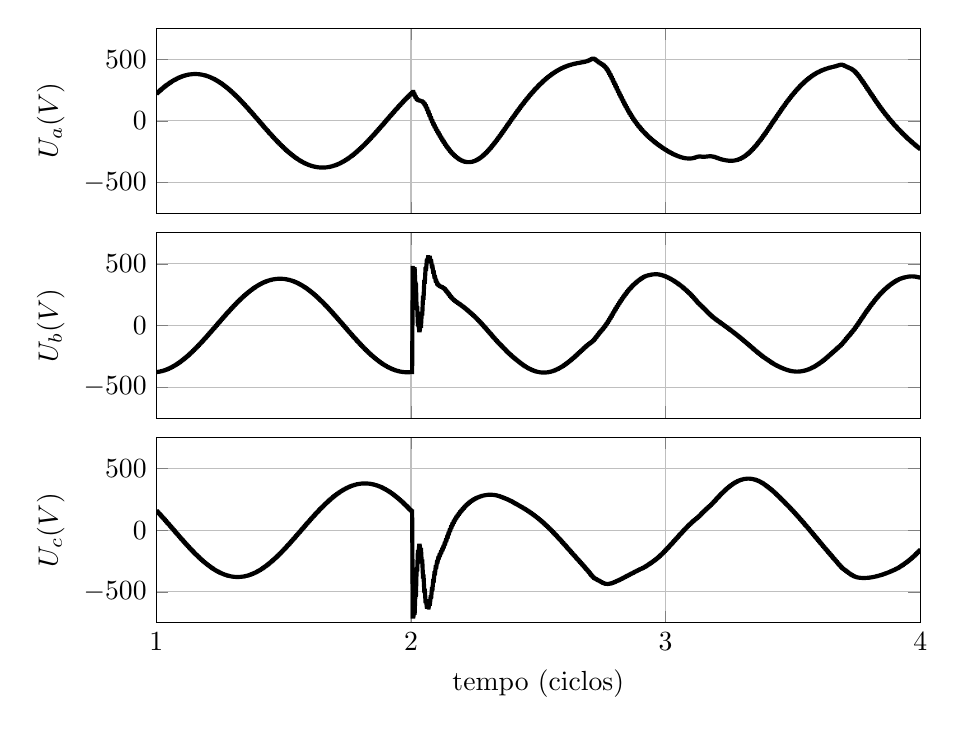
\begin{tikzpicture}

\begin{axis}[%
width=0.8\textwidth,
height=0.193917089240149\textwidth,
scale only axis,
xmin=0.316666666666667,
xmax=0.366666666666667,
xtick={0.316666666666667,0.333333333333333,0.35,0.366666666666667},
xticklabels={\empty},
xmajorgrids,
ymin=-750,
ymax=750,
ytick={-500,    0,  500},
ylabel={$\text{U}_\text{b}\text{ (V)}$},
ymajorgrids,
name=plot2,
scaled x ticks = false,
legend columns=-1,
legend style={/tikz/every even column/.append style={column sep=0.3cm}},
legend style={font=\footnotesize}
]
\addplot [color=black,solid,line width=1.5pt,forget plot]
  table[row sep=crcr]{0.316658333333333	-377.723085698266\\
0.3167	-376.586723778496\\
0.316741666666667	-376.586723778496\\
0.316783333333333	-375.078923942871\\
0.316825	-375.078923942871\\
0.316866666666667	-373.201183557557\\
0.316908333333333	-373.201183557557\\
0.31695	-370.955359679074\\
0.316991666666667	-370.955359679074\\
0.317033333333333	-368.343680965246\\
0.317075	-368.343680965246\\
0.317116666666667	-365.368751272189\\
0.317158333333333	-365.368751272189\\
0.3172	-362.033546182555\\
0.317241666666667	-362.033546182555\\
0.317283333333333	-358.341404810258\\
0.317325	-358.341404810258\\
0.317366666666667	-354.29601946274\\
0.317408333333333	-354.29601946274\\
0.31745	-349.901425336706\\
0.317491666666667	-349.901425336706\\
0.317533333333333	-345.161991678398\\
0.317575	-345.161991678398\\
0.317616666666667	-340.082415007475\\
0.317658333333333	-340.082415007475\\
0.3177	-334.667714301187\\
0.317741666666667	-334.667714301187\\
0.317783333333333	-328.923227572974\\
0.317825	-328.923227572974\\
0.317866666666667	-322.854609083496\\
0.317908333333333	-322.854609083496\\
0.31795	-316.467826451787\\
0.317991666666667	-316.467826451787\\
0.318033333333333	-309.769157112268\\
0.318075	-309.769157112268\\
0.318116666666667	-302.765183805345\\
0.318158333333333	-302.765183805345\\
0.3182	-295.462789021633\\
0.318241666666667	-295.462789021633\\
0.318283333333333	-287.869148495131\\
0.318325	-287.869148495131\\
0.318366666666667	-279.991723937524\\
0.318408333333333	-279.991723937524\\
0.31845	-271.838255227092\\
0.318491666666667	-271.838255227092\\
0.318533333333333	-263.416752229383\\
0.318575	-263.416752229383\\
0.318616666666667	-254.735486359231\\
0.318658333333333	-254.735486359231\\
0.3187	-245.802981925607\\
0.318741666666667	-245.802981925607\\
0.318783333333333	-236.6280072728\\
0.318825	-236.6280072728\\
0.318866666666667	-227.219565832749\\
0.318908333333333	-227.219565832749\\
0.31895	-217.586887717469\\
0.318991666666667	-217.586887717469\\
0.319033333333333	-207.739424484696\\
0.319075	-207.739424484696\\
0.319116666666667	-197.686870803904\\
0.319158333333333	-197.686870803904\\
0.3192	-187.439263486291\\
0.319241666666667	-187.439263486291\\
0.319283333333333	-177.007031372265\\
0.319325	-177.007031372265\\
0.319366666666667	-166.400723674948\\
0.319408333333333	-166.400723674948\\
0.31945	-155.6307199546\\
0.319491666666667	-155.6307199546\\
0.319533333333333	-144.707346263981\\
0.319575	-144.707346263981\\
0.319616666666667	-133.641094664328\\
0.319658333333333	-133.641094664328\\
0.3197	-122.442727673415\\
0.319741666666667	-122.442727673415\\
0.319783333333333	-111.123278734636\\
0.319825	-111.123278734636\\
0.319866666666667	-99.6940002360541\\
0.319908333333333	-99.6940002360541\\
0.31995	-88.1662967730299\\
0.319991666666667	-88.1662967730299\\
0.320033333333333	-76.5516646999388\\
0.320075	-76.5516646999388\\
0.320116666666667	-64.8616480040377\\
0.320158333333333	-64.8616480040377\\
0.3202	-53.1078129245748\\
0.320241666666667	-53.1078129245748\\
0.320283333333333	-41.3017386424485\\
0.320325	-41.3017386424485\\
0.320366666666667	-29.4550186053735\\
0.320408333333333	-29.4550186053735\\
0.32045	-17.5792663930844\\
0.320491666666667	-17.5792663930844\\
0.320533333333333	-5.68612092557823\\
0.320575	-5.68612092557823\\
0.320616666666667	6.2127524201114\\
0.320658333333333	6.2127524201114\\
0.3207	18.105666253858\\
0.320741666666667	18.105666253858\\
0.320783333333333	29.9809209740117\\
0.320825	29.9809209740117\\
0.320866666666667	41.8268186183045\\
0.320908333333333	41.8268186183045\\
0.32095	53.631678981668\\
0.320991666666667	53.631678981668\\
0.321033333333333	65.3838562807079\\
0.321075	65.3838562807079\\
0.321116666666667	77.0717550613194\\
0.321158333333333	77.0717550613194\\
0.3212	88.6838446142487\\
0.321241666666667	88.6838446142487\\
0.321283333333333	100.208671712027\\
0.321325	100.208671712027\\
0.321366666666667	111.6348719068\\
0.321408333333333	111.6348719068\\
0.32145	122.951179824381\\
0.321491666666667	122.951179824381\\
0.321533333333333	134.14643897231\\
0.321575	134.14643897231\\
0.321616666666667	145.209611528874\\
0.321658333333333	145.209611528874\\
0.3217	156.129788391287\\
0.321741666666667	156.129788391287\\
0.321783333333333	166.896199602751\\
0.321825	166.896199602751\\
0.321866666666667	177.498225133841\\
0.321908333333333	177.498225133841\\
0.32195	187.925405900222\\
0.321991666666667	187.925405900222\\
0.322033333333333	198.167454859908\\
0.322075	198.167454859908\\
0.322116666666667	208.214268041585\\
0.322158333333333	208.214268041585\\
0.3222	218.055935396159\\
0.322241666666667	218.055935396159\\
0.322283333333333	227.682751419264\\
0.322325	227.682751419264\\
0.322366666666667	237.085225549088\\
0.322408333333333	237.085225549088\\
0.32245	246.254092392214\\
0.322491666666667	246.254092392214\\
0.322533333333333	255.180321867299\\
0.322575	255.180321867299\\
0.322616666666667	263.855129383534\\
0.322658333333333	263.855129383534\\
0.3227	272.26998619054\\
0.322741666666667	272.26998619054\\
0.322783333333333	280.416630045836\\
0.322825	280.416630045836\\
0.322866666666667	288.287076317351\\
0.322908333333333	288.287076317351\\
0.32295	295.873629460527\\
0.322991666666667	295.873629460527\\
0.323033333333333	303.168894086837\\
0.323075	303.168894086837\\
0.323116666666667	310.165782141413\\
0.323158333333333	310.165782141413\\
0.3232	316.857502505702\\
0.323241666666667	316.857502505702\\
0.323283333333333	323.237410711189\\
0.323325	323.237410711189\\
0.323366666666667	329.298465304494\\
0.323408333333333	329.298465304494\\
0.32345	335.032940877286\\
0.323491666666667	335.032940877286\\
0.323533333333333	340.433778089715\\
0.323575	340.433778089715\\
0.323616666666667	345.496008515558\\
0.323658333333333	345.496008515558\\
0.3237	350.216089241188\\
0.323741666666667	350.216089241188\\
0.323783333333333	354.590714854285\\
0.323825	354.590714854285\\
0.323866666666667	358.616245271799\\
0.323908333333333	358.616245271799\\
0.32395	362.28867598875\\
0.323991666666667	362.28867598875\\
0.324033333333333	365.603866403093\\
0.324075	365.603866403093\\
0.324116666666667	368.557830105438\\
0.324158333333333	368.557830105438\\
0.3242	371.14698467744\\
0.324241666666667	371.14698467744\\
0.324283333333333	373.368315025462\\
0.324325	373.368315025462\\
0.324366666666667	375.219441072503\\
0.324408333333333	375.219441072503\\
0.32445	376.698604902272\\
0.324491666666667	376.698604902272\\
0.324533333333333	377.804605390594\\
0.324575	377.804605390594\\
0.324616666666667	378.536711049029\\
0.324658333333333	378.536711049029\\
0.3247	378.89457690205\\
0.324741666666667	378.89457690205\\
0.324783333333333	378.878182191864\\
0.324825	378.878182191864\\
0.324866666666667	378.487795835975\\
0.324908333333333	378.487795835975\\
0.32495	377.723968278227\\
0.324991666666667	377.723968278227\\
0.325033333333333	376.587542986259\\
0.325075	376.587542986259\\
0.325116666666667	375.079678623678\\
0.325158333333333	375.079678623678\\
0.3252	373.201873355773\\
0.325241666666667	373.201873355773\\
0.325283333333333	370.955984906448\\
0.325325	370.955984906448\\
0.325366666666667	368.34424285761\\
0.325408333333333	368.34424285761\\
0.32545	365.369252419982\\
0.325491666666667	365.369252419982\\
0.325533333333333	362.033990949537\\
0.325575	362.033990949537\\
0.325616666666667	358.341799615764\\
0.325658333333333	358.341799615764\\
0.3257	354.29637287251\\
0.325741666666667	354.29637287251\\
0.325783333333333	349.901747968484\\
0.325825	349.901747968484\\
0.325866666666667	345.162295969421\\
0.325908333333333	345.162295969421\\
0.32595	340.082714909794\\
0.325991666666667	340.082714909794\\
0.326033333333333	334.668024969912\\
0.326075	334.668024969912\\
0.326116666666667	328.923565098519\\
0.326158333333333	328.923565098519\\
0.3262	322.854990299289\\
0.326241666666667	322.854990299289\\
0.326283333333333	316.468268829063\\
0.326325	316.468268829063\\
0.326366666666667	309.769678739274\\
0.326408333333333	309.769678739274\\
0.32645	302.76580344002\\
0.326491666666667	302.76580344002\\
0.326533333333333	295.46352620612\\
0.326575	295.46352620612\\
0.326616666666667	287.870023724931\\
0.326658333333333	287.870023724931\\
0.3267	279.99275888678\\
0.326741666666667	279.99275888678\\
0.326783333333333	271.839473042268\\
0.326825	271.839473042268\\
0.326866666666667	263.418177915058\\
0.326908333333333	263.418177915058\\
0.32695	254.737147291355\\
0.326991666666667	254.737147291355\\
0.327033333333333	245.804908536742\\
0.327075	245.804908536742\\
0.327116666666667	236.630233953394\\
0.327158333333333	236.630233953394\\
0.3272	227.22213205341\\
0.327241666666667	227.22213205341\\
0.327283333333333	217.589839194205\\
0.327325	217.589839194205\\
0.327366666666667	207.742813476948\\
0.327408333333333	207.742813476948\\
0.32745	197.690748171958\\
0.327491666666667	197.690748171958\\
0.327533333333333	187.443640894198\\
0.327575	187.443640894198\\
0.327616666666667	177.011825362749\\
0.327658333333333	177.011825362749\\
0.3277	166.405770179614\\
0.327741666666667	166.405770179614\\
0.327783333333333	155.635868101642\\
0.327825	155.635868101642\\
0.327866666666667	144.712520179611\\
0.327908333333333	144.712520179611\\
0.32795	133.646292221512\\
0.327991666666667	133.646292221512\\
0.328033333333333	122.447986519211\\
0.328075	122.447986519211\\
0.328116666666667	111.128638130733\\
0.328158333333333	111.128638130733\\
0.3282	99.6994735093165\\
0.328241666666667	99.6994735093165\\
0.328283333333333	88.1718588306136\\
0.328325	88.1718588306136\\
0.328366666666667	76.5572531712875\\
0.328408333333333	76.5572531712875\\
0.32845	64.8671736797616\\
0.328491666666667	64.8671736797616\\
0.328533333333333	53.1131743732041\\
0.328575	53.1131743732041\\
0.328616666666667	41.3068365291399\\
0.328658333333333	41.3068365291399\\
0.3287	29.4597666782387\\
0.328741666666667	29.4597666782387\\
0.328783333333333	17.5835977645907\\
0.328825	17.5835977645907\\
0.328866666666667	5.68998972084417\\
0.328908333333333	5.68998972084417\\
0.32895	-6.20937299888088\\
0.328991666666667	-6.20937299888088\\
0.329033333333333	-18.1027879552077\\
0.329075	-18.1027879552077\\
0.329116666666667	-29.9785451472021\\
0.329158333333333	-29.9785451472021\\
0.3292	-41.8249403501677\\
0.329241666666667	-41.8249403501677\\
0.329283333333333	-53.6302900618585\\
0.329325	-53.6302900618585\\
0.329366666666667	-65.3829468063473\\
0.329408333333333	-65.3829468063473\\
0.32945	-77.0713138539921\\
0.329491666666667	-77.0713138539921\\
0.329533333333333	-88.6838588313381\\
0.329575	-88.6838588313381\\
0.329616666666667	-100.209126092659\\
0.329658333333333	-100.209126092659\\
0.3297	-111.635748034836\\
0.329741666666667	-111.635748034836\\
0.329783333333333	-122.952455666325\\
0.329825	-122.952455666325\\
0.329866666666667	-134.148088804689\\
0.329908333333333	-134.148088804689\\
0.32995	-145.211606244939\\
0.329991666666667	-145.211606244939\\
0.330033333333333	-156.132096092484\\
0.330075	-156.132096092484\\
0.330116666666667	-166.898786342177\\
0.330158333333333	-166.898786342177\\
0.3302	-177.501055680916\\
0.330241666666667	-177.501055680916\\
0.330283333333333	-187.928444425067\\
0.330325	-187.928444425067\\
0.330366666666667	-198.170665477564\\
0.330408333333333	-198.170665477564\\
0.33045	-208.21761519744\\
0.330491666666667	-208.21761519744\\
0.330533333333333	-218.059384105748\\
0.330575	-218.059384105748\\
0.330616666666667	-227.686267394042\\
0.330658333333333	-227.686267394042\\
0.3307	-237.088775244765\\
0.330741666666667	-237.088775244765\\
0.330783333333333	-246.257643010826\\
0.330825	-246.257643010826\\
0.330866666666667	-255.183841332313\\
0.330908333333333	-255.183841332313\\
0.33095	-263.858586293167\\
0.330991666666667	-263.858586293167\\
0.331033333333333	-272.273349741191\\
0.331075	-272.273349741191\\
0.331116666666667	-280.419869907006\\
0.331158333333333	-280.419869907006\\
0.3312	-288.29016243285\\
0.331241666666667	-288.29016243285\\
0.331283333333333	-295.876531750755\\
0.331325	-295.876531750755\\
0.331366666666667	-303.171582042784\\
0.331408333333333	-303.171582042784\\
0.33145	-310.168224372754\\
0.331491666666667	-310.168224372754\\
0.331533333333333	-316.859666586207\\
0.331575	-316.859666586207\\
0.331616666666667	-323.239266132863\\
0.331658333333333	-323.239266132863\\
0.3317	-329.299997905177\\
0.331741666666667	-329.299997905177\\
0.331783333333333	-335.034174516609\\
0.331825	-335.034174516609\\
0.331866666666667	-340.434769270671\\
0.331908333333333	-340.434769270671\\
0.33195	-345.496809702631\\
0.331991666666667	-345.496809702631\\
0.332033333333333	-350.216724523872\\
0.332075	-350.216724523872\\
0.332116666666667	-354.591180653519\\
0.332158333333333	-354.591180653519\\
0.3322	-358.616523838194\\
0.332241666666667	-358.616523838194\\
0.332283333333333	-362.288750228316\\
0.332325	-362.288750228316\\
0.332366666666667	-365.603730340961\\
0.332408333333333	-365.603730340961\\
0.33245	-368.557493442448\\
0.332491666666667	-368.557493442448\\
0.332533333333333	-371.146472117679\\
0.332575	-371.146472117679\\
0.332616666666667	-373.367662092301\\
0.332658333333333	-373.367662092301\\
0.3327	-375.218688387832\\
0.332741666666667	-375.218688387832\\
0.332783333333333	-376.697792634348\\
0.332825	-376.697792634348\\
0.332866666666667	-377.803769014554\\
0.332908333333333	-377.803769014554\\
0.33295	-378.535878926511\\
0.332991666666667	-378.535878926511\\
0.333033333333333	-378.893769636932\\
0.333075	-378.893769636932\\
0.333116666666667	-378.877413350589\\
0.333158333333333	-378.877413350589\\
0.3332	-378.487073457233\\
0.333241666666667	-378.487073457233\\
0.333283333333333	-377.723296609494\\
0.333325	-377.723296609494\\
0.333366666666667	-376.586924015447\\
0.333408333333333	-376.586924015447\\
0.33345	465.401231273742\\
0.333491666666667	465.401231273742\\
0.333533333333333	456.677126533956\\
0.333575	456.677126533956\\
0.333616666666667	330.246293537413\\
0.333658333333333	330.246293537413\\
0.3337	142.652384074905\\
0.333741666666667	142.652384074905\\
0.333783333333333	10.5824685532493\\
0.333825	10.5824685532493\\
0.333866666666667	-38.0898515233877\\
0.333908333333333	-38.0898515233877\\
0.33395	-1.77553818585096\\
0.333991666666667	-1.77553818585096\\
0.334033333333333	96.6581692636446\\
0.334075	96.6581692636446\\
0.334116666666667	225.496662175994\\
0.334158333333333	225.496662175994\\
0.3342	353.737490454211\\
0.334241666666667	353.737490454211\\
0.334283333333333	458.061598286727\\
0.334325	458.061598286727\\
0.334366666666667	525.728666866841\\
0.334408333333333	525.728666866841\\
0.33445	554.308285514671\\
0.334491666666667	554.308285514671\\
0.334533333333333	549.252840792784\\
0.334575	549.252840792784\\
0.334616666666667	520.509156407281\\
0.334658333333333	520.509156407281\\
0.3347	479.124588195346\\
0.334741666666667	479.124588195346\\
0.334783333333333	434.687010899335\\
0.334825	434.687010899335\\
0.334866666666667	394.313055776954\\
0.334908333333333	394.313055776954\\
0.33495	362.414870737212\\
0.334991666666667	362.414870737212\\
0.335033333333333	340.381577178868\\
0.335075	340.381577178868\\
0.335116666666667	326.971142188401\\
0.335158333333333	326.971142188401\\
0.3352	319.391174605004\\
0.335241666666667	319.391174605004\\
0.335283333333333	314.459111239222\\
0.335325	314.459111239222\\
0.335366666666667	309.472650225481\\
0.335408333333333	309.472650225481\\
0.33545	302.678932453462\\
0.335491666666667	302.678932453462\\
0.335533333333333	293.375498796174\\
0.335575	293.375498796174\\
0.335616666666667	281.743290219983\\
0.335658333333333	281.743290219983\\
0.3357	268.534808484825\\
0.335741666666667	268.534808484825\\
0.335783333333333	254.731584353175\\
0.335825	254.731584353175\\
0.335866666666667	241.25541287858\\
0.335908333333333	241.25541287858\\
0.33595	228.779580744971\\
0.335991666666667	228.779580744971\\
0.336033333333333	217.650224211992\\
0.336075	217.650224211992\\
0.336116666666667	207.901034695048\\
0.336158333333333	207.901034695048\\
0.3362	199.329642849565\\
0.336241666666667	199.329642849565\\
0.336283333333333	191.600565997926\\
0.336325	191.600565997926\\
0.336366666666667	184.344757494738\\
0.336408333333333	184.344757494738\\
0.33645	177.23576909033\\
0.336491666666667	177.23576909033\\
0.336533333333333	170.033699116605\\
0.336575	170.033699116605\\
0.336616666666667	162.597694320487\\
0.336658333333333	162.597694320487\\
0.3367	154.874233843025\\
0.336741666666667	154.874233843025\\
0.336783333333333	146.871337791287\\
0.336825	146.871337791287\\
0.336866666666667	138.628684159571\\
0.336908333333333	138.628684159571\\
0.33695	130.191371858837\\
0.336991666666667	130.191371858837\\
0.337033333333333	121.591861870836\\
0.337075	121.591861870836\\
0.337116666666667	112.841447246686\\
0.337158333333333	112.841447246686\\
0.3372	103.930120087278\\
0.337241666666667	103.930120087278\\
0.337283333333333	94.8322355679822\\
0.337325	94.8322355679822\\
0.337366666666667	85.5149201298832\\
0.337408333333333	85.5149201298832\\
0.33745	75.9465160179369\\
0.337491666666667	75.9465160179369\\
0.337533333333333	66.1031763840162\\
0.337575	66.1031763840162\\
0.337616666666667	55.9727001816763\\
0.337658333333333	55.9727001816763\\
0.3377	45.5555674145591\\
0.337741666666667	45.5555674145591\\
0.337783333333333	34.8637326514904\\
0.337825	34.8637326514904\\
0.337866666666667	23.9180985965045\\
0.337908333333333	23.9180985965045\\
0.33795	12.745532602838\\
0.337991666666667	12.745532602838\\
0.338033333333333	1.37613846738328\\
0.338075	1.37613846738328\\
0.338116666666667	-10.1587568803101\\
0.338158333333333	-10.1587568803101\\
0.3382	-21.8277352784647\\
0.338241666666667	-21.8277352784647\\
0.338283333333333	-33.5996016750134\\
0.338325	-33.5996016750134\\
0.338366666666667	-45.4430880951428\\
0.338408333333333	-45.4430880951428\\
0.33845	-57.3262052633507\\
0.338491666666667	-57.3262052633507\\
0.338533333333333	-69.2154758051859\\
0.338575	-69.2154758051859\\
0.338616666666667	-81.0752121490427\\
0.338658333333333	-81.0752121490427\\
0.3387	-92.8669172511253\\
0.338741666666667	-92.8669172511253\\
0.338783333333333	-104.548822526407\\
0.338825	-104.548822526407\\
0.338866666666667	-116.075588264939\\
0.338908333333333	-116.075588264939\\
0.33895	-127.398413895297\\
0.338991666666667	-127.398413895297\\
0.339033333333333	-138.466719535545\\
0.339075	-138.466719535545\\
0.339116666666667	-149.240922860318\\
0.339158333333333	-149.240922860318\\
0.3392	-159.749439990125\\
0.339241666666667	-159.749439990125\\
0.339283333333333	-170.148990003693\\
0.339325	-170.148990003693\\
0.339366666666667	-180.636530901896\\
0.339408333333333	-180.636530901896\\
0.33945	-191.258906593902\\
0.339491666666667	-191.258906593902\\
0.339533333333333	-201.886910040321\\
0.339575	-201.886910040321\\
0.339616666666667	-212.330810805552\\
0.339658333333333	-212.330810805552\\
0.3397	-222.443089201213\\
0.339741666666667	-222.443089201213\\
0.339783333333333	-232.159200142275\\
0.339825	-232.159200142275\\
0.339866666666667	-241.491666904796\\
0.339908333333333	-241.491666904796\\
0.33995	-250.502369078844\\
0.339991666666667	-250.502369078844\\
0.340033333333333	-259.270373042322\\
0.340075	-259.270373042322\\
0.340116666666667	-267.865203021387\\
0.340158333333333	-267.865203021387\\
0.3402	-276.33012924274\\
0.340241666666667	-276.33012924274\\
0.340283333333333	-284.67618559869\\
0.340325	-284.67618559869\\
0.340366666666667	-292.884999139345\\
0.340408333333333	-292.884999139345\\
0.34045	-300.917152916568\\
0.340491666666667	-300.917152916568\\
0.340533333333333	-308.722594545261\\
0.340575	-308.722594545261\\
0.340616666666667	-316.250229437449\\
0.340658333333333	-316.250229437449\\
0.3407	-323.454898713778\\
0.340741666666667	-323.454898713778\\
0.340783333333333	-330.301067208894\\
0.340825	-330.301067208894\\
0.340866666666667	-336.763469769222\\
0.340908333333333	-336.763469769222\\
0.34095	-342.825545692066\\
0.340991666666667	-342.825545692066\\
0.341033333333333	-348.476711114117\\
0.341075	-348.476711114117\\
0.341116666666667	-353.709442191835\\
0.341158333333333	-353.709442191835\\
0.3412	-358.516877296747\\
0.341241666666667	-358.516877296747\\
0.341283333333333	-362.891310246291\\
0.341325	-362.891310246291\\
0.341366666666667	-366.823634277661\\
0.341408333333333	-366.823634277661\\
0.34145	-370.303568564262\\
0.341491666666667	-370.303568564262\\
0.341533333333333	-373.320378865182\\
0.341575	-373.320378865182\\
0.341616666666667	-375.863783996813\\
0.341658333333333	-375.863783996813\\
0.3417	-377.924793319486\\
0.341741666666667	-377.924793319486\\
0.341783333333333	-379.496312858754\\
0.341825	-379.496312858754\\
0.341866666666667	-380.573456825738\\
0.341908333333333	-380.573456825738\\
0.34195	-381.153583527755\\
0.341991666666667	-381.153583527755\\
0.342033333333333	-381.236127368572\\
0.342075	-381.236127368572\\
0.342116666666667	-380.822320587416\\
0.342158333333333	-380.822320587416\\
0.3422	-379.914889123616\\
0.342241666666667	-379.914889123616\\
0.342283333333333	-378.517789094984\\
0.342325	-378.517789094984\\
0.342366666666667	-376.636019174083\\
0.342408333333333	-376.636019174083\\
0.34245	-374.275516227037\\
0.342491666666667	-374.275516227037\\
0.342533333333333	-371.443121089209\\
0.342575	-371.443121089209\\
0.342616666666667	-368.146590219277\\
0.342658333333333	-368.146590219277\\
0.3427	-364.394626740167\\
0.342741666666667	-364.394626740167\\
0.342783333333333	-360.196908767863\\
0.342825	-360.196908767863\\
0.342866666666667	-355.564100953421\\
0.342908333333333	-355.564100953421\\
0.34295	-350.507843970294\\
0.342991666666667	-350.507843970294\\
0.343033333333333	-345.040724143951\\
0.343075	-345.040724143951\\
0.343116666666667	-339.176230380656\\
0.343158333333333	-339.176230380656\\
0.3432	-332.928707761971\\
0.343241666666667	-332.928707761971\\
0.343283333333333	-326.313317076239\\
0.343325	-326.313317076239\\
0.343366666666667	-319.346007988208\\
0.343408333333333	-319.346007988208\\
0.34345	-312.043511429799\\
0.343491666666667	-312.043511429799\\
0.343533333333333	-304.423354932413\\
0.343575	-304.423354932413\\
0.343616666666667	-296.503903581874\\
0.343658333333333	-296.503903581874\\
0.3437	-288.30442936954\\
0.343741666666667	-288.30442936954\\
0.343783333333333	-279.845213045405\\
0.343825	-279.845213045405\\
0.343866666666667	-271.147685161175\\
0.343908333333333	-271.147685161175\\
0.34395	-262.234616860537\\
0.343991666666667	-262.234616860537\\
0.344033333333333	-253.130376327626\\
0.344075	-253.130376327626\\
0.344116666666667	-243.861274130951\\
0.344158333333333	-243.861274130951\\
0.3442	-234.456030926083\\
0.344241666666667	-234.456030926083\\
0.344283333333333	-224.946415632784\\
0.344325	-224.946415632784\\
0.344366666666667	-215.368123568041\\
0.344408333333333	-215.368123568041\\
0.34445	-205.761995099995\\
0.344491666666667	-205.761995099995\\
0.344533333333333	-196.175718839664\\
0.344575	-196.175718839664\\
0.344616666666667	-186.666216258376\\
0.344658333333333	-186.666216258376\\
0.3447	-177.302936884946\\
0.344741666666667	-177.302936884946\\
0.344783333333333	-168.172162488065\\
0.344825	-168.172162488065\\
0.344866666666667	-159.381518811086\\
0.344908333333333	-159.381518811086\\
0.34495	-151.059598524586\\
0.344991666666667	-151.059598524586\\
0.345033333333333	-143.306178634222\\
0.345075	-143.306178634222\\
0.345116666666667	-135.879214630347\\
0.345158333333333	-135.879214630347\\
0.3452	-127.719074898246\\
0.345241666666667	-127.719074898246\\
0.345283333333333	-117.527204275246\\
0.345325	-117.527204275246\\
0.345366666666667	-105.207942368755\\
0.345408333333333	-105.207942368755\\
0.34545	-91.7116503899979\\
0.345491666666667	-91.7116503899979\\
0.345533333333333	-78.0894967059641\\
0.345575	-78.0894967059641\\
0.345616666666667	-64.9720384386626\\
0.345658333333333	-64.9720384386626\\
0.3457	-52.4811090923967\\
0.345741666666667	-52.4811090923967\\
0.345783333333333	-40.3601920931353\\
0.345825	-40.3601920931353\\
0.345866666666667	-28.1671382872668\\
0.345908333333333	-28.1671382872668\\
0.34595	-15.4503470546519\\
0.345991666666667	-15.4503470546519\\
0.346033333333333	-1.87198347030398\\
0.346075	-1.87198347030398\\
0.346116666666667	12.7322636546738\\
0.346158333333333	12.7322636546738\\
0.3462	28.3500520287209\\
0.346241666666667	28.3500520287209\\
0.346283333333333	44.8288859007889\\
0.346325	44.8288859007889\\
0.346366666666667	61.9319727856346\\
0.346408333333333	61.9319727856346\\
0.34645	79.395345903155\\
0.346491666666667	79.395345903155\\
0.346533333333333	96.9736076980014\\
0.346575	96.9736076980014\\
0.346616666666667	114.468122156631\\
0.346658333333333	114.468122156631\\
0.3467	131.737241304332\\
0.346741666666667	131.737241304332\\
0.346783333333333	148.69216900287\\
0.346825	148.69216900287\\
0.346866666666667	165.2840229165\\
0.346908333333333	165.2840229165\\
0.34695	181.487782957648\\
0.346991666666667	181.487782957648\\
0.347033333333333	197.287665127875\\
0.347075	197.287665127875\\
0.347116666666667	212.666688189315\\
0.347158333333333	212.666688189315\\
0.3472	227.601389273788\\
0.347241666666667	227.601389273788\\
0.347283333333333	242.061200040625\\
0.347325	242.061200040625\\
0.347366666666667	256.01111591767\\
0.347408333333333	256.01111591767\\
0.34745	269.415990558972\\
0.347491666666667	269.415990558972\\
0.347533333333333	282.244949541446\\
0.347575	282.244949541446\\
0.347616666666667	294.474861661721\\
0.347658333333333	294.474861661721\\
0.3477	306.092348741664\\
0.347741666666667	306.092348741664\\
0.347783333333333	317.094308316547\\
0.347825	317.094308316547\\
0.347866666666667	327.487277752367\\
0.347908333333333	327.487277752367\\
0.34795	337.286150736506\\
0.347991666666667	337.286150736506\\
0.348033333333333	346.512778023323\\
0.348075	346.512778023323\\
0.348116666666667	355.194866997339\\
0.348158333333333	355.194866997339\\
0.3482	363.36531294762\\
0.348241666666667	363.36531294762\\
0.348283333333333	371.061386338012\\
0.348325	371.061386338012\\
0.348366666666667	378.320810478187\\
0.348408333333333	378.320810478187\\
0.34845	385.144252689442\\
0.348491666666667	385.144252689442\\
0.348533333333333	391.390969968635\\
0.348575	391.390969968635\\
0.348616666666667	396.76266331973\\
0.348658333333333	396.76266331973\\
0.3487	401.085934220577\\
0.348741666666667	401.085934220577\\
0.348783333333333	404.497022258071\\
0.348825	404.497022258071\\
0.348866666666667	407.271016019471\\
0.348908333333333	407.271016019471\\
0.34895	409.62815364695\\
0.348991666666667	409.62815364695\\
0.349033333333333	411.662994226461\\
0.349075	411.662994226461\\
0.349116666666667	413.358041694595\\
0.349158333333333	413.358041694595\\
0.3492	414.628144037998\\
0.349241666666667	414.628144037998\\
0.349283333333333	415.366927858318\\
0.349325	415.366927858318\\
0.349366666666667	415.483039079865\\
0.349408333333333	415.483039079865\\
0.34945	414.921624445706\\
0.349491666666667	414.921624445706\\
0.349533333333333	413.671057404347\\
0.349575	413.671057404347\\
0.349616666666667	411.758006317388\\
0.349658333333333	411.758006317388\\
0.3497	409.235507299807\\
0.349741666666667	409.235507299807\\
0.349783333333333	406.168786102872\\
0.349825	406.168786102872\\
0.349866666666667	402.622588065895\\
0.349908333333333	402.622588065895\\
0.34995	398.652274321742\\
0.349991666666667	398.652274321742\\
0.350033333333333	394.299419632252\\
0.350075	394.299419632252\\
0.350116666666667	389.591441936422\\
0.350158333333333	389.591441936422\\
0.3502	384.544068089758\\
0.350241666666667	384.544068089758\\
0.350283333333333	379.165201252249\\
0.350325	379.165201252249\\
0.350366666666667	373.458902180601\\
0.350408333333333	373.458902180601\\
0.35045	367.428576464574\\
0.350491666666667	367.428576464574\\
0.350533333333333	361.078917019243\\
0.350575	361.078917019243\\
0.350616666666667	354.416562254392\\
0.350658333333333	354.416562254392\\
0.3507	347.449720303122\\
0.350741666666667	347.449720303122\\
0.350783333333333	340.18714285625\\
0.350825	340.18714285625\\
0.350866666666667	332.636884628552\\
0.350908333333333	332.636884628552\\
0.35095	324.805141907684\\
0.350991666666667	324.805141907684\\
0.351033333333333	316.695370799596\\
0.351075	316.695370799596\\
0.351116666666667	308.307742579987\\
0.351158333333333	308.307742579987\\
0.3512	299.63888522698\\
0.351241666666667	299.63888522698\\
0.351283333333333	290.681790206136\\
0.351325	290.681790206136\\
0.351366666666667	281.425738637677\\
0.351408333333333	281.425738637677\\
0.35145	271.856118529825\\
0.351491666666667	271.856118529825\\
0.351533333333333	261.954070875661\\
0.351575	261.954070875661\\
0.351616666666667	251.696059349797\\
0.351658333333333	251.696059349797\\
0.3517	241.053867168989\\
0.351741666666667	241.053867168989\\
0.351783333333333	229.996741566947\\
0.351825	229.996741566947\\
0.351866666666667	218.501428936881\\
0.351908333333333	218.501428936881\\
0.35195	206.619067948833\\
0.351991666666667	206.619067948833\\
0.352033333333333	194.652039905947\\
0.352075	194.652039905947\\
0.352116666666667	183.176420679719\\
0.352158333333333	183.176420679719\\
0.3522	172.597512556094\\
0.352241666666667	172.597512556094\\
0.352283333333333	162.773849667303\\
0.352325	162.773849667303\\
0.352366666666667	153.228680531235\\
0.352408333333333	153.228680531235\\
0.35245	143.518706333995\\
0.352491666666667	143.518706333995\\
0.352533333333333	133.427033027479\\
0.352575	133.427033027479\\
0.352616666666667	122.979092823329\\
0.352658333333333	122.979092823329\\
0.3527	112.367043505899\\
0.352741666666667	112.367043505899\\
0.352783333333333	101.850287241485\\
0.352825	101.850287241485\\
0.352866666666667	91.6695796482845\\
0.352908333333333	91.6695796482845\\
0.35295	81.9914355870189\\
0.352991666666667	81.9914355870189\\
0.353033333333333	72.8860428142785\\
0.353075	72.8860428142785\\
0.353116666666667	64.333268018378\\
0.353158333333333	64.333268018378\\
0.3532	56.2468274883751\\
0.353241666666667	56.2468274883751\\
0.353283333333333	48.505780258143\\
0.353325	48.505780258143\\
0.353366666666667	40.9842455392109\\
0.353408333333333	40.9842455392109\\
0.35345	33.573441055255\\
0.353491666666667	33.573441055255\\
0.353533333333333	26.1936341429672\\
0.353575	26.1936341429672\\
0.353616666666667	18.7965360346369\\
0.353658333333333	18.7965360346369\\
0.3537	11.3605832321478\\
0.353741666666667	11.3605832321478\\
0.353783333333333	3.88233901501141\\
0.353825	3.88233901501141\\
0.353866666666667	-3.63291068508924\\
0.353908333333333	-3.63291068508924\\
0.35395	-11.1790713555381\\
0.353991666666667	-11.1790713555381\\
0.354033333333333	-18.7544050143773\\
0.354075	-18.7544050143773\\
0.354116666666667	-26.3636767580368\\
0.354158333333333	-26.3636767580368\\
0.3542	-34.0177543422254\\
0.354241666666667	-34.0177543422254\\
0.354283333333333	-41.7315411006072\\
0.354325	-41.7315411006072\\
0.354366666666667	-49.521212892257\\
0.354408333333333	-49.521212892257\\
0.35445	-57.4015809193823\\
0.354491666666667	-57.4015809193823\\
0.354533333333333	-65.3841208081213\\
0.354575	-65.3841208081213\\
0.354616666666667	-73.4758967162314\\
0.354658333333333	-73.4758967162314\\
0.3547	-81.6793443666125\\
0.354741666666667	-81.6793443666125\\
0.354783333333333	-89.9927026347981\\
0.354825	-89.9927026347981\\
0.354866666666667	-98.4108098240871\\
0.354908333333333	-98.4108098240871\\
0.35495	-106.925988662642\\
0.354991666666667	-106.925988662642\\
0.355033333333333	-115.528812854488\\
0.355075	-115.528812854488\\
0.355116666666667	-124.208638705077\\
0.355158333333333	-124.208638705077\\
0.3552	-132.953873264731\\
0.355241666666667	-132.953873264731\\
0.355283333333333	-141.752016773132\\
0.355325	-141.752016773132\\
0.355366666666667	-150.589554173185\\
0.355408333333333	-150.589554173185\\
0.35545	-159.451778943016\\
0.355491666666667	-159.451778943016\\
0.355533333333333	-168.322619236747\\
0.355575	-168.322619236747\\
0.355616666666667	-177.184510621889\\
0.355658333333333	-177.184510621889\\
0.3557	-186.018330542029\\
0.355741666666667	-186.018330542029\\
0.355783333333333	-194.803383805797\\
0.355825	-194.803383805797\\
0.355866666666667	-203.517409707744\\
0.355908333333333	-203.517409707744\\
0.35595	-212.136570911416\\
0.355991666666667	-212.136570911416\\
0.356033333333333	-220.635381705266\\
0.356075	-220.635381705266\\
0.356116666666667	-228.986540261185\\
0.356158333333333	-228.986540261185\\
0.3562	-237.160658026113\\
0.356241666666667	-237.160658026113\\
0.356283333333333	-245.125979192562\\
0.356325	-245.125979192562\\
0.356366666666667	-252.848544146793\\
0.356408333333333	-252.848544146793\\
0.35645	-260.294624636936\\
0.356491666666667	-260.294624636936\\
0.356533333333333	-267.452871398998\\
0.356575	-267.452871398998\\
0.356616666666667	-274.400499457476\\
0.356658333333333	-274.400499457476\\
0.3567	-281.32357974384\\
0.356741666666667	-281.32357974384\\
0.356783333333333	-288.348146409258\\
0.356825	-288.348146409258\\
0.356866666666667	-295.396771142555\\
0.356908333333333	-295.396771142555\\
0.35695	-302.28052514844\\
0.356991666666667	-302.28052514844\\
0.357033333333333	-308.834659520448\\
0.357075	-308.834659520448\\
0.357116666666667	-314.977780123565\\
0.357158333333333	-314.977780123565\\
0.3572	-320.708962085247\\
0.357241666666667	-320.708962085247\\
0.357283333333333	-326.078998048888\\
0.357325	-326.078998048888\\
0.357366666666667	-331.157788826139\\
0.357408333333333	-331.157788826139\\
0.35745	-336.007858147123\\
0.357491666666667	-336.007858147123\\
0.357533333333333	-340.667929460805\\
0.357575	-340.667929460805\\
0.357616666666667	-345.146975048331\\
0.357658333333333	-345.146975048331\\
0.3577	-349.426802075975\\
0.357741666666667	-349.426802075975\\
0.357783333333333	-353.469991864242\\
0.357825	-353.469991864242\\
0.357866666666667	-357.229824029847\\
0.357908333333333	-357.229824029847\\
0.35795	-360.659427644378\\
0.357991666666667	-360.659427644378\\
0.358033333333333	-363.718426229581\\
0.358075	-363.718426229581\\
0.358116666666667	-366.37642643842\\
0.358158333333333	-366.37642643842\\
0.3582	-368.613586492899\\
0.358241666666667	-368.613586492899\\
0.358283333333333	-370.41905858886\\
0.358325	-370.41905858886\\
0.358366666666667	-371.788310866503\\
0.358408333333333	-371.788310866503\\
0.35845	-372.720261633866\\
0.358491666666667	-372.720261633866\\
0.358533333333333	-373.214905956483\\
0.358575	-373.214905956483\\
0.358616666666667	-373.271793443819\\
0.358658333333333	-373.271793443819\\
0.3587	-372.889417297154\\
0.358741666666667	-372.889417297154\\
0.358783333333333	-372.065356292998\\
0.358825	-372.065356292998\\
0.358866666666667	-370.796895845355\\
0.358908333333333	-370.796895845355\\
0.35895	-369.081834417667\\
0.358991666666667	-369.081834417667\\
0.359033333333333	-366.919231151171\\
0.359075	-366.919231151171\\
0.359116666666667	-364.309939491549\\
0.359158333333333	-364.309939491549\\
0.3592	-361.256865882282\\
0.359241666666667	-361.256865882282\\
0.359283333333333	-357.764971166605\\
0.359325	-357.764971166605\\
0.359366666666667	-353.841082944974\\
0.359408333333333	-353.841082944974\\
0.35945	-349.493607530829\\
0.359491666666667	-349.493607530829\\
0.359533333333333	-344.732225319713\\
0.359575	-344.732225319713\\
0.359616666666667	-339.567632270438\\
0.359658333333333	-339.567632270438\\
0.3597	-334.011362492384\\
0.359741666666667	-334.011362492384\\
0.359783333333333	-328.07570077565\\
0.359825	-328.07570077565\\
0.359866666666667	-321.773674594476\\
0.359908333333333	-321.773674594476\\
0.35995	-315.119104881687\\
0.359991666666667	-315.119104881687\\
0.360033333333333	-308.126693352761\\
0.360075	-308.126693352761\\
0.360116666666667	-300.812129329071\\
0.360158333333333	-300.812129329071\\
0.3602	-293.192208187092\\
0.360241666666667	-293.192208187092\\
0.360283333333333	-285.284964268824\\
0.360325	-285.284964268824\\
0.360366666666667	-277.109831644804\\
0.360408333333333	-277.109831644804\\
0.36045	-268.687855929303\\
0.360491666666667	-268.687855929303\\
0.360533333333333	-260.041989938039\\
0.360575	-260.041989938039\\
0.360616666666667	-251.197516862761\\
0.360658333333333	-251.197516862761\\
0.3607	-242.182658940364\\
0.360741666666667	-242.182658940364\\
0.360783333333333	-233.029449046352\\
0.360825	-233.029449046352\\
0.360866666666667	-223.77496509951\\
0.360908333333333	-223.77496509951\\
0.36095	-214.463033716815\\
0.360991666666667	-214.463033716815\\
0.361033333333333	-205.146415130805\\
0.361075	-205.146415130805\\
0.361116666666667	-195.888936038864\\
0.361158333333333	-195.888936038864\\
0.3612	-186.764563990114\\
0.361241666666667	-186.764563990114\\
0.361283333333333	-177.827910717513\\
0.361325	-177.827910717513\\
0.361366666666667	-168.941144739086\\
0.361408333333333	-168.941144739086\\
0.36145	-159.529443285931\\
0.361491666666667	-159.529443285931\\
0.361533333333333	-148.902759016201\\
0.361575	-148.902759016201\\
0.361616666666667	-137.028033448916\\
0.361658333333333	-137.028033448916\\
0.3617	-124.45579222881\\
0.361741666666667	-124.45579222881\\
0.361783333333333	-111.780027692705\\
0.361825	-111.780027692705\\
0.361866666666667	-99.3399401714202\\
0.361908333333333	-99.3399401714202\\
0.36195	-87.1860452866396\\
0.361991666666667	-87.1860452866396\\
0.362033333333333	-75.16599430886\\
0.362075	-75.16599430886\\
0.362116666666667	-63.0350398491087\\
0.362158333333333	-63.0350398491087\\
0.3622	-50.551240104896\\
0.362241666666667	-50.551240104896\\
0.362283333333333	-37.5397624712894\\
0.362325	-37.5397624712894\\
0.362366666666667	-23.9225482025894\\
0.362408333333333	-23.9225482025894\\
0.36245	-9.71771892525437\\
0.362491666666667	-9.71771892525437\\
0.362533333333333	4.98181671304327\\
0.362575	4.98181671304327\\
0.362616666666667	20.0395033210323\\
0.362658333333333	20.0395033210323\\
0.3627	35.3062928318518\\
0.362741666666667	35.3062928318518\\
0.362783333333333	50.6451246693151\\
0.362825	50.6451246693151\\
0.362866666666667	65.9455908883106\\
0.362908333333333	65.9455908883106\\
0.36295	81.1287562461672\\
0.362991666666667	81.1287562461672\\
0.363033333333333	96.1442402521837\\
0.363075	96.1442402521837\\
0.363116666666667	110.962674241423\\
0.363158333333333	110.962674241423\\
0.3632	125.566661544866\\
0.363241666666667	125.566661544866\\
0.363283333333333	139.942700657317\\
0.363325	139.942700657317\\
0.363366666666667	154.075539014409\\
0.363408333333333	154.075539014409\\
0.36345	167.945426726712\\
0.363491666666667	167.945426726712\\
0.363533333333333	181.527953388089\\
0.363575	181.527953388089\\
0.363616666666667	194.795681107108\\
0.363658333333333	194.795681107108\\
0.3637	207.720636106427\\
0.363741666666667	207.720636106427\\
0.363783333333333	220.276822477078\\
0.363825	220.276822477078\\
0.363866666666667	232.442174267227\\
0.363908333333333	232.442174267227\\
0.36395	244.199664091464\\
0.363991666666667	244.199664091464\\
0.364033333333333	255.53755715352\\
0.364075	255.53755715352\\
0.364116666666667	266.448990337169\\
0.364158333333333	266.448990337169\\
0.3642	276.931150790935\\
0.364241666666667	276.931150790935\\
0.364283333333333	286.98433708994\\
0.364325	286.98433708994\\
0.364366666666667	296.611134200279\\
0.364408333333333	296.611134200279\\
0.36445	305.815851905023\\
0.364491666666667	305.815851905023\\
0.364533333333333	314.604292344861\\
0.364575	314.604292344861\\
0.364616666666667	322.983842934349\\
0.364658333333333	322.983842934349\\
0.3647	330.963835561446\\
0.364741666666667	330.963835561446\\
0.364783333333333	338.556033697081\\
0.364825	338.556033697081\\
0.364866666666667	345.774852637149\\
0.364908333333333	345.774852637149\\
0.36495	352.635878045219\\
0.364991666666667	352.635878045219\\
0.365033333333333	359.139160391958\\
0.365075	359.139160391958\\
0.365116666666667	365.214550703974\\
0.365158333333333	365.214550703974\\
0.3652	370.697767119479\\
0.365241666666667	370.697767119479\\
0.365283333333333	375.468783994847\\
0.365325	375.468783994847\\
0.365366666666667	379.579163856767\\
0.365408333333333	379.579163856767\\
0.36545	383.175832687771\\
0.365491666666667	383.175832687771\\
0.365533333333333	386.386430882618\\
0.365575	386.386430882618\\
0.365616666666667	389.270349408763\\
0.365658333333333	389.270349408763\\
0.3657	391.821625108525\\
0.365741666666667	391.821625108525\\
0.365783333333333	393.992693416055\\
0.365825	393.992693416055\\
0.365866666666667	395.720940115705\\
0.365908333333333	395.720940115705\\
0.36595	396.950181133473\\
0.365991666666667	396.950181133473\\
0.366033333333333	397.644002310243\\
0.366075	397.644002310243\\
0.366116666666667	397.790644841557\\
0.366158333333333	397.790644841557\\
0.3662	397.400988389385\\
0.366241666666667	397.400988389385\\
0.366283333333333	396.502193570685\\
0.366325	396.502193570685\\
0.366366666666667	395.129719624781\\
0.366408333333333	395.129719624781\\
0.36645	393.31994361065\\
0.366491666666667	393.31994361065\\
0.366533333333333	391.104782784016\\
0.366575	391.104782784016\\
0.366616666666667	388.508849530724\\
0.366658333333333	388.508849530724\\
};
\end{axis}

\begin{axis}[%
width=0.8\textwidth,
height=0.193917089240149\textwidth,
scale only axis,
xmin=0.316666666666667,
xmax=0.366666666666667,
xtick={0.316666666666667,0.333333333333333,0.35,0.366666666666667},
xticklabels={{1},{2},{3},{4}},
xlabel={tempo (ciclos)},
xmajorgrids,
ymin=-750,
ymax=750,
ytick={-500,    0,  500},
ylabel={$\text{U}_\text{c}\text{ (V)}$},
ymajorgrids,
at=(plot2.below south west),
anchor=above north west,
scaled x ticks = false,
legend columns=-1,
legend style={/tikz/every even column/.append style={column sep=0.3cm}},
legend style={font=\footnotesize}
]
\addplot [color=black,solid,line width=1.5pt,forget plot]
  table[row sep=crcr]{0.316658333333333	162.970553693369\\
0.3167	152.134366652308\\
0.316741666666667	152.134366652308\\
0.316783333333333	141.14831005675\\
0.316825	141.14831005675\\
0.316866666666667	130.023235612171\\
0.316908333333333	130.023235612171\\
0.31695	118.770126781016\\
0.316991666666667	118.770126781016\\
0.317033333333333	107.400101722771\\
0.317075	107.400101722771\\
0.317116666666667	95.9244081552081\\
0.317158333333333	95.9244081552081\\
0.3172	84.3544113952257\\
0.317241666666667	84.3544113952257\\
0.317283333333333	72.701577924984\\
0.317325	72.701577924984\\
0.317366666666667	60.9774570729016\\
0.317408333333333	60.9774570729016\\
0.31745	49.1936630040597\\
0.317491666666667	49.1936630040597\\
0.317533333333333	37.3618584558936\\
0.317575	37.3618584558936\\
0.317616666666667	25.4937408270424\\
0.317658333333333	25.4937408270424\\
0.3177	13.6010305245207\\
0.317741666666667	13.6010305245207\\
0.317783333333333	1.69546101270924\\
0.317825	1.69546101270924\\
0.317866666666667	-10.2112301875565\\
0.317908333333333	-10.2112301875565\\
0.31795	-22.1073102710107\\
0.317991666666667	-22.1073102710107\\
0.318033333333333	-33.9810602324472\\
0.318075	-33.9810602324472\\
0.318116666666667	-45.8207845611742\\
0.318158333333333	-45.8207845611742\\
0.3182	-57.6148216075114\\
0.318241666666667	-57.6148216075114\\
0.318283333333333	-69.3515545038083\\
0.318325	-69.3515545038083\\
0.318366666666667	-81.0194224196816\\
0.318408333333333	-81.0194224196816\\
0.31845	-92.6069319017156\\
0.318491666666667	-92.6069319017156\\
0.318533333333333	-104.102668074645\\
0.318575	-104.102668074645\\
0.318616666666667	-115.495305540439\\
0.318658333333333	-115.495305540439\\
0.3187	-126.773618886739\\
0.318741666666667	-126.773618886739\\
0.318783333333333	-137.926492811092\\
0.318825	-137.926492811092\\
0.318866666666667	-148.942932050852\\
0.318908333333333	-148.942932050852\\
0.31895	-159.812071858709\\
0.318991666666667	-159.812071858709\\
0.319033333333333	-170.5231917644\\
0.319075	-170.5231917644\\
0.319116666666667	-181.06575642652\\
0.319158333333333	-181.06575642652\\
0.3192	-191.42953407303\\
0.319241666666667	-191.42953407303\\
0.319283333333333	-201.604666016903\\
0.319325	-201.604666016903\\
0.319366666666667	-211.581414807252\\
0.319408333333333	-211.581414807252\\
0.31945	-221.34989413342\\
0.319491666666667	-221.34989413342\\
0.319533333333333	-230.900204960054\\
0.319575	-230.900204960054\\
0.319616666666667	-240.222675034997\\
0.319658333333333	-240.222675034997\\
0.3197	-249.307983285081\\
0.319741666666667	-249.307983285081\\
0.319783333333333	-258.147180154562\\
0.319825	-258.147180154562\\
0.319866666666667	-266.731655392224\\
0.319908333333333	-266.731655392224\\
0.31995	-275.053090965318\\
0.319991666666667	-275.053090965318\\
0.320033333333333	-283.103420134525\\
0.320075	-283.103420134525\\
0.320116666666667	-290.874802711353\\
0.320158333333333	-290.874802711353\\
0.3202	-298.359618907919\\
0.320241666666667	-298.359618907919\\
0.320283333333333	-305.550479087533\\
0.320325	-305.550479087533\\
0.320366666666667	-312.440243961342\\
0.320408333333333	-312.440243961342\\
0.32045	-319.022049113252\\
0.320491666666667	-319.022049113252\\
0.320533333333333	-325.289328632728\\
0.320575	-325.289328632728\\
0.320616666666667	-331.235834397501\\
0.320658333333333	-331.235834397501\\
0.3207	-336.855649514461\\
0.320741666666667	-336.855649514461\\
0.320783333333333	-342.143196100745\\
0.320825	-342.143196100745\\
0.320866666666667	-347.093238694001\\
0.320908333333333	-347.093238694001\\
0.32095	-351.700885056722\\
0.320991666666667	-351.700885056722\\
0.321033333333333	-355.961586078382\\
0.321075	-355.961586078382\\
0.321116666666667	-359.871136064135\\
0.321158333333333	-359.871136064135\\
0.3212	-363.425674130623\\
0.321241666666667	-363.425674130623\\
0.321283333333333	-366.621686882158\\
0.321325	-366.621686882158\\
0.321366666666667	-369.456012137793\\
0.321408333333333	-369.456012137793\\
0.32145	-371.925843211841\\
0.321491666666667	-371.925843211841\\
0.321533333333333	-374.028733221122\\
0.321575	-374.028733221122\\
0.321616666666667	-375.762598995818\\
0.321658333333333	-375.762598995818\\
0.3217	-377.125724285815\\
0.321741666666667	-377.125724285815\\
0.321783333333333	-378.116762135567\\
0.321825	-378.116762135567\\
0.321866666666667	-378.734736446567\\
0.321908333333333	-378.734736446567\\
0.32195	-378.979042846209\\
0.321991666666667	-378.979042846209\\
0.322033333333333	-378.849449026762\\
0.322075	-378.849449026762\\
0.322116666666667	-378.346094717328\\
0.322158333333333	-378.346094717328\\
0.3222	-377.469491420695\\
0.322241666666667	-377.469491420695\\
0.322283333333333	-376.220522004144\\
0.322325	-376.220522004144\\
0.322366666666667	-374.600440193894\\
0.322408333333333	-374.600440193894\\
0.32245	-372.61086999843\\
0.322491666666667	-372.61086999843\\
0.322533333333333	-370.253805081463\\
0.322575	-370.253805081463\\
0.322616666666667	-367.531608121488\\
0.322658333333333	-367.531608121488\\
0.3227	-364.447010227436\\
0.322741666666667	-364.447010227436\\
0.322783333333333	-361.00311051502\\
0.322825	-361.00311051502\\
0.322866666666667	-357.2033759492\\
0.322908333333333	-357.2033759492\\
0.32295	-353.051641405706\\
0.322991666666667	-353.051641405706\\
0.323033333333333	-348.55210919846\\
0.323075	-348.55210919846\\
0.323116666666667	-343.709344628697\\
0.323158333333333	-343.709344628697\\
0.3232	-338.52825390877\\
0.323241666666667	-338.52825390877\\
0.323283333333333	-333.013922177807\\
0.323325	-333.013922177807\\
0.323366666666667	-327.171058172122\\
0.323408333333333	-327.171058172122\\
0.32345	-321.003695577926\\
0.323491666666667	-321.003695577926\\
0.323533333333333	-314.516531402583\\
0.323575	-314.516531402583\\
0.323616666666667	-307.716339196424\\
0.323658333333333	-307.716339196424\\
0.3237	-300.611292060023\\
0.323741666666667	-300.611292060023\\
0.323783333333333	-293.209763076321\\
0.323825	-293.209763076321\\
0.323866666666667	-285.519741623125\\
0.323908333333333	-285.519741623125\\
0.32395	-277.54879215579\\
0.323991666666667	-277.54879215579\\
0.324033333333333	-269.304271125924\\
0.324075	-269.304271125924\\
0.324116666666667	-260.79360593688\\
0.324158333333333	-260.79360593688\\
0.3242	-252.02453349254\\
0.324241666666667	-252.02453349254\\
0.324283333333333	-243.005252378576\\
0.324325	-243.005252378576\\
0.324366666666667	-233.744479511389\\
0.324408333333333	-233.744479511389\\
0.32445	-224.251426359643\\
0.324491666666667	-224.251426359643\\
0.324533333333333	-214.535722784241\\
0.324575	-214.535722784241\\
0.324616666666667	-204.607319231369\\
0.324658333333333	-204.607319231369\\
0.3247	-194.476393109332\\
0.324741666666667	-194.476393109332\\
0.324783333333333	-184.153276152493\\
0.324825	-184.153276152493\\
0.324866666666667	-173.648409706627\\
0.324908333333333	-173.648409706627\\
0.32495	-162.972326585662\\
0.324991666666667	-162.972326585662\\
0.325033333333333	-152.135652762133\\
0.325075	-152.135652762133\\
0.325116666666667	-141.149119929114\\
0.325158333333333	-141.149119929114\\
0.3252	-130.023580401982\\
0.325241666666667	-130.023580401982\\
0.325283333333333	-118.770017987052\\
0.325325	-118.770017987052\\
0.325366666666667	-107.399551317653\\
0.325408333333333	-107.399551317653\\
0.32545	-95.9234288957582\\
0.325491666666667	-95.9234288957582\\
0.325533333333333	-84.3530171259215\\
0.325575	-84.3530171259215\\
0.325616666666667	-72.6997837486583\\
0.325658333333333	-72.6997837486583\\
0.3257	-60.9752793324054\\
0.325741666666667	-60.9752793324054\\
0.325783333333333	-49.1911190787728\\
0.325825	-49.1911190787728\\
0.325866666666667	-37.3589664176652\\
0.325908333333333	-37.3589664176652\\
0.32595	-25.4905190184515\\
0.325991666666667	-25.4905190184515\\
0.326033333333333	-13.5974971207829\\
0.326075	-13.5974971207829\\
0.326116666666667	-1.69163361404229\\
0.326158333333333	-1.69163361404229\\
0.3262	10.2153349073519\\
0.326241666666667	10.2153349073519\\
0.326283333333333	22.1116768548334\\
0.326325	22.1116768548334\\
0.326366666666667	33.9856746806564\\
0.326408333333333	33.9856746806564\\
0.32645	45.8256345451254\\
0.326491666666667	45.8256345451254\\
0.326533333333333	57.619896682525\\
0.326575	57.619896682525\\
0.326616666666667	69.356846348781\\
0.326658333333333	69.356846348781\\
0.3267	81.0249251286878\\
0.326741666666667	81.0249251286878\\
0.326783333333333	92.6126423517755\\
0.326825	92.6126423517755\\
0.326866666666667	104.108586394839\\
0.326908333333333	104.108586394839\\
0.32695	115.501435711804\\
0.326991666666667	115.501435711804\\
0.327033333333333	126.779969508188\\
0.327075	126.779969508188\\
0.327116666666667	137.933078066121\\
0.327158333333333	137.933078066121\\
0.3272	148.949772873188\\
0.327241666666667	148.949772873188\\
0.327283333333333	159.819197115413\\
0.327325	159.819197115413\\
0.327366666666667	170.530638546332\\
0.327408333333333	170.530638546332\\
0.32745	181.073562075667\\
0.327491666666667	181.073562075667\\
0.327533333333333	191.437698337058\\
0.327575	191.437698337058\\
0.327616666666667	201.613095062515\\
0.327658333333333	201.613095062515\\
0.3277	211.589935660001\\
0.327741666666667	211.589935660001\\
0.327783333333333	221.358348409748\\
0.327825	221.358348409748\\
0.327866666666667	230.908510590095\\
0.327908333333333	230.908510590095\\
0.32795	240.230824931129\\
0.327991666666667	240.230824931129\\
0.328033333333333	249.316011288028\\
0.328075	249.316011288028\\
0.328116666666667	258.155122791836\\
0.328158333333333	258.155122791836\\
0.3282	266.739524245654\\
0.328241666666667	266.739524245654\\
0.328283333333333	275.0608601025\\
0.328325	275.0608601025\\
0.328366666666667	283.111027166579\\
0.328408333333333	283.111027166579\\
0.32845	290.882159147744\\
0.328491666666667	290.882159147744\\
0.328533333333333	298.366624689893\\
0.328575	298.366624689893\\
0.328616666666667	305.557036824969\\
0.328658333333333	305.557036824969\\
0.3287	312.44626983943\\
0.328741666666667	312.44626983943\\
0.328783333333333	319.027479097028\\
0.328825	319.027479097028\\
0.328866666666667	325.294120041746\\
0.328908333333333	325.294120041746\\
0.32895	331.239963900123\\
0.328991666666667	331.239963900123\\
0.329033333333333	336.859109033448\\
0.329075	336.859109033448\\
0.329116666666667	342.145988100331\\
0.329158333333333	342.145988100331\\
0.3292	347.09537198353\\
0.329241666666667	347.09537198353\\
0.329283333333333	351.702371769095\\
0.329325	351.702371769095\\
0.329366666666667	355.96244001224\\
0.329408333333333	355.96244001224\\
0.32945	359.871372216336\\
0.329491666666667	359.871372216336\\
0.329533333333333	363.425309036832\\
0.329575	363.425309036832\\
0.329616666666667	366.620739324895\\
0.329658333333333	366.620739324895\\
0.3297	369.454503838896\\
0.329741666666667	369.454503838896\\
0.329783333333333	371.923799251079\\
0.329825	371.923799251079\\
0.329866666666667	374.026182065952\\
0.329908333333333	374.026182065952\\
0.32995	375.759572151591\\
0.329991666666667	375.759572151591\\
0.330033333333333	377.122255660091\\
0.330075	377.122255660091\\
0.330116666666667	378.112887248098\\
0.330158333333333	378.112887248098\\
0.3302	378.730491614484\\
0.330241666666667	378.730491614484\\
0.330283333333333	378.974464444218\\
0.330325	378.974464444218\\
0.330366666666667	378.844572880123\\
0.330408333333333	378.844572880123\\
0.33045	378.340955643699\\
0.330491666666667	378.340955643699\\
0.330533333333333	377.464122904322\\
0.330575	377.464122904322\\
0.330616666666667	376.214955966436\\
0.330658333333333	376.214955966436\\
0.3307	374.5947068181\\
0.330741666666667	374.5947068181\\
0.330783333333333	372.604997569562\\
0.330825	372.604997569562\\
0.330866666666667	370.24781981178\\
0.330908333333333	370.24781981178\\
0.33095	367.525533942416\\
0.330991666666667	367.525533942416\\
0.331033333333333	364.440868536929\\
0.331075	364.440868536929\\
0.331116666666667	360.996919873773\\
0.331158333333333	360.996919873773\\
0.3312	357.197151719323\\
0.331241666666667	357.197151719323\\
0.331283333333333	353.045395325139\\
0.331325	353.045395325139\\
0.331366666666667	348.545848895653\\
0.331408333333333	348.545848895653\\
0.33145	343.703073146214\\
0.331491666666667	343.703073146214\\
0.331533333333333	338.521969578445\\
0.331575	338.521969578445\\
0.331616666666667	333.00762165269\\
0.331658333333333	333.00762165269\\
0.3317	327.164750970432\\
0.331741666666667	327.164750970432\\
0.331783333333333	320.997425903535\\
0.331825	320.997425903535\\
0.331866666666667	314.51037292983\\
0.331908333333333	314.51037292983\\
0.33195	307.710358562834\\
0.331991666666667	307.710358562834\\
0.332033333333333	300.605524710562\\
0.332075	300.605524710562\\
0.332116666666667	293.204214153872\\
0.332158333333333	293.204214153872\\
0.3322	285.514399652687\\
0.332241666666667	285.514399652687\\
0.332283333333333	277.543644057549\\
0.332325	277.543644057549\\
0.332366666666667	269.299312867494\\
0.332408333333333	269.299312867494\\
0.33245	260.788847279147\\
0.332491666666667	260.788847279147\\
0.332533333333333	252.019997506399\\
0.332575	252.019997506399\\
0.332616666666667	243.000971448902\\
0.332658333333333	243.000971448902\\
0.3327	233.740489801388\\
0.332741666666667	233.740489801388\\
0.332783333333333	224.24776243952\\
0.332825	224.24776243952\\
0.332866666666667	214.532413566654\\
0.332908333333333	214.532413566654\\
0.33295	204.604385718927\\
0.332991666666667	204.604385718927\\
0.333033333333333	194.47384791024\\
0.333075	194.47384791024\\
0.333116666666667	184.151124352293\\
0.333158333333333	184.151124352293\\
0.3332	173.646650520602\\
0.333241666666667	173.646650520602\\
0.333283333333333	162.970955229482\\
0.333325	162.970955229482\\
0.333366666666667	152.134662109327\\
0.333408333333333	152.134662109327\\
0.33345	-699.331842723856\\
0.333491666666667	-699.331842723856\\
0.333533333333333	-669.439522946769\\
0.333575	-669.439522946769\\
0.333616666666667	-522.549016507849\\
0.333658333333333	-522.549016507849\\
0.3337	-319.450236006132\\
0.333741666666667	-319.450236006132\\
0.333783333333333	-178.817013346291\\
0.333825	-178.817013346291\\
0.333866666666667	-126.196583879869\\
0.333908333333333	-126.196583879869\\
0.33395	-159.936254181348\\
0.333991666666667	-159.936254181348\\
0.334033333333333	-253.998696064995\\
0.334075	-253.998696064995\\
0.334116666666667	-374.454237051481\\
0.334158333333333	-374.454237051481\\
0.3342	-489.325081764025\\
0.334241666666667	-489.325081764025\\
0.334283333333333	-575.481094457486\\
0.334325	-575.481094457486\\
0.334366666666667	-621.207192294284\\
0.334408333333333	-621.207192294284\\
0.33445	-625.513677740807\\
0.334491666666667	-625.513677740807\\
0.334533333333333	-595.316388565161\\
0.334575	-595.316388565161\\
0.334616666666667	-541.762671832374\\
0.334658333333333	-541.762671832374\\
0.3347	-476.689396287457\\
0.334741666666667	-476.689396287457\\
0.334783333333333	-410.043563364281\\
0.334825	-410.043563364281\\
0.334866666666667	-348.945606869912\\
0.334908333333333	-348.945606869912\\
0.33495	-297.581352054532\\
0.334991666666667	-297.581352054532\\
0.335033333333333	-257.01697515341\\
0.335075	-257.01697515341\\
0.335116666666667	-225.701769829695\\
0.335158333333333	-225.701769829695\\
0.3352	-200.62060003957\\
0.335241666666667	-200.62060003957\\
0.335283333333333	-178.483423388725\\
0.335325	-178.483423388725\\
0.335366666666667	-156.589738765657\\
0.335408333333333	-156.589738765657\\
0.33545	-133.268933250638\\
0.335491666666667	-133.268933250638\\
0.335533333333333	-107.943117274802\\
0.335575	-107.943117274802\\
0.335616666666667	-80.9240789621601\\
0.335658333333333	-80.9240789621601\\
0.3357	-53.0748421254515\\
0.335741666666667	-53.0748421254515\\
0.335783333333333	-25.4529694319874\\
0.335825	-25.4529694319874\\
0.335866666666667	0.980611392455887\\
0.335908333333333	0.980611392455887\\
0.33595	25.54410486178\\
0.335991666666667	25.54410486178\\
0.336033333333333	47.9025772751448\\
0.336075	47.9025772751448\\
0.336116666666667	68.0415323876177\\
0.336158333333333	68.0415323876177\\
0.3362	86.180839978308\\
0.336241666666667	86.180839978308\\
0.336283333333333	102.665657998006\\
0.336325	102.665657998006\\
0.336366666666667	117.864591048879\\
0.336408333333333	117.864591048879\\
0.33645	132.094431700647\\
0.336491666666667	132.094431700647\\
0.336533333333333	145.579169995121\\
0.336575	145.579169995121\\
0.336616666666667	158.441265066289\\
0.336658333333333	158.441265066289\\
0.3367	170.716915326311\\
0.336741666666667	170.716915326311\\
0.336783333333333	182.384515369437\\
0.336825	182.384515369437\\
0.336866666666667	193.396044204093\\
0.336908333333333	193.396044204093\\
0.33695	203.703708330421\\
0.336991666666667	203.703708330421\\
0.337033333333333	213.27758433053\\
0.337075	213.27758433053\\
0.337116666666667	222.113274324626\\
0.337158333333333	222.113274324626\\
0.3372	230.231050433985\\
0.337241666666667	230.231050433985\\
0.337283333333333	237.669343343168\\
0.337325	237.669343343168\\
0.337366666666667	244.47576580857\\
0.337408333333333	244.47576580857\\
0.33745	250.698406210015\\
0.337491666666667	250.698406210015\\
0.337533333333333	256.37922335525\\
0.337575	256.37922335525\\
0.337616666666667	261.550354775008\\
0.337658333333333	261.550354775008\\
0.3377	266.233271237366\\
0.337741666666667	266.233271237366\\
0.337783333333333	270.440131171214\\
0.337825	270.440131171214\\
0.337866666666667	274.17635739186\\
0.337908333333333	274.17635739186\\
0.33795	277.443552719214\\
0.337991666666667	277.443552719214\\
0.338033333333333	280.242051094578\\
0.338075	280.242051094578\\
0.338116666666667	282.572672534821\\
0.338158333333333	282.572672534821\\
0.3382	284.437551013491\\
0.338241666666667	284.437551013491\\
0.338283333333333	285.840132877677\\
0.338325	285.840132877677\\
0.338366666666667	286.784578731054\\
0.338408333333333	286.784578731054\\
0.33845	287.274842025072\\
0.338491666666667	287.274842025072\\
0.338533333333333	287.313663483601\\
0.338575	287.313663483601\\
0.338616666666667	286.901642163752\\
0.338658333333333	286.901642163752\\
0.3387	286.03645474041\\
0.338741666666667	286.03645474041\\
0.338783333333333	284.712229775776\\
0.338825	284.712229775776\\
0.338866666666667	282.919095872834\\
0.338908333333333	282.919095872834\\
0.33895	280.643147203505\\
0.338991666666667	280.643147203505\\
0.339033333333333	277.867986749979\\
0.339075	277.867986749979\\
0.339116666666667	274.58737247177\\
0.339158333333333	274.58737247177\\
0.3392	270.862097682392\\
0.339241666666667	270.862097682392\\
0.339283333333333	266.880188238883\\
0.339325	266.880188238883\\
0.339366666666667	262.868746987728\\
0.339408333333333	262.868746987728\\
0.33945	258.903526748304\\
0.339491666666667	258.903526748304\\
0.339533333333333	254.882937572546\\
0.339575	254.882937572546\\
0.339616666666667	250.64353610017\\
0.339658333333333	250.64353610017\\
0.3397	246.062737962155\\
0.339741666666667	246.062737962155\\
0.339783333333333	241.099574645729\\
0.339825	241.099574645729\\
0.339866666666667	235.788793122639\\
0.339908333333333	235.788793122639\\
0.33995	230.213160701195\\
0.339991666666667	230.213160701195\\
0.340033333333333	224.471321786659\\
0.340075	224.471321786659\\
0.340116666666667	218.65110321455\\
0.340158333333333	218.65110321455\\
0.3402	212.812843481178\\
0.340241666666667	212.812843481178\\
0.340283333333333	206.983457272162\\
0.340325	206.983457272162\\
0.340366666666667	201.159316674849\\
0.340408333333333	201.159316674849\\
0.34045	195.314669702987\\
0.340491666666667	195.314669702987\\
0.340533333333333	189.412107599156\\
0.340575	189.412107599156\\
0.340616666666667	183.412218955287\\
0.340658333333333	183.412218955287\\
0.3407	177.280629735505\\
0.340741666666667	177.280629735505\\
0.340783333333333	170.99175371661\\
0.340825	170.99175371661\\
0.340866666666667	164.529500690303\\
0.340908333333333	164.529500690303\\
0.34095	157.885771495099\\
0.340991666666667	157.885771495099\\
0.341033333333333	151.057788996784\\
0.341075	151.057788996784\\
0.341116666666667	144.045237271124\\
0.341158333333333	144.045237271124\\
0.3412	136.847916724381\\
0.341241666666667	136.847916724381\\
0.341283333333333	129.464286778782\\
0.341325	129.464286778782\\
0.341366666666667	121.890955519752\\
0.341408333333333	121.890955519752\\
0.34145	114.122947864174\\
0.341491666666667	114.122947864174\\
0.341533333333333	106.154463657468\\
0.341575	106.154463657468\\
0.341616666666667	97.9798172528103\\
0.341658333333333	97.9798172528103\\
0.3417	89.5943036676949\\
0.341741666666667	89.5943036676949\\
0.341783333333333	80.994828870301\\
0.341825	80.994828870301\\
0.341866666666667	72.1802409173801\\
0.341908333333333	72.1802409173801\\
0.34195	63.1513809107644\\
0.341991666666667	63.1513809107644\\
0.342033333333333	53.9109254592079\\
0.342075	53.9109254592079\\
0.342116666666667	44.4631122345028\\
0.342158333333333	44.4631122345028\\
0.3422	34.8134384353028\\
0.342241666666667	34.8134384353028\\
0.342283333333333	24.9683947856181\\
0.342325	24.9683947856181\\
0.342366666666667	14.9352701342574\\
0.342408333333333	14.9352701342574\\
0.34245	4.72203419418261\\
0.342491666666667	4.72203419418261\\
0.342533333333333	-5.66271469238743\\
0.342575	-5.66271469238743\\
0.342616666666667	-16.2097611207436\\
0.342658333333333	-16.2097611207436\\
0.3427	-26.9092702538308\\
0.342741666666667	-26.9092702538308\\
0.342783333333333	-37.7507940183564\\
0.342825	-37.7507940183564\\
0.342866666666667	-48.7233005413055\\
0.342908333333333	-48.7233005413055\\
0.34295	-59.815232924018\\
0.342991666666667	-59.815232924018\\
0.343033333333333	-71.0145962589965\\
0.343075	-71.0145962589965\\
0.343116666666667	-82.3090671679909\\
0.343158333333333	-82.3090671679909\\
0.3432	-93.6861183498617\\
0.343241666666667	-93.6861183498617\\
0.343283333333333	-105.133151264095\\
0.343325	-105.133151264095\\
0.343366666666667	-116.637632358068\\
0.343408333333333	-116.637632358068\\
0.34345	-128.187231312496\\
0.343491666666667	-128.187231312496\\
0.343533333333333	-139.769962915163\\
0.343575	-139.769962915163\\
0.343616666666667	-151.374336938557\\
0.343658333333333	-151.374336938557\\
0.3437	-162.989522665467\\
0.343741666666667	-162.989522665467\\
0.343783333333333	-174.605536638817\\
0.343825	-174.605536638817\\
0.343866666666667	-186.213464192618\\
0.343908333333333	-186.213464192618\\
0.34395	-197.805727908192\\
0.343991666666667	-197.805727908192\\
0.344033333333333	-209.376420031465\\
0.344075	-209.376420031465\\
0.344116666666667	-220.921721959481\\
0.344158333333333	-220.921721959481\\
0.3442	-232.440443300734\\
0.344241666666667	-232.440443300734\\
0.344283333333333	-243.934727321391\\
0.344325	-243.934727321391\\
0.344366666666667	-255.410991028543\\
0.344408333333333	-255.410991028543\\
0.34445	-266.881199578669\\
0.344491666666667	-266.881199578669\\
0.344533333333333	-278.364618631796\\
0.344575	-278.364618631796\\
0.344616666666667	-289.890241610301\\
0.344658333333333	-289.890241610301\\
0.3447	-301.500121454267\\
0.344741666666667	-301.500121454267\\
0.344783333333333	-313.253705936049\\
0.344825	-313.253705936049\\
0.344866666666667	-325.232375834814\\
0.344908333333333	-325.232375834814\\
0.34495	-337.539090332601\\
0.344991666666667	-337.539090332601\\
0.345033333333333	-350.248623460848\\
0.345075	-350.248623460848\\
0.345116666666667	-363.094574346121\\
0.345158333333333	-363.094574346121\\
0.3452	-374.99361512103\\
0.345241666666667	-374.99361512103\\
0.345283333333333	-384.624165650519\\
0.345325	-384.624165650519\\
0.345366666666667	-391.868220909627\\
0.345408333333333	-391.868220909627\\
0.34545	-397.654484983634\\
0.345491666666667	-397.654484983634\\
0.345533333333333	-403.013162128408\\
0.345575	-403.013162128408\\
0.345616666666667	-408.554542487274\\
0.345658333333333	-408.554542487274\\
0.3457	-414.380892744364\\
0.345741666666667	-414.380892744364\\
0.345783333333333	-420.216831923506\\
0.345825	-420.216831923506\\
0.345866666666667	-425.602050719578\\
0.345908333333333	-425.602050719578\\
0.34595	-430.067494362312\\
0.345991666666667	-430.067494362312\\
0.346033333333333	-433.258581790901\\
0.346075	-433.258581790901\\
0.346116666666667	-434.994966312214\\
0.346158333333333	-434.994966312214\\
0.3462	-435.273668911459\\
0.346241666666667	-435.273668911459\\
0.346283333333333	-434.232583103975\\
0.346325	-434.232583103975\\
0.346366666666667	-432.094625766568\\
0.346408333333333	-432.094625766568\\
0.34645	-429.110623096835\\
0.346491666666667	-429.110623096835\\
0.346533333333333	-425.513577766656\\
0.346575	-425.513577766656\\
0.346616666666667	-421.490490948796\\
0.346658333333333	-421.490490948796\\
0.3467	-417.17215428613\\
0.346741666666667	-417.17215428613\\
0.346783333333333	-412.637309537893\\
0.346825	-412.637309537893\\
0.346866666666667	-407.925616116412\\
0.346908333333333	-407.925616116412\\
0.34695	-403.053739641125\\
0.346991666666667	-403.053739641125\\
0.347033333333333	-398.03002449155\\
0.347075	-398.03002449155\\
0.347116666666667	-392.864985454099\\
0.347158333333333	-392.864985454099\\
0.3472	-387.576665752284\\
0.347241666666667	-387.576665752284\\
0.347283333333333	-382.191354447911\\
0.347325	-382.191354447911\\
0.347366666666667	-376.741036962948\\
0.347408333333333	-376.741036962948\\
0.34745	-371.259255264224\\
0.347491666666667	-371.259255264224\\
0.347533333333333	-365.776895786285\\
0.347575	-365.776895786285\\
0.347616666666667	-360.31898374604\\
0.347658333333333	-360.31898374604\\
0.3477	-354.903026989252\\
0.347741666666667	-354.903026989252\\
0.347783333333333	-349.538968897342\\
0.347825	-349.538968897342\\
0.347866666666667	-344.230468698758\\
0.347908333333333	-344.230468698758\\
0.34795	-338.977059352929\\
0.347991666666667	-338.977059352929\\
0.348033333333333	-333.776717003557\\
0.348075	-333.776717003557\\
0.348116666666667	-328.628445712363\\
0.348158333333333	-328.628445712363\\
0.3482	-323.534500841473\\
0.348241666666667	-323.534500841473\\
0.348283333333333	-318.501481249394\\
0.348325	-318.501481249394\\
0.348366666666667	-313.53738811528\\
0.348408333333333	-313.53738811528\\
0.34845	-308.6143995406\\
0.348491666666667	-308.6143995406\\
0.348533333333333	-303.564390743194\\
0.348575	-303.564390743194\\
0.348616666666667	-298.062523754037\\
0.348658333333333	-298.062523754037\\
0.3487	-291.909498949131\\
0.348741666666667	-291.909498949131\\
0.348783333333333	-285.216255391685\\
0.348825	-285.216255391685\\
0.348866666666667	-278.233335149452\\
0.348908333333333	-278.233335149452\\
0.34895	-271.157488849774\\
0.348991666666667	-271.157488849774\\
0.349033333333333	-264.061231388268\\
0.349075	-264.061231388268\\
0.349116666666667	-256.906851339246\\
0.349158333333333	-256.906851339246\\
0.3492	-249.591132848643\\
0.349241666666667	-249.591132848643\\
0.349283333333333	-241.992010941259\\
0.349325	-241.992010941259\\
0.349366666666667	-234.004918700741\\
0.349408333333333	-234.004918700741\\
0.34945	-225.564270984849\\
0.349491666666667	-225.564270984849\\
0.349533333333333	-216.650112657156\\
0.349575	-216.650112657156\\
0.349616666666667	-207.283059349675\\
0.349658333333333	-207.283059349675\\
0.3497	-197.512221594583\\
0.349741666666667	-197.512221594583\\
0.349783333333333	-187.400878972928\\
0.349825	-187.400878972928\\
0.349866666666667	-177.013677292839\\
0.349908333333333	-177.013677292839\\
0.34995	-166.40761309559\\
0.349991666666667	-166.40761309559\\
0.350033333333333	-155.627541027538\\
0.350075	-155.627541027538\\
0.350116666666667	-144.705730961047\\
0.350158333333333	-144.705730961047\\
0.3502	-133.66427529505\\
0.350241666666667	-133.66427529505\\
0.350283333333333	-122.518908946422\\
0.350325	-122.518908946422\\
0.350366666666667	-111.282953621389\\
0.350408333333333	-111.282953621389\\
0.35045	-99.9704804618457\\
0.350491666666667	-99.9704804618457\\
0.350533333333333	-88.5982450560806\\
0.350575	-88.5982450560806\\
0.350616666666667	-77.186362170086\\
0.350658333333333	-77.186362170086\\
0.3507	-65.7579794114251\\
0.350741666666667	-65.7579794114251\\
0.350783333333333	-54.3383646104022\\
0.350825	-54.3383646104022\\
0.350866666666667	-42.953793795726\\
0.350908333333333	-42.953793795726\\
0.35095	-31.6306067872341\\
0.350991666666667	-31.6306067872341\\
0.351033333333333	-20.3946344428044\\
0.351075	-20.3946344428044\\
0.351116666666667	-9.27108021485594\\
0.351158333333333	-9.27108021485594\\
0.3512	1.71516622268607\\
0.351241666666667	1.71516622268607\\
0.351283333333333	12.538867139971\\
0.351325	12.538867139971\\
0.351366666666667	23.1735325179358\\
0.351408333333333	23.1735325179358\\
0.35145	33.5903751081451\\
0.351491666666667	33.5903751081451\\
0.351533333333333	43.757228342884\\
0.351575	43.757228342884\\
0.351616666666667	53.6376078646733\\
0.351658333333333	53.6376078646733\\
0.3517	63.190433072789\\
0.351741666666667	63.190433072789\\
0.351783333333333	72.3720890420024\\
0.351825	72.3720890420024\\
0.351866666666667	81.1465041952123\\
0.351908333333333	81.1465041952123\\
0.35195	89.5521391616554\\
0.351991666666667	89.5521391616554\\
0.352033333333333	97.8789269679183\\
0.352075	97.8789269679183\\
0.352116666666667	106.690771427338\\
0.352158333333333	106.690771427338\\
0.3522	116.38106763393\\
0.352241666666667	116.38106763393\\
0.352283333333333	126.79664281399\\
0.352325	126.79664281399\\
0.352366666666667	137.449137720131\\
0.352408333333333	137.449137720131\\
0.35245	147.883628549583\\
0.352491666666667	147.883628549583\\
0.352533333333333	157.871467357337\\
0.352575	157.871467357337\\
0.352616666666667	167.426111070403\\
0.352658333333333	167.426111070403\\
0.3527	176.727455118556\\
0.352741666666667	176.727455118556\\
0.352783333333333	186.022314433662\\
0.352825	186.022314433662\\
0.352866666666667	195.538518824038\\
0.352908333333333	195.538518824038\\
0.35295	205.429322793559\\
0.352991666666667	205.429322793559\\
0.353033333333333	215.751334006159\\
0.353075	215.751334006159\\
0.353116666666667	226.470538975908\\
0.353158333333333	226.470538975908\\
0.3532	237.486494148915\\
0.353241666666667	237.486494148915\\
0.353283333333333	248.663838179964\\
0.353325	248.663838179964\\
0.353366666666667	259.862026915273\\
0.353408333333333	259.862026915273\\
0.35345	270.957388544287\\
0.353491666666667	270.957388544287\\
0.353533333333333	281.855092139818\\
0.353575	281.855092139818\\
0.353616666666667	292.491561308984\\
0.353658333333333	292.491561308984\\
0.3537	302.829777758021\\
0.353741666666667	302.829777758021\\
0.353783333333333	312.85070813343\\
0.353825	312.85070813343\\
0.353866666666667	322.543928135721\\
0.353908333333333	322.543928135721\\
0.35395	331.899738935966\\
0.353991666666667	331.899738935966\\
0.354033333333333	340.904033908217\\
0.354075	340.904033908217\\
0.354116666666667	349.536184336134\\
0.354158333333333	349.536184336134\\
0.3542	357.769471634285\\
0.354241666666667	357.769471634285\\
0.354283333333333	365.573185076701\\
0.354325	365.573185076701\\
0.354366666666667	372.915413814074\\
0.354408333333333	372.915413814074\\
0.35445	379.765710954539\\
0.354491666666667	379.765710954539\\
0.354533333333333	386.097089014956\\
0.354575	386.097089014956\\
0.354616666666667	391.887117691499\\
0.354658333333333	391.887117691499\\
0.3547	397.118159204451\\
0.354741666666667	397.118159204451\\
0.354783333333333	401.776951309806\\
0.354825	401.776951309806\\
0.354866666666667	405.853823575583\\
0.354908333333333	405.853823575583\\
0.35495	409.341819080322\\
0.354991666666667	409.341819080322\\
0.355033333333333	412.235928430202\\
0.355075	412.235928430202\\
0.355116666666667	414.532551173403\\
0.355158333333333	414.532551173403\\
0.3552	416.229211505904\\
0.355241666666667	416.229211505904\\
0.355283333333333	417.324488203304\\
0.355325	417.324488203304\\
0.355366666666667	417.818080975211\\
0.355408333333333	417.818080975211\\
0.35545	417.710925885541\\
0.355491666666667	417.710925885541\\
0.355533333333333	417.005284237461\\
0.355575	417.005284237461\\
0.355616666666667	415.704752904114\\
0.355658333333333	415.704752904114\\
0.3557	413.814170259348\\
0.355741666666667	413.814170259348\\
0.355783333333333	411.339413531168\\
0.355825	411.339413531168\\
0.355866666666667	408.287096494353\\
0.355908333333333	408.287096494353\\
0.35595	404.664180006492\\
0.355991666666667	404.664180006492\\
0.356033333333333	400.477504162002\\
0.356075	400.477504162002\\
0.356116666666667	395.73324637368\\
0.356158333333333	395.73324637368\\
0.3562	390.436322102739\\
0.356241666666667	390.436322102739\\
0.356283333333333	384.58982897666\\
0.356325	384.58982897666\\
0.356366666666667	378.194983788584\\
0.356408333333333	378.194983788584\\
0.35645	371.253368605169\\
0.356491666666667	371.253368605169\\
0.356533333333333	363.788913103108\\
0.356575	363.788913103108\\
0.356616666666667	355.913926492922\\
0.356658333333333	355.913926492922\\
0.3567	347.849239808608\\
0.356741666666667	347.849239808608\\
0.356783333333333	339.755164694936\\
0.356825	339.755164694936\\
0.356866666666667	331.587920762835\\
0.356908333333333	331.587920762835\\
0.35695	323.191455593811\\
0.356991666666667	323.191455593811\\
0.357033333333333	314.432992677506\\
0.357075	314.432992677506\\
0.357116666666667	305.262087723476\\
0.357158333333333	305.262087723476\\
0.3572	295.707641630846\\
0.357241666666667	295.707641630846\\
0.357283333333333	285.849065893554\\
0.357325	285.849065893554\\
0.357366666666667	275.783609159037\\
0.357408333333333	275.783609159037\\
0.35745	265.599825497055\\
0.357491666666667	265.599825497055\\
0.357533333333333	255.361120427822\\
0.357575	255.361120427822\\
0.357616666666667	245.099782771908\\
0.357658333333333	245.099782771908\\
0.3577	234.819564820141\\
0.357741666666667	234.819564820141\\
0.357783333333333	224.503625270359\\
0.357825	224.503625270359\\
0.357866666666667	214.124465141023\\
0.357908333333333	214.124465141023\\
0.35795	203.653097711528\\
0.357991666666667	203.653097711528\\
0.358033333333333	193.065718469192\\
0.358075	193.065718469192\\
0.358116666666667	182.347224203692\\
0.358158333333333	182.347224203692\\
0.3582	171.491816633424\\
0.358241666666667	171.491816633424\\
0.358283333333333	160.50148403278\\
0.358325	160.50148403278\\
0.358366666666667	149.383365629049\\
0.358408333333333	149.383365629049\\
0.35845	138.146930539463\\
0.358491666666667	138.146930539463\\
0.358533333333333	126.801650385108\\
0.358575	126.801650385108\\
0.358616666666667	115.355523415331\\
0.358658333333333	115.355523415331\\
0.3587	103.814509227169\\
0.358741666666667	103.814509227169\\
0.358783333333333	92.1827148178403\\
0.358825	92.1827148178403\\
0.358866666666667	80.463056974355\\
0.358908333333333	80.463056974355\\
0.35895	68.6581062299656\\
0.358991666666667	68.6581062299656\\
0.359033333333333	56.7708688699663\\
0.359075	56.7708688699663\\
0.359116666666667	44.8053502222176\\
0.359158333333333	44.8053502222176\\
0.3592	32.7668372298637\\
0.359241666666667	32.7668372298637\\
0.359283333333333	20.6619169617258\\
0.359325	20.6619169617258\\
0.359366666666667	8.49829830890122\\
0.359408333333333	8.49829830890122\\
0.35945	-3.71547563812869\\
0.359491666666667	-3.71547563812869\\
0.359533333333333	-15.9703421096102\\
0.359575	-15.9703421096102\\
0.359616666666667	-28.2569991258704\\
0.359658333333333	-28.2569991258704\\
0.3597	-40.5661191663495\\
0.359741666666667	-40.5661191663495\\
0.359783333333333	-52.8884901171891\\
0.359825	-52.8884901171891\\
0.359866666666667	-65.2150977926248\\
0.359908333333333	-65.2150977926248\\
0.35995	-77.5371758033584\\
0.359991666666667	-77.5371758033584\\
0.360033333333333	-89.8462517869778\\
0.360075	-89.8462517869778\\
0.360116666666667	-102.134216258885\\
0.360158333333333	-102.134216258885\\
0.3602	-114.393434586433\\
0.360241666666667	-114.393434586433\\
0.360283333333333	-126.616916786246\\
0.360325	-126.616916786246\\
0.360366666666667	-138.798556392661\\
0.360408333333333	-138.798556392661\\
0.36045	-150.933450215777\\
0.360491666666667	-150.933450215777\\
0.360533333333333	-163.018316459968\\
0.360575	-163.018316459968\\
0.360616666666667	-175.05204013631\\
0.360658333333333	-175.05204013631\\
0.3607	-187.03639258309\\
0.360741666666667	-187.03639258309\\
0.360783333333333	-198.97699624208\\
0.360825	-198.97699624208\\
0.360866666666667	-210.884633029831\\
0.360908333333333	-210.884633029831\\
0.36095	-222.77700481293\\
0.360991666666667	-222.77700481293\\
0.361033333333333	-234.680962144274\\
0.361075	-234.680962144274\\
0.361116666666667	-246.63467264268\\
0.361158333333333	-246.63467264268\\
0.3612	-258.686726748053\\
0.361241666666667	-258.686726748053\\
0.361283333333333	-270.866671134806\\
0.361325	-270.866671134806\\
0.361366666666667	-283.01195154679\\
0.361408333333333	-283.01195154679\\
0.36145	-294.52339530095\\
0.361491666666667	-294.52339530095\\
0.361533333333333	-304.687008259076\\
0.361575	-304.687008259076\\
0.361616666666667	-313.446217152707\\
0.361658333333333	-313.446217152707\\
0.3617	-321.328491337329\\
0.361741666666667	-321.328491337329\\
0.361783333333333	-328.905248699681\\
0.361825	-328.905248699681\\
0.361866666666667	-336.493616820619\\
0.361908333333333	-336.493616820619\\
0.36195	-344.122556734588\\
0.361991666666667	-344.122556734588\\
0.362033333333333	-351.618696754111\\
0.362075	-351.618696754111\\
0.362116666666667	-358.716809221993\\
0.362158333333333	-358.716809221993\\
0.3622	-365.155024055484\\
0.362241666666667	-365.155024055484\\
0.362283333333333	-370.739140485964\\
0.362325	-370.739140485964\\
0.362366666666667	-375.372299158756\\
0.362408333333333	-375.372299158756\\
0.36245	-379.054395739983\\
0.362491666666667	-379.054395739983\\
0.362533333333333	-381.860694543482\\
0.362575	-381.860694543482\\
0.362616666666667	-383.91069526118\\
0.362658333333333	-383.91069526118\\
0.3627	-385.336986039852\\
0.362741666666667	-385.336986039852\\
0.362783333333333	-386.260770704756\\
0.362825	-386.260770704756\\
0.362866666666667	-386.777211393979\\
0.362908333333333	-386.777211393979\\
0.36295	-386.95061683718\\
0.362991666666667	-386.95061683718\\
0.363033333333333	-386.817369982581\\
0.363075	-386.817369982581\\
0.363116666666667	-386.393481266183\\
0.363158333333333	-386.393481266183\\
0.3632	-385.683639856769\\
0.363241666666667	-385.683639856769\\
0.363283333333333	-384.68930418408\\
0.363325	-384.68930418408\\
0.363366666666667	-383.414364482612\\
0.363408333333333	-383.414364482612\\
0.36345	-381.867908651768\\
0.363491666666667	-381.867908651768\\
0.363533333333333	-380.064409095975\\
0.363575	-380.064409095975\\
0.363616666666667	-378.02211842465\\
0.363658333333333	-378.02211842465\\
0.3637	-375.760613021655\\
0.363741666666667	-375.760613021655\\
0.363783333333333	-373.298322713578\\
0.363825	-373.298322713578\\
0.363866666666667	-370.650632818649\\
0.363908333333333	-370.650632818649\\
0.36395	-367.828843754884\\
0.363991666666667	-367.828843754884\\
0.364033333333333	-364.840003955189\\
0.364075	-364.840003955189\\
0.364116666666667	-361.687442890314\\
0.364158333333333	-361.687442890314\\
0.3642	-358.371738821036\\
0.364241666666667	-358.371738821036\\
0.364283333333333	-354.891850931437\\
0.364325	-354.891850931437\\
0.364366666666667	-351.246202493135\\
0.364408333333333	-351.246202493135\\
0.36445	-347.433590027513\\
0.364491666666667	-347.433590027513\\
0.364533333333333	-343.453884846219\\
0.364575	-343.453884846219\\
0.364616666666667	-339.308565510171\\
0.364658333333333	-339.308565510171\\
0.3647	-335.001152251293\\
0.364741666666667	-335.001152251293\\
0.364783333333333	-330.537567207302\\
0.364825	-330.537567207302\\
0.364866666666667	-325.926174823547\\
0.364908333333333	-325.926174823547\\
0.36495	-321.176175475984\\
0.364991666666667	-321.176175475984\\
0.365033333333333	-316.280886176122\\
0.365075	-316.280886176122\\
0.365116666666667	-311.163182504619\\
0.365158333333333	-311.163182504619\\
0.3652	-305.651765623878\\
0.365241666666667	-305.651765623878\\
0.365283333333333	-299.619802623012\\
0.365325	-299.619802623012\\
0.365366666666667	-293.112514442366\\
0.365408333333333	-293.112514442366\\
0.36545	-286.271174375576\\
0.365491666666667	-286.271174375576\\
0.365533333333333	-279.218626384829\\
0.365575	-279.218626384829\\
0.365616666666667	-272.010424972258\\
0.365658333333333	-272.010424972258\\
0.3657	-264.637775398662\\
0.365741666666667	-264.637775398662\\
0.365783333333333	-257.051285450181\\
0.365825	-257.051285450181\\
0.365866666666667	-249.187486477152\\
0.365908333333333	-249.187486477152\\
0.36595	-240.990267886162\\
0.365991666666667	-240.990267886162\\
0.366033333333333	-232.424168681886\\
0.366075	-232.424168681886\\
0.366116666666667	-223.479218778864\\
0.366158333333333	-223.479218778864\\
0.3662	-214.168884748342\\
0.366241666666667	-214.168884748342\\
0.366283333333333	-204.523681076448\\
0.366325	-204.523681076448\\
0.366366666666667	-194.583160260269\\
0.366408333333333	-194.583160260269\\
0.36645	-184.388505147296\\
0.366491666666667	-184.388505147296\\
0.366533333333333	-173.977122790683\\
0.366575	-173.977122790683\\
0.366616666666667	-163.379767973326\\
0.366658333333333	-163.379767973326\\
};
\end{axis}

\begin{axis}[%
width=0.8\textwidth,
height=0.193917089240149\textwidth,
scale only axis,
xmin=0.316666666666667,
xmax=0.366666666666667,
xtick={0.316666666666667,0.333333333333333,0.35,0.366666666666667},
xticklabels={\empty},
xmajorgrids,
ymin=-750,
ymax=750,
ytick={-500,    0,  500},
ylabel={$\text{U}_\text{a}\text{ (V)}$},
ymajorgrids,
at=(plot2.above north west),
anchor=below south west,
scaled x ticks = false,
legend columns=-1,
legend style={/tikz/every even column/.append style={column sep=0.3cm}},
legend style={font=\footnotesize}
]
\addplot [color=black,solid,line width=1.5pt,forget plot]
  table[row sep=crcr]{0.316658333333333	214.75253200469\\
0.3167	224.452357125976\\
0.316741666666667	224.452357125976\\
0.316783333333333	233.930613885901\\
0.316825	233.930613885901\\
0.316866666666667	243.177947945164\\
0.316908333333333	243.177947945164\\
0.31695	252.185232897832\\
0.316991666666667	252.185232897832\\
0.317033333333333	260.943579242244\\
0.317075	260.943579242244\\
0.317116666666667	269.444343116748\\
0.317158333333333	269.444343116748\\
0.3172	277.679134787092\\
0.317241666666667	277.679134787092\\
0.317283333333333	285.639826885033\\
0.317325	285.639826885033\\
0.317366666666667	293.318562389593\\
0.317408333333333	293.318562389593\\
0.31745	300.707762332401\\
0.317491666666667	300.707762332401\\
0.317533333333333	307.800133222256\\
0.317575	307.800133222256\\
0.317616666666667	314.588674180181\\
0.317658333333333	314.588674180181\\
0.3177	321.066683776414\\
0.317741666666667	321.066683776414\\
0.317783333333333	327.227766560006\\
0.317825	327.227766560006\\
0.317866666666667	333.065839270795\\
0.317908333333333	333.065839270795\\
0.31795	338.575136722538\\
0.317991666666667	338.575136722538\\
0.318033333333333	343.750217344454\\
0.318075	343.750217344454\\
0.318116666666667	348.585968366258\\
0.318158333333333	348.585968366258\\
0.3182	353.077610628884\\
0.318241666666667	353.077610628884\\
0.318283333333333	357.22070299868\\
0.318325	357.22070299868\\
0.318366666666667	361.011146356941\\
0.318408333333333	361.011146356941\\
0.31845	364.44518712855\\
0.318491666666667	364.44518712855\\
0.318533333333333	367.519420303766\\
0.318575	367.519420303766\\
0.318616666666667	370.23079189941\\
0.318658333333333	370.23079189941\\
0.3187	372.576600812083\\
0.318741666666667	372.576600812083\\
0.318783333333333	374.554500083632\\
0.318825	374.554500083632\\
0.318866666666667	376.162497883344\\
0.318908333333333	376.162497883344\\
0.31895	377.398959575922\\
0.318991666666667	377.398959575922\\
0.319033333333333	378.262616248842\\
0.319075	378.262616248842\\
0.319116666666667	378.752627230174\\
0.319158333333333	378.752627230174\\
0.3192	378.86879755907\\
0.319241666666667	378.86879755907\\
0.319283333333333	378.611697388923\\
0.319325	378.611697388923\\
0.319366666666667	377.982138481957\\
0.319408333333333	377.982138481957\\
0.31945	376.980614087778\\
0.319491666666667	376.980614087778\\
0.319533333333333	375.607551223797\\
0.319575	375.607551223797\\
0.319616666666667	373.863769699089\\
0.319658333333333	373.863769699089\\
0.3197	371.750710958265\\
0.319741666666667	371.750710958265\\
0.319783333333333	369.270458888972\\
0.319825	369.270458888972\\
0.319866666666667	366.425655628054\\
0.319908333333333	366.425655628054\\
0.31995	363.21938773813\\
0.319991666666667	363.21938773813\\
0.320033333333333	359.655084834249\\
0.320075	359.655084834249\\
0.320116666666667	355.736450715181\\
0.320158333333333	355.736450715181\\
0.3202	351.46743183229\\
0.320241666666667	351.46743183229\\
0.320283333333333	346.852217729786\\
0.320325	346.852217729786\\
0.320366666666667	341.89526256653\\
0.320408333333333	341.89526256653\\
0.32045	336.601315506155\\
0.320491666666667	336.601315506155\\
0.320533333333333	330.975449558125\\
0.320575	330.975449558125\\
0.320616666666667	325.023081977212\\
0.320658333333333	325.023081977212\\
0.3207	318.749983260432\\
0.320741666666667	318.749983260432\\
0.320783333333333	312.16227512657\\
0.320825	312.16227512657\\
0.320866666666667	305.266420075542\\
0.320908333333333	305.266420075542\\
0.32095	298.069206074902\\
0.320991666666667	298.069206074902\\
0.321033333333333	290.577729797536\\
0.321075	290.577729797536\\
0.321116666666667	282.799381002683\\
0.321158333333333	282.799381002683\\
0.3212	274.741829516247\\
0.321241666666667	274.741829516247\\
0.321283333333333	266.413015170009\\
0.321325	266.413015170009\\
0.321366666666667	257.821140230882\\
0.321408333333333	257.821140230882\\
0.32145	248.974663387357\\
0.321491666666667	248.974663387357\\
0.321533333333333	239.882294248715\\
0.321575	239.882294248715\\
0.321616666666667	230.552987466855\\
0.321658333333333	230.552987466855\\
0.3217	220.995935894447\\
0.321741666666667	220.995935894447\\
0.321783333333333	211.220562532744\\
0.321825	211.220562532744\\
0.321866666666667	201.23651131266\\
0.321908333333333	201.23651131266\\
0.32195	191.053636945931\\
0.321991666666667	191.053636945931\\
0.322033333333333	180.681994166806\\
0.322075	180.681994166806\\
0.322116666666667	170.131826675701\\
0.322158333333333	170.131826675701\\
0.3222	159.413556024505\\
0.322241666666667	159.413556024505\\
0.322283333333333	148.537770584856\\
0.322325	148.537770584856\\
0.322366666666667	137.515214644791\\
0.322408333333333	137.515214644791\\
0.32245	126.35677760621\\
0.322491666666667	126.35677760621\\
0.322533333333333	115.073483214165\\
0.322575	115.073483214165\\
0.322616666666667	103.67647873796\\
0.322658333333333	103.67647873796\\
0.3227	92.1770240369138\\
0.322741666666667	92.1770240369138\\
0.322783333333333	80.5864804692067\\
0.322825	80.5864804692067\\
0.322866666666667	68.9162996318834\\
0.322908333333333	68.9162996318834\\
0.32295	57.178011945218\\
0.322991666666667	57.178011945218\\
0.323033333333333	45.3832151116681\\
0.323075	45.3832151116681\\
0.323116666666667	33.5435624873446\\
0.323158333333333	33.5435624873446\\
0.3232	21.6707514031359\\
0.323241666666667	21.6707514031359\\
0.323283333333333	9.77651146669212\\
0.323325	9.77651146669212\\
0.323366666666667	-2.1274071322894\\
0.323408333333333	-2.1274071322894\\
0.32345	-14.0292452992726\\
0.323491666666667	-14.0292452992726\\
0.323533333333333	-25.9172466870383\\
0.323575	-25.9172466870383\\
0.323616666666667	-37.7796693190302\\
0.323658333333333	-37.7796693190302\\
0.3237	-49.6047971810517\\
0.323741666666667	-49.6047971810517\\
0.323783333333333	-61.3809517778398\\
0.323825	-61.3809517778398\\
0.323866666666667	-73.0965036485486\\
0.323908333333333	-73.0965036485486\\
0.32395	-84.7398838328302\\
0.323991666666667	-84.7398838328302\\
0.324033333333333	-96.2995952770274\\
0.324075	-96.2995952770274\\
0.324116666666667	-107.764224168407\\
0.324158333333333	-107.764224168407\\
0.3242	-119.122451184746\\
0.324241666666667	-119.122451184746\\
0.324283333333333	-130.363062646725\\
0.324325	-130.363062646725\\
0.324366666666667	-141.474961560945\\
0.324408333333333	-141.474961560945\\
0.32445	-152.447178542454\\
0.324491666666667	-152.447178542454\\
0.324533333333333	-163.268882606173\\
0.324575	-163.268882606173\\
0.324616666666667	-173.92939181747\\
0.324658333333333	-173.92939181747\\
0.3247	-184.418183792526\\
0.324741666666667	-184.418183792526\\
0.324783333333333	-194.724906039172\\
0.324825	-194.724906039172\\
0.324866666666667	-204.839386129146\\
0.324908333333333	-204.839386129146\\
0.32495	-214.751641692357\\
0.324991666666667	-214.751641692357\\
0.325033333333333	-224.451890223915\\
0.325075	-224.451890223915\\
0.325116666666667	-233.93055869435\\
0.325158333333333	-233.93055869435\\
0.3252	-243.178292953568\\
0.325241666666667	-243.178292953568\\
0.325283333333333	-252.18596691917\\
0.325325	-252.18596691917\\
0.325366666666667	-260.944691539727\\
0.325408333333333	-260.944691539727\\
0.32545	-269.445823523992\\
0.325491666666667	-269.445823523992\\
0.325533333333333	-277.680973823378\\
0.325575	-277.680973823378\\
0.325616666666667	-285.642015866864\\
0.325658333333333	-285.642015866864\\
0.3257	-293.321093539858\\
0.325741666666667	-293.321093539858\\
0.325783333333333	-300.710628889466\\
0.325825	-300.710628889466\\
0.325866666666667	-307.803329551504\\
0.325908333333333	-307.803329551504\\
0.32595	-314.592195891091\\
0.325991666666667	-314.592195891091\\
0.326033333333333	-321.070527848869\\
0.326075	-321.070527848869\\
0.326116666666667	-327.231931484221\\
0.326158333333333	-327.231931484221\\
0.3262	-333.070325206384\\
0.326241666666667	-333.070325206384\\
0.326283333333333	-338.579945683638\\
0.326325	-338.579945683638\\
0.326366666666667	-343.75535341967\\
0.326408333333333	-343.75535341967\\
0.32645	-348.591437984883\\
0.326491666666667	-348.591437984883\\
0.326533333333333	-353.083422888384\\
0.326575	-353.083422888384\\
0.326616666666667	-357.226870073448\\
0.326658333333333	-357.226870073448\\
0.3267	-361.017684015209\\
0.326741666666667	-361.017684015209\\
0.326783333333333	-364.452115393783\\
0.326825	-364.452115393783\\
0.326866666666667	-367.526764309636\\
0.326908333333333	-367.526764309636\\
0.32695	-370.238583002899\\
0.326991666666667	-370.238583002899\\
0.327033333333333	-372.584878044669\\
0.327075	-372.584878044669\\
0.327116666666667	-374.563312019254\\
0.327158333333333	-374.563312019254\\
0.3272	-376.171904926341\\
0.327241666666667	-376.171904926341\\
0.327283333333333	-377.409036309363\\
0.327325	-377.409036309363\\
0.327366666666667	-378.273452023026\\
0.327408333333333	-378.273452023026\\
0.32745	-378.76431024737\\
0.327491666666667	-378.76431024737\\
0.327533333333333	-378.881339231004\\
0.327575	-378.881339231004\\
0.327616666666667	-378.624920425014\\
0.327658333333333	-378.624920425014\\
0.3277	-377.995705839372\\
0.327741666666667	-377.995705839372\\
0.327783333333333	-376.994216511149\\
0.327825	-376.994216511149\\
0.327866666666667	-375.621030769468\\
0.327908333333333	-375.621030769468\\
0.32795	-373.877117152408\\
0.327991666666667	-373.877117152408\\
0.328033333333333	-371.76399780701\\
0.328075	-371.76399780701\\
0.328116666666667	-369.283760922343\\
0.328158333333333	-369.283760922343\\
0.3282	-366.43899775475\\
0.328241666666667	-366.43899775475\\
0.328283333333333	-363.232718932897\\
0.328325	-363.232718932897\\
0.328366666666667	-359.668280337655\\
0.328408333333333	-359.668280337655\\
0.32845	-355.749332827297\\
0.328491666666667	-355.749332827297\\
0.328533333333333	-351.479799062896\\
0.328575	-351.479799062896\\
0.328616666666667	-346.86387335391\\
0.328658333333333	-346.86387335391\\
0.3287	-341.906036517479\\
0.328741666666667	-341.906036517479\\
0.328783333333333	-336.611076861435\\
0.328825	-336.611076861435\\
0.328866666666667	-330.984109762413\\
0.328908333333333	-330.984109762413\\
0.32895	-325.030590901068\\
0.328991666666667	-325.030590901068\\
0.329033333333333	-318.756321078069\\
0.329075	-318.756321078069\\
0.329116666666667	-312.167442952967\\
0.329158333333333	-312.167442952967\\
0.3292	-305.270431633209\\
0.329241666666667	-305.270431633209\\
0.329283333333333	-298.072081707088\\
0.329325	-298.072081707088\\
0.329366666666667	-290.579493205756\\
0.329408333333333	-290.579493205756\\
0.32945	-282.800058362209\\
0.329491666666667	-282.800058362209\\
0.329533333333333	-274.741450205364\\
0.329575	-274.741450205364\\
0.329616666666667	-266.411613232116\\
0.329658333333333	-266.411613232116\\
0.3297	-257.818755803947\\
0.329741666666667	-257.818755803947\\
0.329783333333333	-248.97134358465\\
0.329825	-248.97134358465\\
0.329866666666667	-239.878093261164\\
0.329908333333333	-239.878093261164\\
0.32995	-230.547965906564\\
0.329991666666667	-230.547965906564\\
0.330033333333333	-220.990159567526\\
0.330075	-220.990159567526\\
0.330116666666667	-211.214100905848\\
0.330158333333333	-211.214100905848\\
0.3302	-201.229435933503\\
0.330241666666667	-201.229435933503\\
0.330283333333333	-191.046020019095\\
0.330325	-191.046020019095\\
0.330366666666667	-180.67390740251\\
0.330408333333333	-180.67390740251\\
0.33045	-170.12334044622\\
0.330491666666667	-170.12334044622\\
0.330533333333333	-159.404738798544\\
0.330575	-159.404738798544\\
0.330616666666667	-148.52868857237\\
0.330658333333333	-148.52868857237\\
0.3307	-137.50593157332\\
0.330741666666667	-137.50593157332\\
0.330783333333333	-126.347354558729\\
0.330825	-126.347354558729\\
0.330866666666667	-115.063978479468\\
0.330908333333333	-115.063978479468\\
0.33095	-103.666947649256\\
0.330991666666667	-103.666947649256\\
0.331033333333333	-92.1675187957557\\
0.331075	-92.1675187957557\\
0.331116666666667	-80.5770499667915\\
0.331158333333333	-80.5770499667915\\
0.3312	-68.9069892865041\\
0.331241666666667	-68.9069892865041\\
0.331283333333333	-57.1688635744262\\
0.331325	-57.1688635744262\\
0.331366666666667	-45.3742668529196\\
0.331408333333333	-45.3742668529196\\
0.33145	-33.5348487735134\\
0.331491666666667	-33.5348487735134\\
0.331533333333333	-21.662302992303\\
0.331575	-21.662302992303\\
0.331616666666667	-9.76835551990118\\
0.331658333333333	-9.76835551990118\\
0.3317	2.13524693466191\\
0.331741666666667	2.13524693466191\\
0.331783333333333	14.0367486129849\\
0.331825	14.0367486129849\\
0.331866666666667	25.9243963407449\\
0.331908333333333	25.9243963407449\\
0.33195	37.7864511396901\\
0.331991666666667	37.7864511396901\\
0.332033333333333	49.6111998131995\\
0.332075	49.6111998131995\\
0.332116666666667	61.3869664995248\\
0.332158333333333	61.3869664995248\\
0.3322	73.1021241853789\\
0.332241666666667	73.1021241853789\\
0.332283333333333	84.7451061706335\\
0.332325	84.7451061706335\\
0.332366666666667	96.3044174733264\\
0.332408333333333	96.3044174733264\\
0.33245	107.768646163152\\
0.332491666666667	107.768646163152\\
0.332533333333333	119.126474611124\\
0.332575	119.126474611124\\
0.332616666666667	130.366690643238\\
0.332658333333333	130.366690643238\\
0.3327	141.478198586276\\
0.332741666666667	141.478198586276\\
0.332783333333333	152.450030194656\\
0.332825	152.450030194656\\
0.332866666666667	163.271355447722\\
0.332908333333333	163.271355447722\\
0.33295	173.931493207397\\
0.332991666666667	173.931493207397\\
0.333033333333333	184.419921726499\\
0.333075	184.419921726499\\
0.333116666666667	194.726288998099\\
0.333158333333333	194.726288998099\\
0.3332	204.84042293643\\
0.333241666666667	204.84042293643\\
0.333283333333333	214.752341379807\\
0.333325	214.752341379807\\
0.333366666666667	224.452261905908\\
0.333408333333333	224.452261905908\\
0.33345	233.930611449896\\
0.333491666666667	233.930611449896\\
0.333533333333333	212.762396412588\\
0.333575	212.762396412588\\
0.333616666666667	192.30272297021\\
0.333658333333333	192.30272297021\\
0.3337	176.797851930998\\
0.333741666666667	176.797851930998\\
0.333783333333333	168.234544792816\\
0.333825	168.234544792816\\
0.333866666666667	164.286435403042\\
0.333908333333333	164.286435403042\\
0.33395	161.711792367009\\
0.333991666666667	161.711792367009\\
0.334033333333333	157.340526801192\\
0.334075	157.340526801192\\
0.334116666666667	148.957574875373\\
0.334158333333333	148.957574875373\\
0.3342	135.587591309744\\
0.334241666666667	135.587591309744\\
0.334283333333333	117.419496170738\\
0.334325	117.419496170738\\
0.334366666666667	95.4785254274593\\
0.334408333333333	95.4785254274593\\
0.33445	71.2053922261834\\
0.334491666666667	71.2053922261834\\
0.334533333333333	46.0635477724508\\
0.334575	46.0635477724508\\
0.334616666666667	21.2535154251798\\
0.334658333333333	21.2535154251798\\
0.3347	-2.43519190779211\\
0.334741666666667	-2.43519190779211\\
0.334783333333333	-24.6434475349546\\
0.334825	-24.6434475349546\\
0.334866666666667	-45.3674489069396\\
0.334908333333333	-45.3674489069396\\
0.33495	-64.8335186825748\\
0.334991666666667	-64.8335186825748\\
0.335033333333333	-83.3646020253503\\
0.335075	-83.3646020253503\\
0.335116666666667	-101.269372358596\\
0.335158333333333	-101.269372358596\\
0.3352	-118.770574565321\\
0.335241666666667	-118.770574565321\\
0.335283333333333	-135.975687850378\\
0.335325	-135.975687850378\\
0.335366666666667	-152.8829114597\\
0.335408333333333	-152.8829114597\\
0.33545	-169.409999202694\\
0.335491666666667	-169.409999202694\\
0.335533333333333	-185.432381521241\\
0.335575	-185.432381521241\\
0.335616666666667	-200.819211257688\\
0.335658333333333	-200.819211257688\\
0.3357	-215.459966359236\\
0.335741666666667	-215.459966359236\\
0.335783333333333	-229.278614921049\\
0.335825	-229.278614921049\\
0.335866666666667	-242.236024270895\\
0.335908333333333	-242.236024270895\\
0.33595	-254.323685606608\\
0.335991666666667	-254.323685606608\\
0.336033333333333	-265.552801486991\\
0.336075	-265.552801486991\\
0.336116666666667	-275.942567082519\\
0.336158333333333	-275.942567082519\\
0.3362	-285.510482827725\\
0.336241666666667	-285.510482827725\\
0.336283333333333	-294.266223995782\\
0.336325	-294.266223995782\\
0.336366666666667	-302.209348543465\\
0.336408333333333	-302.209348543465\\
0.33645	-309.330200790827\\
0.336491666666667	-309.330200790827\\
0.336533333333333	-315.612869111571\\
0.336575	-315.612869111571\\
0.336616666666667	-321.038959386619\\
0.336658333333333	-321.038959386619\\
0.3367	-325.591149169179\\
0.336741666666667	-325.591149169179\\
0.336783333333333	-329.255853160564\\
0.336825	-329.255853160564\\
0.336866666666667	-332.024728363505\\
0.336908333333333	-332.024728363505\\
0.33695	-333.895080189098\\
0.336991666666667	-333.895080189098\\
0.337033333333333	-334.869446201208\\
0.337075	-334.869446201208\\
0.337116666666667	-334.954721571151\\
0.337158333333333	-334.954721571151\\
0.3372	-334.161170521105\\
0.337241666666667	-334.161170521105\\
0.337283333333333	-332.501578910991\\
0.337325	-332.501578910991\\
0.337366666666667	-329.990685938296\\
0.337408333333333	-329.990685938296\\
0.33745	-326.644922227798\\
0.337491666666667	-326.644922227798\\
0.337533333333333	-322.482399739114\\
0.337575	-322.482399739114\\
0.337616666666667	-317.523054956537\\
0.337658333333333	-317.523054956537\\
0.3377	-311.788838651779\\
0.337741666666667	-311.788838651779\\
0.337783333333333	-305.303863822563\\
0.337825	-305.303863822563\\
0.337866666666667	-298.094455988228\\
0.337908333333333	-298.094455988228\\
0.33795	-290.189085321919\\
0.337991666666667	-290.189085321919\\
0.338033333333333	-281.618189561833\\
0.338075	-281.618189561833\\
0.338116666666667	-272.413915654389\\
0.338158333333333	-272.413915654389\\
0.3382	-262.609815734914\\
0.338241666666667	-262.609815734914\\
0.338283333333333	-252.240531202555\\
0.338325	-252.240531202555\\
0.338366666666667	-241.341490635806\\
0.338408333333333	-241.341490635806\\
0.33845	-229.948636761623\\
0.338491666666667	-229.948636761623\\
0.338533333333333	-218.098187678325\\
0.338575	-218.098187678325\\
0.338616666666667	-205.826430014628\\
0.338658333333333	-205.826430014628\\
0.3387	-193.169537489213\\
0.338741666666667	-193.169537489213\\
0.338783333333333	-180.163407249303\\
0.338825	-180.163407249303\\
0.338866666666667	-166.843507607838\\
0.338908333333333	-166.843507607838\\
0.33895	-153.244733308161\\
0.338991666666667	-153.244733308161\\
0.339033333333333	-139.401267214396\\
0.339075	-139.401267214396\\
0.339116666666667	-125.346449611422\\
0.339158333333333	-125.346449611422\\
0.3392	-111.112657692248\\
0.339241666666667	-111.112657692248\\
0.339283333333333	-96.7311982351782\\
0.339325	-96.7311982351782\\
0.339366666666667	-82.2322160858305\\
0.339408333333333	-82.2322160858305\\
0.33945	-67.6446201544128\\
0.339491666666667	-67.6446201544128\\
0.339533333333333	-52.9960275322433\\
0.339575	-52.9960275322433\\
0.339616666666667	-38.3127252946448\\
0.339658333333333	-38.3127252946448\\
0.3397	-23.6196487609791\\
0.339741666666667	-23.6196487609791\\
0.339783333333333	-8.94037450349799\\
0.339825	-8.94037450349799\\
0.339866666666667	5.70287378210208\\
0.339908333333333	5.70287378210208\\
0.33995	20.2892083775845\\
0.339991666666667	20.2892083775845\\
0.340033333333333	34.7990512555887\\
0.340075	34.7990512555887\\
0.340116666666667	49.2140998067528\\
0.340158333333333	49.2140998067528\\
0.3402	63.5172857614686\\
0.340241666666667	63.5172857614686\\
0.340283333333333	77.6927283264252\\
0.340325	77.6927283264252\\
0.340366666666667	91.7256824643838\\
0.340408333333333	91.7256824643838\\
0.34045	105.602483213461\\
0.340491666666667	105.602483213461\\
0.340533333333333	119.310486945975\\
0.340575	119.310486945975\\
0.340616666666667	132.838010482026\\
0.340658333333333	132.838010482026\\
0.3407	146.174268978126\\
0.340741666666667	146.174268978126\\
0.340783333333333	159.309313492128\\
0.340825	159.309313492128\\
0.340866666666667	172.233969078756\\
0.340908333333333	172.233969078756\\
0.34095	184.939774196796\\
0.340991666666667	184.939774196796\\
0.341033333333333	197.418922117153\\
0.341075	197.418922117153\\
0.341116666666667	209.66420492052\\
0.341158333333333	209.66420492052\\
0.3412	221.66896057217\\
0.341241666666667	221.66896057217\\
0.341283333333333	233.427023467303\\
0.341325	233.427023467303\\
0.341366666666667	244.932678757696\\
0.341408333333333	244.932678757696\\
0.34145	256.18062069987\\
0.341491666666667	256.18062069987\\
0.341533333333333	267.165915207487\\
0.341575	267.165915207487\\
0.341616666666667	277.88396674377\\
0.341658333333333	277.88396674377\\
0.3417	288.330489651551\\
0.341741666666667	288.330489651551\\
0.341783333333333	298.501483988208\\
0.341825	298.501483988208\\
0.341866666666667	308.393215908104\\
0.341908333333333	308.393215908104\\
0.34195	318.002202616731\\
0.341991666666667	318.002202616731\\
0.342033333333333	327.325201909098\\
0.342075	327.325201909098\\
0.342116666666667	336.359208352643\\
0.342158333333333	336.359208352643\\
0.3422	345.101450688037\\
0.342241666666667	345.101450688037\\
0.342283333333333	353.549394309091\\
0.342325	353.549394309091\\
0.342366666666667	361.700749039546\\
0.342408333333333	361.700749039546\\
0.34245	369.553482032564\\
0.342491666666667	369.553482032564\\
0.342533333333333	377.105835781304\\
0.342575	377.105835781304\\
0.342616666666667	384.356351339726\\
0.342658333333333	384.356351339726\\
0.3427	391.303896993702\\
0.342741666666667	391.303896993702\\
0.342783333333333	397.947702785922\\
0.342825	397.947702785922\\
0.342866666666667	404.287401494424\\
0.342908333333333	404.287401494424\\
0.34295	410.323076894007\\
0.342991666666667	410.323076894007\\
0.343033333333333	416.055320402639\\
0.343075	416.055320402639\\
0.343116666666667	421.485297548338\\
0.343158333333333	421.485297548338\\
0.3432	426.614826111524\\
0.343241666666667	426.614826111524\\
0.343283333333333	431.446468340024\\
0.343325	431.446468340024\\
0.343366666666667	435.98364034597\\
0.343408333333333	435.98364034597\\
0.34345	440.230742741986\\
0.343491666666667	440.230742741986\\
0.343533333333333	444.193317847264\\
0.343575	444.193317847264\\
0.343616666666667	447.878240520117\\
0.343658333333333	447.878240520117\\
0.3437	451.293952034698\\
0.343741666666667	451.293952034698\\
0.343783333333333	454.450749683914\\
0.343825	454.450749683914\\
0.343866666666667	457.361149353482\\
0.343908333333333	457.361149353482\\
0.34395	460.040344768422\\
0.343991666666667	460.040344768422\\
0.344033333333333	462.506796358784\\
0.344075	462.506796358784\\
0.344116666666667	464.782996090127\\
0.344158333333333	464.782996090127\\
0.3442	466.896474226515\\
0.344241666666667	466.896474226515\\
0.344283333333333	468.881142953878\\
0.344325	468.881142953878\\
0.344366666666667	470.779114596288\\
0.344408333333333	470.779114596288\\
0.34445	472.643194678368\\
0.344491666666667	472.643194678368\\
0.344533333333333	474.540337471167\\
0.344575	474.540337471167\\
0.344616666666667	476.556457868389\\
0.344658333333333	476.556457868389\\
0.3447	478.803058338925\\
0.344741666666667	478.803058338925\\
0.344783333333333	481.425868423828\\
0.344825	481.425868423828\\
0.344866666666667	484.613894645617\\
0.344908333333333	484.613894645617\\
0.34495	488.598688856914\\
0.344991666666667	488.598688856914\\
0.345033333333333	493.554802094797\\
0.345075	493.554802094797\\
0.345116666666667	498.973788976198\\
0.345158333333333	498.973788976198\\
0.3452	502.712690019011\\
0.345241666666667	502.712690019011\\
0.345283333333333	502.151369925504\\
0.345325	502.151369925504\\
0.345366666666667	497.076163278123\\
0.345408333333333	497.076163278123\\
0.34545	489.366135373373\\
0.345491666666667	489.366135373373\\
0.345533333333333	481.102658834115\\
0.345575	481.102658834115\\
0.345616666666667	473.526580925683\\
0.345658333333333	473.526580925683\\
0.3457	466.862001836508\\
0.345741666666667	466.862001836508\\
0.345783333333333	460.577024016391\\
0.345825	460.577024016391\\
0.345866666666667	453.769189006595\\
0.345908333333333	453.769189006595\\
0.34595	445.517841416723\\
0.345991666666667	445.517841416723\\
0.346033333333333	435.130565260971\\
0.346075	435.130565260971\\
0.346116666666667	422.262702657305\\
0.346158333333333	422.262702657305\\
0.3462	406.923616882513\\
0.346241666666667	406.923616882513\\
0.346283333333333	389.403697202971\\
0.346325	389.403697202971\\
0.346366666666667	370.162652980728\\
0.346408333333333	370.162652980728\\
0.34645	349.715277193485\\
0.346491666666667	349.715277193485\\
0.346533333333333	328.539970068469\\
0.346575	328.539970068469\\
0.346616666666667	307.022368791994\\
0.346658333333333	307.022368791994\\
0.3467	285.434912981639\\
0.346741666666667	285.434912981639\\
0.346783333333333	263.945140534875\\
0.346825	263.945140534875\\
0.346866666666667	242.641593199785\\
0.346908333333333	242.641593199785\\
0.34695	221.565956683362\\
0.346991666666667	221.565956683362\\
0.347033333333333	200.742359363578\\
0.347075	200.742359363578\\
0.347116666666667	180.198297264702\\
0.347158333333333	180.198297264702\\
0.3472	159.975276478429\\
0.347241666666667	159.975276478429\\
0.347283333333333	140.130154407232\\
0.347325	140.130154407232\\
0.347366666666667	120.72992104524\\
0.347408333333333	120.72992104524\\
0.34745	101.843264705231\\
0.347491666666667	101.843264705231\\
0.347533333333333	83.5319462448334\\
0.347575	83.5319462448334\\
0.347616666666667	65.8441220843253\\
0.347658333333333	65.8441220843253\\
0.3477	48.8106782476093\\
0.347741666666667	48.8106782476093\\
0.347783333333333	32.4446605808254\\
0.347825	32.4446605808254\\
0.347866666666667	16.7431909464389\\
0.347908333333333	16.7431909464389\\
0.34795	1.69090861648075\\
0.347991666666667	1.69090861648075\\
0.348033333333333	-12.7360610196956\\
0.348075	-12.7360610196956\\
0.348116666666667	-26.5664212848924\\
0.348158333333333	-26.5664212848924\\
0.3482	-39.830812106052\\
0.348241666666667	-39.830812106052\\
0.348283333333333	-52.5599050885087\\
0.348325	-52.5599050885087\\
0.348366666666667	-64.7834223627898\\
0.348408333333333	-64.7834223627898\\
0.34845	-76.5298531487148\\
0.348491666666667	-76.5298531487148\\
0.348533333333333	-87.8265792253069\\
0.348575	-87.8265792253069\\
0.348616666666667	-98.700139565549\\
0.348658333333333	-98.700139565549\\
0.3487	-109.176435271298\\
0.348741666666667	-109.176435271298\\
0.348783333333333	-119.280766866226\\
0.348825	-119.280766866226\\
0.348866666666667	-129.037680869849\\
0.348908333333333	-129.037680869849\\
0.34895	-138.470664796996\\
0.348991666666667	-138.470664796996\\
0.349033333333333	-147.601762838012\\
0.349075	-147.601762838012\\
0.349116666666667	-156.45119035516\\
0.349158333333333	-156.45119035516\\
0.3492	-165.037011189159\\
0.349241666666667	-165.037011189159\\
0.349283333333333	-173.374916916856\\
0.349325	-173.374916916856\\
0.349366666666667	-181.478120378912\\
0.349408333333333	-181.478120378912\\
0.34945	-189.357353460641\\
0.349491666666667	-189.357353460641\\
0.349533333333333	-197.02094474697\\
0.349575	-197.02094474697\\
0.349616666666667	-204.474946967489\\
0.349658333333333	-204.474946967489\\
0.3497	-211.723285704994\\
0.349741666666667	-211.723285704994\\
0.349783333333333	-218.767907129714\\
0.349825	-218.767907129714\\
0.349866666666667	-225.608910772822\\
0.349908333333333	-225.608910772822\\
0.34995	-232.24466122591\\
0.349991666666667	-232.24466122591\\
0.350033333333333	-238.671878604469\\
0.350075	-238.671878604469\\
0.350116666666667	-244.885710975129\\
0.350158333333333	-244.885710975129\\
0.3502	-250.879792794458\\
0.350241666666667	-250.879792794458\\
0.350283333333333	-256.646292305578\\
0.350325	-256.646292305578\\
0.350366666666667	-262.175948558958\\
0.350408333333333	-262.175948558958\\
0.35045	-267.458096002474\\
0.350491666666667	-267.458096002474\\
0.350533333333333	-272.480671962908\\
0.350575	-272.480671962908\\
0.350616666666667	-277.23020008405\\
0.350658333333333	-277.23020008405\\
0.3507	-281.69174089144\\
0.350741666666667	-281.69174089144\\
0.350783333333333	-285.848778245591\\
0.350825	-285.848778245591\\
0.350866666666667	-289.683090832571\\
0.350908333333333	-289.683090832571\\
0.35095	-293.174535120189\\
0.350991666666667	-293.174535120189\\
0.351033333333333	-296.300736356531\\
0.351075	-296.300736356531\\
0.351116666666667	-299.03666236487\\
0.351158333333333	-299.03666236487\\
0.3512	-301.354051449409\\
0.351241666666667	-301.354051449409\\
0.351283333333333	-303.220657345851\\
0.351325	-303.220657345851\\
0.351366666666667	-304.599271155354\\
0.351408333333333	-304.599271155354\\
0.35145	-305.446493637718\\
0.351491666666667	-305.446493637718\\
0.351533333333333	-305.711299218294\\
0.351575	-305.711299218294\\
0.351616666666667	-305.333667214219\\
0.351658333333333	-305.333667214219\\
0.3517	-304.24430024153\\
0.351741666666667	-304.24430024153\\
0.351783333333333	-302.368830608704\\
0.351825	-302.368830608704\\
0.351866666666667	-299.647933131848\\
0.351908333333333	-299.647933131848\\
0.35195	-296.171207110247\\
0.351991666666667	-296.171207110247\\
0.352033333333333	-292.530966873626\\
0.352075	-292.530966873626\\
0.352116666666667	-289.86719210682\\
0.352158333333333	-289.86719210682\\
0.3522	-288.978580189795\\
0.352241666666667	-288.978580189795\\
0.352283333333333	-289.570492481066\\
0.352325	-289.570492481066\\
0.352366666666667	-290.677818251146\\
0.352408333333333	-290.677818251146\\
0.35245	-291.402334883364\\
0.352491666666667	-291.402334883364\\
0.352533333333333	-291.298500384607\\
0.352575	-291.298500384607\\
0.352616666666667	-290.405203893527\\
0.352658333333333	-290.405203893527\\
0.3527	-289.094498624257\\
0.352741666666667	-289.094498624257\\
0.352783333333333	-287.872601674954\\
0.352825	-287.872601674954\\
0.352866666666667	-287.208098472133\\
0.352908333333333	-287.208098472133\\
0.35295	-287.420758380398\\
0.352991666666667	-287.420758380398\\
0.353033333333333	-288.63737682026\\
0.353075	-288.63737682026\\
0.353116666666667	-290.803806994114\\
0.353158333333333	-290.803806994114\\
0.3532	-293.733321637123\\
0.353241666666667	-293.733321637123\\
0.353283333333333	-297.169618437942\\
0.353325	-297.169618437942\\
0.353366666666667	-300.846272454323\\
0.353408333333333	-300.846272454323\\
0.35345	-304.53082959938\\
0.353491666666667	-304.53082959938\\
0.353533333333333	-308.048726282625\\
0.353575	-308.048726282625\\
0.353616666666667	-311.288097343466\\
0.353658333333333	-311.288097343466\\
0.3537	-314.190360990014\\
0.353741666666667	-314.190360990014\\
0.353783333333333	-316.733047148291\\
0.353825	-316.733047148291\\
0.353866666666667	-318.911017450487\\
0.353908333333333	-318.911017450487\\
0.35395	-320.720667580281\\
0.353991666666667	-320.720667580281\\
0.354033333333333	-322.149628893691\\
0.354075	-322.149628893691\\
0.354116666666667	-323.172507577952\\
0.354158333333333	-323.172507577952\\
0.3542	-323.751717291915\\
0.354241666666667	-323.751717291915\\
0.354283333333333	-323.841643975953\\
0.354325	-323.841643975953\\
0.354366666666667	-323.394200921681\\
0.354408333333333	-323.394200921681\\
0.35445	-322.364130035021\\
0.354491666666667	-322.364130035021\\
0.354533333333333	-320.712968206702\\
0.354575	-320.712968206702\\
0.354616666666667	-318.411220975137\\
0.354658333333333	-318.411220975137\\
0.3547	-315.43881483771\\
0.354741666666667	-315.43881483771\\
0.354783333333333	-311.784248674883\\
0.354825	-311.784248674883\\
0.354866666666667	-307.443013751375\\
0.354908333333333	-307.443013751375\\
0.35495	-302.415830417563\\
0.354991666666667	-302.415830417563\\
0.355033333333333	-296.707115575601\\
0.355075	-296.707115575601\\
0.355116666666667	-290.323912468217\\
0.355158333333333	-290.323912468217\\
0.3552	-283.275338241065\\
0.355241666666667	-283.275338241065\\
0.355283333333333	-275.572471430069\\
0.355325	-275.572471430069\\
0.355366666666667	-267.22852680193\\
0.355408333333333	-267.22852680193\\
0.35545	-258.259146942434\\
0.355491666666667	-258.259146942434\\
0.355533333333333	-248.682665000634\\
0.355575	-248.682665000634\\
0.355616666666667	-238.52024228215\\
0.355658333333333	-238.52024228215\\
0.3557	-227.79583971725\\
0.355741666666667	-227.79583971725\\
0.355783333333333	-216.536029725307\\
0.355825	-216.536029725307\\
0.355866666666667	-204.769686786552\\
0.355908333333333	-204.769686786552\\
0.35595	-192.527609095026\\
0.355991666666667	-192.527609095026\\
0.356033333333333	-179.842122456694\\
0.356075	-179.842122456694\\
0.356116666666667	-166.74670611246\\
0.356158333333333	-166.74670611246\\
0.3562	-153.275664076601\\
0.356241666666667	-153.275664076601\\
0.356283333333333	-139.46384978408\\
0.356325	-139.46384978408\\
0.356366666666667	-125.346439641778\\
0.356408333333333	-125.346439641778\\
0.35645	-110.95874396823\\
0.356491666666667	-110.95874396823\\
0.356533333333333	-96.3360417041169\\
0.356575	-96.3360417041169\\
0.356616666666667	-81.5134270354631\\
0.356658333333333	-81.5134270354631\\
0.3567	-66.5256600647928\\
0.356741666666667	-66.5256600647928\\
0.356783333333333	-51.4070182857102\\
0.356825	-51.4070182857102\\
0.356866666666667	-36.1911496203198\\
0.356908333333333	-36.1911496203198\\
0.35695	-20.9109304454195\\
0.356991666666667	-20.9109304454195\\
0.357033333333333	-5.59833315711371\\
0.357075	-5.59833315711371\\
0.357116666666667	9.71569240001974\\
0.357158333333333	9.71569240001974\\
0.3572	25.0013204543249\\
0.357241666666667	25.0013204543249\\
0.357283333333333	40.2299321552502\\
0.357325	40.2299321552502\\
0.357366666666667	55.3741796670089\\
0.357408333333333	55.3741796670089\\
0.35745	70.4080326499673\\
0.357491666666667	70.4080326499673\\
0.357533333333333	85.3068090328745\\
0.357575	85.3068090328745\\
0.357616666666667	100.047192276303\\
0.357658333333333	100.047192276303\\
0.3577	114.607237255708\\
0.357741666666667	114.607237255708\\
0.357783333333333	128.966366593746\\
0.357825	128.966366593746\\
0.357866666666667	143.10535888868\\
0.357908333333333	143.10535888868\\
0.35795	157.006329932695\\
0.357991666666667	157.006329932695\\
0.358033333333333	170.652707760229\\
0.358075	170.652707760229\\
0.358116666666667	184.029202234561\\
0.358158333333333	184.029202234561\\
0.3582	197.121769859299\\
0.358241666666667	197.121769859299\\
0.358283333333333	209.917574555898\\
0.358325	209.917574555898\\
0.358366666666667	222.404945237267\\
0.358408333333333	222.404945237267\\
0.35845	234.573331094207\\
0.358491666666667	234.573331094207\\
0.358533333333333	246.413255571173\\
0.358575	246.413255571173\\
0.358616666666667	257.916270028279\\
0.358658333333333	257.916270028279\\
0.3587	269.074908069766\\
0.358741666666667	269.074908069766\\
0.358783333333333	279.882641474935\\
0.358825	279.882641474935\\
0.358866666666667	290.333838870771\\
0.358908333333333	290.333838870771\\
0.35895	300.423728187466\\
0.358991666666667	300.423728187466\\
0.359033333333333	310.148362280967\\
0.359075	310.148362280967\\
0.359116666666667	319.50458926909\\
0.359158333333333	319.50458926909\\
0.3592	328.490028652171\\
0.359241666666667	328.490028652171\\
0.359283333333333	337.103054204628\\
0.359325	337.103054204628\\
0.359366666666667	345.342784635812\\
0.359408333333333	345.342784635812\\
0.35945	353.209083168694\\
0.359491666666667	353.209083168694\\
0.359533333333333	360.702567429059\\
0.359575	360.702567429059\\
0.359616666666667	367.824631396046\\
0.359658333333333	367.824631396046\\
0.3597	374.57748165847\\
0.359741666666667	374.57748165847\\
0.359783333333333	380.964190892568\\
0.359825	380.964190892568\\
0.359866666666667	386.988772386829\\
0.359908333333333	386.988772386829\\
0.35995	392.65628068477\\
0.359991666666667	392.65628068477\\
0.360033333333333	397.972945139468\\
0.360075	397.972945139468\\
0.360116666666667	402.946345587683\\
0.360158333333333	402.946345587683\\
0.3602	407.58564277325\\
0.360241666666667	407.58564277325\\
0.360283333333333	411.901881054792\\
0.360325	411.901881054792\\
0.360366666666667	415.908388037189\\
0.360408333333333	415.908388037189\\
0.36045	419.621306144803\\
0.360491666666667	419.621306144803\\
0.360533333333333	423.06030639773\\
0.360575	423.06030639773\\
0.360616666666667	426.249556998794\\
0.360658333333333	426.249556998794\\
0.3607	429.219051523183\\
0.360741666666667	429.219051523183\\
0.360783333333333	432.006445288159\\
0.360825	432.006445288159\\
0.360866666666667	434.659598129071\\
0.360908333333333	434.659598129071\\
0.36095	437.240038529476\\
0.360991666666667	437.240038529476\\
0.361033333333333	439.827377274811\\
0.361075	439.827377274811\\
0.361116666666667	442.523608681277\\
0.361158333333333	442.523608681277\\
0.3612	445.451290737905\\
0.361241666666667	445.451290737905\\
0.361283333333333	448.694581852057\\
0.361325	448.694581852057\\
0.361366666666667	451.953096285618\\
0.361408333333333	451.953096285618\\
0.36145	454.052838586624\\
0.361491666666667	454.052838586624\\
0.361533333333333	453.589767275024\\
0.361575	453.589767275024\\
0.361616666666667	450.474250601369\\
0.361658333333333	450.474250601369\\
0.3617	445.78428356589\\
0.361741666666667	445.78428356589\\
0.361783333333333	440.685276392137\\
0.361825	440.685276392137\\
0.361866666666667	435.833556991798\\
0.361908333333333	435.833556991798\\
0.36195	431.30860202099\\
0.361991666666667	431.30860202099\\
0.362033333333333	426.784691062733\\
0.362075	426.784691062733\\
0.362116666666667	421.751849070868\\
0.362158333333333	421.751849070868\\
0.3622	415.706264160149\\
0.362241666666667	415.706264160149\\
0.362283333333333	408.27890295703\\
0.362325	408.27890295703\\
0.362366666666667	399.294847361128\\
0.362408333333333	399.294847361128\\
0.36245	388.772114665023\\
0.362491666666667	388.772114665023\\
0.362533333333333	376.878877830234\\
0.362575	376.878877830234\\
0.362616666666667	363.87119193995\\
0.362658333333333	363.87119193995\\
0.3627	350.030693207807\\
0.362741666666667	350.030693207807\\
0.362783333333333	335.615646035259\\
0.362825	335.615646035259\\
0.362866666666667	320.831620505497\\
0.362908333333333	320.831620505497\\
0.36295	305.821860590851\\
0.362991666666667	305.821860590851\\
0.363033333333333	290.673129730251\\
0.363075	290.673129730251\\
0.363116666666667	275.430807024621\\
0.363158333333333	275.430807024621\\
0.3632	260.116978311779\\
0.363241666666667	260.116978311779\\
0.363283333333333	244.746603526647\\
0.363325	244.746603526647\\
0.363366666666667	229.338825468102\\
0.363408333333333	229.338825468102\\
0.36345	213.922481924963\\
0.363491666666667	213.922481924963\\
0.363533333333333	198.536455707805\\
0.363575	198.536455707805\\
0.363616666666667	183.226437317474\\
0.363658333333333	183.226437317474\\
0.3637	168.039976915173\\
0.363741666666667	168.039976915173\\
0.363783333333333	153.021500236454\\
0.363825	153.021500236454\\
0.363866666666667	138.208458551387\\
0.363908333333333	138.208458551387\\
0.36395	123.629179663398\\
0.363991666666667	123.629179663398\\
0.364033333333333	109.30244680166\\
0.364075	109.30244680166\\
0.364116666666667	95.2384525531454\\
0.364158333333333	95.2384525531454\\
0.3642	81.4405880301132\\
0.364241666666667	81.4405880301132\\
0.364283333333333	67.9075138415223\\
0.364325	67.9075138415223\\
0.364366666666667	54.6350682928901\\
0.364408333333333	54.6350682928901\\
0.36445	41.6177381225334\\
0.364491666666667	41.6177381225334\\
0.364533333333333	28.8495925014118\\
0.364575	28.8495925014118\\
0.364616666666667	16.3247225758877\\
0.364658333333333	16.3247225758877\\
0.3647	4.03731668992228\\
0.364741666666667	4.03731668992228\\
0.364783333333333	-8.01846648969681\\
0.364825	-8.01846648969681\\
0.364866666666667	-19.8486778135081\\
0.364908333333333	-19.8486778135081\\
0.36495	-31.4597025691337\\
0.364991666666667	-31.4597025691337\\
0.365033333333333	-42.8582742157241\\
0.365075	-42.8582742157241\\
0.365116666666667	-54.0513681992341\\
0.365158333333333	-54.0513681992341\\
0.3652	-65.0460014954752\\
0.365241666666667	-65.0460014954752\\
0.365283333333333	-75.8489813717044\\
0.365325	-75.8489813717044\\
0.365366666666667	-86.4666494142554\\
0.365408333333333	-86.4666494142554\\
0.36545	-96.9046583120469\\
0.365491666666667	-96.9046583120469\\
0.365533333333333	-107.167804497631\\
0.365575	-107.167804497631\\
0.365616666666667	-117.259924436338\\
0.365658333333333	-117.259924436338\\
0.3657	-127.183849709692\\
0.365741666666667	-127.183849709692\\
0.365783333333333	-136.941407965697\\
0.365825	-136.941407965697\\
0.365866666666667	-146.533453638369\\
0.365908333333333	-146.533453638369\\
0.36595	-155.959913247122\\
0.365991666666667	-155.959913247122\\
0.366033333333333	-165.219833628162\\
0.366075	-165.219833628162\\
0.366116666666667	-174.311426062492\\
0.366158333333333	-174.311426062492\\
0.3662	-183.232103640836\\
0.366241666666667	-183.232103640836\\
0.366283333333333	-191.978512494024\\
0.366325	-191.978512494024\\
0.366366666666667	-200.546559364296\\
0.366408333333333	-200.546559364296\\
0.36645	-208.931438463133\\
0.366491666666667	-208.931438463133\\
0.366533333333333	-217.12765999311\\
0.366575	-217.12765999311\\
0.366616666666667	-225.129081557166\\
0.366658333333333	-225.129081557166\\
};
\end{axis}
\end{tikzpicture}%}
    \captionof{figure}{Ação de controle na presença de inversão de fase na referência quando a variável intermediária é a tensão do capacitor $v_C$.}
    \label{fig:up_sim_phase_vc}
  \end{minipage}

  \vfill
  \noindent
  \begin{minipage}{0.9\textwidth}
    \makebox[\textwidth]{
      \centering
      \def\svgwidth{\textwidth}
      % This file was created by matlab2tikz v0.4.7 running on MATLAB 7.14.
% Copyright (c) 2008--2014, Nico Schlömer <nico.schloemer@gmail.com>
% All rights reserved.
% Minimal pgfplots version: 1.3
% 
% The latest updates can be retrieved from
%   http://www.mathworks.com/matlabcentral/fileexchange/22022-matlab2tikz
% where you can also make suggestions and rate matlab2tikz.
% 
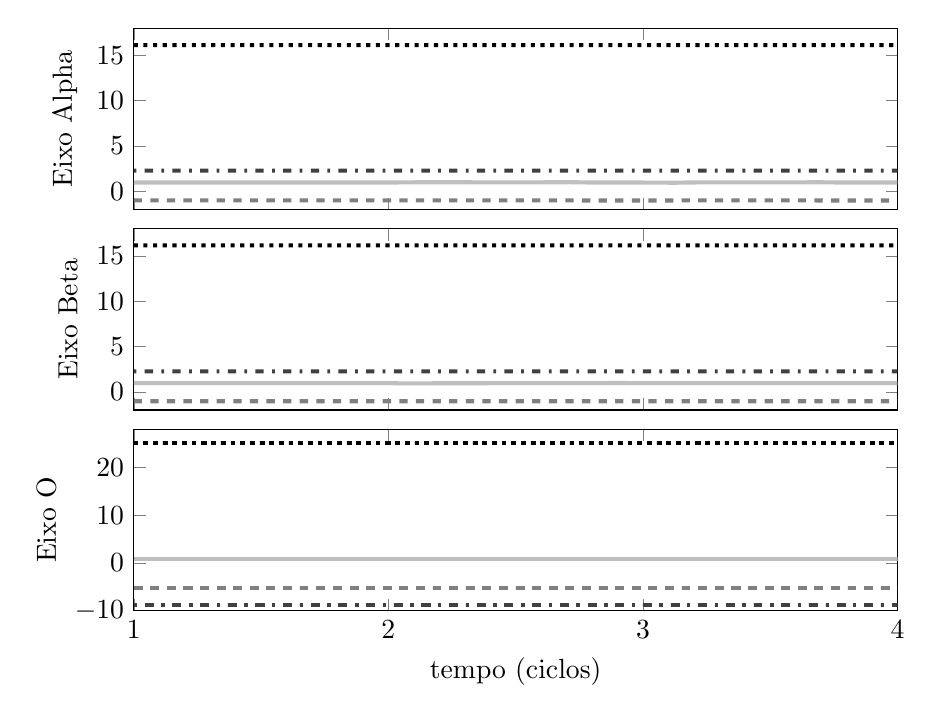
\begin{tikzpicture}

\begin{axis}[%
width=0.8\textwidth,
height=0.189701500343624\textwidth,
scale only axis,
xmin=0.316666666666667,
xmax=0.366666666666667,
xtick={0.316666666666667,0.333333333333333,0.35,0.366666666666667},
xticklabels={\empty},
ymin=-2,
ymax=18,
ytick={ 0,  5, 10, 15},
ylabel={Eixo Beta},
name=plot2,
scaled x ticks = false,
legend columns=-1,
legend style={/tikz/every even column/.append style={column sep=0.3cm}},
legend style={font=\footnotesize}
]
\addplot [color=lightgray,solid,line width=1.5pt,forget plot]
  table[row sep=crcr]{0.316658333333333	0.97043721996195\\
0.3167	0.970436358706691\\
0.316741666666667	0.970436358706691\\
0.316783333333333	0.970435592808439\\
0.316825	0.970435592808439\\
0.316866666666667	0.970434918056243\\
0.316908333333333	0.970434918056243\\
0.31695	0.970434330318112\\
0.316991666666667	0.970434330318112\\
0.317033333333333	0.970433825496951\\
0.317075	0.970433825496951\\
0.317116666666667	0.970433399492092\\
0.317158333333333	0.970433399492092\\
0.3172	0.970433048177814\\
0.317241666666667	0.970433048177814\\
0.317283333333333	0.970432767402266\\
0.317325	0.970432767402266\\
0.317366666666667	0.970432553004264\\
0.317408333333333	0.970432553004264\\
0.31745	0.970432400842131\\
0.317491666666667	0.970432400842131\\
0.317533333333333	0.970432306827843\\
0.317575	0.970432306827843\\
0.317616666666667	0.970432266960474\\
0.317658333333333	0.970432266960474\\
0.3177	0.970432277354792\\
0.317741666666667	0.970432277354792\\
0.317783333333333	0.970432334262824\\
0.317825	0.970432334262824\\
0.317866666666667	0.970432434088099\\
0.317908333333333	0.970432434088099\\
0.31795	0.970432573393534\\
0.317991666666667	0.970432573393534\\
0.318033333333333	0.970432748904596\\
0.318075	0.970432748904596\\
0.318116666666667	0.970432957509533\\
0.318158333333333	0.970432957509533\\
0.3182	0.970433196258189\\
0.318241666666667	0.970433196258189\\
0.318283333333333	0.970433462360463\\
0.318325	0.970433462360463\\
0.318366666666667	0.970433753184959\\
0.318408333333333	0.970433753184959\\
0.31845	0.970434066257974\\
0.318491666666667	0.970434066257974\\
0.318533333333333	0.970434399262647\\
0.318575	0.970434399262647\\
0.318616666666667	0.970434750037975\\
0.318658333333333	0.970434750037975\\
0.3187	0.970435116577406\\
0.318741666666667	0.970435116577406\\
0.318783333333333	0.97043549702676\\
0.318825	0.97043549702676\\
0.318866666666667	0.97043588968139\\
0.318908333333333	0.97043588968139\\
0.31895	0.970436292982595\\
0.318991666666667	0.970436292982595\\
0.319033333333333	0.970436705513386\\
0.319075	0.970436705513386\\
0.319116666666667	0.970437125993791\\
0.319158333333333	0.970437125993791\\
0.3192	0.970437553275866\\
0.319241666666667	0.970437553275866\\
0.319283333333333	0.970437986338605\\
0.319325	0.970437986338605\\
0.319366666666667	0.970438424282876\\
0.319408333333333	0.970438424282876\\
0.31945	0.970438866326497\\
0.319491666666667	0.970438866326497\\
0.319533333333333	0.97043931179951\\
0.319575	0.97043931179951\\
0.319616666666667	0.970439760139689\\
0.319658333333333	0.970439760139689\\
0.3197	0.970440210888314\\
0.319741666666667	0.970440210888314\\
0.319783333333333	0.970440663686211\\
0.319825	0.970440663686211\\
0.319866666666667	0.970441118270085\\
0.319908333333333	0.970441118270085\\
0.31995	0.970441574469177\\
0.319991666666667	0.970441574469177\\
0.320033333333333	0.970442032202265\\
0.320075	0.970442032202265\\
0.320116666666667	0.970442491475084\\
0.320158333333333	0.970442491475084\\
0.3202	0.970442952378189\\
0.320241666666667	0.970442952378189\\
0.320283333333333	0.970443415085359\\
0.320325	0.970443415085359\\
0.320366666666667	0.970443879852587\\
0.320408333333333	0.970443879852587\\
0.32045	0.970444347017744\\
0.320491666666667	0.970444347017744\\
0.320533333333333	0.970444817000997\\
0.320575	0.970444817000997\\
0.320616666666667	0.970445290306078\\
0.320658333333333	0.970445290306078\\
0.3207	0.970445767522508\\
0.320741666666667	0.970445767522508\\
0.320783333333333	0.970446249328905\\
0.320825	0.970446249328905\\
0.320866666666667	0.970446736497523\\
0.320908333333333	0.970446736497523\\
0.32095	0.970447229900211\\
0.320991666666667	0.970447229900211\\
0.321033333333333	0.970447730516016\\
0.321075	0.970447730516016\\
0.321116666666667	0.970448239440708\\
0.321158333333333	0.970448239440708\\
0.3212	0.970448757898565\\
0.321241666666667	0.970448757898565\\
0.321283333333333	0.970449287255117\\
0.321325	0.970449287255117\\
0.321366666666667	0.970449829034775\\
0.321408333333333	0.970449829034775\\
0.32145	0.970450384944168\\
0.321491666666667	0.970450384944168\\
0.321533333333333	0.970450956898191\\
0.321575	0.970450956898191\\
0.321616666666667	0.970451547051789\\
0.321658333333333	0.970451547051789\\
0.3217	0.970452157838907\\
0.321741666666667	0.970452157838907\\
0.321783333333333	0.970452792020252\\
0.321825	0.970452792020252\\
0.321866666666667	0.970453452742033\\
0.321908333333333	0.970453452742033\\
0.32195	0.970454143608473\\
0.321991666666667	0.970454143608473\\
0.322033333333333	0.970454868771685\\
0.322075	0.970454868771685\\
0.322116666666667	0.970455633043542\\
0.322158333333333	0.970455633043542\\
0.3222	0.970456442035388\\
0.322241666666667	0.970456442035388\\
0.322283333333333	0.970457302332857\\
0.322325	0.970457302332857\\
0.322366666666667	0.970458221714429\\
0.322408333333333	0.970458221714429\\
0.32245	0.97045920942283\\
0.322491666666667	0.97045920942283\\
0.322533333333333	0.97046027649605\\
0.322575	0.97046027649605\\
0.322616666666667	0.970461436154189\\
0.322658333333333	0.970461436154189\\
0.3227	0.970462704205603\\
0.322741666666667	0.970462704205603\\
0.322783333333333	0.970464099343308\\
0.322825	0.970464099343308\\
0.322866666666667	0.970465642944787\\
0.322908333333333	0.970465642944787\\
0.32295	0.970467357251532\\
0.322991666666667	0.970467357251532\\
0.323033333333333	0.970469258583928\\
0.323075	0.970469258583928\\
0.323116666666667	0.970471335019103\\
0.323158333333333	0.970471335019103\\
0.3232	0.970473348318116\\
0.323241666666667	0.970473348318116\\
0.323283333333333	0.970474626904486\\
0.323325	0.970474626904486\\
0.323366666666667	0.970474374243411\\
0.323408333333333	0.970474374243411\\
0.32345	0.970472573672318\\
0.323491666666667	0.970472573672318\\
0.323533333333333	0.970469948388625\\
0.323575	0.970469948388625\\
0.323616666666667	0.970467114613926\\
0.323658333333333	0.970467114613926\\
0.3237	0.970464337421047\\
0.323741666666667	0.970464337421047\\
0.323783333333333	0.970461683786388\\
0.323825	0.970461683786388\\
0.323866666666667	0.970459156489005\\
0.323908333333333	0.970459156489005\\
0.32395	0.970456747819866\\
0.323991666666667	0.970456747819866\\
0.324033333333333	0.970454453309765\\
0.324075	0.970454453309765\\
0.324116666666667	0.97045227287176\\
0.324158333333333	0.97045227287176\\
0.3242	0.970450209128296\\
0.324241666666667	0.970450209128296\\
0.324283333333333	0.970448265549337\\
0.324325	0.970448265549337\\
0.324366666666667	0.970446445042454\\
0.324408333333333	0.970446445042454\\
0.32445	0.970444749125981\\
0.324491666666667	0.970444749125981\\
0.324533333333333	0.970443177632723\\
0.324575	0.970443177632723\\
0.324616666666667	0.97044172880593\\
0.324658333333333	0.97044172880593\\
0.3247	0.97044039962421\\
0.324741666666667	0.97044039962421\\
0.324783333333333	0.970439186208874\\
0.324825	0.970439186208874\\
0.324866666666667	0.970438084206409\\
0.324908333333333	0.970438084206409\\
0.32495	0.970437089084224\\
0.324991666666667	0.970437089084224\\
0.325033333333333	0.970436196318331\\
0.325075	0.970436196318331\\
0.325116666666667	0.970435401481262\\
0.325158333333333	0.970435401481262\\
0.3252	0.970434700255544\\
0.325241666666667	0.970434700255544\\
0.325283333333333	0.970434088403698\\
0.325325	0.970434088403698\\
0.325366666666667	0.970433561723097\\
0.325408333333333	0.970433561723097\\
0.32545	0.970433116006485\\
0.325491666666667	0.970433116006485\\
0.325533333333333	0.970432747019942\\
0.325575	0.970432747019942\\
0.325616666666667	0.970432450501775\\
0.325658333333333	0.970432450501775\\
0.3257	0.970432222179772\\
0.325741666666667	0.970432222179772\\
0.325783333333333	0.970432057800854\\
0.325825	0.970432057800854\\
0.325866666666667	0.970431953166174\\
0.325908333333333	0.970431953166174\\
0.32595	0.970431904165525\\
0.325991666666667	0.970431904165525\\
0.326033333333333	0.970431906806762\\
0.326075	0.970431906806762\\
0.326116666666667	0.970431957238012\\
0.326158333333333	0.970431957238012\\
0.3262	0.970432051762366\\
0.326241666666667	0.970432051762366\\
0.326283333333333	0.970432186846018\\
0.326325	0.970432186846018\\
0.326366666666667	0.970432359121564\\
0.326408333333333	0.970432359121564\\
0.32645	0.97043256538827\\
0.326491666666667	0.97043256538827\\
0.326533333333333	0.970432802610885\\
0.326575	0.970432802610885\\
0.326616666666667	0.970433067918077\\
0.326658333333333	0.970433067918077\\
0.3267	0.970433358601067\\
0.326741666666667	0.970433358601067\\
0.326783333333333	0.970433672112601\\
0.326825	0.970433672112601\\
0.326866666666667	0.970434006066087\\
0.326908333333333	0.970434006066087\\
0.32695	0.970434358234596\\
0.326991666666667	0.970434358234596\\
0.327033333333333	0.970434726549414\\
0.327075	0.970434726549414\\
0.327116666666667	0.970435109097919\\
0.327158333333333	0.970435109097919\\
0.3272	0.970435504120658\\
0.327241666666667	0.970435504120658\\
0.327283333333333	0.970435910007656\\
0.327325	0.970435910007656\\
0.327366666666667	0.970436325294062\\
0.327408333333333	0.970436325294062\\
0.32745	0.970436748655303\\
0.327491666666667	0.970436748655303\\
0.327533333333333	0.970437178901951\\
0.327575	0.970437178901951\\
0.327616666666667	0.970437614974456\\
0.327658333333333	0.970437614974456\\
0.3277	0.970438055937924\\
0.327741666666667	0.970438055937924\\
0.327783333333333	0.970438500977014\\
0.327825	0.970438500977014\\
0.327866666666667	0.970438949391041\\
0.327908333333333	0.970438949391041\\
0.32795	0.970439400589312\\
0.327991666666667	0.970439400589312\\
0.328033333333333	0.970439854086724\\
0.328075	0.970439854086724\\
0.328116666666667	0.97044030949963\\
0.328158333333333	0.97044030949963\\
0.3282	0.970440766541997\\
0.328241666666667	0.970440766541997\\
0.328283333333333	0.970441225021877\\
0.328325	0.970441225021877\\
0.328366666666667	0.970441684838236\\
0.328408333333333	0.970441684838236\\
0.32845	0.970442145978184\\
0.328491666666667	0.970442145978184\\
0.328533333333333	0.970442608514653\\
0.328575	0.970442608514653\\
0.328616666666667	0.970443072604613\\
0.328658333333333	0.970443072604613\\
0.3287	0.970443538487861\\
0.328741666666667	0.970443538487861\\
0.328783333333333	0.970444006486495\\
0.328825	0.970444006486495\\
0.328866666666667	0.970444477005118\\
0.328908333333333	0.970444477005118\\
0.32895	0.970444950531897\\
0.328991666666667	0.970444950531897\\
0.329033333333333	0.970445427640563\\
0.329075	0.970445427640563\\
0.329116666666667	0.970445908993475\\
0.329158333333333	0.970445908993475\\
0.3292	0.970446395345909\\
0.329241666666667	0.970446395345909\\
0.329283333333333	0.970446887551736\\
0.329325	0.970446887551736\\
0.329366666666667	0.970447386570722\\
0.329408333333333	0.970447386570722\\
0.32945	0.970447893477714\\
0.329491666666667	0.970447893477714\\
0.329533333333333	0.970448409474047\\
0.329575	0.970448409474047\\
0.329616666666667	0.970448935899864\\
0.329658333333333	0.970448935899864\\
0.3297	0.970449474251262\\
0.329741666666667	0.970449474251262\\
0.329783333333333	0.970450026203047\\
0.329825	0.970450026203047\\
0.329866666666667	0.970450593634111\\
0.329908333333333	0.970450593634111\\
0.32995	0.970451178658432\\
0.329991666666667	0.970451178658432\\
0.330033333333333	0.970451783663083\\
0.330075	0.970451783663083\\
0.330116666666667	0.970452411354861\\
0.330158333333333	0.970452411354861\\
0.3302	0.970453064817657\\
0.330241666666667	0.970453064817657\\
0.330283333333333	0.97045374758329\\
0.330325	0.97045374758329\\
0.330366666666667	0.97045446371932\\
0.330408333333333	0.97045446371932\\
0.33045	0.970455217938359\\
0.330491666666667	0.970455217938359\\
0.330533333333333	0.970456015734584\\
0.330575	0.970456015734584\\
0.330616666666667	0.970456863554561\\
0.330658333333333	0.970456863554561\\
0.3307	0.970457769010778\\
0.330741666666667	0.970457769010778\\
0.330783333333333	0.970458741146766\\
0.330825	0.970458741146766\\
0.330866666666667	0.970459790760365\\
0.330908333333333	0.970459790760365\\
0.33095	0.970460930781311\\
0.330991666666667	0.970460930781311\\
0.331033333333333	0.970462176667188\\
0.331075	0.970462176667188\\
0.331116666666667	0.970463546691103\\
0.331158333333333	0.970463546691103\\
0.3312	0.970465061741802\\
0.331241666666667	0.970465061741802\\
0.331283333333333	0.970466743535177\\
0.331325	0.970466743535177\\
0.331366666666667	0.970468607961243\\
0.331408333333333	0.970468607961243\\
0.33145	0.970470643213183\\
0.331491666666667	0.970470643213183\\
0.331533333333333	0.970472615704777\\
0.331575	0.970472615704777\\
0.331616666666667	0.970473867713727\\
0.331658333333333	0.970473867713727\\
0.3317	0.970473619993488\\
0.331741666666667	0.970473619993488\\
0.331783333333333	0.970471857439701\\
0.331825	0.970471857439701\\
0.331866666666667	0.970469288642677\\
0.331908333333333	0.970469288642677\\
0.33195	0.970466516731413\\
0.331991666666667	0.970466516731413\\
0.332033333333333	0.970463800908304\\
0.332075	0.970463800908304\\
0.332116666666667	0.970461206531781\\
0.332158333333333	0.970461206531781\\
0.3322	0.970458736205245\\
0.332241666666667	0.970458736205245\\
0.332283333333333	0.970456382316685\\
0.332325	0.970456382316685\\
0.332366666666667	0.970454140450355\\
0.332408333333333	0.970454140450355\\
0.33245	0.97045201049146\\
0.332491666666667	0.97045201049146\\
0.332533333333333	0.970449994982174\\
0.332575	0.970449994982174\\
0.332616666666667	0.970448097296241\\
0.332658333333333	0.970448097296241\\
0.3327	0.970446320257846\\
0.332741666666667	0.970446320257846\\
0.332783333333333	0.970444665332178\\
0.332825	0.970444665332178\\
0.332866666666667	0.970443132335721\\
0.332908333333333	0.970443132335721\\
0.33295	0.970441719530581\\
0.332991666666667	0.970441719530581\\
0.333033333333333	0.970440423942802\\
0.333075	0.970440423942802\\
0.333116666666667	0.970439241761191\\
0.333158333333333	0.970439241761191\\
0.3332	0.970438168711639\\
0.333241666666667	0.970438168711639\\
0.333283333333333	0.970437200346429\\
0.333325	0.970437200346429\\
0.333366666666667	0.970436332227711\\
0.333408333333333	0.970436332227711\\
0.33345	0.970435560013326\\
0.333491666666667	0.970435560013326\\
0.333533333333333	0.9704349001265\\
0.333575	0.9704349001265\\
0.333616666666667	0.966474515349834\\
0.333658333333333	0.966474515349834\\
0.3337	0.961159001656852\\
0.333741666666667	0.961159001656852\\
0.333783333333333	0.955796565047486\\
0.333825	0.955796565047486\\
0.333866666666667	0.950876952221888\\
0.333908333333333	0.950876952221888\\
0.33395	0.946625884954079\\
0.333991666666667	0.946625884954079\\
0.334033333333333	0.943179623050303\\
0.334075	0.943179623050303\\
0.334116666666667	0.940607307734694\\
0.334158333333333	0.940607307734694\\
0.3342	0.938906123463615\\
0.334241666666667	0.938906123463615\\
0.334283333333333	0.938002422282344\\
0.334325	0.938002422282344\\
0.334366666666667	0.937761400432086\\
0.334408333333333	0.937761400432086\\
0.33445	0.937999604920762\\
0.334491666666667	0.937999604920762\\
0.334533333333333	0.938490543686468\\
0.334575	0.938490543686468\\
0.334616666666667	0.93892880736547\\
0.334658333333333	0.93892880736547\\
0.3347	0.939052955556216\\
0.334741666666667	0.939052955556216\\
0.334783333333333	0.938924285547318\\
0.334825	0.938924285547318\\
0.334866666666667	0.938815520927763\\
0.334908333333333	0.938815520927763\\
0.33495	0.938849417995434\\
0.334991666666667	0.938849417995434\\
0.335033333333333	0.938997305116061\\
0.335075	0.938997305116061\\
0.335116666666667	0.93920644068904\\
0.335158333333333	0.93920644068904\\
0.3352	0.939450964943151\\
0.335241666666667	0.939450964943151\\
0.335283333333333	0.939729849887125\\
0.335325	0.939729849887125\\
0.335366666666667	0.940053962063634\\
0.335408333333333	0.940053962063634\\
0.33545	0.940436270043836\\
0.335491666666667	0.940436270043836\\
0.335533333333333	0.940886341919001\\
0.335575	0.940886341919001\\
0.335616666666667	0.941407953091536\\
0.335658333333333	0.941407953091536\\
0.3357	0.941998797340256\\
0.335741666666667	0.941998797340256\\
0.335783333333333	0.942651525089562\\
0.335825	0.942651525089562\\
0.335866666666667	0.943355449497497\\
0.335908333333333	0.943355449497497\\
0.33595	0.944098383767771\\
0.335991666666667	0.944098383767771\\
0.336033333333333	0.944868230681349\\
0.336075	0.944868230681349\\
0.336116666666667	0.945654113749056\\
0.336158333333333	0.945654113749056\\
0.3362	0.946446989860755\\
0.336241666666667	0.946446989860755\\
0.336283333333333	0.947239796798835\\
0.336325	0.947239796798835\\
0.336366666666667	0.948027257476187\\
0.336408333333333	0.948027257476187\\
0.33645	0.948805487735942\\
0.336491666666667	0.948805487735942\\
0.336533333333333	0.949571544511912\\
0.336575	0.949571544511912\\
0.336616666666667	0.950323018462505\\
0.336658333333333	0.950323018462505\\
0.3367	0.951057732861295\\
0.336741666666667	0.951057732861295\\
0.336783333333333	0.951773569574036\\
0.336825	0.951773569574036\\
0.336866666666667	0.95246841084448\\
0.336908333333333	0.95246841084448\\
0.33695	0.953140165847031\\
0.336991666666667	0.953140165847031\\
0.337033333333333	0.953786843568399\\
0.337075	0.953786843568399\\
0.337116666666667	0.954406636155987\\
0.337158333333333	0.954406636155987\\
0.3372	0.954997985809917\\
0.337241666666667	0.954997985809917\\
0.337283333333333	0.955559619856262\\
0.337325	0.955559619856262\\
0.337366666666667	0.956090549715046\\
0.337408333333333	0.956090549715046\\
0.33745	0.95659003800614\\
0.337491666666667	0.95659003800614\\
0.337533333333333	0.957057543084261\\
0.337575	0.957057543084261\\
0.337616666666667	0.957492651890112\\
0.337658333333333	0.957492651890112\\
0.3377	0.957895005109863\\
0.337741666666667	0.957895005109863\\
0.337783333333333	0.958264237449436\\
0.337825	0.958264237449436\\
0.337866666666667	0.958599925209353\\
0.337908333333333	0.958599925209353\\
0.33795	0.95890153738123\\
0.337991666666667	0.95890153738123\\
0.338033333333333	0.959168392141568\\
0.338075	0.959168392141568\\
0.338116666666667	0.959399614257684\\
0.338158333333333	0.959399614257684\\
0.3382	0.959594087964818\\
0.338241666666667	0.959594087964818\\
0.338283333333333	0.959750400230422\\
0.338325	0.959750400230422\\
0.338366666666667	0.959866770575522\\
0.338408333333333	0.959866770575522\\
0.33845	0.95994096631837\\
0.338491666666667	0.95994096631837\\
0.338533333333333	0.959970208158611\\
0.338575	0.959970208158611\\
0.338616666666667	0.959951085793827\\
0.338658333333333	0.959951085793827\\
0.3387	0.959879541571895\\
0.338741666666667	0.959879541571895\\
0.338783333333333	0.959751084630909\\
0.338825	0.959751084630909\\
0.338866666666667	0.959561700226084\\
0.338908333333333	0.959561700226084\\
0.33895	0.959310868952517\\
0.338991666666667	0.959310868952517\\
0.339033333333333	0.959025894530818\\
0.339075	0.959025894530818\\
0.339116666666667	0.958807614394484\\
0.339158333333333	0.958807614394484\\
0.3392	0.958805039325034\\
0.339241666666667	0.958805039325034\\
0.339283333333333	0.95908832051499\\
0.339325	0.95908832051499\\
0.339366666666667	0.959589185570701\\
0.339408333333333	0.959589185570701\\
0.33945	0.960199227897845\\
0.339491666666667	0.960199227897845\\
0.339533333333333	0.960846951077059\\
0.339575	0.960846951077059\\
0.339616666666667	0.9615003713096\\
0.339658333333333	0.9615003713096\\
0.3397	0.962147807693048\\
0.339741666666667	0.962147807693048\\
0.339783333333333	0.96278484374788\\
0.339825	0.96278484374788\\
0.339866666666667	0.963408995798193\\
0.339908333333333	0.963408995798193\\
0.33995	0.964018126418229\\
0.339991666666667	0.964018126418229\\
0.340033333333333	0.964610148398243\\
0.340075	0.964610148398243\\
0.340116666666667	0.965183090123897\\
0.340158333333333	0.965183090123897\\
0.3402	0.9657352296014\\
0.340241666666667	0.9657352296014\\
0.340283333333333	0.966265201472581\\
0.340325	0.966265201472581\\
0.340366666666667	0.966772046437657\\
0.340408333333333	0.966772046437657\\
0.34045	0.967255203032845\\
0.340491666666667	0.967255203032845\\
0.340533333333333	0.96771445725969\\
0.340575	0.96771445725969\\
0.340616666666667	0.968149870536273\\
0.340658333333333	0.968149870536273\\
0.3407	0.968561704426659\\
0.340741666666667	0.968561704426659\\
0.340783333333333	0.96895035508992\\
0.340825	0.96895035508992\\
0.340866666666667	0.969316304063016\\
0.340908333333333	0.969316304063016\\
0.34095	0.969660086552755\\
0.340991666666667	0.969660086552755\\
0.341033333333333	0.969982274680913\\
0.341075	0.969982274680913\\
0.341116666666667	0.97028347125099\\
0.341158333333333	0.97028347125099\\
0.3412	0.970564309295895\\
0.341241666666667	0.970564309295895\\
0.341283333333333	0.970825453419787\\
0.341325	0.970825453419787\\
0.341366666666667	0.971067600227571\\
0.341408333333333	0.971067600227571\\
0.34145	0.971291476492184\\
0.341491666666667	0.971291476492184\\
0.341533333333333	0.971497834839434\\
0.341575	0.971497834839434\\
0.341616666666667	0.971687447484191\\
0.341658333333333	0.971687447484191\\
0.3417	0.971861098911425\\
0.341741666666667	0.971861098911425\\
0.341783333333333	0.972019578428975\\
0.341825	0.972019578428975\\
0.341866666666667	0.972163673336581\\
0.341908333333333	0.972163673336581\\
0.34195	0.972294163172815\\
0.341991666666667	0.972294163172815\\
0.342033333333333	0.972411815213095\\
0.342075	0.972411815213095\\
0.342116666666667	0.972517381160371\\
0.342158333333333	0.972517381160371\\
0.3422	0.972611594824041\\
0.342241666666667	0.972611594824041\\
0.342283333333333	0.972695170523017\\
0.342325	0.972695170523017\\
0.342366666666667	0.972768801958413\\
0.342408333333333	0.972768801958413\\
0.34245	0.9728331613544\\
0.342491666666667	0.9728331613544\\
0.342533333333333	0.972888898736668\\
0.342575	0.972888898736668\\
0.342616666666667	0.972936641286169\\
0.342658333333333	0.972936641286169\\
0.3427	0.972976992758406\\
0.342741666666667	0.972976992758406\\
0.342783333333333	0.973010532990327\\
0.342825	0.973010532990327\\
0.342866666666667	0.97303781752866\\
0.342908333333333	0.97303781752866\\
0.34295	0.973059377410049\\
0.342991666666667	0.973059377410049\\
0.343033333333333	0.973075719110813\\
0.343075	0.973075719110813\\
0.343116666666667	0.973087324668603\\
0.343158333333333	0.973087324668603\\
0.3432	0.973094651964198\\
0.343241666666667	0.973094651964198\\
0.343283333333333	0.973098135141914\\
0.343325	0.973098135141914\\
0.343366666666667	0.973098185142443\\
0.343408333333333	0.973098185142443\\
0.34345	0.973095190321962\\
0.343491666666667	0.973095190321962\\
0.343533333333333	0.973089517134696\\
0.343575	0.973089517134696\\
0.343616666666667	0.973081510861193\\
0.343658333333333	0.973081510861193\\
0.3437	0.973071496370026\\
0.343741666666667	0.973071496370026\\
0.343783333333333	0.973059778905266\\
0.343825	0.973059778905266\\
0.343866666666667	0.973046644895496\\
0.343908333333333	0.973046644895496\\
0.34395	0.973032362782076\\
0.343991666666667	0.973032362782076\\
0.344033333333333	0.973017183865143\\
0.344075	0.973017183865143\\
0.344116666666667	0.973001343165737\\
0.344158333333333	0.973001343165737\\
0.3442	0.97298506030198\\
0.344241666666667	0.97298506030198\\
0.344283333333333	0.97296854037667\\
0.344325	0.97296854037667\\
0.344366666666667	0.972951974873391\\
0.344408333333333	0.972951974873391\\
0.34445	0.972935542558182\\
0.344491666666667	0.972935542558182\\
0.344533333333333	0.972919410384259\\
0.344575	0.972919410384259\\
0.344616666666667	0.972903734397884\\
0.344658333333333	0.972903734397884\\
0.3447	0.972888660644338\\
0.344741666666667	0.972888660644338\\
0.344783333333333	0.972874326073922\\
0.344825	0.972874326073922\\
0.344866666666667	0.972860859448795\\
0.344908333333333	0.972860859448795\\
0.34495	0.972848382252408\\
0.344991666666667	0.972848382252408\\
0.345033333333333	0.972837009604098\\
0.345075	0.972837009604098\\
0.345116666666667	0.972826851182238\\
0.345158333333333	0.972826851182238\\
0.3452	0.972818012160162\\
0.345241666666667	0.972818012160162\\
0.345283333333333	0.97281059415994\\
0.345325	0.97281059415994\\
0.345366666666667	0.972804696230136\\
0.345408333333333	0.972804696230136\\
0.34545	0.97280041585484\\
0.345491666666667	0.97280041585484\\
0.345533333333333	0.972797850002714\\
0.345575	0.972797850002714\\
0.345616666666667	0.972797096226558\\
0.345658333333333	0.972797096226558\\
0.3457	0.972798253825968\\
0.345741666666667	0.972798253825968\\
0.345783333333333	0.972801425088295\\
0.345825	0.972801425088295\\
0.345866666666667	0.972806716626162\\
0.345908333333333	0.972806716626162\\
0.34595	0.972814240833672\\
0.345991666666667	0.972814240833672\\
0.346033333333333	0.972824117488093\\
0.346075	0.972824117488093\\
0.346116666666667	0.97283647552963\\
0.346158333333333	0.97283647552963\\
0.3462	0.972851455059101\\
0.346241666666667	0.972851455059101\\
0.346283333333333	0.972869209535531\\
0.346325	0.972869209535531\\
0.346366666666667	0.972889908373237\\
0.346408333333333	0.972889908373237\\
0.34645	0.972913739957093\\
0.346491666666667	0.972913739957093\\
0.346533333333333	0.97294091512052\\
0.346575	0.97294091512052\\
0.346616666666667	0.972971671232109\\
0.346658333333333	0.972971671232109\\
0.3467	0.973006277040897\\
0.346741666666667	0.973006277040897\\
0.346783333333333	0.97304503846725\\
0.346825	0.97304503846725\\
0.346866666666667	0.973088305579411\\
0.346908333333333	0.973088305579411\\
0.34695	0.973136481065665\\
0.346991666666667	0.973136481065665\\
0.347033333333333	0.973190030603952\\
0.347075	0.973190030603952\\
0.347116666666667	0.973249495652552\\
0.347158333333333	0.973249495652552\\
0.3472	0.973315509346596\\
0.347241666666667	0.973315509346596\\
0.347283333333333	0.973388816397023\\
0.347325	0.973388816397023\\
0.347366666666667	0.973470298162432\\
0.347408333333333	0.973470298162432\\
0.34745	0.973561004404515\\
0.347491666666667	0.973561004404515\\
0.347533333333333	0.973662193624687\\
0.347575	0.973662193624687\\
0.347616666666667	0.97377538421943\\
0.347658333333333	0.97377538421943\\
0.3477	0.973902418687085\\
0.347741666666667	0.973902418687085\\
0.347783333333333	0.974045541912932\\
0.347825	0.974045541912932\\
0.347866666666667	0.974207489748236\\
0.347908333333333	0.974207489748236\\
0.34795	0.974391568844317\\
0.347991666666667	0.974391568844317\\
0.348033333333333	0.974601662814368\\
0.348075	0.974601662814368\\
0.348116666666667	0.974841960159302\\
0.348158333333333	0.974841960159302\\
0.3482	0.975115753247095\\
0.348241666666667	0.975115753247095\\
0.348283333333333	0.975421118109126\\
0.348325	0.975421118109126\\
0.348366666666667	0.975708645270717\\
0.348408333333333	0.975708645270717\\
0.34845	0.975859157354035\\
0.348491666666667	0.975859157354035\\
0.348533333333333	0.975754520849871\\
0.348575	0.975754520849871\\
0.348616666666667	0.97542476409874\\
0.348658333333333	0.97542476409874\\
0.3487	0.974995253750561\\
0.348741666666667	0.974995253750561\\
0.348783333333333	0.97455279031515\\
0.348825	0.97455279031515\\
0.348866666666667	0.974127266982889\\
0.348908333333333	0.974127266982889\\
0.34895	0.973722460341655\\
0.348991666666667	0.973722460341655\\
0.349033333333333	0.973336171424437\\
0.349075	0.973336171424437\\
0.349116666666667	0.972966502133825\\
0.349158333333333	0.972966502133825\\
0.3492	0.972612653741293\\
0.349241666666667	0.972612653741293\\
0.349283333333333	0.97227457382205\\
0.349325	0.97227457382205\\
0.349366666666667	0.971952569979088\\
0.349408333333333	0.971952569979088\\
0.34945	0.97164702830843\\
0.349491666666667	0.97164702830843\\
0.349533333333333	0.971358229887111\\
0.349575	0.971358229887111\\
0.349616666666667	0.971086255222882\\
0.349658333333333	0.971086255222882\\
0.3497	0.970830960995836\\
0.349741666666667	0.970830960995836\\
0.349783333333333	0.970592006314011\\
0.349825	0.970592006314011\\
0.349866666666667	0.970368904528485\\
0.349908333333333	0.970368904528485\\
0.34995	0.970161080761356\\
0.349991666666667	0.970161080761356\\
0.350033333333333	0.969967921796637\\
0.350075	0.969967921796637\\
0.350116666666667	0.969788811595847\\
0.350158333333333	0.969788811595847\\
0.3502	0.969623151115687\\
0.350241666666667	0.969623151115687\\
0.350283333333333	0.969470364755676\\
0.350325	0.969470364755676\\
0.350366666666667	0.969329897608379\\
0.350408333333333	0.969329897608379\\
0.35045	0.969201208026151\\
0.350491666666667	0.969201208026151\\
0.350533333333333	0.969083759330451\\
0.350575	0.969083759330451\\
0.350616666666667	0.968977013274591\\
0.350658333333333	0.968977013274591\\
0.3507	0.968880426554942\\
0.350741666666667	0.968880426554942\\
0.350783333333333	0.968793450546336\\
0.350825	0.968793450546336\\
0.350866666666667	0.968715533670252\\
0.350908333333333	0.968715533670252\\
0.35095	0.96864612542171\\
0.350991666666667	0.96864612542171\\
0.351033333333333	0.968584681027888\\
0.351075	0.968584681027888\\
0.351116666666667	0.968530665886641\\
0.351158333333333	0.968530665886641\\
0.3512	0.968483559223704\\
0.351241666666667	0.968483559223704\\
0.351283333333333	0.968442856715822\\
0.351325	0.968442856715822\\
0.351366666666667	0.968408072085014\\
0.351408333333333	0.968408072085014\\
0.35145	0.96837873784136\\
0.351491666666667	0.96837873784136\\
0.351533333333333	0.968354405431945\\
0.351575	0.968354405431945\\
0.351616666666667	0.96833464505626\\
0.351658333333333	0.96833464505626\\
0.3517	0.968319045358813\\
0.351741666666667	0.968319045358813\\
0.351783333333333	0.968307213135408\\
0.351825	0.968307213135408\\
0.351866666666667	0.968298773113979\\
0.351908333333333	0.968298773113979\\
0.35195	0.96829336780989\\
0.351991666666667	0.96829336780989\\
0.352033333333333	0.96829065741706\\
0.352075	0.96829065741706\\
0.352116666666667	0.968290319680575\\
0.352158333333333	0.968290319680575\\
0.3522	0.968292049699402\\
0.352241666666667	0.968292049699402\\
0.352283333333333	0.968295559622612\\
0.352325	0.968295559622612\\
0.352366666666667	0.968300578222096\\
0.352408333333333	0.968300578222096\\
0.35245	0.968306850343441\\
0.352491666666667	0.968306850343441\\
0.352533333333333	0.968314136250616\\
0.352575	0.968314136250616\\
0.352616666666667	0.968322210887854\\
0.352658333333333	0.968322210887854\\
0.3527	0.968330863083821\\
0.352741666666667	0.968330863083821\\
0.352783333333333	0.968339894720205\\
0.352825	0.968339894720205\\
0.352866666666667	0.968349119881097\\
0.352908333333333	0.968349119881097\\
0.35295	0.968358363992946\\
0.352991666666667	0.968358363992946\\
0.353033333333333	0.968367462958774\\
0.353075	0.968367462958774\\
0.353116666666667	0.9683762622857\\
0.353158333333333	0.9683762622857\\
0.3532	0.968384616201932\\
0.353241666666667	0.968384616201932\\
0.353283333333333	0.968392386758059\\
0.353325	0.968392386758059\\
0.353366666666667	0.968399442907239\\
0.353408333333333	0.968399442907239\\
0.35345	0.968405659559245\\
0.353491666666667	0.968405659559245\\
0.353533333333333	0.968410916603659\\
0.353575	0.968410916603659\\
0.353616666666667	0.968415097897504\\
0.353658333333333	0.968415097897504\\
0.3537	0.968418090211867\\
0.353741666666667	0.968418090211867\\
0.353783333333333	0.968419782130713\\
0.353825	0.968419782130713\\
0.353866666666667	0.96842006289283\\
0.353908333333333	0.96842006289283\\
0.35395	0.96841882116505\\
0.353991666666667	0.96841882116505\\
0.354033333333333	0.968415943731322\\
0.354075	0.968415943731322\\
0.354116666666667	0.968411314078105\\
0.354158333333333	0.968411314078105\\
0.3542	0.968404810851639\\
0.354241666666667	0.968404810851639\\
0.354283333333333	0.968396306156929\\
0.354325	0.968396306156929\\
0.354366666666667	0.96838566366125\\
0.354408333333333	0.96838566366125\\
0.35445	0.968372736456441\\
0.354491666666667	0.968372736456441\\
0.354533333333333	0.968357364623457\\
0.354575	0.968357364623457\\
0.354616666666667	0.968339372470382\\
0.354658333333333	0.968339372470382\\
0.3547	0.968318565355261\\
0.354741666666667	0.968318565355261\\
0.354783333333333	0.968294725792874\\
0.354825	0.968294725792874\\
0.354866666666667	0.968267608939569\\
0.354908333333333	0.968267608939569\\
0.35495	0.968236937204806\\
0.354991666666667	0.968236937204806\\
0.355033333333333	0.968202393755366\\
0.355075	0.968202393755366\\
0.355116666666667	0.968163614622169\\
0.355158333333333	0.968163614622169\\
0.3552	0.968120179034342\\
0.355241666666667	0.968120179034342\\
0.355283333333333	0.968071597493508\\
0.355325	0.968071597493508\\
0.355366666666667	0.968017296958356\\
0.355408333333333	0.968017296958356\\
0.35545	0.967956602330594\\
0.355491666666667	0.967956602330594\\
0.355533333333333	0.967888713220961\\
0.355575	0.967888713220961\\
0.355616666666667	0.967812674753879\\
0.355658333333333	0.967812674753879\\
0.3557	0.967727341028394\\
0.355741666666667	0.967727341028394\\
0.355783333333333	0.967631330040133\\
0.355825	0.967631330040133\\
0.355866666666667	0.967522970056257\\
0.355908333333333	0.967522970056257\\
0.35595	0.967400241429334\\
0.355991666666667	0.967400241429334\\
0.356033333333333	0.967260729591466\\
0.356075	0.967260729591466\\
0.356116666666667	0.967101638633423\\
0.356158333333333	0.967101638633423\\
0.3562	0.966920013214531\\
0.356241666666667	0.966920013214531\\
0.356283333333333	0.966713618811361\\
0.356325	0.966713618811361\\
0.356366666666667	0.966483932851649\\
0.356408333333333	0.966483932851649\\
0.35645	0.966263900772889\\
0.356491666666667	0.966263900772889\\
0.356533333333333	0.966137113042296\\
0.356575	0.966137113042296\\
0.356616666666667	0.96619413995802\\
0.356658333333333	0.96619413995802\\
0.3567	0.966427668604105\\
0.356741666666667	0.966427668604105\\
0.356783333333333	0.966750747724984\\
0.356825	0.966750747724984\\
0.356866666666667	0.967093799004547\\
0.356908333333333	0.967093799004547\\
0.35695	0.96742876680628\\
0.356991666666667	0.96742876680628\\
0.357033333333333	0.967749806497932\\
0.357075	0.967749806497932\\
0.357116666666667	0.968057408906577\\
0.357158333333333	0.968057408906577\\
0.3572	0.968352571752271\\
0.357241666666667	0.968352571752271\\
0.357283333333333	0.968635680802672\\
0.357325	0.968635680802672\\
0.357366666666667	0.968906618292317\\
0.357408333333333	0.968906618292317\\
0.35745	0.969165017659583\\
0.357491666666667	0.969165017659583\\
0.357533333333333	0.969410469502122\\
0.357575	0.969410469502122\\
0.357616666666667	0.969642661038814\\
0.357658333333333	0.969642661038814\\
0.3577	0.969861450935551\\
0.357741666666667	0.969861450935551\\
0.357783333333333	0.970066888719668\\
0.357825	0.970066888719668\\
0.357866666666667	0.970259194808385\\
0.357908333333333	0.970259194808385\\
0.35795	0.970438719254377\\
0.357991666666667	0.970438719254377\\
0.358033333333333	0.970605894878227\\
0.358075	0.970605894878227\\
0.358116666666667	0.970761195705033\\
0.358158333333333	0.970761195705033\\
0.3582	0.970905106471312\\
0.358241666666667	0.970905106471312\\
0.358283333333333	0.971038104605135\\
0.358325	0.971038104605135\\
0.358366666666667	0.971160653064258\\
0.358408333333333	0.971160653064258\\
0.35845	0.971273200836078\\
0.358491666666667	0.971273200836078\\
0.358533333333333	0.971376187545228\\
0.358575	0.971376187545228\\
0.358616666666667	0.971470049106939\\
0.358658333333333	0.971470049106939\\
0.3587	0.971555222302033\\
0.358741666666667	0.971555222302033\\
0.358783333333333	0.97163214718443\\
0.358825	0.97163214718443\\
0.358866666666667	0.971701267120603\\
0.358908333333333	0.971701267120603\\
0.35895	0.971763026874091\\
0.358991666666667	0.971763026874091\\
0.359033333333333	0.971817869458879\\
0.359075	0.971817869458879\\
0.359116666666667	0.971866232535865\\
0.359158333333333	0.971866232535865\\
0.3592	0.97190854499712\\
0.359241666666667	0.97190854499712\\
0.359283333333333	0.971945224162111\\
0.359325	0.971945224162111\\
0.359366666666667	0.971976673775083\\
0.359408333333333	0.971976673775083\\
0.35945	0.972003282796643\\
0.359491666666667	0.972003282796643\\
0.359533333333333	0.972025424852206\\
0.359575	0.972025424852206\\
0.359616666666667	0.972043458139835\\
0.359658333333333	0.972043458139835\\
0.3597	0.972057725598613\\
0.359741666666667	0.972057725598613\\
0.359783333333333	0.972068555176522\\
0.359825	0.972068555176522\\
0.359866666666667	0.972076260092918\\
0.359908333333333	0.972076260092918\\
0.35995	0.97208113904742\\
0.359991666666667	0.97208113904742\\
0.360033333333333	0.972083476372603\\
0.360075	0.972083476372603\\
0.360116666666667	0.972083542156727\\
0.360158333333333	0.972083542156727\\
0.3602	0.972081592374585\\
0.360241666666667	0.972081592374585\\
0.360283333333333	0.972077869062726\\
0.360325	0.972077869062726\\
0.360366666666667	0.972072600564903\\
0.360408333333333	0.972072600564903\\
0.36045	0.97206600185967\\
0.360491666666667	0.97206600185967\\
0.360533333333333	0.972058274968861\\
0.360575	0.972058274968861\\
0.360616666666667	0.9720496094358\\
0.360658333333333	0.9720496094358\\
0.3607	0.972040182856687\\
0.360741666666667	0.972040182856687\\
0.360783333333333	0.972030161447447\\
0.360825	0.972030161447447\\
0.360866666666667	0.972019700630357\\
0.360908333333333	0.972019700630357\\
0.36095	0.972008945628799\\
0.360991666666667	0.972008945628799\\
0.361033333333333	0.971998032062952\\
0.361075	0.971998032062952\\
0.361116666666667	0.971987086543373\\
0.361158333333333	0.971987086543373\\
0.3612	0.971976227262453\\
0.361241666666667	0.971976227262453\\
0.361283333333333	0.971965564585533\\
0.361325	0.971965564585533\\
0.361366666666667	0.971955201644177\\
0.361408333333333	0.971955201644177\\
0.36145	0.971945234933959\\
0.361491666666667	0.971945234933959\\
0.361533333333333	0.971935754918633\\
0.361575	0.971935754918633\\
0.361616666666667	0.971926846641929\\
0.361658333333333	0.971926846641929\\
0.3617	0.97191859034785\\
0.361741666666667	0.97191859034785\\
0.361783333333333	0.971911062110308\\
0.361825	0.971911062110308\\
0.361866666666667	0.971904334473301\\
0.361908333333333	0.971904334473301\\
0.36195	0.971898477103564\\
0.361991666666667	0.971898477103564\\
0.362033333333333	0.971893557458649\\
0.362075	0.971893557458649\\
0.362116666666667	0.971889641474632\\
0.362158333333333	0.971889641474632\\
0.3622	0.971886794279011\\
0.362241666666667	0.971886794279011\\
0.362283333333333	0.971885080935875\\
0.362325	0.971885080935875\\
0.362366666666667	0.971884567232076\\
0.362408333333333	0.971884567232076\\
0.36245	0.971885320514949\\
0.362491666666667	0.971885320514949\\
0.362533333333333	0.97188741059433\\
0.362575	0.97188741059433\\
0.362616666666667	0.971890910724141\\
0.362658333333333	0.971890910724141\\
0.3627	0.971895898682056\\
0.362741666666667	0.971895898682056\\
0.362783333333333	0.971902457969709\\
0.362825	0.971902457969709\\
0.362866666666667	0.971910679160972\\
0.362908333333333	0.971910679160972\\
0.36295	0.971920661396392\\
0.362991666666667	0.971920661396392\\
0.363033333333333	0.97193251412757\\
0.363075	0.97193251412757\\
0.363116666666667	0.971946359164702\\
0.363158333333333	0.971946359164702\\
0.3632	0.97196233304274\\
0.363241666666667	0.97196233304274\\
0.363283333333333	0.97198058980949\\
0.363325	0.97198058980949\\
0.363366666666667	0.972001304342815\\
0.363408333333333	0.972001304342815\\
0.36345	0.972024676330812\\
0.363491666666667	0.972024676330812\\
0.363533333333333	0.972050935087342\\
0.363575	0.972050935087342\\
0.363616666666667	0.972080345426152\\
0.363658333333333	0.972080345426152\\
0.3637	0.972113214883822\\
0.363741666666667	0.972113214883822\\
0.363783333333333	0.972149902669988\\
0.363825	0.972149902669988\\
0.363866666666667	0.972190830838951\\
0.363908333333333	0.972190830838951\\
0.36395	0.972236498325666\\
0.363991666666667	0.972236498325666\\
0.364033333333333	0.972287498673483\\
0.364075	0.972287498673483\\
0.364116666666667	0.972344542489859\\
0.364158333333333	0.972344542489859\\
0.3642	0.972408485849572\\
0.364241666666667	0.972408485849572\\
0.364283333333333	0.972480365865391\\
0.364325	0.972480365865391\\
0.364366666666667	0.972561444016554\\
0.364408333333333	0.972561444016554\\
0.36445	0.972653255323557\\
0.364491666666667	0.972653255323557\\
0.364533333333333	0.972757653592797\\
0.364575	0.972757653592797\\
0.364616666666667	0.972876819553404\\
0.364658333333333	0.972876819553404\\
0.3647	0.97301312844481\\
0.364741666666667	0.97301312844481\\
0.364783333333333	0.973168552674667\\
0.364825	0.973168552674667\\
0.364866666666667	0.973342526865256\\
0.364908333333333	0.973342526865256\\
0.36495	0.973511687617071\\
0.364991666666667	0.973511687617071\\
0.365033333333333	0.973612600613994\\
0.365075	0.973612600613994\\
0.365116666666667	0.973572805436731\\
0.365158333333333	0.973572805436731\\
0.3652	0.973396393954816\\
0.365241666666667	0.973396393954816\\
0.365283333333333	0.973152407125627\\
0.365325	0.973152407125627\\
0.365366666666667	0.972895444284831\\
0.365408333333333	0.972895444284831\\
0.36545	0.972646492955526\\
0.365491666666667	0.972646492955526\\
0.365533333333333	0.972409189654602\\
0.365575	0.972409189654602\\
0.365616666666667	0.972182595348316\\
0.365658333333333	0.972182595348316\\
0.3657	0.971965634971873\\
0.365741666666667	0.971965634971873\\
0.365783333333333	0.971757829118433\\
0.365825	0.971757829118433\\
0.365866666666667	0.971559142086422\\
0.365908333333333	0.971559142086422\\
0.36595	0.971369761368348\\
0.365991666666667	0.971369761368348\\
0.366033333333333	0.971189930951352\\
0.366075	0.971189930951352\\
0.366116666666667	0.971019840185256\\
0.366158333333333	0.971019840185256\\
0.3662	0.97085956341569\\
0.366241666666667	0.97085956341569\\
0.366283333333333	0.97070904241709\\
0.366325	0.97070904241709\\
0.366366666666667	0.970568099100602\\
0.366408333333333	0.970568099100602\\
0.36645	0.970436464655833\\
0.366491666666667	0.970436464655833\\
0.366533333333333	0.970313813264893\\
0.366575	0.970313813264893\\
0.366616666666667	0.970199792152322\\
0.366658333333333	0.970199792152322\\
};
\addplot [color=gray,dashed,line width=1.5pt,forget plot]
  table[row sep=crcr]{0.316658333333333	-1.02797931894004\\
0.3167	-1.0279793224329\\
0.316741666666667	-1.0279793224329\\
0.316783333333333	-1.02797932543233\\
0.316825	-1.02797932543233\\
0.316866666666667	-1.02797932798806\\
0.316908333333333	-1.02797932798806\\
0.31695	-1.02797933014413\\
0.316991666666667	-1.02797933014413\\
0.317033333333333	-1.02797933193992\\
0.317075	-1.02797933193992\\
0.317116666666667	-1.02797933341104\\
0.317158333333333	-1.02797933341104\\
0.3172	-1.02797933458991\\
0.317241666666667	-1.02797933458991\\
0.317283333333333	-1.02797933550621\\
0.317325	-1.02797933550621\\
0.317366666666667	-1.02797933618718\\
0.317408333333333	-1.02797933618718\\
0.31745	-1.02797933665787\\
0.317491666666667	-1.02797933665787\\
0.317533333333333	-1.02797933694126\\
0.317575	-1.02797933694126\\
0.317616666666667	-1.02797933705843\\
0.317658333333333	-1.02797933705843\\
0.3177	-1.02797933702864\\
0.317741666666667	-1.02797933702864\\
0.317783333333333	-1.02797933686946\\
0.317825	-1.02797933686946\\
0.317866666666667	-1.02797933659693\\
0.317908333333333	-1.02797933659693\\
0.31795	-1.02797933622564\\
0.317991666666667	-1.02797933622564\\
0.318033333333333	-1.02797933576886\\
0.318075	-1.02797933576886\\
0.318116666666667	-1.02797933523867\\
0.318158333333333	-1.02797933523867\\
0.3182	-1.02797933464602\\
0.318241666666667	-1.02797933464602\\
0.318283333333333	-1.02797933400088\\
0.318325	-1.02797933400088\\
0.318366666666667	-1.02797933331226\\
0.318408333333333	-1.02797933331226\\
0.31845	-1.02797933258833\\
0.318491666666667	-1.02797933258833\\
0.318533333333333	-1.02797933183645\\
0.318575	-1.02797933183645\\
0.318616666666667	-1.02797933106326\\
0.318658333333333	-1.02797933106326\\
0.3187	-1.02797933027471\\
0.318741666666667	-1.02797933027471\\
0.318783333333333	-1.02797932947612\\
0.318825	-1.02797932947612\\
0.318866666666667	-1.02797932867225\\
0.318908333333333	-1.02797932867225\\
0.31895	-1.0279793278673\\
0.318991666666667	-1.0279793278673\\
0.319033333333333	-1.02797932706501\\
0.319075	-1.02797932706501\\
0.319116666666667	-1.02797932626865\\
0.319158333333333	-1.02797932626865\\
0.3192	-1.02797932548113\\
0.319241666666667	-1.02797932548113\\
0.319283333333333	-1.02797932470497\\
0.319325	-1.02797932470497\\
0.319366666666667	-1.02797932394236\\
0.319408333333333	-1.02797932394236\\
0.31945	-1.02797932319524\\
0.319491666666667	-1.02797932319524\\
0.319533333333333	-1.02797932246525\\
0.319575	-1.02797932246525\\
0.319616666666667	-1.02797932175383\\
0.319658333333333	-1.02797932175383\\
0.3197	-1.02797932106223\\
0.319741666666667	-1.02797932106223\\
0.319783333333333	-1.02797932039152\\
0.319825	-1.02797932039152\\
0.319866666666667	-1.02797931974265\\
0.319908333333333	-1.02797931974265\\
0.31995	-1.02797931911644\\
0.319991666666667	-1.02797931911644\\
0.320033333333333	-1.02797931851366\\
0.320075	-1.02797931851366\\
0.320116666666667	-1.02797931793501\\
0.320158333333333	-1.02797931793501\\
0.3202	-1.02797931738115\\
0.320241666666667	-1.02797931738115\\
0.320283333333333	-1.02797931685278\\
0.320325	-1.02797931685278\\
0.320366666666667	-1.0279793163506\\
0.320408333333333	-1.0279793163506\\
0.32045	-1.0279793158754\\
0.320491666666667	-1.0279793158754\\
0.320533333333333	-1.02797931542806\\
0.320575	-1.02797931542806\\
0.320616666666667	-1.02797931500959\\
0.320658333333333	-1.02797931500959\\
0.3207	-1.02797931462121\\
0.320741666666667	-1.02797931462121\\
0.320783333333333	-1.02797931426436\\
0.320825	-1.02797931426436\\
0.320866666666667	-1.02797931394075\\
0.320908333333333	-1.02797931394075\\
0.32095	-1.02797931365249\\
0.320991666666667	-1.02797931365249\\
0.321033333333333	-1.02797931340209\\
0.321075	-1.02797931340209\\
0.321116666666667	-1.02797931319261\\
0.321158333333333	-1.02797931319261\\
0.3212	-1.02797931302779\\
0.321241666666667	-1.02797931302779\\
0.321283333333333	-1.02797931291213\\
0.321325	-1.02797931291213\\
0.321366666666667	-1.02797931285116\\
0.321408333333333	-1.02797931285116\\
0.32145	-1.02797931285162\\
0.321491666666667	-1.02797931285162\\
0.321533333333333	-1.02797931292176\\
0.321575	-1.02797931292176\\
0.321616666666667	-1.02797931307177\\
0.321658333333333	-1.02797931307177\\
0.3217	-1.02797931331421\\
0.321741666666667	-1.02797931331421\\
0.321783333333333	-1.02797931366474\\
0.321825	-1.02797931366474\\
0.321866666666667	-1.02797931414296\\
0.321908333333333	-1.02797931414296\\
0.32195	-1.02797931477364\\
0.321991666666667	-1.02797931477364\\
0.322033333333333	-1.02797931558829\\
0.322075	-1.02797931558829\\
0.322116666666667	-1.02797931662754\\
0.322158333333333	-1.02797931662754\\
0.3222	-1.02797931794426\\
0.322241666666667	-1.02797931794426\\
0.322283333333333	-1.02797931960831\\
0.322325	-1.02797931960831\\
0.322366666666667	-1.02797932171334\\
0.322408333333333	-1.02797932171334\\
0.32245	-1.02797932438721\\
0.322491666666667	-1.02797932438721\\
0.322533333333333	-1.02797932780807\\
0.322575	-1.02797932780807\\
0.322616666666667	-1.02797933223008\\
0.322658333333333	-1.02797933223008\\
0.3227	-1.02797933802607\\
0.322741666666667	-1.02797933802607\\
0.322783333333333	-1.0279793457613\\
0.322825	-1.0279793457613\\
0.322866666666667	-1.02797935632699\\
0.322908333333333	-1.02797935632699\\
0.32295	-1.02797937119702\\
0.322991666666667	-1.02797937119702\\
0.323033333333333	-1.02797939295577\\
0.323075	-1.02797939295577\\
0.323116666666667	-1.02797942647672\\
0.323158333333333	-1.02797942647672\\
0.3232	-1.02797947861476\\
0.323241666666667	-1.02797947861476\\
0.323283333333333	-1.02797955338093\\
0.323325	-1.02797955338093\\
0.323366666666667	-1.02797964239201\\
0.323408333333333	-1.02797964239201\\
0.32345	-1.02797972650636\\
0.323491666666667	-1.02797972650636\\
0.323533333333333	-1.02797979421719\\
0.323575	-1.02797979421719\\
0.323616666666667	-1.0279798456655\\
0.323658333333333	-1.0279798456655\\
0.3237	-1.02797988508432\\
0.323741666666667	-1.02797988508432\\
0.323783333333333	-1.02797991630424\\
0.323825	-1.02797991630424\\
0.323866666666667	-1.02797994188271\\
0.323908333333333	-1.02797994188271\\
0.32395	-1.02797996339721\\
0.323991666666667	-1.02797996339721\\
0.324033333333333	-1.02797998182432\\
0.324075	-1.02797998182432\\
0.324116666666667	-1.02797999779181\\
0.324158333333333	-1.02797999779181\\
0.3242	-1.0279800117247\\
0.324241666666667	-1.0279800117247\\
0.324283333333333	-1.02798002392824\\
0.324325	-1.02798002392824\\
0.324366666666667	-1.02798003463532\\
0.324408333333333	-1.02798003463532\\
0.32445	-1.0279800440334\\
0.324491666666667	-1.0279800440334\\
0.324533333333333	-1.02798005227943\\
0.324575	-1.02798005227943\\
0.324616666666667	-1.02798005950815\\
0.324658333333333	-1.02798005950815\\
0.3247	-1.02798006583651\\
0.324741666666667	-1.02798006583651\\
0.324783333333333	-1.02798007136634\\
0.324825	-1.02798007136634\\
0.324866666666667	-1.02798007618623\\
0.324908333333333	-1.02798007618623\\
0.32495	-1.02798008037312\\
0.324991666666667	-1.02798008037312\\
0.325033333333333	-1.02798008399383\\
0.325075	-1.02798008399383\\
0.325116666666667	-1.02798008710665\\
0.325158333333333	-1.02798008710665\\
0.3252	-1.02798008976269\\
0.325241666666667	-1.02798008976269\\
0.325283333333333	-1.02798009200725\\
0.325325	-1.02798009200725\\
0.325366666666667	-1.02798009388083\\
0.325408333333333	-1.02798009388083\\
0.32545	-1.02798009542004\\
0.325491666666667	-1.02798009542004\\
0.325533333333333	-1.02798009665823\\
0.325575	-1.02798009665823\\
0.325616666666667	-1.02798009762591\\
0.325658333333333	-1.02798009762591\\
0.3257	-1.02798009835112\\
0.325741666666667	-1.02798009835112\\
0.325783333333333	-1.0279800988596\\
0.325825	-1.0279800988596\\
0.325866666666667	-1.02798009917502\\
0.325908333333333	-1.02798009917502\\
0.32595	-1.02798009931903\\
0.325991666666667	-1.02798009931903\\
0.326033333333333	-1.02798009931146\\
0.326075	-1.02798009931146\\
0.326116666666667	-1.02798009917039\\
0.326158333333333	-1.02798009917039\\
0.3262	-1.02798009891234\\
0.326241666666667	-1.02798009891234\\
0.326283333333333	-1.02798009855229\\
0.326325	-1.02798009855229\\
0.326366666666667	-1.02798009810393\\
0.326408333333333	-1.02798009810393\\
0.32645	-1.02798009757968\\
0.326491666666667	-1.02798009757968\\
0.326533333333333	-1.02798009699082\\
0.326575	-1.02798009699082\\
0.326616666666667	-1.02798009634759\\
0.326658333333333	-1.02798009634759\\
0.3267	-1.02798009565931\\
0.326741666666667	-1.02798009565931\\
0.326783333333333	-1.02798009493435\\
0.326825	-1.02798009493435\\
0.326866666666667	-1.02798009418033\\
0.326908333333333	-1.02798009418033\\
0.32695	-1.02798009340406\\
0.326991666666667	-1.02798009340406\\
0.327033333333333	-1.02798009261169\\
0.327075	-1.02798009261169\\
0.327116666666667	-1.02798009180869\\
0.327158333333333	-1.02798009180869\\
0.3272	-1.02798009099997\\
0.327241666666667	-1.02798009099997\\
0.327283333333333	-1.02798009018985\\
0.327325	-1.02798009018985\\
0.327366666666667	-1.02798008938219\\
0.327408333333333	-1.02798008938219\\
0.32745	-1.02798008858038\\
0.327491666666667	-1.02798008858038\\
0.327533333333333	-1.02798008778739\\
0.327575	-1.02798008778739\\
0.327616666666667	-1.02798008700583\\
0.327658333333333	-1.02798008700583\\
0.3277	-1.02798008623796\\
0.327741666666667	-1.02798008623796\\
0.327783333333333	-1.02798008548577\\
0.327825	-1.02798008548577\\
0.327866666666667	-1.02798008475096\\
0.327908333333333	-1.02798008475096\\
0.32795	-1.027980084035\\
0.327991666666667	-1.027980084035\\
0.328033333333333	-1.02798008333918\\
0.328075	-1.02798008333918\\
0.328116666666667	-1.02798008266459\\
0.328158333333333	-1.02798008266459\\
0.3282	-1.0279800820122\\
0.328241666666667	-1.0279800820122\\
0.328283333333333	-1.02798008138287\\
0.328325	-1.02798008138287\\
0.328366666666667	-1.02798008077734\\
0.328408333333333	-1.02798008077734\\
0.32845	-1.02798008019633\\
0.328491666666667	-1.02798008019633\\
0.328533333333333	-1.02798007964051\\
0.328575	-1.02798007964051\\
0.328616666666667	-1.02798007911055\\
0.328658333333333	-1.02798007911055\\
0.3287	-1.02798007860716\\
0.328741666666667	-1.02798007860716\\
0.328783333333333	-1.02798007813111\\
0.328825	-1.02798007813111\\
0.328866666666667	-1.02798007768325\\
0.328908333333333	-1.02798007768325\\
0.32895	-1.02798007726459\\
0.328991666666667	-1.02798007726459\\
0.329033333333333	-1.02798007687629\\
0.329075	-1.02798007687629\\
0.329116666666667	-1.02798007651977\\
0.329158333333333	-1.02798007651977\\
0.3292	-1.0279800761967\\
0.329241666666667	-1.0279800761967\\
0.329283333333333	-1.02798007590913\\
0.329325	-1.02798007590913\\
0.329366666666667	-1.02798007565953\\
0.329408333333333	-1.02798007565953\\
0.32945	-1.02798007545088\\
0.329491666666667	-1.02798007545088\\
0.329533333333333	-1.02798007528684\\
0.329575	-1.02798007528684\\
0.329616666666667	-1.02798007517182\\
0.329658333333333	-1.02798007517182\\
0.3297	-1.02798007511123\\
0.329741666666667	-1.02798007511123\\
0.329783333333333	-1.02798007511168\\
0.329825	-1.02798007511168\\
0.329866666666667	-1.02798007518127\\
0.329908333333333	-1.02798007518127\\
0.32995	-1.02798007532997\\
0.329991666666667	-1.02798007532997\\
0.330033333333333	-1.02798007557012\\
0.330075	-1.02798007557012\\
0.330116666666667	-1.02798007591707\\
0.330158333333333	-1.02798007591707\\
0.3302	-1.02798007639004\\
0.330241666666667	-1.02798007639004\\
0.330283333333333	-1.02798007701332\\
0.330325	-1.02798007701332\\
0.330366666666667	-1.02798007781784\\
0.330408333333333	-1.02798007781784\\
0.33045	-1.02798007884343\\
0.330491666666667	-1.02798007884343\\
0.330533333333333	-1.02798008014195\\
0.330575	-1.02798008014195\\
0.330616666666667	-1.02798008178188\\
0.330658333333333	-1.02798008178188\\
0.3307	-1.02798008385506\\
0.330741666666667	-1.02798008385506\\
0.330783333333333	-1.02798008648682\\
0.330825	-1.02798008648682\\
0.330866666666667	-1.02798008985177\\
0.330908333333333	-1.02798008985177\\
0.33095	-1.02798009419898\\
0.330991666666667	-1.02798009419898\\
0.331033333333333	-1.02798009989381\\
0.331075	-1.02798009989381\\
0.331116666666667	-1.02798010749001\\
0.331158333333333	-1.02798010749001\\
0.3312	-1.02798011786062\\
0.331241666666667	-1.02798011786062\\
0.331283333333333	-1.02798013244924\\
0.331325	-1.02798013244924\\
0.331366666666667	-1.02798015378674\\
0.331408333333333	-1.02798015378674\\
0.33145	-1.0279801866452\\
0.331491666666667	-1.0279801866452\\
0.331533333333333	-1.0279802377321\\
0.331575	-1.0279802377321\\
0.331616666666667	-1.02798031096181\\
0.331658333333333	-1.02798031096181\\
0.3317	-1.02798039810961\\
0.331741666666667	-1.02798039810961\\
0.331783333333333	-1.02798048043308\\
0.331825	-1.02798048043308\\
0.331866666666667	-1.0279805466806\\
0.331908333333333	-1.0279805466806\\
0.33195	-1.02798059700244\\
0.331991666666667	-1.02798059700244\\
0.332033333333333	-1.02798063554826\\
0.332075	-1.02798063554826\\
0.332116666666667	-1.02798066606976\\
0.332158333333333	-1.02798066606976\\
0.3322	-1.02798069107079\\
0.332241666666667	-1.02798069107079\\
0.332283333333333	-1.02798071209536\\
0.332325	-1.02798071209536\\
0.332366666666667	-1.02798073009922\\
0.332408333333333	-1.02798073009922\\
0.33245	-1.02798074569669\\
0.332491666666667	-1.02798074569669\\
0.332533333333333	-1.02798075930363\\
0.332575	-1.02798075930363\\
0.332616666666667	-1.02798077121877\\
0.332658333333333	-1.02798077121877\\
0.3327	-1.02798078167001\\
0.332741666666667	-1.02798078167001\\
0.332783333333333	-1.02798079084076\\
0.332825	-1.02798079084076\\
0.332866666666667	-1.02798079888465\\
0.332908333333333	-1.02798079888465\\
0.33295	-1.02798080593353\\
0.332991666666667	-1.02798080593353\\
0.333033333333333	-1.02798081210185\\
0.333075	-1.02798081210185\\
0.333116666666667	-1.02798081748926\\
0.333158333333333	-1.02798081748926\\
0.3332	-1.02798082218245\\
0.333241666666667	-1.02798082218245\\
0.333283333333333	-1.02798082625671\\
0.333325	-1.02798082625671\\
0.333366666666667	-1.02798082977742\\
0.333408333333333	-1.02798082977742\\
0.33345	-1.0279808328016\\
0.333491666666667	-1.0279808328016\\
0.333533333333333	-1.02798083530103\\
0.333575	-1.02798083530103\\
0.333616666666667	-1.02799536365532\\
0.333658333333333	-1.02799536365532\\
0.3337	-1.02801578369075\\
0.333741666666667	-1.02801578369075\\
0.333783333333333	-1.02803809034784\\
0.333825	-1.02803809034784\\
0.333866666666667	-1.028060416451\\
0.333908333333333	-1.028060416451\\
0.33395	-1.02808097495475\\
0.333991666666667	-1.02808097495475\\
0.334033333333333	-1.02809773778974\\
0.334075	-1.02809773778974\\
0.334116666666667	-1.02810912120149\\
0.334158333333333	-1.02810912120149\\
0.3342	-1.02811479500582\\
0.334241666666667	-1.02811479500582\\
0.334283333333333	-1.02811606022518\\
0.334325	-1.02811606022518\\
0.334366666666667	-1.02811565914596\\
0.334408333333333	-1.02811565914596\\
0.33445	-1.02811719780679\\
0.334491666666667	-1.02811719780679\\
0.334533333333333	-1.02812440597245\\
0.334575	-1.02812440597245\\
0.334616666666667	-1.0281389597359\\
0.334658333333333	-1.0281389597359\\
0.3347	-1.02815664544636\\
0.334741666666667	-1.02815664544636\\
0.334783333333333	-1.02816905048117\\
0.334825	-1.02816905048117\\
0.334866666666667	-1.02817330030016\\
0.334908333333333	-1.02817330030016\\
0.33495	-1.02817245715052\\
0.334991666666667	-1.02817245715052\\
0.335033333333333	-1.02816976023198\\
0.335075	-1.02816976023198\\
0.335116666666667	-1.02816675495715\\
0.335158333333333	-1.02816675495715\\
0.3352	-1.02816385358823\\
0.335241666666667	-1.02816385358823\\
0.335283333333333	-1.02816102665348\\
0.335325	-1.02816102665348\\
0.335366666666667	-1.02815814748636\\
0.335408333333333	-1.02815814748636\\
0.33545	-1.02815511571858\\
0.335491666666667	-1.02815511571858\\
0.335533333333333	-1.02815188954255\\
0.335575	-1.02815188954255\\
0.335616666666667	-1.02814848439214\\
0.335658333333333	-1.02814848439214\\
0.3357	-1.02814495830709\\
0.335741666666667	-1.02814495830709\\
0.335783333333333	-1.02814139236082\\
0.335825	-1.02814139236082\\
0.335866666666667	-1.0281378715937\\
0.335908333333333	-1.0281378715937\\
0.33595	-1.02813447035014\\
0.335991666666667	-1.02813447035014\\
0.336033333333333	-1.02813124392775\\
0.336075	-1.02813124392775\\
0.336116666666667	-1.02812822637731\\
0.336158333333333	-1.02812822637731\\
0.3362	-1.02812543284668\\
0.336241666666667	-1.02812543284668\\
0.336283333333333	-1.02812286434091\\
0.336325	-1.02812286434091\\
0.336366666666667	-1.02812051301595\\
0.336408333333333	-1.02812051301595\\
0.33645	-1.02811836675626\\
0.336491666666667	-1.02811836675626\\
0.336533333333333	-1.02811641245568\\
0.336575	-1.02811641245568\\
0.336616666666667	-1.02811463793089\\
0.336658333333333	-1.02811463793089\\
0.3367	-1.0281130326969\\
0.336741666666667	-1.0281130326969\\
0.336783333333333	-1.02811158795858\\
0.336825	-1.02811158795858\\
0.336866666666667	-1.02811029617841\\
0.336908333333333	-1.02811029617841\\
0.33695	-1.02810915051759\\
0.336991666666667	-1.02810915051759\\
0.337033333333333	-1.02810814435218\\
0.337075	-1.02810814435218\\
0.337116666666667	-1.02810727096588\\
0.337158333333333	-1.02810727096588\\
0.3372	-1.02810652343559\\
0.337241666666667	-1.02810652343559\\
0.337283333333333	-1.02810589466913\\
0.337325	-1.02810589466913\\
0.337366666666667	-1.02810537752683\\
0.337408333333333	-1.02810537752683\\
0.33745	-1.02810496495818\\
0.337491666666667	-1.02810496495818\\
0.337533333333333	-1.02810465009894\\
0.337575	-1.02810465009894\\
0.337616666666667	-1.02810442629533\\
0.337658333333333	-1.02810442629533\\
0.3377	-1.02810428704218\\
0.337741666666667	-1.02810428704218\\
0.337783333333333	-1.02810422582303\\
0.337825	-1.02810422582303\\
0.337866666666667	-1.02810423586195\\
0.337908333333333	-1.02810423586195\\
0.33795	-1.0281043097785\\
0.337991666666667	-1.0281043097785\\
0.338033333333333	-1.02810443911855\\
0.338075	-1.02810443911855\\
0.338116666666667	-1.02810461370799\\
0.338158333333333	-1.02810461370799\\
0.3382	-1.02810482073024\\
0.338241666666667	-1.02810482073024\\
0.338283333333333	-1.02810504335361\\
0.338325	-1.02810504335361\\
0.338366666666667	-1.02810525860583\\
0.338408333333333	-1.02810525860583\\
0.33845	-1.02810543396025\\
0.338491666666667	-1.02810543396025\\
0.338533333333333	-1.02810552165045\\
0.338575	-1.02810552165045\\
0.338616666666667	-1.02810544882362\\
0.338658333333333	-1.02810544882362\\
0.3387	-1.02810509969305\\
0.338741666666667	-1.02810509969305\\
0.338783333333333	-1.02810428135972\\
0.338825	-1.02810428135972\\
0.338866666666667	-1.02810265373391\\
0.338908333333333	-1.02810265373391\\
0.33895	-1.02809957278321\\
0.338991666666667	-1.02809957278321\\
0.339033333333333	-1.02809398034289\\
0.339075	-1.02809398034289\\
0.339116666666667	-1.0280849267795\\
0.339158333333333	-1.0280849267795\\
0.3392	-1.02807270459423\\
0.339241666666667	-1.02807270459423\\
0.339283333333333	-1.02805937298503\\
0.339325	-1.02805937298503\\
0.339366666666667	-1.02804705673736\\
0.339408333333333	-1.02804705673736\\
0.33945	-1.02803660452817\\
0.339491666666667	-1.02803660452817\\
0.339533333333333	-1.0280279235628\\
0.339575	-1.0280279235628\\
0.339616666666667	-1.02802063538929\\
0.339658333333333	-1.02802063538929\\
0.3397	-1.02801439195597\\
0.339741666666667	-1.02801439195597\\
0.339783333333333	-1.0280089437597\\
0.339825	-1.0280089437597\\
0.339866666666667	-1.02800412339354\\
0.339908333333333	-1.02800412339354\\
0.33995	-1.02799981790779\\
0.339991666666667	-1.02799981790779\\
0.340033333333333	-1.02799594820638\\
0.340075	-1.02799594820638\\
0.340116666666667	-1.02799245600546\\
0.340158333333333	-1.02799245600546\\
0.3402	-1.02798929596037\\
0.340241666666667	-1.02798929596037\\
0.340283333333333	-1.027986431037\\
0.340325	-1.027986431037\\
0.340366666666667	-1.02798382987535\\
0.340408333333333	-1.02798382987535\\
0.34045	-1.02798146533309\\
0.340491666666667	-1.02798146533309\\
0.340533333333333	-1.02797931368141\\
0.340575	-1.02797931368141\\
0.340616666666667	-1.02797735412419\\
0.340658333333333	-1.02797735412419\\
0.3407	-1.02797556845228\\
0.340741666666667	-1.02797556845228\\
0.340783333333333	-1.02797394073941\\
0.340825	-1.02797394073941\\
0.340866666666667	-1.02797245704494\\
0.340908333333333	-1.02797245704494\\
0.34095	-1.02797110512062\\
0.340991666666667	-1.02797110512062\\
0.341033333333333	-1.02796987413215\\
0.341075	-1.02796987413215\\
0.341116666666667	-1.02796875440879\\
0.341158333333333	-1.02796875440879\\
0.3412	-1.02796773723073\\
0.341241666666667	-1.02796773723073\\
0.341283333333333	-1.02796681465803\\
0.341325	-1.02796681465803\\
0.341366666666667	-1.02796597939985\\
0.341408333333333	-1.02796597939985\\
0.34145	-1.02796522471844\\
0.341491666666667	-1.02796522471844\\
0.341533333333333	-1.02796454436045\\
0.341575	-1.02796454436045\\
0.341616666666667	-1.02796393250801\\
0.341658333333333	-1.02796393250801\\
0.3417	-1.02796338374253\\
0.341741666666667	-1.02796338374253\\
0.341783333333333	-1.02796289301603\\
0.341825	-1.02796289301603\\
0.341866666666667	-1.02796245562642\\
0.341908333333333	-1.02796245562642\\
0.34195	-1.02796206719452\\
0.341991666666667	-1.02796206719452\\
0.342033333333333	-1.02796172364214\\
0.342075	-1.02796172364214\\
0.342116666666667	-1.02796142117089\\
0.342158333333333	-1.02796142117089\\
0.3422	-1.02796115624214\\
0.342241666666667	-1.02796115624214\\
0.342283333333333	-1.02796092555838\\
0.342325	-1.02796092555838\\
0.342366666666667	-1.02796072604625\\
0.342408333333333	-1.02796072604625\\
0.34245	-1.02796055484151\\
0.342491666666667	-1.02796055484151\\
0.342533333333333	-1.02796040927563\\
0.342575	-1.02796040927563\\
0.342616666666667	-1.02796028686402\\
0.342658333333333	-1.02796028686402\\
0.3427	-1.02796018529551\\
0.342741666666667	-1.02796018529551\\
0.342783333333333	-1.02796010242277\\
0.342825	-1.02796010242277\\
0.342866666666667	-1.02796003625356\\
0.342908333333333	-1.02796003625356\\
0.34295	-1.02795998494235\\
0.342991666666667	-1.02795998494235\\
0.343033333333333	-1.02795994678244\\
0.343075	-1.02795994678244\\
0.343116666666667	-1.02795992019829\\
0.343158333333333	-1.02795992019829\\
0.3432	-1.0279599037381\\
0.343241666666667	-1.0279599037381\\
0.343283333333333	-1.02795989606674\\
0.343325	-1.02795989606674\\
0.343366666666667	-1.02795989595882\\
0.343408333333333	-1.02795989595882\\
0.34345	-1.0279599022921\\
0.343491666666667	-1.0279599022921\\
0.343533333333333	-1.02795991404127\\
0.343575	-1.02795991404127\\
0.343616666666667	-1.02795993027186\\
0.343658333333333	-1.02795993027186\\
0.3437	-1.02795995013462\\
0.343741666666667	-1.02795995013462\\
0.343783333333333	-1.02795997286007\\
0.343825	-1.02795997286007\\
0.343866666666667	-1.02795999775337\\
0.343908333333333	-1.02795999775337\\
0.34395	-1.02796002418942\\
0.343991666666667	-1.02796002418942\\
0.344033333333333	-1.02796005160828\\
0.344075	-1.02796005160828\\
0.344116666666667	-1.0279600795107\\
0.344158333333333	-1.0279600795107\\
0.3442	-1.02796010745403\\
0.344241666666667	-1.02796010745403\\
0.344283333333333	-1.02796013504825\\
0.344325	-1.02796013504825\\
0.344366666666667	-1.02796016195233\\
0.344408333333333	-1.02796016195233\\
0.34445	-1.02796018787076\\
0.344491666666667	-1.02796018787076\\
0.344533333333333	-1.02796021255035\\
0.344575	-1.02796021255035\\
0.344616666666667	-1.02796023577732\\
0.344658333333333	-1.02796023577732\\
0.3447	-1.02796025737452\\
0.344741666666667	-1.02796025737452\\
0.344783333333333	-1.0279602771991\\
0.344825	-1.0279602771991\\
0.344866666666667	-1.02796029514025\\
0.344908333333333	-1.02796029514025\\
0.34495	-1.02796031111737\\
0.344991666666667	-1.02796031111737\\
0.345033333333333	-1.02796032507846\\
0.345075	-1.02796032507846\\
0.345116666666667	-1.02796033699879\\
0.345158333333333	-1.02796033699879\\
0.3452	-1.02796034688001\\
0.345241666666667	-1.02796034688001\\
0.345283333333333	-1.02796035474949\\
0.345325	-1.02796035474949\\
0.345366666666667	-1.02796036066015\\
0.345408333333333	-1.02796036066015\\
0.34545	-1.02796036469069\\
0.345491666666667	-1.02796036469069\\
0.345533333333333	-1.02796036694634\\
0.345575	-1.02796036694634\\
0.345616666666667	-1.0279603675602\\
0.345658333333333	-1.0279603675602\\
0.3457	-1.02796036669521\\
0.345741666666667	-1.02796036669521\\
0.345783333333333	-1.02796036454701\\
0.345825	-1.02796036454701\\
0.345866666666667	-1.02796036134768\\
0.345908333333333	-1.02796036134768\\
0.34595	-1.02796035737068\\
0.345991666666667	-1.02796035737068\\
0.346033333333333	-1.02796035293725\\
0.346075	-1.02796035293725\\
0.346116666666667	-1.02796034842455\\
0.346158333333333	-1.02796034842455\\
0.3462	-1.02796034427601\\
0.346241666666667	-1.02796034427601\\
0.346283333333333	-1.02796034101456\\
0.346325	-1.02796034101456\\
0.346366666666667	-1.02796033925931\\
0.346408333333333	-1.02796033925931\\
0.34645	-1.02796033974695\\
0.346491666666667	-1.02796033974695\\
0.346533333333333	-1.02796034335913\\
0.346575	-1.02796034335913\\
0.346616666666667	-1.02796035115765\\
0.346658333333333	-1.02796035115765\\
0.3467	-1.02796036443029\\
0.346741666666667	-1.02796036443029\\
0.346783333333333	-1.02796038475059\\
0.346825	-1.02796038475059\\
0.346866666666667	-1.02796041405681\\
0.346908333333333	-1.02796041405681\\
0.34695	-1.02796045475726\\
0.346991666666667	-1.02796045475726\\
0.347033333333333	-1.02796050987223\\
0.347075	-1.02796050987223\\
0.347116666666667	-1.02796058322807\\
0.347158333333333	-1.02796058322807\\
0.3472	-1.02796067972587\\
0.347241666666667	-1.02796067972587\\
0.347283333333333	-1.02796080571973\\
0.347325	-1.02796080571973\\
0.347366666666667	-1.02796096955837\\
0.347408333333333	-1.02796096955837\\
0.34745	-1.02796118237615\\
0.347491666666667	-1.02796118237615\\
0.347533333333333	-1.0279614592737\\
0.347575	-1.0279614592737\\
0.347616666666667	-1.0279618211247\\
0.347658333333333	-1.0279618211247\\
0.3477	-1.02796229741964\\
0.347741666666667	-1.02796229741964\\
0.347783333333333	-1.02796293088927\\
0.347825	-1.02796293088927\\
0.347866666666667	-1.02796378530813\\
0.347908333333333	-1.02796378530813\\
0.34795	-1.02796495925338\\
0.347991666666667	-1.02796495925338\\
0.348033333333333	-1.02796661164483\\
0.348075	-1.02796661164483\\
0.348116666666667	-1.02796901214326\\
0.348158333333333	-1.02796901214326\\
0.3482	-1.02797264814192\\
0.348241666666667	-1.02797264814192\\
0.348283333333333	-1.0279784724949\\
0.348325	-1.0279784724949\\
0.348366666666667	-1.02798767879505\\
0.348408333333333	-1.02798767879505\\
0.34845	-1.02800077421047\\
0.348491666666667	-1.02800077421047\\
0.348533333333333	-1.0280157931015\\
0.348575	-1.0280157931015\\
0.348616666666667	-1.02802936064766\\
0.348658333333333	-1.02802936064766\\
0.3487	-1.02803992625189\\
0.348741666666667	-1.02803992625189\\
0.348783333333333	-1.02804781111708\\
0.348825	-1.02804781111708\\
0.348866666666667	-1.0280538233016\\
0.348908333333333	-1.0280538233016\\
0.34895	-1.02805860297528\\
0.348991666666667	-1.02805860297528\\
0.349033333333333	-1.02806254827349\\
0.349075	-1.02806254827349\\
0.349116666666667	-1.02806589447585\\
0.349158333333333	-1.02806589447585\\
0.3492	-1.02806878468367\\
0.349241666666667	-1.02806878468367\\
0.349283333333333	-1.02807131081885\\
0.349325	-1.02807131081885\\
0.349366666666667	-1.02807353546082\\
0.349408333333333	-1.02807353546082\\
0.34945	-1.02807550377201\\
0.349491666666667	-1.02807550377201\\
0.349533333333333	-1.02807725026515\\
0.349575	-1.02807725026515\\
0.349616666666667	-1.02807880268686\\
0.349658333333333	-1.02807880268686\\
0.3497	-1.02808018421742\\
0.349741666666667	-1.02808018421742\\
0.349783333333333	-1.02808141469423\\
0.349825	-1.02808141469423\\
0.349866666666667	-1.02808251129575\\
0.349908333333333	-1.02808251129575\\
0.34995	-1.02808348895205\\
0.349991666666667	-1.02808348895205\\
0.350033333333333	-1.02808436063425\\
0.350075	-1.02808436063425\\
0.350116666666667	-1.02808513760079\\
0.350158333333333	-1.02808513760079\\
0.3502	-1.02808582963129\\
0.350241666666667	-1.02808582963129\\
0.350283333333333	-1.02808644525297\\
0.350325	-1.02808644525297\\
0.350366666666667	-1.02808699195243\\
0.350408333333333	-1.02808699195243\\
0.35045	-1.02808747636361\\
0.350491666666667	-1.02808747636361\\
0.350533333333333	-1.02808790442473\\
0.350575	-1.02808790442473\\
0.350616666666667	-1.028088281502\\
0.350658333333333	-1.028088281502\\
0.3507	-1.02808861248179\\
0.350741666666667	-1.02808861248179\\
0.350783333333333	-1.02808890183616\\
0.350825	-1.02808890183616\\
0.350866666666667	-1.02808915366845\\
0.350908333333333	-1.02808915366845\\
0.35095	-1.0280893717452\\
0.350991666666667	-1.0280893717452\\
0.351033333333333	-1.02808955952032\\
0.351075	-1.02808955952032\\
0.351116666666667	-1.02808972015551\\
0.351158333333333	-1.02808972015551\\
0.3512	-1.02808985653951\\
0.351241666666667	-1.02808985653951\\
0.351283333333333	-1.02808997130744\\
0.351325	-1.02808997130744\\
0.351366666666667	-1.02809006686037\\
0.351408333333333	-1.02809006686037\\
0.35145	-1.02809014538475\\
0.351491666666667	-1.02809014538475\\
0.351533333333333	-1.02809020887114\\
0.351575	-1.02809020887114\\
0.351616666666667	-1.02809025913157\\
0.351658333333333	-1.02809025913157\\
0.3517	-1.02809029781536\\
0.351741666666667	-1.02809029781536\\
0.351783333333333	-1.02809032642314\\
0.351825	-1.02809032642314\\
0.351866666666667	-1.0280903463191\\
0.351908333333333	-1.0280903463191\\
0.35195	-1.0280903587419\\
0.351991666666667	-1.0280903587419\\
0.352033333333333	-1.02809036481428\\
0.352075	-1.02809036481428\\
0.352116666666667	-1.02809036555177\\
0.352158333333333	-1.02809036555177\\
0.3522	-1.02809036187072\\
0.352241666666667	-1.02809036187072\\
0.352283333333333	-1.02809035459581\\
0.352325	-1.02809035459581\\
0.352366666666667	-1.02809034446705\\
0.352408333333333	-1.02809034446705\\
0.35245	-1.02809033214648\\
0.352491666666667	-1.02809033214648\\
0.352533333333333	-1.02809031822435\\
0.352575	-1.02809031822435\\
0.352616666666667	-1.028090303225\\
0.352658333333333	-1.028090303225\\
0.3527	-1.0280902876122\\
0.352741666666667	-1.0280902876122\\
0.352783333333333	-1.02809027179412\\
0.352825	-1.02809027179412\\
0.352866666666667	-1.02809025612778\\
0.352908333333333	-1.02809025612778\\
0.35295	-1.02809024092316\\
0.352991666666667	-1.02809024092316\\
0.353033333333333	-1.02809022644678\\
0.353075	-1.02809022644678\\
0.353116666666667	-1.02809021292493\\
0.353158333333333	-1.02809021292493\\
0.3532	-1.02809020054655\\
0.353241666666667	-1.02809020054655\\
0.353283333333333	-1.02809018946566\\
0.353325	-1.02809018946566\\
0.353366666666667	-1.02809017980346\\
0.353408333333333	-1.02809017980346\\
0.35345	-1.02809017165005\\
0.353491666666667	-1.02809017165005\\
0.353533333333333	-1.02809016506573\\
0.353575	-1.02809016506573\\
0.353616666666667	-1.0280901600819\\
0.353658333333333	-1.0280901600819\\
0.3537	-1.02809015670141\\
0.353741666666667	-1.02809015670141\\
0.353783333333333	-1.02809015489847\\
0.353825	-1.02809015489847\\
0.353866666666667	-1.02809015461788\\
0.353908333333333	-1.02809015461788\\
0.35395	-1.02809015577359\\
0.353991666666667	-1.02809015577359\\
0.354033333333333	-1.02809015824641\\
0.354075	-1.02809015824641\\
0.354116666666667	-1.02809016188066\\
0.354158333333333	-1.02809016188066\\
0.3542	-1.02809016647972\\
0.354241666666667	-1.02809016647972\\
0.354283333333333	-1.02809017179992\\
0.354325	-1.02809017179992\\
0.354366666666667	-1.02809017754267\\
0.354408333333333	-1.02809017754267\\
0.35445	-1.02809018334407\\
0.354491666666667	-1.02809018334407\\
0.354533333333333	-1.0280901887615\\
0.354575	-1.0280901887615\\
0.354616666666667	-1.02809019325621\\
0.354658333333333	-1.02809019325621\\
0.3547	-1.02809019617064\\
0.354741666666667	-1.02809019617064\\
0.354783333333333	-1.02809019669886\\
0.354825	-1.02809019669886\\
0.354866666666667	-1.02809019384767\\
0.354908333333333	-1.02809019384767\\
0.35495	-1.02809018638499\\
0.354991666666667	-1.02809018638499\\
0.355033333333333	-1.02809017277092\\
0.355075	-1.02809017277092\\
0.355116666666667	-1.02809015106454\\
0.355158333333333	-1.02809015106454\\
0.3552	-1.0280901187964\\
0.355241666666667	-1.0280901187964\\
0.355283333333333	-1.02809007279192\\
0.355325	-1.02809007279192\\
0.355366666666667	-1.02809000892275\\
0.355408333333333	-1.02809000892275\\
0.35545	-1.02808992175111\\
0.355491666666667	-1.02808992175111\\
0.355533333333333	-1.02808980401117\\
0.355575	-1.02808980401117\\
0.355616666666667	-1.02808964583674\\
0.355658333333333	-1.02808964583674\\
0.3557	-1.02808943358312\\
0.355741666666667	-1.02808943358312\\
0.355783333333333	-1.02808914798035\\
0.355825	-1.02808914798035\\
0.355866666666667	-1.02808876114669\\
0.355908333333333	-1.02808876114669\\
0.35595	-1.02808823158136\\
0.355991666666667	-1.02808823158136\\
0.356033333333333	-1.02808749540991\\
0.356075	-1.02808749540991\\
0.356116666666667	-1.02808645030244\\
0.356158333333333	-1.02808645030244\\
0.3562	-1.02808492414961\\
0.356241666666667	-1.02808492414961\\
0.356283333333333	-1.02808260961912\\
0.356325	-1.02808260961912\\
0.356366666666667	-1.02807891547323\\
0.356408333333333	-1.02807891547323\\
0.35645	-1.02807306080049\\
0.356491666666667	-1.02807306080049\\
0.356533333333333	-1.02806463255149\\
0.356575	-1.02806463255149\\
0.356616666666667	-1.02805467587362\\
0.356658333333333	-1.02805467587362\\
0.3567	-1.02804532181067\\
0.356741666666667	-1.02804532181067\\
0.356783333333333	-1.02803778517211\\
0.356825	-1.02803778517211\\
0.356866666666667	-1.02803202971136\\
0.356908333333333	-1.02803202971136\\
0.35695	-1.02802758301132\\
0.356991666666667	-1.02802758301132\\
0.357033333333333	-1.02802402322182\\
0.357075	-1.02802402322182\\
0.357116666666667	-1.02802107395278\\
0.357158333333333	-1.02802107395278\\
0.3572	-1.02801856781144\\
0.357241666666667	-1.02801856781144\\
0.357283333333333	-1.02801640181261\\
0.357325	-1.02801640181261\\
0.357366666666667	-1.02801450919057\\
0.357408333333333	-1.02801450919057\\
0.35745	-1.02801284390578\\
0.357491666666667	-1.02801284390578\\
0.357533333333333	-1.02801137217777\\
0.357575	-1.02801137217777\\
0.357616666666667	-1.02801006775894\\
0.357658333333333	-1.02801006775894\\
0.3577	-1.02800890928656\\
0.357741666666667	-1.02800890928656\\
0.357783333333333	-1.02800787881675\\
0.357825	-1.02800787881675\\
0.357866666666667	-1.02800696101502\\
0.357908333333333	-1.02800696101502\\
0.35795	-1.02800614268857\\
0.357991666666667	-1.02800614268857\\
0.358033333333333	-1.02800541247973\\
0.358075	-1.02800541247973\\
0.358116666666667	-1.02800476062481\\
0.358158333333333	-1.02800476062481\\
0.3582	-1.02800417873583\\
0.358241666666667	-1.02800417873583\\
0.358283333333333	-1.02800365959215\\
0.358325	-1.02800365959215\\
0.358366666666667	-1.02800319694381\\
0.358408333333333	-1.02800319694381\\
0.35845	-1.02800278533363\\
0.358491666666667	-1.02800278533363\\
0.358533333333333	-1.02800241994435\\
0.358575	-1.02800241994435\\
0.358616666666667	-1.02800209647444\\
0.358658333333333	-1.02800209647444\\
0.3587	-1.02800181104228\\
0.358741666666667	-1.02800181104228\\
0.358783333333333	-1.02800156011579\\
0.358825	-1.02800156011579\\
0.358866666666667	-1.02800134046258\\
0.358908333333333	-1.02800134046258\\
0.35895	-1.0280011491152\\
0.358991666666667	-1.0280011491152\\
0.359033333333333	-1.02800098334645\\
0.359075	-1.02800098334645\\
0.359116666666667	-1.02800084065055\\
0.359158333333333	-1.02800084065055\\
0.3592	-1.02800071872727\\
0.359241666666667	-1.02800071872727\\
0.359283333333333	-1.02800061546724\\
0.359325	-1.02800061546724\\
0.359366666666667	-1.02800052893772\\
0.359408333333333	-1.02800052893772\\
0.35945	-1.02800045736848\\
0.359491666666667	-1.02800045736848\\
0.359533333333333	-1.02800039913822\\
0.359575	-1.02800039913822\\
0.359616666666667	-1.02800035276171\\
0.359658333333333	-1.02800035276171\\
0.3597	-1.02800031687806\\
0.359741666666667	-1.02800031687806\\
0.359783333333333	-1.02800029024019\\
0.359825	-1.02800029024019\\
0.359866666666667	-1.02800027170564\\
0.359908333333333	-1.02800027170564\\
0.35995	-1.02800026022853\\
0.359991666666667	-1.02800026022853\\
0.360033333333333	-1.02800025485251\\
0.360075	-1.02800025485251\\
0.360116666666667	-1.02800025470459\\
0.360158333333333	-1.02800025470459\\
0.3602	-1.02800025898946\\
0.360241666666667	-1.02800025898946\\
0.360283333333333	-1.02800026698428\\
0.360325	-1.02800026698428\\
0.360366666666667	-1.02800027803383\\
0.360408333333333	-1.02800027803383\\
0.36045	-1.02800029154581\\
0.360491666666667	-1.02800029154581\\
0.360533333333333	-1.02800030698646\\
0.360575	-1.02800030698646\\
0.360616666666667	-1.02800032387631\\
0.360658333333333	-1.02800032387631\\
0.3607	-1.02800034178621\\
0.360741666666667	-1.02800034178621\\
0.360783333333333	-1.02800036033357\\
0.360825	-1.02800036033357\\
0.360866666666667	-1.02800037917885\\
0.360908333333333	-1.02800037917885\\
0.36095	-1.02800039802235\\
0.360991666666667	-1.02800039802235\\
0.361033333333333	-1.02800041660113\\
0.361075	-1.02800041660113\\
0.361116666666667	-1.02800043468636\\
0.361158333333333	-1.02800043468636\\
0.3612	-1.02800045208066\\
0.361241666666667	-1.02800045208066\\
0.361283333333333	-1.02800046861588\\
0.361325	-1.02800046861588\\
0.361366666666667	-1.02800048415093\\
0.361408333333333	-1.02800048415093\\
0.36145	-1.02800049856987\\
0.361491666666667	-1.02800049856987\\
0.361533333333333	-1.0280005117802\\
0.361575	-1.0280005117802\\
0.361616666666667	-1.02800052371135\\
0.361658333333333	-1.02800052371135\\
0.3617	-1.02800053431333\\
0.361741666666667	-1.02800053431333\\
0.361783333333333	-1.02800054355572\\
0.361825	-1.02800054355572\\
0.361866666666667	-1.02800055142675\\
0.361908333333333	-1.02800055142675\\
0.36195	-1.0280005579327\\
0.361991666666667	-1.0280005579327\\
0.362033333333333	-1.02800056309763\\
0.362075	-1.02800056309763\\
0.362116666666667	-1.02800056696335\\
0.362158333333333	-1.02800056696335\\
0.3622	-1.02800056958972\\
0.362241666666667	-1.02800056958972\\
0.362283333333333	-1.02800057105543\\
0.362325	-1.02800057105543\\
0.362366666666667	-1.02800057145921\\
0.362408333333333	-1.02800057145921\\
0.36245	-1.02800057092153\\
0.362491666666667	-1.02800057092153\\
0.362533333333333	-1.02800056958707\\
0.362575	-1.02800056958707\\
0.362616666666667	-1.02800056762788\\
0.362658333333333	-1.02800056762788\\
0.3627	-1.02800056524762\\
0.362741666666667	-1.02800056524762\\
0.362783333333333	-1.02800056268695\\
0.362825	-1.02800056268695\\
0.362866666666667	-1.0280005602305\\
0.362908333333333	-1.0280005602305\\
0.36295	-1.02800055821579\\
0.362991666666667	-1.02800055821579\\
0.363033333333333	-1.02800055704472\\
0.363075	-1.02800055704472\\
0.363116666666667	-1.02800055719817\\
0.363158333333333	-1.02800055719817\\
0.3632	-1.02800055925511\\
0.363241666666667	-1.02800055925511\\
0.363283333333333	-1.02800056391719\\
0.363325	-1.02800056391719\\
0.363366666666667	-1.0280005720411\\
0.363408333333333	-1.0280005720411\\
0.36345	-1.02800058468122\\
0.363491666666667	-1.02800058468122\\
0.363533333333333	-1.02800060314648\\
0.363575	-1.02800060314648\\
0.363616666666667	-1.02800062907699\\
0.363658333333333	-1.02800062907699\\
0.3637	-1.02800066454867\\
0.363741666666667	-1.02800066454867\\
0.363783333333333	-1.02800071221795\\
0.363825	-1.02800071221795\\
0.363866666666667	-1.02800077552512\\
0.363908333333333	-1.02800077552512\\
0.36395	-1.02800085898485\\
0.363991666666667	-1.02800085898485\\
0.364033333333333	-1.02800096860951\\
0.364075	-1.02800096860951\\
0.364116666666667	-1.02800111253918\\
0.364158333333333	-1.02800111253918\\
0.3642	-1.0280013020023\\
0.364241666666667	-1.0280013020023\\
0.364283333333333	-1.02800155282171\\
0.364325	-1.02800155282171\\
0.364366666666667	-1.02800188785134\\
0.364408333333333	-1.02800188785134\\
0.36445	-1.02800234106537\\
0.364491666666667	-1.02800234106537\\
0.364533333333333	-1.02800296471895\\
0.364575	-1.02800296471895\\
0.364616666666667	-1.02800384253157\\
0.364658333333333	-1.02800384253157\\
0.3647	-1.02800511544551\\
0.364741666666667	-1.02800511544551\\
0.364783333333333	-1.0280070356625\\
0.364825	-1.0280070356625\\
0.364866666666667	-1.02801009003207\\
0.364908333333333	-1.02801009003207\\
0.36495	-1.02801494548521\\
0.364991666666667	-1.02801494548521\\
0.365033333333333	-1.02802198580209\\
0.365075	-1.02802198580209\\
0.365116666666667	-1.02803033617617\\
0.365158333333333	-1.02803033617617\\
0.3652	-1.02803813040182\\
0.365241666666667	-1.02803813040182\\
0.365283333333333	-1.02804432003661\\
0.365325	-1.02804432003661\\
0.365366666666667	-1.02804897139678\\
0.365408333333333	-1.02804897139678\\
0.36545	-1.02805251713333\\
0.365491666666667	-1.02805251713333\\
0.365533333333333	-1.02805532886341\\
0.365575	-1.02805532886341\\
0.365616666666667	-1.02805764416367\\
0.365658333333333	-1.02805764416367\\
0.3657	-1.02805960438281\\
0.365741666666667	-1.02805960438281\\
0.365783333333333	-1.02806129531529\\
0.365825	-1.02806129531529\\
0.365866666666667	-1.02806277185641\\
0.365908333333333	-1.02806277185641\\
0.36595	-1.0280640712578\\
0.365991666666667	-1.0280640712578\\
0.366033333333333	-1.02806522033701\\
0.366075	-1.02806522033701\\
0.366116666666667	-1.0280662395444\\
0.366158333333333	-1.0280662395444\\
0.3662	-1.02806714528756\\
0.366241666666667	-1.02806714528756\\
0.366283333333333	-1.02806795124561\\
0.366325	-1.02806795124561\\
0.366366666666667	-1.02806866910037\\
0.366408333333333	-1.02806866910037\\
0.36645	-1.02806930894655\\
0.366491666666667	-1.02806930894655\\
0.366533333333333	-1.02806987953924\\
0.366575	-1.02806987953924\\
0.366616666666667	-1.02807038846916\\
0.366658333333333	-1.02807038846916\\
};
\addplot [color=darkgray,dash pattern=on 1pt off 3pt on 3pt off 3pt,line width=1.5pt,forget plot]
  table[row sep=crcr]{0.316658333333333	2.26263888134572\\
0.3167	2.26263887783013\\
0.316741666666667	2.26263887783013\\
0.316783333333333	2.26263887481427\\
0.316825	2.26263887481427\\
0.316866666666667	2.26263887224714\\
0.316908333333333	2.26263887224714\\
0.31695	2.26263887008364\\
0.316991666666667	2.26263887008364\\
0.317033333333333	2.26263886828344\\
0.317075	2.26263886828344\\
0.317116666666667	2.26263886681017\\
0.317158333333333	2.26263886681017\\
0.3172	2.26263886563075\\
0.317241666666667	2.26263886563075\\
0.317283333333333	2.26263886471493\\
0.317325	2.26263886471493\\
0.317366666666667	2.26263886403499\\
0.317408333333333	2.26263886403499\\
0.31745	2.26263886356547\\
0.317491666666667	2.26263886356547\\
0.317533333333333	2.26263886328306\\
0.317575	2.26263886328306\\
0.317616666666667	2.26263886316642\\
0.317658333333333	2.26263886316642\\
0.3177	2.26263886319605\\
0.317741666666667	2.26263886319605\\
0.317783333333333	2.26263886335419\\
0.317825	2.26263886335419\\
0.317866666666667	2.26263886362467\\
0.317908333333333	2.26263886362467\\
0.31795	2.26263886399277\\
0.317991666666667	2.26263886399277\\
0.318033333333333	2.26263886444514\\
0.318075	2.26263886444514\\
0.318116666666667	2.26263886496965\\
0.318158333333333	2.26263886496965\\
0.3182	2.26263886555529\\
0.318241666666667	2.26263886555529\\
0.318283333333333	2.26263886619208\\
0.318325	2.26263886619208\\
0.318366666666667	2.26263886687099\\
0.318408333333333	2.26263886687099\\
0.31845	2.26263886758385\\
0.318491666666667	2.26263886758385\\
0.318533333333333	2.26263886832331\\
0.318575	2.26263886832331\\
0.318616666666667	2.26263886908275\\
0.318658333333333	2.26263886908275\\
0.3187	2.26263886985625\\
0.318741666666667	2.26263886985625\\
0.318783333333333	2.2626388706385\\
0.318825	2.2626388706385\\
0.318866666666667	2.26263887142481\\
0.318908333333333	2.26263887142481\\
0.31895	2.26263887221098\\
0.318991666666667	2.26263887221098\\
0.319033333333333	2.26263887299331\\
0.319075	2.26263887299331\\
0.319116666666667	2.26263887376857\\
0.319158333333333	2.26263887376857\\
0.3192	2.26263887453388\\
0.319241666666667	2.26263887453388\\
0.319283333333333	2.26263887528675\\
0.319325	2.26263887528675\\
0.319366666666667	2.26263887602501\\
0.319408333333333	2.26263887602501\\
0.31945	2.26263887674677\\
0.319491666666667	2.26263887674677\\
0.319533333333333	2.26263887745037\\
0.319575	2.26263887745037\\
0.319616666666667	2.26263887813442\\
0.319658333333333	2.26263887813442\\
0.3197	2.26263887879766\\
0.319741666666667	2.26263887879766\\
0.319783333333333	2.26263887943903\\
0.319825	2.26263887943903\\
0.319866666666667	2.26263888005757\\
0.319908333333333	2.26263888005757\\
0.31995	2.26263888065246\\
0.319991666666667	2.26263888065246\\
0.320033333333333	2.26263888122291\\
0.320075	2.26263888122291\\
0.320116666666667	2.2626388817682\\
0.320158333333333	2.2626388817682\\
0.3202	2.26263888228762\\
0.320241666666667	2.26263888228762\\
0.320283333333333	2.26263888278045\\
0.320325	2.26263888278045\\
0.320366666666667	2.2626388832459\\
0.320408333333333	2.2626388832459\\
0.32045	2.26263888368315\\
0.320491666666667	2.26263888368315\\
0.320533333333333	2.26263888409122\\
0.320575	2.26263888409122\\
0.320616666666667	2.26263888446899\\
0.320658333333333	2.26263888446899\\
0.3207	2.26263888481516\\
0.320741666666667	2.26263888481516\\
0.320783333333333	2.26263888512814\\
0.320825	2.26263888512814\\
0.320866666666667	2.26263888540607\\
0.320908333333333	2.26263888540607\\
0.32095	2.26263888564667\\
0.320991666666667	2.26263888564667\\
0.321033333333333	2.26263888584722\\
0.321075	2.26263888584722\\
0.321116666666667	2.26263888600441\\
0.321158333333333	2.26263888600441\\
0.3212	2.26263888611426\\
0.321241666666667	2.26263888611426\\
0.321283333333333	2.26263888617191\\
0.321325	2.26263888617191\\
0.321366666666667	2.26263888617148\\
0.321408333333333	2.26263888617148\\
0.32145	2.26263888610579\\
0.321491666666667	2.26263888610579\\
0.321533333333333	2.26263888596605\\
0.321575	2.26263888596605\\
0.321616666666667	2.26263888574149\\
0.321658333333333	2.26263888574149\\
0.3217	2.26263888541879\\
0.321741666666667	2.26263888541879\\
0.321783333333333	2.26263888498143\\
0.321825	2.26263888498143\\
0.321866666666667	2.26263888440873\\
0.321908333333333	2.26263888440873\\
0.32195	2.26263888367464\\
0.321991666666667	2.26263888367464\\
0.322033333333333	2.26263888274602\\
0.322075	2.26263888274602\\
0.322116666666667	2.26263888158026\\
0.322158333333333	2.26263888158026\\
0.3222	2.26263888012193\\
0.322241666666667	2.26263888012193\\
0.322283333333333	2.26263887829795\\
0.322325	2.26263887829795\\
0.322366666666667	2.26263887601041\\
0.322408333333333	2.26263887601041\\
0.32245	2.26263887312584\\
0.322491666666667	2.26263887312584\\
0.322533333333333	2.26263886945848\\
0.322575	2.26263886945848\\
0.322616666666667	2.26263886474362\\
0.322658333333333	2.26263886474362\\
0.3227	2.26263885859332\\
0.322741666666667	2.26263885859332\\
0.322783333333333	2.26263885042011\\
0.322825	2.26263885042011\\
0.322866666666667	2.26263883929864\\
0.322908333333333	2.26263883929864\\
0.32295	2.26263882370016\\
0.322991666666667	2.26263882370016\\
0.323033333333333	2.26263880094674\\
0.323075	2.26263880094674\\
0.323116666666667	2.26263876599342\\
0.323158333333333	2.26263876599342\\
0.3232	2.26263871177019\\
0.323241666666667	2.26263871177019\\
0.323283333333333	2.26263863420251\\
0.323325	2.26263863420251\\
0.323366666666667	2.26263854206432\\
0.323408333333333	2.26263854206432\\
0.32345	2.26263845517807\\
0.323491666666667	2.26263845517807\\
0.323533333333333	2.26263838537378\\
0.323575	2.26263838537378\\
0.323616666666667	2.26263833243318\\
0.323658333333333	2.26263833243318\\
0.3237	2.26263829194203\\
0.323741666666667	2.26263829194203\\
0.323783333333333	2.26263825992606\\
0.323825	2.26263825992606\\
0.323866666666667	2.26263823373677\\
0.323908333333333	2.26263823373677\\
0.32395	2.26263821174168\\
0.323991666666667	2.26263821174168\\
0.324033333333333	2.26263819293009\\
0.324075	2.26263819293009\\
0.324116666666667	2.26263817665199\\
0.324158333333333	2.26263817665199\\
0.3242	2.26263816246702\\
0.324241666666667	2.26263816246702\\
0.324283333333333	2.26263815005868\\
0.324325	2.26263815005868\\
0.324366666666667	2.26263813918546\\
0.324408333333333	2.26263813918546\\
0.32445	2.26263812965311\\
0.324491666666667	2.26263812965311\\
0.324533333333333	2.26263812129908\\
0.324575	2.26263812129908\\
0.324616666666667	2.26263811398409\\
0.324658333333333	2.26263811398409\\
0.3247	2.26263810758736\\
0.324741666666667	2.26263810758736\\
0.324783333333333	2.26263810200389\\
0.324825	2.26263810200389\\
0.324866666666667	2.26263809714247\\
0.324908333333333	2.26263809714247\\
0.32495	2.26263809292397\\
0.324991666666667	2.26263809292397\\
0.325033333333333	2.26263808927969\\
0.325075	2.26263808927969\\
0.325116666666667	2.26263808614983\\
0.325158333333333	2.26263808614983\\
0.3252	2.26263808348194\\
0.325241666666667	2.26263808348194\\
0.325283333333333	2.26263808122964\\
0.325325	2.26263808122964\\
0.325366666666667	2.26263807935147\\
0.325408333333333	2.26263807935147\\
0.32545	2.26263807781001\\
0.325491666666667	2.26263807781001\\
0.325533333333333	2.26263807657124\\
0.325575	2.26263807657124\\
0.325616666666667	2.26263807560406\\
0.325658333333333	2.26263807560406\\
0.3257	2.26263807487995\\
0.325741666666667	2.26263807487995\\
0.325783333333333	2.26263807437273\\
0.325825	2.26263807437273\\
0.325866666666667	2.26263807405842\\
0.325908333333333	2.26263807405842\\
0.32595	2.26263807391505\\
0.325991666666667	2.26263807391505\\
0.326033333333333	2.26263807392258\\
0.326075	2.26263807392258\\
0.326116666666667	2.26263807406273\\
0.326158333333333	2.26263807406273\\
0.3262	2.26263807431884\\
0.326241666666667	2.26263807431884\\
0.326283333333333	2.26263807467579\\
0.326325	2.26263807467579\\
0.326366666666667	2.26263807511983\\
0.326408333333333	2.26263807511983\\
0.32645	2.26263807563846\\
0.326491666666667	2.26263807563846\\
0.326533333333333	2.26263807622036\\
0.326575	2.26263807622036\\
0.326616666666667	2.26263807685525\\
0.326658333333333	2.26263807685525\\
0.3267	2.26263807753383\\
0.326741666666667	2.26263807753383\\
0.326783333333333	2.2626380782477\\
0.326825	2.2626380782477\\
0.326866666666667	2.26263807898927\\
0.326908333333333	2.26263807898927\\
0.32695	2.26263807975173\\
0.326991666666667	2.26263807975173\\
0.327033333333333	2.26263808052898\\
0.327075	2.26263808052898\\
0.327116666666667	2.26263808131556\\
0.327158333333333	2.26263808131556\\
0.3272	2.26263808210661\\
0.327241666666667	2.26263808210661\\
0.327283333333333	2.26263808289782\\
0.327325	2.26263808289782\\
0.327366666666667	2.26263808368539\\
0.327408333333333	2.26263808368539\\
0.32745	2.26263808446596\\
0.327491666666667	2.26263808446596\\
0.327533333333333	2.26263808523658\\
0.327575	2.26263808523658\\
0.327616666666667	2.26263808599469\\
0.327658333333333	2.26263808599469\\
0.3277	2.26263808673804\\
0.327741666666667	2.26263808673804\\
0.327783333333333	2.26263808746469\\
0.327825	2.26263808746469\\
0.327866666666667	2.26263808817295\\
0.327908333333333	2.26263808817295\\
0.32795	2.26263808886136\\
0.327991666666667	2.26263808886136\\
0.328033333333333	2.26263808952865\\
0.328075	2.26263808952865\\
0.328116666666667	2.26263809017372\\
0.328158333333333	2.26263809017372\\
0.3282	2.26263809079562\\
0.328241666666667	2.26263809079562\\
0.328283333333333	2.26263809139348\\
0.328325	2.26263809139348\\
0.328366666666667	2.26263809196653\\
0.328408333333333	2.26263809196653\\
0.32845	2.26263809251405\\
0.328491666666667	2.26263809251405\\
0.328533333333333	2.26263809303531\\
0.328575	2.26263809303531\\
0.328616666666667	2.26263809352961\\
0.328658333333333	2.26263809352961\\
0.3287	2.26263809399619\\
0.328741666666667	2.26263809399619\\
0.328783333333333	2.26263809443422\\
0.328825	2.26263809443422\\
0.328866666666667	2.26263809484276\\
0.328908333333333	2.26263809484276\\
0.32895	2.26263809522071\\
0.328991666666667	2.26263809522071\\
0.329033333333333	2.2626380955668\\
0.329075	2.2626380955668\\
0.329116666666667	2.2626380958795\\
0.329158333333333	2.2626380958795\\
0.3292	2.26263809615696\\
0.329241666666667	2.26263809615696\\
0.329283333333333	2.26263809639698\\
0.329325	2.26263809639698\\
0.329366666666667	2.26263809659689\\
0.329408333333333	2.26263809659689\\
0.32945	2.26263809675346\\
0.329491666666667	2.26263809675346\\
0.329533333333333	2.26263809686279\\
0.329575	2.26263809686279\\
0.329616666666667	2.26263809692013\\
0.329658333333333	2.26263809692013\\
0.3297	2.2626380969197\\
0.329741666666667	2.2626380969197\\
0.329783333333333	2.26263809685448\\
0.329825	2.26263809685448\\
0.329866666666667	2.26263809671585\\
0.329908333333333	2.26263809671585\\
0.32995	2.26263809649324\\
0.329991666666667	2.26263809649324\\
0.330033333333333	2.2626380961736\\
0.330075	2.2626380961736\\
0.330116666666667	2.26263809574071\\
0.330158333333333	2.26263809574071\\
0.3302	2.2626380951743\\
0.330241666666667	2.2626380951743\\
0.330283333333333	2.26263809444881\\
0.330325	2.26263809444881\\
0.330366666666667	2.26263809353174\\
0.330408333333333	2.26263809353174\\
0.33045	2.2626380923813\\
0.330491666666667	2.2626380923813\\
0.330533333333333	2.26263809094314\\
0.330575	2.26263809094314\\
0.330616666666667	2.26263808914558\\
0.330658333333333	2.26263808914558\\
0.3307	2.26263808689266\\
0.330741666666667	2.26263808689266\\
0.330783333333333	2.26263808405352\\
0.330825	2.26263808405352\\
0.330866666666667	2.2626380804461\\
0.330908333333333	2.2626380804461\\
0.33095	2.26263807581097\\
0.330991666666667	2.26263807581097\\
0.331033333333333	2.26263806976803\\
0.331075	2.26263806976803\\
0.331116666666667	2.26263806174172\\
0.331158333333333	2.26263806174172\\
0.3312	2.26263805082559\\
0.331241666666667	2.26263805082559\\
0.331283333333333	2.26263803552232\\
0.331325	2.26263803552232\\
0.331366666666667	2.26263801320938\\
0.331408333333333	2.26263801320938\\
0.33145	2.26263797894688\\
0.331491666666667	2.26263797894688\\
0.331533333333333	2.26263792581683\\
0.331575	2.26263792581683\\
0.331616666666667	2.26263784984318\\
0.331658333333333	2.26263784984318\\
0.3317	2.26263775963375\\
0.331741666666667	2.26263775963375\\
0.331783333333333	2.2626376745974\\
0.331825	2.2626376745974\\
0.331866666666667	2.26263760630167\\
0.331908333333333	2.26263760630167\\
0.33195	2.26263755452023\\
0.331991666666667	2.26263755452023\\
0.332033333333333	2.26263751492584\\
0.332075	2.26263751492584\\
0.332116666666667	2.26263748362609\\
0.332158333333333	2.26263748362609\\
0.3322	2.26263745802804\\
0.332241666666667	2.26263745802804\\
0.332283333333333	2.26263743653383\\
0.332325	2.26263743653383\\
0.332366666666667	2.26263741815433\\
0.332408333333333	2.26263741815433\\
0.33245	2.26263740225347\\
0.332491666666667	2.26263740225347\\
0.332533333333333	2.26263738840034\\
0.332575	2.26263738840034\\
0.332616666666667	2.26263737628523\\
0.332658333333333	2.26263737628523\\
0.3327	2.26263736567184\\
0.332741666666667	2.26263736567184\\
0.332783333333333	2.26263735637006\\
0.332825	2.26263735637006\\
0.332866666666667	2.26263734822082\\
0.332908333333333	2.26263734822082\\
0.33295	2.26263734108781\\
0.332991666666667	2.26263734108781\\
0.333033333333333	2.26263733485285\\
0.333075	2.26263733485285\\
0.333116666666667	2.26263732941318\\
0.333158333333333	2.26263732941318\\
0.3332	2.26263732467956\\
0.333241666666667	2.26263732467956\\
0.333283333333333	2.26263732057453\\
0.333325	2.26263732057453\\
0.333366666666667	2.26263731703091\\
0.333408333333333	2.26263731703091\\
0.33345	2.26263731399017\\
0.333491666666667	2.26263731399017\\
0.333533333333333	2.26263731147959\\
0.333575	2.26263731147959\\
0.333616666666667	2.26262273298533\\
0.333658333333333	2.26262273298533\\
0.3337	2.2626022629859\\
0.333741666666667	2.2626022629859\\
0.333783333333333	2.26258007268766\\
0.333825	2.26258007268766\\
0.333866666666667	2.26255864845983\\
0.333908333333333	2.26255864845983\\
0.33395	2.26254030347087\\
0.333991666666667	2.26254030347087\\
0.334033333333333	2.2625270208938\\
0.334075	2.2625270208938\\
0.334116666666667	2.26251971960713\\
0.334158333333333	2.26251971960713\\
0.3342	2.26251775162641\\
0.334241666666667	2.26251775162641\\
0.334283333333333	2.2625189459613\\
0.334325	2.2625189459613\\
0.334366666666667	2.26252011328148\\
0.334408333333333	2.26252011328148\\
0.33445	2.26251772856639\\
0.334491666666667	2.26251772856639\\
0.334533333333333	2.26250859943869\\
0.334575	2.26250859943869\\
0.334616666666667	2.2624920358533\\
0.334658333333333	2.2624920358533\\
0.3347	2.26247321001067\\
0.334741666666667	2.26247321001067\\
0.334783333333333	2.262460574283\\
0.334825	2.262460574283\\
0.334866666666667	2.2624563664611\\
0.334908333333333	2.2624563664611\\
0.33495	2.26245718759054\\
0.334991666666667	2.26245718759054\\
0.335033333333333	2.26245979413046\\
0.335075	2.26245979413046\\
0.335116666666667	2.26246269420973\\
0.335158333333333	2.26246269420973\\
0.3352	2.26246549867566\\
0.335241666666667	2.26246549867566\\
0.335283333333333	2.26246823740312\\
0.335325	2.26246823740312\\
0.335366666666667	2.26247102947126\\
0.335408333333333	2.26247102947126\\
0.33545	2.26247396580507\\
0.335491666666667	2.26247396580507\\
0.335533333333333	2.26247707922203\\
0.335575	2.26247707922203\\
0.335616666666667	2.26248034768766\\
0.335658333333333	2.26248034768766\\
0.3357	2.26248371073663\\
0.335741666666667	2.26248371073663\\
0.335783333333333	2.26248708976947\\
0.335825	2.26248708976947\\
0.335866666666667	2.26249040632305\\
0.335908333333333	2.26249040632305\\
0.33595	2.26249359480653\\
0.335991666666667	2.26249359480653\\
0.336033333333333	2.26249660865148\\
0.336075	2.26249660865148\\
0.336116666666667	2.26249942081189\\
0.336158333333333	2.26249942081189\\
0.3362	2.26250202059323\\
0.336241666666667	2.26250202059323\\
0.336283333333333	2.262504408896\\
0.336325	2.262504408896\\
0.336366666666667	2.26250659347118\\
0.336408333333333	2.26250659347118\\
0.33645	2.26250858510537\\
0.336491666666667	2.26250858510537\\
0.336533333333333	2.26251039506091\\
0.336575	2.26251039506091\\
0.336616666666667	2.2625120337017\\
0.336658333333333	2.2625120337017\\
0.3367	2.26251351003378\\
0.336741666666667	2.26251351003378\\
0.336783333333333	2.26251483182877\\
0.336825	2.26251483182877\\
0.336866666666667	2.26251600602387\\
0.336908333333333	2.26251600602387\\
0.33695	2.2625170391646\\
0.336991666666667	2.2625170391646\\
0.337033333333333	2.26251793774664\\
0.337075	2.26251793774664\\
0.337116666666667	2.26251870839869\\
0.337158333333333	2.26251870839869\\
0.3372	2.2625193579145\\
0.337241666666667	2.2625193579145\\
0.337283333333333	2.26251989318149\\
0.337325	2.26251989318149\\
0.337366666666667	2.2625203210665\\
0.337408333333333	2.2625203210665\\
0.33745	2.26252064831336\\
0.337491666666667	2.26252064831336\\
0.337533333333333	2.262520881491\\
0.337575	2.262520881491\\
0.337616666666667	2.26252102701338\\
0.337658333333333	2.26252102701338\\
0.3377	2.26252109123809\\
0.337741666666667	2.26252109123809\\
0.337783333333333	2.26252108065106\\
0.337825	2.26252108065106\\
0.337866666666667	2.26252100213142\\
0.337908333333333	2.26252100213142\\
0.33795	2.26252086331112\\
0.337991666666667	2.26252086331112\\
0.338033333333333	2.2625206730623\\
0.338075	2.2625206730623\\
0.338116666666667	2.26252044217341\\
0.338158333333333	2.26252044217341\\
0.3382	2.26252018432264\\
0.338241666666667	2.26252018432264\\
0.338283333333333	2.26251991753558\\
0.338325	2.26251991753558\\
0.338366666666667	2.26251966644864\\
0.338408333333333	2.26251966644864\\
0.33845	2.26251946594652\\
0.338491666666667	2.26251946594652\\
0.338533333333333	2.26251936721489\\
0.338575	2.26251936721489\\
0.338616666666667	2.26251944820926\\
0.338658333333333	2.26251944820926\\
0.3387	2.26251983260321\\
0.338741666666667	2.26251983260321\\
0.338783333333333	2.26252072602483\\
0.338825	2.26252072602483\\
0.338866666666667	2.26252249025951\\
0.338908333333333	2.26252249025951\\
0.33895	2.26252580902777\\
0.338991666666667	2.26252580902777\\
0.339033333333333	2.26253180016473\\
0.339075	2.26253180016473\\
0.339116666666667	2.26254145182072\\
0.339158333333333	2.26254145182072\\
0.3392	2.2625544240151\\
0.339241666666667	2.2625544240151\\
0.339283333333333	2.26256851682857\\
0.339325	2.26256851682857\\
0.339366666666667	2.26258148804075\\
0.339408333333333	2.26258148804075\\
0.33945	2.26259245806857\\
0.339491666666667	2.26259245806857\\
0.339533333333333	2.26260153950747\\
0.339575	2.26260153950747\\
0.339616666666667	2.2626091404584\\
0.339658333333333	2.2626091404584\\
0.3397	2.26261563290405\\
0.339741666666667	2.26261563290405\\
0.339783333333333	2.26262128302587\\
0.339825	2.26262128302587\\
0.339866666666667	2.26262626970943\\
0.339908333333333	2.26262626970943\\
0.33995	2.26263071407666\\
0.339991666666667	2.26263071407666\\
0.340033333333333	2.262634701244\\
0.340075	2.262634701244\\
0.340116666666667	2.26263829400302\\
0.340158333333333	2.26263829400302\\
0.3402	2.26264154106962\\
0.340241666666667	2.26264154106962\\
0.340283333333333	2.26264448197318\\
0.340325	2.26264448197318\\
0.340366666666667	2.26264714990261\\
0.340408333333333	2.26264714990261\\
0.34045	2.26264957334129\\
0.340491666666667	2.26264957334129\\
0.340533333333333	2.26265177701958\\
0.340575	2.26265177701958\\
0.340616666666667	2.26265378251119\\
0.340658333333333	2.26265378251119\\
0.3407	2.26265560866144\\
0.340741666666667	2.26265560866144\\
0.340783333333333	2.26265727194496\\
0.340825	2.26265727194496\\
0.340866666666667	2.26265878679386\\
0.340908333333333	2.26265878679386\\
0.34095	2.26266016590635\\
0.340991666666667	2.26266016590635\\
0.341033333333333	2.26266142053131\\
0.341075	2.26266142053131\\
0.341116666666667	2.26266256072035\\
0.341158333333333	2.26266256072035\\
0.3412	2.26266359554091\\
0.341241666666667	2.26266359554091\\
0.341283333333333	2.262664533248\\
0.341325	2.262664533248\\
0.341366666666667	2.26266538141672\\
0.341408333333333	2.26266538141672\\
0.34145	2.26266614704087\\
0.341491666666667	2.26266614704087\\
0.341533333333333	2.26266683660453\\
0.341575	2.26266683660453\\
0.341616666666667	2.26266745613402\\
0.341658333333333	2.26266745613402\\
0.3417	2.26266801123675\\
0.341741666666667	2.26266801123675\\
0.341783333333333	2.26266850713208\\
0.341825	2.26266850713208\\
0.341866666666667	2.26266894867781\\
0.341908333333333	2.26266894867781\\
0.34195	2.2626693403944\\
0.341991666666667	2.2626693403944\\
0.342033333333333	2.26266968648795\\
0.342075	2.26266968648795\\
0.342116666666667	2.26266999087221\\
0.342158333333333	2.26266999087221\\
0.3422	2.26267025718936\\
0.342241666666667	2.26267025718936\\
0.342283333333333	2.26267048882946\\
0.342325	2.26267048882946\\
0.342366666666667	2.262670688948\\
0.342408333333333	2.262670688948\\
0.34245	2.2626708604818\\
0.342491666666667	2.2626708604818\\
0.342533333333333	2.26267100616308\\
0.342575	2.26267100616308\\
0.342616666666667	2.26267112853196\\
0.342658333333333	2.26267112853196\\
0.3427	2.26267122994768\\
0.342741666666667	2.26267122994768\\
0.342783333333333	2.26267131259879\\
0.342825	2.26267131259879\\
0.342866666666667	2.2626713785126\\
0.342908333333333	2.2626713785126\\
0.34295	2.26267142956403\\
0.342991666666667	2.26267142956403\\
0.343033333333333	2.26267146748414\\
0.343075	2.26267146748414\\
0.343116666666667	2.26267149386822\\
0.343158333333333	2.26267149386822\\
0.3432	2.26267151018372\\
0.343241666666667	2.26267151018372\\
0.343283333333333	2.26267151777776\\
0.343325	2.26267151777776\\
0.343366666666667	2.26267151788446\\
0.343408333333333	2.26267151788446\\
0.34345	2.26267151163186\\
0.343491666666667	2.26267151163186\\
0.343533333333333	2.2626715000486\\
0.343575	2.2626715000486\\
0.343616666666667	2.26267148407019\\
0.343658333333333	2.26267148407019\\
0.3437	2.26267146454502\\
0.343741666666667	2.26267146454502\\
0.343783333333333	2.26267144224002\\
0.343825	2.26267144224002\\
0.343866666666667	2.26267141784605\\
0.343908333333333	2.26267141784605\\
0.34395	2.262671391983\\
0.343991666666667	2.262671391983\\
0.344033333333333	2.26267136520457\\
0.344075	2.26267136520457\\
0.344116666666667	2.26267133800287\\
0.344158333333333	2.26267133800287\\
0.3442	2.26267131081271\\
0.344241666666667	2.26267131081271\\
0.344283333333333	2.26267128401562\\
0.344325	2.26267128401562\\
0.344366666666667	2.26267125794367\\
0.344408333333333	2.26267125794367\\
0.34445	2.26267123288298\\
0.344491666666667	2.26267123288298\\
0.344533333333333	2.26267120907697\\
0.344575	2.26267120907697\\
0.344616666666667	2.26267118672941\\
0.344658333333333	2.26267118672941\\
0.3447	2.26267116600712\\
0.344741666666667	2.26267116600712\\
0.344783333333333	2.26267114704241\\
0.344825	2.26267114704241\\
0.344866666666667	2.2626711299353\\
0.344908333333333	2.2626711299353\\
0.34495	2.26267111475535\\
0.344991666666667	2.26267111475535\\
0.345033333333333	2.26267110154328\\
0.345075	2.26267110154328\\
0.345116666666667	2.2626710903122\\
0.345158333333333	2.2626710903122\\
0.3452	2.26267108104849\\
0.345241666666667	2.26267108104849\\
0.345283333333333	2.26267107371239\\
0.345325	2.26267107371239\\
0.345366666666667	2.26267106823805\\
0.345408333333333	2.26267106823805\\
0.34545	2.26267106453322\\
0.345491666666667	2.26267106453322\\
0.345533333333333	2.26267106247837\\
0.345575	2.26267106247837\\
0.345616666666667	2.26267106192518\\
0.345658333333333	2.26267106192518\\
0.3457	2.26267106269436\\
0.345741666666667	2.26267106269436\\
0.345783333333333	2.26267106457263\\
0.345825	2.26267106457263\\
0.345866666666667	2.26267106730867\\
0.345908333333333	2.26267106730867\\
0.34595	2.26267107060785\\
0.345991666666667	2.26267107060785\\
0.346033333333333	2.26267107412551\\
0.346075	2.26267107412551\\
0.346116666666667	2.26267107745833\\
0.346158333333333	2.26267107745833\\
0.3462	2.26267108013342\\
0.346241666666667	2.26267108013342\\
0.346283333333333	2.26267108159448\\
0.346325	2.26267108159448\\
0.346366666666667	2.26267108118423\\
0.346408333333333	2.26267108118423\\
0.34645	2.26267107812207\\
0.346491666666667	2.26267107812207\\
0.346533333333333	2.26267107147542\\
0.346575	2.26267107147542\\
0.346616666666667	2.26267106012294\\
0.346658333333333	2.26267106012294\\
0.3467	2.26267104270675\\
0.346741666666667	2.26267104270675\\
0.346783333333333	2.26267101757009\\
0.346825	2.26267101757009\\
0.346866666666667	2.26267098267507\\
0.346908333333333	2.26267098267507\\
0.34695	2.26267093549309\\
0.346991666666667	2.26267093549309\\
0.347033333333333	2.26267087285716\\
0.347075	2.26267087285716\\
0.347116666666667	2.26267079076032\\
0.347158333333333	2.26267079076032\\
0.3472	2.2626706840765\\
0.347241666666667	2.2626706840765\\
0.347283333333333	2.26267054616805\\
0.347325	2.26267054616805\\
0.347366666666667	2.26267036832396\\
0.347408333333333	2.26267036832396\\
0.34745	2.26267013893998\\
0.347491666666667	2.26267013893998\\
0.347533333333333	2.26266984229557\\
0.347575	2.26266984229557\\
0.347616666666667	2.26266945668339\\
0.347658333333333	2.26266945668339\\
0.3477	2.26266895146684\\
0.347741666666667	2.26266895146684\\
0.347783333333333	2.26266828229877\\
0.347825	2.26266828229877\\
0.347866666666667	2.26266738305606\\
0.347908333333333	2.26266738305606\\
0.34795	2.26266615162668\\
0.347991666666667	2.26266615162668\\
0.348033333333333	2.26266442354116\\
0.348075	2.26266442354116\\
0.348116666666667	2.26266191996775\\
0.348158333333333	2.26266191996775\\
0.3482	2.26265813737306\\
0.348241666666667	2.26265813737306\\
0.348283333333333	2.2626520921956\\
0.348325	2.2626520921956\\
0.348366666666667	2.26264255721701\\
0.348408333333333	2.26264255721701\\
0.34845	2.26262902101336\\
0.348491666666667	2.26262902101336\\
0.348533333333333	2.26261352493577\\
0.348575	2.26261352493577\\
0.348616666666667	2.26259954999813\\
0.348658333333333	2.26259954999813\\
0.3487	2.26258868418353\\
0.348741666666667	2.26258868418353\\
0.348783333333333	2.26258058700436\\
0.348825	2.26258058700436\\
0.348866666666667	2.26257442116089\\
0.348908333333333	2.26257442116089\\
0.34895	2.26256952538656\\
0.348991666666667	2.26256952538656\\
0.349033333333333	2.26256548900036\\
0.349075	2.26256548900036\\
0.349116666666667	2.26256206954174\\
0.349158333333333	2.26256206954174\\
0.3492	2.26255911967655\\
0.349241666666667	2.26255911967655\\
0.349283333333333	2.26255654482381\\
0.349325	2.26255654482381\\
0.349366666666667	2.26255428057376\\
0.349408333333333	2.26255428057376\\
0.34945	2.26255228036111\\
0.349491666666667	2.26255228036111\\
0.349533333333333	2.26255050849375\\
0.349575	2.26255050849375\\
0.349616666666667	2.26254893618039\\
0.349658333333333	2.26254893618039\\
0.3497	2.26254753930407\\
0.349741666666667	2.26254753930407\\
0.349783333333333	2.26254629719847\\
0.349825	2.26254629719847\\
0.349866666666667	2.26254519196919\\
0.349908333333333	2.26254519196919\\
0.34995	2.26254420808397\\
0.349991666666667	2.26254420808397\\
0.350033333333333	2.26254333207671\\
0.350075	2.26254333207671\\
0.350116666666667	2.26254255228888\\
0.350158333333333	2.26254255228888\\
0.3502	2.26254185862028\\
0.350241666666667	2.26254185862028\\
0.350283333333333	2.26254124228693\\
0.350325	2.26254124228693\\
0.350366666666667	2.26254069559518\\
0.350408333333333	2.26254069559518\\
0.35045	2.26254021174232\\
0.350491666666667	2.26254021174232\\
0.350533333333333	2.262539784651\\
0.350575	2.262539784651\\
0.350616666666667	2.26253940883942\\
0.350658333333333	2.26253940883942\\
0.3507	2.26253907932505\\
0.350741666666667	2.26253907932505\\
0.350783333333333	2.26253879155613\\
0.350825	2.26253879155613\\
0.350866666666667	2.26253854136402\\
0.350908333333333	2.26253854136402\\
0.35095	2.26253832492947\\
0.350991666666667	2.26253832492947\\
0.351033333333333	2.26253813875683\\
0.351075	2.26253813875683\\
0.351116666666667	2.26253797965211\\
0.351158333333333	2.26253797965211\\
0.3512	2.26253784470223\\
0.351241666666667	2.26253784470223\\
0.351283333333333	2.26253773125435\\
0.351325	2.26253773125435\\
0.351366666666667	2.26253763689509\\
0.351408333333333	2.26253763689509\\
0.35145	2.26253755943012\\
0.351491666666667	2.26253755943012\\
0.351533333333333	2.26253749686455\\
0.351575	2.26253749686455\\
0.351616666666667	2.26253744738492\\
0.351658333333333	2.26253744738492\\
0.3517	2.26253740934284\\
0.351741666666667	2.26253740934284\\
0.351783333333333	2.26253738124054\\
0.351825	2.26253738124054\\
0.351866666666667	2.26253736171826\\
0.351908333333333	2.26253736171826\\
0.35195	2.26253734954305\\
0.351991666666667	2.26253734954305\\
0.352033333333333	2.26253734359893\\
0.352075	2.26253734359893\\
0.352116666666667	2.26253734287794\\
0.352158333333333	2.26253734287794\\
0.3522	2.26253734647192\\
0.352241666666667	2.26253734647192\\
0.352283333333333	2.26253735356492\\
0.352325	2.26253735356492\\
0.352366666666667	2.262537363426\\
0.352408333333333	2.262537363426\\
0.35245	2.2625373754025\\
0.352491666666667	2.2625373754025\\
0.352533333333333	2.26253738891374\\
0.352575	2.26253738891374\\
0.352616666666667	2.26253740344516\\
0.352658333333333	2.26253740344516\\
0.3527	2.26253741854286\\
0.352741666666667	2.26253741854286\\
0.352783333333333	2.26253743380872\\
0.352825	2.26253743380872\\
0.352866666666667	2.26253744889583\\
0.352908333333333	2.26253744889583\\
0.35295	2.26253746350451\\
0.352991666666667	2.26253746350451\\
0.353033333333333	2.26253747737867\\
0.353075	2.26253747737867\\
0.353116666666667	2.26253749030259\\
0.353158333333333	2.26253749030259\\
0.3532	2.26253750209816\\
0.353241666666667	2.26253750209816\\
0.353283333333333	2.26253751262245\\
0.353325	2.26253751262245\\
0.353366666666667	2.26253752176564\\
0.353408333333333	2.26253752176564\\
0.35345	2.26253752944944\\
0.353491666666667	2.26253752944944\\
0.353533333333333	2.26253753562583\\
0.353575	2.26253753562583\\
0.353616666666667	2.26253754027631\\
0.353658333333333	2.26253754027631\\
0.3537	2.26253754341163\\
0.353741666666667	2.26253754341163\\
0.353783333333333	2.26253754507205\\
0.353825	2.26253754507205\\
0.353866666666667	2.26253754532832\\
0.353908333333333	2.26253754532832\\
0.35395	2.26253754428328\\
0.353991666666667	2.26253754428328\\
0.354033333333333	2.26253754207447\\
0.354075	2.26253754207447\\
0.354116666666667	2.26253753887769\\
0.354158333333333	2.26253753887769\\
0.3542	2.26253753491193\\
0.354241666666667	2.26253753491193\\
0.354283333333333	2.26253753044581\\
0.354325	2.26253753044581\\
0.354366666666667	2.2625375258061\\
0.354408333333333	2.2625375258061\\
0.35445	2.26253752138865\\
0.354491666666667	2.26253752138865\\
0.354533333333333	2.26253751767272\\
0.354575	2.26253751767272\\
0.354616666666667	2.26253751523932\\
0.354658333333333	2.26253751523932\\
0.3547	2.26253751479518\\
0.354741666666667	2.26253751479518\\
0.354783333333333	2.26253751720391\\
0.354825	2.26253751720391\\
0.354866666666667	2.26253752352697\\
0.354908333333333	2.26253752352697\\
0.35495	2.26253753507785\\
0.354991666666667	2.26253753507785\\
0.355033333333333	2.26253755349446\\
0.355075	2.26253755349446\\
0.355116666666667	2.26253758083691\\
0.355158333333333	2.26253758083691\\
0.3552	2.26253761972093\\
0.355241666666667	2.26253761972093\\
0.355283333333333	2.26253767350282\\
0.355325	2.26253767350282\\
0.355366666666667	2.26253774653922\\
0.355408333333333	2.26253774653922\\
0.35545	2.26253784455865\\
0.355491666666667	2.26253784455865\\
0.355533333333333	2.2625379752026\\
0.355575	2.2625379752026\\
0.355616666666667	2.26253814883078\\
0.355658333333333	2.26253814883078\\
0.3557	2.26253837974837\\
0.355741666666667	2.26253837974837\\
0.355783333333333	2.26253868812818\\
0.355825	2.26253868812818\\
0.355866666666667	2.26253910311682\\
0.355908333333333	2.26253910311682\\
0.35595	2.26253966803812\\
0.355991666666667	2.26253966803812\\
0.356033333333333	2.26254044948412\\
0.356075	2.26254044948412\\
0.356116666666667	2.26254155400139\\
0.356158333333333	2.26254155400139\\
0.3562	2.26254316056733\\
0.356241666666667	2.26254316056733\\
0.356283333333333	2.26254558838704\\
0.356325	2.26254558838704\\
0.356366666666667	2.26254945079307\\
0.356408333333333	2.26254945079307\\
0.35645	2.26255555392231\\
0.356491666666667	2.26255555392231\\
0.356533333333333	2.26256431567873\\
0.356575	2.26256431567873\\
0.356616666666667	2.26257463984328\\
0.356658333333333	2.26257463984328\\
0.3567	2.26258431587389\\
0.356741666666667	2.26258431587389\\
0.356783333333333	2.26259209426223\\
0.356825	2.26259209426223\\
0.356866666666667	2.26259802154335\\
0.356908333333333	2.26259802154335\\
0.35695	2.26260259155435\\
0.356991666666667	2.26260259155435\\
0.357033333333333	2.26260624282965\\
0.357075	2.26260624282965\\
0.357116666666667	2.26260926220059\\
0.357158333333333	2.26260926220059\\
0.3572	2.26261182339619\\
0.357241666666667	2.26261182339619\\
0.357283333333333	2.26261403343425\\
0.357325	2.26261403343425\\
0.357366666666667	2.26261596180972\\
0.357408333333333	2.26261596180972\\
0.35745	2.26261765649132\\
0.357491666666667	2.26261765649132\\
0.357533333333333	2.26261915265228\\
0.357575	2.26261915265228\\
0.357616666666667	2.26262047755296\\
0.357658333333333	2.26262047755296\\
0.3577	2.26262165329508\\
0.357741666666667	2.26262165329508\\
0.357783333333333	2.26262269836682\\
0.357825	2.26262269836682\\
0.357866666666667	2.26262362851242\\
0.357908333333333	2.26262362851242\\
0.35795	2.26262445724404\\
0.357991666666667	2.26262445724404\\
0.358033333333333	2.26262519617912\\
0.358075	2.26262519617912\\
0.358116666666667	2.26262585530131\\
0.358158333333333	2.26262585530131\\
0.3582	2.26262644319065\\
0.358241666666667	2.26262644319065\\
0.358283333333333	2.26262696723839\\
0.358325	2.26262696723839\\
0.358366666666667	2.26262743384699\\
0.358408333333333	2.26262743384699\\
0.35845	2.26262784860973\\
0.358491666666667	2.26262784860973\\
0.358533333333333	2.26262821646473\\
0.358575	2.26262821646473\\
0.358616666666667	2.2626285418202\\
0.358658333333333	2.2626285418202\\
0.3587	2.26262882865144\\
0.358741666666667	2.26262882865144\\
0.358783333333333	2.26262908057257\\
0.358825	2.26262908057257\\
0.358866666666667	2.2626293008877\\
0.358908333333333	2.2626293008877\\
0.35895	2.26262949262694\\
0.358991666666667	2.26262949262694\\
0.359033333333333	2.26262965857228\\
0.359075	2.26262965857228\\
0.359116666666667	2.26262980127738\\
0.359158333333333	2.26262980127738\\
0.3592	2.26262992308419\\
0.359241666666667	2.26262992308419\\
0.359283333333333	2.26263002613827\\
0.359325	2.26263002613827\\
0.359366666666667	2.26263011240364\\
0.359408333333333	2.26263011240364\\
0.35945	2.26263018367728\\
0.359491666666667	2.26263018367728\\
0.359533333333333	2.26263024160314\\
0.359575	2.26263024160314\\
0.359616666666667	2.26263028768537\\
0.359658333333333	2.26263028768537\\
0.3597	2.26263032330045\\
0.359741666666667	2.26263032330045\\
0.359783333333333	2.26263034970799\\
0.359825	2.26263034970799\\
0.359866666666667	2.26263036806027\\
0.359908333333333	2.26263036806027\\
0.35995	2.26263037941057\\
0.359991666666667	2.26263037941057\\
0.360033333333333	2.26263038472049\\
0.360075	2.26263038472049\\
0.360116666666667	2.2626303848664\\
0.360158333333333	2.2626303848664\\
0.3602	2.26263038064532\\
0.360241666666667	2.26263038064532\\
0.360283333333333	2.26263037278036\\
0.360325	2.26263037278036\\
0.360366666666667	2.26263036192575\\
0.360408333333333	2.26263036192575\\
0.36045	2.26263034867172\\
0.360491666666667	2.26263034867172\\
0.360533333333333	2.26263033354904\\
0.360575	2.26263033354904\\
0.360616666666667	2.26263031703342\\
0.360658333333333	2.26263031703342\\
0.3607	2.26263029954956\\
0.360741666666667	2.26263029954956\\
0.360783333333333	2.26263028147507\\
0.360825	2.26263028147507\\
0.360866666666667	2.26263026314402\\
0.360908333333333	2.26263026314402\\
0.36095	2.26263024485027\\
0.360991666666667	2.26263024485027\\
0.361033333333333	2.26263022685059\\
0.361075	2.26263022685059\\
0.361116666666667	2.26263020936741\\
0.361158333333333	2.26263020936741\\
0.3612	2.26263019259143\\
0.361241666666667	2.26263019259143\\
0.361283333333333	2.26263017668399\\
0.361325	2.26263017668399\\
0.361366666666667	2.2626301617792\\
0.361408333333333	2.2626301617792\\
0.36145	2.26263014798585\\
0.361491666666667	2.26263014798585\\
0.361533333333333	2.26263013538916\\
0.361575	2.26263013538916\\
0.361616666666667	2.26263012405228\\
0.361658333333333	2.26263012405228\\
0.3617	2.26263011401759\\
0.361741666666667	2.26263011401759\\
0.361783333333333	2.26263010530773\\
0.361825	2.26263010530773\\
0.361866666666667	2.26263009792647\\
0.361908333333333	2.26263009792647\\
0.36195	2.26263009185922\\
0.361991666666667	2.26263009185922\\
0.362033333333333	2.26263008707328\\
0.362075	2.26263008707328\\
0.362116666666667	2.26263008351784\\
0.362158333333333	2.26263008351784\\
0.3622	2.26263008112347\\
0.362241666666667	2.26263008112347\\
0.362283333333333	2.26263007980134\\
0.362325	2.26263007980134\\
0.362366666666667	2.26263007944184\\
0.362408333333333	2.26263007944184\\
0.36245	2.26263007991272\\
0.362491666666667	2.26263007991272\\
0.362533333333333	2.26263008105647\\
0.362575	2.26263008105647\\
0.362616666666667	2.26263008268688\\
0.362658333333333	2.26263008268688\\
0.3627	2.26263008458462\\
0.362741666666667	2.26263008458462\\
0.362783333333333	2.26263008649147\\
0.362825	2.26263008649147\\
0.362866666666667	2.26263008810297\\
0.362908333333333	2.26263008810297\\
0.36295	2.26263008905904\\
0.362991666666667	2.26263008905904\\
0.363033333333333	2.26263008893194\\
0.363075	2.26263008893194\\
0.363116666666667	2.26263008721087\\
0.363158333333333	2.26263008721087\\
0.3632	2.26263008328204\\
0.363241666666667	2.26263008328204\\
0.363283333333333	2.26263007640286\\
0.363325	2.26263007640286\\
0.363366666666667	2.26263006566814\\
0.363408333333333	2.26263006566814\\
0.36345	2.2626300499656\\
0.363491666666667	2.2626300499656\\
0.363533333333333	2.26263002791649\\
0.363575	2.26263002791649\\
0.363616666666667	2.26262999779572\\
0.363658333333333	2.26262999779572\\
0.3637	2.26262995742294\\
0.363741666666667	2.26262995742294\\
0.363783333333333	2.26262990401189\\
0.363825	2.26262990401189\\
0.363866666666667	2.262629833959\\
0.363908333333333	2.262629833959\\
0.36395	2.26262974254139\\
0.363991666666667	2.26262974254139\\
0.364033333333333	2.26262962347732\\
0.364075	2.26262962347732\\
0.364116666666667	2.26262946827235\\
0.364158333333333	2.26262946827235\\
0.3642	2.26262926522302\\
0.364241666666667	2.26262926522302\\
0.364283333333333	2.26262899785582\\
0.364325	2.26262899785582\\
0.364366666666667	2.2626286424032\\
0.364408333333333	2.2626286424032\\
0.36445	2.26262816357031\\
0.364491666666667	2.26262816357031\\
0.364533333333333	2.26262750712658\\
0.364575	2.26262750712658\\
0.364616666666667	2.26262658627431\\
0.364658333333333	2.26262658627431\\
0.3647	2.26262525503096\\
0.364741666666667	2.26262525503096\\
0.364783333333333	2.26262325242448\\
0.364825	2.26262325242448\\
0.364866666666667	2.26262007515108\\
0.364908333333333	2.26262007515108\\
0.36495	2.26261503622069\\
0.364991666666667	2.26261503622069\\
0.365033333333333	2.26260774578049\\
0.365075	2.26260774578049\\
0.365116666666667	2.26259911620947\\
0.365158333333333	2.26259911620947\\
0.3652	2.26259107651003\\
0.365241666666667	2.26259107651003\\
0.365283333333333	2.26258470310209\\
0.365325	2.26258470310209\\
0.365366666666667	2.26257992144544\\
0.365408333333333	2.26257992144544\\
0.36545	2.26257628192302\\
0.365491666666667	2.26257628192302\\
0.365533333333333	2.2625733999288\\
0.365575	2.2625733999288\\
0.365616666666667	2.2625710299732\\
0.365658333333333	2.2625710299732\\
0.3657	2.26256902611236\\
0.365741666666667	2.26256902611236\\
0.365783333333333	2.2625672998028\\
0.365825	2.2625672998028\\
0.365866666666667	2.26256579440008\\
0.365908333333333	2.26256579440008\\
0.36595	2.26256447145116\\
0.365991666666667	2.26256447145116\\
0.366033333333333	2.26256330324204\\
0.366075	2.26256330324204\\
0.366116666666667	2.26256226860244\\
0.366158333333333	2.26256226860244\\
0.3662	2.26256135051723\\
0.366241666666667	2.26256135051723\\
0.366283333333333	2.26256053478362\\
0.366325	2.26256053478362\\
0.366366666666667	2.26255980926827\\
0.366408333333333	2.26255980926827\\
0.36645	2.26255916349166\\
0.366491666666667	2.26255916349166\\
0.366533333333333	2.26255858837581\\
0.366575	2.26255858837581\\
0.366616666666667	2.26255807606301\\
0.366658333333333	2.26255807606301\\
};
\addplot [color=black,dotted,line width=1.5pt,forget plot]
  table[row sep=crcr]{0.316658333333333	16.175053461174\\
0.3167	16.1750534576167\\
0.316741666666667	16.1750534576167\\
0.316783333333333	16.1750534545728\\
0.316825	16.1750534545728\\
0.316866666666667	16.1750534519881\\
0.316908333333333	16.1750534519881\\
0.31695	16.1750534498152\\
0.316991666666667	16.1750534498152\\
0.317033333333333	16.1750534480116\\
0.317075	16.1750534480116\\
0.317116666666667	16.1750534465391\\
0.317158333333333	16.1750534465391\\
0.3172	16.1750534453632\\
0.317241666666667	16.1750534453632\\
0.317283333333333	16.1750534444524\\
0.317325	16.1750534444524\\
0.317366666666667	16.1750534437778\\
0.317408333333333	16.1750534437778\\
0.31745	16.1750534433131\\
0.317491666666667	16.1750534433131\\
0.317533333333333	16.1750534430343\\
0.317575	16.1750534430343\\
0.317616666666667	16.1750534429195\\
0.317658333333333	16.1750534429195\\
0.3177	16.1750534429486\\
0.317741666666667	16.1750534429486\\
0.317783333333333	16.1750534431035\\
0.317825	16.1750534431035\\
0.317866666666667	16.1750534433678\\
0.317908333333333	16.1750534433678\\
0.31795	16.1750534437265\\
0.317991666666667	16.1750534437265\\
0.318033333333333	16.1750534441661\\
0.318075	16.1750534441661\\
0.318116666666667	16.1750534446743\\
0.318158333333333	16.1750534446743\\
0.3182	16.1750534452402\\
0.318241666666667	16.1750534452402\\
0.318283333333333	16.1750534458536\\
0.318325	16.1750534458536\\
0.318366666666667	16.1750534465057\\
0.318408333333333	16.1750534465057\\
0.31845	16.1750534471881\\
0.318491666666667	16.1750534471881\\
0.318533333333333	16.1750534478937\\
0.318575	16.1750534478937\\
0.318616666666667	16.175053448616\\
0.318658333333333	16.175053448616\\
0.3187	16.1750534493489\\
0.318741666666667	16.1750534493489\\
0.318783333333333	16.1750534500874\\
0.318825	16.1750534500874\\
0.318866666666667	16.1750534508269\\
0.318908333333333	16.1750534508269\\
0.31895	16.1750534515632\\
0.318991666666667	16.1750534515632\\
0.319033333333333	16.1750534522928\\
0.319075	16.1750534522928\\
0.319116666666667	16.1750534530124\\
0.319158333333333	16.1750534530124\\
0.3192	16.1750534537194\\
0.319241666666667	16.1750534537194\\
0.319283333333333	16.1750534544114\\
0.319325	16.1750534544114\\
0.319366666666667	16.1750534550861\\
0.319408333333333	16.1750534550861\\
0.31945	16.1750534557418\\
0.319491666666667	16.1750534557418\\
0.319533333333333	16.175053456377\\
0.319575	16.175053456377\\
0.319616666666667	16.1750534569901\\
0.319658333333333	16.1750534569901\\
0.3197	16.1750534575801\\
0.319741666666667	16.1750534575801\\
0.319783333333333	16.1750534581459\\
0.319825	16.1750534581459\\
0.319866666666667	16.1750534586865\\
0.319908333333333	16.1750534586865\\
0.31995	16.175053459201\\
0.319991666666667	16.175053459201\\
0.320033333333333	16.1750534596887\\
0.320075	16.1750534596887\\
0.320116666666667	16.1750534601487\\
0.320158333333333	16.1750534601487\\
0.3202	16.1750534605803\\
0.320241666666667	16.1750534605803\\
0.320283333333333	16.1750534609826\\
0.320325	16.1750534609826\\
0.320366666666667	16.1750534613548\\
0.320408333333333	16.1750534613548\\
0.32045	16.1750534616957\\
0.320491666666667	16.1750534616957\\
0.320533333333333	16.1750534620043\\
0.320575	16.1750534620043\\
0.320616666666667	16.1750534622792\\
0.320658333333333	16.1750534622792\\
0.3207	16.1750534625188\\
0.320741666666667	16.1750534625188\\
0.320783333333333	16.1750534627212\\
0.320825	16.1750534627212\\
0.320866666666667	16.1750534628842\\
0.320908333333333	16.1750534628842\\
0.32095	16.1750534630051\\
0.320991666666667	16.1750534630051\\
0.321033333333333	16.1750534630807\\
0.321075	16.1750534630807\\
0.321116666666667	16.175053463107\\
0.321158333333333	16.175053463107\\
0.3212	16.1750534630794\\
0.321241666666667	16.1750534630794\\
0.321283333333333	16.1750534629922\\
0.321325	16.1750534629922\\
0.321366666666667	16.1750534628388\\
0.321408333333333	16.1750534628388\\
0.32145	16.1750534626108\\
0.321491666666667	16.1750534626108\\
0.321533333333333	16.1750534622982\\
0.321575	16.1750534622982\\
0.321616666666667	16.1750534618888\\
0.321658333333333	16.1750534618888\\
0.3217	16.1750534613674\\
0.321741666666667	16.1750534613674\\
0.321783333333333	16.1750534607154\\
0.321825	16.1750534607154\\
0.321866666666667	16.1750534599096\\
0.321908333333333	16.1750534599096\\
0.32195	16.1750534589207\\
0.321991666666667	16.1750534589207\\
0.322033333333333	16.1750534577119\\
0.322075	16.1750534577119\\
0.322116666666667	16.1750534562355\\
0.322158333333333	16.1750534562355\\
0.3222	16.1750534544303\\
0.322241666666667	16.1750534544303\\
0.322283333333333	16.1750534522151\\
0.322325	16.1750534522151\\
0.322366666666667	16.175053449482\\
0.322408333333333	16.175053449482\\
0.32245	16.1750534460842\\
0.322491666666667	16.1750534460842\\
0.322533333333333	16.1750534418175\\
0.322575	16.1750534418175\\
0.322616666666667	16.1750534363921\\
0.322658333333333	16.1750534363921\\
0.3227	16.1750534293841\\
0.322741666666667	16.1750534293841\\
0.322783333333333	16.1750534201529\\
0.322825	16.1750534201529\\
0.322866666666667	16.1750534076922\\
0.322908333333333	16.1750534076922\\
0.32295	16.1750533903428\\
0.322991666666667	16.1750533903428\\
0.323033333333333	16.1750533652047\\
0.323075	16.1750533652047\\
0.323116666666667	16.1750533268268\\
0.323158333333333	16.1750533268268\\
0.3232	16.1750532676326\\
0.323241666666667	16.1750532676326\\
0.323283333333333	16.1750531834069\\
0.323325	16.1750531834069\\
0.323366666666667	16.1750530838613\\
0.323408333333333	16.1750530838613\\
0.32345	16.1750529904321\\
0.323491666666667	16.1750529904321\\
0.323533333333333	16.175052915705\\
0.323575	16.175052915705\\
0.323616666666667	16.1750528592696\\
0.323658333333333	16.1750528592696\\
0.3237	16.1750528162783\\
0.323741666666667	16.1750528162783\\
0.323783333333333	16.1750527824153\\
0.323825	16.1750527824153\\
0.323866666666667	16.1750527548163\\
0.323908333333333	16.1750527548163\\
0.32395	16.1750527317185\\
0.323991666666667	16.1750527317185\\
0.324033333333333	16.1750527120305\\
0.324075	16.1750527120305\\
0.324116666666667	16.1750526950494\\
0.324158333333333	16.1750526950494\\
0.3242	16.1750526802982\\
0.324241666666667	16.1750526802982\\
0.324283333333333	16.1750526674339\\
0.324325	16.1750526674339\\
0.324366666666667	16.1750526561944\\
0.324408333333333	16.1750526561944\\
0.32445	16.1750526463692\\
0.324491666666667	16.1750526463692\\
0.324533333333333	16.1750526377827\\
0.324575	16.1750526377827\\
0.324616666666667	16.1750526302846\\
0.324658333333333	16.1750526302846\\
0.3247	16.1750526237454\\
0.324741666666667	16.1750526237454\\
0.324783333333333	16.1750526180525\\
0.324825	16.1750526180525\\
0.324866666666667	16.1750526131086\\
0.324908333333333	16.1750526131086\\
0.32495	16.1750526088295\\
0.324991666666667	16.1750526088295\\
0.325033333333333	16.1750526051421\\
0.325075	16.1750526051421\\
0.325116666666667	16.1750526019831\\
0.325158333333333	16.1750526019831\\
0.3252	16.175052599297\\
0.325241666666667	16.175052599297\\
0.325283333333333	16.1750525970349\\
0.325325	16.1750525970349\\
0.325366666666667	16.1750525951532\\
0.325408333333333	16.1750525951532\\
0.32545	16.1750525936126\\
0.325491666666667	16.1750525936126\\
0.325533333333333	16.1750525923776\\
0.325575	16.1750525923776\\
0.325616666666667	16.1750525914156\\
0.325658333333333	16.1750525914156\\
0.3257	16.1750525906972\\
0.325741666666667	16.1750525906972\\
0.325783333333333	16.1750525901953\\
0.325825	16.1750525901953\\
0.325866666666667	16.175052589885\\
0.325908333333333	16.175052589885\\
0.32595	16.1750525897438\\
0.325991666666667	16.1750525897438\\
0.326033333333333	16.1750525897512\\
0.326075	16.1750525897512\\
0.326116666666667	16.1750525898885\\
0.326158333333333	16.1750525898885\\
0.3262	16.1750525901387\\
0.326241666666667	16.1750525901387\\
0.326283333333333	16.1750525904866\\
0.326325	16.1750525904866\\
0.326366666666667	16.1750525909181\\
0.326408333333333	16.1750525909181\\
0.32645	16.1750525914206\\
0.326491666666667	16.1750525914206\\
0.326533333333333	16.1750525919829\\
0.326575	16.1750525919829\\
0.326616666666667	16.1750525925945\\
0.326658333333333	16.1750525925945\\
0.3267	16.1750525932462\\
0.326741666666667	16.1750525932462\\
0.326783333333333	16.1750525939296\\
0.326825	16.1750525939296\\
0.326866666666667	16.1750525946373\\
0.326908333333333	16.1750525946373\\
0.32695	16.1750525953623\\
0.326991666666667	16.1750525953623\\
0.327033333333333	16.1750525960989\\
0.327075	16.1750525960989\\
0.327116666666667	16.1750525968415\\
0.327158333333333	16.1750525968415\\
0.3272	16.1750525975854\\
0.327241666666667	16.1750525975854\\
0.327283333333333	16.1750525983264\\
0.327325	16.1750525983264\\
0.327366666666667	16.1750525990609\\
0.327408333333333	16.1750525990609\\
0.32745	16.1750525997855\\
0.327491666666667	16.1750525997855\\
0.327533333333333	16.1750526004974\\
0.327575	16.1750526004974\\
0.327616666666667	16.1750526011941\\
0.327658333333333	16.1750526011941\\
0.3277	16.1750526018735\\
0.327741666666667	16.1750526018735\\
0.327783333333333	16.1750526025337\\
0.327825	16.1750526025337\\
0.327866666666667	16.175052603173\\
0.327908333333333	16.175052603173\\
0.32795	16.1750526037901\\
0.327991666666667	16.1750526037901\\
0.328033333333333	16.1750526043837\\
0.328075	16.1750526043837\\
0.328116666666667	16.1750526049527\\
0.328158333333333	16.1750526049527\\
0.3282	16.1750526054963\\
0.328241666666667	16.1750526054963\\
0.328283333333333	16.1750526060134\\
0.328325	16.1750526060134\\
0.328366666666667	16.1750526065033\\
0.328408333333333	16.1750526065033\\
0.32845	16.1750526069652\\
0.328491666666667	16.1750526069652\\
0.328533333333333	16.1750526073983\\
0.328575	16.1750526073983\\
0.328616666666667	16.1750526078018\\
0.328658333333333	16.1750526078018\\
0.3287	16.1750526081748\\
0.328741666666667	16.1750526081748\\
0.328783333333333	16.1750526085164\\
0.328825	16.1750526085164\\
0.328866666666667	16.1750526088254\\
0.328908333333333	16.1750526088254\\
0.32895	16.1750526091004\\
0.328991666666667	16.1750526091004\\
0.329033333333333	16.17505260934\\
0.329075	16.17505260934\\
0.329116666666667	16.1750526095422\\
0.329158333333333	16.1750526095422\\
0.3292	16.1750526097049\\
0.329241666666667	16.1750526097049\\
0.329283333333333	16.1750526098255\\
0.329325	16.1750526098255\\
0.329366666666667	16.1750526099008\\
0.329408333333333	16.1750526099008\\
0.32945	16.175052609927\\
0.329491666666667	16.175052609927\\
0.329533333333333	16.1750526098995\\
0.329575	16.1750526098995\\
0.329616666666667	16.1750526098129\\
0.329658333333333	16.1750526098129\\
0.3297	16.1750526096604\\
0.329741666666667	16.1750526096604\\
0.329783333333333	16.1750526094341\\
0.329825	16.1750526094341\\
0.329866666666667	16.175052609124\\
0.329908333333333	16.175052609124\\
0.32995	16.1750526087181\\
0.329991666666667	16.1750526087181\\
0.330033333333333	16.1750526082016\\
0.330075	16.1750526082016\\
0.330116666666667	16.1750526075563\\
0.330158333333333	16.1750526075563\\
0.3302	16.1750526067593\\
0.330241666666667	16.1750526067593\\
0.330283333333333	16.175052605782\\
0.330325	16.175052605782\\
0.330366666666667	16.1750526045882\\
0.330408333333333	16.1750526045882\\
0.33045	16.1750526031312\\
0.330491666666667	16.1750526031312\\
0.330533333333333	16.1750526013509\\
0.330575	16.1750526013509\\
0.330616666666667	16.1750525991678\\
0.330658333333333	16.1750525991678\\
0.3307	16.1750525964761\\
0.330741666666667	16.1750525964761\\
0.330783333333333	16.1750525931317\\
0.330825	16.1750525931317\\
0.330866666666667	16.1750525889347\\
0.330908333333333	16.1750525889347\\
0.33095	16.1750525836011\\
0.330991666666667	16.1750525836011\\
0.331033333333333	16.1750525767153\\
0.331075	16.1750525767153\\
0.331116666666667	16.17505256765\\
0.331158333333333	16.17505256765\\
0.3312	16.1750525554193\\
0.331241666666667	16.1750525554193\\
0.331283333333333	16.1750525383981\\
0.331325	16.1750525383981\\
0.331366666666667	16.1750525137464\\
0.331408333333333	16.1750525137464\\
0.33145	16.1750524761268\\
0.331491666666667	16.1750524761268\\
0.331533333333333	16.1750524181256\\
0.331575	16.1750524181256\\
0.331616666666667	16.1750523356301\\
0.331658333333333	16.1750523356301\\
0.3317	16.1750522381677\\
0.331741666666667	16.1750522381677\\
0.331783333333333	16.175052146727\\
0.331825	16.175052146727\\
0.331866666666667	16.1750520736142\\
0.331908333333333	16.1750520736142\\
0.33195	16.1750520184141\\
0.331991666666667	16.1750520184141\\
0.332033333333333	16.1750519763746\\
0.332075	16.1750519763746\\
0.332116666666667	16.1750519432688\\
0.332158333333333	16.1750519432688\\
0.3322	16.1750519162927\\
0.332241666666667	16.1750519162927\\
0.332283333333333	16.1750518937207\\
0.332325	16.1750518937207\\
0.332366666666667	16.1750518744847\\
0.332408333333333	16.1750518744847\\
0.33245	16.1750518578969\\
0.332491666666667	16.1750518578969\\
0.332533333333333	16.1750518434907\\
0.332575	16.1750518434907\\
0.332616666666667	16.1750518309303\\
0.332658333333333	16.1750518309303\\
0.3327	16.1750518199593\\
0.332741666666667	16.1750518199593\\
0.332783333333333	16.1750518103716\\
0.332825	16.1750518103716\\
0.332866666666667	16.1750518019955\\
0.332908333333333	16.1750518019955\\
0.33295	16.1750517946839\\
0.332991666666667	16.1750517946839\\
0.333033333333333	16.17505178831\\
0.333075	16.17505178831\\
0.333116666666667	16.1750517827636\\
0.333158333333333	16.1750517827636\\
0.3332	16.1750517779497\\
0.333241666666667	16.1750517779497\\
0.333283333333333	16.1750517737856\\
0.333325	16.1750517737856\\
0.333366666666667	16.1750517702\\
0.333408333333333	16.1750517702\\
0.33345	16.1750517671309\\
0.333491666666667	16.1750517671309\\
0.333533333333333	16.1750517646032\\
0.333575	16.1750517646032\\
0.333616666666667	16.1750558724412\\
0.333658333333333	16.1750558724412\\
0.3337	16.175072118417\\
0.333741666666667	16.175072118417\\
0.333783333333333	16.1750932304107\\
0.333825	16.1750932304107\\
0.333866666666667	16.1751153476707\\
0.333908333333333	16.1751153476707\\
0.33395	16.175136728215\\
0.333991666666667	16.175136728215\\
0.334033333333333	16.1751562355898\\
0.334075	16.1751562355898\\
0.334116666666667	16.1751728803997\\
0.334158333333333	16.1751728803997\\
0.3342	16.1751857394374\\
0.334241666666667	16.1751857394374\\
0.334283333333333	16.175193948932\\
0.334325	16.175193948932\\
0.334366666666667	16.1751966836962\\
0.334408333333333	16.1751966836962\\
0.33445	16.1751931117153\\
0.334491666666667	16.1751931117153\\
0.334533333333333	16.1751824245155\\
0.334575	16.1751824245155\\
0.334616666666667	16.1751655784921\\
0.334658333333333	16.1751655784921\\
0.3347	16.1751478135814\\
0.334741666666667	16.1751478135814\\
0.334783333333333	16.1751362657149\\
0.334825	16.1751362657149\\
0.334866666666667	16.1751324387812\\
0.334908333333333	16.1751324387812\\
0.33495	16.1751331934312\\
0.334991666666667	16.1751331934312\\
0.335033333333333	16.1751356295598\\
0.335075	16.1751356295598\\
0.335116666666667	16.1751383866446\\
0.335158333333333	16.1751383866446\\
0.3352	16.1751410905003\\
0.335241666666667	16.1751410905003\\
0.335283333333333	16.1751437584377\\
0.335325	16.1751437584377\\
0.335366666666667	16.175146499883\\
0.335408333333333	16.175146499883\\
0.33545	16.1751494050078\\
0.335491666666667	16.1751494050078\\
0.335533333333333	16.1751525149954\\
0.335575	16.1751525149954\\
0.335616666666667	16.1751558234654\\
0.335658333333333	16.1751558234654\\
0.3357	16.1751592889312\\
0.335741666666667	16.1751592889312\\
0.335783333333333	16.175162849809\\
0.335825	16.175162849809\\
0.335866666666667	16.1751664379552\\
0.335908333333333	16.1751664379552\\
0.33595	16.1751699888841\\
0.335991666666667	16.1751699888841\\
0.336033333333333	16.1751734481428\\
0.336075	16.1751734481428\\
0.336116666666667	16.1751767741503\\
0.336158333333333	16.1751767741503\\
0.3362	16.1751799382697\\
0.336241666666667	16.1751799382697\\
0.336283333333333	16.1751829230679\\
0.336325	16.1751829230679\\
0.336366666666667	16.1751857196831\\
0.336408333333333	16.1751857196831\\
0.33645	16.1751883250571\\
0.336491666666667	16.1751883250571\\
0.336533333333333	16.175190739544\\
0.336575	16.175190739544\\
0.336616666666667	16.1751929651619\\
0.336658333333333	16.1751929651619\\
0.3367	16.1751950045374\\
0.336741666666667	16.1751950045374\\
0.336783333333333	16.1751968604459\\
0.336825	16.1751968604459\\
0.336866666666667	16.1751985357724\\
0.336908333333333	16.1751985357724\\
0.33695	16.1752000336988\\
0.336991666666667	16.1752000336988\\
0.337033333333333	16.1752013579557\\
0.337075	16.1752013579557\\
0.337116666666667	16.1752025130254\\
0.337158333333333	16.1752025130254\\
0.3372	16.1752035042402\\
0.337241666666667	16.1752035042402\\
0.337283333333333	16.1752043377708\\
0.337325	16.1752043377708\\
0.337366666666667	16.1752050205305\\
0.337408333333333	16.1752050205305\\
0.33745	16.1752055600408\\
0.337491666666667	16.1752055600408\\
0.337533333333333	16.1752059643038\\
0.337575	16.1752059643038\\
0.337616666666667	16.1752062417236\\
0.337658333333333	16.1752062417236\\
0.3377	16.1752064011028\\
0.337741666666667	16.1752064011028\\
0.337783333333333	16.1752064517493\\
0.337825	16.1752064517493\\
0.337866666666667	16.1752064036953\\
0.337908333333333	16.1752064036953\\
0.33795	16.1752062680571\\
0.337991666666667	16.1752062680571\\
0.338033333333333	16.1752060575789\\
0.338075	16.1752060575789\\
0.338116666666667	16.1752057874354\\
0.338158333333333	16.1752057874354\\
0.3382	16.1752054764237\\
0.338241666666667	16.1752054764237\\
0.338283333333333	16.1752051487732\\
0.338325	16.1752051487732\\
0.338366666666667	16.1752048369682\\
0.338408333333333	16.1752048369682\\
0.33845	16.1752045862886\\
0.338491666666667	16.1752045862886\\
0.338533333333333	16.1752044623634\\
0.338575	16.1752044623634\\
0.338616666666667	16.1752045642239\\
0.338658333333333	16.1752045642239\\
0.3387	16.1752050479122\\
0.338741666666667	16.1752050479122\\
0.338783333333333	16.1752061715928\\
0.338825	16.1752061715928\\
0.338866666666667	16.1752083878577\\
0.338908333333333	16.1752083878577\\
0.33895	16.1752125497896\\
0.338991666666667	16.1752125497896\\
0.339033333333333	16.1752200474657\\
0.339075	16.1752200474657\\
0.339116666666667	16.1752320985116\\
0.339158333333333	16.1752320985116\\
0.3392	16.1752482569057\\
0.339241666666667	16.1752482569057\\
0.339283333333333	16.1752657692682\\
0.339325	16.1752657692682\\
0.339366666666667	16.1752818509147\\
0.339408333333333	16.1752818509147\\
0.33945	16.1752954227709\\
0.339491666666667	16.1752954227709\\
0.339533333333333	16.1753066373467\\
0.339575	16.1753066373467\\
0.339616666666667	16.1753160095133\\
0.339658333333333	16.1753160095133\\
0.3397	16.1753240058525\\
0.339741666666667	16.1753240058525\\
0.339783333333333	16.1753309595244\\
0.339825	16.1753309595244\\
0.339866666666667	16.175337093866\\
0.339908333333333	16.175337093866\\
0.33995	16.1753425592941\\
0.339991666666667	16.1753425592941\\
0.340033333333333	16.1753474605333\\
0.340075	16.1753474605333\\
0.340116666666667	16.1753518739091\\
0.340158333333333	16.1753518739091\\
0.3402	16.1753558579578\\
0.340241666666667	16.1753558579578\\
0.340283333333333	16.1753594598519\\
0.340325	16.1753594598519\\
0.340366666666667	16.1753627192051\\
0.340408333333333	16.1753627192051\\
0.34045	16.1753656702612\\
0.340491666666667	16.1753656702612\\
0.340533333333333	16.1753683431254\\
0.340575	16.1753683431254\\
0.340616666666667	16.1753707644687\\
0.340658333333333	16.1753707644687\\
0.3407	16.1753729579737\\
0.340741666666667	16.1753729579737\\
0.340783333333333	16.1753749446741\\
0.340825	16.1753749446741\\
0.340866666666667	16.175376743261\\
0.340908333333333	16.175376743261\\
0.34095	16.1753783703795\\
0.340991666666667	16.1753783703795\\
0.341033333333333	16.1753798409161\\
0.341075	16.1753798409161\\
0.341116666666667	16.175381168265\\
0.341158333333333	16.175381168265\\
0.3412	16.1753823645611\\
0.341241666666667	16.1753823645611\\
0.341283333333333	16.1753834408736\\
0.341325	16.1753834408736\\
0.341366666666667	16.175384407359\\
0.341408333333333	16.175384407359\\
0.34145	16.1753852733764\\
0.341491666666667	16.1753852733764\\
0.341533333333333	16.1753860475732\\
0.341575	16.1753860475732\\
0.341616666666667	16.1753867379476\\
0.341658333333333	16.1753867379476\\
0.3417	16.175387351898\\
0.341741666666667	16.175387351898\\
0.341783333333333	16.1753878962616\\
0.341825	16.1753878962616\\
0.341866666666667	16.1753883773512\\
0.341908333333333	16.1753883773512\\
0.34195	16.1753888009882\\
0.341991666666667	16.1753888009882\\
0.342033333333333	16.1753891725362\\
0.342075	16.1753891725362\\
0.342116666666667	16.175389496933\\
0.342158333333333	16.175389496933\\
0.3422	16.1753897787225\\
0.342241666666667	16.1753897787225\\
0.342283333333333	16.1753900220846\\
0.342325	16.1753900220846\\
0.342366666666667	16.1753902308626\\
0.342408333333333	16.1753902308626\\
0.34245	16.175390408589\\
0.342491666666667	16.175390408589\\
0.342533333333333	16.1753905585087\\
0.342575	16.1753905585087\\
0.342616666666667	16.1753906836002\\
0.342658333333333	16.1753906836002\\
0.3427	16.1753907865942\\
0.342741666666667	16.1753907865942\\
0.342783333333333	16.175390869992\\
0.342825	16.175390869992\\
0.342866666666667	16.1753909360808\\
0.342908333333333	16.1753909360808\\
0.34295	16.1753909869496\\
0.342991666666667	16.1753909869496\\
0.343033333333333	16.1753910245029\\
0.343075	16.1753910245029\\
0.343116666666667	16.1753910504743\\
0.343158333333333	16.1753910504743\\
0.3432	16.1753910664393\\
0.343241666666667	16.1753910664393\\
0.343283333333333	16.1753910738266\\
0.343325	16.1753910738266\\
0.343366666666667	16.1753910739298\\
0.343408333333333	16.1753910739298\\
0.34345	16.1753910679174\\
0.343491666666667	16.1753910679174\\
0.343533333333333	16.1753910568426\\
0.343575	16.1753910568426\\
0.343616666666667	16.1753910416523\\
0.343658333333333	16.1753910416523\\
0.3437	16.1753910231954\\
0.343741666666667	16.1753910231954\\
0.343783333333333	16.1753910022306\\
0.343825	16.1753910022306\\
0.343866666666667	16.1753909794333\\
0.343908333333333	16.1753909794333\\
0.34395	16.1753909554026\\
0.343991666666667	16.1753909554026\\
0.344033333333333	16.1753909306671\\
0.344075	16.1753909306671\\
0.344116666666667	16.1753909056906\\
0.344158333333333	16.1753909056906\\
0.3442	16.1753908808774\\
0.344241666666667	16.1753908808774\\
0.344283333333333	16.1753908565772\\
0.344325	16.1753908565772\\
0.344366666666667	16.1753908330893\\
0.344408333333333	16.1753908330893\\
0.34445	16.1753908106666\\
0.344491666666667	16.1753908106666\\
0.344533333333333	16.1753907895197\\
0.344575	16.1753907895197\\
0.344616666666667	16.1753907698195\\
0.344658333333333	16.1753907698195\\
0.3447	16.1753907517005\\
0.344741666666667	16.1753907517005\\
0.344783333333333	16.1753907352635\\
0.344825	16.1753907352635\\
0.344866666666667	16.1753907205777\\
0.344908333333333	16.1753907205777\\
0.34495	16.1753907076824\\
0.344991666666667	16.1753907076824\\
0.345033333333333	16.1753906965887\\
0.345075	16.1753906965887\\
0.345116666666667	16.175390687281\\
0.345158333333333	16.175390687281\\
0.3452	16.175390679717\\
0.345241666666667	16.175390679717\\
0.345283333333333	16.1753906738287\\
0.345325	16.1753906738287\\
0.345366666666667	16.1753906695221\\
0.345408333333333	16.1753906695221\\
0.34545	16.1753906666767\\
0.345491666666667	16.1753906666767\\
0.345533333333333	16.175390665144\\
0.345575	16.175390665144\\
0.345616666666667	16.1753906647463\\
0.345658333333333	16.1753906647463\\
0.3457	16.1753906652735\\
0.345741666666667	16.1753906652735\\
0.345783333333333	16.1753906664803\\
0.345825	16.1753906664803\\
0.345866666666667	16.1753906680812\\
0.345908333333333	16.1753906680812\\
0.34595	16.1753906697449\\
0.345991666666667	16.1753906697449\\
0.346033333333333	16.1753906710872\\
0.346075	16.1753906710872\\
0.346116666666667	16.1753906716613\\
0.346158333333333	16.1753906716613\\
0.3462	16.1753906709463\\
0.346241666666667	16.1753906709463\\
0.346283333333333	16.1753906683325\\
0.346325	16.1753906683325\\
0.346366666666667	16.1753906631028\\
0.346408333333333	16.1753906631028\\
0.34645	16.1753906544086\\
0.346491666666667	16.1753906544086\\
0.346533333333333	16.1753906412401\\
0.346575	16.1753906412401\\
0.346616666666667	16.1753906223872\\
0.346658333333333	16.1753906223872\\
0.3467	16.1753905963896\\
0.346741666666667	16.1753905963896\\
0.346783333333333	16.1753905614713\\
0.346825	16.1753905614713\\
0.346866666666667	16.1753905154547\\
0.346908333333333	16.1753905154547\\
0.34695	16.1753904556464\\
0.346991666666667	16.1753904556464\\
0.347033333333333	16.1753903786834\\
0.347075	16.1753903786834\\
0.347116666666667	16.1753902803239\\
0.347158333333333	16.1753902803239\\
0.3472	16.1753901551575\\
0.347241666666667	16.1753901551575\\
0.347283333333333	16.175389996199\\
0.347325	16.175389996199\\
0.347366666666667	16.1753897943083\\
0.347408333333333	16.1753897943083\\
0.34745	16.1753895373441\\
0.347491666666667	16.1753895373441\\
0.347533333333333	16.1753892089048\\
0.347575	16.1753892089048\\
0.347616666666667	16.1753887864054\\
0.347658333333333	16.1753887864054\\
0.3477	16.1753882380572\\
0.347741666666667	16.1753882380572\\
0.347783333333333	16.1753875179687\\
0.347825	16.1753875179687\\
0.347866666666667	16.1753865578946\\
0.347908333333333	16.1753865578946\\
0.34795	16.1753852527194\\
0.347991666666667	16.1753852527194\\
0.348033333333333	16.175383433572\\
0.348075	16.175383433572\\
0.348116666666667	16.1753808148906\\
0.348158333333333	16.1753808148906\\
0.3482	16.1753768823105\\
0.348241666666667	16.1753768823105\\
0.348283333333333	16.1753706337305\\
0.348325	16.1753706337305\\
0.348366666666667	16.1753608327028\\
0.348408333333333	16.1753608327028\\
0.34845	16.1753469938079\\
0.348491666666667	16.1753469938079\\
0.348533333333333	16.1753312347245\\
0.348575	16.1753312347245\\
0.348616666666667	16.1753170964974\\
0.348658333333333	16.1753170964974\\
0.3487	16.1753061606275\\
0.348741666666667	16.1753061606275\\
0.348783333333333	16.1752980536564\\
0.348825	16.1752980536564\\
0.348866666666667	16.1752919129733\\
0.348908333333333	16.1752919129733\\
0.34895	16.1752870635272\\
0.348991666666667	16.1752870635272\\
0.349033333333333	16.1752830874755\\
0.349075	16.1752830874755\\
0.349116666666667	16.1752797380988\\
0.349158333333333	16.1752797380988\\
0.3492	16.1752768649604\\
0.349241666666667	16.1752768649604\\
0.349283333333333	16.1752743708502\\
0.349325	16.1752743708502\\
0.349366666666667	16.1752721889958\\
0.349408333333333	16.1752721889958\\
0.34945	16.1752702707353\\
0.349491666666667	16.1752702707353\\
0.349533333333333	16.1752685786131\\
0.349575	16.1752685786131\\
0.349616666666667	16.1752670824656\\
0.349658333333333	16.1752670824656\\
0.3497	16.1752657572115\\
0.349741666666667	16.1752657572115\\
0.349783333333333	16.1752645815979\\
0.349825	16.1752645815979\\
0.349866666666667	16.1752635374603\\
0.349908333333333	16.1752635374603\\
0.34995	16.1752626092367\\
0.349991666666667	16.1752626092367\\
0.350033333333333	16.1752617835979\\
0.350075	16.1752617835979\\
0.350116666666667	16.1752610491273\\
0.350158333333333	16.1752610491273\\
0.3502	16.1752603960244\\
0.350241666666667	16.1752603960244\\
0.350283333333333	16.1752598158318\\
0.350325	16.1752598158318\\
0.350366666666667	16.1752593011899\\
0.350408333333333	16.1752593011899\\
0.35045	16.1752588456275\\
0.350491666666667	16.1752588456275\\
0.350533333333333	16.1752584433906\\
0.350575	16.1752584433906\\
0.350616666666667	16.1752580893105\\
0.350658333333333	16.1752580893105\\
0.3507	16.1752577787051\\
0.350741666666667	16.1752577787051\\
0.350783333333333	16.175257507309\\
0.350825	16.175257507309\\
0.350866666666667	16.1752572712242\\
0.350908333333333	16.1752572712242\\
0.35095	16.175257066884\\
0.350991666666667	16.175257066884\\
0.351033333333333	16.1752568910262\\
0.351075	16.1752568910262\\
0.351116666666667	16.1752567406697\\
0.351158333333333	16.1752567406697\\
0.3512	16.1752566130937\\
0.351241666666667	16.1752566130937\\
0.351283333333333	16.1752565058172\\
0.351325	16.1752565058172\\
0.351366666666667	16.1752564165793\\
0.351408333333333	16.1752564165793\\
0.35145	16.1752563433196\\
0.351491666666667	16.1752563433196\\
0.351533333333333	16.1752562841609\\
0.351575	16.1752562841609\\
0.351616666666667	16.175256237392\\
0.351658333333333	16.175256237392\\
0.3517	16.1752562014536\\
0.351741666666667	16.1752562014536\\
0.351783333333333	16.1752561749254\\
0.351825	16.1752561749254\\
0.351866666666667	16.1752561565147\\
0.351908333333333	16.1752561565147\\
0.35195	16.1752561450467\\
0.351991666666667	16.1752561450467\\
0.352033333333333	16.1752561394561\\
0.352075	16.1752561394561\\
0.352116666666667	16.1752561387792\\
0.352158333333333	16.1752561387792\\
0.3522	16.1752561421465\\
0.352241666666667	16.1752561421465\\
0.352283333333333	16.1752561487765\\
0.352325	16.1752561487765\\
0.352366666666667	16.1752561579687\\
0.352408333333333	16.1752561579687\\
0.35245	16.1752561690983\\
0.352491666666667	16.1752561690983\\
0.352533333333333	16.1752561816102\\
0.352575	16.1752561816102\\
0.352616666666667	16.1752561950139\\
0.352658333333333	16.1752561950139\\
0.3527	16.1752562088782\\
0.352741666666667	16.1752562088782\\
0.352783333333333	16.1752562228274\\
0.352825	16.1752562228274\\
0.352866666666667	16.1752562365366\\
0.352908333333333	16.1752562365366\\
0.35295	16.1752562497282\\
0.352991666666667	16.1752562497282\\
0.353033333333333	16.1752562621689\\
0.353075	16.1752562621689\\
0.353116666666667	16.1752562736661\\
0.353158333333333	16.1752562736661\\
0.3532	16.1752562840662\\
0.353241666666667	16.1752562840662\\
0.353283333333333	16.1752562932517\\
0.353325	16.1752562932517\\
0.353366666666667	16.17525630114\\
0.353408333333333	16.17525630114\\
0.35345	16.1752563076814\\
0.353491666666667	16.1752563076814\\
0.353533333333333	16.175256312859\\
0.353575	16.175256312859\\
0.353616666666667	16.1752563166875\\
0.353658333333333	16.1752563166875\\
0.3537	16.1752563192139\\
0.353741666666667	16.1752563192139\\
0.353783333333333	16.1752563205175\\
0.353825	16.1752563205175\\
0.353866666666667	16.1752563207124\\
0.353908333333333	16.1752563207124\\
0.35395	16.1752563199489\\
0.353991666666667	16.1752563199489\\
0.354033333333333	16.1752563184171\\
0.354075	16.1752563184171\\
0.354116666666667	16.1752563163517\\
0.354158333333333	16.1752563163517\\
0.3542	16.1752563140376\\
0.354241666666667	16.1752563140376\\
0.354283333333333	16.1752563118179\\
0.354325	16.1752563118179\\
0.354366666666667	16.1752563101043\\
0.354408333333333	16.1752563101043\\
0.35445	16.1752563093901\\
0.354491666666667	16.1752563093901\\
0.354533333333333	16.1752563102666\\
0.354575	16.1752563102666\\
0.354616666666667	16.1752563134455\\
0.354658333333333	16.1752563134455\\
0.3547	16.1752563197867\\
0.354741666666667	16.1752563197867\\
0.354783333333333	16.1752563303344\\
0.354825	16.1752563303344\\
0.354866666666667	16.1752563463655\\
0.354908333333333	16.1752563463655\\
0.35495	16.1752563694523\\
0.354991666666667	16.1752563694523\\
0.355033333333333	16.1752564015464\\
0.355075	16.1752564015464\\
0.355116666666667	16.1752564450923\\
0.355158333333333	16.1752564450923\\
0.3552	16.175256503181\\
0.355241666666667	16.175256503181\\
0.355283333333333	16.175256579764\\
0.355325	16.175256579764\\
0.355366666666667	16.1752566799516\\
0.355408333333333	16.1752566799516\\
0.35545	16.1752568104404\\
0.355491666666667	16.1752568104404\\
0.355533333333333	16.1752569801341\\
0.355575	16.1752569801341\\
0.355616666666667	16.1752572010656\\
0.355658333333333	16.1752572010656\\
0.3557	16.1752574898008\\
0.355741666666667	16.1752574898008\\
0.355783333333333	16.1752578696341\\
0.355825	16.1752578696341\\
0.355866666666667	16.17525837413\\
0.355908333333333	16.17525837413\\
0.35595	16.1752590530498\\
0.355991666666667	16.1752590530498\\
0.356033333333333	16.1752599826892\\
0.356075	16.1752599826892\\
0.356116666666667	16.1752612848293\\
0.356158333333333	16.1752612848293\\
0.3562	16.1752631635687\\
0.356241666666667	16.1752631635687\\
0.356283333333333	16.1752659821075\\
0.356325	16.1752659821075\\
0.356366666666667	16.1752704367952\\
0.356408333333333	16.1752704367952\\
0.35645	16.1752774342571\\
0.356491666666667	16.1752774342571\\
0.356533333333333	16.1752874263594\\
0.356575	16.1752874263594\\
0.356616666666667	16.1752991436184\\
0.356658333333333	16.1752991436184\\
0.3567	16.1753100777829\\
0.356741666666667	16.1753100777829\\
0.356783333333333	16.1753188335923\\
0.356825	16.1753188335923\\
0.356866666666667	16.1753254828831\\
0.356908333333333	16.1753254828831\\
0.35695	16.1753305943095\\
0.356991666666667	16.1753305943095\\
0.357033333333333	16.1753346677662\\
0.357075	16.1753346677662\\
0.357116666666667	16.1753380290581\\
0.357158333333333	16.1753380290581\\
0.3572	16.1753408751887\\
0.357241666666667	16.1753408751887\\
0.357283333333333	16.175343327299\\
0.357325	16.175343327299\\
0.357366666666667	16.1753454638121\\
0.357408333333333	16.1753454638121\\
0.35745	16.1753473386123\\
0.357491666666667	16.1753473386123\\
0.357533333333333	16.1753489910125\\
0.357575	16.1753489910125\\
0.357616666666667	16.1753504513682\\
0.357658333333333	16.1753504513682\\
0.3577	16.1753517442637\\
0.357741666666667	16.1753517442637\\
0.357783333333333	16.1753528903018\\
0.357825	16.1753528903018\\
0.357866666666667	16.1753539071012\\
0.357908333333333	16.1753539071012\\
0.35795	16.175354809867\\
0.357991666666667	16.175354809867\\
0.358033333333333	16.1753556117511\\
0.358075	16.1753556117511\\
0.358116666666667	16.1753563241221\\
0.358158333333333	16.1753563241221\\
0.3582	16.1753569568009\\
0.358241666666667	16.1753569568009\\
0.358283333333333	16.1753575182836\\
0.358325	16.1753575182836\\
0.358366666666667	16.1753580159521\\
0.358408333333333	16.1753580159521\\
0.35845	16.1753584562669\\
0.358491666666667	16.1753584562669\\
0.358533333333333	16.175358844934\\
0.358575	16.175358844934\\
0.358616666666667	16.1753591870424\\
0.358658333333333	16.1753591870424\\
0.3587	16.1753594871717\\
0.358741666666667	16.1753594871717\\
0.358783333333333	16.1753597494725\\
0.358825	16.1753597494725\\
0.358866666666667	16.1753599777242\\
0.358908333333333	16.1753599777242\\
0.35895	16.1753601753768\\
0.358991666666667	16.1753601753768\\
0.359033333333333	16.1753603455809\\
0.359075	16.1753603455809\\
0.359116666666667	16.1753604912125\\
0.359158333333333	16.1753604912125\\
0.3592	16.1753606148925\\
0.359241666666667	16.1753606148925\\
0.359283333333333	16.1753607190068\\
0.359325	16.1753607190068\\
0.359366666666667	16.1753608057241\\
0.359408333333333	16.1753608057241\\
0.35945	16.1753608770145\\
0.359491666666667	16.1753608770145\\
0.359533333333333	16.175360934667\\
0.359575	16.175360934667\\
0.359616666666667	16.1753609803054\\
0.359658333333333	16.1753609803054\\
0.3597	16.1753610154041\\
0.359741666666667	16.1753610154041\\
0.359783333333333	16.1753610413012\\
0.359825	16.1753610413012\\
0.359866666666667	16.1753610592108\\
0.359908333333333	16.1753610592108\\
0.35995	16.1753610702332\\
0.359991666666667	16.1753610702332\\
0.360033333333333	16.1753610753645\\
0.360075	16.1753610753645\\
0.360116666666667	16.1753610755048\\
0.360158333333333	16.1753610755048\\
0.3602	16.1753610714657\\
0.360241666666667	16.1753610714657\\
0.360283333333333	16.1753610639772\\
0.360325	16.1753610639772\\
0.360366666666667	16.1753610536941\\
0.360408333333333	16.1753610536941\\
0.36045	16.1753610412017\\
0.360491666666667	16.1753610412017\\
0.360533333333333	16.1753610270217\\
0.360575	16.1753610270217\\
0.360616666666667	16.1753610116174\\
0.360658333333333	16.1753610116174\\
0.3607	16.1753609953983\\
0.360741666666667	16.1753609953983\\
0.360783333333333	16.1753609787248\\
0.360825	16.1753609787248\\
0.360866666666667	16.1753609619124\\
0.360908333333333	16.1753609619124\\
0.36095	16.1753609452352\\
0.360991666666667	16.1753609452352\\
0.361033333333333	16.1753609289293\\
0.361075	16.1753609289293\\
0.361116666666667	16.1753609131964\\
0.361158333333333	16.1753609131964\\
0.3612	16.175360898206\\
0.361241666666667	16.175360898206\\
0.361283333333333	16.1753608840985\\
0.361325	16.1753608840985\\
0.361366666666667	16.1753608709867\\
0.361408333333333	16.1753608709867\\
0.36145	16.1753608589589\\
0.361491666666667	16.1753608589589\\
0.361533333333333	16.1753608480794\\
0.361575	16.1753608480794\\
0.361616666666667	16.1753608383912\\
0.361658333333333	16.1753608383912\\
0.3617	16.1753608299164\\
0.361741666666667	16.1753608299164\\
0.361783333333333	16.1753608226577\\
0.361825	16.1753608226577\\
0.361866666666667	16.1753608165987\\
0.361908333333333	16.1753608165987\\
0.36195	16.1753608117047\\
0.361991666666667	16.1753608117047\\
0.362033333333333	16.1753608079229\\
0.362075	16.1753608079229\\
0.362116666666667	16.1753608051816\\
0.362158333333333	16.1753608051816\\
0.3622	16.1753608033902\\
0.362241666666667	16.1753608033902\\
0.362283333333333	16.1753608024376\\
0.362325	16.1753608024376\\
0.362366666666667	16.1753608021909\\
0.362408333333333	16.1753608021909\\
0.36245	16.1753608024932\\
0.362491666666667	16.1753608024932\\
0.362533333333333	16.1753608031605\\
0.362575	16.1753608031605\\
0.362616666666667	16.1753608039777\\
0.362658333333333	16.1753608039777\\
0.3627	16.175360804694\\
0.362741666666667	16.175360804694\\
0.362783333333333	16.1753608050162\\
0.362825	16.1753608050162\\
0.362866666666667	16.1753608046009\\
0.362908333333333	16.1753608046009\\
0.36295	16.175360803044\\
0.362991666666667	16.175360803044\\
0.363033333333333	16.1753607998678\\
0.363075	16.1753607998678\\
0.363116666666667	16.1753607945043\\
0.363158333333333	16.1753607945043\\
0.3632	16.1753607862737\\
0.363241666666667	16.1753607862737\\
0.363283333333333	16.1753607743562\\
0.363325	16.1753607743562\\
0.363366666666667	16.1753607577564\\
0.363408333333333	16.1753607577564\\
0.36345	16.1753607352552\\
0.363491666666667	16.1753607352552\\
0.363533333333333	16.1753607053464\\
0.363575	16.1753607053464\\
0.363616666666667	16.1753606661514\\
0.363658333333333	16.1753606661514\\
0.3637	16.1753606153035\\
0.363741666666667	16.1753606153035\\
0.363783333333333	16.1753605497875\\
0.363825	16.1753605497875\\
0.363866666666667	16.175360465716\\
0.363908333333333	16.175360465716\\
0.36395	16.1753603580087\\
0.363991666666667	16.1753603580087\\
0.364033333333333	16.1753602199287\\
0.364075	16.1753602199287\\
0.364116666666667	16.175360042392\\
0.364158333333333	16.175360042392\\
0.3642	16.175359812918\\
0.364241666666667	16.175359812918\\
0.364283333333333	16.1753595139872\\
0.364325	16.1753595139872\\
0.364366666666667	16.1753591203912\\
0.364408333333333	16.1753591203912\\
0.36445	16.1753585947934\\
0.364491666666667	16.1753585947934\\
0.364533333333333	16.175357879974\\
0.364575	16.175357879974\\
0.364616666666667	16.1753568845829\\
0.364658333333333	16.1753568845829\\
0.3647	16.1753554553649\\
0.364741666666667	16.1753554553649\\
0.364783333333333	16.1753533190272\\
0.364825	16.1753533190272\\
0.364866666666667	16.1753499498224\\
0.364908333333333	16.1753499498224\\
0.36495	16.1753446367165\\
0.364991666666667	16.1753446367165\\
0.365033333333333	16.1753369910293\\
0.365075	16.1753369910293\\
0.365116666666667	16.1753279877869\\
0.365158333333333	16.1753279877869\\
0.3652	16.1753196419236\\
0.365241666666667	16.1753196419236\\
0.365283333333333	16.175313058058\\
0.365325	16.175313058058\\
0.365366666666667	16.1753081421571\\
0.365408333333333	16.1753081421571\\
0.36545	16.1753044182013\\
0.365491666666667	16.1753044182013\\
0.365533333333333	16.1753014833018\\
0.365575	16.1753014833018\\
0.365616666666667	16.1752990812788\\
0.365658333333333	16.1752990812788\\
0.3657	16.1752970599218\\
0.365741666666667	16.1752970599218\\
0.365783333333333	16.1752953266997\\
0.365825	16.1752953266997\\
0.365866666666667	16.1752938221661\\
0.365908333333333	16.1752938221661\\
0.36595	16.1752925057377\\
0.365991666666667	16.1752925057377\\
0.366033333333333	16.1752913480098\\
0.366075	16.1752913480098\\
0.366116666666667	16.1752903264568\\
0.366158333333333	16.1752903264568\\
0.3662	16.1752894229939\\
0.366241666666667	16.1752894229939\\
0.366283333333333	16.1752886225997\\
0.366325	16.1752886225997\\
0.366366666666667	16.1752879125389\\
0.366408333333333	16.1752879125389\\
0.36645	16.1752872819091\\
0.366491666666667	16.1752872819091\\
0.366533333333333	16.1752867213503\\
0.366575	16.1752867213503\\
0.366616666666667	16.1752862228277\\
0.366658333333333	16.1752862228277\\
};
\end{axis}

\begin{axis}[%
width=0.8\textwidth,
height=0.189701500343624\textwidth,
scale only axis,
xmin=0.316666666666667,
xmax=0.366666666666667,
xtick={0.316666666666667,0.333333333333333,0.35,0.366666666666667},
xticklabels={{1},{2},{3},{4}},
xlabel={tempo (ciclos)},
ymin=-10,
ymax=28,
ytick={-10,   0,  10,  20},
ylabel={Eixo O},
at=(plot2.below south west),
anchor=above north west,
scaled x ticks = false,
legend columns=-1,
legend style={/tikz/every even column/.append style={column sep=0.3cm}},
legend style={font=\footnotesize}
]
\addplot [color=lightgray,solid,line width=1.5pt,forget plot]
  table[row sep=crcr]{0.316658333333333	0.83\\
0.3167	0.83\\
0.316741666666667	0.83\\
0.316783333333333	0.83\\
0.316825	0.83\\
0.316866666666667	0.83\\
0.316908333333333	0.83\\
0.31695	0.83\\
0.316991666666667	0.83\\
0.317033333333333	0.83\\
0.317075	0.83\\
0.317116666666667	0.83\\
0.317158333333333	0.83\\
0.3172	0.83\\
0.317241666666667	0.83\\
0.317283333333333	0.83\\
0.317325	0.83\\
0.317366666666667	0.83\\
0.317408333333333	0.83\\
0.31745	0.83\\
0.317491666666667	0.83\\
0.317533333333333	0.83\\
0.317575	0.83\\
0.317616666666667	0.83\\
0.317658333333333	0.83\\
0.3177	0.83\\
0.317741666666667	0.83\\
0.317783333333333	0.83\\
0.317825	0.83\\
0.317866666666667	0.83\\
0.317908333333333	0.83\\
0.31795	0.83\\
0.317991666666667	0.83\\
0.318033333333333	0.83\\
0.318075	0.83\\
0.318116666666667	0.83\\
0.318158333333333	0.83\\
0.3182	0.83\\
0.318241666666667	0.83\\
0.318283333333333	0.83\\
0.318325	0.83\\
0.318366666666667	0.83\\
0.318408333333333	0.83\\
0.31845	0.83\\
0.318491666666667	0.83\\
0.318533333333333	0.83\\
0.318575	0.83\\
0.318616666666667	0.83\\
0.318658333333333	0.83\\
0.3187	0.83\\
0.318741666666667	0.83\\
0.318783333333333	0.83\\
0.318825	0.83\\
0.318866666666667	0.83\\
0.318908333333333	0.83\\
0.31895	0.83\\
0.318991666666667	0.83\\
0.319033333333333	0.83\\
0.319075	0.83\\
0.319116666666667	0.83\\
0.319158333333333	0.83\\
0.3192	0.83\\
0.319241666666667	0.83\\
0.319283333333333	0.83\\
0.319325	0.83\\
0.319366666666667	0.83\\
0.319408333333333	0.83\\
0.31945	0.83\\
0.319491666666667	0.83\\
0.319533333333333	0.83\\
0.319575	0.83\\
0.319616666666667	0.83\\
0.319658333333333	0.83\\
0.3197	0.83\\
0.319741666666667	0.83\\
0.319783333333333	0.83\\
0.319825	0.83\\
0.319866666666667	0.83\\
0.319908333333333	0.83\\
0.31995	0.83\\
0.319991666666667	0.83\\
0.320033333333333	0.83\\
0.320075	0.83\\
0.320116666666667	0.83\\
0.320158333333333	0.83\\
0.3202	0.83\\
0.320241666666667	0.83\\
0.320283333333333	0.83\\
0.320325	0.83\\
0.320366666666667	0.83\\
0.320408333333333	0.83\\
0.32045	0.83\\
0.320491666666667	0.83\\
0.320533333333333	0.83\\
0.320575	0.83\\
0.320616666666667	0.83\\
0.320658333333333	0.83\\
0.3207	0.83\\
0.320741666666667	0.83\\
0.320783333333333	0.83\\
0.320825	0.83\\
0.320866666666667	0.83\\
0.320908333333333	0.83\\
0.32095	0.83\\
0.320991666666667	0.83\\
0.321033333333333	0.83\\
0.321075	0.83\\
0.321116666666667	0.83\\
0.321158333333333	0.83\\
0.3212	0.83\\
0.321241666666667	0.83\\
0.321283333333333	0.83\\
0.321325	0.83\\
0.321366666666667	0.83\\
0.321408333333333	0.83\\
0.32145	0.83\\
0.321491666666667	0.83\\
0.321533333333333	0.83\\
0.321575	0.83\\
0.321616666666667	0.83\\
0.321658333333333	0.83\\
0.3217	0.83\\
0.321741666666667	0.83\\
0.321783333333333	0.83\\
0.321825	0.83\\
0.321866666666667	0.83\\
0.321908333333333	0.83\\
0.32195	0.83\\
0.321991666666667	0.83\\
0.322033333333333	0.83\\
0.322075	0.83\\
0.322116666666667	0.83\\
0.322158333333333	0.83\\
0.3222	0.83\\
0.322241666666667	0.83\\
0.322283333333333	0.83\\
0.322325	0.83\\
0.322366666666667	0.83\\
0.322408333333333	0.83\\
0.32245	0.83\\
0.322491666666667	0.83\\
0.322533333333333	0.83\\
0.322575	0.83\\
0.322616666666667	0.83\\
0.322658333333333	0.83\\
0.3227	0.83\\
0.322741666666667	0.83\\
0.322783333333333	0.83\\
0.322825	0.83\\
0.322866666666667	0.83\\
0.322908333333333	0.83\\
0.32295	0.83\\
0.322991666666667	0.83\\
0.323033333333333	0.83\\
0.323075	0.83\\
0.323116666666667	0.83\\
0.323158333333333	0.83\\
0.3232	0.83\\
0.323241666666667	0.83\\
0.323283333333333	0.83\\
0.323325	0.83\\
0.323366666666667	0.83\\
0.323408333333333	0.83\\
0.32345	0.83\\
0.323491666666667	0.83\\
0.323533333333333	0.83\\
0.323575	0.83\\
0.323616666666667	0.83\\
0.323658333333333	0.83\\
0.3237	0.83\\
0.323741666666667	0.83\\
0.323783333333333	0.83\\
0.323825	0.83\\
0.323866666666667	0.83\\
0.323908333333333	0.83\\
0.32395	0.83\\
0.323991666666667	0.83\\
0.324033333333333	0.83\\
0.324075	0.83\\
0.324116666666667	0.83\\
0.324158333333333	0.83\\
0.3242	0.83\\
0.324241666666667	0.83\\
0.324283333333333	0.83\\
0.324325	0.83\\
0.324366666666667	0.83\\
0.324408333333333	0.83\\
0.32445	0.83\\
0.324491666666667	0.83\\
0.324533333333333	0.83\\
0.324575	0.83\\
0.324616666666667	0.83\\
0.324658333333333	0.83\\
0.3247	0.83\\
0.324741666666667	0.83\\
0.324783333333333	0.83\\
0.324825	0.83\\
0.324866666666667	0.83\\
0.324908333333333	0.83\\
0.32495	0.83\\
0.324991666666667	0.83\\
0.325033333333333	0.83\\
0.325075	0.83\\
0.325116666666667	0.83\\
0.325158333333333	0.83\\
0.3252	0.83\\
0.325241666666667	0.83\\
0.325283333333333	0.83\\
0.325325	0.83\\
0.325366666666667	0.83\\
0.325408333333333	0.83\\
0.32545	0.83\\
0.325491666666667	0.83\\
0.325533333333333	0.83\\
0.325575	0.83\\
0.325616666666667	0.83\\
0.325658333333333	0.83\\
0.3257	0.83\\
0.325741666666667	0.83\\
0.325783333333333	0.83\\
0.325825	0.83\\
0.325866666666667	0.83\\
0.325908333333333	0.83\\
0.32595	0.83\\
0.325991666666667	0.83\\
0.326033333333333	0.83\\
0.326075	0.83\\
0.326116666666667	0.83\\
0.326158333333333	0.83\\
0.3262	0.83\\
0.326241666666667	0.83\\
0.326283333333333	0.83\\
0.326325	0.83\\
0.326366666666667	0.83\\
0.326408333333333	0.83\\
0.32645	0.83\\
0.326491666666667	0.83\\
0.326533333333333	0.83\\
0.326575	0.83\\
0.326616666666667	0.83\\
0.326658333333333	0.83\\
0.3267	0.83\\
0.326741666666667	0.83\\
0.326783333333333	0.83\\
0.326825	0.83\\
0.326866666666667	0.83\\
0.326908333333333	0.83\\
0.32695	0.83\\
0.326991666666667	0.83\\
0.327033333333333	0.83\\
0.327075	0.83\\
0.327116666666667	0.83\\
0.327158333333333	0.83\\
0.3272	0.83\\
0.327241666666667	0.83\\
0.327283333333333	0.83\\
0.327325	0.83\\
0.327366666666667	0.83\\
0.327408333333333	0.83\\
0.32745	0.83\\
0.327491666666667	0.83\\
0.327533333333333	0.83\\
0.327575	0.83\\
0.327616666666667	0.83\\
0.327658333333333	0.83\\
0.3277	0.83\\
0.327741666666667	0.83\\
0.327783333333333	0.83\\
0.327825	0.83\\
0.327866666666667	0.83\\
0.327908333333333	0.83\\
0.32795	0.83\\
0.327991666666667	0.83\\
0.328033333333333	0.83\\
0.328075	0.83\\
0.328116666666667	0.83\\
0.328158333333333	0.83\\
0.3282	0.83\\
0.328241666666667	0.83\\
0.328283333333333	0.83\\
0.328325	0.83\\
0.328366666666667	0.83\\
0.328408333333333	0.83\\
0.32845	0.83\\
0.328491666666667	0.83\\
0.328533333333333	0.83\\
0.328575	0.83\\
0.328616666666667	0.83\\
0.328658333333333	0.83\\
0.3287	0.83\\
0.328741666666667	0.83\\
0.328783333333333	0.83\\
0.328825	0.83\\
0.328866666666667	0.83\\
0.328908333333333	0.83\\
0.32895	0.83\\
0.328991666666667	0.83\\
0.329033333333333	0.83\\
0.329075	0.83\\
0.329116666666667	0.83\\
0.329158333333333	0.83\\
0.3292	0.83\\
0.329241666666667	0.83\\
0.329283333333333	0.83\\
0.329325	0.83\\
0.329366666666667	0.83\\
0.329408333333333	0.83\\
0.32945	0.83\\
0.329491666666667	0.83\\
0.329533333333333	0.83\\
0.329575	0.83\\
0.329616666666667	0.83\\
0.329658333333333	0.83\\
0.3297	0.83\\
0.329741666666667	0.83\\
0.329783333333333	0.83\\
0.329825	0.83\\
0.329866666666667	0.83\\
0.329908333333333	0.83\\
0.32995	0.83\\
0.329991666666667	0.83\\
0.330033333333333	0.83\\
0.330075	0.83\\
0.330116666666667	0.83\\
0.330158333333333	0.83\\
0.3302	0.83\\
0.330241666666667	0.83\\
0.330283333333333	0.83\\
0.330325	0.83\\
0.330366666666667	0.83\\
0.330408333333333	0.83\\
0.33045	0.83\\
0.330491666666667	0.83\\
0.330533333333333	0.83\\
0.330575	0.83\\
0.330616666666667	0.83\\
0.330658333333333	0.83\\
0.3307	0.83\\
0.330741666666667	0.83\\
0.330783333333333	0.83\\
0.330825	0.83\\
0.330866666666667	0.83\\
0.330908333333333	0.83\\
0.33095	0.83\\
0.330991666666667	0.83\\
0.331033333333333	0.83\\
0.331075	0.83\\
0.331116666666667	0.83\\
0.331158333333333	0.83\\
0.3312	0.83\\
0.331241666666667	0.83\\
0.331283333333333	0.83\\
0.331325	0.83\\
0.331366666666667	0.83\\
0.331408333333333	0.83\\
0.33145	0.83\\
0.331491666666667	0.83\\
0.331533333333333	0.83\\
0.331575	0.83\\
0.331616666666667	0.83\\
0.331658333333333	0.83\\
0.3317	0.83\\
0.331741666666667	0.83\\
0.331783333333333	0.83\\
0.331825	0.83\\
0.331866666666667	0.83\\
0.331908333333333	0.83\\
0.33195	0.83\\
0.331991666666667	0.83\\
0.332033333333333	0.83\\
0.332075	0.83\\
0.332116666666667	0.83\\
0.332158333333333	0.83\\
0.3322	0.83\\
0.332241666666667	0.83\\
0.332283333333333	0.83\\
0.332325	0.83\\
0.332366666666667	0.83\\
0.332408333333333	0.83\\
0.33245	0.83\\
0.332491666666667	0.83\\
0.332533333333333	0.83\\
0.332575	0.83\\
0.332616666666667	0.83\\
0.332658333333333	0.83\\
0.3327	0.83\\
0.332741666666667	0.83\\
0.332783333333333	0.83\\
0.332825	0.83\\
0.332866666666667	0.83\\
0.332908333333333	0.83\\
0.33295	0.83\\
0.332991666666667	0.83\\
0.333033333333333	0.83\\
0.333075	0.83\\
0.333116666666667	0.83\\
0.333158333333333	0.83\\
0.3332	0.83\\
0.333241666666667	0.83\\
0.333283333333333	0.83\\
0.333325	0.83\\
0.333366666666667	0.83\\
0.333408333333333	0.83\\
0.33345	0.83\\
0.333491666666667	0.83\\
0.333533333333333	0.83\\
0.333575	0.83\\
0.333616666666667	0.83\\
0.333658333333333	0.83\\
0.3337	0.83\\
0.333741666666667	0.83\\
0.333783333333333	0.83\\
0.333825	0.83\\
0.333866666666667	0.83\\
0.333908333333333	0.83\\
0.33395	0.83\\
0.333991666666667	0.83\\
0.334033333333333	0.83\\
0.334075	0.83\\
0.334116666666667	0.83\\
0.334158333333333	0.83\\
0.3342	0.83\\
0.334241666666667	0.83\\
0.334283333333333	0.83\\
0.334325	0.83\\
0.334366666666667	0.83\\
0.334408333333333	0.83\\
0.33445	0.83\\
0.334491666666667	0.83\\
0.334533333333333	0.83\\
0.334575	0.83\\
0.334616666666667	0.83\\
0.334658333333333	0.83\\
0.3347	0.83\\
0.334741666666667	0.83\\
0.334783333333333	0.83\\
0.334825	0.83\\
0.334866666666667	0.83\\
0.334908333333333	0.83\\
0.33495	0.83\\
0.334991666666667	0.83\\
0.335033333333333	0.83\\
0.335075	0.83\\
0.335116666666667	0.83\\
0.335158333333333	0.83\\
0.3352	0.83\\
0.335241666666667	0.83\\
0.335283333333333	0.83\\
0.335325	0.83\\
0.335366666666667	0.83\\
0.335408333333333	0.83\\
0.33545	0.83\\
0.335491666666667	0.83\\
0.335533333333333	0.83\\
0.335575	0.83\\
0.335616666666667	0.83\\
0.335658333333333	0.83\\
0.3357	0.83\\
0.335741666666667	0.83\\
0.335783333333333	0.83\\
0.335825	0.83\\
0.335866666666667	0.83\\
0.335908333333333	0.83\\
0.33595	0.83\\
0.335991666666667	0.83\\
0.336033333333333	0.83\\
0.336075	0.83\\
0.336116666666667	0.83\\
0.336158333333333	0.83\\
0.3362	0.83\\
0.336241666666667	0.83\\
0.336283333333333	0.83\\
0.336325	0.83\\
0.336366666666667	0.83\\
0.336408333333333	0.83\\
0.33645	0.83\\
0.336491666666667	0.83\\
0.336533333333333	0.83\\
0.336575	0.83\\
0.336616666666667	0.83\\
0.336658333333333	0.83\\
0.3367	0.83\\
0.336741666666667	0.83\\
0.336783333333333	0.83\\
0.336825	0.83\\
0.336866666666667	0.83\\
0.336908333333333	0.83\\
0.33695	0.83\\
0.336991666666667	0.83\\
0.337033333333333	0.83\\
0.337075	0.83\\
0.337116666666667	0.83\\
0.337158333333333	0.83\\
0.3372	0.83\\
0.337241666666667	0.83\\
0.337283333333333	0.83\\
0.337325	0.83\\
0.337366666666667	0.83\\
0.337408333333333	0.83\\
0.33745	0.83\\
0.337491666666667	0.83\\
0.337533333333333	0.83\\
0.337575	0.83\\
0.337616666666667	0.83\\
0.337658333333333	0.83\\
0.3377	0.83\\
0.337741666666667	0.83\\
0.337783333333333	0.83\\
0.337825	0.83\\
0.337866666666667	0.83\\
0.337908333333333	0.83\\
0.33795	0.83\\
0.337991666666667	0.83\\
0.338033333333333	0.83\\
0.338075	0.83\\
0.338116666666667	0.83\\
0.338158333333333	0.83\\
0.3382	0.83\\
0.338241666666667	0.83\\
0.338283333333333	0.83\\
0.338325	0.83\\
0.338366666666667	0.83\\
0.338408333333333	0.83\\
0.33845	0.83\\
0.338491666666667	0.83\\
0.338533333333333	0.83\\
0.338575	0.83\\
0.338616666666667	0.83\\
0.338658333333333	0.83\\
0.3387	0.83\\
0.338741666666667	0.83\\
0.338783333333333	0.83\\
0.338825	0.83\\
0.338866666666667	0.83\\
0.338908333333333	0.83\\
0.33895	0.83\\
0.338991666666667	0.83\\
0.339033333333333	0.83\\
0.339075	0.83\\
0.339116666666667	0.83\\
0.339158333333333	0.83\\
0.3392	0.83\\
0.339241666666667	0.83\\
0.339283333333333	0.83\\
0.339325	0.83\\
0.339366666666667	0.83\\
0.339408333333333	0.83\\
0.33945	0.83\\
0.339491666666667	0.83\\
0.339533333333333	0.83\\
0.339575	0.83\\
0.339616666666667	0.83\\
0.339658333333333	0.83\\
0.3397	0.83\\
0.339741666666667	0.83\\
0.339783333333333	0.83\\
0.339825	0.83\\
0.339866666666667	0.83\\
0.339908333333333	0.83\\
0.33995	0.83\\
0.339991666666667	0.83\\
0.340033333333333	0.83\\
0.340075	0.83\\
0.340116666666667	0.83\\
0.340158333333333	0.83\\
0.3402	0.83\\
0.340241666666667	0.83\\
0.340283333333333	0.83\\
0.340325	0.83\\
0.340366666666667	0.83\\
0.340408333333333	0.83\\
0.34045	0.83\\
0.340491666666667	0.83\\
0.340533333333333	0.83\\
0.340575	0.83\\
0.340616666666667	0.83\\
0.340658333333333	0.83\\
0.3407	0.83\\
0.340741666666667	0.83\\
0.340783333333333	0.83\\
0.340825	0.83\\
0.340866666666667	0.83\\
0.340908333333333	0.83\\
0.34095	0.83\\
0.340991666666667	0.83\\
0.341033333333333	0.83\\
0.341075	0.83\\
0.341116666666667	0.83\\
0.341158333333333	0.83\\
0.3412	0.83\\
0.341241666666667	0.83\\
0.341283333333333	0.83\\
0.341325	0.83\\
0.341366666666667	0.83\\
0.341408333333333	0.83\\
0.34145	0.83\\
0.341491666666667	0.83\\
0.341533333333333	0.83\\
0.341575	0.83\\
0.341616666666667	0.83\\
0.341658333333333	0.83\\
0.3417	0.83\\
0.341741666666667	0.83\\
0.341783333333333	0.83\\
0.341825	0.83\\
0.341866666666667	0.83\\
0.341908333333333	0.83\\
0.34195	0.83\\
0.341991666666667	0.83\\
0.342033333333333	0.83\\
0.342075	0.83\\
0.342116666666667	0.83\\
0.342158333333333	0.83\\
0.3422	0.83\\
0.342241666666667	0.83\\
0.342283333333333	0.83\\
0.342325	0.83\\
0.342366666666667	0.83\\
0.342408333333333	0.83\\
0.34245	0.83\\
0.342491666666667	0.83\\
0.342533333333333	0.83\\
0.342575	0.83\\
0.342616666666667	0.83\\
0.342658333333333	0.83\\
0.3427	0.83\\
0.342741666666667	0.83\\
0.342783333333333	0.83\\
0.342825	0.83\\
0.342866666666667	0.83\\
0.342908333333333	0.83\\
0.34295	0.83\\
0.342991666666667	0.83\\
0.343033333333333	0.83\\
0.343075	0.83\\
0.343116666666667	0.83\\
0.343158333333333	0.83\\
0.3432	0.83\\
0.343241666666667	0.83\\
0.343283333333333	0.83\\
0.343325	0.83\\
0.343366666666667	0.83\\
0.343408333333333	0.83\\
0.34345	0.83\\
0.343491666666667	0.83\\
0.343533333333333	0.83\\
0.343575	0.83\\
0.343616666666667	0.83\\
0.343658333333333	0.83\\
0.3437	0.83\\
0.343741666666667	0.83\\
0.343783333333333	0.83\\
0.343825	0.83\\
0.343866666666667	0.83\\
0.343908333333333	0.83\\
0.34395	0.83\\
0.343991666666667	0.83\\
0.344033333333333	0.83\\
0.344075	0.83\\
0.344116666666667	0.83\\
0.344158333333333	0.83\\
0.3442	0.83\\
0.344241666666667	0.83\\
0.344283333333333	0.83\\
0.344325	0.83\\
0.344366666666667	0.83\\
0.344408333333333	0.83\\
0.34445	0.83\\
0.344491666666667	0.83\\
0.344533333333333	0.83\\
0.344575	0.83\\
0.344616666666667	0.83\\
0.344658333333333	0.83\\
0.3447	0.83\\
0.344741666666667	0.83\\
0.344783333333333	0.83\\
0.344825	0.83\\
0.344866666666667	0.83\\
0.344908333333333	0.83\\
0.34495	0.83\\
0.344991666666667	0.83\\
0.345033333333333	0.83\\
0.345075	0.83\\
0.345116666666667	0.83\\
0.345158333333333	0.83\\
0.3452	0.83\\
0.345241666666667	0.83\\
0.345283333333333	0.83\\
0.345325	0.83\\
0.345366666666667	0.83\\
0.345408333333333	0.83\\
0.34545	0.83\\
0.345491666666667	0.83\\
0.345533333333333	0.83\\
0.345575	0.83\\
0.345616666666667	0.83\\
0.345658333333333	0.83\\
0.3457	0.83\\
0.345741666666667	0.83\\
0.345783333333333	0.83\\
0.345825	0.83\\
0.345866666666667	0.83\\
0.345908333333333	0.83\\
0.34595	0.83\\
0.345991666666667	0.83\\
0.346033333333333	0.83\\
0.346075	0.83\\
0.346116666666667	0.83\\
0.346158333333333	0.83\\
0.3462	0.83\\
0.346241666666667	0.83\\
0.346283333333333	0.83\\
0.346325	0.83\\
0.346366666666667	0.83\\
0.346408333333333	0.83\\
0.34645	0.83\\
0.346491666666667	0.83\\
0.346533333333333	0.83\\
0.346575	0.83\\
0.346616666666667	0.83\\
0.346658333333333	0.83\\
0.3467	0.83\\
0.346741666666667	0.83\\
0.346783333333333	0.83\\
0.346825	0.83\\
0.346866666666667	0.83\\
0.346908333333333	0.83\\
0.34695	0.83\\
0.346991666666667	0.83\\
0.347033333333333	0.83\\
0.347075	0.83\\
0.347116666666667	0.83\\
0.347158333333333	0.83\\
0.3472	0.83\\
0.347241666666667	0.83\\
0.347283333333333	0.83\\
0.347325	0.83\\
0.347366666666667	0.83\\
0.347408333333333	0.83\\
0.34745	0.83\\
0.347491666666667	0.83\\
0.347533333333333	0.83\\
0.347575	0.83\\
0.347616666666667	0.83\\
0.347658333333333	0.83\\
0.3477	0.83\\
0.347741666666667	0.83\\
0.347783333333333	0.83\\
0.347825	0.83\\
0.347866666666667	0.83\\
0.347908333333333	0.83\\
0.34795	0.83\\
0.347991666666667	0.83\\
0.348033333333333	0.83\\
0.348075	0.83\\
0.348116666666667	0.83\\
0.348158333333333	0.83\\
0.3482	0.83\\
0.348241666666667	0.83\\
0.348283333333333	0.83\\
0.348325	0.83\\
0.348366666666667	0.83\\
0.348408333333333	0.83\\
0.34845	0.83\\
0.348491666666667	0.83\\
0.348533333333333	0.83\\
0.348575	0.83\\
0.348616666666667	0.83\\
0.348658333333333	0.83\\
0.3487	0.83\\
0.348741666666667	0.83\\
0.348783333333333	0.83\\
0.348825	0.83\\
0.348866666666667	0.83\\
0.348908333333333	0.83\\
0.34895	0.83\\
0.348991666666667	0.83\\
0.349033333333333	0.83\\
0.349075	0.83\\
0.349116666666667	0.83\\
0.349158333333333	0.83\\
0.3492	0.83\\
0.349241666666667	0.83\\
0.349283333333333	0.83\\
0.349325	0.83\\
0.349366666666667	0.83\\
0.349408333333333	0.83\\
0.34945	0.83\\
0.349491666666667	0.83\\
0.349533333333333	0.83\\
0.349575	0.83\\
0.349616666666667	0.83\\
0.349658333333333	0.83\\
0.3497	0.83\\
0.349741666666667	0.83\\
0.349783333333333	0.83\\
0.349825	0.83\\
0.349866666666667	0.83\\
0.349908333333333	0.83\\
0.34995	0.83\\
0.349991666666667	0.83\\
0.350033333333333	0.83\\
0.350075	0.83\\
0.350116666666667	0.83\\
0.350158333333333	0.83\\
0.3502	0.83\\
0.350241666666667	0.83\\
0.350283333333333	0.83\\
0.350325	0.83\\
0.350366666666667	0.83\\
0.350408333333333	0.83\\
0.35045	0.83\\
0.350491666666667	0.83\\
0.350533333333333	0.83\\
0.350575	0.83\\
0.350616666666667	0.83\\
0.350658333333333	0.83\\
0.3507	0.83\\
0.350741666666667	0.83\\
0.350783333333333	0.83\\
0.350825	0.83\\
0.350866666666667	0.83\\
0.350908333333333	0.83\\
0.35095	0.83\\
0.350991666666667	0.83\\
0.351033333333333	0.83\\
0.351075	0.83\\
0.351116666666667	0.83\\
0.351158333333333	0.83\\
0.3512	0.83\\
0.351241666666667	0.83\\
0.351283333333333	0.83\\
0.351325	0.83\\
0.351366666666667	0.83\\
0.351408333333333	0.83\\
0.35145	0.83\\
0.351491666666667	0.83\\
0.351533333333333	0.83\\
0.351575	0.83\\
0.351616666666667	0.83\\
0.351658333333333	0.83\\
0.3517	0.83\\
0.351741666666667	0.83\\
0.351783333333333	0.83\\
0.351825	0.83\\
0.351866666666667	0.83\\
0.351908333333333	0.83\\
0.35195	0.83\\
0.351991666666667	0.83\\
0.352033333333333	0.83\\
0.352075	0.83\\
0.352116666666667	0.83\\
0.352158333333333	0.83\\
0.3522	0.83\\
0.352241666666667	0.83\\
0.352283333333333	0.83\\
0.352325	0.83\\
0.352366666666667	0.83\\
0.352408333333333	0.83\\
0.35245	0.83\\
0.352491666666667	0.83\\
0.352533333333333	0.83\\
0.352575	0.83\\
0.352616666666667	0.83\\
0.352658333333333	0.83\\
0.3527	0.83\\
0.352741666666667	0.83\\
0.352783333333333	0.83\\
0.352825	0.83\\
0.352866666666667	0.83\\
0.352908333333333	0.83\\
0.35295	0.83\\
0.352991666666667	0.83\\
0.353033333333333	0.83\\
0.353075	0.83\\
0.353116666666667	0.83\\
0.353158333333333	0.83\\
0.3532	0.83\\
0.353241666666667	0.83\\
0.353283333333333	0.83\\
0.353325	0.83\\
0.353366666666667	0.83\\
0.353408333333333	0.83\\
0.35345	0.83\\
0.353491666666667	0.83\\
0.353533333333333	0.83\\
0.353575	0.83\\
0.353616666666667	0.83\\
0.353658333333333	0.83\\
0.3537	0.83\\
0.353741666666667	0.83\\
0.353783333333333	0.83\\
0.353825	0.83\\
0.353866666666667	0.83\\
0.353908333333333	0.83\\
0.35395	0.83\\
0.353991666666667	0.83\\
0.354033333333333	0.83\\
0.354075	0.83\\
0.354116666666667	0.83\\
0.354158333333333	0.83\\
0.3542	0.83\\
0.354241666666667	0.83\\
0.354283333333333	0.83\\
0.354325	0.83\\
0.354366666666667	0.83\\
0.354408333333333	0.83\\
0.35445	0.83\\
0.354491666666667	0.83\\
0.354533333333333	0.83\\
0.354575	0.83\\
0.354616666666667	0.83\\
0.354658333333333	0.83\\
0.3547	0.83\\
0.354741666666667	0.83\\
0.354783333333333	0.83\\
0.354825	0.83\\
0.354866666666667	0.83\\
0.354908333333333	0.83\\
0.35495	0.83\\
0.354991666666667	0.83\\
0.355033333333333	0.83\\
0.355075	0.83\\
0.355116666666667	0.83\\
0.355158333333333	0.83\\
0.3552	0.83\\
0.355241666666667	0.83\\
0.355283333333333	0.83\\
0.355325	0.83\\
0.355366666666667	0.83\\
0.355408333333333	0.83\\
0.35545	0.83\\
0.355491666666667	0.83\\
0.355533333333333	0.83\\
0.355575	0.83\\
0.355616666666667	0.83\\
0.355658333333333	0.83\\
0.3557	0.83\\
0.355741666666667	0.83\\
0.355783333333333	0.83\\
0.355825	0.83\\
0.355866666666667	0.83\\
0.355908333333333	0.83\\
0.35595	0.83\\
0.355991666666667	0.83\\
0.356033333333333	0.83\\
0.356075	0.83\\
0.356116666666667	0.83\\
0.356158333333333	0.83\\
0.3562	0.83\\
0.356241666666667	0.83\\
0.356283333333333	0.83\\
0.356325	0.83\\
0.356366666666667	0.83\\
0.356408333333333	0.83\\
0.35645	0.83\\
0.356491666666667	0.83\\
0.356533333333333	0.83\\
0.356575	0.83\\
0.356616666666667	0.83\\
0.356658333333333	0.83\\
0.3567	0.83\\
0.356741666666667	0.83\\
0.356783333333333	0.83\\
0.356825	0.83\\
0.356866666666667	0.83\\
0.356908333333333	0.83\\
0.35695	0.83\\
0.356991666666667	0.83\\
0.357033333333333	0.83\\
0.357075	0.83\\
0.357116666666667	0.83\\
0.357158333333333	0.83\\
0.3572	0.83\\
0.357241666666667	0.83\\
0.357283333333333	0.83\\
0.357325	0.83\\
0.357366666666667	0.83\\
0.357408333333333	0.83\\
0.35745	0.83\\
0.357491666666667	0.83\\
0.357533333333333	0.83\\
0.357575	0.83\\
0.357616666666667	0.83\\
0.357658333333333	0.83\\
0.3577	0.83\\
0.357741666666667	0.83\\
0.357783333333333	0.83\\
0.357825	0.83\\
0.357866666666667	0.83\\
0.357908333333333	0.83\\
0.35795	0.83\\
0.357991666666667	0.83\\
0.358033333333333	0.83\\
0.358075	0.83\\
0.358116666666667	0.83\\
0.358158333333333	0.83\\
0.3582	0.83\\
0.358241666666667	0.83\\
0.358283333333333	0.83\\
0.358325	0.83\\
0.358366666666667	0.83\\
0.358408333333333	0.83\\
0.35845	0.83\\
0.358491666666667	0.83\\
0.358533333333333	0.83\\
0.358575	0.83\\
0.358616666666667	0.83\\
0.358658333333333	0.83\\
0.3587	0.83\\
0.358741666666667	0.83\\
0.358783333333333	0.83\\
0.358825	0.83\\
0.358866666666667	0.83\\
0.358908333333333	0.83\\
0.35895	0.83\\
0.358991666666667	0.83\\
0.359033333333333	0.83\\
0.359075	0.83\\
0.359116666666667	0.83\\
0.359158333333333	0.83\\
0.3592	0.83\\
0.359241666666667	0.83\\
0.359283333333333	0.83\\
0.359325	0.83\\
0.359366666666667	0.83\\
0.359408333333333	0.83\\
0.35945	0.83\\
0.359491666666667	0.83\\
0.359533333333333	0.83\\
0.359575	0.83\\
0.359616666666667	0.83\\
0.359658333333333	0.83\\
0.3597	0.83\\
0.359741666666667	0.83\\
0.359783333333333	0.83\\
0.359825	0.83\\
0.359866666666667	0.83\\
0.359908333333333	0.83\\
0.35995	0.83\\
0.359991666666667	0.83\\
0.360033333333333	0.83\\
0.360075	0.83\\
0.360116666666667	0.83\\
0.360158333333333	0.83\\
0.3602	0.83\\
0.360241666666667	0.83\\
0.360283333333333	0.83\\
0.360325	0.83\\
0.360366666666667	0.83\\
0.360408333333333	0.83\\
0.36045	0.83\\
0.360491666666667	0.83\\
0.360533333333333	0.83\\
0.360575	0.83\\
0.360616666666667	0.83\\
0.360658333333333	0.83\\
0.3607	0.83\\
0.360741666666667	0.83\\
0.360783333333333	0.83\\
0.360825	0.83\\
0.360866666666667	0.83\\
0.360908333333333	0.83\\
0.36095	0.83\\
0.360991666666667	0.83\\
0.361033333333333	0.83\\
0.361075	0.83\\
0.361116666666667	0.83\\
0.361158333333333	0.83\\
0.3612	0.83\\
0.361241666666667	0.83\\
0.361283333333333	0.83\\
0.361325	0.83\\
0.361366666666667	0.83\\
0.361408333333333	0.83\\
0.36145	0.83\\
0.361491666666667	0.83\\
0.361533333333333	0.83\\
0.361575	0.83\\
0.361616666666667	0.83\\
0.361658333333333	0.83\\
0.3617	0.83\\
0.361741666666667	0.83\\
0.361783333333333	0.83\\
0.361825	0.83\\
0.361866666666667	0.83\\
0.361908333333333	0.83\\
0.36195	0.83\\
0.361991666666667	0.83\\
0.362033333333333	0.83\\
0.362075	0.83\\
0.362116666666667	0.83\\
0.362158333333333	0.83\\
0.3622	0.83\\
0.362241666666667	0.83\\
0.362283333333333	0.83\\
0.362325	0.83\\
0.362366666666667	0.83\\
0.362408333333333	0.83\\
0.36245	0.83\\
0.362491666666667	0.83\\
0.362533333333333	0.83\\
0.362575	0.83\\
0.362616666666667	0.83\\
0.362658333333333	0.83\\
0.3627	0.83\\
0.362741666666667	0.83\\
0.362783333333333	0.83\\
0.362825	0.83\\
0.362866666666667	0.83\\
0.362908333333333	0.83\\
0.36295	0.83\\
0.362991666666667	0.83\\
0.363033333333333	0.83\\
0.363075	0.83\\
0.363116666666667	0.83\\
0.363158333333333	0.83\\
0.3632	0.83\\
0.363241666666667	0.83\\
0.363283333333333	0.83\\
0.363325	0.83\\
0.363366666666667	0.83\\
0.363408333333333	0.83\\
0.36345	0.83\\
0.363491666666667	0.83\\
0.363533333333333	0.83\\
0.363575	0.83\\
0.363616666666667	0.83\\
0.363658333333333	0.83\\
0.3637	0.83\\
0.363741666666667	0.83\\
0.363783333333333	0.83\\
0.363825	0.83\\
0.363866666666667	0.83\\
0.363908333333333	0.83\\
0.36395	0.83\\
0.363991666666667	0.83\\
0.364033333333333	0.83\\
0.364075	0.83\\
0.364116666666667	0.83\\
0.364158333333333	0.83\\
0.3642	0.83\\
0.364241666666667	0.83\\
0.364283333333333	0.83\\
0.364325	0.83\\
0.364366666666667	0.83\\
0.364408333333333	0.83\\
0.36445	0.83\\
0.364491666666667	0.83\\
0.364533333333333	0.83\\
0.364575	0.83\\
0.364616666666667	0.83\\
0.364658333333333	0.83\\
0.3647	0.83\\
0.364741666666667	0.83\\
0.364783333333333	0.83\\
0.364825	0.83\\
0.364866666666667	0.83\\
0.364908333333333	0.83\\
0.36495	0.83\\
0.364991666666667	0.83\\
0.365033333333333	0.83\\
0.365075	0.83\\
0.365116666666667	0.83\\
0.365158333333333	0.83\\
0.3652	0.83\\
0.365241666666667	0.83\\
0.365283333333333	0.83\\
0.365325	0.83\\
0.365366666666667	0.83\\
0.365408333333333	0.83\\
0.36545	0.83\\
0.365491666666667	0.83\\
0.365533333333333	0.83\\
0.365575	0.83\\
0.365616666666667	0.83\\
0.365658333333333	0.83\\
0.3657	0.83\\
0.365741666666667	0.83\\
0.365783333333333	0.83\\
0.365825	0.83\\
0.365866666666667	0.83\\
0.365908333333333	0.83\\
0.36595	0.83\\
0.365991666666667	0.83\\
0.366033333333333	0.83\\
0.366075	0.83\\
0.366116666666667	0.83\\
0.366158333333333	0.83\\
0.3662	0.83\\
0.366241666666667	0.83\\
0.366283333333333	0.83\\
0.366325	0.83\\
0.366366666666667	0.83\\
0.366408333333333	0.83\\
0.36645	0.83\\
0.366491666666667	0.83\\
0.366533333333333	0.83\\
0.366575	0.83\\
0.366616666666667	0.83\\
0.366658333333333	0.83\\
};
\addplot [color=gray,dashed,line width=1.5pt,forget plot]
  table[row sep=crcr]{0.316658333333333	-5.1744\\
0.3167	-5.1744\\
0.316741666666667	-5.1744\\
0.316783333333333	-5.1744\\
0.316825	-5.1744\\
0.316866666666667	-5.1744\\
0.316908333333333	-5.1744\\
0.31695	-5.1744\\
0.316991666666667	-5.1744\\
0.317033333333333	-5.1744\\
0.317075	-5.1744\\
0.317116666666667	-5.1744\\
0.317158333333333	-5.1744\\
0.3172	-5.1744\\
0.317241666666667	-5.1744\\
0.317283333333333	-5.1744\\
0.317325	-5.1744\\
0.317366666666667	-5.1744\\
0.317408333333333	-5.1744\\
0.31745	-5.1744\\
0.317491666666667	-5.1744\\
0.317533333333333	-5.1744\\
0.317575	-5.1744\\
0.317616666666667	-5.1744\\
0.317658333333333	-5.1744\\
0.3177	-5.1744\\
0.317741666666667	-5.1744\\
0.317783333333333	-5.1744\\
0.317825	-5.1744\\
0.317866666666667	-5.1744\\
0.317908333333333	-5.1744\\
0.31795	-5.1744\\
0.317991666666667	-5.1744\\
0.318033333333333	-5.1744\\
0.318075	-5.1744\\
0.318116666666667	-5.1744\\
0.318158333333333	-5.1744\\
0.3182	-5.1744\\
0.318241666666667	-5.1744\\
0.318283333333333	-5.1744\\
0.318325	-5.1744\\
0.318366666666667	-5.1744\\
0.318408333333333	-5.1744\\
0.31845	-5.1744\\
0.318491666666667	-5.1744\\
0.318533333333333	-5.1744\\
0.318575	-5.1744\\
0.318616666666667	-5.1744\\
0.318658333333333	-5.1744\\
0.3187	-5.1744\\
0.318741666666667	-5.1744\\
0.318783333333333	-5.1744\\
0.318825	-5.1744\\
0.318866666666667	-5.1744\\
0.318908333333333	-5.1744\\
0.31895	-5.1744\\
0.318991666666667	-5.1744\\
0.319033333333333	-5.1744\\
0.319075	-5.1744\\
0.319116666666667	-5.1744\\
0.319158333333333	-5.1744\\
0.3192	-5.1744\\
0.319241666666667	-5.1744\\
0.319283333333333	-5.1744\\
0.319325	-5.1744\\
0.319366666666667	-5.1744\\
0.319408333333333	-5.1744\\
0.31945	-5.1744\\
0.319491666666667	-5.1744\\
0.319533333333333	-5.1744\\
0.319575	-5.1744\\
0.319616666666667	-5.1744\\
0.319658333333333	-5.1744\\
0.3197	-5.1744\\
0.319741666666667	-5.1744\\
0.319783333333333	-5.1744\\
0.319825	-5.1744\\
0.319866666666667	-5.1744\\
0.319908333333333	-5.1744\\
0.31995	-5.1744\\
0.319991666666667	-5.1744\\
0.320033333333333	-5.1744\\
0.320075	-5.1744\\
0.320116666666667	-5.1744\\
0.320158333333333	-5.1744\\
0.3202	-5.1744\\
0.320241666666667	-5.1744\\
0.320283333333333	-5.1744\\
0.320325	-5.1744\\
0.320366666666667	-5.1744\\
0.320408333333333	-5.1744\\
0.32045	-5.1744\\
0.320491666666667	-5.1744\\
0.320533333333333	-5.1744\\
0.320575	-5.1744\\
0.320616666666667	-5.1744\\
0.320658333333333	-5.1744\\
0.3207	-5.1744\\
0.320741666666667	-5.1744\\
0.320783333333333	-5.1744\\
0.320825	-5.1744\\
0.320866666666667	-5.1744\\
0.320908333333333	-5.1744\\
0.32095	-5.1744\\
0.320991666666667	-5.1744\\
0.321033333333333	-5.1744\\
0.321075	-5.1744\\
0.321116666666667	-5.1744\\
0.321158333333333	-5.1744\\
0.3212	-5.1744\\
0.321241666666667	-5.1744\\
0.321283333333333	-5.1744\\
0.321325	-5.1744\\
0.321366666666667	-5.1744\\
0.321408333333333	-5.1744\\
0.32145	-5.1744\\
0.321491666666667	-5.1744\\
0.321533333333333	-5.1744\\
0.321575	-5.1744\\
0.321616666666667	-5.1744\\
0.321658333333333	-5.1744\\
0.3217	-5.1744\\
0.321741666666667	-5.1744\\
0.321783333333333	-5.1744\\
0.321825	-5.1744\\
0.321866666666667	-5.1744\\
0.321908333333333	-5.1744\\
0.32195	-5.1744\\
0.321991666666667	-5.1744\\
0.322033333333333	-5.1744\\
0.322075	-5.1744\\
0.322116666666667	-5.1744\\
0.322158333333333	-5.1744\\
0.3222	-5.1744\\
0.322241666666667	-5.1744\\
0.322283333333333	-5.1744\\
0.322325	-5.1744\\
0.322366666666667	-5.1744\\
0.322408333333333	-5.1744\\
0.32245	-5.1744\\
0.322491666666667	-5.1744\\
0.322533333333333	-5.1744\\
0.322575	-5.1744\\
0.322616666666667	-5.1744\\
0.322658333333333	-5.1744\\
0.3227	-5.1744\\
0.322741666666667	-5.1744\\
0.322783333333333	-5.1744\\
0.322825	-5.1744\\
0.322866666666667	-5.1744\\
0.322908333333333	-5.1744\\
0.32295	-5.1744\\
0.322991666666667	-5.1744\\
0.323033333333333	-5.1744\\
0.323075	-5.1744\\
0.323116666666667	-5.1744\\
0.323158333333333	-5.1744\\
0.3232	-5.1744\\
0.323241666666667	-5.1744\\
0.323283333333333	-5.1744\\
0.323325	-5.1744\\
0.323366666666667	-5.1744\\
0.323408333333333	-5.1744\\
0.32345	-5.1744\\
0.323491666666667	-5.1744\\
0.323533333333333	-5.1744\\
0.323575	-5.1744\\
0.323616666666667	-5.1744\\
0.323658333333333	-5.1744\\
0.3237	-5.1744\\
0.323741666666667	-5.1744\\
0.323783333333333	-5.1744\\
0.323825	-5.1744\\
0.323866666666667	-5.1744\\
0.323908333333333	-5.1744\\
0.32395	-5.1744\\
0.323991666666667	-5.1744\\
0.324033333333333	-5.1744\\
0.324075	-5.1744\\
0.324116666666667	-5.1744\\
0.324158333333333	-5.1744\\
0.3242	-5.1744\\
0.324241666666667	-5.1744\\
0.324283333333333	-5.1744\\
0.324325	-5.1744\\
0.324366666666667	-5.1744\\
0.324408333333333	-5.1744\\
0.32445	-5.1744\\
0.324491666666667	-5.1744\\
0.324533333333333	-5.1744\\
0.324575	-5.1744\\
0.324616666666667	-5.1744\\
0.324658333333333	-5.1744\\
0.3247	-5.1744\\
0.324741666666667	-5.1744\\
0.324783333333333	-5.1744\\
0.324825	-5.1744\\
0.324866666666667	-5.1744\\
0.324908333333333	-5.1744\\
0.32495	-5.1744\\
0.324991666666667	-5.1744\\
0.325033333333333	-5.1744\\
0.325075	-5.1744\\
0.325116666666667	-5.1744\\
0.325158333333333	-5.1744\\
0.3252	-5.1744\\
0.325241666666667	-5.1744\\
0.325283333333333	-5.1744\\
0.325325	-5.1744\\
0.325366666666667	-5.1744\\
0.325408333333333	-5.1744\\
0.32545	-5.1744\\
0.325491666666667	-5.1744\\
0.325533333333333	-5.1744\\
0.325575	-5.1744\\
0.325616666666667	-5.1744\\
0.325658333333333	-5.1744\\
0.3257	-5.1744\\
0.325741666666667	-5.1744\\
0.325783333333333	-5.1744\\
0.325825	-5.1744\\
0.325866666666667	-5.1744\\
0.325908333333333	-5.1744\\
0.32595	-5.1744\\
0.325991666666667	-5.1744\\
0.326033333333333	-5.1744\\
0.326075	-5.1744\\
0.326116666666667	-5.1744\\
0.326158333333333	-5.1744\\
0.3262	-5.1744\\
0.326241666666667	-5.1744\\
0.326283333333333	-5.1744\\
0.326325	-5.1744\\
0.326366666666667	-5.1744\\
0.326408333333333	-5.1744\\
0.32645	-5.1744\\
0.326491666666667	-5.1744\\
0.326533333333333	-5.1744\\
0.326575	-5.1744\\
0.326616666666667	-5.1744\\
0.326658333333333	-5.1744\\
0.3267	-5.1744\\
0.326741666666667	-5.1744\\
0.326783333333333	-5.1744\\
0.326825	-5.1744\\
0.326866666666667	-5.1744\\
0.326908333333333	-5.1744\\
0.32695	-5.1744\\
0.326991666666667	-5.1744\\
0.327033333333333	-5.1744\\
0.327075	-5.1744\\
0.327116666666667	-5.1744\\
0.327158333333333	-5.1744\\
0.3272	-5.1744\\
0.327241666666667	-5.1744\\
0.327283333333333	-5.1744\\
0.327325	-5.1744\\
0.327366666666667	-5.1744\\
0.327408333333333	-5.1744\\
0.32745	-5.1744\\
0.327491666666667	-5.1744\\
0.327533333333333	-5.1744\\
0.327575	-5.1744\\
0.327616666666667	-5.1744\\
0.327658333333333	-5.1744\\
0.3277	-5.1744\\
0.327741666666667	-5.1744\\
0.327783333333333	-5.1744\\
0.327825	-5.1744\\
0.327866666666667	-5.1744\\
0.327908333333333	-5.1744\\
0.32795	-5.1744\\
0.327991666666667	-5.1744\\
0.328033333333333	-5.1744\\
0.328075	-5.1744\\
0.328116666666667	-5.1744\\
0.328158333333333	-5.1744\\
0.3282	-5.1744\\
0.328241666666667	-5.1744\\
0.328283333333333	-5.1744\\
0.328325	-5.1744\\
0.328366666666667	-5.1744\\
0.328408333333333	-5.1744\\
0.32845	-5.1744\\
0.328491666666667	-5.1744\\
0.328533333333333	-5.1744\\
0.328575	-5.1744\\
0.328616666666667	-5.1744\\
0.328658333333333	-5.1744\\
0.3287	-5.1744\\
0.328741666666667	-5.1744\\
0.328783333333333	-5.1744\\
0.328825	-5.1744\\
0.328866666666667	-5.1744\\
0.328908333333333	-5.1744\\
0.32895	-5.1744\\
0.328991666666667	-5.1744\\
0.329033333333333	-5.1744\\
0.329075	-5.1744\\
0.329116666666667	-5.1744\\
0.329158333333333	-5.1744\\
0.3292	-5.1744\\
0.329241666666667	-5.1744\\
0.329283333333333	-5.1744\\
0.329325	-5.1744\\
0.329366666666667	-5.1744\\
0.329408333333333	-5.1744\\
0.32945	-5.1744\\
0.329491666666667	-5.1744\\
0.329533333333333	-5.1744\\
0.329575	-5.1744\\
0.329616666666667	-5.1744\\
0.329658333333333	-5.1744\\
0.3297	-5.1744\\
0.329741666666667	-5.1744\\
0.329783333333333	-5.1744\\
0.329825	-5.1744\\
0.329866666666667	-5.1744\\
0.329908333333333	-5.1744\\
0.32995	-5.1744\\
0.329991666666667	-5.1744\\
0.330033333333333	-5.1744\\
0.330075	-5.1744\\
0.330116666666667	-5.1744\\
0.330158333333333	-5.1744\\
0.3302	-5.1744\\
0.330241666666667	-5.1744\\
0.330283333333333	-5.1744\\
0.330325	-5.1744\\
0.330366666666667	-5.1744\\
0.330408333333333	-5.1744\\
0.33045	-5.1744\\
0.330491666666667	-5.1744\\
0.330533333333333	-5.1744\\
0.330575	-5.1744\\
0.330616666666667	-5.1744\\
0.330658333333333	-5.1744\\
0.3307	-5.1744\\
0.330741666666667	-5.1744\\
0.330783333333333	-5.1744\\
0.330825	-5.1744\\
0.330866666666667	-5.1744\\
0.330908333333333	-5.1744\\
0.33095	-5.1744\\
0.330991666666667	-5.1744\\
0.331033333333333	-5.1744\\
0.331075	-5.1744\\
0.331116666666667	-5.1744\\
0.331158333333333	-5.1744\\
0.3312	-5.1744\\
0.331241666666667	-5.1744\\
0.331283333333333	-5.1744\\
0.331325	-5.1744\\
0.331366666666667	-5.1744\\
0.331408333333333	-5.1744\\
0.33145	-5.1744\\
0.331491666666667	-5.1744\\
0.331533333333333	-5.1744\\
0.331575	-5.1744\\
0.331616666666667	-5.1744\\
0.331658333333333	-5.1744\\
0.3317	-5.1744\\
0.331741666666667	-5.1744\\
0.331783333333333	-5.1744\\
0.331825	-5.1744\\
0.331866666666667	-5.1744\\
0.331908333333333	-5.1744\\
0.33195	-5.1744\\
0.331991666666667	-5.1744\\
0.332033333333333	-5.1744\\
0.332075	-5.1744\\
0.332116666666667	-5.1744\\
0.332158333333333	-5.1744\\
0.3322	-5.1744\\
0.332241666666667	-5.1744\\
0.332283333333333	-5.1744\\
0.332325	-5.1744\\
0.332366666666667	-5.1744\\
0.332408333333333	-5.1744\\
0.33245	-5.1744\\
0.332491666666667	-5.1744\\
0.332533333333333	-5.1744\\
0.332575	-5.1744\\
0.332616666666667	-5.1744\\
0.332658333333333	-5.1744\\
0.3327	-5.1744\\
0.332741666666667	-5.1744\\
0.332783333333333	-5.1744\\
0.332825	-5.1744\\
0.332866666666667	-5.1744\\
0.332908333333333	-5.1744\\
0.33295	-5.1744\\
0.332991666666667	-5.1744\\
0.333033333333333	-5.1744\\
0.333075	-5.1744\\
0.333116666666667	-5.1744\\
0.333158333333333	-5.1744\\
0.3332	-5.1744\\
0.333241666666667	-5.1744\\
0.333283333333333	-5.1744\\
0.333325	-5.1744\\
0.333366666666667	-5.1744\\
0.333408333333333	-5.1744\\
0.33345	-5.1744\\
0.333491666666667	-5.1744\\
0.333533333333333	-5.1744\\
0.333575	-5.1744\\
0.333616666666667	-5.1744\\
0.333658333333333	-5.1744\\
0.3337	-5.1744\\
0.333741666666667	-5.1744\\
0.333783333333333	-5.1744\\
0.333825	-5.1744\\
0.333866666666667	-5.1744\\
0.333908333333333	-5.1744\\
0.33395	-5.1744\\
0.333991666666667	-5.1744\\
0.334033333333333	-5.1744\\
0.334075	-5.1744\\
0.334116666666667	-5.1744\\
0.334158333333333	-5.1744\\
0.3342	-5.1744\\
0.334241666666667	-5.1744\\
0.334283333333333	-5.1744\\
0.334325	-5.1744\\
0.334366666666667	-5.1744\\
0.334408333333333	-5.1744\\
0.33445	-5.1744\\
0.334491666666667	-5.1744\\
0.334533333333333	-5.1744\\
0.334575	-5.1744\\
0.334616666666667	-5.1744\\
0.334658333333333	-5.1744\\
0.3347	-5.1744\\
0.334741666666667	-5.1744\\
0.334783333333333	-5.1744\\
0.334825	-5.1744\\
0.334866666666667	-5.1744\\
0.334908333333333	-5.1744\\
0.33495	-5.1744\\
0.334991666666667	-5.1744\\
0.335033333333333	-5.1744\\
0.335075	-5.1744\\
0.335116666666667	-5.1744\\
0.335158333333333	-5.1744\\
0.3352	-5.1744\\
0.335241666666667	-5.1744\\
0.335283333333333	-5.1744\\
0.335325	-5.1744\\
0.335366666666667	-5.1744\\
0.335408333333333	-5.1744\\
0.33545	-5.1744\\
0.335491666666667	-5.1744\\
0.335533333333333	-5.1744\\
0.335575	-5.1744\\
0.335616666666667	-5.1744\\
0.335658333333333	-5.1744\\
0.3357	-5.1744\\
0.335741666666667	-5.1744\\
0.335783333333333	-5.1744\\
0.335825	-5.1744\\
0.335866666666667	-5.1744\\
0.335908333333333	-5.1744\\
0.33595	-5.1744\\
0.335991666666667	-5.1744\\
0.336033333333333	-5.1744\\
0.336075	-5.1744\\
0.336116666666667	-5.1744\\
0.336158333333333	-5.1744\\
0.3362	-5.1744\\
0.336241666666667	-5.1744\\
0.336283333333333	-5.1744\\
0.336325	-5.1744\\
0.336366666666667	-5.1744\\
0.336408333333333	-5.1744\\
0.33645	-5.1744\\
0.336491666666667	-5.1744\\
0.336533333333333	-5.1744\\
0.336575	-5.1744\\
0.336616666666667	-5.1744\\
0.336658333333333	-5.1744\\
0.3367	-5.1744\\
0.336741666666667	-5.1744\\
0.336783333333333	-5.1744\\
0.336825	-5.1744\\
0.336866666666667	-5.1744\\
0.336908333333333	-5.1744\\
0.33695	-5.1744\\
0.336991666666667	-5.1744\\
0.337033333333333	-5.1744\\
0.337075	-5.1744\\
0.337116666666667	-5.1744\\
0.337158333333333	-5.1744\\
0.3372	-5.1744\\
0.337241666666667	-5.1744\\
0.337283333333333	-5.1744\\
0.337325	-5.1744\\
0.337366666666667	-5.1744\\
0.337408333333333	-5.1744\\
0.33745	-5.1744\\
0.337491666666667	-5.1744\\
0.337533333333333	-5.1744\\
0.337575	-5.1744\\
0.337616666666667	-5.1744\\
0.337658333333333	-5.1744\\
0.3377	-5.1744\\
0.337741666666667	-5.1744\\
0.337783333333333	-5.1744\\
0.337825	-5.1744\\
0.337866666666667	-5.1744\\
0.337908333333333	-5.1744\\
0.33795	-5.1744\\
0.337991666666667	-5.1744\\
0.338033333333333	-5.1744\\
0.338075	-5.1744\\
0.338116666666667	-5.1744\\
0.338158333333333	-5.1744\\
0.3382	-5.1744\\
0.338241666666667	-5.1744\\
0.338283333333333	-5.1744\\
0.338325	-5.1744\\
0.338366666666667	-5.1744\\
0.338408333333333	-5.1744\\
0.33845	-5.1744\\
0.338491666666667	-5.1744\\
0.338533333333333	-5.1744\\
0.338575	-5.1744\\
0.338616666666667	-5.1744\\
0.338658333333333	-5.1744\\
0.3387	-5.1744\\
0.338741666666667	-5.1744\\
0.338783333333333	-5.1744\\
0.338825	-5.1744\\
0.338866666666667	-5.1744\\
0.338908333333333	-5.1744\\
0.33895	-5.1744\\
0.338991666666667	-5.1744\\
0.339033333333333	-5.1744\\
0.339075	-5.1744\\
0.339116666666667	-5.1744\\
0.339158333333333	-5.1744\\
0.3392	-5.1744\\
0.339241666666667	-5.1744\\
0.339283333333333	-5.1744\\
0.339325	-5.1744\\
0.339366666666667	-5.1744\\
0.339408333333333	-5.1744\\
0.33945	-5.1744\\
0.339491666666667	-5.1744\\
0.339533333333333	-5.1744\\
0.339575	-5.1744\\
0.339616666666667	-5.1744\\
0.339658333333333	-5.1744\\
0.3397	-5.1744\\
0.339741666666667	-5.1744\\
0.339783333333333	-5.1744\\
0.339825	-5.1744\\
0.339866666666667	-5.1744\\
0.339908333333333	-5.1744\\
0.33995	-5.1744\\
0.339991666666667	-5.1744\\
0.340033333333333	-5.1744\\
0.340075	-5.1744\\
0.340116666666667	-5.1744\\
0.340158333333333	-5.1744\\
0.3402	-5.1744\\
0.340241666666667	-5.1744\\
0.340283333333333	-5.1744\\
0.340325	-5.1744\\
0.340366666666667	-5.1744\\
0.340408333333333	-5.1744\\
0.34045	-5.1744\\
0.340491666666667	-5.1744\\
0.340533333333333	-5.1744\\
0.340575	-5.1744\\
0.340616666666667	-5.1744\\
0.340658333333333	-5.1744\\
0.3407	-5.1744\\
0.340741666666667	-5.1744\\
0.340783333333333	-5.1744\\
0.340825	-5.1744\\
0.340866666666667	-5.1744\\
0.340908333333333	-5.1744\\
0.34095	-5.1744\\
0.340991666666667	-5.1744\\
0.341033333333333	-5.1744\\
0.341075	-5.1744\\
0.341116666666667	-5.1744\\
0.341158333333333	-5.1744\\
0.3412	-5.1744\\
0.341241666666667	-5.1744\\
0.341283333333333	-5.1744\\
0.341325	-5.1744\\
0.341366666666667	-5.1744\\
0.341408333333333	-5.1744\\
0.34145	-5.1744\\
0.341491666666667	-5.1744\\
0.341533333333333	-5.1744\\
0.341575	-5.1744\\
0.341616666666667	-5.1744\\
0.341658333333333	-5.1744\\
0.3417	-5.1744\\
0.341741666666667	-5.1744\\
0.341783333333333	-5.1744\\
0.341825	-5.1744\\
0.341866666666667	-5.1744\\
0.341908333333333	-5.1744\\
0.34195	-5.1744\\
0.341991666666667	-5.1744\\
0.342033333333333	-5.1744\\
0.342075	-5.1744\\
0.342116666666667	-5.1744\\
0.342158333333333	-5.1744\\
0.3422	-5.1744\\
0.342241666666667	-5.1744\\
0.342283333333333	-5.1744\\
0.342325	-5.1744\\
0.342366666666667	-5.1744\\
0.342408333333333	-5.1744\\
0.34245	-5.1744\\
0.342491666666667	-5.1744\\
0.342533333333333	-5.1744\\
0.342575	-5.1744\\
0.342616666666667	-5.1744\\
0.342658333333333	-5.1744\\
0.3427	-5.1744\\
0.342741666666667	-5.1744\\
0.342783333333333	-5.1744\\
0.342825	-5.1744\\
0.342866666666667	-5.1744\\
0.342908333333333	-5.1744\\
0.34295	-5.1744\\
0.342991666666667	-5.1744\\
0.343033333333333	-5.1744\\
0.343075	-5.1744\\
0.343116666666667	-5.1744\\
0.343158333333333	-5.1744\\
0.3432	-5.1744\\
0.343241666666667	-5.1744\\
0.343283333333333	-5.1744\\
0.343325	-5.1744\\
0.343366666666667	-5.1744\\
0.343408333333333	-5.1744\\
0.34345	-5.1744\\
0.343491666666667	-5.1744\\
0.343533333333333	-5.1744\\
0.343575	-5.1744\\
0.343616666666667	-5.1744\\
0.343658333333333	-5.1744\\
0.3437	-5.1744\\
0.343741666666667	-5.1744\\
0.343783333333333	-5.1744\\
0.343825	-5.1744\\
0.343866666666667	-5.1744\\
0.343908333333333	-5.1744\\
0.34395	-5.1744\\
0.343991666666667	-5.1744\\
0.344033333333333	-5.1744\\
0.344075	-5.1744\\
0.344116666666667	-5.1744\\
0.344158333333333	-5.1744\\
0.3442	-5.1744\\
0.344241666666667	-5.1744\\
0.344283333333333	-5.1744\\
0.344325	-5.1744\\
0.344366666666667	-5.1744\\
0.344408333333333	-5.1744\\
0.34445	-5.1744\\
0.344491666666667	-5.1744\\
0.344533333333333	-5.1744\\
0.344575	-5.1744\\
0.344616666666667	-5.1744\\
0.344658333333333	-5.1744\\
0.3447	-5.1744\\
0.344741666666667	-5.1744\\
0.344783333333333	-5.1744\\
0.344825	-5.1744\\
0.344866666666667	-5.1744\\
0.344908333333333	-5.1744\\
0.34495	-5.1744\\
0.344991666666667	-5.1744\\
0.345033333333333	-5.1744\\
0.345075	-5.1744\\
0.345116666666667	-5.1744\\
0.345158333333333	-5.1744\\
0.3452	-5.1744\\
0.345241666666667	-5.1744\\
0.345283333333333	-5.1744\\
0.345325	-5.1744\\
0.345366666666667	-5.1744\\
0.345408333333333	-5.1744\\
0.34545	-5.1744\\
0.345491666666667	-5.1744\\
0.345533333333333	-5.1744\\
0.345575	-5.1744\\
0.345616666666667	-5.1744\\
0.345658333333333	-5.1744\\
0.3457	-5.1744\\
0.345741666666667	-5.1744\\
0.345783333333333	-5.1744\\
0.345825	-5.1744\\
0.345866666666667	-5.1744\\
0.345908333333333	-5.1744\\
0.34595	-5.1744\\
0.345991666666667	-5.1744\\
0.346033333333333	-5.1744\\
0.346075	-5.1744\\
0.346116666666667	-5.1744\\
0.346158333333333	-5.1744\\
0.3462	-5.1744\\
0.346241666666667	-5.1744\\
0.346283333333333	-5.1744\\
0.346325	-5.1744\\
0.346366666666667	-5.1744\\
0.346408333333333	-5.1744\\
0.34645	-5.1744\\
0.346491666666667	-5.1744\\
0.346533333333333	-5.1744\\
0.346575	-5.1744\\
0.346616666666667	-5.1744\\
0.346658333333333	-5.1744\\
0.3467	-5.1744\\
0.346741666666667	-5.1744\\
0.346783333333333	-5.1744\\
0.346825	-5.1744\\
0.346866666666667	-5.1744\\
0.346908333333333	-5.1744\\
0.34695	-5.1744\\
0.346991666666667	-5.1744\\
0.347033333333333	-5.1744\\
0.347075	-5.1744\\
0.347116666666667	-5.1744\\
0.347158333333333	-5.1744\\
0.3472	-5.1744\\
0.347241666666667	-5.1744\\
0.347283333333333	-5.1744\\
0.347325	-5.1744\\
0.347366666666667	-5.1744\\
0.347408333333333	-5.1744\\
0.34745	-5.1744\\
0.347491666666667	-5.1744\\
0.347533333333333	-5.1744\\
0.347575	-5.1744\\
0.347616666666667	-5.1744\\
0.347658333333333	-5.1744\\
0.3477	-5.1744\\
0.347741666666667	-5.1744\\
0.347783333333333	-5.1744\\
0.347825	-5.1744\\
0.347866666666667	-5.1744\\
0.347908333333333	-5.1744\\
0.34795	-5.1744\\
0.347991666666667	-5.1744\\
0.348033333333333	-5.1744\\
0.348075	-5.1744\\
0.348116666666667	-5.1744\\
0.348158333333333	-5.1744\\
0.3482	-5.1744\\
0.348241666666667	-5.1744\\
0.348283333333333	-5.1744\\
0.348325	-5.1744\\
0.348366666666667	-5.1744\\
0.348408333333333	-5.1744\\
0.34845	-5.1744\\
0.348491666666667	-5.1744\\
0.348533333333333	-5.1744\\
0.348575	-5.1744\\
0.348616666666667	-5.1744\\
0.348658333333333	-5.1744\\
0.3487	-5.1744\\
0.348741666666667	-5.1744\\
0.348783333333333	-5.1744\\
0.348825	-5.1744\\
0.348866666666667	-5.1744\\
0.348908333333333	-5.1744\\
0.34895	-5.1744\\
0.348991666666667	-5.1744\\
0.349033333333333	-5.1744\\
0.349075	-5.1744\\
0.349116666666667	-5.1744\\
0.349158333333333	-5.1744\\
0.3492	-5.1744\\
0.349241666666667	-5.1744\\
0.349283333333333	-5.1744\\
0.349325	-5.1744\\
0.349366666666667	-5.1744\\
0.349408333333333	-5.1744\\
0.34945	-5.1744\\
0.349491666666667	-5.1744\\
0.349533333333333	-5.1744\\
0.349575	-5.1744\\
0.349616666666667	-5.1744\\
0.349658333333333	-5.1744\\
0.3497	-5.1744\\
0.349741666666667	-5.1744\\
0.349783333333333	-5.1744\\
0.349825	-5.1744\\
0.349866666666667	-5.1744\\
0.349908333333333	-5.1744\\
0.34995	-5.1744\\
0.349991666666667	-5.1744\\
0.350033333333333	-5.1744\\
0.350075	-5.1744\\
0.350116666666667	-5.1744\\
0.350158333333333	-5.1744\\
0.3502	-5.1744\\
0.350241666666667	-5.1744\\
0.350283333333333	-5.1744\\
0.350325	-5.1744\\
0.350366666666667	-5.1744\\
0.350408333333333	-5.1744\\
0.35045	-5.1744\\
0.350491666666667	-5.1744\\
0.350533333333333	-5.1744\\
0.350575	-5.1744\\
0.350616666666667	-5.1744\\
0.350658333333333	-5.1744\\
0.3507	-5.1744\\
0.350741666666667	-5.1744\\
0.350783333333333	-5.1744\\
0.350825	-5.1744\\
0.350866666666667	-5.1744\\
0.350908333333333	-5.1744\\
0.35095	-5.1744\\
0.350991666666667	-5.1744\\
0.351033333333333	-5.1744\\
0.351075	-5.1744\\
0.351116666666667	-5.1744\\
0.351158333333333	-5.1744\\
0.3512	-5.1744\\
0.351241666666667	-5.1744\\
0.351283333333333	-5.1744\\
0.351325	-5.1744\\
0.351366666666667	-5.1744\\
0.351408333333333	-5.1744\\
0.35145	-5.1744\\
0.351491666666667	-5.1744\\
0.351533333333333	-5.1744\\
0.351575	-5.1744\\
0.351616666666667	-5.1744\\
0.351658333333333	-5.1744\\
0.3517	-5.1744\\
0.351741666666667	-5.1744\\
0.351783333333333	-5.1744\\
0.351825	-5.1744\\
0.351866666666667	-5.1744\\
0.351908333333333	-5.1744\\
0.35195	-5.1744\\
0.351991666666667	-5.1744\\
0.352033333333333	-5.1744\\
0.352075	-5.1744\\
0.352116666666667	-5.1744\\
0.352158333333333	-5.1744\\
0.3522	-5.1744\\
0.352241666666667	-5.1744\\
0.352283333333333	-5.1744\\
0.352325	-5.1744\\
0.352366666666667	-5.1744\\
0.352408333333333	-5.1744\\
0.35245	-5.1744\\
0.352491666666667	-5.1744\\
0.352533333333333	-5.1744\\
0.352575	-5.1744\\
0.352616666666667	-5.1744\\
0.352658333333333	-5.1744\\
0.3527	-5.1744\\
0.352741666666667	-5.1744\\
0.352783333333333	-5.1744\\
0.352825	-5.1744\\
0.352866666666667	-5.1744\\
0.352908333333333	-5.1744\\
0.35295	-5.1744\\
0.352991666666667	-5.1744\\
0.353033333333333	-5.1744\\
0.353075	-5.1744\\
0.353116666666667	-5.1744\\
0.353158333333333	-5.1744\\
0.3532	-5.1744\\
0.353241666666667	-5.1744\\
0.353283333333333	-5.1744\\
0.353325	-5.1744\\
0.353366666666667	-5.1744\\
0.353408333333333	-5.1744\\
0.35345	-5.1744\\
0.353491666666667	-5.1744\\
0.353533333333333	-5.1744\\
0.353575	-5.1744\\
0.353616666666667	-5.1744\\
0.353658333333333	-5.1744\\
0.3537	-5.1744\\
0.353741666666667	-5.1744\\
0.353783333333333	-5.1744\\
0.353825	-5.1744\\
0.353866666666667	-5.1744\\
0.353908333333333	-5.1744\\
0.35395	-5.1744\\
0.353991666666667	-5.1744\\
0.354033333333333	-5.1744\\
0.354075	-5.1744\\
0.354116666666667	-5.1744\\
0.354158333333333	-5.1744\\
0.3542	-5.1744\\
0.354241666666667	-5.1744\\
0.354283333333333	-5.1744\\
0.354325	-5.1744\\
0.354366666666667	-5.1744\\
0.354408333333333	-5.1744\\
0.35445	-5.1744\\
0.354491666666667	-5.1744\\
0.354533333333333	-5.1744\\
0.354575	-5.1744\\
0.354616666666667	-5.1744\\
0.354658333333333	-5.1744\\
0.3547	-5.1744\\
0.354741666666667	-5.1744\\
0.354783333333333	-5.1744\\
0.354825	-5.1744\\
0.354866666666667	-5.1744\\
0.354908333333333	-5.1744\\
0.35495	-5.1744\\
0.354991666666667	-5.1744\\
0.355033333333333	-5.1744\\
0.355075	-5.1744\\
0.355116666666667	-5.1744\\
0.355158333333333	-5.1744\\
0.3552	-5.1744\\
0.355241666666667	-5.1744\\
0.355283333333333	-5.1744\\
0.355325	-5.1744\\
0.355366666666667	-5.1744\\
0.355408333333333	-5.1744\\
0.35545	-5.1744\\
0.355491666666667	-5.1744\\
0.355533333333333	-5.1744\\
0.355575	-5.1744\\
0.355616666666667	-5.1744\\
0.355658333333333	-5.1744\\
0.3557	-5.1744\\
0.355741666666667	-5.1744\\
0.355783333333333	-5.1744\\
0.355825	-5.1744\\
0.355866666666667	-5.1744\\
0.355908333333333	-5.1744\\
0.35595	-5.1744\\
0.355991666666667	-5.1744\\
0.356033333333333	-5.1744\\
0.356075	-5.1744\\
0.356116666666667	-5.1744\\
0.356158333333333	-5.1744\\
0.3562	-5.1744\\
0.356241666666667	-5.1744\\
0.356283333333333	-5.1744\\
0.356325	-5.1744\\
0.356366666666667	-5.1744\\
0.356408333333333	-5.1744\\
0.35645	-5.1744\\
0.356491666666667	-5.1744\\
0.356533333333333	-5.1744\\
0.356575	-5.1744\\
0.356616666666667	-5.1744\\
0.356658333333333	-5.1744\\
0.3567	-5.1744\\
0.356741666666667	-5.1744\\
0.356783333333333	-5.1744\\
0.356825	-5.1744\\
0.356866666666667	-5.1744\\
0.356908333333333	-5.1744\\
0.35695	-5.1744\\
0.356991666666667	-5.1744\\
0.357033333333333	-5.1744\\
0.357075	-5.1744\\
0.357116666666667	-5.1744\\
0.357158333333333	-5.1744\\
0.3572	-5.1744\\
0.357241666666667	-5.1744\\
0.357283333333333	-5.1744\\
0.357325	-5.1744\\
0.357366666666667	-5.1744\\
0.357408333333333	-5.1744\\
0.35745	-5.1744\\
0.357491666666667	-5.1744\\
0.357533333333333	-5.1744\\
0.357575	-5.1744\\
0.357616666666667	-5.1744\\
0.357658333333333	-5.1744\\
0.3577	-5.1744\\
0.357741666666667	-5.1744\\
0.357783333333333	-5.1744\\
0.357825	-5.1744\\
0.357866666666667	-5.1744\\
0.357908333333333	-5.1744\\
0.35795	-5.1744\\
0.357991666666667	-5.1744\\
0.358033333333333	-5.1744\\
0.358075	-5.1744\\
0.358116666666667	-5.1744\\
0.358158333333333	-5.1744\\
0.3582	-5.1744\\
0.358241666666667	-5.1744\\
0.358283333333333	-5.1744\\
0.358325	-5.1744\\
0.358366666666667	-5.1744\\
0.358408333333333	-5.1744\\
0.35845	-5.1744\\
0.358491666666667	-5.1744\\
0.358533333333333	-5.1744\\
0.358575	-5.1744\\
0.358616666666667	-5.1744\\
0.358658333333333	-5.1744\\
0.3587	-5.1744\\
0.358741666666667	-5.1744\\
0.358783333333333	-5.1744\\
0.358825	-5.1744\\
0.358866666666667	-5.1744\\
0.358908333333333	-5.1744\\
0.35895	-5.1744\\
0.358991666666667	-5.1744\\
0.359033333333333	-5.1744\\
0.359075	-5.1744\\
0.359116666666667	-5.1744\\
0.359158333333333	-5.1744\\
0.3592	-5.1744\\
0.359241666666667	-5.1744\\
0.359283333333333	-5.1744\\
0.359325	-5.1744\\
0.359366666666667	-5.1744\\
0.359408333333333	-5.1744\\
0.35945	-5.1744\\
0.359491666666667	-5.1744\\
0.359533333333333	-5.1744\\
0.359575	-5.1744\\
0.359616666666667	-5.1744\\
0.359658333333333	-5.1744\\
0.3597	-5.1744\\
0.359741666666667	-5.1744\\
0.359783333333333	-5.1744\\
0.359825	-5.1744\\
0.359866666666667	-5.1744\\
0.359908333333333	-5.1744\\
0.35995	-5.1744\\
0.359991666666667	-5.1744\\
0.360033333333333	-5.1744\\
0.360075	-5.1744\\
0.360116666666667	-5.1744\\
0.360158333333333	-5.1744\\
0.3602	-5.1744\\
0.360241666666667	-5.1744\\
0.360283333333333	-5.1744\\
0.360325	-5.1744\\
0.360366666666667	-5.1744\\
0.360408333333333	-5.1744\\
0.36045	-5.1744\\
0.360491666666667	-5.1744\\
0.360533333333333	-5.1744\\
0.360575	-5.1744\\
0.360616666666667	-5.1744\\
0.360658333333333	-5.1744\\
0.3607	-5.1744\\
0.360741666666667	-5.1744\\
0.360783333333333	-5.1744\\
0.360825	-5.1744\\
0.360866666666667	-5.1744\\
0.360908333333333	-5.1744\\
0.36095	-5.1744\\
0.360991666666667	-5.1744\\
0.361033333333333	-5.1744\\
0.361075	-5.1744\\
0.361116666666667	-5.1744\\
0.361158333333333	-5.1744\\
0.3612	-5.1744\\
0.361241666666667	-5.1744\\
0.361283333333333	-5.1744\\
0.361325	-5.1744\\
0.361366666666667	-5.1744\\
0.361408333333333	-5.1744\\
0.36145	-5.1744\\
0.361491666666667	-5.1744\\
0.361533333333333	-5.1744\\
0.361575	-5.1744\\
0.361616666666667	-5.1744\\
0.361658333333333	-5.1744\\
0.3617	-5.1744\\
0.361741666666667	-5.1744\\
0.361783333333333	-5.1744\\
0.361825	-5.1744\\
0.361866666666667	-5.1744\\
0.361908333333333	-5.1744\\
0.36195	-5.1744\\
0.361991666666667	-5.1744\\
0.362033333333333	-5.1744\\
0.362075	-5.1744\\
0.362116666666667	-5.1744\\
0.362158333333333	-5.1744\\
0.3622	-5.1744\\
0.362241666666667	-5.1744\\
0.362283333333333	-5.1744\\
0.362325	-5.1744\\
0.362366666666667	-5.1744\\
0.362408333333333	-5.1744\\
0.36245	-5.1744\\
0.362491666666667	-5.1744\\
0.362533333333333	-5.1744\\
0.362575	-5.1744\\
0.362616666666667	-5.1744\\
0.362658333333333	-5.1744\\
0.3627	-5.1744\\
0.362741666666667	-5.1744\\
0.362783333333333	-5.1744\\
0.362825	-5.1744\\
0.362866666666667	-5.1744\\
0.362908333333333	-5.1744\\
0.36295	-5.1744\\
0.362991666666667	-5.1744\\
0.363033333333333	-5.1744\\
0.363075	-5.1744\\
0.363116666666667	-5.1744\\
0.363158333333333	-5.1744\\
0.3632	-5.1744\\
0.363241666666667	-5.1744\\
0.363283333333333	-5.1744\\
0.363325	-5.1744\\
0.363366666666667	-5.1744\\
0.363408333333333	-5.1744\\
0.36345	-5.1744\\
0.363491666666667	-5.1744\\
0.363533333333333	-5.1744\\
0.363575	-5.1744\\
0.363616666666667	-5.1744\\
0.363658333333333	-5.1744\\
0.3637	-5.1744\\
0.363741666666667	-5.1744\\
0.363783333333333	-5.1744\\
0.363825	-5.1744\\
0.363866666666667	-5.1744\\
0.363908333333333	-5.1744\\
0.36395	-5.1744\\
0.363991666666667	-5.1744\\
0.364033333333333	-5.1744\\
0.364075	-5.1744\\
0.364116666666667	-5.1744\\
0.364158333333333	-5.1744\\
0.3642	-5.1744\\
0.364241666666667	-5.1744\\
0.364283333333333	-5.1744\\
0.364325	-5.1744\\
0.364366666666667	-5.1744\\
0.364408333333333	-5.1744\\
0.36445	-5.1744\\
0.364491666666667	-5.1744\\
0.364533333333333	-5.1744\\
0.364575	-5.1744\\
0.364616666666667	-5.1744\\
0.364658333333333	-5.1744\\
0.3647	-5.1744\\
0.364741666666667	-5.1744\\
0.364783333333333	-5.1744\\
0.364825	-5.1744\\
0.364866666666667	-5.1744\\
0.364908333333333	-5.1744\\
0.36495	-5.1744\\
0.364991666666667	-5.1744\\
0.365033333333333	-5.1744\\
0.365075	-5.1744\\
0.365116666666667	-5.1744\\
0.365158333333333	-5.1744\\
0.3652	-5.1744\\
0.365241666666667	-5.1744\\
0.365283333333333	-5.1744\\
0.365325	-5.1744\\
0.365366666666667	-5.1744\\
0.365408333333333	-5.1744\\
0.36545	-5.1744\\
0.365491666666667	-5.1744\\
0.365533333333333	-5.1744\\
0.365575	-5.1744\\
0.365616666666667	-5.1744\\
0.365658333333333	-5.1744\\
0.3657	-5.1744\\
0.365741666666667	-5.1744\\
0.365783333333333	-5.1744\\
0.365825	-5.1744\\
0.365866666666667	-5.1744\\
0.365908333333333	-5.1744\\
0.36595	-5.1744\\
0.365991666666667	-5.1744\\
0.366033333333333	-5.1744\\
0.366075	-5.1744\\
0.366116666666667	-5.1744\\
0.366158333333333	-5.1744\\
0.3662	-5.1744\\
0.366241666666667	-5.1744\\
0.366283333333333	-5.1744\\
0.366325	-5.1744\\
0.366366666666667	-5.1744\\
0.366408333333333	-5.1744\\
0.36645	-5.1744\\
0.366491666666667	-5.1744\\
0.366533333333333	-5.1744\\
0.366575	-5.1744\\
0.366616666666667	-5.1744\\
0.366658333333333	-5.1744\\
};
\addplot [color=darkgray,dash pattern=on 1pt off 3pt on 3pt off 3pt,line width=1.5pt,forget plot]
  table[row sep=crcr]{0.316658333333333	-8.8292\\
0.3167	-8.8292\\
0.316741666666667	-8.8292\\
0.316783333333333	-8.8292\\
0.316825	-8.8292\\
0.316866666666667	-8.8292\\
0.316908333333333	-8.8292\\
0.31695	-8.8292\\
0.316991666666667	-8.8292\\
0.317033333333333	-8.8292\\
0.317075	-8.8292\\
0.317116666666667	-8.8292\\
0.317158333333333	-8.8292\\
0.3172	-8.8292\\
0.317241666666667	-8.8292\\
0.317283333333333	-8.8292\\
0.317325	-8.8292\\
0.317366666666667	-8.8292\\
0.317408333333333	-8.8292\\
0.31745	-8.8292\\
0.317491666666667	-8.8292\\
0.317533333333333	-8.8292\\
0.317575	-8.8292\\
0.317616666666667	-8.8292\\
0.317658333333333	-8.8292\\
0.3177	-8.8292\\
0.317741666666667	-8.8292\\
0.317783333333333	-8.8292\\
0.317825	-8.8292\\
0.317866666666667	-8.8292\\
0.317908333333333	-8.8292\\
0.31795	-8.8292\\
0.317991666666667	-8.8292\\
0.318033333333333	-8.8292\\
0.318075	-8.8292\\
0.318116666666667	-8.8292\\
0.318158333333333	-8.8292\\
0.3182	-8.8292\\
0.318241666666667	-8.8292\\
0.318283333333333	-8.8292\\
0.318325	-8.8292\\
0.318366666666667	-8.8292\\
0.318408333333333	-8.8292\\
0.31845	-8.8292\\
0.318491666666667	-8.8292\\
0.318533333333333	-8.8292\\
0.318575	-8.8292\\
0.318616666666667	-8.8292\\
0.318658333333333	-8.8292\\
0.3187	-8.8292\\
0.318741666666667	-8.8292\\
0.318783333333333	-8.8292\\
0.318825	-8.8292\\
0.318866666666667	-8.8292\\
0.318908333333333	-8.8292\\
0.31895	-8.8292\\
0.318991666666667	-8.8292\\
0.319033333333333	-8.8292\\
0.319075	-8.8292\\
0.319116666666667	-8.8292\\
0.319158333333333	-8.8292\\
0.3192	-8.8292\\
0.319241666666667	-8.8292\\
0.319283333333333	-8.8292\\
0.319325	-8.8292\\
0.319366666666667	-8.8292\\
0.319408333333333	-8.8292\\
0.31945	-8.8292\\
0.319491666666667	-8.8292\\
0.319533333333333	-8.8292\\
0.319575	-8.8292\\
0.319616666666667	-8.8292\\
0.319658333333333	-8.8292\\
0.3197	-8.8292\\
0.319741666666667	-8.8292\\
0.319783333333333	-8.8292\\
0.319825	-8.8292\\
0.319866666666667	-8.8292\\
0.319908333333333	-8.8292\\
0.31995	-8.8292\\
0.319991666666667	-8.8292\\
0.320033333333333	-8.8292\\
0.320075	-8.8292\\
0.320116666666667	-8.8292\\
0.320158333333333	-8.8292\\
0.3202	-8.8292\\
0.320241666666667	-8.8292\\
0.320283333333333	-8.8292\\
0.320325	-8.8292\\
0.320366666666667	-8.8292\\
0.320408333333333	-8.8292\\
0.32045	-8.8292\\
0.320491666666667	-8.8292\\
0.320533333333333	-8.8292\\
0.320575	-8.8292\\
0.320616666666667	-8.8292\\
0.320658333333333	-8.8292\\
0.3207	-8.8292\\
0.320741666666667	-8.8292\\
0.320783333333333	-8.8292\\
0.320825	-8.8292\\
0.320866666666667	-8.8292\\
0.320908333333333	-8.8292\\
0.32095	-8.8292\\
0.320991666666667	-8.8292\\
0.321033333333333	-8.8292\\
0.321075	-8.8292\\
0.321116666666667	-8.8292\\
0.321158333333333	-8.8292\\
0.3212	-8.8292\\
0.321241666666667	-8.8292\\
0.321283333333333	-8.8292\\
0.321325	-8.8292\\
0.321366666666667	-8.8292\\
0.321408333333333	-8.8292\\
0.32145	-8.8292\\
0.321491666666667	-8.8292\\
0.321533333333333	-8.8292\\
0.321575	-8.8292\\
0.321616666666667	-8.8292\\
0.321658333333333	-8.8292\\
0.3217	-8.8292\\
0.321741666666667	-8.8292\\
0.321783333333333	-8.8292\\
0.321825	-8.8292\\
0.321866666666667	-8.8292\\
0.321908333333333	-8.8292\\
0.32195	-8.8292\\
0.321991666666667	-8.8292\\
0.322033333333333	-8.8292\\
0.322075	-8.8292\\
0.322116666666667	-8.8292\\
0.322158333333333	-8.8292\\
0.3222	-8.8292\\
0.322241666666667	-8.8292\\
0.322283333333333	-8.8292\\
0.322325	-8.8292\\
0.322366666666667	-8.8292\\
0.322408333333333	-8.8292\\
0.32245	-8.8292\\
0.322491666666667	-8.8292\\
0.322533333333333	-8.8292\\
0.322575	-8.8292\\
0.322616666666667	-8.8292\\
0.322658333333333	-8.8292\\
0.3227	-8.8292\\
0.322741666666667	-8.8292\\
0.322783333333333	-8.8292\\
0.322825	-8.8292\\
0.322866666666667	-8.8292\\
0.322908333333333	-8.8292\\
0.32295	-8.8292\\
0.322991666666667	-8.8292\\
0.323033333333333	-8.8292\\
0.323075	-8.8292\\
0.323116666666667	-8.8292\\
0.323158333333333	-8.8292\\
0.3232	-8.8292\\
0.323241666666667	-8.8292\\
0.323283333333333	-8.8292\\
0.323325	-8.8292\\
0.323366666666667	-8.8292\\
0.323408333333333	-8.8292\\
0.32345	-8.8292\\
0.323491666666667	-8.8292\\
0.323533333333333	-8.8292\\
0.323575	-8.8292\\
0.323616666666667	-8.8292\\
0.323658333333333	-8.8292\\
0.3237	-8.8292\\
0.323741666666667	-8.8292\\
0.323783333333333	-8.8292\\
0.323825	-8.8292\\
0.323866666666667	-8.8292\\
0.323908333333333	-8.8292\\
0.32395	-8.8292\\
0.323991666666667	-8.8292\\
0.324033333333333	-8.8292\\
0.324075	-8.8292\\
0.324116666666667	-8.8292\\
0.324158333333333	-8.8292\\
0.3242	-8.8292\\
0.324241666666667	-8.8292\\
0.324283333333333	-8.8292\\
0.324325	-8.8292\\
0.324366666666667	-8.8292\\
0.324408333333333	-8.8292\\
0.32445	-8.8292\\
0.324491666666667	-8.8292\\
0.324533333333333	-8.8292\\
0.324575	-8.8292\\
0.324616666666667	-8.8292\\
0.324658333333333	-8.8292\\
0.3247	-8.8292\\
0.324741666666667	-8.8292\\
0.324783333333333	-8.8292\\
0.324825	-8.8292\\
0.324866666666667	-8.8292\\
0.324908333333333	-8.8292\\
0.32495	-8.8292\\
0.324991666666667	-8.8292\\
0.325033333333333	-8.8292\\
0.325075	-8.8292\\
0.325116666666667	-8.8292\\
0.325158333333333	-8.8292\\
0.3252	-8.8292\\
0.325241666666667	-8.8292\\
0.325283333333333	-8.8292\\
0.325325	-8.8292\\
0.325366666666667	-8.8292\\
0.325408333333333	-8.8292\\
0.32545	-8.8292\\
0.325491666666667	-8.8292\\
0.325533333333333	-8.8292\\
0.325575	-8.8292\\
0.325616666666667	-8.8292\\
0.325658333333333	-8.8292\\
0.3257	-8.8292\\
0.325741666666667	-8.8292\\
0.325783333333333	-8.8292\\
0.325825	-8.8292\\
0.325866666666667	-8.8292\\
0.325908333333333	-8.8292\\
0.32595	-8.8292\\
0.325991666666667	-8.8292\\
0.326033333333333	-8.8292\\
0.326075	-8.8292\\
0.326116666666667	-8.8292\\
0.326158333333333	-8.8292\\
0.3262	-8.8292\\
0.326241666666667	-8.8292\\
0.326283333333333	-8.8292\\
0.326325	-8.8292\\
0.326366666666667	-8.8292\\
0.326408333333333	-8.8292\\
0.32645	-8.8292\\
0.326491666666667	-8.8292\\
0.326533333333333	-8.8292\\
0.326575	-8.8292\\
0.326616666666667	-8.8292\\
0.326658333333333	-8.8292\\
0.3267	-8.8292\\
0.326741666666667	-8.8292\\
0.326783333333333	-8.8292\\
0.326825	-8.8292\\
0.326866666666667	-8.8292\\
0.326908333333333	-8.8292\\
0.32695	-8.8292\\
0.326991666666667	-8.8292\\
0.327033333333333	-8.8292\\
0.327075	-8.8292\\
0.327116666666667	-8.8292\\
0.327158333333333	-8.8292\\
0.3272	-8.8292\\
0.327241666666667	-8.8292\\
0.327283333333333	-8.8292\\
0.327325	-8.8292\\
0.327366666666667	-8.8292\\
0.327408333333333	-8.8292\\
0.32745	-8.8292\\
0.327491666666667	-8.8292\\
0.327533333333333	-8.8292\\
0.327575	-8.8292\\
0.327616666666667	-8.8292\\
0.327658333333333	-8.8292\\
0.3277	-8.8292\\
0.327741666666667	-8.8292\\
0.327783333333333	-8.8292\\
0.327825	-8.8292\\
0.327866666666667	-8.8292\\
0.327908333333333	-8.8292\\
0.32795	-8.8292\\
0.327991666666667	-8.8292\\
0.328033333333333	-8.8292\\
0.328075	-8.8292\\
0.328116666666667	-8.8292\\
0.328158333333333	-8.8292\\
0.3282	-8.8292\\
0.328241666666667	-8.8292\\
0.328283333333333	-8.8292\\
0.328325	-8.8292\\
0.328366666666667	-8.8292\\
0.328408333333333	-8.8292\\
0.32845	-8.8292\\
0.328491666666667	-8.8292\\
0.328533333333333	-8.8292\\
0.328575	-8.8292\\
0.328616666666667	-8.8292\\
0.328658333333333	-8.8292\\
0.3287	-8.8292\\
0.328741666666667	-8.8292\\
0.328783333333333	-8.8292\\
0.328825	-8.8292\\
0.328866666666667	-8.8292\\
0.328908333333333	-8.8292\\
0.32895	-8.8292\\
0.328991666666667	-8.8292\\
0.329033333333333	-8.8292\\
0.329075	-8.8292\\
0.329116666666667	-8.8292\\
0.329158333333333	-8.8292\\
0.3292	-8.8292\\
0.329241666666667	-8.8292\\
0.329283333333333	-8.8292\\
0.329325	-8.8292\\
0.329366666666667	-8.8292\\
0.329408333333333	-8.8292\\
0.32945	-8.8292\\
0.329491666666667	-8.8292\\
0.329533333333333	-8.8292\\
0.329575	-8.8292\\
0.329616666666667	-8.8292\\
0.329658333333333	-8.8292\\
0.3297	-8.8292\\
0.329741666666667	-8.8292\\
0.329783333333333	-8.8292\\
0.329825	-8.8292\\
0.329866666666667	-8.8292\\
0.329908333333333	-8.8292\\
0.32995	-8.8292\\
0.329991666666667	-8.8292\\
0.330033333333333	-8.8292\\
0.330075	-8.8292\\
0.330116666666667	-8.8292\\
0.330158333333333	-8.8292\\
0.3302	-8.8292\\
0.330241666666667	-8.8292\\
0.330283333333333	-8.8292\\
0.330325	-8.8292\\
0.330366666666667	-8.8292\\
0.330408333333333	-8.8292\\
0.33045	-8.8292\\
0.330491666666667	-8.8292\\
0.330533333333333	-8.8292\\
0.330575	-8.8292\\
0.330616666666667	-8.8292\\
0.330658333333333	-8.8292\\
0.3307	-8.8292\\
0.330741666666667	-8.8292\\
0.330783333333333	-8.8292\\
0.330825	-8.8292\\
0.330866666666667	-8.8292\\
0.330908333333333	-8.8292\\
0.33095	-8.8292\\
0.330991666666667	-8.8292\\
0.331033333333333	-8.8292\\
0.331075	-8.8292\\
0.331116666666667	-8.8292\\
0.331158333333333	-8.8292\\
0.3312	-8.8292\\
0.331241666666667	-8.8292\\
0.331283333333333	-8.8292\\
0.331325	-8.8292\\
0.331366666666667	-8.8292\\
0.331408333333333	-8.8292\\
0.33145	-8.8292\\
0.331491666666667	-8.8292\\
0.331533333333333	-8.8292\\
0.331575	-8.8292\\
0.331616666666667	-8.8292\\
0.331658333333333	-8.8292\\
0.3317	-8.8292\\
0.331741666666667	-8.8292\\
0.331783333333333	-8.8292\\
0.331825	-8.8292\\
0.331866666666667	-8.8292\\
0.331908333333333	-8.8292\\
0.33195	-8.8292\\
0.331991666666667	-8.8292\\
0.332033333333333	-8.8292\\
0.332075	-8.8292\\
0.332116666666667	-8.8292\\
0.332158333333333	-8.8292\\
0.3322	-8.8292\\
0.332241666666667	-8.8292\\
0.332283333333333	-8.8292\\
0.332325	-8.8292\\
0.332366666666667	-8.8292\\
0.332408333333333	-8.8292\\
0.33245	-8.8292\\
0.332491666666667	-8.8292\\
0.332533333333333	-8.8292\\
0.332575	-8.8292\\
0.332616666666667	-8.8292\\
0.332658333333333	-8.8292\\
0.3327	-8.8292\\
0.332741666666667	-8.8292\\
0.332783333333333	-8.8292\\
0.332825	-8.8292\\
0.332866666666667	-8.8292\\
0.332908333333333	-8.8292\\
0.33295	-8.8292\\
0.332991666666667	-8.8292\\
0.333033333333333	-8.8292\\
0.333075	-8.8292\\
0.333116666666667	-8.8292\\
0.333158333333333	-8.8292\\
0.3332	-8.8292\\
0.333241666666667	-8.8292\\
0.333283333333333	-8.8292\\
0.333325	-8.8292\\
0.333366666666667	-8.8292\\
0.333408333333333	-8.8292\\
0.33345	-8.8292\\
0.333491666666667	-8.8292\\
0.333533333333333	-8.8292\\
0.333575	-8.8292\\
0.333616666666667	-8.8292\\
0.333658333333333	-8.8292\\
0.3337	-8.8292\\
0.333741666666667	-8.8292\\
0.333783333333333	-8.8292\\
0.333825	-8.8292\\
0.333866666666667	-8.8292\\
0.333908333333333	-8.8292\\
0.33395	-8.8292\\
0.333991666666667	-8.8292\\
0.334033333333333	-8.8292\\
0.334075	-8.8292\\
0.334116666666667	-8.8292\\
0.334158333333333	-8.8292\\
0.3342	-8.8292\\
0.334241666666667	-8.8292\\
0.334283333333333	-8.8292\\
0.334325	-8.8292\\
0.334366666666667	-8.8292\\
0.334408333333333	-8.8292\\
0.33445	-8.8292\\
0.334491666666667	-8.8292\\
0.334533333333333	-8.8292\\
0.334575	-8.8292\\
0.334616666666667	-8.8292\\
0.334658333333333	-8.8292\\
0.3347	-8.8292\\
0.334741666666667	-8.8292\\
0.334783333333333	-8.8292\\
0.334825	-8.8292\\
0.334866666666667	-8.8292\\
0.334908333333333	-8.8292\\
0.33495	-8.8292\\
0.334991666666667	-8.8292\\
0.335033333333333	-8.8292\\
0.335075	-8.8292\\
0.335116666666667	-8.8292\\
0.335158333333333	-8.8292\\
0.3352	-8.8292\\
0.335241666666667	-8.8292\\
0.335283333333333	-8.8292\\
0.335325	-8.8292\\
0.335366666666667	-8.8292\\
0.335408333333333	-8.8292\\
0.33545	-8.8292\\
0.335491666666667	-8.8292\\
0.335533333333333	-8.8292\\
0.335575	-8.8292\\
0.335616666666667	-8.8292\\
0.335658333333333	-8.8292\\
0.3357	-8.8292\\
0.335741666666667	-8.8292\\
0.335783333333333	-8.8292\\
0.335825	-8.8292\\
0.335866666666667	-8.8292\\
0.335908333333333	-8.8292\\
0.33595	-8.8292\\
0.335991666666667	-8.8292\\
0.336033333333333	-8.8292\\
0.336075	-8.8292\\
0.336116666666667	-8.8292\\
0.336158333333333	-8.8292\\
0.3362	-8.8292\\
0.336241666666667	-8.8292\\
0.336283333333333	-8.8292\\
0.336325	-8.8292\\
0.336366666666667	-8.8292\\
0.336408333333333	-8.8292\\
0.33645	-8.8292\\
0.336491666666667	-8.8292\\
0.336533333333333	-8.8292\\
0.336575	-8.8292\\
0.336616666666667	-8.8292\\
0.336658333333333	-8.8292\\
0.3367	-8.8292\\
0.336741666666667	-8.8292\\
0.336783333333333	-8.8292\\
0.336825	-8.8292\\
0.336866666666667	-8.8292\\
0.336908333333333	-8.8292\\
0.33695	-8.8292\\
0.336991666666667	-8.8292\\
0.337033333333333	-8.8292\\
0.337075	-8.8292\\
0.337116666666667	-8.8292\\
0.337158333333333	-8.8292\\
0.3372	-8.8292\\
0.337241666666667	-8.8292\\
0.337283333333333	-8.8292\\
0.337325	-8.8292\\
0.337366666666667	-8.8292\\
0.337408333333333	-8.8292\\
0.33745	-8.8292\\
0.337491666666667	-8.8292\\
0.337533333333333	-8.8292\\
0.337575	-8.8292\\
0.337616666666667	-8.8292\\
0.337658333333333	-8.8292\\
0.3377	-8.8292\\
0.337741666666667	-8.8292\\
0.337783333333333	-8.8292\\
0.337825	-8.8292\\
0.337866666666667	-8.8292\\
0.337908333333333	-8.8292\\
0.33795	-8.8292\\
0.337991666666667	-8.8292\\
0.338033333333333	-8.8292\\
0.338075	-8.8292\\
0.338116666666667	-8.8292\\
0.338158333333333	-8.8292\\
0.3382	-8.8292\\
0.338241666666667	-8.8292\\
0.338283333333333	-8.8292\\
0.338325	-8.8292\\
0.338366666666667	-8.8292\\
0.338408333333333	-8.8292\\
0.33845	-8.8292\\
0.338491666666667	-8.8292\\
0.338533333333333	-8.8292\\
0.338575	-8.8292\\
0.338616666666667	-8.8292\\
0.338658333333333	-8.8292\\
0.3387	-8.8292\\
0.338741666666667	-8.8292\\
0.338783333333333	-8.8292\\
0.338825	-8.8292\\
0.338866666666667	-8.8292\\
0.338908333333333	-8.8292\\
0.33895	-8.8292\\
0.338991666666667	-8.8292\\
0.339033333333333	-8.8292\\
0.339075	-8.8292\\
0.339116666666667	-8.8292\\
0.339158333333333	-8.8292\\
0.3392	-8.8292\\
0.339241666666667	-8.8292\\
0.339283333333333	-8.8292\\
0.339325	-8.8292\\
0.339366666666667	-8.8292\\
0.339408333333333	-8.8292\\
0.33945	-8.8292\\
0.339491666666667	-8.8292\\
0.339533333333333	-8.8292\\
0.339575	-8.8292\\
0.339616666666667	-8.8292\\
0.339658333333333	-8.8292\\
0.3397	-8.8292\\
0.339741666666667	-8.8292\\
0.339783333333333	-8.8292\\
0.339825	-8.8292\\
0.339866666666667	-8.8292\\
0.339908333333333	-8.8292\\
0.33995	-8.8292\\
0.339991666666667	-8.8292\\
0.340033333333333	-8.8292\\
0.340075	-8.8292\\
0.340116666666667	-8.8292\\
0.340158333333333	-8.8292\\
0.3402	-8.8292\\
0.340241666666667	-8.8292\\
0.340283333333333	-8.8292\\
0.340325	-8.8292\\
0.340366666666667	-8.8292\\
0.340408333333333	-8.8292\\
0.34045	-8.8292\\
0.340491666666667	-8.8292\\
0.340533333333333	-8.8292\\
0.340575	-8.8292\\
0.340616666666667	-8.8292\\
0.340658333333333	-8.8292\\
0.3407	-8.8292\\
0.340741666666667	-8.8292\\
0.340783333333333	-8.8292\\
0.340825	-8.8292\\
0.340866666666667	-8.8292\\
0.340908333333333	-8.8292\\
0.34095	-8.8292\\
0.340991666666667	-8.8292\\
0.341033333333333	-8.8292\\
0.341075	-8.8292\\
0.341116666666667	-8.8292\\
0.341158333333333	-8.8292\\
0.3412	-8.8292\\
0.341241666666667	-8.8292\\
0.341283333333333	-8.8292\\
0.341325	-8.8292\\
0.341366666666667	-8.8292\\
0.341408333333333	-8.8292\\
0.34145	-8.8292\\
0.341491666666667	-8.8292\\
0.341533333333333	-8.8292\\
0.341575	-8.8292\\
0.341616666666667	-8.8292\\
0.341658333333333	-8.8292\\
0.3417	-8.8292\\
0.341741666666667	-8.8292\\
0.341783333333333	-8.8292\\
0.341825	-8.8292\\
0.341866666666667	-8.8292\\
0.341908333333333	-8.8292\\
0.34195	-8.8292\\
0.341991666666667	-8.8292\\
0.342033333333333	-8.8292\\
0.342075	-8.8292\\
0.342116666666667	-8.8292\\
0.342158333333333	-8.8292\\
0.3422	-8.8292\\
0.342241666666667	-8.8292\\
0.342283333333333	-8.8292\\
0.342325	-8.8292\\
0.342366666666667	-8.8292\\
0.342408333333333	-8.8292\\
0.34245	-8.8292\\
0.342491666666667	-8.8292\\
0.342533333333333	-8.8292\\
0.342575	-8.8292\\
0.342616666666667	-8.8292\\
0.342658333333333	-8.8292\\
0.3427	-8.8292\\
0.342741666666667	-8.8292\\
0.342783333333333	-8.8292\\
0.342825	-8.8292\\
0.342866666666667	-8.8292\\
0.342908333333333	-8.8292\\
0.34295	-8.8292\\
0.342991666666667	-8.8292\\
0.343033333333333	-8.8292\\
0.343075	-8.8292\\
0.343116666666667	-8.8292\\
0.343158333333333	-8.8292\\
0.3432	-8.8292\\
0.343241666666667	-8.8292\\
0.343283333333333	-8.8292\\
0.343325	-8.8292\\
0.343366666666667	-8.8292\\
0.343408333333333	-8.8292\\
0.34345	-8.8292\\
0.343491666666667	-8.8292\\
0.343533333333333	-8.8292\\
0.343575	-8.8292\\
0.343616666666667	-8.8292\\
0.343658333333333	-8.8292\\
0.3437	-8.8292\\
0.343741666666667	-8.8292\\
0.343783333333333	-8.8292\\
0.343825	-8.8292\\
0.343866666666667	-8.8292\\
0.343908333333333	-8.8292\\
0.34395	-8.8292\\
0.343991666666667	-8.8292\\
0.344033333333333	-8.8292\\
0.344075	-8.8292\\
0.344116666666667	-8.8292\\
0.344158333333333	-8.8292\\
0.3442	-8.8292\\
0.344241666666667	-8.8292\\
0.344283333333333	-8.8292\\
0.344325	-8.8292\\
0.344366666666667	-8.8292\\
0.344408333333333	-8.8292\\
0.34445	-8.8292\\
0.344491666666667	-8.8292\\
0.344533333333333	-8.8292\\
0.344575	-8.8292\\
0.344616666666667	-8.8292\\
0.344658333333333	-8.8292\\
0.3447	-8.8292\\
0.344741666666667	-8.8292\\
0.344783333333333	-8.8292\\
0.344825	-8.8292\\
0.344866666666667	-8.8292\\
0.344908333333333	-8.8292\\
0.34495	-8.8292\\
0.344991666666667	-8.8292\\
0.345033333333333	-8.8292\\
0.345075	-8.8292\\
0.345116666666667	-8.8292\\
0.345158333333333	-8.8292\\
0.3452	-8.8292\\
0.345241666666667	-8.8292\\
0.345283333333333	-8.8292\\
0.345325	-8.8292\\
0.345366666666667	-8.8292\\
0.345408333333333	-8.8292\\
0.34545	-8.8292\\
0.345491666666667	-8.8292\\
0.345533333333333	-8.8292\\
0.345575	-8.8292\\
0.345616666666667	-8.8292\\
0.345658333333333	-8.8292\\
0.3457	-8.8292\\
0.345741666666667	-8.8292\\
0.345783333333333	-8.8292\\
0.345825	-8.8292\\
0.345866666666667	-8.8292\\
0.345908333333333	-8.8292\\
0.34595	-8.8292\\
0.345991666666667	-8.8292\\
0.346033333333333	-8.8292\\
0.346075	-8.8292\\
0.346116666666667	-8.8292\\
0.346158333333333	-8.8292\\
0.3462	-8.8292\\
0.346241666666667	-8.8292\\
0.346283333333333	-8.8292\\
0.346325	-8.8292\\
0.346366666666667	-8.8292\\
0.346408333333333	-8.8292\\
0.34645	-8.8292\\
0.346491666666667	-8.8292\\
0.346533333333333	-8.8292\\
0.346575	-8.8292\\
0.346616666666667	-8.8292\\
0.346658333333333	-8.8292\\
0.3467	-8.8292\\
0.346741666666667	-8.8292\\
0.346783333333333	-8.8292\\
0.346825	-8.8292\\
0.346866666666667	-8.8292\\
0.346908333333333	-8.8292\\
0.34695	-8.8292\\
0.346991666666667	-8.8292\\
0.347033333333333	-8.8292\\
0.347075	-8.8292\\
0.347116666666667	-8.8292\\
0.347158333333333	-8.8292\\
0.3472	-8.8292\\
0.347241666666667	-8.8292\\
0.347283333333333	-8.8292\\
0.347325	-8.8292\\
0.347366666666667	-8.8292\\
0.347408333333333	-8.8292\\
0.34745	-8.8292\\
0.347491666666667	-8.8292\\
0.347533333333333	-8.8292\\
0.347575	-8.8292\\
0.347616666666667	-8.8292\\
0.347658333333333	-8.8292\\
0.3477	-8.8292\\
0.347741666666667	-8.8292\\
0.347783333333333	-8.8292\\
0.347825	-8.8292\\
0.347866666666667	-8.8292\\
0.347908333333333	-8.8292\\
0.34795	-8.8292\\
0.347991666666667	-8.8292\\
0.348033333333333	-8.8292\\
0.348075	-8.8292\\
0.348116666666667	-8.8292\\
0.348158333333333	-8.8292\\
0.3482	-8.8292\\
0.348241666666667	-8.8292\\
0.348283333333333	-8.8292\\
0.348325	-8.8292\\
0.348366666666667	-8.8292\\
0.348408333333333	-8.8292\\
0.34845	-8.8292\\
0.348491666666667	-8.8292\\
0.348533333333333	-8.8292\\
0.348575	-8.8292\\
0.348616666666667	-8.8292\\
0.348658333333333	-8.8292\\
0.3487	-8.8292\\
0.348741666666667	-8.8292\\
0.348783333333333	-8.8292\\
0.348825	-8.8292\\
0.348866666666667	-8.8292\\
0.348908333333333	-8.8292\\
0.34895	-8.8292\\
0.348991666666667	-8.8292\\
0.349033333333333	-8.8292\\
0.349075	-8.8292\\
0.349116666666667	-8.8292\\
0.349158333333333	-8.8292\\
0.3492	-8.8292\\
0.349241666666667	-8.8292\\
0.349283333333333	-8.8292\\
0.349325	-8.8292\\
0.349366666666667	-8.8292\\
0.349408333333333	-8.8292\\
0.34945	-8.8292\\
0.349491666666667	-8.8292\\
0.349533333333333	-8.8292\\
0.349575	-8.8292\\
0.349616666666667	-8.8292\\
0.349658333333333	-8.8292\\
0.3497	-8.8292\\
0.349741666666667	-8.8292\\
0.349783333333333	-8.8292\\
0.349825	-8.8292\\
0.349866666666667	-8.8292\\
0.349908333333333	-8.8292\\
0.34995	-8.8292\\
0.349991666666667	-8.8292\\
0.350033333333333	-8.8292\\
0.350075	-8.8292\\
0.350116666666667	-8.8292\\
0.350158333333333	-8.8292\\
0.3502	-8.8292\\
0.350241666666667	-8.8292\\
0.350283333333333	-8.8292\\
0.350325	-8.8292\\
0.350366666666667	-8.8292\\
0.350408333333333	-8.8292\\
0.35045	-8.8292\\
0.350491666666667	-8.8292\\
0.350533333333333	-8.8292\\
0.350575	-8.8292\\
0.350616666666667	-8.8292\\
0.350658333333333	-8.8292\\
0.3507	-8.8292\\
0.350741666666667	-8.8292\\
0.350783333333333	-8.8292\\
0.350825	-8.8292\\
0.350866666666667	-8.8292\\
0.350908333333333	-8.8292\\
0.35095	-8.8292\\
0.350991666666667	-8.8292\\
0.351033333333333	-8.8292\\
0.351075	-8.8292\\
0.351116666666667	-8.8292\\
0.351158333333333	-8.8292\\
0.3512	-8.8292\\
0.351241666666667	-8.8292\\
0.351283333333333	-8.8292\\
0.351325	-8.8292\\
0.351366666666667	-8.8292\\
0.351408333333333	-8.8292\\
0.35145	-8.8292\\
0.351491666666667	-8.8292\\
0.351533333333333	-8.8292\\
0.351575	-8.8292\\
0.351616666666667	-8.8292\\
0.351658333333333	-8.8292\\
0.3517	-8.8292\\
0.351741666666667	-8.8292\\
0.351783333333333	-8.8292\\
0.351825	-8.8292\\
0.351866666666667	-8.8292\\
0.351908333333333	-8.8292\\
0.35195	-8.8292\\
0.351991666666667	-8.8292\\
0.352033333333333	-8.8292\\
0.352075	-8.8292\\
0.352116666666667	-8.8292\\
0.352158333333333	-8.8292\\
0.3522	-8.8292\\
0.352241666666667	-8.8292\\
0.352283333333333	-8.8292\\
0.352325	-8.8292\\
0.352366666666667	-8.8292\\
0.352408333333333	-8.8292\\
0.35245	-8.8292\\
0.352491666666667	-8.8292\\
0.352533333333333	-8.8292\\
0.352575	-8.8292\\
0.352616666666667	-8.8292\\
0.352658333333333	-8.8292\\
0.3527	-8.8292\\
0.352741666666667	-8.8292\\
0.352783333333333	-8.8292\\
0.352825	-8.8292\\
0.352866666666667	-8.8292\\
0.352908333333333	-8.8292\\
0.35295	-8.8292\\
0.352991666666667	-8.8292\\
0.353033333333333	-8.8292\\
0.353075	-8.8292\\
0.353116666666667	-8.8292\\
0.353158333333333	-8.8292\\
0.3532	-8.8292\\
0.353241666666667	-8.8292\\
0.353283333333333	-8.8292\\
0.353325	-8.8292\\
0.353366666666667	-8.8292\\
0.353408333333333	-8.8292\\
0.35345	-8.8292\\
0.353491666666667	-8.8292\\
0.353533333333333	-8.8292\\
0.353575	-8.8292\\
0.353616666666667	-8.8292\\
0.353658333333333	-8.8292\\
0.3537	-8.8292\\
0.353741666666667	-8.8292\\
0.353783333333333	-8.8292\\
0.353825	-8.8292\\
0.353866666666667	-8.8292\\
0.353908333333333	-8.8292\\
0.35395	-8.8292\\
0.353991666666667	-8.8292\\
0.354033333333333	-8.8292\\
0.354075	-8.8292\\
0.354116666666667	-8.8292\\
0.354158333333333	-8.8292\\
0.3542	-8.8292\\
0.354241666666667	-8.8292\\
0.354283333333333	-8.8292\\
0.354325	-8.8292\\
0.354366666666667	-8.8292\\
0.354408333333333	-8.8292\\
0.35445	-8.8292\\
0.354491666666667	-8.8292\\
0.354533333333333	-8.8292\\
0.354575	-8.8292\\
0.354616666666667	-8.8292\\
0.354658333333333	-8.8292\\
0.3547	-8.8292\\
0.354741666666667	-8.8292\\
0.354783333333333	-8.8292\\
0.354825	-8.8292\\
0.354866666666667	-8.8292\\
0.354908333333333	-8.8292\\
0.35495	-8.8292\\
0.354991666666667	-8.8292\\
0.355033333333333	-8.8292\\
0.355075	-8.8292\\
0.355116666666667	-8.8292\\
0.355158333333333	-8.8292\\
0.3552	-8.8292\\
0.355241666666667	-8.8292\\
0.355283333333333	-8.8292\\
0.355325	-8.8292\\
0.355366666666667	-8.8292\\
0.355408333333333	-8.8292\\
0.35545	-8.8292\\
0.355491666666667	-8.8292\\
0.355533333333333	-8.8292\\
0.355575	-8.8292\\
0.355616666666667	-8.8292\\
0.355658333333333	-8.8292\\
0.3557	-8.8292\\
0.355741666666667	-8.8292\\
0.355783333333333	-8.8292\\
0.355825	-8.8292\\
0.355866666666667	-8.8292\\
0.355908333333333	-8.8292\\
0.35595	-8.8292\\
0.355991666666667	-8.8292\\
0.356033333333333	-8.8292\\
0.356075	-8.8292\\
0.356116666666667	-8.8292\\
0.356158333333333	-8.8292\\
0.3562	-8.8292\\
0.356241666666667	-8.8292\\
0.356283333333333	-8.8292\\
0.356325	-8.8292\\
0.356366666666667	-8.8292\\
0.356408333333333	-8.8292\\
0.35645	-8.8292\\
0.356491666666667	-8.8292\\
0.356533333333333	-8.8292\\
0.356575	-8.8292\\
0.356616666666667	-8.8292\\
0.356658333333333	-8.8292\\
0.3567	-8.8292\\
0.356741666666667	-8.8292\\
0.356783333333333	-8.8292\\
0.356825	-8.8292\\
0.356866666666667	-8.8292\\
0.356908333333333	-8.8292\\
0.35695	-8.8292\\
0.356991666666667	-8.8292\\
0.357033333333333	-8.8292\\
0.357075	-8.8292\\
0.357116666666667	-8.8292\\
0.357158333333333	-8.8292\\
0.3572	-8.8292\\
0.357241666666667	-8.8292\\
0.357283333333333	-8.8292\\
0.357325	-8.8292\\
0.357366666666667	-8.8292\\
0.357408333333333	-8.8292\\
0.35745	-8.8292\\
0.357491666666667	-8.8292\\
0.357533333333333	-8.8292\\
0.357575	-8.8292\\
0.357616666666667	-8.8292\\
0.357658333333333	-8.8292\\
0.3577	-8.8292\\
0.357741666666667	-8.8292\\
0.357783333333333	-8.8292\\
0.357825	-8.8292\\
0.357866666666667	-8.8292\\
0.357908333333333	-8.8292\\
0.35795	-8.8292\\
0.357991666666667	-8.8292\\
0.358033333333333	-8.8292\\
0.358075	-8.8292\\
0.358116666666667	-8.8292\\
0.358158333333333	-8.8292\\
0.3582	-8.8292\\
0.358241666666667	-8.8292\\
0.358283333333333	-8.8292\\
0.358325	-8.8292\\
0.358366666666667	-8.8292\\
0.358408333333333	-8.8292\\
0.35845	-8.8292\\
0.358491666666667	-8.8292\\
0.358533333333333	-8.8292\\
0.358575	-8.8292\\
0.358616666666667	-8.8292\\
0.358658333333333	-8.8292\\
0.3587	-8.8292\\
0.358741666666667	-8.8292\\
0.358783333333333	-8.8292\\
0.358825	-8.8292\\
0.358866666666667	-8.8292\\
0.358908333333333	-8.8292\\
0.35895	-8.8292\\
0.358991666666667	-8.8292\\
0.359033333333333	-8.8292\\
0.359075	-8.8292\\
0.359116666666667	-8.8292\\
0.359158333333333	-8.8292\\
0.3592	-8.8292\\
0.359241666666667	-8.8292\\
0.359283333333333	-8.8292\\
0.359325	-8.8292\\
0.359366666666667	-8.8292\\
0.359408333333333	-8.8292\\
0.35945	-8.8292\\
0.359491666666667	-8.8292\\
0.359533333333333	-8.8292\\
0.359575	-8.8292\\
0.359616666666667	-8.8292\\
0.359658333333333	-8.8292\\
0.3597	-8.8292\\
0.359741666666667	-8.8292\\
0.359783333333333	-8.8292\\
0.359825	-8.8292\\
0.359866666666667	-8.8292\\
0.359908333333333	-8.8292\\
0.35995	-8.8292\\
0.359991666666667	-8.8292\\
0.360033333333333	-8.8292\\
0.360075	-8.8292\\
0.360116666666667	-8.8292\\
0.360158333333333	-8.8292\\
0.3602	-8.8292\\
0.360241666666667	-8.8292\\
0.360283333333333	-8.8292\\
0.360325	-8.8292\\
0.360366666666667	-8.8292\\
0.360408333333333	-8.8292\\
0.36045	-8.8292\\
0.360491666666667	-8.8292\\
0.360533333333333	-8.8292\\
0.360575	-8.8292\\
0.360616666666667	-8.8292\\
0.360658333333333	-8.8292\\
0.3607	-8.8292\\
0.360741666666667	-8.8292\\
0.360783333333333	-8.8292\\
0.360825	-8.8292\\
0.360866666666667	-8.8292\\
0.360908333333333	-8.8292\\
0.36095	-8.8292\\
0.360991666666667	-8.8292\\
0.361033333333333	-8.8292\\
0.361075	-8.8292\\
0.361116666666667	-8.8292\\
0.361158333333333	-8.8292\\
0.3612	-8.8292\\
0.361241666666667	-8.8292\\
0.361283333333333	-8.8292\\
0.361325	-8.8292\\
0.361366666666667	-8.8292\\
0.361408333333333	-8.8292\\
0.36145	-8.8292\\
0.361491666666667	-8.8292\\
0.361533333333333	-8.8292\\
0.361575	-8.8292\\
0.361616666666667	-8.8292\\
0.361658333333333	-8.8292\\
0.3617	-8.8292\\
0.361741666666667	-8.8292\\
0.361783333333333	-8.8292\\
0.361825	-8.8292\\
0.361866666666667	-8.8292\\
0.361908333333333	-8.8292\\
0.36195	-8.8292\\
0.361991666666667	-8.8292\\
0.362033333333333	-8.8292\\
0.362075	-8.8292\\
0.362116666666667	-8.8292\\
0.362158333333333	-8.8292\\
0.3622	-8.8292\\
0.362241666666667	-8.8292\\
0.362283333333333	-8.8292\\
0.362325	-8.8292\\
0.362366666666667	-8.8292\\
0.362408333333333	-8.8292\\
0.36245	-8.8292\\
0.362491666666667	-8.8292\\
0.362533333333333	-8.8292\\
0.362575	-8.8292\\
0.362616666666667	-8.8292\\
0.362658333333333	-8.8292\\
0.3627	-8.8292\\
0.362741666666667	-8.8292\\
0.362783333333333	-8.8292\\
0.362825	-8.8292\\
0.362866666666667	-8.8292\\
0.362908333333333	-8.8292\\
0.36295	-8.8292\\
0.362991666666667	-8.8292\\
0.363033333333333	-8.8292\\
0.363075	-8.8292\\
0.363116666666667	-8.8292\\
0.363158333333333	-8.8292\\
0.3632	-8.8292\\
0.363241666666667	-8.8292\\
0.363283333333333	-8.8292\\
0.363325	-8.8292\\
0.363366666666667	-8.8292\\
0.363408333333333	-8.8292\\
0.36345	-8.8292\\
0.363491666666667	-8.8292\\
0.363533333333333	-8.8292\\
0.363575	-8.8292\\
0.363616666666667	-8.8292\\
0.363658333333333	-8.8292\\
0.3637	-8.8292\\
0.363741666666667	-8.8292\\
0.363783333333333	-8.8292\\
0.363825	-8.8292\\
0.363866666666667	-8.8292\\
0.363908333333333	-8.8292\\
0.36395	-8.8292\\
0.363991666666667	-8.8292\\
0.364033333333333	-8.8292\\
0.364075	-8.8292\\
0.364116666666667	-8.8292\\
0.364158333333333	-8.8292\\
0.3642	-8.8292\\
0.364241666666667	-8.8292\\
0.364283333333333	-8.8292\\
0.364325	-8.8292\\
0.364366666666667	-8.8292\\
0.364408333333333	-8.8292\\
0.36445	-8.8292\\
0.364491666666667	-8.8292\\
0.364533333333333	-8.8292\\
0.364575	-8.8292\\
0.364616666666667	-8.8292\\
0.364658333333333	-8.8292\\
0.3647	-8.8292\\
0.364741666666667	-8.8292\\
0.364783333333333	-8.8292\\
0.364825	-8.8292\\
0.364866666666667	-8.8292\\
0.364908333333333	-8.8292\\
0.36495	-8.8292\\
0.364991666666667	-8.8292\\
0.365033333333333	-8.8292\\
0.365075	-8.8292\\
0.365116666666667	-8.8292\\
0.365158333333333	-8.8292\\
0.3652	-8.8292\\
0.365241666666667	-8.8292\\
0.365283333333333	-8.8292\\
0.365325	-8.8292\\
0.365366666666667	-8.8292\\
0.365408333333333	-8.8292\\
0.36545	-8.8292\\
0.365491666666667	-8.8292\\
0.365533333333333	-8.8292\\
0.365575	-8.8292\\
0.365616666666667	-8.8292\\
0.365658333333333	-8.8292\\
0.3657	-8.8292\\
0.365741666666667	-8.8292\\
0.365783333333333	-8.8292\\
0.365825	-8.8292\\
0.365866666666667	-8.8292\\
0.365908333333333	-8.8292\\
0.36595	-8.8292\\
0.365991666666667	-8.8292\\
0.366033333333333	-8.8292\\
0.366075	-8.8292\\
0.366116666666667	-8.8292\\
0.366158333333333	-8.8292\\
0.3662	-8.8292\\
0.366241666666667	-8.8292\\
0.366283333333333	-8.8292\\
0.366325	-8.8292\\
0.366366666666667	-8.8292\\
0.366408333333333	-8.8292\\
0.36645	-8.8292\\
0.366491666666667	-8.8292\\
0.366533333333333	-8.8292\\
0.366575	-8.8292\\
0.366616666666667	-8.8292\\
0.366658333333333	-8.8292\\
};
\addplot [color=black,dotted,line width=1.5pt,forget plot]
  table[row sep=crcr]{0.316658333333333	25.2521\\
0.3167	25.2521\\
0.316741666666667	25.2521\\
0.316783333333333	25.2521\\
0.316825	25.2521\\
0.316866666666667	25.2521\\
0.316908333333333	25.2521\\
0.31695	25.2521\\
0.316991666666667	25.2521\\
0.317033333333333	25.2521\\
0.317075	25.2521\\
0.317116666666667	25.2521\\
0.317158333333333	25.2521\\
0.3172	25.2521\\
0.317241666666667	25.2521\\
0.317283333333333	25.2521\\
0.317325	25.2521\\
0.317366666666667	25.2521\\
0.317408333333333	25.2521\\
0.31745	25.2521\\
0.317491666666667	25.2521\\
0.317533333333333	25.2521\\
0.317575	25.2521\\
0.317616666666667	25.2521\\
0.317658333333333	25.2521\\
0.3177	25.2521\\
0.317741666666667	25.2521\\
0.317783333333333	25.2521\\
0.317825	25.2521\\
0.317866666666667	25.2521\\
0.317908333333333	25.2521\\
0.31795	25.2521\\
0.317991666666667	25.2521\\
0.318033333333333	25.2521\\
0.318075	25.2521\\
0.318116666666667	25.2521\\
0.318158333333333	25.2521\\
0.3182	25.2521\\
0.318241666666667	25.2521\\
0.318283333333333	25.2521\\
0.318325	25.2521\\
0.318366666666667	25.2521\\
0.318408333333333	25.2521\\
0.31845	25.2521\\
0.318491666666667	25.2521\\
0.318533333333333	25.2521\\
0.318575	25.2521\\
0.318616666666667	25.2521\\
0.318658333333333	25.2521\\
0.3187	25.2521\\
0.318741666666667	25.2521\\
0.318783333333333	25.2521\\
0.318825	25.2521\\
0.318866666666667	25.2521\\
0.318908333333333	25.2521\\
0.31895	25.2521\\
0.318991666666667	25.2521\\
0.319033333333333	25.2521\\
0.319075	25.2521\\
0.319116666666667	25.2521\\
0.319158333333333	25.2521\\
0.3192	25.2521\\
0.319241666666667	25.2521\\
0.319283333333333	25.2521\\
0.319325	25.2521\\
0.319366666666667	25.2521\\
0.319408333333333	25.2521\\
0.31945	25.2521\\
0.319491666666667	25.2521\\
0.319533333333333	25.2521\\
0.319575	25.2521\\
0.319616666666667	25.2521\\
0.319658333333333	25.2521\\
0.3197	25.2521\\
0.319741666666667	25.2521\\
0.319783333333333	25.2521\\
0.319825	25.2521\\
0.319866666666667	25.2521\\
0.319908333333333	25.2521\\
0.31995	25.2521\\
0.319991666666667	25.2521\\
0.320033333333333	25.2521\\
0.320075	25.2521\\
0.320116666666667	25.2521\\
0.320158333333333	25.2521\\
0.3202	25.2521\\
0.320241666666667	25.2521\\
0.320283333333333	25.2521\\
0.320325	25.2521\\
0.320366666666667	25.2521\\
0.320408333333333	25.2521\\
0.32045	25.2521\\
0.320491666666667	25.2521\\
0.320533333333333	25.2521\\
0.320575	25.2521\\
0.320616666666667	25.2521\\
0.320658333333333	25.2521\\
0.3207	25.2521\\
0.320741666666667	25.2521\\
0.320783333333333	25.2521\\
0.320825	25.2521\\
0.320866666666667	25.2521\\
0.320908333333333	25.2521\\
0.32095	25.2521\\
0.320991666666667	25.2521\\
0.321033333333333	25.2521\\
0.321075	25.2521\\
0.321116666666667	25.2521\\
0.321158333333333	25.2521\\
0.3212	25.2521\\
0.321241666666667	25.2521\\
0.321283333333333	25.2521\\
0.321325	25.2521\\
0.321366666666667	25.2521\\
0.321408333333333	25.2521\\
0.32145	25.2521\\
0.321491666666667	25.2521\\
0.321533333333333	25.2521\\
0.321575	25.2521\\
0.321616666666667	25.2521\\
0.321658333333333	25.2521\\
0.3217	25.2521\\
0.321741666666667	25.2521\\
0.321783333333333	25.2521\\
0.321825	25.2521\\
0.321866666666667	25.2521\\
0.321908333333333	25.2521\\
0.32195	25.2521\\
0.321991666666667	25.2521\\
0.322033333333333	25.2521\\
0.322075	25.2521\\
0.322116666666667	25.2521\\
0.322158333333333	25.2521\\
0.3222	25.2521\\
0.322241666666667	25.2521\\
0.322283333333333	25.2521\\
0.322325	25.2521\\
0.322366666666667	25.2521\\
0.322408333333333	25.2521\\
0.32245	25.2521\\
0.322491666666667	25.2521\\
0.322533333333333	25.2521\\
0.322575	25.2521\\
0.322616666666667	25.2521\\
0.322658333333333	25.2521\\
0.3227	25.2521\\
0.322741666666667	25.2521\\
0.322783333333333	25.2521\\
0.322825	25.2521\\
0.322866666666667	25.2521\\
0.322908333333333	25.2521\\
0.32295	25.2521\\
0.322991666666667	25.2521\\
0.323033333333333	25.2521\\
0.323075	25.2521\\
0.323116666666667	25.2521\\
0.323158333333333	25.2521\\
0.3232	25.2521\\
0.323241666666667	25.2521\\
0.323283333333333	25.2521\\
0.323325	25.2521\\
0.323366666666667	25.2521\\
0.323408333333333	25.2521\\
0.32345	25.2521\\
0.323491666666667	25.2521\\
0.323533333333333	25.2521\\
0.323575	25.2521\\
0.323616666666667	25.2521\\
0.323658333333333	25.2521\\
0.3237	25.2521\\
0.323741666666667	25.2521\\
0.323783333333333	25.2521\\
0.323825	25.2521\\
0.323866666666667	25.2521\\
0.323908333333333	25.2521\\
0.32395	25.2521\\
0.323991666666667	25.2521\\
0.324033333333333	25.2521\\
0.324075	25.2521\\
0.324116666666667	25.2521\\
0.324158333333333	25.2521\\
0.3242	25.2521\\
0.324241666666667	25.2521\\
0.324283333333333	25.2521\\
0.324325	25.2521\\
0.324366666666667	25.2521\\
0.324408333333333	25.2521\\
0.32445	25.2521\\
0.324491666666667	25.2521\\
0.324533333333333	25.2521\\
0.324575	25.2521\\
0.324616666666667	25.2521\\
0.324658333333333	25.2521\\
0.3247	25.2521\\
0.324741666666667	25.2521\\
0.324783333333333	25.2521\\
0.324825	25.2521\\
0.324866666666667	25.2521\\
0.324908333333333	25.2521\\
0.32495	25.2521\\
0.324991666666667	25.2521\\
0.325033333333333	25.2521\\
0.325075	25.2521\\
0.325116666666667	25.2521\\
0.325158333333333	25.2521\\
0.3252	25.2521\\
0.325241666666667	25.2521\\
0.325283333333333	25.2521\\
0.325325	25.2521\\
0.325366666666667	25.2521\\
0.325408333333333	25.2521\\
0.32545	25.2521\\
0.325491666666667	25.2521\\
0.325533333333333	25.2521\\
0.325575	25.2521\\
0.325616666666667	25.2521\\
0.325658333333333	25.2521\\
0.3257	25.2521\\
0.325741666666667	25.2521\\
0.325783333333333	25.2521\\
0.325825	25.2521\\
0.325866666666667	25.2521\\
0.325908333333333	25.2521\\
0.32595	25.2521\\
0.325991666666667	25.2521\\
0.326033333333333	25.2521\\
0.326075	25.2521\\
0.326116666666667	25.2521\\
0.326158333333333	25.2521\\
0.3262	25.2521\\
0.326241666666667	25.2521\\
0.326283333333333	25.2521\\
0.326325	25.2521\\
0.326366666666667	25.2521\\
0.326408333333333	25.2521\\
0.32645	25.2521\\
0.326491666666667	25.2521\\
0.326533333333333	25.2521\\
0.326575	25.2521\\
0.326616666666667	25.2521\\
0.326658333333333	25.2521\\
0.3267	25.2521\\
0.326741666666667	25.2521\\
0.326783333333333	25.2521\\
0.326825	25.2521\\
0.326866666666667	25.2521\\
0.326908333333333	25.2521\\
0.32695	25.2521\\
0.326991666666667	25.2521\\
0.327033333333333	25.2521\\
0.327075	25.2521\\
0.327116666666667	25.2521\\
0.327158333333333	25.2521\\
0.3272	25.2521\\
0.327241666666667	25.2521\\
0.327283333333333	25.2521\\
0.327325	25.2521\\
0.327366666666667	25.2521\\
0.327408333333333	25.2521\\
0.32745	25.2521\\
0.327491666666667	25.2521\\
0.327533333333333	25.2521\\
0.327575	25.2521\\
0.327616666666667	25.2521\\
0.327658333333333	25.2521\\
0.3277	25.2521\\
0.327741666666667	25.2521\\
0.327783333333333	25.2521\\
0.327825	25.2521\\
0.327866666666667	25.2521\\
0.327908333333333	25.2521\\
0.32795	25.2521\\
0.327991666666667	25.2521\\
0.328033333333333	25.2521\\
0.328075	25.2521\\
0.328116666666667	25.2521\\
0.328158333333333	25.2521\\
0.3282	25.2521\\
0.328241666666667	25.2521\\
0.328283333333333	25.2521\\
0.328325	25.2521\\
0.328366666666667	25.2521\\
0.328408333333333	25.2521\\
0.32845	25.2521\\
0.328491666666667	25.2521\\
0.328533333333333	25.2521\\
0.328575	25.2521\\
0.328616666666667	25.2521\\
0.328658333333333	25.2521\\
0.3287	25.2521\\
0.328741666666667	25.2521\\
0.328783333333333	25.2521\\
0.328825	25.2521\\
0.328866666666667	25.2521\\
0.328908333333333	25.2521\\
0.32895	25.2521\\
0.328991666666667	25.2521\\
0.329033333333333	25.2521\\
0.329075	25.2521\\
0.329116666666667	25.2521\\
0.329158333333333	25.2521\\
0.3292	25.2521\\
0.329241666666667	25.2521\\
0.329283333333333	25.2521\\
0.329325	25.2521\\
0.329366666666667	25.2521\\
0.329408333333333	25.2521\\
0.32945	25.2521\\
0.329491666666667	25.2521\\
0.329533333333333	25.2521\\
0.329575	25.2521\\
0.329616666666667	25.2521\\
0.329658333333333	25.2521\\
0.3297	25.2521\\
0.329741666666667	25.2521\\
0.329783333333333	25.2521\\
0.329825	25.2521\\
0.329866666666667	25.2521\\
0.329908333333333	25.2521\\
0.32995	25.2521\\
0.329991666666667	25.2521\\
0.330033333333333	25.2521\\
0.330075	25.2521\\
0.330116666666667	25.2521\\
0.330158333333333	25.2521\\
0.3302	25.2521\\
0.330241666666667	25.2521\\
0.330283333333333	25.2521\\
0.330325	25.2521\\
0.330366666666667	25.2521\\
0.330408333333333	25.2521\\
0.33045	25.2521\\
0.330491666666667	25.2521\\
0.330533333333333	25.2521\\
0.330575	25.2521\\
0.330616666666667	25.2521\\
0.330658333333333	25.2521\\
0.3307	25.2521\\
0.330741666666667	25.2521\\
0.330783333333333	25.2521\\
0.330825	25.2521\\
0.330866666666667	25.2521\\
0.330908333333333	25.2521\\
0.33095	25.2521\\
0.330991666666667	25.2521\\
0.331033333333333	25.2521\\
0.331075	25.2521\\
0.331116666666667	25.2521\\
0.331158333333333	25.2521\\
0.3312	25.2521\\
0.331241666666667	25.2521\\
0.331283333333333	25.2521\\
0.331325	25.2521\\
0.331366666666667	25.2521\\
0.331408333333333	25.2521\\
0.33145	25.2521\\
0.331491666666667	25.2521\\
0.331533333333333	25.2521\\
0.331575	25.2521\\
0.331616666666667	25.2521\\
0.331658333333333	25.2521\\
0.3317	25.2521\\
0.331741666666667	25.2521\\
0.331783333333333	25.2521\\
0.331825	25.2521\\
0.331866666666667	25.2521\\
0.331908333333333	25.2521\\
0.33195	25.2521\\
0.331991666666667	25.2521\\
0.332033333333333	25.2521\\
0.332075	25.2521\\
0.332116666666667	25.2521\\
0.332158333333333	25.2521\\
0.3322	25.2521\\
0.332241666666667	25.2521\\
0.332283333333333	25.2521\\
0.332325	25.2521\\
0.332366666666667	25.2521\\
0.332408333333333	25.2521\\
0.33245	25.2521\\
0.332491666666667	25.2521\\
0.332533333333333	25.2521\\
0.332575	25.2521\\
0.332616666666667	25.2521\\
0.332658333333333	25.2521\\
0.3327	25.2521\\
0.332741666666667	25.2521\\
0.332783333333333	25.2521\\
0.332825	25.2521\\
0.332866666666667	25.2521\\
0.332908333333333	25.2521\\
0.33295	25.2521\\
0.332991666666667	25.2521\\
0.333033333333333	25.2521\\
0.333075	25.2521\\
0.333116666666667	25.2521\\
0.333158333333333	25.2521\\
0.3332	25.2521\\
0.333241666666667	25.2521\\
0.333283333333333	25.2521\\
0.333325	25.2521\\
0.333366666666667	25.2521\\
0.333408333333333	25.2521\\
0.33345	25.2521\\
0.333491666666667	25.2521\\
0.333533333333333	25.2521\\
0.333575	25.2521\\
0.333616666666667	25.2521\\
0.333658333333333	25.2521\\
0.3337	25.2521\\
0.333741666666667	25.2521\\
0.333783333333333	25.2521\\
0.333825	25.2521\\
0.333866666666667	25.2521\\
0.333908333333333	25.2521\\
0.33395	25.2521\\
0.333991666666667	25.2521\\
0.334033333333333	25.2521\\
0.334075	25.2521\\
0.334116666666667	25.2521\\
0.334158333333333	25.2521\\
0.3342	25.2521\\
0.334241666666667	25.2521\\
0.334283333333333	25.2521\\
0.334325	25.2521\\
0.334366666666667	25.2521\\
0.334408333333333	25.2521\\
0.33445	25.2521\\
0.334491666666667	25.2521\\
0.334533333333333	25.2521\\
0.334575	25.2521\\
0.334616666666667	25.2521\\
0.334658333333333	25.2521\\
0.3347	25.2521\\
0.334741666666667	25.2521\\
0.334783333333333	25.2521\\
0.334825	25.2521\\
0.334866666666667	25.2521\\
0.334908333333333	25.2521\\
0.33495	25.2521\\
0.334991666666667	25.2521\\
0.335033333333333	25.2521\\
0.335075	25.2521\\
0.335116666666667	25.2521\\
0.335158333333333	25.2521\\
0.3352	25.2521\\
0.335241666666667	25.2521\\
0.335283333333333	25.2521\\
0.335325	25.2521\\
0.335366666666667	25.2521\\
0.335408333333333	25.2521\\
0.33545	25.2521\\
0.335491666666667	25.2521\\
0.335533333333333	25.2521\\
0.335575	25.2521\\
0.335616666666667	25.2521\\
0.335658333333333	25.2521\\
0.3357	25.2521\\
0.335741666666667	25.2521\\
0.335783333333333	25.2521\\
0.335825	25.2521\\
0.335866666666667	25.2521\\
0.335908333333333	25.2521\\
0.33595	25.2521\\
0.335991666666667	25.2521\\
0.336033333333333	25.2521\\
0.336075	25.2521\\
0.336116666666667	25.2521\\
0.336158333333333	25.2521\\
0.3362	25.2521\\
0.336241666666667	25.2521\\
0.336283333333333	25.2521\\
0.336325	25.2521\\
0.336366666666667	25.2521\\
0.336408333333333	25.2521\\
0.33645	25.2521\\
0.336491666666667	25.2521\\
0.336533333333333	25.2521\\
0.336575	25.2521\\
0.336616666666667	25.2521\\
0.336658333333333	25.2521\\
0.3367	25.2521\\
0.336741666666667	25.2521\\
0.336783333333333	25.2521\\
0.336825	25.2521\\
0.336866666666667	25.2521\\
0.336908333333333	25.2521\\
0.33695	25.2521\\
0.336991666666667	25.2521\\
0.337033333333333	25.2521\\
0.337075	25.2521\\
0.337116666666667	25.2521\\
0.337158333333333	25.2521\\
0.3372	25.2521\\
0.337241666666667	25.2521\\
0.337283333333333	25.2521\\
0.337325	25.2521\\
0.337366666666667	25.2521\\
0.337408333333333	25.2521\\
0.33745	25.2521\\
0.337491666666667	25.2521\\
0.337533333333333	25.2521\\
0.337575	25.2521\\
0.337616666666667	25.2521\\
0.337658333333333	25.2521\\
0.3377	25.2521\\
0.337741666666667	25.2521\\
0.337783333333333	25.2521\\
0.337825	25.2521\\
0.337866666666667	25.2521\\
0.337908333333333	25.2521\\
0.33795	25.2521\\
0.337991666666667	25.2521\\
0.338033333333333	25.2521\\
0.338075	25.2521\\
0.338116666666667	25.2521\\
0.338158333333333	25.2521\\
0.3382	25.2521\\
0.338241666666667	25.2521\\
0.338283333333333	25.2521\\
0.338325	25.2521\\
0.338366666666667	25.2521\\
0.338408333333333	25.2521\\
0.33845	25.2521\\
0.338491666666667	25.2521\\
0.338533333333333	25.2521\\
0.338575	25.2521\\
0.338616666666667	25.2521\\
0.338658333333333	25.2521\\
0.3387	25.2521\\
0.338741666666667	25.2521\\
0.338783333333333	25.2521\\
0.338825	25.2521\\
0.338866666666667	25.2521\\
0.338908333333333	25.2521\\
0.33895	25.2521\\
0.338991666666667	25.2521\\
0.339033333333333	25.2521\\
0.339075	25.2521\\
0.339116666666667	25.2521\\
0.339158333333333	25.2521\\
0.3392	25.2521\\
0.339241666666667	25.2521\\
0.339283333333333	25.2521\\
0.339325	25.2521\\
0.339366666666667	25.2521\\
0.339408333333333	25.2521\\
0.33945	25.2521\\
0.339491666666667	25.2521\\
0.339533333333333	25.2521\\
0.339575	25.2521\\
0.339616666666667	25.2521\\
0.339658333333333	25.2521\\
0.3397	25.2521\\
0.339741666666667	25.2521\\
0.339783333333333	25.2521\\
0.339825	25.2521\\
0.339866666666667	25.2521\\
0.339908333333333	25.2521\\
0.33995	25.2521\\
0.339991666666667	25.2521\\
0.340033333333333	25.2521\\
0.340075	25.2521\\
0.340116666666667	25.2521\\
0.340158333333333	25.2521\\
0.3402	25.2521\\
0.340241666666667	25.2521\\
0.340283333333333	25.2521\\
0.340325	25.2521\\
0.340366666666667	25.2521\\
0.340408333333333	25.2521\\
0.34045	25.2521\\
0.340491666666667	25.2521\\
0.340533333333333	25.2521\\
0.340575	25.2521\\
0.340616666666667	25.2521\\
0.340658333333333	25.2521\\
0.3407	25.2521\\
0.340741666666667	25.2521\\
0.340783333333333	25.2521\\
0.340825	25.2521\\
0.340866666666667	25.2521\\
0.340908333333333	25.2521\\
0.34095	25.2521\\
0.340991666666667	25.2521\\
0.341033333333333	25.2521\\
0.341075	25.2521\\
0.341116666666667	25.2521\\
0.341158333333333	25.2521\\
0.3412	25.2521\\
0.341241666666667	25.2521\\
0.341283333333333	25.2521\\
0.341325	25.2521\\
0.341366666666667	25.2521\\
0.341408333333333	25.2521\\
0.34145	25.2521\\
0.341491666666667	25.2521\\
0.341533333333333	25.2521\\
0.341575	25.2521\\
0.341616666666667	25.2521\\
0.341658333333333	25.2521\\
0.3417	25.2521\\
0.341741666666667	25.2521\\
0.341783333333333	25.2521\\
0.341825	25.2521\\
0.341866666666667	25.2521\\
0.341908333333333	25.2521\\
0.34195	25.2521\\
0.341991666666667	25.2521\\
0.342033333333333	25.2521\\
0.342075	25.2521\\
0.342116666666667	25.2521\\
0.342158333333333	25.2521\\
0.3422	25.2521\\
0.342241666666667	25.2521\\
0.342283333333333	25.2521\\
0.342325	25.2521\\
0.342366666666667	25.2521\\
0.342408333333333	25.2521\\
0.34245	25.2521\\
0.342491666666667	25.2521\\
0.342533333333333	25.2521\\
0.342575	25.2521\\
0.342616666666667	25.2521\\
0.342658333333333	25.2521\\
0.3427	25.2521\\
0.342741666666667	25.2521\\
0.342783333333333	25.2521\\
0.342825	25.2521\\
0.342866666666667	25.2521\\
0.342908333333333	25.2521\\
0.34295	25.2521\\
0.342991666666667	25.2521\\
0.343033333333333	25.2521\\
0.343075	25.2521\\
0.343116666666667	25.2521\\
0.343158333333333	25.2521\\
0.3432	25.2521\\
0.343241666666667	25.2521\\
0.343283333333333	25.2521\\
0.343325	25.2521\\
0.343366666666667	25.2521\\
0.343408333333333	25.2521\\
0.34345	25.2521\\
0.343491666666667	25.2521\\
0.343533333333333	25.2521\\
0.343575	25.2521\\
0.343616666666667	25.2521\\
0.343658333333333	25.2521\\
0.3437	25.2521\\
0.343741666666667	25.2521\\
0.343783333333333	25.2521\\
0.343825	25.2521\\
0.343866666666667	25.2521\\
0.343908333333333	25.2521\\
0.34395	25.2521\\
0.343991666666667	25.2521\\
0.344033333333333	25.2521\\
0.344075	25.2521\\
0.344116666666667	25.2521\\
0.344158333333333	25.2521\\
0.3442	25.2521\\
0.344241666666667	25.2521\\
0.344283333333333	25.2521\\
0.344325	25.2521\\
0.344366666666667	25.2521\\
0.344408333333333	25.2521\\
0.34445	25.2521\\
0.344491666666667	25.2521\\
0.344533333333333	25.2521\\
0.344575	25.2521\\
0.344616666666667	25.2521\\
0.344658333333333	25.2521\\
0.3447	25.2521\\
0.344741666666667	25.2521\\
0.344783333333333	25.2521\\
0.344825	25.2521\\
0.344866666666667	25.2521\\
0.344908333333333	25.2521\\
0.34495	25.2521\\
0.344991666666667	25.2521\\
0.345033333333333	25.2521\\
0.345075	25.2521\\
0.345116666666667	25.2521\\
0.345158333333333	25.2521\\
0.3452	25.2521\\
0.345241666666667	25.2521\\
0.345283333333333	25.2521\\
0.345325	25.2521\\
0.345366666666667	25.2521\\
0.345408333333333	25.2521\\
0.34545	25.2521\\
0.345491666666667	25.2521\\
0.345533333333333	25.2521\\
0.345575	25.2521\\
0.345616666666667	25.2521\\
0.345658333333333	25.2521\\
0.3457	25.2521\\
0.345741666666667	25.2521\\
0.345783333333333	25.2521\\
0.345825	25.2521\\
0.345866666666667	25.2521\\
0.345908333333333	25.2521\\
0.34595	25.2521\\
0.345991666666667	25.2521\\
0.346033333333333	25.2521\\
0.346075	25.2521\\
0.346116666666667	25.2521\\
0.346158333333333	25.2521\\
0.3462	25.2521\\
0.346241666666667	25.2521\\
0.346283333333333	25.2521\\
0.346325	25.2521\\
0.346366666666667	25.2521\\
0.346408333333333	25.2521\\
0.34645	25.2521\\
0.346491666666667	25.2521\\
0.346533333333333	25.2521\\
0.346575	25.2521\\
0.346616666666667	25.2521\\
0.346658333333333	25.2521\\
0.3467	25.2521\\
0.346741666666667	25.2521\\
0.346783333333333	25.2521\\
0.346825	25.2521\\
0.346866666666667	25.2521\\
0.346908333333333	25.2521\\
0.34695	25.2521\\
0.346991666666667	25.2521\\
0.347033333333333	25.2521\\
0.347075	25.2521\\
0.347116666666667	25.2521\\
0.347158333333333	25.2521\\
0.3472	25.2521\\
0.347241666666667	25.2521\\
0.347283333333333	25.2521\\
0.347325	25.2521\\
0.347366666666667	25.2521\\
0.347408333333333	25.2521\\
0.34745	25.2521\\
0.347491666666667	25.2521\\
0.347533333333333	25.2521\\
0.347575	25.2521\\
0.347616666666667	25.2521\\
0.347658333333333	25.2521\\
0.3477	25.2521\\
0.347741666666667	25.2521\\
0.347783333333333	25.2521\\
0.347825	25.2521\\
0.347866666666667	25.2521\\
0.347908333333333	25.2521\\
0.34795	25.2521\\
0.347991666666667	25.2521\\
0.348033333333333	25.2521\\
0.348075	25.2521\\
0.348116666666667	25.2521\\
0.348158333333333	25.2521\\
0.3482	25.2521\\
0.348241666666667	25.2521\\
0.348283333333333	25.2521\\
0.348325	25.2521\\
0.348366666666667	25.2521\\
0.348408333333333	25.2521\\
0.34845	25.2521\\
0.348491666666667	25.2521\\
0.348533333333333	25.2521\\
0.348575	25.2521\\
0.348616666666667	25.2521\\
0.348658333333333	25.2521\\
0.3487	25.2521\\
0.348741666666667	25.2521\\
0.348783333333333	25.2521\\
0.348825	25.2521\\
0.348866666666667	25.2521\\
0.348908333333333	25.2521\\
0.34895	25.2521\\
0.348991666666667	25.2521\\
0.349033333333333	25.2521\\
0.349075	25.2521\\
0.349116666666667	25.2521\\
0.349158333333333	25.2521\\
0.3492	25.2521\\
0.349241666666667	25.2521\\
0.349283333333333	25.2521\\
0.349325	25.2521\\
0.349366666666667	25.2521\\
0.349408333333333	25.2521\\
0.34945	25.2521\\
0.349491666666667	25.2521\\
0.349533333333333	25.2521\\
0.349575	25.2521\\
0.349616666666667	25.2521\\
0.349658333333333	25.2521\\
0.3497	25.2521\\
0.349741666666667	25.2521\\
0.349783333333333	25.2521\\
0.349825	25.2521\\
0.349866666666667	25.2521\\
0.349908333333333	25.2521\\
0.34995	25.2521\\
0.349991666666667	25.2521\\
0.350033333333333	25.2521\\
0.350075	25.2521\\
0.350116666666667	25.2521\\
0.350158333333333	25.2521\\
0.3502	25.2521\\
0.350241666666667	25.2521\\
0.350283333333333	25.2521\\
0.350325	25.2521\\
0.350366666666667	25.2521\\
0.350408333333333	25.2521\\
0.35045	25.2521\\
0.350491666666667	25.2521\\
0.350533333333333	25.2521\\
0.350575	25.2521\\
0.350616666666667	25.2521\\
0.350658333333333	25.2521\\
0.3507	25.2521\\
0.350741666666667	25.2521\\
0.350783333333333	25.2521\\
0.350825	25.2521\\
0.350866666666667	25.2521\\
0.350908333333333	25.2521\\
0.35095	25.2521\\
0.350991666666667	25.2521\\
0.351033333333333	25.2521\\
0.351075	25.2521\\
0.351116666666667	25.2521\\
0.351158333333333	25.2521\\
0.3512	25.2521\\
0.351241666666667	25.2521\\
0.351283333333333	25.2521\\
0.351325	25.2521\\
0.351366666666667	25.2521\\
0.351408333333333	25.2521\\
0.35145	25.2521\\
0.351491666666667	25.2521\\
0.351533333333333	25.2521\\
0.351575	25.2521\\
0.351616666666667	25.2521\\
0.351658333333333	25.2521\\
0.3517	25.2521\\
0.351741666666667	25.2521\\
0.351783333333333	25.2521\\
0.351825	25.2521\\
0.351866666666667	25.2521\\
0.351908333333333	25.2521\\
0.35195	25.2521\\
0.351991666666667	25.2521\\
0.352033333333333	25.2521\\
0.352075	25.2521\\
0.352116666666667	25.2521\\
0.352158333333333	25.2521\\
0.3522	25.2521\\
0.352241666666667	25.2521\\
0.352283333333333	25.2521\\
0.352325	25.2521\\
0.352366666666667	25.2521\\
0.352408333333333	25.2521\\
0.35245	25.2521\\
0.352491666666667	25.2521\\
0.352533333333333	25.2521\\
0.352575	25.2521\\
0.352616666666667	25.2521\\
0.352658333333333	25.2521\\
0.3527	25.2521\\
0.352741666666667	25.2521\\
0.352783333333333	25.2521\\
0.352825	25.2521\\
0.352866666666667	25.2521\\
0.352908333333333	25.2521\\
0.35295	25.2521\\
0.352991666666667	25.2521\\
0.353033333333333	25.2521\\
0.353075	25.2521\\
0.353116666666667	25.2521\\
0.353158333333333	25.2521\\
0.3532	25.2521\\
0.353241666666667	25.2521\\
0.353283333333333	25.2521\\
0.353325	25.2521\\
0.353366666666667	25.2521\\
0.353408333333333	25.2521\\
0.35345	25.2521\\
0.353491666666667	25.2521\\
0.353533333333333	25.2521\\
0.353575	25.2521\\
0.353616666666667	25.2521\\
0.353658333333333	25.2521\\
0.3537	25.2521\\
0.353741666666667	25.2521\\
0.353783333333333	25.2521\\
0.353825	25.2521\\
0.353866666666667	25.2521\\
0.353908333333333	25.2521\\
0.35395	25.2521\\
0.353991666666667	25.2521\\
0.354033333333333	25.2521\\
0.354075	25.2521\\
0.354116666666667	25.2521\\
0.354158333333333	25.2521\\
0.3542	25.2521\\
0.354241666666667	25.2521\\
0.354283333333333	25.2521\\
0.354325	25.2521\\
0.354366666666667	25.2521\\
0.354408333333333	25.2521\\
0.35445	25.2521\\
0.354491666666667	25.2521\\
0.354533333333333	25.2521\\
0.354575	25.2521\\
0.354616666666667	25.2521\\
0.354658333333333	25.2521\\
0.3547	25.2521\\
0.354741666666667	25.2521\\
0.354783333333333	25.2521\\
0.354825	25.2521\\
0.354866666666667	25.2521\\
0.354908333333333	25.2521\\
0.35495	25.2521\\
0.354991666666667	25.2521\\
0.355033333333333	25.2521\\
0.355075	25.2521\\
0.355116666666667	25.2521\\
0.355158333333333	25.2521\\
0.3552	25.2521\\
0.355241666666667	25.2521\\
0.355283333333333	25.2521\\
0.355325	25.2521\\
0.355366666666667	25.2521\\
0.355408333333333	25.2521\\
0.35545	25.2521\\
0.355491666666667	25.2521\\
0.355533333333333	25.2521\\
0.355575	25.2521\\
0.355616666666667	25.2521\\
0.355658333333333	25.2521\\
0.3557	25.2521\\
0.355741666666667	25.2521\\
0.355783333333333	25.2521\\
0.355825	25.2521\\
0.355866666666667	25.2521\\
0.355908333333333	25.2521\\
0.35595	25.2521\\
0.355991666666667	25.2521\\
0.356033333333333	25.2521\\
0.356075	25.2521\\
0.356116666666667	25.2521\\
0.356158333333333	25.2521\\
0.3562	25.2521\\
0.356241666666667	25.2521\\
0.356283333333333	25.2521\\
0.356325	25.2521\\
0.356366666666667	25.2521\\
0.356408333333333	25.2521\\
0.35645	25.2521\\
0.356491666666667	25.2521\\
0.356533333333333	25.2521\\
0.356575	25.2521\\
0.356616666666667	25.2521\\
0.356658333333333	25.2521\\
0.3567	25.2521\\
0.356741666666667	25.2521\\
0.356783333333333	25.2521\\
0.356825	25.2521\\
0.356866666666667	25.2521\\
0.356908333333333	25.2521\\
0.35695	25.2521\\
0.356991666666667	25.2521\\
0.357033333333333	25.2521\\
0.357075	25.2521\\
0.357116666666667	25.2521\\
0.357158333333333	25.2521\\
0.3572	25.2521\\
0.357241666666667	25.2521\\
0.357283333333333	25.2521\\
0.357325	25.2521\\
0.357366666666667	25.2521\\
0.357408333333333	25.2521\\
0.35745	25.2521\\
0.357491666666667	25.2521\\
0.357533333333333	25.2521\\
0.357575	25.2521\\
0.357616666666667	25.2521\\
0.357658333333333	25.2521\\
0.3577	25.2521\\
0.357741666666667	25.2521\\
0.357783333333333	25.2521\\
0.357825	25.2521\\
0.357866666666667	25.2521\\
0.357908333333333	25.2521\\
0.35795	25.2521\\
0.357991666666667	25.2521\\
0.358033333333333	25.2521\\
0.358075	25.2521\\
0.358116666666667	25.2521\\
0.358158333333333	25.2521\\
0.3582	25.2521\\
0.358241666666667	25.2521\\
0.358283333333333	25.2521\\
0.358325	25.2521\\
0.358366666666667	25.2521\\
0.358408333333333	25.2521\\
0.35845	25.2521\\
0.358491666666667	25.2521\\
0.358533333333333	25.2521\\
0.358575	25.2521\\
0.358616666666667	25.2521\\
0.358658333333333	25.2521\\
0.3587	25.2521\\
0.358741666666667	25.2521\\
0.358783333333333	25.2521\\
0.358825	25.2521\\
0.358866666666667	25.2521\\
0.358908333333333	25.2521\\
0.35895	25.2521\\
0.358991666666667	25.2521\\
0.359033333333333	25.2521\\
0.359075	25.2521\\
0.359116666666667	25.2521\\
0.359158333333333	25.2521\\
0.3592	25.2521\\
0.359241666666667	25.2521\\
0.359283333333333	25.2521\\
0.359325	25.2521\\
0.359366666666667	25.2521\\
0.359408333333333	25.2521\\
0.35945	25.2521\\
0.359491666666667	25.2521\\
0.359533333333333	25.2521\\
0.359575	25.2521\\
0.359616666666667	25.2521\\
0.359658333333333	25.2521\\
0.3597	25.2521\\
0.359741666666667	25.2521\\
0.359783333333333	25.2521\\
0.359825	25.2521\\
0.359866666666667	25.2521\\
0.359908333333333	25.2521\\
0.35995	25.2521\\
0.359991666666667	25.2521\\
0.360033333333333	25.2521\\
0.360075	25.2521\\
0.360116666666667	25.2521\\
0.360158333333333	25.2521\\
0.3602	25.2521\\
0.360241666666667	25.2521\\
0.360283333333333	25.2521\\
0.360325	25.2521\\
0.360366666666667	25.2521\\
0.360408333333333	25.2521\\
0.36045	25.2521\\
0.360491666666667	25.2521\\
0.360533333333333	25.2521\\
0.360575	25.2521\\
0.360616666666667	25.2521\\
0.360658333333333	25.2521\\
0.3607	25.2521\\
0.360741666666667	25.2521\\
0.360783333333333	25.2521\\
0.360825	25.2521\\
0.360866666666667	25.2521\\
0.360908333333333	25.2521\\
0.36095	25.2521\\
0.360991666666667	25.2521\\
0.361033333333333	25.2521\\
0.361075	25.2521\\
0.361116666666667	25.2521\\
0.361158333333333	25.2521\\
0.3612	25.2521\\
0.361241666666667	25.2521\\
0.361283333333333	25.2521\\
0.361325	25.2521\\
0.361366666666667	25.2521\\
0.361408333333333	25.2521\\
0.36145	25.2521\\
0.361491666666667	25.2521\\
0.361533333333333	25.2521\\
0.361575	25.2521\\
0.361616666666667	25.2521\\
0.361658333333333	25.2521\\
0.3617	25.2521\\
0.361741666666667	25.2521\\
0.361783333333333	25.2521\\
0.361825	25.2521\\
0.361866666666667	25.2521\\
0.361908333333333	25.2521\\
0.36195	25.2521\\
0.361991666666667	25.2521\\
0.362033333333333	25.2521\\
0.362075	25.2521\\
0.362116666666667	25.2521\\
0.362158333333333	25.2521\\
0.3622	25.2521\\
0.362241666666667	25.2521\\
0.362283333333333	25.2521\\
0.362325	25.2521\\
0.362366666666667	25.2521\\
0.362408333333333	25.2521\\
0.36245	25.2521\\
0.362491666666667	25.2521\\
0.362533333333333	25.2521\\
0.362575	25.2521\\
0.362616666666667	25.2521\\
0.362658333333333	25.2521\\
0.3627	25.2521\\
0.362741666666667	25.2521\\
0.362783333333333	25.2521\\
0.362825	25.2521\\
0.362866666666667	25.2521\\
0.362908333333333	25.2521\\
0.36295	25.2521\\
0.362991666666667	25.2521\\
0.363033333333333	25.2521\\
0.363075	25.2521\\
0.363116666666667	25.2521\\
0.363158333333333	25.2521\\
0.3632	25.2521\\
0.363241666666667	25.2521\\
0.363283333333333	25.2521\\
0.363325	25.2521\\
0.363366666666667	25.2521\\
0.363408333333333	25.2521\\
0.36345	25.2521\\
0.363491666666667	25.2521\\
0.363533333333333	25.2521\\
0.363575	25.2521\\
0.363616666666667	25.2521\\
0.363658333333333	25.2521\\
0.3637	25.2521\\
0.363741666666667	25.2521\\
0.363783333333333	25.2521\\
0.363825	25.2521\\
0.363866666666667	25.2521\\
0.363908333333333	25.2521\\
0.36395	25.2521\\
0.363991666666667	25.2521\\
0.364033333333333	25.2521\\
0.364075	25.2521\\
0.364116666666667	25.2521\\
0.364158333333333	25.2521\\
0.3642	25.2521\\
0.364241666666667	25.2521\\
0.364283333333333	25.2521\\
0.364325	25.2521\\
0.364366666666667	25.2521\\
0.364408333333333	25.2521\\
0.36445	25.2521\\
0.364491666666667	25.2521\\
0.364533333333333	25.2521\\
0.364575	25.2521\\
0.364616666666667	25.2521\\
0.364658333333333	25.2521\\
0.3647	25.2521\\
0.364741666666667	25.2521\\
0.364783333333333	25.2521\\
0.364825	25.2521\\
0.364866666666667	25.2521\\
0.364908333333333	25.2521\\
0.36495	25.2521\\
0.364991666666667	25.2521\\
0.365033333333333	25.2521\\
0.365075	25.2521\\
0.365116666666667	25.2521\\
0.365158333333333	25.2521\\
0.3652	25.2521\\
0.365241666666667	25.2521\\
0.365283333333333	25.2521\\
0.365325	25.2521\\
0.365366666666667	25.2521\\
0.365408333333333	25.2521\\
0.36545	25.2521\\
0.365491666666667	25.2521\\
0.365533333333333	25.2521\\
0.365575	25.2521\\
0.365616666666667	25.2521\\
0.365658333333333	25.2521\\
0.3657	25.2521\\
0.365741666666667	25.2521\\
0.365783333333333	25.2521\\
0.365825	25.2521\\
0.365866666666667	25.2521\\
0.365908333333333	25.2521\\
0.36595	25.2521\\
0.365991666666667	25.2521\\
0.366033333333333	25.2521\\
0.366075	25.2521\\
0.366116666666667	25.2521\\
0.366158333333333	25.2521\\
0.3662	25.2521\\
0.366241666666667	25.2521\\
0.366283333333333	25.2521\\
0.366325	25.2521\\
0.366366666666667	25.2521\\
0.366408333333333	25.2521\\
0.36645	25.2521\\
0.366491666666667	25.2521\\
0.366533333333333	25.2521\\
0.366575	25.2521\\
0.366616666666667	25.2521\\
0.366658333333333	25.2521\\
};
\end{axis}

\begin{axis}[%
width=0.8\textwidth,
height=0.189701500343624\textwidth,
scale only axis,
xmin=0.316666666666667,
xmax=0.366666666666667,
xtick={0.316666666666667,0.333333333333333,0.35,0.366666666666667},
xticklabels={\empty},
ymin=-2,
ymax=18,
ytick={ 0,  5, 10, 15},
ylabel={Eixo Alpha},
at=(plot2.above north west),
anchor=below south west,
scaled x ticks = false,
legend columns=-1,
legend style={/tikz/every even column/.append style={column sep=0.3cm}},
legend style={font=\footnotesize}
]
\addplot [color=lightgray,solid,line width=1.5pt,forget plot]
  table[row sep=crcr]{0.316658333333333	0.970449653555862\\
0.3167	0.970449507458726\\
0.316741666666667	0.970449507458726\\
0.316783333333333	0.970449358699512\\
0.316825	0.970449358699512\\
0.316866666666667	0.970449206932039\\
0.316908333333333	0.970449206932039\\
0.31695	0.970449051771739\\
0.316991666666667	0.970449051771739\\
0.317033333333333	0.970448892791304\\
0.317075	0.970448892791304\\
0.317116666666667	0.970448729515938\\
0.317158333333333	0.970448729515938\\
0.3172	0.970448561417037\\
0.317241666666667	0.970448561417037\\
0.317283333333333	0.970448387903939\\
0.317325	0.970448387903939\\
0.317366666666667	0.970448208314661\\
0.317408333333333	0.970448208314661\\
0.31745	0.970448021904653\\
0.317491666666667	0.970448021904653\\
0.317533333333333	0.970447827833101\\
0.317575	0.970447827833101\\
0.317616666666667	0.970447625146181\\
0.317658333333333	0.970447625146181\\
0.3177	0.97044741275653\\
0.317741666666667	0.97044741275653\\
0.317783333333333	0.970447189417973\\
0.317825	0.970447189417973\\
0.317866666666667	0.970446953694259\\
0.317908333333333	0.970446953694259\\
0.31795	0.970446703920228\\
0.317991666666667	0.970446703920228\\
0.318033333333333	0.970446438153418\\
0.318075	0.970446438153418\\
0.318116666666667	0.970446154113613\\
0.318158333333333	0.970446154113613\\
0.3182	0.97044584910744\\
0.318241666666667	0.97044584910744\\
0.318283333333333	0.970445519934934\\
0.318325	0.970445519934934\\
0.318366666666667	0.970445162775904\\
0.318408333333333	0.970445162775904\\
0.31845	0.970444773057618\\
0.318491666666667	0.970444773057618\\
0.318533333333333	0.970444345316716\\
0.318575	0.970444345316716\\
0.318616666666667	0.970443873100224\\
0.318658333333333	0.970443873100224\\
0.3187	0.970443349038977\\
0.318741666666667	0.970443349038977\\
0.318783333333333	0.970442765478663\\
0.318825	0.970442765478663\\
0.318866666666667	0.970442116809482\\
0.318908333333333	0.970442116809482\\
0.31895	0.970441407086318\\
0.318991666666667	0.970441407086318\\
0.319033333333333	0.970440716944067\\
0.319075	0.970440716944067\\
0.319116666666667	0.970440275611408\\
0.319158333333333	0.970440275611408\\
0.3192	0.970440356849976\\
0.319241666666667	0.970440356849976\\
0.319283333333333	0.970440970820021\\
0.319325	0.970440970820021\\
0.319366666666667	0.970441875409676\\
0.319408333333333	0.970441875409676\\
0.31945	0.970442861698002\\
0.319491666666667	0.970442861698002\\
0.319533333333333	0.970443836767736\\
0.319575	0.970443836767736\\
0.319616666666667	0.970444774385761\\
0.319658333333333	0.970444774385761\\
0.3197	0.970445671294061\\
0.319741666666667	0.970445671294061\\
0.319783333333333	0.970446528953671\\
0.319825	0.970446528953671\\
0.319866666666667	0.970447348320708\\
0.319908333333333	0.970447348320708\\
0.31995	0.9704481290661\\
0.319991666666667	0.9704481290661\\
0.320033333333333	0.970448869982685\\
0.320075	0.970448869982685\\
0.320116666666667	0.970449569578981\\
0.320158333333333	0.970449569578981\\
0.3202	0.970450226563949\\
0.320241666666667	0.970450226563949\\
0.320283333333333	0.970450840144073\\
0.320325	0.970450840144073\\
0.320366666666667	0.970451410138171\\
0.320408333333333	0.970451410138171\\
0.32045	0.970451936952948\\
0.320491666666667	0.970451936952948\\
0.320533333333333	0.970452421474382\\
0.320575	0.970452421474382\\
0.320616666666667	0.970452864926045\\
0.320658333333333	0.970452864926045\\
0.3207	0.970453268732769\\
0.320741666666667	0.970453268732769\\
0.320783333333333	0.970453634412628\\
0.320825	0.970453634412628\\
0.320866666666667	0.970453963505962\\
0.320908333333333	0.970453963505962\\
0.32095	0.97045425753952\\
0.320991666666667	0.97045425753952\\
0.321033333333333	0.970454518017457\\
0.321075	0.970454518017457\\
0.321116666666667	0.970454746428554\\
0.321158333333333	0.970454746428554\\
0.3212	0.970454944259725\\
0.321241666666667	0.970454944259725\\
0.321283333333333	0.970455113008282\\
0.321325	0.970455113008282\\
0.321366666666667	0.970455254188608\\
0.321408333333333	0.970455254188608\\
0.32145	0.97045536933174\\
0.321491666666667	0.97045536933174\\
0.321533333333333	0.970455459978589\\
0.321575	0.970455459978589\\
0.321616666666667	0.970455527668769\\
0.321658333333333	0.970455527668769\\
0.3217	0.97045557392744\\
0.321741666666667	0.97045557392744\\
0.321783333333333	0.970455600252312\\
0.321825	0.970455600252312\\
0.321866666666667	0.970455608102378\\
0.321908333333333	0.970455608102378\\
0.32195	0.970455598889178\\
0.321991666666667	0.970455598889178\\
0.322033333333333	0.97045557397078\\
0.322075	0.97045557397078\\
0.322116666666667	0.97045553464815\\
0.322158333333333	0.97045553464815\\
0.3222	0.970455482163337\\
0.322241666666667	0.970455482163337\\
0.322283333333333	0.970455417698832\\
0.322325	0.970455417698832\\
0.322366666666667	0.97045534237756\\
0.322408333333333	0.97045534237756\\
0.32245	0.970455257263089\\
0.322491666666667	0.970455257263089\\
0.322533333333333	0.970455163359856\\
0.322575	0.970455163359856\\
0.322616666666667	0.970455061613343\\
0.322658333333333	0.970455061613343\\
0.3227	0.970454952910242\\
0.322741666666667	0.970454952910242\\
0.322783333333333	0.970454838078725\\
0.322825	0.970454838078725\\
0.322866666666667	0.970454717888905\\
0.322908333333333	0.970454717888905\\
0.32295	0.970454593053579\\
0.322991666666667	0.970454593053579\\
0.323033333333333	0.970454464229285\\
0.323075	0.970454464229285\\
0.323116666666667	0.970454332017664\\
0.323158333333333	0.970454332017664\\
0.3232	0.970454196967089\\
0.323241666666667	0.970454196967089\\
0.323283333333333	0.970454059574504\\
0.323325	0.970454059574504\\
0.323366666666667	0.970453920287385\\
0.323408333333333	0.970453920287385\\
0.32345	0.970453779505781\\
0.323491666666667	0.970453779505781\\
0.323533333333333	0.970453637584364\\
0.323575	0.970453637584364\\
0.323616666666667	0.970453494834454\\
0.323658333333333	0.970453494834454\\
0.3237	0.970453351525999\\
0.323741666666667	0.970453351525999\\
0.323783333333333	0.970453207889487\\
0.323825	0.970453207889487\\
0.323866666666667	0.970453064117782\\
0.323908333333333	0.970453064117782\\
0.32395	0.970452920367886\\
0.323991666666667	0.970452920367886\\
0.324033333333333	0.970452776762613\\
0.324075	0.970452776762613\\
0.324116666666667	0.970452633392172\\
0.324158333333333	0.970452633392172\\
0.3242	0.970452490315639\\
0.324241666666667	0.970452490315639\\
0.324283333333333	0.970452347562315\\
0.324325	0.970452347562315\\
0.324366666666667	0.970452205132945\\
0.324408333333333	0.970452205132945\\
0.32445	0.970452063000779\\
0.324491666666667	0.970452063000779\\
0.324533333333333	0.970451921112456\\
0.324575	0.970451921112456\\
0.324616666666667	0.970451779388698\\
0.324658333333333	0.970451779388698\\
0.3247	0.970451637724775\\
0.324741666666667	0.970451637724775\\
0.324783333333333	0.970451495990732\\
0.324825	0.970451495990732\\
0.324866666666667	0.970451354031345\\
0.324908333333333	0.970451354031345\\
0.32495	0.970451211665775\\
0.324991666666667	0.970451211665775\\
0.325033333333333	0.970451068686888\\
0.325075	0.970451068686888\\
0.325116666666667	0.970450924860185\\
0.325158333333333	0.970450924860185\\
0.3252	0.9704507799223\\
0.325241666666667	0.9704507799223\\
0.325283333333333	0.970450633578993\\
0.325325	0.970450633578993\\
0.325366666666667	0.970450485502548\\
0.325408333333333	0.970450485502548\\
0.32545	0.970450335328976\\
0.325491666666667	0.970450335328976\\
0.325533333333333	0.970450182653921\\
0.325575	0.970450182653921\\
0.325616666666667	0.970450027027068\\
0.325658333333333	0.970450027027068\\
0.3257	0.970449867945919\\
0.325741666666667	0.970449867945919\\
0.325783333333333	0.970449704848147\\
0.325825	0.970449704848147\\
0.325866666666667	0.970449537102161\\
0.325908333333333	0.970449537102161\\
0.32595	0.970449363995497\\
0.325991666666667	0.970449363995497\\
0.326033333333333	0.97044918472049\\
0.326075	0.97044918472049\\
0.326116666666667	0.970448998356576\\
0.326158333333333	0.970448998356576\\
0.3262	0.970448803848344\\
0.326241666666667	0.970448803848344\\
0.326283333333333	0.970448599978228\\
0.326325	0.970448599978228\\
0.326366666666667	0.970448385332466\\
0.326408333333333	0.970448385332466\\
0.32645	0.970448158258589\\
0.326491666666667	0.970448158258589\\
0.326533333333333	0.970447916812464\\
0.326575	0.970447916812464\\
0.326616666666667	0.97044765869284\\
0.326658333333333	0.97044765869284\\
0.3267	0.970447381162091\\
0.326741666666667	0.970447381162091\\
0.326783333333333	0.970447080954666\\
0.326825	0.970447080954666\\
0.326866666666667	0.970446754183254\\
0.326908333333333	0.970446754183254\\
0.32695	0.970446396276191\\
0.326991666666667	0.970446396276191\\
0.327033333333333	0.970446002044335\\
0.327075	0.970446002044335\\
0.327116666666667	0.970445566158903\\
0.327158333333333	0.970445566158903\\
0.3272	0.970445084869844\\
0.327241666666667	0.970445084869844\\
0.327283333333333	0.970444561566184\\
0.327325	0.970444561566184\\
0.327366666666667	0.970444055575681\\
0.327408333333333	0.970444055575681\\
0.32745	0.970443733538059\\
0.327491666666667	0.970443733538059\\
0.327533333333333	0.970443792054597\\
0.327575	0.970443792054597\\
0.327616666666667	0.970444234992592\\
0.327658333333333	0.970444234992592\\
0.3277	0.970444884985047\\
0.327741666666667	0.970444884985047\\
0.327783333333333	0.970445590815855\\
0.327825	0.970445590815855\\
0.327866666666667	0.970446285970826\\
0.327908333333333	0.970446285970826\\
0.32795	0.970446952110542\\
0.327991666666667	0.970446952110542\\
0.328033333333333	0.970447587293585\\
0.328075	0.970447587293585\\
0.328116666666667	0.970448192831012\\
0.328158333333333	0.970448192831012\\
0.3282	0.970448769578768\\
0.328241666666667	0.970448769578768\\
0.328283333333333	0.970449317418052\\
0.328325	0.970449317418052\\
0.328366666666667	0.970449835573832\\
0.328408333333333	0.970449835573832\\
0.32845	0.97045032305605\\
0.328491666666667	0.97045032305605\\
0.328533333333333	0.970450779014988\\
0.328575	0.970450779014988\\
0.328616666666667	0.970451202957114\\
0.328658333333333	0.970451202957114\\
0.3287	0.970451594827381\\
0.328741666666667	0.970451594827381\\
0.328783333333333	0.970451954990353\\
0.328825	0.970451954990353\\
0.328866666666667	0.970452284150699\\
0.328908333333333	0.970452284150699\\
0.32895	0.970452583250314\\
0.328991666666667	0.970452583250314\\
0.329033333333333	0.970452853369847\\
0.329075	0.970452853369847\\
0.329116666666667	0.970453095651128\\
0.329158333333333	0.970453095651128\\
0.3292	0.970453311246597\\
0.329241666666667	0.970453311246597\\
0.329283333333333	0.970453501294173\\
0.329325	0.970453501294173\\
0.329366666666667	0.970453666911455\\
0.329408333333333	0.970453666911455\\
0.32945	0.970453809201482\\
0.329491666666667	0.970453809201482\\
0.329533333333333	0.970453929262863\\
0.329575	0.970453929262863\\
0.329616666666667	0.97045402819885\\
0.329658333333333	0.97045402819885\\
0.3297	0.970454107122253\\
0.329741666666667	0.970454107122253\\
0.329783333333333	0.970454167155163\\
0.329825	0.970454167155163\\
0.329866666666667	0.97045420942406\\
0.329908333333333	0.97045420942406\\
0.32995	0.970454235051764\\
0.329991666666667	0.970454235051764\\
0.330033333333333	0.970454245147965\\
0.330075	0.970454245147965\\
0.330116666666667	0.97045424079992\\
0.330158333333333	0.97045424079992\\
0.3302	0.970454223064416\\
0.330241666666667	0.970454223064416\\
0.330283333333333	0.970454192961587\\
0.330325	0.970454192961587\\
0.330366666666667	0.970454151470699\\
0.330408333333333	0.970454151470699\\
0.33045	0.970454099527651\\
0.330491666666667	0.970454099527651\\
0.330533333333333	0.970454038023785\\
0.330575	0.970454038023785\\
0.330616666666667	0.970453967805527\\
0.330658333333333	0.970453967805527\\
0.3307	0.970453889674461\\
0.330741666666667	0.970453889674461\\
0.330783333333333	0.97045380438756\\
0.330825	0.97045380438756\\
0.330866666666667	0.970453712657398\\
0.330908333333333	0.970453712657398\\
0.33095	0.970453615152329\\
0.330991666666667	0.970453615152329\\
0.331033333333333	0.970453512496645\\
0.331075	0.970453512496645\\
0.331116666666667	0.970453405270797\\
0.331158333333333	0.970453405270797\\
0.3312	0.970453294011756\\
0.331241666666667	0.970453294011756\\
0.331283333333333	0.970453179213557\\
0.331325	0.970453179213557\\
0.331366666666667	0.97045306132807\\
0.331408333333333	0.97045306132807\\
0.33145	0.970452940765977\\
0.331491666666667	0.970452940765977\\
0.331533333333333	0.970452817897929\\
0.331575	0.970452817897929\\
0.331616666666667	0.970452693055835\\
0.331658333333333	0.970452693055835\\
0.3317	0.970452566534238\\
0.331741666666667	0.970452566534238\\
0.331783333333333	0.97045243859172\\
0.331825	0.97045243859172\\
0.331866666666667	0.970452309452298\\
0.331908333333333	0.970452309452298\\
0.33195	0.970452179306793\\
0.331991666666667	0.970452179306793\\
0.332033333333333	0.970452048314132\\
0.332075	0.970452048314132\\
0.332116666666667	0.97045191660259\\
0.332158333333333	0.97045191660259\\
0.3322	0.970451784270949\\
0.332241666666667	0.970451784270949\\
0.332283333333333	0.970451651389582\\
0.332325	0.970451651389582\\
0.332366666666667	0.970451518001439\\
0.332408333333333	0.970451518001439\\
0.33245	0.970451384122936\\
0.332491666666667	0.970451384122936\\
0.332533333333333	0.970451249744733\\
0.332575	0.970451249744733\\
0.332616666666667	0.970451114832385\\
0.332658333333333	0.970451114832385\\
0.3327	0.97045097932684\\
0.332741666666667	0.97045097932684\\
0.332783333333333	0.970450843144785\\
0.332825	0.970450843144785\\
0.332866666666667	0.970450706178786\\
0.332908333333333	0.970450706178786\\
0.33295	0.970450568297234\\
0.332991666666667	0.970450568297234\\
0.333033333333333	0.970450429344037\\
0.333075	0.970450429344037\\
0.333116666666667	0.97045028913805\\
0.333158333333333	0.97045028913805\\
0.3332	0.970450147472197\\
0.333241666666667	0.970450147472197\\
0.333283333333333	0.97045000411225\\
0.333325	0.97045000411225\\
0.333366666666667	0.970449858795209\\
0.333408333333333	0.970449858795209\\
0.33345	0.970449711227229\\
0.333491666666667	0.970449711227229\\
0.333533333333333	0.970449561081014\\
0.333575	0.970449561081014\\
0.333616666666667	0.970449407374225\\
0.333658333333333	0.970449407374225\\
0.3337	0.970561888472373\\
0.333741666666667	0.970561888472373\\
0.333783333333333	0.970828087050946\\
0.333825	0.970828087050946\\
0.333866666666667	0.971249386549173\\
0.333908333333333	0.971249386549173\\
0.33395	0.971811906380759\\
0.333991666666667	0.971811906380759\\
0.334033333333333	0.972494544359389\\
0.334075	0.972494544359389\\
0.334116666666667	0.9732723022522\\
0.334158333333333	0.9732723022522\\
0.3342	0.974119152926245\\
0.334241666666667	0.974119152926245\\
0.334283333333333	0.975010674955119\\
0.334325	0.975010674955119\\
0.334366666666667	0.975925944553817\\
0.334408333333333	0.975925944553817\\
0.33445	0.976848417399865\\
0.334491666666667	0.976848417399865\\
0.334533333333333	0.97776586061456\\
0.334575	0.97776586061456\\
0.334616666666667	0.978669605387254\\
0.334658333333333	0.978669605387254\\
0.3347	0.979553484187107\\
0.334741666666667	0.979553484187107\\
0.334783333333333	0.980412782900198\\
0.334825	0.980412782900198\\
0.334866666666667	0.981243424602486\\
0.334908333333333	0.981243424602486\\
0.33495	0.982041494186667\\
0.334991666666667	0.982041494186667\\
0.335033333333333	0.982803093806136\\
0.335075	0.982803093806136\\
0.335116666666667	0.98352444221407\\
0.335158333333333	0.98352444221407\\
0.3352	0.98420209960486\\
0.335241666666667	0.98420209960486\\
0.335283333333333	0.984833207090481\\
0.335325	0.984833207090481\\
0.335366666666667	0.98541566230715\\
0.335408333333333	0.98541566230715\\
0.33545	0.985948193880541\\
0.335491666666667	0.985948193880541\\
0.335533333333333	0.986430334502136\\
0.335575	0.986430334502136\\
0.335616666666667	0.986862317427835\\
0.335658333333333	0.986862317427835\\
0.3357	0.987244932097861\\
0.335741666666667	0.987244932097861\\
0.335783333333333	0.987579373348702\\
0.335825	0.987579373348702\\
0.335866666666667	0.9878671096988\\
0.335908333333333	0.9878671096988\\
0.33595	0.988109784217482\\
0.335991666666667	0.988109784217482\\
0.336033333333333	0.988309150394682\\
0.336075	0.988309150394682\\
0.336116666666667	0.988467037530176\\
0.336158333333333	0.988467037530176\\
0.3362	0.988585336196962\\
0.336241666666667	0.988585336196962\\
0.336283333333333	0.988665993851753\\
0.336325	0.988665993851753\\
0.336366666666667	0.988711012555565\\
0.336408333333333	0.988711012555565\\
0.33645	0.988722443759767\\
0.336491666666667	0.988722443759767\\
0.336533333333333	0.988702378136163\\
0.336575	0.988702378136163\\
0.336616666666667	0.988652930787995\\
0.336658333333333	0.988652930787995\\
0.3367	0.988576223577483\\
0.336741666666667	0.988576223577483\\
0.336783333333333	0.98847436677363\\
0.336825	0.98847436677363\\
0.336866666666667	0.988349441990374\\
0.336908333333333	0.988349441990374\\
0.33695	0.988203487754792\\
0.336991666666667	0.988203487754792\\
0.337033333333333	0.988038488302581\\
0.337075	0.988038488302581\\
0.337116666666667	0.987856365551544\\
0.337158333333333	0.987856365551544\\
0.3372	0.987658973765626\\
0.337241666666667	0.987658973765626\\
0.337283333333333	0.987448096218472\\
0.337325	0.987448096218472\\
0.337366666666667	0.98722544316138\\
0.337408333333333	0.98722544316138\\
0.33745	0.986992650529264\\
0.337491666666667	0.986992650529264\\
0.337533333333333	0.986751279007483\\
0.337575	0.986751279007483\\
0.337616666666667	0.986502813271515\\
0.337658333333333	0.986502813271515\\
0.3377	0.986248661361318\\
0.337741666666667	0.986248661361318\\
0.337783333333333	0.985990154245263\\
0.337825	0.985990154245263\\
0.337866666666667	0.985728545665711\\
0.337908333333333	0.985728545665711\\
0.33795	0.985465012351912\\
0.337991666666667	0.985465012351912\\
0.338033333333333	0.98520065465341\\
0.338075	0.98520065465341\\
0.338116666666667	0.984936497605227\\
0.338158333333333	0.984936497605227\\
0.3382	0.984673492397878\\
0.338241666666667	0.984673492397878\\
0.338283333333333	0.984412518198306\\
0.338325	0.984412518198306\\
0.338366666666667	0.984154384254711\\
0.338408333333333	0.984154384254711\\
0.33845	0.983899832217665\\
0.338491666666667	0.983899832217665\\
0.338533333333333	0.98364953861826\\
0.338575	0.98364953861826\\
0.338616666666667	0.983404117457057\\
0.338658333333333	0.983404117457057\\
0.3387	0.983164122871288\\
0.338741666666667	0.983164122871288\\
0.338783333333333	0.982930051859499\\
0.338825	0.982930051859499\\
0.338866666666667	0.982702347051025\\
0.338908333333333	0.982702347051025\\
0.33895	0.982481399512191\\
0.338991666666667	0.982481399512191\\
0.339033333333333	0.982267551582479\\
0.339075	0.982267551582479\\
0.339116666666667	0.982061099733163\\
0.339158333333333	0.982061099733163\\
0.3392	0.981862297439179\\
0.339241666666667	0.981862297439179\\
0.339283333333333	0.981671358053279\\
0.339325	0.981671358053279\\
0.339366666666667	0.981488457670316\\
0.339408333333333	0.981488457670316\\
0.33945	0.981313737969264\\
0.339491666666667	0.981313737969264\\
0.339533333333333	0.98114730902119\\
0.339575	0.98114730902119\\
0.339616666666667	0.980989252052684\\
0.339658333333333	0.980989252052684\\
0.3397	0.980839622155968\\
0.339741666666667	0.980839622155968\\
0.339783333333333	0.980698450938764\\
0.339825	0.980698450938764\\
0.339866666666667	0.980565749108732\\
0.339908333333333	0.980565749108732\\
0.33995	0.980441508988822\\
0.339991666666667	0.980441508988822\\
0.340033333333333	0.980325706961132\\
0.340075	0.980325706961132\\
0.340116666666667	0.980218305837899\\
0.340158333333333	0.980218305837899\\
0.3402	0.980119257159033\\
0.340241666666667	0.980119257159033\\
0.340283333333333	0.980028503416402\\
0.340325	0.980028503416402\\
0.340366666666667	0.979945980205746\\
0.340408333333333	0.979945980205746\\
0.34045	0.979871618307907\\
0.340491666666667	0.979871618307907\\
0.340533333333333	0.979805345701881\\
0.340575	0.979805345701881\\
0.340616666666667	0.97974708951315\\
0.340658333333333	0.97974708951315\\
0.3407	0.979696777901759\\
0.340741666666667	0.979696777901759\\
0.340783333333333	0.97965434189572\\
0.340825	0.97965434189572\\
0.340866666666667	0.97961971717644\\
0.340908333333333	0.97961971717644\\
0.34095	0.979592845824125\\
0.340991666666667	0.979592845824125\\
0.341033333333333	0.979573678032335\\
0.341075	0.979573678032335\\
0.341116666666667	0.979562173802202\\
0.341158333333333	0.979562173802202\\
0.3412	0.979558304628276\\
0.341241666666667	0.979558304628276\\
0.341283333333333	0.979562055189449\\
0.341325	0.979562055189449\\
0.341366666666667	0.979573425060191\\
0.341408333333333	0.979573425060191\\
0.34145	0.979592430459196\\
0.341491666666667	0.979592430459196\\
0.341533333333333	0.979619106054785\\
0.341575	0.979619106054785\\
0.341616666666667	0.97965350684893\\
0.341658333333333	0.97965350684893\\
0.3417	0.97969571016474\\
0.341741666666667	0.97969571016474\\
0.341783333333333	0.979745817765714\\
0.341825	0.979745817765714\\
0.341866666666667	0.979803958139187\\
0.341908333333333	0.979803958139187\\
0.34195	0.979870288981272\\
0.341991666666667	0.979870288981272\\
0.342033333333333	0.979944999788902\\
0.342075	0.979944999788902\\
0.342116666666667	0.980028314955696\\
0.342158333333333	0.980028314955696\\
0.3422	0.980120497181622\\
0.342241666666667	0.980120497181622\\
0.342283333333333	0.980221851265158\\
0.342325	0.980221851265158\\
0.342366666666667	0.980332728397732\\
0.342408333333333	0.980332728397732\\
0.34245	0.980453531058325\\
0.342491666666667	0.980453531058325\\
0.342533333333333	0.980584718622637\\
0.342575	0.980584718622637\\
0.342616666666667	0.980726813825202\\
0.342658333333333	0.980726813825202\\
0.3427	0.980880410242241\\
0.342741666666667	0.980880410242241\\
0.342783333333333	0.981046180999604\\
0.342825	0.981046180999604\\
0.342866666666667	0.981224888956031\\
0.342908333333333	0.981224888956031\\
0.34295	0.981417398670179\\
0.342991666666667	0.981417398670179\\
0.343033333333333	0.981624690534001\\
0.343075	0.981624690534001\\
0.343116666666667	0.981847877550109\\
0.343158333333333	0.981847877550109\\
0.3432	0.982088225353394\\
0.343241666666667	0.982088225353394\\
0.343283333333333	0.98234717623646\\
0.343325	0.98234717623646\\
0.343366666666667	0.982626378146667\\
0.343408333333333	0.982626378146667\\
0.34345	0.982927719896777\\
0.343491666666667	0.982927719896777\\
0.343533333333333	0.983253374194568\\
0.343575	0.983253374194568\\
0.343616666666667	0.983605850581396\\
0.343658333333333	0.983605850581396\\
0.3437	0.983988061019552\\
0.343741666666667	0.983988061019552\\
0.343783333333333	0.984403401743129\\
0.343825	0.984403401743129\\
0.343866666666667	0.984855856166516\\
0.343908333333333	0.984855856166516\\
0.34395	0.985350125229\\
0.343991666666667	0.985350125229\\
0.344033333333333	0.985891793656254\\
0.344075	0.985891793656254\\
0.344116666666667	0.986487543325569\\
0.344158333333333	0.986487543325569\\
0.3442	0.98714542816357\\
0.344241666666667	0.98714542816357\\
0.344283333333333	0.987875228188104\\
0.344325	0.987875228188104\\
0.344366666666667	0.988688901244423\\
0.344408333333333	0.988688901244423\\
0.34445	0.989601142833409\\
0.344491666666667	0.989601142833409\\
0.344533333333333	0.99063002654578\\
0.344575	0.99063002654578\\
0.344616666666667	0.991797567042226\\
0.344658333333333	0.991797567042226\\
0.3447	0.99312962394211\\
0.344741666666667	0.99312962394211\\
0.344783333333333	0.994653167527855\\
0.344825	0.994653167527855\\
0.344866666666667	0.996384030292286\\
0.344908333333333	0.996384030292286\\
0.34495	0.998222356961527\\
0.344991666666667	0.998222356961527\\
0.345033333333333	0.999665775587849\\
0.345075	0.999665775587849\\
0.345116666666667	0.999842238651894\\
0.345158333333333	0.999842238651894\\
0.3452	0.998430578084485\\
0.345241666666667	0.998430578084485\\
0.345283333333333	0.996098652369493\\
0.345325	0.996098652369493\\
0.345366666666667	0.993541900077113\\
0.345408333333333	0.993541900077113\\
0.34545	0.991059012318414\\
0.345491666666667	0.991059012318414\\
0.345533333333333	0.988713132940414\\
0.345575	0.988713132940414\\
0.345616666666667	0.986494596616737\\
0.345658333333333	0.986494596616737\\
0.3457	0.984385127111443\\
0.345741666666667	0.984385127111443\\
0.345783333333333	0.982372738812562\\
0.345825	0.982372738812562\\
0.345866666666667	0.980452032424439\\
0.345908333333333	0.980452032424439\\
0.34595	0.978621825606104\\
0.345991666666667	0.978621825606104\\
0.346033333333333	0.976882924931359\\
0.346075	0.976882924931359\\
0.346116666666667	0.975236511052576\\
0.346158333333333	0.975236511052576\\
0.3462	0.973683155063956\\
0.346241666666667	0.973683155063956\\
0.346283333333333	0.972222372819068\\
0.346325	0.972222372819068\\
0.346366666666667	0.970852574542025\\
0.346408333333333	0.970852574542025\\
0.34645	0.969571255280315\\
0.346491666666667	0.969571255280315\\
0.346533333333333	0.968375290053443\\
0.346575	0.968375290053443\\
0.346616666666667	0.967261232588137\\
0.346658333333333	0.967261232588137\\
0.3467	0.966225555896016\\
0.346741666666667	0.966225555896016\\
0.346783333333333	0.965264808249049\\
0.346825	0.965264808249049\\
0.346866666666667	0.964375684857765\\
0.346908333333333	0.964375684857765\\
0.34695	0.963555032307672\\
0.346991666666667	0.963555032307672\\
0.347033333333333	0.962799810240044\\
0.347075	0.962799810240044\\
0.347116666666667	0.962107034853096\\
0.347158333333333	0.962107034853096\\
0.3472	0.961473724095509\\
0.347241666666667	0.961473724095509\\
0.347283333333333	0.960896857447399\\
0.347325	0.960896857447399\\
0.347366666666667	0.960373356016376\\
0.347408333333333	0.960373356016376\\
0.34745	0.959900082742895\\
0.347491666666667	0.959900082742895\\
0.347533333333333	0.959473858536483\\
0.347575	0.959473858536483\\
0.347616666666667	0.959091488275425\\
0.347658333333333	0.959091488275425\\
0.3477	0.958749790487246\\
0.347741666666667	0.958749790487246\\
0.347783333333333	0.958445625639091\\
0.347825	0.958445625639091\\
0.347866666666667	0.958175919699341\\
0.347908333333333	0.958175919699341\\
0.34795	0.957937681451512\\
0.347991666666667	0.957937681451512\\
0.348033333333333	0.957728013566694\\
0.348075	0.957728013566694\\
0.348116666666667	0.957544118467098\\
0.348158333333333	0.957544118467098\\
0.3482	0.957383300497511\\
0.348241666666667	0.957383300497511\\
0.348283333333333	0.957242965940721\\
0.348325	0.957242965940721\\
0.348366666666667	0.957120622112152\\
0.348408333333333	0.957120622112152\\
0.34845	0.957013876311466\\
0.348491666666667	0.957013876311466\\
0.348533333333333	0.956920434938711\\
0.348575	0.956920434938711\\
0.348616666666667	0.956838102701154\\
0.348658333333333	0.956838102701154\\
0.3487	0.956764781596263\\
0.348741666666667	0.956764781596263\\
0.348783333333333	0.956698469263111\\
0.348825	0.956698469263111\\
0.348866666666667	0.956637256322932\\
0.348908333333333	0.956637256322932\\
0.34895	0.95657932243618\\
0.348991666666667	0.95657932243618\\
0.349033333333333	0.956522930941269\\
0.349075	0.956522930941269\\
0.349116666666667	0.956466422069299\\
0.349158333333333	0.956466422069299\\
0.3492	0.956408204822739\\
0.349241666666667	0.956408204822739\\
0.349283333333333	0.956346747651717\\
0.349325	0.956346747651717\\
0.349366666666667	0.956280568059641\\
0.349408333333333	0.956280568059641\\
0.34945	0.956208221229107\\
0.349491666666667	0.956208221229107\\
0.349533333333333	0.956128287692408\\
0.349575	0.956128287692408\\
0.349616666666667	0.956039359991367\\
0.349658333333333	0.956039359991367\\
0.3497	0.955940028188706\\
0.349741666666667	0.955940028188706\\
0.349783333333333	0.955828864013036\\
0.349825	0.955828864013036\\
0.349866666666667	0.955704403342548\\
0.349908333333333	0.955704403342548\\
0.34995	0.955565126654721\\
0.349991666666667	0.955565126654721\\
0.350033333333333	0.955409436984003\\
0.350075	0.955409436984003\\
0.350116666666667	0.95523563482729\\
0.350158333333333	0.95523563482729\\
0.3502	0.955041889307735\\
0.350241666666667	0.955041889307735\\
0.350283333333333	0.954826204739818\\
0.350325	0.954826204739818\\
0.350366666666667	0.954586381520555\\
0.350408333333333	0.954586381520555\\
0.35045	0.954319969990378\\
0.350491666666667	0.954319969990378\\
0.350533333333333	0.954024215548626\\
0.350575	0.954024215548626\\
0.350616666666667	0.953695992859243\\
0.350658333333333	0.953695992859243\\
0.3507	0.95333173190074\\
0.350741666666667	0.95333173190074\\
0.350783333333333	0.952927318330363\\
0.350825	0.952927318330363\\
0.350866666666667	0.952477977072999\\
0.350908333333333	0.952477977072999\\
0.35095	0.951978131137383\\
0.350991666666667	0.951978131137383\\
0.351033333333333	0.951421230979701\\
0.351075	0.951421230979701\\
0.351116666666667	0.950799551762239\\
0.351158333333333	0.950799551762239\\
0.3512	0.950103961483985\\
0.351241666666667	0.950103961483985\\
0.351283333333333	0.949323678313199\\
0.351325	0.949323678313199\\
0.351366666666667	0.948446074665793\\
0.351408333333333	0.948446074665793\\
0.35145	0.947456684357625\\
0.351491666666667	0.947456684357625\\
0.351533333333333	0.946339822412597\\
0.351575	0.946339822412597\\
0.351616666666667	0.945080902574097\\
0.351658333333333	0.945080902574097\\
0.3517	0.943673448422472\\
0.351741666666667	0.943673448422472\\
0.351783333333333	0.942139639976515\\
0.351825	0.942139639976515\\
0.351866666666667	0.940701823551548\\
0.351908333333333	0.940701823551548\\
0.35195	0.939872279344868\\
0.351991666666667	0.939872279344868\\
0.352033333333333	0.940180920330946\\
0.352075	0.940180920330946\\
0.352116666666667	0.941627029418265\\
0.352158333333333	0.941627029418265\\
0.3522	0.943744436384509\\
0.352241666666667	0.943744436384509\\
0.352283333333333	0.946102826567021\\
0.352325	0.946102826567021\\
0.352366666666667	0.948485023742882\\
0.352408333333333	0.948485023742882\\
0.35245	0.95081503517629\\
0.352491666666667	0.95081503517629\\
0.352533333333333	0.953072793393857\\
0.352575	0.953072793393857\\
0.352616666666667	0.955252917178916\\
0.352658333333333	0.955252917178916\\
0.3527	0.95735151150746\\
0.352741666666667	0.95735151150746\\
0.352783333333333	0.959363672387234\\
0.352825	0.959363672387234\\
0.352866666666667	0.961283975150331\\
0.352908333333333	0.961283975150331\\
0.35295	0.963107459645209\\
0.352991666666667	0.963107459645209\\
0.353033333333333	0.964830417953529\\
0.353075	0.964830417953529\\
0.353116666666667	0.966450812611416\\
0.353158333333333	0.966450812611416\\
0.3532	0.967968336027182\\
0.353241666666667	0.967968336027182\\
0.353283333333333	0.969384204148301\\
0.353325	0.969384204148301\\
0.353366666666667	0.970700804705292\\
0.353408333333333	0.970700804705292\\
0.35345	0.971921309960312\\
0.353491666666667	0.971921309960312\\
0.353533333333333	0.973049332943109\\
0.353575	0.973049332943109\\
0.353616666666667	0.974088669552424\\
0.353658333333333	0.974088669552424\\
0.3537	0.975043136769308\\
0.353741666666667	0.975043136769308\\
0.353783333333333	0.9759164947359\\
0.353825	0.9759164947359\\
0.353866666666667	0.976712428741675\\
0.353908333333333	0.976712428741675\\
0.35395	0.977434564682741\\
0.353991666666667	0.977434564682741\\
0.354033333333333	0.978086495420748\\
0.354075	0.978086495420748\\
0.354116666666667	0.978671802523051\\
0.354158333333333	0.978671802523051\\
0.3542	0.979194065469071\\
0.354241666666667	0.979194065469071\\
0.354283333333333	0.979656856775641\\
0.354325	0.979656856775641\\
0.354366666666667	0.980063725756511\\
0.354408333333333	0.980063725756511\\
0.35445	0.980418175675316\\
0.354491666666667	0.980418175675316\\
0.354533333333333	0.980723639267494\\
0.354575	0.980723639267494\\
0.354616666666667	0.980983456623408\\
0.354658333333333	0.980983456623408\\
0.3547	0.98120085789158\\
0.354741666666667	0.98120085789158\\
0.354783333333333	0.981378951705983\\
0.354825	0.981378951705983\\
0.354866666666667	0.981520719005486\\
0.354908333333333	0.981520719005486\\
0.35495	0.981629011147938\\
0.354991666666667	0.981629011147938\\
0.355033333333333	0.981706550923452\\
0.355075	0.981706550923452\\
0.355116666666667	0.981755935141786\\
0.355158333333333	0.981755935141786\\
0.3552	0.981779637765554\\
0.355241666666667	0.981779637765554\\
0.355283333333333	0.981780012945548\\
0.355325	0.981780012945548\\
0.355366666666667	0.981759297678231\\
0.355408333333333	0.981759297678231\\
0.35545	0.981719614082234\\
0.355491666666667	0.981719614082234\\
0.355533333333333	0.981662971455356\\
0.355575	0.981662971455356\\
0.355616666666667	0.981591268332845\\
0.355658333333333	0.981591268332845\\
0.3557	0.981506294747624\\
0.355741666666667	0.981506294747624\\
0.355783333333333	0.981409734827017\\
0.355825	0.981409734827017\\
0.355866666666667	0.981303169779445\\
0.355908333333333	0.981303169779445\\
0.35595	0.981188081251986\\
0.355991666666667	0.981188081251986\\
0.356033333333333	0.98106585498895\\
0.356075	0.98106585498895\\
0.356116666666667	0.980937784696881\\
0.356158333333333	0.980937784696881\\
0.3562	0.980805076019959\\
0.356241666666667	0.980805076019959\\
0.356283333333333	0.980668850544752\\
0.356325	0.980668850544752\\
0.356366666666667	0.980530149776706\\
0.356408333333333	0.980530149776706\\
0.35645	0.980389939055587\\
0.356491666666667	0.980389939055587\\
0.356533333333333	0.980249111397973\\
0.356575	0.980249111397973\\
0.356616666666667	0.980108491269475\\
0.356658333333333	0.980108491269475\\
0.3567	0.979968838296786\\
0.356741666666667	0.979968838296786\\
0.356783333333333	0.979830850931294\\
0.356825	0.979830850931294\\
0.356866666666667	0.979695170073557\\
0.356908333333333	0.979695170073557\\
0.35695	0.979562382663577\\
0.356991666666667	0.979562382663577\\
0.357033333333333	0.979433025237354\\
0.357075	0.979433025237354\\
0.357116666666667	0.979307587446798\\
0.357158333333333	0.979307587446798\\
0.3572	0.979186515538375\\
0.357241666666667	0.979186515538375\\
0.357283333333333	0.979070215785928\\
0.357325	0.979070215785928\\
0.357366666666667	0.978959057874579\\
0.357408333333333	0.978959057874579\\
0.35745	0.978853378235035\\
0.357491666666667	0.978853378235035\\
0.357533333333333	0.978753483330466\\
0.357575	0.978753483330466\\
0.357616666666667	0.978659652900947\\
0.357658333333333	0.978659652900947\\
0.3577	0.978572143173058\\
0.357741666666667	0.978572143173058\\
0.357783333333333	0.97849119004448\\
0.357825	0.97849119004448\\
0.357866666666667	0.97841701225544\\
0.357908333333333	0.97841701225544\\
0.35795	0.978349814560719\\
0.357991666666667	0.978349814560719\\
0.358033333333333	0.978289790917934\\
0.358075	0.978289790917934\\
0.358116666666667	0.978237127710112\\
0.358158333333333	0.978237127710112\\
0.3582	0.978192007023416\\
0.358241666666667	0.978192007023416\\
0.358283333333333	0.978154610004405\\
0.358325	0.978154610004405\\
0.358366666666667	0.97812512032563\\
0.358408333333333	0.97812512032563\\
0.35845	0.978103727793792\\
0.358491666666667	0.978103727793792\\
0.358533333333333	0.978090632141297\\
0.358575	0.978090632141297\\
0.358616666666667	0.978086047050129\\
0.358658333333333	0.978086047050129\\
0.3587	0.978090204466733\\
0.358741666666667	0.978090204466733\\
0.358783333333333	0.978103359255258\\
0.358825	0.978103359255258\\
0.358866666666667	0.97812579424921\\
0.358908333333333	0.97812579424921\\
0.35895	0.978157825924032\\
0.358991666666667	0.978157825924032\\
0.359033333333333	0.978199810749881\\
0.359075	0.978199810749881\\
0.359116666666667	0.978252152363943\\
0.359158333333333	0.978252152363943\\
0.3592	0.978315309755796\\
0.359241666666667	0.978315309755796\\
0.359283333333333	0.978389806703017\\
0.359325	0.978389806703017\\
0.359366666666667	0.978476242750518\\
0.359408333333333	0.978476242750518\\
0.35945	0.978575306101515\\
0.359491666666667	0.978575306101515\\
0.359533333333333	0.978687788885315\\
0.359575	0.978687788885315\\
0.359616666666667	0.978814605394267\\
0.359658333333333	0.978814605394267\\
0.3597	0.978956814049649\\
0.359741666666667	0.978956814049649\\
0.359783333333333	0.979115644078025\\
0.359825	0.979115644078025\\
0.359866666666667	0.97929252817515\\
0.359908333333333	0.97929252817515\\
0.35995	0.979489142830474\\
0.359991666666667	0.979489142830474\\
0.360033333333333	0.979707458517435\\
0.360075	0.979707458517435\\
0.360116666666667	0.979949802670494\\
0.360158333333333	0.979949802670494\\
0.3602	0.980218939327995\\
0.360241666666667	0.980218939327995\\
0.360283333333333	0.980518170584259\\
0.360325	0.980518170584259\\
0.360366666666667	0.980851466606661\\
0.360408333333333	0.980851466606661\\
0.36045	0.981223632869675\\
0.360491666666667	0.981223632869675\\
0.360533333333333	0.981640525026908\\
0.360575	0.981640525026908\\
0.360616666666667	0.982109322045111\\
0.360658333333333	0.982109322045111\\
0.3607	0.982638862451196\\
0.360741666666667	0.982638862451196\\
0.360783333333333	0.983240023686593\\
0.360825	0.983240023686593\\
0.360866666666667	0.983926041099983\\
0.360908333333333	0.983926041099983\\
0.36095	0.984712396699444\\
0.360991666666667	0.984712396699444\\
0.361033333333333	0.985615040939006\\
0.361075	0.985615040939006\\
0.361116666666667	0.986642716840098\\
0.361158333333333	0.986642716840098\\
0.3612	0.987731757619162\\
0.361241666666667	0.987731757619162\\
0.361283333333333	0.988578595790699\\
0.361325	0.988578595790699\\
0.361366666666667	0.988671157641593\\
0.361408333333333	0.988671157641593\\
0.36145	0.987817626504825\\
0.361491666666667	0.987817626504825\\
0.361533333333333	0.986406900720474\\
0.361575	0.986406900720474\\
0.361616666666667	0.984864222298157\\
0.361658333333333	0.984864222298157\\
0.3617	0.983373766327751\\
0.361741666666667	0.983373766327751\\
0.361783333333333	0.981969062755198\\
0.361825	0.981969062755198\\
0.361866666666667	0.980640227809996\\
0.361908333333333	0.980640227809996\\
0.36195	0.979375374464276\\
0.361991666666667	0.979375374464276\\
0.362033333333333	0.97816791167177\\
0.362075	0.97816791167177\\
0.362116666666667	0.97701529236056\\
0.362158333333333	0.97701529236056\\
0.3622	0.975917177055424\\
0.362241666666667	0.975917177055424\\
0.362283333333333	0.974874137660425\\
0.362325	0.974874137660425\\
0.362366666666667	0.973886804032161\\
0.362408333333333	0.973886804032161\\
0.36245	0.972955362544225\\
0.362491666666667	0.972955362544225\\
0.362533333333333	0.972079347239557\\
0.362575	0.972079347239557\\
0.362616666666667	0.971257646250864\\
0.362658333333333	0.971257646250864\\
0.3627	0.970488635760905\\
0.362741666666667	0.970488635760905\\
0.362783333333333	0.969770363525297\\
0.362825	0.969770363525297\\
0.362866666666667	0.969100725256531\\
0.362908333333333	0.969100725256531\\
0.36295	0.968477600871054\\
0.362991666666667	0.968477600871054\\
0.363033333333333	0.967898938312173\\
0.363075	0.967898938312173\\
0.363116666666667	0.967362787827521\\
0.363158333333333	0.967362787827521\\
0.3632	0.966867298550384\\
0.363241666666667	0.966867298550384\\
0.363283333333333	0.966410692627519\\
0.363325	0.966410692627519\\
0.363366666666667	0.96599123131715\\
0.363408333333333	0.96599123131715\\
0.36345	0.965607184092438\\
0.363491666666667	0.965607184092438\\
0.363533333333333	0.965256807374018\\
0.363575	0.965256807374018\\
0.363616666666667	0.964938335287289\\
0.363658333333333	0.964938335287289\\
0.3637	0.964649981557944\\
0.363741666666667	0.964649981557944\\
0.363783333333333	0.964389949646505\\
0.363825	0.964389949646505\\
0.363866666666667	0.964156447450583\\
0.363908333333333	0.964156447450583\\
0.36395	0.963947703112511\\
0.363991666666667	0.963947703112511\\
0.364033333333333	0.963761979295486\\
0.364075	0.963761979295486\\
0.364116666666667	0.963597584368196\\
0.364158333333333	0.963597584368196\\
0.3642	0.963452879971066\\
0.364241666666667	0.963452879971066\\
0.364283333333333	0.963326285236341\\
0.364325	0.963326285236341\\
0.364366666666667	0.963216278416872\\
0.364408333333333	0.963216278416872\\
0.36445	0.963121396851543\\
0.364491666666667	0.963121396851543\\
0.364533333333333	0.963040236125233\\
0.364575	0.963040236125233\\
0.364616666666667	0.96297144906155\\
0.364658333333333	0.96297144906155\\
0.3647	0.962913744910854\\
0.364741666666667	0.962913744910854\\
0.364783333333333	0.962865888839125\\
0.364825	0.962865888839125\\
0.364866666666667	0.962826701632027\\
0.364908333333333	0.962826701632027\\
0.36495	0.962795059421712\\
0.364991666666667	0.962795059421712\\
0.365033333333333	0.962769893216779\\
0.365075	0.962769893216779\\
0.365116666666667	0.962750188048887\\
0.365158333333333	0.962750188048887\\
0.3652	0.962734981616757\\
0.365241666666667	0.962734981616757\\
0.365283333333333	0.962723362384947\\
0.365325	0.962723362384947\\
0.365366666666667	0.962714467161405\\
0.365408333333333	0.962714467161405\\
0.36545	0.962707478223263\\
0.365491666666667	0.962707478223263\\
0.365533333333333	0.962701620080869\\
0.365575	0.962701620080869\\
0.365616666666667	0.96269615596818\\
0.365658333333333	0.96269615596818\\
0.3657	0.962690384129578\\
0.365741666666667	0.962690384129578\\
0.365783333333333	0.962683633946305\\
0.365825	0.962683633946305\\
0.365866666666667	0.962675261916903\\
0.365908333333333	0.962675261916903\\
0.36595	0.962664647480194\\
0.365991666666667	0.962664647480194\\
0.366033333333333	0.962651188649094\\
0.366075	0.962651188649094\\
0.366116666666667	0.962634297409266\\
0.366158333333333	0.962634297409266\\
0.3662	0.962613394826988\\
0.366241666666667	0.962613394826988\\
0.366283333333333	0.962587905803368\\
0.366325	0.962587905803368\\
0.366366666666667	0.962557253404518\\
0.366408333333333	0.962557253404518\\
0.36645	0.962520852686943\\
0.366491666666667	0.962520852686943\\
0.366533333333333	0.962478103922226\\
0.366575	0.962478103922226\\
0.366616666666667	0.962428385103278\\
0.366658333333333	0.962428385103278\\
};
\addplot [color=gray,dashed,line width=1.5pt,forget plot]
  table[row sep=crcr]{0.316658333333333	-1.01486978245822\\
0.3167	-1.01486978255539\\
0.316741666666667	-1.01486978255539\\
0.316783333333333	-1.01486978264242\\
0.316825	-1.01486978264242\\
0.316866666666667	-1.01486978271846\\
0.316908333333333	-1.01486978271846\\
0.31695	-1.01486978278246\\
0.316991666666667	-1.01486978278246\\
0.317033333333333	-1.01486978283314\\
0.317075	-1.01486978283314\\
0.317116666666667	-1.01486978286897\\
0.317158333333333	-1.01486978286897\\
0.3172	-1.01486978288805\\
0.317241666666667	-1.01486978288805\\
0.317283333333333	-1.01486978288808\\
0.317325	-1.01486978288808\\
0.317366666666667	-1.01486978286625\\
0.317408333333333	-1.01486978286625\\
0.31745	-1.01486978281909\\
0.317491666666667	-1.01486978281909\\
0.317533333333333	-1.01486978274229\\
0.317575	-1.01486978274229\\
0.317616666666667	-1.01486978263053\\
0.317658333333333	-1.01486978263053\\
0.3177	-1.01486978247711\\
0.317741666666667	-1.01486978247711\\
0.317783333333333	-1.01486978227359\\
0.317825	-1.01486978227359\\
0.317866666666667	-1.01486978200919\\
0.317908333333333	-1.01486978200919\\
0.31795	-1.01486978167005\\
0.317991666666667	-1.01486978167005\\
0.318033333333333	-1.01486978123808\\
0.318075	-1.01486978123808\\
0.318116666666667	-1.01486978068941\\
0.318158333333333	-1.01486978068941\\
0.3182	-1.01486977999199\\
0.318241666666667	-1.01486977999199\\
0.318283333333333	-1.01486977910205\\
0.318325	-1.01486977910205\\
0.318366666666667	-1.01486977795862\\
0.318408333333333	-1.01486977795862\\
0.31845	-1.01486977647464\\
0.318491666666667	-1.01486977647464\\
0.318533333333333	-1.01486977452246\\
0.318575	-1.01486977452246\\
0.318616666666667	-1.01486977190857\\
0.318658333333333	-1.01486977190857\\
0.3187	-1.01486976832799\\
0.318741666666667	-1.01486976832799\\
0.318783333333333	-1.0148697632768\\
0.318825	-1.0148697632768\\
0.318866666666667	-1.01486975587244\\
0.318908333333333	-1.01486975587244\\
0.31895	-1.01486974445327\\
0.318991666666667	-1.01486974445327\\
0.319033333333333	-1.01486972666997\\
0.319075	-1.01486972666997\\
0.319116666666667	-1.01486970113438\\
0.319158333333333	-1.01486970113438\\
0.3192	-1.01486967066965\\
0.319241666666667	-1.01486967066965\\
0.319283333333333	-1.01486964176724\\
0.319325	-1.01486964176724\\
0.319366666666667	-1.01486961834191\\
0.319408333333333	-1.01486961834191\\
0.31945	-1.01486960038657\\
0.319491666666667	-1.01486960038657\\
0.319533333333333	-1.01486958651822\\
0.319575	-1.01486958651822\\
0.319616666666667	-1.01486957546903\\
0.319658333333333	-1.01486957546903\\
0.3197	-1.01486956637914\\
0.319741666666667	-1.01486956637914\\
0.319783333333333	-1.01486955870955\\
0.319825	-1.01486955870955\\
0.319866666666667	-1.01486955212268\\
0.319908333333333	-1.01486955212268\\
0.31995	-1.01486954640028\\
0.319991666666667	-1.01486954640028\\
0.320033333333333	-1.01486954139437\\
0.320075	-1.01486954139437\\
0.320116666666667	-1.01486953699876\\
0.320158333333333	-1.01486953699876\\
0.3202	-1.01486953313253\\
0.320241666666667	-1.01486953313253\\
0.320283333333333	-1.01486952973056\\
0.320325	-1.01486952973056\\
0.320366666666667	-1.01486952673828\\
0.320408333333333	-1.01486952673828\\
0.32045	-1.01486952410871\\
0.320491666666667	-1.01486952410871\\
0.320533333333333	-1.01486952180099\\
0.320575	-1.01486952180099\\
0.320616666666667	-1.01486951977936\\
0.320658333333333	-1.01486951977936\\
0.3207	-1.01486951801263\\
0.320741666666667	-1.01486951801263\\
0.320783333333333	-1.01486951647358\\
0.320825	-1.01486951647358\\
0.320866666666667	-1.01486951513851\\
0.320908333333333	-1.01486951513851\\
0.32095	-1.01486951398665\\
0.320991666666667	-1.01486951398665\\
0.321033333333333	-1.01486951299976\\
0.321075	-1.01486951299976\\
0.321116666666667	-1.0148695121616\\
0.321158333333333	-1.0148695121616\\
0.3212	-1.01486951145765\\
0.321241666666667	-1.01486951145765\\
0.321283333333333	-1.01486951087474\\
0.321325	-1.01486951087474\\
0.321366666666667	-1.01486951040086\\
0.321408333333333	-1.01486951040086\\
0.32145	-1.01486951002498\\
0.321491666666667	-1.01486951002498\\
0.321533333333333	-1.01486950973698\\
0.321575	-1.01486950973698\\
0.321616666666667	-1.01486950952753\\
0.321658333333333	-1.01486950952753\\
0.3217	-1.01486950938804\\
0.321741666666667	-1.01486950938804\\
0.321783333333333	-1.01486950931065\\
0.321825	-1.01486950931065\\
0.321866666666667	-1.01486950928814\\
0.321908333333333	-1.01486950928814\\
0.32195	-1.01486950931392\\
0.321991666666667	-1.01486950931392\\
0.322033333333333	-1.01486950938197\\
0.322075	-1.01486950938197\\
0.322116666666667	-1.01486950948681\\
0.322158333333333	-1.01486950948681\\
0.3222	-1.01486950962346\\
0.322241666666667	-1.01486950962346\\
0.322283333333333	-1.01486950978736\\
0.322325	-1.01486950978736\\
0.322366666666667	-1.0148695099744\\
0.322408333333333	-1.0148695099744\\
0.32245	-1.01486951018084\\
0.322491666666667	-1.01486951018084\\
0.322533333333333	-1.01486951040327\\
0.322575	-1.01486951040327\\
0.322616666666667	-1.01486951063864\\
0.322658333333333	-1.01486951063864\\
0.3227	-1.01486951088418\\
0.322741666666667	-1.01486951088418\\
0.322783333333333	-1.0148695111374\\
0.322825	-1.0148695111374\\
0.322866666666667	-1.01486951139608\\
0.322908333333333	-1.01486951139608\\
0.32295	-1.01486951165823\\
0.322991666666667	-1.01486951165823\\
0.323033333333333	-1.01486951192209\\
0.323075	-1.01486951192209\\
0.323116666666667	-1.01486951218609\\
0.323158333333333	-1.01486951218609\\
0.3232	-1.01486951244885\\
0.323241666666667	-1.01486951244885\\
0.323283333333333	-1.01486951270918\\
0.323325	-1.01486951270918\\
0.323366666666667	-1.01486951296602\\
0.323408333333333	-1.01486951296602\\
0.32345	-1.01486951321846\\
0.323491666666667	-1.01486951321846\\
0.323533333333333	-1.01486951346571\\
0.323575	-1.01486951346571\\
0.323616666666667	-1.0148695137071\\
0.323658333333333	-1.0148695137071\\
0.3237	-1.01486951394206\\
0.323741666666667	-1.01486951394206\\
0.323783333333333	-1.01486951417009\\
0.323825	-1.01486951417009\\
0.323866666666667	-1.0148695143908\\
0.323908333333333	-1.0148695143908\\
0.32395	-1.01486951460384\\
0.323991666666667	-1.01486951460384\\
0.324033333333333	-1.01486951480894\\
0.324075	-1.01486951480894\\
0.324116666666667	-1.01486951500585\\
0.324158333333333	-1.01486951500585\\
0.3242	-1.01486951519437\\
0.324241666666667	-1.01486951519437\\
0.324283333333333	-1.01486951537434\\
0.324325	-1.01486951537434\\
0.324366666666667	-1.0148695155456\\
0.324408333333333	-1.0148695155456\\
0.32445	-1.01486951570801\\
0.324491666666667	-1.01486951570801\\
0.324533333333333	-1.01486951586143\\
0.324575	-1.01486951586143\\
0.324616666666667	-1.01486951600569\\
0.324658333333333	-1.01486951600569\\
0.3247	-1.01486951614064\\
0.324741666666667	-1.01486951614064\\
0.324783333333333	-1.01486951626606\\
0.324825	-1.01486951626606\\
0.324866666666667	-1.0148695163817\\
0.324908333333333	-1.0148695163817\\
0.32495	-1.01486951648726\\
0.324991666666667	-1.01486951648726\\
0.325033333333333	-1.01486951658234\\
0.325075	-1.01486951658234\\
0.325116666666667	-1.01486951666649\\
0.325158333333333	-1.01486951666649\\
0.3252	-1.0148695167391\\
0.325241666666667	-1.0148695167391\\
0.325283333333333	-1.01486951679946\\
0.325325	-1.01486951679946\\
0.325366666666667	-1.01486951684666\\
0.325408333333333	-1.01486951684666\\
0.32545	-1.01486951687961\\
0.325491666666667	-1.01486951687961\\
0.325533333333333	-1.01486951689694\\
0.325575	-1.01486951689694\\
0.325616666666667	-1.01486951689697\\
0.325658333333333	-1.01486951689697\\
0.3257	-1.01486951687763\\
0.325741666666667	-1.01486951687763\\
0.325783333333333	-1.01486951683636\\
0.325825	-1.01486951683636\\
0.325866666666667	-1.01486951676998\\
0.325908333333333	-1.01486951676998\\
0.32595	-1.01486951667453\\
0.325991666666667	-1.01486951667453\\
0.326033333333333	-1.01486951654504\\
0.326075	-1.01486951654504\\
0.326116666666667	-1.01486951637521\\
0.326158333333333	-1.01486951637521\\
0.3262	-1.01486951615705\\
0.326241666666667	-1.01486951615705\\
0.326283333333333	-1.01486951588025\\
0.326325	-1.01486951588025\\
0.326366666666667	-1.0148695155314\\
0.326408333333333	-1.0148695155314\\
0.32645	-1.01486951509279\\
0.326491666666667	-1.01486951509279\\
0.326533333333333	-1.01486951454074\\
0.326575	-1.01486951454074\\
0.326616666666667	-1.01486951384296\\
0.326658333333333	-1.01486951384296\\
0.3267	-1.01486951295453\\
0.326741666666667	-1.01486951295453\\
0.326783333333333	-1.01486951181151\\
0.326825	-1.01486951181151\\
0.326866666666667	-1.01486951032032\\
0.326908333333333	-1.01486951032032\\
0.32695	-1.01486950833943\\
0.326991666666667	-1.01486950833943\\
0.327033333333333	-1.01486950564632\\
0.327075	-1.01486950564632\\
0.327116666666667	-1.0148695018741\\
0.327158333333333	-1.0148695018741\\
0.3272	-1.01486949638166\\
0.327241666666667	-1.01486949638166\\
0.327283333333333	-1.01486948796469\\
0.327325	-1.01486948796469\\
0.327366666666667	-1.01486947493319\\
0.327408333333333	-1.01486947493319\\
0.32745	-1.01486945632066\\
0.327491666666667	-1.01486945632066\\
0.327533333333333	-1.01486943422322\\
0.327575	-1.01486943422322\\
0.327616666666667	-1.01486941335446\\
0.327658333333333	-1.01486941335446\\
0.3277	-1.01486939651462\\
0.327741666666667	-1.01486939651462\\
0.327783333333333	-1.01486938366106\\
0.327825	-1.01486938366106\\
0.327866666666667	-1.01486937377161\\
0.327908333333333	-1.01486937377161\\
0.32795	-1.01486936592014\\
0.327991666666667	-1.01486936592014\\
0.328033333333333	-1.01486935948174\\
0.328075	-1.01486935948174\\
0.328116666666667	-1.014869354066\\
0.328158333333333	-1.014869354066\\
0.3282	-1.01486934942898\\
0.328241666666667	-1.01486934942898\\
0.328283333333333	-1.01486934541321\\
0.328325	-1.01486934541321\\
0.328366666666667	-1.014869341912\\
0.328408333333333	-1.014869341912\\
0.32845	-1.01486933884883\\
0.328491666666667	-1.01486933884883\\
0.328533333333333	-1.01486933616536\\
0.328575	-1.01486933616536\\
0.328616666666667	-1.01486933381464\\
0.328658333333333	-1.01486933381464\\
0.3287	-1.01486933175728\\
0.328741666666667	-1.01486933175728\\
0.328783333333333	-1.01486932995942\\
0.328825	-1.01486932995942\\
0.328866666666667	-1.01486932839155\\
0.328908333333333	-1.01486932839155\\
0.32895	-1.01486932702791\\
0.328991666666667	-1.01486932702791\\
0.329033333333333	-1.014869325846\\
0.329075	-1.014869325846\\
0.329116666666667	-1.01486932482625\\
0.329158333333333	-1.01486932482625\\
0.3292	-1.01486932395156\\
0.329241666666667	-1.01486932395156\\
0.329283333333333	-1.01486932320702\\
0.329325	-1.01486932320702\\
0.329366666666667	-1.0148693225795\\
0.329408333333333	-1.0148693225795\\
0.32945	-1.01486932205734\\
0.329491666666667	-1.01486932205734\\
0.329533333333333	-1.0148693216301\\
0.329575	-1.0148693216301\\
0.329616666666667	-1.01486932128832\\
0.329658333333333	-1.01486932128832\\
0.3297	-1.0148693210234\\
0.329741666666667	-1.0148693210234\\
0.329783333333333	-1.01486932082742\\
0.329825	-1.01486932082742\\
0.329866666666667	-1.01486932069312\\
0.329908333333333	-1.01486932069312\\
0.32995	-1.01486932061381\\
0.329991666666667	-1.01486932061381\\
0.330033333333333	-1.01486932058337\\
0.330075	-1.01486932058337\\
0.330116666666667	-1.01486932059615\\
0.330158333333333	-1.01486932059615\\
0.3302	-1.01486932064701\\
0.330241666666667	-1.01486932064701\\
0.330283333333333	-1.01486932073124\\
0.330325	-1.01486932073124\\
0.330366666666667	-1.01486932084456\\
0.330408333333333	-1.01486932084456\\
0.33045	-1.01486932098305\\
0.330491666666667	-1.01486932098305\\
0.330533333333333	-1.01486932114319\\
0.330575	-1.01486932114319\\
0.330616666666667	-1.01486932132173\\
0.330658333333333	-1.01486932132173\\
0.3307	-1.01486932151575\\
0.330741666666667	-1.01486932151575\\
0.330783333333333	-1.01486932172261\\
0.330825	-1.01486932172261\\
0.330866666666667	-1.0148693219399\\
0.330908333333333	-1.0148693219399\\
0.33095	-1.01486932216546\\
0.330991666666667	-1.01486932216546\\
0.331033333333333	-1.01486932239734\\
0.331075	-1.01486932239734\\
0.331116666666667	-1.0148693226338\\
0.331158333333333	-1.0148693226338\\
0.3312	-1.01486932287326\\
0.331241666666667	-1.01486932287326\\
0.331283333333333	-1.01486932311434\\
0.331325	-1.01486932311434\\
0.331366666666667	-1.01486932335579\\
0.331408333333333	-1.01486932335579\\
0.33145	-1.01486932359654\\
0.331491666666667	-1.01486932359654\\
0.331533333333333	-1.0148693238356\\
0.331575	-1.0148693238356\\
0.331616666666667	-1.01486932407216\\
0.331658333333333	-1.01486932407216\\
0.3317	-1.01486932430546\\
0.331741666666667	-1.01486932430546\\
0.331783333333333	-1.01486932453488\\
0.331825	-1.01486932453488\\
0.331866666666667	-1.01486932475987\\
0.331908333333333	-1.01486932475987\\
0.33195	-1.01486932497995\\
0.331991666666667	-1.01486932497995\\
0.332033333333333	-1.01486932519472\\
0.332075	-1.01486932519472\\
0.332116666666667	-1.01486932540382\\
0.332158333333333	-1.01486932540382\\
0.3322	-1.01486932560698\\
0.332241666666667	-1.01486932560698\\
0.332283333333333	-1.01486932580392\\
0.332325	-1.01486932580392\\
0.332366666666667	-1.01486932599442\\
0.332408333333333	-1.01486932599442\\
0.33245	-1.0148693261783\\
0.332491666666667	-1.0148693261783\\
0.332533333333333	-1.01486932635536\\
0.332575	-1.01486932635536\\
0.332616666666667	-1.01486932652545\\
0.332658333333333	-1.01486932652545\\
0.3327	-1.01486932668839\\
0.332741666666667	-1.01486932668839\\
0.332783333333333	-1.01486932684401\\
0.332825	-1.01486932684401\\
0.332866666666667	-1.0148693269921\\
0.332908333333333	-1.0148693269921\\
0.33295	-1.01486932713246\\
0.332991666666667	-1.01486932713246\\
0.333033333333333	-1.01486932726483\\
0.333075	-1.01486932726483\\
0.333116666666667	-1.0148693273889\\
0.333158333333333	-1.0148693273889\\
0.3332	-1.01486932750431\\
0.333241666666667	-1.01486932750431\\
0.333283333333333	-1.0148693276106\\
0.333325	-1.0148693276106\\
0.333366666666667	-1.01486932770725\\
0.333408333333333	-1.01486932770725\\
0.33345	-1.01486932779358\\
0.333491666666667	-1.01486932779358\\
0.333533333333333	-1.01486932786881\\
0.333575	-1.01486932786881\\
0.333616666666667	-1.01486932793221\\
0.333658333333333	-1.01486932793221\\
0.3337	-1.01486929207199\\
0.333741666666667	-1.01486929207199\\
0.333783333333333	-1.0148692337972\\
0.333825	-1.0148692337972\\
0.333866666666667	-1.01486918635269\\
0.333908333333333	-1.01486918635269\\
0.33395	-1.01486918581304\\
0.333991666666667	-1.01486918581304\\
0.334033333333333	-1.01486926193711\\
0.334075	-1.01486926193711\\
0.334116666666667	-1.01486943027401\\
0.334158333333333	-1.01486943027401\\
0.3342	-1.01486968716297\\
0.334241666666667	-1.01486968716297\\
0.334283333333333	-1.0148700101315\\
0.334325	-1.0148700101315\\
0.334366666666667	-1.01487036344872\\
0.334408333333333	-1.01487036344872\\
0.33445	-1.01487070622292\\
0.334491666666667	-1.01487070622292\\
0.334533333333333	-1.01487100000011\\
0.334575	-1.01487100000011\\
0.334616666666667	-1.01487121394035\\
0.334658333333333	-1.01487121394035\\
0.3347	-1.0148713271667\\
0.334741666666667	-1.0148713271667\\
0.334783333333333	-1.01487132888996\\
0.334825	-1.01487132888996\\
0.334866666666667	-1.01487121721134\\
0.334908333333333	-1.01487121721134\\
0.33495	-1.01487099735479\\
0.334991666666667	-1.01487099735479\\
0.335033333333333	-1.01487067979883\\
0.335075	-1.01487067979883\\
0.335116666666667	-1.01487027855701\\
0.335158333333333	-1.01487027855701\\
0.3352	-1.01486980972175\\
0.335241666666667	-1.01486980972175\\
0.335283333333333	-1.01486929030575\\
0.335325	-1.01486929030575\\
0.335366666666667	-1.01486873736281\\
0.335408333333333	-1.01486873736281\\
0.33545	-1.01486816734337\\
0.335491666666667	-1.01486816734337\\
0.335533333333333	-1.01486759563445\\
0.335575	-1.01486759563445\\
0.335616666666667	-1.01486703624349\\
0.335658333333333	-1.01486703624349\\
0.3357	-1.01486650159716\\
0.335741666666667	-1.01486650159716\\
0.335783333333333	-1.01486600243348\\
0.335825	-1.01486600243348\\
0.335866666666667	-1.01486554776854\\
0.335908333333333	-1.01486554776854\\
0.33595	-1.01486514491932\\
0.335991666666667	-1.01486514491932\\
0.336033333333333	-1.01486479956643\\
0.336075	-1.01486479956643\\
0.336116666666667	-1.01486451584389\\
0.336158333333333	-1.01486451584389\\
0.3362	-1.01486429644755\\
0.336241666666667	-1.01486429644755\\
0.336283333333333	-1.0148641427571\\
0.336325	-1.0148641427571\\
0.336366666666667	-1.01486405496856\\
0.336408333333333	-1.01486405496856\\
0.33645	-1.01486403223446\\
0.336491666666667	-1.01486403223446\\
0.336533333333333	-1.01486407280855\\
0.336575	-1.01486407280855\\
0.336616666666667	-1.01486417419097\\
0.336658333333333	-1.01486417419097\\
0.3367	-1.01486433326986\\
0.336741666666667	-1.01486433326986\\
0.336783333333333	-1.014864546455\\
0.336825	-1.014864546455\\
0.336866666666667	-1.01486480980021\\
0.336908333333333	-1.01486480980021\\
0.33695	-1.01486511911232\\
0.336991666666667	-1.01486511911232\\
0.337033333333333	-1.01486547004547\\
0.337075	-1.01486547004547\\
0.337116666666667	-1.01486585818106\\
0.337158333333333	-1.01486585818106\\
0.3372	-1.01486627909433\\
0.337241666666667	-1.01486627909433\\
0.337283333333333	-1.01486672840914\\
0.337325	-1.01486672840914\\
0.337366666666667	-1.01486720184276\\
0.337408333333333	-1.01486720184276\\
0.33745	-1.01486769524245\\
0.337491666666667	-1.01486769524245\\
0.337533333333333	-1.01486820461516\\
0.337575	-1.01486820461516\\
0.337616666666667	-1.01486872615152\\
0.337658333333333	-1.01486872615152\\
0.3377	-1.01486925624493\\
0.337741666666667	-1.01486925624493\\
0.337783333333333	-1.01486979150624\\
0.337825	-1.01486979150624\\
0.337866666666667	-1.01487032877439\\
0.337908333333333	-1.01487032877439\\
0.33795	-1.01487086512344\\
0.337991666666667	-1.01487086512344\\
0.338033333333333	-1.01487139786615\\
0.338075	-1.01487139786615\\
0.338116666666667	-1.01487192455446\\
0.338158333333333	-1.01487192455446\\
0.3382	-1.01487244297737\\
0.338241666666667	-1.01487244297737\\
0.338283333333333	-1.01487295115641\\
0.338325	-1.01487295115641\\
0.338366666666667	-1.0148734473392\\
0.338408333333333	-1.0148734473392\\
0.33845	-1.01487392999155\\
0.338491666666667	-1.01487392999155\\
0.338533333333333	-1.01487439778823\\
0.338575	-1.01487439778823\\
0.338616666666667	-1.01487484960294\\
0.338658333333333	-1.01487484960294\\
0.3387	-1.01487528449753\\
0.338741666666667	-1.01487528449753\\
0.338783333333333	-1.01487570171083\\
0.338825	-1.01487570171083\\
0.338866666666667	-1.01487610064717\\
0.338908333333333	-1.01487610064717\\
0.33895	-1.01487648086474\\
0.338991666666667	-1.01487648086474\\
0.339033333333333	-1.01487684206398\\
0.339075	-1.01487684206398\\
0.339116666666667	-1.014877184076\\
0.339158333333333	-1.014877184076\\
0.3392	-1.01487750685122\\
0.339241666666667	-1.01487750685122\\
0.339283333333333	-1.01487781044828\\
0.339325	-1.01487781044828\\
0.339366666666667	-1.01487809502328\\
0.339408333333333	-1.01487809502328\\
0.33945	-1.01487836081946\\
0.339491666666667	-1.01487836081946\\
0.339533333333333	-1.01487860815737\\
0.339575	-1.01487860815737\\
0.339616666666667	-1.01487883742554\\
0.339658333333333	-1.01487883742554\\
0.3397	-1.01487904907175\\
0.339741666666667	-1.01487904907175\\
0.339783333333333	-1.01487924359489\\
0.339825	-1.01487924359489\\
0.339866666666667	-1.01487942153741\\
0.339908333333333	-1.01487942153741\\
0.33995	-1.01487958347846\\
0.339991666666667	-1.01487958347846\\
0.340033333333333	-1.01487973002757\\
0.340075	-1.01487973002757\\
0.340116666666667	-1.01487986181909\\
0.340158333333333	-1.01487986181909\\
0.3402	-1.01487997950718\\
0.340241666666667	-1.01487997950718\\
0.340283333333333	-1.01488008376144\\
0.340325	-1.01488008376144\\
0.340366666666667	-1.0148801752632\\
0.340408333333333	-1.0148801752632\\
0.34045	-1.01488025470242\\
0.340491666666667	-1.01488025470242\\
0.340533333333333	-1.0148803227752\\
0.340575	-1.0148803227752\\
0.340616666666667	-1.01488038018186\\
0.340658333333333	-1.01488038018186\\
0.3407	-1.01488042762574\\
0.340741666666667	-1.01488042762574\\
0.340783333333333	-1.01488046581244\\
0.340825	-1.01488046581244\\
0.340866666666667	-1.01488049544988\\
0.340908333333333	-1.01488049544988\\
0.34095	-1.01488051724875\\
0.340991666666667	-1.01488051724875\\
0.341033333333333	-1.0148805319238\\
0.341075	-1.0148805319238\\
0.341116666666667	-1.01488054019568\\
0.341158333333333	-1.01488054019568\\
0.3412	-1.0148805427935\\
0.341241666666667	-1.0148805427935\\
0.341283333333333	-1.01488054045811\\
0.341325	-1.01488054045811\\
0.341366666666667	-1.01488053394629\\
0.341408333333333	-1.01488053394629\\
0.34145	-1.01488052403565\\
0.341491666666667	-1.01488052403565\\
0.341533333333333	-1.01488051153069\\
0.341575	-1.01488051153069\\
0.341616666666667	-1.01488049726984\\
0.341658333333333	-1.01488049726984\\
0.3417	-1.01488048213386\\
0.341741666666667	-1.01488048213386\\
0.341783333333333	-1.01488046705563\\
0.341825	-1.01488046705563\\
0.341866666666667	-1.0148804530317\\
0.341908333333333	-1.0148804530317\\
0.34195	-1.01488044113585\\
0.341991666666667	-1.01488044113585\\
0.342033333333333	-1.014880432535\\
0.342075	-1.014880432535\\
0.342116666666667	-1.01488042850798\\
0.342158333333333	-1.01488042850798\\
0.3422	-1.01488043046768\\
0.342241666666667	-1.01488043046768\\
0.342283333333333	-1.01488043998741\\
0.342325	-1.01488043998741\\
0.342366666666667	-1.01488045883228\\
0.342408333333333	-1.01488045883228\\
0.34245	-1.01488048899681\\
0.342491666666667	-1.01488048899681\\
0.342533333333333	-1.01488053275007\\
0.342575	-1.01488053275007\\
0.342616666666667	-1.01488059269048\\
0.342658333333333	-1.01488059269048\\
0.3427	-1.01488067181222\\
0.342741666666667	-1.01488067181222\\
0.342783333333333	-1.01488077358673\\
0.342825	-1.01488077358673\\
0.342866666666667	-1.01488090206287\\
0.342908333333333	-1.01488090206287\\
0.34295	-1.01488106199116\\
0.342991666666667	-1.01488106199116\\
0.343033333333333	-1.01488125897886\\
0.343075	-1.01488125897886\\
0.343116666666667	-1.01488149968496\\
0.343158333333333	-1.01488149968496\\
0.3432	-1.0148817920674\\
0.343241666666667	-1.0148817920674\\
0.343283333333333	-1.01488214569917\\
0.343325	-1.01488214569917\\
0.343366666666667	-1.01488257217622\\
0.343408333333333	-1.01488257217622\\
0.34345	-1.01488308564911\\
0.343491666666667	-1.01488308564911\\
0.343533333333333	-1.0148837035233\\
0.343575	-1.0148837035233\\
0.343616666666667	-1.01488444739276\\
0.343658333333333	-1.01488444739276\\
0.3437	-1.01488534430008\\
0.343741666666667	-1.01488534430008\\
0.343783333333333	-1.01488642846178\\
0.343825	-1.01488642846178\\
0.343866666666667	-1.01488774366686\\
0.343908333333333	-1.01488774366686\\
0.34395	-1.01488934666897\\
0.343991666666667	-1.01488934666897\\
0.344033333333333	-1.01489131207573\\
0.344075	-1.01489131207573\\
0.344116666666667	-1.01489373954801\\
0.344158333333333	-1.01489373954801\\
0.3442	-1.01489676465782\\
0.344241666666667	-1.01489676465782\\
0.344283333333333	-1.01490057571738\\
0.344325	-1.01490057571738\\
0.344366666666667	-1.01490544069027\\
0.344408333333333	-1.01490544069027\\
0.34445	-1.01491175180407\\
0.344491666666667	-1.01491175180407\\
0.344533333333333	-1.01492010268072\\
0.344575	-1.01492010268072\\
0.344616666666667	-1.01493142844145\\
0.344658333333333	-1.01493142844145\\
0.3447	-1.01494727558593\\
0.344741666666667	-1.01494727558593\\
0.344783333333333	-1.01497035963675\\
0.344825	-1.01497035963675\\
0.344866666666667	-1.01500581792175\\
0.344908333333333	-1.01500581792175\\
0.34495	-1.01506254539031\\
0.344991666666667	-1.01506254539031\\
0.345033333333333	-1.01514902276491\\
0.345075	-1.01514902276491\\
0.345116666666667	-1.01526003714064\\
0.345158333333333	-1.01526003714064\\
0.3452	-1.01536884149447\\
0.345241666666667	-1.01536884149447\\
0.345283333333333	-1.01545498295308\\
0.345325	-1.01545498295308\\
0.345366666666667	-1.01551772070592\\
0.345408333333333	-1.01551772070592\\
0.34545	-1.01556368147476\\
0.345491666666667	-1.01556368147476\\
0.345533333333333	-1.01559879549435\\
0.345575	-1.01559879549435\\
0.345616666666667	-1.01562687740697\\
0.345658333333333	-1.01562687740697\\
0.3457	-1.01565018415747\\
0.345741666666667	-1.01565018415747\\
0.345783333333333	-1.0156700557368\\
0.345825	-1.0156700557368\\
0.345866666666667	-1.01568731551653\\
0.345908333333333	-1.01568731551653\\
0.34595	-1.01570249088838\\
0.345991666666667	-1.01570249088838\\
0.346033333333333	-1.01571593509451\\
0.346075	-1.01571593509451\\
0.346116666666667	-1.01572789719241\\
0.346158333333333	-1.01572789719241\\
0.3462	-1.01573856345397\\
0.346241666666667	-1.01573856345397\\
0.346283333333333	-1.01574808191014\\
0.346325	-1.01574808191014\\
0.346366666666667	-1.01575657650875\\
0.346408333333333	-1.01575657650875\\
0.34645	-1.0157641548741\\
0.346491666666667	-1.0157641548741\\
0.346533333333333	-1.01577091230596\\
0.346575	-1.01577091230596\\
0.346616666666667	-1.01577693377378\\
0.346658333333333	-1.01577693377378\\
0.3467	-1.01578229501326\\
0.346741666666667	-1.01578229501326\\
0.346783333333333	-1.01578706334807\\
0.346825	-1.01578706334807\\
0.346866666666667	-1.01579129852039\\
0.346908333333333	-1.01579129852039\\
0.34695	-1.01579505360163\\
0.346991666666667	-1.01579505360163\\
0.347033333333333	-1.01579837594354\\
0.347075	-1.01579837594354\\
0.347116666666667	-1.01580130809204\\
0.347158333333333	-1.01580130809204\\
0.3472	-1.01580388859122\\
0.347241666666667	-1.01580388859122\\
0.347283333333333	-1.01580615263256\\
0.347325	-1.01580615263256\\
0.347366666666667	-1.01580813253731\\
0.347408333333333	-1.01580813253731\\
0.34745	-1.0158098580874\\
0.347491666666667	-1.0158098580874\\
0.347533333333333	-1.01581135673851\\
0.347575	-1.01581135673851\\
0.347616666666667	-1.01581265375515\\
0.347658333333333	-1.01581265375515\\
0.3477	-1.01581377230526\\
0.347741666666667	-1.01581377230526\\
0.347783333333333	-1.01581473354328\\
0.347825	-1.01581473354328\\
0.347866666666667	-1.01581555669972\\
0.347908333333333	-1.01581555669972\\
0.34795	-1.01581625918526\\
0.347991666666667	-1.01581625918526\\
0.348033333333333	-1.01581685670909\\
0.348075	-1.01581685670909\\
0.348116666666667	-1.01581736340715\\
0.348158333333333	-1.01581736340715\\
0.3482	-1.01581779197341\\
0.348241666666667	-1.01581779197341\\
0.348283333333333	-1.01581815378836\\
0.348325	-1.01581815378836\\
0.348366666666667	-1.01581845903981\\
0.348408333333333	-1.01581845903981\\
0.34845	-1.01581871683365\\
0.348491666666667	-1.01581871683365\\
0.348533333333333	-1.01581893529379\\
0.348575	-1.01581893529379\\
0.348616666666667	-1.0158191216517\\
0.348658333333333	-1.0158191216517\\
0.3487	-1.01581928232708\\
0.348741666666667	-1.01581928232708\\
0.348783333333333	-1.01581942300073\\
0.348825	-1.01581942300073\\
0.348866666666667	-1.01581954868111\\
0.348908333333333	-1.01581954868111\\
0.34895	-1.01581966376503\\
0.348991666666667	-1.01581966376503\\
0.349033333333333	-1.01581977209308\\
0.349075	-1.01581977209308\\
0.349116666666667	-1.01581987699955\\
0.349158333333333	-1.01581987699955\\
0.3492	-1.01581998135663\\
0.349241666666667	-1.01581998135663\\
0.349283333333333	-1.01582008761249\\
0.349325	-1.01582008761249\\
0.349366666666667	-1.01582019782277\\
0.349408333333333	-1.01582019782277\\
0.34945	-1.01582031367497\\
0.349491666666667	-1.01582031367497\\
0.349533333333333	-1.01582043650525\\
0.349575	-1.01582043650525\\
0.349616666666667	-1.01582056730683\\
0.349658333333333	-1.01582056730683\\
0.3497	-1.0158207067293\\
0.349741666666667	-1.0158207067293\\
0.349783333333333	-1.01582085506732\\
0.349825	-1.01582085506732\\
0.349866666666667	-1.01582101223689\\
0.349908333333333	-1.01582101223689\\
0.34995	-1.01582117773659\\
0.349991666666667	-1.01582117773659\\
0.350033333333333	-1.01582135058988\\
0.350075	-1.01582135058988\\
0.350116666666667	-1.0158215292632\\
0.350158333333333	-1.0158215292632\\
0.3502	-1.01582171155242\\
0.350241666666667	-1.01582171155242\\
0.350283333333333	-1.01582189442717\\
0.350325	-1.01582189442717\\
0.350366666666667	-1.01582207381817\\
0.350408333333333	-1.01582207381817\\
0.35045	-1.01582224432657\\
0.350491666666667	-1.01582224432657\\
0.350533333333333	-1.01582239882455\\
0.350575	-1.01582239882455\\
0.350616666666667	-1.0158225279023\\
0.350658333333333	-1.0158225279023\\
0.3507	-1.01582261909324\\
0.350741666666667	-1.01582261909324\\
0.350783333333333	-1.01582265578242\\
0.350825	-1.01582265578242\\
0.350866666666667	-1.01582261563469\\
0.350908333333333	-1.01582261563469\\
0.35095	-1.01582246829829\\
0.350991666666667	-1.01582246829829\\
0.351033333333333	-1.01582217198474\\
0.351075	-1.01582217198474\\
0.351116666666667	-1.01582166826161\\
0.351158333333333	-1.01582166826161\\
0.3512	-1.01582087392271\\
0.351241666666667	-1.01582087392271\\
0.351283333333333	-1.01581966792317\\
0.351325	-1.01581966792317\\
0.351366666666667	-1.01581786967191\\
0.351408333333333	-1.01581786967191\\
0.35145	-1.01581520153542\\
0.351491666666667	-1.01581520153542\\
0.351533333333333	-1.01581122104307\\
0.351575	-1.01581122104307\\
0.351616666666667	-1.0158051914804\\
0.351658333333333	-1.0158051914804\\
0.3517	-1.01579581826852\\
0.351741666666667	-1.01579581826852\\
0.351783333333333	-1.01578066797082\\
0.351825	-1.01578066797082\\
0.351866666666667	-1.01575658384912\\
0.351908333333333	-1.01575658384912\\
0.35195	-1.01572186536095\\
0.351991666666667	-1.01572186536095\\
0.352033333333333	-1.01567998559846\\
0.352075	-1.01567998559846\\
0.352116666666667	-1.01563863773171\\
0.352158333333333	-1.01563863773171\\
0.3522	-1.01560311210403\\
0.352241666666667	-1.01560311210403\\
0.352283333333333	-1.01557428981619\\
0.352325	-1.01557428981619\\
0.352366666666667	-1.0155509764727\\
0.352408333333333	-1.0155509764727\\
0.35245	-1.01553175163931\\
0.352491666666667	-1.01553175163931\\
0.352533333333333	-1.01551554966615\\
0.352575	-1.01551554966615\\
0.352616666666667	-1.01550166539338\\
0.352658333333333	-1.01550166539338\\
0.3527	-1.01548963632501\\
0.352741666666667	-1.01548963632501\\
0.352783333333333	-1.01547914366653\\
0.352825	-1.01547914366653\\
0.352866666666667	-1.01546995080124\\
0.352908333333333	-1.01546995080124\\
0.35295	-1.01546186934616\\
0.352991666666667	-1.01546186934616\\
0.353033333333333	-1.01545474199934\\
0.353075	-1.01545474199934\\
0.353116666666667	-1.0154484346352\\
0.353158333333333	-1.0154484346352\\
0.3532	-1.01544283283996\\
0.353241666666667	-1.01544283283996\\
0.353283333333333	-1.01543784006945\\
0.353325	-1.01543784006945\\
0.353366666666667	-1.01543337602584\\
0.353408333333333	-1.01543337602584\\
0.35345	-1.01542937476101\\
0.353491666666667	-1.01542937476101\\
0.353533333333333	-1.01542578250526\\
0.353575	-1.01542578250526\\
0.353616666666667	-1.0154225554106\\
0.353658333333333	-1.0154225554106\\
0.3537	-1.01541965741679\\
0.353741666666667	-1.01541965741679\\
0.353783333333333	-1.01541705838963\\
0.353825	-1.01541705838963\\
0.353866666666667	-1.01541473260603\\
0.353908333333333	-1.01541473260603\\
0.35395	-1.01541265759484\\
0.353991666666667	-1.01541265759484\\
0.354033333333333	-1.01541081329797\\
0.354075	-1.01541081329797\\
0.354116666666667	-1.0154091814929\\
0.354158333333333	-1.0154091814929\\
0.3542	-1.01540774541092\\
0.354241666666667	-1.01540774541092\\
0.354283333333333	-1.01540648949127\\
0.354325	-1.01540648949127\\
0.354366666666667	-1.0154053992222\\
0.354408333333333	-1.0154053992222\\
0.35445	-1.01540446103384\\
0.354491666666667	-1.01540446103384\\
0.354533333333333	-1.01540366221936\\
0.354575	-1.01540366221936\\
0.354616666666667	-1.01540299087096\\
0.354658333333333	-1.01540299087096\\
0.3547	-1.01540243582339\\
0.354741666666667	-1.01540243582339\\
0.354783333333333	-1.01540198660231\\
0.354825	-1.01540198660231\\
0.354866666666667	-1.01540163337705\\
0.354908333333333	-1.01540163337705\\
0.35495	-1.01540136691782\\
0.354991666666667	-1.01540136691782\\
0.355033333333333	-1.01540117855832\\
0.355075	-1.01540117855832\\
0.355116666666667	-1.01540106016354\\
0.355158333333333	-1.01540106016354\\
0.3552	-1.01540100410292\\
0.355241666666667	-1.01540100410292\\
0.355283333333333	-1.01540100322786\\
0.355325	-1.01540100322786\\
0.355366666666667	-1.01540105085293\\
0.355408333333333	-1.01540105085293\\
0.35545	-1.01540114073958\\
0.355491666666667	-1.01540114073958\\
0.355533333333333	-1.01540126708143\\
0.355575	-1.01540126708143\\
0.355616666666667	-1.01540142449014\\
0.355658333333333	-1.01540142449014\\
0.3557	-1.01540160798133\\
0.355741666666667	-1.01540160798133\\
0.355783333333333	-1.01540181296018\\
0.355825	-1.01540181296018\\
0.355866666666667	-1.01540203520633\\
0.355908333333333	-1.01540203520633\\
0.35595	-1.01540227085831\\
0.355991666666667	-1.01540227085831\\
0.356033333333333	-1.01540251639745\\
0.356075	-1.01540251639745\\
0.356116666666667	-1.01540276863151\\
0.356158333333333	-1.01540276863151\\
0.3562	-1.01540302467819\\
0.356241666666667	-1.01540302467819\\
0.356283333333333	-1.01540328194871\\
0.356325	-1.01540328194871\\
0.356366666666667	-1.01540353813155\\
0.356408333333333	-1.01540353813155\\
0.35645	-1.01540379117654\\
0.356491666666667	-1.01540379117654\\
0.356533333333333	-1.01540403927923\\
0.356575	-1.01540403927923\\
0.356616666666667	-1.01540428086572\\
0.356658333333333	-1.01540428086572\\
0.3567	-1.01540451457782\\
0.356741666666667	-1.01540451457782\\
0.356783333333333	-1.01540473925872\\
0.356825	-1.01540473925872\\
0.356866666666667	-1.01540495393916\\
0.356908333333333	-1.01540495393916\\
0.35695	-1.01540515782401\\
0.356991666666667	-1.01540515782401\\
0.357033333333333	-1.0154053502795\\
0.357075	-1.0154053502795\\
0.357116666666667	-1.01540553082106\\
0.357158333333333	-1.01540553082106\\
0.3572	-1.01540569910172\\
0.357241666666667	-1.01540569910172\\
0.357283333333333	-1.01540585490138\\
0.357325	-1.01540585490138\\
0.357366666666667	-1.01540599811669\\
0.357408333333333	-1.01540599811669\\
0.35745	-1.01540612875184\\
0.357491666666667	-1.01540612875184\\
0.357533333333333	-1.01540624691018\\
0.357575	-1.01540624691018\\
0.357616666666667	-1.01540635278669\\
0.357658333333333	-1.01540635278669\\
0.3577	-1.0154064466615\\
0.357741666666667	-1.0154064466615\\
0.357783333333333	-1.01540652889434\\
0.357825	-1.01540652889434\\
0.357866666666667	-1.01540659992006\\
0.357908333333333	-1.01540659992006\\
0.35795	-1.01540666024533\\
0.357991666666667	-1.01540666024533\\
0.358033333333333	-1.01540671044656\\
0.358075	-1.01540671044656\\
0.358116666666667	-1.01540675116918\\
0.358158333333333	-1.01540675116918\\
0.3582	-1.01540678312839\\
0.358241666666667	-1.01540678312839\\
0.358283333333333	-1.01540680711167\\
0.358325	-1.01540680711167\\
0.358366666666667	-1.01540682398308\\
0.358408333333333	-1.01540682398308\\
0.35845	-1.01540683468988\\
0.358491666666667	-1.01540683468988\\
0.358533333333333	-1.01540684027156\\
0.358575	-1.01540684027156\\
0.358616666666667	-1.01540684187197\\
0.358658333333333	-1.01540684187197\\
0.3587	-1.01540684075501\\
0.358741666666667	-1.01540684075501\\
0.358783333333333	-1.01540683832458\\
0.358825	-1.01540683832458\\
0.358866666666667	-1.01540683614987\\
0.358908333333333	-1.01540683614987\\
0.35895	-1.01540683599705\\
0.358991666666667	-1.01540683599705\\
0.359033333333333	-1.01540683986898\\
0.359075	-1.01540683986898\\
0.359116666666667	-1.01540685005517\\
0.359158333333333	-1.01540685005517\\
0.3592	-1.01540686919448\\
0.359241666666667	-1.01540686919448\\
0.359283333333333	-1.01540690035436\\
0.359325	-1.01540690035436\\
0.359366666666667	-1.01540694713136\\
0.359408333333333	-1.01540694713136\\
0.35945	-1.0154070137795\\
0.359491666666667	-1.0154070137795\\
0.359533333333333	-1.01540710537532\\
0.359575	-1.01540710537532\\
0.359616666666667	-1.01540722803203\\
0.359658333333333	-1.01540722803203\\
0.3597	-1.01540738917972\\
0.359741666666667	-1.01540738917972\\
0.359783333333333	-1.01540759793604\\
0.359825	-1.01540759793604\\
0.359866666666667	-1.01540786560189\\
0.359908333333333	-1.01540786560189\\
0.35995	-1.01540820633299\\
0.359991666666667	-1.01540820633299\\
0.360033333333333	-1.01540863806202\\
0.360075	-1.01540863806202\\
0.360116666666667	-1.0154091837846\\
0.360158333333333	-1.0154091837846\\
0.3602	-1.01540987338329\\
0.360241666666667	-1.01540987338329\\
0.360283333333333	-1.01541074626418\\
0.360325	-1.01541074626418\\
0.360366666666667	-1.01541185524959\\
0.360408333333333	-1.01541185524959\\
0.36045	-1.01541327246477\\
0.360491666666667	-1.01541327246477\\
0.360533333333333	-1.0154150984844\\
0.360575	-1.0154150984844\\
0.360616666666667	-1.01541747699225\\
0.360658333333333	-1.01541747699225\\
0.3607	-1.01542061913312\\
0.360741666666667	-1.01542061913312\\
0.360783333333333	-1.01542484568469\\
0.360825	-1.01542484568469\\
0.360866666666667	-1.01543066375058\\
0.360908333333333	-1.01543066375058\\
0.36095	-1.01543891456118\\
0.360991666666667	-1.01543891456118\\
0.361033333333333	-1.0154510787363\\
0.361075	-1.0154510787363\\
0.361116666666667	-1.01546996104866\\
0.361158333333333	-1.01546996104866\\
0.3612	-1.0155003725361\\
0.361241666666667	-1.0155003725361\\
0.361283333333333	-1.0155468426891\\
0.361325	-1.0155468426891\\
0.361366666666667	-1.01560677295793\\
0.361408333333333	-1.01560677295793\\
0.36145	-1.01566632243695\\
0.361491666666667	-1.01566632243695\\
0.361533333333333	-1.01571413607298\\
0.361575	-1.01571413607298\\
0.361616666666667	-1.01574916034814\\
0.361658333333333	-1.01574916034814\\
0.3617	-1.01577486064834\\
0.361741666666667	-1.01577486064834\\
0.361783333333333	-1.01579455233637\\
0.361825	-1.01579455233637\\
0.361866666666667	-1.01581036621607\\
0.361908333333333	-1.01581036621607\\
0.36195	-1.01582353580914\\
0.361991666666667	-1.01582353580914\\
0.362033333333333	-1.01583478204368\\
0.362075	-1.01583478204368\\
0.362116666666667	-1.01584454827555\\
0.362158333333333	-1.01584454827555\\
0.3622	-1.01585312271621\\
0.362241666666667	-1.01585312271621\\
0.362283333333333	-1.01586070295662\\
0.362325	-1.01586070295662\\
0.362366666666667	-1.01586743212212\\
0.362408333333333	-1.01586743212212\\
0.36245	-1.01587341994767\\
0.362491666666667	-1.01587341994767\\
0.362533333333333	-1.01587875508526\\
0.362575	-1.01587875508526\\
0.362616666666667	-1.01588351211984\\
0.362658333333333	-1.01588351211984\\
0.3627	-1.01588775543903\\
0.362741666666667	-1.01588775543903\\
0.362783333333333	-1.01589154133457\\
0.362825	-1.01589154133457\\
0.362866666666667	-1.01589491920532\\
0.362908333333333	-1.01589491920532\\
0.36295	-1.01589793237493\\
0.362991666666667	-1.01589793237493\\
0.363033333333333	-1.01590061878992\\
0.363075	-1.01590061878992\\
0.363116666666667	-1.01590301170319\\
0.363158333333333	-1.01590301170319\\
0.3632	-1.01590514035604\\
0.363241666666667	-1.01590514035604\\
0.363283333333333	-1.01590703063041\\
0.363325	-1.01590703063041\\
0.363366666666667	-1.01590870563401\\
0.363408333333333	-1.01590870563401\\
0.36345	-1.01591018619047\\
0.363491666666667	-1.01591018619047\\
0.363533333333333	-1.01591149122294\\
0.363575	-1.01591149122294\\
0.363616666666667	-1.01591263803564\\
0.363658333333333	-1.01591263803564\\
0.3637	-1.0159136425097\\
0.363741666666667	-1.0159136425097\\
0.363783333333333	-1.01591451923541\\
0.363825	-1.01591451923541\\
0.363866666666667	-1.01591528160377\\
0.363908333333333	-1.01591528160377\\
0.36395	-1.01591594187668\\
0.363991666666667	-1.01591594187668\\
0.364033333333333	-1.01591651124979\\
0.364075	-1.01591651124979\\
0.364116666666667	-1.015916999916\\
0.364158333333333	-1.015916999916\\
0.3642	-1.01591741713271\\
0.364241666666667	-1.01591741713271\\
0.364283333333333	-1.01591777129243\\
0.364325	-1.01591777129243\\
0.364366666666667	-1.01591806999443\\
0.364408333333333	-1.01591806999443\\
0.36445	-1.01591832011452\\
0.364491666666667	-1.01591832011452\\
0.364533333333333	-1.01591852787061\\
0.364575	-1.01591852787061\\
0.364616666666667	-1.01591869888254\\
0.364658333333333	-1.01591869888254\\
0.3647	-1.01591883822554\\
0.364741666666667	-1.01591883822554\\
0.364783333333333	-1.01591895047761\\
0.364825	-1.01591895047761\\
0.364866666666667	-1.01591903976166\\
0.364908333333333	-1.01591903976166\\
0.36495	-1.01591910978314\\
0.364991666666667	-1.01591910978314\\
0.365033333333333	-1.01591916386443\\
0.365075	-1.01591916386443\\
0.365116666666667	-1.01591920497638\\
0.365158333333333	-1.01591920497638\\
0.3652	-1.01591923576762\\
0.365241666666667	-1.01591923576762\\
0.365283333333333	-1.01591925859198\\
0.365325	-1.01591925859198\\
0.365366666666667	-1.01591927553371\\
0.365408333333333	-1.01591927553371\\
0.36545	-1.01591928843089\\
0.365491666666667	-1.01591928843089\\
0.365533333333333	-1.01591929889653\\
0.365575	-1.01591929889653\\
0.365616666666667	-1.01591930833746\\
0.365658333333333	-1.01591930833746\\
0.3657	-1.01591931797095\\
0.365741666666667	-1.01591931797095\\
0.365783333333333	-1.01591932883899\\
0.365825	-1.01591932883899\\
0.365866666666667	-1.01591934182017\\
0.365908333333333	-1.01591934182017\\
0.36595	-1.01591935763934\\
0.365991666666667	-1.01591935763934\\
0.366033333333333	-1.01591937687478\\
0.366075	-1.01591937687478\\
0.366116666666667	-1.01591939996301\\
0.366158333333333	-1.01591939996301\\
0.3662	-1.01591942720087\\
0.366241666666667	-1.01591942720087\\
0.366283333333333	-1.01591945874478\\
0.366325	-1.01591945874478\\
0.366366666666667	-1.01591949460659\\
0.366408333333333	-1.01591949460659\\
0.36645	-1.01591953464551\\
0.366491666666667	-1.01591953464551\\
0.366533333333333	-1.01591957855538\\
0.366575	-1.01591957855538\\
0.366616666666667	-1.0159196258461\\
0.366658333333333	-1.0159196258461\\
};
\addplot [color=darkgray,dash pattern=on 1pt off 3pt on 3pt off 3pt,line width=1.5pt,forget plot]
  table[row sep=crcr]{0.316658333333333	2.27855219128395\\
0.3167	2.27855219120049\\
0.316741666666667	2.27855219120049\\
0.316783333333333	2.27855219112782\\
0.316825	2.27855219112782\\
0.316866666666667	2.2785521910669\\
0.316908333333333	2.2785521910669\\
0.31695	2.27855219101883\\
0.316991666666667	2.27855219101883\\
0.317033333333333	2.27855219098501\\
0.317075	2.27855219098501\\
0.317116666666667	2.27855219096707\\
0.317158333333333	2.27855219096707\\
0.3172	2.27855219096704\\
0.317241666666667	2.27855219096704\\
0.317283333333333	2.27855219098736\\
0.317325	2.27855219098736\\
0.317366666666667	2.27855219103104\\
0.317408333333333	2.27855219103104\\
0.31745	2.27855219110175\\
0.317491666666667	2.27855219110175\\
0.317533333333333	2.27855219120404\\
0.317575	2.27855219120404\\
0.317616666666667	2.27855219134355\\
0.317658333333333	2.27855219134355\\
0.3177	2.27855219152733\\
0.317741666666667	2.27855219152733\\
0.317783333333333	2.27855219176427\\
0.317825	2.27855219176427\\
0.317866666666667	2.2785521920657\\
0.317908333333333	2.2785521920657\\
0.31795	2.27855219244617\\
0.317991666666667	2.27855219244617\\
0.318033333333333	2.27855219292463\\
0.318075	2.27855219292463\\
0.318116666666667	2.27855219352609\\
0.318158333333333	2.27855219352609\\
0.3182	2.27855219428402\\
0.318241666666667	2.27855219428402\\
0.318283333333333	2.27855219524413\\
0.318325	2.27855219524413\\
0.318366666666667	2.27855219647001\\
0.318408333333333	2.27855219647001\\
0.31845	2.27855219805232\\
0.318491666666667	2.27855219805232\\
0.318533333333333	2.27855220012389\\
0.318575	2.27855220012389\\
0.318616666666667	2.27855220288585\\
0.318658333333333	2.27855220288585\\
0.3187	2.27855220665485\\
0.318741666666667	2.27855220665485\\
0.318783333333333	2.27855221195357\\
0.318825	2.27855221195357\\
0.318866666666667	2.27855221969652\\
0.318908333333333	2.27855221969652\\
0.31895	2.27855223160376\\
0.318991666666667	2.27855223160376\\
0.319033333333333	2.27855225009842\\
0.319075	2.27855225009842\\
0.319116666666667	2.27855227659098\\
0.319158333333333	2.27855227659098\\
0.3192	2.27855230812609\\
0.319241666666667	2.27855230812609\\
0.319283333333333	2.27855233798098\\
0.319325	2.27855233798098\\
0.319366666666667	2.27855236213052\\
0.319408333333333	2.27855236213052\\
0.31945	2.27855238060658\\
0.319491666666667	2.27855238060658\\
0.319533333333333	2.27855239485211\\
0.319575	2.27855239485211\\
0.319616666666667	2.27855240618292\\
0.319658333333333	2.27855240618292\\
0.3197	2.27855241548976\\
0.319741666666667	2.27855241548976\\
0.319783333333333	2.27855242333056\\
0.319825	2.27855242333056\\
0.319866666666667	2.27855243005475\\
0.319908333333333	2.27855243005475\\
0.31995	2.27855243588837\\
0.319991666666667	2.27855243588837\\
0.320033333333333	2.27855244098478\\
0.320075	2.27855244098478\\
0.320116666666667	2.27855244545411\\
0.320158333333333	2.27855244545411\\
0.3202	2.2785524493803\\
0.320241666666667	2.2785524493803\\
0.320283333333333	2.27855245283087\\
0.320325	2.27855245283087\\
0.320366666666667	2.27855245586236\\
0.320408333333333	2.27855245586236\\
0.32045	2.27855245852333\\
0.320491666666667	2.27855245852333\\
0.320533333333333	2.27855246085602\\
0.320575	2.27855246085602\\
0.320616666666667	2.27855246289729\\
0.320658333333333	2.27855246289729\\
0.3207	2.27855246467928\\
0.320741666666667	2.27855246467928\\
0.320783333333333	2.27855246622999\\
0.320825	2.27855246622999\\
0.320866666666667	2.27855246757379\\
0.320908333333333	2.27855246757379\\
0.32095	2.27855246873198\\
0.320991666666667	2.27855246873198\\
0.321033333333333	2.27855246972331\\
0.321075	2.27855246972331\\
0.321116666666667	2.27855247056438\\
0.321158333333333	2.27855247056438\\
0.3212	2.27855247127008\\
0.321241666666667	2.27855247127008\\
0.321283333333333	2.27855247185386\\
0.321325	2.27855247185386\\
0.321366666666667	2.27855247232798\\
0.321408333333333	2.27855247232798\\
0.32145	2.27855247270368\\
0.321491666666667	2.27855247270368\\
0.321533333333333	2.27855247299126\\
0.321575	2.27855247299126\\
0.321616666666667	2.27855247320019\\
0.321658333333333	2.27855247320019\\
0.3217	2.2785524733392\\
0.321741666666667	2.2785524733392\\
0.321783333333333	2.27855247341625\\
0.321825	2.27855247341625\\
0.321866666666667	2.27855247343863\\
0.321908333333333	2.27855247343863\\
0.32195	2.27855247341302\\
0.321991666666667	2.27855247341302\\
0.322033333333333	2.27855247334548\\
0.322075	2.27855247334548\\
0.322116666666667	2.27855247324153\\
0.322158333333333	2.27855247324153\\
0.3222	2.2785524731062\\
0.322241666666667	2.2785524731062\\
0.322283333333333	2.27855247294405\\
0.322325	2.27855247294405\\
0.322366666666667	2.27855247275921\\
0.322408333333333	2.27855247275921\\
0.32245	2.27855247255545\\
0.322491666666667	2.27855247255545\\
0.322533333333333	2.27855247233614\\
0.322575	2.27855247233614\\
0.322616666666667	2.27855247210437\\
0.322658333333333	2.27855247210437\\
0.3227	2.27855247186288\\
0.322741666666667	2.27855247186288\\
0.322783333333333	2.27855247161415\\
0.322825	2.27855247161415\\
0.322866666666667	2.27855247136041\\
0.322908333333333	2.27855247136041\\
0.32295	2.27855247110361\\
0.322991666666667	2.27855247110361\\
0.323033333333333	2.27855247084552\\
0.323075	2.27855247084552\\
0.323116666666667	2.27855247058767\\
0.323158333333333	2.27855247058767\\
0.3232	2.27855247033143\\
0.323241666666667	2.27855247033143\\
0.323283333333333	2.278552470078\\
0.323325	2.278552470078\\
0.323366666666667	2.27855246982839\\
0.323408333333333	2.27855246982839\\
0.32345	2.27855246958353\\
0.323491666666667	2.27855246958353\\
0.323533333333333	2.27855246934416\\
0.323575	2.27855246934416\\
0.323616666666667	2.27855246911097\\
0.323658333333333	2.27855246911097\\
0.3237	2.2785524688845\\
0.323741666666667	2.2785524688845\\
0.323783333333333	2.27855246866523\\
0.323825	2.27855246866523\\
0.323866666666667	2.27855246845357\\
0.323908333333333	2.27855246845357\\
0.32395	2.27855246824984\\
0.323991666666667	2.27855246824984\\
0.324033333333333	2.27855246805432\\
0.324075	2.27855246805432\\
0.324116666666667	2.27855246786726\\
0.324158333333333	2.27855246786726\\
0.3242	2.27855246768884\\
0.324241666666667	2.27855246768884\\
0.324283333333333	2.27855246751924\\
0.324325	2.27855246751924\\
0.324366666666667	2.27855246735862\\
0.324408333333333	2.27855246735862\\
0.32445	2.27855246720713\\
0.324491666666667	2.27855246720713\\
0.324533333333333	2.27855246706492\\
0.324575	2.27855246706492\\
0.324616666666667	2.27855246693217\\
0.324658333333333	2.27855246693217\\
0.3247	2.27855246680906\\
0.324741666666667	2.27855246680906\\
0.324783333333333	2.27855246669583\\
0.324825	2.27855246669583\\
0.324866666666667	2.27855246659274\\
0.324908333333333	2.27855246659274\\
0.32495	2.27855246650015\\
0.324991666666667	2.27855246650015\\
0.325033333333333	2.27855246641847\\
0.325075	2.27855246641847\\
0.325116666666667	2.27855246634822\\
0.325158333333333	2.27855246634822\\
0.3252	2.27855246629004\\
0.325241666666667	2.27855246629004\\
0.325283333333333	2.27855246624471\\
0.325325	2.27855246624471\\
0.325366666666667	2.27855246621321\\
0.325408333333333	2.27855246621321\\
0.32545	2.27855246619671\\
0.325491666666667	2.27855246619671\\
0.325533333333333	2.27855246619669\\
0.325575	2.27855246619669\\
0.325616666666667	2.27855246621492\\
0.325658333333333	2.27855246621492\\
0.3257	2.27855246625361\\
0.325741666666667	2.27855246625361\\
0.325783333333333	2.27855246631548\\
0.325825	2.27855246631548\\
0.325866666666667	2.27855246640389\\
0.325908333333333	2.27855246640389\\
0.32595	2.27855246652303\\
0.325991666666667	2.27855246652303\\
0.326033333333333	2.27855246667815\\
0.326075	2.27855246667815\\
0.326116666666667	2.27855246687586\\
0.326158333333333	2.27855246687586\\
0.3262	2.27855246712458\\
0.326241666666667	2.27855246712458\\
0.326283333333333	2.27855246743511\\
0.326325	2.27855246743511\\
0.326366666666667	2.27855246782152\\
0.326408333333333	2.27855246782152\\
0.32645	2.27855246830231\\
0.326491666666667	2.27855246830231\\
0.326533333333333	2.27855246890226\\
0.326575	2.27855246890226\\
0.326616666666667	2.27855246965507\\
0.326658333333333	2.27855246965507\\
0.3267	2.27855247060756\\
0.326741666666667	2.27855247060756\\
0.326783333333333	2.27855247182631\\
0.326825	2.27855247182631\\
0.326866666666667	2.2785524734087\\
0.326908333333333	2.2785524734087\\
0.32695	2.2785524755018\\
0.326991666666667	2.2785524755018\\
0.327033333333333	2.27855247833663\\
0.327075	2.27855247833663\\
0.327116666666667	2.27855248229371\\
0.327158333333333	2.27855248229371\\
0.3272	2.2785524880373\\
0.327241666666667	2.2785524880373\\
0.327283333333333	2.27855249681403\\
0.327325	2.27855249681403\\
0.327366666666667	2.27855251036681\\
0.327408333333333	2.27855251036681\\
0.32745	2.27855252967687\\
0.327491666666667	2.27855252967687\\
0.327533333333333	2.27855255255072\\
0.327575	2.27855255255072\\
0.327616666666667	2.27855257410722\\
0.327658333333333	2.27855257410722\\
0.3277	2.27855259146769\\
0.327741666666667	2.27855259146769\\
0.327783333333333	2.27855260469403\\
0.327825	2.27855260469403\\
0.327866666666667	2.27855261485245\\
0.327908333333333	2.27855261485245\\
0.32795	2.27855262290405\\
0.327991666666667	2.27855262290405\\
0.328033333333333	2.27855262949613\\
0.328075	2.27855262949613\\
0.328116666666667	2.27855263503276\\
0.328158333333333	2.27855263503276\\
0.3282	2.27855263976646\\
0.328241666666667	2.27855263976646\\
0.328283333333333	2.2785526438603\\
0.328325	2.2785526438603\\
0.328366666666667	2.27855264742481\\
0.328408333333333	2.27855264742481\\
0.32845	2.27855265053935\\
0.328491666666667	2.27855265053935\\
0.328533333333333	2.27855265326444\\
0.328575	2.27855265326444\\
0.328616666666667	2.27855265564875\\
0.328658333333333	2.27855265564875\\
0.3287	2.27855265773305\\
0.328741666666667	2.27855265773305\\
0.328783333333333	2.27855265955239\\
0.328825	2.27855265955239\\
0.328866666666667	2.27855266113722\\
0.328908333333333	2.27855266113722\\
0.32895	2.27855266251412\\
0.328991666666667	2.27855266251412\\
0.329033333333333	2.27855266370623\\
0.329075	2.27855266370623\\
0.329116666666667	2.27855266473371\\
0.329158333333333	2.27855266473371\\
0.3292	2.27855266561411\\
0.329241666666667	2.27855266561411\\
0.329283333333333	2.27855266636275\\
0.329325	2.27855266636275\\
0.329366666666667	2.27855266699309\\
0.329408333333333	2.27855266699309\\
0.32945	2.27855266751706\\
0.329491666666667	2.27855266751706\\
0.329533333333333	2.27855266794536\\
0.329575	2.27855266794536\\
0.329616666666667	2.27855266828765\\
0.329658333333333	2.27855266828765\\
0.3297	2.2785526685527\\
0.329741666666667	2.2785526685527\\
0.329783333333333	2.27855266874859\\
0.329825	2.27855266874859\\
0.329866666666667	2.27855266888269\\
0.329908333333333	2.27855266888269\\
0.32995	2.2785526689618\\
0.329991666666667	2.2785526689618\\
0.330033333333333	2.27855266899214\\
0.330075	2.27855266899214\\
0.330116666666667	2.27855266897941\\
0.330158333333333	2.27855266897941\\
0.3302	2.27855266892883\\
0.330241666666667	2.27855266892883\\
0.330283333333333	2.27855266884515\\
0.330325	2.27855266884515\\
0.330366666666667	2.27855266873268\\
0.330408333333333	2.27855266873268\\
0.33045	2.27855266859537\\
0.330491666666667	2.27855266859537\\
0.330533333333333	2.27855266843678\\
0.330575	2.27855266843678\\
0.330616666666667	2.27855266826015\\
0.330658333333333	2.27855266826015\\
0.3307	2.27855266806841\\
0.330741666666667	2.27855266806841\\
0.330783333333333	2.27855266786423\\
0.330825	2.27855266786423\\
0.330866666666667	2.27855266765\\
0.330908333333333	2.27855266765\\
0.33095	2.27855266742788\\
0.330991666666667	2.27855266742788\\
0.331033333333333	2.27855266719982\\
0.331075	2.27855266719982\\
0.331116666666667	2.27855266696756\\
0.331158333333333	2.27855266696756\\
0.3312	2.27855266673267\\
0.331241666666667	2.27855266673267\\
0.331283333333333	2.27855266649651\\
0.331325	2.27855266649651\\
0.331366666666667	2.27855266626033\\
0.331408333333333	2.27855266626033\\
0.33145	2.2785526660252\\
0.331491666666667	2.2785526660252\\
0.331533333333333	2.27855266579207\\
0.331575	2.27855266579207\\
0.331616666666667	2.27855266556178\\
0.331658333333333	2.27855266556178\\
0.3317	2.27855266533505\\
0.331741666666667	2.27855266533505\\
0.331783333333333	2.27855266511251\\
0.331825	2.27855266511251\\
0.331866666666667	2.2785526648947\\
0.331908333333333	2.2785526648947\\
0.33195	2.27855266468209\\
0.331991666666667	2.27855266468209\\
0.332033333333333	2.27855266447508\\
0.332075	2.27855266447508\\
0.332116666666667	2.27855266427402\\
0.332158333333333	2.27855266427402\\
0.3322	2.27855266407919\\
0.332241666666667	2.27855266407919\\
0.332283333333333	2.27855266389086\\
0.332325	2.27855266389086\\
0.332366666666667	2.27855266370925\\
0.332408333333333	2.27855266370925\\
0.33245	2.27855266353457\\
0.332491666666667	2.27855266353457\\
0.332533333333333	2.27855266336699\\
0.332575	2.27855266336699\\
0.332616666666667	2.27855266320671\\
0.332658333333333	2.27855266320671\\
0.3327	2.27855266305389\\
0.332741666666667	2.27855266305389\\
0.332783333333333	2.27855266290874\\
0.332825	2.27855266290874\\
0.332866666666667	2.27855266277146\\
0.332908333333333	2.27855266277146\\
0.33295	2.27855266264231\\
0.332991666666667	2.27855266264231\\
0.333033333333333	2.27855266252155\\
0.333075	2.27855266252155\\
0.333116666666667	2.27855266240953\\
0.333158333333333	2.27855266240953\\
0.3332	2.27855266230666\\
0.333241666666667	2.27855266230666\\
0.333283333333333	2.27855266221342\\
0.333325	2.27855266221342\\
0.333366666666667	2.2785526621304\\
0.333408333333333	2.2785526621304\\
0.33345	2.27855266205832\\
0.333491666666667	2.27855266205832\\
0.333533333333333	2.27855266199804\\
0.333575	2.27855266199804\\
0.333616666666667	2.27855266195043\\
0.333658333333333	2.27855266195043\\
0.3337	2.27855268588352\\
0.333741666666667	2.27855268588352\\
0.333783333333333	2.27855271505959\\
0.333825	2.27855271505959\\
0.333866666666667	2.27855271545362\\
0.333908333333333	2.27855271545362\\
0.33395	2.27855265418084\\
0.333991666666667	2.27855265418084\\
0.334033333333333	2.27855250954905\\
0.334075	2.27855250954905\\
0.334116666666667	2.27855227803996\\
0.334158333333333	2.27855227803996\\
0.3342	2.27855197620644\\
0.334241666666667	2.27855197620644\\
0.334283333333333	2.27855163664754\\
0.334325	2.27855163664754\\
0.334366666666667	2.27855130007943\\
0.334408333333333	2.27855130007943\\
0.33445	2.27855100685008\\
0.334491666666667	2.27855100685008\\
0.334533333333333	2.27855079057593\\
0.334575	2.27855079057593\\
0.334616666666667	2.27855067492822\\
0.334658333333333	2.27855067492822\\
0.3347	2.27855067315213\\
0.334741666666667	2.27855067315213\\
0.334783333333333	2.27855078925739\\
0.334825	2.27855078925739\\
0.334866666666667	2.27855101987362\\
0.334908333333333	2.27855101987362\\
0.33495	2.27855135612903\\
0.334991666666667	2.27855135612903\\
0.335033333333333	2.27855178527488\\
0.335075	2.27855178527488\\
0.335116666666667	2.27855229200239\\
0.335158333333333	2.27855229200239\\
0.3352	2.2785528594962\\
0.335241666666667	2.2785528594962\\
0.335283333333333	2.27855347029131\\
0.335325	2.27855347029131\\
0.335366666666667	2.2785541069873\\
0.335408333333333	2.2785541069873\\
0.33545	2.27855475284728\\
0.335491666666667	2.27855475284728\\
0.335533333333333	2.27855539228427\\
0.335575	2.27855539228427\\
0.335616666666667	2.27855601122511\\
0.335658333333333	2.27855601122511\\
0.3357	2.27855659734524\\
0.335741666666667	2.27855659734524\\
0.335783333333333	2.27855714018077\\
0.335825	2.27855714018077\\
0.335866666666667	2.27855763113862\\
0.335908333333333	2.27855763113862\\
0.33595	2.27855806343394\\
0.335991666666667	2.27855806343394\\
0.336033333333333	2.27855843198346\\
0.336075	2.27855843198346\\
0.336116666666667	2.27855873327697\\
0.336158333333333	2.27855873327697\\
0.3362	2.27855896524025\\
0.336241666666667	2.27855896524025\\
0.336283333333333	2.27855912709521\\
0.336325	2.27855912709521\\
0.336366666666667	2.27855921921838\\
0.336408333333333	2.27855921921838\\
0.33645	2.27855924299741\\
0.336491666666667	2.27855924299741\\
0.336533333333333	2.27855920068583\\
0.336575	2.27855920068583\\
0.336616666666667	2.27855909525794\\
0.336658333333333	2.27855909525794\\
0.3367	2.27855893026698\\
0.336741666666667	2.27855893026698\\
0.336783333333333	2.2785587097106\\
0.336825	2.2785587097106\\
0.336866666666667	2.27855843790727\\
0.336908333333333	2.27855843790727\\
0.33695	2.27855811938643\\
0.336991666666667	2.27855811938643\\
0.337033333333333	2.2785577587938\\
0.337075	2.2785577587938\\
0.337116666666667	2.2785573608119\\
0.337158333333333	2.2785573608119\\
0.3372	2.27855693009467\\
0.337241666666667	2.27855693009467\\
0.337283333333333	2.27855647121448\\
0.337325	2.27855647121448\\
0.337366666666667	2.2785559886195\\
0.337408333333333	2.2785559886195\\
0.33745	2.27855548659948\\
0.337491666666667	2.27855548659948\\
0.337533333333333	2.27855496925832\\
0.337575	2.27855496925832\\
0.337616666666667	2.27855444049229\\
0.337658333333333	2.27855444049229\\
0.3377	2.27855390397312\\
0.337741666666667	2.27855390397312\\
0.337783333333333	2.27855336313524\\
0.337825	2.27855336313524\\
0.337866666666667	2.27855282116709\\
0.337908333333333	2.27855282116709\\
0.33795	2.27855228100599\\
0.337991666666667	2.27855228100599\\
0.338033333333333	2.2785517453364\\
0.338075	2.2785517453364\\
0.338116666666667	2.27855121659124\\
0.338158333333333	2.27855121659124\\
0.3382	2.27855069695582\\
0.338241666666667	2.27855069695582\\
0.338283333333333	2.27855018837402\\
0.338325	2.27855018837402\\
0.338366666666667	2.27854969255631\\
0.338408333333333	2.27854969255631\\
0.33845	2.27854921098922\\
0.338491666666667	2.27854921098922\\
0.338533333333333	2.27854874494585\\
0.338575	2.27854874494585\\
0.338616666666667	2.27854829549715\\
0.338658333333333	2.27854829549715\\
0.3387	2.27854786352379\\
0.338741666666667	2.27854786352379\\
0.338783333333333	2.27854744972829\\
0.338825	2.27854744972829\\
0.338866666666667	2.27854705464734\\
0.338908333333333	2.27854705464734\\
0.33895	2.27854667866415\\
0.338991666666667	2.27854667866415\\
0.339033333333333	2.27854632202067\\
0.339075	2.27854632202067\\
0.339116666666667	2.27854598482972\\
0.339158333333333	2.27854598482972\\
0.3392	2.27854566708673\\
0.339241666666667	2.27854566708673\\
0.339283333333333	2.27854536868121\\
0.339325	2.27854536868121\\
0.339366666666667	2.27854508940772\\
0.339408333333333	2.27854508940772\\
0.33945	2.27854482897637\\
0.339491666666667	2.27854482897637\\
0.339533333333333	2.27854458702282\\
0.339575	2.27854458702282\\
0.339616666666667	2.2785443631176\\
0.339658333333333	2.2785443631176\\
0.3397	2.27854415677488\\
0.339741666666667	2.27854415677488\\
0.339783333333333	2.27854396746057\\
0.339825	2.27854396746057\\
0.339866666666667	2.27854379459973\\
0.339908333333333	2.27854379459973\\
0.33995	2.27854363758341\\
0.339991666666667	2.27854363758341\\
0.340033333333333	2.27854349577472\\
0.340075	2.27854349577472\\
0.340116666666667	2.2785433685143\\
0.340158333333333	2.2785433685143\\
0.3402	2.27854325512512\\
0.340241666666667	2.27854325512512\\
0.340283333333333	2.27854315491665\\
0.340325	2.27854315491665\\
0.340366666666667	2.27854306718837\\
0.340408333333333	2.27854306718837\\
0.34045	2.27854299123263\\
0.340491666666667	2.27854299123263\\
0.340533333333333	2.27854292633699\\
0.340575	2.27854292633699\\
0.340616666666667	2.27854287178581\\
0.340658333333333	2.27854287178581\\
0.3407	2.27854282686133\\
0.340741666666667	2.27854282686133\\
0.340783333333333	2.27854279084408\\
0.340825	2.27854279084408\\
0.340866666666667	2.27854276301274\\
0.340908333333333	2.27854276301274\\
0.34095	2.27854274264332\\
0.340991666666667	2.27854274264332\\
0.341033333333333	2.27854272900771\\
0.341075	2.27854272900771\\
0.341116666666667	2.27854272137159\\
0.341158333333333	2.27854272137159\\
0.3412	2.27854271899162\\
0.341241666666667	2.27854271899162\\
0.341283333333333	2.2785427211119\\
0.341325	2.2785427211119\\
0.341366666666667	2.27854272695956\\
0.341408333333333	2.27854272695956\\
0.34145	2.27854273573951\\
0.341491666666667	2.27854273573951\\
0.341533333333333	2.27854274662819\\
0.341575	2.27854274662819\\
0.341616666666667	2.27854275876614\\
0.341658333333333	2.27854275876614\\
0.3417	2.27854277124932\\
0.341741666666667	2.27854277124932\\
0.341783333333333	2.2785427831189\\
0.341825	2.2785427831189\\
0.341866666666667	2.27854279334935\\
0.341908333333333	2.27854279334935\\
0.34195	2.27854280083438\\
0.341991666666667	2.27854280083438\\
0.342033333333333	2.27854280437055\\
0.342075	2.27854280437055\\
0.342116666666667	2.2785428026379\\
0.342158333333333	2.2785428026379\\
0.3422	2.27854279417712\\
0.342241666666667	2.27854279417712\\
0.342283333333333	2.27854277736237\\
0.342325	2.27854277736237\\
0.342366666666667	2.27854275036903\\
0.342408333333333	2.27854275036903\\
0.34245	2.27854271113502\\
0.342491666666667	2.27854271113502\\
0.342533333333333	2.27854265731428\\
0.342575	2.27854265731428\\
0.342616666666667	2.27854258622061\\
0.342658333333333	2.27854258622061\\
0.3427	2.27854249475926\\
0.342741666666667	2.27854249475926\\
0.342783333333333	2.27854237934336\\
0.342825	2.27854237934336\\
0.342866666666667	2.27854223579104\\
0.342908333333333	2.27854223579104\\
0.34295	2.27854205919786\\
0.342991666666667	2.27854205919786\\
0.343033333333333	2.27854184377777\\
0.343075	2.27854184377777\\
0.343116666666667	2.27854158266305\\
0.343158333333333	2.27854158266305\\
0.3432	2.27854126765079\\
0.343241666666667	2.27854126765079\\
0.343283333333333	2.27854088887885\\
0.343325	2.27854088887885\\
0.343366666666667	2.27854043440778\\
0.343408333333333	2.27854043440778\\
0.34345	2.2785398896761\\
0.343491666666667	2.2785398896761\\
0.343533333333333	2.2785392367829\\
0.343575	2.2785392367829\\
0.343616666666667	2.27853845353177\\
0.343658333333333	2.27853845353177\\
0.3437	2.27853751214053\\
0.343741666666667	2.27853751214053\\
0.343783333333333	2.27853637747519\\
0.343825	2.27853637747519\\
0.343866666666667	2.27853500459509\\
0.343908333333333	2.27853500459509\\
0.34395	2.27853333528207\\
0.343991666666667	2.27853333528207\\
0.344033333333333	2.27853129303844\\
0.344075	2.27853129303844\\
0.344116666666667	2.27852877572334\\
0.344158333333333	2.27852877572334\\
0.3442	2.27852564444876\\
0.344241666666667	2.27852564444876\\
0.344283333333333	2.27852170637186\\
0.344325	2.27852170637186\\
0.344366666666667	2.27851668718272\\
0.344408333333333	2.27851668718272\\
0.34445	2.27851018550183\\
0.344491666666667	2.27851018550183\\
0.344533333333333	2.2785015940492\\
0.344575	2.2785015940492\\
0.344616666666667	2.2784899564694\\
0.344658333333333	2.2784899564694\\
0.3447	2.27847369157364\\
0.344741666666667	2.27847369157364\\
0.344783333333333	2.27845002361896\\
0.344825	2.27845002361896\\
0.344866666666667	2.27841370255685\\
0.344908333333333	2.27841370255685\\
0.34495	2.27835564332686\\
0.344991666666667	2.27835564332686\\
0.345033333333333	2.27826720002857\\
0.345075	2.27826720002857\\
0.345116666666667	2.27815373085951\\
0.345158333333333	2.27815373085951\\
0.3452	2.27804257331821\\
0.345241666666667	2.27804257331821\\
0.345283333333333	2.27795459710177\\
0.345325	2.27795459710177\\
0.345366666666667	2.27789053221069\\
0.345408333333333	2.27789053221069\\
0.34545	2.27784359626319\\
0.345491666666667	2.27784359626319\\
0.345533333333333	2.27780772763259\\
0.345575	2.27780772763259\\
0.345616666666667	2.27777903109216\\
0.345658333333333	2.27777903109216\\
0.3457	2.27775520695851\\
0.345741666666667	2.27775520695851\\
0.345783333333333	2.27773489557177\\
0.345825	2.27773489557177\\
0.345866666666667	2.27771726622277\\
0.345908333333333	2.27771726622277\\
0.34595	2.27770178922793\\
0.345991666666667	2.27770178922793\\
0.346033333333333	2.27768810953892\\
0.346075	2.27768810953892\\
0.346116666666667	2.27767597446992\\
0.346158333333333	2.27767597446992\\
0.3462	2.27766519171193\\
0.346241666666667	2.27766519171193\\
0.346283333333333	2.27765560528842\\
0.346325	2.27765560528842\\
0.346366666666667	2.27764708237343\\
0.346408333333333	2.27764708237343\\
0.34645	2.2776395065237\\
0.346491666666667	2.2776395065237\\
0.346533333333333	2.27763277442785\\
0.346575	2.27763277442785\\
0.346616666666667	2.27762679433324\\
0.346658333333333	2.27762679433324\\
0.3467	2.27762148507566\\
0.346741666666667	2.27762148507566\\
0.346783333333333	2.27761677517449\\
0.346825	2.27761677517449\\
0.346866666666667	2.27761260180402\\
0.346908333333333	2.27761260180402\\
0.34695	2.27760890964758\\
0.346991666666667	2.27760890964758\\
0.347033333333333	2.27760564972662\\
0.347075	2.27760564972662\\
0.347116666666667	2.27760277831016\\
0.347158333333333	2.27760277831016\\
0.3472	2.27760025598474\\
0.347241666666667	2.27760025598474\\
0.347283333333333	2.2775980469241\\
0.347325	2.2775980469241\\
0.347366666666667	2.27759611835905\\
0.347408333333333	2.27759611835905\\
0.34745	2.27759444021864\\
0.347491666666667	2.27759444021864\\
0.347533333333333	2.27759298489833\\
0.347575	2.27759298489833\\
0.347616666666667	2.27759172710785\\
0.347658333333333	2.27759172710785\\
0.3477	2.27759064375821\\
0.347741666666667	2.27759064375821\\
0.347783333333333	2.27758971385819\\
0.347825	2.27758971385819\\
0.347866666666667	2.27758891840354\\
0.347908333333333	2.27758891840354\\
0.34795	2.27758824025275\\
0.347991666666667	2.27758824025275\\
0.348033333333333	2.27758766399089\\
0.348075	2.27758766399089\\
0.348116666666667	2.27758717578699\\
0.348158333333333	2.27758717578699\\
0.3482	2.27758676325193\\
0.348241666666667	2.27758676325193\\
0.348283333333333	2.27758641530248\\
0.348325	2.27758641530248\\
0.348366666666667	2.27758612203581\\
0.348408333333333	2.27758612203581\\
0.34845	2.27758587461607\\
0.348491666666667	2.27758587461607\\
0.348533333333333	2.27758566517341\\
0.348575	2.27758566517341\\
0.348616666666667	2.2775854867143\\
0.348658333333333	2.2775854867143\\
0.3487	2.27758533304161\\
0.348741666666667	2.27758533304161\\
0.348783333333333	2.27758519868281\\
0.348825	2.27758519868281\\
0.348866666666667	2.27758507882506\\
0.348908333333333	2.27758507882506\\
0.34895	2.27758496925635\\
0.348991666666667	2.27758496925635\\
0.349033333333333	2.27758486631236\\
0.349075	2.27758486631236\\
0.349116666666667	2.27758476682895\\
0.349158333333333	2.27758476682895\\
0.3492	2.27758466810062\\
0.349241666666667	2.27758466810062\\
0.349283333333333	2.27758456784532\\
0.349325	2.27758456784532\\
0.349366666666667	2.27758446417595\\
0.349408333333333	2.27758446417595\\
0.34945	2.27758435557925\\
0.349491666666667	2.27758435557925\\
0.349533333333333	2.27758424090243\\
0.349575	2.27758424090243\\
0.349616666666667	2.27758411934854\\
0.349658333333333	2.27758411934854\\
0.3497	2.27758399048141\\
0.349741666666667	2.27758399048141\\
0.349783333333333	2.27758385424176\\
0.349825	2.27758385424176\\
0.349866666666667	2.27758371097648\\
0.349908333333333	2.27758371097648\\
0.34995	2.27758356148408\\
0.349991666666667	2.27758356148408\\
0.350033333333333	2.27758340708042\\
0.350075	2.27758340708042\\
0.350116666666667	2.27758324969043\\
0.350158333333333	2.27758324969043\\
0.3502	2.27758309197399\\
0.350241666666667	2.27758309197399\\
0.350283333333333	2.27758293749707\\
0.350325	2.27758293749707\\
0.350366666666667	2.27758279096407\\
0.350408333333333	2.27758279096407\\
0.35045	2.27758265853407\\
0.350491666666667	2.27758265853407\\
0.350533333333333	2.2775825482536\\
0.350575	2.2775825482536\\
0.350616666666667	2.27758247065388\\
0.350658333333333	2.27758247065388\\
0.3507	2.27758243958422\\
0.350741666666667	2.27758243958422\\
0.350783333333333	2.27758247338515\\
0.350825	2.27758247338515\\
0.350866666666667	2.27758259657243\\
0.350908333333333	2.27758259657243\\
0.35095	2.27758284229183\\
0.350991666666667	2.27758284229183\\
0.351033333333333	2.27758325596727\\
0.351075	2.27758325596727\\
0.351116666666667	2.27758390084361\\
0.351158333333333	2.27758390084361\\
0.3512	2.27758486662344\\
0.351241666666667	2.27758486662344\\
0.351283333333333	2.27758628331986\\
0.351325	2.27758628331986\\
0.351366666666667	2.27758834422993\\
0.351408333333333	2.27758834422993\\
0.35145	2.27759134554484\\
0.351491666666667	2.27759134554484\\
0.351533333333333	2.27759575783717\\
0.351575	2.27759575783717\\
0.351616666666667	2.27760236227114\\
0.351658333333333	2.27760236227114\\
0.3517	2.27761252758292\\
0.351741666666667	2.27761252758292\\
0.351783333333333	2.27762881939254\\
0.351825	2.27762881939254\\
0.351866666666667	2.27765452745152\\
0.351908333333333	2.27765452745152\\
0.35195	2.27769134440408\\
0.351991666666667	2.27769134440408\\
0.352033333333333	2.27773549225455\\
0.352075	2.27773549225455\\
0.352116666666667	2.27777884097103\\
0.352158333333333	2.27777884097103\\
0.3522	2.27781589402864\\
0.352241666666667	2.27781589402864\\
0.352283333333333	2.27784580724306\\
0.352325	2.27784580724306\\
0.352366666666667	2.27786988699918\\
0.352408333333333	2.27786988699918\\
0.35245	2.27788965151989\\
0.352491666666667	2.27788965151989\\
0.352533333333333	2.27790623574832\\
0.352575	2.27790623574832\\
0.352616666666667	2.27792039406239\\
0.352658333333333	2.27792039406239\\
0.3527	2.27793262613138\\
0.352741666666667	2.27793262613138\\
0.352783333333333	2.27794327950224\\
0.352825	2.27794327950224\\
0.352866666666667	2.27795261205838\\
0.352908333333333	2.27795261205838\\
0.35295	2.27796082624806\\
0.352991666666667	2.27796082624806\\
0.353033333333333	2.27796808694856\\
0.353075	2.27796808694856\\
0.353116666666667	2.2779745307127\\
0.353158333333333	2.2779745307127\\
0.3532	2.27798027092927\\
0.353241666666667	2.27798027092927\\
0.353283333333333	2.27798540131921\\
0.353325	2.27798540131921\\
0.353366666666667	2.27798999887574\\
0.353408333333333	2.27798999887574\\
0.35345	2.27799412661737\\
0.353491666666667	2.27799412661737\\
0.353533333333333	2.2779978361795\\
0.353575	2.2779978361795\\
0.353616666666667	2.27800117016177\\
0.353658333333333	2.27800117016177\\
0.3537	2.27800416415253\\
0.353741666666667	2.27800416415253\\
0.353783333333333	2.27800684839318\\
0.353825	2.27800684839318\\
0.353866666666667	2.27800924908702\\
0.353908333333333	2.27800924908702\\
0.35395	2.27801138938777\\
0.353991666666667	2.27801138938777\\
0.354033333333333	2.27801329011905\\
0.354075	2.27801329011905\\
0.354116666666667	2.27801497028158\\
0.354158333333333	2.27801497028158\\
0.3542	2.27801644740146\\
0.354241666666667	2.27801644740146\\
0.354283333333333	2.27801773776559\\
0.354325	2.27801773776559\\
0.354366666666667	2.27801885658056\\
0.354408333333333	2.27801885658056\\
0.35445	2.27801981808235\\
0.354491666666667	2.27801981808235\\
0.354533333333333	2.27802063561595\\
0.354575	2.27802063561595\\
0.354616666666667	2.27802132169756\\
0.354658333333333	2.27802132169756\\
0.3547	2.27802188806715\\
0.354741666666667	2.27802188806715\\
0.354783333333333	2.27802234573545\\
0.354825	2.27802234573545\\
0.354866666666667	2.27802270502742\\
0.354908333333333	2.27802270502742\\
0.35495	2.27802297562231\\
0.354991666666667	2.27802297562231\\
0.355033333333333	2.27802316659024\\
0.355075	2.27802316659024\\
0.355116666666667	2.2780232864249\\
0.355158333333333	2.2780232864249\\
0.3552	2.27802334307213\\
0.355241666666667	2.27802334307213\\
0.355283333333333	2.27802334395486\\
0.355325	2.27802334395486\\
0.355366666666667	2.27802329599462\\
0.355408333333333	2.27802329599462\\
0.35545	2.2780232056308\\
0.355491666666667	2.2780232056308\\
0.355533333333333	2.27802307883821\\
0.355575	2.27802307883821\\
0.355616666666667	2.27802292114391\\
0.355658333333333	2.27802292114391\\
0.3557	2.278022737644\\
0.355741666666667	2.278022737644\\
0.355783333333333	2.27802253302061\\
0.355825	2.27802253302061\\
0.355866666666667	2.27802231155939\\
0.355908333333333	2.27802231155939\\
0.35595	2.27802207716753\\
0.355991666666667	2.27802207716753\\
0.356033333333333	2.27802183339216\\
0.356075	2.27802183339216\\
0.356116666666667	2.27802158343892\\
0.356158333333333	2.27802158343892\\
0.3562	2.27802133019044\\
0.356241666666667	2.27802133019044\\
0.356283333333333	2.27802107622478\\
0.356325	2.27802107622478\\
0.356366666666667	2.27802082383333\\
0.356408333333333	2.27802082383333\\
0.35645	2.27802057503838\\
0.356491666666667	2.27802057503838\\
0.356533333333333	2.27802033161016\\
0.356575	2.27802033161016\\
0.356616666666667	2.27802009508331\\
0.356658333333333	2.27802009508331\\
0.3567	2.27801986677283\\
0.356741666666667	2.27801986677283\\
0.356783333333333	2.27801964778936\\
0.356825	2.27801964778936\\
0.356866666666667	2.27801943905403\\
0.356908333333333	2.27801943905403\\
0.35695	2.27801924131244\\
0.356991666666667	2.27801924131244\\
0.357033333333333	2.27801905514823\\
0.357075	2.27801905514823\\
0.357116666666667	2.27801888099569\\
0.357158333333333	2.27801888099569\\
0.3572	2.27801871915181\\
0.357241666666667	2.27801871915181\\
0.357283333333333	2.27801856978736\\
0.357325	2.27801856978736\\
0.357366666666667	2.27801843295726\\
0.357408333333333	2.27801843295726\\
0.35745	2.27801830860997\\
0.357491666666667	2.27801830860997\\
0.357533333333333	2.27801819659594\\
0.357575	2.27801819659594\\
0.357616666666667	2.27801809667517\\
0.357658333333333	2.27801809667517\\
0.3577	2.2780180085237\\
0.357741666666667	2.2780180085237\\
0.357783333333333	2.27801793173902\\
0.357825	2.27801793173902\\
0.357866666666667	2.27801786584439\\
0.357908333333333	2.27801786584439\\
0.35795	2.27801781029194\\
0.357991666666667	2.27801781029194\\
0.358033333333333	2.27801776446452\\
0.358075	2.27801776446452\\
0.358116666666667	2.27801772767606\\
0.358158333333333	2.27801772767606\\
0.3582	2.27801769917045\\
0.358241666666667	2.27801769917045\\
0.358283333333333	2.27801767811863\\
0.358325	2.27801767811863\\
0.358366666666667	2.27801766361378\\
0.358408333333333	2.27801766361378\\
0.35845	2.27801765466413\\
0.358491666666667	2.27801765466413\\
0.358533333333333	2.27801765018327\\
0.358575	2.27801765018327\\
0.358616666666667	2.27801764897729\\
0.358658333333333	2.27801764897729\\
0.3587	2.27801764972823\\
0.358741666666667	2.27801764972823\\
0.358783333333333	2.27801765097309\\
0.358825	2.27801765097309\\
0.358866666666667	2.27801765107743\\
0.358908333333333	2.27801765107743\\
0.35895	2.27801764820229\\
0.358991666666667	2.27801764820229\\
0.359033333333333	2.2780176402628\\
0.359075	2.2780176402628\\
0.359116666666667	2.27801762487629\\
0.359158333333333	2.27801762487629\\
0.3592	2.2780175992972\\
0.359241666666667	2.2780175992972\\
0.359283333333333	2.27801756033494\\
0.359325	2.27801756033494\\
0.359366666666667	2.27801750424978\\
0.359408333333333	2.27801750424978\\
0.35945	2.27801742662002\\
0.359491666666667	2.27801742662002\\
0.359533333333333	2.27801732217136\\
0.359575	2.27801732217136\\
0.359616666666667	2.27801718455556\\
0.359658333333333	2.27801718455556\\
0.3597	2.27801700606113\\
0.359741666666667	2.27801700606113\\
0.359783333333333	2.27801677723069\\
0.359825	2.27801677723069\\
0.359866666666667	2.2780164863496\\
0.359908333333333	2.2780164863496\\
0.35995	2.27801611875349\\
0.359991666666667	2.27801611875349\\
0.360033333333333	2.27801565587781\\
0.360075	2.27801565587781\\
0.360116666666667	2.27801507393288\\
0.360158333333333	2.27801507393288\\
0.3602	2.27801434202548\\
0.360241666666667	2.27801434202548\\
0.360283333333333	2.2780134194445\\
0.360325	2.2780134194445\\
0.360366666666667	2.27801225165499\\
0.360408333333333	2.27801225165499\\
0.36045	2.27801076424239\\
0.360491666666667	2.27801076424239\\
0.360533333333333	2.27800885350646\\
0.360575	2.27800885350646\\
0.360616666666667	2.27800637139059\\
0.360658333333333	2.27800637139059\\
0.3607	2.27800310045552\\
0.360741666666667	2.27800310045552\\
0.360783333333333	2.27799871055307\\
0.360825	2.27799871055307\\
0.360866666666667	2.27799268005892\\
0.360908333333333	2.27799268005892\\
0.36095	2.27798414412196\\
0.360991666666667	2.27798414412196\\
0.361033333333333	2.27797158134411\\
0.361075	2.27797158134411\\
0.361116666666667	2.27795211117642\\
0.361158333333333	2.27795211117642\\
0.3612	2.27792079828727\\
0.361241666666667	2.27792079828727\\
0.361283333333333	2.27787301369803\\
0.361325	2.27787301369803\\
0.361366666666667	2.27781146130721\\
0.361408333333333	2.27781146130721\\
0.36145	2.27775036438781\\
0.361491666666667	2.27775036438781\\
0.361533333333333	2.27770135306911\\
0.361575	2.27770135306911\\
0.361616666666667	2.27766547884687\\
0.361658333333333	2.27766547884687\\
0.3617	2.27763917067458\\
0.361741666666667	2.27763917067458\\
0.361783333333333	2.27761902218987\\
0.361825	2.27761902218987\\
0.361866666666667	2.2776028470742\\
0.361908333333333	2.2776028470742\\
0.36195	2.27758938179799\\
0.361991666666667	2.27758938179799\\
0.362033333333333	2.27757788999039\\
0.362075	2.27757788999039\\
0.362116666666667	2.27756792041849\\
0.362158333333333	2.27756792041849\\
0.3622	2.27755918044192\\
0.362241666666667	2.27755918044192\\
0.362283333333333	2.27755146914162\\
0.362325	2.27755146914162\\
0.362366666666667	2.27754463999343\\
0.362408333333333	2.27754463999343\\
0.36245	2.2775385794147\\
0.362491666666667	2.2775385794147\\
0.362533333333333	2.27753319454995\\
0.362575	2.27753319454995\\
0.362616666666667	2.27752840655065\\
0.362658333333333	2.27752840655065\\
0.3627	2.27752414701671\\
0.362741666666667	2.27752414701671\\
0.362783333333333	2.27752035612133\\
0.362825	2.27752035612133\\
0.362866666666667	2.27751698151923\\
0.362908333333333	2.27751698151923\\
0.36295	2.27751397753845\\
0.362991666666667	2.27751397753845\\
0.363033333333333	2.27751130442271\\
0.363075	2.27751130442271\\
0.363116666666667	2.27750892755346\\
0.363158333333333	2.27750892755346\\
0.3632	2.27750681666639\\
0.363241666666667	2.27750681666639\\
0.363283333333333	2.27750494510878\\
0.363325	2.27750494510878\\
0.363366666666667	2.27750328918334\\
0.363408333333333	2.27750328918334\\
0.36345	2.27750182760824\\
0.363491666666667	2.27750182760824\\
0.363533333333333	2.27750054110145\\
0.363575	2.27750054110145\\
0.363616666666667	2.27749941208014\\
0.363658333333333	2.27749941208014\\
0.3637	2.27749842445344\\
0.363741666666667	2.27749842445344\\
0.363783333333333	2.27749756348222\\
0.363825	2.27749756348222\\
0.363866666666667	2.27749681568048\\
0.363908333333333	2.27749681568048\\
0.36395	2.27749616873771\\
0.363991666666667	2.27749616873771\\
0.364033333333333	2.27749561144806\\
0.364075	2.27749561144806\\
0.364116666666667	2.27749513363879\\
0.364158333333333	2.27749513363879\\
0.3642	2.27749472609525\\
0.364241666666667	2.27749472609525\\
0.364283333333333	2.27749438048368\\
0.364325	2.27749438048368\\
0.364366666666667	2.27749408927398\\
0.364408333333333	2.27749408927398\\
0.36445	2.27749384566569\\
0.364491666666667	2.27749384566569\\
0.364533333333333	2.27749364351935\\
0.364575	2.27749364351935\\
0.364616666666667	2.2774934772945\\
0.364658333333333	2.2774934772945\\
0.3647	2.27749334199476\\
0.364741666666667	2.27749334199476\\
0.364783333333333	2.27749323311947\\
0.364825	2.27749323311947\\
0.364866666666667	2.27749314662098\\
0.364908333333333	2.27749314662098\\
0.36495	2.27749307886652\\
0.364991666666667	2.27749307886652\\
0.365033333333333	2.27749302660374\\
0.365075	2.27749302660374\\
0.365116666666667	2.27749298692903\\
0.365158333333333	2.27749298692903\\
0.3652	2.27749295725827\\
0.365241666666667	2.27749295725827\\
0.365283333333333	2.27749293529972\\
0.365325	2.27749293529972\\
0.365366666666667	2.27749291902898\\
0.365408333333333	2.27749291902898\\
0.36545	2.2774929066661\\
0.365491666666667	2.2774929066661\\
0.365533333333333	2.27749289665486\\
0.365575	2.27749289665486\\
0.365616666666667	2.27749288764447\\
0.365658333333333	2.27749288764447\\
0.3657	2.27749287847351\\
0.365741666666667	2.27749287847351\\
0.365783333333333	2.27749286815626\\
0.365825	2.27749286815626\\
0.365866666666667	2.27749285587148\\
0.365908333333333	2.27749285587148\\
0.36595	2.27749284095345\\
0.365991666666667	2.27749284095345\\
0.366033333333333	2.27749282288556\\
0.366075	2.27749282288556\\
0.366116666666667	2.27749280129633\\
0.366158333333333	2.27749280129633\\
0.3662	2.27749277595829\\
0.366241666666667	2.27749277595829\\
0.366283333333333	2.27749274678979\\
0.366325	2.27749274678979\\
0.366366666666667	2.27749271386039\\
0.366408333333333	2.27749271386039\\
0.36645	2.27749267740038\\
0.366491666666667	2.27749267740038\\
0.366533333333333	2.27749263781527\\
0.366575	2.27749263781527\\
0.366616666666667	2.27749259570638\\
0.366658333333333	2.27749259570638\\
};
\addplot [color=black,dotted,line width=1.5pt,forget plot]
  table[row sep=crcr]{0.316658333333333	16.1386518696179\\
0.3167	16.1386518695691\\
0.316741666666667	16.1386518695691\\
0.316783333333333	16.1386518695326\\
0.316825	16.1386518695326\\
0.316866666666667	16.1386518695097\\
0.316908333333333	16.1386518695097\\
0.31695	16.1386518695017\\
0.316991666666667	16.1386518695017\\
0.317033333333333	16.1386518695102\\
0.317075	16.1386518695102\\
0.317116666666667	16.138651869537\\
0.317158333333333	16.138651869537\\
0.3172	16.1386518695846\\
0.317241666666667	16.1386518695846\\
0.317283333333333	16.1386518696558\\
0.317325	16.1386518696558\\
0.317366666666667	16.1386518697539\\
0.317408333333333	16.1386518697539\\
0.31745	16.1386518698832\\
0.317491666666667	16.1386518698832\\
0.317533333333333	16.1386518700488\\
0.317575	16.1386518700488\\
0.317616666666667	16.1386518702572\\
0.317658333333333	16.1386518702572\\
0.3177	16.1386518705161\\
0.317741666666667	16.1386518705161\\
0.317783333333333	16.1386518708357\\
0.317825	16.1386518708357\\
0.317866666666667	16.1386518712285\\
0.317908333333333	16.1386518712285\\
0.31795	16.1386518717108\\
0.317991666666667	16.1386518717108\\
0.318033333333333	16.1386518723036\\
0.318075	16.1386518723036\\
0.318116666666667	16.1386518730347\\
0.318158333333333	16.1386518730347\\
0.3182	16.1386518739409\\
0.318241666666667	16.1386518739409\\
0.318283333333333	16.1386518750726\\
0.318325	16.1386518750726\\
0.318366666666667	16.1386518764998\\
0.318408333333333	16.1386518764998\\
0.31845	16.1386518783217\\
0.318491666666667	16.1386518783217\\
0.318533333333333	16.1386518806836\\
0.318575	16.1386518806836\\
0.318616666666667	16.1386518838048\\
0.318658333333333	16.1386518838048\\
0.3187	16.13865188803\\
0.318741666666667	16.13865188803\\
0.318783333333333	16.1386518939267\\
0.318825	16.1386518939267\\
0.318866666666667	16.1386519024856\\
0.318908333333333	16.1386519024856\\
0.31895	16.1386519155662\\
0.318991666666667	16.1386519155662\\
0.319033333333333	16.1386519357665\\
0.319075	16.1386519357665\\
0.319116666666667	16.1386519645474\\
0.319158333333333	16.1386519645474\\
0.3192	16.1386519986347\\
0.319241666666667	16.1386519986347\\
0.319283333333333	16.1386520307537\\
0.319325	16.1386520307537\\
0.319366666666667	16.1386520566192\\
0.319408333333333	16.1386520566192\\
0.31945	16.1386520763248\\
0.319491666666667	16.1386520763248\\
0.319533333333333	16.1386520914576\\
0.319575	16.1386520914576\\
0.319616666666667	16.1386521034483\\
0.319658333333333	16.1386521034483\\
0.3197	16.1386521132613\\
0.319741666666667	16.1386521132613\\
0.319783333333333	16.1386521214997\\
0.319825	16.1386521214997\\
0.319866666666667	16.1386521285411\\
0.319908333333333	16.1386521285411\\
0.31995	16.1386521346302\\
0.319991666666667	16.1386521346302\\
0.320033333333333	16.1386521399332\\
0.320075	16.1386521399332\\
0.320116666666667	16.1386521445695\\
0.320158333333333	16.1386521445695\\
0.3202	16.1386521486305\\
0.320241666666667	16.1386521486305\\
0.320283333333333	16.1386521521892\\
0.320325	16.1386521521892\\
0.320366666666667	16.138652155307\\
0.320408333333333	16.138652155307\\
0.32045	16.1386521580361\\
0.320491666666667	16.1386521580361\\
0.320533333333333	16.1386521604222\\
0.320575	16.1386521604222\\
0.320616666666667	16.1386521625047\\
0.320658333333333	16.1386521625047\\
0.3207	16.1386521643179\\
0.320741666666667	16.1386521643179\\
0.320783333333333	16.1386521658917\\
0.320825	16.1386521658917\\
0.320866666666667	16.1386521672521\\
0.320908333333333	16.1386521672521\\
0.32095	16.1386521684216\\
0.320991666666667	16.1386521684216\\
0.321033333333333	16.1386521694201\\
0.321075	16.1386521694201\\
0.321116666666667	16.1386521702652\\
0.321158333333333	16.1386521702652\\
0.3212	16.1386521709725\\
0.321241666666667	16.1386521709725\\
0.321283333333333	16.1386521715561\\
0.321325	16.1386521715561\\
0.321366666666667	16.138652172029\\
0.321408333333333	16.138652172029\\
0.32145	16.1386521724027\\
0.321491666666667	16.1386521724027\\
0.321533333333333	16.1386521726881\\
0.321575	16.1386521726881\\
0.321616666666667	16.1386521728949\\
0.321658333333333	16.1386521728949\\
0.3217	16.1386521730321\\
0.321741666666667	16.1386521730321\\
0.321783333333333	16.138652173108\\
0.321825	16.138652173108\\
0.321866666666667	16.13865217313\\
0.321908333333333	16.13865217313\\
0.32195	16.1386521731049\\
0.321991666666667	16.1386521731049\\
0.322033333333333	16.1386521730389\\
0.322075	16.1386521730389\\
0.322116666666667	16.1386521729376\\
0.322158333333333	16.1386521729376\\
0.3222	16.1386521728061\\
0.322241666666667	16.1386521728061\\
0.322283333333333	16.138652172649\\
0.322325	16.138652172649\\
0.322366666666667	16.1386521724704\\
0.322408333333333	16.1386521724704\\
0.32245	16.1386521722742\\
0.322491666666667	16.1386521722742\\
0.322533333333333	16.1386521720636\\
0.322575	16.1386521720636\\
0.322616666666667	16.1386521718417\\
0.322658333333333	16.1386521718417\\
0.3227	16.1386521716113\\
0.322741666666667	16.1386521716113\\
0.322783333333333	16.1386521713749\\
0.322825	16.1386521713749\\
0.322866666666667	16.1386521711345\\
0.322908333333333	16.1386521711345\\
0.32295	16.1386521708921\\
0.322991666666667	16.1386521708921\\
0.323033333333333	16.1386521706495\\
0.323075	16.1386521706495\\
0.323116666666667	16.138652170408\\
0.323158333333333	16.138652170408\\
0.3232	16.1386521701692\\
0.323241666666667	16.1386521701692\\
0.323283333333333	16.138652169934\\
0.323325	16.138652169934\\
0.323366666666667	16.1386521697035\\
0.323408333333333	16.1386521697035\\
0.32345	16.1386521694786\\
0.323491666666667	16.1386521694786\\
0.323533333333333	16.1386521692599\\
0.323575	16.1386521692599\\
0.323616666666667	16.1386521690481\\
0.323658333333333	16.1386521690481\\
0.3237	16.1386521688438\\
0.323741666666667	16.1386521688438\\
0.323783333333333	16.1386521686473\\
0.323825	16.1386521686473\\
0.323866666666667	16.1386521684591\\
0.323908333333333	16.1386521684591\\
0.32395	16.1386521682795\\
0.323991666666667	16.1386521682795\\
0.324033333333333	16.1386521681088\\
0.324075	16.1386521681088\\
0.324116666666667	16.1386521679471\\
0.324158333333333	16.1386521679471\\
0.3242	16.1386521677946\\
0.324241666666667	16.1386521677946\\
0.324283333333333	16.1386521676516\\
0.324325	16.1386521676516\\
0.324366666666667	16.1386521675183\\
0.324408333333333	16.1386521675183\\
0.32445	16.1386521673947\\
0.324491666666667	16.1386521673947\\
0.324533333333333	16.1386521672811\\
0.324575	16.1386521672811\\
0.324616666666667	16.1386521671777\\
0.324658333333333	16.1386521671777\\
0.3247	16.1386521670847\\
0.324741666666667	16.1386521670847\\
0.324783333333333	16.1386521670024\\
0.324825	16.1386521670024\\
0.324866666666667	16.1386521669311\\
0.324908333333333	16.1386521669311\\
0.32495	16.1386521668713\\
0.324991666666667	16.1386521668713\\
0.325033333333333	16.1386521668234\\
0.325075	16.1386521668234\\
0.325116666666667	16.1386521667882\\
0.325158333333333	16.1386521667882\\
0.3252	16.1386521667664\\
0.325241666666667	16.1386521667664\\
0.325283333333333	16.1386521667588\\
0.325325	16.1386521667588\\
0.325366666666667	16.1386521667667\\
0.325408333333333	16.1386521667667\\
0.32545	16.1386521667914\\
0.325491666666667	16.1386521667914\\
0.325533333333333	16.1386521668346\\
0.325575	16.1386521668346\\
0.325616666666667	16.1386521668984\\
0.325658333333333	16.1386521668984\\
0.3257	16.1386521669853\\
0.325741666666667	16.1386521669853\\
0.325783333333333	16.1386521670985\\
0.325825	16.1386521670985\\
0.325866666666667	16.1386521672416\\
0.325908333333333	16.1386521672416\\
0.32595	16.1386521674195\\
0.325991666666667	16.1386521674195\\
0.326033333333333	16.1386521676381\\
0.326075	16.1386521676381\\
0.326116666666667	16.1386521679047\\
0.326158333333333	16.1386521679047\\
0.3262	16.1386521682288\\
0.326241666666667	16.1386521682288\\
0.326283333333333	16.1386521686225\\
0.326325	16.1386521686225\\
0.326366666666667	16.1386521691012\\
0.326408333333333	16.1386521691012\\
0.32645	16.1386521696856\\
0.326491666666667	16.1386521696856\\
0.326533333333333	16.1386521704029\\
0.326575	16.1386521704029\\
0.326616666666667	16.1386521712902\\
0.326658333333333	16.1386521712902\\
0.3267	16.1386521723991\\
0.326741666666667	16.1386521723991\\
0.326783333333333	16.1386521738023\\
0.326825	16.1386521738023\\
0.326866666666667	16.1386521756064\\
0.326908333333333	16.1386521756064\\
0.32695	16.1386521779717\\
0.326991666666667	16.1386521779717\\
0.327033333333333	16.1386521811496\\
0.327075	16.1386521811496\\
0.327116666666667	16.1386521855531\\
0.327158333333333	16.1386521855531\\
0.3272	16.1386521919017\\
0.327241666666667	16.1386521919017\\
0.327283333333333	16.138652201543\\
0.327325	16.138652201543\\
0.327366666666667	16.1386522163452\\
0.327408333333333	16.1386522163452\\
0.32745	16.1386522373225\\
0.327491666666667	16.1386522373225\\
0.327533333333333	16.1386522620467\\
0.327575	16.1386522620467\\
0.327616666666667	16.1386522852372\\
0.327658333333333	16.1386522852372\\
0.3277	16.1386523038306\\
0.327741666666667	16.1386523038306\\
0.327783333333333	16.1386523179367\\
0.327825	16.1386523179367\\
0.327866666666667	16.1386523287274\\
0.327908333333333	16.1386523287274\\
0.32795	16.1386523372476\\
0.327991666666667	16.1386523372476\\
0.328033333333333	16.1386523441979\\
0.328075	16.1386523441979\\
0.328116666666667	16.1386523500151\\
0.328158333333333	16.1386523500151\\
0.3282	16.1386523549719\\
0.328241666666667	16.1386523549719\\
0.328283333333333	16.1386523592448\\
0.328325	16.1386523592448\\
0.328366666666667	16.1386523629536\\
0.328408333333333	16.1386523629536\\
0.32845	16.1386523661844\\
0.328491666666667	16.1386523661844\\
0.328533333333333	16.1386523690029\\
0.328575	16.1386523690029\\
0.328616666666667	16.1386523714618\\
0.328658333333333	16.1386523714618\\
0.3287	16.1386523736053\\
0.328741666666667	16.1386523736053\\
0.328783333333333	16.1386523754712\\
0.328825	16.1386523754712\\
0.328866666666667	16.1386523770922\\
0.328908333333333	16.1386523770922\\
0.32895	16.1386523784968\\
0.328991666666667	16.1386523784968\\
0.329033333333333	16.1386523797098\\
0.329075	16.1386523797098\\
0.329116666666667	16.1386523807525\\
0.329158333333333	16.1386523807525\\
0.3292	16.1386523816437\\
0.329241666666667	16.1386523816437\\
0.329283333333333	16.1386523823997\\
0.329325	16.1386523823997\\
0.329366666666667	16.1386523830346\\
0.329408333333333	16.1386523830346\\
0.32945	16.138652383561\\
0.329491666666667	16.138652383561\\
0.329533333333333	16.1386523839903\\
0.329575	16.1386523839903\\
0.329616666666667	16.1386523843324\\
0.329658333333333	16.1386523843324\\
0.3297	16.1386523845968\\
0.329741666666667	16.1386523845968\\
0.329783333333333	16.1386523847917\\
0.329825	16.1386523847917\\
0.329866666666667	16.1386523849247\\
0.329908333333333	16.1386523849247\\
0.32995	16.138652385003\\
0.329991666666667	16.138652385003\\
0.330033333333333	16.138652385033\\
0.330075	16.138652385033\\
0.330116666666667	16.1386523850205\\
0.330158333333333	16.1386523850205\\
0.3302	16.1386523849708\\
0.330241666666667	16.1386523849708\\
0.330283333333333	16.1386523848888\\
0.330325	16.1386523848888\\
0.330366666666667	16.1386523847789\\
0.330408333333333	16.1386523847789\\
0.33045	16.1386523846451\\
0.330491666666667	16.1386523846451\\
0.330533333333333	16.138652384491\\
0.330575	16.138652384491\\
0.330616666666667	16.1386523843198\\
0.330658333333333	16.1386523843198\\
0.3307	16.1386523841346\\
0.330741666666667	16.1386523841346\\
0.330783333333333	16.1386523839379\\
0.330825	16.1386523839379\\
0.330866666666667	16.1386523837322\\
0.330908333333333	16.1386523837322\\
0.33095	16.1386523835196\\
0.330991666666667	16.1386523835196\\
0.331033333333333	16.138652383302\\
0.331075	16.138652383302\\
0.331116666666667	16.1386523830812\\
0.331158333333333	16.1386523830812\\
0.3312	16.1386523828587\\
0.331241666666667	16.1386523828587\\
0.331283333333333	16.1386523826358\\
0.331325	16.1386523826358\\
0.331366666666667	16.1386523824137\\
0.331408333333333	16.1386523824137\\
0.33145	16.1386523821936\\
0.331491666666667	16.1386523821936\\
0.331533333333333	16.1386523819763\\
0.331575	16.1386523819763\\
0.331616666666667	16.1386523817626\\
0.331658333333333	16.1386523817626\\
0.3317	16.1386523815532\\
0.331741666666667	16.1386523815532\\
0.331783333333333	16.1386523813488\\
0.331825	16.1386523813488\\
0.331866666666667	16.1386523811498\\
0.331908333333333	16.1386523811498\\
0.33195	16.1386523809567\\
0.331991666666667	16.1386523809567\\
0.332033333333333	16.1386523807699\\
0.332075	16.1386523807699\\
0.332116666666667	16.1386523805898\\
0.332158333333333	16.1386523805898\\
0.3322	16.1386523804166\\
0.332241666666667	16.1386523804166\\
0.332283333333333	16.1386523802505\\
0.332325	16.1386523802505\\
0.332366666666667	16.1386523800919\\
0.332408333333333	16.1386523800919\\
0.33245	16.1386523799409\\
0.332491666666667	16.1386523799409\\
0.332533333333333	16.1386523797977\\
0.332575	16.1386523797977\\
0.332616666666667	16.1386523796626\\
0.332658333333333	16.1386523796626\\
0.3327	16.1386523795357\\
0.332741666666667	16.1386523795357\\
0.332783333333333	16.1386523794173\\
0.332825	16.1386523794173\\
0.332866666666667	16.1386523793076\\
0.332908333333333	16.1386523793076\\
0.33295	16.138652379207\\
0.332991666666667	16.138652379207\\
0.333033333333333	16.1386523791158\\
0.333075	16.1386523791158\\
0.333116666666667	16.1386523790344\\
0.333158333333333	16.1386523790344\\
0.3332	16.1386523789632\\
0.333241666666667	16.1386523789632\\
0.333283333333333	16.138652378903\\
0.333325	16.138652378903\\
0.333366666666667	16.1386523788544\\
0.333408333333333	16.1386523788544\\
0.33345	16.1386523788182\\
0.333491666666667	16.1386523788182\\
0.333533333333333	16.1386523787956\\
0.333575	16.1386523787956\\
0.333616666666667	16.1386523787876\\
0.333658333333333	16.1386523787876\\
0.3337	16.1386523881233\\
0.333741666666667	16.1386523881233\\
0.333783333333333	16.1386524339209\\
0.333825	16.1386524339209\\
0.333866666666667	16.1386525531093\\
0.333908333333333	16.1386525531093\\
0.33395	16.1386527800847\\
0.333991666666667	16.1386527800847\\
0.334033333333333	16.1386531418088\\
0.334075	16.1386531418088\\
0.334116666666667	16.1386536554375\\
0.334158333333333	16.1386536554375\\
0.3342	16.138654327643\\
0.334241666666667	16.138654327643\\
0.334283333333333	16.1386551556524\\
0.334325	16.1386551556524\\
0.334366666666667	16.1386561295049\\
0.334408333333333	16.1386561295049\\
0.33445	16.1386572347008\\
0.334491666666667	16.1386572347008\\
0.334533333333333	16.138658454467\\
0.334575	16.138658454467\\
0.334616666666667	16.1386597711707\\
0.334658333333333	16.1386597711707\\
0.3347	16.1386611668294\\
0.334741666666667	16.1386611668294\\
0.334783333333333	16.1386626229893\\
0.334825	16.1386626229893\\
0.334866666666667	16.1386641203778\\
0.334908333333333	16.1386641203778\\
0.33495	16.1386656387275\\
0.334991666666667	16.1386656387275\\
0.335033333333333	16.1386671569981\\
0.335075	16.1386671569981\\
0.335116666666667	16.1386686540191\\
0.335158333333333	16.1386686540191\\
0.3352	16.138670109407\\
0.335241666666667	16.138670109407\\
0.335283333333333	16.1386715045352\\
0.335325	16.1386715045352\\
0.335366666666667	16.1386728233452\\
0.335408333333333	16.1386728233452\\
0.33545	16.1386740528575\\
0.335491666666667	16.1386740528575\\
0.335533333333333	16.1386751833433\\
0.335575	16.1386751833433\\
0.335616666666667	16.1386762081959\\
0.335658333333333	16.1386762081959\\
0.3357	16.1386771235948\\
0.335741666666667	16.1386771235948\\
0.335783333333333	16.1386779280698\\
0.335825	16.1386779280698\\
0.335866666666667	16.1386786220547\\
0.335908333333333	16.1386786220547\\
0.33595	16.1386792074895\\
0.335991666666667	16.1386792074895\\
0.336033333333333	16.1386796874989\\
0.336075	16.1386796874989\\
0.336116666666667	16.1386800661438\\
0.336158333333333	16.1386800661438\\
0.3362	16.1386803482325\\
0.336241666666667	16.1386803482325\\
0.336283333333333	16.138680539168\\
0.336325	16.138680539168\\
0.336366666666667	16.1386806448151\\
0.336408333333333	16.1386806448151\\
0.33645	16.1386806713756\\
0.336491666666667	16.1386806713756\\
0.336533333333333	16.1386806252659\\
0.336575	16.1386806252659\\
0.336616666666667	16.1386805129999\\
0.336658333333333	16.1386805129999\\
0.3367	16.13868034108\\
0.336741666666667	16.13868034108\\
0.336783333333333	16.1386801159011\\
0.336825	16.1386801159011\\
0.336866666666667	16.1386798436711\\
0.336908333333333	16.1386798436711\\
0.33695	16.1386795303494\\
0.336991666666667	16.1386795303494\\
0.337033333333333	16.1386791816024\\
0.337075	16.1386791816024\\
0.337116666666667	16.1386788027752\\
0.337158333333333	16.1386788027752\\
0.3372	16.1386783988751\\
0.337241666666667	16.1386783988751\\
0.337283333333333	16.138677974566\\
0.337325	16.138677974566\\
0.337366666666667	16.1386775341684\\
0.337408333333333	16.1386775341684\\
0.33745	16.1386770816647\\
0.337491666666667	16.1386770816647\\
0.337533333333333	16.1386766207077\\
0.337575	16.1386766207077\\
0.337616666666667	16.1386761546307\\
0.337658333333333	16.1386761546307\\
0.3377	16.1386756864591\\
0.337741666666667	16.1386756864591\\
0.337783333333333	16.1386752189239\\
0.337825	16.1386752189239\\
0.337866666666667	16.1386747544746\\
0.337908333333333	16.1386747544746\\
0.33795	16.1386742952944\\
0.337991666666667	16.1386742952944\\
0.338033333333333	16.1386738433148\\
0.338075	16.1386738433148\\
0.338116666666667	16.1386734002313\\
0.338158333333333	16.1386734002313\\
0.3382	16.1386729675186\\
0.338241666666667	16.1386729675186\\
0.338283333333333	16.1386725464466\\
0.338325	16.1386725464466\\
0.338366666666667	16.138672138095\\
0.338408333333333	16.138672138095\\
0.33845	16.1386717433682\\
0.338491666666667	16.1386717433682\\
0.338533333333333	16.1386713630094\\
0.338575	16.1386713630094\\
0.338616666666667	16.1386709976139\\
0.338658333333333	16.1386709976139\\
0.3387	16.1386706476418\\
0.338741666666667	16.1386706476418\\
0.338783333333333	16.1386703134298\\
0.338825	16.1386703134298\\
0.338866666666667	16.1386699952026\\
0.338908333333333	16.1386699952026\\
0.33895	16.1386696930832\\
0.338991666666667	16.1386696930832\\
0.339033333333333	16.138669407103\\
0.339075	16.138669407103\\
0.339116666666667	16.1386691372108\\
0.339158333333333	16.1386691372108\\
0.3392	16.1386688832813\\
0.339241666666667	16.1386688832813\\
0.339283333333333	16.1386686451235\\
0.339325	16.1386686451235\\
0.339366666666667	16.1386684224877\\
0.339408333333333	16.1386684224877\\
0.33945	16.1386682150726\\
0.339491666666667	16.1386682150726\\
0.339533333333333	16.1386680225313\\
0.339575	16.1386680225313\\
0.339616666666667	16.1386678444777\\
0.339658333333333	16.1386678444777\\
0.3397	16.138667680491\\
0.339741666666667	16.138667680491\\
0.339783333333333	16.1386675301214\\
0.339825	16.1386675301214\\
0.339866666666667	16.1386673928937\\
0.339908333333333	16.1386673928937\\
0.33995	16.1386672683115\\
0.339991666666667	16.1386672683115\\
0.340033333333333	16.1386671558607\\
0.340075	16.1386671558607\\
0.340116666666667	16.1386670550124\\
0.340158333333333	16.1386670550124\\
0.3402	16.1386669652258\\
0.340241666666667	16.1386669652258\\
0.340283333333333	16.1386668859501\\
0.340325	16.1386668859501\\
0.340366666666667	16.1386668166264\\
0.340408333333333	16.1386668166264\\
0.34045	16.1386667566894\\
0.340491666666667	16.1386667566894\\
0.340533333333333	16.138666705568\\
0.340575	16.138666705568\\
0.340616666666667	16.1386666626863\\
0.340658333333333	16.1386666626863\\
0.3407	16.1386666274638\\
0.340741666666667	16.1386666274638\\
0.340783333333333	16.1386665993149\\
0.340825	16.1386665993149\\
0.340866666666667	16.1386665776487\\
0.340908333333333	16.1386665776487\\
0.34095	16.1386665618675\\
0.340991666666667	16.1386665618675\\
0.341033333333333	16.1386665513659\\
0.341075	16.1386665513659\\
0.341116666666667	16.1386665455279\\
0.341158333333333	16.1386665455279\\
0.3412	16.1386665437251\\
0.341241666666667	16.1386665437251\\
0.341283333333333	16.1386665453127\\
0.341325	16.1386665453127\\
0.341366666666667	16.1386665496263\\
0.341408333333333	16.1386665496263\\
0.34145	16.1386665559769\\
0.341491666666667	16.1386665559769\\
0.341533333333333	16.1386665636455\\
0.341575	16.1386665636455\\
0.341616666666667	16.1386665718764\\
0.341658333333333	16.1386665718764\\
0.3417	16.1386665798699\\
0.341741666666667	16.1386665798699\\
0.341783333333333	16.1386665867731\\
0.341825	16.1386665867731\\
0.341866666666667	16.1386665916699\\
0.341908333333333	16.1386665916699\\
0.34195	16.1386665935681\\
0.341991666666667	16.1386665935681\\
0.342033333333333	16.1386665913856\\
0.342075	16.1386665913856\\
0.342116666666667	16.1386665839332\\
0.342158333333333	16.1386665839332\\
0.3422	16.1386665698946\\
0.342241666666667	16.1386665698946\\
0.342283333333333	16.1386665478031\\
0.342325	16.1386665478031\\
0.342366666666667	16.1386665160126\\
0.342408333333333	16.1386665160126\\
0.34245	16.1386664726646\\
0.342491666666667	16.1386664726646\\
0.342533333333333	16.1386664156474\\
0.342575	16.1386664156474\\
0.342616666666667	16.1386663425471\\
0.342658333333333	16.1386663425471\\
0.3427	16.1386662505883\\
0.342741666666667	16.1386662505883\\
0.342783333333333	16.138666136562\\
0.342825	16.138666136562\\
0.342866666666667	16.1386659967357\\
0.342908333333333	16.1386659967357\\
0.34295	16.138665826744\\
0.342991666666667	16.138665826744\\
0.343033333333333	16.1386656214514\\
0.343075	16.1386656214514\\
0.343116666666667	16.1386653747797\\
0.343158333333333	16.1386653747797\\
0.3432	16.1386650794913\\
0.343241666666667	16.1386650794913\\
0.343283333333333	16.138664726911\\
0.343325	16.138664726911\\
0.343366666666667	16.1386643065694\\
0.343408333333333	16.1386643065694\\
0.34345	16.1386638057387\\
0.343491666666667	16.1386638057387\\
0.343533333333333	16.1386632088223\\
0.343575	16.1386632088223\\
0.343616666666667	16.1386624965447\\
0.343658333333333	16.1386624965447\\
0.3437	16.1386616448594\\
0.343741666666667	16.1386616448594\\
0.343783333333333	16.1386606234587\\
0.343825	16.1386606234587\\
0.343866666666667	16.1386593937068\\
0.343908333333333	16.1386593937068\\
0.34395	16.1386579057253\\
0.343991666666667	16.1386579057253\\
0.344033333333333	16.1386560942026\\
0.344075	16.1386560942026\\
0.344116666666667	16.138653872242\\
0.344158333333333	16.138653872242\\
0.3442	16.1386511221062\\
0.344241666666667	16.1386511221062\\
0.344283333333333	16.1386476809138\\
0.344325	16.1386476809138\\
0.344366666666667	16.1386433178281\\
0.344408333333333	16.1386433178281\\
0.34445	16.1386376963482\\
0.344491666666667	16.1386376963482\\
0.344533333333333	16.1386303092987\\
0.344575	16.1386303092987\\
0.344616666666667	16.1386203610852\\
0.344658333333333	16.1386203610852\\
0.3447	16.1386065415656\\
0.344741666666667	16.1386065415656\\
0.344783333333333	16.1385865602817\\
0.344825	16.1385865602817\\
0.344866666666667	16.1385561036531\\
0.344908333333333	16.1385561036531\\
0.34495	16.138507767824\\
0.344991666666667	16.138507767824\\
0.345033333333333	16.1384347008319\\
0.345075	16.1384347008319\\
0.345116666666667	16.1383417313946\\
0.345158333333333	16.1383417313946\\
0.3452	16.1382514681403\\
0.345241666666667	16.1382514681403\\
0.345283333333333	16.1381807229831\\
0.345325	16.1381807229831\\
0.345366666666667	16.1381297554221\\
0.345408333333333	16.1381297554221\\
0.34545	16.1380928555206\\
0.345491666666667	16.1380928555206\\
0.345533333333333	16.1380650261411\\
0.345575	16.1380650261411\\
0.345616666666667	16.13804308469\\
0.345658333333333	16.13804308469\\
0.3457	16.1380251571635\\
0.345741666666667	16.1380251571635\\
0.345783333333333	16.1380101293182\\
0.345825	16.1380101293182\\
0.345866666666667	16.1379973084903\\
0.345908333333333	16.1379973084903\\
0.34595	16.1379862394773\\
0.345991666666667	16.1379862394773\\
0.346033333333333	16.1379766052738\\
0.346075	16.1379766052738\\
0.346116666666667	16.1379681723983\\
0.346158333333333	16.1379681723983\\
0.3462	16.1379607602244\\
0.346241666666667	16.1379607602244\\
0.346283333333333	16.1379542236022\\
0.346325	16.1379542236022\\
0.346366666666667	16.1379484428933\\
0.346408333333333	16.1379484428933\\
0.34645	16.1379433180735\\
0.346491666666667	16.1379433180735\\
0.346533333333333	16.1379387649954\\
0.346575	16.1379387649954\\
0.346616666666667	16.1379347127479\\
0.346658333333333	16.1379347127479\\
0.3467	16.1379311015595\\
0.346741666666667	16.1379311015595\\
0.346783333333333	16.1379278809875\\
0.346825	16.1379278809875\\
0.346866666666667	16.1379250082972\\
0.346908333333333	16.1379250082972\\
0.34695	16.1379224470181\\
0.346991666666667	16.1379224470181\\
0.347033333333333	16.1379201656912\\
0.347075	16.1379201656912\\
0.347116666666667	16.137918136823\\
0.347158333333333	16.137918136823\\
0.3472	16.1379163360506\\
0.347241666666667	16.1379163360506\\
0.347283333333333	16.1379147415039\\
0.347325	16.1379147415039\\
0.347366666666667	16.1379133333411\\
0.347408333333333	16.1379133333411\\
0.34745	16.1379120934215\\
0.347491666666667	16.1379120934215\\
0.347533333333333	16.1379110050826\\
0.347575	16.1379110050826\\
0.347616666666667	16.1379100529855\\
0.347658333333333	16.1379100529855\\
0.3477	16.1379092230035\\
0.347741666666667	16.1379092230035\\
0.347783333333333	16.1379085021326\\
0.347825	16.1379085021326\\
0.347866666666667	16.1379078784129\\
0.347908333333333	16.1379078784129\\
0.34795	16.1379073408531\\
0.347991666666667	16.1379073408531\\
0.348033333333333	16.1379068793582\\
0.348075	16.1379068793582\\
0.348116666666667	16.1379064846594\\
0.348158333333333	16.1379064846594\\
0.3482	16.13790614825\\
0.348241666666667	16.13790614825\\
0.348283333333333	16.137905862328\\
0.348325	16.137905862328\\
0.348366666666667	16.1379056197466\\
0.348408333333333	16.1379056197466\\
0.34845	16.1379054139737\\
0.348491666666667	16.1379054139737\\
0.348533333333333	16.1379052390574\\
0.348575	16.1379052390574\\
0.348616666666667	16.1379050895993\\
0.348658333333333	16.1379050895993\\
0.3487	16.1379049607309\\
0.348741666666667	16.1379049607309\\
0.348783333333333	16.137904848094\\
0.348825	16.137904848094\\
0.348866666666667	16.1379047478227\\
0.348908333333333	16.1379047478227\\
0.34895	16.1379046565277\\
0.348991666666667	16.1379046565277\\
0.349033333333333	16.1379045712815\\
0.349075	16.1379045712815\\
0.349116666666667	16.1379044896069\\
0.349158333333333	16.1379044896069\\
0.3492	16.1379044094666\\
0.349241666666667	16.1379044094666\\
0.349283333333333	16.1379043292589\\
0.349325	16.1379043292589\\
0.349366666666667	16.1379042478168\\
0.349408333333333	16.1379042478168\\
0.34945	16.1379041644144\\
0.349491666666667	16.1379041644144\\
0.349533333333333	16.1379040787818\\
0.349575	16.1379040787818\\
0.349616666666667	16.1379039911295\\
0.349658333333333	16.1379039911295\\
0.3497	16.1379039021855\\
0.349741666666667	16.1379039021855\\
0.349783333333333	16.1379038132488\\
0.349825	16.1379038132488\\
0.349866666666667	16.1379037262621\\
0.349908333333333	16.1379037262621\\
0.34995	16.1379036439106\\
0.349991666666667	16.1379036439106\\
0.350033333333333	16.1379035697533\\
0.350075	16.1379035697533\\
0.350116666666667	16.1379035083985\\
0.350158333333333	16.1379035083985\\
0.3502	16.1379034657354\\
0.350241666666667	16.1379034657354\\
0.350283333333333	16.1379034492439\\
0.350325	16.1379034492439\\
0.350366666666667	16.137903468407\\
0.350408333333333	16.137903468407\\
0.35045	16.1379035352668\\
0.350491666666667	16.1379035352668\\
0.350533333333333	16.1379036651781\\
0.350575	16.1379036651781\\
0.350616666666667	16.1379038778407\\
0.350658333333333	16.1379038778407\\
0.3507	16.1379041987267\\
0.350741666666667	16.1379041987267\\
0.350783333333333	16.1379046610908\\
0.350825	16.1379046610908\\
0.350866666666667	16.1379053088388\\
0.350908333333333	16.1379053088388\\
0.35095	16.1379062006919\\
0.350991666666667	16.1379062006919\\
0.351033333333333	16.1379074163575\\
0.351075	16.1379074163575\\
0.351116666666667	16.1379090658764\\
0.351158333333333	16.1379090658764\\
0.3512	16.1379113041511\\
0.351241666666667	16.1379113041511\\
0.351283333333333	16.1379143541946\\
0.351325	16.1379143541946\\
0.351366666666667	16.1379185456059\\
0.351408333333333	16.1379185456059\\
0.35145	16.137924380785\\
0.351491666666667	16.137924380785\\
0.351533333333333	16.1379326542358\\
0.351575	16.1379326542358\\
0.351616666666667	16.1379446795377\\
0.351658333333333	16.1379446795377\\
0.3517	16.1379627502491\\
0.351741666666667	16.1379627502491\\
0.351783333333333	16.1379911525242\\
0.351825	16.1379911525242\\
0.351866666666667	16.1380352709165\\
0.351908333333333	16.1380352709165\\
0.35195	16.1380976720392\\
0.351991666666667	16.1380976720392\\
0.352033333333333	16.1381717914718\\
0.352075	16.1381717914718\\
0.352116666666667	16.1382440798933\\
0.352158333333333	16.1382440798933\\
0.3522	16.1383056159854\\
0.352241666666667	16.1383056159854\\
0.352283333333333	16.1383552195496\\
0.352325	16.1383552195496\\
0.352366666666667	16.1383951943132\\
0.352408333333333	16.1383951943132\\
0.35245	16.1384281281464\\
0.352491666666667	16.1384281281464\\
0.352533333333333	16.1384559341201\\
0.352575	16.1384559341201\\
0.352616666666667	16.1384798670689\\
0.352658333333333	16.1384798670689\\
0.3527	16.1385007362409\\
0.352741666666667	16.1385007362409\\
0.352783333333333	16.1385190794497\\
0.352825	16.1385190794497\\
0.352866666666667	16.1385352734103\\
0.352908333333333	16.1385352734103\\
0.35295	16.1385495990935\\
0.352991666666667	16.1385495990935\\
0.353033333333333	16.1385622796411\\
0.353075	16.1385622796411\\
0.353116666666667	16.1385735018177\\
0.353158333333333	16.1385735018177\\
0.3532	16.1385834276317\\
0.353241666666667	16.1385834276317\\
0.353283333333333	16.1385922003046\\
0.353325	16.1385922003046\\
0.353366666666667	16.1385999472559\\
0.353408333333333	16.1385999472559\\
0.35345	16.1386067817398\\
0.353491666666667	16.1386067817398\\
0.353533333333333	16.1386128040464\\
0.353575	16.1386128040464\\
0.353616666666667	16.1386181026856\\
0.353658333333333	16.1386181026856\\
0.3537	16.138622755674\\
0.353741666666667	16.138622755674\\
0.353783333333333	16.1386268318835\\
0.353825	16.1386268318835\\
0.353866666666667	16.1386303923567\\
0.353908333333333	16.1386303923567\\
0.35395	16.1386334914975\\
0.353991666666667	16.1386334914975\\
0.354033333333333	16.13863617808\\
0.354075	16.13863617808\\
0.354116666666667	16.1386384960553\\
0.354158333333333	16.1386384960553\\
0.3542	16.1386404851728\\
0.354241666666667	16.1386404851728\\
0.354283333333333	16.138642181448\\
0.354325	16.138642181448\\
0.354366666666667	16.1386436175196\\
0.354408333333333	16.1386436175196\\
0.35445	16.1386448229347\\
0.354491666666667	16.1386448229347\\
0.354533333333333	16.1386458243919\\
0.354575	16.1386458243919\\
0.354616666666667	16.1386466459643\\
0.354658333333333	16.1386466459643\\
0.3547	16.1386473093128\\
0.354741666666667	16.1386473093128\\
0.354783333333333	16.1386478338933\\
0.354825	16.1386478338933\\
0.354866666666667	16.138648237157\\
0.354908333333333	16.138648237157\\
0.35495	16.1386485347421\\
0.354991666666667	16.1386485347421\\
0.355033333333333	16.1386487406515\\
0.355075	16.1386487406515\\
0.355116666666667	16.1386488674162\\
0.355158333333333	16.1386488674162\\
0.3552	16.1386489262423\\
0.355241666666667	16.1386489262423\\
0.355283333333333	16.1386489271428\\
0.355325	16.1386489271428\\
0.355366666666667	16.1386488790541\\
0.355408333333333	16.1386488790541\\
0.35545	16.1386487899404\\
0.355491666666667	16.1386487899404\\
0.355533333333333	16.1386486668868\\
0.355575	16.1386486668868\\
0.355616666666667	16.1386485161829\\
0.355658333333333	16.1386485161829\\
0.3557	16.1386483433992\\
0.355741666666667	16.1386483433992\\
0.355783333333333	16.1386481534562\\
0.355825	16.1386481534562\\
0.355866666666667	16.1386479506877\\
0.355908333333333	16.1386479506877\\
0.35595	16.1386477388983\\
0.355991666666667	16.1386477388983\\
0.356033333333333	16.1386475214167\\
0.356075	16.1386475214167\\
0.356116666666667	16.1386473011428\\
0.356158333333333	16.1386473011428\\
0.3562	16.1386470805917\\
0.356241666666667	16.1386470805917\\
0.356283333333333	16.1386468619324\\
0.356325	16.1386468619324\\
0.356366666666667	16.1386466470237\\
0.356408333333333	16.1386466470237\\
0.35645	16.1386464374453\\
0.356491666666667	16.1386464374453\\
0.356533333333333	16.1386462345265\\
0.356575	16.1386462345265\\
0.356616666666667	16.1386460393724\\
0.356658333333333	16.1386460393724\\
0.3567	16.1386458528862\\
0.356741666666667	16.1386458528862\\
0.356783333333333	16.1386456757905\\
0.356825	16.1386456757905\\
0.356866666666667	16.1386455086456\\
0.356908333333333	16.1386455086456\\
0.35695	16.1386453518663\\
0.356991666666667	16.1386453518663\\
0.357033333333333	16.1386452057369\\
0.357075	16.1386452057369\\
0.357116666666667	16.1386450704248\\
0.357158333333333	16.1386450704248\\
0.3572	16.1386449459918\\
0.357241666666667	16.1386449459918\\
0.357283333333333	16.138644832405\\
0.357325	16.138644832405\\
0.357366666666667	16.1386447295458\\
0.357408333333333	16.1386447295458\\
0.35745	16.1386446372179\\
0.357491666666667	16.1386446372179\\
0.357533333333333	16.1386445551538\\
0.357575	16.1386445551538\\
0.357616666666667	16.1386444830207\\
0.357658333333333	16.1386444830207\\
0.3577	16.1386444204247\\
0.357741666666667	16.1386444204247\\
0.357783333333333	16.1386443669145\\
0.357825	16.1386443669145\\
0.357866666666667	16.138644321983\\
0.357908333333333	16.138644321983\\
0.35795	16.1386442850694\\
0.357991666666667	16.1386442850694\\
0.358033333333333	16.1386442555582\\
0.358075	16.1386442555582\\
0.358116666666667	16.1386442327783\\
0.358158333333333	16.1386442327783\\
0.3582	16.1386442160002\\
0.358241666666667	16.1386442160002\\
0.358283333333333	16.1386442044316\\
0.358325	16.1386442044316\\
0.358366666666667	16.138644197211\\
0.358408333333333	16.138644197211\\
0.35845	16.1386441934003\\
0.358491666666667	16.1386441934003\\
0.358533333333333	16.1386441919734\\
0.358575	16.1386441919734\\
0.358616666666667	16.1386441918035\\
0.358658333333333	16.1386441918035\\
0.3587	16.1386441916461\\
0.358741666666667	16.1386441916461\\
0.358783333333333	16.1386441901181\\
0.358825	16.1386441901181\\
0.358866666666667	16.1386441856723\\
0.358908333333333	16.1386441856723\\
0.35895	16.1386441765652\\
0.358991666666667	16.1386441765652\\
0.359033333333333	16.1386441608176\\
0.359075	16.1386441608176\\
0.359116666666667	16.1386441361647\\
0.359158333333333	16.1386441361647\\
0.3592	16.1386440999953\\
0.359241666666667	16.1386440999953\\
0.359283333333333	16.1386440492733\\
0.359325	16.1386440492733\\
0.359366666666667	16.1386439804409\\
0.359408333333333	16.1386439804409\\
0.35945	16.1386438892935\\
0.359491666666667	16.1386438892935\\
0.359533333333333	16.1386437708209\\
0.359575	16.1386437708209\\
0.359616666666667	16.1386436190004\\
0.359658333333333	16.1386436190004\\
0.3597	16.1386434265288\\
0.359741666666667	16.1386434265288\\
0.359783333333333	16.1386431844668\\
0.359825	16.1386431844668\\
0.359866666666667	16.1386428817664\\
0.359908333333333	16.1386428817664\\
0.35995	16.1386425046312\\
0.359991666666667	16.1386425046312\\
0.360033333333333	16.138642035641\\
0.360075	16.138642035641\\
0.360116666666667	16.1386414525332\\
0.360158333333333	16.1386414525332\\
0.3602	16.13864072648\\
0.360241666666667	16.13864072648\\
0.360283333333333	16.1386398196029\\
0.360325	16.1386398196029\\
0.360366666666667	16.1386386813124\\
0.360408333333333	16.1386386813124\\
0.36045	16.1386372427872\\
0.360491666666667	16.1386372427872\\
0.360533333333333	16.1386354084166\\
0.360575	16.1386354084166\\
0.360616666666667	16.1386330421178\\
0.360658333333333	16.1386330421178\\
0.3607	16.1386299446648\\
0.360741666666667	16.1386299446648\\
0.360783333333333	16.1386258145241\\
0.360825	16.1386258145241\\
0.360866666666667	16.1386201768129\\
0.360908333333333	16.1386201768129\\
0.36095	16.1386122467474\\
0.360991666666667	16.1386122467474\\
0.361033333333333	16.1386006483817\\
0.361075	16.1386006483817\\
0.361116666666667	16.1385827855309\\
0.361158333333333	16.1385827855309\\
0.3612	16.1385542403592\\
0.361241666666667	16.1385542403592\\
0.361283333333333	16.1385109633807\\
0.361325	16.1385109633807\\
0.361366666666667	16.1384555933451\\
0.361408333333333	16.1384555933451\\
0.36145	16.1384010203803\\
0.361491666666667	16.1384010203803\\
0.361533333333333	16.1383575682126\\
0.361575	16.1383575682126\\
0.361616666666667	16.1383260155004\\
0.361658333333333	16.1383260155004\\
0.3617	16.1383030744535\\
0.361741666666667	16.1383030744535\\
0.361783333333333	16.1382856680045\\
0.361825	16.1382856680045\\
0.361866666666667	16.138271835252\\
0.361908333333333	16.138271835252\\
0.36195	16.1382604446675\\
0.361991666666667	16.1382604446675\\
0.362033333333333	16.1382508336065\\
0.362075	16.1382508336065\\
0.362116666666667	16.1382425908175\\
0.362158333333333	16.1382425908175\\
0.3622	16.1382354440964\\
0.362241666666667	16.1382354440964\\
0.362283333333333	16.1382292020143\\
0.362325	16.1382292020143\\
0.362366666666667	16.1382237221991\\
0.362408333333333	16.1382237221991\\
0.36245	16.1382188935061\\
0.362491666666667	16.1382188935061\\
0.362533333333333	16.1382146258954\\
0.362575	16.1382146258954\\
0.362616666666667	16.1382108446395\\
0.362658333333333	16.1382108446395\\
0.3627	16.1382074869071\\
0.362741666666667	16.1382074869071\\
0.362783333333333	16.1382044995897\\
0.362825	16.1382044995897\\
0.362866666666667	16.1382018377461\\
0.362908333333333	16.1382018377461\\
0.36295	16.1381994633418\\
0.362991666666667	16.1381994633418\\
0.363033333333333	16.1381973441411\\
0.363075	16.1381973441411\\
0.363116666666667	16.1381954527062\\
0.363158333333333	16.1381954527062\\
0.3632	16.138193765504\\
0.363241666666667	16.138193765504\\
0.363283333333333	16.1381922621344\\
0.363325	16.1381922621344\\
0.363366666666667	16.1381909246913\\
0.363408333333333	16.1381909246913\\
0.36345	16.1381897372574\\
0.363491666666667	16.1381897372574\\
0.363533333333333	16.1381886855229\\
0.363575	16.1381886855229\\
0.363616666666667	16.1381877565089\\
0.363658333333333	16.1381877565089\\
0.3637	16.1381869383735\\
0.363741666666667	16.1381869383735\\
0.363783333333333	16.1381862202757\\
0.363825	16.1381862202757\\
0.363866666666667	16.1381855922792\\
0.363908333333333	16.1381855922792\\
0.36395	16.1381850452766\\
0.363991666666667	16.1381850452766\\
0.364033333333333	16.1381845709259\\
0.364075	16.1381845709259\\
0.364116666666667	16.1381841615916\\
0.364158333333333	16.1381841615916\\
0.3642	16.1381838102871\\
0.364241666666667	16.1381838102871\\
0.364283333333333	16.1381835106201\\
0.364325	16.1381835106201\\
0.364366666666667	16.1381832567397\\
0.364408333333333	16.1381832567397\\
0.36445	16.1381830432886\\
0.364491666666667	16.1381830432886\\
0.364533333333333	16.1381828653599\\
0.364575	16.1381828653599\\
0.364616666666667	16.1381827184599\\
0.364658333333333	16.1381827184599\\
0.3647	16.1381825984762\\
0.364741666666667	16.1381825984762\\
0.364783333333333	16.1381825016509\\
0.364825	16.1381825016509\\
0.364866666666667	16.1381824245571\\
0.364908333333333	16.1381824245571\\
0.36495	16.1381823640793\\
0.364991666666667	16.1381823640793\\
0.365033333333333	16.1381823173948\\
0.365075	16.1381823173948\\
0.365116666666667	16.1381822819567\\
0.365158333333333	16.1381822819567\\
0.3652	16.1381822554786\\
0.365241666666667	16.1381822554786\\
0.365283333333333	16.1381822359188\\
0.365325	16.1381822359188\\
0.365366666666667	16.1381822214666\\
0.365408333333333	16.1381822214666\\
0.36545	16.1381822105285\\
0.365491666666667	16.1381822105285\\
0.365533333333333	16.1381822017164\\
0.365575	16.1381822017164\\
0.365616666666667	16.1381821938364\\
0.365658333333333	16.1381821938364\\
0.3657	16.1381821858795\\
0.365741666666667	16.1381821858795\\
0.365783333333333	16.1381821770142\\
0.365825	16.1381821770142\\
0.365866666666667	16.1381821665806\\
0.365908333333333	16.1381821665806\\
0.36595	16.1381821540866\\
0.365991666666667	16.1381821540866\\
0.366033333333333	16.1381821392063\\
0.366075	16.1381821392063\\
0.366116666666667	16.1381821217813\\
0.366158333333333	16.1381821217813\\
0.3662	16.1381821018251\\
0.366241666666667	16.1381821018251\\
0.366283333333333	16.13818207953\\
0.366325	16.13818207953\\
0.366366666666667	16.1381820552798\\
0.366408333333333	16.1381820552798\\
0.36645	16.1381820296663\\
0.366491666666667	16.1381820296663\\
0.366533333333333	16.1381820035134\\
0.366575	16.1381820035134\\
0.366616666666667	16.1381819779083\\
0.366658333333333	16.1381819779083\\
};
\end{axis}
\end{tikzpicture}%}
    \captionof{figure}{Comportamento dos ganhos adaptativos $\theta$ mediante a inversão de fase na referência quando a variável intermediária é a tensão do capacitor $v_C$.}
    \label{fig:thetas_sim_phase_vc}
  \end{minipage}
  \vfill

  \newpage

  As Fig.~\ref{fig:i2_sim_Lg_vc}-\ref{fig:thetas_sim_Lg_vc} apresentam a reação dos parâmetros do sistema a uma variação abrupta na indutância da rede $L_g$ no instante $t=2$ ciclos. A Fig.~\ref{fig:i2_sim_Lg_vc} apresenta a corrente da rede $i_2$, a Fig.~\ref{fig:up_sim_Lg_vc} apresenta a ação de controle $U$, e a Fig.~\ref{fig:thetas_sim_Lg_vc} apresenta o comportamento dos ganhos adaptativos $\theta$.

  \vfill
  \noindent
  \begin{minipage}{\textwidth}
    \makebox[\textwidth]{
      \centering
      \def\svgwidth{\textwidth}
      % This file was created by matlab2tikz v0.4.7 running on MATLAB 7.14.
% Copyright (c) 2008--2014, Nico Schlömer <nico.schloemer@gmail.com>
% All rights reserved.
% Minimal pgfplots version: 1.3
% 
% The latest updates can be retrieved from
%   http://www.mathworks.com/matlabcentral/fileexchange/22022-matlab2tikz
% where you can also make suggestions and rate matlab2tikz.
% 
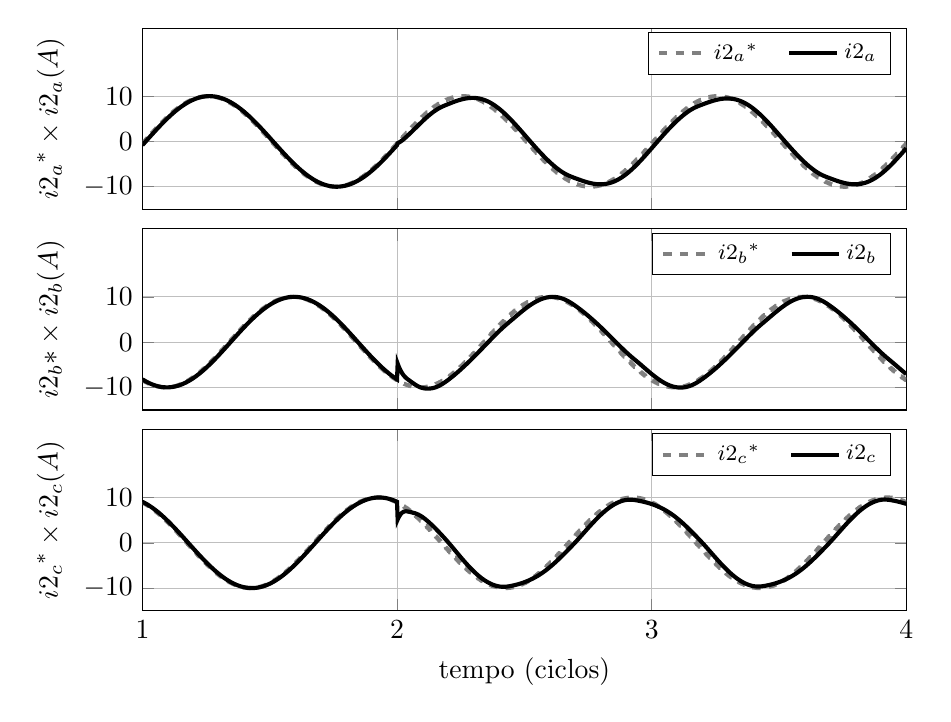
\begin{tikzpicture}

\begin{axis}[%
width=0.8\textwidth,
height=0.189701500343624\textwidth,
scale only axis,
xmin=0.316666666666667,
xmax=0.366666666666667,
xtick={0.316666666666667,0.333333333333333,0.35,0.366666666666667},
xticklabels={\empty},
xmajorgrids,
ymin=-15,
ymax=25,
ytick={-10,   0,  10},
ylabel={${\text{i2}_\text{b}}\text{* }\times\text{ i2}_\text{b}\text{ (A)}$},
ymajorgrids,
name=plot2,
legend style={draw=black,fill=white,legend cell align=left},
scaled x ticks = false,
legend columns=-1,
legend style={/tikz/every even column/.append style={column sep=0.3cm}},
legend style={font=\footnotesize}
]
\addplot [color=gray,dashed,line width=1.5pt]
  table[row sep=crcr]{0.316658333333333	-8.32921240710225\\
0.3167	-8.49892692986993\\
0.316741666666667	-8.49892692986993\\
0.316783333333333	-8.6602540378457\\
0.316825	-8.6602540378457\\
0.316866666666667	-8.81303452065127\\
0.316908333333333	-8.81303452065127\\
0.31695	-8.9571176023955\\
0.316991666666667	-8.9571176023955\\
0.317033333333333	-9.09236109047209\\
0.317075	-9.09236109047209\\
0.317116666666667	-9.21863151588643\\
0.317158333333333	-9.21863151588643\\
0.3172	-9.33580426497347\\
0.317241666666667	-9.33580426497347\\
0.317283333333333	-9.44376370237628\\
0.317325	-9.44376370237628\\
0.317366666666667	-9.54240328516426\\
0.317408333333333	-9.54240328516426\\
0.31745	-9.63162566797809\\
0.317491666666667	-9.63162566797809\\
0.317533333333333	-9.71134279909789\\
0.317575	-9.71134279909789\\
0.317616666666667	-9.7814760073396\\
0.317658333333333	-9.7814760073396\\
0.3177	-9.84195607969398\\
0.317741666666667	-9.84195607969398\\
0.317783333333333	-9.89272332963145\\
0.317825	-9.89272332963145\\
0.317866666666667	-9.93372765600555\\
0.317908333333333	-9.93372765600555\\
0.31795	-9.96492859249664\\
0.317991666666667	-9.96492859249664\\
0.318033333333333	-9.98629534754734\\
0.318075	-9.98629534754734\\
0.318116666666667	-9.99780683475006\\
0.318158333333333	-9.99780683475006\\
0.3182	-9.99945169365673\\
0.318241666666667	-9.99945169365673\\
0.318283333333333	-9.9912283009902\\
0.318325	-9.9912283009902\\
0.318366666666667	-9.9731447722462\\
0.318408333333333	-9.9731447722462\\
0.31845	-9.94521895368435\\
0.318491666666667	-9.94521895368435\\
0.318533333333333	-9.90747840471606\\
0.318575	-9.90747840471606\\
0.318616666666667	-9.85996037070666\\
0.318658333333333	-9.85996037070666\\
0.3187	-9.80271174621883\\
0.318741666666667	-9.80271174621883\\
0.318783333333333	-9.73578902873321\\
0.318825	-9.73578902873321\\
0.318866666666667	-9.65925826289228\\
0.318908333333333	-9.65925826289228\\
0.31895	-9.57319497532226\\
0.318991666666667	-9.57319497532226\\
0.319033333333333	-9.47768410009743\\
0.319075	-9.47768410009743\\
0.319116666666667	-9.37281989492048\\
0.319158333333333	-9.37281989492048\\
0.3192	-9.2587058481015\\
0.319241666666667	-9.2587058481015\\
0.319283333333333	-9.13545457642755\\
0.319325	-9.13545457642755\\
0.319366666666667	-9.00318771402345\\
0.319408333333333	-9.00318771402345\\
0.31945	-8.86203579231365\\
0.319491666666667	-8.86203579231365\\
0.319533333333333	-8.71213811120338\\
0.319575	-8.71213811120338\\
0.319616666666667	-8.55364260160653\\
0.319658333333333	-8.55364260160653\\
0.3197	-8.38670567945568\\
0.319741666666667	-8.38670567945568\\
0.319783333333333	-8.21149209133845\\
0.319825	-8.21149209133845\\
0.319866666666667	-8.02817475191253\\
0.319908333333333	-8.02817475191253\\
0.31995	-7.83693457325976\\
0.319991666666667	-7.83693457325976\\
0.320033333333333	-7.63796028634775\\
0.320075	-7.63796028634775\\
0.320116666666667	-7.43144825477524\\
0.320158333333333	-7.43144825477524\\
0.3202	-7.21760228098489\\
0.320241666666667	-7.21760228098489\\
0.320283333333333	-6.99663340513489\\
0.320325	-6.99663340513489\\
0.320366666666667	-6.76875969682781\\
0.320408333333333	-6.76875969682781\\
0.32045	-6.53420603990222\\
0.320491666666667	-6.53420603990222\\
0.320533333333333	-6.29320391049951\\
0.320575	-6.29320391049951\\
0.320616666666667	-6.04599114862485\\
0.320658333333333	-6.04599114862485\\
0.3207	-5.79281172342785\\
0.320741666666667	-5.79281172342785\\
0.320783333333333	-5.53391549243446\\
0.320825	-5.53391549243446\\
0.320866666666667	-5.26955795496776\\
0.320908333333333	-5.26955795496776\\
0.32095	-5.00000000000094\\
0.320991666666667	-5.00000000000094\\
0.321033333333333	-4.72550764869144\\
0.321075	-4.72550764869144\\
0.321116666666667	-4.44635179185013\\
0.321158333333333	-4.44635179185013\\
0.3212	-4.16280792260482\\
0.321241666666667	-4.16280792260482\\
0.321283333333333	-3.87515586452179\\
0.321325	-3.87515586452179\\
0.321366666666667	-3.58367949545372\\
0.321408333333333	-3.58367949545372\\
0.32145	-3.28866646738651\\
0.321491666666667	-3.28866646738651\\
0.321533333333333	-2.99040792256149\\
0.321575	-2.99040792256149\\
0.321616666666667	-2.68919820615324\\
0.321658333333333	-2.68919820615324\\
0.3217	-2.38533457578634\\
0.321741666666667	-2.38533457578634\\
0.321783333333333	-2.07911690817807\\
0.321825	-2.07911690817807\\
0.321866666666667	-1.77084740319627\\
0.321908333333333	-1.77084740319627\\
0.32195	-1.4608302856245\\
0.321991666666667	-1.4608302856245\\
0.322033333333333	-1.149371504929\\
0.322075	-1.149371504929\\
0.322116666666667	-0.836778433323436\\
0.322158333333333	-0.836778433323436\\
0.3222	-0.523359562429668\\
0.322241666666667	-0.523359562429668\\
0.322283333333333	-0.209424198833749\\
0.322325	-0.209424198833749\\
0.322366666666667	0.10471784116233\\
0.322408333333333	0.10471784116233\\
0.32245	0.41875653729192\\
0.322491666666667	0.41875653729192\\
0.322533333333333	0.732381971276291\\
0.322575	0.732381971276291\\
0.322616666666667	1.04528463267656\\
0.322658333333333	1.04528463267656\\
0.3227	1.35715572434312\\
0.322741666666667	1.35715572434312\\
0.322783333333333	1.66768746716115\\
0.322825	1.66768746716115\\
0.322866666666667	1.97657340379144\\
0.322908333333333	1.97657340379144\\
0.32295	2.28350870110679\\
0.322991666666667	2.28350870110679\\
0.323033333333333	2.58819045102549\\
0.323075	2.58819045102549\\
0.323116666666667	2.89031796944505\\
0.323158333333333	2.89031796944505\\
0.3232	3.18959309298109\\
0.323241666666667	3.18959309298109\\
0.323283333333333	3.48572047321859\\
0.323325	3.48572047321859\\
0.323366666666667	3.77840786818516\\
0.323408333333333	3.77840786818516\\
0.32345	4.06736643075854\\
0.323491666666667	4.06736643075854\\
0.323533333333333	4.35231099372386\\
0.323575	4.35231099372386\\
0.323616666666667	4.63296035119925\\
0.323658333333333	4.63296035119925\\
0.3237	4.90903753615209\\
0.323741666666667	4.90903753615209\\
0.323783333333333	5.18027009373203\\
0.323825	5.18027009373203\\
0.323866666666667	5.44639035015104\\
0.323908333333333	5.44639035015104\\
0.32395	5.70713567684513\\
0.323991666666667	5.70713567684513\\
0.324033333333333	5.96224874965702\\
0.324075	5.96224874965702\\
0.324116666666667	6.21147780278401\\
0.324158333333333	6.21147780278401\\
0.3242	6.45457687724046\\
0.324241666666667	6.45457687724046\\
0.324283333333333	6.69130606358958\\
0.324325	6.69130606358958\\
0.324366666666667	6.9214317387051\\
0.324408333333333	6.9214317387051\\
0.32445	7.14472679632911\\
0.324491666666667	7.14472679632911\\
0.324533333333333	7.36097087119846\\
0.324575	7.36097087119846\\
0.324616666666667	7.56995055651872\\
0.324658333333333	7.56995055651872\\
0.3247	7.7714596145709\\
0.324741666666667	7.7714596145709\\
0.324783333333333	7.96529918024319\\
0.324825	7.96529918024319\\
0.324866666666667	8.1512779572868\\
0.324908333333333	8.1512779572868\\
0.32495	8.32921240710229\\
0.324991666666667	8.32921240710229\\
0.325033333333333	8.49892692986996\\
0.325075	8.49892692986996\\
0.325116666666667	8.66025403784574\\
0.325158333333333	8.66025403784574\\
0.3252	8.81303452065131\\
0.325241666666667	8.81303452065131\\
0.325283333333333	8.95711760239554\\
0.325325	8.95711760239554\\
0.325366666666667	9.09236109047212\\
0.325408333333333	9.09236109047212\\
0.32545	9.21863151588647\\
0.325491666666667	9.21863151588647\\
0.325533333333333	9.33580426497351\\
0.325575	9.33580426497351\\
0.325616666666667	9.44376370237632\\
0.325658333333333	9.44376370237632\\
0.3257	9.5424032851643\\
0.325741666666667	9.5424032851643\\
0.325783333333333	9.63162566797813\\
0.325825	9.63162566797813\\
0.325866666666667	9.71134279909793\\
0.325908333333333	9.71134279909793\\
0.32595	9.78147600733964\\
0.325991666666667	9.78147600733964\\
0.326033333333333	9.84195607969402\\
0.326075	9.84195607969402\\
0.326116666666667	9.8927233296315\\
0.326158333333333	9.8927233296315\\
0.3262	9.93372765600559\\
0.326241666666667	9.93372765600559\\
0.326283333333333	9.96492859249668\\
0.326325	9.96492859249668\\
0.326366666666667	9.98629534754738\\
0.326408333333333	9.98629534754738\\
0.32645	9.99780683475011\\
0.326491666666667	9.99780683475011\\
0.326533333333333	9.99945169365678\\
0.326575	9.99945169365678\\
0.326616666666667	9.99122830099025\\
0.326658333333333	9.99122830099025\\
0.3267	9.97314477224624\\
0.326741666666667	9.97314477224624\\
0.326783333333333	9.9452189536844\\
0.326825	9.9452189536844\\
0.326866666666667	9.9074784047161\\
0.326908333333333	9.9074784047161\\
0.32695	9.85996037070671\\
0.326991666666667	9.85996037070671\\
0.327033333333333	9.80271174621887\\
0.327075	9.80271174621887\\
0.327116666666667	9.73578902873325\\
0.327158333333333	9.73578902873325\\
0.3272	9.65925826289232\\
0.327241666666667	9.65925826289232\\
0.327283333333333	9.5731949753223\\
0.327325	9.5731949753223\\
0.327366666666667	9.47768410009748\\
0.327408333333333	9.47768410009748\\
0.32745	9.37281989492053\\
0.327491666666667	9.37281989492053\\
0.327533333333333	9.25870584810154\\
0.327575	9.25870584810154\\
0.327616666666667	9.13545457642759\\
0.327658333333333	9.13545457642759\\
0.3277	9.0031877140235\\
0.327741666666667	9.0031877140235\\
0.327783333333333	8.86203579231369\\
0.327825	8.86203579231369\\
0.327866666666667	8.71213811120342\\
0.327908333333333	8.71213811120342\\
0.32795	8.55364260160657\\
0.327991666666667	8.55364260160657\\
0.328033333333333	8.38670567945572\\
0.328075	8.38670567945572\\
0.328116666666667	8.21149209133849\\
0.328158333333333	8.21149209133849\\
0.3282	8.02817475191257\\
0.328241666666667	8.02817475191257\\
0.328283333333333	7.83693457325979\\
0.328325	7.83693457325979\\
0.328366666666667	7.63796028634779\\
0.328408333333333	7.63796028634779\\
0.32845	7.43144825477528\\
0.328491666666667	7.43144825477528\\
0.328533333333333	7.21760228098492\\
0.328575	7.21760228098492\\
0.328616666666667	6.99663340513492\\
0.328658333333333	6.99663340513492\\
0.3287	6.76875969682784\\
0.328741666666667	6.76875969682784\\
0.328783333333333	6.53420603990226\\
0.328825	6.53420603990226\\
0.328866666666667	6.29320391049954\\
0.328908333333333	6.29320391049954\\
0.32895	6.04599114862488\\
0.328991666666667	6.04599114862488\\
0.329033333333333	5.79281172342788\\
0.329075	5.79281172342788\\
0.329116666666667	5.53391549243449\\
0.329158333333333	5.53391549243449\\
0.3292	5.26955795496778\\
0.329241666666667	5.26955795496778\\
0.329283333333333	5.00000000000096\\
0.329325	5.00000000000096\\
0.329366666666667	4.72550764869146\\
0.329408333333333	4.72550764869146\\
0.32945	4.44635179185015\\
0.329491666666667	4.44635179185015\\
0.329533333333333	4.16280792260484\\
0.329575	4.16280792260484\\
0.329616666666667	3.87515586452181\\
0.329658333333333	3.87515586452181\\
0.3297	3.58367949545374\\
0.329741666666667	3.58367949545374\\
0.329783333333333	3.28866646738652\\
0.329825	3.28866646738652\\
0.329866666666667	2.99040792256151\\
0.329908333333333	2.99040792256151\\
0.32995	2.68919820615325\\
0.329991666666667	2.68919820615325\\
0.330033333333333	2.38533457578635\\
0.330075	2.38533457578635\\
0.330116666666667	2.07911690817808\\
0.330158333333333	2.07911690817808\\
0.3302	1.77084740319627\\
0.330241666666667	1.77084740319627\\
0.330283333333333	1.4608302856245\\
0.330325	1.4608302856245\\
0.330366666666667	1.149371504929\\
0.330408333333333	1.149371504929\\
0.33045	0.836778433323441\\
0.330491666666667	0.836778433323441\\
0.330533333333333	0.523359562429672\\
0.330575	0.523359562429672\\
0.330616666666667	0.20942419883375\\
0.330658333333333	0.20942419883375\\
0.3307	-0.10471784116233\\
0.330741666666667	-0.10471784116233\\
0.330783333333333	-0.418756537291922\\
0.330825	-0.418756537291922\\
0.330866666666667	-0.732381971276294\\
0.330908333333333	-0.732381971276294\\
0.33095	-1.04528463267656\\
0.330991666666667	-1.04528463267656\\
0.331033333333333	-1.35715572434313\\
0.331075	-1.35715572434313\\
0.331116666666667	-1.66768746716116\\
0.331158333333333	-1.66768746716116\\
0.3312	-1.97657340379145\\
0.331241666666667	-1.97657340379145\\
0.331283333333333	-2.2835087011068\\
0.331325	-2.2835087011068\\
0.331366666666667	-2.5881904510255\\
0.331408333333333	-2.5881904510255\\
0.33145	-2.89031796944506\\
0.331491666666667	-2.89031796944506\\
0.331533333333333	-3.1895930929811\\
0.331575	-3.1895930929811\\
0.331616666666667	-3.4857204732186\\
0.331658333333333	-3.4857204732186\\
0.3317	-3.77840786818517\\
0.331741666666667	-3.77840786818517\\
0.331783333333333	-4.06736643075855\\
0.331825	-4.06736643075855\\
0.331866666666667	-4.35231099372388\\
0.331908333333333	-4.35231099372388\\
0.33195	-4.63296035119927\\
0.331991666666667	-4.63296035119927\\
0.332033333333333	-4.90903753615211\\
0.332075	-4.90903753615211\\
0.332116666666667	-5.18027009373205\\
0.332158333333333	-5.18027009373205\\
0.3322	-5.44639035015107\\
0.332241666666667	-5.44639035015107\\
0.332283333333333	-5.70713567684516\\
0.332325	-5.70713567684516\\
0.332366666666667	-5.96224874965705\\
0.332408333333333	-5.96224874965705\\
0.33245	-6.21147780278404\\
0.332491666666667	-6.21147780278404\\
0.332533333333333	-6.45457687724048\\
0.332575	-6.45457687724048\\
0.332616666666667	-6.6913060635896\\
0.332658333333333	-6.6913060635896\\
0.3327	-6.92143173870513\\
0.332741666666667	-6.92143173870513\\
0.332783333333333	-7.14472679632914\\
0.332825	-7.14472679632914\\
0.332866666666667	-7.36097087119849\\
0.332908333333333	-7.36097087119849\\
0.33295	-7.56995055651875\\
0.332991666666667	-7.56995055651875\\
0.333033333333333	-7.77145961457093\\
0.333075	-7.77145961457093\\
0.333116666666667	-7.96529918024322\\
0.333158333333333	-7.96529918024322\\
0.3332	-8.15127795728684\\
0.333241666666667	-8.15127795728684\\
0.333283333333333	-8.32921240710232\\
0.333325	-8.32921240710232\\
0.333366666666667	-8.49892692987\\
0.333408333333333	-8.49892692987\\
0.33345	-8.66025403784578\\
0.333491666666667	-8.66025403784578\\
0.333533333333333	-8.81303452065134\\
0.333575	-8.81303452065134\\
0.333616666666667	-8.95711760239558\\
0.333658333333333	-8.95711760239558\\
0.3337	-9.09236109047216\\
0.333741666666667	-9.09236109047216\\
0.333783333333333	-9.21863151588651\\
0.333825	-9.21863151588651\\
0.333866666666667	-9.33580426497354\\
0.333908333333333	-9.33580426497354\\
0.33395	-9.44376370237636\\
0.333991666666667	-9.44376370237636\\
0.334033333333333	-9.54240328516434\\
0.334075	-9.54240328516434\\
0.334116666666667	-9.63162566797817\\
0.334158333333333	-9.63162566797817\\
0.3342	-9.71134279909797\\
0.334241666666667	-9.71134279909797\\
0.334283333333333	-9.78147600733968\\
0.334325	-9.78147600733968\\
0.334366666666667	-9.84195607969406\\
0.334408333333333	-9.84195607969406\\
0.33445	-9.89272332963154\\
0.334491666666667	-9.89272332963154\\
0.334533333333333	-9.93372765600563\\
0.334575	-9.93372765600563\\
0.334616666666667	-9.96492859249672\\
0.334658333333333	-9.96492859249672\\
0.3347	-9.98629534754742\\
0.334741666666667	-9.98629534754742\\
0.334783333333333	-9.99780683475015\\
0.334825	-9.99780683475015\\
0.334866666666667	-9.99945169365682\\
0.334908333333333	-9.99945169365682\\
0.33495	-9.99122830099028\\
0.334991666666667	-9.99122830099028\\
0.335033333333333	-9.97314477224628\\
0.335075	-9.97314477224628\\
0.335116666666667	-9.94521895368444\\
0.335158333333333	-9.94521895368444\\
0.3352	-9.90747840471614\\
0.335241666666667	-9.90747840471614\\
0.335283333333333	-9.85996037070675\\
0.335325	-9.85996037070675\\
0.335366666666667	-9.80271174621891\\
0.335408333333333	-9.80271174621891\\
0.33545	-9.73578902873329\\
0.335491666666667	-9.73578902873329\\
0.335533333333333	-9.65925826289236\\
0.335575	-9.65925826289236\\
0.335616666666667	-9.57319497532234\\
0.335658333333333	-9.57319497532234\\
0.3357	-9.47768410009751\\
0.335741666666667	-9.47768410009751\\
0.335783333333333	-9.37281989492056\\
0.335825	-9.37281989492056\\
0.335866666666667	-9.25870584810158\\
0.335908333333333	-9.25870584810158\\
0.33595	-9.13545457642762\\
0.335991666666667	-9.13545457642762\\
0.336033333333333	-9.00318771402353\\
0.336075	-9.00318771402353\\
0.336116666666667	-8.86203579231372\\
0.336158333333333	-8.86203579231372\\
0.3362	-8.71213811120345\\
0.336241666666667	-8.71213811120345\\
0.336283333333333	-8.5536426016066\\
0.336325	-8.5536426016066\\
0.336366666666667	-8.38670567945575\\
0.336408333333333	-8.38670567945575\\
0.33645	-8.21149209133852\\
0.336491666666667	-8.21149209133852\\
0.336533333333333	-8.0281747519126\\
0.336575	-8.0281747519126\\
0.336616666666667	-7.83693457325982\\
0.336658333333333	-7.83693457325982\\
0.3367	-7.63796028634782\\
0.336741666666667	-7.63796028634782\\
0.336783333333333	-7.43144825477531\\
0.336825	-7.43144825477531\\
0.336866666666667	-7.21760228098495\\
0.336908333333333	-7.21760228098495\\
0.33695	-6.99663340513495\\
0.336991666666667	-6.99663340513495\\
0.337033333333333	-6.76875969682787\\
0.337075	-6.76875969682787\\
0.337116666666667	-6.53420603990228\\
0.337158333333333	-6.53420603990228\\
0.3372	-6.29320391049956\\
0.337241666666667	-6.29320391049956\\
0.337283333333333	-6.0459911486249\\
0.337325	-6.0459911486249\\
0.337366666666667	-5.7928117234279\\
0.337408333333333	-5.7928117234279\\
0.33745	-5.53391549243451\\
0.337491666666667	-5.53391549243451\\
0.337533333333333	-5.2695579549678\\
0.337575	-5.2695579549678\\
0.337616666666667	-5.00000000000098\\
0.337658333333333	-5.00000000000098\\
0.3377	-4.72550764869148\\
0.337741666666667	-4.72550764869148\\
0.337783333333333	-4.44635179185017\\
0.337825	-4.44635179185017\\
0.337866666666667	-4.16280792260486\\
0.337908333333333	-4.16280792260486\\
0.33795	-3.87515586452183\\
0.337991666666667	-3.87515586452183\\
0.338033333333333	-3.58367949545375\\
0.338075	-3.58367949545375\\
0.338116666666667	-3.28866646738653\\
0.338158333333333	-3.28866646738653\\
0.3382	-2.99040792256152\\
0.338241666666667	-2.99040792256152\\
0.338283333333333	-2.68919820615326\\
0.338325	-2.68919820615326\\
0.338366666666667	-2.38533457578636\\
0.338408333333333	-2.38533457578636\\
0.33845	-2.07911690817809\\
0.338491666666667	-2.07911690817809\\
0.338533333333333	-1.77084740319628\\
0.338575	-1.77084740319628\\
0.338616666666667	-1.46083028562451\\
0.338658333333333	-1.46083028562451\\
0.3387	-1.14937150492901\\
0.338741666666667	-1.14937150492901\\
0.338783333333333	-0.836778433323443\\
0.338825	-0.836778433323443\\
0.338866666666667	-0.523359562429674\\
0.338908333333333	-0.523359562429674\\
0.33895	-0.209424198833751\\
0.338991666666667	-0.209424198833751\\
0.339033333333333	0.104717841162331\\
0.339075	0.104717841162331\\
0.339116666666667	0.418756537291924\\
0.339158333333333	0.418756537291924\\
0.3392	0.732381971276298\\
0.339241666666667	0.732381971276298\\
0.339283333333333	1.04528463267657\\
0.339325	1.04528463267657\\
0.339366666666667	1.35715572434313\\
0.339408333333333	1.35715572434313\\
0.33945	1.66768746716117\\
0.339491666666667	1.66768746716117\\
0.339533333333333	1.97657340379146\\
0.339575	1.97657340379146\\
0.339616666666667	2.28350870110681\\
0.339658333333333	2.28350870110681\\
0.3397	2.58819045102551\\
0.339741666666667	2.58819045102551\\
0.339783333333333	2.89031796944507\\
0.339825	2.89031796944507\\
0.339866666666667	3.18959309298111\\
0.339908333333333	3.18959309298111\\
0.33995	3.48572047321862\\
0.339991666666667	3.48572047321862\\
0.340033333333333	3.77840786818519\\
0.340075	3.77840786818519\\
0.340116666666667	4.06736643075857\\
0.340158333333333	4.06736643075857\\
0.3402	4.35231099372389\\
0.340241666666667	4.35231099372389\\
0.340283333333333	4.63296035119929\\
0.340325	4.63296035119929\\
0.340366666666667	4.90903753615213\\
0.340408333333333	4.90903753615213\\
0.34045	5.18027009373207\\
0.340491666666667	5.18027009373207\\
0.340533333333333	5.44639035015109\\
0.340575	5.44639035015109\\
0.340616666666667	5.70713567684518\\
0.340658333333333	5.70713567684518\\
0.3407	5.96224874965707\\
0.340741666666667	5.96224874965707\\
0.340783333333333	6.21147780278406\\
0.340825	6.21147780278406\\
0.340866666666667	6.45457687724051\\
0.340908333333333	6.45457687724051\\
0.34095	6.69130606358963\\
0.340991666666667	6.69130606358963\\
0.341033333333333	6.92143173870516\\
0.341075	6.92143173870516\\
0.341116666666667	7.14472679632916\\
0.341158333333333	7.14472679632916\\
0.3412	7.36097087119851\\
0.341241666666667	7.36097087119851\\
0.341283333333333	7.56995055651877\\
0.341325	7.56995055651877\\
0.341366666666667	7.77145961457096\\
0.341408333333333	7.77145961457096\\
0.34145	7.96529918024325\\
0.341491666666667	7.96529918024325\\
0.341533333333333	8.15127795728687\\
0.341575	8.15127795728687\\
0.341616666666667	8.32921240710235\\
0.341658333333333	8.32921240710235\\
0.3417	8.49892692987003\\
0.341741666666667	8.49892692987003\\
0.341783333333333	8.66025403784581\\
0.341825	8.66025403784581\\
0.341866666666667	8.81303452065138\\
0.341908333333333	8.81303452065138\\
0.34195	8.95711760239561\\
0.341991666666667	8.95711760239561\\
0.342033333333333	9.0923610904722\\
0.342075	9.0923610904722\\
0.342116666666667	9.21863151588654\\
0.342158333333333	9.21863151588654\\
0.3422	9.33580426497358\\
0.342241666666667	9.33580426497358\\
0.342283333333333	9.4437637023764\\
0.342325	9.4437637023764\\
0.342366666666667	9.54240328516438\\
0.342408333333333	9.54240328516438\\
0.34245	9.63162566797821\\
0.342491666666667	9.63162566797821\\
0.342533333333333	9.71134279909801\\
0.342575	9.71134279909801\\
0.342616666666667	9.78147600733972\\
0.342658333333333	9.78147600733972\\
0.3427	9.8419560796941\\
0.342741666666667	9.8419560796941\\
0.342783333333333	9.89272332963157\\
0.342825	9.89272332963157\\
0.342866666666667	9.93372765600567\\
0.342908333333333	9.93372765600567\\
0.34295	9.96492859249676\\
0.342991666666667	9.96492859249676\\
0.343033333333333	9.98629534754746\\
0.343075	9.98629534754746\\
0.343116666666667	9.99780683475019\\
0.343158333333333	9.99780683475019\\
0.3432	9.99945169365686\\
0.343241666666667	9.99945169365686\\
0.343283333333333	9.99122830099032\\
0.343325	9.99122830099032\\
0.343366666666667	9.97314477224632\\
0.343408333333333	9.97314477224632\\
0.34345	9.94521895368448\\
0.343491666666667	9.94521895368448\\
0.343533333333333	9.90747840471618\\
0.343575	9.90747840471618\\
0.343616666666667	9.85996037070679\\
0.343658333333333	9.85996037070679\\
0.3437	9.80271174621895\\
0.343741666666667	9.80271174621895\\
0.343783333333333	9.73578902873333\\
0.343825	9.73578902873333\\
0.343866666666667	9.6592582628924\\
0.343908333333333	9.6592582628924\\
0.34395	9.57319497532238\\
0.343991666666667	9.57319497532238\\
0.344033333333333	9.47768410009755\\
0.344075	9.47768410009755\\
0.344116666666667	9.3728198949206\\
0.344158333333333	9.3728198949206\\
0.3442	9.25870584810162\\
0.344241666666667	9.25870584810162\\
0.344283333333333	9.13545457642766\\
0.344325	9.13545457642766\\
0.344366666666667	9.00318771402357\\
0.344408333333333	9.00318771402357\\
0.34445	8.86203579231376\\
0.344491666666667	8.86203579231376\\
0.344533333333333	8.71213811120348\\
0.344575	8.71213811120348\\
0.344616666666667	8.55364260160663\\
0.344658333333333	8.55364260160663\\
0.3447	8.38670567945578\\
0.344741666666667	8.38670567945578\\
0.344783333333333	8.21149209133855\\
0.344825	8.21149209133855\\
0.344866666666667	8.02817475191263\\
0.344908333333333	8.02817475191263\\
0.34495	7.83693457325986\\
0.344991666666667	7.83693457325986\\
0.345033333333333	7.63796028634785\\
0.345075	7.63796028634785\\
0.345116666666667	7.43144825477534\\
0.345158333333333	7.43144825477534\\
0.3452	7.21760228098498\\
0.345241666666667	7.21760228098498\\
0.345283333333333	6.99663340513498\\
0.345325	6.99663340513498\\
0.345366666666667	6.7687596968279\\
0.345408333333333	6.7687596968279\\
0.34545	6.5342060399023\\
0.345491666666667	6.5342060399023\\
0.345533333333333	6.29320391049959\\
0.345575	6.29320391049959\\
0.345616666666667	6.04599114862492\\
0.345658333333333	6.04599114862492\\
0.3457	5.79281172342792\\
0.345741666666667	5.79281172342792\\
0.345783333333333	5.53391549243453\\
0.345825	5.53391549243453\\
0.345866666666667	5.26955795496782\\
0.345908333333333	5.26955795496782\\
0.34595	5.000000000001\\
0.345991666666667	5.000000000001\\
0.346033333333333	4.72550764869149\\
0.346075	4.72550764869149\\
0.346116666666667	4.44635179185018\\
0.346158333333333	4.44635179185018\\
0.3462	4.16280792260487\\
0.346241666666667	4.16280792260487\\
0.346283333333333	3.87515586452184\\
0.346325	3.87515586452184\\
0.346366666666667	3.58367949545377\\
0.346408333333333	3.58367949545377\\
0.34645	3.28866646738655\\
0.346491666666667	3.28866646738655\\
0.346533333333333	2.99040792256153\\
0.346575	2.99040792256153\\
0.346616666666667	2.68919820615327\\
0.346658333333333	2.68919820615327\\
0.3467	2.38533457578637\\
0.346741666666667	2.38533457578637\\
0.346783333333333	2.0791169081781\\
0.346825	2.0791169081781\\
0.346866666666667	1.77084740319629\\
0.346908333333333	1.77084740319629\\
0.34695	1.46083028562452\\
0.346991666666667	1.46083028562452\\
0.347033333333333	1.14937150492901\\
0.347075	1.14937150492901\\
0.347116666666667	0.836778433323448\\
0.347158333333333	0.836778433323448\\
0.3472	0.523359562429677\\
0.347241666666667	0.523359562429677\\
0.347283333333333	0.209424198833753\\
0.347325	0.209424198833753\\
0.347366666666667	-0.10471784116233\\
0.347408333333333	-0.10471784116233\\
0.34745	-0.418756537291923\\
0.347491666666667	-0.418756537291923\\
0.347533333333333	-0.732381971276299\\
0.347575	-0.732381971276299\\
0.347616666666667	-1.04528463267657\\
0.347658333333333	-1.04528463267657\\
0.3477	-1.35715572434314\\
0.347741666666667	-1.35715572434314\\
0.347783333333333	-1.66768746716117\\
0.347825	-1.66768746716117\\
0.347866666666667	-1.97657340379147\\
0.347908333333333	-1.97657340379147\\
0.34795	-2.28350870110682\\
0.347991666666667	-2.28350870110682\\
0.348033333333333	-2.58819045102552\\
0.348075	-2.58819045102552\\
0.348116666666667	-2.89031796944508\\
0.348158333333333	-2.89031796944508\\
0.3482	-3.18959309298112\\
0.348241666666667	-3.18959309298112\\
0.348283333333333	-3.48572047321863\\
0.348325	-3.48572047321863\\
0.348366666666667	-3.7784078681852\\
0.348408333333333	-3.7784078681852\\
0.34845	-4.06736643075858\\
0.348491666666667	-4.06736643075858\\
0.348533333333333	-4.35231099372391\\
0.348575	-4.35231099372391\\
0.348616666666667	-4.6329603511993\\
0.348658333333333	-4.6329603511993\\
0.3487	-4.90903753615215\\
0.348741666666667	-4.90903753615215\\
0.348783333333333	-5.18027009373209\\
0.348825	-5.18027009373209\\
0.348866666666667	-5.44639035015111\\
0.348908333333333	-5.44639035015111\\
0.34895	-5.7071356768452\\
0.348991666666667	-5.7071356768452\\
0.349033333333333	-5.96224874965709\\
0.349075	-5.96224874965709\\
0.349116666666667	-6.21147780278408\\
0.349158333333333	-6.21147780278408\\
0.3492	-6.45457687724053\\
0.349241666666667	-6.45457687724053\\
0.349283333333333	-6.69130606358966\\
0.349325	-6.69130606358966\\
0.349366666666667	-6.92143173870518\\
0.349408333333333	-6.92143173870518\\
0.34945	-7.14472679632919\\
0.349491666666667	-7.14472679632919\\
0.349533333333333	-7.36097087119854\\
0.349575	-7.36097087119854\\
0.349616666666667	-7.5699505565188\\
0.349658333333333	-7.5699505565188\\
0.3497	-7.77145961457099\\
0.349741666666667	-7.77145961457099\\
0.349783333333333	-7.96529918024328\\
0.349825	-7.96529918024328\\
0.349866666666667	-8.1512779572869\\
0.349908333333333	-8.1512779572869\\
0.34995	-8.32921240710239\\
0.349991666666667	-8.32921240710239\\
0.350033333333333	-8.49892692987007\\
0.350075	-8.49892692987007\\
0.350116666666667	-8.66025403784585\\
0.350158333333333	-8.66025403784585\\
0.3502	-8.81303452065141\\
0.350241666666667	-8.81303452065141\\
0.350283333333333	-8.95711760239565\\
0.350325	-8.95711760239565\\
0.350366666666667	-9.09236109047223\\
0.350408333333333	-9.09236109047223\\
0.35045	-9.21863151588658\\
0.350491666666667	-9.21863151588658\\
0.350533333333333	-9.33580426497362\\
0.350575	-9.33580426497362\\
0.350616666666667	-9.44376370237644\\
0.350658333333333	-9.44376370237644\\
0.3507	-9.54240328516442\\
0.350741666666667	-9.54240328516442\\
0.350783333333333	-9.63162566797825\\
0.350825	-9.63162566797825\\
0.350866666666667	-9.71134279909805\\
0.350908333333333	-9.71134279909805\\
0.35095	-9.78147600733976\\
0.350991666666667	-9.78147600733976\\
0.351033333333333	-9.84195607969414\\
0.351075	-9.84195607969414\\
0.351116666666667	-9.89272332963162\\
0.351158333333333	-9.89272332963162\\
0.3512	-9.93372765600571\\
0.351241666666667	-9.93372765600571\\
0.351283333333333	-9.9649285924968\\
0.351325	-9.9649285924968\\
0.351366666666667	-9.98629534754751\\
0.351408333333333	-9.98629534754751\\
0.35145	-9.99780683475023\\
0.351491666666667	-9.99780683475023\\
0.351533333333333	-9.9994516936569\\
0.351575	-9.9994516936569\\
0.351616666666667	-9.99122830099037\\
0.351658333333333	-9.99122830099037\\
0.3517	-9.97314477224637\\
0.351741666666667	-9.97314477224637\\
0.351783333333333	-9.94521895368452\\
0.351825	-9.94521895368452\\
0.351866666666667	-9.90747840471622\\
0.351908333333333	-9.90747840471622\\
0.35195	-9.85996037070683\\
0.351991666666667	-9.85996037070683\\
0.352033333333333	-9.80271174621899\\
0.352075	-9.80271174621899\\
0.352116666666667	-9.73578902873337\\
0.352158333333333	-9.73578902873337\\
0.3522	-9.65925826289244\\
0.352241666666667	-9.65925826289244\\
0.352283333333333	-9.57319497532242\\
0.352325	-9.57319497532242\\
0.352366666666667	-9.4776841000976\\
0.352408333333333	-9.4776841000976\\
0.35245	-9.37281989492064\\
0.352491666666667	-9.37281989492064\\
0.352533333333333	-9.25870584810166\\
0.352575	-9.25870584810166\\
0.352616666666667	-9.1354545764277\\
0.352658333333333	-9.1354545764277\\
0.3527	-9.00318771402361\\
0.352741666666667	-9.00318771402361\\
0.352783333333333	-8.8620357923138\\
0.352825	-8.8620357923138\\
0.352866666666667	-8.71213811120352\\
0.352908333333333	-8.71213811120352\\
0.35295	-8.55364260160667\\
0.352991666666667	-8.55364260160667\\
0.353033333333333	-8.38670567945582\\
0.353075	-8.38670567945582\\
0.353116666666667	-8.21149209133859\\
0.353158333333333	-8.21149209133859\\
0.3532	-8.02817475191267\\
0.353241666666667	-8.02817475191267\\
0.353283333333333	-7.83693457325989\\
0.353325	-7.83693457325989\\
0.353366666666667	-7.63796028634788\\
0.353408333333333	-7.63796028634788\\
0.35345	-7.43144825477537\\
0.353491666666667	-7.43144825477537\\
0.353533333333333	-7.21760228098502\\
0.353575	-7.21760228098502\\
0.353616666666667	-6.99663340513501\\
0.353658333333333	-6.99663340513501\\
0.3537	-6.76875969682793\\
0.353741666666667	-6.76875969682793\\
0.353783333333333	-6.53420603990234\\
0.353825	-6.53420603990234\\
0.353866666666667	-6.29320391049962\\
0.353908333333333	-6.29320391049962\\
0.35395	-6.04599114862495\\
0.353991666666667	-6.04599114862495\\
0.354033333333333	-5.79281172342795\\
0.354075	-5.79281172342795\\
0.354116666666667	-5.53391549243456\\
0.354158333333333	-5.53391549243456\\
0.3542	-5.26955795496785\\
0.354241666666667	-5.26955795496785\\
0.354283333333333	-5.00000000000103\\
0.354325	-5.00000000000103\\
0.354366666666667	-4.72550764869152\\
0.354408333333333	-4.72550764869152\\
0.35445	-4.44635179185021\\
0.354491666666667	-4.44635179185021\\
0.354533333333333	-4.16280792260489\\
0.354575	-4.16280792260489\\
0.354616666666667	-3.87515586452186\\
0.354658333333333	-3.87515586452186\\
0.3547	-3.58367949545379\\
0.354741666666667	-3.58367949545379\\
0.354783333333333	-3.28866646738657\\
0.354825	-3.28866646738657\\
0.354866666666667	-2.99040792256155\\
0.354908333333333	-2.99040792256155\\
0.35495	-2.68919820615329\\
0.354991666666667	-2.68919820615329\\
0.355033333333333	-2.38533457578638\\
0.355075	-2.38533457578638\\
0.355116666666667	-2.07911690817811\\
0.355158333333333	-2.07911690817811\\
0.3552	-1.7708474031963\\
0.355241666666667	-1.7708474031963\\
0.355283333333333	-1.46083028562453\\
0.355325	-1.46083028562453\\
0.355366666666667	-1.14937150492902\\
0.355408333333333	-1.14937150492902\\
0.35545	-0.836778433323456\\
0.355491666666667	-0.836778433323456\\
0.355533333333333	-0.523359562429684\\
0.355575	-0.523359562429684\\
0.355616666666667	-0.209424198833759\\
0.355658333333333	-0.209424198833759\\
0.3557	0.104717841162325\\
0.355741666666667	0.104717841162325\\
0.355783333333333	0.418756537291921\\
0.355825	0.418756537291921\\
0.355866666666667	0.732381971276297\\
0.355908333333333	0.732381971276297\\
0.35595	1.04528463267657\\
0.355991666666667	1.04528463267657\\
0.356033333333333	1.35715572434314\\
0.356075	1.35715572434314\\
0.356116666666667	1.66768746716117\\
0.356158333333333	1.66768746716117\\
0.3562	1.97657340379147\\
0.356241666666667	1.97657340379147\\
0.356283333333333	2.28350870110682\\
0.356325	2.28350870110682\\
0.356366666666667	2.58819045102553\\
0.356408333333333	2.58819045102553\\
0.35645	2.89031796944509\\
0.356491666666667	2.89031796944509\\
0.356533333333333	3.18959309298113\\
0.356575	3.18959309298113\\
0.356616666666667	3.48572047321864\\
0.356658333333333	3.48572047321864\\
0.3567	3.77840786818521\\
0.356741666666667	3.77840786818521\\
0.356783333333333	4.0673664307586\\
0.356825	4.0673664307586\\
0.356866666666667	4.35231099372392\\
0.356908333333333	4.35231099372392\\
0.35695	4.63296035119932\\
0.356991666666667	4.63296035119932\\
0.357033333333333	4.90903753615216\\
0.357075	4.90903753615216\\
0.357116666666667	5.18027009373211\\
0.357158333333333	5.18027009373211\\
0.3572	5.44639035015113\\
0.357241666666667	5.44639035015113\\
0.357283333333333	5.70713567684522\\
0.357325	5.70713567684522\\
0.357366666666667	5.96224874965711\\
0.357408333333333	5.96224874965711\\
0.35745	6.21147780278411\\
0.357491666666667	6.21147780278411\\
0.357533333333333	6.45457687724056\\
0.357575	6.45457687724056\\
0.357616666666667	6.69130606358968\\
0.357658333333333	6.69130606358968\\
0.3577	6.92143173870521\\
0.357741666666667	6.92143173870521\\
0.357783333333333	7.14472679632922\\
0.357825	7.14472679632922\\
0.357866666666667	7.36097087119857\\
0.357908333333333	7.36097087119857\\
0.35795	7.56995055651883\\
0.357991666666667	7.56995055651883\\
0.358033333333333	7.77145961457102\\
0.358075	7.77145961457102\\
0.358116666666667	7.96529918024331\\
0.358158333333333	7.96529918024331\\
0.3582	8.15127795728693\\
0.358241666666667	8.15127795728693\\
0.358283333333333	8.32921240710242\\
0.358325	8.32921240710242\\
0.358366666666667	8.4989269298701\\
0.358408333333333	8.4989269298701\\
0.35845	8.66025403784588\\
0.358491666666667	8.66025403784588\\
0.358533333333333	8.81303452065145\\
0.358575	8.81303452065145\\
0.358616666666667	8.95711760239568\\
0.358658333333333	8.95711760239568\\
0.3587	9.09236109047227\\
0.358741666666667	9.09236109047227\\
0.358783333333333	9.21863151588662\\
0.358825	9.21863151588662\\
0.358866666666667	9.33580426497366\\
0.358908333333333	9.33580426497366\\
0.35895	9.44376370237647\\
0.358991666666667	9.44376370237647\\
0.359033333333333	9.54240328516445\\
0.359075	9.54240328516445\\
0.359116666666667	9.63162566797829\\
0.359158333333333	9.63162566797829\\
0.3592	9.71134279909809\\
0.359241666666667	9.71134279909809\\
0.359283333333333	9.7814760073398\\
0.359325	9.7814760073398\\
0.359366666666667	9.84195607969418\\
0.359408333333333	9.84195607969418\\
0.35945	9.89272332963166\\
0.359491666666667	9.89272332963166\\
0.359533333333333	9.93372765600575\\
0.359575	9.93372765600575\\
0.359616666666667	9.96492859249684\\
0.359658333333333	9.96492859249684\\
0.3597	9.98629534754755\\
0.359741666666667	9.98629534754755\\
0.359783333333333	9.99780683475027\\
0.359825	9.99780683475027\\
0.359866666666667	9.99945169365694\\
0.359908333333333	9.99945169365694\\
0.35995	9.99122830099041\\
0.359991666666667	9.99122830099041\\
0.360033333333333	9.97314477224641\\
0.360075	9.97314477224641\\
0.360116666666667	9.94521895368456\\
0.360158333333333	9.94521895368456\\
0.3602	9.90747840471626\\
0.360241666666667	9.90747840471626\\
0.360283333333333	9.85996037070687\\
0.360325	9.85996037070687\\
0.360366666666667	9.80271174621904\\
0.360408333333333	9.80271174621904\\
0.36045	9.73578902873341\\
0.360491666666667	9.73578902873341\\
0.360533333333333	9.65925826289248\\
0.360575	9.65925826289248\\
0.360616666666667	9.57319497532246\\
0.360658333333333	9.57319497532246\\
0.3607	9.47768410009764\\
0.360741666666667	9.47768410009764\\
0.360783333333333	9.37281989492068\\
0.360825	9.37281989492068\\
0.360866666666667	9.25870584810169\\
0.360908333333333	9.25870584810169\\
0.36095	9.13545457642774\\
0.360991666666667	9.13545457642774\\
0.361033333333333	9.00318771402364\\
0.361075	9.00318771402364\\
0.361116666666667	8.86203579231383\\
0.361158333333333	8.86203579231383\\
0.3612	8.71213811120356\\
0.361241666666667	8.71213811120356\\
0.361283333333333	8.55364260160671\\
0.361325	8.55364260160671\\
0.361366666666667	8.38670567945586\\
0.361408333333333	8.38670567945586\\
0.36145	8.21149209133863\\
0.361491666666667	8.21149209133863\\
0.361533333333333	8.0281747519127\\
0.361575	8.0281747519127\\
0.361616666666667	7.83693457325993\\
0.361658333333333	7.83693457325993\\
0.3617	7.63796028634792\\
0.361741666666667	7.63796028634792\\
0.361783333333333	7.4314482547754\\
0.361825	7.4314482547754\\
0.361866666666667	7.21760228098505\\
0.361908333333333	7.21760228098505\\
0.36195	6.99663340513504\\
0.361991666666667	6.99663340513504\\
0.362033333333333	6.76875969682796\\
0.362075	6.76875969682796\\
0.362116666666667	6.53420603990237\\
0.362158333333333	6.53420603990237\\
0.3622	6.29320391049965\\
0.362241666666667	6.29320391049965\\
0.362283333333333	6.04599114862498\\
0.362325	6.04599114862498\\
0.362366666666667	5.79281172342797\\
0.362408333333333	5.79281172342797\\
0.36245	5.53391549243458\\
0.362491666666667	5.53391549243458\\
0.362533333333333	5.26955795496787\\
0.362575	5.26955795496787\\
0.362616666666667	5.00000000000105\\
0.362658333333333	5.00000000000105\\
0.3627	4.72550764869154\\
0.362741666666667	4.72550764869154\\
0.362783333333333	4.44635179185023\\
0.362825	4.44635179185023\\
0.362866666666667	4.16280792260491\\
0.362908333333333	4.16280792260491\\
0.36295	3.87515586452188\\
0.362991666666667	3.87515586452188\\
0.363033333333333	3.5836794954538\\
0.363075	3.5836794954538\\
0.363116666666667	3.28866646738658\\
0.363158333333333	3.28866646738658\\
0.3632	2.99040792256156\\
0.363241666666667	2.99040792256156\\
0.363283333333333	2.6891982061533\\
0.363325	2.6891982061533\\
0.363366666666667	2.3853345757864\\
0.363408333333333	2.3853345757864\\
0.36345	2.07911690817813\\
0.363491666666667	2.07911690817813\\
0.363533333333333	1.77084740319631\\
0.363575	1.77084740319631\\
0.363616666666667	1.46083028562454\\
0.363658333333333	1.46083028562454\\
0.3637	1.14937150492903\\
0.363741666666667	1.14937150492903\\
0.363783333333333	0.836778433323463\\
0.363825	0.836778433323463\\
0.363866666666667	0.52335956242969\\
0.363908333333333	0.52335956242969\\
0.36395	0.209424198833764\\
0.363991666666667	0.209424198833764\\
0.364033333333333	-0.10471784116232\\
0.364075	-0.10471784116232\\
0.364116666666667	-0.418756537291917\\
0.364158333333333	-0.418756537291917\\
0.3642	-0.732381971276296\\
0.364241666666667	-0.732381971276296\\
0.364283333333333	-1.04528463267657\\
0.364325	-1.04528463267657\\
0.364366666666667	-1.35715572434314\\
0.364408333333333	-1.35715572434314\\
0.36445	-1.66768746716118\\
0.364491666666667	-1.66768746716118\\
0.364533333333333	-1.97657340379147\\
0.364575	-1.97657340379147\\
0.364616666666667	-2.28350870110683\\
0.364658333333333	-2.28350870110683\\
0.3647	-2.58819045102553\\
0.364741666666667	-2.58819045102553\\
0.364783333333333	-2.8903179694451\\
0.364825	-2.8903179694451\\
0.364866666666667	-3.18959309298114\\
0.364908333333333	-3.18959309298114\\
0.36495	-3.48572047321865\\
0.364991666666667	-3.48572047321865\\
0.365033333333333	-3.77840786818522\\
0.365075	-3.77840786818522\\
0.365116666666667	-4.06736643075861\\
0.365158333333333	-4.06736643075861\\
0.3652	-4.35231099372394\\
0.365241666666667	-4.35231099372394\\
0.365283333333333	-4.63296035119933\\
0.365325	-4.63296035119933\\
0.365366666666667	-4.90903753615218\\
0.365408333333333	-4.90903753615218\\
0.36545	-5.18027009373212\\
0.365491666666667	-5.18027009373212\\
0.365533333333333	-5.44639035015114\\
0.365575	-5.44639035015114\\
0.365616666666667	-5.70713567684524\\
0.365658333333333	-5.70713567684524\\
0.3657	-5.96224874965713\\
0.365741666666667	-5.96224874965713\\
0.365783333333333	-6.21147780278413\\
0.365825	-6.21147780278413\\
0.365866666666667	-6.45457687724057\\
0.365908333333333	-6.45457687724057\\
0.36595	-6.6913060635897\\
0.365991666666667	-6.6913060635897\\
0.366033333333333	-6.92143173870523\\
0.366075	-6.92143173870523\\
0.366116666666667	-7.14472679632924\\
0.366158333333333	-7.14472679632924\\
0.3662	-7.36097087119859\\
0.366241666666667	-7.36097087119859\\
0.366283333333333	-7.56995055651886\\
0.366325	-7.56995055651886\\
0.366366666666667	-7.77145961457104\\
0.366408333333333	-7.77145961457104\\
0.36645	-7.96529918024334\\
0.366491666666667	-7.96529918024334\\
0.366533333333333	-8.15127795728696\\
0.366575	-8.15127795728696\\
0.366616666666667	-8.32921240710245\\
0.366658333333333	-8.32921240710245\\
};
\addlegendentry{${\text{i2}_\text{b}}^\text{*}$};

\addplot [color=black,solid,line width=1.5pt]
  table[row sep=crcr]{0.316658333333333	-8.22299706867324\\
0.3167	-8.31122988066365\\
0.316741666666667	-8.39740653241784\\
0.316783333333333	-8.48151399654791\\
0.316825	-8.56352264596434\\
0.316866666666667	-8.64342253177359\\
0.316908333333333	-8.72118303691758\\
0.31695	-8.79679730145864\\
0.316991666666667	-8.87023374619767\\
0.317033333333333	-8.94148860200146\\
0.317075	-9.01052935210292\\
0.317116666666667	-9.07735531392454\\
0.317158333333333	-9.14193305704151\\
0.3172	-9.20426497757236\\
0.317241666666667	-9.26431675686617\\
0.317283333333333	-9.32209386018241\\
0.317325	-9.37756110900941\\
0.317366666666667	-9.43072702759529\\
0.317408333333333	-9.48155560942578\\
0.31745	-9.53005842727799\\
0.317491666666667	-9.57619868182153\\
0.317533333333333	-9.61999098326013\\
0.317575	-9.66139777732107\\
0.317616666666667	-9.70043669919249\\
0.317658333333333	-9.73706947937713\\
0.3177	-9.77131676346711\\
0.317741666666667	-9.80313960748905\\
0.317783333333333	-9.83256165002339\\
0.317825	-9.85954331377064\\
0.317866666666667	-9.88411120957098\\
0.317908333333333	-9.90622516797112\\
0.31795	-9.92591474780569\\
0.317991666666667	-9.94313922852405\\
0.318033333333333	-9.95793108915272\\
0.318075	-9.97024909902875\\
0.318116666666667	-9.98012862618457\\
0.318158333333333	-9.98752797090536\\
0.3182	-9.99248535588831\\
0.318241666666667	-9.99495865367453\\
0.318283333333333	-9.99498890436109\\
0.318325	-9.99253359443789\\
0.318366666666667	-9.98763654139937\\
0.318408333333333	-9.98025488783184\\
0.31845	-9.97043518600343\\
0.318491666666667	-9.95813427719125\\
0.318533333333333	-9.94340140323821\\
0.318575	-9.92619314707661\\
0.318616666666667	-9.90656139233853\\
0.318658333333333	-9.88446250681975\\
0.3187	-9.85995096552193\\
0.318741666666667	-9.832982964403\\
0.318783333333333	-9.80361551671867\\
0.318825	-9.77180468981814\\
0.318866666666667	-9.73760997934469\\
0.318908333333333	-9.70098736705595\\
0.31895	-9.66199877234457\\
0.318991666666667	-9.62060013410924\\
0.319033333333333	-9.57685573417316\\
0.319075	-9.53072151119948\\
0.319116666666667	-9.4822640460492\\
0.319158333333333	-9.43143932146865\\
0.3192	-9.37831615495538\\
0.319241666666667	-9.32285062657429\\
0.319283333333333	-9.26511373714313\\
0.319325	-9.20506173507616\\
0.319366666666667	-9.14276776553204\\
0.319408333333333	-9.07818832575472\\
0.31945	-9.01139866615841\\
0.319491666666667	-8.94235559726393\\
0.319533333333333	-8.87113641096755\\
0.319575	-8.79769826472635\\
0.319616666666667	-8.7221203961231\\
0.319658333333333	-8.64436031770232\\
0.3197	-8.56449909542267\\
0.319741666666667	-8.48249459481256\\
0.319783333333333	-8.39842958734738\\
0.319825	-8.31226229392797\\
0.319866666666667	-8.22407707605069\\
0.319908333333333	-8.13383252608711\\
0.31995	-8.0416144941665\\
0.319991666666667	-7.94738197678626\\
0.320033333333333	-7.85122222622311\\
0.320075	-7.75309469011563\\
0.320116666666667	-7.65308794789633\\
0.320158333333333	-7.55116195461504\\
0.3202	-7.44740654791947\\
0.320241666666667	-7.34178224988833\\
0.320283333333333	-7.23438008794331\\
0.320325	-7.12516120905326\\
0.320366666666667	-7.01421775813865\\
0.320408333333333	-6.90151155977053\\
0.32045	-6.78713579777259\\
0.320491666666667	-6.67105302043289\\
0.320533333333333	-6.55335736493733\\
0.320575	-6.43401214302971\\
0.320616666666667	-6.31311235360129\\
0.320658333333333	-6.19062210654161\\
0.3207	-6.06663716635544\\
0.320741666666667	-5.94112247251961\\
0.320783333333333	-5.814174456552\\
0.320825	-5.6857589174412\\
0.320866666666667	-5.55597285430995\\
0.320908333333333	-5.42478295536887\\
0.32095	-5.2922866883279\\
0.320991666666667	-5.15845166083622\\
0.321033333333333	-5.02337571117919\\
0.321075	-4.88702739732608\\
0.321116666666667	-4.74950483123525\\
0.321158333333333	-4.61077755247622\\
0.3212	-4.47094385063973\\
0.321241666666667	-4.32997427806953\\
0.321283333333333	-4.18796720639828\\
0.321325	-4.04489423124868\\
0.321366666666667	-3.90085371074305\\
0.321408333333333	-3.75581831313347\\
0.32145	-3.60988628721805\\
0.321491666666667	-3.46303140174436\\
0.321533333333333	-3.31535169997674\\
0.321575	-3.166822077385\\
0.321616666666667	-3.01754027512619\\
0.321658333333333	-2.8674823399737\\
0.3217	-2.71674561419996\\
0.321741666666667	-2.56530731891019\\
0.321783333333333	-2.41326430074597\\
0.321825	-2.26059497675438\\
0.321866666666667	-2.1073956014869\\
0.321908333333333	-1.95364580825354\\
0.32195	-1.79944116357817\\
0.321991666666667	-1.6447625361573\\
0.322033333333333	-1.48970470926032\\
0.322075	-1.33424980493537\\
0.322116666666667	-1.17849172881576\\
0.322158333333333	-1.02241387309573\\
0.3222	-0.86610917232175\\
0.322241666666667	-0.709562304404564\\
0.322283333333333	-0.55286514033327\\
0.322325	-0.396003658001932\\
0.322366666666667	-0.239068573379426\\
0.322408333333333	-0.0820471772142457\\
0.32245	0.0749710599819313\\
0.322491666666667	0.231997523226612\\
0.322533333333333	0.388944076860868\\
0.322575	0.545820771876853\\
0.322616666666667	0.702540895808884\\
0.322658333333333	0.859113157522251\\
0.3227	1.01545235502391\\
0.322741666666667	1.17156584875693\\
0.322783333333333	1.32737003343105\\
0.322825	1.48287091672284\\
0.322866666666667	1.63798657526865\\
0.322908333333333	1.79272166177246\\
0.32295	1.94699601909847\\
0.322991666666667	2.10081294514209\\
0.323033333333333	2.25409413248883\\
0.323075	2.40684152698898\\
0.323116666666667	2.55897875369365\\
0.323158333333333	2.71050641176815\\
0.3232	2.86135014035683\\
0.323241666666667	3.01150919875297\\
0.323283333333333	3.16091131783037\\
0.323325	3.3095544158681\\
0.323366666666667	3.45736837376785\\
0.323408333333333	3.60434972283112\\
0.32345	3.75043049222649\\
0.323491666666667	3.89560569071605\\
0.323533333333333	4.03980940823638\\
0.323575	4.18303494926742\\
0.323616666666667	4.3252183661179\\
0.323658333333333	4.4663511610907\\
0.3237	4.60637136500026\\
0.323741666666667	4.74526873747594\\
0.323783333333333	4.88298345429453\\
0.323825	5.01950371959078\\
0.323866666666667	5.15477211524325\\
0.323908333333333	5.28877552524236\\
0.32395	5.42145921153114\\
0.323991666666667	5.55280894660405\\
0.324033333333333	5.68277289489008\\
0.324075	5.81133585390497\\
0.324116666666667	5.93844902932979\\
0.324158333333333	6.06409629520989\\
0.3242	6.18823195155667\\
0.324241666666667	6.31083892765057\\
0.324283333333333	6.43187460389401\\
0.324325	6.5513208969494\\
0.324366666666667	6.66913821495285\\
0.324408333333333	6.78530737722875\\
0.32445	6.89979175660007\\
0.324491666666667	7.01257099869417\\
0.324533333333333	7.12361138945075\\
0.324575	7.23289134920369\\
0.324616666666667	7.34038004935605\\
0.324658333333333	7.4460546646942\\
0.3247	7.54988725144843\\
0.324741666666667	7.65185374821782\\
0.324783333333333	7.75192911834617\\
0.324825	7.85008809607541\\
0.324866666666667	7.94630858885684\\
0.324908333333333	8.04056417150899\\
0.32495	8.13283573799168\\
0.324991666666667	8.22309575284526\\
0.325033333333333	8.31132813629452\\
0.325075	8.39750428930048\\
0.325116666666667	8.48161119000373\\
0.325158333333333	8.56361921634316\\
0.3252	8.64351842541246\\
0.325241666666667	8.72127820567036\\
0.325283333333333	8.79689170364076\\
0.325325	8.87032734606679\\
0.325366666666667	8.94158137060988\\
0.325408333333333	9.01062126668704\\
0.32545	9.07744635861746\\
0.325491666666667	9.14202322216954\\
0.325533333333333	9.20435426020805\\
0.325575	9.26440516006415\\
0.325616666666667	9.32218139337359\\
0.325658333333333	9.3776477872297\\
0.3257	9.43081287173255\\
0.325741666666667	9.48164064550292\\
0.325783333333333	9.53014268656646\\
0.325825	9.57628220023673\\
0.325866666666667	9.6200738013515\\
0.325908333333333	9.66147993982645\\
0.32595	9.70051825490805\\
0.325991666666667	9.73715048090294\\
0.326033333333333	9.77139726695304\\
0.326075	9.80321967259016\\
0.326116666666667	9.83264133951228\\
0.326158333333333	9.85962269371085\\
0.3262	9.88419034878293\\
0.326241666666667	9.90630413842579\\
0.326283333333333	9.92599362393066\\
0.326325	9.94321808781801\\
0.326366666666667	9.95801001131922\\
0.326408333333333	9.97032816681387\\
0.32645	9.98020792432859\\
0.326491666666667	9.98760758720977\\
0.326533333333333	9.99256537997815\\
0.326575	9.99503917830615\\
0.326616666666667	9.99507002399017\\
0.326658333333333	9.99261540678493\\
0.3267	9.98771914581938\\
0.326741666666667	9.98033838716042\\
0.326783333333333	9.97051968472437\\
0.326825	9.9582198835919\\
0.326866666666667	9.94348822737017\\
0.326908333333333	9.92628130325649\\
0.32695	9.9066509968949\\
0.326991666666667	9.8845536809845\\
0.327033333333333	9.86004383295382\\
0.327075	9.83307765452708\\
0.327116666666667	9.8037121620134\\
0.327158333333333	9.77190342967639\\
0.3272	9.73771095710582\\
0.327241666666667	9.70109073448087\\
0.327283333333333	9.66210468636432\\
0.327325	9.62070876201884\\
0.327366666666667	9.5769672500432\\
0.327408333333333	9.53083610186176\\
0.32745	9.48238190700491\\
0.327491666666667	9.4315606633586\\
0.327533333333333	9.37844119836657\\
0.327575	9.32297960713078\\
0.327616666666667	9.26524689795034\\
0.327658333333333	9.20519932668779\\
0.3277	9.14291003510911\\
0.327741666666667	9.07833550994485\\
0.327783333333333	9.0115509781228\\
0.327825	8.94251321542717\\
0.327866666666667	8.87129946699926\\
0.327908333333333	8.79786683343237\\
0.32795	8.72229448741509\\
0.327991666666667	8.64453987169332\\
0.328033333333333	8.56468397992119\\
0.328075	8.48268460706277\\
0.328116666666667	8.39862445687731\\
0.328158333333333	8.3124616899899\\
0.3282	8.22428061445401\\
0.328241666666667	8.13403977996\\
0.328283333333333	8.04182500290925\\
0.328325	7.94759525737369\\
0.328366666666667	7.851437782523\\
0.328408333333333	7.75331202235143\\
0.32845	7.65330656106473\\
0.328491666666667	7.55138136458186\\
0.328533333333333	7.44762628830167\\
0.328575	7.34200187422406\\
0.328616666666667	7.23459917498409\\
0.328658333333333	7.12537936127602\\
0.3287	7.01443460580513\\
0.328741666666667	6.90172675659187\\
0.328783333333333	6.787349024293\\
0.328825	6.67126397788207\\
0.328866666666667	6.55356577850335\\
0.328908333333333	6.43421775488808\\
0.32895	6.31331492651447\\
0.328991666666667	6.19082141682901\\
0.329033333333333	6.06683300806297\\
0.329075	5.94131465079523\\
0.329116666666667	5.81436279243142\\
0.329158333333333	5.685943241806\\
0.3292	5.55615301317935\\
0.329241666666667	5.42495880439992\\
0.329283333333333	5.29245809840953\\
0.329325	5.15861851296778\\
0.329366666666667	5.0235379021335\\
0.329408333333333	4.88718483470959\\
0.32945	4.74965743900881\\
0.329491666666667	4.61092526603497\\
0.329533333333333	4.47108662203348\\
0.329575	4.33011207101316\\
0.329616666666667	4.18810000109754\\
0.329658333333333	4.0450220193331\\
0.3297	3.90097649966134\\
0.329741666666667	3.75593612106884\\
0.329783333333333	3.60999914706004\\
0.329825	3.4631393560893\\
0.329866666666667	3.31545480470618\\
0.329908333333333	3.16692039686878\\
0.32995	3.01763388544354\\
0.329991666666667	2.86757132442741\\
0.330033333333333	2.71683006620979\\
0.330075	2.56538733792202\\
0.330116666666667	2.41333999481427\\
0.330158333333333	2.26066645889934\\
0.3302	2.10746299196888\\
0.330241666666667	1.9537092314016\\
0.330283333333333	1.79950074974892\\
0.330325	1.6448184190348\\
0.330366666666667	1.48975702748626\\
0.330408333333333	1.33429869986595\\
0.33045	1.17853734580964\\
0.330491666666667	1.0224563597073\\
0.330533333333333	0.866148679237264\\
0.330575	0.709598984051589\\
0.330616666666667	0.552899147461518\\
0.330658333333333	0.396035148693143\\
0.3307	0.239097705276289\\
0.330741666666667	0.082074108920674\\
0.330783333333333	-0.0749461690142991\\
0.330825	-0.231974512912383\\
0.330866666666667	-0.388922786922979\\
0.330908333333333	-0.54580104167544\\
0.33095	-0.702522565095792\\
0.330991666666667	-0.859096065882995\\
0.331033333333333	-1.01543634292795\\
0.331075	-1.17155075660953\\
0.331116666666667	-1.32735570290363\\
0.331158333333333	-1.48285718941016\\
0.3312	-1.63797329428543\\
0.331241666666667	-1.79270867000906\\
0.331283333333333	-1.94698316107241\\
0.331325	-2.10080006484116\\
0.331366666666667	-2.2540810754692\\
0.331408333333333	-2.40682813778888\\
0.33145	-2.55896487817408\\
0.331491666666667	-2.71049189407581\\
0.331533333333333	-2.86133482551353\\
0.331575	-3.01149292915773\\
0.331616666666667	-3.16089393614671\\
0.331658333333333	-3.30953576119866\\
0.3317	-3.45734828505451\\
0.331741666666667	-3.60432803543198\\
0.331783333333333	-3.75040704230184\\
0.331825	-3.89558031367129\\
0.331866666666667	-4.03978194444289\\
0.331908333333333	-4.18300524515945\\
0.33195	-4.32518628079469\\
0.331991666666667	-4.46631656893437\\
0.332033333333333	-4.60633416195073\\
0.332075	-4.74522884312716\\
0.332116666666667	-4.88294081665735\\
0.332158333333333	-5.01945831510944\\
0.3322	-5.15472395145169\\
0.332241666666667	-5.28872463817646\\
0.332283333333333	-5.42140566634982\\
0.332325	-5.55275283279582\\
0.332366666666667	-5.68271432539018\\
0.332408333333333	-5.81127495903758\\
0.33245	-5.93838595513583\\
0.332491666666667	-6.06403119720751\\
0.332533333333333	-6.18816499294579\\
0.332575	-6.31077027380981\\
0.332616666666667	-6.43180442093602\\
0.332658333333333	-6.55124934753839\\
0.3327	-6.66906545744117\\
0.332741666666667	-6.78523356300537\\
0.332783333333333	-6.8997170298173\\
0.332825	-7.01249549504087\\
0.332866666666667	-7.12353523632255\\
0.332908333333333	-7.2328146655889\\
0.33295	-7.34030294622881\\
0.332991666666667	-7.44597724561729\\
0.333033333333333	-7.5498096129684\\
0.333075	-7.65177598080887\\
0.333116666666667	-7.75185130663715\\
0.333158333333333	-7.85001031984627\\
0.3332	-7.94623092300321\\
0.333241666666667	-8.04048668691777\\
0.333283333333333	-8.13275850122528\\
0.333325	-8.22301882683285\\
0.333366666666667	-4.76412699287408\\
0.333408333333333	-5.14402973694484\\
0.33345	-5.46899141420361\\
0.333491666666667	-5.80320319214941\\
0.333533333333333	-6.08619623661809\\
0.333575	-6.37778036076532\\
0.333616666666667	-6.61867573681981\\
0.333658333333333	-6.86660919339002\\
0.3337	-7.06595165419698\\
0.333741666666667	-7.27288176755581\\
0.333783333333333	-7.43502180352902\\
0.333825	-7.60693228335432\\
0.333866666666667	-7.7391810396189\\
0.333908333333333	-7.88439493958235\\
0.33395	-7.9955071299334\\
0.333991666666667	-8.12286284328802\\
0.334033333333333	-8.22125531368518\\
0.334075	-8.33850174361323\\
0.334116666666667	-8.43088299524071\\
0.334158333333333	-8.54360124422635\\
0.3342	-8.63422895175832\\
0.334241666666667	-8.74542618986833\\
0.334283333333333	-8.83601682189529\\
0.334325	-8.94631376609808\\
0.334366666666667	-9.03646086088112\\
0.334408333333333	-9.14468538252474\\
0.33445	-9.23257046775347\\
0.334491666666667	-9.33653038671337\\
0.334533333333333	-9.41970549856733\\
0.334575	-9.51693753810382\\
0.334616666666667	-9.59300367720623\\
0.334658333333333	-9.68135610207194\\
0.3347	-9.74843188029138\\
0.334741666666667	-9.82641207108876\\
0.334783333333333	-9.8833592525118\\
0.334825	-9.95024470166387\\
0.334866666666667	-9.99667619818703\\
0.334908333333333	-10.0524358974558\\
0.33495	-10.0885686296777\\
0.334991666666667	-10.1336668084111\\
0.335033333333333	-10.1600953300581\\
0.335075	-10.1952525571376\\
0.335116666666667	-10.2127133825835\\
0.335158333333333	-10.2386868348462\\
0.3352	-10.2478648268276\\
0.335241666666667	-10.2652874582802\\
0.335283333333333	-10.2666918919751\\
0.335325	-10.2759864089075\\
0.335366666666667	-10.2699018024768\\
0.335408333333333	-10.2712651688675\\
0.33545	-10.2577649396295\\
0.335491666666667	-10.2512056992627\\
0.335533333333333	-10.2302070829191\\
0.335575	-10.2156119094129\\
0.335616666666667	-10.1869482216315\\
0.335658333333333	-10.1641548607615\\
0.3357	-10.1276445625357\\
0.335741666666667	-10.096503830863\\
0.335783333333333	-10.0520030689631\\
0.335825	-10.0124216412137\\
0.335866666666667	-9.95985817112237\\
0.335908333333333	-9.91182767510191\\
0.33595	-9.85122987635721\\
0.335991666666667	-9.79486090196131\\
0.336033333333333	-9.72640009486847\\
0.336075	-9.66196968275437\\
0.336116666666667	-9.5860066681553\\
0.336158333333333	-9.51399414835632\\
0.3362	-9.43109477325764\\
0.336241666666667	-9.35217237578907\\
0.336283333333333	-9.26307142153444\\
0.336325	-9.1780447288821\\
0.336366666666667	-9.08356817244504\\
0.336408333333333	-8.99328717797762\\
0.33645	-8.89425919461952\\
0.336491666666667	-8.79952781649803\\
0.336533333333333	-8.69668847958544\\
0.336575	-8.59819460064362\\
0.336616666666667	-8.4921452051804\\
0.336658333333333	-8.39042264297889\\
0.3367	-8.28160459260737\\
0.336741666666667	-8.17702798037551\\
0.336783333333333	-8.06573197037131\\
0.336825	-7.95853791561987\\
0.336866666666667	-7.84493434872854\\
0.336908333333333	-7.73525830027898\\
0.33695	-7.6194377377965\\
0.336991666666667	-7.50735548689103\\
0.337033333333333	-7.38936883374995\\
0.337075	-7.27493359304213\\
0.337116666666667	-7.15482455868689\\
0.337158333333333	-7.03809393491127\\
0.3372	-6.91591992952786\\
0.337241666666667	-6.79697072359581\\
0.337283333333333	-6.67281175282499\\
0.337325	-6.55174355126293\\
0.337366666666667	-6.42570120784669\\
0.337408333333333	-6.30263170520519\\
0.33745	-6.17482174171901\\
0.337491666666667	-6.04987754463217\\
0.337533333333333	-5.92041978818737\\
0.337575	-5.79372626305281\\
0.337616666666667	-5.66273506074543\\
0.337658333333333	-5.53440792397061\\
0.3377	-5.40198524846622\\
0.337741666666667	-5.27212543248774\\
0.337783333333333	-5.13835758883396\\
0.337825	-5.00704977582908\\
0.337866666666667	-4.87200761507719\\
0.337908333333333	-4.73932194117799\\
0.33795	-4.60306377249728\\
0.337991666666667	-4.46905967827926\\
0.338033333333333	-4.33163573262931\\
0.338075	-4.19636677409703\\
0.338116666666667	-4.05782406992297\\
0.338158333333333	-3.92134263522072\\
0.3382	-3.78172933289787\\
0.338241666666667	-3.64409052148433\\
0.338283333333333	-3.50345921028116\\
0.338325	-3.36472350675527\\
0.338366666666667	-3.22313323727186\\
0.338408333333333	-3.08336795494569\\
0.33845	-2.94088513032943\\
0.338491666666667	-2.80016484791441\\
0.338533333333333	-2.65686327763837\\
0.338575	-2.51526962377373\\
0.338616666666667	-2.37123011739751\\
0.338658333333333	-2.22885127882346\\
0.3387	-2.08416113269123\\
0.338741666666667	-1.94109140060932\\
0.338783333333333	-1.79584404174924\\
0.338825	-1.65218360425854\\
0.338866666666667	-1.50647854026968\\
0.338908333333333	-1.36233361249796\\
0.33895	-1.21627672623489\\
0.338991666666667	-1.0717600114653\\
0.339033333333333	-0.925464156850778\\
0.339075	-0.780695567686691\\
0.339116666666667	-0.634281378222164\\
0.339158333333333	-0.489388921371098\\
0.3392	-0.342985735730517\\
0.339241666666667	-0.198106473130567\\
0.339283333333333	-0.0518533052897302\\
0.339325	0.092865661450208\\
0.339366666666667	0.238819137505423\\
0.339408333333333	0.383219664129039\\
0.33945	0.528712093677269\\
0.339491666666667	0.672623924061977\\
0.339533333333333	0.817481141663936\\
0.339575	0.960720674817245\\
0.339616666666667	1.10475434504907\\
0.339658333333333	1.24712309808445\\
0.3397	1.39012896966827\\
0.339741666666667	1.5314115674936\\
0.339783333333333	1.67316716732399\\
0.339825	1.81312869773483\\
0.339866666666667	1.95339034129918\\
0.339908333333333	2.09177304868033\\
0.33995	2.23027233054494\\
0.339991666666667	2.36679222680763\\
0.340033333333333	2.50323351109387\\
0.340075	2.63758118935357\\
0.340116666666667	2.77164927035376\\
0.340158333333333	2.90351103811663\\
0.3402	3.03491238812756\\
0.340241666666667	3.16403559964284\\
0.340283333333333	3.29258805962153\\
0.340325	3.41888409068575\\
0.340366666666667	3.54461819436612\\
0.340408333333333	3.66824479891467\\
0.34045	3.79145184080529\\
0.340491666666667	3.91282047531943\\
0.340533333333333	4.03401764923592\\
0.340575	4.15372197384853\\
0.340616666666667	4.27355263836162\\
0.340658333333333	4.39225089878977\\
0.3407	4.51135965462396\\
0.340741666666667	4.62965185976317\\
0.340783333333333	4.74857206230704\\
0.340825	4.86690373335858\\
0.340866666666667	4.98598182211311\\
0.340908333333333	5.10459089254084\\
0.34095	5.22395646964794\\
0.340991666666667	5.34286534508233\\
0.341033333333333	5.46244307736843\\
0.341075	5.58148720552433\\
0.341116666666667	5.70103845652134\\
0.341158333333333	5.81991713659981\\
0.3412	5.93909608760187\\
0.341241666666667	6.05743034675002\\
0.341283333333333	6.17584040582314\\
0.341325	6.29322537538251\\
0.341366666666667	6.41046544202024\\
0.341408333333333	6.52650919552198\\
0.34145	6.64220425077685\\
0.341491666666667	6.75655000224616\\
0.341533333333333	6.87036516803505\\
0.341575	6.98269791773214\\
0.341616666666667	7.09433866049249\\
0.341658333333333	7.20438015503746\\
0.3417	7.3135832895264\\
0.341741666666667	7.42108036028801\\
0.341783333333333	7.52760097273546\\
0.341825	7.63231213647182\\
0.341866666666667	7.73591083202534\\
0.341908333333333	7.83759491349968\\
0.34195	7.93802838661927\\
0.341991666666667	8.03643735745816\\
0.342033333333333	8.13345367424697\\
0.342075	8.22833034471452\\
0.342116666666667	8.32166890257493\\
0.342158333333333	8.41274887086123\\
0.3422	8.50214400182954\\
0.342241666666667	8.58916051755828\\
0.342283333333333	8.67434720916745\\
0.342325	8.75703735708411\\
0.342366666666667	8.83775753251532\\
0.342408333333333	8.91586829547763\\
0.34245	8.99187639538437\\
0.342491666666667	9.06516956347663\\
0.342533333333333	9.13623664639689\\
0.342575	9.2044920432503\\
0.342616666666667	9.27040812162607\\
0.342658333333333	9.33342508756341\\
0.3427	9.39399983079463\\
0.342741666666667	9.45159724822846\\
0.342783333333333	9.50665945197731\\
0.342825	9.55867478577904\\
0.342866666666667	9.60807111506291\\
0.342908333333333	9.65435897650788\\
0.34295	9.69795246263465\\
0.342991666666667	9.73838312624392\\
0.343033333333333	9.7760517790729\\
0.343075	9.8105099365727\\
0.343116666666667	9.84214567433367\\
0.343158333333333	9.87052954750634\\
0.3432	9.89603749048289\\
0.343241666666667	9.91825828267802\\
0.343283333333333	9.93755633478461\\
0.343325	9.9535379016411\\
0.343366666666667	9.96655646957799\\
0.343408333333333	9.97623503975967\\
0.34345	9.98291671285564\\
0.343491666666667	9.98624048339342\\
0.343533333333333	9.9865395079452\\
0.343575	9.98346796233172\\
0.343616666666667	9.97734937646087\\
0.343658333333333	9.96785221044509\\
0.3437	9.95529054311566\\
0.343741666666667	9.93934611859648\\
0.343783333333333	9.92032358743644\\
0.343825	9.89791686076602\\
0.343866666666667	9.87242102490714\\
0.343908333333333	9.84354091770158\\
0.34395	9.81156177176307\\
0.343991666666667	9.77619800939466\\
0.344033333333333	9.73772461857189\\
0.344075	9.69586430015242\\
0.344116666666667	9.65088160389756\\
0.344158333333333	9.60250716510873\\
0.3442	9.55099658803448\\
0.344241666666667	9.49609248705831\\
0.344283333333333	9.43804859485167\\
0.344325	9.37663210366216\\
0.344366666666667	9.31211015435892\\
0.344408333333333	9.24429221059899\\
0.34445	9.17347584897216\\
0.344491666666667	9.09952431906646\\
0.344533333333333	9.022772933639\\
0.344575	8.94313667364388\\
0.344616666666667	8.86098177325204\\
0.344658333333333	8.77626042863686\\
0.3447	8.68935248744224\\
0.344741666666667	8.60022642488762\\
0.344783333333333	8.50925466583107\\
0.344825	8.41640127411307\\
0.344866666666667	8.32201266912803\\
0.344908333333333	8.22603294014923\\
0.34495	8.1287702841823\\
0.344991666666667	8.03014070970994\\
0.345033333333333	7.93040968351198\\
0.345075	7.82946447028242\\
0.345116666666667	7.72753023843951\\
0.345158333333333	7.62447062707135\\
0.3452	7.52047778862561\\
0.345241666666667	7.41540017134442\\
0.345283333333333	7.30940647469401\\
0.345325	7.20233920503382\\
0.345366666666667	7.09435309342983\\
0.345408333333333	6.98529277378438\\
0.34545	6.87530670968335\\
0.345491666666667	6.76424734561191\\
0.345533333333333	6.65226191837032\\
0.345575	6.53921359078008\\
0.345616666666667	6.4252506548512\\
0.345658333333333	6.31024740328678\\
0.3457	6.19435318686905\\
0.345741666666667	6.07745204392962\\
0.345783333333333	5.95969290518617\\
0.345825	5.84096723265352\\
0.345866666666667	5.72142143435976\\
0.345908333333333	5.60095193144467\\
0.34595	5.47970061052326\\
0.345991666666667	5.35756683242521\\
0.346033333333333	5.23468655344226\\
0.346075	5.11096082013623\\
0.346116666666667	4.9865190544055\\
0.346158333333333	4.86126356536102\\
0.3462	4.73531742046954\\
0.346241666666667	4.60858447045334\\
0.346283333333333	4.48118220911481\\
0.346325	4.35301677108657\\
0.346366666666667	4.22420119796562\\
0.346408333333333	4.09464484621112\\
0.34645	3.96445750685812\\
0.346491666666667	3.83355265943299\\
0.346533333333333	3.70203791965995\\
0.346575	3.56983159585174\\
0.346616666666667	3.43703995208641\\
0.346658333333333	3.30358656205005\\
0.3467	3.16957686896643\\
0.346741666666667	3.0349398815141\\
0.346783333333333	2.8997804869297\\
0.346825	2.76403308744467\\
0.346866666666667	2.62780208361347\\
0.346908333333333	2.49102710168476\\
0.34695	2.35381201641805\\
0.346991666666667	2.2161014660108\\
0.347033333333333	2.07799873356865\\
0.347075	1.93945328504382\\
0.347116666666667	1.80056778095286\\
0.347158333333333	1.66129640465382\\
0.3472	1.52174123374625\\
0.347241666666667	1.38186115274468\\
0.347283333333333	1.24175777769017\\
0.347325	1.10139477139561\\
0.347366666666667	0.960873484278428\\
0.347408333333333	0.820162514490037\\
0.34745	0.679363200824446\\
0.347491666666667	0.538449296521793\\
0.347533333333333	0.397522423735153\\
0.347575	0.256561760458112\\
0.347616666666667	0.115669537773259\\
0.347658333333333	-0.0251693243969826\\
0.3477	-0.165851628661008\\
0.347741666666667	-0.306386336891349\\
0.347783333333333	-0.446668880840908\\
0.347825	-0.586701641858076\\
0.347866666666667	-0.72637819932595\\
0.347908333333333	-0.86569376441703\\
0.34795	-1.00453946384606\\
0.347991666666667	-1.14290257153686\\
0.348033333333333	-1.28067099755242\\
0.348075	-1.41782309487634\\
0.348116666666667	-1.55424261181121\\
0.348158333333333	-1.689897821083\\
0.3482	-1.82466730102504\\
0.348241666666667	-1.95850828182861\\
0.348283333333333	-2.09129394800483\\
0.348325	-2.22297249968583\\
0.348366666666667	-2.35341632752372\\
0.348408333333333	-2.48257741904514\\
0.34845	-2.6103447695623\\
0.348491666666667	-2.73670310663816\\
0.348533333333333	-2.86158928846908\\
0.348575	-2.98505348241436\\
0.348616666666667	-3.10710826267998\\
0.348658333333333	-3.2278845337476\\
0.3487	-3.34747585576856\\
0.348741666666667	-3.46608292935675\\
0.348783333333333	-3.58386018658878\\
0.348825	-3.70104699134151\\
0.348866666666667	-3.81782286880029\\
0.348908333333333	-3.93442698167007\\
0.34895	-4.05102539880317\\
0.348991666666667	-4.16782214458971\\
0.349033333333333	-4.28493880608981\\
0.349075	-4.40252077317837\\
0.349116666666667	-4.52062725975357\\
0.349158333333333	-4.63933569747244\\
0.3492	-4.75863917764111\\
0.349241666666667	-4.87855078558907\\
0.349283333333333	-4.99900544453333\\
0.349325	-5.11996468736494\\
0.349366666666667	-5.24132059533727\\
0.349408333333333	-5.36300040584372\\
0.34945	-5.48487131649834\\
0.349491666666667	-5.60684359778882\\
0.349533333333333	-5.72877613912363\\
0.349575	-5.85057642225156\\
0.349616666666667	-5.97210757566427\\
0.349658333333333	-6.09328361592008\\
0.3497	-6.21397932268094\\
0.349741666666667	-6.33411945781612\\
0.349783333333333	-6.45359295658668\\
0.349825	-6.57233525663252\\
0.349866666666667	-6.69024818359549\\
0.349908333333333	-6.80727494555334\\
0.34995	-6.92332678022692\\
0.349991666666667	-7.03835051110367\\
0.350033333333333	-7.15226263411726\\
0.350075	-7.265009547264\\
0.350116666666667	-7.37650938564201\\
0.350158333333333	-7.48670512278506\\
0.3502	-7.595514179815\\
0.350241666666667	-7.70287457798408\\
0.350283333333333	-7.80870217922067\\
0.350325	-7.91292998436581\\
0.350366666666667	-8.01547280528896\\
0.350408333333333	-8.11625969342727\\
0.35045	-8.21520587254723\\
0.350491666666667	-8.3122381820521\\
0.350533333333333	-8.40727417858454\\
0.350575	-8.50024041076595\\
0.350616666666667	-8.59105869140983\\
0.350658333333333	-8.67965699428692\\
0.3507	-8.76596297839697\\
0.350741666666667	-8.849907311014\\
0.350783333333333	-8.93142457409006\\
0.350825	-9.01044886161064\\
0.350866666666667	-9.08692221006736\\
0.350908333333333	-9.16078237894245\\
0.35095	-9.23197892586106\\
0.350991666666667	-9.30045314375607\\
0.351033333333333	-9.36616185643722\\
0.351075	-9.42904954448243\\
0.351116666666667	-9.48907988040084\\
0.351158333333333	-9.54620012138195\\
0.3512	-9.60038034604455\\
0.351241666666667	-9.65157022377721\\
0.351283333333333	-9.69974586550178\\
0.351325	-9.74485909767177\\
0.351366666666667	-9.78689180213292\\
0.351408333333333	-9.82579783115485\\
0.35145	-9.86156468744794\\
0.351491666666667	-9.89414821884902\\
0.351533333333333	-9.92354147730953\\
0.351575	-9.9497023316174\\
0.351616666666667	-9.97262934067206\\
0.351658333333333	-9.99228242238465\\
0.3517	-10.0086655784174\\
0.351741666666667	-10.0217407582446\\
0.351783333333333	-10.0315172769362\\
0.351825	-10.0379590150018\\
0.351866666666667	-10.0410803760443\\
0.351908333333333	-10.0408469640881\\
0.35195	-10.0372779336617\\
0.351991666666667	-10.0303402847929\\
0.352033333333333	-10.0200574652094\\
0.352075	-10.0063974168853\\
0.352116666666667	-9.98938730050373\\
0.352158333333333	-9.96899541484318\\
0.3522	-9.94525193001156\\
0.352241666666667	-9.91812478331894\\
0.352283333333333	-9.88764633283519\\
0.352325	-9.8537833214539\\
0.352366666666667	-9.81656939847587\\
0.352408333333333	-9.77596928182568\\
0.35245	-9.73201719105829\\
0.352491666666667	-9.68467576966934\\
0.352533333333333	-9.63398055006533\\
0.352575	-9.57989592430042\\
0.352616666666667	-9.52246454498726\\
0.352658333333333	-9.46166442582347\\
0.3527	-9.39755908781215\\
0.352741666666667	-9.33015750241147\\
0.352783333333333	-9.25956024930906\\
0.352825	-9.18581939024662\\
0.352866666666667	-9.10908004704944\\
0.352908333333333	-9.02943664743637\\
0.35295	-8.94707277136178\\
0.352991666666667	-8.86211221603983\\
0.353033333333333	-8.7747604857181\\
0.353075	-8.68515113436648\\
0.353116666666667	-8.59349106069438\\
0.353158333333333	-8.4999038165165\\
0.3532	-8.40457922065415\\
0.353241666666667	-8.3076157552355\\
0.353283333333333	-8.20917365555854\\
0.353325	-8.10931834992247\\
0.353366666666667	-8.00817539154927\\
0.353408333333333	-7.90577636307355\\
0.35345	-7.80221380644499\\
0.353491666666667	-7.69749033683564\\
0.353533333333333	-7.59167197170147\\
0.353575	-7.48474056497816\\
0.353616666666667	-7.37674445099692\\
0.353658333333333	-7.26765383887715\\
0.3537	-7.15750828286136\\
0.353741666666667	-7.04627441976779\\
0.353783333333333	-6.93399030492753\\
0.353825	-6.82062482390256\\
0.353866666666667	-6.70621930119227\\
0.353908333333333	-6.59074802237501\\
0.35395	-6.47425769982716\\
0.353991666666667	-6.3567287359338\\
0.354033333333333	-6.23821313390627\\
0.354075	-6.11869635065756\\
0.354116666666667	-5.99823412000195\\
0.354158333333333	-5.876814933573\\
0.3542	-5.75449605858683\\
0.354241666666667	-5.63126681612535\\
0.354283333333333	-5.50718388236247\\
0.354325	-5.38223559620188\\
0.354366666666667	-5.2564764728626\\
0.354408333333333	-5.12989277482783\\
0.35445	-5.00253606241554\\
0.354491666666667	-4.87439022134554\\
0.354533333333333	-4.74550383069096\\
0.354575	-4.6158587788957\\
0.354616666666667	-4.48550123585099\\
0.354658333333333	-4.35441192680237\\
0.3547	-4.22263553494513\\
0.354741666666667	-4.09015265379517\\
0.354783333333333	-3.95700750040173\\
0.354825	-3.82318153899404\\
0.354866666666667	-3.68871943602477\\
0.354908333333333	-3.55360434242306\\
0.35495	-3.41788205876769\\
0.354991666666667	-3.2815379765176\\
0.355033333333333	-3.1446194394018\\
0.355075	-3.00711436909425\\
0.355116666666667	-2.86907180770977\\
0.355158333333333	-2.73048228377605\\
0.3552	-2.59139650442049\\
0.355241666666667	-2.45180754722149\\
0.355283333333333	-2.31176764510847\\
0.355325	-2.17127231479243\\
0.355366666666667	-2.03037514854762\\
0.355408333333333	-1.88907400867953\\
0.35545	-1.74742371302558\\
0.355491666666667	-1.60542443752776\\
0.355533333333333	-1.46313215945288\\
0.355575	-1.32054941818882\\
0.355616666666667	-1.17773336285611\\
0.355658333333333	-1.03468902723923\\
0.3557	-0.891474816000544\\
0.355741666666667	-0.748098455594278\\
0.355783333333333	-0.604619743943098\\
0.355825	-0.461049347353844\\
0.355866666666667	-0.317448629977247\\
0.355908333333333	-0.173831478743679\\
0.35595	-0.0302610188375106\\
0.355991666666667	0.113245334385172\\
0.356033333333333	0.256622481442835\\
0.356075	0.39984913816147\\
0.356116666666667	0.54285799003531\\
0.356158333333333	0.685623492131005\\
0.3562	0.828075824912187\\
0.356241666666667	0.970184707243115\\
0.356283333333333	1.11187744190249\\
0.356325	1.25311841019463\\
0.356366666666667	1.39383154105491\\
0.356408333333333	1.53397510640545\\
0.35645	1.67346900625062\\
0.356491666666667	1.81226444295672\\
0.356533333333333	1.95027648842728\\
0.356575	2.08744823926041\\
0.356616666666667	2.2236892684735\\
0.356658333333333	2.3589343369679\\
0.3567	2.4930885682668\\
0.356741666666667	2.62608320345926\\
0.356783333333333	2.75782694663532\\
0.356825	2.88826466389719\\
0.356866666666667	3.01732953427131\\
0.356908333333333	3.14500825089234\\
0.35695	3.27128621201793\\
0.356991666666667	3.39621479739574\\
0.357033333333333	3.51984785721887\\
0.357075	3.64230423060621\\
0.357116666666667	3.76370027908066\\
0.357158333333333	3.88420389884684\\
0.3572	4.00396940664447\\
0.357241666666667	4.12318284733347\\
0.357283333333333	4.24200374190936\\
0.357325	4.36060374590566\\
0.357366666666667	4.47911700282222\\
0.357408333333333	4.59767508311381\\
0.35745	4.71636532413942\\
0.357491666666667	4.83526481737345\\
0.357533333333333	4.95440467342021\\
0.357575	5.07380501808612\\
0.357616666666667	5.19344264819638\\
0.357658333333333	5.313287918595\\
0.3577	5.43327356014241\\
0.357741666666667	5.55333329950278\\
0.357783333333333	5.67337039562671\\
0.357825	5.79329704216301\\
0.357866666666667	5.91300213231904\\
0.357908333333333	6.03239004665998\\
0.35795	6.15134802424263\\
0.357991666666667	6.26978283320184\\
0.358033333333333	6.38758874677682\\
0.358075	6.50468075715082\\
0.358116666666667	6.62096446567597\\
0.358158333333333	6.73636482433179\\
0.3582	6.85079927027193\\
0.358241666666667	6.96420135444078\\
0.358283333333333	7.07649825611009\\
0.358325	7.18762899640334\\
0.358366666666667	7.29752715638588\\
0.358408333333333	7.40613361964043\\
0.35845	7.51338498140205\\
0.358491666666667	7.61922089907313\\
0.358533333333333	7.72357839131992\\
0.358575	7.8263939076133\\
0.358616666666667	7.92760351604027\\
0.358658333333333	8.02713976034098\\
0.3587	8.12493763421179\\
0.358741666666667	8.22092621208393\\
0.358783333333333	8.31504029307372\\
0.358825	8.40720670312433\\
0.358866666666667	8.49736153657455\\
0.358908333333333	8.58543095717258\\
0.35895	8.67135403814538\\
0.358991666666667	8.75505785183926\\
0.359033333333333	8.83648598218086\\
0.359075	8.91556769037468\\
0.359116666666667	8.99225222698638\\
0.359158333333333	9.06647188907862\\
0.3592	9.138182282931\\
0.359241666666667	9.20731913624409\\
0.359283333333333	9.27384465586852\\
0.359325	9.33769801569921\\
0.359366666666667	9.39884792265707\\
0.359408333333333	9.45723675652665\\
0.35945	9.51283941125012\\
0.359491666666667	9.56560111009749\\
0.359533333333333	9.61550253813486\\
0.359575	9.66249139118404\\
0.359616666666667	9.70655376754919\\
0.359658333333333	9.74763953186586\\
0.3597	9.78573989541029\\
0.359741666666667	9.82080668810762\\
0.359783333333333	9.85283602948709\\
0.359825	9.88178160694321\\
0.359866666666667	9.90764432345124\\
0.359908333333333	9.93037968089964\\
0.35995	9.94999328407189\\
0.359991666666667	9.9664424270644\\
0.360033333333333	9.97973733303026\\
0.360075	9.98983704080805\\
0.360116666666667	9.99675626390095\\
0.360158333333333	10.0004556736679\\
0.3602	10.0009542671522\\
0.360241666666667	9.99821414162079\\
0.360283333333333	9.99225826846878\\
0.360325	9.98304984984321\\
0.360366666666667	9.97061540544919\\
0.360408333333333	9.95491879348371\\
0.36045	9.93598953034031\\
0.360491666666667	9.91379154377002\\
0.360533333333333	9.88835666458147\\
0.360575	9.85964816160518\\
0.360616666666667	9.82769937218014\\
0.360658333333333	9.79247205896715\\
0.3607	9.75400018474394\\
0.360741666666667	9.71224318316465\\
0.360783333333333	9.66723499726553\\
0.360825	9.61893290315989\\
0.360866666666667	9.56737195709228\\
0.360908333333333	9.51251193957443\\
0.36095	9.45439586151678\\
0.360991666666667	9.39299921417831\\
0.361033333333333	9.32838795109511\\
0.361075	9.2605712439509\\
0.361116666666667	9.18965437131627\\
0.361158333333333	9.11569161555735\\
0.3612	9.03883398572835\\
0.361241666666667	8.95917867068597\\
0.361283333333333	8.87691478316978\\
0.361325	8.79216795655448\\
0.361366666666667	8.70514757925065\\
0.361408333333333	8.61598714340331\\
0.36145	8.5248950751657\\
0.361491666666667	8.4319926256248\\
0.361533333333333	8.33746869825047\\
0.361575	8.24141744547318\\
0.361616666666667	8.14399614279174\\
0.361658333333333	8.04526443070338\\
0.3617	7.94534353148914\\
0.361741666666667	7.84425849846808\\
0.361783333333333	7.74209691063559\\
0.361825	7.63885478997575\\
0.361866666666667	7.53459320056164\\
0.361908333333333	7.42928785421829\\
0.36195	7.32298258897591\\
0.361991666666667	7.21564222049945\\
0.362033333333333	7.10730248820197\\
0.362075	6.99792546995368\\
0.362116666666667	6.88754611381885\\
0.362158333333333	6.77612950228465\\
0.3622	6.66371444582114\\
0.362241666666667	6.55027200667044\\
0.362283333333333	6.43584679104855\\
0.362325	6.32041635126449\\
0.362366666666667	6.2040307990441\\
0.362408333333333	6.08667293111044\\
0.36245	5.96839664928957\\
0.362491666666667	5.84918784737876\\
0.362533333333333	5.72910192705071\\
0.362575	5.60812561355746\\
0.362616666666667	5.48631365682281\\
0.362658333333333	5.36365180264777\\
0.3627	5.24019260667661\\
0.362741666666667	5.11591978561654\\
0.362783333333333	4.99088296909223\\
0.362825	4.86506361140365\\
0.362866666666667	4.73850846533223\\
0.362908333333333	4.61119717171546\\
0.36295	4.48317424908588\\
0.362991666666667	4.35441841597396\\
0.363033333333333	4.22497293248594\\
0.363075	4.09481666298732\\
0.363116666666667	3.96399266053396\\
0.363158333333333	3.83248095252583\\
0.3632	3.70032530955299\\
0.363241666666667	3.56750773434691\\
0.363283333333333	3.43407339191052\\
0.363325	3.30000679837097\\
0.363366666666667	3.16535490439834\\
0.363408333333333	3.03010500851792\\
0.36345	2.89430598161994\\
0.363491666666667	2.75794796199566\\
0.363533333333333	2.62108168949387\\
0.363575	2.48370007104743\\
0.363616666666667	2.3458555648646\\
0.363658333333333	2.20754373168304\\
0.3637	2.06881857837047\\
0.363741666666667	1.9296782300336\\
0.363783333333333	1.79017811331636\\
0.363825	1.65031889823754\\
0.363866666666667	1.51015737713721\\
0.363908333333333	1.36969683452236\\
0.36395	1.22899545882505\\
0.363991666666667	1.08805930607604\\
0.364033333333333	0.946948067530763\\
0.364075	0.805670801215266\\
0.364116666666667	0.664288867064257\\
0.364158333333333	0.522814611513621\\
0.3642	0.381311270567597\\
0.364241666666667	0.239794808379961\\
0.364283333333333	0.0983305750570066\\
0.364325	-0.0430614781297271\\
0.364366666666667	-0.184313617749517\\
0.364408333333333	-0.325401485041664\\
0.36445	-0.466254648466846\\
0.364491666666667	-0.606843844586431\\
0.364533333333333	-0.747095554904551\\
0.364575	-0.88697499729982\\
0.364616666666667	-1.0264050628257\\
0.364658333333333	-1.16534467028242\\
0.3647	-1.30371245687685\\
0.364741666666667	-1.44146005262354\\
0.364783333333333	-1.57850099292864\\
0.364825	-1.71477844111964\\
0.364866666666667	-1.8501998837731\\
0.364908333333333	-1.98469894502603\\
0.36495	-2.11817669437776\\
0.364991666666667	-2.25055847611596\\
0.365033333333333	-2.38174253166517\\
0.365075	-2.51165658771893\\
0.365116666666667	-2.6402111566969\\
0.365158333333333	-2.7673627847093\\
0.3652	-2.89306361738432\\
0.365241666666667	-3.01733149000845\\
0.365283333333333	-3.14018891416143\\
0.365325	-3.26173263415421\\
0.365366666666667	-3.38206375333271\\
0.365408333333333	-3.50135009951165\\
0.36545	-3.61975433071092\\
0.365491666666667	-3.73748667825073\\
0.365533333333333	-3.85473765573427\\
0.365575	-3.97172226812755\\
0.365616666666667	-4.08862114638431\\
0.365658333333333	-4.20561918587315\\
0.3657	-4.32285583662155\\
0.365741666666667	-4.44046157779837\\
0.365783333333333	-4.55851580328449\\
0.365825	-4.67708398561389\\
0.365866666666667	-4.79618042949507\\
0.365908333333333	-4.91580787377469\\
0.36595	-5.03592225885483\\
0.365991666666667	-5.15647526120274\\
0.366033333333333	-5.27737884786278\\
0.366075	-5.39855014471191\\
0.366116666666667	-5.51987457318792\\
0.366158333333333	-5.64125170627621\\
0.3662	-5.76255686370425\\
0.366241666666667	-5.88368626779578\\
0.366283333333333	-6.00451786456927\\
0.366325	-6.12495411281129\\
0.366366666666667	-6.24488336330277\\
0.366408333333333	-6.36421889340146\\
0.36645	-6.48286238648395\\
0.366491666666667	-6.60073823290832\\
0.366533333333333	-6.71776056038982\\
0.366575	-6.83386224281793\\
0.366616666666667	-6.94896664036799\\
0.366658333333333	-7.06301110443215\\
};
\addlegendentry{$\text{i2}_\text{b}$};

\end{axis}

\begin{axis}[%
width=0.8\textwidth,
height=0.189701500343624\textwidth,
scale only axis,
xmin=0.316666666666667,
xmax=0.366666666666667,
xtick={0.316666666666667,0.333333333333333,0.35,0.366666666666667},
xticklabels={{1},{2},{3},{4}},
xlabel={tempo (ciclos)},
xmajorgrids,
ymin=-15,
ymax=25,
ytick={-10,   0,  10},
ylabel={${\text{i2}_\text{c}}^\text{*}\text{ }\times\text{ i2}_\text{c}\text{ (A)}$},
ymajorgrids,
at=(plot2.below south west),
anchor=above north west,
legend style={draw=black,fill=white,legend cell align=left},
scaled x ticks = false,
legend columns=-1,
legend style={/tikz/every even column/.append style={column sep=0.3cm}},
legend style={font=\footnotesize}
]
\addplot [color=gray,dashed,line width=1.5pt]
  table[row sep=crcr]{0.316658333333333	8.95711760239563\\
0.3167	8.8130345206514\\
0.316741666666667	8.8130345206514\\
0.316783333333333	8.66025403784585\\
0.316825	8.66025403784585\\
0.316866666666667	8.49892692987008\\
0.316908333333333	8.49892692987008\\
0.31695	8.32921240710241\\
0.316991666666667	8.32921240710241\\
0.317033333333333	8.15127795728694\\
0.317075	8.15127795728694\\
0.317116666666667	7.96529918024333\\
0.317158333333333	7.96529918024333\\
0.3172	7.77145961457105\\
0.317241666666667	7.77145961457105\\
0.317283333333333	7.56995055651888\\
0.317325	7.56995055651888\\
0.317366666666667	7.36097087119863\\
0.317408333333333	7.36097087119863\\
0.31745	7.14472679632929\\
0.317491666666667	7.14472679632929\\
0.317533333333333	6.92143173870529\\
0.317575	6.92143173870529\\
0.317616666666667	6.69130606358977\\
0.317658333333333	6.69130606358977\\
0.3177	6.45457687724066\\
0.317741666666667	6.45457687724066\\
0.317783333333333	6.21147780278422\\
0.317825	6.21147780278422\\
0.317866666666667	5.96224874965723\\
0.317908333333333	5.96224874965723\\
0.31795	5.70713567684536\\
0.317991666666667	5.70713567684536\\
0.318033333333333	5.44639035015127\\
0.318075	5.44639035015127\\
0.318116666666667	5.18027009373226\\
0.318158333333333	5.18027009373226\\
0.3182	4.90903753615233\\
0.318241666666667	4.90903753615233\\
0.318283333333333	4.63296035119949\\
0.318325	4.63296035119949\\
0.318366666666667	4.35231099372411\\
0.318408333333333	4.35231099372411\\
0.31845	4.06736643075879\\
0.318491666666667	4.06736643075879\\
0.318533333333333	3.77840786818542\\
0.318575	3.77840786818542\\
0.318616666666667	3.48572047321885\\
0.318658333333333	3.48572047321885\\
0.3187	3.18959309298135\\
0.318741666666667	3.18959309298135\\
0.318783333333333	2.89031796944532\\
0.318825	2.89031796944532\\
0.318866666666667	2.58819045102577\\
0.318908333333333	2.58819045102577\\
0.31895	2.28350870110707\\
0.318991666666667	2.28350870110707\\
0.319033333333333	1.97657340379172\\
0.319075	1.97657340379172\\
0.319116666666667	1.66768746716144\\
0.319158333333333	1.66768746716144\\
0.3192	1.35715572434341\\
0.319241666666667	1.35715572434341\\
0.319283333333333	1.04528463267685\\
0.319325	1.04528463267685\\
0.319366666666667	0.732381971276583\\
0.319408333333333	0.732381971276583\\
0.31945	0.418756537292212\\
0.319491666666667	0.418756537292212\\
0.319533333333333	0.104717841162622\\
0.319575	0.104717841162622\\
0.319616666666667	-0.209424198833456\\
0.319658333333333	-0.209424198833456\\
0.3197	-0.523359562429375\\
0.319741666666667	-0.523359562429375\\
0.319783333333333	-0.836778433323143\\
0.319825	-0.836778433323143\\
0.319866666666667	-1.14937150492871\\
0.319908333333333	-1.14937150492871\\
0.31995	-1.46083028562421\\
0.319991666666667	-1.46083028562421\\
0.320033333333333	-1.77084740319597\\
0.320075	-1.77084740319597\\
0.320116666666667	-2.07911690817778\\
0.320158333333333	-2.07911690817778\\
0.3202	-2.38533457578605\\
0.320241666666667	-2.38533457578605\\
0.320283333333333	-2.68919820615295\\
0.320325	-2.68919820615295\\
0.320366666666667	-2.99040792256121\\
0.320408333333333	-2.99040792256121\\
0.32045	-3.28866646738623\\
0.320491666666667	-3.28866646738623\\
0.320533333333333	-3.58367949545345\\
0.320575	-3.58367949545345\\
0.320616666666667	-3.87515586452152\\
0.320658333333333	-3.87515586452152\\
0.3207	-4.16280792260455\\
0.320741666666667	-4.16280792260455\\
0.320783333333333	-4.44635179184986\\
0.320825	-4.44635179184986\\
0.320866666666667	-4.72550764869118\\
0.320908333333333	-4.72550764869118\\
0.32095	-5.00000000000068\\
0.320991666666667	-5.00000000000068\\
0.321033333333333	-5.2695579549675\\
0.321075	-5.2695579549675\\
0.321116666666667	-5.53391549243422\\
0.321158333333333	-5.53391549243422\\
0.3212	-5.79281172342761\\
0.321241666666667	-5.79281172342761\\
0.321283333333333	-6.04599114862461\\
0.321325	-6.04599114862461\\
0.321366666666667	-6.29320391049928\\
0.321408333333333	-6.29320391049928\\
0.32145	-6.53420603990201\\
0.321491666666667	-6.53420603990201\\
0.321533333333333	-6.7687596968276\\
0.321575	-6.7687596968276\\
0.321616666666667	-6.99663340513469\\
0.321658333333333	-6.99663340513469\\
0.3217	-7.2176022809847\\
0.321741666666667	-7.2176022809847\\
0.321783333333333	-7.43144825477505\\
0.321825	-7.43144825477505\\
0.321866666666667	-7.63796028634757\\
0.321908333333333	-7.63796028634757\\
0.32195	-7.83693457325958\\
0.321991666666667	-7.83693457325958\\
0.322033333333333	-8.02817475191237\\
0.322075	-8.02817475191237\\
0.322116666666667	-8.2114920913383\\
0.322158333333333	-8.2114920913383\\
0.3222	-8.38670567945553\\
0.322241666666667	-8.38670567945553\\
0.322283333333333	-8.55364260160639\\
0.322325	-8.55364260160639\\
0.322366666666667	-8.71213811120325\\
0.322408333333333	-8.71213811120325\\
0.32245	-8.86203579231353\\
0.322491666666667	-8.86203579231353\\
0.322533333333333	-9.00318771402334\\
0.322575	-9.00318771402334\\
0.322616666666667	-9.13545457642744\\
0.322658333333333	-9.13545457642744\\
0.3227	-9.25870584810141\\
0.322741666666667	-9.25870584810141\\
0.322783333333333	-9.3728198949204\\
0.322825	-9.3728198949204\\
0.322866666666667	-9.47768410009736\\
0.322908333333333	-9.47768410009736\\
0.32295	-9.5731949753222\\
0.322991666666667	-9.5731949753222\\
0.323033333333333	-9.65925826289222\\
0.323075	-9.65925826289222\\
0.323116666666667	-9.73578902873316\\
0.323158333333333	-9.73578902873316\\
0.3232	-9.8027117462188\\
0.323241666666667	-9.8027117462188\\
0.323283333333333	-9.85996037070664\\
0.323325	-9.85996037070664\\
0.323366666666667	-9.90747840471604\\
0.323408333333333	-9.90747840471604\\
0.32345	-9.94521895368435\\
0.323491666666667	-9.94521895368435\\
0.323533333333333	-9.97314477224621\\
0.323575	-9.97314477224621\\
0.323616666666667	-9.99122830099022\\
0.323658333333333	-9.99122830099022\\
0.3237	-9.99945169365676\\
0.323741666666667	-9.99945169365676\\
0.323783333333333	-9.9978068347501\\
0.323825	-9.9978068347501\\
0.323866666666667	-9.98629534754739\\
0.323908333333333	-9.98629534754739\\
0.32395	-9.96492859249669\\
0.323991666666667	-9.96492859249669\\
0.324033333333333	-9.93372765600561\\
0.324075	-9.93372765600561\\
0.324116666666667	-9.89272332963153\\
0.324158333333333	-9.89272332963153\\
0.3242	-9.84195607969406\\
0.324241666666667	-9.84195607969406\\
0.324283333333333	-9.78147600733969\\
0.324325	-9.78147600733969\\
0.324366666666667	-9.71134279909799\\
0.324408333333333	-9.71134279909799\\
0.32445	-9.63162566797821\\
0.324491666666667	-9.63162566797821\\
0.324533333333333	-9.54240328516438\\
0.324575	-9.54240328516438\\
0.324616666666667	-9.44376370237641\\
0.324658333333333	-9.44376370237641\\
0.3247	-9.33580426497361\\
0.324741666666667	-9.33580426497361\\
0.324783333333333	-9.21863151588658\\
0.324825	-9.21863151588658\\
0.324866666666667	-9.09236109047225\\
0.324908333333333	-9.09236109047225\\
0.32495	-8.95711760239567\\
0.324991666666667	-8.95711760239567\\
0.325033333333333	-8.81303452065144\\
0.325075	-8.81303452065144\\
0.325116666666667	-8.66025403784589\\
0.325158333333333	-8.66025403784589\\
0.3252	-8.49892692987012\\
0.325241666666667	-8.49892692987012\\
0.325283333333333	-8.32921240710245\\
0.325325	-8.32921240710245\\
0.325366666666667	-8.15127795728698\\
0.325408333333333	-8.15127795728698\\
0.32545	-7.96529918024337\\
0.325491666666667	-7.96529918024337\\
0.325533333333333	-7.77145961457108\\
0.325575	-7.77145961457108\\
0.325616666666667	-7.56995055651891\\
0.325658333333333	-7.56995055651891\\
0.3257	-7.36097087119866\\
0.325741666666667	-7.36097087119866\\
0.325783333333333	-7.14472679632932\\
0.325825	-7.14472679632932\\
0.325866666666667	-6.92143173870532\\
0.325908333333333	-6.92143173870532\\
0.32595	-6.6913060635898\\
0.325991666666667	-6.6913060635898\\
0.326033333333333	-6.45457687724069\\
0.326075	-6.45457687724069\\
0.326116666666667	-6.21147780278425\\
0.326158333333333	-6.21147780278425\\
0.3262	-5.96224874965726\\
0.326241666666667	-5.96224874965726\\
0.326283333333333	-5.70713567684539\\
0.326325	-5.70713567684539\\
0.326366666666667	-5.4463903501513\\
0.326408333333333	-5.4463903501513\\
0.32645	-5.18027009373229\\
0.326491666666667	-5.18027009373229\\
0.326533333333333	-4.90903753615235\\
0.326575	-4.90903753615235\\
0.326616666666667	-4.63296035119952\\
0.326658333333333	-4.63296035119952\\
0.3267	-4.35231099372413\\
0.326741666666667	-4.35231099372413\\
0.326783333333333	-4.06736643075881\\
0.326825	-4.06736643075881\\
0.326866666666667	-3.77840786818544\\
0.326908333333333	-3.77840786818544\\
0.32695	-3.48572047321887\\
0.326991666666667	-3.48572047321887\\
0.327033333333333	-3.18959309298137\\
0.327075	-3.18959309298137\\
0.327116666666667	-2.89031796944534\\
0.327158333333333	-2.89031796944534\\
0.3272	-2.58819045102578\\
0.327241666666667	-2.58819045102578\\
0.327283333333333	-2.28350870110708\\
0.327325	-2.28350870110708\\
0.327366666666667	-1.97657340379174\\
0.327408333333333	-1.97657340379174\\
0.32745	-1.66768746716145\\
0.327491666666667	-1.66768746716145\\
0.327533333333333	-1.35715572434342\\
0.327575	-1.35715572434342\\
0.327616666666667	-1.04528463267686\\
0.327658333333333	-1.04528463267686\\
0.3277	-0.732381971276586\\
0.327741666666667	-0.732381971276586\\
0.327783333333333	-0.418756537292214\\
0.327825	-0.418756537292214\\
0.327866666666667	-0.104717841162623\\
0.327908333333333	-0.104717841162623\\
0.32795	0.209424198833456\\
0.327991666666667	0.209424198833456\\
0.328033333333333	0.523359562429377\\
0.328075	0.523359562429377\\
0.328116666666667	0.836778433323147\\
0.328158333333333	0.836778433323147\\
0.3282	1.14937150492871\\
0.328241666666667	1.14937150492871\\
0.328283333333333	1.46083028562421\\
0.328325	1.46083028562421\\
0.328366666666667	1.77084740319598\\
0.328408333333333	1.77084740319598\\
0.32845	2.07911690817779\\
0.328491666666667	2.07911690817779\\
0.328533333333333	2.38533457578606\\
0.328575	2.38533457578606\\
0.328616666666667	2.68919820615296\\
0.328658333333333	2.68919820615296\\
0.3287	2.99040792256122\\
0.328741666666667	2.99040792256122\\
0.328783333333333	3.28866646738624\\
0.328825	3.28866646738624\\
0.328866666666667	3.58367949545346\\
0.328908333333333	3.58367949545346\\
0.32895	3.87515586452154\\
0.328991666666667	3.87515586452154\\
0.329033333333333	4.16280792260457\\
0.329075	4.16280792260457\\
0.329116666666667	4.44635179184988\\
0.329158333333333	4.44635179184988\\
0.3292	4.7255076486912\\
0.329241666666667	4.7255076486912\\
0.329283333333333	5.00000000000071\\
0.329325	5.00000000000071\\
0.329366666666667	5.26955795496753\\
0.329408333333333	5.26955795496753\\
0.32945	5.53391549243424\\
0.329491666666667	5.53391549243424\\
0.329533333333333	5.79281172342764\\
0.329575	5.79281172342764\\
0.329616666666667	6.04599114862464\\
0.329658333333333	6.04599114862464\\
0.3297	6.29320391049931\\
0.329741666666667	6.29320391049931\\
0.329783333333333	6.53420603990204\\
0.329825	6.53420603990204\\
0.329866666666667	6.76875969682763\\
0.329908333333333	6.76875969682763\\
0.32995	6.99663340513472\\
0.329991666666667	6.99663340513472\\
0.330033333333333	7.21760228098473\\
0.330075	7.21760228098473\\
0.330116666666667	7.43144825477509\\
0.330158333333333	7.43144825477509\\
0.3302	7.63796028634761\\
0.330241666666667	7.63796028634761\\
0.330283333333333	7.83693457325962\\
0.330325	7.83693457325962\\
0.330366666666667	8.0281747519124\\
0.330408333333333	8.0281747519124\\
0.33045	8.21149209133833\\
0.330491666666667	8.21149209133833\\
0.330533333333333	8.38670567945557\\
0.330575	8.38670567945557\\
0.330616666666667	8.55364260160642\\
0.330658333333333	8.55364260160642\\
0.3307	8.71213811120328\\
0.330741666666667	8.71213811120328\\
0.330783333333333	8.86203579231356\\
0.330825	8.86203579231356\\
0.330866666666667	9.00318771402338\\
0.330908333333333	9.00318771402338\\
0.33095	9.13545457642748\\
0.330991666666667	9.13545457642748\\
0.331033333333333	9.25870584810144\\
0.331075	9.25870584810144\\
0.331116666666667	9.37281989492044\\
0.331158333333333	9.37281989492044\\
0.3312	9.4776841000974\\
0.331241666666667	9.4776841000974\\
0.331283333333333	9.57319497532224\\
0.331325	9.57319497532224\\
0.331366666666667	9.65925826289227\\
0.331408333333333	9.65925826289227\\
0.33145	9.73578902873321\\
0.331491666666667	9.73578902873321\\
0.331533333333333	9.80271174621884\\
0.331575	9.80271174621884\\
0.331616666666667	9.85996037070669\\
0.331658333333333	9.85996037070669\\
0.3317	9.90747840471608\\
0.331741666666667	9.90747840471608\\
0.331783333333333	9.94521895368439\\
0.331825	9.94521895368439\\
0.331866666666667	9.97314477224625\\
0.331908333333333	9.97314477224625\\
0.33195	9.99122830099026\\
0.331991666666667	9.99122830099026\\
0.332033333333333	9.99945169365681\\
0.332075	9.99945169365681\\
0.332116666666667	9.99780683475014\\
0.332158333333333	9.99780683475014\\
0.3322	9.98629534754743\\
0.332241666666667	9.98629534754743\\
0.332283333333333	9.96492859249674\\
0.332325	9.96492859249674\\
0.332366666666667	9.93372765600566\\
0.332408333333333	9.93372765600566\\
0.33245	9.89272332963157\\
0.332491666666667	9.89272332963157\\
0.332533333333333	9.84195607969411\\
0.332575	9.84195607969411\\
0.332616666666667	9.78147600733974\\
0.332658333333333	9.78147600733974\\
0.3327	9.71134279909803\\
0.332741666666667	9.71134279909803\\
0.332783333333333	9.63162566797825\\
0.332825	9.63162566797825\\
0.332866666666667	9.54240328516443\\
0.332908333333333	9.54240328516443\\
0.33295	9.44376370237645\\
0.332991666666667	9.44376370237645\\
0.333033333333333	9.33580426497365\\
0.333075	9.33580426497365\\
0.333116666666667	9.21863151588662\\
0.333158333333333	9.21863151588662\\
0.3332	9.09236109047228\\
0.333241666666667	9.09236109047228\\
0.333283333333333	8.95711760239571\\
0.333325	8.95711760239571\\
0.333366666666667	8.81303452065148\\
0.333408333333333	8.81303452065148\\
0.33345	8.66025403784592\\
0.333491666666667	8.66025403784592\\
0.333533333333333	8.49892692987016\\
0.333575	8.49892692987016\\
0.333616666666667	8.32921240710249\\
0.333658333333333	8.32921240710249\\
0.3337	8.15127795728701\\
0.333741666666667	8.15127795728701\\
0.333783333333333	7.9652991802434\\
0.333825	7.9652991802434\\
0.333866666666667	7.77145961457112\\
0.333908333333333	7.77145961457112\\
0.33395	7.56995055651894\\
0.333991666666667	7.56995055651894\\
0.334033333333333	7.36097087119869\\
0.334075	7.36097087119869\\
0.334116666666667	7.14472679632935\\
0.334158333333333	7.14472679632935\\
0.3342	6.92143173870535\\
0.334241666666667	6.92143173870535\\
0.334283333333333	6.69130606358983\\
0.334325	6.69130606358983\\
0.334366666666667	6.45457687724071\\
0.334408333333333	6.45457687724071\\
0.33445	6.21147780278427\\
0.334491666666667	6.21147780278427\\
0.334533333333333	5.96224874965729\\
0.334575	5.96224874965729\\
0.334616666666667	5.70713567684541\\
0.334658333333333	5.70713567684541\\
0.3347	5.44639035015132\\
0.334741666666667	5.44639035015132\\
0.334783333333333	5.18027009373231\\
0.334825	5.18027009373231\\
0.334866666666667	4.90903753615237\\
0.334908333333333	4.90903753615237\\
0.33495	4.63296035119954\\
0.334991666666667	4.63296035119954\\
0.335033333333333	4.35231099372415\\
0.335075	4.35231099372415\\
0.335116666666667	4.06736643075883\\
0.335158333333333	4.06736643075883\\
0.3352	3.77840786818545\\
0.335241666666667	3.77840786818545\\
0.335283333333333	3.48572047321888\\
0.335325	3.48572047321888\\
0.335366666666667	3.18959309298138\\
0.335408333333333	3.18959309298138\\
0.33545	2.89031796944535\\
0.335491666666667	2.89031796944535\\
0.335533333333333	2.58819045102579\\
0.335575	2.58819045102579\\
0.335616666666667	2.28350870110709\\
0.335658333333333	2.28350870110709\\
0.3357	1.97657340379174\\
0.335741666666667	1.97657340379174\\
0.335783333333333	1.66768746716145\\
0.335825	1.66768746716145\\
0.335866666666667	1.35715572434342\\
0.335908333333333	1.35715572434342\\
0.33595	1.04528463267686\\
0.335991666666667	1.04528463267686\\
0.336033333333333	0.73238197127659\\
0.336075	0.73238197127659\\
0.336116666666667	0.418756537292216\\
0.336158333333333	0.418756537292216\\
0.3362	0.104717841162624\\
0.336241666666667	0.104717841162624\\
0.336283333333333	-0.209424198833457\\
0.336325	-0.209424198833457\\
0.336366666666667	-0.523359562429379\\
0.336408333333333	-0.523359562429379\\
0.33645	-0.836778433323149\\
0.336491666666667	-0.836778433323149\\
0.336533333333333	-1.14937150492871\\
0.336575	-1.14937150492871\\
0.336616666666667	-1.46083028562422\\
0.336658333333333	-1.46083028562422\\
0.3367	-1.77084740319599\\
0.336741666666667	-1.77084740319599\\
0.336783333333333	-2.0791169081778\\
0.336825	-2.0791169081778\\
0.336866666666667	-2.38533457578607\\
0.336908333333333	-2.38533457578607\\
0.33695	-2.68919820615297\\
0.336991666666667	-2.68919820615297\\
0.337033333333333	-2.99040792256123\\
0.337075	-2.99040792256123\\
0.337116666666667	-3.28866646738625\\
0.337158333333333	-3.28866646738625\\
0.3372	-3.58367949545347\\
0.337241666666667	-3.58367949545347\\
0.337283333333333	-3.87515586452155\\
0.337325	-3.87515586452155\\
0.337366666666667	-4.16280792260459\\
0.337408333333333	-4.16280792260459\\
0.33745	-4.4463517918499\\
0.337491666666667	-4.4463517918499\\
0.337533333333333	-4.72550764869122\\
0.337575	-4.72550764869122\\
0.337616666666667	-5.00000000000072\\
0.337658333333333	-5.00000000000072\\
0.3377	-5.26955795496755\\
0.337741666666667	-5.26955795496755\\
0.337783333333333	-5.53391549243426\\
0.337825	-5.53391549243426\\
0.337866666666667	-5.79281172342766\\
0.337908333333333	-5.79281172342766\\
0.33795	-6.04599114862466\\
0.337991666666667	-6.04599114862466\\
0.338033333333333	-6.29320391049934\\
0.338075	-6.29320391049934\\
0.338116666666667	-6.53420603990206\\
0.338158333333333	-6.53420603990206\\
0.3382	-6.76875969682766\\
0.338241666666667	-6.76875969682766\\
0.338283333333333	-6.99663340513475\\
0.338325	-6.99663340513475\\
0.338366666666667	-7.21760228098475\\
0.338408333333333	-7.21760228098475\\
0.33845	-7.43144825477511\\
0.338491666666667	-7.43144825477511\\
0.338533333333333	-7.63796028634764\\
0.338575	-7.63796028634764\\
0.338616666666667	-7.83693457325965\\
0.338658333333333	-7.83693457325965\\
0.3387	-8.02817475191243\\
0.338741666666667	-8.02817475191243\\
0.338783333333333	-8.21149209133836\\
0.338825	-8.21149209133836\\
0.338866666666667	-8.3867056794556\\
0.338908333333333	-8.3867056794556\\
0.33895	-8.55364260160646\\
0.338991666666667	-8.55364260160646\\
0.339033333333333	-8.71213811120332\\
0.339075	-8.71213811120332\\
0.339116666666667	-8.8620357923136\\
0.339158333333333	-8.8620357923136\\
0.3392	-9.00318771402342\\
0.339241666666667	-9.00318771402342\\
0.339283333333333	-9.13545457642752\\
0.339325	-9.13545457642752\\
0.339366666666667	-9.25870584810148\\
0.339408333333333	-9.25870584810148\\
0.33945	-9.37281989492047\\
0.339491666666667	-9.37281989492047\\
0.339533333333333	-9.47768410009744\\
0.339575	-9.47768410009744\\
0.339616666666667	-9.57319497532228\\
0.339658333333333	-9.57319497532228\\
0.3397	-9.6592582628923\\
0.339741666666667	-9.6592582628923\\
0.339783333333333	-9.73578902873324\\
0.339825	-9.73578902873324\\
0.339866666666667	-9.80271174621887\\
0.339908333333333	-9.80271174621887\\
0.33995	-9.85996037070672\\
0.339991666666667	-9.85996037070672\\
0.340033333333333	-9.90747840471612\\
0.340075	-9.90747840471612\\
0.340116666666667	-9.94521895368443\\
0.340158333333333	-9.94521895368443\\
0.3402	-9.97314477224629\\
0.340241666666667	-9.97314477224629\\
0.340283333333333	-9.9912283009903\\
0.340325	-9.9912283009903\\
0.340366666666667	-9.99945169365684\\
0.340408333333333	-9.99945169365684\\
0.34045	-9.99780683475018\\
0.340491666666667	-9.99780683475018\\
0.340533333333333	-9.98629534754747\\
0.340575	-9.98629534754747\\
0.340616666666667	-9.96492859249677\\
0.340658333333333	-9.96492859249677\\
0.3407	-9.93372765600569\\
0.340741666666667	-9.93372765600569\\
0.340783333333333	-9.89272332963161\\
0.340825	-9.89272332963161\\
0.340866666666667	-9.84195607969414\\
0.340908333333333	-9.84195607969414\\
0.34095	-9.78147600733977\\
0.340991666666667	-9.78147600733977\\
0.341033333333333	-9.71134279909807\\
0.341075	-9.71134279909807\\
0.341116666666667	-9.63162566797828\\
0.341158333333333	-9.63162566797828\\
0.3412	-9.54240328516446\\
0.341241666666667	-9.54240328516446\\
0.341283333333333	-9.44376370237649\\
0.341325	-9.44376370237649\\
0.341366666666667	-9.33580426497368\\
0.341408333333333	-9.33580426497368\\
0.34145	-9.21863151588665\\
0.341491666666667	-9.21863151588665\\
0.341533333333333	-9.09236109047232\\
0.341575	-9.09236109047232\\
0.341616666666667	-8.95711760239574\\
0.341658333333333	-8.95711760239574\\
0.3417	-8.81303452065151\\
0.341741666666667	-8.81303452065151\\
0.341783333333333	-8.66025403784596\\
0.341825	-8.66025403784596\\
0.341866666666667	-8.49892692987019\\
0.341908333333333	-8.49892692987019\\
0.34195	-8.32921240710252\\
0.341991666666667	-8.32921240710252\\
0.342033333333333	-8.15127795728704\\
0.342075	-8.15127795728704\\
0.342116666666667	-7.96529918024343\\
0.342158333333333	-7.96529918024343\\
0.3422	-7.77145961457115\\
0.342241666666667	-7.77145961457115\\
0.342283333333333	-7.56995055651897\\
0.342325	-7.56995055651897\\
0.342366666666667	-7.36097087119872\\
0.342408333333333	-7.36097087119872\\
0.34245	-7.14472679632938\\
0.342491666666667	-7.14472679632938\\
0.342533333333333	-6.92143173870537\\
0.342575	-6.92143173870537\\
0.342616666666667	-6.69130606358985\\
0.342658333333333	-6.69130606358985\\
0.3427	-6.45457687724074\\
0.342741666666667	-6.45457687724074\\
0.342783333333333	-6.2114778027843\\
0.342825	-6.2114778027843\\
0.342866666666667	-5.96224874965731\\
0.342908333333333	-5.96224874965731\\
0.34295	-5.70713567684543\\
0.342991666666667	-5.70713567684543\\
0.343033333333333	-5.44639035015134\\
0.343075	-5.44639035015134\\
0.343116666666667	-5.18027009373233\\
0.343158333333333	-5.18027009373233\\
0.3432	-4.90903753615239\\
0.343241666666667	-4.90903753615239\\
0.343283333333333	-4.63296035119955\\
0.343325	-4.63296035119955\\
0.343366666666667	-4.35231099372417\\
0.343408333333333	-4.35231099372417\\
0.34345	-4.06736643075885\\
0.343491666666667	-4.06736643075885\\
0.343533333333333	-3.77840786818547\\
0.343575	-3.77840786818547\\
0.343616666666667	-3.4857204732189\\
0.343658333333333	-3.4857204732189\\
0.3437	-3.18959309298139\\
0.343741666666667	-3.18959309298139\\
0.343783333333333	-2.89031796944536\\
0.343825	-2.89031796944536\\
0.343866666666667	-2.5881904510258\\
0.343908333333333	-2.5881904510258\\
0.34395	-2.2835087011071\\
0.343991666666667	-2.2835087011071\\
0.344033333333333	-1.97657340379175\\
0.344075	-1.97657340379175\\
0.344116666666667	-1.66768746716146\\
0.344158333333333	-1.66768746716146\\
0.3442	-1.35715572434343\\
0.344241666666667	-1.35715572434343\\
0.344283333333333	-1.04528463267686\\
0.344325	-1.04528463267686\\
0.344366666666667	-0.732381971276593\\
0.344408333333333	-0.732381971276593\\
0.34445	-0.418756537292218\\
0.344491666666667	-0.418756537292218\\
0.344533333333333	-0.104717841162625\\
0.344575	-0.104717841162625\\
0.344616666666667	0.209424198833457\\
0.344658333333333	0.209424198833457\\
0.3447	0.523359562429381\\
0.344741666666667	0.523359562429381\\
0.344783333333333	0.836778433323152\\
0.344825	0.836778433323152\\
0.344866666666667	1.14937150492872\\
0.344908333333333	1.14937150492872\\
0.34495	1.46083028562422\\
0.344991666666667	1.46083028562422\\
0.345033333333333	1.77084740319599\\
0.345075	1.77084740319599\\
0.345116666666667	2.07911690817781\\
0.345158333333333	2.07911690817781\\
0.3452	2.38533457578608\\
0.345241666666667	2.38533457578608\\
0.345283333333333	2.68919820615298\\
0.345325	2.68919820615298\\
0.345366666666667	2.99040792256125\\
0.345408333333333	2.99040792256125\\
0.34545	3.28866646738626\\
0.345491666666667	3.28866646738626\\
0.345533333333333	3.58367949545349\\
0.345575	3.58367949545349\\
0.345616666666667	3.87515586452157\\
0.345658333333333	3.87515586452157\\
0.3457	4.1628079226046\\
0.345741666666667	4.1628079226046\\
0.345783333333333	4.44635179184992\\
0.345825	4.44635179184992\\
0.345866666666667	4.72550764869123\\
0.345908333333333	4.72550764869123\\
0.34595	5.00000000000075\\
0.345991666666667	5.00000000000075\\
0.346033333333333	5.26955795496757\\
0.346075	5.26955795496757\\
0.346116666666667	5.53391549243428\\
0.346158333333333	5.53391549243428\\
0.3462	5.79281172342768\\
0.346241666666667	5.79281172342768\\
0.346283333333333	6.04599114862469\\
0.346325	6.04599114862469\\
0.346366666666667	6.29320391049936\\
0.346408333333333	6.29320391049936\\
0.34645	6.53420603990209\\
0.346491666666667	6.53420603990209\\
0.346533333333333	6.76875969682768\\
0.346575	6.76875969682768\\
0.346616666666667	6.99663340513477\\
0.346658333333333	6.99663340513477\\
0.3467	7.21760228098478\\
0.346741666666667	7.21760228098478\\
0.346783333333333	7.43144825477514\\
0.346825	7.43144825477514\\
0.346866666666667	7.63796028634767\\
0.346908333333333	7.63796028634767\\
0.34695	7.83693457325968\\
0.346991666666667	7.83693457325968\\
0.347033333333333	8.02817475191246\\
0.347075	8.02817475191246\\
0.347116666666667	8.2114920913384\\
0.347158333333333	8.2114920913384\\
0.3472	8.38670567945563\\
0.347241666666667	8.38670567945563\\
0.347283333333333	8.55364260160649\\
0.347325	8.55364260160649\\
0.347366666666667	8.71213811120335\\
0.347408333333333	8.71213811120335\\
0.34745	8.86203579231364\\
0.347491666666667	8.86203579231364\\
0.347533333333333	9.00318771402345\\
0.347575	9.00318771402345\\
0.347616666666667	9.13545457642755\\
0.347658333333333	9.13545457642755\\
0.3477	9.25870584810152\\
0.347741666666667	9.25870584810152\\
0.347783333333333	9.37281989492051\\
0.347825	9.37281989492051\\
0.347866666666667	9.47768410009748\\
0.347908333333333	9.47768410009748\\
0.34795	9.57319497532232\\
0.347991666666667	9.57319497532232\\
0.348033333333333	9.65925826289235\\
0.348075	9.65925826289235\\
0.348116666666667	9.73578902873328\\
0.348158333333333	9.73578902873328\\
0.3482	9.80271174621892\\
0.348241666666667	9.80271174621892\\
0.348283333333333	9.85996037070676\\
0.348325	9.85996037070676\\
0.348366666666667	9.90747840471616\\
0.348408333333333	9.90747840471616\\
0.34845	9.94521895368447\\
0.348491666666667	9.94521895368447\\
0.348533333333333	9.97314477224633\\
0.348575	9.97314477224633\\
0.348616666666667	9.99122830099034\\
0.348658333333333	9.99122830099034\\
0.3487	9.99945169365689\\
0.348741666666667	9.99945169365689\\
0.348783333333333	9.99780683475023\\
0.348825	9.99780683475023\\
0.348866666666667	9.98629534754751\\
0.348908333333333	9.98629534754751\\
0.34895	9.96492859249682\\
0.348991666666667	9.96492859249682\\
0.349033333333333	9.93372765600574\\
0.349075	9.93372765600574\\
0.349116666666667	9.89272332963165\\
0.349158333333333	9.89272332963165\\
0.3492	9.84195607969419\\
0.349241666666667	9.84195607969419\\
0.349283333333333	9.78147600733982\\
0.349325	9.78147600733982\\
0.349366666666667	9.71134279909812\\
0.349408333333333	9.71134279909812\\
0.34945	9.63162566797833\\
0.349491666666667	9.63162566797833\\
0.349533333333333	9.5424032851645\\
0.349575	9.5424032851645\\
0.349616666666667	9.44376370237653\\
0.349658333333333	9.44376370237653\\
0.3497	9.33580426497372\\
0.349741666666667	9.33580426497372\\
0.349783333333333	9.2186315158867\\
0.349825	9.2186315158867\\
0.349866666666667	9.09236109047236\\
0.349908333333333	9.09236109047236\\
0.34995	8.95711760239579\\
0.349991666666667	8.95711760239579\\
0.350033333333333	8.81303452065156\\
0.350075	8.81303452065156\\
0.350116666666667	8.660254037846\\
0.350158333333333	8.660254037846\\
0.3502	8.49892692987023\\
0.350241666666667	8.49892692987023\\
0.350283333333333	8.32921240710256\\
0.350325	8.32921240710256\\
0.350366666666667	8.15127795728708\\
0.350408333333333	8.15127795728708\\
0.35045	7.96529918024347\\
0.350491666666667	7.96529918024347\\
0.350533333333333	7.77145961457118\\
0.350575	7.77145961457118\\
0.350616666666667	7.56995055651901\\
0.350658333333333	7.56995055651901\\
0.3507	7.36097087119876\\
0.350741666666667	7.36097087119876\\
0.350783333333333	7.14472679632941\\
0.350825	7.14472679632941\\
0.350866666666667	6.92143173870541\\
0.350908333333333	6.92143173870541\\
0.35095	6.69130606358989\\
0.350991666666667	6.69130606358989\\
0.351033333333333	6.45457687724077\\
0.351075	6.45457687724077\\
0.351116666666667	6.21147780278433\\
0.351158333333333	6.21147780278433\\
0.3512	5.96224874965734\\
0.351241666666667	5.96224874965734\\
0.351283333333333	5.70713567684546\\
0.351325	5.70713567684546\\
0.351366666666667	5.44639035015137\\
0.351408333333333	5.44639035015137\\
0.35145	5.18027009373236\\
0.351491666666667	5.18027009373236\\
0.351533333333333	4.90903753615242\\
0.351575	4.90903753615242\\
0.351616666666667	4.63296035119958\\
0.351658333333333	4.63296035119958\\
0.3517	4.35231099372419\\
0.351741666666667	4.35231099372419\\
0.351783333333333	4.06736643075887\\
0.351825	4.06736643075887\\
0.351866666666667	3.77840786818549\\
0.351908333333333	3.77840786818549\\
0.35195	3.48572047321892\\
0.351991666666667	3.48572047321892\\
0.352033333333333	3.18959309298141\\
0.352075	3.18959309298141\\
0.352116666666667	2.89031796944538\\
0.352158333333333	2.89031796944538\\
0.3522	2.58819045102582\\
0.352241666666667	2.58819045102582\\
0.352283333333333	2.28350870110711\\
0.352325	2.28350870110711\\
0.352366666666667	1.97657340379176\\
0.352408333333333	1.97657340379176\\
0.35245	1.66768746716147\\
0.352491666666667	1.66768746716147\\
0.352533333333333	1.35715572434344\\
0.352575	1.35715572434344\\
0.352616666666667	1.04528463267687\\
0.352658333333333	1.04528463267687\\
0.3527	0.732381971276601\\
0.352741666666667	0.732381971276601\\
0.352783333333333	0.418756537292225\\
0.352825	0.418756537292225\\
0.352866666666667	0.10471784116263\\
0.352908333333333	0.10471784116263\\
0.35295	-0.209424198833453\\
0.352991666666667	-0.209424198833453\\
0.353033333333333	-0.523359562429377\\
0.353075	-0.523359562429377\\
0.353116666666667	-0.83677843332315\\
0.353158333333333	-0.83677843332315\\
0.3532	-1.14937150492872\\
0.353241666666667	-1.14937150492872\\
0.353283333333333	-1.46083028562422\\
0.353325	-1.46083028562422\\
0.353366666666667	-1.770847403196\\
0.353408333333333	-1.770847403196\\
0.35345	-2.07911690817781\\
0.353491666666667	-2.07911690817781\\
0.353533333333333	-2.38533457578609\\
0.353575	-2.38533457578609\\
0.353616666666667	-2.68919820615299\\
0.353658333333333	-2.68919820615299\\
0.3537	-2.99040792256126\\
0.353741666666667	-2.99040792256126\\
0.353783333333333	-3.28866646738628\\
0.353825	-3.28866646738628\\
0.353866666666667	-3.5836794954535\\
0.353908333333333	-3.5836794954535\\
0.35395	-3.87515586452158\\
0.353991666666667	-3.87515586452158\\
0.354033333333333	-4.16280792260462\\
0.354075	-4.16280792260462\\
0.354116666666667	-4.44635179184993\\
0.354158333333333	-4.44635179184993\\
0.3542	-4.72550764869125\\
0.354241666666667	-4.72550764869125\\
0.354283333333333	-5.00000000000076\\
0.354325	-5.00000000000076\\
0.354366666666667	-5.26955795496759\\
0.354408333333333	-5.26955795496759\\
0.35445	-5.53391549243431\\
0.354491666666667	-5.53391549243431\\
0.354533333333333	-5.7928117234277\\
0.354575	-5.7928117234277\\
0.354616666666667	-6.04599114862471\\
0.354658333333333	-6.04599114862471\\
0.3547	-6.29320391049938\\
0.354741666666667	-6.29320391049938\\
0.354783333333333	-6.53420603990211\\
0.354825	-6.53420603990211\\
0.354866666666667	-6.76875969682771\\
0.354908333333333	-6.76875969682771\\
0.35495	-6.9966334051348\\
0.354991666666667	-6.9966334051348\\
0.355033333333333	-7.21760228098481\\
0.355075	-7.21760228098481\\
0.355116666666667	-7.43144825477517\\
0.355158333333333	-7.43144825477517\\
0.3552	-7.63796028634769\\
0.355241666666667	-7.63796028634769\\
0.355283333333333	-7.83693457325971\\
0.355325	-7.83693457325971\\
0.355366666666667	-8.02817475191249\\
0.355408333333333	-8.02817475191249\\
0.35545	-8.21149209133843\\
0.355491666666667	-8.21149209133843\\
0.355533333333333	-8.38670567945566\\
0.355575	-8.38670567945566\\
0.355616666666667	-8.55364260160652\\
0.355658333333333	-8.55364260160652\\
0.3557	-8.71213811120338\\
0.355741666666667	-8.71213811120338\\
0.355783333333333	-8.86203579231367\\
0.355825	-8.86203579231367\\
0.355866666666667	-9.00318771402349\\
0.355908333333333	-9.00318771402349\\
0.35595	-9.13545457642759\\
0.355991666666667	-9.13545457642759\\
0.356033333333333	-9.25870584810155\\
0.356075	-9.25870584810155\\
0.356116666666667	-9.37281989492055\\
0.356158333333333	-9.37281989492055\\
0.3562	-9.47768410009751\\
0.356241666666667	-9.47768410009751\\
0.356283333333333	-9.57319497532235\\
0.356325	-9.57319497532235\\
0.356366666666667	-9.65925826289238\\
0.356408333333333	-9.65925826289238\\
0.35645	-9.73578902873332\\
0.356491666666667	-9.73578902873332\\
0.356533333333333	-9.80271174621896\\
0.356575	-9.80271174621896\\
0.356616666666667	-9.8599603707068\\
0.356658333333333	-9.8599603707068\\
0.3567	-9.9074784047162\\
0.356741666666667	-9.9074784047162\\
0.356783333333333	-9.94521895368451\\
0.356825	-9.94521895368451\\
0.356866666666667	-9.97314477224637\\
0.356908333333333	-9.97314477224637\\
0.35695	-9.99122830099038\\
0.356991666666667	-9.99122830099038\\
0.357033333333333	-9.99945169365693\\
0.357075	-9.99945169365693\\
0.357116666666667	-9.99780683475026\\
0.357158333333333	-9.99780683475026\\
0.3572	-9.98629534754755\\
0.357241666666667	-9.98629534754755\\
0.357283333333333	-9.96492859249686\\
0.357325	-9.96492859249686\\
0.357366666666667	-9.93372765600578\\
0.357408333333333	-9.93372765600578\\
0.35745	-9.89272332963169\\
0.357491666666667	-9.89272332963169\\
0.357533333333333	-9.84195607969423\\
0.357575	-9.84195607969423\\
0.357616666666667	-9.78147600733986\\
0.357658333333333	-9.78147600733986\\
0.3577	-9.71134279909815\\
0.357741666666667	-9.71134279909815\\
0.357783333333333	-9.63162566797837\\
0.357825	-9.63162566797837\\
0.357866666666667	-9.54240328516454\\
0.357908333333333	-9.54240328516454\\
0.35795	-9.44376370237657\\
0.357991666666667	-9.44376370237657\\
0.358033333333333	-9.33580426497377\\
0.358075	-9.33580426497377\\
0.358116666666667	-9.21863151588674\\
0.358158333333333	-9.21863151588674\\
0.3582	-9.0923610904724\\
0.358241666666667	-9.0923610904724\\
0.358283333333333	-8.95711760239582\\
0.358325	-8.95711760239582\\
0.358366666666667	-8.81303452065159\\
0.358408333333333	-8.81303452065159\\
0.35845	-8.66025403784603\\
0.358491666666667	-8.66025403784603\\
0.358533333333333	-8.49892692987026\\
0.358575	-8.49892692987026\\
0.358616666666667	-8.32921240710259\\
0.358658333333333	-8.32921240710259\\
0.3587	-8.15127795728711\\
0.358741666666667	-8.15127795728711\\
0.358783333333333	-7.9652991802435\\
0.358825	-7.9652991802435\\
0.358866666666667	-7.77145961457122\\
0.358908333333333	-7.77145961457122\\
0.35895	-7.56995055651904\\
0.358991666666667	-7.56995055651904\\
0.359033333333333	-7.36097087119879\\
0.359075	-7.36097087119879\\
0.359116666666667	-7.14472679632944\\
0.359158333333333	-7.14472679632944\\
0.3592	-6.92143173870544\\
0.359241666666667	-6.92143173870544\\
0.359283333333333	-6.69130606358992\\
0.359325	-6.69130606358992\\
0.359366666666667	-6.4545768772408\\
0.359408333333333	-6.4545768772408\\
0.35945	-6.21147780278435\\
0.359491666666667	-6.21147780278435\\
0.359533333333333	-5.96224874965737\\
0.359575	-5.96224874965737\\
0.359616666666667	-5.70713567684548\\
0.359658333333333	-5.70713567684548\\
0.3597	-5.44639035015139\\
0.359741666666667	-5.44639035015139\\
0.359783333333333	-5.18027009373238\\
0.359825	-5.18027009373238\\
0.359866666666667	-4.90903753615244\\
0.359908333333333	-4.90903753615244\\
0.35995	-4.6329603511996\\
0.359991666666667	-4.6329603511996\\
0.360033333333333	-4.35231099372421\\
0.360075	-4.35231099372421\\
0.360116666666667	-4.06736643075889\\
0.360158333333333	-4.06736643075889\\
0.3602	-3.77840786818551\\
0.360241666666667	-3.77840786818551\\
0.360283333333333	-3.48572047321894\\
0.360325	-3.48572047321894\\
0.360366666666667	-3.18959309298143\\
0.360408333333333	-3.18959309298143\\
0.36045	-2.8903179694454\\
0.360491666666667	-2.8903179694454\\
0.360533333333333	-2.58819045102583\\
0.360575	-2.58819045102583\\
0.360616666666667	-2.28350870110713\\
0.360658333333333	-2.28350870110713\\
0.3607	-1.97657340379178\\
0.360741666666667	-1.97657340379178\\
0.360783333333333	-1.66768746716148\\
0.360825	-1.66768746716148\\
0.360866666666667	-1.35715572434345\\
0.360908333333333	-1.35715572434345\\
0.36095	-1.04528463267688\\
0.360991666666667	-1.04528463267688\\
0.361033333333333	-0.732381971276609\\
0.361075	-0.732381971276609\\
0.361116666666667	-0.418756537292231\\
0.361158333333333	-0.418756537292231\\
0.3612	-0.104717841162636\\
0.361241666666667	-0.104717841162636\\
0.361283333333333	0.209424198833449\\
0.361325	0.209424198833449\\
0.361366666666667	0.523359562429375\\
0.361408333333333	0.523359562429375\\
0.36145	0.83677843332315\\
0.361491666666667	0.83677843332315\\
0.361533333333333	1.14937150492872\\
0.361575	1.14937150492872\\
0.361616666666667	1.46083028562423\\
0.361658333333333	1.46083028562423\\
0.3617	1.770847403196\\
0.361741666666667	1.770847403196\\
0.361783333333333	2.07911690817782\\
0.361825	2.07911690817782\\
0.361866666666667	2.38533457578609\\
0.361908333333333	2.38533457578609\\
0.36195	2.689198206153\\
0.361991666666667	2.689198206153\\
0.362033333333333	2.99040792256126\\
0.362075	2.99040792256126\\
0.362116666666667	3.28866646738628\\
0.362158333333333	3.28866646738628\\
0.3622	3.58367949545351\\
0.362241666666667	3.58367949545351\\
0.362283333333333	3.87515586452159\\
0.362325	3.87515586452159\\
0.362366666666667	4.16280792260463\\
0.362408333333333	4.16280792260463\\
0.36245	4.44635179184995\\
0.362491666666667	4.44635179184995\\
0.362533333333333	4.72550764869126\\
0.362575	4.72550764869126\\
0.362616666666667	5.00000000000078\\
0.362658333333333	5.00000000000078\\
0.3627	5.2695579549676\\
0.362741666666667	5.2695579549676\\
0.362783333333333	5.53391549243432\\
0.362825	5.53391549243432\\
0.362866666666667	5.79281172342772\\
0.362908333333333	5.79281172342772\\
0.36295	6.04599114862473\\
0.362991666666667	6.04599114862473\\
0.363033333333333	6.2932039104994\\
0.363075	6.2932039104994\\
0.363116666666667	6.53420603990213\\
0.363158333333333	6.53420603990213\\
0.3632	6.76875969682773\\
0.363241666666667	6.76875969682773\\
0.363283333333333	6.99663340513482\\
0.363325	6.99663340513482\\
0.363366666666667	7.21760228098483\\
0.363408333333333	7.21760228098483\\
0.36345	7.4314482547752\\
0.363491666666667	7.4314482547752\\
0.363533333333333	7.63796028634772\\
0.363575	7.63796028634772\\
0.363616666666667	7.83693457325974\\
0.363658333333333	7.83693457325974\\
0.3637	8.02817475191252\\
0.363741666666667	8.02817475191252\\
0.363783333333333	8.21149209133846\\
0.363825	8.21149209133846\\
0.363866666666667	8.38670567945569\\
0.363908333333333	8.38670567945569\\
0.36395	8.55364260160655\\
0.363991666666667	8.55364260160655\\
0.364033333333333	8.71213811120342\\
0.364075	8.71213811120342\\
0.364116666666667	8.8620357923137\\
0.364158333333333	8.8620357923137\\
0.3642	9.00318771402352\\
0.364241666666667	9.00318771402352\\
0.364283333333333	9.13545457642762\\
0.364325	9.13545457642762\\
0.364366666666667	9.25870584810159\\
0.364408333333333	9.25870584810159\\
0.36445	9.37281989492058\\
0.364491666666667	9.37281989492058\\
0.364533333333333	9.47768410009755\\
0.364575	9.47768410009755\\
0.364616666666667	9.57319497532239\\
0.364658333333333	9.57319497532239\\
0.3647	9.65925826289242\\
0.364741666666667	9.65925826289242\\
0.364783333333333	9.73578902873336\\
0.364825	9.73578902873336\\
0.364866666666667	9.80271174621899\\
0.364908333333333	9.80271174621899\\
0.36495	9.85996037070684\\
0.364991666666667	9.85996037070684\\
0.365033333333333	9.90747840471624\\
0.365075	9.90747840471624\\
0.365116666666667	9.94521895368455\\
0.365158333333333	9.94521895368455\\
0.3652	9.97314477224641\\
0.365241666666667	9.97314477224641\\
0.365283333333333	9.99122830099042\\
0.365325	9.99122830099042\\
0.365366666666667	9.99945169365696\\
0.365408333333333	9.99945169365696\\
0.36545	9.9978068347503\\
0.365491666666667	9.9978068347503\\
0.365533333333333	9.98629534754759\\
0.365575	9.98629534754759\\
0.365616666666667	9.96492859249689\\
0.365658333333333	9.96492859249689\\
0.3657	9.93372765600581\\
0.365741666666667	9.93372765600581\\
0.365783333333333	9.89272332963173\\
0.365825	9.89272332963173\\
0.365866666666667	9.84195607969426\\
0.365908333333333	9.84195607969426\\
0.36595	9.78147600733989\\
0.365991666666667	9.78147600733989\\
0.366033333333333	9.71134279909819\\
0.366075	9.71134279909819\\
0.366116666666667	9.6316256679784\\
0.366158333333333	9.6316256679784\\
0.3662	9.54240328516457\\
0.366241666666667	9.54240328516457\\
0.366283333333333	9.4437637023766\\
0.366325	9.4437637023766\\
0.366366666666667	9.3358042649738\\
0.366408333333333	9.3358042649738\\
0.36645	9.21863151588677\\
0.366491666666667	9.21863151588677\\
0.366533333333333	9.09236109047243\\
0.366575	9.09236109047243\\
0.366616666666667	8.95711760239585\\
0.366658333333333	8.95711760239585\\
};
\addlegendentry{${\text{i2}_\text{c}}^\text{*}$};

\addplot [color=black,solid,line width=1.5pt]
  table[row sep=crcr]{0.316658333333333	9.03923316189029\\
0.3167	8.9708764949385\\
0.316741666666667	8.90027478868988\\
0.316783333333333	8.82750615807844\\
0.316825	8.75252786054071\\
0.316866666666667	8.67541987347319\\
0.316908333333333	8.59613978908391\\
0.31695	8.51476936901393\\
0.316991666666667	8.43126657977919\\
0.317033333333333	8.345714881725\\
0.317075	8.25807265064104\\
0.317116666666667	8.16842495531594\\
0.317158333333333	8.07673061379045\\
0.3172	7.98307621088619\\
0.317241666666667	7.88742104005962\\
0.317283333333333	7.78985310960528\\
0.317325	7.69033222315308\\
0.317366666666667	7.58894772094111\\
0.317408333333333	7.48565995367712\\
0.31745	7.38055950341464\\
0.317491666666667	7.27360730682204\\
0.317533333333333	7.16489509878556\\
0.317575	7.05438444215233\\
0.317616666666667	6.94216813618491\\
0.317658333333333	6.82820841061921\\
0.3177	6.7125990404425\\
0.317741666666667	6.59530296267019\\
0.317783333333333	6.4764148385461\\
0.317825	6.35589835181159\\
0.317866666666667	6.23384895927905\\
0.317908333333333	6.11023112954533\\
0.31795	5.98514102293303\\
0.317991666666667	5.85854392957837\\
0.318033333333333	5.73053661995728\\
0.318075	5.60108524104018\\
0.318116666666667	5.4702870790268\\
0.318158333333333	5.33810917179046\\
0.3182	5.20464922605238\\
0.318241666666667	5.06987520362377\\
0.318283333333333	4.93388513607648\\
0.318325	4.79664794132492\\
0.318366666666667	4.65826187991243\\
0.318408333333333	4.51869685725549\\
0.31845	4.378051266976\\
0.318491666666667	4.23629603266023\\
0.318533333333333	4.09352958523104\\
0.318575	3.9497238963603\\
0.318616666666667	3.80497733869005\\
0.318658333333333	3.65926296108781\\
0.3187	3.51267898258478\\
0.318741666666667	3.36519955748701\\
0.318783333333333	3.2169226561916\\
0.318825	3.06782356576998\\
0.318866666666667	2.91799991333781\\
0.318908333333333	2.76742814511005\\
0.31895	2.61620545072535\\
0.318991666666667	2.4643094609156\\
0.319033333333333	2.31183683411132\\
0.319075	2.15876640967072\\
0.319116666666667	2.00519422108961\\
0.319158333333333	1.85110033734495\\
0.3192	1.69658007038827\\
0.319241666666667	1.54161472944243\\
0.319283333333333	1.38629879752326\\
0.319325	1.23061481546332\\
0.319366666666667	1.07465631411625\\
0.319408333333333	0.918407046348453\\
0.31945	0.76195946642643\\
0.319491666666667	0.60529853418646\\
0.319533333333333	0.44851552645056\\
0.319575	0.291596634185229\\
0.319616666666667	0.134631886985782\\
0.319658333333333	-0.0223912449974453\\
0.3197	-0.179384028444613\\
0.319741666666667	-0.336357657385388\\
0.319783333333333	-0.493224738896672\\
0.319825	-0.649995080775327\\
0.319866666666667	-0.806582682440821\\
0.319908333333333	-0.962995930542712\\
0.31995	-1.11915028319608\\
0.319991666666667	-1.27505268938688\\
0.320033333333333	-1.43062014731563\\
0.320075	-1.58585816803753\\
0.320116666666667	-1.74068538268695\\
0.320158333333333	-1.8951058753069\\
0.3202	-2.04904000865709\\
0.320241666666667	-2.20249045600283\\
0.320283333333333	-2.35537941053701\\
0.320325	-2.50770815122795\\
0.320366666666667	-2.65940079611698\\
0.320408333333333	-2.81045724324126\\
0.32045	-2.96080362285181\\
0.320491666666667	-3.11043846088839\\
0.320533333333333	-3.25928997932049\\
0.320575	-3.4073553365433\\
0.320616666666667	-3.55456491855972\\
0.320658333333333	-3.70091451784929\\
0.3207	-3.84633675108176\\
0.320741666666667	-3.99082604535534\\
0.320783333333333	-4.13431731071939\\
0.320825	-4.27680361008999\\
0.320866666666667	-4.41822220722541\\
0.320908333333333	-4.55856480405367\\
0.32095	-4.69777107702531\\
0.320991666666667	-4.83583137301508\\
0.321033333333333	-4.97268783925979\\
0.321075	-5.10832947643896\\
0.321116666666667	-5.24270095972741\\
0.321158333333333	-5.37578995514618\\
0.3212	-5.50754372161601\\
0.321241666666667	-5.63794860423045\\
0.321283333333333	-5.76695449955719\\
0.321325	-5.89454644714294\\
0.321366666666667	-6.02067703263662\\
0.321408333333333	-6.14533000660161\\
0.32145	-6.26846069229199\\
0.321491666666667	-6.39005156872109\\
0.321533333333333	-6.51006074208667\\
0.321575	-6.62846943801381\\
0.321616666666667	-6.74523858769012\\
0.321658333333333	-6.86034818224968\\
0.3217	-6.97376201665004\\
0.321741666666667	-7.08545886727261\\
0.321783333333333	-7.19540542846565\\
0.321825	-7.30357928258643\\
0.321866666666667	-7.40995005596927\\
0.321908333333333	-7.51449415881096\\
0.32195	-7.61718417912147\\
0.321991666666667	-7.71799537804514\\
0.322033333333333	-7.81690333213246\\
0.322075	-7.91388217788732\\
0.322116666666667	-8.00891050447615\\
0.322158333333333	-8.10196134949101\\
0.3222	-8.19301633599616\\
0.322241666666667	-8.28204742969488\\
0.322283333333333	-8.36903930600928\\
0.322325	-8.45396288703236\\
0.322366666666667	-8.5368059161471\\
0.322408333333333	-8.61753830133212\\
0.32245	-8.69615086665208\\
0.322491666666667	-8.77261253666278\\
0.322533333333333	-8.8469172259466\\
0.322575	-8.91903290752905\\
0.322616666666667	-8.98895659349085\\
0.322658333333333	-9.05665533846092\\
0.3227	-9.12212925621016\\
0.322741666666667	-9.18534451742683\\
0.322783333333333	-9.24630433908344\\
0.322825	-9.30497404383243\\
0.322866666666667	-9.36135995083309\\
0.322908333333333	-9.41542657223285\\
0.32295	-9.46718332603642\\
0.322991666666667	-9.51659395326411\\
0.323033333333333	-9.56367096532694\\
0.323075	-9.60837737355548\\
0.323116666666667	-9.65072877539589\\
0.323158333333333	-9.6906874959575\\
0.3232	-9.72827220915006\\
0.323241666666667	-9.76344459818333\\
0.323283333333333	-9.79622639887509\\
0.323325	-9.82657868826234\\
0.323366666666667	-9.85452622927184\\
0.323408333333333	-9.88002948298956\\
0.32345	-9.9031161437712\\
0.323491666666667	-9.92374595664654\\
0.323533333333333	-9.94194936524546\\
0.323575	-9.95768525148411\\
0.323616666666667	-9.97098661456449\\
0.323658333333333	-9.981811409268\\
0.3237	-9.99019511063518\\
0.323741666666667	-9.99609483884148\\
0.323783333333333	-9.9995486148869\\
0.323825	-10.0005129436629\\
0.323866666666667	-9.99902855655851\\
0.323908333333333	-9.99505160976074\\
0.32395	-9.98862572202227\\
0.323991666666667	-9.97970693975972\\
0.324033333333333	-9.96834189434135\\
0.324075	-9.9544866882434\\
0.324116666666667	-9.93819100696119\\
0.324158333333333	-9.91941108885046\\
0.3242	-9.89819962936763\\
0.324241666666667	-9.87451300873519\\
0.324283333333333	-9.84840682129293\\
0.324325	-9.81983754750103\\
0.324366666666667	-9.78886353098651\\
0.324408333333333	-9.75544129286597\\
0.32445	-9.71963176636132\\
0.324491666666667	-9.68139146091307\\
0.324533333333333	-9.64078375150857\\
0.324575	-9.59776510720458\\
0.324616666666667	-9.55240122132003\\
0.324658333333333	-9.50464852400023\\
0.3247	-9.45457493105028\\
0.324741666666667	-9.40213686360533\\
0.324783333333333	-9.34740438769693\\
0.324825	-9.29033396661444\\
0.324866666666667	-9.23099775981882\\
0.324908333333333	-9.16935233579486\\
0.32495	-9.1054718968892\\
0.324991666666667	-9.03931318278935\\
0.325033333333333	-8.97095238647628\\
0.325075	-8.90034648113868\\
0.325116666666667	-8.82757359106184\\
0.325158333333333	-8.75259097781424\\
0.3252	-8.67547862815775\\
0.325241666666667	-8.59619413861141\\
0.325283333333333	-8.51481928022969\\
0.325325	-8.43131202396994\\
0.325366666666667	-8.34575583951626\\
0.325408333333333	-8.25810910705965\\
0.32545	-8.16845690444021\\
0.325491666666667	-8.07675805383847\\
0.325533333333333	-7.98309914860556\\
0.325575	-7.88743948586516\\
0.325616666666667	-7.78986708171629\\
0.325658333333333	-7.69034174282423\\
0.3257	-7.58895281636706\\
0.325741666666667	-7.48566065536666\\
0.325783333333333	-7.38055584788582\\
0.325825	-7.27359933216451\\
0.325866666666667	-7.16488284816654\\
0.325908333333333	-7.0543679595993\\
0.32595	-6.9421474699169\\
0.325991666666667	-6.82818360906604\\
0.326033333333333	-6.71257015540968\\
0.326075	-6.59527004559538\\
0.326116666666667	-6.47637794350126\\
0.326158333333333	-6.35585753198491\\
0.3262	-6.23380426981573\\
0.326241666666667	-6.11018262423498\\
0.326283333333333	-5.9850887568909\\
0.326325	-5.85848795611348\\
0.326366666666667	-5.73047699309859\\
0.326408333333333	-5.60102201255893\\
0.32645	-5.470220300816\\
0.326491666666667	-5.33803889301448\\
0.326533333333333	-5.20457549539252\\
0.326575	-5.06979806652787\\
0.326616666666667	-4.93380463688731\\
0.326658333333333	-4.7965641206011\\
0.3267	-4.65817477645997\\
0.326741666666667	-4.51860650548791\\
0.326783333333333	-4.37795769887195\\
0.326825	-4.23619927512487\\
0.326866666666667	-4.09342966200497\\
0.326908333333333	-3.94962082533539\\
0.32695	-3.8048711337966\\
0.326991666666667	-3.65915362950649\\
0.327033333333333	-3.51256652664063\\
0.327075	-3.36508397168382\\
0.327116666666667	-3.21680392914388\\
0.327158333333333	-3.06770167696735\\
0.3272	-2.91787483515015\\
0.327241666666667	-2.76729983916889\\
0.327283333333333	-2.61607387004652\\
0.327325	-2.46417454577106\\
0.327366666666667	-2.31169851433833\\
0.327408333333333	-2.15862459993921\\
0.32745	-2.00504882357946\\
0.327491666666667	-1.85095123669484\\
0.327533333333333	-1.69642713735423\\
0.327575	-1.54145781737192\\
0.327616666666667	-1.38613774827067\\
0.327658333333333	-1.23044946111482\\
0.3277	-1.07448648609992\\
0.327741666666667	-0.918232584355901\\
0.327783333333333	-0.761780229578596\\
0.327825	-0.605114414177344\\
0.327866666666667	-0.448326457695789\\
0.327908333333333	-0.291402605901443\\
0.32795	-0.134432949301642\\
0.327991666666667	0.0225949741036776\\
0.328033333333333	0.179592362596259\\
0.328075	0.336570341465436\\
0.328116666666667	0.493441453879629\\
0.328158333333333	0.650215449049533\\
0.3282	0.806806276641385\\
0.328241666666667	0.963222282171122\\
0.328283333333333	1.11937889358095\\
0.328325	1.27528303883145\\
0.328366666666667	1.43085170642281\\
0.328408333333333	1.58609040501495\\
0.32845	1.74091777376304\\
0.328491666666667	1.89533790867557\\
0.328533333333333	2.04927119334364\\
0.328575	2.20272032189743\\
0.328616666666667	2.35560751565046\\
0.328658333333333	2.50793407808882\\
0.3287	2.65962415776935\\
0.328741666666667	2.8106776768222\\
0.328783333333333	2.96102079488391\\
0.328825	3.11065205907791\\
0.328866666666667	3.25949971770608\\
0.328908333333333	3.40756094650788\\
0.32895	3.55476615426997\\
0.328991666666667	3.70111114724874\\
0.329033333333333	3.84652856186237\\
0.329075	3.99101283639883\\
0.329116666666667	4.1344988986454\\
0.329158333333333	4.27697982132454\\
0.3292	4.41839288501454\\
0.329241666666667	4.55872980111945\\
0.329283333333333	4.69793026284087\\
0.329325	4.83598462688472\\
0.329366666666667	4.97283505762229\\
0.329408333333333	5.1084705661747\\
0.32945	5.24283584527926\\
0.329491666666667	5.37591857189095\\
0.329533333333333	5.50766602264584\\
0.329575	5.63806455369775\\
0.329616666666667	5.76706407902398\\
0.329658333333333	5.89464964888908\\
0.3297	6.02077386554329\\
0.329741666666667	6.14542048948004\\
0.329783333333333	6.2685448593102\\
0.329825	6.39012946285263\\
0.329866666666667	6.51013242011352\\
0.329908333333333	6.62853496420873\\
0.32995	6.74529803843496\\
0.329991666666667	6.86040164005541\\
0.330033333333333	6.97380957442358\\
0.330075	7.08550062275342\\
0.330116666666667	7.19544148816172\\
0.330158333333333	7.30360975667471\\
0.3302	7.40997506190814\\
0.330241666666667	7.51451381672151\\
0.330283333333333	7.6171986150734\\
0.330325	7.71800471991184\\
0.330366666666667	7.81690771254242\\
0.330408333333333	7.91388173053036\\
0.33045	8.00890536671238\\
0.330491666666667	8.10195165907844\\
0.330533333333333	8.1930022333537\\
0.330575	8.28202905502046\\
0.330616666666667	8.36901680120019\\
0.330658333333333	8.4539363931657\\
0.3307	8.53677557506823\\
0.330741666666667	8.61750425347307\\
0.330783333333333	8.69611325230564\\
0.330825	8.77257149411702\\
0.330866666666667	8.84687289246752\\
0.330908333333333	8.91898541778981\\
0.33095	8.98890608028919\\
0.330991666666667	9.05660193141965\\
0.331033333333333	9.12207308225716\\
0.331075	9.18528569973856\\
0.331116666666667	9.24624299735595\\
0.331158333333333	9.30491029343291\\
0.3312	9.36129390289002\\
0.331241666666667	9.41535833295229\\
0.331283333333333	9.4671129966392\\
0.331325	9.51652162941408\\
0.331366666666667	9.56359673694385\\
0.331408333333333	9.60830132429249\\
0.33145	9.65065098235929\\
0.331491666666667	9.69060802916471\\
0.331533333333333	9.72819113119588\\
0.331575	9.76336196362091\\
0.331616666666667	9.79614225391116\\
0.331658333333333	9.82649307014795\\
0.3317	9.85443916627432\\
0.331741666666667	9.87994099447896\\
0.331783333333333	9.90302624097429\\
0.331825	9.92365464485127\\
0.331866666666667	9.94185664571772\\
0.331908333333333	9.95759112653972\\
0.33195	9.97089109022573\\
0.331991666666667	9.98171450203436\\
0.332033333333333	9.99009684970033\\
0.332075	9.99599527248682\\
0.332116666666667	9.99944781110132\\
0.332158333333333	10.0004109945699\\
0.3322	9.9989255768694\\
0.332241666666667	9.99494773868163\\
0.332283333333333	9.98852111963551\\
0.332325	9.97960178678129\\
0.332366666666667	9.96823638698292\\
0.332408333333333	9.95438103673643\\
0.33245	9.93808542963266\\
0.332491666666667	9.91930581047291\\
0.332533333333333	9.89809487513149\\
0.332575	9.87440900332177\\
0.332616666666667	9.84830378323191\\
0.332658333333333	9.81973568953178\\
0.3327	9.78876305504421\\
0.332741666666667	9.75534239192487\\
0.332783333333333	9.71953462006957\\
0.332825	9.6812962387975\\
0.332866666666667	9.64069060912113\\
0.332908333333333	9.59767419036437\\
0.33295	9.55231266255887\\
0.332991666666667	9.50456244743638\\
0.333033333333333	9.4544914489185\\
0.333075	9.40205608137856\\
0.333116666666667	9.34732640053574\\
0.333158333333333	9.29025886444217\\
0.3332	9.23092562359979\\
0.333241666666667	9.16928324238529\\
0.333283333333333	9.10540591512851\\
0.333325	9.03925037806079\\
0.333366666666667	5.14369527920385\\
0.333408333333333	5.46120663866064\\
0.33345	5.71271526307521\\
0.333491666666667	5.96888098733282\\
0.333533333333333	6.16410936166651\\
0.333575	6.36425166168774\\
0.333616666666667	6.50500450528832\\
0.333658333333333	6.64991959759927\\
0.3337	6.73865224036725\\
0.333741666666667	6.83301296104463\\
0.333783333333333	6.87615270495098\\
0.333825	6.92804023235549\\
0.333866666666667	6.93496720716537\\
0.333908333333333	6.95470401235811\\
0.33395	6.93604280755277\\
0.333991666666667	6.93417857094585\\
0.334033333333333	6.89986016986374\\
0.334075	6.88545355025599\\
0.334116666666667	6.84327609035466\\
0.334158333333333	6.82279223534949\\
0.3342	6.77769708550307\\
0.334241666666667	6.75465696444851\\
0.334283333333333	6.70872321878659\\
0.334325	6.68399712907803\\
0.334366666666667	6.63697865682251\\
0.334408333333333	6.60950339844911\\
0.33445	6.55966075344675\\
0.334491666666667	6.52732491276764\\
0.334533333333333	6.47230694331532\\
0.334575	6.43278238977699\\
0.334616666666667	6.37036861798665\\
0.334658333333333	6.32173798203625\\
0.3347	6.25033342814911\\
0.334741666666667	6.19144677135382\\
0.334783333333333	6.11030164252607\\
0.334825	6.04086939072857\\
0.334866666666667	5.95005973486301\\
0.334908333333333	5.87054046169085\\
0.33495	5.77078407106146\\
0.334991666666667	5.68215053618554\\
0.335033333333333	5.57454443346192\\
0.335075	5.47801190564866\\
0.335116666666667	5.36376866010806\\
0.335158333333333	5.26055280367852\\
0.3352	5.14079065383694\\
0.335241666666667	5.031936578932\\
0.335283333333333	4.90755126200187\\
0.335325	4.79384859050833\\
0.335366666666667	4.66546985337773\\
0.335408333333333	4.54744664138485\\
0.33545	4.41546413276951\\
0.335491666666667	4.29343836695678\\
0.335533333333333	4.15807180945815\\
0.335575	4.03223356204314\\
0.335616666666667	3.89362030608669\\
0.335658333333333	3.76411913117596\\
0.3357	3.62239634389754\\
0.335741666666667	3.48941454856042\\
0.335783333333333	3.34478035536529\\
0.335825	3.20857947914571\\
0.335866666666667	3.06132225720003\\
0.335908333333333	2.92225182161447\\
0.33595	2.77273514736127\\
0.335991666666667	2.63119178680596\\
0.336033333333333	2.479787812336\\
0.336075	2.3361301799565\\
0.336116666666667	2.1831261835838\\
0.336158333333333	2.0375869951484\\
0.3362	1.88311607714074\\
0.336241666666667	1.73575938411575\\
0.336283333333333	1.5797886203384\\
0.336325	1.43052755369376\\
0.336366666666667	1.27290133054339\\
0.336408333333333	1.12156076333263\\
0.33645	0.962075672338707\\
0.336491666666667	0.808472475766631\\
0.336533333333333	0.646956428893301\\
0.336575	0.490972343780593\\
0.336616666666667	0.327346955915622\\
0.336658333333333	0.168977932606086\\
0.3367	0.00329315870802646\\
0.336741666666667	-0.157330882935826\\
0.336783333333333	-0.324891358392213\\
0.336825	-0.487513969982397\\
0.336866666666667	-0.65665110048333\\
0.336908333333333	-0.820916178617091\\
0.33695	-0.991248469096229\\
0.336991666666667	-1.15673667925284\\
0.337033333333333	-1.32783779624482\\
0.337075	-1.49410329556568\\
0.337116666666667	-1.6655361849862\\
0.337158333333333	-1.8321368194831\\
0.3372	-2.00347907147573\\
0.337241666666667	-2.16999640496575\\
0.337283333333333	-2.34085481181594\\
0.337325	-2.50690338900474\\
0.337366666666667	-2.6769183707317\\
0.337408333333333	-2.84214592504748\\
0.33745	-3.01098831393079\\
0.337491666666667	-3.17506993160648\\
0.337533333333333	-3.34243339501674\\
0.337575	-3.50506295938473\\
0.337616666666667	-3.67065523182497\\
0.337658333333333	-3.83153701521996\\
0.3377	-3.99507238577721\\
0.337741666666667	-4.15391474655845\\
0.337783333333333	-4.31510923414598\\
0.337825	-4.47162133151676\\
0.337866666666667	-4.63019096971901\\
0.337908333333333	-4.78408248338971\\
0.33795	-4.93974433644712\\
0.337991666666667	-5.09072752765375\\
0.338033333333333	-5.2432025727365\\
0.338075	-5.39099570156856\\
0.338116666666667	-5.54001254872382\\
0.338158333333333	-5.68434364046675\\
0.3382	-5.8296421600865\\
0.338241666666667	-5.97025230746945\\
0.338283333333333	-6.11158649872067\\
0.338325	-6.24823219396527\\
0.338366666666667	-6.38537195336307\\
0.338408333333333	-6.51782626759425\\
0.33845	-6.6505580203751\\
0.338491666666667	-6.77861071708316\\
0.338533333333333	-6.90673709782725\\
0.338575	-7.03019394025019\\
0.338616666666667	-7.15353282968491\\
0.338658333333333	-7.27221441145235\\
0.3387	-7.39059765860948\\
0.338741666666667	-7.50433806824256\\
0.338783333333333	-7.61761017476526\\
0.338825	-7.72625572681157\\
0.338866666666667	-7.83427267527837\\
0.338908333333333	-7.93768083668941\\
0.33895	-8.04030913870582\\
0.338991666666667	-8.13834767701012\\
0.339033333333333	-8.23546362386705\\
0.339075	-8.32800992326693\\
0.339116666666667	-8.41949895644736\\
0.339158333333333	-8.50643939821275\\
0.3392	-8.59219548300949\\
0.339241666666667	-8.67342476707912\\
0.339283333333333	-8.75334964590909\\
0.339325	-8.82876993428698\\
0.339366666666667	-8.90277214763312\\
0.339408333333333	-8.97229192630876\\
0.33945	-9.04028550732497\\
0.339491666666667	-9.10381808088996\\
0.339533333333333	-9.16572084414244\\
0.339575	-9.22318238689756\\
0.339616666666667	-9.27891373521024\\
0.339658333333333	-9.33022081963908\\
0.3397	-9.37969898431013\\
0.339741666666667	-9.42476549636669\\
0.339783333333333	-9.46790411713175\\
0.339825	-9.50663747396608\\
0.339866666666667	-9.54334146572903\\
0.339908333333333	-9.57563817078107\\
0.33995	-9.60579909202546\\
0.339991666666667	-9.6315402461937\\
0.340033333333333	-9.65503271783105\\
0.340075	-9.67408379047659\\
0.340116666666667	-9.69077214402756\\
0.340158333333333	-9.70300312130557\\
0.3402	-9.71278168785387\\
0.340241666666667	-9.71813146778488\\
0.340283333333333	-9.72101335019433\\
0.340325	-9.71959181335904\\
0.340366666666667	-9.71580931813239\\
0.340408333333333	-9.70797880033771\\
0.34045	-9.69803062873889\\
0.340491666666667	-9.68441237364835\\
0.340533333333333	-9.66902789383193\\
0.340575	-9.65042969272068\\
0.340616666666667	-9.63046835060568\\
0.340658333333333	-9.60776607748604\\
0.3407	-9.5840916378707\\
0.340741666666667	-9.55810560310874\\
0.340783333333333	-9.53147285374396\\
0.340825	-9.50287076230847\\
0.340866666666667	-9.47384907320663\\
0.340908333333333	-9.44309217700937\\
0.34095	-9.41203485659646\\
0.340991666666667	-9.37936931850156\\
0.341033333333333	-9.34642484826817\\
0.341075	-9.31190967368916\\
0.341116666666667	-9.27706273222435\\
0.341158333333333	-9.24062000079516\\
0.3412	-9.20374703795093\\
0.341241666666667	-9.16521926333832\\
0.341283333333333	-9.1261444229004\\
0.341325	-9.08534647209481\\
0.341366666666667	-9.04388742860016\\
0.341408333333333	-9.000644960113\\
0.34145	-8.9566431368116\\
0.341491666666667	-8.91081445335642\\
0.341533333333333	-8.86414876201073\\
0.341575	-8.81563116186594\\
0.341616666666667	-8.76621793678786\\
0.341658333333333	-8.71494242820654\\
0.3417	-8.66272620796361\\
0.341741666666667	-8.60864564836923\\
0.341783333333333	-8.55358592243757\\
0.341825	-8.49666146463873\\
0.341866666666667	-8.43871978833183\\
0.341908333333333	-8.37890939197749\\
0.34195	-8.31803986687821\\
0.341991666666667	-8.25529106802717\\
0.342033333333333	-8.19143557552503\\
0.342075	-8.12568314960902\\
0.342116666666667	-8.05877130151847\\
0.342158333333333	-7.9899392228636\\
0.3422	-7.91989199403103\\
0.342241666666667	-7.84789834720457\\
0.342283333333333	-7.77463386255013\\
0.342325	-7.69939711015931\\
0.342366666666667	-7.62283702670666\\
0.342408333333333	-7.5442821918446\\
0.34245	-7.46435741761891\\
0.342491666666667	-7.38242114767449\\
0.342533333333333	-7.29907611457841\\
0.342575	-7.21371009778687\\
0.342616666666667	-7.12690530572724\\
0.342658333333333	-7.03807798052431\\
0.3427	-6.94779094516379\\
0.342741666666667	-6.85548778939853\\
0.342783333333333	-6.76171279517494\\
0.342825	-6.66593567125843\\
0.342866666666667	-6.56868284162182\\
0.342908333333333	-6.46944891180216\\
0.34295	-6.36874308359253\\
0.342991666666667	-6.26608373297386\\
0.343033333333333	-6.16196350628735\\
0.343075	-6.05592356943965\\
0.343116666666667	-5.94844074879823\\
0.343158333333333	-5.83907817754982\\
0.3432	-5.72829766901781\\
0.343241666666667	-5.61568364245608\\
0.343283333333333	-5.50168375531993\\
0.343325	-5.38590314103835\\
0.343366666666667	-5.26877617670301\\
0.343408333333333	-5.1499282123443\\
0.34345	-5.02978120788791\\
0.343491666666667	-4.90798027907424\\
0.343533333333333	-4.78493579901371\\
0.343575	-4.66031223119834\\
0.343616666666667	-4.53450915386596\\
0.343658333333333	-4.40720999603079\\
0.3437	-4.27880430516189\\
0.343741666666667	-4.14899414788951\\
0.343783333333333	-4.0181598017901\\
0.343825	-3.88602172781913\\
0.343866666666667	-3.75295172415343\\
0.343908333333333	-3.61868851926833\\
0.34395	-3.48359627885521\\
0.343991666666667	-3.34743199351\\
0.344033333333333	-3.21055307794492\\
0.344075	-3.07273478427632\\
0.344116666666667	-2.93432841750107\\
0.344158333333333	-2.79512658415338\\
0.3442	-2.65547340731613\\
0.344241666666667	-2.51517361343289\\
0.344283333333333	-2.37455747074745\\
0.344325	-2.2334280975119\\
0.344366666666667	-2.09208701033339\\
0.344408333333333	-1.95031695161799\\
0.34445	-1.80837402147199\\
0.344491666666667	-1.66600804568921\\
0.344533333333333	-1.52342274621957\\
0.344575	-1.38033610128264\\
0.344616666666667	-1.23690658149698\\
0.344658333333333	-1.09283388339672\\
0.3447	-0.9482488185942\\
0.344741666666667	-0.802852820064253\\
0.344783333333333	-0.6567703346778\\
0.344825	-0.509724335745487\\
0.344866666666667	-0.361851723036199\\
0.344908333333333	-0.212911719511741\\
0.34495	-0.0630661113812225\\
0.344991666666667	0.0878823415427901\\
0.345033333333333	0.239742255245084\\
0.345075	0.392667451792467\\
0.345116666666667	0.546439185725193\\
0.345158333333333	0.701173721549731\\
0.3452	0.856632042959806\\
0.345241666666667	1.01290199342787\\
0.345283333333333	1.16973365743062\\
0.345325	1.32719636720681\\
0.345366666666667	1.48503859948371\\
0.345408333333333	1.643319865157\\
0.34545	1.80179453801995\\
0.345491666666667	1.96051857198375\\
0.345533333333333	2.11925707897158\\
0.345575	2.27806590746236\\
0.345616666666667	2.43672298623789\\
0.345658333333333	2.59528497793828\\
0.3457	2.75354242493085\\
0.345741666666667	2.9115518937711\\
0.345783333333333	3.0691148512361\\
0.345825	3.22628588734319\\
0.345866666666667	3.38287507677591\\
0.345908333333333	3.53893297872296\\
0.34595	3.69427605946847\\
0.345991666666667	3.84894920804972\\
0.346033333333333	4.0027736518826\\
0.346075	4.15578770674202\\
0.346116666666667	4.30781653123911\\
0.346158333333333	4.45889176704984\\
0.3462	4.60884245342435\\
0.346241666666667	4.75769413153103\\
0.346283333333333	4.90528026653204\\
0.346325	5.0516213087166\\
0.346366666666667	5.19655602984497\\
0.346408333333333	5.34010096791186\\
0.34645	5.48210115656028\\
0.346491666666667	5.62257033715429\\
0.346533333333333	5.76136062812928\\
0.346575	5.89848386816701\\
0.346616666666667	6.03379982511375\\
0.346658333333333	6.16731903325299\\
0.3467	6.29890917394827\\
0.346741666666667	6.42857978156347\\
0.346783333333333	6.5562064407147\\
0.346825	6.68179775172327\\
0.346866666666667	6.80523698689883\\
0.346908333333333	6.92653172130809\\
0.34695	7.0455725792426\\
0.346991666666667	7.16236594531928\\
0.347033333333333	7.27680941865742\\
0.347075	7.38890802093599\\
0.347116666666667	7.49856596502355\\
0.347158333333333	7.60578677057337\\
0.3472	7.71048094924818\\
0.347241666666667	7.8126504260009\\
0.347283333333333	7.91221174600724\\
0.347325	8.00916518276859\\
0.347366666666667	8.10343308224899\\
0.347408333333333	8.19501401903368\\
0.34745	8.28383590986715\\
0.347491666666667	8.36989555737819\\
0.347533333333333	8.45312618687533\\
0.347575	8.53352269378922\\
0.347616666666667	8.61102328317097\\
0.347658333333333	8.6856207112211\\
0.3477	8.75725773617957\\
0.347741666666667	8.8259246144458\\
0.347783333333333	8.89156810517114\\
0.347825	8.9541754452437\\
0.347866666666667	9.01369668970714\\
0.347908333333333	9.0701153450118\\
0.34795	9.12338387622868\\
0.347991666666667	9.17348112400009\\
0.348033333333333	9.22036087101987\\
0.348075	9.26399611233963\\
0.348116666666667	9.30434065160444\\
0.348158333333333	9.34136027243622\\
0.3482	9.37500743308622\\
0.348241666666667	9.40523953939112\\
0.348283333333333	9.43200712711926\\
0.348325	9.45526104260296\\
0.348366666666667	9.47495415678427\\
0.348408333333333	9.49104339208161\\
0.34845	9.50350102319456\\
0.348491666666667	9.51231883051901\\
0.348533333333333	9.51751943155684\\
0.348575	9.51916200159829\\
0.348616666666667	9.51734704266629\\
0.348658333333333	9.5122162637246\\
0.3487	9.50395301471872\\
0.348741666666667	9.49277044021007\\
0.348783333333333	9.47891432054819\\
0.348825	9.46263794599299\\
0.348866666666667	9.44421344768669\\
0.348908333333333	9.42389524034568\\
0.34895	9.40194295951101\\
0.348991666666667	9.37857705211597\\
0.349033333333333	9.35401334177794\\
0.349075	9.32841466038931\\
0.349116666666667	9.30193484632725\\
0.349158333333333	9.274669648349\\
0.3492	9.24670690000942\\
0.349241666666667	9.21807874354321\\
0.349283333333333	9.18881470633197\\
0.349325	9.15889599375175\\
0.349366666666667	9.12830891344694\\
0.349408333333333	9.09700087897436\\
0.34945	9.06493271417837\\
0.349491666666667	9.03203527041305\\
0.349533333333333	8.9982602585324\\
0.349575	8.96353605984875\\
0.349616666666667	8.92781763257994\\
0.349658333333333	8.8910401381641\\
0.3497	8.85316902459941\\
0.349741666666667	8.81415038264128\\
0.349783333333333	8.77396250148652\\
0.349825	8.7325622818169\\
0.349866666666667	8.68993945181354\\
0.349908333333333	8.64605877779379\\
0.34995	8.60091782703686\\
0.349991666666667	8.55448504793135\\
0.350033333333333	8.50676158628894\\
0.350075	8.45771551318524\\
0.350116666666667	8.40734784164566\\
0.350158333333333	8.35562325774032\\
0.3502	8.3025402103126\\
0.350241666666667	8.24805847340193\\
0.350283333333333	8.19217302180641\\
0.350325	8.13483865947566\\
0.350366666666667	8.07604734483361\\
0.350408333333333	8.01575000184618\\
0.35045	7.95393699577887\\
0.350491666666667	7.89055713584943\\
0.350533333333333	7.82560108864133\\
0.350575	7.75901750625119\\
0.350616666666667	7.69079926512126\\
0.350658333333333	7.62089662082232\\
0.3507	7.54930624623026\\
0.350741666666667	7.47598132166391\\
0.350783333333333	7.40092340082895\\
0.350825	7.32408938330928\\
0.350866666666667	7.24548625378201\\
0.350908333333333	7.16507493967649\\
0.35095	7.08286795251619\\
0.350991666666667	6.99883019410317\\
0.351033333333333	6.91297948793017\\
0.351075	6.82528445238144\\
0.351116666666667	6.73576785674225\\
0.351158333333333	6.64440172356481\\
0.3512	6.55121338882395\\
0.351241666666667	6.45617802582834\\
0.351283333333333	6.35932724064326\\
0.351325	6.26063922810984\\
0.351366666666667	6.1601496962053\\
0.351408333333333	6.05783987433276\\
0.35145	5.95374953470126\\
0.351491666666667	5.8478630783239\\
0.351533333333333	5.74022440593901\\
0.351575	5.63082131208733\\
0.351616666666667	5.51970194913174\\
0.351658333333333	5.40685776740458\\
0.3517	5.29234130959875\\
0.351741666666667	5.17614794710209\\
0.351783333333333	5.05833473487919\\
0.351825	4.93890121145027\\
0.351866666666667	4.81790903367577\\
0.351908333333333	4.69536213032868\\
0.35195	4.57132682023258\\
0.351991666666667	4.44581163659569\\
0.352033333333333	4.31888760984787\\
0.352075	4.19056811135269\\
0.352116666666667	4.06092895360642\\
0.352158333333333	3.92998863683467\\
0.3522	3.79782788360583\\
0.352241666666667	3.66447070735608\\
0.352283333333333	3.53000295545053\\
0.352325	3.39445464343459\\
0.352366666666667	3.25791702956666\\
0.352408333333333	3.12042662814144\\
0.35245	2.9820802322271\\
0.352491666666667	2.84292059083849\\
0.352533333333333	2.70304871352753\\
0.352575	2.56250946970074\\
0.352616666666667	2.42140172375071\\
0.352658333333333	2.27976031910456\\
0.3527	2.13766768942483\\
0.352741666666667	1.99513105401632\\
0.352783333333333	1.85219969889417\\
0.352825	1.70884082919227\\
0.352866666666667	1.56506257866957\\
0.352908333333333	1.42079260474314\\
0.35295	1.27600345429376\\
0.352991666666667	1.13059597334144\\
0.353033333333333	0.984523139562487\\
0.353075	0.837678338726926\\
0.353116666666667	0.690014998000089\\
0.353158333333333	0.5414385419119\\
0.3532	0.391920819729665\\
0.353241666666667	0.241394108482553\\
0.353283333333333	0.0898606960395437\\
0.353325	-0.0627125468847555\\
0.353366666666667	-0.216288262715855\\
0.353408333333333	-0.370864423112235\\
0.35345	-0.526370715093926\\
0.353491666666667	-0.682775040519562\\
0.353533333333333	-0.839981034270819\\
0.353575	-0.997934924004755\\
0.353616666666667	-1.15652352155645\\
0.353658333333333	-1.31568066509643\\
0.3537	-1.47528560479664\\
0.353741666666667	-1.63526800916691\\
0.353783333333333	-1.79550717711361\\
0.353825	-1.95593455554489\\
0.353866666666667	-2.11643456104747\\
0.353908333333333	-2.2769436778834\\
0.35395	-2.43735383253778\\
0.353991666666667	-2.59760735276105\\
0.354033333333333	-2.75760382504923\\
0.354075	-2.91729043022958\\
0.354116666666667	-3.07657307626122\\
0.354158333333333	-3.23540183230033\\
0.3542	-3.39368692751535\\
0.354241666666667	-3.5513791528591\\
0.354283333333333	-3.70839110708923\\
0.354325	-3.86467251411421\\
0.354366666666667	-4.02013692162681\\
0.354408333333333	-4.17473189939455\\
0.35445	-4.32837127636277\\
0.354491666666667	-4.48100015964679\\
0.354533333333333	-4.63253273700261\\
0.354575	-4.7829120092703\\
0.354616666666667	-4.93205317733593\\
0.354658333333333	-5.07989793220795\\
0.3547	-5.22636347178497\\
0.354741666666667	-5.37139115698925\\
0.354783333333333	-5.51490124462946\\
0.354825	-5.65683570256278\\
0.354866666666667	-5.79711878409692\\
0.354908333333333	-5.93569380099164\\
0.35495	-6.07248969094816\\
0.354991666666667	-6.20745157067452\\
0.355033333333333	-6.34051345588144\\
0.355075	-6.47162245128415\\
0.355116666666667	-6.60071777225838\\
0.355158333333333	-6.72774846732237\\
0.3552	-6.85265886638794\\
0.355241666666667	-6.97539976795401\\
0.355283333333333	-7.09592040672161\\
0.355325	-7.21417306831347\\
0.355366666666667	-7.33011163506444\\
0.355408333333333	-7.44368961362335\\
0.35545	-7.55486528700357\\
0.355491666666667	-7.6635931548796\\
0.355533333333333	-7.76983569571836\\
0.355575	-7.87354822720484\\
0.355616666666667	-7.97469726582608\\
0.355658333333333	-8.07323881748453\\
0.3557	-8.16914331308585\\
0.355741666666667	-8.26236733880347\\
0.355783333333333	-8.35288512388001\\
0.355825	-8.44065371743541\\
0.355866666666667	-8.52565100735897\\
0.355908333333333	-8.60783434645018\\
0.35595	-8.68718508772059\\
0.355991666666667	-8.76366065658739\\
0.356033333333333	-8.83724559753143\\
0.356075	-8.90789707978752\\
0.356116666666667	-8.97560246339862\\
0.356158333333333	-9.04031821149257\\
0.3562	-9.10203400156644\\
0.356241666666667	-9.16070499583927\\
0.356283333333333	-9.21632254824826\\
0.356325	-9.26883975387663\\
0.356366666666667	-9.31824883658257\\
0.356408333333333	-9.36449986054135\\
0.35645	-9.40758493108737\\
0.356491666666667	-9.44744991913109\\
0.356533333333333	-9.48408567211277\\
0.356575	-9.51743263169012\\
0.356616666666667	-9.54747938090431\\
0.356658333333333	-9.57416051229693\\
0.3567	-9.59746306873568\\
0.356741666666667	-9.6173204320127\\
0.356783333333333	-9.6337258218548\\
0.356825	-9.64662838798388\\
0.356866666666667	-9.65604811900544\\
0.356908333333333	-9.66197797675477\\
0.35695	-9.66449216846199\\
0.356991666666667	-9.66365017458922\\
0.357033333333333	-9.65959636407012\\
0.357075	-9.65245935759649\\
0.357116666666667	-9.64244745859454\\
0.357158333333333	-9.62973987494749\\
0.3572	-9.61458400440429\\
0.357241666666667	-9.59717858326393\\
0.357283333333333	-9.5777770720848\\
0.357325	-9.55656504896142\\
0.357366666666667	-9.53377118051261\\
0.357408333333333	-9.50954204608746\\
0.35745	-9.48405982292385\\
0.357491666666667	-9.45741755925137\\
0.357533333333333	-9.42974126644936\\
0.357575	-9.4010678451095\\
0.357616666666667	-9.37146881119509\\
0.357658333333333	-9.34093199303414\\
0.3577	-9.30948443158973\\
0.357741666666667	-9.27707791810462\\
0.357783333333333	-9.2437094014447\\
0.357825	-9.20930963564263\\
0.357866666666667	-9.17386038919008\\
0.357908333333333	-9.1372850159154\\
0.35795	-9.09956263773838\\
0.357991666666667	-9.06061933804434\\
0.358033333333333	-9.02044011897873\\
0.358075	-8.97895957057001\\
0.358116666666667	-8.93617272326656\\
0.358158333333333	-8.89202436100285\\
0.3582	-8.84651991943439\\
0.358241666666667	-8.79961297744586\\
0.358283333333333	-8.75131716593133\\
0.358325	-8.70159170172599\\
0.358366666666667	-8.65045496836118\\
0.358408333333333	-8.59786819425439\\
0.35845	-8.5438510392668\\
0.358491666666667	-8.48836364541481\\
0.358533333333333	-8.43142428269453\\
0.358575	-8.37299002472052\\
0.358616666666667	-8.31307631503386\\
0.358658333333333	-8.25163646970064\\
0.3587	-8.18868293193113\\
0.358741666666667	-8.12416571402575\\
0.358783333333333	-8.05809510073961\\
0.358825	-7.99041904729998\\
0.358866666666667	-7.92114714359933\\
0.358908333333333	-7.85022690828127\\
0.35895	-7.77766890515605\\
0.358991666666667	-7.70342182945641\\
0.359033333333333	-7.62749874682001\\
0.359075	-7.54985085994292\\
0.359116666666667	-7.47049489916775\\
0.359158333333333	-7.38938548073501\\
0.3592	-7.30654370651195\\
0.359241666666667	-7.2219280688116\\
0.359283333333333	-7.13556431434941\\
0.359325	-7.04741490388717\\
0.359366666666667	-6.95751016786195\\
0.359408333333333	-6.86581638186102\\
0.35945	-6.77236819785692\\
0.359491666666667	-6.6771354417112\\
0.359533333333333	-6.58015675448339\\
0.359575	-6.48140525235488\\
0.359616666666667	-6.38092326534644\\
0.359658333333333	-6.278687023071\\
0.3597	-6.17474233881042\\
0.359741666666667	-6.06906849853573\\
0.359783333333333	-5.96171470890288\\
0.359825	-5.85266337546879\\
0.359866666666667	-5.74196711326649\\
0.359908333333333	-5.6296116067748\\
0.35995	-5.51565296892954\\
0.359991666666667	-5.40008038332948\\
0.360033333333333	-5.28295358851632\\
0.360075	-5.16426551435403\\
0.360116666666667	-5.04407965977668\\
0.360158333333333	-4.92239295151878\\
0.3602	-4.79927277240281\\
0.360241666666667	-4.67472029209968\\
0.360283333333333	-4.54880688728035\\
0.360325	-4.42153822085287\\
0.360366666666667	-4.29298977352661\\
0.360408333333333	-4.16317197975264\\
0.36045	-4.03216456151737\\
0.360491666666667	-3.89998306518347\\
0.360533333333333	-3.76671165190453\\
0.360575	-3.63237141630523\\
0.360616666666667	-3.49705124308369\\
0.360658333333333	-3.3607783121896\\
0.3607	-3.22364657730437\\
0.360741666666667	-3.08568981986004\\
0.360783333333333	-2.94700717933381\\
0.360825	-2.80763857716444\\
0.360866666666667	-2.66768669541234\\
0.360908333333333	-2.52719266526394\\
0.36095	-2.38625538094094\\
0.360991666666667	-2.24490372911375\\
0.361033333333333	-2.10321735834097\\
0.361075	-1.96119470857366\\
0.361116666666667	-1.81887934459663\\
0.361158333333333	-1.67622760606498\\
0.3612	-1.53324012173189\\
0.361241666666667	-1.38983311571548\\
0.361283333333333	-1.24597146574696\\
0.361325	-1.10154552360148\\
0.361366666666667	-0.956501805650342\\
0.361408333333333	-0.810725158210867\\
0.36145	-0.664164540125548\\
0.361491666666667	-0.516719174628942\\
0.361533333333333	-0.368358596375416\\
0.361575	-0.219011050111111\\
0.361616666666667	-0.0686783354323502\\
0.361658333333333	0.082675072935208\\
0.3617	0.235011086204038\\
0.361741666666667	0.388329117366677\\
0.361783333333333	0.542557580377605\\
0.361825	0.697665509847011\\
0.361866666666667	0.85355531087285\\
0.361908333333333	1.01017452197004\\
0.36195	1.1674091644413\\
0.361991666666667	1.32519483783047\\
0.362033333333333	1.48341061854472\\
0.362075	1.64198845050116\\
0.362116666666667	1.80080805923994\\
0.362158333333333	1.95980358276595\\
0.3622	2.11886031211878\\
0.362241666666667	2.27791764497451\\
0.362283333333333	2.4368686105332\\
0.362325	2.59565845096028\\
0.362366666666667	2.75418786033161\\
0.362408333333333	2.91240673905353\\
0.36245	3.07022192608548\\
0.362491666666667	3.22758587769751\\
0.362533333333333	3.38440946204293\\
0.362575	3.54064545661606\\
0.362616666666667	3.69620676140309\\
0.362658333333333	3.85104468150073\\
0.3627	4.00507274051063\\
0.362741666666667	4.15823972524633\\
0.362783333333333	4.31045916592445\\
0.362825	4.46167708809877\\
0.362866666666667	4.61180717327997\\
0.362908333333333	4.76079311170494\\
0.36295	4.9085494553907\\
0.362991666666667	5.05501841413747\\
0.363033333333333	5.20011644438906\\
0.363075	5.34378529412989\\
0.363116666666667	5.48594441552835\\
0.363158333333333	5.62653604912337\\
0.3632	5.76548358937418\\
0.363241666666667	5.90273050514163\\
0.363283333333333	6.03820481399057\\
0.363325	6.17185166019039\\
0.363366666666667	6.30360406122356\\
0.363408333333333	6.43340899965695\\
0.36345	6.56120459439811\\
0.363491666666667	6.68693960137877\\
0.363533333333333	6.81055713731455\\
0.363575	6.93200752014493\\
0.363616666666667	7.05123864071631\\
0.363658333333333	7.168202103288\\
0.3637	7.28285030699323\\
0.363741666666667	7.3951358676446\\
0.363783333333333	7.50501544108331\\
0.363825	7.61244242009257\\
0.363866666666667	7.71737750899345\\
0.363908333333333	7.81977469504841\\
0.36395	7.91959856915837\\
0.363991666666667	8.01680357157414\\
0.364033333333333	8.11135804702524\\
0.364075	8.20321676157593\\
0.364116666666667	8.29235168079688\\
0.364158333333333	8.3787177493085\\
0.3642	8.46229038627576\\
0.364241666666667	8.54302451179855\\
0.364283333333333	8.62089876398591\\
0.364325	8.69586774615627\\
0.364366666666667	8.76791298369567\\
0.364408333333333	8.83698835143347\\
0.36445	8.90307780705575\\
0.364491666666667	8.96613393680931\\
0.364533333333333	9.02614252713444\\
0.364575	9.08305413671248\\
0.364616666666667	9.1368556019227\\
0.364658333333333	9.1874945033022\\
0.3647	9.23495774694838\\
0.364741666666667	9.27918874918144\\
0.364783333333333	9.32017329897645\\
0.364825	9.35784926501718\\
0.364866666666667	9.39220002738579\\
0.364908333333333	9.42315663245442\\
0.36495	9.45069934366763\\
0.364991666666667	9.47475345269667\\
0.365033333333333	9.4952993668039\\
0.365075	9.51226710609915\\
0.365116666666667	9.52565200433448\\
0.365158333333333	9.53541507916228\\
0.3652	9.54159564701809\\
0.365241666666667	9.54421803284657\\
0.365283333333333	9.54339396980507\\
0.365325	9.53922855420839\\
0.365366666666667	9.53191386743137\\
0.365408333333333	9.52162779726101\\
0.36545	9.50862544442422\\
0.365491666666667	9.49312865379147\\
0.365533333333333	9.47542155679171\\
0.365575	9.45573217127449\\
0.365616666666667	9.43433563492136\\
0.365658333333333	9.41143110268185\\
0.3657	9.38725313955776\\
0.365741666666667	9.36194758225519\\
0.365783333333333	9.33568927556617\\
0.365825	9.3085600052416\\
0.365866666666667	9.28066960169914\\
0.365908333333333	9.25203793925486\\
0.36595	9.22271631129833\\
0.365991666666667	9.19267422931852\\
0.366033333333333	9.16191860854226\\
0.366075	9.13038499866667\\
0.366116666666667	9.09805314896167\\
0.366158333333333	9.06484154678751\\
0.3662	9.03071902078639\\
0.366241666666667	8.99560111249935\\
0.366283333333333	8.95945827627643\\
0.366325	8.92221262143179\\
0.366366666666667	8.88384384131681\\
0.366408333333333	8.84428513322772\\
0.36645	8.80352820808165\\
0.366491666666667	8.76151759472459\\
0.366533333333333	8.71825599941218\\
0.366575	8.67369661270527\\
0.366616666666667	8.62784980508634\\
0.366658333333333	8.58067339248977\\
};
\addlegendentry{$\text{i2}_\text{c}$};

\end{axis}

\begin{axis}[%
width=0.8\textwidth,
height=0.189701500343624\textwidth,
scale only axis,
xmin=0.316666666666667,
xmax=0.366666666666667,
xtick={0.316666666666667,0.333333333333333,0.35,0.366666666666667},
xticklabels={\empty},
xmajorgrids,
ymin=-15,
ymax=25,
ytick={-10,   0,  10},
ylabel={${\text{i2}_\text{a}}^\text{*}\text{ }\times\text{ i2}_\text{a}\text{ (A)}$},
ymajorgrids,
at=(plot2.above north west),
anchor=below south west,
legend style={draw=black,fill=white,legend cell align=left},
scaled x ticks = false,
legend columns=-1,
legend style={/tikz/every even column/.append style={column sep=0.3cm}},
legend style={font=\footnotesize}
]
\addplot [color=gray,dashed,line width=1.5pt]
  table[row sep=crcr]{0.316658333333333	-0.62790519529338\\
0.3167	-0.314107590781479\\
0.316741666666667	-0.314107590781479\\
0.316783333333333	-1.4585554986013e-13\\
0.316825	-1.4585554986013e-13\\
0.316866666666667	0.314107590781188\\
0.316908333333333	0.314107590781188\\
0.31695	0.627905195293089\\
0.316991666666667	0.627905195293089\\
0.317033333333333	0.941083133185149\\
0.317075	0.941083133185149\\
0.317116666666667	1.2533323356431\\
0.317158333333333	1.2533323356431\\
0.3172	1.56434465040242\\
0.317241666666667	1.56434465040242\\
0.317283333333333	1.8738131458574\\
0.317325	1.8738131458574\\
0.317366666666667	2.18143241396563\\
0.317408333333333	2.18143241396563\\
0.31745	2.48689887164881\\
0.317491666666667	2.48689887164881\\
0.317533333333333	2.7899110603926\\
0.317575	2.7899110603926\\
0.317616666666667	3.09016994374983\\
0.317658333333333	3.09016994374983\\
0.3177	3.38737920245332\\
0.317741666666667	3.38737920245332\\
0.317783333333333	3.68124552684724\\
0.317825	3.68124552684724\\
0.317866666666667	3.97147890634831\\
0.317908333333333	3.97147890634831\\
0.31795	4.25779291565128\\
0.317991666666667	4.25779291565128\\
0.318033333333333	4.53990499739607\\
0.318075	4.53990499739607\\
0.318116666666667	4.8175367410178\\
0.318158333333333	4.8175367410178\\
0.3182	5.09041415750441\\
0.318241666666667	5.09041415750441\\
0.318283333333333	5.35826794979071\\
0.318325	5.35826794979071\\
0.318366666666667	5.62083377852209\\
0.318408333333333	5.62083377852209\\
0.31845	5.87785252292556\\
0.318491666666667	5.87785252292556\\
0.318533333333333	6.12907053653064\\
0.318575	6.12907053653064\\
0.318616666666667	6.37423989748781\\
0.318658333333333	6.37423989748781\\
0.3187	6.61311865323748\\
0.318741666666667	6.61311865323748\\
0.318783333333333	6.84547105928789\\
0.318825	6.84547105928789\\
0.318866666666667	7.07106781186652\\
0.318908333333333	7.07106781186652\\
0.31895	7.28968627421519\\
0.318991666666667	7.28968627421519\\
0.319033333333333	7.50111069630571\\
0.319075	7.50111069630571\\
0.319116666666667	7.70513242775905\\
0.319158333333333	7.70513242775905\\
0.3192	7.90155012375809\\
0.319241666666667	7.90155012375809\\
0.319283333333333	8.0901699437507\\
0.319325	8.0901699437507\\
0.319366666666667	8.27080574274687\\
0.319408333333333	8.27080574274687\\
0.31945	8.44327925502144\\
0.319491666666667	8.44327925502144\\
0.319533333333333	8.60742027004076\\
0.319575	8.60742027004076\\
0.319616666666667	8.76306680043998\\
0.319658333333333	8.76306680043998\\
0.3197	8.91006524188505\\
0.319741666666667	8.91006524188505\\
0.319783333333333	9.0482705246616\\
0.319825	9.0482705246616\\
0.319866666666667	9.17754625684124\\
0.319908333333333	9.17754625684124\\
0.31995	9.29776485888397\\
0.319991666666667	9.29776485888397\\
0.320033333333333	9.40880768954373\\
0.320075	9.40880768954373\\
0.320116666666667	9.51056516295303\\
0.320158333333333	9.51056516295303\\
0.3202	9.60293685677095\\
0.320241666666667	9.60293685677095\\
0.320283333333333	9.68583161128785\\
0.320325	9.68583161128785\\
0.320366666666667	9.75916761938903\\
0.320408333333333	9.75916761938903\\
0.32045	9.82287250728845\\
0.320491666666667	9.82287250728845\\
0.320533333333333	9.87688340595296\\
0.320575	9.87688340595296\\
0.320616666666667	9.92114701314637\\
0.320658333333333	9.92114701314637\\
0.3207	9.9556196460324\\
0.320741666666667	9.9556196460324\\
0.320783333333333	9.98026728428433\\
0.320825	9.98026728428433\\
0.320866666666667	9.99506560365894\\
0.320908333333333	9.99506560365894\\
0.32095	10.0000000000016\\
0.320991666666667	10.0000000000016\\
0.321033333333333	9.99506560365895\\
0.321075	9.99506560365895\\
0.321116666666667	9.98026728428435\\
0.321158333333333	9.98026728428435\\
0.3212	9.95561964603244\\
0.321241666666667	9.95561964603244\\
0.321283333333333	9.92114701314641\\
0.321325	9.92114701314641\\
0.321366666666667	9.87688340595301\\
0.321408333333333	9.87688340595301\\
0.32145	9.82287250728852\\
0.321491666666667	9.82287250728852\\
0.321533333333333	9.7591676193891\\
0.321575	9.7591676193891\\
0.321616666666667	9.68583161128793\\
0.321658333333333	9.68583161128793\\
0.3217	9.60293685677104\\
0.321741666666667	9.60293685677104\\
0.321783333333333	9.51056516295313\\
0.321825	9.51056516295313\\
0.321866666666667	9.40880768954384\\
0.321908333333333	9.40880768954384\\
0.32195	9.29776485888409\\
0.321991666666667	9.29776485888409\\
0.322033333333333	9.17754625684137\\
0.322075	9.17754625684137\\
0.322116666666667	9.04827052466174\\
0.322158333333333	9.04827052466174\\
0.3222	8.9100652418852\\
0.322241666666667	8.9100652418852\\
0.322283333333333	8.76306680044014\\
0.322325	8.76306680044014\\
0.322366666666667	8.60742027004092\\
0.322408333333333	8.60742027004092\\
0.32245	8.44327925502161\\
0.322491666666667	8.44327925502161\\
0.322533333333333	8.27080574274705\\
0.322575	8.27080574274705\\
0.322616666666667	8.09016994375088\\
0.322658333333333	8.09016994375088\\
0.3227	7.90155012375829\\
0.322741666666667	7.90155012375829\\
0.322783333333333	7.70513242775925\\
0.322825	7.70513242775925\\
0.322866666666667	7.50111069630592\\
0.322908333333333	7.50111069630592\\
0.32295	7.28968627421541\\
0.322991666666667	7.28968627421541\\
0.323033333333333	7.07106781186674\\
0.323075	7.07106781186674\\
0.323116666666667	6.84547105928812\\
0.323158333333333	6.84547105928812\\
0.3232	6.61311865323771\\
0.323241666666667	6.61311865323771\\
0.323283333333333	6.37423989748806\\
0.323325	6.37423989748806\\
0.323366666666667	6.12907053653089\\
0.323408333333333	6.12907053653089\\
0.32345	5.87785252292582\\
0.323491666666667	5.87785252292582\\
0.323533333333333	5.62083377852235\\
0.323575	5.62083377852235\\
0.323616666666667	5.35826794979097\\
0.323658333333333	5.35826794979097\\
0.3237	5.09041415750468\\
0.323741666666667	5.09041415750468\\
0.323783333333333	4.81753674101807\\
0.323825	4.81753674101807\\
0.323866666666667	4.53990499739635\\
0.323908333333333	4.53990499739635\\
0.32395	4.25779291565156\\
0.323991666666667	4.25779291565156\\
0.324033333333333	3.97147890634859\\
0.324075	3.97147890634859\\
0.324116666666667	3.68124552684752\\
0.324158333333333	3.68124552684752\\
0.3242	3.38737920245361\\
0.324241666666667	3.38737920245361\\
0.324283333333333	3.09016994375012\\
0.324325	3.09016994375012\\
0.324366666666667	2.78991106039289\\
0.324408333333333	2.78991106039289\\
0.32445	2.4868988716491\\
0.324491666666667	2.4868988716491\\
0.324533333333333	2.18143241396593\\
0.324575	2.18143241396593\\
0.324616666666667	1.8738131458577\\
0.324658333333333	1.8738131458577\\
0.3247	1.56434465040271\\
0.324741666666667	1.56434465040271\\
0.324783333333333	1.2533323356434\\
0.324825	1.2533323356434\\
0.324866666666667	0.941083133185445\\
0.324908333333333	0.941083133185445\\
0.32495	0.627905195293385\\
0.324991666666667	0.627905195293385\\
0.325033333333333	0.314107590781482\\
0.325075	0.314107590781482\\
0.325116666666667	1.47798440153224e-13\\
0.325158333333333	1.47798440153224e-13\\
0.3252	-0.314107590781187\\
0.325241666666667	-0.314107590781187\\
0.325283333333333	-0.62790519529309\\
0.325325	-0.62790519529309\\
0.325366666666667	-0.941083133185151\\
0.325408333333333	-0.941083133185151\\
0.32545	-1.2533323356431\\
0.325491666666667	-1.2533323356431\\
0.325533333333333	-1.56434465040242\\
0.325575	-1.56434465040242\\
0.325616666666667	-1.87381314585741\\
0.325658333333333	-1.87381314585741\\
0.3257	-2.18143241396564\\
0.325741666666667	-2.18143241396564\\
0.325783333333333	-2.48689887164882\\
0.325825	-2.48689887164882\\
0.325866666666667	-2.78991106039261\\
0.325908333333333	-2.78991106039261\\
0.32595	-3.09016994374984\\
0.325991666666667	-3.09016994374984\\
0.326033333333333	-3.38737920245334\\
0.326075	-3.38737920245334\\
0.326116666666667	-3.68124552684725\\
0.326158333333333	-3.68124552684725\\
0.3262	-3.97147890634833\\
0.326241666666667	-3.97147890634833\\
0.326283333333333	-4.2577929156513\\
0.326325	-4.2577929156513\\
0.326366666666667	-4.53990499739609\\
0.326408333333333	-4.53990499739609\\
0.32645	-4.81753674101782\\
0.326491666666667	-4.81753674101782\\
0.326533333333333	-5.09041415750443\\
0.326575	-5.09041415750443\\
0.326616666666667	-5.35826794979073\\
0.326658333333333	-5.35826794979073\\
0.3267	-5.62083377852212\\
0.326741666666667	-5.62083377852212\\
0.326783333333333	-5.87785252292559\\
0.326825	-5.87785252292559\\
0.326866666666667	-6.12907053653067\\
0.326908333333333	-6.12907053653067\\
0.32695	-6.37423989748784\\
0.326991666666667	-6.37423989748784\\
0.327033333333333	-6.61311865323751\\
0.327075	-6.61311865323751\\
0.327116666666667	-6.84547105928792\\
0.327158333333333	-6.84547105928792\\
0.3272	-7.07106781186655\\
0.327241666666667	-7.07106781186655\\
0.327283333333333	-7.28968627421523\\
0.327325	-7.28968627421523\\
0.327366666666667	-7.50111069630575\\
0.327408333333333	-7.50111069630575\\
0.32745	-7.70513242775908\\
0.327491666666667	-7.70513242775908\\
0.327533333333333	-7.90155012375813\\
0.327575	-7.90155012375813\\
0.327616666666667	-8.09016994375073\\
0.327658333333333	-8.09016994375073\\
0.3277	-8.27080574274691\\
0.327741666666667	-8.27080574274691\\
0.327783333333333	-8.44327925502148\\
0.327825	-8.44327925502148\\
0.327866666666667	-8.60742027004079\\
0.327908333333333	-8.60742027004079\\
0.32795	-8.76306680044002\\
0.327991666666667	-8.76306680044002\\
0.328033333333333	-8.9100652418851\\
0.328075	-8.9100652418851\\
0.328116666666667	-9.04827052466164\\
0.328158333333333	-9.04827052466164\\
0.3282	-9.17754625684128\\
0.328241666666667	-9.17754625684128\\
0.328283333333333	-9.29776485888401\\
0.328325	-9.29776485888401\\
0.328366666666667	-9.40880768954377\\
0.328408333333333	-9.40880768954377\\
0.32845	-9.51056516295307\\
0.328491666666667	-9.51056516295307\\
0.328533333333333	-9.60293685677099\\
0.328575	-9.60293685677099\\
0.328616666666667	-9.68583161128789\\
0.328658333333333	-9.68583161128789\\
0.3287	-9.75916761938907\\
0.328741666666667	-9.75916761938907\\
0.328783333333333	-9.8228725072885\\
0.328825	-9.8228725072885\\
0.328866666666667	-9.876883405953\\
0.328908333333333	-9.876883405953\\
0.32895	-9.92114701314642\\
0.328991666666667	-9.92114701314642\\
0.329033333333333	-9.95561964603245\\
0.329075	-9.95561964603245\\
0.329116666666667	-9.98026728428438\\
0.329158333333333	-9.98026728428438\\
0.3292	-9.99506560365898\\
0.329241666666667	-9.99506560365898\\
0.329283333333333	-10.0000000000017\\
0.329325	-10.0000000000017\\
0.329366666666667	-9.99506560365899\\
0.329408333333333	-9.99506560365899\\
0.32945	-9.98026728428439\\
0.329491666666667	-9.98026728428439\\
0.329533333333333	-9.95561964603248\\
0.329575	-9.95561964603248\\
0.329616666666667	-9.92114701314646\\
0.329658333333333	-9.92114701314646\\
0.3297	-9.87688340595305\\
0.329741666666667	-9.87688340595305\\
0.329783333333333	-9.82287250728856\\
0.329825	-9.82287250728856\\
0.329866666666667	-9.75916761938914\\
0.329908333333333	-9.75916761938914\\
0.32995	-9.68583161128797\\
0.329991666666667	-9.68583161128797\\
0.330033333333333	-9.60293685677108\\
0.330075	-9.60293685677108\\
0.330116666666667	-9.51056516295317\\
0.330158333333333	-9.51056516295317\\
0.3302	-9.40880768954388\\
0.330241666666667	-9.40880768954388\\
0.330283333333333	-9.29776485888413\\
0.330325	-9.29776485888413\\
0.330366666666667	-9.17754625684141\\
0.330408333333333	-9.17754625684141\\
0.33045	-9.04827052466178\\
0.330491666666667	-9.04827052466178\\
0.330533333333333	-8.91006524188524\\
0.330575	-8.91006524188524\\
0.330616666666667	-8.76306680044018\\
0.330658333333333	-8.76306680044018\\
0.3307	-8.60742027004095\\
0.330741666666667	-8.60742027004095\\
0.330783333333333	-8.44327925502165\\
0.330825	-8.44327925502165\\
0.330866666666667	-8.27080574274709\\
0.330908333333333	-8.27080574274709\\
0.33095	-8.09016994375092\\
0.330991666666667	-8.09016994375092\\
0.331033333333333	-7.90155012375832\\
0.331075	-7.90155012375832\\
0.331116666666667	-7.70513242775928\\
0.331158333333333	-7.70513242775928\\
0.3312	-7.50111069630595\\
0.331241666666667	-7.50111069630595\\
0.331283333333333	-7.28968627421544\\
0.331325	-7.28968627421544\\
0.331366666666667	-7.07106781186677\\
0.331408333333333	-7.07106781186677\\
0.33145	-6.84547105928815\\
0.331491666666667	-6.84547105928815\\
0.331533333333333	-6.61311865323774\\
0.331575	-6.61311865323774\\
0.331616666666667	-6.37423989748808\\
0.331658333333333	-6.37423989748808\\
0.3317	-6.12907053653091\\
0.331741666666667	-6.12907053653091\\
0.331783333333333	-5.87785252292584\\
0.331825	-5.87785252292584\\
0.331866666666667	-5.62083377852237\\
0.331908333333333	-5.62083377852237\\
0.33195	-5.35826794979099\\
0.331991666666667	-5.35826794979099\\
0.332033333333333	-5.0904141575047\\
0.332075	-5.0904141575047\\
0.332116666666667	-4.81753674101809\\
0.332158333333333	-4.81753674101809\\
0.3322	-4.53990499739637\\
0.332241666666667	-4.53990499739637\\
0.332283333333333	-4.25779291565158\\
0.332325	-4.25779291565158\\
0.332366666666667	-3.97147890634861\\
0.332408333333333	-3.97147890634861\\
0.33245	-3.68124552684754\\
0.332491666666667	-3.68124552684754\\
0.332533333333333	-3.38737920245363\\
0.332575	-3.38737920245363\\
0.332616666666667	-3.09016994375014\\
0.332658333333333	-3.09016994375014\\
0.3327	-2.78991106039291\\
0.332741666666667	-2.78991106039291\\
0.332783333333333	-2.48689887164911\\
0.332825	-2.48689887164911\\
0.332866666666667	-2.18143241396594\\
0.332908333333333	-2.18143241396594\\
0.33295	-1.87381314585771\\
0.332991666666667	-1.87381314585771\\
0.333033333333333	-1.56434465040272\\
0.333075	-1.56434465040272\\
0.333116666666667	-1.2533323356434\\
0.333158333333333	-1.2533323356434\\
0.3332	-0.94108313318545\\
0.333241666666667	-0.94108313318545\\
0.333283333333333	-0.627905195293388\\
0.333325	-0.627905195293388\\
0.333366666666667	-0.314107590781485\\
0.333408333333333	-0.314107590781485\\
0.33345	-1.48769885299771e-13\\
0.333491666666667	-1.48769885299771e-13\\
0.333533333333333	0.314107590781187\\
0.333575	0.314107590781187\\
0.333616666666667	0.627905195293091\\
0.333658333333333	0.627905195293091\\
0.3337	0.941083133185154\\
0.333741666666667	0.941083133185154\\
0.333783333333333	1.25333233564311\\
0.333825	1.25333233564311\\
0.333866666666667	1.56434465040243\\
0.333908333333333	1.56434465040243\\
0.33395	1.87381314585742\\
0.333991666666667	1.87381314585742\\
0.334033333333333	2.18143241396565\\
0.334075	2.18143241396565\\
0.334116666666667	2.48689887164882\\
0.334158333333333	2.48689887164882\\
0.3342	2.78991106039262\\
0.334241666666667	2.78991106039262\\
0.334283333333333	3.09016994374986\\
0.334325	3.09016994374986\\
0.334366666666667	3.38737920245335\\
0.334408333333333	3.38737920245335\\
0.33445	3.68124552684727\\
0.334491666666667	3.68124552684727\\
0.334533333333333	3.97147890634834\\
0.334575	3.97147890634834\\
0.334616666666667	4.25779291565131\\
0.334658333333333	4.25779291565131\\
0.3347	4.53990499739611\\
0.334741666666667	4.53990499739611\\
0.334783333333333	4.81753674101784\\
0.334825	4.81753674101784\\
0.334866666666667	5.09041415750445\\
0.334908333333333	5.09041415750445\\
0.33495	5.35826794979075\\
0.334991666666667	5.35826794979075\\
0.335033333333333	5.62083377852214\\
0.335075	5.62083377852214\\
0.335116666666667	5.87785252292561\\
0.335158333333333	5.87785252292561\\
0.3352	6.12907053653069\\
0.335241666666667	6.12907053653069\\
0.335283333333333	6.37423989748787\\
0.335325	6.37423989748787\\
0.335366666666667	6.61311865323753\\
0.335408333333333	6.61311865323753\\
0.33545	6.84547105928794\\
0.335491666666667	6.84547105928794\\
0.335533333333333	7.07106781186657\\
0.335575	7.07106781186657\\
0.335616666666667	7.28968627421525\\
0.335658333333333	7.28968627421525\\
0.3357	7.50111069630577\\
0.335741666666667	7.50111069630577\\
0.335783333333333	7.70513242775911\\
0.335825	7.70513242775911\\
0.335866666666667	7.90155012375816\\
0.335908333333333	7.90155012375816\\
0.33595	8.09016994375077\\
0.335991666666667	8.09016994375077\\
0.336033333333333	8.27080574274694\\
0.336075	8.27080574274694\\
0.336116666666667	8.44327925502151\\
0.336158333333333	8.44327925502151\\
0.3362	8.60742027004083\\
0.336241666666667	8.60742027004083\\
0.336283333333333	8.76306680044006\\
0.336325	8.76306680044006\\
0.336366666666667	8.91006524188513\\
0.336408333333333	8.91006524188513\\
0.33645	9.04827052466168\\
0.336491666666667	9.04827052466168\\
0.336533333333333	9.17754625684132\\
0.336575	9.17754625684132\\
0.336616666666667	9.29776485888404\\
0.336658333333333	9.29776485888404\\
0.3367	9.40880768954381\\
0.336741666666667	9.40880768954381\\
0.336783333333333	9.51056516295311\\
0.336825	9.51056516295311\\
0.336866666666667	9.60293685677103\\
0.336908333333333	9.60293685677103\\
0.33695	9.68583161128793\\
0.336991666666667	9.68583161128793\\
0.337033333333333	9.75916761938911\\
0.337075	9.75916761938911\\
0.337116666666667	9.82287250728854\\
0.337158333333333	9.82287250728854\\
0.3372	9.87688340595304\\
0.337241666666667	9.87688340595304\\
0.337283333333333	9.92114701314646\\
0.337325	9.92114701314646\\
0.337366666666667	9.95561964603249\\
0.337408333333333	9.95561964603249\\
0.33745	9.98026728428441\\
0.337491666666667	9.98026728428441\\
0.337533333333333	9.99506560365902\\
0.337575	9.99506560365902\\
0.337616666666667	10.0000000000017\\
0.337658333333333	10.0000000000017\\
0.3377	9.99506560365903\\
0.337741666666667	9.99506560365903\\
0.337783333333333	9.98026728428443\\
0.337825	9.98026728428443\\
0.337866666666667	9.95561964603252\\
0.337908333333333	9.95561964603252\\
0.33795	9.92114701314649\\
0.337991666666667	9.92114701314649\\
0.338033333333333	9.87688340595309\\
0.338075	9.87688340595309\\
0.338116666666667	9.8228725072886\\
0.338158333333333	9.8228725072886\\
0.3382	9.75916761938918\\
0.338241666666667	9.75916761938918\\
0.338283333333333	9.68583161128801\\
0.338325	9.68583161128801\\
0.338366666666667	9.60293685677112\\
0.338408333333333	9.60293685677112\\
0.33845	9.51056516295321\\
0.338491666666667	9.51056516295321\\
0.338533333333333	9.40880768954392\\
0.338575	9.40880768954392\\
0.338616666666667	9.29776485888416\\
0.338658333333333	9.29776485888416\\
0.3387	9.17754625684145\\
0.338741666666667	9.17754625684145\\
0.338783333333333	9.04827052466181\\
0.338825	9.04827052466181\\
0.338866666666667	8.91006524188528\\
0.338908333333333	8.91006524188528\\
0.33895	8.76306680044021\\
0.338991666666667	8.76306680044021\\
0.339033333333333	8.60742027004099\\
0.339075	8.60742027004099\\
0.339116666666667	8.44327925502168\\
0.339158333333333	8.44327925502168\\
0.3392	8.27080574274712\\
0.339241666666667	8.27080574274712\\
0.339283333333333	8.09016994375095\\
0.339325	8.09016994375095\\
0.339366666666667	7.90155012375835\\
0.339408333333333	7.90155012375835\\
0.33945	7.70513242775931\\
0.339491666666667	7.70513242775931\\
0.339533333333333	7.50111069630598\\
0.339575	7.50111069630598\\
0.339616666666667	7.28968627421547\\
0.339658333333333	7.28968627421547\\
0.3397	7.0710678118668\\
0.339741666666667	7.0710678118668\\
0.339783333333333	6.84547105928817\\
0.339825	6.84547105928817\\
0.339866666666667	6.61311865323777\\
0.339908333333333	6.61311865323777\\
0.33995	6.37423989748811\\
0.339991666666667	6.37423989748811\\
0.340033333333333	6.12907053653094\\
0.340075	6.12907053653094\\
0.340116666666667	5.87785252292586\\
0.340158333333333	5.87785252292586\\
0.3402	5.6208337785224\\
0.340241666666667	5.6208337785224\\
0.340283333333333	5.35826794979101\\
0.340325	5.35826794979101\\
0.340366666666667	5.09041415750472\\
0.340408333333333	5.09041415750472\\
0.34045	4.81753674101811\\
0.340491666666667	4.81753674101811\\
0.340533333333333	4.53990499739638\\
0.340575	4.53990499739638\\
0.340616666666667	4.25779291565159\\
0.340658333333333	4.25779291565159\\
0.3407	3.97147890634863\\
0.340741666666667	3.97147890634863\\
0.340783333333333	3.68124552684755\\
0.340825	3.68124552684755\\
0.340866666666667	3.38737920245364\\
0.340908333333333	3.38737920245364\\
0.34095	3.09016994375015\\
0.340991666666667	3.09016994375015\\
0.341033333333333	2.78991106039292\\
0.341075	2.78991106039292\\
0.341116666666667	2.48689887164912\\
0.341158333333333	2.48689887164912\\
0.3412	2.18143241396595\\
0.341241666666667	2.18143241396595\\
0.341283333333333	1.87381314585772\\
0.341325	1.87381314585772\\
0.341366666666667	1.56434465040273\\
0.341408333333333	1.56434465040273\\
0.34145	1.25333233564341\\
0.341491666666667	1.25333233564341\\
0.341533333333333	0.941083133185453\\
0.341575	0.941083133185453\\
0.341616666666667	0.62790519529339\\
0.341658333333333	0.62790519529339\\
0.3417	0.314107590781486\\
0.341741666666667	0.314107590781486\\
0.341783333333333	1.48422940604576e-13\\
0.341825	1.48422940604576e-13\\
0.341866666666667	-0.314107590781189\\
0.341908333333333	-0.314107590781189\\
0.34195	-0.627905195293094\\
0.341991666666667	-0.627905195293094\\
0.342033333333333	-0.941083133185158\\
0.342075	-0.941083133185158\\
0.342116666666667	-1.25333233564311\\
0.342158333333333	-1.25333233564311\\
0.3422	-1.56434465040243\\
0.342241666666667	-1.56434465040243\\
0.342283333333333	-1.87381314585742\\
0.342325	-1.87381314585742\\
0.342366666666667	-2.18143241396566\\
0.342408333333333	-2.18143241396566\\
0.34245	-2.48689887164883\\
0.342491666666667	-2.48689887164883\\
0.342533333333333	-2.78991106039263\\
0.342575	-2.78991106039263\\
0.342616666666667	-3.09016994374987\\
0.342658333333333	-3.09016994374987\\
0.3427	-3.38737920245336\\
0.342741666666667	-3.38737920245336\\
0.342783333333333	-3.68124552684728\\
0.342825	-3.68124552684728\\
0.342866666666667	-3.97147890634836\\
0.342908333333333	-3.97147890634836\\
0.34295	-4.25779291565133\\
0.342991666666667	-4.25779291565133\\
0.343033333333333	-4.53990499739612\\
0.343075	-4.53990499739612\\
0.343116666666667	-4.81753674101786\\
0.343158333333333	-4.81753674101786\\
0.3432	-5.09041415750447\\
0.343241666666667	-5.09041415750447\\
0.343283333333333	-5.35826794979077\\
0.343325	-5.35826794979077\\
0.343366666666667	-5.62083377852216\\
0.343408333333333	-5.62083377852216\\
0.34345	-5.87785252292563\\
0.343491666666667	-5.87785252292563\\
0.343533333333333	-6.12907053653072\\
0.343575	-6.12907053653072\\
0.343616666666667	-6.37423989748789\\
0.343658333333333	-6.37423989748789\\
0.3437	-6.61311865323756\\
0.343741666666667	-6.61311865323756\\
0.343783333333333	-6.84547105928797\\
0.343825	-6.84547105928797\\
0.343866666666667	-7.0710678118666\\
0.343908333333333	-7.0710678118666\\
0.34395	-7.28968627421528\\
0.343991666666667	-7.28968627421528\\
0.344033333333333	-7.5011106963058\\
0.344075	-7.5011106963058\\
0.344116666666667	-7.70513242775914\\
0.344158333333333	-7.70513242775914\\
0.3442	-7.90155012375819\\
0.344241666666667	-7.90155012375819\\
0.344283333333333	-8.0901699437508\\
0.344325	-8.0901699437508\\
0.344366666666667	-8.27080574274698\\
0.344408333333333	-8.27080574274698\\
0.34445	-8.44327925502155\\
0.344491666666667	-8.44327925502155\\
0.344533333333333	-8.60742027004086\\
0.344575	-8.60742027004086\\
0.344616666666667	-8.76306680044009\\
0.344658333333333	-8.76306680044009\\
0.3447	-8.91006524188517\\
0.344741666666667	-8.91006524188517\\
0.344783333333333	-9.04827052466171\\
0.344825	-9.04827052466171\\
0.344866666666667	-9.17754625684135\\
0.344908333333333	-9.17754625684135\\
0.34495	-9.29776485888408\\
0.344991666666667	-9.29776485888408\\
0.345033333333333	-9.40880768954385\\
0.345075	-9.40880768954385\\
0.345116666666667	-9.51056516295315\\
0.345158333333333	-9.51056516295315\\
0.3452	-9.60293685677107\\
0.345241666666667	-9.60293685677107\\
0.345283333333333	-9.68583161128796\\
0.345325	-9.68583161128796\\
0.345366666666667	-9.75916761938915\\
0.345408333333333	-9.75916761938915\\
0.34545	-9.82287250728857\\
0.345491666666667	-9.82287250728857\\
0.345533333333333	-9.87688340595308\\
0.345575	-9.87688340595308\\
0.345616666666667	-9.92114701314649\\
0.345658333333333	-9.92114701314649\\
0.3457	-9.95561964603253\\
0.345741666666667	-9.95561964603253\\
0.345783333333333	-9.98026728428445\\
0.345825	-9.98026728428445\\
0.345866666666667	-9.99506560365906\\
0.345908333333333	-9.99506560365906\\
0.34595	-10.0000000000018\\
0.345991666666667	-10.0000000000018\\
0.346033333333333	-9.99506560365907\\
0.346075	-9.99506560365907\\
0.346116666666667	-9.98026728428447\\
0.346158333333333	-9.98026728428447\\
0.3462	-9.95561964603256\\
0.346241666666667	-9.95561964603256\\
0.346283333333333	-9.92114701314654\\
0.346325	-9.92114701314654\\
0.346366666666667	-9.87688340595313\\
0.346408333333333	-9.87688340595313\\
0.34645	-9.82287250728864\\
0.346491666666667	-9.82287250728864\\
0.346533333333333	-9.75916761938922\\
0.346575	-9.75916761938922\\
0.346616666666667	-9.68583161128805\\
0.346658333333333	-9.68583161128805\\
0.3467	-9.60293685677116\\
0.346741666666667	-9.60293685677116\\
0.346783333333333	-9.51056516295325\\
0.346825	-9.51056516295325\\
0.346866666666667	-9.40880768954396\\
0.346908333333333	-9.40880768954396\\
0.34695	-9.2977648588842\\
0.346991666666667	-9.2977648588842\\
0.347033333333333	-9.17754625684148\\
0.347075	-9.17754625684148\\
0.347116666666667	-9.04827052466185\\
0.347158333333333	-9.04827052466185\\
0.3472	-8.91006524188531\\
0.347241666666667	-8.91006524188531\\
0.347283333333333	-8.76306680044025\\
0.347325	-8.76306680044025\\
0.347366666666667	-8.60742027004103\\
0.347408333333333	-8.60742027004103\\
0.34745	-8.44327925502172\\
0.347491666666667	-8.44327925502172\\
0.347533333333333	-8.27080574274716\\
0.347575	-8.27080574274716\\
0.347616666666667	-8.09016994375098\\
0.347658333333333	-8.09016994375098\\
0.3477	-7.90155012375839\\
0.347741666666667	-7.90155012375839\\
0.347783333333333	-7.70513242775934\\
0.347825	-7.70513242775934\\
0.347866666666667	-7.50111069630601\\
0.347908333333333	-7.50111069630601\\
0.34795	-7.2896862742155\\
0.347991666666667	-7.2896862742155\\
0.348033333333333	-7.07106781186683\\
0.348075	-7.07106781186683\\
0.348116666666667	-6.8454710592882\\
0.348158333333333	-6.8454710592882\\
0.3482	-6.6131186532378\\
0.348241666666667	-6.6131186532378\\
0.348283333333333	-6.37423989748814\\
0.348325	-6.37423989748814\\
0.348366666666667	-6.12907053653097\\
0.348408333333333	-6.12907053653097\\
0.34845	-5.87785252292589\\
0.348491666666667	-5.87785252292589\\
0.348533333333333	-5.62083377852242\\
0.348575	-5.62083377852242\\
0.348616666666667	-5.35826794979104\\
0.348658333333333	-5.35826794979104\\
0.3487	-5.09041415750474\\
0.348741666666667	-5.09041415750474\\
0.348783333333333	-4.81753674101814\\
0.348825	-4.81753674101814\\
0.348866666666667	-4.53990499739641\\
0.348908333333333	-4.53990499739641\\
0.34895	-4.25779291565162\\
0.348991666666667	-4.25779291565162\\
0.349033333333333	-3.97147890634865\\
0.349075	-3.97147890634865\\
0.349116666666667	-3.68124552684757\\
0.349158333333333	-3.68124552684757\\
0.3492	-3.38737920245366\\
0.349241666666667	-3.38737920245366\\
0.349283333333333	-3.09016994375017\\
0.349325	-3.09016994375017\\
0.349366666666667	-2.78991106039293\\
0.349408333333333	-2.78991106039293\\
0.34945	-2.48689887164914\\
0.349491666666667	-2.48689887164914\\
0.349533333333333	-2.18143241396596\\
0.349575	-2.18143241396596\\
0.349616666666667	-1.87381314585773\\
0.349658333333333	-1.87381314585773\\
0.3497	-1.56434465040274\\
0.349741666666667	-1.56434465040274\\
0.349783333333333	-1.25333233564342\\
0.349825	-1.25333233564342\\
0.349866666666667	-0.941083133185462\\
0.349908333333333	-0.941083133185462\\
0.34995	-0.627905195293398\\
0.349991666666667	-0.627905195293398\\
0.350033333333333	-0.314107590781492\\
0.350075	-0.314107590781492\\
0.350116666666667	-1.53557722093467e-13\\
0.350158333333333	-1.53557722093467e-13\\
0.3502	0.314107590781185\\
0.350241666666667	0.314107590781185\\
0.350283333333333	0.627905195293092\\
0.350325	0.627905195293092\\
0.350366666666667	0.941083133185157\\
0.350408333333333	0.941083133185157\\
0.35045	1.25333233564311\\
0.350491666666667	1.25333233564311\\
0.350533333333333	1.56434465040243\\
0.350575	1.56434465040243\\
0.350616666666667	1.87381314585743\\
0.350658333333333	1.87381314585743\\
0.3507	2.18143241396566\\
0.350741666666667	2.18143241396566\\
0.350783333333333	2.48689887164884\\
0.350825	2.48689887164884\\
0.350866666666667	2.78991106039264\\
0.350908333333333	2.78991106039264\\
0.35095	3.09016994374988\\
0.350991666666667	3.09016994374988\\
0.351033333333333	3.38737920245337\\
0.351075	3.38737920245337\\
0.351116666666667	3.68124552684729\\
0.351158333333333	3.68124552684729\\
0.3512	3.97147890634837\\
0.351241666666667	3.97147890634837\\
0.351283333333333	4.25779291565134\\
0.351325	4.25779291565134\\
0.351366666666667	4.53990499739614\\
0.351408333333333	4.53990499739614\\
0.35145	4.81753674101787\\
0.351491666666667	4.81753674101787\\
0.351533333333333	5.09041415750449\\
0.351575	5.09041415750449\\
0.351616666666667	5.35826794979079\\
0.351658333333333	5.35826794979079\\
0.3517	5.62083377852218\\
0.351741666666667	5.62083377852218\\
0.351783333333333	5.87785252292565\\
0.351825	5.87785252292565\\
0.351866666666667	6.12907053653074\\
0.351908333333333	6.12907053653074\\
0.35195	6.37423989748791\\
0.351991666666667	6.37423989748791\\
0.352033333333333	6.61311865323758\\
0.352075	6.61311865323758\\
0.352116666666667	6.84547105928799\\
0.352158333333333	6.84547105928799\\
0.3522	7.07106781186663\\
0.352241666666667	7.07106781186663\\
0.352283333333333	7.28968627421531\\
0.352325	7.28968627421531\\
0.352366666666667	7.50111069630583\\
0.352408333333333	7.50111069630583\\
0.35245	7.70513242775917\\
0.352491666666667	7.70513242775917\\
0.352533333333333	7.90155012375822\\
0.352575	7.90155012375822\\
0.352616666666667	8.09016994375083\\
0.352658333333333	8.09016994375083\\
0.3527	8.27080574274701\\
0.352741666666667	8.27080574274701\\
0.352783333333333	8.44327925502158\\
0.352825	8.44327925502158\\
0.352866666666667	8.60742027004089\\
0.352908333333333	8.60742027004089\\
0.35295	8.76306680044013\\
0.352991666666667	8.76306680044013\\
0.353033333333333	8.9100652418852\\
0.353075	8.9100652418852\\
0.353116666666667	9.04827052466174\\
0.353158333333333	9.04827052466174\\
0.3532	9.17754625684139\\
0.353241666666667	9.17754625684139\\
0.353283333333333	9.29776485888412\\
0.353325	9.29776485888412\\
0.353366666666667	9.40880768954388\\
0.353408333333333	9.40880768954388\\
0.35345	9.51056516295319\\
0.353491666666667	9.51056516295319\\
0.353533333333333	9.60293685677111\\
0.353575	9.60293685677111\\
0.353616666666667	9.68583161128801\\
0.353658333333333	9.68583161128801\\
0.3537	9.75916761938919\\
0.353741666666667	9.75916761938919\\
0.353783333333333	9.82287250728861\\
0.353825	9.82287250728861\\
0.353866666666667	9.87688340595312\\
0.353908333333333	9.87688340595312\\
0.35395	9.92114701314654\\
0.353991666666667	9.92114701314654\\
0.354033333333333	9.95561964603257\\
0.354075	9.95561964603257\\
0.354116666666667	9.9802672842845\\
0.354158333333333	9.9802672842845\\
0.3542	9.9950656036591\\
0.354241666666667	9.9950656036591\\
0.354283333333333	10.0000000000018\\
0.354325	10.0000000000018\\
0.354366666666667	9.99506560365911\\
0.354408333333333	9.99506560365911\\
0.35445	9.98026728428452\\
0.354491666666667	9.98026728428452\\
0.354533333333333	9.9556196460326\\
0.354575	9.9556196460326\\
0.354616666666667	9.92114701314658\\
0.354658333333333	9.92114701314658\\
0.3547	9.87688340595317\\
0.354741666666667	9.87688340595317\\
0.354783333333333	9.82287250728868\\
0.354825	9.82287250728868\\
0.354866666666667	9.75916761938926\\
0.354908333333333	9.75916761938926\\
0.35495	9.68583161128809\\
0.354991666666667	9.68583161128809\\
0.355033333333333	9.6029368567712\\
0.355075	9.6029368567712\\
0.355116666666667	9.51056516295329\\
0.355158333333333	9.51056516295329\\
0.3552	9.408807689544\\
0.355241666666667	9.408807689544\\
0.355283333333333	9.29776485888424\\
0.355325	9.29776485888424\\
0.355366666666667	9.17754625684152\\
0.355408333333333	9.17754625684152\\
0.35545	9.04827052466189\\
0.355491666666667	9.04827052466189\\
0.355533333333333	8.91006524188535\\
0.355575	8.91006524188535\\
0.355616666666667	8.76306680044029\\
0.355658333333333	8.76306680044029\\
0.3557	8.60742027004106\\
0.355741666666667	8.60742027004106\\
0.355783333333333	8.44327925502175\\
0.355825	8.44327925502175\\
0.355866666666667	8.27080574274719\\
0.355908333333333	8.27080574274719\\
0.35595	8.09016994375102\\
0.355991666666667	8.09016994375102\\
0.356033333333333	7.90155012375842\\
0.356075	7.90155012375842\\
0.356116666666667	7.70513242775938\\
0.356158333333333	7.70513242775938\\
0.3562	7.50111069630605\\
0.356241666666667	7.50111069630605\\
0.356283333333333	7.28968627421554\\
0.356325	7.28968627421554\\
0.356366666666667	7.07106781186686\\
0.356408333333333	7.07106781186686\\
0.35645	6.84547105928823\\
0.356491666666667	6.84547105928823\\
0.356533333333333	6.61311865323783\\
0.356575	6.61311865323783\\
0.356616666666667	6.37423989748817\\
0.356658333333333	6.37423989748817\\
0.3567	6.129070536531\\
0.356741666666667	6.129070536531\\
0.356783333333333	5.87785252292592\\
0.356825	5.87785252292592\\
0.356866666666667	5.62083377852245\\
0.356908333333333	5.62083377852245\\
0.35695	5.35826794979107\\
0.356991666666667	5.35826794979107\\
0.357033333333333	5.09041415750477\\
0.357075	5.09041415750477\\
0.357116666666667	4.81753674101816\\
0.357158333333333	4.81753674101816\\
0.3572	4.53990499739643\\
0.357241666666667	4.53990499739643\\
0.357283333333333	4.25779291565164\\
0.357325	4.25779291565164\\
0.357366666666667	3.97147890634867\\
0.357408333333333	3.97147890634867\\
0.35745	3.68124552684759\\
0.357491666666667	3.68124552684759\\
0.357533333333333	3.38737920245367\\
0.357575	3.38737920245367\\
0.357616666666667	3.09016994375018\\
0.357658333333333	3.09016994375018\\
0.3577	2.78991106039295\\
0.357741666666667	2.78991106039295\\
0.357783333333333	2.48689887164915\\
0.357825	2.48689887164915\\
0.357866666666667	2.18143241396597\\
0.357908333333333	2.18143241396597\\
0.35795	1.87381314585774\\
0.357991666666667	1.87381314585774\\
0.358033333333333	1.56434465040275\\
0.358075	1.56434465040275\\
0.358116666666667	1.25333233564343\\
0.358158333333333	1.25333233564343\\
0.3582	0.94108313318547\\
0.358241666666667	0.94108313318547\\
0.358283333333333	0.627905195293404\\
0.358325	0.627905195293404\\
0.358366666666667	0.314107590781497\\
0.358408333333333	0.314107590781497\\
0.35845	1.57165946923499e-13\\
0.358491666666667	1.57165946923499e-13\\
0.358533333333333	-0.314107590781183\\
0.358575	-0.314107590781183\\
0.358616666666667	-0.627905195293091\\
0.358658333333333	-0.627905195293091\\
0.3587	-0.941083133185157\\
0.358741666666667	-0.941083133185157\\
0.358783333333333	-1.25333233564311\\
0.358825	-1.25333233564311\\
0.358866666666667	-1.56434465040244\\
0.358908333333333	-1.56434465040244\\
0.35895	-1.87381314585743\\
0.358991666666667	-1.87381314585743\\
0.359033333333333	-2.18143241396567\\
0.359075	-2.18143241396567\\
0.359116666666667	-2.48689887164885\\
0.359158333333333	-2.48689887164885\\
0.3592	-2.78991106039265\\
0.359241666666667	-2.78991106039265\\
0.359283333333333	-3.09016994374989\\
0.359325	-3.09016994374989\\
0.359366666666667	-3.38737920245338\\
0.359408333333333	-3.38737920245338\\
0.35945	-3.6812455268473\\
0.359491666666667	-3.6812455268473\\
0.359533333333333	-3.97147890634838\\
0.359575	-3.97147890634838\\
0.359616666666667	-4.25779291565136\\
0.359658333333333	-4.25779291565136\\
0.3597	-4.53990499739615\\
0.359741666666667	-4.53990499739615\\
0.359783333333333	-4.81753674101789\\
0.359825	-4.81753674101789\\
0.359866666666667	-5.0904141575045\\
0.359908333333333	-5.0904141575045\\
0.35995	-5.35826794979081\\
0.359991666666667	-5.35826794979081\\
0.360033333333333	-5.6208337785222\\
0.360075	-5.6208337785222\\
0.360116666666667	-5.87785252292567\\
0.360158333333333	-5.87785252292567\\
0.3602	-6.12907053653076\\
0.360241666666667	-6.12907053653076\\
0.360283333333333	-6.37423989748794\\
0.360325	-6.37423989748794\\
0.360366666666667	-6.61311865323761\\
0.360408333333333	-6.61311865323761\\
0.36045	-6.84547105928802\\
0.360491666666667	-6.84547105928802\\
0.360533333333333	-7.07106781186665\\
0.360575	-7.07106781186665\\
0.360616666666667	-7.28968627421534\\
0.360658333333333	-7.28968627421534\\
0.3607	-7.50111069630586\\
0.360741666666667	-7.50111069630586\\
0.360783333333333	-7.7051324277592\\
0.360825	-7.7051324277592\\
0.360866666666667	-7.90155012375825\\
0.360908333333333	-7.90155012375825\\
0.36095	-8.09016994375085\\
0.360991666666667	-8.09016994375085\\
0.361033333333333	-8.27080574274704\\
0.361075	-8.27080574274704\\
0.361116666666667	-8.44327925502161\\
0.361158333333333	-8.44327925502161\\
0.3612	-8.60742027004093\\
0.361241666666667	-8.60742027004093\\
0.361283333333333	-8.76306680044016\\
0.361325	-8.76306680044016\\
0.361366666666667	-8.91006524188523\\
0.361408333333333	-8.91006524188523\\
0.36145	-9.04827052466178\\
0.361491666666667	-9.04827052466178\\
0.361533333333333	-9.17754625684143\\
0.361575	-9.17754625684143\\
0.361616666666667	-9.29776485888416\\
0.361658333333333	-9.29776485888416\\
0.3617	-9.40880768954392\\
0.361741666666667	-9.40880768954392\\
0.361783333333333	-9.51056516295322\\
0.361825	-9.51056516295322\\
0.361866666666667	-9.60293685677114\\
0.361908333333333	-9.60293685677114\\
0.36195	-9.68583161128804\\
0.361991666666667	-9.68583161128804\\
0.362033333333333	-9.75916761938922\\
0.362075	-9.75916761938922\\
0.362116666666667	-9.82287250728865\\
0.362158333333333	-9.82287250728865\\
0.3622	-9.87688340595316\\
0.362241666666667	-9.87688340595316\\
0.362283333333333	-9.92114701314657\\
0.362325	-9.92114701314657\\
0.362366666666667	-9.95561964603261\\
0.362408333333333	-9.95561964603261\\
0.36245	-9.98026728428453\\
0.362491666666667	-9.98026728428453\\
0.362533333333333	-9.99506560365914\\
0.362575	-9.99506560365914\\
0.362616666666667	-10.0000000000018\\
0.362658333333333	-10.0000000000018\\
0.3627	-9.99506560365915\\
0.362741666666667	-9.99506560365915\\
0.362783333333333	-9.98026728428455\\
0.362825	-9.98026728428455\\
0.362866666666667	-9.95561964603264\\
0.362908333333333	-9.95561964603264\\
0.36295	-9.92114701314662\\
0.362991666666667	-9.92114701314662\\
0.363033333333333	-9.87688340595321\\
0.363075	-9.87688340595321\\
0.363116666666667	-9.82287250728872\\
0.363158333333333	-9.82287250728872\\
0.3632	-9.7591676193893\\
0.363241666666667	-9.7591676193893\\
0.363283333333333	-9.68583161128813\\
0.363325	-9.68583161128813\\
0.363366666666667	-9.60293685677124\\
0.363408333333333	-9.60293685677124\\
0.36345	-9.51056516295333\\
0.363491666666667	-9.51056516295333\\
0.363533333333333	-9.40880768954404\\
0.363575	-9.40880768954404\\
0.363616666666667	-9.29776485888428\\
0.363658333333333	-9.29776485888428\\
0.3637	-9.17754625684156\\
0.363741666666667	-9.17754625684156\\
0.363783333333333	-9.04827052466193\\
0.363825	-9.04827052466193\\
0.363866666666667	-8.91006524188539\\
0.363908333333333	-8.91006524188539\\
0.36395	-8.76306680044032\\
0.363991666666667	-8.76306680044032\\
0.364033333333333	-8.6074202700411\\
0.364075	-8.6074202700411\\
0.364116666666667	-8.44327925502179\\
0.364158333333333	-8.44327925502179\\
0.3642	-8.27080574274723\\
0.364241666666667	-8.27080574274723\\
0.364283333333333	-8.09016994375106\\
0.364325	-8.09016994375106\\
0.364366666666667	-7.90155012375845\\
0.364408333333333	-7.90155012375845\\
0.36445	-7.70513242775941\\
0.364491666666667	-7.70513242775941\\
0.364533333333333	-7.50111069630608\\
0.364575	-7.50111069630608\\
0.364616666666667	-7.28968627421557\\
0.364658333333333	-7.28968627421557\\
0.3647	-7.07106781186689\\
0.364741666666667	-7.07106781186689\\
0.364783333333333	-6.84547105928826\\
0.364825	-6.84547105928826\\
0.364866666666667	-6.61311865323786\\
0.364908333333333	-6.61311865323786\\
0.36495	-6.37423989748819\\
0.364991666666667	-6.37423989748819\\
0.365033333333333	-6.12907053653102\\
0.365075	-6.12907053653102\\
0.365116666666667	-5.87785252292594\\
0.365158333333333	-5.87785252292594\\
0.3652	-5.62083377852247\\
0.365241666666667	-5.62083377852247\\
0.365283333333333	-5.35826794979109\\
0.365325	-5.35826794979109\\
0.365366666666667	-5.09041415750479\\
0.365408333333333	-5.09041415750479\\
0.36545	-4.81753674101818\\
0.365491666666667	-4.81753674101818\\
0.365533333333333	-4.53990499739645\\
0.365575	-4.53990499739645\\
0.365616666666667	-4.25779291565166\\
0.365658333333333	-4.25779291565166\\
0.3657	-3.97147890634869\\
0.365741666666667	-3.97147890634869\\
0.365783333333333	-3.68124552684761\\
0.365825	-3.68124552684761\\
0.365866666666667	-3.38737920245369\\
0.365908333333333	-3.38737920245369\\
0.36595	-3.0901699437502\\
0.365991666666667	-3.0901699437502\\
0.366033333333333	-2.78991106039296\\
0.366075	-2.78991106039296\\
0.366116666666667	-2.48689887164916\\
0.366158333333333	-2.48689887164916\\
0.3662	-2.18143241396598\\
0.366241666666667	-2.18143241396598\\
0.366283333333333	-1.87381314585775\\
0.366325	-1.87381314585775\\
0.366366666666667	-1.56434465040276\\
0.366408333333333	-1.56434465040276\\
0.36645	-1.25333233564343\\
0.366491666666667	-1.25333233564343\\
0.366533333333333	-0.941083133185476\\
0.366575	-0.941083133185476\\
0.366616666666667	-0.62790519529341\\
0.366658333333333	-0.62790519529341\\
};
\addlegendentry{${\text{i2}_\text{a}}^\text{*}$};

\addplot [color=black,solid,line width=1.5pt]
  table[row sep=crcr]{0.316658333333333	-0.816236093231086\\
0.3167	-0.659646614288397\\
0.316741666666667	-0.502868256285074\\
0.316783333333333	-0.34599216154308\\
0.316825	-0.189005214588419\\
0.316866666666667	-0.0319973417111473\\
0.316908333333333	0.125043247822633\\
0.31695	0.282027932434169\\
0.316991666666667	0.438967166408456\\
0.317033333333333	0.595773720266936\\
0.317075	0.752456701452856\\
0.317116666666667	0.908930358600084\\
0.317158333333333	1.06520244324309\\
0.3172	1.22118876667872\\
0.317241666666667	1.37689571679964\\
0.317283333333333	1.53224075057074\\
0.317325	1.68722888585046\\
0.317366666666667	1.84177930664884\\
0.317408333333333	1.99589565574386\\
0.31745	2.14949892385909\\
0.317491666666667	2.30259137499577\\
0.317533333333333	2.45509588447138\\
0.317575	2.60701333516609\\
0.317616666666667	2.75826856300547\\
0.317658333333333	2.90886106875636\\
0.3177	3.05871772302358\\
0.317741666666667	3.20783664481838\\
0.317783333333333	3.35614681147733\\
0.317825	3.50364496195962\\
0.317866666666667	3.65026225029304\\
0.317908333333333	3.79599403842742\\
0.31795	3.94077372487483\\
0.317991666666667	4.08459529894838\\
0.318033333333333	4.22739446919868\\
0.318075	4.36916385799233\\
0.318116666666667	4.50984154716206\\
0.318158333333333	4.64941879911973\\
0.3182	4.78783612984129\\
0.318241666666667	4.92508345005665\\
0.318283333333333	5.06110376829103\\
0.318325	5.19588565311992\\
0.318366666666667	5.32937466149441\\
0.318408333333333	5.46155803058432\\
0.31845	5.59238391903594\\
0.318491666666667	5.72183824454006\\
0.318533333333333	5.84987181801674\\
0.318575	5.97646925072639\\
0.318616666666667	6.10158405365906\\
0.318658333333333	6.22519954574305\\
0.3187	6.34727198294875\\
0.318741666666667	6.46778340692809\\
0.318783333333333	6.58669286053967\\
0.318825	6.70398112406126\\
0.318866666666667	6.81961006602048\\
0.318908333333333	6.93355922195999\\
0.31895	7.04579332163381\\
0.318991666666667	7.15629067320871\\
0.319033333333333	7.26501890007738\\
0.319075	7.37195510154477\\
0.319116666666667	7.47706982497607\\
0.319158333333333	7.58033898414066\\
0.3192	7.68173608458452\\
0.319241666666667	7.78123589714973\\
0.319283333333333	7.8788149396382\\
0.319325	7.97444691963163\\
0.319366666666667	8.06811145143504\\
0.319408333333333	8.15978127942597\\
0.31945	8.24943919975212\\
0.319491666666667	8.33705706309804\\
0.319533333333333	8.42262088453799\\
0.319575	8.50610163056254\\
0.319616666666667	8.58748850915915\\
0.319658333333333	8.666751562722\\
0.3197	8.74388312388992\\
0.319741666666667	8.81885225222099\\
0.319783333333333	8.8916543262675\\
0.319825	8.96225737472714\\
0.319866666666667	9.03065975851573\\
0.319908333333333	9.09682845665441\\
0.31995	9.16076477738754\\
0.319991666666667	9.22243466619848\\
0.320033333333333	9.28184237356443\\
0.320075	9.33895285817919\\
0.320116666666667	9.39377333060964\\
0.320158333333333	9.44626782994862\\
0.3202	9.49644655660357\\
0.320241666666667	9.54427270591849\\
0.320283333333333	9.58975949850797\\
0.320325	9.63286936030917\\
0.320366666666667	9.67361855428393\\
0.320408333333333	9.71196880304039\\
0.32045	9.74793942065331\\
0.320491666666667	9.78149148135049\\
0.320533333333333	9.81264734428731\\
0.320575	9.84136747960275\\
0.320616666666667	9.86767727219102\\
0.320658333333333	9.89153662442115\\
0.3207	9.91297391746768\\
0.320741666666667	9.93194851790568\\
0.320783333333333	9.94849176730235\\
0.320825	9.96256252756237\\
0.320866666666667	9.97419506156675\\
0.320908333333333	9.98334775945413\\
0.32095	9.990057765385\\
0.320991666666667	9.99428303388326\\
0.321033333333333	9.99606355047115\\
0.321075	9.99535687379739\\
0.321116666666667	9.99220579099518\\
0.321158333333333	9.98656750765509\\
0.3212	9.9784875722886\\
0.321241666666667	9.96792288233298\\
0.321283333333333	9.9549217059886\\
0.321325	9.93944067842487\\
0.321366666666667	9.92153074341306\\
0.321408333333333	9.90114831976857\\
0.32145	9.87834697954365\\
0.321491666666667	9.85308297049914\\
0.321533333333333	9.82541244209719\\
0.321575	9.79529151543267\\
0.321616666666667	9.76277886285024\\
0.321658333333333	9.72783052225737\\
0.3217	9.69050763088406\\
0.321741666666667	9.65076618621689\\
0.321783333333333	9.60866972924576\\
0.321825	9.56417425937497\\
0.321866666666667	9.51734565749034\\
0.321908333333333	9.46813996709866\\
0.32195	9.41662534273382\\
0.321991666666667	9.36275791423661\\
0.322033333333333	9.30660804142694\\
0.322075	9.24813198285683\\
0.322116666666667	9.18740223332602\\
0.322158333333333	9.1243752226208\\
0.3222	9.05912550835192\\
0.322241666666667	8.99160973413341\\
0.322283333333333	8.92190444637647\\
0.322325	8.84996654506814\\
0.322366666666667	8.77587448956029\\
0.322408333333333	8.69958547858005\\
0.32245	8.62117980670373\\
0.322491666666667	8.54061501346965\\
0.322533333333333	8.45797314911911\\
0.322575	8.37321213568545\\
0.322616666666667	8.28641569771509\\
0.322658333333333	8.19754218097166\\
0.3227	8.10667690121911\\
0.322741666666667	8.0137786687026\\
0.322783333333333	7.91893430568493\\
0.322825	7.82210312714196\\
0.322866666666667	7.72337337559663\\
0.322908333333333	7.62270491049239\\
0.32295	7.52018730696976\\
0.322991666666667	7.41578100815361\\
0.323033333333333	7.3095768328695\\
0.323075	7.20153584659763\\
0.323116666666667	7.09175002173317\\
0.323158333333333	6.98018108422005\\
0.3232	6.86692206882368\\
0.323241666666667	6.75193539946056\\
0.323283333333333	6.63531508107467\\
0.323325	6.51702427242394\\
0.323366666666667	6.39715785553344\\
0.323408333333333	6.27567976018761\\
0.32345	6.15268565157359\\
0.323491666666667	6.02814026595906\\
0.323533333333333	5.90213995703733\\
0.323575	5.77465030224463\\
0.323616666666667	5.64576824847422\\
0.323658333333333	5.51546024820461\\
0.3237	5.38382374566191\\
0.323741666666667	5.2508261013922\\
0.323783333333333	5.1165651606187\\
0.323825	4.98100922409813\\
0.323866666666667	4.84425644134089\\
0.323908333333333	4.70627608454365\\
0.32395	4.56716651051602\\
0.323991666666667	4.42689799318017\\
0.324033333333333	4.28556899947539\\
0.324075	4.14315083436218\\
0.324116666666667	3.99974197765478\\
0.324158333333333	3.85531479366354\\
0.3242	3.70996767783352\\
0.324241666666667	3.56367408110677\\
0.324283333333333	3.41653221742066\\
0.324325	3.26851665057295\\
0.324366666666667	3.11972531605457\\
0.324408333333333	2.9701339156577\\
0.32445	2.81984000978128\\
0.324491666666667	2.66882046223849\\
0.324533333333333	2.51717236207698\\
0.324575	2.36487375801961\\
0.324616666666667	2.21202117198226\\
0.324658333333333	2.05859385932385\\
0.3247	1.90468767961922\\
0.324741666666667	1.75028311540442\\
0.324783333333333	1.5954752693672\\
0.324825	1.44024587055501\\
0.324866666666667	1.28468917097749\\
0.324908333333333	1.12878816430091\\
0.32495	0.972636158912072\\
0.324991666666667	0.816217429958145\\
0.325033333333333	0.659624250195318\\
0.325075	0.502842191851264\\
0.325116666666667	0.345962401070678\\
0.325158333333333	0.188971761483136\\
0.3252	0.0319602027568463\\
0.325241666666667	-0.125084067047908\\
0.325283333333333	-0.282072423400525\\
0.325325	-0.439015322086818\\
0.325366666666667	-0.595825531084109\\
0.325408333333333	-0.752512159618409\\
0.32545	-0.908989454168809\\
0.325491666666667	-1.06526516832315\\
0.325533333333333	-1.22125511159511\\
0.325575	-1.37696567419214\\
0.325616666666667	-1.53231431165097\\
0.325658333333333	-1.68730604439967\\
0.3257	-1.84186005536021\\
0.325741666666667	-1.99597999013152\\
0.325783333333333	-2.14958683867643\\
0.325825	-2.30268286806855\\
0.325866666666667	-2.45519095318181\\
0.325908333333333	-2.60711198022454\\
0.32595	-2.75837078498907\\
0.325991666666667	-2.90896687183536\\
0.326033333333333	-3.05882711154234\\
0.326075	-3.2079496269943\\
0.326116666666667	-3.35626339601109\\
0.326158333333333	-3.50376516172654\\
0.3262	-3.65038607896834\\
0.326241666666667	-3.79612151419248\\
0.326283333333333	-3.94090486704197\\
0.326325	-4.08473013170726\\
0.326366666666667	-4.22753301822389\\
0.326408333333333	-4.36930615425872\\
0.32645	-4.5099876235169\\
0.326491666666667	-4.64956869420012\\
0.326533333333333	-4.78798988459099\\
0.326575	-4.92524111178418\\
0.326616666666667	-5.06126538710928\\
0.326658333333333	-5.19605128619077\\
0.3267	-5.32954436936688\\
0.326741666666667	-5.46173188168052\\
0.326783333333333	-5.59256198586096\\
0.326825	-5.72202060847608\\
0.326866666666667	-5.85005856537478\\
0.326908333333333	-5.97666047793119\\
0.32695	-6.10177986310891\\
0.326991666666667	-6.22540005148913\\
0.327033333333333	-6.34747730632481\\
0.327075	-6.46799368285538\\
0.327116666666667	-6.58690823288214\\
0.327158333333333	-6.70420175272216\\
0.3272	-6.81983612196929\\
0.327241666666667	-6.9337908953261\\
0.327283333333333	-7.04603081633241\\
0.327325	-7.15653421626287\\
0.327366666666667	-7.26526873572044\\
0.327408333333333	-7.3722115019386\\
0.32745	-7.47733308344196\\
0.327491666666667	-7.58060942668073\\
0.327533333333333	-7.68201406102976\\
0.327575	-7.78152178977673\\
0.327616666666667	-7.87910914969799\\
0.327658333333333	-7.97474986559174\\
0.3277	-8.06842354902841\\
0.327741666666667	-8.16010292560861\\
0.327783333333333	-8.2497707485643\\
0.327825	-8.33739880127036\\
0.327866666666667	-8.42297300932443\\
0.327908333333333	-8.50646422755231\\
0.32795	-8.58786153813526\\
0.327991666666667	-8.66713484581922\\
0.328033333333333	-8.74427634254009\\
0.328075	-8.81925494855125\\
0.328116666666667	-8.89206591078037\\
0.328158333333333	-8.96267713906325\\
0.3282	-9.0310868911196\\
0.328241666666667	-9.09726206215571\\
0.328283333333333	-9.16120389651516\\
0.328325	-9.22287829623047\\
0.328366666666667	-9.28228948897148\\
0.328408333333333	-9.3394024273924\\
0.32845	-9.39422433485412\\
0.328491666666667	-9.44671927328412\\
0.328533333333333	-9.49689748167234\\
0.328575	-9.54472219614884\\
0.328616666666667	-9.59020669066222\\
0.328658333333333	-9.63331343939282\\
0.3287	-9.67405876360275\\
0.328741666666667	-9.71240443344264\\
0.328783333333333	-9.74836981920578\\
0.328825	-9.78191603698913\\
0.328866666666667	-9.81306549623888\\
0.328908333333333	-9.84177870142567\\
0.32895	-9.86808108081441\\
0.328991666666667	-9.89193256410798\\
0.329033333333333	-9.91336156995583\\
0.329075	-9.93232748722478\\
0.329116666666667	-9.94886169110777\\
0.329158333333333	-9.96292306316171\\
0.3292	-9.97454589822529\\
0.329241666666667	-9.98368860555098\\
0.329283333333333	-9.99038836128223\\
0.329325	-9.99460313988451\\
0.329366666666667	-9.99637295978801\\
0.329408333333333	-9.99565540091669\\
0.32945	-9.99249328432065\\
0.329491666666667	-9.98684383795866\\
0.329533333333333	-9.97875264471221\\
0.329575	-9.96817662474391\\
0.329616666666667	-9.95516408015466\\
0.329658333333333	-9.93967166825545\\
0.3297	-9.92175036523802\\
0.329741666666667	-9.90135661058237\\
0.329783333333333	-9.87854400640385\\
0.329825	-9.85326881897562\\
0.329866666666667	-9.82558722485348\\
0.329908333333333	-9.79545536111137\\
0.32995	-9.76293192391243\\
0.329991666666667	-9.72797296451681\\
0.330033333333333	-9.69063964066743\\
0.330075	-9.65088796070955\\
0.330116666666667	-9.60878148301013\\
0.330158333333333	-9.56427621560821\\
0.3302	-9.51743805391121\\
0.330241666666667	-9.46822304815729\\
0.330283333333333	-9.41669936485652\\
0.330325	-9.36282313898083\\
0.330366666666667	-9.30666474006287\\
0.330408333333333	-9.24818043043046\\
0.33045	-9.18744271255615\\
0.330491666666667	-9.12440801881983\\
0.330533333333333	-9.05915091262502\\
0.330575	-8.99162803910606\\
0.330616666666667	-8.92191594869565\\
0.330658333333333	-8.8499715418927\\
0.3307	-8.7758732803783\\
0.330741666666667	-8.69957836242744\\
0.330783333333333	-8.62116708332494\\
0.330825	-8.54059698123813\\
0.330866666666667	-8.45795010557793\\
0.330908333333333	-8.37318437614764\\
0.33095	-8.28638351522654\\
0.330991666666667	-8.19750586556967\\
0.331033333333333	-8.10663673936208\\
0.331075	-8.01373494316172\\
0.331116666666667	-7.91888729448486\\
0.331158333333333	-7.82205310405512\\
0.3312	-7.72332060863678\\
0.331241666666667	-7.62264966297522\\
0.331283333333333	-7.5201298355986\\
0.331325	-7.41572156460454\\
0.331366666666667	-7.30951566150606\\
0.331408333333333	-7.20147318653479\\
0.33145	-7.09168610421617\\
0.331491666666667	-6.98011613511961\\
0.331533333333333	-6.86685630571282\\
0.331575	-6.75186903449339\\
0.331616666666667	-6.63524831779441\\
0.331658333333333	-6.51695730897899\\
0.3317	-6.39709088124926\\
0.331741666666667	-6.27561295907614\\
0.331783333333333	-6.15261919870133\\
0.331825	-6.02807433120855\\
0.331866666666667	-5.90207470130309\\
0.331908333333333	-5.77458588140822\\
0.33195	-5.64570480945867\\
0.331991666666667	-5.51539793312729\\
0.332033333333333	-5.38376268777658\\
0.332075	-5.25076642938629\\
0.332116666666667	-5.11650699447027\\
0.332158333333333	-4.98095267948637\\
0.3322	-4.84420162544332\\
0.332241666666667	-4.70622310053043\\
0.332283333333333	-4.56711545331058\\
0.332325	-4.42684895400996\\
0.332366666666667	-4.28552206161687\\
0.332408333333333	-4.1431060777226\\
0.33245	-3.9996994745202\\
0.332491666666667	-3.85527461328838\\
0.332533333333333	-3.70992988220829\\
0.332575	-3.56363872953414\\
0.332616666666667	-3.41649936231767\\
0.332658333333333	-3.26848634201475\\
0.3327	-3.11969759762399\\
0.332741666666667	-2.97010882894001\\
0.332783333333333	-2.81981759027235\\
0.332825	-2.66880074377627\\
0.332866666666667	-2.51715537281776\\
0.332908333333333	-2.3648595247942\\
0.33295	-2.21200971634835\\
0.332991666666667	-2.05858520183693\\
0.333033333333333	-1.9046818359675\\
0.333075	-1.75028010058662\\
0.333116666666667	-1.59547509391504\\
0.333158333333333	-1.44024854461187\\
0.3332	-1.28469470061207\\
0.333241666666667	-1.12879655548252\\
0.333283333333333	-0.972647413917749\\
0.333325	-0.81623155124196\\
0.333366666666667	-0.379568287784768\\
0.333408333333333	-0.317176901753369\\
0.33345	-0.243723850087352\\
0.333491666666667	-0.165677795543646\\
0.333533333333333	-0.0779131260806722\\
0.333575	0.0135286986125743\\
0.333616666666667	0.113671230696218\\
0.333658333333333	0.216689595326799\\
0.3337	0.327299413147348\\
0.333741666666667	0.439868806043564\\
0.333783333333333	0.558869097978412\\
0.333825	0.678892050513464\\
0.333866666666667	0.804213831889379\\
0.333908333333333	0.929690926713027\\
0.33395	1.05946432182532\\
0.333991666666667	1.18868427180441\\
0.334033333333333	1.32139514326239\\
0.334075	1.45304819279589\\
0.334116666666667	1.58760690431816\\
0.334158333333333	1.72080900829575\\
0.3342	1.85653186567686\\
0.334241666666667	1.99076922482229\\
0.334283333333333	2.12729360251955\\
0.334325	2.2623166364089\\
0.334366666666667	2.39948220345933\\
0.334408333333333	2.53518198345334\\
0.33445	2.67290971369856\\
0.334491666666667	2.8092054733148\\
0.334533333333333	2.9473985546368\\
0.334575	3.08415514768992\\
0.334616666666667	3.22263505859962\\
0.334658333333333	3.35961811939559\\
0.3347	3.49809845152014\\
0.334741666666667	3.63496529909449\\
0.334783333333333	3.77305760936407\\
0.334825	3.90937531029715\\
0.334866666666667	4.04661646270522\\
0.334908333333333	4.18189543513143\\
0.33495	4.31778455800248\\
0.334991666666667	4.45151627159866\\
0.335033333333333	4.58555089598911\\
0.335075	4.7172406508701\\
0.335116666666667	4.84894472187649\\
0.335158333333333	4.9781340305581\\
0.3352	5.10707417240089\\
0.335241666666667	5.23335087874889\\
0.335283333333333	5.35914062939355\\
0.335325	5.48213781781105\\
0.335366666666667	5.6044319485303\\
0.335408333333333	5.72381852690648\\
0.33545	5.84230080630309\\
0.335491666666667	5.95776733174265\\
0.335533333333333	6.07213527291682\\
0.335575	6.18337834682021\\
0.335616666666667	6.29332791501445\\
0.335658333333333	6.40003572905085\\
0.3357	6.50524821812266\\
0.335741666666667	6.60708928178382\\
0.335783333333333	6.70722271309837\\
0.335825	6.80384216156633\\
0.335866666666667	6.89853591344001\\
0.335908333333333	6.9895758530039\\
0.33595	7.07849472853187\\
0.335991666666667	7.16366911469107\\
0.336033333333333	7.24661228208775\\
0.336075	7.32583950235386\\
0.336116666666667	7.40288048414709\\
0.336158333333333	7.47640715278503\\
0.3362	7.54797869571356\\
0.336241666666667	7.61641299127217\\
0.336283333333333	7.6832828008143\\
0.336325	7.74751717480934\\
0.336366666666667	7.81066684154177\\
0.336408333333333	7.87172641428821\\
0.33645	7.9321835219428\\
0.336491666666667	7.99105534039675\\
0.336533333333333	8.04973205037581\\
0.336575	8.10722225655021\\
0.336616666666667	8.1647982489698\\
0.336658333333333	8.22144471008145\\
0.3367	8.27831143362533\\
0.336741666666667	8.33435886304107\\
0.336783333333333	8.39062332851014\\
0.336825	8.44605188535274\\
0.336866666666667	8.50158544897883\\
0.336908333333333	8.55617447866703\\
0.33695	8.61068620667982\\
0.336991666666667	8.66409216593516\\
0.337033333333333	8.71720662980189\\
0.337075	8.76903688841934\\
0.337116666666667	8.82036074350018\\
0.337158333333333	8.87023075422609\\
0.3372	8.91939900085064\\
0.337241666666667	8.96696712841349\\
0.337283333333333	9.01366656450796\\
0.337325	9.05864694013979\\
0.337366666666667	9.10261957846541\\
0.337408333333333	9.14477763014498\\
0.33745	9.18581005555678\\
0.337491666666667	9.22494747615111\\
0.337533333333333	9.26285318313103\\
0.337575	9.29878922237011\\
0.337616666666667	9.33339029251719\\
0.337658333333333	9.36594493914317\\
0.3377	9.39705763421005\\
0.337741666666667	9.42604017901876\\
0.337783333333333	9.4534668229663\\
0.337825	9.4786711073383\\
0.337866666666667	9.50219858480227\\
0.337908333333333	9.52340442457998\\
0.33795	9.54280810897012\\
0.337991666666667	9.55978720596505\\
0.338033333333333	9.57483830541112\\
0.338075	9.58736247571738\\
0.338116666666667	9.59783661871166\\
0.338158333333333	9.60568627575893\\
0.3382	9.61137149306874\\
0.338241666666667	9.61434282904487\\
0.338283333333333	9.61504570910567\\
0.338325	9.6129557008312\\
0.338366666666667	9.60850519075819\\
0.338408333333333	9.60119422267012\\
0.33845	9.59144315084718\\
0.338491666666667	9.57877556514724\\
0.338533333333333	9.56360037562762\\
0.338575	9.54546356419303\\
0.338616666666667	9.5247629472637\\
0.338658333333333	9.50106569046426\\
0.3387	9.47475879150118\\
0.338741666666667	9.44542946905958\\
0.338783333333333	9.41345421673408\\
0.338825	9.37843933129697\\
0.338866666666667	9.34075121578662\\
0.338908333333333	9.30001444943325\\
0.33895	9.25658586519813\\
0.338991666666667	9.2101076887402\\
0.339033333333333	9.16092778099399\\
0.339075	9.10870549123712\\
0.339116666666667	9.05378033496425\\
0.339158333333333	8.9958283198859\\
0.3392	8.9351812190531\\
0.339241666666667	8.87153124053008\\
0.339283333333333	8.80520295153007\\
0.339325	8.73590427317529\\
0.339366666666667	8.66395301047687\\
0.339408333333333	8.58907226253611\\
0.33945	8.51157341401454\\
0.339491666666667	8.43119415720196\\
0.339533333333333	8.34823970286271\\
0.339575	8.26246171247156\\
0.339616666666667	8.17415939056242\\
0.339658333333333	8.08309772196281\\
0.3397	7.98957001505979\\
0.339741666666667	7.89335392929783\\
0.339783333333333	7.79473695024199\\
0.339825	7.69350877667213\\
0.339866666666667	7.58995112487994\\
0.339908333333333	7.4838651225573\\
0.33995	7.37552676194599\\
0.339991666666667	7.26474801985779\\
0.340033333333333	7.15179920721747\\
0.340075	7.03650260160934\\
0.340116666666667	6.91912287416834\\
0.340158333333333	6.79949208368923\\
0.3402	6.67786930023446\\
0.340241666666667	6.55409586865566\\
0.340283333333333	6.42842529109391\\
0.340325	6.30070772319959\\
0.340366666666667	6.17119112429972\\
0.340408333333333	6.03973400196142\\
0.34045	5.90657878847883\\
0.340491666666667	5.77159189887892\\
0.340533333333333	5.63501024515264\\
0.340575	5.49670771943345\\
0.340616666666667	5.35691571281187\\
0.340658333333333	5.21551517926876\\
0.3407	5.07273198382568\\
0.340741666666667	4.92845374392924\\
0.340783333333333	4.78290079202703\\
0.340825	4.63596702954483\\
0.340866666666667	4.48786725169493\\
0.340908333333333	4.33850128507483\\
0.34095	4.1880783875613\\
0.340991666666667	4.03650397403697\\
0.341033333333333	3.88398177152387\\
0.341075	3.7304224687939\\
0.341116666666667	3.57602427633837\\
0.341158333333333	3.42070286483559\\
0.3412	3.2646509509954\\
0.341241666666667	3.10778891723936\\
0.341283333333333	2.95030401773421\\
0.341325	2.79212109737377\\
0.341366666666667	2.633421987247\\
0.341408333333333	2.47413576526235\\
0.34145	2.3144388867114\\
0.341491666666667	2.15426445179089\\
0.341533333333333	1.99378359466129\\
0.341575	1.83293324482309\\
0.341616666666667	1.6718792769893\\
0.341658333333333	1.51056227386638\\
0.3417	1.34914291913879\\
0.341741666666667	1.18756528878584\\
0.341783333333333	1.02598495041064\\
0.341825	0.864349328878139\\
0.341866666666667	0.70280895702124\\
0.341908333333333	0.541314479194938\\
0.34195	0.380011480979207\\
0.341991666666667	0.218853711291298\\
0.342033333333333	0.0579819020031194\\
0.342075	-0.102647194378786\\
0.342116666666667	-0.2628976003274\\
0.342158333333333	-0.422809647267318\\
0.3422	-0.582252007066273\\
0.342241666666667	-0.741262169620616\\
0.342283333333333	-0.899713345882723\\
0.342325	-1.05764024618976\\
0.342366666666667	-1.21492050507258\\
0.342408333333333	-1.37158610289694\\
0.34245	-1.52751897702879\\
0.342491666666667	-1.6827484150659\\
0.342533333333333	-1.83716053108213\\
0.342575	-1.99078194472797\\
0.342616666666667	-2.14350281516372\\
0.342658333333333	-2.29534710630533\\
0.3427	-2.44620888489791\\
0.342741666666667	-2.5961094580988\\
0.342783333333333	-2.74494665607257\\
0.342825	-2.89273911379306\\
0.342866666666667	-3.03938827271534\\
0.342908333333333	-3.18491006398266\\
0.34295	-3.32920937832133\\
0.342991666666667	-3.47229939255243\\
0.343033333333333	-3.61408827207065\\
0.343075	-3.75458636642176\\
0.343116666666667	-3.89370492482737\\
0.343158333333333	-4.03145136925252\\
0.3432	-4.16773982076477\\
0.343241666666667	-4.30257463952616\\
0.343283333333333	-4.43587257877305\\
0.343325	-4.56763475991608\\
0.343366666666667	-4.69778029219293\\
0.343408333333333	-4.82630682673872\\
0.34345	-4.95313550429616\\
0.343491666666667	-5.07826020365347\\
0.343533333333333	-5.20160370827131\\
0.343575	-5.32315573047948\\
0.343616666666667	-5.44284022194698\\
0.343658333333333	-5.56064221377309\\
0.3437	-5.67648623731897\\
0.343741666666667	-5.79035197007929\\
0.343783333333333	-5.90216378502551\\
0.343825	-6.0118951323336\\
0.343866666666667	-6.11946930014772\\
0.343908333333333	-6.22485239783522\\
0.34395	-6.32796549231753\\
0.343991666666667	-6.4287660153027\\
0.344033333333333	-6.52717154005313\\
0.344075	-6.62312951531104\\
0.344116666666667	-6.71655318583996\\
0.344158333333333	-6.80738058040801\\
0.3442	-6.89552318017995\\
0.344241666666667	-6.98091887309661\\
0.344283333333333	-7.06349112358478\\
0.344325	-7.14320400564081\\
0.344366666666667	-7.22002314352588\\
0.344408333333333	-7.29397525849172\\
0.34445	-7.36510182702104\\
0.344491666666667	-7.43351627290882\\
0.344533333333333	-7.49935018696147\\
0.344575	-7.56280057191423\\
0.344616666666667	-7.62407519131873\\
0.344658333333333	-7.6834265448149\\
0.3447	-7.74110366843357\\
0.344741666666667	-7.79737360442\\
0.344783333333333	-7.85248433076067\\
0.344825	-7.90667693798599\\
0.344866666666667	-7.96016094572089\\
0.344908333333333	-8.0131212202774\\
0.34495	-8.06570417245147\\
0.344991666666667	-8.11802305091377\\
0.345033333333333	-8.1701519384284\\
0.345075	-8.22213192175665\\
0.345116666666667	-8.27396942385658\\
0.345158333333333	-8.32564434832321\\
0.3452	-8.37710983129752\\
0.345241666666667	-8.42830216449449\\
0.345283333333333	-8.47914013185672\\
0.345325	-8.52953557198272\\
0.345366666666667	-8.57939169266545\\
0.345408333333333	-8.62861263870324\\
0.34545	-8.67710124747496\\
0.345491666666667	-8.72476591737724\\
0.345533333333333	-8.77151899713326\\
0.345575	-8.81727949804372\\
0.345616666666667	-8.86197364090015\\
0.345658333333333	-8.90553238104603\\
0.3457	-8.94789561163068\\
0.345741666666667	-8.98900393754143\\
0.345783333333333	-9.0288077562728\\
0.345825	-9.06725311985717\\
0.345866666666667	-9.10429651100595\\
0.345908333333333	-9.13988491004782\\
0.34595	-9.17397666988172\\
0.345991666666667	-9.20651604037481\\
0.346033333333333	-9.23746020523454\\
0.346075	-9.26674852679781\\
0.346116666666667	-9.29433558557394\\
0.346158333333333	-9.32015533235006\\
0.3462	-9.34415987384284\\
0.346241666666667	-9.36627860194315\\
0.346283333333333	-9.38646247561538\\
0.346325	-9.40463807978152\\
0.346366666666667	-9.42075722779869\\
0.346408333333333	-9.4347458141209\\
0.34645	-9.44655866342605\\
0.346491666666667	-9.45612299660474\\
0.346533333333333	-9.46339854781642\\
0.346575	-9.46831546405574\\
0.346616666666667	-9.47083977724687\\
0.346658333333333	-9.47090559535953\\
0.3467	-9.4684860429809\\
0.346741666666667	-9.46351966315355\\
0.346783333333333	-9.4559869277301\\
0.346825	-9.4458308392634\\
0.346866666666667	-9.43303907061747\\
0.346908333333333	-9.41755882310777\\
0.34695	-9.39938459578525\\
0.346991666666667	-9.3784674114644\\
0.347033333333333	-9.35480815237006\\
0.347075	-9.32836130613348\\
0.347116666666667	-9.29913374613969\\
0.347158333333333	-9.26708317540012\\
0.3472	-9.23222218317693\\
0.347241666666667	-9.19451157893766\\
0.347283333333333	-9.153969523899\\
0.347325	-9.1105599543753\\
0.347366666666667	-9.06430656674797\\
0.347408333333333	-9.01517653375371\\
0.34745	-8.96319911093094\\
0.347491666666667	-8.90834485414867\\
0.347533333333333	-8.85064861086846\\
0.347575	-8.79008445451457\\
0.347616666666667	-8.72669282122063\\
0.347658333333333	-8.66045138710966\\
0.3477	-8.59140610781316\\
0.347741666666667	-8.51953827785805\\
0.347783333333333	-8.44489922464276\\
0.347825	-8.36747380370699\\
0.347866666666667	-8.28731849071131\\
0.347908333333333	-8.20442158093359\\
0.34795	-8.11884441273004\\
0.347991666666667	-8.03057855281915\\
0.348033333333333	-7.93968987383177\\
0.348075	-7.8461730178359\\
0.348116666666667	-7.75009804017402\\
0.348158333333333	-7.65146245174208\\
0.3482	-7.55034013245797\\
0.348241666666667	-7.44673125796709\\
0.348283333333333	-7.34071317952666\\
0.348325	-7.23228854333686\\
0.348366666666667	-7.12153782968765\\
0.348408333333333	-7.00846597347073\\
0.34845	-6.89315625407359\\
0.348491666666667	-6.775615724329\\
0.348533333333333	-6.65593014354263\\
0.348575	-6.5341085196453\\
0.348616666666667	-6.41023878045406\\
0.348658333333333	-6.28433173045097\\
0.3487	-6.15647715943029\\
0.348741666666667	-6.02668751133946\\
0.348783333333333	-5.89505413445157\\
0.348825	-5.76159095514956\\
0.348866666666667	-5.62639057939045\\
0.348908333333333	-5.4894682591856\\
0.34895	-5.35091756122384\\
0.348991666666667	-5.21075490804829\\
0.349033333333333	-5.06907453621631\\
0.349075	-4.9258938877453\\
0.349116666666667	-4.78130758711433\\
0.349158333333333	-4.63533395142355\\
0.3492	-4.48806772292169\\
0.349241666666667	-4.33952795851395\\
0.349283333333333	-4.18980926236489\\
0.349325	-4.03893130695953\\
0.349366666666667	-3.88698831868882\\
0.349408333333333	-3.73400047371621\\
0.34945	-3.58006139827195\\
0.349491666666667	-3.42519167322246\\
0.349533333333333	-3.2694841200132\\
0.349575	-3.11295963820771\\
0.349616666666667	-2.95571005753219\\
0.349658333333333	-2.79775652286639\\
0.3497	-2.63918970254657\\
0.349741666666667	-2.48003092545884\\
0.349783333333333	-2.32036954553897\\
0.349825	-2.16022702582879\\
0.349866666666667	-1.99969126886759\\
0.349908333333333	-1.83878383289494\\
0.34995	-1.67759104746925\\
0.349991666666667	-1.5161345374916\\
0.350033333333333	-1.35449895284009\\
0.350075	-1.19270596659391\\
0.350116666666667	-1.03083845668046\\
0.350158333333333	-0.868918135635995\\
0.3502	-0.707026031182128\\
0.350241666666667	-0.545183896105928\\
0.350283333333333	-0.383470843277237\\
0.350325	-0.221908675804513\\
0.350366666666667	-0.0605745402423541\\
0.350408333333333	0.100509690880629\\
0.35045	0.261268876065276\\
0.350491666666667	0.421681045497266\\
0.350533333333333	0.581673089235598\\
0.350575	0.741222903805255\\
0.350616666666667	0.900259425577313\\
0.350658333333333	1.05876037275193\\
0.3507	1.21665673145272\\
0.350741666666667	1.37392598863515\\
0.350783333333333	1.53050117254534\\
0.350825	1.68635947758512\\
0.350866666666667	1.84143595556875\\
0.350908333333333	1.99570743854938\\
0.35095	2.14911097262842\\
0.350991666666667	2.30162294893696\\
0.351033333333333	2.45318236779174\\
0.351075	2.60376509138667\\
0.351116666666667	2.75331202294538\\
0.351158333333333	2.90179839710544\\
0.3512	3.0491669565105\\
0.351241666666667	3.19539219724078\\
0.351283333333333	3.34041862415253\\
0.351325	3.48421986885843\\
0.351366666666667	3.62674210522669\\
0.351408333333333	3.76795795612416\\
0.35145	3.90781515205184\\
0.351491666666667	4.04628513983374\\
0.351533333333333	4.18331707068272\\
0.351575	4.31888101884624\\
0.351616666666667	4.45292739086055\\
0.351658333333333	4.58542465430475\\
0.3517	4.71632426814786\\
0.351741666666667	4.84559281047671\\
0.351783333333333	4.97318254139623\\
0.351825	5.09905780289609\\
0.351866666666667	5.22317134171857\\
0.351908333333333	5.34548483311537\\
0.35195	5.465951112791\\
0.351991666666667	5.58452864756543\\
0.352033333333333	5.70116985473613\\
0.352075	5.81582930491396\\
0.352116666666667	5.92845834628554\\
0.352158333333333	6.03900677740398\\
0.3522	6.14742404580848\\
0.352241666666667	6.25365407537327\\
0.352283333333333	6.35764337680278\\
0.352325	6.45932867744553\\
0.352366666666667	6.55865236834356\\
0.352408333333333	6.65554265312712\\
0.35245	6.74993695828264\\
0.352491666666667	6.84175517829125\\
0.352533333333333	6.9309318360072\\
0.352575	7.01738645407847\\
0.352616666666667	7.10106282072476\\
0.352658333333333	7.18190410621692\\
0.3527	7.25989139789518\\
0.352741666666667	7.33502644791319\\
0.352783333333333	7.40736054994315\\
0.352825	7.47697856059314\\
0.352866666666667	7.54401746792921\\
0.352908333333333	7.60864404225339\\
0.35295	7.67106931663894\\
0.352991666666667	7.73151624228027\\
0.353033333333333	7.79023734574838\\
0.353075	7.84747279524335\\
0.353116666666667	7.90347606230896\\
0.353158333333333	7.95846527423024\\
0.3532	8.01265840056092\\
0.353241666666667	8.06622164640021\\
0.353283333333333	8.11931295917691\\
0.353325	8.17203089647577\\
0.353366666666667	8.22446365394415\\
0.353408333333333	8.27664078587526\\
0.35345	8.3285845212387\\
0.353491666666667	8.38026537706527\\
0.353533333333333	8.43165300569254\\
0.353575	8.48267548871333\\
0.353616666666667	8.53326797229387\\
0.353658333333333	8.58333450372414\\
0.3537	8.63279388741858\\
0.353741666666667	8.68154242870529\\
0.353783333333333	8.72949748182175\\
0.353825	8.77655937923806\\
0.353866666666667	8.82265386204036\\
0.353908333333333	8.86769170006904\\
0.35395	8.91161153218558\\
0.353991666666667	8.9543360885255\\
0.354033333333333	8.99581695879617\\
0.354075	9.03598678073784\\
0.354116666666667	9.0748071961239\\
0.354158333333333	9.11221676574408\\
0.3542	9.14818298598295\\
0.354241666666667	9.18264596887523\\
0.354283333333333	9.2155749893525\\
0.354325	9.24690811022689\\
0.354366666666667	9.2766133944102\\
0.354408333333333	9.30462467415316\\
0.35445	9.33090733871905\\
0.354491666666667	9.35539038094303\\
0.354533333333333	9.37803656765421\\
0.354575	9.39877078813658\\
0.354616666666667	9.41755441316742\\
0.354658333333333	9.43430985900074\\
0.3547	9.44899900673044\\
0.354741666666667	9.46154381079468\\
0.354783333333333	9.47190874505134\\
0.354825	9.48001724158685\\
0.354866666666667	9.48583822016162\\
0.354908333333333	9.48929814346451\\
0.35495	9.49037174977556\\
0.354991666666667	9.48898954726169\\
0.355033333333333	9.48513289536269\\
0.355075	9.47873682046771\\
0.355116666666667	9.46978958006732\\
0.355158333333333	9.45823075120743\\
0.3552	9.44405537092727\\
0.355241666666667	9.42720731530415\\
0.355283333333333	9.40768805196854\\
0.355325	9.38544538325412\\
0.355366666666667	9.36048678377005\\
0.355408333333333	9.33276362247061\\
0.35545	9.30228900020661\\
0.355491666666667	9.2690175925945\\
0.355533333333333	9.23296785536805\\
0.355575	9.19409764560011\\
0.355616666666667	9.15243062889825\\
0.355658333333333	9.10792784494938\\
0.3557	9.06061812932154\\
0.355741666666667	9.01046579464238\\
0.355783333333333	8.95750486807718\\
0.355825	8.90170306505272\\
0.355866666666667	8.84309963760904\\
0.355908333333333	8.78166582547597\\
0.35595	8.71744610684947\\
0.355991666666667	8.65041532250276\\
0.356033333333333	8.58062311639827\\
0.356075	8.50804794194477\\
0.356116666666667	8.43274447369102\\
0.356158333333333	8.35469471969817\\
0.3562	8.27395817699969\\
0.356241666666667	8.19052028895033\\
0.356283333333333	8.10444510670863\\
0.356325	8.01572134405342\\
0.356366666666667	7.92441729590758\\
0.356408333333333	7.83052475452418\\
0.35645	7.73411592523333\\
0.356491666666667	7.63518547657907\\
0.356533333333333	7.53380918409826\\
0.356575	7.42998439285037\\
0.356616666666667	7.32379011285928\\
0.356658333333333	7.21522617576513\\
0.3567	7.1043745009125\\
0.356741666666667	6.99123722900437\\
0.356783333333333	6.87589887567763\\
0.356825	6.75836372455183\\
0.356866666666667	6.63871858520617\\
0.356908333333333	6.51696972634114\\
0.35695	6.39320595692935\\
0.356991666666667	6.26743537768512\\
0.357033333333333	6.13974850734919\\
0.357075	6.01015512749432\\
0.357116666666667	5.87874718002401\\
0.357158333333333	5.74553597661671\\
0.3572	5.61061459828184\\
0.357241666666667	5.47399573645831\\
0.357283333333333	5.33577333070921\\
0.357325	5.19596130359537\\
0.357366666666667	5.05465417823593\\
0.357408333333333	4.91186696352508\\
0.35745	4.76769449934185\\
0.357491666666667	4.62215274244132\\
0.357533333333333	4.47533659359859\\
0.357575	4.32726282759885\\
0.357616666666667	4.17802616358025\\
0.357658333333333	4.02764407502672\\
0.3577	3.87621087204094\\
0.357741666666667	3.72374461920145\\
0.357783333333333	3.57033900642355\\
0.357825	3.41601259409104\\
0.357866666666667	3.26085825748826\\
0.357908333333333	3.10489496987831\\
0.35795	2.94821461412422\\
0.357991666666667	2.79083650547639\\
0.358033333333333	2.63285137284111\\
0.358075	2.47427881406354\\
0.358116666666667	2.31520825823997\\
0.358158333333333	2.15565953732528\\
0.3582	1.9957206498214\\
0.358241666666667	1.83541162366853\\
0.358283333333333	1.67481891048907\\
0.358325	1.51396270599465\\
0.358366666666667	1.35292781265136\\
0.358408333333333	1.19173457529383\\
0.35845	1.03046605854834\\
0.358491666666667	0.869142747028714\\
0.358533333333333	0.707845892065007\\
0.358575	0.546596117800706\\
0.358616666666667	0.385472799690083\\
0.358658333333333	0.224496710058866\\
0.3587	0.0637452984211617\\
0.358741666666667	-0.0967604973540352\\
0.358783333333333	-0.256945191627746\\
0.358825	-0.416787655116082\\
0.358866666666667	-0.576214392265148\\
0.358908333333333	-0.735204048179757\\
0.35895	-0.893685132276402\\
0.358991666666667	-1.05163602166887\\
0.359033333333333	-1.20898723464595\\
0.359075	-1.36571682971626\\
0.359116666666667	-1.52175732710265\\
0.359158333333333	-1.67708640762751\\
0.3592	-1.83163857570292\\
0.359241666666667	-1.98539106671671\\
0.359283333333333	-2.13828034080379\\
0.359325	-2.29028311109754\\
0.359366666666667	-2.44133775408153\\
0.359408333333333	-2.59142037395334\\
0.35945	-2.7404712126823\\
0.359491666666667	-2.88846566767717\\
0.359533333333333	-3.0353457829442\\
0.359575	-3.18108613812413\\
0.359616666666667	-3.32563050150006\\
0.359658333333333	-3.4689525080949\\
0.3597	-3.6109975559027\\
0.359741666666667	-3.75173818887792\\
0.359783333333333	-3.89112131989352\\
0.359825	-4.0291182307874\\
0.359866666666667	-4.16567720950147\\
0.359908333333333	-4.3007680734457\\
0.35995	-4.43434031446742\\
0.359991666666667	-4.56636204306458\\
0.360033333333333	-4.69678374384826\\
0.360075	-4.82557152579339\\
0.360116666666667	-4.95267660346875\\
0.360158333333333	-5.07806272149909\\
0.3602	-5.20168149410492\\
0.360241666666667	-5.32349384888261\\
0.360283333333333	-5.44345138055592\\
0.360325	-5.56151162836423\\
0.360366666666667	-5.67762563130292\\
0.360408333333333	-5.79174681311822\\
0.36045	-5.90382496821697\\
0.360491666666667	-6.01380847798784\\
0.360533333333333	-6.12164501208554\\
0.360575	-6.22727674471622\\
0.360616666666667	-6.33064812852045\\
0.360658333333333	-6.43169374620966\\
0.3607	-6.53035360687982\\
0.360741666666667	-6.62655336275336\\
0.360783333333333	-6.72022781738903\\
0.360825	-6.81129432546169\\
0.360866666666667	-6.89968526115517\\
0.360908333333333	-6.98531927379505\\
0.36095	-7.06814048006981\\
0.360991666666667	-7.14809548456827\\
0.361033333333333	-7.22517059226765\\
0.361075	-7.2993765349009\\
0.361116666666667	-7.37077502625347\\
0.361158333333333	-7.43946400903669\\
0.3612	-7.50559386355124\\
0.361241666666667	-7.56934555453602\\
0.361283333333333	-7.63094331699902\\
0.361325	-7.69062243254008\\
0.361366666666667	-7.74864577319814\\
0.361408333333333	-7.80526198480118\\
0.36145	-7.86073053465964\\
0.361491666666667	-7.91527345062616\\
0.361533333333333	-7.96911010151599\\
0.361575	-8.02240639501366\\
0.361616666666667	-8.07531780702147\\
0.361658333333333	-8.12793950331112\\
0.3617	-8.18035461737602\\
0.361741666666667	-8.23258761552785\\
0.361783333333333	-8.28465449071641\\
0.361825	-8.33652029953607\\
0.361866666666667	-8.38814851115777\\
0.361908333333333	-8.43946237592156\\
0.36195	-8.49039175316033\\
0.361991666666667	-8.54083705808289\\
0.362033333333333	-8.5907131065095\\
0.362075	-8.63991392022748\\
0.362116666666667	-8.68835417284124\\
0.362158333333333	-8.73593308484287\\
0.3622	-8.78257475774199\\
0.362241666666667	-8.82818965145682\\
0.362283333333333	-8.87271540140343\\
0.362325	-8.91607480205627\\
0.362366666666667	-8.95821865921703\\
0.362408333333333	-8.99907967001511\\
0.36245	-9.03861857523604\\
0.362491666666667	-9.0767737249471\\
0.362533333333333	-9.11351138897432\\
0.362575	-9.14877107006401\\
0.362616666666667	-9.18252041812621\\
0.362658333333333	-9.21469648405864\\
0.3627	-9.24526534710717\\
0.362741666666667	-9.2741595107926\\
0.362783333333333	-9.3013421349562\\
0.362825	-9.32674069945171\\
0.362866666666667	-9.35031563857126\\
0.362908333333333	-9.37199028338922\\
0.36295	-9.39172370445515\\
0.362991666666667	-9.40943683009975\\
0.363033333333333	-9.42508937687307\\
0.363075	-9.43860195712502\\
0.363116666666667	-9.44993707607986\\
0.363158333333333	-9.45901700167648\\
0.3632	-9.46580889896419\\
0.363241666666667	-9.47023823953532\\
0.363283333333333	-9.47227820595759\\
0.363325	-9.4718584586276\\
0.363366666666667	-9.46895896569787\\
0.363408333333333	-9.46351400826056\\
0.36345	-9.45551057611346\\
0.363491666666667	-9.44488756347956\\
0.363533333333333	-9.43163882692323\\
0.363575	-9.41570759131687\\
0.363616666666667	-9.39709420571508\\
0.363658333333333	-9.37574583511487\\
0.3637	-9.35166888551717\\
0.363741666666667	-9.3248140978413\\
0.363783333333333	-9.29519355457236\\
0.363825	-9.26276131851239\\
0.363866666666667	-9.22753488632249\\
0.363908333333333	-9.18947152977213\\
0.36395	-9.14859402819428\\
0.363991666666667	-9.10486287787048\\
0.364033333333333	-9.05830611478574\\
0.364075	-9.00888756303032\\
0.364116666666667	-8.9566405481096\\
0.364158333333333	-8.90153236107989\\
0.3642	-8.84360165711038\\
0.364241666666667	-8.78281932045472\\
0.364283333333333	-8.71922933932828\\
0.364325	-8.65280626832098\\
0.364366666666667	-8.58359936624963\\
0.364408333333333	-8.51158686670423\\
0.36445	-8.43682315891022\\
0.364491666666667	-8.35929009255299\\
0.364533333333333	-8.27904697256874\\
0.364575	-8.19607913976013\\
0.364616666666667	-8.11045053945303\\
0.364658333333333	-8.02214983338425\\
0.3647	-7.93124529044437\\
0.364741666666667	-7.83772869693898\\
0.364783333333333	-7.74167230643705\\
0.364825	-7.64307082429479\\
0.364866666666667	-7.54200014401787\\
0.364908333333333	-7.43845768784132\\
0.36495	-7.33252264971046\\
0.364991666666667	-7.22419497700877\\
0.365033333333333	-7.11355683557414\\
0.365075	-7.00061051882279\\
0.365116666666667	-6.88544084808718\\
0.365158333333333	-6.76805229490938\\
0.3652	-6.64853203009688\\
0.365241666666667	-6.52688654330772\\
0.365283333333333	-6.40320505611963\\
0.365325	-6.27749592053635\\
0.365366666666667	-6.14985011458697\\
0.365408333333333	-6.02027769824363\\
0.36545	-5.88887111421355\\
0.365491666666667	-5.75564197604683\\
0.365533333333333	-5.62068390156945\\
0.365575	-5.48400990366481\\
0.365616666666667	-5.34571448906086\\
0.365658333333333	-5.20581191733844\\
0.3657	-5.06439730347201\\
0.365741666666667	-4.92148600499868\\
0.365783333333333	-4.77717347282972\\
0.365825	-4.63147602018194\\
0.365866666666667	-4.48448917276458\\
0.365908333333333	-4.33623006604698\\
0.36595	-4.18679405301663\\
0.365991666666667	-4.03619896869524\\
0.366033333333333	-3.88453976126524\\
0.366075	-3.73183485454679\\
0.366116666666667	-3.57817857637202\\
0.366158333333333	-3.42358984111573\\
0.3662	-3.26816215769265\\
0.366241666666667	-3.11191484532006\\
0.366283333333333	-2.95494041232951\\
0.366325	-2.79725850924858\\
0.366366666666667	-2.63896047864772\\
0.366408333333333	-2.48006624046539\\
0.36645	-2.32066582224215\\
0.366491666666667	-2.16077936246586\\
0.366533333333333	-2.00049543967697\\
0.366575	-1.83983437054676\\
0.366616666666667	-1.67888316538245\\
0.366658333333333	-1.51766228872618\\
};
\addlegendentry{$\text{i2}_\text{a}$};

\end{axis}
\end{tikzpicture}%}
    \captionof{figure}{Resposta da corrente da rede $i_2$ à variação abrupta da indutância $L_g$ quando a variável intermediária é a tensão do capacitor $v_C$.}
    \label{fig:i2_sim_Lg_vc}
  \end{minipage}
  \vfill

  \newpage

  \vfill
  \noindent
  \begin{minipage}{0.9\textwidth}
    \makebox[\textwidth]{
      \centering
      \def\svgwidth{\textwidth}
      % This file was created by matlab2tikz v0.4.7 running on MATLAB 7.14.
% Copyright (c) 2008--2014, Nico Schlömer <nico.schloemer@gmail.com>
% All rights reserved.
% Minimal pgfplots version: 1.3
% 
% The latest updates can be retrieved from
%   http://www.mathworks.com/matlabcentral/fileexchange/22022-matlab2tikz
% where you can also make suggestions and rate matlab2tikz.
% 
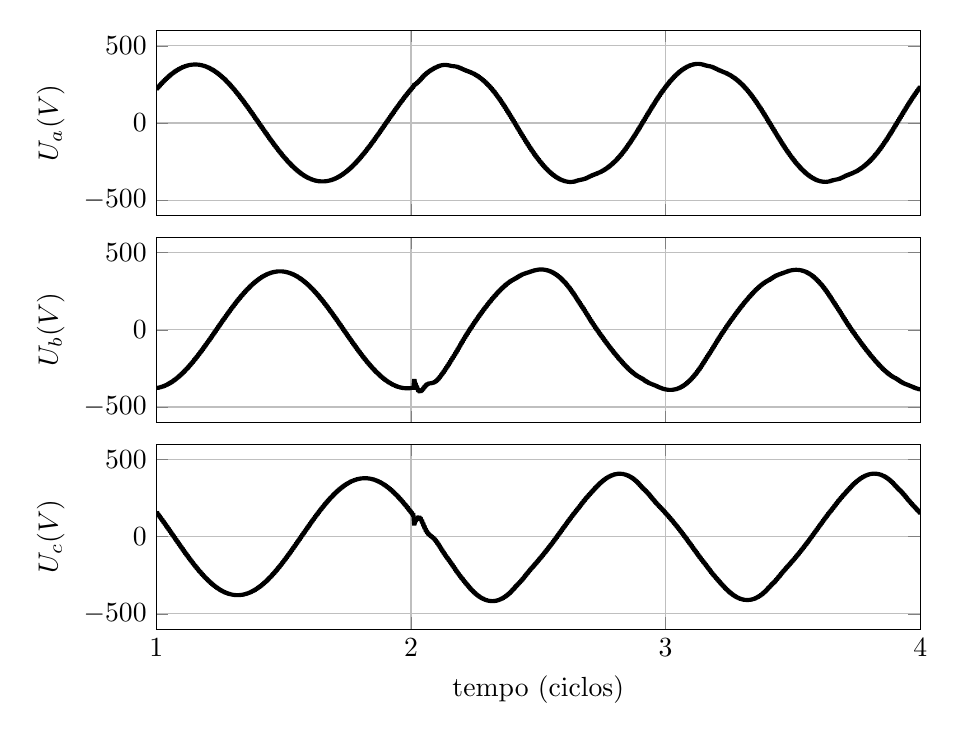
\begin{tikzpicture}

\begin{axis}[%
width=0.8\textwidth,
height=0.193917089240149\textwidth,
scale only axis,
xmin=0.316666666666667,
xmax=0.366666666666667,
xtick={0.316666666666667,0.333333333333333,0.35,0.366666666666667},
xticklabels={\empty},
xmajorgrids,
ymin=-600,
ymax=600,
ytick={-500,    0,  500},
ylabel={$\text{U}_\text{b}\text{ (V)}$},
ymajorgrids,
name=plot2,
scaled x ticks = false,
legend columns=-1,
legend style={/tikz/every even column/.append style={column sep=0.3cm}},
legend style={font=\footnotesize}
]
\addplot [color=black,solid,line width=1.5pt,forget plot]
  table[row sep=crcr]{0.316658333333333	-377.723085698266\\
0.3167	-376.586723778496\\
0.316741666666667	-376.586723778496\\
0.316783333333333	-375.078923942871\\
0.316825	-375.078923942871\\
0.316866666666667	-373.201183557557\\
0.316908333333333	-373.201183557557\\
0.31695	-370.955359679074\\
0.316991666666667	-370.955359679074\\
0.317033333333333	-368.343680965246\\
0.317075	-368.343680965246\\
0.317116666666667	-365.368751272189\\
0.317158333333333	-365.368751272189\\
0.3172	-362.033546182555\\
0.317241666666667	-362.033546182555\\
0.317283333333333	-358.341404810258\\
0.317325	-358.341404810258\\
0.317366666666667	-354.29601946274\\
0.317408333333333	-354.29601946274\\
0.31745	-349.901425336706\\
0.317491666666667	-349.901425336706\\
0.317533333333333	-345.161991678398\\
0.317575	-345.161991678398\\
0.317616666666667	-340.082415007475\\
0.317658333333333	-340.082415007475\\
0.3177	-334.667714301187\\
0.317741666666667	-334.667714301187\\
0.317783333333333	-328.923227572974\\
0.317825	-328.923227572974\\
0.317866666666667	-322.854609083496\\
0.317908333333333	-322.854609083496\\
0.31795	-316.467826451787\\
0.317991666666667	-316.467826451787\\
0.318033333333333	-309.769157112268\\
0.318075	-309.769157112268\\
0.318116666666667	-302.765183805345\\
0.318158333333333	-302.765183805345\\
0.3182	-295.462789021633\\
0.318241666666667	-295.462789021633\\
0.318283333333333	-287.869148495131\\
0.318325	-287.869148495131\\
0.318366666666667	-279.991723937524\\
0.318408333333333	-279.991723937524\\
0.31845	-271.838255227092\\
0.318491666666667	-271.838255227092\\
0.318533333333333	-263.416752229383\\
0.318575	-263.416752229383\\
0.318616666666667	-254.735486359231\\
0.318658333333333	-254.735486359231\\
0.3187	-245.802981925607\\
0.318741666666667	-245.802981925607\\
0.318783333333333	-236.6280072728\\
0.318825	-236.6280072728\\
0.318866666666667	-227.219565832749\\
0.318908333333333	-227.219565832749\\
0.31895	-217.586887717469\\
0.318991666666667	-217.586887717469\\
0.319033333333333	-207.739424484696\\
0.319075	-207.739424484696\\
0.319116666666667	-197.686870803904\\
0.319158333333333	-197.686870803904\\
0.3192	-187.439263486291\\
0.319241666666667	-187.439263486291\\
0.319283333333333	-177.007031372265\\
0.319325	-177.007031372265\\
0.319366666666667	-166.400723674948\\
0.319408333333333	-166.400723674948\\
0.31945	-155.6307199546\\
0.319491666666667	-155.6307199546\\
0.319533333333333	-144.707346263981\\
0.319575	-144.707346263981\\
0.319616666666667	-133.641094664328\\
0.319658333333333	-133.641094664328\\
0.3197	-122.442727673415\\
0.319741666666667	-122.442727673415\\
0.319783333333333	-111.123278734636\\
0.319825	-111.123278734636\\
0.319866666666667	-99.6940002360541\\
0.319908333333333	-99.6940002360541\\
0.31995	-88.1662967730299\\
0.319991666666667	-88.1662967730299\\
0.320033333333333	-76.5516646999388\\
0.320075	-76.5516646999388\\
0.320116666666667	-64.8616480040377\\
0.320158333333333	-64.8616480040377\\
0.3202	-53.1078129245748\\
0.320241666666667	-53.1078129245748\\
0.320283333333333	-41.3017386424485\\
0.320325	-41.3017386424485\\
0.320366666666667	-29.4550186053735\\
0.320408333333333	-29.4550186053735\\
0.32045	-17.5792663930844\\
0.320491666666667	-17.5792663930844\\
0.320533333333333	-5.68612092557823\\
0.320575	-5.68612092557823\\
0.320616666666667	6.2127524201114\\
0.320658333333333	6.2127524201114\\
0.3207	18.105666253858\\
0.320741666666667	18.105666253858\\
0.320783333333333	29.9809209740117\\
0.320825	29.9809209740117\\
0.320866666666667	41.8268186183045\\
0.320908333333333	41.8268186183045\\
0.32095	53.631678981668\\
0.320991666666667	53.631678981668\\
0.321033333333333	65.3838562807079\\
0.321075	65.3838562807079\\
0.321116666666667	77.0717550613194\\
0.321158333333333	77.0717550613194\\
0.3212	88.6838446142487\\
0.321241666666667	88.6838446142487\\
0.321283333333333	100.208671712027\\
0.321325	100.208671712027\\
0.321366666666667	111.6348719068\\
0.321408333333333	111.6348719068\\
0.32145	122.951179824381\\
0.321491666666667	122.951179824381\\
0.321533333333333	134.14643897231\\
0.321575	134.14643897231\\
0.321616666666667	145.209611528874\\
0.321658333333333	145.209611528874\\
0.3217	156.129788391287\\
0.321741666666667	156.129788391287\\
0.321783333333333	166.896199602751\\
0.321825	166.896199602751\\
0.321866666666667	177.498225133841\\
0.321908333333333	177.498225133841\\
0.32195	187.925405900222\\
0.321991666666667	187.925405900222\\
0.322033333333333	198.167454859908\\
0.322075	198.167454859908\\
0.322116666666667	208.214268041585\\
0.322158333333333	208.214268041585\\
0.3222	218.055935396159\\
0.322241666666667	218.055935396159\\
0.322283333333333	227.682751419264\\
0.322325	227.682751419264\\
0.322366666666667	237.085225549088\\
0.322408333333333	237.085225549088\\
0.32245	246.254092392214\\
0.322491666666667	246.254092392214\\
0.322533333333333	255.180321867299\\
0.322575	255.180321867299\\
0.322616666666667	263.855129383534\\
0.322658333333333	263.855129383534\\
0.3227	272.26998619054\\
0.322741666666667	272.26998619054\\
0.322783333333333	280.416630045836\\
0.322825	280.416630045836\\
0.322866666666667	288.287076317351\\
0.322908333333333	288.287076317351\\
0.32295	295.873629460527\\
0.322991666666667	295.873629460527\\
0.323033333333333	303.168894086837\\
0.323075	303.168894086837\\
0.323116666666667	310.165782141413\\
0.323158333333333	310.165782141413\\
0.3232	316.857502505702\\
0.323241666666667	316.857502505702\\
0.323283333333333	323.237410711189\\
0.323325	323.237410711189\\
0.323366666666667	329.298465304494\\
0.323408333333333	329.298465304494\\
0.32345	335.032940877286\\
0.323491666666667	335.032940877286\\
0.323533333333333	340.433778089715\\
0.323575	340.433778089715\\
0.323616666666667	345.496008515558\\
0.323658333333333	345.496008515558\\
0.3237	350.216089241188\\
0.323741666666667	350.216089241188\\
0.323783333333333	354.590714854285\\
0.323825	354.590714854285\\
0.323866666666667	358.616245271799\\
0.323908333333333	358.616245271799\\
0.32395	362.28867598875\\
0.323991666666667	362.28867598875\\
0.324033333333333	365.603866403093\\
0.324075	365.603866403093\\
0.324116666666667	368.557830105438\\
0.324158333333333	368.557830105438\\
0.3242	371.14698467744\\
0.324241666666667	371.14698467744\\
0.324283333333333	373.368315025462\\
0.324325	373.368315025462\\
0.324366666666667	375.219441072503\\
0.324408333333333	375.219441072503\\
0.32445	376.698604902272\\
0.324491666666667	376.698604902272\\
0.324533333333333	377.804605390594\\
0.324575	377.804605390594\\
0.324616666666667	378.536711049029\\
0.324658333333333	378.536711049029\\
0.3247	378.89457690205\\
0.324741666666667	378.89457690205\\
0.324783333333333	378.878182191864\\
0.324825	378.878182191864\\
0.324866666666667	378.487795835975\\
0.324908333333333	378.487795835975\\
0.32495	377.723968278227\\
0.324991666666667	377.723968278227\\
0.325033333333333	376.587542986259\\
0.325075	376.587542986259\\
0.325116666666667	375.079678623678\\
0.325158333333333	375.079678623678\\
0.3252	373.201873355773\\
0.325241666666667	373.201873355773\\
0.325283333333333	370.955984906448\\
0.325325	370.955984906448\\
0.325366666666667	368.34424285761\\
0.325408333333333	368.34424285761\\
0.32545	365.369252419982\\
0.325491666666667	365.369252419982\\
0.325533333333333	362.033990949537\\
0.325575	362.033990949537\\
0.325616666666667	358.341799615764\\
0.325658333333333	358.341799615764\\
0.3257	354.29637287251\\
0.325741666666667	354.29637287251\\
0.325783333333333	349.901747968484\\
0.325825	349.901747968484\\
0.325866666666667	345.162295969421\\
0.325908333333333	345.162295969421\\
0.32595	340.082714909794\\
0.325991666666667	340.082714909794\\
0.326033333333333	334.668024969912\\
0.326075	334.668024969912\\
0.326116666666667	328.923565098519\\
0.326158333333333	328.923565098519\\
0.3262	322.854990299289\\
0.326241666666667	322.854990299289\\
0.326283333333333	316.468268829063\\
0.326325	316.468268829063\\
0.326366666666667	309.769678739274\\
0.326408333333333	309.769678739274\\
0.32645	302.76580344002\\
0.326491666666667	302.76580344002\\
0.326533333333333	295.46352620612\\
0.326575	295.46352620612\\
0.326616666666667	287.870023724931\\
0.326658333333333	287.870023724931\\
0.3267	279.99275888678\\
0.326741666666667	279.99275888678\\
0.326783333333333	271.839473042268\\
0.326825	271.839473042268\\
0.326866666666667	263.418177915058\\
0.326908333333333	263.418177915058\\
0.32695	254.737147291355\\
0.326991666666667	254.737147291355\\
0.327033333333333	245.804908536742\\
0.327075	245.804908536742\\
0.327116666666667	236.630233953394\\
0.327158333333333	236.630233953394\\
0.3272	227.22213205341\\
0.327241666666667	227.22213205341\\
0.327283333333333	217.589839194205\\
0.327325	217.589839194205\\
0.327366666666667	207.742813476948\\
0.327408333333333	207.742813476948\\
0.32745	197.690748171958\\
0.327491666666667	197.690748171958\\
0.327533333333333	187.443640894198\\
0.327575	187.443640894198\\
0.327616666666667	177.011825362749\\
0.327658333333333	177.011825362749\\
0.3277	166.405770179614\\
0.327741666666667	166.405770179614\\
0.327783333333333	155.635868101642\\
0.327825	155.635868101642\\
0.327866666666667	144.712520179611\\
0.327908333333333	144.712520179611\\
0.32795	133.646292221512\\
0.327991666666667	133.646292221512\\
0.328033333333333	122.447986519211\\
0.328075	122.447986519211\\
0.328116666666667	111.128638130733\\
0.328158333333333	111.128638130733\\
0.3282	99.6994735093165\\
0.328241666666667	99.6994735093165\\
0.328283333333333	88.1718588306136\\
0.328325	88.1718588306136\\
0.328366666666667	76.5572531712875\\
0.328408333333333	76.5572531712875\\
0.32845	64.8671736797616\\
0.328491666666667	64.8671736797616\\
0.328533333333333	53.1131743732041\\
0.328575	53.1131743732041\\
0.328616666666667	41.3068365291399\\
0.328658333333333	41.3068365291399\\
0.3287	29.4597666782387\\
0.328741666666667	29.4597666782387\\
0.328783333333333	17.5835977645907\\
0.328825	17.5835977645907\\
0.328866666666667	5.68998972084417\\
0.328908333333333	5.68998972084417\\
0.32895	-6.20937299888088\\
0.328991666666667	-6.20937299888088\\
0.329033333333333	-18.1027879552077\\
0.329075	-18.1027879552077\\
0.329116666666667	-29.9785451472021\\
0.329158333333333	-29.9785451472021\\
0.3292	-41.8249403501677\\
0.329241666666667	-41.8249403501677\\
0.329283333333333	-53.6302900618585\\
0.329325	-53.6302900618585\\
0.329366666666667	-65.3829468063473\\
0.329408333333333	-65.3829468063473\\
0.32945	-77.0713138539921\\
0.329491666666667	-77.0713138539921\\
0.329533333333333	-88.6838588313381\\
0.329575	-88.6838588313381\\
0.329616666666667	-100.209126092659\\
0.329658333333333	-100.209126092659\\
0.3297	-111.635748034836\\
0.329741666666667	-111.635748034836\\
0.329783333333333	-122.952455666325\\
0.329825	-122.952455666325\\
0.329866666666667	-134.148088804689\\
0.329908333333333	-134.148088804689\\
0.32995	-145.211606244939\\
0.329991666666667	-145.211606244939\\
0.330033333333333	-156.132096092484\\
0.330075	-156.132096092484\\
0.330116666666667	-166.898786342177\\
0.330158333333333	-166.898786342177\\
0.3302	-177.501055680916\\
0.330241666666667	-177.501055680916\\
0.330283333333333	-187.928444425067\\
0.330325	-187.928444425067\\
0.330366666666667	-198.170665477564\\
0.330408333333333	-198.170665477564\\
0.33045	-208.21761519744\\
0.330491666666667	-208.21761519744\\
0.330533333333333	-218.059384105748\\
0.330575	-218.059384105748\\
0.330616666666667	-227.686267394042\\
0.330658333333333	-227.686267394042\\
0.3307	-237.088775244765\\
0.330741666666667	-237.088775244765\\
0.330783333333333	-246.257643010826\\
0.330825	-246.257643010826\\
0.330866666666667	-255.183841332313\\
0.330908333333333	-255.183841332313\\
0.33095	-263.858586293167\\
0.330991666666667	-263.858586293167\\
0.331033333333333	-272.273349741191\\
0.331075	-272.273349741191\\
0.331116666666667	-280.419869907006\\
0.331158333333333	-280.419869907006\\
0.3312	-288.29016243285\\
0.331241666666667	-288.29016243285\\
0.331283333333333	-295.876531750755\\
0.331325	-295.876531750755\\
0.331366666666667	-303.171582042784\\
0.331408333333333	-303.171582042784\\
0.33145	-310.168224372754\\
0.331491666666667	-310.168224372754\\
0.331533333333333	-316.859666586207\\
0.331575	-316.859666586207\\
0.331616666666667	-323.239266132863\\
0.331658333333333	-323.239266132863\\
0.3317	-329.299997905177\\
0.331741666666667	-329.299997905177\\
0.331783333333333	-335.034174516609\\
0.331825	-335.034174516609\\
0.331866666666667	-340.434769270671\\
0.331908333333333	-340.434769270671\\
0.33195	-345.496809702631\\
0.331991666666667	-345.496809702631\\
0.332033333333333	-350.216724523872\\
0.332075	-350.216724523872\\
0.332116666666667	-354.591180653519\\
0.332158333333333	-354.591180653519\\
0.3322	-358.616523838194\\
0.332241666666667	-358.616523838194\\
0.332283333333333	-362.288750228316\\
0.332325	-362.288750228316\\
0.332366666666667	-365.603730340961\\
0.332408333333333	-365.603730340961\\
0.33245	-368.557493442448\\
0.332491666666667	-368.557493442448\\
0.332533333333333	-371.146472117679\\
0.332575	-371.146472117679\\
0.332616666666667	-373.367662092301\\
0.332658333333333	-373.367662092301\\
0.3327	-375.218688387832\\
0.332741666666667	-375.218688387832\\
0.332783333333333	-376.697792634348\\
0.332825	-376.697792634348\\
0.332866666666667	-377.803769014554\\
0.332908333333333	-377.803769014554\\
0.33295	-378.535878926511\\
0.332991666666667	-378.535878926511\\
0.333033333333333	-378.893769636932\\
0.333075	-378.893769636932\\
0.333116666666667	-378.877413350589\\
0.333158333333333	-378.877413350589\\
0.3332	-378.487073457233\\
0.333241666666667	-378.487073457233\\
0.333283333333333	-377.723296609494\\
0.333325	-377.723296609494\\
0.333366666666667	-376.586924015447\\
0.333408333333333	-376.586924015447\\
0.33345	-375.079113157694\\
0.333491666666667	-375.079113157694\\
0.333533333333333	-331.053959173598\\
0.333575	-331.053959173598\\
0.333616666666667	-355.566522011512\\
0.333658333333333	-355.566522011512\\
0.3337	-373.445816485349\\
0.333741666666667	-373.445816485349\\
0.333783333333333	-390.060728449125\\
0.333825	-390.060728449125\\
0.333866666666667	-397.844659076646\\
0.333908333333333	-397.844659076646\\
0.33395	-397.607802023386\\
0.333991666666667	-397.607802023386\\
0.334033333333333	-391.060112093255\\
0.334075	-391.060112093255\\
0.334116666666667	-381.094479206499\\
0.334158333333333	-381.094479206499\\
0.3342	-370.432541041817\\
0.334241666666667	-370.432541041817\\
0.334283333333333	-361.10933181306\\
0.334325	-361.10933181306\\
0.334366666666667	-354.187694656387\\
0.334408333333333	-354.187694656387\\
0.33445	-349.799439727971\\
0.334491666666667	-349.799439727971\\
0.334533333333333	-347.372660995052\\
0.334575	-347.372660995052\\
0.334616666666667	-345.947097926559\\
0.334658333333333	-345.947097926559\\
0.3347	-344.482120632058\\
0.334741666666667	-344.482120632058\\
0.334783333333333	-342.09474327366\\
0.334825	-342.09474327366\\
0.334866666666667	-338.197725129126\\
0.334908333333333	-338.197725129126\\
0.33495	-332.537670597275\\
0.334991666666667	-332.537670597275\\
0.335033333333333	-325.15388006198\\
0.335075	-325.15388006198\\
0.335116666666667	-316.28916703799\\
0.335158333333333	-316.28916703799\\
0.3352	-306.284769550907\\
0.335241666666667	-306.284769550907\\
0.335283333333333	-295.485470833566\\
0.335325	-295.485470833566\\
0.335366666666667	-284.171376318267\\
0.335408333333333	-284.171376318267\\
0.33545	-272.522566002453\\
0.335491666666667	-272.522566002453\\
0.335533333333333	-260.61442814232\\
0.335575	-260.61442814232\\
0.335616666666667	-248.436427908707\\
0.335658333333333	-248.436427908707\\
0.3357	-235.926679683468\\
0.335741666666667	-235.926679683468\\
0.335783333333333	-223.037264128933\\
0.335825	-223.037264128933\\
0.335866666666667	-209.851831411951\\
0.335908333333333	-209.851831411951\\
0.33595	-196.611666331073\\
0.335991666666667	-196.611666331073\\
0.336033333333333	-183.476393437186\\
0.336075	-183.476393437186\\
0.336116666666667	-170.356767061117\\
0.336158333333333	-170.356767061117\\
0.3362	-157.055083569433\\
0.336241666666667	-157.055083569433\\
0.336283333333333	-143.429914658155\\
0.336325	-143.429914658155\\
0.336366666666667	-129.458136162372\\
0.336408333333333	-129.458136162372\\
0.33645	-115.222320815206\\
0.336491666666667	-115.222320815206\\
0.336533333333333	-100.866949128386\\
0.336575	-100.866949128386\\
0.336616666666667	-86.5509299822073\\
0.336658333333333	-86.5509299822073\\
0.3367	-72.41027026342\\
0.336741666666667	-72.41027026342\\
0.336783333333333	-58.5363796842563\\
0.336825	-58.5363796842563\\
0.336866666666667	-44.9700673537924\\
0.336908333333333	-44.9700673537924\\
0.33695	-31.707889473305\\
0.336991666666667	-31.707889473305\\
0.337033333333333	-18.7158965281947\\
0.337075	-18.7158965281947\\
0.337116666666667	-5.94573969853337\\
0.337158333333333	-5.94573969853337\\
0.3372	6.65091467907677\\
0.337241666666667	6.65091467907677\\
0.337283333333333	19.1121725057594\\
0.337325	19.1121725057594\\
0.337366666666667	31.4608004356482\\
0.337408333333333	31.4608004356482\\
0.33745	43.7037890472732\\
0.337491666666667	43.7037890472732\\
0.337533333333333	55.8353146508486\\
0.337575	55.8353146508486\\
0.337616666666667	67.8414871651914\\
0.337658333333333	67.8414871651914\\
0.3377	79.7053679758756\\
0.337741666666667	79.7053679758756\\
0.337783333333333	91.4111249732799\\
0.337825	91.4111249732799\\
0.337866666666667	102.946699116045\\
0.337908333333333	102.946699116045\\
0.33795	114.304846735082\\
0.337991666666667	114.304846735082\\
0.338033333333333	125.48279788958\\
0.338075	125.48279788958\\
0.338116666666667	136.480988520722\\
0.338158333333333	136.480988520722\\
0.3382	147.301382532013\\
0.338241666666667	147.301382532013\\
0.338283333333333	157.945834901859\\
0.338325	157.945834901859\\
0.338366666666667	168.414824976718\\
0.338408333333333	168.414824976718\\
0.33845	178.706689071158\\
0.338491666666667	178.706689071158\\
0.338533333333333	188.817360960719\\
0.338575	188.817360960719\\
0.338616666666667	198.740516451167\\
0.338658333333333	198.740516451167\\
0.3387	208.467965212707\\
0.338741666666667	208.467965212707\\
0.338783333333333	217.990125931066\\
0.338825	217.990125931066\\
0.338866666666667	227.296449162136\\
0.338908333333333	227.296449162136\\
0.33895	236.375699087072\\
0.338991666666667	236.375699087072\\
0.339033333333333	245.216055297035\\
0.339075	245.216055297035\\
0.339116666666667	253.805036957062\\
0.339158333333333	253.805036957062\\
0.3392	262.129277455222\\
0.339241666666667	262.129277455222\\
0.339283333333333	270.174186139085\\
0.339325	270.174186139085\\
0.339366666666667	277.923527251179\\
0.339408333333333	277.923527251179\\
0.33945	285.358930126453\\
0.339491666666667	285.358930126453\\
0.339533333333333	292.459328207278\\
0.339575	292.459328207278\\
0.339616666666667	299.200325675121\\
0.339658333333333	299.200325675121\\
0.3397	305.553558239489\\
0.339741666666667	305.553558239489\\
0.339783333333333	311.486405727299\\
0.339825	311.486405727299\\
0.339866666666667	316.963488313754\\
0.339908333333333	316.963488313754\\
0.33995	321.955622281295\\
0.339991666666667	321.955622281295\\
0.340033333333333	326.51038780251\\
0.340075	326.51038780251\\
0.340116666666667	330.894031493026\\
0.340158333333333	330.894031493026\\
0.3402	335.528606477071\\
0.340241666666667	335.528606477071\\
0.340283333333333	340.570364797468\\
0.340325	340.570364797468\\
0.340366666666667	345.770463847633\\
0.340408333333333	345.770463847633\\
0.34045	350.748908572128\\
0.340491666666667	350.748908572128\\
0.340533333333333	355.229203107812\\
0.340575	355.229203107812\\
0.340616666666667	359.114152112252\\
0.340658333333333	359.114152112252\\
0.3407	362.460955225898\\
0.340741666666667	362.460955225898\\
0.340783333333333	365.41785357704\\
0.340825	365.41785357704\\
0.340866666666667	368.157753621937\\
0.340908333333333	368.157753621937\\
0.34095	370.82624186103\\
0.340991666666667	370.82624186103\\
0.341033333333333	373.510998358136\\
0.341075	373.510998358136\\
0.341116666666667	376.232712187331\\
0.341158333333333	376.232712187331\\
0.3412	378.953067740294\\
0.341241666666667	378.953067740294\\
0.341283333333333	381.593124168933\\
0.341325	381.593124168933\\
0.341366666666667	384.055211723504\\
0.341408333333333	384.055211723504\\
0.34145	386.242756535565\\
0.341491666666667	386.242756535565\\
0.341533333333333	388.074514121078\\
0.341575	388.074514121078\\
0.341616666666667	389.4918829744\\
0.341658333333333	389.4918829744\\
0.3417	390.459793971863\\
0.341741666666667	390.459793971863\\
0.341783333333333	390.962859313687\\
0.341825	390.962859313687\\
0.341866666666667	390.998956997765\\
0.341908333333333	390.998956997765\\
0.34195	390.572324781683\\
0.341991666666667	390.572324781683\\
0.342033333333333	389.68773571272\\
0.342075	389.68773571272\\
0.342116666666667	388.346645879388\\
0.342158333333333	388.346645879388\\
0.3422	386.545537229963\\
0.342241666666667	386.545537229963\\
0.342283333333333	384.276158205878\\
0.342325	384.276158205878\\
0.342366666666667	381.527055310504\\
0.342408333333333	381.527055310504\\
0.34245	378.285700019777\\
0.342491666666667	378.285700019777\\
0.342533333333333	374.540592256173\\
0.342575	374.540592256173\\
0.342616666666667	370.282895838412\\
0.342658333333333	370.282895838412\\
0.3427	365.507390756861\\
0.342741666666667	365.507390756861\\
0.342783333333333	360.212725707634\\
0.342825	360.212725707634\\
0.342866666666667	354.401100495321\\
0.342908333333333	354.401100495321\\
0.34295	348.077584159459\\
0.342991666666667	348.077584159459\\
0.343033333333333	341.249285993621\\
0.343075	341.249285993621\\
0.343116666666667	333.924559113093\\
0.343158333333333	333.924559113093\\
0.3432	326.112351511447\\
0.343241666666667	326.112351511447\\
0.343283333333333	317.821748416951\\
0.343325	317.821748416951\\
0.343366666666667	309.061688184461\\
0.343408333333333	309.061688184461\\
0.34345	299.840791250307\\
0.343491666666667	299.840791250307\\
0.343533333333333	290.16722085235\\
0.343575	290.16722085235\\
0.343616666666667	280.048494368801\\
0.343658333333333	280.048494368801\\
0.3437	269.49118554204\\
0.343741666666667	269.49118554204\\
0.343783333333333	258.500513859365\\
0.343825	258.500513859365\\
0.343866666666667	247.079969056574\\
0.343908333333333	247.079969056574\\
0.34395	235.231596212627\\
0.343991666666667	235.231596212627\\
0.344033333333333	222.959248035688\\
0.344075	222.959248035688\\
0.344116666666667	210.294484360706\\
0.344158333333333	210.294484360706\\
0.3442	197.380821214263\\
0.344241666666667	197.380821214263\\
0.344283333333333	184.507370352904\\
0.344325	184.507370352904\\
0.344366666666667	171.894108559872\\
0.344408333333333	171.894108559872\\
0.34445	159.48943955546\\
0.344491666666667	159.48943955546\\
0.344533333333333	147.082800148723\\
0.344575	147.082800148723\\
0.344616666666667	134.48392975091\\
0.344658333333333	134.48392975091\\
0.3447	121.608197877001\\
0.344741666666667	121.608197877001\\
0.344783333333333	108.481692956559\\
0.344825	108.481692956559\\
0.344866666666667	95.2073277047852\\
0.344908333333333	95.2073277047852\\
0.34495	81.9206499726103\\
0.344991666666667	81.9206499726103\\
0.345033333333333	68.7509283943436\\
0.345075	68.7509283943436\\
0.345116666666667	55.7949153079795\\
0.345158333333333	55.7949153079795\\
0.3452	43.1051973184324\\
0.345241666666667	43.1051973184324\\
0.345283333333333	30.6913029919792\\
0.345325	30.6913029919792\\
0.345366666666667	18.5295910406299\\
0.345408333333333	18.5295910406299\\
0.34545	6.57727867560945\\
0.345491666666667	6.57727867560945\\
0.345533333333333	-5.21352892244916\\
0.345575	-5.21352892244916\\
0.345616666666667	-16.884732165864\\
0.345658333333333	-16.884732165864\\
0.3457	-28.4655123545339\\
0.345741666666667	-28.4655123545339\\
0.345783333333333	-39.9701087926515\\
0.345825	-39.9701087926515\\
0.345866666666667	-51.3992460624834\\
0.345908333333333	-51.3992460624834\\
0.34595	-62.7438487413975\\
0.345991666666667	-62.7438487413975\\
0.346033333333333	-73.9896017205765\\
0.346075	-73.9896017205765\\
0.346116666666667	-85.121157413393\\
0.346158333333333	-85.121157413393\\
0.3462	-96.1252122103461\\
0.346241666666667	-96.1252122103461\\
0.346283333333333	-106.992134481337\\
0.346325	-106.992134481337\\
0.346366666666667	-117.71621864397\\
0.346408333333333	-117.71621864397\\
0.34645	-128.294902750556\\
0.346491666666667	-128.294902750556\\
0.346533333333333	-138.727400956601\\
0.346575	-138.727400956601\\
0.346616666666667	-149.013197921609\\
0.346658333333333	-149.013197921609\\
0.3467	-159.150755168705\\
0.346741666666667	-159.150755168705\\
0.346783333333333	-169.136616907445\\
0.346825	-169.136616907445\\
0.346866666666667	-178.964978776181\\
0.346908333333333	-178.964978776181\\
0.34695	-188.627664096056\\
0.346991666666667	-188.627664096056\\
0.347033333333333	-198.114382623149\\
0.347075	-198.114382623149\\
0.347116666666667	-207.413121347082\\
0.347158333333333	-207.413121347082\\
0.3472	-216.510528801266\\
0.347241666666667	-216.510528801266\\
0.347283333333333	-225.392189426761\\
0.347325	-225.392189426761\\
0.347366666666667	-234.042728181155\\
0.347408333333333	-234.042728181155\\
0.34745	-242.445725371265\\
0.347491666666667	-242.445725371265\\
0.347533333333333	-250.583449409381\\
0.347575	-250.583449409381\\
0.347616666666667	-258.436427518641\\
0.347658333333333	-258.436427518641\\
0.3477	-265.982873061162\\
0.347741666666667	-265.982873061162\\
0.347783333333333	-273.197981095398\\
0.347825	-273.197981095398\\
0.347866666666667	-280.053111551403\\
0.347908333333333	-280.053111551403\\
0.34795	-286.514959521713\\
0.347991666666667	-286.514959521713\\
0.348033333333333	-292.545146969492\\
0.348075	-292.545146969492\\
0.348116666666667	-298.101899398808\\
0.348158333333333	-298.101899398808\\
0.3482	-303.150058989071\\
0.348241666666667	-303.150058989071\\
0.348283333333333	-307.741124565849\\
0.348325	-307.741124565849\\
0.348366666666667	-312.184494142668\\
0.348408333333333	-312.184494142668\\
0.34845	-316.993078269569\\
0.348491666666667	-316.993078269569\\
0.348533333333333	-322.386471176387\\
0.348575	-322.386471176387\\
0.348616666666667	-328.086904389457\\
0.348658333333333	-328.086904389457\\
0.3487	-333.634303962111\\
0.348741666666667	-333.634303962111\\
0.348783333333333	-338.681322343217\\
0.348825	-338.681322343217\\
0.348866666666667	-343.096845198308\\
0.348908333333333	-343.096845198308\\
0.34895	-346.94155652964\\
0.348991666666667	-346.94155652964\\
0.349033333333333	-350.39246515908\\
0.349075	-350.39246515908\\
0.349116666666667	-353.661520896268\\
0.349158333333333	-353.661520896268\\
0.3492	-356.930720798577\\
0.349241666666667	-356.930720798577\\
0.349283333333333	-360.312979455071\\
0.349325	-360.312979455071\\
0.349366666666667	-363.839388505294\\
0.349408333333333	-363.839388505294\\
0.34945	-367.467767573894\\
0.349491666666667	-367.467767573894\\
0.349533333333333	-371.104477750465\\
0.349575	-371.104477750465\\
0.349616666666667	-374.631068068148\\
0.349658333333333	-374.631068068148\\
0.3497	-377.928793486934\\
0.349741666666667	-377.928793486934\\
0.349783333333333	-380.896524488929\\
0.349825	-380.896524488929\\
0.349866666666667	-383.46025084714\\
0.349908333333333	-383.46025084714\\
0.34995	-385.574651555104\\
0.349991666666667	-385.574651555104\\
0.350033333333333	-387.218711197641\\
0.350075	-387.218711197641\\
0.350116666666667	-388.388020979728\\
0.350158333333333	-388.388020979728\\
0.3502	-389.086322412681\\
0.350241666666667	-389.086322412681\\
0.350283333333333	-389.318265056282\\
0.350325	-389.318265056282\\
0.350366666666667	-389.084525480898\\
0.350408333333333	-389.084525480898\\
0.35045	-388.379612290062\\
0.350491666666667	-388.379612290062\\
0.350533333333333	-387.192031057405\\
0.350575	-387.192031057405\\
0.350616666666667	-385.50608813227\\
0.350658333333333	-385.50608813227\\
0.3507	-383.304478923655\\
0.350741666666667	-383.304478923655\\
0.350783333333333	-380.57089349795\\
0.350825	-380.57089349795\\
0.350866666666667	-377.292089152202\\
0.350908333333333	-377.292089152202\\
0.35095	-373.459138569364\\
0.350991666666667	-373.459138569364\\
0.351033333333333	-369.067820550881\\
0.351075	-369.067820550881\\
0.351116666666667	-364.118301768284\\
0.351158333333333	-364.118301768284\\
0.3512	-358.614358042697\\
0.351241666666667	-358.614358042697\\
0.351283333333333	-352.562402718406\\
0.351325	-352.562402718406\\
0.351366666666667	-345.970547765741\\
0.351408333333333	-345.970547765741\\
0.35145	-338.847846274726\\
0.351491666666667	-338.847846274726\\
0.351533333333333	-331.203778757477\\
0.351575	-331.203778757477\\
0.351616666666667	-323.04797020633\\
0.351658333333333	-323.04797020633\\
0.3517	-314.39007205322\\
0.351741666666667	-314.39007205322\\
0.351783333333333	-305.239716754853\\
0.351825	-305.239716754853\\
0.351866666666667	-295.606450118041\\
0.351908333333333	-295.606450118041\\
0.35195	-285.499562206261\\
0.351991666666667	-285.499562206261\\
0.352033333333333	-274.927768645022\\
0.352075	-274.927768645022\\
0.352116666666667	-263.898750386451\\
0.352158333333333	-263.898750386451\\
0.3522	-252.418694924988\\
0.352241666666667	-252.418694924988\\
0.352283333333333	-240.492397886311\\
0.352325	-240.492397886311\\
0.352366666666667	-228.125947274508\\
0.352408333333333	-228.125947274508\\
0.35245	-215.348409104807\\
0.352491666666667	-215.348409104807\\
0.352533333333333	-202.289599450389\\
0.352575	-202.289599450389\\
0.352616666666667	-189.223743821868\\
0.352658333333333	-189.223743821868\\
0.3527	-176.379208719445\\
0.352741666666667	-176.379208719445\\
0.352783333333333	-163.726000022735\\
0.352825	-163.726000022735\\
0.352866666666667	-151.067803244203\\
0.352908333333333	-151.067803244203\\
0.35295	-138.218894529514\\
0.352991666666667	-138.218894529514\\
0.353033333333333	-125.092906412442\\
0.353075	-125.092906412442\\
0.353116666666667	-111.711266961333\\
0.353158333333333	-111.711266961333\\
0.3532	-98.1717617623561\\
0.353241666666667	-98.1717617623561\\
0.353283333333333	-84.606026368675\\
0.353325	-84.606026368675\\
0.353366666666667	-71.1415440461283\\
0.353408333333333	-71.1415440461283\\
0.35345	-57.8755976757111\\
0.353491666666667	-57.8755976757111\\
0.353533333333333	-44.8632491753258\\
0.353575	-44.8632491753258\\
0.353616666666667	-32.1177523558641\\
0.353658333333333	-32.1177523558641\\
0.3537	-19.6196605712489\\
0.353741666666667	-19.6196605712489\\
0.353783333333333	-7.33017611953616\\
0.353825	-7.33017611953616\\
0.353866666666667	4.79528596240854\\
0.353908333333333	4.79528596240854\\
0.35395	16.7962089615764\\
0.353991666666667	16.7962089615764\\
0.354033333333333	28.7002458702663\\
0.354075	28.7002458702663\\
0.354116666666667	40.5208361198962\\
0.354158333333333	40.5208361198962\\
0.3542	52.2583945768098\\
0.354241666666667	52.2583945768098\\
0.354283333333333	63.9037820451212\\
0.354325	63.9037820451212\\
0.354366666666667	75.4426677745932\\
0.354408333333333	75.4426677745932\\
0.35445	86.8596128178869\\
0.354491666666667	86.8596128178869\\
0.354533333333333	98.1411008420367\\
0.354575	98.1411008420367\\
0.354616666666667	109.277185521684\\
0.354658333333333	109.277185521684\\
0.3547	120.261806239716\\
0.354741666666667	120.261806239716\\
0.354783333333333	131.092084681737\\
0.354825	131.092084681737\\
0.354866666666667	141.767032559822\\
0.354908333333333	141.767032559822\\
0.35495	152.286104127589\\
0.354991666666667	152.286104127589\\
0.355033333333333	162.647935503272\\
0.355075	162.647935503272\\
0.355116666666667	172.849461167547\\
0.355158333333333	172.849461167547\\
0.3552	182.885476549861\\
0.355241666666667	182.885476549861\\
0.355283333333333	192.74859971663\\
0.355325	192.74859971663\\
0.355366666666667	202.429515642445\\
0.355408333333333	202.429515642445\\
0.35545	211.917359809411\\
0.355491666666667	211.917359809411\\
0.355533333333333	221.200107736149\\
0.355575	221.200107736149\\
0.355616666666667	230.264870122842\\
0.355658333333333	230.264870122842\\
0.3557	239.09803559447\\
0.355741666666667	239.09803559447\\
0.355783333333333	247.685242426249\\
0.355825	247.685242426249\\
0.355866666666667	256.01118897413\\
0.355908333333333	256.01118897413\\
0.35595	264.059306139522\\
0.355991666666667	264.059306139522\\
0.356033333333333	271.811314698462\\
0.356075	271.811314698462\\
0.356116666666667	279.246680549618\\
0.356158333333333	279.246680549618\\
0.3562	286.341972975943\\
0.356241666666667	286.341972975943\\
0.356283333333333	293.070152149675\\
0.356325	293.070152149675\\
0.356366666666667	299.399942608354\\
0.356408333333333	299.399942608354\\
0.35645	305.295957969326\\
0.356491666666667	305.295957969326\\
0.356533333333333	310.722117987443\\
0.356575	310.722117987443\\
0.356616666666667	315.666572995038\\
0.356658333333333	315.666572995038\\
0.3567	320.2542487815\\
0.356741666666667	320.2542487815\\
0.356783333333333	324.856446487095\\
0.356825	324.856446487095\\
0.356866666666667	329.852922874641\\
0.356908333333333	329.852922874641\\
0.35695	335.222065427616\\
0.356991666666667	335.222065427616\\
0.357033333333333	340.613534200536\\
0.357075	340.613534200536\\
0.357116666666667	345.656716837671\\
0.357158333333333	345.656716837671\\
0.3572	350.137311127185\\
0.357241666666667	350.137311127185\\
0.357283333333333	354.025303001667\\
0.357325	354.025303001667\\
0.357366666666667	357.426706873729\\
0.357408333333333	357.426706873729\\
0.35745	360.513281632962\\
0.357491666666667	360.513281632962\\
0.357533333333333	363.458209267499\\
0.357575	363.458209267499\\
0.357616666666667	366.390734543561\\
0.357658333333333	366.390734543561\\
0.3577	369.373754140581\\
0.357741666666667	369.373754140581\\
0.357783333333333	372.40226656797\\
0.357825	372.40226656797\\
0.357866666666667	375.416874434613\\
0.357908333333333	375.416874434613\\
0.35795	378.325110579895\\
0.357991666666667	378.325110579895\\
0.358033333333333	381.023855656326\\
0.358075	381.023855656326\\
0.358116666666667	383.417862668434\\
0.358158333333333	383.417862668434\\
0.3582	385.431672240814\\
0.358241666666667	385.431672240814\\
0.358283333333333	387.014368333221\\
0.358325	387.014368333221\\
0.358366666666667	388.138270008866\\
0.358408333333333	388.138270008866\\
0.35845	388.793592864896\\
0.358491666666667	388.793592864896\\
0.358533333333333	388.981356900916\\
0.358575	388.981356900916\\
0.358616666666667	388.706518452935\\
0.358658333333333	388.706518452935\\
0.3587	387.972682278112\\
0.358741666666667	387.972682278112\\
0.358783333333333	386.779028302941\\
0.358825	386.779028302941\\
0.358866666666667	385.119444190964\\
0.358908333333333	385.119444190964\\
0.35895	382.983399951863\\
0.358991666666667	382.983399951863\\
0.359033333333333	380.357871809701\\
0.359075	380.357871809701\\
0.359116666666667	377.229608324181\\
0.359158333333333	377.229608324181\\
0.3592	373.587164771571\\
0.359241666666667	373.587164771571\\
0.359283333333333	369.422335152074\\
0.359325	369.422335152074\\
0.359366666666667	364.730847206549\\
0.359408333333333	364.730847206549\\
0.35945	359.512371988876\\
0.359491666666667	359.512371988876\\
0.359533333333333	353.770022978723\\
0.359575	353.770022978723\\
0.359616666666667	347.509570477371\\
0.359658333333333	347.509570477371\\
0.3597	340.738586185096\\
0.359741666666667	340.738586185096\\
0.359783333333333	333.465680100964\\
0.359825	333.465680100964\\
0.359866666666667	325.699919967134\\
0.359908333333333	325.699919967134\\
0.35995	317.45045232578\\
0.359991666666667	317.45045232578\\
0.360033333333333	308.726287747113\\
0.360075	308.726287747113\\
0.360116666666667	299.536177702082\\
0.360158333333333	299.536177702082\\
0.3602	289.888497596475\\
0.360241666666667	289.888497596475\\
0.360283333333333	279.791057088036\\
0.360325	279.791057088036\\
0.360366666666667	269.250784501641\\
0.360408333333333	269.250784501641\\
0.36045	258.27329065012\\
0.360491666666667	258.27329065012\\
0.360533333333333	246.862472164031\\
0.360575	246.862472164031\\
0.360616666666667	235.020804269368\\
0.360658333333333	235.020804269368\\
0.3607	222.752710006781\\
0.360741666666667	222.752710006781\\
0.360783333333333	210.091801323474\\
0.360825	210.091801323474\\
0.360866666666667	197.185993975909\\
0.360908333333333	197.185993975909\\
0.36095	184.325618582163\\
0.360991666666667	184.325618582163\\
0.361033333333333	171.722625796759\\
0.361075	171.722625796759\\
0.361116666666667	159.316985749764\\
0.361158333333333	159.316985749764\\
0.3612	146.89655224484\\
0.361241666666667	146.89655224484\\
0.361283333333333	134.274769582802\\
0.361325	134.274769582802\\
0.361366666666667	121.372376006884\\
0.361408333333333	121.372376006884\\
0.36145	108.219776038739\\
0.361491666666667	108.219776038739\\
0.361533333333333	94.9220166008207\\
0.361575	94.9220166008207\\
0.361616666666667	81.614646304298\\
0.361658333333333	81.614646304298\\
0.3617	68.4254577689197\\
0.361741666666667	68.4254577689197\\
0.361783333333333	55.4490783962055\\
0.361825	55.4490783962055\\
0.361866666666667	42.7360509678476\\
0.361908333333333	42.7360509678476\\
0.36195	30.2944373262808\\
0.361991666666667	30.2944373262808\\
0.362033333333333	18.0999317872621\\
0.362075	18.0999317872621\\
0.362116666666667	6.10987697555117\\
0.362158333333333	6.10987697555117\\
0.3622	-5.72288379245039\\
0.362241666666667	-5.72288379245039\\
0.362283333333333	-17.4391559647083\\
0.362325	-17.4391559647083\\
0.362366666666667	-29.0669270842303\\
0.362408333333333	-29.0669270842303\\
0.36245	-40.6193498069394\\
0.362491666666667	-40.6193498069394\\
0.362533333333333	-52.0962957061184\\
0.362575	-52.0962957061184\\
0.362616666666667	-63.4881145894869\\
0.362658333333333	-63.4881145894869\\
0.3627	-74.7801727997866\\
0.362741666666667	-74.7801727997866\\
0.362783333333333	-85.95699646865\\
0.362825	-85.95699646865\\
0.362866666666667	-97.005268202752\\
0.362908333333333	-97.005268202752\\
0.36295	-107.915381191414\\
0.362991666666667	-107.915381191414\\
0.363033333333333	-118.68163930288\\
0.363075	-118.68163930288\\
0.363116666666667	-129.301446369291\\
0.363158333333333	-129.301446369291\\
0.3632	-139.77393479265\\
0.363241666666667	-139.77393479265\\
0.363283333333333	-150.09847450962\\
0.363325	-150.09847450962\\
0.363366666666667	-160.273404156851\\
0.363408333333333	-160.273404156851\\
0.36345	-170.295164440765\\
0.363491666666667	-170.295164440765\\
0.363533333333333	-180.157891159023\\
0.363575	-180.157891159023\\
0.363616666666667	-189.853409087089\\
0.363658333333333	-189.853409087089\\
0.3637	-199.371500840715\\
0.363741666666667	-199.371500840715\\
0.363783333333333	-208.700301424835\\
0.363825	-208.700301424835\\
0.363866666666667	-217.82668236852\\
0.363908333333333	-217.82668236852\\
0.36395	-226.736524925711\\
0.363991666666667	-226.736524925711\\
0.364033333333333	-235.414825364115\\
0.364075	-235.414825364115\\
0.364116666666667	-243.84561467942\\
0.364158333333333	-243.84561467942\\
0.3642	-252.011702190719\\
0.364241666666667	-252.011702190719\\
0.364283333333333	-259.894264193919\\
0.364325	-259.894264193919\\
0.364366666666667	-267.472296747565\\
0.364408333333333	-267.472296747565\\
0.36445	-274.721942890643\\
0.364491666666667	-274.721942890643\\
0.364533333333333	-281.615707001776\\
0.364575	-281.615707001776\\
0.364616666666667	-288.121631392846\\
0.364658333333333	-288.121631392846\\
0.3647	-294.202785652653\\
0.364741666666667	-294.202785652653\\
0.364783333333333	-299.818440515409\\
0.364825	-299.818440515409\\
0.364866666666667	-304.93209970605\\
0.364908333333333	-304.93209970605\\
0.36495	-309.575565237793\\
0.364991666666667	-309.575565237793\\
0.365033333333333	-314.012581745672\\
0.365075	-314.012581745672\\
0.365116666666667	-318.738236538347\\
0.365158333333333	-318.738236538347\\
0.3652	-324.025132661622\\
0.365241666666667	-324.025132661622\\
0.365283333333333	-329.648168153131\\
0.365325	-329.648168153131\\
0.365366666666667	-335.159687933284\\
0.365408333333333	-335.159687933284\\
0.36545	-340.199249987895\\
0.365491666666667	-340.199249987895\\
0.365533333333333	-344.614916167831\\
0.365575	-344.614916167831\\
0.365616666666667	-348.448453697907\\
0.365658333333333	-348.448453697907\\
0.3657	-351.863897978727\\
0.365741666666667	-351.863897978727\\
0.365783333333333	-355.067323932555\\
0.365825	-355.067323932555\\
0.365866666666667	-358.241309191347\\
0.365908333333333	-358.241309191347\\
0.36595	-361.504038503397\\
0.365991666666667	-361.504038503397\\
0.366033333333333	-364.894336620833\\
0.366075	-364.894336620833\\
0.366116666666667	-368.378119793744\\
0.366158333333333	-368.378119793744\\
0.3662	-371.868636134913\\
0.366241666666667	-371.868636134913\\
0.366283333333333	-375.252239474815\\
0.366325	-375.252239474815\\
0.366366666666667	-378.412712753345\\
0.366408333333333	-378.412712753345\\
0.36645	-381.249504392824\\
0.366491666666667	-381.249504392824\\
0.366533333333333	-383.687860969564\\
0.366575	-383.687860969564\\
0.366616666666667	-385.681109833679\\
0.366658333333333	-385.681109833679\\
};
\end{axis}

\begin{axis}[%
width=0.8\textwidth,
height=0.193917089240149\textwidth,
scale only axis,
xmin=0.316666666666667,
xmax=0.366666666666667,
xtick={0.316666666666667,0.333333333333333,0.35,0.366666666666667},
xticklabels={{1},{2},{3},{4}},
xlabel={tempo (ciclos)},
xmajorgrids,
ymin=-600,
ymax=600,
ytick={-500,    0,  500},
ylabel={$\text{U}_\text{c}\text{ (V)}$},
ymajorgrids,
at=(plot2.below south west),
anchor=above north west,
scaled x ticks = false,
legend columns=-1,
legend style={/tikz/every even column/.append style={column sep=0.3cm}},
legend style={font=\footnotesize}
]
\addplot [color=black,solid,line width=1.5pt,forget plot]
  table[row sep=crcr]{0.316658333333333	162.970553693369\\
0.3167	152.134366652308\\
0.316741666666667	152.134366652308\\
0.316783333333333	141.14831005675\\
0.316825	141.14831005675\\
0.316866666666667	130.023235612171\\
0.316908333333333	130.023235612171\\
0.31695	118.770126781016\\
0.316991666666667	118.770126781016\\
0.317033333333333	107.400101722771\\
0.317075	107.400101722771\\
0.317116666666667	95.9244081552081\\
0.317158333333333	95.9244081552081\\
0.3172	84.3544113952257\\
0.317241666666667	84.3544113952257\\
0.317283333333333	72.701577924984\\
0.317325	72.701577924984\\
0.317366666666667	60.9774570729016\\
0.317408333333333	60.9774570729016\\
0.31745	49.1936630040597\\
0.317491666666667	49.1936630040597\\
0.317533333333333	37.3618584558936\\
0.317575	37.3618584558936\\
0.317616666666667	25.4937408270424\\
0.317658333333333	25.4937408270424\\
0.3177	13.6010305245207\\
0.317741666666667	13.6010305245207\\
0.317783333333333	1.69546101270924\\
0.317825	1.69546101270924\\
0.317866666666667	-10.2112301875565\\
0.317908333333333	-10.2112301875565\\
0.31795	-22.1073102710107\\
0.317991666666667	-22.1073102710107\\
0.318033333333333	-33.9810602324472\\
0.318075	-33.9810602324472\\
0.318116666666667	-45.8207845611742\\
0.318158333333333	-45.8207845611742\\
0.3182	-57.6148216075114\\
0.318241666666667	-57.6148216075114\\
0.318283333333333	-69.3515545038083\\
0.318325	-69.3515545038083\\
0.318366666666667	-81.0194224196816\\
0.318408333333333	-81.0194224196816\\
0.31845	-92.6069319017156\\
0.318491666666667	-92.6069319017156\\
0.318533333333333	-104.102668074645\\
0.318575	-104.102668074645\\
0.318616666666667	-115.495305540439\\
0.318658333333333	-115.495305540439\\
0.3187	-126.773618886739\\
0.318741666666667	-126.773618886739\\
0.318783333333333	-137.926492811092\\
0.318825	-137.926492811092\\
0.318866666666667	-148.942932050852\\
0.318908333333333	-148.942932050852\\
0.31895	-159.812071858709\\
0.318991666666667	-159.812071858709\\
0.319033333333333	-170.5231917644\\
0.319075	-170.5231917644\\
0.319116666666667	-181.06575642652\\
0.319158333333333	-181.06575642652\\
0.3192	-191.42953407303\\
0.319241666666667	-191.42953407303\\
0.319283333333333	-201.604666016903\\
0.319325	-201.604666016903\\
0.319366666666667	-211.581414807252\\
0.319408333333333	-211.581414807252\\
0.31945	-221.34989413342\\
0.319491666666667	-221.34989413342\\
0.319533333333333	-230.900204960054\\
0.319575	-230.900204960054\\
0.319616666666667	-240.222675034997\\
0.319658333333333	-240.222675034997\\
0.3197	-249.307983285081\\
0.319741666666667	-249.307983285081\\
0.319783333333333	-258.147180154562\\
0.319825	-258.147180154562\\
0.319866666666667	-266.731655392224\\
0.319908333333333	-266.731655392224\\
0.31995	-275.053090965318\\
0.319991666666667	-275.053090965318\\
0.320033333333333	-283.103420134525\\
0.320075	-283.103420134525\\
0.320116666666667	-290.874802711353\\
0.320158333333333	-290.874802711353\\
0.3202	-298.359618907919\\
0.320241666666667	-298.359618907919\\
0.320283333333333	-305.550479087533\\
0.320325	-305.550479087533\\
0.320366666666667	-312.440243961342\\
0.320408333333333	-312.440243961342\\
0.32045	-319.022049113252\\
0.320491666666667	-319.022049113252\\
0.320533333333333	-325.289328632728\\
0.320575	-325.289328632728\\
0.320616666666667	-331.235834397501\\
0.320658333333333	-331.235834397501\\
0.3207	-336.855649514461\\
0.320741666666667	-336.855649514461\\
0.320783333333333	-342.143196100745\\
0.320825	-342.143196100745\\
0.320866666666667	-347.093238694001\\
0.320908333333333	-347.093238694001\\
0.32095	-351.700885056722\\
0.320991666666667	-351.700885056722\\
0.321033333333333	-355.961586078382\\
0.321075	-355.961586078382\\
0.321116666666667	-359.871136064135\\
0.321158333333333	-359.871136064135\\
0.3212	-363.425674130623\\
0.321241666666667	-363.425674130623\\
0.321283333333333	-366.621686882158\\
0.321325	-366.621686882158\\
0.321366666666667	-369.456012137793\\
0.321408333333333	-369.456012137793\\
0.32145	-371.925843211841\\
0.321491666666667	-371.925843211841\\
0.321533333333333	-374.028733221122\\
0.321575	-374.028733221122\\
0.321616666666667	-375.762598995818\\
0.321658333333333	-375.762598995818\\
0.3217	-377.125724285815\\
0.321741666666667	-377.125724285815\\
0.321783333333333	-378.116762135567\\
0.321825	-378.116762135567\\
0.321866666666667	-378.734736446567\\
0.321908333333333	-378.734736446567\\
0.32195	-378.979042846209\\
0.321991666666667	-378.979042846209\\
0.322033333333333	-378.849449026762\\
0.322075	-378.849449026762\\
0.322116666666667	-378.346094717328\\
0.322158333333333	-378.346094717328\\
0.3222	-377.469491420695\\
0.322241666666667	-377.469491420695\\
0.322283333333333	-376.220522004144\\
0.322325	-376.220522004144\\
0.322366666666667	-374.600440193894\\
0.322408333333333	-374.600440193894\\
0.32245	-372.61086999843\\
0.322491666666667	-372.61086999843\\
0.322533333333333	-370.253805081463\\
0.322575	-370.253805081463\\
0.322616666666667	-367.531608121488\\
0.322658333333333	-367.531608121488\\
0.3227	-364.447010227436\\
0.322741666666667	-364.447010227436\\
0.322783333333333	-361.00311051502\\
0.322825	-361.00311051502\\
0.322866666666667	-357.2033759492\\
0.322908333333333	-357.2033759492\\
0.32295	-353.051641405706\\
0.322991666666667	-353.051641405706\\
0.323033333333333	-348.55210919846\\
0.323075	-348.55210919846\\
0.323116666666667	-343.709344628697\\
0.323158333333333	-343.709344628697\\
0.3232	-338.52825390877\\
0.323241666666667	-338.52825390877\\
0.323283333333333	-333.013922177807\\
0.323325	-333.013922177807\\
0.323366666666667	-327.171058172122\\
0.323408333333333	-327.171058172122\\
0.32345	-321.003695577926\\
0.323491666666667	-321.003695577926\\
0.323533333333333	-314.516531402583\\
0.323575	-314.516531402583\\
0.323616666666667	-307.716339196424\\
0.323658333333333	-307.716339196424\\
0.3237	-300.611292060023\\
0.323741666666667	-300.611292060023\\
0.323783333333333	-293.209763076321\\
0.323825	-293.209763076321\\
0.323866666666667	-285.519741623125\\
0.323908333333333	-285.519741623125\\
0.32395	-277.54879215579\\
0.323991666666667	-277.54879215579\\
0.324033333333333	-269.304271125924\\
0.324075	-269.304271125924\\
0.324116666666667	-260.79360593688\\
0.324158333333333	-260.79360593688\\
0.3242	-252.02453349254\\
0.324241666666667	-252.02453349254\\
0.324283333333333	-243.005252378576\\
0.324325	-243.005252378576\\
0.324366666666667	-233.744479511389\\
0.324408333333333	-233.744479511389\\
0.32445	-224.251426359643\\
0.324491666666667	-224.251426359643\\
0.324533333333333	-214.535722784241\\
0.324575	-214.535722784241\\
0.324616666666667	-204.607319231369\\
0.324658333333333	-204.607319231369\\
0.3247	-194.476393109332\\
0.324741666666667	-194.476393109332\\
0.324783333333333	-184.153276152493\\
0.324825	-184.153276152493\\
0.324866666666667	-173.648409706627\\
0.324908333333333	-173.648409706627\\
0.32495	-162.972326585662\\
0.324991666666667	-162.972326585662\\
0.325033333333333	-152.135652762133\\
0.325075	-152.135652762133\\
0.325116666666667	-141.149119929114\\
0.325158333333333	-141.149119929114\\
0.3252	-130.023580401982\\
0.325241666666667	-130.023580401982\\
0.325283333333333	-118.770017987052\\
0.325325	-118.770017987052\\
0.325366666666667	-107.399551317653\\
0.325408333333333	-107.399551317653\\
0.32545	-95.9234288957582\\
0.325491666666667	-95.9234288957582\\
0.325533333333333	-84.3530171259215\\
0.325575	-84.3530171259215\\
0.325616666666667	-72.6997837486583\\
0.325658333333333	-72.6997837486583\\
0.3257	-60.9752793324054\\
0.325741666666667	-60.9752793324054\\
0.325783333333333	-49.1911190787728\\
0.325825	-49.1911190787728\\
0.325866666666667	-37.3589664176652\\
0.325908333333333	-37.3589664176652\\
0.32595	-25.4905190184515\\
0.325991666666667	-25.4905190184515\\
0.326033333333333	-13.5974971207829\\
0.326075	-13.5974971207829\\
0.326116666666667	-1.69163361404229\\
0.326158333333333	-1.69163361404229\\
0.3262	10.2153349073519\\
0.326241666666667	10.2153349073519\\
0.326283333333333	22.1116768548334\\
0.326325	22.1116768548334\\
0.326366666666667	33.9856746806564\\
0.326408333333333	33.9856746806564\\
0.32645	45.8256345451254\\
0.326491666666667	45.8256345451254\\
0.326533333333333	57.619896682525\\
0.326575	57.619896682525\\
0.326616666666667	69.356846348781\\
0.326658333333333	69.356846348781\\
0.3267	81.0249251286878\\
0.326741666666667	81.0249251286878\\
0.326783333333333	92.6126423517755\\
0.326825	92.6126423517755\\
0.326866666666667	104.108586394839\\
0.326908333333333	104.108586394839\\
0.32695	115.501435711804\\
0.326991666666667	115.501435711804\\
0.327033333333333	126.779969508188\\
0.327075	126.779969508188\\
0.327116666666667	137.933078066121\\
0.327158333333333	137.933078066121\\
0.3272	148.949772873188\\
0.327241666666667	148.949772873188\\
0.327283333333333	159.819197115413\\
0.327325	159.819197115413\\
0.327366666666667	170.530638546332\\
0.327408333333333	170.530638546332\\
0.32745	181.073562075667\\
0.327491666666667	181.073562075667\\
0.327533333333333	191.437698337058\\
0.327575	191.437698337058\\
0.327616666666667	201.613095062515\\
0.327658333333333	201.613095062515\\
0.3277	211.589935660001\\
0.327741666666667	211.589935660001\\
0.327783333333333	221.358348409748\\
0.327825	221.358348409748\\
0.327866666666667	230.908510590095\\
0.327908333333333	230.908510590095\\
0.32795	240.230824931129\\
0.327991666666667	240.230824931129\\
0.328033333333333	249.316011288028\\
0.328075	249.316011288028\\
0.328116666666667	258.155122791836\\
0.328158333333333	258.155122791836\\
0.3282	266.739524245654\\
0.328241666666667	266.739524245654\\
0.328283333333333	275.0608601025\\
0.328325	275.0608601025\\
0.328366666666667	283.111027166579\\
0.328408333333333	283.111027166579\\
0.32845	290.882159147744\\
0.328491666666667	290.882159147744\\
0.328533333333333	298.366624689893\\
0.328575	298.366624689893\\
0.328616666666667	305.557036824969\\
0.328658333333333	305.557036824969\\
0.3287	312.44626983943\\
0.328741666666667	312.44626983943\\
0.328783333333333	319.027479097028\\
0.328825	319.027479097028\\
0.328866666666667	325.294120041746\\
0.328908333333333	325.294120041746\\
0.32895	331.239963900123\\
0.328991666666667	331.239963900123\\
0.329033333333333	336.859109033448\\
0.329075	336.859109033448\\
0.329116666666667	342.145988100331\\
0.329158333333333	342.145988100331\\
0.3292	347.09537198353\\
0.329241666666667	347.09537198353\\
0.329283333333333	351.702371769095\\
0.329325	351.702371769095\\
0.329366666666667	355.96244001224\\
0.329408333333333	355.96244001224\\
0.32945	359.871372216336\\
0.329491666666667	359.871372216336\\
0.329533333333333	363.425309036832\\
0.329575	363.425309036832\\
0.329616666666667	366.620739324895\\
0.329658333333333	366.620739324895\\
0.3297	369.454503838896\\
0.329741666666667	369.454503838896\\
0.329783333333333	371.923799251079\\
0.329825	371.923799251079\\
0.329866666666667	374.026182065952\\
0.329908333333333	374.026182065952\\
0.32995	375.759572151591\\
0.329991666666667	375.759572151591\\
0.330033333333333	377.122255660091\\
0.330075	377.122255660091\\
0.330116666666667	378.112887248098\\
0.330158333333333	378.112887248098\\
0.3302	378.730491614484\\
0.330241666666667	378.730491614484\\
0.330283333333333	378.974464444218\\
0.330325	378.974464444218\\
0.330366666666667	378.844572880123\\
0.330408333333333	378.844572880123\\
0.33045	378.340955643699\\
0.330491666666667	378.340955643699\\
0.330533333333333	377.464122904322\\
0.330575	377.464122904322\\
0.330616666666667	376.214955966436\\
0.330658333333333	376.214955966436\\
0.3307	374.5947068181\\
0.330741666666667	374.5947068181\\
0.330783333333333	372.604997569562\\
0.330825	372.604997569562\\
0.330866666666667	370.24781981178\\
0.330908333333333	370.24781981178\\
0.33095	367.525533942416\\
0.330991666666667	367.525533942416\\
0.331033333333333	364.440868536929\\
0.331075	364.440868536929\\
0.331116666666667	360.996919873773\\
0.331158333333333	360.996919873773\\
0.3312	357.197151719323\\
0.331241666666667	357.197151719323\\
0.331283333333333	353.045395325139\\
0.331325	353.045395325139\\
0.331366666666667	348.545848895653\\
0.331408333333333	348.545848895653\\
0.33145	343.703073146214\\
0.331491666666667	343.703073146214\\
0.331533333333333	338.521969578445\\
0.331575	338.521969578445\\
0.331616666666667	333.00762165269\\
0.331658333333333	333.00762165269\\
0.3317	327.164750970432\\
0.331741666666667	327.164750970432\\
0.331783333333333	320.997425903535\\
0.331825	320.997425903535\\
0.331866666666667	314.51037292983\\
0.331908333333333	314.51037292983\\
0.33195	307.710358562834\\
0.331991666666667	307.710358562834\\
0.332033333333333	300.605524710562\\
0.332075	300.605524710562\\
0.332116666666667	293.204214153872\\
0.332158333333333	293.204214153872\\
0.3322	285.514399652687\\
0.332241666666667	285.514399652687\\
0.332283333333333	277.543644057549\\
0.332325	277.543644057549\\
0.332366666666667	269.299312867494\\
0.332408333333333	269.299312867494\\
0.33245	260.788847279147\\
0.332491666666667	260.788847279147\\
0.332533333333333	252.019997506399\\
0.332575	252.019997506399\\
0.332616666666667	243.000971448902\\
0.332658333333333	243.000971448902\\
0.3327	233.740489801388\\
0.332741666666667	233.740489801388\\
0.332783333333333	224.24776243952\\
0.332825	224.24776243952\\
0.332866666666667	214.532413566654\\
0.332908333333333	214.532413566654\\
0.33295	204.604385718927\\
0.332991666666667	204.604385718927\\
0.333033333333333	194.47384791024\\
0.333075	194.47384791024\\
0.333116666666667	184.151124352293\\
0.333158333333333	184.151124352293\\
0.3332	173.646650520602\\
0.333241666666667	173.646650520602\\
0.333283333333333	162.970955229482\\
0.333325	162.970955229482\\
0.333366666666667	152.134662109327\\
0.333408333333333	152.134662109327\\
0.33345	141.148501707592\\
0.333491666666667	141.148501707592\\
0.333533333333333	85.2185958814851\\
0.333575	85.2185958814851\\
0.333616666666667	103.85358356803\\
0.333658333333333	103.85358356803\\
0.3337	114.800275875281\\
0.333741666666667	114.800275875281\\
0.333783333333333	123.975397007369\\
0.333825	123.975397007369\\
0.333866666666667	123.377943898172\\
0.333908333333333	123.377943898172\\
0.33395	114.185678788677\\
0.333991666666667	114.185678788677\\
0.334033333333333	98.5111419960005\\
0.334075	98.5111419960005\\
0.334116666666667	79.6628198300563\\
0.334158333333333	79.6628198300563\\
0.3342	60.6620211608378\\
0.334241666666667	60.6620211608378\\
0.334283333333333	43.7012745349893\\
0.334325	43.7012745349893\\
0.334366666666667	29.8661132784312\\
0.334408333333333	29.8661132784312\\
0.33445	19.2141732193439\\
0.334491666666667	19.2141732193439\\
0.334533333333333	11.0503494515357\\
0.334575	11.0503494515357\\
0.334616666666667	4.28710409346159\\
0.334658333333333	4.28710409346159\\
0.3347	-2.21450610678728\\
0.334741666666667	-2.21450610678728\\
0.334783333333333	-9.38920504734886\\
0.334825	-9.38920504734886\\
0.334866666666667	-17.8264836303797\\
0.334908333333333	-17.8264836303797\\
0.33495	-27.7406545732471\\
0.334991666666667	-27.7406545732471\\
0.335033333333333	-39.0263220174088\\
0.335075	-39.0263220174088\\
0.335116666666667	-51.3632591548139\\
0.335158333333333	-51.3632591548139\\
0.3352	-64.3348409382022\\
0.335241666666667	-64.3348409382022\\
0.335283333333333	-77.5317160673345\\
0.335325	-77.5317160673345\\
0.335366666666667	-90.6236216733833\\
0.335408333333333	-90.6236216733833\\
0.33545	-103.393780349962\\
0.335491666666667	-103.393780349962\\
0.335533333333333	-115.739792932798\\
0.335575	-115.739792932798\\
0.335616666666667	-127.651329322379\\
0.335658333333333	-127.651329322379\\
0.3357	-139.179040798263\\
0.335741666666667	-139.179040798263\\
0.335783333333333	-150.430344961277\\
0.335825	-150.430344961277\\
0.335866666666667	-161.629114937787\\
0.335908333333333	-161.629114937787\\
0.33595	-173.1040447074\\
0.335991666666667	-173.1040447074\\
0.336033333333333	-185.033802537725\\
0.336075	-185.033802537725\\
0.336116666666667	-197.283225761293\\
0.336158333333333	-197.283225761293\\
0.3362	-209.559922755223\\
0.336241666666667	-209.559922755223\\
0.336283333333333	-221.600965697189\\
0.336325	-221.600965697189\\
0.336366666666667	-233.256478740937\\
0.336408333333333	-233.256478740937\\
0.33645	-244.493889991113\\
0.336491666666667	-244.493889991113\\
0.336533333333333	-255.364213064309\\
0.336575	-255.364213064309\\
0.336616666666667	-265.957760494535\\
0.336658333333333	-265.957760494535\\
0.3367	-276.364475872641\\
0.336741666666667	-276.364475872641\\
0.336783333333333	-286.646460849308\\
0.336825	-286.646460849308\\
0.336866666666667	-296.82494064566\\
0.336908333333333	-296.82494064566\\
0.33695	-306.880133797929\\
0.336991666666667	-306.880133797929\\
0.337033333333333	-316.760239490873\\
0.337075	-316.760239490873\\
0.337116666666667	-326.394972791455\\
0.337158333333333	-326.394972791455\\
0.3372	-335.709477976686\\
0.337241666666667	-335.709477976686\\
0.337283333333333	-344.635597931895\\
0.337325	-344.635597931895\\
0.337366666666667	-353.118914526971\\
0.337408333333333	-353.118914526971\\
0.33745	-361.12131852119\\
0.337491666666667	-361.12131852119\\
0.337533333333333	-368.619867292642\\
0.337575	-368.619867292642\\
0.337616666666667	-375.603238412026\\
0.337658333333333	-375.603238412026\\
0.3377	-382.067204667217\\
0.337741666666667	-382.067204667217\\
0.337783333333333	-388.010343565664\\
0.337825	-388.010343565664\\
0.337866666666667	-393.430792055182\\
0.337908333333333	-393.430792055182\\
0.33795	-398.324403907572\\
0.337991666666667	-398.324403907572\\
0.338033333333333	-402.684271681203\\
0.338075	-402.684271681203\\
0.338116666666667	-406.501302508889\\
0.338158333333333	-406.501302508889\\
0.3382	-409.765406448651\\
0.338241666666667	-409.765406448651\\
0.338283333333333	-412.466855046899\\
0.338325	-412.466855046899\\
0.338366666666667	-414.597475935023\\
0.338408333333333	-414.597475935023\\
0.33845	-416.151449744806\\
0.338491666666667	-416.151449744806\\
0.338533333333333	-417.125643398935\\
0.338575	-417.125643398935\\
0.338616666666667	-417.519521533044\\
0.338658333333333	-417.519521533044\\
0.3387	-417.334751057628\\
0.338741666666667	-417.334751057628\\
0.338783333333333	-416.574640324386\\
0.338825	-416.574640324386\\
0.338866666666667	-415.243543636688\\
0.338908333333333	-415.243543636688\\
0.33895	-413.346326137345\\
0.338991666666667	-413.346326137345\\
0.339033333333333	-410.88793775112\\
0.339075	-410.88793775112\\
0.339116666666667	-407.873099917022\\
0.339158333333333	-407.873099917022\\
0.3392	-404.306073419944\\
0.339241666666667	-404.306073419944\\
0.339283333333333	-400.190453297818\\
0.339325	-400.190453297818\\
0.339366666666667	-395.528927373469\\
0.339408333333333	-395.528927373469\\
0.33945	-390.322936359708\\
0.339491666666667	-390.322936359708\\
0.339533333333333	-384.572185275442\\
0.339575	-384.572185275442\\
0.339616666666667	-378.273987294707\\
0.339658333333333	-378.273987294707\\
0.3397	-371.422514107589\\
0.339741666666667	-371.422514107589\\
0.339783333333333	-364.008334480398\\
0.339825	-364.008334480398\\
0.339866666666667	-356.019703807512\\
0.339908333333333	-356.019703807512\\
0.33995	-347.451310152554\\
0.339991666666667	-347.451310152554\\
0.340033333333333	-338.374651955256\\
0.340075	-338.374651955256\\
0.340116666666667	-329.079783349174\\
0.340158333333333	-329.079783349174\\
0.3402	-320.012333679261\\
0.340241666666667	-320.012333679261\\
0.340283333333333	-311.351812548638\\
0.340325	-311.351812548638\\
0.340366666666667	-302.872254140232\\
0.340408333333333	-302.872254140232\\
0.34045	-294.216113166378\\
0.340491666666667	-294.216113166378\\
0.340533333333333	-285.12887765367\\
0.340575	-285.12887765367\\
0.340616666666667	-275.534832762294\\
0.340658333333333	-275.534832762294\\
0.3407	-265.512116000138\\
0.340741666666667	-265.512116000138\\
0.340783333333333	-255.2293223772\\
0.340825	-255.2293223772\\
0.340866666666667	-244.879086410513\\
0.340908333333333	-244.879086410513\\
0.34095	-234.626057174045\\
0.340991666666667	-234.626057174045\\
0.341033333333333	-224.576277116838\\
0.341075	-224.576277116838\\
0.341116666666667	-214.768070042425\\
0.341158333333333	-214.768070042425\\
0.3412	-205.180008548952\\
0.341241666666667	-205.180008548952\\
0.341283333333333	-195.749283586029\\
0.341325	-195.749283586029\\
0.341366666666667	-186.393599424394\\
0.341408333333333	-186.393599424394\\
0.34145	-177.031004550466\\
0.341491666666667	-177.031004550466\\
0.341533333333333	-167.59413746201\\
0.341575	-167.59413746201\\
0.341616666666667	-158.037557452057\\
0.341658333333333	-158.037557452057\\
0.3417	-148.338655028979\\
0.341741666666667	-148.338655028979\\
0.341783333333333	-138.49382494683\\
0.341825	-138.49382494683\\
0.341866666666667	-128.512077417217\\
0.341908333333333	-128.512077417217\\
0.34195	-118.408161324706\\
0.341991666666667	-118.408161324706\\
0.342033333333333	-108.196771602312\\
0.342075	-108.196771602312\\
0.342116666666667	-97.8887316295639\\
0.342158333333333	-97.8887316295639\\
0.3422	-87.4893737797058\\
0.342241666666667	-87.4893737797058\\
0.342283333333333	-76.9988211885817\\
0.342325	-76.9988211885817\\
0.342366666666667	-66.4135678196744\\
0.342408333333333	-66.4135678196744\\
0.34245	-55.7286553986473\\
0.342491666666667	-55.7286553986473\\
0.342533333333333	-44.9398244539784\\
0.342575	-44.9398244539784\\
0.342616666666667	-34.0452091212057\\
0.342658333333333	-34.0452091212057\\
0.3427	-23.0463567597564\\
0.342741666666667	-23.0463567597564\\
0.342783333333333	-11.9485574355951\\
0.342825	-11.9485574355951\\
0.342866666666667	-0.760614590325387\\
0.342908333333333	-0.760614590325387\\
0.34295	10.5057340271045\\
0.342991666666667	10.5057340271045\\
0.343033333333333	21.8365233721227\\
0.343075	21.8365233721227\\
0.343116666666667	33.2162098818224\\
0.343158333333333	33.2162098818224\\
0.3432	44.6281381054059\\
0.343241666666667	44.6281381054059\\
0.343283333333333	56.0547691548771\\
0.343325	56.0547691548771\\
0.343366666666667	67.4776722555228\\
0.343408333333333	67.4776722555228\\
0.34345	78.8773180786981\\
0.343491666666667	78.8773180786981\\
0.343533333333333	90.2327278075945\\
0.343575	90.2327278075945\\
0.343616666666667	101.521029472482\\
0.343658333333333	101.521029472482\\
0.3437	112.71696504808\\
0.343741666666667	112.71696504808\\
0.343783333333333	123.792405359355\\
0.343825	123.792405359355\\
0.343866666666667	134.716038621285\\
0.343908333333333	134.716038621285\\
0.34395	145.45384155668\\
0.343991666666667	145.45384155668\\
0.344033333333333	155.972601934434\\
0.344075	155.972601934434\\
0.344116666666667	166.266127281602\\
0.344158333333333	166.266127281602\\
0.3442	176.439800652823\\
0.344241666666667	176.439800652823\\
0.344283333333333	186.744493946899\\
0.344325	186.744493946899\\
0.344366666666667	197.362061592815\\
0.344408333333333	197.362061592815\\
0.34445	208.203074157512\\
0.344491666666667	208.203074157512\\
0.344533333333333	219.019550111407\\
0.344575	219.019550111407\\
0.344616666666667	229.584317068095\\
0.344658333333333	229.584317068095\\
0.3447	239.776410713302\\
0.344741666666667	239.776410713302\\
0.344783333333333	249.586226482853\\
0.344825	249.586226482853\\
0.344866666666667	259.081687228597\\
0.344908333333333	259.081687228597\\
0.34495	268.36411947009\\
0.344991666666667	268.36411947009\\
0.345033333333333	277.529407426933\\
0.345075	277.529407426933\\
0.345116666666667	286.641824538158\\
0.345158333333333	286.641824538158\\
0.3452	295.722448802639\\
0.345241666666667	295.722448802639\\
0.345283333333333	304.750327375736\\
0.345325	304.750327375736\\
0.345366666666667	313.6724106105\\
0.345408333333333	313.6724106105\\
0.34545	322.417613399556\\
0.345491666666667	322.417613399556\\
0.345533333333333	330.910864346789\\
0.345575	330.910864346789\\
0.345616666666667	339.084219360232\\
0.345658333333333	339.084219360232\\
0.3457	346.883582453298\\
0.345741666666667	346.883582453298\\
0.345783333333333	354.270915447916\\
0.345825	354.270915447916\\
0.345866666666667	361.222789937938\\
0.345908333333333	361.222789937938\\
0.34595	367.72664556342\\
0.345991666666667	367.72664556342\\
0.346033333333333	373.776197287811\\
0.346075	373.776197287811\\
0.346116666666667	379.367190741724\\
0.346158333333333	379.367190741724\\
0.3462	384.494283198315\\
0.346241666666667	384.494283198315\\
0.346283333333333	389.149367475291\\
0.346325	389.149367475291\\
0.346366666666667	393.321263614382\\
0.346408333333333	393.321263614382\\
0.34645	396.996440091213\\
0.346491666666667	396.996440091213\\
0.346533333333333	400.160306565842\\
0.346575	400.160306565842\\
0.346616666666667	402.798638038731\\
0.346658333333333	402.798638038731\\
0.3467	404.898792387664\\
0.346741666666667	404.898792387664\\
0.346783333333333	406.450504309004\\
0.346825	406.450504309004\\
0.346866666666667	407.446199537496\\
0.346908333333333	407.446199537496\\
0.34695	407.880881348596\\
0.346991666666667	407.880881348596\\
0.347033333333333	407.751710771379\\
0.347075	407.751710771379\\
0.347116666666667	407.057424419079\\
0.347158333333333	407.057424419079\\
0.3472	405.797719154146\\
0.347241666666667	405.797719154146\\
0.347283333333333	403.972693912519\\
0.347325	403.972693912519\\
0.347366666666667	401.582390379093\\
0.347408333333333	401.582390379093\\
0.34745	398.626427784365\\
0.347491666666667	398.626427784365\\
0.347533333333333	395.103690717796\\
0.347575	395.103690717796\\
0.347616666666667	391.012006006911\\
0.347658333333333	391.012006006911\\
0.3477	386.347735964818\\
0.347741666666667	386.347735964818\\
0.347783333333333	381.105222075601\\
0.347825	381.105222075601\\
0.347866666666667	375.276047000984\\
0.347908333333333	375.276047000984\\
0.34795	368.848192205082\\
0.347991666666667	368.848192205082\\
0.348033333333333	361.805528867351\\
0.348075	361.805528867351\\
0.348116666666667	354.129326629751\\
0.348158333333333	354.129326629751\\
0.3482	345.808061034464\\
0.348241666666667	345.808061034464\\
0.348283333333333	336.917239411387\\
0.348325	336.917239411387\\
0.348366666666667	327.790444447912\\
0.348408333333333	327.790444447912\\
0.34845	318.964778282327\\
0.348491666666667	318.964778282327\\
0.348533333333333	310.683899510413\\
0.348575	310.683899510413\\
0.348616666666667	302.693875641592\\
0.348658333333333	302.693875641592\\
0.3487	294.558165174292\\
0.348741666666667	294.558165174292\\
0.348783333333333	285.952591421281\\
0.348825	285.952591421281\\
0.348866666666667	276.768800023519\\
0.348908333333333	276.768800023519\\
0.34895	267.089777249011\\
0.348991666666667	267.089777249011\\
0.349033333333333	257.114328704557\\
0.349075	257.114328704557\\
0.349116666666667	247.075646053605\\
0.349158333333333	247.075646053605\\
0.3492	237.176363478163\\
0.349241666666667	237.176363478163\\
0.349283333333333	227.549380312849\\
0.349325	227.549380312849\\
0.349366666666667	218.245077836569\\
0.349408333333333	218.245077836569\\
0.34945	209.239834760333\\
0.349491666666667	209.239834760333\\
0.349533333333333	200.457814065232\\
0.349575	200.457814065232\\
0.349616666666667	191.797592205914\\
0.349658333333333	191.797592205914\\
0.3497	183.156668885652\\
0.349741666666667	183.156668885652\\
0.349783333333333	174.449376594336\\
0.349825	174.449376594336\\
0.349866666666667	165.616391239275\\
0.349908333333333	165.616391239275\\
0.34995	156.626314586415\\
0.349991666666667	156.626314586415\\
0.350033333333333	147.471307693036\\
0.350075	147.471307693036\\
0.350116666666667	138.159412736504\\
0.350158333333333	138.159412736504\\
0.3502	128.706120744888\\
0.350241666666667	128.706120744888\\
0.350283333333333	119.127156419505\\
0.350325	119.127156419505\\
0.350366666666667	109.433627220929\\
0.350408333333333	109.433627220929\\
0.35045	99.6298617055206\\
0.350491666666667	99.6298617055206\\
0.350533333333333	89.7136111905227\\
0.350575	89.7136111905227\\
0.350616666666667	79.6778939713856\\
0.350658333333333	79.6778939713856\\
0.3507	69.5136315179774\\
0.350741666666667	69.5136315179774\\
0.350783333333333	59.2123038416601\\
0.350825	59.2123038416601\\
0.350866666666667	48.7680692611891\\
0.350908333333333	48.7680692611891\\
0.35095	38.1790715789167\\
0.350991666666667	38.1790715789167\\
0.351033333333333	27.4478976397234\\
0.351075	27.4478976397234\\
0.351116666666667	16.5813351644702\\
0.351158333333333	16.5813351644702\\
0.3512	5.58968086349585\\
0.351241666666667	5.58968086349585\\
0.351283333333333	-5.51413064393256\\
0.351325	-5.51413064393256\\
0.351366666666667	-16.7153471809274\\
0.351408333333333	-16.7153471809274\\
0.35145	-27.9980138893805\\
0.351491666666667	-27.9980138893805\\
0.351533333333333	-39.345311816734\\
0.351575	-39.345311816734\\
0.351616666666667	-50.7396218011792\\
0.351658333333333	-50.7396218011792\\
0.3517	-62.1623640071947\\
0.351741666666667	-62.1623640071947\\
0.351783333333333	-73.593684812027\\
0.351825	-73.593684812027\\
0.351866666666667	-85.0120598882127\\
0.351908333333333	-85.0120598882127\\
0.35195	-96.3938637927188\\
0.351991666666667	-96.3938637927188\\
0.352033333333333	-107.712936019252\\
0.352075	-107.712936019252\\
0.352116666666667	-118.940176855954\\
0.352158333333333	-118.940176855954\\
0.3522	-130.043298284928\\
0.352241666666667	-130.043298284928\\
0.352283333333333	-140.98724390149\\
0.352325	-140.98724390149\\
0.352366666666667	-151.737244870856\\
0.352408333333333	-151.737244870856\\
0.35245	-162.280879172374\\
0.352491666666667	-162.280879172374\\
0.352533333333333	-172.706180732002\\
0.352575	-172.706180732002\\
0.352616666666667	-183.245577889014\\
0.352658333333333	-183.245577889014\\
0.3527	-194.085840829099\\
0.352741666666667	-194.085840829099\\
0.352783333333333	-205.155739892149\\
0.352825	-205.155739892149\\
0.352866666666667	-216.218204235057\\
0.352908333333333	-216.218204235057\\
0.35295	-227.047326221363\\
0.352991666666667	-227.047326221363\\
0.353033333333333	-237.517210003952\\
0.353075	-237.517210003952\\
0.353116666666667	-247.610492924123\\
0.353158333333333	-247.610492924123\\
0.3532	-257.38699389905\\
0.353241666666667	-257.38699389905\\
0.353283333333333	-266.941296439959\\
0.353325	-266.941296439959\\
0.353366666666667	-276.364837809701\\
0.353408333333333	-276.364837809701\\
0.35345	-285.71994820692\\
0.353491666666667	-285.71994820692\\
0.353533333333333	-295.027908267654\\
0.353575	-295.027908267654\\
0.353616666666667	-304.269426766386\\
0.353658333333333	-304.269426766386\\
0.3537	-313.393797489594\\
0.353741666666667	-313.393797489594\\
0.353783333333333	-322.332281601787\\
0.353825	-322.332281601787\\
0.353866666666667	-331.011688981387\\
0.353908333333333	-331.011688981387\\
0.35395	-339.365271088737\\
0.353991666666667	-339.365271088737\\
0.354033333333333	-347.339442147205\\
0.354075	-347.339442147205\\
0.354116666666667	-354.89614579843\\
0.354158333333333	-354.89614579843\\
0.3542	-362.011642135548\\
0.354241666666667	-362.011642135548\\
0.354283333333333	-368.673007137861\\
0.354325	-368.673007137861\\
0.354366666666667	-374.873734716564\\
0.354408333333333	-374.873734716564\\
0.35445	-380.609612763461\\
0.354491666666667	-380.609612763461\\
0.354533333333333	-385.875646502942\\
0.354575	-385.875646502942\\
0.354616666666667	-390.664359736047\\
0.354658333333333	-390.664359736047\\
0.3547	-394.965421884964\\
0.354741666666667	-394.965421884964\\
0.354783333333333	-398.766287854501\\
0.354825	-398.766287854501\\
0.354866666666667	-402.053414379368\\
0.354908333333333	-402.053414379368\\
0.35495	-404.813628035883\\
0.354991666666667	-404.813628035883\\
0.355033333333333	-407.035311632749\\
0.355075	-407.035311632749\\
0.355116666666667	-408.709193638298\\
0.355158333333333	-408.709193638298\\
0.3552	-409.828679072418\\
0.355241666666667	-409.828679072418\\
0.355283333333333	-410.389766770589\\
0.355325	-410.389766770589\\
0.355366666666667	-410.390667363579\\
0.355408333333333	-410.390667363579\\
0.35545	-409.831260681598\\
0.355491666666667	-409.831260681598\\
0.355533333333333	-408.712519370284\\
0.355575	-408.712519370284\\
0.355616666666667	-407.035989617213\\
0.355658333333333	-407.035989617213\\
0.3557	-404.80337397719\\
0.355741666666667	-404.80337397719\\
0.355783333333333	-402.01621705384\\
0.355825	-402.01621705384\\
0.355866666666667	-398.675660014407\\
0.355908333333333	-398.675660014407\\
0.35595	-394.782207984094\\
0.355991666666667	-394.782207984094\\
0.356033333333333	-390.335445230751\\
0.356075	-390.335445230751\\
0.356116666666667	-385.333635500028\\
0.356158333333333	-385.333635500028\\
0.3562	-379.773161397183\\
0.356241666666667	-379.773161397183\\
0.356283333333333	-373.64780598442\\
0.356325	-373.64780598442\\
0.356366666666667	-366.948035167845\\
0.356408333333333	-366.948035167845\\
0.35645	-359.66096545393\\
0.356491666666667	-359.66096545393\\
0.356533333333333	-351.773586065539\\
0.356575	-351.773586065539\\
0.356616666666667	-343.297478824668\\
0.356658333333333	-343.297478824668\\
0.3567	-334.381171857586\\
0.356741666666667	-334.381171857586\\
0.356783333333333	-325.419576266391\\
0.356825	-325.419576266391\\
0.356866666666667	-316.815936823415\\
0.356908333333333	-316.815936823415\\
0.35695	-308.5719094501\\
0.356991666666667	-308.5719094501\\
0.357033333333333	-300.360130906376\\
0.357075	-300.360130906376\\
0.357116666666667	-291.832618591685\\
0.357158333333333	-291.832618591685\\
0.3572	-282.797306678581\\
0.357241666666667	-282.797306678581\\
0.357283333333333	-273.245980313154\\
0.357325	-273.245980313154\\
0.357366666666667	-263.305971278997\\
0.357408333333333	-263.305971278997\\
0.35745	-253.169827584787\\
0.357491666666667	-253.169827584787\\
0.357533333333333	-243.03094510328\\
0.357575	-243.03094510328\\
0.357616666666667	-233.038162038597\\
0.357658333333333	-233.038162038597\\
0.3577	-223.273307284887\\
0.357741666666667	-223.273307284887\\
0.357783333333333	-213.749616307152\\
0.357825	-213.749616307152\\
0.357866666666667	-204.425207641169\\
0.357908333333333	-204.425207641169\\
0.35795	-195.224392127428\\
0.357991666666667	-195.224392127428\\
0.358033333333333	-186.060082239165\\
0.358075	-186.060082239165\\
0.358116666666667	-176.852316173605\\
0.358158333333333	-176.852316173605\\
0.3582	-167.540179323783\\
0.358241666666667	-167.540179323783\\
0.358283333333333	-158.086571644642\\
0.358325	-158.086571644642\\
0.358366666666667	-148.476915470494\\
0.358408333333333	-148.476915470494\\
0.35845	-138.713836618502\\
0.358491666666667	-138.713836618502\\
0.358533333333333	-128.810095088809\\
0.358575	-128.810095088809\\
0.358616666666667	-118.7817428053\\
0.358658333333333	-118.7817428053\\
0.3587	-108.642864515787\\
0.358741666666667	-108.642864515787\\
0.358783333333333	-98.4025365424379\\
0.358825	-98.4025365424379\\
0.358866666666667	-88.0639948019392\\
0.358908333333333	-88.0639948019392\\
0.35895	-77.6255486350995\\
0.358991666666667	-77.6255486350995\\
0.359033333333333	-67.0825514918144\\
0.359075	-67.0825514918144\\
0.359116666666667	-56.429716227429\\
0.359158333333333	-56.429716227429\\
0.3592	-45.6631959532424\\
0.359241666666667	-45.6631959532424\\
0.359283333333333	-34.7820748913689\\
0.359325	-34.7820748913689\\
0.359366666666667	-23.7891305548656\\
0.359408333333333	-23.7891305548656\\
0.35945	-12.6909204036684\\
0.359491666666667	-12.6909204036684\\
0.359533333333333	-1.49736962394697\\
0.359575	-1.49736962394697\\
0.359616666666667	9.77891103273737\\
0.359658333333333	9.77891103273737\\
0.3597	21.1233578539159\\
0.359741666666667	21.1233578539159\\
0.359783333333333	32.5200685676571\\
0.359825	32.5200685676571\\
0.359866666666667	43.9521993466831\\
0.359908333333333	43.9521993466831\\
0.35995	55.4021130986829\\
0.359991666666667	55.4021130986829\\
0.360033333333333	66.8512999366489\\
0.360075	66.8512999366489\\
0.360116666666667	78.2801204538559\\
0.360158333333333	78.2801204538559\\
0.3602	89.6674297832677\\
0.360241666666667	89.6674297832677\\
0.360283333333333	100.9901315849\\
0.360325	100.9901315849\\
0.360366666666667	112.222699176919\\
0.360408333333333	112.222699176919\\
0.36045	123.336713921404\\
0.360491666666667	123.336713921404\\
0.360533333333333	134.300583918565\\
0.360575	134.300583918565\\
0.360616666666667	145.080065338415\\
0.360658333333333	145.080065338415\\
0.3607	155.641929536017\\
0.360741666666667	155.641929536017\\
0.360783333333333	165.981524822567\\
0.360825	165.981524822567\\
0.360866666666667	176.208195737889\\
0.360908333333333	176.208195737889\\
0.36095	186.573656241702\\
0.360991666666667	186.573656241702\\
0.361033333333333	197.251403409126\\
0.361075	197.251403409126\\
0.361116666666667	208.143272914238\\
0.361158333333333	208.143272914238\\
0.3612	218.999416492624\\
0.361241666666667	218.999416492624\\
0.361283333333333	229.596092939579\\
0.361325	229.596092939579\\
0.361366666666667	239.81744028854\\
0.361408333333333	239.81744028854\\
0.36145	249.657912211087\\
0.361491666666667	249.657912211087\\
0.361533333333333	259.187320029702\\
0.361575	259.187320029702\\
0.361616666666667	268.506761845315\\
0.361658333333333	268.506761845315\\
0.3617	277.710437243848\\
0.361741666666667	277.710437243848\\
0.361783333333333	286.860309417261\\
0.361825	286.860309417261\\
0.361866666666667	295.975251715688\\
0.361908333333333	295.975251715688\\
0.36195	305.032707935979\\
0.361991666666667	305.032707935979\\
0.362033333333333	313.978850207748\\
0.362075	313.978850207748\\
0.362116666666667	322.742625848613\\
0.362158333333333	322.742625848613\\
0.3622	331.249627383682\\
0.362241666666667	331.249627383682\\
0.362283333333333	339.432948465683\\
0.362325	339.432948465683\\
0.362366666666667	347.239645375374\\
0.362408333333333	347.239645375374\\
0.36245	354.632740149904\\
0.362491666666667	354.632740149904\\
0.362533333333333	361.589645889111\\
0.362575	361.589645889111\\
0.362616666666667	368.098380734164\\
0.362658333333333	368.098380734164\\
0.3627	374.152997758201\\
0.362741666666667	374.152997758201\\
0.362783333333333	379.74940502864\\
0.362825	379.74940502864\\
0.362866666666667	384.882327205924\\
0.362908333333333	384.882327205924\\
0.36295	389.543704262697\\
0.362991666666667	389.543704262697\\
0.363033333333333	393.722438157318\\
0.363075	393.722438157318\\
0.363116666666667	397.405143544401\\
0.363158333333333	397.405143544401\\
0.3632	400.577445987918\\
0.363241666666667	400.577445987918\\
0.363283333333333	403.225393588718\\
0.363325	403.225393588718\\
0.363366666666667	405.336651971173\\
0.363408333333333	405.336651971173\\
0.36345	406.901273829754\\
0.363491666666667	406.901273829754\\
0.363533333333333	407.911992984808\\
0.363575	407.911992984808\\
0.363616666666667	408.364098615174\\
0.363658333333333	408.364098615174\\
0.3637	408.255012249066\\
0.363741666666667	408.255012249066\\
0.363783333333333	407.583710659443\\
0.363825	407.583710659443\\
0.363866666666667	406.350122006854\\
0.363908333333333	406.350122006854\\
0.36395	404.554583395328\\
0.363991666666667	404.554583395328\\
0.364033333333333	402.197399764913\\
0.364075	402.197399764913\\
0.364116666666667	399.278498447473\\
0.364158333333333	399.278498447473\\
0.3642	395.797138325843\\
0.364241666666667	395.797138325843\\
0.364283333333333	391.751610549945\\
0.364325	391.751610549945\\
0.364366666666667	387.138859339161\\
0.364408333333333	387.138859339161\\
0.36445	381.953957032835\\
0.364491666666667	381.953957032835\\
0.364533333333333	376.189396095946\\
0.364575	376.189396095946\\
0.364616666666667	369.834252227014\\
0.364658333333333	369.834252227014\\
0.3647	362.873573263245\\
0.364741666666667	362.873573263245\\
0.364783333333333	355.289386981163\\
0.364825	355.289386981163\\
0.364866666666667	347.068530501954\\
0.364908333333333	347.068530501954\\
0.36495	338.266505785176\\
0.364991666666667	338.266505785176\\
0.365033333333333	329.170929785855\\
0.365075	329.170929785855\\
0.365116666666667	320.300770065463\\
0.365158333333333	320.300770065463\\
0.3652	311.952388157645\\
0.365241666666667	311.952388157645\\
0.365283333333333	303.924221480659\\
0.365325	303.924221480659\\
0.365366666666667	295.791863177212\\
0.365408333333333	295.791863177212\\
0.36545	287.217772672048\\
0.365491666666667	287.217772672048\\
0.365533333333333	278.072519002674\\
0.365575	278.072519002674\\
0.365616666666667	268.419936902468\\
0.365658333333333	268.419936902468\\
0.3657	258.445642912977\\
0.365741666666667	258.445642912977\\
0.365783333333333	248.37675814487\\
0.365825	248.37675814487\\
0.365866666666667	238.41632237218\\
0.365908333333333	238.41632237218\\
0.36595	228.702351348208\\
0.365991666666667	228.702351348208\\
0.366033333333333	219.292827366935\\
0.366075	219.292827366935\\
0.366116666666667	210.172115525096\\
0.366158333333333	210.172115525096\\
0.3662	201.271177443937\\
0.366241666666667	201.271177443937\\
0.366283333333333	192.493327611187\\
0.366325	192.493327611187\\
0.366366666666667	183.738548082983\\
0.366408333333333	183.738548082983\\
0.36645	174.921724083592\\
0.366491666666667	174.921724083592\\
0.366533333333333	165.982782610902\\
0.366575	165.982782610902\\
0.366616666666667	156.888986459993\\
0.366658333333333	156.888986459993\\
};
\end{axis}

\begin{axis}[%
width=0.8\textwidth,
height=0.193917089240149\textwidth,
scale only axis,
xmin=0.316666666666667,
xmax=0.366666666666667,
xtick={0.316666666666667,0.333333333333333,0.35,0.366666666666667},
xticklabels={\empty},
xmajorgrids,
ymin=-600,
ymax=600,
ytick={-500,    0,  500},
ylabel={$\text{U}_\text{a}\text{ (V)}$},
ymajorgrids,
at=(plot2.above north west),
anchor=below south west,
scaled x ticks = false,
legend columns=-1,
legend style={/tikz/every even column/.append style={column sep=0.3cm}},
legend style={font=\footnotesize}
]
\addplot [color=black,solid,line width=1.5pt,forget plot]
  table[row sep=crcr]{0.316658333333333	214.75253200469\\
0.3167	224.452357125976\\
0.316741666666667	224.452357125976\\
0.316783333333333	233.930613885901\\
0.316825	233.930613885901\\
0.316866666666667	243.177947945164\\
0.316908333333333	243.177947945164\\
0.31695	252.185232897832\\
0.316991666666667	252.185232897832\\
0.317033333333333	260.943579242244\\
0.317075	260.943579242244\\
0.317116666666667	269.444343116748\\
0.317158333333333	269.444343116748\\
0.3172	277.679134787092\\
0.317241666666667	277.679134787092\\
0.317283333333333	285.639826885033\\
0.317325	285.639826885033\\
0.317366666666667	293.318562389593\\
0.317408333333333	293.318562389593\\
0.31745	300.707762332401\\
0.317491666666667	300.707762332401\\
0.317533333333333	307.800133222256\\
0.317575	307.800133222256\\
0.317616666666667	314.588674180181\\
0.317658333333333	314.588674180181\\
0.3177	321.066683776414\\
0.317741666666667	321.066683776414\\
0.317783333333333	327.227766560006\\
0.317825	327.227766560006\\
0.317866666666667	333.065839270795\\
0.317908333333333	333.065839270795\\
0.31795	338.575136722538\\
0.317991666666667	338.575136722538\\
0.318033333333333	343.750217344454\\
0.318075	343.750217344454\\
0.318116666666667	348.585968366258\\
0.318158333333333	348.585968366258\\
0.3182	353.077610628884\\
0.318241666666667	353.077610628884\\
0.318283333333333	357.22070299868\\
0.318325	357.22070299868\\
0.318366666666667	361.011146356941\\
0.318408333333333	361.011146356941\\
0.31845	364.44518712855\\
0.318491666666667	364.44518712855\\
0.318533333333333	367.519420303766\\
0.318575	367.519420303766\\
0.318616666666667	370.23079189941\\
0.318658333333333	370.23079189941\\
0.3187	372.576600812083\\
0.318741666666667	372.576600812083\\
0.318783333333333	374.554500083632\\
0.318825	374.554500083632\\
0.318866666666667	376.162497883344\\
0.318908333333333	376.162497883344\\
0.31895	377.398959575922\\
0.318991666666667	377.398959575922\\
0.319033333333333	378.262616248842\\
0.319075	378.262616248842\\
0.319116666666667	378.752627230174\\
0.319158333333333	378.752627230174\\
0.3192	378.86879755907\\
0.319241666666667	378.86879755907\\
0.319283333333333	378.611697388923\\
0.319325	378.611697388923\\
0.319366666666667	377.982138481957\\
0.319408333333333	377.982138481957\\
0.31945	376.980614087778\\
0.319491666666667	376.980614087778\\
0.319533333333333	375.607551223797\\
0.319575	375.607551223797\\
0.319616666666667	373.863769699089\\
0.319658333333333	373.863769699089\\
0.3197	371.750710958265\\
0.319741666666667	371.750710958265\\
0.319783333333333	369.270458888972\\
0.319825	369.270458888972\\
0.319866666666667	366.425655628054\\
0.319908333333333	366.425655628054\\
0.31995	363.21938773813\\
0.319991666666667	363.21938773813\\
0.320033333333333	359.655084834249\\
0.320075	359.655084834249\\
0.320116666666667	355.736450715181\\
0.320158333333333	355.736450715181\\
0.3202	351.46743183229\\
0.320241666666667	351.46743183229\\
0.320283333333333	346.852217729786\\
0.320325	346.852217729786\\
0.320366666666667	341.89526256653\\
0.320408333333333	341.89526256653\\
0.32045	336.601315506155\\
0.320491666666667	336.601315506155\\
0.320533333333333	330.975449558125\\
0.320575	330.975449558125\\
0.320616666666667	325.023081977212\\
0.320658333333333	325.023081977212\\
0.3207	318.749983260432\\
0.320741666666667	318.749983260432\\
0.320783333333333	312.16227512657\\
0.320825	312.16227512657\\
0.320866666666667	305.266420075542\\
0.320908333333333	305.266420075542\\
0.32095	298.069206074902\\
0.320991666666667	298.069206074902\\
0.321033333333333	290.577729797536\\
0.321075	290.577729797536\\
0.321116666666667	282.799381002683\\
0.321158333333333	282.799381002683\\
0.3212	274.741829516247\\
0.321241666666667	274.741829516247\\
0.321283333333333	266.413015170009\\
0.321325	266.413015170009\\
0.321366666666667	257.821140230882\\
0.321408333333333	257.821140230882\\
0.32145	248.974663387357\\
0.321491666666667	248.974663387357\\
0.321533333333333	239.882294248715\\
0.321575	239.882294248715\\
0.321616666666667	230.552987466855\\
0.321658333333333	230.552987466855\\
0.3217	220.995935894447\\
0.321741666666667	220.995935894447\\
0.321783333333333	211.220562532744\\
0.321825	211.220562532744\\
0.321866666666667	201.23651131266\\
0.321908333333333	201.23651131266\\
0.32195	191.053636945931\\
0.321991666666667	191.053636945931\\
0.322033333333333	180.681994166806\\
0.322075	180.681994166806\\
0.322116666666667	170.131826675701\\
0.322158333333333	170.131826675701\\
0.3222	159.413556024505\\
0.322241666666667	159.413556024505\\
0.322283333333333	148.537770584856\\
0.322325	148.537770584856\\
0.322366666666667	137.515214644791\\
0.322408333333333	137.515214644791\\
0.32245	126.35677760621\\
0.322491666666667	126.35677760621\\
0.322533333333333	115.073483214165\\
0.322575	115.073483214165\\
0.322616666666667	103.67647873796\\
0.322658333333333	103.67647873796\\
0.3227	92.1770240369138\\
0.322741666666667	92.1770240369138\\
0.322783333333333	80.5864804692067\\
0.322825	80.5864804692067\\
0.322866666666667	68.9162996318834\\
0.322908333333333	68.9162996318834\\
0.32295	57.178011945218\\
0.322991666666667	57.178011945218\\
0.323033333333333	45.3832151116681\\
0.323075	45.3832151116681\\
0.323116666666667	33.5435624873446\\
0.323158333333333	33.5435624873446\\
0.3232	21.6707514031359\\
0.323241666666667	21.6707514031359\\
0.323283333333333	9.77651146669212\\
0.323325	9.77651146669212\\
0.323366666666667	-2.1274071322894\\
0.323408333333333	-2.1274071322894\\
0.32345	-14.0292452992726\\
0.323491666666667	-14.0292452992726\\
0.323533333333333	-25.9172466870383\\
0.323575	-25.9172466870383\\
0.323616666666667	-37.7796693190302\\
0.323658333333333	-37.7796693190302\\
0.3237	-49.6047971810517\\
0.323741666666667	-49.6047971810517\\
0.323783333333333	-61.3809517778398\\
0.323825	-61.3809517778398\\
0.323866666666667	-73.0965036485486\\
0.323908333333333	-73.0965036485486\\
0.32395	-84.7398838328302\\
0.323991666666667	-84.7398838328302\\
0.324033333333333	-96.2995952770274\\
0.324075	-96.2995952770274\\
0.324116666666667	-107.764224168407\\
0.324158333333333	-107.764224168407\\
0.3242	-119.122451184746\\
0.324241666666667	-119.122451184746\\
0.324283333333333	-130.363062646725\\
0.324325	-130.363062646725\\
0.324366666666667	-141.474961560945\\
0.324408333333333	-141.474961560945\\
0.32445	-152.447178542454\\
0.324491666666667	-152.447178542454\\
0.324533333333333	-163.268882606173\\
0.324575	-163.268882606173\\
0.324616666666667	-173.92939181747\\
0.324658333333333	-173.92939181747\\
0.3247	-184.418183792526\\
0.324741666666667	-184.418183792526\\
0.324783333333333	-194.724906039172\\
0.324825	-194.724906039172\\
0.324866666666667	-204.839386129146\\
0.324908333333333	-204.839386129146\\
0.32495	-214.751641692357\\
0.324991666666667	-214.751641692357\\
0.325033333333333	-224.451890223915\\
0.325075	-224.451890223915\\
0.325116666666667	-233.93055869435\\
0.325158333333333	-233.93055869435\\
0.3252	-243.178292953568\\
0.325241666666667	-243.178292953568\\
0.325283333333333	-252.18596691917\\
0.325325	-252.18596691917\\
0.325366666666667	-260.944691539727\\
0.325408333333333	-260.944691539727\\
0.32545	-269.445823523992\\
0.325491666666667	-269.445823523992\\
0.325533333333333	-277.680973823378\\
0.325575	-277.680973823378\\
0.325616666666667	-285.642015866864\\
0.325658333333333	-285.642015866864\\
0.3257	-293.321093539858\\
0.325741666666667	-293.321093539858\\
0.325783333333333	-300.710628889466\\
0.325825	-300.710628889466\\
0.325866666666667	-307.803329551504\\
0.325908333333333	-307.803329551504\\
0.32595	-314.592195891091\\
0.325991666666667	-314.592195891091\\
0.326033333333333	-321.070527848869\\
0.326075	-321.070527848869\\
0.326116666666667	-327.231931484221\\
0.326158333333333	-327.231931484221\\
0.3262	-333.070325206384\\
0.326241666666667	-333.070325206384\\
0.326283333333333	-338.579945683638\\
0.326325	-338.579945683638\\
0.326366666666667	-343.75535341967\\
0.326408333333333	-343.75535341967\\
0.32645	-348.591437984883\\
0.326491666666667	-348.591437984883\\
0.326533333333333	-353.083422888384\\
0.326575	-353.083422888384\\
0.326616666666667	-357.226870073448\\
0.326658333333333	-357.226870073448\\
0.3267	-361.017684015209\\
0.326741666666667	-361.017684015209\\
0.326783333333333	-364.452115393783\\
0.326825	-364.452115393783\\
0.326866666666667	-367.526764309636\\
0.326908333333333	-367.526764309636\\
0.32695	-370.238583002899\\
0.326991666666667	-370.238583002899\\
0.327033333333333	-372.584878044669\\
0.327075	-372.584878044669\\
0.327116666666667	-374.563312019254\\
0.327158333333333	-374.563312019254\\
0.3272	-376.171904926341\\
0.327241666666667	-376.171904926341\\
0.327283333333333	-377.409036309363\\
0.327325	-377.409036309363\\
0.327366666666667	-378.273452023026\\
0.327408333333333	-378.273452023026\\
0.32745	-378.76431024737\\
0.327491666666667	-378.76431024737\\
0.327533333333333	-378.881339231004\\
0.327575	-378.881339231004\\
0.327616666666667	-378.624920425014\\
0.327658333333333	-378.624920425014\\
0.3277	-377.995705839372\\
0.327741666666667	-377.995705839372\\
0.327783333333333	-376.994216511149\\
0.327825	-376.994216511149\\
0.327866666666667	-375.621030769468\\
0.327908333333333	-375.621030769468\\
0.32795	-373.877117152408\\
0.327991666666667	-373.877117152408\\
0.328033333333333	-371.76399780701\\
0.328075	-371.76399780701\\
0.328116666666667	-369.283760922343\\
0.328158333333333	-369.283760922343\\
0.3282	-366.43899775475\\
0.328241666666667	-366.43899775475\\
0.328283333333333	-363.232718932897\\
0.328325	-363.232718932897\\
0.328366666666667	-359.668280337655\\
0.328408333333333	-359.668280337655\\
0.32845	-355.749332827297\\
0.328491666666667	-355.749332827297\\
0.328533333333333	-351.479799062896\\
0.328575	-351.479799062896\\
0.328616666666667	-346.86387335391\\
0.328658333333333	-346.86387335391\\
0.3287	-341.906036517479\\
0.328741666666667	-341.906036517479\\
0.328783333333333	-336.611076861435\\
0.328825	-336.611076861435\\
0.328866666666667	-330.984109762413\\
0.328908333333333	-330.984109762413\\
0.32895	-325.030590901068\\
0.328991666666667	-325.030590901068\\
0.329033333333333	-318.756321078069\\
0.329075	-318.756321078069\\
0.329116666666667	-312.167442952967\\
0.329158333333333	-312.167442952967\\
0.3292	-305.270431633209\\
0.329241666666667	-305.270431633209\\
0.329283333333333	-298.072081707088\\
0.329325	-298.072081707088\\
0.329366666666667	-290.579493205756\\
0.329408333333333	-290.579493205756\\
0.32945	-282.800058362209\\
0.329491666666667	-282.800058362209\\
0.329533333333333	-274.741450205364\\
0.329575	-274.741450205364\\
0.329616666666667	-266.411613232116\\
0.329658333333333	-266.411613232116\\
0.3297	-257.818755803947\\
0.329741666666667	-257.818755803947\\
0.329783333333333	-248.97134358465\\
0.329825	-248.97134358465\\
0.329866666666667	-239.878093261164\\
0.329908333333333	-239.878093261164\\
0.32995	-230.547965906564\\
0.329991666666667	-230.547965906564\\
0.330033333333333	-220.990159567526\\
0.330075	-220.990159567526\\
0.330116666666667	-211.214100905848\\
0.330158333333333	-211.214100905848\\
0.3302	-201.229435933503\\
0.330241666666667	-201.229435933503\\
0.330283333333333	-191.046020019095\\
0.330325	-191.046020019095\\
0.330366666666667	-180.67390740251\\
0.330408333333333	-180.67390740251\\
0.33045	-170.12334044622\\
0.330491666666667	-170.12334044622\\
0.330533333333333	-159.404738798544\\
0.330575	-159.404738798544\\
0.330616666666667	-148.52868857237\\
0.330658333333333	-148.52868857237\\
0.3307	-137.50593157332\\
0.330741666666667	-137.50593157332\\
0.330783333333333	-126.347354558729\\
0.330825	-126.347354558729\\
0.330866666666667	-115.063978479468\\
0.330908333333333	-115.063978479468\\
0.33095	-103.666947649256\\
0.330991666666667	-103.666947649256\\
0.331033333333333	-92.1675187957557\\
0.331075	-92.1675187957557\\
0.331116666666667	-80.5770499667915\\
0.331158333333333	-80.5770499667915\\
0.3312	-68.9069892865041\\
0.331241666666667	-68.9069892865041\\
0.331283333333333	-57.1688635744262\\
0.331325	-57.1688635744262\\
0.331366666666667	-45.3742668529196\\
0.331408333333333	-45.3742668529196\\
0.33145	-33.5348487735134\\
0.331491666666667	-33.5348487735134\\
0.331533333333333	-21.662302992303\\
0.331575	-21.662302992303\\
0.331616666666667	-9.76835551990118\\
0.331658333333333	-9.76835551990118\\
0.3317	2.13524693466191\\
0.331741666666667	2.13524693466191\\
0.331783333333333	14.0367486129849\\
0.331825	14.0367486129849\\
0.331866666666667	25.9243963407449\\
0.331908333333333	25.9243963407449\\
0.33195	37.7864511396901\\
0.331991666666667	37.7864511396901\\
0.332033333333333	49.6111998131995\\
0.332075	49.6111998131995\\
0.332116666666667	61.3869664995248\\
0.332158333333333	61.3869664995248\\
0.3322	73.1021241853789\\
0.332241666666667	73.1021241853789\\
0.332283333333333	84.7451061706335\\
0.332325	84.7451061706335\\
0.332366666666667	96.3044174733264\\
0.332408333333333	96.3044174733264\\
0.33245	107.768646163152\\
0.332491666666667	107.768646163152\\
0.332533333333333	119.126474611124\\
0.332575	119.126474611124\\
0.332616666666667	130.366690643238\\
0.332658333333333	130.366690643238\\
0.3327	141.478198586276\\
0.332741666666667	141.478198586276\\
0.332783333333333	152.450030194656\\
0.332825	152.450030194656\\
0.332866666666667	163.271355447722\\
0.332908333333333	163.271355447722\\
0.33295	173.931493207397\\
0.332991666666667	173.931493207397\\
0.333033333333333	184.419921726499\\
0.333075	184.419921726499\\
0.333116666666667	194.726288998099\\
0.333158333333333	194.726288998099\\
0.3332	204.84042293643\\
0.333241666666667	204.84042293643\\
0.333283333333333	214.752341379807\\
0.333325	214.752341379807\\
0.333366666666667	224.452261905908\\
0.333408333333333	224.452261905908\\
0.33345	233.930611449883\\
0.333491666666667	233.930611449883\\
0.333533333333333	245.835363325541\\
0.333575	245.835363325541\\
0.333616666666667	251.712938486752\\
0.333658333333333	251.712938486752\\
0.3337	258.645540637829\\
0.333741666666667	258.645540637829\\
0.333783333333333	266.085331456643\\
0.333825	266.085331456643\\
0.333866666666667	274.466715185088\\
0.333908333333333	274.466715185088\\
0.33395	283.42212323721\\
0.333991666666667	283.42212323721\\
0.334033333333333	292.548970098132\\
0.334075	292.548970098132\\
0.334116666666667	301.431659376943\\
0.334158333333333	301.431659376943\\
0.3342	309.77051988161\\
0.334241666666667	309.77051988161\\
0.334283333333333	317.408057278983\\
0.334325	317.408057278983\\
0.334366666666667	324.321581379161\\
0.334408333333333	324.321581379161\\
0.33445	330.585266510069\\
0.334491666666667	330.585266510069\\
0.334533333333333	336.322311545126\\
0.334575	336.322311545126\\
0.334616666666667	341.659993834782\\
0.334658333333333	341.659993834782\\
0.3347	346.696626740514\\
0.334741666666667	346.696626740514\\
0.334783333333333	351.483948322567\\
0.334825	351.483948322567\\
0.334866666666667	356.024208760862\\
0.334908333333333	356.024208760862\\
0.33495	360.278325171607\\
0.334991666666667	360.278325171607\\
0.335033333333333	364.180202080144\\
0.335075	364.180202080144\\
0.335116666666667	367.652426193203\\
0.335158333333333	367.652426193203\\
0.3352	370.619610489144\\
0.335241666666667	370.619610489144\\
0.335283333333333	373.017186900585\\
0.335325	373.017186900585\\
0.335366666666667	374.79499799099\\
0.335408333333333	374.79499799099\\
0.33545	375.916346351439\\
0.335491666666667	375.916346351439\\
0.335533333333333	376.354221073835\\
0.335575	376.354221073835\\
0.335616666666667	376.087757229519\\
0.335658333333333	376.087757229519\\
0.3357	375.105720479887\\
0.335741666666667	375.105720479887\\
0.335783333333333	373.467609088091\\
0.335825	373.467609088091\\
0.335866666666667	371.480946347341\\
0.335908333333333	371.480946347341\\
0.33595	369.715711035803\\
0.335991666666667	369.715711035803\\
0.336033333333333	368.510195971968\\
0.336075	368.510195971968\\
0.336116666666667	367.639992819188\\
0.336158333333333	367.639992819188\\
0.3362	366.615006321164\\
0.336241666666667	366.615006321164\\
0.336283333333333	365.030880351588\\
0.336325	365.030880351588\\
0.336366666666667	362.714614899301\\
0.336408333333333	362.714614899301\\
0.33645	359.716210802088\\
0.336491666666667	359.716210802088\\
0.336533333333333	356.231162188267\\
0.336575	356.231162188267\\
0.336616666666667	352.508690472154\\
0.336658333333333	352.508690472154\\
0.3367	348.774746131346\\
0.336741666666667	348.774746131346\\
0.336783333333333	345.18284052876\\
0.336825	345.18284052876\\
0.336866666666667	341.795007994592\\
0.336908333333333	341.795007994592\\
0.33695	338.588023266337\\
0.336991666666667	338.588023266337\\
0.337033333333333	335.476136014155\\
0.337075	335.476136014155\\
0.337116666666667	332.340712485071\\
0.337158333333333	332.340712485071\\
0.3372	329.058563292685\\
0.337241666666667	329.058563292685\\
0.337283333333333	325.523425421214\\
0.337325	325.523425421214\\
0.337366666666667	321.658114086401\\
0.337408333333333	321.658114086401\\
0.33745	317.417529468996\\
0.337491666666667	317.417529468996\\
0.337533333333333	312.784552636871\\
0.337575	312.784552636871\\
0.337616666666667	307.761751241914\\
0.337658333333333	307.761751241914\\
0.3377	302.361836686421\\
0.337741666666667	302.361836686421\\
0.337783333333333	296.599218587469\\
0.337825	296.599218587469\\
0.337866666666667	290.484092934229\\
0.337908333333333	290.484092934229\\
0.33795	284.019557167591\\
0.337991666666667	284.019557167591\\
0.338033333333333	277.201473786732\\
0.338075	277.201473786732\\
0.338116666666667	270.020313983288\\
0.338158333333333	270.020313983288\\
0.3382	262.464023911766\\
0.338241666666667	262.464023911766\\
0.338283333333333	254.521020140179\\
0.338325	254.521020140179\\
0.338366666666667	246.182650953453\\
0.338408333333333	246.182650953453\\
0.33845	237.444760668808\\
0.338491666666667	237.444760668808\\
0.338533333333333	228.308282433384\\
0.338575	228.308282433384\\
0.338616666666667	218.779005077058\\
0.338658333333333	218.779005077058\\
0.3387	208.86678584011\\
0.338741666666667	208.86678584011\\
0.338783333333333	198.584514388518\\
0.338825	198.584514388518\\
0.338866666666667	187.947094469763\\
0.338908333333333	187.947094469763\\
0.33895	176.970627045505\\
0.338991666666667	176.970627045505\\
0.339033333333333	165.671882449331\\
0.339075	165.671882449331\\
0.339116666666667	154.068062955227\\
0.339158333333333	154.068062955227\\
0.3392	142.176795960008\\
0.339241666666667	142.176795960008\\
0.339283333333333	130.016267154049\\
0.339325	130.016267154049\\
0.339366666666667	117.605400117636\\
0.339408333333333	117.605400117636\\
0.33945	104.964006228632\\
0.339491666666667	104.964006228632\\
0.339533333333333	92.1128570635789\\
0.339575	92.1128570635789\\
0.339616666666667	79.0736616150439\\
0.339658333333333	79.0736616150439\\
0.3397	65.8689558636087\\
0.339741666666667	65.8689558636087\\
0.339783333333333	52.521928748664\\
0.339825	52.521928748664\\
0.339866666666667	39.0562154893815\\
0.339908333333333	39.0562154893815\\
0.33995	25.4956878669472\\
0.339991666666667	25.4956878669472\\
0.340033333333333	11.8642641485086\\
0.340075	11.8642641485086\\
0.340116666666667	-1.81424814800735\\
0.340158333333333	-1.81424814800735\\
0.3402	-15.5162728018721\\
0.340241666666667	-15.5162728018721\\
0.340283333333333	-29.2185522527926\\
0.340325	-29.2185522527926\\
0.340366666666667	-42.8982097112553\\
0.340408333333333	-42.8982097112553\\
0.34045	-56.5327954094827\\
0.340491666666667	-56.5327954094827\\
0.340533333333333	-70.1003254577502\\
0.340575	-70.1003254577502\\
0.340616666666667	-83.5793193534416\\
0.340658333333333	-83.5793193534416\\
0.3407	-96.9488392291283\\
0.340741666666667	-96.9488392291283\\
0.340783333333333	-110.188531203102\\
0.340825	-110.188531203102\\
0.340866666666667	-123.278667214597\\
0.340908333333333	-123.278667214597\\
0.34095	-136.200184690089\\
0.340991666666667	-136.200184690089\\
0.341033333333333	-148.934721244345\\
0.341075	-148.934721244345\\
0.341116666666667	-161.464642147911\\
0.341158333333333	-161.464642147911\\
0.3412	-173.773059194311\\
0.341241666666667	-173.773059194311\\
0.341283333333333	-185.843840585834\\
0.341325	-185.843840585834\\
0.341366666666667	-197.661612301998\\
0.341408333333333	-197.661612301998\\
0.34145	-209.211751987933\\
0.341491666666667	-209.211751987933\\
0.341533333333333	-220.480376661838\\
0.341575	-220.480376661838\\
0.341616666666667	-231.454325525034\\
0.341658333333333	-231.454325525034\\
0.3417	-242.121138945488\\
0.341741666666667	-242.121138945488\\
0.341783333333333	-252.469034369362\\
0.341825	-252.469034369362\\
0.341866666666667	-262.486879582939\\
0.341908333333333	-262.486879582939\\
0.34195	-272.164163459242\\
0.341991666666667	-272.164163459242\\
0.342033333333333	-281.490964112539\\
0.342075	-281.490964112539\\
0.342116666666667	-290.457914251819\\
0.342158333333333	-290.457914251819\\
0.3422	-299.056163452104\\
0.342241666666667	-299.056163452104\\
0.342283333333333	-307.277337018985\\
0.342325	-307.277337018985\\
0.342366666666667	-315.113487492357\\
0.342408333333333	-315.113487492357\\
0.34245	-322.557044622488\\
0.342491666666667	-322.557044622488\\
0.342533333333333	-329.60076780337\\
0.342575	-329.60076780337\\
0.342616666666667	-336.237686718201\\
0.342658333333333	-336.237686718201\\
0.3427	-342.46103399791\\
0.342741666666667	-342.46103399791\\
0.342783333333333	-348.264168272642\\
0.342825	-348.264168272642\\
0.342866666666667	-353.640485905396\\
0.342908333333333	-353.640485905396\\
0.34295	-358.583318186755\\
0.342991666666667	-358.583318186755\\
0.343033333333333	-363.085809365719\\
0.343075	-363.085809365719\\
0.343116666666667	-367.140768994681\\
0.343158333333333	-367.140768994681\\
0.3432	-370.740489616401\\
0.343241666666667	-370.740489616401\\
0.343283333333333	-373.876517571153\\
0.343325	-373.876517571153\\
0.343366666666667	-376.539360439091\\
0.343408333333333	-376.539360439091\\
0.34345	-378.718109327894\\
0.343491666666667	-378.718109327894\\
0.343533333333333	-380.399948658608\\
0.343575	-380.399948658608\\
0.343616666666667	-381.569523839726\\
0.343658333333333	-381.569523839726\\
0.3437	-382.208150588339\\
0.343741666666667	-382.208150588339\\
0.343783333333333	-382.292919216722\\
0.343825	-382.292919216722\\
0.343866666666667	-381.796007675644\\
0.343908333333333	-381.796007675644\\
0.34395	-380.685437766874\\
0.343991666666667	-380.685437766874\\
0.344033333333333	-378.931849967469\\
0.344075	-378.931849967469\\
0.344116666666667	-376.560611639442\\
0.344158333333333	-376.560611639442\\
0.3442	-373.820621864007\\
0.344241666666667	-373.820621864007\\
0.344283333333333	-371.251864296515\\
0.344325	-371.251864296515\\
0.344366666666667	-369.256170149191\\
0.344408333333333	-369.256170149191\\
0.34445	-367.692513709265\\
0.344491666666667	-367.692513709265\\
0.344533333333333	-366.102350256219\\
0.344575	-366.102350256219\\
0.344616666666667	-364.068246814891\\
0.344658333333333	-364.068246814891\\
0.3447	-361.384608585997\\
0.344741666666667	-361.384608585997\\
0.344783333333333	-358.067919434933\\
0.344825	-358.067919434933\\
0.344866666666667	-354.289014928748\\
0.344908333333333	-354.289014928748\\
0.34495	-350.28476943794\\
0.344991666666667	-350.28476943794\\
0.345033333333333	-346.28033581642\\
0.345075	-346.28033581642\\
0.345116666666667	-342.436739841219\\
0.345158333333333	-342.436739841219\\
0.3452	-338.827646116113\\
0.345241666666667	-338.827646116113\\
0.345283333333333	-335.441630362745\\
0.345325	-335.441630362745\\
0.345366666666667	-332.20200164616\\
0.345408333333333	-332.20200164616\\
0.34545	-328.994892070204\\
0.345491666666667	-328.994892070204\\
0.345533333333333	-325.697335419388\\
0.345575	-325.697335419388\\
0.345616666666667	-322.199487189432\\
0.345658333333333	-322.199487189432\\
0.3457	-318.418070093845\\
0.345741666666667	-318.418070093845\\
0.345783333333333	-314.300806650357\\
0.345825	-314.300806650357\\
0.345866666666667	-309.823543870553\\
0.345908333333333	-309.823543870553\\
0.34595	-304.982796817125\\
0.345991666666667	-304.982796817125\\
0.346033333333333	-299.786595562344\\
0.346075	-299.786595562344\\
0.346116666666667	-294.246033323446\\
0.346158333333333	-294.246033323446\\
0.3462	-288.36907098309\\
0.346241666666667	-288.36907098309\\
0.346283333333333	-282.157232989083\\
0.346325	-282.157232989083\\
0.346366666666667	-275.605044965548\\
0.346408333333333	-275.605044965548\\
0.34645	-268.701537335801\\
0.346491666666667	-268.701537335801\\
0.346533333333333	-261.43290560439\\
0.346575	-261.43290560439\\
0.346616666666667	-253.785440112277\\
0.346658333333333	-253.785440112277\\
0.3467	-245.748037214118\\
0.346741666666667	-245.748037214118\\
0.346783333333333	-237.313887396726\\
0.346825	-237.313887396726\\
0.346866666666667	-228.481220756487\\
0.346908333333333	-228.481220756487\\
0.34695	-219.253217247717\\
0.346991666666667	-219.253217247717\\
0.347033333333333	-209.637328143412\\
0.347075	-209.637328143412\\
0.347116666666667	-199.644303067184\\
0.347158333333333	-199.644303067184\\
0.3472	-189.287190348075\\
0.347241666666667	-189.287190348075\\
0.347283333333333	-178.580504480963\\
0.347325	-178.580504480963\\
0.347366666666667	-167.539662193155\\
0.347408333333333	-167.539662193155\\
0.34745	-156.180702408332\\
0.347491666666667	-156.180702408332\\
0.347533333333333	-144.520241303668\\
0.347575	-144.520241303668\\
0.347616666666667	-132.575578483546\\
0.347658333333333	-132.575578483546\\
0.3477	-120.364862898955\\
0.347741666666667	-120.364862898955\\
0.347783333333333	-107.907240975532\\
0.347825	-107.907240975532\\
0.347866666666667	-95.2229354449457\\
0.347908333333333	-95.2229354449457\\
0.34795	-82.3332326787756\\
0.347991666666667	-82.3332326787756\\
0.348033333333333	-69.2603818933125\\
0.348075	-69.2603818933125\\
0.348116666666667	-56.0274272264524\\
0.348158333333333	-56.0274272264524\\
0.3482	-42.6580020409593\\
0.348241666666667	-42.6580020409593\\
0.348283333333333	-29.1761148411687\\
0.348325	-29.1761148411687\\
0.348366666666667	-15.6059503009597\\
0.348408333333333	-15.6059503009597\\
0.34845	-1.9717000085596\\
0.348491666666667	-1.9717000085596\\
0.348533333333333	11.7025716700741\\
0.348575	11.7025716700741\\
0.348616666666667	25.3930287518597\\
0.348658333333333	25.3930287518597\\
0.3487	39.0761387916936\\
0.348741666666667	39.0761387916936\\
0.348783333333333	52.7287309256845\\
0.348825	52.7287309256845\\
0.348866666666667	66.3280451784149\\
0.348908333333333	66.3280451784149\\
0.34895	79.851779284143\\
0.348991666666667	79.851779284143\\
0.349033333333333	93.2781364579355\\
0.349075	93.2781364579355\\
0.349116666666667	106.585874845998\\
0.349158333333333	106.585874845998\\
0.3492	119.754357323695\\
0.349241666666667	119.754357323695\\
0.349283333333333	132.76359914547\\
0.349325	132.76359914547\\
0.349366666666667	145.594310671955\\
0.349408333333333	145.594310671955\\
0.34945	158.22793281678\\
0.349491666666667	158.22793281678\\
0.349533333333333	170.646663688444\\
0.349575	170.646663688444\\
0.349616666666667	182.833475865428\\
0.349658333333333	182.833475865428\\
0.3497	194.772124604453\\
0.349741666666667	194.772124604453\\
0.349783333333333	206.447147897725\\
0.349825	206.447147897725\\
0.349866666666667	217.843859610945\\
0.349908333333333	217.843859610945\\
0.34995	228.948336971697\\
0.349991666666667	228.948336971697\\
0.350033333333333	239.747403507533\\
0.350075	239.747403507533\\
0.350116666666667	250.228608246056\\
0.350158333333333	250.228608246056\\
0.3502	260.380201670516\\
0.350241666666667	260.380201670516\\
0.350283333333333	270.191108639379\\
0.350325	270.191108639379\\
0.350366666666667	279.650898262443\\
0.350408333333333	279.650898262443\\
0.35045	288.749750586884\\
0.350491666666667	288.749750586884\\
0.350533333333333	297.478419869073\\
0.350575	297.478419869073\\
0.350616666666667	305.828194162922\\
0.350658333333333	305.828194162922\\
0.3507	313.790847407548\\
0.350741666666667	313.790847407548\\
0.350783333333333	321.358589657986\\
0.350825	321.358589657986\\
0.350866666666667	328.524019892525\\
0.350908333333333	328.524019892525\\
0.35095	335.280066991764\\
0.350991666666667	335.280066991764\\
0.351033333333333	341.619922912274\\
0.351075	341.619922912274\\
0.351116666666667	347.536966604727\\
0.351158333333333	347.536966604727\\
0.3512	353.024677179902\\
0.351241666666667	353.024677179902\\
0.351283333333333	358.076533362816\\
0.351325	358.076533362816\\
0.351366666666667	362.685894946926\\
0.351408333333333	362.685894946926\\
0.35145	366.845860164136\\
0.351491666666667	366.845860164136\\
0.351533333333333	370.549090574014\\
0.351575	370.549090574014\\
0.351616666666667	373.787592007081\\
0.351658333333333	373.787592007081\\
0.3517	376.552436059753\\
0.351741666666667	376.552436059753\\
0.351783333333333	378.833401565987\\
0.351825	378.833401565987\\
0.351866666666667	380.618510005123\\
0.351908333333333	380.618510005123\\
0.35195	381.893425997617\\
0.351991666666667	381.893425997617\\
0.352033333333333	382.640704662677\\
0.352075	382.640704662677\\
0.352116666666667	382.838927240575\\
0.352158333333333	382.838927240575\\
0.3522	382.461993207854\\
0.352241666666667	382.461993207854\\
0.352283333333333	381.479641785509\\
0.352325	381.479641785509\\
0.352366666666667	379.863192142844\\
0.352408333333333	379.863192142844\\
0.35245	377.629288274439\\
0.352491666666667	377.629288274439\\
0.352533333333333	374.995780179427\\
0.352575	374.995780179427\\
0.352616666666667	372.469321707695\\
0.352658333333333	372.469321707695\\
0.3527	370.465049545138\\
0.352741666666667	370.465049545138\\
0.352783333333333	368.881739911261\\
0.352825	368.881739911261\\
0.352866666666667	367.286007475423\\
0.352908333333333	367.286007475423\\
0.35295	365.266220746826\\
0.352991666666667	365.266220746826\\
0.353033333333333	362.610116412148\\
0.353075	362.610116412148\\
0.353116666666667	359.321759881023\\
0.353158333333333	359.321759881023\\
0.3532	355.558755656813\\
0.353241666666667	355.558755656813\\
0.353283333333333	351.547322803906\\
0.353325	351.547322803906\\
0.353366666666667	347.506381850993\\
0.353408333333333	347.506381850993\\
0.35345	343.595545877722\\
0.353491666666667	343.595545877722\\
0.353533333333333	339.891157438027\\
0.353575	339.891157438027\\
0.353616666666667	336.38717911727\\
0.353658333333333	336.38717911727\\
0.3537	333.013458055855\\
0.353741666666667	333.013458055855\\
0.353783333333333	329.662457716337\\
0.353825	329.662457716337\\
0.353866666666667	326.216403014001\\
0.353908333333333	326.216403014001\\
0.35395	322.569062122187\\
0.353991666666667	322.569062122187\\
0.354033333333333	318.639196271973\\
0.354075	318.639196271973\\
0.354116666666667	314.375309673575\\
0.354158333333333	314.375309673575\\
0.3542	309.753247553779\\
0.354241666666667	309.753247553779\\
0.354283333333333	304.769225087787\\
0.354325	304.769225087787\\
0.354366666666667	299.431066937024\\
0.354408333333333	299.431066937024\\
0.35445	293.749999940626\\
0.354491666666667	293.749999940626\\
0.354533333333333	287.734545655961\\
0.354575	287.734545655961\\
0.354616666666667	281.387174209423\\
0.354658333333333	281.387174209423\\
0.3547	274.703615640316\\
0.354741666666667	274.703615640316\\
0.354783333333333	267.67420316784\\
0.354825	267.67420316784\\
0.354866666666667	260.286381814629\\
0.354908333333333	260.286381814629\\
0.35495	252.527523903384\\
0.354991666666667	252.527523903384\\
0.355033333333333	244.387376124573\\
0.355075	244.387376124573\\
0.355116666666667	235.859732465854\\
0.355158333333333	235.859732465854\\
0.3552	226.943202517666\\
0.355241666666667	226.943202517666\\
0.355283333333333	217.641167049071\\
0.355325	217.641167049071\\
0.355366666666667	207.961151716256\\
0.355408333333333	207.961151716256\\
0.35545	197.913900867319\\
0.355491666666667	197.913900867319\\
0.355533333333333	187.512411629277\\
0.355575	187.512411629277\\
0.355616666666667	176.771119489523\\
0.355658333333333	176.771119489523\\
0.3557	165.705338377886\\
0.355741666666667	165.705338377886\\
0.355783333333333	154.330974622776\\
0.355825	154.330974622776\\
0.355866666666667	142.664471035482\\
0.355908333333333	142.664471035482\\
0.35595	130.722901839803\\
0.355991666666667	130.722901839803\\
0.356033333333333	118.524130527547\\
0.356075	118.524130527547\\
0.356116666666667	106.0869549457\\
0.356158333333333	106.0869549457\\
0.3562	93.4311884165663\\
0.356241666666667	93.4311884165663\\
0.356283333333333	80.5776538301153\\
0.356325	80.5776538301153\\
0.356366666666667	67.5480925549103\\
0.356408333333333	67.5480925549103\\
0.35645	54.3650074800753\\
0.356491666666667	54.3650074800753\\
0.356533333333333	41.0514680736268\\
0.356575	41.0514680736268\\
0.356616666666667	27.6309058252295\\
0.356658333333333	27.6309058252295\\
0.3567	14.1269230717591\\
0.356741666666667	14.1269230717591\\
0.356783333333333	0.563129775051874\\
0.356825	0.563129775051874\\
0.356866666666667	-13.0369860553726\\
0.356908333333333	-13.0369860553726\\
0.35695	-26.6501559815611\\
0.356991666666667	-26.6501559815611\\
0.357033333333333	-40.2534032980924\\
0.357075	-40.2534032980924\\
0.357116666666667	-53.8240982497959\\
0.357158333333333	-53.8240982497959\\
0.3572	-67.3400044522933\\
0.357241666666667	-67.3400044522933\\
0.357283333333333	-80.7793226920822\\
0.357325	-80.7793226920822\\
0.357366666666667	-94.1207355981913\\
0.357408333333333	-94.1207355981913\\
0.35745	-107.343454051538\\
0.357491666666667	-107.343454051538\\
0.357533333333333	-120.427264167503\\
0.357575	-120.427264167503\\
0.357616666666667	-133.352572508191\\
0.357658333333333	-133.352572508191\\
0.3577	-146.100446858874\\
0.357741666666667	-146.100446858874\\
0.357783333333333	-158.652650263966\\
0.357825	-158.652650263966\\
0.357866666666667	-170.991666796556\\
0.357908333333333	-170.991666796556\\
0.35795	-183.100718455551\\
0.357991666666667	-183.100718455551\\
0.358033333333333	-194.963773420201\\
0.358075	-194.963773420201\\
0.358116666666667	-206.565546497819\\
0.358158333333333	-206.565546497819\\
0.3582	-217.891492919954\\
0.358241666666667	-217.891492919954\\
0.358283333333333	-228.927796691424\\
0.358325	-228.927796691424\\
0.358366666666667	-239.661354541127\\
0.358408333333333	-239.661354541127\\
0.35845	-250.079756249049\\
0.358491666666667	-250.079756249049\\
0.358533333333333	-260.171261814645\\
0.358575	-260.171261814645\\
0.358616666666667	-269.924775650046\\
0.358658333333333	-269.924775650046\\
0.3587	-279.329817764604\\
0.358741666666667	-279.329817764604\\
0.358783333333333	-288.376491762644\\
0.358825	-288.376491762644\\
0.358866666666667	-297.055449391014\\
0.358908333333333	-297.055449391014\\
0.35895	-305.357851318596\\
0.358991666666667	-305.357851318596\\
0.359033333333333	-313.275320319554\\
0.359075	-313.275320319554\\
0.359116666666667	-320.799892098246\\
0.359158333333333	-320.799892098246\\
0.3592	-327.923968819643\\
0.359241666666667	-327.923968819643\\
0.359283333333333	-334.640260261829\\
0.359325	-334.640260261829\\
0.359366666666667	-340.941716652613\\
0.359408333333333	-340.941716652613\\
0.35945	-346.821451585936\\
0.359491666666667	-346.821451585936\\
0.359533333333333	-352.272653355298\\
0.359575	-352.272653355298\\
0.359616666666667	-357.28848151042\\
0.359658333333333	-357.28848151042\\
0.3597	-361.861944039105\\
0.359741666666667	-361.861944039105\\
0.359783333333333	-365.985748668499\\
0.359825	-365.985748668499\\
0.359866666666667	-369.652119313476\\
0.359908333333333	-369.652119313476\\
0.35995	-372.852565423898\\
0.359991666666667	-372.852565423898\\
0.360033333333333	-375.57758768297\\
0.360075	-375.57758768297\\
0.360116666666667	-377.816298154923\\
0.360158333333333	-377.816298154923\\
0.3602	-379.555927378502\\
0.360241666666667	-379.555927378502\\
0.360283333333333	-380.781188671474\\
0.360325	-380.781188671474\\
0.360366666666667	-381.473483676868\\
0.360408333333333	-381.473483676868\\
0.36045	-381.610004569614\\
0.360491666666667	-381.610004569614\\
0.360533333333333	-381.163056080465\\
0.360575	-381.163056080465\\
0.360616666666667	-380.100869605432\\
0.360658333333333	-380.100869605432\\
0.3607	-378.394639540226\\
0.360741666666667	-378.394639540226\\
0.360783333333333	-376.073326143251\\
0.360825	-376.073326143251\\
0.360866666666667	-373.394189710796\\
0.360908333333333	-373.394189710796\\
0.36095	-370.899274820646\\
0.360991666666667	-370.899274820646\\
0.361033333333333	-368.974029202458\\
0.361075	-368.974029202458\\
0.361116666666667	-367.460258660363\\
0.361158333333333	-367.460258660363\\
0.3612	-365.895968733616\\
0.361241666666667	-365.895968733616\\
0.361283333333333	-363.870862518328\\
0.361325	-363.870862518328\\
0.361366666666667	-361.18981629118\\
0.361408333333333	-361.18981629118\\
0.36145	-357.877688245404\\
0.361491666666667	-357.877688245404\\
0.361533333333333	-354.109336625946\\
0.361575	-354.109336625946\\
0.361616666666667	-350.121408144911\\
0.361658333333333	-350.121408144911\\
0.3617	-346.135895007968\\
0.361741666666667	-346.135895007968\\
0.361783333333333	-342.309387808603\\
0.361825	-342.309387808603\\
0.361866666666667	-338.711302678629\\
0.361908333333333	-338.711302678629\\
0.36195	-335.327145257337\\
0.361991666666667	-335.327145257337\\
0.362033333333333	-332.078781990091\\
0.362075	-332.078781990091\\
0.362116666666667	-328.85250281925\\
0.362158333333333	-328.85250281925\\
0.3622	-325.526743586329\\
0.362241666666667	-325.526743586329\\
0.362283333333333	-321.993792496082\\
0.362325	-321.993792496082\\
0.362366666666667	-318.172718286262\\
0.362408333333333	-318.172718286262\\
0.36245	-314.013390338091\\
0.362491666666667	-314.013390338091\\
0.362533333333333	-309.493350178125\\
0.362575	-309.493350178125\\
0.362616666666667	-304.610266139813\\
0.362658333333333	-304.610266139813\\
0.3627	-299.372824953551\\
0.362741666666667	-299.372824953551\\
0.362783333333333	-293.79240855513\\
0.362825	-293.79240855513\\
0.362866666666667	-287.87705899832\\
0.362908333333333	-287.87705899832\\
0.36295	-281.628323066435\\
0.362991666666667	-281.628323066435\\
0.363033333333333	-275.040798849597\\
0.363075	-275.040798849597\\
0.363116666666667	-268.103697170274\\
0.363158333333333	-268.103697170274\\
0.3632	-260.80351119044\\
0.363241666666667	-260.80351119044\\
0.363283333333333	-253.126919074275\\
0.363325	-253.126919074275\\
0.363366666666667	-245.063247809506\\
0.363408333333333	-245.063247809506\\
0.36345	-236.606109384174\\
0.363491666666667	-236.606109384174\\
0.363533333333333	-227.754101820975\\
0.363575	-227.754101820975\\
0.363616666666667	-218.510689523276\\
0.363658333333333	-218.510689523276\\
0.3637	-208.883511403548\\
0.363741666666667	-208.883511403548\\
0.363783333333333	-198.883409229814\\
0.363825	-198.883409229814\\
0.363866666666667	-188.523439633546\\
0.363908333333333	-188.523439633546\\
0.36395	-177.818058464839\\
0.363991666666667	-177.818058464839\\
0.364033333333333	-166.782574396032\\
0.364075	-166.782574396032\\
0.364116666666667	-155.432883763303\\
0.364158333333333	-155.432883763303\\
0.3642	-143.785436130392\\
0.364241666666667	-143.785436130392\\
0.364283333333333	-131.857346351316\\
0.364325	-131.857346351316\\
0.364366666666667	-119.666562586914\\
0.364408333333333	-119.666562586914\\
0.36445	-107.232014137539\\
0.364491666666667	-107.232014137539\\
0.364533333333333	-94.5736890895505\\
0.364575	-94.5736890895505\\
0.364616666666667	-81.7126208295906\\
0.364658333333333	-81.7126208295906\\
0.3647	-68.6707876060602\\
0.364741666666667	-68.6707876060602\\
0.364783333333333	-55.4709464612787\\
0.364825	-55.4709464612787\\
0.364866666666667	-42.136430791493\\
0.364908333333333	-42.136430791493\\
0.36495	-28.6909405430376\\
0.364991666666667	-28.6909405430376\\
0.365033333333333	-15.1583480359149\\
0.365075	-15.1583480359149\\
0.365116666666667	-1.56253352293063\\
0.365158333333333	-1.56253352293063\\
0.3652	12.0727445080622\\
0.365241666666667	12.0727445080622\\
0.365283333333333	25.723946676449\\
0.365325	25.723946676449\\
0.365366666666667	39.3678247599311\\
0.365408333333333	39.3678247599311\\
0.36545	52.9814773195876\\
0.365491666666667	52.9814773195876\\
0.365533333333333	66.5423971687711\\
0.365575	66.5423971687711\\
0.365616666666667	80.0285167989395\\
0.365658333333333	80.0285167989395\\
0.3657	93.4182550691464\\
0.365741666666667	93.4182550691464\\
0.365783333333333	106.690565790998\\
0.365825	106.690565790998\\
0.365866666666667	119.824986822422\\
0.365908333333333	119.824986822422\\
0.36595	132.801687158405\\
0.365991666666667	132.801687158405\\
0.366033333333333	145.601509257091\\
0.366075	145.601509257091\\
0.366116666666667	158.206004271827\\
0.366158333333333	158.206004271827\\
0.3662	170.597458694141\\
0.366241666666667	170.597458694141\\
0.366283333333333	182.758911866776\\
0.366325	182.758911866776\\
0.366366666666667	194.674164673482\\
0.366408333333333	194.674164673482\\
0.36645	206.327780312309\\
0.366491666666667	206.327780312309\\
0.366533333333333	217.705078361688\\
0.366575	217.705078361688\\
0.366616666666667	228.792123376643\\
0.366658333333333	228.792123376643\\
};
\end{axis}
\end{tikzpicture}%}
    \captionof{figure}{Ação de controle na presença de variação abrupta da indutância da rede $L_g$ quando a variável intermediária é a tensão do capacitor $v_C$.}
    \label{fig:up_sim_Lg_vc}
  \end{minipage}

  \vfill
  \noindent
  \begin{minipage}{0.9\textwidth}
    \makebox[\textwidth]{
      \centering
      \def\svgwidth{\textwidth}
      % This file was created by matlab2tikz v0.4.7 running on MATLAB 7.14.
% Copyright (c) 2008--2014, Nico Schlömer <nico.schloemer@gmail.com>
% All rights reserved.
% Minimal pgfplots version: 1.3
% 
% The latest updates can be retrieved from
%   http://www.mathworks.com/matlabcentral/fileexchange/22022-matlab2tikz
% where you can also make suggestions and rate matlab2tikz.
% 
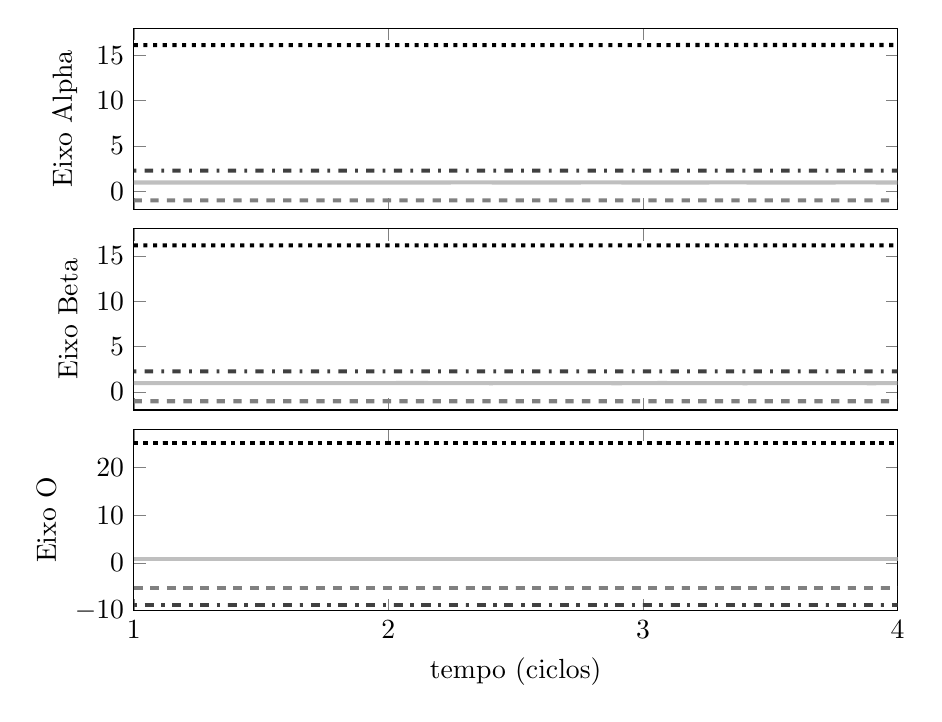
\begin{tikzpicture}

\begin{axis}[%
width=0.8\textwidth,
height=0.189701500343624\textwidth,
scale only axis,
xmin=0.316666666666667,
xmax=0.366666666666667,
xtick={0.316666666666667,0.333333333333333,0.35,0.366666666666667},
xticklabels={\empty},
ymin=-2,
ymax=18,
ytick={ 0,  5, 10, 15},
ylabel={Eixo Beta},
name=plot2,
scaled x ticks = false,
legend columns=-1,
legend style={/tikz/every even column/.append style={column sep=0.3cm}},
legend style={font=\footnotesize}
]
\addplot [color=lightgray,solid,line width=1.5pt,forget plot]
  table[row sep=crcr]{0.316658333333333	0.97043721996195\\
0.3167	0.970436358706691\\
0.316741666666667	0.970436358706691\\
0.316783333333333	0.970435592808439\\
0.316825	0.970435592808439\\
0.316866666666667	0.970434918056243\\
0.316908333333333	0.970434918056243\\
0.31695	0.970434330318112\\
0.316991666666667	0.970434330318112\\
0.317033333333333	0.970433825496951\\
0.317075	0.970433825496951\\
0.317116666666667	0.970433399492092\\
0.317158333333333	0.970433399492092\\
0.3172	0.970433048177814\\
0.317241666666667	0.970433048177814\\
0.317283333333333	0.970432767402266\\
0.317325	0.970432767402266\\
0.317366666666667	0.970432553004264\\
0.317408333333333	0.970432553004264\\
0.31745	0.970432400842131\\
0.317491666666667	0.970432400842131\\
0.317533333333333	0.970432306827843\\
0.317575	0.970432306827843\\
0.317616666666667	0.970432266960474\\
0.317658333333333	0.970432266960474\\
0.3177	0.970432277354792\\
0.317741666666667	0.970432277354792\\
0.317783333333333	0.970432334262824\\
0.317825	0.970432334262824\\
0.317866666666667	0.970432434088099\\
0.317908333333333	0.970432434088099\\
0.31795	0.970432573393534\\
0.317991666666667	0.970432573393534\\
0.318033333333333	0.970432748904596\\
0.318075	0.970432748904596\\
0.318116666666667	0.970432957509533\\
0.318158333333333	0.970432957509533\\
0.3182	0.970433196258189\\
0.318241666666667	0.970433196258189\\
0.318283333333333	0.970433462360463\\
0.318325	0.970433462360463\\
0.318366666666667	0.970433753184959\\
0.318408333333333	0.970433753184959\\
0.31845	0.970434066257974\\
0.318491666666667	0.970434066257974\\
0.318533333333333	0.970434399262647\\
0.318575	0.970434399262647\\
0.318616666666667	0.970434750037975\\
0.318658333333333	0.970434750037975\\
0.3187	0.970435116577406\\
0.318741666666667	0.970435116577406\\
0.318783333333333	0.97043549702676\\
0.318825	0.97043549702676\\
0.318866666666667	0.97043588968139\\
0.318908333333333	0.97043588968139\\
0.31895	0.970436292982595\\
0.318991666666667	0.970436292982595\\
0.319033333333333	0.970436705513386\\
0.319075	0.970436705513386\\
0.319116666666667	0.970437125993791\\
0.319158333333333	0.970437125993791\\
0.3192	0.970437553275866\\
0.319241666666667	0.970437553275866\\
0.319283333333333	0.970437986338605\\
0.319325	0.970437986338605\\
0.319366666666667	0.970438424282876\\
0.319408333333333	0.970438424282876\\
0.31945	0.970438866326497\\
0.319491666666667	0.970438866326497\\
0.319533333333333	0.97043931179951\\
0.319575	0.97043931179951\\
0.319616666666667	0.970439760139689\\
0.319658333333333	0.970439760139689\\
0.3197	0.970440210888314\\
0.319741666666667	0.970440210888314\\
0.319783333333333	0.970440663686211\\
0.319825	0.970440663686211\\
0.319866666666667	0.970441118270085\\
0.319908333333333	0.970441118270085\\
0.31995	0.970441574469177\\
0.319991666666667	0.970441574469177\\
0.320033333333333	0.970442032202265\\
0.320075	0.970442032202265\\
0.320116666666667	0.970442491475084\\
0.320158333333333	0.970442491475084\\
0.3202	0.970442952378189\\
0.320241666666667	0.970442952378189\\
0.320283333333333	0.970443415085359\\
0.320325	0.970443415085359\\
0.320366666666667	0.970443879852587\\
0.320408333333333	0.970443879852587\\
0.32045	0.970444347017744\\
0.320491666666667	0.970444347017744\\
0.320533333333333	0.970444817000997\\
0.320575	0.970444817000997\\
0.320616666666667	0.970445290306078\\
0.320658333333333	0.970445290306078\\
0.3207	0.970445767522508\\
0.320741666666667	0.970445767522508\\
0.320783333333333	0.970446249328905\\
0.320825	0.970446249328905\\
0.320866666666667	0.970446736497523\\
0.320908333333333	0.970446736497523\\
0.32095	0.970447229900211\\
0.320991666666667	0.970447229900211\\
0.321033333333333	0.970447730516016\\
0.321075	0.970447730516016\\
0.321116666666667	0.970448239440708\\
0.321158333333333	0.970448239440708\\
0.3212	0.970448757898565\\
0.321241666666667	0.970448757898565\\
0.321283333333333	0.970449287255117\\
0.321325	0.970449287255117\\
0.321366666666667	0.970449829034775\\
0.321408333333333	0.970449829034775\\
0.32145	0.970450384944168\\
0.321491666666667	0.970450384944168\\
0.321533333333333	0.970450956898191\\
0.321575	0.970450956898191\\
0.321616666666667	0.970451547051789\\
0.321658333333333	0.970451547051789\\
0.3217	0.970452157838907\\
0.321741666666667	0.970452157838907\\
0.321783333333333	0.970452792020252\\
0.321825	0.970452792020252\\
0.321866666666667	0.970453452742033\\
0.321908333333333	0.970453452742033\\
0.32195	0.970454143608473\\
0.321991666666667	0.970454143608473\\
0.322033333333333	0.970454868771685\\
0.322075	0.970454868771685\\
0.322116666666667	0.970455633043542\\
0.322158333333333	0.970455633043542\\
0.3222	0.970456442035388\\
0.322241666666667	0.970456442035388\\
0.322283333333333	0.970457302332857\\
0.322325	0.970457302332857\\
0.322366666666667	0.970458221714429\\
0.322408333333333	0.970458221714429\\
0.32245	0.97045920942283\\
0.322491666666667	0.97045920942283\\
0.322533333333333	0.97046027649605\\
0.322575	0.97046027649605\\
0.322616666666667	0.970461436154189\\
0.322658333333333	0.970461436154189\\
0.3227	0.970462704205603\\
0.322741666666667	0.970462704205603\\
0.322783333333333	0.970464099343308\\
0.322825	0.970464099343308\\
0.322866666666667	0.970465642944787\\
0.322908333333333	0.970465642944787\\
0.32295	0.970467357251532\\
0.322991666666667	0.970467357251532\\
0.323033333333333	0.970469258583928\\
0.323075	0.970469258583928\\
0.323116666666667	0.970471335019103\\
0.323158333333333	0.970471335019103\\
0.3232	0.970473348318116\\
0.323241666666667	0.970473348318116\\
0.323283333333333	0.970474626904486\\
0.323325	0.970474626904486\\
0.323366666666667	0.970474374243411\\
0.323408333333333	0.970474374243411\\
0.32345	0.970472573672318\\
0.323491666666667	0.970472573672318\\
0.323533333333333	0.970469948388625\\
0.323575	0.970469948388625\\
0.323616666666667	0.970467114613926\\
0.323658333333333	0.970467114613926\\
0.3237	0.970464337421047\\
0.323741666666667	0.970464337421047\\
0.323783333333333	0.970461683786388\\
0.323825	0.970461683786388\\
0.323866666666667	0.970459156489005\\
0.323908333333333	0.970459156489005\\
0.32395	0.970456747819866\\
0.323991666666667	0.970456747819866\\
0.324033333333333	0.970454453309765\\
0.324075	0.970454453309765\\
0.324116666666667	0.97045227287176\\
0.324158333333333	0.97045227287176\\
0.3242	0.970450209128296\\
0.324241666666667	0.970450209128296\\
0.324283333333333	0.970448265549337\\
0.324325	0.970448265549337\\
0.324366666666667	0.970446445042454\\
0.324408333333333	0.970446445042454\\
0.32445	0.970444749125981\\
0.324491666666667	0.970444749125981\\
0.324533333333333	0.970443177632723\\
0.324575	0.970443177632723\\
0.324616666666667	0.97044172880593\\
0.324658333333333	0.97044172880593\\
0.3247	0.97044039962421\\
0.324741666666667	0.97044039962421\\
0.324783333333333	0.970439186208874\\
0.324825	0.970439186208874\\
0.324866666666667	0.970438084206409\\
0.324908333333333	0.970438084206409\\
0.32495	0.970437089084224\\
0.324991666666667	0.970437089084224\\
0.325033333333333	0.970436196318331\\
0.325075	0.970436196318331\\
0.325116666666667	0.970435401481262\\
0.325158333333333	0.970435401481262\\
0.3252	0.970434700255544\\
0.325241666666667	0.970434700255544\\
0.325283333333333	0.970434088403698\\
0.325325	0.970434088403698\\
0.325366666666667	0.970433561723097\\
0.325408333333333	0.970433561723097\\
0.32545	0.970433116006485\\
0.325491666666667	0.970433116006485\\
0.325533333333333	0.970432747019942\\
0.325575	0.970432747019942\\
0.325616666666667	0.970432450501775\\
0.325658333333333	0.970432450501775\\
0.3257	0.970432222179772\\
0.325741666666667	0.970432222179772\\
0.325783333333333	0.970432057800854\\
0.325825	0.970432057800854\\
0.325866666666667	0.970431953166174\\
0.325908333333333	0.970431953166174\\
0.32595	0.970431904165525\\
0.325991666666667	0.970431904165525\\
0.326033333333333	0.970431906806762\\
0.326075	0.970431906806762\\
0.326116666666667	0.970431957238012\\
0.326158333333333	0.970431957238012\\
0.3262	0.970432051762366\\
0.326241666666667	0.970432051762366\\
0.326283333333333	0.970432186846018\\
0.326325	0.970432186846018\\
0.326366666666667	0.970432359121564\\
0.326408333333333	0.970432359121564\\
0.32645	0.97043256538827\\
0.326491666666667	0.97043256538827\\
0.326533333333333	0.970432802610885\\
0.326575	0.970432802610885\\
0.326616666666667	0.970433067918077\\
0.326658333333333	0.970433067918077\\
0.3267	0.970433358601067\\
0.326741666666667	0.970433358601067\\
0.326783333333333	0.970433672112601\\
0.326825	0.970433672112601\\
0.326866666666667	0.970434006066087\\
0.326908333333333	0.970434006066087\\
0.32695	0.970434358234596\\
0.326991666666667	0.970434358234596\\
0.327033333333333	0.970434726549414\\
0.327075	0.970434726549414\\
0.327116666666667	0.970435109097919\\
0.327158333333333	0.970435109097919\\
0.3272	0.970435504120658\\
0.327241666666667	0.970435504120658\\
0.327283333333333	0.970435910007656\\
0.327325	0.970435910007656\\
0.327366666666667	0.970436325294062\\
0.327408333333333	0.970436325294062\\
0.32745	0.970436748655303\\
0.327491666666667	0.970436748655303\\
0.327533333333333	0.970437178901951\\
0.327575	0.970437178901951\\
0.327616666666667	0.970437614974456\\
0.327658333333333	0.970437614974456\\
0.3277	0.970438055937924\\
0.327741666666667	0.970438055937924\\
0.327783333333333	0.970438500977014\\
0.327825	0.970438500977014\\
0.327866666666667	0.970438949391041\\
0.327908333333333	0.970438949391041\\
0.32795	0.970439400589312\\
0.327991666666667	0.970439400589312\\
0.328033333333333	0.970439854086724\\
0.328075	0.970439854086724\\
0.328116666666667	0.97044030949963\\
0.328158333333333	0.97044030949963\\
0.3282	0.970440766541997\\
0.328241666666667	0.970440766541997\\
0.328283333333333	0.970441225021877\\
0.328325	0.970441225021877\\
0.328366666666667	0.970441684838236\\
0.328408333333333	0.970441684838236\\
0.32845	0.970442145978184\\
0.328491666666667	0.970442145978184\\
0.328533333333333	0.970442608514653\\
0.328575	0.970442608514653\\
0.328616666666667	0.970443072604613\\
0.328658333333333	0.970443072604613\\
0.3287	0.970443538487861\\
0.328741666666667	0.970443538487861\\
0.328783333333333	0.970444006486495\\
0.328825	0.970444006486495\\
0.328866666666667	0.970444477005118\\
0.328908333333333	0.970444477005118\\
0.32895	0.970444950531897\\
0.328991666666667	0.970444950531897\\
0.329033333333333	0.970445427640563\\
0.329075	0.970445427640563\\
0.329116666666667	0.970445908993475\\
0.329158333333333	0.970445908993475\\
0.3292	0.970446395345909\\
0.329241666666667	0.970446395345909\\
0.329283333333333	0.970446887551736\\
0.329325	0.970446887551736\\
0.329366666666667	0.970447386570722\\
0.329408333333333	0.970447386570722\\
0.32945	0.970447893477714\\
0.329491666666667	0.970447893477714\\
0.329533333333333	0.970448409474047\\
0.329575	0.970448409474047\\
0.329616666666667	0.970448935899864\\
0.329658333333333	0.970448935899864\\
0.3297	0.970449474251262\\
0.329741666666667	0.970449474251262\\
0.329783333333333	0.970450026203047\\
0.329825	0.970450026203047\\
0.329866666666667	0.970450593634111\\
0.329908333333333	0.970450593634111\\
0.32995	0.970451178658432\\
0.329991666666667	0.970451178658432\\
0.330033333333333	0.970451783663083\\
0.330075	0.970451783663083\\
0.330116666666667	0.970452411354861\\
0.330158333333333	0.970452411354861\\
0.3302	0.970453064817657\\
0.330241666666667	0.970453064817657\\
0.330283333333333	0.97045374758329\\
0.330325	0.97045374758329\\
0.330366666666667	0.97045446371932\\
0.330408333333333	0.97045446371932\\
0.33045	0.970455217938359\\
0.330491666666667	0.970455217938359\\
0.330533333333333	0.970456015734584\\
0.330575	0.970456015734584\\
0.330616666666667	0.970456863554561\\
0.330658333333333	0.970456863554561\\
0.3307	0.970457769010778\\
0.330741666666667	0.970457769010778\\
0.330783333333333	0.970458741146766\\
0.330825	0.970458741146766\\
0.330866666666667	0.970459790760365\\
0.330908333333333	0.970459790760365\\
0.33095	0.970460930781311\\
0.330991666666667	0.970460930781311\\
0.331033333333333	0.970462176667188\\
0.331075	0.970462176667188\\
0.331116666666667	0.970463546691103\\
0.331158333333333	0.970463546691103\\
0.3312	0.970465061741802\\
0.331241666666667	0.970465061741802\\
0.331283333333333	0.970466743535177\\
0.331325	0.970466743535177\\
0.331366666666667	0.970468607961243\\
0.331408333333333	0.970468607961243\\
0.33145	0.970470643213183\\
0.331491666666667	0.970470643213183\\
0.331533333333333	0.970472615704777\\
0.331575	0.970472615704777\\
0.331616666666667	0.970473867713727\\
0.331658333333333	0.970473867713727\\
0.3317	0.970473619993488\\
0.331741666666667	0.970473619993488\\
0.331783333333333	0.970471857439701\\
0.331825	0.970471857439701\\
0.331866666666667	0.970469288642677\\
0.331908333333333	0.970469288642677\\
0.33195	0.970466516731413\\
0.331991666666667	0.970466516731413\\
0.332033333333333	0.970463800908304\\
0.332075	0.970463800908304\\
0.332116666666667	0.970461206531781\\
0.332158333333333	0.970461206531781\\
0.3322	0.970458736205245\\
0.332241666666667	0.970458736205245\\
0.332283333333333	0.970456382316685\\
0.332325	0.970456382316685\\
0.332366666666667	0.970454140450355\\
0.332408333333333	0.970454140450355\\
0.33245	0.97045201049146\\
0.332491666666667	0.97045201049146\\
0.332533333333333	0.970449994982174\\
0.332575	0.970449994982174\\
0.332616666666667	0.970448097296241\\
0.332658333333333	0.970448097296241\\
0.3327	0.970446320257846\\
0.332741666666667	0.970446320257846\\
0.332783333333333	0.970444665332178\\
0.332825	0.970444665332178\\
0.332866666666667	0.970443132335721\\
0.332908333333333	0.970443132335721\\
0.33295	0.970441719530581\\
0.332991666666667	0.970441719530581\\
0.333033333333333	0.970440423942802\\
0.333075	0.970440423942802\\
0.333116666666667	0.970439241761191\\
0.333158333333333	0.970439241761191\\
0.3332	0.970438168711639\\
0.333241666666667	0.970438168711639\\
0.333283333333333	0.970437200346429\\
0.333325	0.970437200346429\\
0.333366666666667	0.970436332227711\\
0.333408333333333	0.970436332227711\\
0.33345	0.970435560013326\\
0.333491666666667	0.970435560013326\\
0.333533333333333	0.971648858949127\\
0.333575	0.971648858949127\\
0.333616666666667	0.972551835611606\\
0.333658333333333	0.972551835611606\\
0.3337	0.973207764997182\\
0.333741666666667	0.973207764997182\\
0.333783333333333	0.973720077134853\\
0.333825	0.973720077134853\\
0.333866666666667	0.974138678563171\\
0.333908333333333	0.974138678563171\\
0.33395	0.97448861200456\\
0.333991666666667	0.97448861200456\\
0.334033333333333	0.974785425419367\\
0.334075	0.974785425419367\\
0.334116666666667	0.975038737431379\\
0.334158333333333	0.975038737431379\\
0.3342	0.975253422953218\\
0.334241666666667	0.975253422953218\\
0.334283333333333	0.975431090751057\\
0.334325	0.975431090751057\\
0.334366666666667	0.975571729224647\\
0.334408333333333	0.975571729224647\\
0.33445	0.975675085962529\\
0.334491666666667	0.975675085962529\\
0.334533333333333	0.975741568319722\\
0.334575	0.975741568319722\\
0.334616666666667	0.975772645258401\\
0.334658333333333	0.975772645258401\\
0.3347	0.975770841164928\\
0.334741666666667	0.975770841164928\\
0.334783333333333	0.975739462345535\\
0.334825	0.975739462345535\\
0.334866666666667	0.97568220308738\\
0.334908333333333	0.97568220308738\\
0.33495	0.975602754094434\\
0.334991666666667	0.975602754094434\\
0.335033333333333	0.975504495724003\\
0.335075	0.975504495724003\\
0.335116666666667	0.975390314683187\\
0.335158333333333	0.975390314683187\\
0.3352	0.97526254538269\\
0.335241666666667	0.97526254538269\\
0.335283333333333	0.975123011403737\\
0.335325	0.975123011403737\\
0.335366666666667	0.974973129879909\\
0.335408333333333	0.974973129879909\\
0.33545	0.974814040368281\\
0.335491666666667	0.974814040368281\\
0.335533333333333	0.974646726603347\\
0.335575	0.974646726603347\\
0.335616666666667	0.974472110514347\\
0.335658333333333	0.974472110514347\\
0.3357	0.974291109577703\\
0.335741666666667	0.974291109577703\\
0.335783333333333	0.974104658457263\\
0.335825	0.974104658457263\\
0.335866666666667	0.973913702574732\\
0.335908333333333	0.973913702574732\\
0.33595	0.973719174414939\\
0.335991666666667	0.973719174414939\\
0.336033333333333	0.9735219634573\\
0.336075	0.9735219634573\\
0.336116666666667	0.973322888548348\\
0.336158333333333	0.973322888548348\\
0.3362	0.973122678347426\\
0.336241666666667	0.973122678347426\\
0.336283333333333	0.972921962142289\\
0.336325	0.972921962142289\\
0.336366666666667	0.972721270540403\\
0.336408333333333	0.972721270540403\\
0.33645	0.972521043677767\\
0.336491666666667	0.972521043677767\\
0.336533333333333	0.97232164373873\\
0.336575	0.97232164373873\\
0.336616666666667	0.97212336861283\\
0.336658333333333	0.97212336861283\\
0.3367	0.971926464162576\\
0.336741666666667	0.971926464162576\\
0.336783333333333	0.971731133532888\\
0.336825	0.971731133532888\\
0.336866666666667	0.971537542921919\\
0.336908333333333	0.971537542921919\\
0.33695	0.971345824051992\\
0.336991666666667	0.971345824051992\\
0.337033333333333	0.971156074117405\\
0.337075	0.971156074117405\\
0.337116666666667	0.970968354218081\\
0.337158333333333	0.970968354218081\\
0.3372	0.970782687255614\\
0.337241666666667	0.970782687255614\\
0.337283333333333	0.970599056051596\\
0.337325	0.970599056051596\\
0.337366666666667	0.970417402139909\\
0.337408333333333	0.970417402139909\\
0.33745	0.970237625369066\\
0.337491666666667	0.970237625369066\\
0.337533333333333	0.970059584189185\\
0.337575	0.970059584189185\\
0.337616666666667	0.96988309632448\\
0.337658333333333	0.96988309632448\\
0.3377	0.969707939453289\\
0.337741666666667	0.969707939453289\\
0.337783333333333	0.969533851520112\\
0.337825	0.969533851520112\\
0.337866666666667	0.969360530361959\\
0.337908333333333	0.969360530361959\\
0.33795	0.96918763241424\\
0.337991666666667	0.96918763241424\\
0.338033333333333	0.969014770341763\\
0.338075	0.969014770341763\\
0.338116666666667	0.968841509704726\\
0.338158333333333	0.968841509704726\\
0.3382	0.968667364944703\\
0.338241666666667	0.968667364944703\\
0.338283333333333	0.968491792226096\\
0.338325	0.968491792226096\\
0.338366666666667	0.968314181869248\\
0.338408333333333	0.968314181869248\\
0.33845	0.968133849053945\\
0.338491666666667	0.968133849053945\\
0.338533333333333	0.967950022355481\\
0.338575	0.967950022355481\\
0.338616666666667	0.967761829596934\\
0.338658333333333	0.967761829596934\\
0.3387	0.967568280311102\\
0.338741666666667	0.967568280311102\\
0.338783333333333	0.967368243882625\\
0.338825	0.967368243882625\\
0.338866666666667	0.967160422188105\\
0.338908333333333	0.967160422188105\\
0.33895	0.966943315269325\\
0.338991666666667	0.966943315269325\\
0.339033333333333	0.966715178289778\\
0.339075	0.966715178289778\\
0.339116666666667	0.966473967838326\\
0.339158333333333	0.966473967838326\\
0.3392	0.966217275837303\\
0.339241666666667	0.966217275837303\\
0.339283333333333	0.965942250621072\\
0.339325	0.965942250621072\\
0.339366666666667	0.965645509068642\\
0.339408333333333	0.965645509068642\\
0.33945	0.965323055947907\\
0.339491666666667	0.965323055947907\\
0.339533333333333	0.964970260218407\\
0.339575	0.964970260218407\\
0.339616666666667	0.964582030813449\\
0.339658333333333	0.964582030813449\\
0.3397	0.964153600730688\\
0.339741666666667	0.964153600730688\\
0.339783333333333	0.963683141276039\\
0.339825	0.963683141276039\\
0.339866666666667	0.963180713548748\\
0.339908333333333	0.963180713548748\\
0.33995	0.962743221931403\\
0.339991666666667	0.962743221931403\\
0.340033333333333	0.962557941035935\\
0.340075	0.962557941035935\\
0.340116666666667	0.962763377463747\\
0.340158333333333	0.962763377463747\\
0.3402	0.963273642199086\\
0.340241666666667	0.963273642199086\\
0.340283333333333	0.963908110712242\\
0.340325	0.963908110712242\\
0.340366666666667	0.964554989557809\\
0.340408333333333	0.964554989557809\\
0.34045	0.965175580876337\\
0.340491666666667	0.965175580876337\\
0.340533333333333	0.965763532636179\\
0.340575	0.965763532636179\\
0.340616666666667	0.966321146142632\\
0.340658333333333	0.966321146142632\\
0.3407	0.966851430234263\\
0.340741666666667	0.966851430234263\\
0.340783333333333	0.967356394568855\\
0.340825	0.967356394568855\\
0.340866666666667	0.967837036696378\\
0.340908333333333	0.967837036696378\\
0.34095	0.968293661219689\\
0.340991666666667	0.968293661219689\\
0.341033333333333	0.968726209357149\\
0.341075	0.968726209357149\\
0.341116666666667	0.969134520970968\\
0.341158333333333	0.969134520970968\\
0.3412	0.969518508430739\\
0.341241666666667	0.969518508430739\\
0.341283333333333	0.969878245891628\\
0.341325	0.969878245891628\\
0.341366666666667	0.970213991385115\\
0.341408333333333	0.970213991385115\\
0.34145	0.970526164701536\\
0.341491666666667	0.970526164701536\\
0.341533333333333	0.97081530333607\\
0.341575	0.97081530333607\\
0.341616666666667	0.971082014269825\\
0.341658333333333	0.971082014269825\\
0.3417	0.971326933286298\\
0.341741666666667	0.971326933286298\\
0.341783333333333	0.971550697532474\\
0.341825	0.971550697532474\\
0.341866666666667	0.971753932167101\\
0.341908333333333	0.971753932167101\\
0.34195	0.9719372486824\\
0.341991666666667	0.9719372486824\\
0.342033333333333	0.972101250875096\\
0.342075	0.972101250875096\\
0.342116666666667	0.972246544205042\\
0.342158333333333	0.972246544205042\\
0.3422	0.972373744983395\\
0.342241666666667	0.972373744983395\\
0.342283333333333	0.972483487017517\\
0.342325	0.972483487017517\\
0.342366666666667	0.972576424611567\\
0.342408333333333	0.972576424611567\\
0.34245	0.972653231901819\\
0.342491666666667	0.972653231901819\\
0.342533333333333	0.972714599245227\\
0.342575	0.972714599245227\\
0.342616666666667	0.972761227744934\\
0.342658333333333	0.972761227744934\\
0.3427	0.97279382303673\\
0.342741666666667	0.97279382303673\\
0.342783333333333	0.972813089272279\\
0.342825	0.972813089272279\\
0.342866666666667	0.972819723927495\\
0.342908333333333	0.972819723927495\\
0.34295	0.972814413734991\\
0.342991666666667	0.972814413734991\\
0.343033333333333	0.972797831758329\\
0.343075	0.972797831758329\\
0.343116666666667	0.97277063543143\\
0.343158333333333	0.97277063543143\\
0.3432	0.972733465288513\\
0.343241666666667	0.972733465288513\\
0.343283333333333	0.972686944096195\\
0.343325	0.972686944096195\\
0.343366666666667	0.972631676145526\\
0.343408333333333	0.972631676145526\\
0.34345	0.972568246539458\\
0.343491666666667	0.972568246539458\\
0.343533333333333	0.972497220395148\\
0.343575	0.972497220395148\\
0.343616666666667	0.972419141952143\\
0.343658333333333	0.972419141952143\\
0.3437	0.972334533626447\\
0.343741666666667	0.972334533626447\\
0.343783333333333	0.972243895074241\\
0.343825	0.972243895074241\\
0.343866666666667	0.972147702330704\\
0.343908333333333	0.972147702330704\\
0.34395	0.972046407075359\\
0.343991666666667	0.972046407075359\\
0.344033333333333	0.971940436053389\\
0.344075	0.971940436053389\\
0.344116666666667	0.971830190659022\\
0.344158333333333	0.971830190659022\\
0.3442	0.971716046667481\\
0.344241666666667	0.971716046667481\\
0.344283333333333	0.971598354088828\\
0.344325	0.971598354088828\\
0.344366666666667	0.971477437110907\\
0.344408333333333	0.971477437110907\\
0.34445	0.971353594098613\\
0.344491666666667	0.971353594098613\\
0.344533333333333	0.97122709762098\\
0.344575	0.97122709762098\\
0.344616666666667	0.971098194483956\\
0.344658333333333	0.971098194483956\\
0.3447	0.970967105753223\\
0.344741666666667	0.970967105753223\\
0.344783333333333	0.97083402675669\\
0.344825	0.97083402675669\\
0.344866666666667	0.970699127059441\\
0.344908333333333	0.970699127059441\\
0.34495	0.970562550404825\\
0.344991666666667	0.970562550404825\\
0.345033333333333	0.970424414614293\\
0.345075	0.970424414614293\\
0.345116666666667	0.970284811435954\\
0.345158333333333	0.970284811435954\\
0.3452	0.970143806328325\\
0.345241666666667	0.970143806328325\\
0.345283333333333	0.970001438161806\\
0.345325	0.970001438161806\\
0.345366666666667	0.96985771881637\\
0.345408333333333	0.96985771881637\\
0.34545	0.969712632650021\\
0.345491666666667	0.969712632650021\\
0.345533333333333	0.969566135808537\\
0.345575	0.969566135808537\\
0.345616666666667	0.96941815534272\\
0.345658333333333	0.96941815534272\\
0.3457	0.96926858809443\\
0.345741666666667	0.96926858809443\\
0.345783333333333	0.969117299306608\\
0.345825	0.969117299306608\\
0.345866666666667	0.968964120904819\\
0.345908333333333	0.968964120904819\\
0.34595	0.968808849387983\\
0.345991666666667	0.968808849387983\\
0.346033333333333	0.968651243253345\\
0.346075	0.968651243253345\\
0.346116666666667	0.968491019864569\\
0.346158333333333	0.968491019864569\\
0.3462	0.968327851651247\\
0.346241666666667	0.968327851651247\\
0.346283333333333	0.968161361501957\\
0.346325	0.968161361501957\\
0.346366666666667	0.967991117179635\\
0.346408333333333	0.967991117179635\\
0.34645	0.967816625010012\\
0.346491666666667	0.967816625010012\\
0.346533333333333	0.967637322060543\\
0.346575	0.967637322060543\\
0.346616666666667	0.967452565308079\\
0.346658333333333	0.967452565308079\\
0.3467	0.967261619492175\\
0.346741666666667	0.967261619492175\\
0.346783333333333	0.967063642238294\\
0.346825	0.967063642238294\\
0.346866666666667	0.96685766572051\\
0.346908333333333	0.96685766572051\\
0.34695	0.966642574005765\\
0.346991666666667	0.966642574005765\\
0.347033333333333	0.966417074974842\\
0.347075	0.966417074974842\\
0.347116666666667	0.96617966541294\\
0.347158333333333	0.96617966541294\\
0.3472	0.965928587517468\\
0.347241666666667	0.965928587517468\\
0.347283333333333	0.965661774720542\\
0.347325	0.965661774720542\\
0.347366666666667	0.965376784497903\\
0.347408333333333	0.965376784497903\\
0.34745	0.965070716086806\\
0.347491666666667	0.965070716086806\\
0.347533333333333	0.964740112668365\\
0.347575	0.964740112668365\\
0.347616666666667	0.964380852893748\\
0.347658333333333	0.964380852893748\\
0.3477	0.963988051632603\\
0.347741666666667	0.963988051632603\\
0.347783333333333	0.963556030534422\\
0.347825	0.963556030534422\\
0.347866666666667	0.963078530534428\\
0.347908333333333	0.963078530534428\\
0.34795	0.962549655920968\\
0.347991666666667	0.962549655920968\\
0.348033333333333	0.9619670001309\\
0.348075	0.9619670001309\\
0.348116666666667	0.961341555134438\\
0.348158333333333	0.961341555134438\\
0.3482	0.960788377948118\\
0.348241666666667	0.960788377948118\\
0.348283333333333	0.960537072510808\\
0.348325	0.960537072510808\\
0.348366666666667	0.96077034870615\\
0.348408333333333	0.96077034870615\\
0.34845	0.961397599057846\\
0.348491666666667	0.961397599057846\\
0.348533333333333	0.962195102191525\\
0.348575	0.962195102191525\\
0.348616666666667	0.963016612349346\\
0.348658333333333	0.963016612349346\\
0.3487	0.963808716689139\\
0.348741666666667	0.963808716689139\\
0.348783333333333	0.964561247765427\\
0.348825	0.964561247765427\\
0.348866666666667	0.965276306971616\\
0.348908333333333	0.965276306971616\\
0.34895	0.965957395319728\\
0.348991666666667	0.965957395319728\\
0.349033333333333	0.966606924228981\\
0.349075	0.966606924228981\\
0.349116666666667	0.967226090899207\\
0.349158333333333	0.967226090899207\\
0.3492	0.967815243178363\\
0.349241666666667	0.967815243178363\\
0.349283333333333	0.968374279653504\\
0.349325	0.968374279653504\\
0.349366666666667	0.968902974216558\\
0.349408333333333	0.968902974216558\\
0.34945	0.969401194366304\\
0.349491666666667	0.969401194366304\\
0.349533333333333	0.969869014882489\\
0.349575	0.969869014882489\\
0.349616666666667	0.97030674708039\\
0.349658333333333	0.97030674708039\\
0.3497	0.97071491179284\\
0.349741666666667	0.97071491179284\\
0.349783333333333	0.971094183927962\\
0.349825	0.971094183927962\\
0.349866666666667	0.971445331102536\\
0.349908333333333	0.971445331102536\\
0.34995	0.971769161333504\\
0.349991666666667	0.971769161333504\\
0.350033333333333	0.972066487237209\\
0.350075	0.972066487237209\\
0.350116666666667	0.972338108007384\\
0.350158333333333	0.972338108007384\\
0.3502	0.972584806270275\\
0.350241666666667	0.972584806270275\\
0.350283333333333	0.9728073548172\\
0.350325	0.9728073548172\\
0.350366666666667	0.973006527860163\\
0.350408333333333	0.973006527860163\\
0.35045	0.97318311230518\\
0.350491666666667	0.97318311230518\\
0.350533333333333	0.973337916010511\\
0.350575	0.973337916010511\\
0.350616666666667	0.97347177159193\\
0.350658333333333	0.97347177159193\\
0.3507	0.973585535699788\\
0.350741666666667	0.973585535699788\\
0.350783333333333	0.973680084631658\\
0.350825	0.973680084631658\\
0.350866666666667	0.973756307614418\\
0.350908333333333	0.973756307614418\\
0.35095	0.973815099150894\\
0.350991666666667	0.973815099150894\\
0.351033333333333	0.973857351598739\\
0.351075	0.973857351598739\\
0.351116666666667	0.973883948769797\\
0.351158333333333	0.973883948769797\\
0.3512	0.973895760928848\\
0.351241666666667	0.973895760928848\\
0.351283333333333	0.973893641219893\\
0.351325	0.973893641219893\\
0.351366666666667	0.973878423304609\\
0.351408333333333	0.973878423304609\\
0.35145	0.973850919873737\\
0.351491666666667	0.973850919873737\\
0.351533333333333	0.973811921673314\\
0.351575	0.973811921673314\\
0.351616666666667	0.973762196743484\\
0.351658333333333	0.973762196743484\\
0.3517	0.973702489663175\\
0.351741666666667	0.973702489663175\\
0.351783333333333	0.973633520697664\\
0.351825	0.973633520697664\\
0.351866666666667	0.973555984834914\\
0.351908333333333	0.973555984834914\\
0.35195	0.973470550757728\\
0.351991666666667	0.973470550757728\\
0.352033333333333	0.973377859828882\\
0.352075	0.973377859828882\\
0.352116666666667	0.973278525169281\\
0.352158333333333	0.973278525169281\\
0.3522	0.973173130892697\\
0.352241666666667	0.973173130892697\\
0.352283333333333	0.973062231534188\\
0.352325	0.973062231534188\\
0.352366666666667	0.972946351681092\\
0.352408333333333	0.972946351681092\\
0.35245	0.972825985791745\\
0.352491666666667	0.972825985791745\\
0.352533333333333	0.972701598171142\\
0.352575	0.972701598171142\\
0.352616666666667	0.972573623065425\\
0.352658333333333	0.972573623065425\\
0.3527	0.972442464837294\\
0.352741666666667	0.972442464837294\\
0.352783333333333	0.972308498189818\\
0.352825	0.972308498189818\\
0.352866666666667	0.972172068414187\\
0.352908333333333	0.972172068414187\\
0.35295	0.972033491645237\\
0.352991666666667	0.972033491645237\\
0.353033333333333	0.971893055115423\\
0.353075	0.971893055115423\\
0.353116666666667	0.971751017402316\\
0.353158333333333	0.971751017402316\\
0.3532	0.971607608666504\\
0.353241666666667	0.971607608666504\\
0.353283333333333	0.971463030876194\\
0.353325	0.971463030876194\\
0.353366666666667	0.971317458012606\\
0.353408333333333	0.971317458012606\\
0.35345	0.971171036247034\\
0.353491666666667	0.971171036247034\\
0.353533333333333	0.971023884076982\\
0.353575	0.971023884076982\\
0.353616666666667	0.970876092405433\\
0.353658333333333	0.970876092405433\\
0.3537	0.970727724544334\\
0.353741666666667	0.970727724544334\\
0.353783333333333	0.97057881612078\\
0.353825	0.97057881612078\\
0.353866666666667	0.970429374861899\\
0.353908333333333	0.970429374861899\\
0.35395	0.970279380231812\\
0.353991666666667	0.970279380231812\\
0.354033333333333	0.970128782890901\\
0.354075	0.970128782890901\\
0.354116666666667	0.969977503943473\\
0.354158333333333	0.969977503943473\\
0.3542	0.969825433934529\\
0.354241666666667	0.969825433934529\\
0.354283333333333	0.969672431549141\\
0.354325	0.969672431549141\\
0.354366666666667	0.969518321958733\\
0.354408333333333	0.969518321958733\\
0.35445	0.969362894746629\\
0.354491666666667	0.969362894746629\\
0.354533333333333	0.969205901330155\\
0.354575	0.969205901330155\\
0.354616666666667	0.969047051777471\\
0.354658333333333	0.969047051777471\\
0.3547	0.968886010893059\\
0.354741666666667	0.968886010893059\\
0.354783333333333	0.968722393858097\\
0.354825	0.968722393858097\\
0.354866666666667	0.968555760623468\\
0.354908333333333	0.968555760623468\\
0.35495	0.968385607996405\\
0.354991666666667	0.968385607996405\\
0.355033333333333	0.968211360874338\\
0.355075	0.968211360874338\\
0.355116666666667	0.968032361469167\\
0.355158333333333	0.968032361469167\\
0.3552	0.967847855985232\\
0.355241666666667	0.967847855985232\\
0.355283333333333	0.967656978131575\\
0.355325	0.967656978131575\\
0.355366666666667	0.967458728665083\\
0.355408333333333	0.967458728665083\\
0.35545	0.967251949932161\\
0.355491666666667	0.967251949932161\\
0.355533333333333	0.967035294105211\\
0.355575	0.967035294105211\\
0.355616666666667	0.96680718350692\\
0.355658333333333	0.96680718350692\\
0.3557	0.966565761135913\\
0.355741666666667	0.966565761135913\\
0.355783333333333	0.966308829418209\\
0.355825	0.966308829418209\\
0.355866666666667	0.966033775751284\\
0.355908333333333	0.966033775751284\\
0.35595	0.965737485713522\\
0.355991666666667	0.965737485713522\\
0.356033333333333	0.965416251796768\\
0.356075	0.965416251796768\\
0.356116666666667	0.965065704871728\\
0.356158333333333	0.965065704871728\\
0.3562	0.964680848419151\\
0.356241666666667	0.964680848419151\\
0.356283333333333	0.96425642304089\\
0.356325	0.96425642304089\\
0.356366666666667	0.963788261022256\\
0.356408333333333	0.963788261022256\\
0.35645	0.963277649960367\\
0.356491666666667	0.963277649960367\\
0.356533333333333	0.962763374230932\\
0.356575	0.962763374230932\\
0.356616666666667	0.962386936828408\\
0.356658333333333	0.962386936828408\\
0.3567	0.96235156115393\\
0.356741666666667	0.96235156115393\\
0.356783333333333	0.962715132011066\\
0.356825	0.962715132011066\\
0.356866666666667	0.963320666260635\\
0.356908333333333	0.963320666260635\\
0.35695	0.963998138576959\\
0.356991666666667	0.963998138576959\\
0.357033333333333	0.964665369956402\\
0.357075	0.964665369956402\\
0.357116666666667	0.965299729822868\\
0.357158333333333	0.965299729822868\\
0.3572	0.965900114563002\\
0.357241666666667	0.965900114563002\\
0.357283333333333	0.966469816180699\\
0.357325	0.966469816180699\\
0.357366666666667	0.967011694173664\\
0.357408333333333	0.967011694173664\\
0.35745	0.967527444440113\\
0.357491666666667	0.967527444440113\\
0.357533333333333	0.968017823220618\\
0.357575	0.968017823220618\\
0.357616666666667	0.96848300778086\\
0.357658333333333	0.96848300778086\\
0.3577	0.968922916499335\\
0.357741666666667	0.968922916499335\\
0.357783333333333	0.969337444550679\\
0.357825	0.969337444550679\\
0.357866666666667	0.969726606878782\\
0.357908333333333	0.969726606878782\\
0.35795	0.97009059938096\\
0.357991666666667	0.97009059938096\\
0.358033333333333	0.970429799818908\\
0.358075	0.970429799818908\\
0.358116666666667	0.970744732776209\\
0.358158333333333	0.970744732776209\\
0.3582	0.971036020267481\\
0.358241666666667	0.971036020267481\\
0.358283333333333	0.971304333952506\\
0.358325	0.971304333952506\\
0.358366666666667	0.971550358425975\\
0.358408333333333	0.971550358425975\\
0.35845	0.971774769198906\\
0.358491666666667	0.971774769198906\\
0.358533333333333	0.971978224592428\\
0.358575	0.971978224592428\\
0.358616666666667	0.972161368117132\\
0.358658333333333	0.972161368117132\\
0.3587	0.97232483689012\\
0.358741666666667	0.97232483689012\\
0.358783333333333	0.972469271872084\\
0.358825	0.972469271872084\\
0.358866666666667	0.97259532671032\\
0.358908333333333	0.97259532671032\\
0.35895	0.972703673290413\\
0.358991666666667	0.972703673290413\\
0.359033333333333	0.972795003365617\\
0.359075	0.972795003365617\\
0.359116666666667	0.972870026617054\\
0.359158333333333	0.972870026617054\\
0.3592	0.972929466099244\\
0.359241666666667	0.972929466099244\\
0.359283333333333	0.972974052250993\\
0.359325	0.972974052250993\\
0.359366666666667	0.973004516578431\\
0.359408333333333	0.973004516578431\\
0.35945	0.973021585854869\\
0.359491666666667	0.973021585854869\\
0.359533333333333	0.973025977342107\\
0.359575	0.973025977342107\\
0.359616666666667	0.973018395210054\\
0.359658333333333	0.973018395210054\\
0.3597	0.972999528075137\\
0.359741666666667	0.972999528075137\\
0.359783333333333	0.972970047419237\\
0.359825	0.972970047419237\\
0.359866666666667	0.972930606589042\\
0.359908333333333	0.972930606589042\\
0.35995	0.972881840091521\\
0.359991666666667	0.972881840091521\\
0.360033333333333	0.97282436296652\\
0.360075	0.97282436296652\\
0.360116666666667	0.972758770103699\\
0.360158333333333	0.972758770103699\\
0.3602	0.972685635454403\\
0.360241666666667	0.972685635454403\\
0.360283333333333	0.97260551115411\\
0.360325	0.97260551115411\\
0.360366666666667	0.972518926610653\\
0.360408333333333	0.972518926610653\\
0.36045	0.97242638762769\\
0.360491666666667	0.97242638762769\\
0.360533333333333	0.97232837562682\\
0.360575	0.97232837562682\\
0.360616666666667	0.972225347012884\\
0.360658333333333	0.972225347012884\\
0.3607	0.972117732702924\\
0.360741666666667	0.972117732702924\\
0.360783333333333	0.972005937816376\\
0.360825	0.972005937816376\\
0.360866666666667	0.971890341506481\\
0.360908333333333	0.971890341506481\\
0.36095	0.971771296902463\\
0.360991666666667	0.971771296902463\\
0.361033333333333	0.971649131128654\\
0.361075	0.971649131128654\\
0.361116666666667	0.971524145368953\\
0.361158333333333	0.971524145368953\\
0.3612	0.971396614950672\\
0.361241666666667	0.971396614950672\\
0.361283333333333	0.971266789428732\\
0.361325	0.971266789428732\\
0.361366666666667	0.971134892657594\\
0.361408333333333	0.971134892657594\\
0.36145	0.971001122842976\\
0.361491666666667	0.971001122842976\\
0.361533333333333	0.970865652567805\\
0.361575	0.970865652567805\\
0.361616666666667	0.970728628787039\\
0.361658333333333	0.970728628787039\\
0.3617	0.970590172784328\\
0.361741666666667	0.970590172784328\\
0.361783333333333	0.970450380080569\\
0.361825	0.970450380080569\\
0.361866666666667	0.97030932028084\\
0.361908333333333	0.97030932028084\\
0.36195	0.970167036842429\\
0.361991666666667	0.970167036842429\\
0.362033333333333	0.970023546742998\\
0.362075	0.970023546742998\\
0.362116666666667	0.969878840024364\\
0.362158333333333	0.969878840024364\\
0.3622	0.969732879183796\\
0.362241666666667	0.969732879183796\\
0.362283333333333	0.9695855983809\\
0.362325	0.9695855983809\\
0.362366666666667	0.969436902423623\\
0.362408333333333	0.969436902423623\\
0.36245	0.969286665491246\\
0.362491666666667	0.969286665491246\\
0.362533333333333	0.969134729545048\\
0.362575	0.969134729545048\\
0.362616666666667	0.968980902367977\\
0.362658333333333	0.968980902367977\\
0.3627	0.968824955162702\\
0.362741666666667	0.968824955162702\\
0.362783333333333	0.968666619622136\\
0.362825	0.968666619622136\\
0.362866666666667	0.968505584367057\\
0.362908333333333	0.968505584367057\\
0.36295	0.968341490620739\\
0.362991666666667	0.968341490620739\\
0.363033333333333	0.968173926959096\\
0.363075	0.968173926959096\\
0.363116666666667	0.968002423385433\\
0.363158333333333	0.968002423385433\\
0.3632	0.967826443971447\\
0.363241666666667	0.967826443971447\\
0.363283333333333	0.967645376623545\\
0.363325	0.967645376623545\\
0.363366666666667	0.967458521637732\\
0.363408333333333	0.967458521637732\\
0.36345	0.967265077678393\\
0.363491666666667	0.967265077678393\\
0.363533333333333	0.967064124487711\\
0.363575	0.967064124487711\\
0.363616666666667	0.966854601516975\\
0.363658333333333	0.966854601516975\\
0.3637	0.966635281434992\\
0.363741666666667	0.966635281434992\\
0.363783333333333	0.966404737177826\\
0.363825	0.966404737177826\\
0.363866666666667	0.966161300867453\\
0.363908333333333	0.966161300867453\\
0.36395	0.965903012573484\\
0.363991666666667	0.965903012573484\\
0.364033333333333	0.965627556628981\\
0.364075	0.965627556628981\\
0.364116666666667	0.965332183337286\\
0.364158333333333	0.965332183337286\\
0.3642	0.965013615196673\\
0.364241666666667	0.965013615196673\\
0.364283333333333	0.96466794120584\\
0.364325	0.96466794120584\\
0.364366666666667	0.964290515533544\\
0.364408333333333	0.964290515533544\\
0.36445	0.963875911576807\\
0.364491666666667	0.963875911576807\\
0.364533333333333	0.963418077664188\\
0.364575	0.963418077664188\\
0.364616666666667	0.962911110870839\\
0.364658333333333	0.962911110870839\\
0.3647	0.96235187796569\\
0.364741666666667	0.96235187796569\\
0.364783333333333	0.961748355884677\\
0.364825	0.961748355884677\\
0.364866666666667	0.961194951845608\\
0.364908333333333	0.961194951845608\\
0.36495	0.960903389818248\\
0.364991666666667	0.960903389818248\\
0.365033333333333	0.96107189811835\\
0.365075	0.96107189811835\\
0.365116666666667	0.961645170240042\\
0.365158333333333	0.961645170240042\\
0.3652	0.962406472134593\\
0.365241666666667	0.962406472134593\\
0.365283333333333	0.96320043249184\\
0.365325	0.96320043249184\\
0.365366666666667	0.963967323367557\\
0.365408333333333	0.963967323367557\\
0.36545	0.96469505714666\\
0.365491666666667	0.96469505714666\\
0.365533333333333	0.965385567313351\\
0.365575	0.965385567313351\\
0.365616666666667	0.966042548039414\\
0.365658333333333	0.966042548039414\\
0.3657	0.966668609571715\\
0.365741666666667	0.966668609571715\\
0.365783333333333	0.967265111022754\\
0.365825	0.967265111022754\\
0.365866666666667	0.967832526770692\\
0.365908333333333	0.967832526770692\\
0.36595	0.968370847509121\\
0.365991666666667	0.968370847509121\\
0.366033333333333	0.968879906874164\\
0.366075	0.968879906874164\\
0.366116666666667	0.969359604600825\\
0.366158333333333	0.969359604600825\\
0.3662	0.969810026723854\\
0.366241666666667	0.969810026723854\\
0.366283333333333	0.970231481454978\\
0.366325	0.970231481454978\\
0.366366666666667	0.97062447778232\\
0.366408333333333	0.97062447778232\\
0.36645	0.970989674101551\\
0.366491666666667	0.970989674101551\\
0.366533333333333	0.971327819292325\\
0.366575	0.971327819292325\\
0.366616666666667	0.971639701449905\\
0.366658333333333	0.971639701449905\\
};
\addplot [color=gray,dashed,line width=1.5pt,forget plot]
  table[row sep=crcr]{0.316658333333333	-1.02797931894004\\
0.3167	-1.0279793224329\\
0.316741666666667	-1.0279793224329\\
0.316783333333333	-1.02797932543233\\
0.316825	-1.02797932543233\\
0.316866666666667	-1.02797932798806\\
0.316908333333333	-1.02797932798806\\
0.31695	-1.02797933014413\\
0.316991666666667	-1.02797933014413\\
0.317033333333333	-1.02797933193992\\
0.317075	-1.02797933193992\\
0.317116666666667	-1.02797933341104\\
0.317158333333333	-1.02797933341104\\
0.3172	-1.02797933458991\\
0.317241666666667	-1.02797933458991\\
0.317283333333333	-1.02797933550621\\
0.317325	-1.02797933550621\\
0.317366666666667	-1.02797933618718\\
0.317408333333333	-1.02797933618718\\
0.31745	-1.02797933665787\\
0.317491666666667	-1.02797933665787\\
0.317533333333333	-1.02797933694126\\
0.317575	-1.02797933694126\\
0.317616666666667	-1.02797933705843\\
0.317658333333333	-1.02797933705843\\
0.3177	-1.02797933702864\\
0.317741666666667	-1.02797933702864\\
0.317783333333333	-1.02797933686946\\
0.317825	-1.02797933686946\\
0.317866666666667	-1.02797933659693\\
0.317908333333333	-1.02797933659693\\
0.31795	-1.02797933622564\\
0.317991666666667	-1.02797933622564\\
0.318033333333333	-1.02797933576886\\
0.318075	-1.02797933576886\\
0.318116666666667	-1.02797933523867\\
0.318158333333333	-1.02797933523867\\
0.3182	-1.02797933464602\\
0.318241666666667	-1.02797933464602\\
0.318283333333333	-1.02797933400088\\
0.318325	-1.02797933400088\\
0.318366666666667	-1.02797933331226\\
0.318408333333333	-1.02797933331226\\
0.31845	-1.02797933258833\\
0.318491666666667	-1.02797933258833\\
0.318533333333333	-1.02797933183645\\
0.318575	-1.02797933183645\\
0.318616666666667	-1.02797933106326\\
0.318658333333333	-1.02797933106326\\
0.3187	-1.02797933027471\\
0.318741666666667	-1.02797933027471\\
0.318783333333333	-1.02797932947612\\
0.318825	-1.02797932947612\\
0.318866666666667	-1.02797932867225\\
0.318908333333333	-1.02797932867225\\
0.31895	-1.0279793278673\\
0.318991666666667	-1.0279793278673\\
0.319033333333333	-1.02797932706501\\
0.319075	-1.02797932706501\\
0.319116666666667	-1.02797932626865\\
0.319158333333333	-1.02797932626865\\
0.3192	-1.02797932548113\\
0.319241666666667	-1.02797932548113\\
0.319283333333333	-1.02797932470497\\
0.319325	-1.02797932470497\\
0.319366666666667	-1.02797932394236\\
0.319408333333333	-1.02797932394236\\
0.31945	-1.02797932319524\\
0.319491666666667	-1.02797932319524\\
0.319533333333333	-1.02797932246525\\
0.319575	-1.02797932246525\\
0.319616666666667	-1.02797932175383\\
0.319658333333333	-1.02797932175383\\
0.3197	-1.02797932106223\\
0.319741666666667	-1.02797932106223\\
0.319783333333333	-1.02797932039152\\
0.319825	-1.02797932039152\\
0.319866666666667	-1.02797931974265\\
0.319908333333333	-1.02797931974265\\
0.31995	-1.02797931911644\\
0.319991666666667	-1.02797931911644\\
0.320033333333333	-1.02797931851366\\
0.320075	-1.02797931851366\\
0.320116666666667	-1.02797931793501\\
0.320158333333333	-1.02797931793501\\
0.3202	-1.02797931738115\\
0.320241666666667	-1.02797931738115\\
0.320283333333333	-1.02797931685278\\
0.320325	-1.02797931685278\\
0.320366666666667	-1.0279793163506\\
0.320408333333333	-1.0279793163506\\
0.32045	-1.0279793158754\\
0.320491666666667	-1.0279793158754\\
0.320533333333333	-1.02797931542806\\
0.320575	-1.02797931542806\\
0.320616666666667	-1.02797931500959\\
0.320658333333333	-1.02797931500959\\
0.3207	-1.02797931462121\\
0.320741666666667	-1.02797931462121\\
0.320783333333333	-1.02797931426436\\
0.320825	-1.02797931426436\\
0.320866666666667	-1.02797931394075\\
0.320908333333333	-1.02797931394075\\
0.32095	-1.02797931365249\\
0.320991666666667	-1.02797931365249\\
0.321033333333333	-1.02797931340209\\
0.321075	-1.02797931340209\\
0.321116666666667	-1.02797931319261\\
0.321158333333333	-1.02797931319261\\
0.3212	-1.02797931302779\\
0.321241666666667	-1.02797931302779\\
0.321283333333333	-1.02797931291213\\
0.321325	-1.02797931291213\\
0.321366666666667	-1.02797931285116\\
0.321408333333333	-1.02797931285116\\
0.32145	-1.02797931285162\\
0.321491666666667	-1.02797931285162\\
0.321533333333333	-1.02797931292176\\
0.321575	-1.02797931292176\\
0.321616666666667	-1.02797931307177\\
0.321658333333333	-1.02797931307177\\
0.3217	-1.02797931331421\\
0.321741666666667	-1.02797931331421\\
0.321783333333333	-1.02797931366474\\
0.321825	-1.02797931366474\\
0.321866666666667	-1.02797931414296\\
0.321908333333333	-1.02797931414296\\
0.32195	-1.02797931477364\\
0.321991666666667	-1.02797931477364\\
0.322033333333333	-1.02797931558829\\
0.322075	-1.02797931558829\\
0.322116666666667	-1.02797931662754\\
0.322158333333333	-1.02797931662754\\
0.3222	-1.02797931794426\\
0.322241666666667	-1.02797931794426\\
0.322283333333333	-1.02797931960831\\
0.322325	-1.02797931960831\\
0.322366666666667	-1.02797932171334\\
0.322408333333333	-1.02797932171334\\
0.32245	-1.02797932438721\\
0.322491666666667	-1.02797932438721\\
0.322533333333333	-1.02797932780807\\
0.322575	-1.02797932780807\\
0.322616666666667	-1.02797933223008\\
0.322658333333333	-1.02797933223008\\
0.3227	-1.02797933802607\\
0.322741666666667	-1.02797933802607\\
0.322783333333333	-1.0279793457613\\
0.322825	-1.0279793457613\\
0.322866666666667	-1.02797935632699\\
0.322908333333333	-1.02797935632699\\
0.32295	-1.02797937119702\\
0.322991666666667	-1.02797937119702\\
0.323033333333333	-1.02797939295577\\
0.323075	-1.02797939295577\\
0.323116666666667	-1.02797942647672\\
0.323158333333333	-1.02797942647672\\
0.3232	-1.02797947861476\\
0.323241666666667	-1.02797947861476\\
0.323283333333333	-1.02797955338093\\
0.323325	-1.02797955338093\\
0.323366666666667	-1.02797964239201\\
0.323408333333333	-1.02797964239201\\
0.32345	-1.02797972650636\\
0.323491666666667	-1.02797972650636\\
0.323533333333333	-1.02797979421719\\
0.323575	-1.02797979421719\\
0.323616666666667	-1.0279798456655\\
0.323658333333333	-1.0279798456655\\
0.3237	-1.02797988508432\\
0.323741666666667	-1.02797988508432\\
0.323783333333333	-1.02797991630424\\
0.323825	-1.02797991630424\\
0.323866666666667	-1.02797994188271\\
0.323908333333333	-1.02797994188271\\
0.32395	-1.02797996339721\\
0.323991666666667	-1.02797996339721\\
0.324033333333333	-1.02797998182432\\
0.324075	-1.02797998182432\\
0.324116666666667	-1.02797999779181\\
0.324158333333333	-1.02797999779181\\
0.3242	-1.0279800117247\\
0.324241666666667	-1.0279800117247\\
0.324283333333333	-1.02798002392824\\
0.324325	-1.02798002392824\\
0.324366666666667	-1.02798003463532\\
0.324408333333333	-1.02798003463532\\
0.32445	-1.0279800440334\\
0.324491666666667	-1.0279800440334\\
0.324533333333333	-1.02798005227943\\
0.324575	-1.02798005227943\\
0.324616666666667	-1.02798005950815\\
0.324658333333333	-1.02798005950815\\
0.3247	-1.02798006583651\\
0.324741666666667	-1.02798006583651\\
0.324783333333333	-1.02798007136634\\
0.324825	-1.02798007136634\\
0.324866666666667	-1.02798007618623\\
0.324908333333333	-1.02798007618623\\
0.32495	-1.02798008037312\\
0.324991666666667	-1.02798008037312\\
0.325033333333333	-1.02798008399383\\
0.325075	-1.02798008399383\\
0.325116666666667	-1.02798008710665\\
0.325158333333333	-1.02798008710665\\
0.3252	-1.02798008976269\\
0.325241666666667	-1.02798008976269\\
0.325283333333333	-1.02798009200725\\
0.325325	-1.02798009200725\\
0.325366666666667	-1.02798009388083\\
0.325408333333333	-1.02798009388083\\
0.32545	-1.02798009542004\\
0.325491666666667	-1.02798009542004\\
0.325533333333333	-1.02798009665823\\
0.325575	-1.02798009665823\\
0.325616666666667	-1.02798009762591\\
0.325658333333333	-1.02798009762591\\
0.3257	-1.02798009835112\\
0.325741666666667	-1.02798009835112\\
0.325783333333333	-1.0279800988596\\
0.325825	-1.0279800988596\\
0.325866666666667	-1.02798009917502\\
0.325908333333333	-1.02798009917502\\
0.32595	-1.02798009931903\\
0.325991666666667	-1.02798009931903\\
0.326033333333333	-1.02798009931146\\
0.326075	-1.02798009931146\\
0.326116666666667	-1.02798009917039\\
0.326158333333333	-1.02798009917039\\
0.3262	-1.02798009891234\\
0.326241666666667	-1.02798009891234\\
0.326283333333333	-1.02798009855229\\
0.326325	-1.02798009855229\\
0.326366666666667	-1.02798009810393\\
0.326408333333333	-1.02798009810393\\
0.32645	-1.02798009757968\\
0.326491666666667	-1.02798009757968\\
0.326533333333333	-1.02798009699082\\
0.326575	-1.02798009699082\\
0.326616666666667	-1.02798009634759\\
0.326658333333333	-1.02798009634759\\
0.3267	-1.02798009565931\\
0.326741666666667	-1.02798009565931\\
0.326783333333333	-1.02798009493435\\
0.326825	-1.02798009493435\\
0.326866666666667	-1.02798009418033\\
0.326908333333333	-1.02798009418033\\
0.32695	-1.02798009340406\\
0.326991666666667	-1.02798009340406\\
0.327033333333333	-1.02798009261169\\
0.327075	-1.02798009261169\\
0.327116666666667	-1.02798009180869\\
0.327158333333333	-1.02798009180869\\
0.3272	-1.02798009099997\\
0.327241666666667	-1.02798009099997\\
0.327283333333333	-1.02798009018985\\
0.327325	-1.02798009018985\\
0.327366666666667	-1.02798008938219\\
0.327408333333333	-1.02798008938219\\
0.32745	-1.02798008858038\\
0.327491666666667	-1.02798008858038\\
0.327533333333333	-1.02798008778739\\
0.327575	-1.02798008778739\\
0.327616666666667	-1.02798008700583\\
0.327658333333333	-1.02798008700583\\
0.3277	-1.02798008623796\\
0.327741666666667	-1.02798008623796\\
0.327783333333333	-1.02798008548577\\
0.327825	-1.02798008548577\\
0.327866666666667	-1.02798008475096\\
0.327908333333333	-1.02798008475096\\
0.32795	-1.027980084035\\
0.327991666666667	-1.027980084035\\
0.328033333333333	-1.02798008333918\\
0.328075	-1.02798008333918\\
0.328116666666667	-1.02798008266459\\
0.328158333333333	-1.02798008266459\\
0.3282	-1.0279800820122\\
0.328241666666667	-1.0279800820122\\
0.328283333333333	-1.02798008138287\\
0.328325	-1.02798008138287\\
0.328366666666667	-1.02798008077734\\
0.328408333333333	-1.02798008077734\\
0.32845	-1.02798008019633\\
0.328491666666667	-1.02798008019633\\
0.328533333333333	-1.02798007964051\\
0.328575	-1.02798007964051\\
0.328616666666667	-1.02798007911055\\
0.328658333333333	-1.02798007911055\\
0.3287	-1.02798007860716\\
0.328741666666667	-1.02798007860716\\
0.328783333333333	-1.02798007813111\\
0.328825	-1.02798007813111\\
0.328866666666667	-1.02798007768325\\
0.328908333333333	-1.02798007768325\\
0.32895	-1.02798007726459\\
0.328991666666667	-1.02798007726459\\
0.329033333333333	-1.02798007687629\\
0.329075	-1.02798007687629\\
0.329116666666667	-1.02798007651977\\
0.329158333333333	-1.02798007651977\\
0.3292	-1.0279800761967\\
0.329241666666667	-1.0279800761967\\
0.329283333333333	-1.02798007590913\\
0.329325	-1.02798007590913\\
0.329366666666667	-1.02798007565953\\
0.329408333333333	-1.02798007565953\\
0.32945	-1.02798007545088\\
0.329491666666667	-1.02798007545088\\
0.329533333333333	-1.02798007528684\\
0.329575	-1.02798007528684\\
0.329616666666667	-1.02798007517182\\
0.329658333333333	-1.02798007517182\\
0.3297	-1.02798007511123\\
0.329741666666667	-1.02798007511123\\
0.329783333333333	-1.02798007511168\\
0.329825	-1.02798007511168\\
0.329866666666667	-1.02798007518127\\
0.329908333333333	-1.02798007518127\\
0.32995	-1.02798007532997\\
0.329991666666667	-1.02798007532997\\
0.330033333333333	-1.02798007557012\\
0.330075	-1.02798007557012\\
0.330116666666667	-1.02798007591707\\
0.330158333333333	-1.02798007591707\\
0.3302	-1.02798007639004\\
0.330241666666667	-1.02798007639004\\
0.330283333333333	-1.02798007701332\\
0.330325	-1.02798007701332\\
0.330366666666667	-1.02798007781784\\
0.330408333333333	-1.02798007781784\\
0.33045	-1.02798007884343\\
0.330491666666667	-1.02798007884343\\
0.330533333333333	-1.02798008014195\\
0.330575	-1.02798008014195\\
0.330616666666667	-1.02798008178188\\
0.330658333333333	-1.02798008178188\\
0.3307	-1.02798008385506\\
0.330741666666667	-1.02798008385506\\
0.330783333333333	-1.02798008648682\\
0.330825	-1.02798008648682\\
0.330866666666667	-1.02798008985177\\
0.330908333333333	-1.02798008985177\\
0.33095	-1.02798009419898\\
0.330991666666667	-1.02798009419898\\
0.331033333333333	-1.02798009989381\\
0.331075	-1.02798009989381\\
0.331116666666667	-1.02798010749001\\
0.331158333333333	-1.02798010749001\\
0.3312	-1.02798011786062\\
0.331241666666667	-1.02798011786062\\
0.331283333333333	-1.02798013244924\\
0.331325	-1.02798013244924\\
0.331366666666667	-1.02798015378674\\
0.331408333333333	-1.02798015378674\\
0.33145	-1.0279801866452\\
0.331491666666667	-1.0279801866452\\
0.331533333333333	-1.0279802377321\\
0.331575	-1.0279802377321\\
0.331616666666667	-1.02798031096181\\
0.331658333333333	-1.02798031096181\\
0.3317	-1.02798039810961\\
0.331741666666667	-1.02798039810961\\
0.331783333333333	-1.02798048043308\\
0.331825	-1.02798048043308\\
0.331866666666667	-1.0279805466806\\
0.331908333333333	-1.0279805466806\\
0.33195	-1.02798059700244\\
0.331991666666667	-1.02798059700244\\
0.332033333333333	-1.02798063554826\\
0.332075	-1.02798063554826\\
0.332116666666667	-1.02798066606976\\
0.332158333333333	-1.02798066606976\\
0.3322	-1.02798069107079\\
0.332241666666667	-1.02798069107079\\
0.332283333333333	-1.02798071209536\\
0.332325	-1.02798071209536\\
0.332366666666667	-1.02798073009922\\
0.332408333333333	-1.02798073009922\\
0.33245	-1.02798074569669\\
0.332491666666667	-1.02798074569669\\
0.332533333333333	-1.02798075930363\\
0.332575	-1.02798075930363\\
0.332616666666667	-1.02798077121877\\
0.332658333333333	-1.02798077121877\\
0.3327	-1.02798078167001\\
0.332741666666667	-1.02798078167001\\
0.332783333333333	-1.02798079084076\\
0.332825	-1.02798079084076\\
0.332866666666667	-1.02798079888465\\
0.332908333333333	-1.02798079888465\\
0.33295	-1.02798080593353\\
0.332991666666667	-1.02798080593353\\
0.333033333333333	-1.02798081210185\\
0.333075	-1.02798081210185\\
0.333116666666667	-1.02798081748926\\
0.333158333333333	-1.02798081748926\\
0.3332	-1.02798082218245\\
0.333241666666667	-1.02798082218245\\
0.333283333333333	-1.02798082625671\\
0.333325	-1.02798082625671\\
0.333366666666667	-1.02798082977742\\
0.333408333333333	-1.02798082977742\\
0.33345	-1.0279808328016\\
0.333491666666667	-1.0279808328016\\
0.333533333333333	-1.02797623722488\\
0.333575	-1.02797623722488\\
0.333616666666667	-1.02797292472733\\
0.333658333333333	-1.02797292472733\\
0.3337	-1.02797059138827\\
0.333741666666667	-1.02797059138827\\
0.333783333333333	-1.02796925225275\\
0.333825	-1.02796925225275\\
0.333866666666667	-1.02796826654139\\
0.333908333333333	-1.02796826654139\\
0.33395	-1.02796743968145\\
0.333991666666667	-1.02796743968145\\
0.334033333333333	-1.0279667207091\\
0.334075	-1.0279667207091\\
0.334116666666667	-1.02796609536784\\
0.334158333333333	-1.02796609536784\\
0.3342	-1.02796556078859\\
0.334241666666667	-1.02796556078859\\
0.334283333333333	-1.02796511844894\\
0.334325	-1.02796511844894\\
0.334366666666667	-1.02796477045496\\
0.334408333333333	-1.02796477045496\\
0.33445	-1.02796451714981\\
0.334491666666667	-1.02796451714981\\
0.334533333333333	-1.02796435599086\\
0.334575	-1.02796435599086\\
0.334616666666667	-1.02796428148133\\
0.334658333333333	-1.02796428148133\\
0.3347	-1.02796428576203\\
0.334741666666667	-1.02796428576203\\
0.334783333333333	-1.02796435949351\\
0.334825	-1.02796435949351\\
0.334866666666667	-1.02796449277245\\
0.334908333333333	-1.02796449277245\\
0.33495	-1.02796467592953\\
0.334991666666667	-1.02796467592953\\
0.335033333333333	-1.02796490012343\\
0.335075	-1.02796490012343\\
0.335116666666667	-1.02796515769229\\
0.335158333333333	-1.02796515769229\\
0.3352	-1.02796544226566\\
0.335241666666667	-1.02796544226566\\
0.335283333333333	-1.02796574867913\\
0.335325	-1.02796574867913\\
0.335366666666667	-1.02796607276026\\
0.335408333333333	-1.02796607276026\\
0.33545	-1.02796641106202\\
0.335491666666667	-1.02796641106202\\
0.335533333333333	-1.02796676060905\\
0.335575	-1.02796676060905\\
0.335616666666667	-1.02796711869893\\
0.335658333333333	-1.02796711869893\\
0.3357	-1.02796748277634\\
0.335741666666667	-1.02796748277634\\
0.335783333333333	-1.02796785037724\\
0.335825	-1.02796785037724\\
0.335866666666667	-1.02796821912738\\
0.335908333333333	-1.02796821912738\\
0.33595	-1.02796858677412\\
0.335991666666667	-1.02796858677412\\
0.336033333333333	-1.02796895123107\\
0.336075	-1.02796895123107\\
0.336116666666667	-1.02796931061911\\
0.336158333333333	-1.02796931061911\\
0.3362	-1.02796966329341\\
0.336241666666667	-1.02796966329341\\
0.336283333333333	-1.02797000785202\\
0.336325	-1.02797000785202\\
0.336366666666667	-1.02797034312696\\
0.336408333333333	-1.02797034312696\\
0.33645	-1.02797066816176\\
0.336491666666667	-1.02797066816176\\
0.336533333333333	-1.02797098218144\\
0.336575	-1.02797098218144\\
0.336616666666667	-1.02797128456032\\
0.336658333333333	-1.02797128456032\\
0.3367	-1.02797157479224\\
0.336741666666667	-1.02797157479224\\
0.336783333333333	-1.02797185246558\\
0.336825	-1.02797185246558\\
0.336866666666667	-1.02797211724415\\
0.336908333333333	-1.02797211724415\\
0.33695	-1.02797236885304\\
0.336991666666667	-1.02797236885304\\
0.337033333333333	-1.02797260706829\\
0.337075	-1.02797260706829\\
0.337116666666667	-1.02797283170828\\
0.337158333333333	-1.02797283170828\\
0.3372	-1.02797304262541\\
0.337241666666667	-1.02797304262541\\
0.337283333333333	-1.02797323969661\\
0.337325	-1.02797323969661\\
0.337366666666667	-1.02797342281194\\
0.337408333333333	-1.02797342281194\\
0.33745	-1.02797359186087\\
0.337491666666667	-1.02797359186087\\
0.337533333333333	-1.02797374671616\\
0.337575	-1.02797374671616\\
0.337616666666667	-1.02797388721526\\
0.337658333333333	-1.02797388721526\\
0.3377	-1.02797401313934\\
0.337741666666667	-1.02797401313934\\
0.337783333333333	-1.02797412418939\\
0.337825	-1.02797412418939\\
0.337866666666667	-1.02797421995901\\
0.337908333333333	-1.02797421995901\\
0.33795	-1.0279742999026\\
0.337991666666667	-1.0279742999026\\
0.338033333333333	-1.02797436329746\\
0.338075	-1.02797436329746\\
0.338116666666667	-1.02797440919744\\
0.338158333333333	-1.02797440919744\\
0.3382	-1.0279744363754\\
0.338241666666667	-1.0279744363754\\
0.338283333333333	-1.02797444325084\\
0.338325	-1.02797444325084\\
0.338366666666667	-1.0279744277963\\
0.338408333333333	-1.0279744277963\\
0.33845	-1.02797438741565\\
0.338491666666667	-1.02797438741565\\
0.338533333333333	-1.02797431878356\\
0.338575	-1.02797431878356\\
0.338616666666667	-1.02797421763102\\
0.338658333333333	-1.02797421763102\\
0.3387	-1.02797407845468\\
0.338741666666667	-1.02797407845468\\
0.338783333333333	-1.02797389411687\\
0.338825	-1.02797389411687\\
0.338866666666667	-1.02797365528602\\
0.338908333333333	-1.02797365528602\\
0.33895	-1.0279733496394\\
0.338991666666667	-1.0279733496394\\
0.339033333333333	-1.02797296070449\\
0.339075	-1.02797296070449\\
0.339116666666667	-1.02797246613716\\
0.339158333333333	-1.02797246613716\\
0.3392	-1.02797183509849\\
0.339241666666667	-1.02797183509849\\
0.339283333333333	-1.02797102414426\\
0.339325	-1.02797102414426\\
0.339366666666667	-1.02796997057267\\
0.339408333333333	-1.02796997057267\\
0.33945	-1.02796858125209\\
0.339491666666667	-1.02796858125209\\
0.339533333333333	-1.02796671302933\\
0.339575	-1.02796671302933\\
0.339616666666667	-1.02796413658825\\
0.339658333333333	-1.02796413658825\\
0.3397	-1.02796046566367\\
0.339741666666667	-1.02796046566367\\
0.339783333333333	-1.02795500821012\\
0.339825	-1.02795500821012\\
0.339866666666667	-1.02794643656983\\
0.339908333333333	-1.02794643656983\\
0.33995	-1.02793337574201\\
0.339991666666667	-1.02793337574201\\
0.340033333333333	-1.02791571709234\\
0.340075	-1.02791571709234\\
0.340116666666667	-1.02789649441326\\
0.340158333333333	-1.02789649441326\\
0.3402	-1.02787964314046\\
0.340241666666667	-1.02787964314046\\
0.340283333333333	-1.02786655812333\\
0.340325	-1.02786655812333\\
0.340366666666667	-1.02785668065021\\
0.340408333333333	-1.02785668065021\\
0.34045	-1.02784906237514\\
0.340491666666667	-1.02784906237514\\
0.340533333333333	-1.02784297379139\\
0.340575	-1.02784297379139\\
0.340616666666667	-1.02783794818682\\
0.340658333333333	-1.02783794818682\\
0.3407	-1.02783369735494\\
0.340741666666667	-1.02783369735494\\
0.340783333333333	-1.0278300393299\\
0.340825	-1.0278300393299\\
0.340866666666667	-1.02782685428737\\
0.340908333333333	-1.02782685428737\\
0.34095	-1.02782405942392\\
0.340991666666667	-1.02782405942392\\
0.341033333333333	-1.0278215945555\\
0.341075	-1.0278215945555\\
0.341116666666667	-1.02781941373009\\
0.341158333333333	-1.02781941373009\\
0.3412	-1.02781748032108\\
0.341241666666667	-1.02781748032108\\
0.341283333333333	-1.02781576416598\\
0.341325	-1.02781576416598\\
0.341366666666667	-1.02781423989169\\
0.341408333333333	-1.02781423989169\\
0.34145	-1.02781288590445\\
0.341491666666667	-1.02781288590445\\
0.341533333333333	-1.02781168373259\\
0.341575	-1.02781168373259\\
0.341616666666667	-1.02781061754589\\
0.341658333333333	-1.02781061754589\\
0.3417	-1.02780967375969\\
0.341741666666667	-1.02780967375969\\
0.341783333333333	-1.02780884068348\\
0.341825	-1.02780884068348\\
0.341866666666667	-1.0278081082015\\
0.341908333333333	-1.0278081082015\\
0.34195	-1.02780746748647\\
0.341991666666667	-1.02780746748647\\
0.342033333333333	-1.02780691075129\\
0.342075	-1.02780691075129\\
0.342116666666667	-1.0278064310424\\
0.342158333333333	-1.0278064310424\\
0.3422	-1.02780602207555\\
0.342241666666667	-1.02780602207555\\
0.342283333333333	-1.02780567811088\\
0.342325	-1.02780567811088\\
0.342366666666667	-1.02780539386167\\
0.342408333333333	-1.02780539386167\\
0.34245	-1.02780516442978\\
0.342491666666667	-1.02780516442978\\
0.342533333333333	-1.02780498526056\\
0.342575	-1.02780498526056\\
0.342616666666667	-1.0278048521107\\
0.342658333333333	-1.0278048521107\\
0.3427	-1.02780476102393\\
0.342741666666667	-1.02780476102393\\
0.342783333333333	-1.02780470831086\\
0.342825	-1.02780470831086\\
0.342866666666667	-1.02780469053072\\
0.342908333333333	-1.02780469053072\\
0.34295	-1.02780470447395\\
0.342991666666667	-1.02780470447395\\
0.343033333333333	-1.02780474714532\\
0.343075	-1.02780474714532\\
0.343116666666667	-1.02780481574764\\
0.343158333333333	-1.02780481574764\\
0.3432	-1.02780490766674\\
0.343241666666667	-1.02780490766674\\
0.343283333333333	-1.02780502045769\\
0.343325	-1.02780502045769\\
0.343366666666667	-1.02780515183274\\
0.343408333333333	-1.02780515183274\\
0.34345	-1.02780529965098\\
0.343491666666667	-1.02780529965098\\
0.343533333333333	-1.02780546190943\\
0.343575	-1.02780546190943\\
0.343616666666667	-1.02780563673556\\
0.343658333333333	-1.02780563673556\\
0.3437	-1.0278058223807\\
0.343741666666667	-1.0278058223807\\
0.343783333333333	-1.02780601721422\\
0.343825	-1.02780601721422\\
0.343866666666667	-1.02780621971812\\
0.343908333333333	-1.02780621971812\\
0.34395	-1.02780642848186\\
0.343991666666667	-1.02780642848186\\
0.344033333333333	-1.02780664219718\\
0.344075	-1.02780664219718\\
0.344116666666667	-1.02780685965308\\
0.344158333333333	-1.02780685965308\\
0.3442	-1.02780707973064\\
0.344241666666667	-1.02780707973064\\
0.344283333333333	-1.02780730139788\\
0.344325	-1.02780730139788\\
0.344366666666667	-1.02780752370463\\
0.344408333333333	-1.02780752370463\\
0.34445	-1.02780774577731\\
0.344491666666667	-1.02780774577731\\
0.344533333333333	-1.02780796681383\\
0.344575	-1.02780796681383\\
0.344616666666667	-1.02780818607838\\
0.344658333333333	-1.02780818607838\\
0.3447	-1.02780840289628\\
0.344741666666667	-1.02780840289628\\
0.344783333333333	-1.02780861664863\\
0.344825	-1.02780861664863\\
0.344866666666667	-1.02780882676698\\
0.344908333333333	-1.02780882676698\\
0.34495	-1.02780903272774\\
0.344991666666667	-1.02780903272774\\
0.345033333333333	-1.02780923404633\\
0.345075	-1.02780923404633\\
0.345116666666667	-1.02780943027106\\
0.345158333333333	-1.02780943027106\\
0.3452	-1.02780962097662\\
0.345241666666667	-1.02780962097662\\
0.345283333333333	-1.02780980575702\\
0.345325	-1.02780980575702\\
0.345366666666667	-1.02780998421802\\
0.345408333333333	-1.02780998421802\\
0.34545	-1.02781015596864\\
0.345491666666667	-1.02781015596864\\
0.345533333333333	-1.02781032061194\\
0.345575	-1.02781032061194\\
0.345616666666667	-1.02781047773446\\
0.345658333333333	-1.02781047773446\\
0.3457	-1.02781062689427\\
0.345741666666667	-1.02781062689427\\
0.345783333333333	-1.0278107676072\\
0.345825	-1.0278107676072\\
0.345866666666667	-1.0278108993307\\
0.345908333333333	-1.0278108993307\\
0.34595	-1.02781102144478\\
0.345991666666667	-1.02781102144478\\
0.346033333333333	-1.02781113322917\\
0.346075	-1.02781113322917\\
0.346116666666667	-1.02781123383568\\
0.346158333333333	-1.02781123383568\\
0.3462	-1.02781132225438\\
0.346241666666667	-1.02781132225438\\
0.346283333333333	-1.02781139727169\\
0.346325	-1.02781139727169\\
0.346366666666667	-1.02781145741793\\
0.346408333333333	-1.02781145741793\\
0.34645	-1.02781150090091\\
0.346491666666667	-1.02781150090091\\
0.346533333333333	-1.02781152552132\\
0.346575	-1.02781152552132\\
0.346616666666667	-1.02781152856358\\
0.346658333333333	-1.02781152856358\\
0.3467	-1.02781150665274\\
0.346741666666667	-1.02781150665274\\
0.346783333333333	-1.02781145556512\\
0.346825	-1.02781145556512\\
0.346866666666667	-1.02781136997476\\
0.346908333333333	-1.02781136997476\\
0.34695	-1.02781124310896\\
0.346991666666667	-1.02781124310896\\
0.347033333333333	-1.02781106627373\\
0.347075	-1.02781106627373\\
0.347116666666667	-1.02781082818914\\
0.347158333333333	-1.02781082818914\\
0.3472	-1.02781051404201\\
0.347241666666667	-1.02781051404201\\
0.347283333333333	-1.02781010410924\\
0.347325	-1.02781010410924\\
0.347366666666667	-1.02780957171277\\
0.347408333333333	-1.02780957171277\\
0.34745	-1.02780888010635\\
0.347491666666667	-1.02780888010635\\
0.347533333333333	-1.02780797760264\\
0.347575	-1.02780797760264\\
0.347616666666667	-1.02780678969908\\
0.347658333333333	-1.02780678969908\\
0.3477	-1.02780520587932\\
0.347741666666667	-1.02780520587932\\
0.347783333333333	-1.02780305652558\\
0.347825	-1.02780305652558\\
0.347866666666667	-1.02780007045895\\
0.347908333333333	-1.02780007045895\\
0.34795	-1.02779579208964\\
0.347991666666667	-1.02779579208964\\
0.348033333333333	-1.02778940797926\\
0.348075	-1.02778940797926\\
0.348116666666667	-1.02777935248372\\
0.348158333333333	-1.02777935248372\\
0.3482	-1.02776394082447\\
0.348241666666667	-1.02776394082447\\
0.348283333333333	-1.02774288272181\\
0.348325	-1.02774288272181\\
0.348366666666667	-1.02771958665626\\
0.348408333333333	-1.02771958665626\\
0.34845	-1.02769883146571\\
0.348491666666667	-1.02769883146571\\
0.348533333333333	-1.02768252839598\\
0.348575	-1.02768252839598\\
0.348616666666667	-1.0276701386621\\
0.348658333333333	-1.0276701386621\\
0.3487	-1.02766054732794\\
0.348741666666667	-1.02766054732794\\
0.348783333333333	-1.02765286444898\\
0.348825	-1.02765286444898\\
0.348866666666667	-1.02764651225656\\
0.348908333333333	-1.02764651225656\\
0.34895	-1.02764113184667\\
0.348991666666667	-1.02764113184667\\
0.349033333333333	-1.02763649603072\\
0.349075	-1.02763649603072\\
0.349116666666667	-1.02763245490588\\
0.349158333333333	-1.02763245490588\\
0.3492	-1.02762890463075\\
0.349241666666667	-1.02762890463075\\
0.349283333333333	-1.02762576950948\\
0.349325	-1.02762576950948\\
0.349366666666667	-1.02762299157445\\
0.349408333333333	-1.02762299157445\\
0.34945	-1.02762052451027\\
0.349491666666667	-1.02762052451027\\
0.349533333333333	-1.02761833012266\\
0.349575	-1.02761833012266\\
0.349616666666667	-1.02761637627571\\
0.349658333333333	-1.02761637627571\\
0.3497	-1.02761463564368\\
0.349741666666667	-1.02761463564368\\
0.349783333333333	-1.02761308489029\\
0.349825	-1.02761308489029\\
0.349866666666667	-1.02761170405885\\
0.349908333333333	-1.02761170405885\\
0.34995	-1.02761047606376\\
0.349991666666667	-1.02761047606376\\
0.350033333333333	-1.02760938623625\\
0.350075	-1.02760938623625\\
0.350116666666667	-1.02760842191191\\
0.350158333333333	-1.02760842191191\\
0.3502	-1.02760757206209\\
0.350241666666667	-1.02760757206209\\
0.350283333333333	-1.02760682697576\\
0.350325	-1.02760682697576\\
0.350366666666667	-1.0276061779959\\
0.350408333333333	-1.0276061779959\\
0.35045	-1.02760561731066\\
0.350491666666667	-1.02760561731066\\
0.350533333333333	-1.02760513779471\\
0.350575	-1.02760513779471\\
0.350616666666667	-1.0276047328933\\
0.350658333333333	-1.0276047328933\\
0.3507	-1.02760439653988\\
0.350741666666667	-1.02760439653988\\
0.350783333333333	-1.02760412309807\\
0.350825	-1.02760412309807\\
0.350866666666667	-1.02760390731997\\
0.350908333333333	-1.02760390731997\\
0.35095	-1.02760374431433\\
0.350991666666667	-1.02760374431433\\
0.351033333333333	-1.02760362952025\\
0.351075	-1.02760362952025\\
0.351116666666667	-1.0276035586834\\
0.351158333333333	-1.0276035586834\\
0.3512	-1.02760352783368\\
0.351241666666667	-1.02760352783368\\
0.351283333333333	-1.02760353326377\\
0.351325	-1.02760353326377\\
0.351366666666667	-1.02760357150872\\
0.351408333333333	-1.02760357150872\\
0.35145	-1.02760363932722\\
0.351491666666667	-1.02760363932722\\
0.351533333333333	-1.02760373368456\\
0.351575	-1.02760373368456\\
0.351616666666667	-1.02760385173789\\
0.351658333333333	-1.02760385173789\\
0.3517	-1.02760399082347\\
0.351741666666667	-1.02760399082347\\
0.351783333333333	-1.02760414844601\\
0.351825	-1.02760414844601\\
0.351866666666667	-1.02760432226953\\
0.351908333333333	-1.02760432226953\\
0.35195	-1.0276045101096\\
0.351991666666667	-1.0276045101096\\
0.352033333333333	-1.02760470992645\\
0.352075	-1.02760470992645\\
0.352116666666667	-1.02760491981862\\
0.352158333333333	-1.02760491981862\\
0.3522	-1.02760513801694\\
0.352241666666667	-1.02760513801694\\
0.352283333333333	-1.02760536287868\\
0.352325	-1.02760536287868\\
0.352366666666667	-1.02760559288167\\
0.352408333333333	-1.02760559288167\\
0.35245	-1.02760582661853\\
0.352491666666667	-1.02760582661853\\
0.352533333333333	-1.02760606279078\\
0.352575	-1.02760606279078\\
0.352616666666667	-1.02760630020305\\
0.352658333333333	-1.02760630020305\\
0.3527	-1.02760653775736\\
0.352741666666667	-1.02760653775736\\
0.352783333333333	-1.02760677444734\\
0.352825	-1.02760677444734\\
0.352866666666667	-1.0276070093526\\
0.352908333333333	-1.0276070093526\\
0.35295	-1.02760724163309\\
0.352991666666667	-1.02760724163309\\
0.353033333333333	-1.02760747052344\\
0.353075	-1.02760747052344\\
0.353116666666667	-1.0276076953273\\
0.353158333333333	-1.0276076953273\\
0.3532	-1.02760791541158\\
0.353241666666667	-1.02760791541158\\
0.353283333333333	-1.02760813020054\\
0.353325	-1.02760813020054\\
0.353366666666667	-1.02760833916973\\
0.353408333333333	-1.02760833916973\\
0.35345	-1.02760854183967\\
0.353491666666667	-1.02760854183967\\
0.353533333333333	-1.02760873776928\\
0.353575	-1.02760873776928\\
0.353616666666667	-1.02760892654886\\
0.353658333333333	-1.02760892654886\\
0.3537	-1.02760910779274\\
0.353741666666667	-1.02760910779274\\
0.353783333333333	-1.02760928113124\\
0.353825	-1.02760928113124\\
0.353866666666667	-1.02760944620205\\
0.353908333333333	-1.02760944620205\\
0.35395	-1.02760960264066\\
0.353991666666667	-1.02760960264066\\
0.354033333333333	-1.02760975006972\\
0.354075	-1.02760975006972\\
0.354116666666667	-1.02760988808702\\
0.354158333333333	-1.02760988808702\\
0.3542	-1.02761001625171\\
0.354241666666667	-1.02761001625171\\
0.354283333333333	-1.02761013406832\\
0.354325	-1.02761013406832\\
0.354366666666667	-1.02761024096793\\
0.354408333333333	-1.02761024096793\\
0.35445	-1.02761033628574\\
0.354491666666667	-1.02761033628574\\
0.354533333333333	-1.02761041923399\\
0.354575	-1.02761041923399\\
0.354616666666667	-1.02761048886886\\
0.354658333333333	-1.02761048886886\\
0.3547	-1.02761054404953\\
0.354741666666667	-1.02761054404953\\
0.354783333333333	-1.02761058338689\\
0.354825	-1.02761058338689\\
0.354866666666667	-1.0276106051789\\
0.354908333333333	-1.0276106051789\\
0.35495	-1.02761060732796\\
0.354991666666667	-1.02761060732796\\
0.355033333333333	-1.02761058723364\\
0.355075	-1.02761058723364\\
0.355116666666667	-1.02761054165188\\
0.355158333333333	-1.02761054165188\\
0.3552	-1.02761046650829\\
0.355241666666667	-1.02761046650829\\
0.355283333333333	-1.02761035664693\\
0.355325	-1.02761035664693\\
0.355366666666667	-1.02761020548745\\
0.355408333333333	-1.02761020548745\\
0.35545	-1.02761000454992\\
0.355491666666667	-1.02761000454992\\
0.355533333333333	-1.0276097427851\\
0.355575	-1.0276097427851\\
0.355616666666667	-1.02760940561262\\
0.355658333333333	-1.02760940561262\\
0.3557	-1.02760897351102\\
0.355741666666667	-1.02760897351102\\
0.355783333333333	-1.02760841990237\\
0.355825	-1.02760841990237\\
0.355866666666667	-1.02760770789469\\
0.355908333333333	-1.02760770789469\\
0.35595	-1.02760678511433\\
0.355991666666667	-1.02760678511433\\
0.356033333333333	-1.02760557522437\\
0.356075	-1.02760557522437\\
0.356116666666667	-1.02760396344459\\
0.356158333333333	-1.02760396344459\\
0.3562	-1.02760177066638\\
0.356241666666667	-1.02760177066638\\
0.356283333333333	-1.02759870460298\\
0.356325	-1.02759870460298\\
0.356366666666667	-1.02759426148534\\
0.356408333333333	-1.02759426148534\\
0.35645	-1.02758751261295\\
0.356491666666667	-1.02758751261295\\
0.356533333333333	-1.027576967114\\
0.356575	-1.027576967114\\
0.356616666666667	-1.02756145635014\\
0.356658333333333	-1.02756145635014\\
0.3567	-1.02754204953746\\
0.356741666666667	-1.02754204953746\\
0.356783333333333	-1.02752276326135\\
0.356825	-1.02752276326135\\
0.356866666666667	-1.0275068211375\\
0.356908333333333	-1.0275068211375\\
0.35695	-1.02749467372179\\
0.356991666666667	-1.02749467372179\\
0.357033333333333	-1.02748545750792\\
0.357075	-1.02748545750792\\
0.357116666666667	-1.02747825230507\\
0.357158333333333	-1.02747825230507\\
0.3572	-1.02747241598196\\
0.357241666666667	-1.02747241598196\\
0.357283333333333	-1.02746754783077\\
0.357325	-1.02746754783077\\
0.357366666666667	-1.02746339948352\\
0.357408333333333	-1.02746339948352\\
0.35745	-1.02745981173114\\
0.357491666666667	-1.02745981173114\\
0.357533333333333	-1.02745667768767\\
0.357575	-1.02745667768767\\
0.357616666666667	-1.02745392192023\\
0.357658333333333	-1.02745392192023\\
0.3577	-1.02745148843137\\
0.357741666666667	-1.02745148843137\\
0.357783333333333	-1.02744933364658\\
0.357825	-1.02744933364658\\
0.357866666666667	-1.02744742231828\\
0.357908333333333	-1.02744742231828\\
0.35795	-1.02744572513789\\
0.357991666666667	-1.02744572513789\\
0.358033333333333	-1.02744421732516\\
0.358075	-1.02744421732516\\
0.358116666666667	-1.02744287775311\\
0.358158333333333	-1.02744287775311\\
0.3582	-1.02744168835025\\
0.358241666666667	-1.02744168835025\\
0.358283333333333	-1.02744063363849\\
0.358325	-1.02744063363849\\
0.358366666666667	-1.02743970033769\\
0.358408333333333	-1.02743970033769\\
0.35845	-1.0274388770094\\
0.358491666666667	-1.0274388770094\\
0.358533333333333	-1.02743815373458\\
0.358575	-1.02743815373458\\
0.358616666666667	-1.02743752182871\\
0.358658333333333	-1.02743752182871\\
0.3587	-1.0274369735992\\
0.358741666666667	-1.0274369735992\\
0.358783333333333	-1.02743650214768\\
0.358825	-1.02743650214768\\
0.358866666666667	-1.02743610121579\\
0.358908333333333	-1.02743610121579\\
0.35895	-1.02743576507004\\
0.358991666666667	-1.02743576507004\\
0.359033333333333	-1.02743548841889\\
0.359075	-1.02743548841889\\
0.359116666666667	-1.0274352663545\\
0.359158333333333	-1.0274352663545\\
0.3592	-1.02743509431176\\
0.359241666666667	-1.02743509431176\\
0.359283333333333	-1.02743496803839\\
0.359325	-1.02743496803839\\
0.359366666666667	-1.02743488357153\\
0.359408333333333	-1.02743488357153\\
0.35945	-1.02743483721741\\
0.359491666666667	-1.02743483721741\\
0.359533333333333	-1.02743482553253\\
0.359575	-1.02743482553253\\
0.359616666666667	-1.02743484530552\\
0.359658333333333	-1.02743484530552\\
0.3597	-1.02743489353968\\
0.359741666666667	-1.02743489353968\\
0.359783333333333	-1.02743496743633\\
0.359825	-1.02743496743633\\
0.359866666666667	-1.02743506437959\\
0.359908333333333	-1.02743506437959\\
0.35995	-1.02743518192279\\
0.359991666666667	-1.02743518192279\\
0.360033333333333	-1.02743531777652\\
0.360075	-1.02743531777652\\
0.360116666666667	-1.02743546979858\\
0.360158333333333	-1.02743546979858\\
0.3602	-1.0274356359853\\
0.360241666666667	-1.0274356359853\\
0.360283333333333	-1.02743581446421\\
0.360325	-1.02743581446421\\
0.360366666666667	-1.02743600348759\\
0.360408333333333	-1.02743600348759\\
0.36045	-1.02743620142665\\
0.360491666666667	-1.02743620142665\\
0.360533333333333	-1.02743640676601\\
0.360575	-1.02743640676601\\
0.360616666666667	-1.02743661809851\\
0.360658333333333	-1.02743661809851\\
0.3607	-1.02743683411987\\
0.360741666666667	-1.02743683411987\\
0.360783333333333	-1.02743705362356\\
0.360825	-1.02743705362356\\
0.360866666666667	-1.02743727549553\\
0.360908333333333	-1.02743727549553\\
0.36095	-1.027437498709\\
0.360991666666667	-1.027437498709\\
0.361033333333333	-1.02743772231921\\
0.361075	-1.02743772231921\\
0.361116666666667	-1.02743794545827\\
0.361158333333333	-1.02743794545827\\
0.3612	-1.02743816732994\\
0.361241666666667	-1.02743816732994\\
0.361283333333333	-1.02743838720451\\
0.361325	-1.02743838720451\\
0.361366666666667	-1.0274386044136\\
0.361408333333333	-1.0274386044136\\
0.36145	-1.02743881834487\\
0.361491666666667	-1.02743881834487\\
0.361533333333333	-1.02743902843672\\
0.361575	-1.02743902843672\\
0.361616666666667	-1.02743923417268\\
0.361658333333333	-1.02743923417268\\
0.3617	-1.02743943507573\\
0.361741666666667	-1.02743943507573\\
0.361783333333333	-1.02743963070218\\
0.361825	-1.02743963070218\\
0.361866666666667	-1.02743982063527\\
0.361908333333333	-1.02743982063527\\
0.36195	-1.02744000447828\\
0.361991666666667	-1.02744000447828\\
0.362033333333333	-1.02744018184705\\
0.362075	-1.02744018184705\\
0.362116666666667	-1.02744035236184\\
0.362158333333333	-1.02744035236184\\
0.3622	-1.02744051563823\\
0.362241666666667	-1.02744051563823\\
0.362283333333333	-1.02744067127697\\
0.362325	-1.02744067127697\\
0.362366666666667	-1.02744081885246\\
0.362408333333333	-1.02744081885246\\
0.36245	-1.02744095789945\\
0.362491666666667	-1.02744095789945\\
0.362533333333333	-1.02744108789757\\
0.362575	-1.02744108789757\\
0.362616666666667	-1.02744120825306\\
0.362658333333333	-1.02744120825306\\
0.3627	-1.02744131827694\\
0.362741666666667	-1.02744131827694\\
0.362783333333333	-1.0274414171587\\
0.362825	-1.0274414171587\\
0.362866666666667	-1.02744150393404\\
0.362908333333333	-1.02744150393404\\
0.36295	-1.02744157744506\\
0.362991666666667	-1.02744157744506\\
0.363033333333333	-1.02744163629058\\
0.363075	-1.02744163629058\\
0.363116666666667	-1.02744167876318\\
0.363158333333333	-1.02744167876318\\
0.3632	-1.02744170276929\\
0.363241666666667	-1.02744170276929\\
0.363283333333333	-1.02744170572611\\
0.363325	-1.02744170572611\\
0.363366666666667	-1.02744168442685\\
0.363408333333333	-1.02744168442685\\
0.36345	-1.02744163486254\\
0.363491666666667	-1.02744163486254\\
0.363533333333333	-1.02744155198398\\
0.363575	-1.02744155198398\\
0.363616666666667	-1.02744142937884\\
0.363658333333333	-1.02744142937884\\
0.3637	-1.02744125882767\\
0.363741666666667	-1.02744125882767\\
0.363783333333333	-1.02744102968336\\
0.363825	-1.02744102968336\\
0.363866666666667	-1.02744072798864\\
0.363908333333333	-1.02744072798864\\
0.36395	-1.02744033519669\\
0.363991666666667	-1.02744033519669\\
0.364033333333333	-1.02743982627564\\
0.364075	-1.02743982627564\\
0.364116666666667	-1.02743916683174\\
0.364158333333333	-1.02743916683174\\
0.3642	-1.02743830862128\\
0.364241666666667	-1.02743830862128\\
0.364283333333333	-1.02743718232609\\
0.364325	-1.02743718232609\\
0.364366666666667	-1.02743568549666\\
0.364408333333333	-1.02743568549666\\
0.36445	-1.02743366156842\\
0.364491666666667	-1.02743366156842\\
0.364533333333333	-1.02743086150129\\
0.364575	-1.02743086150129\\
0.364616666666667	-1.02742686945618\\
0.364658333333333	-1.02742686945618\\
0.3647	-1.02742094851001\\
0.364741666666667	-1.02742094851001\\
0.364783333333333	-1.02741169328002\\
0.364825	-1.02741169328002\\
0.364866666666667	-1.02739741054419\\
0.364908333333333	-1.02739741054419\\
0.36495	-1.02737750166439\\
0.364991666666667	-1.02737750166439\\
0.365033333333333	-1.02735483011265\\
0.365075	-1.02735483011265\\
0.365116666666667	-1.02733417925128\\
0.365158333333333	-1.02733417925128\\
0.3652	-1.02731783054666\\
0.365241666666667	-1.02731783054666\\
0.365283333333333	-1.02730543537505\\
0.365325	-1.02730543537505\\
0.365366666666667	-1.02729589911061\\
0.365408333333333	-1.02729589911061\\
0.36545	-1.02728830668423\\
0.365491666666667	-1.02728830668423\\
0.365533333333333	-1.02728205888607\\
0.365575	-1.02728205888607\\
0.365616666666667	-1.02727678503118\\
0.365658333333333	-1.02727678503118\\
0.3657	-1.02727225223834\\
0.365741666666667	-1.02727225223834\\
0.365783333333333	-1.0272683079975\\
0.365825	-1.0272683079975\\
0.365866666666667	-1.02726484741074\\
0.365908333333333	-1.02726484741074\\
0.36595	-1.02726179454332\\
0.365991666666667	-1.02726179454332\\
0.366033333333333	-1.02725909162329\\
0.366075	-1.02725909162329\\
0.366116666666667	-1.02725669274432\\
0.366158333333333	-1.02725669274432\\
0.3662	-1.02725456020263\\
0.366241666666667	-1.02725456020263\\
0.366283333333333	-1.02725266235869\\
0.366325	-1.02725266235869\\
0.366366666666667	-1.02725097235026\\
0.366408333333333	-1.02725097235026\\
0.36645	-1.02724946725665\\
0.366491666666667	-1.02724946725665\\
0.366533333333333	-1.02724812748794\\
0.366575	-1.02724812748794\\
0.366616666666667	-1.02724693628272\\
0.366658333333333	-1.02724693628272\\
};
\addplot [color=darkgray,dash pattern=on 1pt off 3pt on 3pt off 3pt,line width=1.5pt,forget plot]
  table[row sep=crcr]{0.316658333333333	2.26263888134572\\
0.3167	2.26263887783013\\
0.316741666666667	2.26263887783013\\
0.316783333333333	2.26263887481427\\
0.316825	2.26263887481427\\
0.316866666666667	2.26263887224714\\
0.316908333333333	2.26263887224714\\
0.31695	2.26263887008364\\
0.316991666666667	2.26263887008364\\
0.317033333333333	2.26263886828344\\
0.317075	2.26263886828344\\
0.317116666666667	2.26263886681017\\
0.317158333333333	2.26263886681017\\
0.3172	2.26263886563075\\
0.317241666666667	2.26263886563075\\
0.317283333333333	2.26263886471493\\
0.317325	2.26263886471493\\
0.317366666666667	2.26263886403499\\
0.317408333333333	2.26263886403499\\
0.31745	2.26263886356547\\
0.317491666666667	2.26263886356547\\
0.317533333333333	2.26263886328306\\
0.317575	2.26263886328306\\
0.317616666666667	2.26263886316642\\
0.317658333333333	2.26263886316642\\
0.3177	2.26263886319605\\
0.317741666666667	2.26263886319605\\
0.317783333333333	2.26263886335419\\
0.317825	2.26263886335419\\
0.317866666666667	2.26263886362467\\
0.317908333333333	2.26263886362467\\
0.31795	2.26263886399277\\
0.317991666666667	2.26263886399277\\
0.318033333333333	2.26263886444514\\
0.318075	2.26263886444514\\
0.318116666666667	2.26263886496965\\
0.318158333333333	2.26263886496965\\
0.3182	2.26263886555529\\
0.318241666666667	2.26263886555529\\
0.318283333333333	2.26263886619208\\
0.318325	2.26263886619208\\
0.318366666666667	2.26263886687099\\
0.318408333333333	2.26263886687099\\
0.31845	2.26263886758385\\
0.318491666666667	2.26263886758385\\
0.318533333333333	2.26263886832331\\
0.318575	2.26263886832331\\
0.318616666666667	2.26263886908275\\
0.318658333333333	2.26263886908275\\
0.3187	2.26263886985625\\
0.318741666666667	2.26263886985625\\
0.318783333333333	2.2626388706385\\
0.318825	2.2626388706385\\
0.318866666666667	2.26263887142481\\
0.318908333333333	2.26263887142481\\
0.31895	2.26263887221098\\
0.318991666666667	2.26263887221098\\
0.319033333333333	2.26263887299331\\
0.319075	2.26263887299331\\
0.319116666666667	2.26263887376857\\
0.319158333333333	2.26263887376857\\
0.3192	2.26263887453388\\
0.319241666666667	2.26263887453388\\
0.319283333333333	2.26263887528675\\
0.319325	2.26263887528675\\
0.319366666666667	2.26263887602501\\
0.319408333333333	2.26263887602501\\
0.31945	2.26263887674677\\
0.319491666666667	2.26263887674677\\
0.319533333333333	2.26263887745037\\
0.319575	2.26263887745037\\
0.319616666666667	2.26263887813442\\
0.319658333333333	2.26263887813442\\
0.3197	2.26263887879766\\
0.319741666666667	2.26263887879766\\
0.319783333333333	2.26263887943903\\
0.319825	2.26263887943903\\
0.319866666666667	2.26263888005757\\
0.319908333333333	2.26263888005757\\
0.31995	2.26263888065246\\
0.319991666666667	2.26263888065246\\
0.320033333333333	2.26263888122291\\
0.320075	2.26263888122291\\
0.320116666666667	2.2626388817682\\
0.320158333333333	2.2626388817682\\
0.3202	2.26263888228762\\
0.320241666666667	2.26263888228762\\
0.320283333333333	2.26263888278045\\
0.320325	2.26263888278045\\
0.320366666666667	2.2626388832459\\
0.320408333333333	2.2626388832459\\
0.32045	2.26263888368315\\
0.320491666666667	2.26263888368315\\
0.320533333333333	2.26263888409122\\
0.320575	2.26263888409122\\
0.320616666666667	2.26263888446899\\
0.320658333333333	2.26263888446899\\
0.3207	2.26263888481516\\
0.320741666666667	2.26263888481516\\
0.320783333333333	2.26263888512814\\
0.320825	2.26263888512814\\
0.320866666666667	2.26263888540607\\
0.320908333333333	2.26263888540607\\
0.32095	2.26263888564667\\
0.320991666666667	2.26263888564667\\
0.321033333333333	2.26263888584722\\
0.321075	2.26263888584722\\
0.321116666666667	2.26263888600441\\
0.321158333333333	2.26263888600441\\
0.3212	2.26263888611426\\
0.321241666666667	2.26263888611426\\
0.321283333333333	2.26263888617191\\
0.321325	2.26263888617191\\
0.321366666666667	2.26263888617148\\
0.321408333333333	2.26263888617148\\
0.32145	2.26263888610579\\
0.321491666666667	2.26263888610579\\
0.321533333333333	2.26263888596605\\
0.321575	2.26263888596605\\
0.321616666666667	2.26263888574149\\
0.321658333333333	2.26263888574149\\
0.3217	2.26263888541879\\
0.321741666666667	2.26263888541879\\
0.321783333333333	2.26263888498143\\
0.321825	2.26263888498143\\
0.321866666666667	2.26263888440873\\
0.321908333333333	2.26263888440873\\
0.32195	2.26263888367464\\
0.321991666666667	2.26263888367464\\
0.322033333333333	2.26263888274602\\
0.322075	2.26263888274602\\
0.322116666666667	2.26263888158026\\
0.322158333333333	2.26263888158026\\
0.3222	2.26263888012193\\
0.322241666666667	2.26263888012193\\
0.322283333333333	2.26263887829795\\
0.322325	2.26263887829795\\
0.322366666666667	2.26263887601041\\
0.322408333333333	2.26263887601041\\
0.32245	2.26263887312584\\
0.322491666666667	2.26263887312584\\
0.322533333333333	2.26263886945848\\
0.322575	2.26263886945848\\
0.322616666666667	2.26263886474362\\
0.322658333333333	2.26263886474362\\
0.3227	2.26263885859332\\
0.322741666666667	2.26263885859332\\
0.322783333333333	2.26263885042011\\
0.322825	2.26263885042011\\
0.322866666666667	2.26263883929864\\
0.322908333333333	2.26263883929864\\
0.32295	2.26263882370016\\
0.322991666666667	2.26263882370016\\
0.323033333333333	2.26263880094674\\
0.323075	2.26263880094674\\
0.323116666666667	2.26263876599342\\
0.323158333333333	2.26263876599342\\
0.3232	2.26263871177019\\
0.323241666666667	2.26263871177019\\
0.323283333333333	2.26263863420251\\
0.323325	2.26263863420251\\
0.323366666666667	2.26263854206432\\
0.323408333333333	2.26263854206432\\
0.32345	2.26263845517807\\
0.323491666666667	2.26263845517807\\
0.323533333333333	2.26263838537378\\
0.323575	2.26263838537378\\
0.323616666666667	2.26263833243318\\
0.323658333333333	2.26263833243318\\
0.3237	2.26263829194203\\
0.323741666666667	2.26263829194203\\
0.323783333333333	2.26263825992606\\
0.323825	2.26263825992606\\
0.323866666666667	2.26263823373677\\
0.323908333333333	2.26263823373677\\
0.32395	2.26263821174168\\
0.323991666666667	2.26263821174168\\
0.324033333333333	2.26263819293009\\
0.324075	2.26263819293009\\
0.324116666666667	2.26263817665199\\
0.324158333333333	2.26263817665199\\
0.3242	2.26263816246702\\
0.324241666666667	2.26263816246702\\
0.324283333333333	2.26263815005868\\
0.324325	2.26263815005868\\
0.324366666666667	2.26263813918546\\
0.324408333333333	2.26263813918546\\
0.32445	2.26263812965311\\
0.324491666666667	2.26263812965311\\
0.324533333333333	2.26263812129908\\
0.324575	2.26263812129908\\
0.324616666666667	2.26263811398409\\
0.324658333333333	2.26263811398409\\
0.3247	2.26263810758736\\
0.324741666666667	2.26263810758736\\
0.324783333333333	2.26263810200389\\
0.324825	2.26263810200389\\
0.324866666666667	2.26263809714247\\
0.324908333333333	2.26263809714247\\
0.32495	2.26263809292397\\
0.324991666666667	2.26263809292397\\
0.325033333333333	2.26263808927969\\
0.325075	2.26263808927969\\
0.325116666666667	2.26263808614983\\
0.325158333333333	2.26263808614983\\
0.3252	2.26263808348194\\
0.325241666666667	2.26263808348194\\
0.325283333333333	2.26263808122964\\
0.325325	2.26263808122964\\
0.325366666666667	2.26263807935147\\
0.325408333333333	2.26263807935147\\
0.32545	2.26263807781001\\
0.325491666666667	2.26263807781001\\
0.325533333333333	2.26263807657124\\
0.325575	2.26263807657124\\
0.325616666666667	2.26263807560406\\
0.325658333333333	2.26263807560406\\
0.3257	2.26263807487995\\
0.325741666666667	2.26263807487995\\
0.325783333333333	2.26263807437273\\
0.325825	2.26263807437273\\
0.325866666666667	2.26263807405842\\
0.325908333333333	2.26263807405842\\
0.32595	2.26263807391505\\
0.325991666666667	2.26263807391505\\
0.326033333333333	2.26263807392258\\
0.326075	2.26263807392258\\
0.326116666666667	2.26263807406273\\
0.326158333333333	2.26263807406273\\
0.3262	2.26263807431884\\
0.326241666666667	2.26263807431884\\
0.326283333333333	2.26263807467579\\
0.326325	2.26263807467579\\
0.326366666666667	2.26263807511983\\
0.326408333333333	2.26263807511983\\
0.32645	2.26263807563846\\
0.326491666666667	2.26263807563846\\
0.326533333333333	2.26263807622036\\
0.326575	2.26263807622036\\
0.326616666666667	2.26263807685525\\
0.326658333333333	2.26263807685525\\
0.3267	2.26263807753383\\
0.326741666666667	2.26263807753383\\
0.326783333333333	2.2626380782477\\
0.326825	2.2626380782477\\
0.326866666666667	2.26263807898927\\
0.326908333333333	2.26263807898927\\
0.32695	2.26263807975173\\
0.326991666666667	2.26263807975173\\
0.327033333333333	2.26263808052898\\
0.327075	2.26263808052898\\
0.327116666666667	2.26263808131556\\
0.327158333333333	2.26263808131556\\
0.3272	2.26263808210661\\
0.327241666666667	2.26263808210661\\
0.327283333333333	2.26263808289782\\
0.327325	2.26263808289782\\
0.327366666666667	2.26263808368539\\
0.327408333333333	2.26263808368539\\
0.32745	2.26263808446596\\
0.327491666666667	2.26263808446596\\
0.327533333333333	2.26263808523658\\
0.327575	2.26263808523658\\
0.327616666666667	2.26263808599469\\
0.327658333333333	2.26263808599469\\
0.3277	2.26263808673804\\
0.327741666666667	2.26263808673804\\
0.327783333333333	2.26263808746469\\
0.327825	2.26263808746469\\
0.327866666666667	2.26263808817295\\
0.327908333333333	2.26263808817295\\
0.32795	2.26263808886136\\
0.327991666666667	2.26263808886136\\
0.328033333333333	2.26263808952865\\
0.328075	2.26263808952865\\
0.328116666666667	2.26263809017372\\
0.328158333333333	2.26263809017372\\
0.3282	2.26263809079562\\
0.328241666666667	2.26263809079562\\
0.328283333333333	2.26263809139348\\
0.328325	2.26263809139348\\
0.328366666666667	2.26263809196653\\
0.328408333333333	2.26263809196653\\
0.32845	2.26263809251405\\
0.328491666666667	2.26263809251405\\
0.328533333333333	2.26263809303531\\
0.328575	2.26263809303531\\
0.328616666666667	2.26263809352961\\
0.328658333333333	2.26263809352961\\
0.3287	2.26263809399619\\
0.328741666666667	2.26263809399619\\
0.328783333333333	2.26263809443422\\
0.328825	2.26263809443422\\
0.328866666666667	2.26263809484276\\
0.328908333333333	2.26263809484276\\
0.32895	2.26263809522071\\
0.328991666666667	2.26263809522071\\
0.329033333333333	2.2626380955668\\
0.329075	2.2626380955668\\
0.329116666666667	2.2626380958795\\
0.329158333333333	2.2626380958795\\
0.3292	2.26263809615696\\
0.329241666666667	2.26263809615696\\
0.329283333333333	2.26263809639698\\
0.329325	2.26263809639698\\
0.329366666666667	2.26263809659689\\
0.329408333333333	2.26263809659689\\
0.32945	2.26263809675346\\
0.329491666666667	2.26263809675346\\
0.329533333333333	2.26263809686279\\
0.329575	2.26263809686279\\
0.329616666666667	2.26263809692013\\
0.329658333333333	2.26263809692013\\
0.3297	2.2626380969197\\
0.329741666666667	2.2626380969197\\
0.329783333333333	2.26263809685448\\
0.329825	2.26263809685448\\
0.329866666666667	2.26263809671585\\
0.329908333333333	2.26263809671585\\
0.32995	2.26263809649324\\
0.329991666666667	2.26263809649324\\
0.330033333333333	2.2626380961736\\
0.330075	2.2626380961736\\
0.330116666666667	2.26263809574071\\
0.330158333333333	2.26263809574071\\
0.3302	2.2626380951743\\
0.330241666666667	2.2626380951743\\
0.330283333333333	2.26263809444881\\
0.330325	2.26263809444881\\
0.330366666666667	2.26263809353174\\
0.330408333333333	2.26263809353174\\
0.33045	2.2626380923813\\
0.330491666666667	2.2626380923813\\
0.330533333333333	2.26263809094314\\
0.330575	2.26263809094314\\
0.330616666666667	2.26263808914558\\
0.330658333333333	2.26263808914558\\
0.3307	2.26263808689266\\
0.330741666666667	2.26263808689266\\
0.330783333333333	2.26263808405352\\
0.330825	2.26263808405352\\
0.330866666666667	2.2626380804461\\
0.330908333333333	2.2626380804461\\
0.33095	2.26263807581097\\
0.330991666666667	2.26263807581097\\
0.331033333333333	2.26263806976803\\
0.331075	2.26263806976803\\
0.331116666666667	2.26263806174172\\
0.331158333333333	2.26263806174172\\
0.3312	2.26263805082559\\
0.331241666666667	2.26263805082559\\
0.331283333333333	2.26263803552232\\
0.331325	2.26263803552232\\
0.331366666666667	2.26263801320938\\
0.331408333333333	2.26263801320938\\
0.33145	2.26263797894688\\
0.331491666666667	2.26263797894688\\
0.331533333333333	2.26263792581683\\
0.331575	2.26263792581683\\
0.331616666666667	2.26263784984318\\
0.331658333333333	2.26263784984318\\
0.3317	2.26263775963375\\
0.331741666666667	2.26263775963375\\
0.331783333333333	2.2626376745974\\
0.331825	2.2626376745974\\
0.331866666666667	2.26263760630167\\
0.331908333333333	2.26263760630167\\
0.33195	2.26263755452023\\
0.331991666666667	2.26263755452023\\
0.332033333333333	2.26263751492584\\
0.332075	2.26263751492584\\
0.332116666666667	2.26263748362609\\
0.332158333333333	2.26263748362609\\
0.3322	2.26263745802804\\
0.332241666666667	2.26263745802804\\
0.332283333333333	2.26263743653383\\
0.332325	2.26263743653383\\
0.332366666666667	2.26263741815433\\
0.332408333333333	2.26263741815433\\
0.33245	2.26263740225347\\
0.332491666666667	2.26263740225347\\
0.332533333333333	2.26263738840034\\
0.332575	2.26263738840034\\
0.332616666666667	2.26263737628523\\
0.332658333333333	2.26263737628523\\
0.3327	2.26263736567184\\
0.332741666666667	2.26263736567184\\
0.332783333333333	2.26263735637006\\
0.332825	2.26263735637006\\
0.332866666666667	2.26263734822082\\
0.332908333333333	2.26263734822082\\
0.33295	2.26263734108781\\
0.332991666666667	2.26263734108781\\
0.333033333333333	2.26263733485285\\
0.333075	2.26263733485285\\
0.333116666666667	2.26263732941318\\
0.333158333333333	2.26263732941318\\
0.3332	2.26263732467956\\
0.333241666666667	2.26263732467956\\
0.333283333333333	2.26263732057453\\
0.333325	2.26263732057453\\
0.333366666666667	2.26263731703091\\
0.333408333333333	2.26263731703091\\
0.33345	2.26263731399017\\
0.333491666666667	2.26263731399017\\
0.333533333333333	2.26264193005839\\
0.333575	2.26264193005839\\
0.333616666666667	2.26264525398796\\
0.333658333333333	2.26264525398796\\
0.3337	2.26264702110133\\
0.333741666666667	2.26264702110133\\
0.333783333333333	2.26264826371961\\
0.333825	2.26264826371961\\
0.333866666666667	2.26264928198814\\
0.333908333333333	2.26264928198814\\
0.33395	2.26265015390239\\
0.333991666666667	2.26265015390239\\
0.334033333333333	2.26265090685276\\
0.334075	2.26265090685276\\
0.334116666666667	2.262651554297\\
0.334158333333333	2.262651554297\\
0.3342	2.26265210229613\\
0.334241666666667	2.26265210229613\\
0.334283333333333	2.26265255248027\\
0.334325	2.26265255248027\\
0.334366666666667	2.26265290501898\\
0.334408333333333	2.26265290501898\\
0.33445	2.26265316097872\\
0.334491666666667	2.26265316097872\\
0.334533333333333	2.26265332362994\\
0.334575	2.26265332362994\\
0.334616666666667	2.26265339878656\\
0.334658333333333	2.26265339878656\\
0.3347	2.26265339447089\\
0.334741666666667	2.26265339447089\\
0.334783333333333	2.26265332019893\\
0.334825	2.26265332019893\\
0.334866666666667	2.2626531861226\\
0.334908333333333	2.2626531861226\\
0.33495	2.26265300221028\\
0.334991666666667	2.26265300221028\\
0.335033333333333	2.2626527775985\\
0.335075	2.2626527775985\\
0.335116666666667	2.26265252019188\\
0.335158333333333	2.26265252019188\\
0.3352	2.26265223652646\\
0.335241666666667	2.26265223652646\\
0.335283333333333	2.26265193185476\\
0.335325	2.26265193185476\\
0.335366666666667	2.26265161037546\\
0.335408333333333	2.26265161037546\\
0.33545	2.26265127552181\\
0.335491666666667	2.26265127552181\\
0.335533333333333	2.26265093023651\\
0.335575	2.26265093023651\\
0.335616666666667	2.26265057718626\\
0.335658333333333	2.26265057718626\\
0.3357	2.26265021889704\\
0.335741666666667	2.26265021889704\\
0.335783333333333	2.26264985781303\\
0.335825	2.26264985781303\\
0.335866666666667	2.26264949629636\\
0.335908333333333	2.26264949629636\\
0.33595	2.26264913659074\\
0.335991666666667	2.26264913659074\\
0.336033333333333	2.26264878077172\\
0.336075	2.26264878077172\\
0.336116666666667	2.26264843070164\\
0.336158333333333	2.26264843070164\\
0.3362	2.26264808800062\\
0.336241666666667	2.26264808800062\\
0.336283333333333	2.26264775403813\\
0.336325	2.26264775403813\\
0.336366666666667	2.26264742994375\\
0.336408333333333	2.26264742994375\\
0.33645	2.26264711663231\\
0.336491666666667	2.26264711663231\\
0.336533333333333	2.26264681483685\\
0.336575	2.26264681483685\\
0.336616666666667	2.26264652514324\\
0.336658333333333	2.26264652514324\\
0.3367	2.26264624802171\\
0.336741666666667	2.26264624802171\\
0.336783333333333	2.26264598385279\\
0.336825	2.26264598385279\\
0.336866666666667	2.26264573294676\\
0.336908333333333	2.26264573294676\\
0.33695	2.26264549555762\\
0.336991666666667	2.26264549555762\\
0.337033333333333	2.2626452718932\\
0.337075	2.2626452718932\\
0.337116666666667	2.26264506212345\\
0.337158333333333	2.26264506212345\\
0.3372	2.26264486638865\\
0.337241666666667	2.26264486638865\\
0.337283333333333	2.26264468480904\\
0.337325	2.26264468480904\\
0.337366666666667	2.26264451749649\\
0.337408333333333	2.26264451749649\\
0.33745	2.26264436456883\\
0.337491666666667	2.26264436456883\\
0.337533333333333	2.26264422616663\\
0.337575	2.26264422616663\\
0.337616666666667	2.26264410247254\\
0.337658333333333	2.26264410247254\\
0.3377	2.26264399373324\\
0.337741666666667	2.26264399373324\\
0.337783333333333	2.26264390028422\\
0.337825	2.26264390028422\\
0.337866666666667	2.26264382257812\\
0.337908333333333	2.26264382257812\\
0.33795	2.26264376121786\\
0.337991666666667	2.26264376121786\\
0.338033333333333	2.26264371699611\\
0.338075	2.26264371699611\\
0.338116666666667	2.26264369094356\\
0.338158333333333	2.26264369094356\\
0.3382	2.26264368438892\\
0.338241666666667	2.26264368438892\\
0.338283333333333	2.26264369903465\\
0.338325	2.26264369903465\\
0.338366666666667	2.26264373705466\\
0.338408333333333	2.26264373705466\\
0.33845	2.26264380122148\\
0.338491666666667	2.26264380122148\\
0.338533333333333	2.26264389507391\\
0.338575	2.26264389507391\\
0.338616666666667	2.26264402314081\\
0.338658333333333	2.26264402314081\\
0.3387	2.26264419124444\\
0.338741666666667	2.26264419124444\\
0.338783333333333	2.2626444069174\\
0.338825	2.2626444069174\\
0.338866666666667	2.26264467998567\\
0.338908333333333	2.26264467998567\\
0.33895	2.2626450233987\\
0.338991666666667	2.2626450233987\\
0.339033333333333	2.26264545443485\\
0.339075	2.26264545443485\\
0.339116666666667	2.2626459964915\\
0.339158333333333	2.2626459964915\\
0.3392	2.26264668181026\\
0.339241666666667	2.26264668181026\\
0.339283333333333	2.26264755574423\\
0.339325	2.26264755574423\\
0.339366666666667	2.26264868365878\\
0.339408333333333	2.26264868365878\\
0.33945	2.26265016251268\\
0.339491666666667	2.26265016251268\\
0.339533333333333	2.26265214115164\\
0.339575	2.26265214115164\\
0.339616666666667	2.26265485771591\\
0.339658333333333	2.26265485771591\\
0.3397	2.26265871284941\\
0.339741666666667	2.26265871284941\\
0.339783333333333	2.26266442350003\\
0.339825	2.26266442350003\\
0.339866666666667	2.26267336335534\\
0.339908333333333	2.26267336335534\\
0.33995	2.26268694414125\\
0.339991666666667	2.26268694414125\\
0.340033333333333	2.26270525450721\\
0.340075	2.26270525450721\\
0.340116666666667	2.2627251346903\\
0.340158333333333	2.2627251346903\\
0.3402	2.26274251965074\\
0.340241666666667	2.26274251965074\\
0.340283333333333	2.2627559877093\\
0.340325	2.2627559877093\\
0.340366666666667	2.26276613173802\\
0.340408333333333	2.26276613173802\\
0.34045	2.26277393886445\\
0.340491666666667	2.26277393886445\\
0.340533333333333	2.26278016552437\\
0.340575	2.26278016552437\\
0.340616666666667	2.26278529502156\\
0.340658333333333	2.26278529502156\\
0.3407	2.26278962584754\\
0.340741666666667	2.26278962584754\\
0.340783333333333	2.26279334667949\\
0.340825	2.26279334667949\\
0.340866666666667	2.26279658194966\\
0.340908333333333	2.26279658194966\\
0.34095	2.26279941772152\\
0.340991666666667	2.26279941772152\\
0.341033333333333	2.26280191650096\\
0.341075	2.26280191650096\\
0.341116666666667	2.26280412587663\\
0.341158333333333	2.26280412587663\\
0.3412	2.26280608360837\\
0.341241666666667	2.26280608360837\\
0.341283333333333	2.26280782063271\\
0.341325	2.26280782063271\\
0.341366666666667	2.26280936285356\\
0.341408333333333	2.26280936285356\\
0.34145	2.26281073224197\\
0.341491666666667	2.26281073224197\\
0.341533333333333	2.2628119475573\\
0.341575	2.2628119475573\\
0.341616666666667	2.26281302486935\\
0.341658333333333	2.26281302486935\\
0.3417	2.26281397797778\\
0.341741666666667	2.26281397797778\\
0.341783333333333	2.26281481877448\\
0.341825	2.26281481877448\\
0.341866666666667	2.26281555756625\\
0.341908333333333	2.26281555756625\\
0.34195	2.2628162033606\\
0.341991666666667	2.2628162033606\\
0.342033333333333	2.26281676411257\\
0.342075	2.26281676411257\\
0.342116666666667	2.26281724693009\\
0.342158333333333	2.26281724693009\\
0.3422	2.262817658238\\
0.342241666666667	2.262817658238\\
0.342283333333333	2.26281800390376\\
0.342325	2.26281800390376\\
0.342366666666667	2.26281828932993\\
0.342408333333333	2.26281828932993\\
0.34245	2.2628185195203\\
0.342491666666667	2.2628185195203\\
0.342533333333333	2.26281869912643\\
0.342575	2.26281869912643\\
0.342616666666667	2.26281883248085\\
0.342658333333333	2.26281883248085\\
0.3427	2.26281892362211\\
0.342741666666667	2.26281892362211\\
0.342783333333333	2.26281897631539\\
0.342825	2.26281897631539\\
0.342866666666667	2.26281899407091\\
0.342908333333333	2.26281899407091\\
0.34295	2.26281898016152\\
0.342991666666667	2.26281898016152\\
0.343033333333333	2.26281893763968\\
0.343075	2.26281893763968\\
0.343116666666667	2.26281886935382\\
0.343158333333333	2.26281886935382\\
0.3432	2.26281877796367\\
0.343241666666667	2.26281877796367\\
0.343283333333333	2.26281866595426\\
0.343325	2.26281866595426\\
0.343366666666667	2.26281853564827\\
0.343408333333333	2.26281853564827\\
0.34345	2.2628183892168\\
0.343491666666667	2.2628183892168\\
0.343533333333333	2.26281822868856\\
0.343575	2.26281822868856\\
0.343616666666667	2.26281805595773\\
0.343658333333333	2.26281805595773\\
0.3437	2.26281787279085\\
0.343741666666667	2.26281787279085\\
0.343783333333333	2.26281768083299\\
0.343825	2.26281768083299\\
0.343866666666667	2.26281748161349\\
0.343908333333333	2.26281748161349\\
0.34395	2.26281727655146\\
0.343991666666667	2.26281727655146\\
0.344033333333333	2.26281706696126\\
0.344075	2.26281706696126\\
0.344116666666667	2.26281685405787\\
0.344158333333333	2.26281685405787\\
0.3442	2.26281663896241\\
0.344241666666667	2.26281663896241\\
0.344283333333333	2.2628164227076\\
0.344325	2.2628164227076\\
0.344366666666667	2.26281620624326\\
0.344408333333333	2.26281620624326\\
0.34445	2.2628159904418\\
0.344491666666667	2.2628159904418\\
0.344533333333333	2.26281577610367\\
0.344575	2.26281577610367\\
0.344616666666667	2.26281556396291\\
0.344658333333333	2.26281556396291\\
0.3447	2.2628153546926\\
0.344741666666667	2.2628153546926\\
0.344783333333333	2.26281514891047\\
0.344825	2.26281514891047\\
0.344866666666667	2.26281494718461\\
0.344908333333333	2.26281494718461\\
0.34495	2.26281475003934\\
0.344991666666667	2.26281475003934\\
0.345033333333333	2.26281455796139\\
0.345075	2.26281455796139\\
0.345116666666667	2.26281437140632\\
0.345158333333333	2.26281437140632\\
0.3452	2.26281419080543\\
0.345241666666667	2.26281419080543\\
0.345283333333333	2.26281401657314\\
0.345325	2.26281401657314\\
0.345366666666667	2.26281384911504\\
0.345408333333333	2.26281384911504\\
0.34545	2.26281368883673\\
0.345491666666667	2.26281368883673\\
0.345533333333333	2.26281353615359\\
0.345575	2.26281353615359\\
0.345616666666667	2.2628133915019\\
0.345658333333333	2.2628133915019\\
0.3457	2.26281325535138\\
0.345741666666667	2.26281325535138\\
0.345783333333333	2.26281312821973\\
0.345825	2.26281312821973\\
0.345866666666667	2.26281301068966\\
0.345908333333333	2.26281301068966\\
0.34595	2.2628129034289\\
0.345991666666667	2.2628129034289\\
0.346033333333333	2.26281280721434\\
0.346075	2.26281280721434\\
0.346116666666667	2.26281272296106\\
0.346158333333333	2.26281272296106\\
0.3462	2.26281265175805\\
0.346241666666667	2.26281265175805\\
0.346283333333333	2.26281259491225\\
0.346325	2.26281259491225\\
0.346366666666667	2.2628125540038\\
0.346408333333333	2.2628125540038\\
0.34645	2.26281253095574\\
0.346491666666667	2.26281253095574\\
0.346533333333333	2.262812528123\\
0.346575	2.262812528123\\
0.346616666666667	2.26281254840701\\
0.346658333333333	2.26281254840701\\
0.3467	2.26281259540602\\
0.346741666666667	2.26281259540602\\
0.346783333333333	2.26281267361348\\
0.346825	2.26281267361348\\
0.346866666666667	2.26281278868388\\
0.346908333333333	2.26281278868388\\
0.34695	2.26281294779319\\
0.346991666666667	2.26281294779319\\
0.347033333333333	2.26281316013539\\
0.347075	2.26281316013539\\
0.347116666666667	2.26281343761701\\
0.347158333333333	2.26281343761701\\
0.3472	2.26281379584642\\
0.347241666666667	2.26281379584642\\
0.347283333333333	2.26281425557019\\
0.347325	2.26281425557019\\
0.347366666666667	2.26281484480508\\
0.347408333333333	2.26281484480508\\
0.34745	2.26281560208085\\
0.347491666666667	2.26281560208085\\
0.347533333333333	2.26281658151194\\
0.347575	2.26281658151194\\
0.347616666666667	2.26281786098588\\
0.347658333333333	2.26281786098588\\
0.3477	2.26281955587756\\
0.347741666666667	2.26281955587756\\
0.347783333333333	2.26282184301913\\
0.347825	2.26282184301913\\
0.347866666666667	2.26282500474544\\
0.347908333333333	2.26282500474544\\
0.34795	2.26282951476507\\
0.347991666666667	2.26282951476507\\
0.348033333333333	2.26283621776308\\
0.348075	2.26283621776308\\
0.348116666666667	2.26284673738622\\
0.348158333333333	2.26284673738622\\
0.3482	2.26286280703384\\
0.348241666666667	2.26286280703384\\
0.348283333333333	2.26288469705865\\
0.348325	2.26288469705865\\
0.348366666666667	2.2629088444663\\
0.348408333333333	2.2629088444663\\
0.34845	2.26293030052882\\
0.348491666666667	2.26293030052882\\
0.348533333333333	2.262947111312\\
0.348575	2.262947111312\\
0.348616666666667	2.26295985581377\\
0.348658333333333	2.26295985581377\\
0.3487	2.26296969863887\\
0.348741666666667	2.26296969863887\\
0.348783333333333	2.2629775651199\\
0.348825	2.2629775651199\\
0.348866666666667	2.26298405510128\\
0.348908333333333	2.26298405510128\\
0.34895	2.26298954129304\\
0.348991666666667	2.26298954129304\\
0.349033333333333	2.26299425997696\\
0.349075	2.26299425997696\\
0.349116666666667	2.26299836735694\\
0.349158333333333	2.26299836735694\\
0.3492	2.26300197175841\\
0.349241666666667	2.26300197175841\\
0.349283333333333	2.26300515206704\\
0.349325	2.26300515206704\\
0.349366666666667	2.26300796847288\\
0.349408333333333	2.26300796847288\\
0.34945	2.26301046879148\\
0.349491666666667	2.26301046879148\\
0.349533333333333	2.26301269219872\\
0.349575	2.26301269219872\\
0.349616666666667	2.26301467146381\\
0.349658333333333	2.26301467146381\\
0.3497	2.26301643433185\\
0.349741666666667	2.26301643433185\\
0.349783333333333	2.26301800444168\\
0.349825	2.26301800444168\\
0.349866666666667	2.26301940199835\\
0.349908333333333	2.26301940199835\\
0.34995	2.26302064431636\\
0.349991666666667	2.26302064431636\\
0.350033333333333	2.26302174628863\\
0.350075	2.26302174628863\\
0.350116666666667	2.26302272080179\\
0.350158333333333	2.26302272080179\\
0.3502	2.26302357910158\\
0.350241666666667	2.26302357910158\\
0.350283333333333	2.26302433110644\\
0.350325	2.26302433110644\\
0.350366666666667	2.26302498566736\\
0.350408333333333	2.26302498566736\\
0.35045	2.26302555077492\\
0.350491666666667	2.26302555077492\\
0.350533333333333	2.26302603371791\\
0.350575	2.26302603371791\\
0.350616666666667	2.26302644120056\\
0.350658333333333	2.26302644120056\\
0.3507	2.26302677942672\\
0.350741666666667	2.26302677942672\\
0.350783333333333	2.2630270541597\\
0.350825	2.2630270541597\\
0.350866666666667	2.26302727076541\\
0.350908333333333	2.26302727076541\\
0.35095	2.26302743424499\\
0.350991666666667	2.26302743424499\\
0.351033333333333	2.26302754926163\\
0.351075	2.26302754926163\\
0.351116666666667	2.26302762016441\\
0.351158333333333	2.26302762016441\\
0.3512	2.26302765101059\\
0.351241666666667	2.26302765101059\\
0.351283333333333	2.263027645587\\
0.351325	2.263027645587\\
0.351366666666667	2.26302760743045\\
0.351408333333333	2.26302760743045\\
0.35145	2.26302753984665\\
0.351491666666667	2.26302753984665\\
0.351533333333333	2.2630274459274\\
0.351575	2.2630274459274\\
0.351616666666667	2.26302732856573\\
0.351658333333333	2.26302732856573\\
0.3517	2.26302719046901\\
0.351741666666667	2.26302719046901\\
0.351783333333333	2.26302703417002\\
0.351825	2.26302703417002\\
0.351866666666667	2.26302686203648\\
0.351908333333333	2.26302686203648\\
0.35195	2.26302667627921\\
0.351991666666667	2.26302667627921\\
0.352033333333333	2.26302647895946\\
0.352075	2.26302647895946\\
0.352116666666667	2.26302627199559\\
0.352158333333333	2.26302627199559\\
0.3522	2.26302605716952\\
0.352241666666667	2.26302605716952\\
0.352283333333333	2.26302583613297\\
0.352325	2.26302583613297\\
0.352366666666667	2.26302561041373\\
0.352408333333333	2.26302561041373\\
0.35245	2.26302538142191\\
0.352491666666667	2.26302538142191\\
0.352533333333333	2.26302515045612\\
0.352575	2.26302515045612\\
0.352616666666667	2.26302491870974\\
0.352658333333333	2.26302491870974\\
0.3527	2.26302468727707\\
0.352741666666667	2.26302468727707\\
0.352783333333333	2.26302445715941\\
0.352825	2.26302445715941\\
0.352866666666667	2.26302422927113\\
0.352908333333333	2.26302422927113\\
0.35295	2.26302400444561\\
0.352991666666667	2.26302400444561\\
0.353033333333333	2.26302378344132\\
0.353075	2.26302378344132\\
0.353116666666667	2.26302356694775\\
0.353158333333333	2.26302356694775\\
0.3532	2.26302335559153\\
0.353241666666667	2.26302335559153\\
0.353283333333333	2.26302314994268\\
0.353325	2.26302314994268\\
0.353366666666667	2.26302295052094\\
0.353408333333333	2.26302295052094\\
0.35345	2.26302275780249\\
0.353491666666667	2.26302275780249\\
0.353533333333333	2.26302257222678\\
0.353575	2.26302257222678\\
0.353616666666667	2.26302239420393\\
0.353658333333333	2.26302239420393\\
0.3537	2.26302222412245\\
0.353741666666667	2.26302222412245\\
0.353783333333333	2.2630220623576\\
0.353825	2.2630220623576\\
0.353866666666667	2.2630219092805\\
0.353908333333333	2.2630219092805\\
0.35395	2.26302176526808\\
0.353991666666667	2.26302176526808\\
0.354033333333333	2.26302163071427\\
0.354075	2.26302163071427\\
0.354116666666667	2.26302150604258\\
0.354158333333333	2.26302150604258\\
0.3542	2.26302139172055\\
0.354241666666667	2.26302139172055\\
0.354283333333333	2.26302128827648\\
0.354325	2.26302128827648\\
0.354366666666667	2.26302119631923\\
0.354408333333333	2.26302119631923\\
0.35445	2.2630211165617\\
0.354491666666667	2.2630211165617\\
0.354533333333333	2.26302104984928\\
0.354575	2.26302104984928\\
0.354616666666667	2.26302099719456\\
0.354658333333333	2.26302099719456\\
0.3547	2.26302095982029\\
0.354741666666667	2.26302095982029\\
0.354783333333333	2.26302093921309\\
0.354825	2.26302093921309\\
0.354866666666667	2.26302093719123\\
0.354908333333333	2.26302093719123\\
0.35495	2.26302095599126\\
0.354991666666667	2.26302095599126\\
0.355033333333333	2.26302099838042\\
0.355075	2.26302099838042\\
0.355116666666667	2.26302106780391\\
0.355158333333333	2.26302106780391\\
0.3552	2.26302116858022\\
0.355241666666667	2.26302116858022\\
0.355283333333333	2.26302130616374\\
0.355325	2.26302130616374\\
0.355366666666667	2.26302148750283\\
0.355408333333333	2.26302148750283\\
0.35545	2.26302172153575\\
0.355491666666667	2.26302172153575\\
0.355533333333333	2.2630220198892\\
0.355575	2.2630220198892\\
0.355616666666667	2.26302239788062\\
0.355658333333333	2.26302239788062\\
0.3557	2.26302287598642\\
0.355741666666667	2.26302287598642\\
0.355783333333333	2.26302348204317\\
0.355825	2.26302348204317\\
0.355866666666667	2.26302425463465\\
0.355908333333333	2.26302425463465\\
0.35595	2.26302524846083\\
0.355991666666667	2.26302524846083\\
0.356033333333333	2.26302654314315\\
0.356075	2.26302654314315\\
0.356116666666667	2.26302825824585\\
0.356158333333333	2.26302825824585\\
0.3562	2.26303058010776\\
0.356241666666667	2.26303058010776\\
0.356283333333333	2.26303381243926\\
0.356325	2.26303381243926\\
0.356366666666667	2.26303847805953\\
0.356408333333333	2.26303847805953\\
0.35645	2.26304553961075\\
0.356491666666667	2.26304553961075\\
0.356533333333333	2.26305653769739\\
0.356575	2.26305653769739\\
0.356616666666667	2.26307266553652\\
0.356658333333333	2.26307266553652\\
0.3567	2.26309278812121\\
0.356741666666667	2.26309278812121\\
0.356783333333333	2.2631127335032\\
0.356825	2.2631127335032\\
0.356866666666667	2.26312917982225\\
0.356908333333333	2.26312917982225\\
0.35695	2.26314168203446\\
0.356991666666667	2.26314168203446\\
0.357033333333333	2.2631511460939\\
0.357075	2.2631511460939\\
0.357116666666667	2.26315852901792\\
0.357158333333333	2.26315852901792\\
0.3572	2.26316449685118\\
0.357241666666667	2.26316449685118\\
0.357283333333333	2.26316946493403\\
0.357325	2.26316946493403\\
0.357366666666667	2.26317369086836\\
0.357408333333333	2.26317369086836\\
0.35745	2.26317734002313\\
0.357491666666667	2.26317734002313\\
0.357533333333333	2.26318052357742\\
0.357575	2.26318052357742\\
0.357616666666667	2.26318332001577\\
0.357658333333333	2.26318332001577\\
0.3577	2.26318578750039\\
0.357741666666667	2.26318578750039\\
0.357783333333333	2.26318797111778\\
0.357825	2.26318797111778\\
0.357866666666667	2.26318990715195\\
0.357908333333333	2.26318990715195\\
0.35795	2.26319162561555\\
0.357991666666667	2.26319162561555\\
0.358033333333333	2.26319315177437\\
0.358075	2.26319315177437\\
0.358116666666667	2.26319450710769\\
0.358158333333333	2.26319450710769\\
0.3582	2.26319570996482\\
0.358241666666667	2.26319570996482\\
0.358283333333333	2.26319677606317\\
0.358325	2.26319677606317\\
0.358366666666667	2.26319771890276\\
0.358408333333333	2.26319771890276\\
0.35845	2.26319855013011\\
0.358491666666667	2.26319855013011\\
0.358533333333333	2.26319927986185\\
0.358575	2.26319927986185\\
0.358616666666667	2.26319991696826\\
0.358658333333333	2.26319991696826\\
0.3587	2.26320046931402\\
0.358741666666667	2.26320046931402\\
0.358783333333333	2.26320094395509\\
0.358825	2.26320094395509\\
0.358866666666667	2.26320134729295\\
0.358908333333333	2.26320134729295\\
0.35895	2.26320168519085\\
0.358991666666667	2.26320168519085\\
0.359033333333333	2.26320196305828\\
0.359075	2.26320196305828\\
0.359116666666667	2.26320218591087\\
0.359158333333333	2.26320218591087\\
0.3592	2.26320235841273\\
0.359241666666667	2.26320235841273\\
0.359283333333333	2.26320248490737\\
0.359325	2.26320248490737\\
0.359366666666667	2.26320256944183\\
0.359408333333333	2.26320256944183\\
0.35945	2.26320261578728\\
0.359491666666667	2.26320261578728\\
0.359533333333333	2.26320262745803\\
0.359575	2.26320262745803\\
0.359616666666667	2.26320260772981\\
0.359658333333333	2.26320260772981\\
0.3597	2.26320255965733\\
0.359741666666667	2.26320255965733\\
0.359783333333333	2.26320248609109\\
0.359825	2.26320248609109\\
0.359866666666667	2.26320238969288\\
0.359908333333333	2.26320238969288\\
0.35995	2.26320227294968\\
0.359991666666667	2.26320227294968\\
0.360033333333333	2.26320213818592\\
0.360075	2.26320213818592\\
0.360116666666667	2.26320198757395\\
0.360158333333333	2.26320198757395\\
0.3602	2.26320182314301\\
0.360241666666667	2.26320182314301\\
0.360283333333333	2.26320164678699\\
0.360325	2.26320164678699\\
0.360366666666667	2.26320146027118\\
0.360408333333333	2.26320146027118\\
0.36045	2.26320126523843\\
0.360491666666667	2.26320126523843\\
0.360533333333333	2.26320106321501\\
0.360575	2.26320106321501\\
0.360616666666667	2.26320085561616\\
0.360658333333333	2.26320085561616\\
0.3607	2.2632006437517\\
0.360741666666667	2.2632006437517\\
0.360783333333333	2.26320042883157\\
0.360825	2.26320042883157\\
0.360866666666667	2.26320021197141\\
0.360908333333333	2.26320021197141\\
0.36095	2.26319999419812\\
0.360991666666667	2.26319999419812\\
0.361033333333333	2.26319977645542\\
0.361075	2.26319977645542\\
0.361116666666667	2.26319955960939\\
0.361158333333333	2.26319955960939\\
0.3612	2.2631993444539\\
0.361241666666667	2.2631993444539\\
0.361283333333333	2.26319913171618\\
0.361325	2.26319913171618\\
0.361366666666667	2.26319892206223\\
0.361408333333333	2.26319892206223\\
0.36145	2.26319871610245\\
0.361491666666667	2.26319871610245\\
0.361533333333333	2.26319851439724\\
0.361575	2.26319851439724\\
0.361616666666667	2.2631983174629\\
0.361658333333333	2.2631983174629\\
0.3617	2.26319812577767\\
0.361741666666667	2.26319812577767\\
0.361783333333333	2.26319793978812\\
0.361825	2.26319793978812\\
0.361866666666667	2.26319775991589\\
0.361908333333333	2.26319775991589\\
0.36195	2.26319758656497\\
0.361991666666667	2.26319758656497\\
0.362033333333333	2.26319742012957\\
0.362075	2.26319742012957\\
0.362116666666667	2.26319726100265\\
0.362158333333333	2.26319726100265\\
0.3622	2.26319710958549\\
0.362241666666667	2.26319710958549\\
0.362283333333333	2.2631969662984\\
0.362325	2.2631969662984\\
0.362366666666667	2.26319683159283\\
0.362408333333333	2.26319683159283\\
0.36245	2.26319670596533\\
0.362491666666667	2.26319670596533\\
0.362533333333333	2.26319658997391\\
0.362575	2.26319658997391\\
0.362616666666667	2.26319648425721\\
0.362658333333333	2.26319648425721\\
0.3627	2.2631963895575\\
0.362741666666667	2.2631963895575\\
0.362783333333333	2.2631963067484\\
0.362825	2.2631963067484\\
0.362866666666667	2.26319623686882\\
0.362908333333333	2.26319623686882\\
0.36295	2.26319618116483\\
0.362991666666667	2.26319618116483\\
0.363033333333333	2.26319614114196\\
0.363075	2.26319614114196\\
0.363116666666667	2.26319611863127\\
0.363158333333333	2.26319611863127\\
0.3632	2.26319611587331\\
0.363241666666667	2.26319611587331\\
0.363283333333333	2.26319613562637\\
0.363325	2.26319613562637\\
0.363366666666667	2.26319618130796\\
0.363408333333333	2.26319618130796\\
0.36345	2.26319625718145\\
0.363491666666667	2.26319625718145\\
0.363533333333333	2.26319636860555\\
0.363575	2.26319636860555\\
0.363616666666667	2.26319652237216\\
0.363658333333333	2.26319652237216\\
0.3637	2.26319672717076\\
0.363741666666667	2.26319672717076\\
0.363783333333333	2.2631969942367\\
0.363825	2.2631969942367\\
0.363866666666667	2.26319733827264\\
0.363908333333333	2.26319733827264\\
0.36395	2.26319777878311\\
0.363991666666667	2.26319777878311\\
0.364033333333333	2.2631983420502\\
0.364075	2.2631983420502\\
0.364116666666667	2.26319906412964\\
0.364158333333333	2.26319906412964\\
0.3642	2.26319999552111\\
0.364241666666667	2.26319999552111\\
0.364283333333333	2.26320120867992\\
0.364325	2.26320120867992\\
0.364366666666667	2.26320281054318\\
0.364408333333333	2.26320281054318\\
0.36445	2.26320496431227\\
0.364491666666667	2.26320496431227\\
0.364533333333333	2.26320792924115\\
0.364575	2.26320792924115\\
0.364616666666667	2.26321213766139\\
0.364658333333333	2.26321213766139\\
0.3647	2.2632183547359\\
0.364741666666667	2.2632183547359\\
0.364783333333333	2.26322803781136\\
0.364825	2.26322803781136\\
0.364866666666667	2.26324293146852\\
0.364908333333333	2.26324293146852\\
0.36495	2.26326362863924\\
0.364991666666667	2.26326362863924\\
0.365033333333333	2.26328713098126\\
0.365075	2.26328713098126\\
0.365116666666667	2.2633084815312\\
0.365158333333333	2.2633084815312\\
0.3652	2.26332534147401\\
0.365241666666667	2.26332534147401\\
0.365283333333333	2.26333809338419\\
0.365325	2.26333809338419\\
0.365366666666667	2.26334788127588\\
0.365408333333333	2.26334788127588\\
0.36545	2.26335565653601\\
0.365491666666667	2.26335565653601\\
0.365533333333333	2.26336204107483\\
0.365575	2.26336204107483\\
0.365616666666667	2.26336741963961\\
0.365658333333333	2.26336741963961\\
0.3657	2.2633720342681\\
0.365741666666667	2.2633720342681\\
0.365783333333333	2.26337604376208\\
0.365825	2.26337604376208\\
0.365866666666667	2.26337955747958\\
0.365908333333333	2.26337955747958\\
0.36595	2.26338265453005\\
0.365991666666667	2.26338265453005\\
0.366033333333333	2.26338539490748\\
0.366075	2.26338539490748\\
0.366116666666667	2.26338782603013\\
0.366158333333333	2.26338782603013\\
0.3662	2.26338998660175\\
0.366241666666667	2.26338998660175\\
0.366283333333333	2.26339190891468\\
0.366325	2.26339190891468\\
0.366366666666667	2.26339362026724\\
0.366408333333333	2.26339362026724\\
0.36645	2.26339514389459\\
0.366491666666667	2.26339514389459\\
0.366533333333333	2.26339649964177\\
0.366575	2.26339649964177\\
0.366616666666667	2.26339770450123\\
0.366658333333333	2.26339770450123\\
};
\addplot [color=black,dotted,line width=1.5pt,forget plot]
  table[row sep=crcr]{0.316658333333333	16.175053461174\\
0.3167	16.1750534576167\\
0.316741666666667	16.1750534576167\\
0.316783333333333	16.1750534545728\\
0.316825	16.1750534545728\\
0.316866666666667	16.1750534519881\\
0.316908333333333	16.1750534519881\\
0.31695	16.1750534498152\\
0.316991666666667	16.1750534498152\\
0.317033333333333	16.1750534480116\\
0.317075	16.1750534480116\\
0.317116666666667	16.1750534465391\\
0.317158333333333	16.1750534465391\\
0.3172	16.1750534453632\\
0.317241666666667	16.1750534453632\\
0.317283333333333	16.1750534444524\\
0.317325	16.1750534444524\\
0.317366666666667	16.1750534437778\\
0.317408333333333	16.1750534437778\\
0.31745	16.1750534433131\\
0.317491666666667	16.1750534433131\\
0.317533333333333	16.1750534430343\\
0.317575	16.1750534430343\\
0.317616666666667	16.1750534429195\\
0.317658333333333	16.1750534429195\\
0.3177	16.1750534429486\\
0.317741666666667	16.1750534429486\\
0.317783333333333	16.1750534431035\\
0.317825	16.1750534431035\\
0.317866666666667	16.1750534433678\\
0.317908333333333	16.1750534433678\\
0.31795	16.1750534437265\\
0.317991666666667	16.1750534437265\\
0.318033333333333	16.1750534441661\\
0.318075	16.1750534441661\\
0.318116666666667	16.1750534446743\\
0.318158333333333	16.1750534446743\\
0.3182	16.1750534452402\\
0.318241666666667	16.1750534452402\\
0.318283333333333	16.1750534458536\\
0.318325	16.1750534458536\\
0.318366666666667	16.1750534465057\\
0.318408333333333	16.1750534465057\\
0.31845	16.1750534471881\\
0.318491666666667	16.1750534471881\\
0.318533333333333	16.1750534478937\\
0.318575	16.1750534478937\\
0.318616666666667	16.175053448616\\
0.318658333333333	16.175053448616\\
0.3187	16.1750534493489\\
0.318741666666667	16.1750534493489\\
0.318783333333333	16.1750534500874\\
0.318825	16.1750534500874\\
0.318866666666667	16.1750534508269\\
0.318908333333333	16.1750534508269\\
0.31895	16.1750534515632\\
0.318991666666667	16.1750534515632\\
0.319033333333333	16.1750534522928\\
0.319075	16.1750534522928\\
0.319116666666667	16.1750534530124\\
0.319158333333333	16.1750534530124\\
0.3192	16.1750534537194\\
0.319241666666667	16.1750534537194\\
0.319283333333333	16.1750534544114\\
0.319325	16.1750534544114\\
0.319366666666667	16.1750534550861\\
0.319408333333333	16.1750534550861\\
0.31945	16.1750534557418\\
0.319491666666667	16.1750534557418\\
0.319533333333333	16.175053456377\\
0.319575	16.175053456377\\
0.319616666666667	16.1750534569901\\
0.319658333333333	16.1750534569901\\
0.3197	16.1750534575801\\
0.319741666666667	16.1750534575801\\
0.319783333333333	16.1750534581459\\
0.319825	16.1750534581459\\
0.319866666666667	16.1750534586865\\
0.319908333333333	16.1750534586865\\
0.31995	16.175053459201\\
0.319991666666667	16.175053459201\\
0.320033333333333	16.1750534596887\\
0.320075	16.1750534596887\\
0.320116666666667	16.1750534601487\\
0.320158333333333	16.1750534601487\\
0.3202	16.1750534605803\\
0.320241666666667	16.1750534605803\\
0.320283333333333	16.1750534609826\\
0.320325	16.1750534609826\\
0.320366666666667	16.1750534613548\\
0.320408333333333	16.1750534613548\\
0.32045	16.1750534616957\\
0.320491666666667	16.1750534616957\\
0.320533333333333	16.1750534620043\\
0.320575	16.1750534620043\\
0.320616666666667	16.1750534622792\\
0.320658333333333	16.1750534622792\\
0.3207	16.1750534625188\\
0.320741666666667	16.1750534625188\\
0.320783333333333	16.1750534627212\\
0.320825	16.1750534627212\\
0.320866666666667	16.1750534628842\\
0.320908333333333	16.1750534628842\\
0.32095	16.1750534630051\\
0.320991666666667	16.1750534630051\\
0.321033333333333	16.1750534630807\\
0.321075	16.1750534630807\\
0.321116666666667	16.175053463107\\
0.321158333333333	16.175053463107\\
0.3212	16.1750534630794\\
0.321241666666667	16.1750534630794\\
0.321283333333333	16.1750534629922\\
0.321325	16.1750534629922\\
0.321366666666667	16.1750534628388\\
0.321408333333333	16.1750534628388\\
0.32145	16.1750534626108\\
0.321491666666667	16.1750534626108\\
0.321533333333333	16.1750534622982\\
0.321575	16.1750534622982\\
0.321616666666667	16.1750534618888\\
0.321658333333333	16.1750534618888\\
0.3217	16.1750534613674\\
0.321741666666667	16.1750534613674\\
0.321783333333333	16.1750534607154\\
0.321825	16.1750534607154\\
0.321866666666667	16.1750534599096\\
0.321908333333333	16.1750534599096\\
0.32195	16.1750534589207\\
0.321991666666667	16.1750534589207\\
0.322033333333333	16.1750534577119\\
0.322075	16.1750534577119\\
0.322116666666667	16.1750534562355\\
0.322158333333333	16.1750534562355\\
0.3222	16.1750534544303\\
0.322241666666667	16.1750534544303\\
0.322283333333333	16.1750534522151\\
0.322325	16.1750534522151\\
0.322366666666667	16.175053449482\\
0.322408333333333	16.175053449482\\
0.32245	16.1750534460842\\
0.322491666666667	16.1750534460842\\
0.322533333333333	16.1750534418175\\
0.322575	16.1750534418175\\
0.322616666666667	16.1750534363921\\
0.322658333333333	16.1750534363921\\
0.3227	16.1750534293841\\
0.322741666666667	16.1750534293841\\
0.322783333333333	16.1750534201529\\
0.322825	16.1750534201529\\
0.322866666666667	16.1750534076922\\
0.322908333333333	16.1750534076922\\
0.32295	16.1750533903428\\
0.322991666666667	16.1750533903428\\
0.323033333333333	16.1750533652047\\
0.323075	16.1750533652047\\
0.323116666666667	16.1750533268268\\
0.323158333333333	16.1750533268268\\
0.3232	16.1750532676326\\
0.323241666666667	16.1750532676326\\
0.323283333333333	16.1750531834069\\
0.323325	16.1750531834069\\
0.323366666666667	16.1750530838613\\
0.323408333333333	16.1750530838613\\
0.32345	16.1750529904321\\
0.323491666666667	16.1750529904321\\
0.323533333333333	16.175052915705\\
0.323575	16.175052915705\\
0.323616666666667	16.1750528592696\\
0.323658333333333	16.1750528592696\\
0.3237	16.1750528162783\\
0.323741666666667	16.1750528162783\\
0.323783333333333	16.1750527824153\\
0.323825	16.1750527824153\\
0.323866666666667	16.1750527548163\\
0.323908333333333	16.1750527548163\\
0.32395	16.1750527317185\\
0.323991666666667	16.1750527317185\\
0.324033333333333	16.1750527120305\\
0.324075	16.1750527120305\\
0.324116666666667	16.1750526950494\\
0.324158333333333	16.1750526950494\\
0.3242	16.1750526802982\\
0.324241666666667	16.1750526802982\\
0.324283333333333	16.1750526674339\\
0.324325	16.1750526674339\\
0.324366666666667	16.1750526561944\\
0.324408333333333	16.1750526561944\\
0.32445	16.1750526463692\\
0.324491666666667	16.1750526463692\\
0.324533333333333	16.1750526377827\\
0.324575	16.1750526377827\\
0.324616666666667	16.1750526302846\\
0.324658333333333	16.1750526302846\\
0.3247	16.1750526237454\\
0.324741666666667	16.1750526237454\\
0.324783333333333	16.1750526180525\\
0.324825	16.1750526180525\\
0.324866666666667	16.1750526131086\\
0.324908333333333	16.1750526131086\\
0.32495	16.1750526088295\\
0.324991666666667	16.1750526088295\\
0.325033333333333	16.1750526051421\\
0.325075	16.1750526051421\\
0.325116666666667	16.1750526019831\\
0.325158333333333	16.1750526019831\\
0.3252	16.175052599297\\
0.325241666666667	16.175052599297\\
0.325283333333333	16.1750525970349\\
0.325325	16.1750525970349\\
0.325366666666667	16.1750525951532\\
0.325408333333333	16.1750525951532\\
0.32545	16.1750525936126\\
0.325491666666667	16.1750525936126\\
0.325533333333333	16.1750525923776\\
0.325575	16.1750525923776\\
0.325616666666667	16.1750525914156\\
0.325658333333333	16.1750525914156\\
0.3257	16.1750525906972\\
0.325741666666667	16.1750525906972\\
0.325783333333333	16.1750525901953\\
0.325825	16.1750525901953\\
0.325866666666667	16.175052589885\\
0.325908333333333	16.175052589885\\
0.32595	16.1750525897438\\
0.325991666666667	16.1750525897438\\
0.326033333333333	16.1750525897512\\
0.326075	16.1750525897512\\
0.326116666666667	16.1750525898885\\
0.326158333333333	16.1750525898885\\
0.3262	16.1750525901387\\
0.326241666666667	16.1750525901387\\
0.326283333333333	16.1750525904866\\
0.326325	16.1750525904866\\
0.326366666666667	16.1750525909181\\
0.326408333333333	16.1750525909181\\
0.32645	16.1750525914206\\
0.326491666666667	16.1750525914206\\
0.326533333333333	16.1750525919829\\
0.326575	16.1750525919829\\
0.326616666666667	16.1750525925945\\
0.326658333333333	16.1750525925945\\
0.3267	16.1750525932462\\
0.326741666666667	16.1750525932462\\
0.326783333333333	16.1750525939296\\
0.326825	16.1750525939296\\
0.326866666666667	16.1750525946373\\
0.326908333333333	16.1750525946373\\
0.32695	16.1750525953623\\
0.326991666666667	16.1750525953623\\
0.327033333333333	16.1750525960989\\
0.327075	16.1750525960989\\
0.327116666666667	16.1750525968415\\
0.327158333333333	16.1750525968415\\
0.3272	16.1750525975854\\
0.327241666666667	16.1750525975854\\
0.327283333333333	16.1750525983264\\
0.327325	16.1750525983264\\
0.327366666666667	16.1750525990609\\
0.327408333333333	16.1750525990609\\
0.32745	16.1750525997855\\
0.327491666666667	16.1750525997855\\
0.327533333333333	16.1750526004974\\
0.327575	16.1750526004974\\
0.327616666666667	16.1750526011941\\
0.327658333333333	16.1750526011941\\
0.3277	16.1750526018735\\
0.327741666666667	16.1750526018735\\
0.327783333333333	16.1750526025337\\
0.327825	16.1750526025337\\
0.327866666666667	16.175052603173\\
0.327908333333333	16.175052603173\\
0.32795	16.1750526037901\\
0.327991666666667	16.1750526037901\\
0.328033333333333	16.1750526043837\\
0.328075	16.1750526043837\\
0.328116666666667	16.1750526049527\\
0.328158333333333	16.1750526049527\\
0.3282	16.1750526054963\\
0.328241666666667	16.1750526054963\\
0.328283333333333	16.1750526060134\\
0.328325	16.1750526060134\\
0.328366666666667	16.1750526065033\\
0.328408333333333	16.1750526065033\\
0.32845	16.1750526069652\\
0.328491666666667	16.1750526069652\\
0.328533333333333	16.1750526073983\\
0.328575	16.1750526073983\\
0.328616666666667	16.1750526078018\\
0.328658333333333	16.1750526078018\\
0.3287	16.1750526081748\\
0.328741666666667	16.1750526081748\\
0.328783333333333	16.1750526085164\\
0.328825	16.1750526085164\\
0.328866666666667	16.1750526088254\\
0.328908333333333	16.1750526088254\\
0.32895	16.1750526091004\\
0.328991666666667	16.1750526091004\\
0.329033333333333	16.17505260934\\
0.329075	16.17505260934\\
0.329116666666667	16.1750526095422\\
0.329158333333333	16.1750526095422\\
0.3292	16.1750526097049\\
0.329241666666667	16.1750526097049\\
0.329283333333333	16.1750526098255\\
0.329325	16.1750526098255\\
0.329366666666667	16.1750526099008\\
0.329408333333333	16.1750526099008\\
0.32945	16.175052609927\\
0.329491666666667	16.175052609927\\
0.329533333333333	16.1750526098995\\
0.329575	16.1750526098995\\
0.329616666666667	16.1750526098129\\
0.329658333333333	16.1750526098129\\
0.3297	16.1750526096604\\
0.329741666666667	16.1750526096604\\
0.329783333333333	16.1750526094341\\
0.329825	16.1750526094341\\
0.329866666666667	16.175052609124\\
0.329908333333333	16.175052609124\\
0.32995	16.1750526087181\\
0.329991666666667	16.1750526087181\\
0.330033333333333	16.1750526082016\\
0.330075	16.1750526082016\\
0.330116666666667	16.1750526075563\\
0.330158333333333	16.1750526075563\\
0.3302	16.1750526067593\\
0.330241666666667	16.1750526067593\\
0.330283333333333	16.175052605782\\
0.330325	16.175052605782\\
0.330366666666667	16.1750526045882\\
0.330408333333333	16.1750526045882\\
0.33045	16.1750526031312\\
0.330491666666667	16.1750526031312\\
0.330533333333333	16.1750526013509\\
0.330575	16.1750526013509\\
0.330616666666667	16.1750525991678\\
0.330658333333333	16.1750525991678\\
0.3307	16.1750525964761\\
0.330741666666667	16.1750525964761\\
0.330783333333333	16.1750525931317\\
0.330825	16.1750525931317\\
0.330866666666667	16.1750525889347\\
0.330908333333333	16.1750525889347\\
0.33095	16.1750525836011\\
0.330991666666667	16.1750525836011\\
0.331033333333333	16.1750525767153\\
0.331075	16.1750525767153\\
0.331116666666667	16.17505256765\\
0.331158333333333	16.17505256765\\
0.3312	16.1750525554193\\
0.331241666666667	16.1750525554193\\
0.331283333333333	16.1750525383981\\
0.331325	16.1750525383981\\
0.331366666666667	16.1750525137464\\
0.331408333333333	16.1750525137464\\
0.33145	16.1750524761268\\
0.331491666666667	16.1750524761268\\
0.331533333333333	16.1750524181256\\
0.331575	16.1750524181256\\
0.331616666666667	16.1750523356301\\
0.331658333333333	16.1750523356301\\
0.3317	16.1750522381677\\
0.331741666666667	16.1750522381677\\
0.331783333333333	16.175052146727\\
0.331825	16.175052146727\\
0.331866666666667	16.1750520736142\\
0.331908333333333	16.1750520736142\\
0.33195	16.1750520184141\\
0.331991666666667	16.1750520184141\\
0.332033333333333	16.1750519763746\\
0.332075	16.1750519763746\\
0.332116666666667	16.1750519432688\\
0.332158333333333	16.1750519432688\\
0.3322	16.1750519162927\\
0.332241666666667	16.1750519162927\\
0.332283333333333	16.1750518937207\\
0.332325	16.1750518937207\\
0.332366666666667	16.1750518744847\\
0.332408333333333	16.1750518744847\\
0.33245	16.1750518578969\\
0.332491666666667	16.1750518578969\\
0.332533333333333	16.1750518434907\\
0.332575	16.1750518434907\\
0.332616666666667	16.1750518309303\\
0.332658333333333	16.1750518309303\\
0.3327	16.1750518199593\\
0.332741666666667	16.1750518199593\\
0.332783333333333	16.1750518103716\\
0.332825	16.1750518103716\\
0.332866666666667	16.1750518019955\\
0.332908333333333	16.1750518019955\\
0.33295	16.1750517946839\\
0.332991666666667	16.1750517946839\\
0.333033333333333	16.17505178831\\
0.333075	16.17505178831\\
0.333116666666667	16.1750517827636\\
0.333158333333333	16.1750517827636\\
0.3332	16.1750517779497\\
0.333241666666667	16.1750517779497\\
0.333283333333333	16.1750517737856\\
0.333325	16.1750517737856\\
0.333366666666667	16.1750517702\\
0.333408333333333	16.1750517702\\
0.33345	16.1750517671309\\
0.333491666666667	16.1750517671309\\
0.333533333333333	16.1750564147017\\
0.333575	16.1750564147017\\
0.333616666666667	16.1750597530997\\
0.333658333333333	16.1750597530997\\
0.3337	16.1750620965949\\
0.333741666666667	16.1750620965949\\
0.333783333333333	16.1750638707653\\
0.333825	16.1750638707653\\
0.333866666666667	16.1750652753528\\
0.333908333333333	16.1750652753528\\
0.33395	16.1750664125311\\
0.333991666666667	16.1750664125311\\
0.334033333333333	16.1750673465231\\
0.334075	16.1750673465231\\
0.334116666666667	16.1750681183727\\
0.334158333333333	16.1750681183727\\
0.3342	16.1750687518621\\
0.334241666666667	16.1750687518621\\
0.334283333333333	16.1750692596302\\
0.334325	16.1750692596302\\
0.334366666666667	16.175069648983\\
0.334408333333333	16.175069648983\\
0.33445	16.1750699261978\\
0.334491666666667	16.1750699261978\\
0.334533333333333	16.1750700989666\\
0.334575	16.1750700989666\\
0.334616666666667	16.1750701772208\\
0.334658333333333	16.1750701772208\\
0.3347	16.1750701728187\\
0.334741666666667	16.1750701728187\\
0.334783333333333	16.1750700986277\\
0.334825	16.1750700986277\\
0.334866666666667	16.1750699674478\\
0.334908333333333	16.1750699674478\\
0.33495	16.1750697910935\\
0.334991666666667	16.1750697910935\\
0.335033333333333	16.1750695797944\\
0.335075	16.1750695797944\\
0.335116666666667	16.1750693419525\\
0.335158333333333	16.1750693419525\\
0.3352	16.1750690841998\\
0.335241666666667	16.1750690841998\\
0.335283333333333	16.1750688116591\\
0.335325	16.1750688116591\\
0.335366666666667	16.175068528299\\
0.335408333333333	16.175068528299\\
0.33545	16.1750682372907\\
0.335491666666667	16.1750682372907\\
0.335533333333333	16.1750679413075\\
0.335575	16.1750679413075\\
0.335616666666667	16.1750676427344\\
0.335658333333333	16.1750676427344\\
0.3357	16.175067343788\\
0.335741666666667	16.175067343788\\
0.335783333333333	16.1750670465598\\
0.335825	16.1750670465598\\
0.335866666666667	16.1750667530097\\
0.335908333333333	16.1750667530097\\
0.33595	16.1750664649347\\
0.335991666666667	16.1750664649347\\
0.336033333333333	16.1750661839331\\
0.336075	16.1750661839331\\
0.336116666666667	16.1750659113809\\
0.336158333333333	16.1750659113809\\
0.3362	16.1750656484239\\
0.336241666666667	16.1750656484239\\
0.336283333333333	16.1750653959881\\
0.336325	16.1750653959881\\
0.336366666666667	16.1750651548039\\
0.336408333333333	16.1750651548039\\
0.33645	16.1750649254378\\
0.336491666666667	16.1750649254378\\
0.336533333333333	16.1750647083263\\
0.336575	16.1750647083263\\
0.336616666666667	16.1750645038075\\
0.336658333333333	16.1750645038075\\
0.3367	16.1750643121475\\
0.336741666666667	16.1750643121475\\
0.336783333333333	16.1750641335606\\
0.336825	16.1750641335606\\
0.336866666666667	16.175063968224\\
0.336908333333333	16.175063968224\\
0.33695	16.1750638162885\\
0.336991666666667	16.1750638162885\\
0.337033333333333	16.1750636778873\\
0.337075	16.1750636778873\\
0.337116666666667	16.175063553144\\
0.337158333333333	16.175063553144\\
0.3372	16.1750634421817\\
0.337241666666667	16.1750634421817\\
0.337283333333333	16.1750633451342\\
0.337325	16.1750633451342\\
0.337366666666667	16.1750632621589\\
0.337408333333333	16.1750632621589\\
0.33745	16.1750631934527\\
0.337491666666667	16.1750631934527\\
0.337533333333333	16.1750631392702\\
0.337575	16.1750631392702\\
0.337616666666667	16.175063099944\\
0.337658333333333	16.175063099944\\
0.3377	16.175063075908\\
0.337741666666667	16.175063075908\\
0.337783333333333	16.1750630677247\\
0.337825	16.1750630677247\\
0.337866666666667	16.1750630761164\\
0.337908333333333	16.1750630761164\\
0.33795	16.1750631020024\\
0.337991666666667	16.1750631020024\\
0.338033333333333	16.1750631465451\\
0.338075	16.1750631465451\\
0.338116666666667	16.1750632112064\\
0.338158333333333	16.1750632112064\\
0.3382	16.1750632978187\\
0.338241666666667	16.1750632978187\\
0.338283333333333	16.1750634086756\\
0.338325	16.1750634086756\\
0.338366666666667	16.1750635466497\\
0.338408333333333	16.1750635466497\\
0.33845	16.1750637153444\\
0.338491666666667	16.1750637153444\\
0.338533333333333	16.175063919296\\
0.338575	16.175063919296\\
0.338616666666667	16.1750641642415\\
0.338658333333333	16.1750641642415\\
0.3387	16.1750644574824\\
0.338741666666667	16.1750644574824\\
0.338783333333333	16.1750648083841\\
0.338825	16.1750648083841\\
0.338866666666667	16.1750652290729\\
0.338908333333333	16.1750652290729\\
0.33895	16.1750657354268\\
0.338991666666667	16.1750657354268\\
0.339033333333333	16.1750663485132\\
0.339075	16.1750663485132\\
0.339116666666667	16.175067096719\\
0.339158333333333	16.175067096719\\
0.3392	16.1750680189907\\
0.339241666666667	16.1750680189907\\
0.339283333333333	16.175069169897\\
0.339325	16.175069169897\\
0.339366666666667	16.1750706278062\\
0.339408333333333	16.1750706278062\\
0.33945	16.175072508586\\
0.339491666666667	16.175072508586\\
0.339533333333333	16.1750749895739\\
0.339575	16.1750749895739\\
0.339616666666667	16.1750783536935\\
0.339658333333333	16.1750783536935\\
0.3397	16.1750830756562\\
0.339741666666667	16.1750830756562\\
0.339783333333333	16.1750900027609\\
0.339825	16.1750900027609\\
0.339866666666667	16.1751007540772\\
0.339908333333333	16.1751007540772\\
0.33995	16.1751169627603\\
0.339991666666667	16.1751169627603\\
0.340033333333333	16.1751386694963\\
0.340075	16.1751386694963\\
0.340116666666667	16.1751620978436\\
0.340158333333333	16.1751620978436\\
0.3402	16.1751824796436\\
0.340241666666667	16.1751824796436\\
0.340283333333333	16.1751981987409\\
0.340325	16.1751981987409\\
0.340366666666667	16.1752099933182\\
0.340408333333333	16.1752099933182\\
0.34045	16.175219042345\\
0.340491666666667	16.175219042345\\
0.340533333333333	16.1752262415816\\
0.340575	16.1752262415816\\
0.340616666666667	16.1752321611401\\
0.340658333333333	16.1752321611401\\
0.3407	16.1752371521668\\
0.340741666666667	16.1752371521668\\
0.340783333333333	16.1752414358595\\
0.340825	16.1752414358595\\
0.340866666666667	16.1752451573279\\
0.340908333333333	16.1752451573279\\
0.34095	16.175248416213\\
0.340991666666667	16.175248416213\\
0.341033333333333	16.1752512843103\\
0.341075	16.1752512843103\\
0.341116666666667	16.1752538159349\\
0.341158333333333	16.1752538159349\\
0.3412	16.1752560540732\\
0.341241666666667	16.1752560540732\\
0.341283333333333	16.1752580340242\\
0.341325	16.1752580340242\\
0.341366666666667	16.1752597855439\\
0.341408333333333	16.1752597855439\\
0.34145	16.1752613341215\\
0.341491666666667	16.1752613341215\\
0.341533333333333	16.1752627017738\\
0.341575	16.1752627017738\\
0.341616666666667	16.1752639075899\\
0.341658333333333	16.1752639075899\\
0.3417	16.1752649681538\\
0.341741666666667	16.1752649681538\\
0.341783333333333	16.17526589791\\
0.341825	16.17526589791\\
0.341866666666667	16.1752667094938\\
0.341908333333333	16.1752667094938\\
0.34195	16.1752674140327\\
0.341991666666667	16.1752674140327\\
0.342033333333333	16.1752680214111\\
0.342075	16.1752680214111\\
0.342116666666667	16.1752685404948\\
0.342158333333333	16.1752685404948\\
0.3422	16.1752689793124\\
0.342241666666667	16.1752689793124\\
0.342283333333333	16.1752693451943\\
0.342325	16.1752693451943\\
0.342366666666667	16.1752696448758\\
0.342408333333333	16.1752696448758\\
0.34245	16.1752698845706\\
0.342491666666667	16.1752698845706\\
0.342533333333333	16.1752700700229\\
0.342575	16.1752700700229\\
0.342616666666667	16.1752702065445\\
0.342658333333333	16.1752702065445\\
0.3427	16.1752702990454\\
0.342741666666667	16.1752702990454\\
0.342783333333333	16.1752703520587\\
0.342825	16.1752703520587\\
0.342866666666667	16.1752703697651\\
0.342908333333333	16.1752703697651\\
0.34295	16.1752703560168\\
0.342991666666667	16.1752703560168\\
0.343033333333333	16.1752703143611\\
0.343075	16.1752703143611\\
0.343116666666667	16.1752702480636\\
0.343158333333333	16.1752702480636\\
0.3432	16.1752701601308\\
0.343241666666667	16.1752701601308\\
0.343283333333333	16.1752700533304\\
0.343325	16.1752700533304\\
0.343366666666667	16.17526993021\\
0.343408333333333	16.17526993021\\
0.34345	16.1752697931144\\
0.343491666666667	16.1752697931144\\
0.343533333333333	16.1752696442\\
0.343575	16.1752696442\\
0.343616666666667	16.1752694854483\\
0.343658333333333	16.1752694854483\\
0.3437	16.1752693186784\\
0.343741666666667	16.1752693186784\\
0.343783333333333	16.1752691455573\\
0.343825	16.1752691455573\\
0.343866666666667	16.1752689676112\\
0.343908333333333	16.1752689676112\\
0.34395	16.1752687862346\\
0.343991666666667	16.1752687862346\\
0.344033333333333	16.1752686027003\\
0.344075	16.1752686027003\\
0.344116666666667	16.1752684181684\\
0.344158333333333	16.1752684181684\\
0.3442	16.1752682336955\\
0.344241666666667	16.1752682336955\\
0.344283333333333	16.1752680502428\\
0.344325	16.1752680502428\\
0.344366666666667	16.1752678686849\\
0.344408333333333	16.1752678686849\\
0.34445	16.1752676898179\\
0.344491666666667	16.1752676898179\\
0.344533333333333	16.1752675143667\\
0.344575	16.1752675143667\\
0.344616666666667	16.1752673429932\\
0.344658333333333	16.1752673429932\\
0.3447	16.1752671763034\\
0.344741666666667	16.1752671763034\\
0.344783333333333	16.1752670148547\\
0.344825	16.1752670148547\\
0.344866666666667	16.1752668591636\\
0.344908333333333	16.1752668591636\\
0.34495	16.1752667097128\\
0.344991666666667	16.1752667097128\\
0.345033333333333	16.175266566959\\
0.345075	16.175266566959\\
0.345116666666667	16.1752664313407\\
0.345158333333333	16.1752664313407\\
0.3452	16.1752663032867\\
0.345241666666667	16.1752663032867\\
0.345283333333333	16.1752661832251\\
0.345325	16.1752661832251\\
0.345366666666667	16.1752660715926\\
0.345408333333333	16.1752660715926\\
0.34545	16.1752659688453\\
0.345491666666667	16.1752659688453\\
0.345533333333333	16.1752658754708\\
0.345575	16.1752658754708\\
0.345616666666667	16.1752657920008\\
0.345658333333333	16.1752657920008\\
0.3457	16.1752657190273\\
0.345741666666667	16.1752657190273\\
0.345783333333333	16.1752656572196\\
0.345825	16.1752656572196\\
0.345866666666667	16.1752656073455\\
0.345908333333333	16.1752656073455\\
0.34595	16.1752655702957\\
0.345991666666667	16.1752655702957\\
0.346033333333333	16.175265547114\\
0.346075	16.175265547114\\
0.346116666666667	16.1752655390331\\
0.346158333333333	16.1752655390331\\
0.3462	16.1752655475188\\
0.346241666666667	16.1752655475188\\
0.346283333333333	16.1752655743253\\
0.346325	16.1752655743253\\
0.346366666666667	16.1752656215636\\
0.346408333333333	16.1752656215636\\
0.34645	16.1752656917888\\
0.346491666666667	16.1752656917888\\
0.346533333333333	16.17526578811\\
0.346575	16.17526578811\\
0.346616666666667	16.1752659143342\\
0.346658333333333	16.1752659143342\\
0.3467	16.1752660751531\\
0.346741666666667	16.1752660751531\\
0.346783333333333	16.1752662763899\\
0.346825	16.1752662763899\\
0.346866666666667	16.1752665253288\\
0.346908333333333	16.1752665253288\\
0.34695	16.1752668311621\\
0.346991666666667	16.1752668311621\\
0.347033333333333	16.1752672056041\\
0.347075	16.1752672056041\\
0.347116666666667	16.1752676637494\\
0.347158333333333	16.1752676637494\\
0.3472	16.175268225292\\
0.347241666666667	16.175268225292\\
0.347283333333333	16.1752689162936\\
0.347325	16.1752689162936\\
0.347366666666667	16.1752697718025\\
0.347408333333333	16.1752697718025\\
0.34745	16.1752708398311\\
0.347491666666667	16.1752708398311\\
0.347533333333333	16.1752721875652\\
0.347575	16.1752721875652\\
0.347616666666667	16.1752739113734\\
0.347658333333333	16.1752739113734\\
0.3477	16.1752761535422\\
0.347741666666667	16.1752761535422\\
0.347783333333333	16.1752791314789\\
0.347825	16.1752791314789\\
0.347866666666667	16.1752831912844\\
0.347908333333333	16.1752831912844\\
0.34795	16.1752889120261\\
0.347991666666667	16.1752889120261\\
0.348033333333333	16.1752973234582\\
0.348075	16.1752973234582\\
0.348116666666667	16.1753103996987\\
0.348158333333333	16.1753103996987\\
0.3482	16.1753302087493\\
0.348241666666667	16.1753302087493\\
0.348283333333333	16.1753569956472\\
0.348325	16.1753569956472\\
0.348366666666667	16.1753863567899\\
0.348408333333333	16.1753863567899\\
0.34845	16.1754123021321\\
0.348491666666667	16.1754123021321\\
0.348533333333333	16.1754325354599\\
0.348575	16.1754325354599\\
0.348616666666667	16.1754478155468\\
0.348658333333333	16.1754478155468\\
0.3487	16.1754595806544\\
0.348741666666667	16.1754595806544\\
0.348783333333333	16.1754689621794\\
0.348825	16.1754689621794\\
0.348866666666667	16.175476690339\\
0.348908333333333	16.175476690339\\
0.34895	16.1754832174005\\
0.348991666666667	16.1754832174005\\
0.349033333333333	16.1754888288408\\
0.349075	16.1754888288408\\
0.349116666666667	16.1754937120823\\
0.349158333333333	16.1754937120823\\
0.3492	16.1754979958525\\
0.349241666666667	16.1754979958525\\
0.349283333333333	16.1755017728964\\
0.349325	16.1755017728964\\
0.349366666666667	16.1755051133639\\
0.349408333333333	16.1755051133639\\
0.34945	16.1755080727722\\
0.349491666666667	16.1755080727722\\
0.349533333333333	16.1755106967269\\
0.349575	16.1755106967269\\
0.349616666666667	16.1755130237035\\
0.349658333333333	16.1755130237035\\
0.3497	16.1755150866995\\
0.349741666666667	16.1755150866995\\
0.349783333333333	16.1755169142579\\
0.349825	16.1755169142579\\
0.349866666666667	16.1755185311638\\
0.349908333333333	16.1755185311638\\
0.34995	16.1755199589823\\
0.349991666666667	16.1755199589823\\
0.350033333333333	16.1755212165219\\
0.350075	16.1755212165219\\
0.350116666666667	16.1755223202546\\
0.350158333333333	16.1755223202546\\
0.3502	16.1755232846981\\
0.350241666666667	16.1755232846981\\
0.350283333333333	16.1755241227542\\
0.350325	16.1755241227542\\
0.350366666666667	16.1755248459962\\
0.350408333333333	16.1755248459962\\
0.35045	16.1755254649009\\
0.350491666666667	16.1755254649009\\
0.350533333333333	16.1755259890287\\
0.350575	16.1755259890287\\
0.350616666666667	16.1755264271564\\
0.350658333333333	16.1755264271564\\
0.3507	16.175526787373\\
0.350741666666667	16.175526787373\\
0.350783333333333	16.1755270771475\\
0.350825	16.1755270771475\\
0.350866666666667	16.1755273033793\\
0.350908333333333	16.1755273033793\\
0.35095	16.1755274724376\\
0.350991666666667	16.1755274724376\\
0.351033333333333	16.1755275901951\\
0.351075	16.1755275901951\\
0.351116666666667	16.1755276620611\\
0.351158333333333	16.1755276620611\\
0.3512	16.1755276930123\\
0.351241666666667	16.1755276930123\\
0.351283333333333	16.175527687625\\
0.351325	16.175527687625\\
0.351366666666667	16.1755276501057\\
0.351408333333333	16.1755276501057\\
0.35145	16.1755275843203\\
0.351491666666667	16.1755275843203\\
0.351533333333333	16.1755274938219\\
0.351575	16.1755274938219\\
0.351616666666667	16.1755273818749\\
0.351658333333333	16.1755273818749\\
0.3517	16.1755272514783\\
0.351741666666667	16.1755272514783\\
0.351783333333333	16.1755271053845\\
0.351825	16.1755271053845\\
0.351866666666667	16.1755269461181\\
0.351908333333333	16.1755269461181\\
0.35195	16.175526775991\\
0.351991666666667	16.175526775991\\
0.352033333333333	16.1755265971177\\
0.352075	16.1755265971177\\
0.352116666666667	16.1755264114285\\
0.352158333333333	16.1755264114285\\
0.3522	16.1755262206828\\
0.352241666666667	16.1755262206828\\
0.352283333333333	16.1755260264812\\
0.352325	16.1755260264812\\
0.352366666666667	16.1755258302773\\
0.352408333333333	16.1755258302773\\
0.35245	16.1755256333888\\
0.352491666666667	16.1755256333888\\
0.352533333333333	16.1755254370088\\
0.352575	16.1755254370088\\
0.352616666666667	16.1755252422155\\
0.352658333333333	16.1755252422155\\
0.3527	16.1755250499825\\
0.352741666666667	16.1755250499825\\
0.352783333333333	16.1755248611879\\
0.352825	16.1755248611879\\
0.352866666666667	16.1755246766231\\
0.352908333333333	16.1755246766231\\
0.35295	16.1755244970018\\
0.352991666666667	16.1755244970018\\
0.353033333333333	16.1755243229678\\
0.353075	16.1755243229678\\
0.353116666666667	16.1755241551031\\
0.353158333333333	16.1755241551031\\
0.3532	16.175523993936\\
0.353241666666667	16.175523993936\\
0.353283333333333	16.1755238399487\\
0.353325	16.1755238399487\\
0.353366666666667	16.1755236935851\\
0.353408333333333	16.1755236935851\\
0.35345	16.1755235552591\\
0.353491666666667	16.1755235552591\\
0.353533333333333	16.1755234253621\\
0.353575	16.1755234253621\\
0.353616666666667	16.1755233042721\\
0.353658333333333	16.1755233042721\\
0.3537	16.1755231923624\\
0.353741666666667	16.1755231923624\\
0.353783333333333	16.1755230900112\\
0.353825	16.1755230900112\\
0.353866666666667	16.175522997612\\
0.353908333333333	16.175522997612\\
0.35395	16.1755229155852\\
0.353991666666667	16.1755229155852\\
0.354033333333333	16.1755228443907\\
0.354075	16.1755228443907\\
0.354116666666667	16.1755227845432\\
0.354158333333333	16.1755227845432\\
0.3542	16.1755227366284\\
0.354241666666667	16.1755227366284\\
0.354283333333333	16.1755227013231\\
0.354325	16.1755227013231\\
0.354366666666667	16.1755226794188\\
0.354408333333333	16.1755226794188\\
0.35445	16.1755226718495\\
0.354491666666667	16.1755226718495\\
0.354533333333333	16.1755226797264\\
0.354575	16.1755226797264\\
0.354616666666667	16.175522704379\\
0.354658333333333	16.175522704379\\
0.3547	16.1755227474076\\
0.354741666666667	16.1755227474076\\
0.354783333333333	16.175522810748\\
0.354825	16.175522810748\\
0.354866666666667	16.1755228967538\\
0.354908333333333	16.1755228967538\\
0.35495	16.1755230083014\\
0.354991666666667	16.1755230083014\\
0.355033333333333	16.1755231489269\\
0.355075	16.1755231489269\\
0.355116666666667	16.1755233230049\\
0.355158333333333	16.1755233230049\\
0.3552	16.1755235359845\\
0.355241666666667	16.1755235359845\\
0.355283333333333	16.1755237947078\\
0.355325	16.1755237947078\\
0.355366666666667	16.1755241078426\\
0.355408333333333	16.1755241078426\\
0.35545	16.1755244864808\\
0.355491666666667	16.1755244864808\\
0.355533333333333	16.175524944981\\
0.355575	16.175524944981\\
0.355616666666667	16.1755255021737\\
0.355658333333333	16.1755255021737\\
0.3557	16.175526183126\\
0.355741666666667	16.175526183126\\
0.355783333333333	16.1755270217809\\
0.355825	16.1755270217809\\
0.355866666666667	16.1755280650134\\
0.355908333333333	16.1755280650134\\
0.35595	16.1755293790484\\
0.355991666666667	16.1755293790484\\
0.356033333333333	16.17553105997\\
0.356075	16.17553105997\\
0.356116666666667	16.1755332516197\\
0.356158333333333	16.1755332516197\\
0.3562	16.1755361775167\\
0.356241666666667	16.1755361775167\\
0.356283333333333	16.1755402009507\\
0.356325	16.1755402009507\\
0.356366666666667	16.1755459456123\\
0.356408333333333	16.1755459456123\\
0.35645	16.1755545568357\\
0.356491666666667	16.1755545568357\\
0.356533333333333	16.1755678541341\\
0.356575	16.1755678541341\\
0.356616666666667	16.1755872061111\\
0.356658333333333	16.1755872061111\\
0.3567	16.1756111898881\\
0.356741666666667	16.1756111898881\\
0.356783333333333	16.1756348225385\\
0.356825	16.1756348225385\\
0.356866666666667	16.1756542092794\\
0.356908333333333	16.1756542092794\\
0.35695	16.1756688817912\\
0.356991666666667	16.1756688817912\\
0.357033333333333	16.1756799476229\\
0.357075	16.1756799476229\\
0.357116666666667	16.1756885541141\\
0.357158333333333	16.1756885541141\\
0.3572	16.1756954947067\\
0.357241666666667	16.1756954947067\\
0.357283333333333	16.1757012625525\\
0.357325	16.1757012625525\\
0.357366666666667	16.175706162612\\
0.357408333333333	16.175706162612\\
0.35745	16.1757103898194\\
0.357491666666667	16.1757103898194\\
0.357533333333333	16.175714074392\\
0.357575	16.175714074392\\
0.357616666666667	16.1757173075141\\
0.357658333333333	16.1757173075141\\
0.3577	16.1757201562264\\
0.357741666666667	16.1757201562264\\
0.357783333333333	16.1757226722256\\
0.357825	16.1757226722256\\
0.357866666666667	16.1757248970856\\
0.357908333333333	16.1757248970856\\
0.35795	16.1757268653428\\
0.357991666666667	16.1757268653428\\
0.358033333333333	16.1757286063167\\
0.358075	16.1757286063167\\
0.358116666666667	16.1757301452101\\
0.358158333333333	16.1757301452101\\
0.3582	16.1757315038184\\
0.358241666666667	16.1757315038184\\
0.358283333333333	16.1757327010415\\
0.358325	16.1757327010415\\
0.358366666666667	16.1757337533016\\
0.358408333333333	16.1757337533016\\
0.35845	16.1757346749136\\
0.358491666666667	16.1757346749136\\
0.358533333333333	16.1757354784212\\
0.358575	16.1757354784212\\
0.358616666666667	16.1757361749001\\
0.358658333333333	16.1757361749001\\
0.3587	16.1757367742194\\
0.358741666666667	16.1757367742194\\
0.358783333333333	16.17573728526\\
0.358825	16.17573728526\\
0.358866666666667	16.1757377160863\\
0.358908333333333	16.1757377160863\\
0.35895	16.1757380740763\\
0.358991666666667	16.1757380740763\\
0.359033333333333	16.1757383660167\\
0.359075	16.1757383660167\\
0.359116666666667	16.1757385981696\\
0.359158333333333	16.1757385981696\\
0.3592	16.1757387763212\\
0.359241666666667	16.1757387763212\\
0.359283333333333	16.1757389058177\\
0.359325	16.1757389058177\\
0.359366666666667	16.1757389915942\\
0.359408333333333	16.1757389915942\\
0.35945	16.175739038202\\
0.359491666666667	16.175739038202\\
0.359533333333333	16.1757390498337\\
0.359575	16.1757390498337\\
0.359616666666667	16.1757390303485\\
0.359658333333333	16.1757390303485\\
0.3597	16.1757389832977\\
0.359741666666667	16.1757389832977\\
0.359783333333333	16.1757389119482\\
0.359825	16.1757389119482\\
0.359866666666667	16.1757388193059\\
0.359908333333333	16.1757388193059\\
0.35995	16.1757387081366\\
0.359991666666667	16.1757387081366\\
0.360033333333333	16.1757385809846\\
0.360075	16.1757385809846\\
0.360116666666667	16.1757384401897\\
0.360158333333333	16.1757384401897\\
0.3602	16.1757382879022\\
0.360241666666667	16.1757382879022\\
0.360283333333333	16.1757381260965\\
0.360325	16.1757381260965\\
0.360366666666667	16.1757379565827\\
0.360408333333333	16.1757379565827\\
0.36045	16.1757377810184\\
0.360491666666667	16.1757377810184\\
0.360533333333333	16.1757376009191\\
0.360575	16.1757376009191\\
0.360616666666667	16.1757374176681\\
0.360658333333333	16.1757374176681\\
0.3607	16.1757372325268\\
0.360741666666667	16.1757372325268\\
0.360783333333333	16.1757370466432\\
0.360825	16.1757370466432\\
0.360866666666667	16.1757368610617\\
0.360908333333333	16.1757368610617\\
0.36095	16.1757366767316\\
0.360991666666667	16.1757366767316\\
0.361033333333333	16.1757364945152\\
0.361075	16.1757364945152\\
0.361116666666667	16.1757363151964\\
0.361158333333333	16.1757363151964\\
0.3612	16.175736139488\\
0.361241666666667	16.175736139488\\
0.361283333333333	16.1757359680395\\
0.361325	16.1757359680395\\
0.361366666666667	16.1757358014447\\
0.361408333333333	16.1757358014447\\
0.36145	16.1757356402485\\
0.361491666666667	16.1757356402485\\
0.361533333333333	16.1757354849545\\
0.361575	16.1757354849545\\
0.361616666666667	16.1757353360324\\
0.361658333333333	16.1757353360324\\
0.3617	16.1757351939251\\
0.361741666666667	16.1757351939251\\
0.361783333333333	16.1757350590569\\
0.361825	16.1757350590569\\
0.361866666666667	16.1757349318414\\
0.361908333333333	16.1757349318414\\
0.36195	16.1757348126903\\
0.361991666666667	16.1757348126903\\
0.362033333333333	16.1757347020226\\
0.362075	16.1757347020226\\
0.362116666666667	16.1757346002748\\
0.362158333333333	16.1757346002748\\
0.3622	16.1757345079128\\
0.362241666666667	16.1757345079128\\
0.362283333333333	16.1757344254438\\
0.362325	16.1757344254438\\
0.362366666666667	16.1757343534319\\
0.362408333333333	16.1757343534319\\
0.36245	16.1757342925143\\
0.362491666666667	16.1757342925143\\
0.362533333333333	16.1757342434214\\
0.362575	16.1757342434214\\
0.362616666666667	16.1757342070004\\
0.362658333333333	16.1757342070004\\
0.3627	16.1757341842434\\
0.362741666666667	16.1757341842434\\
0.362783333333333	16.1757341763218\\
0.362825	16.1757341763218\\
0.362866666666667	16.175734184628\\
0.362908333333333	16.175734184628\\
0.36295	16.1757342108274\\
0.362991666666667	16.1757342108274\\
0.363033333333333	16.1757342569235\\
0.363075	16.1757342569235\\
0.363116666666667	16.1757343253392\\
0.363158333333333	16.1757343253392\\
0.3632	16.1757344190213\\
0.363241666666667	16.1757344190213\\
0.363283333333333	16.175734541575\\
0.363325	16.175734541575\\
0.363366666666667	16.1757346974392\\
0.363408333333333	16.1757346974392\\
0.36345	16.1757348921173\\
0.363491666666667	16.1757348921173\\
0.363533333333333	16.175735132486\\
0.363575	16.175735132486\\
0.363616666666667	16.1757354272121\\
0.363658333333333	16.1757354272121\\
0.3637	16.1757357873243\\
0.363741666666667	16.1757357873243\\
0.363783333333333	16.1757362270113\\
0.363825	16.1757362270113\\
0.363866666666667	16.1757367647527\\
0.363908333333333	16.1757367647527\\
0.36395	16.1757374249552\\
0.363991666666667	16.1757374249552\\
0.364033333333333	16.1757382403701\\
0.364075	16.1757382403701\\
0.364116666666667	16.175739255753\\
0.364158333333333	16.175739255753\\
0.3642	16.1757405335595\\
0.364241666666667	16.1757405335595\\
0.364283333333333	16.1757421630901\\
0.364325	16.1757421630901\\
0.364366666666667	16.1757442757141\\
0.364408333333333	16.1757442757141\\
0.36445	16.1757470713016\\
0.364491666666667	16.1757470713016\\
0.364533333333333	16.1757508664234\\
0.364575	16.1757508664234\\
0.364616666666667	16.1757561875057\\
0.364658333333333	16.1757561875057\\
0.3647	16.1757639637097\\
0.364741666666667	16.1757639637097\\
0.364783333333333	16.1757759600109\\
0.364825	16.1757759600109\\
0.364866666666667	16.1757942568888\\
0.364908333333333	16.1757942568888\\
0.36495	16.1758194956677\\
0.364991666666667	16.1758194956677\\
0.365033333333333	16.1758479699514\\
0.365075	16.1758479699514\\
0.365116666666667	16.1758736922677\\
0.365158333333333	16.1758736922677\\
0.3652	16.1758939072289\\
0.365241666666667	16.1758939072289\\
0.365283333333333	16.1759091356134\\
0.365325	16.1759091356134\\
0.365366666666667	16.1759207868171\\
0.365408333333333	16.1759207868171\\
0.36545	16.175930019662\\
0.365491666666667	16.175930019662\\
0.365533333333333	16.1759375881147\\
0.365575	16.1759375881147\\
0.365616666666667	16.1759439571764\\
0.365658333333333	16.1759439571764\\
0.3657	16.175949418229\\
0.365741666666667	16.175949418229\\
0.365783333333333	16.1759541612553\\
0.365825	16.1759541612553\\
0.365866666666667	16.1759583159253\\
0.365908333333333	16.1759583159253\\
0.36595	16.175961975093\\
0.365991666666667	16.175961975093\\
0.366033333333333	16.1759652085688\\
0.366075	16.1759652085688\\
0.366116666666667	16.1759680712963\\
0.366158333333333	16.1759680712963\\
0.3662	16.1759706082009\\
0.366241666666667	16.1759706082009\\
0.366283333333333	16.175972857049\\
0.366325	16.175972857049\\
0.366366666666667	16.1759748501452\\
0.366408333333333	16.1759748501452\\
0.36645	16.175976615379\\
0.366491666666667	16.175976615379\\
0.366533333333333	16.1759781769299\\
0.366575	16.1759781769299\\
0.366616666666667	16.1759795558055\\
0.366658333333333	16.1759795558055\\
};
\end{axis}

\begin{axis}[%
width=0.8\textwidth,
height=0.189701500343624\textwidth,
scale only axis,
xmin=0.316666666666667,
xmax=0.366666666666667,
xtick={0.316666666666667,0.333333333333333,0.35,0.366666666666667},
xticklabels={{1},{2},{3},{4}},
xlabel={tempo (ciclos)},
ymin=-10,
ymax=28,
ytick={-10,   0,  10,  20},
ylabel={Eixo O},
at=(plot2.below south west),
anchor=above north west,
scaled x ticks = false,
legend columns=-1,
legend style={/tikz/every even column/.append style={column sep=0.3cm}},
legend style={font=\footnotesize}
]
\addplot [color=lightgray,solid,line width=1.5pt,forget plot]
  table[row sep=crcr]{0.316658333333333	0.83\\
0.3167	0.83\\
0.316741666666667	0.83\\
0.316783333333333	0.83\\
0.316825	0.83\\
0.316866666666667	0.83\\
0.316908333333333	0.83\\
0.31695	0.83\\
0.316991666666667	0.83\\
0.317033333333333	0.83\\
0.317075	0.83\\
0.317116666666667	0.83\\
0.317158333333333	0.83\\
0.3172	0.83\\
0.317241666666667	0.83\\
0.317283333333333	0.83\\
0.317325	0.83\\
0.317366666666667	0.83\\
0.317408333333333	0.83\\
0.31745	0.83\\
0.317491666666667	0.83\\
0.317533333333333	0.83\\
0.317575	0.83\\
0.317616666666667	0.83\\
0.317658333333333	0.83\\
0.3177	0.83\\
0.317741666666667	0.83\\
0.317783333333333	0.83\\
0.317825	0.83\\
0.317866666666667	0.83\\
0.317908333333333	0.83\\
0.31795	0.83\\
0.317991666666667	0.83\\
0.318033333333333	0.83\\
0.318075	0.83\\
0.318116666666667	0.83\\
0.318158333333333	0.83\\
0.3182	0.83\\
0.318241666666667	0.83\\
0.318283333333333	0.83\\
0.318325	0.83\\
0.318366666666667	0.83\\
0.318408333333333	0.83\\
0.31845	0.83\\
0.318491666666667	0.83\\
0.318533333333333	0.83\\
0.318575	0.83\\
0.318616666666667	0.83\\
0.318658333333333	0.83\\
0.3187	0.83\\
0.318741666666667	0.83\\
0.318783333333333	0.83\\
0.318825	0.83\\
0.318866666666667	0.83\\
0.318908333333333	0.83\\
0.31895	0.83\\
0.318991666666667	0.83\\
0.319033333333333	0.83\\
0.319075	0.83\\
0.319116666666667	0.83\\
0.319158333333333	0.83\\
0.3192	0.83\\
0.319241666666667	0.83\\
0.319283333333333	0.83\\
0.319325	0.83\\
0.319366666666667	0.83\\
0.319408333333333	0.83\\
0.31945	0.83\\
0.319491666666667	0.83\\
0.319533333333333	0.83\\
0.319575	0.83\\
0.319616666666667	0.83\\
0.319658333333333	0.83\\
0.3197	0.83\\
0.319741666666667	0.83\\
0.319783333333333	0.83\\
0.319825	0.83\\
0.319866666666667	0.83\\
0.319908333333333	0.83\\
0.31995	0.83\\
0.319991666666667	0.83\\
0.320033333333333	0.83\\
0.320075	0.83\\
0.320116666666667	0.83\\
0.320158333333333	0.83\\
0.3202	0.83\\
0.320241666666667	0.83\\
0.320283333333333	0.83\\
0.320325	0.83\\
0.320366666666667	0.83\\
0.320408333333333	0.83\\
0.32045	0.83\\
0.320491666666667	0.83\\
0.320533333333333	0.83\\
0.320575	0.83\\
0.320616666666667	0.83\\
0.320658333333333	0.83\\
0.3207	0.83\\
0.320741666666667	0.83\\
0.320783333333333	0.83\\
0.320825	0.83\\
0.320866666666667	0.83\\
0.320908333333333	0.83\\
0.32095	0.83\\
0.320991666666667	0.83\\
0.321033333333333	0.83\\
0.321075	0.83\\
0.321116666666667	0.83\\
0.321158333333333	0.83\\
0.3212	0.83\\
0.321241666666667	0.83\\
0.321283333333333	0.83\\
0.321325	0.83\\
0.321366666666667	0.83\\
0.321408333333333	0.83\\
0.32145	0.83\\
0.321491666666667	0.83\\
0.321533333333333	0.83\\
0.321575	0.83\\
0.321616666666667	0.83\\
0.321658333333333	0.83\\
0.3217	0.83\\
0.321741666666667	0.83\\
0.321783333333333	0.83\\
0.321825	0.83\\
0.321866666666667	0.83\\
0.321908333333333	0.83\\
0.32195	0.83\\
0.321991666666667	0.83\\
0.322033333333333	0.83\\
0.322075	0.83\\
0.322116666666667	0.83\\
0.322158333333333	0.83\\
0.3222	0.83\\
0.322241666666667	0.83\\
0.322283333333333	0.83\\
0.322325	0.83\\
0.322366666666667	0.83\\
0.322408333333333	0.83\\
0.32245	0.83\\
0.322491666666667	0.83\\
0.322533333333333	0.83\\
0.322575	0.83\\
0.322616666666667	0.83\\
0.322658333333333	0.83\\
0.3227	0.83\\
0.322741666666667	0.83\\
0.322783333333333	0.83\\
0.322825	0.83\\
0.322866666666667	0.83\\
0.322908333333333	0.83\\
0.32295	0.83\\
0.322991666666667	0.83\\
0.323033333333333	0.83\\
0.323075	0.83\\
0.323116666666667	0.83\\
0.323158333333333	0.83\\
0.3232	0.83\\
0.323241666666667	0.83\\
0.323283333333333	0.83\\
0.323325	0.83\\
0.323366666666667	0.83\\
0.323408333333333	0.83\\
0.32345	0.83\\
0.323491666666667	0.83\\
0.323533333333333	0.83\\
0.323575	0.83\\
0.323616666666667	0.83\\
0.323658333333333	0.83\\
0.3237	0.83\\
0.323741666666667	0.83\\
0.323783333333333	0.83\\
0.323825	0.83\\
0.323866666666667	0.83\\
0.323908333333333	0.83\\
0.32395	0.83\\
0.323991666666667	0.83\\
0.324033333333333	0.83\\
0.324075	0.83\\
0.324116666666667	0.83\\
0.324158333333333	0.83\\
0.3242	0.83\\
0.324241666666667	0.83\\
0.324283333333333	0.83\\
0.324325	0.83\\
0.324366666666667	0.83\\
0.324408333333333	0.83\\
0.32445	0.83\\
0.324491666666667	0.83\\
0.324533333333333	0.83\\
0.324575	0.83\\
0.324616666666667	0.83\\
0.324658333333333	0.83\\
0.3247	0.83\\
0.324741666666667	0.83\\
0.324783333333333	0.83\\
0.324825	0.83\\
0.324866666666667	0.83\\
0.324908333333333	0.83\\
0.32495	0.83\\
0.324991666666667	0.83\\
0.325033333333333	0.83\\
0.325075	0.83\\
0.325116666666667	0.83\\
0.325158333333333	0.83\\
0.3252	0.83\\
0.325241666666667	0.83\\
0.325283333333333	0.83\\
0.325325	0.83\\
0.325366666666667	0.83\\
0.325408333333333	0.83\\
0.32545	0.83\\
0.325491666666667	0.83\\
0.325533333333333	0.83\\
0.325575	0.83\\
0.325616666666667	0.83\\
0.325658333333333	0.83\\
0.3257	0.83\\
0.325741666666667	0.83\\
0.325783333333333	0.83\\
0.325825	0.83\\
0.325866666666667	0.83\\
0.325908333333333	0.83\\
0.32595	0.83\\
0.325991666666667	0.83\\
0.326033333333333	0.83\\
0.326075	0.83\\
0.326116666666667	0.83\\
0.326158333333333	0.83\\
0.3262	0.83\\
0.326241666666667	0.83\\
0.326283333333333	0.83\\
0.326325	0.83\\
0.326366666666667	0.83\\
0.326408333333333	0.83\\
0.32645	0.83\\
0.326491666666667	0.83\\
0.326533333333333	0.83\\
0.326575	0.83\\
0.326616666666667	0.83\\
0.326658333333333	0.83\\
0.3267	0.83\\
0.326741666666667	0.83\\
0.326783333333333	0.83\\
0.326825	0.83\\
0.326866666666667	0.83\\
0.326908333333333	0.83\\
0.32695	0.83\\
0.326991666666667	0.83\\
0.327033333333333	0.83\\
0.327075	0.83\\
0.327116666666667	0.83\\
0.327158333333333	0.83\\
0.3272	0.83\\
0.327241666666667	0.83\\
0.327283333333333	0.83\\
0.327325	0.83\\
0.327366666666667	0.83\\
0.327408333333333	0.83\\
0.32745	0.83\\
0.327491666666667	0.83\\
0.327533333333333	0.83\\
0.327575	0.83\\
0.327616666666667	0.83\\
0.327658333333333	0.83\\
0.3277	0.83\\
0.327741666666667	0.83\\
0.327783333333333	0.83\\
0.327825	0.83\\
0.327866666666667	0.83\\
0.327908333333333	0.83\\
0.32795	0.83\\
0.327991666666667	0.83\\
0.328033333333333	0.83\\
0.328075	0.83\\
0.328116666666667	0.83\\
0.328158333333333	0.83\\
0.3282	0.83\\
0.328241666666667	0.83\\
0.328283333333333	0.83\\
0.328325	0.83\\
0.328366666666667	0.83\\
0.328408333333333	0.83\\
0.32845	0.83\\
0.328491666666667	0.83\\
0.328533333333333	0.83\\
0.328575	0.83\\
0.328616666666667	0.83\\
0.328658333333333	0.83\\
0.3287	0.83\\
0.328741666666667	0.83\\
0.328783333333333	0.83\\
0.328825	0.83\\
0.328866666666667	0.83\\
0.328908333333333	0.83\\
0.32895	0.83\\
0.328991666666667	0.83\\
0.329033333333333	0.83\\
0.329075	0.83\\
0.329116666666667	0.83\\
0.329158333333333	0.83\\
0.3292	0.83\\
0.329241666666667	0.83\\
0.329283333333333	0.83\\
0.329325	0.83\\
0.329366666666667	0.83\\
0.329408333333333	0.83\\
0.32945	0.83\\
0.329491666666667	0.83\\
0.329533333333333	0.83\\
0.329575	0.83\\
0.329616666666667	0.83\\
0.329658333333333	0.83\\
0.3297	0.83\\
0.329741666666667	0.83\\
0.329783333333333	0.83\\
0.329825	0.83\\
0.329866666666667	0.83\\
0.329908333333333	0.83\\
0.32995	0.83\\
0.329991666666667	0.83\\
0.330033333333333	0.83\\
0.330075	0.83\\
0.330116666666667	0.83\\
0.330158333333333	0.83\\
0.3302	0.83\\
0.330241666666667	0.83\\
0.330283333333333	0.83\\
0.330325	0.83\\
0.330366666666667	0.83\\
0.330408333333333	0.83\\
0.33045	0.83\\
0.330491666666667	0.83\\
0.330533333333333	0.83\\
0.330575	0.83\\
0.330616666666667	0.83\\
0.330658333333333	0.83\\
0.3307	0.83\\
0.330741666666667	0.83\\
0.330783333333333	0.83\\
0.330825	0.83\\
0.330866666666667	0.83\\
0.330908333333333	0.83\\
0.33095	0.83\\
0.330991666666667	0.83\\
0.331033333333333	0.83\\
0.331075	0.83\\
0.331116666666667	0.83\\
0.331158333333333	0.83\\
0.3312	0.83\\
0.331241666666667	0.83\\
0.331283333333333	0.83\\
0.331325	0.83\\
0.331366666666667	0.83\\
0.331408333333333	0.83\\
0.33145	0.83\\
0.331491666666667	0.83\\
0.331533333333333	0.83\\
0.331575	0.83\\
0.331616666666667	0.83\\
0.331658333333333	0.83\\
0.3317	0.83\\
0.331741666666667	0.83\\
0.331783333333333	0.83\\
0.331825	0.83\\
0.331866666666667	0.83\\
0.331908333333333	0.83\\
0.33195	0.83\\
0.331991666666667	0.83\\
0.332033333333333	0.83\\
0.332075	0.83\\
0.332116666666667	0.83\\
0.332158333333333	0.83\\
0.3322	0.83\\
0.332241666666667	0.83\\
0.332283333333333	0.83\\
0.332325	0.83\\
0.332366666666667	0.83\\
0.332408333333333	0.83\\
0.33245	0.83\\
0.332491666666667	0.83\\
0.332533333333333	0.83\\
0.332575	0.83\\
0.332616666666667	0.83\\
0.332658333333333	0.83\\
0.3327	0.83\\
0.332741666666667	0.83\\
0.332783333333333	0.83\\
0.332825	0.83\\
0.332866666666667	0.83\\
0.332908333333333	0.83\\
0.33295	0.83\\
0.332991666666667	0.83\\
0.333033333333333	0.83\\
0.333075	0.83\\
0.333116666666667	0.83\\
0.333158333333333	0.83\\
0.3332	0.83\\
0.333241666666667	0.83\\
0.333283333333333	0.83\\
0.333325	0.83\\
0.333366666666667	0.83\\
0.333408333333333	0.83\\
0.33345	0.83\\
0.333491666666667	0.83\\
0.333533333333333	0.83\\
0.333575	0.83\\
0.333616666666667	0.83\\
0.333658333333333	0.83\\
0.3337	0.83\\
0.333741666666667	0.83\\
0.333783333333333	0.83\\
0.333825	0.83\\
0.333866666666667	0.83\\
0.333908333333333	0.83\\
0.33395	0.83\\
0.333991666666667	0.83\\
0.334033333333333	0.83\\
0.334075	0.83\\
0.334116666666667	0.83\\
0.334158333333333	0.83\\
0.3342	0.83\\
0.334241666666667	0.83\\
0.334283333333333	0.83\\
0.334325	0.83\\
0.334366666666667	0.83\\
0.334408333333333	0.83\\
0.33445	0.83\\
0.334491666666667	0.83\\
0.334533333333333	0.83\\
0.334575	0.83\\
0.334616666666667	0.83\\
0.334658333333333	0.83\\
0.3347	0.83\\
0.334741666666667	0.83\\
0.334783333333333	0.83\\
0.334825	0.83\\
0.334866666666667	0.83\\
0.334908333333333	0.83\\
0.33495	0.83\\
0.334991666666667	0.83\\
0.335033333333333	0.83\\
0.335075	0.83\\
0.335116666666667	0.83\\
0.335158333333333	0.83\\
0.3352	0.83\\
0.335241666666667	0.83\\
0.335283333333333	0.83\\
0.335325	0.83\\
0.335366666666667	0.83\\
0.335408333333333	0.83\\
0.33545	0.83\\
0.335491666666667	0.83\\
0.335533333333333	0.83\\
0.335575	0.83\\
0.335616666666667	0.83\\
0.335658333333333	0.83\\
0.3357	0.83\\
0.335741666666667	0.83\\
0.335783333333333	0.83\\
0.335825	0.83\\
0.335866666666667	0.83\\
0.335908333333333	0.83\\
0.33595	0.83\\
0.335991666666667	0.83\\
0.336033333333333	0.83\\
0.336075	0.83\\
0.336116666666667	0.83\\
0.336158333333333	0.83\\
0.3362	0.83\\
0.336241666666667	0.83\\
0.336283333333333	0.83\\
0.336325	0.83\\
0.336366666666667	0.83\\
0.336408333333333	0.83\\
0.33645	0.83\\
0.336491666666667	0.83\\
0.336533333333333	0.83\\
0.336575	0.83\\
0.336616666666667	0.83\\
0.336658333333333	0.83\\
0.3367	0.83\\
0.336741666666667	0.83\\
0.336783333333333	0.83\\
0.336825	0.83\\
0.336866666666667	0.83\\
0.336908333333333	0.83\\
0.33695	0.83\\
0.336991666666667	0.83\\
0.337033333333333	0.83\\
0.337075	0.83\\
0.337116666666667	0.83\\
0.337158333333333	0.83\\
0.3372	0.83\\
0.337241666666667	0.83\\
0.337283333333333	0.83\\
0.337325	0.83\\
0.337366666666667	0.83\\
0.337408333333333	0.83\\
0.33745	0.83\\
0.337491666666667	0.83\\
0.337533333333333	0.83\\
0.337575	0.83\\
0.337616666666667	0.83\\
0.337658333333333	0.83\\
0.3377	0.83\\
0.337741666666667	0.83\\
0.337783333333333	0.83\\
0.337825	0.83\\
0.337866666666667	0.83\\
0.337908333333333	0.83\\
0.33795	0.83\\
0.337991666666667	0.83\\
0.338033333333333	0.83\\
0.338075	0.83\\
0.338116666666667	0.83\\
0.338158333333333	0.83\\
0.3382	0.83\\
0.338241666666667	0.83\\
0.338283333333333	0.83\\
0.338325	0.83\\
0.338366666666667	0.83\\
0.338408333333333	0.83\\
0.33845	0.83\\
0.338491666666667	0.83\\
0.338533333333333	0.83\\
0.338575	0.83\\
0.338616666666667	0.83\\
0.338658333333333	0.83\\
0.3387	0.83\\
0.338741666666667	0.83\\
0.338783333333333	0.83\\
0.338825	0.83\\
0.338866666666667	0.83\\
0.338908333333333	0.83\\
0.33895	0.83\\
0.338991666666667	0.83\\
0.339033333333333	0.83\\
0.339075	0.83\\
0.339116666666667	0.83\\
0.339158333333333	0.83\\
0.3392	0.83\\
0.339241666666667	0.83\\
0.339283333333333	0.83\\
0.339325	0.83\\
0.339366666666667	0.83\\
0.339408333333333	0.83\\
0.33945	0.83\\
0.339491666666667	0.83\\
0.339533333333333	0.83\\
0.339575	0.83\\
0.339616666666667	0.83\\
0.339658333333333	0.83\\
0.3397	0.83\\
0.339741666666667	0.83\\
0.339783333333333	0.83\\
0.339825	0.83\\
0.339866666666667	0.83\\
0.339908333333333	0.83\\
0.33995	0.83\\
0.339991666666667	0.83\\
0.340033333333333	0.83\\
0.340075	0.83\\
0.340116666666667	0.83\\
0.340158333333333	0.83\\
0.3402	0.83\\
0.340241666666667	0.83\\
0.340283333333333	0.83\\
0.340325	0.83\\
0.340366666666667	0.83\\
0.340408333333333	0.83\\
0.34045	0.83\\
0.340491666666667	0.83\\
0.340533333333333	0.83\\
0.340575	0.83\\
0.340616666666667	0.83\\
0.340658333333333	0.83\\
0.3407	0.83\\
0.340741666666667	0.83\\
0.340783333333333	0.83\\
0.340825	0.83\\
0.340866666666667	0.83\\
0.340908333333333	0.83\\
0.34095	0.83\\
0.340991666666667	0.83\\
0.341033333333333	0.83\\
0.341075	0.83\\
0.341116666666667	0.83\\
0.341158333333333	0.83\\
0.3412	0.83\\
0.341241666666667	0.83\\
0.341283333333333	0.83\\
0.341325	0.83\\
0.341366666666667	0.83\\
0.341408333333333	0.83\\
0.34145	0.83\\
0.341491666666667	0.83\\
0.341533333333333	0.83\\
0.341575	0.83\\
0.341616666666667	0.83\\
0.341658333333333	0.83\\
0.3417	0.83\\
0.341741666666667	0.83\\
0.341783333333333	0.83\\
0.341825	0.83\\
0.341866666666667	0.83\\
0.341908333333333	0.83\\
0.34195	0.83\\
0.341991666666667	0.83\\
0.342033333333333	0.83\\
0.342075	0.83\\
0.342116666666667	0.83\\
0.342158333333333	0.83\\
0.3422	0.83\\
0.342241666666667	0.83\\
0.342283333333333	0.83\\
0.342325	0.83\\
0.342366666666667	0.83\\
0.342408333333333	0.83\\
0.34245	0.83\\
0.342491666666667	0.83\\
0.342533333333333	0.83\\
0.342575	0.83\\
0.342616666666667	0.83\\
0.342658333333333	0.83\\
0.3427	0.83\\
0.342741666666667	0.83\\
0.342783333333333	0.83\\
0.342825	0.83\\
0.342866666666667	0.83\\
0.342908333333333	0.83\\
0.34295	0.83\\
0.342991666666667	0.83\\
0.343033333333333	0.83\\
0.343075	0.83\\
0.343116666666667	0.83\\
0.343158333333333	0.83\\
0.3432	0.83\\
0.343241666666667	0.83\\
0.343283333333333	0.83\\
0.343325	0.83\\
0.343366666666667	0.83\\
0.343408333333333	0.83\\
0.34345	0.83\\
0.343491666666667	0.83\\
0.343533333333333	0.83\\
0.343575	0.83\\
0.343616666666667	0.83\\
0.343658333333333	0.83\\
0.3437	0.83\\
0.343741666666667	0.83\\
0.343783333333333	0.83\\
0.343825	0.83\\
0.343866666666667	0.83\\
0.343908333333333	0.83\\
0.34395	0.83\\
0.343991666666667	0.83\\
0.344033333333333	0.83\\
0.344075	0.83\\
0.344116666666667	0.83\\
0.344158333333333	0.83\\
0.3442	0.83\\
0.344241666666667	0.83\\
0.344283333333333	0.83\\
0.344325	0.83\\
0.344366666666667	0.83\\
0.344408333333333	0.83\\
0.34445	0.83\\
0.344491666666667	0.83\\
0.344533333333333	0.83\\
0.344575	0.83\\
0.344616666666667	0.83\\
0.344658333333333	0.83\\
0.3447	0.83\\
0.344741666666667	0.83\\
0.344783333333333	0.83\\
0.344825	0.83\\
0.344866666666667	0.83\\
0.344908333333333	0.83\\
0.34495	0.83\\
0.344991666666667	0.83\\
0.345033333333333	0.83\\
0.345075	0.83\\
0.345116666666667	0.83\\
0.345158333333333	0.83\\
0.3452	0.83\\
0.345241666666667	0.83\\
0.345283333333333	0.83\\
0.345325	0.83\\
0.345366666666667	0.83\\
0.345408333333333	0.83\\
0.34545	0.83\\
0.345491666666667	0.83\\
0.345533333333333	0.83\\
0.345575	0.83\\
0.345616666666667	0.83\\
0.345658333333333	0.83\\
0.3457	0.83\\
0.345741666666667	0.83\\
0.345783333333333	0.83\\
0.345825	0.83\\
0.345866666666667	0.83\\
0.345908333333333	0.83\\
0.34595	0.83\\
0.345991666666667	0.83\\
0.346033333333333	0.83\\
0.346075	0.83\\
0.346116666666667	0.83\\
0.346158333333333	0.83\\
0.3462	0.83\\
0.346241666666667	0.83\\
0.346283333333333	0.83\\
0.346325	0.83\\
0.346366666666667	0.83\\
0.346408333333333	0.83\\
0.34645	0.83\\
0.346491666666667	0.83\\
0.346533333333333	0.83\\
0.346575	0.83\\
0.346616666666667	0.83\\
0.346658333333333	0.83\\
0.3467	0.83\\
0.346741666666667	0.83\\
0.346783333333333	0.83\\
0.346825	0.83\\
0.346866666666667	0.83\\
0.346908333333333	0.83\\
0.34695	0.83\\
0.346991666666667	0.83\\
0.347033333333333	0.83\\
0.347075	0.83\\
0.347116666666667	0.83\\
0.347158333333333	0.83\\
0.3472	0.83\\
0.347241666666667	0.83\\
0.347283333333333	0.83\\
0.347325	0.83\\
0.347366666666667	0.83\\
0.347408333333333	0.83\\
0.34745	0.83\\
0.347491666666667	0.83\\
0.347533333333333	0.83\\
0.347575	0.83\\
0.347616666666667	0.83\\
0.347658333333333	0.83\\
0.3477	0.83\\
0.347741666666667	0.83\\
0.347783333333333	0.83\\
0.347825	0.83\\
0.347866666666667	0.83\\
0.347908333333333	0.83\\
0.34795	0.83\\
0.347991666666667	0.83\\
0.348033333333333	0.83\\
0.348075	0.83\\
0.348116666666667	0.83\\
0.348158333333333	0.83\\
0.3482	0.83\\
0.348241666666667	0.83\\
0.348283333333333	0.83\\
0.348325	0.83\\
0.348366666666667	0.83\\
0.348408333333333	0.83\\
0.34845	0.83\\
0.348491666666667	0.83\\
0.348533333333333	0.83\\
0.348575	0.83\\
0.348616666666667	0.83\\
0.348658333333333	0.83\\
0.3487	0.83\\
0.348741666666667	0.83\\
0.348783333333333	0.83\\
0.348825	0.83\\
0.348866666666667	0.83\\
0.348908333333333	0.83\\
0.34895	0.83\\
0.348991666666667	0.83\\
0.349033333333333	0.83\\
0.349075	0.83\\
0.349116666666667	0.83\\
0.349158333333333	0.83\\
0.3492	0.83\\
0.349241666666667	0.83\\
0.349283333333333	0.83\\
0.349325	0.83\\
0.349366666666667	0.83\\
0.349408333333333	0.83\\
0.34945	0.83\\
0.349491666666667	0.83\\
0.349533333333333	0.83\\
0.349575	0.83\\
0.349616666666667	0.83\\
0.349658333333333	0.83\\
0.3497	0.83\\
0.349741666666667	0.83\\
0.349783333333333	0.83\\
0.349825	0.83\\
0.349866666666667	0.83\\
0.349908333333333	0.83\\
0.34995	0.83\\
0.349991666666667	0.83\\
0.350033333333333	0.83\\
0.350075	0.83\\
0.350116666666667	0.83\\
0.350158333333333	0.83\\
0.3502	0.83\\
0.350241666666667	0.83\\
0.350283333333333	0.83\\
0.350325	0.83\\
0.350366666666667	0.83\\
0.350408333333333	0.83\\
0.35045	0.83\\
0.350491666666667	0.83\\
0.350533333333333	0.83\\
0.350575	0.83\\
0.350616666666667	0.83\\
0.350658333333333	0.83\\
0.3507	0.83\\
0.350741666666667	0.83\\
0.350783333333333	0.83\\
0.350825	0.83\\
0.350866666666667	0.83\\
0.350908333333333	0.83\\
0.35095	0.83\\
0.350991666666667	0.83\\
0.351033333333333	0.83\\
0.351075	0.83\\
0.351116666666667	0.83\\
0.351158333333333	0.83\\
0.3512	0.83\\
0.351241666666667	0.83\\
0.351283333333333	0.83\\
0.351325	0.83\\
0.351366666666667	0.83\\
0.351408333333333	0.83\\
0.35145	0.83\\
0.351491666666667	0.83\\
0.351533333333333	0.83\\
0.351575	0.83\\
0.351616666666667	0.83\\
0.351658333333333	0.83\\
0.3517	0.83\\
0.351741666666667	0.83\\
0.351783333333333	0.83\\
0.351825	0.83\\
0.351866666666667	0.83\\
0.351908333333333	0.83\\
0.35195	0.83\\
0.351991666666667	0.83\\
0.352033333333333	0.83\\
0.352075	0.83\\
0.352116666666667	0.83\\
0.352158333333333	0.83\\
0.3522	0.83\\
0.352241666666667	0.83\\
0.352283333333333	0.83\\
0.352325	0.83\\
0.352366666666667	0.83\\
0.352408333333333	0.83\\
0.35245	0.83\\
0.352491666666667	0.83\\
0.352533333333333	0.83\\
0.352575	0.83\\
0.352616666666667	0.83\\
0.352658333333333	0.83\\
0.3527	0.83\\
0.352741666666667	0.83\\
0.352783333333333	0.83\\
0.352825	0.83\\
0.352866666666667	0.83\\
0.352908333333333	0.83\\
0.35295	0.83\\
0.352991666666667	0.83\\
0.353033333333333	0.83\\
0.353075	0.83\\
0.353116666666667	0.83\\
0.353158333333333	0.83\\
0.3532	0.83\\
0.353241666666667	0.83\\
0.353283333333333	0.83\\
0.353325	0.83\\
0.353366666666667	0.83\\
0.353408333333333	0.83\\
0.35345	0.83\\
0.353491666666667	0.83\\
0.353533333333333	0.83\\
0.353575	0.83\\
0.353616666666667	0.83\\
0.353658333333333	0.83\\
0.3537	0.83\\
0.353741666666667	0.83\\
0.353783333333333	0.83\\
0.353825	0.83\\
0.353866666666667	0.83\\
0.353908333333333	0.83\\
0.35395	0.83\\
0.353991666666667	0.83\\
0.354033333333333	0.83\\
0.354075	0.83\\
0.354116666666667	0.83\\
0.354158333333333	0.83\\
0.3542	0.83\\
0.354241666666667	0.83\\
0.354283333333333	0.83\\
0.354325	0.83\\
0.354366666666667	0.83\\
0.354408333333333	0.83\\
0.35445	0.83\\
0.354491666666667	0.83\\
0.354533333333333	0.83\\
0.354575	0.83\\
0.354616666666667	0.83\\
0.354658333333333	0.83\\
0.3547	0.83\\
0.354741666666667	0.83\\
0.354783333333333	0.83\\
0.354825	0.83\\
0.354866666666667	0.83\\
0.354908333333333	0.83\\
0.35495	0.83\\
0.354991666666667	0.83\\
0.355033333333333	0.83\\
0.355075	0.83\\
0.355116666666667	0.83\\
0.355158333333333	0.83\\
0.3552	0.83\\
0.355241666666667	0.83\\
0.355283333333333	0.83\\
0.355325	0.83\\
0.355366666666667	0.83\\
0.355408333333333	0.83\\
0.35545	0.83\\
0.355491666666667	0.83\\
0.355533333333333	0.83\\
0.355575	0.83\\
0.355616666666667	0.83\\
0.355658333333333	0.83\\
0.3557	0.83\\
0.355741666666667	0.83\\
0.355783333333333	0.83\\
0.355825	0.83\\
0.355866666666667	0.83\\
0.355908333333333	0.83\\
0.35595	0.83\\
0.355991666666667	0.83\\
0.356033333333333	0.83\\
0.356075	0.83\\
0.356116666666667	0.83\\
0.356158333333333	0.83\\
0.3562	0.83\\
0.356241666666667	0.83\\
0.356283333333333	0.83\\
0.356325	0.83\\
0.356366666666667	0.83\\
0.356408333333333	0.83\\
0.35645	0.83\\
0.356491666666667	0.83\\
0.356533333333333	0.83\\
0.356575	0.83\\
0.356616666666667	0.83\\
0.356658333333333	0.83\\
0.3567	0.83\\
0.356741666666667	0.83\\
0.356783333333333	0.83\\
0.356825	0.83\\
0.356866666666667	0.83\\
0.356908333333333	0.83\\
0.35695	0.83\\
0.356991666666667	0.83\\
0.357033333333333	0.83\\
0.357075	0.83\\
0.357116666666667	0.83\\
0.357158333333333	0.83\\
0.3572	0.83\\
0.357241666666667	0.83\\
0.357283333333333	0.83\\
0.357325	0.83\\
0.357366666666667	0.83\\
0.357408333333333	0.83\\
0.35745	0.83\\
0.357491666666667	0.83\\
0.357533333333333	0.83\\
0.357575	0.83\\
0.357616666666667	0.83\\
0.357658333333333	0.83\\
0.3577	0.83\\
0.357741666666667	0.83\\
0.357783333333333	0.83\\
0.357825	0.83\\
0.357866666666667	0.83\\
0.357908333333333	0.83\\
0.35795	0.83\\
0.357991666666667	0.83\\
0.358033333333333	0.83\\
0.358075	0.83\\
0.358116666666667	0.83\\
0.358158333333333	0.83\\
0.3582	0.83\\
0.358241666666667	0.83\\
0.358283333333333	0.83\\
0.358325	0.83\\
0.358366666666667	0.83\\
0.358408333333333	0.83\\
0.35845	0.83\\
0.358491666666667	0.83\\
0.358533333333333	0.83\\
0.358575	0.83\\
0.358616666666667	0.83\\
0.358658333333333	0.83\\
0.3587	0.83\\
0.358741666666667	0.83\\
0.358783333333333	0.83\\
0.358825	0.83\\
0.358866666666667	0.83\\
0.358908333333333	0.83\\
0.35895	0.83\\
0.358991666666667	0.83\\
0.359033333333333	0.83\\
0.359075	0.83\\
0.359116666666667	0.83\\
0.359158333333333	0.83\\
0.3592	0.83\\
0.359241666666667	0.83\\
0.359283333333333	0.83\\
0.359325	0.83\\
0.359366666666667	0.83\\
0.359408333333333	0.83\\
0.35945	0.83\\
0.359491666666667	0.83\\
0.359533333333333	0.83\\
0.359575	0.83\\
0.359616666666667	0.83\\
0.359658333333333	0.83\\
0.3597	0.83\\
0.359741666666667	0.83\\
0.359783333333333	0.83\\
0.359825	0.83\\
0.359866666666667	0.83\\
0.359908333333333	0.83\\
0.35995	0.83\\
0.359991666666667	0.83\\
0.360033333333333	0.83\\
0.360075	0.83\\
0.360116666666667	0.83\\
0.360158333333333	0.83\\
0.3602	0.83\\
0.360241666666667	0.83\\
0.360283333333333	0.83\\
0.360325	0.83\\
0.360366666666667	0.83\\
0.360408333333333	0.83\\
0.36045	0.83\\
0.360491666666667	0.83\\
0.360533333333333	0.83\\
0.360575	0.83\\
0.360616666666667	0.83\\
0.360658333333333	0.83\\
0.3607	0.83\\
0.360741666666667	0.83\\
0.360783333333333	0.83\\
0.360825	0.83\\
0.360866666666667	0.83\\
0.360908333333333	0.83\\
0.36095	0.83\\
0.360991666666667	0.83\\
0.361033333333333	0.83\\
0.361075	0.83\\
0.361116666666667	0.83\\
0.361158333333333	0.83\\
0.3612	0.83\\
0.361241666666667	0.83\\
0.361283333333333	0.83\\
0.361325	0.83\\
0.361366666666667	0.83\\
0.361408333333333	0.83\\
0.36145	0.83\\
0.361491666666667	0.83\\
0.361533333333333	0.83\\
0.361575	0.83\\
0.361616666666667	0.83\\
0.361658333333333	0.83\\
0.3617	0.83\\
0.361741666666667	0.83\\
0.361783333333333	0.83\\
0.361825	0.83\\
0.361866666666667	0.83\\
0.361908333333333	0.83\\
0.36195	0.83\\
0.361991666666667	0.83\\
0.362033333333333	0.83\\
0.362075	0.83\\
0.362116666666667	0.83\\
0.362158333333333	0.83\\
0.3622	0.83\\
0.362241666666667	0.83\\
0.362283333333333	0.83\\
0.362325	0.83\\
0.362366666666667	0.83\\
0.362408333333333	0.83\\
0.36245	0.83\\
0.362491666666667	0.83\\
0.362533333333333	0.83\\
0.362575	0.83\\
0.362616666666667	0.83\\
0.362658333333333	0.83\\
0.3627	0.83\\
0.362741666666667	0.83\\
0.362783333333333	0.83\\
0.362825	0.83\\
0.362866666666667	0.83\\
0.362908333333333	0.83\\
0.36295	0.83\\
0.362991666666667	0.83\\
0.363033333333333	0.83\\
0.363075	0.83\\
0.363116666666667	0.83\\
0.363158333333333	0.83\\
0.3632	0.83\\
0.363241666666667	0.83\\
0.363283333333333	0.83\\
0.363325	0.83\\
0.363366666666667	0.83\\
0.363408333333333	0.83\\
0.36345	0.83\\
0.363491666666667	0.83\\
0.363533333333333	0.83\\
0.363575	0.83\\
0.363616666666667	0.83\\
0.363658333333333	0.83\\
0.3637	0.83\\
0.363741666666667	0.83\\
0.363783333333333	0.83\\
0.363825	0.83\\
0.363866666666667	0.83\\
0.363908333333333	0.83\\
0.36395	0.83\\
0.363991666666667	0.83\\
0.364033333333333	0.83\\
0.364075	0.83\\
0.364116666666667	0.83\\
0.364158333333333	0.83\\
0.3642	0.83\\
0.364241666666667	0.83\\
0.364283333333333	0.83\\
0.364325	0.83\\
0.364366666666667	0.83\\
0.364408333333333	0.83\\
0.36445	0.83\\
0.364491666666667	0.83\\
0.364533333333333	0.83\\
0.364575	0.83\\
0.364616666666667	0.83\\
0.364658333333333	0.83\\
0.3647	0.83\\
0.364741666666667	0.83\\
0.364783333333333	0.83\\
0.364825	0.83\\
0.364866666666667	0.83\\
0.364908333333333	0.83\\
0.36495	0.83\\
0.364991666666667	0.83\\
0.365033333333333	0.83\\
0.365075	0.83\\
0.365116666666667	0.83\\
0.365158333333333	0.83\\
0.3652	0.83\\
0.365241666666667	0.83\\
0.365283333333333	0.83\\
0.365325	0.83\\
0.365366666666667	0.83\\
0.365408333333333	0.83\\
0.36545	0.83\\
0.365491666666667	0.83\\
0.365533333333333	0.83\\
0.365575	0.83\\
0.365616666666667	0.83\\
0.365658333333333	0.83\\
0.3657	0.83\\
0.365741666666667	0.83\\
0.365783333333333	0.83\\
0.365825	0.83\\
0.365866666666667	0.83\\
0.365908333333333	0.83\\
0.36595	0.83\\
0.365991666666667	0.83\\
0.366033333333333	0.83\\
0.366075	0.83\\
0.366116666666667	0.83\\
0.366158333333333	0.83\\
0.3662	0.83\\
0.366241666666667	0.83\\
0.366283333333333	0.83\\
0.366325	0.83\\
0.366366666666667	0.83\\
0.366408333333333	0.83\\
0.36645	0.83\\
0.366491666666667	0.83\\
0.366533333333333	0.83\\
0.366575	0.83\\
0.366616666666667	0.83\\
0.366658333333333	0.83\\
};
\addplot [color=gray,dashed,line width=1.5pt,forget plot]
  table[row sep=crcr]{0.316658333333333	-5.1744\\
0.3167	-5.1744\\
0.316741666666667	-5.1744\\
0.316783333333333	-5.1744\\
0.316825	-5.1744\\
0.316866666666667	-5.1744\\
0.316908333333333	-5.1744\\
0.31695	-5.1744\\
0.316991666666667	-5.1744\\
0.317033333333333	-5.1744\\
0.317075	-5.1744\\
0.317116666666667	-5.1744\\
0.317158333333333	-5.1744\\
0.3172	-5.1744\\
0.317241666666667	-5.1744\\
0.317283333333333	-5.1744\\
0.317325	-5.1744\\
0.317366666666667	-5.1744\\
0.317408333333333	-5.1744\\
0.31745	-5.1744\\
0.317491666666667	-5.1744\\
0.317533333333333	-5.1744\\
0.317575	-5.1744\\
0.317616666666667	-5.1744\\
0.317658333333333	-5.1744\\
0.3177	-5.1744\\
0.317741666666667	-5.1744\\
0.317783333333333	-5.1744\\
0.317825	-5.1744\\
0.317866666666667	-5.1744\\
0.317908333333333	-5.1744\\
0.31795	-5.1744\\
0.317991666666667	-5.1744\\
0.318033333333333	-5.1744\\
0.318075	-5.1744\\
0.318116666666667	-5.1744\\
0.318158333333333	-5.1744\\
0.3182	-5.1744\\
0.318241666666667	-5.1744\\
0.318283333333333	-5.1744\\
0.318325	-5.1744\\
0.318366666666667	-5.1744\\
0.318408333333333	-5.1744\\
0.31845	-5.1744\\
0.318491666666667	-5.1744\\
0.318533333333333	-5.1744\\
0.318575	-5.1744\\
0.318616666666667	-5.1744\\
0.318658333333333	-5.1744\\
0.3187	-5.1744\\
0.318741666666667	-5.1744\\
0.318783333333333	-5.1744\\
0.318825	-5.1744\\
0.318866666666667	-5.1744\\
0.318908333333333	-5.1744\\
0.31895	-5.1744\\
0.318991666666667	-5.1744\\
0.319033333333333	-5.1744\\
0.319075	-5.1744\\
0.319116666666667	-5.1744\\
0.319158333333333	-5.1744\\
0.3192	-5.1744\\
0.319241666666667	-5.1744\\
0.319283333333333	-5.1744\\
0.319325	-5.1744\\
0.319366666666667	-5.1744\\
0.319408333333333	-5.1744\\
0.31945	-5.1744\\
0.319491666666667	-5.1744\\
0.319533333333333	-5.1744\\
0.319575	-5.1744\\
0.319616666666667	-5.1744\\
0.319658333333333	-5.1744\\
0.3197	-5.1744\\
0.319741666666667	-5.1744\\
0.319783333333333	-5.1744\\
0.319825	-5.1744\\
0.319866666666667	-5.1744\\
0.319908333333333	-5.1744\\
0.31995	-5.1744\\
0.319991666666667	-5.1744\\
0.320033333333333	-5.1744\\
0.320075	-5.1744\\
0.320116666666667	-5.1744\\
0.320158333333333	-5.1744\\
0.3202	-5.1744\\
0.320241666666667	-5.1744\\
0.320283333333333	-5.1744\\
0.320325	-5.1744\\
0.320366666666667	-5.1744\\
0.320408333333333	-5.1744\\
0.32045	-5.1744\\
0.320491666666667	-5.1744\\
0.320533333333333	-5.1744\\
0.320575	-5.1744\\
0.320616666666667	-5.1744\\
0.320658333333333	-5.1744\\
0.3207	-5.1744\\
0.320741666666667	-5.1744\\
0.320783333333333	-5.1744\\
0.320825	-5.1744\\
0.320866666666667	-5.1744\\
0.320908333333333	-5.1744\\
0.32095	-5.1744\\
0.320991666666667	-5.1744\\
0.321033333333333	-5.1744\\
0.321075	-5.1744\\
0.321116666666667	-5.1744\\
0.321158333333333	-5.1744\\
0.3212	-5.1744\\
0.321241666666667	-5.1744\\
0.321283333333333	-5.1744\\
0.321325	-5.1744\\
0.321366666666667	-5.1744\\
0.321408333333333	-5.1744\\
0.32145	-5.1744\\
0.321491666666667	-5.1744\\
0.321533333333333	-5.1744\\
0.321575	-5.1744\\
0.321616666666667	-5.1744\\
0.321658333333333	-5.1744\\
0.3217	-5.1744\\
0.321741666666667	-5.1744\\
0.321783333333333	-5.1744\\
0.321825	-5.1744\\
0.321866666666667	-5.1744\\
0.321908333333333	-5.1744\\
0.32195	-5.1744\\
0.321991666666667	-5.1744\\
0.322033333333333	-5.1744\\
0.322075	-5.1744\\
0.322116666666667	-5.1744\\
0.322158333333333	-5.1744\\
0.3222	-5.1744\\
0.322241666666667	-5.1744\\
0.322283333333333	-5.1744\\
0.322325	-5.1744\\
0.322366666666667	-5.1744\\
0.322408333333333	-5.1744\\
0.32245	-5.1744\\
0.322491666666667	-5.1744\\
0.322533333333333	-5.1744\\
0.322575	-5.1744\\
0.322616666666667	-5.1744\\
0.322658333333333	-5.1744\\
0.3227	-5.1744\\
0.322741666666667	-5.1744\\
0.322783333333333	-5.1744\\
0.322825	-5.1744\\
0.322866666666667	-5.1744\\
0.322908333333333	-5.1744\\
0.32295	-5.1744\\
0.322991666666667	-5.1744\\
0.323033333333333	-5.1744\\
0.323075	-5.1744\\
0.323116666666667	-5.1744\\
0.323158333333333	-5.1744\\
0.3232	-5.1744\\
0.323241666666667	-5.1744\\
0.323283333333333	-5.1744\\
0.323325	-5.1744\\
0.323366666666667	-5.1744\\
0.323408333333333	-5.1744\\
0.32345	-5.1744\\
0.323491666666667	-5.1744\\
0.323533333333333	-5.1744\\
0.323575	-5.1744\\
0.323616666666667	-5.1744\\
0.323658333333333	-5.1744\\
0.3237	-5.1744\\
0.323741666666667	-5.1744\\
0.323783333333333	-5.1744\\
0.323825	-5.1744\\
0.323866666666667	-5.1744\\
0.323908333333333	-5.1744\\
0.32395	-5.1744\\
0.323991666666667	-5.1744\\
0.324033333333333	-5.1744\\
0.324075	-5.1744\\
0.324116666666667	-5.1744\\
0.324158333333333	-5.1744\\
0.3242	-5.1744\\
0.324241666666667	-5.1744\\
0.324283333333333	-5.1744\\
0.324325	-5.1744\\
0.324366666666667	-5.1744\\
0.324408333333333	-5.1744\\
0.32445	-5.1744\\
0.324491666666667	-5.1744\\
0.324533333333333	-5.1744\\
0.324575	-5.1744\\
0.324616666666667	-5.1744\\
0.324658333333333	-5.1744\\
0.3247	-5.1744\\
0.324741666666667	-5.1744\\
0.324783333333333	-5.1744\\
0.324825	-5.1744\\
0.324866666666667	-5.1744\\
0.324908333333333	-5.1744\\
0.32495	-5.1744\\
0.324991666666667	-5.1744\\
0.325033333333333	-5.1744\\
0.325075	-5.1744\\
0.325116666666667	-5.1744\\
0.325158333333333	-5.1744\\
0.3252	-5.1744\\
0.325241666666667	-5.1744\\
0.325283333333333	-5.1744\\
0.325325	-5.1744\\
0.325366666666667	-5.1744\\
0.325408333333333	-5.1744\\
0.32545	-5.1744\\
0.325491666666667	-5.1744\\
0.325533333333333	-5.1744\\
0.325575	-5.1744\\
0.325616666666667	-5.1744\\
0.325658333333333	-5.1744\\
0.3257	-5.1744\\
0.325741666666667	-5.1744\\
0.325783333333333	-5.1744\\
0.325825	-5.1744\\
0.325866666666667	-5.1744\\
0.325908333333333	-5.1744\\
0.32595	-5.1744\\
0.325991666666667	-5.1744\\
0.326033333333333	-5.1744\\
0.326075	-5.1744\\
0.326116666666667	-5.1744\\
0.326158333333333	-5.1744\\
0.3262	-5.1744\\
0.326241666666667	-5.1744\\
0.326283333333333	-5.1744\\
0.326325	-5.1744\\
0.326366666666667	-5.1744\\
0.326408333333333	-5.1744\\
0.32645	-5.1744\\
0.326491666666667	-5.1744\\
0.326533333333333	-5.1744\\
0.326575	-5.1744\\
0.326616666666667	-5.1744\\
0.326658333333333	-5.1744\\
0.3267	-5.1744\\
0.326741666666667	-5.1744\\
0.326783333333333	-5.1744\\
0.326825	-5.1744\\
0.326866666666667	-5.1744\\
0.326908333333333	-5.1744\\
0.32695	-5.1744\\
0.326991666666667	-5.1744\\
0.327033333333333	-5.1744\\
0.327075	-5.1744\\
0.327116666666667	-5.1744\\
0.327158333333333	-5.1744\\
0.3272	-5.1744\\
0.327241666666667	-5.1744\\
0.327283333333333	-5.1744\\
0.327325	-5.1744\\
0.327366666666667	-5.1744\\
0.327408333333333	-5.1744\\
0.32745	-5.1744\\
0.327491666666667	-5.1744\\
0.327533333333333	-5.1744\\
0.327575	-5.1744\\
0.327616666666667	-5.1744\\
0.327658333333333	-5.1744\\
0.3277	-5.1744\\
0.327741666666667	-5.1744\\
0.327783333333333	-5.1744\\
0.327825	-5.1744\\
0.327866666666667	-5.1744\\
0.327908333333333	-5.1744\\
0.32795	-5.1744\\
0.327991666666667	-5.1744\\
0.328033333333333	-5.1744\\
0.328075	-5.1744\\
0.328116666666667	-5.1744\\
0.328158333333333	-5.1744\\
0.3282	-5.1744\\
0.328241666666667	-5.1744\\
0.328283333333333	-5.1744\\
0.328325	-5.1744\\
0.328366666666667	-5.1744\\
0.328408333333333	-5.1744\\
0.32845	-5.1744\\
0.328491666666667	-5.1744\\
0.328533333333333	-5.1744\\
0.328575	-5.1744\\
0.328616666666667	-5.1744\\
0.328658333333333	-5.1744\\
0.3287	-5.1744\\
0.328741666666667	-5.1744\\
0.328783333333333	-5.1744\\
0.328825	-5.1744\\
0.328866666666667	-5.1744\\
0.328908333333333	-5.1744\\
0.32895	-5.1744\\
0.328991666666667	-5.1744\\
0.329033333333333	-5.1744\\
0.329075	-5.1744\\
0.329116666666667	-5.1744\\
0.329158333333333	-5.1744\\
0.3292	-5.1744\\
0.329241666666667	-5.1744\\
0.329283333333333	-5.1744\\
0.329325	-5.1744\\
0.329366666666667	-5.1744\\
0.329408333333333	-5.1744\\
0.32945	-5.1744\\
0.329491666666667	-5.1744\\
0.329533333333333	-5.1744\\
0.329575	-5.1744\\
0.329616666666667	-5.1744\\
0.329658333333333	-5.1744\\
0.3297	-5.1744\\
0.329741666666667	-5.1744\\
0.329783333333333	-5.1744\\
0.329825	-5.1744\\
0.329866666666667	-5.1744\\
0.329908333333333	-5.1744\\
0.32995	-5.1744\\
0.329991666666667	-5.1744\\
0.330033333333333	-5.1744\\
0.330075	-5.1744\\
0.330116666666667	-5.1744\\
0.330158333333333	-5.1744\\
0.3302	-5.1744\\
0.330241666666667	-5.1744\\
0.330283333333333	-5.1744\\
0.330325	-5.1744\\
0.330366666666667	-5.1744\\
0.330408333333333	-5.1744\\
0.33045	-5.1744\\
0.330491666666667	-5.1744\\
0.330533333333333	-5.1744\\
0.330575	-5.1744\\
0.330616666666667	-5.1744\\
0.330658333333333	-5.1744\\
0.3307	-5.1744\\
0.330741666666667	-5.1744\\
0.330783333333333	-5.1744\\
0.330825	-5.1744\\
0.330866666666667	-5.1744\\
0.330908333333333	-5.1744\\
0.33095	-5.1744\\
0.330991666666667	-5.1744\\
0.331033333333333	-5.1744\\
0.331075	-5.1744\\
0.331116666666667	-5.1744\\
0.331158333333333	-5.1744\\
0.3312	-5.1744\\
0.331241666666667	-5.1744\\
0.331283333333333	-5.1744\\
0.331325	-5.1744\\
0.331366666666667	-5.1744\\
0.331408333333333	-5.1744\\
0.33145	-5.1744\\
0.331491666666667	-5.1744\\
0.331533333333333	-5.1744\\
0.331575	-5.1744\\
0.331616666666667	-5.1744\\
0.331658333333333	-5.1744\\
0.3317	-5.1744\\
0.331741666666667	-5.1744\\
0.331783333333333	-5.1744\\
0.331825	-5.1744\\
0.331866666666667	-5.1744\\
0.331908333333333	-5.1744\\
0.33195	-5.1744\\
0.331991666666667	-5.1744\\
0.332033333333333	-5.1744\\
0.332075	-5.1744\\
0.332116666666667	-5.1744\\
0.332158333333333	-5.1744\\
0.3322	-5.1744\\
0.332241666666667	-5.1744\\
0.332283333333333	-5.1744\\
0.332325	-5.1744\\
0.332366666666667	-5.1744\\
0.332408333333333	-5.1744\\
0.33245	-5.1744\\
0.332491666666667	-5.1744\\
0.332533333333333	-5.1744\\
0.332575	-5.1744\\
0.332616666666667	-5.1744\\
0.332658333333333	-5.1744\\
0.3327	-5.1744\\
0.332741666666667	-5.1744\\
0.332783333333333	-5.1744\\
0.332825	-5.1744\\
0.332866666666667	-5.1744\\
0.332908333333333	-5.1744\\
0.33295	-5.1744\\
0.332991666666667	-5.1744\\
0.333033333333333	-5.1744\\
0.333075	-5.1744\\
0.333116666666667	-5.1744\\
0.333158333333333	-5.1744\\
0.3332	-5.1744\\
0.333241666666667	-5.1744\\
0.333283333333333	-5.1744\\
0.333325	-5.1744\\
0.333366666666667	-5.1744\\
0.333408333333333	-5.1744\\
0.33345	-5.1744\\
0.333491666666667	-5.1744\\
0.333533333333333	-5.1744\\
0.333575	-5.1744\\
0.333616666666667	-5.1744\\
0.333658333333333	-5.1744\\
0.3337	-5.1744\\
0.333741666666667	-5.1744\\
0.333783333333333	-5.1744\\
0.333825	-5.1744\\
0.333866666666667	-5.1744\\
0.333908333333333	-5.1744\\
0.33395	-5.1744\\
0.333991666666667	-5.1744\\
0.334033333333333	-5.1744\\
0.334075	-5.1744\\
0.334116666666667	-5.1744\\
0.334158333333333	-5.1744\\
0.3342	-5.1744\\
0.334241666666667	-5.1744\\
0.334283333333333	-5.1744\\
0.334325	-5.1744\\
0.334366666666667	-5.1744\\
0.334408333333333	-5.1744\\
0.33445	-5.1744\\
0.334491666666667	-5.1744\\
0.334533333333333	-5.1744\\
0.334575	-5.1744\\
0.334616666666667	-5.1744\\
0.334658333333333	-5.1744\\
0.3347	-5.1744\\
0.334741666666667	-5.1744\\
0.334783333333333	-5.1744\\
0.334825	-5.1744\\
0.334866666666667	-5.1744\\
0.334908333333333	-5.1744\\
0.33495	-5.1744\\
0.334991666666667	-5.1744\\
0.335033333333333	-5.1744\\
0.335075	-5.1744\\
0.335116666666667	-5.1744\\
0.335158333333333	-5.1744\\
0.3352	-5.1744\\
0.335241666666667	-5.1744\\
0.335283333333333	-5.1744\\
0.335325	-5.1744\\
0.335366666666667	-5.1744\\
0.335408333333333	-5.1744\\
0.33545	-5.1744\\
0.335491666666667	-5.1744\\
0.335533333333333	-5.1744\\
0.335575	-5.1744\\
0.335616666666667	-5.1744\\
0.335658333333333	-5.1744\\
0.3357	-5.1744\\
0.335741666666667	-5.1744\\
0.335783333333333	-5.1744\\
0.335825	-5.1744\\
0.335866666666667	-5.1744\\
0.335908333333333	-5.1744\\
0.33595	-5.1744\\
0.335991666666667	-5.1744\\
0.336033333333333	-5.1744\\
0.336075	-5.1744\\
0.336116666666667	-5.1744\\
0.336158333333333	-5.1744\\
0.3362	-5.1744\\
0.336241666666667	-5.1744\\
0.336283333333333	-5.1744\\
0.336325	-5.1744\\
0.336366666666667	-5.1744\\
0.336408333333333	-5.1744\\
0.33645	-5.1744\\
0.336491666666667	-5.1744\\
0.336533333333333	-5.1744\\
0.336575	-5.1744\\
0.336616666666667	-5.1744\\
0.336658333333333	-5.1744\\
0.3367	-5.1744\\
0.336741666666667	-5.1744\\
0.336783333333333	-5.1744\\
0.336825	-5.1744\\
0.336866666666667	-5.1744\\
0.336908333333333	-5.1744\\
0.33695	-5.1744\\
0.336991666666667	-5.1744\\
0.337033333333333	-5.1744\\
0.337075	-5.1744\\
0.337116666666667	-5.1744\\
0.337158333333333	-5.1744\\
0.3372	-5.1744\\
0.337241666666667	-5.1744\\
0.337283333333333	-5.1744\\
0.337325	-5.1744\\
0.337366666666667	-5.1744\\
0.337408333333333	-5.1744\\
0.33745	-5.1744\\
0.337491666666667	-5.1744\\
0.337533333333333	-5.1744\\
0.337575	-5.1744\\
0.337616666666667	-5.1744\\
0.337658333333333	-5.1744\\
0.3377	-5.1744\\
0.337741666666667	-5.1744\\
0.337783333333333	-5.1744\\
0.337825	-5.1744\\
0.337866666666667	-5.1744\\
0.337908333333333	-5.1744\\
0.33795	-5.1744\\
0.337991666666667	-5.1744\\
0.338033333333333	-5.1744\\
0.338075	-5.1744\\
0.338116666666667	-5.1744\\
0.338158333333333	-5.1744\\
0.3382	-5.1744\\
0.338241666666667	-5.1744\\
0.338283333333333	-5.1744\\
0.338325	-5.1744\\
0.338366666666667	-5.1744\\
0.338408333333333	-5.1744\\
0.33845	-5.1744\\
0.338491666666667	-5.1744\\
0.338533333333333	-5.1744\\
0.338575	-5.1744\\
0.338616666666667	-5.1744\\
0.338658333333333	-5.1744\\
0.3387	-5.1744\\
0.338741666666667	-5.1744\\
0.338783333333333	-5.1744\\
0.338825	-5.1744\\
0.338866666666667	-5.1744\\
0.338908333333333	-5.1744\\
0.33895	-5.1744\\
0.338991666666667	-5.1744\\
0.339033333333333	-5.1744\\
0.339075	-5.1744\\
0.339116666666667	-5.1744\\
0.339158333333333	-5.1744\\
0.3392	-5.1744\\
0.339241666666667	-5.1744\\
0.339283333333333	-5.1744\\
0.339325	-5.1744\\
0.339366666666667	-5.1744\\
0.339408333333333	-5.1744\\
0.33945	-5.1744\\
0.339491666666667	-5.1744\\
0.339533333333333	-5.1744\\
0.339575	-5.1744\\
0.339616666666667	-5.1744\\
0.339658333333333	-5.1744\\
0.3397	-5.1744\\
0.339741666666667	-5.1744\\
0.339783333333333	-5.1744\\
0.339825	-5.1744\\
0.339866666666667	-5.1744\\
0.339908333333333	-5.1744\\
0.33995	-5.1744\\
0.339991666666667	-5.1744\\
0.340033333333333	-5.1744\\
0.340075	-5.1744\\
0.340116666666667	-5.1744\\
0.340158333333333	-5.1744\\
0.3402	-5.1744\\
0.340241666666667	-5.1744\\
0.340283333333333	-5.1744\\
0.340325	-5.1744\\
0.340366666666667	-5.1744\\
0.340408333333333	-5.1744\\
0.34045	-5.1744\\
0.340491666666667	-5.1744\\
0.340533333333333	-5.1744\\
0.340575	-5.1744\\
0.340616666666667	-5.1744\\
0.340658333333333	-5.1744\\
0.3407	-5.1744\\
0.340741666666667	-5.1744\\
0.340783333333333	-5.1744\\
0.340825	-5.1744\\
0.340866666666667	-5.1744\\
0.340908333333333	-5.1744\\
0.34095	-5.1744\\
0.340991666666667	-5.1744\\
0.341033333333333	-5.1744\\
0.341075	-5.1744\\
0.341116666666667	-5.1744\\
0.341158333333333	-5.1744\\
0.3412	-5.1744\\
0.341241666666667	-5.1744\\
0.341283333333333	-5.1744\\
0.341325	-5.1744\\
0.341366666666667	-5.1744\\
0.341408333333333	-5.1744\\
0.34145	-5.1744\\
0.341491666666667	-5.1744\\
0.341533333333333	-5.1744\\
0.341575	-5.1744\\
0.341616666666667	-5.1744\\
0.341658333333333	-5.1744\\
0.3417	-5.1744\\
0.341741666666667	-5.1744\\
0.341783333333333	-5.1744\\
0.341825	-5.1744\\
0.341866666666667	-5.1744\\
0.341908333333333	-5.1744\\
0.34195	-5.1744\\
0.341991666666667	-5.1744\\
0.342033333333333	-5.1744\\
0.342075	-5.1744\\
0.342116666666667	-5.1744\\
0.342158333333333	-5.1744\\
0.3422	-5.1744\\
0.342241666666667	-5.1744\\
0.342283333333333	-5.1744\\
0.342325	-5.1744\\
0.342366666666667	-5.1744\\
0.342408333333333	-5.1744\\
0.34245	-5.1744\\
0.342491666666667	-5.1744\\
0.342533333333333	-5.1744\\
0.342575	-5.1744\\
0.342616666666667	-5.1744\\
0.342658333333333	-5.1744\\
0.3427	-5.1744\\
0.342741666666667	-5.1744\\
0.342783333333333	-5.1744\\
0.342825	-5.1744\\
0.342866666666667	-5.1744\\
0.342908333333333	-5.1744\\
0.34295	-5.1744\\
0.342991666666667	-5.1744\\
0.343033333333333	-5.1744\\
0.343075	-5.1744\\
0.343116666666667	-5.1744\\
0.343158333333333	-5.1744\\
0.3432	-5.1744\\
0.343241666666667	-5.1744\\
0.343283333333333	-5.1744\\
0.343325	-5.1744\\
0.343366666666667	-5.1744\\
0.343408333333333	-5.1744\\
0.34345	-5.1744\\
0.343491666666667	-5.1744\\
0.343533333333333	-5.1744\\
0.343575	-5.1744\\
0.343616666666667	-5.1744\\
0.343658333333333	-5.1744\\
0.3437	-5.1744\\
0.343741666666667	-5.1744\\
0.343783333333333	-5.1744\\
0.343825	-5.1744\\
0.343866666666667	-5.1744\\
0.343908333333333	-5.1744\\
0.34395	-5.1744\\
0.343991666666667	-5.1744\\
0.344033333333333	-5.1744\\
0.344075	-5.1744\\
0.344116666666667	-5.1744\\
0.344158333333333	-5.1744\\
0.3442	-5.1744\\
0.344241666666667	-5.1744\\
0.344283333333333	-5.1744\\
0.344325	-5.1744\\
0.344366666666667	-5.1744\\
0.344408333333333	-5.1744\\
0.34445	-5.1744\\
0.344491666666667	-5.1744\\
0.344533333333333	-5.1744\\
0.344575	-5.1744\\
0.344616666666667	-5.1744\\
0.344658333333333	-5.1744\\
0.3447	-5.1744\\
0.344741666666667	-5.1744\\
0.344783333333333	-5.1744\\
0.344825	-5.1744\\
0.344866666666667	-5.1744\\
0.344908333333333	-5.1744\\
0.34495	-5.1744\\
0.344991666666667	-5.1744\\
0.345033333333333	-5.1744\\
0.345075	-5.1744\\
0.345116666666667	-5.1744\\
0.345158333333333	-5.1744\\
0.3452	-5.1744\\
0.345241666666667	-5.1744\\
0.345283333333333	-5.1744\\
0.345325	-5.1744\\
0.345366666666667	-5.1744\\
0.345408333333333	-5.1744\\
0.34545	-5.1744\\
0.345491666666667	-5.1744\\
0.345533333333333	-5.1744\\
0.345575	-5.1744\\
0.345616666666667	-5.1744\\
0.345658333333333	-5.1744\\
0.3457	-5.1744\\
0.345741666666667	-5.1744\\
0.345783333333333	-5.1744\\
0.345825	-5.1744\\
0.345866666666667	-5.1744\\
0.345908333333333	-5.1744\\
0.34595	-5.1744\\
0.345991666666667	-5.1744\\
0.346033333333333	-5.1744\\
0.346075	-5.1744\\
0.346116666666667	-5.1744\\
0.346158333333333	-5.1744\\
0.3462	-5.1744\\
0.346241666666667	-5.1744\\
0.346283333333333	-5.1744\\
0.346325	-5.1744\\
0.346366666666667	-5.1744\\
0.346408333333333	-5.1744\\
0.34645	-5.1744\\
0.346491666666667	-5.1744\\
0.346533333333333	-5.1744\\
0.346575	-5.1744\\
0.346616666666667	-5.1744\\
0.346658333333333	-5.1744\\
0.3467	-5.1744\\
0.346741666666667	-5.1744\\
0.346783333333333	-5.1744\\
0.346825	-5.1744\\
0.346866666666667	-5.1744\\
0.346908333333333	-5.1744\\
0.34695	-5.1744\\
0.346991666666667	-5.1744\\
0.347033333333333	-5.1744\\
0.347075	-5.1744\\
0.347116666666667	-5.1744\\
0.347158333333333	-5.1744\\
0.3472	-5.1744\\
0.347241666666667	-5.1744\\
0.347283333333333	-5.1744\\
0.347325	-5.1744\\
0.347366666666667	-5.1744\\
0.347408333333333	-5.1744\\
0.34745	-5.1744\\
0.347491666666667	-5.1744\\
0.347533333333333	-5.1744\\
0.347575	-5.1744\\
0.347616666666667	-5.1744\\
0.347658333333333	-5.1744\\
0.3477	-5.1744\\
0.347741666666667	-5.1744\\
0.347783333333333	-5.1744\\
0.347825	-5.1744\\
0.347866666666667	-5.1744\\
0.347908333333333	-5.1744\\
0.34795	-5.1744\\
0.347991666666667	-5.1744\\
0.348033333333333	-5.1744\\
0.348075	-5.1744\\
0.348116666666667	-5.1744\\
0.348158333333333	-5.1744\\
0.3482	-5.1744\\
0.348241666666667	-5.1744\\
0.348283333333333	-5.1744\\
0.348325	-5.1744\\
0.348366666666667	-5.1744\\
0.348408333333333	-5.1744\\
0.34845	-5.1744\\
0.348491666666667	-5.1744\\
0.348533333333333	-5.1744\\
0.348575	-5.1744\\
0.348616666666667	-5.1744\\
0.348658333333333	-5.1744\\
0.3487	-5.1744\\
0.348741666666667	-5.1744\\
0.348783333333333	-5.1744\\
0.348825	-5.1744\\
0.348866666666667	-5.1744\\
0.348908333333333	-5.1744\\
0.34895	-5.1744\\
0.348991666666667	-5.1744\\
0.349033333333333	-5.1744\\
0.349075	-5.1744\\
0.349116666666667	-5.1744\\
0.349158333333333	-5.1744\\
0.3492	-5.1744\\
0.349241666666667	-5.1744\\
0.349283333333333	-5.1744\\
0.349325	-5.1744\\
0.349366666666667	-5.1744\\
0.349408333333333	-5.1744\\
0.34945	-5.1744\\
0.349491666666667	-5.1744\\
0.349533333333333	-5.1744\\
0.349575	-5.1744\\
0.349616666666667	-5.1744\\
0.349658333333333	-5.1744\\
0.3497	-5.1744\\
0.349741666666667	-5.1744\\
0.349783333333333	-5.1744\\
0.349825	-5.1744\\
0.349866666666667	-5.1744\\
0.349908333333333	-5.1744\\
0.34995	-5.1744\\
0.349991666666667	-5.1744\\
0.350033333333333	-5.1744\\
0.350075	-5.1744\\
0.350116666666667	-5.1744\\
0.350158333333333	-5.1744\\
0.3502	-5.1744\\
0.350241666666667	-5.1744\\
0.350283333333333	-5.1744\\
0.350325	-5.1744\\
0.350366666666667	-5.1744\\
0.350408333333333	-5.1744\\
0.35045	-5.1744\\
0.350491666666667	-5.1744\\
0.350533333333333	-5.1744\\
0.350575	-5.1744\\
0.350616666666667	-5.1744\\
0.350658333333333	-5.1744\\
0.3507	-5.1744\\
0.350741666666667	-5.1744\\
0.350783333333333	-5.1744\\
0.350825	-5.1744\\
0.350866666666667	-5.1744\\
0.350908333333333	-5.1744\\
0.35095	-5.1744\\
0.350991666666667	-5.1744\\
0.351033333333333	-5.1744\\
0.351075	-5.1744\\
0.351116666666667	-5.1744\\
0.351158333333333	-5.1744\\
0.3512	-5.1744\\
0.351241666666667	-5.1744\\
0.351283333333333	-5.1744\\
0.351325	-5.1744\\
0.351366666666667	-5.1744\\
0.351408333333333	-5.1744\\
0.35145	-5.1744\\
0.351491666666667	-5.1744\\
0.351533333333333	-5.1744\\
0.351575	-5.1744\\
0.351616666666667	-5.1744\\
0.351658333333333	-5.1744\\
0.3517	-5.1744\\
0.351741666666667	-5.1744\\
0.351783333333333	-5.1744\\
0.351825	-5.1744\\
0.351866666666667	-5.1744\\
0.351908333333333	-5.1744\\
0.35195	-5.1744\\
0.351991666666667	-5.1744\\
0.352033333333333	-5.1744\\
0.352075	-5.1744\\
0.352116666666667	-5.1744\\
0.352158333333333	-5.1744\\
0.3522	-5.1744\\
0.352241666666667	-5.1744\\
0.352283333333333	-5.1744\\
0.352325	-5.1744\\
0.352366666666667	-5.1744\\
0.352408333333333	-5.1744\\
0.35245	-5.1744\\
0.352491666666667	-5.1744\\
0.352533333333333	-5.1744\\
0.352575	-5.1744\\
0.352616666666667	-5.1744\\
0.352658333333333	-5.1744\\
0.3527	-5.1744\\
0.352741666666667	-5.1744\\
0.352783333333333	-5.1744\\
0.352825	-5.1744\\
0.352866666666667	-5.1744\\
0.352908333333333	-5.1744\\
0.35295	-5.1744\\
0.352991666666667	-5.1744\\
0.353033333333333	-5.1744\\
0.353075	-5.1744\\
0.353116666666667	-5.1744\\
0.353158333333333	-5.1744\\
0.3532	-5.1744\\
0.353241666666667	-5.1744\\
0.353283333333333	-5.1744\\
0.353325	-5.1744\\
0.353366666666667	-5.1744\\
0.353408333333333	-5.1744\\
0.35345	-5.1744\\
0.353491666666667	-5.1744\\
0.353533333333333	-5.1744\\
0.353575	-5.1744\\
0.353616666666667	-5.1744\\
0.353658333333333	-5.1744\\
0.3537	-5.1744\\
0.353741666666667	-5.1744\\
0.353783333333333	-5.1744\\
0.353825	-5.1744\\
0.353866666666667	-5.1744\\
0.353908333333333	-5.1744\\
0.35395	-5.1744\\
0.353991666666667	-5.1744\\
0.354033333333333	-5.1744\\
0.354075	-5.1744\\
0.354116666666667	-5.1744\\
0.354158333333333	-5.1744\\
0.3542	-5.1744\\
0.354241666666667	-5.1744\\
0.354283333333333	-5.1744\\
0.354325	-5.1744\\
0.354366666666667	-5.1744\\
0.354408333333333	-5.1744\\
0.35445	-5.1744\\
0.354491666666667	-5.1744\\
0.354533333333333	-5.1744\\
0.354575	-5.1744\\
0.354616666666667	-5.1744\\
0.354658333333333	-5.1744\\
0.3547	-5.1744\\
0.354741666666667	-5.1744\\
0.354783333333333	-5.1744\\
0.354825	-5.1744\\
0.354866666666667	-5.1744\\
0.354908333333333	-5.1744\\
0.35495	-5.1744\\
0.354991666666667	-5.1744\\
0.355033333333333	-5.1744\\
0.355075	-5.1744\\
0.355116666666667	-5.1744\\
0.355158333333333	-5.1744\\
0.3552	-5.1744\\
0.355241666666667	-5.1744\\
0.355283333333333	-5.1744\\
0.355325	-5.1744\\
0.355366666666667	-5.1744\\
0.355408333333333	-5.1744\\
0.35545	-5.1744\\
0.355491666666667	-5.1744\\
0.355533333333333	-5.1744\\
0.355575	-5.1744\\
0.355616666666667	-5.1744\\
0.355658333333333	-5.1744\\
0.3557	-5.1744\\
0.355741666666667	-5.1744\\
0.355783333333333	-5.1744\\
0.355825	-5.1744\\
0.355866666666667	-5.1744\\
0.355908333333333	-5.1744\\
0.35595	-5.1744\\
0.355991666666667	-5.1744\\
0.356033333333333	-5.1744\\
0.356075	-5.1744\\
0.356116666666667	-5.1744\\
0.356158333333333	-5.1744\\
0.3562	-5.1744\\
0.356241666666667	-5.1744\\
0.356283333333333	-5.1744\\
0.356325	-5.1744\\
0.356366666666667	-5.1744\\
0.356408333333333	-5.1744\\
0.35645	-5.1744\\
0.356491666666667	-5.1744\\
0.356533333333333	-5.1744\\
0.356575	-5.1744\\
0.356616666666667	-5.1744\\
0.356658333333333	-5.1744\\
0.3567	-5.1744\\
0.356741666666667	-5.1744\\
0.356783333333333	-5.1744\\
0.356825	-5.1744\\
0.356866666666667	-5.1744\\
0.356908333333333	-5.1744\\
0.35695	-5.1744\\
0.356991666666667	-5.1744\\
0.357033333333333	-5.1744\\
0.357075	-5.1744\\
0.357116666666667	-5.1744\\
0.357158333333333	-5.1744\\
0.3572	-5.1744\\
0.357241666666667	-5.1744\\
0.357283333333333	-5.1744\\
0.357325	-5.1744\\
0.357366666666667	-5.1744\\
0.357408333333333	-5.1744\\
0.35745	-5.1744\\
0.357491666666667	-5.1744\\
0.357533333333333	-5.1744\\
0.357575	-5.1744\\
0.357616666666667	-5.1744\\
0.357658333333333	-5.1744\\
0.3577	-5.1744\\
0.357741666666667	-5.1744\\
0.357783333333333	-5.1744\\
0.357825	-5.1744\\
0.357866666666667	-5.1744\\
0.357908333333333	-5.1744\\
0.35795	-5.1744\\
0.357991666666667	-5.1744\\
0.358033333333333	-5.1744\\
0.358075	-5.1744\\
0.358116666666667	-5.1744\\
0.358158333333333	-5.1744\\
0.3582	-5.1744\\
0.358241666666667	-5.1744\\
0.358283333333333	-5.1744\\
0.358325	-5.1744\\
0.358366666666667	-5.1744\\
0.358408333333333	-5.1744\\
0.35845	-5.1744\\
0.358491666666667	-5.1744\\
0.358533333333333	-5.1744\\
0.358575	-5.1744\\
0.358616666666667	-5.1744\\
0.358658333333333	-5.1744\\
0.3587	-5.1744\\
0.358741666666667	-5.1744\\
0.358783333333333	-5.1744\\
0.358825	-5.1744\\
0.358866666666667	-5.1744\\
0.358908333333333	-5.1744\\
0.35895	-5.1744\\
0.358991666666667	-5.1744\\
0.359033333333333	-5.1744\\
0.359075	-5.1744\\
0.359116666666667	-5.1744\\
0.359158333333333	-5.1744\\
0.3592	-5.1744\\
0.359241666666667	-5.1744\\
0.359283333333333	-5.1744\\
0.359325	-5.1744\\
0.359366666666667	-5.1744\\
0.359408333333333	-5.1744\\
0.35945	-5.1744\\
0.359491666666667	-5.1744\\
0.359533333333333	-5.1744\\
0.359575	-5.1744\\
0.359616666666667	-5.1744\\
0.359658333333333	-5.1744\\
0.3597	-5.1744\\
0.359741666666667	-5.1744\\
0.359783333333333	-5.1744\\
0.359825	-5.1744\\
0.359866666666667	-5.1744\\
0.359908333333333	-5.1744\\
0.35995	-5.1744\\
0.359991666666667	-5.1744\\
0.360033333333333	-5.1744\\
0.360075	-5.1744\\
0.360116666666667	-5.1744\\
0.360158333333333	-5.1744\\
0.3602	-5.1744\\
0.360241666666667	-5.1744\\
0.360283333333333	-5.1744\\
0.360325	-5.1744\\
0.360366666666667	-5.1744\\
0.360408333333333	-5.1744\\
0.36045	-5.1744\\
0.360491666666667	-5.1744\\
0.360533333333333	-5.1744\\
0.360575	-5.1744\\
0.360616666666667	-5.1744\\
0.360658333333333	-5.1744\\
0.3607	-5.1744\\
0.360741666666667	-5.1744\\
0.360783333333333	-5.1744\\
0.360825	-5.1744\\
0.360866666666667	-5.1744\\
0.360908333333333	-5.1744\\
0.36095	-5.1744\\
0.360991666666667	-5.1744\\
0.361033333333333	-5.1744\\
0.361075	-5.1744\\
0.361116666666667	-5.1744\\
0.361158333333333	-5.1744\\
0.3612	-5.1744\\
0.361241666666667	-5.1744\\
0.361283333333333	-5.1744\\
0.361325	-5.1744\\
0.361366666666667	-5.1744\\
0.361408333333333	-5.1744\\
0.36145	-5.1744\\
0.361491666666667	-5.1744\\
0.361533333333333	-5.1744\\
0.361575	-5.1744\\
0.361616666666667	-5.1744\\
0.361658333333333	-5.1744\\
0.3617	-5.1744\\
0.361741666666667	-5.1744\\
0.361783333333333	-5.1744\\
0.361825	-5.1744\\
0.361866666666667	-5.1744\\
0.361908333333333	-5.1744\\
0.36195	-5.1744\\
0.361991666666667	-5.1744\\
0.362033333333333	-5.1744\\
0.362075	-5.1744\\
0.362116666666667	-5.1744\\
0.362158333333333	-5.1744\\
0.3622	-5.1744\\
0.362241666666667	-5.1744\\
0.362283333333333	-5.1744\\
0.362325	-5.1744\\
0.362366666666667	-5.1744\\
0.362408333333333	-5.1744\\
0.36245	-5.1744\\
0.362491666666667	-5.1744\\
0.362533333333333	-5.1744\\
0.362575	-5.1744\\
0.362616666666667	-5.1744\\
0.362658333333333	-5.1744\\
0.3627	-5.1744\\
0.362741666666667	-5.1744\\
0.362783333333333	-5.1744\\
0.362825	-5.1744\\
0.362866666666667	-5.1744\\
0.362908333333333	-5.1744\\
0.36295	-5.1744\\
0.362991666666667	-5.1744\\
0.363033333333333	-5.1744\\
0.363075	-5.1744\\
0.363116666666667	-5.1744\\
0.363158333333333	-5.1744\\
0.3632	-5.1744\\
0.363241666666667	-5.1744\\
0.363283333333333	-5.1744\\
0.363325	-5.1744\\
0.363366666666667	-5.1744\\
0.363408333333333	-5.1744\\
0.36345	-5.1744\\
0.363491666666667	-5.1744\\
0.363533333333333	-5.1744\\
0.363575	-5.1744\\
0.363616666666667	-5.1744\\
0.363658333333333	-5.1744\\
0.3637	-5.1744\\
0.363741666666667	-5.1744\\
0.363783333333333	-5.1744\\
0.363825	-5.1744\\
0.363866666666667	-5.1744\\
0.363908333333333	-5.1744\\
0.36395	-5.1744\\
0.363991666666667	-5.1744\\
0.364033333333333	-5.1744\\
0.364075	-5.1744\\
0.364116666666667	-5.1744\\
0.364158333333333	-5.1744\\
0.3642	-5.1744\\
0.364241666666667	-5.1744\\
0.364283333333333	-5.1744\\
0.364325	-5.1744\\
0.364366666666667	-5.1744\\
0.364408333333333	-5.1744\\
0.36445	-5.1744\\
0.364491666666667	-5.1744\\
0.364533333333333	-5.1744\\
0.364575	-5.1744\\
0.364616666666667	-5.1744\\
0.364658333333333	-5.1744\\
0.3647	-5.1744\\
0.364741666666667	-5.1744\\
0.364783333333333	-5.1744\\
0.364825	-5.1744\\
0.364866666666667	-5.1744\\
0.364908333333333	-5.1744\\
0.36495	-5.1744\\
0.364991666666667	-5.1744\\
0.365033333333333	-5.1744\\
0.365075	-5.1744\\
0.365116666666667	-5.1744\\
0.365158333333333	-5.1744\\
0.3652	-5.1744\\
0.365241666666667	-5.1744\\
0.365283333333333	-5.1744\\
0.365325	-5.1744\\
0.365366666666667	-5.1744\\
0.365408333333333	-5.1744\\
0.36545	-5.1744\\
0.365491666666667	-5.1744\\
0.365533333333333	-5.1744\\
0.365575	-5.1744\\
0.365616666666667	-5.1744\\
0.365658333333333	-5.1744\\
0.3657	-5.1744\\
0.365741666666667	-5.1744\\
0.365783333333333	-5.1744\\
0.365825	-5.1744\\
0.365866666666667	-5.1744\\
0.365908333333333	-5.1744\\
0.36595	-5.1744\\
0.365991666666667	-5.1744\\
0.366033333333333	-5.1744\\
0.366075	-5.1744\\
0.366116666666667	-5.1744\\
0.366158333333333	-5.1744\\
0.3662	-5.1744\\
0.366241666666667	-5.1744\\
0.366283333333333	-5.1744\\
0.366325	-5.1744\\
0.366366666666667	-5.1744\\
0.366408333333333	-5.1744\\
0.36645	-5.1744\\
0.366491666666667	-5.1744\\
0.366533333333333	-5.1744\\
0.366575	-5.1744\\
0.366616666666667	-5.1744\\
0.366658333333333	-5.1744\\
};
\addplot [color=darkgray,dash pattern=on 1pt off 3pt on 3pt off 3pt,line width=1.5pt,forget plot]
  table[row sep=crcr]{0.316658333333333	-8.8292\\
0.3167	-8.8292\\
0.316741666666667	-8.8292\\
0.316783333333333	-8.8292\\
0.316825	-8.8292\\
0.316866666666667	-8.8292\\
0.316908333333333	-8.8292\\
0.31695	-8.8292\\
0.316991666666667	-8.8292\\
0.317033333333333	-8.8292\\
0.317075	-8.8292\\
0.317116666666667	-8.8292\\
0.317158333333333	-8.8292\\
0.3172	-8.8292\\
0.317241666666667	-8.8292\\
0.317283333333333	-8.8292\\
0.317325	-8.8292\\
0.317366666666667	-8.8292\\
0.317408333333333	-8.8292\\
0.31745	-8.8292\\
0.317491666666667	-8.8292\\
0.317533333333333	-8.8292\\
0.317575	-8.8292\\
0.317616666666667	-8.8292\\
0.317658333333333	-8.8292\\
0.3177	-8.8292\\
0.317741666666667	-8.8292\\
0.317783333333333	-8.8292\\
0.317825	-8.8292\\
0.317866666666667	-8.8292\\
0.317908333333333	-8.8292\\
0.31795	-8.8292\\
0.317991666666667	-8.8292\\
0.318033333333333	-8.8292\\
0.318075	-8.8292\\
0.318116666666667	-8.8292\\
0.318158333333333	-8.8292\\
0.3182	-8.8292\\
0.318241666666667	-8.8292\\
0.318283333333333	-8.8292\\
0.318325	-8.8292\\
0.318366666666667	-8.8292\\
0.318408333333333	-8.8292\\
0.31845	-8.8292\\
0.318491666666667	-8.8292\\
0.318533333333333	-8.8292\\
0.318575	-8.8292\\
0.318616666666667	-8.8292\\
0.318658333333333	-8.8292\\
0.3187	-8.8292\\
0.318741666666667	-8.8292\\
0.318783333333333	-8.8292\\
0.318825	-8.8292\\
0.318866666666667	-8.8292\\
0.318908333333333	-8.8292\\
0.31895	-8.8292\\
0.318991666666667	-8.8292\\
0.319033333333333	-8.8292\\
0.319075	-8.8292\\
0.319116666666667	-8.8292\\
0.319158333333333	-8.8292\\
0.3192	-8.8292\\
0.319241666666667	-8.8292\\
0.319283333333333	-8.8292\\
0.319325	-8.8292\\
0.319366666666667	-8.8292\\
0.319408333333333	-8.8292\\
0.31945	-8.8292\\
0.319491666666667	-8.8292\\
0.319533333333333	-8.8292\\
0.319575	-8.8292\\
0.319616666666667	-8.8292\\
0.319658333333333	-8.8292\\
0.3197	-8.8292\\
0.319741666666667	-8.8292\\
0.319783333333333	-8.8292\\
0.319825	-8.8292\\
0.319866666666667	-8.8292\\
0.319908333333333	-8.8292\\
0.31995	-8.8292\\
0.319991666666667	-8.8292\\
0.320033333333333	-8.8292\\
0.320075	-8.8292\\
0.320116666666667	-8.8292\\
0.320158333333333	-8.8292\\
0.3202	-8.8292\\
0.320241666666667	-8.8292\\
0.320283333333333	-8.8292\\
0.320325	-8.8292\\
0.320366666666667	-8.8292\\
0.320408333333333	-8.8292\\
0.32045	-8.8292\\
0.320491666666667	-8.8292\\
0.320533333333333	-8.8292\\
0.320575	-8.8292\\
0.320616666666667	-8.8292\\
0.320658333333333	-8.8292\\
0.3207	-8.8292\\
0.320741666666667	-8.8292\\
0.320783333333333	-8.8292\\
0.320825	-8.8292\\
0.320866666666667	-8.8292\\
0.320908333333333	-8.8292\\
0.32095	-8.8292\\
0.320991666666667	-8.8292\\
0.321033333333333	-8.8292\\
0.321075	-8.8292\\
0.321116666666667	-8.8292\\
0.321158333333333	-8.8292\\
0.3212	-8.8292\\
0.321241666666667	-8.8292\\
0.321283333333333	-8.8292\\
0.321325	-8.8292\\
0.321366666666667	-8.8292\\
0.321408333333333	-8.8292\\
0.32145	-8.8292\\
0.321491666666667	-8.8292\\
0.321533333333333	-8.8292\\
0.321575	-8.8292\\
0.321616666666667	-8.8292\\
0.321658333333333	-8.8292\\
0.3217	-8.8292\\
0.321741666666667	-8.8292\\
0.321783333333333	-8.8292\\
0.321825	-8.8292\\
0.321866666666667	-8.8292\\
0.321908333333333	-8.8292\\
0.32195	-8.8292\\
0.321991666666667	-8.8292\\
0.322033333333333	-8.8292\\
0.322075	-8.8292\\
0.322116666666667	-8.8292\\
0.322158333333333	-8.8292\\
0.3222	-8.8292\\
0.322241666666667	-8.8292\\
0.322283333333333	-8.8292\\
0.322325	-8.8292\\
0.322366666666667	-8.8292\\
0.322408333333333	-8.8292\\
0.32245	-8.8292\\
0.322491666666667	-8.8292\\
0.322533333333333	-8.8292\\
0.322575	-8.8292\\
0.322616666666667	-8.8292\\
0.322658333333333	-8.8292\\
0.3227	-8.8292\\
0.322741666666667	-8.8292\\
0.322783333333333	-8.8292\\
0.322825	-8.8292\\
0.322866666666667	-8.8292\\
0.322908333333333	-8.8292\\
0.32295	-8.8292\\
0.322991666666667	-8.8292\\
0.323033333333333	-8.8292\\
0.323075	-8.8292\\
0.323116666666667	-8.8292\\
0.323158333333333	-8.8292\\
0.3232	-8.8292\\
0.323241666666667	-8.8292\\
0.323283333333333	-8.8292\\
0.323325	-8.8292\\
0.323366666666667	-8.8292\\
0.323408333333333	-8.8292\\
0.32345	-8.8292\\
0.323491666666667	-8.8292\\
0.323533333333333	-8.8292\\
0.323575	-8.8292\\
0.323616666666667	-8.8292\\
0.323658333333333	-8.8292\\
0.3237	-8.8292\\
0.323741666666667	-8.8292\\
0.323783333333333	-8.8292\\
0.323825	-8.8292\\
0.323866666666667	-8.8292\\
0.323908333333333	-8.8292\\
0.32395	-8.8292\\
0.323991666666667	-8.8292\\
0.324033333333333	-8.8292\\
0.324075	-8.8292\\
0.324116666666667	-8.8292\\
0.324158333333333	-8.8292\\
0.3242	-8.8292\\
0.324241666666667	-8.8292\\
0.324283333333333	-8.8292\\
0.324325	-8.8292\\
0.324366666666667	-8.8292\\
0.324408333333333	-8.8292\\
0.32445	-8.8292\\
0.324491666666667	-8.8292\\
0.324533333333333	-8.8292\\
0.324575	-8.8292\\
0.324616666666667	-8.8292\\
0.324658333333333	-8.8292\\
0.3247	-8.8292\\
0.324741666666667	-8.8292\\
0.324783333333333	-8.8292\\
0.324825	-8.8292\\
0.324866666666667	-8.8292\\
0.324908333333333	-8.8292\\
0.32495	-8.8292\\
0.324991666666667	-8.8292\\
0.325033333333333	-8.8292\\
0.325075	-8.8292\\
0.325116666666667	-8.8292\\
0.325158333333333	-8.8292\\
0.3252	-8.8292\\
0.325241666666667	-8.8292\\
0.325283333333333	-8.8292\\
0.325325	-8.8292\\
0.325366666666667	-8.8292\\
0.325408333333333	-8.8292\\
0.32545	-8.8292\\
0.325491666666667	-8.8292\\
0.325533333333333	-8.8292\\
0.325575	-8.8292\\
0.325616666666667	-8.8292\\
0.325658333333333	-8.8292\\
0.3257	-8.8292\\
0.325741666666667	-8.8292\\
0.325783333333333	-8.8292\\
0.325825	-8.8292\\
0.325866666666667	-8.8292\\
0.325908333333333	-8.8292\\
0.32595	-8.8292\\
0.325991666666667	-8.8292\\
0.326033333333333	-8.8292\\
0.326075	-8.8292\\
0.326116666666667	-8.8292\\
0.326158333333333	-8.8292\\
0.3262	-8.8292\\
0.326241666666667	-8.8292\\
0.326283333333333	-8.8292\\
0.326325	-8.8292\\
0.326366666666667	-8.8292\\
0.326408333333333	-8.8292\\
0.32645	-8.8292\\
0.326491666666667	-8.8292\\
0.326533333333333	-8.8292\\
0.326575	-8.8292\\
0.326616666666667	-8.8292\\
0.326658333333333	-8.8292\\
0.3267	-8.8292\\
0.326741666666667	-8.8292\\
0.326783333333333	-8.8292\\
0.326825	-8.8292\\
0.326866666666667	-8.8292\\
0.326908333333333	-8.8292\\
0.32695	-8.8292\\
0.326991666666667	-8.8292\\
0.327033333333333	-8.8292\\
0.327075	-8.8292\\
0.327116666666667	-8.8292\\
0.327158333333333	-8.8292\\
0.3272	-8.8292\\
0.327241666666667	-8.8292\\
0.327283333333333	-8.8292\\
0.327325	-8.8292\\
0.327366666666667	-8.8292\\
0.327408333333333	-8.8292\\
0.32745	-8.8292\\
0.327491666666667	-8.8292\\
0.327533333333333	-8.8292\\
0.327575	-8.8292\\
0.327616666666667	-8.8292\\
0.327658333333333	-8.8292\\
0.3277	-8.8292\\
0.327741666666667	-8.8292\\
0.327783333333333	-8.8292\\
0.327825	-8.8292\\
0.327866666666667	-8.8292\\
0.327908333333333	-8.8292\\
0.32795	-8.8292\\
0.327991666666667	-8.8292\\
0.328033333333333	-8.8292\\
0.328075	-8.8292\\
0.328116666666667	-8.8292\\
0.328158333333333	-8.8292\\
0.3282	-8.8292\\
0.328241666666667	-8.8292\\
0.328283333333333	-8.8292\\
0.328325	-8.8292\\
0.328366666666667	-8.8292\\
0.328408333333333	-8.8292\\
0.32845	-8.8292\\
0.328491666666667	-8.8292\\
0.328533333333333	-8.8292\\
0.328575	-8.8292\\
0.328616666666667	-8.8292\\
0.328658333333333	-8.8292\\
0.3287	-8.8292\\
0.328741666666667	-8.8292\\
0.328783333333333	-8.8292\\
0.328825	-8.8292\\
0.328866666666667	-8.8292\\
0.328908333333333	-8.8292\\
0.32895	-8.8292\\
0.328991666666667	-8.8292\\
0.329033333333333	-8.8292\\
0.329075	-8.8292\\
0.329116666666667	-8.8292\\
0.329158333333333	-8.8292\\
0.3292	-8.8292\\
0.329241666666667	-8.8292\\
0.329283333333333	-8.8292\\
0.329325	-8.8292\\
0.329366666666667	-8.8292\\
0.329408333333333	-8.8292\\
0.32945	-8.8292\\
0.329491666666667	-8.8292\\
0.329533333333333	-8.8292\\
0.329575	-8.8292\\
0.329616666666667	-8.8292\\
0.329658333333333	-8.8292\\
0.3297	-8.8292\\
0.329741666666667	-8.8292\\
0.329783333333333	-8.8292\\
0.329825	-8.8292\\
0.329866666666667	-8.8292\\
0.329908333333333	-8.8292\\
0.32995	-8.8292\\
0.329991666666667	-8.8292\\
0.330033333333333	-8.8292\\
0.330075	-8.8292\\
0.330116666666667	-8.8292\\
0.330158333333333	-8.8292\\
0.3302	-8.8292\\
0.330241666666667	-8.8292\\
0.330283333333333	-8.8292\\
0.330325	-8.8292\\
0.330366666666667	-8.8292\\
0.330408333333333	-8.8292\\
0.33045	-8.8292\\
0.330491666666667	-8.8292\\
0.330533333333333	-8.8292\\
0.330575	-8.8292\\
0.330616666666667	-8.8292\\
0.330658333333333	-8.8292\\
0.3307	-8.8292\\
0.330741666666667	-8.8292\\
0.330783333333333	-8.8292\\
0.330825	-8.8292\\
0.330866666666667	-8.8292\\
0.330908333333333	-8.8292\\
0.33095	-8.8292\\
0.330991666666667	-8.8292\\
0.331033333333333	-8.8292\\
0.331075	-8.8292\\
0.331116666666667	-8.8292\\
0.331158333333333	-8.8292\\
0.3312	-8.8292\\
0.331241666666667	-8.8292\\
0.331283333333333	-8.8292\\
0.331325	-8.8292\\
0.331366666666667	-8.8292\\
0.331408333333333	-8.8292\\
0.33145	-8.8292\\
0.331491666666667	-8.8292\\
0.331533333333333	-8.8292\\
0.331575	-8.8292\\
0.331616666666667	-8.8292\\
0.331658333333333	-8.8292\\
0.3317	-8.8292\\
0.331741666666667	-8.8292\\
0.331783333333333	-8.8292\\
0.331825	-8.8292\\
0.331866666666667	-8.8292\\
0.331908333333333	-8.8292\\
0.33195	-8.8292\\
0.331991666666667	-8.8292\\
0.332033333333333	-8.8292\\
0.332075	-8.8292\\
0.332116666666667	-8.8292\\
0.332158333333333	-8.8292\\
0.3322	-8.8292\\
0.332241666666667	-8.8292\\
0.332283333333333	-8.8292\\
0.332325	-8.8292\\
0.332366666666667	-8.8292\\
0.332408333333333	-8.8292\\
0.33245	-8.8292\\
0.332491666666667	-8.8292\\
0.332533333333333	-8.8292\\
0.332575	-8.8292\\
0.332616666666667	-8.8292\\
0.332658333333333	-8.8292\\
0.3327	-8.8292\\
0.332741666666667	-8.8292\\
0.332783333333333	-8.8292\\
0.332825	-8.8292\\
0.332866666666667	-8.8292\\
0.332908333333333	-8.8292\\
0.33295	-8.8292\\
0.332991666666667	-8.8292\\
0.333033333333333	-8.8292\\
0.333075	-8.8292\\
0.333116666666667	-8.8292\\
0.333158333333333	-8.8292\\
0.3332	-8.8292\\
0.333241666666667	-8.8292\\
0.333283333333333	-8.8292\\
0.333325	-8.8292\\
0.333366666666667	-8.8292\\
0.333408333333333	-8.8292\\
0.33345	-8.8292\\
0.333491666666667	-8.8292\\
0.333533333333333	-8.8292\\
0.333575	-8.8292\\
0.333616666666667	-8.8292\\
0.333658333333333	-8.8292\\
0.3337	-8.8292\\
0.333741666666667	-8.8292\\
0.333783333333333	-8.8292\\
0.333825	-8.8292\\
0.333866666666667	-8.8292\\
0.333908333333333	-8.8292\\
0.33395	-8.8292\\
0.333991666666667	-8.8292\\
0.334033333333333	-8.8292\\
0.334075	-8.8292\\
0.334116666666667	-8.8292\\
0.334158333333333	-8.8292\\
0.3342	-8.8292\\
0.334241666666667	-8.8292\\
0.334283333333333	-8.8292\\
0.334325	-8.8292\\
0.334366666666667	-8.8292\\
0.334408333333333	-8.8292\\
0.33445	-8.8292\\
0.334491666666667	-8.8292\\
0.334533333333333	-8.8292\\
0.334575	-8.8292\\
0.334616666666667	-8.8292\\
0.334658333333333	-8.8292\\
0.3347	-8.8292\\
0.334741666666667	-8.8292\\
0.334783333333333	-8.8292\\
0.334825	-8.8292\\
0.334866666666667	-8.8292\\
0.334908333333333	-8.8292\\
0.33495	-8.8292\\
0.334991666666667	-8.8292\\
0.335033333333333	-8.8292\\
0.335075	-8.8292\\
0.335116666666667	-8.8292\\
0.335158333333333	-8.8292\\
0.3352	-8.8292\\
0.335241666666667	-8.8292\\
0.335283333333333	-8.8292\\
0.335325	-8.8292\\
0.335366666666667	-8.8292\\
0.335408333333333	-8.8292\\
0.33545	-8.8292\\
0.335491666666667	-8.8292\\
0.335533333333333	-8.8292\\
0.335575	-8.8292\\
0.335616666666667	-8.8292\\
0.335658333333333	-8.8292\\
0.3357	-8.8292\\
0.335741666666667	-8.8292\\
0.335783333333333	-8.8292\\
0.335825	-8.8292\\
0.335866666666667	-8.8292\\
0.335908333333333	-8.8292\\
0.33595	-8.8292\\
0.335991666666667	-8.8292\\
0.336033333333333	-8.8292\\
0.336075	-8.8292\\
0.336116666666667	-8.8292\\
0.336158333333333	-8.8292\\
0.3362	-8.8292\\
0.336241666666667	-8.8292\\
0.336283333333333	-8.8292\\
0.336325	-8.8292\\
0.336366666666667	-8.8292\\
0.336408333333333	-8.8292\\
0.33645	-8.8292\\
0.336491666666667	-8.8292\\
0.336533333333333	-8.8292\\
0.336575	-8.8292\\
0.336616666666667	-8.8292\\
0.336658333333333	-8.8292\\
0.3367	-8.8292\\
0.336741666666667	-8.8292\\
0.336783333333333	-8.8292\\
0.336825	-8.8292\\
0.336866666666667	-8.8292\\
0.336908333333333	-8.8292\\
0.33695	-8.8292\\
0.336991666666667	-8.8292\\
0.337033333333333	-8.8292\\
0.337075	-8.8292\\
0.337116666666667	-8.8292\\
0.337158333333333	-8.8292\\
0.3372	-8.8292\\
0.337241666666667	-8.8292\\
0.337283333333333	-8.8292\\
0.337325	-8.8292\\
0.337366666666667	-8.8292\\
0.337408333333333	-8.8292\\
0.33745	-8.8292\\
0.337491666666667	-8.8292\\
0.337533333333333	-8.8292\\
0.337575	-8.8292\\
0.337616666666667	-8.8292\\
0.337658333333333	-8.8292\\
0.3377	-8.8292\\
0.337741666666667	-8.8292\\
0.337783333333333	-8.8292\\
0.337825	-8.8292\\
0.337866666666667	-8.8292\\
0.337908333333333	-8.8292\\
0.33795	-8.8292\\
0.337991666666667	-8.8292\\
0.338033333333333	-8.8292\\
0.338075	-8.8292\\
0.338116666666667	-8.8292\\
0.338158333333333	-8.8292\\
0.3382	-8.8292\\
0.338241666666667	-8.8292\\
0.338283333333333	-8.8292\\
0.338325	-8.8292\\
0.338366666666667	-8.8292\\
0.338408333333333	-8.8292\\
0.33845	-8.8292\\
0.338491666666667	-8.8292\\
0.338533333333333	-8.8292\\
0.338575	-8.8292\\
0.338616666666667	-8.8292\\
0.338658333333333	-8.8292\\
0.3387	-8.8292\\
0.338741666666667	-8.8292\\
0.338783333333333	-8.8292\\
0.338825	-8.8292\\
0.338866666666667	-8.8292\\
0.338908333333333	-8.8292\\
0.33895	-8.8292\\
0.338991666666667	-8.8292\\
0.339033333333333	-8.8292\\
0.339075	-8.8292\\
0.339116666666667	-8.8292\\
0.339158333333333	-8.8292\\
0.3392	-8.8292\\
0.339241666666667	-8.8292\\
0.339283333333333	-8.8292\\
0.339325	-8.8292\\
0.339366666666667	-8.8292\\
0.339408333333333	-8.8292\\
0.33945	-8.8292\\
0.339491666666667	-8.8292\\
0.339533333333333	-8.8292\\
0.339575	-8.8292\\
0.339616666666667	-8.8292\\
0.339658333333333	-8.8292\\
0.3397	-8.8292\\
0.339741666666667	-8.8292\\
0.339783333333333	-8.8292\\
0.339825	-8.8292\\
0.339866666666667	-8.8292\\
0.339908333333333	-8.8292\\
0.33995	-8.8292\\
0.339991666666667	-8.8292\\
0.340033333333333	-8.8292\\
0.340075	-8.8292\\
0.340116666666667	-8.8292\\
0.340158333333333	-8.8292\\
0.3402	-8.8292\\
0.340241666666667	-8.8292\\
0.340283333333333	-8.8292\\
0.340325	-8.8292\\
0.340366666666667	-8.8292\\
0.340408333333333	-8.8292\\
0.34045	-8.8292\\
0.340491666666667	-8.8292\\
0.340533333333333	-8.8292\\
0.340575	-8.8292\\
0.340616666666667	-8.8292\\
0.340658333333333	-8.8292\\
0.3407	-8.8292\\
0.340741666666667	-8.8292\\
0.340783333333333	-8.8292\\
0.340825	-8.8292\\
0.340866666666667	-8.8292\\
0.340908333333333	-8.8292\\
0.34095	-8.8292\\
0.340991666666667	-8.8292\\
0.341033333333333	-8.8292\\
0.341075	-8.8292\\
0.341116666666667	-8.8292\\
0.341158333333333	-8.8292\\
0.3412	-8.8292\\
0.341241666666667	-8.8292\\
0.341283333333333	-8.8292\\
0.341325	-8.8292\\
0.341366666666667	-8.8292\\
0.341408333333333	-8.8292\\
0.34145	-8.8292\\
0.341491666666667	-8.8292\\
0.341533333333333	-8.8292\\
0.341575	-8.8292\\
0.341616666666667	-8.8292\\
0.341658333333333	-8.8292\\
0.3417	-8.8292\\
0.341741666666667	-8.8292\\
0.341783333333333	-8.8292\\
0.341825	-8.8292\\
0.341866666666667	-8.8292\\
0.341908333333333	-8.8292\\
0.34195	-8.8292\\
0.341991666666667	-8.8292\\
0.342033333333333	-8.8292\\
0.342075	-8.8292\\
0.342116666666667	-8.8292\\
0.342158333333333	-8.8292\\
0.3422	-8.8292\\
0.342241666666667	-8.8292\\
0.342283333333333	-8.8292\\
0.342325	-8.8292\\
0.342366666666667	-8.8292\\
0.342408333333333	-8.8292\\
0.34245	-8.8292\\
0.342491666666667	-8.8292\\
0.342533333333333	-8.8292\\
0.342575	-8.8292\\
0.342616666666667	-8.8292\\
0.342658333333333	-8.8292\\
0.3427	-8.8292\\
0.342741666666667	-8.8292\\
0.342783333333333	-8.8292\\
0.342825	-8.8292\\
0.342866666666667	-8.8292\\
0.342908333333333	-8.8292\\
0.34295	-8.8292\\
0.342991666666667	-8.8292\\
0.343033333333333	-8.8292\\
0.343075	-8.8292\\
0.343116666666667	-8.8292\\
0.343158333333333	-8.8292\\
0.3432	-8.8292\\
0.343241666666667	-8.8292\\
0.343283333333333	-8.8292\\
0.343325	-8.8292\\
0.343366666666667	-8.8292\\
0.343408333333333	-8.8292\\
0.34345	-8.8292\\
0.343491666666667	-8.8292\\
0.343533333333333	-8.8292\\
0.343575	-8.8292\\
0.343616666666667	-8.8292\\
0.343658333333333	-8.8292\\
0.3437	-8.8292\\
0.343741666666667	-8.8292\\
0.343783333333333	-8.8292\\
0.343825	-8.8292\\
0.343866666666667	-8.8292\\
0.343908333333333	-8.8292\\
0.34395	-8.8292\\
0.343991666666667	-8.8292\\
0.344033333333333	-8.8292\\
0.344075	-8.8292\\
0.344116666666667	-8.8292\\
0.344158333333333	-8.8292\\
0.3442	-8.8292\\
0.344241666666667	-8.8292\\
0.344283333333333	-8.8292\\
0.344325	-8.8292\\
0.344366666666667	-8.8292\\
0.344408333333333	-8.8292\\
0.34445	-8.8292\\
0.344491666666667	-8.8292\\
0.344533333333333	-8.8292\\
0.344575	-8.8292\\
0.344616666666667	-8.8292\\
0.344658333333333	-8.8292\\
0.3447	-8.8292\\
0.344741666666667	-8.8292\\
0.344783333333333	-8.8292\\
0.344825	-8.8292\\
0.344866666666667	-8.8292\\
0.344908333333333	-8.8292\\
0.34495	-8.8292\\
0.344991666666667	-8.8292\\
0.345033333333333	-8.8292\\
0.345075	-8.8292\\
0.345116666666667	-8.8292\\
0.345158333333333	-8.8292\\
0.3452	-8.8292\\
0.345241666666667	-8.8292\\
0.345283333333333	-8.8292\\
0.345325	-8.8292\\
0.345366666666667	-8.8292\\
0.345408333333333	-8.8292\\
0.34545	-8.8292\\
0.345491666666667	-8.8292\\
0.345533333333333	-8.8292\\
0.345575	-8.8292\\
0.345616666666667	-8.8292\\
0.345658333333333	-8.8292\\
0.3457	-8.8292\\
0.345741666666667	-8.8292\\
0.345783333333333	-8.8292\\
0.345825	-8.8292\\
0.345866666666667	-8.8292\\
0.345908333333333	-8.8292\\
0.34595	-8.8292\\
0.345991666666667	-8.8292\\
0.346033333333333	-8.8292\\
0.346075	-8.8292\\
0.346116666666667	-8.8292\\
0.346158333333333	-8.8292\\
0.3462	-8.8292\\
0.346241666666667	-8.8292\\
0.346283333333333	-8.8292\\
0.346325	-8.8292\\
0.346366666666667	-8.8292\\
0.346408333333333	-8.8292\\
0.34645	-8.8292\\
0.346491666666667	-8.8292\\
0.346533333333333	-8.8292\\
0.346575	-8.8292\\
0.346616666666667	-8.8292\\
0.346658333333333	-8.8292\\
0.3467	-8.8292\\
0.346741666666667	-8.8292\\
0.346783333333333	-8.8292\\
0.346825	-8.8292\\
0.346866666666667	-8.8292\\
0.346908333333333	-8.8292\\
0.34695	-8.8292\\
0.346991666666667	-8.8292\\
0.347033333333333	-8.8292\\
0.347075	-8.8292\\
0.347116666666667	-8.8292\\
0.347158333333333	-8.8292\\
0.3472	-8.8292\\
0.347241666666667	-8.8292\\
0.347283333333333	-8.8292\\
0.347325	-8.8292\\
0.347366666666667	-8.8292\\
0.347408333333333	-8.8292\\
0.34745	-8.8292\\
0.347491666666667	-8.8292\\
0.347533333333333	-8.8292\\
0.347575	-8.8292\\
0.347616666666667	-8.8292\\
0.347658333333333	-8.8292\\
0.3477	-8.8292\\
0.347741666666667	-8.8292\\
0.347783333333333	-8.8292\\
0.347825	-8.8292\\
0.347866666666667	-8.8292\\
0.347908333333333	-8.8292\\
0.34795	-8.8292\\
0.347991666666667	-8.8292\\
0.348033333333333	-8.8292\\
0.348075	-8.8292\\
0.348116666666667	-8.8292\\
0.348158333333333	-8.8292\\
0.3482	-8.8292\\
0.348241666666667	-8.8292\\
0.348283333333333	-8.8292\\
0.348325	-8.8292\\
0.348366666666667	-8.8292\\
0.348408333333333	-8.8292\\
0.34845	-8.8292\\
0.348491666666667	-8.8292\\
0.348533333333333	-8.8292\\
0.348575	-8.8292\\
0.348616666666667	-8.8292\\
0.348658333333333	-8.8292\\
0.3487	-8.8292\\
0.348741666666667	-8.8292\\
0.348783333333333	-8.8292\\
0.348825	-8.8292\\
0.348866666666667	-8.8292\\
0.348908333333333	-8.8292\\
0.34895	-8.8292\\
0.348991666666667	-8.8292\\
0.349033333333333	-8.8292\\
0.349075	-8.8292\\
0.349116666666667	-8.8292\\
0.349158333333333	-8.8292\\
0.3492	-8.8292\\
0.349241666666667	-8.8292\\
0.349283333333333	-8.8292\\
0.349325	-8.8292\\
0.349366666666667	-8.8292\\
0.349408333333333	-8.8292\\
0.34945	-8.8292\\
0.349491666666667	-8.8292\\
0.349533333333333	-8.8292\\
0.349575	-8.8292\\
0.349616666666667	-8.8292\\
0.349658333333333	-8.8292\\
0.3497	-8.8292\\
0.349741666666667	-8.8292\\
0.349783333333333	-8.8292\\
0.349825	-8.8292\\
0.349866666666667	-8.8292\\
0.349908333333333	-8.8292\\
0.34995	-8.8292\\
0.349991666666667	-8.8292\\
0.350033333333333	-8.8292\\
0.350075	-8.8292\\
0.350116666666667	-8.8292\\
0.350158333333333	-8.8292\\
0.3502	-8.8292\\
0.350241666666667	-8.8292\\
0.350283333333333	-8.8292\\
0.350325	-8.8292\\
0.350366666666667	-8.8292\\
0.350408333333333	-8.8292\\
0.35045	-8.8292\\
0.350491666666667	-8.8292\\
0.350533333333333	-8.8292\\
0.350575	-8.8292\\
0.350616666666667	-8.8292\\
0.350658333333333	-8.8292\\
0.3507	-8.8292\\
0.350741666666667	-8.8292\\
0.350783333333333	-8.8292\\
0.350825	-8.8292\\
0.350866666666667	-8.8292\\
0.350908333333333	-8.8292\\
0.35095	-8.8292\\
0.350991666666667	-8.8292\\
0.351033333333333	-8.8292\\
0.351075	-8.8292\\
0.351116666666667	-8.8292\\
0.351158333333333	-8.8292\\
0.3512	-8.8292\\
0.351241666666667	-8.8292\\
0.351283333333333	-8.8292\\
0.351325	-8.8292\\
0.351366666666667	-8.8292\\
0.351408333333333	-8.8292\\
0.35145	-8.8292\\
0.351491666666667	-8.8292\\
0.351533333333333	-8.8292\\
0.351575	-8.8292\\
0.351616666666667	-8.8292\\
0.351658333333333	-8.8292\\
0.3517	-8.8292\\
0.351741666666667	-8.8292\\
0.351783333333333	-8.8292\\
0.351825	-8.8292\\
0.351866666666667	-8.8292\\
0.351908333333333	-8.8292\\
0.35195	-8.8292\\
0.351991666666667	-8.8292\\
0.352033333333333	-8.8292\\
0.352075	-8.8292\\
0.352116666666667	-8.8292\\
0.352158333333333	-8.8292\\
0.3522	-8.8292\\
0.352241666666667	-8.8292\\
0.352283333333333	-8.8292\\
0.352325	-8.8292\\
0.352366666666667	-8.8292\\
0.352408333333333	-8.8292\\
0.35245	-8.8292\\
0.352491666666667	-8.8292\\
0.352533333333333	-8.8292\\
0.352575	-8.8292\\
0.352616666666667	-8.8292\\
0.352658333333333	-8.8292\\
0.3527	-8.8292\\
0.352741666666667	-8.8292\\
0.352783333333333	-8.8292\\
0.352825	-8.8292\\
0.352866666666667	-8.8292\\
0.352908333333333	-8.8292\\
0.35295	-8.8292\\
0.352991666666667	-8.8292\\
0.353033333333333	-8.8292\\
0.353075	-8.8292\\
0.353116666666667	-8.8292\\
0.353158333333333	-8.8292\\
0.3532	-8.8292\\
0.353241666666667	-8.8292\\
0.353283333333333	-8.8292\\
0.353325	-8.8292\\
0.353366666666667	-8.8292\\
0.353408333333333	-8.8292\\
0.35345	-8.8292\\
0.353491666666667	-8.8292\\
0.353533333333333	-8.8292\\
0.353575	-8.8292\\
0.353616666666667	-8.8292\\
0.353658333333333	-8.8292\\
0.3537	-8.8292\\
0.353741666666667	-8.8292\\
0.353783333333333	-8.8292\\
0.353825	-8.8292\\
0.353866666666667	-8.8292\\
0.353908333333333	-8.8292\\
0.35395	-8.8292\\
0.353991666666667	-8.8292\\
0.354033333333333	-8.8292\\
0.354075	-8.8292\\
0.354116666666667	-8.8292\\
0.354158333333333	-8.8292\\
0.3542	-8.8292\\
0.354241666666667	-8.8292\\
0.354283333333333	-8.8292\\
0.354325	-8.8292\\
0.354366666666667	-8.8292\\
0.354408333333333	-8.8292\\
0.35445	-8.8292\\
0.354491666666667	-8.8292\\
0.354533333333333	-8.8292\\
0.354575	-8.8292\\
0.354616666666667	-8.8292\\
0.354658333333333	-8.8292\\
0.3547	-8.8292\\
0.354741666666667	-8.8292\\
0.354783333333333	-8.8292\\
0.354825	-8.8292\\
0.354866666666667	-8.8292\\
0.354908333333333	-8.8292\\
0.35495	-8.8292\\
0.354991666666667	-8.8292\\
0.355033333333333	-8.8292\\
0.355075	-8.8292\\
0.355116666666667	-8.8292\\
0.355158333333333	-8.8292\\
0.3552	-8.8292\\
0.355241666666667	-8.8292\\
0.355283333333333	-8.8292\\
0.355325	-8.8292\\
0.355366666666667	-8.8292\\
0.355408333333333	-8.8292\\
0.35545	-8.8292\\
0.355491666666667	-8.8292\\
0.355533333333333	-8.8292\\
0.355575	-8.8292\\
0.355616666666667	-8.8292\\
0.355658333333333	-8.8292\\
0.3557	-8.8292\\
0.355741666666667	-8.8292\\
0.355783333333333	-8.8292\\
0.355825	-8.8292\\
0.355866666666667	-8.8292\\
0.355908333333333	-8.8292\\
0.35595	-8.8292\\
0.355991666666667	-8.8292\\
0.356033333333333	-8.8292\\
0.356075	-8.8292\\
0.356116666666667	-8.8292\\
0.356158333333333	-8.8292\\
0.3562	-8.8292\\
0.356241666666667	-8.8292\\
0.356283333333333	-8.8292\\
0.356325	-8.8292\\
0.356366666666667	-8.8292\\
0.356408333333333	-8.8292\\
0.35645	-8.8292\\
0.356491666666667	-8.8292\\
0.356533333333333	-8.8292\\
0.356575	-8.8292\\
0.356616666666667	-8.8292\\
0.356658333333333	-8.8292\\
0.3567	-8.8292\\
0.356741666666667	-8.8292\\
0.356783333333333	-8.8292\\
0.356825	-8.8292\\
0.356866666666667	-8.8292\\
0.356908333333333	-8.8292\\
0.35695	-8.8292\\
0.356991666666667	-8.8292\\
0.357033333333333	-8.8292\\
0.357075	-8.8292\\
0.357116666666667	-8.8292\\
0.357158333333333	-8.8292\\
0.3572	-8.8292\\
0.357241666666667	-8.8292\\
0.357283333333333	-8.8292\\
0.357325	-8.8292\\
0.357366666666667	-8.8292\\
0.357408333333333	-8.8292\\
0.35745	-8.8292\\
0.357491666666667	-8.8292\\
0.357533333333333	-8.8292\\
0.357575	-8.8292\\
0.357616666666667	-8.8292\\
0.357658333333333	-8.8292\\
0.3577	-8.8292\\
0.357741666666667	-8.8292\\
0.357783333333333	-8.8292\\
0.357825	-8.8292\\
0.357866666666667	-8.8292\\
0.357908333333333	-8.8292\\
0.35795	-8.8292\\
0.357991666666667	-8.8292\\
0.358033333333333	-8.8292\\
0.358075	-8.8292\\
0.358116666666667	-8.8292\\
0.358158333333333	-8.8292\\
0.3582	-8.8292\\
0.358241666666667	-8.8292\\
0.358283333333333	-8.8292\\
0.358325	-8.8292\\
0.358366666666667	-8.8292\\
0.358408333333333	-8.8292\\
0.35845	-8.8292\\
0.358491666666667	-8.8292\\
0.358533333333333	-8.8292\\
0.358575	-8.8292\\
0.358616666666667	-8.8292\\
0.358658333333333	-8.8292\\
0.3587	-8.8292\\
0.358741666666667	-8.8292\\
0.358783333333333	-8.8292\\
0.358825	-8.8292\\
0.358866666666667	-8.8292\\
0.358908333333333	-8.8292\\
0.35895	-8.8292\\
0.358991666666667	-8.8292\\
0.359033333333333	-8.8292\\
0.359075	-8.8292\\
0.359116666666667	-8.8292\\
0.359158333333333	-8.8292\\
0.3592	-8.8292\\
0.359241666666667	-8.8292\\
0.359283333333333	-8.8292\\
0.359325	-8.8292\\
0.359366666666667	-8.8292\\
0.359408333333333	-8.8292\\
0.35945	-8.8292\\
0.359491666666667	-8.8292\\
0.359533333333333	-8.8292\\
0.359575	-8.8292\\
0.359616666666667	-8.8292\\
0.359658333333333	-8.8292\\
0.3597	-8.8292\\
0.359741666666667	-8.8292\\
0.359783333333333	-8.8292\\
0.359825	-8.8292\\
0.359866666666667	-8.8292\\
0.359908333333333	-8.8292\\
0.35995	-8.8292\\
0.359991666666667	-8.8292\\
0.360033333333333	-8.8292\\
0.360075	-8.8292\\
0.360116666666667	-8.8292\\
0.360158333333333	-8.8292\\
0.3602	-8.8292\\
0.360241666666667	-8.8292\\
0.360283333333333	-8.8292\\
0.360325	-8.8292\\
0.360366666666667	-8.8292\\
0.360408333333333	-8.8292\\
0.36045	-8.8292\\
0.360491666666667	-8.8292\\
0.360533333333333	-8.8292\\
0.360575	-8.8292\\
0.360616666666667	-8.8292\\
0.360658333333333	-8.8292\\
0.3607	-8.8292\\
0.360741666666667	-8.8292\\
0.360783333333333	-8.8292\\
0.360825	-8.8292\\
0.360866666666667	-8.8292\\
0.360908333333333	-8.8292\\
0.36095	-8.8292\\
0.360991666666667	-8.8292\\
0.361033333333333	-8.8292\\
0.361075	-8.8292\\
0.361116666666667	-8.8292\\
0.361158333333333	-8.8292\\
0.3612	-8.8292\\
0.361241666666667	-8.8292\\
0.361283333333333	-8.8292\\
0.361325	-8.8292\\
0.361366666666667	-8.8292\\
0.361408333333333	-8.8292\\
0.36145	-8.8292\\
0.361491666666667	-8.8292\\
0.361533333333333	-8.8292\\
0.361575	-8.8292\\
0.361616666666667	-8.8292\\
0.361658333333333	-8.8292\\
0.3617	-8.8292\\
0.361741666666667	-8.8292\\
0.361783333333333	-8.8292\\
0.361825	-8.8292\\
0.361866666666667	-8.8292\\
0.361908333333333	-8.8292\\
0.36195	-8.8292\\
0.361991666666667	-8.8292\\
0.362033333333333	-8.8292\\
0.362075	-8.8292\\
0.362116666666667	-8.8292\\
0.362158333333333	-8.8292\\
0.3622	-8.8292\\
0.362241666666667	-8.8292\\
0.362283333333333	-8.8292\\
0.362325	-8.8292\\
0.362366666666667	-8.8292\\
0.362408333333333	-8.8292\\
0.36245	-8.8292\\
0.362491666666667	-8.8292\\
0.362533333333333	-8.8292\\
0.362575	-8.8292\\
0.362616666666667	-8.8292\\
0.362658333333333	-8.8292\\
0.3627	-8.8292\\
0.362741666666667	-8.8292\\
0.362783333333333	-8.8292\\
0.362825	-8.8292\\
0.362866666666667	-8.8292\\
0.362908333333333	-8.8292\\
0.36295	-8.8292\\
0.362991666666667	-8.8292\\
0.363033333333333	-8.8292\\
0.363075	-8.8292\\
0.363116666666667	-8.8292\\
0.363158333333333	-8.8292\\
0.3632	-8.8292\\
0.363241666666667	-8.8292\\
0.363283333333333	-8.8292\\
0.363325	-8.8292\\
0.363366666666667	-8.8292\\
0.363408333333333	-8.8292\\
0.36345	-8.8292\\
0.363491666666667	-8.8292\\
0.363533333333333	-8.8292\\
0.363575	-8.8292\\
0.363616666666667	-8.8292\\
0.363658333333333	-8.8292\\
0.3637	-8.8292\\
0.363741666666667	-8.8292\\
0.363783333333333	-8.8292\\
0.363825	-8.8292\\
0.363866666666667	-8.8292\\
0.363908333333333	-8.8292\\
0.36395	-8.8292\\
0.363991666666667	-8.8292\\
0.364033333333333	-8.8292\\
0.364075	-8.8292\\
0.364116666666667	-8.8292\\
0.364158333333333	-8.8292\\
0.3642	-8.8292\\
0.364241666666667	-8.8292\\
0.364283333333333	-8.8292\\
0.364325	-8.8292\\
0.364366666666667	-8.8292\\
0.364408333333333	-8.8292\\
0.36445	-8.8292\\
0.364491666666667	-8.8292\\
0.364533333333333	-8.8292\\
0.364575	-8.8292\\
0.364616666666667	-8.8292\\
0.364658333333333	-8.8292\\
0.3647	-8.8292\\
0.364741666666667	-8.8292\\
0.364783333333333	-8.8292\\
0.364825	-8.8292\\
0.364866666666667	-8.8292\\
0.364908333333333	-8.8292\\
0.36495	-8.8292\\
0.364991666666667	-8.8292\\
0.365033333333333	-8.8292\\
0.365075	-8.8292\\
0.365116666666667	-8.8292\\
0.365158333333333	-8.8292\\
0.3652	-8.8292\\
0.365241666666667	-8.8292\\
0.365283333333333	-8.8292\\
0.365325	-8.8292\\
0.365366666666667	-8.8292\\
0.365408333333333	-8.8292\\
0.36545	-8.8292\\
0.365491666666667	-8.8292\\
0.365533333333333	-8.8292\\
0.365575	-8.8292\\
0.365616666666667	-8.8292\\
0.365658333333333	-8.8292\\
0.3657	-8.8292\\
0.365741666666667	-8.8292\\
0.365783333333333	-8.8292\\
0.365825	-8.8292\\
0.365866666666667	-8.8292\\
0.365908333333333	-8.8292\\
0.36595	-8.8292\\
0.365991666666667	-8.8292\\
0.366033333333333	-8.8292\\
0.366075	-8.8292\\
0.366116666666667	-8.8292\\
0.366158333333333	-8.8292\\
0.3662	-8.8292\\
0.366241666666667	-8.8292\\
0.366283333333333	-8.8292\\
0.366325	-8.8292\\
0.366366666666667	-8.8292\\
0.366408333333333	-8.8292\\
0.36645	-8.8292\\
0.366491666666667	-8.8292\\
0.366533333333333	-8.8292\\
0.366575	-8.8292\\
0.366616666666667	-8.8292\\
0.366658333333333	-8.8292\\
};
\addplot [color=black,dotted,line width=1.5pt,forget plot]
  table[row sep=crcr]{0.316658333333333	25.2521\\
0.3167	25.2521\\
0.316741666666667	25.2521\\
0.316783333333333	25.2521\\
0.316825	25.2521\\
0.316866666666667	25.2521\\
0.316908333333333	25.2521\\
0.31695	25.2521\\
0.316991666666667	25.2521\\
0.317033333333333	25.2521\\
0.317075	25.2521\\
0.317116666666667	25.2521\\
0.317158333333333	25.2521\\
0.3172	25.2521\\
0.317241666666667	25.2521\\
0.317283333333333	25.2521\\
0.317325	25.2521\\
0.317366666666667	25.2521\\
0.317408333333333	25.2521\\
0.31745	25.2521\\
0.317491666666667	25.2521\\
0.317533333333333	25.2521\\
0.317575	25.2521\\
0.317616666666667	25.2521\\
0.317658333333333	25.2521\\
0.3177	25.2521\\
0.317741666666667	25.2521\\
0.317783333333333	25.2521\\
0.317825	25.2521\\
0.317866666666667	25.2521\\
0.317908333333333	25.2521\\
0.31795	25.2521\\
0.317991666666667	25.2521\\
0.318033333333333	25.2521\\
0.318075	25.2521\\
0.318116666666667	25.2521\\
0.318158333333333	25.2521\\
0.3182	25.2521\\
0.318241666666667	25.2521\\
0.318283333333333	25.2521\\
0.318325	25.2521\\
0.318366666666667	25.2521\\
0.318408333333333	25.2521\\
0.31845	25.2521\\
0.318491666666667	25.2521\\
0.318533333333333	25.2521\\
0.318575	25.2521\\
0.318616666666667	25.2521\\
0.318658333333333	25.2521\\
0.3187	25.2521\\
0.318741666666667	25.2521\\
0.318783333333333	25.2521\\
0.318825	25.2521\\
0.318866666666667	25.2521\\
0.318908333333333	25.2521\\
0.31895	25.2521\\
0.318991666666667	25.2521\\
0.319033333333333	25.2521\\
0.319075	25.2521\\
0.319116666666667	25.2521\\
0.319158333333333	25.2521\\
0.3192	25.2521\\
0.319241666666667	25.2521\\
0.319283333333333	25.2521\\
0.319325	25.2521\\
0.319366666666667	25.2521\\
0.319408333333333	25.2521\\
0.31945	25.2521\\
0.319491666666667	25.2521\\
0.319533333333333	25.2521\\
0.319575	25.2521\\
0.319616666666667	25.2521\\
0.319658333333333	25.2521\\
0.3197	25.2521\\
0.319741666666667	25.2521\\
0.319783333333333	25.2521\\
0.319825	25.2521\\
0.319866666666667	25.2521\\
0.319908333333333	25.2521\\
0.31995	25.2521\\
0.319991666666667	25.2521\\
0.320033333333333	25.2521\\
0.320075	25.2521\\
0.320116666666667	25.2521\\
0.320158333333333	25.2521\\
0.3202	25.2521\\
0.320241666666667	25.2521\\
0.320283333333333	25.2521\\
0.320325	25.2521\\
0.320366666666667	25.2521\\
0.320408333333333	25.2521\\
0.32045	25.2521\\
0.320491666666667	25.2521\\
0.320533333333333	25.2521\\
0.320575	25.2521\\
0.320616666666667	25.2521\\
0.320658333333333	25.2521\\
0.3207	25.2521\\
0.320741666666667	25.2521\\
0.320783333333333	25.2521\\
0.320825	25.2521\\
0.320866666666667	25.2521\\
0.320908333333333	25.2521\\
0.32095	25.2521\\
0.320991666666667	25.2521\\
0.321033333333333	25.2521\\
0.321075	25.2521\\
0.321116666666667	25.2521\\
0.321158333333333	25.2521\\
0.3212	25.2521\\
0.321241666666667	25.2521\\
0.321283333333333	25.2521\\
0.321325	25.2521\\
0.321366666666667	25.2521\\
0.321408333333333	25.2521\\
0.32145	25.2521\\
0.321491666666667	25.2521\\
0.321533333333333	25.2521\\
0.321575	25.2521\\
0.321616666666667	25.2521\\
0.321658333333333	25.2521\\
0.3217	25.2521\\
0.321741666666667	25.2521\\
0.321783333333333	25.2521\\
0.321825	25.2521\\
0.321866666666667	25.2521\\
0.321908333333333	25.2521\\
0.32195	25.2521\\
0.321991666666667	25.2521\\
0.322033333333333	25.2521\\
0.322075	25.2521\\
0.322116666666667	25.2521\\
0.322158333333333	25.2521\\
0.3222	25.2521\\
0.322241666666667	25.2521\\
0.322283333333333	25.2521\\
0.322325	25.2521\\
0.322366666666667	25.2521\\
0.322408333333333	25.2521\\
0.32245	25.2521\\
0.322491666666667	25.2521\\
0.322533333333333	25.2521\\
0.322575	25.2521\\
0.322616666666667	25.2521\\
0.322658333333333	25.2521\\
0.3227	25.2521\\
0.322741666666667	25.2521\\
0.322783333333333	25.2521\\
0.322825	25.2521\\
0.322866666666667	25.2521\\
0.322908333333333	25.2521\\
0.32295	25.2521\\
0.322991666666667	25.2521\\
0.323033333333333	25.2521\\
0.323075	25.2521\\
0.323116666666667	25.2521\\
0.323158333333333	25.2521\\
0.3232	25.2521\\
0.323241666666667	25.2521\\
0.323283333333333	25.2521\\
0.323325	25.2521\\
0.323366666666667	25.2521\\
0.323408333333333	25.2521\\
0.32345	25.2521\\
0.323491666666667	25.2521\\
0.323533333333333	25.2521\\
0.323575	25.2521\\
0.323616666666667	25.2521\\
0.323658333333333	25.2521\\
0.3237	25.2521\\
0.323741666666667	25.2521\\
0.323783333333333	25.2521\\
0.323825	25.2521\\
0.323866666666667	25.2521\\
0.323908333333333	25.2521\\
0.32395	25.2521\\
0.323991666666667	25.2521\\
0.324033333333333	25.2521\\
0.324075	25.2521\\
0.324116666666667	25.2521\\
0.324158333333333	25.2521\\
0.3242	25.2521\\
0.324241666666667	25.2521\\
0.324283333333333	25.2521\\
0.324325	25.2521\\
0.324366666666667	25.2521\\
0.324408333333333	25.2521\\
0.32445	25.2521\\
0.324491666666667	25.2521\\
0.324533333333333	25.2521\\
0.324575	25.2521\\
0.324616666666667	25.2521\\
0.324658333333333	25.2521\\
0.3247	25.2521\\
0.324741666666667	25.2521\\
0.324783333333333	25.2521\\
0.324825	25.2521\\
0.324866666666667	25.2521\\
0.324908333333333	25.2521\\
0.32495	25.2521\\
0.324991666666667	25.2521\\
0.325033333333333	25.2521\\
0.325075	25.2521\\
0.325116666666667	25.2521\\
0.325158333333333	25.2521\\
0.3252	25.2521\\
0.325241666666667	25.2521\\
0.325283333333333	25.2521\\
0.325325	25.2521\\
0.325366666666667	25.2521\\
0.325408333333333	25.2521\\
0.32545	25.2521\\
0.325491666666667	25.2521\\
0.325533333333333	25.2521\\
0.325575	25.2521\\
0.325616666666667	25.2521\\
0.325658333333333	25.2521\\
0.3257	25.2521\\
0.325741666666667	25.2521\\
0.325783333333333	25.2521\\
0.325825	25.2521\\
0.325866666666667	25.2521\\
0.325908333333333	25.2521\\
0.32595	25.2521\\
0.325991666666667	25.2521\\
0.326033333333333	25.2521\\
0.326075	25.2521\\
0.326116666666667	25.2521\\
0.326158333333333	25.2521\\
0.3262	25.2521\\
0.326241666666667	25.2521\\
0.326283333333333	25.2521\\
0.326325	25.2521\\
0.326366666666667	25.2521\\
0.326408333333333	25.2521\\
0.32645	25.2521\\
0.326491666666667	25.2521\\
0.326533333333333	25.2521\\
0.326575	25.2521\\
0.326616666666667	25.2521\\
0.326658333333333	25.2521\\
0.3267	25.2521\\
0.326741666666667	25.2521\\
0.326783333333333	25.2521\\
0.326825	25.2521\\
0.326866666666667	25.2521\\
0.326908333333333	25.2521\\
0.32695	25.2521\\
0.326991666666667	25.2521\\
0.327033333333333	25.2521\\
0.327075	25.2521\\
0.327116666666667	25.2521\\
0.327158333333333	25.2521\\
0.3272	25.2521\\
0.327241666666667	25.2521\\
0.327283333333333	25.2521\\
0.327325	25.2521\\
0.327366666666667	25.2521\\
0.327408333333333	25.2521\\
0.32745	25.2521\\
0.327491666666667	25.2521\\
0.327533333333333	25.2521\\
0.327575	25.2521\\
0.327616666666667	25.2521\\
0.327658333333333	25.2521\\
0.3277	25.2521\\
0.327741666666667	25.2521\\
0.327783333333333	25.2521\\
0.327825	25.2521\\
0.327866666666667	25.2521\\
0.327908333333333	25.2521\\
0.32795	25.2521\\
0.327991666666667	25.2521\\
0.328033333333333	25.2521\\
0.328075	25.2521\\
0.328116666666667	25.2521\\
0.328158333333333	25.2521\\
0.3282	25.2521\\
0.328241666666667	25.2521\\
0.328283333333333	25.2521\\
0.328325	25.2521\\
0.328366666666667	25.2521\\
0.328408333333333	25.2521\\
0.32845	25.2521\\
0.328491666666667	25.2521\\
0.328533333333333	25.2521\\
0.328575	25.2521\\
0.328616666666667	25.2521\\
0.328658333333333	25.2521\\
0.3287	25.2521\\
0.328741666666667	25.2521\\
0.328783333333333	25.2521\\
0.328825	25.2521\\
0.328866666666667	25.2521\\
0.328908333333333	25.2521\\
0.32895	25.2521\\
0.328991666666667	25.2521\\
0.329033333333333	25.2521\\
0.329075	25.2521\\
0.329116666666667	25.2521\\
0.329158333333333	25.2521\\
0.3292	25.2521\\
0.329241666666667	25.2521\\
0.329283333333333	25.2521\\
0.329325	25.2521\\
0.329366666666667	25.2521\\
0.329408333333333	25.2521\\
0.32945	25.2521\\
0.329491666666667	25.2521\\
0.329533333333333	25.2521\\
0.329575	25.2521\\
0.329616666666667	25.2521\\
0.329658333333333	25.2521\\
0.3297	25.2521\\
0.329741666666667	25.2521\\
0.329783333333333	25.2521\\
0.329825	25.2521\\
0.329866666666667	25.2521\\
0.329908333333333	25.2521\\
0.32995	25.2521\\
0.329991666666667	25.2521\\
0.330033333333333	25.2521\\
0.330075	25.2521\\
0.330116666666667	25.2521\\
0.330158333333333	25.2521\\
0.3302	25.2521\\
0.330241666666667	25.2521\\
0.330283333333333	25.2521\\
0.330325	25.2521\\
0.330366666666667	25.2521\\
0.330408333333333	25.2521\\
0.33045	25.2521\\
0.330491666666667	25.2521\\
0.330533333333333	25.2521\\
0.330575	25.2521\\
0.330616666666667	25.2521\\
0.330658333333333	25.2521\\
0.3307	25.2521\\
0.330741666666667	25.2521\\
0.330783333333333	25.2521\\
0.330825	25.2521\\
0.330866666666667	25.2521\\
0.330908333333333	25.2521\\
0.33095	25.2521\\
0.330991666666667	25.2521\\
0.331033333333333	25.2521\\
0.331075	25.2521\\
0.331116666666667	25.2521\\
0.331158333333333	25.2521\\
0.3312	25.2521\\
0.331241666666667	25.2521\\
0.331283333333333	25.2521\\
0.331325	25.2521\\
0.331366666666667	25.2521\\
0.331408333333333	25.2521\\
0.33145	25.2521\\
0.331491666666667	25.2521\\
0.331533333333333	25.2521\\
0.331575	25.2521\\
0.331616666666667	25.2521\\
0.331658333333333	25.2521\\
0.3317	25.2521\\
0.331741666666667	25.2521\\
0.331783333333333	25.2521\\
0.331825	25.2521\\
0.331866666666667	25.2521\\
0.331908333333333	25.2521\\
0.33195	25.2521\\
0.331991666666667	25.2521\\
0.332033333333333	25.2521\\
0.332075	25.2521\\
0.332116666666667	25.2521\\
0.332158333333333	25.2521\\
0.3322	25.2521\\
0.332241666666667	25.2521\\
0.332283333333333	25.2521\\
0.332325	25.2521\\
0.332366666666667	25.2521\\
0.332408333333333	25.2521\\
0.33245	25.2521\\
0.332491666666667	25.2521\\
0.332533333333333	25.2521\\
0.332575	25.2521\\
0.332616666666667	25.2521\\
0.332658333333333	25.2521\\
0.3327	25.2521\\
0.332741666666667	25.2521\\
0.332783333333333	25.2521\\
0.332825	25.2521\\
0.332866666666667	25.2521\\
0.332908333333333	25.2521\\
0.33295	25.2521\\
0.332991666666667	25.2521\\
0.333033333333333	25.2521\\
0.333075	25.2521\\
0.333116666666667	25.2521\\
0.333158333333333	25.2521\\
0.3332	25.2521\\
0.333241666666667	25.2521\\
0.333283333333333	25.2521\\
0.333325	25.2521\\
0.333366666666667	25.2521\\
0.333408333333333	25.2521\\
0.33345	25.2521\\
0.333491666666667	25.2521\\
0.333533333333333	25.2521\\
0.333575	25.2521\\
0.333616666666667	25.2521\\
0.333658333333333	25.2521\\
0.3337	25.2521\\
0.333741666666667	25.2521\\
0.333783333333333	25.2521\\
0.333825	25.2521\\
0.333866666666667	25.2521\\
0.333908333333333	25.2521\\
0.33395	25.2521\\
0.333991666666667	25.2521\\
0.334033333333333	25.2521\\
0.334075	25.2521\\
0.334116666666667	25.2521\\
0.334158333333333	25.2521\\
0.3342	25.2521\\
0.334241666666667	25.2521\\
0.334283333333333	25.2521\\
0.334325	25.2521\\
0.334366666666667	25.2521\\
0.334408333333333	25.2521\\
0.33445	25.2521\\
0.334491666666667	25.2521\\
0.334533333333333	25.2521\\
0.334575	25.2521\\
0.334616666666667	25.2521\\
0.334658333333333	25.2521\\
0.3347	25.2521\\
0.334741666666667	25.2521\\
0.334783333333333	25.2521\\
0.334825	25.2521\\
0.334866666666667	25.2521\\
0.334908333333333	25.2521\\
0.33495	25.2521\\
0.334991666666667	25.2521\\
0.335033333333333	25.2521\\
0.335075	25.2521\\
0.335116666666667	25.2521\\
0.335158333333333	25.2521\\
0.3352	25.2521\\
0.335241666666667	25.2521\\
0.335283333333333	25.2521\\
0.335325	25.2521\\
0.335366666666667	25.2521\\
0.335408333333333	25.2521\\
0.33545	25.2521\\
0.335491666666667	25.2521\\
0.335533333333333	25.2521\\
0.335575	25.2521\\
0.335616666666667	25.2521\\
0.335658333333333	25.2521\\
0.3357	25.2521\\
0.335741666666667	25.2521\\
0.335783333333333	25.2521\\
0.335825	25.2521\\
0.335866666666667	25.2521\\
0.335908333333333	25.2521\\
0.33595	25.2521\\
0.335991666666667	25.2521\\
0.336033333333333	25.2521\\
0.336075	25.2521\\
0.336116666666667	25.2521\\
0.336158333333333	25.2521\\
0.3362	25.2521\\
0.336241666666667	25.2521\\
0.336283333333333	25.2521\\
0.336325	25.2521\\
0.336366666666667	25.2521\\
0.336408333333333	25.2521\\
0.33645	25.2521\\
0.336491666666667	25.2521\\
0.336533333333333	25.2521\\
0.336575	25.2521\\
0.336616666666667	25.2521\\
0.336658333333333	25.2521\\
0.3367	25.2521\\
0.336741666666667	25.2521\\
0.336783333333333	25.2521\\
0.336825	25.2521\\
0.336866666666667	25.2521\\
0.336908333333333	25.2521\\
0.33695	25.2521\\
0.336991666666667	25.2521\\
0.337033333333333	25.2521\\
0.337075	25.2521\\
0.337116666666667	25.2521\\
0.337158333333333	25.2521\\
0.3372	25.2521\\
0.337241666666667	25.2521\\
0.337283333333333	25.2521\\
0.337325	25.2521\\
0.337366666666667	25.2521\\
0.337408333333333	25.2521\\
0.33745	25.2521\\
0.337491666666667	25.2521\\
0.337533333333333	25.2521\\
0.337575	25.2521\\
0.337616666666667	25.2521\\
0.337658333333333	25.2521\\
0.3377	25.2521\\
0.337741666666667	25.2521\\
0.337783333333333	25.2521\\
0.337825	25.2521\\
0.337866666666667	25.2521\\
0.337908333333333	25.2521\\
0.33795	25.2521\\
0.337991666666667	25.2521\\
0.338033333333333	25.2521\\
0.338075	25.2521\\
0.338116666666667	25.2521\\
0.338158333333333	25.2521\\
0.3382	25.2521\\
0.338241666666667	25.2521\\
0.338283333333333	25.2521\\
0.338325	25.2521\\
0.338366666666667	25.2521\\
0.338408333333333	25.2521\\
0.33845	25.2521\\
0.338491666666667	25.2521\\
0.338533333333333	25.2521\\
0.338575	25.2521\\
0.338616666666667	25.2521\\
0.338658333333333	25.2521\\
0.3387	25.2521\\
0.338741666666667	25.2521\\
0.338783333333333	25.2521\\
0.338825	25.2521\\
0.338866666666667	25.2521\\
0.338908333333333	25.2521\\
0.33895	25.2521\\
0.338991666666667	25.2521\\
0.339033333333333	25.2521\\
0.339075	25.2521\\
0.339116666666667	25.2521\\
0.339158333333333	25.2521\\
0.3392	25.2521\\
0.339241666666667	25.2521\\
0.339283333333333	25.2521\\
0.339325	25.2521\\
0.339366666666667	25.2521\\
0.339408333333333	25.2521\\
0.33945	25.2521\\
0.339491666666667	25.2521\\
0.339533333333333	25.2521\\
0.339575	25.2521\\
0.339616666666667	25.2521\\
0.339658333333333	25.2521\\
0.3397	25.2521\\
0.339741666666667	25.2521\\
0.339783333333333	25.2521\\
0.339825	25.2521\\
0.339866666666667	25.2521\\
0.339908333333333	25.2521\\
0.33995	25.2521\\
0.339991666666667	25.2521\\
0.340033333333333	25.2521\\
0.340075	25.2521\\
0.340116666666667	25.2521\\
0.340158333333333	25.2521\\
0.3402	25.2521\\
0.340241666666667	25.2521\\
0.340283333333333	25.2521\\
0.340325	25.2521\\
0.340366666666667	25.2521\\
0.340408333333333	25.2521\\
0.34045	25.2521\\
0.340491666666667	25.2521\\
0.340533333333333	25.2521\\
0.340575	25.2521\\
0.340616666666667	25.2521\\
0.340658333333333	25.2521\\
0.3407	25.2521\\
0.340741666666667	25.2521\\
0.340783333333333	25.2521\\
0.340825	25.2521\\
0.340866666666667	25.2521\\
0.340908333333333	25.2521\\
0.34095	25.2521\\
0.340991666666667	25.2521\\
0.341033333333333	25.2521\\
0.341075	25.2521\\
0.341116666666667	25.2521\\
0.341158333333333	25.2521\\
0.3412	25.2521\\
0.341241666666667	25.2521\\
0.341283333333333	25.2521\\
0.341325	25.2521\\
0.341366666666667	25.2521\\
0.341408333333333	25.2521\\
0.34145	25.2521\\
0.341491666666667	25.2521\\
0.341533333333333	25.2521\\
0.341575	25.2521\\
0.341616666666667	25.2521\\
0.341658333333333	25.2521\\
0.3417	25.2521\\
0.341741666666667	25.2521\\
0.341783333333333	25.2521\\
0.341825	25.2521\\
0.341866666666667	25.2521\\
0.341908333333333	25.2521\\
0.34195	25.2521\\
0.341991666666667	25.2521\\
0.342033333333333	25.2521\\
0.342075	25.2521\\
0.342116666666667	25.2521\\
0.342158333333333	25.2521\\
0.3422	25.2521\\
0.342241666666667	25.2521\\
0.342283333333333	25.2521\\
0.342325	25.2521\\
0.342366666666667	25.2521\\
0.342408333333333	25.2521\\
0.34245	25.2521\\
0.342491666666667	25.2521\\
0.342533333333333	25.2521\\
0.342575	25.2521\\
0.342616666666667	25.2521\\
0.342658333333333	25.2521\\
0.3427	25.2521\\
0.342741666666667	25.2521\\
0.342783333333333	25.2521\\
0.342825	25.2521\\
0.342866666666667	25.2521\\
0.342908333333333	25.2521\\
0.34295	25.2521\\
0.342991666666667	25.2521\\
0.343033333333333	25.2521\\
0.343075	25.2521\\
0.343116666666667	25.2521\\
0.343158333333333	25.2521\\
0.3432	25.2521\\
0.343241666666667	25.2521\\
0.343283333333333	25.2521\\
0.343325	25.2521\\
0.343366666666667	25.2521\\
0.343408333333333	25.2521\\
0.34345	25.2521\\
0.343491666666667	25.2521\\
0.343533333333333	25.2521\\
0.343575	25.2521\\
0.343616666666667	25.2521\\
0.343658333333333	25.2521\\
0.3437	25.2521\\
0.343741666666667	25.2521\\
0.343783333333333	25.2521\\
0.343825	25.2521\\
0.343866666666667	25.2521\\
0.343908333333333	25.2521\\
0.34395	25.2521\\
0.343991666666667	25.2521\\
0.344033333333333	25.2521\\
0.344075	25.2521\\
0.344116666666667	25.2521\\
0.344158333333333	25.2521\\
0.3442	25.2521\\
0.344241666666667	25.2521\\
0.344283333333333	25.2521\\
0.344325	25.2521\\
0.344366666666667	25.2521\\
0.344408333333333	25.2521\\
0.34445	25.2521\\
0.344491666666667	25.2521\\
0.344533333333333	25.2521\\
0.344575	25.2521\\
0.344616666666667	25.2521\\
0.344658333333333	25.2521\\
0.3447	25.2521\\
0.344741666666667	25.2521\\
0.344783333333333	25.2521\\
0.344825	25.2521\\
0.344866666666667	25.2521\\
0.344908333333333	25.2521\\
0.34495	25.2521\\
0.344991666666667	25.2521\\
0.345033333333333	25.2521\\
0.345075	25.2521\\
0.345116666666667	25.2521\\
0.345158333333333	25.2521\\
0.3452	25.2521\\
0.345241666666667	25.2521\\
0.345283333333333	25.2521\\
0.345325	25.2521\\
0.345366666666667	25.2521\\
0.345408333333333	25.2521\\
0.34545	25.2521\\
0.345491666666667	25.2521\\
0.345533333333333	25.2521\\
0.345575	25.2521\\
0.345616666666667	25.2521\\
0.345658333333333	25.2521\\
0.3457	25.2521\\
0.345741666666667	25.2521\\
0.345783333333333	25.2521\\
0.345825	25.2521\\
0.345866666666667	25.2521\\
0.345908333333333	25.2521\\
0.34595	25.2521\\
0.345991666666667	25.2521\\
0.346033333333333	25.2521\\
0.346075	25.2521\\
0.346116666666667	25.2521\\
0.346158333333333	25.2521\\
0.3462	25.2521\\
0.346241666666667	25.2521\\
0.346283333333333	25.2521\\
0.346325	25.2521\\
0.346366666666667	25.2521\\
0.346408333333333	25.2521\\
0.34645	25.2521\\
0.346491666666667	25.2521\\
0.346533333333333	25.2521\\
0.346575	25.2521\\
0.346616666666667	25.2521\\
0.346658333333333	25.2521\\
0.3467	25.2521\\
0.346741666666667	25.2521\\
0.346783333333333	25.2521\\
0.346825	25.2521\\
0.346866666666667	25.2521\\
0.346908333333333	25.2521\\
0.34695	25.2521\\
0.346991666666667	25.2521\\
0.347033333333333	25.2521\\
0.347075	25.2521\\
0.347116666666667	25.2521\\
0.347158333333333	25.2521\\
0.3472	25.2521\\
0.347241666666667	25.2521\\
0.347283333333333	25.2521\\
0.347325	25.2521\\
0.347366666666667	25.2521\\
0.347408333333333	25.2521\\
0.34745	25.2521\\
0.347491666666667	25.2521\\
0.347533333333333	25.2521\\
0.347575	25.2521\\
0.347616666666667	25.2521\\
0.347658333333333	25.2521\\
0.3477	25.2521\\
0.347741666666667	25.2521\\
0.347783333333333	25.2521\\
0.347825	25.2521\\
0.347866666666667	25.2521\\
0.347908333333333	25.2521\\
0.34795	25.2521\\
0.347991666666667	25.2521\\
0.348033333333333	25.2521\\
0.348075	25.2521\\
0.348116666666667	25.2521\\
0.348158333333333	25.2521\\
0.3482	25.2521\\
0.348241666666667	25.2521\\
0.348283333333333	25.2521\\
0.348325	25.2521\\
0.348366666666667	25.2521\\
0.348408333333333	25.2521\\
0.34845	25.2521\\
0.348491666666667	25.2521\\
0.348533333333333	25.2521\\
0.348575	25.2521\\
0.348616666666667	25.2521\\
0.348658333333333	25.2521\\
0.3487	25.2521\\
0.348741666666667	25.2521\\
0.348783333333333	25.2521\\
0.348825	25.2521\\
0.348866666666667	25.2521\\
0.348908333333333	25.2521\\
0.34895	25.2521\\
0.348991666666667	25.2521\\
0.349033333333333	25.2521\\
0.349075	25.2521\\
0.349116666666667	25.2521\\
0.349158333333333	25.2521\\
0.3492	25.2521\\
0.349241666666667	25.2521\\
0.349283333333333	25.2521\\
0.349325	25.2521\\
0.349366666666667	25.2521\\
0.349408333333333	25.2521\\
0.34945	25.2521\\
0.349491666666667	25.2521\\
0.349533333333333	25.2521\\
0.349575	25.2521\\
0.349616666666667	25.2521\\
0.349658333333333	25.2521\\
0.3497	25.2521\\
0.349741666666667	25.2521\\
0.349783333333333	25.2521\\
0.349825	25.2521\\
0.349866666666667	25.2521\\
0.349908333333333	25.2521\\
0.34995	25.2521\\
0.349991666666667	25.2521\\
0.350033333333333	25.2521\\
0.350075	25.2521\\
0.350116666666667	25.2521\\
0.350158333333333	25.2521\\
0.3502	25.2521\\
0.350241666666667	25.2521\\
0.350283333333333	25.2521\\
0.350325	25.2521\\
0.350366666666667	25.2521\\
0.350408333333333	25.2521\\
0.35045	25.2521\\
0.350491666666667	25.2521\\
0.350533333333333	25.2521\\
0.350575	25.2521\\
0.350616666666667	25.2521\\
0.350658333333333	25.2521\\
0.3507	25.2521\\
0.350741666666667	25.2521\\
0.350783333333333	25.2521\\
0.350825	25.2521\\
0.350866666666667	25.2521\\
0.350908333333333	25.2521\\
0.35095	25.2521\\
0.350991666666667	25.2521\\
0.351033333333333	25.2521\\
0.351075	25.2521\\
0.351116666666667	25.2521\\
0.351158333333333	25.2521\\
0.3512	25.2521\\
0.351241666666667	25.2521\\
0.351283333333333	25.2521\\
0.351325	25.2521\\
0.351366666666667	25.2521\\
0.351408333333333	25.2521\\
0.35145	25.2521\\
0.351491666666667	25.2521\\
0.351533333333333	25.2521\\
0.351575	25.2521\\
0.351616666666667	25.2521\\
0.351658333333333	25.2521\\
0.3517	25.2521\\
0.351741666666667	25.2521\\
0.351783333333333	25.2521\\
0.351825	25.2521\\
0.351866666666667	25.2521\\
0.351908333333333	25.2521\\
0.35195	25.2521\\
0.351991666666667	25.2521\\
0.352033333333333	25.2521\\
0.352075	25.2521\\
0.352116666666667	25.2521\\
0.352158333333333	25.2521\\
0.3522	25.2521\\
0.352241666666667	25.2521\\
0.352283333333333	25.2521\\
0.352325	25.2521\\
0.352366666666667	25.2521\\
0.352408333333333	25.2521\\
0.35245	25.2521\\
0.352491666666667	25.2521\\
0.352533333333333	25.2521\\
0.352575	25.2521\\
0.352616666666667	25.2521\\
0.352658333333333	25.2521\\
0.3527	25.2521\\
0.352741666666667	25.2521\\
0.352783333333333	25.2521\\
0.352825	25.2521\\
0.352866666666667	25.2521\\
0.352908333333333	25.2521\\
0.35295	25.2521\\
0.352991666666667	25.2521\\
0.353033333333333	25.2521\\
0.353075	25.2521\\
0.353116666666667	25.2521\\
0.353158333333333	25.2521\\
0.3532	25.2521\\
0.353241666666667	25.2521\\
0.353283333333333	25.2521\\
0.353325	25.2521\\
0.353366666666667	25.2521\\
0.353408333333333	25.2521\\
0.35345	25.2521\\
0.353491666666667	25.2521\\
0.353533333333333	25.2521\\
0.353575	25.2521\\
0.353616666666667	25.2521\\
0.353658333333333	25.2521\\
0.3537	25.2521\\
0.353741666666667	25.2521\\
0.353783333333333	25.2521\\
0.353825	25.2521\\
0.353866666666667	25.2521\\
0.353908333333333	25.2521\\
0.35395	25.2521\\
0.353991666666667	25.2521\\
0.354033333333333	25.2521\\
0.354075	25.2521\\
0.354116666666667	25.2521\\
0.354158333333333	25.2521\\
0.3542	25.2521\\
0.354241666666667	25.2521\\
0.354283333333333	25.2521\\
0.354325	25.2521\\
0.354366666666667	25.2521\\
0.354408333333333	25.2521\\
0.35445	25.2521\\
0.354491666666667	25.2521\\
0.354533333333333	25.2521\\
0.354575	25.2521\\
0.354616666666667	25.2521\\
0.354658333333333	25.2521\\
0.3547	25.2521\\
0.354741666666667	25.2521\\
0.354783333333333	25.2521\\
0.354825	25.2521\\
0.354866666666667	25.2521\\
0.354908333333333	25.2521\\
0.35495	25.2521\\
0.354991666666667	25.2521\\
0.355033333333333	25.2521\\
0.355075	25.2521\\
0.355116666666667	25.2521\\
0.355158333333333	25.2521\\
0.3552	25.2521\\
0.355241666666667	25.2521\\
0.355283333333333	25.2521\\
0.355325	25.2521\\
0.355366666666667	25.2521\\
0.355408333333333	25.2521\\
0.35545	25.2521\\
0.355491666666667	25.2521\\
0.355533333333333	25.2521\\
0.355575	25.2521\\
0.355616666666667	25.2521\\
0.355658333333333	25.2521\\
0.3557	25.2521\\
0.355741666666667	25.2521\\
0.355783333333333	25.2521\\
0.355825	25.2521\\
0.355866666666667	25.2521\\
0.355908333333333	25.2521\\
0.35595	25.2521\\
0.355991666666667	25.2521\\
0.356033333333333	25.2521\\
0.356075	25.2521\\
0.356116666666667	25.2521\\
0.356158333333333	25.2521\\
0.3562	25.2521\\
0.356241666666667	25.2521\\
0.356283333333333	25.2521\\
0.356325	25.2521\\
0.356366666666667	25.2521\\
0.356408333333333	25.2521\\
0.35645	25.2521\\
0.356491666666667	25.2521\\
0.356533333333333	25.2521\\
0.356575	25.2521\\
0.356616666666667	25.2521\\
0.356658333333333	25.2521\\
0.3567	25.2521\\
0.356741666666667	25.2521\\
0.356783333333333	25.2521\\
0.356825	25.2521\\
0.356866666666667	25.2521\\
0.356908333333333	25.2521\\
0.35695	25.2521\\
0.356991666666667	25.2521\\
0.357033333333333	25.2521\\
0.357075	25.2521\\
0.357116666666667	25.2521\\
0.357158333333333	25.2521\\
0.3572	25.2521\\
0.357241666666667	25.2521\\
0.357283333333333	25.2521\\
0.357325	25.2521\\
0.357366666666667	25.2521\\
0.357408333333333	25.2521\\
0.35745	25.2521\\
0.357491666666667	25.2521\\
0.357533333333333	25.2521\\
0.357575	25.2521\\
0.357616666666667	25.2521\\
0.357658333333333	25.2521\\
0.3577	25.2521\\
0.357741666666667	25.2521\\
0.357783333333333	25.2521\\
0.357825	25.2521\\
0.357866666666667	25.2521\\
0.357908333333333	25.2521\\
0.35795	25.2521\\
0.357991666666667	25.2521\\
0.358033333333333	25.2521\\
0.358075	25.2521\\
0.358116666666667	25.2521\\
0.358158333333333	25.2521\\
0.3582	25.2521\\
0.358241666666667	25.2521\\
0.358283333333333	25.2521\\
0.358325	25.2521\\
0.358366666666667	25.2521\\
0.358408333333333	25.2521\\
0.35845	25.2521\\
0.358491666666667	25.2521\\
0.358533333333333	25.2521\\
0.358575	25.2521\\
0.358616666666667	25.2521\\
0.358658333333333	25.2521\\
0.3587	25.2521\\
0.358741666666667	25.2521\\
0.358783333333333	25.2521\\
0.358825	25.2521\\
0.358866666666667	25.2521\\
0.358908333333333	25.2521\\
0.35895	25.2521\\
0.358991666666667	25.2521\\
0.359033333333333	25.2521\\
0.359075	25.2521\\
0.359116666666667	25.2521\\
0.359158333333333	25.2521\\
0.3592	25.2521\\
0.359241666666667	25.2521\\
0.359283333333333	25.2521\\
0.359325	25.2521\\
0.359366666666667	25.2521\\
0.359408333333333	25.2521\\
0.35945	25.2521\\
0.359491666666667	25.2521\\
0.359533333333333	25.2521\\
0.359575	25.2521\\
0.359616666666667	25.2521\\
0.359658333333333	25.2521\\
0.3597	25.2521\\
0.359741666666667	25.2521\\
0.359783333333333	25.2521\\
0.359825	25.2521\\
0.359866666666667	25.2521\\
0.359908333333333	25.2521\\
0.35995	25.2521\\
0.359991666666667	25.2521\\
0.360033333333333	25.2521\\
0.360075	25.2521\\
0.360116666666667	25.2521\\
0.360158333333333	25.2521\\
0.3602	25.2521\\
0.360241666666667	25.2521\\
0.360283333333333	25.2521\\
0.360325	25.2521\\
0.360366666666667	25.2521\\
0.360408333333333	25.2521\\
0.36045	25.2521\\
0.360491666666667	25.2521\\
0.360533333333333	25.2521\\
0.360575	25.2521\\
0.360616666666667	25.2521\\
0.360658333333333	25.2521\\
0.3607	25.2521\\
0.360741666666667	25.2521\\
0.360783333333333	25.2521\\
0.360825	25.2521\\
0.360866666666667	25.2521\\
0.360908333333333	25.2521\\
0.36095	25.2521\\
0.360991666666667	25.2521\\
0.361033333333333	25.2521\\
0.361075	25.2521\\
0.361116666666667	25.2521\\
0.361158333333333	25.2521\\
0.3612	25.2521\\
0.361241666666667	25.2521\\
0.361283333333333	25.2521\\
0.361325	25.2521\\
0.361366666666667	25.2521\\
0.361408333333333	25.2521\\
0.36145	25.2521\\
0.361491666666667	25.2521\\
0.361533333333333	25.2521\\
0.361575	25.2521\\
0.361616666666667	25.2521\\
0.361658333333333	25.2521\\
0.3617	25.2521\\
0.361741666666667	25.2521\\
0.361783333333333	25.2521\\
0.361825	25.2521\\
0.361866666666667	25.2521\\
0.361908333333333	25.2521\\
0.36195	25.2521\\
0.361991666666667	25.2521\\
0.362033333333333	25.2521\\
0.362075	25.2521\\
0.362116666666667	25.2521\\
0.362158333333333	25.2521\\
0.3622	25.2521\\
0.362241666666667	25.2521\\
0.362283333333333	25.2521\\
0.362325	25.2521\\
0.362366666666667	25.2521\\
0.362408333333333	25.2521\\
0.36245	25.2521\\
0.362491666666667	25.2521\\
0.362533333333333	25.2521\\
0.362575	25.2521\\
0.362616666666667	25.2521\\
0.362658333333333	25.2521\\
0.3627	25.2521\\
0.362741666666667	25.2521\\
0.362783333333333	25.2521\\
0.362825	25.2521\\
0.362866666666667	25.2521\\
0.362908333333333	25.2521\\
0.36295	25.2521\\
0.362991666666667	25.2521\\
0.363033333333333	25.2521\\
0.363075	25.2521\\
0.363116666666667	25.2521\\
0.363158333333333	25.2521\\
0.3632	25.2521\\
0.363241666666667	25.2521\\
0.363283333333333	25.2521\\
0.363325	25.2521\\
0.363366666666667	25.2521\\
0.363408333333333	25.2521\\
0.36345	25.2521\\
0.363491666666667	25.2521\\
0.363533333333333	25.2521\\
0.363575	25.2521\\
0.363616666666667	25.2521\\
0.363658333333333	25.2521\\
0.3637	25.2521\\
0.363741666666667	25.2521\\
0.363783333333333	25.2521\\
0.363825	25.2521\\
0.363866666666667	25.2521\\
0.363908333333333	25.2521\\
0.36395	25.2521\\
0.363991666666667	25.2521\\
0.364033333333333	25.2521\\
0.364075	25.2521\\
0.364116666666667	25.2521\\
0.364158333333333	25.2521\\
0.3642	25.2521\\
0.364241666666667	25.2521\\
0.364283333333333	25.2521\\
0.364325	25.2521\\
0.364366666666667	25.2521\\
0.364408333333333	25.2521\\
0.36445	25.2521\\
0.364491666666667	25.2521\\
0.364533333333333	25.2521\\
0.364575	25.2521\\
0.364616666666667	25.2521\\
0.364658333333333	25.2521\\
0.3647	25.2521\\
0.364741666666667	25.2521\\
0.364783333333333	25.2521\\
0.364825	25.2521\\
0.364866666666667	25.2521\\
0.364908333333333	25.2521\\
0.36495	25.2521\\
0.364991666666667	25.2521\\
0.365033333333333	25.2521\\
0.365075	25.2521\\
0.365116666666667	25.2521\\
0.365158333333333	25.2521\\
0.3652	25.2521\\
0.365241666666667	25.2521\\
0.365283333333333	25.2521\\
0.365325	25.2521\\
0.365366666666667	25.2521\\
0.365408333333333	25.2521\\
0.36545	25.2521\\
0.365491666666667	25.2521\\
0.365533333333333	25.2521\\
0.365575	25.2521\\
0.365616666666667	25.2521\\
0.365658333333333	25.2521\\
0.3657	25.2521\\
0.365741666666667	25.2521\\
0.365783333333333	25.2521\\
0.365825	25.2521\\
0.365866666666667	25.2521\\
0.365908333333333	25.2521\\
0.36595	25.2521\\
0.365991666666667	25.2521\\
0.366033333333333	25.2521\\
0.366075	25.2521\\
0.366116666666667	25.2521\\
0.366158333333333	25.2521\\
0.3662	25.2521\\
0.366241666666667	25.2521\\
0.366283333333333	25.2521\\
0.366325	25.2521\\
0.366366666666667	25.2521\\
0.366408333333333	25.2521\\
0.36645	25.2521\\
0.366491666666667	25.2521\\
0.366533333333333	25.2521\\
0.366575	25.2521\\
0.366616666666667	25.2521\\
0.366658333333333	25.2521\\
};
\end{axis}

\begin{axis}[%
width=0.8\textwidth,
height=0.189701500343624\textwidth,
scale only axis,
xmin=0.316666666666667,
xmax=0.366666666666667,
xtick={0.316666666666667,0.333333333333333,0.35,0.366666666666667},
xticklabels={\empty},
ymin=-2,
ymax=18,
ytick={ 0,  5, 10, 15},
ylabel={Eixo Alpha},
at=(plot2.above north west),
anchor=below south west,
scaled x ticks = false,
legend columns=-1,
legend style={/tikz/every even column/.append style={column sep=0.3cm}},
legend style={font=\footnotesize}
]
\addplot [color=lightgray,solid,line width=1.5pt,forget plot]
  table[row sep=crcr]{0.316658333333333	0.970449653555862\\
0.3167	0.970449507458726\\
0.316741666666667	0.970449507458726\\
0.316783333333333	0.970449358699512\\
0.316825	0.970449358699512\\
0.316866666666667	0.970449206932039\\
0.316908333333333	0.970449206932039\\
0.31695	0.970449051771739\\
0.316991666666667	0.970449051771739\\
0.317033333333333	0.970448892791304\\
0.317075	0.970448892791304\\
0.317116666666667	0.970448729515938\\
0.317158333333333	0.970448729515938\\
0.3172	0.970448561417037\\
0.317241666666667	0.970448561417037\\
0.317283333333333	0.970448387903939\\
0.317325	0.970448387903939\\
0.317366666666667	0.970448208314661\\
0.317408333333333	0.970448208314661\\
0.31745	0.970448021904653\\
0.317491666666667	0.970448021904653\\
0.317533333333333	0.970447827833101\\
0.317575	0.970447827833101\\
0.317616666666667	0.970447625146181\\
0.317658333333333	0.970447625146181\\
0.3177	0.97044741275653\\
0.317741666666667	0.97044741275653\\
0.317783333333333	0.970447189417973\\
0.317825	0.970447189417973\\
0.317866666666667	0.970446953694259\\
0.317908333333333	0.970446953694259\\
0.31795	0.970446703920228\\
0.317991666666667	0.970446703920228\\
0.318033333333333	0.970446438153418\\
0.318075	0.970446438153418\\
0.318116666666667	0.970446154113613\\
0.318158333333333	0.970446154113613\\
0.3182	0.97044584910744\\
0.318241666666667	0.97044584910744\\
0.318283333333333	0.970445519934934\\
0.318325	0.970445519934934\\
0.318366666666667	0.970445162775904\\
0.318408333333333	0.970445162775904\\
0.31845	0.970444773057618\\
0.318491666666667	0.970444773057618\\
0.318533333333333	0.970444345316716\\
0.318575	0.970444345316716\\
0.318616666666667	0.970443873100224\\
0.318658333333333	0.970443873100224\\
0.3187	0.970443349038977\\
0.318741666666667	0.970443349038977\\
0.318783333333333	0.970442765478663\\
0.318825	0.970442765478663\\
0.318866666666667	0.970442116809482\\
0.318908333333333	0.970442116809482\\
0.31895	0.970441407086318\\
0.318991666666667	0.970441407086318\\
0.319033333333333	0.970440716944067\\
0.319075	0.970440716944067\\
0.319116666666667	0.970440275611408\\
0.319158333333333	0.970440275611408\\
0.3192	0.970440356849976\\
0.319241666666667	0.970440356849976\\
0.319283333333333	0.970440970820021\\
0.319325	0.970440970820021\\
0.319366666666667	0.970441875409676\\
0.319408333333333	0.970441875409676\\
0.31945	0.970442861698002\\
0.319491666666667	0.970442861698002\\
0.319533333333333	0.970443836767736\\
0.319575	0.970443836767736\\
0.319616666666667	0.970444774385761\\
0.319658333333333	0.970444774385761\\
0.3197	0.970445671294061\\
0.319741666666667	0.970445671294061\\
0.319783333333333	0.970446528953671\\
0.319825	0.970446528953671\\
0.319866666666667	0.970447348320708\\
0.319908333333333	0.970447348320708\\
0.31995	0.9704481290661\\
0.319991666666667	0.9704481290661\\
0.320033333333333	0.970448869982685\\
0.320075	0.970448869982685\\
0.320116666666667	0.970449569578981\\
0.320158333333333	0.970449569578981\\
0.3202	0.970450226563949\\
0.320241666666667	0.970450226563949\\
0.320283333333333	0.970450840144073\\
0.320325	0.970450840144073\\
0.320366666666667	0.970451410138171\\
0.320408333333333	0.970451410138171\\
0.32045	0.970451936952948\\
0.320491666666667	0.970451936952948\\
0.320533333333333	0.970452421474382\\
0.320575	0.970452421474382\\
0.320616666666667	0.970452864926045\\
0.320658333333333	0.970452864926045\\
0.3207	0.970453268732769\\
0.320741666666667	0.970453268732769\\
0.320783333333333	0.970453634412628\\
0.320825	0.970453634412628\\
0.320866666666667	0.970453963505962\\
0.320908333333333	0.970453963505962\\
0.32095	0.97045425753952\\
0.320991666666667	0.97045425753952\\
0.321033333333333	0.970454518017457\\
0.321075	0.970454518017457\\
0.321116666666667	0.970454746428554\\
0.321158333333333	0.970454746428554\\
0.3212	0.970454944259725\\
0.321241666666667	0.970454944259725\\
0.321283333333333	0.970455113008282\\
0.321325	0.970455113008282\\
0.321366666666667	0.970455254188608\\
0.321408333333333	0.970455254188608\\
0.32145	0.97045536933174\\
0.321491666666667	0.97045536933174\\
0.321533333333333	0.970455459978589\\
0.321575	0.970455459978589\\
0.321616666666667	0.970455527668769\\
0.321658333333333	0.970455527668769\\
0.3217	0.97045557392744\\
0.321741666666667	0.97045557392744\\
0.321783333333333	0.970455600252312\\
0.321825	0.970455600252312\\
0.321866666666667	0.970455608102378\\
0.321908333333333	0.970455608102378\\
0.32195	0.970455598889178\\
0.321991666666667	0.970455598889178\\
0.322033333333333	0.97045557397078\\
0.322075	0.97045557397078\\
0.322116666666667	0.97045553464815\\
0.322158333333333	0.97045553464815\\
0.3222	0.970455482163337\\
0.322241666666667	0.970455482163337\\
0.322283333333333	0.970455417698832\\
0.322325	0.970455417698832\\
0.322366666666667	0.97045534237756\\
0.322408333333333	0.97045534237756\\
0.32245	0.970455257263089\\
0.322491666666667	0.970455257263089\\
0.322533333333333	0.970455163359856\\
0.322575	0.970455163359856\\
0.322616666666667	0.970455061613343\\
0.322658333333333	0.970455061613343\\
0.3227	0.970454952910242\\
0.322741666666667	0.970454952910242\\
0.322783333333333	0.970454838078725\\
0.322825	0.970454838078725\\
0.322866666666667	0.970454717888905\\
0.322908333333333	0.970454717888905\\
0.32295	0.970454593053579\\
0.322991666666667	0.970454593053579\\
0.323033333333333	0.970454464229285\\
0.323075	0.970454464229285\\
0.323116666666667	0.970454332017664\\
0.323158333333333	0.970454332017664\\
0.3232	0.970454196967089\\
0.323241666666667	0.970454196967089\\
0.323283333333333	0.970454059574504\\
0.323325	0.970454059574504\\
0.323366666666667	0.970453920287385\\
0.323408333333333	0.970453920287385\\
0.32345	0.970453779505781\\
0.323491666666667	0.970453779505781\\
0.323533333333333	0.970453637584364\\
0.323575	0.970453637584364\\
0.323616666666667	0.970453494834454\\
0.323658333333333	0.970453494834454\\
0.3237	0.970453351525999\\
0.323741666666667	0.970453351525999\\
0.323783333333333	0.970453207889487\\
0.323825	0.970453207889487\\
0.323866666666667	0.970453064117782\\
0.323908333333333	0.970453064117782\\
0.32395	0.970452920367886\\
0.323991666666667	0.970452920367886\\
0.324033333333333	0.970452776762613\\
0.324075	0.970452776762613\\
0.324116666666667	0.970452633392172\\
0.324158333333333	0.970452633392172\\
0.3242	0.970452490315639\\
0.324241666666667	0.970452490315639\\
0.324283333333333	0.970452347562315\\
0.324325	0.970452347562315\\
0.324366666666667	0.970452205132945\\
0.324408333333333	0.970452205132945\\
0.32445	0.970452063000779\\
0.324491666666667	0.970452063000779\\
0.324533333333333	0.970451921112456\\
0.324575	0.970451921112456\\
0.324616666666667	0.970451779388698\\
0.324658333333333	0.970451779388698\\
0.3247	0.970451637724775\\
0.324741666666667	0.970451637724775\\
0.324783333333333	0.970451495990732\\
0.324825	0.970451495990732\\
0.324866666666667	0.970451354031345\\
0.324908333333333	0.970451354031345\\
0.32495	0.970451211665775\\
0.324991666666667	0.970451211665775\\
0.325033333333333	0.970451068686888\\
0.325075	0.970451068686888\\
0.325116666666667	0.970450924860185\\
0.325158333333333	0.970450924860185\\
0.3252	0.9704507799223\\
0.325241666666667	0.9704507799223\\
0.325283333333333	0.970450633578993\\
0.325325	0.970450633578993\\
0.325366666666667	0.970450485502548\\
0.325408333333333	0.970450485502548\\
0.32545	0.970450335328976\\
0.325491666666667	0.970450335328976\\
0.325533333333333	0.970450182653921\\
0.325575	0.970450182653921\\
0.325616666666667	0.970450027027068\\
0.325658333333333	0.970450027027068\\
0.3257	0.970449867945919\\
0.325741666666667	0.970449867945919\\
0.325783333333333	0.970449704848147\\
0.325825	0.970449704848147\\
0.325866666666667	0.970449537102161\\
0.325908333333333	0.970449537102161\\
0.32595	0.970449363995497\\
0.325991666666667	0.970449363995497\\
0.326033333333333	0.97044918472049\\
0.326075	0.97044918472049\\
0.326116666666667	0.970448998356576\\
0.326158333333333	0.970448998356576\\
0.3262	0.970448803848344\\
0.326241666666667	0.970448803848344\\
0.326283333333333	0.970448599978228\\
0.326325	0.970448599978228\\
0.326366666666667	0.970448385332466\\
0.326408333333333	0.970448385332466\\
0.32645	0.970448158258589\\
0.326491666666667	0.970448158258589\\
0.326533333333333	0.970447916812464\\
0.326575	0.970447916812464\\
0.326616666666667	0.97044765869284\\
0.326658333333333	0.97044765869284\\
0.3267	0.970447381162091\\
0.326741666666667	0.970447381162091\\
0.326783333333333	0.970447080954666\\
0.326825	0.970447080954666\\
0.326866666666667	0.970446754183254\\
0.326908333333333	0.970446754183254\\
0.32695	0.970446396276191\\
0.326991666666667	0.970446396276191\\
0.327033333333333	0.970446002044335\\
0.327075	0.970446002044335\\
0.327116666666667	0.970445566158903\\
0.327158333333333	0.970445566158903\\
0.3272	0.970445084869844\\
0.327241666666667	0.970445084869844\\
0.327283333333333	0.970444561566184\\
0.327325	0.970444561566184\\
0.327366666666667	0.970444055575681\\
0.327408333333333	0.970444055575681\\
0.32745	0.970443733538059\\
0.327491666666667	0.970443733538059\\
0.327533333333333	0.970443792054597\\
0.327575	0.970443792054597\\
0.327616666666667	0.970444234992592\\
0.327658333333333	0.970444234992592\\
0.3277	0.970444884985047\\
0.327741666666667	0.970444884985047\\
0.327783333333333	0.970445590815855\\
0.327825	0.970445590815855\\
0.327866666666667	0.970446285970826\\
0.327908333333333	0.970446285970826\\
0.32795	0.970446952110542\\
0.327991666666667	0.970446952110542\\
0.328033333333333	0.970447587293585\\
0.328075	0.970447587293585\\
0.328116666666667	0.970448192831012\\
0.328158333333333	0.970448192831012\\
0.3282	0.970448769578768\\
0.328241666666667	0.970448769578768\\
0.328283333333333	0.970449317418052\\
0.328325	0.970449317418052\\
0.328366666666667	0.970449835573832\\
0.328408333333333	0.970449835573832\\
0.32845	0.97045032305605\\
0.328491666666667	0.97045032305605\\
0.328533333333333	0.970450779014988\\
0.328575	0.970450779014988\\
0.328616666666667	0.970451202957114\\
0.328658333333333	0.970451202957114\\
0.3287	0.970451594827381\\
0.328741666666667	0.970451594827381\\
0.328783333333333	0.970451954990353\\
0.328825	0.970451954990353\\
0.328866666666667	0.970452284150699\\
0.328908333333333	0.970452284150699\\
0.32895	0.970452583250314\\
0.328991666666667	0.970452583250314\\
0.329033333333333	0.970452853369847\\
0.329075	0.970452853369847\\
0.329116666666667	0.970453095651128\\
0.329158333333333	0.970453095651128\\
0.3292	0.970453311246597\\
0.329241666666667	0.970453311246597\\
0.329283333333333	0.970453501294173\\
0.329325	0.970453501294173\\
0.329366666666667	0.970453666911455\\
0.329408333333333	0.970453666911455\\
0.32945	0.970453809201482\\
0.329491666666667	0.970453809201482\\
0.329533333333333	0.970453929262863\\
0.329575	0.970453929262863\\
0.329616666666667	0.97045402819885\\
0.329658333333333	0.97045402819885\\
0.3297	0.970454107122253\\
0.329741666666667	0.970454107122253\\
0.329783333333333	0.970454167155163\\
0.329825	0.970454167155163\\
0.329866666666667	0.97045420942406\\
0.329908333333333	0.97045420942406\\
0.32995	0.970454235051764\\
0.329991666666667	0.970454235051764\\
0.330033333333333	0.970454245147965\\
0.330075	0.970454245147965\\
0.330116666666667	0.97045424079992\\
0.330158333333333	0.97045424079992\\
0.3302	0.970454223064416\\
0.330241666666667	0.970454223064416\\
0.330283333333333	0.970454192961587\\
0.330325	0.970454192961587\\
0.330366666666667	0.970454151470699\\
0.330408333333333	0.970454151470699\\
0.33045	0.970454099527651\\
0.330491666666667	0.970454099527651\\
0.330533333333333	0.970454038023785\\
0.330575	0.970454038023785\\
0.330616666666667	0.970453967805527\\
0.330658333333333	0.970453967805527\\
0.3307	0.970453889674461\\
0.330741666666667	0.970453889674461\\
0.330783333333333	0.97045380438756\\
0.330825	0.97045380438756\\
0.330866666666667	0.970453712657398\\
0.330908333333333	0.970453712657398\\
0.33095	0.970453615152329\\
0.330991666666667	0.970453615152329\\
0.331033333333333	0.970453512496645\\
0.331075	0.970453512496645\\
0.331116666666667	0.970453405270797\\
0.331158333333333	0.970453405270797\\
0.3312	0.970453294011756\\
0.331241666666667	0.970453294011756\\
0.331283333333333	0.970453179213557\\
0.331325	0.970453179213557\\
0.331366666666667	0.97045306132807\\
0.331408333333333	0.97045306132807\\
0.33145	0.970452940765977\\
0.331491666666667	0.970452940765977\\
0.331533333333333	0.970452817897929\\
0.331575	0.970452817897929\\
0.331616666666667	0.970452693055835\\
0.331658333333333	0.970452693055835\\
0.3317	0.970452566534238\\
0.331741666666667	0.970452566534238\\
0.331783333333333	0.97045243859172\\
0.331825	0.97045243859172\\
0.331866666666667	0.970452309452298\\
0.331908333333333	0.970452309452298\\
0.33195	0.970452179306793\\
0.331991666666667	0.970452179306793\\
0.332033333333333	0.970452048314132\\
0.332075	0.970452048314132\\
0.332116666666667	0.97045191660259\\
0.332158333333333	0.97045191660259\\
0.3322	0.970451784270949\\
0.332241666666667	0.970451784270949\\
0.332283333333333	0.970451651389582\\
0.332325	0.970451651389582\\
0.332366666666667	0.970451518001439\\
0.332408333333333	0.970451518001439\\
0.33245	0.970451384122936\\
0.332491666666667	0.970451384122936\\
0.332533333333333	0.970451249744733\\
0.332575	0.970451249744733\\
0.332616666666667	0.970451114832385\\
0.332658333333333	0.970451114832385\\
0.3327	0.97045097932684\\
0.332741666666667	0.97045097932684\\
0.332783333333333	0.970450843144785\\
0.332825	0.970450843144785\\
0.332866666666667	0.970450706178786\\
0.332908333333333	0.970450706178786\\
0.33295	0.970450568297234\\
0.332991666666667	0.970450568297234\\
0.333033333333333	0.970450429344037\\
0.333075	0.970450429344037\\
0.333116666666667	0.97045028913805\\
0.333158333333333	0.97045028913805\\
0.3332	0.970450147472197\\
0.333241666666667	0.970450147472197\\
0.333283333333333	0.97045000411225\\
0.333325	0.97045000411225\\
0.333366666666667	0.970449858795209\\
0.333408333333333	0.970449858795209\\
0.33345	0.970449711227229\\
0.333491666666667	0.970449711227229\\
0.333533333333333	0.970495267600619\\
0.333575	0.970495267600619\\
0.333616666666667	0.970495715496966\\
0.333658333333333	0.970495715496966\\
0.3337	0.970458814291803\\
0.333741666666667	0.970458814291803\\
0.333783333333333	0.970392622915943\\
0.333825	0.970392622915943\\
0.333866666666667	0.970301876993432\\
0.333908333333333	0.970301876993432\\
0.33395	0.970189482324909\\
0.333991666666667	0.970189482324909\\
0.334033333333333	0.970057305425718\\
0.334075	0.970057305425718\\
0.334116666666667	0.969906432450647\\
0.334158333333333	0.969906432450647\\
0.3342	0.969737332328666\\
0.334241666666667	0.969737332328666\\
0.334283333333333	0.969550037587287\\
0.334325	0.969550037587287\\
0.334366666666667	0.969344323836608\\
0.334408333333333	0.969344323836608\\
0.33445	0.969119851807013\\
0.334491666666667	0.969119851807013\\
0.334533333333333	0.968876249345561\\
0.334575	0.968876249345561\\
0.334616666666667	0.968613126883829\\
0.334658333333333	0.968613126883829\\
0.3347	0.968330032387412\\
0.334741666666667	0.968330032387412\\
0.334783333333333	0.968026359532828\\
0.334825	0.968026359532828\\
0.334866666666667	0.967701225929606\\
0.334908333333333	0.967701225929606\\
0.33495	0.967353337617903\\
0.334991666666667	0.967353337617903\\
0.335033333333333	0.966980853806727\\
0.335075	0.966980853806727\\
0.335116666666667	0.966581265200495\\
0.335158333333333	0.966581265200495\\
0.3352	0.966151306427515\\
0.335241666666667	0.966151306427515\\
0.335283333333333	0.965686951645114\\
0.335325	0.965686951645114\\
0.335366666666667	0.965183627627256\\
0.335408333333333	0.965183627627256\\
0.33545	0.964637022310001\\
0.335491666666667	0.964637022310001\\
0.335533333333333	0.964045589972162\\
0.335575	0.964045589972162\\
0.335616666666667	0.963418168706578\\
0.335658333333333	0.963418168706578\\
0.3357	0.962841977102323\\
0.335741666666667	0.962841977102323\\
0.335783333333333	0.962519016554933\\
0.335825	0.962519016554933\\
0.335866666666667	0.962644491772294\\
0.335908333333333	0.962644491772294\\
0.33595	0.963170750675249\\
0.335991666666667	0.963170750675249\\
0.336033333333333	0.963885995448495\\
0.336075	0.963885995448495\\
0.336116666666667	0.964635394285148\\
0.336158333333333	0.964635394285148\\
0.3362	0.965357647045375\\
0.336241666666667	0.965357647045375\\
0.336283333333333	0.966039124538225\\
0.336325	0.966039124538225\\
0.336366666666667	0.966681244946413\\
0.336408333333333	0.966681244946413\\
0.33645	0.96728795524181\\
0.336491666666667	0.96728795524181\\
0.336533333333333	0.967862379229767\\
0.336575	0.967862379229767\\
0.336616666666667	0.968406369217389\\
0.336658333333333	0.968406369217389\\
0.3367	0.96892079098468\\
0.336741666666667	0.96892079098468\\
0.336783333333333	0.969405927540245\\
0.336825	0.969405927540245\\
0.336866666666667	0.969861829322199\\
0.336908333333333	0.969861829322199\\
0.33695	0.970288560942439\\
0.336991666666667	0.970288560942439\\
0.337033333333333	0.97068634019631\\
0.337075	0.97068634019631\\
0.337116666666667	0.971055587326927\\
0.337158333333333	0.971055587326927\\
0.3372	0.97139691201723\\
0.337241666666667	0.97139691201723\\
0.337283333333333	0.971711066343883\\
0.337325	0.971711066343883\\
0.337366666666667	0.971998887281858\\
0.337408333333333	0.971998887281858\\
0.33745	0.972261245151141\\
0.337491666666667	0.972261245151141\\
0.337533333333333	0.972499006853081\\
0.337575	0.972499006853081\\
0.337616666666667	0.972713016326491\\
0.337658333333333	0.972713016326491\\
0.3377	0.972904090127124\\
0.337741666666667	0.972904090127124\\
0.337783333333333	0.973073023565398\\
0.337825	0.973073023565398\\
0.337866666666667	0.973220602165135\\
0.337908333333333	0.973220602165135\\
0.33795	0.973347613829699\\
0.337991666666667	0.973347613829699\\
0.338033333333333	0.973454858450779\\
0.338075	0.973454858450779\\
0.338116666666667	0.9735431532565\\
0.338158333333333	0.9735431532565\\
0.3382	0.973613333590191\\
0.338241666666667	0.973613333590191\\
0.338283333333333	0.973666249819611\\
0.338325	0.973666249819611\\
0.338366666666667	0.973702761626804\\
0.338408333333333	0.973702761626804\\
0.33845	0.973723731062149\\
0.338491666666667	0.973723731062149\\
0.338533333333333	0.973730015570759\\
0.338575	0.973730015570759\\
0.338616666666667	0.973722461848384\\
0.338658333333333	0.973722461848384\\
0.3387	0.97370190098132\\
0.338741666666667	0.97370190098132\\
0.338783333333333	0.973669144964651\\
0.338825	0.973669144964651\\
0.338866666666667	0.973624984431145\\
0.338908333333333	0.973624984431145\\
0.33895	0.973570187278097\\
0.338991666666667	0.973570187278097\\
0.339033333333333	0.97350549784169\\
0.339075	0.97350549784169\\
0.339116666666667	0.973431636310631\\
0.339158333333333	0.973431636310631\\
0.3392	0.973349298158884\\
0.339241666666667	0.973349298158884\\
0.339283333333333	0.973259153479149\\
0.339325	0.973259153479149\\
0.339366666666667	0.973161846189844\\
0.339408333333333	0.973161846189844\\
0.33945	0.97305799315404\\
0.339491666666667	0.97305799315404\\
0.339533333333333	0.972948183284105\\
0.339575	0.972948183284105\\
0.339616666666667	0.97283297671315\\
0.339658333333333	0.97283297671315\\
0.3397	0.972712904101054\\
0.339741666666667	0.972712904101054\\
0.339783333333333	0.972588466117829\\
0.339825	0.972588466117829\\
0.339866666666667	0.972460133118916\\
0.339908333333333	0.972460133118916\\
0.33995	0.972328345002261\\
0.339991666666667	0.972328345002261\\
0.340033333333333	0.972193511219487\\
0.340075	0.972193511219487\\
0.340116666666667	0.972056010904486\\
0.340158333333333	0.972056010904486\\
0.3402	0.971916193081481\\
0.340241666666667	0.971916193081481\\
0.340283333333333	0.971774376918983\\
0.340325	0.971774376918983\\
0.340366666666667	0.971630852003514\\
0.340408333333333	0.971630852003514\\
0.34045	0.971485878615123\\
0.340491666666667	0.971485878615123\\
0.340533333333333	0.97133968799361\\
0.340575	0.97133968799361\\
0.340616666666667	0.971192482589096\\
0.340658333333333	0.971192482589096\\
0.3407	0.97104443629254\\
0.340741666666667	0.97104443629254\\
0.340783333333333	0.970895694641477\\
0.340825	0.970895694641477\\
0.340866666666667	0.970746374993981\\
0.340908333333333	0.970746374993981\\
0.34095	0.970596566660595\\
0.340991666666667	0.970596566660595\\
0.341033333333333	0.970446330980126\\
0.341075	0.970446330980126\\
0.341116666666667	0.970295701321535\\
0.341158333333333	0.970295701321535\\
0.3412	0.970144682990623\\
0.341241666666667	0.970144682990623\\
0.341283333333333	0.969993253017058\\
0.341325	0.969993253017058\\
0.341366666666667	0.9698413597942\\
0.341408333333333	0.9698413597942\\
0.34145	0.969688922540822\\
0.341491666666667	0.969688922540822\\
0.341533333333333	0.969535830549881\\
0.341575	0.969535830549881\\
0.341616666666667	0.969381942184432\\
0.341658333333333	0.969381942184432\\
0.3417	0.969227083574198\\
0.341741666666667	0.969227083574198\\
0.341783333333333	0.969071046957768\\
0.341825	0.969071046957768\\
0.341866666666667	0.968913588604324\\
0.341908333333333	0.968913588604324\\
0.34195	0.968754426234695\\
0.341991666666667	0.968754426234695\\
0.342033333333333	0.968593235843618\\
0.342075	0.968593235843618\\
0.342116666666667	0.968429647802345\\
0.342158333333333	0.968429647802345\\
0.3422	0.968263242092005\\
0.342241666666667	0.968263242092005\\
0.342283333333333	0.968093542975186\\
0.342325	0.968093542975186\\
0.342366666666667	0.967920012147366\\
0.342408333333333	0.967920012147366\\
0.34245	0.967742039358162\\
0.342491666666667	0.967742039358162\\
0.342533333333333	0.967558931870327\\
0.342575	0.967558931870327\\
0.342616666666667	0.967369901528849\\
0.342658333333333	0.967369901528849\\
0.3427	0.967174048821398\\
0.342741666666667	0.967174048821398\\
0.342783333333333	0.96697034319296\\
0.342825	0.96697034319296\\
0.342866666666667	0.966757598667965\\
0.342908333333333	0.966757598667965\\
0.34295	0.966534443575925\\
0.342991666666667	0.966534443575925\\
0.343033333333333	0.966299282877912\\
0.343075	0.966299282877912\\
0.343116666666667	0.966050251277018\\
0.343158333333333	0.966050251277018\\
0.3432	0.965785155058387\\
0.343241666666667	0.965785155058387\\
0.343283333333333	0.965501400696517\\
0.343325	0.965501400696517\\
0.343366666666667	0.965195909339666\\
0.343408333333333	0.965195909339666\\
0.34345	0.964865019978517\\
0.343491666666667	0.964865019978517\\
0.343533333333333	0.964504394644057\\
0.343575	0.964504394644057\\
0.343616666666667	0.964108967481783\\
0.343658333333333	0.964108967481783\\
0.3437	0.963673056715573\\
0.343741666666667	0.963673056715573\\
0.343783333333333	0.963190974198977\\
0.343825	0.963190974198977\\
0.343866666666667	0.962659104394088\\
0.343908333333333	0.962659104394088\\
0.34395	0.96208245511584\\
0.343991666666667	0.96208245511584\\
0.344033333333333	0.961530262450877\\
0.344075	0.961530262450877\\
0.344116666666667	0.961187464191551\\
0.344158333333333	0.961187464191551\\
0.3442	0.961263959834532\\
0.344241666666667	0.961263959834532\\
0.344283333333333	0.961755777807346\\
0.344325	0.961755777807346\\
0.344366666666667	0.96246812250488\\
0.344408333333333	0.96246812250488\\
0.34445	0.963237681611312\\
0.344491666666667	0.963237681611312\\
0.344533333333333	0.963992972299091\\
0.344575	0.963992972299091\\
0.344616666666667	0.964714713033569\\
0.344658333333333	0.964714713033569\\
0.3447	0.965401657123278\\
0.344741666666667	0.965401657123278\\
0.344783333333333	0.966056397608507\\
0.344825	0.966056397608507\\
0.344866666666667	0.966681241928953\\
0.344908333333333	0.966681241928953\\
0.34495	0.967277464455314\\
0.344991666666667	0.967277464455314\\
0.345033333333333	0.9678454675785\\
0.345075	0.9678454675785\\
0.345116666666667	0.968385128484789\\
0.345158333333333	0.968385128484789\\
0.3452	0.96889612457883\\
0.345241666666667	0.96889612457883\\
0.345283333333333	0.969378172936428\\
0.345325	0.969378172936428\\
0.345366666666667	0.969831170629965\\
0.345408333333333	0.969831170629965\\
0.34545	0.970255248141724\\
0.345491666666667	0.970255248141724\\
0.345533333333333	0.970650759944281\\
0.345575	0.970650759944281\\
0.345616666666667	0.971018238908119\\
0.345658333333333	0.971018238908119\\
0.3457	0.971358337817716\\
0.345741666666667	0.971358337817716\\
0.345783333333333	0.971671774841567\\
0.345825	0.971671774841567\\
0.345866666666667	0.971959292600304\\
0.345908333333333	0.971959292600304\\
0.34595	0.972221634092162\\
0.345991666666667	0.972221634092162\\
0.346033333333333	0.972459534047077\\
0.346075	0.972459534047077\\
0.346116666666667	0.972673721562685\\
0.346158333333333	0.972673721562685\\
0.3462	0.972864928949272\\
0.346241666666667	0.972864928949272\\
0.346283333333333	0.973033902129137\\
0.346325	0.973033902129137\\
0.346366666666667	0.973181409153233\\
0.346408333333333	0.973181409153233\\
0.34645	0.973308244903255\\
0.346491666666667	0.973308244903255\\
0.346533333333333	0.973415231447492\\
0.346575	0.973415231447492\\
0.346616666666667	0.973503214572831\\
0.346658333333333	0.973503214572831\\
0.3467	0.973573057629654\\
0.346741666666667	0.973573057629654\\
0.346783333333333	0.973625634023516\\
0.346825	0.973625634023516\\
0.346866666666667	0.973661819563654\\
0.346908333333333	0.973661819563654\\
0.34695	0.973682485560666\\
0.346991666666667	0.973682485560666\\
0.347033333333333	0.973688493177836\\
0.347075	0.973688493177836\\
0.347116666666667	0.973680689179874\\
0.347158333333333	0.973680689179874\\
0.3472	0.97365990295011\\
0.347241666666667	0.97365990295011\\
0.347283333333333	0.973626944486787\\
0.347325	0.973626944486787\\
0.347366666666667	0.973582603035779\\
0.347408333333333	0.973582603035779\\
0.34745	0.973527646046651\\
0.347491666666667	0.973527646046651\\
0.347533333333333	0.973462818218921\\
0.347575	0.973462818218921\\
0.347616666666667	0.973388840503745\\
0.347658333333333	0.973388840503745\\
0.3477	0.973306409017778\\
0.347741666666667	0.973306409017778\\
0.347783333333333	0.97321619389468\\
0.347825	0.97321619389468\\
0.347866666666667	0.973118838139262\\
0.347908333333333	0.973118838139262\\
0.34795	0.973014956560888\\
0.347991666666667	0.973014956560888\\
0.348033333333333	0.972905134852929\\
0.348075	0.972905134852929\\
0.348116666666667	0.972789928862356\\
0.348158333333333	0.972789928862356\\
0.3482	0.972669864066449\\
0.348241666666667	0.972669864066449\\
0.348283333333333	0.972545435248862\\
0.348325	0.972545435248862\\
0.348366666666667	0.972417106349106\\
0.348408333333333	0.972417106349106\\
0.34845	0.972285310449442\\
0.348491666666667	0.972285310449442\\
0.348533333333333	0.97215044986092\\
0.348575	0.97215044986092\\
0.348616666666667	0.972012896273825\\
0.348658333333333	0.972012896273825\\
0.3487	0.971872990944778\\
0.348741666666667	0.971872990944778\\
0.348783333333333	0.971731044900724\\
0.348825	0.971731044900724\\
0.348866666666667	0.971587339147115\\
0.348908333333333	0.971587339147115\\
0.34895	0.971442124872651\\
0.348991666666667	0.971442124872651\\
0.349033333333333	0.971295623645368\\
0.349075	0.971295623645368\\
0.349116666666667	0.971148027594969\\
0.349158333333333	0.971148027594969\\
0.3492	0.97099949957444\\
0.349241666666667	0.97099949957444\\
0.349283333333333	0.970850173291003\\
0.349325	0.970850173291003\\
0.349366666666667	0.97070015339284\\
0.349408333333333	0.97070015339284\\
0.34945	0.970549515494469\\
0.349491666666667	0.970549515494469\\
0.349533333333333	0.97039830612022\\
0.349575	0.97039830612022\\
0.349616666666667	0.970246542542195\\
0.349658333333333	0.970246542542195\\
0.3497	0.97009421248609\\
0.349741666666667	0.97009421248609\\
0.349783333333333	0.969941273675132\\
0.349825	0.969941273675132\\
0.349866666666667	0.969787653178641\\
0.349908333333333	0.969787653178641\\
0.34995	0.969633246527068\\
0.349991666666667	0.969633246527068\\
0.350033333333333	0.969477916549221\\
0.350075	0.969477916549221\\
0.350116666666667	0.969321491879474\\
0.350158333333333	0.969321491879474\\
0.3502	0.9691637650724\\
0.350241666666667	0.9691637650724\\
0.350283333333333	0.969004490249117\\
0.350325	0.969004490249117\\
0.350366666666667	0.96884338018281\\
0.350408333333333	0.96884338018281\\
0.35045	0.968680102709664\\
0.350491666666667	0.968680102709664\\
0.350533333333333	0.968514276324374\\
0.350575	0.968514276324374\\
0.350616666666667	0.968345465266411\\
0.350658333333333	0.968345465266411\\
0.3507	0.968173173187842\\
0.350741666666667	0.968173173187842\\
0.350783333333333	0.967996834366523\\
0.350825	0.967996834366523\\
0.350866666666667	0.967815803884233\\
0.350908333333333	0.967815803884233\\
0.35095	0.967629345561889\\
0.350991666666667	0.967629345561889\\
0.351033333333333	0.967436617067307\\
0.351075	0.967436617067307\\
0.351116666666667	0.967236651504514\\
0.351158333333333	0.967236651504514\\
0.3512	0.967028334595532\\
0.351241666666667	0.967028334595532\\
0.351283333333333	0.966810376321768\\
0.351325	0.966810376321768\\
0.351366666666667	0.966581275607581\\
0.351408333333333	0.966581275607581\\
0.35145	0.966339276324845\\
0.351491666666667	0.966339276324845\\
0.351533333333333	0.966082312654553\\
0.351575	0.966082312654553\\
0.351616666666667	0.965807941883887\\
0.351658333333333	0.965807941883887\\
0.3517	0.965513263622851\\
0.351741666666667	0.965513263622851\\
0.351783333333333	0.965194827659451\\
0.351825	0.965194827659451\\
0.351866666666667	0.964848541990963\\
0.351908333333333	0.964848541990963\\
0.35195	0.964469617865505\\
0.351991666666667	0.964469617865505\\
0.352033333333333	0.96405265717955\\
0.352075	0.96405265717955\\
0.352116666666667	0.963592178738785\\
0.352158333333333	0.963592178738785\\
0.3522	0.963084442702636\\
0.352241666666667	0.963084442702636\\
0.352283333333333	0.962533217743197\\
0.352325	0.962533217743197\\
0.352366666666667	0.961997258195548\\
0.352408333333333	0.961997258195548\\
0.35245	0.961646434613112\\
0.352491666666667	0.961646434613112\\
0.352533333333333	0.961687655487434\\
0.352575	0.961687655487434\\
0.352616666666667	0.962135508400831\\
0.352658333333333	0.962135508400831\\
0.3527	0.962807638694712\\
0.352741666666667	0.962807638694712\\
0.352783333333333	0.963540873943565\\
0.352825	0.963540873943565\\
0.352866666666667	0.964261723760835\\
0.352908333333333	0.964261723760835\\
0.35295	0.964950035611201\\
0.352991666666667	0.964950035611201\\
0.353033333333333	0.965604409983689\\
0.353075	0.965604409983689\\
0.353116666666667	0.966227488302402\\
0.353158333333333	0.966227488302402\\
0.3532	0.966821660907899\\
0.353241666666667	0.966821660907899\\
0.353283333333333	0.967388289700502\\
0.353325	0.967388289700502\\
0.353366666666667	0.967927861891366\\
0.353408333333333	0.967927861891366\\
0.35345	0.968440329332524\\
0.353491666666667	0.968440329332524\\
0.353533333333333	0.968925427679181\\
0.353575	0.968925427679181\\
0.353616666666667	0.969382912832668\\
0.353658333333333	0.969382912832668\\
0.3537	0.969812701545896\\
0.353741666666667	0.969812701545896\\
0.353783333333333	0.970214927433392\\
0.353825	0.970214927433392\\
0.353866666666667	0.970589935284951\\
0.353908333333333	0.970589935284951\\
0.35395	0.97093823932905\\
0.353991666666667	0.97093823932905\\
0.354033333333333	0.971260468029159\\
0.354075	0.971260468029159\\
0.354116666666667	0.971557311905422\\
0.354158333333333	0.971557311905422\\
0.3542	0.971829483970881\\
0.354241666666667	0.971829483970881\\
0.354283333333333	0.972077696195754\\
0.354325	0.972077696195754\\
0.354366666666667	0.972302650834193\\
0.354408333333333	0.972302650834193\\
0.35445	0.97250504275043\\
0.354491666666667	0.97250504275043\\
0.354533333333333	0.972685567912336\\
0.354575	0.972685567912336\\
0.354616666666667	0.97284493356246\\
0.354658333333333	0.97284493356246\\
0.3547	0.972983866710032\\
0.354741666666667	0.972983866710032\\
0.354783333333333	0.973103119020507\\
0.354825	0.973103119020507\\
0.354866666666667	0.97320346752915\\
0.354908333333333	0.97320346752915\\
0.35495	0.97328571163399\\
0.354991666666667	0.97328571163399\\
0.355033333333333	0.973350667434213\\
0.355075	0.973350667434213\\
0.355116666666667	0.973399160689086\\
0.355158333333333	0.973399160689086\\
0.3552	0.973432019568451\\
0.355241666666667	0.973432019568451\\
0.355283333333333	0.973450068069505\\
0.355325	0.973450068069505\\
0.355366666666667	0.973454120604793\\
0.355408333333333	0.973454120604793\\
0.35545	0.973444977917998\\
0.355491666666667	0.973444977917998\\
0.355533333333333	0.973423424217348\\
0.355575	0.973423424217348\\
0.355616666666667	0.973390225256594\\
0.355658333333333	0.973390225256594\\
0.3557	0.973346127036869\\
0.355741666666667	0.973346127036869\\
0.355783333333333	0.973291854827109\\
0.355825	0.973291854827109\\
0.355866666666667	0.973228112275131\\
0.355908333333333	0.973228112275131\\
0.35595	0.973155580475273\\
0.355991666666667	0.973155580475273\\
0.356033333333333	0.973074916946931\\
0.356075	0.973074916946931\\
0.356116666666667	0.972986754545667\\
0.356158333333333	0.972986754545667\\
0.3562	0.972891700368025\\
0.356241666666667	0.972891700368025\\
0.356283333333333	0.972790334723796\\
0.356325	0.972790334723796\\
0.356366666666667	0.97268321024099\\
0.356408333333333	0.97268321024099\\
0.35645	0.972570851147474\\
0.356491666666667	0.972570851147474\\
0.356533333333333	0.972453752747269\\
0.356575	0.972453752747269\\
0.356616666666667	0.972332381085422\\
0.356658333333333	0.972332381085422\\
0.3567	0.972207172777457\\
0.356741666666667	0.972207172777457\\
0.356783333333333	0.972078534969196\\
0.356825	0.972078534969196\\
0.356866666666667	0.971946845390118\\
0.356908333333333	0.971946845390118\\
0.35695	0.971812452466459\\
0.356991666666667	0.971812452466459\\
0.357033333333333	0.971675675466772\\
0.357075	0.971675675466772\\
0.357116666666667	0.971536804660248\\
0.357158333333333	0.971536804660248\\
0.3572	0.971396101474944\\
0.357241666666667	0.971396101474944\\
0.357283333333333	0.971253798647926\\
0.357325	0.971253798647926\\
0.357366666666667	0.971110100361783\\
0.357408333333333	0.971110100361783\\
0.35745	0.970965182362059\\
0.357491666666667	0.970965182362059\\
0.357533333333333	0.970819192048362\\
0.357575	0.970819192048362\\
0.357616666666667	0.970672248528933\\
0.357658333333333	0.970672248528933\\
0.3577	0.970524442624862\\
0.357741666666667	0.970524442624862\\
0.357783333333333	0.970375836806472\\
0.357825	0.970375836806472\\
0.357866666666667	0.970226465040879\\
0.357908333333333	0.970226465040879\\
0.35795	0.970076332526475\\
0.357991666666667	0.970076332526475\\
0.358033333333333	0.969925415286832\\
0.358075	0.969925415286832\\
0.358116666666667	0.969773659593134\\
0.358158333333333	0.969773659593134\\
0.3582	0.969620981180158\\
0.358241666666667	0.969620981180158\\
0.358283333333333	0.969467264215779\\
0.358325	0.969467264215779\\
0.358366666666667	0.96931235997737\\
0.358408333333333	0.96931235997737\\
0.35845	0.96915608517998\\
0.358491666666667	0.96915608517998\\
0.358533333333333	0.96899821989015\\
0.358575	0.96899821989015\\
0.358616666666667	0.968838504945174\\
0.358658333333333	0.968838504945174\\
0.3587	0.968676638779735\\
0.358741666666667	0.968676638779735\\
0.358783333333333	0.968512273539172\\
0.358825	0.968512273539172\\
0.358866666666667	0.96834501032981\\
0.358908333333333	0.96834501032981\\
0.35895	0.9681743938988\\
0.358991666666667	0.9681743938988\\
0.359033333333333	0.967999905861968\\
0.359075	0.967999905861968\\
0.359116666666667	0.967820955324794\\
0.359158333333333	0.967820955324794\\
0.3592	0.967636868384056\\
0.359241666666667	0.967636868384056\\
0.359283333333333	0.967446875246641\\
0.359325	0.967446875246641\\
0.359366666666667	0.967250094341148\\
0.359408333333333	0.967250094341148\\
0.35945	0.967045512684387\\
0.359491666666667	0.967045512684387\\
0.359533333333333	0.966831961553506\\
0.359575	0.966831961553506\\
0.359616666666667	0.966608086254861\\
0.359658333333333	0.966608086254861\\
0.3597	0.966372308479489\\
0.359741666666667	0.966372308479489\\
0.359783333333333	0.966122779418061\\
0.359825	0.966122779418061\\
0.359866666666667	0.965857321568212\\
0.359908333333333	0.965857321568212\\
0.35995	0.965573357260558\\
0.359991666666667	0.965573357260558\\
0.360033333333333	0.965267823016552\\
0.360075	0.965267823016552\\
0.360116666666667	0.964937072605978\\
0.360158333333333	0.964937072605978\\
0.3602	0.964576782394082\\
0.360241666666667	0.964576782394082\\
0.360283333333333	0.964181901635635\\
0.360325	0.964181901635635\\
0.360366666666667	0.963746769276204\\
0.360408333333333	0.963746769276204\\
0.36045	0.963265740030993\\
0.360491666666667	0.963265740030993\\
0.360533333333333	0.962735318286518\\
0.360575	0.962735318286518\\
0.360616666666667	0.962160896768028\\
0.360658333333333	0.962160896768028\\
0.3607	0.961614857886943\\
0.360741666666667	0.961614857886943\\
0.360783333333333	0.961284408212265\\
0.360825	0.961284408212265\\
0.360866666666667	0.961375395475765\\
0.360908333333333	0.961375395475765\\
0.36095	0.961874972432093\\
0.360991666666667	0.961874972432093\\
0.361033333333333	0.962586193104857\\
0.361075	0.962586193104857\\
0.361116666666667	0.963348799308784\\
0.361158333333333	0.963348799308784\\
0.3612	0.964094372579193\\
0.361241666666667	0.964094372579193\\
0.361283333333333	0.964805401222579\\
0.361325	0.964805401222579\\
0.361366666666667	0.965481422665042\\
0.361408333333333	0.965481422665042\\
0.36145	0.966125310328249\\
0.361491666666667	0.966125310328249\\
0.361533333333333	0.966739457283521\\
0.361575	0.966739457283521\\
0.361616666666667	0.967325171326773\\
0.361658333333333	0.967325171326773\\
0.3617	0.967882886569019\\
0.361741666666667	0.967882886569019\\
0.361783333333333	0.968412521892351\\
0.361825	0.968412521892351\\
0.361866666666667	0.96891380442562\\
0.361908333333333	0.96891380442562\\
0.36195	0.969386503324629\\
0.361991666666667	0.969386503324629\\
0.362033333333333	0.969830564479626\\
0.362075	0.969830564479626\\
0.362116666666667	0.970246159833299\\
0.362158333333333	0.970246159833299\\
0.3622	0.970633675798731\\
0.362241666666667	0.970633675798731\\
0.362283333333333	0.970993667262095\\
0.362325	0.970993667262095\\
0.362366666666667	0.971326799974455\\
0.362408333333333	0.971326799974455\\
0.36245	0.971633797612422\\
0.362491666666667	0.971633797612422\\
0.362533333333333	0.971915402643241\\
0.362575	0.971915402643241\\
0.362616666666667	0.972172353882277\\
0.362658333333333	0.972172353882277\\
0.3627	0.972405379104547\\
0.362741666666667	0.972405379104547\\
0.362783333333333	0.9726151984997\\
0.362825	0.9726151984997\\
0.362866666666667	0.972802533941171\\
0.362908333333333	0.972802533941171\\
0.36295	0.972968119520165\\
0.362991666666667	0.972968119520165\\
0.363033333333333	0.973112710032136\\
0.363075	0.973112710032136\\
0.363116666666667	0.973237085596905\\
0.363158333333333	0.973237085596905\\
0.3632	0.973342051963532\\
0.363241666666667	0.973342051963532\\
0.363283333333333	0.973428437068665\\
0.363325	0.973428437068665\\
0.363366666666667	0.973497084998055\\
0.363408333333333	0.973497084998055\\
0.36345	0.973548848673212\\
0.363491666666667	0.973548848673212\\
0.363533333333333	0.973584582447053\\
0.363575	0.973584582447053\\
0.363616666666667	0.973605135470338\\
0.363658333333333	0.973605135470338\\
0.3637	0.973611346305937\\
0.363741666666667	0.973611346305937\\
0.363783333333333	0.97360403891479\\
0.363825	0.97360403891479\\
0.363866666666667	0.973584019873767\\
0.363908333333333	0.973584019873767\\
0.36395	0.973552076533531\\
0.363991666666667	0.973552076533531\\
0.364033333333333	0.973508975777374\\
0.364075	0.973508975777374\\
0.364116666666667	0.973455463075153\\
0.364158333333333	0.973455463075153\\
0.3642	0.973392261607435\\
0.364241666666667	0.973392261607435\\
0.364283333333333	0.973320071332567\\
0.364325	0.973320071332567\\
0.364366666666667	0.973239567958968\\
0.364408333333333	0.973239567958968\\
0.36445	0.973151401851389\\
0.364491666666667	0.973151401851389\\
0.364533333333333	0.97305619693726\\
0.364575	0.97305619693726\\
0.364616666666667	0.97295454968938\\
0.364658333333333	0.97295454968938\\
0.3647	0.972847028250415\\
0.364741666666667	0.972847028250415\\
0.364783333333333	0.972734171741775\\
0.364825	0.972734171741775\\
0.364866666666667	0.972616489772521\\
0.364908333333333	0.972616489772521\\
0.36495	0.972494462139753\\
0.364991666666667	0.972494462139753\\
0.365033333333333	0.972368538694323\\
0.365075	0.972368538694323\\
0.365116666666667	0.972239139336227\\
0.365158333333333	0.972239139336227\\
0.3652	0.972106654102125\\
0.365241666666667	0.972106654102125\\
0.365283333333333	0.971971443311192\\
0.365325	0.971971443311192\\
0.365366666666667	0.971833837742498\\
0.365408333333333	0.971833837742498\\
0.36545	0.971694138825021\\
0.365491666666667	0.971694138825021\\
0.365533333333333	0.971552618828276\\
0.365575	0.971552618828276\\
0.365616666666667	0.971409521046403\\
0.365658333333333	0.971409521046403\\
0.3657	0.971265059970818\\
0.365741666666667	0.971265059970818\\
0.365783333333333	0.971119421446477\\
0.365825	0.971119421446477\\
0.365866666666667	0.970972762804897\\
0.365908333333333	0.970972762804897\\
0.36595	0.970825212964009\\
0.365991666666667	0.970825212964009\\
0.366033333333333	0.970676872481373\\
0.366075	0.970676872481373\\
0.366116666666667	0.970527813543668\\
0.366158333333333	0.970527813543668\\
0.3662	0.97037807987203\\
0.366241666666667	0.97037807987203\\
0.366283333333333	0.970227686519721\\
0.366325	0.970227686519721\\
0.366366666666667	0.970076619535625\\
0.366408333333333	0.970076619535625\\
0.36645	0.969924835463885\\
0.366491666666667	0.969924835463885\\
0.366533333333333	0.969772260646234\\
0.366575	0.969772260646234\\
0.366616666666667	0.969618790288807\\
0.366658333333333	0.969618790288807\\
};
\addplot [color=gray,dashed,line width=1.5pt,forget plot]
  table[row sep=crcr]{0.316658333333333	-1.01486978245822\\
0.3167	-1.01486978255539\\
0.316741666666667	-1.01486978255539\\
0.316783333333333	-1.01486978264242\\
0.316825	-1.01486978264242\\
0.316866666666667	-1.01486978271846\\
0.316908333333333	-1.01486978271846\\
0.31695	-1.01486978278246\\
0.316991666666667	-1.01486978278246\\
0.317033333333333	-1.01486978283314\\
0.317075	-1.01486978283314\\
0.317116666666667	-1.01486978286897\\
0.317158333333333	-1.01486978286897\\
0.3172	-1.01486978288805\\
0.317241666666667	-1.01486978288805\\
0.317283333333333	-1.01486978288808\\
0.317325	-1.01486978288808\\
0.317366666666667	-1.01486978286625\\
0.317408333333333	-1.01486978286625\\
0.31745	-1.01486978281909\\
0.317491666666667	-1.01486978281909\\
0.317533333333333	-1.01486978274229\\
0.317575	-1.01486978274229\\
0.317616666666667	-1.01486978263053\\
0.317658333333333	-1.01486978263053\\
0.3177	-1.01486978247711\\
0.317741666666667	-1.01486978247711\\
0.317783333333333	-1.01486978227359\\
0.317825	-1.01486978227359\\
0.317866666666667	-1.01486978200919\\
0.317908333333333	-1.01486978200919\\
0.31795	-1.01486978167005\\
0.317991666666667	-1.01486978167005\\
0.318033333333333	-1.01486978123808\\
0.318075	-1.01486978123808\\
0.318116666666667	-1.01486978068941\\
0.318158333333333	-1.01486978068941\\
0.3182	-1.01486977999199\\
0.318241666666667	-1.01486977999199\\
0.318283333333333	-1.01486977910205\\
0.318325	-1.01486977910205\\
0.318366666666667	-1.01486977795862\\
0.318408333333333	-1.01486977795862\\
0.31845	-1.01486977647464\\
0.318491666666667	-1.01486977647464\\
0.318533333333333	-1.01486977452246\\
0.318575	-1.01486977452246\\
0.318616666666667	-1.01486977190857\\
0.318658333333333	-1.01486977190857\\
0.3187	-1.01486976832799\\
0.318741666666667	-1.01486976832799\\
0.318783333333333	-1.0148697632768\\
0.318825	-1.0148697632768\\
0.318866666666667	-1.01486975587244\\
0.318908333333333	-1.01486975587244\\
0.31895	-1.01486974445327\\
0.318991666666667	-1.01486974445327\\
0.319033333333333	-1.01486972666997\\
0.319075	-1.01486972666997\\
0.319116666666667	-1.01486970113438\\
0.319158333333333	-1.01486970113438\\
0.3192	-1.01486967066965\\
0.319241666666667	-1.01486967066965\\
0.319283333333333	-1.01486964176724\\
0.319325	-1.01486964176724\\
0.319366666666667	-1.01486961834191\\
0.319408333333333	-1.01486961834191\\
0.31945	-1.01486960038657\\
0.319491666666667	-1.01486960038657\\
0.319533333333333	-1.01486958651822\\
0.319575	-1.01486958651822\\
0.319616666666667	-1.01486957546903\\
0.319658333333333	-1.01486957546903\\
0.3197	-1.01486956637914\\
0.319741666666667	-1.01486956637914\\
0.319783333333333	-1.01486955870955\\
0.319825	-1.01486955870955\\
0.319866666666667	-1.01486955212268\\
0.319908333333333	-1.01486955212268\\
0.31995	-1.01486954640028\\
0.319991666666667	-1.01486954640028\\
0.320033333333333	-1.01486954139437\\
0.320075	-1.01486954139437\\
0.320116666666667	-1.01486953699876\\
0.320158333333333	-1.01486953699876\\
0.3202	-1.01486953313253\\
0.320241666666667	-1.01486953313253\\
0.320283333333333	-1.01486952973056\\
0.320325	-1.01486952973056\\
0.320366666666667	-1.01486952673828\\
0.320408333333333	-1.01486952673828\\
0.32045	-1.01486952410871\\
0.320491666666667	-1.01486952410871\\
0.320533333333333	-1.01486952180099\\
0.320575	-1.01486952180099\\
0.320616666666667	-1.01486951977936\\
0.320658333333333	-1.01486951977936\\
0.3207	-1.01486951801263\\
0.320741666666667	-1.01486951801263\\
0.320783333333333	-1.01486951647358\\
0.320825	-1.01486951647358\\
0.320866666666667	-1.01486951513851\\
0.320908333333333	-1.01486951513851\\
0.32095	-1.01486951398665\\
0.320991666666667	-1.01486951398665\\
0.321033333333333	-1.01486951299976\\
0.321075	-1.01486951299976\\
0.321116666666667	-1.0148695121616\\
0.321158333333333	-1.0148695121616\\
0.3212	-1.01486951145765\\
0.321241666666667	-1.01486951145765\\
0.321283333333333	-1.01486951087474\\
0.321325	-1.01486951087474\\
0.321366666666667	-1.01486951040086\\
0.321408333333333	-1.01486951040086\\
0.32145	-1.01486951002498\\
0.321491666666667	-1.01486951002498\\
0.321533333333333	-1.01486950973698\\
0.321575	-1.01486950973698\\
0.321616666666667	-1.01486950952753\\
0.321658333333333	-1.01486950952753\\
0.3217	-1.01486950938804\\
0.321741666666667	-1.01486950938804\\
0.321783333333333	-1.01486950931065\\
0.321825	-1.01486950931065\\
0.321866666666667	-1.01486950928814\\
0.321908333333333	-1.01486950928814\\
0.32195	-1.01486950931392\\
0.321991666666667	-1.01486950931392\\
0.322033333333333	-1.01486950938197\\
0.322075	-1.01486950938197\\
0.322116666666667	-1.01486950948681\\
0.322158333333333	-1.01486950948681\\
0.3222	-1.01486950962346\\
0.322241666666667	-1.01486950962346\\
0.322283333333333	-1.01486950978736\\
0.322325	-1.01486950978736\\
0.322366666666667	-1.0148695099744\\
0.322408333333333	-1.0148695099744\\
0.32245	-1.01486951018084\\
0.322491666666667	-1.01486951018084\\
0.322533333333333	-1.01486951040327\\
0.322575	-1.01486951040327\\
0.322616666666667	-1.01486951063864\\
0.322658333333333	-1.01486951063864\\
0.3227	-1.01486951088418\\
0.322741666666667	-1.01486951088418\\
0.322783333333333	-1.0148695111374\\
0.322825	-1.0148695111374\\
0.322866666666667	-1.01486951139608\\
0.322908333333333	-1.01486951139608\\
0.32295	-1.01486951165823\\
0.322991666666667	-1.01486951165823\\
0.323033333333333	-1.01486951192209\\
0.323075	-1.01486951192209\\
0.323116666666667	-1.01486951218609\\
0.323158333333333	-1.01486951218609\\
0.3232	-1.01486951244885\\
0.323241666666667	-1.01486951244885\\
0.323283333333333	-1.01486951270918\\
0.323325	-1.01486951270918\\
0.323366666666667	-1.01486951296602\\
0.323408333333333	-1.01486951296602\\
0.32345	-1.01486951321846\\
0.323491666666667	-1.01486951321846\\
0.323533333333333	-1.01486951346571\\
0.323575	-1.01486951346571\\
0.323616666666667	-1.0148695137071\\
0.323658333333333	-1.0148695137071\\
0.3237	-1.01486951394206\\
0.323741666666667	-1.01486951394206\\
0.323783333333333	-1.01486951417009\\
0.323825	-1.01486951417009\\
0.323866666666667	-1.0148695143908\\
0.323908333333333	-1.0148695143908\\
0.32395	-1.01486951460384\\
0.323991666666667	-1.01486951460384\\
0.324033333333333	-1.01486951480894\\
0.324075	-1.01486951480894\\
0.324116666666667	-1.01486951500585\\
0.324158333333333	-1.01486951500585\\
0.3242	-1.01486951519437\\
0.324241666666667	-1.01486951519437\\
0.324283333333333	-1.01486951537434\\
0.324325	-1.01486951537434\\
0.324366666666667	-1.0148695155456\\
0.324408333333333	-1.0148695155456\\
0.32445	-1.01486951570801\\
0.324491666666667	-1.01486951570801\\
0.324533333333333	-1.01486951586143\\
0.324575	-1.01486951586143\\
0.324616666666667	-1.01486951600569\\
0.324658333333333	-1.01486951600569\\
0.3247	-1.01486951614064\\
0.324741666666667	-1.01486951614064\\
0.324783333333333	-1.01486951626606\\
0.324825	-1.01486951626606\\
0.324866666666667	-1.0148695163817\\
0.324908333333333	-1.0148695163817\\
0.32495	-1.01486951648726\\
0.324991666666667	-1.01486951648726\\
0.325033333333333	-1.01486951658234\\
0.325075	-1.01486951658234\\
0.325116666666667	-1.01486951666649\\
0.325158333333333	-1.01486951666649\\
0.3252	-1.0148695167391\\
0.325241666666667	-1.0148695167391\\
0.325283333333333	-1.01486951679946\\
0.325325	-1.01486951679946\\
0.325366666666667	-1.01486951684666\\
0.325408333333333	-1.01486951684666\\
0.32545	-1.01486951687961\\
0.325491666666667	-1.01486951687961\\
0.325533333333333	-1.01486951689694\\
0.325575	-1.01486951689694\\
0.325616666666667	-1.01486951689697\\
0.325658333333333	-1.01486951689697\\
0.3257	-1.01486951687763\\
0.325741666666667	-1.01486951687763\\
0.325783333333333	-1.01486951683636\\
0.325825	-1.01486951683636\\
0.325866666666667	-1.01486951676998\\
0.325908333333333	-1.01486951676998\\
0.32595	-1.01486951667453\\
0.325991666666667	-1.01486951667453\\
0.326033333333333	-1.01486951654504\\
0.326075	-1.01486951654504\\
0.326116666666667	-1.01486951637521\\
0.326158333333333	-1.01486951637521\\
0.3262	-1.01486951615705\\
0.326241666666667	-1.01486951615705\\
0.326283333333333	-1.01486951588025\\
0.326325	-1.01486951588025\\
0.326366666666667	-1.0148695155314\\
0.326408333333333	-1.0148695155314\\
0.32645	-1.01486951509279\\
0.326491666666667	-1.01486951509279\\
0.326533333333333	-1.01486951454074\\
0.326575	-1.01486951454074\\
0.326616666666667	-1.01486951384296\\
0.326658333333333	-1.01486951384296\\
0.3267	-1.01486951295453\\
0.326741666666667	-1.01486951295453\\
0.326783333333333	-1.01486951181151\\
0.326825	-1.01486951181151\\
0.326866666666667	-1.01486951032032\\
0.326908333333333	-1.01486951032032\\
0.32695	-1.01486950833943\\
0.326991666666667	-1.01486950833943\\
0.327033333333333	-1.01486950564632\\
0.327075	-1.01486950564632\\
0.327116666666667	-1.0148695018741\\
0.327158333333333	-1.0148695018741\\
0.3272	-1.01486949638166\\
0.327241666666667	-1.01486949638166\\
0.327283333333333	-1.01486948796469\\
0.327325	-1.01486948796469\\
0.327366666666667	-1.01486947493319\\
0.327408333333333	-1.01486947493319\\
0.32745	-1.01486945632066\\
0.327491666666667	-1.01486945632066\\
0.327533333333333	-1.01486943422322\\
0.327575	-1.01486943422322\\
0.327616666666667	-1.01486941335446\\
0.327658333333333	-1.01486941335446\\
0.3277	-1.01486939651462\\
0.327741666666667	-1.01486939651462\\
0.327783333333333	-1.01486938366106\\
0.327825	-1.01486938366106\\
0.327866666666667	-1.01486937377161\\
0.327908333333333	-1.01486937377161\\
0.32795	-1.01486936592014\\
0.327991666666667	-1.01486936592014\\
0.328033333333333	-1.01486935948174\\
0.328075	-1.01486935948174\\
0.328116666666667	-1.014869354066\\
0.328158333333333	-1.014869354066\\
0.3282	-1.01486934942898\\
0.328241666666667	-1.01486934942898\\
0.328283333333333	-1.01486934541321\\
0.328325	-1.01486934541321\\
0.328366666666667	-1.014869341912\\
0.328408333333333	-1.014869341912\\
0.32845	-1.01486933884883\\
0.328491666666667	-1.01486933884883\\
0.328533333333333	-1.01486933616536\\
0.328575	-1.01486933616536\\
0.328616666666667	-1.01486933381464\\
0.328658333333333	-1.01486933381464\\
0.3287	-1.01486933175728\\
0.328741666666667	-1.01486933175728\\
0.328783333333333	-1.01486932995942\\
0.328825	-1.01486932995942\\
0.328866666666667	-1.01486932839155\\
0.328908333333333	-1.01486932839155\\
0.32895	-1.01486932702791\\
0.328991666666667	-1.01486932702791\\
0.329033333333333	-1.014869325846\\
0.329075	-1.014869325846\\
0.329116666666667	-1.01486932482625\\
0.329158333333333	-1.01486932482625\\
0.3292	-1.01486932395156\\
0.329241666666667	-1.01486932395156\\
0.329283333333333	-1.01486932320702\\
0.329325	-1.01486932320702\\
0.329366666666667	-1.0148693225795\\
0.329408333333333	-1.0148693225795\\
0.32945	-1.01486932205734\\
0.329491666666667	-1.01486932205734\\
0.329533333333333	-1.0148693216301\\
0.329575	-1.0148693216301\\
0.329616666666667	-1.01486932128832\\
0.329658333333333	-1.01486932128832\\
0.3297	-1.0148693210234\\
0.329741666666667	-1.0148693210234\\
0.329783333333333	-1.01486932082742\\
0.329825	-1.01486932082742\\
0.329866666666667	-1.01486932069312\\
0.329908333333333	-1.01486932069312\\
0.32995	-1.01486932061381\\
0.329991666666667	-1.01486932061381\\
0.330033333333333	-1.01486932058337\\
0.330075	-1.01486932058337\\
0.330116666666667	-1.01486932059615\\
0.330158333333333	-1.01486932059615\\
0.3302	-1.01486932064701\\
0.330241666666667	-1.01486932064701\\
0.330283333333333	-1.01486932073124\\
0.330325	-1.01486932073124\\
0.330366666666667	-1.01486932084456\\
0.330408333333333	-1.01486932084456\\
0.33045	-1.01486932098305\\
0.330491666666667	-1.01486932098305\\
0.330533333333333	-1.01486932114319\\
0.330575	-1.01486932114319\\
0.330616666666667	-1.01486932132173\\
0.330658333333333	-1.01486932132173\\
0.3307	-1.01486932151575\\
0.330741666666667	-1.01486932151575\\
0.330783333333333	-1.01486932172261\\
0.330825	-1.01486932172261\\
0.330866666666667	-1.0148693219399\\
0.330908333333333	-1.0148693219399\\
0.33095	-1.01486932216546\\
0.330991666666667	-1.01486932216546\\
0.331033333333333	-1.01486932239734\\
0.331075	-1.01486932239734\\
0.331116666666667	-1.0148693226338\\
0.331158333333333	-1.0148693226338\\
0.3312	-1.01486932287326\\
0.331241666666667	-1.01486932287326\\
0.331283333333333	-1.01486932311434\\
0.331325	-1.01486932311434\\
0.331366666666667	-1.01486932335579\\
0.331408333333333	-1.01486932335579\\
0.33145	-1.01486932359654\\
0.331491666666667	-1.01486932359654\\
0.331533333333333	-1.0148693238356\\
0.331575	-1.0148693238356\\
0.331616666666667	-1.01486932407216\\
0.331658333333333	-1.01486932407216\\
0.3317	-1.01486932430546\\
0.331741666666667	-1.01486932430546\\
0.331783333333333	-1.01486932453488\\
0.331825	-1.01486932453488\\
0.331866666666667	-1.01486932475987\\
0.331908333333333	-1.01486932475987\\
0.33195	-1.01486932497995\\
0.331991666666667	-1.01486932497995\\
0.332033333333333	-1.01486932519472\\
0.332075	-1.01486932519472\\
0.332116666666667	-1.01486932540382\\
0.332158333333333	-1.01486932540382\\
0.3322	-1.01486932560698\\
0.332241666666667	-1.01486932560698\\
0.332283333333333	-1.01486932580392\\
0.332325	-1.01486932580392\\
0.332366666666667	-1.01486932599442\\
0.332408333333333	-1.01486932599442\\
0.33245	-1.0148693261783\\
0.332491666666667	-1.0148693261783\\
0.332533333333333	-1.01486932635536\\
0.332575	-1.01486932635536\\
0.332616666666667	-1.01486932652545\\
0.332658333333333	-1.01486932652545\\
0.3327	-1.01486932668839\\
0.332741666666667	-1.01486932668839\\
0.332783333333333	-1.01486932684401\\
0.332825	-1.01486932684401\\
0.332866666666667	-1.0148693269921\\
0.332908333333333	-1.0148693269921\\
0.33295	-1.01486932713246\\
0.332991666666667	-1.01486932713246\\
0.333033333333333	-1.01486932726483\\
0.333075	-1.01486932726483\\
0.333116666666667	-1.0148693273889\\
0.333158333333333	-1.0148693273889\\
0.3332	-1.01486932750431\\
0.333241666666667	-1.01486932750431\\
0.333283333333333	-1.0148693276106\\
0.333325	-1.0148693276106\\
0.333366666666667	-1.01486932770725\\
0.333408333333333	-1.01486932770725\\
0.33345	-1.01486932779358\\
0.333491666666667	-1.01486932779358\\
0.333533333333333	-1.01486930496868\\
0.333575	-1.01486930496868\\
0.333616666666667	-1.01486930478394\\
0.333658333333333	-1.01486930478394\\
0.3337	-1.01486931654845\\
0.333741666666667	-1.01486931654845\\
0.333783333333333	-1.01486932856313\\
0.333825	-1.01486932856313\\
0.333866666666667	-1.01486933723055\\
0.333908333333333	-1.01486933723055\\
0.33395	-1.01486933988454\\
0.333991666666667	-1.01486933988454\\
0.334033333333333	-1.01486933278137\\
0.334075	-1.01486933278137\\
0.334116666666667	-1.01486931116568\\
0.334158333333333	-1.01486931116568\\
0.3342	-1.01486926936303\\
0.334241666666667	-1.01486926936303\\
0.334283333333333	-1.01486920069847\\
0.334325	-1.01486920069847\\
0.334366666666667	-1.01486909731458\\
0.334408333333333	-1.01486909731458\\
0.33445	-1.0148689499177\\
0.334491666666667	-1.0148689499177\\
0.334533333333333	-1.01486874742312\\
0.334575	-1.01486874742312\\
0.334616666666667	-1.01486847642925\\
0.334658333333333	-1.01486847642925\\
0.3347	-1.01486812041754\\
0.334741666666667	-1.01486812041754\\
0.334783333333333	-1.01486765853272\\
0.334825	-1.01486765853272\\
0.334866666666667	-1.01486706372793\\
0.334908333333333	-1.01486706372793\\
0.33495	-1.01486629992949\\
0.334991666666667	-1.01486629992949\\
0.335033333333333	-1.01486531763641\\
0.335075	-1.01486531763641\\
0.335116666666667	-1.01486404691338\\
0.335158333333333	-1.01486404691338\\
0.3352	-1.01486238584479\\
0.335241666666667	-1.01486238584479\\
0.335283333333333	-1.01486018069153\\
0.335325	-1.01486018069153\\
0.335366666666667	-1.01485719004487\\
0.335408333333333	-1.01485719004487\\
0.33545	-1.01485301616291\\
0.335491666666667	-1.01485301616291\\
0.335533333333333	-1.01484696403211\\
0.335575	-1.01484696403211\\
0.335616666666667	-1.01483772755478\\
0.335658333333333	-1.01483772755478\\
0.3357	-1.0148236878708\\
0.335741666666667	-1.0148236878708\\
0.335783333333333	-1.01480426020918\\
0.335825	-1.01480426020918\\
0.335866666666667	-1.01478214861933\\
0.335908333333333	-1.01478214861933\\
0.33595	-1.01476202047504\\
0.335991666666667	-1.01476202047504\\
0.336033333333333	-1.01474613718126\\
0.336075	-1.01474613718126\\
0.336116666666667	-1.01473415564816\\
0.336158333333333	-1.01473415564816\\
0.3362	-1.01472500097372\\
0.336241666666667	-1.01472500097372\\
0.336283333333333	-1.01471777222253\\
0.336325	-1.01471777222253\\
0.336366666666667	-1.0147118736352\\
0.336408333333333	-1.0147118736352\\
0.33645	-1.01470693311996\\
0.336491666666667	-1.01470693311996\\
0.336533333333333	-1.01470271615735\\
0.336575	-1.01470271615735\\
0.336616666666667	-1.01469906975411\\
0.336658333333333	-1.01469906975411\\
0.3367	-1.01469588954756\\
0.336741666666667	-1.01469588954756\\
0.336783333333333	-1.01469310072202\\
0.336825	-1.01469310072202\\
0.336866666666667	-1.01469064686361\\
0.336908333333333	-1.01469064686361\\
0.33695	-1.0146884834464\\
0.336991666666667	-1.0146884834464\\
0.337033333333333	-1.0146865740477\\
0.337075	-1.0146865740477\\
0.337116666666667	-1.01468488815163\\
0.337158333333333	-1.01468488815163\\
0.3372	-1.01468339984615\\
0.337241666666667	-1.01468339984615\\
0.337283333333333	-1.01468208699687\\
0.337325	-1.01468208699687\\
0.337366666666667	-1.01468093065979\\
0.337408333333333	-1.01468093065979\\
0.33745	-1.01467991460723\\
0.337491666666667	-1.01467991460723\\
0.337533333333333	-1.01467902490989\\
0.337575	-1.01467902490989\\
0.337616666666667	-1.01467824955579\\
0.337658333333333	-1.01467824955579\\
0.3377	-1.01467757810589\\
0.337741666666667	-1.01467757810589\\
0.337783333333333	-1.01467700139223\\
0.337825	-1.01467700139223\\
0.337866666666667	-1.01467651126418\\
0.337908333333333	-1.01467651126418\\
0.33795	-1.01467610038459\\
0.337991666666667	-1.01467610038459\\
0.338033333333333	-1.01467576207337\\
0.338075	-1.01467576207337\\
0.338116666666667	-1.01467549019257\\
0.338158333333333	-1.01467549019257\\
0.3382	-1.01467527906491\\
0.338241666666667	-1.01467527906491\\
0.338283333333333	-1.01467512341719\\
0.338325	-1.01467512341719\\
0.338366666666667	-1.01467501834071\\
0.338408333333333	-1.01467501834071\\
0.33845	-1.01467495926214\\
0.338491666666667	-1.01467495926214\\
0.338533333333333	-1.01467494192013\\
0.338575	-1.01467494192013\\
0.338616666666667	-1.0146749623446\\
0.338658333333333	-1.0146749623446\\
0.3387	-1.01467501683705\\
0.338741666666667	-1.01467501683705\\
0.338783333333333	-1.01467510195144\\
0.338825	-1.01467510195144\\
0.338866666666667	-1.01467521447564\\
0.338908333333333	-1.01467521447564\\
0.33895	-1.014675351414\\
0.338991666666667	-1.014675351414\\
0.339033333333333	-1.0146755099713\\
0.339075	-1.0146755099713\\
0.339116666666667	-1.01467568753855\\
0.339158333333333	-1.01467568753855\\
0.3392	-1.01467588168073\\
0.339241666666667	-1.01467588168073\\
0.339283333333333	-1.01467609012626\\
0.339325	-1.01467609012626\\
0.339366666666667	-1.01467631075809\\
0.339408333333333	-1.01467631075809\\
0.33945	-1.01467654160608\\
0.339491666666667	-1.01467654160608\\
0.339533333333333	-1.01467678084013\\
0.339575	-1.01467678084013\\
0.339616666666667	-1.01467702676397\\
0.339658333333333	-1.01467702676397\\
0.3397	-1.01467727780917\\
0.339741666666667	-1.01467727780917\\
0.339783333333333	-1.0146775325293\\
0.339825	-1.0146775325293\\
0.339866666666667	-1.01467778959408\\
0.339908333333333	-1.01467778959408\\
0.33995	-1.0146780477835\\
0.339991666666667	-1.0146780477835\\
0.340033333333333	-1.01467830598188\\
0.340075	-1.01467830598188\\
0.340116666666667	-1.01467856317193\\
0.340158333333333	-1.01467856317193\\
0.3402	-1.01467881842888\\
0.340241666666667	-1.01467881842888\\
0.340283333333333	-1.0146790709145\\
0.340325	-1.0146790709145\\
0.340366666666667	-1.01467931987131\\
0.340408333333333	-1.01467931987131\\
0.34045	-1.01467956461669\\
0.340491666666667	-1.01467956461669\\
0.340533333333333	-1.01467980453701\\
0.340575	-1.01467980453701\\
0.340616666666667	-1.01468003908174\\
0.340658333333333	-1.01468003908174\\
0.3407	-1.01468026775744\\
0.340741666666667	-1.01468026775744\\
0.340783333333333	-1.01468049012157\\
0.340825	-1.01468049012157\\
0.340866666666667	-1.01468070577617\\
0.340908333333333	-1.01468070577617\\
0.34095	-1.01468091436121\\
0.340991666666667	-1.01468091436121\\
0.341033333333333	-1.01468111554763\\
0.341075	-1.01468111554763\\
0.341116666666667	-1.01468130903002\\
0.341158333333333	-1.01468130903002\\
0.3412	-1.01468149451864\\
0.341241666666667	-1.01468149451864\\
0.341283333333333	-1.01468167173098\\
0.341325	-1.01468167173098\\
0.341366666666667	-1.01468184038239\\
0.341408333333333	-1.01468184038239\\
0.34145	-1.01468200017573\\
0.341491666666667	-1.01468200017573\\
0.341533333333333	-1.01468215078975\\
0.341575	-1.01468215078975\\
0.341616666666667	-1.01468229186592\\
0.341658333333333	-1.01468229186592\\
0.3417	-1.0146824229931\\
0.341741666666667	-1.0146824229931\\
0.341783333333333	-1.01468254368975\\
0.341825	-1.01468254368975\\
0.341866666666667	-1.01468265338274\\
0.341908333333333	-1.01468265338274\\
0.34195	-1.01468275138199\\
0.341991666666667	-1.01468275138199\\
0.342033333333333	-1.01468283684958\\
0.342075	-1.01468283684958\\
0.342116666666667	-1.01468290876184\\
0.342158333333333	-1.01468290876184\\
0.3422	-1.01468296586214\\
0.342241666666667	-1.01468296586214\\
0.342283333333333	-1.01468300660147\\
0.342325	-1.01468300660147\\
0.342366666666667	-1.01468302906313\\
0.342408333333333	-1.01468302906313\\
0.34245	-1.01468303086601\\
0.342491666666667	-1.01468303086601\\
0.342533333333333	-1.01468300903845\\
0.342575	-1.01468300903845\\
0.342616666666667	-1.01468295985205\\
0.342658333333333	-1.01468295985205\\
0.3427	-1.01468287860024\\
0.342741666666667	-1.01468287860024\\
0.342783333333333	-1.01468275929906\\
0.342825	-1.01468275929906\\
0.342866666666667	-1.01468259427708\\
0.342908333333333	-1.01468259427708\\
0.34295	-1.01468237360439\\
0.342991666666667	-1.01468237360439\\
0.343033333333333	-1.01468208428398\\
0.343075	-1.01468208428398\\
0.343116666666667	-1.01468170908474\\
0.343158333333333	-1.01468170908474\\
0.3432	-1.01468122482122\\
0.343241666666667	-1.01468122482122\\
0.343283333333333	-1.01468059975763\\
0.343325	-1.01468059975763\\
0.343366666666667	-1.01467978958382\\
0.343408333333333	-1.01467978958382\\
0.34345	-1.01467873098514\\
0.343491666666667	-1.01467873098514\\
0.343533333333333	-1.01467733100088\\
0.343575	-1.01467733100088\\
0.343616666666667	-1.01467544868329\\
0.343658333333333	-1.01467544868329\\
0.3437	-1.01467286194618\\
0.343741666666667	-1.01467286194618\\
0.343783333333333	-1.01466920418448\\
0.343825	-1.01466920418448\\
0.343866666666667	-1.01466383475293\\
0.343908333333333	-1.01466383475293\\
0.34395	-1.01465555261536\\
0.343991666666667	-1.01465555261536\\
0.344033333333333	-1.01464270620426\\
0.344075	-1.01464270620426\\
0.344116666666667	-1.01462438694371\\
0.344158333333333	-1.01462438694371\\
0.3442	-1.01460269786135\\
0.344241666666667	-1.01460269786135\\
0.344283333333333	-1.01458221300568\\
0.344325	-1.01458221300568\\
0.344366666666667	-1.01456563201864\\
0.344408333333333	-1.01456563201864\\
0.34445	-1.01455292978257\\
0.344491666666667	-1.01455292978257\\
0.344533333333333	-1.01454312948149\\
0.344575	-1.01454312948149\\
0.344616666666667	-1.01453533517468\\
0.344658333333333	-1.01453533517468\\
0.3447	-1.01452893586175\\
0.344741666666667	-1.01452893586175\\
0.344783333333333	-1.01452354515772\\
0.344825	-1.01452354515772\\
0.344866666666667	-1.01451891823062\\
0.344908333333333	-1.01451891823062\\
0.34495	-1.01451489494262\\
0.344991666666667	-1.01451489494262\\
0.345033333333333	-1.0145113659242\\
0.345075	-1.0145113659242\\
0.345116666666667	-1.01450825275871\\
0.345158333333333	-1.01450825275871\\
0.3452	-1.01450549635057\\
0.345241666666667	-1.01450549635057\\
0.345283333333333	-1.01450305009067\\
0.345325	-1.01450305009067\\
0.345366666666667	-1.01450087586469\\
0.345408333333333	-1.01450087586469\\
0.34545	-1.01449894172831\\
0.345491666666667	-1.01449894172831\\
0.345533333333333	-1.01449722052804\\
0.345575	-1.01449722052804\\
0.345616666666667	-1.01449568903137\\
0.345658333333333	-1.01449568903137\\
0.3457	-1.01449432731455\\
0.345741666666667	-1.01449432731455\\
0.345783333333333	-1.01449311827317\\
0.345825	-1.01449311827317\\
0.345866666666667	-1.01449204719312\\
0.345908333333333	-1.01449204719312\\
0.34595	-1.01449110136012\\
0.345991666666667	-1.01449110136012\\
0.346033333333333	-1.01449026970605\\
0.346075	-1.01449026970605\\
0.346116666666667	-1.01448954249788\\
0.346158333333333	-1.01448954249788\\
0.3462	-1.0144889110748\\
0.346241666666667	-1.0144889110748\\
0.346283333333333	-1.01448836763573\\
0.346325	-1.01448836763573\\
0.346366666666667	-1.01448790507486\\
0.346408333333333	-1.01448790507486\\
0.34645	-1.01448751685985\\
0.346491666666667	-1.01448751685985\\
0.346533333333333	-1.01448719694436\\
0.346575	-1.01448719694436\\
0.346616666666667	-1.01448693970672\\
0.346658333333333	-1.01448693970672\\
0.3467	-1.01448673990654\\
0.346741666666667	-1.01448673990654\\
0.346783333333333	-1.01448659265269\\
0.346825	-1.01448659265269\\
0.346866666666667	-1.01448649337778\\
0.346908333333333	-1.01448649337778\\
0.34695	-1.01448643781591\\
0.346991666666667	-1.01448643781591\\
0.347033333333333	-1.01448642198189\\
0.347075	-1.01448642198189\\
0.347116666666667	-1.01448644215135\\
0.347158333333333	-1.01448644215135\\
0.3472	-1.01448649484159\\
0.347241666666667	-1.01448649484159\\
0.347283333333333	-1.01448657679372\\
0.347325	-1.01448657679372\\
0.347366666666667	-1.01448668495627\\
0.347408333333333	-1.01448668495627\\
0.34745	-1.01448681647068\\
0.347491666666667	-1.01448681647068\\
0.347533333333333	-1.0144869686588\\
0.347575	-1.0144869686588\\
0.347616666666667	-1.01448713901218\\
0.347658333333333	-1.01448713901218\\
0.3477	-1.01448732518309\\
0.347741666666667	-1.01448732518309\\
0.347783333333333	-1.01448752497676\\
0.347825	-1.01448752497676\\
0.347866666666667	-1.01448773634457\\
0.347908333333333	-1.01448773634457\\
0.34795	-1.01448795737787\\
0.347991666666667	-1.01448795737787\\
0.348033333333333	-1.01448818630209\\
0.348075	-1.01448818630209\\
0.348116666666667	-1.01448842147101\\
0.348158333333333	-1.01448842147101\\
0.3482	-1.0144886613611\\
0.348241666666667	-1.0144886613611\\
0.348283333333333	-1.01448890456569\\
0.348325	-1.01448890456569\\
0.348366666666667	-1.01448914978929\\
0.348408333333333	-1.01448914978929\\
0.34845	-1.0144893958417\\
0.348491666666667	-1.0144893958417\\
0.348533333333333	-1.01448964163222\\
0.348575	-1.01448964163222\\
0.348616666666667	-1.01448988616387\\
0.348658333333333	-1.01448988616387\\
0.3487	-1.01449012852756\\
0.348741666666667	-1.01449012852756\\
0.348783333333333	-1.01449036789629\\
0.348825	-1.01449036789629\\
0.348866666666667	-1.01449060351933\\
0.348908333333333	-1.01449060351933\\
0.34895	-1.01449083471633\\
0.348991666666667	-1.01449083471633\\
0.349033333333333	-1.01449106087133\\
0.349075	-1.01449106087133\\
0.349116666666667	-1.01449128142658\\
0.349158333333333	-1.01449128142658\\
0.3492	-1.01449149587619\\
0.349241666666667	-1.01449149587619\\
0.349283333333333	-1.01449170375949\\
0.349325	-1.01449170375949\\
0.349366666666667	-1.01449190465409\\
0.349408333333333	-1.01449190465409\\
0.34945	-1.01449209816844\\
0.349491666666667	-1.01449209816844\\
0.349533333333333	-1.01449228393403\\
0.349575	-1.01449228393403\\
0.349616666666667	-1.01449246159684\\
0.349658333333333	-1.01449246159684\\
0.3497	-1.01449263080806\\
0.349741666666667	-1.01449263080806\\
0.349783333333333	-1.01449279121387\\
0.349825	-1.01449279121387\\
0.349866666666667	-1.01449294244394\\
0.349908333333333	-1.01449294244394\\
0.34995	-1.01449308409845\\
0.349991666666667	-1.01449308409845\\
0.350033333333333	-1.01449321573316\\
0.350075	-1.01449321573316\\
0.350116666666667	-1.014493336842\\
0.350158333333333	-1.014493336842\\
0.3502	-1.01449344683654\\
0.350241666666667	-1.01449344683654\\
0.350283333333333	-1.01449354502146\\
0.350325	-1.01449354502146\\
0.350366666666667	-1.01449363056476\\
0.350408333333333	-1.01449363056476\\
0.35045	-1.01449370246141\\
0.350491666666667	-1.01449370246141\\
0.350533333333333	-1.01449375948812\\
0.350575	-1.01449375948812\\
0.350616666666667	-1.0144938001466\\
0.350658333333333	-1.0144938001466\\
0.3507	-1.01449382259184\\
0.350741666666667	-1.01449382259184\\
0.350783333333333	-1.01449382454019\\
0.350825	-1.01449382454019\\
0.350866666666667	-1.01449380314971\\
0.350908333333333	-1.01449380314971\\
0.35095	-1.0144937548628\\
0.350991666666667	-1.0144937548628\\
0.351033333333333	-1.01449367519695\\
0.351075	-1.01449367519695\\
0.351116666666667	-1.01449355846231\\
0.351158333333333	-1.01449355846231\\
0.3512	-1.01449339737538\\
0.351241666666667	-1.01449339737538\\
0.351283333333333	-1.01449318252187\\
0.351325	-1.01449318252187\\
0.351366666666667	-1.01449290159737\\
0.351408333333333	-1.01449290159737\\
0.35145	-1.01449253831323\\
0.351491666666667	-1.01449253831323\\
0.351533333333333	-1.01449207078683\\
0.351575	-1.01449207078683\\
0.351616666666667	-1.01449146911693\\
0.351658333333333	-1.01449146911693\\
0.3517	-1.01449069163344\\
0.351741666666667	-1.01449069163344\\
0.351783333333333	-1.01448967891875\\
0.351825	-1.01448967891875\\
0.351866666666667	-1.01448834393998\\
0.351908333333333	-1.01448834393998\\
0.35195	-1.01448655509286\\
0.351991666666667	-1.01448655509286\\
0.352033333333333	-1.01448410566108\\
0.352075	-1.01448410566108\\
0.352116666666667	-1.01448065566475\\
0.352158333333333	-1.01448065566475\\
0.3522	-1.01447561359167\\
0.352241666666667	-1.01447561359167\\
0.352283333333333	-1.01446787636578\\
0.352325	-1.01446787636578\\
0.352366666666667	-1.01445585305127\\
0.352408333333333	-1.01445585305127\\
0.35245	-1.01443855494876\\
0.352491666666667	-1.01443855494876\\
0.352533333333333	-1.01441775490247\\
0.352575	-1.01441775490247\\
0.352616666666667	-1.0143978390551\\
0.352658333333333	-1.0143978390551\\
0.3527	-1.01438162897242\\
0.352741666666667	-1.01438162897242\\
0.352783333333333	-1.01436922427955\\
0.352825	-1.01436922427955\\
0.352866666666667	-1.01435969074508\\
0.352908333333333	-1.01435969074508\\
0.35295	-1.01435213967992\\
0.352991666666667	-1.01435213967992\\
0.353033333333333	-1.01434596079447\\
0.353075	-1.01434596079447\\
0.353116666666667	-1.01434076880702\\
0.353158333333333	-1.01434076880702\\
0.3532	-1.01433632063296\\
0.353241666666667	-1.01433632063296\\
0.353283333333333	-1.01433245802105\\
0.353325	-1.01433245802105\\
0.353366666666667	-1.01432907339621\\
0.353408333333333	-1.01432907339621\\
0.35345	-1.01432608999542\\
0.353491666666667	-1.01432608999542\\
0.353533333333333	-1.01432345023788\\
0.353575	-1.01432345023788\\
0.353616666666667	-1.01432110889433\\
0.353658333333333	-1.01432110889433\\
0.3537	-1.01431902909413\\
0.353741666666667	-1.01431902909413\\
0.353783333333333	-1.01431717999875\\
0.353825	-1.01431717999875\\
0.353866666666667	-1.01431553542436\\
0.353908333333333	-1.01431553542436\\
0.35395	-1.0143140729794\\
0.353991666666667	-1.0143140729794\\
0.354033333333333	-1.0143127734645\\
0.354075	-1.0143127734645\\
0.354116666666667	-1.01431162039856\\
0.354158333333333	-1.01431162039856\\
0.3542	-1.01431059960637\\
0.354241666666667	-1.01431059960637\\
0.354283333333333	-1.01430969884419\\
0.354325	-1.01430969884419\\
0.354366666666667	-1.01430890746022\\
0.354408333333333	-1.01430890746022\\
0.35445	-1.01430821609526\\
0.354491666666667	-1.01430821609526\\
0.354533333333333	-1.01430761642879\\
0.354575	-1.01430761642879\\
0.354616666666667	-1.01430710097292\\
0.354658333333333	-1.01430710097292\\
0.3547	-1.01430666291264\\
0.354741666666667	-1.01430666291264\\
0.354783333333333	-1.01430629598691\\
0.354825	-1.01430629598691\\
0.354866666666667	-1.01430599440341\\
0.354908333333333	-1.01430599440341\\
0.35495	-1.01430575277861\\
0.354991666666667	-1.01430575277861\\
0.355033333333333	-1.01430556609562\\
0.355075	-1.01430556609562\\
0.355116666666667	-1.01430542967315\\
0.355158333333333	-1.01430542967315\\
0.3552	-1.01430533914103\\
0.355241666666667	-1.01430533914103\\
0.355283333333333	-1.01430529041887\\
0.355325	-1.01430529041887\\
0.355366666666667	-1.01430527969621\\
0.355408333333333	-1.01430527969621\\
0.35545	-1.01430530341339\\
0.355491666666667	-1.01430530341339\\
0.355533333333333	-1.01430535824321\\
0.355575	-1.01430535824321\\
0.355616666666667	-1.01430544107365\\
0.355658333333333	-1.01430544107365\\
0.3557	-1.01430554899201\\
0.355741666666667	-1.01430554899201\\
0.355783333333333	-1.0143056792708\\
0.355825	-1.0143056792708\\
0.355866666666667	-1.01430582935556\\
0.355908333333333	-1.01430582935556\\
0.35595	-1.01430599685445\\
0.355991666666667	-1.01430599685445\\
0.356033333333333	-1.01430617952941\\
0.356075	-1.01430617952941\\
0.356116666666667	-1.01430637528858\\
0.356158333333333	-1.01430637528858\\
0.3562	-1.01430658217969\\
0.356241666666667	-1.01430658217969\\
0.356283333333333	-1.01430679838398\\
0.356325	-1.01430679838398\\
0.356366666666667	-1.0143070222105\\
0.356408333333333	-1.0143070222105\\
0.35645	-1.01430725209054\\
0.356491666666667	-1.01430725209054\\
0.356533333333333	-1.01430748657208\\
0.356575	-1.01430748657208\\
0.356616666666667	-1.0143077243142\\
0.356658333333333	-1.0143077243142\\
0.3567	-1.01430796408152\\
0.356741666666667	-1.01430796408152\\
0.356783333333333	-1.01430820473854\\
0.356825	-1.01430820473854\\
0.356866666666667	-1.01430844524401\\
0.356908333333333	-1.01430844524401\\
0.35695	-1.01430868464527\\
0.356991666666667	-1.01430868464527\\
0.357033333333333	-1.01430892207268\\
0.357075	-1.01430892207268\\
0.357116666666667	-1.01430915673397\\
0.357158333333333	-1.01430915673397\\
0.3572	-1.01430938790856\\
0.357241666666667	-1.01430938790856\\
0.357283333333333	-1.01430961494187\\
0.357325	-1.01430961494187\\
0.357366666666667	-1.01430983723949\\
0.357408333333333	-1.01430983723949\\
0.35745	-1.01431005426112\\
0.357491666666667	-1.01431005426112\\
0.357533333333333	-1.01431026551441\\
0.357575	-1.01431026551441\\
0.357616666666667	-1.01431047054841\\
0.357658333333333	-1.01431047054841\\
0.3577	-1.01431066894676\\
0.357741666666667	-1.01431066894676\\
0.357783333333333	-1.01431086032034\\
0.357825	-1.01431086032034\\
0.357866666666667	-1.01431104429952\\
0.357908333333333	-1.01431104429952\\
0.35795	-1.0143112205256\\
0.357991666666667	-1.0143112205256\\
0.358033333333333	-1.01431138864156\\
0.358075	-1.01431138864156\\
0.358116666666667	-1.0143115482817\\
0.358158333333333	-1.0143115482817\\
0.3582	-1.01431169906001\\
0.358241666666667	-1.01431169906001\\
0.358283333333333	-1.01431184055696\\
0.358325	-1.01431184055696\\
0.358366666666667	-1.01431197230416\\
0.358408333333333	-1.01431197230416\\
0.35845	-1.01431209376649\\
0.358491666666667	-1.01431209376649\\
0.358533333333333	-1.01431220432088\\
0.358575	-1.01431220432088\\
0.358616666666667	-1.01431230323084\\
0.358658333333333	-1.01431230323084\\
0.3587	-1.01431238961551\\
0.358741666666667	-1.01431238961551\\
0.358783333333333	-1.01431246241165\\
0.358825	-1.01431246241165\\
0.358866666666667	-1.01431252032632\\
0.358908333333333	-1.01431252032632\\
0.35895	-1.0143125617773\\
0.358991666666667	-1.0143125617773\\
0.359033333333333	-1.01431258481766\\
0.359075	-1.01431258481766\\
0.359116666666667	-1.01431258703883\\
0.359158333333333	-1.01431258703883\\
0.3592	-1.0143125654442\\
0.359241666666667	-1.0143125654442\\
0.359283333333333	-1.01431251628261\\
0.359325	-1.01431251628261\\
0.359366666666667	-1.0143124348264\\
0.359408333333333	-1.0143124348264\\
0.35945	-1.01431231507144\\
0.359491666666667	-1.01431231507144\\
0.359533333333333	-1.01431214932583\\
0.359575	-1.01431214932583\\
0.359616666666667	-1.01431192763698\\
0.359658333333333	-1.01431192763698\\
0.3597	-1.01431163697987\\
0.359741666666667	-1.01431163697987\\
0.359783333333333	-1.01431126008459\\
0.359825	-1.01431126008459\\
0.359866666666667	-1.01431077370696\\
0.359908333333333	-1.01431077370696\\
0.35995	-1.01431014601605\\
0.359991666666667	-1.01431014601605\\
0.360033333333333	-1.01430933254047\\
0.360075	-1.01430933254047\\
0.360116666666667	-1.01430826968258\\
0.360158333333333	-1.01430826968258\\
0.3602	-1.01430686396909\\
0.360241666666667	-1.01430686396909\\
0.360283333333333	-1.01430497349214\\
0.360325	-1.01430497349214\\
0.360366666666667	-1.01430237429567\\
0.360408333333333	-1.01430237429567\\
0.36045	-1.01429869595489\\
0.360491666666667	-1.01429869595489\\
0.360533333333333	-1.01429328954821\\
0.360575	-1.01429328954821\\
0.360616666666667	-1.01428493476308\\
0.360658333333333	-1.01428493476308\\
0.3607	-1.01427198941369\\
0.360741666666667	-1.01427198941369\\
0.360783333333333	-1.01425360239456\\
0.360825	-1.01425360239456\\
0.360866666666667	-1.01423198370711\\
0.360908333333333	-1.01423198370711\\
0.36095	-1.01421170560696\\
0.360991666666667	-1.01421170560696\\
0.361033333333333	-1.01419537027135\\
0.361075	-1.01419537027135\\
0.361116666666667	-1.01418289225722\\
0.361158333333333	-1.01418289225722\\
0.3612	-1.01417327920787\\
0.361241666666667	-1.01417327920787\\
0.361283333333333	-1.01416563802899\\
0.361325	-1.01416563802899\\
0.361366666666667	-1.01415936506318\\
0.361408333333333	-1.01415936506318\\
0.36145	-1.01415408070537\\
0.361491666666667	-1.01415408070537\\
0.361533333333333	-1.0141495451281\\
0.361575	-1.0141495451281\\
0.361616666666667	-1.01414560159097\\
0.361658333333333	-1.01414560159097\\
0.3617	-1.01414214298307\\
0.361741666666667	-1.01414214298307\\
0.361783333333333	-1.01413909241368\\
0.361825	-1.01413909241368\\
0.361866666666667	-1.01413639186193\\
0.361908333333333	-1.01413639186193\\
0.36195	-1.01413399552074\\
0.361991666666667	-1.01413399552074\\
0.362033333333333	-1.01413186591291\\
0.362075	-1.01413186591291\\
0.362116666666667	-1.0141299716281\\
0.362158333333333	-1.0141299716281\\
0.3622	-1.01412828597704\\
0.362241666666667	-1.01412828597704\\
0.362283333333333	-1.01412678613867\\
0.362325	-1.01412678613867\\
0.362366666666667	-1.01412545255604\\
0.362408333333333	-1.01412545255604\\
0.36245	-1.01412426845136\\
0.362491666666667	-1.01412426845136\\
0.362533333333333	-1.01412321940019\\
0.362575	-1.01412321940019\\
0.362616666666667	-1.01412229294416\\
0.362658333333333	-1.01412229294416\\
0.3627	-1.0141214782412\\
0.362741666666667	-1.0141214782412\\
0.362783333333333	-1.0141207657585\\
0.362825	-1.0141207657585\\
0.362866666666667	-1.01412014701401\\
0.362908333333333	-1.01412014701401\\
0.36295	-1.01411961436787\\
0.362991666666667	-1.01411961436787\\
0.363033333333333	-1.01411916086161\\
0.363075	-1.01411916086161\\
0.363116666666667	-1.01411878009921\\
0.363158333333333	-1.01411878009921\\
0.3632	-1.01411846616189\\
0.363241666666667	-1.01411846616189\\
0.363283333333333	-1.01411821354838\\
0.363325	-1.01411821354838\\
0.363366666666667	-1.01411801713253\\
0.363408333333333	-1.01411801713253\\
0.36345	-1.01411787213203\\
0.363491666666667	-1.01411787213203\\
0.363533333333333	-1.01411777408318\\
0.363575	-1.01411777408318\\
0.363616666666667	-1.01411771881885\\
0.363658333333333	-1.01411771881885\\
0.3637	-1.0141177024478\\
0.363741666666667	-1.0141177024478\\
0.363783333333333	-1.01411772133489\\
0.363825	-1.01411772133489\\
0.363866666666667	-1.01411777208201\\
0.363908333333333	-1.01411777208201\\
0.36395	-1.0141178515103\\
0.363991666666667	-1.0141178515103\\
0.364033333333333	-1.01411795664393\\
0.364075	-1.01411795664393\\
0.364116666666667	-1.01411808469569\\
0.364158333333333	-1.01411808469569\\
0.3642	-1.01411823305465\\
0.364241666666667	-1.01411823305465\\
0.364283333333333	-1.01411839927557\\
0.364325	-1.01411839927557\\
0.364366666666667	-1.01411858106997\\
0.364408333333333	-1.01411858106997\\
0.36445	-1.0141187762985\\
0.364491666666667	-1.0141187762985\\
0.364533333333333	-1.01411898296417\\
0.364575	-1.01411898296417\\
0.364616666666667	-1.01411919920626\\
0.364658333333333	-1.01411919920626\\
0.3647	-1.01411942329442\\
0.364741666666667	-1.01411942329442\\
0.364783333333333	-1.01411965362307\\
0.364825	-1.01411965362307\\
0.364866666666667	-1.01411988870571\\
0.364908333333333	-1.01411988870571\\
0.36495	-1.01412012716926\\
0.364991666666667	-1.01412012716926\\
0.365033333333333	-1.01412036774835\\
0.365075	-1.01412036774835\\
0.365116666666667	-1.01412060927963\\
0.365158333333333	-1.01412060927963\\
0.3652	-1.01412085069604\\
0.365241666666667	-1.01412085069604\\
0.365283333333333	-1.01412109102112\\
0.365325	-1.01412109102112\\
0.365366666666667	-1.01412132936333\\
0.365408333333333	-1.01412132936333\\
0.36545	-1.0141215649104\\
0.365491666666667	-1.0141215649104\\
0.365533333333333	-1.01412179692361\\
0.365575	-1.01412179692361\\
0.365616666666667	-1.01412202473204\\
0.365658333333333	-1.01412202473204\\
0.3657	-1.01412224772671\\
0.365741666666667	-1.01412224772671\\
0.365783333333333	-1.01412246535458\\
0.365825	-1.01412246535458\\
0.365866666666667	-1.01412267711228\\
0.365908333333333	-1.01412267711228\\
0.36595	-1.01412288253968\\
0.365991666666667	-1.01412288253968\\
0.366033333333333	-1.014123081213\\
0.366075	-1.014123081213\\
0.366116666666667	-1.01412327273759\\
0.366158333333333	-1.01412327273759\\
0.3662	-1.01412345674021\\
0.366241666666667	-1.01412345674021\\
0.366283333333333	-1.01412363286061\\
0.366325	-1.01412363286061\\
0.366366666666667	-1.01412380074238\\
0.366408333333333	-1.01412380074238\\
0.36645	-1.01412396002282\\
0.366491666666667	-1.01412396002282\\
0.366533333333333	-1.01412411032158\\
0.366575	-1.01412411032158\\
0.366616666666667	-1.0141242512277\\
0.366658333333333	-1.0141242512277\\
};
\addplot [color=darkgray,dash pattern=on 1pt off 3pt on 3pt off 3pt,line width=1.5pt,forget plot]
  table[row sep=crcr]{0.316658333333333	2.27855219128395\\
0.3167	2.27855219120049\\
0.316741666666667	2.27855219120049\\
0.316783333333333	2.27855219112782\\
0.316825	2.27855219112782\\
0.316866666666667	2.2785521910669\\
0.316908333333333	2.2785521910669\\
0.31695	2.27855219101883\\
0.316991666666667	2.27855219101883\\
0.317033333333333	2.27855219098501\\
0.317075	2.27855219098501\\
0.317116666666667	2.27855219096707\\
0.317158333333333	2.27855219096707\\
0.3172	2.27855219096704\\
0.317241666666667	2.27855219096704\\
0.317283333333333	2.27855219098736\\
0.317325	2.27855219098736\\
0.317366666666667	2.27855219103104\\
0.317408333333333	2.27855219103104\\
0.31745	2.27855219110175\\
0.317491666666667	2.27855219110175\\
0.317533333333333	2.27855219120404\\
0.317575	2.27855219120404\\
0.317616666666667	2.27855219134355\\
0.317658333333333	2.27855219134355\\
0.3177	2.27855219152733\\
0.317741666666667	2.27855219152733\\
0.317783333333333	2.27855219176427\\
0.317825	2.27855219176427\\
0.317866666666667	2.2785521920657\\
0.317908333333333	2.2785521920657\\
0.31795	2.27855219244617\\
0.317991666666667	2.27855219244617\\
0.318033333333333	2.27855219292463\\
0.318075	2.27855219292463\\
0.318116666666667	2.27855219352609\\
0.318158333333333	2.27855219352609\\
0.3182	2.27855219428402\\
0.318241666666667	2.27855219428402\\
0.318283333333333	2.27855219524413\\
0.318325	2.27855219524413\\
0.318366666666667	2.27855219647001\\
0.318408333333333	2.27855219647001\\
0.31845	2.27855219805232\\
0.318491666666667	2.27855219805232\\
0.318533333333333	2.27855220012389\\
0.318575	2.27855220012389\\
0.318616666666667	2.27855220288585\\
0.318658333333333	2.27855220288585\\
0.3187	2.27855220665485\\
0.318741666666667	2.27855220665485\\
0.318783333333333	2.27855221195357\\
0.318825	2.27855221195357\\
0.318866666666667	2.27855221969652\\
0.318908333333333	2.27855221969652\\
0.31895	2.27855223160376\\
0.318991666666667	2.27855223160376\\
0.319033333333333	2.27855225009842\\
0.319075	2.27855225009842\\
0.319116666666667	2.27855227659098\\
0.319158333333333	2.27855227659098\\
0.3192	2.27855230812609\\
0.319241666666667	2.27855230812609\\
0.319283333333333	2.27855233798098\\
0.319325	2.27855233798098\\
0.319366666666667	2.27855236213052\\
0.319408333333333	2.27855236213052\\
0.31945	2.27855238060658\\
0.319491666666667	2.27855238060658\\
0.319533333333333	2.27855239485211\\
0.319575	2.27855239485211\\
0.319616666666667	2.27855240618292\\
0.319658333333333	2.27855240618292\\
0.3197	2.27855241548976\\
0.319741666666667	2.27855241548976\\
0.319783333333333	2.27855242333056\\
0.319825	2.27855242333056\\
0.319866666666667	2.27855243005475\\
0.319908333333333	2.27855243005475\\
0.31995	2.27855243588837\\
0.319991666666667	2.27855243588837\\
0.320033333333333	2.27855244098478\\
0.320075	2.27855244098478\\
0.320116666666667	2.27855244545411\\
0.320158333333333	2.27855244545411\\
0.3202	2.2785524493803\\
0.320241666666667	2.2785524493803\\
0.320283333333333	2.27855245283087\\
0.320325	2.27855245283087\\
0.320366666666667	2.27855245586236\\
0.320408333333333	2.27855245586236\\
0.32045	2.27855245852333\\
0.320491666666667	2.27855245852333\\
0.320533333333333	2.27855246085602\\
0.320575	2.27855246085602\\
0.320616666666667	2.27855246289729\\
0.320658333333333	2.27855246289729\\
0.3207	2.27855246467928\\
0.320741666666667	2.27855246467928\\
0.320783333333333	2.27855246622999\\
0.320825	2.27855246622999\\
0.320866666666667	2.27855246757379\\
0.320908333333333	2.27855246757379\\
0.32095	2.27855246873198\\
0.320991666666667	2.27855246873198\\
0.321033333333333	2.27855246972331\\
0.321075	2.27855246972331\\
0.321116666666667	2.27855247056438\\
0.321158333333333	2.27855247056438\\
0.3212	2.27855247127008\\
0.321241666666667	2.27855247127008\\
0.321283333333333	2.27855247185386\\
0.321325	2.27855247185386\\
0.321366666666667	2.27855247232798\\
0.321408333333333	2.27855247232798\\
0.32145	2.27855247270368\\
0.321491666666667	2.27855247270368\\
0.321533333333333	2.27855247299126\\
0.321575	2.27855247299126\\
0.321616666666667	2.27855247320019\\
0.321658333333333	2.27855247320019\\
0.3217	2.2785524733392\\
0.321741666666667	2.2785524733392\\
0.321783333333333	2.27855247341625\\
0.321825	2.27855247341625\\
0.321866666666667	2.27855247343863\\
0.321908333333333	2.27855247343863\\
0.32195	2.27855247341302\\
0.321991666666667	2.27855247341302\\
0.322033333333333	2.27855247334548\\
0.322075	2.27855247334548\\
0.322116666666667	2.27855247324153\\
0.322158333333333	2.27855247324153\\
0.3222	2.2785524731062\\
0.322241666666667	2.2785524731062\\
0.322283333333333	2.27855247294405\\
0.322325	2.27855247294405\\
0.322366666666667	2.27855247275921\\
0.322408333333333	2.27855247275921\\
0.32245	2.27855247255545\\
0.322491666666667	2.27855247255545\\
0.322533333333333	2.27855247233614\\
0.322575	2.27855247233614\\
0.322616666666667	2.27855247210437\\
0.322658333333333	2.27855247210437\\
0.3227	2.27855247186288\\
0.322741666666667	2.27855247186288\\
0.322783333333333	2.27855247161415\\
0.322825	2.27855247161415\\
0.322866666666667	2.27855247136041\\
0.322908333333333	2.27855247136041\\
0.32295	2.27855247110361\\
0.322991666666667	2.27855247110361\\
0.323033333333333	2.27855247084552\\
0.323075	2.27855247084552\\
0.323116666666667	2.27855247058767\\
0.323158333333333	2.27855247058767\\
0.3232	2.27855247033143\\
0.323241666666667	2.27855247033143\\
0.323283333333333	2.278552470078\\
0.323325	2.278552470078\\
0.323366666666667	2.27855246982839\\
0.323408333333333	2.27855246982839\\
0.32345	2.27855246958353\\
0.323491666666667	2.27855246958353\\
0.323533333333333	2.27855246934416\\
0.323575	2.27855246934416\\
0.323616666666667	2.27855246911097\\
0.323658333333333	2.27855246911097\\
0.3237	2.2785524688845\\
0.323741666666667	2.2785524688845\\
0.323783333333333	2.27855246866523\\
0.323825	2.27855246866523\\
0.323866666666667	2.27855246845357\\
0.323908333333333	2.27855246845357\\
0.32395	2.27855246824984\\
0.323991666666667	2.27855246824984\\
0.324033333333333	2.27855246805432\\
0.324075	2.27855246805432\\
0.324116666666667	2.27855246786726\\
0.324158333333333	2.27855246786726\\
0.3242	2.27855246768884\\
0.324241666666667	2.27855246768884\\
0.324283333333333	2.27855246751924\\
0.324325	2.27855246751924\\
0.324366666666667	2.27855246735862\\
0.324408333333333	2.27855246735862\\
0.32445	2.27855246720713\\
0.324491666666667	2.27855246720713\\
0.324533333333333	2.27855246706492\\
0.324575	2.27855246706492\\
0.324616666666667	2.27855246693217\\
0.324658333333333	2.27855246693217\\
0.3247	2.27855246680906\\
0.324741666666667	2.27855246680906\\
0.324783333333333	2.27855246669583\\
0.324825	2.27855246669583\\
0.324866666666667	2.27855246659274\\
0.324908333333333	2.27855246659274\\
0.32495	2.27855246650015\\
0.324991666666667	2.27855246650015\\
0.325033333333333	2.27855246641847\\
0.325075	2.27855246641847\\
0.325116666666667	2.27855246634822\\
0.325158333333333	2.27855246634822\\
0.3252	2.27855246629004\\
0.325241666666667	2.27855246629004\\
0.325283333333333	2.27855246624471\\
0.325325	2.27855246624471\\
0.325366666666667	2.27855246621321\\
0.325408333333333	2.27855246621321\\
0.32545	2.27855246619671\\
0.325491666666667	2.27855246619671\\
0.325533333333333	2.27855246619669\\
0.325575	2.27855246619669\\
0.325616666666667	2.27855246621492\\
0.325658333333333	2.27855246621492\\
0.3257	2.27855246625361\\
0.325741666666667	2.27855246625361\\
0.325783333333333	2.27855246631548\\
0.325825	2.27855246631548\\
0.325866666666667	2.27855246640389\\
0.325908333333333	2.27855246640389\\
0.32595	2.27855246652303\\
0.325991666666667	2.27855246652303\\
0.326033333333333	2.27855246667815\\
0.326075	2.27855246667815\\
0.326116666666667	2.27855246687586\\
0.326158333333333	2.27855246687586\\
0.3262	2.27855246712458\\
0.326241666666667	2.27855246712458\\
0.326283333333333	2.27855246743511\\
0.326325	2.27855246743511\\
0.326366666666667	2.27855246782152\\
0.326408333333333	2.27855246782152\\
0.32645	2.27855246830231\\
0.326491666666667	2.27855246830231\\
0.326533333333333	2.27855246890226\\
0.326575	2.27855246890226\\
0.326616666666667	2.27855246965507\\
0.326658333333333	2.27855246965507\\
0.3267	2.27855247060756\\
0.326741666666667	2.27855247060756\\
0.326783333333333	2.27855247182631\\
0.326825	2.27855247182631\\
0.326866666666667	2.2785524734087\\
0.326908333333333	2.2785524734087\\
0.32695	2.2785524755018\\
0.326991666666667	2.2785524755018\\
0.327033333333333	2.27855247833663\\
0.327075	2.27855247833663\\
0.327116666666667	2.27855248229371\\
0.327158333333333	2.27855248229371\\
0.3272	2.2785524880373\\
0.327241666666667	2.2785524880373\\
0.327283333333333	2.27855249681403\\
0.327325	2.27855249681403\\
0.327366666666667	2.27855251036681\\
0.327408333333333	2.27855251036681\\
0.32745	2.27855252967687\\
0.327491666666667	2.27855252967687\\
0.327533333333333	2.27855255255072\\
0.327575	2.27855255255072\\
0.327616666666667	2.27855257410722\\
0.327658333333333	2.27855257410722\\
0.3277	2.27855259146769\\
0.327741666666667	2.27855259146769\\
0.327783333333333	2.27855260469403\\
0.327825	2.27855260469403\\
0.327866666666667	2.27855261485245\\
0.327908333333333	2.27855261485245\\
0.32795	2.27855262290405\\
0.327991666666667	2.27855262290405\\
0.328033333333333	2.27855262949613\\
0.328075	2.27855262949613\\
0.328116666666667	2.27855263503276\\
0.328158333333333	2.27855263503276\\
0.3282	2.27855263976646\\
0.328241666666667	2.27855263976646\\
0.328283333333333	2.2785526438603\\
0.328325	2.2785526438603\\
0.328366666666667	2.27855264742481\\
0.328408333333333	2.27855264742481\\
0.32845	2.27855265053935\\
0.328491666666667	2.27855265053935\\
0.328533333333333	2.27855265326444\\
0.328575	2.27855265326444\\
0.328616666666667	2.27855265564875\\
0.328658333333333	2.27855265564875\\
0.3287	2.27855265773305\\
0.328741666666667	2.27855265773305\\
0.328783333333333	2.27855265955239\\
0.328825	2.27855265955239\\
0.328866666666667	2.27855266113722\\
0.328908333333333	2.27855266113722\\
0.32895	2.27855266251412\\
0.328991666666667	2.27855266251412\\
0.329033333333333	2.27855266370623\\
0.329075	2.27855266370623\\
0.329116666666667	2.27855266473371\\
0.329158333333333	2.27855266473371\\
0.3292	2.27855266561411\\
0.329241666666667	2.27855266561411\\
0.329283333333333	2.27855266636275\\
0.329325	2.27855266636275\\
0.329366666666667	2.27855266699309\\
0.329408333333333	2.27855266699309\\
0.32945	2.27855266751706\\
0.329491666666667	2.27855266751706\\
0.329533333333333	2.27855266794536\\
0.329575	2.27855266794536\\
0.329616666666667	2.27855266828765\\
0.329658333333333	2.27855266828765\\
0.3297	2.2785526685527\\
0.329741666666667	2.2785526685527\\
0.329783333333333	2.27855266874859\\
0.329825	2.27855266874859\\
0.329866666666667	2.27855266888269\\
0.329908333333333	2.27855266888269\\
0.32995	2.2785526689618\\
0.329991666666667	2.2785526689618\\
0.330033333333333	2.27855266899214\\
0.330075	2.27855266899214\\
0.330116666666667	2.27855266897941\\
0.330158333333333	2.27855266897941\\
0.3302	2.27855266892883\\
0.330241666666667	2.27855266892883\\
0.330283333333333	2.27855266884515\\
0.330325	2.27855266884515\\
0.330366666666667	2.27855266873268\\
0.330408333333333	2.27855266873268\\
0.33045	2.27855266859537\\
0.330491666666667	2.27855266859537\\
0.330533333333333	2.27855266843678\\
0.330575	2.27855266843678\\
0.330616666666667	2.27855266826015\\
0.330658333333333	2.27855266826015\\
0.3307	2.27855266806841\\
0.330741666666667	2.27855266806841\\
0.330783333333333	2.27855266786423\\
0.330825	2.27855266786423\\
0.330866666666667	2.27855266765\\
0.330908333333333	2.27855266765\\
0.33095	2.27855266742788\\
0.330991666666667	2.27855266742788\\
0.331033333333333	2.27855266719982\\
0.331075	2.27855266719982\\
0.331116666666667	2.27855266696756\\
0.331158333333333	2.27855266696756\\
0.3312	2.27855266673267\\
0.331241666666667	2.27855266673267\\
0.331283333333333	2.27855266649651\\
0.331325	2.27855266649651\\
0.331366666666667	2.27855266626033\\
0.331408333333333	2.27855266626033\\
0.33145	2.2785526660252\\
0.331491666666667	2.2785526660252\\
0.331533333333333	2.27855266579207\\
0.331575	2.27855266579207\\
0.331616666666667	2.27855266556178\\
0.331658333333333	2.27855266556178\\
0.3317	2.27855266533505\\
0.331741666666667	2.27855266533505\\
0.331783333333333	2.27855266511251\\
0.331825	2.27855266511251\\
0.331866666666667	2.2785526648947\\
0.331908333333333	2.2785526648947\\
0.33195	2.27855266468209\\
0.331991666666667	2.27855266468209\\
0.332033333333333	2.27855266447508\\
0.332075	2.27855266447508\\
0.332116666666667	2.27855266427402\\
0.332158333333333	2.27855266427402\\
0.3322	2.27855266407919\\
0.332241666666667	2.27855266407919\\
0.332283333333333	2.27855266389086\\
0.332325	2.27855266389086\\
0.332366666666667	2.27855266370925\\
0.332408333333333	2.27855266370925\\
0.33245	2.27855266353457\\
0.332491666666667	2.27855266353457\\
0.332533333333333	2.27855266336699\\
0.332575	2.27855266336699\\
0.332616666666667	2.27855266320671\\
0.332658333333333	2.27855266320671\\
0.3327	2.27855266305389\\
0.332741666666667	2.27855266305389\\
0.332783333333333	2.27855266290874\\
0.332825	2.27855266290874\\
0.332866666666667	2.27855266277146\\
0.332908333333333	2.27855266277146\\
0.33295	2.27855266264231\\
0.332991666666667	2.27855266264231\\
0.333033333333333	2.27855266252155\\
0.333075	2.27855266252155\\
0.333116666666667	2.27855266240953\\
0.333158333333333	2.27855266240953\\
0.3332	2.27855266230666\\
0.333241666666667	2.27855266230666\\
0.333283333333333	2.27855266221342\\
0.333325	2.27855266221342\\
0.333366666666667	2.2785526621304\\
0.333408333333333	2.2785526621304\\
0.33345	2.27855266205832\\
0.333491666666667	2.27855266205832\\
0.333533333333333	2.27855268034683\\
0.333575	2.27855268034683\\
0.333616666666667	2.27855268048556\\
0.333658333333333	2.27855268048556\\
0.3337	2.27855267399063\\
0.333741666666667	2.27855267399063\\
0.333783333333333	2.27855266787175\\
0.333825	2.27855266787175\\
0.333866666666667	2.27855266580208\\
0.333908333333333	2.27855266580208\\
0.33395	2.27855267162297\\
0.333991666666667	2.27855267162297\\
0.334033333333333	2.27855268982805\\
0.334075	2.27855268982805\\
0.334116666666667	2.27855272558668\\
0.334158333333333	2.27855272558668\\
0.3342	2.27855278484877\\
0.334241666666667	2.27855278484877\\
0.334283333333333	2.27855287453557\\
0.334325	2.27855287453557\\
0.334366666666667	2.27855300278072\\
0.334408333333333	2.27855300278072\\
0.33445	2.27855317922543\\
0.334491666666667	2.27855317922543\\
0.334533333333333	2.27855341541065\\
0.334575	2.27855341541065\\
0.334616666666667	2.27855372534079\\
0.334658333333333	2.27855372534079\\
0.3347	2.27855412632581\\
0.334741666666667	2.27855412632581\\
0.334783333333333	2.27855464025273\\
0.334825	2.27855464025273\\
0.334866666666667	2.27855529551307\\
0.334908333333333	2.27855529551307\\
0.33495	2.27855612994815\\
0.334991666666667	2.27855612994815\\
0.335033333333333	2.27855719542434\\
0.335075	2.27855719542434\\
0.335116666666667	2.27855856512252\\
0.335158333333333	2.27855856512252\\
0.3352	2.27856034555047\\
0.335241666666667	2.27856034555047\\
0.335283333333333	2.27856269717918\\
0.335325	2.27856269717918\\
0.335366666666667	2.27856587169637\\
0.335408333333333	2.27856587169637\\
0.33545	2.278570283308\\
0.335491666666667	2.278570283308\\
0.335533333333333	2.27857665496283\\
0.335575	2.27857665496283\\
0.335616666666667	2.27858634362829\\
0.335658333333333	2.27858634362829\\
0.3357	2.27860102077991\\
0.335741666666667	2.27860102077991\\
0.335783333333333	2.27862126644145\\
0.335825	2.27862126644145\\
0.335866666666667	2.27864424091332\\
0.335908333333333	2.27864424091332\\
0.33595	2.27866509626757\\
0.335991666666667	2.27866509626757\\
0.336033333333333	2.27868150987579\\
0.336075	2.27868150987579\\
0.336116666666667	2.27869386010366\\
0.336158333333333	2.27869386010366\\
0.3362	2.27870327345998\\
0.336241666666667	2.27870327345998\\
0.336283333333333	2.27871068896838\\
0.336325	2.27871068896838\\
0.336366666666667	2.27871672633812\\
0.336408333333333	2.27871672633812\\
0.33645	2.27872177251074\\
0.336491666666667	2.27872177251074\\
0.336533333333333	2.2787260715986\\
0.336575	2.2787260715986\\
0.336616666666667	2.27872978310055\\
0.336658333333333	2.27872978310055\\
0.3367	2.27873301593488\\
0.336741666666667	2.27873301593488\\
0.336783333333333	2.2787358481368\\
0.336825	2.2787358481368\\
0.336866666666667	2.27873833837401\\
0.336908333333333	2.27873833837401\\
0.33695	2.27874053272004\\
0.336991666666667	2.27874053272004\\
0.337033333333333	2.27874246864184\\
0.337075	2.27874246864184\\
0.337116666666667	2.27874417735916\\
0.337158333333333	2.27874417735916\\
0.3372	2.27874568527363\\
0.337241666666667	2.27874568527363\\
0.337283333333333	2.27874701488532\\
0.337325	2.27874701488532\\
0.337366666666667	2.27874818543868\\
0.337408333333333	2.27874818543868\\
0.33745	2.27874921342987\\
0.337491666666667	2.27874921342987\\
0.337533333333333	2.27875011304008\\
0.337575	2.27875011304008\\
0.337616666666667	2.27875089652113\\
0.337658333333333	2.27875089652113\\
0.3377	2.27875157453902\\
0.337741666666667	2.27875157453902\\
0.337783333333333	2.27875215647339\\
0.337825	2.27875215647339\\
0.337866666666667	2.27875265066946\\
0.337908333333333	2.27875265066946\\
0.33795	2.27875306464133\\
0.337991666666667	2.27875306464133\\
0.338033333333333	2.27875340522923\\
0.338075	2.27875340522923\\
0.338116666666667	2.27875367871609\\
0.338158333333333	2.27875367871609\\
0.3382	2.27875389091105\\
0.338241666666667	2.27875389091105\\
0.338283333333333	2.2787540472078\\
0.338325	2.2787540472078\\
0.338366666666667	2.27875415262565\\
0.338408333333333	2.27875415262565\\
0.33845	2.27875421183955\\
0.338491666666667	2.27875421183955\\
0.338533333333333	2.27875422920403\\
0.338575	2.27875422920403\\
0.338616666666667	2.27875420877413\\
0.338658333333333	2.27875420877413\\
0.3387	2.27875415432523\\
0.338741666666667	2.27875415432523\\
0.338783333333333	2.27875406937229\\
0.338825	2.27875406937229\\
0.338866666666667	2.27875395718858\\
0.338908333333333	2.27875395718858\\
0.33895	2.27875382082347\\
0.338991666666667	2.27875382082347\\
0.339033333333333	2.2787536631188\\
0.339075	2.2787536631188\\
0.339116666666667	2.27875348672354\\
0.339158333333333	2.27875348672354\\
0.3392	2.27875329410655\\
0.339241666666667	2.27875329410655\\
0.339283333333333	2.27875308756752\\
0.339325	2.27875308756752\\
0.339366666666667	2.27875286924634\\
0.339408333333333	2.27875286924634\\
0.33945	2.27875264113123\\
0.339491666666667	2.27875264113123\\
0.339533333333333	2.27875240506592\\
0.339575	2.27875240506592\\
0.339616666666667	2.27875216275636\\
0.339658333333333	2.27875216275636\\
0.3397	2.27875191577706\\
0.339741666666667	2.27875191577706\\
0.339783333333333	2.27875166557737\\
0.339825	2.27875166557737\\
0.339866666666667	2.27875141348776\\
0.339908333333333	2.27875141348776\\
0.33995	2.27875116072608\\
0.339991666666667	2.27875116072608\\
0.340033333333333	2.27875090840392\\
0.340075	2.27875090840392\\
0.340116666666667	2.27875065753295\\
0.340158333333333	2.27875065753295\\
0.3402	2.27875040903122\\
0.340241666666667	2.27875040903122\\
0.340283333333333	2.27875016372944\\
0.340325	2.27875016372944\\
0.340366666666667	2.27874992237722\\
0.340408333333333	2.27874992237722\\
0.34045	2.27874968564925\\
0.340491666666667	2.27874968564925\\
0.340533333333333	2.27874945415152\\
0.340575	2.27874945415152\\
0.340616666666667	2.27874922842752\\
0.340658333333333	2.27874922842752\\
0.3407	2.27874900896464\\
0.340741666666667	2.27874900896464\\
0.340783333333333	2.27874879620057\\
0.340825	2.27874879620057\\
0.340866666666667	2.27874859053002\\
0.340908333333333	2.27874859053002\\
0.34095	2.27874839231166\\
0.340991666666667	2.27874839231166\\
0.341033333333333	2.27874820187538\\
0.341075	2.27874820187538\\
0.341116666666667	2.27874801953006\\
0.341158333333333	2.27874801953006\\
0.3412	2.27874784557178\\
0.341241666666667	2.27874784557178\\
0.341283333333333	2.27874768029277\\
0.341325	2.27874768029277\\
0.341366666666667	2.27874752399116\\
0.341408333333333	2.27874752399116\\
0.34145	2.27874737698184\\
0.341491666666667	2.27874737698184\\
0.341533333333333	2.27874723960861\\
0.341575	2.27874723960861\\
0.341616666666667	2.27874711225806\\
0.341658333333333	2.27874711225806\\
0.3417	2.27874699537555\\
0.341741666666667	2.27874699537555\\
0.341783333333333	2.27874688948399\\
0.341825	2.27874688948399\\
0.341866666666667	2.27874679520599\\
0.341908333333333	2.27874679520599\\
0.34195	2.27874671329058\\
0.341991666666667	2.27874671329058\\
0.342033333333333	2.27874664464563\\
0.342075	2.27874664464563\\
0.342116666666667	2.27874659037765\\
0.342158333333333	2.27874659037765\\
0.3422	2.27874655184135\\
0.342241666666667	2.27874655184135\\
0.342283333333333	2.27874653070205\\
0.342325	2.27874653070205\\
0.342366666666667	2.27874652901456\\
0.342408333333333	2.27874652901456\\
0.34245	2.27874654932477\\
0.342491666666667	2.27874654932477\\
0.342533333333333	2.27874659480185\\
0.342575	2.27874659480185\\
0.342616666666667	2.27874666941222\\
0.342658333333333	2.27874666941222\\
0.3427	2.27874677815139\\
0.342741666666667	2.27874677815139\\
0.342783333333333	2.27874692735676\\
0.342825	2.27874692735676\\
0.342866666666667	2.27874712513626\\
0.342908333333333	2.27874712513626\\
0.34295	2.27874738196441\\
0.342991666666667	2.27874738196441\\
0.343033333333333	2.27874771152603\\
0.343075	2.27874771152603\\
0.343116666666667	2.27874813193273\\
0.343158333333333	2.27874813193273\\
0.3432	2.27874866751474\\
0.343241666666667	2.27874866751474\\
0.343283333333333	2.27874935152278\\
0.343325	2.27874935152278\\
0.343366666666667	2.27875023031284\\
0.343408333333333	2.27875023031284\\
0.34345	2.278751370028\\
0.343491666666667	2.278751370028\\
0.343533333333333	2.27875286764767\\
0.343575	2.27875286764767\\
0.343616666666667	2.2787548700163\\
0.343658333333333	2.2787548700163\\
0.3437	2.27875760821036\\
0.343741666666667	2.27875760821036\\
0.343783333333333	2.27876146318958\\
0.343825	2.27876146318958\\
0.343866666666667	2.27876709984582\\
0.343908333333333	2.27876709984582\\
0.34395	2.27877576309856\\
0.343991666666667	2.27877576309856\\
0.344033333333333	2.27878915670641\\
0.344075	2.27878915670641\\
0.344116666666667	2.27880819862914\\
0.344158333333333	2.27880819862914\\
0.3442	2.27883067998349\\
0.344241666666667	2.27883067998349\\
0.344283333333333	2.27885185715709\\
0.344325	2.27885185715709\\
0.344366666666667	2.27886895575567\\
0.344408333333333	2.27886895575567\\
0.34445	2.27888202330257\\
0.344491666666667	2.27888202330257\\
0.344533333333333	2.27889208232093\\
0.344575	2.27889208232093\\
0.344616666666667	2.27890006465953\\
0.344658333333333	2.27890006465953\\
0.3447	2.27890660444131\\
0.344741666666667	2.27890660444131\\
0.344783333333333	2.27891210254799\\
0.344825	2.27891210254799\\
0.344866666666667	2.27891681325823\\
0.344908333333333	2.27891681325823\\
0.34495	2.27892090318366\\
0.344991666666667	2.27892090318366\\
0.345033333333333	2.27892448628225\\
0.345075	2.27892448628225\\
0.345116666666667	2.27892764425079\\
0.345158333333333	2.27892764425079\\
0.3452	2.27893043849931\\
0.345241666666667	2.27893043849931\\
0.345283333333333	2.27893291722747\\
0.345325	2.27893291722747\\
0.345366666666667	2.27893511961141\\
0.345408333333333	2.27893511961141\\
0.34545	2.27893707829207\\
0.345491666666667	2.27893707829207\\
0.345533333333333	2.2789388208863\\
0.345575	2.2789388208863\\
0.345616666666667	2.27894037095518\\
0.345658333333333	2.27894037095518\\
0.3457	2.27894174868272\\
0.345741666666667	2.27894174868272\\
0.345783333333333	2.27894297140446\\
0.345825	2.27894297140446\\
0.345866666666667	2.27894405405542\\
0.345908333333333	2.27894405405542\\
0.34595	2.2789450095665\\
0.345991666666667	2.2789450095665\\
0.346033333333333	2.27894584921703\\
0.346075	2.27894584921703\\
0.346116666666667	2.27894658294226\\
0.346158333333333	2.27894658294226\\
0.3462	2.27894721959287\\
0.346241666666667	2.27894721959287\\
0.346283333333333	2.2789477671455\\
0.346325	2.2789477671455\\
0.346366666666667	2.27894823286689\\
0.346408333333333	2.27894823286689\\
0.34645	2.2789486234367\\
0.346491666666667	2.2789486234367\\
0.346533333333333	2.27894894503649\\
0.346575	2.27894894503649\\
0.346616666666667	2.27894920341283\\
0.346658333333333	2.27894920341283\\
0.3467	2.27894940392205\\
0.346741666666667	2.27894940392205\\
0.346783333333333	2.27894955156318\\
0.346825	2.27894955156318\\
0.346866666666667	2.27894965100392\\
0.346908333333333	2.27894965100392\\
0.34695	2.27894970660308\\
0.346991666666667	2.27894970660308\\
0.347033333333333	2.2789497224313\\
0.347075	2.2789497224313\\
0.347116666666667	2.2789497022909\\
0.347158333333333	2.2789497022909\\
0.3472	2.27894964973498\\
0.347241666666667	2.27894964973498\\
0.347283333333333	2.27894956808547\\
0.347325	2.27894956808547\\
0.347366666666667	2.27894946044968\\
0.347408333333333	2.27894946044968\\
0.34745	2.27894932973509\\
0.347491666666667	2.27894932973509\\
0.347533333333333	2.27894917866231\\
0.347575	2.27894917866231\\
0.347616666666667	2.27894900977606\\
0.347658333333333	2.27894900977606\\
0.3477	2.27894882545469\\
0.347741666666667	2.27894882545469\\
0.347783333333333	2.27894862791822\\
0.347825	2.27894862791822\\
0.347866666666667	2.27894841923561\\
0.347908333333333	2.27894841923561\\
0.34795	2.27894820133135\\
0.347991666666667	2.27894820133135\\
0.348033333333333	2.27894797599167\\
0.348075	2.27894797599167\\
0.348116666666667	2.27894774487072\\
0.348158333333333	2.27894774487072\\
0.3482	2.2789475094967\\
0.348241666666667	2.2789475094967\\
0.348283333333333	2.27894727127797\\
0.348325	2.27894727127797\\
0.348366666666667	2.27894703150928\\
0.348408333333333	2.27894703150928\\
0.34845	2.27894679137799\\
0.348491666666667	2.27894679137799\\
0.348533333333333	2.27894655197032\\
0.348575	2.27894655197032\\
0.348616666666667	2.2789463142775\\
0.348658333333333	2.2789463142775\\
0.3487	2.27894607920202\\
0.348741666666667	2.27894607920202\\
0.348783333333333	2.27894584756374\\
0.348825	2.27894584756374\\
0.348866666666667	2.27894562010614\\
0.348908333333333	2.27894562010614\\
0.34895	2.27894539750251\\
0.348991666666667	2.27894539750251\\
0.349033333333333	2.27894518036235\\
0.349075	2.27894518036235\\
0.349116666666667	2.27894496923781\\
0.349158333333333	2.27894496923781\\
0.3492	2.27894476463044\\
0.349241666666667	2.27894476463044\\
0.349283333333333	2.27894456699816\\
0.349325	2.27894456699816\\
0.349366666666667	2.27894437676254\\
0.349408333333333	2.27894437676254\\
0.34945	2.2789441943166\\
0.349491666666667	2.2789441943166\\
0.349533333333333	2.278944020033\\
0.349575	2.278944020033\\
0.349616666666667	2.27894385427303\\
0.349658333333333	2.27894385427303\\
0.3497	2.27894369739625\\
0.349741666666667	2.27894369739625\\
0.349783333333333	2.27894354977131\\
0.349825	2.27894354977131\\
0.349866666666667	2.27894341178791\\
0.349908333333333	2.27894341178791\\
0.34995	2.27894328387044\\
0.349991666666667	2.27894328387044\\
0.350033333333333	2.27894316649367\\
0.350075	2.27894316649367\\
0.350116666666667	2.27894306020095\\
0.350158333333333	2.27894306020095\\
0.3502	2.27894296562584\\
0.350241666666667	2.27894296562584\\
0.350283333333333	2.27894288351781\\
0.350325	2.27894288351781\\
0.350366666666667	2.27894281477349\\
0.350408333333333	2.27894281477349\\
0.35045	2.2789427604749\\
0.350491666666667	2.2789427604749\\
0.350533333333333	2.27894272193687\\
0.350575	2.27894272193687\\
0.350616666666667	2.27894270076656\\
0.350658333333333	2.27894270076656\\
0.3507	2.27894269893863\\
0.350741666666667	2.27894269893863\\
0.350783333333333	2.27894271889169\\
0.350825	2.27894271889169\\
0.350866666666667	2.27894276365368\\
0.350908333333333	2.27894276365368\\
0.35095	2.27894283700662\\
0.350991666666667	2.27894283700662\\
0.351033333333333	2.27894294370556\\
0.351075	2.27894294370556\\
0.351116666666667	2.27894308977385\\
0.351158333333333	2.27894308977385\\
0.3512	2.27894328290679\\
0.351241666666667	2.27894328290679\\
0.351283333333333	2.27894353303234\\
0.351325	2.27894353303234\\
0.351366666666667	2.27894385310324\\
0.351408333333333	2.27894385310324\\
0.35145	2.27894426023743\\
0.351491666666667	2.27894426023743\\
0.351533333333333	2.27894477739464\\
0.351575	2.27894477739464\\
0.351616666666667	2.27894543589968\\
0.351658333333333	2.27894543589968\\
0.3517	2.2789462793423\\
0.351741666666667	2.2789462793423\\
0.351783333333333	2.27894736978947\\
0.351825	2.27894736978947\\
0.351866666666667	2.2789487980308\\
0.351908333333333	2.2789487980308\\
0.35195	2.27895070116978\\
0.351991666666667	2.27895070116978\\
0.352033333333333	2.2789532942836\\
0.352075	2.2789532942836\\
0.352116666666667	2.27895693065729\\
0.352158333333333	2.27895693065729\\
0.3522	2.27896222418646\\
0.352241666666667	2.27896222418646\\
0.352283333333333	2.27897031826082\\
0.352325	2.27897031826082\\
0.352366666666667	2.27898285499863\\
0.352408333333333	2.27898285499863\\
0.35245	2.27900083740944\\
0.352491666666667	2.27900083740944\\
0.352533333333333	2.27902239971\\
0.352575	2.27902239971\\
0.352616666666667	2.27904299117727\\
0.352658333333333	2.27904299117727\\
0.3527	2.27905970954369\\
0.352741666666667	2.27905970954369\\
0.352783333333333	2.27907247289425\\
0.352825	2.27907247289425\\
0.352866666666667	2.27908225973334\\
0.352908333333333	2.27908225973334\\
0.35295	2.27908999439495\\
0.352991666666667	2.27908999439495\\
0.353033333333333	2.27909631018694\\
0.353075	2.27909631018694\\
0.353116666666667	2.27910160674392\\
0.353158333333333	2.27910160674392\\
0.3532	2.27910613642801\\
0.353241666666667	2.27910613642801\\
0.353283333333333	2.27911006380217\\
0.353325	2.27911006380217\\
0.353366666666667	2.27911350089461\\
0.353408333333333	2.27911350089461\\
0.35345	2.27911652764863\\
0.353491666666667	2.27911652764863\\
0.353533333333333	2.27911920389543\\
0.353575	2.27911920389543\\
0.353616666666667	2.27912157642153\\
0.353658333333333	2.27912157642153\\
0.3537	2.27912368314869\\
0.353741666666667	2.27912368314869\\
0.353783333333333	2.27912555561529\\
0.353825	2.27912555561529\\
0.353866666666667	2.27912722047807\\
0.353908333333333	2.27912722047807\\
0.35395	2.27912870046771\\
0.353991666666667	2.27912870046771\\
0.354033333333333	2.27913001505208\\
0.354075	2.27913001505208\\
0.354116666666667	2.279131180948\\
0.354158333333333	2.279131180948\\
0.3542	2.27913221255255\\
0.354241666666667	2.27913221255255\\
0.354283333333333	2.27913312232404\\
0.354325	2.27913312232404\\
0.354366666666667	2.27913392112134\\
0.354408333333333	2.27913392112134\\
0.35445	2.27913461850055\\
0.354491666666667	2.27913461850055\\
0.354533333333333	2.27913522296622\\
0.354575	2.27913522296622\\
0.354616666666667	2.27913574217576\\
0.354658333333333	2.27913574217576\\
0.3547	2.27913618309918\\
0.354741666666667	2.27913618309918\\
0.354783333333333	2.27913655213896\\
0.354825	2.27913655213896\\
0.354866666666667	2.27913685521691\\
0.354908333333333	2.27913685521691\\
0.35495	2.27913709783573\\
0.354991666666667	2.27913709783573\\
0.355033333333333	2.27913728512261\\
0.355075	2.27913728512261\\
0.355116666666667	2.27913742186113\\
0.355158333333333	2.27913742186113\\
0.3552	2.27913751251631\\
0.355241666666667	2.27913751251631\\
0.355283333333333	2.27913756125619\\
0.355325	2.27913756125619\\
0.355366666666667	2.27913757197168\\
0.355408333333333	2.27913757197168\\
0.35545	2.2791375482957\\
0.355491666666667	2.2791375482957\\
0.355533333333333	2.27913749362153\\
0.355575	2.27913749362153\\
0.355616666666667	2.2791374111203\\
0.355658333333333	2.2791374111203\\
0.3557	2.27913730375704\\
0.355741666666667	2.27913730375704\\
0.355783333333333	2.27913717430504\\
0.355825	2.27913717430504\\
0.355866666666667	2.27913702535851\\
0.355908333333333	2.27913702535851\\
0.35595	2.27913685934329\\
0.355991666666667	2.27913685934329\\
0.356033333333333	2.2791366785261\\
0.356075	2.2791366785261\\
0.356116666666667	2.27913648502252\\
0.356158333333333	2.27913648502252\\
0.3562	2.27913628080396\\
0.356241666666667	2.27913628080396\\
0.356283333333333	2.27913606770416\\
0.356325	2.27913606770416\\
0.356366666666667	2.27913584742519\\
0.356408333333333	2.27913584742519\\
0.35645	2.27913562154348\\
0.356491666666667	2.27913562154348\\
0.356533333333333	2.27913539151573\\
0.356575	2.27913539151573\\
0.356616666666667	2.27913515868486\\
0.356658333333333	2.27913515868486\\
0.3567	2.27913492428603\\
0.356741666666667	2.27913492428603\\
0.356783333333333	2.27913468945264\\
0.356825	2.27913468945264\\
0.356866666666667	2.27913445522239\\
0.356908333333333	2.27913445522239\\
0.35695	2.27913422254327\\
0.356991666666667	2.27913422254327\\
0.357033333333333	2.27913399227954\\
0.357075	2.27913399227954\\
0.357116666666667	2.27913376521773\\
0.357158333333333	2.27913376521773\\
0.3572	2.27913354207261\\
0.357241666666667	2.27913354207261\\
0.357283333333333	2.27913332349331\\
0.357325	2.27913332349331\\
0.357366666666667	2.27913311006943\\
0.357408333333333	2.27913311006943\\
0.35745	2.27913290233742\\
0.357491666666667	2.27913290233742\\
0.357533333333333	2.27913270078711\\
0.357575	2.27913270078711\\
0.357616666666667	2.27913250586857\\
0.357658333333333	2.27913250586857\\
0.3577	2.27913231799931\\
0.357741666666667	2.27913231799931\\
0.357783333333333	2.27913213757193\\
0.357825	2.27913213757193\\
0.357866666666667	2.27913196496233\\
0.357908333333333	2.27913196496233\\
0.35795	2.27913180053861\\
0.357991666666667	2.27913180053861\\
0.358033333333333	2.27913164467086\\
0.358075	2.27913164467086\\
0.358116666666667	2.27913149774195\\
0.358158333333333	2.27913149774195\\
0.3582	2.27913136015978\\
0.358241666666667	2.27913136015978\\
0.358283333333333	2.27913123237116\\
0.358325	2.27913123237116\\
0.358366666666667	2.27913111487787\\
0.358408333333333	2.27913111487787\\
0.35845	2.27913100825547\\
0.358491666666667	2.27913100825547\\
0.358533333333333	2.27913091317557\\
0.358575	2.27913091317557\\
0.358616666666667	2.27913083043264\\
0.358658333333333	2.27913083043264\\
0.3587	2.27913076097646\\
0.358741666666667	2.27913076097646\\
0.358783333333333	2.27913070595215\\
0.358825	2.27913070595215\\
0.358866666666667	2.27913066674977\\
0.358908333333333	2.27913066674977\\
0.35895	2.2791306450669\\
0.358991666666667	2.2791306450669\\
0.359033333333333	2.27913064298776\\
0.359075	2.27913064298776\\
0.359116666666667	2.2791306630849\\
0.359158333333333	2.2791306630849\\
0.3592	2.27913070855179\\
0.359241666666667	2.27913070855179\\
0.359283333333333	2.27913078337716\\
0.359325	2.27913078337716\\
0.359366666666667	2.27913089257733\\
0.359408333333333	2.27913089257733\\
0.35945	2.27913104250998\\
0.359491666666667	2.27913104250998\\
0.359533333333333	2.27913124130397\\
0.359575	2.27913124130397\\
0.359616666666667	2.27913149945762\\
0.359658333333333	2.27913149945762\\
0.3597	2.27913183068575\\
0.359741666666667	2.27913183068575\\
0.359783333333333	2.27913225314206\\
0.359825	2.27913225314206\\
0.359866666666667	2.27913279122078\\
0.359908333333333	2.27913279122078\\
0.35995	2.2791334782761\\
0.359991666666667	2.2791334782761\\
0.360033333333333	2.27913436083847\\
0.360075	2.27913436083847\\
0.360116666666667	2.27913550535529\\
0.360158333333333	2.27913550535529\\
0.3602	2.27913700935384\\
0.360241666666667	2.27913700935384\\
0.360283333333333	2.27913902069889\\
0.360325	2.27913902069889\\
0.360366666666667	2.27914177244403\\
0.360408333333333	2.27914177244403\\
0.36045	2.27914564956966\\
0.360491666666667	2.27914564956966\\
0.360533333333333	2.27915132564511\\
0.360575	2.27915132564511\\
0.360616666666667	2.27916006573009\\
0.360658333333333	2.27916006573009\\
0.3607	2.27917356367241\\
0.360741666666667	2.27917356367241\\
0.360783333333333	2.27919267755564\\
0.360825	2.27919267755564\\
0.360866666666667	2.27921508759008\\
0.360908333333333	2.27921508759008\\
0.36095	2.27923605244377\\
0.360991666666667	2.27923605244377\\
0.361033333333333	2.27925289878665\\
0.361075	2.27925289878665\\
0.361116666666667	2.27926573642445\\
0.361158333333333	2.27926573642445\\
0.3612	2.27927560380454\\
0.361241666666667	2.27927560380454\\
0.361283333333333	2.27928342975098\\
0.361325	2.27928342975098\\
0.361366666666667	2.2792898407679\\
0.361408333333333	2.2792898407679\\
0.36145	2.27929523072433\\
0.361491666666667	2.27929523072433\\
0.361533333333333	2.27929984872272\\
0.361575	2.27929984872272\\
0.361616666666667	2.27930385785202\\
0.361658333333333	2.27930385785202\\
0.3617	2.27930736971789\\
0.361741666666667	2.27930736971789\\
0.361783333333333	2.2793104644205\\
0.361825	2.2793104644205\\
0.361866666666667	2.27931320224339\\
0.361908333333333	2.27931320224339\\
0.36195	2.2793156305487\\
0.361991666666667	2.2793156305487\\
0.362033333333333	2.27931778785367\\
0.362075	2.27931778785367\\
0.362116666666667	2.27931970625398\\
0.362158333333333	2.27931970625398\\
0.3622	2.2793214128982\\
0.362241666666667	2.2793214128982\\
0.362283333333333	2.27932293093611\\
0.362325	2.27932293093611\\
0.362366666666667	2.27932428018679\\
0.362408333333333	2.27932428018679\\
0.36245	2.27932547766115\\
0.362491666666667	2.27932547766115\\
0.362533333333333	2.27932653800582\\
0.362575	2.27932653800582\\
0.362616666666667	2.27932747389593\\
0.362658333333333	2.27932747389593\\
0.3627	2.27932829638396\\
0.362741666666667	2.27932829638396\\
0.362783333333333	2.2793290152033\\
0.362825	2.2793290152033\\
0.362866666666667	2.27932963902374\\
0.362908333333333	2.27932963902374\\
0.36295	2.27933017565824\\
0.362991666666667	2.27933017565824\\
0.363033333333333	2.27933063222365\\
0.363075	2.27933063222365\\
0.363116666666667	2.2793310152607\\
0.363158333333333	2.2793310152607\\
0.3632	2.27933133082084\\
0.363241666666667	2.27933133082084\\
0.363283333333333	2.27933158452768\\
0.363325	2.27933158452768\\
0.363366666666667	2.27933178162075\\
0.363408333333333	2.27933178162075\\
0.36345	2.27933192698777\\
0.363491666666667	2.27933192698777\\
0.363533333333333	2.27933202519033\\
0.363575	2.27933202519033\\
0.363616666666667	2.27933208048609\\
0.363658333333333	2.27933208048609\\
0.3637	2.27933209684948\\
0.363741666666667	2.27933209684948\\
0.363783333333333	2.27933207799147\\
0.363825	2.27933207799147\\
0.363866666666667	2.27933202737867\\
0.363908333333333	2.27933202737867\\
0.36395	2.27933194825118\\
0.363991666666667	2.27933194825118\\
0.364033333333333	2.27933184363911\\
0.364075	2.27933184363911\\
0.364116666666667	2.27933171637726\\
0.364158333333333	2.27933171637726\\
0.3642	2.27933156911785\\
0.364241666666667	2.27933156911785\\
0.364283333333333	2.2793314043415\\
0.364325	2.2793314043415\\
0.364366666666667	2.27933122436651\\
0.364408333333333	2.27933122436651\\
0.36445	2.27933103135695\\
0.364491666666667	2.27933103135695\\
0.364533333333333	2.27933082732979\\
0.364575	2.27933082732979\\
0.364616666666667	2.27933061416138\\
0.364658333333333	2.27933061416138\\
0.3647	2.27933039359368\\
0.364741666666667	2.27933039359368\\
0.364783333333333	2.27933016724035\\
0.364825	2.27933016724035\\
0.364866666666667	2.27932993659277\\
0.364908333333333	2.27932993659277\\
0.36495	2.27932970302612\\
0.364991666666667	2.27932970302612\\
0.365033333333333	2.27932946780548\\
0.365075	2.27932946780548\\
0.365116666666667	2.27932923209195\\
0.365158333333333	2.27932923209195\\
0.3652	2.27932899694877\\
0.365241666666667	2.27932899694877\\
0.365283333333333	2.27932876334737\\
0.365325	2.27932876334737\\
0.365366666666667	2.27932853217344\\
0.365408333333333	2.27932853217344\\
0.36545	2.27932830423295\\
0.365491666666667	2.27932830423295\\
0.365533333333333	2.27932808025822\\
0.365575	2.27932808025822\\
0.365616666666667	2.27932786091398\\
0.365658333333333	2.27932786091398\\
0.3657	2.27932764680359\\
0.365741666666667	2.27932764680359\\
0.365783333333333	2.2793274384754\\
0.365825	2.2793274384754\\
0.365866666666667	2.27932723642929\\
0.365908333333333	2.27932723642929\\
0.36595	2.27932704112351\\
0.365991666666667	2.27932704112351\\
0.366033333333333	2.27932685298185\\
0.366075	2.27932685298185\\
0.366116666666667	2.27932667240124\\
0.366158333333333	2.27932667240124\\
0.3662	2.27932649975989\\
0.366241666666667	2.27932649975989\\
0.366283333333333	2.27932633542607\\
0.366325	2.27932633542607\\
0.366366666666667	2.2793261797677\\
0.366408333333333	2.2793261797677\\
0.36645	2.27932603316301\\
0.366491666666667	2.27932603316301\\
0.366533333333333	2.27932589601244\\
0.366575	2.27932589601244\\
0.366616666666667	2.27932576875218\\
0.366658333333333	2.27932576875218\\
};
\addplot [color=black,dotted,line width=1.5pt,forget plot]
  table[row sep=crcr]{0.316658333333333	16.1386518696179\\
0.3167	16.1386518695691\\
0.316741666666667	16.1386518695691\\
0.316783333333333	16.1386518695326\\
0.316825	16.1386518695326\\
0.316866666666667	16.1386518695097\\
0.316908333333333	16.1386518695097\\
0.31695	16.1386518695017\\
0.316991666666667	16.1386518695017\\
0.317033333333333	16.1386518695102\\
0.317075	16.1386518695102\\
0.317116666666667	16.138651869537\\
0.317158333333333	16.138651869537\\
0.3172	16.1386518695846\\
0.317241666666667	16.1386518695846\\
0.317283333333333	16.1386518696558\\
0.317325	16.1386518696558\\
0.317366666666667	16.1386518697539\\
0.317408333333333	16.1386518697539\\
0.31745	16.1386518698832\\
0.317491666666667	16.1386518698832\\
0.317533333333333	16.1386518700488\\
0.317575	16.1386518700488\\
0.317616666666667	16.1386518702572\\
0.317658333333333	16.1386518702572\\
0.3177	16.1386518705161\\
0.317741666666667	16.1386518705161\\
0.317783333333333	16.1386518708357\\
0.317825	16.1386518708357\\
0.317866666666667	16.1386518712285\\
0.317908333333333	16.1386518712285\\
0.31795	16.1386518717108\\
0.317991666666667	16.1386518717108\\
0.318033333333333	16.1386518723036\\
0.318075	16.1386518723036\\
0.318116666666667	16.1386518730347\\
0.318158333333333	16.1386518730347\\
0.3182	16.1386518739409\\
0.318241666666667	16.1386518739409\\
0.318283333333333	16.1386518750726\\
0.318325	16.1386518750726\\
0.318366666666667	16.1386518764998\\
0.318408333333333	16.1386518764998\\
0.31845	16.1386518783217\\
0.318491666666667	16.1386518783217\\
0.318533333333333	16.1386518806836\\
0.318575	16.1386518806836\\
0.318616666666667	16.1386518838048\\
0.318658333333333	16.1386518838048\\
0.3187	16.13865188803\\
0.318741666666667	16.13865188803\\
0.318783333333333	16.1386518939267\\
0.318825	16.1386518939267\\
0.318866666666667	16.1386519024856\\
0.318908333333333	16.1386519024856\\
0.31895	16.1386519155662\\
0.318991666666667	16.1386519155662\\
0.319033333333333	16.1386519357665\\
0.319075	16.1386519357665\\
0.319116666666667	16.1386519645474\\
0.319158333333333	16.1386519645474\\
0.3192	16.1386519986347\\
0.319241666666667	16.1386519986347\\
0.319283333333333	16.1386520307537\\
0.319325	16.1386520307537\\
0.319366666666667	16.1386520566192\\
0.319408333333333	16.1386520566192\\
0.31945	16.1386520763248\\
0.319491666666667	16.1386520763248\\
0.319533333333333	16.1386520914576\\
0.319575	16.1386520914576\\
0.319616666666667	16.1386521034483\\
0.319658333333333	16.1386521034483\\
0.3197	16.1386521132613\\
0.319741666666667	16.1386521132613\\
0.319783333333333	16.1386521214997\\
0.319825	16.1386521214997\\
0.319866666666667	16.1386521285411\\
0.319908333333333	16.1386521285411\\
0.31995	16.1386521346302\\
0.319991666666667	16.1386521346302\\
0.320033333333333	16.1386521399332\\
0.320075	16.1386521399332\\
0.320116666666667	16.1386521445695\\
0.320158333333333	16.1386521445695\\
0.3202	16.1386521486305\\
0.320241666666667	16.1386521486305\\
0.320283333333333	16.1386521521892\\
0.320325	16.1386521521892\\
0.320366666666667	16.138652155307\\
0.320408333333333	16.138652155307\\
0.32045	16.1386521580361\\
0.320491666666667	16.1386521580361\\
0.320533333333333	16.1386521604222\\
0.320575	16.1386521604222\\
0.320616666666667	16.1386521625047\\
0.320658333333333	16.1386521625047\\
0.3207	16.1386521643179\\
0.320741666666667	16.1386521643179\\
0.320783333333333	16.1386521658917\\
0.320825	16.1386521658917\\
0.320866666666667	16.1386521672521\\
0.320908333333333	16.1386521672521\\
0.32095	16.1386521684216\\
0.320991666666667	16.1386521684216\\
0.321033333333333	16.1386521694201\\
0.321075	16.1386521694201\\
0.321116666666667	16.1386521702652\\
0.321158333333333	16.1386521702652\\
0.3212	16.1386521709725\\
0.321241666666667	16.1386521709725\\
0.321283333333333	16.1386521715561\\
0.321325	16.1386521715561\\
0.321366666666667	16.138652172029\\
0.321408333333333	16.138652172029\\
0.32145	16.1386521724027\\
0.321491666666667	16.1386521724027\\
0.321533333333333	16.1386521726881\\
0.321575	16.1386521726881\\
0.321616666666667	16.1386521728949\\
0.321658333333333	16.1386521728949\\
0.3217	16.1386521730321\\
0.321741666666667	16.1386521730321\\
0.321783333333333	16.138652173108\\
0.321825	16.138652173108\\
0.321866666666667	16.13865217313\\
0.321908333333333	16.13865217313\\
0.32195	16.1386521731049\\
0.321991666666667	16.1386521731049\\
0.322033333333333	16.1386521730389\\
0.322075	16.1386521730389\\
0.322116666666667	16.1386521729376\\
0.322158333333333	16.1386521729376\\
0.3222	16.1386521728061\\
0.322241666666667	16.1386521728061\\
0.322283333333333	16.138652172649\\
0.322325	16.138652172649\\
0.322366666666667	16.1386521724704\\
0.322408333333333	16.1386521724704\\
0.32245	16.1386521722742\\
0.322491666666667	16.1386521722742\\
0.322533333333333	16.1386521720636\\
0.322575	16.1386521720636\\
0.322616666666667	16.1386521718417\\
0.322658333333333	16.1386521718417\\
0.3227	16.1386521716113\\
0.322741666666667	16.1386521716113\\
0.322783333333333	16.1386521713749\\
0.322825	16.1386521713749\\
0.322866666666667	16.1386521711345\\
0.322908333333333	16.1386521711345\\
0.32295	16.1386521708921\\
0.322991666666667	16.1386521708921\\
0.323033333333333	16.1386521706495\\
0.323075	16.1386521706495\\
0.323116666666667	16.138652170408\\
0.323158333333333	16.138652170408\\
0.3232	16.1386521701692\\
0.323241666666667	16.1386521701692\\
0.323283333333333	16.138652169934\\
0.323325	16.138652169934\\
0.323366666666667	16.1386521697035\\
0.323408333333333	16.1386521697035\\
0.32345	16.1386521694786\\
0.323491666666667	16.1386521694786\\
0.323533333333333	16.1386521692599\\
0.323575	16.1386521692599\\
0.323616666666667	16.1386521690481\\
0.323658333333333	16.1386521690481\\
0.3237	16.1386521688438\\
0.323741666666667	16.1386521688438\\
0.323783333333333	16.1386521686473\\
0.323825	16.1386521686473\\
0.323866666666667	16.1386521684591\\
0.323908333333333	16.1386521684591\\
0.32395	16.1386521682795\\
0.323991666666667	16.1386521682795\\
0.324033333333333	16.1386521681088\\
0.324075	16.1386521681088\\
0.324116666666667	16.1386521679471\\
0.324158333333333	16.1386521679471\\
0.3242	16.1386521677946\\
0.324241666666667	16.1386521677946\\
0.324283333333333	16.1386521676516\\
0.324325	16.1386521676516\\
0.324366666666667	16.1386521675183\\
0.324408333333333	16.1386521675183\\
0.32445	16.1386521673947\\
0.324491666666667	16.1386521673947\\
0.324533333333333	16.1386521672811\\
0.324575	16.1386521672811\\
0.324616666666667	16.1386521671777\\
0.324658333333333	16.1386521671777\\
0.3247	16.1386521670847\\
0.324741666666667	16.1386521670847\\
0.324783333333333	16.1386521670024\\
0.324825	16.1386521670024\\
0.324866666666667	16.1386521669311\\
0.324908333333333	16.1386521669311\\
0.32495	16.1386521668713\\
0.324991666666667	16.1386521668713\\
0.325033333333333	16.1386521668234\\
0.325075	16.1386521668234\\
0.325116666666667	16.1386521667882\\
0.325158333333333	16.1386521667882\\
0.3252	16.1386521667664\\
0.325241666666667	16.1386521667664\\
0.325283333333333	16.1386521667588\\
0.325325	16.1386521667588\\
0.325366666666667	16.1386521667667\\
0.325408333333333	16.1386521667667\\
0.32545	16.1386521667914\\
0.325491666666667	16.1386521667914\\
0.325533333333333	16.1386521668346\\
0.325575	16.1386521668346\\
0.325616666666667	16.1386521668984\\
0.325658333333333	16.1386521668984\\
0.3257	16.1386521669853\\
0.325741666666667	16.1386521669853\\
0.325783333333333	16.1386521670985\\
0.325825	16.1386521670985\\
0.325866666666667	16.1386521672416\\
0.325908333333333	16.1386521672416\\
0.32595	16.1386521674195\\
0.325991666666667	16.1386521674195\\
0.326033333333333	16.1386521676381\\
0.326075	16.1386521676381\\
0.326116666666667	16.1386521679047\\
0.326158333333333	16.1386521679047\\
0.3262	16.1386521682288\\
0.326241666666667	16.1386521682288\\
0.326283333333333	16.1386521686225\\
0.326325	16.1386521686225\\
0.326366666666667	16.1386521691012\\
0.326408333333333	16.1386521691012\\
0.32645	16.1386521696856\\
0.326491666666667	16.1386521696856\\
0.326533333333333	16.1386521704029\\
0.326575	16.1386521704029\\
0.326616666666667	16.1386521712902\\
0.326658333333333	16.1386521712902\\
0.3267	16.1386521723991\\
0.326741666666667	16.1386521723991\\
0.326783333333333	16.1386521738023\\
0.326825	16.1386521738023\\
0.326866666666667	16.1386521756064\\
0.326908333333333	16.1386521756064\\
0.32695	16.1386521779717\\
0.326991666666667	16.1386521779717\\
0.327033333333333	16.1386521811496\\
0.327075	16.1386521811496\\
0.327116666666667	16.1386521855531\\
0.327158333333333	16.1386521855531\\
0.3272	16.1386521919017\\
0.327241666666667	16.1386521919017\\
0.327283333333333	16.138652201543\\
0.327325	16.138652201543\\
0.327366666666667	16.1386522163452\\
0.327408333333333	16.1386522163452\\
0.32745	16.1386522373225\\
0.327491666666667	16.1386522373225\\
0.327533333333333	16.1386522620467\\
0.327575	16.1386522620467\\
0.327616666666667	16.1386522852372\\
0.327658333333333	16.1386522852372\\
0.3277	16.1386523038306\\
0.327741666666667	16.1386523038306\\
0.327783333333333	16.1386523179367\\
0.327825	16.1386523179367\\
0.327866666666667	16.1386523287274\\
0.327908333333333	16.1386523287274\\
0.32795	16.1386523372476\\
0.327991666666667	16.1386523372476\\
0.328033333333333	16.1386523441979\\
0.328075	16.1386523441979\\
0.328116666666667	16.1386523500151\\
0.328158333333333	16.1386523500151\\
0.3282	16.1386523549719\\
0.328241666666667	16.1386523549719\\
0.328283333333333	16.1386523592448\\
0.328325	16.1386523592448\\
0.328366666666667	16.1386523629536\\
0.328408333333333	16.1386523629536\\
0.32845	16.1386523661844\\
0.328491666666667	16.1386523661844\\
0.328533333333333	16.1386523690029\\
0.328575	16.1386523690029\\
0.328616666666667	16.1386523714618\\
0.328658333333333	16.1386523714618\\
0.3287	16.1386523736053\\
0.328741666666667	16.1386523736053\\
0.328783333333333	16.1386523754712\\
0.328825	16.1386523754712\\
0.328866666666667	16.1386523770922\\
0.328908333333333	16.1386523770922\\
0.32895	16.1386523784968\\
0.328991666666667	16.1386523784968\\
0.329033333333333	16.1386523797098\\
0.329075	16.1386523797098\\
0.329116666666667	16.1386523807525\\
0.329158333333333	16.1386523807525\\
0.3292	16.1386523816437\\
0.329241666666667	16.1386523816437\\
0.329283333333333	16.1386523823997\\
0.329325	16.1386523823997\\
0.329366666666667	16.1386523830346\\
0.329408333333333	16.1386523830346\\
0.32945	16.138652383561\\
0.329491666666667	16.138652383561\\
0.329533333333333	16.1386523839903\\
0.329575	16.1386523839903\\
0.329616666666667	16.1386523843324\\
0.329658333333333	16.1386523843324\\
0.3297	16.1386523845968\\
0.329741666666667	16.1386523845968\\
0.329783333333333	16.1386523847917\\
0.329825	16.1386523847917\\
0.329866666666667	16.1386523849247\\
0.329908333333333	16.1386523849247\\
0.32995	16.138652385003\\
0.329991666666667	16.138652385003\\
0.330033333333333	16.138652385033\\
0.330075	16.138652385033\\
0.330116666666667	16.1386523850205\\
0.330158333333333	16.1386523850205\\
0.3302	16.1386523849708\\
0.330241666666667	16.1386523849708\\
0.330283333333333	16.1386523848888\\
0.330325	16.1386523848888\\
0.330366666666667	16.1386523847789\\
0.330408333333333	16.1386523847789\\
0.33045	16.1386523846451\\
0.330491666666667	16.1386523846451\\
0.330533333333333	16.138652384491\\
0.330575	16.138652384491\\
0.330616666666667	16.1386523843198\\
0.330658333333333	16.1386523843198\\
0.3307	16.1386523841346\\
0.330741666666667	16.1386523841346\\
0.330783333333333	16.1386523839379\\
0.330825	16.1386523839379\\
0.330866666666667	16.1386523837322\\
0.330908333333333	16.1386523837322\\
0.33095	16.1386523835196\\
0.330991666666667	16.1386523835196\\
0.331033333333333	16.138652383302\\
0.331075	16.138652383302\\
0.331116666666667	16.1386523830812\\
0.331158333333333	16.1386523830812\\
0.3312	16.1386523828587\\
0.331241666666667	16.1386523828587\\
0.331283333333333	16.1386523826358\\
0.331325	16.1386523826358\\
0.331366666666667	16.1386523824137\\
0.331408333333333	16.1386523824137\\
0.33145	16.1386523821936\\
0.331491666666667	16.1386523821936\\
0.331533333333333	16.1386523819763\\
0.331575	16.1386523819763\\
0.331616666666667	16.1386523817626\\
0.331658333333333	16.1386523817626\\
0.3317	16.1386523815532\\
0.331741666666667	16.1386523815532\\
0.331783333333333	16.1386523813488\\
0.331825	16.1386523813488\\
0.331866666666667	16.1386523811498\\
0.331908333333333	16.1386523811498\\
0.33195	16.1386523809567\\
0.331991666666667	16.1386523809567\\
0.332033333333333	16.1386523807699\\
0.332075	16.1386523807699\\
0.332116666666667	16.1386523805898\\
0.332158333333333	16.1386523805898\\
0.3322	16.1386523804166\\
0.332241666666667	16.1386523804166\\
0.332283333333333	16.1386523802505\\
0.332325	16.1386523802505\\
0.332366666666667	16.1386523800919\\
0.332408333333333	16.1386523800919\\
0.33245	16.1386523799409\\
0.332491666666667	16.1386523799409\\
0.332533333333333	16.1386523797977\\
0.332575	16.1386523797977\\
0.332616666666667	16.1386523796626\\
0.332658333333333	16.1386523796626\\
0.3327	16.1386523795357\\
0.332741666666667	16.1386523795357\\
0.332783333333333	16.1386523794173\\
0.332825	16.1386523794173\\
0.332866666666667	16.1386523793076\\
0.332908333333333	16.1386523793076\\
0.33295	16.138652379207\\
0.332991666666667	16.138652379207\\
0.333033333333333	16.1386523791158\\
0.333075	16.1386523791158\\
0.333116666666667	16.1386523790344\\
0.333158333333333	16.1386523790344\\
0.3332	16.1386523789632\\
0.333241666666667	16.1386523789632\\
0.333283333333333	16.138652378903\\
0.333325	16.138652378903\\
0.333366666666667	16.1386523788544\\
0.333408333333333	16.1386523788544\\
0.33345	16.1386523788182\\
0.333491666666667	16.1386523788182\\
0.333533333333333	16.1386523856904\\
0.333575	16.1386523856904\\
0.333616666666667	16.1386523857136\\
0.333658333333333	16.1386523857136\\
0.3337	16.1386523876773\\
0.333741666666667	16.1386523876773\\
0.333783333333333	16.138652398569\\
0.333825	16.138652398569\\
0.333866666666667	16.1386524242647\\
0.333908333333333	16.1386524242647\\
0.33395	16.1386524703486\\
0.333991666666667	16.1386524703486\\
0.334033333333333	16.1386525425558\\
0.334075	16.1386525425558\\
0.334116666666667	16.1386526471694\\
0.334158333333333	16.1386526471694\\
0.3342	16.1386527914144\\
0.334241666666667	16.1386527914144\\
0.334283333333333	16.138652983812\\
0.334325	16.138652983812\\
0.334366666666667	16.1386532344994\\
0.334408333333333	16.1386532344994\\
0.33445	16.138653555563\\
0.334491666666667	16.138653555563\\
0.334533333333333	16.1386539614662\\
0.334575	16.1386539614662\\
0.334616666666667	16.1386544696874\\
0.334658333333333	16.1386544696874\\
0.3347	16.138655101712\\
0.334741666666667	16.138655101712\\
0.334783333333333	16.1386558845726\\
0.334825	16.1386558845726\\
0.334866666666667	16.138656853218\\
0.334908333333333	16.138656853218\\
0.33495	16.1386580541473\\
0.334991666666667	16.1386580541473\\
0.335033333333333	16.1386595510459\\
0.335075	16.1386595510459\\
0.335116666666667	16.1386614337279\\
0.335158333333333	16.1386614337279\\
0.3352	16.1386638328079\\
0.335241666666667	16.1386638328079\\
0.335283333333333	16.138666944813\\
0.335325	16.138666944813\\
0.335366666666667	16.1386710773806\\
0.335408333333333	16.1386710773806\\
0.33545	16.1386767355448\\
0.335491666666667	16.1386767355448\\
0.335533333333333	16.1386847982771\\
0.335575	16.1386847982771\\
0.335616666666667	16.1386969102514\\
0.335658333333333	16.1386969102514\\
0.3357	16.1387150587145\\
0.335741666666667	16.1387150587145\\
0.335783333333333	16.1387398480268\\
0.335825	16.1387398480268\\
0.335866666666667	16.1387677327722\\
0.335908333333333	16.1387677327722\\
0.33595	16.1387928490409\\
0.335991666666667	16.1387928490409\\
0.336033333333333	16.1388124811371\\
0.336075	16.1388124811371\\
0.336116666666667	16.1388271656478\\
0.336158333333333	16.1388271656478\\
0.3362	16.1388383019583\\
0.336241666666667	16.1388383019583\\
0.336283333333333	16.1388470383766\\
0.336325	16.1388470383766\\
0.336366666666667	16.1388541276219\\
0.336408333333333	16.1388541276219\\
0.33645	16.1388600377131\\
0.336491666666667	16.1388600377131\\
0.336533333333333	16.1388650626807\\
0.336575	16.1388650626807\\
0.336616666666667	16.1388693935405\\
0.336658333333333	16.1388693935405\\
0.3367	16.1388731597163\\
0.336741666666667	16.1388731597163\\
0.336783333333333	16.1388764531063\\
0.336825	16.1388764531063\\
0.336866666666667	16.1388793422613\\
0.336908333333333	16.1388793422613\\
0.33695	16.1388818807945\\
0.336991666666667	16.1388818807945\\
0.337033333333333	16.1388841123506\\
0.337075	16.1388841123506\\
0.337116666666667	16.1388860735193\\
0.337158333333333	16.1388860735193\\
0.3372	16.1388877955472\\
0.337241666666667	16.1388877955472\\
0.337283333333333	16.138889305378\\
0.337325	16.138889305378\\
0.337366666666667	16.1388906263413\\
0.337408333333333	16.1388906263413\\
0.33745	16.138891778671\\
0.337491666666667	16.138891778671\\
0.337533333333333	16.138892779946\\
0.337575	16.138892779946\\
0.337616666666667	16.1388936454894\\
0.337658333333333	16.1388936454894\\
0.3377	16.138894388735\\
0.337741666666667	16.138894388735\\
0.337783333333333	16.1388950215549\\
0.337825	16.1388950215549\\
0.337866666666667	16.1388955545408\\
0.337908333333333	16.1388955545408\\
0.33795	16.1388959972332\\
0.337991666666667	16.1388959972332\\
0.338033333333333	16.1388963583012\\
0.338075	16.1388963583012\\
0.338116666666667	16.1388966456759\\
0.338158333333333	16.1388966456759\\
0.3382	16.138896866646\\
0.338241666666667	16.138896866646\\
0.338283333333333	16.1388970279257\\
0.338325	16.1388970279257\\
0.338366666666667	16.1388971357043\\
0.338408333333333	16.1388971357043\\
0.33845	16.1388971956832\\
0.338491666666667	16.1388971956832\\
0.338533333333333	16.1388972131081\\
0.338575	16.1388972131081\\
0.338616666666667	16.1388971927988\\
0.338658333333333	16.1388971927988\\
0.3387	16.1388971391782\\
0.338741666666667	16.1388971391782\\
0.338783333333333	16.1388970563014\\
0.338825	16.1388970563014\\
0.338866666666667	16.1388969478843\\
0.338908333333333	16.1388969478843\\
0.33895	16.1388968173308\\
0.338991666666667	16.1388968173308\\
0.339033333333333	16.1388966677588\\
0.339075	16.1388966677588\\
0.339116666666667	16.1388965020231\\
0.339158333333333	16.1388965020231\\
0.3392	16.1388963227367\\
0.339241666666667	16.1388963227367\\
0.339283333333333	16.1388961322891\\
0.339325	16.1388961322891\\
0.339366666666667	16.1388959328631\\
0.339408333333333	16.1388959328631\\
0.33945	16.1388957264494\\
0.339491666666667	16.1388957264494\\
0.339533333333333	16.1388955148602\\
0.339575	16.1388955148602\\
0.339616666666667	16.138895299742\\
0.339658333333333	16.138895299742\\
0.3397	16.1388950825871\\
0.339741666666667	16.1388950825871\\
0.339783333333333	16.1388948647449\\
0.339825	16.1388948647449\\
0.339866666666667	16.138894647433\\
0.339908333333333	16.138894647433\\
0.33995	16.1388944317477\\
0.339991666666667	16.1388944317477\\
0.340033333333333	16.1388942186733\\
0.340075	16.1388942186733\\
0.340116666666667	16.1388940090927\\
0.340158333333333	16.1388940090927\\
0.3402	16.1388938037959\\
0.340241666666667	16.1388938037959\\
0.340283333333333	16.1388936034889\\
0.340325	16.1388936034889\\
0.340366666666667	16.1388934088025\\
0.340408333333333	16.1388934088025\\
0.34045	16.1388932203\\
0.340491666666667	16.1388932203\\
0.340533333333333	16.1388930384852\\
0.340575	16.1388930384852\\
0.340616666666667	16.1388928638105\\
0.340658333333333	16.1388928638105\\
0.3407	16.1388926966839\\
0.340741666666667	16.1388926966839\\
0.340783333333333	16.1388925374775\\
0.340825	16.1388925374775\\
0.340866666666667	16.1388923865344\\
0.340908333333333	16.1388923865344\\
0.34095	16.1388922441775\\
0.340991666666667	16.1388922441775\\
0.341033333333333	16.1388921107174\\
0.341075	16.1388921107174\\
0.341116666666667	16.1388919864611\\
0.341158333333333	16.1388919864611\\
0.3412	16.1388918717215\\
0.341241666666667	16.1388918717215\\
0.341283333333333	16.1388917668279\\
0.341325	16.1388917668279\\
0.341366666666667	16.1388916721364\\
0.341408333333333	16.1388916721364\\
0.34145	16.1388915880434\\
0.341491666666667	16.1388915880434\\
0.341533333333333	16.138891514999\\
0.341575	16.138891514999\\
0.341616666666667	16.1388914535235\\
0.341658333333333	16.1388914535235\\
0.3417	16.138891404227\\
0.341741666666667	16.138891404227\\
0.341783333333333	16.1388913678308\\
0.341825	16.1388913678308\\
0.341866666666667	16.1388913451952\\
0.341908333333333	16.1388913451952\\
0.34195	16.1388913373512\\
0.341991666666667	16.1388913373512\\
0.342033333333333	16.1388913455404\\
0.342075	16.1388913455404\\
0.342116666666667	16.1388913712635\\
0.342158333333333	16.1388913712635\\
0.3422	16.1388914163415\\
0.342241666666667	16.1388914163415\\
0.342283333333333	16.1388914829913\\
0.342325	16.1388914829913\\
0.342366666666667	16.1388915739237\\
0.342408333333333	16.1388915739237\\
0.34245	16.1388916924676\\
0.342491666666667	16.1388916924676\\
0.342533333333333	16.1388918427331\\
0.342575	16.1388918427331\\
0.342616666666667	16.1388920298251\\
0.342658333333333	16.1388920298251\\
0.3427	16.1388922601271\\
0.342741666666667	16.1388922601271\\
0.342783333333333	16.1388925416848\\
0.342825	16.1388925416848\\
0.342866666666667	16.13889288473\\
0.342908333333333	16.13889288473\\
0.34295	16.1388933024088\\
0.342991666666667	16.1388933024088\\
0.343033333333333	16.1388938118094\\
0.343075	16.1388938118094\\
0.343116666666667	16.1388944354434\\
0.343158333333333	16.1388944354434\\
0.3432	16.138895203422\\
0.343241666666667	16.138895203422\\
0.343283333333333	16.1388961567342\\
0.343325	16.1388961567342\\
0.343366666666667	16.1388973523139\\
0.343408333333333	16.1388973523139\\
0.34345	16.1388988711194\\
0.343491666666667	16.1388988711194\\
0.343533333333333	16.1389008314714\\
0.343575	16.1389008314714\\
0.343616666666667	16.1389034119879\\
0.343658333333333	16.1389034119879\\
0.3437	16.1389068929413\\
0.343741666666667	16.1389068929413\\
0.343783333333333	16.1389117351388\\
0.343825	16.1389117351388\\
0.343866666666667	16.1389187407241\\
0.343908333333333	16.1389187407241\\
0.34395	16.1389294077632\\
0.343991666666667	16.1389294077632\\
0.344033333333333	16.1389457637315\\
0.344075	16.1389457637315\\
0.344116666666667	16.1389688488706\\
0.344158333333333	16.1389688488706\\
0.3442	16.1389959306429\\
0.344241666666667	16.1389959306429\\
0.344283333333333	16.1390213004845\\
0.344325	16.1390213004845\\
0.344366666666667	16.1390416872672\\
0.344408333333333	16.1390416872672\\
0.34445	16.1390572058778\\
0.344491666666667	16.1390572058778\\
0.344533333333333	16.1390691131451\\
0.344575	16.1390691131451\\
0.344616666666667	16.1390785387083\\
0.344658333333333	16.1390785387083\\
0.3447	16.1390862472108\\
0.344741666666667	16.1390862472108\\
0.344783333333333	16.1390927204544\\
0.344825	16.1390927204544\\
0.344866666666667	16.1390982629185\\
0.344908333333333	16.1390982629185\\
0.34495	16.1391030729741\\
0.344991666666667	16.1391030729741\\
0.345033333333333	16.1391072851788\\
0.345075	16.1391072851788\\
0.345116666666667	16.1391109950394\\
0.345158333333333	16.1391109950394\\
0.3452	16.1391142736943\\
0.345241666666667	16.1391142736943\\
0.345283333333333	16.1391171766855\\
0.345325	16.1391171766855\\
0.345366666666667	16.139119749183\\
0.345408333333333	16.139119749183\\
0.34545	16.1391220290692\\
0.345491666666667	16.1391220290692\\
0.345533333333333	16.1391240487573\\
0.345575	16.1391240487573\\
0.345616666666667	16.1391258362901\\
0.345658333333333	16.1391258362901\\
0.3457	16.1391274160558\\
0.345741666666667	16.1391274160558\\
0.345783333333333	16.1391288093139\\
0.345825	16.1391288093139\\
0.345866666666667	16.139130034634\\
0.345908333333333	16.139130034634\\
0.34595	16.1391311082903\\
0.345991666666667	16.1391311082903\\
0.346033333333333	16.1391320446241\\
0.346075	16.1391320446241\\
0.346116666666667	16.1391328563691\\
0.346158333333333	16.1391328563691\\
0.3462	16.1391335549337\\
0.346241666666667	16.1391335549337\\
0.346283333333333	16.1391341506334\\
0.346325	16.1391341506334\\
0.346366666666667	16.139134652874\\
0.346408333333333	16.139134652874\\
0.34645	16.1391350702891\\
0.346491666666667	16.1391350702891\\
0.346533333333333	16.1391354108391\\
0.346575	16.1391354108391\\
0.346616666666667	16.1391356818823\\
0.346658333333333	16.1391356818823\\
0.3467	16.1391358902251\\
0.346741666666667	16.1391358902251\\
0.346783333333333	16.1391360421612\\
0.346825	16.1391360421612\\
0.346866666666667	16.1391361435032\\
0.346908333333333	16.1391361435032\\
0.34695	16.1391361996128\\
0.346991666666667	16.1391361996128\\
0.347033333333333	16.1391362154299\\
0.347075	16.1391362154299\\
0.347116666666667	16.1391361955013\\
0.347158333333333	16.1391361955013\\
0.3472	16.1391361440098\\
0.347241666666667	16.1391361440098\\
0.347283333333333	16.1391360648016\\
0.347325	16.1391360648016\\
0.347366666666667	16.1391359614132\\
0.347408333333333	16.1391359614132\\
0.34745	16.1391358370945\\
0.347491666666667	16.1391358370945\\
0.347533333333333	16.1391356948318\\
0.347575	16.1391356948318\\
0.347616666666667	16.1391355373661\\
0.347658333333333	16.1391355373661\\
0.3477	16.1391353672115\\
0.347741666666667	16.1391353672115\\
0.347783333333333	16.1391351866703\\
0.347825	16.1391351866703\\
0.347866666666667	16.1391349978479\\
0.347908333333333	16.1391349978479\\
0.34795	16.1391348026655\\
0.347991666666667	16.1391348026655\\
0.348033333333333	16.1391346028737\\
0.348075	16.1391346028737\\
0.348116666666667	16.1391344000637\\
0.348158333333333	16.1391344000637\\
0.3482	16.1391341956791\\
0.348241666666667	16.1391341956791\\
0.348283333333333	16.1391339910276\\
0.348325	16.1391339910276\\
0.348366666666667	16.1391337872907\\
0.348408333333333	16.1391337872907\\
0.34845	16.1391335855349\\
0.348491666666667	16.1391335855349\\
0.348533333333333	16.1391333867212\\
0.348575	16.1391333867212\\
0.348616666666667	16.1391331917144\\
0.348658333333333	16.1391331917144\\
0.3487	16.1391330012921\\
0.348741666666667	16.1391330012921\\
0.348783333333333	16.1391328161539\\
0.348825	16.1391328161539\\
0.348866666666667	16.1391326369291\\
0.348908333333333	16.1391326369291\\
0.34895	16.1391324641856\\
0.348991666666667	16.1391324641856\\
0.349033333333333	16.1391322984374\\
0.349075	16.1391322984374\\
0.349116666666667	16.1391321401531\\
0.349158333333333	16.1391321401531\\
0.3492	16.1391319897641\\
0.349241666666667	16.1391319897641\\
0.349283333333333	16.1391318476724\\
0.349325	16.1391318476724\\
0.349366666666667	16.1391317142596\\
0.349408333333333	16.1391317142596\\
0.34945	16.1391315898957\\
0.349491666666667	16.1391315898957\\
0.349533333333333	16.1391314749489\\
0.349575	16.1391314749489\\
0.349616666666667	16.1391313697953\\
0.349658333333333	16.1391313697953\\
0.3497	16.1391312748304\\
0.349741666666667	16.1391312748304\\
0.349783333333333	16.1391311904817\\
0.349825	16.1391311904817\\
0.349866666666667	16.1391311172222\\
0.349908333333333	16.1391311172222\\
0.34995	16.1391310555869\\
0.349991666666667	16.1391310555869\\
0.350033333333333	16.1391310061907\\
0.350075	16.1391310061907\\
0.350116666666667	16.1391309697505\\
0.350158333333333	16.1391309697505\\
0.3502	16.1391309471109\\
0.350241666666667	16.1391309471109\\
0.350283333333333	16.1391309392754\\
0.350325	16.1391309392754\\
0.350366666666667	16.1391309474438\\
0.350408333333333	16.1391309474438\\
0.35045	16.1391309730589\\
0.350491666666667	16.1391309730589\\
0.350533333333333	16.1391310178645\\
0.350575	16.1391310178645\\
0.350616666666667	16.1391310839772\\
0.350658333333333	16.1391310839772\\
0.3507	16.1391311739787\\
0.350741666666667	16.1391311739787\\
0.350783333333333	16.1391312910338\\
0.350825	16.1391312910338\\
0.350866666666667	16.1391314390439\\
0.350908333333333	16.1391314390439\\
0.35095	16.1391316228476\\
0.350991666666667	16.1391316228476\\
0.351033333333333	16.1391318484885\\
0.351075	16.1391318484885\\
0.351116666666667	16.1391321235744\\
0.351158333333333	16.1391321235744\\
0.3512	16.139132457769\\
0.351241666666667	16.139132457769\\
0.351283333333333	16.1391328634729\\
0.351325	16.1391328634729\\
0.351366666666667	16.1391333567846\\
0.351408333333333	16.1391333567846\\
0.35145	16.1391339588818\\
0.351491666666667	16.1391339588818\\
0.351533333333333	16.1391346980485\\
0.351575	16.1391346980485\\
0.351616666666667	16.1391356127215\\
0.351658333333333	16.1391356127215\\
0.3517	16.1391367561904\\
0.351741666666667	16.1391367561904\\
0.351783333333333	16.139138204073\\
0.351825	16.139138204073\\
0.351866666666667	16.1391400666239\\
0.351908333333333	16.1391400666239\\
0.35195	16.1391425098349\\
0.351991666666667	16.1391425098349\\
0.352033333333333	16.1391457933509\\
0.352075	16.1391457933509\\
0.352116666666667	16.1391503424909\\
0.352158333333333	16.1391503424909\\
0.3522	16.1391568943655\\
0.352241666666667	16.1391568943655\\
0.352283333333333	16.1391668183053\\
0.352325	16.1391668183053\\
0.352366666666667	16.1391820613836\\
0.352408333333333	16.1391820613836\\
0.35245	16.1392037650186\\
0.352491666666667	16.1392037650186\\
0.352533333333333	16.1392296211217\\
0.352575	16.1392296211217\\
0.352616666666667	16.1392541736942\\
0.352658333333333	16.1392541736942\\
0.3527	16.1392740110368\\
0.352741666666667	16.1392740110368\\
0.352783333333333	16.1392890930788\\
0.352825	16.1392890930788\\
0.352866666666667	16.1393006186726\\
0.352908333333333	16.1393006186726\\
0.35295	16.139309703201\\
0.352991666666667	16.139309703201\\
0.353033333333333	16.1393171065925\\
0.353075	16.1393171065925\\
0.353116666666667	16.1393233068002\\
0.353158333333333	16.1393233068002\\
0.3532	16.1393286046032\\
0.353241666666667	16.1393286046032\\
0.353283333333333	16.1393331951186\\
0.353325	16.1393331951186\\
0.353366666666667	16.1393372101647\\
0.353408333333333	16.1393372101647\\
0.35345	16.1393407429366\\
0.353491666666667	16.1393407429366\\
0.353533333333333	16.1393438625797\\
0.353575	16.1393438625797\\
0.353616666666667	16.1393466228799\\
0.353658333333333	16.1393466228799\\
0.3537	16.1393490674382\\
0.353741666666667	16.1393490674382\\
0.353783333333333	16.1393512327258\\
0.353825	16.1393512327258\\
0.353866666666667	16.1393531498859\\
0.353908333333333	16.1393531498859\\
0.35395	16.1393548458217\\
0.353991666666667	16.1393548458217\\
0.354033333333333	16.1393563439011\\
0.354075	16.1393563439011\\
0.354116666666667	16.1393576644716\\
0.354158333333333	16.1393576644716\\
0.3542	16.1393588252861\\
0.354241666666667	16.1393588252861\\
0.354283333333333	16.1393598418846\\
0.354325	16.1393598418846\\
0.354366666666667	16.1393607279439\\
0.354408333333333	16.1393607279439\\
0.35445	16.1393614955923\\
0.354491666666667	16.1393614955923\\
0.354533333333333	16.1393621556821\\
0.354575	16.1393621556821\\
0.354616666666667	16.1393627180156\\
0.354658333333333	16.1393627180156\\
0.3547	16.139363191523\\
0.354741666666667	16.139363191523\\
0.354783333333333	16.1393635843956\\
0.354825	16.1393635843956\\
0.354866666666667	16.1393639041838\\
0.354908333333333	16.1393639041838\\
0.35495	16.139364157865\\
0.354991666666667	16.139364157865\\
0.355033333333333	16.1393643518935\\
0.355075	16.1393643518935\\
0.355116666666667	16.1393644922376\\
0.355158333333333	16.1393644922376\\
0.3552	16.1393645844103\\
0.355241666666667	16.1393645844103\\
0.355283333333333	16.1393646334979\\
0.355325	16.1393646334979\\
0.355366666666667	16.1393646441874\\
0.355408333333333	16.1393646441874\\
0.35545	16.1393646207939\\
0.355491666666667	16.1393646207939\\
0.355533333333333	16.1393645672881\\
0.355575	16.1393645672881\\
0.355616666666667	16.1393644873224\\
0.355658333333333	16.1393644873224\\
0.3557	16.1393643842558\\
0.355741666666667	16.1393643842558\\
0.355783333333333	16.139364261177\\
0.355825	16.139364261177\\
0.355866666666667	16.1393641209248\\
0.355908333333333	16.1393641209248\\
0.35595	16.1393639661069\\
0.355991666666667	16.1393639661069\\
0.356033333333333	16.1393637991161\\
0.356075	16.1393637991161\\
0.356116666666667	16.1393636221453\\
0.356158333333333	16.1393636221453\\
0.3562	16.1393634372013\\
0.356241666666667	16.1393634372013\\
0.356283333333333	16.1393632461172\\
0.356325	16.1393632461172\\
0.356366666666667	16.1393630505643\\
0.356408333333333	16.1393630505643\\
0.35645	16.1393628520635\\
0.356491666666667	16.1393628520635\\
0.356533333333333	16.1393626519966\\
0.356575	16.1393626519966\\
0.356616666666667	16.1393624516164\\
0.356658333333333	16.1393624516164\\
0.3567	16.1393622520568\\
0.356741666666667	16.1393622520568\\
0.356783333333333	16.139362054343\\
0.356825	16.139362054343\\
0.356866666666667	16.1393618594008\\
0.356908333333333	16.1393618594008\\
0.35695	16.1393616680651\\
0.356991666666667	16.1393616680651\\
0.357033333333333	16.1393614810892\\
0.357075	16.1393614810892\\
0.357116666666667	16.1393612991527\\
0.357158333333333	16.1393612991527\\
0.3572	16.1393611228696\\
0.357241666666667	16.1393611228696\\
0.357283333333333	16.1393609527969\\
0.357325	16.1393609527969\\
0.357366666666667	16.1393607894415\\
0.357408333333333	16.1393607894415\\
0.35745	16.1393606332688\\
0.357491666666667	16.1393606332688\\
0.357533333333333	16.1393604847104\\
0.357575	16.1393604847104\\
0.357616666666667	16.1393603441724\\
0.357658333333333	16.1393603441724\\
0.3577	16.1393602120437\\
0.357741666666667	16.1393602120437\\
0.357783333333333	16.1393600887053\\
0.357825	16.1393600887053\\
0.357866666666667	16.1393599745393\\
0.357908333333333	16.1393599745393\\
0.35795	16.1393598699399\\
0.357991666666667	16.1393598699399\\
0.358033333333333	16.1393597753243\\
0.358075	16.1393597753243\\
0.358116666666667	16.1393596911455\\
0.358158333333333	16.1393596911455\\
0.3582	16.1393596179067\\
0.358241666666667	16.1393596179067\\
0.358283333333333	16.1393595561777\\
0.358325	16.1393595561777\\
0.358366666666667	16.1393595066143\\
0.358408333333333	16.1393595066143\\
0.35845	16.1393594699804\\
0.358491666666667	16.1393594699804\\
0.358533333333333	16.1393594471754\\
0.358575	16.1393594471754\\
0.358616666666667	16.1393594392666\\
0.358658333333333	16.1393594392666\\
0.3587	16.1393594475286\\
0.358741666666667	16.1393594475286\\
0.358783333333333	16.1393594734927\\
0.358825	16.1393594734927\\
0.358866666666667	16.1393595190075\\
0.358908333333333	16.1393595190075\\
0.35895	16.1393595863155\\
0.358991666666667	16.1393595863155\\
0.359033333333333	16.1393596781502\\
0.359075	16.1393596781502\\
0.359116666666667	16.1393597978619\\
0.359158333333333	16.1393597978619\\
0.3592	16.1393599495799\\
0.359241666666667	16.1393599495799\\
0.359283333333333	16.1393601384273\\
0.359325	16.1393601384273\\
0.359366666666667	16.1393603708054\\
0.359408333333333	16.1393603708054\\
0.35945	16.1393606547779\\
0.359491666666667	16.1393606547779\\
0.359533333333333	16.1393610005969\\
0.359575	16.1393610005969\\
0.359616666666667	16.1393614214331\\
0.359658333333333	16.1393614214331\\
0.3597	16.1393619344083\\
0.359741666666667	16.1393619344083\\
0.359783333333333	16.1393625620833\\
0.359825	16.1393625620833\\
0.359866666666667	16.1393633346462\\
0.359908333333333	16.1393633346462\\
0.35995	16.1393642932114\\
0.359991666666667	16.1393642932114\\
0.360033333333333	16.1393654949248\\
0.360075	16.1393654949248\\
0.360116666666667	16.1393670211131\\
0.360158333333333	16.1393670211131\\
0.3602	16.1393689907574\\
0.360241666666667	16.1393689907574\\
0.360283333333333	16.1393715837004\\
0.360325	16.1393715837004\\
0.360366666666667	16.1393750825786\\
0.360408333333333	16.1393750825786\\
0.36045	16.1393799529904\\
0.360491666666667	16.1393799529904\\
0.360533333333333	16.1393870073919\\
0.360575	16.1393870073919\\
0.360616666666667	16.1393977677289\\
0.360658333333333	16.1393977677289\\
0.3607	16.1394142476655\\
0.360741666666667	16.1394142476655\\
0.360783333333333	16.1394374133518\\
0.360825	16.1394374133518\\
0.360866666666667	16.1394643994299\\
0.360908333333333	16.1394643994299\\
0.36095	16.1394895041132\\
0.360991666666667	16.1394895041132\\
0.361033333333333	16.1395095802215\\
0.361075	16.1395095802215\\
0.361116666666667	16.139524817375\\
0.361158333333333	16.139524817375\\
0.3612	16.1395364906796\\
0.361241666666667	16.1395364906796\\
0.361283333333333	16.1395457254401\\
0.361325	16.1395457254401\\
0.361366666666667	16.1395532767307\\
0.361408333333333	16.1395532767307\\
0.36145	16.1395596177078\\
0.361491666666667	16.1395596177078\\
0.361533333333333	16.1395650465216\\
0.361575	16.1395650465216\\
0.361616666666667	16.1395697572664\\
0.361658333333333	16.1395697572664\\
0.3617	16.139573881675\\
0.361741666666667	16.139573881675\\
0.361783333333333	16.1395775133698\\
0.361825	16.1395775133698\\
0.361866666666667	16.1395807221895\\
0.361908333333333	16.1395807221895\\
0.36195	16.1395835627305\\
0.361991666666667	16.1395835627305\\
0.362033333333333	16.1395860794271\\
0.362075	16.1395860794271\\
0.362116666666667	16.1395883095498\\
0.362158333333333	16.1395883095498\\
0.3622	16.1395902849748\\
0.362241666666667	16.1395902849748\\
0.362283333333333	16.1395920332587\\
0.362325	16.1395920332587\\
0.362366666666667	16.1395935783428\\
0.362408333333333	16.1395935783428\\
0.36245	16.1395949410753\\
0.362491666666667	16.1395949410753\\
0.362533333333333	16.1395961396491\\
0.362575	16.1395961396491\\
0.362616666666667	16.1395971899949\\
0.362658333333333	16.1395971899949\\
0.3627	16.1395981061418\\
0.362741666666667	16.1395981061418\\
0.362783333333333	16.1395989005406\\
0.362825	16.1395989005406\\
0.362866666666667	16.1395995843422\\
0.362908333333333	16.1395995843422\\
0.36295	16.1396001676267\\
0.362991666666667	16.1396001676267\\
0.363033333333333	16.1396006595831\\
0.363075	16.1396006595831\\
0.363116666666667	16.1396010686438\\
0.363158333333333	16.1396010686438\\
0.3632	16.139601402582\\
0.363241666666667	16.139601402582\\
0.363283333333333	16.1396016685806\\
0.363325	16.1396016685806\\
0.363366666666667	16.1396018732819\\
0.363408333333333	16.1396018732819\\
0.36345	16.1396020228258\\
0.363491666666667	16.1396020228258\\
0.363533333333333	16.1396021228815\\
0.363575	16.1396021228815\\
0.363616666666667	16.1396021786771\\
0.363658333333333	16.1396021786771\\
0.3637	16.1396021950284\\
0.363741666666667	16.1396021950284\\
0.363783333333333	16.1396021763676\\
0.363825	16.1396021763676\\
0.363866666666667	16.139602126772\\
0.363908333333333	16.139602126772\\
0.36395	16.1396020499911\\
0.363991666666667	16.1396020499911\\
0.364033333333333	16.1396019494725\\
0.364075	16.1396019494725\\
0.364116666666667	16.1396018283856\\
0.364158333333333	16.1396018283856\\
0.3642	16.1396016896425\\
0.364241666666667	16.1396016896425\\
0.364283333333333	16.1396015359176\\
0.364325	16.1396015359176\\
0.364366666666667	16.1396013696644\\
0.364408333333333	16.1396013696644\\
0.36445	16.1396011931307\\
0.364491666666667	16.1396011931307\\
0.364533333333333	16.1396010083727\\
0.364575	16.1396010083727\\
0.364616666666667	16.1396008172684\\
0.364658333333333	16.1396008172684\\
0.3647	16.1396006215291\\
0.364741666666667	16.1396006215291\\
0.364783333333333	16.1396004227121\\
0.364825	16.1396004227121\\
0.364866666666667	16.1396002222314\\
0.364908333333333	16.1396002222314\\
0.36495	16.1396000213685\\
0.364991666666667	16.1396000213685\\
0.365033333333333	16.1395998212833\\
0.365075	16.1395998212833\\
0.365116666666667	16.1395996230238\\
0.365158333333333	16.1395996230238\\
0.3652	16.1395994275357\\
0.365241666666667	16.1395994275357\\
0.365283333333333	16.1395992356717\\
0.365325	16.1395992356717\\
0.365366666666667	16.1395990482002\\
0.365408333333333	16.1395990482002\\
0.36545	16.1395988658137\\
0.365491666666667	16.1395988658137\\
0.365533333333333	16.1395986891375\\
0.365575	16.1395986891375\\
0.365616666666667	16.1395985187369\\
0.365658333333333	16.1395985187369\\
0.3657	16.1395983551259\\
0.365741666666667	16.1395983551259\\
0.365783333333333	16.1395981987749\\
0.365825	16.1395981987749\\
0.365866666666667	16.1395980501184\\
0.365908333333333	16.1395980501184\\
0.36595	16.1395979095635\\
0.365991666666667	16.1395979095635\\
0.366033333333333	16.1395977774981\\
0.366075	16.1395977774981\\
0.366116666666667	16.1395976543001\\
0.366158333333333	16.1395976543001\\
0.3662	16.1395975403464\\
0.366241666666667	16.1395975403464\\
0.366283333333333	16.1395974360233\\
0.366325	16.1395974360233\\
0.366366666666667	16.1395973417375\\
0.366408333333333	16.1395973417375\\
0.36645	16.1395972579286\\
0.366491666666667	16.1395972579286\\
0.366533333333333	16.1395971850828\\
0.366575	16.1395971850828\\
0.366616666666667	16.139597123749\\
0.366658333333333	16.139597123749\\
};
\end{axis}
\end{tikzpicture}%}
    \captionof{figure}{Resposta dos ganhos adaptativos $\theta$ à variação abrupta da indutância da rede $L_g$ quando a variável intermediária é a tensão do capacitor $v_C$.}
    \label{fig:thetas_sim_Lg_vc}
  \end{minipage}

  \vfill

  \newpage


\section{Resultados Experimentais}

  Os resultados experimentais foram obtidos utilizando os parâmetros da Tabela~\ref{tab:parametros_experimento}. Os parâmetros são diferentes daqueles usados na etapa de simulação em função dos componentes (indutores e capacitor) disponíveis no laboratório. Os valores de inicialização dos ganhos adaptativos são conforme~\ref{eq:theta_exp}, e o modelo de referência é dado por~\ref{eq:wm_exp}.
  %
  \begin{equation}
    \begin{split}
      \theta^T = \left[ \begin{matrix} 0, & 0, & -1,36, & 1,36 \end{matrix} \right]\\
      \omega = {\left[ \begin{matrix} 0 & 0 & 0 & 0 \end{matrix} \right]}^T
    \end{split}
    \label{eq:theta_exp}
  \end{equation}
  %
  \begin{equation}
    W_m(z) = \frac{(1-p_1)(1-p_2)}{(z-p_1)(z-p_2)}\text{,}
    \label{eq:wm_exp}
  \end{equation}
  %
  com $p_1 = p_2 = 0,5$.

  \begin{table}[htb]
    \renewcommand{\arraystretch}{1.35}
    \setlength{\tabcolsep}{1.2mm}
    \caption{Valores dos parâmetros do sistema utilizados no experimento.}
    \label{tab:parametros_experimento}
    \centering
    \begin{tabular}{l l l l}
      \hline
      \multicolumn{1}{c}{Parâmetro} & \multicolumn{1}{c}{Valor} &
      \multicolumn{1}{c}{Parâmetro} & \multicolumn{1}{c}{Valor} \\
      \hline
      $L_1$      & $1$mH    & $L_2$         & $0,5$mH \\
      $C$        & $40\mu$F & $f_s = 1/T_s$ & $12$kHz \\
      $\gamma_d$ & $0,01$   & $\gamma$      & $0,95$  \\
      $\delta_0$ & $0,98$   & $K_P$         & $3,35$  \\
      \hline
    \end{tabular}
  \end{table}

  Devido às condições da bancada disponível no laboratório, não foi possível realizar um ensaio conectando o conversor à rede elétrica. Realizou-se, no entanto, um ensaio com os terminais do filtro que seriam conectados à rede elétrica em curto-circuito. Além disso, considerando a teoria de Componentes Simétricas e a transformação de Clarke apresentadas no capítulo~\ref{modelagem}, é suficiente ensaiar um sistema monofásico para comprovação experimental. A variável intermediária escolhida é a corrente do capacitor, devido aos melhores resultados de simulação obtidos. Os resultados experimentais obtidos neste trabalho, portanto, foram para um sistema monofásico com os terminais do filtro curto-circuitados.

  A plataforma d\textsc{space} apresenta como principal vantagem o fato de que se encarrega de converter o código escrito em linguagem \emph{.m} do \textsc{Matlab} para linguagem \emph{c} utilizada pelo DSP, permitindo que o projetista trabalhe com uma linguagem de mais alto nível. Dessa forma, o procedimento para realização do experimento utilizando a plataforma d\textsc{space} é composto pelos passos a seguir:
  %
  \begin{enumerate}
    \item \textit{Simulação}: o sistema é simulado utilizando os blocos do Simulink para representar os elementos reais;
    \item \textit{Ajuste}: a simulação é ajustada para comunicar com a plataforma d\textsc{space}. Isso é feito incluindo blocos de uma biblioteca específica da plataforma no Simulink. São necessários um bloco que representa os \emph{A/Ds}, disponibilizando em sua saída a medida das grandezas reais do sistema, e um bloco que recebe a ação de controle em forma de PWM para acionamento das chaves do conversor. Dessa forma, a simulação fica reduzida a apenas o bloco do controlador e os blocos da plataforma;
    \item \textit{Carregamento}: uma vez que o \textsc{Matlab} está configurado para trabalhar junto com a d\textsc{space}, basta iniciar a simulação configurada para execução \emph{em tempo real} para que a plataforma transforme o arquivo de simulação em código para o DSP;
    \item \textit{Experimento}: o início da simulação no \textsc{Matlab} em tempo real dará início ao experimento. Nesta etapa, é interessante que o programa \emph{ControlDesk} esteja em execução com instrumentos virtuais preparados para visualizar a leitura das variáveis de interesse.
  \end{enumerate}

  As Fig.~\ref{fig:i2_exp_ini}-\ref{fig:i2_exp_Lg} apresentam a reação da corrente da rede $i_2$ à variações nas condições de operação. A Fig.~\ref{fig:i2_exp_ini} apresenta a corrente da rede $i_2$ durante a inicialização do sistema, a Fig.~\ref{fig:i2_exp_phase} apresenta a reação da corrente da rede à inversão de fase na referência no instante $t=8,982 s$, e a Fig.~\ref{fig:i2_exp_Lg} apresenta a reação da corrente da rede à variação abrupta da indutância da rede $L_g$, que passa de $2,14mH$ para zero (a indutância da rede foi curto-circuitada, restando apenas o indutor do filtro $L_2 = 0,5mH$) no instante $t=10,298 s$.

  \vfill
  \noindent
  \begin{minipage}{\textwidth}
    \makebox[\textwidth]{
      \centering
      \def\svgwidth{\textwidth}
      % This file was created by matlab2tikz v0.4.7 running on MATLAB 7.14.
% Copyright (c) 2008--2014, Nico Schlömer <nico.schloemer@gmail.com>
% All rights reserved.
% Minimal pgfplots version: 1.3
% 
% The latest updates can be retrieved from
%   http://www.mathworks.com/matlabcentral/fileexchange/22022-matlab2tikz
% where you can also make suggestions and rate matlab2tikz.
% 
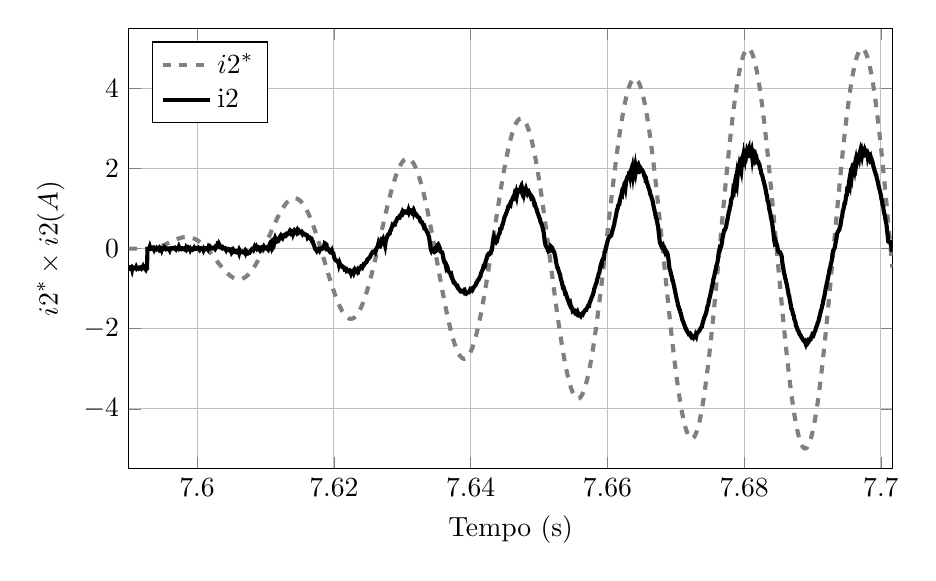
\begin{tikzpicture}

\begin{axis}[%
width=0.8\textwidth,
height=0.461611624834875\textwidth,
scale only axis,
xmin=7.59,
xmax=7.7017,
xtick={ 7.6, 7.62, 7.64, 7.66, 7.68,  7.7},
xlabel={Tempo (s)},
xmajorgrids,
ymin=-5.5,
ymax=5.5,
ytick={-4, -2,  0,  2,  4},
ylabel={$\text{i2}^\text{*}\text{ }\times\text{ i2 (A)}$},
ymajorgrids,
legend style={at={(0.03,0.97)},anchor=north west,draw=black,fill=white,legend cell align=left}
]
\addplot [color=gray,dashed,line width=1.5pt]
  table[row sep=crcr]{7.589999988975	0\\
7.59008332897521	0\\
7.59016666897542	0\\
7.59025000897562	0\\
7.59033331897583	0\\
7.59041665897604	0\\
7.59049999897625	0\\
7.59058333897646	0\\
7.59066667897667	0\\
7.59074998897688	0\\
7.59083332897708	0\\
7.59091666897729	0\\
7.5910000089775	0\\
7.59108331897771	0\\
7.59116665897792	0\\
7.59124999897812	0\\
7.59133333897833	0\\
7.59141667897854	0\\
7.59149998897875	0\\
7.59158332897896	0\\
7.59166666897917	0\\
7.59175000897937	0\\
7.59183331897958	0\\
7.59191665897979	0\\
7.59199999898	0\\
7.59208333898021	0\\
7.59216667898042	0\\
7.59224998898063	0\\
7.59233332898083	0\\
7.59241666898104	0\\
7.59250000898125	0\\
7.59258331898146	0\\
7.59266665898167	0\\
7.59274999898188	0\\
7.59283333898208	0\\
7.59291667898229	-0\\
7.5929999889825	3.92634488473762e-05\\
7.59308332898271	0.000196239747670498\\
7.59316666898292	0.000539330060403448\\
7.59325000898312	0.00111693629130865\\
7.59333331898333	0.00195981918271187\\
7.59341665898354	0.00308594496928202\\
7.59349999898375	0.00450474353583032\\
7.59358333898396	0.00622015616516742\\
7.59366667898417	0.00823262022416316\\
7.59374998898438	0.0105402936125734\\
7.59383332898458	0.0131397849599244\\
7.59391666898479	0.0160265798470743\\
7.594000008985	0.0191952868299359\\
7.59408331898521	0.0226397794705883\\
7.59416665898542	0.0263532796332583\\
7.59424999898563	0.0303284082476884\\
7.59433333898583	0.0345572184241179\\
7.59441667898604	0.0390312192492781\\
7.59449998898625	0.0437413948672979\\
7.59458332898646	0.0486782213623582\\
7.59466666898667	0.0538316828039993\\
7.59475000898687	0.0591912871815809\\
7.59483331898708	0.0647460826087258\\
7.59491665898729	0.0704846739912887\\
7.5949999989875	0.0763952402512923\\
7.59508333898771	0.0824655521447796\\
7.59516667898792	0.0886829906821065\\
7.59524998898813	0.0950345661431947\\
7.59533332898833	0.101506937671426\\
7.59541666898854	0.108086433424836\\
7.59550000898875	0.114759071260276\\
7.59558331898896	0.121510579924313\\
7.59566665898917	0.128326420723332\\
7.59574999898938	0.135191809644302\\
7.59583333898958	0.142091739896904\\
7.59591667898979	0.149011004847002\\
7.59599998899	0.155934221310872\\
7.59608332899021	0.162845853179035\\
7.59616666899042	0.169730235338065\\
7.59625000899062	0.176571597858304\\
7.59633331899083	0.183354090414979\\
7.59641665899104	0.190061806909914\\
7.59649999899125	0.196678810260643\\
7.59658333899146	0.203189157323517\\
7.59666667899167	0.209576923917116\\
7.59674998899188	0.215826229912111\\
7.59683332899208	0.221921264353563\\
7.59691666899229	0.227846310581539\\
7.5970000089925	0.233585771315865\\
7.59708331899271	0.239124193670803\\
7.59716665899292	0.244446294065482\\
7.59724999899313	0.249536982995955\\
7.59733333899333	0.254381389634882\\
7.59741667899354	0.258964886224969\\
7.59749998899375	0.263273112232519\\
7.59758332899396	0.267291998227645\\
7.59766666899417	0.271007789458016\\
7.59775000899438	0.2744070690833\\
7.59783331899458	0.277476781037844\\
7.59791665899479	0.280204252489533\\
7.597999998995	0.282577215863212\\
7.59808333899521	0.284583830397552\\
7.59816667899542	0.286212703204747\\
7.59824998899563	0.287452909803028\\
7.59833332899583	0.288294014092534\\
7.59841666899604	0.288726087745785\\
7.59850000899625	0.28873972898462\\
7.59858331899646	0.288326080716234\\
7.59866665899667	0.287476848001647\\
7.59874999899688	0.286184314830782\\
7.59883333899708	0.284441360179096\\
7.59891667899729	0.282241473321602\\
7.5989999889975	0.279578768380984\\
7.59908332899771	0.276447998087437\\
7.59916666899792	0.272844566728798\\
7.59925000899813	0.268764542270527\\
7.59933331899833	0.264204667626086\\
7.59941665899854	0.259162371059302\\
7.59949999899875	0.253635775701354\\
7.59958333899896	0.247623708166111\\
7.59966667899917	0.241125706248628\\
7.59974998899937	0.234142025692764\\
7.59983332899958	0.226673646015016\\
7.59991666899979	0.218722275372802\\
7.600000009	0.210290354466661\\
7.60008331900021	0.20138105946698\\
7.60016665900042	0.191998303957109\\
7.60024999900063	0.182146739885928\\
7.60033333900083	0.171831757524175\\
7.60041667900104	0.161059484420095\\
7.60049998900125	0.149836783351221\\
7.60058332900146	0.138171249270346\\
7.60066666900167	0.126071205245064\\
7.60075000900188	0.113545697391459\\
7.60083331900208	0.100604488803862\\
7.60091665900229	0.087258052483838\\
7.6009999990025	0.0735175632728483\\
7.60108333900271	0.0593948887943171\\
7.60116667900292	0.0449025794120917\\
7.60124998900312	0.0300538572135612\\
7.60133332900333	0.0148626040269533\\
7.60141666900354	-0.000656651516416185\\
7.60150000900375	-0.0164887478629258\\
7.60158331900396	-0.0326179053472152\\
7.60166665900417	-0.0490277419180695\\
7.60174999900438	-0.0657012897639517\\
7.60183333900458	-0.0826210128213217\\
7.60191667900479	-0.0997688251477116\\
7.601999989005	-0.117126110140371\\
7.60208332900521	-0.134673740580167\\
7.60216666900542	-0.1523920994793\\
7.60225000900563	-0.170261101710329\\
7.60233331900583	-0.188260216392906\\
7.60241665900604	-0.20636849001361\\
7.60249999900625	-0.22456457025323\\
7.60258333900646	-0.242826730494888\\
7.60266667900667	-0.261132894985407\\
7.60274998900687	-0.279460664621447\\
7.60283332900708	-0.297787343330984\\
7.60291666900729	-0.316089965019901\\
7.6030000090075	-0.3343453210526\\
7.60308331900771	-0.352529988234756\\
7.60316665900792	-0.370620357265598\\
7.60324999900813	-0.38859266162636\\
7.60333333900833	-0.406423006870886\\
7.60341667900854	-0.424087400283719\\
7.60349998900875	-0.441561780870407\\
7.60358332900896	-0.458822049644201\\
7.60366666900917	-0.475844100172799\\
7.60375000900938	-0.492603849348319\\
7.60383331900958	-0.509077268343243\\
7.60391665900979	-0.525240413714681\\
7.60399999901	-0.541069458618982\\
7.60408333901021	-0.556540724098386\\
7.60416667901042	-0.571630710401174\\
7.60424998901062	-0.586316128296567\\
7.60433332901083	-0.600573930345441\\
7.60441666901104	-0.614381342087826\\
7.60450000901125	-0.627715893108084\\
7.60458331901146	-0.640555447938618\\
7.60466665901167	-0.652878236763014\\
7.60474999901188	-0.664662885879562\\
7.60483333901208	-0.675888447886246\\
7.60491667901229	-0.686534431548419\\
7.6049999890125	-0.69658083131064\\
7.60508332901271	-0.706008156414354\\
7.60516666901292	-0.714797459583449\\
7.60525000901313	-0.72293036524004\\
7.60533331901333	-0.730389097213255\\
7.60541665901354	-0.737156505904213\\
7.60549999901375	-0.743216094870909\\
7.60558333901396	-0.748552046797211\\
7.60566667901417	-0.753149248810814\\
7.60574998901437	-0.756993317115544\\
7.60583332901458	-0.760070620904149\\
7.60591666901479	-0.762368305518361\\
7.606000009015	-0.76387431482381\\
7.60608331901521	-0.764577412768132\\
7.60616665901542	-0.764467204091479\\
7.60624999901562	-0.763534154159484\\
7.60633333901583	-0.761769607889657\\
7.60641667901604	-0.759165807743159\\
7.60649998901625	-0.755715910754853\\
7.60658332901646	-0.75141400457559\\
7.60666666901667	-0.746255122501714\\
7.60675000901688	-0.740235257467897\\
7.60683331901708	-0.733351374980511\\
7.60691665901729	-0.72560142496992\\
7.6069999990175	-0.716984352541243\\
7.60708333901771	-0.707500107604376\\
7.60716667901792	-0.697149653365293\\
7.60724998901812	-0.685934973661903\\
7.60733332901833	-0.673859079129061\\
7.60741666901854	-0.66092601217862\\
7.60750000901875	-0.647140850781771\\
7.60758331901896	-0.632509711042269\\
7.60766665901917	-0.617039748550505\\
7.60774999901937	-0.600739158509821\\
7.60783333901958	-0.583617174627826\\
7.60791667901979	-0.565684066766932\\
7.60799998902	-0.54695113734975\\
7.60808332902021	-0.527430716516444\\
7.60816666902042	-0.507136156032582\\
7.60825000902063	-0.486081821947517\\
7.60833331902083	-0.464283086004765\\
7.60841665902104	-0.441756315807359\\
7.60849999902125	-0.418518863742611\\
7.60858333902146	-0.394589054672203\\
7.60866667902167	-0.369986172395001\\
7.60874998902187	-0.344730444891467\\
7.60883332902208	-0.318843028360017\\
7.60891666902229	-0.292345990057114\\
7.6090000090225	-0.26526228995439\\
7.60908331902271	-0.237615761227477\\
7.60916665902292	-0.209431089592727\\
7.60924999902312	-0.180733791509366\\
7.60933333902333	-0.151550191266084\\
7.60941667902354	-0.121907396972424\\
7.60949998902375	-0.0918332754767251\\
7.60958332902396	-0.0613564262337166\\
7.60966666902417	-0.0305061541462129\\
7.60975000902438	0.00068755859335144\\
7.60983331902458	0.0321940816345025\\
7.60991665902479	0.0639821665451286\\
7.609999999025	0.0960199778031705\\
7.61008333902521	0.128275124672863\\
7.61016667902542	0.160714693933619\\
7.61024998902562	0.193305283428501\\
7.61033332902583	0.226013036398124\\
7.61041666902604	0.258803676564744\\
7.61050000902625	0.291642543930274\\
7.61058331902646	0.324494631250935\\
7.61066665902667	0.357324621150329\\
7.61074999902687	0.390096923831746\\
7.61083333902708	0.422775715349704\\
7.61091667902729	0.455324976399811\\
7.6109999890275	0.487708531585296\\
7.61108332902771	0.519890089117784\\
7.61116666902792	0.551833280909188\\
7.61125000902813	0.583501703010921\\
7.61133331902833	0.614858956356049\\
7.61141665902854	0.645868687759411\\
7.61149999902875	0.676494631130238\\
7.61158333902896	0.706700648851329\\
7.61166667902917	0.736450773278437\\
7.61174998902938	0.765709248313142\\
7.61183332902958	0.794440571002203\\
7.61191666902979	0.822609533116082\\
7.61200000903	0.850181262659173\\
7.61208331903021	0.877121265264087\\
7.61216665903042	0.903395465422244\\
7.61224999903062	0.928970247503012\\
7.61233333903083	0.953812496513588\\
7.61241667903104	0.977889638551935\\
7.61249998903125	1.00116968090517\\
7.61258332903146	1.023621251746\\
7.61266666903167	1.04521363937994\\
7.61275000903187	1.06591683099659\\
7.61283331903208	1.08570155087809\\
7.61291665903229	1.10453929801893\\
7.6129999990325	1.12240238311105\\
7.61308333903271	1.13926396484921\\
7.61316667903292	1.15509808551185\\
7.61324998903313	1.16987970577333\\
7.61333332903333	1.18358473870417\\
7.61341666903354	1.1961900829166\\
7.61350000903375	1.20767365481334\\
7.61358331903396	1.21801441989854\\
7.61366665903417	1.22719242311065\\
7.61374999903437	1.23518881813763\\
7.61383333903458	1.24198589567634\\
7.61391667903479	1.24756711059847\\
7.613999989035	1.25191710798675\\
7.61408332903521	1.25502174800612\\
7.61416666903542	1.25686812957578\\
7.61425000903562	1.25744461280908\\
7.61433331903583	1.25674084018961\\
7.61441665903604	1.25474775645297\\
7.61449999903625	1.25145762714512\\
7.61458333903646	1.24686405582944\\
7.61466667903667	1.24096199991611\\
7.61474998903688	1.23374778508877\\
7.61483332903708	1.22521911830496\\
7.61491666903729	1.21537509934816\\
7.6150000090375	1.2042162309109\\
7.61508331903771	1.19174442719001\\
7.61516665903792	1.17796302097641\\
7.61524999903812	1.16287676922361\\
7.61533333903833	1.14649185708084\\
7.61541667903854	1.12881590037797\\
7.61549998903875	1.10985794655149\\
7.61558332903896	1.08962847400221\\
7.61566666903917	1.06813938987714\\
7.61575000903937	1.04540402626981\\
7.61583331903958	1.02143713483475\\
7.61591665903979	0.996254879814013\\
7.61599999904	0.969874829474927\\
7.61608333904021	0.942315945960343\\
7.61616667904042	0.9135985735543\\
7.61624998904063	0.883744425367755\\
7.61633332904083	0.852776568450875\\
7.61641666904104	0.820719407340126\\
7.61650000904125	0.787598666050151\\
7.61658331904146	0.753441368522235\\
7.61666665904167	0.718275817542871\\
7.61674999904188	0.682131572147739\\
7.61683333904208	0.645039423528115\\
7.61691667904229	0.60703136945848\\
7.6169999890425	0.568140587265829\\
7.61708332904271	0.528401405362841\\
7.61716666904292	0.487849273368815\\
7.61725000904312	0.446520730843884\\
7.61733331904333	0.404453374663717\\
7.61741665904354	0.361685825063497\\
7.61749999904375	0.318257690381593\\
7.61758333904396	0.274209530534895\\
7.61766667904417	0.22958281925932\\
7.61774998904438	0.184419905150532\\
7.61783332904458	0.138763971541359\\
7.61791666904479	0.0926589952538724\\
7.618000009045	0.0461497042654726\\
7.61808331904521	-0.00071846567028672\\
7.61816665904542	-0.0478994154060793\\
7.61824999904563	-0.0953464277430423\\
7.61833333904583	-0.143012213688272\\
7.61841667904604	-0.190848959581775\\
7.61849998904625	-0.238808375045917\\
7.61858332904646	-0.286841741709292\\
7.61866666904667	-0.334899962655878\\
7.61875000904687	-0.382933612549322\\
7.61883331904708	-0.430892988381248\\
7.61891665904729	-0.478728160791543\\
7.6189999990475	-0.526389025907753\\
7.61908333904771	-0.573825357649884\\
7.61916667904792	-0.62098686044618\\
7.61924998904813	-0.667823222304736\\
7.61933332904833	-0.714284168185186\\
7.61941666904854	-0.760319513614124\\
7.61950000904875	-0.805879218487395\\
7.61958331904896	-0.850913441001943\\
7.61966665904917	-0.8953725916595\\
7.61974999904938	-0.939207387284068\\
7.61983333904958	-0.98236890499488\\
7.61991667904979	-1.0248086360763\\
7.61999998905	-1.06647853968599\\
7.62008332905021	-1.10733109634257\\
7.62016666905042	-1.147319361134\\
7.62025000905062	-1.18639701658797\\
7.62033331905083	-1.22451842514555\\
7.62041665905104	-1.26163868117986\\
7.62049999905125	-1.29771366250125\\
7.62058333905146	-1.33270008129135\\
7.62066667905167	-1.3665555344082\\
7.62074998905188	-1.39923855300549\\
7.62083332905208	-1.43070865140917\\
7.62091666905229	-1.46092637519543\\
7.6210000090525	-1.48985334841445\\
7.62108331905271	-1.51745231990535\\
7.62116665905292	-1.5436872086481\\
7.62124999905313	-1.56852314809924\\
7.62133333905333	-1.59192652945908\\
7.62141667905354	-1.61386504381887\\
7.62149998905375	-1.63430772313746\\
7.62158332905396	-1.65322497999823\\
7.62166666905417	-1.6705886460977\\
7.62175000905437	-1.68637200941885\\
7.62183331905458	-1.70054985004323\\
7.62191665905479	-1.71309847455705\\
7.621999999055	-1.72399574900805\\
7.62208333905521	-1.73322113037105\\
7.62216667905542	-1.74075569648178\\
7.62224998905563	-1.74658217439974\\
7.62233332905583	-1.75068496716269\\
7.62241666905604	-1.75305017889671\\
7.62250000905625	-1.75366563824742\\
7.62258331905646	-1.75252092009981\\
7.62266665905667	-1.74960736555541\\
7.62274999905688	-1.74491810013781\\
7.62283333905708	-1.73844805019876\\
7.62291667905729	-1.7301939574994\\
7.6229999890575	-1.72015439194256\\
7.62308332905771	-1.70832976243439\\
7.62316666905792	-1.69472232585508\\
7.62325000905813	-1.67933619412073\\
7.62333331905833	-1.66217733932009\\
7.62341665905854	-1.64325359691213\\
7.62349999905875	-1.62257466697231\\
7.62358333905896	-1.60015211347731\\
7.62366667905917	-1.57599936162045\\
7.62374998905938	-1.55013169315158\\
7.62383332905958	-1.5225662397377\\
7.62391666905979	-1.49332197434252\\
7.62400000906	-1.46241970062522\\
7.62408331906021	-1.42988204036099\\
7.62416665906042	-1.39573341888773\\
7.62424999906063	-1.36000004858576\\
7.62433333906083	-1.32270991039935\\
7.62441667906104	-1.28389273341087\\
7.62449998906125	-1.24357997248078\\
7.62458332906146	-1.20180478396858\\
7.62466666906167	-1.158601999552\\
7.62475000906188	-1.11400809816381\\
7.62483331906208	-1.06806117606772\\
7.62491665906229	-1.02080091509696\\
7.6249999990625	-0.97226854908098\\
7.62508333906271	-0.922506828488123\\
7.62516667906292	-0.871559983313621\\
7.62524998906312	-0.81947368424476\\
7.62533332906333	-0.766295002136659\\
7.62541666906354	-0.712072365834217\\
7.62550000906375	-0.656855518377615\\
7.62558331906396	-0.600695471630656\\
7.62566665906417	-0.543644459373046\\
7.62574999906438	-0.485755888899518\\
7.62583333906458	-0.427084291170461\\
7.62591667906479	-0.367685269560426\\
7.625999989065	-0.307615447252558\\
7.62608332906521	-0.246932413328641\\
7.62616666906542	-0.185694667605994\\
7.62625000906563	-0.123961564274029\\
7.62633331906583	-0.0617932543847333\\
7.62641665906604	0.000749372747221162\\
7.62649999906625	0.0636047491776554\\
7.62658333906646	0.126710688940956\\
7.62666667906667	0.190004449573373\\
7.62674998906687	0.253422794490687\\
7.62683332906708	0.316902056158215\\
7.62691666906729	0.380378199990083\\
7.6270000090675	0.443786888913631\\
7.62708331906771	0.507063548533901\\
7.62716665906792	0.570143432832223\\
7.62724999906813	0.632961690332152\\
7.62733333906833	0.695453430665178\\
7.62741667906854	0.757553791468022\\
7.62749998906875	0.819198005542657\\
7.62758332906896	0.880321468209662\\
7.62766666906917	0.940859804785077\\
7.62775000906938	1.00074893811046\\
7.62783331906958	1.0599251560656\\
7.62791665906979	1.11832517899297\\
7.62799999907	1.17588622696295\\
7.62808333907021	1.23254608680873\\
7.62816667907042	1.28824317885953\\
7.62824998907062	1.34291662330128\\
7.62833332907083	1.39650630609355\\
7.62841666907104	1.448952944372\\
7.62850000907125	1.5001981512658\\
7.62858331907146	1.55018450005985\\
7.62866665907167	1.59885558763193\\
7.62874999907188	1.64615609709563\\
7.62883333907208	1.69203185958026\\
7.62891667907229	1.73642991507968\\
7.6289999890725	1.77929857230281\\
7.62908332907271	1.82058746745904\\
7.62916666907292	1.86024762191318\\
7.62925000907313	1.89823149864486\\
7.62933331907333	1.93449305744895\\
7.62941665907354	1.96898780881411\\
7.62949999907375	2.00167286641811\\
7.62958333907396	2.03250699817956\\
7.62966667907417	2.06145067580712\\
7.62974998907437	2.08846612278852\\
7.62983332907458	2.11351736076307\\
7.62991666907479	2.13657025422315\\
7.630000009075	2.15759255349124\\
7.63008331907521	2.17655393592111\\
7.63016665907542	2.19342604527313\\
7.63024999907563	2.20818252921557\\
7.63033333907583	2.22079907490545\\
7.63041667907604	2.23125344260447\\
7.63049998907625	2.23952549728721\\
7.63058332907646	2.245597238201\\
7.63066666907667	2.24945282633864\\
7.63075000907688	2.25107860978729\\
7.63083331907708	2.25046314691906\\
7.63091665907729	2.24759722739054\\
7.6309999990775	2.24247389092122\\
7.63108333907771	2.23508844382265\\
7.63116667907792	2.22543847325241\\
7.63124998907812	2.21352385916936\\
7.63133332907833	2.19934678396902\\
7.63141666907854	2.18291173978001\\
7.63150000907875	2.1642255334052\\
7.63158331907896	2.1432972888933\\
7.63166665907917	2.12013844772928\\
7.63174999907937	2.09476276663426\\
7.63183333907958	2.06718631296821\\
7.63191667907979	2.037427457731\\
7.63199998908	2.00550686616005\\
7.63208332908021	1.97144748592518\\
7.63216666908042	1.93527453292391\\
7.63225000908063	1.89701547468283\\
7.63233331908083	1.85670001137331\\
7.63241665908104	1.81436005445219\\
7.63249999908125	1.77002970294071\\
7.63258333908146	1.72374521735751\\
7.63266667908167	1.67554499132378\\
7.63274998908187	1.6254695208614\\
7.63283332908208	1.57356137140726\\
7.63291666908229	1.51986514256941\\
7.6330000090825	1.46442743065313\\
7.63308331908271	1.4072967889875\\
7.63316665908292	1.3485236860853\\
7.63324999908312	1.28816046167168\\
7.63333333908333	1.22626128061909\\
7.63341667908354	1.16288208482851\\
7.63349998908375	1.09808054309913\\
7.63358332908396	1.03191599903104\\
7.63366666908417	0.964449417007492\\
7.63375000908438	0.895743326305595\\
7.63383331908458	0.825861763386417\\
7.63391665908479	0.75487021241743\\
7.633999999085	0.682835544082377\\
7.63408333908521	0.609825952735541\\
7.63416667908542	0.535910891959331\\
7.63424998908562	0.461161008585957\\
7.63433332908583	0.385648075245797\\
7.63441666908604	0.309444921506751\\
7.63450000908625	0.23262536367063\\
7.63458331908646	0.155264133294187\\
7.63466665908667	0.0774368045039944\\
7.63474999908687	-0.000780279824155447\\
7.63483333908708	-0.0793100829492315\\
7.63491667908729	-0.158074950138869\\
7.6349999890875	-0.236996685458474\\
7.63508332908771	-0.315996629399599\\
7.63516666908792	-0.394995737270514\\
7.63525000908813	-0.473914658270874\\
7.63533331908833	-0.552673815171386\\
7.63541665908854	-0.63119348451848\\
7.63549999908875	-0.709393877283199\\
7.63558333908896	-0.787195219872761\\
7.63566667908917	-0.864517835422604\\
7.63574998908938	-0.941282225286163\\
7.63583332908958	-1.01740915063914\\
7.63591666908979	-1.09281971411459\\
7.63600000909	-1.16743544138497\\
7.63608331909021	-1.24117836260681\\
7.63616665909042	-1.31397109364381\\
7.63624999909062	-1.38573691698399\\
7.63633333909083	-1.45639986226641\\
7.63641667909104	-1.52588478633339\\
7.63649998909125	-1.59411745272417\\
7.63658332909146	-1.66102461052625\\
7.63666666909167	-1.7265340725011\\
7.63675000909188	-1.79057479240143\\
7.63683331909208	-1.85307694139761\\
7.63691665909229	-1.91397198353174\\
7.6369999990925	-1.97319275011831\\
7.63708333909271	-2.03067351301141\\
7.63716667909292	-2.08635005665927\\
7.63724998909313	-2.14015974886803\\
7.63733332909333	-2.19204161019743\\
7.63741666909354	-2.2419363819126\\
7.63750000909375	-2.28978659241719\\
7.63758331909396	-2.3355366220943\\
7.63766665909417	-2.37913276648346\\
7.63774999909437	-2.42052329772288\\
7.63783333909458	-2.45965852418812\\
7.63791667909479	-2.49649084825988\\
7.637999989095	-2.53097482215517\\
7.63808332909521	-2.56306720175818\\
7.63816666909542	-2.59272699838869\\
7.63825000909562	-2.61991552844807\\
7.63833331909583	-2.64459646088478\\
7.63841665909604	-2.66673586242337\\
7.63849999909625	-2.68630224050303\\
7.63858333909646	-2.70326658387408\\
7.63866667909667	-2.71760240080286\\
7.63874998909688	-2.7292857548379\\
7.63883332909708	-2.73829529809266\\
7.63891666909729	-2.74461230200228\\
7.6390000090975	-2.74822068551459\\
7.63908331909771	-2.74910704067789\\
7.63916665909792	-2.74726065559071\\
7.63924999909812	-2.74267353468127\\
7.63933333909833	-2.73534041628703\\
7.63941667909854	-2.7252587875075\\
7.63949998909875	-2.71242889630606\\
7.63958332909896	-2.69685376083933\\
7.63966666909917	-2.67853917599548\\
7.63975000909937	-2.65749371712563\\
7.63983331909958	-2.63372874095532\\
7.63991665909979	-2.60725838366588\\
7.6399999991	-2.57809955613847\\
7.64008333910021	-2.54627193635638\\
7.64016667910042	-2.51179795896412\\
7.64024998910063	-2.47470280198471\\
7.64033332910083	-2.43501437069967\\
7.64041666910104	-2.39276327869879\\
7.64050000910125	-2.34798282611012\\
7.64058331910146	-2.30070897502315\\
7.64066665910167	-2.2509803221214\\
7.64074999910187	-2.19883806854338\\
7.64083333910208	-2.1443259869937\\
7.64091667910229	-2.08749038612927\\
7.6409999891025	-2.02838007224821\\
7.64108332910271	-1.96704630831193\\
7.64116666910292	-1.90354277033374\\
7.64125000910312	-1.83792550117024\\
7.64133331910333	-1.77025286175427\\
7.64141665910354	-1.70058547981119\\
7.64149999910375	-1.62898619610288\\
7.64158333910396	-1.5555200082464\\
7.64166667910417	-1.48025401215721\\
7.64174998910438	-1.4032573411689\\
7.64183332910458	-1.32460110288464\\
7.64191666910479	-1.24435831381733\\
7.642000009105	-1.16260383187833\\
7.64208331910521	-1.07941428677698\\
7.64216665910542	-0.994868008395221\\
7.64224999910563	-0.909044953204205\\
7.64233333910583	-0.822026628791709\\
7.64241667910604	-0.733896016571566\\
7.64249998910625	-0.644737492748202\\
7.64258332910646	-0.554636747611491\\
7.64266666910667	-0.463680703239037\\
7.64275000910687	-0.371957429684862\\
7.64283331910708	-0.279556059735267\\
7.64291665910729	-0.186566702314345\\
7.6429999991075	-0.0930803546232569\\
7.64308333910771	0.000811186901088293\\
7.64316667910792	0.0950154167208063\\
7.64324998910813	0.189439211336781\\
7.64333332910833	0.283988921343574\\
7.64341666910854	0.37857046430851\\
7.64350000910875	0.473089418382811\\
7.64358331910896	0.567451116551665\\
7.64366665910917	0.66156074142914\\
7.64374999910938	0.755323420503059\\
7.64383333910958	0.848644321734175\\
7.64391667910979	0.94142874941337\\
7.64399998911	1.03358224018003\\
7.64408332911021	1.1250106591043\\
7.64416666911042	1.21562029573561\\
7.64425000911062	1.30531796001952\\
7.64433331911083	1.39401107798486\\
7.64441665911104	1.48160778710315\\
7.64449999911125	1.56801703122203\\
7.64458333911146	1.65314865497502\\
7.64466667911167	1.73691349756986\\
7.64474998911188	1.81922348585805\\
7.64483332911208	1.89999172658882\\
7.64491666911229	1.97913259775123\\
7.6450000091125	2.05656183890867\\
7.64508331911271	2.13219664043086\\
7.64516665911292	2.20595573152941\\
7.64524999911313	2.27775946700363\\
7.64533333911333	2.3475299126047\\
7.64541667911354	2.41519092892718\\
7.64549998911375	2.48066825373828\\
7.64558332911396	2.54388958265637\\
7.64566666911417	2.60478464809205\\
7.64575000911437	2.66328529636617\\
7.64583331911458	2.7193255629212\\
7.64591665911479	2.77284174554374\\
7.645999999115	2.82377247551798\\
7.64608333911521	2.87205878663165\\
7.64616667911542	2.91764418195814\\
7.64624998911563	2.9604746983402\\
7.64633332911583	3.00049896850322\\
7.64641666911604	3.03766828072785\\
7.64650000911625	3.07193663601431\\
7.64658331911646	3.10326080267299\\
7.64666665911667	3.13160036827832\\
7.64674999911688	3.15691778892563\\
7.64683333911708	3.17917843573294\\
7.64691667911729	3.19835063853261\\
7.6469999891175	3.21440572670027\\
7.64708332911771	3.22731806707133\\
7.64716666911792	3.23706509889811\\
7.64725000911813	3.24362736580356\\
7.64733331911833	3.24698854469054\\
7.64741665911854	3.24713547156848\\
7.64749999911875	3.24405816426236\\
7.64758333911896	3.23774984197201\\
7.64766667911917	3.22820694165284\\
7.64774998911938	3.21542913119235\\
7.64783332911958	3.19941931935972\\
7.64791666911979	3.1801836625093\\
7.64800000912	3.15773156802194\\
7.64808331912021	3.13207569447126\\
7.64816665912042	3.10323194850545\\
7.64824999912063	3.07121947843846\\
7.64833333912083	3.03606066454767\\
7.64841667912104	2.99778110607852\\
7.64849998912125	2.95640960496003\\
7.64858332912146	2.91197814623841\\
7.64866666912167	2.86452187523928\\
7.64875000912188	2.81407907147241\\
7.64883331912208	2.76069111929634\\
7.64891665912229	2.70440247536347\\
7.6489999991225	2.6452606328695\\
7.64908333912271	2.58331608263458\\
7.64916667912292	2.51862227104669\\
7.64924998912312	2.45123555490103\\
7.64933332912333	2.38121515317265\\
7.64941666912354	2.30862309576247\\
7.64950000912375	2.23352416926023\\
7.64958331912396	2.15598585977108\\
7.64966665912417	2.07607829285541\\
7.64974999912438	1.99387417063488\\
7.64983333912458	1.90944870612046\\
7.64991667912479	1.82287955482113\\
7.649999989125	1.73424674369532\\
7.65008332912521	1.64363259750929\\
7.65016666912542	1.55112166267015\\
7.65025000912563	1.45680062860361\\
7.65033331912583	1.36075824674916\\
7.65041665912604	1.26308524724836\\
7.65049999912625	1.16387425340403\\
7.65058333912646	1.06321969399098\\
7.65066667912667	0.961217713501042\\
7.65074998912687	0.857966080407591\\
7.65083332912708	0.753564093537073\\
7.65091666912729	0.648112486637025\\
7.6510000091275	0.541713331232278\\
7.65108331912771	0.434469937862974\\
7.65116665912792	0.326486755799904\\
7.65124999912813	0.217869271334504\\
7.65133333912833	0.108723904742519\\
7.65141667912854	-0.000842093978021569\\
7.65149998912875	-0.110720750492382\\
7.65158332912896	-0.220803472534694\\
7.65166666912917	-0.330981157228675\\
7.65175000912938	-0.441144299217422\\
7.65183331912958	-0.55118309949511\\
7.65191665912979	-0.660987574832456\\
7.65199999913	-0.770447667686895\\
7.65208333913021	-0.879453356487639\\
7.65216667913042	-0.987894766185152\\
7.65224998913062	-1.09566227895398\\
7.65233332913083	-1.20264664493746\\
7.65241666913104	-1.30873909292244\\
7.65250000913125	-1.41383144083209\\
7.65258331913146	-1.51781620592445\\
7.65266665913167	-1.62058671458476\\
7.65274999913188	-1.7220372115995\\
7.65283333913208	-1.82206296880024\\
7.65291667913229	-1.92056039296605\\
7.6529999891325	-2.01742713287332\\
7.65308332913271	-2.11256218538272\\
7.65316666913292	-2.20586600045347\\
7.65325000913313	-2.29724058497621\\
7.65333331913333	-2.38658960531623\\
7.65341665913354	-2.4738184884603\\
7.65349999913375	-2.55883452166122\\
7.65358333913396	-2.64154695047553\\
7.65366667913417	-2.72186707509109\\
7.65374998913437	-2.79970834484297\\
7.65383332913458	-2.8749864508173\\
7.65391666913479	-2.94761941644472\\
7.654000009135	-3.01752768598667\\
7.65408331913521	-3.08463421081973\\
7.65416665913542	-3.14886453342521\\
7.65424999913563	-3.21014686899319\\
7.65433333913583	-3.2684121845525\\
7.65441667913604	-3.32359427554043\\
7.65449998913625	-3.37562983972816\\
7.65458332913646	-3.42445854842053\\
7.65466666913667	-3.47002311485127\\
7.65475000913688	-3.51226935969752\\
7.65483331913708	-3.55114627363994\\
7.65491665913729	-3.58660607689791\\
7.6549999991375	-3.61860427567187\\
7.65508333913771	-3.6470997154279\\
7.65516667913792	-3.67205463096285\\
7.65524998913812	-3.69343469319113\\
7.65533332913833	-3.71120905259768\\
7.65541666913854	-3.72535037930476\\
7.65550000913875	-3.73583489970356\\
7.65558331913896	-3.74264242960483\\
7.65566665913917	-3.74575640386649\\
7.65574999913937	-3.74516390245908\\
7.65583333913958	-3.74085567293402\\
7.65591667913979	-3.73282614926275\\
7.65599998914	-3.72107346701866\\
7.65608332914021	-3.70559947487721\\
7.65616666914042	-3.68640974241337\\
7.65625000914063	-3.66351356417927\\
7.65633331914083	-3.63692396004841\\
7.65641665914104	-3.60665767181689\\
7.65649999914125	-3.57273515605557\\
7.65658333914146	-3.53518057321105\\
7.65666667914167	-3.49402177295687\\
7.65674998914187	-3.44929027580065\\
7.65683332914208	-3.40102125095594\\
7.65691666914229	-3.34925349049212\\
7.6570000091425	-3.2940293797789\\
7.65708331914271	-3.23539486424602\\
7.65716665914292	-3.17339941248255\\
7.65724999914312	-3.10809597570379\\
7.65733333914333	-3.03954094361759\\
7.65741667914354	-2.96779409672579\\
7.65749998914375	-2.89291855509968\\
7.65758332914396	-2.81498072367279\\
7.65766666914417	-2.73405023409709\\
7.65775000914438	-2.650199883213\\
7.65783331914458	-2.56350556818672\\
7.65791665914479	-2.47404621837191\\
7.657999999145	-2.38190372395654\\
7.65808333914521	-2.28716286145858\\
7.65816667914542	-2.18991121613804\\
7.65824998914562	-2.09023910139586\\
7.65833332914583	-1.98823947523344\\
7.65841666914604	-1.88400785384968\\
7.65850000914625	-1.77764222245567\\
7.65858331914646	-1.6692429433899\\
7.65866665914667	-1.55891266162\\
7.65874999914687	-1.44675620771974\\
7.65883333914708	-1.33288049841283\\
7.65891667914729	-1.21739443477776\\
7.6589999891475	-1.10040879821038\\
7.65908332914771	-0.982036144243618\\
7.65916666914792	-0.862390694325946\\
7.65925000914813	-0.74158822566256\\
7.65933331914833	-0.61974595922552\\
7.65941665914854	-0.496982446041087\\
7.65949999914875	-0.373417451864542\\
7.65958333914896	-0.249171840354664\\
7.65966667914917	-0.124367454861782\\
7.65974998914937	0.000873001054954144\\
7.65983332914958	0.126426084263956\\
7.65991666914979	0.252167733732606\\
7.66000000915	0.377973393113776\\
7.66008331915021	0.503718134126334\\
7.66016665915042	0.629276780607408\\
7.66024999915062	0.754524033113248\\
7.66033333915083	0.87933459394465\\
7.66041667915104	1.00358329247222\\
7.66049998915125	1.12714521063613\\
7.66058332915146	1.24989580849459\\
7.66066666915167	1.37171104969489\\
7.66075000915188	1.49246752674059\\
7.66083331915208	1.61204258592857\\
7.66091665915229	1.73031445182938\\
7.6609999991525	1.84716235118466\\
7.66108333915271	1.96246663609584\\
7.66116667915292	2.07610890637845\\
7.66124998915313	2.18797213095708\\
7.66133332915333	2.29794076817678\\
7.66141666915354	2.40590088490738\\
7.66150000915375	2.51174027431812\\
7.66158331915396	2.61534857220119\\
7.66166665915417	2.71661737172379\\
7.66174999915437	2.81544033648973\\
7.66183333915458	2.91171331179303\\
7.66191667915479	3.00533443394742\\
7.661999989155	3.09620423757748\\
7.66208332915521	3.18422576075875\\
7.66216666915542	3.26930464789632\\
7.66225000915562	3.35134925023307\\
7.66233331915583	3.43027072388129\\
7.66241665915604	3.5059831252733\\
7.66249999915625	3.57840350392923\\
7.66258333915646	3.64745199244263\\
7.66266667915667	3.71305189358702\\
7.66274998915688	3.77512976444921\\
7.66283332915708	3.83361549749819\\
7.66291666915729	3.88844239850086\\
7.6630000091575	3.93954726119932\\
7.66308331915771	3.98687043866719\\
7.66316665915792	4.03035591126556\\
7.66324999915812	4.06995135112284\\
7.66333333915833	4.10560818306542\\
7.66341667915854	4.13728164193017\\
7.66349998915875	4.16493082619276\\
7.66358332915896	4.18851874784966\\
7.66366666915917	4.2080123784951\\
7.66375000915937	4.2233826915382\\
7.66383331915958	4.23460470050901\\
7.66391665915979	4.24165749340612\\
7.66399999916	4.24452426304246\\
7.66408333916021	4.24319233334969\\
7.66416667916042	4.23765318160568\\
7.66424998916063	4.22790245655349\\
7.66433332916083	4.21393999238448\\
7.66441666916104	4.19576981856207\\
7.66450000916125	4.17340016546704\\
7.66458331916146	4.14684346584926\\
7.66466665916167	4.11611635207489\\
7.66474999916187	4.08123964916252\\
7.66483333916208	4.04223836360571\\
7.66491667916229	3.99914166798364\\
7.6649999891625	3.95198288136608\\
7.66508332916271	3.90079944552279\\
7.66516666916292	3.84563289695186\\
7.66525000916312	3.78652883474583\\
7.66533331916333	3.72353688431852\\
7.66541665916354	3.65671065701964\\
7.66549999916375	3.58610770566878\\
7.66558333916396	3.51178947604411\\
7.66566667916417	3.4338212543657\\
7.66574998916438	3.35227211081699\\
7.66583332916458	3.26721483915268\\
7.66591666916479	3.17872589244455\\
7.666000009165	3.08688531502153\\
7.66608331916521	2.99177667066354\\
7.66616665916542	2.89348696711321\\
7.66624999916563	2.79210657697275\\
7.66633333916583	2.68772915505769\\
7.66641667916604	2.58045155228228\\
7.66649998916625	2.47037372615562\\
7.66658332916646	2.35759864797059\\
7.66666666916667	2.24223220677156\\
7.66675000916687	2.12438311019007\\
7.66683331916708	2.00416278224119\\
7.66691665916729	1.88168525817619\\
7.6669999991675	1.75706707649084\\
7.66708333916771	1.63042716819112\\
7.66716667916792	1.50188674342164\\
7.66724998916813	1.37156917556454\\
7.66733332916833	1.23959988291971\\
7.66741666916854	1.10610620807965\\
7.66750000916875	0.97121729511482\\
7.66758331916896	0.835063964688096\\
7.66766665916917	0.697778587218763\\
7.66774999916938	0.5594949542192\\
7.66783333916958	0.420348147929181\\
7.66791667916979	0.280474409374824\\
7.66799998917	0.140011004981045\\
7.66808332917021	-0.000903908131886802\\
7.66816666917042	-0.142131418035531\\
7.66825000917062	-0.283531994930519\\
7.66833331917083	-0.424965628998877\\
7.66841665917104	-0.566291969035246\\
7.66849999917125	-0.707370461719707\\
7.66858333917146	-0.848060491394041\\
7.66866667917167	-0.988221520202407\\
7.66874998917188	-1.1277132284568\\
7.66883332917208	-1.26639565508711\\
7.66891666917229	-1.40412933803521\\
7.6690000091725	-1.54077545445232\\
7.66908331917271	-1.67619596055873\\
7.66916665917292	-1.81025373102506\\
7.66924999917313	-1.94281269773431\\
7.66933333917333	-2.07373798778456\\
7.66941667917354	-2.20289606059219\\
7.66949998917375	-2.33015484395667\\
7.66958332917396	-2.45538386894811\\
7.66966666917417	-2.57845440348025\\
7.66975000917437	-2.69923958443205\\
7.66983331917458	-2.81761454818278\\
7.66991665917479	-2.93345655942618\\
7.669999999175	-3.04664513813136\\
7.67008333917521	-3.15706218451917\\
7.67016667917542	-3.26459210192485\\
7.67024998917563	-3.36912191741932\\
7.67033332917583	-3.47054140006387\\
7.67041666917604	-3.56874317667454\\
7.67050000917625	-3.66362284497534\\
7.67058331917646	-3.75507908402142\\
7.67066665917667	-3.84301376177592\\
7.67074999917688	-3.92733203972687\\
7.67083333917708	-4.00794247443326\\
7.67091667917729	-4.08475711589209\\
7.6709999891775	-4.15769160262154\\
7.67108332917771	-4.22666525335799\\
7.67116666917792	-4.29160115526822\\
7.67125000917812	-4.35242624858119\\
7.67133331917833	-4.40907140754739\\
7.67141665917854	-4.46147151763687\\
7.67149999917875	-4.5095655488912\\
7.67158333917896	-4.55329662534777\\
7.67166667917917	-4.59261209045897\\
7.67174998917938	-4.62746356843244\\
7.67183332917958	-4.65780702142268\\
7.67191666917979	-4.68360280250819\\
7.67200000918	-4.70481570439252\\
7.67208331918021	-4.72141500377165\\
7.67216665918042	-4.73337450131447\\
7.67224999918063	-4.74067255720741\\
7.67233333918083	-4.74329212221842\\
7.67241667918104	-4.7412207642403\\
7.67249998918125	-4.73445069027734\\
7.67258332918146	-4.72297876384424\\
7.67266666918167	-4.70680651775031\\
7.67275000918188	-4.68594016224693\\
7.67283331918208	-4.66039058852071\\
7.67291665918229	-4.63017336751924\\
7.6729999991825	-4.59530874410136\\
7.67308333918271	-4.55582162650816\\
7.67316667918292	-4.51174157115585\\
7.67324998918313	-4.46310276275623\\
7.67333332918333	-4.40994398977529\\
7.67341666918354	-4.35230861524493\\
7.67350000918375	-4.29024454294778\\
7.67358331918396	-4.22380417899955\\
7.67366665918417	-4.15304438885815\\
7.67374999918438	-4.07802644979327\\
7.67383333918458	-3.998815998855\\
7.67391667918479	-3.91548297638444\\
7.673999989185	-3.8281015651138\\
7.67408332918521	-3.7367501249082\\
7.67416666918542	-3.64151112320568\\
7.67425000918563	-3.54247106121632\\
7.67433331918583	-3.43972039594597\\
7.67441665918604	-3.33335345811409\\
7.67449999918625	-3.22346836603971\\
7.67458333918646	-3.1101669355736\\
7.67466667918667	-2.99355458615883\\
7.67474998918687	-2.87374024310598\\
7.67483332918708	-2.75083623617321\\
7.67491666918729	-2.62495819454533\\
7.6750000091875	-2.49622493830968\\
7.67508331918771	-2.36475836653047\\
7.67516665918792	-2.23068334202671\\
7.67524999918813	-2.09412757296248\\
7.67533333918833	-1.95522149136168\\
7.67541667918854	-1.81409812866251\\
7.67549998918875	-1.67089298843045\\
7.67558332918896	-1.52574391635132\\
7.67566666918917	-1.37879096762905\\
7.67575000918938	-1.23017627191568\\
7.67583331918958	-1.08004389590369\\
7.67591665918979	-0.928539703713632\\
7.67599999919	-0.775811215212005\\
7.67608333919021	-0.622007462397313\\
7.67616667919042	-0.467278843993819\\
7.67624998919062	-0.311776978394983\\
7.67633332919083	-0.155693818549155\\
7.67641666919104	0.000738575461149846\\
7.67650000919125	0.157297421746704\\
7.67658331919146	0.313779319837124\\
7.67666665919167	0.469998045701268\\
7.67674999919188	0.625779858974878\\
7.67683333919208	0.780959399296177\\
7.67691667919229	0.935376793509667\\
7.6769999891925	1.088875826236\\
7.67708332919271	1.24130287082881\\
7.67716666919292	1.39250631457816\\
7.67725000919313	1.54233628772875\\
7.67733331919333	1.69064457237981\\
7.67741665919354	1.83728461490629\\
7.67749999919375	1.98211159648828\\
7.67758333919396	2.12498253539156\\
7.67766667919417	2.26575640596034\\
7.67774998919437	2.40429426583926\\
7.67783332919458	2.54045938666759\\
7.67791666919479	2.67411738557679\\
7.678000009195	2.80513635597971\\
7.67808331919521	2.93338699677514\\
7.67816665919542	3.05874273943871\\
7.67824999919563	3.18107987265988\\
7.67833333919583	3.30027766428763\\
7.67841667919604	3.41621848040383\\
7.67849998919625	3.52878790137455\\
7.67858332919646	3.63787483474803\\
7.67866666919667	3.74337162487884\\
7.67875000919688	3.84517415916549\\
7.67883331919708	3.94318197079408\\
7.67891665919729	4.03729833788546\\
7.6789999991975	4.12743037894721\\
7.67908333919771	4.21348914453614\\
7.67916667919792	4.29538970504037\\
7.67924998919812	4.37305123449453\\
7.67933332919833	4.44639709034519\\
7.67941666919854	4.51535488908774\\
7.67950000919875	4.57985657770017\\
7.67958331919896	4.63983850080321\\
7.67966665919917	4.69524146348046\\
7.67974999919938	4.74601078969662\\
7.67983333919958	4.79209637625618\\
7.67991667919979	4.83345274224918\\
7.6799999892	4.87003907393541\\
7.68008332920021	4.9018192650226\\
7.68016666920042	4.92876195229903\\
7.68025000920063	4.95084054658518\\
7.68033331920083	4.96803325897407\\
7.68041665920104	4.98032312233428\\
7.68049999920125	4.98769800805444\\
7.68058333920146	4.99015063801273\\
7.68066667920167	4.9876785917595\\
7.68074998920187	4.98028430890592\\
7.68083332920208	4.96797508671647\\
7.68091666920229	4.95076307290733\\
7.6810000092025	4.92866525365811\\
7.68108331920271	4.90170343684848\\
7.68116665920292	4.86990423053652\\
7.68124999920312	4.83329901669968\\
7.68133333920333	4.79192392026462\\
7.68141667920354	4.74581977345624\\
7.68149998920375	4.69503207550123\\
7.68158332920396	4.63961094772579\\
7.68166666920417	4.57961108409196\\
7.68175000920438	4.51509169722128\\
7.68183331920458	4.44611645995907\\
7.68191665920479	4.37275344253702\\
7.681999999205	4.29507504539612\\
7.68208333920521	4.2131579277361\\
7.68216667920542	4.12708293186212\\
7.68224998920562	4.03693500340316\\
7.68233332920583	3.94280310748091\\
7.68241666920604	3.84478014091196\\
7.68250000920625	3.74296284052987\\
7.68258331920646	3.63745168771755\\
7.68266665920667	3.52835080924432\\
7.68274999920687	3.41576787450532\\
7.68283333920708	3.29981398926484\\
7.68291667920729	3.18060358600832\\
7.6829999892075	3.05825431101134\\
7.68308332920771	2.9328869082369\\
7.68316666920792	2.80462510017577\\
7.68325000920813	2.67359546574725\\
7.68333331920833	2.53992731538114\\
7.68341665920854	2.40375256340388\\
7.68349999920875	2.26520559785511\\
7.68358333920896	2.12442314786284\\
7.68366667920917	1.98154414870834\\
7.68374998920937	1.83670960471379\\
7.68383332920958	1.69006245008803\\
7.68391666920979	1.54174740786775\\
7.68400000921	1.39191084709332\\
7.68408331921021	1.24070063836024\\
7.68416665921042	1.0882660078887\\
7.68424999921062	0.934757390255326\\
7.68433333921083	0.780326279932395\\
7.68441667921104	0.625125081781105\\
7.68449998921125	0.469306960646363\\
7.68458332921146	0.313025690201579\\
7.68466666921167	0.156435501192615\\
7.68475000921188	-0.000309070769339045\\
7.68483331921208	-0.157053337715758\\
7.68491665921229	-0.313642611979131\\
7.6849999992125	-0.469922358851012\\
7.68508333921271	-0.625738349089121\\
7.68516667921292	-0.780936811122986\\
7.68524998921313	-0.935364582807916\\
7.68533332921333	-1.08886926257755\\
7.68541666921354	-1.2412993598458\\
7.68550000921375	-1.39250444450977\\
7.68558331921396	-1.5423352954061\\
7.68566665921417	-1.69064404757427\\
7.68574999921437	-1.83728433818141\\
7.68583333921458	-1.98211145096479\\
7.68591667921479	-2.12498245904929\\
7.685999989215	-2.26575636599894\\
7.68608332921521	-2.40429424496344\\
7.68616666921542	-2.54045937578212\\
7.68625000921563	-2.67411737991028\\
7.68633331921583	-2.80513635303457\\
7.68641665921604	-2.93338699524663\\
7.68649999921625	-3.05874273864649\\
7.68658333921646	-3.18107987224979\\
7.68666667921667	-3.3002776640756\\
7.68674998921688	-3.41621848029433\\
7.68683332921708	-3.52878790131806\\
7.68691666921729	-3.63787483471892\\
7.6870000092175	-3.74337162486385\\
7.68708331921771	-3.84517415915779\\
7.68716665921792	-3.94318197079013\\
7.68724999921812	-4.03729833788344\\
7.68733333921833	-4.12743037894619\\
7.68741667921854	-4.21348914453562\\
7.68749998921875	-4.29538970504011\\
7.68758332921896	-4.37305123449441\\
7.68766666921917	-4.44639709034514\\
7.68775000921937	-4.51535488908772\\
7.68783331921958	-4.57985657770018\\
7.68791665921979	-4.63983850080323\\
7.68799999922	-4.69524146348047\\
7.68808333922021	-4.74601078969664\\
7.68816667922042	-4.7920963762562\\
7.68824998922063	-4.8334527422492\\
7.68833332922083	-4.87003907393543\\
7.68841666922104	-4.90181926502262\\
7.68850000922125	-4.92876195229905\\
7.68858331922146	-4.9508405465852\\
7.68866665922167	-4.96803325897409\\
7.68874999922187	-4.9803231223343\\
7.68883333922208	-4.98769800805446\\
7.68891667922229	-4.99015063801276\\
7.6889999892225	-4.98767859175952\\
7.68908332922271	-4.98028430890595\\
7.68916666922292	-4.9679750867165\\
7.68925000922312	-4.95076307290736\\
7.68933331922333	-4.92866525365813\\
7.68941665922354	-4.90170343684851\\
7.68949999922375	-4.86990423053654\\
7.68958333922396	-4.8332990166997\\
7.68966667922417	-4.79192392026464\\
7.68974998922438	-4.74581977345626\\
7.68983332922458	-4.69503207550125\\
7.68991666922479	-4.63961094772581\\
7.690000009225	-4.57961108409198\\
7.69008331922521	-4.5150916972213\\
7.69016665922542	-4.44611645995909\\
7.69024999922562	-4.37275344253704\\
7.69033333922583	-4.29507504539614\\
7.69041667922604	-4.21315792773612\\
7.69049998922625	-4.12708293186214\\
7.69058332922646	-4.03693500340318\\
7.69066666922667	-3.94280310748093\\
7.69075000922687	-3.84478014091198\\
7.69083331922708	-3.74296284052989\\
7.69091665922729	-3.63745168771757\\
7.6909999992275	-3.52835080924434\\
7.69108333922771	-3.41576787450534\\
7.69116667922792	-3.29981398926485\\
7.69124998922813	-3.18060358600833\\
7.69133332922833	-3.05825431101135\\
7.69141666922854	-2.93288690823692\\
7.69150000922875	-2.80462510017578\\
7.69158331922896	-2.67359546574727\\
7.69166665922917	-2.53992731538115\\
7.69174999922938	-2.40375256340389\\
7.69183333922958	-2.26520559785512\\
7.69191667922979	-2.12442314786285\\
7.69199998923	-1.98154414870835\\
7.69208332923021	-1.8367096047138\\
7.69216666923042	-1.69006245008804\\
7.69225000923062	-1.54174740786776\\
7.69233331923083	-1.39191084709332\\
7.69241665923104	-1.24070063836025\\
7.69249999923125	-1.08826600788871\\
7.69258333923146	-0.934757390255331\\
7.69266667923167	-0.7803262799324\\
7.69274998923188	-0.625125081781109\\
7.69283332923208	-0.469306960646366\\
7.69291666923229	-0.313025690201581\\
7.6930000092325	-0.156435501192617\\
7.69308331923271	0.000309070769337727\\
7.69316665923292	0.157053337715758\\
7.69324999923313	0.313642611979131\\
7.69333333923333	0.469922358851013\\
7.69341667923354	0.625738349089123\\
7.69349998923375	0.780936811122988\\
7.69358332923396	0.935364582807918\\
7.69366666923417	1.08886926257755\\
7.69375000923437	1.2412993598458\\
7.69383331923458	1.39250444450977\\
7.69391665923479	1.54233529540611\\
7.693999999235	1.69064404757428\\
7.69408333923521	1.83728433818142\\
7.69416667923542	1.9821114509648\\
7.69424998923563	2.1249824590493\\
7.69433332923583	2.26575636599895\\
7.69441666923604	2.40429424496345\\
7.69450000923625	2.54045937578213\\
7.69458331923646	2.67411737991029\\
7.69466665923667	2.80513635303458\\
7.69474999923688	2.93338699524664\\
7.69483333923708	3.0587427386465\\
7.69491667923729	3.1810798722498\\
7.6949999892375	3.30027766407562\\
7.69508332923771	3.41621848029434\\
7.69516666923792	3.52878790131807\\
7.69525000923812	3.63787483471893\\
7.69533331923833	3.74337162486387\\
7.69541665923854	3.8451741591578\\
7.69549999923875	3.94318197079015\\
7.69558333923896	4.03729833788345\\
7.69566667923917	4.1274303789462\\
7.69574998923938	4.21348914453564\\
7.69583332923958	4.29538970504013\\
7.69591666923979	4.37305123449443\\
7.69600000924	4.44639709034516\\
7.69608331924021	4.51535488908774\\
7.69616665924042	4.57985657770019\\
7.69624999924063	4.63983850080325\\
7.69633333924083	4.69524146348049\\
7.69641667924104	4.74601078969666\\
7.69649998924125	4.79209637625622\\
7.69658332924146	4.83345274224922\\
7.69666666924167	4.87003907393545\\
7.69675000924188	4.90181926502264\\
7.69683331924208	4.92876195229907\\
7.69691665924229	4.95084054658522\\
7.6969999992425	4.96803325897411\\
7.69708333924271	4.98032312233432\\
7.69716667924292	4.98769800805449\\
7.69724998924313	4.99015063801278\\
7.69733332924333	4.98767859175954\\
7.69741666924354	4.98028430890597\\
7.69750000924375	4.96797508671652\\
7.69758331924396	4.95076307290738\\
7.69766665924417	4.92866525365815\\
7.69774999924438	4.90170343684853\\
7.69783333924458	4.86990423053656\\
7.69791667924479	4.83329901669972\\
7.697999989245	4.79192392026466\\
7.69808332924521	4.74581977345629\\
7.69816666924542	4.69503207550127\\
7.69825000924563	4.63961094772583\\
7.69833331924583	4.579611084092\\
7.69841665924604	4.51509169722132\\
7.69849999924625	4.44611645995911\\
7.69858333924646	4.37275344253707\\
7.69866667924667	4.29507504539616\\
7.69874998924687	4.21315792773614\\
7.69883332924708	4.12708293186216\\
7.69891666924729	4.0369350034032\\
7.6990000092475	3.94280310748095\\
7.69908331924771	3.844780140912\\
7.69916665924792	3.7429628405299\\
7.69924999924813	3.63745168771759\\
7.69933333924833	3.52835080924435\\
7.69941667924854	3.41576787450535\\
7.69949998924875	3.29981398926487\\
7.69958332924896	3.18060358600835\\
7.69966666924917	3.05825431101137\\
7.69975000924938	2.93288690823693\\
7.69983331924958	2.8046251001758\\
7.69991665924979	2.67359546574728\\
7.69999999925	2.53992731538116\\
7.70008333925021	2.40375256340391\\
7.70016667925042	2.26520559785513\\
7.70024998925062	2.12442314786286\\
7.70033332925083	1.98154414870836\\
7.70041666925104	1.83670960471382\\
7.70050000925125	1.69006245008805\\
7.70058331925146	1.54174740786777\\
7.70066665925167	1.39191084709333\\
7.70074999925188	1.24070063836025\\
7.70083333925208	1.08826600788872\\
7.70091667925229	0.934757390255339\\
7.7009999892525	0.780326279932407\\
7.70108332925271	0.625125081781116\\
7.70116666925292	0.469306960646372\\
7.70125000925313	0.313025690201586\\
7.70133331925333	0.156435501192621\\
7.70141665925354	-0.000309070769334535\\
7.70149999925375	-0.157053337715755\\
7.70158333925396	-0.31364261197913\\
7.70166667925417	-0.469922358851012\\
};
\addlegendentry{$\text{i2}^\text{*}$};

\addplot [color=black,solid,line width=1.5pt]
  table[row sep=crcr]{7.589999988975	-0.472566019185435\\
7.59008332897521	-0.468817966715546\\
7.59016666897542	-0.497098807779999\\
7.59025000897562	-0.490596255493215\\
7.59033331897583	-0.484094245402069\\
7.59041665897604	-0.474840321350149\\
7.59049999897625	-0.526141204325409\\
7.59058333897646	-0.469091129048716\\
7.59066667897667	-0.479856319173228\\
7.59074998897688	-0.491621505737356\\
7.59083332897708	-0.489122984822642\\
7.59091666897729	-0.489377128601125\\
7.5910000089775	-0.48963125152593\\
7.59108331897771	-0.459858559163463\\
7.59116665897792	-0.492894393412323\\
7.59124999897812	-0.477133934021047\\
7.59133333897833	-0.484645554097545\\
7.59141667897854	-0.497161014302623\\
7.59149998897875	-0.48315176340744\\
7.59158332897896	-0.489161543273977\\
7.59166666897917	-0.476404076131236\\
7.59175000897937	-0.486167768351288\\
7.59183331897958	-0.498683103434296\\
7.59191665897979	-0.472412786356659\\
7.59199999898	-0.47817323964442\\
7.59208333898021	-0.450653516133677\\
7.59216667898042	-0.489695480855357\\
7.59224998898063	-0.492702039082896\\
7.59233332898083	-0.475940707397512\\
7.59241666898104	-0.501218285115611\\
7.59250000898125	-0.521989737447154\\
7.59258331898146	-0.488210782369029\\
7.59266665898167	-0.486212999979706\\
7.59274999898188	-0.0078315050760956\\
7.59283333898208	-0.00607979609172061\\
7.59291667898229	-0.00182564570109561\\
7.5929999889825	0.00443045781452939\\
7.59308332898271	0.0457207410176544\\
7.59316666898292	-0.00207588984172061\\
7.59325000898312	-0.0013251574198456\\
7.59333331898333	-0.00582955195109561\\
7.59341665898354	0.0134392468770294\\
7.59349999898375	0.0216973035176544\\
7.59358333898396	-0.00107491327922061\\
7.59366667898417	0.00768363164265439\\
7.59374998898438	-0.0298529894510956\\
7.59383332898458	-0.00482857538859561\\
7.59391666898479	-0.00582955195109561\\
7.594000008985	-0.0140876085917206\\
7.59408331898521	0.00818411992390439\\
7.59416665898542	-0.0103339464823456\\
7.59424999898563	-0.0088324816385956\\
7.59433333898583	0.00443045781452939\\
7.59441667898604	-0.0170905382792206\\
7.59449998898625	0.0106865613301544\\
7.59458332898646	-0.00958321406047061\\
7.59466666898667	0.0144402234395294\\
7.59475000898687	0.00643241093952939\\
7.59483331898708	-0.0348578722635956\\
7.59491665898729	0.00367972539265439\\
7.5949999989875	0.0096855847676544\\
7.59508333898771	-0.00482857538859561\\
7.59516667898792	-0.00357735468547061\\
7.59524998898813	0.0307060925801544\\
7.59533332898833	0.0154412000020294\\
7.59541666898854	0.0101860730489044\\
7.59550000898875	-0.0163398058573456\\
7.59558331898896	-0.0110846789042206\\
7.59566665898917	0.0021782605489044\\
7.59574999898938	0.00242850468952939\\
7.59583333898958	0.0034294812520294\\
7.59591667898979	-0.00808174921672061\\
7.59599998899	-0.0376105578104706\\
7.59608332899021	0.0021782605489044\\
7.59616666899042	0.0121880261739044\\
7.59625000899062	0.0106865613301544\\
7.59633331899083	0.00568167851765439\\
7.59641665899104	0.0119377820332794\\
7.59649999899125	-0.000324180857345605\\
7.59658333899146	-0.00232613398234561\\
7.59666667899167	0.0146904675801544\\
7.59674998899188	0.0206963269551544\\
7.59683332899208	-7.39367167206031e-05\\
7.59691666899229	-0.0185920031229706\\
7.5970000089925	0.00518119023640439\\
7.59708331899271	0.0096855847676544\\
7.59716665899292	0.0114372937520294\\
7.59724999899313	0.00267874883015439\\
7.59733333899333	0.0397148816426544\\
7.59741667899354	0.00267874883015439\\
7.59749998899375	0.0161919324239044\\
7.59758332899396	0.0116875378926544\\
7.59766666899417	-0.00357735468547061\\
7.59775000899438	0.0114372937520294\\
7.59783331899458	0.0089348523457794\\
7.59791665899479	-0.00808174921672061\\
7.597999998995	-0.0078315050760956\\
7.59808333899521	-0.0155890734354706\\
7.59816667899542	-0.00182564570109561\\
7.59824998899563	-0.0170905382792206\\
7.59833332899583	-0.0301032335917206\\
7.59841666899604	0.0216973035176544\\
7.59850000899625	-7.39367167206031e-05\\
7.59858331899646	-0.00833199335734561\\
7.59866665899667	0.0124382703145294\\
7.59874999899688	-0.00958321406047061\\
7.59883333899708	-0.00482857538859561\\
7.59891667899729	0.0089348523457794\\
7.5989999889975	-0.0293525011698456\\
7.59908332899771	0.00142752812702939\\
7.59916666899792	-0.000574424997970606\\
7.59925000899813	0.00443045781452939\\
7.59933331899833	0.0046807019551544\\
7.59941665899854	-0.0195929796854706\\
7.59949999899875	-0.00958321406047061\\
7.59958333899896	0.0156914441426544\\
7.59966667899917	-0.00958321406047061\\
7.59974998899937	-0.00933296991984561\\
7.59983332899958	0.00643241093952939\\
7.59991666899979	0.0124382703145294\\
7.600000009	0.00693289922077939\\
7.60008331900021	0.00142752812702939\\
7.60016665900042	0.0139397351582794\\
7.60024999900063	-0.0103339464823456\\
7.60033333900083	-0.0283515246073456\\
7.60041667900104	0.000176307423904391\\
7.60049998900125	0.000176307423904391\\
7.60058332900146	0.0101860730489044\\
7.60066666900167	0.00768363164265439\\
7.60075000900188	0.00418021367390439\\
7.60083331900208	-0.0065802843729706\\
7.60091665900229	-0.0381110460917206\\
7.6009999990025	-0.000824669138595607\\
7.60108333900271	-0.0200934679667206\\
7.60116667900292	-0.000824669138595607\\
7.60124998900312	0.0084343640645294\\
7.60133332900333	0.0101860730489044\\
7.60141666900354	-0.000324180857345605\\
7.60150000900375	0.00367972539265439\\
7.60158331900396	-0.0160895617167206\\
7.60166665900417	0.0299553601582794\\
7.60174999900438	0.00668265508015439\\
7.60183333900458	0.00543143437702939\\
7.60191667900479	0.0397148816426544\\
7.601999989005	0.0211968152364044\\
7.60208332900521	0.0101860730489044\\
7.60216666900542	0.00543143437702939\\
7.60225000900563	0.0229485242207794\\
7.60233331900583	0.0244499890645294\\
7.60241665900604	0.0176933972676544\\
7.60249999900625	0.0071831433614044\\
7.60258333900646	0.0252007214864044\\
7.60266667900667	-0.0028266222635956\\
7.60274998900687	0.0189446179707794\\
7.60283332900708	0.0517266003926544\\
7.60291666900729	0.0479729382832794\\
7.6030000090075	0.107030555470779\\
7.60308331900771	0.0962700574239044\\
7.60316665900792	0.126799842580154\\
7.60324999900813	0.0980217664082794\\
7.60333333900833	0.0714958875020294\\
7.60341667900854	0.0569817273457794\\
7.60349998900875	0.0234490125020294\\
7.60358332900896	0.0234490125020294\\
7.60366666900917	0.00993582890827939\\
7.60375000900938	0.0262016980489044\\
7.60383331900958	0.00693289922077939\\
7.60391665900979	0.0131890027364044\\
7.60399999901	0.00918509648640439\\
7.60408333901021	0.0119377820332794\\
7.60416667901042	-0.0088324816385956\\
7.60424998901062	-0.0373603136698456\\
7.60433332901083	-0.00983345820109561\\
7.60441666901104	-0.0115851671854706\\
7.60450000901125	-0.0088324816385956\\
7.60458331901146	-0.0233466417948456\\
7.60466665901167	-0.0323554308573456\\
7.60474999901188	-0.0448676378885956\\
7.60483333901208	-0.0323554308573456\\
7.60491667901229	-0.0468695910135956\\
7.6049999890125	-0.0358588488260956\\
7.60508332901271	-0.0939154894510956\\
7.60516666901292	-0.0743964464823456\\
7.60525000901313	-0.0718940050760956\\
7.60533331901333	-0.0423651964823456\\
7.60541665901354	-0.0648871691385956\\
7.60549999901375	-0.0814032824198456\\
7.60558333901396	-0.0781501085917206\\
7.60566667901417	-0.0688910753885956\\
7.60574998901437	-0.0854071886698456\\
7.60583332901458	-0.0751471789042206\\
7.60591666901479	-0.0811530382792206\\
7.606000009015	-0.0956671984354706\\
7.60608331901521	-0.0593817980448456\\
7.60616665901542	-0.108179405466721\\
7.60624999901562	-0.0606330187479706\\
7.60633333901583	-0.0894110949198456\\
7.60641667901604	-0.0826545031229706\\
7.60649998901625	-0.0826545031229706\\
7.60658332901646	-0.0761481554667206\\
7.60666666901667	-0.0919135363260956\\
7.60675000901688	-0.0904120714823456\\
7.60683331901708	-0.0974189074198456\\
7.60691665901729	-0.109430626169846\\
7.6069999990175	-0.0766486437479706\\
7.60708333901771	-0.109180382029221\\
7.60716667901792	-0.0658881457010956\\
7.60724998901812	-0.0836554796854706\\
7.60733332901833	-0.0766486437479706\\
7.60741666901854	-0.0866584093729706\\
7.60750000901875	-0.113434532419846\\
7.60758331901896	-0.104425743357346\\
7.60766665901917	-0.103925255076096\\
7.60774999901937	-0.0789008410135956\\
7.60783333901958	-0.0588813097635956\\
7.60791667901979	-0.0458686144510956\\
7.60799998902	-0.0203437121073456\\
7.60808332902021	-0.0028266222635956\\
7.60816666902042	-0.000324180857345605\\
7.60825000902063	-0.0228461535135956\\
7.60833331902083	0.0159416882832794\\
7.60841665902104	0.0497246472676544\\
7.60849999902125	0.0264519421895294\\
7.60858333902146	0.0179436414082794\\
7.60866667902167	0.0437187878926544\\
7.60874998902187	0.0104363171895294\\
7.60883332902208	0.0322075574239044\\
7.60891666902229	0.0334587781270294\\
7.6090000090225	-0.0160895617167206\\
7.60908331902271	-0.0286017687479706\\
7.60916665902292	-0.0173407824198456\\
7.60924999902312	-0.0461188585917206\\
7.60933333902333	-0.0296027453104706\\
7.60941667902354	0.0104363171895294\\
7.60949998902375	0.0384636609395294\\
7.60958332902396	0.0387139050801544\\
7.60966666902417	0.0139397351582794\\
7.60975000902438	0.0419670789082794\\
7.60983331902458	0.0124382703145294\\
7.60991665902479	0.00618216679890439\\
7.609999999025	0.00918509648640439\\
7.61008333902521	0.0189446179707794\\
7.61016667902542	0.0272026746114044\\
7.61024998902562	0.00267874883015439\\
7.61033332902583	0.0084343640645294\\
7.61041666902604	-0.0143378527323456\\
7.61050000902625	0.0191948621114044\\
7.61058331902646	0.0539787976582794\\
7.61066665902667	0.132305213673904\\
7.61074999902687	0.157579871877029\\
7.61083333902708	0.171843787892654\\
7.61091667902729	0.0855095593770294\\
7.6109999890275	-0.0028266222635956\\
7.61108332902771	0.0184441296895294\\
7.61116666902792	0.0422173230489044\\
7.61125000902813	0.129552528127029\\
7.61133331902833	0.216887733205154\\
7.61141665902854	0.262432166798904\\
7.61149999902875	0.229399940236404\\
7.61158333902896	0.202623817189529\\
7.61166667902917	0.172594520314529\\
7.61174998902938	0.178099891408279\\
7.61183332902958	0.181353065236404\\
7.61191666902979	0.204375526173904\\
7.61200000903	0.257927772267654\\
7.61208331903021	0.286205360158279\\
7.61216665903042	0.307726356252029\\
7.61224999903062	0.257177039845779\\
7.61233333903083	0.259929725392654\\
7.61241667903104	0.288707801564529\\
7.61249998903125	0.268938514455154\\
7.61258332903146	0.302471229298904\\
7.61266666903167	0.323491737111404\\
7.61275000903187	0.317235633595779\\
7.61283331903208	0.344011756642654\\
7.61291665903229	0.348766395314529\\
7.6129999990325	0.360778114064529\\
7.61308333903271	0.335753700002029\\
7.61316667903292	0.349767371877029\\
7.61324998903313	0.371038123830154\\
7.61333332903333	0.369286414845779\\
7.61341666903354	0.383049842580154\\
7.61350000903375	0.411827918752029\\
7.61358331903396	0.395311805470779\\
7.61366665903417	0.435350867970779\\
7.61374999903437	0.418334266408279\\
7.61383333903458	0.435601112111404\\
7.61391667903479	0.430095741017654\\
7.613999989035	0.377794715627029\\
7.61408332903521	0.426091834767654\\
7.61416666903542	0.444109412892654\\
7.61425000903562	0.415831825002029\\
7.61433331903583	0.443608924611404\\
7.61441665903604	0.436852332814529\\
7.61449999903625	0.433348914845779\\
7.61458333903646	0.455620643361404\\
7.61466667903667	0.407824012502029\\
7.61474998903688	0.428844520314529\\
7.61483332903708	0.410576698048904\\
7.61491666903729	0.436351844533279\\
7.6150000090375	0.415831825002029\\
7.61508331903771	0.410576698048904\\
7.61516665903792	0.413579627736404\\
7.61524999903812	0.421587440236404\\
7.61533333903833	0.390557166798904\\
7.61541667903854	0.364782020314529\\
7.61549998903875	0.385802528127029\\
7.61558332903896	0.371038123830154\\
7.61566666903917	0.359526893361404\\
7.61575000903937	0.352770301564529\\
7.61583331903958	0.344762489064529\\
7.61591665903979	0.348265907033279\\
7.61599999904	0.339757606252029\\
7.61608333904021	0.333001014455154\\
7.61616667904042	0.277947303517654\\
7.61624998904063	0.295214149220779\\
7.61633332904083	0.292211219533279\\
7.61641666904104	0.282952186330154\\
7.61650000904125	0.276445838673904\\
7.61658331904146	0.242662879689529\\
7.61666665904167	0.230400916798904\\
7.61674999904188	0.235405799611404\\
7.61683333904208	0.178850623830154\\
7.61691667904229	0.172094032033279\\
7.6169999890425	0.120293494923904\\
7.61708332904271	0.0852593152364044\\
7.61716666904292	0.0442192761739044\\
7.61725000904312	0.000426551564529393\\
7.61733331904333	-0.0215949328104706\\
7.61741665904354	-0.0250983507792206\\
7.61749999904375	-0.0526252062479706\\
7.61758333904396	-0.0255988390604706\\
7.61766667904417	-0.0175910265604706\\
7.61774998904438	-0.00833199335734561\\
7.61783332904458	-0.0220954210917206\\
7.61791666904479	-0.0471198351542206\\
7.618000009045	-0.0163398058573456\\
7.61808331904521	0.000676795705154394\\
7.61816665904542	-0.00357735468547061\\
7.61824999904563	-0.00332711054484561\\
7.61833333904583	0.0106865613301544\\
7.61841667904604	0.0084343640645294\\
7.61849998904625	0.0507256238301544\\
7.61858332904646	0.0679924695332794\\
7.61866666904667	0.133806678517654\\
7.61875000904687	0.125298377736404\\
7.61883331904708	0.105028602345779\\
7.61891665904729	0.0990227429707794\\
7.6189999990475	0.00242850468952939\\
7.61908333904771	0.0109368054707794\\
7.61916667904792	-0.0110846789042206\\
7.61924998904813	-0.0393622667948456\\
7.61933332904833	-0.0586310656229706\\
7.61941666904854	-0.0411139757792206\\
7.61950000904875	-0.0571296007792206\\
7.61958331904896	-0.0989203722635956\\
7.61966665904917	-0.102423790232346\\
7.61974999904938	-0.0623847277323456\\
7.61983333904958	-0.104926231638596\\
7.61991667904979	-0.115936973826096\\
7.61999998905	-0.182752159372971\\
7.62008332905021	-0.240808799997971\\
7.62016666905042	-0.267584923044846\\
7.62025000905062	-0.290607383982346\\
7.62033331905083	-0.293360069529221\\
7.62041665905104	-0.308374717966721\\
7.62049999905125	-0.309876182810471\\
7.62058333905146	-0.333399132029221\\
7.62066667905167	-0.334400108591721\\
7.62074998905188	-0.402466514841721\\
7.62083332905208	-0.356922081247971\\
7.62091666905229	-0.396210411326096\\
7.6210000090525	-0.427991417185471\\
7.62108331905271	-0.424988487497971\\
7.62116665905292	-0.448010948435471\\
7.62124999905313	-0.457770469919846\\
7.62133333905333	-0.452515342966721\\
7.62141667905354	-0.463776329294846\\
7.62149998905375	-0.472284630076096\\
7.62158332905396	-0.518079307810471\\
7.62166666905417	-0.512573936716721\\
7.62175000905437	-0.508570030466721\\
7.62183331905458	-0.546106651560471\\
7.62191665905479	-0.530091026560471\\
7.621999999055	-0.553864219919846\\
7.62208333905521	-0.561872032419846\\
7.62216667905542	-0.571631553904221\\
7.62224998905563	-0.566126182810471\\
7.62233332905583	-0.552612999216721\\
7.62241666905604	-0.572132042185471\\
7.62250000905625	-0.612171104685471\\
7.62258331905646	-0.570130089060471\\
7.62266665905667	-0.576636436716721\\
7.62274999905688	-0.593152549997971\\
7.62283333905708	-0.569379356638596\\
7.62291667905729	-0.606915977732346\\
7.6229999890575	-0.570380333201096\\
7.62308332905771	-0.535846641794846\\
7.62316666905792	-0.563123253122971\\
7.62325000905813	-0.562122276560471\\
7.62333331905833	-0.561621788279221\\
7.62341665905854	-0.580390098826096\\
7.62349999905875	-0.54160225702922\\
7.62358333905896	-0.556366661326096\\
7.62366667905917	-0.507819298044845\\
7.62374998905938	-0.517078331247971\\
7.62383332905958	-0.50406563593547\\
7.62391666905979	-0.486798790232346\\
7.62400000906	-0.450263145701096\\
7.62408331906021	-0.455768516794846\\
7.62416665906042	-0.470032432810471\\
7.62424999906063	-0.435498741404221\\
7.62433333906083	-0.398212364451096\\
7.62441667906104	-0.401715782419846\\
7.62449998906125	-0.372437217966721\\
7.62458332906146	-0.363178184763596\\
7.62466666906167	-0.342908409372971\\
7.62475000906188	-0.338654258982346\\
7.62483331906208	-0.313379600779221\\
7.62491665906229	-0.268836143747971\\
7.6249999990625	-0.253571251169846\\
7.62508333906271	-0.252820518747971\\
7.62516667906292	-0.230298546091721\\
7.62524998906312	-0.218787315622971\\
7.62533332906333	-0.192511680857346\\
7.62541666906354	-0.153223350779221\\
7.62550000906375	-0.135456016794846\\
7.62558331906396	-0.108679893747971\\
7.62566665906417	-0.0884101183573456\\
7.62574999906438	-0.0956671984354706\\
7.62583333906458	-0.0854071886698456\\
7.62591667906479	-0.0791510851542206\\
7.625999989065	-0.0581305773417206\\
7.62608332906521	-0.0834052355448456\\
7.62616666906542	-0.0396125109354706\\
7.62625000906563	-0.00683052851359561\\
7.62633331906583	0.0342095105489044\\
7.62641665906604	0.0532280652364044\\
7.62649999906625	0.112535926564529\\
7.62658333906646	0.0642388074239044\\
7.62666667906667	0.0597344128926544\\
7.62674998906687	0.0537285535176544\\
7.62683332906708	0.0817558972676544\\
7.62691666906729	0.166088172658279\\
7.6270000090675	0.216137000783279\\
7.62708331906771	0.203624793752029\\
7.62716665906792	0.230150672658279\\
7.62724999906813	0.151073524220779\\
7.62733333906833	0.151574012502029\\
7.62741667906854	0.137059852345779\\
7.62749998906875	0.0800041882832794\\
7.62758332906896	0.184355994923904\\
7.62766666906917	0.229149696095779\\
7.62775000906938	0.274443885548904\\
7.62783331906958	0.315483924611404\\
7.62791665906979	0.342760535939529\\
7.62799999907	0.347515174611404\\
7.62808333907021	0.374791785939529\\
7.62816667907042	0.377794715627029\\
7.62824998907062	0.442357703908279\\
7.62833332907083	0.457622596486404\\
7.62841666907104	0.511174842580154\\
7.62850000907125	0.537950965627029\\
7.62858331907146	0.588750526173904\\
7.62866665907167	0.577489539845779\\
7.62874999907188	0.594005653127029\\
7.62883333907208	0.605767127736404\\
7.62891667907229	0.601763221486404\\
7.6289999890725	0.662322303517654\\
7.62908332907271	0.671080848439529\\
7.62916666907292	0.709618446095779\\
7.62925000907313	0.733892127736404\\
7.62933331907333	0.764171668752029\\
7.62941665907354	0.766423866017654\\
7.62949999907375	0.767925330861404\\
7.62958333907396	0.794951698048904\\
7.62966667907417	0.784191200002029\\
7.62974998907437	0.808464881642654\\
7.62983332907458	0.832988807423904\\
7.62991666907479	0.874279090627029\\
7.630000009075	0.865270301564529\\
7.63008331907521	0.920824500783279\\
7.63016665907542	0.900804969533279\\
7.63024999907563	0.924828407033279\\
7.63033333907583	0.917821571095779\\
7.63041667907604	0.909313270314529\\
7.63049998907625	0.925829383595779\\
7.63058332907646	0.924077674611404\\
7.63066666907667	0.923076698048904\\
7.63075000907688	0.904308387502029\\
7.63083331907708	0.913817664845779\\
7.63091665907729	0.959612342580154\\
7.6309999990775	0.911315223439529\\
7.63108333907771	0.947350379689529\\
7.63116667907792	0.951604530080154\\
7.63124998907812	0.923577186330154\\
7.63133332907833	0.916069862111404\\
7.63141666907854	0.894548866017654\\
7.63150000907875	0.906310340627029\\
7.63158331907896	0.937340614064529\\
7.63166665907917	0.886541053517654\\
7.63174999907937	0.928331825002029\\
7.63183333907958	0.892546912892654\\
7.63191667907979	0.856511756642654\\
7.63199998908	0.861266395314529\\
7.63208332908021	0.849004432423904\\
7.63216666908042	0.816973182423904\\
7.63225000908063	0.792699500783279\\
7.63233331908083	0.783190223439529\\
7.63241665908104	0.778185340627029\\
7.63249999908125	0.763671180470779\\
7.63258333908146	0.719377967580154\\
7.63266667908167	0.679338905080154\\
7.63274998908187	0.678588172658279\\
7.63283332908208	0.656066200002029\\
7.63291666908229	0.652312537892654\\
7.6330000090825	0.605516883595779\\
7.63308331908271	0.591753455861404\\
7.63316665908292	0.541954871877029\\
7.63324999908312	0.551464149220779\\
7.63333333908333	0.489904090627029\\
7.63341667908354	0.474639198048904\\
7.63349998908375	0.463378211720779\\
7.63358332908396	0.424840614064529\\
7.63366666908417	0.400566932423904\\
7.63375000908438	0.368785926564529\\
7.63383331908458	0.331249305470779\\
7.63391665908479	0.291710731252029\\
7.633999999085	0.193865272267654\\
7.63408333908521	0.0947685925801544\\
7.63416667908542	-0.0118354113260956\\
7.63424998908562	-0.0463691027323456\\
7.63433332908583	-0.0125861437479706\\
7.63441666908604	-0.0115851671854706\\
7.63450000908625	-0.0115851671854706\\
7.63458331908646	-0.00607979609172061\\
7.63466665908667	-0.0446173937479706\\
7.63474999908687	-0.0301032335917206\\
7.63483333908708	-0.0703925402323456\\
7.63491667908729	-0.0598822863260956\\
7.6349999890875	0.0059319226582794\\
7.63508332908771	0.0589836804707794\\
7.63516666908792	0.0925163953145294\\
7.63525000908813	0.105779334767654\\
7.63533331908833	0.0760002820332794\\
7.63541665908854	0.0442192761739044\\
7.63549999908875	0.00618216679890439\\
7.63558333908896	-0.0718940050760956\\
7.63566667908917	-0.0824042589823456\\
7.63574998908938	-0.0901618273417206\\
7.63583332908958	-0.0941657335917206\\
7.63591666908979	-0.143463829294846\\
7.63600000909	-0.225794151560471\\
7.63608331909021	-0.296613243357346\\
7.63616665909042	-0.346912315622971\\
7.63624999909062	-0.363428428904221\\
7.63633333909083	-0.377442100779221\\
7.63641667909104	-0.454016807810471\\
7.63649998909125	-0.422486046091721\\
7.63658332909146	-0.454267051951096\\
7.63666666909167	-0.511072471872971\\
7.63675000909188	-0.563873985544846\\
7.63683331909208	-0.580139854685471\\
7.63691665909229	-0.595905235544846\\
7.6369999990925	-0.611420372263596\\
7.63708333909271	-0.652710655466721\\
7.63716667909292	-0.640949180857346\\
7.63724998909313	-0.708765342966721\\
7.63733332909333	-0.760065391794846\\
7.63741666909354	-0.775080040232346\\
7.63750000909375	-0.837140587107346\\
7.63758331909396	-0.83438790156047\\
7.63766665909417	-0.851154258982346\\
7.63774999909437	-0.885437706247971\\
7.63783333909458	-0.897199180857346\\
7.63791667909479	-0.917969444529221\\
7.637999989095	-0.943244102732345\\
7.63808332909521	-0.937988975779221\\
7.63816666909542	-0.98953926874797\\
7.63825000909562	-0.99704659296672\\
7.63833331909583	-1.01731636835735\\
7.63841665909604	-1.0448432238261\\
7.63849999909625	-1.04559395624797\\
7.63858333909646	-1.0728705675761\\
7.63866667909667	-1.07161934687297\\
7.63874998909688	-1.06461251093547\\
7.63883332909708	-1.0758734972636\\
7.63891666909729	-1.07812569452922\\
7.6390000090975	-1.0578559191386\\
7.63908331909771	-1.08738472773235\\
7.63916665909792	-1.0678656847636\\
7.63924999909812	-1.1179145128886\\
7.63933333909833	-1.12517159296672\\
7.63941667909854	-1.10239937616985\\
7.63949998909875	-1.1039008410136\\
7.63958332909896	-1.09639351679485\\
7.63966666909917	-1.09364083124797\\
7.63975000909937	-1.09213936640422\\
7.63983331909958	-1.08112862421672\\
7.63991665909979	-1.0388373644511\\
7.6399999991	-1.05610421015422\\
7.64008333910021	-1.0428412707011\\
7.64016667910042	-1.02056954218547\\
7.64024998910063	-1.03558419062297\\
7.64033332910083	-1.00730660273235\\
7.64041666910104	-0.975275352732346\\
7.64050000910125	-0.959259727732345\\
7.64058331910146	-0.939990928904221\\
7.64066665910167	-0.924726036326096\\
7.64074999910187	-0.905707481638595\\
7.64083333910208	-0.855158165232346\\
7.64091667910229	-0.847650841013596\\
7.6409999891025	-0.802356651560471\\
7.64108332910271	-0.786591270701096\\
7.64116666910292	-0.778583458201096\\
7.64125000910312	-0.74680245234172\\
7.64133331910333	-0.716522911326096\\
7.64141665910354	-0.700006798044846\\
7.64149999910375	-0.630689171091721\\
7.64158333910396	-0.591150596872971\\
7.64166667910417	-0.556616905466721\\
7.64174998910438	-0.530591514841721\\
7.64183332910458	-0.487799766794846\\
7.64191666910479	-0.421234825388596\\
7.642000009105	-0.416730430857346\\
7.64208331910521	-0.428241661326096\\
7.64216665910542	-0.341406944529221\\
7.64224999910563	-0.298615196482346\\
7.64233333910583	-0.255823448435471\\
7.64241667910604	-0.200269249216721\\
7.64249998910625	-0.157227257029221\\
7.64258332910646	-0.140210655466721\\
7.64266666910667	-0.151721885935471\\
7.64275000910687	-0.144464805857346\\
7.64283331910708	-0.117188194529221\\
7.64291665910729	-0.0911628039042206\\
7.6429999991075	-0.0789008410135956\\
7.64308333910771	-0.0396125109354706\\
7.64316667910792	0.0209465710957794\\
7.64324998910813	0.156829139455154\\
7.64333332910833	0.227397987111404\\
7.64341666910854	0.292211219533279\\
7.64350000910875	0.253923866017654\\
7.64358331910896	0.212883826955154\\
7.64366665910917	0.186608192189529\\
7.64374999910938	0.161834022267654\\
7.64383333910958	0.180101844533279\\
7.64391667910979	0.244915076955154\\
7.64399998911	0.287957069142654\\
7.64408332911021	0.332000037892654\\
7.64416666911042	0.361779090627029\\
7.64425000911062	0.386553260548904\\
7.64433331911083	0.486400672658279\\
7.64441665911104	0.488402625783279\\
7.64449999911125	0.496910926564529\\
7.64458333911146	0.563475867970779\\
7.64466667911167	0.595006629689529\\
7.64474998911188	0.637297889455154\\
7.64483332911208	0.697356483205154\\
7.64491666911229	0.756163856252029\\
7.6450000091125	0.802459022267654\\
7.64508331911271	0.834240028127029\\
7.64516665911292	0.862267371877029\\
7.64524999911313	0.905059119923904\\
7.64533333911333	0.940593787892654\\
7.64541667911354	0.983886024220779\\
7.64549998911375	1.0431938855489\\
7.64558332911396	1.04744803593953\\
7.64566666911417	1.08598563359578\\
7.64575000911437	1.1102593152364\\
7.64583331911458	1.09549491093953\\
7.64591665911479	1.17081839726765\\
7.645999999115	1.19859549687703\\
7.64608333911521	1.2173638074239\\
7.64616667911542	1.26365897343953\\
7.64624998911563	1.2904350964864\\
7.64633332911583	1.2774224011739\\
7.64641666911604	1.34273612187703\\
7.64650000911625	1.30620047734578\\
7.64658331911646	1.33998343633015\\
7.64666665911667	1.39503714726765\\
7.64674999911688	1.3264702527364\\
7.64683333911708	1.41605765508015\\
7.64691667911729	1.4395806042989\\
7.6469999891175	1.4285698621114\\
7.64708332911771	1.45184256718953\\
7.64716666911792	1.45884940312703\\
7.64725000911813	1.48937918828328\\
7.64733331911833	1.5236626355489\\
7.64741665911854	1.47111136601765\\
7.64749999911875	1.51440360234578\\
7.64758333911896	1.43882987187703\\
7.64766667911917	1.48912894414265\\
7.64774998911938	1.49088065312703\\
7.64783332911958	1.3965386121114\\
7.64791666911979	1.4626030652364\\
7.64800000912	1.44984061406453\\
7.64808331912021	1.49138114140828\\
7.64816665912042	1.44383475468953\\
7.64824999912063	1.40429618047078\\
7.64833333912083	1.45184256718953\\
7.64841667912104	1.45209281133015\\
7.64849998912125	1.39328543828328\\
7.64858332912146	1.3895317761739\\
7.64866666912167	1.33898245976765\\
7.64875000912188	1.33397757695515\\
7.64883331912208	1.28618094609578\\
7.64891665912229	1.30494925664265\\
7.6489999991225	1.28718192265828\\
7.64908333912271	1.23513114140828\\
7.64916667912292	1.22612235234578\\
7.64924998912312	1.16856620000203\\
7.64933332912333	1.09649588750203\\
7.64941666912354	1.09899832890828\\
7.64950000912375	1.04169242070515\\
7.64958331912396	1.01341483281453\\
7.64966665912417	0.971874305470779\\
7.64974999912438	0.915068885548904\\
7.64983333912458	0.876281043752029\\
7.64991667912479	0.842498084767654\\
7.649999989125	0.789946815236404\\
7.65008332912521	0.762920448048904\\
7.65016666912542	0.714122840627029\\
7.65025000912563	0.653563758595779\\
7.65033331912583	0.624785682423904\\
7.65041665912604	0.594756385548904\\
7.65049999912625	0.538201209767654\\
7.65058333912646	0.470885535939529\\
7.65066667912667	0.429595252736404\\
7.65074998912687	0.312230750783279\\
7.65083332912708	0.186858436330154\\
7.65091666912729	0.111284705861404\\
7.6510000091275	0.0634880750020294\\
7.65108331912771	0.0454704968770294\\
7.65116665912792	0.0284538953145294\\
7.65124999912813	-0.0170905382792206\\
7.65133333912833	-0.0125861437479706\\
7.65141667912854	-0.0696418078104706\\
7.65149998912875	-0.0623847277323456\\
7.65158332912896	-0.0336066515604706\\
7.65166666912917	-0.0163398058573456\\
7.65175000912938	0.0534783093770294\\
7.65183331912958	0.0397148816426544\\
7.65191665912979	0.0247002332051544\\
7.65199999913	-0.0255988390604706\\
7.65208333913021	-0.0673896105448456\\
7.65216667913042	-0.0708930285135956\\
7.65224998913062	-0.101172569529221\\
7.65233332913083	-0.168738487497971\\
7.65241666913104	-0.234302452341721\\
7.65250000913125	-0.340656212107346\\
7.65258331913146	-0.402967003122971\\
7.65266665913167	-0.467279747263596\\
7.65274999913188	-0.479041221872971\\
7.65283333913208	-0.537348106638596\\
7.65291667913229	-0.572382286326096\\
7.6529999891325	-0.619428184763596\\
7.65308332913271	-0.647205284372971\\
7.65316666913292	-0.739545372263596\\
7.65325000913313	-0.790845421091721\\
7.65333331913333	-0.83188546015422\\
7.65341665913354	-0.899201133982346\\
7.65349999913375	-0.966767051951095\\
7.65358333913396	-0.962763145701096\\
7.65366667913417	-1.00455391718547\\
7.65374998913437	-1.04959786249797\\
7.65383332913458	-1.12216866327922\\
7.65391666913479	-1.12066719843547\\
7.654000009135	-1.16671212031047\\
7.65408331913521	-1.2039984972636\\
7.65416665913542	-1.25229561640422\\
7.65424999913563	-1.28532784296672\\
7.65433333913583	-1.32937081171672\\
7.65441667913604	-1.37066109491985\\
7.65449998913625	-1.40269234491985\\
7.65458332913646	-1.37591622187297\\
7.65466666913667	-1.44198067499797\\
7.65475000913688	-1.45799629999797\\
7.65483331913708	-1.48452217890422\\
7.65491665913729	-1.54983589960735\\
7.6549999991375	-1.53657296015422\\
7.65508333913771	-1.56109688593547\\
7.65516667913792	-1.57686226679485\\
7.65524998913812	-1.5673529894511\\
7.65533332913833	-1.62190621210735\\
7.65541666913854	-1.62115547968547\\
7.65550000913875	-1.63817208124797\\
7.65558331913896	-1.64893257929485\\
7.65566665913917	-1.60964424921672\\
7.65574999913937	-1.65593941523235\\
7.65583333913958	-1.65994332148235\\
7.65591667913979	-1.64968331171672\\
7.65599998914	-1.66569893671672\\
7.65608332914021	-1.68171456171672\\
7.65616666914042	-1.6464301378886\\
7.65625000914063	-1.6324164660136\\
7.65633331914083	-1.6194037707011\\
7.65641665914104	-1.63366768671672\\
7.65649999914125	-1.60263741327922\\
7.65658333914146	-1.58286812616985\\
7.65666667914167	-1.55959542109172\\
7.65674998914187	-1.53707344843547\\
7.65683332914208	-1.5263129503886\\
7.65691666914229	-1.52581246210735\\
7.6570000091425	-1.48552315546672\\
7.65708331914271	-1.47175972773235\\
7.65716665914292	-1.42571480585735\\
7.65724999914312	-1.4091986925761\\
7.65733333914333	-1.4142035753886\\
7.65741667914354	-1.33963082148235\\
7.65749998914375	-1.31836006952922\\
7.65758332914396	-1.2780707628886\\
7.65766666914417	-1.23653023554485\\
7.65775000914438	-1.20449898554485\\
7.65783331914458	-1.1699652941386\\
7.65791665914479	-1.13317940546672\\
7.657999999145	-1.0768744738261\\
7.65808333914521	-1.00130074335735\\
7.65816667914542	-0.968518760935471\\
7.65824998914562	-0.922724083201096\\
7.65833332914583	-0.875928428904221\\
7.65841666914604	-0.848151329294845\\
7.65850000914625	-0.772827842966721\\
7.65858331914646	-0.727783897654221\\
7.65866665914667	-0.679486778513596\\
7.65874999914687	-0.615924766794846\\
7.65883333914708	-0.600659874216721\\
7.65891667914729	-0.499060753122971\\
7.6589999891475	-0.427490928904221\\
7.65908332914771	-0.383948448435471\\
7.65916666914792	-0.395209434763596\\
7.65925000914813	-0.289356163279221\\
7.65933331914833	-0.270587852732346\\
7.65941665914854	-0.233301475779221\\
7.65949999914875	-0.237555626169846\\
7.65958333914896	-0.0924140246073456\\
7.65966667914917	-0.0743964464823456\\
7.65974998914937	-0.0053290636698456\\
7.65983332914958	0.0337090222676544\\
7.65991666914979	0.107280799611404\\
7.66000000915	0.165087196095779\\
7.66008331915021	0.218639442189529\\
7.66016665915042	0.253923866017654\\
7.66024999915062	0.280449744923904\\
7.66033333915083	0.302721473439529\\
7.66041667915104	0.300969764455154\\
7.66049998915125	0.316484901173904\\
7.66058332915146	0.333501502736404\\
7.66066666915167	0.404070350392654\\
7.66075000915188	0.457372352345779\\
7.66083331915208	0.494408485158279\\
7.66091665915229	0.564727088673904\\
7.6609999991525	0.603014442189529\\
7.66108333915271	0.692601844533279\\
7.66116667915292	0.752660438283279\\
7.66124998915313	0.823980018361404\\
7.66133332915333	0.898302528127029\\
7.66141666915354	0.973375770314529\\
7.66150000915375	0.995647498830154\\
7.66158331915396	1.07472464726765\\
7.66166665915417	1.09474417851765\\
7.66174999915437	1.10475394414265\\
7.66183333915458	1.21786429570515\\
7.66191667915479	1.25915457890828\\
7.661999989155	1.3034477917989\\
7.66208332915521	1.3755181042989\\
7.66216666915542	1.35574881718953\\
7.66225000915562	1.47711722539265\\
7.66233331915583	1.5156548230489\\
7.66241665915604	1.5066460339864\\
7.66249999915625	1.61750418828328\\
7.66258333915646	1.64327933476765\\
7.66266667915667	1.56320120976765\\
7.66274998915688	1.69257743047078\\
7.66283332915708	1.73061453984578\\
7.66291666915729	1.78241507695515\\
7.6630000091575	1.80118338750203\\
7.66308331915771	1.79542777226765\\
7.66316665915792	1.88951956914265\\
7.66324999915812	1.9030327527364\\
7.66333333915833	1.82070243047078\\
7.66341667915854	1.92330252812703\\
7.66349998915875	1.9731011121114\\
7.66358332915896	1.93080985234578\\
7.66366666915917	2.00087821172078\\
7.66375000915937	1.87375418828328\\
7.66383331915958	1.98486258672078\\
7.66391665915979	2.02740409062703\\
7.66399999916	1.95633475468953\\
7.66408333916021	2.04592215703328\\
7.66416667916042	1.94031912968953\\
7.66424998916063	2.03240897343953\\
7.66433332916083	2.05367972539265\\
7.66441666916104	1.86624686406453\\
7.66450000916125	2.00688407109578\\
7.66458331916146	1.98786551640828\\
7.66466665916167	2.03966605351765\\
7.66474999916187	2.00162894414265\\
7.66483333916208	1.96534354375203\\
7.66491667916229	1.98661429570515\\
7.6649999891625	1.9600884167989\\
7.66508332916271	1.95633475468953\\
7.66516666916292	1.9310600964864\\
7.66525000916312	1.90678641484578\\
7.66533331916333	1.85974051640828\\
7.66541665916354	1.80618827031453\\
7.66549999916375	1.80343558476765\\
7.66558333916396	1.71960379765828\\
7.66566667916417	1.7298638074239\\
7.66574998916438	1.6648003308614\\
7.66583332916458	1.62100760625203\\
7.66591666916479	1.58322074101765\\
7.666000009165	1.52691580937703\\
7.66608331916521	1.4866265027364\\
7.66616665916542	1.4565972058614\\
7.66624999916563	1.37326590703328\\
7.66633333916583	1.33272635625203\\
7.66641667916604	1.30895316289265\\
7.66649998916625	1.23888480351765\\
7.66658332916646	1.21886527226765\\
7.66666666916667	1.13903739140828\\
7.66675000916687	1.06171195195515\\
7.66683331916708	0.994646522267654\\
7.66691665916729	0.938091346486404\\
7.6669999991675	0.866771766408279\\
7.66708333916771	0.782689735158279\\
7.66716667916792	0.751158973439529\\
7.66724998916813	0.689098426564529\\
7.66733332916833	0.611522742970779\\
7.66741666916854	0.555718299611404\\
7.66750000916875	0.416082069142654\\
7.66758331916896	0.288707801564529\\
7.66766665916917	0.165087196095779\\
7.66774999916938	0.119542762502029\\
7.66783333916958	0.0897637097676544\\
7.66791667916979	0.0597344128926544\\
7.66799998917	0.0812554089864044\\
7.66808332917021	0.0952690808614044\\
7.66816666917042	0.0397148816426544\\
7.66825000917062	0.000176307423904391\\
7.66833331917083	-0.0406134874979706\\
7.66841665917104	-0.0796515734354706\\
7.66849999917125	-0.0418647082010956\\
7.66858333917146	-0.0716437609354706\\
7.66866667917167	-0.0821540148417206\\
7.66874998917188	-0.102674034372971\\
7.66883332917208	-0.163233116404221\\
7.66891666917229	-0.251819542185471\\
7.6690000091725	-0.375940635935471\\
7.66908331917271	-0.498310020701096\\
7.66916665917292	-0.533093956247971\\
7.66924999917313	-0.589398887888596\\
7.66933333917333	-0.659467247263596\\
7.66941667917354	-0.698755577341721\\
7.66949998917375	-0.792096641794846\\
7.66958332917396	-0.80435860468547\\
7.66966666917417	-0.879181602732346\\
7.66975000917437	-0.934235313669846\\
7.66983331917458	-1.00530464960735\\
7.66991665917479	-1.07562325312297\\
7.669999999175	-1.1449408800761\\
7.67008333917521	-1.2160102160136\\
7.67016667917542	-1.2820746691386\\
7.67024998917563	-1.33437569452922\\
7.67033332917583	-1.4212104113261\\
7.67041666917604	-1.4472358019511\\
7.67050000917625	-1.50504219843547\\
7.67058331917646	-1.52806465937297\\
7.67066665917667	-1.59312813593547\\
7.67074999917688	-1.62190621210735\\
7.67083333917708	-1.68696968866985\\
7.67091667917729	-1.75003121210735\\
7.6709999891775	-1.79582588984172\\
7.67108332917771	-1.81534493281047\\
7.67116666917792	-1.86639473749797\\
7.67125000917812	-1.90242989374797\\
7.67133331917833	-1.9307074816386\\
7.67141665917854	-1.9897650988261\\
7.67149999917875	-1.9997748644511\\
7.67158333917896	-2.0508246691386\\
7.67166667917917	-2.05758126093547\\
7.67174998917938	-2.09411690546672\\
7.67183332917958	-2.10512764765422\\
7.67191666917979	-2.1379096300761\\
7.67200000918	-2.13515694452922\\
7.67208331918021	-2.15642769648235\\
7.67216665918042	-2.13565743281047\\
7.67224999918063	-2.1549262316386\\
7.67233333918083	-2.19721749140422\\
7.67241667918104	-2.18270333124797\\
7.67249998918125	-2.19746773554485\\
7.67258332918146	-2.21923897577922\\
7.67266666918167	-2.19221260859172\\
7.67275000918188	-2.1959662707011\\
7.67283331918208	-2.20472481562297\\
7.67291665918229	-2.15417549921672\\
7.6729999991825	-2.18445504023235\\
7.67308333918271	-2.11763985468547\\
7.67316667918292	-2.10838082148235\\
7.67324998918313	-2.08936226679485\\
7.67333332918333	-2.07259590937297\\
7.67341666918354	-2.06058419062297\\
7.67350000918375	-2.03631050898235\\
7.67358331918396	-2.00553047968547\\
7.67366665918417	-1.98450997187297\\
7.67374999918438	-1.95948555781047\\
7.67383333918458	-1.9477240832011\\
7.67391667918479	-1.8686469347636\\
7.673999989185	-1.82034981562297\\
7.67408332918521	-1.77430489374797\\
7.67416666918542	-1.71825020624797\\
7.67425000918563	-1.69272530390422\\
7.67433331918583	-1.6564399035136\\
7.67441665918604	-1.61064522577922\\
7.67449999918625	-1.56485054804485\\
7.67458333918646	-1.48302071406047\\
7.67466667918667	-1.42671578241985\\
7.67474998918687	-1.40569527460735\\
7.67483332918708	-1.3030951769511\\
7.67491666918729	-1.2480414660136\\
7.6750000091875	-1.19974434687297\\
7.67508331918771	-1.12717354609172\\
7.67516665918792	-1.07161934687297\\
7.67524999918813	-0.990790489451095\\
7.67533333918833	-0.922724083201096\\
7.67541667918854	-0.866419151560471\\
7.67549998918875	-0.761566856638596\\
7.67558332918896	-0.72428047968547\\
7.67566666918917	-0.655713585154221\\
7.67575000918938	-0.577637413279221\\
7.67583331918958	-0.530091026560471\\
7.67591665918979	-0.436749962107346\\
7.67599999919	-0.404968956247971\\
7.67608333919021	-0.354920128122971\\
7.67616667919042	-0.282849815622971\\
7.67624998919062	-0.131702354685471\\
7.67633332919083	-0.0676398546854706\\
7.67641666919104	0.00192801640827939\\
7.67650000919125	-0.0128363878885956\\
7.67658331919146	0.0337090222676544\\
7.67666665919167	0.0739983289082794\\
7.67674999919188	0.156578895314529\\
7.67683333919208	0.259679481252029\\
7.67691667919229	0.315734168752029\\
7.6769999891925	0.399315711720779\\
7.67708332919271	0.457122108205154\\
7.67716666919292	0.463127967580154\\
7.67725000919313	0.493407508595779\\
7.67733331919333	0.530693885548904\\
7.67741665919354	0.597258826955154\\
7.67749999919375	0.691350623830154\\
7.67758333919396	0.735393592580154\\
7.67766667919417	0.819475623830154\\
7.67774998919437	0.913317176564529\\
7.67783332919458	0.945848914845779\\
7.67791666919479	1.04094168828328\\
7.678000009195	1.0702202527364\\
7.67808331919521	1.20059745000203\\
7.67816665919542	1.2453911511739\\
7.67824999919563	1.2664116589864\\
7.67833333919583	1.32622000859578\\
7.67841667919604	1.4656059949239\\
7.67849998919625	1.44108206914265\\
7.67858332919646	1.57996756718953\\
7.67866666919667	1.65854422734578\\
7.67875000919688	1.6147515027364\\
7.67883331919708	1.74362723515828\\
7.67891665919729	1.83872000859578\\
7.6789999991975	1.73061453984578\\
7.67908333919771	1.8870171277364\\
7.67916667919792	1.96334159062703\\
7.67924998919812	1.95558402226765\\
7.67933332919833	2.07194754765828\\
7.67941666919854	2.0191460339864\\
7.67950000919875	2.17905203984578\\
7.67958331919896	2.21283499883015\\
7.67966665919917	2.0862114636739\\
7.67974999919938	2.2293511121114\\
7.67983333919958	2.29866873906453\\
7.67991667919979	2.15277640508015\\
7.6799999892	2.3154350964864\\
7.68008332920021	2.2513725964864\\
7.68016666920042	2.3835015027364\\
7.68025000920063	2.4005181042989\\
7.68033331920083	2.34871756718953\\
7.68041665920104	2.43830496953328\\
7.68049999920125	2.39976737187703\\
7.68058333920146	2.45106742070515\\
7.68066667920167	2.4886040417989\\
7.68074998920187	2.26063162968953\\
7.68083332920208	2.40201956914265\\
7.68091666920229	2.39926688359578\\
7.6810000092025	2.39175955937703\\
7.68108331920271	2.43830496953328\\
7.68116665920292	2.31168143437703\\
7.68124999920312	2.4365532605489\\
7.68133333920333	2.4025200574239\\
7.68141667920354	2.41177909062703\\
7.68149998920375	2.37073905156453\\
7.68158332920396	2.25162284062703\\
7.68166666920417	2.2894097058614\\
7.68175000920438	2.2153374402364\\
7.68183331920458	2.23760916875203\\
7.68191665920479	2.17304618047078\\
7.681999999205	2.1803032605489\\
7.68208333920521	2.1622856824239\\
7.68216667920542	2.1082329480489\\
7.68224998920562	2.0922173230489\\
7.68233332920583	1.9921196667989\\
7.68241666920604	1.96834647343953\\
7.68250000920625	1.8790093152364\\
7.68258331920646	1.84772879765828\\
7.68266665920667	1.8199516980489\\
7.68274999920687	1.73712088750203\\
7.68283333920708	1.69933402226765\\
7.68291667920729	1.63927542851765\\
7.6829999892075	1.58121878789265\\
7.68308332920771	1.52991873906453\\
7.68316666920792	1.4485893933614\\
7.68325000920813	1.36325614140828\\
7.68333331920833	1.32772147343953\\
7.68341665920854	1.2013481824239\\
7.68349999920875	1.1733208386739\\
7.68358333920896	1.10500418828328\\
7.68366667920917	0.992394325002029\\
7.68374998920937	0.931584998830154\\
7.68383332920958	0.876781532033279\\
7.68391666920979	0.775182410939529\\
7.68400000921	0.723632117970779\\
7.68408331921021	0.648308631642654\\
7.68416665921042	0.549962684377029\\
7.68424999921062	0.444860145314529\\
7.68433333921083	0.298967811330154\\
7.68441667921104	0.192614051564529\\
7.68449998921125	0.115789100392654\\
7.68458332921146	0.126299354298904\\
7.68466666921167	0.158330604298904\\
7.68475000921188	0.112535926564529\\
7.68483331921208	0.0657402722676544\\
7.68491665921229	-0.0075812609354706\\
7.6849999992125	-0.0696418078104706\\
7.68508333921271	-0.0834052355448456\\
7.68516667921292	-0.0856574328104706\\
7.68524998921313	-0.0904120714823456\\
7.68533332921333	-0.124945762888596\\
7.68541666921354	-0.148468712107346\\
7.68550000921375	-0.204523399607346\\
7.68558331921396	-0.354669883982346\\
7.68566665921417	-0.436499717966721\\
7.68574999921437	-0.518079307810471\\
7.68583333921458	-0.614673546091721\\
7.68591667921479	-0.651459434763596\\
7.685999989215	-0.730286339060471\\
7.68608332921521	-0.778082969919845\\
7.68616666921542	-0.85690987421672\\
7.68625000921563	-0.896448448435471\\
7.68633331921583	-0.986035850779221\\
7.68641665921604	-1.05034859491985\\
7.68649999921625	-1.15119698359172\\
7.68658333921646	-1.17647164179485\\
7.68666667921667	-1.27156441523235\\
7.68674998921688	-1.34488594843547\\
7.68683332921708	-1.41445381952922\\
7.68691666921729	-1.50679390741985\\
7.6870000092175	-1.51955635859172\\
7.68708331921771	-1.58587105585735\\
7.68716665921792	-1.65018379999797\\
7.68724999921812	-1.6674506457011\\
7.68733333921833	-1.7615424425761\\
7.68741667921854	-1.79782784296672\\
7.68749998921875	-1.83186104609172\\
7.68758332921896	-1.93245919062297\\
7.68766666921917	-1.94622261835735\\
7.68775000921937	-1.98501046015422\\
7.68783331921958	-2.03906319452922\\
7.68791665921979	-2.0538275988261\\
7.68799999922	-2.08335640741985\\
7.68808333922021	-2.13165352656047\\
7.68816667922042	-2.14917061640422\\
7.68824998922063	-2.16018135859172\\
7.68833332922083	-2.20047066523235\\
7.68841666922104	-2.21723702265422\\
7.68850000922125	-2.2470160753886\\
7.68858331922146	-2.26728585077922\\
7.68866665922167	-2.29656441523235\\
7.68874999922187	-2.3060736925761\\
7.68883333922208	-2.3140815050761\\
7.68891667922229	-2.33835518671672\\
7.6889999892225	-2.37589180781047\\
7.68908332922271	-2.3240912707011\\
7.68916666922292	-2.34060738398235\\
7.68925000922312	-2.31833565546672\\
7.68933331922333	-2.35086739374797\\
7.68941665922354	-2.33059761835735\\
7.68949999922375	-2.30257027460735\\
7.68958333922396	-2.2860541613261\\
7.68966667922417	-2.25452339960735\\
7.68974998922438	-2.25627510859172\\
7.68983332922458	-2.21448433710735\\
7.68991666922479	-2.17369454218547\\
7.690000009225	-2.19346382929485\\
7.69008331922521	-2.19171212031047\\
7.69016665922542	-2.14967110468547\\
7.69024999922562	-2.0938666613261\\
7.69033333922583	-2.07059395624797\\
7.69041667922604	-2.04556954218547\\
7.69049998922625	-1.9767524035136\\
7.69058332922646	-1.9467231066386\\
7.69066666922667	-1.9086859972636\\
7.69075000922687	-1.85788643671672\\
7.69083331922708	-1.82935860468547\\
7.69091665922729	-1.77981026484172\\
7.6909999992275	-1.7144965441386\\
7.69108333922771	-1.6604438097636\\
7.69116667922792	-1.59387886835735\\
7.69124998922813	-1.54157784296672\\
7.69133332922833	-1.49378121210735\\
7.69141666922854	-1.4232123644511\\
7.69150000922875	-1.38292305781047\\
7.69158331922896	-1.29458687616985\\
7.69166665922917	-1.23878243281047\\
7.69174999922938	-1.1809760363261\\
7.69183333922958	-1.09038765741985\\
7.69191667922979	-1.00230171991985\\
7.69199998923	-0.950250938669846\\
7.69208332923021	-0.868170860544845\\
7.69216666923042	-0.818372276560471\\
7.69225000923062	-0.736292198435471\\
7.69233331923083	-0.671979454294846\\
7.69241665923104	-0.600659874216721\\
7.69249999923125	-0.509320762888596\\
7.69258333923146	-0.472534874216721\\
7.69266667923167	-0.387702110544846\\
7.69274998923188	-0.343909385935471\\
7.69283332923208	-0.280597618357346\\
7.69291666923229	-0.146717003122971\\
7.6930000092325	-0.0666388781229706\\
7.69308331923271	-0.0361090929667206\\
7.69316665923292	-0.00833199335734561\\
7.69324999923313	0.0244499890645294\\
7.69333333923333	0.0975212781270294\\
7.69341667923354	0.181603309377029\\
7.69349998923375	0.254674598439529\\
7.69358332923396	0.359026405080154\\
7.69366666923417	0.403820106252029\\
7.69375000923437	0.431597205861404\\
7.69383331923458	0.453118201955154\\
7.69391665923479	0.465880653127029\\
7.693999999235	0.546459266408279\\
7.69408333923521	0.573485633595779\\
7.69416667923542	0.671080848439529\\
7.69424998923563	0.771428748830154\\
7.69433332923583	0.798455116017654\\
7.69441666923604	0.931835242970779\\
7.69450000923625	0.969872352345779\\
7.69458331923646	1.0321831433614\\
7.69466665923667	1.11901786015828\\
7.69474999923688	1.1252739636739\\
7.69483333923708	1.2133599011739\\
7.69491667923729	1.3174614636739\\
7.6949999892375	1.33122489140828\\
7.69508332923771	1.50914847539265\\
7.69516666923792	1.52791678593953\\
7.69525000923812	1.50914847539265\\
7.69533331923833	1.65253836797078\\
7.69541665923854	1.73737113164265\\
7.69549999923875	1.66354911015828\\
7.69558333923896	1.81619803593953\\
7.69566667923917	1.8900200574239\\
7.69574998923938	1.82145316289265\\
7.69583332923958	1.9500786511739\\
7.69591666923979	1.95658499883015\\
7.69600000924	2.0952202527364\\
7.69608331924021	2.11048514531453\\
7.69616665924042	2.02765433476765\\
7.69624999924063	2.15678031133015\\
7.69633333924083	2.22159354375203\\
7.69641667924104	2.12950370000203\\
7.69649998924125	2.21909110234578\\
7.69658332924146	2.2623833386739\\
7.69666666924167	2.3414604871114\\
7.69675000924188	2.3504692761739\\
7.69683331924208	2.28690726445515\\
7.69691665924229	2.3985161511739\\
7.6969999992425	2.4525688855489\\
7.69708333924271	2.38700492070515\\
7.69716667924292	2.43330008672078\\
7.69724998924313	2.34921805547078\\
7.69733332924333	2.4395561902364\\
7.69741666924354	2.45882498906453\\
7.69750000924375	2.43430106328328\\
7.69758331924396	2.41828543828328\\
7.69766665924417	2.2753960339864\\
7.69774999924438	2.4365532605489\\
7.69783333924458	2.40477225468953\\
7.69791667924479	2.39826590703328\\
7.697999989245	2.40176932500203\\
7.69808332924521	2.2944145886739\\
7.69816666924542	2.34996878789265\\
7.69825000924563	2.3174370496114\\
7.69833331924583	2.30292288945515\\
7.69841665924604	2.31993949101765\\
7.69849999924625	2.2293511121114\\
7.69858333924646	2.25187308476765\\
7.69866667924667	2.20908133672078\\
7.69874998924687	2.16954276250203\\
7.69883332924708	2.11248709843953\\
7.69891666924729	2.04166800664265\\
7.6990000092475	2.0061333386739\\
7.69908331924771	1.94157035039265\\
7.69916665924792	1.91154105351765\\
7.69924999924813	1.84472586797078\\
7.69933333924833	1.8299614636739\\
7.69941667924854	1.74112479375203\\
7.69949998924875	1.69933402226765\\
7.69958332924896	1.63452078984578\\
7.69966666924917	1.56245047734578\\
7.69975000924938	1.50089041875203\\
7.69983331924958	1.45234305547078\\
7.69991665924979	1.38577811406453\\
7.69999999925	1.33497855351765\\
7.70008333925021	1.23312918828328\\
7.70016667925042	1.19959647343953\\
7.70024998925062	1.0852349011739\\
7.70033332925083	1.05570609258015\\
7.70041666925104	0.933336707814529\\
7.70050000925125	0.876030799611404\\
7.70058331925146	0.818224403127029\\
7.70066665925167	0.720378944142654\\
7.70074999925188	0.656566688283279\\
7.70083333925208	0.576738807423904\\
7.70091667925229	0.428344032033279\\
7.7009999892525	0.318486854298904\\
7.70108332925271	0.173845741017654\\
7.70116666925292	0.164586707814529\\
7.70125000925313	0.172594520314529\\
7.70133331925333	0.168340369923904\\
7.70141665925354	0.127300330861404\\
7.70149999925375	0.0657402722676544\\
7.70158333925396	-0.0281012804667206\\
7.70166667925417	-0.0738959582010956\\
};
\addlegendentry{i2};

\end{axis}
\end{tikzpicture}%}
    \captionof{figure}{Comparação entre a referência e a corrente medida na inicialização do sistema.}
    \label{fig:i2_exp_ini}
  \end{minipage}
  \vfill

  \newpage

  \vspace*{\fill}

  \noindent
  \begin{minipage}{\textwidth}
    \makebox[\textwidth]{
      \centering
      \def\svgwidth{\textwidth}
      % This file was created by matlab2tikz v0.4.7 running on MATLAB 7.14.
% Copyright (c) 2008--2014, Nico Schlömer <nico.schloemer@gmail.com>
% All rights reserved.
% Minimal pgfplots version: 1.3
% 
% The latest updates can be retrieved from
%   http://www.mathworks.com/matlabcentral/fileexchange/22022-matlab2tikz
% where you can also make suggestions and rate matlab2tikz.
% 
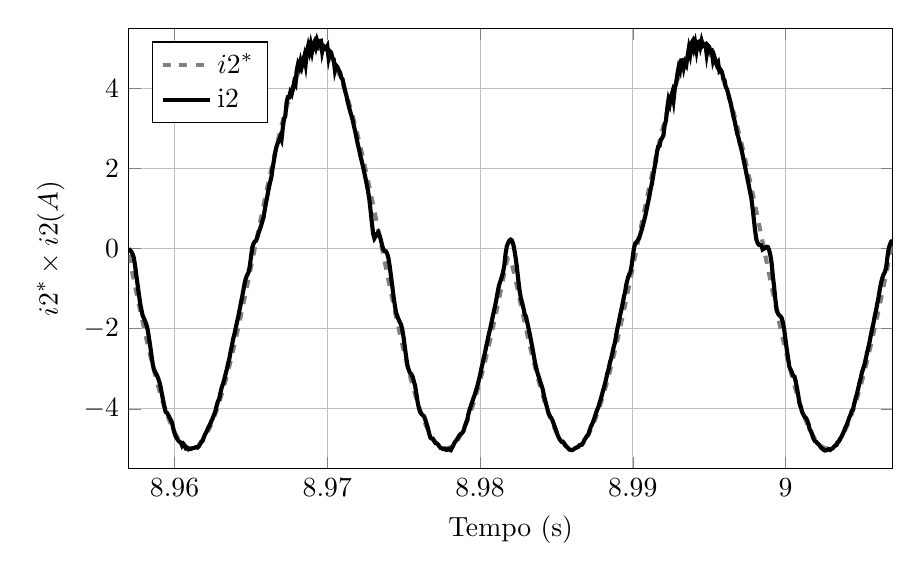
\begin{tikzpicture}

\begin{axis}[%
width=0.8\textwidth,
height=0.461611624834875\textwidth,
scale only axis,
xmin=8.957,
xmax=9.007,
xtick={8.96, 8.97, 8.98, 8.99,    9},
xlabel={Tempo (s)},
xmajorgrids,
ymin=-5.5,
ymax=5.5,
ytick={-4, -2,  0,  2,  4},
ylabel={$\text{i2}^\text{*}\text{ }\times\text{ i2 (A)}$},
ymajorgrids,
legend style={at={(0.03,0.97)},anchor=north west,draw=black,fill=white,legend cell align=left}
]
\addplot [color=gray,dashed,line width=1.5pt]
  table[row sep=crcr]{8.9570000023925	-0.157053337715654\\
8.95708334239271	-0.313642611979098\\
8.95716665239292	-0.469922358851051\\
8.95724999239313	-0.625738349089232\\
8.95733333239333	-0.780936811123168\\
8.95741667239354	-0.935364582808169\\
8.95749998239375	-1.08886926257787\\
8.95758332239396	-1.24129935984619\\
8.95766666239417	-1.39250444451023\\
8.95775000239438	-1.54233529540664\\
8.95783334239458	-1.69064404757487\\
8.95791665239479	-1.83728433818208\\
8.957999992395	-1.98211145096553\\
8.95808333239521	-2.1249824590501\\
8.95816667239542	-2.26575636599982\\
8.95824998239562	-2.40429424496438\\
8.95833332239583	-2.54045937578312\\
8.95841666239604	-2.67411737991134\\
8.95850000239625	-2.8051363530357\\
8.95858334239646	-2.93338699524782\\
8.95866665239667	-3.05874273864774\\
8.95874999239688	-3.1810798722511\\
8.95883333239708	-3.30027766407697\\
8.95891667239729	-3.41621848029576\\
8.9589999823975	-3.52878790131954\\
8.95908332239771	-3.63787483472045\\
8.95916666239792	-3.74337162486544\\
8.95925000239813	-3.84517415915942\\
8.95933334239833	-3.94318197079182\\
8.95941665239854	-4.03729833788517\\
8.95949999239875	-4.12743037894796\\
8.95958333239896	-4.21348914453744\\
8.95966667239917	-4.29538970504198\\
8.95974998239937	-4.37305123449631\\
8.95983332239958	-4.44639709034708\\
8.95991666239979	-4.5153548890897\\
8.9600000024	-4.57985657770219\\
8.96008334240021	-4.63983850080527\\
8.96016665240042	-4.69524146348255\\
8.96024999240062	-4.74601078969874\\
8.96033333240083	-4.79209637625833\\
8.96041667240104	-4.83345274225136\\
8.96049998240125	-4.8700390739376\\
8.96058332240146	-4.90181926502482\\
8.96066666240167	-4.92876195230126\\
8.96075000240188	-4.95084054658743\\
8.96083334240208	-4.96803325897633\\
8.96091665240229	-4.98032312233656\\
8.9609999924025	-4.98769800805673\\
8.96108333240271	-4.99015063801503\\
8.96116667240292	-4.98767859176179\\
8.96124998240312	-4.98028430890822\\
8.96133332240333	-4.96797508671877\\
8.96141666240354	-4.95076307290963\\
8.96150000240375	-4.9286652536604\\
8.96158334240396	-4.90170343685077\\
8.96166665240417	-4.8699042305388\\
8.96174999240437	-4.83329901670194\\
8.96183333240458	-4.79192392026687\\
8.96191667240479	-4.74581977345848\\
8.961999982405	-4.69503207550345\\
8.96208332240521	-4.63961094772799\\
8.96216666240542	-4.57961108409414\\
8.96225000240563	-4.51509169722343\\
8.96233334240583	-4.44611645996119\\
8.96241665240604	-4.37275344253912\\
8.96249999240625	-4.29507504539818\\
8.96258333240646	-4.21315792773813\\
8.96266667240667	-4.12708293186412\\
8.96274998240687	-4.03693500340512\\
8.96283332240708	-3.94280310748283\\
8.96291666240729	-3.84478014091384\\
8.9630000024075	-3.74296284053171\\
8.96308334240771	-3.63745168771934\\
8.96316665240792	-3.52835080924607\\
8.96324999240812	-3.41576787450702\\
8.96333333240833	-3.29981398926649\\
8.96341667240854	-3.18060358600992\\
8.96349998240875	-3.05825431101288\\
8.96358332240896	-2.9328869082384\\
8.96366666240917	-2.80462510017721\\
8.96375000240938	-2.67359546574863\\
8.96383334240958	-2.53992731538246\\
8.96391665240979	-2.40375256340514\\
8.96399999241	-2.26520559785631\\
8.96408333241021	-2.12442314786397\\
8.96416667241042	-1.98154414870942\\
8.96424998241062	-1.8367096047148\\
8.96433332241083	-1.69006245008898\\
8.96441666241104	-1.54174740786863\\
8.96450000241125	-1.39191084709413\\
8.96458334241146	-1.24070063836098\\
8.96466665241167	-1.08826600788938\\
8.96474999241187	-0.934757390255931\\
8.96483333241208	-0.78032627993293\\
8.96491667241229	-0.62512508178157\\
8.9649999824125	-0.469306960646756\\
8.96508332241271	-0.313025690201901\\
8.96516666241292	-0.156435501192865\\
8.96525000241313	0.000309070769160563\\
8.96533334241333	0.157053337715652\\
8.96541665241354	0.313642611979097\\
8.96549999241375	0.46992235885105\\
8.96558333241396	0.625738349089232\\
8.96566667241417	0.780936811123168\\
8.96574998241437	0.93536458280817\\
8.96583332241458	1.08886926257787\\
8.96591666241479	1.24129935984619\\
8.966000002415	1.39250444451023\\
8.96608334241521	1.54233529540664\\
8.96616665241542	1.69064404757488\\
8.96624999241562	1.83728433818209\\
8.96633333241583	1.98211145096554\\
8.96641667241604	2.1249824590501\\
8.96649998241625	2.26575636599983\\
8.96658332241646	2.40429424496439\\
8.96666666241667	2.54045937578313\\
8.96675000241687	2.67411737991135\\
8.96683334241708	2.80513635303571\\
8.96691665241729	2.93338699524783\\
8.9669999924175	3.05874273864775\\
8.96708333241771	3.18107987225111\\
8.96716667241792	3.30027766407699\\
8.96724998241812	3.41621848029577\\
8.96733332241833	3.52878790131955\\
8.96741666241854	3.63787483472046\\
8.96750000241875	3.74337162486546\\
8.96758334241896	3.84517415915944\\
8.96766665241917	3.94318197079183\\
8.96774999241937	4.03729833788518\\
8.96783333241958	4.12743037894798\\
8.96791667241979	4.21348914453746\\
8.96799998242	4.29538970504199\\
8.96808332242021	4.37305123449633\\
8.96816666242042	4.4463970903471\\
8.96825000242062	4.51535488908972\\
8.96833334242083	4.57985657770221\\
8.96841665242104	4.63983850080529\\
8.96849999242125	4.69524146348257\\
8.96858333242146	4.74601078969876\\
8.96866667242167	4.79209637625835\\
8.96874998242187	4.83345274225138\\
8.96883332242208	4.87003907393763\\
8.96891666242229	4.90181926502484\\
8.9690000024225	4.92876195230128\\
8.96908334242271	4.95084054658745\\
8.96916665242292	4.96803325897636\\
8.96924999242312	4.98032312233658\\
8.96933333242333	4.98769800805675\\
8.96941667242354	4.99015063801505\\
8.96949998242375	4.98767859176182\\
8.96958332242396	4.98028430890825\\
8.96966666242417	4.9679750867188\\
8.96975000242437	4.95076307290965\\
8.96983334242458	4.92866525366042\\
8.96991665242479	4.90170343685079\\
8.969999992425	4.86990423053882\\
8.97008333242521	4.83329901670197\\
8.97016667242542	4.79192392026689\\
8.97024998242562	4.7458197734585\\
8.97033332242583	4.69503207550347\\
8.97041666242604	4.63961094772801\\
8.97050000242625	4.57961108409416\\
8.97058334242646	4.51509169722345\\
8.97066665242667	4.44611645996121\\
8.97074999242687	4.37275344253914\\
8.97083333242708	4.2950750453982\\
8.97091667242729	4.21315792773815\\
8.9709999824275	4.12708293186414\\
8.97108332242771	4.03693500340514\\
8.97116666242792	3.94280310748285\\
8.97125000242812	3.84478014091386\\
8.97133334242833	3.74296284053172\\
8.97141665242854	3.63745168771936\\
8.97149999242875	3.52835080924608\\
8.97158333242896	3.41576787450704\\
8.97166667242917	3.2998139892665\\
8.97174998242937	3.18060358600993\\
8.97183332242958	3.0582543110129\\
8.97191666242979	2.93288690823841\\
8.97200000243	2.80462510017722\\
8.97208334243021	2.67359546574865\\
8.97216665243042	2.53992731538247\\
8.97224999243062	2.40375256340515\\
8.97233333243083	2.26520559785632\\
8.97241667243104	2.12442314786398\\
8.97249998243125	1.98154414870943\\
8.97258332243146	1.83670960471481\\
8.97266666243167	1.69006245008899\\
8.97275000243187	1.54174740786863\\
8.97283334243208	1.39191084709414\\
8.97291665243229	1.24070063836099\\
8.9729999924325	1.08826600788938\\
8.97308333243271	0.934757390255936\\
8.97316667243292	0.780326279932935\\
8.97324998243312	0.625125081781573\\
8.97333332243333	0.469306960646759\\
8.97341666243354	0.313025690201903\\
8.97350000243375	0.156435501192867\\
8.97358334243396	-0.000309070769160008\\
8.97366665243417	-0.157053337715652\\
8.97374999243437	-0.313642611979098\\
8.97383333243458	-0.469922358851052\\
8.97391667243479	-0.625738349089234\\
8.973999982435	-0.780936811123171\\
8.97408332243521	-0.935364582808174\\
8.97416666243542	-1.08886926257788\\
8.97425000243562	-1.2412993598462\\
8.97433334243583	-1.39250444451024\\
8.97441665243604	-1.54233529540665\\
8.97449999243625	-1.69064404757489\\
8.97458333243646	-1.8372843381821\\
8.97466667243667	-1.98211145096555\\
8.97474998243687	-2.12498245905011\\
8.97483332243708	-2.26575636599984\\
8.97491666243729	-2.4042942449644\\
8.9750000024375	-2.54045937578314\\
8.97508334243771	-2.67411737991137\\
8.97516665243792	-2.80513635303572\\
8.97524999243812	-2.93338699524785\\
8.97533333243833	-3.05874273864777\\
8.97541667243854	-3.18107987225113\\
8.97549998243875	-3.300277664077\\
8.97558332243896	-3.41621848029578\\
8.97566666243917	-3.52878790131957\\
8.97575000243937	-3.63787483472048\\
8.97583334243958	-3.74337162486547\\
8.97591665243979	-3.84517415915946\\
8.97599999244	-3.94318197079185\\
8.97608333244021	-4.0372983378852\\
8.97616667244042	-4.127430378948\\
8.97624998244062	-4.21348914453748\\
8.97633332244083	-4.29538970504201\\
8.97641666244104	-4.37305123449635\\
8.97650000244125	-4.44639709034712\\
8.97658334244146	-4.51535488908974\\
8.97666665244167	-4.57985657770223\\
8.97674999244187	-4.63983850080531\\
8.97683333244208	-4.69524146348259\\
8.97691667244229	-4.74601078969879\\
8.9769999824425	-4.79209637625837\\
8.97708332244271	-4.8334527422514\\
8.97716666244292	-4.87003907393765\\
8.97725000244312	-4.90181926502486\\
8.97733334244333	-4.92876195230131\\
8.97741665244354	-4.95084054658747\\
8.97749999244375	-4.96803325897638\\
8.97758333244396	-4.9803231223366\\
8.97766667244417	-4.98769800805677\\
8.97774998244438	-4.99015063801507\\
8.97783332244458	-4.98767859176184\\
8.97791666244479	-4.98028430890827\\
8.978000002445	-4.96797508671882\\
8.97808334244521	-4.95076307290968\\
8.97816665244542	-4.92866525366044\\
8.97824999244562	-4.90170343685081\\
8.97833333244583	-4.86990423053884\\
8.97841667244604	-4.83329901670199\\
8.97849998244625	-4.79192392026691\\
8.97858332244646	-4.74581977345852\\
8.97866666244667	-4.69503207550349\\
8.97875000244687	-4.63961094772803\\
8.97883334244708	-4.57961108409418\\
8.97891665244729	-4.51509169722347\\
8.9789999924475	-4.44611645996123\\
8.97908333244771	-4.37275344253916\\
8.97916667244792	-4.29507504539822\\
8.97924998244813	-4.21315792773817\\
8.97933332244833	-4.12708293186416\\
8.97941666244854	-4.03693500340516\\
8.97950000244875	-3.94280310748287\\
8.97958334244896	-3.84478014091388\\
8.97966665244917	-3.74296284053174\\
8.97974999244937	-3.63745168771938\\
8.97983333244958	-3.5283508092461\\
8.97991667244979	-3.41576787450705\\
8.97999998245	-3.29981398926652\\
8.98008332245021	-3.18060358600995\\
8.98016666245042	-3.05825431101291\\
8.98025000245062	-2.93288690823843\\
8.98033334245083	-2.80462510017723\\
8.98041665245104	-2.67359546574866\\
8.98049999245125	-2.53992731538248\\
8.98058333245146	-2.40375256340516\\
8.98066667245167	-2.26520559785633\\
8.98074998245188	-2.124423147864\\
8.98083332245208	-1.98154414870944\\
8.98091666245229	-1.83670960471482\\
8.9810000024525	-1.690062450089\\
8.98108334245271	-1.54174740786864\\
8.98116665245292	-1.39191084709414\\
8.98124999245312	-1.24070063836099\\
8.98133333245333	-1.08826600788939\\
8.98141667245354	-0.934757390255941\\
8.98149998245375	-0.780326279932939\\
8.98158332245396	-0.625125081781577\\
8.98166666245417	-0.469306960646762\\
8.98175000245437	-0.313025690201905\\
8.98183334245458	-0.234962398887561\\
8.98191665245479	-0.235194125748636\\
8.981999992455	-0.294088917675021\\
8.98208333245521	-0.391956928193599\\
8.98216667245542	-0.513977780075711\\
8.98224998245563	-0.650215191260269\\
8.98233332245583	-0.794399797988042\\
8.98241666245604	-0.942708359130287\\
8.98250000245625	-1.09284729218378\\
8.98258334245646	-1.24344144537157\\
8.98266665245667	-1.39365202263414\\
8.98274999245687	-1.5429473521492\\
8.98283333245708	-1.69096920978647\\
8.98291667245729	-1.83745648620804\\
8.9829999824575	-1.9822023084386\\
8.98308332245771	-2.12503027951668\\
8.98316666245792	-2.26578147209814\\
8.98325000245812	-2.40430739594607\\
8.98333334245833	-2.54046625024024\\
8.98341665245854	-2.67412096662305\\
8.98349999245875	-2.80513822113313\\
8.98358333245896	-2.93338796666734\\
8.98366667245917	-3.05874324304291\\
8.98374998245938	-3.1810801337914\\
8.98383332245958	-3.30027779951849\\
8.98391666245979	-3.41621855035221\\
8.98400000246	-3.52878793751563\\
8.98408334246021	-3.63787485340244\\
8.98416665246042	-3.74337163449842\\
8.98424999246063	-3.84517416412192\\
8.98433333246083	-3.94318197334608\\
8.98441667246104	-4.03729833919882\\
8.98449998246125	-4.12743037962306\\
8.98458332246146	-4.21348914488415\\
8.98466666246167	-4.29538970521992\\
8.98475000246187	-4.3730512345876\\
8.98483334246208	-4.44639709039389\\
8.98491665246229	-4.51535488911371\\
8.9849999924625	-4.57985657771451\\
8.98508333246271	-4.63983850081161\\
8.98516667246292	-4.69524146348582\\
8.98524998246313	-4.74601078970045\\
8.98533332246333	-4.79209637625923\\
8.98541666246354	-4.83345274225185\\
8.98550000246375	-4.87003907393789\\
8.98558334246396	-4.90181926502499\\
8.98566665246417	-4.92876195230139\\
8.98574999246438	-4.95084054658752\\
8.98583333246458	-4.96803325897642\\
8.98591667246479	-4.98032312233663\\
8.985999982465	-4.9876980080568\\
8.98608332246521	-4.9901506380151\\
8.98616666246542	-4.98767859176186\\
8.98625000246562	-4.98028430890829\\
8.98633334246583	-4.96797508671884\\
8.98641665246604	-4.9507630729097\\
8.98649999246625	-4.92866525366047\\
8.98658333246646	-4.90170343685084\\
8.98666667246667	-4.86990423053886\\
8.98674998246688	-4.83329901670201\\
8.98683332246708	-4.79192392026693\\
8.98691666246729	-4.74581977345854\\
8.9870000024675	-4.69503207550351\\
8.98708334246771	-4.63961094772805\\
8.98716665246792	-4.5796110840942\\
8.98724999246813	-4.51509169722349\\
8.98733333246833	-4.44611645996125\\
8.98741667246854	-4.37275344253918\\
8.98749998246875	-4.29507504539824\\
8.98758332246896	-4.21315792773819\\
8.98766666246917	-4.12708293186418\\
8.98775000246937	-4.03693500340518\\
8.98783334246958	-3.94280310748288\\
8.98791665246979	-3.8447801409139\\
8.98799999247	-3.74296284053176\\
8.98808333247021	-3.63745168771939\\
8.98816667247042	-3.52835080924612\\
8.98824998247063	-3.41576787450707\\
8.98833332247083	-3.29981398926653\\
8.98841666247104	-3.18060358600996\\
8.98850000247125	-3.05825431101293\\
8.98858334247146	-2.93288690823844\\
8.98866665247167	-2.80462510017725\\
8.98874999247188	-2.67359546574867\\
8.98883333247208	-2.53992731538249\\
8.98891667247229	-2.40375256340517\\
8.9889999824725	-2.26520559785634\\
8.98908332247271	-2.124423147864\\
8.98916666247292	-1.98154414870944\\
8.98925000247313	-1.83670960471483\\
8.98933334247333	-1.690062450089\\
8.98941665247354	-1.54174740786865\\
8.98949999247375	-1.39191084709415\\
8.98958333247396	-1.240700638361\\
8.98966667247417	-1.08826600788939\\
8.98974998247438	-0.934757390255946\\
8.98983332247458	-0.780326279932943\\
8.98991666247479	-0.625125081781581\\
8.990000002475	-0.469306960646765\\
8.99008334247521	-0.313025690201907\\
8.99016665247542	-0.15643550119287\\
8.99024999247563	0.000309070769158107\\
8.99033333247583	0.157053337715651\\
8.99041667247604	0.313642611979099\\
8.99049998247625	0.469922358851054\\
8.99058332247646	0.625738349089237\\
8.99066666247667	0.780936811123176\\
8.99075000247688	0.93536458280818\\
8.99083334247708	1.08886926257789\\
8.99091665247729	1.24129935984621\\
8.9909999924775	1.39250444451025\\
8.99108333247771	1.54233529540666\\
8.99116667247792	1.6906440475749\\
8.99124998247813	1.83728433818211\\
8.99133332247833	1.98211145096556\\
8.99141666247854	2.12498245905013\\
8.99150000247875	2.26575636599985\\
8.99158334247896	2.40429424496442\\
8.99166665247917	2.54045937578316\\
8.99174999247938	2.67411737991139\\
8.99183333247958	2.80513635303574\\
8.99191667247979	2.93338699524787\\
8.99199998248	3.05874273864779\\
8.99208332248021	3.18107987225115\\
8.99216666248042	3.30027766407703\\
8.99225000248063	3.41621848029581\\
8.99233334248083	3.5287879013196\\
8.99241665248104	3.63787483472051\\
8.99249999248125	3.7433716248655\\
8.99258333248146	3.84517415915949\\
8.99266667248167	3.94318197079189\\
8.99274998248188	4.03729833788524\\
8.99283332248208	4.12743037894803\\
8.99291666248229	4.21348914453752\\
8.9930000024825	4.29538970504205\\
8.99308334248271	4.37305123449639\\
8.99316665248292	4.44639709034716\\
8.99324999248313	4.51535488908978\\
8.99333333248333	4.57985657770227\\
8.99341667248354	4.63983850080535\\
8.99349998248375	4.69524146348263\\
8.99358332248396	4.74601078969883\\
8.99366666248417	4.79209637625842\\
8.99375000248438	4.83345274225144\\
8.99383334248458	4.87003907393769\\
8.99391665248479	4.9018192650249\\
8.993999992485	4.92876195230135\\
8.99408333248521	4.95084054658752\\
8.99416667248542	4.96803325897642\\
8.99424998248563	4.98032312233665\\
8.99433332248583	4.98769800805682\\
8.99441666248604	4.99015063801512\\
8.99450000248625	4.98767859176188\\
8.99458334248646	4.98028430890831\\
8.99466665248667	4.96797508671886\\
8.99474999248688	4.95076307290972\\
8.99483333248708	4.92866525366049\\
8.99491667248729	4.90170343685086\\
8.9949999824875	4.86990423053888\\
8.99508332248771	4.83329901670203\\
8.99516666248792	4.79192392026696\\
8.99525000248813	4.74581977345856\\
8.99533334248833	4.69503207550353\\
8.99541665248854	4.63961094772807\\
8.99549999248875	4.57961108409422\\
8.99558333248896	4.51509169722351\\
8.99566667248917	4.44611645996127\\
8.99574998248938	4.3727534425392\\
8.99583332248958	4.29507504539826\\
8.99591666248979	4.2131579277382\\
8.99600000249	4.12708293186419\\
8.99608334249021	4.03693500340519\\
8.99616665249042	3.9428031074829\\
8.99624999249063	3.84478014091391\\
8.99633333249083	3.74296284053177\\
8.99641667249104	3.63745168771941\\
8.99649998249125	3.52835080924613\\
8.99658332249146	3.41576787450708\\
8.99666666249167	3.29981398926655\\
8.99675000249188	3.18060358600998\\
8.99683334249208	3.05825431101294\\
8.99691665249229	2.93288690823845\\
8.9969999924925	2.80462510017726\\
8.99708333249271	2.67359546574868\\
8.99716667249292	2.53992731538251\\
8.99724998249313	2.40375256340519\\
8.99733332249333	2.26520559785635\\
8.99741666249354	2.12442314786402\\
8.99750000249375	1.98154414870945\\
8.99758334249396	1.83670960471484\\
8.99766665249417	1.69006245008901\\
8.99774999249438	1.54174740786866\\
8.99783333249458	1.39191084709416\\
8.99791667249479	1.24070063836101\\
8.997999982495	1.0882660078894\\
8.99808332249521	0.934757390255951\\
8.99816666249542	0.780326279932948\\
8.99825000249563	0.625125081781584\\
8.99833334249583	0.469306960646768\\
8.99841665249604	0.31302569020191\\
8.99849999249625	0.156435501192872\\
8.99858333249646	-0.000309070769156955\\
8.99866667249667	-0.157053337715651\\
8.99874998249688	-0.313642611979099\\
8.99883332249708	-0.469922358851055\\
8.99891666249729	-0.625738349089239\\
8.9990000024975	-0.780936811123178\\
8.99908334249771	-0.935364582808183\\
8.99916665249792	-1.08886926257789\\
8.99924999249813	-1.24129935984621\\
8.99933333249833	-1.39250444451026\\
8.99941667249854	-1.54233529540666\\
8.99949998249875	-1.6906440475749\\
8.99958332249896	-1.83728433818212\\
8.99966666249917	-1.98211145096557\\
8.99975000249938	-2.12498245905014\\
8.99983334249958	-2.26575636599986\\
8.99991665249979	-2.40429424496443\\
8.9999999925	-2.54045937578317\\
9.00008333250021	-2.6741173799114\\
9.00016667250042	-2.80513635303576\\
9.00024998250063	-2.93338699524788\\
9.00033332250083	-3.0587427386478\\
9.00041666250104	-3.18107987225116\\
9.00050000250125	-3.30027766407704\\
9.00058334250146	-3.41621848029583\\
9.00066665250167	-3.52878790131961\\
9.00074999250188	-3.63787483472053\\
9.00083333250208	-3.74337162486552\\
9.00091667250229	-3.8451741591595\\
9.0009999825025	-3.9431819707919\\
9.00108332250271	-4.03729833788526\\
9.00116666250292	-4.12743037894805\\
9.00125000250313	-4.21348914453753\\
9.00133334250333	-4.29538970504207\\
9.00141665250354	-4.37305123449641\\
9.00149999250375	-4.44639709034718\\
9.00158333250396	-4.5153548890898\\
9.00166667250417	-4.57985657770229\\
9.00174998250438	-4.63983850080537\\
9.00183332250458	-4.69524146348265\\
9.00191666250479	-4.74601078969885\\
9.002000002505	-4.79209637625844\\
9.00208334250521	-4.83345274225146\\
9.00216665250542	-4.87003907393771\\
9.00224999250563	-4.90181926502493\\
9.00233333250583	-4.92876195230137\\
9.00241667250604	-4.95084054658754\\
9.00249998250625	-4.96803325897644\\
9.00258332250646	-4.98032312233667\\
9.00266666250667	-4.98769800805684\\
9.00275000250688	-4.99015063801514\\
9.00283334250708	-4.9876785917619\\
9.00291665250729	-4.98028430890833\\
9.0029999925075	-4.96797508671888\\
9.00308333250771	-4.95076307290974\\
9.00316667250792	-4.92866525366051\\
9.00324998250812	-4.90170343685088\\
9.00333332250833	-4.8699042305389\\
9.00341666250854	-4.83329901670205\\
9.00350000250875	-4.79192392026698\\
9.00358334250896	-4.74581977345858\\
9.00366665250917	-4.69503207550355\\
9.00374999250938	-4.63961094772809\\
9.00383333250958	-4.57961108409424\\
9.00391667250979	-4.51509169722353\\
9.00399998251	-4.44611645996129\\
9.00408332251021	-4.37275344253922\\
9.00416666251042	-4.29507504539828\\
9.00425000251063	-4.21315792773822\\
9.00433334251083	-4.12708293186421\\
9.00441665251104	-4.03693500340521\\
9.00449999251125	-3.94280310748292\\
9.00458333251146	-3.84478014091393\\
9.00466667251167	-3.74296284053179\\
9.00474998251187	-3.63745168771943\\
9.00483332251208	-3.52835080924615\\
9.00491666251229	-3.4157678745071\\
9.0050000025125	-3.29981398926656\\
9.00508334251271	-3.18060358600999\\
9.00516665251292	-3.05825431101296\\
9.00524999251313	-2.93288690823847\\
9.00533333251333	-2.80462510017727\\
9.00541667251354	-2.6735954657487\\
9.00549998251375	-2.53992731538252\\
9.00558332251396	-2.4037525634052\\
9.00566666251417	-2.26520559785636\\
9.00575000251438	-2.12442314786403\\
9.00583334251458	-1.98154414870946\\
9.00591665251479	-1.83670960471485\\
9.005999992515	-1.69006245008902\\
9.00608333251521	-1.54174740786867\\
9.00616667251542	-1.39191084709417\\
9.00624998251562	-1.24070063836102\\
9.00633332251583	-1.08826600788941\\
9.00641666251604	-0.934757390255958\\
9.00650000251625	-0.780326279932954\\
9.00658334251646	-0.62512508178159\\
9.00666665251667	-0.469306960646773\\
9.00674999251688	-0.313025690201914\\
9.00683333251708	-0.156435501192875\\
9.00691667251729	0.000309070769154721\\
9.0069999825175	0.15705333771565\\
};
\addlegendentry{$\text{i2}^\text{*}$};

\addplot [color=black,solid,line width=1.5pt]
  table[row sep=crcr]{8.9570000023925	-0.00330524129232349\\
8.95708334239271	-0.0428438155110735\\
8.95716665239292	-0.0741243330891985\\
8.95724999239313	-0.137436100667323\\
8.95733333239333	-0.227523991292323\\
8.95741667239354	-0.420962711995448\\
8.95749998239375	-0.676211735432948\\
8.95758332239396	-0.907937809651698\\
8.95766666239417	-1.14091510457357\\
8.95775000239438	-1.3683870284017\\
8.95783334239458	-1.53304767293295\\
8.95791665239479	-1.6756868330892\\
8.957999992395	-1.74425372762045\\
8.95808333239521	-1.8218294112142\\
8.95816667239542	-1.90541095418295\\
8.95824998239562	-2.04254474324545\\
8.95833332239583	-2.2462434737142\\
8.95841666239604	-2.45519733113607\\
8.95850000239625	-2.6936799971517\\
8.95858334239646	-2.91264362019857\\
8.95866665239667	-3.02775592488607\\
8.95874999239688	-3.09432086629232\\
8.95883333239708	-3.1511262862142\\
8.95891667239729	-3.22594928426107\\
8.9589999823975	-3.32054156941732\\
8.95908332239771	-3.44516315144857\\
8.95916666239792	-3.61808185262045\\
8.95925000239813	-3.7787385909017\\
8.95933334239833	-3.9408967940267\\
8.95941665239854	-4.07677936238607\\
8.95949999239875	-4.09955157918295\\
8.95958333239896	-4.14734821004232\\
8.95966667239917	-4.21541461629232\\
8.95974998239937	-4.27272052449545\\
8.95983332239958	-4.34404010457357\\
8.95991666239979	-4.48717975301107\\
8.9600000024	-4.61080035847982\\
8.96008334240021	-4.69388141316732\\
8.96016665240042	-4.74643268269857\\
8.96024999240062	-4.79422931355795\\
8.96033333240083	-4.82225665730795\\
8.96041667240104	-4.84302692097982\\
8.96049998240125	-4.9218538252767\\
8.96058332240146	-4.87555865926107\\
8.96066666240167	-4.91734943074545\\
8.96075000240188	-4.98841876668295\\
8.96083334240208	-4.97315387410482\\
8.96091665240229	-5.0099397627767\\
8.9609999924025	-4.99542560262045\\
8.96108333240271	-4.99942950887045\\
8.96116667240292	-4.98316363972982\\
8.96124998240312	-4.9779085127767\\
8.96133332240333	-4.96739825887045\\
8.96141666240354	-4.9538850752767\\
8.96150000240375	-4.9678987471517\\
8.96158334240396	-4.94162311238607\\
8.96166665240417	-4.88106403035482\\
8.96174999240437	-4.81925372762045\\
8.96183333240458	-4.79823321980795\\
8.96191667240479	-4.7126497237142\\
8.961999982405	-4.6335725752767\\
8.96208332240521	-4.5805208174642\\
8.96216666240542	-4.49919147176107\\
8.96225000240563	-4.4403840987142\\
8.96233334240583	-4.37557086629232\\
8.96241665240604	-4.3012483565267\\
8.96249999240625	-4.2321809737142\\
8.96258333240646	-4.14659747762045\\
8.96266667240667	-4.06551837605795\\
8.96274998240687	-3.93739337605795\\
8.96283332240708	-3.81827716512045\\
8.96291666240729	-3.7597200362142\\
8.9630000024075	-3.6105745284017\\
8.96308334240771	-3.47118854207357\\
8.96316665240792	-3.38385333699545\\
8.96324999240812	-3.2742464034017\\
8.96333333240833	-3.14361896199545\\
8.96341667240854	-3.02325153035482\\
8.96349998240875	-2.87710895222982\\
8.96358332240896	-2.75348834676107\\
8.96366666240917	-2.57906818074545\\
8.96375000240938	-2.43167438191732\\
8.96383334240958	-2.26150836629232\\
8.96391665240979	-2.13738727254232\\
8.96399999241	-1.99224567097982\\
8.96408333241021	-1.84410113972982\\
8.96416667241042	-1.7067171065267\\
8.96424998241062	-1.54480914754232\\
8.96433332241083	-1.3773958174642\\
8.96441666241104	-1.2212434737142\\
8.96450000241125	-1.0520784346517\\
8.96458334241146	-0.873153874104823\\
8.96466665241167	-0.741525456136073\\
8.96474999241187	-0.661697575276698\\
8.96483333241208	-0.607144352620448\\
8.96491667241229	-0.459750553792323\\
8.9649999824125	-0.227523991292323\\
8.96508332241271	0.0204679520670515\\
8.96516666241292	0.118063166910802\\
8.96525000241313	0.174368098551426\\
8.96533334241333	0.192886164957676\\
8.96541665241354	0.278469661051427\\
8.96549999241375	0.390078547770176\\
8.96558333241396	0.477663996988926\\
8.96566667241417	0.573007014567052\\
8.96574998241437	0.682613948160801\\
8.96583332241458	0.787716487223301\\
8.96591666241479	0.990664485270176\\
8.966000002415	1.1650846512858\\
8.96608334241521	1.33249798136393\\
8.96616665241542	1.50066204386393\\
8.96624999241562	1.6485563309733\\
8.96633333241583	1.77042522745768\\
8.96641667241604	1.99914837198893\\
8.96649998241625	2.18858318644205\\
8.96658332241646	2.37901897745768\\
8.96666666241667	2.5324186356608\\
8.96675000241687	2.63076458292643\\
8.96683334241708	2.6955778153483\\
8.96691665241729	2.79042034464518\\
8.9669999924175	2.71709881144205\\
8.96708333241771	3.0008756669108\\
8.96716667241792	3.23660564737955\\
8.96724998241812	3.3051725419108\\
8.96733332241833	3.64475384073893\\
8.96741666241854	3.77713299112955\\
8.96750000241875	3.77788372355143\\
8.96758334241896	3.9077604325358\\
8.96766665241917	3.85195598917643\\
8.96774999241937	3.98158245402018\\
8.96783333241958	4.1560026200358\\
8.96791667241979	4.10169964152018\\
8.96799998242	4.4542936356608\\
8.96808332242021	4.60318889933268\\
8.96816666242042	4.52586345987955\\
8.96825000242062	4.67776165323893\\
8.96833334242083	4.54688396769205\\
8.96841665242104	4.6725065262858\\
8.96849999242125	4.80213299112955\\
8.96858333242146	4.61094646769205\\
8.96866667242167	4.91199016886393\\
8.96874998242187	5.0578825028483\\
8.96883332242208	4.91999798136393\\
8.96891666242229	5.08966350870768\\
8.9690000024225	4.9187467606608\\
8.96908334242271	5.09917278605143\\
8.96916665242292	5.16473675089518\\
8.96924999242312	5.03811321573893\\
8.96933333242333	5.19251385050455\\
8.96941667242354	5.09316692667643\\
8.96949998242375	5.1759977372233\\
8.96958332242396	5.18475628214518\\
8.96966666242417	4.91499309855143\\
8.96975000242437	5.05613079386393\\
8.96983334242458	5.02359905558268\\
8.96991665242479	4.9868131669108\\
8.969999992425	5.04562053995768\\
8.97008333242521	4.7686002762858\\
8.97016667242542	4.9277555497233\\
8.97024998242562	4.89647503214518\\
8.97033332242583	4.7595914872233\\
8.97041666242604	4.7275602372233\\
8.97050000242625	4.44678631144205\\
8.97058334242646	4.56815471964518\\
8.97066665242667	4.52811565714518\\
8.97074999242687	4.4572965653483\\
8.97083333242708	4.39498577433268\\
8.97091667242729	4.26535930948893\\
8.9709999824275	4.2250700028483\\
8.97108332242771	4.07267132120768\\
8.97116666242792	3.93328533487955\\
8.97125000242812	3.81917400675455\\
8.97133334242833	3.66302166300455\\
8.97141665242854	3.53714886027018\\
8.97149999242875	3.42103557902018\\
8.97158333242896	3.31393108683268\\
8.97166667242917	3.1930631669108\\
8.97174998242937	3.05042400675455\\
8.97183332242958	2.91303997355143\\
8.97191666242979	2.75638714152018\\
8.97200000243	2.59923382120768\\
8.97208334243021	2.47010784464518\\
8.97216665243042	2.30970135050455\\
8.97224999243062	2.18858318644205\\
8.97233333243083	2.0529508622233\\
8.97241667243104	1.90906048136393\\
8.97249998243125	1.75641155558268\\
8.97258332243146	1.59725628214518\\
8.97266666243167	1.43659954386393\\
8.97275000243187	1.23139934855143\\
8.97283334243208	0.949123957926426\\
8.97291665243229	0.648580745035801\\
8.9729999924325	0.372060969645176\\
8.97308333243271	0.256448176676427\\
8.97316667243292	0.309249690348301\\
8.97324998243312	0.366555598551427\\
8.97333332243333	0.406594661051427\\
8.97341666243354	0.329769709879552\\
8.97350000243375	0.221413996988927\\
8.97358334243396	0.0877836258951765\\
8.97366665243417	-0.0163179366048235\\
8.97374999243437	-0.0616121260579485\\
8.97383333243458	-0.0676179854329485\\
8.97391667243479	-0.122421452229823\\
8.973999982435	-0.235281559651698\\
8.97408332243521	-0.437228581136073\\
8.97416666243542	-0.681216618245448\\
8.97425000243562	-0.927206608479823\\
8.97433334243583	-1.1832063643392\\
8.97441665243604	-1.40467242879232\\
8.97449999243625	-1.59385699910482\\
8.97458333243646	-1.68244342488607\\
8.97466667243667	-1.7697786299642\\
8.97474998243687	-1.8418489424642\\
8.97483332243708	-1.89915485066732\\
8.97491666243729	-2.04179401082357\\
8.9750000024375	-2.23648395222982\\
8.97508334243771	-2.4814729659017\\
8.97516665243792	-2.71545123738607\\
8.97524999243812	-2.9239046065267\\
8.97533333243833	-3.02925738972982\\
8.97541667243854	-3.10633258504232\\
8.97549998243875	-3.13160724324545\\
8.97558332243896	-3.19541949910482\\
8.97566666243917	-3.3152864424642\\
8.97575000243937	-3.42789630574545\\
8.97583334243958	-3.6275911299642\\
8.97591665243979	-3.84004840535482\\
8.97599999244	-3.98744220418295\\
8.97608333244021	-4.08453693074545\\
8.97616667244042	-4.1310823409017\\
8.97624998244062	-4.1591096846517\\
8.97633332244083	-4.1861360518392\\
8.97641666244104	-4.2722200362142\\
8.97650000244125	-4.37081622762045\\
8.97658334244146	-4.4814241377767\\
8.97666665244167	-4.61180133504232\\
8.97674999244187	-4.72090778035482\\
8.97683333244208	-4.7416780440267\\
8.97691667244229	-4.7536897627767\\
8.9769999824425	-4.80824298543295\\
8.97708332244271	-4.85628986043295\\
8.97716666244292	-4.8607942549642\\
8.97725000244312	-4.8918245284017\\
8.97733334244333	-4.93862018269857\\
8.97741665244354	-4.97465533894857\\
8.97749999244375	-4.98166217488607\\
8.97758333244396	-5.00318317097982\\
8.97766667244417	-4.99242267293295\\
8.97774998244438	-5.01919879597982\\
8.97783332244458	-5.02220172566732\\
8.97791666244479	-5.0039339034017\\
8.978000002445	-5.02245196980795\\
8.97808334244521	-5.03346271199545\\
8.97816665244542	-4.96864947957357\\
8.97824999244562	-4.91059283894857\\
8.97833333244583	-4.83902301472982\\
8.97841667244604	-4.79923419637045\\
8.97849998244625	-4.7576936690267\\
8.97858332244646	-4.7036409346517\\
8.97866666244667	-4.65184039754232\\
8.97875000244687	-4.62531451863607\\
8.97883334244708	-4.59628619832357\\
8.97891665244729	-4.55324420613607\\
8.9789999924475	-4.44113483113607\\
8.97908333244771	-4.3482942549642\\
8.97916667244792	-4.26346149129232\\
8.97924998244813	-4.1090608565267\\
8.97933332244833	-3.99870319051107\\
8.97941666244854	-3.90035724324545\\
8.97950000244875	-3.8097688643392\\
8.97958334244896	-3.7166780440267\\
8.97966665244917	-3.6315950362142\\
8.97974999244937	-3.51898517293295\\
8.97983333244958	-3.41588458699545\\
8.97991667244979	-3.28375568074545\\
8.97999998245	-3.15988483113607\\
8.98008332245021	-2.99847736043295\\
8.98016666245042	-2.86459674519857\\
8.98025000245062	-2.70844440144857\\
8.98033334245083	-2.5795686690267\\
8.98041665245104	-2.42191486043295\\
8.98049999245125	-2.27176837605795\\
8.98058333245146	-2.12437457722982\\
8.98066667245167	-1.9919954268392\\
8.98074998245188	-1.84034747762045\\
8.98083332245208	-1.6927034346517\\
8.98091666245229	-1.54505939168295\\
8.9810000024525	-1.40191974324545\\
8.98108334245271	-1.23500690144857\\
8.98116665245292	-1.05933551472982\\
8.98124999245312	-0.905435368245448\\
8.98133333245333	-0.810843083089198\\
8.98141667245354	-0.710495182698573\\
8.98149998245375	-0.598385807698573\\
8.98158332245396	-0.430972477620448\\
8.98166666245417	-0.141690251057948\\
8.98175000245437	0.0575040848795515\\
8.98183334245458	0.138833430582677\\
8.98191665245479	0.202395442301426\\
8.981999992455	0.223415950113927\\
8.98208333245521	0.201894954020176\\
8.98216667245542	0.119064143473301\\
8.98224998245563	-0.0443452803548235\\
8.98233332245583	-0.241787907307948\\
8.98241666245604	-0.484274479573573\\
8.98250000245625	-0.773306461995448\\
8.98258334245646	-1.03681354207357\\
8.98266665245667	-1.2282503096517\\
8.98274999245687	-1.34686603230795\\
8.98283333245708	-1.47424029988607\\
8.98291667245729	-1.6326448409017\\
8.9829999824575	-1.68694781941732\\
8.98308332245771	-1.83258990926107\\
8.98316666245792	-1.98148517293295\\
8.98325000245812	-2.1281282393392\\
8.98333334245833	-2.2922883955892\\
8.98341665245854	-2.45820026082357\\
8.98349999245875	-2.6346223799642\\
8.98358333245896	-2.81705035847982\\
8.98366667245917	-2.95618610066732\\
8.98374998245938	-3.0890657393392\\
8.98383332245958	-3.18966388387045\\
8.98391666245979	-3.29376544637045\\
8.98400000246	-3.39411334676107\\
8.98408334246021	-3.48320026082357\\
8.98416665246042	-3.6365999190267\\
8.98424999246063	-3.77323321980795\\
8.98433333246083	-3.89735431355795\\
8.98441667246104	-4.0149690596517\\
8.98449998246125	-4.12657794637045\\
8.98458332246146	-4.18463458699545\\
8.98466666246167	-4.23593463582357\\
8.98475000246187	-4.29899615926107\\
8.98483334246208	-4.38983478230795\\
8.98491665246229	-4.47091388387045\\
8.9849999924625	-4.56725787801107\\
8.98508333246271	-4.6605989424642\\
8.98516667246292	-4.72816486043295\\
8.98524998246313	-4.7817171065267\\
8.98533332246333	-4.82100543660482\\
8.98541666246354	-4.82025470418295\\
8.98550000246375	-4.85654010457357\\
8.98558334246396	-4.91835040730795\\
8.98566665246417	-4.9468782393392\\
8.98574999246438	-4.97240314168295\\
8.98583333246458	-5.01519488972982\\
8.98591667246479	-5.02170123738607\\
8.985999982465	-5.03071002644857\\
8.98608332246521	-5.02019977254232\\
8.98616666246542	-4.99767779988607\\
8.98625000246562	-4.97540607137045\\
8.98633334246583	-4.96314410847982\\
8.98641665246604	-4.94662799519857\\
8.98649999246625	-4.90909137410482\\
8.98658333246646	-4.90158404988607\\
8.98666667246667	-4.89532794637045\\
8.98674998246688	-4.8487825362142\\
8.98683332246708	-4.77145709676107\\
8.98691666246729	-4.72891559285482\\
8.9870000024675	-4.6746126143392\\
8.98708334246771	-4.64783649129232\\
8.98716665246792	-4.54223346394857\\
8.98724999246813	-4.44588946980795\\
8.98733333246833	-4.38482989949545\\
8.98741667246854	-4.30650348347982\\
8.98749998246875	-4.20765704793295\\
8.98758332246896	-4.11531696004232\\
8.98766666246917	-4.02422809285482\\
8.98775000246937	-3.95015582722982\\
8.98783334246958	-3.83829669637045\\
8.98791665246979	-3.73644733113607\\
8.98799999247	-3.61633014363607\\
8.98808333247021	-3.49896564168295\\
8.98816667247042	-3.3893587080892\\
8.98824998247063	-3.2562288252767\\
8.98833332247083	-3.11033649129232\\
8.98841666247104	-3.0049837080892\\
8.98850000247125	-2.84758014363607\\
8.98858334247146	-2.73947467488607\\
8.98866665247167	-2.59783649129232\\
8.98874999247188	-2.45494708699545\\
8.98883333247208	-2.3383333174642\\
8.98891667247229	-2.1411409346517\\
8.9889999824725	-1.9769807784017\\
8.98908332247271	-1.83233966512045\\
8.98916666247292	-1.66492633504232\\
8.98925000247313	-1.5275423018392\\
8.98933334247333	-1.37214069051107\\
8.98941665247354	-1.2052278487142\\
8.98949999247375	-1.07059650105795\\
8.98958333247396	-0.878409001057948\\
8.98966667247417	-0.750033756917323\\
8.98974998247438	-0.652688786214198\\
8.98983332247458	-0.592129704182948\\
8.98991666247479	-0.438229557698573\\
8.990000002475	-0.191739079182948\\
8.99008334247521	0.0272245438639265\\
8.99016665247542	0.137832454020176\\
8.99024999247563	0.159103205973301\\
8.99033333247583	0.213656428629551\\
8.99041667247604	0.264956477457676\\
8.99049998247625	0.370809748942051\\
8.99058332247646	0.471407893473301\\
8.99066666247667	0.587270930582676\\
8.99075000247688	0.716897395426427\\
8.99083334247708	0.844021418863926\\
8.99091665247729	1.00617962198893\\
8.9909999924775	1.15782757120768\\
8.99108333247771	1.30797405558268\\
8.99116667247792	1.48714886027018\\
8.99124998247813	1.62303142862955\\
8.99133332247833	1.82047405558268\\
8.99141666247854	2.01666546183268\\
8.99150000247875	2.16430950480143\\
8.99158334247896	2.41680584269205\\
8.99166665247917	2.54718303995768\\
8.99174999247938	2.56169720011393\\
8.99183333247958	2.7155973465983\\
8.99191667247979	2.75588665323893\\
8.99199998248	2.82245159464518\\
8.99208332248021	3.0719450028483\\
8.99216666248042	3.1910612137858\\
8.99225000248063	3.48985271769205\\
8.99233334248083	3.71181927042643\\
8.99241665248104	3.6094694169108\\
8.99249999248125	3.79490032511393\\
8.99258333248146	3.90050335245768\\
8.99266667248167	3.70581341105143\\
8.99274998248188	4.00060100870768\\
8.99283332248208	4.13047771769205\\
8.99291666248229	4.35169353800455\\
8.9930000024825	4.52661419230143\\
8.99308334248271	4.44478435831705\\
8.99316665248292	4.6965299637858\\
8.99324999248313	4.70103435831705\\
8.99333333248333	4.5143522294108\\
8.99341667248354	4.65198650675455\\
8.99349998248375	4.58867473917643\\
8.99358332248396	4.79938030558268\\
8.99366666248417	5.00032635050455\\
8.99375000248438	4.85993938761393\\
8.99383334248458	5.13045330362955\\
8.99391665248479	5.18150310831705\\
8.993999992485	5.00833416300455\\
8.99408333248521	5.13520794230143\\
8.99416667248542	4.94151897745768\\
8.99424998248563	5.15347576456705\\
8.99433332248583	5.16748943644205\\
8.99441666248604	5.03435955362955\\
8.99450000248625	5.18750896769205\\
8.99458334248646	5.0708951981608\\
8.99466665248667	5.10718059855143\\
8.99474999248688	5.11068401652018\\
8.99483333248708	4.85743694620768\\
8.99491667248729	5.06714153605143\\
8.9949999824875	5.03235760050455\\
8.99508332248771	4.91624431925455\\
8.99516666248792	4.93426189737955\\
8.99525000248813	4.69177532511393\\
8.99533334248833	4.79387493448893\\
8.99541665248854	4.69477825480143\\
8.99549999248875	4.58792400675455\\
8.99558333248896	4.63997478800455\\
8.99566667248917	4.42951946573893\\
8.99574998248938	4.45879803019205\\
8.99583332248958	4.41050091105143\\
8.99591666248979	4.25585003214518\\
8.99600000249	4.2050504715983\\
8.99608334249021	4.03113079386393\\
8.99616665249042	3.97607708292643\\
8.99624999249063	3.85721111612955\\
8.99633333249083	3.72608318644205\\
8.99641667249104	3.61072063761393\\
8.99649998249125	3.45581951456705\\
8.99658332249146	3.3021696122233\\
8.99666666249167	3.1810514481608\\
8.99675000249188	3.02414837198893\\
8.99683334249208	2.86649456339518\\
8.99691665249229	2.76914959269205\\
8.9969999924925	2.63001385050455\\
8.99708333249271	2.51415081339518\\
8.99716667249292	2.37701702433268\\
8.99724998249313	2.21235637980143\\
8.99733332249333	2.0689664872233\\
8.99741666249354	1.9068082840983\\
8.99750000249375	1.7506559403483\\
8.99758334249396	1.5965055497233\\
8.99766665249417	1.42608928995768\\
8.99774999249438	1.27944622355143\\
8.99783333249458	1.03370647745768\\
8.99791667249479	0.752181819254551\\
8.997999982495	0.458895686442051\\
8.99808332249521	0.234676936442052\\
8.99816666249542	0.143337825113927\\
8.99825000249563	0.0950407059733015\\
8.99833334249583	0.0890348465983015\\
8.99841665249604	0.0780241044108015\\
8.99849999249625	-0.0215730635579485\\
8.99858333249646	-0.000302311604823483\\
8.99866667249667	0.0134611161295515\\
8.99874998249688	0.0457426102701765\\
8.99883332249708	0.0397367508951765\\
8.99891666249729	-0.0328340498860735\\
8.9990000024975	-0.155453678792323\\
8.99908334249771	-0.355899235432948\\
8.99916665249792	-0.689224430745448\\
8.99924999249813	-0.957486149495448\\
8.99933333249833	-1.28455524129232\\
8.99941667249854	-1.5265413252767\\
8.99949998249875	-1.6236360518392\\
8.99958332249896	-1.66292438191732\\
8.99966666249917	-1.69120196980795\\
8.99975000249938	-1.7377473799642\\
8.99983334249958	-1.86161822957357\\
8.99991665249979	-2.04229449910482\\
8.9999999925	-2.29153766316732\\
9.00008333250021	-2.53127154988607\\
9.00016667250042	-2.74322833699545\\
9.00024998250063	-2.95718707722982\\
9.00033332250083	-3.0189973799642\\
9.00041666250104	-3.09357013387045\\
9.00050000250125	-3.17640094441732\\
9.00058334250146	-3.19441852254232\\
9.00066665250167	-3.32304401082357\\
9.00074999250188	-3.48495196980795\\
9.00083333250208	-3.67713946980795\\
9.00091667250229	-3.87132892293295\\
9.0009999825025	-3.96942462605795\\
9.00108332250271	-4.07853107137045\\
9.00116666250292	-4.1420930830892\\
9.00125000250313	-4.2021516768392\\
9.00133334250333	-4.22742633504232\\
9.00141665250354	-4.28798541707357\\
9.00149999250375	-4.38382892293295\\
9.00158333250396	-4.51896075887045\\
9.00166667250417	-4.56175250691732\\
9.00174998250438	-4.66335162801107\\
9.00183332250458	-4.7496858565267\\
9.00191666250479	-4.80123614949545\\
9.002000002505	-4.8207551924642\\
9.00208334250521	-4.8627962080892\\
9.00216665250542	-4.8828157393392\\
9.00224999250563	-4.9298616377767\\
9.00233333250583	-4.9759065596517\\
9.00241667250604	-4.99242267293295\\
9.00249998250625	-5.02470416707357\\
9.00258332250646	-5.04122028035482\\
9.00266666250667	-5.03671588582357\\
9.00275000250688	-5.02045001668295\\
9.00283334250708	-5.00343341512045\\
9.00291665250729	-5.02620563191732\\
9.0029999925075	-5.0049348799642\\
9.00308333250771	-4.98116168660482\\
9.00316667250792	-4.94712848347982\\
9.00324998250812	-4.9178499190267\\
9.00333332250833	-4.90208453816732\\
9.00341666250854	-4.83401813191732\\
9.00350000250875	-4.80398883504232\\
9.00358334250896	-4.73842487019857\\
9.00366665250917	-4.69237994832357\\
9.00374999250938	-4.6205598799642\\
9.00383333250958	-4.54823932332357\\
9.00391667250979	-4.4604036299642\\
9.00399998251	-4.40384845418295\\
9.00408332251021	-4.31501178426107\\
9.00416666251042	-4.22192096394857\\
9.00425000251063	-4.14884967488607\\
9.00433334251083	-4.05050372762045\\
9.00441665251104	-4.00621051472982\\
9.00449999251125	-3.86332111043295\\
9.00458333251146	-3.73694781941732\\
9.00466667251167	-3.63034381551107\\
9.00474998251187	-3.4974641768392\\
9.00483332251208	-3.35507526082357\\
9.00491666251229	-3.23570880574545\\
9.0050000025125	-3.09031696004232\\
9.00508334251271	-2.99272174519857\\
9.00516665251292	-2.89062213582357\\
9.00524999251313	-2.74948444051107\\
9.00533333251333	-2.59983844441732\\
9.00541667251354	-2.46996173543295\\
9.00549998251375	-2.32406940144857\\
9.00558332251396	-2.1561555830892\\
9.00566666251417	-2.00075397176107\\
9.00575000251438	-1.8678743330892\\
9.00583334251458	-1.6897005049642\\
9.00591665251479	-1.5515657393392\\
9.005999992515	-1.3783967940267\\
9.00608333251521	-1.22199420613607\\
9.00616667251542	-1.02330035847982\\
9.00624998251562	-0.853134342854823\\
9.00633332251583	-0.733017155354823\\
9.00641666251604	-0.644430729573573\\
9.00650000251625	-0.583621403401698\\
9.00658334251646	-0.470511051839198\\
9.00666665251667	-0.208505436604823\\
9.00674999251688	-5.20674641984811e-05\\
9.00683333251708	0.107052424723302\\
9.00691667251729	0.174368098551426\\
9.0069999825175	0.202145198160802\\
};
\addlegendentry{i2};

\end{axis}
\end{tikzpicture}%}
    \captionof{figure}{Resposta da corrente da rede à inversão de fase na referência.}
    \label{fig:i2_exp_phase}
  \end{minipage}

  \vspace*{\fill}
  \noindent
  \begin{minipage}{\textwidth}
    \makebox[\textwidth]{
      \centering
      \def\svgwidth{\textwidth}
      % This file was created by matlab2tikz v0.4.7 running on MATLAB 7.14.
% Copyright (c) 2008--2014, Nico Schlömer <nico.schloemer@gmail.com>
% All rights reserved.
% Minimal pgfplots version: 1.3
% 
% The latest updates can be retrieved from
%   http://www.mathworks.com/matlabcentral/fileexchange/22022-matlab2tikz
% where you can also make suggestions and rate matlab2tikz.
% 
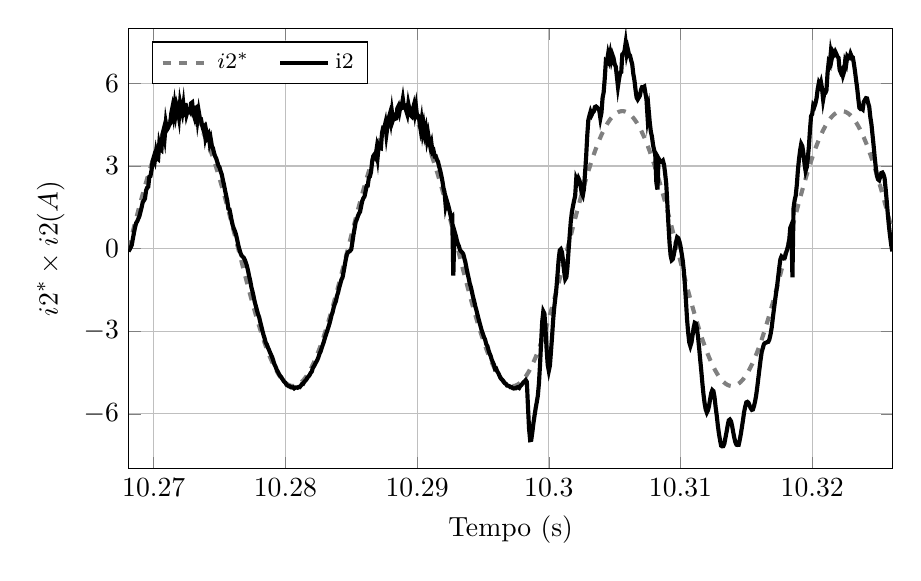
\begin{tikzpicture}

\begin{axis}[%
width=0.8\textwidth,
height=0.461611624834875\textwidth,
scale only axis,
xmin=10.2681,
xmax=10.3261,
xtick={10.27, 10.28, 10.29,  10.3, 10.31, 10.32},
xlabel={Tempo (s)},
xmajorgrids,
ymin=-8,
ymax=8,
ytick={-6, -3,  0,  3,  6},
ylabel={$\text{i2}^\text{*}\text{ }\times\text{ i2 (A)}$},
ymajorgrids,
legend style={at={(0.03,0.97)},anchor=north west,draw=black,fill=white,legend cell align=left},
scaled x ticks = false,
legend columns=-1,
legend style={/tikz/every even column/.append style={column sep=0.3cm}},
legend style={font=\footnotesize}
]
\addplot [color=gray,dashed,line width=1.5pt]
  table[row sep=crcr]{10.2680833456702	0.000309070768819114\\
10.2681666556704	0.157053337715448\\
10.2682499956706	0.313642611979031\\
10.2683333356708	0.469922358851122\\
10.268416675671	0.625738349089441\\
10.2684999856713	0.780936811123516\\
10.2685833256715	0.935364582808655\\
10.2686666656717	1.0888692625785\\
10.2687500056719	1.24129935984695\\
10.2688333456721	1.39250444451113\\
10.2689166556723	1.54233529540767\\
10.2689999956725	1.69064404757604\\
10.2690833356727	1.83728433818338\\
10.2691666756729	1.98211145096696\\
10.2692499856731	2.12498245905166\\
10.2693333256733	2.26575636600151\\
10.2694166656735	2.4042942449662\\
10.2695000056738	2.54045937578506\\
10.269583345674	2.67411737991341\\
10.2696666556742	2.80513635303789\\
10.2697499956744	2.93338699525013\\
10.2698333356746	3.05874273865016\\
10.2699166756748	3.18107987225364\\
10.269999985675	3.30027766407962\\
10.2700833256752	3.41621848029852\\
10.2701666656754	3.52878790132241\\
10.2702500056756	3.63787483472342\\
10.2703333456758	3.74337162486851\\
10.270416655676	3.84517415916259\\
10.2704999956763	3.94318197079508\\
10.2705833356765	4.03729833788853\\
10.2706666756767	4.12743037895141\\
10.2707499856769	4.21348914454097\\
10.2708333256771	4.29538970504559\\
10.2709166656773	4.3730512345\\
10.2710000056775	4.44639709035084\\
10.2710833456777	4.51535488909353\\
10.2711666556779	4.57985657770609\\
10.2712499956781	4.63983850080923\\
10.2713333356783	4.69524146348657\\
10.2714166756785	4.74601078970282\\
10.2714999856788	4.79209637626246\\
10.271583325679	4.83345274225553\\
10.2716666656792	4.87003907394182\\
10.2717500056794	4.90181926502907\\
10.2718333456796	4.92876195230555\\
10.2719166556798	4.95084054659175\\
10.27199999568	4.96803325898068\\
10.2720833356802	4.98032312234093\\
10.2721666756804	4.98769800806111\\
10.2722499856806	4.99015063801943\\
10.2723333256808	4.9876785917662\\
10.272416665681	4.98028430891263\\
10.2725000056813	4.96797508672318\\
10.2725833456815	4.95076307291404\\
10.2726666556817	4.9286652536648\\
10.2727499956819	4.90170343685516\\
10.2728333356821	4.86990423054316\\
10.2729166756823	4.83329901670629\\
10.2729999856825	4.79192392027119\\
10.2730833256827	4.74581977346277\\
10.2731666656829	4.6950320755077\\
10.2732500056831	4.6396109477322\\
10.2733333456833	4.57961108409831\\
10.2734166556835	4.51509169722756\\
10.2734999956838	4.44611645996527\\
10.273583335684	4.37275344254314\\
10.2736666756842	4.29507504540214\\
10.2737499856844	4.21315792774203\\
10.2738333256846	4.12708293186795\\
10.2739166656848	4.03693500340888\\
10.274000005685	3.94280310748652\\
10.2740833456852	3.84478014091745\\
10.2741666556854	3.74296284053523\\
10.2742499956856	3.63745168772278\\
10.2743333356858	3.52835080924942\\
10.274416675686	3.41576787451028\\
10.2744999856863	3.29981398926965\\
10.2745833256865	3.18060358601299\\
10.2746666656867	3.05825431101585\\
10.2747500056869	2.93288690824126\\
10.2748333456871	2.80462510017996\\
10.2749166556873	2.67359546575128\\
10.2749999956875	2.53992731538499\\
10.2750833356877	2.40375256340756\\
10.2751666756879	2.26520559785861\\
10.2752499856881	2.12442314786616\\
10.2753333256883	1.98154414871148\\
10.2754166656885	1.83670960471674\\
10.2755000056888	1.69006245009079\\
10.275583345689	1.54174740787031\\
10.2756666556892	1.39191084709568\\
10.2757499956894	1.24070063836241\\
10.2758333356896	1.08826600789067\\
10.2759166756898	0.934757390257092\\
10.27599998569	0.780326279933957\\
10.2760833256902	0.625125081782461\\
10.2761666656904	0.469306960647512\\
10.2762500056906	0.313025690202519\\
10.2763333456908	0.156435501193346\\
10.276416655691	-0.000309070768817629\\
10.2764999956913	-0.157053337715447\\
10.2765833356915	-0.313642611979031\\
10.2766666756917	-0.469922358851123\\
10.2767499856919	-0.625738349089442\\
10.2768333256921	-0.780936811123517\\
10.2769166656923	-0.935364582808657\\
10.2770000056925	-1.0888692625785\\
10.2770833456927	-1.24129935984696\\
10.2771666556929	-1.39250444451113\\
10.2772499956931	-1.54233529540767\\
10.2773333356933	-1.69064404757604\\
10.2774166756935	-1.83728433818339\\
10.2774999856937	-1.98211145096697\\
10.277583325694	-2.12498245905166\\
10.2776666656942	-2.26575636600152\\
10.2777500056944	-2.4042942449662\\
10.2778333456946	-2.54045937578507\\
10.2779166556948	-2.67411737991342\\
10.277999995695	-2.8051363530379\\
10.2780833356952	-2.93338699525014\\
10.2781666756954	-3.05874273865018\\
10.2782499856956	-3.18107987225365\\
10.2783333256958	-3.30027766407964\\
10.278416665696	-3.41621848029853\\
10.2785000056963	-3.52878790132242\\
10.2785833456965	-3.63787483472343\\
10.2786666556967	-3.74337162486853\\
10.2787499956969	-3.84517415916261\\
10.2788333356971	-3.9431819707951\\
10.2789166756973	-4.03729833788854\\
10.2789999856975	-4.12743037895142\\
10.2790833256977	-4.21348914454099\\
10.2791666656979	-4.2953897050456\\
10.2792500056981	-4.37305123450002\\
10.2793333456983	-4.44639709035086\\
10.2794166556985	-4.51535488909355\\
10.2794999956988	-4.57985657770611\\
10.279583335699	-4.63983850080925\\
10.2796666756992	-4.69524146348659\\
10.2797499856994	-4.74601078970284\\
10.2798333256996	-4.79209637626248\\
10.2799166656998	-4.83345274225555\\
10.2800000057	-4.87003907394184\\
10.2800833457002	-4.90181926502909\\
10.2801666557004	-4.92876195230557\\
10.2802499957006	-4.95084054659177\\
10.2803333357008	-4.9680332589807\\
10.280416675701	-4.98032312234094\\
10.2804999857012	-4.98769800806113\\
10.2805833257015	-4.99015063801945\\
10.2806666657017	-4.98767859176622\\
10.2807500057019	-4.98028430891265\\
10.2808333457021	-4.9679750867232\\
10.2809166557023	-4.95076307291406\\
10.2809999957025	-4.92866525366482\\
10.2810833357027	-4.90170343685517\\
10.2811666757029	-4.86990423054318\\
10.2812499857031	-4.83329901670631\\
10.2813333257033	-4.79192392027121\\
10.2814166657035	-4.74581977346279\\
10.2815000057038	-4.69503207550772\\
10.281583345704	-4.63961094773222\\
10.2816666557042	-4.57961108409833\\
10.2817499957044	-4.51509169722758\\
10.2818333357046	-4.44611645996529\\
10.2819166757048	-4.37275344254316\\
10.281999985705	-4.29507504540216\\
10.2820833257052	-4.21315792774204\\
10.2821666657054	-4.12708293186797\\
10.2822500057056	-4.0369350034089\\
10.2823333457058	-3.94280310748653\\
10.282416655706	-3.84478014091747\\
10.2824999957063	-3.74296284053525\\
10.2825833357065	-3.6374516877228\\
10.2826666757067	-3.52835080924944\\
10.2827499857069	-3.4157678745103\\
10.2828333257071	-3.29981398926967\\
10.2829166657073	-3.180603586013\\
10.2830000057075	-3.05825431101587\\
10.2830833457077	-2.93288690824127\\
10.2831666557079	-2.80462510017998\\
10.2832499957081	-2.67359546575129\\
10.2833333357083	-2.539927315385\\
10.2834166757085	-2.40375256340757\\
10.2834999857087	-2.26520559785862\\
10.283583325709	-2.12442314786617\\
10.2836666657092	-1.98154414871149\\
10.2837500057094	-1.83670960471675\\
10.2838333457096	-1.6900624500908\\
10.2839166557098	-1.54174740787032\\
10.28399999571	-1.39191084709569\\
10.2840833357102	-1.24070063836241\\
10.2841666757104	-1.08826600789068\\
10.2842499857106	-0.934757390257098\\
10.2843333257108	-0.780326279933963\\
10.284416665711	-0.625125081782466\\
10.2845000057113	-0.469306960647516\\
10.2845833457115	-0.313025690202523\\
10.2846666557117	-0.156435501193349\\
10.2847499957119	0.000309070768815339\\
10.2848333357121	0.157053337715446\\
10.2849166757123	0.31364261197903\\
10.2849999857125	0.469922358851122\\
10.2850833257127	0.625738349089443\\
10.2851666657129	0.780936811123518\\
10.2852500057131	0.935364582808659\\
10.2853333457133	1.0888692625785\\
10.2854166557135	1.24129935984696\\
10.2854999957137	1.39250444451113\\
10.285583335714	1.54233529540768\\
10.2856666757142	1.69064404757605\\
10.2857499857144	1.83728433818339\\
10.2858333257146	1.98211145096698\\
10.2859166657148	2.12498245905167\\
10.286000005715	2.26575636600152\\
10.2860833457152	2.40429424496621\\
10.2861666557154	2.54045937578508\\
10.2862499957156	2.67411737991343\\
10.2863333357158	2.80513635303791\\
10.286416675716	2.93338699525015\\
10.2864999857162	3.05874273865019\\
10.2865833257165	3.18107987225366\\
10.2866666657167	3.30027766407965\\
10.2867500057169	3.41621848029854\\
10.2868333457171	3.52878790132244\\
10.2869166557173	3.63787483472345\\
10.2869999957175	3.74337162486854\\
10.2870833357177	3.84517415916262\\
10.2871666757179	3.94318197079511\\
10.2872499857181	4.03729833788856\\
10.2873333257183	4.12743037895144\\
10.2874166657185	4.21348914454101\\
10.2875000057188	4.29538970504562\\
10.287583345719	4.37305123450004\\
10.2876666557192	4.44639709035088\\
10.2877499957194	4.51535488909357\\
10.2878333357196	4.57985657770613\\
10.2879166757198	4.63983850080927\\
10.28799998572	4.69524146348661\\
10.2880833257202	4.74601078970286\\
10.2881666657204	4.7920963762625\\
10.2882500057206	4.83345274225557\\
10.2883333457208	4.87003907394186\\
10.288416655721	4.90181926502911\\
10.2884999957212	4.92876195230559\\
10.2885833357215	4.95084054659179\\
10.2886666757217	4.96803325898072\\
10.2887499857219	4.98032312234097\\
10.2888333257221	4.98769800806116\\
10.2889166657223	4.99015063801947\\
10.2890000057225	4.98767859176624\\
10.2890833457227	4.98028430891268\\
10.2891666557229	4.96797508672323\\
10.2892499957231	4.95076307291408\\
10.2893333357233	4.92866525366484\\
10.2894166757235	4.9017034368552\\
10.2894999857238	4.8699042305432\\
10.289583325724	4.83329901670633\\
10.2896666657242	4.79192392027123\\
10.2897500057244	4.74581977346281\\
10.2898333457246	4.69503207550774\\
10.2899166557248	4.63961094773224\\
10.289999995725	4.57961108409835\\
10.2900833357252	4.51509169722759\\
10.2901666757254	4.44611645996531\\
10.2902499857256	4.37275344254318\\
10.2903333257258	4.29507504540218\\
10.290416665726	4.21315792774206\\
10.2905000057262	4.12708293186799\\
10.2905833457265	4.03693500340892\\
10.2906666557267	3.94280310748655\\
10.2907499957269	3.84478014091748\\
10.2908333357271	3.74296284053526\\
10.2909166757273	3.63745168772282\\
10.2909999857275	3.52835080924945\\
10.2910833257277	3.41576787451031\\
10.2911666657279	3.29981398926968\\
10.2912500057281	3.18060358601302\\
10.2913333457283	3.05825431101588\\
10.2914166557285	2.93288690824129\\
10.2914999957287	2.80462510017999\\
10.291583335729	2.6735954657513\\
10.2916666757292	2.53992731538501\\
10.2917499857294	2.40375256340758\\
10.2918333257296	2.26520559785863\\
10.2919166657298	2.12442314786618\\
10.29200000573	1.9815441487115\\
10.2920833457302	1.83670960471676\\
10.2921666557304	1.69006245009081\\
10.2922499957306	1.54174740787033\\
10.2923333357308	1.3919108470957\\
10.292416675731	1.24070063836242\\
10.2924999857313	1.08826600789068\\
10.2925833257315	0.934757390257102\\
10.2926666657317	0.780326279933967\\
10.2927500057319	0.62512508178247\\
10.2928333457321	0.469306960647519\\
10.2929166557323	0.313025690202525\\
10.2929999957325	0.156435501193351\\
10.2930833357327	-0.000309070768814229\\
10.2931666757329	-0.157053337715445\\
10.2932499857331	-0.31364261197903\\
10.2933333257333	-0.469922358851123\\
10.2934166657335	-0.625738349089444\\
10.2935000057337	-0.78093681112352\\
10.293583345734	-0.935364582808662\\
10.2936666557342	-1.08886926257851\\
10.2937499957344	-1.24129935984696\\
10.2938333357346	-1.39250444451114\\
10.2939166757348	-1.54233529540768\\
10.293999985735	-1.69064404757606\\
10.2940833257352	-1.8372843381834\\
10.2941666657354	-1.98211145096698\\
10.2942500057356	-2.12498245905168\\
10.2943333457358	-2.26575636600153\\
10.294416655736	-2.40429424496622\\
10.2944999957363	-2.54045937578509\\
10.2945833357365	-2.67411737991344\\
10.2946666757367	-2.80513635303792\\
10.2947499857369	-2.93338699525016\\
10.2948333257371	-3.0587427386502\\
10.2949166657373	-3.18107987225367\\
10.2950000057375	-3.30027766407966\\
10.2950833457377	-3.41621848029855\\
10.2951666557379	-3.52878790132245\\
10.2952499957381	-3.63787483472346\\
10.2953333357383	-3.74337162486856\\
10.2954166757385	-3.84517415916264\\
10.2954999857388	-3.94318197079513\\
10.295583325739	-4.03729833788857\\
10.2956666657392	-4.12743037895146\\
10.2957500057394	-4.21348914454102\\
10.2958333457396	-4.29538970504564\\
10.2959166557398	-4.37305123450006\\
10.29599999574	-4.4463970903509\\
10.2960833357402	-4.51535488909359\\
10.2961666757404	-4.57985657770615\\
10.2962499857406	-4.63983850080929\\
10.2963333257408	-4.69524146348663\\
10.296416665741	-4.74601078970288\\
10.2965000057412	-4.79209637626252\\
10.2965833457415	-4.83345274225559\\
10.2966666557417	-4.87003907394188\\
10.2967499957419	-4.90181926502913\\
10.2968333357421	-4.92876195230561\\
10.2969166757423	-4.95084054659181\\
10.2969999857425	-4.96803325898074\\
10.2970833257427	-4.98032312234099\\
10.2971666657429	-4.98769800806118\\
10.2972500057431	-4.99015063801949\\
10.2973333457433	-4.98767859176626\\
10.2974166557435	-4.9802843089127\\
10.2974999957438	-4.96797508672325\\
10.297583335744	-4.9507630729141\\
10.2976666757442	-4.92866525366486\\
10.2977499857444	-4.90170343685522\\
10.2978333257446	-4.86990423054323\\
10.2979166657448	-4.83329901670635\\
10.298000005745	-4.79192392027125\\
10.2980833457452	-4.74581977346283\\
10.2981666557454	-4.69503207550776\\
10.2982499957456	-4.63961094773226\\
10.2983333357458	-4.57961108409837\\
10.298416675746	-4.51509169722762\\
10.2984999857463	-4.44611645996533\\
10.2985833257465	-4.3727534425432\\
10.2986666657467	-4.2950750454022\\
10.2987500057469	-4.21315792774208\\
10.2988333457471	-4.127082931868\\
10.2989166557473	-4.03693500340894\\
10.2989999957475	-3.94280310748657\\
10.2990833357477	-3.8447801409175\\
10.2991666757479	-3.74296284053528\\
10.2992499857481	-3.63745168772283\\
10.2993333257483	-3.52835080924947\\
10.2994166657485	-3.41576787451033\\
10.2995000057488	-3.2998139892697\\
10.299583345749	-3.18060358601303\\
10.2996666557492	-3.05825431101589\\
10.2997499957494	-2.9328869082413\\
10.2998333357496	-2.80462510018\\
10.2999166757498	-2.67359546575132\\
10.29999998575	-2.53992731538503\\
10.3000833257502	-2.40375256340759\\
10.3001666657504	-2.26520559785864\\
10.3002500057506	-2.12442314786619\\
10.3003333457508	-1.98154414871151\\
10.300416655751	-1.83670960471677\\
10.3004999957513	-1.69006245009082\\
10.3005833357515	-1.54174740787034\\
10.3006666757517	-1.39191084709571\\
10.3007499857519	-1.24070063836243\\
10.3008333257521	-1.08826600789069\\
10.3009166657523	-0.934757390257109\\
10.3010000057525	-0.780326279933972\\
10.3010833457527	-0.625125081782474\\
10.3011666557529	-0.469306960647523\\
10.3012499957531	-0.313025690202528\\
10.3013333357533	-0.156435501193353\\
10.3014166757535	0.000309070768812411\\
10.3014999857538	0.157053337715444\\
10.301583325754	0.31364261197903\\
10.3016666657542	0.469922358851123\\
10.3017500057544	0.625738349089445\\
10.3018333457546	0.780936811123522\\
10.3019166557548	0.935364582808664\\
10.301999995755	1.08886926257851\\
10.3020833357552	1.24129935984697\\
10.3021666757554	1.39250444451114\\
10.3022499857556	1.54233529540769\\
10.3023333257558	1.69064404757606\\
10.302416665756	1.83728433818341\\
10.3025000057563	1.98211145096699\\
10.3025833457565	2.12498245905169\\
10.3026666557567	2.26575636600154\\
10.3027499957569	2.40429424496623\\
10.3028333357571	2.5404593757851\\
10.3029166757573	2.67411737991345\\
10.3029999857575	2.80513635303793\\
10.3030833257577	2.93338699525017\\
10.3031666657579	3.05874273865021\\
10.3032500057581	3.18107987225369\\
10.3033333457583	3.30027766407968\\
10.3034166557585	3.41621848029857\\
10.3034999957588	3.52878790132246\\
10.303583335759	3.63787483472348\\
10.3036666757592	3.74337162486857\\
10.3037499857594	3.84517415916265\\
10.3038333257596	3.94318197079515\\
10.3039166657598	4.03729833788859\\
10.30400000576	4.12743037895148\\
10.3040833457602	4.21348914454104\\
10.3041666557604	4.29538970504566\\
10.3042499957606	4.37305123450008\\
10.3043333357608	4.44639709035092\\
10.304416675761	4.51535488909361\\
10.3044999857613	4.57985657770616\\
10.3045833257615	4.63983850080931\\
10.3046666657617	4.69524146348665\\
10.3047500057619	4.7460107897029\\
10.3048333457621	4.79209637626254\\
10.3049166557623	4.83345274225561\\
10.3049999957625	4.87003907394191\\
10.3050833357627	4.90181926502916\\
10.3051666757629	4.92876195230564\\
10.3052499857631	4.95084054659183\\
10.3053333257633	4.96803325898077\\
10.3054166657635	4.98032312234101\\
10.3055000057638	4.9876980080612\\
10.305583345764	4.99015063801951\\
10.3056666557642	4.98767859176629\\
10.3057499957644	4.98028430891272\\
10.3058333357646	4.96797508672327\\
10.3059166757648	4.95076307291413\\
10.305999985765	4.92866525366488\\
10.3060833257652	4.90170343685524\\
10.3061666657654	4.86990423054325\\
10.3062500057656	4.83329901670638\\
10.3063333457658	4.79192392027127\\
10.306416655766	4.74581977346285\\
10.3064999957663	4.69503207550778\\
10.3065833357665	4.63961094773228\\
10.3066666757667	4.57961108409839\\
10.3067499857669	4.51509169722764\\
10.3068333257671	4.44611645996535\\
10.3069166657673	4.37275344254322\\
10.3070000057675	4.29507504540222\\
10.3070833457677	4.2131579277421\\
10.3071666557679	4.12708293186802\\
10.3072499957681	4.03693500340895\\
10.3073333357683	3.94280310748659\\
10.3074166757685	3.84478014091752\\
10.3074999857688	3.7429628405353\\
10.307583325769	3.63745168772285\\
10.3076666657692	3.52835080924948\\
10.3077500057694	3.41576787451034\\
10.3078333457696	3.29981398926971\\
10.3079166557698	3.18060358601305\\
10.30799999577	3.05825431101591\\
10.3080833357702	2.93288690824131\\
10.3081666757704	2.80462510018002\\
10.3082499857706	2.67359546575133\\
10.3083333257708	2.53992731538504\\
10.308416665771	2.40375256340761\\
10.3085000057713	2.26520559785865\\
10.3085833457715	2.1244231478662\\
10.3086666557717	1.98154414871152\\
10.3087499957719	1.83670960471678\\
10.3088333357721	1.69006245009083\\
10.3089166757723	1.54174740787034\\
10.3089999857725	1.39191084709572\\
10.3090833257727	1.24070063836244\\
10.3091666657729	1.0882660078907\\
10.3092500057731	0.934757390257115\\
10.3093333457733	0.780326279933977\\
10.3094166557735	0.625125081782479\\
10.3094999957738	0.469306960647527\\
10.309583335774	0.313025690202531\\
10.3096666757742	0.156435501193356\\
10.3097499857744	-0.000309070768810635\\
10.3098333257746	-0.157053337715443\\
10.3099166657748	-0.313642611979029\\
10.310000005775	-0.469922358851124\\
10.3100833457752	-0.625738349089446\\
10.3101666557754	-0.780936811123524\\
10.3102499957756	-0.935364582808666\\
10.3103333357758	-1.08886926257851\\
10.310416675776	-1.24129935984697\\
10.3104999857763	-1.39250444451115\\
10.3105833257765	-1.54233529540769\\
10.3106666657767	-1.69064404757607\\
10.3107500057769	-1.83728433818341\\
10.3108333457771	-1.982111450967\\
10.3109166557773	-2.1249824590517\\
10.3109999957775	-2.26575636600155\\
10.3110833357777	-2.40429424496624\\
10.3111666757779	-2.54045937578511\\
10.3112499857781	-2.67411737991346\\
10.3113333257783	-2.80513635303794\\
10.3114166657785	-2.93338699525019\\
10.3115000057788	-3.05874273865022\\
10.311583345779	-3.1810798722537\\
10.3116666557792	-3.30027766407969\\
10.3117499957794	-3.41621848029858\\
10.3118333357796	-3.52878790132248\\
10.3119166757798	-3.63787483472349\\
10.31199998578	-3.74337162486859\\
10.3120833257802	-3.84517415916267\\
10.3121666657804	-3.94318197079516\\
10.3122500057806	-4.03729833788861\\
10.3123333457808	-4.12743037895149\\
10.312416655781	-4.21348914454106\\
10.3124999957813	-4.29538970504568\\
10.3125833357815	-4.37305123450009\\
10.3126666757817	-4.44639709035093\\
10.3127499857819	-4.51535488909363\\
10.3128333257821	-4.57985657770618\\
10.3129166657823	-4.63983850080933\\
10.3130000057825	-4.69524146348667\\
10.3130833457827	-4.74601078970292\\
10.3131666557829	-4.79209637626256\\
10.3132499957831	-4.83345274225564\\
10.3133333357833	-4.87003907394192\\
10.3134166757835	-4.90181926502918\\
10.3134999857838	-4.92876195230566\\
10.313583325784	-4.95084054659185\\
10.3136666657842	-4.96803325898079\\
10.3137500057844	-4.98032312234103\\
10.3138333457846	-4.98769800806122\\
10.3139166557848	-4.99015063801953\\
10.313999995785	-4.98767859176631\\
10.3140833357852	-4.98028430891274\\
10.3141666757854	-4.96797508672329\\
10.3142499857856	-4.95076307291415\\
10.3143333257858	-4.9286652536649\\
10.314416665786	-4.90170343685526\\
10.3145000057863	-4.86990423054327\\
10.3145833457865	-4.8332990167064\\
10.3146666557867	-4.7919239202713\\
10.3147499957869	-4.74581977346287\\
10.3148333357871	-4.69503207550781\\
10.3149166757873	-4.6396109477323\\
10.3149999857875	-4.57961108409841\\
10.3150833257877	-4.51509169722766\\
10.3151666657879	-4.44611645996537\\
10.3152500057881	-4.37275344254324\\
10.3153333457883	-4.29507504540224\\
10.3154166557885	-4.21315792774212\\
10.3154999957888	-4.12708293186804\\
10.315583335789	-4.03693500340897\\
10.3156666757892	-3.94280310748661\\
10.3157499857894	-3.84478014091754\\
10.3158333257896	-3.74296284053532\\
10.3159166657898	-3.63745168772287\\
10.31600000579	-3.5283508092495\\
10.3160833457902	-3.41576787451036\\
10.3161666557904	-3.29981398926973\\
10.3162499957906	-3.18060358601306\\
10.3163333357908	-3.05825431101592\\
10.316416675791	-2.93288690824133\\
10.3164999857913	-2.80462510018003\\
10.3165833257915	-2.67359546575134\\
10.3166666657917	-2.53992731538505\\
10.3167500057919	-2.40375256340762\\
10.3168333457921	-2.26520559785866\\
10.3169166557923	-2.12442314786621\\
10.3169999957925	-1.98154414871153\\
10.3170833357927	-1.83670960471679\\
10.3171666757929	-1.69006245009084\\
10.3172499857931	-1.54174740787035\\
10.3173333257933	-1.39191084709572\\
10.3174166657935	-1.24070063836244\\
10.3175000057938	-1.0882660078907\\
10.317583345794	-0.93475739025712\\
10.3176666557942	-0.780326279933982\\
10.3177499957944	-0.625125081782483\\
10.3178333357946	-0.46930696064753\\
10.3179166757948	-0.313025690202534\\
10.317999985795	-0.156435501193358\\
10.3180833257952	0.000309070768808983\\
10.3181666657954	0.157053337715442\\
10.3182500057956	0.313642611979029\\
10.3183333457958	0.469922358851124\\
10.318416655796	0.625738349089447\\
10.3184999957963	0.780936811123526\\
10.3185833357965	0.935364582808669\\
10.3186666757967	1.08886926257851\\
10.3187499857969	1.24129935984697\\
10.3188333257971	1.39250444451115\\
10.3189166657973	1.5423352954077\\
10.3190000057975	1.69064404757607\\
10.3190833457977	1.83728433818342\\
10.3191666557979	1.98211145096701\\
10.3192499957981	2.1249824590517\\
10.3193333357983	2.26575636600156\\
10.3194166757985	2.40429424496625\\
10.3194999857988	2.54045937578512\\
10.319583325799	2.67411737991347\\
10.3196666657992	2.80513635303795\\
10.3197500057994	2.9333869952502\\
10.3198333457996	3.05874273865024\\
10.3199166557998	3.18107987225371\\
10.3199999958	3.3002776640797\\
10.3200833358002	3.4162184802986\\
10.3201666758004	3.52878790132249\\
10.3202499858006	3.63787483472351\\
10.3203333258008	3.7433716248686\\
10.320416665801	3.84517415916268\\
10.3205000058013	3.94318197079518\\
10.3205833458015	4.03729833788862\\
10.3206666558017	4.12743037895151\\
10.3207499958019	4.21348914454108\\
10.3208333358021	4.29538970504569\\
10.3209166758023	4.37305123450011\\
10.3209999858025	4.44639709035095\\
10.3210833258027	4.51535488909364\\
10.3211666658029	4.5798565777062\\
10.3212500058031	4.63983850080935\\
10.3213333458033	4.69524146348669\\
10.3214166558035	4.74601078970294\\
10.3214999958038	4.79209637626258\\
10.321583335804	4.83345274225565\\
10.3216666758042	4.87003907394195\\
10.3217499858044	4.9018192650292\\
10.3218333258046	4.92876195230568\\
10.3219166658048	4.95084054659188\\
10.322000005805	4.96803325898081\\
10.3220833458052	4.98032312234105\\
10.3221666558054	4.98769800806124\\
10.3222499958056	4.99015063801955\\
10.3223333358058	4.98767859176633\\
10.322416675806	4.98028430891276\\
10.3224999858063	4.96797508672331\\
10.3225833258065	4.95076307291417\\
10.3226666658067	4.92866525366492\\
10.3227500058069	4.90170343685528\\
10.3228333458071	4.86990423054329\\
10.3229166558073	4.83329901670642\\
10.3229999958075	4.79192392027132\\
10.3230833358077	4.74581977346289\\
10.3231666758079	4.69503207550783\\
10.3232499858081	4.63961094773232\\
10.3233333258083	4.57961108409843\\
10.3234166658085	4.51509169722768\\
10.3235000058088	4.44611645996539\\
10.323583345809	4.37275344254326\\
10.3236666558092	4.29507504540226\\
10.3237499958094	4.21315792774214\\
10.3238333358096	4.12708293186806\\
10.3239166758098	4.03693500340899\\
10.32399998581	3.94280310748662\\
10.3240833258102	3.84478014091756\\
10.3241666658104	3.74296284053534\\
10.3242500058106	3.63745168772289\\
10.3243333458108	3.52835080924952\\
10.324416655811	3.41576787451038\\
10.3244999958113	3.29981398926975\\
10.3245833358115	3.18060358601308\\
10.3246666758117	3.05825431101594\\
10.3247499858119	2.93288690824134\\
10.3248333258121	2.80462510018004\\
10.3249166658123	2.67359546575136\\
10.3250000058125	2.53992731538507\\
10.3250833458127	2.40375256340763\\
10.3251666558129	2.26520559785868\\
10.3252499958131	2.12442314786622\\
10.3253333358133	1.98154414871154\\
10.3254166758135	1.8367096047168\\
10.3254999858138	1.69006245009084\\
10.325583325814	1.54174740787036\\
10.3256666658142	1.39191084709573\\
10.3257500058144	1.24070063836245\\
10.3258333458146	1.08826600789071\\
10.3259166558148	0.934757390257126\\
10.325999995815	0.780326279933988\\
10.3260833358152	0.625125081782488\\
};
\addlegendentry{$\text{i2}^\text{*}$};

\addplot [color=black,solid,line width=1.5pt]
  table[row sep=crcr]{10.2680833456702	-0.101673057810471\\
10.2681666556704	-0.0358588488260956\\
10.2682499956706	0.0427178113301544\\
10.2683333356708	0.131304237111404\\
10.268416675671	0.362780067189529\\
10.2684999856713	0.576238319142654\\
10.2685833256715	0.775933143361404\\
10.2686666656717	0.932836219533279\\
10.2687500056719	0.992394325002029\\
10.2688333456721	1.08973929570515\\
10.2689166556723	1.18157889531453\\
10.2689999956725	1.3454888074239\\
10.2690833356727	1.50214163945515\\
10.2691666756729	1.69032523320515\\
10.2692499856731	1.74162528203328\\
10.2693333256733	1.8109429089864\\
10.2694166656735	2.10472953008015\\
10.2695000056738	2.21308524297078\\
10.269583345674	2.2453667371114\\
10.2696666556742	2.60721976445515\\
10.2697499956744	2.63049246953328\\
10.2698333356746	2.84269950078328\\
10.2699166756748	3.18002860234578\\
10.269999985675	3.31365897343953\\
10.2700833256752	3.19304129765828\\
10.2701666656754	3.4915825574239\\
10.2702500056756	3.27962577031453\\
10.2703333456758	3.24759452031453\\
10.270416655676	3.78011405156453\\
10.2704999956763	3.60719535039265\\
10.2705833356765	3.57316214726765\\
10.2706666756767	4.15347830937703\\
10.2707499856769	4.31188285039265\\
10.2708333256771	4.05838553593953\\
10.2709166656773	4.55286795781453\\
10.2710000056775	4.31188285039265\\
10.2710833456777	4.37394339726765\\
10.2711666556779	4.4805474011739\\
10.2712499956781	4.54110648320515\\
10.2713333356783	4.9089653699239\\
10.2714166756785	5.11266410039265\\
10.2714999856788	4.8569145886739\\
10.271583325679	5.20350272343953\\
10.2716666656792	4.89970633672078\\
10.2717500056794	5.17497489140828\\
10.2718333456796	5.01882254765828\\
10.2719166556798	4.76832816289265\\
10.27199999568	5.28257987187703\\
10.2720833356802	5.0701225964864\\
10.2721666756804	4.9109673230489\\
10.2722499856806	5.20875785039265\\
10.2723333256808	4.7778374402364\\
10.272416665681	5.2793266980489\\
10.2725000056813	4.87518241093953\\
10.2725833456815	5.01757132695515\\
10.2726666556817	5.04760062383015\\
10.2727499956819	4.98328787968953\\
10.2728333356821	5.27181937383015\\
10.2729166756823	5.30259940312703\\
10.2729999856825	4.9199761121114\\
10.2730833256827	4.78559500859578\\
10.2731666656829	5.09965140508015\\
10.2732500056831	5.12792899297078\\
10.2733333456833	4.69550711797078\\
10.2734166556835	4.98028495000203\\
10.2734999956838	4.74105155156453\\
10.273583335684	4.71502616093953\\
10.2736666756842	4.4895561902364\\
10.2737499856844	4.35067069218953\\
10.2738333256846	4.40872733281453\\
10.2739166656848	4.05938651250203\\
10.274000005685	4.24857108281453\\
10.2740833456852	4.05688407109578\\
10.2741666556854	4.1332085339864\\
10.2742499956856	3.8319145886739\\
10.2743333356858	3.9680474011739\\
10.274416675686	3.72130667851765\\
10.2744999856863	3.63922660039265\\
10.2745833256865	3.46380545781453\\
10.2746666656867	3.3454399792989\\
10.2747500056869	3.26461112187703\\
10.2748333456871	3.13048026250203\\
10.2749166556873	3.0031059949239\\
10.2749999956875	2.94529959843953\\
10.2750833356877	2.80215995000203\\
10.2751666756879	2.68654715703328\\
10.2752499856881	2.49435965703328\\
10.2753333256883	2.31668631718953\\
10.2754166656885	2.11048514531453\\
10.2755000056888	1.92155081914265\\
10.275583345689	1.73611991093953\\
10.2756666556892	1.44683768437703\\
10.2757499956894	1.4255669324239\\
10.2758333356896	1.23588187383015\\
10.2759166756898	1.01466605351765\\
10.27599998569	0.845000526173904\\
10.2760833256902	0.725383826955154\\
10.2761666656904	0.632293006642654\\
10.2762500056906	0.502666541798904\\
10.2763333456908	0.328746864064529\\
10.276416655691	0.133055946095779\\
10.2764999956913	-0.0180915148417206\\
10.2765833356915	-0.154224327341721\\
10.2766666756917	-0.250067833201096\\
10.2767499856919	-0.290857628122971\\
10.2768333256921	-0.329395225779221\\
10.2769166656923	-0.406970909372971\\
10.2770000056925	-0.518329551951096\\
10.2770833456927	-0.645203331247971\\
10.2771666556929	-0.815369346872971\\
10.2772499956931	-1.01231148554485\\
10.2773333356933	-1.1829779894511\\
10.2774166756935	-1.40794747187297\\
10.2774999856937	-1.55809395624797\\
10.277583325694	-1.74002144648235\\
10.2776666656942	-1.93045723749797\\
10.2777500056944	-2.08135445429485\\
10.2778333456946	-2.22924874140422\\
10.2779166556948	-2.3791449816386\\
10.277999995695	-2.4822455675761\\
10.2780833356952	-2.65591500116985\\
10.2781666756954	-2.80931465937297\\
10.2782499856956	-2.97697823359172\\
10.2783333256958	-3.13212960077922\\
10.278416665696	-3.25524971796672\\
10.2785000056963	-3.41190254999797\\
10.2785833456965	-3.47646553827922\\
10.2786666556967	-3.58357003046672\\
10.2787499956969	-3.67565987421672\\
10.2788333356971	-3.7735053332011\\
10.2789166756973	-3.85933907343547\\
10.2789999856975	-3.95192940546672\\
10.2790833256977	-4.07555001093547\\
10.2791666656979	-4.20467598749797\\
10.2792500056981	-4.2820014269511\\
10.2793333456983	-4.39035713984172\\
10.2794166556985	-4.46442940546672\\
10.2794999956988	-4.54325630976359\\
10.279583335699	-4.61107247187297\\
10.2796666756992	-4.65486519648235\\
10.2797499856994	-4.72092964960734\\
10.2798333256996	-4.78023751093547\\
10.2799166656998	-4.83904488398234\\
10.2800000057	-4.86832344843547\\
10.2800833457002	-4.94564888788859\\
10.2801666557004	-4.96917183710734\\
10.2802499957006	-4.99694893671672\\
10.2803333357008	-4.9997016222636\\
10.280416675701	-5.0347358019511\\
10.2804999857012	-5.04249337031047\\
10.2805833257015	-5.03498604609172\\
10.2806666657017	-5.07377388788859\\
10.2807500057019	-5.0447455675761\\
10.2808333457021	-5.04174263788859\\
10.2809166557023	-5.05300362421672\\
10.2809999957025	-5.02397530390422\\
10.2810833357027	-5.03073189570109\\
10.2811666757029	-4.97843087031047\\
10.2812499857031	-4.92337715937297\\
10.2813333257033	-4.91987374140422\\
10.2814166657035	-4.84855416132609\\
10.2815000057038	-4.80125801874797\\
10.281583345704	-4.76297066523234\\
10.2816666557042	-4.68589546991984\\
10.2817499957044	-4.64460518671672\\
10.2818333357046	-4.5943061144511\\
10.2819166757048	-4.51072457148234\\
10.281999985705	-4.46743233515422\\
10.2820833257052	-4.33280098749797\\
10.2821666657054	-4.27224190546672\\
10.2822500057056	-4.19541695429484\\
10.2823333457058	-4.11709053827922\\
10.282416655706	-4.04927437616985\\
10.2824999957063	-3.9496772082011\\
10.2825833357065	-3.8255561144511\\
10.2826666757067	-3.74322579218547\\
10.2827499857069	-3.61510079218547\\
10.2828333257071	-3.4962348253886\\
10.2829166657073	-3.38362496210735\\
10.2830000057075	-3.24073555781047\\
10.2830833457077	-3.12362129999797\\
10.2831666557079	-2.99649727656047\\
10.2832499957081	-2.87237618281047\\
10.2833333357083	-2.7424994738261\\
10.2834166757085	-2.59485543085735\\
10.2834999857087	-2.42443917109172\\
10.283583325709	-2.30632393671672\\
10.2836666657092	-2.13140328241985\\
10.2837500057094	-2.01053536249797\\
10.2838333457096	-1.91018746210735\\
10.2839166557098	-1.71524727656047\\
10.28399999571	-1.59613106562297\\
10.2840833357102	-1.41995919062297\\
10.2841666757104	-1.28232491327922\\
10.2842499857106	-1.1309272082011\\
10.2843333257108	-1.0508490832011\\
10.284416665711	-0.848651817576096\\
10.2845000057113	-0.618927696482346\\
10.2845833457115	-0.396961143747971\\
10.2846666557117	-0.211780479685471\\
10.2847499957119	-0.133954551951096\\
10.2848333357121	-0.111182335154221\\
10.2849166757123	-0.0809027941385956\\
10.2849999857125	-0.0276007921854706\\
10.2850833257127	0.229650184377029\\
10.2851666657129	0.500664588673904\\
10.2852500057131	0.726134559377029\\
10.2853333457133	0.966619178517654\\
10.2854166557135	1.05345389531453\\
10.2854999957137	1.17407157109578\\
10.285583335714	1.27091605351765\\
10.2856666757142	1.33622977422078\\
10.2857499857144	1.53817679570515\\
10.2858333257146	1.72410819218953\\
10.2859166657148	1.8289604871114\\
10.286000005715	1.88526541875203\\
10.2860833457152	2.06669242070515\\
10.2861666557154	2.2713921277364\\
10.2862499957156	2.28215262578328\\
10.2863333357158	2.56843192265828\\
10.286416675716	2.61722953008015\\
10.2864999857162	2.78138968633015\\
10.2865833257165	3.1412407605489\\
10.2866666657167	3.3514458386739\\
10.2867500057169	3.40900199101765\\
10.2868333457171	3.32917411015828\\
10.2869166557173	3.59318167851765\\
10.2869999957175	3.31616141484578\\
10.2870833357177	3.74057547734578\\
10.2871666757179	3.66099784062703\\
10.2872499857181	3.64498221562703\\
10.2873333257183	4.19051444218953\\
10.2874166657185	4.38370291875203\\
10.2875000057188	4.37494437383015\\
10.287583345719	4.54335868047078\\
10.2876666557192	4.13971488164265\\
10.2877499957194	4.43525321172078\\
10.2878333357196	4.72253348515828\\
10.2879166757198	4.86417166875203\\
10.28799998572	4.62443778203328\\
10.2880833257202	4.97528006718953\\
10.2881666657204	4.67048270390828\\
10.2882500057206	4.78909842656453\\
10.2883333457208	4.71002127812703\\
10.288416655721	4.72528617070515\\
10.2884999957212	5.09364554570515\\
10.2885833357215	5.1742241589864\\
10.2886666757217	4.97878348515828\\
10.2887499857219	5.19299246953328\\
10.2888333257221	5.19274222539265\\
10.2889166657223	5.42797171758015\\
10.2890000057225	5.14144217656453\\
10.2890833457227	5.16446463750203\\
10.2891666557229	5.01782157109578\\
10.2892499957231	4.88544242070515\\
10.2893333357233	5.25004813359578\\
10.2894166757235	5.05085379765828\\
10.2894999857238	4.8398979871114\\
10.289583325724	4.80111014531453\\
10.2896666657242	5.0410942761739\\
10.2897500057244	5.19649588750203\\
10.2898333457246	4.91171805547078\\
10.2899166557248	5.14769828008015\\
10.289999995725	4.77933890508015\\
10.2900833357252	4.79410330937703\\
10.2901666757254	4.66447684453328\\
10.2902499857256	4.38795706914265\\
10.2903333257258	4.65046317265828\\
10.290416665726	4.25057303593953\\
10.2905000057262	4.47479178593953\\
10.2905833457265	4.1672417371114\\
10.2906666557267	4.34191214726765\\
10.2907499957269	3.96854788945515\\
10.2908333357271	4.16974417851765\\
10.2909166757273	3.9109917371114\\
10.2909999857275	3.7037895886739\\
10.2910833257277	3.8379204480489\\
10.2911666657279	3.50509574101765\\
10.2912500057281	3.54813773320515\\
10.2913333457283	3.34619071172078\\
10.2914166557285	3.35194632695515\\
10.2914999957287	3.23283011601765\\
10.291583335729	3.15650565312703\\
10.2916666757292	2.98458792851765\\
10.2917499857294	2.84144828008015\\
10.2918333257296	2.66127249883015\\
10.2919166657298	2.46232840703328\\
10.29200000573	2.20382620976765\\
10.2920833457302	2.04592215703328\\
10.2921666557304	1.5677056042989\\
10.2922499957306	1.7498833386739\\
10.2923333357308	1.61600272343953\\
10.292416675731	1.4706108777364\\
10.2924999857313	1.29418875859578\\
10.2925833257315	1.1022515027364\\
10.2926666657317	1.1492974011739\\
10.2927500057319	-0.980280235544846\\
10.2928333457321	0.638048621877029\\
10.2929166557323	0.500164100392654\\
10.2929999957325	0.336003944142654\\
10.2930833357327	0.185857459767654\\
10.2931666757329	0.0975212781270294\\
10.2932499857331	-0.0423651964823456\\
10.2933333257333	-0.0971686632792206\\
10.2934166657335	-0.135706260935471\\
10.2935000057337	-0.194013145701096\\
10.293583345734	-0.345160606638596\\
10.2936666557342	-0.499060753122971\\
10.2937499957344	-0.709516075388596\\
10.2938333357346	-0.90195381952922\\
10.2939166757348	-1.08137886835735\\
10.293999985735	-1.26931221796672\\
10.2940833257352	-1.39893868281047\\
10.2941666657354	-1.5793647082011\\
10.2942500057356	-1.76304390741985\\
10.2943333457358	-1.90918648554485\\
10.294416655736	-2.09236519648235\\
10.2944999957363	-2.23250191523235\\
10.2945833357365	-2.40041573359172\\
10.2946666757367	-2.55306465937297\\
10.2947499857369	-2.70271065546672\\
10.2948333257371	-2.85035469843547\\
10.2949166657373	-2.9937445910136\\
10.2950000057375	-3.10034859491985\\
10.2950833457377	-3.22246773554485\\
10.2951666557379	-3.30930245234172\\
10.2952499957381	-3.46945870234172\\
10.2953333357383	-3.53477242304485\\
10.2954166757385	-3.67816231562297\\
10.2954999857388	-3.80328438593547\\
10.295583325739	-3.8966254503886\\
10.2956666657392	-4.03551094843547\\
10.2957500057394	-4.12434761835735\\
10.2958333457396	-4.21618721796672\\
10.2959166557398	-4.37434151484172\\
10.29599999574	-4.35632393671672\\
10.2960833357402	-4.45692208124797\\
10.2961666757404	-4.52248604609172\\
10.2962499857406	-4.60857003046672\\
10.2963333257408	-4.69115059687297\\
10.296416665741	-4.74195015741985\\
10.2965000057412	-4.77873604609172\\
10.2965833457415	-4.84329903437297\\
10.2966666557417	-4.89309761835734\\
10.2967499957419	-4.91386788202922\\
10.2968333357421	-4.97317574335734\\
10.2969166757423	-4.97868111445109\\
10.2969999857425	-4.99569771601359\\
10.2970833257427	-5.03073189570109\\
10.2971666657429	-5.02622750116984\\
10.2972500057431	-5.06676705195109\\
10.2973333457433	-5.07952950312297\\
10.2974166557435	-5.07127144648234\\
10.2974999957438	-5.0697699816386\\
10.297583335744	-5.03673775507609\\
10.2976666757442	-5.03373482538859\\
10.2977499857444	-5.05875923945109\\
10.2978333257446	-4.98869088007609\\
10.2979166657448	-4.95490792109172\\
10.298000005745	-4.90285713984172\\
10.2980833457452	-4.84980538202922\\
10.2981666557454	-4.82002632929485\\
10.2982499957456	-4.77398140741984\\
10.2983333357458	-4.84329903437297\\
10.298416675746	-5.71990425898234\\
10.2984999857463	-6.53620064570109\\
10.2985833257465	-6.9546088488261\\
10.2986666657467	-6.94585030390422\\
10.2987500057469	-6.66582711054484\\
10.2988333457471	-6.3340033800761\\
10.2989166557473	-6.06424019648234\\
10.2989999957475	-5.80423653437297\\
10.2990833357477	-5.58151924921672\\
10.2991666757479	-5.34528878046672\\
10.2992499857481	-4.89685128046672\\
10.2993333257483	-4.2219428332011\\
10.2994166657485	-3.4041449816386\\
10.2995000057488	-2.64315254999797\\
10.299583345749	-2.28029854609172\\
10.2996666557492	-2.36087715937297\\
10.2997499957494	-2.91041329218547\\
10.2998333357496	-3.64412911249797\\
10.2999166757498	-4.21793892695109\\
10.29999998575	-4.43790352656047\\
10.3000833257502	-4.24796822382609\\
10.3001666657504	-3.72670967890422\\
10.3002500057506	-3.17742379023235\\
10.3003333457508	-2.57358467890422\\
10.300416655751	-2.12114327265422\\
10.3004999957513	-1.78206246210735\\
10.3005833357515	-1.40894844843547\\
10.3006666757517	-0.912964561716721\\
10.3007499857519	-0.389954307810471\\
10.3008333257521	-0.0648871691385956\\
10.3009166657523	-0.0243476183573456\\
10.3010000057525	-0.127197960154221\\
10.3010833457527	-0.442255333201096\\
10.3011666557529	-0.837140587107346\\
10.3012499957531	-1.1059027941386\\
10.3013333357533	-1.03933785273235\\
10.3014166757535	-0.667224815622971\\
10.3014999857538	-0.0731452257792206\\
10.301583325754	0.461376258595779\\
10.3016666657542	0.970122596486404\\
10.3017500057544	1.31520926640828\\
10.3018333457546	1.53992850468953\\
10.3019166557548	1.7348686902364\\
10.301999995755	1.90428397343953\\
10.3020833357552	2.52789237187703\\
10.3021666757554	2.4305474011739\\
10.3022499857556	2.55516898320515\\
10.3023333257558	2.4645806042989\\
10.302416665756	2.27489554570515\\
10.3025000057563	2.0131401746114\\
10.3025833457565	1.9270561902364\\
10.3026666557567	2.15653006718953\\
10.3027499957569	2.73234183476765\\
10.3028333357571	3.3174126355489\\
10.3029166757573	4.08366019414265\\
10.3029999857575	4.65621878789265\\
10.3030833257577	4.82238089726765\\
10.3031666657579	4.96577078984578\\
10.3032500057581	4.85215995000203\\
10.3033333457583	4.93449027226765\\
10.3034166557585	4.98028495000203\\
10.3034999957588	5.13693778203328\\
10.303583335759	5.15845877812703\\
10.3036666757592	5.12592703984578\\
10.3037499857594	5.06787039922078\\
10.3038333257596	5.00956351445515\\
10.3039166657598	4.7347954480489\\
10.30400000576	4.93924491093953\\
10.3040833457602	5.47201468633015\\
10.3041666557604	5.67846610234578\\
10.3042499957606	6.1832085339864\\
10.3043333357608	6.81357352422078\\
10.304416675761	6.77853934453328\\
10.3044999857613	7.04930350468953\\
10.3045833257615	6.87638480351765\\
10.3046666657617	7.0850884167989\\
10.3047500057619	6.85311209843953\\
10.3048333457621	7.02828299687703\\
10.3049166557623	6.91442191289265\\
10.3049999957625	6.69620902226765\\
10.3050833357627	6.60912406133015\\
10.3051666757629	6.26003348515828\\
10.3052499857631	5.88641898320515\\
10.3053333257633	6.15893485234578\\
10.3054166657635	6.37364432500203\\
10.3055000057638	6.40792777226765\\
10.305583345764	7.05230643437703\\
10.3056666557642	7.07958304570515\\
10.3057499957644	7.17692801640828\\
10.3058333357646	7.45494925664265\\
10.3059166757648	7.06281668828328\\
10.305999985765	7.2372368542989\\
10.3060833257652	7.05856253789265\\
10.3061666657654	7.01051566289265\\
10.3062500057656	6.83709647343953\\
10.3063333457658	6.6937065808614\\
10.306416655766	6.34461600468953\\
10.3064999957663	6.1191460339864\\
10.3065833357665	5.77831351445515\\
10.3066666757667	5.48602835820515\\
10.3067499857669	5.41270682500203\\
10.3068333257671	5.48077323125203\\
10.3069166657673	5.5515923230489\\
10.3070000057675	5.76204764531453\\
10.3070833457677	5.86214530156453\\
10.3071666557679	5.8598931042989\\
10.3072499957681	5.88316580937703\\
10.3073333357683	5.64818656133015\\
10.3074166757685	5.42096488164265\\
10.3074999857688	4.7748345105489\\
10.307583325769	5.0260796277364\\
10.3076666657692	4.57413870976765\\
10.3077500057694	4.24056327031453\\
10.3078333457696	4.06038748906453\\
10.3079166557698	3.7578423230489\\
10.30799999577	3.57391287968953\\
10.3080833357702	3.41500785039265\\
10.3081666757704	2.39901663945515\\
10.3082499857706	2.14401786015828\\
10.3083333257708	3.27562186406453\\
10.308416665771	3.20505301640828\\
10.3085000057713	3.15500418828328\\
10.3085833457715	3.14049002812703\\
10.3086666557717	3.18578421758015\\
10.3087499957719	3.04264456914265\\
10.3088333357721	2.7268364636739\\
10.3089166757723	2.3594780652364\\
10.3089999857725	1.63902518437703\\
10.3090833257727	0.887291785939529\\
10.3091666657729	0.209880897267654\\
10.3092500057731	-0.254572227732346\\
10.3093333457733	-0.419483116404221\\
10.3094166557735	-0.381446007029221\\
10.3094999957738	-0.206525352732346\\
10.309583335774	0.0184441296895294\\
10.3096666757742	0.250170203908279\\
10.3097499857744	0.412828895314529\\
10.3098333257746	0.380046912892654\\
10.3099166657748	0.264934608205154\\
10.310000005775	0.0885124890645294\\
10.3100833457752	-0.162982872263596\\
10.3101666557754	-0.421485069529221\\
10.3102499957756	-0.792597130076096\\
10.3103333357758	-1.30985176874797\\
10.310416675776	-1.91419136835735\\
10.3104999857763	-2.58109200312297\\
10.3105833257765	-3.05730660273235\\
10.3106666657767	-3.4061469347636\\
10.3107500057769	-3.53877632929485\\
10.3108333457771	-3.40864937616985\\
10.3109166557773	-3.15139839960735\\
10.3109999957775	-2.86887276484172\\
10.3110833357777	-2.69520333124797\\
10.3111666757779	-2.7184760363261\\
10.3112499857781	-2.90340645624797\\
10.3113333257783	-3.21571114374797\\
10.3114166657785	-3.6173529894511\\
10.3115000057788	-4.05202706171672\\
10.311583345779	-4.46342842890422\\
10.3116666557792	-4.91361763788859\\
10.3117499957794	-5.30975411249797\\
10.3118333357796	-5.62030709101359\\
10.3119166757798	-5.84102242304485\\
10.31199998578	-5.95313179804484\\
10.3120833257802	-5.87130196406047\\
10.3121666657804	-5.71239693476359\\
10.3122500057806	-5.47116158320109\\
10.3123333457808	-5.24719307734172\\
10.312416655781	-5.13658516718547\\
10.3124999957813	-5.17362129999797\\
10.3125833357815	-5.38732979609172\\
10.3126666757817	-5.74993355585734\\
10.3127499857819	-6.0537299425761\\
10.3128333257821	-6.41383126093547\\
10.3129166657823	-6.71012032343547\\
10.3130000057825	-6.94484932734172\\
10.3130833457827	-7.15430367304484\\
10.3131666557829	-7.17882759882609\\
10.3132499957831	-7.17157051874797\\
10.3133333357833	-7.07948067499797\\
10.3134166757835	-6.85851509882609\\
10.3134999857838	-6.65381539179484\\
10.313583325784	-6.41808541132609\\
10.3136666657842	-6.23615792109172\\
10.3137500057844	-6.20537789179484\\
10.3138333457846	-6.26368477656047\\
10.3139166557848	-6.43059761835734\\
10.313999995785	-6.65731880976359\\
10.3140833357852	-6.86502144648234\\
10.3141666757854	-7.03218453241985\\
10.3142499857856	-7.11901924921672\\
10.3143333257858	-7.12827828241984\\
10.314416665786	-7.12702706171672\\
10.3145000057863	-6.94334786249797\\
10.3145833457865	-6.72588570429484\\
10.3146666557867	-6.47539131952922\\
10.3147499957869	-6.21213448359172\\
10.3148333357871	-5.92685616327922\\
10.3149166757873	-5.73466866327922\\
10.3149999857875	-5.58302071406047\\
10.3150833257877	-5.56475289179484\\
10.3151666657879	-5.60103829218547\\
10.3152500057881	-5.70313790156047\\
10.3153333457883	-5.79447701288859\\
10.3154166557885	-5.85478585077922\\
10.3154999957888	-5.84102242304485\\
10.315583335789	-5.71114571406047\\
10.3156666757892	-5.54448311640422\\
10.3157499857894	-5.31275704218547\\
10.3158333257896	-5.01571724726359\\
10.3159166657898	-4.68289254023234\\
10.31600000579	-4.35156929804485\\
10.3160833457902	-4.03125679804485\\
10.3161666557904	-3.7534858019511\\
10.3162499957906	-3.61460030390422\\
10.3163333357908	-3.4712104113261\\
10.316416675791	-3.4271674425761\\
10.3164999857913	-3.41565621210735\\
10.3165833257915	-3.39288399531047\\
10.3166666657917	-3.3841254503886\\
10.3167500057919	-3.29478829218547\\
10.3168333457921	-3.12737496210735\\
10.3169166557923	-2.8966498644511\\
10.3169999957925	-2.56707833124797\\
10.3170833357927	-2.24576485468547\\
10.3171666757929	-1.93821480585735\\
10.3172499857931	-1.63817208124797\\
10.3173333257933	-1.3721625597636\\
10.3174166657935	-1.03433296991985\\
10.3175000057938	-0.692749717966721\\
10.317583345794	-0.390955284372971\\
10.3176666557942	-0.288605430857346\\
10.3177499957944	-0.325891807810471\\
10.3178333357946	-0.353668907419846\\
10.3179166757948	-0.330646446482346\\
10.317999985795	-0.174243858591721\\
10.3180833257952	-0.0596320421854706\\
10.3181666657954	0.0972710339864044\\
10.3182500057956	0.252922889455154\\
10.3183333457958	0.748156043752029\\
10.318416655796	0.851506873830154\\
10.3184999957963	-1.04008858515422\\
10.3185833357965	1.46310355351765\\
10.3186666757967	1.75038382695515\\
10.3187499857969	1.92430350468953\\
10.3188333257971	2.31093070195515\\
10.3189166657973	2.85120780156453\\
10.3190000057975	3.2493462292989\\
10.3190833457977	3.56715628789265\\
10.3191666557979	3.7968804089864\\
10.3192499957981	3.72005545781453\\
10.3193333357983	3.4615532605489\\
10.3194166757985	3.0821831433614\\
10.3194999857988	2.81667411015828\\
10.319583325799	2.94630057500203\\
10.3196666657992	3.26761405156453\\
10.3197500057994	3.7107964246114\\
10.3198333457996	4.31788870976765\\
10.3199166557998	4.8118706433614\\
10.3199999958	4.8829399792989\\
10.3200833358002	5.20650565312703\\
10.3201666758004	5.15195243047078\\
10.3202499858006	5.27582328008015\\
10.3203333258008	5.45975272343953\\
10.320416665801	5.78557059453328\\
10.3205000058013	6.00028006718953\\
10.3205833458015	5.91169364140828\\
10.3206666558017	6.03931815312703\\
10.3207499958019	5.80859305547078\\
10.3208333358021	5.41120536015828\\
10.3209166758023	5.6406792371114\\
10.3209999858025	5.65219046758015\\
10.3210833258027	5.75103690312703\\
10.3211666658029	6.37289359258015\\
10.3212500058031	6.75351493047078\\
10.3213333458033	6.68394705937703\\
10.3214166558035	7.12287528203328\\
10.3214999958038	6.92918631718953\\
10.321583335804	7.13638846562703\\
10.3216666758042	7.06782157109578\\
10.3217499858044	7.15290457890828\\
10.3218333258046	7.06957328008015\\
10.3219166658048	6.96947562383015\\
10.322000005805	6.92242972539265\\
10.3220833458052	6.49476248906453\\
10.3221666558054	6.39866873906453\\
10.3222499958056	6.4664849011739\\
10.3223333358058	6.2813042371114\\
10.322416675806	6.41118094609578\\
10.3224999858063	6.79005057500203\\
10.3225833258065	6.68945243047078\\
10.3226666658067	6.97272879765828\\
10.3227500058069	6.91617362187703\\
10.3228333458071	6.9099175183614\\
10.3229166558073	7.06832205937703\\
10.3229999958075	6.97047660039265\\
10.3230833358077	6.94269950078328\\
10.3231666758079	6.72098319218953\\
10.3232499858081	6.44070975468953\\
10.3233333258083	6.12239920781453\\
10.3234166658085	5.82135550664265\\
10.3235000058088	5.4464897839864\\
10.323583345809	5.11141287968953\\
10.3236666558092	5.0701225964864\\
10.3237499958094	5.0851372449239\\
10.3238333358096	5.0511040417989\\
10.3239166758098	5.32587210820515\\
10.32399998581	5.39393851445515\\
10.3240833258102	5.46075370000203\\
10.3241666658104	5.4514946667989\\
10.3242500058106	5.2823296277364\\
10.3243333458108	5.14169242070515\\
10.324416655811	4.76432425664265\\
10.3244999958113	4.51007620976765\\
10.3245833358115	4.11944510625203\\
10.3246666758117	3.72756278203328\\
10.3247499858119	3.30314871953328\\
10.3248333258121	2.9280327527364\\
10.3249166658123	2.64225394414265\\
10.3250000058125	2.5146294324239\\
10.3250833458127	2.48034598515828\\
10.3251666558129	2.6067192761739\\
10.3252499958131	2.74535453008015\\
10.3253333358133	2.76036917851765\\
10.3254166758135	2.68904959843953\\
10.3254999858138	2.54816214726765\\
10.325583325814	2.1352593152364\\
10.3256666658142	1.68807303593953\\
10.3257500058144	1.20610282109578\\
10.3258333458146	0.796202918752029\\
10.3259166558148	0.442357703908279\\
10.325999995815	0.133806678517654\\
10.3260833358152	-0.101172569529221\\
};
\addlegendentry{i2};

\end{axis}
\end{tikzpicture}%}
    \captionof{figure}{Resposta da corrente da rede à variação abrupta da indutância.}
    \label{fig:i2_exp_Lg}
  \end{minipage}
  \vspace*{\fill}

  \newpage

  As Fig.~\ref{fig:up_exp_Lg}-\ref{fig:m_exp_Lg} apresentam a reação dos parâmetros do sistema a uma variação abrupta na indutância da rede $L_g$ no instante $t=10,298 s$. A Fig.~\ref{fig:up_exp_Lg} apresenta a reação da ação de controle $U$, a Fig.~\ref{fig:theta_exp_Lg} apresenta a resposta dos ganhos adaptativos $\theta$, e a Fig.~\ref{fig:m_exp_Lg} apresenta o comportamento do normalizador $m$.

  \vfill
  \noindent
  \begin{minipage}{\textwidth}
    \makebox[\textwidth]{
      \centering
      \def\svgwidth{\textwidth}
      % This file was created by matlab2tikz v0.4.7 running on MATLAB 7.14.
% Copyright (c) 2008--2014, Nico Schlömer <nico.schloemer@gmail.com>
% All rights reserved.
% Minimal pgfplots version: 1.3
% 
% The latest updates can be retrieved from
%   http://www.mathworks.com/matlabcentral/fileexchange/22022-matlab2tikz
% where you can also make suggestions and rate matlab2tikz.
% 
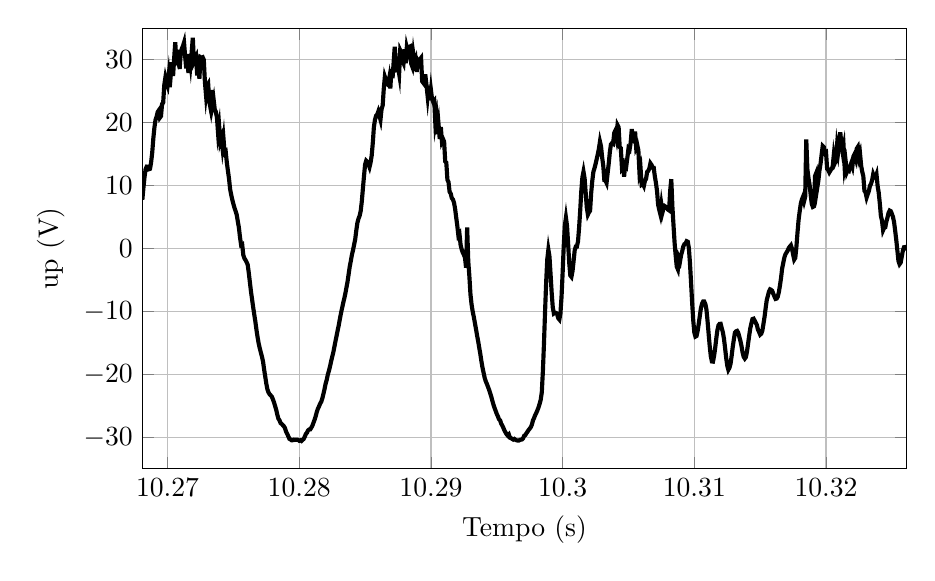
\begin{tikzpicture}

\begin{axis}[%
width=0.8\textwidth,
height=0.461611624834875\textwidth,
scale only axis,
xmin=10.2681,
xmax=10.3261,
xtick={10.27, 10.28, 10.29,  10.3, 10.31, 10.32},
xlabel={Tempo (s)},
xmajorgrids,
ymin=-35,
ymax=35,
ytick={-30, -20, -10,   0,  10,  20,  30},
ylabel={up (V)},
ymajorgrids,
scaled x ticks = false,
legend columns=-1,
legend style={/tikz/every even column/.append style={column sep=0.3cm}},
legend style={font=\footnotesize}
]
\addplot [color=black,solid,line width=1.5pt,forget plot]
  table[row sep=crcr]{10.2680833456702	7.75178374148825\\
10.2681666556704	9.66122776122889\\
10.2682499956706	11.3480305316769\\
10.2683333356708	12.6347569331264\\
10.268416675671	13.0145089376779\\
10.2684999856713	12.9962502065075\\
10.2685833256715	12.6083016629513\\
10.2686666656717	12.6681703354293\\
10.2687500056719	13.7091959356695\\
10.2688333456721	15.2048843303268\\
10.2689166556723	17.4299736956324\\
10.2689999956725	19.1872277238551\\
10.2690833356727	20.4340806640802\\
10.2691666756729	20.9373286251577\\
10.2692499856731	21.6924434573819\\
10.2693333256733	21.9469735208169\\
10.2694166656735	20.7975879802335\\
10.2695000056738	21.0380527423934\\
10.269583345674	22.9618302887242\\
10.2696666556742	23.1764661252038\\
10.2697499956744	25.9788927257931\\
10.2698333356746	27.1494365119501\\
10.2699166756748	26.4012765916794\\
10.269999985675	25.8898362020413\\
10.2700833256752	27.4898609710595\\
10.2701666656754	25.622361794351\\
10.2702500056756	27.7310086349226\\
10.2703333456758	29.5757065460887\\
10.270416655676	27.3957245832176\\
10.2704999956763	30.1765269011936\\
10.2705833356765	32.7711126167063\\
10.2706666756767	29.832105980089\\
10.2707499856769	29.5155920759201\\
10.2708333256771	31.560451791595\\
10.2709166656773	28.5300322664104\\
10.2710000056775	31.003633611871\\
10.2710833456777	31.7658005979907\\
10.2711666556779	32.1521053378452\\
10.2712499956781	32.7251516648173\\
10.2713333356783	30.5729190628843\\
10.2714166756785	28.6049737908159\\
10.2714999856788	30.5396296325426\\
10.271583325679	27.8933406814689\\
10.2716666656792	30.9057051329016\\
10.2717500056794	29.3834173111155\\
10.2718333456796	31.2719009685935\\
10.2719166556798	33.4959752134652\\
10.27199999568	29.6687290275569\\
10.2720833356802	30.0664664916033\\
10.2721666756804	30.450423053945\\
10.2722499856806	27.4990646375428\\
10.2723333256808	30.25868659286\\
10.272416665681	26.975378976366\\
10.2725000056813	30.4023132460389\\
10.2725833456815	30.2963692900291\\
10.2726666556817	30.3799490490278\\
10.2727499956819	30.0001055638667\\
10.2728333356821	26.5610166772863\\
10.2729166756823	24.4512126887033\\
10.2729999856825	25.9063707410884\\
10.2730833256827	26.1841649085971\\
10.2731666656829	23.3638549072387\\
10.2732500056831	22.4451612292773\\
10.2733333456833	25.186652000644\\
10.2734166556835	22.7430241704026\\
10.2734999956838	23.627107815129\\
10.273583335684	22.0965505902197\\
10.2736666756842	21.7200304362982\\
10.2737499856844	20.7894269027222\\
10.2738333256846	18.3736076565549\\
10.2739166656848	19.4784971472497\\
10.274000005685	17.0081763058158\\
10.2740833456852	17.563749639445\\
10.2741666556854	16.0354500441864\\
10.2742499956856	17.4039944376876\\
10.2743333356858	15.1758425515865\\
10.274416675686	15.3549606325307\\
10.2744999856863	13.6598551356748\\
10.2745833256865	12.3547185219862\\
10.2746666656867	11.0928207601823\\
10.2747500056869	9.4328193933959\\
10.2748333456871	8.5340097647061\\
10.2749166556873	7.7497996526146\\
10.2749999956875	7.07553651435069\\
10.2750833356877	6.45357503177898\\
10.2751666756879	5.94729946662756\\
10.2752499856881	5.37667514778839\\
10.2753333256883	4.33470274753117\\
10.2754166656885	3.31669016578943\\
10.2755000056888	1.80918222255009\\
10.275583345689	0.572337819914381\\
10.2756666556892	0.663129048198669\\
10.2757499956894	-1.01083390204897\\
10.2758333356896	-1.53777349247337\\
10.2759166756898	-1.82786076283258\\
10.27599998569	-2.14656221042063\\
10.2760833256902	-2.5544146870423\\
10.2761666656904	-3.83788375812394\\
10.2762500056906	-5.33802707277494\\
10.2763333456908	-6.8136665892565\\
10.276416655691	-8.05929679995035\\
10.2764999956913	-9.31785404008564\\
10.2765833356915	-10.480844981013\\
10.2766666756917	-11.5951689247489\\
10.2767499856919	-12.8972694434787\\
10.2768333256921	-14.0469593958444\\
10.2769166656923	-15.0646176413951\\
10.2770000056925	-15.8270742982203\\
10.2770833456927	-16.5080797904229\\
10.2771666556929	-17.1703749255302\\
10.2772499956931	-17.9441188501215\\
10.2773333356933	-19.2271639121648\\
10.2774166756935	-20.3319269940839\\
10.2774999856937	-21.477292698892\\
10.277583325694	-22.3667387672605\\
10.2776666656942	-22.8568246777814\\
10.2777500056944	-23.1371160055858\\
10.2778333456946	-23.3213169765294\\
10.2779166556948	-23.5119723871573\\
10.277999995695	-23.9555793359234\\
10.2780833356952	-24.4285378214247\\
10.2781666756954	-25.0176106564701\\
10.2782499856956	-25.6054928683531\\
10.2783333256958	-26.380097657594\\
10.278416665696	-27.0197850435188\\
10.2785000056963	-27.2836581000606\\
10.2785833456965	-27.7288202539283\\
10.2786666556967	-27.8516438862787\\
10.2787499956969	-28.0464439925193\\
10.2788333356971	-28.228688763933\\
10.2789166756973	-28.5143166162397\\
10.2789999856975	-29.0943933183585\\
10.2790833256977	-29.4214400631573\\
10.2791666656979	-29.8111131685673\\
10.2792500056981	-30.2196776480765\\
10.2793333456983	-30.3091432084591\\
10.2794166556985	-30.4464318861628\\
10.2794999956988	-30.4379902146459\\
10.279583335699	-30.3520567654333\\
10.2796666756992	-30.3920262884176\\
10.2797499856994	-30.347874892126\\
10.2798333256996	-30.3630287630577\\
10.2799166656998	-30.388606203282\\
10.2800000057	-30.52766348003\\
10.2800833457002	-30.466852188097\\
10.2801666557004	-30.5683501151778\\
10.2802499957006	-30.3789418574253\\
10.2803333357008	-30.2491868452081\\
10.280416675701	-29.8804547270008\\
10.2804999857012	-29.4645817933889\\
10.2805833257015	-29.2570311492256\\
10.2806666657017	-28.8791835990268\\
10.2807500057019	-28.7409335729663\\
10.2808333457021	-28.7221948695274\\
10.2809166557023	-28.4419919591389\\
10.2809999957025	-28.1200980965109\\
10.2810833357027	-27.6406088271232\\
10.2811666757029	-27.1663265916138\\
10.2812499857031	-26.615964820836\\
10.2813333257033	-25.9374864271454\\
10.2814166657035	-25.4178835864612\\
10.2815000057038	-25.0672398292295\\
10.281583345704	-24.6371458888471\\
10.2816666557042	-24.3414578242416\\
10.2817499957044	-23.8156542636383\\
10.2818333357046	-23.1044311815305\\
10.2819166757048	-22.3403808834177\\
10.281999985705	-21.4711775760497\\
10.2820833257052	-20.8781347200225\\
10.2821666657054	-20.0301307784085\\
10.2822500057056	-19.4314135363719\\
10.2823333457058	-18.7422766386242\\
10.282416655706	-17.9331864444213\\
10.2824999957063	-17.2059077504113\\
10.2825833357065	-16.5132404899906\\
10.2826666757067	-15.6161048265415\\
10.2827499857069	-14.7202149778765\\
10.2828333257071	-13.874643129194\\
10.2829166657073	-12.9855318237232\\
10.2830000057075	-12.1676207800214\\
10.2830833457077	-11.1921946435389\\
10.2831666557079	-10.2811162023939\\
10.2832499957081	-9.4800291098854\\
10.2833333357083	-8.66804907102587\\
10.2834166757085	-7.94186355086694\\
10.2834999857087	-7.14021346540318\\
10.283583325709	-6.19028803337425\\
10.2836666657092	-5.2649803006502\\
10.2837500057094	-4.05025025461594\\
10.2838333457096	-2.86787824789959\\
10.2839166557098	-1.95538128973827\\
10.28399999571	-0.963722008989586\\
10.2840833357102	-0.238911394218603\\
10.2841666757104	0.633577959707511\\
10.2842499857106	1.48994424916366\\
10.2843333257108	2.90876910462841\\
10.284416665711	4.11147450173345\\
10.2845000057113	4.76743128959649\\
10.2845833457115	5.20524745367739\\
10.2846666557117	5.9917337820864\\
10.2847499957119	7.50388702963892\\
10.2848333357121	9.54545169967292\\
10.2849166757123	11.5278643370938\\
10.2849999857125	13.3553739229399\\
10.2850833257127	13.952542428025\\
10.2851666657129	13.7865222833901\\
10.2852500057131	13.4002157606535\\
10.2853333457133	12.9324915269175\\
10.2854166557135	13.6679583495977\\
10.2854999957137	14.7804685765124\\
10.285583335714	16.7506496140727\\
10.2856666757142	19.3036421482042\\
10.2857499857144	20.4582668361124\\
10.2858333257146	21.0827898258789\\
10.2859166657148	21.262415831135\\
10.286000005715	21.7621235735637\\
10.2860833457152	21.1219099591396\\
10.2861666557154	20.4667268960453\\
10.2862499957156	22.1607117734045\\
10.2863333357158	22.7103477401477\\
10.286416675716	25.3654819576207\\
10.2864999857162	27.2833728845879\\
10.2865833257165	26.7538372803965\\
10.2866666657167	26.1386321430614\\
10.2867500057169	25.9934864215016\\
10.2868333457171	27.0179700360396\\
10.2869166557173	25.4397823323078\\
10.2869999957175	28.5087749590625\\
10.2870833357177	27.0503290569779\\
10.2871666757179	29.5936175032976\\
10.2872499857181	32.0531627129158\\
10.2873333257183	29.5939824177775\\
10.2874166657185	28.6441496940271\\
10.2875000057188	28.8565154244219\\
10.287583345719	27.7658239112382\\
10.2876666557192	31.4957583880408\\
10.2877499957194	31.1127788594189\\
10.2878333357196	29.8440785712196\\
10.2879166757198	29.4486766938689\\
10.28799998572	31.6542483760304\\
10.2880833257202	29.4591184261009\\
10.2881666657204	31.928172973721\\
10.2882500057206	31.2031518090974\\
10.2883333457208	32.0023222647377\\
10.288416655721	32.0958132362827\\
10.2884999957212	29.3726868021707\\
10.2885833357215	28.9032863479245\\
10.2886666757217	30.8188252259734\\
10.2887499857219	29.5611543021361\\
10.2888333257221	30.0386903308572\\
10.2889166657223	28.0390766223666\\
10.2890000057225	29.872284000365\\
10.2890833457227	29.5568795513248\\
10.2891666557229	30.0541514023529\\
10.2892499957231	30.2834310309791\\
10.2893333357233	26.5628070373543\\
10.2894166757235	26.3298762351669\\
10.2894999857238	27.3857017428559\\
10.289583325724	27.385091779419\\
10.2896666657242	25.8627026775424\\
10.2897500057244	24.1660335505588\\
10.2898333457246	25.8559055395108\\
10.2899166557248	23.5519536576332\\
10.289999995725	25.1744246082023\\
10.2900833357252	23.767234188881\\
10.2901666757254	23.3119429594453\\
10.2902499857256	23.5132247253276\\
10.2903333257258	19.8920234880931\\
10.290416665726	20.9153819570543\\
10.2905000057262	18.1501687878045\\
10.2905833457265	19.5477277646817\\
10.2906666557267	17.3968733268307\\
10.2907499957269	19.3036049797628\\
10.2908333357271	17.018008984048\\
10.2909166757273	17.4019019562604\\
10.2909999857275	16.9891291913391\\
10.2910833257277	13.8298077042659\\
10.2911666657279	13.6397614429734\\
10.2912500057281	10.926045109446\\
10.2913333457283	10.5574558546488\\
10.2914166557285	9.01316637126196\\
10.2914999957287	8.73647279299116\\
10.291583335729	8.01908814699881\\
10.2916666757292	7.8054802174819\\
10.2917499857294	7.29991493247398\\
10.2918333257296	6.34239009123344\\
10.2919166657298	4.95821639228315\\
10.29200000573	3.62571944528562\\
10.2920833457302	2.06385781222306\\
10.2921666557304	2.31688444363611\\
10.2922499957306	0.611339369465988\\
10.2923333357308	-0.139333732988894\\
10.292416675731	-0.626723130485677\\
10.2924999857313	-0.988219711298863\\
10.2925833257315	-1.42168053898559\\
10.2926666657317	-3.03597375342382\\
10.2927500057319	3.35921129749894\\
10.2928333457321	-2.03846408925625\\
10.2929166557323	-4.36038695631532\\
10.2929999957325	-7.26913971939011\\
10.2930833357327	-8.85471671621182\\
10.2931666757329	-9.95927739466485\\
10.2932499857331	-10.8113698550333\\
10.2933333257333	-11.7697895775044\\
10.2934166657335	-12.7434081787305\\
10.2935000057337	-13.7782492889357\\
10.293583345734	-14.6971954770186\\
10.2936666557342	-15.7308436276001\\
10.2937499957344	-16.7601427004402\\
10.2938333357346	-17.9192178092529\\
10.2939166757348	-18.9348266490966\\
10.293999985735	-19.7437468883819\\
10.2940833257352	-20.5665320782958\\
10.2941666657354	-21.1090889313318\\
10.2942500057356	-21.508680212303\\
10.2943333457358	-21.9738975574497\\
10.294416655736	-22.4348321066788\\
10.2944999957363	-22.9895161751341\\
10.2945833357365	-23.5399192530993\\
10.2946666757367	-24.1976733916295\\
10.2947499857369	-24.8075766893149\\
10.2948333257371	-25.3404308172514\\
10.2949166657373	-25.7891939314423\\
10.2950000057375	-26.2824640164233\\
10.2950833457377	-26.6511140145414\\
10.2951666557379	-27.1141015938716\\
10.2952499957381	-27.2728592369343\\
10.2953333357383	-27.8089646990196\\
10.2954166757385	-28.0980399539078\\
10.2954999857388	-28.4835109742355\\
10.295583325739	-28.9113577592939\\
10.2956666657392	-29.2132277850468\\
10.2957500057394	-29.5218647218686\\
10.2958333457396	-29.7088842893749\\
10.2959166557398	-29.5309690017775\\
10.29599999574	-30.0369540034806\\
10.2960833357402	-30.1197267185172\\
10.2961666757404	-30.2270840851175\\
10.2962499857406	-30.3403237342761\\
10.2963333257408	-30.2393148004148\\
10.296416665741	-30.3670983613989\\
10.2965000057412	-30.4541833650595\\
10.2965833457415	-30.4904449361833\\
10.2966666557417	-30.5027126620032\\
10.2967499957419	-30.3976544840118\\
10.2968333357421	-30.3399724050488\\
10.2969166757423	-30.3195687250405\\
10.2969999857425	-30.1195555745579\\
10.2970833257427	-29.7199535155094\\
10.2971666657429	-29.6234958391189\\
10.2972500057431	-29.3321134050384\\
10.2973333457433	-29.0729913508513\\
10.2974166557435	-28.8139980453465\\
10.2974999957438	-28.6058176951946\\
10.297583335744	-28.3705493520212\\
10.2976666757442	-27.9477151171889\\
10.2977499857444	-27.2669810287136\\
10.2978333257446	-26.9000776490106\\
10.2979166657448	-26.4304877284927\\
10.298000005745	-26.0940183492115\\
10.2980833457452	-25.6899661960115\\
10.2981666557454	-25.2383244028321\\
10.2982499957456	-24.6756416832002\\
10.2983333357458	-24.0340661895206\\
10.298416675746	-22.8356128079896\\
10.2984999857463	-19.4795204063554\\
10.2985833257465	-15.0344441196152\\
10.2986666657467	-9.91655300220308\\
10.2987500057469	-5.27668891954426\\
10.2988333457471	-1.69086594415417\\
10.2989166557473	-0.172604209703108\\
10.2989999957475	-1.25692213947509\\
10.2990833357477	-4.09054049503161\\
10.2991666757479	-6.98635753190671\\
10.2992499857481	-9.32554933420173\\
10.2993333257483	-10.2983994165005\\
10.2994166657485	-10.172974653796\\
10.2995000057488	-10.2240251165023\\
10.299583345749	-10.4299461911634\\
10.2996666557492	-11.0601014101719\\
10.2997499957494	-11.2676638407266\\
10.2998333357496	-10.2771618096754\\
10.2999166757498	-7.63350394691991\\
10.29999998575	-3.83180735839002\\
10.3000833257502	0.418263593684855\\
10.3001666657504	3.63636625243439\\
10.3002500057506	4.90329518592065\\
10.3003333457508	3.59553404171498\\
10.300416655751	0.742228623703633\\
10.3004999957513	-2.26996941525184\\
10.3005833357515	-4.27595041284556\\
10.3006666757517	-4.49491891298795\\
10.3007499857519	-3.59211305993486\\
10.3008333257521	-1.94899733410288\\
10.3009166657523	-0.26493929643475\\
10.3010000057525	0.319067529606601\\
10.3010833457527	0.327793254052953\\
10.3011666557529	1.13870091479881\\
10.3012499957531	3.340549856038\\
10.3013333357533	6.02964355345684\\
10.3014166757535	9.13078906333442\\
10.3014999857538	11.3331037050634\\
10.301583325754	12.2198314770899\\
10.3016666657542	11.1767585433403\\
10.3017500057544	8.86777801521933\\
10.3018333457546	6.53247551717979\\
10.3019166557548	5.39703815294851\\
10.301999995755	5.7627907134487\\
10.3020833357552	5.9940678603375\\
10.3021666757554	8.81185558988473\\
10.3022499857556	10.734906999379\\
10.3023333257558	12.1784096138758\\
10.302416665756	12.7478062333152\\
10.3025000057563	13.4346500788888\\
10.3025833457565	14.1875813572276\\
10.3026666557567	14.9690647913861\\
10.3027499957569	15.8083845249496\\
10.3028333357571	16.9858917567146\\
10.3029166757573	16.2302140845868\\
10.3029999857575	14.4758882882718\\
10.3030833257577	13.1906911878445\\
10.3031666657579	10.8630224943965\\
10.3032500057581	10.7968864388346\\
10.3033333457583	10.4241670794973\\
10.3034166557585	12.0032033961735\\
10.3034999957588	13.4989345933625\\
10.303583335759	15.3079802471481\\
10.3036666757592	16.5484453434889\\
10.3037499857594	16.7585340988732\\
10.3038333257596	16.6479137489521\\
10.3039166657598	18.361404713658\\
10.30400000576	18.7247225830336\\
10.3040833457602	17.7773598568904\\
10.3041666557604	19.6183335172243\\
10.3042499957606	19.2869433527549\\
10.3043333357608	16.1202810735309\\
10.304416675761	15.96340870721\\
10.3044999857613	12.9631099483023\\
10.3045833257615	13.3032896404028\\
10.3046666657617	11.4369073927902\\
10.3047500057619	13.3875127318959\\
10.3048333457621	13.1190086569691\\
10.3049166557623	14.4676153887877\\
10.3049999957625	15.9113544591575\\
10.3050833357627	15.7112592630402\\
10.3051666757629	16.8398451047272\\
10.3052499857631	18.9661988512482\\
10.3053333257633	17.3894853720658\\
10.3054166657635	17.1409161025855\\
10.3055000057638	18.5931786147043\\
10.305583345764	16.0547932295419\\
10.3056666557642	16.4465880219217\\
10.3057499957644	15.6036510339729\\
10.3058333357646	12.1069279292241\\
10.3059166757648	12.7715920098314\\
10.305999985765	10.1663089512932\\
10.3060833257652	10.2924188692325\\
10.3061666657654	9.93900102742903\\
10.3062500057656	10.7663046166134\\
10.3063333457658	11.0611691531976\\
10.306416655766	12.1818611408854\\
10.3064999957663	12.3338683240026\\
10.3065833357665	12.731110869818\\
10.3066666757667	13.5401076926219\\
10.3067499857669	13.2880041894591\\
10.3068333257671	12.8579169132832\\
10.3069166657673	12.8291981847223\\
10.3070000057675	11.4847125798808\\
10.3070833457677	10.4370157416955\\
10.3071666557679	9.16718026202298\\
10.3072499957681	6.98519094465949\\
10.3073333357683	6.16298626359239\\
10.3074166757685	5.47794111075667\\
10.3074999857688	6.96695732765204\\
10.307583325769	5.76831197711466\\
10.3076666657692	6.43892651488408\\
10.3077500057694	6.74644793496894\\
10.3078333457696	6.6311359084142\\
10.3079166557698	6.54179870763736\\
10.30799999577	6.18570538862901\\
10.3080833357702	6.06631990250919\\
10.3081666757704	9.19548574296807\\
10.3082499857706	11.0243298550871\\
10.3083333257708	6.68935185935782\\
10.308416665771	3.77901840603049\\
10.3085000057713	0.964669020179006\\
10.3085833457715	-1.12474855557491\\
10.3086666557717	-2.87983821117521\\
10.3087499957719	-3.28710610627824\\
10.3088333357721	-1.55201905304765\\
10.3089166757723	-1.99369173223571\\
10.3089999857725	-0.986481039062915\\
10.3090833257727	-0.373963890883565\\
10.3091666657729	0.370628163714961\\
10.3092500057731	0.710758031130515\\
10.3093333457733	0.790522233386169\\
10.3094166557735	1.16949714126077\\
10.3094999957738	1.09155900702318\\
10.309583335774	0.118279565346403\\
10.3096666757742	-2.24870370836378\\
10.3097499857744	-5.35141269253728\\
10.3098333257746	-8.56089918680538\\
10.3099166657748	-11.4067967545299\\
10.310000005775	-13.3327182527686\\
10.3100833457752	-13.9810529546545\\
10.3101666557754	-13.8840901823008\\
10.3102499957756	-13.1050804304962\\
10.3103333357758	-11.9486546014002\\
10.310416675776	-10.7111768585192\\
10.3104999857763	-9.46497915784533\\
10.3105833257765	-8.77522003558513\\
10.3106666657767	-8.41381100043259\\
10.3107500057769	-8.40928817516823\\
10.3108333457771	-8.77813262412092\\
10.3109166557773	-9.64302541174044\\
10.3109999957775	-11.4129434580933\\
10.3110833357777	-13.4729971950565\\
10.3111666757779	-15.4536561526127\\
10.3112499857781	-17.0952424518442\\
10.3113333257783	-17.9255669734927\\
10.3114166657785	-17.9531226492266\\
10.3115000057788	-17.0437042949449\\
10.311583345779	-15.7882946181105\\
10.3116666557792	-14.2786787674812\\
10.3117499957794	-12.9821328308049\\
10.3118333357796	-12.1882130190788\\
10.3119166757798	-11.9635030926654\\
10.31199998578	-11.9487913362668\\
10.3120833257802	-12.6595228367189\\
10.3121666657804	-13.2887095236209\\
10.3122500057806	-14.3059462550858\\
10.3123333457808	-15.7574425355417\\
10.312416655781	-17.3372841985391\\
10.3124999957813	-18.5832537585413\\
10.3125833357815	-19.2523449057671\\
10.3126666757817	-18.941667608683\\
10.3127499857819	-18.3097245728245\\
10.3128333257821	-17.0413009432298\\
10.3129166657823	-15.6122619302863\\
10.3130000057825	-14.4493073139699\\
10.3130833457827	-13.3485356052125\\
10.3131666557829	-13.1496934743173\\
10.3132499957831	-13.0743230339196\\
10.3133333357833	-13.3703094753757\\
10.3134166757835	-14.0201593348394\\
10.3134999857838	-14.6719286288744\\
10.313583325784	-15.504012048151\\
10.3136666657842	-16.5388377513194\\
10.3137500057844	-17.1958038705046\\
10.3138333457846	-17.4709410843046\\
10.3139166557848	-17.2369500124465\\
10.313999995785	-16.3283117199132\\
10.3140833357852	-15.0832718516018\\
10.3141666757854	-13.8086883812745\\
10.3142499857856	-12.6541201185357\\
10.3143333257858	-11.8809383244217\\
10.314416665786	-11.1948339583132\\
10.3145000057863	-11.1342625874123\\
10.3145833457865	-11.4426704287611\\
10.3146666557867	-11.8077287999097\\
10.3147499957869	-12.1604277631793\\
10.3148333357871	-12.8892065858969\\
10.3149166757873	-13.2570269731727\\
10.3149999857875	-13.6717550066819\\
10.3150833257877	-13.5157044061301\\
10.3151666657879	-13.035157260722\\
10.3152500057881	-11.9478822561085\\
10.3153333457883	-10.8296705933273\\
10.3154166557885	-9.43416766830777\\
10.3154999957888	-8.17102312095876\\
10.315583335789	-7.52527249751048\\
10.3156666757892	-6.83681088955173\\
10.3157499857894	-6.47639348038895\\
10.3158333257896	-6.56046811809775\\
10.3159166657898	-6.7233271443423\\
10.31600000579	-7.21045742469425\\
10.3160833457902	-7.60829728461936\\
10.3161666557904	-7.99574270378004\\
10.3162499957906	-7.94362668448506\\
10.3163333357908	-7.65081747763765\\
10.316416675791	-6.95037708397942\\
10.3164999857913	-5.8785637332301\\
10.3165833257915	-4.69336669697504\\
10.3166666657917	-3.17473865364255\\
10.3167500057919	-2.31274843262815\\
10.3168333457921	-1.45451034414228\\
10.3169166557923	-0.913230770221904\\
10.3169999957925	-0.629689860185823\\
10.3170833357927	-0.34862286871448\\
10.3171666757929	0.072557186524163\\
10.3172499857931	0.316664869099915\\
10.3173333257933	0.518374089407461\\
10.3174166657935	-0.0180343660608204\\
10.3175000057938	-0.933889031319452\\
10.317583345794	-1.75112624558607\\
10.3176666557942	-1.47723535538877\\
10.3177499957944	0.254206122962073\\
10.3178333357946	2.50819774323458\\
10.3179166757948	4.54298786313443\\
10.317999985795	5.92142747701373\\
10.3180833257952	7.09645281056789\\
10.3181666657954	7.78860692613354\\
10.3182500057956	8.2253658217938\\
10.3183333457958	7.51877991956893\\
10.318416655796	8.20212990477492\\
10.3184999957963	17.3511603361466\\
10.3185833357965	12.6410105833255\\
10.3186666757967	11.2157992477531\\
10.3187499857969	10.1688719508952\\
10.3188333257971	8.59131163109672\\
10.3189166657973	7.09990606270747\\
10.3190000057975	6.61917778208596\\
10.3190833457977	6.71082836900454\\
10.3191666557979	11.5246303350581\\
10.3192499957981	11.9649716317597\\
10.3193333357983	9.65892738965666\\
10.3194166757985	10.760027113533\\
10.3194999857988	12.3803933064856\\
10.319583325799	13.46519456801\\
10.3196666657992	14.9336470782602\\
10.3197500057994	16.291477850685\\
10.3198333457996	16.118280663926\\
10.3199166557998	15.2107607538959\\
10.3199999958	15.3143514273253\\
10.3200833358002	12.6661510302188\\
10.3201666758004	12.4747794864655\\
10.3202499858006	12.0942349311301\\
10.3203333258008	12.385588643804\\
10.320416665801	12.7154294328727\\
10.3205000058013	12.9334947928438\\
10.3205833458015	14.7106304643756\\
10.3206666558017	13.5598674945227\\
10.3207499958019	13.9397429221986\\
10.3208333358021	16.3069426088197\\
10.3209166758023	15.222450879517\\
10.3209999858025	16.619119161839\\
10.3210833258027	18.4506987481458\\
10.3211666658029	16.6484817431499\\
10.3212500058031	15.4707412965541\\
10.3213333458033	16.2860952106085\\
10.3214166558035	12.8270122885491\\
10.3214999958038	13.7144044045966\\
10.321583335804	12.1506911947804\\
10.3216666758042	12.5693190364372\\
10.3217499858044	12.4159477461355\\
10.3218333258046	13.0471566381755\\
10.3219166658048	13.5579635002919\\
10.322000005805	13.0372287842959\\
10.3220833458052	14.630917084624\\
10.3221666558054	14.9921055203839\\
10.3222499958056	14.3618272460883\\
10.3223333358058	15.8707777445531\\
10.322416675806	16.14496805646\\
10.3224999858063	14.4609373975744\\
10.3225833258065	15.0668705248541\\
10.3226666658067	13.1711878577127\\
10.3227500058069	12.2111289450899\\
10.3228333458071	11.4830049296226\\
10.3229166558073	9.16662656124313\\
10.3229999958075	8.93308205230722\\
10.3230833358077	8.116066005707\\
10.3231666758079	8.64074528372768\\
10.3232499858081	9.13463954864783\\
10.3233333258083	9.93729415154063\\
10.3234166658085	10.2792599323141\\
10.3235000058088	10.860229006729\\
10.323583345809	11.8066205879799\\
10.3236666558092	11.3772578386887\\
10.3237499958094	11.2809384814413\\
10.3238333358096	11.7653954105563\\
10.3239166758098	9.98074443687537\\
10.32399998581	8.89746148451607\\
10.3240833258102	7.21558004872801\\
10.3241666658104	5.17304626617812\\
10.3242500058106	4.45511448003057\\
10.3243333458108	2.91978825174416\\
10.324416655811	3.31221244000611\\
10.3244999958113	3.38159800844968\\
10.3245833358115	4.28324873877464\\
10.3246666758117	4.91470637124254\\
10.3247499858119	5.67488383879226\\
10.3248333258121	6.03589591182831\\
10.3249166658123	5.93973260299935\\
10.3250000058125	5.51967436229556\\
10.3250833458127	5.03089677062795\\
10.3251666558129	4.20986262793523\\
10.3252499958131	2.83807266251734\\
10.3253333358133	1.39716936050327\\
10.3254166758135	-0.261174843209325\\
10.3254999858138	-1.97442366932559\\
10.325583325814	-2.47722111252825\\
10.3256666658142	-2.2464441489292\\
10.3257500058144	-1.29058069415205\\
10.3258333458146	-0.350945012679667\\
10.3259166558148	0.20542321005887\\
10.325999995815	0.234801241919497\\
10.3260833358152	-0.2743788708142\\
};
\end{axis}
\end{tikzpicture}%}
    \captionof{figure}{Resposta da ação de controle à variação abrupta da indutância.}
    \label{fig:up_exp_Lg}
  \end{minipage}
  \vfill

  \newpage

  \vspace*{\fill}
  \noindent
  \begin{minipage}{\textwidth}
    \makebox[\textwidth]{
      \centering
      \def\svgwidth{\textwidth}
      % This file was created by matlab2tikz v0.4.7 running on MATLAB 7.14.
% Copyright (c) 2008--2014, Nico Schlömer <nico.schloemer@gmail.com>
% All rights reserved.
% Minimal pgfplots version: 1.3
% 
% The latest updates can be retrieved from
%   http://www.mathworks.com/matlabcentral/fileexchange/22022-matlab2tikz
% where you can also make suggestions and rate matlab2tikz.
% 
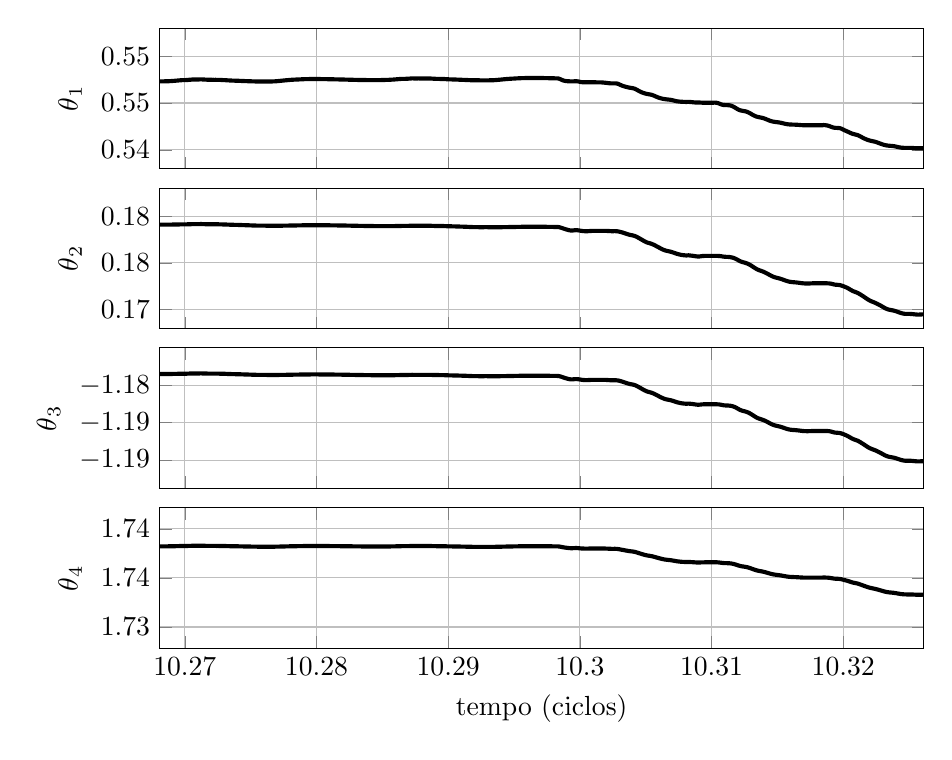
\begin{tikzpicture}

\begin{axis}[%
width=0.8\textwidth,
height=0.146941238746167\textwidth,
scale only axis,
xmin=10.2681,
xmax=10.3261,
xtick={10.27,10.28,10.29,10.3,10.31,10.32},
xticklabels={\empty},
xmajorgrids,
ymin=-1.195,
ymax=-1.18,
ytick={-1.192, -1.188, -1.184},
ylabel={$\theta{}_\text{3}$},
ymajorgrids,
name=plot2,
scaled x ticks = false,
legend columns=-1,
legend style={/tikz/every even column/.append style={column sep=0.3cm}},
legend style={font=\footnotesize}
]
\addplot [color=black,solid,line width=1.5pt,forget plot]
  table[row sep=crcr]{10.2680833456702	-1.18278439402264\\
10.2681666556704	-1.1827848754371\\
10.2682499956706	-1.18278535845101\\
10.2683333356708	-1.18278576770851\\
10.268416675671	-1.18278595571516\\
10.2684999856713	-1.18278600768181\\
10.2685833256715	-1.18278594826164\\
10.2686666656717	-1.1827857677017\\
10.2687500056719	-1.18278525877342\\
10.2688333456721	-1.18278436816531\\
10.2689166556723	-1.18278303468173\\
10.2689999956725	-1.18278153359931\\
10.2690833356727	-1.18277988292257\\
10.2691666756729	-1.18277826707253\\
10.2692499856731	-1.18277589252319\\
10.2693333256733	-1.18277274825542\\
10.2694166656735	-1.18277050075757\\
10.2695000056738	-1.18276788946194\\
10.269583345674	-1.18276418945938\\
10.2696666556742	-1.18276236051085\\
10.2697499956744	-1.18275942051498\\
10.2698333356746	-1.18275717735467\\
10.2699166756748	-1.1827571688289\\
10.269999985675	-1.18275732523367\\
10.2700833256752	-1.18275458669588\\
10.2701666656754	-1.18275410595448\\
10.2702500056756	-1.18274934721792\\
10.2703333456758	-1.18274257710663\\
10.270416655676	-1.18274169437259\\
10.2704999956763	-1.18273718208004\\
10.2705833356765	-1.18273082797992\\
10.2706666756767	-1.18273119195462\\
10.2707499856769	-1.18273253856188\\
10.2708333256771	-1.18272922049836\\
10.2709166656773	-1.18273182481751\\
10.2710000056775	-1.18272986932864\\
10.2710833456777	-1.18272776721187\\
10.2711666556779	-1.18272628974201\\
10.2712499956781	-1.18272482838945\\
10.2713333356783	-1.18272798652018\\
10.2714166756785	-1.18273338883721\\
10.2714999856788	-1.1827343567621\\
10.271583325679	-1.18274002037238\\
10.2716666656792	-1.18274047139541\\
10.2717500056794	-1.18274470809367\\
10.2718333456796	-1.18274609128131\\
10.2719166556798	-1.18274327467596\\
10.27199999568	-1.18274807415909\\
10.2720833356802	-1.18274941023199\\
10.2721666756804	-1.18274826255163\\
10.2722499856806	-1.18275150294803\\
10.2723333256808	-1.18274843805722\\
10.272416665681	-1.18275278968112\\
10.2725000056813	-1.18275146548463\\
10.2725833456815	-1.18275241873883\\
10.2726666556817	-1.18275409358011\\
10.2727499956819	-1.18275523232599\\
10.2728333356821	-1.182760822325\\
10.2729166756823	-1.18276731300232\\
10.2729999856825	-1.18276909791084\\
10.2730833256827	-1.18276965622121\\
10.2731666656829	-1.18277533073904\\
10.2732500056831	-1.18278205997359\\
10.2733333456833	-1.18278365407382\\
10.2734166556835	-1.18279011475893\\
10.2734999956838	-1.18279415634802\\
10.273583335684	-1.18279885037918\\
10.2736666756842	-1.18280149801211\\
10.2737499856844	-1.18280335697911\\
10.2738333256846	-1.18280711271493\\
10.2739166656848	-1.182807403559\\
10.274000005685	-1.18281136327589\\
10.2740833456852	-1.18281404741253\\
10.2741666556854	-1.1828189520539\\
10.2742499956856	-1.18282137106826\\
10.2743333356858	-1.18282684190207\\
10.274416675686	-1.18283059451389\\
10.2744999856863	-1.18283475904697\\
10.2745833256865	-1.18283820031965\\
10.2746666656867	-1.18284165171409\\
10.2747500056869	-1.18284557307375\\
10.2748333456871	-1.18284935476947\\
10.2749166556873	-1.18285311736486\\
10.2749999956875	-1.18285766659562\\
10.2750833356877	-1.1828620529778\\
10.2751666756879	-1.18286662181389\\
10.2752499856881	-1.1828705623008\\
10.2753333256883	-1.18287406301151\\
10.2754166656885	-1.18287684386335\\
10.2755000056888	-1.18287911220153\\
10.275583345689	-1.1828809308943\\
10.2756666556892	-1.18288141700905\\
10.2757499956894	-1.18288295513088\\
10.2758333356896	-1.18288408336607\\
10.2759166756898	-1.18288465067694\\
10.27599998569	-1.18288507446511\\
10.2760833256902	-1.18288566855228\\
10.2761666656904	-1.18288652628421\\
10.2762500056906	-1.18288740481853\\
10.2763333456908	-1.18288810625523\\
10.276416655691	-1.18288857620874\\
10.2764999956913	-1.18288898160475\\
10.2765833356915	-1.18288933444767\\
10.2766666756917	-1.18288965823008\\
10.2767499856919	-1.1828899040024\\
10.2768333256921	-1.1828899281905\\
10.2769166656923	-1.1828896644205\\
10.2770000056925	-1.18288913168955\\
10.2770833456927	-1.18288833895621\\
10.2771666556929	-1.18288732372765\\
10.2772499956931	-1.18288613153673\\
10.2773333356933	-1.18288468700986\\
10.2774166756935	-1.18288315758509\\
10.2774999856937	-1.18288131842298\\
10.277583325694	-1.18287931562995\\
10.2776666656942	-1.1828772890804\\
10.2777500056944	-1.18287506908471\\
10.2778333456946	-1.18287267221499\\
10.2779166556948	-1.18287017288597\\
10.277999995695	-1.18286720883163\\
10.2780833356952	-1.18286448271355\\
10.2781666756954	-1.18286189656779\\
10.2782499856956	-1.18285967206733\\
10.2783333256958	-1.18285775273454\\
10.278416665696	-1.18285583226938\\
10.2785000056963	-1.18285438053246\\
10.2785833456965	-1.18285230386648\\
10.2786666556967	-1.18285018240254\\
10.2787499956969	-1.18284788164862\\
10.2788333356971	-1.18284553976026\\
10.2789166756973	-1.18284305259058\\
10.2789999856975	-1.18284057598659\\
10.2790833256977	-1.1828386164759\\
10.2791666656979	-1.182837321647\\
10.2792500056981	-1.1828360126111\\
10.2793333456983	-1.18283520078821\\
10.2794166556985	-1.18283445780007\\
10.2794999956988	-1.18283392060265\\
10.279583335699	-1.18283349650841\\
10.2796666756992	-1.18283289846421\\
10.2797499856994	-1.18283252675307\\
10.2798333256996	-1.18283235158708\\
10.2799166656998	-1.18283243522206\\
10.2800000057	-1.18283241029806\\
10.2800833457002	-1.18283305785524\\
10.2801666557004	-1.18283365263281\\
10.2802499957006	-1.18283432972987\\
10.2803333357008	-1.18283479312216\\
10.280416675701	-1.18283558673795\\
10.2804999857012	-1.18283638150091\\
10.2805833257015	-1.1828370282371\\
10.2806666657017	-1.18283826413241\\
10.2807500057019	-1.18283918303372\\
10.2808333457021	-1.18284022947689\\
10.2809166557023	-1.18284167118798\\
10.2809999957025	-1.18284300631741\\
10.2810833357027	-1.18284480453051\\
10.2811666757029	-1.18284630758392\\
10.2812499857031	-1.18284754864004\\
10.2813333257033	-1.18284930105227\\
10.2814166657035	-1.18285069636981\\
10.2815000057038	-1.1828521295948\\
10.281583345704	-1.18285378105827\\
10.2816666557042	-1.18285519192394\\
10.2817499957044	-1.18285689852653\\
10.2818333357046	-1.18285883468517\\
10.2819166757048	-1.18286062318409\\
10.281999985705	-1.1828628423805\\
10.2820833257052	-1.18286437013054\\
10.2821666657054	-1.18286621164947\\
10.2822500057056	-1.18286820191899\\
10.2823333457058	-1.18287036937933\\
10.282416655706	-1.18287288911425\\
10.2824999957063	-1.18287541371655\\
10.2825833357065	-1.18287769310808\\
10.2826666757067	-1.18288027501137\\
10.2827499857069	-1.18288264353471\\
10.2828333257071	-1.18288495198649\\
10.2829166657073	-1.18288730713223\\
10.2830000057075	-1.18288939287574\\
10.2830833457077	-1.18289153926865\\
10.2831666557079	-1.18289365924013\\
10.2832499957081	-1.18289581356551\\
10.2833333357083	-1.18289796429713\\
10.2834166757085	-1.18289994972884\\
10.2834999857087	-1.18290156591286\\
10.283583325709	-1.18290336392225\\
10.2836666657092	-1.18290479797295\\
10.2837500057094	-1.18290640686391\\
10.2838333457096	-1.18290836591914\\
10.2839166557098	-1.1829098483111\\
10.28399999571	-1.18291152665664\\
10.2840833357102	-1.18291292946762\\
10.2841666757104	-1.18291437063671\\
10.2842499857106	-1.18291573888677\\
10.2843333257108	-1.18291749854546\\
10.284416665711	-1.18291884139331\\
10.2845000057113	-1.18291967321178\\
10.2845833457115	-1.18292009556836\\
10.2846666557117	-1.18292033753598\\
10.2847499957119	-1.18292082053724\\
10.2848333357121	-1.18292156412379\\
10.2849166757123	-1.18292237065432\\
10.2849999857125	-1.18292311274262\\
10.2850833257127	-1.18292354153772\\
10.2851666657129	-1.18292375072311\\
10.2852500057131	-1.18292379156177\\
10.2853333457133	-1.18292371652584\\
10.2854166557135	-1.18292342047642\\
10.2854999957137	-1.18292284221599\\
10.285583335714	-1.18292186642078\\
10.2856666757142	-1.18292029647141\\
10.2857499857144	-1.18291875751153\\
10.2858333257146	-1.18291727967313\\
10.2859166657148	-1.18291539182931\\
10.286000005715	-1.18291269107596\\
10.2860833457152	-1.18291007122569\\
10.2861666557154	-1.18290784248803\\
10.2862499957156	-1.18290437886187\\
10.2863333357158	-1.18290214064399\\
10.286416675716	-1.18289900483335\\
10.2864999857162	-1.18289609048456\\
10.2865833257165	-1.18289565549403\\
10.2866666657167	-1.18289624529375\\
10.2867500057169	-1.18289615909528\\
10.2868333457171	-1.18289357384936\\
10.2869166557173	-1.18289297063474\\
10.2869999957175	-1.18288709081835\\
10.2870833357177	-1.18288562539981\\
10.2871666757179	-1.18288170483888\\
10.2872499857181	-1.18287619681511\\
10.2873333257183	-1.18287708863785\\
10.2874166657185	-1.18287946891844\\
10.2875000057188	-1.18288061022899\\
10.287583345719	-1.18288313426287\\
10.2876666557192	-1.18287848695648\\
10.2877499957194	-1.18287725300663\\
10.2878333357196	-1.18287941834947\\
10.2879166757198	-1.18288279731197\\
10.28799998572	-1.18288171955371\\
10.2880833257202	-1.18288525274733\\
10.2881666657204	-1.18288338455013\\
10.2882500057206	-1.18288269885129\\
10.2883333457208	-1.18288025997135\\
10.288416655721	-1.18287760351231\\
10.2884999957212	-1.18288004514853\\
10.2885833357215	-1.18288329896662\\
10.2886666757217	-1.1828834553207\\
10.2887499857219	-1.1828865958782\\
10.2888333257221	-1.18288961264787\\
10.2889166657223	-1.18289607336857\\
10.2890000057225	-1.18289834358193\\
10.2890833457227	-1.18290109338245\\
10.2891666557229	-1.18290183057297\\
10.2892499957231	-1.18290086255401\\
10.2893333357233	-1.18290553014584\\
10.2894166757235	-1.18290764975069\\
10.2894999857238	-1.18290721996348\\
10.289583325724	-1.18290676260301\\
10.2896666657242	-1.18291022720302\\
10.2897500057244	-1.18291638640984\\
10.2898333457246	-1.1829193430298\\
10.2899166557248	-1.18292636116905\\
10.289999995725	-1.18292911355945\\
10.2900833357252	-1.18293299327827\\
10.2901666757254	-1.18293600358842\\
10.2902499857256	-1.1829362074931\\
10.2903333257258	-1.18294100951543\\
10.290416665726	-1.18294150081984\\
10.2905000057262	-1.18294607109532\\
10.2905833457265	-1.18294775095314\\
10.2906666557267	-1.18295288618573\\
10.2907499957269	-1.18295445617728\\
10.2908333357271	-1.18295987768013\\
10.2909166757273	-1.18296329921719\\
10.2909999857275	-1.18296549141412\\
10.2910833257277	-1.18297072379103\\
10.2911666657279	-1.18297322047707\\
10.2912500057281	-1.1829776725658\\
10.2913333457283	-1.18298109909964\\
10.2914166557285	-1.18298603645596\\
10.2914999957287	-1.182991002898\\
10.291583335729	-1.18299655428912\\
10.2916666757292	-1.18300161813885\\
10.2917499857294	-1.18300656051507\\
10.2918333257296	-1.18301096629342\\
10.2919166657298	-1.18301465017511\\
10.29200000573	-1.18301700783123\\
10.2920833457302	-1.18301914862074\\
10.2921666557304	-1.18301795631785\\
10.2922499957306	-1.18301987423027\\
10.2923333357308	-1.18302175433359\\
10.292416675731	-1.1830235693566\\
10.2924999857313	-1.18302511433319\\
10.2925833257315	-1.18302630607493\\
10.2926666657317	-1.1830287661459\\
10.2927500057319	-1.18301892654696\\
10.2928333457321	-1.18301990114859\\
10.2929166557323	-1.18302050086951\\
10.2929999957325	-1.18302094838564\\
10.2930833357327	-1.18302137395929\\
10.2931666757329	-1.1830219026215\\
10.2932499857331	-1.18302237522608\\
10.2933333257333	-1.18302287889314\\
10.2934166657335	-1.18302330463634\\
10.2935000057337	-1.18302354601313\\
10.293583345734	-1.18302355951727\\
10.2936666557342	-1.18302336703151\\
10.2937499957344	-1.18302295701642\\
10.2938333357346	-1.18302230719373\\
10.2939166757348	-1.18302136948233\\
10.293999985735	-1.18302016973273\\
10.2940833257352	-1.1830185451513\\
10.2941666657354	-1.18301669681049\\
10.2942500057356	-1.18301473945053\\
10.2943333457358	-1.18301252331227\\
10.294416655736	-1.18301033272127\\
10.2944999957363	-1.1830079358615\\
10.2945833357365	-1.18300560072287\\
10.2946666757367	-1.18300327583355\\
10.2947499857369	-1.18300099540498\\
10.2948333257371	-1.18299880551875\\
10.2949166657373	-1.18299672823068\\
10.2950000057375	-1.18299440321921\\
10.2950833457377	-1.18299205431178\\
10.2951666557379	-1.18298930220907\\
10.2952499957381	-1.18298713171224\\
10.2953333357383	-1.18298438502929\\
10.2954166757385	-1.18298213981608\\
10.2954999857388	-1.18298023071425\\
10.295583325739	-1.18297828148743\\
10.2956666657392	-1.18297698992023\\
10.2957500057394	-1.18297572182038\\
10.2958333457396	-1.18297458094617\\
10.2959166557398	-1.18297460209013\\
10.29599999574	-1.1829732796059\\
10.2960833357402	-1.18297241354642\\
10.2961666757404	-1.18297156125835\\
10.2962499857406	-1.18297109688354\\
10.2963333257408	-1.18297103722186\\
10.296416665741	-1.18297097764976\\
10.2965000057412	-1.18297077905644\\
10.2965833457415	-1.18297092629624\\
10.2966666557417	-1.18297126941721\\
10.2967499957419	-1.18297144814906\\
10.2968333357421	-1.18297210511843\\
10.2969166757423	-1.18297251498019\\
10.2969999857425	-1.18297292075258\\
10.2970833257427	-1.18297365688633\\
10.2971666657429	-1.18297421604746\\
10.2972500057431	-1.1829753228363\\
10.2973333457433	-1.18297664161774\\
10.2974166557435	-1.18297794165237\\
10.2974999957438	-1.1829793899667\\
10.297583335744	-1.18298060682033\\
10.2976666757442	-1.18298208653702\\
10.2977499857444	-1.18298428452246\\
10.2978333257446	-1.18298593590434\\
10.2979166657448	-1.18298761979485\\
10.298000005745	-1.18298914614577\\
10.2980833457452	-1.18299056670413\\
10.2981666557454	-1.18299226091487\\
10.2982499957456	-1.18299406639022\\
10.2983333357458	-1.18299758358151\\
10.298416675746	-1.18301354704892\\
10.2984999857463	-1.18304125070452\\
10.2985833257465	-1.18307714497597\\
10.2986666657467	-1.18311727249381\\
10.2987500057469	-1.18315785146506\\
10.2988333457471	-1.18319689897785\\
10.2989166557473	-1.18323410618423\\
10.2989999957475	-1.18326863113246\\
10.2990833357477	-1.18330065937776\\
10.2991666757479	-1.18332974826459\\
10.2992499857481	-1.18335214386894\\
10.2993333257483	-1.1833641855082\\
10.2994166657485	-1.18336397027889\\
10.2995000057488	-1.18335354431844\\
10.299583345749	-1.18334053779424\\
10.2996666557492	-1.183331703794\\
10.2997499957494	-1.1833314583526\\
10.2998333357496	-1.18333967465465\\
10.2999166757498	-1.18335436831834\\
10.29999998575	-1.18337370387034\\
10.3000833257502	-1.1833948510403\\
10.3001666657504	-1.18341360647212\\
10.3002500057506	-1.18342812986063\\
10.3003333457508	-1.18343643135509\\
10.300416655751	-1.18344029438275\\
10.3004999957513	-1.18344145031238\\
10.3005833357515	-1.18343994228776\\
10.3006666757517	-1.18343514578641\\
10.3007499857519	-1.18342777811109\\
10.3008333257521	-1.18342045907642\\
10.3009166657523	-1.18341550253094\\
10.3010000057525	-1.18341304567867\\
10.3010833457527	-1.18341259818582\\
10.3011666557529	-1.18341320777129\\
10.3012499957531	-1.18341443318446\\
10.3013333357533	-1.18341627982199\\
10.3014166757535	-1.18341828055545\\
10.3014999857538	-1.18341913553066\\
10.301583325754	-1.18341857626895\\
10.3016666657542	-1.18341708905947\\
10.3017500057544	-1.18341606751668\\
10.3018333457546	-1.18341641931113\\
10.3019166557548	-1.18341842610998\\
10.301999995755	-1.18342201492329\\
10.3020833357552	-1.18342983114428\\
10.3021666757554	-1.18343765612836\\
10.3022499857556	-1.18344723151312\\
10.3023333257558	-1.18345568533695\\
10.302416665756	-1.18346098641946\\
10.3025000057563	-1.1834613821857\\
10.3025833457565	-1.18345881044954\\
10.3026666557567	-1.18345743822605\\
10.3027499957569	-1.18346135465042\\
10.3028333357571	-1.18347047263134\\
10.3029166757573	-1.18348803628327\\
10.3029999857575	-1.18351399913385\\
10.3030833257577	-1.18354505532578\\
10.3031666657579	-1.18358174195861\\
10.3032500057581	-1.18361791612427\\
10.3033333457583	-1.18365639009815\\
10.3034166557585	-1.18369494662232\\
10.3034999957588	-1.1837357291365\\
10.303583335759	-1.18377495468512\\
10.3036666757592	-1.18381118362724\\
10.3037499857594	-1.18384353513422\\
10.3038333257596	-1.18387178044382\\
10.3039166657598	-1.1838901004366\\
10.30400000576	-1.18391110889241\\
10.3040833457602	-1.18394268312362\\
10.3041666557604	-1.18397663167921\\
10.3042499957606	-1.18402144719693\\
10.3043333357608	-1.18408122265405\\
10.304416675761	-1.18414047269224\\
10.3044999857613	-1.18420873764647\\
10.3045833257615	-1.1842729767846\\
10.3046666657617	-1.18434393287895\\
10.3047500057619	-1.18440732555336\\
10.3048333457621	-1.18447537278381\\
10.3049166557623	-1.18453846254363\\
10.3049999957625	-1.18459370357292\\
10.3050833357627	-1.18464496483709\\
10.3051666757629	-1.18468423852663\\
10.3052499857631	-1.18471124868102\\
10.3053333257633	-1.18474456156331\\
10.3054166657635	-1.18478182696006\\
10.3055000057638	-1.18481868462503\\
10.305583345764	-1.18487153214239\\
10.3056666557642	-1.18492477415046\\
10.3057499957644	-1.1849818016133\\
10.3058333357646	-1.18504769708605\\
10.3059166757648	-1.1851045951452\\
10.305999985765	-1.18516816205684\\
10.3060833257652	-1.1852276729803\\
10.3061666657654	-1.1852869155477\\
10.3062500057656	-1.1853421314765\\
10.3063333457658	-1.18539419595955\\
10.306416655766	-1.18543745846458\\
10.3064999957663	-1.18547544856407\\
10.3065833357665	-1.18550510539492\\
10.3066666757667	-1.18552804903538\\
10.3067499857669	-1.18554998268805\\
10.3068333257671	-1.1855742663273\\
10.3069166657673	-1.18560097714902\\
10.3070000057675	-1.18563350062461\\
10.3070833457677	-1.1856697279459\\
10.3071666557679	-1.18570806367084\\
10.3072499957681	-1.18574953780555\\
10.3073333357683	-1.18578842250437\\
10.3074166757685	-1.18582488983469\\
10.3074999857688	-1.18584883222978\\
10.307583325769	-1.18588087468477\\
10.3076666657692	-1.18590418346364\\
10.3077500057694	-1.18592222526487\\
10.3078333457696	-1.1859383920044\\
10.3079166557698	-1.18595019401987\\
10.30799999577	-1.18596033526379\\
10.3080833357702	-1.18596940849111\\
10.3081666757704	-1.18596208087142\\
10.3082499857706	-1.18595289704758\\
10.3083333257708	-1.18596445109967\\
10.308416665771	-1.18597566149584\\
10.3085000057713	-1.18598815629844\\
10.3085833457715	-1.18600290454142\\
10.3086666557717	-1.18602095210483\\
10.3087499957719	-1.1860394991536\\
10.3088333357721	-1.18605585139666\\
10.3089166757723	-1.18606889782407\\
10.3089999857725	-1.1860727742643\\
10.3090833257727	-1.1860674654006\\
10.3091666657729	-1.18605563552457\\
10.3092500057731	-1.18604245777357\\
10.3093333457733	-1.18603273298429\\
10.3094166557735	-1.18602768125858\\
10.3094999957738	-1.18602606597155\\
10.309583335774	-1.18602590213264\\
10.3096666757742	-1.18602586718453\\
10.3097499857744	-1.18602566240519\\
10.3098333257746	-1.18602565807689\\
10.3099166657748	-1.18602611437817\\
10.310000005775	-1.18602690883299\\
10.3100833457752	-1.18602768226785\\
10.3101666557754	-1.18602820991956\\
10.3102499957756	-1.18602832127394\\
10.3103333357758	-1.18602838624318\\
10.310416675776	-1.18602961732918\\
10.3104999857763	-1.18603436338196\\
10.3105833257765	-1.18604472833492\\
10.3106666657767	-1.186062483002\\
10.3107500057769	-1.18608635631162\\
10.3108333457771	-1.18611131945649\\
10.3109166557773	-1.18613218395674\\
10.3109999957775	-1.18614549871256\\
10.3110833357777	-1.18615208108341\\
10.3111666757779	-1.18615602891772\\
10.3112499857781	-1.1861608969939\\
10.3113333257783	-1.18616924806583\\
10.3114166657785	-1.18618286923177\\
10.3115000057788	-1.1862028992948\\
10.311583345779	-1.18622997747718\\
10.3116666557792	-1.18626650447816\\
10.3117499957794	-1.18631292022013\\
10.3118333357796	-1.18636862866325\\
10.3119166757798	-1.18643211416607\\
10.31199998578	-1.18650026205503\\
10.3120833257802	-1.18656619478005\\
10.3121666657804	-1.186625995599\\
10.3122500057806	-1.18667531447039\\
10.3123333457808	-1.1867137409627\\
10.312416655781	-1.18674475088034\\
10.3124999957813	-1.18677321690983\\
10.3125833357815	-1.186804757074\\
10.3126666757817	-1.186843816048\\
10.3127499857819	-1.18688888888799\\
10.3128333257821	-1.18694255454328\\
10.3129166657823	-1.1870039325605\\
10.3130000057825	-1.18707225626806\\
10.3130833457827	-1.18714749671096\\
10.3131666557829	-1.18722408654197\\
10.3132499957831	-1.18730092526031\\
10.3133333357833	-1.18737459590618\\
10.3134166757835	-1.18744019474134\\
10.3134999857838	-1.1874978124921\\
10.313583325784	-1.18754606919408\\
10.3136666657842	-1.18758677144745\\
10.3137500057844	-1.1876248511976\\
10.3138333457846	-1.18766310159755\\
10.3139166557848	-1.18770488178522\\
10.313999995785	-1.18775211892951\\
10.3140833357852	-1.18780475788963\\
10.3141666757854	-1.18786239698071\\
10.3142499857856	-1.18792347774577\\
10.3143333257858	-1.18798627138502\\
10.314416665786	-1.18805062175888\\
10.3145000057863	-1.1881110989591\\
10.3145833457865	-1.18816657958872\\
10.3146666557867	-1.18821574713283\\
10.3147499957869	-1.18825803988674\\
10.3148333357871	-1.18829284574779\\
10.3149166757873	-1.18832296128736\\
10.3149999857875	-1.18834965686814\\
10.3150833257877	-1.18837664295066\\
10.3151666657879	-1.18840538175136\\
10.3152500057881	-1.18843767328529\\
10.3153333457883	-1.18847353459093\\
10.3154166557885	-1.18851267295893\\
10.3154999957888	-1.18855376657791\\
10.315583335789	-1.18859432970708\\
10.3156666757892	-1.1886335395459\\
10.3157499857894	-1.1886696321912\\
10.3158333257896	-1.18870083338188\\
10.3159166657898	-1.18872617076738\\
10.31600000579	-1.18874570150618\\
10.3160833457902	-1.18875984955342\\
10.3161666557904	-1.18876986374932\\
10.3162499957906	-1.18877900225637\\
10.3163333357908	-1.18878726152384\\
10.316416675791	-1.18879670050662\\
10.3164999857913	-1.18880790724161\\
10.3165833257915	-1.18882072225628\\
10.3166666657917	-1.18883552130581\\
10.3167500057919	-1.18885103683761\\
10.3168333457921	-1.18886606127813\\
10.3169166557923	-1.18887952143115\\
10.3169999957925	-1.18888964538384\\
10.3170833357927	-1.18889656790222\\
10.3171666757929	-1.18890059284486\\
10.3172499857931	-1.18890206024124\\
10.3173333257933	-1.18890178023731\\
10.3174166657935	-1.18889915005429\\
10.3175000057938	-1.18889465827188\\
10.317583345794	-1.18888931477325\\
10.3176666557942	-1.18888531463708\\
10.3177499957944	-1.18888341240645\\
10.3178333357946	-1.1888828538457\\
10.3179166757948	-1.18888292094617\\
10.317999985795	-1.18888297813201\\
10.3180833257952	-1.18888314840028\\
10.3181666657954	-1.18888328936051\\
10.3182500057956	-1.18888339656948\\
10.3183333457958	-1.18888311524941\\
10.318416655796	-1.18888308890771\\
10.3184999957963	-1.18888035104415\\
10.3185833357965	-1.18888197310113\\
10.3186666757967	-1.18888251355414\\
10.3187499857969	-1.18888438028185\\
10.3188333257971	-1.18888969454048\\
10.3189166657973	-1.18890112425507\\
10.3190000057975	-1.18891933552794\\
10.3190833457977	-1.18894521344226\\
10.3191666557979	-1.18897840825462\\
10.3192499957981	-1.18901259937951\\
10.3193333357983	-1.18904155304962\\
10.3194166757985	-1.18905922000417\\
10.3194999857988	-1.18906658263814\\
10.319583325799	-1.18907366410963\\
10.3196666657992	-1.18908505241089\\
10.3197500057994	-1.18910333742732\\
10.3198333457996	-1.18913263235523\\
10.3199166557998	-1.1891717760244\\
10.3199999958	-1.18921258993496\\
10.3200833358002	-1.18926300314834\\
10.3201666758004	-1.18931182142899\\
10.3202499858006	-1.18936399492849\\
10.3203333258008	-1.18942049712058\\
10.320416665801	-1.18948572153923\\
10.3205000058013	-1.18955604246836\\
10.3205833458015	-1.18962154398362\\
10.3206666558017	-1.18968992903438\\
10.3207499958019	-1.18974747378984\\
10.3208333358021	-1.1897878934116\\
10.3209166758023	-1.18983330370533\\
10.3209999858025	-1.18987500629116\\
10.3210833258027	-1.18991657037929\\
10.3211666658029	-1.18997546465271\\
10.3212500058031	-1.19004362688165\\
10.3213333458033	-1.19010834340389\\
10.3214166558035	-1.19018765336145\\
10.3214999958038	-1.19025994828219\\
10.321583335804	-1.19033956945373\\
10.3216666758042	-1.19041601799041\\
10.3217499858044	-1.19049475959467\\
10.3218333258046	-1.19056947509242\\
10.3219166658048	-1.19063969265841\\
10.322000005805	-1.19070710732096\\
10.3220833458052	-1.19075860097991\\
10.3221666558054	-1.19080585042941\\
10.3222499958056	-1.190853845145\\
10.3223333358058	-1.19089453694645\\
10.322416675806	-1.19093842426041\\
10.3224999858063	-1.19099282971152\\
10.3225833258065	-1.19104377547298\\
10.3226666658067	-1.19110373873168\\
10.3227500058069	-1.19116279783589\\
10.3228333458071	-1.19122313807994\\
10.3229166558073	-1.19128963018947\\
10.3229999958075	-1.19135456179972\\
10.3230833358077	-1.19142042278093\\
10.3231666758079	-1.19148122308685\\
10.3232499858081	-1.19153522306998\\
10.3233333258083	-1.19158108647543\\
10.3234166658085	-1.19161924670955\\
10.3235000058088	-1.1916477021879\\
10.323583345809	-1.19166802290448\\
10.3236666558092	-1.19168849462913\\
10.3237499958094	-1.19171046411243\\
10.3238333358096	-1.19173284198542\\
10.3239166758098	-1.1917632523596\\
10.32399998581	-1.19179690590279\\
10.3240833258102	-1.19183453935729\\
10.3241666658104	-1.19187486380449\\
10.3242500058106	-1.19191436351837\\
10.3243333458108	-1.1919537325585\\
10.324416655811	-1.1919868464991\\
10.3244999958113	-1.1920165486189\\
10.3245833358115	-1.19203920006343\\
10.3246666758117	-1.19205493206007\\
10.3247499858119	-1.1920632964921\\
10.3248333258121	-1.19206593440966\\
10.3249166658123	-1.1920652915785\\
10.3250000058125	-1.19206481346129\\
10.3250833458127	-1.19206612363793\\
10.3251666558129	-1.19207155955525\\
10.3252499958131	-1.19208091348095\\
10.3253333358133	-1.19209239162273\\
10.3254166758135	-1.19210507155044\\
10.3254999858138	-1.19211810343011\\
10.325583325814	-1.19212726037307\\
10.3256666658142	-1.19213184066847\\
10.3257500058144	-1.19213132130424\\
10.3258333458146	-1.19212730108617\\
10.3259166558148	-1.19212137966696\\
10.325999995815	-1.19211494474291\\
10.3260833358152	-1.19210931955319\\
};
\end{axis}

\begin{axis}[%
width=0.8\textwidth,
height=0.146941238746167\textwidth,
scale only axis,
xmin=10.2681,
xmax=10.3261,
xtick={10.27,10.28,10.29,10.3,10.31,10.32},
xlabel={tempo (ciclos)},
xmajorgrids,
ymin=1.725,
ymax=1.745,
ytick={1.728, 1.735, 1.742},
ylabel={$\theta{}_\text{4}$},
ymajorgrids,
at=(plot2.below south west),
anchor=above north west,
scaled x ticks = false,
legend columns=-1,
legend style={/tikz/every even column/.append style={column sep=0.3cm}},
legend style={font=\footnotesize}
]
\addplot [color=black,solid,line width=1.5pt,forget plot]
  table[row sep=crcr]{10.2680833456702	1.73949788771756\\
10.2681666556704	1.7394980269994\\
10.2682499956706	1.73949842420006\\
10.2683333356708	1.73949917940524\\
10.268416675671	1.73949997093186\\
10.2684999856713	1.73950074931242\\
10.2685833256715	1.73950148337763\\
10.2686666656717	1.73950232787467\\
10.2687500056719	1.73950387675756\\
10.2688333456721	1.7395060044627\\
10.2689166556723	1.7395088256844\\
10.2689999956725	1.73951179136885\\
10.2690833356727	1.73951492159346\\
10.2691666756729	1.73951785642004\\
10.2692499856731	1.7395219767612\\
10.2693333256733	1.73952716029304\\
10.2694166656735	1.73953075402619\\
10.2695000056738	1.73953486737563\\
10.269583345674	1.73954047939176\\
10.2696666556742	1.73954316110458\\
10.2697499956744	1.73954740171346\\
10.2698333356746	1.73955051025004\\
10.2699166756748	1.73955052175948\\
10.269999985675	1.73955031654318\\
10.2700833256752	1.7395537545353\\
10.2701666656754	1.73955433534976\\
10.2702500056756	1.73956003233163\\
10.2703333456758	1.73956799821828\\
10.270416655676	1.73956904529282\\
10.2704999956763	1.73957450621399\\
10.2705833356765	1.73958206730908\\
10.2706666756767	1.73958163562719\\
10.2707499856769	1.73958002607436\\
10.2708333256771	1.73958388484289\\
10.2709166656773	1.73958095726607\\
10.2710000056775	1.73958314113704\\
10.2710833456777	1.73958542993027\\
10.2711666556779	1.73958702971409\\
10.2712499956781	1.73958861155885\\
10.2713333356783	1.73958520209509\\
10.2714166756785	1.73957939184754\\
10.2714999856788	1.73957837303908\\
10.271583325679	1.73957258277183\\
10.2716666656792	1.73957212552628\\
10.2717500056794	1.73956790680622\\
10.2718333456796	1.73956652863273\\
10.2719166556798	1.73956931211181\\
10.27199999568	1.73956456967455\\
10.2720833356802	1.73956323013509\\
10.2721666756804	1.7395643679076\\
10.2722499856806	1.73956117022226\\
10.2723333256808	1.7395642112831\\
10.272416665681	1.7395599322328\\
10.2725000056813	1.73956124728512\\
10.2725833456815	1.73956031390242\\
10.2726666556817	1.73955867095041\\
10.2727499956819	1.73955755785981\\
10.2728333356821	1.73955213553835\\
10.2729166756823	1.73954587709627\\
10.2729999856825	1.73954419190699\\
10.2730833256827	1.73954367721063\\
10.2731666656829	1.73953846257675\\
10.2732500056831	1.73953224138729\\
10.2733333456833	1.73953078601298\\
10.2734166556835	1.73952500221037\\
10.2734999956838	1.73952138178901\\
10.273583335684	1.73951723308889\\
10.2736666756842	1.73951490850461\\
10.2737499856844	1.73951328823433\\
10.2738333256846	1.73951001346884\\
10.2739166656848	1.73950975891424\\
10.274000005685	1.73950631347301\\
10.2740833456852	1.7395039643283\\
10.2741666556854	1.73949971714261\\
10.2742499956856	1.73949764107475\\
10.2743333356858	1.73949303528568\\
10.274416675686	1.73948990085276\\
10.2744999856863	1.73948649399697\\
10.2745833256865	1.73948371716163\\
10.2746666656867	1.73948097057462\\
10.2747500056869	1.73947788190374\\
10.2748333456871	1.73947493505292\\
10.2749166556873	1.7394720480266\\
10.2749999956875	1.73946861653924\\
10.2750833356877	1.73946536923168\\
10.2751666756879	1.73946207476874\\
10.2752499856881	1.73945931220071\\
10.2753333256883	1.73945693374811\\
10.2754166656885	1.73945509816061\\
10.2755000056888	1.73945364194087\\
10.275583345689	1.739452504234\\
10.2756666556892	1.73945220835162\\
10.2757499956894	1.73945130164405\\
10.2758333356896	1.73945065361772\\
10.2759166756898	1.73945034618492\\
10.27599998569	1.7394501342317\\
10.2760833256902	1.73944986563296\\
10.2761666656904	1.73944953125573\\
10.2762500056906	1.73944926670978\\
10.2763333456908	1.73944914433146\\
10.276416655691	1.73944914452197\\
10.2764999956913	1.73944924713871\\
10.2765833356915	1.73944948610272\\
10.2766666756917	1.73944998747249\\
10.2767499856919	1.73945101864368\\
10.2768333256921	1.73945277499862\\
10.2769166656923	1.73945526098891\\
10.2770000056925	1.73945840874044\\
10.2770833456927	1.73946217584517\\
10.2771666556929	1.73946627681838\\
10.2772499956931	1.73947044895884\\
10.2773333356933	1.73947482261772\\
10.2774166756935	1.73947882955358\\
10.2774999856937	1.73948308112647\\
10.277583325694	1.73948719670121\\
10.2776666656942	1.73949099378283\\
10.2777500056944	1.739494845522\\
10.2778333456946	1.73949873376312\\
10.2779166556948	1.73950257497591\\
10.277999995695	1.73950693787302\\
10.2780833356952	1.73951080937087\\
10.2781666756954	1.73951438924916\\
10.2782499856956	1.73951739116804\\
10.2783333256958	1.73951991765021\\
10.278416665696	1.73952238214112\\
10.2785000056963	1.73952419983111\\
10.2785833456965	1.73952674637542\\
10.2786666556967	1.73952929577519\\
10.2787499956969	1.73953202418221\\
10.2788333356971	1.73953477285722\\
10.2789166756973	1.73953766838863\\
10.2789999856975	1.73954053058759\\
10.2790833256977	1.7395427807472\\
10.2791666656979	1.73954425822799\\
10.2792500056981	1.73954573896999\\
10.2793333456983	1.73954664683229\\
10.2794166556985	1.73954746909246\\
10.2794999956988	1.7395480571682\\
10.279583335699	1.73954851694799\\
10.2796666756992	1.73954915955686\\
10.2797499856994	1.73954955577434\\
10.2798333256996	1.73954974133003\\
10.2799166656998	1.73954965327617\\
10.2800000057	1.7395496793515\\
10.2800833457002	1.7395490064285\\
10.2801666557004	1.73954839190294\\
10.2802499957006	1.73954769750998\\
10.2803333357008	1.73954722548983\\
10.280416675701	1.73954642207519\\
10.2804999857012	1.73954562129182\\
10.2805833257015	1.73954497310578\\
10.2806666657017	1.73954374076428\\
10.2807500057019	1.73954282841703\\
10.2808333457021	1.7395417956966\\
10.2809166557023	1.73954037983806\\
10.2809999957025	1.73953907500418\\
10.2810833357027	1.7395373282338\\
10.2811666757029	1.73953587627555\\
10.2812499857031	1.73953468551451\\
10.2813333257033	1.73953301329835\\
10.2814166657035	1.73953168711425\\
10.2815000057038	1.73953033257056\\
10.281583345704	1.73952877888226\\
10.2816666557042	1.73952745756013\\
10.2817499957044	1.73952586808592\\
10.2818333357046	1.73952407347262\\
10.2819166757048	1.73952242562614\\
10.281999985705	1.739520395623\\
10.2820833257052	1.73951900738216\\
10.2821666657054	1.73951734781511\\
10.2822500057056	1.73951556379033\\
10.2823333457058	1.73951363330526\\
10.282416655706	1.73951140608836\\
10.2824999957063	1.73950919429335\\
10.2825833357065	1.73950721888706\\
10.2826666757067	1.73950500589755\\
10.2827499857069	1.7395029951939\\
10.2828333257071	1.73950105705677\\
10.2829166657073	1.7394991003025\\
10.2830000057075	1.73949738542863\\
10.2830833457077	1.73949564090888\\
10.2831666557079	1.73949393667038\\
10.2832499957081	1.73949222629583\\
10.2833333357083	1.73949054261042\\
10.2834166757085	1.73948901330751\\
10.2834999857087	1.73948779102063\\
10.283583325709	1.73948645719237\\
10.2836666657092	1.73948541287581\\
10.2837500057094	1.7394842682532\\
10.2838333457096	1.73948290812971\\
10.2839166557098	1.73948191075659\\
10.28399999571	1.73948082946045\\
10.2840833357102	1.73947996630751\\
10.2841666757104	1.7394791299849\\
10.2842499857106	1.73947838906636\\
10.2843333257108	1.73947751888806\\
10.284416665711	1.73947693150856\\
10.2845000057113	1.73947663060714\\
10.2845833457115	1.73947651586678\\
10.2846666557117	1.7394764773454\\
10.2847499957119	1.73947647753346\\
10.2848333357121	1.73947667181551\\
10.2849166757123	1.73947725182516\\
10.2849999857125	1.73947836363043\\
10.2850833257127	1.73947955694354\\
10.2851666657129	1.73948062233484\\
10.2852500057131	1.73948158429837\\
10.2853333457133	1.73948224432096\\
10.2854166557135	1.73948341001354\\
10.2854999957137	1.73948494099045\\
10.285583335714	1.73948705919468\\
10.2856666757142	1.73949010115665\\
10.2857499857144	1.73949289337235\\
10.2858333257146	1.73949548892301\\
10.2859166657148	1.73949867289515\\
10.286000005715	1.73950301638263\\
10.2860833457152	1.73950707733639\\
10.2861666557154	1.73951046737086\\
10.2862499957156	1.73951561559101\\
10.2863333357158	1.73951883633631\\
10.286416675716	1.73952327973578\\
10.2864999857162	1.73952728628357\\
10.2865833257165	1.73952787219529\\
10.2866666657167	1.73952709384446\\
10.2867500057169	1.73952720308273\\
10.2868333457171	1.73953033983551\\
10.2869166557173	1.73953105076731\\
10.2869999957175	1.73953794648355\\
10.2870833357177	1.73953964447085\\
10.2871666757179	1.73954425982128\\
10.2872499857181	1.73955069597672\\
10.2873333257183	1.73954965408943\\
10.2874166657185	1.73954685294301\\
10.2875000057188	1.73954554383264\\
10.287583345719	1.73954274637816\\
10.2876666557192	1.73954778243303\\
10.2877499957194	1.73954909262558\\
10.2878333357196	1.73954676564831\\
10.2879166757198	1.73954312590149\\
10.28799998572	1.73954427010111\\
10.2880833257202	1.73954059422623\\
10.2881666657204	1.7395425352698\\
10.2882500057206	1.73954323810218\\
10.2883333457208	1.73954574909271\\
10.288416655721	1.7395484912944\\
10.2884999957212	1.73954595430311\\
10.2885833357215	1.73954255409739\\
10.2886666757217	1.73954239311593\\
10.2887499857219	1.73953922330472\\
10.2888333257221	1.7395361974663\\
10.2889166657223	1.73952979735464\\
10.2890000057225	1.73952757382896\\
10.2890833457227	1.73952493516514\\
10.2891666557229	1.73952423118035\\
10.2892499957231	1.7395251535274\\
10.2893333357233	1.73952068635475\\
10.2894166757235	1.73951863798694\\
10.2894999857238	1.73951904860599\\
10.289583325724	1.73951948273798\\
10.2896666657242	1.73951618052816\\
10.2897500057244	1.73951028118752\\
10.2898333457246	1.73950748152734\\
10.2899166557248	1.73950099345288\\
10.289999995725	1.7394984760146\\
10.2900833357252	1.73949499986954\\
10.2901666757254	1.73949231355623\\
10.2902499857256	1.739492132371\\
10.2903333257258	1.73948787240288\\
10.290416665726	1.73948743276759\\
10.2905000057262	1.73948338561323\\
10.2905833457265	1.7394818938998\\
10.2906666557267	1.73947739418265\\
10.2907499957269	1.73947602384382\\
10.2908333357271	1.73947137547994\\
10.2909166757273	1.73946845149626\\
10.2909999857275	1.739466613137\\
10.2910833257277	1.73946227630391\\
10.2911666657279	1.73946021417662\\
10.2912500057281	1.73945660589411\\
10.2913333457283	1.73945384956412\\
10.2914166557285	1.73944994409959\\
10.2914999957287	1.73944606834902\\
10.291583335729	1.73944183368238\\
10.2916666757292	1.73943806703499\\
10.2917499857294	1.73943449676939\\
10.2918333257296	1.73943139742714\\
10.2919166657298	1.73942887165697\\
10.29200000573	1.73942729271622\\
10.2920833457302	1.73942588831383\\
10.2921666557304	1.73942666006671\\
10.2922499957306	1.73942543948459\\
10.2923333357308	1.73942422891108\\
10.292416675731	1.73942309932528\\
10.2924999857313	1.73942219397928\\
10.2925833257315	1.73942154870916\\
10.2926666657317	1.73942033807024\\
10.2927500057319	1.739424640593\\
10.2928333457321	1.739424294227\\
10.2929166557323	1.73942403278784\\
10.2929999957325	1.73942390490537\\
10.2930833357327	1.73942390517219\\
10.2931666757329	1.73942409382772\\
10.2932499857331	1.73942450180289\\
10.2933333257333	1.73942535415914\\
10.2934166657335	1.7394268655921\\
10.2935000057337	1.73942914915851\\
10.293583345734	1.73943192222834\\
10.2936666557342	1.7394351674431\\
10.2937499957344	1.73943851550446\\
10.2938333357346	1.73944198736663\\
10.2939166757348	1.73944560295487\\
10.293999985735	1.73944922281893\\
10.2940833257352	1.73945330779867\\
10.2941666657354	1.73945734295463\\
10.2942500057356	1.73946121216222\\
10.2943333457358	1.73946525225823\\
10.294416655736	1.73946897475738\\
10.2944999957363	1.73947282510736\\
10.2945833357365	1.73947639167907\\
10.2946666757367	1.73947979974649\\
10.2947499857369	1.73948302201473\\
10.2948333257371	1.73948601787132\\
10.2949166657373	1.73948877980259\\
10.2950000057375	1.7394917934313\\
10.2950833457377	1.7394947693226\\
10.2951666557379	1.73949819491431\\
10.2952499957381	1.73950085662544\\
10.2953333357383	1.73950418938853\\
10.2954166757385	1.73950687818226\\
10.2954999857388	1.73950914342\\
10.295583325739	1.73951143104519\\
10.2956666657392	1.73951292843866\\
10.2957500057394	1.73951438265668\\
10.2958333457396	1.73951567461412\\
10.2959166557398	1.73951565093957\\
10.29599999574	1.73951711683861\\
10.2960833357402	1.7395180640347\\
10.2961666757404	1.73951899014101\\
10.2962499857406	1.73951949157878\\
10.2963333257408	1.73951955562495\\
10.296416665741	1.73951961913503\\
10.2965000057412	1.73951982916909\\
10.2965833457415	1.73951967457847\\
10.2966666557417	1.73951931641777\\
10.2967499957419	1.73951913101537\\
10.2968333357421	1.73951845393252\\
10.2969166757423	1.73951803376872\\
10.2969999857425	1.73951762043557\\
10.2970833257427	1.73951687443698\\
10.2971666657429	1.73951631034506\\
10.2972500057431	1.73951519977644\\
10.2973333457433	1.73951388258483\\
10.2974166557435	1.73951259208959\\
10.2974999957438	1.7395111640636\\
10.297583335744	1.73950997161799\\
10.2976666757442	1.73950853028043\\
10.2977499857444	1.73950639939841\\
10.2978333257446	1.73950480675776\\
10.2979166657448	1.73950319518694\\
10.298000005745	1.7395017425204\\
10.2980833457452	1.73950039718191\\
10.2981666557454	1.73949879931909\\
10.2982499957456	1.73949710287227\\
10.2983333357458	1.7394938144908\\
10.298416675746	1.73947897572852\\
10.2984999857463	1.73945354538716\\
10.2985833257465	1.73942252147034\\
10.2986666657467	1.7393910842463\\
10.2987500057469	1.73936238055489\\
10.2988333457471	1.73933689020871\\
10.2989166557473	1.73931378024156\\
10.2989999957475	1.73929284588065\\
10.2990833357477	1.73927358592529\\
10.2991666757479	1.73925607878784\\
10.2992499857481	1.73924253788761\\
10.2993333257483	1.73923520950338\\
10.2994166657485	1.73923534273985\\
10.2995000057488	1.73924205711529\\
10.299583345749	1.73925105914308\\
10.2996666557492	1.7392578552798\\
10.2997499957494	1.73925806721932\\
10.2998333357496	1.73925036776396\\
10.2999166757498	1.73923668618307\\
10.29999998575	1.73922050030238\\
10.3000833257502	1.73920542013813\\
10.3001666657504	1.73919400484452\\
10.3002500057506	1.73918617599121\\
10.3003333457508	1.73918200333415\\
10.300416655751	1.73918011195826\\
10.3004999957513	1.73917953892279\\
10.3005833357515	1.73918031349616\\
10.3006666757517	1.73918288639242\\
10.3007499857519	1.73918704769895\\
10.3008333257521	1.7391915319943\\
10.3009166657523	1.73919502996856\\
10.3010000057525	1.73919716797605\\
10.3010833457527	1.73919765732762\\
10.3011666557529	1.73919690304421\\
10.3012499957531	1.73919579738087\\
10.3013333357533	1.73919517127894\\
10.3014166757535	1.73919517222861\\
10.3014999857538	1.73919534099775\\
10.301583325754	1.73919512164014\\
10.3016666657542	1.73919399265167\\
10.3017500057544	1.73919188836987\\
10.3018333457546	1.73918895061434\\
10.3019166557548	1.73918518333933\\
10.301999995755	1.73918063873007\\
10.3020833357552	1.73917233921381\\
10.3021666757554	1.73916472005175\\
10.3022499857556	1.73915637553912\\
10.3023333257558	1.73914929990362\\
10.302416665756	1.73914490533231\\
10.3025000057563	1.7391445682866\\
10.3025833457565	1.73914690162588\\
10.3026666557567	1.7391482752068\\
10.3027499957569	1.73914391535038\\
10.3028333357571	1.73913305565323\\
10.3029166757573	1.73911242119911\\
10.3029999857575	1.73908410780917\\
10.3030833257577	1.73905398353312\\
10.3031666657579	1.73902233020248\\
10.3032500057581	1.73899352370219\\
10.3033333457583	1.73896433306923\\
10.3034166557585	1.73893547433149\\
10.3034999957588	1.73890492203113\\
10.303583335759	1.73887528223874\\
10.3036666757592	1.7388477233175\\
10.3037499857594	1.73882287891442\\
10.3038333257596	1.7388008602567\\
10.3039166657598	1.73878628184179\\
10.30400000576	1.73876914969787\\
10.3040833457602	1.73874241721576\\
10.3041666557604	1.7387129350385\\
10.3042499957606	1.73867427980962\\
10.3043333357608	1.7386236834079\\
10.304416675761	1.73857531648115\\
10.3044999857613	1.73852251835451\\
10.3045833257615	1.73847470100923\\
10.3046666657617	1.73842356612895\\
10.3047500057619	1.73837849996933\\
10.3048333457621	1.73833067566488\\
10.3049166557623	1.73828624138751\\
10.3049999957625	1.73824733783088\\
10.3050833357627	1.73821106919768\\
10.3051666757629	1.73818290679503\\
10.3052499857631	1.73816322319313\\
10.3053333257633	1.73813829965048\\
10.3054166657635	1.73810936161581\\
10.3055000057638	1.7380801497055\\
10.305583345764	1.7380381778491\\
10.3056666557642	1.73799610577204\\
10.3057499957644	1.73795243943068\\
10.3058333357646	1.73790355012525\\
10.3059166757648	1.73786251321302\\
10.305999985765	1.73781809865665\\
10.3060833257652	1.73777703444747\\
10.3061666657654	1.73773668084586\\
10.3062500057656	1.73769929381419\\
10.3063333457658	1.73766417153899\\
10.306416655766	1.73763495824883\\
10.3064999957663	1.73760920435657\\
10.3065833357665	1.73758883437626\\
10.3066666757667	1.73757280054158\\
10.3067499857669	1.73755710369678\\
10.3068333257671	1.73753923494654\\
10.3069166657673	1.73751915998204\\
10.3070000057675	1.73749455704562\\
10.3070833457677	1.73746735564652\\
10.3071666557679	1.73743926464511\\
10.3072499957681	1.73740986528328\\
10.3073333357683	1.73738321059248\\
10.3074166757685	1.7373590322085\\
10.3074999857688	1.73734350902482\\
10.307583325769	1.73732298379445\\
10.3076666657692	1.73730783515809\\
10.3077500057694	1.73729613212087\\
10.3078333457696	1.7372855728193\\
10.3079166557698	1.73727774570056\\
10.30799999577	1.73727092616118\\
10.3080833357702	1.73726472086227\\
10.3081666757704	1.73726980164034\\
10.3082499857706	1.73727621833937\\
10.3083333257708	1.73726762514662\\
10.308416665771	1.73725862615281\\
10.3085000057713	1.73724906288119\\
10.3085833457715	1.73723866146307\\
10.3086666557717	1.73722697868075\\
10.3087499957719	1.73721596547297\\
10.3088333357721	1.7372071199487\\
10.3089166757723	1.73720065586284\\
10.3089999857725	1.73719886466994\\
10.3090833257727	1.73720119685008\\
10.3091666657729	1.73720638602007\\
10.3092500057731	1.73721255519535\\
10.3093333457733	1.73721786580012\\
10.3094166557735	1.73722151191499\\
10.3094999957738	1.73722338825869\\
10.309583335774	1.73722394497827\\
10.3096666757742	1.73722385463191\\
10.3097499857744	1.73722385543375\\
10.3098333257746	1.73722439430542\\
10.3099166657748	1.73722557047999\\
10.310000005775	1.73722729085747\\
10.3100833457752	1.73722920513689\\
10.3101666557754	1.73723107223781\\
10.3102499957756	1.73723196440632\\
10.3103333357758	1.73723034925339\\
10.310416675776	1.7372247131514\\
10.3104999857763	1.73721346680061\\
10.3105833257765	1.73719745514731\\
10.3106666657767	1.7371774007927\\
10.3107500057769	1.737155595112\\
10.3108333457771	1.73713571447273\\
10.3109166557773	1.73712026969867\\
10.3109999957775	1.73711054001021\\
10.3110833357777	1.73710554884979\\
10.3111666757779	1.73710232695544\\
10.3112499857781	1.73709797893769\\
10.3113333257783	1.73708988811733\\
10.3114166657785	1.73707597933336\\
10.3115000057788	1.73705523071424\\
10.311583345779	1.73702778927411\\
10.3116666557792	1.73699247666543\\
10.3117499957794	1.73695013459403\\
10.3118333357796	1.73690241845754\\
10.3119166757798	1.73685122161532\\
10.31199998578	1.73679901255448\\
10.3120833257802	1.73675043258211\\
10.3121666657804	1.73670744479629\\
10.3122500057806	1.73667219425326\\
10.3123333457808	1.73664439513397\\
10.312416655781	1.7366213142593\\
10.3124999957813	1.73659926897118\\
10.3125833357815	1.73657379932181\\
10.3126666757817	1.73654116736018\\
10.3127499857819	1.73650287671642\\
10.3128333257821	1.73645754708629\\
10.3129166657823	1.73640675384508\\
10.3130000057825	1.7363519606021\\
10.3130833457827	1.73629371233323\\
10.3131666557829	1.73623639196122\\
10.3132499957831	1.73618061844241\\
10.3133333357833	1.73612826450145\\
10.3134166757835	1.73608220384043\\
10.3134999857838	1.73604185212783\\
10.313583325784	1.73600775643282\\
10.3136666657842	1.7359784976925\\
10.3137500057844	1.73595045902346\\
10.3138333457846	1.73592153134541\\
10.3139166557848	1.73588923493618\\
10.313999995785	1.73585226381059\\
10.3140833357852	1.73581108569428\\
10.3141666757854	1.7357666047939\\
10.3142499857856	1.73572052349181\\
10.3143333257858	1.73567440606194\\
10.314416665786	1.7356283589565\\
10.3145000057863	1.73558600923514\\
10.3145833457865	1.73554783053158\\
10.3146666557867	1.73551427254417\\
10.3147499957869	1.73548537810591\\
10.3148333357871	1.7354613820932\\
10.3149166757873	1.73544029637936\\
10.3149999857875	1.73542121094737\\
10.3150833257877	1.73540150370563\\
10.3151666657879	1.735380125986\\
10.3152500057881	1.73535587503079\\
10.3153333457883	1.73532898749096\\
10.3154166557885	1.7353000517766\\
10.3154999957888	1.7352703770065\\
10.315583335789	1.73524191942763\\
10.3156666757892	1.73521519878094\\
10.3157499857894	1.73519116922054\\
10.3158333257896	1.73517073300157\\
10.3159166657898	1.73515427249267\\
10.31600000579	1.7351415684195\\
10.3160833457902	1.73513226646978\\
10.3161666557904	1.73512555969962\\
10.3162499957906	1.73511929020854\\
10.3163333357908	1.73511347378302\\
10.316416675791	1.73510670076584\\
10.3164999857913	1.73509857797955\\
10.3165833257915	1.73508932895746\\
10.3166666657917	1.73507886142477\\
10.3167500057919	1.73506824524333\\
10.3168333457921	1.73505841288403\\
10.3169166557923	1.73505001935496\\
10.3169999957925	1.73504398286594\\
10.3170833357927	1.73504000426692\\
10.3171666757929	1.73503774185668\\
10.3172499857931	1.73503692488847\\
10.3173333257933	1.73503708065479\\
10.3174166657935	1.73503855104275\\
10.3175000057938	1.73504107486559\\
10.317583345794	1.73504411941268\\
10.3176666557942	1.73504646709202\\
10.3177499957944	1.73504763615972\\
10.3178333357946	1.73504798247925\\
10.3179166757948	1.73504794651955\\
10.317999985795	1.73504792800915\\
10.3180833257952	1.73504792813447\\
10.3181666657954	1.73504799274076\\
10.3182500057956	1.73504812586234\\
10.3183333457958	1.73504719884934\\
10.318416655796	1.73504618317278\\
10.3184999957963	1.7350565390575\\
10.3185833357965	1.73505295561666\\
10.3186666757967	1.73504768994605\\
10.3187499857969	1.73504145572491\\
10.3188333257971	1.73503198467055\\
10.3189166657973	1.73501691112629\\
10.3190000057975	1.73499707163266\\
10.3190833457977	1.73497296547641\\
10.3191666557979	1.73494551262795\\
10.3192499957981	1.73491952145845\\
10.3193333357983	1.7348986652617\\
10.3194166757985	1.73488608560787\\
10.3194999857988	1.7348806728633\\
10.319583325799	1.7348750736553\\
10.3196666657992	1.73486515966632\\
10.3197500057994	1.7348479316284\\
10.3198333457996	1.73481925495868\\
10.3199166557998	1.7347812227921\\
10.3199999958	1.73474351727399\\
10.3200833358002	1.7346999916003\\
10.3201666758004	1.73465978357192\\
10.3202499858006	1.73461849452905\\
10.3203333258008	1.73457455610318\\
10.320416665801	1.73452423006577\\
10.3205000058013	1.73447033525268\\
10.3205833458015	1.73442086397907\\
10.3206666558017	1.73437009267654\\
10.3207499958019	1.73432756165021\\
10.3208333358021	1.73429773485696\\
10.3209166758023	1.73426377654368\\
10.3209999858025	1.73423150260189\\
10.3210833258027	1.7341985398995\\
10.3211666658029	1.73415097151095\\
10.3212500058031	1.73409533731191\\
10.3213333458033	1.73404348687251\\
10.3214166558035	1.73398205815605\\
10.3214999958038	1.73392735729408\\
10.321583335804	1.73386889036172\\
10.3216666758042	1.73381357973913\\
10.3217499858044	1.73375739461442\\
10.3218333258046	1.73370443795028\\
10.3219166658048	1.73365495017042\\
10.322000005805	1.73360746830062\\
10.3220833458052	1.73357103899876\\
10.3221666558054	1.73353740610184\\
10.3222499958056	1.73350254805642\\
10.3223333358058	1.73347234002094\\
10.322416675806	1.73343931122229\\
10.3224999858063	1.7333977816867\\
10.3225833258065	1.73335871804666\\
10.3226666658067	1.73331343932469\\
10.3227500058069	1.73326947927025\\
10.3228333458071	1.73322559932242\\
10.3229166558073	1.73317819468468\\
10.3229999958075	1.73313265689821\\
10.3230833358077	1.73308739020814\\
10.3231666758079	1.73304625411331\\
10.3232499858081	1.73301019925991\\
10.3233333258083	1.73297973367905\\
10.3234166658085	1.73295427306474\\
10.3235000058088	1.73293502880438\\
10.323583345809	1.73292100851732\\
10.3236666558092	1.73290648905062\\
10.3237499958094	1.73289038940308\\
10.3238333358096	1.73287360613009\\
10.3239166758098	1.73285060266667\\
10.32399998581	1.73282520205943\\
10.3240833258102	1.73279748923224\\
10.3241666658104	1.7327688146714\\
10.3242500058106	1.7327418255176\\
10.3243333458108	1.73271596064002\\
10.324416655811	1.73269485894523\\
10.3244999958113	1.73267637669255\\
10.3245833358115	1.73266239826692\\
10.3246666758117	1.73265268995774\\
10.3247499858119	1.73264746723481\\
10.3248333258121	1.73264578199317\\
10.3249166658123	1.73264620723897\\
10.3250000058125	1.73264653758644\\
10.3250833458127	1.7326455907703\\
10.3251666558129	1.73264153479082\\
10.3252499958131	1.73263449908418\\
10.3253333358133	1.73262612828114\\
10.3254166758135	1.73261749413377\\
10.3254999858138	1.73260936143919\\
10.325583325814	1.73260414443227\\
10.3256666658142	1.73260175315361\\
10.3257500058144	1.73260200851551\\
10.3258333458146	1.73260392834954\\
10.3259166558148	1.73260676750119\\
10.325999995815	1.7326099478006\\
10.3260833358152	1.73261287308047\\
};
\end{axis}

\begin{axis}[%
width=0.8\textwidth,
height=0.146941238746167\textwidth,
scale only axis,
xmin=10.2681,
xmax=10.3261,
xtick={10.27,10.28,10.29,10.3,10.31,10.32},
xticklabels={\empty},
xmajorgrids,
ymin=0.17,
ymax=0.185,
ytick={0.172, 0.177, 0.182},
ylabel={$\theta{}_\text{2}$},
ymajorgrids,
name=plot3,
at=(plot2.above north west),
anchor=below south west,
scaled x ticks = false,
legend columns=-1,
legend style={/tikz/every even column/.append style={column sep=0.3cm}},
legend style={font=\footnotesize}
]
\addplot [color=black,solid,line width=1.5pt,forget plot]
  table[row sep=crcr]{10.2680833456702	0.181095757312973\\
10.2681666556704	0.181095049378921\\
10.2682499956706	0.181094311373663\\
10.2683333356708	0.181093651599043\\
10.268416675671	0.181093303503832\\
10.2684999856713	0.18109314164817\\
10.2685833256715	0.18109309435931\\
10.2686666656717	0.181093150744871\\
10.2687500056719	0.18109344577732\\
10.2688333456721	0.181094087044054\\
10.2689166556723	0.181095191607441\\
10.2689999956725	0.181096523368926\\
10.2690833356727	0.181098045952548\\
10.2691666756729	0.181099546669453\\
10.2692499856731	0.181101760976042\\
10.2693333256733	0.18110469326916\\
10.2694166656735	0.181106843365962\\
10.2695000056738	0.181109394401741\\
10.269583345674	0.181112944357412\\
10.2696666556742	0.181114710686796\\
10.2697499956744	0.181117609917053\\
10.2698333356746	0.181119778636352\\
10.2699166756748	0.181119787008358\\
10.269999985675	0.181119633288051\\
10.2700833256752	0.18112228900662\\
10.2701666656754	0.181122758613868\\
10.2702500056756	0.181127556023455\\
10.2703333456758	0.181134348420916\\
10.270416655676	0.181135258216\\
10.2704999956763	0.181139978957272\\
10.2705833356765	0.181146400148853\\
10.2706666756767	0.181146027369479\\
10.2707499856769	0.181144629908241\\
10.2708333256771	0.181147961051756\\
10.2709166656773	0.181145364284124\\
10.2710000056775	0.181147370226853\\
10.2710833456777	0.181149491877368\\
10.2711666556779	0.181151013591308\\
10.2712499956781	0.181152529867664\\
10.2713333356783	0.181149255797164\\
10.2714166756785	0.181143655439961\\
10.2714999856788	0.181142668642761\\
10.271583325679	0.181136936617043\\
10.2716666656792	0.181136470270984\\
10.2717500056794	0.181132122201995\\
10.2718333456796	0.181130675087927\\
10.2719166556798	0.181133601719933\\
10.27199999568	0.181128570995973\\
10.2720833356802	0.181127147815677\\
10.2721666756804	0.181128341317181\\
10.2722499856806	0.181124949738282\\
10.2723333256808	0.181128194298348\\
10.272416665681	0.181123646705648\\
10.2725000056813	0.181125057427347\\
10.2725833456815	0.18112406404845\\
10.2726666556817	0.181122290775424\\
10.2727499956819	0.18112108943911\\
10.2728333356821	0.18111521139706\\
10.2729166756823	0.181108368766395\\
10.2729999856825	0.181106513033477\\
10.2730833256827	0.181105933970007\\
10.2731666656829	0.181099919762031\\
10.2732500056831	0.181092706011791\\
10.2733333456833	0.181091025677433\\
10.2734166556835	0.18108426137522\\
10.2734999956838	0.181079939521486\\
10.273583335684	0.181074978718641\\
10.2736666756842	0.181072159514702\\
10.2737499856844	0.181070178031755\\
10.2738333256846	0.181066138052864\\
10.2739166656848	0.181065823539669\\
10.274000005685	0.181061574998436\\
10.2740833456852	0.181058657854968\\
10.2741666556854	0.18105340212603\\
10.2742499956856	0.181050802966141\\
10.2743333356858	0.18104497317359\\
10.274416675686	0.181040922418596\\
10.2744999856863	0.181036472453835\\
10.2745833256865	0.181032762683476\\
10.2746666656867	0.181029031916336\\
10.2747500056869	0.181024766010916\\
10.2748333456871	0.181020640798757\\
10.2749166556873	0.181016542325491\\
10.2749999956875	0.1810115784019\\
10.2750833356877	0.181006781278195\\
10.2751666756879	0.181001800796554\\
10.2752499856881	0.18099749305988\\
10.2753333256883	0.180993657037457\\
10.2754166656885	0.180990582599447\\
10.2755000056888	0.180988052517455\\
10.275583345689	0.180986001497399\\
10.2756666556892	0.180985448054265\\
10.2757499956894	0.18098368170906\\
10.2758333356896	0.180982356467187\\
10.2759166756898	0.18098169671798\\
10.27599998569	0.180981200948674\\
10.2760833256902	0.180980491354726\\
10.2761666656904	0.180979447393149\\
10.2762500056906	0.18097836807516\\
10.2763333456908	0.180977504903861\\
10.276416655691	0.1809769182146\\
10.2764999956913	0.180976388959454\\
10.2765833356915	0.180975885379818\\
10.2766666756917	0.180975356019305\\
10.2767499856919	0.180974815035009\\
10.2768333256921	0.180974442697282\\
10.2769166656923	0.180974392112896\\
10.2770000056925	0.180974676262584\\
10.2770833456927	0.180975250438403\\
10.2771666556929	0.180976047581247\\
10.2772499956931	0.180977016701172\\
10.2773333356933	0.18097820318221\\
10.2774166756935	0.180979470974417\\
10.2774999856937	0.180981037547668\\
10.277583325694	0.180982768905626\\
10.2776666656942	0.180984576808318\\
10.2777500056944	0.180986600489245\\
10.2778333456946	0.180988818075138\\
10.2779166556948	0.180991171666362\\
10.277999995695	0.180994005264392\\
10.2780833356952	0.180996640703302\\
10.2781666756954	0.180999175021631\\
10.2782499856956	0.18100136241412\\
10.2783333256958	0.181003255708125\\
10.278416665696	0.181005153614338\\
10.2785000056963	0.181006592629649\\
10.2785833456965	0.181008663272433\\
10.2786666556967	0.181010784403346\\
10.2787499956969	0.18101310521475\\
10.2788333356971	0.181015479446767\\
10.2789166756973	0.181018011086332\\
10.2789999856975	0.181020538328997\\
10.2790833256977	0.181022542892875\\
10.2791666656979	0.181023869553964\\
10.2792500056981	0.181025209494003\\
10.2793333456983	0.181026039241064\\
10.2794166556985	0.181026800290008\\
10.2794999956988	0.181027351018599\\
10.279583335699	0.181027786840897\\
10.2796666756992	0.181028402676761\\
10.2797499856994	0.181028786254612\\
10.2798333256996	0.181028967554865\\
10.2799166656998	0.181028880877661\\
10.2800000057	0.181028906732108\\
10.2800833457002	0.181028234546721\\
10.2801666557004	0.181027615893492\\
10.2802499957006	0.181026912015303\\
10.2803333357008	0.181026429504418\\
10.280416675701	0.181025601759184\\
10.2804999857012	0.181024770721473\\
10.2805833257015	0.181024094107534\\
10.2806666657017	0.181022799561799\\
10.2807500057019	0.181021835233943\\
10.2808333457021	0.181020737804361\\
10.2809166557023	0.181019222653831\\
10.2809999957025	0.181017817907541\\
10.2810833357027	0.181015926206251\\
10.2811666757029	0.181014342592634\\
10.2812499857031	0.181013035164032\\
10.2813333257033	0.18101118467345\\
10.2814166657035	0.181009707295678\\
10.2815000057038	0.18100819045913\\
10.281583345704	0.18100643885344\\
10.2816666557042	0.18100494052064\\
10.2817499957044	0.181003127670168\\
10.2818333357046	0.181001066990676\\
10.2819166757048	0.1809991631528\\
10.281999985705	0.180996800641951\\
10.2820833257052	0.180995171159598\\
10.2821666657054	0.180993207297092\\
10.2822500057056	0.180991075554423\\
10.2823333457058	0.180988752384504\\
10.282416655706	0.180986050584109\\
10.2824999957063	0.180983342424573\\
10.2825833357065	0.180980897794466\\
10.2826666757067	0.180978124134379\\
10.2827499857069	0.180975570759231\\
10.2828333257071	0.180973080105637\\
10.2829166657073	0.180970531685435\\
10.2830000057075	0.180968268955227\\
10.2830833457077	0.180965936445208\\
10.2831666557079	0.180963624576993\\
10.2832499957081	0.180961271006288\\
10.2833333357083	0.180958916752876\\
10.2834166757085	0.180956739583527\\
10.2834999857087	0.180954963355877\\
10.283583325709	0.180952979470503\\
10.2836666657092	0.180951386955703\\
10.2837500057094	0.180949597065214\\
10.2838333457096	0.180947403805623\\
10.2839166557098	0.180945740890126\\
10.28399999571	0.180943860913968\\
10.2840833357102	0.180942273699478\\
10.2841666757104	0.180940636443654\\
10.2842499857106	0.180939065568127\\
10.2843333257108	0.180937030086834\\
10.284416665711	0.180935461649416\\
10.2845000057113	0.180934491827758\\
10.2845833457115	0.180933988553878\\
10.2846666557117	0.180933687916452\\
10.2847499957119	0.180933052883234\\
10.2848333357121	0.180932006348594\\
10.2849166757123	0.180930816530947\\
10.2849999857125	0.180929708553065\\
10.2850833257127	0.180929065742904\\
10.2851666657129	0.180928736002721\\
10.2852500057131	0.180928565879777\\
10.2853333457133	0.18092853679627\\
10.2854166557135	0.180928650793568\\
10.2854999957137	0.180929004066859\\
10.285583335714	0.180929748469529\\
10.2856666757142	0.180931075645748\\
10.2857499857144	0.180932457735015\\
10.2858333257146	0.180933843317125\\
10.2859166657148	0.18093561357189\\
10.286000005715	0.180938142152223\\
10.2860833457152	0.180940633124444\\
10.2861666557154	0.180942801321078\\
10.2862499957156	0.180946173191721\\
10.2863333357158	0.180948339388319\\
10.286416675716	0.180951435162539\\
10.2864999857162	0.180954280648103\\
10.2865833257165	0.180954710453753\\
10.2866666657167	0.180954125946599\\
10.2867500057169	0.180954209875689\\
10.2868333457171	0.180956722743184\\
10.2869166557173	0.180957318730805\\
10.2869999957175	0.180963285641803\\
10.2870833357177	0.180964766662994\\
10.2871666757179	0.180968847136459\\
10.2872499857181	0.180974464829883\\
10.2873333257183	0.180973548183173\\
10.2874166657185	0.180971078756965\\
10.2875000057188	0.180969930944189\\
10.287583345719	0.180967414914805\\
10.2876666557192	0.180972106532694\\
10.2877499957194	0.180973357220095\\
10.2878333357196	0.180971087019343\\
10.2879166757198	0.180967568626445\\
10.28799998572	0.180968672961251\\
10.2880833257202	0.180965072082813\\
10.2881666657204	0.180967013998966\\
10.2882500057206	0.180967719523065\\
10.2883333457208	0.180970275980553\\
10.288416655721	0.180973060851403\\
10.2884999957212	0.180970488501753\\
10.2885833357215	0.180967059078284\\
10.2886666757217	0.180966897470458\\
10.2887499857219	0.180963667657605\\
10.2888333257221	0.180960520249143\\
10.2889166657223	0.180953809756532\\
10.2890000057225	0.180951447435898\\
10.2890833457227	0.180948608991053\\
10.2891666557229	0.18094783557962\\
10.2892499957231	0.180948855631658\\
10.2893333357233	0.180943898110565\\
10.2894166757235	0.180941631784687\\
10.2894999857238	0.180942082322396\\
10.289583325724	0.180942564158778\\
10.2896666657242	0.18093887038856\\
10.2897500057244	0.180932287663987\\
10.2898333457246	0.180929175171385\\
10.2899166557248	0.180921876543461\\
10.289999995725	0.180918974305636\\
10.2900833357252	0.180914916185792\\
10.2901666757254	0.180911712248661\\
10.2902499857256	0.18091149481804\\
10.2903333257258	0.180906353742945\\
10.290416665726	0.180905821487109\\
10.2905000057262	0.180900954254599\\
10.2905833457265	0.180899140408576\\
10.2906666557267	0.180893672078669\\
10.2907499957269	0.180891982940658\\
10.2908333357271	0.180886218178597\\
10.2909166757273	0.180882522369631\\
10.2909999857275	0.180880184899432\\
10.2910833257277	0.180874558080897\\
10.2911666657279	0.180871844228707\\
10.2912500057281	0.180867065489413\\
10.2913333457283	0.180863338703579\\
10.2914166557285	0.18085800077844\\
10.2914999957287	0.180852599930031\\
10.291583335729	0.180846598118572\\
10.2916666757292	0.180841119437807\\
10.2917499857294	0.180835773325647\\
10.2918333257296	0.180830974197526\\
10.2919166657298	0.180826937322492\\
10.29200000573	0.18082433308021\\
10.2920833457302	0.180821945728752\\
10.2921666557304	0.180823295509001\\
10.2922499957306	0.180821111386038\\
10.2923333357308	0.180818884463436\\
10.292416675731	0.180816799772123\\
10.2924999857313	0.180815046050853\\
10.2925833257315	0.180813691299529\\
10.2926666657317	0.180810860645526\\
10.2927500057319	0.180822402058712\\
10.2928333457321	0.180821285064591\\
10.2929166557323	0.18082011895358\\
10.2929999957325	0.180819474890505\\
10.2930833357327	0.180818968282159\\
10.2931666757329	0.180818340880498\\
10.2932499857331	0.180817734438373\\
10.2933333257333	0.180817033142863\\
10.2934166657335	0.180816315722464\\
10.2935000057337	0.180815756891054\\
10.293583345734	0.180815483837331\\
10.2936666557342	0.180815456537074\\
10.2937499957344	0.180815629501582\\
10.2938333357346	0.180816016504215\\
10.2939166757348	0.180816645680835\\
10.293999985735	0.180817530877928\\
10.2940833257352	0.180818822683443\\
10.2941666657354	0.180820369335121\\
10.2942500057356	0.180822091667865\\
10.2943333457358	0.180824092826259\\
10.294416655736	0.180826103973429\\
10.2944999957363	0.18082834679217\\
10.2945833357365	0.180830554712119\\
10.2946666757367	0.180832782416321\\
10.2947499857369	0.180834985161975\\
10.2948333257371	0.180837116667437\\
10.2949166657373	0.18083915239378\\
10.2950000057375	0.180841444174314\\
10.2950833457377	0.180843771466307\\
10.2951666557379	0.180846518749726\\
10.2952499957381	0.180848696564029\\
10.2953333357383	0.1808514701811\\
10.2954166757385	0.180853736393191\\
10.2954999857388	0.180855674000491\\
10.295583325739	0.180857652582849\\
10.2956666657392	0.180858963952631\\
10.2957500057394	0.180860255037329\\
10.2958333457396	0.180861416420236\\
10.2959166557398	0.180861394840296\\
10.29599999574	0.180862748159944\\
10.2960833357402	0.180863632692699\\
10.2961666757404	0.180864510176048\\
10.2962499857406	0.180864989127887\\
10.2963333257408	0.180865050762932\\
10.296416665741	0.180865112315603\\
10.2965000057412	0.180865317511909\\
10.2965833457415	0.180865165105767\\
10.2966666557417	0.180864809016081\\
10.2967499957419	0.180864623393808\\
10.2968333357421	0.180863940530596\\
10.2969166757423	0.180863513573243\\
10.2969999857425	0.18086309084187\\
10.2970833257427	0.180862322242506\\
10.2971666657429	0.180861737416889\\
10.2972500057431	0.180860579555782\\
10.2973333457433	0.180859197498403\\
10.2974166557435	0.180857835724385\\
10.2974999957438	0.180856318046249\\
10.297583335744	0.180855040868958\\
10.2976666757442	0.180853485900466\\
10.2977499857444	0.180851170669517\\
10.2978333257446	0.180849430061946\\
10.2979166657448	0.180847657664432\\
10.298000005745	0.18084604613191\\
10.2980833457452	0.180844543472327\\
10.2981666557454	0.18084274781864\\
10.2982499957456	0.180840831132499\\
10.2983333357458	0.180837097360752\\
10.298416675746	0.180820144835465\\
10.2984999857463	0.180790887402321\\
10.2985833257465	0.180754708531844\\
10.2986666657467	0.180715812062588\\
10.2987500057469	0.180676651108778\\
10.2988333457471	0.180638088218691\\
10.2989166557473	0.180600109442844\\
10.2989999957475	0.180563839067143\\
10.2990833357477	0.180529554730487\\
10.2991666757479	0.180498048776877\\
10.2992499857481	0.180473643592217\\
10.2993333257483	0.180460467397636\\
10.2994166657485	0.180460705913562\\
10.2995000057488	0.180472555518864\\
10.299583345749	0.180487881729204\\
10.2996666557492	0.180498695596642\\
10.2997499957494	0.180499000445952\\
10.2998333357496	0.180489097083026\\
10.2999166757498	0.180472858547753\\
10.29999998575	0.180453549415018\\
10.3000833257502	0.180433563737219\\
10.3001666657504	0.180415774089654\\
10.3002500057506	0.180401408356107\\
10.3003333457508	0.180392699030822\\
10.300416655751	0.180388426464658\\
10.3004999957513	0.180387084177433\\
10.3005833357515	0.180388896404708\\
10.3006666757517	0.180394778216275\\
10.3007499857519	0.180404014986288\\
10.3008333257521	0.180413634015369\\
10.3009166657523	0.180420717588582\\
10.3010000057525	0.180424605971533\\
10.3010833457527	0.180425363458671\\
10.3011666557529	0.180424366920525\\
10.3012499957531	0.18042291774006\\
10.3013333357533	0.180421447125961\\
10.3014166757535	0.180419972961312\\
10.3014999857538	0.1804192474726\\
10.301583325754	0.180419827530234\\
10.3016666657542	0.180421848307555\\
10.3017500057544	0.180424071444131\\
10.3018333457546	0.180425338522235\\
10.3019166557548	0.180425029703988\\
10.301999995755	0.18042293411044\\
10.3020833357552	0.180417017070853\\
10.3021666757554	0.180410378627993\\
10.3022499857556	0.180402313021549\\
10.3023333257558	0.180394593977127\\
10.302416665756	0.180389541921394\\
10.3025000057563	0.180389147098931\\
10.3025833457565	0.180391830221624\\
10.3026666557567	0.18039332414734\\
10.3027499957569	0.180388996140064\\
10.3028333357571	0.180379253696995\\
10.3029166757573	0.180361915294198\\
10.3029999857575	0.180337807127175\\
10.3030833257577	0.18031016501848\\
10.3031666657579	0.180277477100674\\
10.3032500057581	0.180243943775425\\
10.3033333457583	0.180206973512764\\
10.3034166557585	0.180168462408429\\
10.3034999957588	0.180126971831131\\
10.303583335759	0.180086641550055\\
10.3036666757592	0.180049375596115\\
10.3037499857594	0.180015944563467\\
10.3038333257596	0.179986540671203\\
10.3039166657598	0.179967324867816\\
10.30400000576	0.179945161428268\\
10.3040833457602	0.179911356162318\\
10.3041666557604	0.179875369588226\\
10.3042499957606	0.179829331524906\\
10.3043333357608	0.1797686761609\\
10.304416675761	0.179709552442663\\
10.3044999857613	0.179642603476811\\
10.3045833257615	0.179578585166731\\
10.3046666657617	0.179507317158477\\
10.3047500057619	0.179442344233348\\
10.3048333457621	0.179372304435429\\
10.3049166557623	0.179306395783025\\
10.3049999957625	0.179248710180252\\
10.3050833357627	0.179194872999253\\
10.3051666757629	0.179153207695213\\
10.3052499857631	0.179124430906626\\
10.3053333257633	0.179088533212258\\
10.3054166657635	0.179047871146274\\
10.3055000057638	0.179008259374238\\
10.305583345764	0.178952483754214\\
10.3056666557642	0.178896686966252\\
10.3057499957644	0.178838445524395\\
10.3058333357646	0.178771170299625\\
10.3059166757648	0.178712833075748\\
10.305999985765	0.17864780468566\\
10.3060833257652	0.178585686887953\\
10.3061666657654	0.178523751849458\\
10.3062500057656	0.178465557945043\\
10.3063333457658	0.178410481863567\\
10.306416655766	0.178364443278799\\
10.3064999957663	0.178323840003988\\
10.3065833357665	0.178291807958338\\
10.3066666757667	0.178266881133412\\
10.3067499857669	0.178242861159799\\
10.3068333257671	0.178216116904253\\
10.3069166657673	0.178186849782126\\
10.3070000057675	0.178151696357222\\
10.3070833457677	0.178113057643682\\
10.3071666557679	0.178072828533061\\
10.3072499957681	0.178029659202754\\
10.3073333357683	0.177989155612813\\
10.3074166757685	0.177951100291868\\
10.3074999857688	0.177925795520918\\
10.307583325769	0.177891498404792\\
10.3076666657692	0.177865813449282\\
10.3077500057694	0.17784618796263\\
10.3078333457696	0.177828420875564\\
10.3079166557698	0.17781530489518\\
10.30799999577	0.177804016533222\\
10.3080833357702	0.17779385873754\\
10.3081666757704	0.177802062331714\\
10.3082499857706	0.177812313610199\\
10.3083333257708	0.17779864490851\\
10.308416665771	0.17778510352065\\
10.3085000057713	0.177771697992035\\
10.3085833457715	0.17775643020354\\
10.3086666557717	0.177737751423539\\
10.3087499957719	0.177718446797726\\
10.3088333357721	0.177701415195299\\
10.3089166757723	0.177687633646278\\
10.3089999857725	0.177683417829994\\
10.3090833257727	0.177689388091249\\
10.3091666657729	0.177703612279286\\
10.3092500057731	0.177720970311692\\
10.3093333457733	0.177735454076655\\
10.3094166557735	0.177744409156654\\
10.3094999957738	0.177748178915582\\
10.309583335774	0.177748981301836\\
10.3096666757742	0.177748915071026\\
10.3097499857744	0.177749057187871\\
10.3098333257746	0.177749337413071\\
10.3099166657748	0.177749357457215\\
10.310000005775	0.177748912971627\\
10.3100833457752	0.177748230528668\\
10.3101666557754	0.177747599407815\\
10.3102499957756	0.177747376314139\\
10.3103333357758	0.177747566833963\\
10.310416675776	0.177747397121762\\
10.3104999857763	0.177745192244881\\
10.3105833257765	0.177738949902998\\
10.3106666657767	0.177726750144834\\
10.3107500057769	0.177708375475214\\
10.3108333457771	0.177687423676289\\
10.3109166557773	0.177668575186586\\
10.3109999957775	0.177655691090935\\
10.3110833357777	0.177648942994699\\
10.3111666757779	0.177644715557705\\
10.3112499857781	0.177639383163477\\
10.3113333257783	0.177630274755666\\
10.3114166657785	0.177615797568871\\
10.3115000057788	0.177595275186948\\
10.311583345779	0.177568497953374\\
10.3116666557792	0.177533250649994\\
10.3117499957794	0.17748889741334\\
10.3118333357796	0.177435839774339\\
10.3119166757798	0.177375098926495\\
10.31199998578	0.177309172980241\\
10.3120833257802	0.177244454962693\\
10.3121666657804	0.177184769830959\\
10.3122500057806	0.177134485447136\\
10.3123333457808	0.177094501706935\\
10.312416655781	0.177061622871303\\
10.3124999957813	0.177031028795192\\
10.3125833357815	0.176996989177273\\
10.3126666757817	0.176955101567768\\
10.3127499857819	0.17690754931648\\
10.3128333257821	0.176852167157982\\
10.3129166657823	0.176789747774873\\
10.3130000057825	0.176720990461212\\
10.3130833457827	0.176645519969545\\
10.3131666557829	0.176568512469582\\
10.3132499957831	0.176490912725969\\
10.3133333357833	0.176415712256287\\
10.3134166757835	0.176348030915716\\
10.3134999857838	0.176287928390653\\
10.313583325784	0.176236932753415\\
10.3136666657842	0.176193484766279\\
10.3137500057844	0.176152499349172\\
10.3138333457846	0.176111159192683\\
10.3139166557848	0.176066168802531\\
10.313999995785	0.176015741071567\\
10.3140833357852	0.175960238171551\\
10.3141666757854	0.175900231139848\\
10.3142499857856	0.175837191512088\\
10.3143333257858	0.175772620191882\\
10.314416665786	0.175706336062509\\
10.3145000057863	0.175643698301423\\
10.3145833457865	0.175585919763608\\
10.3146666557867	0.175534171608276\\
10.3147499957869	0.175489176123953\\
10.3148333357871	0.175451784668661\\
10.3149166757873	0.175419172364534\\
10.3149999857875	0.17539006132044\\
10.3150833257877	0.175360577636236\\
10.3151666657879	0.17532922599797\\
10.3152500057881	0.175294269540191\\
10.3153333457883	0.175255846847543\\
10.3154166557885	0.175214395737627\\
10.3154999957888	0.175171250780263\\
10.315583335789	0.175128847755277\\
10.3156666757892	0.17508781284641\\
10.3157499857894	0.175049760771763\\
10.3158333257896	0.175016568268103\\
10.3159166657898	0.174989332518429\\
10.31600000579	0.17496808916803\\
10.3160833457902	0.174952514024621\\
10.3161666557904	0.174941373512168\\
10.3162499957906	0.174931121149654\\
10.3163333357908	0.174921809260892\\
10.316416675791	0.174911215190678\\
10.3164999857913	0.174898713139284\\
10.3165833257915	0.174884580537947\\
10.3166666657917	0.174868472136743\\
10.3167500057919	0.174851749508083\\
10.3168333457921	0.174835678856837\\
10.3169166557923	0.174821271684129\\
10.3169999957925	0.174810337937902\\
10.3170833357927	0.17480275042433\\
10.3171666757929	0.174798237952985\\
10.3172499857931	0.174796555394717\\
10.3173333257933	0.174796883058763\\
10.3174166657935	0.174800021847831\\
10.3175000057938	0.174805475845206\\
10.317583345794	0.174812167225321\\
10.3176666557942	0.174817412150734\\
10.3177499957944	0.174820061642721\\
10.3178333357946	0.174820864519217\\
10.3179166757948	0.174820771316479\\
10.317999985795	0.174820697401817\\
10.3180833257952	0.174820488776849\\
10.3181666657954	0.17482030545104\\
10.3182500057956	0.17482015055398\\
10.3183333457958	0.174820684834968\\
10.318416655796	0.174820938290495\\
10.3184999957963	0.174820619552059\\
10.3185833357965	0.174819833186616\\
10.3186666757967	0.174817736051689\\
10.3187499857969	0.174817065864767\\
10.3188333257971	0.174814492485185\\
10.3189166657973	0.174806671393057\\
10.3190000057975	0.174792477956589\\
10.3190833457977	0.174771322811554\\
10.3191666557979	0.174742888968899\\
10.3192499957981	0.17471231904613\\
10.3193333357983	0.174685437250399\\
10.3194166757985	0.174668215801523\\
10.3194999857988	0.174660670903414\\
10.319583325799	0.1746530645759\\
10.3196666657992	0.174640469777545\\
10.3197500057994	0.174620498507263\\
10.3198333457996	0.174589715788902\\
10.3199166557998	0.174550395065716\\
10.3199999958	0.174511110468585\\
10.3200833358002	0.174463405091491\\
10.3201666758004	0.174416186960117\\
10.3202499858006	0.174365207735525\\
10.3203333258008	0.174308615075819\\
10.320416665801	0.174242456997943\\
10.3205000058013	0.17417088899811\\
10.3205833458015	0.174104636448906\\
10.3206666558017	0.174035556182379\\
10.3207499958019	0.173976605871397\\
10.3208333358021	0.173934991829748\\
10.3209166758023	0.173887463802073\\
10.3209999858025	0.173842796551881\\
10.3210833258027	0.17379860826566\\
10.3211666658029	0.173736328504414\\
10.3212500058031	0.173664743514269\\
10.3213333458033	0.173598670235856\\
10.3214166558035	0.17351894679647\\
10.3214999958038	0.173445486829587\\
10.321583335804	0.173364983390192\\
10.3216666758042	0.173286447127399\\
10.3217499858044	0.173205330323668\\
10.3218333258046	0.173127717112121\\
10.3219166658048	0.173054596877937\\
10.322000005805	0.172983962940068\\
10.3220833458052	0.172929665403757\\
10.3221666558054	0.172879692052466\\
10.3222499958056	0.172828157097928\\
10.3223333358058	0.172784310069315\\
10.322416675806	0.172737351867927\\
10.3224999858063	0.172679072881496\\
10.3225833258065	0.172624969483727\\
10.3226666658067	0.172562503794493\\
10.3227500058069	0.172500917640572\\
10.3228333458071	0.172438487452686\\
10.3229166558073	0.172369408848498\\
10.3229999958075	0.172301637213324\\
10.3230833358077	0.172233063988381\\
10.3231666758079	0.172169415906675\\
10.3232499858081	0.17211266663354\\
10.3233333258083	0.172064010986063\\
10.3234166658085	0.17202307226321\\
10.3235000058088	0.17199221043884\\
10.323583345809	0.171969988493639\\
10.3236666558092	0.171947392215005\\
10.3237499958094	0.171922974028496\\
10.3238333358096	0.171898294722989\\
10.3239166758098	0.171865209214867\\
10.32399998581	0.171828957877283\\
10.3240833258102	0.171789276761836\\
10.3241666658104	0.171747169294955\\
10.3242500058106	0.171706074958767\\
10.3243333458108	0.171665020155939\\
10.324416655811	0.171630112629178\\
10.3244999958113	0.171598507663024\\
10.3245833358115	0.171573961540705\\
10.3246666758117	0.171556713773315\\
10.3247499858119	0.171547404991964\\
10.3248333258121	0.171544425514818\\
10.3249166658123	0.171545163210121\\
10.3250000058125	0.171545719028375\\
10.3250833458127	0.171544186890506\\
10.3251666558129	0.171537882822261\\
10.3252499958131	0.171527245530779\\
10.3253333358133	0.171514635734638\\
10.3254166758135	0.171501161296804\\
10.3254999858138	0.171487491793761\\
10.325583325814	0.171477847209234\\
10.3256666658142	0.17147295336298\\
10.3257500058144	0.171473531414484\\
10.3258333458146	0.171478230696192\\
10.3259166558148	0.17148555690375\\
10.325999995815	0.171493994057211\\
10.3260833358152	0.171501866854081\\
};
\end{axis}

\begin{axis}[%
width=0.8\textwidth,
height=0.146941238746167\textwidth,
scale only axis,
xmin=10.2681,
xmax=10.3261,
xtick={10.27,10.28,10.29,10.3,10.31,10.32},
xticklabels={\empty},
xmajorgrids,
ymin=0.54,
ymax=0.555,
ytick={0.542, 0.547, 0.552},
ylabel={$\theta{}_\text{1}$},
ymajorgrids,
at=(plot3.above north west),
anchor=below south west,
scaled x ticks = false,
legend columns=-1,
legend style={/tikz/every even column/.append style={column sep=0.3cm}},
legend style={font=\footnotesize}
]
\addplot [color=black,solid,line width=1.5pt,forget plot]
  table[row sep=crcr]{10.2680833456702	0.549312577865456\\
10.2681666556704	0.549313859365739\\
10.2682499956706	0.549315932105414\\
10.2683333356708	0.549318940661298\\
10.268416675671	0.549321680833847\\
10.2684999856713	0.549324185289726\\
10.2685833256715	0.549326458499348\\
10.2686666656717	0.549328988855188\\
10.2687500056719	0.549333464937599\\
10.2688333456721	0.549339377458465\\
10.2689166556723	0.549346928251818\\
10.2689999956725	0.549354653591085\\
10.2690833356727	0.549362670725407\\
10.2691666756729	0.549370121525371\\
10.2692499856731	0.549380507931738\\
10.2693333256733	0.549393468592401\\
10.2694166656735	0.549402352068488\\
10.2695000056738	0.549412433573666\\
10.269583345674	0.549426135353223\\
10.2696666556742	0.549432622750807\\
10.2697499956744	0.549442769410771\\
10.2698333356746	0.549450155266224\\
10.2699166756748	0.549450182231229\\
10.269999985675	0.549449707605351\\
10.2700833256752	0.549457546300343\\
10.2701666656754	0.549458841829835\\
10.2702500056756	0.54947124298905\\
10.2703333456758	0.549488343449186\\
10.270416655676	0.54949056117317\\
10.2704999956763	0.549502113944273\\
10.2705833356765	0.549518264623926\\
10.2706666756767	0.549517344145765\\
10.2707499856769	0.549513911710983\\
10.2708333256771	0.549522185126747\\
10.2709166656773	0.549515961544503\\
10.2710000056775	0.549520520478867\\
10.2710833456777	0.549525249969903\\
10.2711666556779	0.549528499178102\\
10.2712499956781	0.549531680073841\\
10.2713333356783	0.549524853560665\\
10.2714166756785	0.549513251809596\\
10.2714999856788	0.549511222075683\\
10.271583325679	0.549499822154909\\
10.2716666656792	0.549498940669465\\
10.2717500056794	0.549490920590102\\
10.2718333456796	0.549488346199441\\
10.2719166556798	0.549493507651313\\
10.27199999568	0.54948478860243\\
10.2720833356802	0.549482334002758\\
10.2721666756804	0.549484436756669\\
10.2722499856806	0.549478541583167\\
10.2723333256808	0.549484134892674\\
10.272416665681	0.549476235085164\\
10.2725000056813	0.549478655509577\\
10.2725833456815	0.549476926232106\\
10.2726666556817	0.549473897785291\\
10.2727499956819	0.549471844731602\\
10.2728333356821	0.5494618529656\\
10.2729166756823	0.54945036845297\\
10.2729999856825	0.549447290192849\\
10.2730833256827	0.549446364453598\\
10.2731666656829	0.54943720038653\\
10.2732500056831	0.549426404469623\\
10.2733333456833	0.549423882466105\\
10.2734166556835	0.549413956795448\\
10.2734999956838	0.54940785773862\\
10.273583335684	0.549400917771994\\
10.2736666756842	0.549397082468406\\
10.2737499856844	0.549394437978914\\
10.2738333256846	0.54938914827075\\
10.2739166656848	0.549388738485604\\
10.274000005685	0.549383176086189\\
10.2740833456852	0.549379391126431\\
10.2741666556854	0.549372503883288\\
10.2742499956856	0.549369150628186\\
10.2743333356858	0.549361761743788\\
10.274416675686	0.549356823192195\\
10.2744999856863	0.549351527030433\\
10.2745833256865	0.549347315430993\\
10.2746666656867	0.549343246090005\\
10.2747500056869	0.549338778668436\\
10.2748333456871	0.549334603854937\\
10.2749166556873	0.549330593760504\\
10.2749999956875	0.549325943441404\\
10.2750833356877	0.549321669891449\\
10.2751666756879	0.549317482035889\\
10.2752499856881	0.549314139849763\\
10.2753333256883	0.549311437841199\\
10.2754166656885	0.549309514325197\\
10.2755000056888	0.54930812371888\\
10.275583345689	0.549307146268291\\
10.2756666556892	0.549306920200576\\
10.2757499956894	0.549306317450191\\
10.2758333356896	0.549305959976893\\
10.2759166756898	0.549305823690211\\
10.27599998569	0.549305770179016\\
10.2760833256902	0.549305787276726\\
10.2761666656904	0.549305981849751\\
10.2762500056906	0.549306409611323\\
10.2763333456908	0.549307002083056\\
10.276416655691	0.549307644797027\\
10.2764999956913	0.549308530161433\\
10.2765833356915	0.549309804509138\\
10.2766666756917	0.549311912901705\\
10.2767499856919	0.549315655188436\\
10.2768333256921	0.549321427146347\\
10.2769166656923	0.549329079504543\\
10.2770000056925	0.549338421935256\\
10.2770833456927	0.54934944026115\\
10.2771666556929	0.549361398088868\\
10.2772499956931	0.549373562424242\\
10.2773333356933	0.549386294008581\\
10.2774166756935	0.549397880855291\\
10.2774999856937	0.549410012357534\\
10.277583325694	0.549421546837138\\
10.2776666656942	0.549431944622561\\
10.2777500056944	0.549442237387994\\
10.2778333456946	0.549452373497523\\
10.2779166556948	0.549462139084075\\
10.277999995695	0.549472971985907\\
10.2780833356952	0.549482382140701\\
10.2781666756954	0.549490919614424\\
10.2782499856956	0.549497970346126\\
10.2783333256958	0.549503821725651\\
10.278416665696	0.54950945218425\\
10.2785000056963	0.549513546513539\\
10.2785833456965	0.549519199299716\\
10.2786666556967	0.549524780783719\\
10.2787499956969	0.549530672973598\\
10.2788333356971	0.54953654482059\\
10.2789166756973	0.549542678160673\\
10.2789999856975	0.549548702114786\\
10.2790833256977	0.549553413902308\\
10.2791666656979	0.549556495300823\\
10.2792500056981	0.549559572640924\\
10.2793333456983	0.549561450951731\\
10.2794166556985	0.549563141354503\\
10.2794999956988	0.549564342007379\\
10.279583335699	0.549565273572471\\
10.2796666756992	0.549566565767127\\
10.2797499856994	0.549567356720579\\
10.2798333256996	0.549567724630469\\
10.2799166656998	0.549567551025099\\
10.2800000057	0.549567602172145\\
10.2800833457002	0.549566288792568\\
10.2801666557004	0.549565095589771\\
10.2802499957006	0.549563753694423\\
10.2803333357008	0.549562846635134\\
10.280416675701	0.549561311452549\\
10.2804999857012	0.549559789560692\\
10.2805833257015	0.549558563178539\\
10.2806666657017	0.549556241878738\\
10.2807500057019	0.549554530666284\\
10.2808333457021	0.549552600798791\\
10.2809166557023	0.549549966990889\\
10.2809999957025	0.549547549901177\\
10.2810833357027	0.549544327372633\\
10.2811666757029	0.549541661701674\\
10.2812499857031	0.549539486208419\\
10.2813333257033	0.549536448771491\\
10.2814166657035	0.549534052751856\\
10.2815000057038	0.549531615730402\\
10.281583345704	0.549528833863167\\
10.2816666557042	0.549526478135246\\
10.2817499957044	0.549523655706992\\
10.2818333357046	0.549520483603825\\
10.2819166757048	0.549517583407467\\
10.281999985705	0.549514028625729\\
10.2820833257052	0.549511612911275\\
10.2821666657054	0.549508743796195\\
10.2822500057056	0.549505683991065\\
10.2823333457058	0.549502394093399\\
10.282416655706	0.549498623290859\\
10.2824999957063	0.549494906634336\\
10.2825833357065	0.549491616927027\\
10.2826666757067	0.549487973520365\\
10.2827499857069	0.549484705783804\\
10.2828333257071	0.549481595562646\\
10.2829166657073	0.54947849914903\\
10.2830000057075	0.549475823632158\\
10.2830833457077	0.549473140601144\\
10.2831666557079	0.549470559810922\\
10.2832499957081	0.549468009551753\\
10.2833333357083	0.549465541681864\\
10.2834166757085	0.549463343643607\\
10.2834999857087	0.549461627585072\\
10.283583325709	0.549459807101696\\
10.2836666657092	0.549458427400058\\
10.2837500057094	0.549456966420974\\
10.2838333457096	0.549455303621842\\
10.2839166557098	0.549454144299363\\
10.28399999571	0.549452970730993\\
10.2840833357102	0.549452129563785\\
10.2841666757104	0.549451429771039\\
10.2842499857106	0.549450949378275\\
10.2843333257108	0.54945060817198\\
10.284416665711	0.54945060396207\\
10.2845000057113	0.549450795301716\\
10.2845833457115	0.549451023851474\\
10.2846666557117	0.549451256264759\\
10.2847499957119	0.549452007786912\\
10.2848333357121	0.549453852351495\\
10.2849166757123	0.549457042364329\\
10.2849999857125	0.549461724858155\\
10.2850833257127	0.549466092202831\\
10.2851666657129	0.549469729635796\\
10.2852500057131	0.549472911998568\\
10.2853333457133	0.549475032949133\\
10.2854166557135	0.549478635748209\\
10.2854999957137	0.549483152348851\\
10.285583335714	0.549489086513058\\
10.2856666757142	0.549497238527855\\
10.2857499857144	0.549504469770165\\
10.2858333257146	0.549511036855426\\
10.2859166657148	0.549518994140063\\
10.286000005715	0.549529735953786\\
10.2860833457152	0.549539654973953\\
10.2861666557154	0.549547841459651\\
10.2862499957156	0.54956019219372\\
10.2863333357158	0.549567869238021\\
10.286416675716	0.549578356850264\\
10.2864999857162	0.549587754514877\\
10.2865833257165	0.549589114421273\\
10.2866666657167	0.549587324652504\\
10.2867500057169	0.549587573462409\\
10.2868333457171	0.549594590528154\\
10.2869166557173	0.549596142741508\\
10.2869999957175	0.549610863302249\\
10.2870833357177	0.549614446139351\\
10.2871666757179	0.549624084884339\\
10.2872499857181	0.549637580427416\\
10.2873333257183	0.549635397012851\\
10.2874166657185	0.5496295173848\\
10.2875000057188	0.549626753260241\\
10.287583345719	0.549620892218665\\
10.2876666557192	0.549631250569466\\
10.2877499957194	0.549633895325333\\
10.2878333357196	0.549629287043915\\
10.2879166757198	0.549622091356806\\
10.28799998572	0.54962435479091\\
10.2880833257202	0.549617131884452\\
10.2881666657204	0.549620896095183\\
10.2882500057206	0.549622251374232\\
10.2883333457208	0.549627044804827\\
10.288416655721	0.549632274463452\\
10.2884999957212	0.549627427615672\\
10.2885833357215	0.549620893908274\\
10.2886666757217	0.549620582312134\\
10.2887499857219	0.549614470260231\\
10.2888333257221	0.549608704946065\\
10.2889166657223	0.549596608584344\\
10.2890000057225	0.549592451846906\\
10.2890833457227	0.549587576180639\\
10.2891666557229	0.549586299191327\\
10.2892499957231	0.549587953456243\\
10.2893333357233	0.549579994902108\\
10.2894166757235	0.549576343975592\\
10.2894999857238	0.549577081465657\\
10.289583325724	0.549577858692998\\
10.2896666657242	0.549571971279723\\
10.2897500057244	0.549561429002315\\
10.2898333457246	0.549556397689186\\
10.2899166557248	0.549544783357371\\
10.289999995725	0.549540353723364\\
10.2900833357252	0.54953432527898\\
10.2901666757254	0.549529768758695\\
10.2902499857256	0.54952946539685\\
10.2903333257258	0.54952239944323\\
10.290416665726	0.549521673895151\\
10.2905000057262	0.549514955859992\\
10.2905833457265	0.549512490755799\\
10.2906666557267	0.549505035988436\\
10.2907499957269	0.549502783911037\\
10.2908333357271	0.549495180119746\\
10.2909166757273	0.549490471831346\\
10.2909999857275	0.549487535674429\\
10.2910833257277	0.549480742661857\\
10.2911666657279	0.549477570681483\\
10.2912500057281	0.549472077248167\\
10.2913333457283	0.549467971863188\\
10.2914166557285	0.549462244657309\\
10.2914999957287	0.549456690884281\\
10.291583335729	0.549450762007131\\
10.2916666757292	0.549445669828866\\
10.2917499857294	0.549441057598571\\
10.2918333257296	0.549437284963862\\
10.2919166657298	0.549434409898525\\
10.29200000573	0.549432741747174\\
10.2920833457302	0.549431371124525\\
10.2921666557304	0.549432066076661\\
10.2922499957306	0.549431038689859\\
10.2923333357308	0.549430088391466\\
10.292416675731	0.549429194547592\\
10.2924999857313	0.549428527136001\\
10.2925833257315	0.549428141918925\\
10.2926666657317	0.5494277184221\\
10.2927500057319	0.549427546326443\\
10.2928333457321	0.549427779316108\\
10.2929166557323	0.549428331772132\\
10.2929999957325	0.549428698848907\\
10.2930833357327	0.549429132421164\\
10.2931666757329	0.549430067768204\\
10.2932499857331	0.54943158465153\\
10.2933333257333	0.549434468819154\\
10.2934166657335	0.549439370085569\\
10.2935000057337	0.54944656218595\\
10.293583345734	0.54945514738984\\
10.2936666557342	0.549465136263077\\
10.2937499957344	0.549475453124637\\
10.2938333357346	0.549486133605447\\
10.2939166757348	0.549497174385571\\
10.293999985735	0.549508054197014\\
10.2940833257352	0.549520057565644\\
10.2941666657354	0.549531606256219\\
10.2942500057356	0.549542370547609\\
10.2943333457358	0.549553318205693\\
10.294416655736	0.549563156671341\\
10.2944999957363	0.549573088170175\\
10.2945833357365	0.549582083241122\\
10.2946666757367	0.549590494263962\\
10.2947499857369	0.549598291086228\\
10.2948333257371	0.549605406467729\\
10.2949166657373	0.549611852910973\\
10.2950000057375	0.549618773336087\\
10.2950833457377	0.549625503957861\\
10.2951666557379	0.549633142239852\\
10.2952499957381	0.549639005878266\\
10.2953333357383	0.549646272775784\\
10.2954166757385	0.549652090267958\\
10.2954999857388	0.549656953066002\\
10.295583325739	0.549661833663266\\
10.2956666657392	0.549665007982269\\
10.2957500057394	0.549668068810873\\
10.2958333457396	0.54967076899306\\
10.2959166557398	0.549670719910459\\
10.29599999574	0.549673734619554\\
10.2960833357402	0.549675667678428\\
10.2961666757404	0.549677539978853\\
10.2962499857406	0.549678546982922\\
10.2963333257408	0.549678674893113\\
10.296416665741	0.54967880113357\\
10.2965000057412	0.549679216572791\\
10.2965833457415	0.54967891251763\\
10.2966666557417	0.549678212037684\\
10.2967499957419	0.549677851212709\\
10.2968333357421	0.549676539959575\\
10.2969166757423	0.549675730380482\\
10.2969999857425	0.549674937544184\\
10.2970833257427	0.549673513643388\\
10.2971666657429	0.549672441678767\\
10.2972500057431	0.549670339308654\\
10.2973333457433	0.549667856014953\\
10.2974166557435	0.549665432159089\\
10.2974999957438	0.549662762315853\\
10.297583335744	0.549660544907188\\
10.2976666757442	0.549657879279995\\
10.2977499857444	0.549653960042474\\
10.2978333257446	0.549651044543055\\
10.2979166657448	0.549648108244835\\
10.298000005745	0.549645478279263\\
10.2980833457452	0.549643056501782\\
10.2981666557454	0.549640194714587\\
10.2982499957456	0.549637169157155\\
10.2983333357458	0.549631324846833\\
10.298416675746	0.549605057031976\\
10.2984999857463	0.549560251979001\\
10.2985833257465	0.549506143421443\\
10.2986666657467	0.549454053751489\\
10.2987500057469	0.549411718649377\\
10.2988333457471	0.549380541541623\\
10.2989166557473	0.549358472108986\\
10.2989999957475	0.549343374577459\\
10.2990833357477	0.549332831476919\\
10.2991666757479	0.549325246360919\\
10.2992499857481	0.549320252897691\\
10.2993333257483	0.549317766827492\\
10.2994166657485	0.549317811303931\\
10.2995000057488	0.549320252286725\\
10.299583345749	0.549324346732885\\
10.2996666557492	0.549328654675804\\
10.2997499957494	0.549328846548018\\
10.2998333357496	0.549319417811429\\
10.2999166757498	0.549298714234616\\
10.29999998575	0.549271632572998\\
10.3000833257502	0.549247033990093\\
10.3001666657504	0.54923132698882\\
10.3002500057506	0.549223806411449\\
10.3003333457508	0.549221789371493\\
10.300416655751	0.54922168465531\\
10.3004999957513	0.549221832201155\\
10.3005833357515	0.54922150993222\\
10.3006666757517	0.549220392916044\\
10.3007499857519	0.549218923828308\\
10.3008333257521	0.549218069122116\\
10.3009166657523	0.549218396607949\\
10.3010000057525	0.549219635448235\\
10.3010833457527	0.549220279622065\\
10.3011666557529	0.549218546453606\\
10.3012499957531	0.549214571376183\\
10.3013333357533	0.549211040485183\\
10.3014166757535	0.549210054224296\\
10.3014999857538	0.549210583152285\\
10.301583325754	0.54920961252061\\
10.3016666657542	0.5492043900474\\
10.3017500057544	0.549195308118825\\
10.3018333457546	0.54918422293801\\
10.3019166557548	0.549172331514099\\
10.301999995755	0.549160561200454\\
10.3020833357552	0.54914279879373\\
10.3021666757554	0.549128972577316\\
10.3022499857556	0.549115650135792\\
10.3023333257558	0.549105888822897\\
10.302416665756	0.549100435008419\\
10.3025000057563	0.54910004054324\\
10.3025833457565	0.549102787471152\\
10.3026666557567	0.549104523482768\\
10.3027499957569	0.549098318277894\\
10.3028333357571	0.549080765814472\\
10.3029166757573	0.549043996938012\\
10.3029999857575	0.54899133904486\\
10.3030833257577	0.548935978442887\\
10.3031666657579	0.548881775307156\\
10.3032500057581	0.548838021995712\\
10.3033333457583	0.54879939658749\\
10.3034166557585	0.548765934133839\\
10.3034999957588	0.548733605619664\\
10.303583335759	0.548703768103203\\
10.3036666757592	0.548676428268775\\
10.3037499857594	0.548651738509994\\
10.3038333257596	0.5486295114509\\
10.3039166657598	0.548614340004049\\
10.30400000576	0.548595707287892\\
10.3040833457602	0.54856503297478\\
10.3041666557604	0.548528730270069\\
10.3042499957606	0.548478135604184\\
10.3043333357608	0.548410251502385\\
10.304416675761	0.548345524571075\\
10.3044999857613	0.548277361763517\\
10.3045833257615	0.548220307587355\\
10.3046666657617	0.548164571300472\\
10.3047500057619	0.548120051210904\\
10.3048333457621	0.548076319446364\\
10.3049166557623	0.548038256882559\\
10.3049999957625	0.5480059754553\\
10.3050833357627	0.547976445204256\\
10.3051666757629	0.547953534329577\\
10.3052499857631	0.547937098574416\\
10.3053333257633	0.547915375235373\\
10.3054166657635	0.547888397206493\\
10.3055000057638	0.54785858126561\\
10.305583345764	0.547812564749413\\
10.3056666557642	0.547764568891188\\
10.3057499957644	0.547713901408278\\
10.3058333357646	0.547658837340739\\
10.3059166757648	0.54761514764546\\
10.305999985765	0.547571148107884\\
10.3060833257652	0.547534134812881\\
10.3061666657654	0.547500416136372\\
10.3062500057656	0.547471327567781\\
10.3063333457658	0.547445431075605\\
10.306416655766	0.547424724955524\\
10.3064999957663	0.547406820010923\\
10.3065833357665	0.547392670446887\\
10.3066666757667	0.547381171800436\\
10.3067499857669	0.54736927067951\\
10.3068333257671	0.547354620966363\\
10.3069166657673	0.547336588239749\\
10.3070000057675	0.547312618703361\\
10.3070833457677	0.547284687384463\\
10.3071666557679	0.547255284026375\\
10.3072499957681	0.547225222467382\\
10.3073333357683	0.547199636513695\\
10.3074166757685	0.547178509916006\\
10.3074999857688	0.547166526150387\\
10.307583325769	0.547152583039184\\
10.3076666657692	0.547143373988575\\
10.3077500057694	0.547136388252587\\
10.3078333457696	0.547130219864623\\
10.3079166557698	0.547125590022577\\
10.30799999577	0.547121329675148\\
10.3080833357702	0.547117179520204\\
10.3081666757704	0.54712086629292\\
10.3082499857706	0.547125897415534\\
10.3083333257708	0.547118731098026\\
10.308416665771	0.547109949240103\\
10.3085000057713	0.547098682863316\\
10.3085833457715	0.547086033907982\\
10.3086666557717	0.547072972102698\\
10.3087499957719	0.547062788652302\\
10.3088333357721	0.547056984504561\\
10.3089166757723	0.5470550081271\\
10.3089999857725	0.547055196326654\\
10.3090833257727	0.547053956585391\\
10.3091666657729	0.547049076160772\\
10.3092500057731	0.547041599573327\\
10.3093333457733	0.547035111949986\\
10.3094166557735	0.547032019755775\\
10.3094999957738	0.547032079799938\\
10.309583335774	0.547032991493659\\
10.3096666757742	0.547032517490334\\
10.3097499857744	0.547030302142603\\
10.3098333257746	0.547028266992862\\
10.3099166657748	0.547028011009108\\
10.310000005775	0.547030388379082\\
10.3100833457752	0.547034793232897\\
10.3101666557754	0.547040069555751\\
10.3102499957756	0.547042825202446\\
10.3103333357758	0.547037712628765\\
10.310416675776	0.547020120000709\\
10.3104999857763	0.546986564658564\\
10.3105833257765	0.546942431016038\\
10.3106666657767	0.546893319431901\\
10.3107500057769	0.546848023521974\\
10.3108333457771	0.546814324550196\\
10.3109166557773	0.546793474897613\\
10.3109999957775	0.546782910087411\\
10.3110833357777	0.546778217617676\\
10.3111666757779	0.546775246390514\\
10.3112499857781	0.54677083727528\\
10.3113333257783	0.546761332743056\\
10.3114166657785	0.546742526237913\\
10.3115000057788	0.546711338252874\\
10.311583345779	0.546667410597336\\
10.3116666557792	0.54660970738102\\
10.3117499957794	0.546541698782337\\
10.3118333357796	0.546468651313776\\
10.3119166757798	0.546395987406287\\
10.31199998578	0.546328827610119\\
10.3120833257802	0.546273005961862\\
10.3121666657804	0.54622903447448\\
10.3122500057806	0.546196561373565\\
10.3123333457808	0.546172643925483\\
10.312416655781	0.546153085519131\\
10.3124999957813	0.546133610332102\\
10.3125833357815	0.546109159538969\\
10.3126666757817	0.54607461101406\\
10.3127499857819	0.546030309450799\\
10.3128333257821	0.545974468945393\\
10.3129166657823	0.545910175094824\\
10.3130000057825	0.545841157805356\\
10.3130833457827	0.545770300970302\\
10.3131666557829	0.545704574594783\\
10.3132499957831	0.545645316616696\\
10.3133333357833	0.545594373923533\\
10.3134166757835	0.545553196624844\\
10.3134999857838	0.545519565405528\\
10.313583325784	0.545492383129409\\
10.3136666657842	0.545469205263883\\
10.3137500057844	0.545446313255566\\
10.3138333457846	0.545421249016095\\
10.3139166557848	0.545391097424637\\
10.313999995785	0.545354054246959\\
10.3140833357852	0.545310513750012\\
10.3141666757854	0.545262131836568\\
10.3142499857856	0.545212083528763\\
10.3143333257858	0.545163477363402\\
10.314416665786	0.545117514335852\\
10.3145000057863	0.54507814563607\\
10.3145833457865	0.545045324892367\\
10.3146666557867	0.545018670322275\\
10.3147499957869	0.544997105898698\\
10.3148333357871	0.544979769845542\\
10.3149166757873	0.544964489045547\\
10.3149999857875	0.544950149223727\\
10.3150833257877	0.54493438646878\\
10.3151666657879	0.544915997860913\\
10.3152500057881	0.544893625741733\\
10.3153333457883	0.544867483025953\\
10.3154166557885	0.544838583098681\\
10.3154999957888	0.5448090907016\\
10.315583335789	0.544781860131756\\
10.3156666757892	0.544758005005217\\
10.3157499857894	0.544738495157968\\
10.3158333257896	0.544723575587837\\
10.3159166657898	0.544712742522644\\
10.31600000579	0.544705053840392\\
10.3160833457902	0.544699665502765\\
10.3161666557904	0.544695742574388\\
10.3162499957906	0.544691846172022\\
10.3163333357908	0.54468786356411\\
10.316416675791	0.544682675417997\\
10.3164999857913	0.544675813998432\\
10.3165833257915	0.544667404846927\\
10.3166666657917	0.544657531662123\\
10.3167500057919	0.544647608944694\\
10.3168333457921	0.544638958403797\\
10.3169166557923	0.544632446148883\\
10.3169999957925	0.544628626004331\\
10.3170833357927	0.544626761494002\\
10.3171666757929	0.544626076123567\\
10.3172499857931	0.544625942729227\\
10.3173333257933	0.54462595254261\\
10.3174166657935	0.544625957794812\\
10.3175000057938	0.544625910976854\\
10.317583345794	0.54462586086822\\
10.3176666557942	0.544625925058902\\
10.3177499957944	0.544626094500934\\
10.3178333357946	0.54462622500134\\
10.3179166757948	0.544626200910251\\
10.317999985795	0.544626187279243\\
10.3180833257952	0.544626238149894\\
10.3181666657954	0.544626437431562\\
10.3182500057956	0.544626815197157\\
10.3183333457958	0.544624231108387\\
10.318416655796	0.544621445023098\\
10.3184999957963	0.544649270664581\\
10.3185833357965	0.544640256078388\\
10.3186666757967	0.544627902332703\\
10.3187499857969	0.544611071460592\\
10.3188333257971	0.544585716339393\\
10.3189166657973	0.544548871025466\\
10.3190000057975	0.544505835276368\\
10.3190833457977	0.544460169481499\\
10.3191666557979	0.544415927016632\\
10.3192499957981	0.544381094047896\\
10.3193333357983	0.544358140341165\\
10.3194166757985	0.544346710814217\\
10.3194999857988	0.54434238392556\\
10.319583325799	0.544337934292412\\
10.3196666657992	0.544329041407988\\
10.3197500057994	0.544310520087845\\
10.3198333457996	0.544274371557727\\
10.3199166557998	0.544221092055397\\
10.3199999958	0.544165694282052\\
10.3200833358002	0.544102498003055\\
10.3201666758004	0.544047539410886\\
10.3202499858006	0.543995136103468\\
10.3203333258008	0.543943813705787\\
10.320416665801	0.543888724757663\\
10.3205000058013	0.543832321114332\\
10.3205833458015	0.543782245828491\\
10.3206666558017	0.543732840603043\\
10.3207499958019	0.543693351168564\\
10.3208333358021	0.543666483813527\\
10.3209166758023	0.543636443596661\\
10.3209999858025	0.543607469315627\\
10.3210833258027	0.543575941970497\\
10.3211666658029	0.543527380458996\\
10.3212500058031	0.54346723587576\\
10.3213333458033	0.543408710925612\\
10.3214166558035	0.543339380598275\\
10.3214999958038	0.54328013772039\\
10.321583335804	0.543219983576714\\
10.3216666758042	0.543167096547812\\
10.3217499858044	0.543116676041924\\
10.3218333258046	0.543071948772794\\
10.3219166658048	0.543032032851074\\
10.322000005805	0.542995131715456\\
10.3220833458052	0.542967413911035\\
10.3221666558054	0.542941866037427\\
10.3222499958056	0.54291506668267\\
10.3223333358058	0.542890694791922\\
10.322416675806	0.542862264588202\\
10.3224999858063	0.54282446711365\\
10.3225833258065	0.542786991142896\\
10.3226666658067	0.542742017166725\\
10.3227500058069	0.542698530363866\\
10.3228333458071	0.542656037591101\\
10.3229166558073	0.542612304874985\\
10.3229999958075	0.542572741412068\\
10.3230833358077	0.542535857972115\\
10.3231666758079	0.542504893484772\\
10.3232499858081	0.542479874126694\\
10.3233333258083	0.542460374764639\\
10.3234166658085	0.542445025241187\\
10.3235000058088	0.54243365429754\\
10.323583345809	0.542425132905597\\
10.3236666558092	0.542415684153954\\
10.3237499958094	0.542404088620722\\
10.3238333358096	0.542390472532291\\
10.3239166758098	0.542369829197879\\
10.32399998581	0.542345468859037\\
10.3240833258102	0.542317967343123\\
10.3241666658104	0.542290022565928\\
10.3242500058106	0.542265394264928\\
10.3243333458108	0.542244302282098\\
10.324416655811	0.542229595782823\\
10.3244999958113	0.542218888757588\\
10.3245833358115	0.54221229974159\\
10.3246666758117	0.542208441019316\\
10.3247499858119	0.542206579737473\\
10.3248333258121	0.542205979082526\\
10.3249166658123	0.542206149244234\\
10.3250000058125	0.542206311103527\\
10.3250833458127	0.542205724513031\\
10.3251666558129	0.542202592421914\\
10.3252499958131	0.542196148075941\\
10.3253333358133	0.54218762567042\\
10.3254166758135	0.54217868843181\\
10.3254999858138	0.542171063386239\\
10.325583325814	0.542167254427092\\
10.3256666658142	0.542166222030543\\
10.3257500058144	0.542166238073411\\
10.3258333458146	0.542165654904081\\
10.3259166558148	0.542163923624838\\
10.325999995815	0.542161362547903\\
10.3260833358152	0.542158801358308\\
};
\end{axis}
\end{tikzpicture}%}
    \captionof{figure}{Variação dos ganhos $\theta$ devido à variação na indutância da rede.}
    \label{fig:theta_exp_Lg}
  \end{minipage}

  \vspace*{\fill}
  \noindent
  \begin{minipage}{\textwidth}
    \makebox[\textwidth]{
      \centering
      \def\svgwidth{\textwidth}
      % This file was created by matlab2tikz v0.4.7 running on MATLAB 7.14.
% Copyright (c) 2008--2014, Nico Schlömer <nico.schloemer@gmail.com>
% All rights reserved.
% Minimal pgfplots version: 1.3
% 
% The latest updates can be retrieved from
%   http://www.mathworks.com/matlabcentral/fileexchange/22022-matlab2tikz
% where you can also make suggestions and rate matlab2tikz.
% 
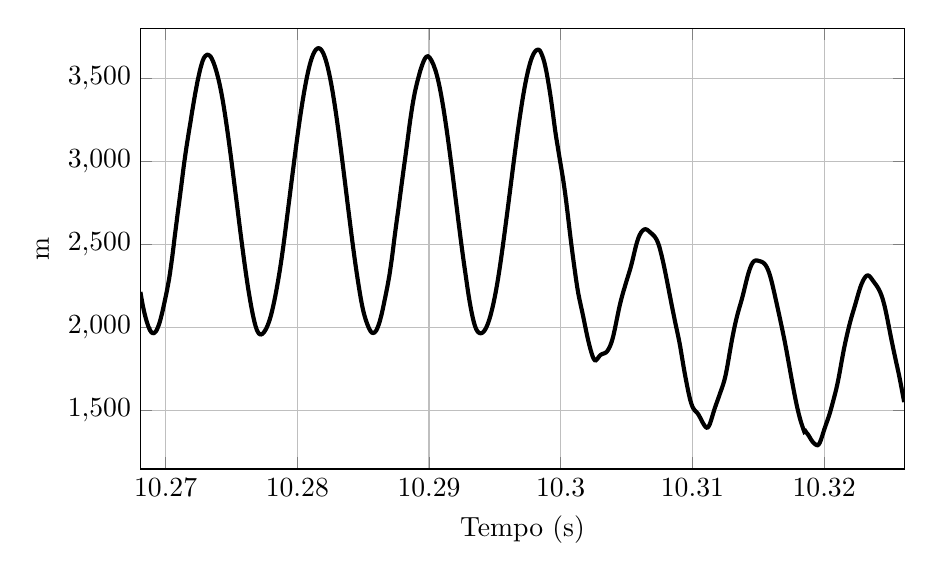
\begin{tikzpicture}

\begin{axis}[%
width=0.8\textwidth,
height=0.461611624834875\textwidth,
scale only axis,
xmin=10.2681,
xmax=10.3261,
xtick={10.27, 10.28, 10.29,  10.3, 10.31, 10.32},
xlabel={Tempo (s)},
xmajorgrids,
ymin=1150,
ymax=3800,
ytick={1500, 2000, 2500, 3000, 3500},
ylabel={m},
ymajorgrids,
scaled x ticks = false,
legend columns=-1,
legend style={/tikz/every even column/.append style={column sep=0.3cm}},
legend style={font=\footnotesize}
]
\addplot [color=black,solid,line width=1.5pt,forget plot]
  table[row sep=crcr]{10.2680833456702	2214.27689329771\\
10.2681666556704	2175.21844386467\\
10.2682499956706	2139.27194884656\\
10.2683333356708	2106.98696422299\\
10.268416675671	2078.71087725423\\
10.2684999856713	2053.53814230619\\
10.2685833256715	2031.25086664078\\
10.2686666656717	2011.53837449278\\
10.2687500056719	1994.54863011226\\
10.2688333456721	1981.24435605551\\
10.2689166556723	1971.92946687659\\
10.2689999956725	1967.18650799332\\
10.2690833356727	1966.53546960671\\
10.2691666756729	1969.83656996285\\
10.2692499856731	1976.38030097836\\
10.2693333256733	1987.29405605514\\
10.2694166656735	2002.7528793728\\
10.2695000056738	2020.50116534849\\
10.269583345674	2041.83042281776\\
10.2696666556742	2067.2919112683\\
10.2697499956744	2093.34804322286\\
10.2698333356746	2123.07174544312\\
10.2699166756748	2154.06683180132\\
10.269999985675	2184.78169762703\\
10.2700833256752	2216.32562379366\\
10.2701666656754	2251.36523756263\\
10.2702500056756	2286.8156235326\\
10.2703333456758	2328.8034264892\\
10.270416655676	2376.62732327868\\
10.2704999956763	2423.78624399154\\
10.2705833356765	2476.42708209069\\
10.2706666756767	2532.51701532693\\
10.2707499856769	2584.80711126034\\
10.2708333256771	2636.00246300238\\
10.2709166656773	2689.03433651743\\
10.2710000056775	2737.0226644036\\
10.2710833456777	2788.10236820322\\
10.2711666556779	2839.58259479396\\
10.2712499956781	2891.9359876393\\
10.2713333356783	2945.26314009518\\
10.2714166756785	2995.18785802756\\
10.2714999856788	3041.57821634999\\
10.271583325679	3087.44112992608\\
10.2716666656792	3128.3106327064\\
10.2717500056794	3170.82368263794\\
10.2718333456796	3210.37649778558\\
10.2719166556798	3250.91928652849\\
10.27199999568	3293.84312978082\\
10.2720833356802	3332.30157051341\\
10.2721666756804	3371.38155760856\\
10.2722499856806	3409.84579838596\\
10.2723333256808	3443.93355384664\\
10.272416665681	3480.03513490527\\
10.2725000056813	3509.67454083988\\
10.2725833456815	3539.96827175475\\
10.2726666556817	3566.00458357258\\
10.2727499956819	3588.86796693139\\
10.2728333356821	3608.79885337141\\
10.2729166756823	3622.71333166663\\
10.2729999856825	3631.63983590061\\
10.2730833256827	3637.62706493519\\
10.2731666656829	3640.75389710643\\
10.2732500056831	3639.57982855613\\
10.2733333456833	3635.24486664057\\
10.2734166556835	3628.94145093221\\
10.2734999956838	3617.52988056957\\
10.273583335684	3603.79506108976\\
10.2736666756842	3586.82399427944\\
10.2737499856844	3567.60682946733\\
10.2738333256846	3546.25819365635\\
10.2739166656848	3522.22374161428\\
10.274000005685	3496.99134263834\\
10.2740833456852	3468.39826476908\\
10.2741666556854	3437.54749107353\\
10.2742499956856	3403.43798215116\\
10.2743333356858	3366.834777053\\
10.274416675686	3327.15984259596\\
10.2744999856863	3285.29619694914\\
10.2745833256865	3241.26465287456\\
10.2746666656867	3195.43691586725\\
10.2747500056869	3148.12395135419\\
10.2748333456871	3099.5636799528\\
10.2749166556873	3049.92220430902\\
10.2749999956875	2999.30029648386\\
10.2750833356877	2947.95033812919\\
10.2751666756879	2895.99436931222\\
10.2752499856881	2843.67172486824\\
10.2753333256883	2790.99697448252\\
10.2754166656885	2738.20288389269\\
10.2755000056888	2685.41035615158\\
10.275583345689	2632.86818346321\\
10.2756666556892	2580.77084935005\\
10.2757499956894	2528.99041653034\\
10.2758333356896	2478.38381471251\\
10.2759166756898	2428.79214018909\\
10.27599998569	2380.29879790939\\
10.2760833256902	2333.04782367212\\
10.2761666656904	2287.40433062944\\
10.2762500056906	2243.83666984431\\
10.2763333456908	2202.55056913395\\
10.276416655691	2163.53059441337\\
10.2764999956913	2126.69676804308\\
10.2765833356915	2092.3021994563\\
10.2766666756917	2060.58172537868\\
10.2767499856919	2032.07454146687\\
10.2768333256921	2007.63877630282\\
10.2769166656923	1987.99516934387\\
10.2770000056925	1973.44457461364\\
10.2770833456927	1963.95941658216\\
10.2771666556929	1959.34146928688\\
10.2772499956931	1958.86513409068\\
10.2773333356933	1961.74815384828\\
10.2774166756935	1967.72268694806\\
10.2774999856937	1975.78804940283\\
10.277583325694	1986.44014930076\\
10.2776666656942	1999.27051076599\\
10.2777500056944	2014.22357732721\\
10.2778333456946	2031.65271184317\\
10.2779166556948	2051.64381789384\\
10.277999995695	2074.29773044596\\
10.2780833356952	2100.22014973559\\
10.2781666756954	2128.70577187549\\
10.2782499856956	2159.78171963192\\
10.2783333256958	2192.88871925628\\
10.278416665696	2227.79544823936\\
10.2785000056963	2264.59300480766\\
10.2785833456965	2302.815383778\\
10.2786666556967	2343.41362200148\\
10.2787499956969	2386.06573490754\\
10.2788333356971	2431.05288167289\\
10.2789166756973	2478.19629198396\\
10.2789999856975	2527.41466656094\\
10.2790833256977	2578.36681189604\\
10.2791666656979	2630.33344815939\\
10.2792500056981	2682.68704049477\\
10.2793333456983	2735.42552671949\\
10.2794166556985	2787.8805920193\\
10.2794999956988	2840.22505925577\\
10.279583335699	2892.24403503187\\
10.2796666756992	2943.93024698659\\
10.2797499856994	2995.41658234115\\
10.2798333256996	3046.36387678791\\
10.2799166656998	3096.63108782224\\
10.2800000057	3145.89268950001\\
10.2800833457002	3194.13870793296\\
10.2801666557004	3240.62315666616\\
10.2802499957006	3285.56010668206\\
10.2803333357008	3328.65171025375\\
10.280416675701	3370.03935003663\\
10.2804999857012	3409.33719011425\\
10.2805833257015	3446.61249342953\\
10.2806666657017	3481.78661129179\\
10.2807500057019	3514.25620213891\\
10.2808333457021	3544.36428698615\\
10.2809166557023	3571.70542609732\\
10.2809999957025	3596.03532338004\\
10.2810833357027	3617.47930525764\\
10.2811666757029	3635.57626940543\\
10.2812499857031	3650.64957165011\\
10.2813333257033	3662.70386140606\\
10.2814166657035	3671.41637266781\\
10.2815000057038	3677.18825138514\\
10.281583345704	3679.76991369225\\
10.2816666557042	3679.06849317139\\
10.2817499957044	3675.25942469529\\
10.2818333357046	3668.07833241387\\
10.2819166757048	3657.53412867541\\
10.281999985705	3643.7460429758\\
10.2820833257052	3626.51442758563\\
10.2821666657054	3606.34828817205\\
10.2822500057056	3583.04757085158\\
10.2823333457058	3556.82479352977\\
10.282416655706	3527.71597673361\\
10.2824999957063	3495.69360756855\\
10.2825833357065	3460.90979458925\\
10.2826666757067	3423.55367899944\\
10.2827499857069	3383.73106026762\\
10.2828333257071	3341.75659492356\\
10.2829166657073	3297.78626349161\\
10.2830000057075	3251.99580011992\\
10.2830833457077	3204.60400532552\\
10.2831666557079	3155.7566758269\\
10.2832499957081	3105.64473362481\\
10.2833333357083	3054.44107995157\\
10.2834166757085	3002.31741194025\\
10.2834999857087	2949.44969755693\\
10.283583325709	2896.01148063465\\
10.2836666657092	2842.26373751967\\
10.2837500057094	2788.37192170454\\
10.2838333457096	2734.60813152288\\
10.2839166557098	2681.25344664327\\
10.28399999571	2628.3185103256\\
10.2840833357102	2576.14380576492\\
10.2841666757104	2524.78342486196\\
10.2842499857106	2474.57551265656\\
10.2843333257108	2425.68835525867\\
10.284416665711	2378.68863471254\\
10.2845000057113	2333.31528305799\\
10.2845833457115	2289.47983711605\\
10.2846666557117	2247.14179242205\\
10.2847499957119	2206.49944385976\\
10.2848333357121	2168.30785941977\\
10.2849166757123	2133.47939881394\\
10.2849999857125	2102.8112591619\\
10.2850833257127	2076.86617870376\\
10.2851666657129	2054.20333179553\\
10.2852500057131	2034.11638012582\\
10.2853333457133	2016.19646585753\\
10.2854166557135	1999.89935989521\\
10.2854999957137	1986.39255909194\\
10.285583335714	1975.93400686532\\
10.2856666757142	1969.38338353815\\
10.2857499857144	1967.54245567882\\
10.2858333257146	1969.41721281149\\
10.2859166657148	1974.82362356776\\
10.286000005715	1984.07048151199\\
10.2860833457152	1997.73740928089\\
10.2861666557154	2014.83345719219\\
10.2862499957156	2034.84043808991\\
10.2863333357158	2059.3999377526\\
10.286416675716	2085.47422406052\\
10.2864999857162	2115.31887821918\\
10.2865833257165	2147.43793503352\\
10.2866666657167	2179.37772355581\\
10.2867500057169	2211.5154550808\\
10.2868333457171	2244.61816220158\\
10.2869166557173	2281.03199050223\\
10.2869999957175	2318.53634093461\\
10.2870833357177	2363.64216521267\\
10.2871666757179	2408.88012425198\\
10.2872499857181	2459.20001516784\\
10.2873333257183	2513.37399187539\\
10.2874166657185	2564.44393276787\\
10.2875000057188	2614.13990967864\\
10.287583345719	2662.55284947115\\
10.2876666557192	2708.43521433029\\
10.2877499957194	2759.31453055872\\
10.2878333357196	2809.83583516975\\
10.2879166757198	2860.0313762209\\
10.28799998572	2909.0157430463\\
10.2880833257202	2959.2985795714\\
10.2881666657204	3005.75388406762\\
10.2882500057206	3055.16757759383\\
10.2883333457208	3103.90808294046\\
10.288416655721	3154.53234410037\\
10.2884999957212	3205.89730493174\\
10.2885833357215	3253.37083302421\\
10.2886666757217	3297.71813038495\\
10.2887499857219	3340.09977115651\\
10.2888333257221	3377.44066017362\\
10.2889166657223	3412.08180830791\\
10.2890000057225	3441.70830322197\\
10.2890833457227	3469.92998183448\\
10.2891666557229	3495.10954799915\\
10.2892499957231	3519.67215120559\\
10.2893333357233	3544.19075860028\\
10.2894166757235	3564.46070229765\\
10.2894999857238	3583.31768296896\\
10.289583325724	3600.1846678847\\
10.2896666657242	3614.5263094003\\
10.2897500057244	3624.5104898149\\
10.2898333457246	3629.72439066571\\
10.2899166557248	3631.34027982252\\
10.289999995725	3626.6982844143\\
10.2900833357252	3619.44854920183\\
10.2901666757254	3608.49712316408\\
10.2902499857256	3595.27186309633\\
10.2903333257258	3580.90149273339\\
10.290416665726	3562.89367849522\\
10.2905000057262	3543.83996093639\\
10.2905833457265	3520.73633081798\\
10.2906666557267	3495.45882519165\\
10.2907499957269	3466.29201550002\\
10.2908333357271	3434.92594804349\\
10.2909166757273	3400.01419196089\\
10.2909999857275	3362.81239961591\\
10.2910833257277	3323.36817822053\\
10.2911666657279	3281.47939275236\\
10.2912500057281	3237.9937498149\\
10.2913333457283	3192.59151899513\\
10.2914166557285	3145.61535141088\\
10.2914999957287	3097.25751418909\\
10.291583335729	3047.66852094198\\
10.2916666757292	2997.08954376924\\
10.2917499857294	2945.5572971113\\
10.2918333257296	2893.36484926653\\
10.2919166657298	2840.69620902415\\
10.29200000573	2787.75297783235\\
10.2920833457302	2734.57250846685\\
10.2921666557304	2681.55510795067\\
10.2922499957306	2628.30103361967\\
10.2923333357308	2576.09768734446\\
10.292416675731	2524.85453230698\\
10.2924999857313	2474.88922826703\\
10.2925833257315	2425.95780246562\\
10.2926666657317	2378.07969690125\\
10.2927500057319	2332.56955288232\\
10.2928333457321	2286.47652551442\\
10.2929166557323	2240.71909113174\\
10.2929999957325	2196.66423226273\\
10.2930833357327	2156.47820120442\\
10.2931666757329	2119.3036575182\\
10.2932499857331	2085.51120983319\\
10.2933333257333	2055.04866724221\\
10.2934166657335	2028.71072119709\\
10.2935000057337	2007.10185793261\\
10.293583345734	1990.65196955637\\
10.2936666557342	1978.79158772434\\
10.2937499957344	1971.27876032856\\
10.2938333357346	1967.06471922034\\
10.2939166757348	1965.75835070136\\
10.293999985735	1967.06136210055\\
10.2940833257352	1970.71337001435\\
10.2941666657354	1977.33154123831\\
10.2942500057356	1986.55217618694\\
10.2943333457358	1998.38286659702\\
10.294416655736	2013.09175496916\\
10.2944999957363	2030.23217838841\\
10.2945833357365	2050.19964637644\\
10.2946666757367	2072.63197873346\\
10.2947499857369	2097.6129553117\\
10.2948333257371	2125.03786684485\\
10.2949166657373	2154.81549575199\\
10.2950000057375	2186.8636885859\\
10.2950833457377	2221.49071102371\\
10.2951666557379	2258.54122561249\\
10.2952499957381	2298.42771658018\\
10.2953333357383	2340.24061310493\\
10.2954166757385	2384.75716105106\\
10.2954999857388	2430.86253959078\\
10.295583325739	2478.43792322519\\
10.2956666657392	2527.39956642603\\
10.2957500057394	2576.93603997555\\
10.2958333457396	2627.28130228897\\
10.2959166557398	2678.16437753778\\
10.29599999574	2728.64403476382\\
10.2960833357402	2780.31386451219\\
10.2961666757404	2831.98829773568\\
10.2962499857406	2884.09949860504\\
10.2963333257408	2936.10540985912\\
10.296416665741	2987.60500621885\\
10.2965000057412	3038.49737866729\\
10.2965833457415	3088.68995969655\\
10.2966666557417	3137.78039010566\\
10.2967499957419	3185.69258906555\\
10.2968333357421	3232.44067814875\\
10.2969166757423	3277.4336951257\\
10.2969999857425	3320.96190068624\\
10.2970833257427	3362.73653999977\\
10.2971666657429	3402.44286992953\\
10.2972500057431	3440.21372972866\\
10.2973333457433	3475.38719690464\\
10.2974166557435	3507.91788250625\\
10.2974999957438	3537.70607927634\\
10.297583335744	3564.56173090337\\
10.2976666757442	3588.69719943163\\
10.2977499857444	3609.83796523401\\
10.2978333257446	3627.62131669064\\
10.2979166657448	3642.50590384204\\
10.298000005745	3654.15725135329\\
10.2980833457452	3662.79524020511\\
10.2981666557454	3668.46278564726\\
10.2982499957456	3670.95816196808\\
10.2983333357458	3670.24834584296\\
10.298416675746	3665.40306103814\\
10.2984999857463	3653.35997370642\\
10.2985833257465	3637.6584017719\\
10.2986666657467	3619.44626330933\\
10.2987500057469	3597.10405870536\\
10.2988333457471	3569.55923795729\\
10.2989166557473	3537.4104156359\\
10.2989999957475	3501.718780292\\
10.2990833357477	3462.87782910682\\
10.2991666757479	3421.67883949266\\
10.2992499857481	3378.49419524229\\
10.2993333257483	3332.24434666903\\
10.2994166657485	3282.494447177\\
10.2995000057488	3231.12908381166\\
10.299583345749	3182.37927908321\\
10.2996666557492	3138.57673540519\\
10.2997499957494	3098.33918422642\\
10.2998333357496	3058.37239388405\\
10.2999166757498	3017.87725819939\\
10.29999998575	2978.03897922223\\
10.3000833257502	2939.00469717236\\
10.3001666657504	2899.06842866613\\
10.3002500057506	2855.81668313383\\
10.3003333457508	2808.94519736475\\
10.300416655751	2757.78020294166\\
10.3004999957513	2703.56910027137\\
10.3005833357515	2647.77086606484\\
10.3006666757517	2591.76839814444\\
10.3007499857519	2536.67648729471\\
10.3008333257521	2483.56243401856\\
10.3009166657523	2432.77338529559\\
10.3010000057525	2383.62263282479\\
10.3010833457527	2335.63719380406\\
10.3011666557529	2288.77000313693\\
10.3012499957531	2244.7606796486\\
10.3013333357533	2205.99623954343\\
10.3014166757535	2172.48438878579\\
10.3014999857538	2142.17444344696\\
10.301583325754	2112.35894537785\\
10.3016666657542	2081.99749887601\\
10.3017500057544	2050.19966444207\\
10.3018333457546	2017.51424278108\\
10.3019166557548	1984.91612380422\\
10.301999995755	1953.50932853352\\
10.3020833357552	1924.12027513315\\
10.3021666757554	1896.91651332399\\
10.3022499857556	1871.73418276369\\
10.3023333257558	1848.76361822397\\
10.302416665756	1828.67745632933\\
10.3025000057563	1812.91291095333\\
10.3025833457565	1803.91313356868\\
10.3026666557567	1803.08149376202\\
10.3027499957569	1808.8832526097\\
10.3028333357571	1817.44147923199\\
10.3029166757573	1826.47755149005\\
10.3029999857575	1833.53371410071\\
10.3030833257577	1838.66285252132\\
10.3031666657579	1841.70676119141\\
10.3032500057581	1843.77583293852\\
10.3033333457583	1845.82039075475\\
10.3034166557585	1849.48022462023\\
10.3034999957588	1855.37222525086\\
10.303583335759	1864.05909842575\\
10.3036666757592	1875.40066560284\\
10.3037499857594	1889.46744663005\\
10.3038333257596	1906.44396141466\\
10.3039166657598	1926.82120447022\\
10.30400000576	1952.10961887885\\
10.3040833457602	1981.44564201052\\
10.3041666557604	2012.89850730947\\
10.3042499957606	2045.91744830588\\
10.3043333357608	2078.45649740904\\
10.304416675761	2110.34093054135\\
10.3044999857613	2139.3206173918\\
10.3045833257615	2166.64724731069\\
10.3046666657617	2190.79715937848\\
10.3047500057619	2214.69885978842\\
10.3048333457621	2236.55593638945\\
10.3049166557623	2259.08703916153\\
10.3049999957625	2280.87929803898\\
10.3050833357627	2302.14596406927\\
10.3051666757629	2323.39309996413\\
10.3052499857631	2344.78301209257\\
10.3053333257633	2368.19276825837\\
10.3054166657635	2393.60935830513\\
10.3055000057638	2420.80035076564\\
10.305583345764	2448.89393518138\\
10.3056666557642	2476.761751916\\
10.3057499957644	2501.87619171379\\
10.3058333357646	2523.77773473521\\
10.3059166757648	2543.53891036203\\
10.305999985765	2557.56880328927\\
10.3060833257652	2569.89251336344\\
10.3061666657654	2578.59014082894\\
10.3062500057656	2585.48417324507\\
10.3063333457658	2589.64100366086\\
10.306416655766	2591.57426014917\\
10.3064999957663	2590.30755340445\\
10.3065833357665	2586.97317222672\\
10.3066666757667	2581.74404479862\\
10.3067499857669	2575.87186001397\\
10.3068333257671	2570.01287164592\\
10.3069166657673	2564.30065633404\\
10.3070000057675	2558.33156387868\\
10.3070833457677	2551.63757849641\\
10.3071666557679	2543.31533809078\\
10.3072499957681	2532.60892451363\\
10.3073333357683	2519.73091257721\\
10.3074166757685	2503.22947124796\\
10.3074999857688	2483.35027624505\\
10.307583325769	2457.84273023907\\
10.3076666657692	2432.07727820207\\
10.3077500057694	2403.20555987138\\
10.3078333457696	2373.071957286\\
10.3079166557698	2341.57439870944\\
10.30799999577	2308.84963202127\\
10.3080833357702	2275.62043230656\\
10.3081666757704	2241.90416200712\\
10.3082499857706	2207.78492067777\\
10.3083333257708	2174.25165892088\\
10.308416665771	2140.0682786784\\
10.3085000057713	2107.19136439559\\
10.3085833457715	2074.74147604718\\
10.3086666557717	2042.01419993931\\
10.3087499957719	2010.57023593308\\
10.3088333357721	1980.14630384957\\
10.3089166757723	1949.42853833631\\
10.3089999857725	1917.48763375453\\
10.3090833257727	1881.58664767522\\
10.3091666657729	1842.47277018181\\
10.3092500057731	1802.13918413629\\
10.3093333457733	1762.90846842053\\
10.3094166557735	1725.65539843792\\
10.3094999957738	1690.25627821093\\
10.309583335774	1656.17909508943\\
10.3096666757742	1623.2942339076\\
10.3097499857744	1592.47270184339\\
10.3098333257746	1565.38007845786\\
10.3099166657748	1542.85830627193\\
10.310000005775	1525.3737992484\\
10.3100833457752	1512.64430252574\\
10.3101666557754	1503.39357178242\\
10.3102499957756	1496.50154694439\\
10.3103333357758	1490.01107908408\\
10.310416675776	1482.01006781764\\
10.3104999857763	1471.61484635635\\
10.3105833257765	1459.12240833022\\
10.3106666657767	1445.92153041324\\
10.3107500057769	1433.19107698867\\
10.3108333457771	1421.61735931983\\
10.3109166557773	1411.20719822021\\
10.3109999957775	1402.79685854723\\
10.3110833357777	1398.2304205806\\
10.3111666757779	1399.57645002532\\
10.3112499857781	1407.77600188853\\
10.3113333257783	1422.42843474887\\
10.3114166657785	1441.86997676702\\
10.3115000057788	1463.71661279462\\
10.311583345779	1485.83974472924\\
10.3116666557792	1506.96510272275\\
10.3117499957794	1526.67481575352\\
10.3118333357796	1545.44187697026\\
10.3119166757798	1563.87691771511\\
10.31199998578	1582.45144384593\\
10.3120833257802	1601.28052094019\\
10.3121666657804	1619.86001651548\\
10.3122500057806	1638.44412720223\\
10.3123333457808	1657.8958600391\\
10.312416655781	1679.99649325626\\
10.3124999957813	1706.40515262524\\
10.3125833357815	1737.80846868043\\
10.3126666757817	1773.4839067161\\
10.3127499857819	1811.68814541164\\
10.3128333257821	1850.64069143727\\
10.3129166657823	1888.70736083319\\
10.3130000057825	1924.98604702152\\
10.3130833457827	1959.27165358043\\
10.3131666557829	1991.89364258203\\
10.3132499957831	2022.3658358754\\
10.3133333357833	2050.86976489185\\
10.3134166757835	2077.25681158384\\
10.3134999857838	2101.40936577929\\
10.313583325784	2124.19747169132\\
10.3136666657842	2146.55186048256\\
10.3137500057844	2169.80305896171\\
10.3138333457846	2194.72383209279\\
10.3139166557848	2221.28332966895\\
10.313999995785	2248.78554294042\\
10.3140833357852	2276.09968707074\\
10.3141666757854	2302.10730133626\\
10.3142499857856	2325.944744104\\
10.3143333257858	2346.96913425782\\
10.314416665786	2364.8358930491\\
10.3145000057863	2379.7983642012\\
10.3145833457865	2390.97671647872\\
10.3146666557867	2398.48136174898\\
10.3147499957869	2402.52984279245\\
10.3148333357871	2403.85586401806\\
10.3149166757873	2403.27264996361\\
10.3149999857875	2401.81898272753\\
10.3150833257877	2400.00347743964\\
10.3151666657879	2398.08079868634\\
10.3152500057881	2395.68971927953\\
10.3153333457883	2392.40620968273\\
10.3154166557885	2387.65969785459\\
10.3154999957888	2381.05083676437\\
10.315583335789	2372.15350018032\\
10.3156666757892	2360.34174438395\\
10.3157499857894	2345.51492808496\\
10.3158333257896	2327.48836942278\\
10.3159166657898	2306.20978591483\\
10.31600000579	2281.90746766988\\
10.3160833457902	2255.16832589908\\
10.3161666557904	2226.74171529764\\
10.3162499957906	2197.41439793903\\
10.3163333357908	2167.82848812069\\
10.316416675791	2138.09339025061\\
10.3164999857913	2108.2365255589\\
10.3165833257915	2078.05474500741\\
10.3166666657917	2047.44983685667\\
10.3167500057919	2016.55986345666\\
10.3168333457921	1985.28055501932\\
10.3169166557923	1953.41554736679\\
10.3169999957925	1920.71347831611\\
10.3170833357927	1886.69901093039\\
10.3171666757929	1851.50381082758\\
10.3172499857931	1815.39573449631\\
10.3173333257933	1778.78274532416\\
10.3174166657935	1742.14676090468\\
10.3175000057938	1705.66660845987\\
10.317583345794	1669.6471539713\\
10.3176666557942	1634.3375703011\\
10.3177499957944	1599.92842425217\\
10.3178333357946	1566.73738580063\\
10.3179166757948	1535.27291811802\\
10.317999985795	1505.88603214388\\
10.3180833257952	1478.45571502022\\
10.3181666657954	1453.35014733139\\
10.3182500057956	1430.6344113615\\
10.3183333457958	1410.4233064671\\
10.318416655796	1390.89266087484\\
10.3184999957963	1373.24159293359\\
10.3185833357965	1377.65474317388\\
10.3186666757967	1367.99561170884\\
10.3187499857969	1359.8935183525\\
10.3188333257971	1350.20630531936\\
10.3189166657973	1339.06563113526\\
10.3190000057975	1328.00902722909\\
10.3190833457977	1318.10587665819\\
10.3191666557979	1309.83762094348\\
10.3192499957981	1303.47233439542\\
10.3193333357983	1298.11707798471\\
10.3194166757985	1293.85544936265\\
10.3194999857988	1292.44741244711\\
10.319583325799	1296.69875580802\\
10.3196666657992	1307.09103609654\\
10.3197500057994	1322.90021049034\\
10.3198333457996	1342.48755446406\\
10.3199166557998	1363.38417715463\\
10.3199999958	1384.25092275626\\
10.3200833358002	1403.93746970142\\
10.3201666758004	1422.83702453126\\
10.3202499858006	1441.20316733492\\
10.3203333258008	1460.22541996907\\
10.320416665801	1480.57344907256\\
10.3205000058013	1502.96681194577\\
10.3205833458015	1527.09311337106\\
10.3206666558017	1551.54158796007\\
10.3207499958019	1576.7879129287\\
10.3208333358021	1601.9216271331\\
10.3209166758023	1628.3595043389\\
10.3209999858025	1657.20721936924\\
10.3210833258027	1688.94182572141\\
10.3211666658029	1723.80187459507\\
10.3212500058031	1760.41314626978\\
10.3213333458033	1797.86483923587\\
10.3214166558035	1833.5554510085\\
10.3214999958038	1868.59299315302\\
10.321583335804	1900.1955325161\\
10.3216666758042	1931.02953768495\\
10.3217499858044	1959.77569432088\\
10.3218333258046	1987.96771786097\\
10.3219166658048	2014.63148408345\\
10.322000005805	2039.93673540556\\
10.3220833458052	2064.16739435613\\
10.3221666558054	2086.22509169101\\
10.3222499958056	2108.05562014678\\
10.3223333358058	2130.18393368314\\
10.322416675806	2152.8242647105\\
10.3224999858063	2176.08800329617\\
10.3225833258065	2199.65888566206\\
10.3226666658067	2221.57237405839\\
10.3227500058069	2242.46856172116\\
10.3228333458071	2260.1510063343\\
10.3229166558073	2275.08269738925\\
10.3229999958075	2288.49018109067\\
10.3230833358077	2299.17056740676\\
10.3231666758079	2307.82801411172\\
10.3232499858081	2312.74351945049\\
10.3233333258083	2313.66061065477\\
10.3234166658085	2310.59273591489\\
10.3235000058088	2304.45512088456\\
10.323583345809	2296.06900934042\\
10.3236666558092	2286.78118752612\\
10.3237499958094	2277.60018225267\\
10.3238333358096	2268.71052965767\\
10.3239166758098	2259.71253979401\\
10.32399998581	2250.45749550797\\
10.3240833258102	2239.95415123491\\
10.3241666658104	2228.13570038633\\
10.3242500058106	2214.58200095957\\
10.3243333458108	2198.42482319276\\
10.324416655811	2180.05506875758\\
10.3244999958113	2157.79111283327\\
10.3245833358115	2132.70956341809\\
10.3246666758117	2104.22146356531\\
10.3247499858119	2073.14698656407\\
10.3248333258121	2040.10072455341\\
10.3249166658123	2006.21673136933\\
10.3250000058125	1972.41596742013\\
10.3250833458127	1939.19238325087\\
10.3251666558129	1906.57063856619\\
10.3252499958131	1874.542364097\\
10.3253333358133	1843.29483782318\\
10.3254166758135	1812.74541757922\\
10.3254999858138	1782.74987695046\\
10.325583325814	1753.22803501223\\
10.3256666658142	1722.52497764069\\
10.3257500058144	1690.25983138032\\
10.3258333458146	1656.29798030712\\
10.3259166558148	1621.37969232152\\
10.325999995815	1586.34981434271\\
10.3260833358152	1552.04237987092\\
};
\end{axis}
\end{tikzpicture}%}
    \captionof{figure}{Resposta do normalizador $m$ à variação abrupta da indutância.}
    \label{fig:m_exp_Lg}
  \end{minipage}
  \vspace*{\fill}

  \newpage

  As Fig.~\ref{fig:i2_exp_Lg_permanente}-\ref{fig:m_exp_Lg_permanente} apresentam o comportamento dos parâmetros do sistema no regime permanente após a variação da indutância da rede $L_g$. A Fig.~\ref{fig:i2_exp_Lg_permanente} apresenta a corrente da rede $i_2$, a Fig.~\ref{fig:up_exp_Lg_permanente} apresenta a ação de controle $U$, e a Fig.~\ref{fig:m_exp_Lg_permanente} apresenta o comportamento do normalizador $m$.

  \vfill
  \noindent
  \begin{minipage}{\textwidth}
    \makebox[\textwidth]{
      \centering
      \def\svgwidth{\textwidth}
      % This file was created by matlab2tikz v0.4.7 running on MATLAB 7.14.
% Copyright (c) 2008--2014, Nico Schlömer <nico.schloemer@gmail.com>
% All rights reserved.
% Minimal pgfplots version: 1.3
% 
% The latest updates can be retrieved from
%   http://www.mathworks.com/matlabcentral/fileexchange/22022-matlab2tikz
% where you can also make suggestions and rate matlab2tikz.
% 
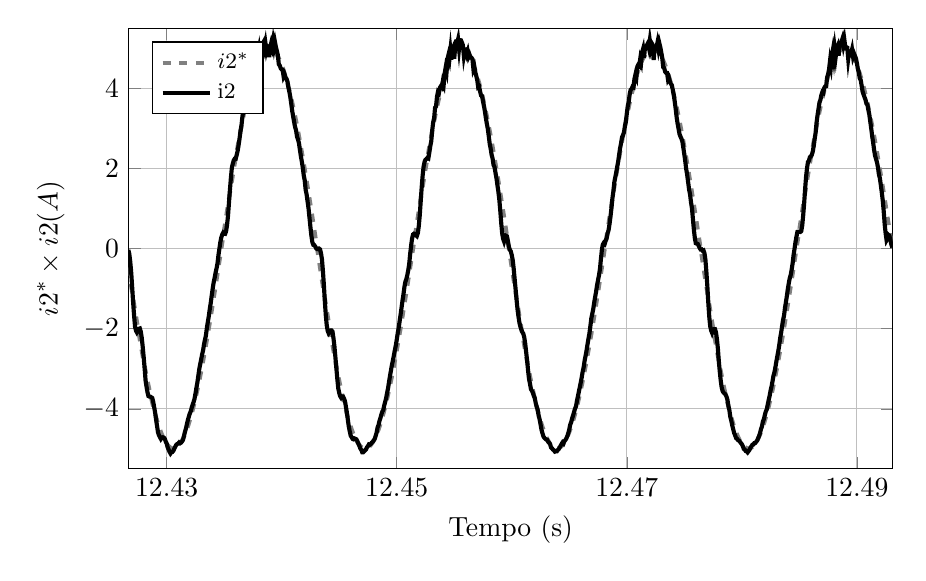
\begin{tikzpicture}

\begin{axis}[%
width=0.8\textwidth,
height=0.461611624834875\textwidth,
scale only axis,
xmin=12.4267,
xmax=12.4931,
xtick={12.43, 12.45, 12.47, 12.49},
xlabel={Tempo (s)},
xmajorgrids,
ymin=-5.5,
ymax=5.5,
ytick={-4, -2,  0,  2,  4},
ylabel={$\text{i2}^\text{*}\text{ }\times\text{ i2 (A)}$},
ymajorgrids,
legend style={at={(0.03,0.97)},anchor=north west,draw=black,fill=white,legend cell align=left},
scaled x ticks = false,
legend style={font=\footnotesize}
]
\addplot [color=gray,dashed,line width=1.5pt]
  table[row sep=crcr]{12.4266666610667	-0.469922358851241\\
12.4267500010669	-0.625738349089735\\
12.4268333410671	-0.780936811123984\\
12.4269166510673	-0.935364582809298\\
12.4269999910675	-1.08886926257931\\
12.4270833310677	-1.24129935984794\\
12.4271666710679	-1.39250444451229\\
12.4272500110681	-1.542335295409\\
12.4273333210683	-1.69064404757754\\
12.4274166610685	-1.83728433818505\\
12.4275000010688	-1.9821114509688\\
12.427583341069	-2.12498245905366\\
12.4276666510692	-2.26575636600367\\
12.4277499910694	-2.40429424496852\\
12.4278333310696	-2.54045937578755\\
12.4279166710698	-2.67411737991605\\
12.42800001107	-2.80513635304068\\
12.4280833210702	-2.93338699525307\\
12.4281666610704	-3.05874273865325\\
12.4282500010706	-3.18107987225687\\
12.4283333410708	-3.300277664083\\
12.428416651071	-3.41621848030203\\
12.4284999910713	-3.52878790132605\\
12.4285833310715	-3.6378748347272\\
12.4286666710717	-3.74337162487242\\
12.4287500110719	-3.84517415916662\\
12.4288333210721	-3.94318197079923\\
12.4289166610723	-4.03729833789279\\
12.4290000010725	-4.12743037895578\\
12.4290833410727	-4.21348914454545\\
12.4291666510729	-4.29538970505017\\
12.4292499910731	-4.37305123450468\\
12.4293333310733	-4.44639709035561\\
12.4294166710735	-4.51535488909839\\
12.4295000110738	-4.57985657771103\\
12.429583321074	-4.63983850081426\\
12.4296666610742	-4.69524146349167\\
12.4297500010744	-4.74601078970799\\
12.4298333410746	-4.79209637626769\\
12.4299166510748	-4.83345274226082\\
12.429999991075	-4.87003907394716\\
12.4300833310752	-4.90181926503446\\
12.4301666710754	-4.92876195231098\\
12.4302500110756	-4.95084054659722\\
12.4303333210758	-4.96803325898618\\
12.430416661076	-4.98032312234645\\
12.4305000010763	-4.98769800806666\\
12.4305833410765	-4.99015063802499\\
12.4306666510767	-4.98767859177177\\
12.4307499910769	-4.98028430891821\\
12.4308333310771	-4.96797508672876\\
12.4309166710773	-4.95076307291961\\
12.4310000110775	-4.92866525367035\\
12.4310833210777	-4.90170343686069\\
12.4311666610779	-4.86990423054868\\
12.4312500010781	-4.83329901671178\\
12.4313333410783	-4.79192392027664\\
12.4314166510785	-4.74581977346818\\
12.4314999910788	-4.69503207551307\\
12.431583331079	-4.63961094773752\\
12.4316666710792	-4.57961108410357\\
12.4317500110794	-4.51509169723276\\
12.4318333210796	-4.44611645997041\\
12.4319166610798	-4.37275344254821\\
12.43200000108	-4.29507504540713\\
12.4320833410802	-4.21315792774694\\
12.4321666510804	-4.12708293187278\\
12.4322499910806	-4.03693500341362\\
12.4323333310808	-3.94280310749116\\
12.432416671081	-3.844780140922\\
12.4325000110813	-3.74296284053967\\
12.4325833210815	-3.63745168772712\\
12.4326666610817	-3.52835080925364\\
12.4327500010819	-3.41576787451438\\
12.4328333410821	-3.29981398927364\\
12.4329166510823	-3.18060358601685\\
12.4329999910825	-3.05825431101958\\
12.4330833310827	-2.93288690824486\\
12.4331666710829	-2.80462510018342\\
12.4332500110831	-2.6735954657546\\
12.4333333210833	-2.53992731538817\\
12.4334166610835	-2.40375256341059\\
12.4335000010838	-2.26520559786149\\
12.433583341084	-2.12442314786889\\
12.4336666510842	-1.98154414871406\\
12.4337499910844	-1.83670960471917\\
12.4338333310846	-1.69006245009306\\
12.4339166710848	-1.54174740787242\\
12.434000011085	-1.39191084709763\\
12.4340833210852	-1.24070063836418\\
12.4341666610854	-1.08826600789228\\
12.4342500010856	-0.934757390258532\\
12.4343333410858	-0.780326279935228\\
12.434416651086	-0.625125081783561\\
12.4344999910863	-0.469306960648439\\
12.4345833310865	-0.313025690203273\\
12.4346666710867	-0.156435501193926\\
12.4347500110869	0.000309070768412356\\
12.4348333210871	0.157053337715217\\
12.4349166610873	0.313642611978976\\
12.4350000010875	0.469922358851243\\
12.4350833410877	0.625738349089738\\
12.4351666510879	0.780936811123987\\
12.4352499910881	0.935364582809301\\
12.4353333310883	1.08886926257932\\
12.4354166710885	1.24129935984795\\
12.4355000110888	1.39250444451229\\
12.435583321089	1.54233529540901\\
12.4356666610892	1.69064404757755\\
12.4357500010894	1.83728433818506\\
12.4358333410896	1.98211145096881\\
12.4359166510898	2.12498245905367\\
12.43599999109	2.26575636600368\\
12.4360833310902	2.40429424496853\\
12.4361666710904	2.54045937578756\\
12.4362500110906	2.67411737991606\\
12.4363333210908	2.80513635304069\\
12.436416661091	2.93338699525308\\
12.4365000010913	3.05874273865327\\
12.4365833410915	3.18107987225688\\
12.4366666510917	3.30027766408301\\
12.4367499910919	3.41621848030204\\
12.4368333310921	3.52878790132607\\
12.4369166710923	3.63787483472721\\
12.4370000110925	3.74337162487243\\
12.4370833210927	3.84517415916664\\
12.4371666610929	3.94318197079924\\
12.4372500010931	4.0372983378928\\
12.4373333410933	4.1274303789558\\
12.4374166510935	4.21348914454547\\
12.4374999910938	4.29538970505019\\
12.437583331094	4.3730512345047\\
12.4376666710942	4.44639709035563\\
12.4377500110944	4.51535488909841\\
12.4378333210946	4.57985657771105\\
12.4379166610948	4.63983850081428\\
12.438000001095	4.69524146349169\\
12.4380833410952	4.746010789708\\
12.4381666510954	4.79209637626771\\
12.4382499910956	4.83345274226084\\
12.4383333310958	4.87003907394718\\
12.438416671096	4.90181926503448\\
12.4385000110963	4.928761952311\\
12.4385833210965	4.95084054659724\\
12.4386666610967	4.9680332589862\\
12.4387500010969	4.98032312234647\\
12.4388333410971	4.98769800806668\\
12.4389166510973	4.99015063802501\\
12.4389999910975	4.9876785917718\\
12.4390833310977	4.98028430891823\\
12.4391666710979	4.96797508672878\\
12.4392500110981	4.95076307291963\\
12.4393333210983	4.92866525367038\\
12.4394166610985	4.90170343686072\\
12.4395000010988	4.8699042305487\\
12.439583341099	4.8332990167118\\
12.4396666510992	4.79192392027667\\
12.4397499910994	4.7458197734682\\
12.4398333310996	4.69503207551309\\
12.4399166710998	4.63961094773754\\
12.4400000111	4.57961108410359\\
12.4400833211002	4.51509169723278\\
12.4401666611004	4.44611645997043\\
12.4402500011006	4.37275344254823\\
12.4403333411008	4.29507504540715\\
12.440416651101	4.21315792774696\\
12.4404999911013	4.1270829318728\\
12.4405833311015	4.03693500341364\\
12.4406666711017	3.94280310749118\\
12.4407500111019	3.84478014092201\\
12.4408333211021	3.74296284053969\\
12.4409166611023	3.63745168772713\\
12.4410000011025	3.52835080925365\\
12.4410833411027	3.4157678745144\\
12.4411666511029	3.29981398927365\\
12.4412499911031	3.18060358601686\\
12.4413333311033	3.05825431101959\\
12.4414166711035	2.93288690824487\\
12.4415000111038	2.80462510018344\\
12.441583321104	2.67359546575461\\
12.4416666611042	2.53992731538818\\
12.4417500011044	2.40375256341061\\
12.4418333411046	2.26520559786151\\
12.4419166511048	2.1244231478689\\
12.441999991105	1.98154414871407\\
12.4420833311052	1.83670960471918\\
12.4421666711054	1.69006245009306\\
12.4422500111056	1.54174740787242\\
12.4423333211058	1.39191084709763\\
12.442416661106	1.24070063836419\\
12.4425000011063	1.08826600789228\\
12.4425833411065	0.934757390258537\\
12.4426666511067	0.780326279935231\\
12.4427499911069	0.625125081783564\\
12.4428333311071	0.469306960648441\\
12.4429166711073	0.313025690203275\\
12.4430000111075	0.156435501193927\\
12.4430833211077	-0.000309070768411981\\
12.4431666611079	-0.157053337715217\\
12.4432500011081	-0.313642611978977\\
12.4433333411083	-0.469922358851244\\
12.4434166511085	-0.62573834908974\\
12.4434999911088	-0.78093681112399\\
12.443583331109	-0.935364582809305\\
12.4436666711092	-1.08886926257932\\
12.4437500111094	-1.24129935984795\\
12.4438333211096	-1.3925044445123\\
12.4439166611098	-1.54233529540901\\
12.44400000111	-1.69064404757755\\
12.4440833411102	-1.83728433818507\\
12.4441666511104	-1.98211145096882\\
12.4442499911106	-2.12498245905368\\
12.4443333311108	-2.26575636600369\\
12.444416671111	-2.40429424496854\\
12.4445000111113	-2.54045937578757\\
12.4445833211115	-2.67411737991607\\
12.4446666611117	-2.8051363530407\\
12.4447500011119	-2.93338699525309\\
12.4448333411121	-3.05874273865328\\
12.4449166511123	-3.1810798722569\\
12.4449999911125	-3.30027766408303\\
12.4450833311127	-3.41621848030206\\
12.4451666711129	-3.52878790132608\\
12.4452500111131	-3.63787483472723\\
12.4453333211133	-3.74337162487245\\
12.4454166611135	-3.84517415916665\\
12.4455000011138	-3.94318197079926\\
12.445583341114	-4.03729833789282\\
12.4456666511142	-4.12743037895581\\
12.4457499911144	-4.21348914454549\\
12.4458333311146	-4.2953897050502\\
12.4459166711148	-4.37305123450472\\
12.446000011115	-4.44639709035565\\
12.4460833211152	-4.51535488909843\\
12.4461666611154	-4.57985657771107\\
12.4462500011156	-4.6398385008143\\
12.4463333411158	-4.69524146349171\\
12.446416651116	-4.74601078970803\\
12.4464999911163	-4.79209637626773\\
12.4465833311165	-4.83345274226086\\
12.4466666711167	-4.8700390739472\\
12.4467500111169	-4.9018192650345\\
12.4468333211171	-4.92876195231102\\
12.4469166611173	-4.95084054659726\\
12.4470000011175	-4.96803325898622\\
12.4470833411177	-4.98032312234649\\
12.4471666511179	-4.9876980080667\\
12.4472499911181	-4.99015063802503\\
12.4473333311183	-4.98767859177181\\
12.4474166711185	-4.98028430891825\\
12.4475000111188	-4.9679750867288\\
12.447583321119	-4.95076307291965\\
12.4476666611192	-4.9286652536704\\
12.4477500011194	-4.90170343686074\\
12.4478333411196	-4.86990423054872\\
12.4479166511198	-4.83329901671182\\
12.44799999112	-4.79192392027668\\
12.4480833311202	-4.74581977346822\\
12.4481666711204	-4.69503207551311\\
12.4482500111206	-4.63961094773756\\
12.4483333211208	-4.57961108410361\\
12.448416661121	-4.5150916972328\\
12.4485000011213	-4.44611645997045\\
12.4485833411215	-4.37275344254825\\
12.4486666511217	-4.29507504540717\\
12.4487499911219	-4.21315792774698\\
12.4488333311221	-4.12708293187281\\
12.4489166711223	-4.03693500341365\\
12.4490000111225	-3.94280310749119\\
12.4490833211227	-3.84478014092203\\
12.4491666611229	-3.74296284053971\\
12.4492500011231	-3.63745168772715\\
12.4493333411233	-3.52835080925367\\
12.4494166511235	-3.41576787451441\\
12.4494999911238	-3.29981398927367\\
12.449583331124	-3.18060358601687\\
12.4496666711242	-3.05825431101961\\
12.4497500111244	-2.93288690824488\\
12.4498333211246	-2.80462510018345\\
12.4499166611248	-2.67359546575463\\
12.450000001125	-2.5399273153882\\
12.4500833411252	-2.40375256341062\\
12.4501666511254	-2.26520559786152\\
12.4502499911256	-2.12442314786891\\
12.4503333311258	-1.98154414871408\\
12.450416671126	-1.83670960471919\\
12.4505000111263	-1.69006245009307\\
12.4505833211265	-1.54174740787243\\
12.4506666611267	-1.39191084709764\\
12.4507500011269	-1.2407006383642\\
12.4508333411271	-1.08826600789229\\
12.4509166511273	-0.934757390258543\\
12.4509999911275	-0.780326279935237\\
12.4510833311277	-0.625125081783569\\
12.4511666711279	-0.469306960648446\\
12.4512500111281	-0.313025690203278\\
12.4513333211283	-0.15643550119393\\
12.4514166611285	0.000309070768409497\\
12.4515000011288	0.157053337715215\\
12.451583341129	0.313642611978976\\
12.4516666511292	0.469922358851244\\
12.4517499911294	0.62573834908974\\
12.4518333311296	0.780936811123991\\
12.4519166711298	0.935364582809307\\
12.45200001113	1.08886926257932\\
12.4520833211302	1.24129935984795\\
12.4521666611304	1.3925044445123\\
12.4522500011306	1.54233529540902\\
12.4523333411308	1.69064404757756\\
12.452416651131	1.83728433818507\\
12.4524999911313	1.98211145096882\\
12.4525833311315	2.12498245905368\\
12.4526666711317	2.2657563660037\\
12.4527500111319	2.40429424496855\\
12.4528333211321	2.54045937578758\\
12.4529166611323	2.67411737991608\\
12.4530000011325	2.80513635304071\\
12.4530833411327	2.9333869952531\\
12.4531666511329	3.05874273865329\\
12.4532499911331	3.18107987225691\\
12.4533333311333	3.30027766408304\\
12.4534166711335	3.41621848030207\\
12.4535000111338	3.5287879013261\\
12.453583321134	3.63787483472724\\
12.4536666611342	3.74337162487246\\
12.4537500011344	3.84517415916667\\
12.4538333411346	3.94318197079928\\
12.4539166511348	4.03729833789283\\
12.453999991135	4.12743037895583\\
12.4540833311352	4.2134891445455\\
12.4541666711354	4.29538970505022\\
12.4542500111356	4.37305123450473\\
12.4543333211358	4.44639709035567\\
12.454416661136	4.51535488909845\\
12.4545000011363	4.57985657771109\\
12.4545833411365	4.63983850081431\\
12.4546666511367	4.69524146349173\\
12.4547499911369	4.74601078970804\\
12.4548333311371	4.79209637626775\\
12.4549166711373	4.83345274226088\\
12.4550000111375	4.87003907394722\\
12.4550833211377	4.90181926503452\\
12.4551666611379	4.92876195231105\\
12.4552500011381	4.95084054659728\\
12.4553333411383	4.96803325898624\\
12.4554166511385	4.98032312234651\\
12.4554999911387	4.98769800806672\\
12.455583331139	4.99015063802505\\
12.4556666711392	4.98767859177184\\
12.4557500111394	4.98028430891828\\
12.4558333211396	4.96797508672882\\
12.4559166611398	4.95076307291967\\
12.45600000114	4.92866525367042\\
12.4560833411402	4.90170343686076\\
12.4561666511404	4.86990423054874\\
12.4562499911406	4.83329901671184\\
12.4563333311408	4.79192392027671\\
12.456416671141	4.74581977346824\\
12.4565000111413	4.69503207551313\\
12.4565833211415	4.63961094773758\\
12.4566666611417	4.57961108410363\\
12.4567500011419	4.51509169723282\\
12.4568333411421	4.44611645997047\\
12.4569166511423	4.37275344254827\\
12.4569999911425	4.29507504540719\\
12.4570833311427	4.21315792774699\\
12.4571666711429	4.12708293187283\\
12.4572500111431	4.03693500341367\\
12.4573333211433	3.94280310749121\\
12.4574166611435	3.84478014092205\\
12.4575000011438	3.74296284053972\\
12.457583341144	3.63745168772717\\
12.4576666511442	3.52835080925369\\
12.4577499911444	3.41576787451443\\
12.4578333311446	3.29981398927368\\
12.4579166711448	3.18060358601689\\
12.458000011145	3.05825431101962\\
12.4580833211452	2.9328869082449\\
12.4581666611454	2.80462510018346\\
12.4582500011456	2.67359546575464\\
12.4583333411458	2.53992731538821\\
12.458416651146	2.40375256341063\\
12.4584999911462	2.26520559786153\\
12.4585833311465	2.12442314786892\\
12.4586666711467	1.98154414871409\\
12.4587500111469	1.83670960471919\\
12.4588333211471	1.69006245009308\\
12.4589166611473	1.54174740787244\\
12.4590000011475	1.39191084709765\\
12.4590833411477	1.2407006383642\\
12.4591666511479	1.0882660078923\\
12.4592499911481	0.934757390258548\\
12.4593333311483	0.780326279935242\\
12.4594166711485	0.625125081783573\\
12.4595000111488	0.469306960648449\\
12.459583321149	0.313025690203281\\
12.4596666611492	0.156435501193932\\
12.4597500011494	-0.000309070768407999\\
12.4598333411496	-0.157053337715214\\
12.4599166511498	-0.313642611978975\\
12.45999999115	-0.469922358851244\\
12.4600833311502	-0.625738349089741\\
12.4601666711504	-0.780936811123993\\
12.4602500111506	-0.935364582809309\\
12.4603333211508	-1.08886926257933\\
12.460416661151	-1.24129935984796\\
12.4605000011512	-1.39250444451231\\
12.4605833411515	-1.54233529540902\\
12.4606666511517	-1.69064404757756\\
12.4607499911519	-1.83728433818508\\
12.4608333311521	-1.98211145096883\\
12.4609166711523	-2.12498245905369\\
12.4610000111525	-2.2657563660037\\
12.4610833211527	-2.40429424496856\\
12.4611666611529	-2.54045937578758\\
12.4612500011531	-2.67411737991609\\
12.4613333411533	-2.80513635304072\\
12.4614166511535	-2.93338699525312\\
12.4614999911537	-3.0587427386533\\
12.461583331154	-3.18107987225692\\
12.4616666711542	-3.30027766408305\\
12.4617500111544	-3.41621848030208\\
12.4618333211546	-3.52878790132611\\
12.4619166611548	-3.63787483472725\\
12.462000001155	-3.74337162487248\\
12.4620833411552	-3.84517415916668\\
12.4621666511554	-3.94318197079929\\
12.4622499911556	-4.03729833789285\\
12.4623333311558	-4.12743037895585\\
12.462416671156	-4.21348914454552\\
12.4625000111563	-4.29538970505024\\
12.4625833211565	-4.37305123450475\\
12.4626666611567	-4.44639709035569\\
12.4627500011569	-4.51535488909847\\
12.4628333411571	-4.57985657771111\\
12.4629166511573	-4.63983850081433\\
12.4629999911575	-4.69524146349175\\
12.4630833311577	-4.74601078970806\\
12.4631666711579	-4.79209637626777\\
12.4632500111581	-4.8334527422609\\
12.4633333211583	-4.87003907394724\\
12.4634166611585	-4.90181926503454\\
12.4635000011587	-4.92876195231107\\
12.463583341159	-4.9508405465973\\
12.4636666511592	-4.96803325898627\\
12.4637499911594	-4.98032312234654\\
12.4638333311596	-4.98769800806675\\
12.4639166711598	-4.99015063802507\\
12.46400001116	-4.98767859177186\\
12.4640833211602	-4.9802843089183\\
12.4641666611604	-4.96797508672885\\
12.4642500011606	-4.95076307291969\\
12.4643333411608	-4.92866525367044\\
12.464416651161	-4.90170343686078\\
12.4644999911613	-4.86990423054877\\
12.4645833311615	-4.83329901671186\\
12.4646666711617	-4.79192392027673\\
12.4647500111619	-4.74581977346826\\
12.4648333211621	-4.69503207551315\\
12.4649166611623	-4.6396109477376\\
12.4650000011625	-4.57961108410365\\
12.4650833411627	-4.51509169723284\\
12.4651666511629	-4.44611645997049\\
12.4652499911631	-4.37275344254829\\
12.4653333311633	-4.29507504540721\\
12.4654166711635	-4.21315792774702\\
12.4655000111638	-4.12708293187285\\
12.465583321164	-4.03693500341369\\
12.4656666611642	-3.94280310749123\\
12.4657500011644	-3.84478014092207\\
12.4658333411646	-3.74296284053974\\
12.4659166511648	-3.63745168772718\\
12.465999991165	-3.5283508092537\\
12.4660833311652	-3.41576787451445\\
12.4661666711654	-3.2998139892737\\
12.4662500111656	-3.1806035860169\\
12.4663333211658	-3.05825431101964\\
12.466416661166	-2.93288690824491\\
12.4665000011662	-2.80462510018348\\
12.4665833411665	-2.67359546575465\\
12.4666666511667	-2.53992731538822\\
12.4667499911669	-2.40375256341064\\
12.4668333311671	-2.26520559786154\\
12.4669166711673	-2.12442314786894\\
12.4670000111675	-1.9815441487141\\
12.4670833211677	-1.83670960471921\\
12.4671666611679	-1.69006245009309\\
12.4672500011681	-1.54174740787245\\
12.4673333411683	-1.39191084709766\\
12.4674166511685	-1.24070063836421\\
12.4674999911688	-1.0882660078923\\
12.467583331169	-0.934757390258555\\
12.4676666711692	-0.780326279935248\\
12.4677500111694	-0.625125081783578\\
12.4678333211696	-0.469306960648454\\
12.4679166611698	-0.313025690203285\\
12.46800000117	-0.156435501193936\\
12.4680833411702	0.000309070768405348\\
12.4681666511704	0.157053337715213\\
12.4682499911706	0.313642611978974\\
12.4683333311708	0.469922358851244\\
12.468416671171	0.625738349089741\\
12.4685000111712	0.780936811123994\\
12.4685833211715	0.935364582809311\\
12.4686666611717	1.08886926257933\\
12.4687500011719	1.24129935984796\\
12.4688333411721	1.39250444451231\\
12.4689166511723	1.54233529540903\\
12.4689999911725	1.69064404757757\\
12.4690833311727	1.83728433818509\\
12.4691666711729	1.98211145096884\\
12.4692500111731	2.1249824590537\\
12.4693333211733	2.26575636600371\\
12.4694166611735	2.40429424496857\\
12.4695000011738	2.5404593757876\\
12.469583341174	2.6741173799161\\
12.4696666511742	2.80513635304073\\
12.4697499911744	2.93338699525313\\
12.4698333311746	3.05874273865331\\
12.4699166711748	3.18107987225693\\
12.470000011175	3.30027766408306\\
12.4700833211752	3.4162184803021\\
12.4701666611754	3.52878790132612\\
12.4702500011756	3.63787483472727\\
12.4703333411758	3.74337162487249\\
12.470416651176	3.8451741591667\\
12.4704999911763	3.94318197079931\\
12.4705833311765	4.03729833789287\\
12.4706666711767	4.12743037895587\\
12.4707500111769	4.21348914454554\\
12.4708333211771	4.29538970505026\\
12.4709166611773	4.37305123450478\\
12.4710000011775	4.44639709035571\\
12.4710833411777	4.51535488909849\\
12.4711666511779	4.57985657771113\\
12.4712499911781	4.63983850081436\\
12.4713333311783	4.69524146349177\\
12.4714166711785	4.74601078970809\\
12.4715000111787	4.79209637626779\\
12.471583321179	4.83345274226092\\
12.4716666611792	4.87003907394727\\
12.4717500011794	4.90181926503457\\
12.4718333411796	4.92876195231109\\
12.4719166511798	4.95084054659732\\
12.47199999118	4.96803325898629\\
12.4720833311802	4.98032312234656\\
12.4721666711804	4.98769800806677\\
12.4722500111806	4.9901506380251\\
12.4723333211808	4.98767859177188\\
12.472416661181	4.98028430891832\\
12.4725000011813	4.96797508672887\\
12.4725833411815	4.95076307291972\\
12.4726666511817	4.92866525367046\\
12.4727499911819	4.9017034368608\\
12.4728333311821	4.86990423054879\\
12.4729166711823	4.83329901671189\\
12.4730000111825	4.79192392027675\\
12.4730833211827	4.74581977346829\\
12.4731666611829	4.69503207551318\\
12.4732500011831	4.63961094773763\\
12.4733333411833	4.57961108410368\\
12.4734166511835	4.51509169723287\\
12.4734999911838	4.44611645997051\\
12.473583331184	4.37275344254831\\
12.4736666711842	4.29507504540723\\
12.4737500111844	4.21315792774704\\
12.4738333211846	4.12708293187287\\
12.4739166611848	4.03693500341371\\
12.474000001185	3.94280310749125\\
12.4740833411852	3.84478014092209\\
12.4741666511854	3.74296284053976\\
12.4742499911856	3.6374516877272\\
12.4743333311858	3.52835080925372\\
12.474416671186	3.41576787451446\\
12.4745000111862	3.29981398927371\\
12.4745833211865	3.18060358601692\\
12.4746666611867	3.05825431101965\\
12.4747500011869	2.93288690824493\\
12.4748333411871	2.80462510018349\\
12.4749166511873	2.67359546575467\\
12.4749999911875	2.53992731538823\\
12.4750833311877	2.40375256341065\\
12.4751666711879	2.26520559786155\\
12.4752500111881	2.12442314786895\\
12.4753333211883	1.98154414871411\\
12.4754166611885	1.83670960471922\\
12.4755000011888	1.6900624500931\\
12.475583341189	1.54174740787246\\
12.4756666511892	1.39191084709767\\
12.4757499911894	1.24070063836422\\
12.4758333311896	1.08826600789231\\
12.4759166711898	0.934757390258562\\
12.47600001119	0.780326279935254\\
12.4760833211902	0.625125081783583\\
12.4761666611904	0.469306960648458\\
12.4762500011906	0.313025690203289\\
12.4763333411908	0.156435501193938\\
12.476416651191	-0.000309070768403377\\
12.4764999911913	-0.157053337715211\\
12.4765833311915	-0.313642611978974\\
12.4766666711917	-0.469922358851244\\
12.4767500111919	-0.625738349089743\\
12.4768333211921	-0.780936811123996\\
12.4769166611923	-0.935364582809313\\
12.4770000011925	-1.08886926257933\\
12.4770833411927	-1.24129935984797\\
12.4771666511929	-1.39250444451232\\
12.4772499911931	-1.54233529540903\\
12.4773333311933	-1.69064404757758\\
12.4774166711935	-1.83728433818509\\
12.4775000111938	-1.98211145096884\\
12.477583321194	-2.12498245905371\\
12.4776666611942	-2.26575636600372\\
12.4777500011944	-2.40429424496858\\
12.4778333411946	-2.54045937578761\\
12.4779166511948	-2.67411737991611\\
12.477999991195	-2.80513635304074\\
12.4780833311952	-2.93338699525314\\
12.4781666711954	-3.05874273865333\\
12.4782500111956	-3.18107987225695\\
12.4783333211958	-3.30027766408308\\
12.478416661196	-3.41621848030211\\
12.4785000011963	-3.52878790132614\\
12.4785833411965	-3.63787483472729\\
12.4786666511967	-3.74337162487251\\
12.4787499911969	-3.84517415916672\\
12.4788333311971	-3.94318197079933\\
12.4789166711973	-4.03729833789289\\
12.4790000111975	-4.12743037895588\\
12.4790833211977	-4.21348914454556\\
12.4791666611979	-4.29538970505028\\
12.4792500011981	-4.37305123450479\\
12.4793333411983	-4.44639709035573\\
12.4794166511985	-4.51535488909851\\
12.4794999911988	-4.57985657771115\\
12.479583331199	-4.63983850081438\\
12.4796666711992	-4.69524146349179\\
12.4797500111994	-4.74601078970811\\
12.4798333211996	-4.79209637626781\\
12.4799166611998	-4.83345274226095\\
12.4800000012	-4.87003907394729\\
12.4800833412002	-4.90181926503459\\
12.4801666512004	-4.92876195231112\\
12.4802499912006	-4.95084054659735\\
12.4803333312008	-4.96803325898631\\
12.480416671201	-4.98032312234658\\
12.4805000112013	-4.9876980080668\\
12.4805833212015	-4.99015063802512\\
12.4806666612017	-4.98767859177191\\
12.4807500012019	-4.98028430891835\\
12.4808333412021	-4.96797508672889\\
12.4809166512023	-4.95076307291974\\
12.4809999912025	-4.92866525367049\\
12.4810833312027	-4.90170343686083\\
12.4811666712029	-4.86990423054881\\
12.4812500112031	-4.83329901671191\\
12.4813333212033	-4.79192392027677\\
12.4814166612035	-4.74581977346831\\
12.4815000012038	-4.6950320755132\\
12.481583341204	-4.63961094773765\\
12.4816666512042	-4.5796110841037\\
12.4817499912044	-4.51509169723289\\
12.4818333312046	-4.44611645997053\\
12.4819166712048	-4.37275344254833\\
12.482000011205	-4.29507504540725\\
12.4820833212052	-4.21315792774706\\
12.4821666612054	-4.12708293187289\\
12.4822500012056	-4.03693500341373\\
12.4823333412058	-3.94280310749127\\
12.482416651206	-3.8447801409221\\
12.4824999912063	-3.74296284053978\\
12.4825833312065	-3.63745168772722\\
12.4826666712067	-3.52835080925374\\
12.4827500112069	-3.41576787451448\\
12.4828333212071	-3.29981398927373\\
12.4829166612073	-3.18060358601694\\
12.4830000012075	-3.05825431101967\\
12.4830833412077	-2.93288690824494\\
12.4831666512079	-2.80462510018351\\
12.4832499912081	-2.67359546575468\\
12.4833333312083	-2.53992731538825\\
12.4834166712085	-2.40375256341067\\
12.4835000112088	-2.26520559786156\\
12.483583321209	-2.12442314786896\\
12.4836666612092	-1.98154414871412\\
12.4837500012094	-1.83670960471922\\
12.4838333412096	-1.69006245009311\\
12.4839166512098	-1.54174740787247\\
12.48399999121	-1.39191084709767\\
12.4840833312102	-1.24070063836423\\
12.4841666712104	-1.08826600789232\\
12.4842500112106	-0.934757390258566\\
12.4843333212108	-0.780326279935257\\
12.484416661211	-0.625125081783586\\
12.4845000012113	-0.46930696064846\\
12.4845833412115	-0.31302569020329\\
12.4846666512117	-0.156435501193939\\
12.4847499912119	0.000309070768403294\\
12.4848333312121	0.157053337715212\\
12.4849166712123	0.313642611978975\\
12.4850000112125	0.469922358851246\\
12.4850833212127	0.625738349089745\\
12.4851666612129	0.780936811123999\\
12.4852500012131	0.935364582809318\\
12.4853333412133	1.08886926257934\\
12.4854166512135	1.24129935984797\\
12.4854999912138	1.39250444451232\\
12.485583331214	1.54233529540904\\
12.4856666712142	1.69064404757758\\
12.4857500112144	1.8372843381851\\
12.4858333212146	1.98211145096885\\
12.4859166612148	2.12498245905372\\
12.486000001215	2.26575636600373\\
12.4860833412152	2.40429424496859\\
12.4861666512154	2.54045937578762\\
12.4862499912156	2.67411737991612\\
12.4863333312158	2.80513635304076\\
12.486416671216	2.93338699525315\\
12.4865000112163	3.05874273865334\\
12.4865833212165	3.18107987225696\\
12.4866666612167	3.30027766408309\\
12.4867500012169	3.41621848030213\\
12.4868333412171	3.52878790132616\\
12.4869166512173	3.6378748347273\\
12.4869999912175	3.74337162487253\\
12.4870833312177	3.84517415916674\\
12.4871666712179	3.94318197079935\\
12.4872500112181	4.03729833789291\\
12.4873333212183	4.1274303789559\\
12.4874166612185	4.21348914454558\\
12.4875000012188	4.2953897050503\\
12.487583341219	4.37305123450481\\
12.4876666512192	4.44639709035575\\
12.4877499912194	4.51535488909853\\
12.4878333312196	4.57985657771117\\
12.4879166712198	4.6398385008144\\
12.48800001122	4.69524146349181\\
12.4880833212202	4.74601078970813\\
12.4881666612204	4.79209637626783\\
12.4882500012206	4.83345274226097\\
12.4883333412208	4.87003907394731\\
12.488416651221	4.90181926503461\\
12.4884999912213	4.92876195231114\\
12.4885833312215	4.95084054659737\\
12.4886666712217	4.96803325898634\\
12.4887500112219	4.98032312234661\\
12.4888333212221	4.98769800806682\\
12.4889166612223	4.99015063802514\\
12.4890000012225	4.98767859177193\\
12.4890833412227	4.98028430891837\\
12.4891666512229	4.96797508672892\\
12.4892499912231	4.95076307291976\\
12.4893333312233	4.92866525367051\\
12.4894166712235	4.90170343686085\\
12.4895000112238	4.86990423054884\\
12.489583321224	4.83329901671193\\
12.4896666612242	4.7919239202768\\
12.4897500012244	4.74581977346833\\
12.4898333412246	4.69503207551322\\
12.4899166512248	4.63961094773767\\
12.489999991225	4.57961108410372\\
12.4900833312252	4.51509169723291\\
12.4901666712254	4.44611645997055\\
12.4902500112256	4.37275344254835\\
12.4903333212258	4.29507504540728\\
12.490416661226	4.21315792774708\\
12.4905000012263	4.12708293187291\\
12.4905833412265	4.03693500341375\\
12.4906666512267	3.94280310749129\\
12.4907499912269	3.84478014092212\\
12.4908333312271	3.7429628405398\\
12.4909166712273	3.63745168772724\\
12.4910000112275	3.52835080925376\\
12.4910833212277	3.4157678745145\\
12.4911666612279	3.29981398927375\\
12.4912500012281	3.18060358601695\\
12.4913333412283	3.05825431101969\\
12.4914166512285	2.93288690824496\\
12.4914999912288	2.80462510018352\\
12.491583331229	2.6735954657547\\
12.4916666712292	2.53992731538826\\
12.4917500112294	2.40375256341068\\
12.4918333212296	2.26520559786158\\
12.4919166612298	2.12442314786897\\
12.49200000123	1.98154414871413\\
12.4920833412302	1.83670960471924\\
12.4921666512304	1.69006245009312\\
12.4922499912306	1.54174740787247\\
12.4923333312308	1.39191084709768\\
12.492416671231	1.24070063836423\\
12.4925000112313	1.08826600789232\\
12.4925833212315	0.934757390258573\\
12.4926666612317	0.780326279935263\\
12.4927500012319	0.625125081783592\\
12.4928333412321	0.469306960648465\\
12.4929166512323	0.313025690203294\\
12.4929999912325	0.156435501193942\\
12.4930833312327	-0.000309070768400865\\
};
\addlegendentry{$\text{i2}^\text{*}$};

\addplot [color=black,solid,line width=1.5pt]
  table[row sep=crcr]{12.4266666610667	-0.0326056749979706\\
12.4267500010669	-0.130200889841721\\
12.4268333410671	-0.325141075388596\\
12.4269166510673	-0.595154503122971\\
12.4269999910675	-0.959009483591721\\
12.4270833310677	-1.34038155390422\\
12.4271666710679	-1.66770088984172\\
12.4272500110681	-1.94647286249797\\
12.4273333210683	-2.04857247187297\\
12.4274166610685	-2.09461739374797\\
12.4275000010688	-2.06233589960735\\
12.427583341069	-2.00127632929485\\
12.4276666510692	-1.99326851679485\\
12.4277499910694	-2.07309639765422\\
12.4278333310696	-2.2259955675761\\
12.4279166710698	-2.44946358515422\\
12.42800001107	-2.70521309687297\\
12.4280833210702	-2.98748848749797\\
12.4281666610704	-3.29378731562297\\
12.4282500010706	-3.4501899035136\\
12.4283333410708	-3.58682320429485\\
12.428416651071	-3.68316719843547\\
12.4284999910713	-3.6944281847636\\
12.4285833310715	-3.69718087031047\\
12.4286666710717	-3.7134467394511\\
12.4287500110719	-3.72971260859172\\
12.4288333210721	-3.82905953241985\\
12.4289166610723	-3.9656928332011\\
12.4290000010725	-4.10057442499797\\
12.4290833410727	-4.27499459101359\\
12.4291666510729	-4.43465035273235\\
12.4292499910731	-4.59130318476359\\
12.4293333310733	-4.66037056757609\\
12.4294166710735	-4.70641548945109\\
12.4295000110738	-4.75145943476359\\
12.429583321074	-4.71767647577922\\
12.4296666610742	-4.71041939570109\\
12.4297500010744	-4.7194281847636\\
12.4298333410746	-4.74520333124797\\
12.4299166510748	-4.81652291132609\\
12.429999991075	-4.86406929804484\\
12.4300833310752	-4.95741036249797\\
12.4301666710754	-5.01571724726359\\
12.4302500110756	-5.07177193476359\\
12.4303333210758	-5.11356270624797\\
12.430416661076	-5.08028023554485\\
12.4305000010763	-5.07452462031047\\
12.4305833410765	-5.04724800898235\\
12.4306666510767	-4.98944161249797\\
12.4307499910769	-4.94339669062297\\
12.4308333310771	-4.8996039660136\\
12.4309166710773	-4.87683174921672\\
12.4310000110775	-4.86807320429484\\
12.4310833210777	-4.83879463984172\\
12.4311666610779	-4.85881417109172\\
12.4312500010781	-4.84404976679484\\
12.4313333410783	-4.8125190050761\\
12.4314166510785	-4.77623360468547\\
12.4314999910788	-4.68339302851359\\
12.431583331079	-4.58204415156047\\
12.4316666710792	-4.49971382929485\\
12.4317500110794	-4.3941108019511\\
12.4318333210796	-4.29000923945109\\
12.4319166610798	-4.20717842890422\\
12.43200000108	-4.12359688593547\\
12.4320833410802	-4.07229683710734\\
12.4321666510804	-3.97845528437297\\
12.4322499910806	-3.90588448359172\\
12.4323333310808	-3.83631661249797\\
12.432416671081	-3.75598824335735\\
12.4325000110813	-3.62586129023235\\
12.4325833210815	-3.48046944452922\\
12.4326666610817	-3.34758980585735\\
12.4327500010819	-3.17867501093547\\
12.4328333410821	-3.00825875116985\\
12.4329166510823	-2.88288643671672\\
12.4329999910825	-2.76276924921672\\
12.4330833310827	-2.6393988878886\\
12.4331666710829	-2.54055245234172\\
12.4332500110831	-2.38440010859172\\
12.4333333210833	-2.27053902460735\\
12.4334166610835	-2.16068184687297\\
12.4335000010838	-1.96924507929485\\
12.433583341084	-1.82685616327922\\
12.4336666510842	-1.67821114374797\\
12.4337499910844	-1.5022895128886\\
12.4338333310846	-1.35289376093547\\
12.4339166710848	-1.16771309687297\\
12.434000011085	-1.00230171991985\\
12.4340833210852	-0.847400596872971\\
12.4341666610854	-0.733539512888596\\
12.4342500010856	-0.606665733591721\\
12.4343333410858	-0.498310020701096\\
12.434416651086	-0.375440147654221\\
12.4344999910863	-0.167487266794846\\
12.4345833310865	-0.00482857538859561\\
12.4346666710867	0.163335487111404\\
12.4347500110869	0.276946326955154\\
12.4348333210871	0.351769325002029\\
12.4349166610873	0.396563026173904\\
12.4350000010875	0.373790809377029\\
12.4350833410877	0.368035194142654\\
12.4351666510879	0.432347938283279\\
12.4352499910881	0.596007606252029\\
12.4353333310883	0.820476600392654\\
12.4354166710885	1.1512993542989\\
12.4355000110888	1.4726128308614\\
12.435583321089	1.7628960339864\\
12.4356666610892	2.01864554570515\\
12.4357500010894	2.1202446667989\\
12.4358333410896	2.20357596562703\\
12.4359166510898	2.2413628308614\\
12.43599999109	2.24161307500203\\
12.4360833310902	2.33120047734578\\
12.4361666710904	2.43229911015828\\
12.4362500110906	2.5796929089864\\
12.4363333210908	2.7408501355489\\
12.436416661091	2.92978446172078\\
12.4365000010913	3.06691825078328\\
12.4365833410915	3.28763358281453\\
12.4366666510917	3.46230399297078\\
12.4367499910919	3.50584647343953\\
12.4368333310921	3.71730277226765\\
12.4369166710923	3.8048882214864\\
12.4370000110925	3.94577567265828\\
12.4370833210927	4.0451225964864\\
12.4371666610929	3.98656546758015\\
12.4372500010931	4.1552300183614\\
12.4373333410933	4.21578910039265\\
12.4374166510935	4.0951714246114\\
12.4374999910938	4.35892874883015\\
12.437583331094	4.4935600964864\\
12.4376666710942	4.41873709843953\\
12.4377500110944	4.6617241589864\\
12.4378333210946	4.56713187383015\\
12.4379166610948	4.8769341199239\\
12.438000001095	4.98654105351765\\
12.4380833410952	4.7327934949239\\
12.4381666510954	5.02582938359578\\
12.4382499910956	5.04534842656453\\
12.4383333310958	5.10866019414265\\
12.438416671096	5.15195243047078\\
12.4385000110963	5.01431815312703\\
12.4385833210965	5.13593680547078\\
12.4386666610967	4.95375907109578\\
12.4387500010969	5.05660941289265\\
12.4388333410971	5.0420952527364\\
12.4389166510973	4.77708670781453\\
12.4389999910975	5.02733084843953\\
12.4390833310977	5.12542655156453\\
12.4391666710979	5.03183524297078\\
12.4392500110981	5.18548514531453\\
12.4393333210983	5.02257620976765\\
12.4394166610985	5.15145194218953\\
12.4395000010988	5.02532889531453\\
12.439583341099	4.93248831914265\\
12.4396666510992	4.82313162968953\\
12.4397499910994	4.59791190312703\\
12.4398333310996	4.56913382695515\\
12.4399166710998	4.49706351445515\\
12.4400000111	4.46903617070515\\
12.4400833211002	4.45727469609578\\
12.4401666611004	4.29586722539265\\
12.4402500011006	4.34716727422078\\
12.4403333411008	4.27384574101765\\
12.440416651101	4.23906180547078\\
12.4404999911013	4.16949393437703\\
12.4405833311015	4.02360160039265\\
12.4406666711017	3.91449515508015\\
12.4407500111019	3.78061453984578\\
12.4408333211021	3.60719535039265\\
12.4409166611023	3.43002249883015\\
12.4410000011025	3.29113700078328\\
12.4410833411027	3.15375296758015\\
12.4411666511029	3.03288504765828\\
12.4412499911031	2.95030448125203\\
12.4413333311033	2.79340140508015\\
12.4414166711035	2.72508475468953\\
12.4415000111038	2.63399588750203\\
12.441583321104	2.46608206914265\\
12.4416666611042	2.30567557500203\\
12.4417500011044	2.17104422734578\\
12.4418333411046	2.0191460339864\\
12.4419166511048	1.82420584843953\\
12.441999991105	1.70333792851765\\
12.4420833311052	1.4666069714864\\
12.4421666711054	1.34999320195515\\
12.4422500111056	1.17457205937703\\
12.4423333211058	1.0011528699239\\
12.442416661106	0.765673133595779\\
12.4425000011063	0.527440711720779\\
12.4425833411065	0.314733192189529\\
12.4426666511067	0.157079383595779\\
12.4427499911069	0.0927666394551544\\
12.4428333311071	0.0862602917989044\\
12.4429166711073	0.0522270886739044\\
12.4430000111075	0.0046807019551544\\
12.4430833211077	-0.0128363878885956\\
12.4431666611079	-0.0075812609354706\\
12.4432500011081	-0.000324180857345605\\
12.4433333411083	-0.0198432238260956\\
12.4434166511085	-0.116187217966721\\
12.4434999911088	-0.269586876169846\\
12.443583331109	-0.562372520701096\\
12.4436666711092	-0.907959678904221\\
12.4437500111094	-1.31285469843547\\
12.4438333211096	-1.66194527460735\\
12.4439166611098	-1.91719429804485\\
12.44400000111	-2.05407784296672\\
12.4440833411102	-2.11463692499797\\
12.4441666511104	-2.08310616327922\\
12.4442499911106	-2.04556954218547\\
12.4443333311108	-2.04306710077922\\
12.444416671111	-2.07209542109172\\
12.4445000111113	-2.23550484491985\\
12.4445833211115	-2.4402045519511\\
12.4446666611117	-2.70696480585735\\
12.4447500011119	-2.98023140741985\\
12.4448333411121	-3.2469916613261\\
12.4449166511123	-3.4872260363261\\
12.4449999911125	-3.60283882929485\\
12.4450833311127	-3.68416817499797\\
12.4451666711129	-3.72195504023235\\
12.4452500111131	-3.69292671991985\\
12.4453333211133	-3.69192574335735\\
12.4454166611135	-3.73972237421672\\
12.4455000011138	-3.80929024531047\\
12.445583341114	-3.95042794062297\\
12.4456666511142	-4.09481880976359\\
12.4457499911144	-4.27124092890422\\
12.4458333311146	-4.4421576769511\\
12.4459166711148	-4.56377632929484\\
12.446000011115	-4.67188179804485\\
12.4460833211152	-4.70666573359172\\
12.4461666611154	-4.75045845820109\\
12.4462500011156	-4.76071846796672\\
12.4463333411158	-4.73969796015422\\
12.446416651116	-4.74970772577922\\
12.4464999911163	-4.76297066523234\\
12.4465833311165	-4.81301949335734\\
12.4466666711167	-4.86907418085734\\
12.4467500111169	-4.92212593866985\\
12.4468333211171	-4.98668892695109\\
12.4469166611173	-5.02197335077922\\
12.4470000011175	-5.0827826769511\\
12.4470833411177	-5.08353340937297\\
12.4471666511179	-5.06101143671672\\
12.4472499911181	-5.0347358019511\\
12.4473333311183	-5.00946114374797\\
12.4474166711185	-4.95816109491984\\
12.4475000111188	-4.92988350702922\\
12.447583321119	-4.88684151484172\\
12.4476666611192	-4.89309761835734\\
12.4477500011194	-4.87558052851359\\
12.4478333411196	-4.8425483019511\\
12.4479166511198	-4.82277901484172\\
12.44799999112	-4.78649361445109\\
12.4480833311202	-4.75296089960734\\
12.4481666711204	-4.67613594843547\\
12.4482500111206	-4.59555733515422\\
12.4483333211208	-4.46618111445109\\
12.448416661121	-4.4071234972636\\
12.4485000011213	-4.30076973749797\\
12.4485833411215	-4.22844918085734\\
12.4486666511217	-4.14061348749797\\
12.4487499911219	-4.0667914660136\\
12.4488333311221	-4.02500069452922\\
12.4489166711223	-3.9106391222636\\
12.4490000111225	-3.82230294062297\\
12.4490833211227	-3.72395699335735\\
12.4491666611229	-3.59583199335735\\
12.4492500011231	-3.48046944452922\\
12.4493333411233	-3.31956246210735\\
12.4494166511235	-3.17467110468547\\
12.4494999911238	-3.0397895128886\\
12.449583331124	-2.89990303827922\\
12.4496666711242	-2.7955512316386\\
12.4497500111244	-2.67067940546672\\
12.4498333211246	-2.53905098749797\\
12.4499166611248	-2.4201850207011\\
12.450000001125	-2.27629463984172\\
12.4500833411252	-2.11663887812297\\
12.4501666511254	-1.98150704218547\\
12.4502499911256	-1.81684639765422\\
12.4503333311258	-1.65168526484172\\
12.450416671126	-1.4792670519511\\
12.4505000111263	-1.30059273554485\\
12.4505833211265	-1.14919503046672\\
12.4506666611267	-0.960761192576095\\
12.4507500011269	-0.827881553904221\\
12.4508333411271	-0.762567833201096\\
12.4509166511273	-0.665723350779221\\
12.4509999911275	-0.54160225702922\\
12.4510833311277	-0.388202598826096\\
12.4511666711279	-0.137708214060471\\
12.4512500111281	0.0729973523457794\\
12.4513333211283	0.248918983205154\\
12.4514166611285	0.352770301564529\\
12.4515000011288	0.372039100392654\\
12.451583341129	0.362029334767654\\
12.4516666511292	0.338256141408279\\
12.4517499911294	0.314983436330154\\
12.4518333311296	0.384301063283279\\
12.4519166711298	0.559221717580154\\
12.45200001113	0.822228309377029\\
12.4520833211302	1.17882620976765\\
12.4521666611304	1.52015921758015\\
12.4522500011306	1.81319510625203\\
12.4523333411308	2.04266898320515\\
12.452416651131	2.16303641484578\\
12.4524999911313	2.21809012578328\\
12.4525833311315	2.23560721562703\\
12.4526666711317	2.26488578008015\\
12.4527500111319	2.25162284062703\\
12.4528333211321	2.39776541875203\\
12.4529166611323	2.55441825078328\\
12.4530000011325	2.67628714726765\\
12.4530833411327	2.94354788945515\\
12.4531666511329	3.15049979375203\\
12.4532499911331	3.25510184453328\\
12.4533333311333	3.51935965703328\\
12.4534166711335	3.54638602422078\\
12.4535000111338	3.7898735730489\\
12.453583321134	3.90823905156453\\
12.4536666611342	3.8809624402364\\
12.4537500011344	4.01534354375203\\
12.4538333411346	4.0521294324239\\
12.4539166511348	4.0251030652364\\
12.453999991135	4.1662407605489\\
12.4540833311352	4.0981743542989\\
12.4541666711354	4.37269217656453\\
12.4542500111356	4.51182791875203\\
12.4543333211358	4.41973807500203\\
12.454416661136	4.73904959843953\\
12.4545000011363	4.83639456914265\\
12.4545833411365	4.7297905652364\\
12.4546666511367	4.95350882695515\\
12.4547499911369	4.71502616093953\\
12.4548333311371	4.97528006718953\\
12.4549166711373	5.02833182500203\\
12.4550000111375	4.7367974011739\\
12.4550833211377	5.07838065312703\\
12.4551666611379	5.13868949101765\\
12.4552500011381	5.11841971562703\\
12.4553333411383	5.22076956914265\\
12.4554166511385	4.9900444714864\\
12.4554999911387	5.20400321172078\\
12.455583331139	5.19899832890828\\
12.4556666711392	5.14144217656453\\
12.4557500111394	5.07838065312703\\
12.4558333211396	4.8228813855489\\
12.4559166611398	4.96927420781453\\
12.45600000114	4.97152640508015\\
12.4560833411402	4.85766532109578\\
12.4561666511404	4.92823416875203\\
12.4562499911406	4.78559500859578\\
12.4563333311408	4.83639456914265\\
12.456416671141	4.76732718633015\\
12.4565000111413	4.76257254765828\\
12.4565833211415	4.72954032109578\\
12.4566666611417	4.47829520390828\\
12.4567500011419	4.53735282109578\\
12.4568333411421	4.39421317265828\\
12.4569166511423	4.30762870000203\\
12.4569999911425	4.2022759167989\\
12.4570833311427	4.02335135625203\\
12.4571666711429	4.03836600468953\\
12.4572500111431	3.91474539922078\\
12.4573333211433	3.82215506718953\\
12.4574166611435	3.80814139531453\\
12.4575000011438	3.67125785039265\\
12.457583341144	3.55939871953328\\
12.4576666511442	3.42226493047078\\
12.4577499911444	3.25610282109578\\
12.4578333311446	3.11746756718953\\
12.4579166711448	2.98959281133015\\
12.458000011145	2.80841605351765\\
12.4580833211452	2.61597830937703\\
12.4581666611454	2.49210745976765\\
12.4582500011456	2.33895804570515\\
12.4583333411458	2.25087210820515\\
12.458416651146	2.08470999883015\\
12.4584999911462	2.03566214726765\\
12.4585833311465	1.89677664922078\\
12.4586666711467	1.7628960339864\\
12.4587500111469	1.59122855351765\\
12.4588333211471	1.42581717656453\\
12.4589166611473	1.22612235234578\\
12.4590000011475	0.948851844533279\\
12.4590833411477	0.637548133595779\\
12.4591666511479	0.377544471486404\\
12.4592499911481	0.246416541798904\\
12.4593333311483	0.177349158986404\\
12.4594166711485	0.260179969533279\\
12.4595000111488	0.319487830861404\\
12.459583321149	0.307476112111404\\
12.4596666611492	0.182354041798904\\
12.4597500011494	0.0437187878926544\\
12.4598333411496	-0.0286017687479706\\
12.4599166511498	-0.0693915636698456\\
12.45999999115	-0.162982872263596\\
12.4600833311502	-0.285852745310471\\
12.4601666711504	-0.501312950388596\\
12.4602500111506	-0.75681221796672\\
12.4603333211508	-1.01431343866985\\
12.460416661151	-1.27456734491985\\
12.4605000011512	-1.51580269648235\\
12.4605833411515	-1.69597847773235\\
12.4606666511517	-1.8496283800761\\
12.4607499911519	-1.95197823359172\\
12.4608333311521	-2.02429879023235\\
12.4609166711523	-2.0838568957011\\
12.4610000111525	-2.12064278437297\\
12.4610833211527	-2.2109809191386\\
12.4611666611529	-2.3661322863261\\
12.4612500011531	-2.5813422472636\\
12.4613333411533	-2.7915473253886\\
12.4614166511535	-3.0377875597636\\
12.4614999911537	-3.25549996210735\\
12.461583331154	-3.36961129023235\\
12.4616666711542	-3.50799629999797\\
12.4617500111544	-3.54753487421672\\
12.4618333211546	-3.59783394648235\\
12.4619166611548	-3.6734076769511\\
12.462000001155	-3.73196480585735\\
12.4620833411552	-3.85633614374797\\
12.4621666511554	-3.94542305781047\\
12.4622499911556	-4.01774361445109\\
12.4623333311558	-4.16663887812297\\
12.462416671156	-4.25497505976359\\
12.4625000111563	-4.38360054804484\\
12.4625833211565	-4.51873238398234\\
12.4626666611567	-4.60706856562297\\
12.4627500011569	-4.68514473749797\\
12.4628333411571	-4.72493355585735\\
12.4629166511573	-4.74695504023235\\
12.4629999911575	-4.76722481562297\\
12.4630833311577	-4.77598336054484\\
12.4631666711579	-4.82403023554484\\
12.4632500111581	-4.84705269648235\\
12.4633333211583	-4.8825873644511\\
12.4634166611585	-4.96416695429484\\
12.4635000011587	-4.98693917109172\\
12.463583341159	-5.01796944452922\\
12.4636666511592	-5.03573677851359\\
12.4637499911594	-5.06801827265422\\
12.4638333311596	-5.05925972773234\\
12.4639166711598	-5.06051094843547\\
12.46400001116	-5.02697823359172\\
12.4640833211602	-5.00445626093547\\
12.4641666611604	-4.96216500116985\\
12.4642500011606	-4.92112496210734\\
12.4643333411608	-4.87683174921672\\
12.464416651161	-4.83904488398234\\
12.4644999911613	-4.86281807734172\\
12.4645833311615	-4.80275948359172\\
12.4646666711617	-4.77623360468547\\
12.4647500111619	-4.73569405390422\\
12.4648333211621	-4.67813790156047\\
12.4649166611623	-4.60356514765422\\
12.4650000011625	-4.50897286249797\\
12.4650833411627	-4.3941108019511\\
12.4651666511629	-4.33255074335734\\
12.4652499911631	-4.23620674921672\\
12.4653333311633	-4.16338570429484\\
12.4654166711635	-4.07655098749797\\
12.4655000111638	-3.99522164179485\\
12.465583321164	-3.93941719843547\\
12.4656666611642	-3.7975287707011\\
12.4657500011644	-3.6914252550761\\
12.4658333411646	-3.5693061144511\\
12.4659166511648	-3.4571967394511\\
12.465999991165	-3.33983223749797\\
12.4660833311652	-3.2109565050761\\
12.4661666711654	-3.07031929804485\\
12.4662500111656	-2.96196358515422\\
12.4663333211658	-2.79880440546672\\
12.466416661166	-2.67818672968547\\
12.4665000011662	-2.54755928827922\\
12.4665833411665	-2.39290840937297\\
12.4666666511667	-2.2500190050761\\
12.4667499911669	-2.1188910753886\\
12.4668333311671	-1.93721382929485\\
12.4669166711673	-1.74077217890422\\
12.4670000111675	-1.62616036249797\\
12.4670833211677	-1.51104805781047\\
12.4671666611679	-1.3461371691386\\
12.4672500011681	-1.20725167109172\\
12.4673333411683	-1.07111885859172\\
12.4674166511685	-0.912213829294846\\
12.4674999911688	-0.787342003122971\\
12.467583331169	-0.665473106638596\\
12.4676666711692	-0.510822227732346\\
12.4677500111694	-0.260828331247971\\
12.4678333211696	-0.0328559191385956\\
12.4679166611698	0.102275916798904\\
12.46800000117	0.141314002736404\\
12.4680833411702	0.119793006642654\\
12.4681666511704	0.197869178517654\\
12.4682499911706	0.257927772267654\\
12.4683333311708	0.381798621877029\\
12.468416671171	0.460125037892654\\
12.4685000111712	0.616027137502029\\
12.4685833211715	0.799706336720779\\
12.4686666611717	1.01091239140828\\
12.4687500011719	1.25289847539265\\
12.4688333411721	1.42982108281453\\
12.4689166511723	1.65804373906453\\
12.4689999911725	1.77816092656453\\
12.4690833311727	1.90428397343953\\
12.4691666711729	2.04141776250203\\
12.4692500111731	2.16754080937703\\
12.4693333211733	2.3414604871114\\
12.4694166611735	2.50486991093953\\
12.4695000011738	2.62548758672078\\
12.469583341174	2.7748833386739\\
12.4696666511742	2.83018729375203\\
12.4697499911744	2.89775321172078\\
12.4698333311746	3.04739920781453\\
12.4699166711748	3.16101004765828\\
12.470000011175	3.36420828984578\\
12.4700833211752	3.55714652226765\\
12.4701666611754	3.6567436902364\\
12.4702500011756	3.8509331433614\\
12.4703333411758	3.95953910039265\\
12.470416651176	3.9840630261739\\
12.4704999911763	4.04186942265828\\
12.4705833311765	4.0301079480489\\
12.4706666711767	4.23580863164265\\
12.4707500111769	4.34191214726765\\
12.4708333211771	4.2773491589864\\
12.4709166611773	4.54035575078328\\
12.4710000011775	4.5876518933614\\
12.4710833411777	4.56437918828328\\
12.4711666511779	4.73129203008015\\
12.4712499911781	4.65046317265828\\
12.4713333311783	4.8989556042989\\
12.4714166711785	4.9840386121114\\
12.4715000111787	4.76057059453328\\
12.471583321179	5.03058402226765\\
12.4716666611792	5.03633963750203\\
12.4717500011794	5.07838065312703\\
12.4718333411796	5.1241753308614\\
12.4719166511798	5.01531912968953\\
12.47199999118	5.19049002812703\\
12.4720833311802	5.01982352422078\\
12.4721666711804	5.12567679570515\\
12.4722500111806	5.08563773320515\\
12.4723333211808	4.70801932500203\\
12.472416661181	4.98028495000203\\
12.4725000011813	5.01857230351765\\
12.4725833411815	5.01957328008015\\
12.4726666511817	5.13868949101765\\
12.4727499911819	4.98754203008015\\
12.4728333311821	5.1211724011739\\
12.4729166711823	5.02257620976765\\
12.4730000111825	4.89269950078328\\
12.4730833211827	4.75506522343953\\
12.4731666611829	4.52809378789265\\
12.4732500011831	4.5085747449239\\
12.4733333411833	4.41473319218953\\
12.4734166511835	4.3864556042989\\
12.4734999911838	4.38370291875203\\
12.473583331184	4.21679007695515\\
12.4736666711842	4.2583306042989\\
12.4737500111844	4.16799246953328\\
12.4738333211846	4.1121880261739\\
12.4739166611848	4.0771538464864\\
12.474000001185	3.96054007695515\\
12.4740833411852	3.83541800664265\\
12.4741666511854	3.67150809453328\\
12.4742499911856	3.48933036015828\\
12.4743333311858	3.27862479375203\\
12.474416671186	3.12072074101765\\
12.4745000111862	2.98934256718953\\
12.4745833211865	2.85821463750203\\
12.4746666611867	2.79615409062703\\
12.4747500011869	2.7448540417989\\
12.4748333411871	2.6697807996114\\
12.4749166511873	2.5146294324239\\
12.4749999911875	2.35372245000203\\
12.4750833311877	2.17579886601765\\
12.4751666711879	1.98361136601765\\
12.4752500111881	1.83621756718953\\
12.4753333211883	1.6567925183614\\
12.4754166611885	1.47111136601765\\
12.4755000011888	1.35199515508015\\
12.475583341189	1.15305106328328\\
12.4756666511892	1.0031548230489\\
12.4757499911894	0.737145301564529\\
12.4758333311896	0.466130897267654\\
12.4759166711898	0.260179969533279\\
12.47600001119	0.132805701955154\\
12.4760833211902	0.124047157033279\\
12.4761666611904	0.115288612111404\\
12.4762500011906	0.0677422253926544\\
12.4763333411908	0.0164421765645294\\
12.476416651191	-0.0215949328104706\\
12.4764999911913	-0.0198432238260956\\
12.4765833311915	-0.0516242296854706\\
12.4766666711917	-0.0433661730448456\\
12.4767500111919	-0.113184288279221\\
12.4768333211921	-0.269837120310471\\
12.4769166611923	-0.571381309763596\\
12.4770000011925	-0.926727989451096\\
12.4770833411927	-1.3401313097636\\
12.4771666511929	-1.69322579218547\\
12.4772499911931	-1.93896553827922\\
12.4773333311933	-2.0428168566386\\
12.4774166711935	-2.10412667109172\\
12.4775000111938	-2.0398139269511\\
12.477583321194	-2.01328804804485\\
12.4776666611942	-2.0107856066386\\
12.4777500011944	-2.08811104609172\\
12.4778333411946	-2.25327217890422\\
12.4779166511948	-2.49000313593547\\
12.477999991195	-2.81081612421672\\
12.4780833311952	-3.06806710077922\\
12.4781666711954	-3.29578926874797\\
12.4782500111956	-3.4692084582011\\
12.4783333211958	-3.5572943957011\\
12.478416661196	-3.59508126093547\\
12.4785000011963	-3.62010567499797\\
12.4785833411965	-3.63887398554485\\
12.4786666511967	-3.69317696406047\\
12.4787499911969	-3.77400582148235\\
12.4788333311971	-3.92415230585735\\
12.4789166711973	-4.0307563097636\\
12.4790000111975	-4.20292427851359\\
12.4790833211977	-4.29426338984172\\
12.4791666611979	-4.40937569452922\\
12.4792500011981	-4.50797188593547\\
12.4793333411983	-4.60131295038859\\
12.4794166511985	-4.66062081171672\\
12.4794999911988	-4.72993843866985\\
12.479583331199	-4.74595406366984\\
12.4796666711992	-4.78048775507609\\
12.4797500111994	-4.79199898554485\\
12.4798333211996	-4.82027657343547\\
12.4799166611998	-4.85230782343547\\
12.4800000012	-4.8825873644511\\
12.4800833412002	-4.92938301874797\\
12.4801666512004	-4.99870064570109\\
12.4802499912006	-5.01546700312297\\
12.4803333312008	-5.05125191523234\\
12.480416671201	-5.05950997187297\\
12.4805000112013	-5.08603585077922\\
12.4805833212015	-5.05425484491984\\
12.4806666612017	-5.02247383906047\\
12.4807500012019	-4.9696723253886\\
12.4808333412021	-4.93488838984172\\
12.4809166512023	-4.89710152460735\\
12.4809999912025	-4.89159615351359\\
12.4810833312027	-4.85506050898235\\
12.4811666712029	-4.85230782343547\\
12.4812500112031	-4.82152779413859\\
12.4813333212033	-4.79149849726359\\
12.4814166612035	-4.73394234491984\\
12.4815000012038	-4.67513497187297\\
12.481583341204	-4.60156319452922\\
12.4816666512042	-4.5072211535136\\
12.4817499912044	-4.43690254999797\\
12.4818333312046	-4.31428292109172\\
12.4819166712048	-4.25822823359172\\
12.482000011205	-4.15637886835735\\
12.4820833212052	-4.06629097773235\\
12.4821666612054	-4.01599190546672\\
12.4822500012056	-3.8946234972636\\
12.4823333412058	-3.78276436640422\\
12.482416651206	-3.67666085077922\\
12.4824999912063	-3.54378121210735\\
12.4825833312065	-3.44068062616985\\
12.4826666712067	-3.31580879999797\\
12.4827500112069	-3.17316963984172\\
12.4828333212071	-3.0918402941386\\
12.4829166612073	-2.9647162707011\\
12.4830000012075	-2.8215766222636\\
12.4830833412077	-2.69169991327922\\
12.4831666512079	-2.5643256457011\\
12.4832499912081	-2.41693184687297\\
12.4833333312083	-2.23575508906047\\
12.4834166712085	-2.10012276484172\\
12.4835000112088	-1.93846504999797\\
12.483583321209	-1.78331368281047\\
12.4836666612092	-1.67921212031047\\
12.4837500012094	-1.4852729113261\\
12.4838333412096	-1.3351264269511\\
12.4839166512098	-1.1829779894511\\
12.48399999121	-1.00730660273235\\
12.4840833312102	-0.861164024607346\\
12.4841666712104	-0.739044883982346\\
12.4842500112106	-0.659217003122971\\
12.4843333212108	-0.520581749216721\\
12.484416661211	-0.369184044138596\\
12.4845000012113	-0.158978966013596\\
12.4845833412115	-0.0028266222635956\\
12.4846666512117	0.163585731252029\\
12.4847499912119	0.300219032033279\\
12.4848333312121	0.416832801564529\\
12.4849166712123	0.420586463673904\\
12.4850000112125	0.418334266408279\\
12.4850833212127	0.415581580861404\\
12.4851666612129	0.433599158986404\\
12.4852500012131	0.573986121877029\\
12.4853333412133	0.826982948048904\\
12.4854166512135	1.1232720105489\\
12.4854999912138	1.47486502812703\\
12.485583331214	1.78741995976765\\
12.4856666712142	2.00588309453328\\
12.4857500112144	2.16153495000203\\
12.4858333212146	2.1943169324239\\
12.4859166612148	2.28065116093953\\
12.486000001215	2.30092093633015\\
12.4860833412152	2.3404595105489\\
12.4861666512154	2.4205376355489\\
12.4862499912156	2.5576714246114\\
12.4863333312158	2.73909842656453\\
12.486416671216	2.89249808476765\\
12.4865000112163	3.15075003789265\\
12.4865833212165	3.3304253308614\\
12.4866666612167	3.48732840703328\\
12.4867500012169	3.64523245976765\\
12.4868333412171	3.7127983777364\\
12.4869166512173	3.8349175183614\\
12.4869999912175	3.90523612187703\\
12.4870833312177	3.8879692761739\\
12.4871666712179	4.00933768437703\\
12.4872500112181	4.04837577031453\\
12.4873333212183	4.05338065312703\\
12.4874166612185	4.2753472058614\\
12.4875000012188	4.35117118047078\\
12.487583341219	4.47479178593953\\
12.4876666512192	4.68149344609578\\
12.4877499912194	4.55512015508015\\
12.4878333312196	4.8068657605489\\
12.4879166712198	4.9520073621114\\
12.48800001122	4.7638237683614\\
12.4880833212202	4.99254691289265\\
12.4881666612204	4.8018608777364\\
12.4882500012206	4.99054495976765\\
12.4883333412208	5.05060355351765\\
12.488416651221	4.81437308476765\\
12.4884999912213	5.0841362683614\\
12.4885833312215	5.11942069218953\\
12.4886666712217	5.16596610234578\\
12.4887500112219	5.24003836797078\\
12.4888333212221	5.08338553593953\\
12.4889166612223	5.20500418828328\\
12.4890000012225	5.01957328008015\\
12.4890833412227	5.02883231328328\\
12.4891666512229	5.01657035039265\\
12.4892499912231	4.73654715703328\\
12.4893333312233	4.91922537968953\\
12.4894166712235	4.91722342656453\\
12.4895000112238	4.86867606328328\\
12.489583321224	4.96927420781453\\
12.4896666612242	4.79610526250203\\
12.4897500012244	4.87017752812703\\
12.4898333412246	4.8088677136739\\
12.4899166512248	4.74830863164265\\
12.489999991225	4.63494803593953\\
12.4900833312252	4.4905571667989\\
12.4901666712254	4.40172049687703\\
12.4902500112256	4.25407645390828\\
12.4903333212258	4.20778128789265\\
12.490416661226	4.06439139531453\\
12.4905000012263	3.91724784062703\\
12.4905833412265	3.8479302136739\\
12.4906666512267	3.77861258672078\\
12.4907499912269	3.71755301640828\\
12.4908333312271	3.61645438359578\\
12.4909166712273	3.59218070195515\\
12.4910000112275	3.46005179570515\\
12.4910833212277	3.34694144414265\\
12.4911666612279	3.16701590703328\\
12.4912500012281	2.99659964726765\\
12.4913333412283	2.80316092656453\\
12.4914166512285	2.64500662968953\\
12.4914999912288	2.46282889531453\\
12.491583331229	2.31818778203328\\
12.4916666712292	2.23785941289265\\
12.4917500112294	2.15277640508015\\
12.4918333212296	2.03090750859578\\
12.4919166612298	1.85248343633015\\
12.49200000123	1.75814139531453\\
12.4920833412302	1.58597342656453\\
12.4921666512304	1.40329520390828\\
12.4922499912306	1.20660330937703\\
12.4923333312308	0.938091346486404\\
12.492416671231	0.618279334767654\\
12.4925000112313	0.382799598439529\\
12.4925833212315	0.211132117970779\\
12.4926666612317	0.255175086720779\\
12.4927500012319	0.340508338673904\\
12.4928333412321	0.318987342580154\\
12.4929166512323	0.211882850392654\\
12.4929999912325	0.0970207898457794\\
12.4930833312327	0.0259514539082794\\
};
\addlegendentry{i2};

\end{axis}
\end{tikzpicture}%}
    \captionof{figure}{Corrente da rede no regime permanente após o transitório de variação de indutância da rede.}
    \label{fig:i2_exp_Lg_permanente}
  \end{minipage}
  \vfill

  \newpage

  \vspace*{\fill}
  \noindent
  \begin{minipage}{\textwidth}
    \makebox[\textwidth]{
      \centering
      \def\svgwidth{\textwidth}
      % This file was created by matlab2tikz v0.4.7 running on MATLAB 7.14.
% Copyright (c) 2008--2014, Nico Schlömer <nico.schloemer@gmail.com>
% All rights reserved.
% Minimal pgfplots version: 1.3
% 
% The latest updates can be retrieved from
%   http://www.mathworks.com/matlabcentral/fileexchange/22022-matlab2tikz
% where you can also make suggestions and rate matlab2tikz.
% 
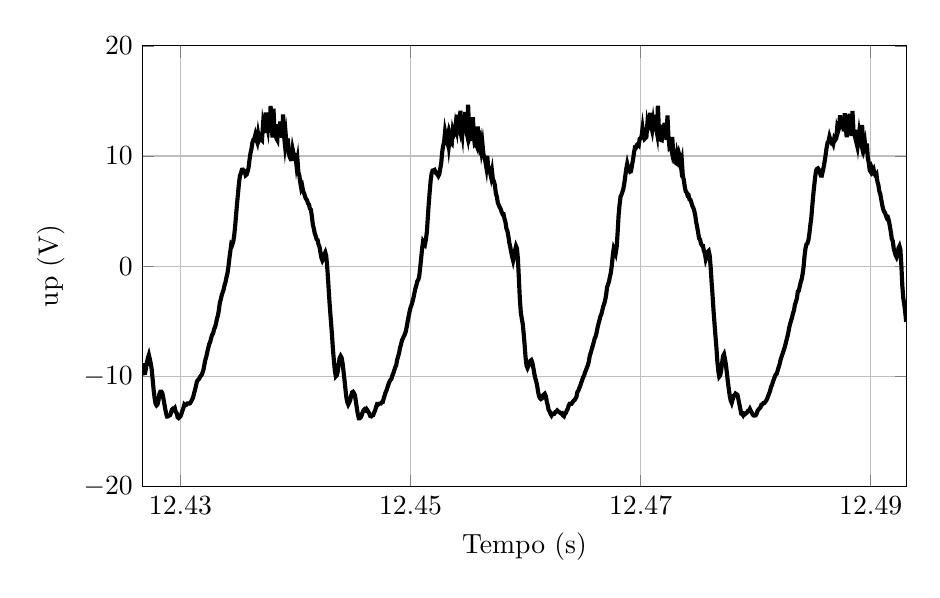
\begin{tikzpicture}

\begin{axis}[%
width=0.8\textwidth,
height=0.461611624834875\textwidth,
scale only axis,
xmin=12.4267,
xmax=12.4931,
xtick={12.43, 12.45, 12.47, 12.49},
xlabel={Tempo (s)},
xmajorgrids,
ymin=-20,
ymax=20,
ytick={-20, -10,   0,  10,  20},
ylabel={up (V)},
ymajorgrids,
scaled x ticks = false,
legend style={font=\footnotesize}
]
\addplot [color=black,solid,line width=1.5pt,forget plot]
  table[row sep=crcr]{12.4266666610667	-8.80980872005165\\
12.4267500010669	-9.47528186296987\\
12.4268333410671	-9.71595194051079\\
12.4269166510673	-9.69818881694053\\
12.4269999910675	-9.28116571823897\\
12.4270833310677	-8.71981679598147\\
12.4271666710679	-8.33543410332883\\
12.4272500110681	-8.05639851438301\\
12.4273333210683	-8.44076447657465\\
12.4274166610685	-8.84366347362103\\
12.4275000010688	-9.39406031934077\\
12.427583341069	-10.3351422852336\\
12.4276666510692	-11.2490277710424\\
12.4277499910694	-11.9721321030172\\
12.4278333310696	-12.4978024888939\\
12.4279166710698	-12.6320132989802\\
12.42800001107	-12.5392685716701\\
12.4280833210702	-12.2214240646547\\
12.4281666610704	-11.5876684366485\\
12.4282500010706	-11.3829320830804\\
12.4283333410708	-11.3828340642084\\
12.428416651071	-11.5135269964183\\
12.4284999910713	-11.9394214304095\\
12.4285833310715	-12.4188441626416\\
12.4286666710717	-12.9146408325806\\
12.4287500110719	-13.3751786655521\\
12.4288333210721	-13.6475026470308\\
12.4289166610723	-13.6357606914702\\
12.4290000010725	-13.5616143124692\\
12.4290833410727	-13.5335956725352\\
12.4291666510729	-13.3420604610174\\
12.4292499910731	-13.0241567110946\\
12.4293333310733	-12.9355137878632\\
12.4294166710735	-12.9766551710685\\
12.4295000110738	-12.8752781941256\\
12.429583321074	-13.2158914828412\\
12.4296666610742	-13.3374889091417\\
12.4297500010744	-13.7154689012019\\
12.4298333410746	-13.7840720279976\\
12.4299166510748	-13.699507040049\\
12.429999991075	-13.6243675239249\\
12.4300833310752	-13.3844297037931\\
12.4301666710754	-13.1176743573592\\
12.4302500110756	-12.8761200499939\\
12.4303333210758	-12.5532795891221\\
12.430416661076	-12.6328165290661\\
12.4305000010763	-12.5870577655248\\
12.4305833410765	-12.4626692840814\\
12.4306666510767	-12.4627641176965\\
12.4307499910769	-12.4745655927223\\
12.4308333310771	-12.4340547804061\\
12.4309166710773	-12.2955882814011\\
12.4310000110775	-12.1121301162084\\
12.4310833210777	-11.9584558581051\\
12.4311666610779	-11.5833203707308\\
12.4312500010781	-11.2680732642894\\
12.4313333410783	-10.9209103284314\\
12.4314166510785	-10.5079571396152\\
12.4314999910788	-10.3459531551036\\
12.431583331079	-10.274432725685\\
12.4316666710792	-10.1109744218451\\
12.4317500110794	-9.96408178559859\\
12.4318333210796	-9.87537564802676\\
12.4319166610798	-9.66636447997055\\
12.43200000108	-9.37480957136079\\
12.4320833410802	-8.89598643087495\\
12.4321666510804	-8.46836821111052\\
12.4322499910806	-8.18737287014583\\
12.4323333310808	-7.76857904936522\\
12.432416671081	-7.40322407993946\\
12.4325000110813	-7.06309141050896\\
12.4325833210815	-6.86885114795297\\
12.4326666610817	-6.50183520134374\\
12.4327500010819	-6.23252725678643\\
12.4328333410821	-6.10653351284327\\
12.4329166510823	-5.73208850980283\\
12.4329999910825	-5.53784217376659\\
12.4330833310827	-5.22733684683276\\
12.4331666710829	-4.77530177235292\\
12.4332500110831	-4.47946926400564\\
12.4333333210833	-3.99945570205384\\
12.4334166610835	-3.32728870739631\\
12.4335000010838	-3.01931745382929\\
12.433583341084	-2.63445335397425\\
12.4336666510842	-2.37302579888952\\
12.4337499910844	-2.12217167978476\\
12.4338333310846	-1.70774812961802\\
12.4339166710848	-1.42877574239874\\
12.434000011085	-0.994361897273687\\
12.4340833210852	-0.644872123476725\\
12.4341666610854	-0.0480793313494553\\
12.4342500010856	0.717924007917058\\
12.4343333410858	1.37362801542235\\
12.434416651086	2.02152515660813\\
12.4344999910863	1.93404622268036\\
12.4345833310865	2.1955964429569\\
12.4346666710867	2.78088207196353\\
12.4347500110869	3.61319295233917\\
12.4348333210871	4.65749806611505\\
12.4349166610873	5.68635834647359\\
12.4350000010875	6.59524811587383\\
12.4350833410877	7.53682408784159\\
12.4351666510879	8.19081643441663\\
12.4352499910881	8.43131227904881\\
12.4353333310883	8.75123892928898\\
12.4354166710885	8.76126217000512\\
12.4355000110888	8.58327454478185\\
12.435583321089	8.60802379805769\\
12.4356666610892	8.24646616066755\\
12.4357500010894	8.3203621071427\\
12.4358333410896	8.60718420483981\\
12.4359166510898	8.93958763852065\\
12.43599999109	9.65890066043226\\
12.4360833310902	10.2598885490058\\
12.4361666710904	10.6335784654577\\
12.4362500110906	11.2041578809017\\
12.4363333210908	11.4748033305402\\
12.436416661091	11.5544977461617\\
12.4365000010913	11.9029711378049\\
12.4365833410915	11.533633106971\\
12.4366666510917	11.2737472734863\\
12.4367499910919	11.9769806106023\\
12.4368333310921	11.4627741310366\\
12.4369166710923	11.6677378324315\\
12.4370000110925	11.5348476735675\\
12.4370833210927	11.446483881284\\
12.4371666610929	12.7422279540834\\
12.4372500010931	12.2185853812396\\
12.4373333410933	12.2571051185551\\
12.4374166510935	13.9409731200115\\
12.4374999910938	12.9114382382964\\
12.437583331094	12.4761550306426\\
12.4376666710942	13.7763676560752\\
12.4377500110944	12.7218440678616\\
12.4378333210946	14.5295118986927\\
12.4379166610948	12.5472707479658\\
12.438000001095	11.6867713804904\\
12.4380833410952	14.2832729153501\\
12.4381666510954	12.2930015683006\\
12.4382499910956	12.2493494285585\\
12.4383333310958	11.6145099316738\\
12.438416671096	11.4532750804882\\
12.4385000110963	12.8765333392056\\
12.4385833210965	11.917701047639\\
12.4386666610967	13.1261987179452\\
12.4387500010969	12.2864198181739\\
12.4388333410971	11.6679645646603\\
12.4389166510973	13.7631971110733\\
12.4389999910975	11.847043697222\\
12.4390833310977	10.9870704417211\\
12.4391666710979	11.7122494976925\\
12.4392500110981	10.6894452276072\\
12.4393333210983	11.5832750106622\\
12.4394166610985	10.1948612158635\\
12.4395000010988	9.92380792275027\\
12.439583341099	9.70382577543722\\
12.4396666510992	9.71385187317994\\
12.4397499910994	10.60470038907\\
12.4398333310996	10.1918824733612\\
12.4399166710998	10.1140269741963\\
12.4400000111	9.9901745829543\\
12.4400833211002	9.17543456168561\\
12.4401666611004	9.67138940260628\\
12.4402500011006	8.50672068908888\\
12.4403333411008	8.22176605428748\\
12.440416651101	7.57085176855137\\
12.4404999911013	7.04947316795797\\
12.4405833311015	7.24664799980959\\
12.4406666711017	6.77798315162836\\
12.4407500111019	6.60449634841452\\
12.4408333211021	6.29841129228866\\
12.4409166611023	6.10222574528888\\
12.4410000011025	5.99350913961882\\
12.4410833411027	5.70405925339769\\
12.4411666511029	5.60016745118408\\
12.4412499911031	5.22094590886994\\
12.4413333311033	5.12276567675533\\
12.4414166711035	4.55875934276016\\
12.4415000111038	3.81024693980174\\
12.441583321104	3.43292532711847\\
12.4416666611042	3.00064041225794\\
12.4417500011044	2.74637889155888\\
12.4418333411046	2.43722461107649\\
12.4419166511048	2.37962531373624\\
12.441999991105	1.95812136731988\\
12.4420833311052	1.75000290543025\\
12.4421666711054	1.23885024943934\\
12.4422500111056	0.766199510840753\\
12.4423333211058	0.530741264236811\\
12.442416661106	0.711571116704074\\
12.4425000011063	1.06991480303069\\
12.4425833411065	1.25011367051053\\
12.4426666511067	0.931931880935931\\
12.4427499911069	-0.00487537797634836\\
12.4428333311071	-1.28641960409488\\
12.4429166711073	-2.70860894589779\\
12.4430000111075	-3.9581556719509\\
12.4430833211077	-5.07321136708899\\
12.4431666611079	-6.20993615085097\\
12.4432500011081	-7.51466245271127\\
12.4433333411083	-8.56332311511743\\
12.4434166511085	-9.46555287366213\\
12.4434999911088	-10.0095808965784\\
12.443583331109	-9.91665741846503\\
12.4436666711092	-9.58647245611611\\
12.4437500111094	-8.91188047585344\\
12.4438333211096	-8.32975857223622\\
12.4439166611098	-8.1518728096492\\
12.44400000111	-8.30666967848963\\
12.4440833411102	-8.76150375955329\\
12.4441666511104	-9.50214344393857\\
12.4442499911106	-10.2728664966871\\
12.4443333311108	-11.0920751544021\\
12.444416671111	-11.8985764719121\\
12.4445000111113	-12.3378730765934\\
12.4445833211115	-12.5590886370248\\
12.4446666611117	-12.3837915928099\\
12.4447500011119	-12.179813891383\\
12.4448333411121	-11.7758921902961\\
12.4449166511123	-11.4512417153366\\
12.4449999911125	-11.397941804632\\
12.4450833311127	-11.5187266110509\\
12.4451666711129	-11.7190838363451\\
12.4452500111131	-12.3035728550331\\
12.4453333211133	-12.9188431481261\\
12.4454166611135	-13.4355405212503\\
12.4455000011138	-13.7988123578512\\
12.445583341114	-13.7986895703945\\
12.4456666511142	-13.7266687644267\\
12.4457499911144	-13.5364418863404\\
12.4458333311146	-13.2588320240131\\
12.4459166711148	-13.0821133014718\\
12.446000011115	-12.9878431701438\\
12.4460833211152	-13.0680539855691\\
12.4461666611154	-12.9575609311014\\
12.4462500011156	-13.0796366151937\\
12.4463333411158	-13.2315018592471\\
12.446416651116	-13.3948764099943\\
12.4464999911163	-13.6042717818069\\
12.4465833311165	-13.6318189343453\\
12.4466666711167	-13.5347835365449\\
12.4467500111169	-13.521348167226\\
12.4468333211171	-13.2774612500022\\
12.4469166611173	-13.1048990052744\\
12.4470000011175	-12.7851525767799\\
12.4470833411177	-12.5376086915766\\
12.4471666511179	-12.5690017717784\\
12.4472499911181	-12.4771765673625\\
12.4473333311183	-12.4747939686947\\
12.4474166711185	-12.4652598330718\\
12.4475000111188	-12.3483199330006\\
12.447583321119	-12.3306826886834\\
12.4476666611192	-11.9997498308185\\
12.4477500011194	-11.7187459636438\\
12.4478333411196	-11.4498055669635\\
12.4479166511198	-11.2570412318809\\
12.44799999112	-10.9766063486012\\
12.4480833311202	-10.7034278033143\\
12.4481666711204	-10.4910060951702\\
12.4482500111206	-10.3312747873615\\
12.4483333211208	-10.2361367646021\\
12.448416661121	-9.9280946020085\\
12.4485000011213	-9.72782996843506\\
12.4485833411215	-9.44752952644048\\
12.4486666511217	-9.18912055735661\\
12.4487499911219	-8.9960473829608\\
12.4488333311221	-8.49455075536907\\
12.4489166711223	-8.19788973235553\\
12.4490000111225	-7.89588577747323\\
12.4490833211227	-7.40642116206443\\
12.4491666611229	-7.1220561939262\\
12.4492500011231	-6.73344409305581\\
12.4493333411233	-6.55310611342255\\
12.4494166511235	-6.36626744796837\\
12.4494999911238	-6.17290065028287\\
12.449583331124	-5.92033270843906\\
12.4496666711242	-5.50103077781997\\
12.4497500111244	-4.97126149159909\\
12.4498333211246	-4.54418524517964\\
12.4499166611248	-4.11451162644473\\
12.450000001125	-3.75135597756508\\
12.4500833411252	-3.52818652177464\\
12.4501666511254	-3.20762308616003\\
12.4502499911256	-2.8816447628186\\
12.4503333311258	-2.4418308280614\\
12.450416671126	-2.04029758616538\\
12.4505000111263	-1.75342715125796\\
12.4505833211265	-1.37064523694653\\
12.4506666611267	-1.24642892277084\\
12.4507500011269	-0.935522061804332\\
12.4508333411271	-0.172072158302121\\
12.4509166511273	0.669713786578534\\
12.4509999911275	1.55163798379205\\
12.4510833311277	2.22661715952008\\
12.4511666711279	2.07975210742027\\
12.4512500111281	1.9650731505113\\
12.4513333211283	2.43222241560681\\
12.4514166611285	3.10411195974585\\
12.4515000011288	4.42683178375083\\
12.451583341129	5.72000610041901\\
12.4516666511292	6.80452895258514\\
12.4517499911294	7.81091052856272\\
12.4518333311296	8.44140712970879\\
12.4519166711298	8.67847138613707\\
12.45200001113	8.70039655891002\\
12.4520833211302	8.74359744374541\\
12.4521666611304	8.56116368994364\\
12.4522500011306	8.39787091538831\\
12.4523333411308	8.36141666295899\\
12.452416651131	8.19412112774633\\
12.4524999911313	8.36813754024423\\
12.4525833311315	8.86564647118493\\
12.4526666711317	9.38279925621948\\
12.4527500111319	10.3632659130654\\
12.4528333211321	10.9090926216897\\
12.4529166611323	11.2875726803599\\
12.4530000011325	12.2152988808232\\
12.4530833411327	11.7838809461717\\
12.4531666511329	11.4179541835787\\
12.4532499911331	11.8474560989654\\
12.4533333311333	10.971955704279\\
12.4534166711335	11.6797085147735\\
12.4535000111338	11.2118987384377\\
12.453583321134	11.1188679781901\\
12.4536666611342	12.2138560785823\\
12.4537500011344	11.85762873309\\
12.4538333411346	12.0307647706245\\
12.4539166511348	12.8060524053546\\
12.453999991135	12.4033326457496\\
12.4540833311352	13.7503526920163\\
12.4541666711354	12.8829013195506\\
12.4542500111356	12.5130117795594\\
12.4543333211358	14.1104142350192\\
12.454416661136	12.6478526704599\\
12.4545000011363	12.0494136440809\\
12.4545833411365	13.5160749552545\\
12.4546666511367	12.0596154304228\\
12.4547499911369	14.0030503629507\\
12.4548333311371	12.3421281537425\\
12.4549166711373	11.9332943483298\\
12.4550000111375	14.6481889147353\\
12.4550833211377	12.4777722180075\\
12.4551666611379	11.7706199684462\\
12.4552500011381	12.024956239541\\
12.4553333411383	11.3924842561197\\
12.4554166511385	13.5201622236473\\
12.4554999911387	11.7356760664287\\
12.455583331139	11.0510305429748\\
12.4556666711392	11.1297857822318\\
12.4557500111394	10.9121173854188\\
12.4558333211396	12.678972386139\\
12.4559166611398	11.4183750068283\\
12.45600000114	10.9604558494803\\
12.4560833411402	11.3670166739078\\
12.4561666511404	10.5553760363409\\
12.4562499911406	11.0908071964023\\
12.4563333311408	10.1689747189471\\
12.456416671141	9.90822416241703\\
12.4565000111413	9.49402400123042\\
12.4565833211415	8.9905604945525\\
12.4566666611417	10.0126535430831\\
12.4567500011419	8.95435247991683\\
12.4568333411421	8.93277601664239\\
12.4569166511423	8.47055386847136\\
12.4569999911425	8.0867944210375\\
12.4570833311427	8.57490701707301\\
12.4571666711429	7.78006322555396\\
12.4572500111431	7.71365275654285\\
12.4573333211433	7.30990293926589\\
12.4574166611435	6.58851220560956\\
12.4575000011438	6.30906338610719\\
12.457583341144	5.76306420072642\\
12.4576666511442	5.55519200755609\\
12.4577499911444	5.34594007303343\\
12.4578333311446	5.18967003479782\\
12.4579166711448	4.92694528948492\\
12.458000011145	4.71256701527926\\
12.4580833211452	4.71628372851141\\
12.4581666611454	4.29765801596722\\
12.4582500011456	3.9901230727059\\
12.4583333411458	3.41160615687878\\
12.458416651146	3.19662885544115\\
12.4584999911462	2.74379462574359\\
12.4585833311465	2.13113671795845\\
12.4586666711467	1.73677211275849\\
12.4587500111469	1.26404185982646\\
12.4588333211471	0.849339558082793\\
12.4589166611473	0.497803496000568\\
12.4590000011475	0.885165668841903\\
12.4590833411477	1.45069626427517\\
12.4591666511479	1.81858037618844\\
12.4592499911481	1.60984689093242\\
12.4593333311483	0.614950095116026\\
12.4594166711485	-1.12644846939151\\
12.4595000111488	-2.96967656296611\\
12.459583321149	-4.19591281615346\\
12.4596666611492	-4.75103340029111\\
12.4597500011494	-5.23159538256114\\
12.4598333411496	-6.11066746599213\\
12.4599166511498	-7.16852053675604\\
12.45999999115	-8.31026643786585\\
12.4600833311502	-9.03562402947178\\
12.4601666711504	-9.24355795167065\\
12.4602500111506	-9.04765974873263\\
12.4603333211508	-8.86995965041344\\
12.460416661151	-8.58806437361368\\
12.4605000011512	-8.52191457524913\\
12.4605833411515	-8.74927929874558\\
12.4606666511517	-9.19324757041546\\
12.4607499911519	-9.71181033717103\\
12.4608333311521	-10.1342842549121\\
12.4609166711523	-10.4382404715723\\
12.4610000111525	-10.8114661964703\\
12.4610833211527	-11.3845562845755\\
12.4611666611529	-11.7791299855686\\
12.4612500011531	-11.9822288260466\\
12.4613333411533	-12.0636712466722\\
12.4614166511535	-12.0061566908308\\
12.4614999911537	-11.7294454261201\\
12.461583331154	-11.6547624984645\\
12.4616666711542	-11.5795734932722\\
12.4617500111544	-11.7818629340482\\
12.4618333211546	-12.244082689732\\
12.4619166611548	-12.5920389010011\\
12.462000001155	-13.0483718474783\\
12.4620833411552	-13.1626387349973\\
12.4621666511554	-13.408287310317\\
12.4622499911556	-13.55060568945\\
12.4623333311558	-13.3915581886541\\
12.462416671156	-13.4178608435003\\
12.4625000111563	-13.3984719072791\\
12.4625833211565	-13.2415035983952\\
12.4626666611567	-13.2136948322117\\
12.4627500011569	-13.1009868720989\\
12.4628333411571	-13.1937295509218\\
12.4629166511573	-13.2309135088351\\
12.4629999911575	-13.3092065319426\\
12.4630833311577	-13.3729842262683\\
12.4631666711579	-13.3470234635039\\
12.4632500111581	-13.5482209677515\\
12.4633333211583	-13.6198753297114\\
12.4634166611585	-13.3829558528602\\
12.4635000011587	-13.3193174566661\\
12.463583341159	-13.0938468145988\\
12.4636666511592	-12.9311252941812\\
12.4637499911594	-12.6400112898177\\
12.4638333311596	-12.4800950222201\\
12.4639166711598	-12.4815135782073\\
12.46400001116	-12.4808655830348\\
12.4640833211602	-12.3490548719677\\
12.4641666611604	-12.2211436891985\\
12.4642500011606	-12.1716450668889\\
12.4643333411608	-12.0166238970407\\
12.464416651161	-11.8693464813643\\
12.4644999911613	-11.4219454741292\\
12.4645833311615	-11.3008614920505\\
12.4646666711617	-11.0678355881158\\
12.4647500111619	-10.857142065756\\
12.4648333211621	-10.5753276936546\\
12.4649166611623	-10.3623672434597\\
12.4650000011625	-10.0660755167298\\
12.4650833411627	-9.94041543396986\\
12.4651666511629	-9.64372533672869\\
12.4652499911631	-9.44052669603529\\
12.4653333311633	-9.19015991288585\\
12.4654166711635	-8.97345408287184\\
12.4655000111638	-8.64245035672755\\
12.465583321164	-8.11824380059442\\
12.4656666611642	-7.85136765940594\\
12.4657500011644	-7.53434776704537\\
12.4658333411646	-7.23844068751244\\
12.4659166511648	-6.9305932552805\\
12.465999991165	-6.57195984828398\\
12.4660833311652	-6.39365180969441\\
12.4661666711654	-6.04890502057826\\
12.4662500111656	-5.60470328438157\\
12.4663333211658	-5.25835730696038\\
12.466416661166	-4.91439134781377\\
12.4665000011662	-4.56268546620682\\
12.4665833411665	-4.36884826946402\\
12.4666666511667	-4.02517831134487\\
12.4667499911669	-3.65464946710704\\
12.4668333311671	-3.39965470206142\\
12.4669166711673	-3.0949254411905\\
12.4670000111675	-2.60156491819325\\
12.4670833211677	-1.91726130819417\\
12.4671666611679	-1.64989133804637\\
12.4672500011681	-1.38843686338962\\
12.4673333411683	-0.939869293920112\\
12.4674166511685	-0.572725249688572\\
12.4674999911688	0.125642033721624\\
12.467583331169	1.01254690621118\\
12.4676666711692	1.62646390375368\\
12.4677500111694	1.43936415830276\\
12.4678333211696	1.18254369941686\\
12.4679166611698	1.74045445440744\\
12.46800000117	3.05431948329508\\
12.4680833411702	4.59676928441736\\
12.4681666511704	5.54095935360256\\
12.4682499911706	6.29622431441983\\
12.4683333311708	6.47725302437876\\
12.468416671171	6.74143915673298\\
12.4685000111712	7.02179011978823\\
12.4685833211715	7.53211243270542\\
12.4686666611717	8.18973040925418\\
12.4687500011719	8.81250577103286\\
12.4688333411721	9.27838217319299\\
12.4689166511723	8.89638591886\\
12.4689999911725	8.78452806922592\\
12.4690833311727	8.5745166142408\\
12.4691666711729	8.62520652304537\\
12.4692500111731	9.18085662221818\\
12.4693333211733	9.62781280436946\\
12.4694166611735	10.2484067391605\\
12.4695000011738	10.7566914968479\\
12.469583341174	10.7365835331309\\
12.4696666511742	10.9923421138122\\
12.4697499911744	11.0768512105486\\
12.4698333311746	10.9801077716804\\
12.4699166711748	11.5497552991923\\
12.470000011175	11.6075381973441\\
12.4700833211752	11.8074025305912\\
12.4701666611754	12.5103786578506\\
12.4702500011756	11.8483868454194\\
12.4703333411758	11.5472602004709\\
12.470416651176	11.6311294962531\\
12.4704999911763	11.7119758213236\\
12.4705833311765	12.907406860629\\
12.4706666711767	12.4772581014314\\
12.4707500111769	12.5336217999463\\
12.4708333211771	13.9140950735094\\
12.4709166611773	12.7030151982255\\
12.4710000011775	12.3210210461759\\
12.4710833411777	13.0224859863427\\
12.4711666511779	12.3011114823547\\
12.4712499911781	13.7372603493848\\
12.4713333311783	12.5915505408493\\
12.4714166711785	12.1128704382023\\
12.4715000111787	14.5663870449859\\
12.471583321179	12.5141832222818\\
12.4716666611792	12.2377952628186\\
12.4717500011794	11.4707793460266\\
12.4718333411796	11.4337612170767\\
12.4719166511798	12.8266467425629\\
12.47199999118	11.9359890916564\\
12.4720833311802	13.0053563079461\\
12.4721666711804	12.0914375219053\\
12.4722500111806	11.4854092339492\\
12.4723333211808	13.6732320858943\\
12.472416661181	11.7636795173823\\
12.4725000011813	10.8781224086531\\
12.4725833411815	11.0221385855338\\
12.4726666511817	10.6097876876057\\
12.4727499911819	11.7289913525952\\
12.4728333311821	10.2380635408207\\
12.4729166711823	9.66070784843874\\
12.4730000111825	9.42072728026718\\
12.4730833211827	9.35745960356864\\
12.4731666611829	10.1596765666077\\
12.4732500011831	9.77111495449099\\
12.4733333411833	10.2147040895664\\
12.4734166511835	9.89993798445971\\
12.4734999911838	9.14071279452701\\
12.473583331184	9.54525346856092\\
12.4736666711842	8.21171475136582\\
12.4737500111844	7.83791376153713\\
12.4738333211846	7.2308073720362\\
12.4739166611848	6.80084154016418\\
12.474000001185	6.69287552886893\\
12.4740833411852	6.4148860690168\\
12.4741666511854	6.44052133608171\\
12.4742499911856	6.05843389575975\\
12.4743333311858	6.02120811440711\\
12.474416671186	5.75085722110202\\
12.4745000111862	5.45819979143173\\
12.4745833211865	5.28881581413422\\
12.4746666611867	5.0104970461369\\
12.4747500011869	4.58884418079446\\
12.4748333411871	3.97954393577238\\
12.4749166511873	3.54588223847928\\
12.4749999911875	3.03961111122504\\
12.4750833311877	2.52912350154224\\
12.4751666711879	2.42344645318853\\
12.4752500111881	2.0290674476319\\
12.4753333211883	1.87524894696878\\
12.4754166611885	1.85220398615231\\
12.4755000011888	1.37923441279799\\
12.475583341189	1.17733247781833\\
12.4756666511892	0.628878525027252\\
12.4757499911894	0.884261899445867\\
12.4758333311896	1.3045999039936\\
12.4759166711898	1.39272143155435\\
12.47600001119	0.991537787523368\\
12.4760833211902	-0.0215186179041303\\
12.4761666611904	-1.406092844045\\
12.4762500011906	-2.59683623111054\\
12.4763333411908	-3.96735135218328\\
12.476416651191	-5.116908756765\\
12.4764999911913	-6.2731832457166\\
12.4765833311915	-7.30490208315636\\
12.4766666711917	-8.60447578321923\\
12.4767500111919	-9.48632588120948\\
12.4768333211921	-10.027876373356\\
12.4769166611923	-9.91347600314586\\
12.4770000011925	-9.4577704323333\\
12.4770833411927	-8.77628781991244\\
12.4771666511929	-8.15227066500466\\
12.4772499911931	-7.99253575154157\\
12.4773333311933	-8.44643111984694\\
12.4774166711935	-8.97482411591112\\
12.4775000111938	-9.7138061745542\\
12.477583321194	-10.4897342792488\\
12.4776666611942	-11.1481434041145\\
12.4777500011944	-11.7915200409387\\
12.4778333411946	-12.1991647749555\\
12.4779166511948	-12.4109091011613\\
12.477999991195	-12.109600569518\\
12.4780833311952	-11.7626055887487\\
12.4781666711954	-11.7118286894543\\
12.4782500111956	-11.5621569649419\\
12.4783333211958	-11.6251891039761\\
12.478416661196	-11.6780996945905\\
12.4785000011963	-12.0922332590267\\
12.4785833411965	-12.5263722308086\\
12.4786666511967	-12.9698267533357\\
12.4787499911969	-13.3816163181811\\
12.4788333311971	-13.3897578242488\\
12.4789166711973	-13.5369527096989\\
12.4790000111975	-13.382934633618\\
12.4790833211977	-13.4256223047657\\
12.4791666611979	-13.3331182079952\\
12.4792500011981	-13.281793793401\\
12.4793333411983	-13.1313482932961\\
12.4794166511985	-13.1296719717966\\
12.4794999911988	-12.9607178138879\\
12.479583331199	-13.1492820889567\\
12.4796666711992	-13.2877685610403\\
12.4797500111994	-13.4819200863924\\
12.4798333211996	-13.5502692216092\\
12.4799166611998	-13.5546939333325\\
12.4800000012	-13.5395358540222\\
12.4800833412002	-13.3963145714666\\
12.4801666512004	-13.1259137024704\\
12.4802499912006	-13.0047384647782\\
12.4803333312008	-12.9084204724718\\
12.480416671201	-12.823084102529\\
12.4805000112013	-12.5738569854204\\
12.4805833212015	-12.5555474457639\\
12.4806666612017	-12.4342696000533\\
12.4807500012019	-12.433473879802\\
12.4808333412021	-12.3266233027352\\
12.4809166512023	-12.1969977524311\\
12.4809999912025	-12.0254132876043\\
12.4810833312027	-11.7958895582822\\
12.4811666712029	-11.5611494885673\\
12.4812500112031	-11.3435906597586\\
12.4813333212033	-10.9625439706676\\
12.4814166612035	-10.8004048811767\\
12.4815000012038	-10.5016478619553\\
12.481583341204	-10.2644671099236\\
12.4816666512042	-10.0161118035826\\
12.4817499912044	-9.81623833458744\\
12.4818333312046	-9.7625934503163\\
12.4819166712048	-9.45661301207305\\
12.482000011205	-9.16268469532169\\
12.4820833212052	-8.89905795837933\\
12.4821666612054	-8.49054371197992\\
12.4822500012056	-8.21953508969576\\
12.4823333412058	-7.98315365071645\\
12.482416651206	-7.71038133090706\\
12.4824999912063	-7.4529705692174\\
12.4825833312065	-7.13426170342368\\
12.4826666712067	-6.76951884271848\\
12.4827500112069	-6.43606215498212\\
12.4828333212071	-6.05312167294301\\
12.4829166612073	-5.57684837478873\\
12.4830000012075	-5.21944850978692\\
12.4830833412077	-4.92398248935899\\
12.4831666512079	-4.6457179961634\\
12.4832499912081	-4.24658611104006\\
12.4833333312083	-4.00062718909633\\
12.4834166712085	-3.47722065991248\\
12.4835000112088	-3.23351643963629\\
12.483583321209	-2.93040729743567\\
12.4836666612092	-2.28939027564748\\
12.4837500012094	-2.22695442385704\\
12.4838333412096	-1.83586108700245\\
12.4839166512098	-1.44416805918544\\
12.48399999121	-1.17856379833167\\
12.4840833312102	-0.711209696052085\\
12.4841666712104	-0.0506684547079084\\
12.4842500112106	0.919646999918614\\
12.4843333212108	1.62398814503424\\
12.484416661211	1.99418287081003\\
12.4845000012113	2.06247501981271\\
12.4845833412115	2.33786185448729\\
12.4846666512117	2.92157959599211\\
12.4847499912119	3.70211691291694\\
12.4848333312121	4.347767911663\\
12.4849166712123	5.37418115998709\\
12.4850000112125	6.40413371423558\\
12.4850833212127	7.24025689487826\\
12.4851666612129	8.02354236364482\\
12.4852500012131	8.67630979018551\\
12.4853333412133	8.82911147842963\\
12.4854166512135	8.87832711450855\\
12.4854999912138	8.737398109982\\
12.485583331214	8.47473364451139\\
12.4856666712142	8.22600850786485\\
12.4857500112144	8.21934495189464\\
12.4858333212146	8.60758907914801\\
12.4859166612148	9.02085358046543\\
12.486000001215	9.52218151092899\\
12.4860833412152	10.1070184259932\\
12.4861666512154	10.7412938135622\\
12.4862499912156	11.2061176849677\\
12.4863333312158	11.3294783758019\\
12.486416671216	11.7514914265723\\
12.4865000112163	11.4591307697683\\
12.4865833212165	11.250300775923\\
12.4866666612167	11.3693544206278\\
12.4867500012169	11.1291317822897\\
12.4868333412171	11.5942788608121\\
12.4869166512173	11.4484210624171\\
12.4869999912175	11.5764219713234\\
12.4870833312177	12.5140694138968\\
12.4871666712179	12.2410554380488\\
12.4872500112181	12.5404514086395\\
12.4873333212183	13.6858431823592\\
12.4874166612185	12.8534290765573\\
12.4875000012188	13.0382925421992\\
12.487583341219	13.1388496714541\\
12.4876666512192	12.2345953330228\\
12.4877499912194	13.8893400847112\\
12.4878333312196	12.5584122103347\\
12.4879166712198	11.7005617071317\\
12.48800001122	13.2434484162305\\
12.4880833212202	12.2701203089539\\
12.4881666612204	13.8267147393615\\
12.4882500012206	12.3756345646882\\
12.4883333412208	11.8259697963962\\
12.488416651221	14.0766154824187\\
12.4884999912213	12.3761138958318\\
12.4885833312215	12.0616595490822\\
12.4886666712217	11.616085037111\\
12.4887500112219	11.2553466121559\\
12.4888333212221	12.3668415687102\\
12.4889166612223	11.3893563395562\\
12.4890000012225	12.1174480539385\\
12.4890833412227	11.5752203340336\\
12.4891666512229	11.1786590942741\\
12.4892499912231	12.8045195198831\\
12.4893333312233	11.3667285303852\\
12.4894166712235	10.7538114619235\\
12.4895000112238	11.148318153922\\
12.489583321224	10.2538996961057\\
12.4896666612242	11.1300786185441\\
12.4897500012244	9.81084319866057\\
12.4898333412246	9.35810771338559\\
12.4899166512248	8.70690714795391\\
12.489999991225	8.56491379218895\\
12.4900833312252	8.89209693433684\\
12.4901666712254	8.63543213427434\\
12.4902500112256	8.78579294469572\\
12.4903333212258	8.35760780919457\\
12.490416661226	8.21966579566965\\
12.4905000012263	8.33900683476184\\
12.4905833412265	7.66850965677854\\
12.4906666512267	7.39148217204075\\
12.4907499912269	6.79854847936098\\
12.4908333312271	6.54189521988972\\
12.4909166712273	6.05529451654625\\
12.4910000112275	5.577945754516\\
12.4910833212277	5.18053569965904\\
12.4911666612279	4.94418722809988\\
12.4912500012281	4.83855896840802\\
12.4913333412283	4.56144303952203\\
12.4914166512285	4.34643593249498\\
12.4914999912288	4.40979403250769\\
12.491583331229	4.11486695971276\\
12.4916666712292	3.62568400989959\\
12.4917500112294	3.11497464549468\\
12.4918333212296	2.50035418733049\\
12.4919166612298	2.27861193746185\\
12.49200000123	1.63253941283155\\
12.4920833412302	1.30556711454455\\
12.4921666512304	0.994482126241465\\
12.4922499912306	0.816726024711957\\
12.4923333312308	1.06635073938111\\
12.492416671231	1.64350694727793\\
12.4925000112313	1.8228632642067\\
12.4925833212315	1.49919274148553\\
12.4926666612317	0.0668635375389842\\
12.4927500012319	-1.78011818768771\\
12.4928333412321	-2.90652492150646\\
12.4929166512323	-3.45784521759843\\
12.4929999912325	-4.1547309779736\\
12.4930833312327	-5.05500190666392\\
};
\end{axis}
\end{tikzpicture}%}
    \captionof{figure}{Ação de controle no regime permanente após a variação da indutância da rede.}
    \label{fig:up_exp_Lg_permanente}
  \end{minipage}

  \vspace*{\fill}
  \noindent
  \begin{minipage}{\textwidth}
    \makebox[\textwidth]{
      \centering
      \def\svgwidth{\textwidth}
      % This file was created by matlab2tikz v0.4.7 running on MATLAB 7.14.
% Copyright (c) 2008--2014, Nico Schlömer <nico.schloemer@gmail.com>
% All rights reserved.
% Minimal pgfplots version: 1.3
% 
% The latest updates can be retrieved from
%   http://www.mathworks.com/matlabcentral/fileexchange/22022-matlab2tikz
% where you can also make suggestions and rate matlab2tikz.
% 
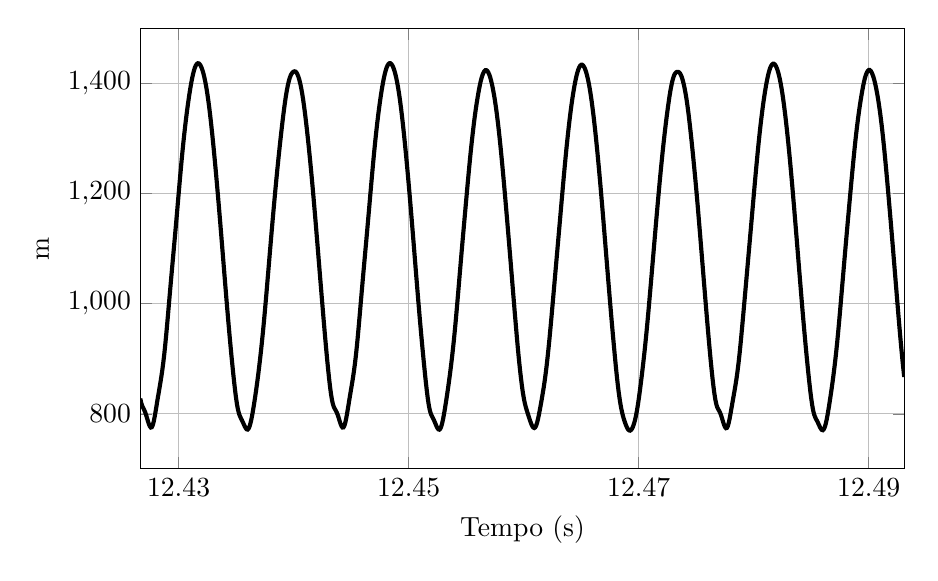
\begin{tikzpicture}

\begin{axis}[%
width=0.8\textwidth,
height=0.461611624834875\textwidth,
scale only axis,
xmin=12.4267,
xmax=12.4931,
xtick={12.43, 12.45, 12.47, 12.49},
xlabel={Tempo (s)},
xmajorgrids,
ymin=700,
ymax=1500,
ytick={ 800, 1000, 1200, 1400},
ylabel={m},
ymajorgrids,
scaled x ticks = false,
legend style={font=\footnotesize}
]
\addplot [color=black,solid,line width=1.5pt,forget plot]
  table[row sep=crcr]{12.4266666610667	827.741097437338\\
12.4267500010669	820.095895950887\\
12.4268333410671	814.789713852944\\
12.4269166510673	810.926617961449\\
12.4269999910675	807.531909658705\\
12.4270833310677	803.534657688938\\
12.4271666710679	798.570400861033\\
12.4272500110681	792.872551099854\\
12.4273333210683	786.933201603522\\
12.4274166610685	781.548953727111\\
12.4275000010688	777.383993988708\\
12.427583341069	775.212590048016\\
12.4276666510692	775.723182541313\\
12.4277499910694	779.252927661133\\
12.4278333310696	785.604996188925\\
12.4279166710698	794.216199083165\\
12.42800001107	804.222797671565\\
12.4280833210702	814.841893365837\\
12.4281666610704	825.451131277664\\
12.4282500010706	835.741846133046\\
12.4283333410708	845.973716436484\\
12.428416651071	856.35976521968\\
12.4284999910713	867.309746566374\\
12.4285833310715	879.243199917306\\
12.4286666710717	892.496036836965\\
12.4287500110719	907.305876143824\\
12.4288333210721	923.833482695955\\
12.4289166610723	941.838096425996\\
12.4290000010725	960.957851040641\\
12.4290833410727	980.817641301398\\
12.4291666510729	1000.92579027159\\
12.4292499910731	1020.98887736596\\
12.4293333310733	1040.82790546728\\
12.4294166710735	1060.40024855815\\
12.4295000110738	1079.75456804226\\
12.429583321074	1099.0191725966\\
12.4296666610742	1118.36698724123\\
12.4297500010744	1137.94421493114\\
12.4298333410746	1157.81044004841\\
12.4299166510748	1177.95550333431\\
12.429999991075	1198.19298823851\\
12.4300833310752	1218.29986903888\\
12.4301666710754	1237.99391156711\\
12.4302500110756	1257.03965366303\\
12.4303333210758	1275.2802927645\\
12.430416661076	1292.60397220553\\
12.4305000010763	1308.93102938394\\
12.4305833410765	1324.3132043524\\
12.4306666510767	1338.789220191\\
12.4307499910769	1352.41966044896\\
12.4308333310771	1365.23484828857\\
12.4309166710773	1377.23930383278\\
12.4310000110775	1388.42263963318\\
12.4310833210777	1398.70675975138\\
12.4311666610779	1407.96337654268\\
12.4312500010781	1416.09623822161\\
12.4313333410783	1422.96732743883\\
12.4314166510785	1428.48779478504\\
12.4314999910788	1432.59031029069\\
12.431583331079	1435.19998651791\\
12.4316666710792	1436.36131728105\\
12.4317500110794	1436.1788349605\\
12.4318333210796	1434.72821646989\\
12.4319166610798	1432.08090450769\\
12.43200000108	1428.27429119471\\
12.4320833410802	1423.32022496969\\
12.4321666510804	1417.2488286865\\
12.4322499910806	1409.97208244128\\
12.4323333310808	1401.49399340179\\
12.432416671081	1391.8146768497\\
12.4325000110813	1380.97245914504\\
12.4325833210815	1368.90536691772\\
12.4326666610817	1355.62218915142\\
12.4327500010819	1341.22557184323\\
12.4328333410821	1325.78212036367\\
12.4329166510823	1309.41365147623\\
12.4329999910825	1292.27124570155\\
12.4330833310827	1274.4661679459\\
12.4331666710829	1256.06850172968\\
12.4332500110831	1237.13468343795\\
12.4333333210833	1217.6098075732\\
12.4334166610835	1197.59851895734\\
12.4335000010838	1177.18560792883\\
12.433583341084	1156.33397153088\\
12.4336666510842	1135.18077956483\\
12.4337499910844	1113.80397887541\\
12.4338333310846	1092.2871389759\\
12.4339166710848	1070.75090269941\\
12.434000011085	1049.22783313728\\
12.4340833210852	1027.83099933397\\
12.4341666610854	1006.65321068067\\
12.4342500010856	985.851684622578\\
12.4343333410858	965.521923344282\\
12.434416651086	945.793461351915\\
12.4344999910863	926.736507780411\\
12.4345833310865	908.242108007742\\
12.4346666710867	890.410089121622\\
12.4347500110869	873.280735003904\\
12.4348333210871	857.044306890318\\
12.4349166610873	841.931831107451\\
12.4350000010875	828.254107995106\\
12.4350833410877	816.586761974033\\
12.4351666510879	807.370424743281\\
12.4352499910881	800.617312318397\\
12.4353333310883	795.766117977876\\
12.4354166710885	792.133431931995\\
12.4355000110888	788.67407601778\\
12.435583321089	785.036720946653\\
12.4356666610892	781.164619722054\\
12.4357500010894	777.306428243987\\
12.4358333410896	774.081134183963\\
12.4359166510898	771.972845714799\\
12.43599999109	771.535385968658\\
12.4360833310902	773.238704916023\\
12.4361666710904	777.061808044983\\
12.4362500110906	782.964542520149\\
12.4363333210908	790.618980537315\\
12.436416661091	799.683895751156\\
12.4365000010913	809.750713638863\\
12.4365833410915	820.717293780883\\
12.4366666510917	832.202736682772\\
12.4367499910919	844.224371129791\\
12.4368333310921	857.003722168216\\
12.4369166710923	870.329419874382\\
12.4370000110925	884.446595030164\\
12.4370833210927	899.290057853971\\
12.4371666610929	914.848786975554\\
12.4372500010931	931.351604497147\\
12.4373333410933	948.597452012743\\
12.4374166510935	966.688862867412\\
12.4374999910938	985.987403945112\\
12.437583331094	1005.75444318955\\
12.4376666710942	1025.99430552504\\
12.4377500110944	1046.76157817486\\
12.4378333210946	1067.4259239401\\
12.4379166610948	1088.1985403401\\
12.438000001095	1108.8235339465\\
12.4380833410952	1129.19850789744\\
12.4381666510954	1149.19605692304\\
12.4382499910956	1168.7851861842\\
12.4383333310958	1188.02075779615\\
12.438416671096	1207.04928237006\\
12.4385000110963	1225.53098458671\\
12.4385833210965	1243.2769333336\\
12.4386666610967	1260.5488986023\\
12.4387500010969	1277.18135917142\\
12.4388333410971	1293.48189076332\\
12.4389166510973	1309.19964948709\\
12.4389999910975	1324.42768433414\\
12.4390833310977	1338.990901255\\
12.4391666710979	1352.84353321745\\
12.4392500110981	1365.73457668121\\
12.4393333210983	1377.52134103604\\
12.4394166610985	1387.56680376203\\
12.4395000010988	1396.5668867192\\
12.439583341099	1403.95586926678\\
12.4396666510992	1409.98227941702\\
12.4397499910994	1414.55401458886\\
12.4398333310996	1417.74881103278\\
12.4399166710998	1419.97728930639\\
12.4400000111	1421.27523767725\\
12.4400833211002	1421.76551624367\\
12.4401666611004	1421.24995424429\\
12.4402500011006	1419.36501287054\\
12.4403333411008	1416.27936056642\\
12.440416651101	1411.81044300801\\
12.4404999911013	1406.13506257849\\
12.4405833311015	1399.11534677474\\
12.4406666711017	1390.60982541882\\
12.4407500111019	1380.75537774632\\
12.4408333211021	1369.60187691527\\
12.4409166611023	1357.21869669722\\
12.4410000011025	1343.70162289447\\
12.4410833411027	1329.22427007339\\
12.4411666511029	1313.91574792721\\
12.4412499911031	1297.8875606514\\
12.4413333311033	1281.21764727774\\
12.4414166711035	1263.80886919676\\
12.4415000111038	1245.80467182332\\
12.441583321104	1227.22307578643\\
12.4416666611042	1207.99789219666\\
12.4417500011044	1188.15500494246\\
12.4418333411046	1167.81933938726\\
12.4419166511048	1147.10430684935\\
12.441999991105	1126.04051162687\\
12.4420833311052	1104.83139594918\\
12.4421666711054	1083.38390040498\\
12.4422500111056	1061.97017642496\\
12.4423333211058	1040.58946037402\\
12.442416661106	1019.36318901171\\
12.4425000011063	998.269666698926\\
12.4425833411065	977.400590155302\\
12.4426666511067	956.874715132242\\
12.4427499911069	936.810259096241\\
12.4428333311071	917.308577347969\\
12.4429166711073	898.569267322168\\
12.4430000111075	880.802668309645\\
12.4430833211077	864.195359843596\\
12.4431666611079	849.106586838205\\
12.4432500011081	836.030317561778\\
12.4433333411083	825.453554220401\\
12.4434166511085	817.654473915795\\
12.4434999911088	812.329876588065\\
12.443583331109	808.923824187537\\
12.4436666711092	806.008944046804\\
12.4437500111094	802.659919157075\\
12.4438333211096	798.175661311404\\
12.4439166611098	792.782813321945\\
12.44400000111	787.037307698387\\
12.4440833411102	781.698687880609\\
12.4441666511104	777.507510285943\\
12.4442499911106	775.227587319546\\
12.4443333311108	775.462974787333\\
12.444416671111	778.561515722591\\
12.4445000111113	784.648332596099\\
12.4445833211115	792.983975655271\\
12.4446666611117	802.893786220521\\
12.4447500011119	813.479260964258\\
12.4448333411121	824.162406814279\\
12.4449166511123	834.655734617157\\
12.4449999911125	844.99473445013\\
12.4450833311127	855.491353549541\\
12.4451666711129	866.473325160077\\
12.4452500111131	878.348443655971\\
12.4453333211133	891.555951415168\\
12.4454166611135	906.387049641545\\
12.4455000011138	922.902388727221\\
12.445583341114	941.015464202883\\
12.4456666511142	960.280165987799\\
12.4457499911144	980.278253638775\\
12.4458333311146	1000.52481126517\\
12.4459166711148	1020.68780404572\\
12.446000011115	1040.61360201563\\
12.4460833211152	1060.24562698184\\
12.4461666611154	1079.65293080543\\
12.4462500011156	1098.96526967053\\
12.4463333411158	1118.31116270589\\
12.446416651116	1137.82423728104\\
12.4464999911163	1157.55800085624\\
12.4465833311165	1177.50982929005\\
12.4466666711167	1197.57044377294\\
12.4467500111169	1217.54021281406\\
12.4468333211171	1237.18954255255\\
12.4469166611173	1256.28298597685\\
12.4470000011175	1274.64469117472\\
12.4470833411177	1292.1731978775\\
12.4471666511179	1308.76561466547\\
12.4472499911181	1324.38879610796\\
12.4473333311183	1339.04975153137\\
12.4474166711185	1352.8100918808\\
12.4475000111188	1365.69749454324\\
12.447583321119	1377.72604342916\\
12.4476666611192	1388.85113728634\\
12.4477500011194	1399.0473464387\\
12.4478333411196	1408.19985905327\\
12.4479166511198	1416.19504498952\\
12.44799999112	1422.93304470509\\
12.4480833311202	1428.3514746712\\
12.4481666711204	1432.44578719174\\
12.4482500111206	1435.14283758485\\
12.4483333211208	1436.4521636122\\
12.448416661121	1436.34595831135\\
12.4485000011213	1434.99484394118\\
12.4485833411215	1432.40506743065\\
12.4486666511217	1428.67185554204\\
12.4487499911219	1423.73986078682\\
12.4488333311221	1417.62543810378\\
12.4489166711223	1410.35891709851\\
12.4490000111225	1401.83040266344\\
12.4490833211227	1392.07479206239\\
12.4491666611229	1381.09229537881\\
12.4492500011231	1368.9202668744\\
12.4493333411233	1355.64670721855\\
12.4494166511235	1341.26525360108\\
12.4494999911238	1325.8949508955\\
12.449583331124	1309.63345294254\\
12.4496666711242	1292.58025749484\\
12.4497500111244	1274.85596490394\\
12.4498333211246	1256.48723186019\\
12.4499166611248	1237.50965355697\\
12.450000001125	1217.97742173207\\
12.4500833411252	1197.92016394709\\
12.4501666511254	1177.38653919141\\
12.4502499911256	1156.49217671019\\
12.4503333311258	1135.29114949337\\
12.450416671126	1113.87779886622\\
12.4505000111263	1092.31857499515\\
12.4505833211265	1070.69757218393\\
12.4506666611267	1049.13882985673\\
12.4507500011269	1027.69597891559\\
12.4508333411271	1006.5075984292\\
12.4509166511273	985.762347243644\\
12.4509999911275	965.588704302176\\
12.4510833311277	946.037283522057\\
12.4511666711279	927.092803798536\\
12.4512500111281	908.579437462582\\
12.4513333211283	890.58368008044\\
12.4514166611285	873.204178572414\\
12.4515000011288	856.653021436493\\
12.451583341129	841.289452470191\\
12.4516666511292	827.573803756238\\
12.4517499911294	816.038894032171\\
12.4518333311296	807.217734942509\\
12.4519166711298	801.002107905529\\
12.45200001113	796.711064806706\\
12.4520833211302	793.391683918333\\
12.4521666611304	789.982511816501\\
12.4522500011306	786.14871486844\\
12.4523333411308	781.944156939817\\
12.452416651131	777.760699923342\\
12.4524999911313	774.205462884819\\
12.4525833311315	771.866497081067\\
12.4526666711317	771.295722817113\\
12.4527500111319	772.843385749458\\
12.4528333211321	776.942139919071\\
12.4529166611323	783.132023804767\\
12.4530000011325	791.142834624913\\
12.4530833411327	800.780470194386\\
12.4531666511329	811.141074162686\\
12.4532499911331	822.070550117374\\
12.4533333311333	833.59595421518\\
12.4534166711335	845.355740897334\\
12.4535000111338	857.834148752375\\
12.453583321134	870.808132600359\\
12.4536666611342	884.469763675553\\
12.4537500011344	898.99480745666\\
12.4538333411346	914.315903782546\\
12.4539166511348	930.615663337275\\
12.453999991135	948.109285145477\\
12.4540833311352	966.507674545694\\
12.4541666711354	986.136311143964\\
12.4542500111356	1006.25617235926\\
12.4543333211358	1026.73340350915\\
12.454416661136	1047.57470710905\\
12.4545000011363	1068.14725095621\\
12.4545833411365	1088.53921537767\\
12.4546666511367	1108.70676087484\\
12.4547499911369	1128.56384649107\\
12.4548333311371	1148.23604178129\\
12.4549166711373	1167.87559105427\\
12.4550000111375	1187.33638158841\\
12.4550833211377	1206.74107076404\\
12.4551666611379	1225.77225132088\\
12.4552500011381	1244.38983753406\\
12.4553333411383	1262.52573164553\\
12.4554166511385	1279.83789563384\\
12.4554999911387	1295.94335124731\\
12.455583331139	1311.42443535158\\
12.4556666711392	1326.06167259958\\
12.4557500111394	1339.88700128532\\
12.4558333211396	1352.6005043193\\
12.4559166611398	1364.13922089385\\
12.45600000114	1374.9532652823\\
12.4560833411402	1385.00820196287\\
12.4561666511404	1394.24022223787\\
12.4562499911406	1402.43403851284\\
12.4563333311408	1409.20652753693\\
12.456416671141	1414.84339339695\\
12.4565000111413	1419.09407868145\\
12.4565833211415	1422.14355623002\\
12.4566666611417	1423.85967420234\\
12.4567500011419	1423.84588038744\\
12.4568333411421	1422.66079484077\\
12.4569166511423	1420.04983045166\\
12.4569999911425	1416.32065805189\\
12.4570833311427	1411.30208328833\\
12.4571666711429	1404.96050422579\\
12.4572500111431	1397.61705921751\\
12.4573333211433	1389.11732228323\\
12.4574166611435	1379.56154008881\\
12.4575000011438	1369.00606973695\\
12.457583341144	1357.26240794321\\
12.4576666511442	1344.39926944254\\
12.4577499911444	1330.35535100774\\
12.4578333311446	1315.19231232904\\
12.4579166711448	1299.07277758794\\
12.458000011145	1282.13629082999\\
12.4580833211452	1264.40173734034\\
12.4581666611454	1245.92018442804\\
12.4582500011456	1226.84608642218\\
12.4583333411458	1207.25733605996\\
12.458416651146	1187.339534144\\
12.4584999911462	1167.02293636942\\
12.4585833311465	1146.54005493564\\
12.4586666711467	1125.81621901712\\
12.4587500111469	1104.94008015697\\
12.4588333211471	1083.86310365944\\
12.4589166611473	1062.68159688948\\
12.4590000011475	1041.42223371659\\
12.4590833411477	1020.07505204605\\
12.4591666511479	998.780834051415\\
12.4592499911481	977.774090191602\\
12.4593333311483	957.177735575863\\
12.4594166711485	937.113241326438\\
12.4595000111488	917.794829947002\\
12.459583321149	899.638114763503\\
12.4596666611492	882.875858413919\\
12.4597500011494	867.358044144343\\
12.4598333411496	853.108880348669\\
12.4599166511498	840.468203744682\\
12.45999999115	829.749616704024\\
12.4600833311502	820.875562987711\\
12.4601666711504	813.726686952834\\
12.4602500111506	807.617875757998\\
12.4603333211508	802.018464452871\\
12.460416661151	796.614785705177\\
12.4605000011512	791.257529243321\\
12.4605833411515	786.073254668063\\
12.4606666511517	781.429143986171\\
12.4607499911519	777.657332164992\\
12.4608333311521	775.172567462324\\
12.4609166711523	774.313784706912\\
12.4610000111525	775.357923308197\\
12.4610833211527	778.595704944329\\
12.4611666611529	783.951356167718\\
12.4612500011531	791.066298417653\\
12.4613333411533	799.393048784241\\
12.4614166511535	808.55875697204\\
12.4614999911537	818.120359369192\\
12.461583331154	827.973789113188\\
12.4616666711542	838.281433543061\\
12.4617500111544	849.144296222763\\
12.4618333211546	860.935497902149\\
12.4619166611548	873.884636268523\\
12.462000001155	888.104534812603\\
12.4620833411552	903.681680078239\\
12.4621666511554	920.396531974099\\
12.4622499911556	938.130472869972\\
12.4623333311558	956.73199070016\\
12.462416671156	975.858005772994\\
12.4625000111563	995.438911945398\\
12.4625833211565	1015.26183835903\\
12.4626666611567	1035.17039145206\\
12.4627500011569	1055.09823404435\\
12.4628333411571	1074.97111258312\\
12.4629166511573	1094.78272376327\\
12.4629999911575	1114.58402146645\\
12.4630833311577	1134.42865247115\\
12.4631666711579	1154.36065722192\\
12.4632500111581	1174.34143967517\\
12.4633333211583	1194.29047398155\\
12.4634166611585	1214.0747204885\\
12.4635000011587	1233.50317616782\\
12.463583341159	1252.42221661984\\
12.4636666511592	1270.68520516093\\
12.4637499911594	1288.1701963181\\
12.4638333311596	1304.84866820905\\
12.4639166711598	1320.65832163196\\
12.46400001116	1335.57287387212\\
12.4640833211602	1349.53122068572\\
12.4641666611604	1362.54357761738\\
12.4642500011606	1374.58185244253\\
12.4643333411608	1385.64684555851\\
12.464416651161	1395.70775600188\\
12.4644999911613	1404.73845152949\\
12.4645833311615	1412.73109780935\\
12.4646666711617	1419.53170968041\\
12.4647500111619	1425.08465707088\\
12.4648333211621	1429.28517476739\\
12.4649166611623	1432.12926040225\\
12.4650000011625	1433.59181413218\\
12.4650833411627	1433.66621446995\\
12.4651666511629	1432.37674140557\\
12.4652499911631	1429.85362327519\\
12.4653333311633	1426.10963885827\\
12.4654166711635	1421.20450787088\\
12.4655000111638	1415.08568693401\\
12.465583321164	1407.76278687999\\
12.4656666611642	1399.27938989771\\
12.4657500011644	1389.51126891964\\
12.4658333411646	1378.53612986774\\
12.4659166511648	1366.36897197131\\
12.465999991165	1353.14364360224\\
12.4660833311652	1338.92348833789\\
12.4661666711654	1323.75359437116\\
12.4662500111656	1307.66383452497\\
12.4663333211658	1290.76698660412\\
12.466416661166	1273.05086186357\\
12.4665000011662	1254.65329616869\\
12.4665833411665	1235.62191137844\\
12.4666666511667	1216.01266409116\\
12.4667499911669	1195.89975125128\\
12.4668333311671	1175.37753093875\\
12.4669166711673	1154.46117659476\\
12.4670000111675	1133.20302612555\\
12.4670833211677	1111.77893106629\\
12.4671666611679	1090.32816004151\\
12.4672500011681	1068.89489124956\\
12.4673333411683	1047.54944467389\\
12.4674166511685	1026.36104852477\\
12.4674999911688	1005.39234151709\\
12.467583331169	984.78160751255\\
12.4676666711692	964.641893061757\\
12.4677500111694	945.01415922776\\
12.4678333211696	925.762845951269\\
12.4679166611698	906.949513646628\\
12.46800000117	888.741133275267\\
12.4680833411702	871.43839593779\\
12.4681666511704	855.523239563486\\
12.4682499911706	841.099994552377\\
12.4683333311708	828.396365391241\\
12.468416671171	817.281987496597\\
12.4685000111712	807.987444789371\\
12.4685833211715	800.167514095633\\
12.4686666611717	793.562419382482\\
12.4687500011719	787.848357976121\\
12.4688333411721	782.712583250995\\
12.4689166511723	778.295030797551\\
12.4689999911725	774.441914605463\\
12.4690833311727	771.597346155996\\
12.4691666711729	769.916194352929\\
12.4692500111731	769.562742620429\\
12.4693333211733	770.65833553115\\
12.4694166611735	773.057553148119\\
12.4695000011738	776.707333549338\\
12.469583341174	781.631483918129\\
12.4696666511742	787.720599981312\\
12.4697499911744	795.231539034731\\
12.4698333311746	804.256673524311\\
12.4699166711748	814.619482757456\\
12.470000011175	826.347199268336\\
12.4700833211752	839.016862773208\\
12.4701666611754	852.410852109342\\
12.4702500011756	866.499767411558\\
12.4703333411758	881.03868632505\\
12.470416651176	896.121367719389\\
12.4704999911763	911.880161728496\\
12.4705833311765	928.398436265839\\
12.4706666711767	945.951587795595\\
12.4707500111769	964.263273263679\\
12.4708333211771	983.295270430975\\
12.4709166611773	1003.08952548157\\
12.4710000011775	1023.05878701439\\
12.4710833411777	1043.25705906671\\
12.4711666511779	1063.67417886287\\
12.4712499911781	1084.04105533132\\
12.4713333311783	1104.52051666024\\
12.4714166711785	1124.96597778261\\
12.4715000111787	1145.23682390428\\
12.471583321179	1165.25207510788\\
12.4716666611792	1184.88553814804\\
12.4717500011794	1204.13101894163\\
12.4718333411796	1223.07809593952\\
12.4719166511798	1241.41256300625\\
12.47199999118	1259.00028835906\\
12.4720833311802	1276.07708038728\\
12.4721666711804	1292.31086705845\\
12.4722500111806	1308.00429280291\\
12.4723333211808	1322.82837299901\\
12.472416661181	1336.93653095163\\
12.4725000011813	1350.32330075923\\
12.4725833411815	1363.00889340763\\
12.4726666511817	1375.04653338013\\
12.4727499911819	1386.01224871605\\
12.4728333311821	1395.25871813432\\
12.4729166711823	1403.34753702373\\
12.4730000111825	1409.80553574067\\
12.4730833211827	1414.72240829732\\
12.4731666611829	1418.04583171433\\
12.4732500011831	1419.91978262995\\
12.4733333411833	1420.8370902396\\
12.4734166511835	1420.84555878416\\
12.4734999911838	1420.07560466743\\
12.473583331184	1418.32214407438\\
12.4736666711842	1415.2141740618\\
12.4737500111844	1410.90770068594\\
12.4738333211846	1405.19115827155\\
12.4739166611848	1398.23715344075\\
12.474000001185	1390.06842723587\\
12.4740833411852	1380.5729734708\\
12.4741666511854	1369.76403457789\\
12.4742499911856	1357.58413068842\\
12.4743333311858	1344.12683314595\\
12.474416671186	1329.4973748268\\
12.4745000111862	1313.95663589362\\
12.4745833211865	1297.68707067998\\
12.4746666611867	1280.80783137776\\
12.4747500011869	1263.4176252401\\
12.4748333411871	1245.55636685502\\
12.4749166511873	1227.22399910496\\
12.4749999911875	1208.2246139526\\
12.4750833311877	1188.54187040973\\
12.4751666711879	1168.22093620605\\
12.4752500111881	1147.38085511063\\
12.4753333211883	1126.24135104495\\
12.4754166611885	1104.88436286793\\
12.4755000011888	1083.41251868366\\
12.475583341189	1061.98809471459\\
12.4756666511892	1040.60082120351\\
12.4757499911894	1019.38501054993\\
12.4758333311896	998.272612784698\\
12.4759166711898	977.397150894346\\
12.47600001119	956.881182409251\\
12.4760833211902	936.828927555682\\
12.4761666611904	917.355399017881\\
12.4762500011906	898.689666489766\\
12.4763333411908	880.988541302069\\
12.476416651191	864.435128558257\\
12.4764999911913	849.341552889469\\
12.4765833311915	836.215821651819\\
12.4766666711917	825.314568524216\\
12.4767500111919	817.205924055619\\
12.4768333211921	811.713741475038\\
12.4769166611923	808.181495097575\\
12.4770000011925	805.155898197918\\
12.4770833411927	801.681718075871\\
12.4771666511929	797.056671317232\\
12.4772499911931	791.524314415968\\
12.4773333311933	785.668674097207\\
12.4774166711935	780.288796515142\\
12.4775000111938	776.124048934775\\
12.477583321194	774.044469369407\\
12.4776666611942	774.575325104945\\
12.4777500011944	778.070481824557\\
12.4778333411946	784.347903321712\\
12.4779166511948	792.767597515452\\
12.477999991195	802.468689030195\\
12.4780833311952	812.475383608346\\
12.4781666711954	822.499485722119\\
12.4782500111956	832.37192460804\\
12.4783333211958	842.284981421009\\
12.478416661196	852.619871599995\\
12.4785000011963	863.791158389785\\
12.4785833411965	876.179009366041\\
12.4786666511967	890.074838886596\\
12.4787499911969	905.547518205154\\
12.4788333311971	922.496981268618\\
12.4789166711973	940.542739117976\\
12.4790000111975	959.451637768537\\
12.4790833211977	978.763194290702\\
12.4791666611979	998.327593020106\\
12.4792500011981	1017.97108935608\\
12.4793333411983	1037.6485045974\\
12.4794166511985	1057.36431748453\\
12.4794999911988	1077.12252668384\\
12.479583331199	1096.91114219046\\
12.4796666711992	1116.73909076373\\
12.4797500111994	1136.61180814677\\
12.4798333211996	1156.52560653798\\
12.4799166611998	1176.46047853976\\
12.4800000012	1196.33635260278\\
12.4800833412002	1216.04811763685\\
12.4801666512004	1235.44468742237\\
12.4802499912006	1254.36486251076\\
12.4803333312008	1272.65306775954\\
12.480416671201	1290.1825772969\\
12.4805000112013	1306.85206004464\\
12.4805833212015	1322.65088255356\\
12.4806666612017	1337.50278447133\\
12.4807500012019	1351.40298515057\\
12.4808333412021	1364.33731144987\\
12.4809166512023	1376.35997224437\\
12.4809999912025	1387.47253351136\\
12.4810833312027	1397.65988241264\\
12.4811666712029	1406.81286892372\\
12.4812500112031	1414.85822715146\\
12.4813333212033	1421.66480528078\\
12.4814166612035	1427.17895530306\\
12.4815000012038	1431.31484971625\\
12.481583341204	1434.07346186483\\
12.4816666512042	1435.45614040941\\
12.4817499912044	1435.47959457871\\
12.4818333312046	1434.21754449378\\
12.4819166712048	1431.64192436837\\
12.482000011205	1427.88044508126\\
12.4820833212052	1422.88252582934\\
12.4821666612054	1416.69536304027\\
12.4822500012056	1409.35129257651\\
12.4823333412058	1400.76516375658\\
12.482416651206	1390.9569398112\\
12.4824999912063	1379.94402482593\\
12.4825833312065	1367.77477448023\\
12.4826666712067	1354.56720404064\\
12.4827500112069	1340.35055302809\\
12.4828333212071	1325.16517539722\\
12.4829166612073	1309.14810004414\\
12.4830000012075	1292.30538381314\\
12.4830833412077	1274.6726846298\\
12.4831666512079	1256.29603856746\\
12.4832499912081	1237.26508718523\\
12.4833333312083	1217.64440545851\\
12.4834166712085	1197.45134034646\\
12.4835000112088	1176.82729119873\\
12.483583321209	1155.83665397138\\
12.4836666612092	1134.59563951282\\
12.4837500012094	1113.2542695135\\
12.4838333412096	1091.7743245262\\
12.4839166512098	1070.27366989563\\
12.48399999121	1048.80894591674\\
12.4840833312102	1027.45769397207\\
12.4841666712104	1006.33520116273\\
12.4842500112106	985.56693227745\\
12.4843333212108	965.3528767701\\
12.484416661211	945.719368639525\\
12.4845000012113	926.698731101701\\
12.4845833412115	908.198254297759\\
12.4846666512117	890.349618659475\\
12.4847499912119	873.203623662014\\
12.4848333312121	856.905823854445\\
12.4849166712123	841.598060125979\\
12.4850000112125	827.72830950507\\
12.4850833212127	815.731519696261\\
12.4851666612129	806.077707453851\\
12.4852500012131	799.084976743417\\
12.4853333412133	794.222725054067\\
12.4854166512135	790.545002877758\\
12.4854999912138	787.301757424371\\
12.485583331214	783.798036207515\\
12.4856666712142	780.00219133341\\
12.4857500112144	776.23763936541\\
12.4858333212146	772.965794667609\\
12.4859166612148	770.868609964864\\
12.486000001215	770.313452974011\\
12.4860833412152	771.761174177204\\
12.4861666512154	775.398000706052\\
12.4862499912156	781.201873662499\\
12.4863333312158	788.888960629457\\
12.486416671216	798.029926727488\\
12.4865000112163	808.374187302418\\
12.4865833212165	819.280459050249\\
12.4866666612167	830.707506975044\\
12.4867500012169	842.569780088998\\
12.4868333412171	854.891285818946\\
12.4869166512173	867.902466362977\\
12.4869999912175	881.674854231252\\
12.4870833312177	896.3570659077\\
12.4871666712179	912.174708817256\\
12.4872500112181	928.9913962038\\
12.4873333212183	946.90850871908\\
12.4874166612185	965.988972222043\\
12.4875000012188	985.643425150983\\
12.487583341219	1005.86142877054\\
12.4876666512192	1026.32414221377\\
12.4877499912194	1046.69984526072\\
12.4878333312196	1067.05800445087\\
12.4879166712198	1087.22865415967\\
12.48800001122	1107.27440385587\\
12.4880833212202	1127.12318447316\\
12.4881666612204	1146.76681232595\\
12.4882500012206	1166.1813564504\\
12.4883333412208	1185.60775724601\\
12.488416651221	1204.81329005703\\
12.4884999912213	1223.82241360071\\
12.4885833312215	1242.44207442012\\
12.4886666712217	1260.55159710326\\
12.4887500112219	1278.16521089084\\
12.4888333212221	1294.91732097825\\
12.4889166612223	1310.41822374883\\
12.4890000012225	1325.0799751344\\
12.4890833412227	1338.55674364943\\
12.4891666512229	1351.29351955577\\
12.4892499912231	1363.15626895183\\
12.4893333312233	1374.17832587276\\
12.4894166712235	1384.47367548177\\
12.4895000112238	1393.87306952598\\
12.489583321224	1402.35073197689\\
12.4896666612242	1409.68226485371\\
12.4897500012244	1415.32109152453\\
12.4898333412246	1419.70794090622\\
12.4899166512248	1422.59410399838\\
12.489999991225	1424.1448488103\\
12.4900833312252	1424.15916758193\\
12.4901666712254	1422.64587752657\\
12.4902500112256	1419.81841018687\\
12.4903333212258	1415.71154544339\\
12.490416661226	1410.59539131065\\
12.4905000012263	1404.31837955323\\
12.4905833412265	1396.90626798409\\
12.4906666512267	1388.39394104976\\
12.4907499912269	1378.84530178455\\
12.4908333312271	1368.32016685926\\
12.4909166712273	1356.70238163069\\
12.4910000112275	1344.13887797311\\
12.4910833212277	1330.43849487644\\
12.4911666612279	1315.6971375165\\
12.4912500012281	1299.78156078043\\
12.4913333412283	1282.83992219646\\
12.4914166512285	1264.95476276809\\
12.4914999912288	1246.35219959128\\
12.491583331229	1227.13213540812\\
12.4916666712292	1207.45514464588\\
12.4917500112294	1187.46578695011\\
12.4918333212296	1167.26064125003\\
12.4919166612298	1146.82550607715\\
12.49200000123	1126.03996956584\\
12.4920833412302	1105.097119504\\
12.4921666512304	1083.96876055415\\
12.4922499912306	1062.73980381693\\
12.4923333312308	1041.43976270451\\
12.492416671231	1020.07349673347\\
12.4925000112313	998.785946613552\\
12.4925833212315	977.79826413678\\
12.4926666612317	957.254876932735\\
12.4927500012319	937.201511676272\\
12.4928333412321	918.030829729826\\
12.4929166512323	899.962938156454\\
12.4929999912325	882.910525025077\\
12.4930833312327	866.961219732222\\
};
\end{axis}
\end{tikzpicture}%}
    \captionof{figure}{Normalizador no regime permanente após a variação da indutância da rede.}
    \label{fig:m_exp_Lg_permanente}
  \end{minipage}
  \vspace*{\fill}

  %mostrar figura e comentar do normalizador. A entrada do normalizador é TODOS os sinais que estão envolvidos no controlador adaptativo. Mostrar que um controlador adaptativo é estável é mostrar que todos os sinais que estão envolvidos no algoritmo são limitados. Dessa forma, o normalizador é um ótimo indicativo de que o controlador é estável, visto que mostra que os sinais internos são limitados.

  %mostrar a ação de controle nos mesmos instantes em que se mostra a corrente.

  %adicionar grid em todas as figuras



%FIM----------------------------------------------------------------------
